\documentclass[twoside]{book}

% Packages required by doxygen
\usepackage{fixltx2e}
\usepackage{calc}
\usepackage{doxygen}
\usepackage[export]{adjustbox} % also loads graphicx
\usepackage{graphicx}
\usepackage[utf8]{inputenc}
\usepackage{makeidx}
\usepackage{multicol}
\usepackage{multirow}
\PassOptionsToPackage{warn}{textcomp}
\usepackage{textcomp}
\usepackage[nointegrals]{wasysym}
\usepackage[table]{xcolor}

% NLS support packages
\usepackage{polski}
\usepackage[T1]{fontenc}

% Font selection
\usepackage[T1]{fontenc}
\usepackage[scaled=.90]{helvet}
\usepackage{courier}
\usepackage{amssymb}
\usepackage{sectsty}
\renewcommand{\familydefault}{\sfdefault}
\allsectionsfont{%
  \fontseries{bc}\selectfont%
  \color{darkgray}%
}
\renewcommand{\DoxyLabelFont}{%
  \fontseries{bc}\selectfont%
  \color{darkgray}%
}
\newcommand{\+}{\discretionary{\mbox{\scriptsize$\hookleftarrow$}}{}{}}

% Page & text layout
\usepackage{geometry}
\geometry{%
  a4paper,%
  top=2.5cm,%
  bottom=2.5cm,%
  left=2.5cm,%
  right=2.5cm%
}
\tolerance=750
\hfuzz=15pt
\hbadness=750
\setlength{\emergencystretch}{15pt}
\setlength{\parindent}{0cm}
\setlength{\parskip}{3ex plus 2ex minus 2ex}
\makeatletter
\renewcommand{\paragraph}{%
  \@startsection{paragraph}{4}{0ex}{-1.0ex}{1.0ex}{%
    \normalfont\normalsize\bfseries\SS@parafont%
  }%
}
\renewcommand{\subparagraph}{%
  \@startsection{subparagraph}{5}{0ex}{-1.0ex}{1.0ex}{%
    \normalfont\normalsize\bfseries\SS@subparafont%
  }%
}
\makeatother

% Headers & footers
\usepackage{fancyhdr}
\pagestyle{fancyplain}
\fancyhead[LE]{\fancyplain{}{\bfseries\thepage}}
\fancyhead[CE]{\fancyplain{}{}}
\fancyhead[RE]{\fancyplain{}{\bfseries\leftmark}}
\fancyhead[LO]{\fancyplain{}{\bfseries\rightmark}}
\fancyhead[CO]{\fancyplain{}{}}
\fancyhead[RO]{\fancyplain{}{\bfseries\thepage}}
\fancyfoot[LE]{\fancyplain{}{}}
\fancyfoot[CE]{\fancyplain{}{}}
\fancyfoot[RE]{\fancyplain{}{\bfseries\scriptsize Wygenerowano przez Doxygen }}
\fancyfoot[LO]{\fancyplain{}{\bfseries\scriptsize Wygenerowano przez Doxygen }}
\fancyfoot[CO]{\fancyplain{}{}}
\fancyfoot[RO]{\fancyplain{}{}}
\renewcommand{\footrulewidth}{0.4pt}
\renewcommand{\chaptermark}[1]{%
  \markboth{#1}{}%
}
\renewcommand{\sectionmark}[1]{%
  \markright{\thesection\ #1}%
}

% Indices & bibliography
\usepackage{natbib}
\usepackage[titles]{tocloft}
\setcounter{tocdepth}{3}
\setcounter{secnumdepth}{5}
\makeindex

% Hyperlinks (required, but should be loaded last)
\usepackage{ifpdf}
\ifpdf
  \usepackage[pdftex,pagebackref=true]{hyperref}
\else
  \usepackage[ps2pdf,pagebackref=true]{hyperref}
\fi
\hypersetup{%
  colorlinks=true,%
  linkcolor=blue,%
  citecolor=blue,%
  unicode%
}

% Custom commands
\newcommand{\clearemptydoublepage}{%
  \newpage{\pagestyle{empty}\cleardoublepage}%
}

\usepackage{caption}
\captionsetup{labelsep=space,justification=centering,font={bf},singlelinecheck=off,skip=4pt,position=top}

%===== C O N T E N T S =====

\begin{document}

% Titlepage & ToC
\hypersetup{pageanchor=false,
             bookmarksnumbered=true,
             pdfencoding=unicode
            }
\pagenumbering{alph}
\begin{titlepage}
\vspace*{7cm}
\begin{center}%
{\Large W\+D\+S\+\_\+\+Rzut\+\_\+kostka }\\
\vspace*{1cm}
{\large Wygenerowano przez Doxygen 1.8.13}\\
\end{center}
\end{titlepage}
\clearemptydoublepage
\pagenumbering{roman}
\tableofcontents
\clearemptydoublepage
\pagenumbering{arabic}
\hypersetup{pageanchor=true}

%--- Begin generated contents ---
\chapter{Rzut\+\_\+kostka}
\label{md__r_e_a_d_m_e}
\Hypertarget{md__r_e_a_d_m_e}
Projekt realizowany w ramach kursu Wizualizacja Danych Sensorycznych 
\chapter{M\+I\+S\+R\+A-\/C\+:2004 Compliance Exceptions}
\label{_c_m_s_i_s__m_i_s_r_a__exceptions}
\Hypertarget{_c_m_s_i_s__m_i_s_r_a__exceptions}
C\+M\+S\+IS violates the following M\+I\+S\+R\+A-\/C\+:2004 rules\+:

\begin{DoxyItemize}
\item Required Rule 8.\+5, object/function definition in header file.~\newline
 Function definitions in header files are used to allow \textquotesingle{}inlining\textquotesingle{}.\end{DoxyItemize}
\begin{DoxyItemize}
\item Required Rule 18.\+4, declaration of union type or object of union type\+: \textquotesingle{}\{...\}\textquotesingle{}.~\newline
 Unions are used for effective representation of core registers.\end{DoxyItemize}
\begin{DoxyItemize}
\item Advisory Rule 19.\+7, Function-\/like macro defined.~\newline
 Function-\/like macros are used to allow more efficient code. \end{DoxyItemize}

\chapter{Lista elementów do wycofania}
\label{deprecated}
\Hypertarget{deprecated}

\begin{DoxyRefList}
\item[\label{deprecated__deprecated000003}%
\Hypertarget{deprecated__deprecated000003}%
Składowa \hyperlink{core__armv8mbl_8h_a27f9fea702a532f8aaead620abf2b354}{\+\_\+\+\_\+\+A\+R\+Mv8\+M\+B\+L\+\_\+\+C\+M\+S\+I\+S\+\_\+\+V\+E\+R\+S\+I\+ON} ]C\+M\+S\+IS H\+AL version number  
\item[\label{deprecated__deprecated000001}%
\Hypertarget{deprecated__deprecated000001}%
Składowa \hyperlink{core__armv8mbl_8h_ad360c1ab5b1061b28437fa428c2442ad}{\+\_\+\+\_\+\+A\+R\+Mv8\+M\+B\+L\+\_\+\+C\+M\+S\+I\+S\+\_\+\+V\+E\+R\+S\+I\+O\+N\+\_\+\+M\+A\+IN} ]\mbox{[}31\+:16\mbox{]} C\+M\+S\+IS H\+AL main version  
\item[\label{deprecated__deprecated000002}%
\Hypertarget{deprecated__deprecated000002}%
Składowa \hyperlink{core__armv8mbl_8h_aaf33addabe421d1792882dc889f449c2}{\+\_\+\+\_\+\+A\+R\+Mv8\+M\+B\+L\+\_\+\+C\+M\+S\+I\+S\+\_\+\+V\+E\+R\+S\+I\+O\+N\+\_\+\+S\+UB} ]\mbox{[}15\+:0\mbox{]} C\+M\+S\+IS H\+AL sub version  
\item[\label{deprecated__deprecated000006}%
\Hypertarget{deprecated__deprecated000006}%
Składowa \hyperlink{core__armv8mml_8h_ac4ca8d84908fe15a41d4893b797916aa}{\+\_\+\+\_\+\+A\+R\+Mv8\+M\+M\+L\+\_\+\+C\+M\+S\+I\+S\+\_\+\+V\+E\+R\+S\+I\+ON} ]C\+M\+S\+IS H\+AL version number  
\item[\label{deprecated__deprecated000004}%
\Hypertarget{deprecated__deprecated000004}%
Składowa \hyperlink{core__armv8mml_8h_a944c72e5a3750004b62e7c49f6138563}{\+\_\+\+\_\+\+A\+R\+Mv8\+M\+M\+L\+\_\+\+C\+M\+S\+I\+S\+\_\+\+V\+E\+R\+S\+I\+O\+N\+\_\+\+M\+A\+IN} ]\mbox{[}31\+:16\mbox{]} C\+M\+S\+IS H\+AL main version  
\item[\label{deprecated__deprecated000005}%
\Hypertarget{deprecated__deprecated000005}%
Składowa \hyperlink{core__armv8mml_8h_a2562fe5bfb80c16579c2af7241c1cbf2}{\+\_\+\+\_\+\+A\+R\+Mv8\+M\+M\+L\+\_\+\+C\+M\+S\+I\+S\+\_\+\+V\+E\+R\+S\+I\+O\+N\+\_\+\+S\+UB} ]\mbox{[}15\+:0\mbox{]} C\+M\+S\+IS H\+AL sub version  
\item[\label{deprecated__deprecated000009}%
\Hypertarget{deprecated__deprecated000009}%
Składowa \hyperlink{core__cm0_8h_af233a7b7b2818cc6194e7a9386faccd8}{\+\_\+\+\_\+\+C\+M0\+\_\+\+C\+M\+S\+I\+S\+\_\+\+V\+E\+R\+S\+I\+ON} ]C\+M\+S\+IS H\+AL version number  
\item[\label{deprecated__deprecated000007}%
\Hypertarget{deprecated__deprecated000007}%
Składowa \hyperlink{core__cm0_8h_acd01bf0a654a7f15f606593aa636bc72}{\+\_\+\+\_\+\+C\+M0\+\_\+\+C\+M\+S\+I\+S\+\_\+\+V\+E\+R\+S\+I\+O\+N\+\_\+\+M\+A\+IN} ]\mbox{[}31\+:16\mbox{]} C\+M\+S\+IS H\+AL main version  
\item[\label{deprecated__deprecated000008}%
\Hypertarget{deprecated__deprecated000008}%
Składowa \hyperlink{core__cm0_8h_ab6a85b0d3b2fbcfb62003006ece175cc}{\+\_\+\+\_\+\+C\+M0\+\_\+\+C\+M\+S\+I\+S\+\_\+\+V\+E\+R\+S\+I\+O\+N\+\_\+\+S\+UB} ]\mbox{[}15\+:0\mbox{]} C\+M\+S\+IS H\+AL sub version  
\item[\label{deprecated__deprecated000012}%
\Hypertarget{deprecated__deprecated000012}%
Składowa \hyperlink{core__cm0plus_8h_afbc98e5d6904c90236f737adb89af711}{\+\_\+\+\_\+\+C\+M0\+P\+L\+U\+S\+\_\+\+C\+M\+S\+I\+S\+\_\+\+V\+E\+R\+S\+I\+ON} ]C\+M\+S\+IS H\+AL version number  
\item[\label{deprecated__deprecated000010}%
\Hypertarget{deprecated__deprecated000010}%
Składowa \hyperlink{core__cm0plus_8h_a31329dc8c47fc34ca3cacbfd4c66a19a}{\+\_\+\+\_\+\+C\+M0\+P\+L\+U\+S\+\_\+\+C\+M\+S\+I\+S\+\_\+\+V\+E\+R\+S\+I\+O\+N\+\_\+\+M\+A\+IN} ]\mbox{[}31\+:16\mbox{]} C\+M\+S\+IS H\+AL main version  
\item[\label{deprecated__deprecated000011}%
\Hypertarget{deprecated__deprecated000011}%
Składowa \hyperlink{core__cm0plus_8h_a70604168ca42eff80802c151188a59d1}{\+\_\+\+\_\+\+C\+M0\+P\+L\+U\+S\+\_\+\+C\+M\+S\+I\+S\+\_\+\+V\+E\+R\+S\+I\+O\+N\+\_\+\+S\+UB} ]\mbox{[}15\+:0\mbox{]} C\+M\+S\+IS H\+AL sub version  
\item[\label{deprecated__deprecated000015}%
\Hypertarget{deprecated__deprecated000015}%
Składowa \hyperlink{core__cm1_8h_a6854d2a637d0e642d95fc78bff79c989}{\+\_\+\+\_\+\+C\+M1\+\_\+\+C\+M\+S\+I\+S\+\_\+\+V\+E\+R\+S\+I\+ON} ]C\+M\+S\+IS H\+AL version number  
\item[\label{deprecated__deprecated000013}%
\Hypertarget{deprecated__deprecated000013}%
Składowa \hyperlink{core__cm1_8h_ab6ddd130b9f1f7ac55bfc1379ff020c5}{\+\_\+\+\_\+\+C\+M1\+\_\+\+C\+M\+S\+I\+S\+\_\+\+V\+E\+R\+S\+I\+O\+N\+\_\+\+M\+A\+IN} ]\mbox{[}31\+:16\mbox{]} C\+M\+S\+IS H\+AL main version  
\item[\label{deprecated__deprecated000014}%
\Hypertarget{deprecated__deprecated000014}%
Składowa \hyperlink{core__cm1_8h_aa771981ad7c673c8c9c49e163bbfc8b3}{\+\_\+\+\_\+\+C\+M1\+\_\+\+C\+M\+S\+I\+S\+\_\+\+V\+E\+R\+S\+I\+O\+N\+\_\+\+S\+UB} ]\mbox{[}15\+:0\mbox{]} C\+M\+S\+IS H\+AL sub version  
\item[\label{deprecated__deprecated000018}%
\Hypertarget{deprecated__deprecated000018}%
Składowa \hyperlink{core__cm23_8h_a63739e209e214e81e30a4071f429565e}{\+\_\+\+\_\+\+C\+M23\+\_\+\+C\+M\+S\+I\+S\+\_\+\+V\+E\+R\+S\+I\+ON} ]C\+M\+S\+IS H\+AL version number  
\item[\label{deprecated__deprecated000016}%
\Hypertarget{deprecated__deprecated000016}%
Składowa \hyperlink{core__cm23_8h_a9daf6e3b1459d15dc2b3aa52a69ea955}{\+\_\+\+\_\+\+C\+M23\+\_\+\+C\+M\+S\+I\+S\+\_\+\+V\+E\+R\+S\+I\+O\+N\+\_\+\+M\+A\+IN} ]\mbox{[}31\+:16\mbox{]} C\+M\+S\+IS H\+AL main version  
\item[\label{deprecated__deprecated000017}%
\Hypertarget{deprecated__deprecated000017}%
Składowa \hyperlink{core__cm23_8h_af346576e2b4e975e9ac00dfb48e13cbe}{\+\_\+\+\_\+\+C\+M23\+\_\+\+C\+M\+S\+I\+S\+\_\+\+V\+E\+R\+S\+I\+O\+N\+\_\+\+S\+UB} ]\mbox{[}15\+:0\mbox{]} C\+M\+S\+IS H\+AL sub version  
\item[\label{deprecated__deprecated000024}%
\Hypertarget{deprecated__deprecated000024}%
Składowa \hyperlink{core__cm33_8h_acebad456e0752e4b06377d8e6fd96069}{\+\_\+\+\_\+\+C\+M33\+\_\+\+C\+M\+S\+I\+S\+\_\+\+V\+E\+R\+S\+I\+ON} ]C\+M\+S\+IS H\+AL version number  
\item[\label{deprecated__deprecated000022}%
\Hypertarget{deprecated__deprecated000022}%
Składowa \hyperlink{core__cm33_8h_a3d7a5b61467ad0538e0f861404d2564c}{\+\_\+\+\_\+\+C\+M33\+\_\+\+C\+M\+S\+I\+S\+\_\+\+V\+E\+R\+S\+I\+O\+N\+\_\+\+M\+A\+IN} ]\mbox{[}31\+:16\mbox{]} C\+M\+S\+IS H\+AL main version  
\item[\label{deprecated__deprecated000023}%
\Hypertarget{deprecated__deprecated000023}%
Składowa \hyperlink{core__cm33_8h_a70f6db15309ee7e9c35be21963c291c0}{\+\_\+\+\_\+\+C\+M33\+\_\+\+C\+M\+S\+I\+S\+\_\+\+V\+E\+R\+S\+I\+O\+N\+\_\+\+S\+UB} ]\mbox{[}15\+:0\mbox{]} C\+M\+S\+IS H\+AL sub version  
\item[\label{deprecated__deprecated000021}%
\Hypertarget{deprecated__deprecated000021}%
Składowa \hyperlink{core__cm3_8h_af888c651cd8c93fd25364f9e74306a1c}{\+\_\+\+\_\+\+C\+M3\+\_\+\+C\+M\+S\+I\+S\+\_\+\+V\+E\+R\+S\+I\+ON} ]C\+M\+S\+IS H\+AL version number  
\item[\label{deprecated__deprecated000019}%
\Hypertarget{deprecated__deprecated000019}%
Składowa \hyperlink{core__cm3_8h_ac1c1120e9fe082fac8225c60143ac79a}{\+\_\+\+\_\+\+C\+M3\+\_\+\+C\+M\+S\+I\+S\+\_\+\+V\+E\+R\+S\+I\+O\+N\+\_\+\+M\+A\+IN} ]\mbox{[}31\+:16\mbox{]} C\+M\+S\+IS H\+AL main version  
\item[\label{deprecated__deprecated000020}%
\Hypertarget{deprecated__deprecated000020}%
Składowa \hyperlink{core__cm3_8h_a9ff7a998d4b8b3c87bfaca6e78607950}{\+\_\+\+\_\+\+C\+M3\+\_\+\+C\+M\+S\+I\+S\+\_\+\+V\+E\+R\+S\+I\+O\+N\+\_\+\+S\+UB} ]\mbox{[}15\+:0\mbox{]} C\+M\+S\+IS H\+AL sub version  
\item[\label{deprecated__deprecated000027}%
\Hypertarget{deprecated__deprecated000027}%
Składowa \hyperlink{core__cm4_8h_acb6f5d2c3271c95d0a02fd06723af25d}{\+\_\+\+\_\+\+C\+M4\+\_\+\+C\+M\+S\+I\+S\+\_\+\+V\+E\+R\+S\+I\+ON} ]C\+M\+S\+IS H\+AL version number  
\item[\label{deprecated__deprecated000025}%
\Hypertarget{deprecated__deprecated000025}%
Składowa \hyperlink{core__cm4_8h_a90ffc8179476f80347379bfe29639edc}{\+\_\+\+\_\+\+C\+M4\+\_\+\+C\+M\+S\+I\+S\+\_\+\+V\+E\+R\+S\+I\+O\+N\+\_\+\+M\+A\+IN} ]\mbox{[}31\+:16\mbox{]} C\+M\+S\+IS H\+AL main version  
\item[\label{deprecated__deprecated000026}%
\Hypertarget{deprecated__deprecated000026}%
Składowa \hyperlink{core__cm4_8h_afc7392964da961a44e916fcff7add532}{\+\_\+\+\_\+\+C\+M4\+\_\+\+C\+M\+S\+I\+S\+\_\+\+V\+E\+R\+S\+I\+O\+N\+\_\+\+S\+UB} ]\mbox{[}15\+:0\mbox{]} C\+M\+S\+IS H\+AL sub version  
\item[\label{deprecated__deprecated000030}%
\Hypertarget{deprecated__deprecated000030}%
Składowa \hyperlink{core__cm7_8h_a01193e5d87d92fd273f2e3197d6e2c39}{\+\_\+\+\_\+\+C\+M7\+\_\+\+C\+M\+S\+I\+S\+\_\+\+V\+E\+R\+S\+I\+ON} ]C\+M\+S\+IS H\+AL version number  
\item[\label{deprecated__deprecated000028}%
\Hypertarget{deprecated__deprecated000028}%
Składowa \hyperlink{core__cm7_8h_a2d071afe48f81677ceacf30467456e3f}{\+\_\+\+\_\+\+C\+M7\+\_\+\+C\+M\+S\+I\+S\+\_\+\+V\+E\+R\+S\+I\+O\+N\+\_\+\+M\+A\+IN} ]\mbox{[}31\+:16\mbox{]} C\+M\+S\+IS H\+AL main version  
\item[\label{deprecated__deprecated000029}%
\Hypertarget{deprecated__deprecated000029}%
Składowa \hyperlink{core__cm7_8h_aeff13b17591f5ace9534759f9dd2fed3}{\+\_\+\+\_\+\+C\+M7\+\_\+\+C\+M\+S\+I\+S\+\_\+\+V\+E\+R\+S\+I\+O\+N\+\_\+\+S\+UB} ]\mbox{[}15\+:0\mbox{]} C\+M\+S\+IS H\+AL sub version  
\item[\label{deprecated__deprecated000033}%
\Hypertarget{deprecated__deprecated000033}%
Składowa \hyperlink{core__sc000_8h_a794ed22b926ab39924705178f2441270}{\+\_\+\+\_\+\+S\+C000\+\_\+\+C\+M\+S\+I\+S\+\_\+\+V\+E\+R\+S\+I\+ON} ]C\+M\+S\+IS H\+AL version number  
\item[\label{deprecated__deprecated000031}%
\Hypertarget{deprecated__deprecated000031}%
Składowa \hyperlink{core__sc000_8h_a9cca46bbd181abedd1cd6e84ef0b3cf4}{\+\_\+\+\_\+\+S\+C000\+\_\+\+C\+M\+S\+I\+S\+\_\+\+V\+E\+R\+S\+I\+O\+N\+\_\+\+M\+A\+IN} ]\mbox{[}31\+:16\mbox{]} C\+M\+S\+IS H\+AL main version  
\item[\label{deprecated__deprecated000032}%
\Hypertarget{deprecated__deprecated000032}%
Składowa \hyperlink{core__sc000_8h_af4db9bbe5ff5726d8a8c388e52d5685d}{\+\_\+\+\_\+\+S\+C000\+\_\+\+C\+M\+S\+I\+S\+\_\+\+V\+E\+R\+S\+I\+O\+N\+\_\+\+S\+UB} ]\mbox{[}15\+:0\mbox{]} C\+M\+S\+IS H\+AL sub version  
\item[\label{deprecated__deprecated000036}%
\Hypertarget{deprecated__deprecated000036}%
Składowa \hyperlink{core__sc300_8h_a2f960c3c99ab33e1cf4b5287821c44dd}{\+\_\+\+\_\+\+S\+C300\+\_\+\+C\+M\+S\+I\+S\+\_\+\+V\+E\+R\+S\+I\+ON} ]C\+M\+S\+IS H\+AL version number  
\item[\label{deprecated__deprecated000034}%
\Hypertarget{deprecated__deprecated000034}%
Składowa \hyperlink{core__sc300_8h_a0e2124db4f74f2b355904314accf1790}{\+\_\+\+\_\+\+S\+C300\+\_\+\+C\+M\+S\+I\+S\+\_\+\+V\+E\+R\+S\+I\+O\+N\+\_\+\+M\+A\+IN} ]\mbox{[}31\+:16\mbox{]} C\+M\+S\+IS H\+AL main version  
\item[\label{deprecated__deprecated000035}%
\Hypertarget{deprecated__deprecated000035}%
Składowa \hyperlink{core__sc300_8h_a664c9e59952455ddeee28173b864fe9d}{\+\_\+\+\_\+\+S\+C300\+\_\+\+C\+M\+S\+I\+S\+\_\+\+V\+E\+R\+S\+I\+O\+N\+\_\+\+S\+UB} ]\mbox{[}15\+:0\mbox{]} C\+M\+S\+IS H\+AL sub version 
\end{DoxyRefList}
\chapter{Indeks grup}
\section{Moduły}
Tutaj znajduje się lista wszystkich grup\+:\begin{DoxyCompactList}
\item \contentsline{section}{C\+M\+S\+IS Core Instruction Interface}{\pageref{group___c_m_s_i_s___core___instruction_interface}}{}
\item \contentsline{section}{C\+M\+S\+IS S\+I\+MD Intrinsics}{\pageref{group___c_m_s_i_s___s_i_m_d__intrinsics}}{}
\item \contentsline{section}{C\+M\+S\+IS Global Defines}{\pageref{group___c_m_s_i_s__glob__defs}}{}
\item \contentsline{section}{Defines and Type Definitions}{\pageref{group___c_m_s_i_s__core__register}}{}
\begin{DoxyCompactList}
\item \contentsline{section}{Status and Control Registers}{\pageref{group___c_m_s_i_s___c_o_r_e}}{}
\item \contentsline{section}{Nested Vectored Interrupt Controller (N\+V\+IC)}{\pageref{group___c_m_s_i_s___n_v_i_c}}{}
\item \contentsline{section}{System Control Block (S\+CB)}{\pageref{group___c_m_s_i_s___s_c_b}}{}
\item \contentsline{section}{System Tick Timer (Sys\+Tick)}{\pageref{group___c_m_s_i_s___sys_tick}}{}
\item \contentsline{section}{Data Watchpoint and Trace (D\+WT)}{\pageref{group___c_m_s_i_s___d_w_t}}{}
\item \contentsline{section}{Trace Port Interface (T\+PI)}{\pageref{group___c_m_s_i_s___t_p_i}}{}
\item \contentsline{section}{Core Debug Registers (Core\+Debug)}{\pageref{group___c_m_s_i_s___core_debug}}{}
\item \contentsline{section}{Core register bit field macros}{\pageref{group___c_m_s_i_s__core__bitfield}}{}
\item \contentsline{section}{Core Definitions}{\pageref{group___c_m_s_i_s__core__base}}{}
\item \contentsline{section}{System Controls not in S\+CB (S\+Cn\+S\+CB)}{\pageref{group___c_m_s_i_s___s_cn_s_c_b}}{}
\item \contentsline{section}{Instrumentation Trace Macrocell (I\+TM)}{\pageref{group___c_m_s_i_s___i_t_m}}{}
\item \contentsline{section}{Floating Point Unit (F\+PU)}{\pageref{group___c_m_s_i_s___f_p_u}}{}
\end{DoxyCompactList}
\item \contentsline{section}{Functions and Instructions Reference}{\pageref{group___c_m_s_i_s___core___function_interface}}{}
\begin{DoxyCompactList}
\item \contentsline{section}{C\+M\+S\+IS Core Register Access Functions}{\pageref{group___c_m_s_i_s___core___reg_acc_functions}}{}
\item \contentsline{section}{N\+V\+IC Functions}{\pageref{group___c_m_s_i_s___core___n_v_i_c_functions}}{}
\item \contentsline{section}{F\+PU Functions}{\pageref{group___c_m_s_i_s___core___fpu_functions}}{}
\item \contentsline{section}{S\+AU Functions}{\pageref{group___c_m_s_i_s___core___s_a_u_functions}}{}
\item \contentsline{section}{Sys\+Tick Functions}{\pageref{group___c_m_s_i_s___core___sys_tick_functions}}{}
\item \contentsline{section}{I\+TM Functions}{\pageref{group___c_m_s_i_s__core___debug_functions}}{}
\item \contentsline{section}{Cache Functions}{\pageref{group___c_m_s_i_s___core___cache_functions}}{}
\end{DoxyCompactList}
\item \contentsline{section}{H\+AL C\+R\+YP Aliased Defines maintained for legacy purpose}{\pageref{group___h_a_l___a_e_s___aliased___defines}}{}
\item \contentsline{section}{H\+AL A\+DC Aliased Defines maintained for legacy purpose}{\pageref{group___h_a_l___a_d_c___aliased___defines}}{}
\item \contentsline{section}{H\+AL C\+EC Aliased Defines maintained for legacy purpose}{\pageref{group___h_a_l___c_e_c___aliased___defines}}{}
\item \contentsline{section}{H\+AL C\+O\+MP Aliased Defines maintained for legacy purpose}{\pageref{group___h_a_l___c_o_m_p___aliased___defines}}{}
\item \contentsline{section}{H\+AL C\+O\+R\+T\+EX Aliased Defines maintained for legacy purpose}{\pageref{group___h_a_l___c_o_r_t_e_x___aliased___defines}}{}
\item \contentsline{section}{H\+AL C\+RC Aliased Defines maintained for legacy purpose}{\pageref{group___h_a_l___c_r_c___aliased___defines}}{}
\item \contentsline{section}{H\+AL D\+AC Aliased Defines maintained for legacy purpose}{\pageref{group___h_a_l___d_a_c___aliased___defines}}{}
\item \contentsline{section}{H\+AL D\+MA Aliased Defines maintained for legacy purpose}{\pageref{group___h_a_l___d_m_a___aliased___defines}}{}
\item \contentsline{section}{H\+AL F\+L\+A\+SH Aliased Defines maintained for legacy purpose}{\pageref{group___h_a_l___f_l_a_s_h___aliased___defines}}{}
\item \contentsline{section}{H\+AL J\+P\+EG Aliased Macros maintained for legacy purpose}{\pageref{group___h_a_l___j_p_e_g___aliased___macros}}{}
\item \contentsline{section}{H\+AL S\+Y\+S\+C\+FG Aliased Defines maintained for legacy purpose}{\pageref{group___h_a_l___s_y_s_c_f_g___aliased___defines}}{}
\item \contentsline{section}{LL F\+MC Aliased Defines maintained for compatibility purpose}{\pageref{group___l_l___f_m_c___aliased___defines}}{}
\item \contentsline{section}{LL F\+S\+MC Aliased Defines maintained for legacy purpose}{\pageref{group___l_l___f_s_m_c___aliased___defines}}{}
\item \contentsline{section}{H\+AL G\+P\+IO Aliased Macros maintained for legacy purpose}{\pageref{group___h_a_l___g_p_i_o___aliased___macros}}{}
\item \contentsline{section}{H\+AL H\+R\+T\+IM Aliased Macros maintained for legacy purpose}{\pageref{group___h_a_l___h_r_t_i_m___aliased___macros}}{}
\item \contentsline{section}{H\+AL I2C Aliased Defines maintained for legacy purpose}{\pageref{group___h_a_l___i2_c___aliased___defines}}{}
\item \contentsline{section}{H\+AL I\+R\+DA Aliased Defines maintained for legacy purpose}{\pageref{group___h_a_l___i_r_d_a___aliased___defines}}{}
\item \contentsline{section}{H\+AL I\+W\+DG Aliased Defines maintained for legacy purpose}{\pageref{group___h_a_l___i_w_d_g___aliased___defines}}{}
\item \contentsline{section}{H\+AL L\+P\+T\+IM Aliased Defines maintained for legacy purpose}{\pageref{group___h_a_l___l_p_t_i_m___aliased___defines}}{}
\item \contentsline{section}{H\+AL N\+A\+ND Aliased Defines maintained for legacy purpose}{\pageref{group___h_a_l___n_a_n_d___aliased___defines}}{}
\item \contentsline{section}{H\+AL N\+OR Aliased Defines maintained for legacy purpose}{\pageref{group___h_a_l___n_o_r___aliased___defines}}{}
\item \contentsline{section}{H\+AL O\+P\+A\+MP Aliased Defines maintained for legacy purpose}{\pageref{group___h_a_l___o_p_a_m_p___aliased___defines}}{}
\item \contentsline{section}{H\+AL I2S Aliased Defines maintained for legacy purpose}{\pageref{group___h_a_l___i2_s___aliased___defines}}{}
\item \contentsline{section}{H\+AL P\+C\+C\+A\+RD Aliased Defines maintained for legacy purpose}{\pageref{group___h_a_l___p_c_c_a_r_d___aliased___defines}}{}
\item \contentsline{section}{H\+AL R\+TC Aliased Defines maintained for legacy purpose}{\pageref{group___h_a_l___r_t_c___aliased___defines}}{}
\item \contentsline{section}{H\+AL S\+M\+A\+R\+T\+C\+A\+RD Aliased Defines maintained for legacy purpose}{\pageref{group___h_a_l___s_m_a_r_t_c_a_r_d___aliased___defines}}{}
\item \contentsline{section}{H\+AL S\+M\+B\+US Aliased Defines maintained for legacy purpose}{\pageref{group___h_a_l___s_m_b_u_s___aliased___defines}}{}
\item \contentsline{section}{H\+AL S\+PI Aliased Defines maintained for legacy purpose}{\pageref{group___h_a_l___s_p_i___aliased___defines}}{}
\item \contentsline{section}{H\+AL T\+IM Aliased Defines maintained for legacy purpose}{\pageref{group___h_a_l___t_i_m___aliased___defines}}{}
\item \contentsline{section}{H\+AL T\+SC Aliased Defines maintained for legacy purpose}{\pageref{group___h_a_l___t_s_c___aliased___defines}}{}
\item \contentsline{section}{H\+AL U\+A\+RT Aliased Defines maintained for legacy purpose}{\pageref{group___h_a_l___u_a_r_t___aliased___defines}}{}
\item \contentsline{section}{H\+AL U\+S\+A\+RT Aliased Defines maintained for legacy purpose}{\pageref{group___h_a_l___u_s_a_r_t___aliased___defines}}{}
\item \contentsline{section}{H\+AL W\+W\+DG Aliased Defines maintained for legacy purpose}{\pageref{group___h_a_l___w_w_d_g___aliased___defines}}{}
\item \contentsline{section}{H\+AL C\+AN Aliased Defines maintained for legacy purpose}{\pageref{group___h_a_l___c_a_n___aliased___defines}}{}
\item \contentsline{section}{H\+AL E\+TH Aliased Defines maintained for legacy purpose}{\pageref{group___h_a_l___e_t_h___aliased___defines}}{}
\item \contentsline{section}{H\+AL D\+C\+MI Aliased Defines maintained for legacy purpose}{\pageref{group___h_a_l___d_c_m_i___aliased___defines}}{}
\item \contentsline{section}{H\+AL P\+PP Aliased Defines maintained for legacy purpose}{\pageref{group___h_a_l___p_p_p___aliased___defines}}{}
\item \contentsline{section}{H\+AL C\+R\+YP Aliased Functions maintained for legacy purpose}{\pageref{group___h_a_l___c_r_y_p___aliased___functions}}{}
\item \contentsline{section}{H\+AL H\+A\+SH Aliased Functions maintained for legacy purpose}{\pageref{group___h_a_l___h_a_s_h___aliased___functions}}{}
\item \contentsline{section}{H\+AL Generic Aliased Functions maintained for legacy purpose}{\pageref{group___h_a_l___aliased___functions}}{}
\item \contentsline{section}{H\+AL F\+L\+A\+SH Aliased Functions maintained for legacy purpose}{\pageref{group___h_a_l___f_l_a_s_h___aliased___functions}}{}
\item \contentsline{section}{H\+AL I2C Aliased Functions maintained for legacy purpose}{\pageref{group___h_a_l___i2_c___aliased___functions}}{}
\item \contentsline{section}{H\+AL P\+WR Aliased maintained for legacy purpose}{\pageref{group___h_a_l___p_w_r___aliased}}{}
\item \contentsline{section}{H\+AL S\+M\+B\+US Aliased Functions maintained for legacy purpose}{\pageref{group___h_a_l___s_m_b_u_s___aliased___functions}}{}
\item \contentsline{section}{H\+AL S\+PI Aliased Functions maintained for legacy purpose}{\pageref{group___h_a_l___s_p_i___aliased___functions}}{}
\item \contentsline{section}{H\+AL T\+IM Aliased Functions maintained for legacy purpose}{\pageref{group___h_a_l___t_i_m___aliased___functions}}{}
\item \contentsline{section}{H\+AL U\+A\+RT Aliased Functions maintained for legacy purpose}{\pageref{group___h_a_l___u_a_r_t___aliased___functions}}{}
\item \contentsline{section}{H\+AL L\+T\+DC Aliased Functions maintained for legacy purpose}{\pageref{group___h_a_l___l_t_d_c___aliased___functions}}{}
\item \contentsline{section}{H\+AL P\+PP Aliased Functions maintained for legacy purpose}{\pageref{group___h_a_l___p_p_p___aliased___functions}}{}
\item \contentsline{section}{H\+AL C\+R\+YP Aliased Macros maintained for legacy purpose}{\pageref{group___h_a_l___a_e_s___aliased___macros}}{}
\item \contentsline{section}{H\+AL Generic Aliased Macros maintained for legacy purpose}{\pageref{group___h_a_l___aliased___macros}}{}
\item \contentsline{section}{H\+AL A\+DC Aliased Macros maintained for legacy purpose}{\pageref{group___h_a_l___a_d_c___aliased___macros}}{}
\item \contentsline{section}{H\+AL D\+AC Aliased Macros maintained for legacy purpose}{\pageref{group___h_a_l___d_a_c___aliased___macros}}{}
\item \contentsline{section}{H\+AL D\+B\+G\+M\+CU Aliased Macros maintained for legacy purpose}{\pageref{group___h_a_l___d_b_g_m_c_u___aliased___macros}}{}
\item \contentsline{section}{H\+AL C\+O\+MP Aliased Macros maintained for legacy purpose}{\pageref{group___h_a_l___c_o_m_p___aliased___macros}}{}
\item \contentsline{section}{H\+AL F\+L\+A\+SH Aliased Macros maintained for legacy purpose}{\pageref{group___h_a_l___f_l_a_s_h___aliased___macros}}{}
\item \contentsline{section}{H\+AL I2C Aliased Macros maintained for legacy purpose}{\pageref{group___h_a_l___i2_c___aliased___macros}}{}
\item \contentsline{section}{H\+AL I2S Aliased Macros maintained for legacy purpose}{\pageref{group___h_a_l___i2_s___aliased___macros}}{}
\item \contentsline{section}{H\+AL I\+R\+DA Aliased Macros maintained for legacy purpose}{\pageref{group___h_a_l___i_r_d_a___aliased___macros}}{}
\item \contentsline{section}{H\+AL I\+W\+DG Aliased Macros maintained for legacy purpose}{\pageref{group___h_a_l___i_w_d_g___aliased___macros}}{}
\item \contentsline{section}{H\+AL L\+P\+T\+IM Aliased Macros maintained for legacy purpose}{\pageref{group___h_a_l___l_p_t_i_m___aliased___macros}}{}
\item \contentsline{section}{H\+AL O\+P\+A\+MP Aliased Macros maintained for legacy purpose}{\pageref{group___h_a_l___o_p_a_m_p___aliased___macros}}{}
\item \contentsline{section}{H\+AL P\+WR Aliased Macros maintained for legacy purpose}{\pageref{group___h_a_l___p_w_r___aliased___macros}}{}
\item \contentsline{section}{H\+AL R\+CC Aliased maintained for legacy purpose}{\pageref{group___h_a_l___r_c_c___aliased}}{}
\item \contentsline{section}{H\+AL R\+NG Aliased Macros maintained for legacy purpose}{\pageref{group___h_a_l___r_n_g___aliased___macros}}{}
\item \contentsline{section}{H\+AL R\+TC Aliased Macros maintained for legacy purpose}{\pageref{group___h_a_l___r_t_c___aliased___macros}}{}
\item \contentsline{section}{H\+AL SD Aliased Macros maintained for legacy purpose}{\pageref{group___h_a_l___s_d___aliased___macros}}{}
\item \contentsline{section}{H\+AL S\+M\+A\+R\+T\+C\+A\+RD Aliased Macros maintained for legacy purpose}{\pageref{group___h_a_l___s_m_a_r_t_c_a_r_d___aliased___macros}}{}
\item \contentsline{section}{H\+AL S\+M\+B\+US Aliased Macros maintained for legacy purpose}{\pageref{group___h_a_l___s_m_b_u_s___aliased___macros}}{}
\item \contentsline{section}{H\+AL S\+PI Aliased Macros maintained for legacy purpose}{\pageref{group___h_a_l___s_p_i___aliased___macros}}{}
\item \contentsline{section}{H\+AL U\+A\+RT Aliased Macros maintained for legacy purpose}{\pageref{group___h_a_l___u_a_r_t___aliased___macros}}{}
\item \contentsline{section}{H\+AL U\+S\+A\+RT Aliased Macros maintained for legacy purpose}{\pageref{group___h_a_l___u_s_a_r_t___aliased___macros}}{}
\item \contentsline{section}{H\+AL U\+SB Aliased Macros maintained for legacy purpose}{\pageref{group___h_a_l___u_s_b___aliased___macros}}{}
\item \contentsline{section}{H\+AL T\+IM Aliased Macros maintained for legacy purpose}{\pageref{group___h_a_l___t_i_m___aliased___macros}}{}
\item \contentsline{section}{H\+AL E\+TH Aliased Macros maintained for legacy purpose}{\pageref{group___h_a_l___e_t_h___aliased___macros}}{}
\item \contentsline{section}{H\+AL L\+T\+DC Aliased Macros maintained for legacy purpose}{\pageref{group___h_a_l___l_t_d_c___aliased___macros}}{}
\item \contentsline{section}{H\+AL S\+AI Aliased Macros maintained for legacy purpose}{\pageref{group___h_a_l___s_a_i___aliased___macros}}{}
\item \contentsline{section}{H\+AL S\+P\+D\+I\+F\+RX Aliased Macros maintained for legacy purpose}{\pageref{group___h_a_l___s_p_d_i_f_r_x___aliased___macros}}{}
\item \contentsline{section}{H\+AL H\+R\+T\+IM Aliased Functions maintained for legacy purpose}{\pageref{group___h_a_l___h_r_t_i_m___aliased___functions}}{}
\item \contentsline{section}{H\+AL Q\+S\+PI Aliased Macros maintained for legacy purpose}{\pageref{group___h_a_l___q_s_p_i___aliased___macros}}{}
\item \contentsline{section}{H\+AL P\+PP Aliased Macros maintained for legacy purpose}{\pageref{group___h_a_l___p_p_p___aliased___macros}}{}
\item \contentsline{section}{C\+M\+S\+IS}{\pageref{group___c_m_s_i_s}}{}
\begin{DoxyCompactList}
\item \contentsline{section}{Stm32f4xx\+\_\+system}{\pageref{group__stm32f4xx__system}}{}
\begin{DoxyCompactList}
\item \contentsline{section}{S\+T\+M32\+F4xx\+\_\+\+System\+\_\+\+Private\+\_\+\+Includes}{\pageref{group___s_t_m32_f4xx___system___private___includes}}{}
\item \contentsline{section}{S\+T\+M32\+F4xx\+\_\+\+System\+\_\+\+Private\+\_\+\+Types\+Definitions}{\pageref{group___s_t_m32_f4xx___system___private___types_definitions}}{}
\item \contentsline{section}{S\+T\+M32\+F4xx\+\_\+\+System\+\_\+\+Private\+\_\+\+Defines}{\pageref{group___s_t_m32_f4xx___system___private___defines}}{}
\item \contentsline{section}{S\+T\+M32\+F4xx\+\_\+\+System\+\_\+\+Private\+\_\+\+Macros}{\pageref{group___s_t_m32_f4xx___system___private___macros}}{}
\item \contentsline{section}{S\+T\+M32\+F4xx\+\_\+\+System\+\_\+\+Private\+\_\+\+Variables}{\pageref{group___s_t_m32_f4xx___system___private___variables}}{}
\item \contentsline{section}{S\+T\+M32\+F4xx\+\_\+\+System\+\_\+\+Private\+\_\+\+Function\+Prototypes}{\pageref{group___s_t_m32_f4xx___system___private___function_prototypes}}{}
\item \contentsline{section}{S\+T\+M32\+F4xx\+\_\+\+System\+\_\+\+Private\+\_\+\+Functions}{\pageref{group___s_t_m32_f4xx___system___private___functions}}{}
\item \contentsline{section}{S\+T\+M32\+F4xx\+\_\+\+System\+\_\+\+Includes}{\pageref{group___s_t_m32_f4xx___system___includes}}{}
\item \contentsline{section}{S\+T\+M32\+F4xx\+\_\+\+System\+\_\+\+Exported\+\_\+types}{\pageref{group___s_t_m32_f4xx___system___exported__types}}{}
\item \contentsline{section}{S\+T\+M32\+F4xx\+\_\+\+System\+\_\+\+Exported\+\_\+\+Constants}{\pageref{group___s_t_m32_f4xx___system___exported___constants}}{}
\item \contentsline{section}{S\+T\+M32\+F4xx\+\_\+\+System\+\_\+\+Exported\+\_\+\+Macros}{\pageref{group___s_t_m32_f4xx___system___exported___macros}}{}
\item \contentsline{section}{S\+T\+M32\+F4xx\+\_\+\+System\+\_\+\+Exported\+\_\+\+Functions}{\pageref{group___s_t_m32_f4xx___system___exported___functions}}{}
\end{DoxyCompactList}
\item \contentsline{section}{Stm32f4xx}{\pageref{group__stm32f4xx}}{}
\begin{DoxyCompactList}
\item \contentsline{section}{Library\+\_\+configuration\+\_\+section}{\pageref{group___library__configuration__section}}{}
\item \contentsline{section}{Device\+\_\+\+Included}{\pageref{group___device___included}}{}
\item \contentsline{section}{Exported\+\_\+types}{\pageref{group___exported__types}}{}
\item \contentsline{section}{Exported\+\_\+macro}{\pageref{group___exported__macro}}{}
\end{DoxyCompactList}
\end{DoxyCompactList}
\item \contentsline{section}{C\+M\+S\+I\+S\+\_\+\+Device}{\pageref{group___c_m_s_i_s___device}}{}
\begin{DoxyCompactList}
\item \contentsline{section}{Stm32f411xe}{\pageref{group__stm32f411xe}}{}
\begin{DoxyCompactList}
\item \contentsline{section}{Configuration\+\_\+section\+\_\+for\+\_\+\+C\+M\+S\+IS}{\pageref{group___configuration__section__for___c_m_s_i_s}}{}
\item \contentsline{section}{Peripheral\+\_\+interrupt\+\_\+number\+\_\+definition}{\pageref{group___peripheral__interrupt__number__definition}}{}
\item \contentsline{section}{Peripheral\+\_\+registers\+\_\+structures}{\pageref{group___peripheral__registers__structures}}{}
\item \contentsline{section}{Peripheral\+\_\+memory\+\_\+map}{\pageref{group___peripheral__memory__map}}{}
\item \contentsline{section}{Peripheral\+\_\+declaration}{\pageref{group___peripheral__declaration}}{}
\item \contentsline{section}{Exported\+\_\+constants}{\pageref{group___exported__constants}}{}
\begin{DoxyCompactList}
\item \contentsline{section}{Peripheral\+\_\+\+Registers\+\_\+\+Bits\+\_\+\+Definition}{\pageref{group___peripheral___registers___bits___definition}}{}
\end{DoxyCompactList}
\item \contentsline{section}{Exported\+\_\+macros}{\pageref{group___exported__macros}}{}
\end{DoxyCompactList}
\end{DoxyCompactList}
\item \contentsline{section}{S\+T\+M32\+F4xx\+\_\+\+H\+A\+L\+\_\+\+Driver}{\pageref{group___s_t_m32_f4xx___h_a_l___driver}}{}
\begin{DoxyCompactList}
\item \contentsline{section}{E\+X\+TI}{\pageref{group___e_x_t_i}}{}
\begin{DoxyCompactList}
\item \contentsline{section}{E\+X\+TI Exported Types}{\pageref{group___e_x_t_i___exported___types}}{}
\item \contentsline{section}{E\+X\+TI Exported Constants}{\pageref{group___e_x_t_i___exported___constants}}{}
\begin{DoxyCompactList}
\item \contentsline{section}{E\+X\+TI Line}{\pageref{group___e_x_t_i___line}}{}
\item \contentsline{section}{E\+X\+TI Mode}{\pageref{group___e_x_t_i___mode}}{}
\item \contentsline{section}{E\+X\+TI Trigger}{\pageref{group___e_x_t_i___trigger}}{}
\item \contentsline{section}{E\+X\+TI G\+P\+I\+O\+Sel}{\pageref{group___e_x_t_i___g_p_i_o_sel}}{}
\end{DoxyCompactList}
\item \contentsline{section}{E\+X\+TI Exported Macros}{\pageref{group___e_x_t_i___exported___macros}}{}
\item \contentsline{section}{E\+X\+TI Private Constants}{\pageref{group___e_x_t_i___private___constants}}{}
\item \contentsline{section}{E\+X\+TI Private Macros}{\pageref{group___e_x_t_i___private___macros}}{}
\item \contentsline{section}{E\+X\+TI Exported Functions}{\pageref{group___e_x_t_i___exported___functions}}{}
\begin{DoxyCompactList}
\item \contentsline{section}{Configuration functions}{\pageref{group___e_x_t_i___exported___functions___group1}}{}
\item \contentsline{section}{IO operation functions}{\pageref{group___e_x_t_i___exported___functions___group2}}{}
\end{DoxyCompactList}
\end{DoxyCompactList}
\item \contentsline{section}{G\+P\+I\+O\+Ex}{\pageref{group___g_p_i_o_ex}}{}
\begin{DoxyCompactList}
\item \contentsline{section}{G\+P\+IO Exported Constants}{\pageref{group___g_p_i_o_ex___exported___constants}}{}
\begin{DoxyCompactList}
\item \contentsline{section}{G\+P\+IO Alternate Function Selection}{\pageref{group___g_p_i_o___alternate__function__selection}}{}
\end{DoxyCompactList}
\item \contentsline{section}{G\+P\+IO Exported Macros}{\pageref{group___g_p_i_o_ex___exported___macros}}{}
\item \contentsline{section}{G\+P\+IO Exported Functions}{\pageref{group___g_p_i_o_ex___exported___functions}}{}
\item \contentsline{section}{G\+P\+IO Private Constants}{\pageref{group___g_p_i_o_ex___private___constants}}{}
\item \contentsline{section}{G\+P\+IO Private Macros}{\pageref{group___g_p_i_o_ex___private___macros}}{}
\begin{DoxyCompactList}
\item \contentsline{section}{G\+P\+IO Get Port Index}{\pageref{group___g_p_i_o_ex___get___port___index}}{}
\item \contentsline{section}{G\+P\+IO Check Alternate Function}{\pageref{group___g_p_i_o_ex___i_s___alternat__function__selection}}{}
\end{DoxyCompactList}
\item \contentsline{section}{G\+P\+IO Private Functions}{\pageref{group___g_p_i_o_ex___private___functions}}{}
\end{DoxyCompactList}
\item \contentsline{section}{H\+AL}{\pageref{group___h_a_l}}{}
\begin{DoxyCompactList}
\item \contentsline{section}{H\+AL Exported Constants}{\pageref{group___h_a_l___exported___constants}}{}
\begin{DoxyCompactList}
\item \contentsline{section}{Tick Frequency}{\pageref{group___h_a_l___t_i_c_k___f_r_e_q}}{}
\end{DoxyCompactList}
\item \contentsline{section}{H\+AL Exported Macros}{\pageref{group___h_a_l___exported___macros}}{}
\item \contentsline{section}{H\+AL Private Macros}{\pageref{group___h_a_l___private___macros}}{}
\item \contentsline{section}{H\+AL Private Variables}{\pageref{group___h_a_l___private___variables}}{}
\item \contentsline{section}{H\+AL Private Constants}{\pageref{group___h_a_l___private___constants}}{}
\item \contentsline{section}{H\+AL Exported Functions}{\pageref{group___h_a_l___exported___functions}}{}
\begin{DoxyCompactList}
\item \contentsline{section}{Initialization and de-\/initialization Functions}{\pageref{group___h_a_l___exported___functions___group1}}{}
\item \contentsline{section}{H\+AL Control functions}{\pageref{group___h_a_l___exported___functions___group2}}{}
\end{DoxyCompactList}
\item \contentsline{section}{H\+A\+L\+\_\+\+Exported\+\_\+\+Variables}{\pageref{group___h_a_l___exported___variables}}{}
\end{DoxyCompactList}
\item \contentsline{section}{C\+O\+R\+T\+EX}{\pageref{group___c_o_r_t_e_x}}{}
\begin{DoxyCompactList}
\item \contentsline{section}{Cortex Exported Types}{\pageref{group___c_o_r_t_e_x___exported___types}}{}
\item \contentsline{section}{C\+O\+R\+T\+EX Exported Constants}{\pageref{group___c_o_r_t_e_x___exported___constants}}{}
\begin{DoxyCompactList}
\item \contentsline{section}{C\+O\+R\+T\+EX Preemption Priority Group}{\pageref{group___c_o_r_t_e_x___preemption___priority___group}}{}
\item \contentsline{section}{C\+O\+R\+T\+EX \+\_\+\+Sys\+Tick clock source}{\pageref{group___c_o_r_t_e_x___sys_tick__clock__source}}{}
\end{DoxyCompactList}
\item \contentsline{section}{C\+O\+R\+T\+EX Private Macros}{\pageref{group___c_o_r_t_e_x___private___macros}}{}
\item \contentsline{section}{C\+O\+R\+T\+E\+X\+\_\+\+Exported\+\_\+\+Functions}{\pageref{group___c_o_r_t_e_x___exported___functions}}{}
\begin{DoxyCompactList}
\item \contentsline{section}{C\+O\+R\+T\+E\+X\+\_\+\+Exported\+\_\+\+Functions\+\_\+\+Group1}{\pageref{group___c_o_r_t_e_x___exported___functions___group1}}{}
\item \contentsline{section}{C\+O\+R\+T\+E\+X\+\_\+\+Exported\+\_\+\+Functions\+\_\+\+Group2}{\pageref{group___c_o_r_t_e_x___exported___functions___group2}}{}
\end{DoxyCompactList}
\end{DoxyCompactList}
\item \contentsline{section}{D\+MA}{\pageref{group___d_m_a}}{}
\begin{DoxyCompactList}
\item \contentsline{section}{D\+MA Exported Types}{\pageref{group___d_m_a___exported___types}}{}
\item \contentsline{section}{D\+MA Exported Constants}{\pageref{group___d_m_a___exported___constants}}{}
\begin{DoxyCompactList}
\item \contentsline{section}{D\+MA Error Code}{\pageref{group___d_m_a___error___code}}{}
\item \contentsline{section}{D\+MA Channel selection}{\pageref{group___d_m_a___channel__selection}}{}
\item \contentsline{section}{D\+MA Data transfer direction}{\pageref{group___d_m_a___data__transfer__direction}}{}
\item \contentsline{section}{D\+MA Peripheral incremented mode}{\pageref{group___d_m_a___peripheral__incremented__mode}}{}
\item \contentsline{section}{D\+MA Memory incremented mode}{\pageref{group___d_m_a___memory__incremented__mode}}{}
\item \contentsline{section}{D\+MA Peripheral data size}{\pageref{group___d_m_a___peripheral__data__size}}{}
\item \contentsline{section}{D\+MA Memory data size}{\pageref{group___d_m_a___memory__data__size}}{}
\item \contentsline{section}{D\+MA mode}{\pageref{group___d_m_a__mode}}{}
\item \contentsline{section}{D\+MA Priority level}{\pageref{group___d_m_a___priority__level}}{}
\item \contentsline{section}{D\+MA F\+I\+FO direct mode}{\pageref{group___d_m_a___f_i_f_o__direct__mode}}{}
\item \contentsline{section}{D\+MA F\+I\+FO threshold level}{\pageref{group___d_m_a___f_i_f_o__threshold__level}}{}
\item \contentsline{section}{D\+MA Memory burst}{\pageref{group___d_m_a___memory__burst}}{}
\item \contentsline{section}{D\+MA Peripheral burst}{\pageref{group___d_m_a___peripheral__burst}}{}
\item \contentsline{section}{D\+MA interrupt enable definitions}{\pageref{group___d_m_a__interrupt__enable__definitions}}{}
\item \contentsline{section}{D\+MA flag definitions}{\pageref{group___d_m_a__flag__definitions}}{}
\end{DoxyCompactList}
\item \contentsline{section}{D\+MA Exported Functions}{\pageref{group___d_m_a___exported___functions}}{}
\begin{DoxyCompactList}
\item \contentsline{section}{Initialization and de-\/initialization functions}{\pageref{group___d_m_a___exported___functions___group1}}{}
\item \contentsline{section}{I/O operation functions}{\pageref{group___d_m_a___exported___functions___group2}}{}
\item \contentsline{section}{Peripheral State functions}{\pageref{group___d_m_a___exported___functions___group3}}{}
\end{DoxyCompactList}
\item \contentsline{section}{D\+MA Private Constants}{\pageref{group___d_m_a___private___constants}}{}
\item \contentsline{section}{D\+MA Private Macros}{\pageref{group___d_m_a___private___macros}}{}
\item \contentsline{section}{D\+MA Private Functions}{\pageref{group___d_m_a___private___functions}}{}
\end{DoxyCompactList}
\item \contentsline{section}{D\+M\+A\+Ex}{\pageref{group___d_m_a_ex}}{}
\begin{DoxyCompactList}
\item \contentsline{section}{D\+M\+A\+Ex Exported Types}{\pageref{group___d_m_a_ex___exported___types}}{}
\item \contentsline{section}{D\+M\+A\+Ex Exported Functions}{\pageref{group___d_m_a_ex___exported___functions}}{}
\begin{DoxyCompactList}
\item \contentsline{section}{Extended features functions}{\pageref{group___d_m_a_ex___exported___functions___group1}}{}
\end{DoxyCompactList}
\item \contentsline{section}{D\+M\+A\+Ex Private Functions}{\pageref{group___d_m_a_ex___private___functions}}{}
\end{DoxyCompactList}
\item \contentsline{section}{F\+L\+A\+SH}{\pageref{group___f_l_a_s_h}}{}
\begin{DoxyCompactList}
\item \contentsline{section}{F\+L\+A\+SH Exported Types}{\pageref{group___f_l_a_s_h___exported___types}}{}
\item \contentsline{section}{F\+L\+A\+SH Exported Constants}{\pageref{group___f_l_a_s_h___exported___constants}}{}
\begin{DoxyCompactList}
\item \contentsline{section}{F\+L\+A\+SH Error Code}{\pageref{group___f_l_a_s_h___error___code}}{}
\item \contentsline{section}{F\+L\+A\+SH Type Program}{\pageref{group___f_l_a_s_h___type___program}}{}
\item \contentsline{section}{F\+L\+A\+SH Flag definition}{\pageref{group___f_l_a_s_h___flag__definition}}{}
\item \contentsline{section}{F\+L\+A\+SH Interrupt definition}{\pageref{group___f_l_a_s_h___interrupt__definition}}{}
\item \contentsline{section}{F\+L\+A\+SH Program Parallelism}{\pageref{group___f_l_a_s_h___program___parallelism}}{}
\item \contentsline{section}{F\+L\+A\+SH Keys}{\pageref{group___f_l_a_s_h___keys}}{}
\end{DoxyCompactList}
\item \contentsline{section}{F\+L\+A\+SH Exported Macros}{\pageref{group___f_l_a_s_h___exported___macros}}{}
\item \contentsline{section}{F\+L\+A\+SH Private Variables}{\pageref{group___f_l_a_s_h___private___variables}}{}
\item \contentsline{section}{F\+L\+A\+SH Private Constants}{\pageref{group___f_l_a_s_h___private___constants}}{}
\item \contentsline{section}{F\+L\+A\+SH Private Macros}{\pageref{group___f_l_a_s_h___private___macros}}{}
\begin{DoxyCompactList}
\item \contentsline{section}{F\+L\+A\+SH Private macros to check input parameters}{\pageref{group___f_l_a_s_h___i_s___f_l_a_s_h___definitions}}{}
\end{DoxyCompactList}
\item \contentsline{section}{F\+L\+A\+SH Private Functions}{\pageref{group___f_l_a_s_h___private___functions}}{}
\item \contentsline{section}{F\+L\+A\+S\+H\+\_\+\+Exported\+\_\+\+Functions}{\pageref{group___f_l_a_s_h___exported___functions}}{}
\begin{DoxyCompactList}
\item \contentsline{section}{F\+L\+A\+S\+H\+\_\+\+Exported\+\_\+\+Functions\+\_\+\+Group1}{\pageref{group___f_l_a_s_h___exported___functions___group1}}{}
\item \contentsline{section}{F\+L\+A\+S\+H\+\_\+\+Exported\+\_\+\+Functions\+\_\+\+Group2}{\pageref{group___f_l_a_s_h___exported___functions___group2}}{}
\item \contentsline{section}{F\+L\+A\+S\+H\+\_\+\+Exported\+\_\+\+Functions\+\_\+\+Group3}{\pageref{group___f_l_a_s_h___exported___functions___group3}}{}
\end{DoxyCompactList}
\end{DoxyCompactList}
\item \contentsline{section}{F\+L\+A\+S\+H\+Ex}{\pageref{group___f_l_a_s_h_ex}}{}
\begin{DoxyCompactList}
\item \contentsline{section}{F\+L\+A\+SH Exported Types}{\pageref{group___f_l_a_s_h_ex___exported___types}}{}
\item \contentsline{section}{F\+L\+A\+SH Exported Constants}{\pageref{group___f_l_a_s_h_ex___exported___constants}}{}
\begin{DoxyCompactList}
\item \contentsline{section}{F\+L\+A\+SH Type Erase}{\pageref{group___f_l_a_s_h_ex___type___erase}}{}
\item \contentsline{section}{F\+L\+A\+SH Voltage Range}{\pageref{group___f_l_a_s_h_ex___voltage___range}}{}
\item \contentsline{section}{F\+L\+A\+SH W\+RP State}{\pageref{group___f_l_a_s_h_ex___w_r_p___state}}{}
\item \contentsline{section}{F\+L\+A\+SH Option Type}{\pageref{group___f_l_a_s_h_ex___option___type}}{}
\item \contentsline{section}{F\+L\+A\+SH Option Bytes Read Protection}{\pageref{group___f_l_a_s_h_ex___option___bytes___read___protection}}{}
\item \contentsline{section}{F\+L\+A\+SH Option Bytes I\+Watchdog}{\pageref{group___f_l_a_s_h_ex___option___bytes___i_watchdog}}{}
\item \contentsline{section}{F\+L\+A\+SH Option Bytes n\+R\+S\+T\+\_\+\+S\+T\+OP}{\pageref{group___f_l_a_s_h_ex___option___bytes__n_r_s_t___s_t_o_p}}{}
\item \contentsline{section}{F\+L\+A\+SH Option Bytes n\+R\+S\+T\+\_\+\+S\+T\+D\+BY}{\pageref{group___f_l_a_s_h_ex___option___bytes__n_r_s_t___s_t_d_b_y}}{}
\item \contentsline{section}{F\+L\+A\+SH B\+OR Reset Level}{\pageref{group___f_l_a_s_h_ex___b_o_r___reset___level}}{}
\item \contentsline{section}{F\+L\+A\+SH Advanced Option Type}{\pageref{group___f_l_a_s_h_ex___advanced___option___type}}{}
\item \contentsline{section}{F\+L\+A\+SH Latency}{\pageref{group___f_l_a_s_h___latency}}{}
\item \contentsline{section}{F\+L\+A\+SH Banks}{\pageref{group___f_l_a_s_h_ex___banks}}{}
\item \contentsline{section}{F\+L\+A\+SH Mass Erase bit}{\pageref{group___f_l_a_s_h_ex___mass_erase__bit}}{}
\item \contentsline{section}{F\+L\+A\+SH Sectors}{\pageref{group___f_l_a_s_h_ex___sectors}}{}
\item \contentsline{section}{F\+L\+A\+SH Option Bytes Write Protection}{\pageref{group___f_l_a_s_h_ex___option___bytes___write___protection}}{}
\item \contentsline{section}{F\+L\+A\+SH Option Bytes PC Read\+Write Protection}{\pageref{group___f_l_a_s_h_ex___option___bytes___p_c___read_write___protection}}{}
\item \contentsline{section}{F\+L\+A\+SH Dual Boot}{\pageref{group___f_l_a_s_h_ex___dual___boot}}{}
\item \contentsline{section}{F\+L\+A\+SH Selection Protection Mode}{\pageref{group___f_l_a_s_h_ex___selection___protection___mode}}{}
\end{DoxyCompactList}
\item \contentsline{section}{F\+L\+A\+SH Private Constants}{\pageref{group___f_l_a_s_h_ex___private___constants}}{}
\item \contentsline{section}{F\+L\+A\+SH Private Macros}{\pageref{group___f_l_a_s_h_ex___private___macros}}{}
\begin{DoxyCompactList}
\item \contentsline{section}{F\+L\+A\+SH Private macros to check input parameters}{\pageref{group___f_l_a_s_h_ex___i_s___f_l_a_s_h___definitions}}{}
\end{DoxyCompactList}
\item \contentsline{section}{F\+L\+A\+SH Private Functions}{\pageref{group___f_l_a_s_h_ex___private___functions}}{}
\item \contentsline{section}{F\+L\+A\+S\+H\+Ex\+\_\+\+Exported\+\_\+\+Functions}{\pageref{group___f_l_a_s_h_ex___exported___functions}}{}
\begin{DoxyCompactList}
\item \contentsline{section}{F\+L\+A\+S\+H\+Ex\+\_\+\+Exported\+\_\+\+Functions\+\_\+\+Group1}{\pageref{group___f_l_a_s_h_ex___exported___functions___group1}}{}
\end{DoxyCompactList}
\end{DoxyCompactList}
\item \contentsline{section}{F\+L\+A\+SH R\+A\+M\+F\+U\+NC}{\pageref{group___f_l_a_s_h___r_a_m_f_u_n_c}}{}
\item \contentsline{section}{G\+P\+IO}{\pageref{group___g_p_i_o}}{}
\begin{DoxyCompactList}
\item \contentsline{section}{G\+P\+IO Exported Types}{\pageref{group___g_p_i_o___exported___types}}{}
\item \contentsline{section}{G\+P\+IO Exported Constants}{\pageref{group___g_p_i_o___exported___constants}}{}
\begin{DoxyCompactList}
\item \contentsline{section}{G\+P\+IO pins define}{\pageref{group___g_p_i_o__pins__define}}{}
\item \contentsline{section}{G\+P\+IO mode define}{\pageref{group___g_p_i_o__mode__define}}{}
\item \contentsline{section}{G\+P\+IO speed define}{\pageref{group___g_p_i_o__speed__define}}{}
\item \contentsline{section}{G\+P\+IO pull define}{\pageref{group___g_p_i_o__pull__define}}{}
\end{DoxyCompactList}
\item \contentsline{section}{G\+P\+IO Exported Macros}{\pageref{group___g_p_i_o___exported___macros}}{}
\item \contentsline{section}{G\+P\+IO Private Constants}{\pageref{group___g_p_i_o___private___constants}}{}
\item \contentsline{section}{G\+P\+IO Private Macros}{\pageref{group___g_p_i_o___private___macros}}{}
\item \contentsline{section}{G\+P\+IO Private Functions}{\pageref{group___g_p_i_o___private___functions}}{}
\item \contentsline{section}{G\+P\+I\+O\+\_\+\+Exported\+\_\+\+Functions}{\pageref{group___g_p_i_o___exported___functions}}{}
\begin{DoxyCompactList}
\item \contentsline{section}{G\+P\+I\+O\+\_\+\+Exported\+\_\+\+Functions\+\_\+\+Group1}{\pageref{group___g_p_i_o___exported___functions___group1}}{}
\item \contentsline{section}{G\+P\+I\+O\+\_\+\+Exported\+\_\+\+Functions\+\_\+\+Group2}{\pageref{group___g_p_i_o___exported___functions___group2}}{}
\end{DoxyCompactList}
\end{DoxyCompactList}
\item \contentsline{section}{I2C}{\pageref{group___i2_c}}{}
\begin{DoxyCompactList}
\item \contentsline{section}{I2C Exported Types}{\pageref{group___i2_c___exported___types}}{}
\begin{DoxyCompactList}
\item \contentsline{section}{I2C Configuration Structure definition}{\pageref{group___i2_c___configuration___structure__definition}}{}
\item \contentsline{section}{H\+AL state structure definition}{\pageref{group___h_a_l__state__structure__definition}}{}
\item \contentsline{section}{H\+AL mode structure definition}{\pageref{group___h_a_l__mode__structure__definition}}{}
\item \contentsline{section}{I2C Error Code definition}{\pageref{group___i2_c___error___code__definition}}{}
\item \contentsline{section}{I2C handle Structure definition}{\pageref{group___i2_c__handle___structure__definition}}{}
\end{DoxyCompactList}
\item \contentsline{section}{I2C Exported Constants}{\pageref{group___i2_c___exported___constants}}{}
\begin{DoxyCompactList}
\item \contentsline{section}{I2C duty cycle in fast mode}{\pageref{group___i2_c__duty__cycle__in__fast__mode}}{}
\item \contentsline{section}{I2C addressing mode}{\pageref{group___i2_c__addressing__mode}}{}
\item \contentsline{section}{I2C dual addressing mode}{\pageref{group___i2_c__dual__addressing__mode}}{}
\item \contentsline{section}{I2C general call addressing mode}{\pageref{group___i2_c__general__call__addressing__mode}}{}
\item \contentsline{section}{I2C nostretch mode}{\pageref{group___i2_c__nostretch__mode}}{}
\item \contentsline{section}{I2C Memory Address Size}{\pageref{group___i2_c___memory___address___size}}{}
\item \contentsline{section}{I2C Xfer\+Direction definition}{\pageref{group___i2_c___xfer_direction__definition}}{}
\item \contentsline{section}{I2C Xfer\+Options definition}{\pageref{group___i2_c___xfer_options__definition}}{}
\item \contentsline{section}{I2C Interrupt configuration definition}{\pageref{group___i2_c___interrupt__configuration__definition}}{}
\item \contentsline{section}{I2C Flag definition}{\pageref{group___i2_c___flag__definition}}{}
\end{DoxyCompactList}
\item \contentsline{section}{I2C Exported Macros}{\pageref{group___i2_c___exported___macros}}{}
\item \contentsline{section}{I2C Private Constants}{\pageref{group___i2_c___private___constants}}{}
\item \contentsline{section}{I2C Private Macros}{\pageref{group___i2_c___private___macros}}{}
\begin{DoxyCompactList}
\item \contentsline{section}{I2C Private macros to check input parameters}{\pageref{group___i2_c___i_s___r_t_c___definitions}}{}
\end{DoxyCompactList}
\item \contentsline{section}{I2C Private Functions}{\pageref{group___i2_c___private___functions}}{}
\item \contentsline{section}{I2\+C\+\_\+\+Exported\+\_\+\+Functions}{\pageref{group___i2_c___exported___functions}}{}
\begin{DoxyCompactList}
\item \contentsline{section}{Initialization and de-\/initialization functions}{\pageref{group___i2_c___exported___functions___group1}}{}
\item \contentsline{section}{Input and Output operation functions}{\pageref{group___i2_c___exported___functions___group2}}{}
\item \contentsline{section}{I\+RQ Handler and Callbacks}{\pageref{group___i2_c___i_r_q___handler__and___callbacks}}{}
\item \contentsline{section}{Peripheral State, Mode and Error functions}{\pageref{group___i2_c___exported___functions___group3}}{}
\end{DoxyCompactList}
\end{DoxyCompactList}
\item \contentsline{section}{I2\+C\+Ex}{\pageref{group___i2_c_ex}}{}
\item \contentsline{section}{P\+WR}{\pageref{group___p_w_r}}{}
\begin{DoxyCompactList}
\item \contentsline{section}{P\+WR Exported Types}{\pageref{group___p_w_r___exported___types}}{}
\item \contentsline{section}{P\+WR Exported Constants}{\pageref{group___p_w_r___exported___constants}}{}
\begin{DoxyCompactList}
\item \contentsline{section}{P\+WR Wake\+Up Pins}{\pageref{group___p_w_r___wake_up___pins}}{}
\item \contentsline{section}{P\+WR P\+VD detection level}{\pageref{group___p_w_r___p_v_d__detection__level}}{}
\item \contentsline{section}{P\+WR P\+VD Mode}{\pageref{group___p_w_r___p_v_d___mode}}{}
\item \contentsline{section}{P\+WR Regulator state in S\+L\+E\+E\+P/\+S\+T\+OP mode}{\pageref{group___p_w_r___regulator__state__in___s_t_o_p__mode}}{}
\item \contentsline{section}{P\+WR S\+L\+E\+EP mode entry}{\pageref{group___p_w_r___s_l_e_e_p__mode__entry}}{}
\item \contentsline{section}{P\+WR S\+T\+OP mode entry}{\pageref{group___p_w_r___s_t_o_p__mode__entry}}{}
\item \contentsline{section}{P\+WR Flag}{\pageref{group___p_w_r___flag}}{}
\end{DoxyCompactList}
\item \contentsline{section}{P\+WR Exported Macro}{\pageref{group___p_w_r___exported___macro}}{}
\item \contentsline{section}{P\+WR Private Constants}{\pageref{group___p_w_r___private___constants}}{}
\begin{DoxyCompactList}
\item \contentsline{section}{P\+WR P\+VD E\+X\+TI Line}{\pageref{group___p_w_r___p_v_d___e_x_t_i___line}}{}
\item \contentsline{section}{P\+WR Register alias address}{\pageref{group___p_w_r__register__alias__address}}{}
\item \contentsline{section}{P\+WR CR Register alias address}{\pageref{group___p_w_r___c_r__register__alias}}{}
\item \contentsline{section}{P\+WR C\+SR Register alias address}{\pageref{group___p_w_r___c_s_r__register__alias}}{}
\end{DoxyCompactList}
\item \contentsline{section}{P\+WR Private Macros}{\pageref{group___p_w_r___private___macros}}{}
\begin{DoxyCompactList}
\item \contentsline{section}{P\+WR Private macros to check input parameters}{\pageref{group___p_w_r___i_s___p_w_r___definitions}}{}
\end{DoxyCompactList}
\item \contentsline{section}{P\+WR Exported Functions}{\pageref{group___p_w_r___exported___functions}}{}
\begin{DoxyCompactList}
\item \contentsline{section}{Initialization and de-\/initialization functions}{\pageref{group___p_w_r___exported___functions___group1}}{}
\item \contentsline{section}{Peripheral Control functions}{\pageref{group___p_w_r___exported___functions___group2}}{}
\end{DoxyCompactList}
\end{DoxyCompactList}
\item \contentsline{section}{P\+W\+R\+Ex}{\pageref{group___p_w_r_ex}}{}
\begin{DoxyCompactList}
\item \contentsline{section}{P\+W\+R\+Ex Exported Constants}{\pageref{group___p_w_r_ex___exported___constants}}{}
\begin{DoxyCompactList}
\item \contentsline{section}{P\+W\+R\+Ex Regulator Voltage Scale}{\pageref{group___p_w_r_ex___regulator___voltage___scale}}{}
\end{DoxyCompactList}
\item \contentsline{section}{P\+W\+R\+Ex Private Constants}{\pageref{group___p_w_r_ex___private___constants}}{}
\begin{DoxyCompactList}
\item \contentsline{section}{P\+W\+R\+Ex Register alias address}{\pageref{group___p_w_r_ex__register__alias__address}}{}
\item \contentsline{section}{P\+W\+Rx C\+SR Register alias address}{\pageref{group___p_w_r_ex___c_s_r__register__alias}}{}
\end{DoxyCompactList}
\item \contentsline{section}{P\+W\+R\+Ex Private Macros}{\pageref{group___p_w_r_ex___private___macros}}{}
\begin{DoxyCompactList}
\item \contentsline{section}{P\+W\+R\+Ex Private macros to check input parameters}{\pageref{group___p_w_r_ex___i_s___p_w_r___definitions}}{}
\end{DoxyCompactList}
\item \contentsline{section}{P\+W\+R\+Ex Exported Functions}{\pageref{group___p_w_r_ex___exported___functions}}{}
\begin{DoxyCompactList}
\item \contentsline{section}{P\+W\+R\+Ex\+\_\+\+Exported\+\_\+\+Functions\+\_\+\+Group1}{\pageref{group___p_w_r_ex___exported___functions___group1}}{}
\end{DoxyCompactList}
\end{DoxyCompactList}
\item \contentsline{section}{R\+CC}{\pageref{group___r_c_c}}{}
\begin{DoxyCompactList}
\item \contentsline{section}{R\+CC Exported Types}{\pageref{group___r_c_c___exported___types}}{}
\item \contentsline{section}{R\+CC Exported Constants}{\pageref{group___r_c_c___exported___constants}}{}
\begin{DoxyCompactList}
\item \contentsline{section}{Oscillator Type}{\pageref{group___r_c_c___oscillator___type}}{}
\item \contentsline{section}{H\+SE Config}{\pageref{group___r_c_c___h_s_e___config}}{}
\item \contentsline{section}{L\+SE Config}{\pageref{group___r_c_c___l_s_e___config}}{}
\item \contentsline{section}{H\+SI Config}{\pageref{group___r_c_c___h_s_i___config}}{}
\item \contentsline{section}{L\+SI Config}{\pageref{group___r_c_c___l_s_i___config}}{}
\item \contentsline{section}{P\+LL Config}{\pageref{group___r_c_c___p_l_l___config}}{}
\item \contentsline{section}{P\+L\+LP Clock Divider}{\pageref{group___r_c_c___p_l_l_p___clock___divider}}{}
\item \contentsline{section}{P\+LL Clock Source}{\pageref{group___r_c_c___p_l_l___clock___source}}{}
\item \contentsline{section}{System Clock Type}{\pageref{group___r_c_c___system___clock___type}}{}
\item \contentsline{section}{System Clock Source}{\pageref{group___r_c_c___system___clock___source}}{}
\item \contentsline{section}{System Clock Source Status}{\pageref{group___r_c_c___system___clock___source___status}}{}
\item \contentsline{section}{A\+HB Clock Source}{\pageref{group___r_c_c___a_h_b___clock___source}}{}
\item \contentsline{section}{A\+P\+B1/\+A\+P\+B2 Clock Source}{\pageref{group___r_c_c___a_p_b1___a_p_b2___clock___source}}{}
\item \contentsline{section}{R\+TC Clock Source}{\pageref{group___r_c_c___r_t_c___clock___source}}{}
\item \contentsline{section}{M\+CO Index}{\pageref{group___r_c_c___m_c_o___index}}{}
\item \contentsline{section}{M\+C\+O1 Clock Source}{\pageref{group___r_c_c___m_c_o1___clock___source}}{}
\item \contentsline{section}{M\+C\+Ox Clock Prescaler}{\pageref{group___r_c_c___m_c_ox___clock___prescaler}}{}
\item \contentsline{section}{Interrupts}{\pageref{group___r_c_c___interrupt}}{}
\item \contentsline{section}{Flags}{\pageref{group___r_c_c___flag}}{}
\end{DoxyCompactList}
\item \contentsline{section}{R\+CC Exported Macros}{\pageref{group___r_c_c___exported___macros}}{}
\begin{DoxyCompactList}
\item \contentsline{section}{A\+H\+B1 Peripheral Clock Enable Disable}{\pageref{group___r_c_c___a_h_b1___clock___enable___disable}}{}
\item \contentsline{section}{A\+H\+B1 Peripheral Clock Enable Disable Status}{\pageref{group___r_c_c___a_h_b1___peripheral___clock___enable___disable___status}}{}
\item \contentsline{section}{A\+P\+B1 Peripheral Clock Enable Disable}{\pageref{group___r_c_c___a_p_b1___clock___enable___disable}}{}
\item \contentsline{section}{A\+P\+B1 Peripheral Clock Enable Disable Status}{\pageref{group___r_c_c___a_p_b1___peripheral___clock___enable___disable___status}}{}
\item \contentsline{section}{A\+P\+B2 Peripheral Clock Enable Disable}{\pageref{group___r_c_c___a_p_b2___clock___enable___disable}}{}
\item \contentsline{section}{A\+P\+B2 Peripheral Clock Enable Disable Status}{\pageref{group___r_c_c___a_p_b2___peripheral___clock___enable___disable___status}}{}
\item \contentsline{section}{A\+H\+B1 Force Release Reset}{\pageref{group___r_c_c___a_h_b1___force___release___reset}}{}
\item \contentsline{section}{A\+P\+B1 Force Release Reset}{\pageref{group___r_c_c___a_p_b1___force___release___reset}}{}
\item \contentsline{section}{A\+P\+B2 Force Release Reset}{\pageref{group___r_c_c___a_p_b2___force___release___reset}}{}
\item \contentsline{section}{A\+H\+B1 Peripheral Low Power Enable Disable}{\pageref{group___r_c_c___a_h_b1___low_power___enable___disable}}{}
\item \contentsline{section}{A\+P\+B1 Peripheral Low Power Enable Disable}{\pageref{group___r_c_c___a_p_b1___low_power___enable___disable}}{}
\item \contentsline{section}{A\+P\+B2 Peripheral Low Power Enable Disable}{\pageref{group___r_c_c___a_p_b2___low_power___enable___disable}}{}
\item \contentsline{section}{H\+SI Configuration}{\pageref{group___r_c_c___h_s_i___configuration}}{}
\item \contentsline{section}{L\+SI Configuration}{\pageref{group___r_c_c___l_s_i___configuration}}{}
\item \contentsline{section}{H\+SE Configuration}{\pageref{group___r_c_c___h_s_e___configuration}}{}
\item \contentsline{section}{L\+SE Configuration}{\pageref{group___r_c_c___l_s_e___configuration}}{}
\item \contentsline{section}{R\+TC Clock Configuration}{\pageref{group___r_c_c___internal___r_t_c___clock___configuration}}{}
\item \contentsline{section}{P\+LL Configuration}{\pageref{group___r_c_c___p_l_l___configuration}}{}
\item \contentsline{section}{Get Clock source}{\pageref{group___r_c_c___get___clock__source}}{}
\item \contentsline{section}{R\+CC Extended M\+C\+Ox Clock Config}{\pageref{group___r_c_c_ex___m_c_ox___clock___config}}{}
\item \contentsline{section}{Flags Interrupts Management}{\pageref{group___r_c_c___flags___interrupts___management}}{}
\end{DoxyCompactList}
\item \contentsline{section}{R\+CC Private Constants}{\pageref{group___r_c_c___private___constants}}{}
\begin{DoxyCompactList}
\item \contentsline{section}{R\+CC Bit\+Address Alias\+Region}{\pageref{group___r_c_c___bit_address___alias_region}}{}
\end{DoxyCompactList}
\item \contentsline{section}{R\+CC Private Macros}{\pageref{group___r_c_c___private___macros}}{}
\begin{DoxyCompactList}
\item \contentsline{section}{R\+CC Private macros to check input parameters}{\pageref{group___r_c_c___i_s___r_c_c___definitions}}{}
\end{DoxyCompactList}
\item \contentsline{section}{R\+C\+C\+\_\+\+Exported\+\_\+\+Functions}{\pageref{group___r_c_c___exported___functions}}{}
\begin{DoxyCompactList}
\item \contentsline{section}{R\+C\+C\+\_\+\+Exported\+\_\+\+Functions\+\_\+\+Group1}{\pageref{group___r_c_c___exported___functions___group1}}{}
\item \contentsline{section}{R\+C\+C\+\_\+\+Exported\+\_\+\+Functions\+\_\+\+Group2}{\pageref{group___r_c_c___exported___functions___group2}}{}
\end{DoxyCompactList}
\end{DoxyCompactList}
\item \contentsline{section}{R\+C\+C\+Ex}{\pageref{group___r_c_c_ex}}{}
\begin{DoxyCompactList}
\item \contentsline{section}{R\+C\+C\+Ex Exported Types}{\pageref{group___r_c_c_ex___exported___types}}{}
\item \contentsline{section}{R\+C\+C\+Ex Exported Constants}{\pageref{group___r_c_c_ex___exported___constants}}{}
\begin{DoxyCompactList}
\item \contentsline{section}{R\+CC Periph Clock Selection}{\pageref{group___r_c_c_ex___periph___clock___selection}}{}
\item \contentsline{section}{R\+CC P\+L\+L\+S\+AI D\+I\+VR}{\pageref{group___r_c_c_ex___p_l_l_s_a_i___d_i_v_r}}{}
\item \contentsline{section}{R\+CC P\+L\+L\+I2\+SP Clock Divider}{\pageref{group___r_c_c_ex___p_l_l_i2_s_p___clock___divider}}{}
\item \contentsline{section}{R\+CC P\+L\+L\+S\+A\+IP Clock Divider}{\pageref{group___r_c_c_ex___p_l_l_s_a_i_p___clock___divider}}{}
\end{DoxyCompactList}
\item \contentsline{section}{R\+C\+C\+Ex Exported Macros}{\pageref{group___r_c_c_ex___exported___macros}}{}
\item \contentsline{section}{R\+C\+C\+Ex Private Constants}{\pageref{group___r_c_c_ex___private___constants}}{}
\begin{DoxyCompactList}
\item \contentsline{section}{R\+CC Bit\+Address Alias\+Region}{\pageref{group___r_c_c_ex___bit_address___alias_region}}{}
\end{DoxyCompactList}
\item \contentsline{section}{R\+C\+C\+Ex Private Macros}{\pageref{group___r_c_c_ex___private___macros}}{}
\begin{DoxyCompactList}
\item \contentsline{section}{R\+CC Private macros to check input parameters}{\pageref{group___r_c_c_ex___i_s___r_c_c___definitions}}{}
\end{DoxyCompactList}
\item \contentsline{section}{R\+C\+C\+Ex\+\_\+\+Exported\+\_\+\+Functions}{\pageref{group___r_c_c_ex___exported___functions}}{}
\begin{DoxyCompactList}
\item \contentsline{section}{R\+C\+C\+Ex\+\_\+\+Exported\+\_\+\+Functions\+\_\+\+Group1}{\pageref{group___r_c_c_ex___exported___functions___group1}}{}
\end{DoxyCompactList}
\end{DoxyCompactList}
\item \contentsline{section}{S\+PI}{\pageref{group___s_p_i}}{}
\begin{DoxyCompactList}
\item \contentsline{section}{S\+PI Exported Types}{\pageref{group___s_p_i___exported___types}}{}
\item \contentsline{section}{S\+PI Exported Constants}{\pageref{group___s_p_i___exported___constants}}{}
\begin{DoxyCompactList}
\item \contentsline{section}{S\+PI Error Code}{\pageref{group___s_p_i___error___code}}{}
\item \contentsline{section}{S\+PI Mode}{\pageref{group___s_p_i___mode}}{}
\item \contentsline{section}{S\+PI Direction Mode}{\pageref{group___s_p_i___direction}}{}
\item \contentsline{section}{S\+PI Data Size}{\pageref{group___s_p_i___data___size}}{}
\item \contentsline{section}{S\+PI Clock Polarity}{\pageref{group___s_p_i___clock___polarity}}{}
\item \contentsline{section}{S\+PI Clock Phase}{\pageref{group___s_p_i___clock___phase}}{}
\item \contentsline{section}{S\+PI Slave Select Management}{\pageref{group___s_p_i___slave___select__management}}{}
\item \contentsline{section}{S\+PI Baud\+Rate Prescaler}{\pageref{group___s_p_i___baud_rate___prescaler}}{}
\item \contentsline{section}{S\+PI M\+SB L\+SB Transmission}{\pageref{group___s_p_i___m_s_b___l_s_b__transmission}}{}
\item \contentsline{section}{S\+PI TI Mode}{\pageref{group___s_p_i___t_i__mode}}{}
\item \contentsline{section}{S\+PI C\+RC Calculation}{\pageref{group___s_p_i___c_r_c___calculation}}{}
\item \contentsline{section}{S\+PI Interrupt Definition}{\pageref{group___s_p_i___interrupt__definition}}{}
\item \contentsline{section}{S\+PI Flags Definition}{\pageref{group___s_p_i___flags__definition}}{}
\end{DoxyCompactList}
\item \contentsline{section}{S\+PI Exported Macros}{\pageref{group___s_p_i___exported___macros}}{}
\item \contentsline{section}{S\+PI Private Macros}{\pageref{group___s_p_i___private___macros}}{}
\item \contentsline{section}{S\+P\+I\+\_\+\+Exported\+\_\+\+Functions}{\pageref{group___s_p_i___exported___functions}}{}
\begin{DoxyCompactList}
\item \contentsline{section}{S\+P\+I\+\_\+\+Exported\+\_\+\+Functions\+\_\+\+Group1}{\pageref{group___s_p_i___exported___functions___group1}}{}
\item \contentsline{section}{S\+P\+I\+\_\+\+Exported\+\_\+\+Functions\+\_\+\+Group2}{\pageref{group___s_p_i___exported___functions___group2}}{}
\item \contentsline{section}{S\+P\+I\+\_\+\+Exported\+\_\+\+Functions\+\_\+\+Group3}{\pageref{group___s_p_i___exported___functions___group3}}{}
\end{DoxyCompactList}
\end{DoxyCompactList}
\item \contentsline{section}{T\+IM}{\pageref{group___t_i_m}}{}
\begin{DoxyCompactList}
\item \contentsline{section}{T\+IM Exported Types}{\pageref{group___t_i_m___exported___types}}{}
\item \contentsline{section}{T\+IM Exported Constants}{\pageref{group___t_i_m___exported___constants}}{}
\begin{DoxyCompactList}
\item \contentsline{section}{T\+IM Clear Input Source}{\pageref{group___t_i_m___clear_input___source}}{}
\item \contentsline{section}{T\+IM D\+MA Base Address}{\pageref{group___t_i_m___d_m_a___base__address}}{}
\item \contentsline{section}{T\+IM Event Source}{\pageref{group___t_i_m___event___source}}{}
\item \contentsline{section}{T\+IM Input Channel polarity}{\pageref{group___t_i_m___input___channel___polarity}}{}
\item \contentsline{section}{T\+IM E\+TR Polarity}{\pageref{group___t_i_m___e_t_r___polarity}}{}
\item \contentsline{section}{T\+IM E\+TR Prescaler}{\pageref{group___t_i_m___e_t_r___prescaler}}{}
\item \contentsline{section}{T\+IM Counter Mode}{\pageref{group___t_i_m___counter___mode}}{}
\item \contentsline{section}{T\+IM Clock Division}{\pageref{group___t_i_m___clock_division}}{}
\item \contentsline{section}{T\+IM Output Compare State}{\pageref{group___t_i_m___output___compare___state}}{}
\item \contentsline{section}{T\+IM Auto-\/\+Reload Preload}{\pageref{group___t_i_m___auto_reload_preload}}{}
\item \contentsline{section}{T\+IM Output Fast State}{\pageref{group___t_i_m___output___fast___state}}{}
\item \contentsline{section}{T\+IM Complementary Output Compare State}{\pageref{group___t_i_m___output___compare___n___state}}{}
\item \contentsline{section}{T\+IM Output Compare Polarity}{\pageref{group___t_i_m___output___compare___polarity}}{}
\item \contentsline{section}{T\+IM Complementary Output Compare Polarity}{\pageref{group___t_i_m___output___compare___n___polarity}}{}
\item \contentsline{section}{T\+IM Output Compare Idle State}{\pageref{group___t_i_m___output___compare___idle___state}}{}
\item \contentsline{section}{T\+IM Complementary Output Compare Idle State}{\pageref{group___t_i_m___output___compare___n___idle___state}}{}
\item \contentsline{section}{T\+IM Input Capture Polarity}{\pageref{group___t_i_m___input___capture___polarity}}{}
\item \contentsline{section}{T\+IM Encoder Input Polarity}{\pageref{group___t_i_m___encoder___input___polarity}}{}
\item \contentsline{section}{T\+IM Input Capture Selection}{\pageref{group___t_i_m___input___capture___selection}}{}
\item \contentsline{section}{T\+IM Input Capture Prescaler}{\pageref{group___t_i_m___input___capture___prescaler}}{}
\item \contentsline{section}{T\+IM One Pulse Mode}{\pageref{group___t_i_m___one___pulse___mode}}{}
\item \contentsline{section}{T\+IM Encoder Mode}{\pageref{group___t_i_m___encoder___mode}}{}
\item \contentsline{section}{T\+IM interrupt Definition}{\pageref{group___t_i_m___interrupt__definition}}{}
\item \contentsline{section}{T\+IM Commutation Source}{\pageref{group___t_i_m___commutation___source}}{}
\item \contentsline{section}{T\+IM D\+MA Sources}{\pageref{group___t_i_m___d_m_a__sources}}{}
\item \contentsline{section}{T\+IM Flag Definition}{\pageref{group___t_i_m___flag__definition}}{}
\item \contentsline{section}{T\+IM Channel}{\pageref{group___t_i_m___channel}}{}
\item \contentsline{section}{T\+IM Clock Source}{\pageref{group___t_i_m___clock___source}}{}
\item \contentsline{section}{T\+IM Clock Polarity}{\pageref{group___t_i_m___clock___polarity}}{}
\item \contentsline{section}{T\+IM Clock Prescaler}{\pageref{group___t_i_m___clock___prescaler}}{}
\item \contentsline{section}{T\+IM Clear Input Polarity}{\pageref{group___t_i_m___clear_input___polarity}}{}
\item \contentsline{section}{T\+IM Clear Input Prescaler}{\pageref{group___t_i_m___clear_input___prescaler}}{}
\item \contentsline{section}{T\+IM O\+S\+SR Off\+State Selection for Run mode state}{\pageref{group___t_i_m___o_s_s_r___off___state___selection__for___run__mode__state}}{}
\item \contentsline{section}{T\+IM O\+S\+SI Off\+State Selection for Idle mode state}{\pageref{group___t_i_m___o_s_s_i___off___state___selection__for___idle__mode__state}}{}
\item \contentsline{section}{T\+IM Lock level}{\pageref{group___t_i_m___lock__level}}{}
\item \contentsline{section}{T\+IM Break Input Enable}{\pageref{group___t_i_m___break___input__enable__disable}}{}
\item \contentsline{section}{T\+IM Break Input Polarity}{\pageref{group___t_i_m___break___polarity}}{}
\item \contentsline{section}{T\+IM Automatic Output Enable}{\pageref{group___t_i_m___a_o_e___bit___set___reset}}{}
\item \contentsline{section}{T\+IM Master Mode Selection}{\pageref{group___t_i_m___master___mode___selection}}{}
\item \contentsline{section}{T\+IM Master/\+Slave Mode}{\pageref{group___t_i_m___master___slave___mode}}{}
\item \contentsline{section}{T\+IM Slave mode}{\pageref{group___t_i_m___slave___mode}}{}
\item \contentsline{section}{T\+IM Output Compare and P\+WM Modes}{\pageref{group___t_i_m___output___compare__and___p_w_m__modes}}{}
\item \contentsline{section}{T\+IM Trigger Selection}{\pageref{group___t_i_m___trigger___selection}}{}
\item \contentsline{section}{T\+IM Trigger Polarity}{\pageref{group___t_i_m___trigger___polarity}}{}
\item \contentsline{section}{T\+IM Trigger Prescaler}{\pageref{group___t_i_m___trigger___prescaler}}{}
\item \contentsline{section}{T\+IM T\+I1 Input Selection}{\pageref{group___t_i_m___t_i1___selection}}{}
\item \contentsline{section}{T\+IM D\+MA Burst Length}{\pageref{group___t_i_m___d_m_a___burst___length}}{}
\item \contentsline{section}{T\+IM D\+MA Handle Index}{\pageref{group___d_m_a___handle__index}}{}
\item \contentsline{section}{T\+IM Capture/\+Compare Channel State}{\pageref{group___channel___c_c___state}}{}
\end{DoxyCompactList}
\item \contentsline{section}{T\+IM Exported Macros}{\pageref{group___t_i_m___exported___macros}}{}
\item \contentsline{section}{T\+IM Private Constants}{\pageref{group___t_i_m___private___constants}}{}
\item \contentsline{section}{T\+IM Private Macros}{\pageref{group___t_i_m___private___macros}}{}
\item \contentsline{section}{T\+IM Private Functions}{\pageref{group___t_i_m___private___functions}}{}
\item \contentsline{section}{T\+IM Exported Functions}{\pageref{group___t_i_m___exported___functions}}{}
\begin{DoxyCompactList}
\item \contentsline{section}{T\+IM Peripheral Control functions}{\pageref{group___t_i_m___exported___functions___group8}}{}
\item \contentsline{section}{T\+IM Callbacks functions}{\pageref{group___t_i_m___exported___functions___group9}}{}
\item \contentsline{section}{T\+IM Peripheral State functions}{\pageref{group___t_i_m___exported___functions___group10}}{}
\item \contentsline{section}{T\+IM Time Base functions}{\pageref{group___t_i_m___exported___functions___group1}}{}
\item \contentsline{section}{T\+IM Output Compare functions}{\pageref{group___t_i_m___exported___functions___group2}}{}
\item \contentsline{section}{T\+IM P\+WM functions}{\pageref{group___t_i_m___exported___functions___group3}}{}
\item \contentsline{section}{T\+IM Input Capture functions}{\pageref{group___t_i_m___exported___functions___group4}}{}
\item \contentsline{section}{T\+IM One Pulse functions}{\pageref{group___t_i_m___exported___functions___group5}}{}
\item \contentsline{section}{T\+IM Encoder functions}{\pageref{group___t_i_m___exported___functions___group6}}{}
\item \contentsline{section}{T\+IM I\+RQ handler management}{\pageref{group___t_i_m___exported___functions___group7}}{}
\end{DoxyCompactList}
\end{DoxyCompactList}
\item \contentsline{section}{T\+I\+M\+Ex}{\pageref{group___t_i_m_ex}}{}
\begin{DoxyCompactList}
\item \contentsline{section}{T\+IM Extended Exported Types}{\pageref{group___t_i_m_ex___exported___types}}{}
\item \contentsline{section}{T\+IM Extended Exported Constants}{\pageref{group___t_i_m_ex___exported___constants}}{}
\begin{DoxyCompactList}
\item \contentsline{section}{T\+IM Extended Remapping}{\pageref{group___t_i_m_ex___remap}}{}
\end{DoxyCompactList}
\item \contentsline{section}{T\+IM Extended Exported Macros}{\pageref{group___t_i_m_ex___exported___macros}}{}
\item \contentsline{section}{T\+IM Extended Private Macros}{\pageref{group___t_i_m_ex___private___macros}}{}
\item \contentsline{section}{T\+IM Extended Exported Functions}{\pageref{group___t_i_m_ex___exported___functions}}{}
\begin{DoxyCompactList}
\item \contentsline{section}{Extended Timer Hall Sensor functions}{\pageref{group___t_i_m_ex___exported___functions___group1}}{}
\item \contentsline{section}{Extended Timer Complementary Output Compare functions}{\pageref{group___t_i_m_ex___exported___functions___group2}}{}
\item \contentsline{section}{Extended Timer Complementary P\+WM functions}{\pageref{group___t_i_m_ex___exported___functions___group3}}{}
\item \contentsline{section}{Extended Timer Complementary One Pulse functions}{\pageref{group___t_i_m_ex___exported___functions___group4}}{}
\item \contentsline{section}{Extended Peripheral Control functions}{\pageref{group___t_i_m_ex___exported___functions___group5}}{}
\item \contentsline{section}{Extended Callbacks functions}{\pageref{group___t_i_m_ex___exported___functions___group6}}{}
\item \contentsline{section}{Extended Peripheral State functions}{\pageref{group___t_i_m_ex___exported___functions___group7}}{}
\end{DoxyCompactList}
\item \contentsline{section}{T\+I\+M\+Ex Private Functions}{\pageref{group___t_i_m_ex___private___functions}}{}
\end{DoxyCompactList}
\item \contentsline{section}{U\+A\+RT}{\pageref{group___u_a_r_t}}{}
\begin{DoxyCompactList}
\item \contentsline{section}{U\+A\+RT Exported Types}{\pageref{group___u_a_r_t___exported___types}}{}
\item \contentsline{section}{U\+A\+RT Exported Constants}{\pageref{group___u_a_r_t___exported___constants}}{}
\begin{DoxyCompactList}
\item \contentsline{section}{U\+A\+RT Error Code}{\pageref{group___u_a_r_t___error___code}}{}
\item \contentsline{section}{U\+A\+RT Word Length}{\pageref{group___u_a_r_t___word___length}}{}
\item \contentsline{section}{U\+A\+RT Number of Stop Bits}{\pageref{group___u_a_r_t___stop___bits}}{}
\item \contentsline{section}{U\+A\+RT Parity}{\pageref{group___u_a_r_t___parity}}{}
\item \contentsline{section}{U\+A\+RT Hardware Flow Control}{\pageref{group___u_a_r_t___hardware___flow___control}}{}
\item \contentsline{section}{U\+A\+RT Transfer Mode}{\pageref{group___u_a_r_t___mode}}{}
\item \contentsline{section}{U\+A\+RT State}{\pageref{group___u_a_r_t___state}}{}
\item \contentsline{section}{U\+A\+RT Over Sampling}{\pageref{group___u_a_r_t___over___sampling}}{}
\item \contentsline{section}{U\+A\+RT L\+IN Break Detection Length}{\pageref{group___u_a_r_t___l_i_n___break___detection___length}}{}
\item \contentsline{section}{U\+A\+RT Wakeup Functions}{\pageref{group___u_a_r_t___wake_up__functions}}{}
\item \contentsline{section}{U\+A\+RT F\+Lags}{\pageref{group___u_a_r_t___flags}}{}
\item \contentsline{section}{U\+A\+RT Interrupt Definitions}{\pageref{group___u_a_r_t___interrupt__definition}}{}
\end{DoxyCompactList}
\item \contentsline{section}{U\+A\+RT Exported Macros}{\pageref{group___u_a_r_t___exported___macros}}{}
\item \contentsline{section}{U\+A\+RT Private Constants}{\pageref{group___u_a_r_t___private___constants}}{}
\item \contentsline{section}{U\+A\+RT Private Macros}{\pageref{group___u_a_r_t___private___macros}}{}
\item \contentsline{section}{U\+A\+RT Private Functions}{\pageref{group___u_a_r_t___private___functions}}{}
\item \contentsline{section}{U\+A\+R\+T\+\_\+\+Exported\+\_\+\+Functions}{\pageref{group___u_a_r_t___exported___functions}}{}
\begin{DoxyCompactList}
\item \contentsline{section}{Initialization and de-\/initialization functions}{\pageref{group___u_a_r_t___exported___functions___group1}}{}
\item \contentsline{section}{IO operation functions}{\pageref{group___u_a_r_t___exported___functions___group2}}{}
\item \contentsline{section}{U\+A\+R\+T\+\_\+\+Exported\+\_\+\+Functions\+\_\+\+Group3}{\pageref{group___u_a_r_t___exported___functions___group3}}{}
\item \contentsline{section}{U\+A\+R\+T\+\_\+\+Exported\+\_\+\+Functions\+\_\+\+Group4}{\pageref{group___u_a_r_t___exported___functions___group4}}{}
\end{DoxyCompactList}
\end{DoxyCompactList}
\end{DoxyCompactList}
\end{DoxyCompactList}

\chapter{Indeks przestrzeni nazw}
\section{Lista przestrzeni nazw}
Tutaj znajdują się wszystkie przestrzenie nazw wraz z ich krótkimi opisami\+:\begin{DoxyCompactList}
\item\contentsline{section}{\hyperlink{namespace_ui}{Ui} }{\pageref{namespace_ui}}{}
\end{DoxyCompactList}

\chapter{Indeks hierarchiczny}
\section{Hierarchia klas}
Ta lista dziedziczenia posortowana jest z grubsza, choć nie całkowicie, alfabetycznie\+:\begin{DoxyCompactList}
\item \contentsline{section}{\+\_\+\+\_\+\+D\+M\+A\+\_\+\+Handle\+Type\+Def}{\pageref{struct_____d_m_a___handle_type_def}}{}
\item \contentsline{section}{\+\_\+\+\_\+\+I2\+C\+\_\+\+Handle\+Type\+Def}{\pageref{struct_____i2_c___handle_type_def}}{}
\item \contentsline{section}{\+\_\+\+\_\+iar\+\_\+u32}{\pageref{struct____iar__u32}}{}
\item \contentsline{section}{\+\_\+\+\_\+\+S\+P\+I\+\_\+\+Handle\+Type\+Def}{\pageref{struct_____s_p_i___handle_type_def}}{}
\item \contentsline{section}{\+\_\+\+\_\+\+U\+A\+R\+T\+\_\+\+Handle\+Type\+Def}{\pageref{struct_____u_a_r_t___handle_type_def}}{}
\item \contentsline{section}{A\+D\+C\+\_\+\+Common\+\_\+\+Type\+Def}{\pageref{struct_a_d_c___common___type_def}}{}
\item \contentsline{section}{A\+D\+C\+\_\+\+Type\+Def}{\pageref{struct_a_d_c___type_def}}{}
\item \contentsline{section}{A\+P\+S\+R\+\_\+\+Type}{\pageref{union_a_p_s_r___type}}{}
\item \contentsline{section}{A\+R\+M\+\_\+\+M\+P\+U\+\_\+\+Region\+\_\+t}{\pageref{struct_a_r_m___m_p_u___region__t}}{}
\item \contentsline{section}{C\+O\+N\+T\+R\+O\+L\+\_\+\+Type}{\pageref{union_c_o_n_t_r_o_l___type}}{}
\item \contentsline{section}{Core\+Debug\+\_\+\+Type}{\pageref{struct_core_debug___type}}{}
\item \contentsline{section}{C\+R\+C\+\_\+\+Type\+Def}{\pageref{struct_c_r_c___type_def}}{}
\item \contentsline{section}{D\+B\+G\+M\+C\+U\+\_\+\+Type\+Def}{\pageref{struct_d_b_g_m_c_u___type_def}}{}
\item \contentsline{section}{D\+M\+A\+\_\+\+Init\+Type\+Def}{\pageref{struct_d_m_a___init_type_def}}{}
\item \contentsline{section}{D\+M\+A\+\_\+\+Stream\+\_\+\+Type\+Def}{\pageref{struct_d_m_a___stream___type_def}}{}
\item \contentsline{section}{D\+M\+A\+\_\+\+Type\+Def}{\pageref{struct_d_m_a___type_def}}{}
\item \contentsline{section}{D\+W\+T\+\_\+\+Type}{\pageref{struct_d_w_t___type}}{}
\item \contentsline{section}{E\+X\+T\+I\+\_\+\+Config\+Type\+Def}{\pageref{struct_e_x_t_i___config_type_def}}{}
\item \contentsline{section}{E\+X\+T\+I\+\_\+\+Handle\+Type\+Def}{\pageref{struct_e_x_t_i___handle_type_def}}{}
\item \contentsline{section}{E\+X\+T\+I\+\_\+\+Type\+Def}{\pageref{struct_e_x_t_i___type_def}}{}
\item \contentsline{section}{F\+L\+A\+S\+H\+\_\+\+Erase\+Init\+Type\+Def}{\pageref{struct_f_l_a_s_h___erase_init_type_def}}{}
\item \contentsline{section}{F\+L\+A\+S\+H\+\_\+\+O\+B\+Program\+Init\+Type\+Def}{\pageref{struct_f_l_a_s_h___o_b_program_init_type_def}}{}
\item \contentsline{section}{F\+L\+A\+S\+H\+\_\+\+Process\+Type\+Def}{\pageref{struct_f_l_a_s_h___process_type_def}}{}
\item \contentsline{section}{F\+L\+A\+S\+H\+\_\+\+Type\+Def}{\pageref{struct_f_l_a_s_h___type_def}}{}
\item \contentsline{section}{F\+P\+U\+\_\+\+Type}{\pageref{struct_f_p_u___type}}{}
\item \contentsline{section}{G\+P\+I\+O\+\_\+\+Init\+Type\+Def}{\pageref{struct_g_p_i_o___init_type_def}}{}
\item \contentsline{section}{G\+P\+I\+O\+\_\+\+Type\+Def}{\pageref{struct_g_p_i_o___type_def}}{}
\item \contentsline{section}{I2\+C\+\_\+\+Init\+Type\+Def}{\pageref{struct_i2_c___init_type_def}}{}
\item \contentsline{section}{I2\+C\+\_\+\+Type\+Def}{\pageref{struct_i2_c___type_def}}{}
\item \contentsline{section}{I\+P\+S\+R\+\_\+\+Type}{\pageref{union_i_p_s_r___type}}{}
\item \contentsline{section}{I\+T\+M\+\_\+\+Type}{\pageref{struct_i_t_m___type}}{}
\item \contentsline{section}{I\+W\+D\+G\+\_\+\+Type\+Def}{\pageref{struct_i_w_d_g___type_def}}{}
\item \contentsline{section}{N\+V\+I\+C\+\_\+\+Type}{\pageref{struct_n_v_i_c___type}}{}
\item \contentsline{section}{P\+W\+R\+\_\+\+P\+V\+D\+Type\+Def}{\pageref{struct_p_w_r___p_v_d_type_def}}{}
\item \contentsline{section}{P\+W\+R\+\_\+\+Type\+Def}{\pageref{struct_p_w_r___type_def}}{}
\item Q\+Main\+Window\begin{DoxyCompactList}
\item \contentsline{section}{Main\+Window}{\pageref{class_main_window}}{}
\end{DoxyCompactList}
\item Q\+Open\+G\+L\+Functions\begin{DoxyCompactList}
\item \contentsline{section}{Wizualizacja\+Kosc}{\pageref{class_wizualizacja_kosc}}{}
\end{DoxyCompactList}
\item Q\+Open\+G\+L\+Widget\begin{DoxyCompactList}
\item \contentsline{section}{Wizualizacja\+Kosc}{\pageref{class_wizualizacja_kosc}}{}
\end{DoxyCompactList}
\item Q\+Widget\begin{DoxyCompactList}
\item \contentsline{section}{Wykres}{\pageref{class_wykres}}{}
\end{DoxyCompactList}
\item \contentsline{section}{R\+C\+C\+\_\+\+Clk\+Init\+Type\+Def}{\pageref{struct_r_c_c___clk_init_type_def}}{}
\item \contentsline{section}{R\+C\+C\+\_\+\+Osc\+Init\+Type\+Def}{\pageref{struct_r_c_c___osc_init_type_def}}{}
\item \contentsline{section}{R\+C\+C\+\_\+\+P\+L\+L\+Init\+Type\+Def}{\pageref{struct_r_c_c___p_l_l_init_type_def}}{}
\item \contentsline{section}{R\+C\+C\+\_\+\+Type\+Def}{\pageref{struct_r_c_c___type_def}}{}
\item \contentsline{section}{R\+T\+C\+\_\+\+Type\+Def}{\pageref{struct_r_t_c___type_def}}{}
\item \contentsline{section}{S\+C\+B\+\_\+\+Type}{\pageref{struct_s_c_b___type}}{}
\item \contentsline{section}{S\+Cn\+S\+C\+B\+\_\+\+Type}{\pageref{struct_s_cn_s_c_b___type}}{}
\item \contentsline{section}{S\+D\+I\+O\+\_\+\+Type\+Def}{\pageref{struct_s_d_i_o___type_def}}{}
\item \contentsline{section}{S\+P\+I\+\_\+\+Init\+Type\+Def}{\pageref{struct_s_p_i___init_type_def}}{}
\item \contentsline{section}{S\+P\+I\+\_\+\+Type\+Def}{\pageref{struct_s_p_i___type_def}}{}
\item \contentsline{section}{S\+Y\+S\+C\+F\+G\+\_\+\+Type\+Def}{\pageref{struct_s_y_s_c_f_g___type_def}}{}
\item \contentsline{section}{Sys\+Tick\+\_\+\+Type}{\pageref{struct_sys_tick___type}}{}
\item \contentsline{section}{T\+I\+M\+\_\+\+Base\+\_\+\+Init\+Type\+Def}{\pageref{struct_t_i_m___base___init_type_def}}{}
\item \contentsline{section}{T\+I\+M\+\_\+\+Break\+Dead\+Time\+Config\+Type\+Def}{\pageref{struct_t_i_m___break_dead_time_config_type_def}}{}
\item \contentsline{section}{T\+I\+M\+\_\+\+Clear\+Input\+Config\+Type\+Def}{\pageref{struct_t_i_m___clear_input_config_type_def}}{}
\item \contentsline{section}{T\+I\+M\+\_\+\+Clock\+Config\+Type\+Def}{\pageref{struct_t_i_m___clock_config_type_def}}{}
\item \contentsline{section}{T\+I\+M\+\_\+\+Encoder\+\_\+\+Init\+Type\+Def}{\pageref{struct_t_i_m___encoder___init_type_def}}{}
\item \contentsline{section}{T\+I\+M\+\_\+\+Hall\+Sensor\+\_\+\+Init\+Type\+Def}{\pageref{struct_t_i_m___hall_sensor___init_type_def}}{}
\item \contentsline{section}{T\+I\+M\+\_\+\+Handle\+Type\+Def}{\pageref{struct_t_i_m___handle_type_def}}{}
\item \contentsline{section}{T\+I\+M\+\_\+\+I\+C\+\_\+\+Init\+Type\+Def}{\pageref{struct_t_i_m___i_c___init_type_def}}{}
\item \contentsline{section}{T\+I\+M\+\_\+\+Master\+Config\+Type\+Def}{\pageref{struct_t_i_m___master_config_type_def}}{}
\item \contentsline{section}{T\+I\+M\+\_\+\+O\+C\+\_\+\+Init\+Type\+Def}{\pageref{struct_t_i_m___o_c___init_type_def}}{}
\item \contentsline{section}{T\+I\+M\+\_\+\+One\+Pulse\+\_\+\+Init\+Type\+Def}{\pageref{struct_t_i_m___one_pulse___init_type_def}}{}
\item \contentsline{section}{T\+I\+M\+\_\+\+Slave\+Config\+Type\+Def}{\pageref{struct_t_i_m___slave_config_type_def}}{}
\item \contentsline{section}{T\+I\+M\+\_\+\+Type\+Def}{\pageref{struct_t_i_m___type_def}}{}
\item \contentsline{section}{T\+P\+I\+\_\+\+Type}{\pageref{struct_t_p_i___type}}{}
\item \contentsline{section}{U\+A\+R\+T\+\_\+\+Init\+Type\+Def}{\pageref{struct_u_a_r_t___init_type_def}}{}
\item \contentsline{section}{U\+S\+A\+R\+T\+\_\+\+Type\+Def}{\pageref{struct_u_s_a_r_t___type_def}}{}
\item \contentsline{section}{U\+S\+B\+\_\+\+O\+T\+G\+\_\+\+Device\+Type\+Def}{\pageref{struct_u_s_b___o_t_g___device_type_def}}{}
\item \contentsline{section}{U\+S\+B\+\_\+\+O\+T\+G\+\_\+\+Global\+Type\+Def}{\pageref{struct_u_s_b___o_t_g___global_type_def}}{}
\item \contentsline{section}{U\+S\+B\+\_\+\+O\+T\+G\+\_\+\+Host\+Channel\+Type\+Def}{\pageref{struct_u_s_b___o_t_g___host_channel_type_def}}{}
\item \contentsline{section}{U\+S\+B\+\_\+\+O\+T\+G\+\_\+\+Host\+Type\+Def}{\pageref{struct_u_s_b___o_t_g___host_type_def}}{}
\item \contentsline{section}{U\+S\+B\+\_\+\+O\+T\+G\+\_\+\+I\+N\+Endpoint\+Type\+Def}{\pageref{struct_u_s_b___o_t_g___i_n_endpoint_type_def}}{}
\item \contentsline{section}{U\+S\+B\+\_\+\+O\+T\+G\+\_\+\+O\+U\+T\+Endpoint\+Type\+Def}{\pageref{struct_u_s_b___o_t_g___o_u_t_endpoint_type_def}}{}
\item \contentsline{section}{W\+W\+D\+G\+\_\+\+Type\+Def}{\pageref{struct_w_w_d_g___type_def}}{}
\item \contentsline{section}{x\+P\+S\+R\+\_\+\+Type}{\pageref{unionx_p_s_r___type}}{}
\end{DoxyCompactList}

\chapter{Indeks klas}
\section{Lista klas}
Tutaj znajdują się klasy, struktury, unie i interfejsy wraz z ich krótkimi opisami\+:\begin{DoxyCompactList}
\item\contentsline{section}{\hyperlink{struct_____d_m_a___handle_type_def}{\+\_\+\+\_\+\+D\+M\+A\+\_\+\+Handle\+Type\+Def} \\*D\+MA handle Structure definition }{\pageref{struct_____d_m_a___handle_type_def}}{}
\item\contentsline{section}{\hyperlink{struct_____i2_c___handle_type_def}{\+\_\+\+\_\+\+I2\+C\+\_\+\+Handle\+Type\+Def} }{\pageref{struct_____i2_c___handle_type_def}}{}
\item\contentsline{section}{\hyperlink{struct____iar__u32}{\+\_\+\+\_\+iar\+\_\+u32} }{\pageref{struct____iar__u32}}{}
\item\contentsline{section}{\hyperlink{struct_____s_p_i___handle_type_def}{\+\_\+\+\_\+\+S\+P\+I\+\_\+\+Handle\+Type\+Def} \\*S\+PI handle Structure definition }{\pageref{struct_____s_p_i___handle_type_def}}{}
\item\contentsline{section}{\hyperlink{struct_____u_a_r_t___handle_type_def}{\+\_\+\+\_\+\+U\+A\+R\+T\+\_\+\+Handle\+Type\+Def} \\*U\+A\+RT handle Structure definition }{\pageref{struct_____u_a_r_t___handle_type_def}}{}
\item\contentsline{section}{\hyperlink{struct_a_d_c___common___type_def}{A\+D\+C\+\_\+\+Common\+\_\+\+Type\+Def} }{\pageref{struct_a_d_c___common___type_def}}{}
\item\contentsline{section}{\hyperlink{struct_a_d_c___type_def}{A\+D\+C\+\_\+\+Type\+Def} \\*Analog to Digital Converter }{\pageref{struct_a_d_c___type_def}}{}
\item\contentsline{section}{\hyperlink{union_a_p_s_r___type}{A\+P\+S\+R\+\_\+\+Type} \\*Union type to access the Application Program Status Register (A\+P\+SR) }{\pageref{union_a_p_s_r___type}}{}
\item\contentsline{section}{\hyperlink{struct_a_r_m___m_p_u___region__t}{A\+R\+M\+\_\+\+M\+P\+U\+\_\+\+Region\+\_\+t} }{\pageref{struct_a_r_m___m_p_u___region__t}}{}
\item\contentsline{section}{\hyperlink{union_c_o_n_t_r_o_l___type}{C\+O\+N\+T\+R\+O\+L\+\_\+\+Type} \\*Union type to access the Control Registers (C\+O\+N\+T\+R\+OL) }{\pageref{union_c_o_n_t_r_o_l___type}}{}
\item\contentsline{section}{\hyperlink{struct_core_debug___type}{Core\+Debug\+\_\+\+Type} \\*Structure type to access the Core Debug Register (Core\+Debug) }{\pageref{struct_core_debug___type}}{}
\item\contentsline{section}{\hyperlink{struct_c_r_c___type_def}{C\+R\+C\+\_\+\+Type\+Def} \\*C\+RC calculation unit }{\pageref{struct_c_r_c___type_def}}{}
\item\contentsline{section}{\hyperlink{struct_d_b_g_m_c_u___type_def}{D\+B\+G\+M\+C\+U\+\_\+\+Type\+Def} \\*Debug M\+CU }{\pageref{struct_d_b_g_m_c_u___type_def}}{}
\item\contentsline{section}{\hyperlink{struct_d_m_a___init_type_def}{D\+M\+A\+\_\+\+Init\+Type\+Def} \\*D\+MA Configuration Structure definition }{\pageref{struct_d_m_a___init_type_def}}{}
\item\contentsline{section}{\hyperlink{struct_d_m_a___stream___type_def}{D\+M\+A\+\_\+\+Stream\+\_\+\+Type\+Def} \\*D\+MA Controller }{\pageref{struct_d_m_a___stream___type_def}}{}
\item\contentsline{section}{\hyperlink{struct_d_m_a___type_def}{D\+M\+A\+\_\+\+Type\+Def} }{\pageref{struct_d_m_a___type_def}}{}
\item\contentsline{section}{\hyperlink{struct_d_w_t___type}{D\+W\+T\+\_\+\+Type} \\*Structure type to access the Data Watchpoint and Trace Register (D\+WT) }{\pageref{struct_d_w_t___type}}{}
\item\contentsline{section}{\hyperlink{struct_e_x_t_i___config_type_def}{E\+X\+T\+I\+\_\+\+Config\+Type\+Def} \\*E\+X\+TI Configuration structure definition }{\pageref{struct_e_x_t_i___config_type_def}}{}
\item\contentsline{section}{\hyperlink{struct_e_x_t_i___handle_type_def}{E\+X\+T\+I\+\_\+\+Handle\+Type\+Def} \\*E\+X\+TI Handle structure definition }{\pageref{struct_e_x_t_i___handle_type_def}}{}
\item\contentsline{section}{\hyperlink{struct_e_x_t_i___type_def}{E\+X\+T\+I\+\_\+\+Type\+Def} \\*External Interrupt/\+Event Controller }{\pageref{struct_e_x_t_i___type_def}}{}
\item\contentsline{section}{\hyperlink{struct_f_l_a_s_h___erase_init_type_def}{F\+L\+A\+S\+H\+\_\+\+Erase\+Init\+Type\+Def} \\*F\+L\+A\+SH Erase structure definition }{\pageref{struct_f_l_a_s_h___erase_init_type_def}}{}
\item\contentsline{section}{\hyperlink{struct_f_l_a_s_h___o_b_program_init_type_def}{F\+L\+A\+S\+H\+\_\+\+O\+B\+Program\+Init\+Type\+Def} \\*F\+L\+A\+SH Option Bytes Program structure definition }{\pageref{struct_f_l_a_s_h___o_b_program_init_type_def}}{}
\item\contentsline{section}{\hyperlink{struct_f_l_a_s_h___process_type_def}{F\+L\+A\+S\+H\+\_\+\+Process\+Type\+Def} \\*F\+L\+A\+SH handle Structure definition }{\pageref{struct_f_l_a_s_h___process_type_def}}{}
\item\contentsline{section}{\hyperlink{struct_f_l_a_s_h___type_def}{F\+L\+A\+S\+H\+\_\+\+Type\+Def} \\*F\+L\+A\+SH Registers }{\pageref{struct_f_l_a_s_h___type_def}}{}
\item\contentsline{section}{\hyperlink{struct_f_p_u___type}{F\+P\+U\+\_\+\+Type} \\*Structure type to access the Floating Point Unit (F\+PU) }{\pageref{struct_f_p_u___type}}{}
\item\contentsline{section}{\hyperlink{struct_g_p_i_o___init_type_def}{G\+P\+I\+O\+\_\+\+Init\+Type\+Def} \\*G\+P\+IO Init structure definition }{\pageref{struct_g_p_i_o___init_type_def}}{}
\item\contentsline{section}{\hyperlink{struct_g_p_i_o___type_def}{G\+P\+I\+O\+\_\+\+Type\+Def} \\*General Purpose I/O }{\pageref{struct_g_p_i_o___type_def}}{}
\item\contentsline{section}{\hyperlink{struct_i2_c___init_type_def}{I2\+C\+\_\+\+Init\+Type\+Def} }{\pageref{struct_i2_c___init_type_def}}{}
\item\contentsline{section}{\hyperlink{struct_i2_c___type_def}{I2\+C\+\_\+\+Type\+Def} \\*Inter-\/integrated Circuit Interface }{\pageref{struct_i2_c___type_def}}{}
\item\contentsline{section}{\hyperlink{union_i_p_s_r___type}{I\+P\+S\+R\+\_\+\+Type} \\*Union type to access the Interrupt Program Status Register (I\+P\+SR) }{\pageref{union_i_p_s_r___type}}{}
\item\contentsline{section}{\hyperlink{struct_i_t_m___type}{I\+T\+M\+\_\+\+Type} \\*Structure type to access the Instrumentation Trace Macrocell Register (I\+TM) }{\pageref{struct_i_t_m___type}}{}
\item\contentsline{section}{\hyperlink{struct_i_w_d_g___type_def}{I\+W\+D\+G\+\_\+\+Type\+Def} \\*Independent W\+A\+T\+C\+H\+D\+OG }{\pageref{struct_i_w_d_g___type_def}}{}
\item\contentsline{section}{\hyperlink{class_ui_1_1_main_window}{Ui\+::\+Main\+Window} }{\pageref{class_ui_1_1_main_window}}{}
\item\contentsline{section}{\hyperlink{class_main_window}{Main\+Window} \\*Implementacja klasy \hyperlink{class_main_window}{Main\+Window} będącej reimplementacją klasy Q\+Main\+Window }{\pageref{class_main_window}}{}
\item\contentsline{section}{\hyperlink{struct_n_v_i_c___type}{N\+V\+I\+C\+\_\+\+Type} \\*Structure type to access the Nested Vectored Interrupt Controller (N\+V\+IC) }{\pageref{struct_n_v_i_c___type}}{}
\item\contentsline{section}{\hyperlink{struct_p_w_r___p_v_d_type_def}{P\+W\+R\+\_\+\+P\+V\+D\+Type\+Def} \\*P\+WR P\+VD configuration structure definition }{\pageref{struct_p_w_r___p_v_d_type_def}}{}
\item\contentsline{section}{\hyperlink{struct_p_w_r___type_def}{P\+W\+R\+\_\+\+Type\+Def} \\*Power Control }{\pageref{struct_p_w_r___type_def}}{}
\item\contentsline{section}{\hyperlink{struct_r_c_c___clk_init_type_def}{R\+C\+C\+\_\+\+Clk\+Init\+Type\+Def} \\*R\+CC System, A\+HB and A\+PB busses clock configuration structure definition }{\pageref{struct_r_c_c___clk_init_type_def}}{}
\item\contentsline{section}{\hyperlink{struct_r_c_c___osc_init_type_def}{R\+C\+C\+\_\+\+Osc\+Init\+Type\+Def} \\*R\+CC Internal/\+External Oscillator (H\+SE, H\+SI, L\+SE and L\+SI) configuration structure definition }{\pageref{struct_r_c_c___osc_init_type_def}}{}
\item\contentsline{section}{\hyperlink{struct_r_c_c___p_l_l_init_type_def}{R\+C\+C\+\_\+\+P\+L\+L\+Init\+Type\+Def} \\*R\+CC P\+LL configuration structure definition }{\pageref{struct_r_c_c___p_l_l_init_type_def}}{}
\item\contentsline{section}{\hyperlink{struct_r_c_c___type_def}{R\+C\+C\+\_\+\+Type\+Def} \\*Reset and Clock Control }{\pageref{struct_r_c_c___type_def}}{}
\item\contentsline{section}{\hyperlink{struct_r_t_c___type_def}{R\+T\+C\+\_\+\+Type\+Def} \\*Real-\/\+Time Clock }{\pageref{struct_r_t_c___type_def}}{}
\item\contentsline{section}{\hyperlink{struct_s_c_b___type}{S\+C\+B\+\_\+\+Type} \\*Structure type to access the System Control Block (S\+CB) }{\pageref{struct_s_c_b___type}}{}
\item\contentsline{section}{\hyperlink{struct_s_cn_s_c_b___type}{S\+Cn\+S\+C\+B\+\_\+\+Type} \\*Structure type to access the System Control and ID Register not in the S\+CB }{\pageref{struct_s_cn_s_c_b___type}}{}
\item\contentsline{section}{\hyperlink{struct_s_d_i_o___type_def}{S\+D\+I\+O\+\_\+\+Type\+Def} \\*SD host Interface }{\pageref{struct_s_d_i_o___type_def}}{}
\item\contentsline{section}{\hyperlink{struct_s_p_i___init_type_def}{S\+P\+I\+\_\+\+Init\+Type\+Def} \\*S\+PI Configuration Structure definition }{\pageref{struct_s_p_i___init_type_def}}{}
\item\contentsline{section}{\hyperlink{struct_s_p_i___type_def}{S\+P\+I\+\_\+\+Type\+Def} \\*Serial Peripheral Interface }{\pageref{struct_s_p_i___type_def}}{}
\item\contentsline{section}{\hyperlink{struct_s_y_s_c_f_g___type_def}{S\+Y\+S\+C\+F\+G\+\_\+\+Type\+Def} \\*System configuration controller }{\pageref{struct_s_y_s_c_f_g___type_def}}{}
\item\contentsline{section}{\hyperlink{struct_sys_tick___type}{Sys\+Tick\+\_\+\+Type} \\*Structure type to access the System Timer (Sys\+Tick) }{\pageref{struct_sys_tick___type}}{}
\item\contentsline{section}{\hyperlink{struct_t_i_m___base___init_type_def}{T\+I\+M\+\_\+\+Base\+\_\+\+Init\+Type\+Def} \\*T\+IM Time base Configuration Structure definition }{\pageref{struct_t_i_m___base___init_type_def}}{}
\item\contentsline{section}{\hyperlink{struct_t_i_m___break_dead_time_config_type_def}{T\+I\+M\+\_\+\+Break\+Dead\+Time\+Config\+Type\+Def} \\*T\+IM Break input(s) and Dead time configuration Structure definition }{\pageref{struct_t_i_m___break_dead_time_config_type_def}}{}
\item\contentsline{section}{\hyperlink{struct_t_i_m___clear_input_config_type_def}{T\+I\+M\+\_\+\+Clear\+Input\+Config\+Type\+Def} \\*T\+IM Clear Input Configuration Handle Structure definition }{\pageref{struct_t_i_m___clear_input_config_type_def}}{}
\item\contentsline{section}{\hyperlink{struct_t_i_m___clock_config_type_def}{T\+I\+M\+\_\+\+Clock\+Config\+Type\+Def} \\*Clock Configuration Handle Structure definition }{\pageref{struct_t_i_m___clock_config_type_def}}{}
\item\contentsline{section}{\hyperlink{struct_t_i_m___encoder___init_type_def}{T\+I\+M\+\_\+\+Encoder\+\_\+\+Init\+Type\+Def} \\*T\+IM Encoder Configuration Structure definition }{\pageref{struct_t_i_m___encoder___init_type_def}}{}
\item\contentsline{section}{\hyperlink{struct_t_i_m___hall_sensor___init_type_def}{T\+I\+M\+\_\+\+Hall\+Sensor\+\_\+\+Init\+Type\+Def} \\*T\+IM Hall sensor Configuration Structure definition }{\pageref{struct_t_i_m___hall_sensor___init_type_def}}{}
\item\contentsline{section}{\hyperlink{struct_t_i_m___handle_type_def}{T\+I\+M\+\_\+\+Handle\+Type\+Def} \\*T\+IM Time Base Handle Structure definition }{\pageref{struct_t_i_m___handle_type_def}}{}
\item\contentsline{section}{\hyperlink{struct_t_i_m___i_c___init_type_def}{T\+I\+M\+\_\+\+I\+C\+\_\+\+Init\+Type\+Def} \\*T\+IM Input Capture Configuration Structure definition }{\pageref{struct_t_i_m___i_c___init_type_def}}{}
\item\contentsline{section}{\hyperlink{struct_t_i_m___master_config_type_def}{T\+I\+M\+\_\+\+Master\+Config\+Type\+Def} \\*T\+IM Master configuration Structure definition }{\pageref{struct_t_i_m___master_config_type_def}}{}
\item\contentsline{section}{\hyperlink{struct_t_i_m___o_c___init_type_def}{T\+I\+M\+\_\+\+O\+C\+\_\+\+Init\+Type\+Def} \\*T\+IM Output Compare Configuration Structure definition }{\pageref{struct_t_i_m___o_c___init_type_def}}{}
\item\contentsline{section}{\hyperlink{struct_t_i_m___one_pulse___init_type_def}{T\+I\+M\+\_\+\+One\+Pulse\+\_\+\+Init\+Type\+Def} \\*T\+IM One Pulse Mode Configuration Structure definition }{\pageref{struct_t_i_m___one_pulse___init_type_def}}{}
\item\contentsline{section}{\hyperlink{struct_t_i_m___slave_config_type_def}{T\+I\+M\+\_\+\+Slave\+Config\+Type\+Def} \\*T\+IM Slave configuration Structure definition }{\pageref{struct_t_i_m___slave_config_type_def}}{}
\item\contentsline{section}{\hyperlink{struct_t_i_m___type_def}{T\+I\+M\+\_\+\+Type\+Def} \\*T\+IM }{\pageref{struct_t_i_m___type_def}}{}
\item\contentsline{section}{\hyperlink{struct_t_p_i___type}{T\+P\+I\+\_\+\+Type} \\*Structure type to access the Trace Port Interface Register (T\+PI) }{\pageref{struct_t_p_i___type}}{}
\item\contentsline{section}{\hyperlink{struct_u_a_r_t___init_type_def}{U\+A\+R\+T\+\_\+\+Init\+Type\+Def} \\*U\+A\+RT Init Structure definition }{\pageref{struct_u_a_r_t___init_type_def}}{}
\item\contentsline{section}{\hyperlink{class_ui___main_window}{Ui\+\_\+\+Main\+Window} }{\pageref{class_ui___main_window}}{}
\item\contentsline{section}{\hyperlink{struct_u_s_a_r_t___type_def}{U\+S\+A\+R\+T\+\_\+\+Type\+Def} \\*Universal Synchronous Asynchronous Receiver Transmitter }{\pageref{struct_u_s_a_r_t___type_def}}{}
\item\contentsline{section}{\hyperlink{struct_u_s_b___o_t_g___device_type_def}{U\+S\+B\+\_\+\+O\+T\+G\+\_\+\+Device\+Type\+Def} \\*U\+S\+B\+\_\+\+O\+T\+G\+\_\+device\+\_\+\+Registers }{\pageref{struct_u_s_b___o_t_g___device_type_def}}{}
\item\contentsline{section}{\hyperlink{struct_u_s_b___o_t_g___global_type_def}{U\+S\+B\+\_\+\+O\+T\+G\+\_\+\+Global\+Type\+Def} \\*U\+S\+B\+\_\+\+O\+T\+G\+\_\+\+Core\+\_\+\+Registers }{\pageref{struct_u_s_b___o_t_g___global_type_def}}{}
\item\contentsline{section}{\hyperlink{struct_u_s_b___o_t_g___host_channel_type_def}{U\+S\+B\+\_\+\+O\+T\+G\+\_\+\+Host\+Channel\+Type\+Def} \\*U\+S\+B\+\_\+\+O\+T\+G\+\_\+\+Host\+\_\+\+Channel\+\_\+\+Specific\+\_\+\+Registers }{\pageref{struct_u_s_b___o_t_g___host_channel_type_def}}{}
\item\contentsline{section}{\hyperlink{struct_u_s_b___o_t_g___host_type_def}{U\+S\+B\+\_\+\+O\+T\+G\+\_\+\+Host\+Type\+Def} \\*U\+S\+B\+\_\+\+O\+T\+G\+\_\+\+Host\+\_\+\+Mode\+\_\+\+Register\+\_\+\+Structures }{\pageref{struct_u_s_b___o_t_g___host_type_def}}{}
\item\contentsline{section}{\hyperlink{struct_u_s_b___o_t_g___i_n_endpoint_type_def}{U\+S\+B\+\_\+\+O\+T\+G\+\_\+\+I\+N\+Endpoint\+Type\+Def} \\*U\+S\+B\+\_\+\+O\+T\+G\+\_\+\+I\+N\+\_\+\+Endpoint-\/\+Specific\+\_\+\+Register }{\pageref{struct_u_s_b___o_t_g___i_n_endpoint_type_def}}{}
\item\contentsline{section}{\hyperlink{struct_u_s_b___o_t_g___o_u_t_endpoint_type_def}{U\+S\+B\+\_\+\+O\+T\+G\+\_\+\+O\+U\+T\+Endpoint\+Type\+Def} \\*U\+S\+B\+\_\+\+O\+T\+G\+\_\+\+O\+U\+T\+\_\+\+Endpoint-\/\+Specific\+\_\+\+Registers }{\pageref{struct_u_s_b___o_t_g___o_u_t_endpoint_type_def}}{}
\item\contentsline{section}{\hyperlink{class_wizualizacja_kosc}{Wizualizacja\+Kosc} \\*Implementacja klasy \hyperlink{class_wizualizacja_kosc}{Wizualizacja\+Kosc} będącej reimplementacją klasy Q\+Open\+Gl\+Widget }{\pageref{class_wizualizacja_kosc}}{}
\item\contentsline{section}{\hyperlink{struct_w_w_d_g___type_def}{W\+W\+D\+G\+\_\+\+Type\+Def} \\*Window W\+A\+T\+C\+H\+D\+OG }{\pageref{struct_w_w_d_g___type_def}}{}
\item\contentsline{section}{\hyperlink{class_wykres}{Wykres} \\*Implementacja klasy \hyperlink{}{Wykresy} dziedziczącej klasę Q\+Widget }{\pageref{class_wykres}}{}
\item\contentsline{section}{\hyperlink{unionx_p_s_r___type}{x\+P\+S\+R\+\_\+\+Type} \\*Union type to access the Special-\/\+Purpose Program Status Registers (x\+P\+SR) }{\pageref{unionx_p_s_r___type}}{}
\end{DoxyCompactList}

\chapter{Indeks plików}
\section{Lista plików}
Tutaj znajduje się lista wszystkich plików z ich krótkimi opisami\+:\begin{DoxyCompactList}
\item\contentsline{section}{\hyperlink{bluetooth_8cpp}{bluetooth.\+cpp} }{\pageref{bluetooth_8cpp}}{}
\item\contentsline{section}{\hyperlink{diody_8cpp}{diody.\+cpp} }{\pageref{diody_8cpp}}{}
\item\contentsline{section}{\hyperlink{kosc_8cpp}{kosc.\+cpp} }{\pageref{kosc_8cpp}}{}
\item\contentsline{section}{\hyperlink{main_8cpp}{main.\+cpp} }{\pageref{main_8cpp}}{}
\item\contentsline{section}{\hyperlink{mainwindow_8cpp}{mainwindow.\+cpp} }{\pageref{mainwindow_8cpp}}{}
\item\contentsline{section}{\hyperlink{mainwindow_8h}{mainwindow.\+h} }{\pageref{mainwindow_8h}}{}
\item\contentsline{section}{\hyperlink{ui__mainwindow_8h}{ui\+\_\+mainwindow.\+h} }{\pageref{ui__mainwindow_8h}}{}
\item\contentsline{section}{\hyperlink{wizualizacjakosc_8cpp}{wizualizacjakosc.\+cpp} }{\pageref{wizualizacjakosc_8cpp}}{}
\item\contentsline{section}{\hyperlink{wizualizacjakosc_8h}{wizualizacjakosc.\+h} }{\pageref{wizualizacjakosc_8h}}{}
\item\contentsline{section}{\hyperlink{wykres_8cpp}{wykres.\+cpp} }{\pageref{wykres_8cpp}}{}
\item\contentsline{section}{\hyperlink{wykres_8h}{wykres.\+h} }{\pageref{wykres_8h}}{}
\item\contentsline{section}{\hyperlink{wykresy_8cpp}{wykresy.\+cpp} }{\pageref{wykresy_8cpp}}{}
\item\contentsline{section}{S\+T\+M/\+W\+D\+S\+\_\+\+Kosc\+\_\+\+Linux/\+Core/\+Inc/\hyperlink{gpio_8h}{gpio.\+h} }{\pageref{gpio_8h}}{}
\item\contentsline{section}{S\+T\+M/\+W\+D\+S\+\_\+\+Kosc\+\_\+\+Linux/\+Core/\+Inc/\hyperlink{i2c_8h}{i2c.\+h} }{\pageref{i2c_8h}}{}
\item\contentsline{section}{S\+T\+M/\+W\+D\+S\+\_\+\+Kosc\+\_\+\+Linux/\+Core/\+Inc/\hyperlink{main_8h}{main.\+h} \\*\+: Header for \hyperlink{main_8c}{main.\+c} file. This file contains the common defines of the application }{\pageref{main_8h}}{}
\item\contentsline{section}{S\+T\+M/\+W\+D\+S\+\_\+\+Kosc\+\_\+\+Linux/\+Core/\+Inc/\hyperlink{spi_8h}{spi.\+h} }{\pageref{spi_8h}}{}
\item\contentsline{section}{S\+T\+M/\+W\+D\+S\+\_\+\+Kosc\+\_\+\+Linux/\+Core/\+Inc/\hyperlink{stm32f4xx__hal__conf_8h}{stm32f4xx\+\_\+hal\+\_\+conf.\+h} }{\pageref{stm32f4xx__hal__conf_8h}}{}
\item\contentsline{section}{S\+T\+M/\+W\+D\+S\+\_\+\+Kosc\+\_\+\+Linux/\+Core/\+Inc/\hyperlink{stm32f4xx__it_8h}{stm32f4xx\+\_\+it.\+h} \\*This file contains the headers of the interrupt handlers }{\pageref{stm32f4xx__it_8h}}{}
\item\contentsline{section}{S\+T\+M/\+W\+D\+S\+\_\+\+Kosc\+\_\+\+Linux/\+Core/\+Inc/\hyperlink{tim_8h}{tim.\+h} }{\pageref{tim_8h}}{}
\item\contentsline{section}{S\+T\+M/\+W\+D\+S\+\_\+\+Kosc\+\_\+\+Linux/\+Core/\+Inc/\hyperlink{usart_8h}{usart.\+h} }{\pageref{usart_8h}}{}
\item\contentsline{section}{S\+T\+M/\+W\+D\+S\+\_\+\+Kosc\+\_\+\+Linux/\+Core/\+Src/\hyperlink{gpio_8c}{gpio.\+c} }{\pageref{gpio_8c}}{}
\item\contentsline{section}{S\+T\+M/\+W\+D\+S\+\_\+\+Kosc\+\_\+\+Linux/\+Core/\+Src/\hyperlink{i2c_8c}{i2c.\+c} }{\pageref{i2c_8c}}{}
\item\contentsline{section}{S\+T\+M/\+W\+D\+S\+\_\+\+Kosc\+\_\+\+Linux/\+Core/\+Src/\hyperlink{main_8c}{main.\+c} \\*\+: Main program body }{\pageref{main_8c}}{}
\item\contentsline{section}{S\+T\+M/\+W\+D\+S\+\_\+\+Kosc\+\_\+\+Linux/\+Core/\+Src/\hyperlink{spi_8c}{spi.\+c} }{\pageref{spi_8c}}{}
\item\contentsline{section}{S\+T\+M/\+W\+D\+S\+\_\+\+Kosc\+\_\+\+Linux/\+Core/\+Src/\hyperlink{stm32f4xx__hal__msp_8c}{stm32f4xx\+\_\+hal\+\_\+msp.\+c} }{\pageref{stm32f4xx__hal__msp_8c}}{}
\item\contentsline{section}{S\+T\+M/\+W\+D\+S\+\_\+\+Kosc\+\_\+\+Linux/\+Core/\+Src/\hyperlink{stm32f4xx__it_8c}{stm32f4xx\+\_\+it.\+c} \\*Interrupt Service Routines }{\pageref{stm32f4xx__it_8c}}{}
\item\contentsline{section}{S\+T\+M/\+W\+D\+S\+\_\+\+Kosc\+\_\+\+Linux/\+Core/\+Src/\hyperlink{syscalls_8c}{syscalls.\+c} \\*S\+T\+M32\+Cube\+I\+DE Minimal System calls file }{\pageref{syscalls_8c}}{}
\item\contentsline{section}{S\+T\+M/\+W\+D\+S\+\_\+\+Kosc\+\_\+\+Linux/\+Core/\+Src/\hyperlink{sysmem_8c}{sysmem.\+c} \\*S\+T\+M32\+Cube\+I\+DE Minimal System Memory calls file }{\pageref{sysmem_8c}}{}
\item\contentsline{section}{S\+T\+M/\+W\+D\+S\+\_\+\+Kosc\+\_\+\+Linux/\+Core/\+Src/\hyperlink{system__stm32f4xx_8c}{system\+\_\+stm32f4xx.\+c} \\*C\+M\+S\+IS Cortex-\/\+M4 Device Peripheral Access Layer System Source File }{\pageref{system__stm32f4xx_8c}}{}
\item\contentsline{section}{S\+T\+M/\+W\+D\+S\+\_\+\+Kosc\+\_\+\+Linux/\+Core/\+Src/\hyperlink{tim_8c}{tim.\+c} }{\pageref{tim_8c}}{}
\item\contentsline{section}{S\+T\+M/\+W\+D\+S\+\_\+\+Kosc\+\_\+\+Linux/\+Core/\+Src/\hyperlink{usart_8c}{usart.\+c} }{\pageref{usart_8c}}{}
\item\contentsline{section}{S\+T\+M/\+W\+D\+S\+\_\+\+Kosc\+\_\+\+Linux/\+Drivers/\+C\+M\+S\+I\+S/\+Device/\+S\+T/\+S\+T\+M32\+F4xx/\+Include/\hyperlink{stm32f411xe_8h}{stm32f411xe.\+h} \\*C\+M\+S\+IS S\+T\+M32\+F411xE Device Peripheral Access Layer Header File }{\pageref{stm32f411xe_8h}}{}
\item\contentsline{section}{S\+T\+M/\+W\+D\+S\+\_\+\+Kosc\+\_\+\+Linux/\+Drivers/\+C\+M\+S\+I\+S/\+Device/\+S\+T/\+S\+T\+M32\+F4xx/\+Include/\hyperlink{stm32f4xx_8h}{stm32f4xx.\+h} \\*C\+M\+S\+IS S\+T\+M32\+F4xx Device Peripheral Access Layer Header File }{\pageref{stm32f4xx_8h}}{}
\item\contentsline{section}{S\+T\+M/\+W\+D\+S\+\_\+\+Kosc\+\_\+\+Linux/\+Drivers/\+C\+M\+S\+I\+S/\+Device/\+S\+T/\+S\+T\+M32\+F4xx/\+Include/\hyperlink{system__stm32f4xx_8h}{system\+\_\+stm32f4xx.\+h} \\*C\+M\+S\+IS Cortex-\/\+M4 Device System Source File for S\+T\+M32\+F4xx devices }{\pageref{system__stm32f4xx_8h}}{}
\item\contentsline{section}{S\+T\+M/\+W\+D\+S\+\_\+\+Kosc\+\_\+\+Linux/\+Drivers/\+C\+M\+S\+I\+S/\+Include/\hyperlink{cmsis__armcc_8h}{cmsis\+\_\+armcc.\+h} \\*C\+M\+S\+IS compiler A\+R\+M\+CC (Arm Compiler 5) header file }{\pageref{cmsis__armcc_8h}}{}
\item\contentsline{section}{S\+T\+M/\+W\+D\+S\+\_\+\+Kosc\+\_\+\+Linux/\+Drivers/\+C\+M\+S\+I\+S/\+Include/\hyperlink{cmsis__armclang_8h}{cmsis\+\_\+armclang.\+h} \\*C\+M\+S\+IS compiler armclang (Arm Compiler 6) header file }{\pageref{cmsis__armclang_8h}}{}
\item\contentsline{section}{S\+T\+M/\+W\+D\+S\+\_\+\+Kosc\+\_\+\+Linux/\+Drivers/\+C\+M\+S\+I\+S/\+Include/\hyperlink{cmsis__compiler_8h}{cmsis\+\_\+compiler.\+h} \\*C\+M\+S\+IS compiler generic header file }{\pageref{cmsis__compiler_8h}}{}
\item\contentsline{section}{S\+T\+M/\+W\+D\+S\+\_\+\+Kosc\+\_\+\+Linux/\+Drivers/\+C\+M\+S\+I\+S/\+Include/\hyperlink{cmsis__gcc_8h}{cmsis\+\_\+gcc.\+h} \\*C\+M\+S\+IS compiler G\+CC header file }{\pageref{cmsis__gcc_8h}}{}
\item\contentsline{section}{S\+T\+M/\+W\+D\+S\+\_\+\+Kosc\+\_\+\+Linux/\+Drivers/\+C\+M\+S\+I\+S/\+Include/\hyperlink{cmsis__iccarm_8h}{cmsis\+\_\+iccarm.\+h} \\*C\+M\+S\+IS compiler I\+C\+C\+A\+RM (I\+AR Compiler for Arm) header file }{\pageref{cmsis__iccarm_8h}}{}
\item\contentsline{section}{S\+T\+M/\+W\+D\+S\+\_\+\+Kosc\+\_\+\+Linux/\+Drivers/\+C\+M\+S\+I\+S/\+Include/\hyperlink{cmsis__version_8h}{cmsis\+\_\+version.\+h} \\*C\+M\+S\+IS Core(\+M) Version definitions }{\pageref{cmsis__version_8h}}{}
\item\contentsline{section}{S\+T\+M/\+W\+D\+S\+\_\+\+Kosc\+\_\+\+Linux/\+Drivers/\+C\+M\+S\+I\+S/\+Include/\hyperlink{core__armv8mbl_8h}{core\+\_\+armv8mbl.\+h} \\*C\+M\+S\+IS Armv8-\/M Baseline Core Peripheral Access Layer Header File }{\pageref{core__armv8mbl_8h}}{}
\item\contentsline{section}{S\+T\+M/\+W\+D\+S\+\_\+\+Kosc\+\_\+\+Linux/\+Drivers/\+C\+M\+S\+I\+S/\+Include/\hyperlink{core__armv8mml_8h}{core\+\_\+armv8mml.\+h} \\*C\+M\+S\+IS Armv8-\/M Mainline Core Peripheral Access Layer Header File }{\pageref{core__armv8mml_8h}}{}
\item\contentsline{section}{S\+T\+M/\+W\+D\+S\+\_\+\+Kosc\+\_\+\+Linux/\+Drivers/\+C\+M\+S\+I\+S/\+Include/\hyperlink{core__cm0_8h}{core\+\_\+cm0.\+h} \\*C\+M\+S\+IS Cortex-\/\+M0 Core Peripheral Access Layer Header File }{\pageref{core__cm0_8h}}{}
\item\contentsline{section}{S\+T\+M/\+W\+D\+S\+\_\+\+Kosc\+\_\+\+Linux/\+Drivers/\+C\+M\+S\+I\+S/\+Include/\hyperlink{core__cm0plus_8h}{core\+\_\+cm0plus.\+h} \\*C\+M\+S\+IS Cortex-\/\+M0+ Core Peripheral Access Layer Header File }{\pageref{core__cm0plus_8h}}{}
\item\contentsline{section}{S\+T\+M/\+W\+D\+S\+\_\+\+Kosc\+\_\+\+Linux/\+Drivers/\+C\+M\+S\+I\+S/\+Include/\hyperlink{core__cm1_8h}{core\+\_\+cm1.\+h} \\*C\+M\+S\+IS Cortex-\/\+M1 Core Peripheral Access Layer Header File }{\pageref{core__cm1_8h}}{}
\item\contentsline{section}{S\+T\+M/\+W\+D\+S\+\_\+\+Kosc\+\_\+\+Linux/\+Drivers/\+C\+M\+S\+I\+S/\+Include/\hyperlink{core__cm23_8h}{core\+\_\+cm23.\+h} \\*C\+M\+S\+IS Cortex-\/\+M23 Core Peripheral Access Layer Header File }{\pageref{core__cm23_8h}}{}
\item\contentsline{section}{S\+T\+M/\+W\+D\+S\+\_\+\+Kosc\+\_\+\+Linux/\+Drivers/\+C\+M\+S\+I\+S/\+Include/\hyperlink{core__cm3_8h}{core\+\_\+cm3.\+h} \\*C\+M\+S\+IS Cortex-\/\+M3 Core Peripheral Access Layer Header File }{\pageref{core__cm3_8h}}{}
\item\contentsline{section}{S\+T\+M/\+W\+D\+S\+\_\+\+Kosc\+\_\+\+Linux/\+Drivers/\+C\+M\+S\+I\+S/\+Include/\hyperlink{core__cm33_8h}{core\+\_\+cm33.\+h} \\*C\+M\+S\+IS Cortex-\/\+M33 Core Peripheral Access Layer Header File }{\pageref{core__cm33_8h}}{}
\item\contentsline{section}{S\+T\+M/\+W\+D\+S\+\_\+\+Kosc\+\_\+\+Linux/\+Drivers/\+C\+M\+S\+I\+S/\+Include/\hyperlink{core__cm4_8h}{core\+\_\+cm4.\+h} \\*C\+M\+S\+IS Cortex-\/\+M4 Core Peripheral Access Layer Header File }{\pageref{core__cm4_8h}}{}
\item\contentsline{section}{S\+T\+M/\+W\+D\+S\+\_\+\+Kosc\+\_\+\+Linux/\+Drivers/\+C\+M\+S\+I\+S/\+Include/\hyperlink{core__cm7_8h}{core\+\_\+cm7.\+h} \\*C\+M\+S\+IS Cortex-\/\+M7 Core Peripheral Access Layer Header File }{\pageref{core__cm7_8h}}{}
\item\contentsline{section}{S\+T\+M/\+W\+D\+S\+\_\+\+Kosc\+\_\+\+Linux/\+Drivers/\+C\+M\+S\+I\+S/\+Include/\hyperlink{core__sc000_8h}{core\+\_\+sc000.\+h} \\*C\+M\+S\+IS S\+C000 Core Peripheral Access Layer Header File }{\pageref{core__sc000_8h}}{}
\item\contentsline{section}{S\+T\+M/\+W\+D\+S\+\_\+\+Kosc\+\_\+\+Linux/\+Drivers/\+C\+M\+S\+I\+S/\+Include/\hyperlink{core__sc300_8h}{core\+\_\+sc300.\+h} \\*C\+M\+S\+IS S\+C300 Core Peripheral Access Layer Header File }{\pageref{core__sc300_8h}}{}
\item\contentsline{section}{S\+T\+M/\+W\+D\+S\+\_\+\+Kosc\+\_\+\+Linux/\+Drivers/\+C\+M\+S\+I\+S/\+Include/\hyperlink{mpu__armv7_8h}{mpu\+\_\+armv7.\+h} }{\pageref{mpu__armv7_8h}}{}
\item\contentsline{section}{S\+T\+M/\+W\+D\+S\+\_\+\+Kosc\+\_\+\+Linux/\+Drivers/\+C\+M\+S\+I\+S/\+Include/\hyperlink{mpu__armv8_8h}{mpu\+\_\+armv8.\+h} }{\pageref{mpu__armv8_8h}}{}
\item\contentsline{section}{S\+T\+M/\+W\+D\+S\+\_\+\+Kosc\+\_\+\+Linux/\+Drivers/\+C\+M\+S\+I\+S/\+Include/\hyperlink{tz__context_8h}{tz\+\_\+context.\+h} }{\pageref{tz__context_8h}}{}
\item\contentsline{section}{S\+T\+M/\+W\+D\+S\+\_\+\+Kosc\+\_\+\+Linux/\+Drivers/\+S\+T\+M32\+F4xx\+\_\+\+H\+A\+L\+\_\+\+Driver/\+Inc/\hyperlink{stm32f4xx__hal_8h}{stm32f4xx\+\_\+hal.\+h} \\*This file contains all the functions prototypes for the H\+AL module driver }{\pageref{stm32f4xx__hal_8h}}{}
\item\contentsline{section}{S\+T\+M/\+W\+D\+S\+\_\+\+Kosc\+\_\+\+Linux/\+Drivers/\+S\+T\+M32\+F4xx\+\_\+\+H\+A\+L\+\_\+\+Driver/\+Inc/\hyperlink{stm32f4xx__hal__cortex_8h}{stm32f4xx\+\_\+hal\+\_\+cortex.\+h} \\*Header file of C\+O\+R\+T\+EX H\+AL module }{\pageref{stm32f4xx__hal__cortex_8h}}{}
\item\contentsline{section}{S\+T\+M/\+W\+D\+S\+\_\+\+Kosc\+\_\+\+Linux/\+Drivers/\+S\+T\+M32\+F4xx\+\_\+\+H\+A\+L\+\_\+\+Driver/\+Inc/\hyperlink{stm32f4xx__hal__def_8h}{stm32f4xx\+\_\+hal\+\_\+def.\+h} \\*This file contains H\+AL common defines, enumeration, macros and structures definitions }{\pageref{stm32f4xx__hal__def_8h}}{}
\item\contentsline{section}{S\+T\+M/\+W\+D\+S\+\_\+\+Kosc\+\_\+\+Linux/\+Drivers/\+S\+T\+M32\+F4xx\+\_\+\+H\+A\+L\+\_\+\+Driver/\+Inc/\hyperlink{stm32f4xx__hal__dma_8h}{stm32f4xx\+\_\+hal\+\_\+dma.\+h} \\*Header file of D\+MA H\+AL module }{\pageref{stm32f4xx__hal__dma_8h}}{}
\item\contentsline{section}{S\+T\+M/\+W\+D\+S\+\_\+\+Kosc\+\_\+\+Linux/\+Drivers/\+S\+T\+M32\+F4xx\+\_\+\+H\+A\+L\+\_\+\+Driver/\+Inc/\hyperlink{stm32f4xx__hal__dma__ex_8h}{stm32f4xx\+\_\+hal\+\_\+dma\+\_\+ex.\+h} \\*Header file of D\+MA H\+AL extension module }{\pageref{stm32f4xx__hal__dma__ex_8h}}{}
\item\contentsline{section}{S\+T\+M/\+W\+D\+S\+\_\+\+Kosc\+\_\+\+Linux/\+Drivers/\+S\+T\+M32\+F4xx\+\_\+\+H\+A\+L\+\_\+\+Driver/\+Inc/\hyperlink{stm32f4xx__hal__exti_8h}{stm32f4xx\+\_\+hal\+\_\+exti.\+h} \\*Header file of E\+X\+TI H\+AL module }{\pageref{stm32f4xx__hal__exti_8h}}{}
\item\contentsline{section}{S\+T\+M/\+W\+D\+S\+\_\+\+Kosc\+\_\+\+Linux/\+Drivers/\+S\+T\+M32\+F4xx\+\_\+\+H\+A\+L\+\_\+\+Driver/\+Inc/\hyperlink{stm32f4xx__hal__flash_8h}{stm32f4xx\+\_\+hal\+\_\+flash.\+h} \\*Header file of F\+L\+A\+SH H\+AL module }{\pageref{stm32f4xx__hal__flash_8h}}{}
\item\contentsline{section}{S\+T\+M/\+W\+D\+S\+\_\+\+Kosc\+\_\+\+Linux/\+Drivers/\+S\+T\+M32\+F4xx\+\_\+\+H\+A\+L\+\_\+\+Driver/\+Inc/\hyperlink{stm32f4xx__hal__flash__ex_8h}{stm32f4xx\+\_\+hal\+\_\+flash\+\_\+ex.\+h} \\*Header file of F\+L\+A\+SH H\+AL Extension module }{\pageref{stm32f4xx__hal__flash__ex_8h}}{}
\item\contentsline{section}{S\+T\+M/\+W\+D\+S\+\_\+\+Kosc\+\_\+\+Linux/\+Drivers/\+S\+T\+M32\+F4xx\+\_\+\+H\+A\+L\+\_\+\+Driver/\+Inc/\hyperlink{stm32f4xx__hal__flash__ramfunc_8h}{stm32f4xx\+\_\+hal\+\_\+flash\+\_\+ramfunc.\+h} \\*Header file of F\+L\+A\+SH R\+A\+M\+F\+U\+NC driver }{\pageref{stm32f4xx__hal__flash__ramfunc_8h}}{}
\item\contentsline{section}{S\+T\+M/\+W\+D\+S\+\_\+\+Kosc\+\_\+\+Linux/\+Drivers/\+S\+T\+M32\+F4xx\+\_\+\+H\+A\+L\+\_\+\+Driver/\+Inc/\hyperlink{stm32f4xx__hal__gpio_8h}{stm32f4xx\+\_\+hal\+\_\+gpio.\+h} \\*Header file of G\+P\+IO H\+AL module }{\pageref{stm32f4xx__hal__gpio_8h}}{}
\item\contentsline{section}{S\+T\+M/\+W\+D\+S\+\_\+\+Kosc\+\_\+\+Linux/\+Drivers/\+S\+T\+M32\+F4xx\+\_\+\+H\+A\+L\+\_\+\+Driver/\+Inc/\hyperlink{stm32f4xx__hal__gpio__ex_8h}{stm32f4xx\+\_\+hal\+\_\+gpio\+\_\+ex.\+h} \\*Header file of G\+P\+IO H\+AL Extension module }{\pageref{stm32f4xx__hal__gpio__ex_8h}}{}
\item\contentsline{section}{S\+T\+M/\+W\+D\+S\+\_\+\+Kosc\+\_\+\+Linux/\+Drivers/\+S\+T\+M32\+F4xx\+\_\+\+H\+A\+L\+\_\+\+Driver/\+Inc/\hyperlink{stm32f4xx__hal__i2c_8h}{stm32f4xx\+\_\+hal\+\_\+i2c.\+h} \\*Header file of I2C H\+AL module }{\pageref{stm32f4xx__hal__i2c_8h}}{}
\item\contentsline{section}{S\+T\+M/\+W\+D\+S\+\_\+\+Kosc\+\_\+\+Linux/\+Drivers/\+S\+T\+M32\+F4xx\+\_\+\+H\+A\+L\+\_\+\+Driver/\+Inc/\hyperlink{stm32f4xx__hal__i2c__ex_8h}{stm32f4xx\+\_\+hal\+\_\+i2c\+\_\+ex.\+h} \\*Header file of I2C H\+AL Extension module }{\pageref{stm32f4xx__hal__i2c__ex_8h}}{}
\item\contentsline{section}{S\+T\+M/\+W\+D\+S\+\_\+\+Kosc\+\_\+\+Linux/\+Drivers/\+S\+T\+M32\+F4xx\+\_\+\+H\+A\+L\+\_\+\+Driver/\+Inc/\hyperlink{stm32f4xx__hal__pwr_8h}{stm32f4xx\+\_\+hal\+\_\+pwr.\+h} \\*Header file of P\+WR H\+AL module }{\pageref{stm32f4xx__hal__pwr_8h}}{}
\item\contentsline{section}{S\+T\+M/\+W\+D\+S\+\_\+\+Kosc\+\_\+\+Linux/\+Drivers/\+S\+T\+M32\+F4xx\+\_\+\+H\+A\+L\+\_\+\+Driver/\+Inc/\hyperlink{stm32f4xx__hal__pwr__ex_8h}{stm32f4xx\+\_\+hal\+\_\+pwr\+\_\+ex.\+h} \\*Header file of P\+WR H\+AL Extension module }{\pageref{stm32f4xx__hal__pwr__ex_8h}}{}
\item\contentsline{section}{S\+T\+M/\+W\+D\+S\+\_\+\+Kosc\+\_\+\+Linux/\+Drivers/\+S\+T\+M32\+F4xx\+\_\+\+H\+A\+L\+\_\+\+Driver/\+Inc/\hyperlink{stm32f4xx__hal__rcc_8h}{stm32f4xx\+\_\+hal\+\_\+rcc.\+h} \\*Header file of R\+CC H\+AL module }{\pageref{stm32f4xx__hal__rcc_8h}}{}
\item\contentsline{section}{S\+T\+M/\+W\+D\+S\+\_\+\+Kosc\+\_\+\+Linux/\+Drivers/\+S\+T\+M32\+F4xx\+\_\+\+H\+A\+L\+\_\+\+Driver/\+Inc/\hyperlink{stm32f4xx__hal__rcc__ex_8h}{stm32f4xx\+\_\+hal\+\_\+rcc\+\_\+ex.\+h} \\*Header file of R\+CC H\+AL Extension module }{\pageref{stm32f4xx__hal__rcc__ex_8h}}{}
\item\contentsline{section}{S\+T\+M/\+W\+D\+S\+\_\+\+Kosc\+\_\+\+Linux/\+Drivers/\+S\+T\+M32\+F4xx\+\_\+\+H\+A\+L\+\_\+\+Driver/\+Inc/\hyperlink{stm32f4xx__hal__spi_8h}{stm32f4xx\+\_\+hal\+\_\+spi.\+h} \\*Header file of S\+PI H\+AL module }{\pageref{stm32f4xx__hal__spi_8h}}{}
\item\contentsline{section}{S\+T\+M/\+W\+D\+S\+\_\+\+Kosc\+\_\+\+Linux/\+Drivers/\+S\+T\+M32\+F4xx\+\_\+\+H\+A\+L\+\_\+\+Driver/\+Inc/\hyperlink{stm32f4xx__hal__tim_8h}{stm32f4xx\+\_\+hal\+\_\+tim.\+h} \\*Header file of T\+IM H\+AL module }{\pageref{stm32f4xx__hal__tim_8h}}{}
\item\contentsline{section}{S\+T\+M/\+W\+D\+S\+\_\+\+Kosc\+\_\+\+Linux/\+Drivers/\+S\+T\+M32\+F4xx\+\_\+\+H\+A\+L\+\_\+\+Driver/\+Inc/\hyperlink{stm32f4xx__hal__tim__ex_8h}{stm32f4xx\+\_\+hal\+\_\+tim\+\_\+ex.\+h} \\*Header file of T\+IM H\+AL Extended module }{\pageref{stm32f4xx__hal__tim__ex_8h}}{}
\item\contentsline{section}{S\+T\+M/\+W\+D\+S\+\_\+\+Kosc\+\_\+\+Linux/\+Drivers/\+S\+T\+M32\+F4xx\+\_\+\+H\+A\+L\+\_\+\+Driver/\+Inc/\hyperlink{stm32f4xx__hal__uart_8h}{stm32f4xx\+\_\+hal\+\_\+uart.\+h} \\*Header file of U\+A\+RT H\+AL module }{\pageref{stm32f4xx__hal__uart_8h}}{}
\item\contentsline{section}{S\+T\+M/\+W\+D\+S\+\_\+\+Kosc\+\_\+\+Linux/\+Drivers/\+S\+T\+M32\+F4xx\+\_\+\+H\+A\+L\+\_\+\+Driver/\+Inc/\+Legacy/\hyperlink{stm32__hal__legacy_8h}{stm32\+\_\+hal\+\_\+legacy.\+h} \\*This file contains aliases definition for the S\+T\+M32\+Cube H\+AL constants macros and functions maintained for legacy purpose }{\pageref{stm32__hal__legacy_8h}}{}
\item\contentsline{section}{S\+T\+M/\+W\+D\+S\+\_\+\+Kosc\+\_\+\+Linux/\+Drivers/\+S\+T\+M32\+F4xx\+\_\+\+H\+A\+L\+\_\+\+Driver/\+Src/\hyperlink{stm32f4xx__hal_8c}{stm32f4xx\+\_\+hal.\+c} \\*H\+AL module driver. This is the common part of the H\+AL initialization }{\pageref{stm32f4xx__hal_8c}}{}
\item\contentsline{section}{S\+T\+M/\+W\+D\+S\+\_\+\+Kosc\+\_\+\+Linux/\+Drivers/\+S\+T\+M32\+F4xx\+\_\+\+H\+A\+L\+\_\+\+Driver/\+Src/\hyperlink{stm32f4xx__hal__cortex_8c}{stm32f4xx\+\_\+hal\+\_\+cortex.\+c} \\*C\+O\+R\+T\+EX H\+AL module driver. This file provides firmware functions to manage the following functionalities of the C\+O\+R\+T\+EX\+: }{\pageref{stm32f4xx__hal__cortex_8c}}{}
\item\contentsline{section}{S\+T\+M/\+W\+D\+S\+\_\+\+Kosc\+\_\+\+Linux/\+Drivers/\+S\+T\+M32\+F4xx\+\_\+\+H\+A\+L\+\_\+\+Driver/\+Src/\hyperlink{stm32f4xx__hal__dma_8c}{stm32f4xx\+\_\+hal\+\_\+dma.\+c} \\*D\+MA H\+AL module driver }{\pageref{stm32f4xx__hal__dma_8c}}{}
\item\contentsline{section}{S\+T\+M/\+W\+D\+S\+\_\+\+Kosc\+\_\+\+Linux/\+Drivers/\+S\+T\+M32\+F4xx\+\_\+\+H\+A\+L\+\_\+\+Driver/\+Src/\hyperlink{stm32f4xx__hal__dma__ex_8c}{stm32f4xx\+\_\+hal\+\_\+dma\+\_\+ex.\+c} \\*D\+MA Extension H\+AL module driver This file provides firmware functions to manage the following functionalities of the D\+MA Extension peripheral\+: }{\pageref{stm32f4xx__hal__dma__ex_8c}}{}
\item\contentsline{section}{S\+T\+M/\+W\+D\+S\+\_\+\+Kosc\+\_\+\+Linux/\+Drivers/\+S\+T\+M32\+F4xx\+\_\+\+H\+A\+L\+\_\+\+Driver/\+Src/\hyperlink{stm32f4xx__hal__exti_8c}{stm32f4xx\+\_\+hal\+\_\+exti.\+c} \\*E\+X\+TI H\+AL module driver. This file provides firmware functions to manage the following functionalities of the Extended Interrupts and events controller (E\+X\+TI) peripheral\+: }{\pageref{stm32f4xx__hal__exti_8c}}{}
\item\contentsline{section}{S\+T\+M/\+W\+D\+S\+\_\+\+Kosc\+\_\+\+Linux/\+Drivers/\+S\+T\+M32\+F4xx\+\_\+\+H\+A\+L\+\_\+\+Driver/\+Src/\hyperlink{stm32f4xx__hal__flash_8c}{stm32f4xx\+\_\+hal\+\_\+flash.\+c} \\*F\+L\+A\+SH H\+AL module driver. This file provides firmware functions to manage the following functionalities of the internal F\+L\+A\+SH memory\+: }{\pageref{stm32f4xx__hal__flash_8c}}{}
\item\contentsline{section}{S\+T\+M/\+W\+D\+S\+\_\+\+Kosc\+\_\+\+Linux/\+Drivers/\+S\+T\+M32\+F4xx\+\_\+\+H\+A\+L\+\_\+\+Driver/\+Src/\hyperlink{stm32f4xx__hal__flash__ex_8c}{stm32f4xx\+\_\+hal\+\_\+flash\+\_\+ex.\+c} \\*Extended F\+L\+A\+SH H\+AL module driver. This file provides firmware functions to manage the following functionalities of the F\+L\+A\+SH extension peripheral\+: }{\pageref{stm32f4xx__hal__flash__ex_8c}}{}
\item\contentsline{section}{S\+T\+M/\+W\+D\+S\+\_\+\+Kosc\+\_\+\+Linux/\+Drivers/\+S\+T\+M32\+F4xx\+\_\+\+H\+A\+L\+\_\+\+Driver/\+Src/\hyperlink{stm32f4xx__hal__flash__ramfunc_8c}{stm32f4xx\+\_\+hal\+\_\+flash\+\_\+ramfunc.\+c} \\*F\+L\+A\+SH R\+A\+M\+F\+U\+NC module driver. This file provides a F\+L\+A\+SH firmware functions which should be executed from internal S\+R\+AM }{\pageref{stm32f4xx__hal__flash__ramfunc_8c}}{}
\item\contentsline{section}{S\+T\+M/\+W\+D\+S\+\_\+\+Kosc\+\_\+\+Linux/\+Drivers/\+S\+T\+M32\+F4xx\+\_\+\+H\+A\+L\+\_\+\+Driver/\+Src/\hyperlink{stm32f4xx__hal__gpio_8c}{stm32f4xx\+\_\+hal\+\_\+gpio.\+c} \\*G\+P\+IO H\+AL module driver. This file provides firmware functions to manage the following functionalities of the General Purpose Input/\+Output (G\+P\+IO) peripheral\+: }{\pageref{stm32f4xx__hal__gpio_8c}}{}
\item\contentsline{section}{S\+T\+M/\+W\+D\+S\+\_\+\+Kosc\+\_\+\+Linux/\+Drivers/\+S\+T\+M32\+F4xx\+\_\+\+H\+A\+L\+\_\+\+Driver/\+Src/\hyperlink{stm32f4xx__hal__i2c_8c}{stm32f4xx\+\_\+hal\+\_\+i2c.\+c} \\*I2C H\+AL module driver. This file provides firmware functions to manage the following functionalities of the Inter Integrated Circuit (I2C) peripheral\+: }{\pageref{stm32f4xx__hal__i2c_8c}}{}
\item\contentsline{section}{S\+T\+M/\+W\+D\+S\+\_\+\+Kosc\+\_\+\+Linux/\+Drivers/\+S\+T\+M32\+F4xx\+\_\+\+H\+A\+L\+\_\+\+Driver/\+Src/\hyperlink{stm32f4xx__hal__i2c__ex_8c}{stm32f4xx\+\_\+hal\+\_\+i2c\+\_\+ex.\+c} \\*I2C Extension H\+AL module driver. This file provides firmware functions to manage the following functionalities of I2C extension peripheral\+: }{\pageref{stm32f4xx__hal__i2c__ex_8c}}{}
\item\contentsline{section}{S\+T\+M/\+W\+D\+S\+\_\+\+Kosc\+\_\+\+Linux/\+Drivers/\+S\+T\+M32\+F4xx\+\_\+\+H\+A\+L\+\_\+\+Driver/\+Src/\hyperlink{stm32f4xx__hal__pwr_8c}{stm32f4xx\+\_\+hal\+\_\+pwr.\+c} \\*P\+WR H\+AL module driver. This file provides firmware functions to manage the following functionalities of the Power Controller (P\+WR) peripheral\+: }{\pageref{stm32f4xx__hal__pwr_8c}}{}
\item\contentsline{section}{S\+T\+M/\+W\+D\+S\+\_\+\+Kosc\+\_\+\+Linux/\+Drivers/\+S\+T\+M32\+F4xx\+\_\+\+H\+A\+L\+\_\+\+Driver/\+Src/\hyperlink{stm32f4xx__hal__pwr__ex_8c}{stm32f4xx\+\_\+hal\+\_\+pwr\+\_\+ex.\+c} \\*Extended P\+WR H\+AL module driver. This file provides firmware functions to manage the following functionalities of P\+WR extension peripheral\+: }{\pageref{stm32f4xx__hal__pwr__ex_8c}}{}
\item\contentsline{section}{S\+T\+M/\+W\+D\+S\+\_\+\+Kosc\+\_\+\+Linux/\+Drivers/\+S\+T\+M32\+F4xx\+\_\+\+H\+A\+L\+\_\+\+Driver/\+Src/\hyperlink{stm32f4xx__hal__rcc_8c}{stm32f4xx\+\_\+hal\+\_\+rcc.\+c} \\*R\+CC H\+AL module driver. This file provides firmware functions to manage the following functionalities of the Reset and Clock Control (R\+CC) peripheral\+: }{\pageref{stm32f4xx__hal__rcc_8c}}{}
\item\contentsline{section}{S\+T\+M/\+W\+D\+S\+\_\+\+Kosc\+\_\+\+Linux/\+Drivers/\+S\+T\+M32\+F4xx\+\_\+\+H\+A\+L\+\_\+\+Driver/\+Src/\hyperlink{stm32f4xx__hal__rcc__ex_8c}{stm32f4xx\+\_\+hal\+\_\+rcc\+\_\+ex.\+c} \\*Extension R\+CC H\+AL module driver. This file provides firmware functions to manage the following functionalities R\+CC extension peripheral\+: }{\pageref{stm32f4xx__hal__rcc__ex_8c}}{}
\item\contentsline{section}{S\+T\+M/\+W\+D\+S\+\_\+\+Kosc\+\_\+\+Linux/\+Drivers/\+S\+T\+M32\+F4xx\+\_\+\+H\+A\+L\+\_\+\+Driver/\+Src/\hyperlink{stm32f4xx__hal__spi_8c}{stm32f4xx\+\_\+hal\+\_\+spi.\+c} \\*S\+PI H\+AL module driver. This file provides firmware functions to manage the following functionalities of the Serial Peripheral Interface (S\+PI) peripheral\+: }{\pageref{stm32f4xx__hal__spi_8c}}{}
\item\contentsline{section}{S\+T\+M/\+W\+D\+S\+\_\+\+Kosc\+\_\+\+Linux/\+Drivers/\+S\+T\+M32\+F4xx\+\_\+\+H\+A\+L\+\_\+\+Driver/\+Src/\hyperlink{stm32f4xx__hal__tim_8c}{stm32f4xx\+\_\+hal\+\_\+tim.\+c} \\*T\+IM H\+AL module driver. This file provides firmware functions to manage the following functionalities of the Timer (T\+IM) peripheral\+: }{\pageref{stm32f4xx__hal__tim_8c}}{}
\item\contentsline{section}{S\+T\+M/\+W\+D\+S\+\_\+\+Kosc\+\_\+\+Linux/\+Drivers/\+S\+T\+M32\+F4xx\+\_\+\+H\+A\+L\+\_\+\+Driver/\+Src/\hyperlink{stm32f4xx__hal__tim__ex_8c}{stm32f4xx\+\_\+hal\+\_\+tim\+\_\+ex.\+c} \\*T\+IM H\+AL module driver. This file provides firmware functions to manage the following functionalities of the Timer Extended peripheral\+: }{\pageref{stm32f4xx__hal__tim__ex_8c}}{}
\item\contentsline{section}{S\+T\+M/\+W\+D\+S\+\_\+\+Kosc\+\_\+\+Linux/\+Drivers/\+S\+T\+M32\+F4xx\+\_\+\+H\+A\+L\+\_\+\+Driver/\+Src/\hyperlink{stm32f4xx__hal__uart_8c}{stm32f4xx\+\_\+hal\+\_\+uart.\+c} \\*U\+A\+RT H\+AL module driver. This file provides firmware functions to manage the following functionalities of the Universal Asynchronous Receiver Transmitter Peripheral (U\+A\+RT) }{\pageref{stm32f4xx__hal__uart_8c}}{}
\end{DoxyCompactList}

\chapter{Dokumentacja grup}
\hypertarget{group___c_m_s_i_s___core___reg_acc_functions}{}\section{C\+M\+S\+IS Core Register Access Functions}
\label{group___c_m_s_i_s___core___reg_acc_functions}\index{C\+M\+S\+I\+S Core Register Access Functions@{C\+M\+S\+I\+S Core Register Access Functions}}
Diagram współpracy dla C\+M\+S\+IS Core Register Access Functions\+:\nopagebreak
\begin{figure}[H]
\begin{center}
\leavevmode
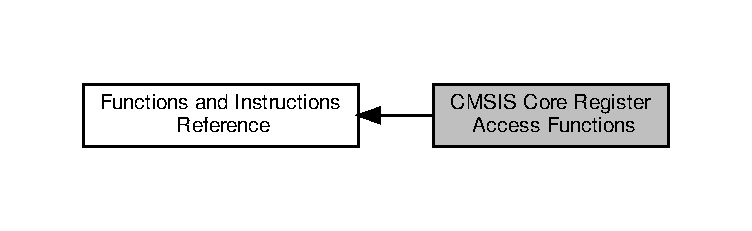
\includegraphics[width=350pt]{group___c_m_s_i_s___core___reg_acc_functions}
\end{center}
\end{figure}
\subsection*{Definicje}
\begin{DoxyCompactItemize}
\item 
\#define \hyperlink{group___c_m_s_i_s___core___reg_acc_functions_ga4d0739b1355ca5642a7ce76df1271f01}{\+\_\+\+\_\+get\+\_\+\+F\+P\+S\+CR}()~((uint32\+\_\+t)0\+U)
\begin{DoxyCompactList}\small\item\em Get F\+P\+S\+CR. \end{DoxyCompactList}\item 
\#define \hyperlink{group___c_m_s_i_s___core___reg_acc_functions_ga3cd91c42ad2793c3f3ae553a1b975512}{\+\_\+\+\_\+set\+\_\+\+F\+P\+S\+CR}(x)~((void)(x))
\begin{DoxyCompactList}\small\item\em Set F\+P\+S\+CR. \end{DoxyCompactList}\end{DoxyCompactItemize}
\subsection*{Funkcje}
\begin{DoxyCompactItemize}
\item 
\hyperlink{cmsis__iccarm_8h_aba87361bfad2ae52cfe2f40c1a1dbf9c}{\+\_\+\+\_\+\+S\+T\+A\+T\+I\+C\+\_\+\+I\+N\+L\+I\+NE} uint32\+\_\+t \hyperlink{group___c_m_s_i_s___core___reg_acc_functions_ga7dd5c942bee32f055b90153feb950f59}{\+\_\+\+\_\+get\+\_\+\+C\+O\+N\+T\+R\+OL} (void)
\begin{DoxyCompactList}\small\item\em Enable I\+RQ Interrupts. \end{DoxyCompactList}\item 
\hyperlink{cmsis__iccarm_8h_aba87361bfad2ae52cfe2f40c1a1dbf9c}{\+\_\+\+\_\+\+S\+T\+A\+T\+I\+C\+\_\+\+I\+N\+L\+I\+NE} void \hyperlink{group___c_m_s_i_s___core___reg_acc_functions_ga0102d0939d9b26c5c792be6bf5fd550f}{\+\_\+\+\_\+set\+\_\+\+C\+O\+N\+T\+R\+OL} (uint32\+\_\+t control)
\begin{DoxyCompactList}\small\item\em Set Control Register. \end{DoxyCompactList}\item 
\hyperlink{cmsis__iccarm_8h_aba87361bfad2ae52cfe2f40c1a1dbf9c}{\+\_\+\+\_\+\+S\+T\+A\+T\+I\+C\+\_\+\+I\+N\+L\+I\+NE} uint32\+\_\+t \hyperlink{group___c_m_s_i_s___core___reg_acc_functions_gaf15a71855b9d731d11de92704c82bd18}{\+\_\+\+\_\+get\+\_\+\+I\+P\+SR} (void)
\begin{DoxyCompactList}\small\item\em Get I\+P\+SR Register. \end{DoxyCompactList}\item 
\hyperlink{cmsis__iccarm_8h_aba87361bfad2ae52cfe2f40c1a1dbf9c}{\+\_\+\+\_\+\+S\+T\+A\+T\+I\+C\+\_\+\+I\+N\+L\+I\+NE} uint32\+\_\+t \hyperlink{group___c_m_s_i_s___core___reg_acc_functions_gadff4f1e599946e8ae96fba17b5245f04}{\+\_\+\+\_\+get\+\_\+\+A\+P\+SR} (void)
\begin{DoxyCompactList}\small\item\em Get A\+P\+SR Register. \end{DoxyCompactList}\item 
\hyperlink{cmsis__iccarm_8h_aba87361bfad2ae52cfe2f40c1a1dbf9c}{\+\_\+\+\_\+\+S\+T\+A\+T\+I\+C\+\_\+\+I\+N\+L\+I\+NE} uint32\+\_\+t \hyperlink{group___c_m_s_i_s___core___reg_acc_functions_ga52ca795dc9429ee0ac64ddd12c034834}{\+\_\+\+\_\+get\+\_\+x\+P\+SR} (void)
\begin{DoxyCompactList}\small\item\em Get x\+P\+SR Register. \end{DoxyCompactList}\item 
\hyperlink{cmsis__iccarm_8h_aba87361bfad2ae52cfe2f40c1a1dbf9c}{\+\_\+\+\_\+\+S\+T\+A\+T\+I\+C\+\_\+\+I\+N\+L\+I\+NE} uint32\+\_\+t \hyperlink{group___c_m_s_i_s___core___reg_acc_functions_ga826c53e30812e350c77f58aac9f42bcb}{\+\_\+\+\_\+get\+\_\+\+P\+SP} (void)
\begin{DoxyCompactList}\small\item\em Get Process Stack Pointer. \end{DoxyCompactList}\item 
\hyperlink{cmsis__iccarm_8h_aba87361bfad2ae52cfe2f40c1a1dbf9c}{\+\_\+\+\_\+\+S\+T\+A\+T\+I\+C\+\_\+\+I\+N\+L\+I\+NE} void \hyperlink{group___c_m_s_i_s___core___reg_acc_functions_ga21f50fc02c3927a8ebf0bc3678c06862}{\+\_\+\+\_\+set\+\_\+\+P\+SP} (uint32\+\_\+t top\+Of\+Proc\+Stack)
\begin{DoxyCompactList}\small\item\em Set Process Stack Pointer. \end{DoxyCompactList}\item 
\hyperlink{cmsis__iccarm_8h_aba87361bfad2ae52cfe2f40c1a1dbf9c}{\+\_\+\+\_\+\+S\+T\+A\+T\+I\+C\+\_\+\+I\+N\+L\+I\+NE} uint32\+\_\+t \hyperlink{group___c_m_s_i_s___core___reg_acc_functions_ga667e7b8b97b4a30f445ae45d37588e45}{\+\_\+\+\_\+get\+\_\+\+M\+SP} (void)
\begin{DoxyCompactList}\small\item\em Get Main Stack Pointer. \end{DoxyCompactList}\item 
\hyperlink{cmsis__iccarm_8h_aba87361bfad2ae52cfe2f40c1a1dbf9c}{\+\_\+\+\_\+\+S\+T\+A\+T\+I\+C\+\_\+\+I\+N\+L\+I\+NE} void \hyperlink{group___c_m_s_i_s___core___reg_acc_functions_ga08b66e2b60a46fada36d90d2bc1e7c9b}{\+\_\+\+\_\+set\+\_\+\+M\+SP} (uint32\+\_\+t top\+Of\+Main\+Stack)
\begin{DoxyCompactList}\small\item\em Set Main Stack Pointer. \end{DoxyCompactList}\item 
\hyperlink{cmsis__iccarm_8h_aba87361bfad2ae52cfe2f40c1a1dbf9c}{\+\_\+\+\_\+\+S\+T\+A\+T\+I\+C\+\_\+\+I\+N\+L\+I\+NE} uint32\+\_\+t \hyperlink{group___c_m_s_i_s___core___reg_acc_functions_ga4ff59fb9e280d19e79e6875863a65f0a}{\+\_\+\+\_\+get\+\_\+\+P\+R\+I\+M\+A\+SK} (void)
\begin{DoxyCompactList}\small\item\em Get Priority Mask. \end{DoxyCompactList}\item 
\hyperlink{cmsis__iccarm_8h_aba87361bfad2ae52cfe2f40c1a1dbf9c}{\+\_\+\+\_\+\+S\+T\+A\+T\+I\+C\+\_\+\+I\+N\+L\+I\+NE} void \hyperlink{group___c_m_s_i_s___core___reg_acc_functions_gaf4a17d3be7dbb066489836d849930d92}{\+\_\+\+\_\+set\+\_\+\+P\+R\+I\+M\+A\+SK} (uint32\+\_\+t pri\+Mask)
\begin{DoxyCompactList}\small\item\em Set Priority Mask. \end{DoxyCompactList}\item 
\hyperlink{cmsis__iccarm_8h_aba87361bfad2ae52cfe2f40c1a1dbf9c}{\+\_\+\+\_\+\+S\+T\+A\+T\+I\+C\+\_\+\+I\+N\+L\+I\+NE} uint32\+\_\+t \hyperlink{group___c_m_s_i_s___core___reg_acc_functions_ga6a275172e274ea7ce6c22030d07c6c64}{\+\_\+\+\_\+get\+\_\+\+F\+P\+S\+CR} (void)
\begin{DoxyCompactList}\small\item\em Get F\+P\+S\+CR. \end{DoxyCompactList}\item 
\hyperlink{cmsis__iccarm_8h_aba87361bfad2ae52cfe2f40c1a1dbf9c}{\+\_\+\+\_\+\+S\+T\+A\+T\+I\+C\+\_\+\+I\+N\+L\+I\+NE} void \hyperlink{group___c_m_s_i_s___core___reg_acc_functions_ga63aa6f7ed41dcaf39cbccb11e812ad4e}{\+\_\+\+\_\+set\+\_\+\+F\+P\+S\+CR} (uint32\+\_\+t fpscr)
\begin{DoxyCompactList}\small\item\em Set F\+P\+S\+CR. \end{DoxyCompactList}\item 
\hyperlink{cmsis__iccarm_8h_ab904513442afdf77d4f8c74f23cbb040}{\+\_\+\+\_\+\+S\+T\+A\+T\+I\+C\+\_\+\+F\+O\+R\+C\+E\+I\+N\+L\+I\+NE} void \hyperlink{group___c_m_s_i_s___core___reg_acc_functions_gae84bf4e95944e61937f4ed2453e5ef23}{\+\_\+\+\_\+enable\+\_\+irq} (void)
\begin{DoxyCompactList}\small\item\em Enable I\+RQ Interrupts. \end{DoxyCompactList}\item 
\hyperlink{cmsis__iccarm_8h_ab904513442afdf77d4f8c74f23cbb040}{\+\_\+\+\_\+\+S\+T\+A\+T\+I\+C\+\_\+\+F\+O\+R\+C\+E\+I\+N\+L\+I\+NE} void \hyperlink{group___c_m_s_i_s___core___reg_acc_functions_ga2299877e4ba3e162ca9dbabd6e0abef6}{\+\_\+\+\_\+disable\+\_\+irq} (void)
\begin{DoxyCompactList}\small\item\em Disable I\+RQ Interrupts. \end{DoxyCompactList}\end{DoxyCompactItemize}


\subsection{Opis szczegółowy}


\subsection{Dokumentacja definicji}
\mbox{\Hypertarget{group___c_m_s_i_s___core___reg_acc_functions_ga4d0739b1355ca5642a7ce76df1271f01}\label{group___c_m_s_i_s___core___reg_acc_functions_ga4d0739b1355ca5642a7ce76df1271f01}} 
\index{C\+M\+S\+I\+S Core Register Access Functions@{C\+M\+S\+I\+S Core Register Access Functions}!\+\_\+\+\_\+get\+\_\+\+F\+P\+S\+CR@{\+\_\+\+\_\+get\+\_\+\+F\+P\+S\+CR}}
\index{\+\_\+\+\_\+get\+\_\+\+F\+P\+S\+CR@{\+\_\+\+\_\+get\+\_\+\+F\+P\+S\+CR}!C\+M\+S\+I\+S Core Register Access Functions@{C\+M\+S\+I\+S Core Register Access Functions}}
\subsubsection{\texorpdfstring{\+\_\+\+\_\+get\+\_\+\+F\+P\+S\+CR}{\_\_get\_FPSCR}}
{\footnotesize\ttfamily \hyperlink{cmsis__iccarm_8h_ab904513442afdf77d4f8c74f23cbb040}{\+\_\+\+\_\+\+S\+T\+A\+T\+I\+C\+\_\+\+F\+O\+R\+C\+E\+I\+N\+L\+I\+NE} uint32\+\_\+t \+\_\+\+\_\+get\+\_\+\+F\+P\+S\+CR(\begin{DoxyParamCaption}\item[{}]{void }\end{DoxyParamCaption})~((uint32\+\_\+t)0\+U)}



Get F\+P\+S\+CR. 

Returns the current value of the Floating Point Status/\+Control register. \begin{DoxyReturn}{Zwraca}
Floating Point Status/\+Control register value 
\end{DoxyReturn}


Definicja w linii 754 pliku cmsis\+\_\+armclang.\+h.

\mbox{\Hypertarget{group___c_m_s_i_s___core___reg_acc_functions_ga3cd91c42ad2793c3f3ae553a1b975512}\label{group___c_m_s_i_s___core___reg_acc_functions_ga3cd91c42ad2793c3f3ae553a1b975512}} 
\index{C\+M\+S\+I\+S Core Register Access Functions@{C\+M\+S\+I\+S Core Register Access Functions}!\+\_\+\+\_\+set\+\_\+\+F\+P\+S\+CR@{\+\_\+\+\_\+set\+\_\+\+F\+P\+S\+CR}}
\index{\+\_\+\+\_\+set\+\_\+\+F\+P\+S\+CR@{\+\_\+\+\_\+set\+\_\+\+F\+P\+S\+CR}!C\+M\+S\+I\+S Core Register Access Functions@{C\+M\+S\+I\+S Core Register Access Functions}}
\subsubsection{\texorpdfstring{\+\_\+\+\_\+set\+\_\+\+F\+P\+S\+CR}{\_\_set\_FPSCR}}
{\footnotesize\ttfamily \#define \+\_\+\+\_\+set\+\_\+\+F\+P\+S\+CR(\begin{DoxyParamCaption}\item[{}]{x }\end{DoxyParamCaption})~((void)(x))}



Set F\+P\+S\+CR. 

Assigns the given value to the Floating Point Status/\+Control register. 
\begin{DoxyParams}[1]{Parametry}
\mbox{\tt in}  & {\em fpscr} & Floating Point Status/\+Control value to set \\
\hline
\end{DoxyParams}


Definicja w linii 766 pliku cmsis\+\_\+armclang.\+h.



\subsection{Dokumentacja funkcji}
\mbox{\Hypertarget{group___c_m_s_i_s___core___reg_acc_functions_ga2299877e4ba3e162ca9dbabd6e0abef6}\label{group___c_m_s_i_s___core___reg_acc_functions_ga2299877e4ba3e162ca9dbabd6e0abef6}} 
\index{C\+M\+S\+I\+S Core Register Access Functions@{C\+M\+S\+I\+S Core Register Access Functions}!\+\_\+\+\_\+disable\+\_\+irq@{\+\_\+\+\_\+disable\+\_\+irq}}
\index{\+\_\+\+\_\+disable\+\_\+irq@{\+\_\+\+\_\+disable\+\_\+irq}!C\+M\+S\+I\+S Core Register Access Functions@{C\+M\+S\+I\+S Core Register Access Functions}}
\subsubsection{\texorpdfstring{\+\_\+\+\_\+disable\+\_\+irq()}{\_\_disable\_irq()}}
{\footnotesize\ttfamily \hyperlink{cmsis__iccarm_8h_ab904513442afdf77d4f8c74f23cbb040}{\+\_\+\+\_\+\+S\+T\+A\+T\+I\+C\+\_\+\+F\+O\+R\+C\+E\+I\+N\+L\+I\+NE} void \+\_\+\+\_\+disable\+\_\+irq (\begin{DoxyParamCaption}\item[{void}]{ }\end{DoxyParamCaption})}



Disable I\+RQ Interrupts. 

Disables I\+RQ interrupts by setting the I-\/bit in the C\+P\+SR. Can only be executed in Privileged modes. 

Definicja w linii 140 pliku cmsis\+\_\+gcc.\+h.

\mbox{\Hypertarget{group___c_m_s_i_s___core___reg_acc_functions_gae84bf4e95944e61937f4ed2453e5ef23}\label{group___c_m_s_i_s___core___reg_acc_functions_gae84bf4e95944e61937f4ed2453e5ef23}} 
\index{C\+M\+S\+I\+S Core Register Access Functions@{C\+M\+S\+I\+S Core Register Access Functions}!\+\_\+\+\_\+enable\+\_\+irq@{\+\_\+\+\_\+enable\+\_\+irq}}
\index{\+\_\+\+\_\+enable\+\_\+irq@{\+\_\+\+\_\+enable\+\_\+irq}!C\+M\+S\+I\+S Core Register Access Functions@{C\+M\+S\+I\+S Core Register Access Functions}}
\subsubsection{\texorpdfstring{\+\_\+\+\_\+enable\+\_\+irq()}{\_\_enable\_irq()}}
{\footnotesize\ttfamily \hyperlink{cmsis__iccarm_8h_ab904513442afdf77d4f8c74f23cbb040}{\+\_\+\+\_\+\+S\+T\+A\+T\+I\+C\+\_\+\+F\+O\+R\+C\+E\+I\+N\+L\+I\+NE} void \+\_\+\+\_\+enable\+\_\+irq (\begin{DoxyParamCaption}\item[{void}]{ }\end{DoxyParamCaption})}



Enable I\+RQ Interrupts. 

Enables I\+RQ interrupts by clearing the I-\/bit in the C\+P\+SR. Can only be executed in Privileged modes. 

Definicja w linii 129 pliku cmsis\+\_\+gcc.\+h.

\mbox{\Hypertarget{group___c_m_s_i_s___core___reg_acc_functions_gadff4f1e599946e8ae96fba17b5245f04}\label{group___c_m_s_i_s___core___reg_acc_functions_gadff4f1e599946e8ae96fba17b5245f04}} 
\index{C\+M\+S\+I\+S Core Register Access Functions@{C\+M\+S\+I\+S Core Register Access Functions}!\+\_\+\+\_\+get\+\_\+\+A\+P\+SR@{\+\_\+\+\_\+get\+\_\+\+A\+P\+SR}}
\index{\+\_\+\+\_\+get\+\_\+\+A\+P\+SR@{\+\_\+\+\_\+get\+\_\+\+A\+P\+SR}!C\+M\+S\+I\+S Core Register Access Functions@{C\+M\+S\+I\+S Core Register Access Functions}}
\subsubsection{\texorpdfstring{\+\_\+\+\_\+get\+\_\+\+A\+P\+S\+R()}{\_\_get\_APSR()}}
{\footnotesize\ttfamily \hyperlink{cmsis__iccarm_8h_ab904513442afdf77d4f8c74f23cbb040}{\+\_\+\+\_\+\+S\+T\+A\+T\+I\+C\+\_\+\+F\+O\+R\+C\+E\+I\+N\+L\+I\+NE} uint32\+\_\+t \+\_\+\+\_\+get\+\_\+\+A\+P\+SR (\begin{DoxyParamCaption}\item[{void}]{ }\end{DoxyParamCaption})}



Get A\+P\+SR Register. 

Returns the content of the A\+P\+SR Register. \begin{DoxyReturn}{Zwraca}
A\+P\+SR Register value 
\end{DoxyReturn}


Definicja w linii 166 pliku cmsis\+\_\+armcc.\+h.

\mbox{\Hypertarget{group___c_m_s_i_s___core___reg_acc_functions_ga7dd5c942bee32f055b90153feb950f59}\label{group___c_m_s_i_s___core___reg_acc_functions_ga7dd5c942bee32f055b90153feb950f59}} 
\index{C\+M\+S\+I\+S Core Register Access Functions@{C\+M\+S\+I\+S Core Register Access Functions}!\+\_\+\+\_\+get\+\_\+\+C\+O\+N\+T\+R\+OL@{\+\_\+\+\_\+get\+\_\+\+C\+O\+N\+T\+R\+OL}}
\index{\+\_\+\+\_\+get\+\_\+\+C\+O\+N\+T\+R\+OL@{\+\_\+\+\_\+get\+\_\+\+C\+O\+N\+T\+R\+OL}!C\+M\+S\+I\+S Core Register Access Functions@{C\+M\+S\+I\+S Core Register Access Functions}}
\subsubsection{\texorpdfstring{\+\_\+\+\_\+get\+\_\+\+C\+O\+N\+T\+R\+O\+L()}{\_\_get\_CONTROL()}}
{\footnotesize\ttfamily \hyperlink{cmsis__iccarm_8h_ab904513442afdf77d4f8c74f23cbb040}{\+\_\+\+\_\+\+S\+T\+A\+T\+I\+C\+\_\+\+F\+O\+R\+C\+E\+I\+N\+L\+I\+NE} uint32\+\_\+t \+\_\+\+\_\+get\+\_\+\+C\+O\+N\+T\+R\+OL (\begin{DoxyParamCaption}\item[{void}]{ }\end{DoxyParamCaption})}



Enable I\+RQ Interrupts. 

Get Control Register.

Enables I\+RQ interrupts by clearing the I-\/bit in the C\+P\+SR. Can only be executed in Privileged modes. Disable I\+RQ Interrupts

Disables I\+RQ interrupts by setting the I-\/bit in the C\+P\+SR. Can only be executed in Privileged modes. Get Control Register

Returns the content of the Control Register. \begin{DoxyReturn}{Zwraca}
Control Register value
\end{DoxyReturn}
Returns the content of the Control Register. \begin{DoxyReturn}{Zwraca}
Control Register value 
\end{DoxyReturn}


Definicja w linii 130 pliku cmsis\+\_\+armcc.\+h.

\mbox{\Hypertarget{group___c_m_s_i_s___core___reg_acc_functions_ga6a275172e274ea7ce6c22030d07c6c64}\label{group___c_m_s_i_s___core___reg_acc_functions_ga6a275172e274ea7ce6c22030d07c6c64}} 
\index{C\+M\+S\+I\+S Core Register Access Functions@{C\+M\+S\+I\+S Core Register Access Functions}!\+\_\+\+\_\+get\+\_\+\+F\+P\+S\+CR@{\+\_\+\+\_\+get\+\_\+\+F\+P\+S\+CR}}
\index{\+\_\+\+\_\+get\+\_\+\+F\+P\+S\+CR@{\+\_\+\+\_\+get\+\_\+\+F\+P\+S\+CR}!C\+M\+S\+I\+S Core Register Access Functions@{C\+M\+S\+I\+S Core Register Access Functions}}
\subsubsection{\texorpdfstring{\+\_\+\+\_\+get\+\_\+\+F\+P\+S\+C\+R()}{\_\_get\_FPSCR()}}
{\footnotesize\ttfamily \hyperlink{cmsis__iccarm_8h_aba87361bfad2ae52cfe2f40c1a1dbf9c}{\+\_\+\+\_\+\+S\+T\+A\+T\+I\+C\+\_\+\+I\+N\+L\+I\+NE} uint32\+\_\+t \+\_\+\+\_\+get\+\_\+\+F\+P\+S\+CR (\begin{DoxyParamCaption}\item[{void}]{ }\end{DoxyParamCaption})}



Get F\+P\+S\+CR. 

Returns the current value of the Floating Point Status/\+Control register. \begin{DoxyReturn}{Zwraca}
Floating Point Status/\+Control register value 
\end{DoxyReturn}


Definicja w linii 345 pliku cmsis\+\_\+armcc.\+h.

\mbox{\Hypertarget{group___c_m_s_i_s___core___reg_acc_functions_gaf15a71855b9d731d11de92704c82bd18}\label{group___c_m_s_i_s___core___reg_acc_functions_gaf15a71855b9d731d11de92704c82bd18}} 
\index{C\+M\+S\+I\+S Core Register Access Functions@{C\+M\+S\+I\+S Core Register Access Functions}!\+\_\+\+\_\+get\+\_\+\+I\+P\+SR@{\+\_\+\+\_\+get\+\_\+\+I\+P\+SR}}
\index{\+\_\+\+\_\+get\+\_\+\+I\+P\+SR@{\+\_\+\+\_\+get\+\_\+\+I\+P\+SR}!C\+M\+S\+I\+S Core Register Access Functions@{C\+M\+S\+I\+S Core Register Access Functions}}
\subsubsection{\texorpdfstring{\+\_\+\+\_\+get\+\_\+\+I\+P\+S\+R()}{\_\_get\_IPSR()}}
{\footnotesize\ttfamily \hyperlink{cmsis__iccarm_8h_ab904513442afdf77d4f8c74f23cbb040}{\+\_\+\+\_\+\+S\+T\+A\+T\+I\+C\+\_\+\+F\+O\+R\+C\+E\+I\+N\+L\+I\+NE} uint32\+\_\+t \+\_\+\+\_\+get\+\_\+\+I\+P\+SR (\begin{DoxyParamCaption}\item[{void}]{ }\end{DoxyParamCaption})}



Get I\+P\+SR Register. 

Returns the content of the I\+P\+SR Register. \begin{DoxyReturn}{Zwraca}
I\+P\+SR Register value 
\end{DoxyReturn}


Definicja w linii 154 pliku cmsis\+\_\+armcc.\+h.

\mbox{\Hypertarget{group___c_m_s_i_s___core___reg_acc_functions_ga667e7b8b97b4a30f445ae45d37588e45}\label{group___c_m_s_i_s___core___reg_acc_functions_ga667e7b8b97b4a30f445ae45d37588e45}} 
\index{C\+M\+S\+I\+S Core Register Access Functions@{C\+M\+S\+I\+S Core Register Access Functions}!\+\_\+\+\_\+get\+\_\+\+M\+SP@{\+\_\+\+\_\+get\+\_\+\+M\+SP}}
\index{\+\_\+\+\_\+get\+\_\+\+M\+SP@{\+\_\+\+\_\+get\+\_\+\+M\+SP}!C\+M\+S\+I\+S Core Register Access Functions@{C\+M\+S\+I\+S Core Register Access Functions}}
\subsubsection{\texorpdfstring{\+\_\+\+\_\+get\+\_\+\+M\+S\+P()}{\_\_get\_MSP()}}
{\footnotesize\ttfamily \hyperlink{cmsis__iccarm_8h_ab904513442afdf77d4f8c74f23cbb040}{\+\_\+\+\_\+\+S\+T\+A\+T\+I\+C\+\_\+\+F\+O\+R\+C\+E\+I\+N\+L\+I\+NE} uint32\+\_\+t \+\_\+\+\_\+get\+\_\+\+M\+SP (\begin{DoxyParamCaption}\item[{void}]{ }\end{DoxyParamCaption})}



Get Main Stack Pointer. 

Returns the current value of the Main Stack Pointer (M\+SP). \begin{DoxyReturn}{Zwraca}
M\+SP Register value 
\end{DoxyReturn}


Definicja w linii 214 pliku cmsis\+\_\+armcc.\+h.

\mbox{\Hypertarget{group___c_m_s_i_s___core___reg_acc_functions_ga4ff59fb9e280d19e79e6875863a65f0a}\label{group___c_m_s_i_s___core___reg_acc_functions_ga4ff59fb9e280d19e79e6875863a65f0a}} 
\index{C\+M\+S\+I\+S Core Register Access Functions@{C\+M\+S\+I\+S Core Register Access Functions}!\+\_\+\+\_\+get\+\_\+\+P\+R\+I\+M\+A\+SK@{\+\_\+\+\_\+get\+\_\+\+P\+R\+I\+M\+A\+SK}}
\index{\+\_\+\+\_\+get\+\_\+\+P\+R\+I\+M\+A\+SK@{\+\_\+\+\_\+get\+\_\+\+P\+R\+I\+M\+A\+SK}!C\+M\+S\+I\+S Core Register Access Functions@{C\+M\+S\+I\+S Core Register Access Functions}}
\subsubsection{\texorpdfstring{\+\_\+\+\_\+get\+\_\+\+P\+R\+I\+M\+A\+S\+K()}{\_\_get\_PRIMASK()}}
{\footnotesize\ttfamily \hyperlink{cmsis__iccarm_8h_ab904513442afdf77d4f8c74f23cbb040}{\+\_\+\+\_\+\+S\+T\+A\+T\+I\+C\+\_\+\+F\+O\+R\+C\+E\+I\+N\+L\+I\+NE} uint32\+\_\+t \+\_\+\+\_\+get\+\_\+\+P\+R\+I\+M\+A\+SK (\begin{DoxyParamCaption}\item[{void}]{ }\end{DoxyParamCaption})}



Get Priority Mask. 

Returns the current state of the priority mask bit from the Priority Mask Register. \begin{DoxyReturn}{Zwraca}
Priority Mask value 
\end{DoxyReturn}


Definicja w linii 238 pliku cmsis\+\_\+armcc.\+h.

\mbox{\Hypertarget{group___c_m_s_i_s___core___reg_acc_functions_ga826c53e30812e350c77f58aac9f42bcb}\label{group___c_m_s_i_s___core___reg_acc_functions_ga826c53e30812e350c77f58aac9f42bcb}} 
\index{C\+M\+S\+I\+S Core Register Access Functions@{C\+M\+S\+I\+S Core Register Access Functions}!\+\_\+\+\_\+get\+\_\+\+P\+SP@{\+\_\+\+\_\+get\+\_\+\+P\+SP}}
\index{\+\_\+\+\_\+get\+\_\+\+P\+SP@{\+\_\+\+\_\+get\+\_\+\+P\+SP}!C\+M\+S\+I\+S Core Register Access Functions@{C\+M\+S\+I\+S Core Register Access Functions}}
\subsubsection{\texorpdfstring{\+\_\+\+\_\+get\+\_\+\+P\+S\+P()}{\_\_get\_PSP()}}
{\footnotesize\ttfamily \hyperlink{cmsis__iccarm_8h_ab904513442afdf77d4f8c74f23cbb040}{\+\_\+\+\_\+\+S\+T\+A\+T\+I\+C\+\_\+\+F\+O\+R\+C\+E\+I\+N\+L\+I\+NE} uint32\+\_\+t \+\_\+\+\_\+get\+\_\+\+P\+SP (\begin{DoxyParamCaption}\item[{void}]{ }\end{DoxyParamCaption})}



Get Process Stack Pointer. 

Returns the current value of the Process Stack Pointer (P\+SP). \begin{DoxyReturn}{Zwraca}
P\+SP Register value 
\end{DoxyReturn}


Definicja w linii 190 pliku cmsis\+\_\+armcc.\+h.

\mbox{\Hypertarget{group___c_m_s_i_s___core___reg_acc_functions_ga52ca795dc9429ee0ac64ddd12c034834}\label{group___c_m_s_i_s___core___reg_acc_functions_ga52ca795dc9429ee0ac64ddd12c034834}} 
\index{C\+M\+S\+I\+S Core Register Access Functions@{C\+M\+S\+I\+S Core Register Access Functions}!\+\_\+\+\_\+get\+\_\+x\+P\+SR@{\+\_\+\+\_\+get\+\_\+x\+P\+SR}}
\index{\+\_\+\+\_\+get\+\_\+x\+P\+SR@{\+\_\+\+\_\+get\+\_\+x\+P\+SR}!C\+M\+S\+I\+S Core Register Access Functions@{C\+M\+S\+I\+S Core Register Access Functions}}
\subsubsection{\texorpdfstring{\+\_\+\+\_\+get\+\_\+x\+P\+S\+R()}{\_\_get\_xPSR()}}
{\footnotesize\ttfamily \hyperlink{cmsis__iccarm_8h_ab904513442afdf77d4f8c74f23cbb040}{\+\_\+\+\_\+\+S\+T\+A\+T\+I\+C\+\_\+\+F\+O\+R\+C\+E\+I\+N\+L\+I\+NE} uint32\+\_\+t \+\_\+\+\_\+get\+\_\+x\+P\+SR (\begin{DoxyParamCaption}\item[{void}]{ }\end{DoxyParamCaption})}



Get x\+P\+SR Register. 

Returns the content of the x\+P\+SR Register. \begin{DoxyReturn}{Zwraca}
x\+P\+SR Register value 
\end{DoxyReturn}


Definicja w linii 178 pliku cmsis\+\_\+armcc.\+h.

\mbox{\Hypertarget{group___c_m_s_i_s___core___reg_acc_functions_ga0102d0939d9b26c5c792be6bf5fd550f}\label{group___c_m_s_i_s___core___reg_acc_functions_ga0102d0939d9b26c5c792be6bf5fd550f}} 
\index{C\+M\+S\+I\+S Core Register Access Functions@{C\+M\+S\+I\+S Core Register Access Functions}!\+\_\+\+\_\+set\+\_\+\+C\+O\+N\+T\+R\+OL@{\+\_\+\+\_\+set\+\_\+\+C\+O\+N\+T\+R\+OL}}
\index{\+\_\+\+\_\+set\+\_\+\+C\+O\+N\+T\+R\+OL@{\+\_\+\+\_\+set\+\_\+\+C\+O\+N\+T\+R\+OL}!C\+M\+S\+I\+S Core Register Access Functions@{C\+M\+S\+I\+S Core Register Access Functions}}
\subsubsection{\texorpdfstring{\+\_\+\+\_\+set\+\_\+\+C\+O\+N\+T\+R\+O\+L()}{\_\_set\_CONTROL()}}
{\footnotesize\ttfamily \hyperlink{cmsis__iccarm_8h_ab904513442afdf77d4f8c74f23cbb040}{\+\_\+\+\_\+\+S\+T\+A\+T\+I\+C\+\_\+\+F\+O\+R\+C\+E\+I\+N\+L\+I\+NE} void \+\_\+\+\_\+set\+\_\+\+C\+O\+N\+T\+R\+OL (\begin{DoxyParamCaption}\item[{uint32\+\_\+t}]{control }\end{DoxyParamCaption})}



Set Control Register. 

Writes the given value to the Control Register. 
\begin{DoxyParams}[1]{Parametry}
\mbox{\tt in}  & {\em control} & Control Register value to set \\
\hline
\end{DoxyParams}


Definicja w linii 142 pliku cmsis\+\_\+armcc.\+h.

\mbox{\Hypertarget{group___c_m_s_i_s___core___reg_acc_functions_ga63aa6f7ed41dcaf39cbccb11e812ad4e}\label{group___c_m_s_i_s___core___reg_acc_functions_ga63aa6f7ed41dcaf39cbccb11e812ad4e}} 
\index{C\+M\+S\+I\+S Core Register Access Functions@{C\+M\+S\+I\+S Core Register Access Functions}!\+\_\+\+\_\+set\+\_\+\+F\+P\+S\+CR@{\+\_\+\+\_\+set\+\_\+\+F\+P\+S\+CR}}
\index{\+\_\+\+\_\+set\+\_\+\+F\+P\+S\+CR@{\+\_\+\+\_\+set\+\_\+\+F\+P\+S\+CR}!C\+M\+S\+I\+S Core Register Access Functions@{C\+M\+S\+I\+S Core Register Access Functions}}
\subsubsection{\texorpdfstring{\+\_\+\+\_\+set\+\_\+\+F\+P\+S\+C\+R()}{\_\_set\_FPSCR()}}
{\footnotesize\ttfamily \hyperlink{cmsis__iccarm_8h_ab904513442afdf77d4f8c74f23cbb040}{\+\_\+\+\_\+\+S\+T\+A\+T\+I\+C\+\_\+\+F\+O\+R\+C\+E\+I\+N\+L\+I\+NE} void \+\_\+\+\_\+set\+\_\+\+F\+P\+S\+CR (\begin{DoxyParamCaption}\item[{uint32\+\_\+t}]{fpscr }\end{DoxyParamCaption})}



Set F\+P\+S\+CR. 

Assigns the given value to the Floating Point Status/\+Control register. 
\begin{DoxyParams}[1]{Parametry}
\mbox{\tt in}  & {\em fpscr} & Floating Point Status/\+Control value to set \\
\hline
\end{DoxyParams}


Definicja w linii 362 pliku cmsis\+\_\+armcc.\+h.

\mbox{\Hypertarget{group___c_m_s_i_s___core___reg_acc_functions_ga08b66e2b60a46fada36d90d2bc1e7c9b}\label{group___c_m_s_i_s___core___reg_acc_functions_ga08b66e2b60a46fada36d90d2bc1e7c9b}} 
\index{C\+M\+S\+I\+S Core Register Access Functions@{C\+M\+S\+I\+S Core Register Access Functions}!\+\_\+\+\_\+set\+\_\+\+M\+SP@{\+\_\+\+\_\+set\+\_\+\+M\+SP}}
\index{\+\_\+\+\_\+set\+\_\+\+M\+SP@{\+\_\+\+\_\+set\+\_\+\+M\+SP}!C\+M\+S\+I\+S Core Register Access Functions@{C\+M\+S\+I\+S Core Register Access Functions}}
\subsubsection{\texorpdfstring{\+\_\+\+\_\+set\+\_\+\+M\+S\+P()}{\_\_set\_MSP()}}
{\footnotesize\ttfamily \hyperlink{cmsis__iccarm_8h_ab904513442afdf77d4f8c74f23cbb040}{\+\_\+\+\_\+\+S\+T\+A\+T\+I\+C\+\_\+\+F\+O\+R\+C\+E\+I\+N\+L\+I\+NE} void \+\_\+\+\_\+set\+\_\+\+M\+SP (\begin{DoxyParamCaption}\item[{uint32\+\_\+t}]{top\+Of\+Main\+Stack }\end{DoxyParamCaption})}



Set Main Stack Pointer. 

Assigns the given value to the Main Stack Pointer (M\+SP). 
\begin{DoxyParams}[1]{Parametry}
\mbox{\tt in}  & {\em top\+Of\+Main\+Stack} & Main Stack Pointer value to set \\
\hline
\end{DoxyParams}


Definicja w linii 226 pliku cmsis\+\_\+armcc.\+h.

\mbox{\Hypertarget{group___c_m_s_i_s___core___reg_acc_functions_gaf4a17d3be7dbb066489836d849930d92}\label{group___c_m_s_i_s___core___reg_acc_functions_gaf4a17d3be7dbb066489836d849930d92}} 
\index{C\+M\+S\+I\+S Core Register Access Functions@{C\+M\+S\+I\+S Core Register Access Functions}!\+\_\+\+\_\+set\+\_\+\+P\+R\+I\+M\+A\+SK@{\+\_\+\+\_\+set\+\_\+\+P\+R\+I\+M\+A\+SK}}
\index{\+\_\+\+\_\+set\+\_\+\+P\+R\+I\+M\+A\+SK@{\+\_\+\+\_\+set\+\_\+\+P\+R\+I\+M\+A\+SK}!C\+M\+S\+I\+S Core Register Access Functions@{C\+M\+S\+I\+S Core Register Access Functions}}
\subsubsection{\texorpdfstring{\+\_\+\+\_\+set\+\_\+\+P\+R\+I\+M\+A\+S\+K()}{\_\_set\_PRIMASK()}}
{\footnotesize\ttfamily \hyperlink{cmsis__iccarm_8h_ab904513442afdf77d4f8c74f23cbb040}{\+\_\+\+\_\+\+S\+T\+A\+T\+I\+C\+\_\+\+F\+O\+R\+C\+E\+I\+N\+L\+I\+NE} void \+\_\+\+\_\+set\+\_\+\+P\+R\+I\+M\+A\+SK (\begin{DoxyParamCaption}\item[{uint32\+\_\+t}]{pri\+Mask }\end{DoxyParamCaption})}



Set Priority Mask. 

Assigns the given value to the Priority Mask Register. 
\begin{DoxyParams}[1]{Parametry}
\mbox{\tt in}  & {\em pri\+Mask} & Priority Mask \\
\hline
\end{DoxyParams}


Definicja w linii 250 pliku cmsis\+\_\+armcc.\+h.

\mbox{\Hypertarget{group___c_m_s_i_s___core___reg_acc_functions_ga21f50fc02c3927a8ebf0bc3678c06862}\label{group___c_m_s_i_s___core___reg_acc_functions_ga21f50fc02c3927a8ebf0bc3678c06862}} 
\index{C\+M\+S\+I\+S Core Register Access Functions@{C\+M\+S\+I\+S Core Register Access Functions}!\+\_\+\+\_\+set\+\_\+\+P\+SP@{\+\_\+\+\_\+set\+\_\+\+P\+SP}}
\index{\+\_\+\+\_\+set\+\_\+\+P\+SP@{\+\_\+\+\_\+set\+\_\+\+P\+SP}!C\+M\+S\+I\+S Core Register Access Functions@{C\+M\+S\+I\+S Core Register Access Functions}}
\subsubsection{\texorpdfstring{\+\_\+\+\_\+set\+\_\+\+P\+S\+P()}{\_\_set\_PSP()}}
{\footnotesize\ttfamily \hyperlink{cmsis__iccarm_8h_ab904513442afdf77d4f8c74f23cbb040}{\+\_\+\+\_\+\+S\+T\+A\+T\+I\+C\+\_\+\+F\+O\+R\+C\+E\+I\+N\+L\+I\+NE} void \+\_\+\+\_\+set\+\_\+\+P\+SP (\begin{DoxyParamCaption}\item[{uint32\+\_\+t}]{top\+Of\+Proc\+Stack }\end{DoxyParamCaption})}



Set Process Stack Pointer. 

Assigns the given value to the Process Stack Pointer (P\+SP). 
\begin{DoxyParams}[1]{Parametry}
\mbox{\tt in}  & {\em top\+Of\+Proc\+Stack} & Process Stack Pointer value to set \\
\hline
\end{DoxyParams}


Definicja w linii 202 pliku cmsis\+\_\+armcc.\+h.


\hypertarget{group___c_m_s_i_s___core___instruction_interface}{}\section{C\+M\+S\+IS Core Instruction Interface}
\label{group___c_m_s_i_s___core___instruction_interface}\index{C\+M\+S\+I\+S Core Instruction Interface@{C\+M\+S\+I\+S Core Instruction Interface}}
\subsection*{Definicje}
\begin{DoxyCompactItemize}
\item 
\#define \hyperlink{group___c_m_s_i_s___core___instruction_interface_gabd585ddc865fb9b7f2493af1eee1a572}{\+\_\+\+\_\+\+N\+OP}~\+\_\+\+\_\+nop
\begin{DoxyCompactList}\small\item\em No Operation. \end{DoxyCompactList}\item 
\#define \hyperlink{group___c_m_s_i_s___core___instruction_interface_gad23bf2b78a9a4524157c9de0d30b7448}{\+\_\+\+\_\+\+W\+FI}~\+\_\+\+\_\+wfi
\begin{DoxyCompactList}\small\item\em Wait For Interrupt. \end{DoxyCompactList}\item 
\#define \hyperlink{group___c_m_s_i_s___core___instruction_interface_gaac6cc7dd4325d9cb40d3290fa5244b3d}{\+\_\+\+\_\+\+W\+FE}~\+\_\+\+\_\+wfe
\begin{DoxyCompactList}\small\item\em Wait For Event. \end{DoxyCompactList}\item 
\#define \hyperlink{group___c_m_s_i_s___core___instruction_interface_gaab4f296d0022b4b10dc0976eb22052f9}{\+\_\+\+\_\+\+S\+EV}~\+\_\+\+\_\+sev
\begin{DoxyCompactList}\small\item\em Send Event. \end{DoxyCompactList}\item 
\#define \hyperlink{group___c_m_s_i_s___core___instruction_interface_gaad233022e850a009fc6f7602be1182f6}{\+\_\+\+\_\+\+I\+SB}()
\begin{DoxyCompactList}\small\item\em Instruction Synchronization Barrier. \end{DoxyCompactList}\item 
\#define \hyperlink{group___c_m_s_i_s___core___instruction_interface_ga067d257a2b34565410acefb5afef2203}{\+\_\+\+\_\+\+D\+SB}()
\begin{DoxyCompactList}\small\item\em Data Synchronization Barrier. \end{DoxyCompactList}\item 
\#define \hyperlink{group___c_m_s_i_s___core___instruction_interface_ga671101179b5943990785f36f8c1e2269}{\+\_\+\+\_\+\+D\+MB}()
\begin{DoxyCompactList}\small\item\em Data Memory Barrier. \end{DoxyCompactList}\item 
\#define \hyperlink{group___c_m_s_i_s___core___instruction_interface_ga14f54807872c0f5e05604c4924abfdae}{\+\_\+\+\_\+\+R\+EV}~\+\_\+\+\_\+rev
\begin{DoxyCompactList}\small\item\em Reverse byte order (32 bit) \end{DoxyCompactList}\item 
\#define \hyperlink{group___c_m_s_i_s___core___instruction_interface_ga95b9bd281ddeda378b85afdb8f2ced86}{\+\_\+\+\_\+\+R\+OR}~\+\_\+\+\_\+ror
\begin{DoxyCompactList}\small\item\em Rotate Right in unsigned value (32 bit) \end{DoxyCompactList}\item 
\#define \hyperlink{group___c_m_s_i_s___core___instruction_interface_ga15ea6bd3c507d3e81c3b3a1258e46397}{\+\_\+\+\_\+\+B\+K\+PT}(value)~\+\_\+\+\_\+breakpoint(value)
\begin{DoxyCompactList}\small\item\em Breakpoint. \end{DoxyCompactList}\item 
\#define \hyperlink{group___c_m_s_i_s___core___instruction_interface_ga5d5bb1527e042be4a9fa5a33f65cc248}{\+\_\+\+\_\+\+C\+LZ}~\+\_\+\+\_\+clz
\begin{DoxyCompactList}\small\item\em Count leading zeros. \end{DoxyCompactList}\item 
\#define \hyperlink{group___c_m_s_i_s___core___instruction_interface_gabc17e391c13c71702366c67cba39c276}{\+\_\+\+\_\+\+C\+M\+S\+I\+S\+\_\+\+G\+C\+C\+\_\+\+O\+U\+T\+\_\+\+R\+EG}(r)~\char`\"{}=r\char`\"{} (r)
\item 
\#define \hyperlink{group___c_m_s_i_s___core___instruction_interface_ga9d94dee7402367961d2cf0accc00fd97}{\+\_\+\+\_\+\+C\+M\+S\+I\+S\+\_\+\+G\+C\+C\+\_\+\+U\+S\+E\+\_\+\+R\+EG}(r)~\char`\"{}r\char`\"{} (r)
\item 
\#define \hyperlink{group___c_m_s_i_s___core___instruction_interface_gabd585ddc865fb9b7f2493af1eee1a572}{\+\_\+\+\_\+\+N\+OP}~\+\_\+\+\_\+builtin\+\_\+arm\+\_\+nop
\begin{DoxyCompactList}\small\item\em No Operation. \end{DoxyCompactList}\item 
\#define \hyperlink{group___c_m_s_i_s___core___instruction_interface_gad23bf2b78a9a4524157c9de0d30b7448}{\+\_\+\+\_\+\+W\+FI}~\+\_\+\+\_\+builtin\+\_\+arm\+\_\+wfi
\begin{DoxyCompactList}\small\item\em Wait For Interrupt. \end{DoxyCompactList}\item 
\#define \hyperlink{group___c_m_s_i_s___core___instruction_interface_gaac6cc7dd4325d9cb40d3290fa5244b3d}{\+\_\+\+\_\+\+W\+FE}~\+\_\+\+\_\+builtin\+\_\+arm\+\_\+wfe
\begin{DoxyCompactList}\small\item\em Wait For Event. \end{DoxyCompactList}\item 
\#define \hyperlink{group___c_m_s_i_s___core___instruction_interface_gaab4f296d0022b4b10dc0976eb22052f9}{\+\_\+\+\_\+\+S\+EV}~\+\_\+\+\_\+builtin\+\_\+arm\+\_\+sev
\begin{DoxyCompactList}\small\item\em Send Event. \end{DoxyCompactList}\item 
\#define \hyperlink{group___c_m_s_i_s___core___instruction_interface_gaad233022e850a009fc6f7602be1182f6}{\+\_\+\+\_\+\+I\+SB}()~\+\_\+\+\_\+builtin\+\_\+arm\+\_\+isb(0x\+F);
\begin{DoxyCompactList}\small\item\em Instruction Synchronization Barrier. \end{DoxyCompactList}\item 
\#define \hyperlink{group___c_m_s_i_s___core___instruction_interface_ga067d257a2b34565410acefb5afef2203}{\+\_\+\+\_\+\+D\+SB}()~\+\_\+\+\_\+builtin\+\_\+arm\+\_\+dsb(0x\+F);
\begin{DoxyCompactList}\small\item\em Data Synchronization Barrier. \end{DoxyCompactList}\item 
\#define \hyperlink{group___c_m_s_i_s___core___instruction_interface_ga671101179b5943990785f36f8c1e2269}{\+\_\+\+\_\+\+D\+MB}()~\+\_\+\+\_\+builtin\+\_\+arm\+\_\+dmb(0x\+F);
\begin{DoxyCompactList}\small\item\em Data Memory Barrier. \end{DoxyCompactList}\item 
\#define \hyperlink{group___c_m_s_i_s___core___instruction_interface_gaca25a02e09983da5558f5242f2f635bc}{\+\_\+\+\_\+\+R\+EV}(value)~\+\_\+\+\_\+builtin\+\_\+bswap32(value)
\begin{DoxyCompactList}\small\item\em Reverse byte order (32 bit) \end{DoxyCompactList}\item 
\#define \hyperlink{group___c_m_s_i_s___core___instruction_interface_gad35497777af37e7809271b5e6f9510ba}{\+\_\+\+\_\+\+R\+E\+V16}(value)~\hyperlink{cmsis__iccarm_8h_a7105032649bf6158d4d2d5dc38a3f94c}{\+\_\+\+\_\+\+R\+OR}(\hyperlink{group___c_m_s_i_s___core___instruction_interface_gadb92679719950635fba8b1b954072695}{\+\_\+\+\_\+\+R\+EV}(value), 16)
\begin{DoxyCompactList}\small\item\em Reverse byte order (16 bit) \end{DoxyCompactList}\item 
\#define \hyperlink{group___c_m_s_i_s___core___instruction_interface_gae580812686119c9c5cf3c11a7519a404}{\+\_\+\+\_\+\+R\+E\+V\+SH}(value)~(int16\+\_\+t)\+\_\+\+\_\+builtin\+\_\+bswap16(value)
\begin{DoxyCompactList}\small\item\em Reverse byte order (16 bit) \end{DoxyCompactList}\item 
\#define \hyperlink{group___c_m_s_i_s___core___instruction_interface_ga15ea6bd3c507d3e81c3b3a1258e46397}{\+\_\+\+\_\+\+B\+K\+PT}(value)~\hyperlink{cmsis__iccarm_8h_a1378040bcf22428955c6e3ce9c2053cd}{\+\_\+\+\_\+\+A\+SM} volatile (\char`\"{}bkpt \char`\"{}\#value)
\begin{DoxyCompactList}\small\item\em Breakpoint. \end{DoxyCompactList}\item 
\#define \hyperlink{group___c_m_s_i_s___core___instruction_interface_gab83768933a612816fad669db5488366f}{\+\_\+\+\_\+\+R\+B\+IT}~\+\_\+\+\_\+builtin\+\_\+arm\+\_\+rbit
\begin{DoxyCompactList}\small\item\em Reverse bit order of value. \end{DoxyCompactList}\item 
\#define \hyperlink{group___c_m_s_i_s___core___instruction_interface_ga5d5bb1527e042be4a9fa5a33f65cc248}{\+\_\+\+\_\+\+C\+LZ}~(uint8\+\_\+t)\+\_\+\+\_\+builtin\+\_\+clz
\begin{DoxyCompactList}\small\item\em Count leading zeros. \end{DoxyCompactList}\item 
\#define \hyperlink{group___c_m_s_i_s___core___instruction_interface_gabc17e391c13c71702366c67cba39c276}{\+\_\+\+\_\+\+C\+M\+S\+I\+S\+\_\+\+G\+C\+C\+\_\+\+O\+U\+T\+\_\+\+R\+EG}(r)~\char`\"{}=r\char`\"{} (r)
\item 
\#define \hyperlink{group___c_m_s_i_s___core___instruction_interface_ga03179f79efee45c226dddfb8d824ad83}{\+\_\+\+\_\+\+C\+M\+S\+I\+S\+\_\+\+G\+C\+C\+\_\+\+R\+W\+\_\+\+R\+EG}(r)~\char`\"{}+r\char`\"{} (r)
\item 
\#define \hyperlink{group___c_m_s_i_s___core___instruction_interface_ga9d94dee7402367961d2cf0accc00fd97}{\+\_\+\+\_\+\+C\+M\+S\+I\+S\+\_\+\+G\+C\+C\+\_\+\+U\+S\+E\+\_\+\+R\+EG}(r)~\char`\"{}r\char`\"{} (r)
\item 
\#define \hyperlink{group___c_m_s_i_s___core___instruction_interface_ga0b13f3617dd4af2cd2eb3a311073f717}{\+\_\+\+\_\+\+N\+OP}()~\hyperlink{cmsis__iccarm_8h_a1378040bcf22428955c6e3ce9c2053cd}{\+\_\+\+\_\+\+A\+SM} volatile (\char`\"{}nop\char`\"{})
\begin{DoxyCompactList}\small\item\em No Operation. \end{DoxyCompactList}\item 
\#define \hyperlink{group___c_m_s_i_s___core___instruction_interface_gab28e2b328c4cf23c917ab18a23194f8e}{\+\_\+\+\_\+\+W\+FI}()~\hyperlink{cmsis__iccarm_8h_a1378040bcf22428955c6e3ce9c2053cd}{\+\_\+\+\_\+\+A\+SM} volatile (\char`\"{}wfi\char`\"{})
\begin{DoxyCompactList}\small\item\em Wait For Interrupt. \end{DoxyCompactList}\item 
\#define \hyperlink{group___c_m_s_i_s___core___instruction_interface_gaf0330712223f4cfb6091e4ab84775f73}{\+\_\+\+\_\+\+W\+FE}()~\hyperlink{cmsis__iccarm_8h_a1378040bcf22428955c6e3ce9c2053cd}{\+\_\+\+\_\+\+A\+SM} volatile (\char`\"{}wfe\char`\"{})
\begin{DoxyCompactList}\small\item\em Wait For Event. \end{DoxyCompactList}\item 
\#define \hyperlink{group___c_m_s_i_s___core___instruction_interface_gafa58e60fcd2176ad58f96947466ea1fa}{\+\_\+\+\_\+\+S\+EV}()~\hyperlink{cmsis__iccarm_8h_a1378040bcf22428955c6e3ce9c2053cd}{\+\_\+\+\_\+\+A\+SM} volatile (\char`\"{}sev\char`\"{})
\begin{DoxyCompactList}\small\item\em Send Event. \end{DoxyCompactList}\item 
\#define \hyperlink{group___c_m_s_i_s___core___instruction_interface_ga15ea6bd3c507d3e81c3b3a1258e46397}{\+\_\+\+\_\+\+B\+K\+PT}(value)~\hyperlink{cmsis__iccarm_8h_a1378040bcf22428955c6e3ce9c2053cd}{\+\_\+\+\_\+\+A\+SM} volatile (\char`\"{}bkpt \char`\"{}\#value)
\begin{DoxyCompactList}\small\item\em Breakpoint. \end{DoxyCompactList}\item 
\#define \hyperlink{group___c_m_s_i_s___core___instruction_interface_ga5d5bb1527e042be4a9fa5a33f65cc248}{\+\_\+\+\_\+\+C\+LZ}~(uint8\+\_\+t)\+\_\+\+\_\+builtin\+\_\+clz
\begin{DoxyCompactList}\small\item\em Count leading zeros. \end{DoxyCompactList}\end{DoxyCompactItemize}
\subsection*{Funkcje}
\begin{DoxyCompactItemize}
\item 
\hyperlink{group___c_m_s_i_s___core___instruction_interface_gae84a2733711339c5eefeb0d899506b96}{\+\_\+\+\_\+attribute\+\_\+\+\_\+} ((section(\char`\"{}.rev16\+\_\+text\char`\"{}))) \+\_\+\+\_\+\+S\+T\+A\+T\+I\+C\+\_\+\+I\+N\+L\+I\+NE \hyperlink{cmsis__iccarm_8h_a1378040bcf22428955c6e3ce9c2053cd}{\+\_\+\+\_\+\+A\+SM} uint32\+\_\+t \hyperlink{group___c_m_s_i_s___core___instruction_interface_gaa12aedd096506c9639c1581acd5c6a78}{\+\_\+\+\_\+\+R\+E\+V16}(uint32\+\_\+t value)
\begin{DoxyCompactList}\small\item\em Reverse byte order (16 bit) \end{DoxyCompactList}\item 
\hyperlink{group___c_m_s_i_s___core___instruction_interface_gabe2b619a40cc0a7ffa8f765249ccf682}{\+\_\+\+\_\+attribute\+\_\+\+\_\+} ((section(\char`\"{}.revsh\+\_\+text\char`\"{}))) \+\_\+\+\_\+\+S\+T\+A\+T\+I\+C\+\_\+\+I\+N\+L\+I\+NE \hyperlink{cmsis__iccarm_8h_a1378040bcf22428955c6e3ce9c2053cd}{\+\_\+\+\_\+\+A\+SM} int16\+\_\+t \hyperlink{group___c_m_s_i_s___core___instruction_interface_gacb695341318226a5f69ed508166622ac}{\+\_\+\+\_\+\+R\+E\+V\+SH}(int16\+\_\+t value)
\begin{DoxyCompactList}\small\item\em Reverse byte order (16 bit) \end{DoxyCompactList}\item 
\hyperlink{group___c_m_s_i_s___core___instruction_interface_gab926fe7178a379c3a7c0410b06fcb661}{\+\_\+\+\_\+attribute\+\_\+\+\_\+} ((always\+\_\+inline)) \hyperlink{cmsis__iccarm_8h_aba87361bfad2ae52cfe2f40c1a1dbf9c}{\+\_\+\+\_\+\+S\+T\+A\+T\+I\+C\+\_\+\+I\+N\+L\+I\+NE} uint32\+\_\+t \hyperlink{group___c_m_s_i_s___core___instruction_interface_gaf944a7b7d8fd70164cca27669316bcf7}{\+\_\+\+\_\+\+R\+B\+IT}(uint32\+\_\+t value)
\begin{DoxyCompactList}\small\item\em Reverse bit order of value. \end{DoxyCompactList}\item 
\hyperlink{cmsis__iccarm_8h_ab904513442afdf77d4f8c74f23cbb040}{\+\_\+\+\_\+\+S\+T\+A\+T\+I\+C\+\_\+\+F\+O\+R\+C\+E\+I\+N\+L\+I\+NE} uint32\+\_\+t \hyperlink{group___c_m_s_i_s___core___instruction_interface_gab16acb6456176f1e87a4f2724c2b6028}{\+\_\+\+\_\+\+R\+OR} (uint32\+\_\+t op1, uint32\+\_\+t op2)
\begin{DoxyCompactList}\small\item\em Rotate Right in unsigned value (32 bit) \end{DoxyCompactList}\item 
\hyperlink{cmsis__iccarm_8h_ab904513442afdf77d4f8c74f23cbb040}{\+\_\+\+\_\+\+S\+T\+A\+T\+I\+C\+\_\+\+F\+O\+R\+C\+E\+I\+N\+L\+I\+NE} int32\+\_\+t \hyperlink{group___c_m_s_i_s___core___instruction_interface_ga372c0535573dde3e37f0f08c774a3487}{\+\_\+\+\_\+\+S\+S\+AT} (int32\+\_\+t val, uint32\+\_\+t \hyperlink{group___c_m_s_i_s___core___instruction_interface_gaafcad33f86db3a8e1f55925989f9d2dc}{sat})
\begin{DoxyCompactList}\small\item\em Signed Saturate. \end{DoxyCompactList}\item 
\hyperlink{cmsis__iccarm_8h_ab904513442afdf77d4f8c74f23cbb040}{\+\_\+\+\_\+\+S\+T\+A\+T\+I\+C\+\_\+\+F\+O\+R\+C\+E\+I\+N\+L\+I\+NE} uint32\+\_\+t \hyperlink{group___c_m_s_i_s___core___instruction_interface_ga6562dbd8182d1571e22dbca7ebdfa9bc}{\+\_\+\+\_\+\+U\+S\+AT} (int32\+\_\+t val, uint32\+\_\+t \hyperlink{group___c_m_s_i_s___core___instruction_interface_gaafcad33f86db3a8e1f55925989f9d2dc}{sat})
\begin{DoxyCompactList}\small\item\em Unsigned Saturate. \end{DoxyCompactList}\item 
\hyperlink{cmsis__iccarm_8h_ab904513442afdf77d4f8c74f23cbb040}{\+\_\+\+\_\+\+S\+T\+A\+T\+I\+C\+\_\+\+F\+O\+R\+C\+E\+I\+N\+L\+I\+NE} void \hyperlink{group___c_m_s_i_s___core___instruction_interface_gae26c2b3961e702aeabc24d4984ebd369}{\+\_\+\+\_\+\+I\+SB} (void)
\begin{DoxyCompactList}\small\item\em Instruction Synchronization Barrier. \end{DoxyCompactList}\item 
\hyperlink{cmsis__iccarm_8h_ab904513442afdf77d4f8c74f23cbb040}{\+\_\+\+\_\+\+S\+T\+A\+T\+I\+C\+\_\+\+F\+O\+R\+C\+E\+I\+N\+L\+I\+NE} void \hyperlink{group___c_m_s_i_s___core___instruction_interface_ga7fe277f5385d23b9c44b2cbda1577ce9}{\+\_\+\+\_\+\+D\+SB} (void)
\begin{DoxyCompactList}\small\item\em Data Synchronization Barrier. \end{DoxyCompactList}\item 
\hyperlink{cmsis__iccarm_8h_ab904513442afdf77d4f8c74f23cbb040}{\+\_\+\+\_\+\+S\+T\+A\+T\+I\+C\+\_\+\+F\+O\+R\+C\+E\+I\+N\+L\+I\+NE} void \hyperlink{group___c_m_s_i_s___core___instruction_interface_gab1ea24daaaaee9c828f90cbca330cb5e}{\+\_\+\+\_\+\+D\+MB} (void)
\begin{DoxyCompactList}\small\item\em Data Memory Barrier. \end{DoxyCompactList}\item 
\hyperlink{cmsis__iccarm_8h_ab904513442afdf77d4f8c74f23cbb040}{\+\_\+\+\_\+\+S\+T\+A\+T\+I\+C\+\_\+\+F\+O\+R\+C\+E\+I\+N\+L\+I\+NE} uint32\+\_\+t \hyperlink{group___c_m_s_i_s___core___instruction_interface_gadb92679719950635fba8b1b954072695}{\+\_\+\+\_\+\+R\+EV} (uint32\+\_\+t value)
\begin{DoxyCompactList}\small\item\em Reverse byte order (32 bit) \end{DoxyCompactList}\item 
\hyperlink{cmsis__iccarm_8h_ab904513442afdf77d4f8c74f23cbb040}{\+\_\+\+\_\+\+S\+T\+A\+T\+I\+C\+\_\+\+F\+O\+R\+C\+E\+I\+N\+L\+I\+NE} uint32\+\_\+t \hyperlink{group___c_m_s_i_s___core___instruction_interface_gaa12aedd096506c9639c1581acd5c6a78}{\+\_\+\+\_\+\+R\+E\+V16} (uint32\+\_\+t value)
\begin{DoxyCompactList}\small\item\em Reverse byte order (16 bit) \end{DoxyCompactList}\item 
\hyperlink{cmsis__iccarm_8h_ab904513442afdf77d4f8c74f23cbb040}{\+\_\+\+\_\+\+S\+T\+A\+T\+I\+C\+\_\+\+F\+O\+R\+C\+E\+I\+N\+L\+I\+NE} int16\+\_\+t \hyperlink{group___c_m_s_i_s___core___instruction_interface_gacb695341318226a5f69ed508166622ac}{\+\_\+\+\_\+\+R\+E\+V\+SH} (int16\+\_\+t value)
\begin{DoxyCompactList}\small\item\em Reverse byte order (16 bit) \end{DoxyCompactList}\item 
\hyperlink{cmsis__iccarm_8h_ab904513442afdf77d4f8c74f23cbb040}{\+\_\+\+\_\+\+S\+T\+A\+T\+I\+C\+\_\+\+F\+O\+R\+C\+E\+I\+N\+L\+I\+NE} uint32\+\_\+t \hyperlink{group___c_m_s_i_s___core___instruction_interface_gaf944a7b7d8fd70164cca27669316bcf7}{\+\_\+\+\_\+\+R\+B\+IT} (uint32\+\_\+t value)
\begin{DoxyCompactList}\small\item\em Reverse bit order of value. \end{DoxyCompactList}\end{DoxyCompactItemize}
\subsection*{Zmienne}
\begin{DoxyCompactItemize}
\item 
uint32\+\_\+t \hyperlink{group___c_m_s_i_s___core___instruction_interface_gaafcad33f86db3a8e1f55925989f9d2dc}{sat}
\end{DoxyCompactItemize}


\subsection{Opis szczegółowy}
Access to dedicated instructions 

\subsection{Dokumentacja definicji}
\mbox{\Hypertarget{group___c_m_s_i_s___core___instruction_interface_ga15ea6bd3c507d3e81c3b3a1258e46397}\label{group___c_m_s_i_s___core___instruction_interface_ga15ea6bd3c507d3e81c3b3a1258e46397}} 
\index{C\+M\+S\+I\+S Core Instruction Interface@{C\+M\+S\+I\+S Core Instruction Interface}!\+\_\+\+\_\+\+B\+K\+PT@{\+\_\+\+\_\+\+B\+K\+PT}}
\index{\+\_\+\+\_\+\+B\+K\+PT@{\+\_\+\+\_\+\+B\+K\+PT}!C\+M\+S\+I\+S Core Instruction Interface@{C\+M\+S\+I\+S Core Instruction Interface}}
\subsubsection{\texorpdfstring{\+\_\+\+\_\+\+B\+K\+PT}{\_\_BKPT}\hspace{0.1cm}{\footnotesize\ttfamily [1/3]}}
{\footnotesize\ttfamily \#define \+\_\+\+\_\+\+B\+K\+PT(\begin{DoxyParamCaption}\item[{}]{value }\end{DoxyParamCaption})~\+\_\+\+\_\+breakpoint(value)}



Breakpoint. 

Causes the processor to enter Debug state. Debug tools can use this to investigate system state when the instruction at a particular address is reached. 
\begin{DoxyParams}[1]{Parametry}
\mbox{\tt in}  & {\em value} & is ignored by the processor. If required, a debugger can use it to store additional information about the breakpoint. \\
\hline
\end{DoxyParams}


Definicja w linii 503 pliku cmsis\+\_\+armcc.\+h.

\mbox{\Hypertarget{group___c_m_s_i_s___core___instruction_interface_ga15ea6bd3c507d3e81c3b3a1258e46397}\label{group___c_m_s_i_s___core___instruction_interface_ga15ea6bd3c507d3e81c3b3a1258e46397}} 
\index{C\+M\+S\+I\+S Core Instruction Interface@{C\+M\+S\+I\+S Core Instruction Interface}!\+\_\+\+\_\+\+B\+K\+PT@{\+\_\+\+\_\+\+B\+K\+PT}}
\index{\+\_\+\+\_\+\+B\+K\+PT@{\+\_\+\+\_\+\+B\+K\+PT}!C\+M\+S\+I\+S Core Instruction Interface@{C\+M\+S\+I\+S Core Instruction Interface}}
\subsubsection{\texorpdfstring{\+\_\+\+\_\+\+B\+K\+PT}{\_\_BKPT}\hspace{0.1cm}{\footnotesize\ttfamily [2/3]}}
{\footnotesize\ttfamily \#define \+\_\+\+\_\+\+B\+K\+PT(\begin{DoxyParamCaption}\item[{}]{value }\end{DoxyParamCaption})~\hyperlink{cmsis__iccarm_8h_a1378040bcf22428955c6e3ce9c2053cd}{\+\_\+\+\_\+\+A\+SM} volatile (\char`\"{}bkpt \char`\"{}\#value)}



Breakpoint. 

Causes the processor to enter Debug state. Debug tools can use this to investigate system state when the instruction at a particular address is reached. 
\begin{DoxyParams}[1]{Parametry}
\mbox{\tt in}  & {\em value} & is ignored by the processor. If required, a debugger can use it to store additional information about the breakpoint. \\
\hline
\end{DoxyParams}


Definicja w linii 894 pliku cmsis\+\_\+armclang.\+h.

\mbox{\Hypertarget{group___c_m_s_i_s___core___instruction_interface_ga15ea6bd3c507d3e81c3b3a1258e46397}\label{group___c_m_s_i_s___core___instruction_interface_ga15ea6bd3c507d3e81c3b3a1258e46397}} 
\index{C\+M\+S\+I\+S Core Instruction Interface@{C\+M\+S\+I\+S Core Instruction Interface}!\+\_\+\+\_\+\+B\+K\+PT@{\+\_\+\+\_\+\+B\+K\+PT}}
\index{\+\_\+\+\_\+\+B\+K\+PT@{\+\_\+\+\_\+\+B\+K\+PT}!C\+M\+S\+I\+S Core Instruction Interface@{C\+M\+S\+I\+S Core Instruction Interface}}
\subsubsection{\texorpdfstring{\+\_\+\+\_\+\+B\+K\+PT}{\_\_BKPT}\hspace{0.1cm}{\footnotesize\ttfamily [3/3]}}
{\footnotesize\ttfamily \#define \+\_\+\+\_\+\+B\+K\+PT(\begin{DoxyParamCaption}\item[{}]{value }\end{DoxyParamCaption})~\hyperlink{cmsis__iccarm_8h_a1378040bcf22428955c6e3ce9c2053cd}{\+\_\+\+\_\+\+A\+SM} volatile (\char`\"{}bkpt \char`\"{}\#value)}



Breakpoint. 

Causes the processor to enter Debug state. Debug tools can use this to investigate system state when the instruction at a particular address is reached. 
\begin{DoxyParams}[1]{Parametry}
\mbox{\tt in}  & {\em value} & is ignored by the processor. If required, a debugger can use it to store additional information about the breakpoint. \\
\hline
\end{DoxyParams}


Definicja w linii 972 pliku cmsis\+\_\+gcc.\+h.

\mbox{\Hypertarget{group___c_m_s_i_s___core___instruction_interface_ga5d5bb1527e042be4a9fa5a33f65cc248}\label{group___c_m_s_i_s___core___instruction_interface_ga5d5bb1527e042be4a9fa5a33f65cc248}} 
\index{C\+M\+S\+I\+S Core Instruction Interface@{C\+M\+S\+I\+S Core Instruction Interface}!\+\_\+\+\_\+\+C\+LZ@{\+\_\+\+\_\+\+C\+LZ}}
\index{\+\_\+\+\_\+\+C\+LZ@{\+\_\+\+\_\+\+C\+LZ}!C\+M\+S\+I\+S Core Instruction Interface@{C\+M\+S\+I\+S Core Instruction Interface}}
\subsubsection{\texorpdfstring{\+\_\+\+\_\+\+C\+LZ}{\_\_CLZ}\hspace{0.1cm}{\footnotesize\ttfamily [1/3]}}
{\footnotesize\ttfamily \#define \+\_\+\+\_\+\+C\+LZ~\+\_\+\+\_\+clz}



Count leading zeros. 

Counts the number of leading zeros of a data value. 
\begin{DoxyParams}[1]{Parametry}
\mbox{\tt in}  & {\em value} & Value to count the leading zeros \\
\hline
\end{DoxyParams}
\begin{DoxyReturn}{Zwraca}
number of leading zeros in value 
\end{DoxyReturn}


Definicja w linii 540 pliku cmsis\+\_\+armcc.\+h.

\mbox{\Hypertarget{group___c_m_s_i_s___core___instruction_interface_ga5d5bb1527e042be4a9fa5a33f65cc248}\label{group___c_m_s_i_s___core___instruction_interface_ga5d5bb1527e042be4a9fa5a33f65cc248}} 
\index{C\+M\+S\+I\+S Core Instruction Interface@{C\+M\+S\+I\+S Core Instruction Interface}!\+\_\+\+\_\+\+C\+LZ@{\+\_\+\+\_\+\+C\+LZ}}
\index{\+\_\+\+\_\+\+C\+LZ@{\+\_\+\+\_\+\+C\+LZ}!C\+M\+S\+I\+S Core Instruction Interface@{C\+M\+S\+I\+S Core Instruction Interface}}
\subsubsection{\texorpdfstring{\+\_\+\+\_\+\+C\+LZ}{\_\_CLZ}\hspace{0.1cm}{\footnotesize\ttfamily [2/3]}}
{\footnotesize\ttfamily \#define \+\_\+\+\_\+\+C\+LZ~(uint8\+\_\+t)\+\_\+\+\_\+builtin\+\_\+clz}



Count leading zeros. 

Counts the number of leading zeros of a data value. 
\begin{DoxyParams}[1]{Parametry}
\mbox{\tt in}  & {\em value} & Value to count the leading zeros \\
\hline
\end{DoxyParams}
\begin{DoxyReturn}{Zwraca}
number of leading zeros in value 
\end{DoxyReturn}


Definicja w linii 911 pliku cmsis\+\_\+armclang.\+h.

\mbox{\Hypertarget{group___c_m_s_i_s___core___instruction_interface_ga5d5bb1527e042be4a9fa5a33f65cc248}\label{group___c_m_s_i_s___core___instruction_interface_ga5d5bb1527e042be4a9fa5a33f65cc248}} 
\index{C\+M\+S\+I\+S Core Instruction Interface@{C\+M\+S\+I\+S Core Instruction Interface}!\+\_\+\+\_\+\+C\+LZ@{\+\_\+\+\_\+\+C\+LZ}}
\index{\+\_\+\+\_\+\+C\+LZ@{\+\_\+\+\_\+\+C\+LZ}!C\+M\+S\+I\+S Core Instruction Interface@{C\+M\+S\+I\+S Core Instruction Interface}}
\subsubsection{\texorpdfstring{\+\_\+\+\_\+\+C\+LZ}{\_\_CLZ}\hspace{0.1cm}{\footnotesize\ttfamily [3/3]}}
{\footnotesize\ttfamily \#define \+\_\+\+\_\+\+C\+LZ~(uint8\+\_\+t)\+\_\+\+\_\+builtin\+\_\+clz}



Count leading zeros. 

Counts the number of leading zeros of a data value. 
\begin{DoxyParams}[1]{Parametry}
\mbox{\tt in}  & {\em value} & Value to count the leading zeros \\
\hline
\end{DoxyParams}
\begin{DoxyReturn}{Zwraca}
number of leading zeros in value 
\end{DoxyReturn}


Definicja w linii 1011 pliku cmsis\+\_\+gcc.\+h.

\mbox{\Hypertarget{group___c_m_s_i_s___core___instruction_interface_gabc17e391c13c71702366c67cba39c276}\label{group___c_m_s_i_s___core___instruction_interface_gabc17e391c13c71702366c67cba39c276}} 
\index{C\+M\+S\+I\+S Core Instruction Interface@{C\+M\+S\+I\+S Core Instruction Interface}!\+\_\+\+\_\+\+C\+M\+S\+I\+S\+\_\+\+G\+C\+C\+\_\+\+O\+U\+T\+\_\+\+R\+EG@{\+\_\+\+\_\+\+C\+M\+S\+I\+S\+\_\+\+G\+C\+C\+\_\+\+O\+U\+T\+\_\+\+R\+EG}}
\index{\+\_\+\+\_\+\+C\+M\+S\+I\+S\+\_\+\+G\+C\+C\+\_\+\+O\+U\+T\+\_\+\+R\+EG@{\+\_\+\+\_\+\+C\+M\+S\+I\+S\+\_\+\+G\+C\+C\+\_\+\+O\+U\+T\+\_\+\+R\+EG}!C\+M\+S\+I\+S Core Instruction Interface@{C\+M\+S\+I\+S Core Instruction Interface}}
\subsubsection{\texorpdfstring{\+\_\+\+\_\+\+C\+M\+S\+I\+S\+\_\+\+G\+C\+C\+\_\+\+O\+U\+T\+\_\+\+R\+EG}{\_\_CMSIS\_GCC\_OUT\_REG}\hspace{0.1cm}{\footnotesize\ttfamily [1/2]}}
{\footnotesize\ttfamily \#define \+\_\+\+\_\+\+C\+M\+S\+I\+S\+\_\+\+G\+C\+C\+\_\+\+O\+U\+T\+\_\+\+R\+EG(\begin{DoxyParamCaption}\item[{}]{r }\end{DoxyParamCaption})~\char`\"{}=r\char`\"{} (r)}



Definicja w linii 786 pliku cmsis\+\_\+armclang.\+h.

\mbox{\Hypertarget{group___c_m_s_i_s___core___instruction_interface_gabc17e391c13c71702366c67cba39c276}\label{group___c_m_s_i_s___core___instruction_interface_gabc17e391c13c71702366c67cba39c276}} 
\index{C\+M\+S\+I\+S Core Instruction Interface@{C\+M\+S\+I\+S Core Instruction Interface}!\+\_\+\+\_\+\+C\+M\+S\+I\+S\+\_\+\+G\+C\+C\+\_\+\+O\+U\+T\+\_\+\+R\+EG@{\+\_\+\+\_\+\+C\+M\+S\+I\+S\+\_\+\+G\+C\+C\+\_\+\+O\+U\+T\+\_\+\+R\+EG}}
\index{\+\_\+\+\_\+\+C\+M\+S\+I\+S\+\_\+\+G\+C\+C\+\_\+\+O\+U\+T\+\_\+\+R\+EG@{\+\_\+\+\_\+\+C\+M\+S\+I\+S\+\_\+\+G\+C\+C\+\_\+\+O\+U\+T\+\_\+\+R\+EG}!C\+M\+S\+I\+S Core Instruction Interface@{C\+M\+S\+I\+S Core Instruction Interface}}
\subsubsection{\texorpdfstring{\+\_\+\+\_\+\+C\+M\+S\+I\+S\+\_\+\+G\+C\+C\+\_\+\+O\+U\+T\+\_\+\+R\+EG}{\_\_CMSIS\_GCC\_OUT\_REG}\hspace{0.1cm}{\footnotesize\ttfamily [2/2]}}
{\footnotesize\ttfamily \#define \+\_\+\+\_\+\+C\+M\+S\+I\+S\+\_\+\+G\+C\+C\+\_\+\+O\+U\+T\+\_\+\+R\+EG(\begin{DoxyParamCaption}\item[{}]{r }\end{DoxyParamCaption})~\char`\"{}=r\char`\"{} (r)}



Definicja w linii 827 pliku cmsis\+\_\+gcc.\+h.

\mbox{\Hypertarget{group___c_m_s_i_s___core___instruction_interface_ga03179f79efee45c226dddfb8d824ad83}\label{group___c_m_s_i_s___core___instruction_interface_ga03179f79efee45c226dddfb8d824ad83}} 
\index{C\+M\+S\+I\+S Core Instruction Interface@{C\+M\+S\+I\+S Core Instruction Interface}!\+\_\+\+\_\+\+C\+M\+S\+I\+S\+\_\+\+G\+C\+C\+\_\+\+R\+W\+\_\+\+R\+EG@{\+\_\+\+\_\+\+C\+M\+S\+I\+S\+\_\+\+G\+C\+C\+\_\+\+R\+W\+\_\+\+R\+EG}}
\index{\+\_\+\+\_\+\+C\+M\+S\+I\+S\+\_\+\+G\+C\+C\+\_\+\+R\+W\+\_\+\+R\+EG@{\+\_\+\+\_\+\+C\+M\+S\+I\+S\+\_\+\+G\+C\+C\+\_\+\+R\+W\+\_\+\+R\+EG}!C\+M\+S\+I\+S Core Instruction Interface@{C\+M\+S\+I\+S Core Instruction Interface}}
\subsubsection{\texorpdfstring{\+\_\+\+\_\+\+C\+M\+S\+I\+S\+\_\+\+G\+C\+C\+\_\+\+R\+W\+\_\+\+R\+EG}{\_\_CMSIS\_GCC\_RW\_REG}}
{\footnotesize\ttfamily \#define \+\_\+\+\_\+\+C\+M\+S\+I\+S\+\_\+\+G\+C\+C\+\_\+\+R\+W\+\_\+\+R\+EG(\begin{DoxyParamCaption}\item[{}]{r }\end{DoxyParamCaption})~\char`\"{}+r\char`\"{} (r)}



Definicja w linii 828 pliku cmsis\+\_\+gcc.\+h.

\mbox{\Hypertarget{group___c_m_s_i_s___core___instruction_interface_ga9d94dee7402367961d2cf0accc00fd97}\label{group___c_m_s_i_s___core___instruction_interface_ga9d94dee7402367961d2cf0accc00fd97}} 
\index{C\+M\+S\+I\+S Core Instruction Interface@{C\+M\+S\+I\+S Core Instruction Interface}!\+\_\+\+\_\+\+C\+M\+S\+I\+S\+\_\+\+G\+C\+C\+\_\+\+U\+S\+E\+\_\+\+R\+EG@{\+\_\+\+\_\+\+C\+M\+S\+I\+S\+\_\+\+G\+C\+C\+\_\+\+U\+S\+E\+\_\+\+R\+EG}}
\index{\+\_\+\+\_\+\+C\+M\+S\+I\+S\+\_\+\+G\+C\+C\+\_\+\+U\+S\+E\+\_\+\+R\+EG@{\+\_\+\+\_\+\+C\+M\+S\+I\+S\+\_\+\+G\+C\+C\+\_\+\+U\+S\+E\+\_\+\+R\+EG}!C\+M\+S\+I\+S Core Instruction Interface@{C\+M\+S\+I\+S Core Instruction Interface}}
\subsubsection{\texorpdfstring{\+\_\+\+\_\+\+C\+M\+S\+I\+S\+\_\+\+G\+C\+C\+\_\+\+U\+S\+E\+\_\+\+R\+EG}{\_\_CMSIS\_GCC\_USE\_REG}\hspace{0.1cm}{\footnotesize\ttfamily [1/2]}}
{\footnotesize\ttfamily \#define \+\_\+\+\_\+\+C\+M\+S\+I\+S\+\_\+\+G\+C\+C\+\_\+\+U\+S\+E\+\_\+\+R\+EG(\begin{DoxyParamCaption}\item[{}]{r }\end{DoxyParamCaption})~\char`\"{}r\char`\"{} (r)}



Definicja w linii 787 pliku cmsis\+\_\+armclang.\+h.

\mbox{\Hypertarget{group___c_m_s_i_s___core___instruction_interface_ga9d94dee7402367961d2cf0accc00fd97}\label{group___c_m_s_i_s___core___instruction_interface_ga9d94dee7402367961d2cf0accc00fd97}} 
\index{C\+M\+S\+I\+S Core Instruction Interface@{C\+M\+S\+I\+S Core Instruction Interface}!\+\_\+\+\_\+\+C\+M\+S\+I\+S\+\_\+\+G\+C\+C\+\_\+\+U\+S\+E\+\_\+\+R\+EG@{\+\_\+\+\_\+\+C\+M\+S\+I\+S\+\_\+\+G\+C\+C\+\_\+\+U\+S\+E\+\_\+\+R\+EG}}
\index{\+\_\+\+\_\+\+C\+M\+S\+I\+S\+\_\+\+G\+C\+C\+\_\+\+U\+S\+E\+\_\+\+R\+EG@{\+\_\+\+\_\+\+C\+M\+S\+I\+S\+\_\+\+G\+C\+C\+\_\+\+U\+S\+E\+\_\+\+R\+EG}!C\+M\+S\+I\+S Core Instruction Interface@{C\+M\+S\+I\+S Core Instruction Interface}}
\subsubsection{\texorpdfstring{\+\_\+\+\_\+\+C\+M\+S\+I\+S\+\_\+\+G\+C\+C\+\_\+\+U\+S\+E\+\_\+\+R\+EG}{\_\_CMSIS\_GCC\_USE\_REG}\hspace{0.1cm}{\footnotesize\ttfamily [2/2]}}
{\footnotesize\ttfamily \#define \+\_\+\+\_\+\+C\+M\+S\+I\+S\+\_\+\+G\+C\+C\+\_\+\+U\+S\+E\+\_\+\+R\+EG(\begin{DoxyParamCaption}\item[{}]{r }\end{DoxyParamCaption})~\char`\"{}r\char`\"{} (r)}



Definicja w linii 829 pliku cmsis\+\_\+gcc.\+h.

\mbox{\Hypertarget{group___c_m_s_i_s___core___instruction_interface_ga671101179b5943990785f36f8c1e2269}\label{group___c_m_s_i_s___core___instruction_interface_ga671101179b5943990785f36f8c1e2269}} 
\index{C\+M\+S\+I\+S Core Instruction Interface@{C\+M\+S\+I\+S Core Instruction Interface}!\+\_\+\+\_\+\+D\+MB@{\+\_\+\+\_\+\+D\+MB}}
\index{\+\_\+\+\_\+\+D\+MB@{\+\_\+\+\_\+\+D\+MB}!C\+M\+S\+I\+S Core Instruction Interface@{C\+M\+S\+I\+S Core Instruction Interface}}
\subsubsection{\texorpdfstring{\+\_\+\+\_\+\+D\+MB}{\_\_DMB}\hspace{0.1cm}{\footnotesize\ttfamily [1/2]}}
{\footnotesize\ttfamily \#define \+\_\+\+\_\+\+D\+MB(\begin{DoxyParamCaption}\item[{}]{void }\end{DoxyParamCaption})}

{\bfseries Wartość\+:}
\begin{DoxyCode}
\textcolor{keywordflow}{do} \{\(\backslash\)
                   \_\_schedule\_barrier();\(\backslash\)
                   \_\_dmb(0xF);\(\backslash\)
                   \_\_schedule\_barrier();\(\backslash\)
                \} \textcolor{keywordflow}{while} (0U)
\end{DoxyCode}


Data Memory Barrier. 

Ensures the apparent order of the explicit memory operations before and after the instruction, without ensuring their completion. 

Definicja w linii 440 pliku cmsis\+\_\+armcc.\+h.

\mbox{\Hypertarget{group___c_m_s_i_s___core___instruction_interface_ga671101179b5943990785f36f8c1e2269}\label{group___c_m_s_i_s___core___instruction_interface_ga671101179b5943990785f36f8c1e2269}} 
\index{C\+M\+S\+I\+S Core Instruction Interface@{C\+M\+S\+I\+S Core Instruction Interface}!\+\_\+\+\_\+\+D\+MB@{\+\_\+\+\_\+\+D\+MB}}
\index{\+\_\+\+\_\+\+D\+MB@{\+\_\+\+\_\+\+D\+MB}!C\+M\+S\+I\+S Core Instruction Interface@{C\+M\+S\+I\+S Core Instruction Interface}}
\subsubsection{\texorpdfstring{\+\_\+\+\_\+\+D\+MB}{\_\_DMB}\hspace{0.1cm}{\footnotesize\ttfamily [2/2]}}
{\footnotesize\ttfamily \#define \+\_\+\+\_\+\+D\+MB(\begin{DoxyParamCaption}\item[{}]{void }\end{DoxyParamCaption})~\+\_\+\+\_\+builtin\+\_\+arm\+\_\+dmb(0x\+F);}



Data Memory Barrier. 

Ensures the apparent order of the explicit memory operations before and after the instruction, without ensuring their completion. 

Definicja w linii 839 pliku cmsis\+\_\+armclang.\+h.

\mbox{\Hypertarget{group___c_m_s_i_s___core___instruction_interface_ga067d257a2b34565410acefb5afef2203}\label{group___c_m_s_i_s___core___instruction_interface_ga067d257a2b34565410acefb5afef2203}} 
\index{C\+M\+S\+I\+S Core Instruction Interface@{C\+M\+S\+I\+S Core Instruction Interface}!\+\_\+\+\_\+\+D\+SB@{\+\_\+\+\_\+\+D\+SB}}
\index{\+\_\+\+\_\+\+D\+SB@{\+\_\+\+\_\+\+D\+SB}!C\+M\+S\+I\+S Core Instruction Interface@{C\+M\+S\+I\+S Core Instruction Interface}}
\subsubsection{\texorpdfstring{\+\_\+\+\_\+\+D\+SB}{\_\_DSB}\hspace{0.1cm}{\footnotesize\ttfamily [1/2]}}
{\footnotesize\ttfamily \#define \+\_\+\+\_\+\+D\+SB(\begin{DoxyParamCaption}\item[{}]{void }\end{DoxyParamCaption})}

{\bfseries Wartość\+:}
\begin{DoxyCode}
\textcolor{keywordflow}{do} \{\(\backslash\)
                   \_\_schedule\_barrier();\(\backslash\)
                   \_\_dsb(0xF);\(\backslash\)
                   \_\_schedule\_barrier();\(\backslash\)
                \} \textcolor{keywordflow}{while} (0U)
\end{DoxyCode}


Data Synchronization Barrier. 

Acts as a special kind of Data Memory Barrier. It completes when all explicit memory accesses before this instruction complete. 

Definicja w linii 429 pliku cmsis\+\_\+armcc.\+h.

\mbox{\Hypertarget{group___c_m_s_i_s___core___instruction_interface_ga067d257a2b34565410acefb5afef2203}\label{group___c_m_s_i_s___core___instruction_interface_ga067d257a2b34565410acefb5afef2203}} 
\index{C\+M\+S\+I\+S Core Instruction Interface@{C\+M\+S\+I\+S Core Instruction Interface}!\+\_\+\+\_\+\+D\+SB@{\+\_\+\+\_\+\+D\+SB}}
\index{\+\_\+\+\_\+\+D\+SB@{\+\_\+\+\_\+\+D\+SB}!C\+M\+S\+I\+S Core Instruction Interface@{C\+M\+S\+I\+S Core Instruction Interface}}
\subsubsection{\texorpdfstring{\+\_\+\+\_\+\+D\+SB}{\_\_DSB}\hspace{0.1cm}{\footnotesize\ttfamily [2/2]}}
{\footnotesize\ttfamily \#define \+\_\+\+\_\+\+D\+SB(\begin{DoxyParamCaption}\item[{}]{void }\end{DoxyParamCaption})~\+\_\+\+\_\+builtin\+\_\+arm\+\_\+dsb(0x\+F);}



Data Synchronization Barrier. 

Acts as a special kind of Data Memory Barrier. It completes when all explicit memory accesses before this instruction complete. 

Definicja w linii 831 pliku cmsis\+\_\+armclang.\+h.

\mbox{\Hypertarget{group___c_m_s_i_s___core___instruction_interface_gaad233022e850a009fc6f7602be1182f6}\label{group___c_m_s_i_s___core___instruction_interface_gaad233022e850a009fc6f7602be1182f6}} 
\index{C\+M\+S\+I\+S Core Instruction Interface@{C\+M\+S\+I\+S Core Instruction Interface}!\+\_\+\+\_\+\+I\+SB@{\+\_\+\+\_\+\+I\+SB}}
\index{\+\_\+\+\_\+\+I\+SB@{\+\_\+\+\_\+\+I\+SB}!C\+M\+S\+I\+S Core Instruction Interface@{C\+M\+S\+I\+S Core Instruction Interface}}
\subsubsection{\texorpdfstring{\+\_\+\+\_\+\+I\+SB}{\_\_ISB}\hspace{0.1cm}{\footnotesize\ttfamily [1/2]}}
{\footnotesize\ttfamily \#define \+\_\+\+\_\+\+I\+SB(\begin{DoxyParamCaption}\item[{}]{void }\end{DoxyParamCaption})}

{\bfseries Wartość\+:}
\begin{DoxyCode}
\textcolor{keywordflow}{do} \{\(\backslash\)
                   \_\_schedule\_barrier();\(\backslash\)
                   \_\_isb(0xF);\(\backslash\)
                   \_\_schedule\_barrier();\(\backslash\)
                \} \textcolor{keywordflow}{while} (0U)
\end{DoxyCode}


Instruction Synchronization Barrier. 

Instruction Synchronization Barrier flushes the pipeline in the processor, so that all instructions following the I\+SB are fetched from cache or memory, after the instruction has been completed. 

Definicja w linii 418 pliku cmsis\+\_\+armcc.\+h.

\mbox{\Hypertarget{group___c_m_s_i_s___core___instruction_interface_gaad233022e850a009fc6f7602be1182f6}\label{group___c_m_s_i_s___core___instruction_interface_gaad233022e850a009fc6f7602be1182f6}} 
\index{C\+M\+S\+I\+S Core Instruction Interface@{C\+M\+S\+I\+S Core Instruction Interface}!\+\_\+\+\_\+\+I\+SB@{\+\_\+\+\_\+\+I\+SB}}
\index{\+\_\+\+\_\+\+I\+SB@{\+\_\+\+\_\+\+I\+SB}!C\+M\+S\+I\+S Core Instruction Interface@{C\+M\+S\+I\+S Core Instruction Interface}}
\subsubsection{\texorpdfstring{\+\_\+\+\_\+\+I\+SB}{\_\_ISB}\hspace{0.1cm}{\footnotesize\ttfamily [2/2]}}
{\footnotesize\ttfamily \#define \+\_\+\+\_\+\+I\+SB(\begin{DoxyParamCaption}\item[{}]{void }\end{DoxyParamCaption})~\+\_\+\+\_\+builtin\+\_\+arm\+\_\+isb(0x\+F);}



Instruction Synchronization Barrier. 

Instruction Synchronization Barrier flushes the pipeline in the processor, so that all instructions following the I\+SB are fetched from cache or memory, after the instruction has been completed. 

Definicja w linii 824 pliku cmsis\+\_\+armclang.\+h.

\mbox{\Hypertarget{group___c_m_s_i_s___core___instruction_interface_gabd585ddc865fb9b7f2493af1eee1a572}\label{group___c_m_s_i_s___core___instruction_interface_gabd585ddc865fb9b7f2493af1eee1a572}} 
\index{C\+M\+S\+I\+S Core Instruction Interface@{C\+M\+S\+I\+S Core Instruction Interface}!\+\_\+\+\_\+\+N\+OP@{\+\_\+\+\_\+\+N\+OP}}
\index{\+\_\+\+\_\+\+N\+OP@{\+\_\+\+\_\+\+N\+OP}!C\+M\+S\+I\+S Core Instruction Interface@{C\+M\+S\+I\+S Core Instruction Interface}}
\subsubsection{\texorpdfstring{\+\_\+\+\_\+\+N\+OP}{\_\_NOP}\hspace{0.1cm}{\footnotesize\ttfamily [1/3]}}
{\footnotesize\ttfamily \#define \+\_\+\+\_\+\+N\+OP~\+\_\+\+\_\+nop}



No Operation. 

No Operation does nothing. This instruction can be used for code alignment purposes. 

Definicja w linii 387 pliku cmsis\+\_\+armcc.\+h.

\mbox{\Hypertarget{group___c_m_s_i_s___core___instruction_interface_gabd585ddc865fb9b7f2493af1eee1a572}\label{group___c_m_s_i_s___core___instruction_interface_gabd585ddc865fb9b7f2493af1eee1a572}} 
\index{C\+M\+S\+I\+S Core Instruction Interface@{C\+M\+S\+I\+S Core Instruction Interface}!\+\_\+\+\_\+\+N\+OP@{\+\_\+\+\_\+\+N\+OP}}
\index{\+\_\+\+\_\+\+N\+OP@{\+\_\+\+\_\+\+N\+OP}!C\+M\+S\+I\+S Core Instruction Interface@{C\+M\+S\+I\+S Core Instruction Interface}}
\subsubsection{\texorpdfstring{\+\_\+\+\_\+\+N\+OP}{\_\_NOP}\hspace{0.1cm}{\footnotesize\ttfamily [2/3]}}
{\footnotesize\ttfamily \#define \+\_\+\+\_\+\+N\+OP~\+\_\+\+\_\+builtin\+\_\+arm\+\_\+nop}



No Operation. 

No Operation does nothing. This instruction can be used for code alignment purposes. 

Definicja w linii 794 pliku cmsis\+\_\+armclang.\+h.

\mbox{\Hypertarget{group___c_m_s_i_s___core___instruction_interface_ga0b13f3617dd4af2cd2eb3a311073f717}\label{group___c_m_s_i_s___core___instruction_interface_ga0b13f3617dd4af2cd2eb3a311073f717}} 
\index{C\+M\+S\+I\+S Core Instruction Interface@{C\+M\+S\+I\+S Core Instruction Interface}!\+\_\+\+\_\+\+N\+OP@{\+\_\+\+\_\+\+N\+OP}}
\index{\+\_\+\+\_\+\+N\+OP@{\+\_\+\+\_\+\+N\+OP}!C\+M\+S\+I\+S Core Instruction Interface@{C\+M\+S\+I\+S Core Instruction Interface}}
\subsubsection{\texorpdfstring{\+\_\+\+\_\+\+N\+OP}{\_\_NOP}\hspace{0.1cm}{\footnotesize\ttfamily [3/3]}}
{\footnotesize\ttfamily \#define \+\_\+\+\_\+\+N\+OP(\begin{DoxyParamCaption}{ }\end{DoxyParamCaption})~\hyperlink{cmsis__iccarm_8h_a1378040bcf22428955c6e3ce9c2053cd}{\+\_\+\+\_\+\+A\+SM} volatile (\char`\"{}nop\char`\"{})}



No Operation. 

No Operation does nothing. This instruction can be used for code alignment purposes. 

Definicja w linii 836 pliku cmsis\+\_\+gcc.\+h.

\mbox{\Hypertarget{group___c_m_s_i_s___core___instruction_interface_gab83768933a612816fad669db5488366f}\label{group___c_m_s_i_s___core___instruction_interface_gab83768933a612816fad669db5488366f}} 
\index{C\+M\+S\+I\+S Core Instruction Interface@{C\+M\+S\+I\+S Core Instruction Interface}!\+\_\+\+\_\+\+R\+B\+IT@{\+\_\+\+\_\+\+R\+B\+IT}}
\index{\+\_\+\+\_\+\+R\+B\+IT@{\+\_\+\+\_\+\+R\+B\+IT}!C\+M\+S\+I\+S Core Instruction Interface@{C\+M\+S\+I\+S Core Instruction Interface}}
\subsubsection{\texorpdfstring{\+\_\+\+\_\+\+R\+B\+IT}{\_\_RBIT}}
{\footnotesize\ttfamily \#define \+\_\+\+\_\+\+R\+B\+IT~\+\_\+\+\_\+builtin\+\_\+arm\+\_\+rbit}



Reverse bit order of value. 

Reverses the bit order of the given value. 
\begin{DoxyParams}[1]{Parametry}
\mbox{\tt in}  & {\em value} & Value to reverse \\
\hline
\end{DoxyParams}
\begin{DoxyReturn}{Zwraca}
Reversed value 
\end{DoxyReturn}


Definicja w linii 903 pliku cmsis\+\_\+armclang.\+h.

\mbox{\Hypertarget{group___c_m_s_i_s___core___instruction_interface_ga14f54807872c0f5e05604c4924abfdae}\label{group___c_m_s_i_s___core___instruction_interface_ga14f54807872c0f5e05604c4924abfdae}} 
\index{C\+M\+S\+I\+S Core Instruction Interface@{C\+M\+S\+I\+S Core Instruction Interface}!\+\_\+\+\_\+\+R\+EV@{\+\_\+\+\_\+\+R\+EV}}
\index{\+\_\+\+\_\+\+R\+EV@{\+\_\+\+\_\+\+R\+EV}!C\+M\+S\+I\+S Core Instruction Interface@{C\+M\+S\+I\+S Core Instruction Interface}}
\subsubsection{\texorpdfstring{\+\_\+\+\_\+\+R\+EV}{\_\_REV}\hspace{0.1cm}{\footnotesize\ttfamily [1/2]}}
{\footnotesize\ttfamily \#define \+\_\+\+\_\+\+R\+EV~\+\_\+\+\_\+rev}



Reverse byte order (32 bit) 

Reverses the byte order in unsigned integer value. For example, 0x12345678 becomes 0x78563412. 
\begin{DoxyParams}[1]{Parametry}
\mbox{\tt in}  & {\em value} & Value to reverse \\
\hline
\end{DoxyParams}
\begin{DoxyReturn}{Zwraca}
Reversed value 
\end{DoxyReturn}


Definicja w linii 453 pliku cmsis\+\_\+armcc.\+h.

\mbox{\Hypertarget{group___c_m_s_i_s___core___instruction_interface_gaca25a02e09983da5558f5242f2f635bc}\label{group___c_m_s_i_s___core___instruction_interface_gaca25a02e09983da5558f5242f2f635bc}} 
\index{C\+M\+S\+I\+S Core Instruction Interface@{C\+M\+S\+I\+S Core Instruction Interface}!\+\_\+\+\_\+\+R\+EV@{\+\_\+\+\_\+\+R\+EV}}
\index{\+\_\+\+\_\+\+R\+EV@{\+\_\+\+\_\+\+R\+EV}!C\+M\+S\+I\+S Core Instruction Interface@{C\+M\+S\+I\+S Core Instruction Interface}}
\subsubsection{\texorpdfstring{\+\_\+\+\_\+\+R\+EV}{\_\_REV}\hspace{0.1cm}{\footnotesize\ttfamily [2/2]}}
{\footnotesize\ttfamily \#define \+\_\+\+\_\+\+R\+EV(\begin{DoxyParamCaption}\item[{}]{value }\end{DoxyParamCaption})~\+\_\+\+\_\+builtin\+\_\+bswap32(value)}



Reverse byte order (32 bit) 

Reverses the byte order in unsigned integer value. For example, 0x12345678 becomes 0x78563412. 
\begin{DoxyParams}[1]{Parametry}
\mbox{\tt in}  & {\em value} & Value to reverse \\
\hline
\end{DoxyParams}
\begin{DoxyReturn}{Zwraca}
Reversed value 
\end{DoxyReturn}


Definicja w linii 848 pliku cmsis\+\_\+armclang.\+h.

\mbox{\Hypertarget{group___c_m_s_i_s___core___instruction_interface_gad35497777af37e7809271b5e6f9510ba}\label{group___c_m_s_i_s___core___instruction_interface_gad35497777af37e7809271b5e6f9510ba}} 
\index{C\+M\+S\+I\+S Core Instruction Interface@{C\+M\+S\+I\+S Core Instruction Interface}!\+\_\+\+\_\+\+R\+E\+V16@{\+\_\+\+\_\+\+R\+E\+V16}}
\index{\+\_\+\+\_\+\+R\+E\+V16@{\+\_\+\+\_\+\+R\+E\+V16}!C\+M\+S\+I\+S Core Instruction Interface@{C\+M\+S\+I\+S Core Instruction Interface}}
\subsubsection{\texorpdfstring{\+\_\+\+\_\+\+R\+E\+V16}{\_\_REV16}}
{\footnotesize\ttfamily \#define \+\_\+\+\_\+\+R\+E\+V16(\begin{DoxyParamCaption}\item[{}]{value }\end{DoxyParamCaption})~\hyperlink{cmsis__iccarm_8h_a7105032649bf6158d4d2d5dc38a3f94c}{\+\_\+\+\_\+\+R\+OR}(\hyperlink{group___c_m_s_i_s___core___instruction_interface_gadb92679719950635fba8b1b954072695}{\+\_\+\+\_\+\+R\+EV}(value), 16)}



Reverse byte order (16 bit) 

Reverses the byte order within each halfword of a word. For example, 0x12345678 becomes 0x34127856. 
\begin{DoxyParams}[1]{Parametry}
\mbox{\tt in}  & {\em value} & Value to reverse \\
\hline
\end{DoxyParams}
\begin{DoxyReturn}{Zwraca}
Reversed value 
\end{DoxyReturn}


Definicja w linii 857 pliku cmsis\+\_\+armclang.\+h.

\mbox{\Hypertarget{group___c_m_s_i_s___core___instruction_interface_gae580812686119c9c5cf3c11a7519a404}\label{group___c_m_s_i_s___core___instruction_interface_gae580812686119c9c5cf3c11a7519a404}} 
\index{C\+M\+S\+I\+S Core Instruction Interface@{C\+M\+S\+I\+S Core Instruction Interface}!\+\_\+\+\_\+\+R\+E\+V\+SH@{\+\_\+\+\_\+\+R\+E\+V\+SH}}
\index{\+\_\+\+\_\+\+R\+E\+V\+SH@{\+\_\+\+\_\+\+R\+E\+V\+SH}!C\+M\+S\+I\+S Core Instruction Interface@{C\+M\+S\+I\+S Core Instruction Interface}}
\subsubsection{\texorpdfstring{\+\_\+\+\_\+\+R\+E\+V\+SH}{\_\_REVSH}}
{\footnotesize\ttfamily \#define \+\_\+\+\_\+\+R\+E\+V\+SH(\begin{DoxyParamCaption}\item[{}]{value }\end{DoxyParamCaption})~(int16\+\_\+t)\+\_\+\+\_\+builtin\+\_\+bswap16(value)}



Reverse byte order (16 bit) 

Reverses the byte order in a 16-\/bit value and returns the signed 16-\/bit result. For example, 0x0080 becomes 0x8000. 
\begin{DoxyParams}[1]{Parametry}
\mbox{\tt in}  & {\em value} & Value to reverse \\
\hline
\end{DoxyParams}
\begin{DoxyReturn}{Zwraca}
Reversed value 
\end{DoxyReturn}


Definicja w linii 866 pliku cmsis\+\_\+armclang.\+h.

\mbox{\Hypertarget{group___c_m_s_i_s___core___instruction_interface_ga95b9bd281ddeda378b85afdb8f2ced86}\label{group___c_m_s_i_s___core___instruction_interface_ga95b9bd281ddeda378b85afdb8f2ced86}} 
\index{C\+M\+S\+I\+S Core Instruction Interface@{C\+M\+S\+I\+S Core Instruction Interface}!\+\_\+\+\_\+\+R\+OR@{\+\_\+\+\_\+\+R\+OR}}
\index{\+\_\+\+\_\+\+R\+OR@{\+\_\+\+\_\+\+R\+OR}!C\+M\+S\+I\+S Core Instruction Interface@{C\+M\+S\+I\+S Core Instruction Interface}}
\subsubsection{\texorpdfstring{\+\_\+\+\_\+\+R\+OR}{\_\_ROR}}
{\footnotesize\ttfamily \#define \+\_\+\+\_\+\+R\+OR~\+\_\+\+\_\+ror}



Rotate Right in unsigned value (32 bit) 

Rotate Right (immediate) provides the value of the contents of a register rotated by a variable number of bits. 
\begin{DoxyParams}[1]{Parametry}
\mbox{\tt in}  & {\em op1} & Value to rotate \\
\hline
\mbox{\tt in}  & {\em op2} & Number of Bits to rotate \\
\hline
\end{DoxyParams}
\begin{DoxyReturn}{Zwraca}
Rotated value 
\end{DoxyReturn}


Definicja w linii 493 pliku cmsis\+\_\+armcc.\+h.

\mbox{\Hypertarget{group___c_m_s_i_s___core___instruction_interface_gaab4f296d0022b4b10dc0976eb22052f9}\label{group___c_m_s_i_s___core___instruction_interface_gaab4f296d0022b4b10dc0976eb22052f9}} 
\index{C\+M\+S\+I\+S Core Instruction Interface@{C\+M\+S\+I\+S Core Instruction Interface}!\+\_\+\+\_\+\+S\+EV@{\+\_\+\+\_\+\+S\+EV}}
\index{\+\_\+\+\_\+\+S\+EV@{\+\_\+\+\_\+\+S\+EV}!C\+M\+S\+I\+S Core Instruction Interface@{C\+M\+S\+I\+S Core Instruction Interface}}
\subsubsection{\texorpdfstring{\+\_\+\+\_\+\+S\+EV}{\_\_SEV}\hspace{0.1cm}{\footnotesize\ttfamily [1/3]}}
{\footnotesize\ttfamily \#define \+\_\+\+\_\+\+S\+EV~\+\_\+\+\_\+sev}



Send Event. 

Send Event is a hint instruction. It causes an event to be signaled to the C\+PU. 

Definicja w linii 409 pliku cmsis\+\_\+armcc.\+h.

\mbox{\Hypertarget{group___c_m_s_i_s___core___instruction_interface_gaab4f296d0022b4b10dc0976eb22052f9}\label{group___c_m_s_i_s___core___instruction_interface_gaab4f296d0022b4b10dc0976eb22052f9}} 
\index{C\+M\+S\+I\+S Core Instruction Interface@{C\+M\+S\+I\+S Core Instruction Interface}!\+\_\+\+\_\+\+S\+EV@{\+\_\+\+\_\+\+S\+EV}}
\index{\+\_\+\+\_\+\+S\+EV@{\+\_\+\+\_\+\+S\+EV}!C\+M\+S\+I\+S Core Instruction Interface@{C\+M\+S\+I\+S Core Instruction Interface}}
\subsubsection{\texorpdfstring{\+\_\+\+\_\+\+S\+EV}{\_\_SEV}\hspace{0.1cm}{\footnotesize\ttfamily [2/3]}}
{\footnotesize\ttfamily \#define \+\_\+\+\_\+\+S\+EV~\+\_\+\+\_\+builtin\+\_\+arm\+\_\+sev}



Send Event. 

Send Event is a hint instruction. It causes an event to be signaled to the C\+PU. 

Definicja w linii 815 pliku cmsis\+\_\+armclang.\+h.

\mbox{\Hypertarget{group___c_m_s_i_s___core___instruction_interface_gafa58e60fcd2176ad58f96947466ea1fa}\label{group___c_m_s_i_s___core___instruction_interface_gafa58e60fcd2176ad58f96947466ea1fa}} 
\index{C\+M\+S\+I\+S Core Instruction Interface@{C\+M\+S\+I\+S Core Instruction Interface}!\+\_\+\+\_\+\+S\+EV@{\+\_\+\+\_\+\+S\+EV}}
\index{\+\_\+\+\_\+\+S\+EV@{\+\_\+\+\_\+\+S\+EV}!C\+M\+S\+I\+S Core Instruction Interface@{C\+M\+S\+I\+S Core Instruction Interface}}
\subsubsection{\texorpdfstring{\+\_\+\+\_\+\+S\+EV}{\_\_SEV}\hspace{0.1cm}{\footnotesize\ttfamily [3/3]}}
{\footnotesize\ttfamily \#define \+\_\+\+\_\+\+S\+EV(\begin{DoxyParamCaption}{ }\end{DoxyParamCaption})~\hyperlink{cmsis__iccarm_8h_a1378040bcf22428955c6e3ce9c2053cd}{\+\_\+\+\_\+\+A\+SM} volatile (\char`\"{}sev\char`\"{})}



Send Event. 

Send Event is a hint instruction. It causes an event to be signaled to the C\+PU. 

Definicja w linii 857 pliku cmsis\+\_\+gcc.\+h.

\mbox{\Hypertarget{group___c_m_s_i_s___core___instruction_interface_gaac6cc7dd4325d9cb40d3290fa5244b3d}\label{group___c_m_s_i_s___core___instruction_interface_gaac6cc7dd4325d9cb40d3290fa5244b3d}} 
\index{C\+M\+S\+I\+S Core Instruction Interface@{C\+M\+S\+I\+S Core Instruction Interface}!\+\_\+\+\_\+\+W\+FE@{\+\_\+\+\_\+\+W\+FE}}
\index{\+\_\+\+\_\+\+W\+FE@{\+\_\+\+\_\+\+W\+FE}!C\+M\+S\+I\+S Core Instruction Interface@{C\+M\+S\+I\+S Core Instruction Interface}}
\subsubsection{\texorpdfstring{\+\_\+\+\_\+\+W\+FE}{\_\_WFE}\hspace{0.1cm}{\footnotesize\ttfamily [1/3]}}
{\footnotesize\ttfamily \#define \+\_\+\+\_\+\+W\+FE~\+\_\+\+\_\+wfe}



Wait For Event. 

Wait For Event is a hint instruction that permits the processor to enter a low-\/power state until one of a number of events occurs. 

Definicja w linii 402 pliku cmsis\+\_\+armcc.\+h.

\mbox{\Hypertarget{group___c_m_s_i_s___core___instruction_interface_gaac6cc7dd4325d9cb40d3290fa5244b3d}\label{group___c_m_s_i_s___core___instruction_interface_gaac6cc7dd4325d9cb40d3290fa5244b3d}} 
\index{C\+M\+S\+I\+S Core Instruction Interface@{C\+M\+S\+I\+S Core Instruction Interface}!\+\_\+\+\_\+\+W\+FE@{\+\_\+\+\_\+\+W\+FE}}
\index{\+\_\+\+\_\+\+W\+FE@{\+\_\+\+\_\+\+W\+FE}!C\+M\+S\+I\+S Core Instruction Interface@{C\+M\+S\+I\+S Core Instruction Interface}}
\subsubsection{\texorpdfstring{\+\_\+\+\_\+\+W\+FE}{\_\_WFE}\hspace{0.1cm}{\footnotesize\ttfamily [2/3]}}
{\footnotesize\ttfamily \#define \+\_\+\+\_\+\+W\+FE~\+\_\+\+\_\+builtin\+\_\+arm\+\_\+wfe}



Wait For Event. 

Wait For Event is a hint instruction that permits the processor to enter a low-\/power state until one of a number of events occurs. 

Definicja w linii 808 pliku cmsis\+\_\+armclang.\+h.

\mbox{\Hypertarget{group___c_m_s_i_s___core___instruction_interface_gaf0330712223f4cfb6091e4ab84775f73}\label{group___c_m_s_i_s___core___instruction_interface_gaf0330712223f4cfb6091e4ab84775f73}} 
\index{C\+M\+S\+I\+S Core Instruction Interface@{C\+M\+S\+I\+S Core Instruction Interface}!\+\_\+\+\_\+\+W\+FE@{\+\_\+\+\_\+\+W\+FE}}
\index{\+\_\+\+\_\+\+W\+FE@{\+\_\+\+\_\+\+W\+FE}!C\+M\+S\+I\+S Core Instruction Interface@{C\+M\+S\+I\+S Core Instruction Interface}}
\subsubsection{\texorpdfstring{\+\_\+\+\_\+\+W\+FE}{\_\_WFE}\hspace{0.1cm}{\footnotesize\ttfamily [3/3]}}
{\footnotesize\ttfamily \#define \+\_\+\+\_\+\+W\+FE(\begin{DoxyParamCaption}{ }\end{DoxyParamCaption})~\hyperlink{cmsis__iccarm_8h_a1378040bcf22428955c6e3ce9c2053cd}{\+\_\+\+\_\+\+A\+SM} volatile (\char`\"{}wfe\char`\"{})}



Wait For Event. 

Wait For Event is a hint instruction that permits the processor to enter a low-\/power state until one of a number of events occurs. 

Definicja w linii 850 pliku cmsis\+\_\+gcc.\+h.

\mbox{\Hypertarget{group___c_m_s_i_s___core___instruction_interface_gad23bf2b78a9a4524157c9de0d30b7448}\label{group___c_m_s_i_s___core___instruction_interface_gad23bf2b78a9a4524157c9de0d30b7448}} 
\index{C\+M\+S\+I\+S Core Instruction Interface@{C\+M\+S\+I\+S Core Instruction Interface}!\+\_\+\+\_\+\+W\+FI@{\+\_\+\+\_\+\+W\+FI}}
\index{\+\_\+\+\_\+\+W\+FI@{\+\_\+\+\_\+\+W\+FI}!C\+M\+S\+I\+S Core Instruction Interface@{C\+M\+S\+I\+S Core Instruction Interface}}
\subsubsection{\texorpdfstring{\+\_\+\+\_\+\+W\+FI}{\_\_WFI}\hspace{0.1cm}{\footnotesize\ttfamily [1/3]}}
{\footnotesize\ttfamily \#define \+\_\+\+\_\+\+W\+FI~\+\_\+\+\_\+wfi}



Wait For Interrupt. 

Wait For Interrupt is a hint instruction that suspends execution until one of a number of events occurs. 

Definicja w linii 394 pliku cmsis\+\_\+armcc.\+h.

\mbox{\Hypertarget{group___c_m_s_i_s___core___instruction_interface_gad23bf2b78a9a4524157c9de0d30b7448}\label{group___c_m_s_i_s___core___instruction_interface_gad23bf2b78a9a4524157c9de0d30b7448}} 
\index{C\+M\+S\+I\+S Core Instruction Interface@{C\+M\+S\+I\+S Core Instruction Interface}!\+\_\+\+\_\+\+W\+FI@{\+\_\+\+\_\+\+W\+FI}}
\index{\+\_\+\+\_\+\+W\+FI@{\+\_\+\+\_\+\+W\+FI}!C\+M\+S\+I\+S Core Instruction Interface@{C\+M\+S\+I\+S Core Instruction Interface}}
\subsubsection{\texorpdfstring{\+\_\+\+\_\+\+W\+FI}{\_\_WFI}\hspace{0.1cm}{\footnotesize\ttfamily [2/3]}}
{\footnotesize\ttfamily \#define \+\_\+\+\_\+\+W\+FI~\+\_\+\+\_\+builtin\+\_\+arm\+\_\+wfi}



Wait For Interrupt. 

Wait For Interrupt is a hint instruction that suspends execution until one of a number of events occurs. 

Definicja w linii 800 pliku cmsis\+\_\+armclang.\+h.

\mbox{\Hypertarget{group___c_m_s_i_s___core___instruction_interface_gab28e2b328c4cf23c917ab18a23194f8e}\label{group___c_m_s_i_s___core___instruction_interface_gab28e2b328c4cf23c917ab18a23194f8e}} 
\index{C\+M\+S\+I\+S Core Instruction Interface@{C\+M\+S\+I\+S Core Instruction Interface}!\+\_\+\+\_\+\+W\+FI@{\+\_\+\+\_\+\+W\+FI}}
\index{\+\_\+\+\_\+\+W\+FI@{\+\_\+\+\_\+\+W\+FI}!C\+M\+S\+I\+S Core Instruction Interface@{C\+M\+S\+I\+S Core Instruction Interface}}
\subsubsection{\texorpdfstring{\+\_\+\+\_\+\+W\+FI}{\_\_WFI}\hspace{0.1cm}{\footnotesize\ttfamily [3/3]}}
{\footnotesize\ttfamily \#define \+\_\+\+\_\+\+W\+FI(\begin{DoxyParamCaption}{ }\end{DoxyParamCaption})~\hyperlink{cmsis__iccarm_8h_a1378040bcf22428955c6e3ce9c2053cd}{\+\_\+\+\_\+\+A\+SM} volatile (\char`\"{}wfi\char`\"{})}



Wait For Interrupt. 

Wait For Interrupt is a hint instruction that suspends execution until one of a number of events occurs. 

Definicja w linii 842 pliku cmsis\+\_\+gcc.\+h.



\subsection{Dokumentacja funkcji}
\mbox{\Hypertarget{group___c_m_s_i_s___core___instruction_interface_gae84a2733711339c5eefeb0d899506b96}\label{group___c_m_s_i_s___core___instruction_interface_gae84a2733711339c5eefeb0d899506b96}} 
\index{C\+M\+S\+I\+S Core Instruction Interface@{C\+M\+S\+I\+S Core Instruction Interface}!\+\_\+\+\_\+attribute\+\_\+\+\_\+@{\+\_\+\+\_\+attribute\+\_\+\+\_\+}}
\index{\+\_\+\+\_\+attribute\+\_\+\+\_\+@{\+\_\+\+\_\+attribute\+\_\+\+\_\+}!C\+M\+S\+I\+S Core Instruction Interface@{C\+M\+S\+I\+S Core Instruction Interface}}
\subsubsection{\texorpdfstring{\+\_\+\+\_\+attribute\+\_\+\+\_\+()}{\_\_attribute\_\_()}\hspace{0.1cm}{\footnotesize\ttfamily [1/3]}}
{\footnotesize\ttfamily \+\_\+\+\_\+attribute\+\_\+\+\_\+ (\begin{DoxyParamCaption}\item[{(section(\char`\"{}.rev16\+\_\+text\char`\"{}))}]{ }\end{DoxyParamCaption})}



Reverse byte order (16 bit) 

Reverses the byte order within each halfword of a word. For example, 0x12345678 becomes 0x34127856. 
\begin{DoxyParams}[1]{Parametry}
\mbox{\tt in}  & {\em value} & Value to reverse \\
\hline
\end{DoxyParams}
\begin{DoxyReturn}{Zwraca}
Reversed value 
\end{DoxyReturn}


Definicja w linii 463 pliku cmsis\+\_\+armcc.\+h.

\mbox{\Hypertarget{group___c_m_s_i_s___core___instruction_interface_gabe2b619a40cc0a7ffa8f765249ccf682}\label{group___c_m_s_i_s___core___instruction_interface_gabe2b619a40cc0a7ffa8f765249ccf682}} 
\index{C\+M\+S\+I\+S Core Instruction Interface@{C\+M\+S\+I\+S Core Instruction Interface}!\+\_\+\+\_\+attribute\+\_\+\+\_\+@{\+\_\+\+\_\+attribute\+\_\+\+\_\+}}
\index{\+\_\+\+\_\+attribute\+\_\+\+\_\+@{\+\_\+\+\_\+attribute\+\_\+\+\_\+}!C\+M\+S\+I\+S Core Instruction Interface@{C\+M\+S\+I\+S Core Instruction Interface}}
\subsubsection{\texorpdfstring{\+\_\+\+\_\+attribute\+\_\+\+\_\+()}{\_\_attribute\_\_()}\hspace{0.1cm}{\footnotesize\ttfamily [2/3]}}
{\footnotesize\ttfamily \+\_\+\+\_\+attribute\+\_\+\+\_\+ (\begin{DoxyParamCaption}\item[{(section(\char`\"{}.revsh\+\_\+text\char`\"{}))}]{ }\end{DoxyParamCaption})}



Reverse byte order (16 bit) 

Reverses the byte order in a 16-\/bit value and returns the signed 16-\/bit result. For example, 0x0080 becomes 0x8000. 
\begin{DoxyParams}[1]{Parametry}
\mbox{\tt in}  & {\em value} & Value to reverse \\
\hline
\end{DoxyParams}
\begin{DoxyReturn}{Zwraca}
Reversed value 
\end{DoxyReturn}


Definicja w linii 478 pliku cmsis\+\_\+armcc.\+h.

\mbox{\Hypertarget{group___c_m_s_i_s___core___instruction_interface_gab926fe7178a379c3a7c0410b06fcb661}\label{group___c_m_s_i_s___core___instruction_interface_gab926fe7178a379c3a7c0410b06fcb661}} 
\index{C\+M\+S\+I\+S Core Instruction Interface@{C\+M\+S\+I\+S Core Instruction Interface}!\+\_\+\+\_\+attribute\+\_\+\+\_\+@{\+\_\+\+\_\+attribute\+\_\+\+\_\+}}
\index{\+\_\+\+\_\+attribute\+\_\+\+\_\+@{\+\_\+\+\_\+attribute\+\_\+\+\_\+}!C\+M\+S\+I\+S Core Instruction Interface@{C\+M\+S\+I\+S Core Instruction Interface}}
\subsubsection{\texorpdfstring{\+\_\+\+\_\+attribute\+\_\+\+\_\+()}{\_\_attribute\_\_()}\hspace{0.1cm}{\footnotesize\ttfamily [3/3]}}
{\footnotesize\ttfamily \+\_\+\+\_\+attribute\+\_\+\+\_\+ (\begin{DoxyParamCaption}\item[{(always\+\_\+inline)}]{ }\end{DoxyParamCaption})}



Reverse bit order of value. 

Unsigned Saturate.

Signed Saturate.

Reverses the bit order of the given value. 
\begin{DoxyParams}[1]{Parametry}
\mbox{\tt in}  & {\em value} & Value to reverse \\
\hline
\end{DoxyParams}
\begin{DoxyReturn}{Zwraca}
Reversed value
\end{DoxyReturn}
Saturates a signed value. 
\begin{DoxyParams}[1]{Parametry}
\mbox{\tt in}  & {\em value} & Value to be saturated \\
\hline
\mbox{\tt in}  & {\em sat} & Bit position to saturate to (1..32) \\
\hline
\end{DoxyParams}
\begin{DoxyReturn}{Zwraca}
Saturated value
\end{DoxyReturn}
Saturates an unsigned value. 
\begin{DoxyParams}[1]{Parametry}
\mbox{\tt in}  & {\em value} & Value to be saturated \\
\hline
\mbox{\tt in}  & {\em sat} & Bit position to saturate to (0..31) \\
\hline
\end{DoxyParams}
\begin{DoxyReturn}{Zwraca}
Saturated value 
\end{DoxyReturn}


Definicja w linii 516 pliku cmsis\+\_\+armcc.\+h.

\mbox{\Hypertarget{group___c_m_s_i_s___core___instruction_interface_gab1ea24daaaaee9c828f90cbca330cb5e}\label{group___c_m_s_i_s___core___instruction_interface_gab1ea24daaaaee9c828f90cbca330cb5e}} 
\index{C\+M\+S\+I\+S Core Instruction Interface@{C\+M\+S\+I\+S Core Instruction Interface}!\+\_\+\+\_\+\+D\+MB@{\+\_\+\+\_\+\+D\+MB}}
\index{\+\_\+\+\_\+\+D\+MB@{\+\_\+\+\_\+\+D\+MB}!C\+M\+S\+I\+S Core Instruction Interface@{C\+M\+S\+I\+S Core Instruction Interface}}
\subsubsection{\texorpdfstring{\+\_\+\+\_\+\+D\+M\+B()}{\_\_DMB()}}
{\footnotesize\ttfamily \hyperlink{cmsis__iccarm_8h_ab904513442afdf77d4f8c74f23cbb040}{\+\_\+\+\_\+\+S\+T\+A\+T\+I\+C\+\_\+\+F\+O\+R\+C\+E\+I\+N\+L\+I\+NE} void \+\_\+\+\_\+\+D\+MB (\begin{DoxyParamCaption}\item[{void}]{ }\end{DoxyParamCaption})}



Data Memory Barrier. 

Ensures the apparent order of the explicit memory operations before and after the instruction, without ensuring their completion. 

Definicja w linii 888 pliku cmsis\+\_\+gcc.\+h.

\mbox{\Hypertarget{group___c_m_s_i_s___core___instruction_interface_ga7fe277f5385d23b9c44b2cbda1577ce9}\label{group___c_m_s_i_s___core___instruction_interface_ga7fe277f5385d23b9c44b2cbda1577ce9}} 
\index{C\+M\+S\+I\+S Core Instruction Interface@{C\+M\+S\+I\+S Core Instruction Interface}!\+\_\+\+\_\+\+D\+SB@{\+\_\+\+\_\+\+D\+SB}}
\index{\+\_\+\+\_\+\+D\+SB@{\+\_\+\+\_\+\+D\+SB}!C\+M\+S\+I\+S Core Instruction Interface@{C\+M\+S\+I\+S Core Instruction Interface}}
\subsubsection{\texorpdfstring{\+\_\+\+\_\+\+D\+S\+B()}{\_\_DSB()}}
{\footnotesize\ttfamily \hyperlink{cmsis__iccarm_8h_ab904513442afdf77d4f8c74f23cbb040}{\+\_\+\+\_\+\+S\+T\+A\+T\+I\+C\+\_\+\+F\+O\+R\+C\+E\+I\+N\+L\+I\+NE} void \+\_\+\+\_\+\+D\+SB (\begin{DoxyParamCaption}\item[{void}]{ }\end{DoxyParamCaption})}



Data Synchronization Barrier. 

Acts as a special kind of Data Memory Barrier. It completes when all explicit memory accesses before this instruction complete. 

Definicja w linii 877 pliku cmsis\+\_\+gcc.\+h.

\mbox{\Hypertarget{group___c_m_s_i_s___core___instruction_interface_gae26c2b3961e702aeabc24d4984ebd369}\label{group___c_m_s_i_s___core___instruction_interface_gae26c2b3961e702aeabc24d4984ebd369}} 
\index{C\+M\+S\+I\+S Core Instruction Interface@{C\+M\+S\+I\+S Core Instruction Interface}!\+\_\+\+\_\+\+I\+SB@{\+\_\+\+\_\+\+I\+SB}}
\index{\+\_\+\+\_\+\+I\+SB@{\+\_\+\+\_\+\+I\+SB}!C\+M\+S\+I\+S Core Instruction Interface@{C\+M\+S\+I\+S Core Instruction Interface}}
\subsubsection{\texorpdfstring{\+\_\+\+\_\+\+I\+S\+B()}{\_\_ISB()}}
{\footnotesize\ttfamily \hyperlink{cmsis__iccarm_8h_ab904513442afdf77d4f8c74f23cbb040}{\+\_\+\+\_\+\+S\+T\+A\+T\+I\+C\+\_\+\+F\+O\+R\+C\+E\+I\+N\+L\+I\+NE} void \+\_\+\+\_\+\+I\+SB (\begin{DoxyParamCaption}\item[{void}]{ }\end{DoxyParamCaption})}



Instruction Synchronization Barrier. 

Instruction Synchronization Barrier flushes the pipeline in the processor, so that all instructions following the I\+SB are fetched from cache or memory, after the instruction has been completed. 

Definicja w linii 866 pliku cmsis\+\_\+gcc.\+h.

\mbox{\Hypertarget{group___c_m_s_i_s___core___instruction_interface_gaf944a7b7d8fd70164cca27669316bcf7}\label{group___c_m_s_i_s___core___instruction_interface_gaf944a7b7d8fd70164cca27669316bcf7}} 
\index{C\+M\+S\+I\+S Core Instruction Interface@{C\+M\+S\+I\+S Core Instruction Interface}!\+\_\+\+\_\+\+R\+B\+IT@{\+\_\+\+\_\+\+R\+B\+IT}}
\index{\+\_\+\+\_\+\+R\+B\+IT@{\+\_\+\+\_\+\+R\+B\+IT}!C\+M\+S\+I\+S Core Instruction Interface@{C\+M\+S\+I\+S Core Instruction Interface}}
\subsubsection{\texorpdfstring{\+\_\+\+\_\+\+R\+B\+I\+T()}{\_\_RBIT()}}
{\footnotesize\ttfamily \hyperlink{cmsis__iccarm_8h_ab904513442afdf77d4f8c74f23cbb040}{\+\_\+\+\_\+\+S\+T\+A\+T\+I\+C\+\_\+\+F\+O\+R\+C\+E\+I\+N\+L\+I\+NE} uint32\+\_\+t \+\_\+\+\_\+\+R\+B\+IT (\begin{DoxyParamCaption}\item[{uint32\+\_\+t}]{value }\end{DoxyParamCaption})}



Reverse bit order of value. 

Reverses the bit order of the given value. 
\begin{DoxyParams}[1]{Parametry}
\mbox{\tt in}  & {\em value} & Value to reverse \\
\hline
\end{DoxyParams}
\begin{DoxyReturn}{Zwraca}
Reversed value 
\end{DoxyReturn}


Definicja w linii 981 pliku cmsis\+\_\+gcc.\+h.

\mbox{\Hypertarget{group___c_m_s_i_s___core___instruction_interface_gadb92679719950635fba8b1b954072695}\label{group___c_m_s_i_s___core___instruction_interface_gadb92679719950635fba8b1b954072695}} 
\index{C\+M\+S\+I\+S Core Instruction Interface@{C\+M\+S\+I\+S Core Instruction Interface}!\+\_\+\+\_\+\+R\+EV@{\+\_\+\+\_\+\+R\+EV}}
\index{\+\_\+\+\_\+\+R\+EV@{\+\_\+\+\_\+\+R\+EV}!C\+M\+S\+I\+S Core Instruction Interface@{C\+M\+S\+I\+S Core Instruction Interface}}
\subsubsection{\texorpdfstring{\+\_\+\+\_\+\+R\+E\+V()}{\_\_REV()}}
{\footnotesize\ttfamily \hyperlink{cmsis__iccarm_8h_ab904513442afdf77d4f8c74f23cbb040}{\+\_\+\+\_\+\+S\+T\+A\+T\+I\+C\+\_\+\+F\+O\+R\+C\+E\+I\+N\+L\+I\+NE} uint32\+\_\+t \+\_\+\+\_\+\+R\+EV (\begin{DoxyParamCaption}\item[{uint32\+\_\+t}]{value }\end{DoxyParamCaption})}



Reverse byte order (32 bit) 

Reverses the byte order in unsigned integer value. For example, 0x12345678 becomes 0x78563412. 
\begin{DoxyParams}[1]{Parametry}
\mbox{\tt in}  & {\em value} & Value to reverse \\
\hline
\end{DoxyParams}
\begin{DoxyReturn}{Zwraca}
Reversed value 
\end{DoxyReturn}


Definicja w linii 900 pliku cmsis\+\_\+gcc.\+h.

\mbox{\Hypertarget{group___c_m_s_i_s___core___instruction_interface_gaa12aedd096506c9639c1581acd5c6a78}\label{group___c_m_s_i_s___core___instruction_interface_gaa12aedd096506c9639c1581acd5c6a78}} 
\index{C\+M\+S\+I\+S Core Instruction Interface@{C\+M\+S\+I\+S Core Instruction Interface}!\+\_\+\+\_\+\+R\+E\+V16@{\+\_\+\+\_\+\+R\+E\+V16}}
\index{\+\_\+\+\_\+\+R\+E\+V16@{\+\_\+\+\_\+\+R\+E\+V16}!C\+M\+S\+I\+S Core Instruction Interface@{C\+M\+S\+I\+S Core Instruction Interface}}
\subsubsection{\texorpdfstring{\+\_\+\+\_\+\+R\+E\+V16()}{\_\_REV16()}}
{\footnotesize\ttfamily \hyperlink{cmsis__iccarm_8h_ab904513442afdf77d4f8c74f23cbb040}{\+\_\+\+\_\+\+S\+T\+A\+T\+I\+C\+\_\+\+F\+O\+R\+C\+E\+I\+N\+L\+I\+NE} uint32\+\_\+t \+\_\+\+\_\+\+R\+E\+V16 (\begin{DoxyParamCaption}\item[{uint32\+\_\+t}]{value }\end{DoxyParamCaption})}



Reverse byte order (16 bit) 

Reverses the byte order within each halfword of a word. For example, 0x12345678 becomes 0x34127856. 
\begin{DoxyParams}[1]{Parametry}
\mbox{\tt in}  & {\em value} & Value to reverse \\
\hline
\end{DoxyParams}
\begin{DoxyReturn}{Zwraca}
Reversed value 
\end{DoxyReturn}


Definicja w linii 919 pliku cmsis\+\_\+gcc.\+h.

\mbox{\Hypertarget{group___c_m_s_i_s___core___instruction_interface_gacb695341318226a5f69ed508166622ac}\label{group___c_m_s_i_s___core___instruction_interface_gacb695341318226a5f69ed508166622ac}} 
\index{C\+M\+S\+I\+S Core Instruction Interface@{C\+M\+S\+I\+S Core Instruction Interface}!\+\_\+\+\_\+\+R\+E\+V\+SH@{\+\_\+\+\_\+\+R\+E\+V\+SH}}
\index{\+\_\+\+\_\+\+R\+E\+V\+SH@{\+\_\+\+\_\+\+R\+E\+V\+SH}!C\+M\+S\+I\+S Core Instruction Interface@{C\+M\+S\+I\+S Core Instruction Interface}}
\subsubsection{\texorpdfstring{\+\_\+\+\_\+\+R\+E\+V\+S\+H()}{\_\_REVSH()}}
{\footnotesize\ttfamily \hyperlink{cmsis__iccarm_8h_ab904513442afdf77d4f8c74f23cbb040}{\+\_\+\+\_\+\+S\+T\+A\+T\+I\+C\+\_\+\+F\+O\+R\+C\+E\+I\+N\+L\+I\+NE} int16\+\_\+t \+\_\+\+\_\+\+R\+E\+V\+SH (\begin{DoxyParamCaption}\item[{int16\+\_\+t}]{value }\end{DoxyParamCaption})}



Reverse byte order (16 bit) 

Reverses the byte order in a 16-\/bit value and returns the signed 16-\/bit result. For example, 0x0080 becomes 0x8000. 
\begin{DoxyParams}[1]{Parametry}
\mbox{\tt in}  & {\em value} & Value to reverse \\
\hline
\end{DoxyParams}
\begin{DoxyReturn}{Zwraca}
Reversed value 
\end{DoxyReturn}


Definicja w linii 934 pliku cmsis\+\_\+gcc.\+h.

\mbox{\Hypertarget{group___c_m_s_i_s___core___instruction_interface_gab16acb6456176f1e87a4f2724c2b6028}\label{group___c_m_s_i_s___core___instruction_interface_gab16acb6456176f1e87a4f2724c2b6028}} 
\index{C\+M\+S\+I\+S Core Instruction Interface@{C\+M\+S\+I\+S Core Instruction Interface}!\+\_\+\+\_\+\+R\+OR@{\+\_\+\+\_\+\+R\+OR}}
\index{\+\_\+\+\_\+\+R\+OR@{\+\_\+\+\_\+\+R\+OR}!C\+M\+S\+I\+S Core Instruction Interface@{C\+M\+S\+I\+S Core Instruction Interface}}
\subsubsection{\texorpdfstring{\+\_\+\+\_\+\+R\+O\+R()}{\_\_ROR()}}
{\footnotesize\ttfamily \hyperlink{cmsis__iccarm_8h_ab904513442afdf77d4f8c74f23cbb040}{\+\_\+\+\_\+\+S\+T\+A\+T\+I\+C\+\_\+\+F\+O\+R\+C\+E\+I\+N\+L\+I\+NE} uint32\+\_\+t \+\_\+\+\_\+\+R\+OR (\begin{DoxyParamCaption}\item[{uint32\+\_\+t}]{op1,  }\item[{uint32\+\_\+t}]{op2 }\end{DoxyParamCaption})}



Rotate Right in unsigned value (32 bit) 

Rotate Right (immediate) provides the value of the contents of a register rotated by a variable number of bits. 
\begin{DoxyParams}[1]{Parametry}
\mbox{\tt in}  & {\em op1} & Value to rotate \\
\hline
\mbox{\tt in}  & {\em op2} & Number of Bits to rotate \\
\hline
\end{DoxyParams}
\begin{DoxyReturn}{Zwraca}
Rotated value 
\end{DoxyReturn}


Definicja w linii 876 pliku cmsis\+\_\+armclang.\+h.

\mbox{\Hypertarget{group___c_m_s_i_s___core___instruction_interface_ga372c0535573dde3e37f0f08c774a3487}\label{group___c_m_s_i_s___core___instruction_interface_ga372c0535573dde3e37f0f08c774a3487}} 
\index{C\+M\+S\+I\+S Core Instruction Interface@{C\+M\+S\+I\+S Core Instruction Interface}!\+\_\+\+\_\+\+S\+S\+AT@{\+\_\+\+\_\+\+S\+S\+AT}}
\index{\+\_\+\+\_\+\+S\+S\+AT@{\+\_\+\+\_\+\+S\+S\+AT}!C\+M\+S\+I\+S Core Instruction Interface@{C\+M\+S\+I\+S Core Instruction Interface}}
\subsubsection{\texorpdfstring{\+\_\+\+\_\+\+S\+S\+A\+T()}{\_\_SSAT()}}
{\footnotesize\ttfamily \hyperlink{cmsis__iccarm_8h_ab904513442afdf77d4f8c74f23cbb040}{\+\_\+\+\_\+\+S\+T\+A\+T\+I\+C\+\_\+\+F\+O\+R\+C\+E\+I\+N\+L\+I\+NE} int32\+\_\+t \+\_\+\+\_\+\+S\+S\+AT (\begin{DoxyParamCaption}\item[{int32\+\_\+t}]{val,  }\item[{uint32\+\_\+t}]{sat }\end{DoxyParamCaption})}



Signed Saturate. 

Saturates a signed value. 
\begin{DoxyParams}[1]{Parametry}
\mbox{\tt in}  & {\em value} & Value to be saturated \\
\hline
\mbox{\tt in}  & {\em sat} & Bit position to saturate to (1..32) \\
\hline
\end{DoxyParams}
\begin{DoxyReturn}{Zwraca}
Saturated value 
\end{DoxyReturn}


Definicja w linii 1121 pliku cmsis\+\_\+armclang.\+h.

\mbox{\Hypertarget{group___c_m_s_i_s___core___instruction_interface_ga6562dbd8182d1571e22dbca7ebdfa9bc}\label{group___c_m_s_i_s___core___instruction_interface_ga6562dbd8182d1571e22dbca7ebdfa9bc}} 
\index{C\+M\+S\+I\+S Core Instruction Interface@{C\+M\+S\+I\+S Core Instruction Interface}!\+\_\+\+\_\+\+U\+S\+AT@{\+\_\+\+\_\+\+U\+S\+AT}}
\index{\+\_\+\+\_\+\+U\+S\+AT@{\+\_\+\+\_\+\+U\+S\+AT}!C\+M\+S\+I\+S Core Instruction Interface@{C\+M\+S\+I\+S Core Instruction Interface}}
\subsubsection{\texorpdfstring{\+\_\+\+\_\+\+U\+S\+A\+T()}{\_\_USAT()}}
{\footnotesize\ttfamily \hyperlink{cmsis__iccarm_8h_ab904513442afdf77d4f8c74f23cbb040}{\+\_\+\+\_\+\+S\+T\+A\+T\+I\+C\+\_\+\+F\+O\+R\+C\+E\+I\+N\+L\+I\+NE} uint32\+\_\+t \+\_\+\+\_\+\+U\+S\+AT (\begin{DoxyParamCaption}\item[{int32\+\_\+t}]{val,  }\item[{uint32\+\_\+t}]{sat }\end{DoxyParamCaption})}



Unsigned Saturate. 

Saturates an unsigned value. 
\begin{DoxyParams}[1]{Parametry}
\mbox{\tt in}  & {\em value} & Value to be saturated \\
\hline
\mbox{\tt in}  & {\em sat} & Bit position to saturate to (0..31) \\
\hline
\end{DoxyParams}
\begin{DoxyReturn}{Zwraca}
Saturated value 
\end{DoxyReturn}


Definicja w linii 1146 pliku cmsis\+\_\+armclang.\+h.



\subsection{Dokumentacja zmiennych}
\mbox{\Hypertarget{group___c_m_s_i_s___core___instruction_interface_gaafcad33f86db3a8e1f55925989f9d2dc}\label{group___c_m_s_i_s___core___instruction_interface_gaafcad33f86db3a8e1f55925989f9d2dc}} 
\index{C\+M\+S\+I\+S Core Instruction Interface@{C\+M\+S\+I\+S Core Instruction Interface}!sat@{sat}}
\index{sat@{sat}!C\+M\+S\+I\+S Core Instruction Interface@{C\+M\+S\+I\+S Core Instruction Interface}}
\subsubsection{\texorpdfstring{sat}{sat}}
{\footnotesize\ttfamily uint32\+\_\+t sat}

{\bfseries Wartość początkowa\+:}
\begin{DoxyCode}
\{
  \textcolor{keywordflow}{if} ((\hyperlink{group___c_m_s_i_s___core___instruction_interface_gaafcad33f86db3a8e1f55925989f9d2dc}{sat} >= 1U) && (\hyperlink{group___c_m_s_i_s___core___instruction_interface_gaafcad33f86db3a8e1f55925989f9d2dc}{sat} <= 32U))
  \{
    \textcolor{keyword}{const} int32\_t max = (int32\_t)((1U << (\hyperlink{group___c_m_s_i_s___core___instruction_interface_gaafcad33f86db3a8e1f55925989f9d2dc}{sat} - 1U)) - 1U);
    \textcolor{keyword}{const} int32\_t min = -1 - max ;
    \textcolor{keywordflow}{if} (val > max)
    \{
      \textcolor{keywordflow}{return} max;
    \}
    \textcolor{keywordflow}{else} \textcolor{keywordflow}{if} (val < min)
    \{
      \textcolor{keywordflow}{return} min;
    \}
  \}
  \textcolor{keywordflow}{return} val
\end{DoxyCode}


Definicja w linii 737 pliku cmsis\+\_\+armcc.\+h.


\hypertarget{group___c_m_s_i_s___s_i_m_d__intrinsics}{}\section{C\+M\+S\+IS S\+I\+MD Intrinsics}
\label{group___c_m_s_i_s___s_i_m_d__intrinsics}\index{C\+M\+S\+I\+S S\+I\+M\+D Intrinsics@{C\+M\+S\+I\+S S\+I\+M\+D Intrinsics}}
Access to dedicated S\+I\+MD instructions 
\hypertarget{group___c_m_s_i_s__glob__defs}{}\section{C\+M\+S\+IS Global Defines}
\label{group___c_m_s_i_s__glob__defs}\index{C\+M\+S\+I\+S Global Defines@{C\+M\+S\+I\+S Global Defines}}
{\bfseries IO Type Qualifiers} are used \begin{DoxyItemize}
\item to specify the access to peripheral variables. \item for automatic generation of peripheral register debug information. \end{DoxyItemize}

\hypertarget{group___c_m_s_i_s__core__register}{}\section{Defines and Type Definitions}
\label{group___c_m_s_i_s__core__register}\index{Defines and Type Definitions@{Defines and Type Definitions}}


Type definitions and defines for Cortex-\/M processor based devices.  


Diagram współpracy dla Defines and Type Definitions\+:\nopagebreak
\begin{figure}[H]
\begin{center}
\leavevmode
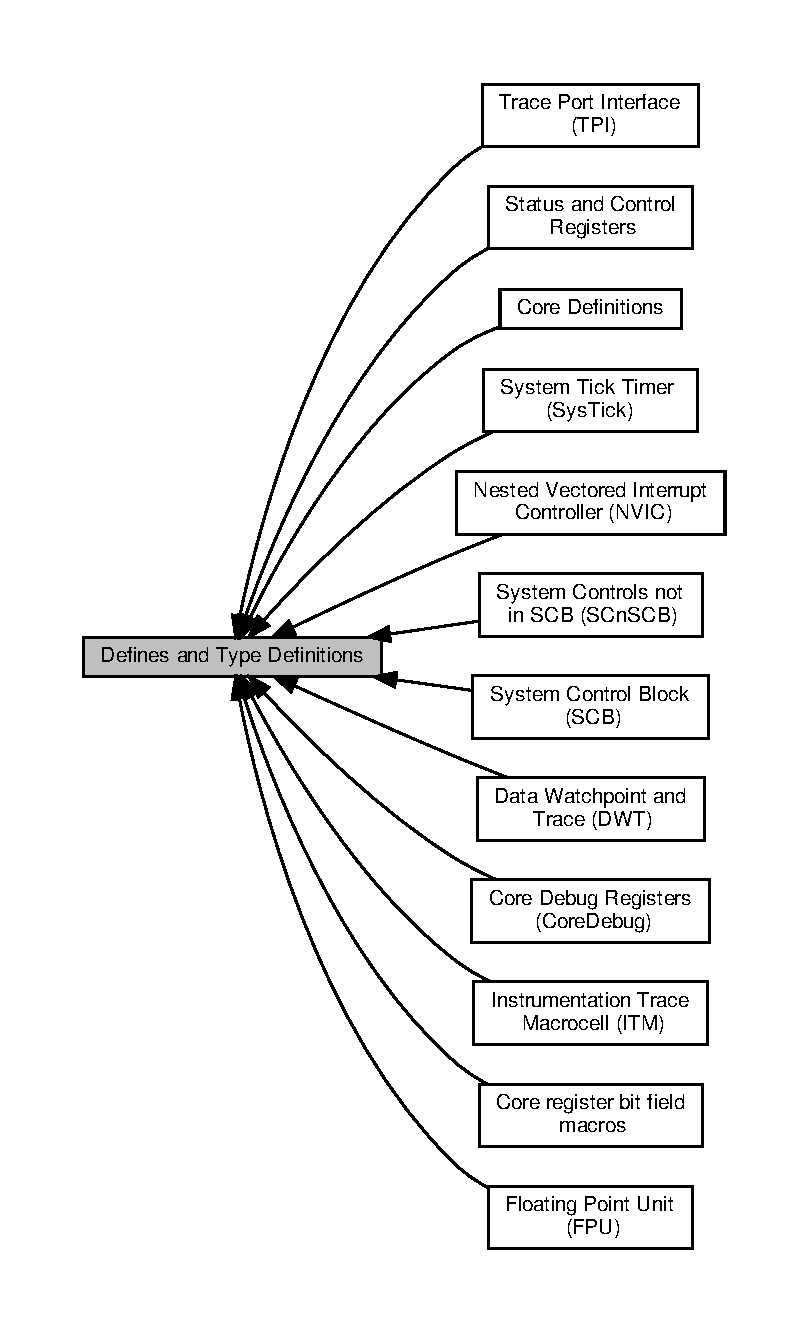
\includegraphics[height=550pt]{group___c_m_s_i_s__core__register}
\end{center}
\end{figure}
\subsection*{Moduły}
\begin{DoxyCompactItemize}
\item 
\hyperlink{group___c_m_s_i_s___c_o_r_e}{Status and Control Registers}
\begin{DoxyCompactList}\small\item\em Core Register type definitions. \end{DoxyCompactList}\item 
\hyperlink{group___c_m_s_i_s___n_v_i_c}{Nested Vectored Interrupt Controller (\+N\+V\+I\+C)}
\begin{DoxyCompactList}\small\item\em Type definitions for the N\+V\+IC Registers. \end{DoxyCompactList}\item 
\hyperlink{group___c_m_s_i_s___s_c_b}{System Control Block (\+S\+C\+B)}
\begin{DoxyCompactList}\small\item\em Type definitions for the System Control Block Registers. \end{DoxyCompactList}\item 
\hyperlink{group___c_m_s_i_s___sys_tick}{System Tick Timer (\+Sys\+Tick)}
\begin{DoxyCompactList}\small\item\em Type definitions for the System Timer Registers. \end{DoxyCompactList}\item 
\hyperlink{group___c_m_s_i_s___d_w_t}{Data Watchpoint and Trace (\+D\+W\+T)}
\begin{DoxyCompactList}\small\item\em Type definitions for the Data Watchpoint and Trace (D\+WT) \end{DoxyCompactList}\item 
\hyperlink{group___c_m_s_i_s___t_p_i}{Trace Port Interface (\+T\+P\+I)}
\begin{DoxyCompactList}\small\item\em Type definitions for the Trace Port Interface (T\+PI) \end{DoxyCompactList}\item 
\hyperlink{group___c_m_s_i_s___core_debug}{Core Debug Registers (\+Core\+Debug)}
\begin{DoxyCompactList}\small\item\em Type definitions for the Core Debug Registers. \end{DoxyCompactList}\item 
\hyperlink{group___c_m_s_i_s__core__bitfield}{Core register bit field macros}
\begin{DoxyCompactList}\small\item\em Macros for use with bit field definitions (xxx\+\_\+\+Pos, xxx\+\_\+\+Msk). \end{DoxyCompactList}\item 
\hyperlink{group___c_m_s_i_s__core__base}{Core Definitions}
\begin{DoxyCompactList}\small\item\em Definitions for base addresses, unions, and structures. \end{DoxyCompactList}\item 
\hyperlink{group___c_m_s_i_s___s_cn_s_c_b}{System Controls not in S\+C\+B (\+S\+Cn\+S\+C\+B)}
\begin{DoxyCompactList}\small\item\em Type definitions for the System Control and ID Register not in the S\+CB. \end{DoxyCompactList}\item 
\hyperlink{group___c_m_s_i_s___i_t_m}{Instrumentation Trace Macrocell (\+I\+T\+M)}
\begin{DoxyCompactList}\small\item\em Type definitions for the Instrumentation Trace Macrocell (I\+TM) \end{DoxyCompactList}\item 
\hyperlink{group___c_m_s_i_s___f_p_u}{Floating Point Unit (\+F\+P\+U)}
\begin{DoxyCompactList}\small\item\em Type definitions for the Floating Point Unit (F\+PU) \end{DoxyCompactList}\end{DoxyCompactItemize}


\subsection{Opis szczegółowy}
Type definitions and defines for Cortex-\/M processor based devices. 


\hypertarget{group___c_m_s_i_s___c_o_r_e}{}\section{Status and Control Registers}
\label{group___c_m_s_i_s___c_o_r_e}\index{Status and Control Registers@{Status and Control Registers}}


Core Register type definitions.  


Diagram współpracy dla Status and Control Registers\+:\nopagebreak
\begin{figure}[H]
\begin{center}
\leavevmode
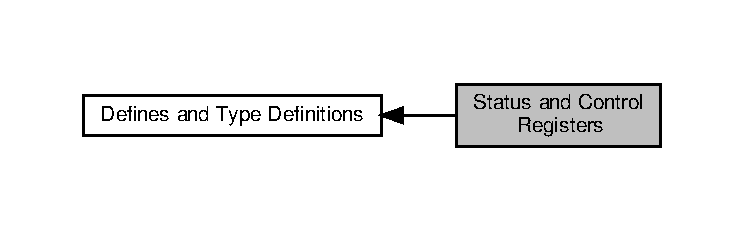
\includegraphics[width=350pt]{group___c_m_s_i_s___c_o_r_e}
\end{center}
\end{figure}
\subsection*{Komponenty}
\begin{DoxyCompactItemize}
\item 
union \hyperlink{union_a_p_s_r___type}{A\+P\+S\+R\+\_\+\+Type}
\begin{DoxyCompactList}\small\item\em Union type to access the Application Program Status Register (A\+P\+SR). \end{DoxyCompactList}\item 
union \hyperlink{union_i_p_s_r___type}{I\+P\+S\+R\+\_\+\+Type}
\begin{DoxyCompactList}\small\item\em Union type to access the Interrupt Program Status Register (I\+P\+SR). \end{DoxyCompactList}\item 
union \hyperlink{unionx_p_s_r___type}{x\+P\+S\+R\+\_\+\+Type}
\begin{DoxyCompactList}\small\item\em Union type to access the Special-\/\+Purpose Program Status Registers (x\+P\+SR). \end{DoxyCompactList}\item 
union \hyperlink{union_c_o_n_t_r_o_l___type}{C\+O\+N\+T\+R\+O\+L\+\_\+\+Type}
\begin{DoxyCompactList}\small\item\em Union type to access the Control Registers (C\+O\+N\+T\+R\+OL). \end{DoxyCompactList}\end{DoxyCompactItemize}
\subsection*{Definicje}
\begin{DoxyCompactItemize}
\item 
\#define \hyperlink{group___c_m_s_i_s___c_o_r_e_gac469528d210043c7bd3f12f0e6824766}{A\+P\+S\+R\+\_\+\+N\+\_\+\+Pos}~31U
\item 
\#define \hyperlink{group___c_m_s_i_s___c_o_r_e_gadbc2cf55a026f661b53fadfcf822cef1}{A\+P\+S\+R\+\_\+\+N\+\_\+\+Msk}~(1\+U\+L $<$$<$ A\+P\+S\+R\+\_\+\+N\+\_\+\+Pos)
\item 
\#define \hyperlink{group___c_m_s_i_s___c_o_r_e_ga3661286d108b1aca308d7445685eae3a}{A\+P\+S\+R\+\_\+\+Z\+\_\+\+Pos}~30U
\item 
\#define \hyperlink{group___c_m_s_i_s___c_o_r_e_ga1deb4d1aa72bb83d1f79329406f15711}{A\+P\+S\+R\+\_\+\+Z\+\_\+\+Msk}~(1\+U\+L $<$$<$ A\+P\+S\+R\+\_\+\+Z\+\_\+\+Pos)
\item 
\#define \hyperlink{group___c_m_s_i_s___c_o_r_e_ga6cf72aa6f09a168f9e5beda1a4a887b9}{A\+P\+S\+R\+\_\+\+C\+\_\+\+Pos}~29U
\item 
\#define \hyperlink{group___c_m_s_i_s___c_o_r_e_ga6d47803fbad455bc10bd1ce59f2f335d}{A\+P\+S\+R\+\_\+\+C\+\_\+\+Msk}~(1\+U\+L $<$$<$ A\+P\+S\+R\+\_\+\+C\+\_\+\+Pos)
\item 
\#define \hyperlink{group___c_m_s_i_s___c_o_r_e_gac62830f67679ccd11658c4172c3e6ea7}{A\+P\+S\+R\+\_\+\+V\+\_\+\+Pos}~28U
\item 
\#define \hyperlink{group___c_m_s_i_s___c_o_r_e_ga33305d6701356bff6890b315fe8b5489}{A\+P\+S\+R\+\_\+\+V\+\_\+\+Msk}~(1\+U\+L $<$$<$ A\+P\+S\+R\+\_\+\+V\+\_\+\+Pos)
\item 
\#define \hyperlink{group___c_m_s_i_s___c_o_r_e_ga0e34027584d02c43811ae908a5ca9adf}{I\+P\+S\+R\+\_\+\+I\+S\+R\+\_\+\+Pos}~0U
\item 
\#define \hyperlink{group___c_m_s_i_s___c_o_r_e_gaf013a4579a64d1f21f56ea9f1b33ab56}{I\+P\+S\+R\+\_\+\+I\+S\+R\+\_\+\+Msk}~(0x1\+F\+F\+U\+L /$\ast$$<$$<$ I\+P\+S\+R\+\_\+\+I\+S\+R\+\_\+\+Pos$\ast$/)
\item 
\#define \hyperlink{group___c_m_s_i_s___c_o_r_e_ga031eb1b8ebcdb3d602d0b9f2ec82a7ae}{x\+P\+S\+R\+\_\+\+N\+\_\+\+Pos}~31U
\item 
\#define \hyperlink{group___c_m_s_i_s___c_o_r_e_gaf600f4ff41b62cf2f3b0a59b6d2e93d6}{x\+P\+S\+R\+\_\+\+N\+\_\+\+Msk}~(1\+U\+L $<$$<$ x\+P\+S\+R\+\_\+\+N\+\_\+\+Pos)
\item 
\#define \hyperlink{group___c_m_s_i_s___c_o_r_e_ga5869dd608eea73c80f0567d781d2230b}{x\+P\+S\+R\+\_\+\+Z\+\_\+\+Pos}~30U
\item 
\#define \hyperlink{group___c_m_s_i_s___c_o_r_e_ga907599209fba99f579778e662021c4f2}{x\+P\+S\+R\+\_\+\+Z\+\_\+\+Msk}~(1\+U\+L $<$$<$ x\+P\+S\+R\+\_\+\+Z\+\_\+\+Pos)
\item 
\#define \hyperlink{group___c_m_s_i_s___c_o_r_e_ga14adb79b91f6634b351a1b57394e2db6}{x\+P\+S\+R\+\_\+\+C\+\_\+\+Pos}~29U
\item 
\#define \hyperlink{group___c_m_s_i_s___c_o_r_e_ga21e2497255d380f956ca0f48d11d0775}{x\+P\+S\+R\+\_\+\+C\+\_\+\+Msk}~(1\+U\+L $<$$<$ x\+P\+S\+R\+\_\+\+C\+\_\+\+Pos)
\item 
\#define \hyperlink{group___c_m_s_i_s___c_o_r_e_gae0cfbb394490db402623d97e6a979e00}{x\+P\+S\+R\+\_\+\+V\+\_\+\+Pos}~28U
\item 
\#define \hyperlink{group___c_m_s_i_s___c_o_r_e_gab07f94ed3b6ee695f5af719dc27995c2}{x\+P\+S\+R\+\_\+\+V\+\_\+\+Msk}~(1\+U\+L $<$$<$ x\+P\+S\+R\+\_\+\+V\+\_\+\+Pos)
\item 
\#define \hyperlink{group___c_m_s_i_s___c_o_r_e_ga98d801da9a49cda944f52aeae104dd38}{x\+P\+S\+R\+\_\+\+T\+\_\+\+Pos}~24U
\item 
\#define \hyperlink{group___c_m_s_i_s___c_o_r_e_ga30ae2111816e82d47636a8d4577eb6ee}{x\+P\+S\+R\+\_\+\+T\+\_\+\+Msk}~(1\+U\+L $<$$<$ x\+P\+S\+R\+\_\+\+T\+\_\+\+Pos)
\item 
\#define \hyperlink{group___c_m_s_i_s___c_o_r_e_ga21bff245fb1aef9683f693d9d7bb2233}{x\+P\+S\+R\+\_\+\+I\+S\+R\+\_\+\+Pos}~0U
\item 
\#define \hyperlink{group___c_m_s_i_s___c_o_r_e_gadf8eed87e0081dfe1ef1c78a0ea91afd}{x\+P\+S\+R\+\_\+\+I\+S\+R\+\_\+\+Msk}~(0x1\+F\+F\+U\+L /$\ast$$<$$<$ x\+P\+S\+R\+\_\+\+I\+S\+R\+\_\+\+Pos$\ast$/)
\item 
\#define \hyperlink{group___c_m_s_i_s___c_o_r_e_ga07eafc53e609895342c6a530e9d01310}{C\+O\+N\+T\+R\+O\+L\+\_\+\+S\+P\+S\+E\+L\+\_\+\+Pos}~1U
\item 
\#define \hyperlink{group___c_m_s_i_s___c_o_r_e_ga70b29840969b06909da21369b0b05b53}{C\+O\+N\+T\+R\+O\+L\+\_\+\+S\+P\+S\+E\+L\+\_\+\+Msk}~(1\+U\+L $<$$<$ C\+O\+N\+T\+R\+O\+L\+\_\+\+S\+P\+S\+E\+L\+\_\+\+Pos)
\item 
\#define \hyperlink{group___c_m_s_i_s___c_o_r_e_ga51b95bc03ec0d815b459bde0b14a5908}{C\+O\+N\+T\+R\+O\+L\+\_\+n\+P\+R\+I\+V\+\_\+\+Pos}~0U
\item 
\#define \hyperlink{group___c_m_s_i_s___c_o_r_e_gaef3b20d77acb213338f89ce5e7bc36b0}{C\+O\+N\+T\+R\+O\+L\+\_\+n\+P\+R\+I\+V\+\_\+\+Msk}~(1\+U\+L /$\ast$$<$$<$ C\+O\+N\+T\+R\+O\+L\+\_\+n\+P\+R\+I\+V\+\_\+\+Pos$\ast$/)
\item 
\#define \hyperlink{group___c_m_s_i_s___c_o_r_e_gac469528d210043c7bd3f12f0e6824766}{A\+P\+S\+R\+\_\+\+N\+\_\+\+Pos}~31U
\item 
\#define \hyperlink{group___c_m_s_i_s___c_o_r_e_gadbc2cf55a026f661b53fadfcf822cef1}{A\+P\+S\+R\+\_\+\+N\+\_\+\+Msk}~(1\+U\+L $<$$<$ A\+P\+S\+R\+\_\+\+N\+\_\+\+Pos)
\item 
\#define \hyperlink{group___c_m_s_i_s___c_o_r_e_ga3661286d108b1aca308d7445685eae3a}{A\+P\+S\+R\+\_\+\+Z\+\_\+\+Pos}~30U
\item 
\#define \hyperlink{group___c_m_s_i_s___c_o_r_e_ga1deb4d1aa72bb83d1f79329406f15711}{A\+P\+S\+R\+\_\+\+Z\+\_\+\+Msk}~(1\+U\+L $<$$<$ A\+P\+S\+R\+\_\+\+Z\+\_\+\+Pos)
\item 
\#define \hyperlink{group___c_m_s_i_s___c_o_r_e_ga6cf72aa6f09a168f9e5beda1a4a887b9}{A\+P\+S\+R\+\_\+\+C\+\_\+\+Pos}~29U
\item 
\#define \hyperlink{group___c_m_s_i_s___c_o_r_e_ga6d47803fbad455bc10bd1ce59f2f335d}{A\+P\+S\+R\+\_\+\+C\+\_\+\+Msk}~(1\+U\+L $<$$<$ A\+P\+S\+R\+\_\+\+C\+\_\+\+Pos)
\item 
\#define \hyperlink{group___c_m_s_i_s___c_o_r_e_gac62830f67679ccd11658c4172c3e6ea7}{A\+P\+S\+R\+\_\+\+V\+\_\+\+Pos}~28U
\item 
\#define \hyperlink{group___c_m_s_i_s___c_o_r_e_ga33305d6701356bff6890b315fe8b5489}{A\+P\+S\+R\+\_\+\+V\+\_\+\+Msk}~(1\+U\+L $<$$<$ A\+P\+S\+R\+\_\+\+V\+\_\+\+Pos)
\item 
\#define \hyperlink{group___c_m_s_i_s___c_o_r_e_ga298749e176f12827328bb7b92a6b2411}{A\+P\+S\+R\+\_\+\+Q\+\_\+\+Pos}~27U
\item 
\#define \hyperlink{group___c_m_s_i_s___c_o_r_e_ga90ffd4ec4149c2f5dd7747c1533fb002}{A\+P\+S\+R\+\_\+\+Q\+\_\+\+Msk}~(1\+U\+L $<$$<$ A\+P\+S\+R\+\_\+\+Q\+\_\+\+Pos)
\item 
\#define \hyperlink{group___c_m_s_i_s___c_o_r_e_ga722cb42b5c75af3e8909fac6fd40dfdc}{A\+P\+S\+R\+\_\+\+G\+E\+\_\+\+Pos}~16U
\item 
\#define \hyperlink{group___c_m_s_i_s___c_o_r_e_ga8a3ecbc0ea2029462b0f4ce50e227db1}{A\+P\+S\+R\+\_\+\+G\+E\+\_\+\+Msk}~(0x\+F\+U\+L $<$$<$ A\+P\+S\+R\+\_\+\+G\+E\+\_\+\+Pos)
\item 
\#define \hyperlink{group___c_m_s_i_s___c_o_r_e_ga0e34027584d02c43811ae908a5ca9adf}{I\+P\+S\+R\+\_\+\+I\+S\+R\+\_\+\+Pos}~0U
\item 
\#define \hyperlink{group___c_m_s_i_s___c_o_r_e_gaf013a4579a64d1f21f56ea9f1b33ab56}{I\+P\+S\+R\+\_\+\+I\+S\+R\+\_\+\+Msk}~(0x1\+F\+F\+U\+L /$\ast$$<$$<$ I\+P\+S\+R\+\_\+\+I\+S\+R\+\_\+\+Pos$\ast$/)
\item 
\#define \hyperlink{group___c_m_s_i_s___c_o_r_e_ga031eb1b8ebcdb3d602d0b9f2ec82a7ae}{x\+P\+S\+R\+\_\+\+N\+\_\+\+Pos}~31U
\item 
\#define \hyperlink{group___c_m_s_i_s___c_o_r_e_gaf600f4ff41b62cf2f3b0a59b6d2e93d6}{x\+P\+S\+R\+\_\+\+N\+\_\+\+Msk}~(1\+U\+L $<$$<$ x\+P\+S\+R\+\_\+\+N\+\_\+\+Pos)
\item 
\#define \hyperlink{group___c_m_s_i_s___c_o_r_e_ga5869dd608eea73c80f0567d781d2230b}{x\+P\+S\+R\+\_\+\+Z\+\_\+\+Pos}~30U
\item 
\#define \hyperlink{group___c_m_s_i_s___c_o_r_e_ga907599209fba99f579778e662021c4f2}{x\+P\+S\+R\+\_\+\+Z\+\_\+\+Msk}~(1\+U\+L $<$$<$ x\+P\+S\+R\+\_\+\+Z\+\_\+\+Pos)
\item 
\#define \hyperlink{group___c_m_s_i_s___c_o_r_e_ga14adb79b91f6634b351a1b57394e2db6}{x\+P\+S\+R\+\_\+\+C\+\_\+\+Pos}~29U
\item 
\#define \hyperlink{group___c_m_s_i_s___c_o_r_e_ga21e2497255d380f956ca0f48d11d0775}{x\+P\+S\+R\+\_\+\+C\+\_\+\+Msk}~(1\+U\+L $<$$<$ x\+P\+S\+R\+\_\+\+C\+\_\+\+Pos)
\item 
\#define \hyperlink{group___c_m_s_i_s___c_o_r_e_gae0cfbb394490db402623d97e6a979e00}{x\+P\+S\+R\+\_\+\+V\+\_\+\+Pos}~28U
\item 
\#define \hyperlink{group___c_m_s_i_s___c_o_r_e_gab07f94ed3b6ee695f5af719dc27995c2}{x\+P\+S\+R\+\_\+\+V\+\_\+\+Msk}~(1\+U\+L $<$$<$ x\+P\+S\+R\+\_\+\+V\+\_\+\+Pos)
\item 
\#define \hyperlink{group___c_m_s_i_s___c_o_r_e_gaabb4178d50676a8f19cf8f727f38ace8}{x\+P\+S\+R\+\_\+\+Q\+\_\+\+Pos}~27U
\item 
\#define \hyperlink{group___c_m_s_i_s___c_o_r_e_ga133ac393c38559ae43ac36383e731dd4}{x\+P\+S\+R\+\_\+\+Q\+\_\+\+Msk}~(1\+U\+L $<$$<$ x\+P\+S\+R\+\_\+\+Q\+\_\+\+Pos)
\item 
\#define \hyperlink{group___c_m_s_i_s___c_o_r_e_gac5be1db1343f776ecd00f0a4ebe70a46}{x\+P\+S\+R\+\_\+\+I\+T\+\_\+\+Pos}~25U
\item 
\#define \hyperlink{group___c_m_s_i_s___c_o_r_e_ga6dc177aab488851bb3b98cf4b420141a}{x\+P\+S\+R\+\_\+\+I\+T\+\_\+\+Msk}~(3\+U\+L $<$$<$ x\+P\+S\+R\+\_\+\+I\+T\+\_\+\+Pos)
\item 
\#define \hyperlink{group___c_m_s_i_s___c_o_r_e_ga98d801da9a49cda944f52aeae104dd38}{x\+P\+S\+R\+\_\+\+T\+\_\+\+Pos}~24U
\item 
\#define \hyperlink{group___c_m_s_i_s___c_o_r_e_ga30ae2111816e82d47636a8d4577eb6ee}{x\+P\+S\+R\+\_\+\+T\+\_\+\+Msk}~(1\+U\+L $<$$<$ x\+P\+S\+R\+\_\+\+T\+\_\+\+Pos)
\item 
\#define \hyperlink{group___c_m_s_i_s___c_o_r_e_gae2b0f3def0f378e9f1d10a4c727a064b}{x\+P\+S\+R\+\_\+\+G\+E\+\_\+\+Pos}~16U
\item 
\#define \hyperlink{group___c_m_s_i_s___c_o_r_e_ga967634e605d013e9b07002eca31f7903}{x\+P\+S\+R\+\_\+\+G\+E\+\_\+\+Msk}~(0x\+F\+U\+L $<$$<$ x\+P\+S\+R\+\_\+\+G\+E\+\_\+\+Pos)
\item 
\#define \hyperlink{group___c_m_s_i_s___c_o_r_e_ga21bff245fb1aef9683f693d9d7bb2233}{x\+P\+S\+R\+\_\+\+I\+S\+R\+\_\+\+Pos}~0U
\item 
\#define \hyperlink{group___c_m_s_i_s___c_o_r_e_gadf8eed87e0081dfe1ef1c78a0ea91afd}{x\+P\+S\+R\+\_\+\+I\+S\+R\+\_\+\+Msk}~(0x1\+F\+F\+U\+L /$\ast$$<$$<$ x\+P\+S\+R\+\_\+\+I\+S\+R\+\_\+\+Pos$\ast$/)
\item 
\#define \hyperlink{group___c_m_s_i_s___c_o_r_e_gac4eb493f7e00c0b286f6663b2554d5f1}{C\+O\+N\+T\+R\+O\+L\+\_\+\+S\+F\+P\+A\+\_\+\+Pos}~3U
\item 
\#define \hyperlink{group___c_m_s_i_s___c_o_r_e_gae1af7c6a3a6482a32ae290b66db3a3f8}{C\+O\+N\+T\+R\+O\+L\+\_\+\+S\+F\+P\+A\+\_\+\+Msk}~(1\+U\+L $<$$<$ C\+O\+N\+T\+R\+O\+L\+\_\+\+S\+F\+P\+A\+\_\+\+Pos)
\item 
\#define \hyperlink{group___c_m_s_i_s___c_o_r_e_gac7018b59b07134c5363b33eb94918a58}{C\+O\+N\+T\+R\+O\+L\+\_\+\+F\+P\+C\+A\+\_\+\+Pos}~2U
\item 
\#define \hyperlink{group___c_m_s_i_s___c_o_r_e_gad20bb0212b2e1864f24af38d93587c79}{C\+O\+N\+T\+R\+O\+L\+\_\+\+F\+P\+C\+A\+\_\+\+Msk}~(1\+U\+L $<$$<$ C\+O\+N\+T\+R\+O\+L\+\_\+\+F\+P\+C\+A\+\_\+\+Pos)
\item 
\#define \hyperlink{group___c_m_s_i_s___c_o_r_e_ga07eafc53e609895342c6a530e9d01310}{C\+O\+N\+T\+R\+O\+L\+\_\+\+S\+P\+S\+E\+L\+\_\+\+Pos}~1U
\item 
\#define \hyperlink{group___c_m_s_i_s___c_o_r_e_ga70b29840969b06909da21369b0b05b53}{C\+O\+N\+T\+R\+O\+L\+\_\+\+S\+P\+S\+E\+L\+\_\+\+Msk}~(1\+U\+L $<$$<$ C\+O\+N\+T\+R\+O\+L\+\_\+\+S\+P\+S\+E\+L\+\_\+\+Pos)
\item 
\#define \hyperlink{group___c_m_s_i_s___c_o_r_e_ga51b95bc03ec0d815b459bde0b14a5908}{C\+O\+N\+T\+R\+O\+L\+\_\+n\+P\+R\+I\+V\+\_\+\+Pos}~0U
\item 
\#define \hyperlink{group___c_m_s_i_s___c_o_r_e_gaef3b20d77acb213338f89ce5e7bc36b0}{C\+O\+N\+T\+R\+O\+L\+\_\+n\+P\+R\+I\+V\+\_\+\+Msk}~(1\+U\+L /$\ast$$<$$<$ C\+O\+N\+T\+R\+O\+L\+\_\+n\+P\+R\+I\+V\+\_\+\+Pos$\ast$/)
\item 
\#define \hyperlink{group___c_m_s_i_s___c_o_r_e_gac469528d210043c7bd3f12f0e6824766}{A\+P\+S\+R\+\_\+\+N\+\_\+\+Pos}~31U
\item 
\#define \hyperlink{group___c_m_s_i_s___c_o_r_e_gadbc2cf55a026f661b53fadfcf822cef1}{A\+P\+S\+R\+\_\+\+N\+\_\+\+Msk}~(1\+U\+L $<$$<$ A\+P\+S\+R\+\_\+\+N\+\_\+\+Pos)
\item 
\#define \hyperlink{group___c_m_s_i_s___c_o_r_e_ga3661286d108b1aca308d7445685eae3a}{A\+P\+S\+R\+\_\+\+Z\+\_\+\+Pos}~30U
\item 
\#define \hyperlink{group___c_m_s_i_s___c_o_r_e_ga1deb4d1aa72bb83d1f79329406f15711}{A\+P\+S\+R\+\_\+\+Z\+\_\+\+Msk}~(1\+U\+L $<$$<$ A\+P\+S\+R\+\_\+\+Z\+\_\+\+Pos)
\item 
\#define \hyperlink{group___c_m_s_i_s___c_o_r_e_ga6cf72aa6f09a168f9e5beda1a4a887b9}{A\+P\+S\+R\+\_\+\+C\+\_\+\+Pos}~29U
\item 
\#define \hyperlink{group___c_m_s_i_s___c_o_r_e_ga6d47803fbad455bc10bd1ce59f2f335d}{A\+P\+S\+R\+\_\+\+C\+\_\+\+Msk}~(1\+U\+L $<$$<$ A\+P\+S\+R\+\_\+\+C\+\_\+\+Pos)
\item 
\#define \hyperlink{group___c_m_s_i_s___c_o_r_e_gac62830f67679ccd11658c4172c3e6ea7}{A\+P\+S\+R\+\_\+\+V\+\_\+\+Pos}~28U
\item 
\#define \hyperlink{group___c_m_s_i_s___c_o_r_e_ga33305d6701356bff6890b315fe8b5489}{A\+P\+S\+R\+\_\+\+V\+\_\+\+Msk}~(1\+U\+L $<$$<$ A\+P\+S\+R\+\_\+\+V\+\_\+\+Pos)
\item 
\#define \hyperlink{group___c_m_s_i_s___c_o_r_e_ga0e34027584d02c43811ae908a5ca9adf}{I\+P\+S\+R\+\_\+\+I\+S\+R\+\_\+\+Pos}~0U
\item 
\#define \hyperlink{group___c_m_s_i_s___c_o_r_e_gaf013a4579a64d1f21f56ea9f1b33ab56}{I\+P\+S\+R\+\_\+\+I\+S\+R\+\_\+\+Msk}~(0x1\+F\+F\+U\+L /$\ast$$<$$<$ I\+P\+S\+R\+\_\+\+I\+S\+R\+\_\+\+Pos$\ast$/)
\item 
\#define \hyperlink{group___c_m_s_i_s___c_o_r_e_ga031eb1b8ebcdb3d602d0b9f2ec82a7ae}{x\+P\+S\+R\+\_\+\+N\+\_\+\+Pos}~31U
\item 
\#define \hyperlink{group___c_m_s_i_s___c_o_r_e_gaf600f4ff41b62cf2f3b0a59b6d2e93d6}{x\+P\+S\+R\+\_\+\+N\+\_\+\+Msk}~(1\+U\+L $<$$<$ x\+P\+S\+R\+\_\+\+N\+\_\+\+Pos)
\item 
\#define \hyperlink{group___c_m_s_i_s___c_o_r_e_ga5869dd608eea73c80f0567d781d2230b}{x\+P\+S\+R\+\_\+\+Z\+\_\+\+Pos}~30U
\item 
\#define \hyperlink{group___c_m_s_i_s___c_o_r_e_ga907599209fba99f579778e662021c4f2}{x\+P\+S\+R\+\_\+\+Z\+\_\+\+Msk}~(1\+U\+L $<$$<$ x\+P\+S\+R\+\_\+\+Z\+\_\+\+Pos)
\item 
\#define \hyperlink{group___c_m_s_i_s___c_o_r_e_ga14adb79b91f6634b351a1b57394e2db6}{x\+P\+S\+R\+\_\+\+C\+\_\+\+Pos}~29U
\item 
\#define \hyperlink{group___c_m_s_i_s___c_o_r_e_ga21e2497255d380f956ca0f48d11d0775}{x\+P\+S\+R\+\_\+\+C\+\_\+\+Msk}~(1\+U\+L $<$$<$ x\+P\+S\+R\+\_\+\+C\+\_\+\+Pos)
\item 
\#define \hyperlink{group___c_m_s_i_s___c_o_r_e_gae0cfbb394490db402623d97e6a979e00}{x\+P\+S\+R\+\_\+\+V\+\_\+\+Pos}~28U
\item 
\#define \hyperlink{group___c_m_s_i_s___c_o_r_e_gab07f94ed3b6ee695f5af719dc27995c2}{x\+P\+S\+R\+\_\+\+V\+\_\+\+Msk}~(1\+U\+L $<$$<$ x\+P\+S\+R\+\_\+\+V\+\_\+\+Pos)
\item 
\#define \hyperlink{group___c_m_s_i_s___c_o_r_e_ga98d801da9a49cda944f52aeae104dd38}{x\+P\+S\+R\+\_\+\+T\+\_\+\+Pos}~24U
\item 
\#define \hyperlink{group___c_m_s_i_s___c_o_r_e_ga30ae2111816e82d47636a8d4577eb6ee}{x\+P\+S\+R\+\_\+\+T\+\_\+\+Msk}~(1\+U\+L $<$$<$ x\+P\+S\+R\+\_\+\+T\+\_\+\+Pos)
\item 
\#define \hyperlink{group___c_m_s_i_s___c_o_r_e_ga21bff245fb1aef9683f693d9d7bb2233}{x\+P\+S\+R\+\_\+\+I\+S\+R\+\_\+\+Pos}~0U
\item 
\#define \hyperlink{group___c_m_s_i_s___c_o_r_e_gadf8eed87e0081dfe1ef1c78a0ea91afd}{x\+P\+S\+R\+\_\+\+I\+S\+R\+\_\+\+Msk}~(0x1\+F\+F\+U\+L /$\ast$$<$$<$ x\+P\+S\+R\+\_\+\+I\+S\+R\+\_\+\+Pos$\ast$/)
\item 
\#define \hyperlink{group___c_m_s_i_s___c_o_r_e_ga07eafc53e609895342c6a530e9d01310}{C\+O\+N\+T\+R\+O\+L\+\_\+\+S\+P\+S\+E\+L\+\_\+\+Pos}~1U
\item 
\#define \hyperlink{group___c_m_s_i_s___c_o_r_e_ga70b29840969b06909da21369b0b05b53}{C\+O\+N\+T\+R\+O\+L\+\_\+\+S\+P\+S\+E\+L\+\_\+\+Msk}~(1\+U\+L $<$$<$ C\+O\+N\+T\+R\+O\+L\+\_\+\+S\+P\+S\+E\+L\+\_\+\+Pos)
\item 
\#define \hyperlink{group___c_m_s_i_s___c_o_r_e_gac469528d210043c7bd3f12f0e6824766}{A\+P\+S\+R\+\_\+\+N\+\_\+\+Pos}~31U
\item 
\#define \hyperlink{group___c_m_s_i_s___c_o_r_e_gadbc2cf55a026f661b53fadfcf822cef1}{A\+P\+S\+R\+\_\+\+N\+\_\+\+Msk}~(1\+U\+L $<$$<$ A\+P\+S\+R\+\_\+\+N\+\_\+\+Pos)
\item 
\#define \hyperlink{group___c_m_s_i_s___c_o_r_e_ga3661286d108b1aca308d7445685eae3a}{A\+P\+S\+R\+\_\+\+Z\+\_\+\+Pos}~30U
\item 
\#define \hyperlink{group___c_m_s_i_s___c_o_r_e_ga1deb4d1aa72bb83d1f79329406f15711}{A\+P\+S\+R\+\_\+\+Z\+\_\+\+Msk}~(1\+U\+L $<$$<$ A\+P\+S\+R\+\_\+\+Z\+\_\+\+Pos)
\item 
\#define \hyperlink{group___c_m_s_i_s___c_o_r_e_ga6cf72aa6f09a168f9e5beda1a4a887b9}{A\+P\+S\+R\+\_\+\+C\+\_\+\+Pos}~29U
\item 
\#define \hyperlink{group___c_m_s_i_s___c_o_r_e_ga6d47803fbad455bc10bd1ce59f2f335d}{A\+P\+S\+R\+\_\+\+C\+\_\+\+Msk}~(1\+U\+L $<$$<$ A\+P\+S\+R\+\_\+\+C\+\_\+\+Pos)
\item 
\#define \hyperlink{group___c_m_s_i_s___c_o_r_e_gac62830f67679ccd11658c4172c3e6ea7}{A\+P\+S\+R\+\_\+\+V\+\_\+\+Pos}~28U
\item 
\#define \hyperlink{group___c_m_s_i_s___c_o_r_e_ga33305d6701356bff6890b315fe8b5489}{A\+P\+S\+R\+\_\+\+V\+\_\+\+Msk}~(1\+U\+L $<$$<$ A\+P\+S\+R\+\_\+\+V\+\_\+\+Pos)
\item 
\#define \hyperlink{group___c_m_s_i_s___c_o_r_e_ga0e34027584d02c43811ae908a5ca9adf}{I\+P\+S\+R\+\_\+\+I\+S\+R\+\_\+\+Pos}~0U
\item 
\#define \hyperlink{group___c_m_s_i_s___c_o_r_e_gaf013a4579a64d1f21f56ea9f1b33ab56}{I\+P\+S\+R\+\_\+\+I\+S\+R\+\_\+\+Msk}~(0x1\+F\+F\+U\+L /$\ast$$<$$<$ I\+P\+S\+R\+\_\+\+I\+S\+R\+\_\+\+Pos$\ast$/)
\item 
\#define \hyperlink{group___c_m_s_i_s___c_o_r_e_ga031eb1b8ebcdb3d602d0b9f2ec82a7ae}{x\+P\+S\+R\+\_\+\+N\+\_\+\+Pos}~31U
\item 
\#define \hyperlink{group___c_m_s_i_s___c_o_r_e_gaf600f4ff41b62cf2f3b0a59b6d2e93d6}{x\+P\+S\+R\+\_\+\+N\+\_\+\+Msk}~(1\+U\+L $<$$<$ x\+P\+S\+R\+\_\+\+N\+\_\+\+Pos)
\item 
\#define \hyperlink{group___c_m_s_i_s___c_o_r_e_ga5869dd608eea73c80f0567d781d2230b}{x\+P\+S\+R\+\_\+\+Z\+\_\+\+Pos}~30U
\item 
\#define \hyperlink{group___c_m_s_i_s___c_o_r_e_ga907599209fba99f579778e662021c4f2}{x\+P\+S\+R\+\_\+\+Z\+\_\+\+Msk}~(1\+U\+L $<$$<$ x\+P\+S\+R\+\_\+\+Z\+\_\+\+Pos)
\item 
\#define \hyperlink{group___c_m_s_i_s___c_o_r_e_ga14adb79b91f6634b351a1b57394e2db6}{x\+P\+S\+R\+\_\+\+C\+\_\+\+Pos}~29U
\item 
\#define \hyperlink{group___c_m_s_i_s___c_o_r_e_ga21e2497255d380f956ca0f48d11d0775}{x\+P\+S\+R\+\_\+\+C\+\_\+\+Msk}~(1\+U\+L $<$$<$ x\+P\+S\+R\+\_\+\+C\+\_\+\+Pos)
\item 
\#define \hyperlink{group___c_m_s_i_s___c_o_r_e_gae0cfbb394490db402623d97e6a979e00}{x\+P\+S\+R\+\_\+\+V\+\_\+\+Pos}~28U
\item 
\#define \hyperlink{group___c_m_s_i_s___c_o_r_e_gab07f94ed3b6ee695f5af719dc27995c2}{x\+P\+S\+R\+\_\+\+V\+\_\+\+Msk}~(1\+U\+L $<$$<$ x\+P\+S\+R\+\_\+\+V\+\_\+\+Pos)
\item 
\#define \hyperlink{group___c_m_s_i_s___c_o_r_e_ga98d801da9a49cda944f52aeae104dd38}{x\+P\+S\+R\+\_\+\+T\+\_\+\+Pos}~24U
\item 
\#define \hyperlink{group___c_m_s_i_s___c_o_r_e_ga30ae2111816e82d47636a8d4577eb6ee}{x\+P\+S\+R\+\_\+\+T\+\_\+\+Msk}~(1\+U\+L $<$$<$ x\+P\+S\+R\+\_\+\+T\+\_\+\+Pos)
\item 
\#define \hyperlink{group___c_m_s_i_s___c_o_r_e_ga21bff245fb1aef9683f693d9d7bb2233}{x\+P\+S\+R\+\_\+\+I\+S\+R\+\_\+\+Pos}~0U
\item 
\#define \hyperlink{group___c_m_s_i_s___c_o_r_e_gadf8eed87e0081dfe1ef1c78a0ea91afd}{x\+P\+S\+R\+\_\+\+I\+S\+R\+\_\+\+Msk}~(0x1\+F\+F\+U\+L /$\ast$$<$$<$ x\+P\+S\+R\+\_\+\+I\+S\+R\+\_\+\+Pos$\ast$/)
\item 
\#define \hyperlink{group___c_m_s_i_s___c_o_r_e_ga07eafc53e609895342c6a530e9d01310}{C\+O\+N\+T\+R\+O\+L\+\_\+\+S\+P\+S\+E\+L\+\_\+\+Pos}~1U
\item 
\#define \hyperlink{group___c_m_s_i_s___c_o_r_e_ga70b29840969b06909da21369b0b05b53}{C\+O\+N\+T\+R\+O\+L\+\_\+\+S\+P\+S\+E\+L\+\_\+\+Msk}~(1\+U\+L $<$$<$ C\+O\+N\+T\+R\+O\+L\+\_\+\+S\+P\+S\+E\+L\+\_\+\+Pos)
\item 
\#define \hyperlink{group___c_m_s_i_s___c_o_r_e_ga51b95bc03ec0d815b459bde0b14a5908}{C\+O\+N\+T\+R\+O\+L\+\_\+n\+P\+R\+I\+V\+\_\+\+Pos}~0U
\item 
\#define \hyperlink{group___c_m_s_i_s___c_o_r_e_gaef3b20d77acb213338f89ce5e7bc36b0}{C\+O\+N\+T\+R\+O\+L\+\_\+n\+P\+R\+I\+V\+\_\+\+Msk}~(1\+U\+L /$\ast$$<$$<$ C\+O\+N\+T\+R\+O\+L\+\_\+n\+P\+R\+I\+V\+\_\+\+Pos$\ast$/)
\item 
\#define \hyperlink{group___c_m_s_i_s___c_o_r_e_gac469528d210043c7bd3f12f0e6824766}{A\+P\+S\+R\+\_\+\+N\+\_\+\+Pos}~31U
\item 
\#define \hyperlink{group___c_m_s_i_s___c_o_r_e_gadbc2cf55a026f661b53fadfcf822cef1}{A\+P\+S\+R\+\_\+\+N\+\_\+\+Msk}~(1\+U\+L $<$$<$ A\+P\+S\+R\+\_\+\+N\+\_\+\+Pos)
\item 
\#define \hyperlink{group___c_m_s_i_s___c_o_r_e_ga3661286d108b1aca308d7445685eae3a}{A\+P\+S\+R\+\_\+\+Z\+\_\+\+Pos}~30U
\item 
\#define \hyperlink{group___c_m_s_i_s___c_o_r_e_ga1deb4d1aa72bb83d1f79329406f15711}{A\+P\+S\+R\+\_\+\+Z\+\_\+\+Msk}~(1\+U\+L $<$$<$ A\+P\+S\+R\+\_\+\+Z\+\_\+\+Pos)
\item 
\#define \hyperlink{group___c_m_s_i_s___c_o_r_e_ga6cf72aa6f09a168f9e5beda1a4a887b9}{A\+P\+S\+R\+\_\+\+C\+\_\+\+Pos}~29U
\item 
\#define \hyperlink{group___c_m_s_i_s___c_o_r_e_ga6d47803fbad455bc10bd1ce59f2f335d}{A\+P\+S\+R\+\_\+\+C\+\_\+\+Msk}~(1\+U\+L $<$$<$ A\+P\+S\+R\+\_\+\+C\+\_\+\+Pos)
\item 
\#define \hyperlink{group___c_m_s_i_s___c_o_r_e_gac62830f67679ccd11658c4172c3e6ea7}{A\+P\+S\+R\+\_\+\+V\+\_\+\+Pos}~28U
\item 
\#define \hyperlink{group___c_m_s_i_s___c_o_r_e_ga33305d6701356bff6890b315fe8b5489}{A\+P\+S\+R\+\_\+\+V\+\_\+\+Msk}~(1\+U\+L $<$$<$ A\+P\+S\+R\+\_\+\+V\+\_\+\+Pos)
\item 
\#define \hyperlink{group___c_m_s_i_s___c_o_r_e_ga0e34027584d02c43811ae908a5ca9adf}{I\+P\+S\+R\+\_\+\+I\+S\+R\+\_\+\+Pos}~0U
\item 
\#define \hyperlink{group___c_m_s_i_s___c_o_r_e_gaf013a4579a64d1f21f56ea9f1b33ab56}{I\+P\+S\+R\+\_\+\+I\+S\+R\+\_\+\+Msk}~(0x1\+F\+F\+U\+L /$\ast$$<$$<$ I\+P\+S\+R\+\_\+\+I\+S\+R\+\_\+\+Pos$\ast$/)
\item 
\#define \hyperlink{group___c_m_s_i_s___c_o_r_e_ga031eb1b8ebcdb3d602d0b9f2ec82a7ae}{x\+P\+S\+R\+\_\+\+N\+\_\+\+Pos}~31U
\item 
\#define \hyperlink{group___c_m_s_i_s___c_o_r_e_gaf600f4ff41b62cf2f3b0a59b6d2e93d6}{x\+P\+S\+R\+\_\+\+N\+\_\+\+Msk}~(1\+U\+L $<$$<$ x\+P\+S\+R\+\_\+\+N\+\_\+\+Pos)
\item 
\#define \hyperlink{group___c_m_s_i_s___c_o_r_e_ga5869dd608eea73c80f0567d781d2230b}{x\+P\+S\+R\+\_\+\+Z\+\_\+\+Pos}~30U
\item 
\#define \hyperlink{group___c_m_s_i_s___c_o_r_e_ga907599209fba99f579778e662021c4f2}{x\+P\+S\+R\+\_\+\+Z\+\_\+\+Msk}~(1\+U\+L $<$$<$ x\+P\+S\+R\+\_\+\+Z\+\_\+\+Pos)
\item 
\#define \hyperlink{group___c_m_s_i_s___c_o_r_e_ga14adb79b91f6634b351a1b57394e2db6}{x\+P\+S\+R\+\_\+\+C\+\_\+\+Pos}~29U
\item 
\#define \hyperlink{group___c_m_s_i_s___c_o_r_e_ga21e2497255d380f956ca0f48d11d0775}{x\+P\+S\+R\+\_\+\+C\+\_\+\+Msk}~(1\+U\+L $<$$<$ x\+P\+S\+R\+\_\+\+C\+\_\+\+Pos)
\item 
\#define \hyperlink{group___c_m_s_i_s___c_o_r_e_gae0cfbb394490db402623d97e6a979e00}{x\+P\+S\+R\+\_\+\+V\+\_\+\+Pos}~28U
\item 
\#define \hyperlink{group___c_m_s_i_s___c_o_r_e_gab07f94ed3b6ee695f5af719dc27995c2}{x\+P\+S\+R\+\_\+\+V\+\_\+\+Msk}~(1\+U\+L $<$$<$ x\+P\+S\+R\+\_\+\+V\+\_\+\+Pos)
\item 
\#define \hyperlink{group___c_m_s_i_s___c_o_r_e_ga98d801da9a49cda944f52aeae104dd38}{x\+P\+S\+R\+\_\+\+T\+\_\+\+Pos}~24U
\item 
\#define \hyperlink{group___c_m_s_i_s___c_o_r_e_ga30ae2111816e82d47636a8d4577eb6ee}{x\+P\+S\+R\+\_\+\+T\+\_\+\+Msk}~(1\+U\+L $<$$<$ x\+P\+S\+R\+\_\+\+T\+\_\+\+Pos)
\item 
\#define \hyperlink{group___c_m_s_i_s___c_o_r_e_ga21bff245fb1aef9683f693d9d7bb2233}{x\+P\+S\+R\+\_\+\+I\+S\+R\+\_\+\+Pos}~0U
\item 
\#define \hyperlink{group___c_m_s_i_s___c_o_r_e_gadf8eed87e0081dfe1ef1c78a0ea91afd}{x\+P\+S\+R\+\_\+\+I\+S\+R\+\_\+\+Msk}~(0x1\+F\+F\+U\+L /$\ast$$<$$<$ x\+P\+S\+R\+\_\+\+I\+S\+R\+\_\+\+Pos$\ast$/)
\item 
\#define \hyperlink{group___c_m_s_i_s___c_o_r_e_ga07eafc53e609895342c6a530e9d01310}{C\+O\+N\+T\+R\+O\+L\+\_\+\+S\+P\+S\+E\+L\+\_\+\+Pos}~1U
\item 
\#define \hyperlink{group___c_m_s_i_s___c_o_r_e_ga70b29840969b06909da21369b0b05b53}{C\+O\+N\+T\+R\+O\+L\+\_\+\+S\+P\+S\+E\+L\+\_\+\+Msk}~(1\+U\+L $<$$<$ C\+O\+N\+T\+R\+O\+L\+\_\+\+S\+P\+S\+E\+L\+\_\+\+Pos)
\item 
\#define \hyperlink{group___c_m_s_i_s___c_o_r_e_gac469528d210043c7bd3f12f0e6824766}{A\+P\+S\+R\+\_\+\+N\+\_\+\+Pos}~31U
\item 
\#define \hyperlink{group___c_m_s_i_s___c_o_r_e_gadbc2cf55a026f661b53fadfcf822cef1}{A\+P\+S\+R\+\_\+\+N\+\_\+\+Msk}~(1\+U\+L $<$$<$ A\+P\+S\+R\+\_\+\+N\+\_\+\+Pos)
\item 
\#define \hyperlink{group___c_m_s_i_s___c_o_r_e_ga3661286d108b1aca308d7445685eae3a}{A\+P\+S\+R\+\_\+\+Z\+\_\+\+Pos}~30U
\item 
\#define \hyperlink{group___c_m_s_i_s___c_o_r_e_ga1deb4d1aa72bb83d1f79329406f15711}{A\+P\+S\+R\+\_\+\+Z\+\_\+\+Msk}~(1\+U\+L $<$$<$ A\+P\+S\+R\+\_\+\+Z\+\_\+\+Pos)
\item 
\#define \hyperlink{group___c_m_s_i_s___c_o_r_e_ga6cf72aa6f09a168f9e5beda1a4a887b9}{A\+P\+S\+R\+\_\+\+C\+\_\+\+Pos}~29U
\item 
\#define \hyperlink{group___c_m_s_i_s___c_o_r_e_ga6d47803fbad455bc10bd1ce59f2f335d}{A\+P\+S\+R\+\_\+\+C\+\_\+\+Msk}~(1\+U\+L $<$$<$ A\+P\+S\+R\+\_\+\+C\+\_\+\+Pos)
\item 
\#define \hyperlink{group___c_m_s_i_s___c_o_r_e_gac62830f67679ccd11658c4172c3e6ea7}{A\+P\+S\+R\+\_\+\+V\+\_\+\+Pos}~28U
\item 
\#define \hyperlink{group___c_m_s_i_s___c_o_r_e_ga33305d6701356bff6890b315fe8b5489}{A\+P\+S\+R\+\_\+\+V\+\_\+\+Msk}~(1\+U\+L $<$$<$ A\+P\+S\+R\+\_\+\+V\+\_\+\+Pos)
\item 
\#define \hyperlink{group___c_m_s_i_s___c_o_r_e_ga0e34027584d02c43811ae908a5ca9adf}{I\+P\+S\+R\+\_\+\+I\+S\+R\+\_\+\+Pos}~0U
\item 
\#define \hyperlink{group___c_m_s_i_s___c_o_r_e_gaf013a4579a64d1f21f56ea9f1b33ab56}{I\+P\+S\+R\+\_\+\+I\+S\+R\+\_\+\+Msk}~(0x1\+F\+F\+U\+L /$\ast$$<$$<$ I\+P\+S\+R\+\_\+\+I\+S\+R\+\_\+\+Pos$\ast$/)
\item 
\#define \hyperlink{group___c_m_s_i_s___c_o_r_e_ga031eb1b8ebcdb3d602d0b9f2ec82a7ae}{x\+P\+S\+R\+\_\+\+N\+\_\+\+Pos}~31U
\item 
\#define \hyperlink{group___c_m_s_i_s___c_o_r_e_gaf600f4ff41b62cf2f3b0a59b6d2e93d6}{x\+P\+S\+R\+\_\+\+N\+\_\+\+Msk}~(1\+U\+L $<$$<$ x\+P\+S\+R\+\_\+\+N\+\_\+\+Pos)
\item 
\#define \hyperlink{group___c_m_s_i_s___c_o_r_e_ga5869dd608eea73c80f0567d781d2230b}{x\+P\+S\+R\+\_\+\+Z\+\_\+\+Pos}~30U
\item 
\#define \hyperlink{group___c_m_s_i_s___c_o_r_e_ga907599209fba99f579778e662021c4f2}{x\+P\+S\+R\+\_\+\+Z\+\_\+\+Msk}~(1\+U\+L $<$$<$ x\+P\+S\+R\+\_\+\+Z\+\_\+\+Pos)
\item 
\#define \hyperlink{group___c_m_s_i_s___c_o_r_e_ga14adb79b91f6634b351a1b57394e2db6}{x\+P\+S\+R\+\_\+\+C\+\_\+\+Pos}~29U
\item 
\#define \hyperlink{group___c_m_s_i_s___c_o_r_e_ga21e2497255d380f956ca0f48d11d0775}{x\+P\+S\+R\+\_\+\+C\+\_\+\+Msk}~(1\+U\+L $<$$<$ x\+P\+S\+R\+\_\+\+C\+\_\+\+Pos)
\item 
\#define \hyperlink{group___c_m_s_i_s___c_o_r_e_gae0cfbb394490db402623d97e6a979e00}{x\+P\+S\+R\+\_\+\+V\+\_\+\+Pos}~28U
\item 
\#define \hyperlink{group___c_m_s_i_s___c_o_r_e_gab07f94ed3b6ee695f5af719dc27995c2}{x\+P\+S\+R\+\_\+\+V\+\_\+\+Msk}~(1\+U\+L $<$$<$ x\+P\+S\+R\+\_\+\+V\+\_\+\+Pos)
\item 
\#define \hyperlink{group___c_m_s_i_s___c_o_r_e_ga98d801da9a49cda944f52aeae104dd38}{x\+P\+S\+R\+\_\+\+T\+\_\+\+Pos}~24U
\item 
\#define \hyperlink{group___c_m_s_i_s___c_o_r_e_ga30ae2111816e82d47636a8d4577eb6ee}{x\+P\+S\+R\+\_\+\+T\+\_\+\+Msk}~(1\+U\+L $<$$<$ x\+P\+S\+R\+\_\+\+T\+\_\+\+Pos)
\item 
\#define \hyperlink{group___c_m_s_i_s___c_o_r_e_ga21bff245fb1aef9683f693d9d7bb2233}{x\+P\+S\+R\+\_\+\+I\+S\+R\+\_\+\+Pos}~0U
\item 
\#define \hyperlink{group___c_m_s_i_s___c_o_r_e_gadf8eed87e0081dfe1ef1c78a0ea91afd}{x\+P\+S\+R\+\_\+\+I\+S\+R\+\_\+\+Msk}~(0x1\+F\+F\+U\+L /$\ast$$<$$<$ x\+P\+S\+R\+\_\+\+I\+S\+R\+\_\+\+Pos$\ast$/)
\item 
\#define \hyperlink{group___c_m_s_i_s___c_o_r_e_ga07eafc53e609895342c6a530e9d01310}{C\+O\+N\+T\+R\+O\+L\+\_\+\+S\+P\+S\+E\+L\+\_\+\+Pos}~1U
\item 
\#define \hyperlink{group___c_m_s_i_s___c_o_r_e_ga70b29840969b06909da21369b0b05b53}{C\+O\+N\+T\+R\+O\+L\+\_\+\+S\+P\+S\+E\+L\+\_\+\+Msk}~(1\+U\+L $<$$<$ C\+O\+N\+T\+R\+O\+L\+\_\+\+S\+P\+S\+E\+L\+\_\+\+Pos)
\item 
\#define \hyperlink{group___c_m_s_i_s___c_o_r_e_ga51b95bc03ec0d815b459bde0b14a5908}{C\+O\+N\+T\+R\+O\+L\+\_\+n\+P\+R\+I\+V\+\_\+\+Pos}~0U
\item 
\#define \hyperlink{group___c_m_s_i_s___c_o_r_e_gaef3b20d77acb213338f89ce5e7bc36b0}{C\+O\+N\+T\+R\+O\+L\+\_\+n\+P\+R\+I\+V\+\_\+\+Msk}~(1\+U\+L /$\ast$$<$$<$ C\+O\+N\+T\+R\+O\+L\+\_\+n\+P\+R\+I\+V\+\_\+\+Pos$\ast$/)
\item 
\#define \hyperlink{group___c_m_s_i_s___c_o_r_e_gac469528d210043c7bd3f12f0e6824766}{A\+P\+S\+R\+\_\+\+N\+\_\+\+Pos}~31U
\item 
\#define \hyperlink{group___c_m_s_i_s___c_o_r_e_gadbc2cf55a026f661b53fadfcf822cef1}{A\+P\+S\+R\+\_\+\+N\+\_\+\+Msk}~(1\+U\+L $<$$<$ A\+P\+S\+R\+\_\+\+N\+\_\+\+Pos)
\item 
\#define \hyperlink{group___c_m_s_i_s___c_o_r_e_ga3661286d108b1aca308d7445685eae3a}{A\+P\+S\+R\+\_\+\+Z\+\_\+\+Pos}~30U
\item 
\#define \hyperlink{group___c_m_s_i_s___c_o_r_e_ga1deb4d1aa72bb83d1f79329406f15711}{A\+P\+S\+R\+\_\+\+Z\+\_\+\+Msk}~(1\+U\+L $<$$<$ A\+P\+S\+R\+\_\+\+Z\+\_\+\+Pos)
\item 
\#define \hyperlink{group___c_m_s_i_s___c_o_r_e_ga6cf72aa6f09a168f9e5beda1a4a887b9}{A\+P\+S\+R\+\_\+\+C\+\_\+\+Pos}~29U
\item 
\#define \hyperlink{group___c_m_s_i_s___c_o_r_e_ga6d47803fbad455bc10bd1ce59f2f335d}{A\+P\+S\+R\+\_\+\+C\+\_\+\+Msk}~(1\+U\+L $<$$<$ A\+P\+S\+R\+\_\+\+C\+\_\+\+Pos)
\item 
\#define \hyperlink{group___c_m_s_i_s___c_o_r_e_gac62830f67679ccd11658c4172c3e6ea7}{A\+P\+S\+R\+\_\+\+V\+\_\+\+Pos}~28U
\item 
\#define \hyperlink{group___c_m_s_i_s___c_o_r_e_ga33305d6701356bff6890b315fe8b5489}{A\+P\+S\+R\+\_\+\+V\+\_\+\+Msk}~(1\+U\+L $<$$<$ A\+P\+S\+R\+\_\+\+V\+\_\+\+Pos)
\item 
\#define \hyperlink{group___c_m_s_i_s___c_o_r_e_ga298749e176f12827328bb7b92a6b2411}{A\+P\+S\+R\+\_\+\+Q\+\_\+\+Pos}~27U
\item 
\#define \hyperlink{group___c_m_s_i_s___c_o_r_e_ga90ffd4ec4149c2f5dd7747c1533fb002}{A\+P\+S\+R\+\_\+\+Q\+\_\+\+Msk}~(1\+U\+L $<$$<$ A\+P\+S\+R\+\_\+\+Q\+\_\+\+Pos)
\item 
\#define \hyperlink{group___c_m_s_i_s___c_o_r_e_ga0e34027584d02c43811ae908a5ca9adf}{I\+P\+S\+R\+\_\+\+I\+S\+R\+\_\+\+Pos}~0U
\item 
\#define \hyperlink{group___c_m_s_i_s___c_o_r_e_gaf013a4579a64d1f21f56ea9f1b33ab56}{I\+P\+S\+R\+\_\+\+I\+S\+R\+\_\+\+Msk}~(0x1\+F\+F\+U\+L /$\ast$$<$$<$ I\+P\+S\+R\+\_\+\+I\+S\+R\+\_\+\+Pos$\ast$/)
\item 
\#define \hyperlink{group___c_m_s_i_s___c_o_r_e_ga031eb1b8ebcdb3d602d0b9f2ec82a7ae}{x\+P\+S\+R\+\_\+\+N\+\_\+\+Pos}~31U
\item 
\#define \hyperlink{group___c_m_s_i_s___c_o_r_e_gaf600f4ff41b62cf2f3b0a59b6d2e93d6}{x\+P\+S\+R\+\_\+\+N\+\_\+\+Msk}~(1\+U\+L $<$$<$ x\+P\+S\+R\+\_\+\+N\+\_\+\+Pos)
\item 
\#define \hyperlink{group___c_m_s_i_s___c_o_r_e_ga5869dd608eea73c80f0567d781d2230b}{x\+P\+S\+R\+\_\+\+Z\+\_\+\+Pos}~30U
\item 
\#define \hyperlink{group___c_m_s_i_s___c_o_r_e_ga907599209fba99f579778e662021c4f2}{x\+P\+S\+R\+\_\+\+Z\+\_\+\+Msk}~(1\+U\+L $<$$<$ x\+P\+S\+R\+\_\+\+Z\+\_\+\+Pos)
\item 
\#define \hyperlink{group___c_m_s_i_s___c_o_r_e_ga14adb79b91f6634b351a1b57394e2db6}{x\+P\+S\+R\+\_\+\+C\+\_\+\+Pos}~29U
\item 
\#define \hyperlink{group___c_m_s_i_s___c_o_r_e_ga21e2497255d380f956ca0f48d11d0775}{x\+P\+S\+R\+\_\+\+C\+\_\+\+Msk}~(1\+U\+L $<$$<$ x\+P\+S\+R\+\_\+\+C\+\_\+\+Pos)
\item 
\#define \hyperlink{group___c_m_s_i_s___c_o_r_e_gae0cfbb394490db402623d97e6a979e00}{x\+P\+S\+R\+\_\+\+V\+\_\+\+Pos}~28U
\item 
\#define \hyperlink{group___c_m_s_i_s___c_o_r_e_gab07f94ed3b6ee695f5af719dc27995c2}{x\+P\+S\+R\+\_\+\+V\+\_\+\+Msk}~(1\+U\+L $<$$<$ x\+P\+S\+R\+\_\+\+V\+\_\+\+Pos)
\item 
\#define \hyperlink{group___c_m_s_i_s___c_o_r_e_gaabb4178d50676a8f19cf8f727f38ace8}{x\+P\+S\+R\+\_\+\+Q\+\_\+\+Pos}~27U
\item 
\#define \hyperlink{group___c_m_s_i_s___c_o_r_e_ga133ac393c38559ae43ac36383e731dd4}{x\+P\+S\+R\+\_\+\+Q\+\_\+\+Msk}~(1\+U\+L $<$$<$ x\+P\+S\+R\+\_\+\+Q\+\_\+\+Pos)
\item 
\#define \hyperlink{group___c_m_s_i_s___c_o_r_e_gaffb36d1bb0280b1caafcf9b00f6a6da0}{x\+P\+S\+R\+\_\+\+I\+C\+I\+\_\+\+I\+T\+\_\+2\+\_\+\+Pos}~25U
\item 
\#define \hyperlink{group___c_m_s_i_s___c_o_r_e_gaa47c89b028499f8d9ebe6d554439a2b3}{x\+P\+S\+R\+\_\+\+I\+C\+I\+\_\+\+I\+T\+\_\+2\+\_\+\+Msk}~(3\+U\+L $<$$<$ x\+P\+S\+R\+\_\+\+I\+C\+I\+\_\+\+I\+T\+\_\+2\+\_\+\+Pos)
\item 
\#define \hyperlink{group___c_m_s_i_s___c_o_r_e_ga98d801da9a49cda944f52aeae104dd38}{x\+P\+S\+R\+\_\+\+T\+\_\+\+Pos}~24U
\item 
\#define \hyperlink{group___c_m_s_i_s___c_o_r_e_ga30ae2111816e82d47636a8d4577eb6ee}{x\+P\+S\+R\+\_\+\+T\+\_\+\+Msk}~(1\+U\+L $<$$<$ x\+P\+S\+R\+\_\+\+T\+\_\+\+Pos)
\item 
\#define \hyperlink{group___c_m_s_i_s___c_o_r_e_gafdcd08cbd7116d65ae1a5b8182dc55ae}{x\+P\+S\+R\+\_\+\+I\+C\+I\+\_\+\+I\+T\+\_\+1\+\_\+\+Pos}~10U
\item 
\#define \hyperlink{group___c_m_s_i_s___c_o_r_e_gae98918458d70d79b32ce200b55ffe744}{x\+P\+S\+R\+\_\+\+I\+C\+I\+\_\+\+I\+T\+\_\+1\+\_\+\+Msk}~(0x3\+F\+U\+L $<$$<$ x\+P\+S\+R\+\_\+\+I\+C\+I\+\_\+\+I\+T\+\_\+1\+\_\+\+Pos)
\item 
\#define \hyperlink{group___c_m_s_i_s___c_o_r_e_ga21bff245fb1aef9683f693d9d7bb2233}{x\+P\+S\+R\+\_\+\+I\+S\+R\+\_\+\+Pos}~0U
\item 
\#define \hyperlink{group___c_m_s_i_s___c_o_r_e_gadf8eed87e0081dfe1ef1c78a0ea91afd}{x\+P\+S\+R\+\_\+\+I\+S\+R\+\_\+\+Msk}~(0x1\+F\+F\+U\+L /$\ast$$<$$<$ x\+P\+S\+R\+\_\+\+I\+S\+R\+\_\+\+Pos$\ast$/)
\item 
\#define \hyperlink{group___c_m_s_i_s___c_o_r_e_ga07eafc53e609895342c6a530e9d01310}{C\+O\+N\+T\+R\+O\+L\+\_\+\+S\+P\+S\+E\+L\+\_\+\+Pos}~1U
\item 
\#define \hyperlink{group___c_m_s_i_s___c_o_r_e_ga70b29840969b06909da21369b0b05b53}{C\+O\+N\+T\+R\+O\+L\+\_\+\+S\+P\+S\+E\+L\+\_\+\+Msk}~(1\+U\+L $<$$<$ C\+O\+N\+T\+R\+O\+L\+\_\+\+S\+P\+S\+E\+L\+\_\+\+Pos)
\item 
\#define \hyperlink{group___c_m_s_i_s___c_o_r_e_ga51b95bc03ec0d815b459bde0b14a5908}{C\+O\+N\+T\+R\+O\+L\+\_\+n\+P\+R\+I\+V\+\_\+\+Pos}~0U
\item 
\#define \hyperlink{group___c_m_s_i_s___c_o_r_e_gaef3b20d77acb213338f89ce5e7bc36b0}{C\+O\+N\+T\+R\+O\+L\+\_\+n\+P\+R\+I\+V\+\_\+\+Msk}~(1\+U\+L /$\ast$$<$$<$ C\+O\+N\+T\+R\+O\+L\+\_\+n\+P\+R\+I\+V\+\_\+\+Pos$\ast$/)
\item 
\#define \hyperlink{group___c_m_s_i_s___c_o_r_e_gac469528d210043c7bd3f12f0e6824766}{A\+P\+S\+R\+\_\+\+N\+\_\+\+Pos}~31U
\item 
\#define \hyperlink{group___c_m_s_i_s___c_o_r_e_gadbc2cf55a026f661b53fadfcf822cef1}{A\+P\+S\+R\+\_\+\+N\+\_\+\+Msk}~(1\+U\+L $<$$<$ A\+P\+S\+R\+\_\+\+N\+\_\+\+Pos)
\item 
\#define \hyperlink{group___c_m_s_i_s___c_o_r_e_ga3661286d108b1aca308d7445685eae3a}{A\+P\+S\+R\+\_\+\+Z\+\_\+\+Pos}~30U
\item 
\#define \hyperlink{group___c_m_s_i_s___c_o_r_e_ga1deb4d1aa72bb83d1f79329406f15711}{A\+P\+S\+R\+\_\+\+Z\+\_\+\+Msk}~(1\+U\+L $<$$<$ A\+P\+S\+R\+\_\+\+Z\+\_\+\+Pos)
\item 
\#define \hyperlink{group___c_m_s_i_s___c_o_r_e_ga6cf72aa6f09a168f9e5beda1a4a887b9}{A\+P\+S\+R\+\_\+\+C\+\_\+\+Pos}~29U
\item 
\#define \hyperlink{group___c_m_s_i_s___c_o_r_e_ga6d47803fbad455bc10bd1ce59f2f335d}{A\+P\+S\+R\+\_\+\+C\+\_\+\+Msk}~(1\+U\+L $<$$<$ A\+P\+S\+R\+\_\+\+C\+\_\+\+Pos)
\item 
\#define \hyperlink{group___c_m_s_i_s___c_o_r_e_gac62830f67679ccd11658c4172c3e6ea7}{A\+P\+S\+R\+\_\+\+V\+\_\+\+Pos}~28U
\item 
\#define \hyperlink{group___c_m_s_i_s___c_o_r_e_ga33305d6701356bff6890b315fe8b5489}{A\+P\+S\+R\+\_\+\+V\+\_\+\+Msk}~(1\+U\+L $<$$<$ A\+P\+S\+R\+\_\+\+V\+\_\+\+Pos)
\item 
\#define \hyperlink{group___c_m_s_i_s___c_o_r_e_ga298749e176f12827328bb7b92a6b2411}{A\+P\+S\+R\+\_\+\+Q\+\_\+\+Pos}~27U
\item 
\#define \hyperlink{group___c_m_s_i_s___c_o_r_e_ga90ffd4ec4149c2f5dd7747c1533fb002}{A\+P\+S\+R\+\_\+\+Q\+\_\+\+Msk}~(1\+U\+L $<$$<$ A\+P\+S\+R\+\_\+\+Q\+\_\+\+Pos)
\item 
\#define \hyperlink{group___c_m_s_i_s___c_o_r_e_ga722cb42b5c75af3e8909fac6fd40dfdc}{A\+P\+S\+R\+\_\+\+G\+E\+\_\+\+Pos}~16U
\item 
\#define \hyperlink{group___c_m_s_i_s___c_o_r_e_ga8a3ecbc0ea2029462b0f4ce50e227db1}{A\+P\+S\+R\+\_\+\+G\+E\+\_\+\+Msk}~(0x\+F\+U\+L $<$$<$ A\+P\+S\+R\+\_\+\+G\+E\+\_\+\+Pos)
\item 
\#define \hyperlink{group___c_m_s_i_s___c_o_r_e_ga0e34027584d02c43811ae908a5ca9adf}{I\+P\+S\+R\+\_\+\+I\+S\+R\+\_\+\+Pos}~0U
\item 
\#define \hyperlink{group___c_m_s_i_s___c_o_r_e_gaf013a4579a64d1f21f56ea9f1b33ab56}{I\+P\+S\+R\+\_\+\+I\+S\+R\+\_\+\+Msk}~(0x1\+F\+F\+U\+L /$\ast$$<$$<$ I\+P\+S\+R\+\_\+\+I\+S\+R\+\_\+\+Pos$\ast$/)
\item 
\#define \hyperlink{group___c_m_s_i_s___c_o_r_e_ga031eb1b8ebcdb3d602d0b9f2ec82a7ae}{x\+P\+S\+R\+\_\+\+N\+\_\+\+Pos}~31U
\item 
\#define \hyperlink{group___c_m_s_i_s___c_o_r_e_gaf600f4ff41b62cf2f3b0a59b6d2e93d6}{x\+P\+S\+R\+\_\+\+N\+\_\+\+Msk}~(1\+U\+L $<$$<$ x\+P\+S\+R\+\_\+\+N\+\_\+\+Pos)
\item 
\#define \hyperlink{group___c_m_s_i_s___c_o_r_e_ga5869dd608eea73c80f0567d781d2230b}{x\+P\+S\+R\+\_\+\+Z\+\_\+\+Pos}~30U
\item 
\#define \hyperlink{group___c_m_s_i_s___c_o_r_e_ga907599209fba99f579778e662021c4f2}{x\+P\+S\+R\+\_\+\+Z\+\_\+\+Msk}~(1\+U\+L $<$$<$ x\+P\+S\+R\+\_\+\+Z\+\_\+\+Pos)
\item 
\#define \hyperlink{group___c_m_s_i_s___c_o_r_e_ga14adb79b91f6634b351a1b57394e2db6}{x\+P\+S\+R\+\_\+\+C\+\_\+\+Pos}~29U
\item 
\#define \hyperlink{group___c_m_s_i_s___c_o_r_e_ga21e2497255d380f956ca0f48d11d0775}{x\+P\+S\+R\+\_\+\+C\+\_\+\+Msk}~(1\+U\+L $<$$<$ x\+P\+S\+R\+\_\+\+C\+\_\+\+Pos)
\item 
\#define \hyperlink{group___c_m_s_i_s___c_o_r_e_gae0cfbb394490db402623d97e6a979e00}{x\+P\+S\+R\+\_\+\+V\+\_\+\+Pos}~28U
\item 
\#define \hyperlink{group___c_m_s_i_s___c_o_r_e_gab07f94ed3b6ee695f5af719dc27995c2}{x\+P\+S\+R\+\_\+\+V\+\_\+\+Msk}~(1\+U\+L $<$$<$ x\+P\+S\+R\+\_\+\+V\+\_\+\+Pos)
\item 
\#define \hyperlink{group___c_m_s_i_s___c_o_r_e_gaabb4178d50676a8f19cf8f727f38ace8}{x\+P\+S\+R\+\_\+\+Q\+\_\+\+Pos}~27U
\item 
\#define \hyperlink{group___c_m_s_i_s___c_o_r_e_ga133ac393c38559ae43ac36383e731dd4}{x\+P\+S\+R\+\_\+\+Q\+\_\+\+Msk}~(1\+U\+L $<$$<$ x\+P\+S\+R\+\_\+\+Q\+\_\+\+Pos)
\item 
\#define \hyperlink{group___c_m_s_i_s___c_o_r_e_gac5be1db1343f776ecd00f0a4ebe70a46}{x\+P\+S\+R\+\_\+\+I\+T\+\_\+\+Pos}~25U
\item 
\#define \hyperlink{group___c_m_s_i_s___c_o_r_e_ga6dc177aab488851bb3b98cf4b420141a}{x\+P\+S\+R\+\_\+\+I\+T\+\_\+\+Msk}~(3\+U\+L $<$$<$ x\+P\+S\+R\+\_\+\+I\+T\+\_\+\+Pos)
\item 
\#define \hyperlink{group___c_m_s_i_s___c_o_r_e_ga98d801da9a49cda944f52aeae104dd38}{x\+P\+S\+R\+\_\+\+T\+\_\+\+Pos}~24U
\item 
\#define \hyperlink{group___c_m_s_i_s___c_o_r_e_ga30ae2111816e82d47636a8d4577eb6ee}{x\+P\+S\+R\+\_\+\+T\+\_\+\+Msk}~(1\+U\+L $<$$<$ x\+P\+S\+R\+\_\+\+T\+\_\+\+Pos)
\item 
\#define \hyperlink{group___c_m_s_i_s___c_o_r_e_gae2b0f3def0f378e9f1d10a4c727a064b}{x\+P\+S\+R\+\_\+\+G\+E\+\_\+\+Pos}~16U
\item 
\#define \hyperlink{group___c_m_s_i_s___c_o_r_e_ga967634e605d013e9b07002eca31f7903}{x\+P\+S\+R\+\_\+\+G\+E\+\_\+\+Msk}~(0x\+F\+U\+L $<$$<$ x\+P\+S\+R\+\_\+\+G\+E\+\_\+\+Pos)
\item 
\#define \hyperlink{group___c_m_s_i_s___c_o_r_e_ga21bff245fb1aef9683f693d9d7bb2233}{x\+P\+S\+R\+\_\+\+I\+S\+R\+\_\+\+Pos}~0U
\item 
\#define \hyperlink{group___c_m_s_i_s___c_o_r_e_gadf8eed87e0081dfe1ef1c78a0ea91afd}{x\+P\+S\+R\+\_\+\+I\+S\+R\+\_\+\+Msk}~(0x1\+F\+F\+U\+L /$\ast$$<$$<$ x\+P\+S\+R\+\_\+\+I\+S\+R\+\_\+\+Pos$\ast$/)
\item 
\#define \hyperlink{group___c_m_s_i_s___c_o_r_e_gac4eb493f7e00c0b286f6663b2554d5f1}{C\+O\+N\+T\+R\+O\+L\+\_\+\+S\+F\+P\+A\+\_\+\+Pos}~3U
\item 
\#define \hyperlink{group___c_m_s_i_s___c_o_r_e_gae1af7c6a3a6482a32ae290b66db3a3f8}{C\+O\+N\+T\+R\+O\+L\+\_\+\+S\+F\+P\+A\+\_\+\+Msk}~(1\+U\+L $<$$<$ C\+O\+N\+T\+R\+O\+L\+\_\+\+S\+F\+P\+A\+\_\+\+Pos)
\item 
\#define \hyperlink{group___c_m_s_i_s___c_o_r_e_gac7018b59b07134c5363b33eb94918a58}{C\+O\+N\+T\+R\+O\+L\+\_\+\+F\+P\+C\+A\+\_\+\+Pos}~2U
\item 
\#define \hyperlink{group___c_m_s_i_s___c_o_r_e_gad20bb0212b2e1864f24af38d93587c79}{C\+O\+N\+T\+R\+O\+L\+\_\+\+F\+P\+C\+A\+\_\+\+Msk}~(1\+U\+L $<$$<$ C\+O\+N\+T\+R\+O\+L\+\_\+\+F\+P\+C\+A\+\_\+\+Pos)
\item 
\#define \hyperlink{group___c_m_s_i_s___c_o_r_e_ga07eafc53e609895342c6a530e9d01310}{C\+O\+N\+T\+R\+O\+L\+\_\+\+S\+P\+S\+E\+L\+\_\+\+Pos}~1U
\item 
\#define \hyperlink{group___c_m_s_i_s___c_o_r_e_ga70b29840969b06909da21369b0b05b53}{C\+O\+N\+T\+R\+O\+L\+\_\+\+S\+P\+S\+E\+L\+\_\+\+Msk}~(1\+U\+L $<$$<$ C\+O\+N\+T\+R\+O\+L\+\_\+\+S\+P\+S\+E\+L\+\_\+\+Pos)
\item 
\#define \hyperlink{group___c_m_s_i_s___c_o_r_e_ga51b95bc03ec0d815b459bde0b14a5908}{C\+O\+N\+T\+R\+O\+L\+\_\+n\+P\+R\+I\+V\+\_\+\+Pos}~0U
\item 
\#define \hyperlink{group___c_m_s_i_s___c_o_r_e_gaef3b20d77acb213338f89ce5e7bc36b0}{C\+O\+N\+T\+R\+O\+L\+\_\+n\+P\+R\+I\+V\+\_\+\+Msk}~(1\+U\+L /$\ast$$<$$<$ C\+O\+N\+T\+R\+O\+L\+\_\+n\+P\+R\+I\+V\+\_\+\+Pos$\ast$/)
\item 
\#define \hyperlink{group___c_m_s_i_s___c_o_r_e_gac469528d210043c7bd3f12f0e6824766}{A\+P\+S\+R\+\_\+\+N\+\_\+\+Pos}~31U
\item 
\#define \hyperlink{group___c_m_s_i_s___c_o_r_e_gadbc2cf55a026f661b53fadfcf822cef1}{A\+P\+S\+R\+\_\+\+N\+\_\+\+Msk}~(1\+U\+L $<$$<$ A\+P\+S\+R\+\_\+\+N\+\_\+\+Pos)
\item 
\#define \hyperlink{group___c_m_s_i_s___c_o_r_e_ga3661286d108b1aca308d7445685eae3a}{A\+P\+S\+R\+\_\+\+Z\+\_\+\+Pos}~30U
\item 
\#define \hyperlink{group___c_m_s_i_s___c_o_r_e_ga1deb4d1aa72bb83d1f79329406f15711}{A\+P\+S\+R\+\_\+\+Z\+\_\+\+Msk}~(1\+U\+L $<$$<$ A\+P\+S\+R\+\_\+\+Z\+\_\+\+Pos)
\item 
\#define \hyperlink{group___c_m_s_i_s___c_o_r_e_ga6cf72aa6f09a168f9e5beda1a4a887b9}{A\+P\+S\+R\+\_\+\+C\+\_\+\+Pos}~29U
\item 
\#define \hyperlink{group___c_m_s_i_s___c_o_r_e_ga6d47803fbad455bc10bd1ce59f2f335d}{A\+P\+S\+R\+\_\+\+C\+\_\+\+Msk}~(1\+U\+L $<$$<$ A\+P\+S\+R\+\_\+\+C\+\_\+\+Pos)
\item 
\#define \hyperlink{group___c_m_s_i_s___c_o_r_e_gac62830f67679ccd11658c4172c3e6ea7}{A\+P\+S\+R\+\_\+\+V\+\_\+\+Pos}~28U
\item 
\#define \hyperlink{group___c_m_s_i_s___c_o_r_e_ga33305d6701356bff6890b315fe8b5489}{A\+P\+S\+R\+\_\+\+V\+\_\+\+Msk}~(1\+U\+L $<$$<$ A\+P\+S\+R\+\_\+\+V\+\_\+\+Pos)
\item 
\#define \hyperlink{group___c_m_s_i_s___c_o_r_e_ga298749e176f12827328bb7b92a6b2411}{A\+P\+S\+R\+\_\+\+Q\+\_\+\+Pos}~27U
\item 
\#define \hyperlink{group___c_m_s_i_s___c_o_r_e_ga90ffd4ec4149c2f5dd7747c1533fb002}{A\+P\+S\+R\+\_\+\+Q\+\_\+\+Msk}~(1\+U\+L $<$$<$ A\+P\+S\+R\+\_\+\+Q\+\_\+\+Pos)
\item 
\#define \hyperlink{group___c_m_s_i_s___c_o_r_e_ga722cb42b5c75af3e8909fac6fd40dfdc}{A\+P\+S\+R\+\_\+\+G\+E\+\_\+\+Pos}~16U
\item 
\#define \hyperlink{group___c_m_s_i_s___c_o_r_e_ga8a3ecbc0ea2029462b0f4ce50e227db1}{A\+P\+S\+R\+\_\+\+G\+E\+\_\+\+Msk}~(0x\+F\+U\+L $<$$<$ A\+P\+S\+R\+\_\+\+G\+E\+\_\+\+Pos)
\item 
\#define \hyperlink{group___c_m_s_i_s___c_o_r_e_ga0e34027584d02c43811ae908a5ca9adf}{I\+P\+S\+R\+\_\+\+I\+S\+R\+\_\+\+Pos}~0U
\item 
\#define \hyperlink{group___c_m_s_i_s___c_o_r_e_gaf013a4579a64d1f21f56ea9f1b33ab56}{I\+P\+S\+R\+\_\+\+I\+S\+R\+\_\+\+Msk}~(0x1\+F\+F\+U\+L /$\ast$$<$$<$ I\+P\+S\+R\+\_\+\+I\+S\+R\+\_\+\+Pos$\ast$/)
\item 
\#define \hyperlink{group___c_m_s_i_s___c_o_r_e_ga031eb1b8ebcdb3d602d0b9f2ec82a7ae}{x\+P\+S\+R\+\_\+\+N\+\_\+\+Pos}~31U
\item 
\#define \hyperlink{group___c_m_s_i_s___c_o_r_e_gaf600f4ff41b62cf2f3b0a59b6d2e93d6}{x\+P\+S\+R\+\_\+\+N\+\_\+\+Msk}~(1\+U\+L $<$$<$ x\+P\+S\+R\+\_\+\+N\+\_\+\+Pos)
\item 
\#define \hyperlink{group___c_m_s_i_s___c_o_r_e_ga5869dd608eea73c80f0567d781d2230b}{x\+P\+S\+R\+\_\+\+Z\+\_\+\+Pos}~30U
\item 
\#define \hyperlink{group___c_m_s_i_s___c_o_r_e_ga907599209fba99f579778e662021c4f2}{x\+P\+S\+R\+\_\+\+Z\+\_\+\+Msk}~(1\+U\+L $<$$<$ x\+P\+S\+R\+\_\+\+Z\+\_\+\+Pos)
\item 
\#define \hyperlink{group___c_m_s_i_s___c_o_r_e_ga14adb79b91f6634b351a1b57394e2db6}{x\+P\+S\+R\+\_\+\+C\+\_\+\+Pos}~29U
\item 
\#define \hyperlink{group___c_m_s_i_s___c_o_r_e_ga21e2497255d380f956ca0f48d11d0775}{x\+P\+S\+R\+\_\+\+C\+\_\+\+Msk}~(1\+U\+L $<$$<$ x\+P\+S\+R\+\_\+\+C\+\_\+\+Pos)
\item 
\#define \hyperlink{group___c_m_s_i_s___c_o_r_e_gae0cfbb394490db402623d97e6a979e00}{x\+P\+S\+R\+\_\+\+V\+\_\+\+Pos}~28U
\item 
\#define \hyperlink{group___c_m_s_i_s___c_o_r_e_gab07f94ed3b6ee695f5af719dc27995c2}{x\+P\+S\+R\+\_\+\+V\+\_\+\+Msk}~(1\+U\+L $<$$<$ x\+P\+S\+R\+\_\+\+V\+\_\+\+Pos)
\item 
\#define \hyperlink{group___c_m_s_i_s___c_o_r_e_gaabb4178d50676a8f19cf8f727f38ace8}{x\+P\+S\+R\+\_\+\+Q\+\_\+\+Pos}~27U
\item 
\#define \hyperlink{group___c_m_s_i_s___c_o_r_e_ga133ac393c38559ae43ac36383e731dd4}{x\+P\+S\+R\+\_\+\+Q\+\_\+\+Msk}~(1\+U\+L $<$$<$ x\+P\+S\+R\+\_\+\+Q\+\_\+\+Pos)
\item 
\#define \hyperlink{group___c_m_s_i_s___c_o_r_e_gaffb36d1bb0280b1caafcf9b00f6a6da0}{x\+P\+S\+R\+\_\+\+I\+C\+I\+\_\+\+I\+T\+\_\+2\+\_\+\+Pos}~25U
\item 
\#define \hyperlink{group___c_m_s_i_s___c_o_r_e_gaa47c89b028499f8d9ebe6d554439a2b3}{x\+P\+S\+R\+\_\+\+I\+C\+I\+\_\+\+I\+T\+\_\+2\+\_\+\+Msk}~(3\+U\+L $<$$<$ x\+P\+S\+R\+\_\+\+I\+C\+I\+\_\+\+I\+T\+\_\+2\+\_\+\+Pos)
\item 
\#define \hyperlink{group___c_m_s_i_s___c_o_r_e_ga98d801da9a49cda944f52aeae104dd38}{x\+P\+S\+R\+\_\+\+T\+\_\+\+Pos}~24U
\item 
\#define \hyperlink{group___c_m_s_i_s___c_o_r_e_ga30ae2111816e82d47636a8d4577eb6ee}{x\+P\+S\+R\+\_\+\+T\+\_\+\+Msk}~(1\+U\+L $<$$<$ x\+P\+S\+R\+\_\+\+T\+\_\+\+Pos)
\item 
\#define \hyperlink{group___c_m_s_i_s___c_o_r_e_gae2b0f3def0f378e9f1d10a4c727a064b}{x\+P\+S\+R\+\_\+\+G\+E\+\_\+\+Pos}~16U
\item 
\#define \hyperlink{group___c_m_s_i_s___c_o_r_e_ga967634e605d013e9b07002eca31f7903}{x\+P\+S\+R\+\_\+\+G\+E\+\_\+\+Msk}~(0x\+F\+U\+L $<$$<$ x\+P\+S\+R\+\_\+\+G\+E\+\_\+\+Pos)
\item 
\#define \hyperlink{group___c_m_s_i_s___c_o_r_e_gafdcd08cbd7116d65ae1a5b8182dc55ae}{x\+P\+S\+R\+\_\+\+I\+C\+I\+\_\+\+I\+T\+\_\+1\+\_\+\+Pos}~10U
\item 
\#define \hyperlink{group___c_m_s_i_s___c_o_r_e_gae98918458d70d79b32ce200b55ffe744}{x\+P\+S\+R\+\_\+\+I\+C\+I\+\_\+\+I\+T\+\_\+1\+\_\+\+Msk}~(0x3\+F\+U\+L $<$$<$ x\+P\+S\+R\+\_\+\+I\+C\+I\+\_\+\+I\+T\+\_\+1\+\_\+\+Pos)
\item 
\#define \hyperlink{group___c_m_s_i_s___c_o_r_e_ga21bff245fb1aef9683f693d9d7bb2233}{x\+P\+S\+R\+\_\+\+I\+S\+R\+\_\+\+Pos}~0U
\item 
\#define \hyperlink{group___c_m_s_i_s___c_o_r_e_gadf8eed87e0081dfe1ef1c78a0ea91afd}{x\+P\+S\+R\+\_\+\+I\+S\+R\+\_\+\+Msk}~(0x1\+F\+F\+U\+L /$\ast$$<$$<$ x\+P\+S\+R\+\_\+\+I\+S\+R\+\_\+\+Pos$\ast$/)
\item 
\#define \hyperlink{group___c_m_s_i_s___c_o_r_e_gac7018b59b07134c5363b33eb94918a58}{C\+O\+N\+T\+R\+O\+L\+\_\+\+F\+P\+C\+A\+\_\+\+Pos}~2U
\item 
\#define \hyperlink{group___c_m_s_i_s___c_o_r_e_gad20bb0212b2e1864f24af38d93587c79}{C\+O\+N\+T\+R\+O\+L\+\_\+\+F\+P\+C\+A\+\_\+\+Msk}~(1\+U\+L $<$$<$ C\+O\+N\+T\+R\+O\+L\+\_\+\+F\+P\+C\+A\+\_\+\+Pos)
\item 
\#define \hyperlink{group___c_m_s_i_s___c_o_r_e_ga07eafc53e609895342c6a530e9d01310}{C\+O\+N\+T\+R\+O\+L\+\_\+\+S\+P\+S\+E\+L\+\_\+\+Pos}~1U
\item 
\#define \hyperlink{group___c_m_s_i_s___c_o_r_e_ga70b29840969b06909da21369b0b05b53}{C\+O\+N\+T\+R\+O\+L\+\_\+\+S\+P\+S\+E\+L\+\_\+\+Msk}~(1\+U\+L $<$$<$ C\+O\+N\+T\+R\+O\+L\+\_\+\+S\+P\+S\+E\+L\+\_\+\+Pos)
\item 
\#define \hyperlink{group___c_m_s_i_s___c_o_r_e_ga51b95bc03ec0d815b459bde0b14a5908}{C\+O\+N\+T\+R\+O\+L\+\_\+n\+P\+R\+I\+V\+\_\+\+Pos}~0U
\item 
\#define \hyperlink{group___c_m_s_i_s___c_o_r_e_gaef3b20d77acb213338f89ce5e7bc36b0}{C\+O\+N\+T\+R\+O\+L\+\_\+n\+P\+R\+I\+V\+\_\+\+Msk}~(1\+U\+L /$\ast$$<$$<$ C\+O\+N\+T\+R\+O\+L\+\_\+n\+P\+R\+I\+V\+\_\+\+Pos$\ast$/)
\item 
\#define \hyperlink{group___c_m_s_i_s___c_o_r_e_gac469528d210043c7bd3f12f0e6824766}{A\+P\+S\+R\+\_\+\+N\+\_\+\+Pos}~31U
\item 
\#define \hyperlink{group___c_m_s_i_s___c_o_r_e_gadbc2cf55a026f661b53fadfcf822cef1}{A\+P\+S\+R\+\_\+\+N\+\_\+\+Msk}~(1\+U\+L $<$$<$ A\+P\+S\+R\+\_\+\+N\+\_\+\+Pos)
\item 
\#define \hyperlink{group___c_m_s_i_s___c_o_r_e_ga3661286d108b1aca308d7445685eae3a}{A\+P\+S\+R\+\_\+\+Z\+\_\+\+Pos}~30U
\item 
\#define \hyperlink{group___c_m_s_i_s___c_o_r_e_ga1deb4d1aa72bb83d1f79329406f15711}{A\+P\+S\+R\+\_\+\+Z\+\_\+\+Msk}~(1\+U\+L $<$$<$ A\+P\+S\+R\+\_\+\+Z\+\_\+\+Pos)
\item 
\#define \hyperlink{group___c_m_s_i_s___c_o_r_e_ga6cf72aa6f09a168f9e5beda1a4a887b9}{A\+P\+S\+R\+\_\+\+C\+\_\+\+Pos}~29U
\item 
\#define \hyperlink{group___c_m_s_i_s___c_o_r_e_ga6d47803fbad455bc10bd1ce59f2f335d}{A\+P\+S\+R\+\_\+\+C\+\_\+\+Msk}~(1\+U\+L $<$$<$ A\+P\+S\+R\+\_\+\+C\+\_\+\+Pos)
\item 
\#define \hyperlink{group___c_m_s_i_s___c_o_r_e_gac62830f67679ccd11658c4172c3e6ea7}{A\+P\+S\+R\+\_\+\+V\+\_\+\+Pos}~28U
\item 
\#define \hyperlink{group___c_m_s_i_s___c_o_r_e_ga33305d6701356bff6890b315fe8b5489}{A\+P\+S\+R\+\_\+\+V\+\_\+\+Msk}~(1\+U\+L $<$$<$ A\+P\+S\+R\+\_\+\+V\+\_\+\+Pos)
\item 
\#define \hyperlink{group___c_m_s_i_s___c_o_r_e_ga298749e176f12827328bb7b92a6b2411}{A\+P\+S\+R\+\_\+\+Q\+\_\+\+Pos}~27U
\item 
\#define \hyperlink{group___c_m_s_i_s___c_o_r_e_ga90ffd4ec4149c2f5dd7747c1533fb002}{A\+P\+S\+R\+\_\+\+Q\+\_\+\+Msk}~(1\+U\+L $<$$<$ A\+P\+S\+R\+\_\+\+Q\+\_\+\+Pos)
\item 
\#define \hyperlink{group___c_m_s_i_s___c_o_r_e_ga722cb42b5c75af3e8909fac6fd40dfdc}{A\+P\+S\+R\+\_\+\+G\+E\+\_\+\+Pos}~16U
\item 
\#define \hyperlink{group___c_m_s_i_s___c_o_r_e_ga8a3ecbc0ea2029462b0f4ce50e227db1}{A\+P\+S\+R\+\_\+\+G\+E\+\_\+\+Msk}~(0x\+F\+U\+L $<$$<$ A\+P\+S\+R\+\_\+\+G\+E\+\_\+\+Pos)
\item 
\#define \hyperlink{group___c_m_s_i_s___c_o_r_e_ga0e34027584d02c43811ae908a5ca9adf}{I\+P\+S\+R\+\_\+\+I\+S\+R\+\_\+\+Pos}~0U
\item 
\#define \hyperlink{group___c_m_s_i_s___c_o_r_e_gaf013a4579a64d1f21f56ea9f1b33ab56}{I\+P\+S\+R\+\_\+\+I\+S\+R\+\_\+\+Msk}~(0x1\+F\+F\+U\+L /$\ast$$<$$<$ I\+P\+S\+R\+\_\+\+I\+S\+R\+\_\+\+Pos$\ast$/)
\item 
\#define \hyperlink{group___c_m_s_i_s___c_o_r_e_ga031eb1b8ebcdb3d602d0b9f2ec82a7ae}{x\+P\+S\+R\+\_\+\+N\+\_\+\+Pos}~31U
\item 
\#define \hyperlink{group___c_m_s_i_s___c_o_r_e_gaf600f4ff41b62cf2f3b0a59b6d2e93d6}{x\+P\+S\+R\+\_\+\+N\+\_\+\+Msk}~(1\+U\+L $<$$<$ x\+P\+S\+R\+\_\+\+N\+\_\+\+Pos)
\item 
\#define \hyperlink{group___c_m_s_i_s___c_o_r_e_ga5869dd608eea73c80f0567d781d2230b}{x\+P\+S\+R\+\_\+\+Z\+\_\+\+Pos}~30U
\item 
\#define \hyperlink{group___c_m_s_i_s___c_o_r_e_ga907599209fba99f579778e662021c4f2}{x\+P\+S\+R\+\_\+\+Z\+\_\+\+Msk}~(1\+U\+L $<$$<$ x\+P\+S\+R\+\_\+\+Z\+\_\+\+Pos)
\item 
\#define \hyperlink{group___c_m_s_i_s___c_o_r_e_ga14adb79b91f6634b351a1b57394e2db6}{x\+P\+S\+R\+\_\+\+C\+\_\+\+Pos}~29U
\item 
\#define \hyperlink{group___c_m_s_i_s___c_o_r_e_ga21e2497255d380f956ca0f48d11d0775}{x\+P\+S\+R\+\_\+\+C\+\_\+\+Msk}~(1\+U\+L $<$$<$ x\+P\+S\+R\+\_\+\+C\+\_\+\+Pos)
\item 
\#define \hyperlink{group___c_m_s_i_s___c_o_r_e_gae0cfbb394490db402623d97e6a979e00}{x\+P\+S\+R\+\_\+\+V\+\_\+\+Pos}~28U
\item 
\#define \hyperlink{group___c_m_s_i_s___c_o_r_e_gab07f94ed3b6ee695f5af719dc27995c2}{x\+P\+S\+R\+\_\+\+V\+\_\+\+Msk}~(1\+U\+L $<$$<$ x\+P\+S\+R\+\_\+\+V\+\_\+\+Pos)
\item 
\#define \hyperlink{group___c_m_s_i_s___c_o_r_e_gaabb4178d50676a8f19cf8f727f38ace8}{x\+P\+S\+R\+\_\+\+Q\+\_\+\+Pos}~27U
\item 
\#define \hyperlink{group___c_m_s_i_s___c_o_r_e_ga133ac393c38559ae43ac36383e731dd4}{x\+P\+S\+R\+\_\+\+Q\+\_\+\+Msk}~(1\+U\+L $<$$<$ x\+P\+S\+R\+\_\+\+Q\+\_\+\+Pos)
\item 
\#define \hyperlink{group___c_m_s_i_s___c_o_r_e_gaffb36d1bb0280b1caafcf9b00f6a6da0}{x\+P\+S\+R\+\_\+\+I\+C\+I\+\_\+\+I\+T\+\_\+2\+\_\+\+Pos}~25U
\item 
\#define \hyperlink{group___c_m_s_i_s___c_o_r_e_gaa47c89b028499f8d9ebe6d554439a2b3}{x\+P\+S\+R\+\_\+\+I\+C\+I\+\_\+\+I\+T\+\_\+2\+\_\+\+Msk}~(3\+U\+L $<$$<$ x\+P\+S\+R\+\_\+\+I\+C\+I\+\_\+\+I\+T\+\_\+2\+\_\+\+Pos)
\item 
\#define \hyperlink{group___c_m_s_i_s___c_o_r_e_ga98d801da9a49cda944f52aeae104dd38}{x\+P\+S\+R\+\_\+\+T\+\_\+\+Pos}~24U
\item 
\#define \hyperlink{group___c_m_s_i_s___c_o_r_e_ga30ae2111816e82d47636a8d4577eb6ee}{x\+P\+S\+R\+\_\+\+T\+\_\+\+Msk}~(1\+U\+L $<$$<$ x\+P\+S\+R\+\_\+\+T\+\_\+\+Pos)
\item 
\#define \hyperlink{group___c_m_s_i_s___c_o_r_e_gae2b0f3def0f378e9f1d10a4c727a064b}{x\+P\+S\+R\+\_\+\+G\+E\+\_\+\+Pos}~16U
\item 
\#define \hyperlink{group___c_m_s_i_s___c_o_r_e_ga967634e605d013e9b07002eca31f7903}{x\+P\+S\+R\+\_\+\+G\+E\+\_\+\+Msk}~(0x\+F\+U\+L $<$$<$ x\+P\+S\+R\+\_\+\+G\+E\+\_\+\+Pos)
\item 
\#define \hyperlink{group___c_m_s_i_s___c_o_r_e_gafdcd08cbd7116d65ae1a5b8182dc55ae}{x\+P\+S\+R\+\_\+\+I\+C\+I\+\_\+\+I\+T\+\_\+1\+\_\+\+Pos}~10U
\item 
\#define \hyperlink{group___c_m_s_i_s___c_o_r_e_gae98918458d70d79b32ce200b55ffe744}{x\+P\+S\+R\+\_\+\+I\+C\+I\+\_\+\+I\+T\+\_\+1\+\_\+\+Msk}~(0x3\+F\+U\+L $<$$<$ x\+P\+S\+R\+\_\+\+I\+C\+I\+\_\+\+I\+T\+\_\+1\+\_\+\+Pos)
\item 
\#define \hyperlink{group___c_m_s_i_s___c_o_r_e_ga21bff245fb1aef9683f693d9d7bb2233}{x\+P\+S\+R\+\_\+\+I\+S\+R\+\_\+\+Pos}~0U
\item 
\#define \hyperlink{group___c_m_s_i_s___c_o_r_e_gadf8eed87e0081dfe1ef1c78a0ea91afd}{x\+P\+S\+R\+\_\+\+I\+S\+R\+\_\+\+Msk}~(0x1\+F\+F\+U\+L /$\ast$$<$$<$ x\+P\+S\+R\+\_\+\+I\+S\+R\+\_\+\+Pos$\ast$/)
\item 
\#define \hyperlink{group___c_m_s_i_s___c_o_r_e_gac7018b59b07134c5363b33eb94918a58}{C\+O\+N\+T\+R\+O\+L\+\_\+\+F\+P\+C\+A\+\_\+\+Pos}~2U
\item 
\#define \hyperlink{group___c_m_s_i_s___c_o_r_e_gad20bb0212b2e1864f24af38d93587c79}{C\+O\+N\+T\+R\+O\+L\+\_\+\+F\+P\+C\+A\+\_\+\+Msk}~(1\+U\+L $<$$<$ C\+O\+N\+T\+R\+O\+L\+\_\+\+F\+P\+C\+A\+\_\+\+Pos)
\item 
\#define \hyperlink{group___c_m_s_i_s___c_o_r_e_ga07eafc53e609895342c6a530e9d01310}{C\+O\+N\+T\+R\+O\+L\+\_\+\+S\+P\+S\+E\+L\+\_\+\+Pos}~1U
\item 
\#define \hyperlink{group___c_m_s_i_s___c_o_r_e_ga70b29840969b06909da21369b0b05b53}{C\+O\+N\+T\+R\+O\+L\+\_\+\+S\+P\+S\+E\+L\+\_\+\+Msk}~(1\+U\+L $<$$<$ C\+O\+N\+T\+R\+O\+L\+\_\+\+S\+P\+S\+E\+L\+\_\+\+Pos)
\item 
\#define \hyperlink{group___c_m_s_i_s___c_o_r_e_ga51b95bc03ec0d815b459bde0b14a5908}{C\+O\+N\+T\+R\+O\+L\+\_\+n\+P\+R\+I\+V\+\_\+\+Pos}~0U
\item 
\#define \hyperlink{group___c_m_s_i_s___c_o_r_e_gaef3b20d77acb213338f89ce5e7bc36b0}{C\+O\+N\+T\+R\+O\+L\+\_\+n\+P\+R\+I\+V\+\_\+\+Msk}~(1\+U\+L /$\ast$$<$$<$ C\+O\+N\+T\+R\+O\+L\+\_\+n\+P\+R\+I\+V\+\_\+\+Pos$\ast$/)
\item 
\#define \hyperlink{group___c_m_s_i_s___c_o_r_e_gac469528d210043c7bd3f12f0e6824766}{A\+P\+S\+R\+\_\+\+N\+\_\+\+Pos}~31U
\item 
\#define \hyperlink{group___c_m_s_i_s___c_o_r_e_gadbc2cf55a026f661b53fadfcf822cef1}{A\+P\+S\+R\+\_\+\+N\+\_\+\+Msk}~(1\+U\+L $<$$<$ A\+P\+S\+R\+\_\+\+N\+\_\+\+Pos)
\item 
\#define \hyperlink{group___c_m_s_i_s___c_o_r_e_ga3661286d108b1aca308d7445685eae3a}{A\+P\+S\+R\+\_\+\+Z\+\_\+\+Pos}~30U
\item 
\#define \hyperlink{group___c_m_s_i_s___c_o_r_e_ga1deb4d1aa72bb83d1f79329406f15711}{A\+P\+S\+R\+\_\+\+Z\+\_\+\+Msk}~(1\+U\+L $<$$<$ A\+P\+S\+R\+\_\+\+Z\+\_\+\+Pos)
\item 
\#define \hyperlink{group___c_m_s_i_s___c_o_r_e_ga6cf72aa6f09a168f9e5beda1a4a887b9}{A\+P\+S\+R\+\_\+\+C\+\_\+\+Pos}~29U
\item 
\#define \hyperlink{group___c_m_s_i_s___c_o_r_e_ga6d47803fbad455bc10bd1ce59f2f335d}{A\+P\+S\+R\+\_\+\+C\+\_\+\+Msk}~(1\+U\+L $<$$<$ A\+P\+S\+R\+\_\+\+C\+\_\+\+Pos)
\item 
\#define \hyperlink{group___c_m_s_i_s___c_o_r_e_gac62830f67679ccd11658c4172c3e6ea7}{A\+P\+S\+R\+\_\+\+V\+\_\+\+Pos}~28U
\item 
\#define \hyperlink{group___c_m_s_i_s___c_o_r_e_ga33305d6701356bff6890b315fe8b5489}{A\+P\+S\+R\+\_\+\+V\+\_\+\+Msk}~(1\+U\+L $<$$<$ A\+P\+S\+R\+\_\+\+V\+\_\+\+Pos)
\item 
\#define \hyperlink{group___c_m_s_i_s___c_o_r_e_ga0e34027584d02c43811ae908a5ca9adf}{I\+P\+S\+R\+\_\+\+I\+S\+R\+\_\+\+Pos}~0U
\item 
\#define \hyperlink{group___c_m_s_i_s___c_o_r_e_gaf013a4579a64d1f21f56ea9f1b33ab56}{I\+P\+S\+R\+\_\+\+I\+S\+R\+\_\+\+Msk}~(0x1\+F\+F\+U\+L /$\ast$$<$$<$ I\+P\+S\+R\+\_\+\+I\+S\+R\+\_\+\+Pos$\ast$/)
\item 
\#define \hyperlink{group___c_m_s_i_s___c_o_r_e_ga031eb1b8ebcdb3d602d0b9f2ec82a7ae}{x\+P\+S\+R\+\_\+\+N\+\_\+\+Pos}~31U
\item 
\#define \hyperlink{group___c_m_s_i_s___c_o_r_e_gaf600f4ff41b62cf2f3b0a59b6d2e93d6}{x\+P\+S\+R\+\_\+\+N\+\_\+\+Msk}~(1\+U\+L $<$$<$ x\+P\+S\+R\+\_\+\+N\+\_\+\+Pos)
\item 
\#define \hyperlink{group___c_m_s_i_s___c_o_r_e_ga5869dd608eea73c80f0567d781d2230b}{x\+P\+S\+R\+\_\+\+Z\+\_\+\+Pos}~30U
\item 
\#define \hyperlink{group___c_m_s_i_s___c_o_r_e_ga907599209fba99f579778e662021c4f2}{x\+P\+S\+R\+\_\+\+Z\+\_\+\+Msk}~(1\+U\+L $<$$<$ x\+P\+S\+R\+\_\+\+Z\+\_\+\+Pos)
\item 
\#define \hyperlink{group___c_m_s_i_s___c_o_r_e_ga14adb79b91f6634b351a1b57394e2db6}{x\+P\+S\+R\+\_\+\+C\+\_\+\+Pos}~29U
\item 
\#define \hyperlink{group___c_m_s_i_s___c_o_r_e_ga21e2497255d380f956ca0f48d11d0775}{x\+P\+S\+R\+\_\+\+C\+\_\+\+Msk}~(1\+U\+L $<$$<$ x\+P\+S\+R\+\_\+\+C\+\_\+\+Pos)
\item 
\#define \hyperlink{group___c_m_s_i_s___c_o_r_e_gae0cfbb394490db402623d97e6a979e00}{x\+P\+S\+R\+\_\+\+V\+\_\+\+Pos}~28U
\item 
\#define \hyperlink{group___c_m_s_i_s___c_o_r_e_gab07f94ed3b6ee695f5af719dc27995c2}{x\+P\+S\+R\+\_\+\+V\+\_\+\+Msk}~(1\+U\+L $<$$<$ x\+P\+S\+R\+\_\+\+V\+\_\+\+Pos)
\item 
\#define \hyperlink{group___c_m_s_i_s___c_o_r_e_ga98d801da9a49cda944f52aeae104dd38}{x\+P\+S\+R\+\_\+\+T\+\_\+\+Pos}~24U
\item 
\#define \hyperlink{group___c_m_s_i_s___c_o_r_e_ga30ae2111816e82d47636a8d4577eb6ee}{x\+P\+S\+R\+\_\+\+T\+\_\+\+Msk}~(1\+U\+L $<$$<$ x\+P\+S\+R\+\_\+\+T\+\_\+\+Pos)
\item 
\#define \hyperlink{group___c_m_s_i_s___c_o_r_e_ga21bff245fb1aef9683f693d9d7bb2233}{x\+P\+S\+R\+\_\+\+I\+S\+R\+\_\+\+Pos}~0U
\item 
\#define \hyperlink{group___c_m_s_i_s___c_o_r_e_gadf8eed87e0081dfe1ef1c78a0ea91afd}{x\+P\+S\+R\+\_\+\+I\+S\+R\+\_\+\+Msk}~(0x1\+F\+F\+U\+L /$\ast$$<$$<$ x\+P\+S\+R\+\_\+\+I\+S\+R\+\_\+\+Pos$\ast$/)
\item 
\#define \hyperlink{group___c_m_s_i_s___c_o_r_e_ga07eafc53e609895342c6a530e9d01310}{C\+O\+N\+T\+R\+O\+L\+\_\+\+S\+P\+S\+E\+L\+\_\+\+Pos}~1U
\item 
\#define \hyperlink{group___c_m_s_i_s___c_o_r_e_ga70b29840969b06909da21369b0b05b53}{C\+O\+N\+T\+R\+O\+L\+\_\+\+S\+P\+S\+E\+L\+\_\+\+Msk}~(1\+U\+L $<$$<$ C\+O\+N\+T\+R\+O\+L\+\_\+\+S\+P\+S\+E\+L\+\_\+\+Pos)
\item 
\#define \hyperlink{group___c_m_s_i_s___c_o_r_e_gac469528d210043c7bd3f12f0e6824766}{A\+P\+S\+R\+\_\+\+N\+\_\+\+Pos}~31U
\item 
\#define \hyperlink{group___c_m_s_i_s___c_o_r_e_gadbc2cf55a026f661b53fadfcf822cef1}{A\+P\+S\+R\+\_\+\+N\+\_\+\+Msk}~(1\+U\+L $<$$<$ A\+P\+S\+R\+\_\+\+N\+\_\+\+Pos)
\item 
\#define \hyperlink{group___c_m_s_i_s___c_o_r_e_ga3661286d108b1aca308d7445685eae3a}{A\+P\+S\+R\+\_\+\+Z\+\_\+\+Pos}~30U
\item 
\#define \hyperlink{group___c_m_s_i_s___c_o_r_e_ga1deb4d1aa72bb83d1f79329406f15711}{A\+P\+S\+R\+\_\+\+Z\+\_\+\+Msk}~(1\+U\+L $<$$<$ A\+P\+S\+R\+\_\+\+Z\+\_\+\+Pos)
\item 
\#define \hyperlink{group___c_m_s_i_s___c_o_r_e_ga6cf72aa6f09a168f9e5beda1a4a887b9}{A\+P\+S\+R\+\_\+\+C\+\_\+\+Pos}~29U
\item 
\#define \hyperlink{group___c_m_s_i_s___c_o_r_e_ga6d47803fbad455bc10bd1ce59f2f335d}{A\+P\+S\+R\+\_\+\+C\+\_\+\+Msk}~(1\+U\+L $<$$<$ A\+P\+S\+R\+\_\+\+C\+\_\+\+Pos)
\item 
\#define \hyperlink{group___c_m_s_i_s___c_o_r_e_gac62830f67679ccd11658c4172c3e6ea7}{A\+P\+S\+R\+\_\+\+V\+\_\+\+Pos}~28U
\item 
\#define \hyperlink{group___c_m_s_i_s___c_o_r_e_ga33305d6701356bff6890b315fe8b5489}{A\+P\+S\+R\+\_\+\+V\+\_\+\+Msk}~(1\+U\+L $<$$<$ A\+P\+S\+R\+\_\+\+V\+\_\+\+Pos)
\item 
\#define \hyperlink{group___c_m_s_i_s___c_o_r_e_ga298749e176f12827328bb7b92a6b2411}{A\+P\+S\+R\+\_\+\+Q\+\_\+\+Pos}~27U
\item 
\#define \hyperlink{group___c_m_s_i_s___c_o_r_e_ga90ffd4ec4149c2f5dd7747c1533fb002}{A\+P\+S\+R\+\_\+\+Q\+\_\+\+Msk}~(1\+U\+L $<$$<$ A\+P\+S\+R\+\_\+\+Q\+\_\+\+Pos)
\item 
\#define \hyperlink{group___c_m_s_i_s___c_o_r_e_ga0e34027584d02c43811ae908a5ca9adf}{I\+P\+S\+R\+\_\+\+I\+S\+R\+\_\+\+Pos}~0U
\item 
\#define \hyperlink{group___c_m_s_i_s___c_o_r_e_gaf013a4579a64d1f21f56ea9f1b33ab56}{I\+P\+S\+R\+\_\+\+I\+S\+R\+\_\+\+Msk}~(0x1\+F\+F\+U\+L /$\ast$$<$$<$ I\+P\+S\+R\+\_\+\+I\+S\+R\+\_\+\+Pos$\ast$/)
\item 
\#define \hyperlink{group___c_m_s_i_s___c_o_r_e_ga031eb1b8ebcdb3d602d0b9f2ec82a7ae}{x\+P\+S\+R\+\_\+\+N\+\_\+\+Pos}~31U
\item 
\#define \hyperlink{group___c_m_s_i_s___c_o_r_e_gaf600f4ff41b62cf2f3b0a59b6d2e93d6}{x\+P\+S\+R\+\_\+\+N\+\_\+\+Msk}~(1\+U\+L $<$$<$ x\+P\+S\+R\+\_\+\+N\+\_\+\+Pos)
\item 
\#define \hyperlink{group___c_m_s_i_s___c_o_r_e_ga5869dd608eea73c80f0567d781d2230b}{x\+P\+S\+R\+\_\+\+Z\+\_\+\+Pos}~30U
\item 
\#define \hyperlink{group___c_m_s_i_s___c_o_r_e_ga907599209fba99f579778e662021c4f2}{x\+P\+S\+R\+\_\+\+Z\+\_\+\+Msk}~(1\+U\+L $<$$<$ x\+P\+S\+R\+\_\+\+Z\+\_\+\+Pos)
\item 
\#define \hyperlink{group___c_m_s_i_s___c_o_r_e_ga14adb79b91f6634b351a1b57394e2db6}{x\+P\+S\+R\+\_\+\+C\+\_\+\+Pos}~29U
\item 
\#define \hyperlink{group___c_m_s_i_s___c_o_r_e_ga21e2497255d380f956ca0f48d11d0775}{x\+P\+S\+R\+\_\+\+C\+\_\+\+Msk}~(1\+U\+L $<$$<$ x\+P\+S\+R\+\_\+\+C\+\_\+\+Pos)
\item 
\#define \hyperlink{group___c_m_s_i_s___c_o_r_e_gae0cfbb394490db402623d97e6a979e00}{x\+P\+S\+R\+\_\+\+V\+\_\+\+Pos}~28U
\item 
\#define \hyperlink{group___c_m_s_i_s___c_o_r_e_gab07f94ed3b6ee695f5af719dc27995c2}{x\+P\+S\+R\+\_\+\+V\+\_\+\+Msk}~(1\+U\+L $<$$<$ x\+P\+S\+R\+\_\+\+V\+\_\+\+Pos)
\item 
\#define \hyperlink{group___c_m_s_i_s___c_o_r_e_gaabb4178d50676a8f19cf8f727f38ace8}{x\+P\+S\+R\+\_\+\+Q\+\_\+\+Pos}~27U
\item 
\#define \hyperlink{group___c_m_s_i_s___c_o_r_e_ga133ac393c38559ae43ac36383e731dd4}{x\+P\+S\+R\+\_\+\+Q\+\_\+\+Msk}~(1\+U\+L $<$$<$ x\+P\+S\+R\+\_\+\+Q\+\_\+\+Pos)
\item 
\#define \hyperlink{group___c_m_s_i_s___c_o_r_e_gaffb36d1bb0280b1caafcf9b00f6a6da0}{x\+P\+S\+R\+\_\+\+I\+C\+I\+\_\+\+I\+T\+\_\+2\+\_\+\+Pos}~25U
\item 
\#define \hyperlink{group___c_m_s_i_s___c_o_r_e_gaa47c89b028499f8d9ebe6d554439a2b3}{x\+P\+S\+R\+\_\+\+I\+C\+I\+\_\+\+I\+T\+\_\+2\+\_\+\+Msk}~(3\+U\+L $<$$<$ x\+P\+S\+R\+\_\+\+I\+C\+I\+\_\+\+I\+T\+\_\+2\+\_\+\+Pos)
\item 
\#define \hyperlink{group___c_m_s_i_s___c_o_r_e_ga98d801da9a49cda944f52aeae104dd38}{x\+P\+S\+R\+\_\+\+T\+\_\+\+Pos}~24U
\item 
\#define \hyperlink{group___c_m_s_i_s___c_o_r_e_ga30ae2111816e82d47636a8d4577eb6ee}{x\+P\+S\+R\+\_\+\+T\+\_\+\+Msk}~(1\+U\+L $<$$<$ x\+P\+S\+R\+\_\+\+T\+\_\+\+Pos)
\item 
\#define \hyperlink{group___c_m_s_i_s___c_o_r_e_gafdcd08cbd7116d65ae1a5b8182dc55ae}{x\+P\+S\+R\+\_\+\+I\+C\+I\+\_\+\+I\+T\+\_\+1\+\_\+\+Pos}~10U
\item 
\#define \hyperlink{group___c_m_s_i_s___c_o_r_e_gae98918458d70d79b32ce200b55ffe744}{x\+P\+S\+R\+\_\+\+I\+C\+I\+\_\+\+I\+T\+\_\+1\+\_\+\+Msk}~(0x3\+F\+U\+L $<$$<$ x\+P\+S\+R\+\_\+\+I\+C\+I\+\_\+\+I\+T\+\_\+1\+\_\+\+Pos)
\item 
\#define \hyperlink{group___c_m_s_i_s___c_o_r_e_ga21bff245fb1aef9683f693d9d7bb2233}{x\+P\+S\+R\+\_\+\+I\+S\+R\+\_\+\+Pos}~0U
\item 
\#define \hyperlink{group___c_m_s_i_s___c_o_r_e_gadf8eed87e0081dfe1ef1c78a0ea91afd}{x\+P\+S\+R\+\_\+\+I\+S\+R\+\_\+\+Msk}~(0x1\+F\+F\+U\+L /$\ast$$<$$<$ x\+P\+S\+R\+\_\+\+I\+S\+R\+\_\+\+Pos$\ast$/)
\item 
\#define \hyperlink{group___c_m_s_i_s___c_o_r_e_ga07eafc53e609895342c6a530e9d01310}{C\+O\+N\+T\+R\+O\+L\+\_\+\+S\+P\+S\+E\+L\+\_\+\+Pos}~1U
\item 
\#define \hyperlink{group___c_m_s_i_s___c_o_r_e_ga70b29840969b06909da21369b0b05b53}{C\+O\+N\+T\+R\+O\+L\+\_\+\+S\+P\+S\+E\+L\+\_\+\+Msk}~(1\+U\+L $<$$<$ C\+O\+N\+T\+R\+O\+L\+\_\+\+S\+P\+S\+E\+L\+\_\+\+Pos)
\item 
\#define \hyperlink{group___c_m_s_i_s___c_o_r_e_ga51b95bc03ec0d815b459bde0b14a5908}{C\+O\+N\+T\+R\+O\+L\+\_\+n\+P\+R\+I\+V\+\_\+\+Pos}~0U
\item 
\#define \hyperlink{group___c_m_s_i_s___c_o_r_e_gaef3b20d77acb213338f89ce5e7bc36b0}{C\+O\+N\+T\+R\+O\+L\+\_\+n\+P\+R\+I\+V\+\_\+\+Msk}~(1\+U\+L /$\ast$$<$$<$ C\+O\+N\+T\+R\+O\+L\+\_\+n\+P\+R\+I\+V\+\_\+\+Pos$\ast$/)
\end{DoxyCompactItemize}


\subsection{Opis szczegółowy}
Core Register type definitions. 



\subsection{Dokumentacja definicji}
\mbox{\Hypertarget{group___c_m_s_i_s___c_o_r_e_ga6d47803fbad455bc10bd1ce59f2f335d}\label{group___c_m_s_i_s___c_o_r_e_ga6d47803fbad455bc10bd1ce59f2f335d}} 
\index{Status and Control Registers@{Status and Control Registers}!A\+P\+S\+R\+\_\+\+C\+\_\+\+Msk@{A\+P\+S\+R\+\_\+\+C\+\_\+\+Msk}}
\index{A\+P\+S\+R\+\_\+\+C\+\_\+\+Msk@{A\+P\+S\+R\+\_\+\+C\+\_\+\+Msk}!Status and Control Registers@{Status and Control Registers}}
\subsubsection{\texorpdfstring{A\+P\+S\+R\+\_\+\+C\+\_\+\+Msk}{APSR\_C\_Msk}\hspace{0.1cm}{\footnotesize\ttfamily [1/12]}}
{\footnotesize\ttfamily \#define A\+P\+S\+R\+\_\+\+C\+\_\+\+Msk~(1\+U\+L $<$$<$ A\+P\+S\+R\+\_\+\+C\+\_\+\+Pos)}

A\+P\+SR\+: C Mask 

Definicja w linii 220 pliku core\+\_\+cm0.\+h.

\mbox{\Hypertarget{group___c_m_s_i_s___c_o_r_e_ga6d47803fbad455bc10bd1ce59f2f335d}\label{group___c_m_s_i_s___c_o_r_e_ga6d47803fbad455bc10bd1ce59f2f335d}} 
\index{Status and Control Registers@{Status and Control Registers}!A\+P\+S\+R\+\_\+\+C\+\_\+\+Msk@{A\+P\+S\+R\+\_\+\+C\+\_\+\+Msk}}
\index{A\+P\+S\+R\+\_\+\+C\+\_\+\+Msk@{A\+P\+S\+R\+\_\+\+C\+\_\+\+Msk}!Status and Control Registers@{Status and Control Registers}}
\subsubsection{\texorpdfstring{A\+P\+S\+R\+\_\+\+C\+\_\+\+Msk}{APSR\_C\_Msk}\hspace{0.1cm}{\footnotesize\ttfamily [2/12]}}
{\footnotesize\ttfamily \#define A\+P\+S\+R\+\_\+\+C\+\_\+\+Msk~(1\+U\+L $<$$<$ A\+P\+S\+R\+\_\+\+C\+\_\+\+Pos)}

A\+P\+SR\+: C Mask 

Definicja w linii 220 pliku core\+\_\+cm1.\+h.

\mbox{\Hypertarget{group___c_m_s_i_s___c_o_r_e_ga6d47803fbad455bc10bd1ce59f2f335d}\label{group___c_m_s_i_s___c_o_r_e_ga6d47803fbad455bc10bd1ce59f2f335d}} 
\index{Status and Control Registers@{Status and Control Registers}!A\+P\+S\+R\+\_\+\+C\+\_\+\+Msk@{A\+P\+S\+R\+\_\+\+C\+\_\+\+Msk}}
\index{A\+P\+S\+R\+\_\+\+C\+\_\+\+Msk@{A\+P\+S\+R\+\_\+\+C\+\_\+\+Msk}!Status and Control Registers@{Status and Control Registers}}
\subsubsection{\texorpdfstring{A\+P\+S\+R\+\_\+\+C\+\_\+\+Msk}{APSR\_C\_Msk}\hspace{0.1cm}{\footnotesize\ttfamily [3/12]}}
{\footnotesize\ttfamily \#define A\+P\+S\+R\+\_\+\+C\+\_\+\+Msk~(1\+U\+L $<$$<$ A\+P\+S\+R\+\_\+\+C\+\_\+\+Pos)}

A\+P\+SR\+: C Mask 

Definicja w linii 226 pliku core\+\_\+sc000.\+h.

\mbox{\Hypertarget{group___c_m_s_i_s___c_o_r_e_ga6d47803fbad455bc10bd1ce59f2f335d}\label{group___c_m_s_i_s___c_o_r_e_ga6d47803fbad455bc10bd1ce59f2f335d}} 
\index{Status and Control Registers@{Status and Control Registers}!A\+P\+S\+R\+\_\+\+C\+\_\+\+Msk@{A\+P\+S\+R\+\_\+\+C\+\_\+\+Msk}}
\index{A\+P\+S\+R\+\_\+\+C\+\_\+\+Msk@{A\+P\+S\+R\+\_\+\+C\+\_\+\+Msk}!Status and Control Registers@{Status and Control Registers}}
\subsubsection{\texorpdfstring{A\+P\+S\+R\+\_\+\+C\+\_\+\+Msk}{APSR\_C\_Msk}\hspace{0.1cm}{\footnotesize\ttfamily [4/12]}}
{\footnotesize\ttfamily \#define A\+P\+S\+R\+\_\+\+C\+\_\+\+Msk~(1\+U\+L $<$$<$ A\+P\+S\+R\+\_\+\+C\+\_\+\+Pos)}

A\+P\+SR\+: C Mask 

Definicja w linii 228 pliku core\+\_\+cm3.\+h.

\mbox{\Hypertarget{group___c_m_s_i_s___c_o_r_e_ga6d47803fbad455bc10bd1ce59f2f335d}\label{group___c_m_s_i_s___c_o_r_e_ga6d47803fbad455bc10bd1ce59f2f335d}} 
\index{Status and Control Registers@{Status and Control Registers}!A\+P\+S\+R\+\_\+\+C\+\_\+\+Msk@{A\+P\+S\+R\+\_\+\+C\+\_\+\+Msk}}
\index{A\+P\+S\+R\+\_\+\+C\+\_\+\+Msk@{A\+P\+S\+R\+\_\+\+C\+\_\+\+Msk}!Status and Control Registers@{Status and Control Registers}}
\subsubsection{\texorpdfstring{A\+P\+S\+R\+\_\+\+C\+\_\+\+Msk}{APSR\_C\_Msk}\hspace{0.1cm}{\footnotesize\ttfamily [5/12]}}
{\footnotesize\ttfamily \#define A\+P\+S\+R\+\_\+\+C\+\_\+\+Msk~(1\+U\+L $<$$<$ A\+P\+S\+R\+\_\+\+C\+\_\+\+Pos)}

A\+P\+SR\+: C Mask 

Definicja w linii 228 pliku core\+\_\+sc300.\+h.

\mbox{\Hypertarget{group___c_m_s_i_s___c_o_r_e_ga6d47803fbad455bc10bd1ce59f2f335d}\label{group___c_m_s_i_s___c_o_r_e_ga6d47803fbad455bc10bd1ce59f2f335d}} 
\index{Status and Control Registers@{Status and Control Registers}!A\+P\+S\+R\+\_\+\+C\+\_\+\+Msk@{A\+P\+S\+R\+\_\+\+C\+\_\+\+Msk}}
\index{A\+P\+S\+R\+\_\+\+C\+\_\+\+Msk@{A\+P\+S\+R\+\_\+\+C\+\_\+\+Msk}!Status and Control Registers@{Status and Control Registers}}
\subsubsection{\texorpdfstring{A\+P\+S\+R\+\_\+\+C\+\_\+\+Msk}{APSR\_C\_Msk}\hspace{0.1cm}{\footnotesize\ttfamily [6/12]}}
{\footnotesize\ttfamily \#define A\+P\+S\+R\+\_\+\+C\+\_\+\+Msk~(1\+U\+L $<$$<$ A\+P\+S\+R\+\_\+\+C\+\_\+\+Pos)}

A\+P\+SR\+: C Mask 

Definicja w linii 231 pliku core\+\_\+cm0plus.\+h.

\mbox{\Hypertarget{group___c_m_s_i_s___c_o_r_e_ga6d47803fbad455bc10bd1ce59f2f335d}\label{group___c_m_s_i_s___c_o_r_e_ga6d47803fbad455bc10bd1ce59f2f335d}} 
\index{Status and Control Registers@{Status and Control Registers}!A\+P\+S\+R\+\_\+\+C\+\_\+\+Msk@{A\+P\+S\+R\+\_\+\+C\+\_\+\+Msk}}
\index{A\+P\+S\+R\+\_\+\+C\+\_\+\+Msk@{A\+P\+S\+R\+\_\+\+C\+\_\+\+Msk}!Status and Control Registers@{Status and Control Registers}}
\subsubsection{\texorpdfstring{A\+P\+S\+R\+\_\+\+C\+\_\+\+Msk}{APSR\_C\_Msk}\hspace{0.1cm}{\footnotesize\ttfamily [7/12]}}
{\footnotesize\ttfamily \#define A\+P\+S\+R\+\_\+\+C\+\_\+\+Msk~(1\+U\+L $<$$<$ A\+P\+S\+R\+\_\+\+C\+\_\+\+Pos)}

A\+P\+SR\+: C Mask 

Definicja w linii 254 pliku core\+\_\+cm23.\+h.

\mbox{\Hypertarget{group___c_m_s_i_s___c_o_r_e_ga6d47803fbad455bc10bd1ce59f2f335d}\label{group___c_m_s_i_s___c_o_r_e_ga6d47803fbad455bc10bd1ce59f2f335d}} 
\index{Status and Control Registers@{Status and Control Registers}!A\+P\+S\+R\+\_\+\+C\+\_\+\+Msk@{A\+P\+S\+R\+\_\+\+C\+\_\+\+Msk}}
\index{A\+P\+S\+R\+\_\+\+C\+\_\+\+Msk@{A\+P\+S\+R\+\_\+\+C\+\_\+\+Msk}!Status and Control Registers@{Status and Control Registers}}
\subsubsection{\texorpdfstring{A\+P\+S\+R\+\_\+\+C\+\_\+\+Msk}{APSR\_C\_Msk}\hspace{0.1cm}{\footnotesize\ttfamily [8/12]}}
{\footnotesize\ttfamily \#define A\+P\+S\+R\+\_\+\+C\+\_\+\+Msk~(1\+U\+L $<$$<$ A\+P\+S\+R\+\_\+\+C\+\_\+\+Pos)}

A\+P\+SR\+: C Mask 

Definicja w linii 254 pliku core\+\_\+armv8mbl.\+h.

\mbox{\Hypertarget{group___c_m_s_i_s___c_o_r_e_ga6d47803fbad455bc10bd1ce59f2f335d}\label{group___c_m_s_i_s___c_o_r_e_ga6d47803fbad455bc10bd1ce59f2f335d}} 
\index{Status and Control Registers@{Status and Control Registers}!A\+P\+S\+R\+\_\+\+C\+\_\+\+Msk@{A\+P\+S\+R\+\_\+\+C\+\_\+\+Msk}}
\index{A\+P\+S\+R\+\_\+\+C\+\_\+\+Msk@{A\+P\+S\+R\+\_\+\+C\+\_\+\+Msk}!Status and Control Registers@{Status and Control Registers}}
\subsubsection{\texorpdfstring{A\+P\+S\+R\+\_\+\+C\+\_\+\+Msk}{APSR\_C\_Msk}\hspace{0.1cm}{\footnotesize\ttfamily [9/12]}}
{\footnotesize\ttfamily \#define A\+P\+S\+R\+\_\+\+C\+\_\+\+Msk~(1\+U\+L $<$$<$ A\+P\+S\+R\+\_\+\+C\+\_\+\+Pos)}

A\+P\+SR\+: C Mask 

Definicja w linii 283 pliku core\+\_\+cm4.\+h.

\mbox{\Hypertarget{group___c_m_s_i_s___c_o_r_e_ga6d47803fbad455bc10bd1ce59f2f335d}\label{group___c_m_s_i_s___c_o_r_e_ga6d47803fbad455bc10bd1ce59f2f335d}} 
\index{Status and Control Registers@{Status and Control Registers}!A\+P\+S\+R\+\_\+\+C\+\_\+\+Msk@{A\+P\+S\+R\+\_\+\+C\+\_\+\+Msk}}
\index{A\+P\+S\+R\+\_\+\+C\+\_\+\+Msk@{A\+P\+S\+R\+\_\+\+C\+\_\+\+Msk}!Status and Control Registers@{Status and Control Registers}}
\subsubsection{\texorpdfstring{A\+P\+S\+R\+\_\+\+C\+\_\+\+Msk}{APSR\_C\_Msk}\hspace{0.1cm}{\footnotesize\ttfamily [10/12]}}
{\footnotesize\ttfamily \#define A\+P\+S\+R\+\_\+\+C\+\_\+\+Msk~(1\+U\+L $<$$<$ A\+P\+S\+R\+\_\+\+C\+\_\+\+Pos)}

A\+P\+SR\+: C Mask 

Definicja w linii 298 pliku core\+\_\+cm7.\+h.

\mbox{\Hypertarget{group___c_m_s_i_s___c_o_r_e_ga6d47803fbad455bc10bd1ce59f2f335d}\label{group___c_m_s_i_s___c_o_r_e_ga6d47803fbad455bc10bd1ce59f2f335d}} 
\index{Status and Control Registers@{Status and Control Registers}!A\+P\+S\+R\+\_\+\+C\+\_\+\+Msk@{A\+P\+S\+R\+\_\+\+C\+\_\+\+Msk}}
\index{A\+P\+S\+R\+\_\+\+C\+\_\+\+Msk@{A\+P\+S\+R\+\_\+\+C\+\_\+\+Msk}!Status and Control Registers@{Status and Control Registers}}
\subsubsection{\texorpdfstring{A\+P\+S\+R\+\_\+\+C\+\_\+\+Msk}{APSR\_C\_Msk}\hspace{0.1cm}{\footnotesize\ttfamily [11/12]}}
{\footnotesize\ttfamily \#define A\+P\+S\+R\+\_\+\+C\+\_\+\+Msk~(1\+U\+L $<$$<$ A\+P\+S\+R\+\_\+\+C\+\_\+\+Pos)}

A\+P\+SR\+: C Mask 

Definicja w linii 338 pliku core\+\_\+armv8mml.\+h.

\mbox{\Hypertarget{group___c_m_s_i_s___c_o_r_e_ga6d47803fbad455bc10bd1ce59f2f335d}\label{group___c_m_s_i_s___c_o_r_e_ga6d47803fbad455bc10bd1ce59f2f335d}} 
\index{Status and Control Registers@{Status and Control Registers}!A\+P\+S\+R\+\_\+\+C\+\_\+\+Msk@{A\+P\+S\+R\+\_\+\+C\+\_\+\+Msk}}
\index{A\+P\+S\+R\+\_\+\+C\+\_\+\+Msk@{A\+P\+S\+R\+\_\+\+C\+\_\+\+Msk}!Status and Control Registers@{Status and Control Registers}}
\subsubsection{\texorpdfstring{A\+P\+S\+R\+\_\+\+C\+\_\+\+Msk}{APSR\_C\_Msk}\hspace{0.1cm}{\footnotesize\ttfamily [12/12]}}
{\footnotesize\ttfamily \#define A\+P\+S\+R\+\_\+\+C\+\_\+\+Msk~(1\+U\+L $<$$<$ A\+P\+S\+R\+\_\+\+C\+\_\+\+Pos)}

A\+P\+SR\+: C Mask 

Definicja w linii 338 pliku core\+\_\+cm33.\+h.

\mbox{\Hypertarget{group___c_m_s_i_s___c_o_r_e_ga6cf72aa6f09a168f9e5beda1a4a887b9}\label{group___c_m_s_i_s___c_o_r_e_ga6cf72aa6f09a168f9e5beda1a4a887b9}} 
\index{Status and Control Registers@{Status and Control Registers}!A\+P\+S\+R\+\_\+\+C\+\_\+\+Pos@{A\+P\+S\+R\+\_\+\+C\+\_\+\+Pos}}
\index{A\+P\+S\+R\+\_\+\+C\+\_\+\+Pos@{A\+P\+S\+R\+\_\+\+C\+\_\+\+Pos}!Status and Control Registers@{Status and Control Registers}}
\subsubsection{\texorpdfstring{A\+P\+S\+R\+\_\+\+C\+\_\+\+Pos}{APSR\_C\_Pos}\hspace{0.1cm}{\footnotesize\ttfamily [1/12]}}
{\footnotesize\ttfamily \#define A\+P\+S\+R\+\_\+\+C\+\_\+\+Pos~29U}

A\+P\+SR\+: C Position 

Definicja w linii 219 pliku core\+\_\+cm0.\+h.

\mbox{\Hypertarget{group___c_m_s_i_s___c_o_r_e_ga6cf72aa6f09a168f9e5beda1a4a887b9}\label{group___c_m_s_i_s___c_o_r_e_ga6cf72aa6f09a168f9e5beda1a4a887b9}} 
\index{Status and Control Registers@{Status and Control Registers}!A\+P\+S\+R\+\_\+\+C\+\_\+\+Pos@{A\+P\+S\+R\+\_\+\+C\+\_\+\+Pos}}
\index{A\+P\+S\+R\+\_\+\+C\+\_\+\+Pos@{A\+P\+S\+R\+\_\+\+C\+\_\+\+Pos}!Status and Control Registers@{Status and Control Registers}}
\subsubsection{\texorpdfstring{A\+P\+S\+R\+\_\+\+C\+\_\+\+Pos}{APSR\_C\_Pos}\hspace{0.1cm}{\footnotesize\ttfamily [2/12]}}
{\footnotesize\ttfamily \#define A\+P\+S\+R\+\_\+\+C\+\_\+\+Pos~29U}

A\+P\+SR\+: C Position 

Definicja w linii 219 pliku core\+\_\+cm1.\+h.

\mbox{\Hypertarget{group___c_m_s_i_s___c_o_r_e_ga6cf72aa6f09a168f9e5beda1a4a887b9}\label{group___c_m_s_i_s___c_o_r_e_ga6cf72aa6f09a168f9e5beda1a4a887b9}} 
\index{Status and Control Registers@{Status and Control Registers}!A\+P\+S\+R\+\_\+\+C\+\_\+\+Pos@{A\+P\+S\+R\+\_\+\+C\+\_\+\+Pos}}
\index{A\+P\+S\+R\+\_\+\+C\+\_\+\+Pos@{A\+P\+S\+R\+\_\+\+C\+\_\+\+Pos}!Status and Control Registers@{Status and Control Registers}}
\subsubsection{\texorpdfstring{A\+P\+S\+R\+\_\+\+C\+\_\+\+Pos}{APSR\_C\_Pos}\hspace{0.1cm}{\footnotesize\ttfamily [3/12]}}
{\footnotesize\ttfamily \#define A\+P\+S\+R\+\_\+\+C\+\_\+\+Pos~29U}

A\+P\+SR\+: C Position 

Definicja w linii 225 pliku core\+\_\+sc000.\+h.

\mbox{\Hypertarget{group___c_m_s_i_s___c_o_r_e_ga6cf72aa6f09a168f9e5beda1a4a887b9}\label{group___c_m_s_i_s___c_o_r_e_ga6cf72aa6f09a168f9e5beda1a4a887b9}} 
\index{Status and Control Registers@{Status and Control Registers}!A\+P\+S\+R\+\_\+\+C\+\_\+\+Pos@{A\+P\+S\+R\+\_\+\+C\+\_\+\+Pos}}
\index{A\+P\+S\+R\+\_\+\+C\+\_\+\+Pos@{A\+P\+S\+R\+\_\+\+C\+\_\+\+Pos}!Status and Control Registers@{Status and Control Registers}}
\subsubsection{\texorpdfstring{A\+P\+S\+R\+\_\+\+C\+\_\+\+Pos}{APSR\_C\_Pos}\hspace{0.1cm}{\footnotesize\ttfamily [4/12]}}
{\footnotesize\ttfamily \#define A\+P\+S\+R\+\_\+\+C\+\_\+\+Pos~29U}

A\+P\+SR\+: C Position 

Definicja w linii 227 pliku core\+\_\+cm3.\+h.

\mbox{\Hypertarget{group___c_m_s_i_s___c_o_r_e_ga6cf72aa6f09a168f9e5beda1a4a887b9}\label{group___c_m_s_i_s___c_o_r_e_ga6cf72aa6f09a168f9e5beda1a4a887b9}} 
\index{Status and Control Registers@{Status and Control Registers}!A\+P\+S\+R\+\_\+\+C\+\_\+\+Pos@{A\+P\+S\+R\+\_\+\+C\+\_\+\+Pos}}
\index{A\+P\+S\+R\+\_\+\+C\+\_\+\+Pos@{A\+P\+S\+R\+\_\+\+C\+\_\+\+Pos}!Status and Control Registers@{Status and Control Registers}}
\subsubsection{\texorpdfstring{A\+P\+S\+R\+\_\+\+C\+\_\+\+Pos}{APSR\_C\_Pos}\hspace{0.1cm}{\footnotesize\ttfamily [5/12]}}
{\footnotesize\ttfamily \#define A\+P\+S\+R\+\_\+\+C\+\_\+\+Pos~29U}

A\+P\+SR\+: C Position 

Definicja w linii 227 pliku core\+\_\+sc300.\+h.

\mbox{\Hypertarget{group___c_m_s_i_s___c_o_r_e_ga6cf72aa6f09a168f9e5beda1a4a887b9}\label{group___c_m_s_i_s___c_o_r_e_ga6cf72aa6f09a168f9e5beda1a4a887b9}} 
\index{Status and Control Registers@{Status and Control Registers}!A\+P\+S\+R\+\_\+\+C\+\_\+\+Pos@{A\+P\+S\+R\+\_\+\+C\+\_\+\+Pos}}
\index{A\+P\+S\+R\+\_\+\+C\+\_\+\+Pos@{A\+P\+S\+R\+\_\+\+C\+\_\+\+Pos}!Status and Control Registers@{Status and Control Registers}}
\subsubsection{\texorpdfstring{A\+P\+S\+R\+\_\+\+C\+\_\+\+Pos}{APSR\_C\_Pos}\hspace{0.1cm}{\footnotesize\ttfamily [6/12]}}
{\footnotesize\ttfamily \#define A\+P\+S\+R\+\_\+\+C\+\_\+\+Pos~29U}

A\+P\+SR\+: C Position 

Definicja w linii 230 pliku core\+\_\+cm0plus.\+h.

\mbox{\Hypertarget{group___c_m_s_i_s___c_o_r_e_ga6cf72aa6f09a168f9e5beda1a4a887b9}\label{group___c_m_s_i_s___c_o_r_e_ga6cf72aa6f09a168f9e5beda1a4a887b9}} 
\index{Status and Control Registers@{Status and Control Registers}!A\+P\+S\+R\+\_\+\+C\+\_\+\+Pos@{A\+P\+S\+R\+\_\+\+C\+\_\+\+Pos}}
\index{A\+P\+S\+R\+\_\+\+C\+\_\+\+Pos@{A\+P\+S\+R\+\_\+\+C\+\_\+\+Pos}!Status and Control Registers@{Status and Control Registers}}
\subsubsection{\texorpdfstring{A\+P\+S\+R\+\_\+\+C\+\_\+\+Pos}{APSR\_C\_Pos}\hspace{0.1cm}{\footnotesize\ttfamily [7/12]}}
{\footnotesize\ttfamily \#define A\+P\+S\+R\+\_\+\+C\+\_\+\+Pos~29U}

A\+P\+SR\+: C Position 

Definicja w linii 253 pliku core\+\_\+cm23.\+h.

\mbox{\Hypertarget{group___c_m_s_i_s___c_o_r_e_ga6cf72aa6f09a168f9e5beda1a4a887b9}\label{group___c_m_s_i_s___c_o_r_e_ga6cf72aa6f09a168f9e5beda1a4a887b9}} 
\index{Status and Control Registers@{Status and Control Registers}!A\+P\+S\+R\+\_\+\+C\+\_\+\+Pos@{A\+P\+S\+R\+\_\+\+C\+\_\+\+Pos}}
\index{A\+P\+S\+R\+\_\+\+C\+\_\+\+Pos@{A\+P\+S\+R\+\_\+\+C\+\_\+\+Pos}!Status and Control Registers@{Status and Control Registers}}
\subsubsection{\texorpdfstring{A\+P\+S\+R\+\_\+\+C\+\_\+\+Pos}{APSR\_C\_Pos}\hspace{0.1cm}{\footnotesize\ttfamily [8/12]}}
{\footnotesize\ttfamily \#define A\+P\+S\+R\+\_\+\+C\+\_\+\+Pos~29U}

A\+P\+SR\+: C Position 

Definicja w linii 253 pliku core\+\_\+armv8mbl.\+h.

\mbox{\Hypertarget{group___c_m_s_i_s___c_o_r_e_ga6cf72aa6f09a168f9e5beda1a4a887b9}\label{group___c_m_s_i_s___c_o_r_e_ga6cf72aa6f09a168f9e5beda1a4a887b9}} 
\index{Status and Control Registers@{Status and Control Registers}!A\+P\+S\+R\+\_\+\+C\+\_\+\+Pos@{A\+P\+S\+R\+\_\+\+C\+\_\+\+Pos}}
\index{A\+P\+S\+R\+\_\+\+C\+\_\+\+Pos@{A\+P\+S\+R\+\_\+\+C\+\_\+\+Pos}!Status and Control Registers@{Status and Control Registers}}
\subsubsection{\texorpdfstring{A\+P\+S\+R\+\_\+\+C\+\_\+\+Pos}{APSR\_C\_Pos}\hspace{0.1cm}{\footnotesize\ttfamily [9/12]}}
{\footnotesize\ttfamily \#define A\+P\+S\+R\+\_\+\+C\+\_\+\+Pos~29U}

A\+P\+SR\+: C Position 

Definicja w linii 282 pliku core\+\_\+cm4.\+h.

\mbox{\Hypertarget{group___c_m_s_i_s___c_o_r_e_ga6cf72aa6f09a168f9e5beda1a4a887b9}\label{group___c_m_s_i_s___c_o_r_e_ga6cf72aa6f09a168f9e5beda1a4a887b9}} 
\index{Status and Control Registers@{Status and Control Registers}!A\+P\+S\+R\+\_\+\+C\+\_\+\+Pos@{A\+P\+S\+R\+\_\+\+C\+\_\+\+Pos}}
\index{A\+P\+S\+R\+\_\+\+C\+\_\+\+Pos@{A\+P\+S\+R\+\_\+\+C\+\_\+\+Pos}!Status and Control Registers@{Status and Control Registers}}
\subsubsection{\texorpdfstring{A\+P\+S\+R\+\_\+\+C\+\_\+\+Pos}{APSR\_C\_Pos}\hspace{0.1cm}{\footnotesize\ttfamily [10/12]}}
{\footnotesize\ttfamily \#define A\+P\+S\+R\+\_\+\+C\+\_\+\+Pos~29U}

A\+P\+SR\+: C Position 

Definicja w linii 297 pliku core\+\_\+cm7.\+h.

\mbox{\Hypertarget{group___c_m_s_i_s___c_o_r_e_ga6cf72aa6f09a168f9e5beda1a4a887b9}\label{group___c_m_s_i_s___c_o_r_e_ga6cf72aa6f09a168f9e5beda1a4a887b9}} 
\index{Status and Control Registers@{Status and Control Registers}!A\+P\+S\+R\+\_\+\+C\+\_\+\+Pos@{A\+P\+S\+R\+\_\+\+C\+\_\+\+Pos}}
\index{A\+P\+S\+R\+\_\+\+C\+\_\+\+Pos@{A\+P\+S\+R\+\_\+\+C\+\_\+\+Pos}!Status and Control Registers@{Status and Control Registers}}
\subsubsection{\texorpdfstring{A\+P\+S\+R\+\_\+\+C\+\_\+\+Pos}{APSR\_C\_Pos}\hspace{0.1cm}{\footnotesize\ttfamily [11/12]}}
{\footnotesize\ttfamily \#define A\+P\+S\+R\+\_\+\+C\+\_\+\+Pos~29U}

A\+P\+SR\+: C Position 

Definicja w linii 337 pliku core\+\_\+cm33.\+h.

\mbox{\Hypertarget{group___c_m_s_i_s___c_o_r_e_ga6cf72aa6f09a168f9e5beda1a4a887b9}\label{group___c_m_s_i_s___c_o_r_e_ga6cf72aa6f09a168f9e5beda1a4a887b9}} 
\index{Status and Control Registers@{Status and Control Registers}!A\+P\+S\+R\+\_\+\+C\+\_\+\+Pos@{A\+P\+S\+R\+\_\+\+C\+\_\+\+Pos}}
\index{A\+P\+S\+R\+\_\+\+C\+\_\+\+Pos@{A\+P\+S\+R\+\_\+\+C\+\_\+\+Pos}!Status and Control Registers@{Status and Control Registers}}
\subsubsection{\texorpdfstring{A\+P\+S\+R\+\_\+\+C\+\_\+\+Pos}{APSR\_C\_Pos}\hspace{0.1cm}{\footnotesize\ttfamily [12/12]}}
{\footnotesize\ttfamily \#define A\+P\+S\+R\+\_\+\+C\+\_\+\+Pos~29U}

A\+P\+SR\+: C Position 

Definicja w linii 337 pliku core\+\_\+armv8mml.\+h.

\mbox{\Hypertarget{group___c_m_s_i_s___c_o_r_e_ga8a3ecbc0ea2029462b0f4ce50e227db1}\label{group___c_m_s_i_s___c_o_r_e_ga8a3ecbc0ea2029462b0f4ce50e227db1}} 
\index{Status and Control Registers@{Status and Control Registers}!A\+P\+S\+R\+\_\+\+G\+E\+\_\+\+Msk@{A\+P\+S\+R\+\_\+\+G\+E\+\_\+\+Msk}}
\index{A\+P\+S\+R\+\_\+\+G\+E\+\_\+\+Msk@{A\+P\+S\+R\+\_\+\+G\+E\+\_\+\+Msk}!Status and Control Registers@{Status and Control Registers}}
\subsubsection{\texorpdfstring{A\+P\+S\+R\+\_\+\+G\+E\+\_\+\+Msk}{APSR\_GE\_Msk}\hspace{0.1cm}{\footnotesize\ttfamily [1/4]}}
{\footnotesize\ttfamily \#define A\+P\+S\+R\+\_\+\+G\+E\+\_\+\+Msk~(0x\+F\+U\+L $<$$<$ A\+P\+S\+R\+\_\+\+G\+E\+\_\+\+Pos)}

A\+P\+SR\+: GE Mask 

Definicja w linii 292 pliku core\+\_\+cm4.\+h.

\mbox{\Hypertarget{group___c_m_s_i_s___c_o_r_e_ga8a3ecbc0ea2029462b0f4ce50e227db1}\label{group___c_m_s_i_s___c_o_r_e_ga8a3ecbc0ea2029462b0f4ce50e227db1}} 
\index{Status and Control Registers@{Status and Control Registers}!A\+P\+S\+R\+\_\+\+G\+E\+\_\+\+Msk@{A\+P\+S\+R\+\_\+\+G\+E\+\_\+\+Msk}}
\index{A\+P\+S\+R\+\_\+\+G\+E\+\_\+\+Msk@{A\+P\+S\+R\+\_\+\+G\+E\+\_\+\+Msk}!Status and Control Registers@{Status and Control Registers}}
\subsubsection{\texorpdfstring{A\+P\+S\+R\+\_\+\+G\+E\+\_\+\+Msk}{APSR\_GE\_Msk}\hspace{0.1cm}{\footnotesize\ttfamily [2/4]}}
{\footnotesize\ttfamily \#define A\+P\+S\+R\+\_\+\+G\+E\+\_\+\+Msk~(0x\+F\+U\+L $<$$<$ A\+P\+S\+R\+\_\+\+G\+E\+\_\+\+Pos)}

A\+P\+SR\+: GE Mask 

Definicja w linii 307 pliku core\+\_\+cm7.\+h.

\mbox{\Hypertarget{group___c_m_s_i_s___c_o_r_e_ga8a3ecbc0ea2029462b0f4ce50e227db1}\label{group___c_m_s_i_s___c_o_r_e_ga8a3ecbc0ea2029462b0f4ce50e227db1}} 
\index{Status and Control Registers@{Status and Control Registers}!A\+P\+S\+R\+\_\+\+G\+E\+\_\+\+Msk@{A\+P\+S\+R\+\_\+\+G\+E\+\_\+\+Msk}}
\index{A\+P\+S\+R\+\_\+\+G\+E\+\_\+\+Msk@{A\+P\+S\+R\+\_\+\+G\+E\+\_\+\+Msk}!Status and Control Registers@{Status and Control Registers}}
\subsubsection{\texorpdfstring{A\+P\+S\+R\+\_\+\+G\+E\+\_\+\+Msk}{APSR\_GE\_Msk}\hspace{0.1cm}{\footnotesize\ttfamily [3/4]}}
{\footnotesize\ttfamily \#define A\+P\+S\+R\+\_\+\+G\+E\+\_\+\+Msk~(0x\+F\+U\+L $<$$<$ A\+P\+S\+R\+\_\+\+G\+E\+\_\+\+Pos)}

A\+P\+SR\+: GE Mask 

Definicja w linii 347 pliku core\+\_\+armv8mml.\+h.

\mbox{\Hypertarget{group___c_m_s_i_s___c_o_r_e_ga8a3ecbc0ea2029462b0f4ce50e227db1}\label{group___c_m_s_i_s___c_o_r_e_ga8a3ecbc0ea2029462b0f4ce50e227db1}} 
\index{Status and Control Registers@{Status and Control Registers}!A\+P\+S\+R\+\_\+\+G\+E\+\_\+\+Msk@{A\+P\+S\+R\+\_\+\+G\+E\+\_\+\+Msk}}
\index{A\+P\+S\+R\+\_\+\+G\+E\+\_\+\+Msk@{A\+P\+S\+R\+\_\+\+G\+E\+\_\+\+Msk}!Status and Control Registers@{Status and Control Registers}}
\subsubsection{\texorpdfstring{A\+P\+S\+R\+\_\+\+G\+E\+\_\+\+Msk}{APSR\_GE\_Msk}\hspace{0.1cm}{\footnotesize\ttfamily [4/4]}}
{\footnotesize\ttfamily \#define A\+P\+S\+R\+\_\+\+G\+E\+\_\+\+Msk~(0x\+F\+U\+L $<$$<$ A\+P\+S\+R\+\_\+\+G\+E\+\_\+\+Pos)}

A\+P\+SR\+: GE Mask 

Definicja w linii 347 pliku core\+\_\+cm33.\+h.

\mbox{\Hypertarget{group___c_m_s_i_s___c_o_r_e_ga722cb42b5c75af3e8909fac6fd40dfdc}\label{group___c_m_s_i_s___c_o_r_e_ga722cb42b5c75af3e8909fac6fd40dfdc}} 
\index{Status and Control Registers@{Status and Control Registers}!A\+P\+S\+R\+\_\+\+G\+E\+\_\+\+Pos@{A\+P\+S\+R\+\_\+\+G\+E\+\_\+\+Pos}}
\index{A\+P\+S\+R\+\_\+\+G\+E\+\_\+\+Pos@{A\+P\+S\+R\+\_\+\+G\+E\+\_\+\+Pos}!Status and Control Registers@{Status and Control Registers}}
\subsubsection{\texorpdfstring{A\+P\+S\+R\+\_\+\+G\+E\+\_\+\+Pos}{APSR\_GE\_Pos}\hspace{0.1cm}{\footnotesize\ttfamily [1/4]}}
{\footnotesize\ttfamily \#define A\+P\+S\+R\+\_\+\+G\+E\+\_\+\+Pos~16U}

A\+P\+SR\+: GE Position 

Definicja w linii 291 pliku core\+\_\+cm4.\+h.

\mbox{\Hypertarget{group___c_m_s_i_s___c_o_r_e_ga722cb42b5c75af3e8909fac6fd40dfdc}\label{group___c_m_s_i_s___c_o_r_e_ga722cb42b5c75af3e8909fac6fd40dfdc}} 
\index{Status and Control Registers@{Status and Control Registers}!A\+P\+S\+R\+\_\+\+G\+E\+\_\+\+Pos@{A\+P\+S\+R\+\_\+\+G\+E\+\_\+\+Pos}}
\index{A\+P\+S\+R\+\_\+\+G\+E\+\_\+\+Pos@{A\+P\+S\+R\+\_\+\+G\+E\+\_\+\+Pos}!Status and Control Registers@{Status and Control Registers}}
\subsubsection{\texorpdfstring{A\+P\+S\+R\+\_\+\+G\+E\+\_\+\+Pos}{APSR\_GE\_Pos}\hspace{0.1cm}{\footnotesize\ttfamily [2/4]}}
{\footnotesize\ttfamily \#define A\+P\+S\+R\+\_\+\+G\+E\+\_\+\+Pos~16U}

A\+P\+SR\+: GE Position 

Definicja w linii 306 pliku core\+\_\+cm7.\+h.

\mbox{\Hypertarget{group___c_m_s_i_s___c_o_r_e_ga722cb42b5c75af3e8909fac6fd40dfdc}\label{group___c_m_s_i_s___c_o_r_e_ga722cb42b5c75af3e8909fac6fd40dfdc}} 
\index{Status and Control Registers@{Status and Control Registers}!A\+P\+S\+R\+\_\+\+G\+E\+\_\+\+Pos@{A\+P\+S\+R\+\_\+\+G\+E\+\_\+\+Pos}}
\index{A\+P\+S\+R\+\_\+\+G\+E\+\_\+\+Pos@{A\+P\+S\+R\+\_\+\+G\+E\+\_\+\+Pos}!Status and Control Registers@{Status and Control Registers}}
\subsubsection{\texorpdfstring{A\+P\+S\+R\+\_\+\+G\+E\+\_\+\+Pos}{APSR\_GE\_Pos}\hspace{0.1cm}{\footnotesize\ttfamily [3/4]}}
{\footnotesize\ttfamily \#define A\+P\+S\+R\+\_\+\+G\+E\+\_\+\+Pos~16U}

A\+P\+SR\+: GE Position 

Definicja w linii 346 pliku core\+\_\+armv8mml.\+h.

\mbox{\Hypertarget{group___c_m_s_i_s___c_o_r_e_ga722cb42b5c75af3e8909fac6fd40dfdc}\label{group___c_m_s_i_s___c_o_r_e_ga722cb42b5c75af3e8909fac6fd40dfdc}} 
\index{Status and Control Registers@{Status and Control Registers}!A\+P\+S\+R\+\_\+\+G\+E\+\_\+\+Pos@{A\+P\+S\+R\+\_\+\+G\+E\+\_\+\+Pos}}
\index{A\+P\+S\+R\+\_\+\+G\+E\+\_\+\+Pos@{A\+P\+S\+R\+\_\+\+G\+E\+\_\+\+Pos}!Status and Control Registers@{Status and Control Registers}}
\subsubsection{\texorpdfstring{A\+P\+S\+R\+\_\+\+G\+E\+\_\+\+Pos}{APSR\_GE\_Pos}\hspace{0.1cm}{\footnotesize\ttfamily [4/4]}}
{\footnotesize\ttfamily \#define A\+P\+S\+R\+\_\+\+G\+E\+\_\+\+Pos~16U}

A\+P\+SR\+: GE Position 

Definicja w linii 346 pliku core\+\_\+cm33.\+h.

\mbox{\Hypertarget{group___c_m_s_i_s___c_o_r_e_gadbc2cf55a026f661b53fadfcf822cef1}\label{group___c_m_s_i_s___c_o_r_e_gadbc2cf55a026f661b53fadfcf822cef1}} 
\index{Status and Control Registers@{Status and Control Registers}!A\+P\+S\+R\+\_\+\+N\+\_\+\+Msk@{A\+P\+S\+R\+\_\+\+N\+\_\+\+Msk}}
\index{A\+P\+S\+R\+\_\+\+N\+\_\+\+Msk@{A\+P\+S\+R\+\_\+\+N\+\_\+\+Msk}!Status and Control Registers@{Status and Control Registers}}
\subsubsection{\texorpdfstring{A\+P\+S\+R\+\_\+\+N\+\_\+\+Msk}{APSR\_N\_Msk}\hspace{0.1cm}{\footnotesize\ttfamily [1/12]}}
{\footnotesize\ttfamily \#define A\+P\+S\+R\+\_\+\+N\+\_\+\+Msk~(1\+U\+L $<$$<$ A\+P\+S\+R\+\_\+\+N\+\_\+\+Pos)}

A\+P\+SR\+: N Mask 

Definicja w linii 214 pliku core\+\_\+cm0.\+h.

\mbox{\Hypertarget{group___c_m_s_i_s___c_o_r_e_gadbc2cf55a026f661b53fadfcf822cef1}\label{group___c_m_s_i_s___c_o_r_e_gadbc2cf55a026f661b53fadfcf822cef1}} 
\index{Status and Control Registers@{Status and Control Registers}!A\+P\+S\+R\+\_\+\+N\+\_\+\+Msk@{A\+P\+S\+R\+\_\+\+N\+\_\+\+Msk}}
\index{A\+P\+S\+R\+\_\+\+N\+\_\+\+Msk@{A\+P\+S\+R\+\_\+\+N\+\_\+\+Msk}!Status and Control Registers@{Status and Control Registers}}
\subsubsection{\texorpdfstring{A\+P\+S\+R\+\_\+\+N\+\_\+\+Msk}{APSR\_N\_Msk}\hspace{0.1cm}{\footnotesize\ttfamily [2/12]}}
{\footnotesize\ttfamily \#define A\+P\+S\+R\+\_\+\+N\+\_\+\+Msk~(1\+U\+L $<$$<$ A\+P\+S\+R\+\_\+\+N\+\_\+\+Pos)}

A\+P\+SR\+: N Mask 

Definicja w linii 214 pliku core\+\_\+cm1.\+h.

\mbox{\Hypertarget{group___c_m_s_i_s___c_o_r_e_gadbc2cf55a026f661b53fadfcf822cef1}\label{group___c_m_s_i_s___c_o_r_e_gadbc2cf55a026f661b53fadfcf822cef1}} 
\index{Status and Control Registers@{Status and Control Registers}!A\+P\+S\+R\+\_\+\+N\+\_\+\+Msk@{A\+P\+S\+R\+\_\+\+N\+\_\+\+Msk}}
\index{A\+P\+S\+R\+\_\+\+N\+\_\+\+Msk@{A\+P\+S\+R\+\_\+\+N\+\_\+\+Msk}!Status and Control Registers@{Status and Control Registers}}
\subsubsection{\texorpdfstring{A\+P\+S\+R\+\_\+\+N\+\_\+\+Msk}{APSR\_N\_Msk}\hspace{0.1cm}{\footnotesize\ttfamily [3/12]}}
{\footnotesize\ttfamily \#define A\+P\+S\+R\+\_\+\+N\+\_\+\+Msk~(1\+U\+L $<$$<$ A\+P\+S\+R\+\_\+\+N\+\_\+\+Pos)}

A\+P\+SR\+: N Mask 

Definicja w linii 220 pliku core\+\_\+sc000.\+h.

\mbox{\Hypertarget{group___c_m_s_i_s___c_o_r_e_gadbc2cf55a026f661b53fadfcf822cef1}\label{group___c_m_s_i_s___c_o_r_e_gadbc2cf55a026f661b53fadfcf822cef1}} 
\index{Status and Control Registers@{Status and Control Registers}!A\+P\+S\+R\+\_\+\+N\+\_\+\+Msk@{A\+P\+S\+R\+\_\+\+N\+\_\+\+Msk}}
\index{A\+P\+S\+R\+\_\+\+N\+\_\+\+Msk@{A\+P\+S\+R\+\_\+\+N\+\_\+\+Msk}!Status and Control Registers@{Status and Control Registers}}
\subsubsection{\texorpdfstring{A\+P\+S\+R\+\_\+\+N\+\_\+\+Msk}{APSR\_N\_Msk}\hspace{0.1cm}{\footnotesize\ttfamily [4/12]}}
{\footnotesize\ttfamily \#define A\+P\+S\+R\+\_\+\+N\+\_\+\+Msk~(1\+U\+L $<$$<$ A\+P\+S\+R\+\_\+\+N\+\_\+\+Pos)}

A\+P\+SR\+: N Mask 

Definicja w linii 222 pliku core\+\_\+sc300.\+h.

\mbox{\Hypertarget{group___c_m_s_i_s___c_o_r_e_gadbc2cf55a026f661b53fadfcf822cef1}\label{group___c_m_s_i_s___c_o_r_e_gadbc2cf55a026f661b53fadfcf822cef1}} 
\index{Status and Control Registers@{Status and Control Registers}!A\+P\+S\+R\+\_\+\+N\+\_\+\+Msk@{A\+P\+S\+R\+\_\+\+N\+\_\+\+Msk}}
\index{A\+P\+S\+R\+\_\+\+N\+\_\+\+Msk@{A\+P\+S\+R\+\_\+\+N\+\_\+\+Msk}!Status and Control Registers@{Status and Control Registers}}
\subsubsection{\texorpdfstring{A\+P\+S\+R\+\_\+\+N\+\_\+\+Msk}{APSR\_N\_Msk}\hspace{0.1cm}{\footnotesize\ttfamily [5/12]}}
{\footnotesize\ttfamily \#define A\+P\+S\+R\+\_\+\+N\+\_\+\+Msk~(1\+U\+L $<$$<$ A\+P\+S\+R\+\_\+\+N\+\_\+\+Pos)}

A\+P\+SR\+: N Mask 

Definicja w linii 222 pliku core\+\_\+cm3.\+h.

\mbox{\Hypertarget{group___c_m_s_i_s___c_o_r_e_gadbc2cf55a026f661b53fadfcf822cef1}\label{group___c_m_s_i_s___c_o_r_e_gadbc2cf55a026f661b53fadfcf822cef1}} 
\index{Status and Control Registers@{Status and Control Registers}!A\+P\+S\+R\+\_\+\+N\+\_\+\+Msk@{A\+P\+S\+R\+\_\+\+N\+\_\+\+Msk}}
\index{A\+P\+S\+R\+\_\+\+N\+\_\+\+Msk@{A\+P\+S\+R\+\_\+\+N\+\_\+\+Msk}!Status and Control Registers@{Status and Control Registers}}
\subsubsection{\texorpdfstring{A\+P\+S\+R\+\_\+\+N\+\_\+\+Msk}{APSR\_N\_Msk}\hspace{0.1cm}{\footnotesize\ttfamily [6/12]}}
{\footnotesize\ttfamily \#define A\+P\+S\+R\+\_\+\+N\+\_\+\+Msk~(1\+U\+L $<$$<$ A\+P\+S\+R\+\_\+\+N\+\_\+\+Pos)}

A\+P\+SR\+: N Mask 

Definicja w linii 225 pliku core\+\_\+cm0plus.\+h.

\mbox{\Hypertarget{group___c_m_s_i_s___c_o_r_e_gadbc2cf55a026f661b53fadfcf822cef1}\label{group___c_m_s_i_s___c_o_r_e_gadbc2cf55a026f661b53fadfcf822cef1}} 
\index{Status and Control Registers@{Status and Control Registers}!A\+P\+S\+R\+\_\+\+N\+\_\+\+Msk@{A\+P\+S\+R\+\_\+\+N\+\_\+\+Msk}}
\index{A\+P\+S\+R\+\_\+\+N\+\_\+\+Msk@{A\+P\+S\+R\+\_\+\+N\+\_\+\+Msk}!Status and Control Registers@{Status and Control Registers}}
\subsubsection{\texorpdfstring{A\+P\+S\+R\+\_\+\+N\+\_\+\+Msk}{APSR\_N\_Msk}\hspace{0.1cm}{\footnotesize\ttfamily [7/12]}}
{\footnotesize\ttfamily \#define A\+P\+S\+R\+\_\+\+N\+\_\+\+Msk~(1\+U\+L $<$$<$ A\+P\+S\+R\+\_\+\+N\+\_\+\+Pos)}

A\+P\+SR\+: N Mask 

Definicja w linii 248 pliku core\+\_\+cm23.\+h.

\mbox{\Hypertarget{group___c_m_s_i_s___c_o_r_e_gadbc2cf55a026f661b53fadfcf822cef1}\label{group___c_m_s_i_s___c_o_r_e_gadbc2cf55a026f661b53fadfcf822cef1}} 
\index{Status and Control Registers@{Status and Control Registers}!A\+P\+S\+R\+\_\+\+N\+\_\+\+Msk@{A\+P\+S\+R\+\_\+\+N\+\_\+\+Msk}}
\index{A\+P\+S\+R\+\_\+\+N\+\_\+\+Msk@{A\+P\+S\+R\+\_\+\+N\+\_\+\+Msk}!Status and Control Registers@{Status and Control Registers}}
\subsubsection{\texorpdfstring{A\+P\+S\+R\+\_\+\+N\+\_\+\+Msk}{APSR\_N\_Msk}\hspace{0.1cm}{\footnotesize\ttfamily [8/12]}}
{\footnotesize\ttfamily \#define A\+P\+S\+R\+\_\+\+N\+\_\+\+Msk~(1\+U\+L $<$$<$ A\+P\+S\+R\+\_\+\+N\+\_\+\+Pos)}

A\+P\+SR\+: N Mask 

Definicja w linii 248 pliku core\+\_\+armv8mbl.\+h.

\mbox{\Hypertarget{group___c_m_s_i_s___c_o_r_e_gadbc2cf55a026f661b53fadfcf822cef1}\label{group___c_m_s_i_s___c_o_r_e_gadbc2cf55a026f661b53fadfcf822cef1}} 
\index{Status and Control Registers@{Status and Control Registers}!A\+P\+S\+R\+\_\+\+N\+\_\+\+Msk@{A\+P\+S\+R\+\_\+\+N\+\_\+\+Msk}}
\index{A\+P\+S\+R\+\_\+\+N\+\_\+\+Msk@{A\+P\+S\+R\+\_\+\+N\+\_\+\+Msk}!Status and Control Registers@{Status and Control Registers}}
\subsubsection{\texorpdfstring{A\+P\+S\+R\+\_\+\+N\+\_\+\+Msk}{APSR\_N\_Msk}\hspace{0.1cm}{\footnotesize\ttfamily [9/12]}}
{\footnotesize\ttfamily \#define A\+P\+S\+R\+\_\+\+N\+\_\+\+Msk~(1\+U\+L $<$$<$ A\+P\+S\+R\+\_\+\+N\+\_\+\+Pos)}

A\+P\+SR\+: N Mask 

Definicja w linii 277 pliku core\+\_\+cm4.\+h.

\mbox{\Hypertarget{group___c_m_s_i_s___c_o_r_e_gadbc2cf55a026f661b53fadfcf822cef1}\label{group___c_m_s_i_s___c_o_r_e_gadbc2cf55a026f661b53fadfcf822cef1}} 
\index{Status and Control Registers@{Status and Control Registers}!A\+P\+S\+R\+\_\+\+N\+\_\+\+Msk@{A\+P\+S\+R\+\_\+\+N\+\_\+\+Msk}}
\index{A\+P\+S\+R\+\_\+\+N\+\_\+\+Msk@{A\+P\+S\+R\+\_\+\+N\+\_\+\+Msk}!Status and Control Registers@{Status and Control Registers}}
\subsubsection{\texorpdfstring{A\+P\+S\+R\+\_\+\+N\+\_\+\+Msk}{APSR\_N\_Msk}\hspace{0.1cm}{\footnotesize\ttfamily [10/12]}}
{\footnotesize\ttfamily \#define A\+P\+S\+R\+\_\+\+N\+\_\+\+Msk~(1\+U\+L $<$$<$ A\+P\+S\+R\+\_\+\+N\+\_\+\+Pos)}

A\+P\+SR\+: N Mask 

Definicja w linii 292 pliku core\+\_\+cm7.\+h.

\mbox{\Hypertarget{group___c_m_s_i_s___c_o_r_e_gadbc2cf55a026f661b53fadfcf822cef1}\label{group___c_m_s_i_s___c_o_r_e_gadbc2cf55a026f661b53fadfcf822cef1}} 
\index{Status and Control Registers@{Status and Control Registers}!A\+P\+S\+R\+\_\+\+N\+\_\+\+Msk@{A\+P\+S\+R\+\_\+\+N\+\_\+\+Msk}}
\index{A\+P\+S\+R\+\_\+\+N\+\_\+\+Msk@{A\+P\+S\+R\+\_\+\+N\+\_\+\+Msk}!Status and Control Registers@{Status and Control Registers}}
\subsubsection{\texorpdfstring{A\+P\+S\+R\+\_\+\+N\+\_\+\+Msk}{APSR\_N\_Msk}\hspace{0.1cm}{\footnotesize\ttfamily [11/12]}}
{\footnotesize\ttfamily \#define A\+P\+S\+R\+\_\+\+N\+\_\+\+Msk~(1\+U\+L $<$$<$ A\+P\+S\+R\+\_\+\+N\+\_\+\+Pos)}

A\+P\+SR\+: N Mask 

Definicja w linii 332 pliku core\+\_\+cm33.\+h.

\mbox{\Hypertarget{group___c_m_s_i_s___c_o_r_e_gadbc2cf55a026f661b53fadfcf822cef1}\label{group___c_m_s_i_s___c_o_r_e_gadbc2cf55a026f661b53fadfcf822cef1}} 
\index{Status and Control Registers@{Status and Control Registers}!A\+P\+S\+R\+\_\+\+N\+\_\+\+Msk@{A\+P\+S\+R\+\_\+\+N\+\_\+\+Msk}}
\index{A\+P\+S\+R\+\_\+\+N\+\_\+\+Msk@{A\+P\+S\+R\+\_\+\+N\+\_\+\+Msk}!Status and Control Registers@{Status and Control Registers}}
\subsubsection{\texorpdfstring{A\+P\+S\+R\+\_\+\+N\+\_\+\+Msk}{APSR\_N\_Msk}\hspace{0.1cm}{\footnotesize\ttfamily [12/12]}}
{\footnotesize\ttfamily \#define A\+P\+S\+R\+\_\+\+N\+\_\+\+Msk~(1\+U\+L $<$$<$ A\+P\+S\+R\+\_\+\+N\+\_\+\+Pos)}

A\+P\+SR\+: N Mask 

Definicja w linii 332 pliku core\+\_\+armv8mml.\+h.

\mbox{\Hypertarget{group___c_m_s_i_s___c_o_r_e_gac469528d210043c7bd3f12f0e6824766}\label{group___c_m_s_i_s___c_o_r_e_gac469528d210043c7bd3f12f0e6824766}} 
\index{Status and Control Registers@{Status and Control Registers}!A\+P\+S\+R\+\_\+\+N\+\_\+\+Pos@{A\+P\+S\+R\+\_\+\+N\+\_\+\+Pos}}
\index{A\+P\+S\+R\+\_\+\+N\+\_\+\+Pos@{A\+P\+S\+R\+\_\+\+N\+\_\+\+Pos}!Status and Control Registers@{Status and Control Registers}}
\subsubsection{\texorpdfstring{A\+P\+S\+R\+\_\+\+N\+\_\+\+Pos}{APSR\_N\_Pos}\hspace{0.1cm}{\footnotesize\ttfamily [1/12]}}
{\footnotesize\ttfamily \#define A\+P\+S\+R\+\_\+\+N\+\_\+\+Pos~31U}

A\+P\+SR\+: N Position 

Definicja w linii 213 pliku core\+\_\+cm0.\+h.

\mbox{\Hypertarget{group___c_m_s_i_s___c_o_r_e_gac469528d210043c7bd3f12f0e6824766}\label{group___c_m_s_i_s___c_o_r_e_gac469528d210043c7bd3f12f0e6824766}} 
\index{Status and Control Registers@{Status and Control Registers}!A\+P\+S\+R\+\_\+\+N\+\_\+\+Pos@{A\+P\+S\+R\+\_\+\+N\+\_\+\+Pos}}
\index{A\+P\+S\+R\+\_\+\+N\+\_\+\+Pos@{A\+P\+S\+R\+\_\+\+N\+\_\+\+Pos}!Status and Control Registers@{Status and Control Registers}}
\subsubsection{\texorpdfstring{A\+P\+S\+R\+\_\+\+N\+\_\+\+Pos}{APSR\_N\_Pos}\hspace{0.1cm}{\footnotesize\ttfamily [2/12]}}
{\footnotesize\ttfamily \#define A\+P\+S\+R\+\_\+\+N\+\_\+\+Pos~31U}

A\+P\+SR\+: N Position 

Definicja w linii 213 pliku core\+\_\+cm1.\+h.

\mbox{\Hypertarget{group___c_m_s_i_s___c_o_r_e_gac469528d210043c7bd3f12f0e6824766}\label{group___c_m_s_i_s___c_o_r_e_gac469528d210043c7bd3f12f0e6824766}} 
\index{Status and Control Registers@{Status and Control Registers}!A\+P\+S\+R\+\_\+\+N\+\_\+\+Pos@{A\+P\+S\+R\+\_\+\+N\+\_\+\+Pos}}
\index{A\+P\+S\+R\+\_\+\+N\+\_\+\+Pos@{A\+P\+S\+R\+\_\+\+N\+\_\+\+Pos}!Status and Control Registers@{Status and Control Registers}}
\subsubsection{\texorpdfstring{A\+P\+S\+R\+\_\+\+N\+\_\+\+Pos}{APSR\_N\_Pos}\hspace{0.1cm}{\footnotesize\ttfamily [3/12]}}
{\footnotesize\ttfamily \#define A\+P\+S\+R\+\_\+\+N\+\_\+\+Pos~31U}

A\+P\+SR\+: N Position 

Definicja w linii 219 pliku core\+\_\+sc000.\+h.

\mbox{\Hypertarget{group___c_m_s_i_s___c_o_r_e_gac469528d210043c7bd3f12f0e6824766}\label{group___c_m_s_i_s___c_o_r_e_gac469528d210043c7bd3f12f0e6824766}} 
\index{Status and Control Registers@{Status and Control Registers}!A\+P\+S\+R\+\_\+\+N\+\_\+\+Pos@{A\+P\+S\+R\+\_\+\+N\+\_\+\+Pos}}
\index{A\+P\+S\+R\+\_\+\+N\+\_\+\+Pos@{A\+P\+S\+R\+\_\+\+N\+\_\+\+Pos}!Status and Control Registers@{Status and Control Registers}}
\subsubsection{\texorpdfstring{A\+P\+S\+R\+\_\+\+N\+\_\+\+Pos}{APSR\_N\_Pos}\hspace{0.1cm}{\footnotesize\ttfamily [4/12]}}
{\footnotesize\ttfamily \#define A\+P\+S\+R\+\_\+\+N\+\_\+\+Pos~31U}

A\+P\+SR\+: N Position 

Definicja w linii 221 pliku core\+\_\+cm3.\+h.

\mbox{\Hypertarget{group___c_m_s_i_s___c_o_r_e_gac469528d210043c7bd3f12f0e6824766}\label{group___c_m_s_i_s___c_o_r_e_gac469528d210043c7bd3f12f0e6824766}} 
\index{Status and Control Registers@{Status and Control Registers}!A\+P\+S\+R\+\_\+\+N\+\_\+\+Pos@{A\+P\+S\+R\+\_\+\+N\+\_\+\+Pos}}
\index{A\+P\+S\+R\+\_\+\+N\+\_\+\+Pos@{A\+P\+S\+R\+\_\+\+N\+\_\+\+Pos}!Status and Control Registers@{Status and Control Registers}}
\subsubsection{\texorpdfstring{A\+P\+S\+R\+\_\+\+N\+\_\+\+Pos}{APSR\_N\_Pos}\hspace{0.1cm}{\footnotesize\ttfamily [5/12]}}
{\footnotesize\ttfamily \#define A\+P\+S\+R\+\_\+\+N\+\_\+\+Pos~31U}

A\+P\+SR\+: N Position 

Definicja w linii 221 pliku core\+\_\+sc300.\+h.

\mbox{\Hypertarget{group___c_m_s_i_s___c_o_r_e_gac469528d210043c7bd3f12f0e6824766}\label{group___c_m_s_i_s___c_o_r_e_gac469528d210043c7bd3f12f0e6824766}} 
\index{Status and Control Registers@{Status and Control Registers}!A\+P\+S\+R\+\_\+\+N\+\_\+\+Pos@{A\+P\+S\+R\+\_\+\+N\+\_\+\+Pos}}
\index{A\+P\+S\+R\+\_\+\+N\+\_\+\+Pos@{A\+P\+S\+R\+\_\+\+N\+\_\+\+Pos}!Status and Control Registers@{Status and Control Registers}}
\subsubsection{\texorpdfstring{A\+P\+S\+R\+\_\+\+N\+\_\+\+Pos}{APSR\_N\_Pos}\hspace{0.1cm}{\footnotesize\ttfamily [6/12]}}
{\footnotesize\ttfamily \#define A\+P\+S\+R\+\_\+\+N\+\_\+\+Pos~31U}

A\+P\+SR\+: N Position 

Definicja w linii 224 pliku core\+\_\+cm0plus.\+h.

\mbox{\Hypertarget{group___c_m_s_i_s___c_o_r_e_gac469528d210043c7bd3f12f0e6824766}\label{group___c_m_s_i_s___c_o_r_e_gac469528d210043c7bd3f12f0e6824766}} 
\index{Status and Control Registers@{Status and Control Registers}!A\+P\+S\+R\+\_\+\+N\+\_\+\+Pos@{A\+P\+S\+R\+\_\+\+N\+\_\+\+Pos}}
\index{A\+P\+S\+R\+\_\+\+N\+\_\+\+Pos@{A\+P\+S\+R\+\_\+\+N\+\_\+\+Pos}!Status and Control Registers@{Status and Control Registers}}
\subsubsection{\texorpdfstring{A\+P\+S\+R\+\_\+\+N\+\_\+\+Pos}{APSR\_N\_Pos}\hspace{0.1cm}{\footnotesize\ttfamily [7/12]}}
{\footnotesize\ttfamily \#define A\+P\+S\+R\+\_\+\+N\+\_\+\+Pos~31U}

A\+P\+SR\+: N Position 

Definicja w linii 247 pliku core\+\_\+cm23.\+h.

\mbox{\Hypertarget{group___c_m_s_i_s___c_o_r_e_gac469528d210043c7bd3f12f0e6824766}\label{group___c_m_s_i_s___c_o_r_e_gac469528d210043c7bd3f12f0e6824766}} 
\index{Status and Control Registers@{Status and Control Registers}!A\+P\+S\+R\+\_\+\+N\+\_\+\+Pos@{A\+P\+S\+R\+\_\+\+N\+\_\+\+Pos}}
\index{A\+P\+S\+R\+\_\+\+N\+\_\+\+Pos@{A\+P\+S\+R\+\_\+\+N\+\_\+\+Pos}!Status and Control Registers@{Status and Control Registers}}
\subsubsection{\texorpdfstring{A\+P\+S\+R\+\_\+\+N\+\_\+\+Pos}{APSR\_N\_Pos}\hspace{0.1cm}{\footnotesize\ttfamily [8/12]}}
{\footnotesize\ttfamily \#define A\+P\+S\+R\+\_\+\+N\+\_\+\+Pos~31U}

A\+P\+SR\+: N Position 

Definicja w linii 247 pliku core\+\_\+armv8mbl.\+h.

\mbox{\Hypertarget{group___c_m_s_i_s___c_o_r_e_gac469528d210043c7bd3f12f0e6824766}\label{group___c_m_s_i_s___c_o_r_e_gac469528d210043c7bd3f12f0e6824766}} 
\index{Status and Control Registers@{Status and Control Registers}!A\+P\+S\+R\+\_\+\+N\+\_\+\+Pos@{A\+P\+S\+R\+\_\+\+N\+\_\+\+Pos}}
\index{A\+P\+S\+R\+\_\+\+N\+\_\+\+Pos@{A\+P\+S\+R\+\_\+\+N\+\_\+\+Pos}!Status and Control Registers@{Status and Control Registers}}
\subsubsection{\texorpdfstring{A\+P\+S\+R\+\_\+\+N\+\_\+\+Pos}{APSR\_N\_Pos}\hspace{0.1cm}{\footnotesize\ttfamily [9/12]}}
{\footnotesize\ttfamily \#define A\+P\+S\+R\+\_\+\+N\+\_\+\+Pos~31U}

A\+P\+SR\+: N Position 

Definicja w linii 276 pliku core\+\_\+cm4.\+h.

\mbox{\Hypertarget{group___c_m_s_i_s___c_o_r_e_gac469528d210043c7bd3f12f0e6824766}\label{group___c_m_s_i_s___c_o_r_e_gac469528d210043c7bd3f12f0e6824766}} 
\index{Status and Control Registers@{Status and Control Registers}!A\+P\+S\+R\+\_\+\+N\+\_\+\+Pos@{A\+P\+S\+R\+\_\+\+N\+\_\+\+Pos}}
\index{A\+P\+S\+R\+\_\+\+N\+\_\+\+Pos@{A\+P\+S\+R\+\_\+\+N\+\_\+\+Pos}!Status and Control Registers@{Status and Control Registers}}
\subsubsection{\texorpdfstring{A\+P\+S\+R\+\_\+\+N\+\_\+\+Pos}{APSR\_N\_Pos}\hspace{0.1cm}{\footnotesize\ttfamily [10/12]}}
{\footnotesize\ttfamily \#define A\+P\+S\+R\+\_\+\+N\+\_\+\+Pos~31U}

A\+P\+SR\+: N Position 

Definicja w linii 291 pliku core\+\_\+cm7.\+h.

\mbox{\Hypertarget{group___c_m_s_i_s___c_o_r_e_gac469528d210043c7bd3f12f0e6824766}\label{group___c_m_s_i_s___c_o_r_e_gac469528d210043c7bd3f12f0e6824766}} 
\index{Status and Control Registers@{Status and Control Registers}!A\+P\+S\+R\+\_\+\+N\+\_\+\+Pos@{A\+P\+S\+R\+\_\+\+N\+\_\+\+Pos}}
\index{A\+P\+S\+R\+\_\+\+N\+\_\+\+Pos@{A\+P\+S\+R\+\_\+\+N\+\_\+\+Pos}!Status and Control Registers@{Status and Control Registers}}
\subsubsection{\texorpdfstring{A\+P\+S\+R\+\_\+\+N\+\_\+\+Pos}{APSR\_N\_Pos}\hspace{0.1cm}{\footnotesize\ttfamily [11/12]}}
{\footnotesize\ttfamily \#define A\+P\+S\+R\+\_\+\+N\+\_\+\+Pos~31U}

A\+P\+SR\+: N Position 

Definicja w linii 331 pliku core\+\_\+cm33.\+h.

\mbox{\Hypertarget{group___c_m_s_i_s___c_o_r_e_gac469528d210043c7bd3f12f0e6824766}\label{group___c_m_s_i_s___c_o_r_e_gac469528d210043c7bd3f12f0e6824766}} 
\index{Status and Control Registers@{Status and Control Registers}!A\+P\+S\+R\+\_\+\+N\+\_\+\+Pos@{A\+P\+S\+R\+\_\+\+N\+\_\+\+Pos}}
\index{A\+P\+S\+R\+\_\+\+N\+\_\+\+Pos@{A\+P\+S\+R\+\_\+\+N\+\_\+\+Pos}!Status and Control Registers@{Status and Control Registers}}
\subsubsection{\texorpdfstring{A\+P\+S\+R\+\_\+\+N\+\_\+\+Pos}{APSR\_N\_Pos}\hspace{0.1cm}{\footnotesize\ttfamily [12/12]}}
{\footnotesize\ttfamily \#define A\+P\+S\+R\+\_\+\+N\+\_\+\+Pos~31U}

A\+P\+SR\+: N Position 

Definicja w linii 331 pliku core\+\_\+armv8mml.\+h.

\mbox{\Hypertarget{group___c_m_s_i_s___c_o_r_e_ga90ffd4ec4149c2f5dd7747c1533fb002}\label{group___c_m_s_i_s___c_o_r_e_ga90ffd4ec4149c2f5dd7747c1533fb002}} 
\index{Status and Control Registers@{Status and Control Registers}!A\+P\+S\+R\+\_\+\+Q\+\_\+\+Msk@{A\+P\+S\+R\+\_\+\+Q\+\_\+\+Msk}}
\index{A\+P\+S\+R\+\_\+\+Q\+\_\+\+Msk@{A\+P\+S\+R\+\_\+\+Q\+\_\+\+Msk}!Status and Control Registers@{Status and Control Registers}}
\subsubsection{\texorpdfstring{A\+P\+S\+R\+\_\+\+Q\+\_\+\+Msk}{APSR\_Q\_Msk}\hspace{0.1cm}{\footnotesize\ttfamily [1/6]}}
{\footnotesize\ttfamily \#define A\+P\+S\+R\+\_\+\+Q\+\_\+\+Msk~(1\+U\+L $<$$<$ A\+P\+S\+R\+\_\+\+Q\+\_\+\+Pos)}

A\+P\+SR\+: Q Mask 

Definicja w linii 234 pliku core\+\_\+cm3.\+h.

\mbox{\Hypertarget{group___c_m_s_i_s___c_o_r_e_ga90ffd4ec4149c2f5dd7747c1533fb002}\label{group___c_m_s_i_s___c_o_r_e_ga90ffd4ec4149c2f5dd7747c1533fb002}} 
\index{Status and Control Registers@{Status and Control Registers}!A\+P\+S\+R\+\_\+\+Q\+\_\+\+Msk@{A\+P\+S\+R\+\_\+\+Q\+\_\+\+Msk}}
\index{A\+P\+S\+R\+\_\+\+Q\+\_\+\+Msk@{A\+P\+S\+R\+\_\+\+Q\+\_\+\+Msk}!Status and Control Registers@{Status and Control Registers}}
\subsubsection{\texorpdfstring{A\+P\+S\+R\+\_\+\+Q\+\_\+\+Msk}{APSR\_Q\_Msk}\hspace{0.1cm}{\footnotesize\ttfamily [2/6]}}
{\footnotesize\ttfamily \#define A\+P\+S\+R\+\_\+\+Q\+\_\+\+Msk~(1\+U\+L $<$$<$ A\+P\+S\+R\+\_\+\+Q\+\_\+\+Pos)}

A\+P\+SR\+: Q Mask 

Definicja w linii 234 pliku core\+\_\+sc300.\+h.

\mbox{\Hypertarget{group___c_m_s_i_s___c_o_r_e_ga90ffd4ec4149c2f5dd7747c1533fb002}\label{group___c_m_s_i_s___c_o_r_e_ga90ffd4ec4149c2f5dd7747c1533fb002}} 
\index{Status and Control Registers@{Status and Control Registers}!A\+P\+S\+R\+\_\+\+Q\+\_\+\+Msk@{A\+P\+S\+R\+\_\+\+Q\+\_\+\+Msk}}
\index{A\+P\+S\+R\+\_\+\+Q\+\_\+\+Msk@{A\+P\+S\+R\+\_\+\+Q\+\_\+\+Msk}!Status and Control Registers@{Status and Control Registers}}
\subsubsection{\texorpdfstring{A\+P\+S\+R\+\_\+\+Q\+\_\+\+Msk}{APSR\_Q\_Msk}\hspace{0.1cm}{\footnotesize\ttfamily [3/6]}}
{\footnotesize\ttfamily \#define A\+P\+S\+R\+\_\+\+Q\+\_\+\+Msk~(1\+U\+L $<$$<$ A\+P\+S\+R\+\_\+\+Q\+\_\+\+Pos)}

A\+P\+SR\+: Q Mask 

Definicja w linii 289 pliku core\+\_\+cm4.\+h.

\mbox{\Hypertarget{group___c_m_s_i_s___c_o_r_e_ga90ffd4ec4149c2f5dd7747c1533fb002}\label{group___c_m_s_i_s___c_o_r_e_ga90ffd4ec4149c2f5dd7747c1533fb002}} 
\index{Status and Control Registers@{Status and Control Registers}!A\+P\+S\+R\+\_\+\+Q\+\_\+\+Msk@{A\+P\+S\+R\+\_\+\+Q\+\_\+\+Msk}}
\index{A\+P\+S\+R\+\_\+\+Q\+\_\+\+Msk@{A\+P\+S\+R\+\_\+\+Q\+\_\+\+Msk}!Status and Control Registers@{Status and Control Registers}}
\subsubsection{\texorpdfstring{A\+P\+S\+R\+\_\+\+Q\+\_\+\+Msk}{APSR\_Q\_Msk}\hspace{0.1cm}{\footnotesize\ttfamily [4/6]}}
{\footnotesize\ttfamily \#define A\+P\+S\+R\+\_\+\+Q\+\_\+\+Msk~(1\+U\+L $<$$<$ A\+P\+S\+R\+\_\+\+Q\+\_\+\+Pos)}

A\+P\+SR\+: Q Mask 

Definicja w linii 304 pliku core\+\_\+cm7.\+h.

\mbox{\Hypertarget{group___c_m_s_i_s___c_o_r_e_ga90ffd4ec4149c2f5dd7747c1533fb002}\label{group___c_m_s_i_s___c_o_r_e_ga90ffd4ec4149c2f5dd7747c1533fb002}} 
\index{Status and Control Registers@{Status and Control Registers}!A\+P\+S\+R\+\_\+\+Q\+\_\+\+Msk@{A\+P\+S\+R\+\_\+\+Q\+\_\+\+Msk}}
\index{A\+P\+S\+R\+\_\+\+Q\+\_\+\+Msk@{A\+P\+S\+R\+\_\+\+Q\+\_\+\+Msk}!Status and Control Registers@{Status and Control Registers}}
\subsubsection{\texorpdfstring{A\+P\+S\+R\+\_\+\+Q\+\_\+\+Msk}{APSR\_Q\_Msk}\hspace{0.1cm}{\footnotesize\ttfamily [5/6]}}
{\footnotesize\ttfamily \#define A\+P\+S\+R\+\_\+\+Q\+\_\+\+Msk~(1\+U\+L $<$$<$ A\+P\+S\+R\+\_\+\+Q\+\_\+\+Pos)}

A\+P\+SR\+: Q Mask 

Definicja w linii 344 pliku core\+\_\+armv8mml.\+h.

\mbox{\Hypertarget{group___c_m_s_i_s___c_o_r_e_ga90ffd4ec4149c2f5dd7747c1533fb002}\label{group___c_m_s_i_s___c_o_r_e_ga90ffd4ec4149c2f5dd7747c1533fb002}} 
\index{Status and Control Registers@{Status and Control Registers}!A\+P\+S\+R\+\_\+\+Q\+\_\+\+Msk@{A\+P\+S\+R\+\_\+\+Q\+\_\+\+Msk}}
\index{A\+P\+S\+R\+\_\+\+Q\+\_\+\+Msk@{A\+P\+S\+R\+\_\+\+Q\+\_\+\+Msk}!Status and Control Registers@{Status and Control Registers}}
\subsubsection{\texorpdfstring{A\+P\+S\+R\+\_\+\+Q\+\_\+\+Msk}{APSR\_Q\_Msk}\hspace{0.1cm}{\footnotesize\ttfamily [6/6]}}
{\footnotesize\ttfamily \#define A\+P\+S\+R\+\_\+\+Q\+\_\+\+Msk~(1\+U\+L $<$$<$ A\+P\+S\+R\+\_\+\+Q\+\_\+\+Pos)}

A\+P\+SR\+: Q Mask 

Definicja w linii 344 pliku core\+\_\+cm33.\+h.

\mbox{\Hypertarget{group___c_m_s_i_s___c_o_r_e_ga298749e176f12827328bb7b92a6b2411}\label{group___c_m_s_i_s___c_o_r_e_ga298749e176f12827328bb7b92a6b2411}} 
\index{Status and Control Registers@{Status and Control Registers}!A\+P\+S\+R\+\_\+\+Q\+\_\+\+Pos@{A\+P\+S\+R\+\_\+\+Q\+\_\+\+Pos}}
\index{A\+P\+S\+R\+\_\+\+Q\+\_\+\+Pos@{A\+P\+S\+R\+\_\+\+Q\+\_\+\+Pos}!Status and Control Registers@{Status and Control Registers}}
\subsubsection{\texorpdfstring{A\+P\+S\+R\+\_\+\+Q\+\_\+\+Pos}{APSR\_Q\_Pos}\hspace{0.1cm}{\footnotesize\ttfamily [1/6]}}
{\footnotesize\ttfamily \#define A\+P\+S\+R\+\_\+\+Q\+\_\+\+Pos~27U}

A\+P\+SR\+: Q Position 

Definicja w linii 233 pliku core\+\_\+cm3.\+h.

\mbox{\Hypertarget{group___c_m_s_i_s___c_o_r_e_ga298749e176f12827328bb7b92a6b2411}\label{group___c_m_s_i_s___c_o_r_e_ga298749e176f12827328bb7b92a6b2411}} 
\index{Status and Control Registers@{Status and Control Registers}!A\+P\+S\+R\+\_\+\+Q\+\_\+\+Pos@{A\+P\+S\+R\+\_\+\+Q\+\_\+\+Pos}}
\index{A\+P\+S\+R\+\_\+\+Q\+\_\+\+Pos@{A\+P\+S\+R\+\_\+\+Q\+\_\+\+Pos}!Status and Control Registers@{Status and Control Registers}}
\subsubsection{\texorpdfstring{A\+P\+S\+R\+\_\+\+Q\+\_\+\+Pos}{APSR\_Q\_Pos}\hspace{0.1cm}{\footnotesize\ttfamily [2/6]}}
{\footnotesize\ttfamily \#define A\+P\+S\+R\+\_\+\+Q\+\_\+\+Pos~27U}

A\+P\+SR\+: Q Position 

Definicja w linii 233 pliku core\+\_\+sc300.\+h.

\mbox{\Hypertarget{group___c_m_s_i_s___c_o_r_e_ga298749e176f12827328bb7b92a6b2411}\label{group___c_m_s_i_s___c_o_r_e_ga298749e176f12827328bb7b92a6b2411}} 
\index{Status and Control Registers@{Status and Control Registers}!A\+P\+S\+R\+\_\+\+Q\+\_\+\+Pos@{A\+P\+S\+R\+\_\+\+Q\+\_\+\+Pos}}
\index{A\+P\+S\+R\+\_\+\+Q\+\_\+\+Pos@{A\+P\+S\+R\+\_\+\+Q\+\_\+\+Pos}!Status and Control Registers@{Status and Control Registers}}
\subsubsection{\texorpdfstring{A\+P\+S\+R\+\_\+\+Q\+\_\+\+Pos}{APSR\_Q\_Pos}\hspace{0.1cm}{\footnotesize\ttfamily [3/6]}}
{\footnotesize\ttfamily \#define A\+P\+S\+R\+\_\+\+Q\+\_\+\+Pos~27U}

A\+P\+SR\+: Q Position 

Definicja w linii 288 pliku core\+\_\+cm4.\+h.

\mbox{\Hypertarget{group___c_m_s_i_s___c_o_r_e_ga298749e176f12827328bb7b92a6b2411}\label{group___c_m_s_i_s___c_o_r_e_ga298749e176f12827328bb7b92a6b2411}} 
\index{Status and Control Registers@{Status and Control Registers}!A\+P\+S\+R\+\_\+\+Q\+\_\+\+Pos@{A\+P\+S\+R\+\_\+\+Q\+\_\+\+Pos}}
\index{A\+P\+S\+R\+\_\+\+Q\+\_\+\+Pos@{A\+P\+S\+R\+\_\+\+Q\+\_\+\+Pos}!Status and Control Registers@{Status and Control Registers}}
\subsubsection{\texorpdfstring{A\+P\+S\+R\+\_\+\+Q\+\_\+\+Pos}{APSR\_Q\_Pos}\hspace{0.1cm}{\footnotesize\ttfamily [4/6]}}
{\footnotesize\ttfamily \#define A\+P\+S\+R\+\_\+\+Q\+\_\+\+Pos~27U}

A\+P\+SR\+: Q Position 

Definicja w linii 303 pliku core\+\_\+cm7.\+h.

\mbox{\Hypertarget{group___c_m_s_i_s___c_o_r_e_ga298749e176f12827328bb7b92a6b2411}\label{group___c_m_s_i_s___c_o_r_e_ga298749e176f12827328bb7b92a6b2411}} 
\index{Status and Control Registers@{Status and Control Registers}!A\+P\+S\+R\+\_\+\+Q\+\_\+\+Pos@{A\+P\+S\+R\+\_\+\+Q\+\_\+\+Pos}}
\index{A\+P\+S\+R\+\_\+\+Q\+\_\+\+Pos@{A\+P\+S\+R\+\_\+\+Q\+\_\+\+Pos}!Status and Control Registers@{Status and Control Registers}}
\subsubsection{\texorpdfstring{A\+P\+S\+R\+\_\+\+Q\+\_\+\+Pos}{APSR\_Q\_Pos}\hspace{0.1cm}{\footnotesize\ttfamily [5/6]}}
{\footnotesize\ttfamily \#define A\+P\+S\+R\+\_\+\+Q\+\_\+\+Pos~27U}

A\+P\+SR\+: Q Position 

Definicja w linii 343 pliku core\+\_\+armv8mml.\+h.

\mbox{\Hypertarget{group___c_m_s_i_s___c_o_r_e_ga298749e176f12827328bb7b92a6b2411}\label{group___c_m_s_i_s___c_o_r_e_ga298749e176f12827328bb7b92a6b2411}} 
\index{Status and Control Registers@{Status and Control Registers}!A\+P\+S\+R\+\_\+\+Q\+\_\+\+Pos@{A\+P\+S\+R\+\_\+\+Q\+\_\+\+Pos}}
\index{A\+P\+S\+R\+\_\+\+Q\+\_\+\+Pos@{A\+P\+S\+R\+\_\+\+Q\+\_\+\+Pos}!Status and Control Registers@{Status and Control Registers}}
\subsubsection{\texorpdfstring{A\+P\+S\+R\+\_\+\+Q\+\_\+\+Pos}{APSR\_Q\_Pos}\hspace{0.1cm}{\footnotesize\ttfamily [6/6]}}
{\footnotesize\ttfamily \#define A\+P\+S\+R\+\_\+\+Q\+\_\+\+Pos~27U}

A\+P\+SR\+: Q Position 

Definicja w linii 343 pliku core\+\_\+cm33.\+h.

\mbox{\Hypertarget{group___c_m_s_i_s___c_o_r_e_ga33305d6701356bff6890b315fe8b5489}\label{group___c_m_s_i_s___c_o_r_e_ga33305d6701356bff6890b315fe8b5489}} 
\index{Status and Control Registers@{Status and Control Registers}!A\+P\+S\+R\+\_\+\+V\+\_\+\+Msk@{A\+P\+S\+R\+\_\+\+V\+\_\+\+Msk}}
\index{A\+P\+S\+R\+\_\+\+V\+\_\+\+Msk@{A\+P\+S\+R\+\_\+\+V\+\_\+\+Msk}!Status and Control Registers@{Status and Control Registers}}
\subsubsection{\texorpdfstring{A\+P\+S\+R\+\_\+\+V\+\_\+\+Msk}{APSR\_V\_Msk}\hspace{0.1cm}{\footnotesize\ttfamily [1/12]}}
{\footnotesize\ttfamily \#define A\+P\+S\+R\+\_\+\+V\+\_\+\+Msk~(1\+U\+L $<$$<$ A\+P\+S\+R\+\_\+\+V\+\_\+\+Pos)}

A\+P\+SR\+: V Mask 

Definicja w linii 223 pliku core\+\_\+cm0.\+h.

\mbox{\Hypertarget{group___c_m_s_i_s___c_o_r_e_ga33305d6701356bff6890b315fe8b5489}\label{group___c_m_s_i_s___c_o_r_e_ga33305d6701356bff6890b315fe8b5489}} 
\index{Status and Control Registers@{Status and Control Registers}!A\+P\+S\+R\+\_\+\+V\+\_\+\+Msk@{A\+P\+S\+R\+\_\+\+V\+\_\+\+Msk}}
\index{A\+P\+S\+R\+\_\+\+V\+\_\+\+Msk@{A\+P\+S\+R\+\_\+\+V\+\_\+\+Msk}!Status and Control Registers@{Status and Control Registers}}
\subsubsection{\texorpdfstring{A\+P\+S\+R\+\_\+\+V\+\_\+\+Msk}{APSR\_V\_Msk}\hspace{0.1cm}{\footnotesize\ttfamily [2/12]}}
{\footnotesize\ttfamily \#define A\+P\+S\+R\+\_\+\+V\+\_\+\+Msk~(1\+U\+L $<$$<$ A\+P\+S\+R\+\_\+\+V\+\_\+\+Pos)}

A\+P\+SR\+: V Mask 

Definicja w linii 223 pliku core\+\_\+cm1.\+h.

\mbox{\Hypertarget{group___c_m_s_i_s___c_o_r_e_ga33305d6701356bff6890b315fe8b5489}\label{group___c_m_s_i_s___c_o_r_e_ga33305d6701356bff6890b315fe8b5489}} 
\index{Status and Control Registers@{Status and Control Registers}!A\+P\+S\+R\+\_\+\+V\+\_\+\+Msk@{A\+P\+S\+R\+\_\+\+V\+\_\+\+Msk}}
\index{A\+P\+S\+R\+\_\+\+V\+\_\+\+Msk@{A\+P\+S\+R\+\_\+\+V\+\_\+\+Msk}!Status and Control Registers@{Status and Control Registers}}
\subsubsection{\texorpdfstring{A\+P\+S\+R\+\_\+\+V\+\_\+\+Msk}{APSR\_V\_Msk}\hspace{0.1cm}{\footnotesize\ttfamily [3/12]}}
{\footnotesize\ttfamily \#define A\+P\+S\+R\+\_\+\+V\+\_\+\+Msk~(1\+U\+L $<$$<$ A\+P\+S\+R\+\_\+\+V\+\_\+\+Pos)}

A\+P\+SR\+: V Mask 

Definicja w linii 229 pliku core\+\_\+sc000.\+h.

\mbox{\Hypertarget{group___c_m_s_i_s___c_o_r_e_ga33305d6701356bff6890b315fe8b5489}\label{group___c_m_s_i_s___c_o_r_e_ga33305d6701356bff6890b315fe8b5489}} 
\index{Status and Control Registers@{Status and Control Registers}!A\+P\+S\+R\+\_\+\+V\+\_\+\+Msk@{A\+P\+S\+R\+\_\+\+V\+\_\+\+Msk}}
\index{A\+P\+S\+R\+\_\+\+V\+\_\+\+Msk@{A\+P\+S\+R\+\_\+\+V\+\_\+\+Msk}!Status and Control Registers@{Status and Control Registers}}
\subsubsection{\texorpdfstring{A\+P\+S\+R\+\_\+\+V\+\_\+\+Msk}{APSR\_V\_Msk}\hspace{0.1cm}{\footnotesize\ttfamily [4/12]}}
{\footnotesize\ttfamily \#define A\+P\+S\+R\+\_\+\+V\+\_\+\+Msk~(1\+U\+L $<$$<$ A\+P\+S\+R\+\_\+\+V\+\_\+\+Pos)}

A\+P\+SR\+: V Mask 

Definicja w linii 231 pliku core\+\_\+cm3.\+h.

\mbox{\Hypertarget{group___c_m_s_i_s___c_o_r_e_ga33305d6701356bff6890b315fe8b5489}\label{group___c_m_s_i_s___c_o_r_e_ga33305d6701356bff6890b315fe8b5489}} 
\index{Status and Control Registers@{Status and Control Registers}!A\+P\+S\+R\+\_\+\+V\+\_\+\+Msk@{A\+P\+S\+R\+\_\+\+V\+\_\+\+Msk}}
\index{A\+P\+S\+R\+\_\+\+V\+\_\+\+Msk@{A\+P\+S\+R\+\_\+\+V\+\_\+\+Msk}!Status and Control Registers@{Status and Control Registers}}
\subsubsection{\texorpdfstring{A\+P\+S\+R\+\_\+\+V\+\_\+\+Msk}{APSR\_V\_Msk}\hspace{0.1cm}{\footnotesize\ttfamily [5/12]}}
{\footnotesize\ttfamily \#define A\+P\+S\+R\+\_\+\+V\+\_\+\+Msk~(1\+U\+L $<$$<$ A\+P\+S\+R\+\_\+\+V\+\_\+\+Pos)}

A\+P\+SR\+: V Mask 

Definicja w linii 231 pliku core\+\_\+sc300.\+h.

\mbox{\Hypertarget{group___c_m_s_i_s___c_o_r_e_ga33305d6701356bff6890b315fe8b5489}\label{group___c_m_s_i_s___c_o_r_e_ga33305d6701356bff6890b315fe8b5489}} 
\index{Status and Control Registers@{Status and Control Registers}!A\+P\+S\+R\+\_\+\+V\+\_\+\+Msk@{A\+P\+S\+R\+\_\+\+V\+\_\+\+Msk}}
\index{A\+P\+S\+R\+\_\+\+V\+\_\+\+Msk@{A\+P\+S\+R\+\_\+\+V\+\_\+\+Msk}!Status and Control Registers@{Status and Control Registers}}
\subsubsection{\texorpdfstring{A\+P\+S\+R\+\_\+\+V\+\_\+\+Msk}{APSR\_V\_Msk}\hspace{0.1cm}{\footnotesize\ttfamily [6/12]}}
{\footnotesize\ttfamily \#define A\+P\+S\+R\+\_\+\+V\+\_\+\+Msk~(1\+U\+L $<$$<$ A\+P\+S\+R\+\_\+\+V\+\_\+\+Pos)}

A\+P\+SR\+: V Mask 

Definicja w linii 234 pliku core\+\_\+cm0plus.\+h.

\mbox{\Hypertarget{group___c_m_s_i_s___c_o_r_e_ga33305d6701356bff6890b315fe8b5489}\label{group___c_m_s_i_s___c_o_r_e_ga33305d6701356bff6890b315fe8b5489}} 
\index{Status and Control Registers@{Status and Control Registers}!A\+P\+S\+R\+\_\+\+V\+\_\+\+Msk@{A\+P\+S\+R\+\_\+\+V\+\_\+\+Msk}}
\index{A\+P\+S\+R\+\_\+\+V\+\_\+\+Msk@{A\+P\+S\+R\+\_\+\+V\+\_\+\+Msk}!Status and Control Registers@{Status and Control Registers}}
\subsubsection{\texorpdfstring{A\+P\+S\+R\+\_\+\+V\+\_\+\+Msk}{APSR\_V\_Msk}\hspace{0.1cm}{\footnotesize\ttfamily [7/12]}}
{\footnotesize\ttfamily \#define A\+P\+S\+R\+\_\+\+V\+\_\+\+Msk~(1\+U\+L $<$$<$ A\+P\+S\+R\+\_\+\+V\+\_\+\+Pos)}

A\+P\+SR\+: V Mask 

Definicja w linii 257 pliku core\+\_\+armv8mbl.\+h.

\mbox{\Hypertarget{group___c_m_s_i_s___c_o_r_e_ga33305d6701356bff6890b315fe8b5489}\label{group___c_m_s_i_s___c_o_r_e_ga33305d6701356bff6890b315fe8b5489}} 
\index{Status and Control Registers@{Status and Control Registers}!A\+P\+S\+R\+\_\+\+V\+\_\+\+Msk@{A\+P\+S\+R\+\_\+\+V\+\_\+\+Msk}}
\index{A\+P\+S\+R\+\_\+\+V\+\_\+\+Msk@{A\+P\+S\+R\+\_\+\+V\+\_\+\+Msk}!Status and Control Registers@{Status and Control Registers}}
\subsubsection{\texorpdfstring{A\+P\+S\+R\+\_\+\+V\+\_\+\+Msk}{APSR\_V\_Msk}\hspace{0.1cm}{\footnotesize\ttfamily [8/12]}}
{\footnotesize\ttfamily \#define A\+P\+S\+R\+\_\+\+V\+\_\+\+Msk~(1\+U\+L $<$$<$ A\+P\+S\+R\+\_\+\+V\+\_\+\+Pos)}

A\+P\+SR\+: V Mask 

Definicja w linii 257 pliku core\+\_\+cm23.\+h.

\mbox{\Hypertarget{group___c_m_s_i_s___c_o_r_e_ga33305d6701356bff6890b315fe8b5489}\label{group___c_m_s_i_s___c_o_r_e_ga33305d6701356bff6890b315fe8b5489}} 
\index{Status and Control Registers@{Status and Control Registers}!A\+P\+S\+R\+\_\+\+V\+\_\+\+Msk@{A\+P\+S\+R\+\_\+\+V\+\_\+\+Msk}}
\index{A\+P\+S\+R\+\_\+\+V\+\_\+\+Msk@{A\+P\+S\+R\+\_\+\+V\+\_\+\+Msk}!Status and Control Registers@{Status and Control Registers}}
\subsubsection{\texorpdfstring{A\+P\+S\+R\+\_\+\+V\+\_\+\+Msk}{APSR\_V\_Msk}\hspace{0.1cm}{\footnotesize\ttfamily [9/12]}}
{\footnotesize\ttfamily \#define A\+P\+S\+R\+\_\+\+V\+\_\+\+Msk~(1\+U\+L $<$$<$ A\+P\+S\+R\+\_\+\+V\+\_\+\+Pos)}

A\+P\+SR\+: V Mask 

Definicja w linii 286 pliku core\+\_\+cm4.\+h.

\mbox{\Hypertarget{group___c_m_s_i_s___c_o_r_e_ga33305d6701356bff6890b315fe8b5489}\label{group___c_m_s_i_s___c_o_r_e_ga33305d6701356bff6890b315fe8b5489}} 
\index{Status and Control Registers@{Status and Control Registers}!A\+P\+S\+R\+\_\+\+V\+\_\+\+Msk@{A\+P\+S\+R\+\_\+\+V\+\_\+\+Msk}}
\index{A\+P\+S\+R\+\_\+\+V\+\_\+\+Msk@{A\+P\+S\+R\+\_\+\+V\+\_\+\+Msk}!Status and Control Registers@{Status and Control Registers}}
\subsubsection{\texorpdfstring{A\+P\+S\+R\+\_\+\+V\+\_\+\+Msk}{APSR\_V\_Msk}\hspace{0.1cm}{\footnotesize\ttfamily [10/12]}}
{\footnotesize\ttfamily \#define A\+P\+S\+R\+\_\+\+V\+\_\+\+Msk~(1\+U\+L $<$$<$ A\+P\+S\+R\+\_\+\+V\+\_\+\+Pos)}

A\+P\+SR\+: V Mask 

Definicja w linii 301 pliku core\+\_\+cm7.\+h.

\mbox{\Hypertarget{group___c_m_s_i_s___c_o_r_e_ga33305d6701356bff6890b315fe8b5489}\label{group___c_m_s_i_s___c_o_r_e_ga33305d6701356bff6890b315fe8b5489}} 
\index{Status and Control Registers@{Status and Control Registers}!A\+P\+S\+R\+\_\+\+V\+\_\+\+Msk@{A\+P\+S\+R\+\_\+\+V\+\_\+\+Msk}}
\index{A\+P\+S\+R\+\_\+\+V\+\_\+\+Msk@{A\+P\+S\+R\+\_\+\+V\+\_\+\+Msk}!Status and Control Registers@{Status and Control Registers}}
\subsubsection{\texorpdfstring{A\+P\+S\+R\+\_\+\+V\+\_\+\+Msk}{APSR\_V\_Msk}\hspace{0.1cm}{\footnotesize\ttfamily [11/12]}}
{\footnotesize\ttfamily \#define A\+P\+S\+R\+\_\+\+V\+\_\+\+Msk~(1\+U\+L $<$$<$ A\+P\+S\+R\+\_\+\+V\+\_\+\+Pos)}

A\+P\+SR\+: V Mask 

Definicja w linii 341 pliku core\+\_\+armv8mml.\+h.

\mbox{\Hypertarget{group___c_m_s_i_s___c_o_r_e_ga33305d6701356bff6890b315fe8b5489}\label{group___c_m_s_i_s___c_o_r_e_ga33305d6701356bff6890b315fe8b5489}} 
\index{Status and Control Registers@{Status and Control Registers}!A\+P\+S\+R\+\_\+\+V\+\_\+\+Msk@{A\+P\+S\+R\+\_\+\+V\+\_\+\+Msk}}
\index{A\+P\+S\+R\+\_\+\+V\+\_\+\+Msk@{A\+P\+S\+R\+\_\+\+V\+\_\+\+Msk}!Status and Control Registers@{Status and Control Registers}}
\subsubsection{\texorpdfstring{A\+P\+S\+R\+\_\+\+V\+\_\+\+Msk}{APSR\_V\_Msk}\hspace{0.1cm}{\footnotesize\ttfamily [12/12]}}
{\footnotesize\ttfamily \#define A\+P\+S\+R\+\_\+\+V\+\_\+\+Msk~(1\+U\+L $<$$<$ A\+P\+S\+R\+\_\+\+V\+\_\+\+Pos)}

A\+P\+SR\+: V Mask 

Definicja w linii 341 pliku core\+\_\+cm33.\+h.

\mbox{\Hypertarget{group___c_m_s_i_s___c_o_r_e_gac62830f67679ccd11658c4172c3e6ea7}\label{group___c_m_s_i_s___c_o_r_e_gac62830f67679ccd11658c4172c3e6ea7}} 
\index{Status and Control Registers@{Status and Control Registers}!A\+P\+S\+R\+\_\+\+V\+\_\+\+Pos@{A\+P\+S\+R\+\_\+\+V\+\_\+\+Pos}}
\index{A\+P\+S\+R\+\_\+\+V\+\_\+\+Pos@{A\+P\+S\+R\+\_\+\+V\+\_\+\+Pos}!Status and Control Registers@{Status and Control Registers}}
\subsubsection{\texorpdfstring{A\+P\+S\+R\+\_\+\+V\+\_\+\+Pos}{APSR\_V\_Pos}\hspace{0.1cm}{\footnotesize\ttfamily [1/12]}}
{\footnotesize\ttfamily \#define A\+P\+S\+R\+\_\+\+V\+\_\+\+Pos~28U}

A\+P\+SR\+: V Position 

Definicja w linii 222 pliku core\+\_\+cm0.\+h.

\mbox{\Hypertarget{group___c_m_s_i_s___c_o_r_e_gac62830f67679ccd11658c4172c3e6ea7}\label{group___c_m_s_i_s___c_o_r_e_gac62830f67679ccd11658c4172c3e6ea7}} 
\index{Status and Control Registers@{Status and Control Registers}!A\+P\+S\+R\+\_\+\+V\+\_\+\+Pos@{A\+P\+S\+R\+\_\+\+V\+\_\+\+Pos}}
\index{A\+P\+S\+R\+\_\+\+V\+\_\+\+Pos@{A\+P\+S\+R\+\_\+\+V\+\_\+\+Pos}!Status and Control Registers@{Status and Control Registers}}
\subsubsection{\texorpdfstring{A\+P\+S\+R\+\_\+\+V\+\_\+\+Pos}{APSR\_V\_Pos}\hspace{0.1cm}{\footnotesize\ttfamily [2/12]}}
{\footnotesize\ttfamily \#define A\+P\+S\+R\+\_\+\+V\+\_\+\+Pos~28U}

A\+P\+SR\+: V Position 

Definicja w linii 222 pliku core\+\_\+cm1.\+h.

\mbox{\Hypertarget{group___c_m_s_i_s___c_o_r_e_gac62830f67679ccd11658c4172c3e6ea7}\label{group___c_m_s_i_s___c_o_r_e_gac62830f67679ccd11658c4172c3e6ea7}} 
\index{Status and Control Registers@{Status and Control Registers}!A\+P\+S\+R\+\_\+\+V\+\_\+\+Pos@{A\+P\+S\+R\+\_\+\+V\+\_\+\+Pos}}
\index{A\+P\+S\+R\+\_\+\+V\+\_\+\+Pos@{A\+P\+S\+R\+\_\+\+V\+\_\+\+Pos}!Status and Control Registers@{Status and Control Registers}}
\subsubsection{\texorpdfstring{A\+P\+S\+R\+\_\+\+V\+\_\+\+Pos}{APSR\_V\_Pos}\hspace{0.1cm}{\footnotesize\ttfamily [3/12]}}
{\footnotesize\ttfamily \#define A\+P\+S\+R\+\_\+\+V\+\_\+\+Pos~28U}

A\+P\+SR\+: V Position 

Definicja w linii 228 pliku core\+\_\+sc000.\+h.

\mbox{\Hypertarget{group___c_m_s_i_s___c_o_r_e_gac62830f67679ccd11658c4172c3e6ea7}\label{group___c_m_s_i_s___c_o_r_e_gac62830f67679ccd11658c4172c3e6ea7}} 
\index{Status and Control Registers@{Status and Control Registers}!A\+P\+S\+R\+\_\+\+V\+\_\+\+Pos@{A\+P\+S\+R\+\_\+\+V\+\_\+\+Pos}}
\index{A\+P\+S\+R\+\_\+\+V\+\_\+\+Pos@{A\+P\+S\+R\+\_\+\+V\+\_\+\+Pos}!Status and Control Registers@{Status and Control Registers}}
\subsubsection{\texorpdfstring{A\+P\+S\+R\+\_\+\+V\+\_\+\+Pos}{APSR\_V\_Pos}\hspace{0.1cm}{\footnotesize\ttfamily [4/12]}}
{\footnotesize\ttfamily \#define A\+P\+S\+R\+\_\+\+V\+\_\+\+Pos~28U}

A\+P\+SR\+: V Position 

Definicja w linii 230 pliku core\+\_\+cm3.\+h.

\mbox{\Hypertarget{group___c_m_s_i_s___c_o_r_e_gac62830f67679ccd11658c4172c3e6ea7}\label{group___c_m_s_i_s___c_o_r_e_gac62830f67679ccd11658c4172c3e6ea7}} 
\index{Status and Control Registers@{Status and Control Registers}!A\+P\+S\+R\+\_\+\+V\+\_\+\+Pos@{A\+P\+S\+R\+\_\+\+V\+\_\+\+Pos}}
\index{A\+P\+S\+R\+\_\+\+V\+\_\+\+Pos@{A\+P\+S\+R\+\_\+\+V\+\_\+\+Pos}!Status and Control Registers@{Status and Control Registers}}
\subsubsection{\texorpdfstring{A\+P\+S\+R\+\_\+\+V\+\_\+\+Pos}{APSR\_V\_Pos}\hspace{0.1cm}{\footnotesize\ttfamily [5/12]}}
{\footnotesize\ttfamily \#define A\+P\+S\+R\+\_\+\+V\+\_\+\+Pos~28U}

A\+P\+SR\+: V Position 

Definicja w linii 230 pliku core\+\_\+sc300.\+h.

\mbox{\Hypertarget{group___c_m_s_i_s___c_o_r_e_gac62830f67679ccd11658c4172c3e6ea7}\label{group___c_m_s_i_s___c_o_r_e_gac62830f67679ccd11658c4172c3e6ea7}} 
\index{Status and Control Registers@{Status and Control Registers}!A\+P\+S\+R\+\_\+\+V\+\_\+\+Pos@{A\+P\+S\+R\+\_\+\+V\+\_\+\+Pos}}
\index{A\+P\+S\+R\+\_\+\+V\+\_\+\+Pos@{A\+P\+S\+R\+\_\+\+V\+\_\+\+Pos}!Status and Control Registers@{Status and Control Registers}}
\subsubsection{\texorpdfstring{A\+P\+S\+R\+\_\+\+V\+\_\+\+Pos}{APSR\_V\_Pos}\hspace{0.1cm}{\footnotesize\ttfamily [6/12]}}
{\footnotesize\ttfamily \#define A\+P\+S\+R\+\_\+\+V\+\_\+\+Pos~28U}

A\+P\+SR\+: V Position 

Definicja w linii 233 pliku core\+\_\+cm0plus.\+h.

\mbox{\Hypertarget{group___c_m_s_i_s___c_o_r_e_gac62830f67679ccd11658c4172c3e6ea7}\label{group___c_m_s_i_s___c_o_r_e_gac62830f67679ccd11658c4172c3e6ea7}} 
\index{Status and Control Registers@{Status and Control Registers}!A\+P\+S\+R\+\_\+\+V\+\_\+\+Pos@{A\+P\+S\+R\+\_\+\+V\+\_\+\+Pos}}
\index{A\+P\+S\+R\+\_\+\+V\+\_\+\+Pos@{A\+P\+S\+R\+\_\+\+V\+\_\+\+Pos}!Status and Control Registers@{Status and Control Registers}}
\subsubsection{\texorpdfstring{A\+P\+S\+R\+\_\+\+V\+\_\+\+Pos}{APSR\_V\_Pos}\hspace{0.1cm}{\footnotesize\ttfamily [7/12]}}
{\footnotesize\ttfamily \#define A\+P\+S\+R\+\_\+\+V\+\_\+\+Pos~28U}

A\+P\+SR\+: V Position 

Definicja w linii 256 pliku core\+\_\+cm23.\+h.

\mbox{\Hypertarget{group___c_m_s_i_s___c_o_r_e_gac62830f67679ccd11658c4172c3e6ea7}\label{group___c_m_s_i_s___c_o_r_e_gac62830f67679ccd11658c4172c3e6ea7}} 
\index{Status and Control Registers@{Status and Control Registers}!A\+P\+S\+R\+\_\+\+V\+\_\+\+Pos@{A\+P\+S\+R\+\_\+\+V\+\_\+\+Pos}}
\index{A\+P\+S\+R\+\_\+\+V\+\_\+\+Pos@{A\+P\+S\+R\+\_\+\+V\+\_\+\+Pos}!Status and Control Registers@{Status and Control Registers}}
\subsubsection{\texorpdfstring{A\+P\+S\+R\+\_\+\+V\+\_\+\+Pos}{APSR\_V\_Pos}\hspace{0.1cm}{\footnotesize\ttfamily [8/12]}}
{\footnotesize\ttfamily \#define A\+P\+S\+R\+\_\+\+V\+\_\+\+Pos~28U}

A\+P\+SR\+: V Position 

Definicja w linii 256 pliku core\+\_\+armv8mbl.\+h.

\mbox{\Hypertarget{group___c_m_s_i_s___c_o_r_e_gac62830f67679ccd11658c4172c3e6ea7}\label{group___c_m_s_i_s___c_o_r_e_gac62830f67679ccd11658c4172c3e6ea7}} 
\index{Status and Control Registers@{Status and Control Registers}!A\+P\+S\+R\+\_\+\+V\+\_\+\+Pos@{A\+P\+S\+R\+\_\+\+V\+\_\+\+Pos}}
\index{A\+P\+S\+R\+\_\+\+V\+\_\+\+Pos@{A\+P\+S\+R\+\_\+\+V\+\_\+\+Pos}!Status and Control Registers@{Status and Control Registers}}
\subsubsection{\texorpdfstring{A\+P\+S\+R\+\_\+\+V\+\_\+\+Pos}{APSR\_V\_Pos}\hspace{0.1cm}{\footnotesize\ttfamily [9/12]}}
{\footnotesize\ttfamily \#define A\+P\+S\+R\+\_\+\+V\+\_\+\+Pos~28U}

A\+P\+SR\+: V Position 

Definicja w linii 285 pliku core\+\_\+cm4.\+h.

\mbox{\Hypertarget{group___c_m_s_i_s___c_o_r_e_gac62830f67679ccd11658c4172c3e6ea7}\label{group___c_m_s_i_s___c_o_r_e_gac62830f67679ccd11658c4172c3e6ea7}} 
\index{Status and Control Registers@{Status and Control Registers}!A\+P\+S\+R\+\_\+\+V\+\_\+\+Pos@{A\+P\+S\+R\+\_\+\+V\+\_\+\+Pos}}
\index{A\+P\+S\+R\+\_\+\+V\+\_\+\+Pos@{A\+P\+S\+R\+\_\+\+V\+\_\+\+Pos}!Status and Control Registers@{Status and Control Registers}}
\subsubsection{\texorpdfstring{A\+P\+S\+R\+\_\+\+V\+\_\+\+Pos}{APSR\_V\_Pos}\hspace{0.1cm}{\footnotesize\ttfamily [10/12]}}
{\footnotesize\ttfamily \#define A\+P\+S\+R\+\_\+\+V\+\_\+\+Pos~28U}

A\+P\+SR\+: V Position 

Definicja w linii 300 pliku core\+\_\+cm7.\+h.

\mbox{\Hypertarget{group___c_m_s_i_s___c_o_r_e_gac62830f67679ccd11658c4172c3e6ea7}\label{group___c_m_s_i_s___c_o_r_e_gac62830f67679ccd11658c4172c3e6ea7}} 
\index{Status and Control Registers@{Status and Control Registers}!A\+P\+S\+R\+\_\+\+V\+\_\+\+Pos@{A\+P\+S\+R\+\_\+\+V\+\_\+\+Pos}}
\index{A\+P\+S\+R\+\_\+\+V\+\_\+\+Pos@{A\+P\+S\+R\+\_\+\+V\+\_\+\+Pos}!Status and Control Registers@{Status and Control Registers}}
\subsubsection{\texorpdfstring{A\+P\+S\+R\+\_\+\+V\+\_\+\+Pos}{APSR\_V\_Pos}\hspace{0.1cm}{\footnotesize\ttfamily [11/12]}}
{\footnotesize\ttfamily \#define A\+P\+S\+R\+\_\+\+V\+\_\+\+Pos~28U}

A\+P\+SR\+: V Position 

Definicja w linii 340 pliku core\+\_\+armv8mml.\+h.

\mbox{\Hypertarget{group___c_m_s_i_s___c_o_r_e_gac62830f67679ccd11658c4172c3e6ea7}\label{group___c_m_s_i_s___c_o_r_e_gac62830f67679ccd11658c4172c3e6ea7}} 
\index{Status and Control Registers@{Status and Control Registers}!A\+P\+S\+R\+\_\+\+V\+\_\+\+Pos@{A\+P\+S\+R\+\_\+\+V\+\_\+\+Pos}}
\index{A\+P\+S\+R\+\_\+\+V\+\_\+\+Pos@{A\+P\+S\+R\+\_\+\+V\+\_\+\+Pos}!Status and Control Registers@{Status and Control Registers}}
\subsubsection{\texorpdfstring{A\+P\+S\+R\+\_\+\+V\+\_\+\+Pos}{APSR\_V\_Pos}\hspace{0.1cm}{\footnotesize\ttfamily [12/12]}}
{\footnotesize\ttfamily \#define A\+P\+S\+R\+\_\+\+V\+\_\+\+Pos~28U}

A\+P\+SR\+: V Position 

Definicja w linii 340 pliku core\+\_\+cm33.\+h.

\mbox{\Hypertarget{group___c_m_s_i_s___c_o_r_e_ga1deb4d1aa72bb83d1f79329406f15711}\label{group___c_m_s_i_s___c_o_r_e_ga1deb4d1aa72bb83d1f79329406f15711}} 
\index{Status and Control Registers@{Status and Control Registers}!A\+P\+S\+R\+\_\+\+Z\+\_\+\+Msk@{A\+P\+S\+R\+\_\+\+Z\+\_\+\+Msk}}
\index{A\+P\+S\+R\+\_\+\+Z\+\_\+\+Msk@{A\+P\+S\+R\+\_\+\+Z\+\_\+\+Msk}!Status and Control Registers@{Status and Control Registers}}
\subsubsection{\texorpdfstring{A\+P\+S\+R\+\_\+\+Z\+\_\+\+Msk}{APSR\_Z\_Msk}\hspace{0.1cm}{\footnotesize\ttfamily [1/12]}}
{\footnotesize\ttfamily \#define A\+P\+S\+R\+\_\+\+Z\+\_\+\+Msk~(1\+U\+L $<$$<$ A\+P\+S\+R\+\_\+\+Z\+\_\+\+Pos)}

A\+P\+SR\+: Z Mask 

Definicja w linii 217 pliku core\+\_\+cm0.\+h.

\mbox{\Hypertarget{group___c_m_s_i_s___c_o_r_e_ga1deb4d1aa72bb83d1f79329406f15711}\label{group___c_m_s_i_s___c_o_r_e_ga1deb4d1aa72bb83d1f79329406f15711}} 
\index{Status and Control Registers@{Status and Control Registers}!A\+P\+S\+R\+\_\+\+Z\+\_\+\+Msk@{A\+P\+S\+R\+\_\+\+Z\+\_\+\+Msk}}
\index{A\+P\+S\+R\+\_\+\+Z\+\_\+\+Msk@{A\+P\+S\+R\+\_\+\+Z\+\_\+\+Msk}!Status and Control Registers@{Status and Control Registers}}
\subsubsection{\texorpdfstring{A\+P\+S\+R\+\_\+\+Z\+\_\+\+Msk}{APSR\_Z\_Msk}\hspace{0.1cm}{\footnotesize\ttfamily [2/12]}}
{\footnotesize\ttfamily \#define A\+P\+S\+R\+\_\+\+Z\+\_\+\+Msk~(1\+U\+L $<$$<$ A\+P\+S\+R\+\_\+\+Z\+\_\+\+Pos)}

A\+P\+SR\+: Z Mask 

Definicja w linii 217 pliku core\+\_\+cm1.\+h.

\mbox{\Hypertarget{group___c_m_s_i_s___c_o_r_e_ga1deb4d1aa72bb83d1f79329406f15711}\label{group___c_m_s_i_s___c_o_r_e_ga1deb4d1aa72bb83d1f79329406f15711}} 
\index{Status and Control Registers@{Status and Control Registers}!A\+P\+S\+R\+\_\+\+Z\+\_\+\+Msk@{A\+P\+S\+R\+\_\+\+Z\+\_\+\+Msk}}
\index{A\+P\+S\+R\+\_\+\+Z\+\_\+\+Msk@{A\+P\+S\+R\+\_\+\+Z\+\_\+\+Msk}!Status and Control Registers@{Status and Control Registers}}
\subsubsection{\texorpdfstring{A\+P\+S\+R\+\_\+\+Z\+\_\+\+Msk}{APSR\_Z\_Msk}\hspace{0.1cm}{\footnotesize\ttfamily [3/12]}}
{\footnotesize\ttfamily \#define A\+P\+S\+R\+\_\+\+Z\+\_\+\+Msk~(1\+U\+L $<$$<$ A\+P\+S\+R\+\_\+\+Z\+\_\+\+Pos)}

A\+P\+SR\+: Z Mask 

Definicja w linii 223 pliku core\+\_\+sc000.\+h.

\mbox{\Hypertarget{group___c_m_s_i_s___c_o_r_e_ga1deb4d1aa72bb83d1f79329406f15711}\label{group___c_m_s_i_s___c_o_r_e_ga1deb4d1aa72bb83d1f79329406f15711}} 
\index{Status and Control Registers@{Status and Control Registers}!A\+P\+S\+R\+\_\+\+Z\+\_\+\+Msk@{A\+P\+S\+R\+\_\+\+Z\+\_\+\+Msk}}
\index{A\+P\+S\+R\+\_\+\+Z\+\_\+\+Msk@{A\+P\+S\+R\+\_\+\+Z\+\_\+\+Msk}!Status and Control Registers@{Status and Control Registers}}
\subsubsection{\texorpdfstring{A\+P\+S\+R\+\_\+\+Z\+\_\+\+Msk}{APSR\_Z\_Msk}\hspace{0.1cm}{\footnotesize\ttfamily [4/12]}}
{\footnotesize\ttfamily \#define A\+P\+S\+R\+\_\+\+Z\+\_\+\+Msk~(1\+U\+L $<$$<$ A\+P\+S\+R\+\_\+\+Z\+\_\+\+Pos)}

A\+P\+SR\+: Z Mask 

Definicja w linii 225 pliku core\+\_\+cm3.\+h.

\mbox{\Hypertarget{group___c_m_s_i_s___c_o_r_e_ga1deb4d1aa72bb83d1f79329406f15711}\label{group___c_m_s_i_s___c_o_r_e_ga1deb4d1aa72bb83d1f79329406f15711}} 
\index{Status and Control Registers@{Status and Control Registers}!A\+P\+S\+R\+\_\+\+Z\+\_\+\+Msk@{A\+P\+S\+R\+\_\+\+Z\+\_\+\+Msk}}
\index{A\+P\+S\+R\+\_\+\+Z\+\_\+\+Msk@{A\+P\+S\+R\+\_\+\+Z\+\_\+\+Msk}!Status and Control Registers@{Status and Control Registers}}
\subsubsection{\texorpdfstring{A\+P\+S\+R\+\_\+\+Z\+\_\+\+Msk}{APSR\_Z\_Msk}\hspace{0.1cm}{\footnotesize\ttfamily [5/12]}}
{\footnotesize\ttfamily \#define A\+P\+S\+R\+\_\+\+Z\+\_\+\+Msk~(1\+U\+L $<$$<$ A\+P\+S\+R\+\_\+\+Z\+\_\+\+Pos)}

A\+P\+SR\+: Z Mask 

Definicja w linii 225 pliku core\+\_\+sc300.\+h.

\mbox{\Hypertarget{group___c_m_s_i_s___c_o_r_e_ga1deb4d1aa72bb83d1f79329406f15711}\label{group___c_m_s_i_s___c_o_r_e_ga1deb4d1aa72bb83d1f79329406f15711}} 
\index{Status and Control Registers@{Status and Control Registers}!A\+P\+S\+R\+\_\+\+Z\+\_\+\+Msk@{A\+P\+S\+R\+\_\+\+Z\+\_\+\+Msk}}
\index{A\+P\+S\+R\+\_\+\+Z\+\_\+\+Msk@{A\+P\+S\+R\+\_\+\+Z\+\_\+\+Msk}!Status and Control Registers@{Status and Control Registers}}
\subsubsection{\texorpdfstring{A\+P\+S\+R\+\_\+\+Z\+\_\+\+Msk}{APSR\_Z\_Msk}\hspace{0.1cm}{\footnotesize\ttfamily [6/12]}}
{\footnotesize\ttfamily \#define A\+P\+S\+R\+\_\+\+Z\+\_\+\+Msk~(1\+U\+L $<$$<$ A\+P\+S\+R\+\_\+\+Z\+\_\+\+Pos)}

A\+P\+SR\+: Z Mask 

Definicja w linii 228 pliku core\+\_\+cm0plus.\+h.

\mbox{\Hypertarget{group___c_m_s_i_s___c_o_r_e_ga1deb4d1aa72bb83d1f79329406f15711}\label{group___c_m_s_i_s___c_o_r_e_ga1deb4d1aa72bb83d1f79329406f15711}} 
\index{Status and Control Registers@{Status and Control Registers}!A\+P\+S\+R\+\_\+\+Z\+\_\+\+Msk@{A\+P\+S\+R\+\_\+\+Z\+\_\+\+Msk}}
\index{A\+P\+S\+R\+\_\+\+Z\+\_\+\+Msk@{A\+P\+S\+R\+\_\+\+Z\+\_\+\+Msk}!Status and Control Registers@{Status and Control Registers}}
\subsubsection{\texorpdfstring{A\+P\+S\+R\+\_\+\+Z\+\_\+\+Msk}{APSR\_Z\_Msk}\hspace{0.1cm}{\footnotesize\ttfamily [7/12]}}
{\footnotesize\ttfamily \#define A\+P\+S\+R\+\_\+\+Z\+\_\+\+Msk~(1\+U\+L $<$$<$ A\+P\+S\+R\+\_\+\+Z\+\_\+\+Pos)}

A\+P\+SR\+: Z Mask 

Definicja w linii 251 pliku core\+\_\+armv8mbl.\+h.

\mbox{\Hypertarget{group___c_m_s_i_s___c_o_r_e_ga1deb4d1aa72bb83d1f79329406f15711}\label{group___c_m_s_i_s___c_o_r_e_ga1deb4d1aa72bb83d1f79329406f15711}} 
\index{Status and Control Registers@{Status and Control Registers}!A\+P\+S\+R\+\_\+\+Z\+\_\+\+Msk@{A\+P\+S\+R\+\_\+\+Z\+\_\+\+Msk}}
\index{A\+P\+S\+R\+\_\+\+Z\+\_\+\+Msk@{A\+P\+S\+R\+\_\+\+Z\+\_\+\+Msk}!Status and Control Registers@{Status and Control Registers}}
\subsubsection{\texorpdfstring{A\+P\+S\+R\+\_\+\+Z\+\_\+\+Msk}{APSR\_Z\_Msk}\hspace{0.1cm}{\footnotesize\ttfamily [8/12]}}
{\footnotesize\ttfamily \#define A\+P\+S\+R\+\_\+\+Z\+\_\+\+Msk~(1\+U\+L $<$$<$ A\+P\+S\+R\+\_\+\+Z\+\_\+\+Pos)}

A\+P\+SR\+: Z Mask 

Definicja w linii 251 pliku core\+\_\+cm23.\+h.

\mbox{\Hypertarget{group___c_m_s_i_s___c_o_r_e_ga1deb4d1aa72bb83d1f79329406f15711}\label{group___c_m_s_i_s___c_o_r_e_ga1deb4d1aa72bb83d1f79329406f15711}} 
\index{Status and Control Registers@{Status and Control Registers}!A\+P\+S\+R\+\_\+\+Z\+\_\+\+Msk@{A\+P\+S\+R\+\_\+\+Z\+\_\+\+Msk}}
\index{A\+P\+S\+R\+\_\+\+Z\+\_\+\+Msk@{A\+P\+S\+R\+\_\+\+Z\+\_\+\+Msk}!Status and Control Registers@{Status and Control Registers}}
\subsubsection{\texorpdfstring{A\+P\+S\+R\+\_\+\+Z\+\_\+\+Msk}{APSR\_Z\_Msk}\hspace{0.1cm}{\footnotesize\ttfamily [9/12]}}
{\footnotesize\ttfamily \#define A\+P\+S\+R\+\_\+\+Z\+\_\+\+Msk~(1\+U\+L $<$$<$ A\+P\+S\+R\+\_\+\+Z\+\_\+\+Pos)}

A\+P\+SR\+: Z Mask 

Definicja w linii 280 pliku core\+\_\+cm4.\+h.

\mbox{\Hypertarget{group___c_m_s_i_s___c_o_r_e_ga1deb4d1aa72bb83d1f79329406f15711}\label{group___c_m_s_i_s___c_o_r_e_ga1deb4d1aa72bb83d1f79329406f15711}} 
\index{Status and Control Registers@{Status and Control Registers}!A\+P\+S\+R\+\_\+\+Z\+\_\+\+Msk@{A\+P\+S\+R\+\_\+\+Z\+\_\+\+Msk}}
\index{A\+P\+S\+R\+\_\+\+Z\+\_\+\+Msk@{A\+P\+S\+R\+\_\+\+Z\+\_\+\+Msk}!Status and Control Registers@{Status and Control Registers}}
\subsubsection{\texorpdfstring{A\+P\+S\+R\+\_\+\+Z\+\_\+\+Msk}{APSR\_Z\_Msk}\hspace{0.1cm}{\footnotesize\ttfamily [10/12]}}
{\footnotesize\ttfamily \#define A\+P\+S\+R\+\_\+\+Z\+\_\+\+Msk~(1\+U\+L $<$$<$ A\+P\+S\+R\+\_\+\+Z\+\_\+\+Pos)}

A\+P\+SR\+: Z Mask 

Definicja w linii 295 pliku core\+\_\+cm7.\+h.

\mbox{\Hypertarget{group___c_m_s_i_s___c_o_r_e_ga1deb4d1aa72bb83d1f79329406f15711}\label{group___c_m_s_i_s___c_o_r_e_ga1deb4d1aa72bb83d1f79329406f15711}} 
\index{Status and Control Registers@{Status and Control Registers}!A\+P\+S\+R\+\_\+\+Z\+\_\+\+Msk@{A\+P\+S\+R\+\_\+\+Z\+\_\+\+Msk}}
\index{A\+P\+S\+R\+\_\+\+Z\+\_\+\+Msk@{A\+P\+S\+R\+\_\+\+Z\+\_\+\+Msk}!Status and Control Registers@{Status and Control Registers}}
\subsubsection{\texorpdfstring{A\+P\+S\+R\+\_\+\+Z\+\_\+\+Msk}{APSR\_Z\_Msk}\hspace{0.1cm}{\footnotesize\ttfamily [11/12]}}
{\footnotesize\ttfamily \#define A\+P\+S\+R\+\_\+\+Z\+\_\+\+Msk~(1\+U\+L $<$$<$ A\+P\+S\+R\+\_\+\+Z\+\_\+\+Pos)}

A\+P\+SR\+: Z Mask 

Definicja w linii 335 pliku core\+\_\+cm33.\+h.

\mbox{\Hypertarget{group___c_m_s_i_s___c_o_r_e_ga1deb4d1aa72bb83d1f79329406f15711}\label{group___c_m_s_i_s___c_o_r_e_ga1deb4d1aa72bb83d1f79329406f15711}} 
\index{Status and Control Registers@{Status and Control Registers}!A\+P\+S\+R\+\_\+\+Z\+\_\+\+Msk@{A\+P\+S\+R\+\_\+\+Z\+\_\+\+Msk}}
\index{A\+P\+S\+R\+\_\+\+Z\+\_\+\+Msk@{A\+P\+S\+R\+\_\+\+Z\+\_\+\+Msk}!Status and Control Registers@{Status and Control Registers}}
\subsubsection{\texorpdfstring{A\+P\+S\+R\+\_\+\+Z\+\_\+\+Msk}{APSR\_Z\_Msk}\hspace{0.1cm}{\footnotesize\ttfamily [12/12]}}
{\footnotesize\ttfamily \#define A\+P\+S\+R\+\_\+\+Z\+\_\+\+Msk~(1\+U\+L $<$$<$ A\+P\+S\+R\+\_\+\+Z\+\_\+\+Pos)}

A\+P\+SR\+: Z Mask 

Definicja w linii 335 pliku core\+\_\+armv8mml.\+h.

\mbox{\Hypertarget{group___c_m_s_i_s___c_o_r_e_ga3661286d108b1aca308d7445685eae3a}\label{group___c_m_s_i_s___c_o_r_e_ga3661286d108b1aca308d7445685eae3a}} 
\index{Status and Control Registers@{Status and Control Registers}!A\+P\+S\+R\+\_\+\+Z\+\_\+\+Pos@{A\+P\+S\+R\+\_\+\+Z\+\_\+\+Pos}}
\index{A\+P\+S\+R\+\_\+\+Z\+\_\+\+Pos@{A\+P\+S\+R\+\_\+\+Z\+\_\+\+Pos}!Status and Control Registers@{Status and Control Registers}}
\subsubsection{\texorpdfstring{A\+P\+S\+R\+\_\+\+Z\+\_\+\+Pos}{APSR\_Z\_Pos}\hspace{0.1cm}{\footnotesize\ttfamily [1/12]}}
{\footnotesize\ttfamily \#define A\+P\+S\+R\+\_\+\+Z\+\_\+\+Pos~30U}

A\+P\+SR\+: Z Position 

Definicja w linii 216 pliku core\+\_\+cm0.\+h.

\mbox{\Hypertarget{group___c_m_s_i_s___c_o_r_e_ga3661286d108b1aca308d7445685eae3a}\label{group___c_m_s_i_s___c_o_r_e_ga3661286d108b1aca308d7445685eae3a}} 
\index{Status and Control Registers@{Status and Control Registers}!A\+P\+S\+R\+\_\+\+Z\+\_\+\+Pos@{A\+P\+S\+R\+\_\+\+Z\+\_\+\+Pos}}
\index{A\+P\+S\+R\+\_\+\+Z\+\_\+\+Pos@{A\+P\+S\+R\+\_\+\+Z\+\_\+\+Pos}!Status and Control Registers@{Status and Control Registers}}
\subsubsection{\texorpdfstring{A\+P\+S\+R\+\_\+\+Z\+\_\+\+Pos}{APSR\_Z\_Pos}\hspace{0.1cm}{\footnotesize\ttfamily [2/12]}}
{\footnotesize\ttfamily \#define A\+P\+S\+R\+\_\+\+Z\+\_\+\+Pos~30U}

A\+P\+SR\+: Z Position 

Definicja w linii 216 pliku core\+\_\+cm1.\+h.

\mbox{\Hypertarget{group___c_m_s_i_s___c_o_r_e_ga3661286d108b1aca308d7445685eae3a}\label{group___c_m_s_i_s___c_o_r_e_ga3661286d108b1aca308d7445685eae3a}} 
\index{Status and Control Registers@{Status and Control Registers}!A\+P\+S\+R\+\_\+\+Z\+\_\+\+Pos@{A\+P\+S\+R\+\_\+\+Z\+\_\+\+Pos}}
\index{A\+P\+S\+R\+\_\+\+Z\+\_\+\+Pos@{A\+P\+S\+R\+\_\+\+Z\+\_\+\+Pos}!Status and Control Registers@{Status and Control Registers}}
\subsubsection{\texorpdfstring{A\+P\+S\+R\+\_\+\+Z\+\_\+\+Pos}{APSR\_Z\_Pos}\hspace{0.1cm}{\footnotesize\ttfamily [3/12]}}
{\footnotesize\ttfamily \#define A\+P\+S\+R\+\_\+\+Z\+\_\+\+Pos~30U}

A\+P\+SR\+: Z Position 

Definicja w linii 222 pliku core\+\_\+sc000.\+h.

\mbox{\Hypertarget{group___c_m_s_i_s___c_o_r_e_ga3661286d108b1aca308d7445685eae3a}\label{group___c_m_s_i_s___c_o_r_e_ga3661286d108b1aca308d7445685eae3a}} 
\index{Status and Control Registers@{Status and Control Registers}!A\+P\+S\+R\+\_\+\+Z\+\_\+\+Pos@{A\+P\+S\+R\+\_\+\+Z\+\_\+\+Pos}}
\index{A\+P\+S\+R\+\_\+\+Z\+\_\+\+Pos@{A\+P\+S\+R\+\_\+\+Z\+\_\+\+Pos}!Status and Control Registers@{Status and Control Registers}}
\subsubsection{\texorpdfstring{A\+P\+S\+R\+\_\+\+Z\+\_\+\+Pos}{APSR\_Z\_Pos}\hspace{0.1cm}{\footnotesize\ttfamily [4/12]}}
{\footnotesize\ttfamily \#define A\+P\+S\+R\+\_\+\+Z\+\_\+\+Pos~30U}

A\+P\+SR\+: Z Position 

Definicja w linii 224 pliku core\+\_\+cm3.\+h.

\mbox{\Hypertarget{group___c_m_s_i_s___c_o_r_e_ga3661286d108b1aca308d7445685eae3a}\label{group___c_m_s_i_s___c_o_r_e_ga3661286d108b1aca308d7445685eae3a}} 
\index{Status and Control Registers@{Status and Control Registers}!A\+P\+S\+R\+\_\+\+Z\+\_\+\+Pos@{A\+P\+S\+R\+\_\+\+Z\+\_\+\+Pos}}
\index{A\+P\+S\+R\+\_\+\+Z\+\_\+\+Pos@{A\+P\+S\+R\+\_\+\+Z\+\_\+\+Pos}!Status and Control Registers@{Status and Control Registers}}
\subsubsection{\texorpdfstring{A\+P\+S\+R\+\_\+\+Z\+\_\+\+Pos}{APSR\_Z\_Pos}\hspace{0.1cm}{\footnotesize\ttfamily [5/12]}}
{\footnotesize\ttfamily \#define A\+P\+S\+R\+\_\+\+Z\+\_\+\+Pos~30U}

A\+P\+SR\+: Z Position 

Definicja w linii 224 pliku core\+\_\+sc300.\+h.

\mbox{\Hypertarget{group___c_m_s_i_s___c_o_r_e_ga3661286d108b1aca308d7445685eae3a}\label{group___c_m_s_i_s___c_o_r_e_ga3661286d108b1aca308d7445685eae3a}} 
\index{Status and Control Registers@{Status and Control Registers}!A\+P\+S\+R\+\_\+\+Z\+\_\+\+Pos@{A\+P\+S\+R\+\_\+\+Z\+\_\+\+Pos}}
\index{A\+P\+S\+R\+\_\+\+Z\+\_\+\+Pos@{A\+P\+S\+R\+\_\+\+Z\+\_\+\+Pos}!Status and Control Registers@{Status and Control Registers}}
\subsubsection{\texorpdfstring{A\+P\+S\+R\+\_\+\+Z\+\_\+\+Pos}{APSR\_Z\_Pos}\hspace{0.1cm}{\footnotesize\ttfamily [6/12]}}
{\footnotesize\ttfamily \#define A\+P\+S\+R\+\_\+\+Z\+\_\+\+Pos~30U}

A\+P\+SR\+: Z Position 

Definicja w linii 227 pliku core\+\_\+cm0plus.\+h.

\mbox{\Hypertarget{group___c_m_s_i_s___c_o_r_e_ga3661286d108b1aca308d7445685eae3a}\label{group___c_m_s_i_s___c_o_r_e_ga3661286d108b1aca308d7445685eae3a}} 
\index{Status and Control Registers@{Status and Control Registers}!A\+P\+S\+R\+\_\+\+Z\+\_\+\+Pos@{A\+P\+S\+R\+\_\+\+Z\+\_\+\+Pos}}
\index{A\+P\+S\+R\+\_\+\+Z\+\_\+\+Pos@{A\+P\+S\+R\+\_\+\+Z\+\_\+\+Pos}!Status and Control Registers@{Status and Control Registers}}
\subsubsection{\texorpdfstring{A\+P\+S\+R\+\_\+\+Z\+\_\+\+Pos}{APSR\_Z\_Pos}\hspace{0.1cm}{\footnotesize\ttfamily [7/12]}}
{\footnotesize\ttfamily \#define A\+P\+S\+R\+\_\+\+Z\+\_\+\+Pos~30U}

A\+P\+SR\+: Z Position 

Definicja w linii 250 pliku core\+\_\+cm23.\+h.

\mbox{\Hypertarget{group___c_m_s_i_s___c_o_r_e_ga3661286d108b1aca308d7445685eae3a}\label{group___c_m_s_i_s___c_o_r_e_ga3661286d108b1aca308d7445685eae3a}} 
\index{Status and Control Registers@{Status and Control Registers}!A\+P\+S\+R\+\_\+\+Z\+\_\+\+Pos@{A\+P\+S\+R\+\_\+\+Z\+\_\+\+Pos}}
\index{A\+P\+S\+R\+\_\+\+Z\+\_\+\+Pos@{A\+P\+S\+R\+\_\+\+Z\+\_\+\+Pos}!Status and Control Registers@{Status and Control Registers}}
\subsubsection{\texorpdfstring{A\+P\+S\+R\+\_\+\+Z\+\_\+\+Pos}{APSR\_Z\_Pos}\hspace{0.1cm}{\footnotesize\ttfamily [8/12]}}
{\footnotesize\ttfamily \#define A\+P\+S\+R\+\_\+\+Z\+\_\+\+Pos~30U}

A\+P\+SR\+: Z Position 

Definicja w linii 250 pliku core\+\_\+armv8mbl.\+h.

\mbox{\Hypertarget{group___c_m_s_i_s___c_o_r_e_ga3661286d108b1aca308d7445685eae3a}\label{group___c_m_s_i_s___c_o_r_e_ga3661286d108b1aca308d7445685eae3a}} 
\index{Status and Control Registers@{Status and Control Registers}!A\+P\+S\+R\+\_\+\+Z\+\_\+\+Pos@{A\+P\+S\+R\+\_\+\+Z\+\_\+\+Pos}}
\index{A\+P\+S\+R\+\_\+\+Z\+\_\+\+Pos@{A\+P\+S\+R\+\_\+\+Z\+\_\+\+Pos}!Status and Control Registers@{Status and Control Registers}}
\subsubsection{\texorpdfstring{A\+P\+S\+R\+\_\+\+Z\+\_\+\+Pos}{APSR\_Z\_Pos}\hspace{0.1cm}{\footnotesize\ttfamily [9/12]}}
{\footnotesize\ttfamily \#define A\+P\+S\+R\+\_\+\+Z\+\_\+\+Pos~30U}

A\+P\+SR\+: Z Position 

Definicja w linii 279 pliku core\+\_\+cm4.\+h.

\mbox{\Hypertarget{group___c_m_s_i_s___c_o_r_e_ga3661286d108b1aca308d7445685eae3a}\label{group___c_m_s_i_s___c_o_r_e_ga3661286d108b1aca308d7445685eae3a}} 
\index{Status and Control Registers@{Status and Control Registers}!A\+P\+S\+R\+\_\+\+Z\+\_\+\+Pos@{A\+P\+S\+R\+\_\+\+Z\+\_\+\+Pos}}
\index{A\+P\+S\+R\+\_\+\+Z\+\_\+\+Pos@{A\+P\+S\+R\+\_\+\+Z\+\_\+\+Pos}!Status and Control Registers@{Status and Control Registers}}
\subsubsection{\texorpdfstring{A\+P\+S\+R\+\_\+\+Z\+\_\+\+Pos}{APSR\_Z\_Pos}\hspace{0.1cm}{\footnotesize\ttfamily [10/12]}}
{\footnotesize\ttfamily \#define A\+P\+S\+R\+\_\+\+Z\+\_\+\+Pos~30U}

A\+P\+SR\+: Z Position 

Definicja w linii 294 pliku core\+\_\+cm7.\+h.

\mbox{\Hypertarget{group___c_m_s_i_s___c_o_r_e_ga3661286d108b1aca308d7445685eae3a}\label{group___c_m_s_i_s___c_o_r_e_ga3661286d108b1aca308d7445685eae3a}} 
\index{Status and Control Registers@{Status and Control Registers}!A\+P\+S\+R\+\_\+\+Z\+\_\+\+Pos@{A\+P\+S\+R\+\_\+\+Z\+\_\+\+Pos}}
\index{A\+P\+S\+R\+\_\+\+Z\+\_\+\+Pos@{A\+P\+S\+R\+\_\+\+Z\+\_\+\+Pos}!Status and Control Registers@{Status and Control Registers}}
\subsubsection{\texorpdfstring{A\+P\+S\+R\+\_\+\+Z\+\_\+\+Pos}{APSR\_Z\_Pos}\hspace{0.1cm}{\footnotesize\ttfamily [11/12]}}
{\footnotesize\ttfamily \#define A\+P\+S\+R\+\_\+\+Z\+\_\+\+Pos~30U}

A\+P\+SR\+: Z Position 

Definicja w linii 334 pliku core\+\_\+cm33.\+h.

\mbox{\Hypertarget{group___c_m_s_i_s___c_o_r_e_ga3661286d108b1aca308d7445685eae3a}\label{group___c_m_s_i_s___c_o_r_e_ga3661286d108b1aca308d7445685eae3a}} 
\index{Status and Control Registers@{Status and Control Registers}!A\+P\+S\+R\+\_\+\+Z\+\_\+\+Pos@{A\+P\+S\+R\+\_\+\+Z\+\_\+\+Pos}}
\index{A\+P\+S\+R\+\_\+\+Z\+\_\+\+Pos@{A\+P\+S\+R\+\_\+\+Z\+\_\+\+Pos}!Status and Control Registers@{Status and Control Registers}}
\subsubsection{\texorpdfstring{A\+P\+S\+R\+\_\+\+Z\+\_\+\+Pos}{APSR\_Z\_Pos}\hspace{0.1cm}{\footnotesize\ttfamily [12/12]}}
{\footnotesize\ttfamily \#define A\+P\+S\+R\+\_\+\+Z\+\_\+\+Pos~30U}

A\+P\+SR\+: Z Position 

Definicja w linii 334 pliku core\+\_\+armv8mml.\+h.

\mbox{\Hypertarget{group___c_m_s_i_s___c_o_r_e_gad20bb0212b2e1864f24af38d93587c79}\label{group___c_m_s_i_s___c_o_r_e_gad20bb0212b2e1864f24af38d93587c79}} 
\index{Status and Control Registers@{Status and Control Registers}!C\+O\+N\+T\+R\+O\+L\+\_\+\+F\+P\+C\+A\+\_\+\+Msk@{C\+O\+N\+T\+R\+O\+L\+\_\+\+F\+P\+C\+A\+\_\+\+Msk}}
\index{C\+O\+N\+T\+R\+O\+L\+\_\+\+F\+P\+C\+A\+\_\+\+Msk@{C\+O\+N\+T\+R\+O\+L\+\_\+\+F\+P\+C\+A\+\_\+\+Msk}!Status and Control Registers@{Status and Control Registers}}
\subsubsection{\texorpdfstring{C\+O\+N\+T\+R\+O\+L\+\_\+\+F\+P\+C\+A\+\_\+\+Msk}{CONTROL\_FPCA\_Msk}\hspace{0.1cm}{\footnotesize\ttfamily [1/4]}}
{\footnotesize\ttfamily \#define C\+O\+N\+T\+R\+O\+L\+\_\+\+F\+P\+C\+A\+\_\+\+Msk~(1\+U\+L $<$$<$ C\+O\+N\+T\+R\+O\+L\+\_\+\+F\+P\+C\+A\+\_\+\+Pos)}

C\+O\+N\+T\+R\+OL\+: F\+P\+CA Mask 

Definicja w linii 385 pliku core\+\_\+cm4.\+h.

\mbox{\Hypertarget{group___c_m_s_i_s___c_o_r_e_gad20bb0212b2e1864f24af38d93587c79}\label{group___c_m_s_i_s___c_o_r_e_gad20bb0212b2e1864f24af38d93587c79}} 
\index{Status and Control Registers@{Status and Control Registers}!C\+O\+N\+T\+R\+O\+L\+\_\+\+F\+P\+C\+A\+\_\+\+Msk@{C\+O\+N\+T\+R\+O\+L\+\_\+\+F\+P\+C\+A\+\_\+\+Msk}}
\index{C\+O\+N\+T\+R\+O\+L\+\_\+\+F\+P\+C\+A\+\_\+\+Msk@{C\+O\+N\+T\+R\+O\+L\+\_\+\+F\+P\+C\+A\+\_\+\+Msk}!Status and Control Registers@{Status and Control Registers}}
\subsubsection{\texorpdfstring{C\+O\+N\+T\+R\+O\+L\+\_\+\+F\+P\+C\+A\+\_\+\+Msk}{CONTROL\_FPCA\_Msk}\hspace{0.1cm}{\footnotesize\ttfamily [2/4]}}
{\footnotesize\ttfamily \#define C\+O\+N\+T\+R\+O\+L\+\_\+\+F\+P\+C\+A\+\_\+\+Msk~(1\+U\+L $<$$<$ C\+O\+N\+T\+R\+O\+L\+\_\+\+F\+P\+C\+A\+\_\+\+Pos)}

C\+O\+N\+T\+R\+OL\+: F\+P\+CA Mask 

Definicja w linii 400 pliku core\+\_\+cm7.\+h.

\mbox{\Hypertarget{group___c_m_s_i_s___c_o_r_e_gad20bb0212b2e1864f24af38d93587c79}\label{group___c_m_s_i_s___c_o_r_e_gad20bb0212b2e1864f24af38d93587c79}} 
\index{Status and Control Registers@{Status and Control Registers}!C\+O\+N\+T\+R\+O\+L\+\_\+\+F\+P\+C\+A\+\_\+\+Msk@{C\+O\+N\+T\+R\+O\+L\+\_\+\+F\+P\+C\+A\+\_\+\+Msk}}
\index{C\+O\+N\+T\+R\+O\+L\+\_\+\+F\+P\+C\+A\+\_\+\+Msk@{C\+O\+N\+T\+R\+O\+L\+\_\+\+F\+P\+C\+A\+\_\+\+Msk}!Status and Control Registers@{Status and Control Registers}}
\subsubsection{\texorpdfstring{C\+O\+N\+T\+R\+O\+L\+\_\+\+F\+P\+C\+A\+\_\+\+Msk}{CONTROL\_FPCA\_Msk}\hspace{0.1cm}{\footnotesize\ttfamily [3/4]}}
{\footnotesize\ttfamily \#define C\+O\+N\+T\+R\+O\+L\+\_\+\+F\+P\+C\+A\+\_\+\+Msk~(1\+U\+L $<$$<$ C\+O\+N\+T\+R\+O\+L\+\_\+\+F\+P\+C\+A\+\_\+\+Pos)}

C\+O\+N\+T\+R\+OL\+: F\+P\+CA Mask 

Definicja w linii 440 pliku core\+\_\+cm33.\+h.

\mbox{\Hypertarget{group___c_m_s_i_s___c_o_r_e_gad20bb0212b2e1864f24af38d93587c79}\label{group___c_m_s_i_s___c_o_r_e_gad20bb0212b2e1864f24af38d93587c79}} 
\index{Status and Control Registers@{Status and Control Registers}!C\+O\+N\+T\+R\+O\+L\+\_\+\+F\+P\+C\+A\+\_\+\+Msk@{C\+O\+N\+T\+R\+O\+L\+\_\+\+F\+P\+C\+A\+\_\+\+Msk}}
\index{C\+O\+N\+T\+R\+O\+L\+\_\+\+F\+P\+C\+A\+\_\+\+Msk@{C\+O\+N\+T\+R\+O\+L\+\_\+\+F\+P\+C\+A\+\_\+\+Msk}!Status and Control Registers@{Status and Control Registers}}
\subsubsection{\texorpdfstring{C\+O\+N\+T\+R\+O\+L\+\_\+\+F\+P\+C\+A\+\_\+\+Msk}{CONTROL\_FPCA\_Msk}\hspace{0.1cm}{\footnotesize\ttfamily [4/4]}}
{\footnotesize\ttfamily \#define C\+O\+N\+T\+R\+O\+L\+\_\+\+F\+P\+C\+A\+\_\+\+Msk~(1\+U\+L $<$$<$ C\+O\+N\+T\+R\+O\+L\+\_\+\+F\+P\+C\+A\+\_\+\+Pos)}

C\+O\+N\+T\+R\+OL\+: F\+P\+CA Mask 

Definicja w linii 440 pliku core\+\_\+armv8mml.\+h.

\mbox{\Hypertarget{group___c_m_s_i_s___c_o_r_e_gac7018b59b07134c5363b33eb94918a58}\label{group___c_m_s_i_s___c_o_r_e_gac7018b59b07134c5363b33eb94918a58}} 
\index{Status and Control Registers@{Status and Control Registers}!C\+O\+N\+T\+R\+O\+L\+\_\+\+F\+P\+C\+A\+\_\+\+Pos@{C\+O\+N\+T\+R\+O\+L\+\_\+\+F\+P\+C\+A\+\_\+\+Pos}}
\index{C\+O\+N\+T\+R\+O\+L\+\_\+\+F\+P\+C\+A\+\_\+\+Pos@{C\+O\+N\+T\+R\+O\+L\+\_\+\+F\+P\+C\+A\+\_\+\+Pos}!Status and Control Registers@{Status and Control Registers}}
\subsubsection{\texorpdfstring{C\+O\+N\+T\+R\+O\+L\+\_\+\+F\+P\+C\+A\+\_\+\+Pos}{CONTROL\_FPCA\_Pos}\hspace{0.1cm}{\footnotesize\ttfamily [1/4]}}
{\footnotesize\ttfamily \#define C\+O\+N\+T\+R\+O\+L\+\_\+\+F\+P\+C\+A\+\_\+\+Pos~2U}

C\+O\+N\+T\+R\+OL\+: F\+P\+CA Position 

Definicja w linii 384 pliku core\+\_\+cm4.\+h.

\mbox{\Hypertarget{group___c_m_s_i_s___c_o_r_e_gac7018b59b07134c5363b33eb94918a58}\label{group___c_m_s_i_s___c_o_r_e_gac7018b59b07134c5363b33eb94918a58}} 
\index{Status and Control Registers@{Status and Control Registers}!C\+O\+N\+T\+R\+O\+L\+\_\+\+F\+P\+C\+A\+\_\+\+Pos@{C\+O\+N\+T\+R\+O\+L\+\_\+\+F\+P\+C\+A\+\_\+\+Pos}}
\index{C\+O\+N\+T\+R\+O\+L\+\_\+\+F\+P\+C\+A\+\_\+\+Pos@{C\+O\+N\+T\+R\+O\+L\+\_\+\+F\+P\+C\+A\+\_\+\+Pos}!Status and Control Registers@{Status and Control Registers}}
\subsubsection{\texorpdfstring{C\+O\+N\+T\+R\+O\+L\+\_\+\+F\+P\+C\+A\+\_\+\+Pos}{CONTROL\_FPCA\_Pos}\hspace{0.1cm}{\footnotesize\ttfamily [2/4]}}
{\footnotesize\ttfamily \#define C\+O\+N\+T\+R\+O\+L\+\_\+\+F\+P\+C\+A\+\_\+\+Pos~2U}

C\+O\+N\+T\+R\+OL\+: F\+P\+CA Position 

Definicja w linii 399 pliku core\+\_\+cm7.\+h.

\mbox{\Hypertarget{group___c_m_s_i_s___c_o_r_e_gac7018b59b07134c5363b33eb94918a58}\label{group___c_m_s_i_s___c_o_r_e_gac7018b59b07134c5363b33eb94918a58}} 
\index{Status and Control Registers@{Status and Control Registers}!C\+O\+N\+T\+R\+O\+L\+\_\+\+F\+P\+C\+A\+\_\+\+Pos@{C\+O\+N\+T\+R\+O\+L\+\_\+\+F\+P\+C\+A\+\_\+\+Pos}}
\index{C\+O\+N\+T\+R\+O\+L\+\_\+\+F\+P\+C\+A\+\_\+\+Pos@{C\+O\+N\+T\+R\+O\+L\+\_\+\+F\+P\+C\+A\+\_\+\+Pos}!Status and Control Registers@{Status and Control Registers}}
\subsubsection{\texorpdfstring{C\+O\+N\+T\+R\+O\+L\+\_\+\+F\+P\+C\+A\+\_\+\+Pos}{CONTROL\_FPCA\_Pos}\hspace{0.1cm}{\footnotesize\ttfamily [3/4]}}
{\footnotesize\ttfamily \#define C\+O\+N\+T\+R\+O\+L\+\_\+\+F\+P\+C\+A\+\_\+\+Pos~2U}

C\+O\+N\+T\+R\+OL\+: F\+P\+CA Position 

Definicja w linii 439 pliku core\+\_\+cm33.\+h.

\mbox{\Hypertarget{group___c_m_s_i_s___c_o_r_e_gac7018b59b07134c5363b33eb94918a58}\label{group___c_m_s_i_s___c_o_r_e_gac7018b59b07134c5363b33eb94918a58}} 
\index{Status and Control Registers@{Status and Control Registers}!C\+O\+N\+T\+R\+O\+L\+\_\+\+F\+P\+C\+A\+\_\+\+Pos@{C\+O\+N\+T\+R\+O\+L\+\_\+\+F\+P\+C\+A\+\_\+\+Pos}}
\index{C\+O\+N\+T\+R\+O\+L\+\_\+\+F\+P\+C\+A\+\_\+\+Pos@{C\+O\+N\+T\+R\+O\+L\+\_\+\+F\+P\+C\+A\+\_\+\+Pos}!Status and Control Registers@{Status and Control Registers}}
\subsubsection{\texorpdfstring{C\+O\+N\+T\+R\+O\+L\+\_\+\+F\+P\+C\+A\+\_\+\+Pos}{CONTROL\_FPCA\_Pos}\hspace{0.1cm}{\footnotesize\ttfamily [4/4]}}
{\footnotesize\ttfamily \#define C\+O\+N\+T\+R\+O\+L\+\_\+\+F\+P\+C\+A\+\_\+\+Pos~2U}

C\+O\+N\+T\+R\+OL\+: F\+P\+CA Position 

Definicja w linii 439 pliku core\+\_\+armv8mml.\+h.

\mbox{\Hypertarget{group___c_m_s_i_s___c_o_r_e_gaef3b20d77acb213338f89ce5e7bc36b0}\label{group___c_m_s_i_s___c_o_r_e_gaef3b20d77acb213338f89ce5e7bc36b0}} 
\index{Status and Control Registers@{Status and Control Registers}!C\+O\+N\+T\+R\+O\+L\+\_\+n\+P\+R\+I\+V\+\_\+\+Msk@{C\+O\+N\+T\+R\+O\+L\+\_\+n\+P\+R\+I\+V\+\_\+\+Msk}}
\index{C\+O\+N\+T\+R\+O\+L\+\_\+n\+P\+R\+I\+V\+\_\+\+Msk@{C\+O\+N\+T\+R\+O\+L\+\_\+n\+P\+R\+I\+V\+\_\+\+Msk}!Status and Control Registers@{Status and Control Registers}}
\subsubsection{\texorpdfstring{C\+O\+N\+T\+R\+O\+L\+\_\+n\+P\+R\+I\+V\+\_\+\+Msk}{CONTROL\_nPRIV\_Msk}\hspace{0.1cm}{\footnotesize\ttfamily [1/9]}}
{\footnotesize\ttfamily \#define C\+O\+N\+T\+R\+O\+L\+\_\+n\+P\+R\+I\+V\+\_\+\+Msk~(1\+U\+L /$\ast$$<$$<$ C\+O\+N\+T\+R\+O\+L\+\_\+n\+P\+R\+I\+V\+\_\+\+Pos$\ast$/)}

C\+O\+N\+T\+R\+OL\+: n\+P\+R\+IV Mask 

Definicja w linii 313 pliku core\+\_\+cm0plus.\+h.

\mbox{\Hypertarget{group___c_m_s_i_s___c_o_r_e_gaef3b20d77acb213338f89ce5e7bc36b0}\label{group___c_m_s_i_s___c_o_r_e_gaef3b20d77acb213338f89ce5e7bc36b0}} 
\index{Status and Control Registers@{Status and Control Registers}!C\+O\+N\+T\+R\+O\+L\+\_\+n\+P\+R\+I\+V\+\_\+\+Msk@{C\+O\+N\+T\+R\+O\+L\+\_\+n\+P\+R\+I\+V\+\_\+\+Msk}}
\index{C\+O\+N\+T\+R\+O\+L\+\_\+n\+P\+R\+I\+V\+\_\+\+Msk@{C\+O\+N\+T\+R\+O\+L\+\_\+n\+P\+R\+I\+V\+\_\+\+Msk}!Status and Control Registers@{Status and Control Registers}}
\subsubsection{\texorpdfstring{C\+O\+N\+T\+R\+O\+L\+\_\+n\+P\+R\+I\+V\+\_\+\+Msk}{CONTROL\_nPRIV\_Msk}\hspace{0.1cm}{\footnotesize\ttfamily [2/9]}}
{\footnotesize\ttfamily \#define C\+O\+N\+T\+R\+O\+L\+\_\+n\+P\+R\+I\+V\+\_\+\+Msk~(1\+U\+L /$\ast$$<$$<$ C\+O\+N\+T\+R\+O\+L\+\_\+n\+P\+R\+I\+V\+\_\+\+Pos$\ast$/)}

C\+O\+N\+T\+R\+OL\+: n\+P\+R\+IV Mask 

Definicja w linii 325 pliku core\+\_\+sc300.\+h.

\mbox{\Hypertarget{group___c_m_s_i_s___c_o_r_e_gaef3b20d77acb213338f89ce5e7bc36b0}\label{group___c_m_s_i_s___c_o_r_e_gaef3b20d77acb213338f89ce5e7bc36b0}} 
\index{Status and Control Registers@{Status and Control Registers}!C\+O\+N\+T\+R\+O\+L\+\_\+n\+P\+R\+I\+V\+\_\+\+Msk@{C\+O\+N\+T\+R\+O\+L\+\_\+n\+P\+R\+I\+V\+\_\+\+Msk}}
\index{C\+O\+N\+T\+R\+O\+L\+\_\+n\+P\+R\+I\+V\+\_\+\+Msk@{C\+O\+N\+T\+R\+O\+L\+\_\+n\+P\+R\+I\+V\+\_\+\+Msk}!Status and Control Registers@{Status and Control Registers}}
\subsubsection{\texorpdfstring{C\+O\+N\+T\+R\+O\+L\+\_\+n\+P\+R\+I\+V\+\_\+\+Msk}{CONTROL\_nPRIV\_Msk}\hspace{0.1cm}{\footnotesize\ttfamily [3/9]}}
{\footnotesize\ttfamily \#define C\+O\+N\+T\+R\+O\+L\+\_\+n\+P\+R\+I\+V\+\_\+\+Msk~(1\+U\+L /$\ast$$<$$<$ C\+O\+N\+T\+R\+O\+L\+\_\+n\+P\+R\+I\+V\+\_\+\+Pos$\ast$/)}

C\+O\+N\+T\+R\+OL\+: n\+P\+R\+IV Mask 

Definicja w linii 325 pliku core\+\_\+cm3.\+h.

\mbox{\Hypertarget{group___c_m_s_i_s___c_o_r_e_gaef3b20d77acb213338f89ce5e7bc36b0}\label{group___c_m_s_i_s___c_o_r_e_gaef3b20d77acb213338f89ce5e7bc36b0}} 
\index{Status and Control Registers@{Status and Control Registers}!C\+O\+N\+T\+R\+O\+L\+\_\+n\+P\+R\+I\+V\+\_\+\+Msk@{C\+O\+N\+T\+R\+O\+L\+\_\+n\+P\+R\+I\+V\+\_\+\+Msk}}
\index{C\+O\+N\+T\+R\+O\+L\+\_\+n\+P\+R\+I\+V\+\_\+\+Msk@{C\+O\+N\+T\+R\+O\+L\+\_\+n\+P\+R\+I\+V\+\_\+\+Msk}!Status and Control Registers@{Status and Control Registers}}
\subsubsection{\texorpdfstring{C\+O\+N\+T\+R\+O\+L\+\_\+n\+P\+R\+I\+V\+\_\+\+Msk}{CONTROL\_nPRIV\_Msk}\hspace{0.1cm}{\footnotesize\ttfamily [4/9]}}
{\footnotesize\ttfamily \#define C\+O\+N\+T\+R\+O\+L\+\_\+n\+P\+R\+I\+V\+\_\+\+Msk~(1\+U\+L /$\ast$$<$$<$ C\+O\+N\+T\+R\+O\+L\+\_\+n\+P\+R\+I\+V\+\_\+\+Pos$\ast$/)}

C\+O\+N\+T\+R\+OL\+: n\+P\+R\+IV Mask 

Definicja w linii 336 pliku core\+\_\+cm23.\+h.

\mbox{\Hypertarget{group___c_m_s_i_s___c_o_r_e_gaef3b20d77acb213338f89ce5e7bc36b0}\label{group___c_m_s_i_s___c_o_r_e_gaef3b20d77acb213338f89ce5e7bc36b0}} 
\index{Status and Control Registers@{Status and Control Registers}!C\+O\+N\+T\+R\+O\+L\+\_\+n\+P\+R\+I\+V\+\_\+\+Msk@{C\+O\+N\+T\+R\+O\+L\+\_\+n\+P\+R\+I\+V\+\_\+\+Msk}}
\index{C\+O\+N\+T\+R\+O\+L\+\_\+n\+P\+R\+I\+V\+\_\+\+Msk@{C\+O\+N\+T\+R\+O\+L\+\_\+n\+P\+R\+I\+V\+\_\+\+Msk}!Status and Control Registers@{Status and Control Registers}}
\subsubsection{\texorpdfstring{C\+O\+N\+T\+R\+O\+L\+\_\+n\+P\+R\+I\+V\+\_\+\+Msk}{CONTROL\_nPRIV\_Msk}\hspace{0.1cm}{\footnotesize\ttfamily [5/9]}}
{\footnotesize\ttfamily \#define C\+O\+N\+T\+R\+O\+L\+\_\+n\+P\+R\+I\+V\+\_\+\+Msk~(1\+U\+L /$\ast$$<$$<$ C\+O\+N\+T\+R\+O\+L\+\_\+n\+P\+R\+I\+V\+\_\+\+Pos$\ast$/)}

C\+O\+N\+T\+R\+OL\+: n\+P\+R\+IV Mask 

Definicja w linii 336 pliku core\+\_\+armv8mbl.\+h.

\mbox{\Hypertarget{group___c_m_s_i_s___c_o_r_e_gaef3b20d77acb213338f89ce5e7bc36b0}\label{group___c_m_s_i_s___c_o_r_e_gaef3b20d77acb213338f89ce5e7bc36b0}} 
\index{Status and Control Registers@{Status and Control Registers}!C\+O\+N\+T\+R\+O\+L\+\_\+n\+P\+R\+I\+V\+\_\+\+Msk@{C\+O\+N\+T\+R\+O\+L\+\_\+n\+P\+R\+I\+V\+\_\+\+Msk}}
\index{C\+O\+N\+T\+R\+O\+L\+\_\+n\+P\+R\+I\+V\+\_\+\+Msk@{C\+O\+N\+T\+R\+O\+L\+\_\+n\+P\+R\+I\+V\+\_\+\+Msk}!Status and Control Registers@{Status and Control Registers}}
\subsubsection{\texorpdfstring{C\+O\+N\+T\+R\+O\+L\+\_\+n\+P\+R\+I\+V\+\_\+\+Msk}{CONTROL\_nPRIV\_Msk}\hspace{0.1cm}{\footnotesize\ttfamily [6/9]}}
{\footnotesize\ttfamily \#define C\+O\+N\+T\+R\+O\+L\+\_\+n\+P\+R\+I\+V\+\_\+\+Msk~(1\+U\+L /$\ast$$<$$<$ C\+O\+N\+T\+R\+O\+L\+\_\+n\+P\+R\+I\+V\+\_\+\+Pos$\ast$/)}

C\+O\+N\+T\+R\+OL\+: n\+P\+R\+IV Mask 

Definicja w linii 391 pliku core\+\_\+cm4.\+h.

\mbox{\Hypertarget{group___c_m_s_i_s___c_o_r_e_gaef3b20d77acb213338f89ce5e7bc36b0}\label{group___c_m_s_i_s___c_o_r_e_gaef3b20d77acb213338f89ce5e7bc36b0}} 
\index{Status and Control Registers@{Status and Control Registers}!C\+O\+N\+T\+R\+O\+L\+\_\+n\+P\+R\+I\+V\+\_\+\+Msk@{C\+O\+N\+T\+R\+O\+L\+\_\+n\+P\+R\+I\+V\+\_\+\+Msk}}
\index{C\+O\+N\+T\+R\+O\+L\+\_\+n\+P\+R\+I\+V\+\_\+\+Msk@{C\+O\+N\+T\+R\+O\+L\+\_\+n\+P\+R\+I\+V\+\_\+\+Msk}!Status and Control Registers@{Status and Control Registers}}
\subsubsection{\texorpdfstring{C\+O\+N\+T\+R\+O\+L\+\_\+n\+P\+R\+I\+V\+\_\+\+Msk}{CONTROL\_nPRIV\_Msk}\hspace{0.1cm}{\footnotesize\ttfamily [7/9]}}
{\footnotesize\ttfamily \#define C\+O\+N\+T\+R\+O\+L\+\_\+n\+P\+R\+I\+V\+\_\+\+Msk~(1\+U\+L /$\ast$$<$$<$ C\+O\+N\+T\+R\+O\+L\+\_\+n\+P\+R\+I\+V\+\_\+\+Pos$\ast$/)}

C\+O\+N\+T\+R\+OL\+: n\+P\+R\+IV Mask 

Definicja w linii 406 pliku core\+\_\+cm7.\+h.

\mbox{\Hypertarget{group___c_m_s_i_s___c_o_r_e_gaef3b20d77acb213338f89ce5e7bc36b0}\label{group___c_m_s_i_s___c_o_r_e_gaef3b20d77acb213338f89ce5e7bc36b0}} 
\index{Status and Control Registers@{Status and Control Registers}!C\+O\+N\+T\+R\+O\+L\+\_\+n\+P\+R\+I\+V\+\_\+\+Msk@{C\+O\+N\+T\+R\+O\+L\+\_\+n\+P\+R\+I\+V\+\_\+\+Msk}}
\index{C\+O\+N\+T\+R\+O\+L\+\_\+n\+P\+R\+I\+V\+\_\+\+Msk@{C\+O\+N\+T\+R\+O\+L\+\_\+n\+P\+R\+I\+V\+\_\+\+Msk}!Status and Control Registers@{Status and Control Registers}}
\subsubsection{\texorpdfstring{C\+O\+N\+T\+R\+O\+L\+\_\+n\+P\+R\+I\+V\+\_\+\+Msk}{CONTROL\_nPRIV\_Msk}\hspace{0.1cm}{\footnotesize\ttfamily [8/9]}}
{\footnotesize\ttfamily \#define C\+O\+N\+T\+R\+O\+L\+\_\+n\+P\+R\+I\+V\+\_\+\+Msk~(1\+U\+L /$\ast$$<$$<$ C\+O\+N\+T\+R\+O\+L\+\_\+n\+P\+R\+I\+V\+\_\+\+Pos$\ast$/)}

C\+O\+N\+T\+R\+OL\+: n\+P\+R\+IV Mask 

Definicja w linii 446 pliku core\+\_\+armv8mml.\+h.

\mbox{\Hypertarget{group___c_m_s_i_s___c_o_r_e_gaef3b20d77acb213338f89ce5e7bc36b0}\label{group___c_m_s_i_s___c_o_r_e_gaef3b20d77acb213338f89ce5e7bc36b0}} 
\index{Status and Control Registers@{Status and Control Registers}!C\+O\+N\+T\+R\+O\+L\+\_\+n\+P\+R\+I\+V\+\_\+\+Msk@{C\+O\+N\+T\+R\+O\+L\+\_\+n\+P\+R\+I\+V\+\_\+\+Msk}}
\index{C\+O\+N\+T\+R\+O\+L\+\_\+n\+P\+R\+I\+V\+\_\+\+Msk@{C\+O\+N\+T\+R\+O\+L\+\_\+n\+P\+R\+I\+V\+\_\+\+Msk}!Status and Control Registers@{Status and Control Registers}}
\subsubsection{\texorpdfstring{C\+O\+N\+T\+R\+O\+L\+\_\+n\+P\+R\+I\+V\+\_\+\+Msk}{CONTROL\_nPRIV\_Msk}\hspace{0.1cm}{\footnotesize\ttfamily [9/9]}}
{\footnotesize\ttfamily \#define C\+O\+N\+T\+R\+O\+L\+\_\+n\+P\+R\+I\+V\+\_\+\+Msk~(1\+U\+L /$\ast$$<$$<$ C\+O\+N\+T\+R\+O\+L\+\_\+n\+P\+R\+I\+V\+\_\+\+Pos$\ast$/)}

C\+O\+N\+T\+R\+OL\+: n\+P\+R\+IV Mask 

Definicja w linii 446 pliku core\+\_\+cm33.\+h.

\mbox{\Hypertarget{group___c_m_s_i_s___c_o_r_e_ga51b95bc03ec0d815b459bde0b14a5908}\label{group___c_m_s_i_s___c_o_r_e_ga51b95bc03ec0d815b459bde0b14a5908}} 
\index{Status and Control Registers@{Status and Control Registers}!C\+O\+N\+T\+R\+O\+L\+\_\+n\+P\+R\+I\+V\+\_\+\+Pos@{C\+O\+N\+T\+R\+O\+L\+\_\+n\+P\+R\+I\+V\+\_\+\+Pos}}
\index{C\+O\+N\+T\+R\+O\+L\+\_\+n\+P\+R\+I\+V\+\_\+\+Pos@{C\+O\+N\+T\+R\+O\+L\+\_\+n\+P\+R\+I\+V\+\_\+\+Pos}!Status and Control Registers@{Status and Control Registers}}
\subsubsection{\texorpdfstring{C\+O\+N\+T\+R\+O\+L\+\_\+n\+P\+R\+I\+V\+\_\+\+Pos}{CONTROL\_nPRIV\_Pos}\hspace{0.1cm}{\footnotesize\ttfamily [1/9]}}
{\footnotesize\ttfamily \#define C\+O\+N\+T\+R\+O\+L\+\_\+n\+P\+R\+I\+V\+\_\+\+Pos~0U}

C\+O\+N\+T\+R\+OL\+: n\+P\+R\+IV Position 

Definicja w linii 312 pliku core\+\_\+cm0plus.\+h.

\mbox{\Hypertarget{group___c_m_s_i_s___c_o_r_e_ga51b95bc03ec0d815b459bde0b14a5908}\label{group___c_m_s_i_s___c_o_r_e_ga51b95bc03ec0d815b459bde0b14a5908}} 
\index{Status and Control Registers@{Status and Control Registers}!C\+O\+N\+T\+R\+O\+L\+\_\+n\+P\+R\+I\+V\+\_\+\+Pos@{C\+O\+N\+T\+R\+O\+L\+\_\+n\+P\+R\+I\+V\+\_\+\+Pos}}
\index{C\+O\+N\+T\+R\+O\+L\+\_\+n\+P\+R\+I\+V\+\_\+\+Pos@{C\+O\+N\+T\+R\+O\+L\+\_\+n\+P\+R\+I\+V\+\_\+\+Pos}!Status and Control Registers@{Status and Control Registers}}
\subsubsection{\texorpdfstring{C\+O\+N\+T\+R\+O\+L\+\_\+n\+P\+R\+I\+V\+\_\+\+Pos}{CONTROL\_nPRIV\_Pos}\hspace{0.1cm}{\footnotesize\ttfamily [2/9]}}
{\footnotesize\ttfamily \#define C\+O\+N\+T\+R\+O\+L\+\_\+n\+P\+R\+I\+V\+\_\+\+Pos~0U}

C\+O\+N\+T\+R\+OL\+: n\+P\+R\+IV Position 

Definicja w linii 324 pliku core\+\_\+sc300.\+h.

\mbox{\Hypertarget{group___c_m_s_i_s___c_o_r_e_ga51b95bc03ec0d815b459bde0b14a5908}\label{group___c_m_s_i_s___c_o_r_e_ga51b95bc03ec0d815b459bde0b14a5908}} 
\index{Status and Control Registers@{Status and Control Registers}!C\+O\+N\+T\+R\+O\+L\+\_\+n\+P\+R\+I\+V\+\_\+\+Pos@{C\+O\+N\+T\+R\+O\+L\+\_\+n\+P\+R\+I\+V\+\_\+\+Pos}}
\index{C\+O\+N\+T\+R\+O\+L\+\_\+n\+P\+R\+I\+V\+\_\+\+Pos@{C\+O\+N\+T\+R\+O\+L\+\_\+n\+P\+R\+I\+V\+\_\+\+Pos}!Status and Control Registers@{Status and Control Registers}}
\subsubsection{\texorpdfstring{C\+O\+N\+T\+R\+O\+L\+\_\+n\+P\+R\+I\+V\+\_\+\+Pos}{CONTROL\_nPRIV\_Pos}\hspace{0.1cm}{\footnotesize\ttfamily [3/9]}}
{\footnotesize\ttfamily \#define C\+O\+N\+T\+R\+O\+L\+\_\+n\+P\+R\+I\+V\+\_\+\+Pos~0U}

C\+O\+N\+T\+R\+OL\+: n\+P\+R\+IV Position 

Definicja w linii 324 pliku core\+\_\+cm3.\+h.

\mbox{\Hypertarget{group___c_m_s_i_s___c_o_r_e_ga51b95bc03ec0d815b459bde0b14a5908}\label{group___c_m_s_i_s___c_o_r_e_ga51b95bc03ec0d815b459bde0b14a5908}} 
\index{Status and Control Registers@{Status and Control Registers}!C\+O\+N\+T\+R\+O\+L\+\_\+n\+P\+R\+I\+V\+\_\+\+Pos@{C\+O\+N\+T\+R\+O\+L\+\_\+n\+P\+R\+I\+V\+\_\+\+Pos}}
\index{C\+O\+N\+T\+R\+O\+L\+\_\+n\+P\+R\+I\+V\+\_\+\+Pos@{C\+O\+N\+T\+R\+O\+L\+\_\+n\+P\+R\+I\+V\+\_\+\+Pos}!Status and Control Registers@{Status and Control Registers}}
\subsubsection{\texorpdfstring{C\+O\+N\+T\+R\+O\+L\+\_\+n\+P\+R\+I\+V\+\_\+\+Pos}{CONTROL\_nPRIV\_Pos}\hspace{0.1cm}{\footnotesize\ttfamily [4/9]}}
{\footnotesize\ttfamily \#define C\+O\+N\+T\+R\+O\+L\+\_\+n\+P\+R\+I\+V\+\_\+\+Pos~0U}

C\+O\+N\+T\+R\+OL\+: n\+P\+R\+IV Position 

Definicja w linii 335 pliku core\+\_\+cm23.\+h.

\mbox{\Hypertarget{group___c_m_s_i_s___c_o_r_e_ga51b95bc03ec0d815b459bde0b14a5908}\label{group___c_m_s_i_s___c_o_r_e_ga51b95bc03ec0d815b459bde0b14a5908}} 
\index{Status and Control Registers@{Status and Control Registers}!C\+O\+N\+T\+R\+O\+L\+\_\+n\+P\+R\+I\+V\+\_\+\+Pos@{C\+O\+N\+T\+R\+O\+L\+\_\+n\+P\+R\+I\+V\+\_\+\+Pos}}
\index{C\+O\+N\+T\+R\+O\+L\+\_\+n\+P\+R\+I\+V\+\_\+\+Pos@{C\+O\+N\+T\+R\+O\+L\+\_\+n\+P\+R\+I\+V\+\_\+\+Pos}!Status and Control Registers@{Status and Control Registers}}
\subsubsection{\texorpdfstring{C\+O\+N\+T\+R\+O\+L\+\_\+n\+P\+R\+I\+V\+\_\+\+Pos}{CONTROL\_nPRIV\_Pos}\hspace{0.1cm}{\footnotesize\ttfamily [5/9]}}
{\footnotesize\ttfamily \#define C\+O\+N\+T\+R\+O\+L\+\_\+n\+P\+R\+I\+V\+\_\+\+Pos~0U}

C\+O\+N\+T\+R\+OL\+: n\+P\+R\+IV Position 

Definicja w linii 335 pliku core\+\_\+armv8mbl.\+h.

\mbox{\Hypertarget{group___c_m_s_i_s___c_o_r_e_ga51b95bc03ec0d815b459bde0b14a5908}\label{group___c_m_s_i_s___c_o_r_e_ga51b95bc03ec0d815b459bde0b14a5908}} 
\index{Status and Control Registers@{Status and Control Registers}!C\+O\+N\+T\+R\+O\+L\+\_\+n\+P\+R\+I\+V\+\_\+\+Pos@{C\+O\+N\+T\+R\+O\+L\+\_\+n\+P\+R\+I\+V\+\_\+\+Pos}}
\index{C\+O\+N\+T\+R\+O\+L\+\_\+n\+P\+R\+I\+V\+\_\+\+Pos@{C\+O\+N\+T\+R\+O\+L\+\_\+n\+P\+R\+I\+V\+\_\+\+Pos}!Status and Control Registers@{Status and Control Registers}}
\subsubsection{\texorpdfstring{C\+O\+N\+T\+R\+O\+L\+\_\+n\+P\+R\+I\+V\+\_\+\+Pos}{CONTROL\_nPRIV\_Pos}\hspace{0.1cm}{\footnotesize\ttfamily [6/9]}}
{\footnotesize\ttfamily \#define C\+O\+N\+T\+R\+O\+L\+\_\+n\+P\+R\+I\+V\+\_\+\+Pos~0U}

C\+O\+N\+T\+R\+OL\+: n\+P\+R\+IV Position 

Definicja w linii 390 pliku core\+\_\+cm4.\+h.

\mbox{\Hypertarget{group___c_m_s_i_s___c_o_r_e_ga51b95bc03ec0d815b459bde0b14a5908}\label{group___c_m_s_i_s___c_o_r_e_ga51b95bc03ec0d815b459bde0b14a5908}} 
\index{Status and Control Registers@{Status and Control Registers}!C\+O\+N\+T\+R\+O\+L\+\_\+n\+P\+R\+I\+V\+\_\+\+Pos@{C\+O\+N\+T\+R\+O\+L\+\_\+n\+P\+R\+I\+V\+\_\+\+Pos}}
\index{C\+O\+N\+T\+R\+O\+L\+\_\+n\+P\+R\+I\+V\+\_\+\+Pos@{C\+O\+N\+T\+R\+O\+L\+\_\+n\+P\+R\+I\+V\+\_\+\+Pos}!Status and Control Registers@{Status and Control Registers}}
\subsubsection{\texorpdfstring{C\+O\+N\+T\+R\+O\+L\+\_\+n\+P\+R\+I\+V\+\_\+\+Pos}{CONTROL\_nPRIV\_Pos}\hspace{0.1cm}{\footnotesize\ttfamily [7/9]}}
{\footnotesize\ttfamily \#define C\+O\+N\+T\+R\+O\+L\+\_\+n\+P\+R\+I\+V\+\_\+\+Pos~0U}

C\+O\+N\+T\+R\+OL\+: n\+P\+R\+IV Position 

Definicja w linii 405 pliku core\+\_\+cm7.\+h.

\mbox{\Hypertarget{group___c_m_s_i_s___c_o_r_e_ga51b95bc03ec0d815b459bde0b14a5908}\label{group___c_m_s_i_s___c_o_r_e_ga51b95bc03ec0d815b459bde0b14a5908}} 
\index{Status and Control Registers@{Status and Control Registers}!C\+O\+N\+T\+R\+O\+L\+\_\+n\+P\+R\+I\+V\+\_\+\+Pos@{C\+O\+N\+T\+R\+O\+L\+\_\+n\+P\+R\+I\+V\+\_\+\+Pos}}
\index{C\+O\+N\+T\+R\+O\+L\+\_\+n\+P\+R\+I\+V\+\_\+\+Pos@{C\+O\+N\+T\+R\+O\+L\+\_\+n\+P\+R\+I\+V\+\_\+\+Pos}!Status and Control Registers@{Status and Control Registers}}
\subsubsection{\texorpdfstring{C\+O\+N\+T\+R\+O\+L\+\_\+n\+P\+R\+I\+V\+\_\+\+Pos}{CONTROL\_nPRIV\_Pos}\hspace{0.1cm}{\footnotesize\ttfamily [8/9]}}
{\footnotesize\ttfamily \#define C\+O\+N\+T\+R\+O\+L\+\_\+n\+P\+R\+I\+V\+\_\+\+Pos~0U}

C\+O\+N\+T\+R\+OL\+: n\+P\+R\+IV Position 

Definicja w linii 445 pliku core\+\_\+armv8mml.\+h.

\mbox{\Hypertarget{group___c_m_s_i_s___c_o_r_e_ga51b95bc03ec0d815b459bde0b14a5908}\label{group___c_m_s_i_s___c_o_r_e_ga51b95bc03ec0d815b459bde0b14a5908}} 
\index{Status and Control Registers@{Status and Control Registers}!C\+O\+N\+T\+R\+O\+L\+\_\+n\+P\+R\+I\+V\+\_\+\+Pos@{C\+O\+N\+T\+R\+O\+L\+\_\+n\+P\+R\+I\+V\+\_\+\+Pos}}
\index{C\+O\+N\+T\+R\+O\+L\+\_\+n\+P\+R\+I\+V\+\_\+\+Pos@{C\+O\+N\+T\+R\+O\+L\+\_\+n\+P\+R\+I\+V\+\_\+\+Pos}!Status and Control Registers@{Status and Control Registers}}
\subsubsection{\texorpdfstring{C\+O\+N\+T\+R\+O\+L\+\_\+n\+P\+R\+I\+V\+\_\+\+Pos}{CONTROL\_nPRIV\_Pos}\hspace{0.1cm}{\footnotesize\ttfamily [9/9]}}
{\footnotesize\ttfamily \#define C\+O\+N\+T\+R\+O\+L\+\_\+n\+P\+R\+I\+V\+\_\+\+Pos~0U}

C\+O\+N\+T\+R\+OL\+: n\+P\+R\+IV Position 

Definicja w linii 445 pliku core\+\_\+cm33.\+h.

\mbox{\Hypertarget{group___c_m_s_i_s___c_o_r_e_gae1af7c6a3a6482a32ae290b66db3a3f8}\label{group___c_m_s_i_s___c_o_r_e_gae1af7c6a3a6482a32ae290b66db3a3f8}} 
\index{Status and Control Registers@{Status and Control Registers}!C\+O\+N\+T\+R\+O\+L\+\_\+\+S\+F\+P\+A\+\_\+\+Msk@{C\+O\+N\+T\+R\+O\+L\+\_\+\+S\+F\+P\+A\+\_\+\+Msk}}
\index{C\+O\+N\+T\+R\+O\+L\+\_\+\+S\+F\+P\+A\+\_\+\+Msk@{C\+O\+N\+T\+R\+O\+L\+\_\+\+S\+F\+P\+A\+\_\+\+Msk}!Status and Control Registers@{Status and Control Registers}}
\subsubsection{\texorpdfstring{C\+O\+N\+T\+R\+O\+L\+\_\+\+S\+F\+P\+A\+\_\+\+Msk}{CONTROL\_SFPA\_Msk}\hspace{0.1cm}{\footnotesize\ttfamily [1/2]}}
{\footnotesize\ttfamily \#define C\+O\+N\+T\+R\+O\+L\+\_\+\+S\+F\+P\+A\+\_\+\+Msk~(1\+U\+L $<$$<$ C\+O\+N\+T\+R\+O\+L\+\_\+\+S\+F\+P\+A\+\_\+\+Pos)}

C\+O\+N\+T\+R\+OL\+: S\+F\+PA Mask 

Definicja w linii 437 pliku core\+\_\+cm33.\+h.

\mbox{\Hypertarget{group___c_m_s_i_s___c_o_r_e_gae1af7c6a3a6482a32ae290b66db3a3f8}\label{group___c_m_s_i_s___c_o_r_e_gae1af7c6a3a6482a32ae290b66db3a3f8}} 
\index{Status and Control Registers@{Status and Control Registers}!C\+O\+N\+T\+R\+O\+L\+\_\+\+S\+F\+P\+A\+\_\+\+Msk@{C\+O\+N\+T\+R\+O\+L\+\_\+\+S\+F\+P\+A\+\_\+\+Msk}}
\index{C\+O\+N\+T\+R\+O\+L\+\_\+\+S\+F\+P\+A\+\_\+\+Msk@{C\+O\+N\+T\+R\+O\+L\+\_\+\+S\+F\+P\+A\+\_\+\+Msk}!Status and Control Registers@{Status and Control Registers}}
\subsubsection{\texorpdfstring{C\+O\+N\+T\+R\+O\+L\+\_\+\+S\+F\+P\+A\+\_\+\+Msk}{CONTROL\_SFPA\_Msk}\hspace{0.1cm}{\footnotesize\ttfamily [2/2]}}
{\footnotesize\ttfamily \#define C\+O\+N\+T\+R\+O\+L\+\_\+\+S\+F\+P\+A\+\_\+\+Msk~(1\+U\+L $<$$<$ C\+O\+N\+T\+R\+O\+L\+\_\+\+S\+F\+P\+A\+\_\+\+Pos)}

C\+O\+N\+T\+R\+OL\+: S\+F\+PA Mask 

Definicja w linii 437 pliku core\+\_\+armv8mml.\+h.

\mbox{\Hypertarget{group___c_m_s_i_s___c_o_r_e_gac4eb493f7e00c0b286f6663b2554d5f1}\label{group___c_m_s_i_s___c_o_r_e_gac4eb493f7e00c0b286f6663b2554d5f1}} 
\index{Status and Control Registers@{Status and Control Registers}!C\+O\+N\+T\+R\+O\+L\+\_\+\+S\+F\+P\+A\+\_\+\+Pos@{C\+O\+N\+T\+R\+O\+L\+\_\+\+S\+F\+P\+A\+\_\+\+Pos}}
\index{C\+O\+N\+T\+R\+O\+L\+\_\+\+S\+F\+P\+A\+\_\+\+Pos@{C\+O\+N\+T\+R\+O\+L\+\_\+\+S\+F\+P\+A\+\_\+\+Pos}!Status and Control Registers@{Status and Control Registers}}
\subsubsection{\texorpdfstring{C\+O\+N\+T\+R\+O\+L\+\_\+\+S\+F\+P\+A\+\_\+\+Pos}{CONTROL\_SFPA\_Pos}\hspace{0.1cm}{\footnotesize\ttfamily [1/2]}}
{\footnotesize\ttfamily \#define C\+O\+N\+T\+R\+O\+L\+\_\+\+S\+F\+P\+A\+\_\+\+Pos~3U}

C\+O\+N\+T\+R\+OL\+: S\+F\+PA Position 

Definicja w linii 436 pliku core\+\_\+cm33.\+h.

\mbox{\Hypertarget{group___c_m_s_i_s___c_o_r_e_gac4eb493f7e00c0b286f6663b2554d5f1}\label{group___c_m_s_i_s___c_o_r_e_gac4eb493f7e00c0b286f6663b2554d5f1}} 
\index{Status and Control Registers@{Status and Control Registers}!C\+O\+N\+T\+R\+O\+L\+\_\+\+S\+F\+P\+A\+\_\+\+Pos@{C\+O\+N\+T\+R\+O\+L\+\_\+\+S\+F\+P\+A\+\_\+\+Pos}}
\index{C\+O\+N\+T\+R\+O\+L\+\_\+\+S\+F\+P\+A\+\_\+\+Pos@{C\+O\+N\+T\+R\+O\+L\+\_\+\+S\+F\+P\+A\+\_\+\+Pos}!Status and Control Registers@{Status and Control Registers}}
\subsubsection{\texorpdfstring{C\+O\+N\+T\+R\+O\+L\+\_\+\+S\+F\+P\+A\+\_\+\+Pos}{CONTROL\_SFPA\_Pos}\hspace{0.1cm}{\footnotesize\ttfamily [2/2]}}
{\footnotesize\ttfamily \#define C\+O\+N\+T\+R\+O\+L\+\_\+\+S\+F\+P\+A\+\_\+\+Pos~3U}

C\+O\+N\+T\+R\+OL\+: S\+F\+PA Position 

Definicja w linii 436 pliku core\+\_\+armv8mml.\+h.

\mbox{\Hypertarget{group___c_m_s_i_s___c_o_r_e_ga70b29840969b06909da21369b0b05b53}\label{group___c_m_s_i_s___c_o_r_e_ga70b29840969b06909da21369b0b05b53}} 
\index{Status and Control Registers@{Status and Control Registers}!C\+O\+N\+T\+R\+O\+L\+\_\+\+S\+P\+S\+E\+L\+\_\+\+Msk@{C\+O\+N\+T\+R\+O\+L\+\_\+\+S\+P\+S\+E\+L\+\_\+\+Msk}}
\index{C\+O\+N\+T\+R\+O\+L\+\_\+\+S\+P\+S\+E\+L\+\_\+\+Msk@{C\+O\+N\+T\+R\+O\+L\+\_\+\+S\+P\+S\+E\+L\+\_\+\+Msk}!Status and Control Registers@{Status and Control Registers}}
\subsubsection{\texorpdfstring{C\+O\+N\+T\+R\+O\+L\+\_\+\+S\+P\+S\+E\+L\+\_\+\+Msk}{CONTROL\_SPSEL\_Msk}\hspace{0.1cm}{\footnotesize\ttfamily [1/12]}}
{\footnotesize\ttfamily \#define C\+O\+N\+T\+R\+O\+L\+\_\+\+S\+P\+S\+E\+L\+\_\+\+Msk~(1\+U\+L $<$$<$ C\+O\+N\+T\+R\+O\+L\+\_\+\+S\+P\+S\+E\+L\+\_\+\+Pos)}

C\+O\+N\+T\+R\+OL\+: S\+P\+S\+EL Mask 

Definicja w linii 299 pliku core\+\_\+cm1.\+h.

\mbox{\Hypertarget{group___c_m_s_i_s___c_o_r_e_ga70b29840969b06909da21369b0b05b53}\label{group___c_m_s_i_s___c_o_r_e_ga70b29840969b06909da21369b0b05b53}} 
\index{Status and Control Registers@{Status and Control Registers}!C\+O\+N\+T\+R\+O\+L\+\_\+\+S\+P\+S\+E\+L\+\_\+\+Msk@{C\+O\+N\+T\+R\+O\+L\+\_\+\+S\+P\+S\+E\+L\+\_\+\+Msk}}
\index{C\+O\+N\+T\+R\+O\+L\+\_\+\+S\+P\+S\+E\+L\+\_\+\+Msk@{C\+O\+N\+T\+R\+O\+L\+\_\+\+S\+P\+S\+E\+L\+\_\+\+Msk}!Status and Control Registers@{Status and Control Registers}}
\subsubsection{\texorpdfstring{C\+O\+N\+T\+R\+O\+L\+\_\+\+S\+P\+S\+E\+L\+\_\+\+Msk}{CONTROL\_SPSEL\_Msk}\hspace{0.1cm}{\footnotesize\ttfamily [2/12]}}
{\footnotesize\ttfamily \#define C\+O\+N\+T\+R\+O\+L\+\_\+\+S\+P\+S\+E\+L\+\_\+\+Msk~(1\+U\+L $<$$<$ C\+O\+N\+T\+R\+O\+L\+\_\+\+S\+P\+S\+E\+L\+\_\+\+Pos)}

C\+O\+N\+T\+R\+OL\+: S\+P\+S\+EL Mask 

Definicja w linii 299 pliku core\+\_\+cm0.\+h.

\mbox{\Hypertarget{group___c_m_s_i_s___c_o_r_e_ga70b29840969b06909da21369b0b05b53}\label{group___c_m_s_i_s___c_o_r_e_ga70b29840969b06909da21369b0b05b53}} 
\index{Status and Control Registers@{Status and Control Registers}!C\+O\+N\+T\+R\+O\+L\+\_\+\+S\+P\+S\+E\+L\+\_\+\+Msk@{C\+O\+N\+T\+R\+O\+L\+\_\+\+S\+P\+S\+E\+L\+\_\+\+Msk}}
\index{C\+O\+N\+T\+R\+O\+L\+\_\+\+S\+P\+S\+E\+L\+\_\+\+Msk@{C\+O\+N\+T\+R\+O\+L\+\_\+\+S\+P\+S\+E\+L\+\_\+\+Msk}!Status and Control Registers@{Status and Control Registers}}
\subsubsection{\texorpdfstring{C\+O\+N\+T\+R\+O\+L\+\_\+\+S\+P\+S\+E\+L\+\_\+\+Msk}{CONTROL\_SPSEL\_Msk}\hspace{0.1cm}{\footnotesize\ttfamily [3/12]}}
{\footnotesize\ttfamily \#define C\+O\+N\+T\+R\+O\+L\+\_\+\+S\+P\+S\+E\+L\+\_\+\+Msk~(1\+U\+L $<$$<$ C\+O\+N\+T\+R\+O\+L\+\_\+\+S\+P\+S\+E\+L\+\_\+\+Pos)}

C\+O\+N\+T\+R\+OL\+: S\+P\+S\+EL Mask 

Definicja w linii 305 pliku core\+\_\+sc000.\+h.

\mbox{\Hypertarget{group___c_m_s_i_s___c_o_r_e_ga70b29840969b06909da21369b0b05b53}\label{group___c_m_s_i_s___c_o_r_e_ga70b29840969b06909da21369b0b05b53}} 
\index{Status and Control Registers@{Status and Control Registers}!C\+O\+N\+T\+R\+O\+L\+\_\+\+S\+P\+S\+E\+L\+\_\+\+Msk@{C\+O\+N\+T\+R\+O\+L\+\_\+\+S\+P\+S\+E\+L\+\_\+\+Msk}}
\index{C\+O\+N\+T\+R\+O\+L\+\_\+\+S\+P\+S\+E\+L\+\_\+\+Msk@{C\+O\+N\+T\+R\+O\+L\+\_\+\+S\+P\+S\+E\+L\+\_\+\+Msk}!Status and Control Registers@{Status and Control Registers}}
\subsubsection{\texorpdfstring{C\+O\+N\+T\+R\+O\+L\+\_\+\+S\+P\+S\+E\+L\+\_\+\+Msk}{CONTROL\_SPSEL\_Msk}\hspace{0.1cm}{\footnotesize\ttfamily [4/12]}}
{\footnotesize\ttfamily \#define C\+O\+N\+T\+R\+O\+L\+\_\+\+S\+P\+S\+E\+L\+\_\+\+Msk~(1\+U\+L $<$$<$ C\+O\+N\+T\+R\+O\+L\+\_\+\+S\+P\+S\+E\+L\+\_\+\+Pos)}

C\+O\+N\+T\+R\+OL\+: S\+P\+S\+EL Mask 

Definicja w linii 310 pliku core\+\_\+cm0plus.\+h.

\mbox{\Hypertarget{group___c_m_s_i_s___c_o_r_e_ga70b29840969b06909da21369b0b05b53}\label{group___c_m_s_i_s___c_o_r_e_ga70b29840969b06909da21369b0b05b53}} 
\index{Status and Control Registers@{Status and Control Registers}!C\+O\+N\+T\+R\+O\+L\+\_\+\+S\+P\+S\+E\+L\+\_\+\+Msk@{C\+O\+N\+T\+R\+O\+L\+\_\+\+S\+P\+S\+E\+L\+\_\+\+Msk}}
\index{C\+O\+N\+T\+R\+O\+L\+\_\+\+S\+P\+S\+E\+L\+\_\+\+Msk@{C\+O\+N\+T\+R\+O\+L\+\_\+\+S\+P\+S\+E\+L\+\_\+\+Msk}!Status and Control Registers@{Status and Control Registers}}
\subsubsection{\texorpdfstring{C\+O\+N\+T\+R\+O\+L\+\_\+\+S\+P\+S\+E\+L\+\_\+\+Msk}{CONTROL\_SPSEL\_Msk}\hspace{0.1cm}{\footnotesize\ttfamily [5/12]}}
{\footnotesize\ttfamily \#define C\+O\+N\+T\+R\+O\+L\+\_\+\+S\+P\+S\+E\+L\+\_\+\+Msk~(1\+U\+L $<$$<$ C\+O\+N\+T\+R\+O\+L\+\_\+\+S\+P\+S\+E\+L\+\_\+\+Pos)}

C\+O\+N\+T\+R\+OL\+: S\+P\+S\+EL Mask 

Definicja w linii 322 pliku core\+\_\+sc300.\+h.

\mbox{\Hypertarget{group___c_m_s_i_s___c_o_r_e_ga70b29840969b06909da21369b0b05b53}\label{group___c_m_s_i_s___c_o_r_e_ga70b29840969b06909da21369b0b05b53}} 
\index{Status and Control Registers@{Status and Control Registers}!C\+O\+N\+T\+R\+O\+L\+\_\+\+S\+P\+S\+E\+L\+\_\+\+Msk@{C\+O\+N\+T\+R\+O\+L\+\_\+\+S\+P\+S\+E\+L\+\_\+\+Msk}}
\index{C\+O\+N\+T\+R\+O\+L\+\_\+\+S\+P\+S\+E\+L\+\_\+\+Msk@{C\+O\+N\+T\+R\+O\+L\+\_\+\+S\+P\+S\+E\+L\+\_\+\+Msk}!Status and Control Registers@{Status and Control Registers}}
\subsubsection{\texorpdfstring{C\+O\+N\+T\+R\+O\+L\+\_\+\+S\+P\+S\+E\+L\+\_\+\+Msk}{CONTROL\_SPSEL\_Msk}\hspace{0.1cm}{\footnotesize\ttfamily [6/12]}}
{\footnotesize\ttfamily \#define C\+O\+N\+T\+R\+O\+L\+\_\+\+S\+P\+S\+E\+L\+\_\+\+Msk~(1\+U\+L $<$$<$ C\+O\+N\+T\+R\+O\+L\+\_\+\+S\+P\+S\+E\+L\+\_\+\+Pos)}

C\+O\+N\+T\+R\+OL\+: S\+P\+S\+EL Mask 

Definicja w linii 322 pliku core\+\_\+cm3.\+h.

\mbox{\Hypertarget{group___c_m_s_i_s___c_o_r_e_ga70b29840969b06909da21369b0b05b53}\label{group___c_m_s_i_s___c_o_r_e_ga70b29840969b06909da21369b0b05b53}} 
\index{Status and Control Registers@{Status and Control Registers}!C\+O\+N\+T\+R\+O\+L\+\_\+\+S\+P\+S\+E\+L\+\_\+\+Msk@{C\+O\+N\+T\+R\+O\+L\+\_\+\+S\+P\+S\+E\+L\+\_\+\+Msk}}
\index{C\+O\+N\+T\+R\+O\+L\+\_\+\+S\+P\+S\+E\+L\+\_\+\+Msk@{C\+O\+N\+T\+R\+O\+L\+\_\+\+S\+P\+S\+E\+L\+\_\+\+Msk}!Status and Control Registers@{Status and Control Registers}}
\subsubsection{\texorpdfstring{C\+O\+N\+T\+R\+O\+L\+\_\+\+S\+P\+S\+E\+L\+\_\+\+Msk}{CONTROL\_SPSEL\_Msk}\hspace{0.1cm}{\footnotesize\ttfamily [7/12]}}
{\footnotesize\ttfamily \#define C\+O\+N\+T\+R\+O\+L\+\_\+\+S\+P\+S\+E\+L\+\_\+\+Msk~(1\+U\+L $<$$<$ C\+O\+N\+T\+R\+O\+L\+\_\+\+S\+P\+S\+E\+L\+\_\+\+Pos)}

C\+O\+N\+T\+R\+OL\+: S\+P\+S\+EL Mask 

Definicja w linii 333 pliku core\+\_\+cm23.\+h.

\mbox{\Hypertarget{group___c_m_s_i_s___c_o_r_e_ga70b29840969b06909da21369b0b05b53}\label{group___c_m_s_i_s___c_o_r_e_ga70b29840969b06909da21369b0b05b53}} 
\index{Status and Control Registers@{Status and Control Registers}!C\+O\+N\+T\+R\+O\+L\+\_\+\+S\+P\+S\+E\+L\+\_\+\+Msk@{C\+O\+N\+T\+R\+O\+L\+\_\+\+S\+P\+S\+E\+L\+\_\+\+Msk}}
\index{C\+O\+N\+T\+R\+O\+L\+\_\+\+S\+P\+S\+E\+L\+\_\+\+Msk@{C\+O\+N\+T\+R\+O\+L\+\_\+\+S\+P\+S\+E\+L\+\_\+\+Msk}!Status and Control Registers@{Status and Control Registers}}
\subsubsection{\texorpdfstring{C\+O\+N\+T\+R\+O\+L\+\_\+\+S\+P\+S\+E\+L\+\_\+\+Msk}{CONTROL\_SPSEL\_Msk}\hspace{0.1cm}{\footnotesize\ttfamily [8/12]}}
{\footnotesize\ttfamily \#define C\+O\+N\+T\+R\+O\+L\+\_\+\+S\+P\+S\+E\+L\+\_\+\+Msk~(1\+U\+L $<$$<$ C\+O\+N\+T\+R\+O\+L\+\_\+\+S\+P\+S\+E\+L\+\_\+\+Pos)}

C\+O\+N\+T\+R\+OL\+: S\+P\+S\+EL Mask 

Definicja w linii 333 pliku core\+\_\+armv8mbl.\+h.

\mbox{\Hypertarget{group___c_m_s_i_s___c_o_r_e_ga70b29840969b06909da21369b0b05b53}\label{group___c_m_s_i_s___c_o_r_e_ga70b29840969b06909da21369b0b05b53}} 
\index{Status and Control Registers@{Status and Control Registers}!C\+O\+N\+T\+R\+O\+L\+\_\+\+S\+P\+S\+E\+L\+\_\+\+Msk@{C\+O\+N\+T\+R\+O\+L\+\_\+\+S\+P\+S\+E\+L\+\_\+\+Msk}}
\index{C\+O\+N\+T\+R\+O\+L\+\_\+\+S\+P\+S\+E\+L\+\_\+\+Msk@{C\+O\+N\+T\+R\+O\+L\+\_\+\+S\+P\+S\+E\+L\+\_\+\+Msk}!Status and Control Registers@{Status and Control Registers}}
\subsubsection{\texorpdfstring{C\+O\+N\+T\+R\+O\+L\+\_\+\+S\+P\+S\+E\+L\+\_\+\+Msk}{CONTROL\_SPSEL\_Msk}\hspace{0.1cm}{\footnotesize\ttfamily [9/12]}}
{\footnotesize\ttfamily \#define C\+O\+N\+T\+R\+O\+L\+\_\+\+S\+P\+S\+E\+L\+\_\+\+Msk~(1\+U\+L $<$$<$ C\+O\+N\+T\+R\+O\+L\+\_\+\+S\+P\+S\+E\+L\+\_\+\+Pos)}

C\+O\+N\+T\+R\+OL\+: S\+P\+S\+EL Mask 

Definicja w linii 388 pliku core\+\_\+cm4.\+h.

\mbox{\Hypertarget{group___c_m_s_i_s___c_o_r_e_ga70b29840969b06909da21369b0b05b53}\label{group___c_m_s_i_s___c_o_r_e_ga70b29840969b06909da21369b0b05b53}} 
\index{Status and Control Registers@{Status and Control Registers}!C\+O\+N\+T\+R\+O\+L\+\_\+\+S\+P\+S\+E\+L\+\_\+\+Msk@{C\+O\+N\+T\+R\+O\+L\+\_\+\+S\+P\+S\+E\+L\+\_\+\+Msk}}
\index{C\+O\+N\+T\+R\+O\+L\+\_\+\+S\+P\+S\+E\+L\+\_\+\+Msk@{C\+O\+N\+T\+R\+O\+L\+\_\+\+S\+P\+S\+E\+L\+\_\+\+Msk}!Status and Control Registers@{Status and Control Registers}}
\subsubsection{\texorpdfstring{C\+O\+N\+T\+R\+O\+L\+\_\+\+S\+P\+S\+E\+L\+\_\+\+Msk}{CONTROL\_SPSEL\_Msk}\hspace{0.1cm}{\footnotesize\ttfamily [10/12]}}
{\footnotesize\ttfamily \#define C\+O\+N\+T\+R\+O\+L\+\_\+\+S\+P\+S\+E\+L\+\_\+\+Msk~(1\+U\+L $<$$<$ C\+O\+N\+T\+R\+O\+L\+\_\+\+S\+P\+S\+E\+L\+\_\+\+Pos)}

C\+O\+N\+T\+R\+OL\+: S\+P\+S\+EL Mask 

Definicja w linii 403 pliku core\+\_\+cm7.\+h.

\mbox{\Hypertarget{group___c_m_s_i_s___c_o_r_e_ga70b29840969b06909da21369b0b05b53}\label{group___c_m_s_i_s___c_o_r_e_ga70b29840969b06909da21369b0b05b53}} 
\index{Status and Control Registers@{Status and Control Registers}!C\+O\+N\+T\+R\+O\+L\+\_\+\+S\+P\+S\+E\+L\+\_\+\+Msk@{C\+O\+N\+T\+R\+O\+L\+\_\+\+S\+P\+S\+E\+L\+\_\+\+Msk}}
\index{C\+O\+N\+T\+R\+O\+L\+\_\+\+S\+P\+S\+E\+L\+\_\+\+Msk@{C\+O\+N\+T\+R\+O\+L\+\_\+\+S\+P\+S\+E\+L\+\_\+\+Msk}!Status and Control Registers@{Status and Control Registers}}
\subsubsection{\texorpdfstring{C\+O\+N\+T\+R\+O\+L\+\_\+\+S\+P\+S\+E\+L\+\_\+\+Msk}{CONTROL\_SPSEL\_Msk}\hspace{0.1cm}{\footnotesize\ttfamily [11/12]}}
{\footnotesize\ttfamily \#define C\+O\+N\+T\+R\+O\+L\+\_\+\+S\+P\+S\+E\+L\+\_\+\+Msk~(1\+U\+L $<$$<$ C\+O\+N\+T\+R\+O\+L\+\_\+\+S\+P\+S\+E\+L\+\_\+\+Pos)}

C\+O\+N\+T\+R\+OL\+: S\+P\+S\+EL Mask 

Definicja w linii 443 pliku core\+\_\+armv8mml.\+h.

\mbox{\Hypertarget{group___c_m_s_i_s___c_o_r_e_ga70b29840969b06909da21369b0b05b53}\label{group___c_m_s_i_s___c_o_r_e_ga70b29840969b06909da21369b0b05b53}} 
\index{Status and Control Registers@{Status and Control Registers}!C\+O\+N\+T\+R\+O\+L\+\_\+\+S\+P\+S\+E\+L\+\_\+\+Msk@{C\+O\+N\+T\+R\+O\+L\+\_\+\+S\+P\+S\+E\+L\+\_\+\+Msk}}
\index{C\+O\+N\+T\+R\+O\+L\+\_\+\+S\+P\+S\+E\+L\+\_\+\+Msk@{C\+O\+N\+T\+R\+O\+L\+\_\+\+S\+P\+S\+E\+L\+\_\+\+Msk}!Status and Control Registers@{Status and Control Registers}}
\subsubsection{\texorpdfstring{C\+O\+N\+T\+R\+O\+L\+\_\+\+S\+P\+S\+E\+L\+\_\+\+Msk}{CONTROL\_SPSEL\_Msk}\hspace{0.1cm}{\footnotesize\ttfamily [12/12]}}
{\footnotesize\ttfamily \#define C\+O\+N\+T\+R\+O\+L\+\_\+\+S\+P\+S\+E\+L\+\_\+\+Msk~(1\+U\+L $<$$<$ C\+O\+N\+T\+R\+O\+L\+\_\+\+S\+P\+S\+E\+L\+\_\+\+Pos)}

C\+O\+N\+T\+R\+OL\+: S\+P\+S\+EL Mask 

Definicja w linii 443 pliku core\+\_\+cm33.\+h.

\mbox{\Hypertarget{group___c_m_s_i_s___c_o_r_e_ga07eafc53e609895342c6a530e9d01310}\label{group___c_m_s_i_s___c_o_r_e_ga07eafc53e609895342c6a530e9d01310}} 
\index{Status and Control Registers@{Status and Control Registers}!C\+O\+N\+T\+R\+O\+L\+\_\+\+S\+P\+S\+E\+L\+\_\+\+Pos@{C\+O\+N\+T\+R\+O\+L\+\_\+\+S\+P\+S\+E\+L\+\_\+\+Pos}}
\index{C\+O\+N\+T\+R\+O\+L\+\_\+\+S\+P\+S\+E\+L\+\_\+\+Pos@{C\+O\+N\+T\+R\+O\+L\+\_\+\+S\+P\+S\+E\+L\+\_\+\+Pos}!Status and Control Registers@{Status and Control Registers}}
\subsubsection{\texorpdfstring{C\+O\+N\+T\+R\+O\+L\+\_\+\+S\+P\+S\+E\+L\+\_\+\+Pos}{CONTROL\_SPSEL\_Pos}\hspace{0.1cm}{\footnotesize\ttfamily [1/12]}}
{\footnotesize\ttfamily \#define C\+O\+N\+T\+R\+O\+L\+\_\+\+S\+P\+S\+E\+L\+\_\+\+Pos~1U}

C\+O\+N\+T\+R\+OL\+: S\+P\+S\+EL Position 

Definicja w linii 298 pliku core\+\_\+cm1.\+h.

\mbox{\Hypertarget{group___c_m_s_i_s___c_o_r_e_ga07eafc53e609895342c6a530e9d01310}\label{group___c_m_s_i_s___c_o_r_e_ga07eafc53e609895342c6a530e9d01310}} 
\index{Status and Control Registers@{Status and Control Registers}!C\+O\+N\+T\+R\+O\+L\+\_\+\+S\+P\+S\+E\+L\+\_\+\+Pos@{C\+O\+N\+T\+R\+O\+L\+\_\+\+S\+P\+S\+E\+L\+\_\+\+Pos}}
\index{C\+O\+N\+T\+R\+O\+L\+\_\+\+S\+P\+S\+E\+L\+\_\+\+Pos@{C\+O\+N\+T\+R\+O\+L\+\_\+\+S\+P\+S\+E\+L\+\_\+\+Pos}!Status and Control Registers@{Status and Control Registers}}
\subsubsection{\texorpdfstring{C\+O\+N\+T\+R\+O\+L\+\_\+\+S\+P\+S\+E\+L\+\_\+\+Pos}{CONTROL\_SPSEL\_Pos}\hspace{0.1cm}{\footnotesize\ttfamily [2/12]}}
{\footnotesize\ttfamily \#define C\+O\+N\+T\+R\+O\+L\+\_\+\+S\+P\+S\+E\+L\+\_\+\+Pos~1U}

C\+O\+N\+T\+R\+OL\+: S\+P\+S\+EL Position 

Definicja w linii 298 pliku core\+\_\+cm0.\+h.

\mbox{\Hypertarget{group___c_m_s_i_s___c_o_r_e_ga07eafc53e609895342c6a530e9d01310}\label{group___c_m_s_i_s___c_o_r_e_ga07eafc53e609895342c6a530e9d01310}} 
\index{Status and Control Registers@{Status and Control Registers}!C\+O\+N\+T\+R\+O\+L\+\_\+\+S\+P\+S\+E\+L\+\_\+\+Pos@{C\+O\+N\+T\+R\+O\+L\+\_\+\+S\+P\+S\+E\+L\+\_\+\+Pos}}
\index{C\+O\+N\+T\+R\+O\+L\+\_\+\+S\+P\+S\+E\+L\+\_\+\+Pos@{C\+O\+N\+T\+R\+O\+L\+\_\+\+S\+P\+S\+E\+L\+\_\+\+Pos}!Status and Control Registers@{Status and Control Registers}}
\subsubsection{\texorpdfstring{C\+O\+N\+T\+R\+O\+L\+\_\+\+S\+P\+S\+E\+L\+\_\+\+Pos}{CONTROL\_SPSEL\_Pos}\hspace{0.1cm}{\footnotesize\ttfamily [3/12]}}
{\footnotesize\ttfamily \#define C\+O\+N\+T\+R\+O\+L\+\_\+\+S\+P\+S\+E\+L\+\_\+\+Pos~1U}

C\+O\+N\+T\+R\+OL\+: S\+P\+S\+EL Position 

Definicja w linii 304 pliku core\+\_\+sc000.\+h.

\mbox{\Hypertarget{group___c_m_s_i_s___c_o_r_e_ga07eafc53e609895342c6a530e9d01310}\label{group___c_m_s_i_s___c_o_r_e_ga07eafc53e609895342c6a530e9d01310}} 
\index{Status and Control Registers@{Status and Control Registers}!C\+O\+N\+T\+R\+O\+L\+\_\+\+S\+P\+S\+E\+L\+\_\+\+Pos@{C\+O\+N\+T\+R\+O\+L\+\_\+\+S\+P\+S\+E\+L\+\_\+\+Pos}}
\index{C\+O\+N\+T\+R\+O\+L\+\_\+\+S\+P\+S\+E\+L\+\_\+\+Pos@{C\+O\+N\+T\+R\+O\+L\+\_\+\+S\+P\+S\+E\+L\+\_\+\+Pos}!Status and Control Registers@{Status and Control Registers}}
\subsubsection{\texorpdfstring{C\+O\+N\+T\+R\+O\+L\+\_\+\+S\+P\+S\+E\+L\+\_\+\+Pos}{CONTROL\_SPSEL\_Pos}\hspace{0.1cm}{\footnotesize\ttfamily [4/12]}}
{\footnotesize\ttfamily \#define C\+O\+N\+T\+R\+O\+L\+\_\+\+S\+P\+S\+E\+L\+\_\+\+Pos~1U}

C\+O\+N\+T\+R\+OL\+: S\+P\+S\+EL Position 

Definicja w linii 309 pliku core\+\_\+cm0plus.\+h.

\mbox{\Hypertarget{group___c_m_s_i_s___c_o_r_e_ga07eafc53e609895342c6a530e9d01310}\label{group___c_m_s_i_s___c_o_r_e_ga07eafc53e609895342c6a530e9d01310}} 
\index{Status and Control Registers@{Status and Control Registers}!C\+O\+N\+T\+R\+O\+L\+\_\+\+S\+P\+S\+E\+L\+\_\+\+Pos@{C\+O\+N\+T\+R\+O\+L\+\_\+\+S\+P\+S\+E\+L\+\_\+\+Pos}}
\index{C\+O\+N\+T\+R\+O\+L\+\_\+\+S\+P\+S\+E\+L\+\_\+\+Pos@{C\+O\+N\+T\+R\+O\+L\+\_\+\+S\+P\+S\+E\+L\+\_\+\+Pos}!Status and Control Registers@{Status and Control Registers}}
\subsubsection{\texorpdfstring{C\+O\+N\+T\+R\+O\+L\+\_\+\+S\+P\+S\+E\+L\+\_\+\+Pos}{CONTROL\_SPSEL\_Pos}\hspace{0.1cm}{\footnotesize\ttfamily [5/12]}}
{\footnotesize\ttfamily \#define C\+O\+N\+T\+R\+O\+L\+\_\+\+S\+P\+S\+E\+L\+\_\+\+Pos~1U}

C\+O\+N\+T\+R\+OL\+: S\+P\+S\+EL Position 

Definicja w linii 321 pliku core\+\_\+sc300.\+h.

\mbox{\Hypertarget{group___c_m_s_i_s___c_o_r_e_ga07eafc53e609895342c6a530e9d01310}\label{group___c_m_s_i_s___c_o_r_e_ga07eafc53e609895342c6a530e9d01310}} 
\index{Status and Control Registers@{Status and Control Registers}!C\+O\+N\+T\+R\+O\+L\+\_\+\+S\+P\+S\+E\+L\+\_\+\+Pos@{C\+O\+N\+T\+R\+O\+L\+\_\+\+S\+P\+S\+E\+L\+\_\+\+Pos}}
\index{C\+O\+N\+T\+R\+O\+L\+\_\+\+S\+P\+S\+E\+L\+\_\+\+Pos@{C\+O\+N\+T\+R\+O\+L\+\_\+\+S\+P\+S\+E\+L\+\_\+\+Pos}!Status and Control Registers@{Status and Control Registers}}
\subsubsection{\texorpdfstring{C\+O\+N\+T\+R\+O\+L\+\_\+\+S\+P\+S\+E\+L\+\_\+\+Pos}{CONTROL\_SPSEL\_Pos}\hspace{0.1cm}{\footnotesize\ttfamily [6/12]}}
{\footnotesize\ttfamily \#define C\+O\+N\+T\+R\+O\+L\+\_\+\+S\+P\+S\+E\+L\+\_\+\+Pos~1U}

C\+O\+N\+T\+R\+OL\+: S\+P\+S\+EL Position 

Definicja w linii 321 pliku core\+\_\+cm3.\+h.

\mbox{\Hypertarget{group___c_m_s_i_s___c_o_r_e_ga07eafc53e609895342c6a530e9d01310}\label{group___c_m_s_i_s___c_o_r_e_ga07eafc53e609895342c6a530e9d01310}} 
\index{Status and Control Registers@{Status and Control Registers}!C\+O\+N\+T\+R\+O\+L\+\_\+\+S\+P\+S\+E\+L\+\_\+\+Pos@{C\+O\+N\+T\+R\+O\+L\+\_\+\+S\+P\+S\+E\+L\+\_\+\+Pos}}
\index{C\+O\+N\+T\+R\+O\+L\+\_\+\+S\+P\+S\+E\+L\+\_\+\+Pos@{C\+O\+N\+T\+R\+O\+L\+\_\+\+S\+P\+S\+E\+L\+\_\+\+Pos}!Status and Control Registers@{Status and Control Registers}}
\subsubsection{\texorpdfstring{C\+O\+N\+T\+R\+O\+L\+\_\+\+S\+P\+S\+E\+L\+\_\+\+Pos}{CONTROL\_SPSEL\_Pos}\hspace{0.1cm}{\footnotesize\ttfamily [7/12]}}
{\footnotesize\ttfamily \#define C\+O\+N\+T\+R\+O\+L\+\_\+\+S\+P\+S\+E\+L\+\_\+\+Pos~1U}

C\+O\+N\+T\+R\+OL\+: S\+P\+S\+EL Position 

Definicja w linii 332 pliku core\+\_\+cm23.\+h.

\mbox{\Hypertarget{group___c_m_s_i_s___c_o_r_e_ga07eafc53e609895342c6a530e9d01310}\label{group___c_m_s_i_s___c_o_r_e_ga07eafc53e609895342c6a530e9d01310}} 
\index{Status and Control Registers@{Status and Control Registers}!C\+O\+N\+T\+R\+O\+L\+\_\+\+S\+P\+S\+E\+L\+\_\+\+Pos@{C\+O\+N\+T\+R\+O\+L\+\_\+\+S\+P\+S\+E\+L\+\_\+\+Pos}}
\index{C\+O\+N\+T\+R\+O\+L\+\_\+\+S\+P\+S\+E\+L\+\_\+\+Pos@{C\+O\+N\+T\+R\+O\+L\+\_\+\+S\+P\+S\+E\+L\+\_\+\+Pos}!Status and Control Registers@{Status and Control Registers}}
\subsubsection{\texorpdfstring{C\+O\+N\+T\+R\+O\+L\+\_\+\+S\+P\+S\+E\+L\+\_\+\+Pos}{CONTROL\_SPSEL\_Pos}\hspace{0.1cm}{\footnotesize\ttfamily [8/12]}}
{\footnotesize\ttfamily \#define C\+O\+N\+T\+R\+O\+L\+\_\+\+S\+P\+S\+E\+L\+\_\+\+Pos~1U}

C\+O\+N\+T\+R\+OL\+: S\+P\+S\+EL Position 

Definicja w linii 332 pliku core\+\_\+armv8mbl.\+h.

\mbox{\Hypertarget{group___c_m_s_i_s___c_o_r_e_ga07eafc53e609895342c6a530e9d01310}\label{group___c_m_s_i_s___c_o_r_e_ga07eafc53e609895342c6a530e9d01310}} 
\index{Status and Control Registers@{Status and Control Registers}!C\+O\+N\+T\+R\+O\+L\+\_\+\+S\+P\+S\+E\+L\+\_\+\+Pos@{C\+O\+N\+T\+R\+O\+L\+\_\+\+S\+P\+S\+E\+L\+\_\+\+Pos}}
\index{C\+O\+N\+T\+R\+O\+L\+\_\+\+S\+P\+S\+E\+L\+\_\+\+Pos@{C\+O\+N\+T\+R\+O\+L\+\_\+\+S\+P\+S\+E\+L\+\_\+\+Pos}!Status and Control Registers@{Status and Control Registers}}
\subsubsection{\texorpdfstring{C\+O\+N\+T\+R\+O\+L\+\_\+\+S\+P\+S\+E\+L\+\_\+\+Pos}{CONTROL\_SPSEL\_Pos}\hspace{0.1cm}{\footnotesize\ttfamily [9/12]}}
{\footnotesize\ttfamily \#define C\+O\+N\+T\+R\+O\+L\+\_\+\+S\+P\+S\+E\+L\+\_\+\+Pos~1U}

C\+O\+N\+T\+R\+OL\+: S\+P\+S\+EL Position 

Definicja w linii 387 pliku core\+\_\+cm4.\+h.

\mbox{\Hypertarget{group___c_m_s_i_s___c_o_r_e_ga07eafc53e609895342c6a530e9d01310}\label{group___c_m_s_i_s___c_o_r_e_ga07eafc53e609895342c6a530e9d01310}} 
\index{Status and Control Registers@{Status and Control Registers}!C\+O\+N\+T\+R\+O\+L\+\_\+\+S\+P\+S\+E\+L\+\_\+\+Pos@{C\+O\+N\+T\+R\+O\+L\+\_\+\+S\+P\+S\+E\+L\+\_\+\+Pos}}
\index{C\+O\+N\+T\+R\+O\+L\+\_\+\+S\+P\+S\+E\+L\+\_\+\+Pos@{C\+O\+N\+T\+R\+O\+L\+\_\+\+S\+P\+S\+E\+L\+\_\+\+Pos}!Status and Control Registers@{Status and Control Registers}}
\subsubsection{\texorpdfstring{C\+O\+N\+T\+R\+O\+L\+\_\+\+S\+P\+S\+E\+L\+\_\+\+Pos}{CONTROL\_SPSEL\_Pos}\hspace{0.1cm}{\footnotesize\ttfamily [10/12]}}
{\footnotesize\ttfamily \#define C\+O\+N\+T\+R\+O\+L\+\_\+\+S\+P\+S\+E\+L\+\_\+\+Pos~1U}

C\+O\+N\+T\+R\+OL\+: S\+P\+S\+EL Position 

Definicja w linii 402 pliku core\+\_\+cm7.\+h.

\mbox{\Hypertarget{group___c_m_s_i_s___c_o_r_e_ga07eafc53e609895342c6a530e9d01310}\label{group___c_m_s_i_s___c_o_r_e_ga07eafc53e609895342c6a530e9d01310}} 
\index{Status and Control Registers@{Status and Control Registers}!C\+O\+N\+T\+R\+O\+L\+\_\+\+S\+P\+S\+E\+L\+\_\+\+Pos@{C\+O\+N\+T\+R\+O\+L\+\_\+\+S\+P\+S\+E\+L\+\_\+\+Pos}}
\index{C\+O\+N\+T\+R\+O\+L\+\_\+\+S\+P\+S\+E\+L\+\_\+\+Pos@{C\+O\+N\+T\+R\+O\+L\+\_\+\+S\+P\+S\+E\+L\+\_\+\+Pos}!Status and Control Registers@{Status and Control Registers}}
\subsubsection{\texorpdfstring{C\+O\+N\+T\+R\+O\+L\+\_\+\+S\+P\+S\+E\+L\+\_\+\+Pos}{CONTROL\_SPSEL\_Pos}\hspace{0.1cm}{\footnotesize\ttfamily [11/12]}}
{\footnotesize\ttfamily \#define C\+O\+N\+T\+R\+O\+L\+\_\+\+S\+P\+S\+E\+L\+\_\+\+Pos~1U}

C\+O\+N\+T\+R\+OL\+: S\+P\+S\+EL Position 

Definicja w linii 442 pliku core\+\_\+cm33.\+h.

\mbox{\Hypertarget{group___c_m_s_i_s___c_o_r_e_ga07eafc53e609895342c6a530e9d01310}\label{group___c_m_s_i_s___c_o_r_e_ga07eafc53e609895342c6a530e9d01310}} 
\index{Status and Control Registers@{Status and Control Registers}!C\+O\+N\+T\+R\+O\+L\+\_\+\+S\+P\+S\+E\+L\+\_\+\+Pos@{C\+O\+N\+T\+R\+O\+L\+\_\+\+S\+P\+S\+E\+L\+\_\+\+Pos}}
\index{C\+O\+N\+T\+R\+O\+L\+\_\+\+S\+P\+S\+E\+L\+\_\+\+Pos@{C\+O\+N\+T\+R\+O\+L\+\_\+\+S\+P\+S\+E\+L\+\_\+\+Pos}!Status and Control Registers@{Status and Control Registers}}
\subsubsection{\texorpdfstring{C\+O\+N\+T\+R\+O\+L\+\_\+\+S\+P\+S\+E\+L\+\_\+\+Pos}{CONTROL\_SPSEL\_Pos}\hspace{0.1cm}{\footnotesize\ttfamily [12/12]}}
{\footnotesize\ttfamily \#define C\+O\+N\+T\+R\+O\+L\+\_\+\+S\+P\+S\+E\+L\+\_\+\+Pos~1U}

C\+O\+N\+T\+R\+OL\+: S\+P\+S\+EL Position 

Definicja w linii 442 pliku core\+\_\+armv8mml.\+h.

\mbox{\Hypertarget{group___c_m_s_i_s___c_o_r_e_gaf013a4579a64d1f21f56ea9f1b33ab56}\label{group___c_m_s_i_s___c_o_r_e_gaf013a4579a64d1f21f56ea9f1b33ab56}} 
\index{Status and Control Registers@{Status and Control Registers}!I\+P\+S\+R\+\_\+\+I\+S\+R\+\_\+\+Msk@{I\+P\+S\+R\+\_\+\+I\+S\+R\+\_\+\+Msk}}
\index{I\+P\+S\+R\+\_\+\+I\+S\+R\+\_\+\+Msk@{I\+P\+S\+R\+\_\+\+I\+S\+R\+\_\+\+Msk}!Status and Control Registers@{Status and Control Registers}}
\subsubsection{\texorpdfstring{I\+P\+S\+R\+\_\+\+I\+S\+R\+\_\+\+Msk}{IPSR\_ISR\_Msk}\hspace{0.1cm}{\footnotesize\ttfamily [1/12]}}
{\footnotesize\ttfamily \#define I\+P\+S\+R\+\_\+\+I\+S\+R\+\_\+\+Msk~(0x1\+F\+F\+U\+L /$\ast$$<$$<$ I\+P\+S\+R\+\_\+\+I\+S\+R\+\_\+\+Pos$\ast$/)}

I\+P\+SR\+: I\+SR Mask 

Definicja w linii 241 pliku core\+\_\+cm0.\+h.

\mbox{\Hypertarget{group___c_m_s_i_s___c_o_r_e_gaf013a4579a64d1f21f56ea9f1b33ab56}\label{group___c_m_s_i_s___c_o_r_e_gaf013a4579a64d1f21f56ea9f1b33ab56}} 
\index{Status and Control Registers@{Status and Control Registers}!I\+P\+S\+R\+\_\+\+I\+S\+R\+\_\+\+Msk@{I\+P\+S\+R\+\_\+\+I\+S\+R\+\_\+\+Msk}}
\index{I\+P\+S\+R\+\_\+\+I\+S\+R\+\_\+\+Msk@{I\+P\+S\+R\+\_\+\+I\+S\+R\+\_\+\+Msk}!Status and Control Registers@{Status and Control Registers}}
\subsubsection{\texorpdfstring{I\+P\+S\+R\+\_\+\+I\+S\+R\+\_\+\+Msk}{IPSR\_ISR\_Msk}\hspace{0.1cm}{\footnotesize\ttfamily [2/12]}}
{\footnotesize\ttfamily \#define I\+P\+S\+R\+\_\+\+I\+S\+R\+\_\+\+Msk~(0x1\+F\+F\+U\+L /$\ast$$<$$<$ I\+P\+S\+R\+\_\+\+I\+S\+R\+\_\+\+Pos$\ast$/)}

I\+P\+SR\+: I\+SR Mask 

Definicja w linii 241 pliku core\+\_\+cm1.\+h.

\mbox{\Hypertarget{group___c_m_s_i_s___c_o_r_e_gaf013a4579a64d1f21f56ea9f1b33ab56}\label{group___c_m_s_i_s___c_o_r_e_gaf013a4579a64d1f21f56ea9f1b33ab56}} 
\index{Status and Control Registers@{Status and Control Registers}!I\+P\+S\+R\+\_\+\+I\+S\+R\+\_\+\+Msk@{I\+P\+S\+R\+\_\+\+I\+S\+R\+\_\+\+Msk}}
\index{I\+P\+S\+R\+\_\+\+I\+S\+R\+\_\+\+Msk@{I\+P\+S\+R\+\_\+\+I\+S\+R\+\_\+\+Msk}!Status and Control Registers@{Status and Control Registers}}
\subsubsection{\texorpdfstring{I\+P\+S\+R\+\_\+\+I\+S\+R\+\_\+\+Msk}{IPSR\_ISR\_Msk}\hspace{0.1cm}{\footnotesize\ttfamily [3/12]}}
{\footnotesize\ttfamily \#define I\+P\+S\+R\+\_\+\+I\+S\+R\+\_\+\+Msk~(0x1\+F\+F\+U\+L /$\ast$$<$$<$ I\+P\+S\+R\+\_\+\+I\+S\+R\+\_\+\+Pos$\ast$/)}

I\+P\+SR\+: I\+SR Mask 

Definicja w linii 247 pliku core\+\_\+sc000.\+h.

\mbox{\Hypertarget{group___c_m_s_i_s___c_o_r_e_gaf013a4579a64d1f21f56ea9f1b33ab56}\label{group___c_m_s_i_s___c_o_r_e_gaf013a4579a64d1f21f56ea9f1b33ab56}} 
\index{Status and Control Registers@{Status and Control Registers}!I\+P\+S\+R\+\_\+\+I\+S\+R\+\_\+\+Msk@{I\+P\+S\+R\+\_\+\+I\+S\+R\+\_\+\+Msk}}
\index{I\+P\+S\+R\+\_\+\+I\+S\+R\+\_\+\+Msk@{I\+P\+S\+R\+\_\+\+I\+S\+R\+\_\+\+Msk}!Status and Control Registers@{Status and Control Registers}}
\subsubsection{\texorpdfstring{I\+P\+S\+R\+\_\+\+I\+S\+R\+\_\+\+Msk}{IPSR\_ISR\_Msk}\hspace{0.1cm}{\footnotesize\ttfamily [4/12]}}
{\footnotesize\ttfamily \#define I\+P\+S\+R\+\_\+\+I\+S\+R\+\_\+\+Msk~(0x1\+F\+F\+U\+L /$\ast$$<$$<$ I\+P\+S\+R\+\_\+\+I\+S\+R\+\_\+\+Pos$\ast$/)}

I\+P\+SR\+: I\+SR Mask 

Definicja w linii 252 pliku core\+\_\+cm3.\+h.

\mbox{\Hypertarget{group___c_m_s_i_s___c_o_r_e_gaf013a4579a64d1f21f56ea9f1b33ab56}\label{group___c_m_s_i_s___c_o_r_e_gaf013a4579a64d1f21f56ea9f1b33ab56}} 
\index{Status and Control Registers@{Status and Control Registers}!I\+P\+S\+R\+\_\+\+I\+S\+R\+\_\+\+Msk@{I\+P\+S\+R\+\_\+\+I\+S\+R\+\_\+\+Msk}}
\index{I\+P\+S\+R\+\_\+\+I\+S\+R\+\_\+\+Msk@{I\+P\+S\+R\+\_\+\+I\+S\+R\+\_\+\+Msk}!Status and Control Registers@{Status and Control Registers}}
\subsubsection{\texorpdfstring{I\+P\+S\+R\+\_\+\+I\+S\+R\+\_\+\+Msk}{IPSR\_ISR\_Msk}\hspace{0.1cm}{\footnotesize\ttfamily [5/12]}}
{\footnotesize\ttfamily \#define I\+P\+S\+R\+\_\+\+I\+S\+R\+\_\+\+Msk~(0x1\+F\+F\+U\+L /$\ast$$<$$<$ I\+P\+S\+R\+\_\+\+I\+S\+R\+\_\+\+Pos$\ast$/)}

I\+P\+SR\+: I\+SR Mask 

Definicja w linii 252 pliku core\+\_\+sc300.\+h.

\mbox{\Hypertarget{group___c_m_s_i_s___c_o_r_e_gaf013a4579a64d1f21f56ea9f1b33ab56}\label{group___c_m_s_i_s___c_o_r_e_gaf013a4579a64d1f21f56ea9f1b33ab56}} 
\index{Status and Control Registers@{Status and Control Registers}!I\+P\+S\+R\+\_\+\+I\+S\+R\+\_\+\+Msk@{I\+P\+S\+R\+\_\+\+I\+S\+R\+\_\+\+Msk}}
\index{I\+P\+S\+R\+\_\+\+I\+S\+R\+\_\+\+Msk@{I\+P\+S\+R\+\_\+\+I\+S\+R\+\_\+\+Msk}!Status and Control Registers@{Status and Control Registers}}
\subsubsection{\texorpdfstring{I\+P\+S\+R\+\_\+\+I\+S\+R\+\_\+\+Msk}{IPSR\_ISR\_Msk}\hspace{0.1cm}{\footnotesize\ttfamily [6/12]}}
{\footnotesize\ttfamily \#define I\+P\+S\+R\+\_\+\+I\+S\+R\+\_\+\+Msk~(0x1\+F\+F\+U\+L /$\ast$$<$$<$ I\+P\+S\+R\+\_\+\+I\+S\+R\+\_\+\+Pos$\ast$/)}

I\+P\+SR\+: I\+SR Mask 

Definicja w linii 252 pliku core\+\_\+cm0plus.\+h.

\mbox{\Hypertarget{group___c_m_s_i_s___c_o_r_e_gaf013a4579a64d1f21f56ea9f1b33ab56}\label{group___c_m_s_i_s___c_o_r_e_gaf013a4579a64d1f21f56ea9f1b33ab56}} 
\index{Status and Control Registers@{Status and Control Registers}!I\+P\+S\+R\+\_\+\+I\+S\+R\+\_\+\+Msk@{I\+P\+S\+R\+\_\+\+I\+S\+R\+\_\+\+Msk}}
\index{I\+P\+S\+R\+\_\+\+I\+S\+R\+\_\+\+Msk@{I\+P\+S\+R\+\_\+\+I\+S\+R\+\_\+\+Msk}!Status and Control Registers@{Status and Control Registers}}
\subsubsection{\texorpdfstring{I\+P\+S\+R\+\_\+\+I\+S\+R\+\_\+\+Msk}{IPSR\_ISR\_Msk}\hspace{0.1cm}{\footnotesize\ttfamily [7/12]}}
{\footnotesize\ttfamily \#define I\+P\+S\+R\+\_\+\+I\+S\+R\+\_\+\+Msk~(0x1\+F\+F\+U\+L /$\ast$$<$$<$ I\+P\+S\+R\+\_\+\+I\+S\+R\+\_\+\+Pos$\ast$/)}

I\+P\+SR\+: I\+SR Mask 

Definicja w linii 275 pliku core\+\_\+cm23.\+h.

\mbox{\Hypertarget{group___c_m_s_i_s___c_o_r_e_gaf013a4579a64d1f21f56ea9f1b33ab56}\label{group___c_m_s_i_s___c_o_r_e_gaf013a4579a64d1f21f56ea9f1b33ab56}} 
\index{Status and Control Registers@{Status and Control Registers}!I\+P\+S\+R\+\_\+\+I\+S\+R\+\_\+\+Msk@{I\+P\+S\+R\+\_\+\+I\+S\+R\+\_\+\+Msk}}
\index{I\+P\+S\+R\+\_\+\+I\+S\+R\+\_\+\+Msk@{I\+P\+S\+R\+\_\+\+I\+S\+R\+\_\+\+Msk}!Status and Control Registers@{Status and Control Registers}}
\subsubsection{\texorpdfstring{I\+P\+S\+R\+\_\+\+I\+S\+R\+\_\+\+Msk}{IPSR\_ISR\_Msk}\hspace{0.1cm}{\footnotesize\ttfamily [8/12]}}
{\footnotesize\ttfamily \#define I\+P\+S\+R\+\_\+\+I\+S\+R\+\_\+\+Msk~(0x1\+F\+F\+U\+L /$\ast$$<$$<$ I\+P\+S\+R\+\_\+\+I\+S\+R\+\_\+\+Pos$\ast$/)}

I\+P\+SR\+: I\+SR Mask 

Definicja w linii 275 pliku core\+\_\+armv8mbl.\+h.

\mbox{\Hypertarget{group___c_m_s_i_s___c_o_r_e_gaf013a4579a64d1f21f56ea9f1b33ab56}\label{group___c_m_s_i_s___c_o_r_e_gaf013a4579a64d1f21f56ea9f1b33ab56}} 
\index{Status and Control Registers@{Status and Control Registers}!I\+P\+S\+R\+\_\+\+I\+S\+R\+\_\+\+Msk@{I\+P\+S\+R\+\_\+\+I\+S\+R\+\_\+\+Msk}}
\index{I\+P\+S\+R\+\_\+\+I\+S\+R\+\_\+\+Msk@{I\+P\+S\+R\+\_\+\+I\+S\+R\+\_\+\+Msk}!Status and Control Registers@{Status and Control Registers}}
\subsubsection{\texorpdfstring{I\+P\+S\+R\+\_\+\+I\+S\+R\+\_\+\+Msk}{IPSR\_ISR\_Msk}\hspace{0.1cm}{\footnotesize\ttfamily [9/12]}}
{\footnotesize\ttfamily \#define I\+P\+S\+R\+\_\+\+I\+S\+R\+\_\+\+Msk~(0x1\+F\+F\+U\+L /$\ast$$<$$<$ I\+P\+S\+R\+\_\+\+I\+S\+R\+\_\+\+Pos$\ast$/)}

I\+P\+SR\+: I\+SR Mask 

Definicja w linii 310 pliku core\+\_\+cm4.\+h.

\mbox{\Hypertarget{group___c_m_s_i_s___c_o_r_e_gaf013a4579a64d1f21f56ea9f1b33ab56}\label{group___c_m_s_i_s___c_o_r_e_gaf013a4579a64d1f21f56ea9f1b33ab56}} 
\index{Status and Control Registers@{Status and Control Registers}!I\+P\+S\+R\+\_\+\+I\+S\+R\+\_\+\+Msk@{I\+P\+S\+R\+\_\+\+I\+S\+R\+\_\+\+Msk}}
\index{I\+P\+S\+R\+\_\+\+I\+S\+R\+\_\+\+Msk@{I\+P\+S\+R\+\_\+\+I\+S\+R\+\_\+\+Msk}!Status and Control Registers@{Status and Control Registers}}
\subsubsection{\texorpdfstring{I\+P\+S\+R\+\_\+\+I\+S\+R\+\_\+\+Msk}{IPSR\_ISR\_Msk}\hspace{0.1cm}{\footnotesize\ttfamily [10/12]}}
{\footnotesize\ttfamily \#define I\+P\+S\+R\+\_\+\+I\+S\+R\+\_\+\+Msk~(0x1\+F\+F\+U\+L /$\ast$$<$$<$ I\+P\+S\+R\+\_\+\+I\+S\+R\+\_\+\+Pos$\ast$/)}

I\+P\+SR\+: I\+SR Mask 

Definicja w linii 325 pliku core\+\_\+cm7.\+h.

\mbox{\Hypertarget{group___c_m_s_i_s___c_o_r_e_gaf013a4579a64d1f21f56ea9f1b33ab56}\label{group___c_m_s_i_s___c_o_r_e_gaf013a4579a64d1f21f56ea9f1b33ab56}} 
\index{Status and Control Registers@{Status and Control Registers}!I\+P\+S\+R\+\_\+\+I\+S\+R\+\_\+\+Msk@{I\+P\+S\+R\+\_\+\+I\+S\+R\+\_\+\+Msk}}
\index{I\+P\+S\+R\+\_\+\+I\+S\+R\+\_\+\+Msk@{I\+P\+S\+R\+\_\+\+I\+S\+R\+\_\+\+Msk}!Status and Control Registers@{Status and Control Registers}}
\subsubsection{\texorpdfstring{I\+P\+S\+R\+\_\+\+I\+S\+R\+\_\+\+Msk}{IPSR\_ISR\_Msk}\hspace{0.1cm}{\footnotesize\ttfamily [11/12]}}
{\footnotesize\ttfamily \#define I\+P\+S\+R\+\_\+\+I\+S\+R\+\_\+\+Msk~(0x1\+F\+F\+U\+L /$\ast$$<$$<$ I\+P\+S\+R\+\_\+\+I\+S\+R\+\_\+\+Pos$\ast$/)}

I\+P\+SR\+: I\+SR Mask 

Definicja w linii 365 pliku core\+\_\+armv8mml.\+h.

\mbox{\Hypertarget{group___c_m_s_i_s___c_o_r_e_gaf013a4579a64d1f21f56ea9f1b33ab56}\label{group___c_m_s_i_s___c_o_r_e_gaf013a4579a64d1f21f56ea9f1b33ab56}} 
\index{Status and Control Registers@{Status and Control Registers}!I\+P\+S\+R\+\_\+\+I\+S\+R\+\_\+\+Msk@{I\+P\+S\+R\+\_\+\+I\+S\+R\+\_\+\+Msk}}
\index{I\+P\+S\+R\+\_\+\+I\+S\+R\+\_\+\+Msk@{I\+P\+S\+R\+\_\+\+I\+S\+R\+\_\+\+Msk}!Status and Control Registers@{Status and Control Registers}}
\subsubsection{\texorpdfstring{I\+P\+S\+R\+\_\+\+I\+S\+R\+\_\+\+Msk}{IPSR\_ISR\_Msk}\hspace{0.1cm}{\footnotesize\ttfamily [12/12]}}
{\footnotesize\ttfamily \#define I\+P\+S\+R\+\_\+\+I\+S\+R\+\_\+\+Msk~(0x1\+F\+F\+U\+L /$\ast$$<$$<$ I\+P\+S\+R\+\_\+\+I\+S\+R\+\_\+\+Pos$\ast$/)}

I\+P\+SR\+: I\+SR Mask 

Definicja w linii 365 pliku core\+\_\+cm33.\+h.

\mbox{\Hypertarget{group___c_m_s_i_s___c_o_r_e_ga0e34027584d02c43811ae908a5ca9adf}\label{group___c_m_s_i_s___c_o_r_e_ga0e34027584d02c43811ae908a5ca9adf}} 
\index{Status and Control Registers@{Status and Control Registers}!I\+P\+S\+R\+\_\+\+I\+S\+R\+\_\+\+Pos@{I\+P\+S\+R\+\_\+\+I\+S\+R\+\_\+\+Pos}}
\index{I\+P\+S\+R\+\_\+\+I\+S\+R\+\_\+\+Pos@{I\+P\+S\+R\+\_\+\+I\+S\+R\+\_\+\+Pos}!Status and Control Registers@{Status and Control Registers}}
\subsubsection{\texorpdfstring{I\+P\+S\+R\+\_\+\+I\+S\+R\+\_\+\+Pos}{IPSR\_ISR\_Pos}\hspace{0.1cm}{\footnotesize\ttfamily [1/12]}}
{\footnotesize\ttfamily \#define I\+P\+S\+R\+\_\+\+I\+S\+R\+\_\+\+Pos~0U}

I\+P\+SR\+: I\+SR Position 

Definicja w linii 240 pliku core\+\_\+cm0.\+h.

\mbox{\Hypertarget{group___c_m_s_i_s___c_o_r_e_ga0e34027584d02c43811ae908a5ca9adf}\label{group___c_m_s_i_s___c_o_r_e_ga0e34027584d02c43811ae908a5ca9adf}} 
\index{Status and Control Registers@{Status and Control Registers}!I\+P\+S\+R\+\_\+\+I\+S\+R\+\_\+\+Pos@{I\+P\+S\+R\+\_\+\+I\+S\+R\+\_\+\+Pos}}
\index{I\+P\+S\+R\+\_\+\+I\+S\+R\+\_\+\+Pos@{I\+P\+S\+R\+\_\+\+I\+S\+R\+\_\+\+Pos}!Status and Control Registers@{Status and Control Registers}}
\subsubsection{\texorpdfstring{I\+P\+S\+R\+\_\+\+I\+S\+R\+\_\+\+Pos}{IPSR\_ISR\_Pos}\hspace{0.1cm}{\footnotesize\ttfamily [2/12]}}
{\footnotesize\ttfamily \#define I\+P\+S\+R\+\_\+\+I\+S\+R\+\_\+\+Pos~0U}

I\+P\+SR\+: I\+SR Position 

Definicja w linii 240 pliku core\+\_\+cm1.\+h.

\mbox{\Hypertarget{group___c_m_s_i_s___c_o_r_e_ga0e34027584d02c43811ae908a5ca9adf}\label{group___c_m_s_i_s___c_o_r_e_ga0e34027584d02c43811ae908a5ca9adf}} 
\index{Status and Control Registers@{Status and Control Registers}!I\+P\+S\+R\+\_\+\+I\+S\+R\+\_\+\+Pos@{I\+P\+S\+R\+\_\+\+I\+S\+R\+\_\+\+Pos}}
\index{I\+P\+S\+R\+\_\+\+I\+S\+R\+\_\+\+Pos@{I\+P\+S\+R\+\_\+\+I\+S\+R\+\_\+\+Pos}!Status and Control Registers@{Status and Control Registers}}
\subsubsection{\texorpdfstring{I\+P\+S\+R\+\_\+\+I\+S\+R\+\_\+\+Pos}{IPSR\_ISR\_Pos}\hspace{0.1cm}{\footnotesize\ttfamily [3/12]}}
{\footnotesize\ttfamily \#define I\+P\+S\+R\+\_\+\+I\+S\+R\+\_\+\+Pos~0U}

I\+P\+SR\+: I\+SR Position 

Definicja w linii 246 pliku core\+\_\+sc000.\+h.

\mbox{\Hypertarget{group___c_m_s_i_s___c_o_r_e_ga0e34027584d02c43811ae908a5ca9adf}\label{group___c_m_s_i_s___c_o_r_e_ga0e34027584d02c43811ae908a5ca9adf}} 
\index{Status and Control Registers@{Status and Control Registers}!I\+P\+S\+R\+\_\+\+I\+S\+R\+\_\+\+Pos@{I\+P\+S\+R\+\_\+\+I\+S\+R\+\_\+\+Pos}}
\index{I\+P\+S\+R\+\_\+\+I\+S\+R\+\_\+\+Pos@{I\+P\+S\+R\+\_\+\+I\+S\+R\+\_\+\+Pos}!Status and Control Registers@{Status and Control Registers}}
\subsubsection{\texorpdfstring{I\+P\+S\+R\+\_\+\+I\+S\+R\+\_\+\+Pos}{IPSR\_ISR\_Pos}\hspace{0.1cm}{\footnotesize\ttfamily [4/12]}}
{\footnotesize\ttfamily \#define I\+P\+S\+R\+\_\+\+I\+S\+R\+\_\+\+Pos~0U}

I\+P\+SR\+: I\+SR Position 

Definicja w linii 251 pliku core\+\_\+cm3.\+h.

\mbox{\Hypertarget{group___c_m_s_i_s___c_o_r_e_ga0e34027584d02c43811ae908a5ca9adf}\label{group___c_m_s_i_s___c_o_r_e_ga0e34027584d02c43811ae908a5ca9adf}} 
\index{Status and Control Registers@{Status and Control Registers}!I\+P\+S\+R\+\_\+\+I\+S\+R\+\_\+\+Pos@{I\+P\+S\+R\+\_\+\+I\+S\+R\+\_\+\+Pos}}
\index{I\+P\+S\+R\+\_\+\+I\+S\+R\+\_\+\+Pos@{I\+P\+S\+R\+\_\+\+I\+S\+R\+\_\+\+Pos}!Status and Control Registers@{Status and Control Registers}}
\subsubsection{\texorpdfstring{I\+P\+S\+R\+\_\+\+I\+S\+R\+\_\+\+Pos}{IPSR\_ISR\_Pos}\hspace{0.1cm}{\footnotesize\ttfamily [5/12]}}
{\footnotesize\ttfamily \#define I\+P\+S\+R\+\_\+\+I\+S\+R\+\_\+\+Pos~0U}

I\+P\+SR\+: I\+SR Position 

Definicja w linii 251 pliku core\+\_\+cm0plus.\+h.

\mbox{\Hypertarget{group___c_m_s_i_s___c_o_r_e_ga0e34027584d02c43811ae908a5ca9adf}\label{group___c_m_s_i_s___c_o_r_e_ga0e34027584d02c43811ae908a5ca9adf}} 
\index{Status and Control Registers@{Status and Control Registers}!I\+P\+S\+R\+\_\+\+I\+S\+R\+\_\+\+Pos@{I\+P\+S\+R\+\_\+\+I\+S\+R\+\_\+\+Pos}}
\index{I\+P\+S\+R\+\_\+\+I\+S\+R\+\_\+\+Pos@{I\+P\+S\+R\+\_\+\+I\+S\+R\+\_\+\+Pos}!Status and Control Registers@{Status and Control Registers}}
\subsubsection{\texorpdfstring{I\+P\+S\+R\+\_\+\+I\+S\+R\+\_\+\+Pos}{IPSR\_ISR\_Pos}\hspace{0.1cm}{\footnotesize\ttfamily [6/12]}}
{\footnotesize\ttfamily \#define I\+P\+S\+R\+\_\+\+I\+S\+R\+\_\+\+Pos~0U}

I\+P\+SR\+: I\+SR Position 

Definicja w linii 251 pliku core\+\_\+sc300.\+h.

\mbox{\Hypertarget{group___c_m_s_i_s___c_o_r_e_ga0e34027584d02c43811ae908a5ca9adf}\label{group___c_m_s_i_s___c_o_r_e_ga0e34027584d02c43811ae908a5ca9adf}} 
\index{Status and Control Registers@{Status and Control Registers}!I\+P\+S\+R\+\_\+\+I\+S\+R\+\_\+\+Pos@{I\+P\+S\+R\+\_\+\+I\+S\+R\+\_\+\+Pos}}
\index{I\+P\+S\+R\+\_\+\+I\+S\+R\+\_\+\+Pos@{I\+P\+S\+R\+\_\+\+I\+S\+R\+\_\+\+Pos}!Status and Control Registers@{Status and Control Registers}}
\subsubsection{\texorpdfstring{I\+P\+S\+R\+\_\+\+I\+S\+R\+\_\+\+Pos}{IPSR\_ISR\_Pos}\hspace{0.1cm}{\footnotesize\ttfamily [7/12]}}
{\footnotesize\ttfamily \#define I\+P\+S\+R\+\_\+\+I\+S\+R\+\_\+\+Pos~0U}

I\+P\+SR\+: I\+SR Position 

Definicja w linii 274 pliku core\+\_\+armv8mbl.\+h.

\mbox{\Hypertarget{group___c_m_s_i_s___c_o_r_e_ga0e34027584d02c43811ae908a5ca9adf}\label{group___c_m_s_i_s___c_o_r_e_ga0e34027584d02c43811ae908a5ca9adf}} 
\index{Status and Control Registers@{Status and Control Registers}!I\+P\+S\+R\+\_\+\+I\+S\+R\+\_\+\+Pos@{I\+P\+S\+R\+\_\+\+I\+S\+R\+\_\+\+Pos}}
\index{I\+P\+S\+R\+\_\+\+I\+S\+R\+\_\+\+Pos@{I\+P\+S\+R\+\_\+\+I\+S\+R\+\_\+\+Pos}!Status and Control Registers@{Status and Control Registers}}
\subsubsection{\texorpdfstring{I\+P\+S\+R\+\_\+\+I\+S\+R\+\_\+\+Pos}{IPSR\_ISR\_Pos}\hspace{0.1cm}{\footnotesize\ttfamily [8/12]}}
{\footnotesize\ttfamily \#define I\+P\+S\+R\+\_\+\+I\+S\+R\+\_\+\+Pos~0U}

I\+P\+SR\+: I\+SR Position 

Definicja w linii 274 pliku core\+\_\+cm23.\+h.

\mbox{\Hypertarget{group___c_m_s_i_s___c_o_r_e_ga0e34027584d02c43811ae908a5ca9adf}\label{group___c_m_s_i_s___c_o_r_e_ga0e34027584d02c43811ae908a5ca9adf}} 
\index{Status and Control Registers@{Status and Control Registers}!I\+P\+S\+R\+\_\+\+I\+S\+R\+\_\+\+Pos@{I\+P\+S\+R\+\_\+\+I\+S\+R\+\_\+\+Pos}}
\index{I\+P\+S\+R\+\_\+\+I\+S\+R\+\_\+\+Pos@{I\+P\+S\+R\+\_\+\+I\+S\+R\+\_\+\+Pos}!Status and Control Registers@{Status and Control Registers}}
\subsubsection{\texorpdfstring{I\+P\+S\+R\+\_\+\+I\+S\+R\+\_\+\+Pos}{IPSR\_ISR\_Pos}\hspace{0.1cm}{\footnotesize\ttfamily [9/12]}}
{\footnotesize\ttfamily \#define I\+P\+S\+R\+\_\+\+I\+S\+R\+\_\+\+Pos~0U}

I\+P\+SR\+: I\+SR Position 

Definicja w linii 309 pliku core\+\_\+cm4.\+h.

\mbox{\Hypertarget{group___c_m_s_i_s___c_o_r_e_ga0e34027584d02c43811ae908a5ca9adf}\label{group___c_m_s_i_s___c_o_r_e_ga0e34027584d02c43811ae908a5ca9adf}} 
\index{Status and Control Registers@{Status and Control Registers}!I\+P\+S\+R\+\_\+\+I\+S\+R\+\_\+\+Pos@{I\+P\+S\+R\+\_\+\+I\+S\+R\+\_\+\+Pos}}
\index{I\+P\+S\+R\+\_\+\+I\+S\+R\+\_\+\+Pos@{I\+P\+S\+R\+\_\+\+I\+S\+R\+\_\+\+Pos}!Status and Control Registers@{Status and Control Registers}}
\subsubsection{\texorpdfstring{I\+P\+S\+R\+\_\+\+I\+S\+R\+\_\+\+Pos}{IPSR\_ISR\_Pos}\hspace{0.1cm}{\footnotesize\ttfamily [10/12]}}
{\footnotesize\ttfamily \#define I\+P\+S\+R\+\_\+\+I\+S\+R\+\_\+\+Pos~0U}

I\+P\+SR\+: I\+SR Position 

Definicja w linii 324 pliku core\+\_\+cm7.\+h.

\mbox{\Hypertarget{group___c_m_s_i_s___c_o_r_e_ga0e34027584d02c43811ae908a5ca9adf}\label{group___c_m_s_i_s___c_o_r_e_ga0e34027584d02c43811ae908a5ca9adf}} 
\index{Status and Control Registers@{Status and Control Registers}!I\+P\+S\+R\+\_\+\+I\+S\+R\+\_\+\+Pos@{I\+P\+S\+R\+\_\+\+I\+S\+R\+\_\+\+Pos}}
\index{I\+P\+S\+R\+\_\+\+I\+S\+R\+\_\+\+Pos@{I\+P\+S\+R\+\_\+\+I\+S\+R\+\_\+\+Pos}!Status and Control Registers@{Status and Control Registers}}
\subsubsection{\texorpdfstring{I\+P\+S\+R\+\_\+\+I\+S\+R\+\_\+\+Pos}{IPSR\_ISR\_Pos}\hspace{0.1cm}{\footnotesize\ttfamily [11/12]}}
{\footnotesize\ttfamily \#define I\+P\+S\+R\+\_\+\+I\+S\+R\+\_\+\+Pos~0U}

I\+P\+SR\+: I\+SR Position 

Definicja w linii 364 pliku core\+\_\+armv8mml.\+h.

\mbox{\Hypertarget{group___c_m_s_i_s___c_o_r_e_ga0e34027584d02c43811ae908a5ca9adf}\label{group___c_m_s_i_s___c_o_r_e_ga0e34027584d02c43811ae908a5ca9adf}} 
\index{Status and Control Registers@{Status and Control Registers}!I\+P\+S\+R\+\_\+\+I\+S\+R\+\_\+\+Pos@{I\+P\+S\+R\+\_\+\+I\+S\+R\+\_\+\+Pos}}
\index{I\+P\+S\+R\+\_\+\+I\+S\+R\+\_\+\+Pos@{I\+P\+S\+R\+\_\+\+I\+S\+R\+\_\+\+Pos}!Status and Control Registers@{Status and Control Registers}}
\subsubsection{\texorpdfstring{I\+P\+S\+R\+\_\+\+I\+S\+R\+\_\+\+Pos}{IPSR\_ISR\_Pos}\hspace{0.1cm}{\footnotesize\ttfamily [12/12]}}
{\footnotesize\ttfamily \#define I\+P\+S\+R\+\_\+\+I\+S\+R\+\_\+\+Pos~0U}

I\+P\+SR\+: I\+SR Position 

Definicja w linii 364 pliku core\+\_\+cm33.\+h.

\mbox{\Hypertarget{group___c_m_s_i_s___c_o_r_e_ga21e2497255d380f956ca0f48d11d0775}\label{group___c_m_s_i_s___c_o_r_e_ga21e2497255d380f956ca0f48d11d0775}} 
\index{Status and Control Registers@{Status and Control Registers}!x\+P\+S\+R\+\_\+\+C\+\_\+\+Msk@{x\+P\+S\+R\+\_\+\+C\+\_\+\+Msk}}
\index{x\+P\+S\+R\+\_\+\+C\+\_\+\+Msk@{x\+P\+S\+R\+\_\+\+C\+\_\+\+Msk}!Status and Control Registers@{Status and Control Registers}}
\subsubsection{\texorpdfstring{x\+P\+S\+R\+\_\+\+C\+\_\+\+Msk}{xPSR\_C\_Msk}\hspace{0.1cm}{\footnotesize\ttfamily [1/12]}}
{\footnotesize\ttfamily \#define x\+P\+S\+R\+\_\+\+C\+\_\+\+Msk~(1\+U\+L $<$$<$ x\+P\+S\+R\+\_\+\+C\+\_\+\+Pos)}

x\+P\+SR\+: C Mask 

Definicja w linii 271 pliku core\+\_\+cm1.\+h.

\mbox{\Hypertarget{group___c_m_s_i_s___c_o_r_e_ga21e2497255d380f956ca0f48d11d0775}\label{group___c_m_s_i_s___c_o_r_e_ga21e2497255d380f956ca0f48d11d0775}} 
\index{Status and Control Registers@{Status and Control Registers}!x\+P\+S\+R\+\_\+\+C\+\_\+\+Msk@{x\+P\+S\+R\+\_\+\+C\+\_\+\+Msk}}
\index{x\+P\+S\+R\+\_\+\+C\+\_\+\+Msk@{x\+P\+S\+R\+\_\+\+C\+\_\+\+Msk}!Status and Control Registers@{Status and Control Registers}}
\subsubsection{\texorpdfstring{x\+P\+S\+R\+\_\+\+C\+\_\+\+Msk}{xPSR\_C\_Msk}\hspace{0.1cm}{\footnotesize\ttfamily [2/12]}}
{\footnotesize\ttfamily \#define x\+P\+S\+R\+\_\+\+C\+\_\+\+Msk~(1\+U\+L $<$$<$ x\+P\+S\+R\+\_\+\+C\+\_\+\+Pos)}

x\+P\+SR\+: C Mask 

Definicja w linii 271 pliku core\+\_\+cm0.\+h.

\mbox{\Hypertarget{group___c_m_s_i_s___c_o_r_e_ga21e2497255d380f956ca0f48d11d0775}\label{group___c_m_s_i_s___c_o_r_e_ga21e2497255d380f956ca0f48d11d0775}} 
\index{Status and Control Registers@{Status and Control Registers}!x\+P\+S\+R\+\_\+\+C\+\_\+\+Msk@{x\+P\+S\+R\+\_\+\+C\+\_\+\+Msk}}
\index{x\+P\+S\+R\+\_\+\+C\+\_\+\+Msk@{x\+P\+S\+R\+\_\+\+C\+\_\+\+Msk}!Status and Control Registers@{Status and Control Registers}}
\subsubsection{\texorpdfstring{x\+P\+S\+R\+\_\+\+C\+\_\+\+Msk}{xPSR\_C\_Msk}\hspace{0.1cm}{\footnotesize\ttfamily [3/12]}}
{\footnotesize\ttfamily \#define x\+P\+S\+R\+\_\+\+C\+\_\+\+Msk~(1\+U\+L $<$$<$ x\+P\+S\+R\+\_\+\+C\+\_\+\+Pos)}

x\+P\+SR\+: C Mask 

Definicja w linii 277 pliku core\+\_\+sc000.\+h.

\mbox{\Hypertarget{group___c_m_s_i_s___c_o_r_e_ga21e2497255d380f956ca0f48d11d0775}\label{group___c_m_s_i_s___c_o_r_e_ga21e2497255d380f956ca0f48d11d0775}} 
\index{Status and Control Registers@{Status and Control Registers}!x\+P\+S\+R\+\_\+\+C\+\_\+\+Msk@{x\+P\+S\+R\+\_\+\+C\+\_\+\+Msk}}
\index{x\+P\+S\+R\+\_\+\+C\+\_\+\+Msk@{x\+P\+S\+R\+\_\+\+C\+\_\+\+Msk}!Status and Control Registers@{Status and Control Registers}}
\subsubsection{\texorpdfstring{x\+P\+S\+R\+\_\+\+C\+\_\+\+Msk}{xPSR\_C\_Msk}\hspace{0.1cm}{\footnotesize\ttfamily [4/12]}}
{\footnotesize\ttfamily \#define x\+P\+S\+R\+\_\+\+C\+\_\+\+Msk~(1\+U\+L $<$$<$ x\+P\+S\+R\+\_\+\+C\+\_\+\+Pos)}

x\+P\+SR\+: C Mask 

Definicja w linii 282 pliku core\+\_\+cm0plus.\+h.

\mbox{\Hypertarget{group___c_m_s_i_s___c_o_r_e_ga21e2497255d380f956ca0f48d11d0775}\label{group___c_m_s_i_s___c_o_r_e_ga21e2497255d380f956ca0f48d11d0775}} 
\index{Status and Control Registers@{Status and Control Registers}!x\+P\+S\+R\+\_\+\+C\+\_\+\+Msk@{x\+P\+S\+R\+\_\+\+C\+\_\+\+Msk}}
\index{x\+P\+S\+R\+\_\+\+C\+\_\+\+Msk@{x\+P\+S\+R\+\_\+\+C\+\_\+\+Msk}!Status and Control Registers@{Status and Control Registers}}
\subsubsection{\texorpdfstring{x\+P\+S\+R\+\_\+\+C\+\_\+\+Msk}{xPSR\_C\_Msk}\hspace{0.1cm}{\footnotesize\ttfamily [5/12]}}
{\footnotesize\ttfamily \#define x\+P\+S\+R\+\_\+\+C\+\_\+\+Msk~(1\+U\+L $<$$<$ x\+P\+S\+R\+\_\+\+C\+\_\+\+Pos)}

x\+P\+SR\+: C Mask 

Definicja w linii 285 pliku core\+\_\+sc300.\+h.

\mbox{\Hypertarget{group___c_m_s_i_s___c_o_r_e_ga21e2497255d380f956ca0f48d11d0775}\label{group___c_m_s_i_s___c_o_r_e_ga21e2497255d380f956ca0f48d11d0775}} 
\index{Status and Control Registers@{Status and Control Registers}!x\+P\+S\+R\+\_\+\+C\+\_\+\+Msk@{x\+P\+S\+R\+\_\+\+C\+\_\+\+Msk}}
\index{x\+P\+S\+R\+\_\+\+C\+\_\+\+Msk@{x\+P\+S\+R\+\_\+\+C\+\_\+\+Msk}!Status and Control Registers@{Status and Control Registers}}
\subsubsection{\texorpdfstring{x\+P\+S\+R\+\_\+\+C\+\_\+\+Msk}{xPSR\_C\_Msk}\hspace{0.1cm}{\footnotesize\ttfamily [6/12]}}
{\footnotesize\ttfamily \#define x\+P\+S\+R\+\_\+\+C\+\_\+\+Msk~(1\+U\+L $<$$<$ x\+P\+S\+R\+\_\+\+C\+\_\+\+Pos)}

x\+P\+SR\+: C Mask 

Definicja w linii 285 pliku core\+\_\+cm3.\+h.

\mbox{\Hypertarget{group___c_m_s_i_s___c_o_r_e_ga21e2497255d380f956ca0f48d11d0775}\label{group___c_m_s_i_s___c_o_r_e_ga21e2497255d380f956ca0f48d11d0775}} 
\index{Status and Control Registers@{Status and Control Registers}!x\+P\+S\+R\+\_\+\+C\+\_\+\+Msk@{x\+P\+S\+R\+\_\+\+C\+\_\+\+Msk}}
\index{x\+P\+S\+R\+\_\+\+C\+\_\+\+Msk@{x\+P\+S\+R\+\_\+\+C\+\_\+\+Msk}!Status and Control Registers@{Status and Control Registers}}
\subsubsection{\texorpdfstring{x\+P\+S\+R\+\_\+\+C\+\_\+\+Msk}{xPSR\_C\_Msk}\hspace{0.1cm}{\footnotesize\ttfamily [7/12]}}
{\footnotesize\ttfamily \#define x\+P\+S\+R\+\_\+\+C\+\_\+\+Msk~(1\+U\+L $<$$<$ x\+P\+S\+R\+\_\+\+C\+\_\+\+Pos)}

x\+P\+SR\+: C Mask 

Definicja w linii 305 pliku core\+\_\+armv8mbl.\+h.

\mbox{\Hypertarget{group___c_m_s_i_s___c_o_r_e_ga21e2497255d380f956ca0f48d11d0775}\label{group___c_m_s_i_s___c_o_r_e_ga21e2497255d380f956ca0f48d11d0775}} 
\index{Status and Control Registers@{Status and Control Registers}!x\+P\+S\+R\+\_\+\+C\+\_\+\+Msk@{x\+P\+S\+R\+\_\+\+C\+\_\+\+Msk}}
\index{x\+P\+S\+R\+\_\+\+C\+\_\+\+Msk@{x\+P\+S\+R\+\_\+\+C\+\_\+\+Msk}!Status and Control Registers@{Status and Control Registers}}
\subsubsection{\texorpdfstring{x\+P\+S\+R\+\_\+\+C\+\_\+\+Msk}{xPSR\_C\_Msk}\hspace{0.1cm}{\footnotesize\ttfamily [8/12]}}
{\footnotesize\ttfamily \#define x\+P\+S\+R\+\_\+\+C\+\_\+\+Msk~(1\+U\+L $<$$<$ x\+P\+S\+R\+\_\+\+C\+\_\+\+Pos)}

x\+P\+SR\+: C Mask 

Definicja w linii 305 pliku core\+\_\+cm23.\+h.

\mbox{\Hypertarget{group___c_m_s_i_s___c_o_r_e_ga21e2497255d380f956ca0f48d11d0775}\label{group___c_m_s_i_s___c_o_r_e_ga21e2497255d380f956ca0f48d11d0775}} 
\index{Status and Control Registers@{Status and Control Registers}!x\+P\+S\+R\+\_\+\+C\+\_\+\+Msk@{x\+P\+S\+R\+\_\+\+C\+\_\+\+Msk}}
\index{x\+P\+S\+R\+\_\+\+C\+\_\+\+Msk@{x\+P\+S\+R\+\_\+\+C\+\_\+\+Msk}!Status and Control Registers@{Status and Control Registers}}
\subsubsection{\texorpdfstring{x\+P\+S\+R\+\_\+\+C\+\_\+\+Msk}{xPSR\_C\_Msk}\hspace{0.1cm}{\footnotesize\ttfamily [9/12]}}
{\footnotesize\ttfamily \#define x\+P\+S\+R\+\_\+\+C\+\_\+\+Msk~(1\+U\+L $<$$<$ x\+P\+S\+R\+\_\+\+C\+\_\+\+Pos)}

x\+P\+SR\+: C Mask 

Definicja w linii 344 pliku core\+\_\+cm4.\+h.

\mbox{\Hypertarget{group___c_m_s_i_s___c_o_r_e_ga21e2497255d380f956ca0f48d11d0775}\label{group___c_m_s_i_s___c_o_r_e_ga21e2497255d380f956ca0f48d11d0775}} 
\index{Status and Control Registers@{Status and Control Registers}!x\+P\+S\+R\+\_\+\+C\+\_\+\+Msk@{x\+P\+S\+R\+\_\+\+C\+\_\+\+Msk}}
\index{x\+P\+S\+R\+\_\+\+C\+\_\+\+Msk@{x\+P\+S\+R\+\_\+\+C\+\_\+\+Msk}!Status and Control Registers@{Status and Control Registers}}
\subsubsection{\texorpdfstring{x\+P\+S\+R\+\_\+\+C\+\_\+\+Msk}{xPSR\_C\_Msk}\hspace{0.1cm}{\footnotesize\ttfamily [10/12]}}
{\footnotesize\ttfamily \#define x\+P\+S\+R\+\_\+\+C\+\_\+\+Msk~(1\+U\+L $<$$<$ x\+P\+S\+R\+\_\+\+C\+\_\+\+Pos)}

x\+P\+SR\+: C Mask 

Definicja w linii 359 pliku core\+\_\+cm7.\+h.

\mbox{\Hypertarget{group___c_m_s_i_s___c_o_r_e_ga21e2497255d380f956ca0f48d11d0775}\label{group___c_m_s_i_s___c_o_r_e_ga21e2497255d380f956ca0f48d11d0775}} 
\index{Status and Control Registers@{Status and Control Registers}!x\+P\+S\+R\+\_\+\+C\+\_\+\+Msk@{x\+P\+S\+R\+\_\+\+C\+\_\+\+Msk}}
\index{x\+P\+S\+R\+\_\+\+C\+\_\+\+Msk@{x\+P\+S\+R\+\_\+\+C\+\_\+\+Msk}!Status and Control Registers@{Status and Control Registers}}
\subsubsection{\texorpdfstring{x\+P\+S\+R\+\_\+\+C\+\_\+\+Msk}{xPSR\_C\_Msk}\hspace{0.1cm}{\footnotesize\ttfamily [11/12]}}
{\footnotesize\ttfamily \#define x\+P\+S\+R\+\_\+\+C\+\_\+\+Msk~(1\+U\+L $<$$<$ x\+P\+S\+R\+\_\+\+C\+\_\+\+Pos)}

x\+P\+SR\+: C Mask 

Definicja w linii 398 pliku core\+\_\+armv8mml.\+h.

\mbox{\Hypertarget{group___c_m_s_i_s___c_o_r_e_ga21e2497255d380f956ca0f48d11d0775}\label{group___c_m_s_i_s___c_o_r_e_ga21e2497255d380f956ca0f48d11d0775}} 
\index{Status and Control Registers@{Status and Control Registers}!x\+P\+S\+R\+\_\+\+C\+\_\+\+Msk@{x\+P\+S\+R\+\_\+\+C\+\_\+\+Msk}}
\index{x\+P\+S\+R\+\_\+\+C\+\_\+\+Msk@{x\+P\+S\+R\+\_\+\+C\+\_\+\+Msk}!Status and Control Registers@{Status and Control Registers}}
\subsubsection{\texorpdfstring{x\+P\+S\+R\+\_\+\+C\+\_\+\+Msk}{xPSR\_C\_Msk}\hspace{0.1cm}{\footnotesize\ttfamily [12/12]}}
{\footnotesize\ttfamily \#define x\+P\+S\+R\+\_\+\+C\+\_\+\+Msk~(1\+U\+L $<$$<$ x\+P\+S\+R\+\_\+\+C\+\_\+\+Pos)}

x\+P\+SR\+: C Mask 

Definicja w linii 398 pliku core\+\_\+cm33.\+h.

\mbox{\Hypertarget{group___c_m_s_i_s___c_o_r_e_ga14adb79b91f6634b351a1b57394e2db6}\label{group___c_m_s_i_s___c_o_r_e_ga14adb79b91f6634b351a1b57394e2db6}} 
\index{Status and Control Registers@{Status and Control Registers}!x\+P\+S\+R\+\_\+\+C\+\_\+\+Pos@{x\+P\+S\+R\+\_\+\+C\+\_\+\+Pos}}
\index{x\+P\+S\+R\+\_\+\+C\+\_\+\+Pos@{x\+P\+S\+R\+\_\+\+C\+\_\+\+Pos}!Status and Control Registers@{Status and Control Registers}}
\subsubsection{\texorpdfstring{x\+P\+S\+R\+\_\+\+C\+\_\+\+Pos}{xPSR\_C\_Pos}\hspace{0.1cm}{\footnotesize\ttfamily [1/12]}}
{\footnotesize\ttfamily \#define x\+P\+S\+R\+\_\+\+C\+\_\+\+Pos~29U}

x\+P\+SR\+: C Position 

Definicja w linii 270 pliku core\+\_\+cm1.\+h.

\mbox{\Hypertarget{group___c_m_s_i_s___c_o_r_e_ga14adb79b91f6634b351a1b57394e2db6}\label{group___c_m_s_i_s___c_o_r_e_ga14adb79b91f6634b351a1b57394e2db6}} 
\index{Status and Control Registers@{Status and Control Registers}!x\+P\+S\+R\+\_\+\+C\+\_\+\+Pos@{x\+P\+S\+R\+\_\+\+C\+\_\+\+Pos}}
\index{x\+P\+S\+R\+\_\+\+C\+\_\+\+Pos@{x\+P\+S\+R\+\_\+\+C\+\_\+\+Pos}!Status and Control Registers@{Status and Control Registers}}
\subsubsection{\texorpdfstring{x\+P\+S\+R\+\_\+\+C\+\_\+\+Pos}{xPSR\_C\_Pos}\hspace{0.1cm}{\footnotesize\ttfamily [2/12]}}
{\footnotesize\ttfamily \#define x\+P\+S\+R\+\_\+\+C\+\_\+\+Pos~29U}

x\+P\+SR\+: C Position 

Definicja w linii 270 pliku core\+\_\+cm0.\+h.

\mbox{\Hypertarget{group___c_m_s_i_s___c_o_r_e_ga14adb79b91f6634b351a1b57394e2db6}\label{group___c_m_s_i_s___c_o_r_e_ga14adb79b91f6634b351a1b57394e2db6}} 
\index{Status and Control Registers@{Status and Control Registers}!x\+P\+S\+R\+\_\+\+C\+\_\+\+Pos@{x\+P\+S\+R\+\_\+\+C\+\_\+\+Pos}}
\index{x\+P\+S\+R\+\_\+\+C\+\_\+\+Pos@{x\+P\+S\+R\+\_\+\+C\+\_\+\+Pos}!Status and Control Registers@{Status and Control Registers}}
\subsubsection{\texorpdfstring{x\+P\+S\+R\+\_\+\+C\+\_\+\+Pos}{xPSR\_C\_Pos}\hspace{0.1cm}{\footnotesize\ttfamily [3/12]}}
{\footnotesize\ttfamily \#define x\+P\+S\+R\+\_\+\+C\+\_\+\+Pos~29U}

x\+P\+SR\+: C Position 

Definicja w linii 276 pliku core\+\_\+sc000.\+h.

\mbox{\Hypertarget{group___c_m_s_i_s___c_o_r_e_ga14adb79b91f6634b351a1b57394e2db6}\label{group___c_m_s_i_s___c_o_r_e_ga14adb79b91f6634b351a1b57394e2db6}} 
\index{Status and Control Registers@{Status and Control Registers}!x\+P\+S\+R\+\_\+\+C\+\_\+\+Pos@{x\+P\+S\+R\+\_\+\+C\+\_\+\+Pos}}
\index{x\+P\+S\+R\+\_\+\+C\+\_\+\+Pos@{x\+P\+S\+R\+\_\+\+C\+\_\+\+Pos}!Status and Control Registers@{Status and Control Registers}}
\subsubsection{\texorpdfstring{x\+P\+S\+R\+\_\+\+C\+\_\+\+Pos}{xPSR\_C\_Pos}\hspace{0.1cm}{\footnotesize\ttfamily [4/12]}}
{\footnotesize\ttfamily \#define x\+P\+S\+R\+\_\+\+C\+\_\+\+Pos~29U}

x\+P\+SR\+: C Position 

Definicja w linii 281 pliku core\+\_\+cm0plus.\+h.

\mbox{\Hypertarget{group___c_m_s_i_s___c_o_r_e_ga14adb79b91f6634b351a1b57394e2db6}\label{group___c_m_s_i_s___c_o_r_e_ga14adb79b91f6634b351a1b57394e2db6}} 
\index{Status and Control Registers@{Status and Control Registers}!x\+P\+S\+R\+\_\+\+C\+\_\+\+Pos@{x\+P\+S\+R\+\_\+\+C\+\_\+\+Pos}}
\index{x\+P\+S\+R\+\_\+\+C\+\_\+\+Pos@{x\+P\+S\+R\+\_\+\+C\+\_\+\+Pos}!Status and Control Registers@{Status and Control Registers}}
\subsubsection{\texorpdfstring{x\+P\+S\+R\+\_\+\+C\+\_\+\+Pos}{xPSR\_C\_Pos}\hspace{0.1cm}{\footnotesize\ttfamily [5/12]}}
{\footnotesize\ttfamily \#define x\+P\+S\+R\+\_\+\+C\+\_\+\+Pos~29U}

x\+P\+SR\+: C Position 

Definicja w linii 284 pliku core\+\_\+sc300.\+h.

\mbox{\Hypertarget{group___c_m_s_i_s___c_o_r_e_ga14adb79b91f6634b351a1b57394e2db6}\label{group___c_m_s_i_s___c_o_r_e_ga14adb79b91f6634b351a1b57394e2db6}} 
\index{Status and Control Registers@{Status and Control Registers}!x\+P\+S\+R\+\_\+\+C\+\_\+\+Pos@{x\+P\+S\+R\+\_\+\+C\+\_\+\+Pos}}
\index{x\+P\+S\+R\+\_\+\+C\+\_\+\+Pos@{x\+P\+S\+R\+\_\+\+C\+\_\+\+Pos}!Status and Control Registers@{Status and Control Registers}}
\subsubsection{\texorpdfstring{x\+P\+S\+R\+\_\+\+C\+\_\+\+Pos}{xPSR\_C\_Pos}\hspace{0.1cm}{\footnotesize\ttfamily [6/12]}}
{\footnotesize\ttfamily \#define x\+P\+S\+R\+\_\+\+C\+\_\+\+Pos~29U}

x\+P\+SR\+: C Position 

Definicja w linii 284 pliku core\+\_\+cm3.\+h.

\mbox{\Hypertarget{group___c_m_s_i_s___c_o_r_e_ga14adb79b91f6634b351a1b57394e2db6}\label{group___c_m_s_i_s___c_o_r_e_ga14adb79b91f6634b351a1b57394e2db6}} 
\index{Status and Control Registers@{Status and Control Registers}!x\+P\+S\+R\+\_\+\+C\+\_\+\+Pos@{x\+P\+S\+R\+\_\+\+C\+\_\+\+Pos}}
\index{x\+P\+S\+R\+\_\+\+C\+\_\+\+Pos@{x\+P\+S\+R\+\_\+\+C\+\_\+\+Pos}!Status and Control Registers@{Status and Control Registers}}
\subsubsection{\texorpdfstring{x\+P\+S\+R\+\_\+\+C\+\_\+\+Pos}{xPSR\_C\_Pos}\hspace{0.1cm}{\footnotesize\ttfamily [7/12]}}
{\footnotesize\ttfamily \#define x\+P\+S\+R\+\_\+\+C\+\_\+\+Pos~29U}

x\+P\+SR\+: C Position 

Definicja w linii 304 pliku core\+\_\+cm23.\+h.

\mbox{\Hypertarget{group___c_m_s_i_s___c_o_r_e_ga14adb79b91f6634b351a1b57394e2db6}\label{group___c_m_s_i_s___c_o_r_e_ga14adb79b91f6634b351a1b57394e2db6}} 
\index{Status and Control Registers@{Status and Control Registers}!x\+P\+S\+R\+\_\+\+C\+\_\+\+Pos@{x\+P\+S\+R\+\_\+\+C\+\_\+\+Pos}}
\index{x\+P\+S\+R\+\_\+\+C\+\_\+\+Pos@{x\+P\+S\+R\+\_\+\+C\+\_\+\+Pos}!Status and Control Registers@{Status and Control Registers}}
\subsubsection{\texorpdfstring{x\+P\+S\+R\+\_\+\+C\+\_\+\+Pos}{xPSR\_C\_Pos}\hspace{0.1cm}{\footnotesize\ttfamily [8/12]}}
{\footnotesize\ttfamily \#define x\+P\+S\+R\+\_\+\+C\+\_\+\+Pos~29U}

x\+P\+SR\+: C Position 

Definicja w linii 304 pliku core\+\_\+armv8mbl.\+h.

\mbox{\Hypertarget{group___c_m_s_i_s___c_o_r_e_ga14adb79b91f6634b351a1b57394e2db6}\label{group___c_m_s_i_s___c_o_r_e_ga14adb79b91f6634b351a1b57394e2db6}} 
\index{Status and Control Registers@{Status and Control Registers}!x\+P\+S\+R\+\_\+\+C\+\_\+\+Pos@{x\+P\+S\+R\+\_\+\+C\+\_\+\+Pos}}
\index{x\+P\+S\+R\+\_\+\+C\+\_\+\+Pos@{x\+P\+S\+R\+\_\+\+C\+\_\+\+Pos}!Status and Control Registers@{Status and Control Registers}}
\subsubsection{\texorpdfstring{x\+P\+S\+R\+\_\+\+C\+\_\+\+Pos}{xPSR\_C\_Pos}\hspace{0.1cm}{\footnotesize\ttfamily [9/12]}}
{\footnotesize\ttfamily \#define x\+P\+S\+R\+\_\+\+C\+\_\+\+Pos~29U}

x\+P\+SR\+: C Position 

Definicja w linii 343 pliku core\+\_\+cm4.\+h.

\mbox{\Hypertarget{group___c_m_s_i_s___c_o_r_e_ga14adb79b91f6634b351a1b57394e2db6}\label{group___c_m_s_i_s___c_o_r_e_ga14adb79b91f6634b351a1b57394e2db6}} 
\index{Status and Control Registers@{Status and Control Registers}!x\+P\+S\+R\+\_\+\+C\+\_\+\+Pos@{x\+P\+S\+R\+\_\+\+C\+\_\+\+Pos}}
\index{x\+P\+S\+R\+\_\+\+C\+\_\+\+Pos@{x\+P\+S\+R\+\_\+\+C\+\_\+\+Pos}!Status and Control Registers@{Status and Control Registers}}
\subsubsection{\texorpdfstring{x\+P\+S\+R\+\_\+\+C\+\_\+\+Pos}{xPSR\_C\_Pos}\hspace{0.1cm}{\footnotesize\ttfamily [10/12]}}
{\footnotesize\ttfamily \#define x\+P\+S\+R\+\_\+\+C\+\_\+\+Pos~29U}

x\+P\+SR\+: C Position 

Definicja w linii 358 pliku core\+\_\+cm7.\+h.

\mbox{\Hypertarget{group___c_m_s_i_s___c_o_r_e_ga14adb79b91f6634b351a1b57394e2db6}\label{group___c_m_s_i_s___c_o_r_e_ga14adb79b91f6634b351a1b57394e2db6}} 
\index{Status and Control Registers@{Status and Control Registers}!x\+P\+S\+R\+\_\+\+C\+\_\+\+Pos@{x\+P\+S\+R\+\_\+\+C\+\_\+\+Pos}}
\index{x\+P\+S\+R\+\_\+\+C\+\_\+\+Pos@{x\+P\+S\+R\+\_\+\+C\+\_\+\+Pos}!Status and Control Registers@{Status and Control Registers}}
\subsubsection{\texorpdfstring{x\+P\+S\+R\+\_\+\+C\+\_\+\+Pos}{xPSR\_C\_Pos}\hspace{0.1cm}{\footnotesize\ttfamily [11/12]}}
{\footnotesize\ttfamily \#define x\+P\+S\+R\+\_\+\+C\+\_\+\+Pos~29U}

x\+P\+SR\+: C Position 

Definicja w linii 397 pliku core\+\_\+armv8mml.\+h.

\mbox{\Hypertarget{group___c_m_s_i_s___c_o_r_e_ga14adb79b91f6634b351a1b57394e2db6}\label{group___c_m_s_i_s___c_o_r_e_ga14adb79b91f6634b351a1b57394e2db6}} 
\index{Status and Control Registers@{Status and Control Registers}!x\+P\+S\+R\+\_\+\+C\+\_\+\+Pos@{x\+P\+S\+R\+\_\+\+C\+\_\+\+Pos}}
\index{x\+P\+S\+R\+\_\+\+C\+\_\+\+Pos@{x\+P\+S\+R\+\_\+\+C\+\_\+\+Pos}!Status and Control Registers@{Status and Control Registers}}
\subsubsection{\texorpdfstring{x\+P\+S\+R\+\_\+\+C\+\_\+\+Pos}{xPSR\_C\_Pos}\hspace{0.1cm}{\footnotesize\ttfamily [12/12]}}
{\footnotesize\ttfamily \#define x\+P\+S\+R\+\_\+\+C\+\_\+\+Pos~29U}

x\+P\+SR\+: C Position 

Definicja w linii 397 pliku core\+\_\+cm33.\+h.

\mbox{\Hypertarget{group___c_m_s_i_s___c_o_r_e_ga967634e605d013e9b07002eca31f7903}\label{group___c_m_s_i_s___c_o_r_e_ga967634e605d013e9b07002eca31f7903}} 
\index{Status and Control Registers@{Status and Control Registers}!x\+P\+S\+R\+\_\+\+G\+E\+\_\+\+Msk@{x\+P\+S\+R\+\_\+\+G\+E\+\_\+\+Msk}}
\index{x\+P\+S\+R\+\_\+\+G\+E\+\_\+\+Msk@{x\+P\+S\+R\+\_\+\+G\+E\+\_\+\+Msk}!Status and Control Registers@{Status and Control Registers}}
\subsubsection{\texorpdfstring{x\+P\+S\+R\+\_\+\+G\+E\+\_\+\+Msk}{xPSR\_GE\_Msk}\hspace{0.1cm}{\footnotesize\ttfamily [1/4]}}
{\footnotesize\ttfamily \#define x\+P\+S\+R\+\_\+\+G\+E\+\_\+\+Msk~(0x\+F\+U\+L $<$$<$ x\+P\+S\+R\+\_\+\+G\+E\+\_\+\+Pos)}

x\+P\+SR\+: GE Mask 

Definicja w linii 359 pliku core\+\_\+cm4.\+h.

\mbox{\Hypertarget{group___c_m_s_i_s___c_o_r_e_ga967634e605d013e9b07002eca31f7903}\label{group___c_m_s_i_s___c_o_r_e_ga967634e605d013e9b07002eca31f7903}} 
\index{Status and Control Registers@{Status and Control Registers}!x\+P\+S\+R\+\_\+\+G\+E\+\_\+\+Msk@{x\+P\+S\+R\+\_\+\+G\+E\+\_\+\+Msk}}
\index{x\+P\+S\+R\+\_\+\+G\+E\+\_\+\+Msk@{x\+P\+S\+R\+\_\+\+G\+E\+\_\+\+Msk}!Status and Control Registers@{Status and Control Registers}}
\subsubsection{\texorpdfstring{x\+P\+S\+R\+\_\+\+G\+E\+\_\+\+Msk}{xPSR\_GE\_Msk}\hspace{0.1cm}{\footnotesize\ttfamily [2/4]}}
{\footnotesize\ttfamily \#define x\+P\+S\+R\+\_\+\+G\+E\+\_\+\+Msk~(0x\+F\+U\+L $<$$<$ x\+P\+S\+R\+\_\+\+G\+E\+\_\+\+Pos)}

x\+P\+SR\+: GE Mask 

Definicja w linii 374 pliku core\+\_\+cm7.\+h.

\mbox{\Hypertarget{group___c_m_s_i_s___c_o_r_e_ga967634e605d013e9b07002eca31f7903}\label{group___c_m_s_i_s___c_o_r_e_ga967634e605d013e9b07002eca31f7903}} 
\index{Status and Control Registers@{Status and Control Registers}!x\+P\+S\+R\+\_\+\+G\+E\+\_\+\+Msk@{x\+P\+S\+R\+\_\+\+G\+E\+\_\+\+Msk}}
\index{x\+P\+S\+R\+\_\+\+G\+E\+\_\+\+Msk@{x\+P\+S\+R\+\_\+\+G\+E\+\_\+\+Msk}!Status and Control Registers@{Status and Control Registers}}
\subsubsection{\texorpdfstring{x\+P\+S\+R\+\_\+\+G\+E\+\_\+\+Msk}{xPSR\_GE\_Msk}\hspace{0.1cm}{\footnotesize\ttfamily [3/4]}}
{\footnotesize\ttfamily \#define x\+P\+S\+R\+\_\+\+G\+E\+\_\+\+Msk~(0x\+F\+U\+L $<$$<$ x\+P\+S\+R\+\_\+\+G\+E\+\_\+\+Pos)}

x\+P\+SR\+: GE Mask 

Definicja w linii 413 pliku core\+\_\+armv8mml.\+h.

\mbox{\Hypertarget{group___c_m_s_i_s___c_o_r_e_ga967634e605d013e9b07002eca31f7903}\label{group___c_m_s_i_s___c_o_r_e_ga967634e605d013e9b07002eca31f7903}} 
\index{Status and Control Registers@{Status and Control Registers}!x\+P\+S\+R\+\_\+\+G\+E\+\_\+\+Msk@{x\+P\+S\+R\+\_\+\+G\+E\+\_\+\+Msk}}
\index{x\+P\+S\+R\+\_\+\+G\+E\+\_\+\+Msk@{x\+P\+S\+R\+\_\+\+G\+E\+\_\+\+Msk}!Status and Control Registers@{Status and Control Registers}}
\subsubsection{\texorpdfstring{x\+P\+S\+R\+\_\+\+G\+E\+\_\+\+Msk}{xPSR\_GE\_Msk}\hspace{0.1cm}{\footnotesize\ttfamily [4/4]}}
{\footnotesize\ttfamily \#define x\+P\+S\+R\+\_\+\+G\+E\+\_\+\+Msk~(0x\+F\+U\+L $<$$<$ x\+P\+S\+R\+\_\+\+G\+E\+\_\+\+Pos)}

x\+P\+SR\+: GE Mask 

Definicja w linii 413 pliku core\+\_\+cm33.\+h.

\mbox{\Hypertarget{group___c_m_s_i_s___c_o_r_e_gae2b0f3def0f378e9f1d10a4c727a064b}\label{group___c_m_s_i_s___c_o_r_e_gae2b0f3def0f378e9f1d10a4c727a064b}} 
\index{Status and Control Registers@{Status and Control Registers}!x\+P\+S\+R\+\_\+\+G\+E\+\_\+\+Pos@{x\+P\+S\+R\+\_\+\+G\+E\+\_\+\+Pos}}
\index{x\+P\+S\+R\+\_\+\+G\+E\+\_\+\+Pos@{x\+P\+S\+R\+\_\+\+G\+E\+\_\+\+Pos}!Status and Control Registers@{Status and Control Registers}}
\subsubsection{\texorpdfstring{x\+P\+S\+R\+\_\+\+G\+E\+\_\+\+Pos}{xPSR\_GE\_Pos}\hspace{0.1cm}{\footnotesize\ttfamily [1/4]}}
{\footnotesize\ttfamily \#define x\+P\+S\+R\+\_\+\+G\+E\+\_\+\+Pos~16U}

x\+P\+SR\+: GE Position 

Definicja w linii 358 pliku core\+\_\+cm4.\+h.

\mbox{\Hypertarget{group___c_m_s_i_s___c_o_r_e_gae2b0f3def0f378e9f1d10a4c727a064b}\label{group___c_m_s_i_s___c_o_r_e_gae2b0f3def0f378e9f1d10a4c727a064b}} 
\index{Status and Control Registers@{Status and Control Registers}!x\+P\+S\+R\+\_\+\+G\+E\+\_\+\+Pos@{x\+P\+S\+R\+\_\+\+G\+E\+\_\+\+Pos}}
\index{x\+P\+S\+R\+\_\+\+G\+E\+\_\+\+Pos@{x\+P\+S\+R\+\_\+\+G\+E\+\_\+\+Pos}!Status and Control Registers@{Status and Control Registers}}
\subsubsection{\texorpdfstring{x\+P\+S\+R\+\_\+\+G\+E\+\_\+\+Pos}{xPSR\_GE\_Pos}\hspace{0.1cm}{\footnotesize\ttfamily [2/4]}}
{\footnotesize\ttfamily \#define x\+P\+S\+R\+\_\+\+G\+E\+\_\+\+Pos~16U}

x\+P\+SR\+: GE Position 

Definicja w linii 373 pliku core\+\_\+cm7.\+h.

\mbox{\Hypertarget{group___c_m_s_i_s___c_o_r_e_gae2b0f3def0f378e9f1d10a4c727a064b}\label{group___c_m_s_i_s___c_o_r_e_gae2b0f3def0f378e9f1d10a4c727a064b}} 
\index{Status and Control Registers@{Status and Control Registers}!x\+P\+S\+R\+\_\+\+G\+E\+\_\+\+Pos@{x\+P\+S\+R\+\_\+\+G\+E\+\_\+\+Pos}}
\index{x\+P\+S\+R\+\_\+\+G\+E\+\_\+\+Pos@{x\+P\+S\+R\+\_\+\+G\+E\+\_\+\+Pos}!Status and Control Registers@{Status and Control Registers}}
\subsubsection{\texorpdfstring{x\+P\+S\+R\+\_\+\+G\+E\+\_\+\+Pos}{xPSR\_GE\_Pos}\hspace{0.1cm}{\footnotesize\ttfamily [3/4]}}
{\footnotesize\ttfamily \#define x\+P\+S\+R\+\_\+\+G\+E\+\_\+\+Pos~16U}

x\+P\+SR\+: GE Position 

Definicja w linii 412 pliku core\+\_\+armv8mml.\+h.

\mbox{\Hypertarget{group___c_m_s_i_s___c_o_r_e_gae2b0f3def0f378e9f1d10a4c727a064b}\label{group___c_m_s_i_s___c_o_r_e_gae2b0f3def0f378e9f1d10a4c727a064b}} 
\index{Status and Control Registers@{Status and Control Registers}!x\+P\+S\+R\+\_\+\+G\+E\+\_\+\+Pos@{x\+P\+S\+R\+\_\+\+G\+E\+\_\+\+Pos}}
\index{x\+P\+S\+R\+\_\+\+G\+E\+\_\+\+Pos@{x\+P\+S\+R\+\_\+\+G\+E\+\_\+\+Pos}!Status and Control Registers@{Status and Control Registers}}
\subsubsection{\texorpdfstring{x\+P\+S\+R\+\_\+\+G\+E\+\_\+\+Pos}{xPSR\_GE\_Pos}\hspace{0.1cm}{\footnotesize\ttfamily [4/4]}}
{\footnotesize\ttfamily \#define x\+P\+S\+R\+\_\+\+G\+E\+\_\+\+Pos~16U}

x\+P\+SR\+: GE Position 

Definicja w linii 412 pliku core\+\_\+cm33.\+h.

\mbox{\Hypertarget{group___c_m_s_i_s___c_o_r_e_gae98918458d70d79b32ce200b55ffe744}\label{group___c_m_s_i_s___c_o_r_e_gae98918458d70d79b32ce200b55ffe744}} 
\index{Status and Control Registers@{Status and Control Registers}!x\+P\+S\+R\+\_\+\+I\+C\+I\+\_\+\+I\+T\+\_\+1\+\_\+\+Msk@{x\+P\+S\+R\+\_\+\+I\+C\+I\+\_\+\+I\+T\+\_\+1\+\_\+\+Msk}}
\index{x\+P\+S\+R\+\_\+\+I\+C\+I\+\_\+\+I\+T\+\_\+1\+\_\+\+Msk@{x\+P\+S\+R\+\_\+\+I\+C\+I\+\_\+\+I\+T\+\_\+1\+\_\+\+Msk}!Status and Control Registers@{Status and Control Registers}}
\subsubsection{\texorpdfstring{x\+P\+S\+R\+\_\+\+I\+C\+I\+\_\+\+I\+T\+\_\+1\+\_\+\+Msk}{xPSR\_ICI\_IT\_1\_Msk}\hspace{0.1cm}{\footnotesize\ttfamily [1/4]}}
{\footnotesize\ttfamily \#define x\+P\+S\+R\+\_\+\+I\+C\+I\+\_\+\+I\+T\+\_\+1\+\_\+\+Msk~(0x3\+F\+U\+L $<$$<$ x\+P\+S\+R\+\_\+\+I\+C\+I\+\_\+\+I\+T\+\_\+1\+\_\+\+Pos)}

x\+P\+SR\+: I\+C\+I/\+IT part 1 Mask 

Definicja w linii 300 pliku core\+\_\+sc300.\+h.

\mbox{\Hypertarget{group___c_m_s_i_s___c_o_r_e_gae98918458d70d79b32ce200b55ffe744}\label{group___c_m_s_i_s___c_o_r_e_gae98918458d70d79b32ce200b55ffe744}} 
\index{Status and Control Registers@{Status and Control Registers}!x\+P\+S\+R\+\_\+\+I\+C\+I\+\_\+\+I\+T\+\_\+1\+\_\+\+Msk@{x\+P\+S\+R\+\_\+\+I\+C\+I\+\_\+\+I\+T\+\_\+1\+\_\+\+Msk}}
\index{x\+P\+S\+R\+\_\+\+I\+C\+I\+\_\+\+I\+T\+\_\+1\+\_\+\+Msk@{x\+P\+S\+R\+\_\+\+I\+C\+I\+\_\+\+I\+T\+\_\+1\+\_\+\+Msk}!Status and Control Registers@{Status and Control Registers}}
\subsubsection{\texorpdfstring{x\+P\+S\+R\+\_\+\+I\+C\+I\+\_\+\+I\+T\+\_\+1\+\_\+\+Msk}{xPSR\_ICI\_IT\_1\_Msk}\hspace{0.1cm}{\footnotesize\ttfamily [2/4]}}
{\footnotesize\ttfamily \#define x\+P\+S\+R\+\_\+\+I\+C\+I\+\_\+\+I\+T\+\_\+1\+\_\+\+Msk~(0x3\+F\+U\+L $<$$<$ x\+P\+S\+R\+\_\+\+I\+C\+I\+\_\+\+I\+T\+\_\+1\+\_\+\+Pos)}

x\+P\+SR\+: I\+C\+I/\+IT part 1 Mask 

Definicja w linii 300 pliku core\+\_\+cm3.\+h.

\mbox{\Hypertarget{group___c_m_s_i_s___c_o_r_e_gae98918458d70d79b32ce200b55ffe744}\label{group___c_m_s_i_s___c_o_r_e_gae98918458d70d79b32ce200b55ffe744}} 
\index{Status and Control Registers@{Status and Control Registers}!x\+P\+S\+R\+\_\+\+I\+C\+I\+\_\+\+I\+T\+\_\+1\+\_\+\+Msk@{x\+P\+S\+R\+\_\+\+I\+C\+I\+\_\+\+I\+T\+\_\+1\+\_\+\+Msk}}
\index{x\+P\+S\+R\+\_\+\+I\+C\+I\+\_\+\+I\+T\+\_\+1\+\_\+\+Msk@{x\+P\+S\+R\+\_\+\+I\+C\+I\+\_\+\+I\+T\+\_\+1\+\_\+\+Msk}!Status and Control Registers@{Status and Control Registers}}
\subsubsection{\texorpdfstring{x\+P\+S\+R\+\_\+\+I\+C\+I\+\_\+\+I\+T\+\_\+1\+\_\+\+Msk}{xPSR\_ICI\_IT\_1\_Msk}\hspace{0.1cm}{\footnotesize\ttfamily [3/4]}}
{\footnotesize\ttfamily \#define x\+P\+S\+R\+\_\+\+I\+C\+I\+\_\+\+I\+T\+\_\+1\+\_\+\+Msk~(0x3\+F\+U\+L $<$$<$ x\+P\+S\+R\+\_\+\+I\+C\+I\+\_\+\+I\+T\+\_\+1\+\_\+\+Pos)}

x\+P\+SR\+: I\+C\+I/\+IT part 1 Mask 

Definicja w linii 362 pliku core\+\_\+cm4.\+h.

\mbox{\Hypertarget{group___c_m_s_i_s___c_o_r_e_gae98918458d70d79b32ce200b55ffe744}\label{group___c_m_s_i_s___c_o_r_e_gae98918458d70d79b32ce200b55ffe744}} 
\index{Status and Control Registers@{Status and Control Registers}!x\+P\+S\+R\+\_\+\+I\+C\+I\+\_\+\+I\+T\+\_\+1\+\_\+\+Msk@{x\+P\+S\+R\+\_\+\+I\+C\+I\+\_\+\+I\+T\+\_\+1\+\_\+\+Msk}}
\index{x\+P\+S\+R\+\_\+\+I\+C\+I\+\_\+\+I\+T\+\_\+1\+\_\+\+Msk@{x\+P\+S\+R\+\_\+\+I\+C\+I\+\_\+\+I\+T\+\_\+1\+\_\+\+Msk}!Status and Control Registers@{Status and Control Registers}}
\subsubsection{\texorpdfstring{x\+P\+S\+R\+\_\+\+I\+C\+I\+\_\+\+I\+T\+\_\+1\+\_\+\+Msk}{xPSR\_ICI\_IT\_1\_Msk}\hspace{0.1cm}{\footnotesize\ttfamily [4/4]}}
{\footnotesize\ttfamily \#define x\+P\+S\+R\+\_\+\+I\+C\+I\+\_\+\+I\+T\+\_\+1\+\_\+\+Msk~(0x3\+F\+U\+L $<$$<$ x\+P\+S\+R\+\_\+\+I\+C\+I\+\_\+\+I\+T\+\_\+1\+\_\+\+Pos)}

x\+P\+SR\+: I\+C\+I/\+IT part 1 Mask 

Definicja w linii 377 pliku core\+\_\+cm7.\+h.

\mbox{\Hypertarget{group___c_m_s_i_s___c_o_r_e_gafdcd08cbd7116d65ae1a5b8182dc55ae}\label{group___c_m_s_i_s___c_o_r_e_gafdcd08cbd7116d65ae1a5b8182dc55ae}} 
\index{Status and Control Registers@{Status and Control Registers}!x\+P\+S\+R\+\_\+\+I\+C\+I\+\_\+\+I\+T\+\_\+1\+\_\+\+Pos@{x\+P\+S\+R\+\_\+\+I\+C\+I\+\_\+\+I\+T\+\_\+1\+\_\+\+Pos}}
\index{x\+P\+S\+R\+\_\+\+I\+C\+I\+\_\+\+I\+T\+\_\+1\+\_\+\+Pos@{x\+P\+S\+R\+\_\+\+I\+C\+I\+\_\+\+I\+T\+\_\+1\+\_\+\+Pos}!Status and Control Registers@{Status and Control Registers}}
\subsubsection{\texorpdfstring{x\+P\+S\+R\+\_\+\+I\+C\+I\+\_\+\+I\+T\+\_\+1\+\_\+\+Pos}{xPSR\_ICI\_IT\_1\_Pos}\hspace{0.1cm}{\footnotesize\ttfamily [1/4]}}
{\footnotesize\ttfamily \#define x\+P\+S\+R\+\_\+\+I\+C\+I\+\_\+\+I\+T\+\_\+1\+\_\+\+Pos~10U}

x\+P\+SR\+: I\+C\+I/\+IT part 1 Position 

Definicja w linii 299 pliku core\+\_\+sc300.\+h.

\mbox{\Hypertarget{group___c_m_s_i_s___c_o_r_e_gafdcd08cbd7116d65ae1a5b8182dc55ae}\label{group___c_m_s_i_s___c_o_r_e_gafdcd08cbd7116d65ae1a5b8182dc55ae}} 
\index{Status and Control Registers@{Status and Control Registers}!x\+P\+S\+R\+\_\+\+I\+C\+I\+\_\+\+I\+T\+\_\+1\+\_\+\+Pos@{x\+P\+S\+R\+\_\+\+I\+C\+I\+\_\+\+I\+T\+\_\+1\+\_\+\+Pos}}
\index{x\+P\+S\+R\+\_\+\+I\+C\+I\+\_\+\+I\+T\+\_\+1\+\_\+\+Pos@{x\+P\+S\+R\+\_\+\+I\+C\+I\+\_\+\+I\+T\+\_\+1\+\_\+\+Pos}!Status and Control Registers@{Status and Control Registers}}
\subsubsection{\texorpdfstring{x\+P\+S\+R\+\_\+\+I\+C\+I\+\_\+\+I\+T\+\_\+1\+\_\+\+Pos}{xPSR\_ICI\_IT\_1\_Pos}\hspace{0.1cm}{\footnotesize\ttfamily [2/4]}}
{\footnotesize\ttfamily \#define x\+P\+S\+R\+\_\+\+I\+C\+I\+\_\+\+I\+T\+\_\+1\+\_\+\+Pos~10U}

x\+P\+SR\+: I\+C\+I/\+IT part 1 Position 

Definicja w linii 299 pliku core\+\_\+cm3.\+h.

\mbox{\Hypertarget{group___c_m_s_i_s___c_o_r_e_gafdcd08cbd7116d65ae1a5b8182dc55ae}\label{group___c_m_s_i_s___c_o_r_e_gafdcd08cbd7116d65ae1a5b8182dc55ae}} 
\index{Status and Control Registers@{Status and Control Registers}!x\+P\+S\+R\+\_\+\+I\+C\+I\+\_\+\+I\+T\+\_\+1\+\_\+\+Pos@{x\+P\+S\+R\+\_\+\+I\+C\+I\+\_\+\+I\+T\+\_\+1\+\_\+\+Pos}}
\index{x\+P\+S\+R\+\_\+\+I\+C\+I\+\_\+\+I\+T\+\_\+1\+\_\+\+Pos@{x\+P\+S\+R\+\_\+\+I\+C\+I\+\_\+\+I\+T\+\_\+1\+\_\+\+Pos}!Status and Control Registers@{Status and Control Registers}}
\subsubsection{\texorpdfstring{x\+P\+S\+R\+\_\+\+I\+C\+I\+\_\+\+I\+T\+\_\+1\+\_\+\+Pos}{xPSR\_ICI\_IT\_1\_Pos}\hspace{0.1cm}{\footnotesize\ttfamily [3/4]}}
{\footnotesize\ttfamily \#define x\+P\+S\+R\+\_\+\+I\+C\+I\+\_\+\+I\+T\+\_\+1\+\_\+\+Pos~10U}

x\+P\+SR\+: I\+C\+I/\+IT part 1 Position 

Definicja w linii 361 pliku core\+\_\+cm4.\+h.

\mbox{\Hypertarget{group___c_m_s_i_s___c_o_r_e_gafdcd08cbd7116d65ae1a5b8182dc55ae}\label{group___c_m_s_i_s___c_o_r_e_gafdcd08cbd7116d65ae1a5b8182dc55ae}} 
\index{Status and Control Registers@{Status and Control Registers}!x\+P\+S\+R\+\_\+\+I\+C\+I\+\_\+\+I\+T\+\_\+1\+\_\+\+Pos@{x\+P\+S\+R\+\_\+\+I\+C\+I\+\_\+\+I\+T\+\_\+1\+\_\+\+Pos}}
\index{x\+P\+S\+R\+\_\+\+I\+C\+I\+\_\+\+I\+T\+\_\+1\+\_\+\+Pos@{x\+P\+S\+R\+\_\+\+I\+C\+I\+\_\+\+I\+T\+\_\+1\+\_\+\+Pos}!Status and Control Registers@{Status and Control Registers}}
\subsubsection{\texorpdfstring{x\+P\+S\+R\+\_\+\+I\+C\+I\+\_\+\+I\+T\+\_\+1\+\_\+\+Pos}{xPSR\_ICI\_IT\_1\_Pos}\hspace{0.1cm}{\footnotesize\ttfamily [4/4]}}
{\footnotesize\ttfamily \#define x\+P\+S\+R\+\_\+\+I\+C\+I\+\_\+\+I\+T\+\_\+1\+\_\+\+Pos~10U}

x\+P\+SR\+: I\+C\+I/\+IT part 1 Position 

Definicja w linii 376 pliku core\+\_\+cm7.\+h.

\mbox{\Hypertarget{group___c_m_s_i_s___c_o_r_e_gaa47c89b028499f8d9ebe6d554439a2b3}\label{group___c_m_s_i_s___c_o_r_e_gaa47c89b028499f8d9ebe6d554439a2b3}} 
\index{Status and Control Registers@{Status and Control Registers}!x\+P\+S\+R\+\_\+\+I\+C\+I\+\_\+\+I\+T\+\_\+2\+\_\+\+Msk@{x\+P\+S\+R\+\_\+\+I\+C\+I\+\_\+\+I\+T\+\_\+2\+\_\+\+Msk}}
\index{x\+P\+S\+R\+\_\+\+I\+C\+I\+\_\+\+I\+T\+\_\+2\+\_\+\+Msk@{x\+P\+S\+R\+\_\+\+I\+C\+I\+\_\+\+I\+T\+\_\+2\+\_\+\+Msk}!Status and Control Registers@{Status and Control Registers}}
\subsubsection{\texorpdfstring{x\+P\+S\+R\+\_\+\+I\+C\+I\+\_\+\+I\+T\+\_\+2\+\_\+\+Msk}{xPSR\_ICI\_IT\_2\_Msk}\hspace{0.1cm}{\footnotesize\ttfamily [1/4]}}
{\footnotesize\ttfamily \#define x\+P\+S\+R\+\_\+\+I\+C\+I\+\_\+\+I\+T\+\_\+2\+\_\+\+Msk~(3\+U\+L $<$$<$ x\+P\+S\+R\+\_\+\+I\+C\+I\+\_\+\+I\+T\+\_\+2\+\_\+\+Pos)}

x\+P\+SR\+: I\+C\+I/\+IT part 2 Mask 

Definicja w linii 294 pliku core\+\_\+sc300.\+h.

\mbox{\Hypertarget{group___c_m_s_i_s___c_o_r_e_gaa47c89b028499f8d9ebe6d554439a2b3}\label{group___c_m_s_i_s___c_o_r_e_gaa47c89b028499f8d9ebe6d554439a2b3}} 
\index{Status and Control Registers@{Status and Control Registers}!x\+P\+S\+R\+\_\+\+I\+C\+I\+\_\+\+I\+T\+\_\+2\+\_\+\+Msk@{x\+P\+S\+R\+\_\+\+I\+C\+I\+\_\+\+I\+T\+\_\+2\+\_\+\+Msk}}
\index{x\+P\+S\+R\+\_\+\+I\+C\+I\+\_\+\+I\+T\+\_\+2\+\_\+\+Msk@{x\+P\+S\+R\+\_\+\+I\+C\+I\+\_\+\+I\+T\+\_\+2\+\_\+\+Msk}!Status and Control Registers@{Status and Control Registers}}
\subsubsection{\texorpdfstring{x\+P\+S\+R\+\_\+\+I\+C\+I\+\_\+\+I\+T\+\_\+2\+\_\+\+Msk}{xPSR\_ICI\_IT\_2\_Msk}\hspace{0.1cm}{\footnotesize\ttfamily [2/4]}}
{\footnotesize\ttfamily \#define x\+P\+S\+R\+\_\+\+I\+C\+I\+\_\+\+I\+T\+\_\+2\+\_\+\+Msk~(3\+U\+L $<$$<$ x\+P\+S\+R\+\_\+\+I\+C\+I\+\_\+\+I\+T\+\_\+2\+\_\+\+Pos)}

x\+P\+SR\+: I\+C\+I/\+IT part 2 Mask 

Definicja w linii 294 pliku core\+\_\+cm3.\+h.

\mbox{\Hypertarget{group___c_m_s_i_s___c_o_r_e_gaa47c89b028499f8d9ebe6d554439a2b3}\label{group___c_m_s_i_s___c_o_r_e_gaa47c89b028499f8d9ebe6d554439a2b3}} 
\index{Status and Control Registers@{Status and Control Registers}!x\+P\+S\+R\+\_\+\+I\+C\+I\+\_\+\+I\+T\+\_\+2\+\_\+\+Msk@{x\+P\+S\+R\+\_\+\+I\+C\+I\+\_\+\+I\+T\+\_\+2\+\_\+\+Msk}}
\index{x\+P\+S\+R\+\_\+\+I\+C\+I\+\_\+\+I\+T\+\_\+2\+\_\+\+Msk@{x\+P\+S\+R\+\_\+\+I\+C\+I\+\_\+\+I\+T\+\_\+2\+\_\+\+Msk}!Status and Control Registers@{Status and Control Registers}}
\subsubsection{\texorpdfstring{x\+P\+S\+R\+\_\+\+I\+C\+I\+\_\+\+I\+T\+\_\+2\+\_\+\+Msk}{xPSR\_ICI\_IT\_2\_Msk}\hspace{0.1cm}{\footnotesize\ttfamily [3/4]}}
{\footnotesize\ttfamily \#define x\+P\+S\+R\+\_\+\+I\+C\+I\+\_\+\+I\+T\+\_\+2\+\_\+\+Msk~(3\+U\+L $<$$<$ x\+P\+S\+R\+\_\+\+I\+C\+I\+\_\+\+I\+T\+\_\+2\+\_\+\+Pos)}

x\+P\+SR\+: I\+C\+I/\+IT part 2 Mask 

Definicja w linii 353 pliku core\+\_\+cm4.\+h.

\mbox{\Hypertarget{group___c_m_s_i_s___c_o_r_e_gaa47c89b028499f8d9ebe6d554439a2b3}\label{group___c_m_s_i_s___c_o_r_e_gaa47c89b028499f8d9ebe6d554439a2b3}} 
\index{Status and Control Registers@{Status and Control Registers}!x\+P\+S\+R\+\_\+\+I\+C\+I\+\_\+\+I\+T\+\_\+2\+\_\+\+Msk@{x\+P\+S\+R\+\_\+\+I\+C\+I\+\_\+\+I\+T\+\_\+2\+\_\+\+Msk}}
\index{x\+P\+S\+R\+\_\+\+I\+C\+I\+\_\+\+I\+T\+\_\+2\+\_\+\+Msk@{x\+P\+S\+R\+\_\+\+I\+C\+I\+\_\+\+I\+T\+\_\+2\+\_\+\+Msk}!Status and Control Registers@{Status and Control Registers}}
\subsubsection{\texorpdfstring{x\+P\+S\+R\+\_\+\+I\+C\+I\+\_\+\+I\+T\+\_\+2\+\_\+\+Msk}{xPSR\_ICI\_IT\_2\_Msk}\hspace{0.1cm}{\footnotesize\ttfamily [4/4]}}
{\footnotesize\ttfamily \#define x\+P\+S\+R\+\_\+\+I\+C\+I\+\_\+\+I\+T\+\_\+2\+\_\+\+Msk~(3\+U\+L $<$$<$ x\+P\+S\+R\+\_\+\+I\+C\+I\+\_\+\+I\+T\+\_\+2\+\_\+\+Pos)}

x\+P\+SR\+: I\+C\+I/\+IT part 2 Mask 

Definicja w linii 368 pliku core\+\_\+cm7.\+h.

\mbox{\Hypertarget{group___c_m_s_i_s___c_o_r_e_gaffb36d1bb0280b1caafcf9b00f6a6da0}\label{group___c_m_s_i_s___c_o_r_e_gaffb36d1bb0280b1caafcf9b00f6a6da0}} 
\index{Status and Control Registers@{Status and Control Registers}!x\+P\+S\+R\+\_\+\+I\+C\+I\+\_\+\+I\+T\+\_\+2\+\_\+\+Pos@{x\+P\+S\+R\+\_\+\+I\+C\+I\+\_\+\+I\+T\+\_\+2\+\_\+\+Pos}}
\index{x\+P\+S\+R\+\_\+\+I\+C\+I\+\_\+\+I\+T\+\_\+2\+\_\+\+Pos@{x\+P\+S\+R\+\_\+\+I\+C\+I\+\_\+\+I\+T\+\_\+2\+\_\+\+Pos}!Status and Control Registers@{Status and Control Registers}}
\subsubsection{\texorpdfstring{x\+P\+S\+R\+\_\+\+I\+C\+I\+\_\+\+I\+T\+\_\+2\+\_\+\+Pos}{xPSR\_ICI\_IT\_2\_Pos}\hspace{0.1cm}{\footnotesize\ttfamily [1/4]}}
{\footnotesize\ttfamily \#define x\+P\+S\+R\+\_\+\+I\+C\+I\+\_\+\+I\+T\+\_\+2\+\_\+\+Pos~25U}

x\+P\+SR\+: I\+C\+I/\+IT part 2 Position 

Definicja w linii 293 pliku core\+\_\+cm3.\+h.

\mbox{\Hypertarget{group___c_m_s_i_s___c_o_r_e_gaffb36d1bb0280b1caafcf9b00f6a6da0}\label{group___c_m_s_i_s___c_o_r_e_gaffb36d1bb0280b1caafcf9b00f6a6da0}} 
\index{Status and Control Registers@{Status and Control Registers}!x\+P\+S\+R\+\_\+\+I\+C\+I\+\_\+\+I\+T\+\_\+2\+\_\+\+Pos@{x\+P\+S\+R\+\_\+\+I\+C\+I\+\_\+\+I\+T\+\_\+2\+\_\+\+Pos}}
\index{x\+P\+S\+R\+\_\+\+I\+C\+I\+\_\+\+I\+T\+\_\+2\+\_\+\+Pos@{x\+P\+S\+R\+\_\+\+I\+C\+I\+\_\+\+I\+T\+\_\+2\+\_\+\+Pos}!Status and Control Registers@{Status and Control Registers}}
\subsubsection{\texorpdfstring{x\+P\+S\+R\+\_\+\+I\+C\+I\+\_\+\+I\+T\+\_\+2\+\_\+\+Pos}{xPSR\_ICI\_IT\_2\_Pos}\hspace{0.1cm}{\footnotesize\ttfamily [2/4]}}
{\footnotesize\ttfamily \#define x\+P\+S\+R\+\_\+\+I\+C\+I\+\_\+\+I\+T\+\_\+2\+\_\+\+Pos~25U}

x\+P\+SR\+: I\+C\+I/\+IT part 2 Position 

Definicja w linii 293 pliku core\+\_\+sc300.\+h.

\mbox{\Hypertarget{group___c_m_s_i_s___c_o_r_e_gaffb36d1bb0280b1caafcf9b00f6a6da0}\label{group___c_m_s_i_s___c_o_r_e_gaffb36d1bb0280b1caafcf9b00f6a6da0}} 
\index{Status and Control Registers@{Status and Control Registers}!x\+P\+S\+R\+\_\+\+I\+C\+I\+\_\+\+I\+T\+\_\+2\+\_\+\+Pos@{x\+P\+S\+R\+\_\+\+I\+C\+I\+\_\+\+I\+T\+\_\+2\+\_\+\+Pos}}
\index{x\+P\+S\+R\+\_\+\+I\+C\+I\+\_\+\+I\+T\+\_\+2\+\_\+\+Pos@{x\+P\+S\+R\+\_\+\+I\+C\+I\+\_\+\+I\+T\+\_\+2\+\_\+\+Pos}!Status and Control Registers@{Status and Control Registers}}
\subsubsection{\texorpdfstring{x\+P\+S\+R\+\_\+\+I\+C\+I\+\_\+\+I\+T\+\_\+2\+\_\+\+Pos}{xPSR\_ICI\_IT\_2\_Pos}\hspace{0.1cm}{\footnotesize\ttfamily [3/4]}}
{\footnotesize\ttfamily \#define x\+P\+S\+R\+\_\+\+I\+C\+I\+\_\+\+I\+T\+\_\+2\+\_\+\+Pos~25U}

x\+P\+SR\+: I\+C\+I/\+IT part 2 Position 

Definicja w linii 352 pliku core\+\_\+cm4.\+h.

\mbox{\Hypertarget{group___c_m_s_i_s___c_o_r_e_gaffb36d1bb0280b1caafcf9b00f6a6da0}\label{group___c_m_s_i_s___c_o_r_e_gaffb36d1bb0280b1caafcf9b00f6a6da0}} 
\index{Status and Control Registers@{Status and Control Registers}!x\+P\+S\+R\+\_\+\+I\+C\+I\+\_\+\+I\+T\+\_\+2\+\_\+\+Pos@{x\+P\+S\+R\+\_\+\+I\+C\+I\+\_\+\+I\+T\+\_\+2\+\_\+\+Pos}}
\index{x\+P\+S\+R\+\_\+\+I\+C\+I\+\_\+\+I\+T\+\_\+2\+\_\+\+Pos@{x\+P\+S\+R\+\_\+\+I\+C\+I\+\_\+\+I\+T\+\_\+2\+\_\+\+Pos}!Status and Control Registers@{Status and Control Registers}}
\subsubsection{\texorpdfstring{x\+P\+S\+R\+\_\+\+I\+C\+I\+\_\+\+I\+T\+\_\+2\+\_\+\+Pos}{xPSR\_ICI\_IT\_2\_Pos}\hspace{0.1cm}{\footnotesize\ttfamily [4/4]}}
{\footnotesize\ttfamily \#define x\+P\+S\+R\+\_\+\+I\+C\+I\+\_\+\+I\+T\+\_\+2\+\_\+\+Pos~25U}

x\+P\+SR\+: I\+C\+I/\+IT part 2 Position 

Definicja w linii 367 pliku core\+\_\+cm7.\+h.

\mbox{\Hypertarget{group___c_m_s_i_s___c_o_r_e_gadf8eed87e0081dfe1ef1c78a0ea91afd}\label{group___c_m_s_i_s___c_o_r_e_gadf8eed87e0081dfe1ef1c78a0ea91afd}} 
\index{Status and Control Registers@{Status and Control Registers}!x\+P\+S\+R\+\_\+\+I\+S\+R\+\_\+\+Msk@{x\+P\+S\+R\+\_\+\+I\+S\+R\+\_\+\+Msk}}
\index{x\+P\+S\+R\+\_\+\+I\+S\+R\+\_\+\+Msk@{x\+P\+S\+R\+\_\+\+I\+S\+R\+\_\+\+Msk}!Status and Control Registers@{Status and Control Registers}}
\subsubsection{\texorpdfstring{x\+P\+S\+R\+\_\+\+I\+S\+R\+\_\+\+Msk}{xPSR\_ISR\_Msk}\hspace{0.1cm}{\footnotesize\ttfamily [1/12]}}
{\footnotesize\ttfamily \#define x\+P\+S\+R\+\_\+\+I\+S\+R\+\_\+\+Msk~(0x1\+F\+F\+U\+L /$\ast$$<$$<$ x\+P\+S\+R\+\_\+\+I\+S\+R\+\_\+\+Pos$\ast$/)}

x\+P\+SR\+: I\+SR Mask 

Definicja w linii 280 pliku core\+\_\+cm1.\+h.

\mbox{\Hypertarget{group___c_m_s_i_s___c_o_r_e_gadf8eed87e0081dfe1ef1c78a0ea91afd}\label{group___c_m_s_i_s___c_o_r_e_gadf8eed87e0081dfe1ef1c78a0ea91afd}} 
\index{Status and Control Registers@{Status and Control Registers}!x\+P\+S\+R\+\_\+\+I\+S\+R\+\_\+\+Msk@{x\+P\+S\+R\+\_\+\+I\+S\+R\+\_\+\+Msk}}
\index{x\+P\+S\+R\+\_\+\+I\+S\+R\+\_\+\+Msk@{x\+P\+S\+R\+\_\+\+I\+S\+R\+\_\+\+Msk}!Status and Control Registers@{Status and Control Registers}}
\subsubsection{\texorpdfstring{x\+P\+S\+R\+\_\+\+I\+S\+R\+\_\+\+Msk}{xPSR\_ISR\_Msk}\hspace{0.1cm}{\footnotesize\ttfamily [2/12]}}
{\footnotesize\ttfamily \#define x\+P\+S\+R\+\_\+\+I\+S\+R\+\_\+\+Msk~(0x1\+F\+F\+U\+L /$\ast$$<$$<$ x\+P\+S\+R\+\_\+\+I\+S\+R\+\_\+\+Pos$\ast$/)}

x\+P\+SR\+: I\+SR Mask 

Definicja w linii 280 pliku core\+\_\+cm0.\+h.

\mbox{\Hypertarget{group___c_m_s_i_s___c_o_r_e_gadf8eed87e0081dfe1ef1c78a0ea91afd}\label{group___c_m_s_i_s___c_o_r_e_gadf8eed87e0081dfe1ef1c78a0ea91afd}} 
\index{Status and Control Registers@{Status and Control Registers}!x\+P\+S\+R\+\_\+\+I\+S\+R\+\_\+\+Msk@{x\+P\+S\+R\+\_\+\+I\+S\+R\+\_\+\+Msk}}
\index{x\+P\+S\+R\+\_\+\+I\+S\+R\+\_\+\+Msk@{x\+P\+S\+R\+\_\+\+I\+S\+R\+\_\+\+Msk}!Status and Control Registers@{Status and Control Registers}}
\subsubsection{\texorpdfstring{x\+P\+S\+R\+\_\+\+I\+S\+R\+\_\+\+Msk}{xPSR\_ISR\_Msk}\hspace{0.1cm}{\footnotesize\ttfamily [3/12]}}
{\footnotesize\ttfamily \#define x\+P\+S\+R\+\_\+\+I\+S\+R\+\_\+\+Msk~(0x1\+F\+F\+U\+L /$\ast$$<$$<$ x\+P\+S\+R\+\_\+\+I\+S\+R\+\_\+\+Pos$\ast$/)}

x\+P\+SR\+: I\+SR Mask 

Definicja w linii 286 pliku core\+\_\+sc000.\+h.

\mbox{\Hypertarget{group___c_m_s_i_s___c_o_r_e_gadf8eed87e0081dfe1ef1c78a0ea91afd}\label{group___c_m_s_i_s___c_o_r_e_gadf8eed87e0081dfe1ef1c78a0ea91afd}} 
\index{Status and Control Registers@{Status and Control Registers}!x\+P\+S\+R\+\_\+\+I\+S\+R\+\_\+\+Msk@{x\+P\+S\+R\+\_\+\+I\+S\+R\+\_\+\+Msk}}
\index{x\+P\+S\+R\+\_\+\+I\+S\+R\+\_\+\+Msk@{x\+P\+S\+R\+\_\+\+I\+S\+R\+\_\+\+Msk}!Status and Control Registers@{Status and Control Registers}}
\subsubsection{\texorpdfstring{x\+P\+S\+R\+\_\+\+I\+S\+R\+\_\+\+Msk}{xPSR\_ISR\_Msk}\hspace{0.1cm}{\footnotesize\ttfamily [4/12]}}
{\footnotesize\ttfamily \#define x\+P\+S\+R\+\_\+\+I\+S\+R\+\_\+\+Msk~(0x1\+F\+F\+U\+L /$\ast$$<$$<$ x\+P\+S\+R\+\_\+\+I\+S\+R\+\_\+\+Pos$\ast$/)}

x\+P\+SR\+: I\+SR Mask 

Definicja w linii 291 pliku core\+\_\+cm0plus.\+h.

\mbox{\Hypertarget{group___c_m_s_i_s___c_o_r_e_gadf8eed87e0081dfe1ef1c78a0ea91afd}\label{group___c_m_s_i_s___c_o_r_e_gadf8eed87e0081dfe1ef1c78a0ea91afd}} 
\index{Status and Control Registers@{Status and Control Registers}!x\+P\+S\+R\+\_\+\+I\+S\+R\+\_\+\+Msk@{x\+P\+S\+R\+\_\+\+I\+S\+R\+\_\+\+Msk}}
\index{x\+P\+S\+R\+\_\+\+I\+S\+R\+\_\+\+Msk@{x\+P\+S\+R\+\_\+\+I\+S\+R\+\_\+\+Msk}!Status and Control Registers@{Status and Control Registers}}
\subsubsection{\texorpdfstring{x\+P\+S\+R\+\_\+\+I\+S\+R\+\_\+\+Msk}{xPSR\_ISR\_Msk}\hspace{0.1cm}{\footnotesize\ttfamily [5/12]}}
{\footnotesize\ttfamily \#define x\+P\+S\+R\+\_\+\+I\+S\+R\+\_\+\+Msk~(0x1\+F\+F\+U\+L /$\ast$$<$$<$ x\+P\+S\+R\+\_\+\+I\+S\+R\+\_\+\+Pos$\ast$/)}

x\+P\+SR\+: I\+SR Mask 

Definicja w linii 303 pliku core\+\_\+sc300.\+h.

\mbox{\Hypertarget{group___c_m_s_i_s___c_o_r_e_gadf8eed87e0081dfe1ef1c78a0ea91afd}\label{group___c_m_s_i_s___c_o_r_e_gadf8eed87e0081dfe1ef1c78a0ea91afd}} 
\index{Status and Control Registers@{Status and Control Registers}!x\+P\+S\+R\+\_\+\+I\+S\+R\+\_\+\+Msk@{x\+P\+S\+R\+\_\+\+I\+S\+R\+\_\+\+Msk}}
\index{x\+P\+S\+R\+\_\+\+I\+S\+R\+\_\+\+Msk@{x\+P\+S\+R\+\_\+\+I\+S\+R\+\_\+\+Msk}!Status and Control Registers@{Status and Control Registers}}
\subsubsection{\texorpdfstring{x\+P\+S\+R\+\_\+\+I\+S\+R\+\_\+\+Msk}{xPSR\_ISR\_Msk}\hspace{0.1cm}{\footnotesize\ttfamily [6/12]}}
{\footnotesize\ttfamily \#define x\+P\+S\+R\+\_\+\+I\+S\+R\+\_\+\+Msk~(0x1\+F\+F\+U\+L /$\ast$$<$$<$ x\+P\+S\+R\+\_\+\+I\+S\+R\+\_\+\+Pos$\ast$/)}

x\+P\+SR\+: I\+SR Mask 

Definicja w linii 303 pliku core\+\_\+cm3.\+h.

\mbox{\Hypertarget{group___c_m_s_i_s___c_o_r_e_gadf8eed87e0081dfe1ef1c78a0ea91afd}\label{group___c_m_s_i_s___c_o_r_e_gadf8eed87e0081dfe1ef1c78a0ea91afd}} 
\index{Status and Control Registers@{Status and Control Registers}!x\+P\+S\+R\+\_\+\+I\+S\+R\+\_\+\+Msk@{x\+P\+S\+R\+\_\+\+I\+S\+R\+\_\+\+Msk}}
\index{x\+P\+S\+R\+\_\+\+I\+S\+R\+\_\+\+Msk@{x\+P\+S\+R\+\_\+\+I\+S\+R\+\_\+\+Msk}!Status and Control Registers@{Status and Control Registers}}
\subsubsection{\texorpdfstring{x\+P\+S\+R\+\_\+\+I\+S\+R\+\_\+\+Msk}{xPSR\_ISR\_Msk}\hspace{0.1cm}{\footnotesize\ttfamily [7/12]}}
{\footnotesize\ttfamily \#define x\+P\+S\+R\+\_\+\+I\+S\+R\+\_\+\+Msk~(0x1\+F\+F\+U\+L /$\ast$$<$$<$ x\+P\+S\+R\+\_\+\+I\+S\+R\+\_\+\+Pos$\ast$/)}

x\+P\+SR\+: I\+SR Mask 

Definicja w linii 314 pliku core\+\_\+cm23.\+h.

\mbox{\Hypertarget{group___c_m_s_i_s___c_o_r_e_gadf8eed87e0081dfe1ef1c78a0ea91afd}\label{group___c_m_s_i_s___c_o_r_e_gadf8eed87e0081dfe1ef1c78a0ea91afd}} 
\index{Status and Control Registers@{Status and Control Registers}!x\+P\+S\+R\+\_\+\+I\+S\+R\+\_\+\+Msk@{x\+P\+S\+R\+\_\+\+I\+S\+R\+\_\+\+Msk}}
\index{x\+P\+S\+R\+\_\+\+I\+S\+R\+\_\+\+Msk@{x\+P\+S\+R\+\_\+\+I\+S\+R\+\_\+\+Msk}!Status and Control Registers@{Status and Control Registers}}
\subsubsection{\texorpdfstring{x\+P\+S\+R\+\_\+\+I\+S\+R\+\_\+\+Msk}{xPSR\_ISR\_Msk}\hspace{0.1cm}{\footnotesize\ttfamily [8/12]}}
{\footnotesize\ttfamily \#define x\+P\+S\+R\+\_\+\+I\+S\+R\+\_\+\+Msk~(0x1\+F\+F\+U\+L /$\ast$$<$$<$ x\+P\+S\+R\+\_\+\+I\+S\+R\+\_\+\+Pos$\ast$/)}

x\+P\+SR\+: I\+SR Mask 

Definicja w linii 314 pliku core\+\_\+armv8mbl.\+h.

\mbox{\Hypertarget{group___c_m_s_i_s___c_o_r_e_gadf8eed87e0081dfe1ef1c78a0ea91afd}\label{group___c_m_s_i_s___c_o_r_e_gadf8eed87e0081dfe1ef1c78a0ea91afd}} 
\index{Status and Control Registers@{Status and Control Registers}!x\+P\+S\+R\+\_\+\+I\+S\+R\+\_\+\+Msk@{x\+P\+S\+R\+\_\+\+I\+S\+R\+\_\+\+Msk}}
\index{x\+P\+S\+R\+\_\+\+I\+S\+R\+\_\+\+Msk@{x\+P\+S\+R\+\_\+\+I\+S\+R\+\_\+\+Msk}!Status and Control Registers@{Status and Control Registers}}
\subsubsection{\texorpdfstring{x\+P\+S\+R\+\_\+\+I\+S\+R\+\_\+\+Msk}{xPSR\_ISR\_Msk}\hspace{0.1cm}{\footnotesize\ttfamily [9/12]}}
{\footnotesize\ttfamily \#define x\+P\+S\+R\+\_\+\+I\+S\+R\+\_\+\+Msk~(0x1\+F\+F\+U\+L /$\ast$$<$$<$ x\+P\+S\+R\+\_\+\+I\+S\+R\+\_\+\+Pos$\ast$/)}

x\+P\+SR\+: I\+SR Mask 

Definicja w linii 365 pliku core\+\_\+cm4.\+h.

\mbox{\Hypertarget{group___c_m_s_i_s___c_o_r_e_gadf8eed87e0081dfe1ef1c78a0ea91afd}\label{group___c_m_s_i_s___c_o_r_e_gadf8eed87e0081dfe1ef1c78a0ea91afd}} 
\index{Status and Control Registers@{Status and Control Registers}!x\+P\+S\+R\+\_\+\+I\+S\+R\+\_\+\+Msk@{x\+P\+S\+R\+\_\+\+I\+S\+R\+\_\+\+Msk}}
\index{x\+P\+S\+R\+\_\+\+I\+S\+R\+\_\+\+Msk@{x\+P\+S\+R\+\_\+\+I\+S\+R\+\_\+\+Msk}!Status and Control Registers@{Status and Control Registers}}
\subsubsection{\texorpdfstring{x\+P\+S\+R\+\_\+\+I\+S\+R\+\_\+\+Msk}{xPSR\_ISR\_Msk}\hspace{0.1cm}{\footnotesize\ttfamily [10/12]}}
{\footnotesize\ttfamily \#define x\+P\+S\+R\+\_\+\+I\+S\+R\+\_\+\+Msk~(0x1\+F\+F\+U\+L /$\ast$$<$$<$ x\+P\+S\+R\+\_\+\+I\+S\+R\+\_\+\+Pos$\ast$/)}

x\+P\+SR\+: I\+SR Mask 

Definicja w linii 380 pliku core\+\_\+cm7.\+h.

\mbox{\Hypertarget{group___c_m_s_i_s___c_o_r_e_gadf8eed87e0081dfe1ef1c78a0ea91afd}\label{group___c_m_s_i_s___c_o_r_e_gadf8eed87e0081dfe1ef1c78a0ea91afd}} 
\index{Status and Control Registers@{Status and Control Registers}!x\+P\+S\+R\+\_\+\+I\+S\+R\+\_\+\+Msk@{x\+P\+S\+R\+\_\+\+I\+S\+R\+\_\+\+Msk}}
\index{x\+P\+S\+R\+\_\+\+I\+S\+R\+\_\+\+Msk@{x\+P\+S\+R\+\_\+\+I\+S\+R\+\_\+\+Msk}!Status and Control Registers@{Status and Control Registers}}
\subsubsection{\texorpdfstring{x\+P\+S\+R\+\_\+\+I\+S\+R\+\_\+\+Msk}{xPSR\_ISR\_Msk}\hspace{0.1cm}{\footnotesize\ttfamily [11/12]}}
{\footnotesize\ttfamily \#define x\+P\+S\+R\+\_\+\+I\+S\+R\+\_\+\+Msk~(0x1\+F\+F\+U\+L /$\ast$$<$$<$ x\+P\+S\+R\+\_\+\+I\+S\+R\+\_\+\+Pos$\ast$/)}

x\+P\+SR\+: I\+SR Mask 

Definicja w linii 416 pliku core\+\_\+cm33.\+h.

\mbox{\Hypertarget{group___c_m_s_i_s___c_o_r_e_gadf8eed87e0081dfe1ef1c78a0ea91afd}\label{group___c_m_s_i_s___c_o_r_e_gadf8eed87e0081dfe1ef1c78a0ea91afd}} 
\index{Status and Control Registers@{Status and Control Registers}!x\+P\+S\+R\+\_\+\+I\+S\+R\+\_\+\+Msk@{x\+P\+S\+R\+\_\+\+I\+S\+R\+\_\+\+Msk}}
\index{x\+P\+S\+R\+\_\+\+I\+S\+R\+\_\+\+Msk@{x\+P\+S\+R\+\_\+\+I\+S\+R\+\_\+\+Msk}!Status and Control Registers@{Status and Control Registers}}
\subsubsection{\texorpdfstring{x\+P\+S\+R\+\_\+\+I\+S\+R\+\_\+\+Msk}{xPSR\_ISR\_Msk}\hspace{0.1cm}{\footnotesize\ttfamily [12/12]}}
{\footnotesize\ttfamily \#define x\+P\+S\+R\+\_\+\+I\+S\+R\+\_\+\+Msk~(0x1\+F\+F\+U\+L /$\ast$$<$$<$ x\+P\+S\+R\+\_\+\+I\+S\+R\+\_\+\+Pos$\ast$/)}

x\+P\+SR\+: I\+SR Mask 

Definicja w linii 416 pliku core\+\_\+armv8mml.\+h.

\mbox{\Hypertarget{group___c_m_s_i_s___c_o_r_e_ga21bff245fb1aef9683f693d9d7bb2233}\label{group___c_m_s_i_s___c_o_r_e_ga21bff245fb1aef9683f693d9d7bb2233}} 
\index{Status and Control Registers@{Status and Control Registers}!x\+P\+S\+R\+\_\+\+I\+S\+R\+\_\+\+Pos@{x\+P\+S\+R\+\_\+\+I\+S\+R\+\_\+\+Pos}}
\index{x\+P\+S\+R\+\_\+\+I\+S\+R\+\_\+\+Pos@{x\+P\+S\+R\+\_\+\+I\+S\+R\+\_\+\+Pos}!Status and Control Registers@{Status and Control Registers}}
\subsubsection{\texorpdfstring{x\+P\+S\+R\+\_\+\+I\+S\+R\+\_\+\+Pos}{xPSR\_ISR\_Pos}\hspace{0.1cm}{\footnotesize\ttfamily [1/12]}}
{\footnotesize\ttfamily \#define x\+P\+S\+R\+\_\+\+I\+S\+R\+\_\+\+Pos~0U}

x\+P\+SR\+: I\+SR Position 

Definicja w linii 279 pliku core\+\_\+cm1.\+h.

\mbox{\Hypertarget{group___c_m_s_i_s___c_o_r_e_ga21bff245fb1aef9683f693d9d7bb2233}\label{group___c_m_s_i_s___c_o_r_e_ga21bff245fb1aef9683f693d9d7bb2233}} 
\index{Status and Control Registers@{Status and Control Registers}!x\+P\+S\+R\+\_\+\+I\+S\+R\+\_\+\+Pos@{x\+P\+S\+R\+\_\+\+I\+S\+R\+\_\+\+Pos}}
\index{x\+P\+S\+R\+\_\+\+I\+S\+R\+\_\+\+Pos@{x\+P\+S\+R\+\_\+\+I\+S\+R\+\_\+\+Pos}!Status and Control Registers@{Status and Control Registers}}
\subsubsection{\texorpdfstring{x\+P\+S\+R\+\_\+\+I\+S\+R\+\_\+\+Pos}{xPSR\_ISR\_Pos}\hspace{0.1cm}{\footnotesize\ttfamily [2/12]}}
{\footnotesize\ttfamily \#define x\+P\+S\+R\+\_\+\+I\+S\+R\+\_\+\+Pos~0U}

x\+P\+SR\+: I\+SR Position 

Definicja w linii 279 pliku core\+\_\+cm0.\+h.

\mbox{\Hypertarget{group___c_m_s_i_s___c_o_r_e_ga21bff245fb1aef9683f693d9d7bb2233}\label{group___c_m_s_i_s___c_o_r_e_ga21bff245fb1aef9683f693d9d7bb2233}} 
\index{Status and Control Registers@{Status and Control Registers}!x\+P\+S\+R\+\_\+\+I\+S\+R\+\_\+\+Pos@{x\+P\+S\+R\+\_\+\+I\+S\+R\+\_\+\+Pos}}
\index{x\+P\+S\+R\+\_\+\+I\+S\+R\+\_\+\+Pos@{x\+P\+S\+R\+\_\+\+I\+S\+R\+\_\+\+Pos}!Status and Control Registers@{Status and Control Registers}}
\subsubsection{\texorpdfstring{x\+P\+S\+R\+\_\+\+I\+S\+R\+\_\+\+Pos}{xPSR\_ISR\_Pos}\hspace{0.1cm}{\footnotesize\ttfamily [3/12]}}
{\footnotesize\ttfamily \#define x\+P\+S\+R\+\_\+\+I\+S\+R\+\_\+\+Pos~0U}

x\+P\+SR\+: I\+SR Position 

Definicja w linii 285 pliku core\+\_\+sc000.\+h.

\mbox{\Hypertarget{group___c_m_s_i_s___c_o_r_e_ga21bff245fb1aef9683f693d9d7bb2233}\label{group___c_m_s_i_s___c_o_r_e_ga21bff245fb1aef9683f693d9d7bb2233}} 
\index{Status and Control Registers@{Status and Control Registers}!x\+P\+S\+R\+\_\+\+I\+S\+R\+\_\+\+Pos@{x\+P\+S\+R\+\_\+\+I\+S\+R\+\_\+\+Pos}}
\index{x\+P\+S\+R\+\_\+\+I\+S\+R\+\_\+\+Pos@{x\+P\+S\+R\+\_\+\+I\+S\+R\+\_\+\+Pos}!Status and Control Registers@{Status and Control Registers}}
\subsubsection{\texorpdfstring{x\+P\+S\+R\+\_\+\+I\+S\+R\+\_\+\+Pos}{xPSR\_ISR\_Pos}\hspace{0.1cm}{\footnotesize\ttfamily [4/12]}}
{\footnotesize\ttfamily \#define x\+P\+S\+R\+\_\+\+I\+S\+R\+\_\+\+Pos~0U}

x\+P\+SR\+: I\+SR Position 

Definicja w linii 290 pliku core\+\_\+cm0plus.\+h.

\mbox{\Hypertarget{group___c_m_s_i_s___c_o_r_e_ga21bff245fb1aef9683f693d9d7bb2233}\label{group___c_m_s_i_s___c_o_r_e_ga21bff245fb1aef9683f693d9d7bb2233}} 
\index{Status and Control Registers@{Status and Control Registers}!x\+P\+S\+R\+\_\+\+I\+S\+R\+\_\+\+Pos@{x\+P\+S\+R\+\_\+\+I\+S\+R\+\_\+\+Pos}}
\index{x\+P\+S\+R\+\_\+\+I\+S\+R\+\_\+\+Pos@{x\+P\+S\+R\+\_\+\+I\+S\+R\+\_\+\+Pos}!Status and Control Registers@{Status and Control Registers}}
\subsubsection{\texorpdfstring{x\+P\+S\+R\+\_\+\+I\+S\+R\+\_\+\+Pos}{xPSR\_ISR\_Pos}\hspace{0.1cm}{\footnotesize\ttfamily [5/12]}}
{\footnotesize\ttfamily \#define x\+P\+S\+R\+\_\+\+I\+S\+R\+\_\+\+Pos~0U}

x\+P\+SR\+: I\+SR Position 

Definicja w linii 302 pliku core\+\_\+sc300.\+h.

\mbox{\Hypertarget{group___c_m_s_i_s___c_o_r_e_ga21bff245fb1aef9683f693d9d7bb2233}\label{group___c_m_s_i_s___c_o_r_e_ga21bff245fb1aef9683f693d9d7bb2233}} 
\index{Status and Control Registers@{Status and Control Registers}!x\+P\+S\+R\+\_\+\+I\+S\+R\+\_\+\+Pos@{x\+P\+S\+R\+\_\+\+I\+S\+R\+\_\+\+Pos}}
\index{x\+P\+S\+R\+\_\+\+I\+S\+R\+\_\+\+Pos@{x\+P\+S\+R\+\_\+\+I\+S\+R\+\_\+\+Pos}!Status and Control Registers@{Status and Control Registers}}
\subsubsection{\texorpdfstring{x\+P\+S\+R\+\_\+\+I\+S\+R\+\_\+\+Pos}{xPSR\_ISR\_Pos}\hspace{0.1cm}{\footnotesize\ttfamily [6/12]}}
{\footnotesize\ttfamily \#define x\+P\+S\+R\+\_\+\+I\+S\+R\+\_\+\+Pos~0U}

x\+P\+SR\+: I\+SR Position 

Definicja w linii 302 pliku core\+\_\+cm3.\+h.

\mbox{\Hypertarget{group___c_m_s_i_s___c_o_r_e_ga21bff245fb1aef9683f693d9d7bb2233}\label{group___c_m_s_i_s___c_o_r_e_ga21bff245fb1aef9683f693d9d7bb2233}} 
\index{Status and Control Registers@{Status and Control Registers}!x\+P\+S\+R\+\_\+\+I\+S\+R\+\_\+\+Pos@{x\+P\+S\+R\+\_\+\+I\+S\+R\+\_\+\+Pos}}
\index{x\+P\+S\+R\+\_\+\+I\+S\+R\+\_\+\+Pos@{x\+P\+S\+R\+\_\+\+I\+S\+R\+\_\+\+Pos}!Status and Control Registers@{Status and Control Registers}}
\subsubsection{\texorpdfstring{x\+P\+S\+R\+\_\+\+I\+S\+R\+\_\+\+Pos}{xPSR\_ISR\_Pos}\hspace{0.1cm}{\footnotesize\ttfamily [7/12]}}
{\footnotesize\ttfamily \#define x\+P\+S\+R\+\_\+\+I\+S\+R\+\_\+\+Pos~0U}

x\+P\+SR\+: I\+SR Position 

Definicja w linii 313 pliku core\+\_\+cm23.\+h.

\mbox{\Hypertarget{group___c_m_s_i_s___c_o_r_e_ga21bff245fb1aef9683f693d9d7bb2233}\label{group___c_m_s_i_s___c_o_r_e_ga21bff245fb1aef9683f693d9d7bb2233}} 
\index{Status and Control Registers@{Status and Control Registers}!x\+P\+S\+R\+\_\+\+I\+S\+R\+\_\+\+Pos@{x\+P\+S\+R\+\_\+\+I\+S\+R\+\_\+\+Pos}}
\index{x\+P\+S\+R\+\_\+\+I\+S\+R\+\_\+\+Pos@{x\+P\+S\+R\+\_\+\+I\+S\+R\+\_\+\+Pos}!Status and Control Registers@{Status and Control Registers}}
\subsubsection{\texorpdfstring{x\+P\+S\+R\+\_\+\+I\+S\+R\+\_\+\+Pos}{xPSR\_ISR\_Pos}\hspace{0.1cm}{\footnotesize\ttfamily [8/12]}}
{\footnotesize\ttfamily \#define x\+P\+S\+R\+\_\+\+I\+S\+R\+\_\+\+Pos~0U}

x\+P\+SR\+: I\+SR Position 

Definicja w linii 313 pliku core\+\_\+armv8mbl.\+h.

\mbox{\Hypertarget{group___c_m_s_i_s___c_o_r_e_ga21bff245fb1aef9683f693d9d7bb2233}\label{group___c_m_s_i_s___c_o_r_e_ga21bff245fb1aef9683f693d9d7bb2233}} 
\index{Status and Control Registers@{Status and Control Registers}!x\+P\+S\+R\+\_\+\+I\+S\+R\+\_\+\+Pos@{x\+P\+S\+R\+\_\+\+I\+S\+R\+\_\+\+Pos}}
\index{x\+P\+S\+R\+\_\+\+I\+S\+R\+\_\+\+Pos@{x\+P\+S\+R\+\_\+\+I\+S\+R\+\_\+\+Pos}!Status and Control Registers@{Status and Control Registers}}
\subsubsection{\texorpdfstring{x\+P\+S\+R\+\_\+\+I\+S\+R\+\_\+\+Pos}{xPSR\_ISR\_Pos}\hspace{0.1cm}{\footnotesize\ttfamily [9/12]}}
{\footnotesize\ttfamily \#define x\+P\+S\+R\+\_\+\+I\+S\+R\+\_\+\+Pos~0U}

x\+P\+SR\+: I\+SR Position 

Definicja w linii 364 pliku core\+\_\+cm4.\+h.

\mbox{\Hypertarget{group___c_m_s_i_s___c_o_r_e_ga21bff245fb1aef9683f693d9d7bb2233}\label{group___c_m_s_i_s___c_o_r_e_ga21bff245fb1aef9683f693d9d7bb2233}} 
\index{Status and Control Registers@{Status and Control Registers}!x\+P\+S\+R\+\_\+\+I\+S\+R\+\_\+\+Pos@{x\+P\+S\+R\+\_\+\+I\+S\+R\+\_\+\+Pos}}
\index{x\+P\+S\+R\+\_\+\+I\+S\+R\+\_\+\+Pos@{x\+P\+S\+R\+\_\+\+I\+S\+R\+\_\+\+Pos}!Status and Control Registers@{Status and Control Registers}}
\subsubsection{\texorpdfstring{x\+P\+S\+R\+\_\+\+I\+S\+R\+\_\+\+Pos}{xPSR\_ISR\_Pos}\hspace{0.1cm}{\footnotesize\ttfamily [10/12]}}
{\footnotesize\ttfamily \#define x\+P\+S\+R\+\_\+\+I\+S\+R\+\_\+\+Pos~0U}

x\+P\+SR\+: I\+SR Position 

Definicja w linii 379 pliku core\+\_\+cm7.\+h.

\mbox{\Hypertarget{group___c_m_s_i_s___c_o_r_e_ga21bff245fb1aef9683f693d9d7bb2233}\label{group___c_m_s_i_s___c_o_r_e_ga21bff245fb1aef9683f693d9d7bb2233}} 
\index{Status and Control Registers@{Status and Control Registers}!x\+P\+S\+R\+\_\+\+I\+S\+R\+\_\+\+Pos@{x\+P\+S\+R\+\_\+\+I\+S\+R\+\_\+\+Pos}}
\index{x\+P\+S\+R\+\_\+\+I\+S\+R\+\_\+\+Pos@{x\+P\+S\+R\+\_\+\+I\+S\+R\+\_\+\+Pos}!Status and Control Registers@{Status and Control Registers}}
\subsubsection{\texorpdfstring{x\+P\+S\+R\+\_\+\+I\+S\+R\+\_\+\+Pos}{xPSR\_ISR\_Pos}\hspace{0.1cm}{\footnotesize\ttfamily [11/12]}}
{\footnotesize\ttfamily \#define x\+P\+S\+R\+\_\+\+I\+S\+R\+\_\+\+Pos~0U}

x\+P\+SR\+: I\+SR Position 

Definicja w linii 415 pliku core\+\_\+armv8mml.\+h.

\mbox{\Hypertarget{group___c_m_s_i_s___c_o_r_e_ga21bff245fb1aef9683f693d9d7bb2233}\label{group___c_m_s_i_s___c_o_r_e_ga21bff245fb1aef9683f693d9d7bb2233}} 
\index{Status and Control Registers@{Status and Control Registers}!x\+P\+S\+R\+\_\+\+I\+S\+R\+\_\+\+Pos@{x\+P\+S\+R\+\_\+\+I\+S\+R\+\_\+\+Pos}}
\index{x\+P\+S\+R\+\_\+\+I\+S\+R\+\_\+\+Pos@{x\+P\+S\+R\+\_\+\+I\+S\+R\+\_\+\+Pos}!Status and Control Registers@{Status and Control Registers}}
\subsubsection{\texorpdfstring{x\+P\+S\+R\+\_\+\+I\+S\+R\+\_\+\+Pos}{xPSR\_ISR\_Pos}\hspace{0.1cm}{\footnotesize\ttfamily [12/12]}}
{\footnotesize\ttfamily \#define x\+P\+S\+R\+\_\+\+I\+S\+R\+\_\+\+Pos~0U}

x\+P\+SR\+: I\+SR Position 

Definicja w linii 415 pliku core\+\_\+cm33.\+h.

\mbox{\Hypertarget{group___c_m_s_i_s___c_o_r_e_ga6dc177aab488851bb3b98cf4b420141a}\label{group___c_m_s_i_s___c_o_r_e_ga6dc177aab488851bb3b98cf4b420141a}} 
\index{Status and Control Registers@{Status and Control Registers}!x\+P\+S\+R\+\_\+\+I\+T\+\_\+\+Msk@{x\+P\+S\+R\+\_\+\+I\+T\+\_\+\+Msk}}
\index{x\+P\+S\+R\+\_\+\+I\+T\+\_\+\+Msk@{x\+P\+S\+R\+\_\+\+I\+T\+\_\+\+Msk}!Status and Control Registers@{Status and Control Registers}}
\subsubsection{\texorpdfstring{x\+P\+S\+R\+\_\+\+I\+T\+\_\+\+Msk}{xPSR\_IT\_Msk}\hspace{0.1cm}{\footnotesize\ttfamily [1/2]}}
{\footnotesize\ttfamily \#define x\+P\+S\+R\+\_\+\+I\+T\+\_\+\+Msk~(3\+U\+L $<$$<$ x\+P\+S\+R\+\_\+\+I\+T\+\_\+\+Pos)}

x\+P\+SR\+: IT Mask 

Definicja w linii 407 pliku core\+\_\+armv8mml.\+h.

\mbox{\Hypertarget{group___c_m_s_i_s___c_o_r_e_ga6dc177aab488851bb3b98cf4b420141a}\label{group___c_m_s_i_s___c_o_r_e_ga6dc177aab488851bb3b98cf4b420141a}} 
\index{Status and Control Registers@{Status and Control Registers}!x\+P\+S\+R\+\_\+\+I\+T\+\_\+\+Msk@{x\+P\+S\+R\+\_\+\+I\+T\+\_\+\+Msk}}
\index{x\+P\+S\+R\+\_\+\+I\+T\+\_\+\+Msk@{x\+P\+S\+R\+\_\+\+I\+T\+\_\+\+Msk}!Status and Control Registers@{Status and Control Registers}}
\subsubsection{\texorpdfstring{x\+P\+S\+R\+\_\+\+I\+T\+\_\+\+Msk}{xPSR\_IT\_Msk}\hspace{0.1cm}{\footnotesize\ttfamily [2/2]}}
{\footnotesize\ttfamily \#define x\+P\+S\+R\+\_\+\+I\+T\+\_\+\+Msk~(3\+U\+L $<$$<$ x\+P\+S\+R\+\_\+\+I\+T\+\_\+\+Pos)}

x\+P\+SR\+: IT Mask 

Definicja w linii 407 pliku core\+\_\+cm33.\+h.

\mbox{\Hypertarget{group___c_m_s_i_s___c_o_r_e_gac5be1db1343f776ecd00f0a4ebe70a46}\label{group___c_m_s_i_s___c_o_r_e_gac5be1db1343f776ecd00f0a4ebe70a46}} 
\index{Status and Control Registers@{Status and Control Registers}!x\+P\+S\+R\+\_\+\+I\+T\+\_\+\+Pos@{x\+P\+S\+R\+\_\+\+I\+T\+\_\+\+Pos}}
\index{x\+P\+S\+R\+\_\+\+I\+T\+\_\+\+Pos@{x\+P\+S\+R\+\_\+\+I\+T\+\_\+\+Pos}!Status and Control Registers@{Status and Control Registers}}
\subsubsection{\texorpdfstring{x\+P\+S\+R\+\_\+\+I\+T\+\_\+\+Pos}{xPSR\_IT\_Pos}\hspace{0.1cm}{\footnotesize\ttfamily [1/2]}}
{\footnotesize\ttfamily \#define x\+P\+S\+R\+\_\+\+I\+T\+\_\+\+Pos~25U}

x\+P\+SR\+: IT Position 

Definicja w linii 406 pliku core\+\_\+armv8mml.\+h.

\mbox{\Hypertarget{group___c_m_s_i_s___c_o_r_e_gac5be1db1343f776ecd00f0a4ebe70a46}\label{group___c_m_s_i_s___c_o_r_e_gac5be1db1343f776ecd00f0a4ebe70a46}} 
\index{Status and Control Registers@{Status and Control Registers}!x\+P\+S\+R\+\_\+\+I\+T\+\_\+\+Pos@{x\+P\+S\+R\+\_\+\+I\+T\+\_\+\+Pos}}
\index{x\+P\+S\+R\+\_\+\+I\+T\+\_\+\+Pos@{x\+P\+S\+R\+\_\+\+I\+T\+\_\+\+Pos}!Status and Control Registers@{Status and Control Registers}}
\subsubsection{\texorpdfstring{x\+P\+S\+R\+\_\+\+I\+T\+\_\+\+Pos}{xPSR\_IT\_Pos}\hspace{0.1cm}{\footnotesize\ttfamily [2/2]}}
{\footnotesize\ttfamily \#define x\+P\+S\+R\+\_\+\+I\+T\+\_\+\+Pos~25U}

x\+P\+SR\+: IT Position 

Definicja w linii 406 pliku core\+\_\+cm33.\+h.

\mbox{\Hypertarget{group___c_m_s_i_s___c_o_r_e_gaf600f4ff41b62cf2f3b0a59b6d2e93d6}\label{group___c_m_s_i_s___c_o_r_e_gaf600f4ff41b62cf2f3b0a59b6d2e93d6}} 
\index{Status and Control Registers@{Status and Control Registers}!x\+P\+S\+R\+\_\+\+N\+\_\+\+Msk@{x\+P\+S\+R\+\_\+\+N\+\_\+\+Msk}}
\index{x\+P\+S\+R\+\_\+\+N\+\_\+\+Msk@{x\+P\+S\+R\+\_\+\+N\+\_\+\+Msk}!Status and Control Registers@{Status and Control Registers}}
\subsubsection{\texorpdfstring{x\+P\+S\+R\+\_\+\+N\+\_\+\+Msk}{xPSR\_N\_Msk}\hspace{0.1cm}{\footnotesize\ttfamily [1/12]}}
{\footnotesize\ttfamily \#define x\+P\+S\+R\+\_\+\+N\+\_\+\+Msk~(1\+U\+L $<$$<$ x\+P\+S\+R\+\_\+\+N\+\_\+\+Pos)}

x\+P\+SR\+: N Mask 

Definicja w linii 265 pliku core\+\_\+cm1.\+h.

\mbox{\Hypertarget{group___c_m_s_i_s___c_o_r_e_gaf600f4ff41b62cf2f3b0a59b6d2e93d6}\label{group___c_m_s_i_s___c_o_r_e_gaf600f4ff41b62cf2f3b0a59b6d2e93d6}} 
\index{Status and Control Registers@{Status and Control Registers}!x\+P\+S\+R\+\_\+\+N\+\_\+\+Msk@{x\+P\+S\+R\+\_\+\+N\+\_\+\+Msk}}
\index{x\+P\+S\+R\+\_\+\+N\+\_\+\+Msk@{x\+P\+S\+R\+\_\+\+N\+\_\+\+Msk}!Status and Control Registers@{Status and Control Registers}}
\subsubsection{\texorpdfstring{x\+P\+S\+R\+\_\+\+N\+\_\+\+Msk}{xPSR\_N\_Msk}\hspace{0.1cm}{\footnotesize\ttfamily [2/12]}}
{\footnotesize\ttfamily \#define x\+P\+S\+R\+\_\+\+N\+\_\+\+Msk~(1\+U\+L $<$$<$ x\+P\+S\+R\+\_\+\+N\+\_\+\+Pos)}

x\+P\+SR\+: N Mask 

Definicja w linii 265 pliku core\+\_\+cm0.\+h.

\mbox{\Hypertarget{group___c_m_s_i_s___c_o_r_e_gaf600f4ff41b62cf2f3b0a59b6d2e93d6}\label{group___c_m_s_i_s___c_o_r_e_gaf600f4ff41b62cf2f3b0a59b6d2e93d6}} 
\index{Status and Control Registers@{Status and Control Registers}!x\+P\+S\+R\+\_\+\+N\+\_\+\+Msk@{x\+P\+S\+R\+\_\+\+N\+\_\+\+Msk}}
\index{x\+P\+S\+R\+\_\+\+N\+\_\+\+Msk@{x\+P\+S\+R\+\_\+\+N\+\_\+\+Msk}!Status and Control Registers@{Status and Control Registers}}
\subsubsection{\texorpdfstring{x\+P\+S\+R\+\_\+\+N\+\_\+\+Msk}{xPSR\_N\_Msk}\hspace{0.1cm}{\footnotesize\ttfamily [3/12]}}
{\footnotesize\ttfamily \#define x\+P\+S\+R\+\_\+\+N\+\_\+\+Msk~(1\+U\+L $<$$<$ x\+P\+S\+R\+\_\+\+N\+\_\+\+Pos)}

x\+P\+SR\+: N Mask 

Definicja w linii 271 pliku core\+\_\+sc000.\+h.

\mbox{\Hypertarget{group___c_m_s_i_s___c_o_r_e_gaf600f4ff41b62cf2f3b0a59b6d2e93d6}\label{group___c_m_s_i_s___c_o_r_e_gaf600f4ff41b62cf2f3b0a59b6d2e93d6}} 
\index{Status and Control Registers@{Status and Control Registers}!x\+P\+S\+R\+\_\+\+N\+\_\+\+Msk@{x\+P\+S\+R\+\_\+\+N\+\_\+\+Msk}}
\index{x\+P\+S\+R\+\_\+\+N\+\_\+\+Msk@{x\+P\+S\+R\+\_\+\+N\+\_\+\+Msk}!Status and Control Registers@{Status and Control Registers}}
\subsubsection{\texorpdfstring{x\+P\+S\+R\+\_\+\+N\+\_\+\+Msk}{xPSR\_N\_Msk}\hspace{0.1cm}{\footnotesize\ttfamily [4/12]}}
{\footnotesize\ttfamily \#define x\+P\+S\+R\+\_\+\+N\+\_\+\+Msk~(1\+U\+L $<$$<$ x\+P\+S\+R\+\_\+\+N\+\_\+\+Pos)}

x\+P\+SR\+: N Mask 

Definicja w linii 276 pliku core\+\_\+cm0plus.\+h.

\mbox{\Hypertarget{group___c_m_s_i_s___c_o_r_e_gaf600f4ff41b62cf2f3b0a59b6d2e93d6}\label{group___c_m_s_i_s___c_o_r_e_gaf600f4ff41b62cf2f3b0a59b6d2e93d6}} 
\index{Status and Control Registers@{Status and Control Registers}!x\+P\+S\+R\+\_\+\+N\+\_\+\+Msk@{x\+P\+S\+R\+\_\+\+N\+\_\+\+Msk}}
\index{x\+P\+S\+R\+\_\+\+N\+\_\+\+Msk@{x\+P\+S\+R\+\_\+\+N\+\_\+\+Msk}!Status and Control Registers@{Status and Control Registers}}
\subsubsection{\texorpdfstring{x\+P\+S\+R\+\_\+\+N\+\_\+\+Msk}{xPSR\_N\_Msk}\hspace{0.1cm}{\footnotesize\ttfamily [5/12]}}
{\footnotesize\ttfamily \#define x\+P\+S\+R\+\_\+\+N\+\_\+\+Msk~(1\+U\+L $<$$<$ x\+P\+S\+R\+\_\+\+N\+\_\+\+Pos)}

x\+P\+SR\+: N Mask 

Definicja w linii 279 pliku core\+\_\+sc300.\+h.

\mbox{\Hypertarget{group___c_m_s_i_s___c_o_r_e_gaf600f4ff41b62cf2f3b0a59b6d2e93d6}\label{group___c_m_s_i_s___c_o_r_e_gaf600f4ff41b62cf2f3b0a59b6d2e93d6}} 
\index{Status and Control Registers@{Status and Control Registers}!x\+P\+S\+R\+\_\+\+N\+\_\+\+Msk@{x\+P\+S\+R\+\_\+\+N\+\_\+\+Msk}}
\index{x\+P\+S\+R\+\_\+\+N\+\_\+\+Msk@{x\+P\+S\+R\+\_\+\+N\+\_\+\+Msk}!Status and Control Registers@{Status and Control Registers}}
\subsubsection{\texorpdfstring{x\+P\+S\+R\+\_\+\+N\+\_\+\+Msk}{xPSR\_N\_Msk}\hspace{0.1cm}{\footnotesize\ttfamily [6/12]}}
{\footnotesize\ttfamily \#define x\+P\+S\+R\+\_\+\+N\+\_\+\+Msk~(1\+U\+L $<$$<$ x\+P\+S\+R\+\_\+\+N\+\_\+\+Pos)}

x\+P\+SR\+: N Mask 

Definicja w linii 279 pliku core\+\_\+cm3.\+h.

\mbox{\Hypertarget{group___c_m_s_i_s___c_o_r_e_gaf600f4ff41b62cf2f3b0a59b6d2e93d6}\label{group___c_m_s_i_s___c_o_r_e_gaf600f4ff41b62cf2f3b0a59b6d2e93d6}} 
\index{Status and Control Registers@{Status and Control Registers}!x\+P\+S\+R\+\_\+\+N\+\_\+\+Msk@{x\+P\+S\+R\+\_\+\+N\+\_\+\+Msk}}
\index{x\+P\+S\+R\+\_\+\+N\+\_\+\+Msk@{x\+P\+S\+R\+\_\+\+N\+\_\+\+Msk}!Status and Control Registers@{Status and Control Registers}}
\subsubsection{\texorpdfstring{x\+P\+S\+R\+\_\+\+N\+\_\+\+Msk}{xPSR\_N\_Msk}\hspace{0.1cm}{\footnotesize\ttfamily [7/12]}}
{\footnotesize\ttfamily \#define x\+P\+S\+R\+\_\+\+N\+\_\+\+Msk~(1\+U\+L $<$$<$ x\+P\+S\+R\+\_\+\+N\+\_\+\+Pos)}

x\+P\+SR\+: N Mask 

Definicja w linii 299 pliku core\+\_\+cm23.\+h.

\mbox{\Hypertarget{group___c_m_s_i_s___c_o_r_e_gaf600f4ff41b62cf2f3b0a59b6d2e93d6}\label{group___c_m_s_i_s___c_o_r_e_gaf600f4ff41b62cf2f3b0a59b6d2e93d6}} 
\index{Status and Control Registers@{Status and Control Registers}!x\+P\+S\+R\+\_\+\+N\+\_\+\+Msk@{x\+P\+S\+R\+\_\+\+N\+\_\+\+Msk}}
\index{x\+P\+S\+R\+\_\+\+N\+\_\+\+Msk@{x\+P\+S\+R\+\_\+\+N\+\_\+\+Msk}!Status and Control Registers@{Status and Control Registers}}
\subsubsection{\texorpdfstring{x\+P\+S\+R\+\_\+\+N\+\_\+\+Msk}{xPSR\_N\_Msk}\hspace{0.1cm}{\footnotesize\ttfamily [8/12]}}
{\footnotesize\ttfamily \#define x\+P\+S\+R\+\_\+\+N\+\_\+\+Msk~(1\+U\+L $<$$<$ x\+P\+S\+R\+\_\+\+N\+\_\+\+Pos)}

x\+P\+SR\+: N Mask 

Definicja w linii 299 pliku core\+\_\+armv8mbl.\+h.

\mbox{\Hypertarget{group___c_m_s_i_s___c_o_r_e_gaf600f4ff41b62cf2f3b0a59b6d2e93d6}\label{group___c_m_s_i_s___c_o_r_e_gaf600f4ff41b62cf2f3b0a59b6d2e93d6}} 
\index{Status and Control Registers@{Status and Control Registers}!x\+P\+S\+R\+\_\+\+N\+\_\+\+Msk@{x\+P\+S\+R\+\_\+\+N\+\_\+\+Msk}}
\index{x\+P\+S\+R\+\_\+\+N\+\_\+\+Msk@{x\+P\+S\+R\+\_\+\+N\+\_\+\+Msk}!Status and Control Registers@{Status and Control Registers}}
\subsubsection{\texorpdfstring{x\+P\+S\+R\+\_\+\+N\+\_\+\+Msk}{xPSR\_N\_Msk}\hspace{0.1cm}{\footnotesize\ttfamily [9/12]}}
{\footnotesize\ttfamily \#define x\+P\+S\+R\+\_\+\+N\+\_\+\+Msk~(1\+U\+L $<$$<$ x\+P\+S\+R\+\_\+\+N\+\_\+\+Pos)}

x\+P\+SR\+: N Mask 

Definicja w linii 338 pliku core\+\_\+cm4.\+h.

\mbox{\Hypertarget{group___c_m_s_i_s___c_o_r_e_gaf600f4ff41b62cf2f3b0a59b6d2e93d6}\label{group___c_m_s_i_s___c_o_r_e_gaf600f4ff41b62cf2f3b0a59b6d2e93d6}} 
\index{Status and Control Registers@{Status and Control Registers}!x\+P\+S\+R\+\_\+\+N\+\_\+\+Msk@{x\+P\+S\+R\+\_\+\+N\+\_\+\+Msk}}
\index{x\+P\+S\+R\+\_\+\+N\+\_\+\+Msk@{x\+P\+S\+R\+\_\+\+N\+\_\+\+Msk}!Status and Control Registers@{Status and Control Registers}}
\subsubsection{\texorpdfstring{x\+P\+S\+R\+\_\+\+N\+\_\+\+Msk}{xPSR\_N\_Msk}\hspace{0.1cm}{\footnotesize\ttfamily [10/12]}}
{\footnotesize\ttfamily \#define x\+P\+S\+R\+\_\+\+N\+\_\+\+Msk~(1\+U\+L $<$$<$ x\+P\+S\+R\+\_\+\+N\+\_\+\+Pos)}

x\+P\+SR\+: N Mask 

Definicja w linii 353 pliku core\+\_\+cm7.\+h.

\mbox{\Hypertarget{group___c_m_s_i_s___c_o_r_e_gaf600f4ff41b62cf2f3b0a59b6d2e93d6}\label{group___c_m_s_i_s___c_o_r_e_gaf600f4ff41b62cf2f3b0a59b6d2e93d6}} 
\index{Status and Control Registers@{Status and Control Registers}!x\+P\+S\+R\+\_\+\+N\+\_\+\+Msk@{x\+P\+S\+R\+\_\+\+N\+\_\+\+Msk}}
\index{x\+P\+S\+R\+\_\+\+N\+\_\+\+Msk@{x\+P\+S\+R\+\_\+\+N\+\_\+\+Msk}!Status and Control Registers@{Status and Control Registers}}
\subsubsection{\texorpdfstring{x\+P\+S\+R\+\_\+\+N\+\_\+\+Msk}{xPSR\_N\_Msk}\hspace{0.1cm}{\footnotesize\ttfamily [11/12]}}
{\footnotesize\ttfamily \#define x\+P\+S\+R\+\_\+\+N\+\_\+\+Msk~(1\+U\+L $<$$<$ x\+P\+S\+R\+\_\+\+N\+\_\+\+Pos)}

x\+P\+SR\+: N Mask 

Definicja w linii 392 pliku core\+\_\+armv8mml.\+h.

\mbox{\Hypertarget{group___c_m_s_i_s___c_o_r_e_gaf600f4ff41b62cf2f3b0a59b6d2e93d6}\label{group___c_m_s_i_s___c_o_r_e_gaf600f4ff41b62cf2f3b0a59b6d2e93d6}} 
\index{Status and Control Registers@{Status and Control Registers}!x\+P\+S\+R\+\_\+\+N\+\_\+\+Msk@{x\+P\+S\+R\+\_\+\+N\+\_\+\+Msk}}
\index{x\+P\+S\+R\+\_\+\+N\+\_\+\+Msk@{x\+P\+S\+R\+\_\+\+N\+\_\+\+Msk}!Status and Control Registers@{Status and Control Registers}}
\subsubsection{\texorpdfstring{x\+P\+S\+R\+\_\+\+N\+\_\+\+Msk}{xPSR\_N\_Msk}\hspace{0.1cm}{\footnotesize\ttfamily [12/12]}}
{\footnotesize\ttfamily \#define x\+P\+S\+R\+\_\+\+N\+\_\+\+Msk~(1\+U\+L $<$$<$ x\+P\+S\+R\+\_\+\+N\+\_\+\+Pos)}

x\+P\+SR\+: N Mask 

Definicja w linii 392 pliku core\+\_\+cm33.\+h.

\mbox{\Hypertarget{group___c_m_s_i_s___c_o_r_e_ga031eb1b8ebcdb3d602d0b9f2ec82a7ae}\label{group___c_m_s_i_s___c_o_r_e_ga031eb1b8ebcdb3d602d0b9f2ec82a7ae}} 
\index{Status and Control Registers@{Status and Control Registers}!x\+P\+S\+R\+\_\+\+N\+\_\+\+Pos@{x\+P\+S\+R\+\_\+\+N\+\_\+\+Pos}}
\index{x\+P\+S\+R\+\_\+\+N\+\_\+\+Pos@{x\+P\+S\+R\+\_\+\+N\+\_\+\+Pos}!Status and Control Registers@{Status and Control Registers}}
\subsubsection{\texorpdfstring{x\+P\+S\+R\+\_\+\+N\+\_\+\+Pos}{xPSR\_N\_Pos}\hspace{0.1cm}{\footnotesize\ttfamily [1/12]}}
{\footnotesize\ttfamily \#define x\+P\+S\+R\+\_\+\+N\+\_\+\+Pos~31U}

x\+P\+SR\+: N Position 

Definicja w linii 264 pliku core\+\_\+cm0.\+h.

\mbox{\Hypertarget{group___c_m_s_i_s___c_o_r_e_ga031eb1b8ebcdb3d602d0b9f2ec82a7ae}\label{group___c_m_s_i_s___c_o_r_e_ga031eb1b8ebcdb3d602d0b9f2ec82a7ae}} 
\index{Status and Control Registers@{Status and Control Registers}!x\+P\+S\+R\+\_\+\+N\+\_\+\+Pos@{x\+P\+S\+R\+\_\+\+N\+\_\+\+Pos}}
\index{x\+P\+S\+R\+\_\+\+N\+\_\+\+Pos@{x\+P\+S\+R\+\_\+\+N\+\_\+\+Pos}!Status and Control Registers@{Status and Control Registers}}
\subsubsection{\texorpdfstring{x\+P\+S\+R\+\_\+\+N\+\_\+\+Pos}{xPSR\_N\_Pos}\hspace{0.1cm}{\footnotesize\ttfamily [2/12]}}
{\footnotesize\ttfamily \#define x\+P\+S\+R\+\_\+\+N\+\_\+\+Pos~31U}

x\+P\+SR\+: N Position 

Definicja w linii 264 pliku core\+\_\+cm1.\+h.

\mbox{\Hypertarget{group___c_m_s_i_s___c_o_r_e_ga031eb1b8ebcdb3d602d0b9f2ec82a7ae}\label{group___c_m_s_i_s___c_o_r_e_ga031eb1b8ebcdb3d602d0b9f2ec82a7ae}} 
\index{Status and Control Registers@{Status and Control Registers}!x\+P\+S\+R\+\_\+\+N\+\_\+\+Pos@{x\+P\+S\+R\+\_\+\+N\+\_\+\+Pos}}
\index{x\+P\+S\+R\+\_\+\+N\+\_\+\+Pos@{x\+P\+S\+R\+\_\+\+N\+\_\+\+Pos}!Status and Control Registers@{Status and Control Registers}}
\subsubsection{\texorpdfstring{x\+P\+S\+R\+\_\+\+N\+\_\+\+Pos}{xPSR\_N\_Pos}\hspace{0.1cm}{\footnotesize\ttfamily [3/12]}}
{\footnotesize\ttfamily \#define x\+P\+S\+R\+\_\+\+N\+\_\+\+Pos~31U}

x\+P\+SR\+: N Position 

Definicja w linii 270 pliku core\+\_\+sc000.\+h.

\mbox{\Hypertarget{group___c_m_s_i_s___c_o_r_e_ga031eb1b8ebcdb3d602d0b9f2ec82a7ae}\label{group___c_m_s_i_s___c_o_r_e_ga031eb1b8ebcdb3d602d0b9f2ec82a7ae}} 
\index{Status and Control Registers@{Status and Control Registers}!x\+P\+S\+R\+\_\+\+N\+\_\+\+Pos@{x\+P\+S\+R\+\_\+\+N\+\_\+\+Pos}}
\index{x\+P\+S\+R\+\_\+\+N\+\_\+\+Pos@{x\+P\+S\+R\+\_\+\+N\+\_\+\+Pos}!Status and Control Registers@{Status and Control Registers}}
\subsubsection{\texorpdfstring{x\+P\+S\+R\+\_\+\+N\+\_\+\+Pos}{xPSR\_N\_Pos}\hspace{0.1cm}{\footnotesize\ttfamily [4/12]}}
{\footnotesize\ttfamily \#define x\+P\+S\+R\+\_\+\+N\+\_\+\+Pos~31U}

x\+P\+SR\+: N Position 

Definicja w linii 275 pliku core\+\_\+cm0plus.\+h.

\mbox{\Hypertarget{group___c_m_s_i_s___c_o_r_e_ga031eb1b8ebcdb3d602d0b9f2ec82a7ae}\label{group___c_m_s_i_s___c_o_r_e_ga031eb1b8ebcdb3d602d0b9f2ec82a7ae}} 
\index{Status and Control Registers@{Status and Control Registers}!x\+P\+S\+R\+\_\+\+N\+\_\+\+Pos@{x\+P\+S\+R\+\_\+\+N\+\_\+\+Pos}}
\index{x\+P\+S\+R\+\_\+\+N\+\_\+\+Pos@{x\+P\+S\+R\+\_\+\+N\+\_\+\+Pos}!Status and Control Registers@{Status and Control Registers}}
\subsubsection{\texorpdfstring{x\+P\+S\+R\+\_\+\+N\+\_\+\+Pos}{xPSR\_N\_Pos}\hspace{0.1cm}{\footnotesize\ttfamily [5/12]}}
{\footnotesize\ttfamily \#define x\+P\+S\+R\+\_\+\+N\+\_\+\+Pos~31U}

x\+P\+SR\+: N Position 

Definicja w linii 278 pliku core\+\_\+cm3.\+h.

\mbox{\Hypertarget{group___c_m_s_i_s___c_o_r_e_ga031eb1b8ebcdb3d602d0b9f2ec82a7ae}\label{group___c_m_s_i_s___c_o_r_e_ga031eb1b8ebcdb3d602d0b9f2ec82a7ae}} 
\index{Status and Control Registers@{Status and Control Registers}!x\+P\+S\+R\+\_\+\+N\+\_\+\+Pos@{x\+P\+S\+R\+\_\+\+N\+\_\+\+Pos}}
\index{x\+P\+S\+R\+\_\+\+N\+\_\+\+Pos@{x\+P\+S\+R\+\_\+\+N\+\_\+\+Pos}!Status and Control Registers@{Status and Control Registers}}
\subsubsection{\texorpdfstring{x\+P\+S\+R\+\_\+\+N\+\_\+\+Pos}{xPSR\_N\_Pos}\hspace{0.1cm}{\footnotesize\ttfamily [6/12]}}
{\footnotesize\ttfamily \#define x\+P\+S\+R\+\_\+\+N\+\_\+\+Pos~31U}

x\+P\+SR\+: N Position 

Definicja w linii 278 pliku core\+\_\+sc300.\+h.

\mbox{\Hypertarget{group___c_m_s_i_s___c_o_r_e_ga031eb1b8ebcdb3d602d0b9f2ec82a7ae}\label{group___c_m_s_i_s___c_o_r_e_ga031eb1b8ebcdb3d602d0b9f2ec82a7ae}} 
\index{Status and Control Registers@{Status and Control Registers}!x\+P\+S\+R\+\_\+\+N\+\_\+\+Pos@{x\+P\+S\+R\+\_\+\+N\+\_\+\+Pos}}
\index{x\+P\+S\+R\+\_\+\+N\+\_\+\+Pos@{x\+P\+S\+R\+\_\+\+N\+\_\+\+Pos}!Status and Control Registers@{Status and Control Registers}}
\subsubsection{\texorpdfstring{x\+P\+S\+R\+\_\+\+N\+\_\+\+Pos}{xPSR\_N\_Pos}\hspace{0.1cm}{\footnotesize\ttfamily [7/12]}}
{\footnotesize\ttfamily \#define x\+P\+S\+R\+\_\+\+N\+\_\+\+Pos~31U}

x\+P\+SR\+: N Position 

Definicja w linii 298 pliku core\+\_\+armv8mbl.\+h.

\mbox{\Hypertarget{group___c_m_s_i_s___c_o_r_e_ga031eb1b8ebcdb3d602d0b9f2ec82a7ae}\label{group___c_m_s_i_s___c_o_r_e_ga031eb1b8ebcdb3d602d0b9f2ec82a7ae}} 
\index{Status and Control Registers@{Status and Control Registers}!x\+P\+S\+R\+\_\+\+N\+\_\+\+Pos@{x\+P\+S\+R\+\_\+\+N\+\_\+\+Pos}}
\index{x\+P\+S\+R\+\_\+\+N\+\_\+\+Pos@{x\+P\+S\+R\+\_\+\+N\+\_\+\+Pos}!Status and Control Registers@{Status and Control Registers}}
\subsubsection{\texorpdfstring{x\+P\+S\+R\+\_\+\+N\+\_\+\+Pos}{xPSR\_N\_Pos}\hspace{0.1cm}{\footnotesize\ttfamily [8/12]}}
{\footnotesize\ttfamily \#define x\+P\+S\+R\+\_\+\+N\+\_\+\+Pos~31U}

x\+P\+SR\+: N Position 

Definicja w linii 298 pliku core\+\_\+cm23.\+h.

\mbox{\Hypertarget{group___c_m_s_i_s___c_o_r_e_ga031eb1b8ebcdb3d602d0b9f2ec82a7ae}\label{group___c_m_s_i_s___c_o_r_e_ga031eb1b8ebcdb3d602d0b9f2ec82a7ae}} 
\index{Status and Control Registers@{Status and Control Registers}!x\+P\+S\+R\+\_\+\+N\+\_\+\+Pos@{x\+P\+S\+R\+\_\+\+N\+\_\+\+Pos}}
\index{x\+P\+S\+R\+\_\+\+N\+\_\+\+Pos@{x\+P\+S\+R\+\_\+\+N\+\_\+\+Pos}!Status and Control Registers@{Status and Control Registers}}
\subsubsection{\texorpdfstring{x\+P\+S\+R\+\_\+\+N\+\_\+\+Pos}{xPSR\_N\_Pos}\hspace{0.1cm}{\footnotesize\ttfamily [9/12]}}
{\footnotesize\ttfamily \#define x\+P\+S\+R\+\_\+\+N\+\_\+\+Pos~31U}

x\+P\+SR\+: N Position 

Definicja w linii 337 pliku core\+\_\+cm4.\+h.

\mbox{\Hypertarget{group___c_m_s_i_s___c_o_r_e_ga031eb1b8ebcdb3d602d0b9f2ec82a7ae}\label{group___c_m_s_i_s___c_o_r_e_ga031eb1b8ebcdb3d602d0b9f2ec82a7ae}} 
\index{Status and Control Registers@{Status and Control Registers}!x\+P\+S\+R\+\_\+\+N\+\_\+\+Pos@{x\+P\+S\+R\+\_\+\+N\+\_\+\+Pos}}
\index{x\+P\+S\+R\+\_\+\+N\+\_\+\+Pos@{x\+P\+S\+R\+\_\+\+N\+\_\+\+Pos}!Status and Control Registers@{Status and Control Registers}}
\subsubsection{\texorpdfstring{x\+P\+S\+R\+\_\+\+N\+\_\+\+Pos}{xPSR\_N\_Pos}\hspace{0.1cm}{\footnotesize\ttfamily [10/12]}}
{\footnotesize\ttfamily \#define x\+P\+S\+R\+\_\+\+N\+\_\+\+Pos~31U}

x\+P\+SR\+: N Position 

Definicja w linii 352 pliku core\+\_\+cm7.\+h.

\mbox{\Hypertarget{group___c_m_s_i_s___c_o_r_e_ga031eb1b8ebcdb3d602d0b9f2ec82a7ae}\label{group___c_m_s_i_s___c_o_r_e_ga031eb1b8ebcdb3d602d0b9f2ec82a7ae}} 
\index{Status and Control Registers@{Status and Control Registers}!x\+P\+S\+R\+\_\+\+N\+\_\+\+Pos@{x\+P\+S\+R\+\_\+\+N\+\_\+\+Pos}}
\index{x\+P\+S\+R\+\_\+\+N\+\_\+\+Pos@{x\+P\+S\+R\+\_\+\+N\+\_\+\+Pos}!Status and Control Registers@{Status and Control Registers}}
\subsubsection{\texorpdfstring{x\+P\+S\+R\+\_\+\+N\+\_\+\+Pos}{xPSR\_N\_Pos}\hspace{0.1cm}{\footnotesize\ttfamily [11/12]}}
{\footnotesize\ttfamily \#define x\+P\+S\+R\+\_\+\+N\+\_\+\+Pos~31U}

x\+P\+SR\+: N Position 

Definicja w linii 391 pliku core\+\_\+armv8mml.\+h.

\mbox{\Hypertarget{group___c_m_s_i_s___c_o_r_e_ga031eb1b8ebcdb3d602d0b9f2ec82a7ae}\label{group___c_m_s_i_s___c_o_r_e_ga031eb1b8ebcdb3d602d0b9f2ec82a7ae}} 
\index{Status and Control Registers@{Status and Control Registers}!x\+P\+S\+R\+\_\+\+N\+\_\+\+Pos@{x\+P\+S\+R\+\_\+\+N\+\_\+\+Pos}}
\index{x\+P\+S\+R\+\_\+\+N\+\_\+\+Pos@{x\+P\+S\+R\+\_\+\+N\+\_\+\+Pos}!Status and Control Registers@{Status and Control Registers}}
\subsubsection{\texorpdfstring{x\+P\+S\+R\+\_\+\+N\+\_\+\+Pos}{xPSR\_N\_Pos}\hspace{0.1cm}{\footnotesize\ttfamily [12/12]}}
{\footnotesize\ttfamily \#define x\+P\+S\+R\+\_\+\+N\+\_\+\+Pos~31U}

x\+P\+SR\+: N Position 

Definicja w linii 391 pliku core\+\_\+cm33.\+h.

\mbox{\Hypertarget{group___c_m_s_i_s___c_o_r_e_ga133ac393c38559ae43ac36383e731dd4}\label{group___c_m_s_i_s___c_o_r_e_ga133ac393c38559ae43ac36383e731dd4}} 
\index{Status and Control Registers@{Status and Control Registers}!x\+P\+S\+R\+\_\+\+Q\+\_\+\+Msk@{x\+P\+S\+R\+\_\+\+Q\+\_\+\+Msk}}
\index{x\+P\+S\+R\+\_\+\+Q\+\_\+\+Msk@{x\+P\+S\+R\+\_\+\+Q\+\_\+\+Msk}!Status and Control Registers@{Status and Control Registers}}
\subsubsection{\texorpdfstring{x\+P\+S\+R\+\_\+\+Q\+\_\+\+Msk}{xPSR\_Q\_Msk}\hspace{0.1cm}{\footnotesize\ttfamily [1/6]}}
{\footnotesize\ttfamily \#define x\+P\+S\+R\+\_\+\+Q\+\_\+\+Msk~(1\+U\+L $<$$<$ x\+P\+S\+R\+\_\+\+Q\+\_\+\+Pos)}

x\+P\+SR\+: Q Mask 

Definicja w linii 291 pliku core\+\_\+cm3.\+h.

\mbox{\Hypertarget{group___c_m_s_i_s___c_o_r_e_ga133ac393c38559ae43ac36383e731dd4}\label{group___c_m_s_i_s___c_o_r_e_ga133ac393c38559ae43ac36383e731dd4}} 
\index{Status and Control Registers@{Status and Control Registers}!x\+P\+S\+R\+\_\+\+Q\+\_\+\+Msk@{x\+P\+S\+R\+\_\+\+Q\+\_\+\+Msk}}
\index{x\+P\+S\+R\+\_\+\+Q\+\_\+\+Msk@{x\+P\+S\+R\+\_\+\+Q\+\_\+\+Msk}!Status and Control Registers@{Status and Control Registers}}
\subsubsection{\texorpdfstring{x\+P\+S\+R\+\_\+\+Q\+\_\+\+Msk}{xPSR\_Q\_Msk}\hspace{0.1cm}{\footnotesize\ttfamily [2/6]}}
{\footnotesize\ttfamily \#define x\+P\+S\+R\+\_\+\+Q\+\_\+\+Msk~(1\+U\+L $<$$<$ x\+P\+S\+R\+\_\+\+Q\+\_\+\+Pos)}

x\+P\+SR\+: Q Mask 

Definicja w linii 291 pliku core\+\_\+sc300.\+h.

\mbox{\Hypertarget{group___c_m_s_i_s___c_o_r_e_ga133ac393c38559ae43ac36383e731dd4}\label{group___c_m_s_i_s___c_o_r_e_ga133ac393c38559ae43ac36383e731dd4}} 
\index{Status and Control Registers@{Status and Control Registers}!x\+P\+S\+R\+\_\+\+Q\+\_\+\+Msk@{x\+P\+S\+R\+\_\+\+Q\+\_\+\+Msk}}
\index{x\+P\+S\+R\+\_\+\+Q\+\_\+\+Msk@{x\+P\+S\+R\+\_\+\+Q\+\_\+\+Msk}!Status and Control Registers@{Status and Control Registers}}
\subsubsection{\texorpdfstring{x\+P\+S\+R\+\_\+\+Q\+\_\+\+Msk}{xPSR\_Q\_Msk}\hspace{0.1cm}{\footnotesize\ttfamily [3/6]}}
{\footnotesize\ttfamily \#define x\+P\+S\+R\+\_\+\+Q\+\_\+\+Msk~(1\+U\+L $<$$<$ x\+P\+S\+R\+\_\+\+Q\+\_\+\+Pos)}

x\+P\+SR\+: Q Mask 

Definicja w linii 350 pliku core\+\_\+cm4.\+h.

\mbox{\Hypertarget{group___c_m_s_i_s___c_o_r_e_ga133ac393c38559ae43ac36383e731dd4}\label{group___c_m_s_i_s___c_o_r_e_ga133ac393c38559ae43ac36383e731dd4}} 
\index{Status and Control Registers@{Status and Control Registers}!x\+P\+S\+R\+\_\+\+Q\+\_\+\+Msk@{x\+P\+S\+R\+\_\+\+Q\+\_\+\+Msk}}
\index{x\+P\+S\+R\+\_\+\+Q\+\_\+\+Msk@{x\+P\+S\+R\+\_\+\+Q\+\_\+\+Msk}!Status and Control Registers@{Status and Control Registers}}
\subsubsection{\texorpdfstring{x\+P\+S\+R\+\_\+\+Q\+\_\+\+Msk}{xPSR\_Q\_Msk}\hspace{0.1cm}{\footnotesize\ttfamily [4/6]}}
{\footnotesize\ttfamily \#define x\+P\+S\+R\+\_\+\+Q\+\_\+\+Msk~(1\+U\+L $<$$<$ x\+P\+S\+R\+\_\+\+Q\+\_\+\+Pos)}

x\+P\+SR\+: Q Mask 

Definicja w linii 365 pliku core\+\_\+cm7.\+h.

\mbox{\Hypertarget{group___c_m_s_i_s___c_o_r_e_ga133ac393c38559ae43ac36383e731dd4}\label{group___c_m_s_i_s___c_o_r_e_ga133ac393c38559ae43ac36383e731dd4}} 
\index{Status and Control Registers@{Status and Control Registers}!x\+P\+S\+R\+\_\+\+Q\+\_\+\+Msk@{x\+P\+S\+R\+\_\+\+Q\+\_\+\+Msk}}
\index{x\+P\+S\+R\+\_\+\+Q\+\_\+\+Msk@{x\+P\+S\+R\+\_\+\+Q\+\_\+\+Msk}!Status and Control Registers@{Status and Control Registers}}
\subsubsection{\texorpdfstring{x\+P\+S\+R\+\_\+\+Q\+\_\+\+Msk}{xPSR\_Q\_Msk}\hspace{0.1cm}{\footnotesize\ttfamily [5/6]}}
{\footnotesize\ttfamily \#define x\+P\+S\+R\+\_\+\+Q\+\_\+\+Msk~(1\+U\+L $<$$<$ x\+P\+S\+R\+\_\+\+Q\+\_\+\+Pos)}

x\+P\+SR\+: Q Mask 

Definicja w linii 404 pliku core\+\_\+cm33.\+h.

\mbox{\Hypertarget{group___c_m_s_i_s___c_o_r_e_ga133ac393c38559ae43ac36383e731dd4}\label{group___c_m_s_i_s___c_o_r_e_ga133ac393c38559ae43ac36383e731dd4}} 
\index{Status and Control Registers@{Status and Control Registers}!x\+P\+S\+R\+\_\+\+Q\+\_\+\+Msk@{x\+P\+S\+R\+\_\+\+Q\+\_\+\+Msk}}
\index{x\+P\+S\+R\+\_\+\+Q\+\_\+\+Msk@{x\+P\+S\+R\+\_\+\+Q\+\_\+\+Msk}!Status and Control Registers@{Status and Control Registers}}
\subsubsection{\texorpdfstring{x\+P\+S\+R\+\_\+\+Q\+\_\+\+Msk}{xPSR\_Q\_Msk}\hspace{0.1cm}{\footnotesize\ttfamily [6/6]}}
{\footnotesize\ttfamily \#define x\+P\+S\+R\+\_\+\+Q\+\_\+\+Msk~(1\+U\+L $<$$<$ x\+P\+S\+R\+\_\+\+Q\+\_\+\+Pos)}

x\+P\+SR\+: Q Mask 

Definicja w linii 404 pliku core\+\_\+armv8mml.\+h.

\mbox{\Hypertarget{group___c_m_s_i_s___c_o_r_e_gaabb4178d50676a8f19cf8f727f38ace8}\label{group___c_m_s_i_s___c_o_r_e_gaabb4178d50676a8f19cf8f727f38ace8}} 
\index{Status and Control Registers@{Status and Control Registers}!x\+P\+S\+R\+\_\+\+Q\+\_\+\+Pos@{x\+P\+S\+R\+\_\+\+Q\+\_\+\+Pos}}
\index{x\+P\+S\+R\+\_\+\+Q\+\_\+\+Pos@{x\+P\+S\+R\+\_\+\+Q\+\_\+\+Pos}!Status and Control Registers@{Status and Control Registers}}
\subsubsection{\texorpdfstring{x\+P\+S\+R\+\_\+\+Q\+\_\+\+Pos}{xPSR\_Q\_Pos}\hspace{0.1cm}{\footnotesize\ttfamily [1/6]}}
{\footnotesize\ttfamily \#define x\+P\+S\+R\+\_\+\+Q\+\_\+\+Pos~27U}

x\+P\+SR\+: Q Position 

Definicja w linii 290 pliku core\+\_\+cm3.\+h.

\mbox{\Hypertarget{group___c_m_s_i_s___c_o_r_e_gaabb4178d50676a8f19cf8f727f38ace8}\label{group___c_m_s_i_s___c_o_r_e_gaabb4178d50676a8f19cf8f727f38ace8}} 
\index{Status and Control Registers@{Status and Control Registers}!x\+P\+S\+R\+\_\+\+Q\+\_\+\+Pos@{x\+P\+S\+R\+\_\+\+Q\+\_\+\+Pos}}
\index{x\+P\+S\+R\+\_\+\+Q\+\_\+\+Pos@{x\+P\+S\+R\+\_\+\+Q\+\_\+\+Pos}!Status and Control Registers@{Status and Control Registers}}
\subsubsection{\texorpdfstring{x\+P\+S\+R\+\_\+\+Q\+\_\+\+Pos}{xPSR\_Q\_Pos}\hspace{0.1cm}{\footnotesize\ttfamily [2/6]}}
{\footnotesize\ttfamily \#define x\+P\+S\+R\+\_\+\+Q\+\_\+\+Pos~27U}

x\+P\+SR\+: Q Position 

Definicja w linii 290 pliku core\+\_\+sc300.\+h.

\mbox{\Hypertarget{group___c_m_s_i_s___c_o_r_e_gaabb4178d50676a8f19cf8f727f38ace8}\label{group___c_m_s_i_s___c_o_r_e_gaabb4178d50676a8f19cf8f727f38ace8}} 
\index{Status and Control Registers@{Status and Control Registers}!x\+P\+S\+R\+\_\+\+Q\+\_\+\+Pos@{x\+P\+S\+R\+\_\+\+Q\+\_\+\+Pos}}
\index{x\+P\+S\+R\+\_\+\+Q\+\_\+\+Pos@{x\+P\+S\+R\+\_\+\+Q\+\_\+\+Pos}!Status and Control Registers@{Status and Control Registers}}
\subsubsection{\texorpdfstring{x\+P\+S\+R\+\_\+\+Q\+\_\+\+Pos}{xPSR\_Q\_Pos}\hspace{0.1cm}{\footnotesize\ttfamily [3/6]}}
{\footnotesize\ttfamily \#define x\+P\+S\+R\+\_\+\+Q\+\_\+\+Pos~27U}

x\+P\+SR\+: Q Position 

Definicja w linii 349 pliku core\+\_\+cm4.\+h.

\mbox{\Hypertarget{group___c_m_s_i_s___c_o_r_e_gaabb4178d50676a8f19cf8f727f38ace8}\label{group___c_m_s_i_s___c_o_r_e_gaabb4178d50676a8f19cf8f727f38ace8}} 
\index{Status and Control Registers@{Status and Control Registers}!x\+P\+S\+R\+\_\+\+Q\+\_\+\+Pos@{x\+P\+S\+R\+\_\+\+Q\+\_\+\+Pos}}
\index{x\+P\+S\+R\+\_\+\+Q\+\_\+\+Pos@{x\+P\+S\+R\+\_\+\+Q\+\_\+\+Pos}!Status and Control Registers@{Status and Control Registers}}
\subsubsection{\texorpdfstring{x\+P\+S\+R\+\_\+\+Q\+\_\+\+Pos}{xPSR\_Q\_Pos}\hspace{0.1cm}{\footnotesize\ttfamily [4/6]}}
{\footnotesize\ttfamily \#define x\+P\+S\+R\+\_\+\+Q\+\_\+\+Pos~27U}

x\+P\+SR\+: Q Position 

Definicja w linii 364 pliku core\+\_\+cm7.\+h.

\mbox{\Hypertarget{group___c_m_s_i_s___c_o_r_e_gaabb4178d50676a8f19cf8f727f38ace8}\label{group___c_m_s_i_s___c_o_r_e_gaabb4178d50676a8f19cf8f727f38ace8}} 
\index{Status and Control Registers@{Status and Control Registers}!x\+P\+S\+R\+\_\+\+Q\+\_\+\+Pos@{x\+P\+S\+R\+\_\+\+Q\+\_\+\+Pos}}
\index{x\+P\+S\+R\+\_\+\+Q\+\_\+\+Pos@{x\+P\+S\+R\+\_\+\+Q\+\_\+\+Pos}!Status and Control Registers@{Status and Control Registers}}
\subsubsection{\texorpdfstring{x\+P\+S\+R\+\_\+\+Q\+\_\+\+Pos}{xPSR\_Q\_Pos}\hspace{0.1cm}{\footnotesize\ttfamily [5/6]}}
{\footnotesize\ttfamily \#define x\+P\+S\+R\+\_\+\+Q\+\_\+\+Pos~27U}

x\+P\+SR\+: Q Position 

Definicja w linii 403 pliku core\+\_\+cm33.\+h.

\mbox{\Hypertarget{group___c_m_s_i_s___c_o_r_e_gaabb4178d50676a8f19cf8f727f38ace8}\label{group___c_m_s_i_s___c_o_r_e_gaabb4178d50676a8f19cf8f727f38ace8}} 
\index{Status and Control Registers@{Status and Control Registers}!x\+P\+S\+R\+\_\+\+Q\+\_\+\+Pos@{x\+P\+S\+R\+\_\+\+Q\+\_\+\+Pos}}
\index{x\+P\+S\+R\+\_\+\+Q\+\_\+\+Pos@{x\+P\+S\+R\+\_\+\+Q\+\_\+\+Pos}!Status and Control Registers@{Status and Control Registers}}
\subsubsection{\texorpdfstring{x\+P\+S\+R\+\_\+\+Q\+\_\+\+Pos}{xPSR\_Q\_Pos}\hspace{0.1cm}{\footnotesize\ttfamily [6/6]}}
{\footnotesize\ttfamily \#define x\+P\+S\+R\+\_\+\+Q\+\_\+\+Pos~27U}

x\+P\+SR\+: Q Position 

Definicja w linii 403 pliku core\+\_\+armv8mml.\+h.

\mbox{\Hypertarget{group___c_m_s_i_s___c_o_r_e_ga30ae2111816e82d47636a8d4577eb6ee}\label{group___c_m_s_i_s___c_o_r_e_ga30ae2111816e82d47636a8d4577eb6ee}} 
\index{Status and Control Registers@{Status and Control Registers}!x\+P\+S\+R\+\_\+\+T\+\_\+\+Msk@{x\+P\+S\+R\+\_\+\+T\+\_\+\+Msk}}
\index{x\+P\+S\+R\+\_\+\+T\+\_\+\+Msk@{x\+P\+S\+R\+\_\+\+T\+\_\+\+Msk}!Status and Control Registers@{Status and Control Registers}}
\subsubsection{\texorpdfstring{x\+P\+S\+R\+\_\+\+T\+\_\+\+Msk}{xPSR\_T\_Msk}\hspace{0.1cm}{\footnotesize\ttfamily [1/12]}}
{\footnotesize\ttfamily \#define x\+P\+S\+R\+\_\+\+T\+\_\+\+Msk~(1\+U\+L $<$$<$ x\+P\+S\+R\+\_\+\+T\+\_\+\+Pos)}

x\+P\+SR\+: T Mask 

Definicja w linii 277 pliku core\+\_\+cm0.\+h.

\mbox{\Hypertarget{group___c_m_s_i_s___c_o_r_e_ga30ae2111816e82d47636a8d4577eb6ee}\label{group___c_m_s_i_s___c_o_r_e_ga30ae2111816e82d47636a8d4577eb6ee}} 
\index{Status and Control Registers@{Status and Control Registers}!x\+P\+S\+R\+\_\+\+T\+\_\+\+Msk@{x\+P\+S\+R\+\_\+\+T\+\_\+\+Msk}}
\index{x\+P\+S\+R\+\_\+\+T\+\_\+\+Msk@{x\+P\+S\+R\+\_\+\+T\+\_\+\+Msk}!Status and Control Registers@{Status and Control Registers}}
\subsubsection{\texorpdfstring{x\+P\+S\+R\+\_\+\+T\+\_\+\+Msk}{xPSR\_T\_Msk}\hspace{0.1cm}{\footnotesize\ttfamily [2/12]}}
{\footnotesize\ttfamily \#define x\+P\+S\+R\+\_\+\+T\+\_\+\+Msk~(1\+U\+L $<$$<$ x\+P\+S\+R\+\_\+\+T\+\_\+\+Pos)}

x\+P\+SR\+: T Mask 

Definicja w linii 277 pliku core\+\_\+cm1.\+h.

\mbox{\Hypertarget{group___c_m_s_i_s___c_o_r_e_ga30ae2111816e82d47636a8d4577eb6ee}\label{group___c_m_s_i_s___c_o_r_e_ga30ae2111816e82d47636a8d4577eb6ee}} 
\index{Status and Control Registers@{Status and Control Registers}!x\+P\+S\+R\+\_\+\+T\+\_\+\+Msk@{x\+P\+S\+R\+\_\+\+T\+\_\+\+Msk}}
\index{x\+P\+S\+R\+\_\+\+T\+\_\+\+Msk@{x\+P\+S\+R\+\_\+\+T\+\_\+\+Msk}!Status and Control Registers@{Status and Control Registers}}
\subsubsection{\texorpdfstring{x\+P\+S\+R\+\_\+\+T\+\_\+\+Msk}{xPSR\_T\_Msk}\hspace{0.1cm}{\footnotesize\ttfamily [3/12]}}
{\footnotesize\ttfamily \#define x\+P\+S\+R\+\_\+\+T\+\_\+\+Msk~(1\+U\+L $<$$<$ x\+P\+S\+R\+\_\+\+T\+\_\+\+Pos)}

x\+P\+SR\+: T Mask 

Definicja w linii 283 pliku core\+\_\+sc000.\+h.

\mbox{\Hypertarget{group___c_m_s_i_s___c_o_r_e_ga30ae2111816e82d47636a8d4577eb6ee}\label{group___c_m_s_i_s___c_o_r_e_ga30ae2111816e82d47636a8d4577eb6ee}} 
\index{Status and Control Registers@{Status and Control Registers}!x\+P\+S\+R\+\_\+\+T\+\_\+\+Msk@{x\+P\+S\+R\+\_\+\+T\+\_\+\+Msk}}
\index{x\+P\+S\+R\+\_\+\+T\+\_\+\+Msk@{x\+P\+S\+R\+\_\+\+T\+\_\+\+Msk}!Status and Control Registers@{Status and Control Registers}}
\subsubsection{\texorpdfstring{x\+P\+S\+R\+\_\+\+T\+\_\+\+Msk}{xPSR\_T\_Msk}\hspace{0.1cm}{\footnotesize\ttfamily [4/12]}}
{\footnotesize\ttfamily \#define x\+P\+S\+R\+\_\+\+T\+\_\+\+Msk~(1\+U\+L $<$$<$ x\+P\+S\+R\+\_\+\+T\+\_\+\+Pos)}

x\+P\+SR\+: T Mask 

Definicja w linii 288 pliku core\+\_\+cm0plus.\+h.

\mbox{\Hypertarget{group___c_m_s_i_s___c_o_r_e_ga30ae2111816e82d47636a8d4577eb6ee}\label{group___c_m_s_i_s___c_o_r_e_ga30ae2111816e82d47636a8d4577eb6ee}} 
\index{Status and Control Registers@{Status and Control Registers}!x\+P\+S\+R\+\_\+\+T\+\_\+\+Msk@{x\+P\+S\+R\+\_\+\+T\+\_\+\+Msk}}
\index{x\+P\+S\+R\+\_\+\+T\+\_\+\+Msk@{x\+P\+S\+R\+\_\+\+T\+\_\+\+Msk}!Status and Control Registers@{Status and Control Registers}}
\subsubsection{\texorpdfstring{x\+P\+S\+R\+\_\+\+T\+\_\+\+Msk}{xPSR\_T\_Msk}\hspace{0.1cm}{\footnotesize\ttfamily [5/12]}}
{\footnotesize\ttfamily \#define x\+P\+S\+R\+\_\+\+T\+\_\+\+Msk~(1\+U\+L $<$$<$ x\+P\+S\+R\+\_\+\+T\+\_\+\+Pos)}

x\+P\+SR\+: T Mask 

Definicja w linii 297 pliku core\+\_\+cm3.\+h.

\mbox{\Hypertarget{group___c_m_s_i_s___c_o_r_e_ga30ae2111816e82d47636a8d4577eb6ee}\label{group___c_m_s_i_s___c_o_r_e_ga30ae2111816e82d47636a8d4577eb6ee}} 
\index{Status and Control Registers@{Status and Control Registers}!x\+P\+S\+R\+\_\+\+T\+\_\+\+Msk@{x\+P\+S\+R\+\_\+\+T\+\_\+\+Msk}}
\index{x\+P\+S\+R\+\_\+\+T\+\_\+\+Msk@{x\+P\+S\+R\+\_\+\+T\+\_\+\+Msk}!Status and Control Registers@{Status and Control Registers}}
\subsubsection{\texorpdfstring{x\+P\+S\+R\+\_\+\+T\+\_\+\+Msk}{xPSR\_T\_Msk}\hspace{0.1cm}{\footnotesize\ttfamily [6/12]}}
{\footnotesize\ttfamily \#define x\+P\+S\+R\+\_\+\+T\+\_\+\+Msk~(1\+U\+L $<$$<$ x\+P\+S\+R\+\_\+\+T\+\_\+\+Pos)}

x\+P\+SR\+: T Mask 

Definicja w linii 297 pliku core\+\_\+sc300.\+h.

\mbox{\Hypertarget{group___c_m_s_i_s___c_o_r_e_ga30ae2111816e82d47636a8d4577eb6ee}\label{group___c_m_s_i_s___c_o_r_e_ga30ae2111816e82d47636a8d4577eb6ee}} 
\index{Status and Control Registers@{Status and Control Registers}!x\+P\+S\+R\+\_\+\+T\+\_\+\+Msk@{x\+P\+S\+R\+\_\+\+T\+\_\+\+Msk}}
\index{x\+P\+S\+R\+\_\+\+T\+\_\+\+Msk@{x\+P\+S\+R\+\_\+\+T\+\_\+\+Msk}!Status and Control Registers@{Status and Control Registers}}
\subsubsection{\texorpdfstring{x\+P\+S\+R\+\_\+\+T\+\_\+\+Msk}{xPSR\_T\_Msk}\hspace{0.1cm}{\footnotesize\ttfamily [7/12]}}
{\footnotesize\ttfamily \#define x\+P\+S\+R\+\_\+\+T\+\_\+\+Msk~(1\+U\+L $<$$<$ x\+P\+S\+R\+\_\+\+T\+\_\+\+Pos)}

x\+P\+SR\+: T Mask 

Definicja w linii 311 pliku core\+\_\+cm23.\+h.

\mbox{\Hypertarget{group___c_m_s_i_s___c_o_r_e_ga30ae2111816e82d47636a8d4577eb6ee}\label{group___c_m_s_i_s___c_o_r_e_ga30ae2111816e82d47636a8d4577eb6ee}} 
\index{Status and Control Registers@{Status and Control Registers}!x\+P\+S\+R\+\_\+\+T\+\_\+\+Msk@{x\+P\+S\+R\+\_\+\+T\+\_\+\+Msk}}
\index{x\+P\+S\+R\+\_\+\+T\+\_\+\+Msk@{x\+P\+S\+R\+\_\+\+T\+\_\+\+Msk}!Status and Control Registers@{Status and Control Registers}}
\subsubsection{\texorpdfstring{x\+P\+S\+R\+\_\+\+T\+\_\+\+Msk}{xPSR\_T\_Msk}\hspace{0.1cm}{\footnotesize\ttfamily [8/12]}}
{\footnotesize\ttfamily \#define x\+P\+S\+R\+\_\+\+T\+\_\+\+Msk~(1\+U\+L $<$$<$ x\+P\+S\+R\+\_\+\+T\+\_\+\+Pos)}

x\+P\+SR\+: T Mask 

Definicja w linii 311 pliku core\+\_\+armv8mbl.\+h.

\mbox{\Hypertarget{group___c_m_s_i_s___c_o_r_e_ga30ae2111816e82d47636a8d4577eb6ee}\label{group___c_m_s_i_s___c_o_r_e_ga30ae2111816e82d47636a8d4577eb6ee}} 
\index{Status and Control Registers@{Status and Control Registers}!x\+P\+S\+R\+\_\+\+T\+\_\+\+Msk@{x\+P\+S\+R\+\_\+\+T\+\_\+\+Msk}}
\index{x\+P\+S\+R\+\_\+\+T\+\_\+\+Msk@{x\+P\+S\+R\+\_\+\+T\+\_\+\+Msk}!Status and Control Registers@{Status and Control Registers}}
\subsubsection{\texorpdfstring{x\+P\+S\+R\+\_\+\+T\+\_\+\+Msk}{xPSR\_T\_Msk}\hspace{0.1cm}{\footnotesize\ttfamily [9/12]}}
{\footnotesize\ttfamily \#define x\+P\+S\+R\+\_\+\+T\+\_\+\+Msk~(1\+U\+L $<$$<$ x\+P\+S\+R\+\_\+\+T\+\_\+\+Pos)}

x\+P\+SR\+: T Mask 

Definicja w linii 356 pliku core\+\_\+cm4.\+h.

\mbox{\Hypertarget{group___c_m_s_i_s___c_o_r_e_ga30ae2111816e82d47636a8d4577eb6ee}\label{group___c_m_s_i_s___c_o_r_e_ga30ae2111816e82d47636a8d4577eb6ee}} 
\index{Status and Control Registers@{Status and Control Registers}!x\+P\+S\+R\+\_\+\+T\+\_\+\+Msk@{x\+P\+S\+R\+\_\+\+T\+\_\+\+Msk}}
\index{x\+P\+S\+R\+\_\+\+T\+\_\+\+Msk@{x\+P\+S\+R\+\_\+\+T\+\_\+\+Msk}!Status and Control Registers@{Status and Control Registers}}
\subsubsection{\texorpdfstring{x\+P\+S\+R\+\_\+\+T\+\_\+\+Msk}{xPSR\_T\_Msk}\hspace{0.1cm}{\footnotesize\ttfamily [10/12]}}
{\footnotesize\ttfamily \#define x\+P\+S\+R\+\_\+\+T\+\_\+\+Msk~(1\+U\+L $<$$<$ x\+P\+S\+R\+\_\+\+T\+\_\+\+Pos)}

x\+P\+SR\+: T Mask 

Definicja w linii 371 pliku core\+\_\+cm7.\+h.

\mbox{\Hypertarget{group___c_m_s_i_s___c_o_r_e_ga30ae2111816e82d47636a8d4577eb6ee}\label{group___c_m_s_i_s___c_o_r_e_ga30ae2111816e82d47636a8d4577eb6ee}} 
\index{Status and Control Registers@{Status and Control Registers}!x\+P\+S\+R\+\_\+\+T\+\_\+\+Msk@{x\+P\+S\+R\+\_\+\+T\+\_\+\+Msk}}
\index{x\+P\+S\+R\+\_\+\+T\+\_\+\+Msk@{x\+P\+S\+R\+\_\+\+T\+\_\+\+Msk}!Status and Control Registers@{Status and Control Registers}}
\subsubsection{\texorpdfstring{x\+P\+S\+R\+\_\+\+T\+\_\+\+Msk}{xPSR\_T\_Msk}\hspace{0.1cm}{\footnotesize\ttfamily [11/12]}}
{\footnotesize\ttfamily \#define x\+P\+S\+R\+\_\+\+T\+\_\+\+Msk~(1\+U\+L $<$$<$ x\+P\+S\+R\+\_\+\+T\+\_\+\+Pos)}

x\+P\+SR\+: T Mask 

Definicja w linii 410 pliku core\+\_\+cm33.\+h.

\mbox{\Hypertarget{group___c_m_s_i_s___c_o_r_e_ga30ae2111816e82d47636a8d4577eb6ee}\label{group___c_m_s_i_s___c_o_r_e_ga30ae2111816e82d47636a8d4577eb6ee}} 
\index{Status and Control Registers@{Status and Control Registers}!x\+P\+S\+R\+\_\+\+T\+\_\+\+Msk@{x\+P\+S\+R\+\_\+\+T\+\_\+\+Msk}}
\index{x\+P\+S\+R\+\_\+\+T\+\_\+\+Msk@{x\+P\+S\+R\+\_\+\+T\+\_\+\+Msk}!Status and Control Registers@{Status and Control Registers}}
\subsubsection{\texorpdfstring{x\+P\+S\+R\+\_\+\+T\+\_\+\+Msk}{xPSR\_T\_Msk}\hspace{0.1cm}{\footnotesize\ttfamily [12/12]}}
{\footnotesize\ttfamily \#define x\+P\+S\+R\+\_\+\+T\+\_\+\+Msk~(1\+U\+L $<$$<$ x\+P\+S\+R\+\_\+\+T\+\_\+\+Pos)}

x\+P\+SR\+: T Mask 

Definicja w linii 410 pliku core\+\_\+armv8mml.\+h.

\mbox{\Hypertarget{group___c_m_s_i_s___c_o_r_e_ga98d801da9a49cda944f52aeae104dd38}\label{group___c_m_s_i_s___c_o_r_e_ga98d801da9a49cda944f52aeae104dd38}} 
\index{Status and Control Registers@{Status and Control Registers}!x\+P\+S\+R\+\_\+\+T\+\_\+\+Pos@{x\+P\+S\+R\+\_\+\+T\+\_\+\+Pos}}
\index{x\+P\+S\+R\+\_\+\+T\+\_\+\+Pos@{x\+P\+S\+R\+\_\+\+T\+\_\+\+Pos}!Status and Control Registers@{Status and Control Registers}}
\subsubsection{\texorpdfstring{x\+P\+S\+R\+\_\+\+T\+\_\+\+Pos}{xPSR\_T\_Pos}\hspace{0.1cm}{\footnotesize\ttfamily [1/12]}}
{\footnotesize\ttfamily \#define x\+P\+S\+R\+\_\+\+T\+\_\+\+Pos~24U}

x\+P\+SR\+: T Position 

Definicja w linii 276 pliku core\+\_\+cm0.\+h.

\mbox{\Hypertarget{group___c_m_s_i_s___c_o_r_e_ga98d801da9a49cda944f52aeae104dd38}\label{group___c_m_s_i_s___c_o_r_e_ga98d801da9a49cda944f52aeae104dd38}} 
\index{Status and Control Registers@{Status and Control Registers}!x\+P\+S\+R\+\_\+\+T\+\_\+\+Pos@{x\+P\+S\+R\+\_\+\+T\+\_\+\+Pos}}
\index{x\+P\+S\+R\+\_\+\+T\+\_\+\+Pos@{x\+P\+S\+R\+\_\+\+T\+\_\+\+Pos}!Status and Control Registers@{Status and Control Registers}}
\subsubsection{\texorpdfstring{x\+P\+S\+R\+\_\+\+T\+\_\+\+Pos}{xPSR\_T\_Pos}\hspace{0.1cm}{\footnotesize\ttfamily [2/12]}}
{\footnotesize\ttfamily \#define x\+P\+S\+R\+\_\+\+T\+\_\+\+Pos~24U}

x\+P\+SR\+: T Position 

Definicja w linii 276 pliku core\+\_\+cm1.\+h.

\mbox{\Hypertarget{group___c_m_s_i_s___c_o_r_e_ga98d801da9a49cda944f52aeae104dd38}\label{group___c_m_s_i_s___c_o_r_e_ga98d801da9a49cda944f52aeae104dd38}} 
\index{Status and Control Registers@{Status and Control Registers}!x\+P\+S\+R\+\_\+\+T\+\_\+\+Pos@{x\+P\+S\+R\+\_\+\+T\+\_\+\+Pos}}
\index{x\+P\+S\+R\+\_\+\+T\+\_\+\+Pos@{x\+P\+S\+R\+\_\+\+T\+\_\+\+Pos}!Status and Control Registers@{Status and Control Registers}}
\subsubsection{\texorpdfstring{x\+P\+S\+R\+\_\+\+T\+\_\+\+Pos}{xPSR\_T\_Pos}\hspace{0.1cm}{\footnotesize\ttfamily [3/12]}}
{\footnotesize\ttfamily \#define x\+P\+S\+R\+\_\+\+T\+\_\+\+Pos~24U}

x\+P\+SR\+: T Position 

Definicja w linii 282 pliku core\+\_\+sc000.\+h.

\mbox{\Hypertarget{group___c_m_s_i_s___c_o_r_e_ga98d801da9a49cda944f52aeae104dd38}\label{group___c_m_s_i_s___c_o_r_e_ga98d801da9a49cda944f52aeae104dd38}} 
\index{Status and Control Registers@{Status and Control Registers}!x\+P\+S\+R\+\_\+\+T\+\_\+\+Pos@{x\+P\+S\+R\+\_\+\+T\+\_\+\+Pos}}
\index{x\+P\+S\+R\+\_\+\+T\+\_\+\+Pos@{x\+P\+S\+R\+\_\+\+T\+\_\+\+Pos}!Status and Control Registers@{Status and Control Registers}}
\subsubsection{\texorpdfstring{x\+P\+S\+R\+\_\+\+T\+\_\+\+Pos}{xPSR\_T\_Pos}\hspace{0.1cm}{\footnotesize\ttfamily [4/12]}}
{\footnotesize\ttfamily \#define x\+P\+S\+R\+\_\+\+T\+\_\+\+Pos~24U}

x\+P\+SR\+: T Position 

Definicja w linii 287 pliku core\+\_\+cm0plus.\+h.

\mbox{\Hypertarget{group___c_m_s_i_s___c_o_r_e_ga98d801da9a49cda944f52aeae104dd38}\label{group___c_m_s_i_s___c_o_r_e_ga98d801da9a49cda944f52aeae104dd38}} 
\index{Status and Control Registers@{Status and Control Registers}!x\+P\+S\+R\+\_\+\+T\+\_\+\+Pos@{x\+P\+S\+R\+\_\+\+T\+\_\+\+Pos}}
\index{x\+P\+S\+R\+\_\+\+T\+\_\+\+Pos@{x\+P\+S\+R\+\_\+\+T\+\_\+\+Pos}!Status and Control Registers@{Status and Control Registers}}
\subsubsection{\texorpdfstring{x\+P\+S\+R\+\_\+\+T\+\_\+\+Pos}{xPSR\_T\_Pos}\hspace{0.1cm}{\footnotesize\ttfamily [5/12]}}
{\footnotesize\ttfamily \#define x\+P\+S\+R\+\_\+\+T\+\_\+\+Pos~24U}

x\+P\+SR\+: T Position 

Definicja w linii 296 pliku core\+\_\+sc300.\+h.

\mbox{\Hypertarget{group___c_m_s_i_s___c_o_r_e_ga98d801da9a49cda944f52aeae104dd38}\label{group___c_m_s_i_s___c_o_r_e_ga98d801da9a49cda944f52aeae104dd38}} 
\index{Status and Control Registers@{Status and Control Registers}!x\+P\+S\+R\+\_\+\+T\+\_\+\+Pos@{x\+P\+S\+R\+\_\+\+T\+\_\+\+Pos}}
\index{x\+P\+S\+R\+\_\+\+T\+\_\+\+Pos@{x\+P\+S\+R\+\_\+\+T\+\_\+\+Pos}!Status and Control Registers@{Status and Control Registers}}
\subsubsection{\texorpdfstring{x\+P\+S\+R\+\_\+\+T\+\_\+\+Pos}{xPSR\_T\_Pos}\hspace{0.1cm}{\footnotesize\ttfamily [6/12]}}
{\footnotesize\ttfamily \#define x\+P\+S\+R\+\_\+\+T\+\_\+\+Pos~24U}

x\+P\+SR\+: T Position 

Definicja w linii 296 pliku core\+\_\+cm3.\+h.

\mbox{\Hypertarget{group___c_m_s_i_s___c_o_r_e_ga98d801da9a49cda944f52aeae104dd38}\label{group___c_m_s_i_s___c_o_r_e_ga98d801da9a49cda944f52aeae104dd38}} 
\index{Status and Control Registers@{Status and Control Registers}!x\+P\+S\+R\+\_\+\+T\+\_\+\+Pos@{x\+P\+S\+R\+\_\+\+T\+\_\+\+Pos}}
\index{x\+P\+S\+R\+\_\+\+T\+\_\+\+Pos@{x\+P\+S\+R\+\_\+\+T\+\_\+\+Pos}!Status and Control Registers@{Status and Control Registers}}
\subsubsection{\texorpdfstring{x\+P\+S\+R\+\_\+\+T\+\_\+\+Pos}{xPSR\_T\_Pos}\hspace{0.1cm}{\footnotesize\ttfamily [7/12]}}
{\footnotesize\ttfamily \#define x\+P\+S\+R\+\_\+\+T\+\_\+\+Pos~24U}

x\+P\+SR\+: T Position 

Definicja w linii 310 pliku core\+\_\+cm23.\+h.

\mbox{\Hypertarget{group___c_m_s_i_s___c_o_r_e_ga98d801da9a49cda944f52aeae104dd38}\label{group___c_m_s_i_s___c_o_r_e_ga98d801da9a49cda944f52aeae104dd38}} 
\index{Status and Control Registers@{Status and Control Registers}!x\+P\+S\+R\+\_\+\+T\+\_\+\+Pos@{x\+P\+S\+R\+\_\+\+T\+\_\+\+Pos}}
\index{x\+P\+S\+R\+\_\+\+T\+\_\+\+Pos@{x\+P\+S\+R\+\_\+\+T\+\_\+\+Pos}!Status and Control Registers@{Status and Control Registers}}
\subsubsection{\texorpdfstring{x\+P\+S\+R\+\_\+\+T\+\_\+\+Pos}{xPSR\_T\_Pos}\hspace{0.1cm}{\footnotesize\ttfamily [8/12]}}
{\footnotesize\ttfamily \#define x\+P\+S\+R\+\_\+\+T\+\_\+\+Pos~24U}

x\+P\+SR\+: T Position 

Definicja w linii 310 pliku core\+\_\+armv8mbl.\+h.

\mbox{\Hypertarget{group___c_m_s_i_s___c_o_r_e_ga98d801da9a49cda944f52aeae104dd38}\label{group___c_m_s_i_s___c_o_r_e_ga98d801da9a49cda944f52aeae104dd38}} 
\index{Status and Control Registers@{Status and Control Registers}!x\+P\+S\+R\+\_\+\+T\+\_\+\+Pos@{x\+P\+S\+R\+\_\+\+T\+\_\+\+Pos}}
\index{x\+P\+S\+R\+\_\+\+T\+\_\+\+Pos@{x\+P\+S\+R\+\_\+\+T\+\_\+\+Pos}!Status and Control Registers@{Status and Control Registers}}
\subsubsection{\texorpdfstring{x\+P\+S\+R\+\_\+\+T\+\_\+\+Pos}{xPSR\_T\_Pos}\hspace{0.1cm}{\footnotesize\ttfamily [9/12]}}
{\footnotesize\ttfamily \#define x\+P\+S\+R\+\_\+\+T\+\_\+\+Pos~24U}

x\+P\+SR\+: T Position 

Definicja w linii 355 pliku core\+\_\+cm4.\+h.

\mbox{\Hypertarget{group___c_m_s_i_s___c_o_r_e_ga98d801da9a49cda944f52aeae104dd38}\label{group___c_m_s_i_s___c_o_r_e_ga98d801da9a49cda944f52aeae104dd38}} 
\index{Status and Control Registers@{Status and Control Registers}!x\+P\+S\+R\+\_\+\+T\+\_\+\+Pos@{x\+P\+S\+R\+\_\+\+T\+\_\+\+Pos}}
\index{x\+P\+S\+R\+\_\+\+T\+\_\+\+Pos@{x\+P\+S\+R\+\_\+\+T\+\_\+\+Pos}!Status and Control Registers@{Status and Control Registers}}
\subsubsection{\texorpdfstring{x\+P\+S\+R\+\_\+\+T\+\_\+\+Pos}{xPSR\_T\_Pos}\hspace{0.1cm}{\footnotesize\ttfamily [10/12]}}
{\footnotesize\ttfamily \#define x\+P\+S\+R\+\_\+\+T\+\_\+\+Pos~24U}

x\+P\+SR\+: T Position 

Definicja w linii 370 pliku core\+\_\+cm7.\+h.

\mbox{\Hypertarget{group___c_m_s_i_s___c_o_r_e_ga98d801da9a49cda944f52aeae104dd38}\label{group___c_m_s_i_s___c_o_r_e_ga98d801da9a49cda944f52aeae104dd38}} 
\index{Status and Control Registers@{Status and Control Registers}!x\+P\+S\+R\+\_\+\+T\+\_\+\+Pos@{x\+P\+S\+R\+\_\+\+T\+\_\+\+Pos}}
\index{x\+P\+S\+R\+\_\+\+T\+\_\+\+Pos@{x\+P\+S\+R\+\_\+\+T\+\_\+\+Pos}!Status and Control Registers@{Status and Control Registers}}
\subsubsection{\texorpdfstring{x\+P\+S\+R\+\_\+\+T\+\_\+\+Pos}{xPSR\_T\_Pos}\hspace{0.1cm}{\footnotesize\ttfamily [11/12]}}
{\footnotesize\ttfamily \#define x\+P\+S\+R\+\_\+\+T\+\_\+\+Pos~24U}

x\+P\+SR\+: T Position 

Definicja w linii 409 pliku core\+\_\+armv8mml.\+h.

\mbox{\Hypertarget{group___c_m_s_i_s___c_o_r_e_ga98d801da9a49cda944f52aeae104dd38}\label{group___c_m_s_i_s___c_o_r_e_ga98d801da9a49cda944f52aeae104dd38}} 
\index{Status and Control Registers@{Status and Control Registers}!x\+P\+S\+R\+\_\+\+T\+\_\+\+Pos@{x\+P\+S\+R\+\_\+\+T\+\_\+\+Pos}}
\index{x\+P\+S\+R\+\_\+\+T\+\_\+\+Pos@{x\+P\+S\+R\+\_\+\+T\+\_\+\+Pos}!Status and Control Registers@{Status and Control Registers}}
\subsubsection{\texorpdfstring{x\+P\+S\+R\+\_\+\+T\+\_\+\+Pos}{xPSR\_T\_Pos}\hspace{0.1cm}{\footnotesize\ttfamily [12/12]}}
{\footnotesize\ttfamily \#define x\+P\+S\+R\+\_\+\+T\+\_\+\+Pos~24U}

x\+P\+SR\+: T Position 

Definicja w linii 409 pliku core\+\_\+cm33.\+h.

\mbox{\Hypertarget{group___c_m_s_i_s___c_o_r_e_gab07f94ed3b6ee695f5af719dc27995c2}\label{group___c_m_s_i_s___c_o_r_e_gab07f94ed3b6ee695f5af719dc27995c2}} 
\index{Status and Control Registers@{Status and Control Registers}!x\+P\+S\+R\+\_\+\+V\+\_\+\+Msk@{x\+P\+S\+R\+\_\+\+V\+\_\+\+Msk}}
\index{x\+P\+S\+R\+\_\+\+V\+\_\+\+Msk@{x\+P\+S\+R\+\_\+\+V\+\_\+\+Msk}!Status and Control Registers@{Status and Control Registers}}
\subsubsection{\texorpdfstring{x\+P\+S\+R\+\_\+\+V\+\_\+\+Msk}{xPSR\_V\_Msk}\hspace{0.1cm}{\footnotesize\ttfamily [1/12]}}
{\footnotesize\ttfamily \#define x\+P\+S\+R\+\_\+\+V\+\_\+\+Msk~(1\+U\+L $<$$<$ x\+P\+S\+R\+\_\+\+V\+\_\+\+Pos)}

x\+P\+SR\+: V Mask 

Definicja w linii 274 pliku core\+\_\+cm0.\+h.

\mbox{\Hypertarget{group___c_m_s_i_s___c_o_r_e_gab07f94ed3b6ee695f5af719dc27995c2}\label{group___c_m_s_i_s___c_o_r_e_gab07f94ed3b6ee695f5af719dc27995c2}} 
\index{Status and Control Registers@{Status and Control Registers}!x\+P\+S\+R\+\_\+\+V\+\_\+\+Msk@{x\+P\+S\+R\+\_\+\+V\+\_\+\+Msk}}
\index{x\+P\+S\+R\+\_\+\+V\+\_\+\+Msk@{x\+P\+S\+R\+\_\+\+V\+\_\+\+Msk}!Status and Control Registers@{Status and Control Registers}}
\subsubsection{\texorpdfstring{x\+P\+S\+R\+\_\+\+V\+\_\+\+Msk}{xPSR\_V\_Msk}\hspace{0.1cm}{\footnotesize\ttfamily [2/12]}}
{\footnotesize\ttfamily \#define x\+P\+S\+R\+\_\+\+V\+\_\+\+Msk~(1\+U\+L $<$$<$ x\+P\+S\+R\+\_\+\+V\+\_\+\+Pos)}

x\+P\+SR\+: V Mask 

Definicja w linii 274 pliku core\+\_\+cm1.\+h.

\mbox{\Hypertarget{group___c_m_s_i_s___c_o_r_e_gab07f94ed3b6ee695f5af719dc27995c2}\label{group___c_m_s_i_s___c_o_r_e_gab07f94ed3b6ee695f5af719dc27995c2}} 
\index{Status and Control Registers@{Status and Control Registers}!x\+P\+S\+R\+\_\+\+V\+\_\+\+Msk@{x\+P\+S\+R\+\_\+\+V\+\_\+\+Msk}}
\index{x\+P\+S\+R\+\_\+\+V\+\_\+\+Msk@{x\+P\+S\+R\+\_\+\+V\+\_\+\+Msk}!Status and Control Registers@{Status and Control Registers}}
\subsubsection{\texorpdfstring{x\+P\+S\+R\+\_\+\+V\+\_\+\+Msk}{xPSR\_V\_Msk}\hspace{0.1cm}{\footnotesize\ttfamily [3/12]}}
{\footnotesize\ttfamily \#define x\+P\+S\+R\+\_\+\+V\+\_\+\+Msk~(1\+U\+L $<$$<$ x\+P\+S\+R\+\_\+\+V\+\_\+\+Pos)}

x\+P\+SR\+: V Mask 

Definicja w linii 280 pliku core\+\_\+sc000.\+h.

\mbox{\Hypertarget{group___c_m_s_i_s___c_o_r_e_gab07f94ed3b6ee695f5af719dc27995c2}\label{group___c_m_s_i_s___c_o_r_e_gab07f94ed3b6ee695f5af719dc27995c2}} 
\index{Status and Control Registers@{Status and Control Registers}!x\+P\+S\+R\+\_\+\+V\+\_\+\+Msk@{x\+P\+S\+R\+\_\+\+V\+\_\+\+Msk}}
\index{x\+P\+S\+R\+\_\+\+V\+\_\+\+Msk@{x\+P\+S\+R\+\_\+\+V\+\_\+\+Msk}!Status and Control Registers@{Status and Control Registers}}
\subsubsection{\texorpdfstring{x\+P\+S\+R\+\_\+\+V\+\_\+\+Msk}{xPSR\_V\_Msk}\hspace{0.1cm}{\footnotesize\ttfamily [4/12]}}
{\footnotesize\ttfamily \#define x\+P\+S\+R\+\_\+\+V\+\_\+\+Msk~(1\+U\+L $<$$<$ x\+P\+S\+R\+\_\+\+V\+\_\+\+Pos)}

x\+P\+SR\+: V Mask 

Definicja w linii 285 pliku core\+\_\+cm0plus.\+h.

\mbox{\Hypertarget{group___c_m_s_i_s___c_o_r_e_gab07f94ed3b6ee695f5af719dc27995c2}\label{group___c_m_s_i_s___c_o_r_e_gab07f94ed3b6ee695f5af719dc27995c2}} 
\index{Status and Control Registers@{Status and Control Registers}!x\+P\+S\+R\+\_\+\+V\+\_\+\+Msk@{x\+P\+S\+R\+\_\+\+V\+\_\+\+Msk}}
\index{x\+P\+S\+R\+\_\+\+V\+\_\+\+Msk@{x\+P\+S\+R\+\_\+\+V\+\_\+\+Msk}!Status and Control Registers@{Status and Control Registers}}
\subsubsection{\texorpdfstring{x\+P\+S\+R\+\_\+\+V\+\_\+\+Msk}{xPSR\_V\_Msk}\hspace{0.1cm}{\footnotesize\ttfamily [5/12]}}
{\footnotesize\ttfamily \#define x\+P\+S\+R\+\_\+\+V\+\_\+\+Msk~(1\+U\+L $<$$<$ x\+P\+S\+R\+\_\+\+V\+\_\+\+Pos)}

x\+P\+SR\+: V Mask 

Definicja w linii 288 pliku core\+\_\+sc300.\+h.

\mbox{\Hypertarget{group___c_m_s_i_s___c_o_r_e_gab07f94ed3b6ee695f5af719dc27995c2}\label{group___c_m_s_i_s___c_o_r_e_gab07f94ed3b6ee695f5af719dc27995c2}} 
\index{Status and Control Registers@{Status and Control Registers}!x\+P\+S\+R\+\_\+\+V\+\_\+\+Msk@{x\+P\+S\+R\+\_\+\+V\+\_\+\+Msk}}
\index{x\+P\+S\+R\+\_\+\+V\+\_\+\+Msk@{x\+P\+S\+R\+\_\+\+V\+\_\+\+Msk}!Status and Control Registers@{Status and Control Registers}}
\subsubsection{\texorpdfstring{x\+P\+S\+R\+\_\+\+V\+\_\+\+Msk}{xPSR\_V\_Msk}\hspace{0.1cm}{\footnotesize\ttfamily [6/12]}}
{\footnotesize\ttfamily \#define x\+P\+S\+R\+\_\+\+V\+\_\+\+Msk~(1\+U\+L $<$$<$ x\+P\+S\+R\+\_\+\+V\+\_\+\+Pos)}

x\+P\+SR\+: V Mask 

Definicja w linii 288 pliku core\+\_\+cm3.\+h.

\mbox{\Hypertarget{group___c_m_s_i_s___c_o_r_e_gab07f94ed3b6ee695f5af719dc27995c2}\label{group___c_m_s_i_s___c_o_r_e_gab07f94ed3b6ee695f5af719dc27995c2}} 
\index{Status and Control Registers@{Status and Control Registers}!x\+P\+S\+R\+\_\+\+V\+\_\+\+Msk@{x\+P\+S\+R\+\_\+\+V\+\_\+\+Msk}}
\index{x\+P\+S\+R\+\_\+\+V\+\_\+\+Msk@{x\+P\+S\+R\+\_\+\+V\+\_\+\+Msk}!Status and Control Registers@{Status and Control Registers}}
\subsubsection{\texorpdfstring{x\+P\+S\+R\+\_\+\+V\+\_\+\+Msk}{xPSR\_V\_Msk}\hspace{0.1cm}{\footnotesize\ttfamily [7/12]}}
{\footnotesize\ttfamily \#define x\+P\+S\+R\+\_\+\+V\+\_\+\+Msk~(1\+U\+L $<$$<$ x\+P\+S\+R\+\_\+\+V\+\_\+\+Pos)}

x\+P\+SR\+: V Mask 

Definicja w linii 308 pliku core\+\_\+cm23.\+h.

\mbox{\Hypertarget{group___c_m_s_i_s___c_o_r_e_gab07f94ed3b6ee695f5af719dc27995c2}\label{group___c_m_s_i_s___c_o_r_e_gab07f94ed3b6ee695f5af719dc27995c2}} 
\index{Status and Control Registers@{Status and Control Registers}!x\+P\+S\+R\+\_\+\+V\+\_\+\+Msk@{x\+P\+S\+R\+\_\+\+V\+\_\+\+Msk}}
\index{x\+P\+S\+R\+\_\+\+V\+\_\+\+Msk@{x\+P\+S\+R\+\_\+\+V\+\_\+\+Msk}!Status and Control Registers@{Status and Control Registers}}
\subsubsection{\texorpdfstring{x\+P\+S\+R\+\_\+\+V\+\_\+\+Msk}{xPSR\_V\_Msk}\hspace{0.1cm}{\footnotesize\ttfamily [8/12]}}
{\footnotesize\ttfamily \#define x\+P\+S\+R\+\_\+\+V\+\_\+\+Msk~(1\+U\+L $<$$<$ x\+P\+S\+R\+\_\+\+V\+\_\+\+Pos)}

x\+P\+SR\+: V Mask 

Definicja w linii 308 pliku core\+\_\+armv8mbl.\+h.

\mbox{\Hypertarget{group___c_m_s_i_s___c_o_r_e_gab07f94ed3b6ee695f5af719dc27995c2}\label{group___c_m_s_i_s___c_o_r_e_gab07f94ed3b6ee695f5af719dc27995c2}} 
\index{Status and Control Registers@{Status and Control Registers}!x\+P\+S\+R\+\_\+\+V\+\_\+\+Msk@{x\+P\+S\+R\+\_\+\+V\+\_\+\+Msk}}
\index{x\+P\+S\+R\+\_\+\+V\+\_\+\+Msk@{x\+P\+S\+R\+\_\+\+V\+\_\+\+Msk}!Status and Control Registers@{Status and Control Registers}}
\subsubsection{\texorpdfstring{x\+P\+S\+R\+\_\+\+V\+\_\+\+Msk}{xPSR\_V\_Msk}\hspace{0.1cm}{\footnotesize\ttfamily [9/12]}}
{\footnotesize\ttfamily \#define x\+P\+S\+R\+\_\+\+V\+\_\+\+Msk~(1\+U\+L $<$$<$ x\+P\+S\+R\+\_\+\+V\+\_\+\+Pos)}

x\+P\+SR\+: V Mask 

Definicja w linii 347 pliku core\+\_\+cm4.\+h.

\mbox{\Hypertarget{group___c_m_s_i_s___c_o_r_e_gab07f94ed3b6ee695f5af719dc27995c2}\label{group___c_m_s_i_s___c_o_r_e_gab07f94ed3b6ee695f5af719dc27995c2}} 
\index{Status and Control Registers@{Status and Control Registers}!x\+P\+S\+R\+\_\+\+V\+\_\+\+Msk@{x\+P\+S\+R\+\_\+\+V\+\_\+\+Msk}}
\index{x\+P\+S\+R\+\_\+\+V\+\_\+\+Msk@{x\+P\+S\+R\+\_\+\+V\+\_\+\+Msk}!Status and Control Registers@{Status and Control Registers}}
\subsubsection{\texorpdfstring{x\+P\+S\+R\+\_\+\+V\+\_\+\+Msk}{xPSR\_V\_Msk}\hspace{0.1cm}{\footnotesize\ttfamily [10/12]}}
{\footnotesize\ttfamily \#define x\+P\+S\+R\+\_\+\+V\+\_\+\+Msk~(1\+U\+L $<$$<$ x\+P\+S\+R\+\_\+\+V\+\_\+\+Pos)}

x\+P\+SR\+: V Mask 

Definicja w linii 362 pliku core\+\_\+cm7.\+h.

\mbox{\Hypertarget{group___c_m_s_i_s___c_o_r_e_gab07f94ed3b6ee695f5af719dc27995c2}\label{group___c_m_s_i_s___c_o_r_e_gab07f94ed3b6ee695f5af719dc27995c2}} 
\index{Status and Control Registers@{Status and Control Registers}!x\+P\+S\+R\+\_\+\+V\+\_\+\+Msk@{x\+P\+S\+R\+\_\+\+V\+\_\+\+Msk}}
\index{x\+P\+S\+R\+\_\+\+V\+\_\+\+Msk@{x\+P\+S\+R\+\_\+\+V\+\_\+\+Msk}!Status and Control Registers@{Status and Control Registers}}
\subsubsection{\texorpdfstring{x\+P\+S\+R\+\_\+\+V\+\_\+\+Msk}{xPSR\_V\_Msk}\hspace{0.1cm}{\footnotesize\ttfamily [11/12]}}
{\footnotesize\ttfamily \#define x\+P\+S\+R\+\_\+\+V\+\_\+\+Msk~(1\+U\+L $<$$<$ x\+P\+S\+R\+\_\+\+V\+\_\+\+Pos)}

x\+P\+SR\+: V Mask 

Definicja w linii 401 pliku core\+\_\+armv8mml.\+h.

\mbox{\Hypertarget{group___c_m_s_i_s___c_o_r_e_gab07f94ed3b6ee695f5af719dc27995c2}\label{group___c_m_s_i_s___c_o_r_e_gab07f94ed3b6ee695f5af719dc27995c2}} 
\index{Status and Control Registers@{Status and Control Registers}!x\+P\+S\+R\+\_\+\+V\+\_\+\+Msk@{x\+P\+S\+R\+\_\+\+V\+\_\+\+Msk}}
\index{x\+P\+S\+R\+\_\+\+V\+\_\+\+Msk@{x\+P\+S\+R\+\_\+\+V\+\_\+\+Msk}!Status and Control Registers@{Status and Control Registers}}
\subsubsection{\texorpdfstring{x\+P\+S\+R\+\_\+\+V\+\_\+\+Msk}{xPSR\_V\_Msk}\hspace{0.1cm}{\footnotesize\ttfamily [12/12]}}
{\footnotesize\ttfamily \#define x\+P\+S\+R\+\_\+\+V\+\_\+\+Msk~(1\+U\+L $<$$<$ x\+P\+S\+R\+\_\+\+V\+\_\+\+Pos)}

x\+P\+SR\+: V Mask 

Definicja w linii 401 pliku core\+\_\+cm33.\+h.

\mbox{\Hypertarget{group___c_m_s_i_s___c_o_r_e_gae0cfbb394490db402623d97e6a979e00}\label{group___c_m_s_i_s___c_o_r_e_gae0cfbb394490db402623d97e6a979e00}} 
\index{Status and Control Registers@{Status and Control Registers}!x\+P\+S\+R\+\_\+\+V\+\_\+\+Pos@{x\+P\+S\+R\+\_\+\+V\+\_\+\+Pos}}
\index{x\+P\+S\+R\+\_\+\+V\+\_\+\+Pos@{x\+P\+S\+R\+\_\+\+V\+\_\+\+Pos}!Status and Control Registers@{Status and Control Registers}}
\subsubsection{\texorpdfstring{x\+P\+S\+R\+\_\+\+V\+\_\+\+Pos}{xPSR\_V\_Pos}\hspace{0.1cm}{\footnotesize\ttfamily [1/12]}}
{\footnotesize\ttfamily \#define x\+P\+S\+R\+\_\+\+V\+\_\+\+Pos~28U}

x\+P\+SR\+: V Position 

Definicja w linii 273 pliku core\+\_\+cm1.\+h.

\mbox{\Hypertarget{group___c_m_s_i_s___c_o_r_e_gae0cfbb394490db402623d97e6a979e00}\label{group___c_m_s_i_s___c_o_r_e_gae0cfbb394490db402623d97e6a979e00}} 
\index{Status and Control Registers@{Status and Control Registers}!x\+P\+S\+R\+\_\+\+V\+\_\+\+Pos@{x\+P\+S\+R\+\_\+\+V\+\_\+\+Pos}}
\index{x\+P\+S\+R\+\_\+\+V\+\_\+\+Pos@{x\+P\+S\+R\+\_\+\+V\+\_\+\+Pos}!Status and Control Registers@{Status and Control Registers}}
\subsubsection{\texorpdfstring{x\+P\+S\+R\+\_\+\+V\+\_\+\+Pos}{xPSR\_V\_Pos}\hspace{0.1cm}{\footnotesize\ttfamily [2/12]}}
{\footnotesize\ttfamily \#define x\+P\+S\+R\+\_\+\+V\+\_\+\+Pos~28U}

x\+P\+SR\+: V Position 

Definicja w linii 273 pliku core\+\_\+cm0.\+h.

\mbox{\Hypertarget{group___c_m_s_i_s___c_o_r_e_gae0cfbb394490db402623d97e6a979e00}\label{group___c_m_s_i_s___c_o_r_e_gae0cfbb394490db402623d97e6a979e00}} 
\index{Status and Control Registers@{Status and Control Registers}!x\+P\+S\+R\+\_\+\+V\+\_\+\+Pos@{x\+P\+S\+R\+\_\+\+V\+\_\+\+Pos}}
\index{x\+P\+S\+R\+\_\+\+V\+\_\+\+Pos@{x\+P\+S\+R\+\_\+\+V\+\_\+\+Pos}!Status and Control Registers@{Status and Control Registers}}
\subsubsection{\texorpdfstring{x\+P\+S\+R\+\_\+\+V\+\_\+\+Pos}{xPSR\_V\_Pos}\hspace{0.1cm}{\footnotesize\ttfamily [3/12]}}
{\footnotesize\ttfamily \#define x\+P\+S\+R\+\_\+\+V\+\_\+\+Pos~28U}

x\+P\+SR\+: V Position 

Definicja w linii 279 pliku core\+\_\+sc000.\+h.

\mbox{\Hypertarget{group___c_m_s_i_s___c_o_r_e_gae0cfbb394490db402623d97e6a979e00}\label{group___c_m_s_i_s___c_o_r_e_gae0cfbb394490db402623d97e6a979e00}} 
\index{Status and Control Registers@{Status and Control Registers}!x\+P\+S\+R\+\_\+\+V\+\_\+\+Pos@{x\+P\+S\+R\+\_\+\+V\+\_\+\+Pos}}
\index{x\+P\+S\+R\+\_\+\+V\+\_\+\+Pos@{x\+P\+S\+R\+\_\+\+V\+\_\+\+Pos}!Status and Control Registers@{Status and Control Registers}}
\subsubsection{\texorpdfstring{x\+P\+S\+R\+\_\+\+V\+\_\+\+Pos}{xPSR\_V\_Pos}\hspace{0.1cm}{\footnotesize\ttfamily [4/12]}}
{\footnotesize\ttfamily \#define x\+P\+S\+R\+\_\+\+V\+\_\+\+Pos~28U}

x\+P\+SR\+: V Position 

Definicja w linii 284 pliku core\+\_\+cm0plus.\+h.

\mbox{\Hypertarget{group___c_m_s_i_s___c_o_r_e_gae0cfbb394490db402623d97e6a979e00}\label{group___c_m_s_i_s___c_o_r_e_gae0cfbb394490db402623d97e6a979e00}} 
\index{Status and Control Registers@{Status and Control Registers}!x\+P\+S\+R\+\_\+\+V\+\_\+\+Pos@{x\+P\+S\+R\+\_\+\+V\+\_\+\+Pos}}
\index{x\+P\+S\+R\+\_\+\+V\+\_\+\+Pos@{x\+P\+S\+R\+\_\+\+V\+\_\+\+Pos}!Status and Control Registers@{Status and Control Registers}}
\subsubsection{\texorpdfstring{x\+P\+S\+R\+\_\+\+V\+\_\+\+Pos}{xPSR\_V\_Pos}\hspace{0.1cm}{\footnotesize\ttfamily [5/12]}}
{\footnotesize\ttfamily \#define x\+P\+S\+R\+\_\+\+V\+\_\+\+Pos~28U}

x\+P\+SR\+: V Position 

Definicja w linii 287 pliku core\+\_\+sc300.\+h.

\mbox{\Hypertarget{group___c_m_s_i_s___c_o_r_e_gae0cfbb394490db402623d97e6a979e00}\label{group___c_m_s_i_s___c_o_r_e_gae0cfbb394490db402623d97e6a979e00}} 
\index{Status and Control Registers@{Status and Control Registers}!x\+P\+S\+R\+\_\+\+V\+\_\+\+Pos@{x\+P\+S\+R\+\_\+\+V\+\_\+\+Pos}}
\index{x\+P\+S\+R\+\_\+\+V\+\_\+\+Pos@{x\+P\+S\+R\+\_\+\+V\+\_\+\+Pos}!Status and Control Registers@{Status and Control Registers}}
\subsubsection{\texorpdfstring{x\+P\+S\+R\+\_\+\+V\+\_\+\+Pos}{xPSR\_V\_Pos}\hspace{0.1cm}{\footnotesize\ttfamily [6/12]}}
{\footnotesize\ttfamily \#define x\+P\+S\+R\+\_\+\+V\+\_\+\+Pos~28U}

x\+P\+SR\+: V Position 

Definicja w linii 287 pliku core\+\_\+cm3.\+h.

\mbox{\Hypertarget{group___c_m_s_i_s___c_o_r_e_gae0cfbb394490db402623d97e6a979e00}\label{group___c_m_s_i_s___c_o_r_e_gae0cfbb394490db402623d97e6a979e00}} 
\index{Status and Control Registers@{Status and Control Registers}!x\+P\+S\+R\+\_\+\+V\+\_\+\+Pos@{x\+P\+S\+R\+\_\+\+V\+\_\+\+Pos}}
\index{x\+P\+S\+R\+\_\+\+V\+\_\+\+Pos@{x\+P\+S\+R\+\_\+\+V\+\_\+\+Pos}!Status and Control Registers@{Status and Control Registers}}
\subsubsection{\texorpdfstring{x\+P\+S\+R\+\_\+\+V\+\_\+\+Pos}{xPSR\_V\_Pos}\hspace{0.1cm}{\footnotesize\ttfamily [7/12]}}
{\footnotesize\ttfamily \#define x\+P\+S\+R\+\_\+\+V\+\_\+\+Pos~28U}

x\+P\+SR\+: V Position 

Definicja w linii 307 pliku core\+\_\+armv8mbl.\+h.

\mbox{\Hypertarget{group___c_m_s_i_s___c_o_r_e_gae0cfbb394490db402623d97e6a979e00}\label{group___c_m_s_i_s___c_o_r_e_gae0cfbb394490db402623d97e6a979e00}} 
\index{Status and Control Registers@{Status and Control Registers}!x\+P\+S\+R\+\_\+\+V\+\_\+\+Pos@{x\+P\+S\+R\+\_\+\+V\+\_\+\+Pos}}
\index{x\+P\+S\+R\+\_\+\+V\+\_\+\+Pos@{x\+P\+S\+R\+\_\+\+V\+\_\+\+Pos}!Status and Control Registers@{Status and Control Registers}}
\subsubsection{\texorpdfstring{x\+P\+S\+R\+\_\+\+V\+\_\+\+Pos}{xPSR\_V\_Pos}\hspace{0.1cm}{\footnotesize\ttfamily [8/12]}}
{\footnotesize\ttfamily \#define x\+P\+S\+R\+\_\+\+V\+\_\+\+Pos~28U}

x\+P\+SR\+: V Position 

Definicja w linii 307 pliku core\+\_\+cm23.\+h.

\mbox{\Hypertarget{group___c_m_s_i_s___c_o_r_e_gae0cfbb394490db402623d97e6a979e00}\label{group___c_m_s_i_s___c_o_r_e_gae0cfbb394490db402623d97e6a979e00}} 
\index{Status and Control Registers@{Status and Control Registers}!x\+P\+S\+R\+\_\+\+V\+\_\+\+Pos@{x\+P\+S\+R\+\_\+\+V\+\_\+\+Pos}}
\index{x\+P\+S\+R\+\_\+\+V\+\_\+\+Pos@{x\+P\+S\+R\+\_\+\+V\+\_\+\+Pos}!Status and Control Registers@{Status and Control Registers}}
\subsubsection{\texorpdfstring{x\+P\+S\+R\+\_\+\+V\+\_\+\+Pos}{xPSR\_V\_Pos}\hspace{0.1cm}{\footnotesize\ttfamily [9/12]}}
{\footnotesize\ttfamily \#define x\+P\+S\+R\+\_\+\+V\+\_\+\+Pos~28U}

x\+P\+SR\+: V Position 

Definicja w linii 346 pliku core\+\_\+cm4.\+h.

\mbox{\Hypertarget{group___c_m_s_i_s___c_o_r_e_gae0cfbb394490db402623d97e6a979e00}\label{group___c_m_s_i_s___c_o_r_e_gae0cfbb394490db402623d97e6a979e00}} 
\index{Status and Control Registers@{Status and Control Registers}!x\+P\+S\+R\+\_\+\+V\+\_\+\+Pos@{x\+P\+S\+R\+\_\+\+V\+\_\+\+Pos}}
\index{x\+P\+S\+R\+\_\+\+V\+\_\+\+Pos@{x\+P\+S\+R\+\_\+\+V\+\_\+\+Pos}!Status and Control Registers@{Status and Control Registers}}
\subsubsection{\texorpdfstring{x\+P\+S\+R\+\_\+\+V\+\_\+\+Pos}{xPSR\_V\_Pos}\hspace{0.1cm}{\footnotesize\ttfamily [10/12]}}
{\footnotesize\ttfamily \#define x\+P\+S\+R\+\_\+\+V\+\_\+\+Pos~28U}

x\+P\+SR\+: V Position 

Definicja w linii 361 pliku core\+\_\+cm7.\+h.

\mbox{\Hypertarget{group___c_m_s_i_s___c_o_r_e_gae0cfbb394490db402623d97e6a979e00}\label{group___c_m_s_i_s___c_o_r_e_gae0cfbb394490db402623d97e6a979e00}} 
\index{Status and Control Registers@{Status and Control Registers}!x\+P\+S\+R\+\_\+\+V\+\_\+\+Pos@{x\+P\+S\+R\+\_\+\+V\+\_\+\+Pos}}
\index{x\+P\+S\+R\+\_\+\+V\+\_\+\+Pos@{x\+P\+S\+R\+\_\+\+V\+\_\+\+Pos}!Status and Control Registers@{Status and Control Registers}}
\subsubsection{\texorpdfstring{x\+P\+S\+R\+\_\+\+V\+\_\+\+Pos}{xPSR\_V\_Pos}\hspace{0.1cm}{\footnotesize\ttfamily [11/12]}}
{\footnotesize\ttfamily \#define x\+P\+S\+R\+\_\+\+V\+\_\+\+Pos~28U}

x\+P\+SR\+: V Position 

Definicja w linii 400 pliku core\+\_\+cm33.\+h.

\mbox{\Hypertarget{group___c_m_s_i_s___c_o_r_e_gae0cfbb394490db402623d97e6a979e00}\label{group___c_m_s_i_s___c_o_r_e_gae0cfbb394490db402623d97e6a979e00}} 
\index{Status and Control Registers@{Status and Control Registers}!x\+P\+S\+R\+\_\+\+V\+\_\+\+Pos@{x\+P\+S\+R\+\_\+\+V\+\_\+\+Pos}}
\index{x\+P\+S\+R\+\_\+\+V\+\_\+\+Pos@{x\+P\+S\+R\+\_\+\+V\+\_\+\+Pos}!Status and Control Registers@{Status and Control Registers}}
\subsubsection{\texorpdfstring{x\+P\+S\+R\+\_\+\+V\+\_\+\+Pos}{xPSR\_V\_Pos}\hspace{0.1cm}{\footnotesize\ttfamily [12/12]}}
{\footnotesize\ttfamily \#define x\+P\+S\+R\+\_\+\+V\+\_\+\+Pos~28U}

x\+P\+SR\+: V Position 

Definicja w linii 400 pliku core\+\_\+armv8mml.\+h.

\mbox{\Hypertarget{group___c_m_s_i_s___c_o_r_e_ga907599209fba99f579778e662021c4f2}\label{group___c_m_s_i_s___c_o_r_e_ga907599209fba99f579778e662021c4f2}} 
\index{Status and Control Registers@{Status and Control Registers}!x\+P\+S\+R\+\_\+\+Z\+\_\+\+Msk@{x\+P\+S\+R\+\_\+\+Z\+\_\+\+Msk}}
\index{x\+P\+S\+R\+\_\+\+Z\+\_\+\+Msk@{x\+P\+S\+R\+\_\+\+Z\+\_\+\+Msk}!Status and Control Registers@{Status and Control Registers}}
\subsubsection{\texorpdfstring{x\+P\+S\+R\+\_\+\+Z\+\_\+\+Msk}{xPSR\_Z\_Msk}\hspace{0.1cm}{\footnotesize\ttfamily [1/12]}}
{\footnotesize\ttfamily \#define x\+P\+S\+R\+\_\+\+Z\+\_\+\+Msk~(1\+U\+L $<$$<$ x\+P\+S\+R\+\_\+\+Z\+\_\+\+Pos)}

x\+P\+SR\+: Z Mask 

Definicja w linii 268 pliku core\+\_\+cm1.\+h.

\mbox{\Hypertarget{group___c_m_s_i_s___c_o_r_e_ga907599209fba99f579778e662021c4f2}\label{group___c_m_s_i_s___c_o_r_e_ga907599209fba99f579778e662021c4f2}} 
\index{Status and Control Registers@{Status and Control Registers}!x\+P\+S\+R\+\_\+\+Z\+\_\+\+Msk@{x\+P\+S\+R\+\_\+\+Z\+\_\+\+Msk}}
\index{x\+P\+S\+R\+\_\+\+Z\+\_\+\+Msk@{x\+P\+S\+R\+\_\+\+Z\+\_\+\+Msk}!Status and Control Registers@{Status and Control Registers}}
\subsubsection{\texorpdfstring{x\+P\+S\+R\+\_\+\+Z\+\_\+\+Msk}{xPSR\_Z\_Msk}\hspace{0.1cm}{\footnotesize\ttfamily [2/12]}}
{\footnotesize\ttfamily \#define x\+P\+S\+R\+\_\+\+Z\+\_\+\+Msk~(1\+U\+L $<$$<$ x\+P\+S\+R\+\_\+\+Z\+\_\+\+Pos)}

x\+P\+SR\+: Z Mask 

Definicja w linii 268 pliku core\+\_\+cm0.\+h.

\mbox{\Hypertarget{group___c_m_s_i_s___c_o_r_e_ga907599209fba99f579778e662021c4f2}\label{group___c_m_s_i_s___c_o_r_e_ga907599209fba99f579778e662021c4f2}} 
\index{Status and Control Registers@{Status and Control Registers}!x\+P\+S\+R\+\_\+\+Z\+\_\+\+Msk@{x\+P\+S\+R\+\_\+\+Z\+\_\+\+Msk}}
\index{x\+P\+S\+R\+\_\+\+Z\+\_\+\+Msk@{x\+P\+S\+R\+\_\+\+Z\+\_\+\+Msk}!Status and Control Registers@{Status and Control Registers}}
\subsubsection{\texorpdfstring{x\+P\+S\+R\+\_\+\+Z\+\_\+\+Msk}{xPSR\_Z\_Msk}\hspace{0.1cm}{\footnotesize\ttfamily [3/12]}}
{\footnotesize\ttfamily \#define x\+P\+S\+R\+\_\+\+Z\+\_\+\+Msk~(1\+U\+L $<$$<$ x\+P\+S\+R\+\_\+\+Z\+\_\+\+Pos)}

x\+P\+SR\+: Z Mask 

Definicja w linii 274 pliku core\+\_\+sc000.\+h.

\mbox{\Hypertarget{group___c_m_s_i_s___c_o_r_e_ga907599209fba99f579778e662021c4f2}\label{group___c_m_s_i_s___c_o_r_e_ga907599209fba99f579778e662021c4f2}} 
\index{Status and Control Registers@{Status and Control Registers}!x\+P\+S\+R\+\_\+\+Z\+\_\+\+Msk@{x\+P\+S\+R\+\_\+\+Z\+\_\+\+Msk}}
\index{x\+P\+S\+R\+\_\+\+Z\+\_\+\+Msk@{x\+P\+S\+R\+\_\+\+Z\+\_\+\+Msk}!Status and Control Registers@{Status and Control Registers}}
\subsubsection{\texorpdfstring{x\+P\+S\+R\+\_\+\+Z\+\_\+\+Msk}{xPSR\_Z\_Msk}\hspace{0.1cm}{\footnotesize\ttfamily [4/12]}}
{\footnotesize\ttfamily \#define x\+P\+S\+R\+\_\+\+Z\+\_\+\+Msk~(1\+U\+L $<$$<$ x\+P\+S\+R\+\_\+\+Z\+\_\+\+Pos)}

x\+P\+SR\+: Z Mask 

Definicja w linii 279 pliku core\+\_\+cm0plus.\+h.

\mbox{\Hypertarget{group___c_m_s_i_s___c_o_r_e_ga907599209fba99f579778e662021c4f2}\label{group___c_m_s_i_s___c_o_r_e_ga907599209fba99f579778e662021c4f2}} 
\index{Status and Control Registers@{Status and Control Registers}!x\+P\+S\+R\+\_\+\+Z\+\_\+\+Msk@{x\+P\+S\+R\+\_\+\+Z\+\_\+\+Msk}}
\index{x\+P\+S\+R\+\_\+\+Z\+\_\+\+Msk@{x\+P\+S\+R\+\_\+\+Z\+\_\+\+Msk}!Status and Control Registers@{Status and Control Registers}}
\subsubsection{\texorpdfstring{x\+P\+S\+R\+\_\+\+Z\+\_\+\+Msk}{xPSR\_Z\_Msk}\hspace{0.1cm}{\footnotesize\ttfamily [5/12]}}
{\footnotesize\ttfamily \#define x\+P\+S\+R\+\_\+\+Z\+\_\+\+Msk~(1\+U\+L $<$$<$ x\+P\+S\+R\+\_\+\+Z\+\_\+\+Pos)}

x\+P\+SR\+: Z Mask 

Definicja w linii 282 pliku core\+\_\+cm3.\+h.

\mbox{\Hypertarget{group___c_m_s_i_s___c_o_r_e_ga907599209fba99f579778e662021c4f2}\label{group___c_m_s_i_s___c_o_r_e_ga907599209fba99f579778e662021c4f2}} 
\index{Status and Control Registers@{Status and Control Registers}!x\+P\+S\+R\+\_\+\+Z\+\_\+\+Msk@{x\+P\+S\+R\+\_\+\+Z\+\_\+\+Msk}}
\index{x\+P\+S\+R\+\_\+\+Z\+\_\+\+Msk@{x\+P\+S\+R\+\_\+\+Z\+\_\+\+Msk}!Status and Control Registers@{Status and Control Registers}}
\subsubsection{\texorpdfstring{x\+P\+S\+R\+\_\+\+Z\+\_\+\+Msk}{xPSR\_Z\_Msk}\hspace{0.1cm}{\footnotesize\ttfamily [6/12]}}
{\footnotesize\ttfamily \#define x\+P\+S\+R\+\_\+\+Z\+\_\+\+Msk~(1\+U\+L $<$$<$ x\+P\+S\+R\+\_\+\+Z\+\_\+\+Pos)}

x\+P\+SR\+: Z Mask 

Definicja w linii 282 pliku core\+\_\+sc300.\+h.

\mbox{\Hypertarget{group___c_m_s_i_s___c_o_r_e_ga907599209fba99f579778e662021c4f2}\label{group___c_m_s_i_s___c_o_r_e_ga907599209fba99f579778e662021c4f2}} 
\index{Status and Control Registers@{Status and Control Registers}!x\+P\+S\+R\+\_\+\+Z\+\_\+\+Msk@{x\+P\+S\+R\+\_\+\+Z\+\_\+\+Msk}}
\index{x\+P\+S\+R\+\_\+\+Z\+\_\+\+Msk@{x\+P\+S\+R\+\_\+\+Z\+\_\+\+Msk}!Status and Control Registers@{Status and Control Registers}}
\subsubsection{\texorpdfstring{x\+P\+S\+R\+\_\+\+Z\+\_\+\+Msk}{xPSR\_Z\_Msk}\hspace{0.1cm}{\footnotesize\ttfamily [7/12]}}
{\footnotesize\ttfamily \#define x\+P\+S\+R\+\_\+\+Z\+\_\+\+Msk~(1\+U\+L $<$$<$ x\+P\+S\+R\+\_\+\+Z\+\_\+\+Pos)}

x\+P\+SR\+: Z Mask 

Definicja w linii 302 pliku core\+\_\+armv8mbl.\+h.

\mbox{\Hypertarget{group___c_m_s_i_s___c_o_r_e_ga907599209fba99f579778e662021c4f2}\label{group___c_m_s_i_s___c_o_r_e_ga907599209fba99f579778e662021c4f2}} 
\index{Status and Control Registers@{Status and Control Registers}!x\+P\+S\+R\+\_\+\+Z\+\_\+\+Msk@{x\+P\+S\+R\+\_\+\+Z\+\_\+\+Msk}}
\index{x\+P\+S\+R\+\_\+\+Z\+\_\+\+Msk@{x\+P\+S\+R\+\_\+\+Z\+\_\+\+Msk}!Status and Control Registers@{Status and Control Registers}}
\subsubsection{\texorpdfstring{x\+P\+S\+R\+\_\+\+Z\+\_\+\+Msk}{xPSR\_Z\_Msk}\hspace{0.1cm}{\footnotesize\ttfamily [8/12]}}
{\footnotesize\ttfamily \#define x\+P\+S\+R\+\_\+\+Z\+\_\+\+Msk~(1\+U\+L $<$$<$ x\+P\+S\+R\+\_\+\+Z\+\_\+\+Pos)}

x\+P\+SR\+: Z Mask 

Definicja w linii 302 pliku core\+\_\+cm23.\+h.

\mbox{\Hypertarget{group___c_m_s_i_s___c_o_r_e_ga907599209fba99f579778e662021c4f2}\label{group___c_m_s_i_s___c_o_r_e_ga907599209fba99f579778e662021c4f2}} 
\index{Status and Control Registers@{Status and Control Registers}!x\+P\+S\+R\+\_\+\+Z\+\_\+\+Msk@{x\+P\+S\+R\+\_\+\+Z\+\_\+\+Msk}}
\index{x\+P\+S\+R\+\_\+\+Z\+\_\+\+Msk@{x\+P\+S\+R\+\_\+\+Z\+\_\+\+Msk}!Status and Control Registers@{Status and Control Registers}}
\subsubsection{\texorpdfstring{x\+P\+S\+R\+\_\+\+Z\+\_\+\+Msk}{xPSR\_Z\_Msk}\hspace{0.1cm}{\footnotesize\ttfamily [9/12]}}
{\footnotesize\ttfamily \#define x\+P\+S\+R\+\_\+\+Z\+\_\+\+Msk~(1\+U\+L $<$$<$ x\+P\+S\+R\+\_\+\+Z\+\_\+\+Pos)}

x\+P\+SR\+: Z Mask 

Definicja w linii 341 pliku core\+\_\+cm4.\+h.

\mbox{\Hypertarget{group___c_m_s_i_s___c_o_r_e_ga907599209fba99f579778e662021c4f2}\label{group___c_m_s_i_s___c_o_r_e_ga907599209fba99f579778e662021c4f2}} 
\index{Status and Control Registers@{Status and Control Registers}!x\+P\+S\+R\+\_\+\+Z\+\_\+\+Msk@{x\+P\+S\+R\+\_\+\+Z\+\_\+\+Msk}}
\index{x\+P\+S\+R\+\_\+\+Z\+\_\+\+Msk@{x\+P\+S\+R\+\_\+\+Z\+\_\+\+Msk}!Status and Control Registers@{Status and Control Registers}}
\subsubsection{\texorpdfstring{x\+P\+S\+R\+\_\+\+Z\+\_\+\+Msk}{xPSR\_Z\_Msk}\hspace{0.1cm}{\footnotesize\ttfamily [10/12]}}
{\footnotesize\ttfamily \#define x\+P\+S\+R\+\_\+\+Z\+\_\+\+Msk~(1\+U\+L $<$$<$ x\+P\+S\+R\+\_\+\+Z\+\_\+\+Pos)}

x\+P\+SR\+: Z Mask 

Definicja w linii 356 pliku core\+\_\+cm7.\+h.

\mbox{\Hypertarget{group___c_m_s_i_s___c_o_r_e_ga907599209fba99f579778e662021c4f2}\label{group___c_m_s_i_s___c_o_r_e_ga907599209fba99f579778e662021c4f2}} 
\index{Status and Control Registers@{Status and Control Registers}!x\+P\+S\+R\+\_\+\+Z\+\_\+\+Msk@{x\+P\+S\+R\+\_\+\+Z\+\_\+\+Msk}}
\index{x\+P\+S\+R\+\_\+\+Z\+\_\+\+Msk@{x\+P\+S\+R\+\_\+\+Z\+\_\+\+Msk}!Status and Control Registers@{Status and Control Registers}}
\subsubsection{\texorpdfstring{x\+P\+S\+R\+\_\+\+Z\+\_\+\+Msk}{xPSR\_Z\_Msk}\hspace{0.1cm}{\footnotesize\ttfamily [11/12]}}
{\footnotesize\ttfamily \#define x\+P\+S\+R\+\_\+\+Z\+\_\+\+Msk~(1\+U\+L $<$$<$ x\+P\+S\+R\+\_\+\+Z\+\_\+\+Pos)}

x\+P\+SR\+: Z Mask 

Definicja w linii 395 pliku core\+\_\+cm33.\+h.

\mbox{\Hypertarget{group___c_m_s_i_s___c_o_r_e_ga907599209fba99f579778e662021c4f2}\label{group___c_m_s_i_s___c_o_r_e_ga907599209fba99f579778e662021c4f2}} 
\index{Status and Control Registers@{Status and Control Registers}!x\+P\+S\+R\+\_\+\+Z\+\_\+\+Msk@{x\+P\+S\+R\+\_\+\+Z\+\_\+\+Msk}}
\index{x\+P\+S\+R\+\_\+\+Z\+\_\+\+Msk@{x\+P\+S\+R\+\_\+\+Z\+\_\+\+Msk}!Status and Control Registers@{Status and Control Registers}}
\subsubsection{\texorpdfstring{x\+P\+S\+R\+\_\+\+Z\+\_\+\+Msk}{xPSR\_Z\_Msk}\hspace{0.1cm}{\footnotesize\ttfamily [12/12]}}
{\footnotesize\ttfamily \#define x\+P\+S\+R\+\_\+\+Z\+\_\+\+Msk~(1\+U\+L $<$$<$ x\+P\+S\+R\+\_\+\+Z\+\_\+\+Pos)}

x\+P\+SR\+: Z Mask 

Definicja w linii 395 pliku core\+\_\+armv8mml.\+h.

\mbox{\Hypertarget{group___c_m_s_i_s___c_o_r_e_ga5869dd608eea73c80f0567d781d2230b}\label{group___c_m_s_i_s___c_o_r_e_ga5869dd608eea73c80f0567d781d2230b}} 
\index{Status and Control Registers@{Status and Control Registers}!x\+P\+S\+R\+\_\+\+Z\+\_\+\+Pos@{x\+P\+S\+R\+\_\+\+Z\+\_\+\+Pos}}
\index{x\+P\+S\+R\+\_\+\+Z\+\_\+\+Pos@{x\+P\+S\+R\+\_\+\+Z\+\_\+\+Pos}!Status and Control Registers@{Status and Control Registers}}
\subsubsection{\texorpdfstring{x\+P\+S\+R\+\_\+\+Z\+\_\+\+Pos}{xPSR\_Z\_Pos}\hspace{0.1cm}{\footnotesize\ttfamily [1/12]}}
{\footnotesize\ttfamily \#define x\+P\+S\+R\+\_\+\+Z\+\_\+\+Pos~30U}

x\+P\+SR\+: Z Position 

Definicja w linii 267 pliku core\+\_\+cm1.\+h.

\mbox{\Hypertarget{group___c_m_s_i_s___c_o_r_e_ga5869dd608eea73c80f0567d781d2230b}\label{group___c_m_s_i_s___c_o_r_e_ga5869dd608eea73c80f0567d781d2230b}} 
\index{Status and Control Registers@{Status and Control Registers}!x\+P\+S\+R\+\_\+\+Z\+\_\+\+Pos@{x\+P\+S\+R\+\_\+\+Z\+\_\+\+Pos}}
\index{x\+P\+S\+R\+\_\+\+Z\+\_\+\+Pos@{x\+P\+S\+R\+\_\+\+Z\+\_\+\+Pos}!Status and Control Registers@{Status and Control Registers}}
\subsubsection{\texorpdfstring{x\+P\+S\+R\+\_\+\+Z\+\_\+\+Pos}{xPSR\_Z\_Pos}\hspace{0.1cm}{\footnotesize\ttfamily [2/12]}}
{\footnotesize\ttfamily \#define x\+P\+S\+R\+\_\+\+Z\+\_\+\+Pos~30U}

x\+P\+SR\+: Z Position 

Definicja w linii 267 pliku core\+\_\+cm0.\+h.

\mbox{\Hypertarget{group___c_m_s_i_s___c_o_r_e_ga5869dd608eea73c80f0567d781d2230b}\label{group___c_m_s_i_s___c_o_r_e_ga5869dd608eea73c80f0567d781d2230b}} 
\index{Status and Control Registers@{Status and Control Registers}!x\+P\+S\+R\+\_\+\+Z\+\_\+\+Pos@{x\+P\+S\+R\+\_\+\+Z\+\_\+\+Pos}}
\index{x\+P\+S\+R\+\_\+\+Z\+\_\+\+Pos@{x\+P\+S\+R\+\_\+\+Z\+\_\+\+Pos}!Status and Control Registers@{Status and Control Registers}}
\subsubsection{\texorpdfstring{x\+P\+S\+R\+\_\+\+Z\+\_\+\+Pos}{xPSR\_Z\_Pos}\hspace{0.1cm}{\footnotesize\ttfamily [3/12]}}
{\footnotesize\ttfamily \#define x\+P\+S\+R\+\_\+\+Z\+\_\+\+Pos~30U}

x\+P\+SR\+: Z Position 

Definicja w linii 273 pliku core\+\_\+sc000.\+h.

\mbox{\Hypertarget{group___c_m_s_i_s___c_o_r_e_ga5869dd608eea73c80f0567d781d2230b}\label{group___c_m_s_i_s___c_o_r_e_ga5869dd608eea73c80f0567d781d2230b}} 
\index{Status and Control Registers@{Status and Control Registers}!x\+P\+S\+R\+\_\+\+Z\+\_\+\+Pos@{x\+P\+S\+R\+\_\+\+Z\+\_\+\+Pos}}
\index{x\+P\+S\+R\+\_\+\+Z\+\_\+\+Pos@{x\+P\+S\+R\+\_\+\+Z\+\_\+\+Pos}!Status and Control Registers@{Status and Control Registers}}
\subsubsection{\texorpdfstring{x\+P\+S\+R\+\_\+\+Z\+\_\+\+Pos}{xPSR\_Z\_Pos}\hspace{0.1cm}{\footnotesize\ttfamily [4/12]}}
{\footnotesize\ttfamily \#define x\+P\+S\+R\+\_\+\+Z\+\_\+\+Pos~30U}

x\+P\+SR\+: Z Position 

Definicja w linii 278 pliku core\+\_\+cm0plus.\+h.

\mbox{\Hypertarget{group___c_m_s_i_s___c_o_r_e_ga5869dd608eea73c80f0567d781d2230b}\label{group___c_m_s_i_s___c_o_r_e_ga5869dd608eea73c80f0567d781d2230b}} 
\index{Status and Control Registers@{Status and Control Registers}!x\+P\+S\+R\+\_\+\+Z\+\_\+\+Pos@{x\+P\+S\+R\+\_\+\+Z\+\_\+\+Pos}}
\index{x\+P\+S\+R\+\_\+\+Z\+\_\+\+Pos@{x\+P\+S\+R\+\_\+\+Z\+\_\+\+Pos}!Status and Control Registers@{Status and Control Registers}}
\subsubsection{\texorpdfstring{x\+P\+S\+R\+\_\+\+Z\+\_\+\+Pos}{xPSR\_Z\_Pos}\hspace{0.1cm}{\footnotesize\ttfamily [5/12]}}
{\footnotesize\ttfamily \#define x\+P\+S\+R\+\_\+\+Z\+\_\+\+Pos~30U}

x\+P\+SR\+: Z Position 

Definicja w linii 281 pliku core\+\_\+sc300.\+h.

\mbox{\Hypertarget{group___c_m_s_i_s___c_o_r_e_ga5869dd608eea73c80f0567d781d2230b}\label{group___c_m_s_i_s___c_o_r_e_ga5869dd608eea73c80f0567d781d2230b}} 
\index{Status and Control Registers@{Status and Control Registers}!x\+P\+S\+R\+\_\+\+Z\+\_\+\+Pos@{x\+P\+S\+R\+\_\+\+Z\+\_\+\+Pos}}
\index{x\+P\+S\+R\+\_\+\+Z\+\_\+\+Pos@{x\+P\+S\+R\+\_\+\+Z\+\_\+\+Pos}!Status and Control Registers@{Status and Control Registers}}
\subsubsection{\texorpdfstring{x\+P\+S\+R\+\_\+\+Z\+\_\+\+Pos}{xPSR\_Z\_Pos}\hspace{0.1cm}{\footnotesize\ttfamily [6/12]}}
{\footnotesize\ttfamily \#define x\+P\+S\+R\+\_\+\+Z\+\_\+\+Pos~30U}

x\+P\+SR\+: Z Position 

Definicja w linii 281 pliku core\+\_\+cm3.\+h.

\mbox{\Hypertarget{group___c_m_s_i_s___c_o_r_e_ga5869dd608eea73c80f0567d781d2230b}\label{group___c_m_s_i_s___c_o_r_e_ga5869dd608eea73c80f0567d781d2230b}} 
\index{Status and Control Registers@{Status and Control Registers}!x\+P\+S\+R\+\_\+\+Z\+\_\+\+Pos@{x\+P\+S\+R\+\_\+\+Z\+\_\+\+Pos}}
\index{x\+P\+S\+R\+\_\+\+Z\+\_\+\+Pos@{x\+P\+S\+R\+\_\+\+Z\+\_\+\+Pos}!Status and Control Registers@{Status and Control Registers}}
\subsubsection{\texorpdfstring{x\+P\+S\+R\+\_\+\+Z\+\_\+\+Pos}{xPSR\_Z\_Pos}\hspace{0.1cm}{\footnotesize\ttfamily [7/12]}}
{\footnotesize\ttfamily \#define x\+P\+S\+R\+\_\+\+Z\+\_\+\+Pos~30U}

x\+P\+SR\+: Z Position 

Definicja w linii 301 pliku core\+\_\+cm23.\+h.

\mbox{\Hypertarget{group___c_m_s_i_s___c_o_r_e_ga5869dd608eea73c80f0567d781d2230b}\label{group___c_m_s_i_s___c_o_r_e_ga5869dd608eea73c80f0567d781d2230b}} 
\index{Status and Control Registers@{Status and Control Registers}!x\+P\+S\+R\+\_\+\+Z\+\_\+\+Pos@{x\+P\+S\+R\+\_\+\+Z\+\_\+\+Pos}}
\index{x\+P\+S\+R\+\_\+\+Z\+\_\+\+Pos@{x\+P\+S\+R\+\_\+\+Z\+\_\+\+Pos}!Status and Control Registers@{Status and Control Registers}}
\subsubsection{\texorpdfstring{x\+P\+S\+R\+\_\+\+Z\+\_\+\+Pos}{xPSR\_Z\_Pos}\hspace{0.1cm}{\footnotesize\ttfamily [8/12]}}
{\footnotesize\ttfamily \#define x\+P\+S\+R\+\_\+\+Z\+\_\+\+Pos~30U}

x\+P\+SR\+: Z Position 

Definicja w linii 301 pliku core\+\_\+armv8mbl.\+h.

\mbox{\Hypertarget{group___c_m_s_i_s___c_o_r_e_ga5869dd608eea73c80f0567d781d2230b}\label{group___c_m_s_i_s___c_o_r_e_ga5869dd608eea73c80f0567d781d2230b}} 
\index{Status and Control Registers@{Status and Control Registers}!x\+P\+S\+R\+\_\+\+Z\+\_\+\+Pos@{x\+P\+S\+R\+\_\+\+Z\+\_\+\+Pos}}
\index{x\+P\+S\+R\+\_\+\+Z\+\_\+\+Pos@{x\+P\+S\+R\+\_\+\+Z\+\_\+\+Pos}!Status and Control Registers@{Status and Control Registers}}
\subsubsection{\texorpdfstring{x\+P\+S\+R\+\_\+\+Z\+\_\+\+Pos}{xPSR\_Z\_Pos}\hspace{0.1cm}{\footnotesize\ttfamily [9/12]}}
{\footnotesize\ttfamily \#define x\+P\+S\+R\+\_\+\+Z\+\_\+\+Pos~30U}

x\+P\+SR\+: Z Position 

Definicja w linii 340 pliku core\+\_\+cm4.\+h.

\mbox{\Hypertarget{group___c_m_s_i_s___c_o_r_e_ga5869dd608eea73c80f0567d781d2230b}\label{group___c_m_s_i_s___c_o_r_e_ga5869dd608eea73c80f0567d781d2230b}} 
\index{Status and Control Registers@{Status and Control Registers}!x\+P\+S\+R\+\_\+\+Z\+\_\+\+Pos@{x\+P\+S\+R\+\_\+\+Z\+\_\+\+Pos}}
\index{x\+P\+S\+R\+\_\+\+Z\+\_\+\+Pos@{x\+P\+S\+R\+\_\+\+Z\+\_\+\+Pos}!Status and Control Registers@{Status and Control Registers}}
\subsubsection{\texorpdfstring{x\+P\+S\+R\+\_\+\+Z\+\_\+\+Pos}{xPSR\_Z\_Pos}\hspace{0.1cm}{\footnotesize\ttfamily [10/12]}}
{\footnotesize\ttfamily \#define x\+P\+S\+R\+\_\+\+Z\+\_\+\+Pos~30U}

x\+P\+SR\+: Z Position 

Definicja w linii 355 pliku core\+\_\+cm7.\+h.

\mbox{\Hypertarget{group___c_m_s_i_s___c_o_r_e_ga5869dd608eea73c80f0567d781d2230b}\label{group___c_m_s_i_s___c_o_r_e_ga5869dd608eea73c80f0567d781d2230b}} 
\index{Status and Control Registers@{Status and Control Registers}!x\+P\+S\+R\+\_\+\+Z\+\_\+\+Pos@{x\+P\+S\+R\+\_\+\+Z\+\_\+\+Pos}}
\index{x\+P\+S\+R\+\_\+\+Z\+\_\+\+Pos@{x\+P\+S\+R\+\_\+\+Z\+\_\+\+Pos}!Status and Control Registers@{Status and Control Registers}}
\subsubsection{\texorpdfstring{x\+P\+S\+R\+\_\+\+Z\+\_\+\+Pos}{xPSR\_Z\_Pos}\hspace{0.1cm}{\footnotesize\ttfamily [11/12]}}
{\footnotesize\ttfamily \#define x\+P\+S\+R\+\_\+\+Z\+\_\+\+Pos~30U}

x\+P\+SR\+: Z Position 

Definicja w linii 394 pliku core\+\_\+armv8mml.\+h.

\mbox{\Hypertarget{group___c_m_s_i_s___c_o_r_e_ga5869dd608eea73c80f0567d781d2230b}\label{group___c_m_s_i_s___c_o_r_e_ga5869dd608eea73c80f0567d781d2230b}} 
\index{Status and Control Registers@{Status and Control Registers}!x\+P\+S\+R\+\_\+\+Z\+\_\+\+Pos@{x\+P\+S\+R\+\_\+\+Z\+\_\+\+Pos}}
\index{x\+P\+S\+R\+\_\+\+Z\+\_\+\+Pos@{x\+P\+S\+R\+\_\+\+Z\+\_\+\+Pos}!Status and Control Registers@{Status and Control Registers}}
\subsubsection{\texorpdfstring{x\+P\+S\+R\+\_\+\+Z\+\_\+\+Pos}{xPSR\_Z\_Pos}\hspace{0.1cm}{\footnotesize\ttfamily [12/12]}}
{\footnotesize\ttfamily \#define x\+P\+S\+R\+\_\+\+Z\+\_\+\+Pos~30U}

x\+P\+SR\+: Z Position 

Definicja w linii 394 pliku core\+\_\+cm33.\+h.


\hypertarget{group___c_m_s_i_s___n_v_i_c}{}\section{Nested Vectored Interrupt Controller (N\+V\+IC)}
\label{group___c_m_s_i_s___n_v_i_c}\index{Nested Vectored Interrupt Controller (\+N\+V\+I\+C)@{Nested Vectored Interrupt Controller (\+N\+V\+I\+C)}}


Type definitions for the N\+V\+IC Registers.  


Diagram współpracy dla Nested Vectored Interrupt Controller (N\+V\+IC)\+:\nopagebreak
\begin{figure}[H]
\begin{center}
\leavevmode
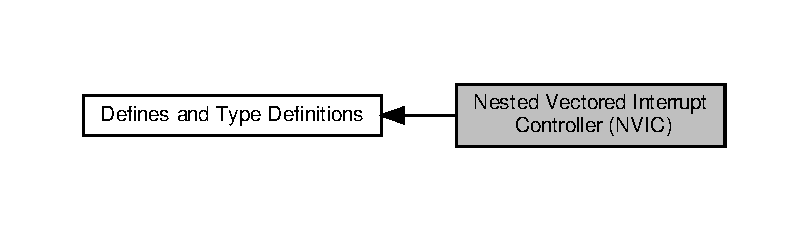
\includegraphics[width=350pt]{group___c_m_s_i_s___n_v_i_c}
\end{center}
\end{figure}
\subsection*{Komponenty}
\begin{DoxyCompactItemize}
\item 
struct \hyperlink{struct_n_v_i_c___type}{N\+V\+I\+C\+\_\+\+Type}
\begin{DoxyCompactList}\small\item\em Structure type to access the Nested Vectored Interrupt Controller (N\+V\+IC). \end{DoxyCompactList}\end{DoxyCompactItemize}
\subsection*{Definicje}
\begin{DoxyCompactItemize}
\item 
\#define \hyperlink{group___c_m_s_i_s___n_v_i_c_ga9eebe495e2e48d302211108837a2b3e8}{N\+V\+I\+C\+\_\+\+S\+T\+I\+R\+\_\+\+I\+N\+T\+I\+D\+\_\+\+Pos}~0U
\item 
\#define \hyperlink{group___c_m_s_i_s___n_v_i_c_gae4060c4dfcebb08871ca4244176ce752}{N\+V\+I\+C\+\_\+\+S\+T\+I\+R\+\_\+\+I\+N\+T\+I\+D\+\_\+\+Msk}~(0x1\+F\+F\+U\+L /$\ast$$<$$<$ N\+V\+I\+C\+\_\+\+S\+T\+I\+R\+\_\+\+I\+N\+T\+I\+D\+\_\+\+Pos$\ast$/)
\item 
\#define \hyperlink{group___c_m_s_i_s___n_v_i_c_ga9eebe495e2e48d302211108837a2b3e8}{N\+V\+I\+C\+\_\+\+S\+T\+I\+R\+\_\+\+I\+N\+T\+I\+D\+\_\+\+Pos}~0U
\item 
\#define \hyperlink{group___c_m_s_i_s___n_v_i_c_gae4060c4dfcebb08871ca4244176ce752}{N\+V\+I\+C\+\_\+\+S\+T\+I\+R\+\_\+\+I\+N\+T\+I\+D\+\_\+\+Msk}~(0x1\+F\+F\+U\+L /$\ast$$<$$<$ N\+V\+I\+C\+\_\+\+S\+T\+I\+R\+\_\+\+I\+N\+T\+I\+D\+\_\+\+Pos$\ast$/)
\item 
\#define \hyperlink{group___c_m_s_i_s___n_v_i_c_ga9eebe495e2e48d302211108837a2b3e8}{N\+V\+I\+C\+\_\+\+S\+T\+I\+R\+\_\+\+I\+N\+T\+I\+D\+\_\+\+Pos}~0U
\item 
\#define \hyperlink{group___c_m_s_i_s___n_v_i_c_gae4060c4dfcebb08871ca4244176ce752}{N\+V\+I\+C\+\_\+\+S\+T\+I\+R\+\_\+\+I\+N\+T\+I\+D\+\_\+\+Msk}~(0x1\+F\+F\+U\+L /$\ast$$<$$<$ N\+V\+I\+C\+\_\+\+S\+T\+I\+R\+\_\+\+I\+N\+T\+I\+D\+\_\+\+Pos$\ast$/)
\item 
\#define \hyperlink{group___c_m_s_i_s___n_v_i_c_ga9eebe495e2e48d302211108837a2b3e8}{N\+V\+I\+C\+\_\+\+S\+T\+I\+R\+\_\+\+I\+N\+T\+I\+D\+\_\+\+Pos}~0U
\item 
\#define \hyperlink{group___c_m_s_i_s___n_v_i_c_gae4060c4dfcebb08871ca4244176ce752}{N\+V\+I\+C\+\_\+\+S\+T\+I\+R\+\_\+\+I\+N\+T\+I\+D\+\_\+\+Msk}~(0x1\+F\+F\+U\+L /$\ast$$<$$<$ N\+V\+I\+C\+\_\+\+S\+T\+I\+R\+\_\+\+I\+N\+T\+I\+D\+\_\+\+Pos$\ast$/)
\item 
\#define \hyperlink{group___c_m_s_i_s___n_v_i_c_ga9eebe495e2e48d302211108837a2b3e8}{N\+V\+I\+C\+\_\+\+S\+T\+I\+R\+\_\+\+I\+N\+T\+I\+D\+\_\+\+Pos}~0U
\item 
\#define \hyperlink{group___c_m_s_i_s___n_v_i_c_gae4060c4dfcebb08871ca4244176ce752}{N\+V\+I\+C\+\_\+\+S\+T\+I\+R\+\_\+\+I\+N\+T\+I\+D\+\_\+\+Msk}~(0x1\+F\+F\+U\+L /$\ast$$<$$<$ N\+V\+I\+C\+\_\+\+S\+T\+I\+R\+\_\+\+I\+N\+T\+I\+D\+\_\+\+Pos$\ast$/)
\item 
\#define \hyperlink{group___c_m_s_i_s___n_v_i_c_ga9eebe495e2e48d302211108837a2b3e8}{N\+V\+I\+C\+\_\+\+S\+T\+I\+R\+\_\+\+I\+N\+T\+I\+D\+\_\+\+Pos}~0U
\item 
\#define \hyperlink{group___c_m_s_i_s___n_v_i_c_gae4060c4dfcebb08871ca4244176ce752}{N\+V\+I\+C\+\_\+\+S\+T\+I\+R\+\_\+\+I\+N\+T\+I\+D\+\_\+\+Msk}~(0x1\+F\+F\+U\+L /$\ast$$<$$<$ N\+V\+I\+C\+\_\+\+S\+T\+I\+R\+\_\+\+I\+N\+T\+I\+D\+\_\+\+Pos$\ast$/)
\end{DoxyCompactItemize}


\subsection{Opis szczegółowy}
Type definitions for the N\+V\+IC Registers. 



\subsection{Dokumentacja definicji}
\mbox{\Hypertarget{group___c_m_s_i_s___n_v_i_c_gae4060c4dfcebb08871ca4244176ce752}\label{group___c_m_s_i_s___n_v_i_c_gae4060c4dfcebb08871ca4244176ce752}} 
\index{Nested Vectored Interrupt Controller (\+N\+V\+I\+C)@{Nested Vectored Interrupt Controller (\+N\+V\+I\+C)}!N\+V\+I\+C\+\_\+\+S\+T\+I\+R\+\_\+\+I\+N\+T\+I\+D\+\_\+\+Msk@{N\+V\+I\+C\+\_\+\+S\+T\+I\+R\+\_\+\+I\+N\+T\+I\+D\+\_\+\+Msk}}
\index{N\+V\+I\+C\+\_\+\+S\+T\+I\+R\+\_\+\+I\+N\+T\+I\+D\+\_\+\+Msk@{N\+V\+I\+C\+\_\+\+S\+T\+I\+R\+\_\+\+I\+N\+T\+I\+D\+\_\+\+Msk}!Nested Vectored Interrupt Controller (\+N\+V\+I\+C)@{Nested Vectored Interrupt Controller (\+N\+V\+I\+C)}}
\subsubsection{\texorpdfstring{N\+V\+I\+C\+\_\+\+S\+T\+I\+R\+\_\+\+I\+N\+T\+I\+D\+\_\+\+Msk}{NVIC\_STIR\_INTID\_Msk}\hspace{0.1cm}{\footnotesize\ttfamily [1/6]}}
{\footnotesize\ttfamily \#define N\+V\+I\+C\+\_\+\+S\+T\+I\+R\+\_\+\+I\+N\+T\+I\+D\+\_\+\+Msk~(0x1\+F\+F\+U\+L /$\ast$$<$$<$ N\+V\+I\+C\+\_\+\+S\+T\+I\+R\+\_\+\+I\+N\+T\+I\+D\+\_\+\+Pos$\ast$/)}

S\+T\+IR\+: I\+N\+T\+L\+I\+N\+E\+S\+N\+UM Mask 

Definicja w linii 359 pliku core\+\_\+cm3.\+h.

\mbox{\Hypertarget{group___c_m_s_i_s___n_v_i_c_gae4060c4dfcebb08871ca4244176ce752}\label{group___c_m_s_i_s___n_v_i_c_gae4060c4dfcebb08871ca4244176ce752}} 
\index{Nested Vectored Interrupt Controller (\+N\+V\+I\+C)@{Nested Vectored Interrupt Controller (\+N\+V\+I\+C)}!N\+V\+I\+C\+\_\+\+S\+T\+I\+R\+\_\+\+I\+N\+T\+I\+D\+\_\+\+Msk@{N\+V\+I\+C\+\_\+\+S\+T\+I\+R\+\_\+\+I\+N\+T\+I\+D\+\_\+\+Msk}}
\index{N\+V\+I\+C\+\_\+\+S\+T\+I\+R\+\_\+\+I\+N\+T\+I\+D\+\_\+\+Msk@{N\+V\+I\+C\+\_\+\+S\+T\+I\+R\+\_\+\+I\+N\+T\+I\+D\+\_\+\+Msk}!Nested Vectored Interrupt Controller (\+N\+V\+I\+C)@{Nested Vectored Interrupt Controller (\+N\+V\+I\+C)}}
\subsubsection{\texorpdfstring{N\+V\+I\+C\+\_\+\+S\+T\+I\+R\+\_\+\+I\+N\+T\+I\+D\+\_\+\+Msk}{NVIC\_STIR\_INTID\_Msk}\hspace{0.1cm}{\footnotesize\ttfamily [2/6]}}
{\footnotesize\ttfamily \#define N\+V\+I\+C\+\_\+\+S\+T\+I\+R\+\_\+\+I\+N\+T\+I\+D\+\_\+\+Msk~(0x1\+F\+F\+U\+L /$\ast$$<$$<$ N\+V\+I\+C\+\_\+\+S\+T\+I\+R\+\_\+\+I\+N\+T\+I\+D\+\_\+\+Pos$\ast$/)}

S\+T\+IR\+: I\+N\+T\+L\+I\+N\+E\+S\+N\+UM Mask 

Definicja w linii 359 pliku core\+\_\+sc300.\+h.

\mbox{\Hypertarget{group___c_m_s_i_s___n_v_i_c_gae4060c4dfcebb08871ca4244176ce752}\label{group___c_m_s_i_s___n_v_i_c_gae4060c4dfcebb08871ca4244176ce752}} 
\index{Nested Vectored Interrupt Controller (\+N\+V\+I\+C)@{Nested Vectored Interrupt Controller (\+N\+V\+I\+C)}!N\+V\+I\+C\+\_\+\+S\+T\+I\+R\+\_\+\+I\+N\+T\+I\+D\+\_\+\+Msk@{N\+V\+I\+C\+\_\+\+S\+T\+I\+R\+\_\+\+I\+N\+T\+I\+D\+\_\+\+Msk}}
\index{N\+V\+I\+C\+\_\+\+S\+T\+I\+R\+\_\+\+I\+N\+T\+I\+D\+\_\+\+Msk@{N\+V\+I\+C\+\_\+\+S\+T\+I\+R\+\_\+\+I\+N\+T\+I\+D\+\_\+\+Msk}!Nested Vectored Interrupt Controller (\+N\+V\+I\+C)@{Nested Vectored Interrupt Controller (\+N\+V\+I\+C)}}
\subsubsection{\texorpdfstring{N\+V\+I\+C\+\_\+\+S\+T\+I\+R\+\_\+\+I\+N\+T\+I\+D\+\_\+\+Msk}{NVIC\_STIR\_INTID\_Msk}\hspace{0.1cm}{\footnotesize\ttfamily [3/6]}}
{\footnotesize\ttfamily \#define N\+V\+I\+C\+\_\+\+S\+T\+I\+R\+\_\+\+I\+N\+T\+I\+D\+\_\+\+Msk~(0x1\+F\+F\+U\+L /$\ast$$<$$<$ N\+V\+I\+C\+\_\+\+S\+T\+I\+R\+\_\+\+I\+N\+T\+I\+D\+\_\+\+Pos$\ast$/)}

S\+T\+IR\+: I\+N\+T\+L\+I\+N\+E\+S\+N\+UM Mask 

Definicja w linii 425 pliku core\+\_\+cm4.\+h.

\mbox{\Hypertarget{group___c_m_s_i_s___n_v_i_c_gae4060c4dfcebb08871ca4244176ce752}\label{group___c_m_s_i_s___n_v_i_c_gae4060c4dfcebb08871ca4244176ce752}} 
\index{Nested Vectored Interrupt Controller (\+N\+V\+I\+C)@{Nested Vectored Interrupt Controller (\+N\+V\+I\+C)}!N\+V\+I\+C\+\_\+\+S\+T\+I\+R\+\_\+\+I\+N\+T\+I\+D\+\_\+\+Msk@{N\+V\+I\+C\+\_\+\+S\+T\+I\+R\+\_\+\+I\+N\+T\+I\+D\+\_\+\+Msk}}
\index{N\+V\+I\+C\+\_\+\+S\+T\+I\+R\+\_\+\+I\+N\+T\+I\+D\+\_\+\+Msk@{N\+V\+I\+C\+\_\+\+S\+T\+I\+R\+\_\+\+I\+N\+T\+I\+D\+\_\+\+Msk}!Nested Vectored Interrupt Controller (\+N\+V\+I\+C)@{Nested Vectored Interrupt Controller (\+N\+V\+I\+C)}}
\subsubsection{\texorpdfstring{N\+V\+I\+C\+\_\+\+S\+T\+I\+R\+\_\+\+I\+N\+T\+I\+D\+\_\+\+Msk}{NVIC\_STIR\_INTID\_Msk}\hspace{0.1cm}{\footnotesize\ttfamily [4/6]}}
{\footnotesize\ttfamily \#define N\+V\+I\+C\+\_\+\+S\+T\+I\+R\+\_\+\+I\+N\+T\+I\+D\+\_\+\+Msk~(0x1\+F\+F\+U\+L /$\ast$$<$$<$ N\+V\+I\+C\+\_\+\+S\+T\+I\+R\+\_\+\+I\+N\+T\+I\+D\+\_\+\+Pos$\ast$/)}

S\+T\+IR\+: I\+N\+T\+L\+I\+N\+E\+S\+N\+UM Mask 

Definicja w linii 440 pliku core\+\_\+cm7.\+h.

\mbox{\Hypertarget{group___c_m_s_i_s___n_v_i_c_gae4060c4dfcebb08871ca4244176ce752}\label{group___c_m_s_i_s___n_v_i_c_gae4060c4dfcebb08871ca4244176ce752}} 
\index{Nested Vectored Interrupt Controller (\+N\+V\+I\+C)@{Nested Vectored Interrupt Controller (\+N\+V\+I\+C)}!N\+V\+I\+C\+\_\+\+S\+T\+I\+R\+\_\+\+I\+N\+T\+I\+D\+\_\+\+Msk@{N\+V\+I\+C\+\_\+\+S\+T\+I\+R\+\_\+\+I\+N\+T\+I\+D\+\_\+\+Msk}}
\index{N\+V\+I\+C\+\_\+\+S\+T\+I\+R\+\_\+\+I\+N\+T\+I\+D\+\_\+\+Msk@{N\+V\+I\+C\+\_\+\+S\+T\+I\+R\+\_\+\+I\+N\+T\+I\+D\+\_\+\+Msk}!Nested Vectored Interrupt Controller (\+N\+V\+I\+C)@{Nested Vectored Interrupt Controller (\+N\+V\+I\+C)}}
\subsubsection{\texorpdfstring{N\+V\+I\+C\+\_\+\+S\+T\+I\+R\+\_\+\+I\+N\+T\+I\+D\+\_\+\+Msk}{NVIC\_STIR\_INTID\_Msk}\hspace{0.1cm}{\footnotesize\ttfamily [5/6]}}
{\footnotesize\ttfamily \#define N\+V\+I\+C\+\_\+\+S\+T\+I\+R\+\_\+\+I\+N\+T\+I\+D\+\_\+\+Msk~(0x1\+F\+F\+U\+L /$\ast$$<$$<$ N\+V\+I\+C\+\_\+\+S\+T\+I\+R\+\_\+\+I\+N\+T\+I\+D\+\_\+\+Pos$\ast$/)}

S\+T\+IR\+: I\+N\+T\+L\+I\+N\+E\+S\+N\+UM Mask 

Definicja w linii 482 pliku core\+\_\+armv8mml.\+h.

\mbox{\Hypertarget{group___c_m_s_i_s___n_v_i_c_gae4060c4dfcebb08871ca4244176ce752}\label{group___c_m_s_i_s___n_v_i_c_gae4060c4dfcebb08871ca4244176ce752}} 
\index{Nested Vectored Interrupt Controller (\+N\+V\+I\+C)@{Nested Vectored Interrupt Controller (\+N\+V\+I\+C)}!N\+V\+I\+C\+\_\+\+S\+T\+I\+R\+\_\+\+I\+N\+T\+I\+D\+\_\+\+Msk@{N\+V\+I\+C\+\_\+\+S\+T\+I\+R\+\_\+\+I\+N\+T\+I\+D\+\_\+\+Msk}}
\index{N\+V\+I\+C\+\_\+\+S\+T\+I\+R\+\_\+\+I\+N\+T\+I\+D\+\_\+\+Msk@{N\+V\+I\+C\+\_\+\+S\+T\+I\+R\+\_\+\+I\+N\+T\+I\+D\+\_\+\+Msk}!Nested Vectored Interrupt Controller (\+N\+V\+I\+C)@{Nested Vectored Interrupt Controller (\+N\+V\+I\+C)}}
\subsubsection{\texorpdfstring{N\+V\+I\+C\+\_\+\+S\+T\+I\+R\+\_\+\+I\+N\+T\+I\+D\+\_\+\+Msk}{NVIC\_STIR\_INTID\_Msk}\hspace{0.1cm}{\footnotesize\ttfamily [6/6]}}
{\footnotesize\ttfamily \#define N\+V\+I\+C\+\_\+\+S\+T\+I\+R\+\_\+\+I\+N\+T\+I\+D\+\_\+\+Msk~(0x1\+F\+F\+U\+L /$\ast$$<$$<$ N\+V\+I\+C\+\_\+\+S\+T\+I\+R\+\_\+\+I\+N\+T\+I\+D\+\_\+\+Pos$\ast$/)}

S\+T\+IR\+: I\+N\+T\+L\+I\+N\+E\+S\+N\+UM Mask 

Definicja w linii 482 pliku core\+\_\+cm33.\+h.

\mbox{\Hypertarget{group___c_m_s_i_s___n_v_i_c_ga9eebe495e2e48d302211108837a2b3e8}\label{group___c_m_s_i_s___n_v_i_c_ga9eebe495e2e48d302211108837a2b3e8}} 
\index{Nested Vectored Interrupt Controller (\+N\+V\+I\+C)@{Nested Vectored Interrupt Controller (\+N\+V\+I\+C)}!N\+V\+I\+C\+\_\+\+S\+T\+I\+R\+\_\+\+I\+N\+T\+I\+D\+\_\+\+Pos@{N\+V\+I\+C\+\_\+\+S\+T\+I\+R\+\_\+\+I\+N\+T\+I\+D\+\_\+\+Pos}}
\index{N\+V\+I\+C\+\_\+\+S\+T\+I\+R\+\_\+\+I\+N\+T\+I\+D\+\_\+\+Pos@{N\+V\+I\+C\+\_\+\+S\+T\+I\+R\+\_\+\+I\+N\+T\+I\+D\+\_\+\+Pos}!Nested Vectored Interrupt Controller (\+N\+V\+I\+C)@{Nested Vectored Interrupt Controller (\+N\+V\+I\+C)}}
\subsubsection{\texorpdfstring{N\+V\+I\+C\+\_\+\+S\+T\+I\+R\+\_\+\+I\+N\+T\+I\+D\+\_\+\+Pos}{NVIC\_STIR\_INTID\_Pos}\hspace{0.1cm}{\footnotesize\ttfamily [1/6]}}
{\footnotesize\ttfamily \#define N\+V\+I\+C\+\_\+\+S\+T\+I\+R\+\_\+\+I\+N\+T\+I\+D\+\_\+\+Pos~0U}

S\+T\+IR\+: I\+N\+T\+L\+I\+N\+E\+S\+N\+UM Position 

Definicja w linii 358 pliku core\+\_\+sc300.\+h.

\mbox{\Hypertarget{group___c_m_s_i_s___n_v_i_c_ga9eebe495e2e48d302211108837a2b3e8}\label{group___c_m_s_i_s___n_v_i_c_ga9eebe495e2e48d302211108837a2b3e8}} 
\index{Nested Vectored Interrupt Controller (\+N\+V\+I\+C)@{Nested Vectored Interrupt Controller (\+N\+V\+I\+C)}!N\+V\+I\+C\+\_\+\+S\+T\+I\+R\+\_\+\+I\+N\+T\+I\+D\+\_\+\+Pos@{N\+V\+I\+C\+\_\+\+S\+T\+I\+R\+\_\+\+I\+N\+T\+I\+D\+\_\+\+Pos}}
\index{N\+V\+I\+C\+\_\+\+S\+T\+I\+R\+\_\+\+I\+N\+T\+I\+D\+\_\+\+Pos@{N\+V\+I\+C\+\_\+\+S\+T\+I\+R\+\_\+\+I\+N\+T\+I\+D\+\_\+\+Pos}!Nested Vectored Interrupt Controller (\+N\+V\+I\+C)@{Nested Vectored Interrupt Controller (\+N\+V\+I\+C)}}
\subsubsection{\texorpdfstring{N\+V\+I\+C\+\_\+\+S\+T\+I\+R\+\_\+\+I\+N\+T\+I\+D\+\_\+\+Pos}{NVIC\_STIR\_INTID\_Pos}\hspace{0.1cm}{\footnotesize\ttfamily [2/6]}}
{\footnotesize\ttfamily \#define N\+V\+I\+C\+\_\+\+S\+T\+I\+R\+\_\+\+I\+N\+T\+I\+D\+\_\+\+Pos~0U}

S\+T\+IR\+: I\+N\+T\+L\+I\+N\+E\+S\+N\+UM Position 

Definicja w linii 358 pliku core\+\_\+cm3.\+h.

\mbox{\Hypertarget{group___c_m_s_i_s___n_v_i_c_ga9eebe495e2e48d302211108837a2b3e8}\label{group___c_m_s_i_s___n_v_i_c_ga9eebe495e2e48d302211108837a2b3e8}} 
\index{Nested Vectored Interrupt Controller (\+N\+V\+I\+C)@{Nested Vectored Interrupt Controller (\+N\+V\+I\+C)}!N\+V\+I\+C\+\_\+\+S\+T\+I\+R\+\_\+\+I\+N\+T\+I\+D\+\_\+\+Pos@{N\+V\+I\+C\+\_\+\+S\+T\+I\+R\+\_\+\+I\+N\+T\+I\+D\+\_\+\+Pos}}
\index{N\+V\+I\+C\+\_\+\+S\+T\+I\+R\+\_\+\+I\+N\+T\+I\+D\+\_\+\+Pos@{N\+V\+I\+C\+\_\+\+S\+T\+I\+R\+\_\+\+I\+N\+T\+I\+D\+\_\+\+Pos}!Nested Vectored Interrupt Controller (\+N\+V\+I\+C)@{Nested Vectored Interrupt Controller (\+N\+V\+I\+C)}}
\subsubsection{\texorpdfstring{N\+V\+I\+C\+\_\+\+S\+T\+I\+R\+\_\+\+I\+N\+T\+I\+D\+\_\+\+Pos}{NVIC\_STIR\_INTID\_Pos}\hspace{0.1cm}{\footnotesize\ttfamily [3/6]}}
{\footnotesize\ttfamily \#define N\+V\+I\+C\+\_\+\+S\+T\+I\+R\+\_\+\+I\+N\+T\+I\+D\+\_\+\+Pos~0U}

S\+T\+IR\+: I\+N\+T\+L\+I\+N\+E\+S\+N\+UM Position 

Definicja w linii 424 pliku core\+\_\+cm4.\+h.

\mbox{\Hypertarget{group___c_m_s_i_s___n_v_i_c_ga9eebe495e2e48d302211108837a2b3e8}\label{group___c_m_s_i_s___n_v_i_c_ga9eebe495e2e48d302211108837a2b3e8}} 
\index{Nested Vectored Interrupt Controller (\+N\+V\+I\+C)@{Nested Vectored Interrupt Controller (\+N\+V\+I\+C)}!N\+V\+I\+C\+\_\+\+S\+T\+I\+R\+\_\+\+I\+N\+T\+I\+D\+\_\+\+Pos@{N\+V\+I\+C\+\_\+\+S\+T\+I\+R\+\_\+\+I\+N\+T\+I\+D\+\_\+\+Pos}}
\index{N\+V\+I\+C\+\_\+\+S\+T\+I\+R\+\_\+\+I\+N\+T\+I\+D\+\_\+\+Pos@{N\+V\+I\+C\+\_\+\+S\+T\+I\+R\+\_\+\+I\+N\+T\+I\+D\+\_\+\+Pos}!Nested Vectored Interrupt Controller (\+N\+V\+I\+C)@{Nested Vectored Interrupt Controller (\+N\+V\+I\+C)}}
\subsubsection{\texorpdfstring{N\+V\+I\+C\+\_\+\+S\+T\+I\+R\+\_\+\+I\+N\+T\+I\+D\+\_\+\+Pos}{NVIC\_STIR\_INTID\_Pos}\hspace{0.1cm}{\footnotesize\ttfamily [4/6]}}
{\footnotesize\ttfamily \#define N\+V\+I\+C\+\_\+\+S\+T\+I\+R\+\_\+\+I\+N\+T\+I\+D\+\_\+\+Pos~0U}

S\+T\+IR\+: I\+N\+T\+L\+I\+N\+E\+S\+N\+UM Position 

Definicja w linii 439 pliku core\+\_\+cm7.\+h.

\mbox{\Hypertarget{group___c_m_s_i_s___n_v_i_c_ga9eebe495e2e48d302211108837a2b3e8}\label{group___c_m_s_i_s___n_v_i_c_ga9eebe495e2e48d302211108837a2b3e8}} 
\index{Nested Vectored Interrupt Controller (\+N\+V\+I\+C)@{Nested Vectored Interrupt Controller (\+N\+V\+I\+C)}!N\+V\+I\+C\+\_\+\+S\+T\+I\+R\+\_\+\+I\+N\+T\+I\+D\+\_\+\+Pos@{N\+V\+I\+C\+\_\+\+S\+T\+I\+R\+\_\+\+I\+N\+T\+I\+D\+\_\+\+Pos}}
\index{N\+V\+I\+C\+\_\+\+S\+T\+I\+R\+\_\+\+I\+N\+T\+I\+D\+\_\+\+Pos@{N\+V\+I\+C\+\_\+\+S\+T\+I\+R\+\_\+\+I\+N\+T\+I\+D\+\_\+\+Pos}!Nested Vectored Interrupt Controller (\+N\+V\+I\+C)@{Nested Vectored Interrupt Controller (\+N\+V\+I\+C)}}
\subsubsection{\texorpdfstring{N\+V\+I\+C\+\_\+\+S\+T\+I\+R\+\_\+\+I\+N\+T\+I\+D\+\_\+\+Pos}{NVIC\_STIR\_INTID\_Pos}\hspace{0.1cm}{\footnotesize\ttfamily [5/6]}}
{\footnotesize\ttfamily \#define N\+V\+I\+C\+\_\+\+S\+T\+I\+R\+\_\+\+I\+N\+T\+I\+D\+\_\+\+Pos~0U}

S\+T\+IR\+: I\+N\+T\+L\+I\+N\+E\+S\+N\+UM Position 

Definicja w linii 481 pliku core\+\_\+armv8mml.\+h.

\mbox{\Hypertarget{group___c_m_s_i_s___n_v_i_c_ga9eebe495e2e48d302211108837a2b3e8}\label{group___c_m_s_i_s___n_v_i_c_ga9eebe495e2e48d302211108837a2b3e8}} 
\index{Nested Vectored Interrupt Controller (\+N\+V\+I\+C)@{Nested Vectored Interrupt Controller (\+N\+V\+I\+C)}!N\+V\+I\+C\+\_\+\+S\+T\+I\+R\+\_\+\+I\+N\+T\+I\+D\+\_\+\+Pos@{N\+V\+I\+C\+\_\+\+S\+T\+I\+R\+\_\+\+I\+N\+T\+I\+D\+\_\+\+Pos}}
\index{N\+V\+I\+C\+\_\+\+S\+T\+I\+R\+\_\+\+I\+N\+T\+I\+D\+\_\+\+Pos@{N\+V\+I\+C\+\_\+\+S\+T\+I\+R\+\_\+\+I\+N\+T\+I\+D\+\_\+\+Pos}!Nested Vectored Interrupt Controller (\+N\+V\+I\+C)@{Nested Vectored Interrupt Controller (\+N\+V\+I\+C)}}
\subsubsection{\texorpdfstring{N\+V\+I\+C\+\_\+\+S\+T\+I\+R\+\_\+\+I\+N\+T\+I\+D\+\_\+\+Pos}{NVIC\_STIR\_INTID\_Pos}\hspace{0.1cm}{\footnotesize\ttfamily [6/6]}}
{\footnotesize\ttfamily \#define N\+V\+I\+C\+\_\+\+S\+T\+I\+R\+\_\+\+I\+N\+T\+I\+D\+\_\+\+Pos~0U}

S\+T\+IR\+: I\+N\+T\+L\+I\+N\+E\+S\+N\+UM Position 

Definicja w linii 481 pliku core\+\_\+cm33.\+h.


\hypertarget{group___c_m_s_i_s___s_c_b}{}\section{System Control Block (S\+CB)}
\label{group___c_m_s_i_s___s_c_b}\index{System Control Block (\+S\+C\+B)@{System Control Block (\+S\+C\+B)}}


Type definitions for the System Control Block Registers.  


Diagram współpracy dla System Control Block (S\+CB)\+:\nopagebreak
\begin{figure}[H]
\begin{center}
\leavevmode
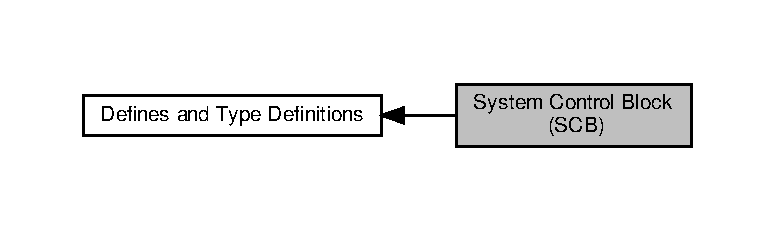
\includegraphics[width=350pt]{group___c_m_s_i_s___s_c_b}
\end{center}
\end{figure}
\subsection*{Komponenty}
\begin{DoxyCompactItemize}
\item 
struct \hyperlink{struct_s_c_b___type}{S\+C\+B\+\_\+\+Type}
\begin{DoxyCompactList}\small\item\em Structure type to access the System Control Block (S\+CB). \end{DoxyCompactList}\end{DoxyCompactItemize}
\subsection*{Definicje}
\begin{DoxyCompactItemize}
\item 
\#define \hyperlink{group___c_m_s_i_s___s_c_b_ga58686b88f94f789d4e6f429fe1ff58cf}{S\+C\+B\+\_\+\+C\+P\+U\+I\+D\+\_\+\+I\+M\+P\+L\+E\+M\+E\+N\+T\+E\+R\+\_\+\+Pos}~24U
\item 
\#define \hyperlink{group___c_m_s_i_s___s_c_b_ga0932b31faafd47656a03ced75a31d99b}{S\+C\+B\+\_\+\+C\+P\+U\+I\+D\+\_\+\+I\+M\+P\+L\+E\+M\+E\+N\+T\+E\+R\+\_\+\+Msk}~(0x\+F\+F\+U\+L $<$$<$ S\+C\+B\+\_\+\+C\+P\+U\+I\+D\+\_\+\+I\+M\+P\+L\+E\+M\+E\+N\+T\+E\+R\+\_\+\+Pos)
\item 
\#define \hyperlink{group___c_m_s_i_s___s_c_b_ga104462bd0815391b4044a70bd15d3a71}{S\+C\+B\+\_\+\+C\+P\+U\+I\+D\+\_\+\+V\+A\+R\+I\+A\+N\+T\+\_\+\+Pos}~20U
\item 
\#define \hyperlink{group___c_m_s_i_s___s_c_b_gad358dfbd04300afc1824329d128b99e8}{S\+C\+B\+\_\+\+C\+P\+U\+I\+D\+\_\+\+V\+A\+R\+I\+A\+N\+T\+\_\+\+Msk}~(0x\+F\+U\+L $<$$<$ S\+C\+B\+\_\+\+C\+P\+U\+I\+D\+\_\+\+V\+A\+R\+I\+A\+N\+T\+\_\+\+Pos)
\item 
\#define \hyperlink{group___c_m_s_i_s___s_c_b_gaf8b3236b08fb8e840efb682645fb0e98}{S\+C\+B\+\_\+\+C\+P\+U\+I\+D\+\_\+\+A\+R\+C\+H\+I\+T\+E\+C\+T\+U\+R\+E\+\_\+\+Pos}~16U
\item 
\#define \hyperlink{group___c_m_s_i_s___s_c_b_gafae4a1f27a927338ae9dc51a0e146213}{S\+C\+B\+\_\+\+C\+P\+U\+I\+D\+\_\+\+A\+R\+C\+H\+I\+T\+E\+C\+T\+U\+R\+E\+\_\+\+Msk}~(0x\+F\+U\+L $<$$<$ S\+C\+B\+\_\+\+C\+P\+U\+I\+D\+\_\+\+A\+R\+C\+H\+I\+T\+E\+C\+T\+U\+R\+E\+\_\+\+Pos)
\item 
\#define \hyperlink{group___c_m_s_i_s___s_c_b_ga705f68eaa9afb042ca2407dc4e4629ac}{S\+C\+B\+\_\+\+C\+P\+U\+I\+D\+\_\+\+P\+A\+R\+T\+N\+O\+\_\+\+Pos}~4U
\item 
\#define \hyperlink{group___c_m_s_i_s___s_c_b_ga98e581423ca016680c238c469aba546d}{S\+C\+B\+\_\+\+C\+P\+U\+I\+D\+\_\+\+P\+A\+R\+T\+N\+O\+\_\+\+Msk}~(0x\+F\+F\+F\+U\+L $<$$<$ S\+C\+B\+\_\+\+C\+P\+U\+I\+D\+\_\+\+P\+A\+R\+T\+N\+O\+\_\+\+Pos)
\item 
\#define \hyperlink{group___c_m_s_i_s___s_c_b_ga3c3d9071e574de11fb27ba57034838b1}{S\+C\+B\+\_\+\+C\+P\+U\+I\+D\+\_\+\+R\+E\+V\+I\+S\+I\+O\+N\+\_\+\+Pos}~0U
\item 
\#define \hyperlink{group___c_m_s_i_s___s_c_b_ga2ec0448b6483f77e7f5d08b4b81d85df}{S\+C\+B\+\_\+\+C\+P\+U\+I\+D\+\_\+\+R\+E\+V\+I\+S\+I\+O\+N\+\_\+\+Msk}~(0x\+F\+U\+L /$\ast$$<$$<$ S\+C\+B\+\_\+\+C\+P\+U\+I\+D\+\_\+\+R\+E\+V\+I\+S\+I\+O\+N\+\_\+\+Pos$\ast$/)
\item 
\#define \hyperlink{group___c_m_s_i_s___s_c_b_gac180386fac3a5701e6060084dacd003a}{S\+C\+B\+\_\+\+I\+C\+S\+R\+\_\+\+P\+E\+N\+D\+N\+M\+I\+S\+E\+T\+\_\+\+Pos}~31U
\item 
\#define \hyperlink{group___c_m_s_i_s___s_c_b_gadb4dbf66078026dedc24e8cb9a21b2b1}{S\+C\+B\+\_\+\+I\+C\+S\+R\+\_\+\+P\+E\+N\+D\+N\+M\+I\+S\+E\+T\+\_\+\+Msk}~(1\+U\+L $<$$<$ S\+C\+B\+\_\+\+I\+C\+S\+R\+\_\+\+P\+E\+N\+D\+N\+M\+I\+S\+E\+T\+\_\+\+Pos)
\item 
\#define \hyperlink{group___c_m_s_i_s___s_c_b_ga750d4b52624a46d71356db4ea769573b}{S\+C\+B\+\_\+\+I\+C\+S\+R\+\_\+\+N\+M\+I\+P\+E\+N\+D\+S\+E\+T\+\_\+\+Pos}~\hyperlink{group___c_m_s_i_s___s_c_b_gac180386fac3a5701e6060084dacd003a}{S\+C\+B\+\_\+\+I\+C\+S\+R\+\_\+\+P\+E\+N\+D\+N\+M\+I\+S\+E\+T\+\_\+\+Pos}
\item 
\#define \hyperlink{group___c_m_s_i_s___s_c_b_ga340e3f79e9c3607dee9f2c048b6b22e8}{S\+C\+B\+\_\+\+I\+C\+S\+R\+\_\+\+N\+M\+I\+P\+E\+N\+D\+S\+E\+T\+\_\+\+Msk}~\hyperlink{group___c_m_s_i_s___s_c_b_gadb4dbf66078026dedc24e8cb9a21b2b1}{S\+C\+B\+\_\+\+I\+C\+S\+R\+\_\+\+P\+E\+N\+D\+N\+M\+I\+S\+E\+T\+\_\+\+Msk}
\item 
\#define \hyperlink{group___c_m_s_i_s___s_c_b_gad4c1ddde49ff0d3ed1b843d14d38ebf1}{S\+C\+B\+\_\+\+I\+C\+S\+R\+\_\+\+P\+E\+N\+D\+N\+M\+I\+C\+L\+R\+\_\+\+Pos}~30U
\item 
\#define \hyperlink{group___c_m_s_i_s___s_c_b_gace870429ae27601613da7c6f6e53a18f}{S\+C\+B\+\_\+\+I\+C\+S\+R\+\_\+\+P\+E\+N\+D\+N\+M\+I\+C\+L\+R\+\_\+\+Msk}~(1\+U\+L $<$$<$ S\+C\+B\+\_\+\+I\+C\+S\+R\+\_\+\+P\+E\+N\+D\+N\+M\+I\+C\+L\+R\+\_\+\+Pos)
\item 
\#define \hyperlink{group___c_m_s_i_s___s_c_b_gab5ded23d2ab1d5ff7cc7ce746205e9fe}{S\+C\+B\+\_\+\+I\+C\+S\+R\+\_\+\+P\+E\+N\+D\+S\+V\+S\+E\+T\+\_\+\+Pos}~28U
\item 
\#define \hyperlink{group___c_m_s_i_s___s_c_b_ga1e40d93efb402763c8c00ddcc56724ff}{S\+C\+B\+\_\+\+I\+C\+S\+R\+\_\+\+P\+E\+N\+D\+S\+V\+S\+E\+T\+\_\+\+Msk}~(1\+U\+L $<$$<$ S\+C\+B\+\_\+\+I\+C\+S\+R\+\_\+\+P\+E\+N\+D\+S\+V\+S\+E\+T\+\_\+\+Pos)
\item 
\#define \hyperlink{group___c_m_s_i_s___s_c_b_gae218d9022288f89faf57187c4d542ecd}{S\+C\+B\+\_\+\+I\+C\+S\+R\+\_\+\+P\+E\+N\+D\+S\+V\+C\+L\+R\+\_\+\+Pos}~27U
\item 
\#define \hyperlink{group___c_m_s_i_s___s_c_b_ga4a901ace381d3c1c74ac82b22fae2e1e}{S\+C\+B\+\_\+\+I\+C\+S\+R\+\_\+\+P\+E\+N\+D\+S\+V\+C\+L\+R\+\_\+\+Msk}~(1\+U\+L $<$$<$ S\+C\+B\+\_\+\+I\+C\+S\+R\+\_\+\+P\+E\+N\+D\+S\+V\+C\+L\+R\+\_\+\+Pos)
\item 
\#define \hyperlink{group___c_m_s_i_s___s_c_b_ga9dbb3358c6167c9c3f85661b90fb2794}{S\+C\+B\+\_\+\+I\+C\+S\+R\+\_\+\+P\+E\+N\+D\+S\+T\+S\+E\+T\+\_\+\+Pos}~26U
\item 
\#define \hyperlink{group___c_m_s_i_s___s_c_b_ga7325b61ea0ec323ef2d5c893b112e546}{S\+C\+B\+\_\+\+I\+C\+S\+R\+\_\+\+P\+E\+N\+D\+S\+T\+S\+E\+T\+\_\+\+Msk}~(1\+U\+L $<$$<$ S\+C\+B\+\_\+\+I\+C\+S\+R\+\_\+\+P\+E\+N\+D\+S\+T\+S\+E\+T\+\_\+\+Pos)
\item 
\#define \hyperlink{group___c_m_s_i_s___s_c_b_gadbe25e4b333ece1341beb1a740168fdc}{S\+C\+B\+\_\+\+I\+C\+S\+R\+\_\+\+P\+E\+N\+D\+S\+T\+C\+L\+R\+\_\+\+Pos}~25U
\item 
\#define \hyperlink{group___c_m_s_i_s___s_c_b_gab241827d2a793269d8cd99b9b28c2157}{S\+C\+B\+\_\+\+I\+C\+S\+R\+\_\+\+P\+E\+N\+D\+S\+T\+C\+L\+R\+\_\+\+Msk}~(1\+U\+L $<$$<$ S\+C\+B\+\_\+\+I\+C\+S\+R\+\_\+\+P\+E\+N\+D\+S\+T\+C\+L\+R\+\_\+\+Pos)
\item 
\#define \hyperlink{group___c_m_s_i_s___s_c_b_ga021591700b2d6a6e332d932efaece42b}{S\+C\+B\+\_\+\+I\+C\+S\+R\+\_\+\+S\+T\+T\+N\+S\+\_\+\+Pos}~24U
\item 
\#define \hyperlink{group___c_m_s_i_s___s_c_b_ga70404175bcf7f329758829a9888e48c4}{S\+C\+B\+\_\+\+I\+C\+S\+R\+\_\+\+S\+T\+T\+N\+S\+\_\+\+Msk}~(1\+U\+L $<$$<$ S\+C\+B\+\_\+\+I\+C\+S\+R\+\_\+\+S\+T\+T\+N\+S\+\_\+\+Pos)
\item 
\#define \hyperlink{group___c_m_s_i_s___s_c_b_ga11cb5b1f9ce167b81f31787a77e575df}{S\+C\+B\+\_\+\+I\+C\+S\+R\+\_\+\+I\+S\+R\+P\+R\+E\+E\+M\+P\+T\+\_\+\+Pos}~23U
\item 
\#define \hyperlink{group___c_m_s_i_s___s_c_b_gaa966600396290808d596fe96e92ca2b5}{S\+C\+B\+\_\+\+I\+C\+S\+R\+\_\+\+I\+S\+R\+P\+R\+E\+E\+M\+P\+T\+\_\+\+Msk}~(1\+U\+L $<$$<$ S\+C\+B\+\_\+\+I\+C\+S\+R\+\_\+\+I\+S\+R\+P\+R\+E\+E\+M\+P\+T\+\_\+\+Pos)
\item 
\#define \hyperlink{group___c_m_s_i_s___s_c_b_ga10749d92b9b744094b845c2eb46d4319}{S\+C\+B\+\_\+\+I\+C\+S\+R\+\_\+\+I\+S\+R\+P\+E\+N\+D\+I\+N\+G\+\_\+\+Pos}~22U
\item 
\#define \hyperlink{group___c_m_s_i_s___s_c_b_ga056d74fd538e5d36d3be1f28d399c877}{S\+C\+B\+\_\+\+I\+C\+S\+R\+\_\+\+I\+S\+R\+P\+E\+N\+D\+I\+N\+G\+\_\+\+Msk}~(1\+U\+L $<$$<$ S\+C\+B\+\_\+\+I\+C\+S\+R\+\_\+\+I\+S\+R\+P\+E\+N\+D\+I\+N\+G\+\_\+\+Pos)
\item 
\#define \hyperlink{group___c_m_s_i_s___s_c_b_gada60c92bf88d6fd21a8f49efa4a127b8}{S\+C\+B\+\_\+\+I\+C\+S\+R\+\_\+\+V\+E\+C\+T\+P\+E\+N\+D\+I\+N\+G\+\_\+\+Pos}~12U
\item 
\#define \hyperlink{group___c_m_s_i_s___s_c_b_gacb6992e7c7ddc27a370f62878a21ef72}{S\+C\+B\+\_\+\+I\+C\+S\+R\+\_\+\+V\+E\+C\+T\+P\+E\+N\+D\+I\+N\+G\+\_\+\+Msk}~(0x1\+F\+F\+U\+L $<$$<$ S\+C\+B\+\_\+\+I\+C\+S\+R\+\_\+\+V\+E\+C\+T\+P\+E\+N\+D\+I\+N\+G\+\_\+\+Pos)
\item 
\#define \hyperlink{group___c_m_s_i_s___s_c_b_ga403d154200242629e6d2764bfc12a7ec}{S\+C\+B\+\_\+\+I\+C\+S\+R\+\_\+\+R\+E\+T\+T\+O\+B\+A\+S\+E\+\_\+\+Pos}~11U
\item 
\#define \hyperlink{group___c_m_s_i_s___s_c_b_gaca6fc3f79bb550f64fd7df782ed4a5f6}{S\+C\+B\+\_\+\+I\+C\+S\+R\+\_\+\+R\+E\+T\+T\+O\+B\+A\+S\+E\+\_\+\+Msk}~(1\+U\+L $<$$<$ S\+C\+B\+\_\+\+I\+C\+S\+R\+\_\+\+R\+E\+T\+T\+O\+B\+A\+S\+E\+\_\+\+Pos)
\item 
\#define \hyperlink{group___c_m_s_i_s___s_c_b_gae4f602c7c5c895d5fb687b71b0979fc3}{S\+C\+B\+\_\+\+I\+C\+S\+R\+\_\+\+V\+E\+C\+T\+A\+C\+T\+I\+V\+E\+\_\+\+Pos}~0U
\item 
\#define \hyperlink{group___c_m_s_i_s___s_c_b_ga5533791a4ecf1b9301c883047b3e8396}{S\+C\+B\+\_\+\+I\+C\+S\+R\+\_\+\+V\+E\+C\+T\+A\+C\+T\+I\+V\+E\+\_\+\+Msk}~(0x1\+F\+F\+U\+L /$\ast$$<$$<$ S\+C\+B\+\_\+\+I\+C\+S\+R\+\_\+\+V\+E\+C\+T\+A\+C\+T\+I\+V\+E\+\_\+\+Pos$\ast$/)
\item 
\#define \hyperlink{group___c_m_s_i_s___s_c_b_gaaa27c0ba600bf82c3da08c748845b640}{S\+C\+B\+\_\+\+A\+I\+R\+C\+R\+\_\+\+V\+E\+C\+T\+K\+E\+Y\+\_\+\+Pos}~16U
\item 
\#define \hyperlink{group___c_m_s_i_s___s_c_b_ga90c7cf0c490e7ae55f9503a7fda1dd22}{S\+C\+B\+\_\+\+A\+I\+R\+C\+R\+\_\+\+V\+E\+C\+T\+K\+E\+Y\+\_\+\+Msk}~(0x\+F\+F\+F\+F\+U\+L $<$$<$ S\+C\+B\+\_\+\+A\+I\+R\+C\+R\+\_\+\+V\+E\+C\+T\+K\+E\+Y\+\_\+\+Pos)
\item 
\#define \hyperlink{group___c_m_s_i_s___s_c_b_gaec404750ff5ca07f499a3c06b62051ef}{S\+C\+B\+\_\+\+A\+I\+R\+C\+R\+\_\+\+V\+E\+C\+T\+K\+E\+Y\+S\+T\+A\+T\+\_\+\+Pos}~16U
\item 
\#define \hyperlink{group___c_m_s_i_s___s_c_b_gabacedaefeefc73d666bbe59ece904493}{S\+C\+B\+\_\+\+A\+I\+R\+C\+R\+\_\+\+V\+E\+C\+T\+K\+E\+Y\+S\+T\+A\+T\+\_\+\+Msk}~(0x\+F\+F\+F\+F\+U\+L $<$$<$ S\+C\+B\+\_\+\+A\+I\+R\+C\+R\+\_\+\+V\+E\+C\+T\+K\+E\+Y\+S\+T\+A\+T\+\_\+\+Pos)
\item 
\#define \hyperlink{group___c_m_s_i_s___s_c_b_gad31dec98fbc0d33ace63cb1f1a927923}{S\+C\+B\+\_\+\+A\+I\+R\+C\+R\+\_\+\+E\+N\+D\+I\+A\+N\+E\+S\+S\+\_\+\+Pos}~15U
\item 
\#define \hyperlink{group___c_m_s_i_s___s_c_b_ga2f571f93d3d4a6eac9a3040756d3d951}{S\+C\+B\+\_\+\+A\+I\+R\+C\+R\+\_\+\+E\+N\+D\+I\+A\+N\+E\+S\+S\+\_\+\+Msk}~(1\+U\+L $<$$<$ S\+C\+B\+\_\+\+A\+I\+R\+C\+R\+\_\+\+E\+N\+D\+I\+A\+N\+E\+S\+S\+\_\+\+Pos)
\item 
\#define \hyperlink{group___c_m_s_i_s___s_c_b_ga2590e227eedb35a41044d8fb7feb9037}{S\+C\+B\+\_\+\+A\+I\+R\+C\+R\+\_\+\+P\+R\+I\+S\+\_\+\+Pos}~14U
\item 
\#define \hyperlink{group___c_m_s_i_s___s_c_b_ga0032bb51f38e103fc34c2a57e59ada6f}{S\+C\+B\+\_\+\+A\+I\+R\+C\+R\+\_\+\+P\+R\+I\+S\+\_\+\+Msk}~(1\+U\+L $<$$<$ S\+C\+B\+\_\+\+A\+I\+R\+C\+R\+\_\+\+P\+R\+I\+S\+\_\+\+Pos)
\item 
\#define \hyperlink{group___c_m_s_i_s___s_c_b_ga94e2fc10be4f6065dcb5a7276b40d933}{S\+C\+B\+\_\+\+A\+I\+R\+C\+R\+\_\+\+B\+F\+H\+F\+N\+M\+I\+N\+S\+\_\+\+Pos}~13U
\item 
\#define \hyperlink{group___c_m_s_i_s___s_c_b_gabc24019f3b54b8d2acd23016b2e0c7b9}{S\+C\+B\+\_\+\+A\+I\+R\+C\+R\+\_\+\+B\+F\+H\+F\+N\+M\+I\+N\+S\+\_\+\+Msk}~(1\+U\+L $<$$<$ S\+C\+B\+\_\+\+A\+I\+R\+C\+R\+\_\+\+B\+F\+H\+F\+N\+M\+I\+N\+S\+\_\+\+Pos)
\item 
\#define \hyperlink{group___c_m_s_i_s___s_c_b_ga7e6b3da07caee0726c5aab97ecebc2a5}{S\+C\+B\+\_\+\+A\+I\+R\+C\+R\+\_\+\+S\+Y\+S\+R\+E\+S\+E\+T\+R\+E\+Q\+S\+\_\+\+Pos}~3U
\item 
\#define \hyperlink{group___c_m_s_i_s___s_c_b_gaf4b7fe06aaa2e87cdaf25a720dd282a1}{S\+C\+B\+\_\+\+A\+I\+R\+C\+R\+\_\+\+S\+Y\+S\+R\+E\+S\+E\+T\+R\+E\+Q\+S\+\_\+\+Msk}~(1\+U\+L $<$$<$ S\+C\+B\+\_\+\+A\+I\+R\+C\+R\+\_\+\+S\+Y\+S\+R\+E\+S\+E\+T\+R\+E\+Q\+S\+\_\+\+Pos)
\item 
\#define \hyperlink{group___c_m_s_i_s___s_c_b_gaffb2737eca1eac0fc1c282a76a40953c}{S\+C\+B\+\_\+\+A\+I\+R\+C\+R\+\_\+\+S\+Y\+S\+R\+E\+S\+E\+T\+R\+E\+Q\+\_\+\+Pos}~2U
\item 
\#define \hyperlink{group___c_m_s_i_s___s_c_b_gaae1181119559a5bd36e62afa373fa720}{S\+C\+B\+\_\+\+A\+I\+R\+C\+R\+\_\+\+S\+Y\+S\+R\+E\+S\+E\+T\+R\+E\+Q\+\_\+\+Msk}~(1\+U\+L $<$$<$ S\+C\+B\+\_\+\+A\+I\+R\+C\+R\+\_\+\+S\+Y\+S\+R\+E\+S\+E\+T\+R\+E\+Q\+\_\+\+Pos)
\item 
\#define \hyperlink{group___c_m_s_i_s___s_c_b_gaa30a12e892bb696e61626d71359a9029}{S\+C\+B\+\_\+\+A\+I\+R\+C\+R\+\_\+\+V\+E\+C\+T\+C\+L\+R\+A\+C\+T\+I\+V\+E\+\_\+\+Pos}~1U
\item 
\#define \hyperlink{group___c_m_s_i_s___s_c_b_ga212c5ab1c1c82c807d30d2307aa8d218}{S\+C\+B\+\_\+\+A\+I\+R\+C\+R\+\_\+\+V\+E\+C\+T\+C\+L\+R\+A\+C\+T\+I\+V\+E\+\_\+\+Msk}~(1\+U\+L $<$$<$ S\+C\+B\+\_\+\+A\+I\+R\+C\+R\+\_\+\+V\+E\+C\+T\+C\+L\+R\+A\+C\+T\+I\+V\+E\+\_\+\+Pos)
\item 
\#define \hyperlink{group___c_m_s_i_s___s_c_b_ga3bddcec40aeaf3d3a998446100fa0e44}{S\+C\+B\+\_\+\+S\+C\+R\+\_\+\+S\+E\+V\+O\+N\+P\+E\+N\+D\+\_\+\+Pos}~4U
\item 
\#define \hyperlink{group___c_m_s_i_s___s_c_b_gafb98656644a14342e467505f69a997c9}{S\+C\+B\+\_\+\+S\+C\+R\+\_\+\+S\+E\+V\+O\+N\+P\+E\+N\+D\+\_\+\+Msk}~(1\+U\+L $<$$<$ S\+C\+B\+\_\+\+S\+C\+R\+\_\+\+S\+E\+V\+O\+N\+P\+E\+N\+D\+\_\+\+Pos)
\item 
\#define \hyperlink{group___c_m_s_i_s___s_c_b_ga28a2c6524329e68f073b64d4fbfaba39}{S\+C\+B\+\_\+\+S\+C\+R\+\_\+\+S\+L\+E\+E\+P\+D\+E\+E\+P\+S\+\_\+\+Pos}~3U
\item 
\#define \hyperlink{group___c_m_s_i_s___s_c_b_ga7bcfa50d03c2b059ea8661f31d46fa06}{S\+C\+B\+\_\+\+S\+C\+R\+\_\+\+S\+L\+E\+E\+P\+D\+E\+E\+P\+S\+\_\+\+Msk}~(1\+U\+L $<$$<$ S\+C\+B\+\_\+\+S\+C\+R\+\_\+\+S\+L\+E\+E\+P\+D\+E\+E\+P\+S\+\_\+\+Pos)
\item 
\#define \hyperlink{group___c_m_s_i_s___s_c_b_gab304f6258ec03bd9a6e7a360515c3cfe}{S\+C\+B\+\_\+\+S\+C\+R\+\_\+\+S\+L\+E\+E\+P\+D\+E\+E\+P\+\_\+\+Pos}~2U
\item 
\#define \hyperlink{group___c_m_s_i_s___s_c_b_ga77c06a69c63f4b3f6ec1032e911e18e7}{S\+C\+B\+\_\+\+S\+C\+R\+\_\+\+S\+L\+E\+E\+P\+D\+E\+E\+P\+\_\+\+Msk}~(1\+U\+L $<$$<$ S\+C\+B\+\_\+\+S\+C\+R\+\_\+\+S\+L\+E\+E\+P\+D\+E\+E\+P\+\_\+\+Pos)
\item 
\#define \hyperlink{group___c_m_s_i_s___s_c_b_ga3680a15114d7fdc1e25043b881308fe9}{S\+C\+B\+\_\+\+S\+C\+R\+\_\+\+S\+L\+E\+E\+P\+O\+N\+E\+X\+I\+T\+\_\+\+Pos}~1U
\item 
\#define \hyperlink{group___c_m_s_i_s___s_c_b_ga50a243e317b9a70781b02758d45b05ee}{S\+C\+B\+\_\+\+S\+C\+R\+\_\+\+S\+L\+E\+E\+P\+O\+N\+E\+X\+I\+T\+\_\+\+Msk}~(1\+U\+L $<$$<$ S\+C\+B\+\_\+\+S\+C\+R\+\_\+\+S\+L\+E\+E\+P\+O\+N\+E\+X\+I\+T\+\_\+\+Pos)
\item 
\#define \hyperlink{group___c_m_s_i_s___s_c_b_ga2a729c850e865d602bbf25852c7d44fe}{S\+C\+B\+\_\+\+C\+C\+R\+\_\+\+B\+P\+\_\+\+Pos}~18U
\item 
\#define \hyperlink{group___c_m_s_i_s___s_c_b_ga7fac248cabee94546aa9530d27217772}{S\+C\+B\+\_\+\+C\+C\+R\+\_\+\+B\+P\+\_\+\+Msk}~(1\+U\+L $<$$<$ S\+C\+B\+\_\+\+C\+C\+R\+\_\+\+B\+P\+\_\+\+Pos)
\item 
\#define \hyperlink{group___c_m_s_i_s___s_c_b_ga33f0f2a0818b2570f3e00b7e79501448}{S\+C\+B\+\_\+\+C\+C\+R\+\_\+\+I\+C\+\_\+\+Pos}~17U
\item 
\#define \hyperlink{group___c_m_s_i_s___s_c_b_gaf2ff8f5957edac919e28b536aa6c0a59}{S\+C\+B\+\_\+\+C\+C\+R\+\_\+\+I\+C\+\_\+\+Msk}~(1\+U\+L $<$$<$ S\+C\+B\+\_\+\+C\+C\+R\+\_\+\+I\+C\+\_\+\+Pos)
\item 
\#define \hyperlink{group___c_m_s_i_s___s_c_b_gaa1896a99252649cfb96139b56ba87d9b}{S\+C\+B\+\_\+\+C\+C\+R\+\_\+\+D\+C\+\_\+\+Pos}~16U
\item 
\#define \hyperlink{group___c_m_s_i_s___s_c_b_ga57b3909dff40a9c28ec50991e4202678}{S\+C\+B\+\_\+\+C\+C\+R\+\_\+\+D\+C\+\_\+\+Msk}~(1\+U\+L $<$$<$ S\+C\+B\+\_\+\+C\+C\+R\+\_\+\+D\+C\+\_\+\+Pos)
\item 
\#define \hyperlink{group___c_m_s_i_s___s_c_b_ga98372e0d55ce8573350ce36c500e0555}{S\+C\+B\+\_\+\+C\+C\+R\+\_\+\+S\+T\+K\+O\+F\+H\+F\+N\+M\+I\+G\+N\+\_\+\+Pos}~10U
\item 
\#define \hyperlink{group___c_m_s_i_s___s_c_b_gaf7004d71376738038e912def01c31fe8}{S\+C\+B\+\_\+\+C\+C\+R\+\_\+\+S\+T\+K\+O\+F\+H\+F\+N\+M\+I\+G\+N\+\_\+\+Msk}~(1\+U\+L $<$$<$ S\+C\+B\+\_\+\+C\+C\+R\+\_\+\+S\+T\+K\+O\+F\+H\+F\+N\+M\+I\+G\+N\+\_\+\+Pos)
\item 
\#define \hyperlink{group___c_m_s_i_s___s_c_b_ga4010a4f9e2a745af1b58abe1f791ebbf}{S\+C\+B\+\_\+\+C\+C\+R\+\_\+\+B\+F\+H\+F\+N\+M\+I\+G\+N\+\_\+\+Pos}~8U
\item 
\#define \hyperlink{group___c_m_s_i_s___s_c_b_ga89a28cc31cfc7d52d9d7a8fcc69c7eac}{S\+C\+B\+\_\+\+C\+C\+R\+\_\+\+B\+F\+H\+F\+N\+M\+I\+G\+N\+\_\+\+Msk}~(1\+U\+L $<$$<$ S\+C\+B\+\_\+\+C\+C\+R\+\_\+\+B\+F\+H\+F\+N\+M\+I\+G\+N\+\_\+\+Pos)
\item 
\#define \hyperlink{group___c_m_s_i_s___s_c_b_gac8d512998bb8cd9333fb7627ddf59bba}{S\+C\+B\+\_\+\+C\+C\+R\+\_\+\+D\+I\+V\+\_\+0\+\_\+\+T\+R\+P\+\_\+\+Pos}~4U
\item 
\#define \hyperlink{group___c_m_s_i_s___s_c_b_gabb9aeac71b3abd8586d0297070f61dcb}{S\+C\+B\+\_\+\+C\+C\+R\+\_\+\+D\+I\+V\+\_\+0\+\_\+\+T\+R\+P\+\_\+\+Msk}~(1\+U\+L $<$$<$ S\+C\+B\+\_\+\+C\+C\+R\+\_\+\+D\+I\+V\+\_\+0\+\_\+\+T\+R\+P\+\_\+\+Pos)
\item 
\#define \hyperlink{group___c_m_s_i_s___s_c_b_gac4e4928b864ea10fc24dbbc57d976229}{S\+C\+B\+\_\+\+C\+C\+R\+\_\+\+U\+N\+A\+L\+I\+G\+N\+\_\+\+T\+R\+P\+\_\+\+Pos}~3U
\item 
\#define \hyperlink{group___c_m_s_i_s___s_c_b_ga68c96ad594af70c007923979085c99e0}{S\+C\+B\+\_\+\+C\+C\+R\+\_\+\+U\+N\+A\+L\+I\+G\+N\+\_\+\+T\+R\+P\+\_\+\+Msk}~(1\+U\+L $<$$<$ S\+C\+B\+\_\+\+C\+C\+R\+\_\+\+U\+N\+A\+L\+I\+G\+N\+\_\+\+T\+R\+P\+\_\+\+Pos)
\item 
\#define \hyperlink{group___c_m_s_i_s___s_c_b_ga789e41f45f59a8cd455fd59fa7652e5e}{S\+C\+B\+\_\+\+C\+C\+R\+\_\+\+U\+S\+E\+R\+S\+E\+T\+M\+P\+E\+N\+D\+\_\+\+Pos}~1U
\item 
\#define \hyperlink{group___c_m_s_i_s___s_c_b_ga4cf59b6343ca962c80e1885710da90aa}{S\+C\+B\+\_\+\+C\+C\+R\+\_\+\+U\+S\+E\+R\+S\+E\+T\+M\+P\+E\+N\+D\+\_\+\+Msk}~(1\+U\+L $<$$<$ S\+C\+B\+\_\+\+C\+C\+R\+\_\+\+U\+S\+E\+R\+S\+E\+T\+M\+P\+E\+N\+D\+\_\+\+Pos)
\item 
\#define \hyperlink{group___c_m_s_i_s___s_c_b_ga2e86fa5b7279235de3a62839e3f147cb}{S\+C\+B\+\_\+\+S\+H\+C\+S\+R\+\_\+\+H\+A\+R\+D\+F\+A\+U\+L\+T\+P\+E\+N\+D\+E\+D\+\_\+\+Pos}~21U
\item 
\#define \hyperlink{group___c_m_s_i_s___s_c_b_gad72747c81f58f73f0610760529697297}{S\+C\+B\+\_\+\+S\+H\+C\+S\+R\+\_\+\+H\+A\+R\+D\+F\+A\+U\+L\+T\+P\+E\+N\+D\+E\+D\+\_\+\+Msk}~(1\+U\+L $<$$<$ S\+C\+B\+\_\+\+S\+H\+C\+S\+R\+\_\+\+H\+A\+R\+D\+F\+A\+U\+L\+T\+P\+E\+N\+D\+E\+D\+\_\+\+Pos)
\item 
\#define \hyperlink{group___c_m_s_i_s___s_c_b_ga2f93ec9b243f94cdd3e94b8f0bf43641}{S\+C\+B\+\_\+\+S\+H\+C\+S\+R\+\_\+\+S\+V\+C\+A\+L\+L\+P\+E\+N\+D\+E\+D\+\_\+\+Pos}~15U
\item 
\#define \hyperlink{group___c_m_s_i_s___s_c_b_ga6095a7acfbad66f52822b1392be88652}{S\+C\+B\+\_\+\+S\+H\+C\+S\+R\+\_\+\+S\+V\+C\+A\+L\+L\+P\+E\+N\+D\+E\+D\+\_\+\+Msk}~(1\+U\+L $<$$<$ S\+C\+B\+\_\+\+S\+H\+C\+S\+R\+\_\+\+S\+V\+C\+A\+L\+L\+P\+E\+N\+D\+E\+D\+\_\+\+Pos)
\item 
\#define \hyperlink{group___c_m_s_i_s___s_c_b_gaec9ca3b1213c49e2442373445e1697de}{S\+C\+B\+\_\+\+S\+H\+C\+S\+R\+\_\+\+S\+Y\+S\+T\+I\+C\+K\+A\+C\+T\+\_\+\+Pos}~11U
\item 
\#define \hyperlink{group___c_m_s_i_s___s_c_b_gafef530088dc6d6bfc9f1893d52853684}{S\+C\+B\+\_\+\+S\+H\+C\+S\+R\+\_\+\+S\+Y\+S\+T\+I\+C\+K\+A\+C\+T\+\_\+\+Msk}~(1\+U\+L $<$$<$ S\+C\+B\+\_\+\+S\+H\+C\+S\+R\+\_\+\+S\+Y\+S\+T\+I\+C\+K\+A\+C\+T\+\_\+\+Pos)
\item 
\#define \hyperlink{group___c_m_s_i_s___s_c_b_ga9b9fa69ce4c5ce7fe0861dbccfb15939}{S\+C\+B\+\_\+\+S\+H\+C\+S\+R\+\_\+\+P\+E\+N\+D\+S\+V\+A\+C\+T\+\_\+\+Pos}~10U
\item 
\#define \hyperlink{group___c_m_s_i_s___s_c_b_gae0e837241a515d4cbadaaae1faa8e039}{S\+C\+B\+\_\+\+S\+H\+C\+S\+R\+\_\+\+P\+E\+N\+D\+S\+V\+A\+C\+T\+\_\+\+Msk}~(1\+U\+L $<$$<$ S\+C\+B\+\_\+\+S\+H\+C\+S\+R\+\_\+\+P\+E\+N\+D\+S\+V\+A\+C\+T\+\_\+\+Pos)
\item 
\#define \hyperlink{group___c_m_s_i_s___s_c_b_ga977f5176be2bc8b123873861b38bc02f}{S\+C\+B\+\_\+\+S\+H\+C\+S\+R\+\_\+\+S\+V\+C\+A\+L\+L\+A\+C\+T\+\_\+\+Pos}~7U
\item 
\#define \hyperlink{group___c_m_s_i_s___s_c_b_ga634c0f69a233475289023ae5cb158fdf}{S\+C\+B\+\_\+\+S\+H\+C\+S\+R\+\_\+\+S\+V\+C\+A\+L\+L\+A\+C\+T\+\_\+\+Msk}~(1\+U\+L $<$$<$ S\+C\+B\+\_\+\+S\+H\+C\+S\+R\+\_\+\+S\+V\+C\+A\+L\+L\+A\+C\+T\+\_\+\+Pos)
\item 
\#define \hyperlink{group___c_m_s_i_s___s_c_b_gabab1177d5e9a6ef204b9fd88551b7e53}{S\+C\+B\+\_\+\+S\+H\+C\+S\+R\+\_\+\+N\+M\+I\+A\+C\+T\+\_\+\+Pos}~5U
\item 
\#define \hyperlink{group___c_m_s_i_s___s_c_b_gae5bb28ebc1feed160c9fff1e163d0ee0}{S\+C\+B\+\_\+\+S\+H\+C\+S\+R\+\_\+\+N\+M\+I\+A\+C\+T\+\_\+\+Msk}~(1\+U\+L $<$$<$ S\+C\+B\+\_\+\+S\+H\+C\+S\+R\+\_\+\+N\+M\+I\+A\+C\+T\+\_\+\+Pos)
\item 
\#define \hyperlink{group___c_m_s_i_s___s_c_b_ga499ec47414b2f668c32ebb28b5889e2c}{S\+C\+B\+\_\+\+S\+H\+C\+S\+R\+\_\+\+H\+A\+R\+D\+F\+A\+U\+L\+T\+A\+C\+T\+\_\+\+Pos}~2U
\item 
\#define \hyperlink{group___c_m_s_i_s___s_c_b_ga5ae1ba2f88b11967bc8ca980fe411b44}{S\+C\+B\+\_\+\+S\+H\+C\+S\+R\+\_\+\+H\+A\+R\+D\+F\+A\+U\+L\+T\+A\+C\+T\+\_\+\+Msk}~(1\+U\+L $<$$<$ S\+C\+B\+\_\+\+S\+H\+C\+S\+R\+\_\+\+H\+A\+R\+D\+F\+A\+U\+L\+T\+A\+C\+T\+\_\+\+Pos)
\item 
\#define \hyperlink{group___c_m_s_i_s___s_c_b_ga58686b88f94f789d4e6f429fe1ff58cf}{S\+C\+B\+\_\+\+C\+P\+U\+I\+D\+\_\+\+I\+M\+P\+L\+E\+M\+E\+N\+T\+E\+R\+\_\+\+Pos}~24U
\item 
\#define \hyperlink{group___c_m_s_i_s___s_c_b_ga0932b31faafd47656a03ced75a31d99b}{S\+C\+B\+\_\+\+C\+P\+U\+I\+D\+\_\+\+I\+M\+P\+L\+E\+M\+E\+N\+T\+E\+R\+\_\+\+Msk}~(0x\+F\+F\+U\+L $<$$<$ S\+C\+B\+\_\+\+C\+P\+U\+I\+D\+\_\+\+I\+M\+P\+L\+E\+M\+E\+N\+T\+E\+R\+\_\+\+Pos)
\item 
\#define \hyperlink{group___c_m_s_i_s___s_c_b_ga104462bd0815391b4044a70bd15d3a71}{S\+C\+B\+\_\+\+C\+P\+U\+I\+D\+\_\+\+V\+A\+R\+I\+A\+N\+T\+\_\+\+Pos}~20U
\item 
\#define \hyperlink{group___c_m_s_i_s___s_c_b_gad358dfbd04300afc1824329d128b99e8}{S\+C\+B\+\_\+\+C\+P\+U\+I\+D\+\_\+\+V\+A\+R\+I\+A\+N\+T\+\_\+\+Msk}~(0x\+F\+U\+L $<$$<$ S\+C\+B\+\_\+\+C\+P\+U\+I\+D\+\_\+\+V\+A\+R\+I\+A\+N\+T\+\_\+\+Pos)
\item 
\#define \hyperlink{group___c_m_s_i_s___s_c_b_gaf8b3236b08fb8e840efb682645fb0e98}{S\+C\+B\+\_\+\+C\+P\+U\+I\+D\+\_\+\+A\+R\+C\+H\+I\+T\+E\+C\+T\+U\+R\+E\+\_\+\+Pos}~16U
\item 
\#define \hyperlink{group___c_m_s_i_s___s_c_b_gafae4a1f27a927338ae9dc51a0e146213}{S\+C\+B\+\_\+\+C\+P\+U\+I\+D\+\_\+\+A\+R\+C\+H\+I\+T\+E\+C\+T\+U\+R\+E\+\_\+\+Msk}~(0x\+F\+U\+L $<$$<$ S\+C\+B\+\_\+\+C\+P\+U\+I\+D\+\_\+\+A\+R\+C\+H\+I\+T\+E\+C\+T\+U\+R\+E\+\_\+\+Pos)
\item 
\#define \hyperlink{group___c_m_s_i_s___s_c_b_ga705f68eaa9afb042ca2407dc4e4629ac}{S\+C\+B\+\_\+\+C\+P\+U\+I\+D\+\_\+\+P\+A\+R\+T\+N\+O\+\_\+\+Pos}~4U
\item 
\#define \hyperlink{group___c_m_s_i_s___s_c_b_ga98e581423ca016680c238c469aba546d}{S\+C\+B\+\_\+\+C\+P\+U\+I\+D\+\_\+\+P\+A\+R\+T\+N\+O\+\_\+\+Msk}~(0x\+F\+F\+F\+U\+L $<$$<$ S\+C\+B\+\_\+\+C\+P\+U\+I\+D\+\_\+\+P\+A\+R\+T\+N\+O\+\_\+\+Pos)
\item 
\#define \hyperlink{group___c_m_s_i_s___s_c_b_ga3c3d9071e574de11fb27ba57034838b1}{S\+C\+B\+\_\+\+C\+P\+U\+I\+D\+\_\+\+R\+E\+V\+I\+S\+I\+O\+N\+\_\+\+Pos}~0U
\item 
\#define \hyperlink{group___c_m_s_i_s___s_c_b_ga2ec0448b6483f77e7f5d08b4b81d85df}{S\+C\+B\+\_\+\+C\+P\+U\+I\+D\+\_\+\+R\+E\+V\+I\+S\+I\+O\+N\+\_\+\+Msk}~(0x\+F\+U\+L /$\ast$$<$$<$ S\+C\+B\+\_\+\+C\+P\+U\+I\+D\+\_\+\+R\+E\+V\+I\+S\+I\+O\+N\+\_\+\+Pos$\ast$/)
\item 
\#define \hyperlink{group___c_m_s_i_s___s_c_b_gac180386fac3a5701e6060084dacd003a}{S\+C\+B\+\_\+\+I\+C\+S\+R\+\_\+\+P\+E\+N\+D\+N\+M\+I\+S\+E\+T\+\_\+\+Pos}~31U
\item 
\#define \hyperlink{group___c_m_s_i_s___s_c_b_gadb4dbf66078026dedc24e8cb9a21b2b1}{S\+C\+B\+\_\+\+I\+C\+S\+R\+\_\+\+P\+E\+N\+D\+N\+M\+I\+S\+E\+T\+\_\+\+Msk}~(1\+U\+L $<$$<$ S\+C\+B\+\_\+\+I\+C\+S\+R\+\_\+\+P\+E\+N\+D\+N\+M\+I\+S\+E\+T\+\_\+\+Pos)
\item 
\#define \hyperlink{group___c_m_s_i_s___s_c_b_ga750d4b52624a46d71356db4ea769573b}{S\+C\+B\+\_\+\+I\+C\+S\+R\+\_\+\+N\+M\+I\+P\+E\+N\+D\+S\+E\+T\+\_\+\+Pos}~\hyperlink{group___c_m_s_i_s___s_c_b_gac180386fac3a5701e6060084dacd003a}{S\+C\+B\+\_\+\+I\+C\+S\+R\+\_\+\+P\+E\+N\+D\+N\+M\+I\+S\+E\+T\+\_\+\+Pos}
\item 
\#define \hyperlink{group___c_m_s_i_s___s_c_b_ga340e3f79e9c3607dee9f2c048b6b22e8}{S\+C\+B\+\_\+\+I\+C\+S\+R\+\_\+\+N\+M\+I\+P\+E\+N\+D\+S\+E\+T\+\_\+\+Msk}~\hyperlink{group___c_m_s_i_s___s_c_b_gadb4dbf66078026dedc24e8cb9a21b2b1}{S\+C\+B\+\_\+\+I\+C\+S\+R\+\_\+\+P\+E\+N\+D\+N\+M\+I\+S\+E\+T\+\_\+\+Msk}
\item 
\#define \hyperlink{group___c_m_s_i_s___s_c_b_gad4c1ddde49ff0d3ed1b843d14d38ebf1}{S\+C\+B\+\_\+\+I\+C\+S\+R\+\_\+\+P\+E\+N\+D\+N\+M\+I\+C\+L\+R\+\_\+\+Pos}~30U
\item 
\#define \hyperlink{group___c_m_s_i_s___s_c_b_gace870429ae27601613da7c6f6e53a18f}{S\+C\+B\+\_\+\+I\+C\+S\+R\+\_\+\+P\+E\+N\+D\+N\+M\+I\+C\+L\+R\+\_\+\+Msk}~(1\+U\+L $<$$<$ S\+C\+B\+\_\+\+I\+C\+S\+R\+\_\+\+P\+E\+N\+D\+N\+M\+I\+C\+L\+R\+\_\+\+Pos)
\item 
\#define \hyperlink{group___c_m_s_i_s___s_c_b_gab5ded23d2ab1d5ff7cc7ce746205e9fe}{S\+C\+B\+\_\+\+I\+C\+S\+R\+\_\+\+P\+E\+N\+D\+S\+V\+S\+E\+T\+\_\+\+Pos}~28U
\item 
\#define \hyperlink{group___c_m_s_i_s___s_c_b_ga1e40d93efb402763c8c00ddcc56724ff}{S\+C\+B\+\_\+\+I\+C\+S\+R\+\_\+\+P\+E\+N\+D\+S\+V\+S\+E\+T\+\_\+\+Msk}~(1\+U\+L $<$$<$ S\+C\+B\+\_\+\+I\+C\+S\+R\+\_\+\+P\+E\+N\+D\+S\+V\+S\+E\+T\+\_\+\+Pos)
\item 
\#define \hyperlink{group___c_m_s_i_s___s_c_b_gae218d9022288f89faf57187c4d542ecd}{S\+C\+B\+\_\+\+I\+C\+S\+R\+\_\+\+P\+E\+N\+D\+S\+V\+C\+L\+R\+\_\+\+Pos}~27U
\item 
\#define \hyperlink{group___c_m_s_i_s___s_c_b_ga4a901ace381d3c1c74ac82b22fae2e1e}{S\+C\+B\+\_\+\+I\+C\+S\+R\+\_\+\+P\+E\+N\+D\+S\+V\+C\+L\+R\+\_\+\+Msk}~(1\+U\+L $<$$<$ S\+C\+B\+\_\+\+I\+C\+S\+R\+\_\+\+P\+E\+N\+D\+S\+V\+C\+L\+R\+\_\+\+Pos)
\item 
\#define \hyperlink{group___c_m_s_i_s___s_c_b_ga9dbb3358c6167c9c3f85661b90fb2794}{S\+C\+B\+\_\+\+I\+C\+S\+R\+\_\+\+P\+E\+N\+D\+S\+T\+S\+E\+T\+\_\+\+Pos}~26U
\item 
\#define \hyperlink{group___c_m_s_i_s___s_c_b_ga7325b61ea0ec323ef2d5c893b112e546}{S\+C\+B\+\_\+\+I\+C\+S\+R\+\_\+\+P\+E\+N\+D\+S\+T\+S\+E\+T\+\_\+\+Msk}~(1\+U\+L $<$$<$ S\+C\+B\+\_\+\+I\+C\+S\+R\+\_\+\+P\+E\+N\+D\+S\+T\+S\+E\+T\+\_\+\+Pos)
\item 
\#define \hyperlink{group___c_m_s_i_s___s_c_b_gadbe25e4b333ece1341beb1a740168fdc}{S\+C\+B\+\_\+\+I\+C\+S\+R\+\_\+\+P\+E\+N\+D\+S\+T\+C\+L\+R\+\_\+\+Pos}~25U
\item 
\#define \hyperlink{group___c_m_s_i_s___s_c_b_gab241827d2a793269d8cd99b9b28c2157}{S\+C\+B\+\_\+\+I\+C\+S\+R\+\_\+\+P\+E\+N\+D\+S\+T\+C\+L\+R\+\_\+\+Msk}~(1\+U\+L $<$$<$ S\+C\+B\+\_\+\+I\+C\+S\+R\+\_\+\+P\+E\+N\+D\+S\+T\+C\+L\+R\+\_\+\+Pos)
\item 
\#define \hyperlink{group___c_m_s_i_s___s_c_b_ga021591700b2d6a6e332d932efaece42b}{S\+C\+B\+\_\+\+I\+C\+S\+R\+\_\+\+S\+T\+T\+N\+S\+\_\+\+Pos}~24U
\item 
\#define \hyperlink{group___c_m_s_i_s___s_c_b_ga70404175bcf7f329758829a9888e48c4}{S\+C\+B\+\_\+\+I\+C\+S\+R\+\_\+\+S\+T\+T\+N\+S\+\_\+\+Msk}~(1\+U\+L $<$$<$ S\+C\+B\+\_\+\+I\+C\+S\+R\+\_\+\+S\+T\+T\+N\+S\+\_\+\+Pos)
\item 
\#define \hyperlink{group___c_m_s_i_s___s_c_b_ga11cb5b1f9ce167b81f31787a77e575df}{S\+C\+B\+\_\+\+I\+C\+S\+R\+\_\+\+I\+S\+R\+P\+R\+E\+E\+M\+P\+T\+\_\+\+Pos}~23U
\item 
\#define \hyperlink{group___c_m_s_i_s___s_c_b_gaa966600396290808d596fe96e92ca2b5}{S\+C\+B\+\_\+\+I\+C\+S\+R\+\_\+\+I\+S\+R\+P\+R\+E\+E\+M\+P\+T\+\_\+\+Msk}~(1\+U\+L $<$$<$ S\+C\+B\+\_\+\+I\+C\+S\+R\+\_\+\+I\+S\+R\+P\+R\+E\+E\+M\+P\+T\+\_\+\+Pos)
\item 
\#define \hyperlink{group___c_m_s_i_s___s_c_b_ga10749d92b9b744094b845c2eb46d4319}{S\+C\+B\+\_\+\+I\+C\+S\+R\+\_\+\+I\+S\+R\+P\+E\+N\+D\+I\+N\+G\+\_\+\+Pos}~22U
\item 
\#define \hyperlink{group___c_m_s_i_s___s_c_b_ga056d74fd538e5d36d3be1f28d399c877}{S\+C\+B\+\_\+\+I\+C\+S\+R\+\_\+\+I\+S\+R\+P\+E\+N\+D\+I\+N\+G\+\_\+\+Msk}~(1\+U\+L $<$$<$ S\+C\+B\+\_\+\+I\+C\+S\+R\+\_\+\+I\+S\+R\+P\+E\+N\+D\+I\+N\+G\+\_\+\+Pos)
\item 
\#define \hyperlink{group___c_m_s_i_s___s_c_b_gada60c92bf88d6fd21a8f49efa4a127b8}{S\+C\+B\+\_\+\+I\+C\+S\+R\+\_\+\+V\+E\+C\+T\+P\+E\+N\+D\+I\+N\+G\+\_\+\+Pos}~12U
\item 
\#define \hyperlink{group___c_m_s_i_s___s_c_b_gacb6992e7c7ddc27a370f62878a21ef72}{S\+C\+B\+\_\+\+I\+C\+S\+R\+\_\+\+V\+E\+C\+T\+P\+E\+N\+D\+I\+N\+G\+\_\+\+Msk}~(0x1\+F\+F\+U\+L $<$$<$ S\+C\+B\+\_\+\+I\+C\+S\+R\+\_\+\+V\+E\+C\+T\+P\+E\+N\+D\+I\+N\+G\+\_\+\+Pos)
\item 
\#define \hyperlink{group___c_m_s_i_s___s_c_b_ga403d154200242629e6d2764bfc12a7ec}{S\+C\+B\+\_\+\+I\+C\+S\+R\+\_\+\+R\+E\+T\+T\+O\+B\+A\+S\+E\+\_\+\+Pos}~11U
\item 
\#define \hyperlink{group___c_m_s_i_s___s_c_b_gaca6fc3f79bb550f64fd7df782ed4a5f6}{S\+C\+B\+\_\+\+I\+C\+S\+R\+\_\+\+R\+E\+T\+T\+O\+B\+A\+S\+E\+\_\+\+Msk}~(1\+U\+L $<$$<$ S\+C\+B\+\_\+\+I\+C\+S\+R\+\_\+\+R\+E\+T\+T\+O\+B\+A\+S\+E\+\_\+\+Pos)
\item 
\#define \hyperlink{group___c_m_s_i_s___s_c_b_gae4f602c7c5c895d5fb687b71b0979fc3}{S\+C\+B\+\_\+\+I\+C\+S\+R\+\_\+\+V\+E\+C\+T\+A\+C\+T\+I\+V\+E\+\_\+\+Pos}~0U
\item 
\#define \hyperlink{group___c_m_s_i_s___s_c_b_ga5533791a4ecf1b9301c883047b3e8396}{S\+C\+B\+\_\+\+I\+C\+S\+R\+\_\+\+V\+E\+C\+T\+A\+C\+T\+I\+V\+E\+\_\+\+Msk}~(0x1\+F\+F\+U\+L /$\ast$$<$$<$ S\+C\+B\+\_\+\+I\+C\+S\+R\+\_\+\+V\+E\+C\+T\+A\+C\+T\+I\+V\+E\+\_\+\+Pos$\ast$/)
\item 
\#define \hyperlink{group___c_m_s_i_s___s_c_b_gac6a55451ddd38bffcff5a211d29cea78}{S\+C\+B\+\_\+\+V\+T\+O\+R\+\_\+\+T\+B\+L\+O\+F\+F\+\_\+\+Pos}~7U
\item 
\#define \hyperlink{group___c_m_s_i_s___s_c_b_ga75e395ed74042923e8c93edf50f0996c}{S\+C\+B\+\_\+\+V\+T\+O\+R\+\_\+\+T\+B\+L\+O\+F\+F\+\_\+\+Msk}~(0x1\+F\+F\+F\+F\+F\+F\+U\+L $<$$<$ S\+C\+B\+\_\+\+V\+T\+O\+R\+\_\+\+T\+B\+L\+O\+F\+F\+\_\+\+Pos)
\item 
\#define \hyperlink{group___c_m_s_i_s___s_c_b_gaaa27c0ba600bf82c3da08c748845b640}{S\+C\+B\+\_\+\+A\+I\+R\+C\+R\+\_\+\+V\+E\+C\+T\+K\+E\+Y\+\_\+\+Pos}~16U
\item 
\#define \hyperlink{group___c_m_s_i_s___s_c_b_ga90c7cf0c490e7ae55f9503a7fda1dd22}{S\+C\+B\+\_\+\+A\+I\+R\+C\+R\+\_\+\+V\+E\+C\+T\+K\+E\+Y\+\_\+\+Msk}~(0x\+F\+F\+F\+F\+U\+L $<$$<$ S\+C\+B\+\_\+\+A\+I\+R\+C\+R\+\_\+\+V\+E\+C\+T\+K\+E\+Y\+\_\+\+Pos)
\item 
\#define \hyperlink{group___c_m_s_i_s___s_c_b_gaec404750ff5ca07f499a3c06b62051ef}{S\+C\+B\+\_\+\+A\+I\+R\+C\+R\+\_\+\+V\+E\+C\+T\+K\+E\+Y\+S\+T\+A\+T\+\_\+\+Pos}~16U
\item 
\#define \hyperlink{group___c_m_s_i_s___s_c_b_gabacedaefeefc73d666bbe59ece904493}{S\+C\+B\+\_\+\+A\+I\+R\+C\+R\+\_\+\+V\+E\+C\+T\+K\+E\+Y\+S\+T\+A\+T\+\_\+\+Msk}~(0x\+F\+F\+F\+F\+U\+L $<$$<$ S\+C\+B\+\_\+\+A\+I\+R\+C\+R\+\_\+\+V\+E\+C\+T\+K\+E\+Y\+S\+T\+A\+T\+\_\+\+Pos)
\item 
\#define \hyperlink{group___c_m_s_i_s___s_c_b_gad31dec98fbc0d33ace63cb1f1a927923}{S\+C\+B\+\_\+\+A\+I\+R\+C\+R\+\_\+\+E\+N\+D\+I\+A\+N\+E\+S\+S\+\_\+\+Pos}~15U
\item 
\#define \hyperlink{group___c_m_s_i_s___s_c_b_ga2f571f93d3d4a6eac9a3040756d3d951}{S\+C\+B\+\_\+\+A\+I\+R\+C\+R\+\_\+\+E\+N\+D\+I\+A\+N\+E\+S\+S\+\_\+\+Msk}~(1\+U\+L $<$$<$ S\+C\+B\+\_\+\+A\+I\+R\+C\+R\+\_\+\+E\+N\+D\+I\+A\+N\+E\+S\+S\+\_\+\+Pos)
\item 
\#define \hyperlink{group___c_m_s_i_s___s_c_b_ga2590e227eedb35a41044d8fb7feb9037}{S\+C\+B\+\_\+\+A\+I\+R\+C\+R\+\_\+\+P\+R\+I\+S\+\_\+\+Pos}~14U
\item 
\#define \hyperlink{group___c_m_s_i_s___s_c_b_ga0032bb51f38e103fc34c2a57e59ada6f}{S\+C\+B\+\_\+\+A\+I\+R\+C\+R\+\_\+\+P\+R\+I\+S\+\_\+\+Msk}~(1\+U\+L $<$$<$ S\+C\+B\+\_\+\+A\+I\+R\+C\+R\+\_\+\+P\+R\+I\+S\+\_\+\+Pos)
\item 
\#define \hyperlink{group___c_m_s_i_s___s_c_b_ga94e2fc10be4f6065dcb5a7276b40d933}{S\+C\+B\+\_\+\+A\+I\+R\+C\+R\+\_\+\+B\+F\+H\+F\+N\+M\+I\+N\+S\+\_\+\+Pos}~13U
\item 
\#define \hyperlink{group___c_m_s_i_s___s_c_b_gabc24019f3b54b8d2acd23016b2e0c7b9}{S\+C\+B\+\_\+\+A\+I\+R\+C\+R\+\_\+\+B\+F\+H\+F\+N\+M\+I\+N\+S\+\_\+\+Msk}~(1\+U\+L $<$$<$ S\+C\+B\+\_\+\+A\+I\+R\+C\+R\+\_\+\+B\+F\+H\+F\+N\+M\+I\+N\+S\+\_\+\+Pos)
\item 
\#define \hyperlink{group___c_m_s_i_s___s_c_b_gaca155deccdeca0f2c76b8100d24196c8}{S\+C\+B\+\_\+\+A\+I\+R\+C\+R\+\_\+\+P\+R\+I\+G\+R\+O\+U\+P\+\_\+\+Pos}~8U
\item 
\#define \hyperlink{group___c_m_s_i_s___s_c_b_ga8be60fff03f48d0d345868060dc6dae7}{S\+C\+B\+\_\+\+A\+I\+R\+C\+R\+\_\+\+P\+R\+I\+G\+R\+O\+U\+P\+\_\+\+Msk}~(7\+U\+L $<$$<$ S\+C\+B\+\_\+\+A\+I\+R\+C\+R\+\_\+\+P\+R\+I\+G\+R\+O\+U\+P\+\_\+\+Pos)
\item 
\#define \hyperlink{group___c_m_s_i_s___s_c_b_ga7e6b3da07caee0726c5aab97ecebc2a5}{S\+C\+B\+\_\+\+A\+I\+R\+C\+R\+\_\+\+S\+Y\+S\+R\+E\+S\+E\+T\+R\+E\+Q\+S\+\_\+\+Pos}~3U
\item 
\#define \hyperlink{group___c_m_s_i_s___s_c_b_gaf4b7fe06aaa2e87cdaf25a720dd282a1}{S\+C\+B\+\_\+\+A\+I\+R\+C\+R\+\_\+\+S\+Y\+S\+R\+E\+S\+E\+T\+R\+E\+Q\+S\+\_\+\+Msk}~(1\+U\+L $<$$<$ S\+C\+B\+\_\+\+A\+I\+R\+C\+R\+\_\+\+S\+Y\+S\+R\+E\+S\+E\+T\+R\+E\+Q\+S\+\_\+\+Pos)
\item 
\#define \hyperlink{group___c_m_s_i_s___s_c_b_gaffb2737eca1eac0fc1c282a76a40953c}{S\+C\+B\+\_\+\+A\+I\+R\+C\+R\+\_\+\+S\+Y\+S\+R\+E\+S\+E\+T\+R\+E\+Q\+\_\+\+Pos}~2U
\item 
\#define \hyperlink{group___c_m_s_i_s___s_c_b_gaae1181119559a5bd36e62afa373fa720}{S\+C\+B\+\_\+\+A\+I\+R\+C\+R\+\_\+\+S\+Y\+S\+R\+E\+S\+E\+T\+R\+E\+Q\+\_\+\+Msk}~(1\+U\+L $<$$<$ S\+C\+B\+\_\+\+A\+I\+R\+C\+R\+\_\+\+S\+Y\+S\+R\+E\+S\+E\+T\+R\+E\+Q\+\_\+\+Pos)
\item 
\#define \hyperlink{group___c_m_s_i_s___s_c_b_gaa30a12e892bb696e61626d71359a9029}{S\+C\+B\+\_\+\+A\+I\+R\+C\+R\+\_\+\+V\+E\+C\+T\+C\+L\+R\+A\+C\+T\+I\+V\+E\+\_\+\+Pos}~1U
\item 
\#define \hyperlink{group___c_m_s_i_s___s_c_b_ga212c5ab1c1c82c807d30d2307aa8d218}{S\+C\+B\+\_\+\+A\+I\+R\+C\+R\+\_\+\+V\+E\+C\+T\+C\+L\+R\+A\+C\+T\+I\+V\+E\+\_\+\+Msk}~(1\+U\+L $<$$<$ S\+C\+B\+\_\+\+A\+I\+R\+C\+R\+\_\+\+V\+E\+C\+T\+C\+L\+R\+A\+C\+T\+I\+V\+E\+\_\+\+Pos)
\item 
\#define \hyperlink{group___c_m_s_i_s___s_c_b_ga3bddcec40aeaf3d3a998446100fa0e44}{S\+C\+B\+\_\+\+S\+C\+R\+\_\+\+S\+E\+V\+O\+N\+P\+E\+N\+D\+\_\+\+Pos}~4U
\item 
\#define \hyperlink{group___c_m_s_i_s___s_c_b_gafb98656644a14342e467505f69a997c9}{S\+C\+B\+\_\+\+S\+C\+R\+\_\+\+S\+E\+V\+O\+N\+P\+E\+N\+D\+\_\+\+Msk}~(1\+U\+L $<$$<$ S\+C\+B\+\_\+\+S\+C\+R\+\_\+\+S\+E\+V\+O\+N\+P\+E\+N\+D\+\_\+\+Pos)
\item 
\#define \hyperlink{group___c_m_s_i_s___s_c_b_ga28a2c6524329e68f073b64d4fbfaba39}{S\+C\+B\+\_\+\+S\+C\+R\+\_\+\+S\+L\+E\+E\+P\+D\+E\+E\+P\+S\+\_\+\+Pos}~3U
\item 
\#define \hyperlink{group___c_m_s_i_s___s_c_b_ga7bcfa50d03c2b059ea8661f31d46fa06}{S\+C\+B\+\_\+\+S\+C\+R\+\_\+\+S\+L\+E\+E\+P\+D\+E\+E\+P\+S\+\_\+\+Msk}~(1\+U\+L $<$$<$ S\+C\+B\+\_\+\+S\+C\+R\+\_\+\+S\+L\+E\+E\+P\+D\+E\+E\+P\+S\+\_\+\+Pos)
\item 
\#define \hyperlink{group___c_m_s_i_s___s_c_b_gab304f6258ec03bd9a6e7a360515c3cfe}{S\+C\+B\+\_\+\+S\+C\+R\+\_\+\+S\+L\+E\+E\+P\+D\+E\+E\+P\+\_\+\+Pos}~2U
\item 
\#define \hyperlink{group___c_m_s_i_s___s_c_b_ga77c06a69c63f4b3f6ec1032e911e18e7}{S\+C\+B\+\_\+\+S\+C\+R\+\_\+\+S\+L\+E\+E\+P\+D\+E\+E\+P\+\_\+\+Msk}~(1\+U\+L $<$$<$ S\+C\+B\+\_\+\+S\+C\+R\+\_\+\+S\+L\+E\+E\+P\+D\+E\+E\+P\+\_\+\+Pos)
\item 
\#define \hyperlink{group___c_m_s_i_s___s_c_b_ga3680a15114d7fdc1e25043b881308fe9}{S\+C\+B\+\_\+\+S\+C\+R\+\_\+\+S\+L\+E\+E\+P\+O\+N\+E\+X\+I\+T\+\_\+\+Pos}~1U
\item 
\#define \hyperlink{group___c_m_s_i_s___s_c_b_ga50a243e317b9a70781b02758d45b05ee}{S\+C\+B\+\_\+\+S\+C\+R\+\_\+\+S\+L\+E\+E\+P\+O\+N\+E\+X\+I\+T\+\_\+\+Msk}~(1\+U\+L $<$$<$ S\+C\+B\+\_\+\+S\+C\+R\+\_\+\+S\+L\+E\+E\+P\+O\+N\+E\+X\+I\+T\+\_\+\+Pos)
\item 
\#define \hyperlink{group___c_m_s_i_s___s_c_b_ga2a729c850e865d602bbf25852c7d44fe}{S\+C\+B\+\_\+\+C\+C\+R\+\_\+\+B\+P\+\_\+\+Pos}~18U
\item 
\#define \hyperlink{group___c_m_s_i_s___s_c_b_ga7fac248cabee94546aa9530d27217772}{S\+C\+B\+\_\+\+C\+C\+R\+\_\+\+B\+P\+\_\+\+Msk}~(1\+U\+L $<$$<$ S\+C\+B\+\_\+\+C\+C\+R\+\_\+\+B\+P\+\_\+\+Pos)
\item 
\#define \hyperlink{group___c_m_s_i_s___s_c_b_ga33f0f2a0818b2570f3e00b7e79501448}{S\+C\+B\+\_\+\+C\+C\+R\+\_\+\+I\+C\+\_\+\+Pos}~17U
\item 
\#define \hyperlink{group___c_m_s_i_s___s_c_b_gaf2ff8f5957edac919e28b536aa6c0a59}{S\+C\+B\+\_\+\+C\+C\+R\+\_\+\+I\+C\+\_\+\+Msk}~(1\+U\+L $<$$<$ S\+C\+B\+\_\+\+C\+C\+R\+\_\+\+I\+C\+\_\+\+Pos)
\item 
\#define \hyperlink{group___c_m_s_i_s___s_c_b_gaa1896a99252649cfb96139b56ba87d9b}{S\+C\+B\+\_\+\+C\+C\+R\+\_\+\+D\+C\+\_\+\+Pos}~16U
\item 
\#define \hyperlink{group___c_m_s_i_s___s_c_b_ga57b3909dff40a9c28ec50991e4202678}{S\+C\+B\+\_\+\+C\+C\+R\+\_\+\+D\+C\+\_\+\+Msk}~(1\+U\+L $<$$<$ S\+C\+B\+\_\+\+C\+C\+R\+\_\+\+D\+C\+\_\+\+Pos)
\item 
\#define \hyperlink{group___c_m_s_i_s___s_c_b_ga98372e0d55ce8573350ce36c500e0555}{S\+C\+B\+\_\+\+C\+C\+R\+\_\+\+S\+T\+K\+O\+F\+H\+F\+N\+M\+I\+G\+N\+\_\+\+Pos}~10U
\item 
\#define \hyperlink{group___c_m_s_i_s___s_c_b_gaf7004d71376738038e912def01c31fe8}{S\+C\+B\+\_\+\+C\+C\+R\+\_\+\+S\+T\+K\+O\+F\+H\+F\+N\+M\+I\+G\+N\+\_\+\+Msk}~(1\+U\+L $<$$<$ S\+C\+B\+\_\+\+C\+C\+R\+\_\+\+S\+T\+K\+O\+F\+H\+F\+N\+M\+I\+G\+N\+\_\+\+Pos)
\item 
\#define \hyperlink{group___c_m_s_i_s___s_c_b_ga4010a4f9e2a745af1b58abe1f791ebbf}{S\+C\+B\+\_\+\+C\+C\+R\+\_\+\+B\+F\+H\+F\+N\+M\+I\+G\+N\+\_\+\+Pos}~8U
\item 
\#define \hyperlink{group___c_m_s_i_s___s_c_b_ga89a28cc31cfc7d52d9d7a8fcc69c7eac}{S\+C\+B\+\_\+\+C\+C\+R\+\_\+\+B\+F\+H\+F\+N\+M\+I\+G\+N\+\_\+\+Msk}~(1\+U\+L $<$$<$ S\+C\+B\+\_\+\+C\+C\+R\+\_\+\+B\+F\+H\+F\+N\+M\+I\+G\+N\+\_\+\+Pos)
\item 
\#define \hyperlink{group___c_m_s_i_s___s_c_b_gac8d512998bb8cd9333fb7627ddf59bba}{S\+C\+B\+\_\+\+C\+C\+R\+\_\+\+D\+I\+V\+\_\+0\+\_\+\+T\+R\+P\+\_\+\+Pos}~4U
\item 
\#define \hyperlink{group___c_m_s_i_s___s_c_b_gabb9aeac71b3abd8586d0297070f61dcb}{S\+C\+B\+\_\+\+C\+C\+R\+\_\+\+D\+I\+V\+\_\+0\+\_\+\+T\+R\+P\+\_\+\+Msk}~(1\+U\+L $<$$<$ S\+C\+B\+\_\+\+C\+C\+R\+\_\+\+D\+I\+V\+\_\+0\+\_\+\+T\+R\+P\+\_\+\+Pos)
\item 
\#define \hyperlink{group___c_m_s_i_s___s_c_b_gac4e4928b864ea10fc24dbbc57d976229}{S\+C\+B\+\_\+\+C\+C\+R\+\_\+\+U\+N\+A\+L\+I\+G\+N\+\_\+\+T\+R\+P\+\_\+\+Pos}~3U
\item 
\#define \hyperlink{group___c_m_s_i_s___s_c_b_ga68c96ad594af70c007923979085c99e0}{S\+C\+B\+\_\+\+C\+C\+R\+\_\+\+U\+N\+A\+L\+I\+G\+N\+\_\+\+T\+R\+P\+\_\+\+Msk}~(1\+U\+L $<$$<$ S\+C\+B\+\_\+\+C\+C\+R\+\_\+\+U\+N\+A\+L\+I\+G\+N\+\_\+\+T\+R\+P\+\_\+\+Pos)
\item 
\#define \hyperlink{group___c_m_s_i_s___s_c_b_ga789e41f45f59a8cd455fd59fa7652e5e}{S\+C\+B\+\_\+\+C\+C\+R\+\_\+\+U\+S\+E\+R\+S\+E\+T\+M\+P\+E\+N\+D\+\_\+\+Pos}~1U
\item 
\#define \hyperlink{group___c_m_s_i_s___s_c_b_ga4cf59b6343ca962c80e1885710da90aa}{S\+C\+B\+\_\+\+C\+C\+R\+\_\+\+U\+S\+E\+R\+S\+E\+T\+M\+P\+E\+N\+D\+\_\+\+Msk}~(1\+U\+L $<$$<$ S\+C\+B\+\_\+\+C\+C\+R\+\_\+\+U\+S\+E\+R\+S\+E\+T\+M\+P\+E\+N\+D\+\_\+\+Pos)
\item 
\#define \hyperlink{group___c_m_s_i_s___s_c_b_ga2e86fa5b7279235de3a62839e3f147cb}{S\+C\+B\+\_\+\+S\+H\+C\+S\+R\+\_\+\+H\+A\+R\+D\+F\+A\+U\+L\+T\+P\+E\+N\+D\+E\+D\+\_\+\+Pos}~21U
\item 
\#define \hyperlink{group___c_m_s_i_s___s_c_b_gad72747c81f58f73f0610760529697297}{S\+C\+B\+\_\+\+S\+H\+C\+S\+R\+\_\+\+H\+A\+R\+D\+F\+A\+U\+L\+T\+P\+E\+N\+D\+E\+D\+\_\+\+Msk}~(1\+U\+L $<$$<$ S\+C\+B\+\_\+\+S\+H\+C\+S\+R\+\_\+\+H\+A\+R\+D\+F\+A\+U\+L\+T\+P\+E\+N\+D\+E\+D\+\_\+\+Pos)
\item 
\#define \hyperlink{group___c_m_s_i_s___s_c_b_ga39d60110521af453e9ae55f1a29d2ab4}{S\+C\+B\+\_\+\+S\+H\+C\+S\+R\+\_\+\+S\+E\+C\+U\+R\+E\+F\+A\+U\+L\+T\+P\+E\+N\+D\+E\+D\+\_\+\+Pos}~20U
\item 
\#define \hyperlink{group___c_m_s_i_s___s_c_b_ga504f2af763a6f491acaba1912d5fe702}{S\+C\+B\+\_\+\+S\+H\+C\+S\+R\+\_\+\+S\+E\+C\+U\+R\+E\+F\+A\+U\+L\+T\+P\+E\+N\+D\+E\+D\+\_\+\+Msk}~(1\+U\+L $<$$<$ S\+C\+B\+\_\+\+S\+H\+C\+S\+R\+\_\+\+S\+E\+C\+U\+R\+E\+F\+A\+U\+L\+T\+P\+E\+N\+D\+E\+D\+\_\+\+Pos)
\item 
\#define \hyperlink{group___c_m_s_i_s___s_c_b_gafccb0c2b386b439ce03fb25ce3392ffc}{S\+C\+B\+\_\+\+S\+H\+C\+S\+R\+\_\+\+S\+E\+C\+U\+R\+E\+F\+A\+U\+L\+T\+E\+N\+A\+\_\+\+Pos}~19U
\item 
\#define \hyperlink{group___c_m_s_i_s___s_c_b_ga2bb1374f777b18501bb0c7b7b1a775aa}{S\+C\+B\+\_\+\+S\+H\+C\+S\+R\+\_\+\+S\+E\+C\+U\+R\+E\+F\+A\+U\+L\+T\+E\+N\+A\+\_\+\+Msk}~(1\+U\+L $<$$<$ S\+C\+B\+\_\+\+S\+H\+C\+S\+R\+\_\+\+S\+E\+C\+U\+R\+E\+F\+A\+U\+L\+T\+E\+N\+A\+\_\+\+Pos)
\item 
\#define \hyperlink{group___c_m_s_i_s___s_c_b_gae71949507636fda388ec11d5c2d30b52}{S\+C\+B\+\_\+\+S\+H\+C\+S\+R\+\_\+\+U\+S\+G\+F\+A\+U\+L\+T\+E\+N\+A\+\_\+\+Pos}~18U
\item 
\#define \hyperlink{group___c_m_s_i_s___s_c_b_ga056fb6be590857bbc029bed48b21dd79}{S\+C\+B\+\_\+\+S\+H\+C\+S\+R\+\_\+\+U\+S\+G\+F\+A\+U\+L\+T\+E\+N\+A\+\_\+\+Msk}~(1\+U\+L $<$$<$ S\+C\+B\+\_\+\+S\+H\+C\+S\+R\+\_\+\+U\+S\+G\+F\+A\+U\+L\+T\+E\+N\+A\+\_\+\+Pos)
\item 
\#define \hyperlink{group___c_m_s_i_s___s_c_b_ga3d32edbe4a5c0335f808cfc19ec7e844}{S\+C\+B\+\_\+\+S\+H\+C\+S\+R\+\_\+\+B\+U\+S\+F\+A\+U\+L\+T\+E\+N\+A\+\_\+\+Pos}~17U
\item 
\#define \hyperlink{group___c_m_s_i_s___s_c_b_ga43e8cbe619c9980e0d1aacc85d9b9e47}{S\+C\+B\+\_\+\+S\+H\+C\+S\+R\+\_\+\+B\+U\+S\+F\+A\+U\+L\+T\+E\+N\+A\+\_\+\+Msk}~(1\+U\+L $<$$<$ S\+C\+B\+\_\+\+S\+H\+C\+S\+R\+\_\+\+B\+U\+S\+F\+A\+U\+L\+T\+E\+N\+A\+\_\+\+Pos)
\item 
\#define \hyperlink{group___c_m_s_i_s___s_c_b_ga685b4564a8760b4506f14ec4307b7251}{S\+C\+B\+\_\+\+S\+H\+C\+S\+R\+\_\+\+M\+E\+M\+F\+A\+U\+L\+T\+E\+N\+A\+\_\+\+Pos}~16U
\item 
\#define \hyperlink{group___c_m_s_i_s___s_c_b_gaf084424fa1f69bea36a1c44899d83d17}{S\+C\+B\+\_\+\+S\+H\+C\+S\+R\+\_\+\+M\+E\+M\+F\+A\+U\+L\+T\+E\+N\+A\+\_\+\+Msk}~(1\+U\+L $<$$<$ S\+C\+B\+\_\+\+S\+H\+C\+S\+R\+\_\+\+M\+E\+M\+F\+A\+U\+L\+T\+E\+N\+A\+\_\+\+Pos)
\item 
\#define \hyperlink{group___c_m_s_i_s___s_c_b_ga2f93ec9b243f94cdd3e94b8f0bf43641}{S\+C\+B\+\_\+\+S\+H\+C\+S\+R\+\_\+\+S\+V\+C\+A\+L\+L\+P\+E\+N\+D\+E\+D\+\_\+\+Pos}~15U
\item 
\#define \hyperlink{group___c_m_s_i_s___s_c_b_ga6095a7acfbad66f52822b1392be88652}{S\+C\+B\+\_\+\+S\+H\+C\+S\+R\+\_\+\+S\+V\+C\+A\+L\+L\+P\+E\+N\+D\+E\+D\+\_\+\+Msk}~(1\+U\+L $<$$<$ S\+C\+B\+\_\+\+S\+H\+C\+S\+R\+\_\+\+S\+V\+C\+A\+L\+L\+P\+E\+N\+D\+E\+D\+\_\+\+Pos)
\item 
\#define \hyperlink{group___c_m_s_i_s___s_c_b_gaa22551e24a72b65f1e817f7ab462203b}{S\+C\+B\+\_\+\+S\+H\+C\+S\+R\+\_\+\+B\+U\+S\+F\+A\+U\+L\+T\+P\+E\+N\+D\+E\+D\+\_\+\+Pos}~14U
\item 
\#define \hyperlink{group___c_m_s_i_s___s_c_b_ga677c23749c4d348f30fb471d1223e783}{S\+C\+B\+\_\+\+S\+H\+C\+S\+R\+\_\+\+B\+U\+S\+F\+A\+U\+L\+T\+P\+E\+N\+D\+E\+D\+\_\+\+Msk}~(1\+U\+L $<$$<$ S\+C\+B\+\_\+\+S\+H\+C\+S\+R\+\_\+\+B\+U\+S\+F\+A\+U\+L\+T\+P\+E\+N\+D\+E\+D\+\_\+\+Pos)
\item 
\#define \hyperlink{group___c_m_s_i_s___s_c_b_gaceb60fe2d8a8cb17fcd1c1f6b5aa924f}{S\+C\+B\+\_\+\+S\+H\+C\+S\+R\+\_\+\+M\+E\+M\+F\+A\+U\+L\+T\+P\+E\+N\+D\+E\+D\+\_\+\+Pos}~13U
\item 
\#define \hyperlink{group___c_m_s_i_s___s_c_b_ga9abc6c2e395f9e5af4ce05fc420fb04c}{S\+C\+B\+\_\+\+S\+H\+C\+S\+R\+\_\+\+M\+E\+M\+F\+A\+U\+L\+T\+P\+E\+N\+D\+E\+D\+\_\+\+Msk}~(1\+U\+L $<$$<$ S\+C\+B\+\_\+\+S\+H\+C\+S\+R\+\_\+\+M\+E\+M\+F\+A\+U\+L\+T\+P\+E\+N\+D\+E\+D\+\_\+\+Pos)
\item 
\#define \hyperlink{group___c_m_s_i_s___s_c_b_ga3cf03acf1fdc2edc3b047ddd47ebbf87}{S\+C\+B\+\_\+\+S\+H\+C\+S\+R\+\_\+\+U\+S\+G\+F\+A\+U\+L\+T\+P\+E\+N\+D\+E\+D\+\_\+\+Pos}~12U
\item 
\#define \hyperlink{group___c_m_s_i_s___s_c_b_ga122b4f732732010895e438803a29d3cc}{S\+C\+B\+\_\+\+S\+H\+C\+S\+R\+\_\+\+U\+S\+G\+F\+A\+U\+L\+T\+P\+E\+N\+D\+E\+D\+\_\+\+Msk}~(1\+U\+L $<$$<$ S\+C\+B\+\_\+\+S\+H\+C\+S\+R\+\_\+\+U\+S\+G\+F\+A\+U\+L\+T\+P\+E\+N\+D\+E\+D\+\_\+\+Pos)
\item 
\#define \hyperlink{group___c_m_s_i_s___s_c_b_gaec9ca3b1213c49e2442373445e1697de}{S\+C\+B\+\_\+\+S\+H\+C\+S\+R\+\_\+\+S\+Y\+S\+T\+I\+C\+K\+A\+C\+T\+\_\+\+Pos}~11U
\item 
\#define \hyperlink{group___c_m_s_i_s___s_c_b_gafef530088dc6d6bfc9f1893d52853684}{S\+C\+B\+\_\+\+S\+H\+C\+S\+R\+\_\+\+S\+Y\+S\+T\+I\+C\+K\+A\+C\+T\+\_\+\+Msk}~(1\+U\+L $<$$<$ S\+C\+B\+\_\+\+S\+H\+C\+S\+R\+\_\+\+S\+Y\+S\+T\+I\+C\+K\+A\+C\+T\+\_\+\+Pos)
\item 
\#define \hyperlink{group___c_m_s_i_s___s_c_b_ga9b9fa69ce4c5ce7fe0861dbccfb15939}{S\+C\+B\+\_\+\+S\+H\+C\+S\+R\+\_\+\+P\+E\+N\+D\+S\+V\+A\+C\+T\+\_\+\+Pos}~10U
\item 
\#define \hyperlink{group___c_m_s_i_s___s_c_b_gae0e837241a515d4cbadaaae1faa8e039}{S\+C\+B\+\_\+\+S\+H\+C\+S\+R\+\_\+\+P\+E\+N\+D\+S\+V\+A\+C\+T\+\_\+\+Msk}~(1\+U\+L $<$$<$ S\+C\+B\+\_\+\+S\+H\+C\+S\+R\+\_\+\+P\+E\+N\+D\+S\+V\+A\+C\+T\+\_\+\+Pos)
\item 
\#define \hyperlink{group___c_m_s_i_s___s_c_b_ga8b71cf4c61803752a41c96deb00d26af}{S\+C\+B\+\_\+\+S\+H\+C\+S\+R\+\_\+\+M\+O\+N\+I\+T\+O\+R\+A\+C\+T\+\_\+\+Pos}~8U
\item 
\#define \hyperlink{group___c_m_s_i_s___s_c_b_gaad09b4bc36e9bccccc2e110d20b16e1a}{S\+C\+B\+\_\+\+S\+H\+C\+S\+R\+\_\+\+M\+O\+N\+I\+T\+O\+R\+A\+C\+T\+\_\+\+Msk}~(1\+U\+L $<$$<$ S\+C\+B\+\_\+\+S\+H\+C\+S\+R\+\_\+\+M\+O\+N\+I\+T\+O\+R\+A\+C\+T\+\_\+\+Pos)
\item 
\#define \hyperlink{group___c_m_s_i_s___s_c_b_ga977f5176be2bc8b123873861b38bc02f}{S\+C\+B\+\_\+\+S\+H\+C\+S\+R\+\_\+\+S\+V\+C\+A\+L\+L\+A\+C\+T\+\_\+\+Pos}~7U
\item 
\#define \hyperlink{group___c_m_s_i_s___s_c_b_ga634c0f69a233475289023ae5cb158fdf}{S\+C\+B\+\_\+\+S\+H\+C\+S\+R\+\_\+\+S\+V\+C\+A\+L\+L\+A\+C\+T\+\_\+\+Msk}~(1\+U\+L $<$$<$ S\+C\+B\+\_\+\+S\+H\+C\+S\+R\+\_\+\+S\+V\+C\+A\+L\+L\+A\+C\+T\+\_\+\+Pos)
\item 
\#define \hyperlink{group___c_m_s_i_s___s_c_b_gabab1177d5e9a6ef204b9fd88551b7e53}{S\+C\+B\+\_\+\+S\+H\+C\+S\+R\+\_\+\+N\+M\+I\+A\+C\+T\+\_\+\+Pos}~5U
\item 
\#define \hyperlink{group___c_m_s_i_s___s_c_b_gae5bb28ebc1feed160c9fff1e163d0ee0}{S\+C\+B\+\_\+\+S\+H\+C\+S\+R\+\_\+\+N\+M\+I\+A\+C\+T\+\_\+\+Msk}~(1\+U\+L $<$$<$ S\+C\+B\+\_\+\+S\+H\+C\+S\+R\+\_\+\+N\+M\+I\+A\+C\+T\+\_\+\+Pos)
\item 
\#define \hyperlink{group___c_m_s_i_s___s_c_b_ga9c27422acd12822bd6854bcdf0890179}{S\+C\+B\+\_\+\+S\+H\+C\+S\+R\+\_\+\+S\+E\+C\+U\+R\+E\+F\+A\+U\+L\+T\+A\+C\+T\+\_\+\+Pos}~4U
\item 
\#define \hyperlink{group___c_m_s_i_s___s_c_b_ga15864bcf00ceff971f7b8c173673dbbf}{S\+C\+B\+\_\+\+S\+H\+C\+S\+R\+\_\+\+S\+E\+C\+U\+R\+E\+F\+A\+U\+L\+T\+A\+C\+T\+\_\+\+Msk}~(1\+U\+L $<$$<$ S\+C\+B\+\_\+\+S\+H\+C\+S\+R\+\_\+\+S\+E\+C\+U\+R\+E\+F\+A\+U\+L\+T\+A\+C\+T\+\_\+\+Pos)
\item 
\#define \hyperlink{group___c_m_s_i_s___s_c_b_gae06f54f5081f01ed3f6824e451ad3656}{S\+C\+B\+\_\+\+S\+H\+C\+S\+R\+\_\+\+U\+S\+G\+F\+A\+U\+L\+T\+A\+C\+T\+\_\+\+Pos}~3U
\item 
\#define \hyperlink{group___c_m_s_i_s___s_c_b_gab3166103b5a5f7931d0df90949c47dfe}{S\+C\+B\+\_\+\+S\+H\+C\+S\+R\+\_\+\+U\+S\+G\+F\+A\+U\+L\+T\+A\+C\+T\+\_\+\+Msk}~(1\+U\+L $<$$<$ S\+C\+B\+\_\+\+S\+H\+C\+S\+R\+\_\+\+U\+S\+G\+F\+A\+U\+L\+T\+A\+C\+T\+\_\+\+Pos)
\item 
\#define \hyperlink{group___c_m_s_i_s___s_c_b_ga499ec47414b2f668c32ebb28b5889e2c}{S\+C\+B\+\_\+\+S\+H\+C\+S\+R\+\_\+\+H\+A\+R\+D\+F\+A\+U\+L\+T\+A\+C\+T\+\_\+\+Pos}~2U
\item 
\#define \hyperlink{group___c_m_s_i_s___s_c_b_ga5ae1ba2f88b11967bc8ca980fe411b44}{S\+C\+B\+\_\+\+S\+H\+C\+S\+R\+\_\+\+H\+A\+R\+D\+F\+A\+U\+L\+T\+A\+C\+T\+\_\+\+Msk}~(1\+U\+L $<$$<$ S\+C\+B\+\_\+\+S\+H\+C\+S\+R\+\_\+\+H\+A\+R\+D\+F\+A\+U\+L\+T\+A\+C\+T\+\_\+\+Pos)
\item 
\#define \hyperlink{group___c_m_s_i_s___s_c_b_gaf272760f2df9ecdd8a5fbbd65c0b767a}{S\+C\+B\+\_\+\+S\+H\+C\+S\+R\+\_\+\+B\+U\+S\+F\+A\+U\+L\+T\+A\+C\+T\+\_\+\+Pos}~1U
\item 
\#define \hyperlink{group___c_m_s_i_s___s_c_b_ga9d7a8b1054b655ad08d85c3c535d4f73}{S\+C\+B\+\_\+\+S\+H\+C\+S\+R\+\_\+\+B\+U\+S\+F\+A\+U\+L\+T\+A\+C\+T\+\_\+\+Msk}~(1\+U\+L $<$$<$ S\+C\+B\+\_\+\+S\+H\+C\+S\+R\+\_\+\+B\+U\+S\+F\+A\+U\+L\+T\+A\+C\+T\+\_\+\+Pos)
\item 
\#define \hyperlink{group___c_m_s_i_s___s_c_b_ga7c856f79a75dcc1d1517b19a67691803}{S\+C\+B\+\_\+\+S\+H\+C\+S\+R\+\_\+\+M\+E\+M\+F\+A\+U\+L\+T\+A\+C\+T\+\_\+\+Pos}~0U
\item 
\#define \hyperlink{group___c_m_s_i_s___s_c_b_ga9147fd4e1b12394ae26eadf900a023a3}{S\+C\+B\+\_\+\+S\+H\+C\+S\+R\+\_\+\+M\+E\+M\+F\+A\+U\+L\+T\+A\+C\+T\+\_\+\+Msk}~(1\+U\+L /$\ast$$<$$<$ S\+C\+B\+\_\+\+S\+H\+C\+S\+R\+\_\+\+M\+E\+M\+F\+A\+U\+L\+T\+A\+C\+T\+\_\+\+Pos$\ast$/)
\item 
\#define \hyperlink{group___c_m_s_i_s___s_c_b_gac8e4197b295c8560e68e2d71285c7879}{S\+C\+B\+\_\+\+C\+F\+S\+R\+\_\+\+U\+S\+G\+F\+A\+U\+L\+T\+S\+R\+\_\+\+Pos}~16U
\item 
\#define \hyperlink{group___c_m_s_i_s___s_c_b_ga565807b1a3f31891f1f967d0fa30d03f}{S\+C\+B\+\_\+\+C\+F\+S\+R\+\_\+\+U\+S\+G\+F\+A\+U\+L\+T\+S\+R\+\_\+\+Msk}~(0x\+F\+F\+F\+F\+U\+L $<$$<$ S\+C\+B\+\_\+\+C\+F\+S\+R\+\_\+\+U\+S\+G\+F\+A\+U\+L\+T\+S\+R\+\_\+\+Pos)
\item 
\#define \hyperlink{group___c_m_s_i_s___s_c_b_ga555a24f4f57d199f91d1d1ab7c8c3c8a}{S\+C\+B\+\_\+\+C\+F\+S\+R\+\_\+\+B\+U\+S\+F\+A\+U\+L\+T\+S\+R\+\_\+\+Pos}~8U
\item 
\#define \hyperlink{group___c_m_s_i_s___s_c_b_ga26dc1ddfdc37a6b92597a6f7e498c1d6}{S\+C\+B\+\_\+\+C\+F\+S\+R\+\_\+\+B\+U\+S\+F\+A\+U\+L\+T\+S\+R\+\_\+\+Msk}~(0x\+F\+F\+U\+L $<$$<$ S\+C\+B\+\_\+\+C\+F\+S\+R\+\_\+\+B\+U\+S\+F\+A\+U\+L\+T\+S\+R\+\_\+\+Pos)
\item 
\#define \hyperlink{group___c_m_s_i_s___s_c_b_ga91f41491cec5b5acca3fbc94efbd799e}{S\+C\+B\+\_\+\+C\+F\+S\+R\+\_\+\+M\+E\+M\+F\+A\+U\+L\+T\+S\+R\+\_\+\+Pos}~0U
\item 
\#define \hyperlink{group___c_m_s_i_s___s_c_b_gad46716159a3808c9e7da22067d6bec98}{S\+C\+B\+\_\+\+C\+F\+S\+R\+\_\+\+M\+E\+M\+F\+A\+U\+L\+T\+S\+R\+\_\+\+Msk}~(0x\+F\+F\+U\+L /$\ast$$<$$<$ S\+C\+B\+\_\+\+C\+F\+S\+R\+\_\+\+M\+E\+M\+F\+A\+U\+L\+T\+S\+R\+\_\+\+Pos$\ast$/)
\item 
\#define \hyperlink{group___c_m_s_i_s___s_c_b_gaf9a595a3a8e0171473d486b490669165}{S\+C\+B\+\_\+\+C\+F\+S\+R\+\_\+\+M\+M\+A\+R\+V\+A\+L\+I\+D\+\_\+\+Pos}~(\hyperlink{group___c_m_s_i_s___s_c_b_ga7c856f79a75dcc1d1517b19a67691803}{S\+C\+B\+\_\+\+S\+H\+C\+S\+R\+\_\+\+M\+E\+M\+F\+A\+U\+L\+T\+A\+C\+T\+\_\+\+Pos} + 7\+U)
\item 
\#define \hyperlink{group___c_m_s_i_s___s_c_b_ga33f17b24b05b0405de908ce185bef5c3}{S\+C\+B\+\_\+\+C\+F\+S\+R\+\_\+\+M\+M\+A\+R\+V\+A\+L\+I\+D\+\_\+\+Msk}~(1\+U\+L $<$$<$ S\+C\+B\+\_\+\+C\+F\+S\+R\+\_\+\+M\+M\+A\+R\+V\+A\+L\+I\+D\+\_\+\+Pos)
\item 
\#define \hyperlink{group___c_m_s_i_s___s_c_b_ga1390a486a538d1bb8e9661b678e88e39}{S\+C\+B\+\_\+\+C\+F\+S\+R\+\_\+\+M\+L\+S\+P\+E\+R\+R\+\_\+\+Pos}~(\hyperlink{group___c_m_s_i_s___s_c_b_ga7c856f79a75dcc1d1517b19a67691803}{S\+C\+B\+\_\+\+S\+H\+C\+S\+R\+\_\+\+M\+E\+M\+F\+A\+U\+L\+T\+A\+C\+T\+\_\+\+Pos} + 5\+U)
\item 
\#define \hyperlink{group___c_m_s_i_s___s_c_b_gac0602ef4ef443ef6ccb1f24d6886661a}{S\+C\+B\+\_\+\+C\+F\+S\+R\+\_\+\+M\+L\+S\+P\+E\+R\+R\+\_\+\+Msk}~(1\+U\+L $<$$<$ S\+C\+B\+\_\+\+C\+F\+S\+R\+\_\+\+M\+L\+S\+P\+E\+R\+R\+\_\+\+Pos)
\item 
\#define \hyperlink{group___c_m_s_i_s___s_c_b_ga76517c60f54396e7cf075876e8af7a62}{S\+C\+B\+\_\+\+C\+F\+S\+R\+\_\+\+M\+S\+T\+K\+E\+R\+R\+\_\+\+Pos}~(\hyperlink{group___c_m_s_i_s___s_c_b_ga7c856f79a75dcc1d1517b19a67691803}{S\+C\+B\+\_\+\+S\+H\+C\+S\+R\+\_\+\+M\+E\+M\+F\+A\+U\+L\+T\+A\+C\+T\+\_\+\+Pos} + 4\+U)
\item 
\#define \hyperlink{group___c_m_s_i_s___s_c_b_ga30331822fa13db8ee288173cfbcbbf72}{S\+C\+B\+\_\+\+C\+F\+S\+R\+\_\+\+M\+S\+T\+K\+E\+R\+R\+\_\+\+Msk}~(1\+U\+L $<$$<$ S\+C\+B\+\_\+\+C\+F\+S\+R\+\_\+\+M\+S\+T\+K\+E\+R\+R\+\_\+\+Pos)
\item 
\#define \hyperlink{group___c_m_s_i_s___s_c_b_ga9e5bd9bcd654e271a3e78c5c0a39444d}{S\+C\+B\+\_\+\+C\+F\+S\+R\+\_\+\+M\+U\+N\+S\+T\+K\+E\+R\+R\+\_\+\+Pos}~(\hyperlink{group___c_m_s_i_s___s_c_b_ga7c856f79a75dcc1d1517b19a67691803}{S\+C\+B\+\_\+\+S\+H\+C\+S\+R\+\_\+\+M\+E\+M\+F\+A\+U\+L\+T\+A\+C\+T\+\_\+\+Pos} + 3\+U)
\item 
\#define \hyperlink{group___c_m_s_i_s___s_c_b_ga2d77850270c5ca96e63e456315609876}{S\+C\+B\+\_\+\+C\+F\+S\+R\+\_\+\+M\+U\+N\+S\+T\+K\+E\+R\+R\+\_\+\+Msk}~(1\+U\+L $<$$<$ S\+C\+B\+\_\+\+C\+F\+S\+R\+\_\+\+M\+U\+N\+S\+T\+K\+E\+R\+R\+\_\+\+Pos)
\item 
\#define \hyperlink{group___c_m_s_i_s___s_c_b_gaa9c22daf6e72e64259673b55ae095725}{S\+C\+B\+\_\+\+C\+F\+S\+R\+\_\+\+D\+A\+C\+C\+V\+I\+O\+L\+\_\+\+Pos}~(\hyperlink{group___c_m_s_i_s___s_c_b_ga7c856f79a75dcc1d1517b19a67691803}{S\+C\+B\+\_\+\+S\+H\+C\+S\+R\+\_\+\+M\+E\+M\+F\+A\+U\+L\+T\+A\+C\+T\+\_\+\+Pos} + 1\+U)
\item 
\#define \hyperlink{group___c_m_s_i_s___s_c_b_gacd585d5b620c175f80dd99aecbe42bcf}{S\+C\+B\+\_\+\+C\+F\+S\+R\+\_\+\+D\+A\+C\+C\+V\+I\+O\+L\+\_\+\+Msk}~(1\+U\+L $<$$<$ S\+C\+B\+\_\+\+C\+F\+S\+R\+\_\+\+D\+A\+C\+C\+V\+I\+O\+L\+\_\+\+Pos)
\item 
\#define \hyperlink{group___c_m_s_i_s___s_c_b_ga964f0465dfaca775e31db26e50f395d5}{S\+C\+B\+\_\+\+C\+F\+S\+R\+\_\+\+I\+A\+C\+C\+V\+I\+O\+L\+\_\+\+Pos}~(\hyperlink{group___c_m_s_i_s___s_c_b_ga7c856f79a75dcc1d1517b19a67691803}{S\+C\+B\+\_\+\+S\+H\+C\+S\+R\+\_\+\+M\+E\+M\+F\+A\+U\+L\+T\+A\+C\+T\+\_\+\+Pos} + 0\+U)
\item 
\#define \hyperlink{group___c_m_s_i_s___s_c_b_gac0a8e6525cd6c610f05d99640b40e6b7}{S\+C\+B\+\_\+\+C\+F\+S\+R\+\_\+\+I\+A\+C\+C\+V\+I\+O\+L\+\_\+\+Msk}~(1\+U\+L /$\ast$$<$$<$ S\+C\+B\+\_\+\+C\+F\+S\+R\+\_\+\+I\+A\+C\+C\+V\+I\+O\+L\+\_\+\+Pos$\ast$/)
\item 
\#define \hyperlink{group___c_m_s_i_s___s_c_b_ga1cdff62f1f5730c14c809fef9009bfbb}{S\+C\+B\+\_\+\+C\+F\+S\+R\+\_\+\+B\+F\+A\+R\+V\+A\+L\+I\+D\+\_\+\+Pos}~(\hyperlink{group___c_m_s_i_s___s_c_b_ga555a24f4f57d199f91d1d1ab7c8c3c8a}{S\+C\+B\+\_\+\+C\+F\+S\+R\+\_\+\+B\+U\+S\+F\+A\+U\+L\+T\+S\+R\+\_\+\+Pos} + 7\+U)
\item 
\#define \hyperlink{group___c_m_s_i_s___s_c_b_ga56dd2218996bebbf2a38180ae6f9fcf7}{S\+C\+B\+\_\+\+C\+F\+S\+R\+\_\+\+B\+F\+A\+R\+V\+A\+L\+I\+D\+\_\+\+Msk}~(1\+U\+L $<$$<$ S\+C\+B\+\_\+\+C\+F\+S\+R\+\_\+\+B\+F\+A\+R\+V\+A\+L\+I\+D\+\_\+\+Pos)
\item 
\#define \hyperlink{group___c_m_s_i_s___s_c_b_gaf9b4a695a4f8d14a17be613423ef30e1}{S\+C\+B\+\_\+\+C\+F\+S\+R\+\_\+\+L\+S\+P\+E\+R\+R\+\_\+\+Pos}~(\hyperlink{group___c_m_s_i_s___s_c_b_ga555a24f4f57d199f91d1d1ab7c8c3c8a}{S\+C\+B\+\_\+\+C\+F\+S\+R\+\_\+\+B\+U\+S\+F\+A\+U\+L\+T\+S\+R\+\_\+\+Pos} + 5\+U)
\item 
\#define \hyperlink{group___c_m_s_i_s___s_c_b_ga8af8c68915f63358325fb4ebc5d7acc1}{S\+C\+B\+\_\+\+C\+F\+S\+R\+\_\+\+L\+S\+P\+E\+R\+R\+\_\+\+Msk}~(1\+U\+L $<$$<$ S\+C\+B\+\_\+\+C\+F\+S\+R\+\_\+\+L\+S\+P\+E\+R\+R\+\_\+\+Pos)
\item 
\#define \hyperlink{group___c_m_s_i_s___s_c_b_ga62a8fe875fb6cc28e0e36ddf27d81a8f}{S\+C\+B\+\_\+\+C\+F\+S\+R\+\_\+\+S\+T\+K\+E\+R\+R\+\_\+\+Pos}~(\hyperlink{group___c_m_s_i_s___s_c_b_ga555a24f4f57d199f91d1d1ab7c8c3c8a}{S\+C\+B\+\_\+\+C\+F\+S\+R\+\_\+\+B\+U\+S\+F\+A\+U\+L\+T\+S\+R\+\_\+\+Pos} + 4\+U)
\item 
\#define \hyperlink{group___c_m_s_i_s___s_c_b_ga77076fdfa5941327d4d8f0cb99653872}{S\+C\+B\+\_\+\+C\+F\+S\+R\+\_\+\+S\+T\+K\+E\+R\+R\+\_\+\+Msk}~(1\+U\+L $<$$<$ S\+C\+B\+\_\+\+C\+F\+S\+R\+\_\+\+S\+T\+K\+E\+R\+R\+\_\+\+Pos)
\item 
\#define \hyperlink{group___c_m_s_i_s___s_c_b_ga7f70b590d3d8f11145e4ff20f7c9f3e8}{S\+C\+B\+\_\+\+C\+F\+S\+R\+\_\+\+U\+N\+S\+T\+K\+E\+R\+R\+\_\+\+Pos}~(\hyperlink{group___c_m_s_i_s___s_c_b_ga555a24f4f57d199f91d1d1ab7c8c3c8a}{S\+C\+B\+\_\+\+C\+F\+S\+R\+\_\+\+B\+U\+S\+F\+A\+U\+L\+T\+S\+R\+\_\+\+Pos} + 3\+U)
\item 
\#define \hyperlink{group___c_m_s_i_s___s_c_b_ga2dfce5c289681884651f92377d09380e}{S\+C\+B\+\_\+\+C\+F\+S\+R\+\_\+\+U\+N\+S\+T\+K\+E\+R\+R\+\_\+\+Msk}~(1\+U\+L $<$$<$ S\+C\+B\+\_\+\+C\+F\+S\+R\+\_\+\+U\+N\+S\+T\+K\+E\+R\+R\+\_\+\+Pos)
\item 
\#define \hyperlink{group___c_m_s_i_s___s_c_b_gaec426f59eb8d75acd48b32953ac154f5}{S\+C\+B\+\_\+\+C\+F\+S\+R\+\_\+\+I\+M\+P\+R\+E\+C\+I\+S\+E\+R\+R\+\_\+\+Pos}~(\hyperlink{group___c_m_s_i_s___s_c_b_ga555a24f4f57d199f91d1d1ab7c8c3c8a}{S\+C\+B\+\_\+\+C\+F\+S\+R\+\_\+\+B\+U\+S\+F\+A\+U\+L\+T\+S\+R\+\_\+\+Pos} + 2\+U)
\item 
\#define \hyperlink{group___c_m_s_i_s___s_c_b_ga6e6b3b643e1c2e14c96f10b42d59fc64}{S\+C\+B\+\_\+\+C\+F\+S\+R\+\_\+\+I\+M\+P\+R\+E\+C\+I\+S\+E\+R\+R\+\_\+\+Msk}~(1\+U\+L $<$$<$ S\+C\+B\+\_\+\+C\+F\+S\+R\+\_\+\+I\+M\+P\+R\+E\+C\+I\+S\+E\+R\+R\+\_\+\+Pos)
\item 
\#define \hyperlink{group___c_m_s_i_s___s_c_b_gaf4744e87d7f6eddbff803977901d6ad0}{S\+C\+B\+\_\+\+C\+F\+S\+R\+\_\+\+P\+R\+E\+C\+I\+S\+E\+R\+R\+\_\+\+Pos}~(\hyperlink{group___c_m_s_i_s___s_c_b_ga555a24f4f57d199f91d1d1ab7c8c3c8a}{S\+C\+B\+\_\+\+C\+F\+S\+R\+\_\+\+B\+U\+S\+F\+A\+U\+L\+T\+S\+R\+\_\+\+Pos} + 1\+U)
\item 
\#define \hyperlink{group___c_m_s_i_s___s_c_b_gad8fc0d1f80364470e52d3dcf941f38cc}{S\+C\+B\+\_\+\+C\+F\+S\+R\+\_\+\+P\+R\+E\+C\+I\+S\+E\+R\+R\+\_\+\+Msk}~(1\+U\+L $<$$<$ S\+C\+B\+\_\+\+C\+F\+S\+R\+\_\+\+P\+R\+E\+C\+I\+S\+E\+R\+R\+\_\+\+Pos)
\item 
\#define \hyperlink{group___c_m_s_i_s___s_c_b_gad01f4e7c1daa67e2ca8eb4411fd80df4}{S\+C\+B\+\_\+\+C\+F\+S\+R\+\_\+\+I\+B\+U\+S\+E\+R\+R\+\_\+\+Pos}~(\hyperlink{group___c_m_s_i_s___s_c_b_ga555a24f4f57d199f91d1d1ab7c8c3c8a}{S\+C\+B\+\_\+\+C\+F\+S\+R\+\_\+\+B\+U\+S\+F\+A\+U\+L\+T\+S\+R\+\_\+\+Pos} + 0\+U)
\item 
\#define \hyperlink{group___c_m_s_i_s___s_c_b_ga2a0907c95aabc4b9d77c3e28d14a717f}{S\+C\+B\+\_\+\+C\+F\+S\+R\+\_\+\+I\+B\+U\+S\+E\+R\+R\+\_\+\+Msk}~(1\+U\+L $<$$<$ S\+C\+B\+\_\+\+C\+F\+S\+R\+\_\+\+I\+B\+U\+S\+E\+R\+R\+\_\+\+Pos)
\item 
\#define \hyperlink{group___c_m_s_i_s___s_c_b_gaa8fc61d57be3e94db000367f521aa1fc}{S\+C\+B\+\_\+\+C\+F\+S\+R\+\_\+\+D\+I\+V\+B\+Y\+Z\+E\+R\+O\+\_\+\+Pos}~(\hyperlink{group___c_m_s_i_s___s_c_b_gac8e4197b295c8560e68e2d71285c7879}{S\+C\+B\+\_\+\+C\+F\+S\+R\+\_\+\+U\+S\+G\+F\+A\+U\+L\+T\+S\+R\+\_\+\+Pos} + 9\+U)
\item 
\#define \hyperlink{group___c_m_s_i_s___s_c_b_ga9d91a0850b4962ad1335b2eadac6777e}{S\+C\+B\+\_\+\+C\+F\+S\+R\+\_\+\+D\+I\+V\+B\+Y\+Z\+E\+R\+O\+\_\+\+Msk}~(1\+U\+L $<$$<$ S\+C\+B\+\_\+\+C\+F\+S\+R\+\_\+\+D\+I\+V\+B\+Y\+Z\+E\+R\+O\+\_\+\+Pos)
\item 
\#define \hyperlink{group___c_m_s_i_s___s_c_b_ga8836da99a7e569d7a5a79ab4eaa85690}{S\+C\+B\+\_\+\+C\+F\+S\+R\+\_\+\+U\+N\+A\+L\+I\+G\+N\+E\+D\+\_\+\+Pos}~(\hyperlink{group___c_m_s_i_s___s_c_b_gac8e4197b295c8560e68e2d71285c7879}{S\+C\+B\+\_\+\+C\+F\+S\+R\+\_\+\+U\+S\+G\+F\+A\+U\+L\+T\+S\+R\+\_\+\+Pos} + 8\+U)
\item 
\#define \hyperlink{group___c_m_s_i_s___s_c_b_gac7d2aa508a08a2cab97aa8683c87d125}{S\+C\+B\+\_\+\+C\+F\+S\+R\+\_\+\+U\+N\+A\+L\+I\+G\+N\+E\+D\+\_\+\+Msk}~(1\+U\+L $<$$<$ S\+C\+B\+\_\+\+C\+F\+S\+R\+\_\+\+U\+N\+A\+L\+I\+G\+N\+E\+D\+\_\+\+Pos)
\item 
\#define \hyperlink{group___c_m_s_i_s___s_c_b_ga35d4221dbc3b9ec07aa5eb66d3497d7f}{S\+C\+B\+\_\+\+C\+F\+S\+R\+\_\+\+S\+T\+K\+O\+F\+\_\+\+Pos}~(\hyperlink{group___c_m_s_i_s___s_c_b_gac8e4197b295c8560e68e2d71285c7879}{S\+C\+B\+\_\+\+C\+F\+S\+R\+\_\+\+U\+S\+G\+F\+A\+U\+L\+T\+S\+R\+\_\+\+Pos} + 4\+U)
\item 
\#define \hyperlink{group___c_m_s_i_s___s_c_b_gae0b3bb3653d904169486e2d4efe4c566}{S\+C\+B\+\_\+\+C\+F\+S\+R\+\_\+\+S\+T\+K\+O\+F\+\_\+\+Msk}~(1\+U\+L $<$$<$ S\+C\+B\+\_\+\+C\+F\+S\+R\+\_\+\+S\+T\+K\+O\+F\+\_\+\+Pos)
\item 
\#define \hyperlink{group___c_m_s_i_s___s_c_b_ga769b841a38d4e7b8c5e7e74cf0455754}{S\+C\+B\+\_\+\+C\+F\+S\+R\+\_\+\+N\+O\+C\+P\+\_\+\+Pos}~(\hyperlink{group___c_m_s_i_s___s_c_b_gac8e4197b295c8560e68e2d71285c7879}{S\+C\+B\+\_\+\+C\+F\+S\+R\+\_\+\+U\+S\+G\+F\+A\+U\+L\+T\+S\+R\+\_\+\+Pos} + 3\+U)
\item 
\#define \hyperlink{group___c_m_s_i_s___s_c_b_ga6cbafe22a9550ca20427cd7e2f2bed7f}{S\+C\+B\+\_\+\+C\+F\+S\+R\+\_\+\+N\+O\+C\+P\+\_\+\+Msk}~(1\+U\+L $<$$<$ S\+C\+B\+\_\+\+C\+F\+S\+R\+\_\+\+N\+O\+C\+P\+\_\+\+Pos)
\item 
\#define \hyperlink{group___c_m_s_i_s___s_c_b_ga526d3cebe0e96962941e5e3a729307c2}{S\+C\+B\+\_\+\+C\+F\+S\+R\+\_\+\+I\+N\+V\+P\+C\+\_\+\+Pos}~(\hyperlink{group___c_m_s_i_s___s_c_b_gac8e4197b295c8560e68e2d71285c7879}{S\+C\+B\+\_\+\+C\+F\+S\+R\+\_\+\+U\+S\+G\+F\+A\+U\+L\+T\+S\+R\+\_\+\+Pos} + 2\+U)
\item 
\#define \hyperlink{group___c_m_s_i_s___s_c_b_gafd7f0192bfedbde5d313fe7e637f55f1}{S\+C\+B\+\_\+\+C\+F\+S\+R\+\_\+\+I\+N\+V\+P\+C\+\_\+\+Msk}~(1\+U\+L $<$$<$ S\+C\+B\+\_\+\+C\+F\+S\+R\+\_\+\+I\+N\+V\+P\+C\+\_\+\+Pos)
\item 
\#define \hyperlink{group___c_m_s_i_s___s_c_b_ga85ecc14a387d790129e9a3fb1312407a}{S\+C\+B\+\_\+\+C\+F\+S\+R\+\_\+\+I\+N\+V\+S\+T\+A\+T\+E\+\_\+\+Pos}~(\hyperlink{group___c_m_s_i_s___s_c_b_gac8e4197b295c8560e68e2d71285c7879}{S\+C\+B\+\_\+\+C\+F\+S\+R\+\_\+\+U\+S\+G\+F\+A\+U\+L\+T\+S\+R\+\_\+\+Pos} + 1\+U)
\item 
\#define \hyperlink{group___c_m_s_i_s___s_c_b_ga8088a459ac3900a43a54f5cd4252484d}{S\+C\+B\+\_\+\+C\+F\+S\+R\+\_\+\+I\+N\+V\+S\+T\+A\+T\+E\+\_\+\+Msk}~(1\+U\+L $<$$<$ S\+C\+B\+\_\+\+C\+F\+S\+R\+\_\+\+I\+N\+V\+S\+T\+A\+T\+E\+\_\+\+Pos)
\item 
\#define \hyperlink{group___c_m_s_i_s___s_c_b_ga28219a6a1ae6b6118ffd1682c362c63d}{S\+C\+B\+\_\+\+C\+F\+S\+R\+\_\+\+U\+N\+D\+E\+F\+I\+N\+S\+T\+R\+\_\+\+Pos}~(\hyperlink{group___c_m_s_i_s___s_c_b_gac8e4197b295c8560e68e2d71285c7879}{S\+C\+B\+\_\+\+C\+F\+S\+R\+\_\+\+U\+S\+G\+F\+A\+U\+L\+T\+S\+R\+\_\+\+Pos} + 0\+U)
\item 
\#define \hyperlink{group___c_m_s_i_s___s_c_b_ga96e201c8da2bd76df35e184f31b89f1e}{S\+C\+B\+\_\+\+C\+F\+S\+R\+\_\+\+U\+N\+D\+E\+F\+I\+N\+S\+T\+R\+\_\+\+Msk}~(1\+U\+L $<$$<$ S\+C\+B\+\_\+\+C\+F\+S\+R\+\_\+\+U\+N\+D\+E\+F\+I\+N\+S\+T\+R\+\_\+\+Pos)
\item 
\#define \hyperlink{group___c_m_s_i_s___s_c_b_ga300c90cfb7b35c82b4d44ad16c757ffb}{S\+C\+B\+\_\+\+H\+F\+S\+R\+\_\+\+D\+E\+B\+U\+G\+E\+V\+T\+\_\+\+Pos}~31U
\item 
\#define \hyperlink{group___c_m_s_i_s___s_c_b_gababd60e94756bb33929d5e6f25d8dba3}{S\+C\+B\+\_\+\+H\+F\+S\+R\+\_\+\+D\+E\+B\+U\+G\+E\+V\+T\+\_\+\+Msk}~(1\+U\+L $<$$<$ S\+C\+B\+\_\+\+H\+F\+S\+R\+\_\+\+D\+E\+B\+U\+G\+E\+V\+T\+\_\+\+Pos)
\item 
\#define \hyperlink{group___c_m_s_i_s___s_c_b_gab361e54183a378474cb419ae2a55d6f4}{S\+C\+B\+\_\+\+H\+F\+S\+R\+\_\+\+F\+O\+R\+C\+E\+D\+\_\+\+Pos}~30U
\item 
\#define \hyperlink{group___c_m_s_i_s___s_c_b_ga6560d97ed043bc01152a7247bafa3157}{S\+C\+B\+\_\+\+H\+F\+S\+R\+\_\+\+F\+O\+R\+C\+E\+D\+\_\+\+Msk}~(1\+U\+L $<$$<$ S\+C\+B\+\_\+\+H\+F\+S\+R\+\_\+\+F\+O\+R\+C\+E\+D\+\_\+\+Pos)
\item 
\#define \hyperlink{group___c_m_s_i_s___s_c_b_ga77993da8de35adea7bda6a4475f036ab}{S\+C\+B\+\_\+\+H\+F\+S\+R\+\_\+\+V\+E\+C\+T\+T\+B\+L\+\_\+\+Pos}~1U
\item 
\#define \hyperlink{group___c_m_s_i_s___s_c_b_gaac5e289211d0a63fe879a9691cb9e1a9}{S\+C\+B\+\_\+\+H\+F\+S\+R\+\_\+\+V\+E\+C\+T\+T\+B\+L\+\_\+\+Msk}~(1\+U\+L $<$$<$ S\+C\+B\+\_\+\+H\+F\+S\+R\+\_\+\+V\+E\+C\+T\+T\+B\+L\+\_\+\+Pos)
\item 
\#define \hyperlink{group___c_m_s_i_s___s_c_b_ga13f502fb5ac673df9c287488c40b0c1d}{S\+C\+B\+\_\+\+D\+F\+S\+R\+\_\+\+E\+X\+T\+E\+R\+N\+A\+L\+\_\+\+Pos}~4U
\item 
\#define \hyperlink{group___c_m_s_i_s___s_c_b_ga3cba2ec1f588ce0b10b191d6b0d23399}{S\+C\+B\+\_\+\+D\+F\+S\+R\+\_\+\+E\+X\+T\+E\+R\+N\+A\+L\+\_\+\+Msk}~(1\+U\+L $<$$<$ S\+C\+B\+\_\+\+D\+F\+S\+R\+\_\+\+E\+X\+T\+E\+R\+N\+A\+L\+\_\+\+Pos)
\item 
\#define \hyperlink{group___c_m_s_i_s___s_c_b_gad02d3eaf062ac184c18a7889c9b6de57}{S\+C\+B\+\_\+\+D\+F\+S\+R\+\_\+\+V\+C\+A\+T\+C\+H\+\_\+\+Pos}~3U
\item 
\#define \hyperlink{group___c_m_s_i_s___s_c_b_gacbb931575c07b324ec793775b7c44d05}{S\+C\+B\+\_\+\+D\+F\+S\+R\+\_\+\+V\+C\+A\+T\+C\+H\+\_\+\+Msk}~(1\+U\+L $<$$<$ S\+C\+B\+\_\+\+D\+F\+S\+R\+\_\+\+V\+C\+A\+T\+C\+H\+\_\+\+Pos)
\item 
\#define \hyperlink{group___c_m_s_i_s___s_c_b_gaccf82364c6d0ed7206f1084277b7cc61}{S\+C\+B\+\_\+\+D\+F\+S\+R\+\_\+\+D\+W\+T\+T\+R\+A\+P\+\_\+\+Pos}~2U
\item 
\#define \hyperlink{group___c_m_s_i_s___s_c_b_ga3f7384b8a761704655fd45396a305663}{S\+C\+B\+\_\+\+D\+F\+S\+R\+\_\+\+D\+W\+T\+T\+R\+A\+P\+\_\+\+Msk}~(1\+U\+L $<$$<$ S\+C\+B\+\_\+\+D\+F\+S\+R\+\_\+\+D\+W\+T\+T\+R\+A\+P\+\_\+\+Pos)
\item 
\#define \hyperlink{group___c_m_s_i_s___s_c_b_gaf28fdce48655f0dcefb383aebf26b050}{S\+C\+B\+\_\+\+D\+F\+S\+R\+\_\+\+B\+K\+P\+T\+\_\+\+Pos}~1U
\item 
\#define \hyperlink{group___c_m_s_i_s___s_c_b_ga609edf8f50bc49adb51ae28bcecefe1f}{S\+C\+B\+\_\+\+D\+F\+S\+R\+\_\+\+B\+K\+P\+T\+\_\+\+Msk}~(1\+U\+L $<$$<$ S\+C\+B\+\_\+\+D\+F\+S\+R\+\_\+\+B\+K\+P\+T\+\_\+\+Pos)
\item 
\#define \hyperlink{group___c_m_s_i_s___s_c_b_gaef4ec28427f9f88ac70a13ae4e541378}{S\+C\+B\+\_\+\+D\+F\+S\+R\+\_\+\+H\+A\+L\+T\+E\+D\+\_\+\+Pos}~0U
\item 
\#define \hyperlink{group___c_m_s_i_s___s_c_b_ga200bcf918d57443b5e29e8ce552e4bdf}{S\+C\+B\+\_\+\+D\+F\+S\+R\+\_\+\+H\+A\+L\+T\+E\+D\+\_\+\+Msk}~(1\+U\+L /$\ast$$<$$<$ S\+C\+B\+\_\+\+D\+F\+S\+R\+\_\+\+H\+A\+L\+T\+E\+D\+\_\+\+Pos$\ast$/)
\item 
\#define \hyperlink{group___c_m_s_i_s___s_c_b_gaa759ff8b4b16e6a7becf00b1a6005f65}{S\+C\+B\+\_\+\+N\+S\+A\+C\+R\+\_\+\+C\+P11\+\_\+\+Pos}~11U
\item 
\#define \hyperlink{group___c_m_s_i_s___s_c_b_gac025b32fd79c75b8d0ca578af1818241}{S\+C\+B\+\_\+\+N\+S\+A\+C\+R\+\_\+\+C\+P11\+\_\+\+Msk}~(1\+U\+L $<$$<$ S\+C\+B\+\_\+\+N\+S\+A\+C\+R\+\_\+\+C\+P11\+\_\+\+Pos)
\item 
\#define \hyperlink{group___c_m_s_i_s___s_c_b_gafb8add9ee956ce7e68254dd17631770c}{S\+C\+B\+\_\+\+N\+S\+A\+C\+R\+\_\+\+C\+P10\+\_\+\+Pos}~10U
\item 
\#define \hyperlink{group___c_m_s_i_s___s_c_b_ga3dc791e9d4bc647f3267dbb20bd531f7}{S\+C\+B\+\_\+\+N\+S\+A\+C\+R\+\_\+\+C\+P10\+\_\+\+Msk}~(1\+U\+L $<$$<$ S\+C\+B\+\_\+\+N\+S\+A\+C\+R\+\_\+\+C\+P10\+\_\+\+Pos)
\item 
\#define \hyperlink{group___c_m_s_i_s___s_c_b_ga48465bf3063f7673197c8c77ac5a591e}{S\+C\+B\+\_\+\+N\+S\+A\+C\+R\+\_\+\+C\+Pn\+\_\+\+Pos}~0U
\item 
\#define \hyperlink{group___c_m_s_i_s___s_c_b_gaf7bfd6e61300b561f4e0a3da8c7c4175}{S\+C\+B\+\_\+\+N\+S\+A\+C\+R\+\_\+\+C\+Pn\+\_\+\+Msk}~(1\+U\+L /$\ast$$<$$<$ S\+C\+B\+\_\+\+N\+S\+A\+C\+R\+\_\+\+C\+Pn\+\_\+\+Pos$\ast$/)
\item 
\#define \hyperlink{group___c_m_s_i_s___s_c_b_ga384f04641b96d74495e023cca27ed72f}{S\+C\+B\+\_\+\+C\+L\+I\+D\+R\+\_\+\+L\+O\+U\+U\+\_\+\+Pos}~27U
\item 
\#define \hyperlink{group___c_m_s_i_s___s_c_b_ga4a2124def29e03f85d8ab6b455f5a174}{S\+C\+B\+\_\+\+C\+L\+I\+D\+R\+\_\+\+L\+O\+U\+U\+\_\+\+Msk}~(7\+U\+L $<$$<$ S\+C\+B\+\_\+\+C\+L\+I\+D\+R\+\_\+\+L\+O\+U\+U\+\_\+\+Pos)
\item 
\#define \hyperlink{group___c_m_s_i_s___s_c_b_gad723f01984bb639c77acc9529fa35ea8}{S\+C\+B\+\_\+\+C\+L\+I\+D\+R\+\_\+\+L\+O\+C\+\_\+\+Pos}~24U
\item 
\#define \hyperlink{group___c_m_s_i_s___s_c_b_ga3accaa1c94b1d7b920a48ffa1b47443b}{S\+C\+B\+\_\+\+C\+L\+I\+D\+R\+\_\+\+L\+O\+C\+\_\+\+Msk}~(7\+U\+L $<$$<$ S\+C\+B\+\_\+\+C\+L\+I\+D\+R\+\_\+\+L\+O\+C\+\_\+\+Pos)
\item 
\#define \hyperlink{group___c_m_s_i_s___s_c_b_gab3c7f12bf78e1049eeb477a1d48b144f}{S\+C\+B\+\_\+\+C\+T\+R\+\_\+\+F\+O\+R\+M\+A\+T\+\_\+\+Pos}~29U
\item 
\#define \hyperlink{group___c_m_s_i_s___s_c_b_gaf0303349e35d3777aa3aceae268f1651}{S\+C\+B\+\_\+\+C\+T\+R\+\_\+\+F\+O\+R\+M\+A\+T\+\_\+\+Msk}~(7\+U\+L $<$$<$ S\+C\+B\+\_\+\+C\+T\+R\+\_\+\+F\+O\+R\+M\+A\+T\+\_\+\+Pos)
\item 
\#define \hyperlink{group___c_m_s_i_s___s_c_b_ga96ba2dac3d22d7892eabb851c052a286}{S\+C\+B\+\_\+\+C\+T\+R\+\_\+\+C\+W\+G\+\_\+\+Pos}~24U
\item 
\#define \hyperlink{group___c_m_s_i_s___s_c_b_ga341c1fe0efc63e26a2affebda136da6c}{S\+C\+B\+\_\+\+C\+T\+R\+\_\+\+C\+W\+G\+\_\+\+Msk}~(0x\+F\+U\+L $<$$<$ S\+C\+B\+\_\+\+C\+T\+R\+\_\+\+C\+W\+G\+\_\+\+Pos)
\item 
\#define \hyperlink{group___c_m_s_i_s___s_c_b_ga7692042fbaab5852ca60f6c2d659f724}{S\+C\+B\+\_\+\+C\+T\+R\+\_\+\+E\+R\+G\+\_\+\+Pos}~20U
\item 
\#define \hyperlink{group___c_m_s_i_s___s_c_b_ga02bb1ed5199a32e0ebad001e1b64ac35}{S\+C\+B\+\_\+\+C\+T\+R\+\_\+\+E\+R\+G\+\_\+\+Msk}~(0x\+F\+U\+L $<$$<$ S\+C\+B\+\_\+\+C\+T\+R\+\_\+\+E\+R\+G\+\_\+\+Pos)
\item 
\#define \hyperlink{group___c_m_s_i_s___s_c_b_gae25b69e6ea66c125f703870adabb0d65}{S\+C\+B\+\_\+\+C\+T\+R\+\_\+\+D\+M\+I\+N\+L\+I\+N\+E\+\_\+\+Pos}~16U
\item 
\#define \hyperlink{group___c_m_s_i_s___s_c_b_ga634bb0b270954a68757c86c517de948b}{S\+C\+B\+\_\+\+C\+T\+R\+\_\+\+D\+M\+I\+N\+L\+I\+N\+E\+\_\+\+Msk}~(0x\+F\+U\+L $<$$<$ S\+C\+B\+\_\+\+C\+T\+R\+\_\+\+D\+M\+I\+N\+L\+I\+N\+E\+\_\+\+Pos)
\item 
\#define \hyperlink{group___c_m_s_i_s___s_c_b_ga5be00464e6789da9619947d67d2a1529}{S\+C\+B\+\_\+\+C\+T\+R\+\_\+\+I\+M\+I\+N\+L\+I\+N\+E\+\_\+\+Pos}~0U
\item 
\#define \hyperlink{group___c_m_s_i_s___s_c_b_gac62440e20c39b8022279a4a706ef9aa3}{S\+C\+B\+\_\+\+C\+T\+R\+\_\+\+I\+M\+I\+N\+L\+I\+N\+E\+\_\+\+Msk}~(0x\+F\+U\+L /$\ast$$<$$<$ S\+C\+B\+\_\+\+C\+T\+R\+\_\+\+I\+M\+I\+N\+L\+I\+N\+E\+\_\+\+Pos$\ast$/)
\item 
\#define \hyperlink{group___c_m_s_i_s___s_c_b_ga4eaf5ef29d920023de2cf53b25d0d56c}{S\+C\+B\+\_\+\+C\+C\+S\+I\+D\+R\+\_\+\+W\+T\+\_\+\+Pos}~31U
\item 
\#define \hyperlink{group___c_m_s_i_s___s_c_b_ga9089551a75985fa7cf051062ed2d62b9}{S\+C\+B\+\_\+\+C\+C\+S\+I\+D\+R\+\_\+\+W\+T\+\_\+\+Msk}~(1\+U\+L $<$$<$ S\+C\+B\+\_\+\+C\+C\+S\+I\+D\+R\+\_\+\+W\+T\+\_\+\+Pos)
\item 
\#define \hyperlink{group___c_m_s_i_s___s_c_b_ga4a32c31034cf30f6fe4dfaa9d0d6a6af}{S\+C\+B\+\_\+\+C\+C\+S\+I\+D\+R\+\_\+\+W\+B\+\_\+\+Pos}~30U
\item 
\#define \hyperlink{group___c_m_s_i_s___s_c_b_gaa9c0516faf8b9c7ab4151823c48f39b6}{S\+C\+B\+\_\+\+C\+C\+S\+I\+D\+R\+\_\+\+W\+B\+\_\+\+Msk}~(1\+U\+L $<$$<$ S\+C\+B\+\_\+\+C\+C\+S\+I\+D\+R\+\_\+\+W\+B\+\_\+\+Pos)
\item 
\#define \hyperlink{group___c_m_s_i_s___s_c_b_ga379743eea011cede0032ecb7812b51e1}{S\+C\+B\+\_\+\+C\+C\+S\+I\+D\+R\+\_\+\+R\+A\+\_\+\+Pos}~29U
\item 
\#define \hyperlink{group___c_m_s_i_s___s_c_b_gaa77f28cbf94b44c1114a66e05cc43255}{S\+C\+B\+\_\+\+C\+C\+S\+I\+D\+R\+\_\+\+R\+A\+\_\+\+Msk}~(1\+U\+L $<$$<$ S\+C\+B\+\_\+\+C\+C\+S\+I\+D\+R\+\_\+\+R\+A\+\_\+\+Pos)
\item 
\#define \hyperlink{group___c_m_s_i_s___s_c_b_gade432ae0a64858e92fa35c2983fb47a4}{S\+C\+B\+\_\+\+C\+C\+S\+I\+D\+R\+\_\+\+W\+A\+\_\+\+Pos}~28U
\item 
\#define \hyperlink{group___c_m_s_i_s___s_c_b_ga519ebde5ad64be2098f586bddbc8e898}{S\+C\+B\+\_\+\+C\+C\+S\+I\+D\+R\+\_\+\+W\+A\+\_\+\+Msk}~(1\+U\+L $<$$<$ S\+C\+B\+\_\+\+C\+C\+S\+I\+D\+R\+\_\+\+W\+A\+\_\+\+Pos)
\item 
\#define \hyperlink{group___c_m_s_i_s___s_c_b_ga1028d2c238f74d2aa021f53ffbe8d7ab}{S\+C\+B\+\_\+\+C\+C\+S\+I\+D\+R\+\_\+\+N\+U\+M\+S\+E\+T\+S\+\_\+\+Pos}~13U
\item 
\#define \hyperlink{group___c_m_s_i_s___s_c_b_ga47d1f01185d7a039334031008386c5a8}{S\+C\+B\+\_\+\+C\+C\+S\+I\+D\+R\+\_\+\+N\+U\+M\+S\+E\+T\+S\+\_\+\+Msk}~(0x7\+F\+F\+F\+U\+L $<$$<$ S\+C\+B\+\_\+\+C\+C\+S\+I\+D\+R\+\_\+\+N\+U\+M\+S\+E\+T\+S\+\_\+\+Pos)
\item 
\#define \hyperlink{group___c_m_s_i_s___s_c_b_gae67f2f83976b819fb3039fc35cfef0fb}{S\+C\+B\+\_\+\+C\+C\+S\+I\+D\+R\+\_\+\+A\+S\+S\+O\+C\+I\+A\+T\+I\+V\+I\+T\+Y\+\_\+\+Pos}~3U
\item 
\#define \hyperlink{group___c_m_s_i_s___s_c_b_gae093c4c635dad43845967512fa87173a}{S\+C\+B\+\_\+\+C\+C\+S\+I\+D\+R\+\_\+\+A\+S\+S\+O\+C\+I\+A\+T\+I\+V\+I\+T\+Y\+\_\+\+Msk}~(0x3\+F\+F\+U\+L $<$$<$ S\+C\+B\+\_\+\+C\+C\+S\+I\+D\+R\+\_\+\+A\+S\+S\+O\+C\+I\+A\+T\+I\+V\+I\+T\+Y\+\_\+\+Pos)
\item 
\#define \hyperlink{group___c_m_s_i_s___s_c_b_ga750388e1509b36d35568a68a7a1e1ff7}{S\+C\+B\+\_\+\+C\+C\+S\+I\+D\+R\+\_\+\+L\+I\+N\+E\+S\+I\+Z\+E\+\_\+\+Pos}~0U
\item 
\#define \hyperlink{group___c_m_s_i_s___s_c_b_ga07b3bdffe4c289b9c19c70cf698499da}{S\+C\+B\+\_\+\+C\+C\+S\+I\+D\+R\+\_\+\+L\+I\+N\+E\+S\+I\+Z\+E\+\_\+\+Msk}~(7\+U\+L /$\ast$$<$$<$ S\+C\+B\+\_\+\+C\+C\+S\+I\+D\+R\+\_\+\+L\+I\+N\+E\+S\+I\+Z\+E\+\_\+\+Pos$\ast$/)
\item 
\#define \hyperlink{group___c_m_s_i_s___s_c_b_ga8c014c9678bc9072f10459a1e14b973c}{S\+C\+B\+\_\+\+C\+S\+S\+E\+L\+R\+\_\+\+L\+E\+V\+E\+L\+\_\+\+Pos}~1U
\item 
\#define \hyperlink{group___c_m_s_i_s___s_c_b_gaa24e3a6d6960acff3d6949e416046cf0}{S\+C\+B\+\_\+\+C\+S\+S\+E\+L\+R\+\_\+\+L\+E\+V\+E\+L\+\_\+\+Msk}~(7\+U\+L $<$$<$ S\+C\+B\+\_\+\+C\+S\+S\+E\+L\+R\+\_\+\+L\+E\+V\+E\+L\+\_\+\+Pos)
\item 
\#define \hyperlink{group___c_m_s_i_s___s_c_b_ga70e80783c3bd7b11504c63b052b0c0b9}{S\+C\+B\+\_\+\+C\+S\+S\+E\+L\+R\+\_\+\+I\+N\+D\+\_\+\+Pos}~0U
\item 
\#define \hyperlink{group___c_m_s_i_s___s_c_b_ga4e5d98f4d43366cadcc5c3d7ac37228c}{S\+C\+B\+\_\+\+C\+S\+S\+E\+L\+R\+\_\+\+I\+N\+D\+\_\+\+Msk}~(1\+U\+L /$\ast$$<$$<$ S\+C\+B\+\_\+\+C\+S\+S\+E\+L\+R\+\_\+\+I\+N\+D\+\_\+\+Pos$\ast$/)
\item 
\#define \hyperlink{group___c_m_s_i_s___s_c_b_gaeb4a916d84d967c1bab8e88800a28984}{S\+C\+B\+\_\+\+S\+T\+I\+R\+\_\+\+I\+N\+T\+I\+D\+\_\+\+Pos}~0U
\item 
\#define \hyperlink{group___c_m_s_i_s___s_c_b_ga7b67f900eb9c63b04e67f8fa6ddcd8ed}{S\+C\+B\+\_\+\+S\+T\+I\+R\+\_\+\+I\+N\+T\+I\+D\+\_\+\+Msk}~(0x1\+F\+F\+U\+L /$\ast$$<$$<$ S\+C\+B\+\_\+\+S\+T\+I\+R\+\_\+\+I\+N\+T\+I\+D\+\_\+\+Pos$\ast$/)
\item 
\#define \hyperlink{group___c_m_s_i_s___s_c_b_gaa6a2a5e1707c9ef277e67dacd4e247fd}{S\+C\+B\+\_\+\+D\+C\+I\+S\+W\+\_\+\+W\+A\+Y\+\_\+\+Pos}~30U
\item 
\#define \hyperlink{group___c_m_s_i_s___s_c_b_gabfe6096a36807e0b7e1d09a06ef1d750}{S\+C\+B\+\_\+\+D\+C\+I\+S\+W\+\_\+\+W\+A\+Y\+\_\+\+Msk}~(3\+U\+L $<$$<$ S\+C\+B\+\_\+\+D\+C\+I\+S\+W\+\_\+\+W\+A\+Y\+\_\+\+Pos)
\item 
\#define \hyperlink{group___c_m_s_i_s___s_c_b_gaea6bd5b7d1c47c7db06afdecc6e49281}{S\+C\+B\+\_\+\+D\+C\+I\+S\+W\+\_\+\+S\+E\+T\+\_\+\+Pos}~5U
\item 
\#define \hyperlink{group___c_m_s_i_s___s_c_b_gab08fbef94f7d068a7c0217e074c697f9}{S\+C\+B\+\_\+\+D\+C\+I\+S\+W\+\_\+\+S\+E\+T\+\_\+\+Msk}~(0x1\+F\+F\+U\+L $<$$<$ S\+C\+B\+\_\+\+D\+C\+I\+S\+W\+\_\+\+S\+E\+T\+\_\+\+Pos)
\item 
\#define \hyperlink{group___c_m_s_i_s___s_c_b_ga6cac2d69791e13af276d8306c796925f}{S\+C\+B\+\_\+\+D\+C\+C\+S\+W\+\_\+\+W\+A\+Y\+\_\+\+Pos}~30U
\item 
\#define \hyperlink{group___c_m_s_i_s___s_c_b_ga8374e67655ac524284c9bb59eb2efa23}{S\+C\+B\+\_\+\+D\+C\+C\+S\+W\+\_\+\+W\+A\+Y\+\_\+\+Msk}~(3\+U\+L $<$$<$ S\+C\+B\+\_\+\+D\+C\+C\+S\+W\+\_\+\+W\+A\+Y\+\_\+\+Pos)
\item 
\#define \hyperlink{group___c_m_s_i_s___s_c_b_gae93985adc38a127bc8dc909ac58e8fea}{S\+C\+B\+\_\+\+D\+C\+C\+S\+W\+\_\+\+S\+E\+T\+\_\+\+Pos}~5U
\item 
\#define \hyperlink{group___c_m_s_i_s___s_c_b_ga669e16d98c8ea0e66afb04641971d98c}{S\+C\+B\+\_\+\+D\+C\+C\+S\+W\+\_\+\+S\+E\+T\+\_\+\+Msk}~(0x1\+F\+F\+U\+L $<$$<$ S\+C\+B\+\_\+\+D\+C\+C\+S\+W\+\_\+\+S\+E\+T\+\_\+\+Pos)
\item 
\#define \hyperlink{group___c_m_s_i_s___s_c_b_gaa90bd0b36679219d6a2144eba6eb96cd}{S\+C\+B\+\_\+\+D\+C\+C\+I\+S\+W\+\_\+\+W\+A\+Y\+\_\+\+Pos}~30U
\item 
\#define \hyperlink{group___c_m_s_i_s___s_c_b_gaf2269bbe0bc7705e1da8f5ee0f581054}{S\+C\+B\+\_\+\+D\+C\+C\+I\+S\+W\+\_\+\+W\+A\+Y\+\_\+\+Msk}~(3\+U\+L $<$$<$ S\+C\+B\+\_\+\+D\+C\+C\+I\+S\+W\+\_\+\+W\+A\+Y\+\_\+\+Pos)
\item 
\#define \hyperlink{group___c_m_s_i_s___s_c_b_ga525f1bb9849e89b3eafbd53dcd51e296}{S\+C\+B\+\_\+\+D\+C\+C\+I\+S\+W\+\_\+\+S\+E\+T\+\_\+\+Pos}~5U
\item 
\#define \hyperlink{group___c_m_s_i_s___s_c_b_gaf1b0bea5ab77d4ad7d5c21e77ca463ad}{S\+C\+B\+\_\+\+D\+C\+C\+I\+S\+W\+\_\+\+S\+E\+T\+\_\+\+Msk}~(0x1\+F\+F\+U\+L $<$$<$ S\+C\+B\+\_\+\+D\+C\+C\+I\+S\+W\+\_\+\+S\+E\+T\+\_\+\+Pos)
\item 
\#define \hyperlink{group___c_m_s_i_s___s_c_b_ga86b58242b8286aba9318e2062d88f341}{S\+C\+B\+\_\+\+I\+T\+C\+M\+C\+R\+\_\+\+S\+Z\+\_\+\+Pos}~3U
\item 
\#define \hyperlink{group___c_m_s_i_s___s_c_b_ga2aca0f00fd91071567dfa596eaa136de}{S\+C\+B\+\_\+\+I\+T\+C\+M\+C\+R\+\_\+\+S\+Z\+\_\+\+Msk}~(0x\+F\+U\+L $<$$<$ S\+C\+B\+\_\+\+I\+T\+C\+M\+C\+R\+\_\+\+S\+Z\+\_\+\+Pos)
\item 
\#define \hyperlink{group___c_m_s_i_s___s_c_b_ga1094e5655c0e9572ecd562fa4a7d5f21}{S\+C\+B\+\_\+\+I\+T\+C\+M\+C\+R\+\_\+\+R\+E\+T\+E\+N\+\_\+\+Pos}~2U
\item 
\#define \hyperlink{group___c_m_s_i_s___s_c_b_ga6f7d14ca4c78b7fd64157d9f8110f188}{S\+C\+B\+\_\+\+I\+T\+C\+M\+C\+R\+\_\+\+R\+E\+T\+E\+N\+\_\+\+Msk}~(1\+U\+L $<$$<$ S\+C\+B\+\_\+\+I\+T\+C\+M\+C\+R\+\_\+\+R\+E\+T\+E\+N\+\_\+\+Pos)
\item 
\#define \hyperlink{group___c_m_s_i_s___s_c_b_ga33901f7f35fe403c82a9641a0d35ae92}{S\+C\+B\+\_\+\+I\+T\+C\+M\+C\+R\+\_\+\+R\+M\+W\+\_\+\+Pos}~1U
\item 
\#define \hyperlink{group___c_m_s_i_s___s_c_b_ga0e3b9b0855837e95e4b0fc6d36cd604b}{S\+C\+B\+\_\+\+I\+T\+C\+M\+C\+R\+\_\+\+R\+M\+W\+\_\+\+Msk}~(1\+U\+L $<$$<$ S\+C\+B\+\_\+\+I\+T\+C\+M\+C\+R\+\_\+\+R\+M\+W\+\_\+\+Pos)
\item 
\#define \hyperlink{group___c_m_s_i_s___s_c_b_ga5d2fc7c04a8aaedff19bd4ff6de187eb}{S\+C\+B\+\_\+\+I\+T\+C\+M\+C\+R\+\_\+\+E\+N\+\_\+\+Pos}~0U
\item 
\#define \hyperlink{group___c_m_s_i_s___s_c_b_ga4d1c57f26a03910ab0549efecd2a602c}{S\+C\+B\+\_\+\+I\+T\+C\+M\+C\+R\+\_\+\+E\+N\+\_\+\+Msk}~(1\+U\+L /$\ast$$<$$<$ S\+C\+B\+\_\+\+I\+T\+C\+M\+C\+R\+\_\+\+E\+N\+\_\+\+Pos$\ast$/)
\item 
\#define \hyperlink{group___c_m_s_i_s___s_c_b_ga3cacd7498eb3c022ecc7e21a3dfc3c13}{S\+C\+B\+\_\+\+D\+T\+C\+M\+C\+R\+\_\+\+S\+Z\+\_\+\+Pos}~3U
\item 
\#define \hyperlink{group___c_m_s_i_s___s_c_b_ga35b381dd367cd1533f5c2b2c88720b72}{S\+C\+B\+\_\+\+D\+T\+C\+M\+C\+R\+\_\+\+S\+Z\+\_\+\+Msk}~(0x\+F\+U\+L $<$$<$ S\+C\+B\+\_\+\+D\+T\+C\+M\+C\+R\+\_\+\+S\+Z\+\_\+\+Pos)
\item 
\#define \hyperlink{group___c_m_s_i_s___s_c_b_ga8b72fb208ee772734e580911a8e522ce}{S\+C\+B\+\_\+\+D\+T\+C\+M\+C\+R\+\_\+\+R\+E\+T\+E\+N\+\_\+\+Pos}~2U
\item 
\#define \hyperlink{group___c_m_s_i_s___s_c_b_gaa69bbf5b17808383d88f23a424c1b62e}{S\+C\+B\+\_\+\+D\+T\+C\+M\+C\+R\+\_\+\+R\+E\+T\+E\+N\+\_\+\+Msk}~(1\+U\+L $<$$<$ S\+C\+B\+\_\+\+D\+T\+C\+M\+C\+R\+\_\+\+R\+E\+T\+E\+N\+\_\+\+Pos)
\item 
\#define \hyperlink{group___c_m_s_i_s___s_c_b_ga11c115ca21511be7e56e997a8bde567a}{S\+C\+B\+\_\+\+D\+T\+C\+M\+C\+R\+\_\+\+R\+M\+W\+\_\+\+Pos}~1U
\item 
\#define \hyperlink{group___c_m_s_i_s___s_c_b_ga79b099c3a4365b434aaf55ebbd534420}{S\+C\+B\+\_\+\+D\+T\+C\+M\+C\+R\+\_\+\+R\+M\+W\+\_\+\+Msk}~(1\+U\+L $<$$<$ S\+C\+B\+\_\+\+D\+T\+C\+M\+C\+R\+\_\+\+R\+M\+W\+\_\+\+Pos)
\item 
\#define \hyperlink{group___c_m_s_i_s___s_c_b_gaf3ba6873b9288121146a6432db53540f}{S\+C\+B\+\_\+\+D\+T\+C\+M\+C\+R\+\_\+\+E\+N\+\_\+\+Pos}~0U
\item 
\#define \hyperlink{group___c_m_s_i_s___s_c_b_gafd9689d338f30fa434c7629083f29608}{S\+C\+B\+\_\+\+D\+T\+C\+M\+C\+R\+\_\+\+E\+N\+\_\+\+Msk}~(1\+U\+L /$\ast$$<$$<$ S\+C\+B\+\_\+\+D\+T\+C\+M\+C\+R\+\_\+\+E\+N\+\_\+\+Pos$\ast$/)
\item 
\#define \hyperlink{group___c_m_s_i_s___s_c_b_ga0f5d024d0d233713c33c5ba1a936d8d2}{S\+C\+B\+\_\+\+A\+H\+B\+P\+C\+R\+\_\+\+S\+Z\+\_\+\+Pos}~1U
\item 
\#define \hyperlink{group___c_m_s_i_s___s_c_b_ga9a22251ee32265508a9aa7bcff3e317a}{S\+C\+B\+\_\+\+A\+H\+B\+P\+C\+R\+\_\+\+S\+Z\+\_\+\+Msk}~(7\+U\+L $<$$<$ S\+C\+B\+\_\+\+A\+H\+B\+P\+C\+R\+\_\+\+S\+Z\+\_\+\+Pos)
\item 
\#define \hyperlink{group___c_m_s_i_s___s_c_b_ga1048eb341b71c712a1a8aedf4eedffe0}{S\+C\+B\+\_\+\+A\+H\+B\+P\+C\+R\+\_\+\+E\+N\+\_\+\+Pos}~0U
\item 
\#define \hyperlink{group___c_m_s_i_s___s_c_b_ga770da9a88e66adb62645f625b0a095cb}{S\+C\+B\+\_\+\+A\+H\+B\+P\+C\+R\+\_\+\+E\+N\+\_\+\+Msk}~(1\+U\+L /$\ast$$<$$<$ S\+C\+B\+\_\+\+A\+H\+B\+P\+C\+R\+\_\+\+E\+N\+\_\+\+Pos$\ast$/)
\item 
\#define \hyperlink{group___c_m_s_i_s___s_c_b_ga9f1abd30b202418a920255dcd1d87d5f}{S\+C\+B\+\_\+\+C\+A\+C\+R\+\_\+\+F\+O\+R\+C\+E\+W\+T\+\_\+\+Pos}~2U
\item 
\#define \hyperlink{group___c_m_s_i_s___s_c_b_ga0fd9cfb1ef8f44e3edc66fd52309fa7f}{S\+C\+B\+\_\+\+C\+A\+C\+R\+\_\+\+F\+O\+R\+C\+E\+W\+T\+\_\+\+Msk}~(1\+U\+L $<$$<$ S\+C\+B\+\_\+\+C\+A\+C\+R\+\_\+\+F\+O\+R\+C\+E\+W\+T\+\_\+\+Pos)
\item 
\#define \hyperlink{group___c_m_s_i_s___s_c_b_ga76ce5adcbed2d2d8d425214a1e5d0579}{S\+C\+B\+\_\+\+C\+A\+C\+R\+\_\+\+E\+C\+C\+E\+N\+\_\+\+Pos}~1U
\item 
\#define \hyperlink{group___c_m_s_i_s___s_c_b_ga7456a0b93710e8b9fa2b94c946e96c5c}{S\+C\+B\+\_\+\+C\+A\+C\+R\+\_\+\+E\+C\+C\+E\+N\+\_\+\+Msk}~(1\+U\+L $<$$<$ S\+C\+B\+\_\+\+C\+A\+C\+R\+\_\+\+E\+C\+C\+E\+N\+\_\+\+Pos)
\item 
\#define \hyperlink{group___c_m_s_i_s___s_c_b_gafda198ad429d0a5c865e75d42afa12a2}{S\+C\+B\+\_\+\+C\+A\+C\+R\+\_\+\+S\+I\+W\+T\+\_\+\+Pos}~0U
\item 
\#define \hyperlink{group___c_m_s_i_s___s_c_b_ga00625442f92069da7604a420bafdbd23}{S\+C\+B\+\_\+\+C\+A\+C\+R\+\_\+\+S\+I\+W\+T\+\_\+\+Msk}~(1\+U\+L /$\ast$$<$$<$ S\+C\+B\+\_\+\+C\+A\+C\+R\+\_\+\+S\+I\+W\+T\+\_\+\+Pos$\ast$/)
\item 
\#define \hyperlink{group___c_m_s_i_s___s_c_b_ga47f55c7d1b161535caff50e7a35dc734}{S\+C\+B\+\_\+\+A\+H\+B\+S\+C\+R\+\_\+\+I\+N\+I\+T\+C\+O\+U\+N\+T\+\_\+\+Pos}~11U
\item 
\#define \hyperlink{group___c_m_s_i_s___s_c_b_gabb766ac9d99ea8272387b6946e80ce43}{S\+C\+B\+\_\+\+A\+H\+B\+S\+C\+R\+\_\+\+I\+N\+I\+T\+C\+O\+U\+N\+T\+\_\+\+Msk}~(0x1\+F\+U\+L $<$$<$ S\+C\+B\+\_\+\+A\+H\+B\+P\+C\+R\+\_\+\+I\+N\+I\+T\+C\+O\+U\+N\+T\+\_\+\+Pos)
\item 
\#define \hyperlink{group___c_m_s_i_s___s_c_b_gabf98193e45e8bcb57caa28e8dc6df199}{S\+C\+B\+\_\+\+A\+H\+B\+S\+C\+R\+\_\+\+T\+P\+R\+I\+\_\+\+Pos}~2U
\item 
\#define \hyperlink{group___c_m_s_i_s___s_c_b_gab5303ca99ab56df4b6cd6298dc0e1c32}{S\+C\+B\+\_\+\+A\+H\+B\+S\+C\+R\+\_\+\+T\+P\+R\+I\+\_\+\+Msk}~(0x1\+F\+F\+U\+L $<$$<$ S\+C\+B\+\_\+\+A\+H\+B\+P\+C\+R\+\_\+\+T\+P\+R\+I\+\_\+\+Pos)
\item 
\#define \hyperlink{group___c_m_s_i_s___s_c_b_gabfdcfa4029b1249d45a649ff37c04d65}{S\+C\+B\+\_\+\+A\+H\+B\+S\+C\+R\+\_\+\+C\+T\+L\+\_\+\+Pos}~0U
\item 
\#define \hyperlink{group___c_m_s_i_s___s_c_b_gab2aa81692dfec47f8b69a3f425ca1022}{S\+C\+B\+\_\+\+A\+H\+B\+S\+C\+R\+\_\+\+C\+T\+L\+\_\+\+Msk}~(3\+U\+L /$\ast$$<$$<$ S\+C\+B\+\_\+\+A\+H\+B\+P\+C\+R\+\_\+\+C\+T\+L\+\_\+\+Pos$\ast$/)
\item 
\#define \hyperlink{group___c_m_s_i_s___s_c_b_gad89888a5399f2a229270d6dc9a8eaa85}{S\+C\+B\+\_\+\+A\+B\+F\+S\+R\+\_\+\+A\+X\+I\+M\+T\+Y\+P\+E\+\_\+\+Pos}~8U
\item 
\#define \hyperlink{group___c_m_s_i_s___s_c_b_ga91783597f0721644a1ab1919755bb6ee}{S\+C\+B\+\_\+\+A\+B\+F\+S\+R\+\_\+\+A\+X\+I\+M\+T\+Y\+P\+E\+\_\+\+Msk}~(3\+U\+L $<$$<$ S\+C\+B\+\_\+\+A\+B\+F\+S\+R\+\_\+\+A\+X\+I\+M\+T\+Y\+P\+E\+\_\+\+Pos)
\item 
\#define \hyperlink{group___c_m_s_i_s___s_c_b_ga2d943581f93e2425e0a22a0d45b9f0a6}{S\+C\+B\+\_\+\+A\+B\+F\+S\+R\+\_\+\+E\+P\+P\+B\+\_\+\+Pos}~4U
\item 
\#define \hyperlink{group___c_m_s_i_s___s_c_b_gac7bbc98af76d3de2713a0eb0c6c2e613}{S\+C\+B\+\_\+\+A\+B\+F\+S\+R\+\_\+\+E\+P\+P\+B\+\_\+\+Msk}~(1\+U\+L $<$$<$ S\+C\+B\+\_\+\+A\+B\+F\+S\+R\+\_\+\+E\+P\+P\+B\+\_\+\+Pos)
\item 
\#define \hyperlink{group___c_m_s_i_s___s_c_b_ga48c7a6de20e2823c0dc74d78c5ef7992}{S\+C\+B\+\_\+\+A\+B\+F\+S\+R\+\_\+\+A\+X\+I\+M\+\_\+\+Pos}~3U
\item 
\#define \hyperlink{group___c_m_s_i_s___s_c_b_gac24348e5ec8392f4a076c7ba690aae48}{S\+C\+B\+\_\+\+A\+B\+F\+S\+R\+\_\+\+A\+X\+I\+M\+\_\+\+Msk}~(1\+U\+L $<$$<$ S\+C\+B\+\_\+\+A\+B\+F\+S\+R\+\_\+\+A\+X\+I\+M\+\_\+\+Pos)
\item 
\#define \hyperlink{group___c_m_s_i_s___s_c_b_ga5c97d4cc05972dc80963e74eb2332841}{S\+C\+B\+\_\+\+A\+B\+F\+S\+R\+\_\+\+A\+H\+B\+P\+\_\+\+Pos}~2U
\item 
\#define \hyperlink{group___c_m_s_i_s___s_c_b_gabfc67aa93bca5ddd4b0f0a47b372383e}{S\+C\+B\+\_\+\+A\+B\+F\+S\+R\+\_\+\+A\+H\+B\+P\+\_\+\+Msk}~(1\+U\+L $<$$<$ S\+C\+B\+\_\+\+A\+B\+F\+S\+R\+\_\+\+A\+H\+B\+P\+\_\+\+Pos)
\item 
\#define \hyperlink{group___c_m_s_i_s___s_c_b_ga46e22bfb92f4344807714dfa987b7cf3}{S\+C\+B\+\_\+\+A\+B\+F\+S\+R\+\_\+\+D\+T\+C\+M\+\_\+\+Pos}~1U
\item 
\#define \hyperlink{group___c_m_s_i_s___s_c_b_ga0f48b9b3b5e79c83383ff9506a75f423}{S\+C\+B\+\_\+\+A\+B\+F\+S\+R\+\_\+\+D\+T\+C\+M\+\_\+\+Msk}~(1\+U\+L $<$$<$ S\+C\+B\+\_\+\+A\+B\+F\+S\+R\+\_\+\+D\+T\+C\+M\+\_\+\+Pos)
\item 
\#define \hyperlink{group___c_m_s_i_s___s_c_b_gaf7c22a977aed73cd51317c25286e81c6}{S\+C\+B\+\_\+\+A\+B\+F\+S\+R\+\_\+\+I\+T\+C\+M\+\_\+\+Pos}~0U
\item 
\#define \hyperlink{group___c_m_s_i_s___s_c_b_gaa8cd31cf3adbe7445c733c0a0a4779da}{S\+C\+B\+\_\+\+A\+B\+F\+S\+R\+\_\+\+I\+T\+C\+M\+\_\+\+Msk}~(1\+U\+L /$\ast$$<$$<$ S\+C\+B\+\_\+\+A\+B\+F\+S\+R\+\_\+\+I\+T\+C\+M\+\_\+\+Pos$\ast$/)
\item 
\#define \hyperlink{group___c_m_s_i_s___s_c_b_ga58686b88f94f789d4e6f429fe1ff58cf}{S\+C\+B\+\_\+\+C\+P\+U\+I\+D\+\_\+\+I\+M\+P\+L\+E\+M\+E\+N\+T\+E\+R\+\_\+\+Pos}~24U
\item 
\#define \hyperlink{group___c_m_s_i_s___s_c_b_ga0932b31faafd47656a03ced75a31d99b}{S\+C\+B\+\_\+\+C\+P\+U\+I\+D\+\_\+\+I\+M\+P\+L\+E\+M\+E\+N\+T\+E\+R\+\_\+\+Msk}~(0x\+F\+F\+U\+L $<$$<$ S\+C\+B\+\_\+\+C\+P\+U\+I\+D\+\_\+\+I\+M\+P\+L\+E\+M\+E\+N\+T\+E\+R\+\_\+\+Pos)
\item 
\#define \hyperlink{group___c_m_s_i_s___s_c_b_ga104462bd0815391b4044a70bd15d3a71}{S\+C\+B\+\_\+\+C\+P\+U\+I\+D\+\_\+\+V\+A\+R\+I\+A\+N\+T\+\_\+\+Pos}~20U
\item 
\#define \hyperlink{group___c_m_s_i_s___s_c_b_gad358dfbd04300afc1824329d128b99e8}{S\+C\+B\+\_\+\+C\+P\+U\+I\+D\+\_\+\+V\+A\+R\+I\+A\+N\+T\+\_\+\+Msk}~(0x\+F\+U\+L $<$$<$ S\+C\+B\+\_\+\+C\+P\+U\+I\+D\+\_\+\+V\+A\+R\+I\+A\+N\+T\+\_\+\+Pos)
\item 
\#define \hyperlink{group___c_m_s_i_s___s_c_b_gaf8b3236b08fb8e840efb682645fb0e98}{S\+C\+B\+\_\+\+C\+P\+U\+I\+D\+\_\+\+A\+R\+C\+H\+I\+T\+E\+C\+T\+U\+R\+E\+\_\+\+Pos}~16U
\item 
\#define \hyperlink{group___c_m_s_i_s___s_c_b_gafae4a1f27a927338ae9dc51a0e146213}{S\+C\+B\+\_\+\+C\+P\+U\+I\+D\+\_\+\+A\+R\+C\+H\+I\+T\+E\+C\+T\+U\+R\+E\+\_\+\+Msk}~(0x\+F\+U\+L $<$$<$ S\+C\+B\+\_\+\+C\+P\+U\+I\+D\+\_\+\+A\+R\+C\+H\+I\+T\+E\+C\+T\+U\+R\+E\+\_\+\+Pos)
\item 
\#define \hyperlink{group___c_m_s_i_s___s_c_b_ga705f68eaa9afb042ca2407dc4e4629ac}{S\+C\+B\+\_\+\+C\+P\+U\+I\+D\+\_\+\+P\+A\+R\+T\+N\+O\+\_\+\+Pos}~4U
\item 
\#define \hyperlink{group___c_m_s_i_s___s_c_b_ga98e581423ca016680c238c469aba546d}{S\+C\+B\+\_\+\+C\+P\+U\+I\+D\+\_\+\+P\+A\+R\+T\+N\+O\+\_\+\+Msk}~(0x\+F\+F\+F\+U\+L $<$$<$ S\+C\+B\+\_\+\+C\+P\+U\+I\+D\+\_\+\+P\+A\+R\+T\+N\+O\+\_\+\+Pos)
\item 
\#define \hyperlink{group___c_m_s_i_s___s_c_b_ga3c3d9071e574de11fb27ba57034838b1}{S\+C\+B\+\_\+\+C\+P\+U\+I\+D\+\_\+\+R\+E\+V\+I\+S\+I\+O\+N\+\_\+\+Pos}~0U
\item 
\#define \hyperlink{group___c_m_s_i_s___s_c_b_ga2ec0448b6483f77e7f5d08b4b81d85df}{S\+C\+B\+\_\+\+C\+P\+U\+I\+D\+\_\+\+R\+E\+V\+I\+S\+I\+O\+N\+\_\+\+Msk}~(0x\+F\+U\+L /$\ast$$<$$<$ S\+C\+B\+\_\+\+C\+P\+U\+I\+D\+\_\+\+R\+E\+V\+I\+S\+I\+O\+N\+\_\+\+Pos$\ast$/)
\item 
\#define \hyperlink{group___c_m_s_i_s___s_c_b_ga750d4b52624a46d71356db4ea769573b}{S\+C\+B\+\_\+\+I\+C\+S\+R\+\_\+\+N\+M\+I\+P\+E\+N\+D\+S\+E\+T\+\_\+\+Pos}~31U
\item 
\#define \hyperlink{group___c_m_s_i_s___s_c_b_ga340e3f79e9c3607dee9f2c048b6b22e8}{S\+C\+B\+\_\+\+I\+C\+S\+R\+\_\+\+N\+M\+I\+P\+E\+N\+D\+S\+E\+T\+\_\+\+Msk}~(1\+U\+L $<$$<$ S\+C\+B\+\_\+\+I\+C\+S\+R\+\_\+\+N\+M\+I\+P\+E\+N\+D\+S\+E\+T\+\_\+\+Pos)
\item 
\#define \hyperlink{group___c_m_s_i_s___s_c_b_gab5ded23d2ab1d5ff7cc7ce746205e9fe}{S\+C\+B\+\_\+\+I\+C\+S\+R\+\_\+\+P\+E\+N\+D\+S\+V\+S\+E\+T\+\_\+\+Pos}~28U
\item 
\#define \hyperlink{group___c_m_s_i_s___s_c_b_ga1e40d93efb402763c8c00ddcc56724ff}{S\+C\+B\+\_\+\+I\+C\+S\+R\+\_\+\+P\+E\+N\+D\+S\+V\+S\+E\+T\+\_\+\+Msk}~(1\+U\+L $<$$<$ S\+C\+B\+\_\+\+I\+C\+S\+R\+\_\+\+P\+E\+N\+D\+S\+V\+S\+E\+T\+\_\+\+Pos)
\item 
\#define \hyperlink{group___c_m_s_i_s___s_c_b_gae218d9022288f89faf57187c4d542ecd}{S\+C\+B\+\_\+\+I\+C\+S\+R\+\_\+\+P\+E\+N\+D\+S\+V\+C\+L\+R\+\_\+\+Pos}~27U
\item 
\#define \hyperlink{group___c_m_s_i_s___s_c_b_ga4a901ace381d3c1c74ac82b22fae2e1e}{S\+C\+B\+\_\+\+I\+C\+S\+R\+\_\+\+P\+E\+N\+D\+S\+V\+C\+L\+R\+\_\+\+Msk}~(1\+U\+L $<$$<$ S\+C\+B\+\_\+\+I\+C\+S\+R\+\_\+\+P\+E\+N\+D\+S\+V\+C\+L\+R\+\_\+\+Pos)
\item 
\#define \hyperlink{group___c_m_s_i_s___s_c_b_ga9dbb3358c6167c9c3f85661b90fb2794}{S\+C\+B\+\_\+\+I\+C\+S\+R\+\_\+\+P\+E\+N\+D\+S\+T\+S\+E\+T\+\_\+\+Pos}~26U
\item 
\#define \hyperlink{group___c_m_s_i_s___s_c_b_ga7325b61ea0ec323ef2d5c893b112e546}{S\+C\+B\+\_\+\+I\+C\+S\+R\+\_\+\+P\+E\+N\+D\+S\+T\+S\+E\+T\+\_\+\+Msk}~(1\+U\+L $<$$<$ S\+C\+B\+\_\+\+I\+C\+S\+R\+\_\+\+P\+E\+N\+D\+S\+T\+S\+E\+T\+\_\+\+Pos)
\item 
\#define \hyperlink{group___c_m_s_i_s___s_c_b_gadbe25e4b333ece1341beb1a740168fdc}{S\+C\+B\+\_\+\+I\+C\+S\+R\+\_\+\+P\+E\+N\+D\+S\+T\+C\+L\+R\+\_\+\+Pos}~25U
\item 
\#define \hyperlink{group___c_m_s_i_s___s_c_b_gab241827d2a793269d8cd99b9b28c2157}{S\+C\+B\+\_\+\+I\+C\+S\+R\+\_\+\+P\+E\+N\+D\+S\+T\+C\+L\+R\+\_\+\+Msk}~(1\+U\+L $<$$<$ S\+C\+B\+\_\+\+I\+C\+S\+R\+\_\+\+P\+E\+N\+D\+S\+T\+C\+L\+R\+\_\+\+Pos)
\item 
\#define \hyperlink{group___c_m_s_i_s___s_c_b_ga11cb5b1f9ce167b81f31787a77e575df}{S\+C\+B\+\_\+\+I\+C\+S\+R\+\_\+\+I\+S\+R\+P\+R\+E\+E\+M\+P\+T\+\_\+\+Pos}~23U
\item 
\#define \hyperlink{group___c_m_s_i_s___s_c_b_gaa966600396290808d596fe96e92ca2b5}{S\+C\+B\+\_\+\+I\+C\+S\+R\+\_\+\+I\+S\+R\+P\+R\+E\+E\+M\+P\+T\+\_\+\+Msk}~(1\+U\+L $<$$<$ S\+C\+B\+\_\+\+I\+C\+S\+R\+\_\+\+I\+S\+R\+P\+R\+E\+E\+M\+P\+T\+\_\+\+Pos)
\item 
\#define \hyperlink{group___c_m_s_i_s___s_c_b_ga10749d92b9b744094b845c2eb46d4319}{S\+C\+B\+\_\+\+I\+C\+S\+R\+\_\+\+I\+S\+R\+P\+E\+N\+D\+I\+N\+G\+\_\+\+Pos}~22U
\item 
\#define \hyperlink{group___c_m_s_i_s___s_c_b_ga056d74fd538e5d36d3be1f28d399c877}{S\+C\+B\+\_\+\+I\+C\+S\+R\+\_\+\+I\+S\+R\+P\+E\+N\+D\+I\+N\+G\+\_\+\+Msk}~(1\+U\+L $<$$<$ S\+C\+B\+\_\+\+I\+C\+S\+R\+\_\+\+I\+S\+R\+P\+E\+N\+D\+I\+N\+G\+\_\+\+Pos)
\item 
\#define \hyperlink{group___c_m_s_i_s___s_c_b_gada60c92bf88d6fd21a8f49efa4a127b8}{S\+C\+B\+\_\+\+I\+C\+S\+R\+\_\+\+V\+E\+C\+T\+P\+E\+N\+D\+I\+N\+G\+\_\+\+Pos}~12U
\item 
\#define \hyperlink{group___c_m_s_i_s___s_c_b_gacb6992e7c7ddc27a370f62878a21ef72}{S\+C\+B\+\_\+\+I\+C\+S\+R\+\_\+\+V\+E\+C\+T\+P\+E\+N\+D\+I\+N\+G\+\_\+\+Msk}~(0x1\+F\+F\+U\+L $<$$<$ S\+C\+B\+\_\+\+I\+C\+S\+R\+\_\+\+V\+E\+C\+T\+P\+E\+N\+D\+I\+N\+G\+\_\+\+Pos)
\item 
\#define \hyperlink{group___c_m_s_i_s___s_c_b_gae4f602c7c5c895d5fb687b71b0979fc3}{S\+C\+B\+\_\+\+I\+C\+S\+R\+\_\+\+V\+E\+C\+T\+A\+C\+T\+I\+V\+E\+\_\+\+Pos}~0U
\item 
\#define \hyperlink{group___c_m_s_i_s___s_c_b_ga5533791a4ecf1b9301c883047b3e8396}{S\+C\+B\+\_\+\+I\+C\+S\+R\+\_\+\+V\+E\+C\+T\+A\+C\+T\+I\+V\+E\+\_\+\+Msk}~(0x1\+F\+F\+U\+L /$\ast$$<$$<$ S\+C\+B\+\_\+\+I\+C\+S\+R\+\_\+\+V\+E\+C\+T\+A\+C\+T\+I\+V\+E\+\_\+\+Pos$\ast$/)
\item 
\#define \hyperlink{group___c_m_s_i_s___s_c_b_gaaa27c0ba600bf82c3da08c748845b640}{S\+C\+B\+\_\+\+A\+I\+R\+C\+R\+\_\+\+V\+E\+C\+T\+K\+E\+Y\+\_\+\+Pos}~16U
\item 
\#define \hyperlink{group___c_m_s_i_s___s_c_b_ga90c7cf0c490e7ae55f9503a7fda1dd22}{S\+C\+B\+\_\+\+A\+I\+R\+C\+R\+\_\+\+V\+E\+C\+T\+K\+E\+Y\+\_\+\+Msk}~(0x\+F\+F\+F\+F\+U\+L $<$$<$ S\+C\+B\+\_\+\+A\+I\+R\+C\+R\+\_\+\+V\+E\+C\+T\+K\+E\+Y\+\_\+\+Pos)
\item 
\#define \hyperlink{group___c_m_s_i_s___s_c_b_gaec404750ff5ca07f499a3c06b62051ef}{S\+C\+B\+\_\+\+A\+I\+R\+C\+R\+\_\+\+V\+E\+C\+T\+K\+E\+Y\+S\+T\+A\+T\+\_\+\+Pos}~16U
\item 
\#define \hyperlink{group___c_m_s_i_s___s_c_b_gabacedaefeefc73d666bbe59ece904493}{S\+C\+B\+\_\+\+A\+I\+R\+C\+R\+\_\+\+V\+E\+C\+T\+K\+E\+Y\+S\+T\+A\+T\+\_\+\+Msk}~(0x\+F\+F\+F\+F\+U\+L $<$$<$ S\+C\+B\+\_\+\+A\+I\+R\+C\+R\+\_\+\+V\+E\+C\+T\+K\+E\+Y\+S\+T\+A\+T\+\_\+\+Pos)
\item 
\#define \hyperlink{group___c_m_s_i_s___s_c_b_gad31dec98fbc0d33ace63cb1f1a927923}{S\+C\+B\+\_\+\+A\+I\+R\+C\+R\+\_\+\+E\+N\+D\+I\+A\+N\+E\+S\+S\+\_\+\+Pos}~15U
\item 
\#define \hyperlink{group___c_m_s_i_s___s_c_b_ga2f571f93d3d4a6eac9a3040756d3d951}{S\+C\+B\+\_\+\+A\+I\+R\+C\+R\+\_\+\+E\+N\+D\+I\+A\+N\+E\+S\+S\+\_\+\+Msk}~(1\+U\+L $<$$<$ S\+C\+B\+\_\+\+A\+I\+R\+C\+R\+\_\+\+E\+N\+D\+I\+A\+N\+E\+S\+S\+\_\+\+Pos)
\item 
\#define \hyperlink{group___c_m_s_i_s___s_c_b_gaffb2737eca1eac0fc1c282a76a40953c}{S\+C\+B\+\_\+\+A\+I\+R\+C\+R\+\_\+\+S\+Y\+S\+R\+E\+S\+E\+T\+R\+E\+Q\+\_\+\+Pos}~2U
\item 
\#define \hyperlink{group___c_m_s_i_s___s_c_b_gaae1181119559a5bd36e62afa373fa720}{S\+C\+B\+\_\+\+A\+I\+R\+C\+R\+\_\+\+S\+Y\+S\+R\+E\+S\+E\+T\+R\+E\+Q\+\_\+\+Msk}~(1\+U\+L $<$$<$ S\+C\+B\+\_\+\+A\+I\+R\+C\+R\+\_\+\+S\+Y\+S\+R\+E\+S\+E\+T\+R\+E\+Q\+\_\+\+Pos)
\item 
\#define \hyperlink{group___c_m_s_i_s___s_c_b_gaa30a12e892bb696e61626d71359a9029}{S\+C\+B\+\_\+\+A\+I\+R\+C\+R\+\_\+\+V\+E\+C\+T\+C\+L\+R\+A\+C\+T\+I\+V\+E\+\_\+\+Pos}~1U
\item 
\#define \hyperlink{group___c_m_s_i_s___s_c_b_ga212c5ab1c1c82c807d30d2307aa8d218}{S\+C\+B\+\_\+\+A\+I\+R\+C\+R\+\_\+\+V\+E\+C\+T\+C\+L\+R\+A\+C\+T\+I\+V\+E\+\_\+\+Msk}~(1\+U\+L $<$$<$ S\+C\+B\+\_\+\+A\+I\+R\+C\+R\+\_\+\+V\+E\+C\+T\+C\+L\+R\+A\+C\+T\+I\+V\+E\+\_\+\+Pos)
\item 
\#define \hyperlink{group___c_m_s_i_s___s_c_b_ga3bddcec40aeaf3d3a998446100fa0e44}{S\+C\+B\+\_\+\+S\+C\+R\+\_\+\+S\+E\+V\+O\+N\+P\+E\+N\+D\+\_\+\+Pos}~4U
\item 
\#define \hyperlink{group___c_m_s_i_s___s_c_b_gafb98656644a14342e467505f69a997c9}{S\+C\+B\+\_\+\+S\+C\+R\+\_\+\+S\+E\+V\+O\+N\+P\+E\+N\+D\+\_\+\+Msk}~(1\+U\+L $<$$<$ S\+C\+B\+\_\+\+S\+C\+R\+\_\+\+S\+E\+V\+O\+N\+P\+E\+N\+D\+\_\+\+Pos)
\item 
\#define \hyperlink{group___c_m_s_i_s___s_c_b_gab304f6258ec03bd9a6e7a360515c3cfe}{S\+C\+B\+\_\+\+S\+C\+R\+\_\+\+S\+L\+E\+E\+P\+D\+E\+E\+P\+\_\+\+Pos}~2U
\item 
\#define \hyperlink{group___c_m_s_i_s___s_c_b_ga77c06a69c63f4b3f6ec1032e911e18e7}{S\+C\+B\+\_\+\+S\+C\+R\+\_\+\+S\+L\+E\+E\+P\+D\+E\+E\+P\+\_\+\+Msk}~(1\+U\+L $<$$<$ S\+C\+B\+\_\+\+S\+C\+R\+\_\+\+S\+L\+E\+E\+P\+D\+E\+E\+P\+\_\+\+Pos)
\item 
\#define \hyperlink{group___c_m_s_i_s___s_c_b_ga3680a15114d7fdc1e25043b881308fe9}{S\+C\+B\+\_\+\+S\+C\+R\+\_\+\+S\+L\+E\+E\+P\+O\+N\+E\+X\+I\+T\+\_\+\+Pos}~1U
\item 
\#define \hyperlink{group___c_m_s_i_s___s_c_b_ga50a243e317b9a70781b02758d45b05ee}{S\+C\+B\+\_\+\+S\+C\+R\+\_\+\+S\+L\+E\+E\+P\+O\+N\+E\+X\+I\+T\+\_\+\+Msk}~(1\+U\+L $<$$<$ S\+C\+B\+\_\+\+S\+C\+R\+\_\+\+S\+L\+E\+E\+P\+O\+N\+E\+X\+I\+T\+\_\+\+Pos)
\item 
\#define \hyperlink{group___c_m_s_i_s___s_c_b_gac2d20a250960a432cc74da59d20e2f86}{S\+C\+B\+\_\+\+C\+C\+R\+\_\+\+S\+T\+K\+A\+L\+I\+G\+N\+\_\+\+Pos}~9U
\item 
\#define \hyperlink{group___c_m_s_i_s___s_c_b_ga33cf22d3d46af158a03aad25ddea1bcb}{S\+C\+B\+\_\+\+C\+C\+R\+\_\+\+S\+T\+K\+A\+L\+I\+G\+N\+\_\+\+Msk}~(1\+U\+L $<$$<$ S\+C\+B\+\_\+\+C\+C\+R\+\_\+\+S\+T\+K\+A\+L\+I\+G\+N\+\_\+\+Pos)
\item 
\#define \hyperlink{group___c_m_s_i_s___s_c_b_gac4e4928b864ea10fc24dbbc57d976229}{S\+C\+B\+\_\+\+C\+C\+R\+\_\+\+U\+N\+A\+L\+I\+G\+N\+\_\+\+T\+R\+P\+\_\+\+Pos}~3U
\item 
\#define \hyperlink{group___c_m_s_i_s___s_c_b_ga68c96ad594af70c007923979085c99e0}{S\+C\+B\+\_\+\+C\+C\+R\+\_\+\+U\+N\+A\+L\+I\+G\+N\+\_\+\+T\+R\+P\+\_\+\+Msk}~(1\+U\+L $<$$<$ S\+C\+B\+\_\+\+C\+C\+R\+\_\+\+U\+N\+A\+L\+I\+G\+N\+\_\+\+T\+R\+P\+\_\+\+Pos)
\item 
\#define \hyperlink{group___c_m_s_i_s___s_c_b_ga2f93ec9b243f94cdd3e94b8f0bf43641}{S\+C\+B\+\_\+\+S\+H\+C\+S\+R\+\_\+\+S\+V\+C\+A\+L\+L\+P\+E\+N\+D\+E\+D\+\_\+\+Pos}~15U
\item 
\#define \hyperlink{group___c_m_s_i_s___s_c_b_ga6095a7acfbad66f52822b1392be88652}{S\+C\+B\+\_\+\+S\+H\+C\+S\+R\+\_\+\+S\+V\+C\+A\+L\+L\+P\+E\+N\+D\+E\+D\+\_\+\+Msk}~(1\+U\+L $<$$<$ S\+C\+B\+\_\+\+S\+H\+C\+S\+R\+\_\+\+S\+V\+C\+A\+L\+L\+P\+E\+N\+D\+E\+D\+\_\+\+Pos)
\item 
\#define \hyperlink{group___c_m_s_i_s___s_c_b_ga58686b88f94f789d4e6f429fe1ff58cf}{S\+C\+B\+\_\+\+C\+P\+U\+I\+D\+\_\+\+I\+M\+P\+L\+E\+M\+E\+N\+T\+E\+R\+\_\+\+Pos}~24U
\item 
\#define \hyperlink{group___c_m_s_i_s___s_c_b_ga0932b31faafd47656a03ced75a31d99b}{S\+C\+B\+\_\+\+C\+P\+U\+I\+D\+\_\+\+I\+M\+P\+L\+E\+M\+E\+N\+T\+E\+R\+\_\+\+Msk}~(0x\+F\+F\+U\+L $<$$<$ S\+C\+B\+\_\+\+C\+P\+U\+I\+D\+\_\+\+I\+M\+P\+L\+E\+M\+E\+N\+T\+E\+R\+\_\+\+Pos)
\item 
\#define \hyperlink{group___c_m_s_i_s___s_c_b_ga104462bd0815391b4044a70bd15d3a71}{S\+C\+B\+\_\+\+C\+P\+U\+I\+D\+\_\+\+V\+A\+R\+I\+A\+N\+T\+\_\+\+Pos}~20U
\item 
\#define \hyperlink{group___c_m_s_i_s___s_c_b_gad358dfbd04300afc1824329d128b99e8}{S\+C\+B\+\_\+\+C\+P\+U\+I\+D\+\_\+\+V\+A\+R\+I\+A\+N\+T\+\_\+\+Msk}~(0x\+F\+U\+L $<$$<$ S\+C\+B\+\_\+\+C\+P\+U\+I\+D\+\_\+\+V\+A\+R\+I\+A\+N\+T\+\_\+\+Pos)
\item 
\#define \hyperlink{group___c_m_s_i_s___s_c_b_gaf8b3236b08fb8e840efb682645fb0e98}{S\+C\+B\+\_\+\+C\+P\+U\+I\+D\+\_\+\+A\+R\+C\+H\+I\+T\+E\+C\+T\+U\+R\+E\+\_\+\+Pos}~16U
\item 
\#define \hyperlink{group___c_m_s_i_s___s_c_b_gafae4a1f27a927338ae9dc51a0e146213}{S\+C\+B\+\_\+\+C\+P\+U\+I\+D\+\_\+\+A\+R\+C\+H\+I\+T\+E\+C\+T\+U\+R\+E\+\_\+\+Msk}~(0x\+F\+U\+L $<$$<$ S\+C\+B\+\_\+\+C\+P\+U\+I\+D\+\_\+\+A\+R\+C\+H\+I\+T\+E\+C\+T\+U\+R\+E\+\_\+\+Pos)
\item 
\#define \hyperlink{group___c_m_s_i_s___s_c_b_ga705f68eaa9afb042ca2407dc4e4629ac}{S\+C\+B\+\_\+\+C\+P\+U\+I\+D\+\_\+\+P\+A\+R\+T\+N\+O\+\_\+\+Pos}~4U
\item 
\#define \hyperlink{group___c_m_s_i_s___s_c_b_ga98e581423ca016680c238c469aba546d}{S\+C\+B\+\_\+\+C\+P\+U\+I\+D\+\_\+\+P\+A\+R\+T\+N\+O\+\_\+\+Msk}~(0x\+F\+F\+F\+U\+L $<$$<$ S\+C\+B\+\_\+\+C\+P\+U\+I\+D\+\_\+\+P\+A\+R\+T\+N\+O\+\_\+\+Pos)
\item 
\#define \hyperlink{group___c_m_s_i_s___s_c_b_ga3c3d9071e574de11fb27ba57034838b1}{S\+C\+B\+\_\+\+C\+P\+U\+I\+D\+\_\+\+R\+E\+V\+I\+S\+I\+O\+N\+\_\+\+Pos}~0U
\item 
\#define \hyperlink{group___c_m_s_i_s___s_c_b_ga2ec0448b6483f77e7f5d08b4b81d85df}{S\+C\+B\+\_\+\+C\+P\+U\+I\+D\+\_\+\+R\+E\+V\+I\+S\+I\+O\+N\+\_\+\+Msk}~(0x\+F\+U\+L /$\ast$$<$$<$ S\+C\+B\+\_\+\+C\+P\+U\+I\+D\+\_\+\+R\+E\+V\+I\+S\+I\+O\+N\+\_\+\+Pos$\ast$/)
\item 
\#define \hyperlink{group___c_m_s_i_s___s_c_b_ga750d4b52624a46d71356db4ea769573b}{S\+C\+B\+\_\+\+I\+C\+S\+R\+\_\+\+N\+M\+I\+P\+E\+N\+D\+S\+E\+T\+\_\+\+Pos}~31U
\item 
\#define \hyperlink{group___c_m_s_i_s___s_c_b_ga340e3f79e9c3607dee9f2c048b6b22e8}{S\+C\+B\+\_\+\+I\+C\+S\+R\+\_\+\+N\+M\+I\+P\+E\+N\+D\+S\+E\+T\+\_\+\+Msk}~(1\+U\+L $<$$<$ S\+C\+B\+\_\+\+I\+C\+S\+R\+\_\+\+N\+M\+I\+P\+E\+N\+D\+S\+E\+T\+\_\+\+Pos)
\item 
\#define \hyperlink{group___c_m_s_i_s___s_c_b_gab5ded23d2ab1d5ff7cc7ce746205e9fe}{S\+C\+B\+\_\+\+I\+C\+S\+R\+\_\+\+P\+E\+N\+D\+S\+V\+S\+E\+T\+\_\+\+Pos}~28U
\item 
\#define \hyperlink{group___c_m_s_i_s___s_c_b_ga1e40d93efb402763c8c00ddcc56724ff}{S\+C\+B\+\_\+\+I\+C\+S\+R\+\_\+\+P\+E\+N\+D\+S\+V\+S\+E\+T\+\_\+\+Msk}~(1\+U\+L $<$$<$ S\+C\+B\+\_\+\+I\+C\+S\+R\+\_\+\+P\+E\+N\+D\+S\+V\+S\+E\+T\+\_\+\+Pos)
\item 
\#define \hyperlink{group___c_m_s_i_s___s_c_b_gae218d9022288f89faf57187c4d542ecd}{S\+C\+B\+\_\+\+I\+C\+S\+R\+\_\+\+P\+E\+N\+D\+S\+V\+C\+L\+R\+\_\+\+Pos}~27U
\item 
\#define \hyperlink{group___c_m_s_i_s___s_c_b_ga4a901ace381d3c1c74ac82b22fae2e1e}{S\+C\+B\+\_\+\+I\+C\+S\+R\+\_\+\+P\+E\+N\+D\+S\+V\+C\+L\+R\+\_\+\+Msk}~(1\+U\+L $<$$<$ S\+C\+B\+\_\+\+I\+C\+S\+R\+\_\+\+P\+E\+N\+D\+S\+V\+C\+L\+R\+\_\+\+Pos)
\item 
\#define \hyperlink{group___c_m_s_i_s___s_c_b_ga9dbb3358c6167c9c3f85661b90fb2794}{S\+C\+B\+\_\+\+I\+C\+S\+R\+\_\+\+P\+E\+N\+D\+S\+T\+S\+E\+T\+\_\+\+Pos}~26U
\item 
\#define \hyperlink{group___c_m_s_i_s___s_c_b_ga7325b61ea0ec323ef2d5c893b112e546}{S\+C\+B\+\_\+\+I\+C\+S\+R\+\_\+\+P\+E\+N\+D\+S\+T\+S\+E\+T\+\_\+\+Msk}~(1\+U\+L $<$$<$ S\+C\+B\+\_\+\+I\+C\+S\+R\+\_\+\+P\+E\+N\+D\+S\+T\+S\+E\+T\+\_\+\+Pos)
\item 
\#define \hyperlink{group___c_m_s_i_s___s_c_b_gadbe25e4b333ece1341beb1a740168fdc}{S\+C\+B\+\_\+\+I\+C\+S\+R\+\_\+\+P\+E\+N\+D\+S\+T\+C\+L\+R\+\_\+\+Pos}~25U
\item 
\#define \hyperlink{group___c_m_s_i_s___s_c_b_gab241827d2a793269d8cd99b9b28c2157}{S\+C\+B\+\_\+\+I\+C\+S\+R\+\_\+\+P\+E\+N\+D\+S\+T\+C\+L\+R\+\_\+\+Msk}~(1\+U\+L $<$$<$ S\+C\+B\+\_\+\+I\+C\+S\+R\+\_\+\+P\+E\+N\+D\+S\+T\+C\+L\+R\+\_\+\+Pos)
\item 
\#define \hyperlink{group___c_m_s_i_s___s_c_b_ga11cb5b1f9ce167b81f31787a77e575df}{S\+C\+B\+\_\+\+I\+C\+S\+R\+\_\+\+I\+S\+R\+P\+R\+E\+E\+M\+P\+T\+\_\+\+Pos}~23U
\item 
\#define \hyperlink{group___c_m_s_i_s___s_c_b_gaa966600396290808d596fe96e92ca2b5}{S\+C\+B\+\_\+\+I\+C\+S\+R\+\_\+\+I\+S\+R\+P\+R\+E\+E\+M\+P\+T\+\_\+\+Msk}~(1\+U\+L $<$$<$ S\+C\+B\+\_\+\+I\+C\+S\+R\+\_\+\+I\+S\+R\+P\+R\+E\+E\+M\+P\+T\+\_\+\+Pos)
\item 
\#define \hyperlink{group___c_m_s_i_s___s_c_b_ga10749d92b9b744094b845c2eb46d4319}{S\+C\+B\+\_\+\+I\+C\+S\+R\+\_\+\+I\+S\+R\+P\+E\+N\+D\+I\+N\+G\+\_\+\+Pos}~22U
\item 
\#define \hyperlink{group___c_m_s_i_s___s_c_b_ga056d74fd538e5d36d3be1f28d399c877}{S\+C\+B\+\_\+\+I\+C\+S\+R\+\_\+\+I\+S\+R\+P\+E\+N\+D\+I\+N\+G\+\_\+\+Msk}~(1\+U\+L $<$$<$ S\+C\+B\+\_\+\+I\+C\+S\+R\+\_\+\+I\+S\+R\+P\+E\+N\+D\+I\+N\+G\+\_\+\+Pos)
\item 
\#define \hyperlink{group___c_m_s_i_s___s_c_b_gada60c92bf88d6fd21a8f49efa4a127b8}{S\+C\+B\+\_\+\+I\+C\+S\+R\+\_\+\+V\+E\+C\+T\+P\+E\+N\+D\+I\+N\+G\+\_\+\+Pos}~12U
\item 
\#define \hyperlink{group___c_m_s_i_s___s_c_b_gacb6992e7c7ddc27a370f62878a21ef72}{S\+C\+B\+\_\+\+I\+C\+S\+R\+\_\+\+V\+E\+C\+T\+P\+E\+N\+D\+I\+N\+G\+\_\+\+Msk}~(0x1\+F\+F\+U\+L $<$$<$ S\+C\+B\+\_\+\+I\+C\+S\+R\+\_\+\+V\+E\+C\+T\+P\+E\+N\+D\+I\+N\+G\+\_\+\+Pos)
\item 
\#define \hyperlink{group___c_m_s_i_s___s_c_b_gae4f602c7c5c895d5fb687b71b0979fc3}{S\+C\+B\+\_\+\+I\+C\+S\+R\+\_\+\+V\+E\+C\+T\+A\+C\+T\+I\+V\+E\+\_\+\+Pos}~0U
\item 
\#define \hyperlink{group___c_m_s_i_s___s_c_b_ga5533791a4ecf1b9301c883047b3e8396}{S\+C\+B\+\_\+\+I\+C\+S\+R\+\_\+\+V\+E\+C\+T\+A\+C\+T\+I\+V\+E\+\_\+\+Msk}~(0x1\+F\+F\+U\+L /$\ast$$<$$<$ S\+C\+B\+\_\+\+I\+C\+S\+R\+\_\+\+V\+E\+C\+T\+A\+C\+T\+I\+V\+E\+\_\+\+Pos$\ast$/)
\item 
\#define \hyperlink{group___c_m_s_i_s___s_c_b_gaaa27c0ba600bf82c3da08c748845b640}{S\+C\+B\+\_\+\+A\+I\+R\+C\+R\+\_\+\+V\+E\+C\+T\+K\+E\+Y\+\_\+\+Pos}~16U
\item 
\#define \hyperlink{group___c_m_s_i_s___s_c_b_ga90c7cf0c490e7ae55f9503a7fda1dd22}{S\+C\+B\+\_\+\+A\+I\+R\+C\+R\+\_\+\+V\+E\+C\+T\+K\+E\+Y\+\_\+\+Msk}~(0x\+F\+F\+F\+F\+U\+L $<$$<$ S\+C\+B\+\_\+\+A\+I\+R\+C\+R\+\_\+\+V\+E\+C\+T\+K\+E\+Y\+\_\+\+Pos)
\item 
\#define \hyperlink{group___c_m_s_i_s___s_c_b_gaec404750ff5ca07f499a3c06b62051ef}{S\+C\+B\+\_\+\+A\+I\+R\+C\+R\+\_\+\+V\+E\+C\+T\+K\+E\+Y\+S\+T\+A\+T\+\_\+\+Pos}~16U
\item 
\#define \hyperlink{group___c_m_s_i_s___s_c_b_gabacedaefeefc73d666bbe59ece904493}{S\+C\+B\+\_\+\+A\+I\+R\+C\+R\+\_\+\+V\+E\+C\+T\+K\+E\+Y\+S\+T\+A\+T\+\_\+\+Msk}~(0x\+F\+F\+F\+F\+U\+L $<$$<$ S\+C\+B\+\_\+\+A\+I\+R\+C\+R\+\_\+\+V\+E\+C\+T\+K\+E\+Y\+S\+T\+A\+T\+\_\+\+Pos)
\item 
\#define \hyperlink{group___c_m_s_i_s___s_c_b_gad31dec98fbc0d33ace63cb1f1a927923}{S\+C\+B\+\_\+\+A\+I\+R\+C\+R\+\_\+\+E\+N\+D\+I\+A\+N\+E\+S\+S\+\_\+\+Pos}~15U
\item 
\#define \hyperlink{group___c_m_s_i_s___s_c_b_ga2f571f93d3d4a6eac9a3040756d3d951}{S\+C\+B\+\_\+\+A\+I\+R\+C\+R\+\_\+\+E\+N\+D\+I\+A\+N\+E\+S\+S\+\_\+\+Msk}~(1\+U\+L $<$$<$ S\+C\+B\+\_\+\+A\+I\+R\+C\+R\+\_\+\+E\+N\+D\+I\+A\+N\+E\+S\+S\+\_\+\+Pos)
\item 
\#define \hyperlink{group___c_m_s_i_s___s_c_b_gaffb2737eca1eac0fc1c282a76a40953c}{S\+C\+B\+\_\+\+A\+I\+R\+C\+R\+\_\+\+S\+Y\+S\+R\+E\+S\+E\+T\+R\+E\+Q\+\_\+\+Pos}~2U
\item 
\#define \hyperlink{group___c_m_s_i_s___s_c_b_gaae1181119559a5bd36e62afa373fa720}{S\+C\+B\+\_\+\+A\+I\+R\+C\+R\+\_\+\+S\+Y\+S\+R\+E\+S\+E\+T\+R\+E\+Q\+\_\+\+Msk}~(1\+U\+L $<$$<$ S\+C\+B\+\_\+\+A\+I\+R\+C\+R\+\_\+\+S\+Y\+S\+R\+E\+S\+E\+T\+R\+E\+Q\+\_\+\+Pos)
\item 
\#define \hyperlink{group___c_m_s_i_s___s_c_b_gaa30a12e892bb696e61626d71359a9029}{S\+C\+B\+\_\+\+A\+I\+R\+C\+R\+\_\+\+V\+E\+C\+T\+C\+L\+R\+A\+C\+T\+I\+V\+E\+\_\+\+Pos}~1U
\item 
\#define \hyperlink{group___c_m_s_i_s___s_c_b_ga212c5ab1c1c82c807d30d2307aa8d218}{S\+C\+B\+\_\+\+A\+I\+R\+C\+R\+\_\+\+V\+E\+C\+T\+C\+L\+R\+A\+C\+T\+I\+V\+E\+\_\+\+Msk}~(1\+U\+L $<$$<$ S\+C\+B\+\_\+\+A\+I\+R\+C\+R\+\_\+\+V\+E\+C\+T\+C\+L\+R\+A\+C\+T\+I\+V\+E\+\_\+\+Pos)
\item 
\#define \hyperlink{group___c_m_s_i_s___s_c_b_ga3bddcec40aeaf3d3a998446100fa0e44}{S\+C\+B\+\_\+\+S\+C\+R\+\_\+\+S\+E\+V\+O\+N\+P\+E\+N\+D\+\_\+\+Pos}~4U
\item 
\#define \hyperlink{group___c_m_s_i_s___s_c_b_gafb98656644a14342e467505f69a997c9}{S\+C\+B\+\_\+\+S\+C\+R\+\_\+\+S\+E\+V\+O\+N\+P\+E\+N\+D\+\_\+\+Msk}~(1\+U\+L $<$$<$ S\+C\+B\+\_\+\+S\+C\+R\+\_\+\+S\+E\+V\+O\+N\+P\+E\+N\+D\+\_\+\+Pos)
\item 
\#define \hyperlink{group___c_m_s_i_s___s_c_b_gab304f6258ec03bd9a6e7a360515c3cfe}{S\+C\+B\+\_\+\+S\+C\+R\+\_\+\+S\+L\+E\+E\+P\+D\+E\+E\+P\+\_\+\+Pos}~2U
\item 
\#define \hyperlink{group___c_m_s_i_s___s_c_b_ga77c06a69c63f4b3f6ec1032e911e18e7}{S\+C\+B\+\_\+\+S\+C\+R\+\_\+\+S\+L\+E\+E\+P\+D\+E\+E\+P\+\_\+\+Msk}~(1\+U\+L $<$$<$ S\+C\+B\+\_\+\+S\+C\+R\+\_\+\+S\+L\+E\+E\+P\+D\+E\+E\+P\+\_\+\+Pos)
\item 
\#define \hyperlink{group___c_m_s_i_s___s_c_b_ga3680a15114d7fdc1e25043b881308fe9}{S\+C\+B\+\_\+\+S\+C\+R\+\_\+\+S\+L\+E\+E\+P\+O\+N\+E\+X\+I\+T\+\_\+\+Pos}~1U
\item 
\#define \hyperlink{group___c_m_s_i_s___s_c_b_ga50a243e317b9a70781b02758d45b05ee}{S\+C\+B\+\_\+\+S\+C\+R\+\_\+\+S\+L\+E\+E\+P\+O\+N\+E\+X\+I\+T\+\_\+\+Msk}~(1\+U\+L $<$$<$ S\+C\+B\+\_\+\+S\+C\+R\+\_\+\+S\+L\+E\+E\+P\+O\+N\+E\+X\+I\+T\+\_\+\+Pos)
\item 
\#define \hyperlink{group___c_m_s_i_s___s_c_b_gac2d20a250960a432cc74da59d20e2f86}{S\+C\+B\+\_\+\+C\+C\+R\+\_\+\+S\+T\+K\+A\+L\+I\+G\+N\+\_\+\+Pos}~9U
\item 
\#define \hyperlink{group___c_m_s_i_s___s_c_b_ga33cf22d3d46af158a03aad25ddea1bcb}{S\+C\+B\+\_\+\+C\+C\+R\+\_\+\+S\+T\+K\+A\+L\+I\+G\+N\+\_\+\+Msk}~(1\+U\+L $<$$<$ S\+C\+B\+\_\+\+C\+C\+R\+\_\+\+S\+T\+K\+A\+L\+I\+G\+N\+\_\+\+Pos)
\item 
\#define \hyperlink{group___c_m_s_i_s___s_c_b_gac4e4928b864ea10fc24dbbc57d976229}{S\+C\+B\+\_\+\+C\+C\+R\+\_\+\+U\+N\+A\+L\+I\+G\+N\+\_\+\+T\+R\+P\+\_\+\+Pos}~3U
\item 
\#define \hyperlink{group___c_m_s_i_s___s_c_b_ga68c96ad594af70c007923979085c99e0}{S\+C\+B\+\_\+\+C\+C\+R\+\_\+\+U\+N\+A\+L\+I\+G\+N\+\_\+\+T\+R\+P\+\_\+\+Msk}~(1\+U\+L $<$$<$ S\+C\+B\+\_\+\+C\+C\+R\+\_\+\+U\+N\+A\+L\+I\+G\+N\+\_\+\+T\+R\+P\+\_\+\+Pos)
\item 
\#define \hyperlink{group___c_m_s_i_s___s_c_b_ga2f93ec9b243f94cdd3e94b8f0bf43641}{S\+C\+B\+\_\+\+S\+H\+C\+S\+R\+\_\+\+S\+V\+C\+A\+L\+L\+P\+E\+N\+D\+E\+D\+\_\+\+Pos}~15U
\item 
\#define \hyperlink{group___c_m_s_i_s___s_c_b_ga6095a7acfbad66f52822b1392be88652}{S\+C\+B\+\_\+\+S\+H\+C\+S\+R\+\_\+\+S\+V\+C\+A\+L\+L\+P\+E\+N\+D\+E\+D\+\_\+\+Msk}~(1\+U\+L $<$$<$ S\+C\+B\+\_\+\+S\+H\+C\+S\+R\+\_\+\+S\+V\+C\+A\+L\+L\+P\+E\+N\+D\+E\+D\+\_\+\+Pos)
\item 
\#define \hyperlink{group___c_m_s_i_s___s_c_b_ga58686b88f94f789d4e6f429fe1ff58cf}{S\+C\+B\+\_\+\+C\+P\+U\+I\+D\+\_\+\+I\+M\+P\+L\+E\+M\+E\+N\+T\+E\+R\+\_\+\+Pos}~24U
\item 
\#define \hyperlink{group___c_m_s_i_s___s_c_b_ga0932b31faafd47656a03ced75a31d99b}{S\+C\+B\+\_\+\+C\+P\+U\+I\+D\+\_\+\+I\+M\+P\+L\+E\+M\+E\+N\+T\+E\+R\+\_\+\+Msk}~(0x\+F\+F\+U\+L $<$$<$ S\+C\+B\+\_\+\+C\+P\+U\+I\+D\+\_\+\+I\+M\+P\+L\+E\+M\+E\+N\+T\+E\+R\+\_\+\+Pos)
\item 
\#define \hyperlink{group___c_m_s_i_s___s_c_b_ga104462bd0815391b4044a70bd15d3a71}{S\+C\+B\+\_\+\+C\+P\+U\+I\+D\+\_\+\+V\+A\+R\+I\+A\+N\+T\+\_\+\+Pos}~20U
\item 
\#define \hyperlink{group___c_m_s_i_s___s_c_b_gad358dfbd04300afc1824329d128b99e8}{S\+C\+B\+\_\+\+C\+P\+U\+I\+D\+\_\+\+V\+A\+R\+I\+A\+N\+T\+\_\+\+Msk}~(0x\+F\+U\+L $<$$<$ S\+C\+B\+\_\+\+C\+P\+U\+I\+D\+\_\+\+V\+A\+R\+I\+A\+N\+T\+\_\+\+Pos)
\item 
\#define \hyperlink{group___c_m_s_i_s___s_c_b_gaf8b3236b08fb8e840efb682645fb0e98}{S\+C\+B\+\_\+\+C\+P\+U\+I\+D\+\_\+\+A\+R\+C\+H\+I\+T\+E\+C\+T\+U\+R\+E\+\_\+\+Pos}~16U
\item 
\#define \hyperlink{group___c_m_s_i_s___s_c_b_gafae4a1f27a927338ae9dc51a0e146213}{S\+C\+B\+\_\+\+C\+P\+U\+I\+D\+\_\+\+A\+R\+C\+H\+I\+T\+E\+C\+T\+U\+R\+E\+\_\+\+Msk}~(0x\+F\+U\+L $<$$<$ S\+C\+B\+\_\+\+C\+P\+U\+I\+D\+\_\+\+A\+R\+C\+H\+I\+T\+E\+C\+T\+U\+R\+E\+\_\+\+Pos)
\item 
\#define \hyperlink{group___c_m_s_i_s___s_c_b_ga705f68eaa9afb042ca2407dc4e4629ac}{S\+C\+B\+\_\+\+C\+P\+U\+I\+D\+\_\+\+P\+A\+R\+T\+N\+O\+\_\+\+Pos}~4U
\item 
\#define \hyperlink{group___c_m_s_i_s___s_c_b_ga98e581423ca016680c238c469aba546d}{S\+C\+B\+\_\+\+C\+P\+U\+I\+D\+\_\+\+P\+A\+R\+T\+N\+O\+\_\+\+Msk}~(0x\+F\+F\+F\+U\+L $<$$<$ S\+C\+B\+\_\+\+C\+P\+U\+I\+D\+\_\+\+P\+A\+R\+T\+N\+O\+\_\+\+Pos)
\item 
\#define \hyperlink{group___c_m_s_i_s___s_c_b_ga3c3d9071e574de11fb27ba57034838b1}{S\+C\+B\+\_\+\+C\+P\+U\+I\+D\+\_\+\+R\+E\+V\+I\+S\+I\+O\+N\+\_\+\+Pos}~0U
\item 
\#define \hyperlink{group___c_m_s_i_s___s_c_b_ga2ec0448b6483f77e7f5d08b4b81d85df}{S\+C\+B\+\_\+\+C\+P\+U\+I\+D\+\_\+\+R\+E\+V\+I\+S\+I\+O\+N\+\_\+\+Msk}~(0x\+F\+U\+L /$\ast$$<$$<$ S\+C\+B\+\_\+\+C\+P\+U\+I\+D\+\_\+\+R\+E\+V\+I\+S\+I\+O\+N\+\_\+\+Pos$\ast$/)
\item 
\#define \hyperlink{group___c_m_s_i_s___s_c_b_ga750d4b52624a46d71356db4ea769573b}{S\+C\+B\+\_\+\+I\+C\+S\+R\+\_\+\+N\+M\+I\+P\+E\+N\+D\+S\+E\+T\+\_\+\+Pos}~31U
\item 
\#define \hyperlink{group___c_m_s_i_s___s_c_b_ga340e3f79e9c3607dee9f2c048b6b22e8}{S\+C\+B\+\_\+\+I\+C\+S\+R\+\_\+\+N\+M\+I\+P\+E\+N\+D\+S\+E\+T\+\_\+\+Msk}~(1\+U\+L $<$$<$ S\+C\+B\+\_\+\+I\+C\+S\+R\+\_\+\+N\+M\+I\+P\+E\+N\+D\+S\+E\+T\+\_\+\+Pos)
\item 
\#define \hyperlink{group___c_m_s_i_s___s_c_b_gab5ded23d2ab1d5ff7cc7ce746205e9fe}{S\+C\+B\+\_\+\+I\+C\+S\+R\+\_\+\+P\+E\+N\+D\+S\+V\+S\+E\+T\+\_\+\+Pos}~28U
\item 
\#define \hyperlink{group___c_m_s_i_s___s_c_b_ga1e40d93efb402763c8c00ddcc56724ff}{S\+C\+B\+\_\+\+I\+C\+S\+R\+\_\+\+P\+E\+N\+D\+S\+V\+S\+E\+T\+\_\+\+Msk}~(1\+U\+L $<$$<$ S\+C\+B\+\_\+\+I\+C\+S\+R\+\_\+\+P\+E\+N\+D\+S\+V\+S\+E\+T\+\_\+\+Pos)
\item 
\#define \hyperlink{group___c_m_s_i_s___s_c_b_gae218d9022288f89faf57187c4d542ecd}{S\+C\+B\+\_\+\+I\+C\+S\+R\+\_\+\+P\+E\+N\+D\+S\+V\+C\+L\+R\+\_\+\+Pos}~27U
\item 
\#define \hyperlink{group___c_m_s_i_s___s_c_b_ga4a901ace381d3c1c74ac82b22fae2e1e}{S\+C\+B\+\_\+\+I\+C\+S\+R\+\_\+\+P\+E\+N\+D\+S\+V\+C\+L\+R\+\_\+\+Msk}~(1\+U\+L $<$$<$ S\+C\+B\+\_\+\+I\+C\+S\+R\+\_\+\+P\+E\+N\+D\+S\+V\+C\+L\+R\+\_\+\+Pos)
\item 
\#define \hyperlink{group___c_m_s_i_s___s_c_b_ga9dbb3358c6167c9c3f85661b90fb2794}{S\+C\+B\+\_\+\+I\+C\+S\+R\+\_\+\+P\+E\+N\+D\+S\+T\+S\+E\+T\+\_\+\+Pos}~26U
\item 
\#define \hyperlink{group___c_m_s_i_s___s_c_b_ga7325b61ea0ec323ef2d5c893b112e546}{S\+C\+B\+\_\+\+I\+C\+S\+R\+\_\+\+P\+E\+N\+D\+S\+T\+S\+E\+T\+\_\+\+Msk}~(1\+U\+L $<$$<$ S\+C\+B\+\_\+\+I\+C\+S\+R\+\_\+\+P\+E\+N\+D\+S\+T\+S\+E\+T\+\_\+\+Pos)
\item 
\#define \hyperlink{group___c_m_s_i_s___s_c_b_gadbe25e4b333ece1341beb1a740168fdc}{S\+C\+B\+\_\+\+I\+C\+S\+R\+\_\+\+P\+E\+N\+D\+S\+T\+C\+L\+R\+\_\+\+Pos}~25U
\item 
\#define \hyperlink{group___c_m_s_i_s___s_c_b_gab241827d2a793269d8cd99b9b28c2157}{S\+C\+B\+\_\+\+I\+C\+S\+R\+\_\+\+P\+E\+N\+D\+S\+T\+C\+L\+R\+\_\+\+Msk}~(1\+U\+L $<$$<$ S\+C\+B\+\_\+\+I\+C\+S\+R\+\_\+\+P\+E\+N\+D\+S\+T\+C\+L\+R\+\_\+\+Pos)
\item 
\#define \hyperlink{group___c_m_s_i_s___s_c_b_ga11cb5b1f9ce167b81f31787a77e575df}{S\+C\+B\+\_\+\+I\+C\+S\+R\+\_\+\+I\+S\+R\+P\+R\+E\+E\+M\+P\+T\+\_\+\+Pos}~23U
\item 
\#define \hyperlink{group___c_m_s_i_s___s_c_b_gaa966600396290808d596fe96e92ca2b5}{S\+C\+B\+\_\+\+I\+C\+S\+R\+\_\+\+I\+S\+R\+P\+R\+E\+E\+M\+P\+T\+\_\+\+Msk}~(1\+U\+L $<$$<$ S\+C\+B\+\_\+\+I\+C\+S\+R\+\_\+\+I\+S\+R\+P\+R\+E\+E\+M\+P\+T\+\_\+\+Pos)
\item 
\#define \hyperlink{group___c_m_s_i_s___s_c_b_ga10749d92b9b744094b845c2eb46d4319}{S\+C\+B\+\_\+\+I\+C\+S\+R\+\_\+\+I\+S\+R\+P\+E\+N\+D\+I\+N\+G\+\_\+\+Pos}~22U
\item 
\#define \hyperlink{group___c_m_s_i_s___s_c_b_ga056d74fd538e5d36d3be1f28d399c877}{S\+C\+B\+\_\+\+I\+C\+S\+R\+\_\+\+I\+S\+R\+P\+E\+N\+D\+I\+N\+G\+\_\+\+Msk}~(1\+U\+L $<$$<$ S\+C\+B\+\_\+\+I\+C\+S\+R\+\_\+\+I\+S\+R\+P\+E\+N\+D\+I\+N\+G\+\_\+\+Pos)
\item 
\#define \hyperlink{group___c_m_s_i_s___s_c_b_gada60c92bf88d6fd21a8f49efa4a127b8}{S\+C\+B\+\_\+\+I\+C\+S\+R\+\_\+\+V\+E\+C\+T\+P\+E\+N\+D\+I\+N\+G\+\_\+\+Pos}~12U
\item 
\#define \hyperlink{group___c_m_s_i_s___s_c_b_gacb6992e7c7ddc27a370f62878a21ef72}{S\+C\+B\+\_\+\+I\+C\+S\+R\+\_\+\+V\+E\+C\+T\+P\+E\+N\+D\+I\+N\+G\+\_\+\+Msk}~(0x1\+F\+F\+U\+L $<$$<$ S\+C\+B\+\_\+\+I\+C\+S\+R\+\_\+\+V\+E\+C\+T\+P\+E\+N\+D\+I\+N\+G\+\_\+\+Pos)
\item 
\#define \hyperlink{group___c_m_s_i_s___s_c_b_gae4f602c7c5c895d5fb687b71b0979fc3}{S\+C\+B\+\_\+\+I\+C\+S\+R\+\_\+\+V\+E\+C\+T\+A\+C\+T\+I\+V\+E\+\_\+\+Pos}~0U
\item 
\#define \hyperlink{group___c_m_s_i_s___s_c_b_ga5533791a4ecf1b9301c883047b3e8396}{S\+C\+B\+\_\+\+I\+C\+S\+R\+\_\+\+V\+E\+C\+T\+A\+C\+T\+I\+V\+E\+\_\+\+Msk}~(0x1\+F\+F\+U\+L /$\ast$$<$$<$ S\+C\+B\+\_\+\+I\+C\+S\+R\+\_\+\+V\+E\+C\+T\+A\+C\+T\+I\+V\+E\+\_\+\+Pos$\ast$/)
\item 
\#define \hyperlink{group___c_m_s_i_s___s_c_b_gaaa27c0ba600bf82c3da08c748845b640}{S\+C\+B\+\_\+\+A\+I\+R\+C\+R\+\_\+\+V\+E\+C\+T\+K\+E\+Y\+\_\+\+Pos}~16U
\item 
\#define \hyperlink{group___c_m_s_i_s___s_c_b_ga90c7cf0c490e7ae55f9503a7fda1dd22}{S\+C\+B\+\_\+\+A\+I\+R\+C\+R\+\_\+\+V\+E\+C\+T\+K\+E\+Y\+\_\+\+Msk}~(0x\+F\+F\+F\+F\+U\+L $<$$<$ S\+C\+B\+\_\+\+A\+I\+R\+C\+R\+\_\+\+V\+E\+C\+T\+K\+E\+Y\+\_\+\+Pos)
\item 
\#define \hyperlink{group___c_m_s_i_s___s_c_b_gaec404750ff5ca07f499a3c06b62051ef}{S\+C\+B\+\_\+\+A\+I\+R\+C\+R\+\_\+\+V\+E\+C\+T\+K\+E\+Y\+S\+T\+A\+T\+\_\+\+Pos}~16U
\item 
\#define \hyperlink{group___c_m_s_i_s___s_c_b_gabacedaefeefc73d666bbe59ece904493}{S\+C\+B\+\_\+\+A\+I\+R\+C\+R\+\_\+\+V\+E\+C\+T\+K\+E\+Y\+S\+T\+A\+T\+\_\+\+Msk}~(0x\+F\+F\+F\+F\+U\+L $<$$<$ S\+C\+B\+\_\+\+A\+I\+R\+C\+R\+\_\+\+V\+E\+C\+T\+K\+E\+Y\+S\+T\+A\+T\+\_\+\+Pos)
\item 
\#define \hyperlink{group___c_m_s_i_s___s_c_b_gad31dec98fbc0d33ace63cb1f1a927923}{S\+C\+B\+\_\+\+A\+I\+R\+C\+R\+\_\+\+E\+N\+D\+I\+A\+N\+E\+S\+S\+\_\+\+Pos}~15U
\item 
\#define \hyperlink{group___c_m_s_i_s___s_c_b_ga2f571f93d3d4a6eac9a3040756d3d951}{S\+C\+B\+\_\+\+A\+I\+R\+C\+R\+\_\+\+E\+N\+D\+I\+A\+N\+E\+S\+S\+\_\+\+Msk}~(1\+U\+L $<$$<$ S\+C\+B\+\_\+\+A\+I\+R\+C\+R\+\_\+\+E\+N\+D\+I\+A\+N\+E\+S\+S\+\_\+\+Pos)
\item 
\#define \hyperlink{group___c_m_s_i_s___s_c_b_gaffb2737eca1eac0fc1c282a76a40953c}{S\+C\+B\+\_\+\+A\+I\+R\+C\+R\+\_\+\+S\+Y\+S\+R\+E\+S\+E\+T\+R\+E\+Q\+\_\+\+Pos}~2U
\item 
\#define \hyperlink{group___c_m_s_i_s___s_c_b_gaae1181119559a5bd36e62afa373fa720}{S\+C\+B\+\_\+\+A\+I\+R\+C\+R\+\_\+\+S\+Y\+S\+R\+E\+S\+E\+T\+R\+E\+Q\+\_\+\+Msk}~(1\+U\+L $<$$<$ S\+C\+B\+\_\+\+A\+I\+R\+C\+R\+\_\+\+S\+Y\+S\+R\+E\+S\+E\+T\+R\+E\+Q\+\_\+\+Pos)
\item 
\#define \hyperlink{group___c_m_s_i_s___s_c_b_gaa30a12e892bb696e61626d71359a9029}{S\+C\+B\+\_\+\+A\+I\+R\+C\+R\+\_\+\+V\+E\+C\+T\+C\+L\+R\+A\+C\+T\+I\+V\+E\+\_\+\+Pos}~1U
\item 
\#define \hyperlink{group___c_m_s_i_s___s_c_b_ga212c5ab1c1c82c807d30d2307aa8d218}{S\+C\+B\+\_\+\+A\+I\+R\+C\+R\+\_\+\+V\+E\+C\+T\+C\+L\+R\+A\+C\+T\+I\+V\+E\+\_\+\+Msk}~(1\+U\+L $<$$<$ S\+C\+B\+\_\+\+A\+I\+R\+C\+R\+\_\+\+V\+E\+C\+T\+C\+L\+R\+A\+C\+T\+I\+V\+E\+\_\+\+Pos)
\item 
\#define \hyperlink{group___c_m_s_i_s___s_c_b_ga3bddcec40aeaf3d3a998446100fa0e44}{S\+C\+B\+\_\+\+S\+C\+R\+\_\+\+S\+E\+V\+O\+N\+P\+E\+N\+D\+\_\+\+Pos}~4U
\item 
\#define \hyperlink{group___c_m_s_i_s___s_c_b_gafb98656644a14342e467505f69a997c9}{S\+C\+B\+\_\+\+S\+C\+R\+\_\+\+S\+E\+V\+O\+N\+P\+E\+N\+D\+\_\+\+Msk}~(1\+U\+L $<$$<$ S\+C\+B\+\_\+\+S\+C\+R\+\_\+\+S\+E\+V\+O\+N\+P\+E\+N\+D\+\_\+\+Pos)
\item 
\#define \hyperlink{group___c_m_s_i_s___s_c_b_gab304f6258ec03bd9a6e7a360515c3cfe}{S\+C\+B\+\_\+\+S\+C\+R\+\_\+\+S\+L\+E\+E\+P\+D\+E\+E\+P\+\_\+\+Pos}~2U
\item 
\#define \hyperlink{group___c_m_s_i_s___s_c_b_ga77c06a69c63f4b3f6ec1032e911e18e7}{S\+C\+B\+\_\+\+S\+C\+R\+\_\+\+S\+L\+E\+E\+P\+D\+E\+E\+P\+\_\+\+Msk}~(1\+U\+L $<$$<$ S\+C\+B\+\_\+\+S\+C\+R\+\_\+\+S\+L\+E\+E\+P\+D\+E\+E\+P\+\_\+\+Pos)
\item 
\#define \hyperlink{group___c_m_s_i_s___s_c_b_ga3680a15114d7fdc1e25043b881308fe9}{S\+C\+B\+\_\+\+S\+C\+R\+\_\+\+S\+L\+E\+E\+P\+O\+N\+E\+X\+I\+T\+\_\+\+Pos}~1U
\item 
\#define \hyperlink{group___c_m_s_i_s___s_c_b_ga50a243e317b9a70781b02758d45b05ee}{S\+C\+B\+\_\+\+S\+C\+R\+\_\+\+S\+L\+E\+E\+P\+O\+N\+E\+X\+I\+T\+\_\+\+Msk}~(1\+U\+L $<$$<$ S\+C\+B\+\_\+\+S\+C\+R\+\_\+\+S\+L\+E\+E\+P\+O\+N\+E\+X\+I\+T\+\_\+\+Pos)
\item 
\#define \hyperlink{group___c_m_s_i_s___s_c_b_gac2d20a250960a432cc74da59d20e2f86}{S\+C\+B\+\_\+\+C\+C\+R\+\_\+\+S\+T\+K\+A\+L\+I\+G\+N\+\_\+\+Pos}~9U
\item 
\#define \hyperlink{group___c_m_s_i_s___s_c_b_ga33cf22d3d46af158a03aad25ddea1bcb}{S\+C\+B\+\_\+\+C\+C\+R\+\_\+\+S\+T\+K\+A\+L\+I\+G\+N\+\_\+\+Msk}~(1\+U\+L $<$$<$ S\+C\+B\+\_\+\+C\+C\+R\+\_\+\+S\+T\+K\+A\+L\+I\+G\+N\+\_\+\+Pos)
\item 
\#define \hyperlink{group___c_m_s_i_s___s_c_b_gac4e4928b864ea10fc24dbbc57d976229}{S\+C\+B\+\_\+\+C\+C\+R\+\_\+\+U\+N\+A\+L\+I\+G\+N\+\_\+\+T\+R\+P\+\_\+\+Pos}~3U
\item 
\#define \hyperlink{group___c_m_s_i_s___s_c_b_ga68c96ad594af70c007923979085c99e0}{S\+C\+B\+\_\+\+C\+C\+R\+\_\+\+U\+N\+A\+L\+I\+G\+N\+\_\+\+T\+R\+P\+\_\+\+Msk}~(1\+U\+L $<$$<$ S\+C\+B\+\_\+\+C\+C\+R\+\_\+\+U\+N\+A\+L\+I\+G\+N\+\_\+\+T\+R\+P\+\_\+\+Pos)
\item 
\#define \hyperlink{group___c_m_s_i_s___s_c_b_ga2f93ec9b243f94cdd3e94b8f0bf43641}{S\+C\+B\+\_\+\+S\+H\+C\+S\+R\+\_\+\+S\+V\+C\+A\+L\+L\+P\+E\+N\+D\+E\+D\+\_\+\+Pos}~15U
\item 
\#define \hyperlink{group___c_m_s_i_s___s_c_b_ga6095a7acfbad66f52822b1392be88652}{S\+C\+B\+\_\+\+S\+H\+C\+S\+R\+\_\+\+S\+V\+C\+A\+L\+L\+P\+E\+N\+D\+E\+D\+\_\+\+Msk}~(1\+U\+L $<$$<$ S\+C\+B\+\_\+\+S\+H\+C\+S\+R\+\_\+\+S\+V\+C\+A\+L\+L\+P\+E\+N\+D\+E\+D\+\_\+\+Pos)
\item 
\#define \hyperlink{group___c_m_s_i_s___s_c_b_ga58686b88f94f789d4e6f429fe1ff58cf}{S\+C\+B\+\_\+\+C\+P\+U\+I\+D\+\_\+\+I\+M\+P\+L\+E\+M\+E\+N\+T\+E\+R\+\_\+\+Pos}~24U
\item 
\#define \hyperlink{group___c_m_s_i_s___s_c_b_ga0932b31faafd47656a03ced75a31d99b}{S\+C\+B\+\_\+\+C\+P\+U\+I\+D\+\_\+\+I\+M\+P\+L\+E\+M\+E\+N\+T\+E\+R\+\_\+\+Msk}~(0x\+F\+F\+U\+L $<$$<$ S\+C\+B\+\_\+\+C\+P\+U\+I\+D\+\_\+\+I\+M\+P\+L\+E\+M\+E\+N\+T\+E\+R\+\_\+\+Pos)
\item 
\#define \hyperlink{group___c_m_s_i_s___s_c_b_ga104462bd0815391b4044a70bd15d3a71}{S\+C\+B\+\_\+\+C\+P\+U\+I\+D\+\_\+\+V\+A\+R\+I\+A\+N\+T\+\_\+\+Pos}~20U
\item 
\#define \hyperlink{group___c_m_s_i_s___s_c_b_gad358dfbd04300afc1824329d128b99e8}{S\+C\+B\+\_\+\+C\+P\+U\+I\+D\+\_\+\+V\+A\+R\+I\+A\+N\+T\+\_\+\+Msk}~(0x\+F\+U\+L $<$$<$ S\+C\+B\+\_\+\+C\+P\+U\+I\+D\+\_\+\+V\+A\+R\+I\+A\+N\+T\+\_\+\+Pos)
\item 
\#define \hyperlink{group___c_m_s_i_s___s_c_b_gaf8b3236b08fb8e840efb682645fb0e98}{S\+C\+B\+\_\+\+C\+P\+U\+I\+D\+\_\+\+A\+R\+C\+H\+I\+T\+E\+C\+T\+U\+R\+E\+\_\+\+Pos}~16U
\item 
\#define \hyperlink{group___c_m_s_i_s___s_c_b_gafae4a1f27a927338ae9dc51a0e146213}{S\+C\+B\+\_\+\+C\+P\+U\+I\+D\+\_\+\+A\+R\+C\+H\+I\+T\+E\+C\+T\+U\+R\+E\+\_\+\+Msk}~(0x\+F\+U\+L $<$$<$ S\+C\+B\+\_\+\+C\+P\+U\+I\+D\+\_\+\+A\+R\+C\+H\+I\+T\+E\+C\+T\+U\+R\+E\+\_\+\+Pos)
\item 
\#define \hyperlink{group___c_m_s_i_s___s_c_b_ga705f68eaa9afb042ca2407dc4e4629ac}{S\+C\+B\+\_\+\+C\+P\+U\+I\+D\+\_\+\+P\+A\+R\+T\+N\+O\+\_\+\+Pos}~4U
\item 
\#define \hyperlink{group___c_m_s_i_s___s_c_b_ga98e581423ca016680c238c469aba546d}{S\+C\+B\+\_\+\+C\+P\+U\+I\+D\+\_\+\+P\+A\+R\+T\+N\+O\+\_\+\+Msk}~(0x\+F\+F\+F\+U\+L $<$$<$ S\+C\+B\+\_\+\+C\+P\+U\+I\+D\+\_\+\+P\+A\+R\+T\+N\+O\+\_\+\+Pos)
\item 
\#define \hyperlink{group___c_m_s_i_s___s_c_b_ga3c3d9071e574de11fb27ba57034838b1}{S\+C\+B\+\_\+\+C\+P\+U\+I\+D\+\_\+\+R\+E\+V\+I\+S\+I\+O\+N\+\_\+\+Pos}~0U
\item 
\#define \hyperlink{group___c_m_s_i_s___s_c_b_ga2ec0448b6483f77e7f5d08b4b81d85df}{S\+C\+B\+\_\+\+C\+P\+U\+I\+D\+\_\+\+R\+E\+V\+I\+S\+I\+O\+N\+\_\+\+Msk}~(0x\+F\+U\+L /$\ast$$<$$<$ S\+C\+B\+\_\+\+C\+P\+U\+I\+D\+\_\+\+R\+E\+V\+I\+S\+I\+O\+N\+\_\+\+Pos$\ast$/)
\item 
\#define \hyperlink{group___c_m_s_i_s___s_c_b_gac180386fac3a5701e6060084dacd003a}{S\+C\+B\+\_\+\+I\+C\+S\+R\+\_\+\+P\+E\+N\+D\+N\+M\+I\+S\+E\+T\+\_\+\+Pos}~31U
\item 
\#define \hyperlink{group___c_m_s_i_s___s_c_b_gadb4dbf66078026dedc24e8cb9a21b2b1}{S\+C\+B\+\_\+\+I\+C\+S\+R\+\_\+\+P\+E\+N\+D\+N\+M\+I\+S\+E\+T\+\_\+\+Msk}~(1\+U\+L $<$$<$ S\+C\+B\+\_\+\+I\+C\+S\+R\+\_\+\+P\+E\+N\+D\+N\+M\+I\+S\+E\+T\+\_\+\+Pos)
\item 
\#define \hyperlink{group___c_m_s_i_s___s_c_b_ga750d4b52624a46d71356db4ea769573b}{S\+C\+B\+\_\+\+I\+C\+S\+R\+\_\+\+N\+M\+I\+P\+E\+N\+D\+S\+E\+T\+\_\+\+Pos}~\hyperlink{group___c_m_s_i_s___s_c_b_gac180386fac3a5701e6060084dacd003a}{S\+C\+B\+\_\+\+I\+C\+S\+R\+\_\+\+P\+E\+N\+D\+N\+M\+I\+S\+E\+T\+\_\+\+Pos}
\item 
\#define \hyperlink{group___c_m_s_i_s___s_c_b_ga340e3f79e9c3607dee9f2c048b6b22e8}{S\+C\+B\+\_\+\+I\+C\+S\+R\+\_\+\+N\+M\+I\+P\+E\+N\+D\+S\+E\+T\+\_\+\+Msk}~\hyperlink{group___c_m_s_i_s___s_c_b_gadb4dbf66078026dedc24e8cb9a21b2b1}{S\+C\+B\+\_\+\+I\+C\+S\+R\+\_\+\+P\+E\+N\+D\+N\+M\+I\+S\+E\+T\+\_\+\+Msk}
\item 
\#define \hyperlink{group___c_m_s_i_s___s_c_b_gad4c1ddde49ff0d3ed1b843d14d38ebf1}{S\+C\+B\+\_\+\+I\+C\+S\+R\+\_\+\+P\+E\+N\+D\+N\+M\+I\+C\+L\+R\+\_\+\+Pos}~30U
\item 
\#define \hyperlink{group___c_m_s_i_s___s_c_b_gace870429ae27601613da7c6f6e53a18f}{S\+C\+B\+\_\+\+I\+C\+S\+R\+\_\+\+P\+E\+N\+D\+N\+M\+I\+C\+L\+R\+\_\+\+Msk}~(1\+U\+L $<$$<$ S\+C\+B\+\_\+\+I\+C\+S\+R\+\_\+\+P\+E\+N\+D\+N\+M\+I\+C\+L\+R\+\_\+\+Pos)
\item 
\#define \hyperlink{group___c_m_s_i_s___s_c_b_gab5ded23d2ab1d5ff7cc7ce746205e9fe}{S\+C\+B\+\_\+\+I\+C\+S\+R\+\_\+\+P\+E\+N\+D\+S\+V\+S\+E\+T\+\_\+\+Pos}~28U
\item 
\#define \hyperlink{group___c_m_s_i_s___s_c_b_ga1e40d93efb402763c8c00ddcc56724ff}{S\+C\+B\+\_\+\+I\+C\+S\+R\+\_\+\+P\+E\+N\+D\+S\+V\+S\+E\+T\+\_\+\+Msk}~(1\+U\+L $<$$<$ S\+C\+B\+\_\+\+I\+C\+S\+R\+\_\+\+P\+E\+N\+D\+S\+V\+S\+E\+T\+\_\+\+Pos)
\item 
\#define \hyperlink{group___c_m_s_i_s___s_c_b_gae218d9022288f89faf57187c4d542ecd}{S\+C\+B\+\_\+\+I\+C\+S\+R\+\_\+\+P\+E\+N\+D\+S\+V\+C\+L\+R\+\_\+\+Pos}~27U
\item 
\#define \hyperlink{group___c_m_s_i_s___s_c_b_ga4a901ace381d3c1c74ac82b22fae2e1e}{S\+C\+B\+\_\+\+I\+C\+S\+R\+\_\+\+P\+E\+N\+D\+S\+V\+C\+L\+R\+\_\+\+Msk}~(1\+U\+L $<$$<$ S\+C\+B\+\_\+\+I\+C\+S\+R\+\_\+\+P\+E\+N\+D\+S\+V\+C\+L\+R\+\_\+\+Pos)
\item 
\#define \hyperlink{group___c_m_s_i_s___s_c_b_ga9dbb3358c6167c9c3f85661b90fb2794}{S\+C\+B\+\_\+\+I\+C\+S\+R\+\_\+\+P\+E\+N\+D\+S\+T\+S\+E\+T\+\_\+\+Pos}~26U
\item 
\#define \hyperlink{group___c_m_s_i_s___s_c_b_ga7325b61ea0ec323ef2d5c893b112e546}{S\+C\+B\+\_\+\+I\+C\+S\+R\+\_\+\+P\+E\+N\+D\+S\+T\+S\+E\+T\+\_\+\+Msk}~(1\+U\+L $<$$<$ S\+C\+B\+\_\+\+I\+C\+S\+R\+\_\+\+P\+E\+N\+D\+S\+T\+S\+E\+T\+\_\+\+Pos)
\item 
\#define \hyperlink{group___c_m_s_i_s___s_c_b_gadbe25e4b333ece1341beb1a740168fdc}{S\+C\+B\+\_\+\+I\+C\+S\+R\+\_\+\+P\+E\+N\+D\+S\+T\+C\+L\+R\+\_\+\+Pos}~25U
\item 
\#define \hyperlink{group___c_m_s_i_s___s_c_b_gab241827d2a793269d8cd99b9b28c2157}{S\+C\+B\+\_\+\+I\+C\+S\+R\+\_\+\+P\+E\+N\+D\+S\+T\+C\+L\+R\+\_\+\+Msk}~(1\+U\+L $<$$<$ S\+C\+B\+\_\+\+I\+C\+S\+R\+\_\+\+P\+E\+N\+D\+S\+T\+C\+L\+R\+\_\+\+Pos)
\item 
\#define \hyperlink{group___c_m_s_i_s___s_c_b_ga021591700b2d6a6e332d932efaece42b}{S\+C\+B\+\_\+\+I\+C\+S\+R\+\_\+\+S\+T\+T\+N\+S\+\_\+\+Pos}~24U
\item 
\#define \hyperlink{group___c_m_s_i_s___s_c_b_ga70404175bcf7f329758829a9888e48c4}{S\+C\+B\+\_\+\+I\+C\+S\+R\+\_\+\+S\+T\+T\+N\+S\+\_\+\+Msk}~(1\+U\+L $<$$<$ S\+C\+B\+\_\+\+I\+C\+S\+R\+\_\+\+S\+T\+T\+N\+S\+\_\+\+Pos)
\item 
\#define \hyperlink{group___c_m_s_i_s___s_c_b_ga11cb5b1f9ce167b81f31787a77e575df}{S\+C\+B\+\_\+\+I\+C\+S\+R\+\_\+\+I\+S\+R\+P\+R\+E\+E\+M\+P\+T\+\_\+\+Pos}~23U
\item 
\#define \hyperlink{group___c_m_s_i_s___s_c_b_gaa966600396290808d596fe96e92ca2b5}{S\+C\+B\+\_\+\+I\+C\+S\+R\+\_\+\+I\+S\+R\+P\+R\+E\+E\+M\+P\+T\+\_\+\+Msk}~(1\+U\+L $<$$<$ S\+C\+B\+\_\+\+I\+C\+S\+R\+\_\+\+I\+S\+R\+P\+R\+E\+E\+M\+P\+T\+\_\+\+Pos)
\item 
\#define \hyperlink{group___c_m_s_i_s___s_c_b_ga10749d92b9b744094b845c2eb46d4319}{S\+C\+B\+\_\+\+I\+C\+S\+R\+\_\+\+I\+S\+R\+P\+E\+N\+D\+I\+N\+G\+\_\+\+Pos}~22U
\item 
\#define \hyperlink{group___c_m_s_i_s___s_c_b_ga056d74fd538e5d36d3be1f28d399c877}{S\+C\+B\+\_\+\+I\+C\+S\+R\+\_\+\+I\+S\+R\+P\+E\+N\+D\+I\+N\+G\+\_\+\+Msk}~(1\+U\+L $<$$<$ S\+C\+B\+\_\+\+I\+C\+S\+R\+\_\+\+I\+S\+R\+P\+E\+N\+D\+I\+N\+G\+\_\+\+Pos)
\item 
\#define \hyperlink{group___c_m_s_i_s___s_c_b_gada60c92bf88d6fd21a8f49efa4a127b8}{S\+C\+B\+\_\+\+I\+C\+S\+R\+\_\+\+V\+E\+C\+T\+P\+E\+N\+D\+I\+N\+G\+\_\+\+Pos}~12U
\item 
\#define \hyperlink{group___c_m_s_i_s___s_c_b_gacb6992e7c7ddc27a370f62878a21ef72}{S\+C\+B\+\_\+\+I\+C\+S\+R\+\_\+\+V\+E\+C\+T\+P\+E\+N\+D\+I\+N\+G\+\_\+\+Msk}~(0x1\+F\+F\+U\+L $<$$<$ S\+C\+B\+\_\+\+I\+C\+S\+R\+\_\+\+V\+E\+C\+T\+P\+E\+N\+D\+I\+N\+G\+\_\+\+Pos)
\item 
\#define \hyperlink{group___c_m_s_i_s___s_c_b_ga403d154200242629e6d2764bfc12a7ec}{S\+C\+B\+\_\+\+I\+C\+S\+R\+\_\+\+R\+E\+T\+T\+O\+B\+A\+S\+E\+\_\+\+Pos}~11U
\item 
\#define \hyperlink{group___c_m_s_i_s___s_c_b_gaca6fc3f79bb550f64fd7df782ed4a5f6}{S\+C\+B\+\_\+\+I\+C\+S\+R\+\_\+\+R\+E\+T\+T\+O\+B\+A\+S\+E\+\_\+\+Msk}~(1\+U\+L $<$$<$ S\+C\+B\+\_\+\+I\+C\+S\+R\+\_\+\+R\+E\+T\+T\+O\+B\+A\+S\+E\+\_\+\+Pos)
\item 
\#define \hyperlink{group___c_m_s_i_s___s_c_b_gae4f602c7c5c895d5fb687b71b0979fc3}{S\+C\+B\+\_\+\+I\+C\+S\+R\+\_\+\+V\+E\+C\+T\+A\+C\+T\+I\+V\+E\+\_\+\+Pos}~0U
\item 
\#define \hyperlink{group___c_m_s_i_s___s_c_b_ga5533791a4ecf1b9301c883047b3e8396}{S\+C\+B\+\_\+\+I\+C\+S\+R\+\_\+\+V\+E\+C\+T\+A\+C\+T\+I\+V\+E\+\_\+\+Msk}~(0x1\+F\+F\+U\+L /$\ast$$<$$<$ S\+C\+B\+\_\+\+I\+C\+S\+R\+\_\+\+V\+E\+C\+T\+A\+C\+T\+I\+V\+E\+\_\+\+Pos$\ast$/)
\item 
\#define \hyperlink{group___c_m_s_i_s___s_c_b_gaaa27c0ba600bf82c3da08c748845b640}{S\+C\+B\+\_\+\+A\+I\+R\+C\+R\+\_\+\+V\+E\+C\+T\+K\+E\+Y\+\_\+\+Pos}~16U
\item 
\#define \hyperlink{group___c_m_s_i_s___s_c_b_ga90c7cf0c490e7ae55f9503a7fda1dd22}{S\+C\+B\+\_\+\+A\+I\+R\+C\+R\+\_\+\+V\+E\+C\+T\+K\+E\+Y\+\_\+\+Msk}~(0x\+F\+F\+F\+F\+U\+L $<$$<$ S\+C\+B\+\_\+\+A\+I\+R\+C\+R\+\_\+\+V\+E\+C\+T\+K\+E\+Y\+\_\+\+Pos)
\item 
\#define \hyperlink{group___c_m_s_i_s___s_c_b_gaec404750ff5ca07f499a3c06b62051ef}{S\+C\+B\+\_\+\+A\+I\+R\+C\+R\+\_\+\+V\+E\+C\+T\+K\+E\+Y\+S\+T\+A\+T\+\_\+\+Pos}~16U
\item 
\#define \hyperlink{group___c_m_s_i_s___s_c_b_gabacedaefeefc73d666bbe59ece904493}{S\+C\+B\+\_\+\+A\+I\+R\+C\+R\+\_\+\+V\+E\+C\+T\+K\+E\+Y\+S\+T\+A\+T\+\_\+\+Msk}~(0x\+F\+F\+F\+F\+U\+L $<$$<$ S\+C\+B\+\_\+\+A\+I\+R\+C\+R\+\_\+\+V\+E\+C\+T\+K\+E\+Y\+S\+T\+A\+T\+\_\+\+Pos)
\item 
\#define \hyperlink{group___c_m_s_i_s___s_c_b_gad31dec98fbc0d33ace63cb1f1a927923}{S\+C\+B\+\_\+\+A\+I\+R\+C\+R\+\_\+\+E\+N\+D\+I\+A\+N\+E\+S\+S\+\_\+\+Pos}~15U
\item 
\#define \hyperlink{group___c_m_s_i_s___s_c_b_ga2f571f93d3d4a6eac9a3040756d3d951}{S\+C\+B\+\_\+\+A\+I\+R\+C\+R\+\_\+\+E\+N\+D\+I\+A\+N\+E\+S\+S\+\_\+\+Msk}~(1\+U\+L $<$$<$ S\+C\+B\+\_\+\+A\+I\+R\+C\+R\+\_\+\+E\+N\+D\+I\+A\+N\+E\+S\+S\+\_\+\+Pos)
\item 
\#define \hyperlink{group___c_m_s_i_s___s_c_b_ga2590e227eedb35a41044d8fb7feb9037}{S\+C\+B\+\_\+\+A\+I\+R\+C\+R\+\_\+\+P\+R\+I\+S\+\_\+\+Pos}~14U
\item 
\#define \hyperlink{group___c_m_s_i_s___s_c_b_ga0032bb51f38e103fc34c2a57e59ada6f}{S\+C\+B\+\_\+\+A\+I\+R\+C\+R\+\_\+\+P\+R\+I\+S\+\_\+\+Msk}~(1\+U\+L $<$$<$ S\+C\+B\+\_\+\+A\+I\+R\+C\+R\+\_\+\+P\+R\+I\+S\+\_\+\+Pos)
\item 
\#define \hyperlink{group___c_m_s_i_s___s_c_b_ga94e2fc10be4f6065dcb5a7276b40d933}{S\+C\+B\+\_\+\+A\+I\+R\+C\+R\+\_\+\+B\+F\+H\+F\+N\+M\+I\+N\+S\+\_\+\+Pos}~13U
\item 
\#define \hyperlink{group___c_m_s_i_s___s_c_b_gabc24019f3b54b8d2acd23016b2e0c7b9}{S\+C\+B\+\_\+\+A\+I\+R\+C\+R\+\_\+\+B\+F\+H\+F\+N\+M\+I\+N\+S\+\_\+\+Msk}~(1\+U\+L $<$$<$ S\+C\+B\+\_\+\+A\+I\+R\+C\+R\+\_\+\+B\+F\+H\+F\+N\+M\+I\+N\+S\+\_\+\+Pos)
\item 
\#define \hyperlink{group___c_m_s_i_s___s_c_b_ga7e6b3da07caee0726c5aab97ecebc2a5}{S\+C\+B\+\_\+\+A\+I\+R\+C\+R\+\_\+\+S\+Y\+S\+R\+E\+S\+E\+T\+R\+E\+Q\+S\+\_\+\+Pos}~3U
\item 
\#define \hyperlink{group___c_m_s_i_s___s_c_b_gaf4b7fe06aaa2e87cdaf25a720dd282a1}{S\+C\+B\+\_\+\+A\+I\+R\+C\+R\+\_\+\+S\+Y\+S\+R\+E\+S\+E\+T\+R\+E\+Q\+S\+\_\+\+Msk}~(1\+U\+L $<$$<$ S\+C\+B\+\_\+\+A\+I\+R\+C\+R\+\_\+\+S\+Y\+S\+R\+E\+S\+E\+T\+R\+E\+Q\+S\+\_\+\+Pos)
\item 
\#define \hyperlink{group___c_m_s_i_s___s_c_b_gaffb2737eca1eac0fc1c282a76a40953c}{S\+C\+B\+\_\+\+A\+I\+R\+C\+R\+\_\+\+S\+Y\+S\+R\+E\+S\+E\+T\+R\+E\+Q\+\_\+\+Pos}~2U
\item 
\#define \hyperlink{group___c_m_s_i_s___s_c_b_gaae1181119559a5bd36e62afa373fa720}{S\+C\+B\+\_\+\+A\+I\+R\+C\+R\+\_\+\+S\+Y\+S\+R\+E\+S\+E\+T\+R\+E\+Q\+\_\+\+Msk}~(1\+U\+L $<$$<$ S\+C\+B\+\_\+\+A\+I\+R\+C\+R\+\_\+\+S\+Y\+S\+R\+E\+S\+E\+T\+R\+E\+Q\+\_\+\+Pos)
\item 
\#define \hyperlink{group___c_m_s_i_s___s_c_b_gaa30a12e892bb696e61626d71359a9029}{S\+C\+B\+\_\+\+A\+I\+R\+C\+R\+\_\+\+V\+E\+C\+T\+C\+L\+R\+A\+C\+T\+I\+V\+E\+\_\+\+Pos}~1U
\item 
\#define \hyperlink{group___c_m_s_i_s___s_c_b_ga212c5ab1c1c82c807d30d2307aa8d218}{S\+C\+B\+\_\+\+A\+I\+R\+C\+R\+\_\+\+V\+E\+C\+T\+C\+L\+R\+A\+C\+T\+I\+V\+E\+\_\+\+Msk}~(1\+U\+L $<$$<$ S\+C\+B\+\_\+\+A\+I\+R\+C\+R\+\_\+\+V\+E\+C\+T\+C\+L\+R\+A\+C\+T\+I\+V\+E\+\_\+\+Pos)
\item 
\#define \hyperlink{group___c_m_s_i_s___s_c_b_ga3bddcec40aeaf3d3a998446100fa0e44}{S\+C\+B\+\_\+\+S\+C\+R\+\_\+\+S\+E\+V\+O\+N\+P\+E\+N\+D\+\_\+\+Pos}~4U
\item 
\#define \hyperlink{group___c_m_s_i_s___s_c_b_gafb98656644a14342e467505f69a997c9}{S\+C\+B\+\_\+\+S\+C\+R\+\_\+\+S\+E\+V\+O\+N\+P\+E\+N\+D\+\_\+\+Msk}~(1\+U\+L $<$$<$ S\+C\+B\+\_\+\+S\+C\+R\+\_\+\+S\+E\+V\+O\+N\+P\+E\+N\+D\+\_\+\+Pos)
\item 
\#define \hyperlink{group___c_m_s_i_s___s_c_b_ga28a2c6524329e68f073b64d4fbfaba39}{S\+C\+B\+\_\+\+S\+C\+R\+\_\+\+S\+L\+E\+E\+P\+D\+E\+E\+P\+S\+\_\+\+Pos}~3U
\item 
\#define \hyperlink{group___c_m_s_i_s___s_c_b_ga7bcfa50d03c2b059ea8661f31d46fa06}{S\+C\+B\+\_\+\+S\+C\+R\+\_\+\+S\+L\+E\+E\+P\+D\+E\+E\+P\+S\+\_\+\+Msk}~(1\+U\+L $<$$<$ S\+C\+B\+\_\+\+S\+C\+R\+\_\+\+S\+L\+E\+E\+P\+D\+E\+E\+P\+S\+\_\+\+Pos)
\item 
\#define \hyperlink{group___c_m_s_i_s___s_c_b_gab304f6258ec03bd9a6e7a360515c3cfe}{S\+C\+B\+\_\+\+S\+C\+R\+\_\+\+S\+L\+E\+E\+P\+D\+E\+E\+P\+\_\+\+Pos}~2U
\item 
\#define \hyperlink{group___c_m_s_i_s___s_c_b_ga77c06a69c63f4b3f6ec1032e911e18e7}{S\+C\+B\+\_\+\+S\+C\+R\+\_\+\+S\+L\+E\+E\+P\+D\+E\+E\+P\+\_\+\+Msk}~(1\+U\+L $<$$<$ S\+C\+B\+\_\+\+S\+C\+R\+\_\+\+S\+L\+E\+E\+P\+D\+E\+E\+P\+\_\+\+Pos)
\item 
\#define \hyperlink{group___c_m_s_i_s___s_c_b_ga3680a15114d7fdc1e25043b881308fe9}{S\+C\+B\+\_\+\+S\+C\+R\+\_\+\+S\+L\+E\+E\+P\+O\+N\+E\+X\+I\+T\+\_\+\+Pos}~1U
\item 
\#define \hyperlink{group___c_m_s_i_s___s_c_b_ga50a243e317b9a70781b02758d45b05ee}{S\+C\+B\+\_\+\+S\+C\+R\+\_\+\+S\+L\+E\+E\+P\+O\+N\+E\+X\+I\+T\+\_\+\+Msk}~(1\+U\+L $<$$<$ S\+C\+B\+\_\+\+S\+C\+R\+\_\+\+S\+L\+E\+E\+P\+O\+N\+E\+X\+I\+T\+\_\+\+Pos)
\item 
\#define \hyperlink{group___c_m_s_i_s___s_c_b_ga2a729c850e865d602bbf25852c7d44fe}{S\+C\+B\+\_\+\+C\+C\+R\+\_\+\+B\+P\+\_\+\+Pos}~18U
\item 
\#define \hyperlink{group___c_m_s_i_s___s_c_b_ga7fac248cabee94546aa9530d27217772}{S\+C\+B\+\_\+\+C\+C\+R\+\_\+\+B\+P\+\_\+\+Msk}~(1\+U\+L $<$$<$ S\+C\+B\+\_\+\+C\+C\+R\+\_\+\+B\+P\+\_\+\+Pos)
\item 
\#define \hyperlink{group___c_m_s_i_s___s_c_b_ga33f0f2a0818b2570f3e00b7e79501448}{S\+C\+B\+\_\+\+C\+C\+R\+\_\+\+I\+C\+\_\+\+Pos}~17U
\item 
\#define \hyperlink{group___c_m_s_i_s___s_c_b_gaf2ff8f5957edac919e28b536aa6c0a59}{S\+C\+B\+\_\+\+C\+C\+R\+\_\+\+I\+C\+\_\+\+Msk}~(1\+U\+L $<$$<$ S\+C\+B\+\_\+\+C\+C\+R\+\_\+\+I\+C\+\_\+\+Pos)
\item 
\#define \hyperlink{group___c_m_s_i_s___s_c_b_gaa1896a99252649cfb96139b56ba87d9b}{S\+C\+B\+\_\+\+C\+C\+R\+\_\+\+D\+C\+\_\+\+Pos}~16U
\item 
\#define \hyperlink{group___c_m_s_i_s___s_c_b_ga57b3909dff40a9c28ec50991e4202678}{S\+C\+B\+\_\+\+C\+C\+R\+\_\+\+D\+C\+\_\+\+Msk}~(1\+U\+L $<$$<$ S\+C\+B\+\_\+\+C\+C\+R\+\_\+\+D\+C\+\_\+\+Pos)
\item 
\#define \hyperlink{group___c_m_s_i_s___s_c_b_ga98372e0d55ce8573350ce36c500e0555}{S\+C\+B\+\_\+\+C\+C\+R\+\_\+\+S\+T\+K\+O\+F\+H\+F\+N\+M\+I\+G\+N\+\_\+\+Pos}~10U
\item 
\#define \hyperlink{group___c_m_s_i_s___s_c_b_gaf7004d71376738038e912def01c31fe8}{S\+C\+B\+\_\+\+C\+C\+R\+\_\+\+S\+T\+K\+O\+F\+H\+F\+N\+M\+I\+G\+N\+\_\+\+Msk}~(1\+U\+L $<$$<$ S\+C\+B\+\_\+\+C\+C\+R\+\_\+\+S\+T\+K\+O\+F\+H\+F\+N\+M\+I\+G\+N\+\_\+\+Pos)
\item 
\#define \hyperlink{group___c_m_s_i_s___s_c_b_ga4010a4f9e2a745af1b58abe1f791ebbf}{S\+C\+B\+\_\+\+C\+C\+R\+\_\+\+B\+F\+H\+F\+N\+M\+I\+G\+N\+\_\+\+Pos}~8U
\item 
\#define \hyperlink{group___c_m_s_i_s___s_c_b_ga89a28cc31cfc7d52d9d7a8fcc69c7eac}{S\+C\+B\+\_\+\+C\+C\+R\+\_\+\+B\+F\+H\+F\+N\+M\+I\+G\+N\+\_\+\+Msk}~(1\+U\+L $<$$<$ S\+C\+B\+\_\+\+C\+C\+R\+\_\+\+B\+F\+H\+F\+N\+M\+I\+G\+N\+\_\+\+Pos)
\item 
\#define \hyperlink{group___c_m_s_i_s___s_c_b_gac8d512998bb8cd9333fb7627ddf59bba}{S\+C\+B\+\_\+\+C\+C\+R\+\_\+\+D\+I\+V\+\_\+0\+\_\+\+T\+R\+P\+\_\+\+Pos}~4U
\item 
\#define \hyperlink{group___c_m_s_i_s___s_c_b_gabb9aeac71b3abd8586d0297070f61dcb}{S\+C\+B\+\_\+\+C\+C\+R\+\_\+\+D\+I\+V\+\_\+0\+\_\+\+T\+R\+P\+\_\+\+Msk}~(1\+U\+L $<$$<$ S\+C\+B\+\_\+\+C\+C\+R\+\_\+\+D\+I\+V\+\_\+0\+\_\+\+T\+R\+P\+\_\+\+Pos)
\item 
\#define \hyperlink{group___c_m_s_i_s___s_c_b_gac4e4928b864ea10fc24dbbc57d976229}{S\+C\+B\+\_\+\+C\+C\+R\+\_\+\+U\+N\+A\+L\+I\+G\+N\+\_\+\+T\+R\+P\+\_\+\+Pos}~3U
\item 
\#define \hyperlink{group___c_m_s_i_s___s_c_b_ga68c96ad594af70c007923979085c99e0}{S\+C\+B\+\_\+\+C\+C\+R\+\_\+\+U\+N\+A\+L\+I\+G\+N\+\_\+\+T\+R\+P\+\_\+\+Msk}~(1\+U\+L $<$$<$ S\+C\+B\+\_\+\+C\+C\+R\+\_\+\+U\+N\+A\+L\+I\+G\+N\+\_\+\+T\+R\+P\+\_\+\+Pos)
\item 
\#define \hyperlink{group___c_m_s_i_s___s_c_b_ga789e41f45f59a8cd455fd59fa7652e5e}{S\+C\+B\+\_\+\+C\+C\+R\+\_\+\+U\+S\+E\+R\+S\+E\+T\+M\+P\+E\+N\+D\+\_\+\+Pos}~1U
\item 
\#define \hyperlink{group___c_m_s_i_s___s_c_b_ga4cf59b6343ca962c80e1885710da90aa}{S\+C\+B\+\_\+\+C\+C\+R\+\_\+\+U\+S\+E\+R\+S\+E\+T\+M\+P\+E\+N\+D\+\_\+\+Msk}~(1\+U\+L $<$$<$ S\+C\+B\+\_\+\+C\+C\+R\+\_\+\+U\+S\+E\+R\+S\+E\+T\+M\+P\+E\+N\+D\+\_\+\+Pos)
\item 
\#define \hyperlink{group___c_m_s_i_s___s_c_b_ga2e86fa5b7279235de3a62839e3f147cb}{S\+C\+B\+\_\+\+S\+H\+C\+S\+R\+\_\+\+H\+A\+R\+D\+F\+A\+U\+L\+T\+P\+E\+N\+D\+E\+D\+\_\+\+Pos}~21U
\item 
\#define \hyperlink{group___c_m_s_i_s___s_c_b_gad72747c81f58f73f0610760529697297}{S\+C\+B\+\_\+\+S\+H\+C\+S\+R\+\_\+\+H\+A\+R\+D\+F\+A\+U\+L\+T\+P\+E\+N\+D\+E\+D\+\_\+\+Msk}~(1\+U\+L $<$$<$ S\+C\+B\+\_\+\+S\+H\+C\+S\+R\+\_\+\+H\+A\+R\+D\+F\+A\+U\+L\+T\+P\+E\+N\+D\+E\+D\+\_\+\+Pos)
\item 
\#define \hyperlink{group___c_m_s_i_s___s_c_b_ga2f93ec9b243f94cdd3e94b8f0bf43641}{S\+C\+B\+\_\+\+S\+H\+C\+S\+R\+\_\+\+S\+V\+C\+A\+L\+L\+P\+E\+N\+D\+E\+D\+\_\+\+Pos}~15U
\item 
\#define \hyperlink{group___c_m_s_i_s___s_c_b_ga6095a7acfbad66f52822b1392be88652}{S\+C\+B\+\_\+\+S\+H\+C\+S\+R\+\_\+\+S\+V\+C\+A\+L\+L\+P\+E\+N\+D\+E\+D\+\_\+\+Msk}~(1\+U\+L $<$$<$ S\+C\+B\+\_\+\+S\+H\+C\+S\+R\+\_\+\+S\+V\+C\+A\+L\+L\+P\+E\+N\+D\+E\+D\+\_\+\+Pos)
\item 
\#define \hyperlink{group___c_m_s_i_s___s_c_b_gaec9ca3b1213c49e2442373445e1697de}{S\+C\+B\+\_\+\+S\+H\+C\+S\+R\+\_\+\+S\+Y\+S\+T\+I\+C\+K\+A\+C\+T\+\_\+\+Pos}~11U
\item 
\#define \hyperlink{group___c_m_s_i_s___s_c_b_gafef530088dc6d6bfc9f1893d52853684}{S\+C\+B\+\_\+\+S\+H\+C\+S\+R\+\_\+\+S\+Y\+S\+T\+I\+C\+K\+A\+C\+T\+\_\+\+Msk}~(1\+U\+L $<$$<$ S\+C\+B\+\_\+\+S\+H\+C\+S\+R\+\_\+\+S\+Y\+S\+T\+I\+C\+K\+A\+C\+T\+\_\+\+Pos)
\item 
\#define \hyperlink{group___c_m_s_i_s___s_c_b_ga9b9fa69ce4c5ce7fe0861dbccfb15939}{S\+C\+B\+\_\+\+S\+H\+C\+S\+R\+\_\+\+P\+E\+N\+D\+S\+V\+A\+C\+T\+\_\+\+Pos}~10U
\item 
\#define \hyperlink{group___c_m_s_i_s___s_c_b_gae0e837241a515d4cbadaaae1faa8e039}{S\+C\+B\+\_\+\+S\+H\+C\+S\+R\+\_\+\+P\+E\+N\+D\+S\+V\+A\+C\+T\+\_\+\+Msk}~(1\+U\+L $<$$<$ S\+C\+B\+\_\+\+S\+H\+C\+S\+R\+\_\+\+P\+E\+N\+D\+S\+V\+A\+C\+T\+\_\+\+Pos)
\item 
\#define \hyperlink{group___c_m_s_i_s___s_c_b_ga977f5176be2bc8b123873861b38bc02f}{S\+C\+B\+\_\+\+S\+H\+C\+S\+R\+\_\+\+S\+V\+C\+A\+L\+L\+A\+C\+T\+\_\+\+Pos}~7U
\item 
\#define \hyperlink{group___c_m_s_i_s___s_c_b_ga634c0f69a233475289023ae5cb158fdf}{S\+C\+B\+\_\+\+S\+H\+C\+S\+R\+\_\+\+S\+V\+C\+A\+L\+L\+A\+C\+T\+\_\+\+Msk}~(1\+U\+L $<$$<$ S\+C\+B\+\_\+\+S\+H\+C\+S\+R\+\_\+\+S\+V\+C\+A\+L\+L\+A\+C\+T\+\_\+\+Pos)
\item 
\#define \hyperlink{group___c_m_s_i_s___s_c_b_gabab1177d5e9a6ef204b9fd88551b7e53}{S\+C\+B\+\_\+\+S\+H\+C\+S\+R\+\_\+\+N\+M\+I\+A\+C\+T\+\_\+\+Pos}~5U
\item 
\#define \hyperlink{group___c_m_s_i_s___s_c_b_gae5bb28ebc1feed160c9fff1e163d0ee0}{S\+C\+B\+\_\+\+S\+H\+C\+S\+R\+\_\+\+N\+M\+I\+A\+C\+T\+\_\+\+Msk}~(1\+U\+L $<$$<$ S\+C\+B\+\_\+\+S\+H\+C\+S\+R\+\_\+\+N\+M\+I\+A\+C\+T\+\_\+\+Pos)
\item 
\#define \hyperlink{group___c_m_s_i_s___s_c_b_ga499ec47414b2f668c32ebb28b5889e2c}{S\+C\+B\+\_\+\+S\+H\+C\+S\+R\+\_\+\+H\+A\+R\+D\+F\+A\+U\+L\+T\+A\+C\+T\+\_\+\+Pos}~2U
\item 
\#define \hyperlink{group___c_m_s_i_s___s_c_b_ga5ae1ba2f88b11967bc8ca980fe411b44}{S\+C\+B\+\_\+\+S\+H\+C\+S\+R\+\_\+\+H\+A\+R\+D\+F\+A\+U\+L\+T\+A\+C\+T\+\_\+\+Msk}~(1\+U\+L $<$$<$ S\+C\+B\+\_\+\+S\+H\+C\+S\+R\+\_\+\+H\+A\+R\+D\+F\+A\+U\+L\+T\+A\+C\+T\+\_\+\+Pos)
\item 
\#define \hyperlink{group___c_m_s_i_s___s_c_b_ga58686b88f94f789d4e6f429fe1ff58cf}{S\+C\+B\+\_\+\+C\+P\+U\+I\+D\+\_\+\+I\+M\+P\+L\+E\+M\+E\+N\+T\+E\+R\+\_\+\+Pos}~24U
\item 
\#define \hyperlink{group___c_m_s_i_s___s_c_b_ga0932b31faafd47656a03ced75a31d99b}{S\+C\+B\+\_\+\+C\+P\+U\+I\+D\+\_\+\+I\+M\+P\+L\+E\+M\+E\+N\+T\+E\+R\+\_\+\+Msk}~(0x\+F\+F\+U\+L $<$$<$ S\+C\+B\+\_\+\+C\+P\+U\+I\+D\+\_\+\+I\+M\+P\+L\+E\+M\+E\+N\+T\+E\+R\+\_\+\+Pos)
\item 
\#define \hyperlink{group___c_m_s_i_s___s_c_b_ga104462bd0815391b4044a70bd15d3a71}{S\+C\+B\+\_\+\+C\+P\+U\+I\+D\+\_\+\+V\+A\+R\+I\+A\+N\+T\+\_\+\+Pos}~20U
\item 
\#define \hyperlink{group___c_m_s_i_s___s_c_b_gad358dfbd04300afc1824329d128b99e8}{S\+C\+B\+\_\+\+C\+P\+U\+I\+D\+\_\+\+V\+A\+R\+I\+A\+N\+T\+\_\+\+Msk}~(0x\+F\+U\+L $<$$<$ S\+C\+B\+\_\+\+C\+P\+U\+I\+D\+\_\+\+V\+A\+R\+I\+A\+N\+T\+\_\+\+Pos)
\item 
\#define \hyperlink{group___c_m_s_i_s___s_c_b_gaf8b3236b08fb8e840efb682645fb0e98}{S\+C\+B\+\_\+\+C\+P\+U\+I\+D\+\_\+\+A\+R\+C\+H\+I\+T\+E\+C\+T\+U\+R\+E\+\_\+\+Pos}~16U
\item 
\#define \hyperlink{group___c_m_s_i_s___s_c_b_gafae4a1f27a927338ae9dc51a0e146213}{S\+C\+B\+\_\+\+C\+P\+U\+I\+D\+\_\+\+A\+R\+C\+H\+I\+T\+E\+C\+T\+U\+R\+E\+\_\+\+Msk}~(0x\+F\+U\+L $<$$<$ S\+C\+B\+\_\+\+C\+P\+U\+I\+D\+\_\+\+A\+R\+C\+H\+I\+T\+E\+C\+T\+U\+R\+E\+\_\+\+Pos)
\item 
\#define \hyperlink{group___c_m_s_i_s___s_c_b_ga705f68eaa9afb042ca2407dc4e4629ac}{S\+C\+B\+\_\+\+C\+P\+U\+I\+D\+\_\+\+P\+A\+R\+T\+N\+O\+\_\+\+Pos}~4U
\item 
\#define \hyperlink{group___c_m_s_i_s___s_c_b_ga98e581423ca016680c238c469aba546d}{S\+C\+B\+\_\+\+C\+P\+U\+I\+D\+\_\+\+P\+A\+R\+T\+N\+O\+\_\+\+Msk}~(0x\+F\+F\+F\+U\+L $<$$<$ S\+C\+B\+\_\+\+C\+P\+U\+I\+D\+\_\+\+P\+A\+R\+T\+N\+O\+\_\+\+Pos)
\item 
\#define \hyperlink{group___c_m_s_i_s___s_c_b_ga3c3d9071e574de11fb27ba57034838b1}{S\+C\+B\+\_\+\+C\+P\+U\+I\+D\+\_\+\+R\+E\+V\+I\+S\+I\+O\+N\+\_\+\+Pos}~0U
\item 
\#define \hyperlink{group___c_m_s_i_s___s_c_b_ga2ec0448b6483f77e7f5d08b4b81d85df}{S\+C\+B\+\_\+\+C\+P\+U\+I\+D\+\_\+\+R\+E\+V\+I\+S\+I\+O\+N\+\_\+\+Msk}~(0x\+F\+U\+L /$\ast$$<$$<$ S\+C\+B\+\_\+\+C\+P\+U\+I\+D\+\_\+\+R\+E\+V\+I\+S\+I\+O\+N\+\_\+\+Pos$\ast$/)
\item 
\#define \hyperlink{group___c_m_s_i_s___s_c_b_ga750d4b52624a46d71356db4ea769573b}{S\+C\+B\+\_\+\+I\+C\+S\+R\+\_\+\+N\+M\+I\+P\+E\+N\+D\+S\+E\+T\+\_\+\+Pos}~31U
\item 
\#define \hyperlink{group___c_m_s_i_s___s_c_b_ga340e3f79e9c3607dee9f2c048b6b22e8}{S\+C\+B\+\_\+\+I\+C\+S\+R\+\_\+\+N\+M\+I\+P\+E\+N\+D\+S\+E\+T\+\_\+\+Msk}~(1\+U\+L $<$$<$ S\+C\+B\+\_\+\+I\+C\+S\+R\+\_\+\+N\+M\+I\+P\+E\+N\+D\+S\+E\+T\+\_\+\+Pos)
\item 
\#define \hyperlink{group___c_m_s_i_s___s_c_b_gab5ded23d2ab1d5ff7cc7ce746205e9fe}{S\+C\+B\+\_\+\+I\+C\+S\+R\+\_\+\+P\+E\+N\+D\+S\+V\+S\+E\+T\+\_\+\+Pos}~28U
\item 
\#define \hyperlink{group___c_m_s_i_s___s_c_b_ga1e40d93efb402763c8c00ddcc56724ff}{S\+C\+B\+\_\+\+I\+C\+S\+R\+\_\+\+P\+E\+N\+D\+S\+V\+S\+E\+T\+\_\+\+Msk}~(1\+U\+L $<$$<$ S\+C\+B\+\_\+\+I\+C\+S\+R\+\_\+\+P\+E\+N\+D\+S\+V\+S\+E\+T\+\_\+\+Pos)
\item 
\#define \hyperlink{group___c_m_s_i_s___s_c_b_gae218d9022288f89faf57187c4d542ecd}{S\+C\+B\+\_\+\+I\+C\+S\+R\+\_\+\+P\+E\+N\+D\+S\+V\+C\+L\+R\+\_\+\+Pos}~27U
\item 
\#define \hyperlink{group___c_m_s_i_s___s_c_b_ga4a901ace381d3c1c74ac82b22fae2e1e}{S\+C\+B\+\_\+\+I\+C\+S\+R\+\_\+\+P\+E\+N\+D\+S\+V\+C\+L\+R\+\_\+\+Msk}~(1\+U\+L $<$$<$ S\+C\+B\+\_\+\+I\+C\+S\+R\+\_\+\+P\+E\+N\+D\+S\+V\+C\+L\+R\+\_\+\+Pos)
\item 
\#define \hyperlink{group___c_m_s_i_s___s_c_b_ga9dbb3358c6167c9c3f85661b90fb2794}{S\+C\+B\+\_\+\+I\+C\+S\+R\+\_\+\+P\+E\+N\+D\+S\+T\+S\+E\+T\+\_\+\+Pos}~26U
\item 
\#define \hyperlink{group___c_m_s_i_s___s_c_b_ga7325b61ea0ec323ef2d5c893b112e546}{S\+C\+B\+\_\+\+I\+C\+S\+R\+\_\+\+P\+E\+N\+D\+S\+T\+S\+E\+T\+\_\+\+Msk}~(1\+U\+L $<$$<$ S\+C\+B\+\_\+\+I\+C\+S\+R\+\_\+\+P\+E\+N\+D\+S\+T\+S\+E\+T\+\_\+\+Pos)
\item 
\#define \hyperlink{group___c_m_s_i_s___s_c_b_gadbe25e4b333ece1341beb1a740168fdc}{S\+C\+B\+\_\+\+I\+C\+S\+R\+\_\+\+P\+E\+N\+D\+S\+T\+C\+L\+R\+\_\+\+Pos}~25U
\item 
\#define \hyperlink{group___c_m_s_i_s___s_c_b_gab241827d2a793269d8cd99b9b28c2157}{S\+C\+B\+\_\+\+I\+C\+S\+R\+\_\+\+P\+E\+N\+D\+S\+T\+C\+L\+R\+\_\+\+Msk}~(1\+U\+L $<$$<$ S\+C\+B\+\_\+\+I\+C\+S\+R\+\_\+\+P\+E\+N\+D\+S\+T\+C\+L\+R\+\_\+\+Pos)
\item 
\#define \hyperlink{group___c_m_s_i_s___s_c_b_ga11cb5b1f9ce167b81f31787a77e575df}{S\+C\+B\+\_\+\+I\+C\+S\+R\+\_\+\+I\+S\+R\+P\+R\+E\+E\+M\+P\+T\+\_\+\+Pos}~23U
\item 
\#define \hyperlink{group___c_m_s_i_s___s_c_b_gaa966600396290808d596fe96e92ca2b5}{S\+C\+B\+\_\+\+I\+C\+S\+R\+\_\+\+I\+S\+R\+P\+R\+E\+E\+M\+P\+T\+\_\+\+Msk}~(1\+U\+L $<$$<$ S\+C\+B\+\_\+\+I\+C\+S\+R\+\_\+\+I\+S\+R\+P\+R\+E\+E\+M\+P\+T\+\_\+\+Pos)
\item 
\#define \hyperlink{group___c_m_s_i_s___s_c_b_ga10749d92b9b744094b845c2eb46d4319}{S\+C\+B\+\_\+\+I\+C\+S\+R\+\_\+\+I\+S\+R\+P\+E\+N\+D\+I\+N\+G\+\_\+\+Pos}~22U
\item 
\#define \hyperlink{group___c_m_s_i_s___s_c_b_ga056d74fd538e5d36d3be1f28d399c877}{S\+C\+B\+\_\+\+I\+C\+S\+R\+\_\+\+I\+S\+R\+P\+E\+N\+D\+I\+N\+G\+\_\+\+Msk}~(1\+U\+L $<$$<$ S\+C\+B\+\_\+\+I\+C\+S\+R\+\_\+\+I\+S\+R\+P\+E\+N\+D\+I\+N\+G\+\_\+\+Pos)
\item 
\#define \hyperlink{group___c_m_s_i_s___s_c_b_gada60c92bf88d6fd21a8f49efa4a127b8}{S\+C\+B\+\_\+\+I\+C\+S\+R\+\_\+\+V\+E\+C\+T\+P\+E\+N\+D\+I\+N\+G\+\_\+\+Pos}~12U
\item 
\#define \hyperlink{group___c_m_s_i_s___s_c_b_gacb6992e7c7ddc27a370f62878a21ef72}{S\+C\+B\+\_\+\+I\+C\+S\+R\+\_\+\+V\+E\+C\+T\+P\+E\+N\+D\+I\+N\+G\+\_\+\+Msk}~(0x1\+F\+F\+U\+L $<$$<$ S\+C\+B\+\_\+\+I\+C\+S\+R\+\_\+\+V\+E\+C\+T\+P\+E\+N\+D\+I\+N\+G\+\_\+\+Pos)
\item 
\#define \hyperlink{group___c_m_s_i_s___s_c_b_ga403d154200242629e6d2764bfc12a7ec}{S\+C\+B\+\_\+\+I\+C\+S\+R\+\_\+\+R\+E\+T\+T\+O\+B\+A\+S\+E\+\_\+\+Pos}~11U
\item 
\#define \hyperlink{group___c_m_s_i_s___s_c_b_gaca6fc3f79bb550f64fd7df782ed4a5f6}{S\+C\+B\+\_\+\+I\+C\+S\+R\+\_\+\+R\+E\+T\+T\+O\+B\+A\+S\+E\+\_\+\+Msk}~(1\+U\+L $<$$<$ S\+C\+B\+\_\+\+I\+C\+S\+R\+\_\+\+R\+E\+T\+T\+O\+B\+A\+S\+E\+\_\+\+Pos)
\item 
\#define \hyperlink{group___c_m_s_i_s___s_c_b_gae4f602c7c5c895d5fb687b71b0979fc3}{S\+C\+B\+\_\+\+I\+C\+S\+R\+\_\+\+V\+E\+C\+T\+A\+C\+T\+I\+V\+E\+\_\+\+Pos}~0U
\item 
\#define \hyperlink{group___c_m_s_i_s___s_c_b_ga5533791a4ecf1b9301c883047b3e8396}{S\+C\+B\+\_\+\+I\+C\+S\+R\+\_\+\+V\+E\+C\+T\+A\+C\+T\+I\+V\+E\+\_\+\+Msk}~(0x1\+F\+F\+U\+L /$\ast$$<$$<$ S\+C\+B\+\_\+\+I\+C\+S\+R\+\_\+\+V\+E\+C\+T\+A\+C\+T\+I\+V\+E\+\_\+\+Pos$\ast$/)
\item 
\#define \hyperlink{group___c_m_s_i_s___s_c_b_gac6a55451ddd38bffcff5a211d29cea78}{S\+C\+B\+\_\+\+V\+T\+O\+R\+\_\+\+T\+B\+L\+O\+F\+F\+\_\+\+Pos}~7U
\item 
\#define \hyperlink{group___c_m_s_i_s___s_c_b_ga75e395ed74042923e8c93edf50f0996c}{S\+C\+B\+\_\+\+V\+T\+O\+R\+\_\+\+T\+B\+L\+O\+F\+F\+\_\+\+Msk}~(0x1\+F\+F\+F\+F\+F\+F\+U\+L $<$$<$ S\+C\+B\+\_\+\+V\+T\+O\+R\+\_\+\+T\+B\+L\+O\+F\+F\+\_\+\+Pos)
\item 
\#define \hyperlink{group___c_m_s_i_s___s_c_b_gaaa27c0ba600bf82c3da08c748845b640}{S\+C\+B\+\_\+\+A\+I\+R\+C\+R\+\_\+\+V\+E\+C\+T\+K\+E\+Y\+\_\+\+Pos}~16U
\item 
\#define \hyperlink{group___c_m_s_i_s___s_c_b_ga90c7cf0c490e7ae55f9503a7fda1dd22}{S\+C\+B\+\_\+\+A\+I\+R\+C\+R\+\_\+\+V\+E\+C\+T\+K\+E\+Y\+\_\+\+Msk}~(0x\+F\+F\+F\+F\+U\+L $<$$<$ S\+C\+B\+\_\+\+A\+I\+R\+C\+R\+\_\+\+V\+E\+C\+T\+K\+E\+Y\+\_\+\+Pos)
\item 
\#define \hyperlink{group___c_m_s_i_s___s_c_b_gaec404750ff5ca07f499a3c06b62051ef}{S\+C\+B\+\_\+\+A\+I\+R\+C\+R\+\_\+\+V\+E\+C\+T\+K\+E\+Y\+S\+T\+A\+T\+\_\+\+Pos}~16U
\item 
\#define \hyperlink{group___c_m_s_i_s___s_c_b_gabacedaefeefc73d666bbe59ece904493}{S\+C\+B\+\_\+\+A\+I\+R\+C\+R\+\_\+\+V\+E\+C\+T\+K\+E\+Y\+S\+T\+A\+T\+\_\+\+Msk}~(0x\+F\+F\+F\+F\+U\+L $<$$<$ S\+C\+B\+\_\+\+A\+I\+R\+C\+R\+\_\+\+V\+E\+C\+T\+K\+E\+Y\+S\+T\+A\+T\+\_\+\+Pos)
\item 
\#define \hyperlink{group___c_m_s_i_s___s_c_b_gad31dec98fbc0d33ace63cb1f1a927923}{S\+C\+B\+\_\+\+A\+I\+R\+C\+R\+\_\+\+E\+N\+D\+I\+A\+N\+E\+S\+S\+\_\+\+Pos}~15U
\item 
\#define \hyperlink{group___c_m_s_i_s___s_c_b_ga2f571f93d3d4a6eac9a3040756d3d951}{S\+C\+B\+\_\+\+A\+I\+R\+C\+R\+\_\+\+E\+N\+D\+I\+A\+N\+E\+S\+S\+\_\+\+Msk}~(1\+U\+L $<$$<$ S\+C\+B\+\_\+\+A\+I\+R\+C\+R\+\_\+\+E\+N\+D\+I\+A\+N\+E\+S\+S\+\_\+\+Pos)
\item 
\#define \hyperlink{group___c_m_s_i_s___s_c_b_gaca155deccdeca0f2c76b8100d24196c8}{S\+C\+B\+\_\+\+A\+I\+R\+C\+R\+\_\+\+P\+R\+I\+G\+R\+O\+U\+P\+\_\+\+Pos}~8U
\item 
\#define \hyperlink{group___c_m_s_i_s___s_c_b_ga8be60fff03f48d0d345868060dc6dae7}{S\+C\+B\+\_\+\+A\+I\+R\+C\+R\+\_\+\+P\+R\+I\+G\+R\+O\+U\+P\+\_\+\+Msk}~(7\+U\+L $<$$<$ S\+C\+B\+\_\+\+A\+I\+R\+C\+R\+\_\+\+P\+R\+I\+G\+R\+O\+U\+P\+\_\+\+Pos)
\item 
\#define \hyperlink{group___c_m_s_i_s___s_c_b_gaffb2737eca1eac0fc1c282a76a40953c}{S\+C\+B\+\_\+\+A\+I\+R\+C\+R\+\_\+\+S\+Y\+S\+R\+E\+S\+E\+T\+R\+E\+Q\+\_\+\+Pos}~2U
\item 
\#define \hyperlink{group___c_m_s_i_s___s_c_b_gaae1181119559a5bd36e62afa373fa720}{S\+C\+B\+\_\+\+A\+I\+R\+C\+R\+\_\+\+S\+Y\+S\+R\+E\+S\+E\+T\+R\+E\+Q\+\_\+\+Msk}~(1\+U\+L $<$$<$ S\+C\+B\+\_\+\+A\+I\+R\+C\+R\+\_\+\+S\+Y\+S\+R\+E\+S\+E\+T\+R\+E\+Q\+\_\+\+Pos)
\item 
\#define \hyperlink{group___c_m_s_i_s___s_c_b_gaa30a12e892bb696e61626d71359a9029}{S\+C\+B\+\_\+\+A\+I\+R\+C\+R\+\_\+\+V\+E\+C\+T\+C\+L\+R\+A\+C\+T\+I\+V\+E\+\_\+\+Pos}~1U
\item 
\#define \hyperlink{group___c_m_s_i_s___s_c_b_ga212c5ab1c1c82c807d30d2307aa8d218}{S\+C\+B\+\_\+\+A\+I\+R\+C\+R\+\_\+\+V\+E\+C\+T\+C\+L\+R\+A\+C\+T\+I\+V\+E\+\_\+\+Msk}~(1\+U\+L $<$$<$ S\+C\+B\+\_\+\+A\+I\+R\+C\+R\+\_\+\+V\+E\+C\+T\+C\+L\+R\+A\+C\+T\+I\+V\+E\+\_\+\+Pos)
\item 
\#define \hyperlink{group___c_m_s_i_s___s_c_b_ga0d483d9569cd9d1b46ec0d171b1f18d8}{S\+C\+B\+\_\+\+A\+I\+R\+C\+R\+\_\+\+V\+E\+C\+T\+R\+E\+S\+E\+T\+\_\+\+Pos}~0U
\item 
\#define \hyperlink{group___c_m_s_i_s___s_c_b_ga3006e31968bb9725e7b4ee0784d99f7f}{S\+C\+B\+\_\+\+A\+I\+R\+C\+R\+\_\+\+V\+E\+C\+T\+R\+E\+S\+E\+T\+\_\+\+Msk}~(1\+U\+L /$\ast$$<$$<$ S\+C\+B\+\_\+\+A\+I\+R\+C\+R\+\_\+\+V\+E\+C\+T\+R\+E\+S\+E\+T\+\_\+\+Pos$\ast$/)
\item 
\#define \hyperlink{group___c_m_s_i_s___s_c_b_ga3bddcec40aeaf3d3a998446100fa0e44}{S\+C\+B\+\_\+\+S\+C\+R\+\_\+\+S\+E\+V\+O\+N\+P\+E\+N\+D\+\_\+\+Pos}~4U
\item 
\#define \hyperlink{group___c_m_s_i_s___s_c_b_gafb98656644a14342e467505f69a997c9}{S\+C\+B\+\_\+\+S\+C\+R\+\_\+\+S\+E\+V\+O\+N\+P\+E\+N\+D\+\_\+\+Msk}~(1\+U\+L $<$$<$ S\+C\+B\+\_\+\+S\+C\+R\+\_\+\+S\+E\+V\+O\+N\+P\+E\+N\+D\+\_\+\+Pos)
\item 
\#define \hyperlink{group___c_m_s_i_s___s_c_b_gab304f6258ec03bd9a6e7a360515c3cfe}{S\+C\+B\+\_\+\+S\+C\+R\+\_\+\+S\+L\+E\+E\+P\+D\+E\+E\+P\+\_\+\+Pos}~2U
\item 
\#define \hyperlink{group___c_m_s_i_s___s_c_b_ga77c06a69c63f4b3f6ec1032e911e18e7}{S\+C\+B\+\_\+\+S\+C\+R\+\_\+\+S\+L\+E\+E\+P\+D\+E\+E\+P\+\_\+\+Msk}~(1\+U\+L $<$$<$ S\+C\+B\+\_\+\+S\+C\+R\+\_\+\+S\+L\+E\+E\+P\+D\+E\+E\+P\+\_\+\+Pos)
\item 
\#define \hyperlink{group___c_m_s_i_s___s_c_b_ga3680a15114d7fdc1e25043b881308fe9}{S\+C\+B\+\_\+\+S\+C\+R\+\_\+\+S\+L\+E\+E\+P\+O\+N\+E\+X\+I\+T\+\_\+\+Pos}~1U
\item 
\#define \hyperlink{group___c_m_s_i_s___s_c_b_ga50a243e317b9a70781b02758d45b05ee}{S\+C\+B\+\_\+\+S\+C\+R\+\_\+\+S\+L\+E\+E\+P\+O\+N\+E\+X\+I\+T\+\_\+\+Msk}~(1\+U\+L $<$$<$ S\+C\+B\+\_\+\+S\+C\+R\+\_\+\+S\+L\+E\+E\+P\+O\+N\+E\+X\+I\+T\+\_\+\+Pos)
\item 
\#define \hyperlink{group___c_m_s_i_s___s_c_b_gac2d20a250960a432cc74da59d20e2f86}{S\+C\+B\+\_\+\+C\+C\+R\+\_\+\+S\+T\+K\+A\+L\+I\+G\+N\+\_\+\+Pos}~9U
\item 
\#define \hyperlink{group___c_m_s_i_s___s_c_b_ga33cf22d3d46af158a03aad25ddea1bcb}{S\+C\+B\+\_\+\+C\+C\+R\+\_\+\+S\+T\+K\+A\+L\+I\+G\+N\+\_\+\+Msk}~(1\+U\+L $<$$<$ S\+C\+B\+\_\+\+C\+C\+R\+\_\+\+S\+T\+K\+A\+L\+I\+G\+N\+\_\+\+Pos)
\item 
\#define \hyperlink{group___c_m_s_i_s___s_c_b_ga4010a4f9e2a745af1b58abe1f791ebbf}{S\+C\+B\+\_\+\+C\+C\+R\+\_\+\+B\+F\+H\+F\+N\+M\+I\+G\+N\+\_\+\+Pos}~8U
\item 
\#define \hyperlink{group___c_m_s_i_s___s_c_b_ga89a28cc31cfc7d52d9d7a8fcc69c7eac}{S\+C\+B\+\_\+\+C\+C\+R\+\_\+\+B\+F\+H\+F\+N\+M\+I\+G\+N\+\_\+\+Msk}~(1\+U\+L $<$$<$ S\+C\+B\+\_\+\+C\+C\+R\+\_\+\+B\+F\+H\+F\+N\+M\+I\+G\+N\+\_\+\+Pos)
\item 
\#define \hyperlink{group___c_m_s_i_s___s_c_b_gac8d512998bb8cd9333fb7627ddf59bba}{S\+C\+B\+\_\+\+C\+C\+R\+\_\+\+D\+I\+V\+\_\+0\+\_\+\+T\+R\+P\+\_\+\+Pos}~4U
\item 
\#define \hyperlink{group___c_m_s_i_s___s_c_b_gabb9aeac71b3abd8586d0297070f61dcb}{S\+C\+B\+\_\+\+C\+C\+R\+\_\+\+D\+I\+V\+\_\+0\+\_\+\+T\+R\+P\+\_\+\+Msk}~(1\+U\+L $<$$<$ S\+C\+B\+\_\+\+C\+C\+R\+\_\+\+D\+I\+V\+\_\+0\+\_\+\+T\+R\+P\+\_\+\+Pos)
\item 
\#define \hyperlink{group___c_m_s_i_s___s_c_b_gac4e4928b864ea10fc24dbbc57d976229}{S\+C\+B\+\_\+\+C\+C\+R\+\_\+\+U\+N\+A\+L\+I\+G\+N\+\_\+\+T\+R\+P\+\_\+\+Pos}~3U
\item 
\#define \hyperlink{group___c_m_s_i_s___s_c_b_ga68c96ad594af70c007923979085c99e0}{S\+C\+B\+\_\+\+C\+C\+R\+\_\+\+U\+N\+A\+L\+I\+G\+N\+\_\+\+T\+R\+P\+\_\+\+Msk}~(1\+U\+L $<$$<$ S\+C\+B\+\_\+\+C\+C\+R\+\_\+\+U\+N\+A\+L\+I\+G\+N\+\_\+\+T\+R\+P\+\_\+\+Pos)
\item 
\#define \hyperlink{group___c_m_s_i_s___s_c_b_ga789e41f45f59a8cd455fd59fa7652e5e}{S\+C\+B\+\_\+\+C\+C\+R\+\_\+\+U\+S\+E\+R\+S\+E\+T\+M\+P\+E\+N\+D\+\_\+\+Pos}~1U
\item 
\#define \hyperlink{group___c_m_s_i_s___s_c_b_ga4cf59b6343ca962c80e1885710da90aa}{S\+C\+B\+\_\+\+C\+C\+R\+\_\+\+U\+S\+E\+R\+S\+E\+T\+M\+P\+E\+N\+D\+\_\+\+Msk}~(1\+U\+L $<$$<$ S\+C\+B\+\_\+\+C\+C\+R\+\_\+\+U\+S\+E\+R\+S\+E\+T\+M\+P\+E\+N\+D\+\_\+\+Pos)
\item 
\#define \hyperlink{group___c_m_s_i_s___s_c_b_gab4615f7deb07386350365b10240a3c83}{S\+C\+B\+\_\+\+C\+C\+R\+\_\+\+N\+O\+N\+B\+A\+S\+E\+T\+H\+R\+D\+E\+N\+A\+\_\+\+Pos}~0U
\item 
\#define \hyperlink{group___c_m_s_i_s___s_c_b_gafe0f6be81b35d72d0736a0a1e3b4fbb3}{S\+C\+B\+\_\+\+C\+C\+R\+\_\+\+N\+O\+N\+B\+A\+S\+E\+T\+H\+R\+D\+E\+N\+A\+\_\+\+Msk}~(1\+U\+L /$\ast$$<$$<$ S\+C\+B\+\_\+\+C\+C\+R\+\_\+\+N\+O\+N\+B\+A\+S\+E\+T\+H\+R\+D\+E\+N\+A\+\_\+\+Pos$\ast$/)
\item 
\#define \hyperlink{group___c_m_s_i_s___s_c_b_gae71949507636fda388ec11d5c2d30b52}{S\+C\+B\+\_\+\+S\+H\+C\+S\+R\+\_\+\+U\+S\+G\+F\+A\+U\+L\+T\+E\+N\+A\+\_\+\+Pos}~18U
\item 
\#define \hyperlink{group___c_m_s_i_s___s_c_b_ga056fb6be590857bbc029bed48b21dd79}{S\+C\+B\+\_\+\+S\+H\+C\+S\+R\+\_\+\+U\+S\+G\+F\+A\+U\+L\+T\+E\+N\+A\+\_\+\+Msk}~(1\+U\+L $<$$<$ S\+C\+B\+\_\+\+S\+H\+C\+S\+R\+\_\+\+U\+S\+G\+F\+A\+U\+L\+T\+E\+N\+A\+\_\+\+Pos)
\item 
\#define \hyperlink{group___c_m_s_i_s___s_c_b_ga3d32edbe4a5c0335f808cfc19ec7e844}{S\+C\+B\+\_\+\+S\+H\+C\+S\+R\+\_\+\+B\+U\+S\+F\+A\+U\+L\+T\+E\+N\+A\+\_\+\+Pos}~17U
\item 
\#define \hyperlink{group___c_m_s_i_s___s_c_b_ga43e8cbe619c9980e0d1aacc85d9b9e47}{S\+C\+B\+\_\+\+S\+H\+C\+S\+R\+\_\+\+B\+U\+S\+F\+A\+U\+L\+T\+E\+N\+A\+\_\+\+Msk}~(1\+U\+L $<$$<$ S\+C\+B\+\_\+\+S\+H\+C\+S\+R\+\_\+\+B\+U\+S\+F\+A\+U\+L\+T\+E\+N\+A\+\_\+\+Pos)
\item 
\#define \hyperlink{group___c_m_s_i_s___s_c_b_ga685b4564a8760b4506f14ec4307b7251}{S\+C\+B\+\_\+\+S\+H\+C\+S\+R\+\_\+\+M\+E\+M\+F\+A\+U\+L\+T\+E\+N\+A\+\_\+\+Pos}~16U
\item 
\#define \hyperlink{group___c_m_s_i_s___s_c_b_gaf084424fa1f69bea36a1c44899d83d17}{S\+C\+B\+\_\+\+S\+H\+C\+S\+R\+\_\+\+M\+E\+M\+F\+A\+U\+L\+T\+E\+N\+A\+\_\+\+Msk}~(1\+U\+L $<$$<$ S\+C\+B\+\_\+\+S\+H\+C\+S\+R\+\_\+\+M\+E\+M\+F\+A\+U\+L\+T\+E\+N\+A\+\_\+\+Pos)
\item 
\#define \hyperlink{group___c_m_s_i_s___s_c_b_ga2f93ec9b243f94cdd3e94b8f0bf43641}{S\+C\+B\+\_\+\+S\+H\+C\+S\+R\+\_\+\+S\+V\+C\+A\+L\+L\+P\+E\+N\+D\+E\+D\+\_\+\+Pos}~15U
\item 
\#define \hyperlink{group___c_m_s_i_s___s_c_b_ga6095a7acfbad66f52822b1392be88652}{S\+C\+B\+\_\+\+S\+H\+C\+S\+R\+\_\+\+S\+V\+C\+A\+L\+L\+P\+E\+N\+D\+E\+D\+\_\+\+Msk}~(1\+U\+L $<$$<$ S\+C\+B\+\_\+\+S\+H\+C\+S\+R\+\_\+\+S\+V\+C\+A\+L\+L\+P\+E\+N\+D\+E\+D\+\_\+\+Pos)
\item 
\#define \hyperlink{group___c_m_s_i_s___s_c_b_gaa22551e24a72b65f1e817f7ab462203b}{S\+C\+B\+\_\+\+S\+H\+C\+S\+R\+\_\+\+B\+U\+S\+F\+A\+U\+L\+T\+P\+E\+N\+D\+E\+D\+\_\+\+Pos}~14U
\item 
\#define \hyperlink{group___c_m_s_i_s___s_c_b_ga677c23749c4d348f30fb471d1223e783}{S\+C\+B\+\_\+\+S\+H\+C\+S\+R\+\_\+\+B\+U\+S\+F\+A\+U\+L\+T\+P\+E\+N\+D\+E\+D\+\_\+\+Msk}~(1\+U\+L $<$$<$ S\+C\+B\+\_\+\+S\+H\+C\+S\+R\+\_\+\+B\+U\+S\+F\+A\+U\+L\+T\+P\+E\+N\+D\+E\+D\+\_\+\+Pos)
\item 
\#define \hyperlink{group___c_m_s_i_s___s_c_b_gaceb60fe2d8a8cb17fcd1c1f6b5aa924f}{S\+C\+B\+\_\+\+S\+H\+C\+S\+R\+\_\+\+M\+E\+M\+F\+A\+U\+L\+T\+P\+E\+N\+D\+E\+D\+\_\+\+Pos}~13U
\item 
\#define \hyperlink{group___c_m_s_i_s___s_c_b_ga9abc6c2e395f9e5af4ce05fc420fb04c}{S\+C\+B\+\_\+\+S\+H\+C\+S\+R\+\_\+\+M\+E\+M\+F\+A\+U\+L\+T\+P\+E\+N\+D\+E\+D\+\_\+\+Msk}~(1\+U\+L $<$$<$ S\+C\+B\+\_\+\+S\+H\+C\+S\+R\+\_\+\+M\+E\+M\+F\+A\+U\+L\+T\+P\+E\+N\+D\+E\+D\+\_\+\+Pos)
\item 
\#define \hyperlink{group___c_m_s_i_s___s_c_b_ga3cf03acf1fdc2edc3b047ddd47ebbf87}{S\+C\+B\+\_\+\+S\+H\+C\+S\+R\+\_\+\+U\+S\+G\+F\+A\+U\+L\+T\+P\+E\+N\+D\+E\+D\+\_\+\+Pos}~12U
\item 
\#define \hyperlink{group___c_m_s_i_s___s_c_b_ga122b4f732732010895e438803a29d3cc}{S\+C\+B\+\_\+\+S\+H\+C\+S\+R\+\_\+\+U\+S\+G\+F\+A\+U\+L\+T\+P\+E\+N\+D\+E\+D\+\_\+\+Msk}~(1\+U\+L $<$$<$ S\+C\+B\+\_\+\+S\+H\+C\+S\+R\+\_\+\+U\+S\+G\+F\+A\+U\+L\+T\+P\+E\+N\+D\+E\+D\+\_\+\+Pos)
\item 
\#define \hyperlink{group___c_m_s_i_s___s_c_b_gaec9ca3b1213c49e2442373445e1697de}{S\+C\+B\+\_\+\+S\+H\+C\+S\+R\+\_\+\+S\+Y\+S\+T\+I\+C\+K\+A\+C\+T\+\_\+\+Pos}~11U
\item 
\#define \hyperlink{group___c_m_s_i_s___s_c_b_gafef530088dc6d6bfc9f1893d52853684}{S\+C\+B\+\_\+\+S\+H\+C\+S\+R\+\_\+\+S\+Y\+S\+T\+I\+C\+K\+A\+C\+T\+\_\+\+Msk}~(1\+U\+L $<$$<$ S\+C\+B\+\_\+\+S\+H\+C\+S\+R\+\_\+\+S\+Y\+S\+T\+I\+C\+K\+A\+C\+T\+\_\+\+Pos)
\item 
\#define \hyperlink{group___c_m_s_i_s___s_c_b_ga9b9fa69ce4c5ce7fe0861dbccfb15939}{S\+C\+B\+\_\+\+S\+H\+C\+S\+R\+\_\+\+P\+E\+N\+D\+S\+V\+A\+C\+T\+\_\+\+Pos}~10U
\item 
\#define \hyperlink{group___c_m_s_i_s___s_c_b_gae0e837241a515d4cbadaaae1faa8e039}{S\+C\+B\+\_\+\+S\+H\+C\+S\+R\+\_\+\+P\+E\+N\+D\+S\+V\+A\+C\+T\+\_\+\+Msk}~(1\+U\+L $<$$<$ S\+C\+B\+\_\+\+S\+H\+C\+S\+R\+\_\+\+P\+E\+N\+D\+S\+V\+A\+C\+T\+\_\+\+Pos)
\item 
\#define \hyperlink{group___c_m_s_i_s___s_c_b_ga8b71cf4c61803752a41c96deb00d26af}{S\+C\+B\+\_\+\+S\+H\+C\+S\+R\+\_\+\+M\+O\+N\+I\+T\+O\+R\+A\+C\+T\+\_\+\+Pos}~8U
\item 
\#define \hyperlink{group___c_m_s_i_s___s_c_b_gaad09b4bc36e9bccccc2e110d20b16e1a}{S\+C\+B\+\_\+\+S\+H\+C\+S\+R\+\_\+\+M\+O\+N\+I\+T\+O\+R\+A\+C\+T\+\_\+\+Msk}~(1\+U\+L $<$$<$ S\+C\+B\+\_\+\+S\+H\+C\+S\+R\+\_\+\+M\+O\+N\+I\+T\+O\+R\+A\+C\+T\+\_\+\+Pos)
\item 
\#define \hyperlink{group___c_m_s_i_s___s_c_b_ga977f5176be2bc8b123873861b38bc02f}{S\+C\+B\+\_\+\+S\+H\+C\+S\+R\+\_\+\+S\+V\+C\+A\+L\+L\+A\+C\+T\+\_\+\+Pos}~7U
\item 
\#define \hyperlink{group___c_m_s_i_s___s_c_b_ga634c0f69a233475289023ae5cb158fdf}{S\+C\+B\+\_\+\+S\+H\+C\+S\+R\+\_\+\+S\+V\+C\+A\+L\+L\+A\+C\+T\+\_\+\+Msk}~(1\+U\+L $<$$<$ S\+C\+B\+\_\+\+S\+H\+C\+S\+R\+\_\+\+S\+V\+C\+A\+L\+L\+A\+C\+T\+\_\+\+Pos)
\item 
\#define \hyperlink{group___c_m_s_i_s___s_c_b_gae06f54f5081f01ed3f6824e451ad3656}{S\+C\+B\+\_\+\+S\+H\+C\+S\+R\+\_\+\+U\+S\+G\+F\+A\+U\+L\+T\+A\+C\+T\+\_\+\+Pos}~3U
\item 
\#define \hyperlink{group___c_m_s_i_s___s_c_b_gab3166103b5a5f7931d0df90949c47dfe}{S\+C\+B\+\_\+\+S\+H\+C\+S\+R\+\_\+\+U\+S\+G\+F\+A\+U\+L\+T\+A\+C\+T\+\_\+\+Msk}~(1\+U\+L $<$$<$ S\+C\+B\+\_\+\+S\+H\+C\+S\+R\+\_\+\+U\+S\+G\+F\+A\+U\+L\+T\+A\+C\+T\+\_\+\+Pos)
\item 
\#define \hyperlink{group___c_m_s_i_s___s_c_b_gaf272760f2df9ecdd8a5fbbd65c0b767a}{S\+C\+B\+\_\+\+S\+H\+C\+S\+R\+\_\+\+B\+U\+S\+F\+A\+U\+L\+T\+A\+C\+T\+\_\+\+Pos}~1U
\item 
\#define \hyperlink{group___c_m_s_i_s___s_c_b_ga9d7a8b1054b655ad08d85c3c535d4f73}{S\+C\+B\+\_\+\+S\+H\+C\+S\+R\+\_\+\+B\+U\+S\+F\+A\+U\+L\+T\+A\+C\+T\+\_\+\+Msk}~(1\+U\+L $<$$<$ S\+C\+B\+\_\+\+S\+H\+C\+S\+R\+\_\+\+B\+U\+S\+F\+A\+U\+L\+T\+A\+C\+T\+\_\+\+Pos)
\item 
\#define \hyperlink{group___c_m_s_i_s___s_c_b_ga7c856f79a75dcc1d1517b19a67691803}{S\+C\+B\+\_\+\+S\+H\+C\+S\+R\+\_\+\+M\+E\+M\+F\+A\+U\+L\+T\+A\+C\+T\+\_\+\+Pos}~0U
\item 
\#define \hyperlink{group___c_m_s_i_s___s_c_b_ga9147fd4e1b12394ae26eadf900a023a3}{S\+C\+B\+\_\+\+S\+H\+C\+S\+R\+\_\+\+M\+E\+M\+F\+A\+U\+L\+T\+A\+C\+T\+\_\+\+Msk}~(1\+U\+L /$\ast$$<$$<$ S\+C\+B\+\_\+\+S\+H\+C\+S\+R\+\_\+\+M\+E\+M\+F\+A\+U\+L\+T\+A\+C\+T\+\_\+\+Pos$\ast$/)
\item 
\#define \hyperlink{group___c_m_s_i_s___s_c_b_gac8e4197b295c8560e68e2d71285c7879}{S\+C\+B\+\_\+\+C\+F\+S\+R\+\_\+\+U\+S\+G\+F\+A\+U\+L\+T\+S\+R\+\_\+\+Pos}~16U
\item 
\#define \hyperlink{group___c_m_s_i_s___s_c_b_ga565807b1a3f31891f1f967d0fa30d03f}{S\+C\+B\+\_\+\+C\+F\+S\+R\+\_\+\+U\+S\+G\+F\+A\+U\+L\+T\+S\+R\+\_\+\+Msk}~(0x\+F\+F\+F\+F\+U\+L $<$$<$ S\+C\+B\+\_\+\+C\+F\+S\+R\+\_\+\+U\+S\+G\+F\+A\+U\+L\+T\+S\+R\+\_\+\+Pos)
\item 
\#define \hyperlink{group___c_m_s_i_s___s_c_b_ga555a24f4f57d199f91d1d1ab7c8c3c8a}{S\+C\+B\+\_\+\+C\+F\+S\+R\+\_\+\+B\+U\+S\+F\+A\+U\+L\+T\+S\+R\+\_\+\+Pos}~8U
\item 
\#define \hyperlink{group___c_m_s_i_s___s_c_b_ga26dc1ddfdc37a6b92597a6f7e498c1d6}{S\+C\+B\+\_\+\+C\+F\+S\+R\+\_\+\+B\+U\+S\+F\+A\+U\+L\+T\+S\+R\+\_\+\+Msk}~(0x\+F\+F\+U\+L $<$$<$ S\+C\+B\+\_\+\+C\+F\+S\+R\+\_\+\+B\+U\+S\+F\+A\+U\+L\+T\+S\+R\+\_\+\+Pos)
\item 
\#define \hyperlink{group___c_m_s_i_s___s_c_b_ga91f41491cec5b5acca3fbc94efbd799e}{S\+C\+B\+\_\+\+C\+F\+S\+R\+\_\+\+M\+E\+M\+F\+A\+U\+L\+T\+S\+R\+\_\+\+Pos}~0U
\item 
\#define \hyperlink{group___c_m_s_i_s___s_c_b_gad46716159a3808c9e7da22067d6bec98}{S\+C\+B\+\_\+\+C\+F\+S\+R\+\_\+\+M\+E\+M\+F\+A\+U\+L\+T\+S\+R\+\_\+\+Msk}~(0x\+F\+F\+U\+L /$\ast$$<$$<$ S\+C\+B\+\_\+\+C\+F\+S\+R\+\_\+\+M\+E\+M\+F\+A\+U\+L\+T\+S\+R\+\_\+\+Pos$\ast$/)
\item 
\#define \hyperlink{group___c_m_s_i_s___s_c_b_gaf9a595a3a8e0171473d486b490669165}{S\+C\+B\+\_\+\+C\+F\+S\+R\+\_\+\+M\+M\+A\+R\+V\+A\+L\+I\+D\+\_\+\+Pos}~(\hyperlink{group___c_m_s_i_s___s_c_b_ga7c856f79a75dcc1d1517b19a67691803}{S\+C\+B\+\_\+\+S\+H\+C\+S\+R\+\_\+\+M\+E\+M\+F\+A\+U\+L\+T\+A\+C\+T\+\_\+\+Pos} + 7\+U)
\item 
\#define \hyperlink{group___c_m_s_i_s___s_c_b_ga33f17b24b05b0405de908ce185bef5c3}{S\+C\+B\+\_\+\+C\+F\+S\+R\+\_\+\+M\+M\+A\+R\+V\+A\+L\+I\+D\+\_\+\+Msk}~(1\+U\+L $<$$<$ S\+C\+B\+\_\+\+C\+F\+S\+R\+\_\+\+M\+M\+A\+R\+V\+A\+L\+I\+D\+\_\+\+Pos)
\item 
\#define \hyperlink{group___c_m_s_i_s___s_c_b_ga76517c60f54396e7cf075876e8af7a62}{S\+C\+B\+\_\+\+C\+F\+S\+R\+\_\+\+M\+S\+T\+K\+E\+R\+R\+\_\+\+Pos}~(\hyperlink{group___c_m_s_i_s___s_c_b_ga7c856f79a75dcc1d1517b19a67691803}{S\+C\+B\+\_\+\+S\+H\+C\+S\+R\+\_\+\+M\+E\+M\+F\+A\+U\+L\+T\+A\+C\+T\+\_\+\+Pos} + 4\+U)
\item 
\#define \hyperlink{group___c_m_s_i_s___s_c_b_ga30331822fa13db8ee288173cfbcbbf72}{S\+C\+B\+\_\+\+C\+F\+S\+R\+\_\+\+M\+S\+T\+K\+E\+R\+R\+\_\+\+Msk}~(1\+U\+L $<$$<$ S\+C\+B\+\_\+\+C\+F\+S\+R\+\_\+\+M\+S\+T\+K\+E\+R\+R\+\_\+\+Pos)
\item 
\#define \hyperlink{group___c_m_s_i_s___s_c_b_ga9e5bd9bcd654e271a3e78c5c0a39444d}{S\+C\+B\+\_\+\+C\+F\+S\+R\+\_\+\+M\+U\+N\+S\+T\+K\+E\+R\+R\+\_\+\+Pos}~(\hyperlink{group___c_m_s_i_s___s_c_b_ga7c856f79a75dcc1d1517b19a67691803}{S\+C\+B\+\_\+\+S\+H\+C\+S\+R\+\_\+\+M\+E\+M\+F\+A\+U\+L\+T\+A\+C\+T\+\_\+\+Pos} + 3\+U)
\item 
\#define \hyperlink{group___c_m_s_i_s___s_c_b_ga2d77850270c5ca96e63e456315609876}{S\+C\+B\+\_\+\+C\+F\+S\+R\+\_\+\+M\+U\+N\+S\+T\+K\+E\+R\+R\+\_\+\+Msk}~(1\+U\+L $<$$<$ S\+C\+B\+\_\+\+C\+F\+S\+R\+\_\+\+M\+U\+N\+S\+T\+K\+E\+R\+R\+\_\+\+Pos)
\item 
\#define \hyperlink{group___c_m_s_i_s___s_c_b_gaa9c22daf6e72e64259673b55ae095725}{S\+C\+B\+\_\+\+C\+F\+S\+R\+\_\+\+D\+A\+C\+C\+V\+I\+O\+L\+\_\+\+Pos}~(\hyperlink{group___c_m_s_i_s___s_c_b_ga7c856f79a75dcc1d1517b19a67691803}{S\+C\+B\+\_\+\+S\+H\+C\+S\+R\+\_\+\+M\+E\+M\+F\+A\+U\+L\+T\+A\+C\+T\+\_\+\+Pos} + 1\+U)
\item 
\#define \hyperlink{group___c_m_s_i_s___s_c_b_gacd585d5b620c175f80dd99aecbe42bcf}{S\+C\+B\+\_\+\+C\+F\+S\+R\+\_\+\+D\+A\+C\+C\+V\+I\+O\+L\+\_\+\+Msk}~(1\+U\+L $<$$<$ S\+C\+B\+\_\+\+C\+F\+S\+R\+\_\+\+D\+A\+C\+C\+V\+I\+O\+L\+\_\+\+Pos)
\item 
\#define \hyperlink{group___c_m_s_i_s___s_c_b_ga964f0465dfaca775e31db26e50f395d5}{S\+C\+B\+\_\+\+C\+F\+S\+R\+\_\+\+I\+A\+C\+C\+V\+I\+O\+L\+\_\+\+Pos}~(\hyperlink{group___c_m_s_i_s___s_c_b_ga7c856f79a75dcc1d1517b19a67691803}{S\+C\+B\+\_\+\+S\+H\+C\+S\+R\+\_\+\+M\+E\+M\+F\+A\+U\+L\+T\+A\+C\+T\+\_\+\+Pos} + 0\+U)
\item 
\#define \hyperlink{group___c_m_s_i_s___s_c_b_gac0a8e6525cd6c610f05d99640b40e6b7}{S\+C\+B\+\_\+\+C\+F\+S\+R\+\_\+\+I\+A\+C\+C\+V\+I\+O\+L\+\_\+\+Msk}~(1\+U\+L /$\ast$$<$$<$ S\+C\+B\+\_\+\+C\+F\+S\+R\+\_\+\+I\+A\+C\+C\+V\+I\+O\+L\+\_\+\+Pos$\ast$/)
\item 
\#define \hyperlink{group___c_m_s_i_s___s_c_b_ga1cdff62f1f5730c14c809fef9009bfbb}{S\+C\+B\+\_\+\+C\+F\+S\+R\+\_\+\+B\+F\+A\+R\+V\+A\+L\+I\+D\+\_\+\+Pos}~(\hyperlink{group___c_m_s_i_s___s_c_b_ga555a24f4f57d199f91d1d1ab7c8c3c8a}{S\+C\+B\+\_\+\+C\+F\+S\+R\+\_\+\+B\+U\+S\+F\+A\+U\+L\+T\+S\+R\+\_\+\+Pos} + 7\+U)
\item 
\#define \hyperlink{group___c_m_s_i_s___s_c_b_ga56dd2218996bebbf2a38180ae6f9fcf7}{S\+C\+B\+\_\+\+C\+F\+S\+R\+\_\+\+B\+F\+A\+R\+V\+A\+L\+I\+D\+\_\+\+Msk}~(1\+U\+L $<$$<$ S\+C\+B\+\_\+\+C\+F\+S\+R\+\_\+\+B\+F\+A\+R\+V\+A\+L\+I\+D\+\_\+\+Pos)
\item 
\#define \hyperlink{group___c_m_s_i_s___s_c_b_ga62a8fe875fb6cc28e0e36ddf27d81a8f}{S\+C\+B\+\_\+\+C\+F\+S\+R\+\_\+\+S\+T\+K\+E\+R\+R\+\_\+\+Pos}~(\hyperlink{group___c_m_s_i_s___s_c_b_ga555a24f4f57d199f91d1d1ab7c8c3c8a}{S\+C\+B\+\_\+\+C\+F\+S\+R\+\_\+\+B\+U\+S\+F\+A\+U\+L\+T\+S\+R\+\_\+\+Pos} + 4\+U)
\item 
\#define \hyperlink{group___c_m_s_i_s___s_c_b_ga77076fdfa5941327d4d8f0cb99653872}{S\+C\+B\+\_\+\+C\+F\+S\+R\+\_\+\+S\+T\+K\+E\+R\+R\+\_\+\+Msk}~(1\+U\+L $<$$<$ S\+C\+B\+\_\+\+C\+F\+S\+R\+\_\+\+S\+T\+K\+E\+R\+R\+\_\+\+Pos)
\item 
\#define \hyperlink{group___c_m_s_i_s___s_c_b_ga7f70b590d3d8f11145e4ff20f7c9f3e8}{S\+C\+B\+\_\+\+C\+F\+S\+R\+\_\+\+U\+N\+S\+T\+K\+E\+R\+R\+\_\+\+Pos}~(\hyperlink{group___c_m_s_i_s___s_c_b_ga555a24f4f57d199f91d1d1ab7c8c3c8a}{S\+C\+B\+\_\+\+C\+F\+S\+R\+\_\+\+B\+U\+S\+F\+A\+U\+L\+T\+S\+R\+\_\+\+Pos} + 3\+U)
\item 
\#define \hyperlink{group___c_m_s_i_s___s_c_b_ga2dfce5c289681884651f92377d09380e}{S\+C\+B\+\_\+\+C\+F\+S\+R\+\_\+\+U\+N\+S\+T\+K\+E\+R\+R\+\_\+\+Msk}~(1\+U\+L $<$$<$ S\+C\+B\+\_\+\+C\+F\+S\+R\+\_\+\+U\+N\+S\+T\+K\+E\+R\+R\+\_\+\+Pos)
\item 
\#define \hyperlink{group___c_m_s_i_s___s_c_b_gaec426f59eb8d75acd48b32953ac154f5}{S\+C\+B\+\_\+\+C\+F\+S\+R\+\_\+\+I\+M\+P\+R\+E\+C\+I\+S\+E\+R\+R\+\_\+\+Pos}~(\hyperlink{group___c_m_s_i_s___s_c_b_ga555a24f4f57d199f91d1d1ab7c8c3c8a}{S\+C\+B\+\_\+\+C\+F\+S\+R\+\_\+\+B\+U\+S\+F\+A\+U\+L\+T\+S\+R\+\_\+\+Pos} + 2\+U)
\item 
\#define \hyperlink{group___c_m_s_i_s___s_c_b_ga6e6b3b643e1c2e14c96f10b42d59fc64}{S\+C\+B\+\_\+\+C\+F\+S\+R\+\_\+\+I\+M\+P\+R\+E\+C\+I\+S\+E\+R\+R\+\_\+\+Msk}~(1\+U\+L $<$$<$ S\+C\+B\+\_\+\+C\+F\+S\+R\+\_\+\+I\+M\+P\+R\+E\+C\+I\+S\+E\+R\+R\+\_\+\+Pos)
\item 
\#define \hyperlink{group___c_m_s_i_s___s_c_b_gaf4744e87d7f6eddbff803977901d6ad0}{S\+C\+B\+\_\+\+C\+F\+S\+R\+\_\+\+P\+R\+E\+C\+I\+S\+E\+R\+R\+\_\+\+Pos}~(\hyperlink{group___c_m_s_i_s___s_c_b_ga555a24f4f57d199f91d1d1ab7c8c3c8a}{S\+C\+B\+\_\+\+C\+F\+S\+R\+\_\+\+B\+U\+S\+F\+A\+U\+L\+T\+S\+R\+\_\+\+Pos} + 1\+U)
\item 
\#define \hyperlink{group___c_m_s_i_s___s_c_b_gad8fc0d1f80364470e52d3dcf941f38cc}{S\+C\+B\+\_\+\+C\+F\+S\+R\+\_\+\+P\+R\+E\+C\+I\+S\+E\+R\+R\+\_\+\+Msk}~(1\+U\+L $<$$<$ S\+C\+B\+\_\+\+C\+F\+S\+R\+\_\+\+P\+R\+E\+C\+I\+S\+E\+R\+R\+\_\+\+Pos)
\item 
\#define \hyperlink{group___c_m_s_i_s___s_c_b_gad01f4e7c1daa67e2ca8eb4411fd80df4}{S\+C\+B\+\_\+\+C\+F\+S\+R\+\_\+\+I\+B\+U\+S\+E\+R\+R\+\_\+\+Pos}~(\hyperlink{group___c_m_s_i_s___s_c_b_ga555a24f4f57d199f91d1d1ab7c8c3c8a}{S\+C\+B\+\_\+\+C\+F\+S\+R\+\_\+\+B\+U\+S\+F\+A\+U\+L\+T\+S\+R\+\_\+\+Pos} + 0\+U)
\item 
\#define \hyperlink{group___c_m_s_i_s___s_c_b_ga2a0907c95aabc4b9d77c3e28d14a717f}{S\+C\+B\+\_\+\+C\+F\+S\+R\+\_\+\+I\+B\+U\+S\+E\+R\+R\+\_\+\+Msk}~(1\+U\+L $<$$<$ S\+C\+B\+\_\+\+C\+F\+S\+R\+\_\+\+I\+B\+U\+S\+E\+R\+R\+\_\+\+Pos)
\item 
\#define \hyperlink{group___c_m_s_i_s___s_c_b_gaa8fc61d57be3e94db000367f521aa1fc}{S\+C\+B\+\_\+\+C\+F\+S\+R\+\_\+\+D\+I\+V\+B\+Y\+Z\+E\+R\+O\+\_\+\+Pos}~(\hyperlink{group___c_m_s_i_s___s_c_b_gac8e4197b295c8560e68e2d71285c7879}{S\+C\+B\+\_\+\+C\+F\+S\+R\+\_\+\+U\+S\+G\+F\+A\+U\+L\+T\+S\+R\+\_\+\+Pos} + 9\+U)
\item 
\#define \hyperlink{group___c_m_s_i_s___s_c_b_ga9d91a0850b4962ad1335b2eadac6777e}{S\+C\+B\+\_\+\+C\+F\+S\+R\+\_\+\+D\+I\+V\+B\+Y\+Z\+E\+R\+O\+\_\+\+Msk}~(1\+U\+L $<$$<$ S\+C\+B\+\_\+\+C\+F\+S\+R\+\_\+\+D\+I\+V\+B\+Y\+Z\+E\+R\+O\+\_\+\+Pos)
\item 
\#define \hyperlink{group___c_m_s_i_s___s_c_b_ga8836da99a7e569d7a5a79ab4eaa85690}{S\+C\+B\+\_\+\+C\+F\+S\+R\+\_\+\+U\+N\+A\+L\+I\+G\+N\+E\+D\+\_\+\+Pos}~(\hyperlink{group___c_m_s_i_s___s_c_b_gac8e4197b295c8560e68e2d71285c7879}{S\+C\+B\+\_\+\+C\+F\+S\+R\+\_\+\+U\+S\+G\+F\+A\+U\+L\+T\+S\+R\+\_\+\+Pos} + 8\+U)
\item 
\#define \hyperlink{group___c_m_s_i_s___s_c_b_gac7d2aa508a08a2cab97aa8683c87d125}{S\+C\+B\+\_\+\+C\+F\+S\+R\+\_\+\+U\+N\+A\+L\+I\+G\+N\+E\+D\+\_\+\+Msk}~(1\+U\+L $<$$<$ S\+C\+B\+\_\+\+C\+F\+S\+R\+\_\+\+U\+N\+A\+L\+I\+G\+N\+E\+D\+\_\+\+Pos)
\item 
\#define \hyperlink{group___c_m_s_i_s___s_c_b_ga769b841a38d4e7b8c5e7e74cf0455754}{S\+C\+B\+\_\+\+C\+F\+S\+R\+\_\+\+N\+O\+C\+P\+\_\+\+Pos}~(\hyperlink{group___c_m_s_i_s___s_c_b_gac8e4197b295c8560e68e2d71285c7879}{S\+C\+B\+\_\+\+C\+F\+S\+R\+\_\+\+U\+S\+G\+F\+A\+U\+L\+T\+S\+R\+\_\+\+Pos} + 3\+U)
\item 
\#define \hyperlink{group___c_m_s_i_s___s_c_b_ga6cbafe22a9550ca20427cd7e2f2bed7f}{S\+C\+B\+\_\+\+C\+F\+S\+R\+\_\+\+N\+O\+C\+P\+\_\+\+Msk}~(1\+U\+L $<$$<$ S\+C\+B\+\_\+\+C\+F\+S\+R\+\_\+\+N\+O\+C\+P\+\_\+\+Pos)
\item 
\#define \hyperlink{group___c_m_s_i_s___s_c_b_ga526d3cebe0e96962941e5e3a729307c2}{S\+C\+B\+\_\+\+C\+F\+S\+R\+\_\+\+I\+N\+V\+P\+C\+\_\+\+Pos}~(\hyperlink{group___c_m_s_i_s___s_c_b_gac8e4197b295c8560e68e2d71285c7879}{S\+C\+B\+\_\+\+C\+F\+S\+R\+\_\+\+U\+S\+G\+F\+A\+U\+L\+T\+S\+R\+\_\+\+Pos} + 2\+U)
\item 
\#define \hyperlink{group___c_m_s_i_s___s_c_b_gafd7f0192bfedbde5d313fe7e637f55f1}{S\+C\+B\+\_\+\+C\+F\+S\+R\+\_\+\+I\+N\+V\+P\+C\+\_\+\+Msk}~(1\+U\+L $<$$<$ S\+C\+B\+\_\+\+C\+F\+S\+R\+\_\+\+I\+N\+V\+P\+C\+\_\+\+Pos)
\item 
\#define \hyperlink{group___c_m_s_i_s___s_c_b_ga85ecc14a387d790129e9a3fb1312407a}{S\+C\+B\+\_\+\+C\+F\+S\+R\+\_\+\+I\+N\+V\+S\+T\+A\+T\+E\+\_\+\+Pos}~(\hyperlink{group___c_m_s_i_s___s_c_b_gac8e4197b295c8560e68e2d71285c7879}{S\+C\+B\+\_\+\+C\+F\+S\+R\+\_\+\+U\+S\+G\+F\+A\+U\+L\+T\+S\+R\+\_\+\+Pos} + 1\+U)
\item 
\#define \hyperlink{group___c_m_s_i_s___s_c_b_ga8088a459ac3900a43a54f5cd4252484d}{S\+C\+B\+\_\+\+C\+F\+S\+R\+\_\+\+I\+N\+V\+S\+T\+A\+T\+E\+\_\+\+Msk}~(1\+U\+L $<$$<$ S\+C\+B\+\_\+\+C\+F\+S\+R\+\_\+\+I\+N\+V\+S\+T\+A\+T\+E\+\_\+\+Pos)
\item 
\#define \hyperlink{group___c_m_s_i_s___s_c_b_ga28219a6a1ae6b6118ffd1682c362c63d}{S\+C\+B\+\_\+\+C\+F\+S\+R\+\_\+\+U\+N\+D\+E\+F\+I\+N\+S\+T\+R\+\_\+\+Pos}~(\hyperlink{group___c_m_s_i_s___s_c_b_gac8e4197b295c8560e68e2d71285c7879}{S\+C\+B\+\_\+\+C\+F\+S\+R\+\_\+\+U\+S\+G\+F\+A\+U\+L\+T\+S\+R\+\_\+\+Pos} + 0\+U)
\item 
\#define \hyperlink{group___c_m_s_i_s___s_c_b_ga96e201c8da2bd76df35e184f31b89f1e}{S\+C\+B\+\_\+\+C\+F\+S\+R\+\_\+\+U\+N\+D\+E\+F\+I\+N\+S\+T\+R\+\_\+\+Msk}~(1\+U\+L $<$$<$ S\+C\+B\+\_\+\+C\+F\+S\+R\+\_\+\+U\+N\+D\+E\+F\+I\+N\+S\+T\+R\+\_\+\+Pos)
\item 
\#define \hyperlink{group___c_m_s_i_s___s_c_b_ga300c90cfb7b35c82b4d44ad16c757ffb}{S\+C\+B\+\_\+\+H\+F\+S\+R\+\_\+\+D\+E\+B\+U\+G\+E\+V\+T\+\_\+\+Pos}~31U
\item 
\#define \hyperlink{group___c_m_s_i_s___s_c_b_gababd60e94756bb33929d5e6f25d8dba3}{S\+C\+B\+\_\+\+H\+F\+S\+R\+\_\+\+D\+E\+B\+U\+G\+E\+V\+T\+\_\+\+Msk}~(1\+U\+L $<$$<$ S\+C\+B\+\_\+\+H\+F\+S\+R\+\_\+\+D\+E\+B\+U\+G\+E\+V\+T\+\_\+\+Pos)
\item 
\#define \hyperlink{group___c_m_s_i_s___s_c_b_gab361e54183a378474cb419ae2a55d6f4}{S\+C\+B\+\_\+\+H\+F\+S\+R\+\_\+\+F\+O\+R\+C\+E\+D\+\_\+\+Pos}~30U
\item 
\#define \hyperlink{group___c_m_s_i_s___s_c_b_ga6560d97ed043bc01152a7247bafa3157}{S\+C\+B\+\_\+\+H\+F\+S\+R\+\_\+\+F\+O\+R\+C\+E\+D\+\_\+\+Msk}~(1\+U\+L $<$$<$ S\+C\+B\+\_\+\+H\+F\+S\+R\+\_\+\+F\+O\+R\+C\+E\+D\+\_\+\+Pos)
\item 
\#define \hyperlink{group___c_m_s_i_s___s_c_b_ga77993da8de35adea7bda6a4475f036ab}{S\+C\+B\+\_\+\+H\+F\+S\+R\+\_\+\+V\+E\+C\+T\+T\+B\+L\+\_\+\+Pos}~1U
\item 
\#define \hyperlink{group___c_m_s_i_s___s_c_b_gaac5e289211d0a63fe879a9691cb9e1a9}{S\+C\+B\+\_\+\+H\+F\+S\+R\+\_\+\+V\+E\+C\+T\+T\+B\+L\+\_\+\+Msk}~(1\+U\+L $<$$<$ S\+C\+B\+\_\+\+H\+F\+S\+R\+\_\+\+V\+E\+C\+T\+T\+B\+L\+\_\+\+Pos)
\item 
\#define \hyperlink{group___c_m_s_i_s___s_c_b_ga13f502fb5ac673df9c287488c40b0c1d}{S\+C\+B\+\_\+\+D\+F\+S\+R\+\_\+\+E\+X\+T\+E\+R\+N\+A\+L\+\_\+\+Pos}~4U
\item 
\#define \hyperlink{group___c_m_s_i_s___s_c_b_ga3cba2ec1f588ce0b10b191d6b0d23399}{S\+C\+B\+\_\+\+D\+F\+S\+R\+\_\+\+E\+X\+T\+E\+R\+N\+A\+L\+\_\+\+Msk}~(1\+U\+L $<$$<$ S\+C\+B\+\_\+\+D\+F\+S\+R\+\_\+\+E\+X\+T\+E\+R\+N\+A\+L\+\_\+\+Pos)
\item 
\#define \hyperlink{group___c_m_s_i_s___s_c_b_gad02d3eaf062ac184c18a7889c9b6de57}{S\+C\+B\+\_\+\+D\+F\+S\+R\+\_\+\+V\+C\+A\+T\+C\+H\+\_\+\+Pos}~3U
\item 
\#define \hyperlink{group___c_m_s_i_s___s_c_b_gacbb931575c07b324ec793775b7c44d05}{S\+C\+B\+\_\+\+D\+F\+S\+R\+\_\+\+V\+C\+A\+T\+C\+H\+\_\+\+Msk}~(1\+U\+L $<$$<$ S\+C\+B\+\_\+\+D\+F\+S\+R\+\_\+\+V\+C\+A\+T\+C\+H\+\_\+\+Pos)
\item 
\#define \hyperlink{group___c_m_s_i_s___s_c_b_gaccf82364c6d0ed7206f1084277b7cc61}{S\+C\+B\+\_\+\+D\+F\+S\+R\+\_\+\+D\+W\+T\+T\+R\+A\+P\+\_\+\+Pos}~2U
\item 
\#define \hyperlink{group___c_m_s_i_s___s_c_b_ga3f7384b8a761704655fd45396a305663}{S\+C\+B\+\_\+\+D\+F\+S\+R\+\_\+\+D\+W\+T\+T\+R\+A\+P\+\_\+\+Msk}~(1\+U\+L $<$$<$ S\+C\+B\+\_\+\+D\+F\+S\+R\+\_\+\+D\+W\+T\+T\+R\+A\+P\+\_\+\+Pos)
\item 
\#define \hyperlink{group___c_m_s_i_s___s_c_b_gaf28fdce48655f0dcefb383aebf26b050}{S\+C\+B\+\_\+\+D\+F\+S\+R\+\_\+\+B\+K\+P\+T\+\_\+\+Pos}~1U
\item 
\#define \hyperlink{group___c_m_s_i_s___s_c_b_ga609edf8f50bc49adb51ae28bcecefe1f}{S\+C\+B\+\_\+\+D\+F\+S\+R\+\_\+\+B\+K\+P\+T\+\_\+\+Msk}~(1\+U\+L $<$$<$ S\+C\+B\+\_\+\+D\+F\+S\+R\+\_\+\+B\+K\+P\+T\+\_\+\+Pos)
\item 
\#define \hyperlink{group___c_m_s_i_s___s_c_b_gaef4ec28427f9f88ac70a13ae4e541378}{S\+C\+B\+\_\+\+D\+F\+S\+R\+\_\+\+H\+A\+L\+T\+E\+D\+\_\+\+Pos}~0U
\item 
\#define \hyperlink{group___c_m_s_i_s___s_c_b_ga200bcf918d57443b5e29e8ce552e4bdf}{S\+C\+B\+\_\+\+D\+F\+S\+R\+\_\+\+H\+A\+L\+T\+E\+D\+\_\+\+Msk}~(1\+U\+L /$\ast$$<$$<$ S\+C\+B\+\_\+\+D\+F\+S\+R\+\_\+\+H\+A\+L\+T\+E\+D\+\_\+\+Pos$\ast$/)
\item 
\#define \hyperlink{group___c_m_s_i_s___s_c_b_ga58686b88f94f789d4e6f429fe1ff58cf}{S\+C\+B\+\_\+\+C\+P\+U\+I\+D\+\_\+\+I\+M\+P\+L\+E\+M\+E\+N\+T\+E\+R\+\_\+\+Pos}~24U
\item 
\#define \hyperlink{group___c_m_s_i_s___s_c_b_ga0932b31faafd47656a03ced75a31d99b}{S\+C\+B\+\_\+\+C\+P\+U\+I\+D\+\_\+\+I\+M\+P\+L\+E\+M\+E\+N\+T\+E\+R\+\_\+\+Msk}~(0x\+F\+F\+U\+L $<$$<$ S\+C\+B\+\_\+\+C\+P\+U\+I\+D\+\_\+\+I\+M\+P\+L\+E\+M\+E\+N\+T\+E\+R\+\_\+\+Pos)
\item 
\#define \hyperlink{group___c_m_s_i_s___s_c_b_ga104462bd0815391b4044a70bd15d3a71}{S\+C\+B\+\_\+\+C\+P\+U\+I\+D\+\_\+\+V\+A\+R\+I\+A\+N\+T\+\_\+\+Pos}~20U
\item 
\#define \hyperlink{group___c_m_s_i_s___s_c_b_gad358dfbd04300afc1824329d128b99e8}{S\+C\+B\+\_\+\+C\+P\+U\+I\+D\+\_\+\+V\+A\+R\+I\+A\+N\+T\+\_\+\+Msk}~(0x\+F\+U\+L $<$$<$ S\+C\+B\+\_\+\+C\+P\+U\+I\+D\+\_\+\+V\+A\+R\+I\+A\+N\+T\+\_\+\+Pos)
\item 
\#define \hyperlink{group___c_m_s_i_s___s_c_b_gaf8b3236b08fb8e840efb682645fb0e98}{S\+C\+B\+\_\+\+C\+P\+U\+I\+D\+\_\+\+A\+R\+C\+H\+I\+T\+E\+C\+T\+U\+R\+E\+\_\+\+Pos}~16U
\item 
\#define \hyperlink{group___c_m_s_i_s___s_c_b_gafae4a1f27a927338ae9dc51a0e146213}{S\+C\+B\+\_\+\+C\+P\+U\+I\+D\+\_\+\+A\+R\+C\+H\+I\+T\+E\+C\+T\+U\+R\+E\+\_\+\+Msk}~(0x\+F\+U\+L $<$$<$ S\+C\+B\+\_\+\+C\+P\+U\+I\+D\+\_\+\+A\+R\+C\+H\+I\+T\+E\+C\+T\+U\+R\+E\+\_\+\+Pos)
\item 
\#define \hyperlink{group___c_m_s_i_s___s_c_b_ga705f68eaa9afb042ca2407dc4e4629ac}{S\+C\+B\+\_\+\+C\+P\+U\+I\+D\+\_\+\+P\+A\+R\+T\+N\+O\+\_\+\+Pos}~4U
\item 
\#define \hyperlink{group___c_m_s_i_s___s_c_b_ga98e581423ca016680c238c469aba546d}{S\+C\+B\+\_\+\+C\+P\+U\+I\+D\+\_\+\+P\+A\+R\+T\+N\+O\+\_\+\+Msk}~(0x\+F\+F\+F\+U\+L $<$$<$ S\+C\+B\+\_\+\+C\+P\+U\+I\+D\+\_\+\+P\+A\+R\+T\+N\+O\+\_\+\+Pos)
\item 
\#define \hyperlink{group___c_m_s_i_s___s_c_b_ga3c3d9071e574de11fb27ba57034838b1}{S\+C\+B\+\_\+\+C\+P\+U\+I\+D\+\_\+\+R\+E\+V\+I\+S\+I\+O\+N\+\_\+\+Pos}~0U
\item 
\#define \hyperlink{group___c_m_s_i_s___s_c_b_ga2ec0448b6483f77e7f5d08b4b81d85df}{S\+C\+B\+\_\+\+C\+P\+U\+I\+D\+\_\+\+R\+E\+V\+I\+S\+I\+O\+N\+\_\+\+Msk}~(0x\+F\+U\+L /$\ast$$<$$<$ S\+C\+B\+\_\+\+C\+P\+U\+I\+D\+\_\+\+R\+E\+V\+I\+S\+I\+O\+N\+\_\+\+Pos$\ast$/)
\item 
\#define \hyperlink{group___c_m_s_i_s___s_c_b_gac180386fac3a5701e6060084dacd003a}{S\+C\+B\+\_\+\+I\+C\+S\+R\+\_\+\+P\+E\+N\+D\+N\+M\+I\+S\+E\+T\+\_\+\+Pos}~31U
\item 
\#define \hyperlink{group___c_m_s_i_s___s_c_b_gadb4dbf66078026dedc24e8cb9a21b2b1}{S\+C\+B\+\_\+\+I\+C\+S\+R\+\_\+\+P\+E\+N\+D\+N\+M\+I\+S\+E\+T\+\_\+\+Msk}~(1\+U\+L $<$$<$ S\+C\+B\+\_\+\+I\+C\+S\+R\+\_\+\+P\+E\+N\+D\+N\+M\+I\+S\+E\+T\+\_\+\+Pos)
\item 
\#define \hyperlink{group___c_m_s_i_s___s_c_b_ga750d4b52624a46d71356db4ea769573b}{S\+C\+B\+\_\+\+I\+C\+S\+R\+\_\+\+N\+M\+I\+P\+E\+N\+D\+S\+E\+T\+\_\+\+Pos}~\hyperlink{group___c_m_s_i_s___s_c_b_gac180386fac3a5701e6060084dacd003a}{S\+C\+B\+\_\+\+I\+C\+S\+R\+\_\+\+P\+E\+N\+D\+N\+M\+I\+S\+E\+T\+\_\+\+Pos}
\item 
\#define \hyperlink{group___c_m_s_i_s___s_c_b_ga340e3f79e9c3607dee9f2c048b6b22e8}{S\+C\+B\+\_\+\+I\+C\+S\+R\+\_\+\+N\+M\+I\+P\+E\+N\+D\+S\+E\+T\+\_\+\+Msk}~\hyperlink{group___c_m_s_i_s___s_c_b_gadb4dbf66078026dedc24e8cb9a21b2b1}{S\+C\+B\+\_\+\+I\+C\+S\+R\+\_\+\+P\+E\+N\+D\+N\+M\+I\+S\+E\+T\+\_\+\+Msk}
\item 
\#define \hyperlink{group___c_m_s_i_s___s_c_b_gad4c1ddde49ff0d3ed1b843d14d38ebf1}{S\+C\+B\+\_\+\+I\+C\+S\+R\+\_\+\+P\+E\+N\+D\+N\+M\+I\+C\+L\+R\+\_\+\+Pos}~30U
\item 
\#define \hyperlink{group___c_m_s_i_s___s_c_b_gace870429ae27601613da7c6f6e53a18f}{S\+C\+B\+\_\+\+I\+C\+S\+R\+\_\+\+P\+E\+N\+D\+N\+M\+I\+C\+L\+R\+\_\+\+Msk}~(1\+U\+L $<$$<$ S\+C\+B\+\_\+\+I\+C\+S\+R\+\_\+\+P\+E\+N\+D\+N\+M\+I\+C\+L\+R\+\_\+\+Pos)
\item 
\#define \hyperlink{group___c_m_s_i_s___s_c_b_gab5ded23d2ab1d5ff7cc7ce746205e9fe}{S\+C\+B\+\_\+\+I\+C\+S\+R\+\_\+\+P\+E\+N\+D\+S\+V\+S\+E\+T\+\_\+\+Pos}~28U
\item 
\#define \hyperlink{group___c_m_s_i_s___s_c_b_ga1e40d93efb402763c8c00ddcc56724ff}{S\+C\+B\+\_\+\+I\+C\+S\+R\+\_\+\+P\+E\+N\+D\+S\+V\+S\+E\+T\+\_\+\+Msk}~(1\+U\+L $<$$<$ S\+C\+B\+\_\+\+I\+C\+S\+R\+\_\+\+P\+E\+N\+D\+S\+V\+S\+E\+T\+\_\+\+Pos)
\item 
\#define \hyperlink{group___c_m_s_i_s___s_c_b_gae218d9022288f89faf57187c4d542ecd}{S\+C\+B\+\_\+\+I\+C\+S\+R\+\_\+\+P\+E\+N\+D\+S\+V\+C\+L\+R\+\_\+\+Pos}~27U
\item 
\#define \hyperlink{group___c_m_s_i_s___s_c_b_ga4a901ace381d3c1c74ac82b22fae2e1e}{S\+C\+B\+\_\+\+I\+C\+S\+R\+\_\+\+P\+E\+N\+D\+S\+V\+C\+L\+R\+\_\+\+Msk}~(1\+U\+L $<$$<$ S\+C\+B\+\_\+\+I\+C\+S\+R\+\_\+\+P\+E\+N\+D\+S\+V\+C\+L\+R\+\_\+\+Pos)
\item 
\#define \hyperlink{group___c_m_s_i_s___s_c_b_ga9dbb3358c6167c9c3f85661b90fb2794}{S\+C\+B\+\_\+\+I\+C\+S\+R\+\_\+\+P\+E\+N\+D\+S\+T\+S\+E\+T\+\_\+\+Pos}~26U
\item 
\#define \hyperlink{group___c_m_s_i_s___s_c_b_ga7325b61ea0ec323ef2d5c893b112e546}{S\+C\+B\+\_\+\+I\+C\+S\+R\+\_\+\+P\+E\+N\+D\+S\+T\+S\+E\+T\+\_\+\+Msk}~(1\+U\+L $<$$<$ S\+C\+B\+\_\+\+I\+C\+S\+R\+\_\+\+P\+E\+N\+D\+S\+T\+S\+E\+T\+\_\+\+Pos)
\item 
\#define \hyperlink{group___c_m_s_i_s___s_c_b_gadbe25e4b333ece1341beb1a740168fdc}{S\+C\+B\+\_\+\+I\+C\+S\+R\+\_\+\+P\+E\+N\+D\+S\+T\+C\+L\+R\+\_\+\+Pos}~25U
\item 
\#define \hyperlink{group___c_m_s_i_s___s_c_b_gab241827d2a793269d8cd99b9b28c2157}{S\+C\+B\+\_\+\+I\+C\+S\+R\+\_\+\+P\+E\+N\+D\+S\+T\+C\+L\+R\+\_\+\+Msk}~(1\+U\+L $<$$<$ S\+C\+B\+\_\+\+I\+C\+S\+R\+\_\+\+P\+E\+N\+D\+S\+T\+C\+L\+R\+\_\+\+Pos)
\item 
\#define \hyperlink{group___c_m_s_i_s___s_c_b_ga021591700b2d6a6e332d932efaece42b}{S\+C\+B\+\_\+\+I\+C\+S\+R\+\_\+\+S\+T\+T\+N\+S\+\_\+\+Pos}~24U
\item 
\#define \hyperlink{group___c_m_s_i_s___s_c_b_ga70404175bcf7f329758829a9888e48c4}{S\+C\+B\+\_\+\+I\+C\+S\+R\+\_\+\+S\+T\+T\+N\+S\+\_\+\+Msk}~(1\+U\+L $<$$<$ S\+C\+B\+\_\+\+I\+C\+S\+R\+\_\+\+S\+T\+T\+N\+S\+\_\+\+Pos)
\item 
\#define \hyperlink{group___c_m_s_i_s___s_c_b_ga11cb5b1f9ce167b81f31787a77e575df}{S\+C\+B\+\_\+\+I\+C\+S\+R\+\_\+\+I\+S\+R\+P\+R\+E\+E\+M\+P\+T\+\_\+\+Pos}~23U
\item 
\#define \hyperlink{group___c_m_s_i_s___s_c_b_gaa966600396290808d596fe96e92ca2b5}{S\+C\+B\+\_\+\+I\+C\+S\+R\+\_\+\+I\+S\+R\+P\+R\+E\+E\+M\+P\+T\+\_\+\+Msk}~(1\+U\+L $<$$<$ S\+C\+B\+\_\+\+I\+C\+S\+R\+\_\+\+I\+S\+R\+P\+R\+E\+E\+M\+P\+T\+\_\+\+Pos)
\item 
\#define \hyperlink{group___c_m_s_i_s___s_c_b_ga10749d92b9b744094b845c2eb46d4319}{S\+C\+B\+\_\+\+I\+C\+S\+R\+\_\+\+I\+S\+R\+P\+E\+N\+D\+I\+N\+G\+\_\+\+Pos}~22U
\item 
\#define \hyperlink{group___c_m_s_i_s___s_c_b_ga056d74fd538e5d36d3be1f28d399c877}{S\+C\+B\+\_\+\+I\+C\+S\+R\+\_\+\+I\+S\+R\+P\+E\+N\+D\+I\+N\+G\+\_\+\+Msk}~(1\+U\+L $<$$<$ S\+C\+B\+\_\+\+I\+C\+S\+R\+\_\+\+I\+S\+R\+P\+E\+N\+D\+I\+N\+G\+\_\+\+Pos)
\item 
\#define \hyperlink{group___c_m_s_i_s___s_c_b_gada60c92bf88d6fd21a8f49efa4a127b8}{S\+C\+B\+\_\+\+I\+C\+S\+R\+\_\+\+V\+E\+C\+T\+P\+E\+N\+D\+I\+N\+G\+\_\+\+Pos}~12U
\item 
\#define \hyperlink{group___c_m_s_i_s___s_c_b_gacb6992e7c7ddc27a370f62878a21ef72}{S\+C\+B\+\_\+\+I\+C\+S\+R\+\_\+\+V\+E\+C\+T\+P\+E\+N\+D\+I\+N\+G\+\_\+\+Msk}~(0x1\+F\+F\+U\+L $<$$<$ S\+C\+B\+\_\+\+I\+C\+S\+R\+\_\+\+V\+E\+C\+T\+P\+E\+N\+D\+I\+N\+G\+\_\+\+Pos)
\item 
\#define \hyperlink{group___c_m_s_i_s___s_c_b_ga403d154200242629e6d2764bfc12a7ec}{S\+C\+B\+\_\+\+I\+C\+S\+R\+\_\+\+R\+E\+T\+T\+O\+B\+A\+S\+E\+\_\+\+Pos}~11U
\item 
\#define \hyperlink{group___c_m_s_i_s___s_c_b_gaca6fc3f79bb550f64fd7df782ed4a5f6}{S\+C\+B\+\_\+\+I\+C\+S\+R\+\_\+\+R\+E\+T\+T\+O\+B\+A\+S\+E\+\_\+\+Msk}~(1\+U\+L $<$$<$ S\+C\+B\+\_\+\+I\+C\+S\+R\+\_\+\+R\+E\+T\+T\+O\+B\+A\+S\+E\+\_\+\+Pos)
\item 
\#define \hyperlink{group___c_m_s_i_s___s_c_b_gae4f602c7c5c895d5fb687b71b0979fc3}{S\+C\+B\+\_\+\+I\+C\+S\+R\+\_\+\+V\+E\+C\+T\+A\+C\+T\+I\+V\+E\+\_\+\+Pos}~0U
\item 
\#define \hyperlink{group___c_m_s_i_s___s_c_b_ga5533791a4ecf1b9301c883047b3e8396}{S\+C\+B\+\_\+\+I\+C\+S\+R\+\_\+\+V\+E\+C\+T\+A\+C\+T\+I\+V\+E\+\_\+\+Msk}~(0x1\+F\+F\+U\+L /$\ast$$<$$<$ S\+C\+B\+\_\+\+I\+C\+S\+R\+\_\+\+V\+E\+C\+T\+A\+C\+T\+I\+V\+E\+\_\+\+Pos$\ast$/)
\item 
\#define \hyperlink{group___c_m_s_i_s___s_c_b_gac6a55451ddd38bffcff5a211d29cea78}{S\+C\+B\+\_\+\+V\+T\+O\+R\+\_\+\+T\+B\+L\+O\+F\+F\+\_\+\+Pos}~7U
\item 
\#define \hyperlink{group___c_m_s_i_s___s_c_b_ga75e395ed74042923e8c93edf50f0996c}{S\+C\+B\+\_\+\+V\+T\+O\+R\+\_\+\+T\+B\+L\+O\+F\+F\+\_\+\+Msk}~(0x1\+F\+F\+F\+F\+F\+F\+U\+L $<$$<$ S\+C\+B\+\_\+\+V\+T\+O\+R\+\_\+\+T\+B\+L\+O\+F\+F\+\_\+\+Pos)
\item 
\#define \hyperlink{group___c_m_s_i_s___s_c_b_gaaa27c0ba600bf82c3da08c748845b640}{S\+C\+B\+\_\+\+A\+I\+R\+C\+R\+\_\+\+V\+E\+C\+T\+K\+E\+Y\+\_\+\+Pos}~16U
\item 
\#define \hyperlink{group___c_m_s_i_s___s_c_b_ga90c7cf0c490e7ae55f9503a7fda1dd22}{S\+C\+B\+\_\+\+A\+I\+R\+C\+R\+\_\+\+V\+E\+C\+T\+K\+E\+Y\+\_\+\+Msk}~(0x\+F\+F\+F\+F\+U\+L $<$$<$ S\+C\+B\+\_\+\+A\+I\+R\+C\+R\+\_\+\+V\+E\+C\+T\+K\+E\+Y\+\_\+\+Pos)
\item 
\#define \hyperlink{group___c_m_s_i_s___s_c_b_gaec404750ff5ca07f499a3c06b62051ef}{S\+C\+B\+\_\+\+A\+I\+R\+C\+R\+\_\+\+V\+E\+C\+T\+K\+E\+Y\+S\+T\+A\+T\+\_\+\+Pos}~16U
\item 
\#define \hyperlink{group___c_m_s_i_s___s_c_b_gabacedaefeefc73d666bbe59ece904493}{S\+C\+B\+\_\+\+A\+I\+R\+C\+R\+\_\+\+V\+E\+C\+T\+K\+E\+Y\+S\+T\+A\+T\+\_\+\+Msk}~(0x\+F\+F\+F\+F\+U\+L $<$$<$ S\+C\+B\+\_\+\+A\+I\+R\+C\+R\+\_\+\+V\+E\+C\+T\+K\+E\+Y\+S\+T\+A\+T\+\_\+\+Pos)
\item 
\#define \hyperlink{group___c_m_s_i_s___s_c_b_gad31dec98fbc0d33ace63cb1f1a927923}{S\+C\+B\+\_\+\+A\+I\+R\+C\+R\+\_\+\+E\+N\+D\+I\+A\+N\+E\+S\+S\+\_\+\+Pos}~15U
\item 
\#define \hyperlink{group___c_m_s_i_s___s_c_b_ga2f571f93d3d4a6eac9a3040756d3d951}{S\+C\+B\+\_\+\+A\+I\+R\+C\+R\+\_\+\+E\+N\+D\+I\+A\+N\+E\+S\+S\+\_\+\+Msk}~(1\+U\+L $<$$<$ S\+C\+B\+\_\+\+A\+I\+R\+C\+R\+\_\+\+E\+N\+D\+I\+A\+N\+E\+S\+S\+\_\+\+Pos)
\item 
\#define \hyperlink{group___c_m_s_i_s___s_c_b_ga2590e227eedb35a41044d8fb7feb9037}{S\+C\+B\+\_\+\+A\+I\+R\+C\+R\+\_\+\+P\+R\+I\+S\+\_\+\+Pos}~14U
\item 
\#define \hyperlink{group___c_m_s_i_s___s_c_b_ga0032bb51f38e103fc34c2a57e59ada6f}{S\+C\+B\+\_\+\+A\+I\+R\+C\+R\+\_\+\+P\+R\+I\+S\+\_\+\+Msk}~(1\+U\+L $<$$<$ S\+C\+B\+\_\+\+A\+I\+R\+C\+R\+\_\+\+P\+R\+I\+S\+\_\+\+Pos)
\item 
\#define \hyperlink{group___c_m_s_i_s___s_c_b_ga94e2fc10be4f6065dcb5a7276b40d933}{S\+C\+B\+\_\+\+A\+I\+R\+C\+R\+\_\+\+B\+F\+H\+F\+N\+M\+I\+N\+S\+\_\+\+Pos}~13U
\item 
\#define \hyperlink{group___c_m_s_i_s___s_c_b_gabc24019f3b54b8d2acd23016b2e0c7b9}{S\+C\+B\+\_\+\+A\+I\+R\+C\+R\+\_\+\+B\+F\+H\+F\+N\+M\+I\+N\+S\+\_\+\+Msk}~(1\+U\+L $<$$<$ S\+C\+B\+\_\+\+A\+I\+R\+C\+R\+\_\+\+B\+F\+H\+F\+N\+M\+I\+N\+S\+\_\+\+Pos)
\item 
\#define \hyperlink{group___c_m_s_i_s___s_c_b_gaca155deccdeca0f2c76b8100d24196c8}{S\+C\+B\+\_\+\+A\+I\+R\+C\+R\+\_\+\+P\+R\+I\+G\+R\+O\+U\+P\+\_\+\+Pos}~8U
\item 
\#define \hyperlink{group___c_m_s_i_s___s_c_b_ga8be60fff03f48d0d345868060dc6dae7}{S\+C\+B\+\_\+\+A\+I\+R\+C\+R\+\_\+\+P\+R\+I\+G\+R\+O\+U\+P\+\_\+\+Msk}~(7\+U\+L $<$$<$ S\+C\+B\+\_\+\+A\+I\+R\+C\+R\+\_\+\+P\+R\+I\+G\+R\+O\+U\+P\+\_\+\+Pos)
\item 
\#define \hyperlink{group___c_m_s_i_s___s_c_b_ga7e6b3da07caee0726c5aab97ecebc2a5}{S\+C\+B\+\_\+\+A\+I\+R\+C\+R\+\_\+\+S\+Y\+S\+R\+E\+S\+E\+T\+R\+E\+Q\+S\+\_\+\+Pos}~3U
\item 
\#define \hyperlink{group___c_m_s_i_s___s_c_b_gaf4b7fe06aaa2e87cdaf25a720dd282a1}{S\+C\+B\+\_\+\+A\+I\+R\+C\+R\+\_\+\+S\+Y\+S\+R\+E\+S\+E\+T\+R\+E\+Q\+S\+\_\+\+Msk}~(1\+U\+L $<$$<$ S\+C\+B\+\_\+\+A\+I\+R\+C\+R\+\_\+\+S\+Y\+S\+R\+E\+S\+E\+T\+R\+E\+Q\+S\+\_\+\+Pos)
\item 
\#define \hyperlink{group___c_m_s_i_s___s_c_b_gaffb2737eca1eac0fc1c282a76a40953c}{S\+C\+B\+\_\+\+A\+I\+R\+C\+R\+\_\+\+S\+Y\+S\+R\+E\+S\+E\+T\+R\+E\+Q\+\_\+\+Pos}~2U
\item 
\#define \hyperlink{group___c_m_s_i_s___s_c_b_gaae1181119559a5bd36e62afa373fa720}{S\+C\+B\+\_\+\+A\+I\+R\+C\+R\+\_\+\+S\+Y\+S\+R\+E\+S\+E\+T\+R\+E\+Q\+\_\+\+Msk}~(1\+U\+L $<$$<$ S\+C\+B\+\_\+\+A\+I\+R\+C\+R\+\_\+\+S\+Y\+S\+R\+E\+S\+E\+T\+R\+E\+Q\+\_\+\+Pos)
\item 
\#define \hyperlink{group___c_m_s_i_s___s_c_b_gaa30a12e892bb696e61626d71359a9029}{S\+C\+B\+\_\+\+A\+I\+R\+C\+R\+\_\+\+V\+E\+C\+T\+C\+L\+R\+A\+C\+T\+I\+V\+E\+\_\+\+Pos}~1U
\item 
\#define \hyperlink{group___c_m_s_i_s___s_c_b_ga212c5ab1c1c82c807d30d2307aa8d218}{S\+C\+B\+\_\+\+A\+I\+R\+C\+R\+\_\+\+V\+E\+C\+T\+C\+L\+R\+A\+C\+T\+I\+V\+E\+\_\+\+Msk}~(1\+U\+L $<$$<$ S\+C\+B\+\_\+\+A\+I\+R\+C\+R\+\_\+\+V\+E\+C\+T\+C\+L\+R\+A\+C\+T\+I\+V\+E\+\_\+\+Pos)
\item 
\#define \hyperlink{group___c_m_s_i_s___s_c_b_ga3bddcec40aeaf3d3a998446100fa0e44}{S\+C\+B\+\_\+\+S\+C\+R\+\_\+\+S\+E\+V\+O\+N\+P\+E\+N\+D\+\_\+\+Pos}~4U
\item 
\#define \hyperlink{group___c_m_s_i_s___s_c_b_gafb98656644a14342e467505f69a997c9}{S\+C\+B\+\_\+\+S\+C\+R\+\_\+\+S\+E\+V\+O\+N\+P\+E\+N\+D\+\_\+\+Msk}~(1\+U\+L $<$$<$ S\+C\+B\+\_\+\+S\+C\+R\+\_\+\+S\+E\+V\+O\+N\+P\+E\+N\+D\+\_\+\+Pos)
\item 
\#define \hyperlink{group___c_m_s_i_s___s_c_b_ga28a2c6524329e68f073b64d4fbfaba39}{S\+C\+B\+\_\+\+S\+C\+R\+\_\+\+S\+L\+E\+E\+P\+D\+E\+E\+P\+S\+\_\+\+Pos}~3U
\item 
\#define \hyperlink{group___c_m_s_i_s___s_c_b_ga7bcfa50d03c2b059ea8661f31d46fa06}{S\+C\+B\+\_\+\+S\+C\+R\+\_\+\+S\+L\+E\+E\+P\+D\+E\+E\+P\+S\+\_\+\+Msk}~(1\+U\+L $<$$<$ S\+C\+B\+\_\+\+S\+C\+R\+\_\+\+S\+L\+E\+E\+P\+D\+E\+E\+P\+S\+\_\+\+Pos)
\item 
\#define \hyperlink{group___c_m_s_i_s___s_c_b_gab304f6258ec03bd9a6e7a360515c3cfe}{S\+C\+B\+\_\+\+S\+C\+R\+\_\+\+S\+L\+E\+E\+P\+D\+E\+E\+P\+\_\+\+Pos}~2U
\item 
\#define \hyperlink{group___c_m_s_i_s___s_c_b_ga77c06a69c63f4b3f6ec1032e911e18e7}{S\+C\+B\+\_\+\+S\+C\+R\+\_\+\+S\+L\+E\+E\+P\+D\+E\+E\+P\+\_\+\+Msk}~(1\+U\+L $<$$<$ S\+C\+B\+\_\+\+S\+C\+R\+\_\+\+S\+L\+E\+E\+P\+D\+E\+E\+P\+\_\+\+Pos)
\item 
\#define \hyperlink{group___c_m_s_i_s___s_c_b_ga3680a15114d7fdc1e25043b881308fe9}{S\+C\+B\+\_\+\+S\+C\+R\+\_\+\+S\+L\+E\+E\+P\+O\+N\+E\+X\+I\+T\+\_\+\+Pos}~1U
\item 
\#define \hyperlink{group___c_m_s_i_s___s_c_b_ga50a243e317b9a70781b02758d45b05ee}{S\+C\+B\+\_\+\+S\+C\+R\+\_\+\+S\+L\+E\+E\+P\+O\+N\+E\+X\+I\+T\+\_\+\+Msk}~(1\+U\+L $<$$<$ S\+C\+B\+\_\+\+S\+C\+R\+\_\+\+S\+L\+E\+E\+P\+O\+N\+E\+X\+I\+T\+\_\+\+Pos)
\item 
\#define \hyperlink{group___c_m_s_i_s___s_c_b_ga2a729c850e865d602bbf25852c7d44fe}{S\+C\+B\+\_\+\+C\+C\+R\+\_\+\+B\+P\+\_\+\+Pos}~18U
\item 
\#define \hyperlink{group___c_m_s_i_s___s_c_b_ga7fac248cabee94546aa9530d27217772}{S\+C\+B\+\_\+\+C\+C\+R\+\_\+\+B\+P\+\_\+\+Msk}~(1\+U\+L $<$$<$ S\+C\+B\+\_\+\+C\+C\+R\+\_\+\+B\+P\+\_\+\+Pos)
\item 
\#define \hyperlink{group___c_m_s_i_s___s_c_b_ga33f0f2a0818b2570f3e00b7e79501448}{S\+C\+B\+\_\+\+C\+C\+R\+\_\+\+I\+C\+\_\+\+Pos}~17U
\item 
\#define \hyperlink{group___c_m_s_i_s___s_c_b_gaf2ff8f5957edac919e28b536aa6c0a59}{S\+C\+B\+\_\+\+C\+C\+R\+\_\+\+I\+C\+\_\+\+Msk}~(1\+U\+L $<$$<$ S\+C\+B\+\_\+\+C\+C\+R\+\_\+\+I\+C\+\_\+\+Pos)
\item 
\#define \hyperlink{group___c_m_s_i_s___s_c_b_gaa1896a99252649cfb96139b56ba87d9b}{S\+C\+B\+\_\+\+C\+C\+R\+\_\+\+D\+C\+\_\+\+Pos}~16U
\item 
\#define \hyperlink{group___c_m_s_i_s___s_c_b_ga57b3909dff40a9c28ec50991e4202678}{S\+C\+B\+\_\+\+C\+C\+R\+\_\+\+D\+C\+\_\+\+Msk}~(1\+U\+L $<$$<$ S\+C\+B\+\_\+\+C\+C\+R\+\_\+\+D\+C\+\_\+\+Pos)
\item 
\#define \hyperlink{group___c_m_s_i_s___s_c_b_ga98372e0d55ce8573350ce36c500e0555}{S\+C\+B\+\_\+\+C\+C\+R\+\_\+\+S\+T\+K\+O\+F\+H\+F\+N\+M\+I\+G\+N\+\_\+\+Pos}~10U
\item 
\#define \hyperlink{group___c_m_s_i_s___s_c_b_gaf7004d71376738038e912def01c31fe8}{S\+C\+B\+\_\+\+C\+C\+R\+\_\+\+S\+T\+K\+O\+F\+H\+F\+N\+M\+I\+G\+N\+\_\+\+Msk}~(1\+U\+L $<$$<$ S\+C\+B\+\_\+\+C\+C\+R\+\_\+\+S\+T\+K\+O\+F\+H\+F\+N\+M\+I\+G\+N\+\_\+\+Pos)
\item 
\#define \hyperlink{group___c_m_s_i_s___s_c_b_ga4010a4f9e2a745af1b58abe1f791ebbf}{S\+C\+B\+\_\+\+C\+C\+R\+\_\+\+B\+F\+H\+F\+N\+M\+I\+G\+N\+\_\+\+Pos}~8U
\item 
\#define \hyperlink{group___c_m_s_i_s___s_c_b_ga89a28cc31cfc7d52d9d7a8fcc69c7eac}{S\+C\+B\+\_\+\+C\+C\+R\+\_\+\+B\+F\+H\+F\+N\+M\+I\+G\+N\+\_\+\+Msk}~(1\+U\+L $<$$<$ S\+C\+B\+\_\+\+C\+C\+R\+\_\+\+B\+F\+H\+F\+N\+M\+I\+G\+N\+\_\+\+Pos)
\item 
\#define \hyperlink{group___c_m_s_i_s___s_c_b_gac8d512998bb8cd9333fb7627ddf59bba}{S\+C\+B\+\_\+\+C\+C\+R\+\_\+\+D\+I\+V\+\_\+0\+\_\+\+T\+R\+P\+\_\+\+Pos}~4U
\item 
\#define \hyperlink{group___c_m_s_i_s___s_c_b_gabb9aeac71b3abd8586d0297070f61dcb}{S\+C\+B\+\_\+\+C\+C\+R\+\_\+\+D\+I\+V\+\_\+0\+\_\+\+T\+R\+P\+\_\+\+Msk}~(1\+U\+L $<$$<$ S\+C\+B\+\_\+\+C\+C\+R\+\_\+\+D\+I\+V\+\_\+0\+\_\+\+T\+R\+P\+\_\+\+Pos)
\item 
\#define \hyperlink{group___c_m_s_i_s___s_c_b_gac4e4928b864ea10fc24dbbc57d976229}{S\+C\+B\+\_\+\+C\+C\+R\+\_\+\+U\+N\+A\+L\+I\+G\+N\+\_\+\+T\+R\+P\+\_\+\+Pos}~3U
\item 
\#define \hyperlink{group___c_m_s_i_s___s_c_b_ga68c96ad594af70c007923979085c99e0}{S\+C\+B\+\_\+\+C\+C\+R\+\_\+\+U\+N\+A\+L\+I\+G\+N\+\_\+\+T\+R\+P\+\_\+\+Msk}~(1\+U\+L $<$$<$ S\+C\+B\+\_\+\+C\+C\+R\+\_\+\+U\+N\+A\+L\+I\+G\+N\+\_\+\+T\+R\+P\+\_\+\+Pos)
\item 
\#define \hyperlink{group___c_m_s_i_s___s_c_b_ga789e41f45f59a8cd455fd59fa7652e5e}{S\+C\+B\+\_\+\+C\+C\+R\+\_\+\+U\+S\+E\+R\+S\+E\+T\+M\+P\+E\+N\+D\+\_\+\+Pos}~1U
\item 
\#define \hyperlink{group___c_m_s_i_s___s_c_b_ga4cf59b6343ca962c80e1885710da90aa}{S\+C\+B\+\_\+\+C\+C\+R\+\_\+\+U\+S\+E\+R\+S\+E\+T\+M\+P\+E\+N\+D\+\_\+\+Msk}~(1\+U\+L $<$$<$ S\+C\+B\+\_\+\+C\+C\+R\+\_\+\+U\+S\+E\+R\+S\+E\+T\+M\+P\+E\+N\+D\+\_\+\+Pos)
\item 
\#define \hyperlink{group___c_m_s_i_s___s_c_b_ga2e86fa5b7279235de3a62839e3f147cb}{S\+C\+B\+\_\+\+S\+H\+C\+S\+R\+\_\+\+H\+A\+R\+D\+F\+A\+U\+L\+T\+P\+E\+N\+D\+E\+D\+\_\+\+Pos}~21U
\item 
\#define \hyperlink{group___c_m_s_i_s___s_c_b_gad72747c81f58f73f0610760529697297}{S\+C\+B\+\_\+\+S\+H\+C\+S\+R\+\_\+\+H\+A\+R\+D\+F\+A\+U\+L\+T\+P\+E\+N\+D\+E\+D\+\_\+\+Msk}~(1\+U\+L $<$$<$ S\+C\+B\+\_\+\+S\+H\+C\+S\+R\+\_\+\+H\+A\+R\+D\+F\+A\+U\+L\+T\+P\+E\+N\+D\+E\+D\+\_\+\+Pos)
\item 
\#define \hyperlink{group___c_m_s_i_s___s_c_b_ga39d60110521af453e9ae55f1a29d2ab4}{S\+C\+B\+\_\+\+S\+H\+C\+S\+R\+\_\+\+S\+E\+C\+U\+R\+E\+F\+A\+U\+L\+T\+P\+E\+N\+D\+E\+D\+\_\+\+Pos}~20U
\item 
\#define \hyperlink{group___c_m_s_i_s___s_c_b_ga504f2af763a6f491acaba1912d5fe702}{S\+C\+B\+\_\+\+S\+H\+C\+S\+R\+\_\+\+S\+E\+C\+U\+R\+E\+F\+A\+U\+L\+T\+P\+E\+N\+D\+E\+D\+\_\+\+Msk}~(1\+U\+L $<$$<$ S\+C\+B\+\_\+\+S\+H\+C\+S\+R\+\_\+\+S\+E\+C\+U\+R\+E\+F\+A\+U\+L\+T\+P\+E\+N\+D\+E\+D\+\_\+\+Pos)
\item 
\#define \hyperlink{group___c_m_s_i_s___s_c_b_gafccb0c2b386b439ce03fb25ce3392ffc}{S\+C\+B\+\_\+\+S\+H\+C\+S\+R\+\_\+\+S\+E\+C\+U\+R\+E\+F\+A\+U\+L\+T\+E\+N\+A\+\_\+\+Pos}~19U
\item 
\#define \hyperlink{group___c_m_s_i_s___s_c_b_ga2bb1374f777b18501bb0c7b7b1a775aa}{S\+C\+B\+\_\+\+S\+H\+C\+S\+R\+\_\+\+S\+E\+C\+U\+R\+E\+F\+A\+U\+L\+T\+E\+N\+A\+\_\+\+Msk}~(1\+U\+L $<$$<$ S\+C\+B\+\_\+\+S\+H\+C\+S\+R\+\_\+\+S\+E\+C\+U\+R\+E\+F\+A\+U\+L\+T\+E\+N\+A\+\_\+\+Pos)
\item 
\#define \hyperlink{group___c_m_s_i_s___s_c_b_gae71949507636fda388ec11d5c2d30b52}{S\+C\+B\+\_\+\+S\+H\+C\+S\+R\+\_\+\+U\+S\+G\+F\+A\+U\+L\+T\+E\+N\+A\+\_\+\+Pos}~18U
\item 
\#define \hyperlink{group___c_m_s_i_s___s_c_b_ga056fb6be590857bbc029bed48b21dd79}{S\+C\+B\+\_\+\+S\+H\+C\+S\+R\+\_\+\+U\+S\+G\+F\+A\+U\+L\+T\+E\+N\+A\+\_\+\+Msk}~(1\+U\+L $<$$<$ S\+C\+B\+\_\+\+S\+H\+C\+S\+R\+\_\+\+U\+S\+G\+F\+A\+U\+L\+T\+E\+N\+A\+\_\+\+Pos)
\item 
\#define \hyperlink{group___c_m_s_i_s___s_c_b_ga3d32edbe4a5c0335f808cfc19ec7e844}{S\+C\+B\+\_\+\+S\+H\+C\+S\+R\+\_\+\+B\+U\+S\+F\+A\+U\+L\+T\+E\+N\+A\+\_\+\+Pos}~17U
\item 
\#define \hyperlink{group___c_m_s_i_s___s_c_b_ga43e8cbe619c9980e0d1aacc85d9b9e47}{S\+C\+B\+\_\+\+S\+H\+C\+S\+R\+\_\+\+B\+U\+S\+F\+A\+U\+L\+T\+E\+N\+A\+\_\+\+Msk}~(1\+U\+L $<$$<$ S\+C\+B\+\_\+\+S\+H\+C\+S\+R\+\_\+\+B\+U\+S\+F\+A\+U\+L\+T\+E\+N\+A\+\_\+\+Pos)
\item 
\#define \hyperlink{group___c_m_s_i_s___s_c_b_ga685b4564a8760b4506f14ec4307b7251}{S\+C\+B\+\_\+\+S\+H\+C\+S\+R\+\_\+\+M\+E\+M\+F\+A\+U\+L\+T\+E\+N\+A\+\_\+\+Pos}~16U
\item 
\#define \hyperlink{group___c_m_s_i_s___s_c_b_gaf084424fa1f69bea36a1c44899d83d17}{S\+C\+B\+\_\+\+S\+H\+C\+S\+R\+\_\+\+M\+E\+M\+F\+A\+U\+L\+T\+E\+N\+A\+\_\+\+Msk}~(1\+U\+L $<$$<$ S\+C\+B\+\_\+\+S\+H\+C\+S\+R\+\_\+\+M\+E\+M\+F\+A\+U\+L\+T\+E\+N\+A\+\_\+\+Pos)
\item 
\#define \hyperlink{group___c_m_s_i_s___s_c_b_ga2f93ec9b243f94cdd3e94b8f0bf43641}{S\+C\+B\+\_\+\+S\+H\+C\+S\+R\+\_\+\+S\+V\+C\+A\+L\+L\+P\+E\+N\+D\+E\+D\+\_\+\+Pos}~15U
\item 
\#define \hyperlink{group___c_m_s_i_s___s_c_b_ga6095a7acfbad66f52822b1392be88652}{S\+C\+B\+\_\+\+S\+H\+C\+S\+R\+\_\+\+S\+V\+C\+A\+L\+L\+P\+E\+N\+D\+E\+D\+\_\+\+Msk}~(1\+U\+L $<$$<$ S\+C\+B\+\_\+\+S\+H\+C\+S\+R\+\_\+\+S\+V\+C\+A\+L\+L\+P\+E\+N\+D\+E\+D\+\_\+\+Pos)
\item 
\#define \hyperlink{group___c_m_s_i_s___s_c_b_gaa22551e24a72b65f1e817f7ab462203b}{S\+C\+B\+\_\+\+S\+H\+C\+S\+R\+\_\+\+B\+U\+S\+F\+A\+U\+L\+T\+P\+E\+N\+D\+E\+D\+\_\+\+Pos}~14U
\item 
\#define \hyperlink{group___c_m_s_i_s___s_c_b_ga677c23749c4d348f30fb471d1223e783}{S\+C\+B\+\_\+\+S\+H\+C\+S\+R\+\_\+\+B\+U\+S\+F\+A\+U\+L\+T\+P\+E\+N\+D\+E\+D\+\_\+\+Msk}~(1\+U\+L $<$$<$ S\+C\+B\+\_\+\+S\+H\+C\+S\+R\+\_\+\+B\+U\+S\+F\+A\+U\+L\+T\+P\+E\+N\+D\+E\+D\+\_\+\+Pos)
\item 
\#define \hyperlink{group___c_m_s_i_s___s_c_b_gaceb60fe2d8a8cb17fcd1c1f6b5aa924f}{S\+C\+B\+\_\+\+S\+H\+C\+S\+R\+\_\+\+M\+E\+M\+F\+A\+U\+L\+T\+P\+E\+N\+D\+E\+D\+\_\+\+Pos}~13U
\item 
\#define \hyperlink{group___c_m_s_i_s___s_c_b_ga9abc6c2e395f9e5af4ce05fc420fb04c}{S\+C\+B\+\_\+\+S\+H\+C\+S\+R\+\_\+\+M\+E\+M\+F\+A\+U\+L\+T\+P\+E\+N\+D\+E\+D\+\_\+\+Msk}~(1\+U\+L $<$$<$ S\+C\+B\+\_\+\+S\+H\+C\+S\+R\+\_\+\+M\+E\+M\+F\+A\+U\+L\+T\+P\+E\+N\+D\+E\+D\+\_\+\+Pos)
\item 
\#define \hyperlink{group___c_m_s_i_s___s_c_b_ga3cf03acf1fdc2edc3b047ddd47ebbf87}{S\+C\+B\+\_\+\+S\+H\+C\+S\+R\+\_\+\+U\+S\+G\+F\+A\+U\+L\+T\+P\+E\+N\+D\+E\+D\+\_\+\+Pos}~12U
\item 
\#define \hyperlink{group___c_m_s_i_s___s_c_b_ga122b4f732732010895e438803a29d3cc}{S\+C\+B\+\_\+\+S\+H\+C\+S\+R\+\_\+\+U\+S\+G\+F\+A\+U\+L\+T\+P\+E\+N\+D\+E\+D\+\_\+\+Msk}~(1\+U\+L $<$$<$ S\+C\+B\+\_\+\+S\+H\+C\+S\+R\+\_\+\+U\+S\+G\+F\+A\+U\+L\+T\+P\+E\+N\+D\+E\+D\+\_\+\+Pos)
\item 
\#define \hyperlink{group___c_m_s_i_s___s_c_b_gaec9ca3b1213c49e2442373445e1697de}{S\+C\+B\+\_\+\+S\+H\+C\+S\+R\+\_\+\+S\+Y\+S\+T\+I\+C\+K\+A\+C\+T\+\_\+\+Pos}~11U
\item 
\#define \hyperlink{group___c_m_s_i_s___s_c_b_gafef530088dc6d6bfc9f1893d52853684}{S\+C\+B\+\_\+\+S\+H\+C\+S\+R\+\_\+\+S\+Y\+S\+T\+I\+C\+K\+A\+C\+T\+\_\+\+Msk}~(1\+U\+L $<$$<$ S\+C\+B\+\_\+\+S\+H\+C\+S\+R\+\_\+\+S\+Y\+S\+T\+I\+C\+K\+A\+C\+T\+\_\+\+Pos)
\item 
\#define \hyperlink{group___c_m_s_i_s___s_c_b_ga9b9fa69ce4c5ce7fe0861dbccfb15939}{S\+C\+B\+\_\+\+S\+H\+C\+S\+R\+\_\+\+P\+E\+N\+D\+S\+V\+A\+C\+T\+\_\+\+Pos}~10U
\item 
\#define \hyperlink{group___c_m_s_i_s___s_c_b_gae0e837241a515d4cbadaaae1faa8e039}{S\+C\+B\+\_\+\+S\+H\+C\+S\+R\+\_\+\+P\+E\+N\+D\+S\+V\+A\+C\+T\+\_\+\+Msk}~(1\+U\+L $<$$<$ S\+C\+B\+\_\+\+S\+H\+C\+S\+R\+\_\+\+P\+E\+N\+D\+S\+V\+A\+C\+T\+\_\+\+Pos)
\item 
\#define \hyperlink{group___c_m_s_i_s___s_c_b_ga8b71cf4c61803752a41c96deb00d26af}{S\+C\+B\+\_\+\+S\+H\+C\+S\+R\+\_\+\+M\+O\+N\+I\+T\+O\+R\+A\+C\+T\+\_\+\+Pos}~8U
\item 
\#define \hyperlink{group___c_m_s_i_s___s_c_b_gaad09b4bc36e9bccccc2e110d20b16e1a}{S\+C\+B\+\_\+\+S\+H\+C\+S\+R\+\_\+\+M\+O\+N\+I\+T\+O\+R\+A\+C\+T\+\_\+\+Msk}~(1\+U\+L $<$$<$ S\+C\+B\+\_\+\+S\+H\+C\+S\+R\+\_\+\+M\+O\+N\+I\+T\+O\+R\+A\+C\+T\+\_\+\+Pos)
\item 
\#define \hyperlink{group___c_m_s_i_s___s_c_b_ga977f5176be2bc8b123873861b38bc02f}{S\+C\+B\+\_\+\+S\+H\+C\+S\+R\+\_\+\+S\+V\+C\+A\+L\+L\+A\+C\+T\+\_\+\+Pos}~7U
\item 
\#define \hyperlink{group___c_m_s_i_s___s_c_b_ga634c0f69a233475289023ae5cb158fdf}{S\+C\+B\+\_\+\+S\+H\+C\+S\+R\+\_\+\+S\+V\+C\+A\+L\+L\+A\+C\+T\+\_\+\+Msk}~(1\+U\+L $<$$<$ S\+C\+B\+\_\+\+S\+H\+C\+S\+R\+\_\+\+S\+V\+C\+A\+L\+L\+A\+C\+T\+\_\+\+Pos)
\item 
\#define \hyperlink{group___c_m_s_i_s___s_c_b_gabab1177d5e9a6ef204b9fd88551b7e53}{S\+C\+B\+\_\+\+S\+H\+C\+S\+R\+\_\+\+N\+M\+I\+A\+C\+T\+\_\+\+Pos}~5U
\item 
\#define \hyperlink{group___c_m_s_i_s___s_c_b_gae5bb28ebc1feed160c9fff1e163d0ee0}{S\+C\+B\+\_\+\+S\+H\+C\+S\+R\+\_\+\+N\+M\+I\+A\+C\+T\+\_\+\+Msk}~(1\+U\+L $<$$<$ S\+C\+B\+\_\+\+S\+H\+C\+S\+R\+\_\+\+N\+M\+I\+A\+C\+T\+\_\+\+Pos)
\item 
\#define \hyperlink{group___c_m_s_i_s___s_c_b_ga9c27422acd12822bd6854bcdf0890179}{S\+C\+B\+\_\+\+S\+H\+C\+S\+R\+\_\+\+S\+E\+C\+U\+R\+E\+F\+A\+U\+L\+T\+A\+C\+T\+\_\+\+Pos}~4U
\item 
\#define \hyperlink{group___c_m_s_i_s___s_c_b_ga15864bcf00ceff971f7b8c173673dbbf}{S\+C\+B\+\_\+\+S\+H\+C\+S\+R\+\_\+\+S\+E\+C\+U\+R\+E\+F\+A\+U\+L\+T\+A\+C\+T\+\_\+\+Msk}~(1\+U\+L $<$$<$ S\+C\+B\+\_\+\+S\+H\+C\+S\+R\+\_\+\+S\+E\+C\+U\+R\+E\+F\+A\+U\+L\+T\+A\+C\+T\+\_\+\+Pos)
\item 
\#define \hyperlink{group___c_m_s_i_s___s_c_b_gae06f54f5081f01ed3f6824e451ad3656}{S\+C\+B\+\_\+\+S\+H\+C\+S\+R\+\_\+\+U\+S\+G\+F\+A\+U\+L\+T\+A\+C\+T\+\_\+\+Pos}~3U
\item 
\#define \hyperlink{group___c_m_s_i_s___s_c_b_gab3166103b5a5f7931d0df90949c47dfe}{S\+C\+B\+\_\+\+S\+H\+C\+S\+R\+\_\+\+U\+S\+G\+F\+A\+U\+L\+T\+A\+C\+T\+\_\+\+Msk}~(1\+U\+L $<$$<$ S\+C\+B\+\_\+\+S\+H\+C\+S\+R\+\_\+\+U\+S\+G\+F\+A\+U\+L\+T\+A\+C\+T\+\_\+\+Pos)
\item 
\#define \hyperlink{group___c_m_s_i_s___s_c_b_ga499ec47414b2f668c32ebb28b5889e2c}{S\+C\+B\+\_\+\+S\+H\+C\+S\+R\+\_\+\+H\+A\+R\+D\+F\+A\+U\+L\+T\+A\+C\+T\+\_\+\+Pos}~2U
\item 
\#define \hyperlink{group___c_m_s_i_s___s_c_b_ga5ae1ba2f88b11967bc8ca980fe411b44}{S\+C\+B\+\_\+\+S\+H\+C\+S\+R\+\_\+\+H\+A\+R\+D\+F\+A\+U\+L\+T\+A\+C\+T\+\_\+\+Msk}~(1\+U\+L $<$$<$ S\+C\+B\+\_\+\+S\+H\+C\+S\+R\+\_\+\+H\+A\+R\+D\+F\+A\+U\+L\+T\+A\+C\+T\+\_\+\+Pos)
\item 
\#define \hyperlink{group___c_m_s_i_s___s_c_b_gaf272760f2df9ecdd8a5fbbd65c0b767a}{S\+C\+B\+\_\+\+S\+H\+C\+S\+R\+\_\+\+B\+U\+S\+F\+A\+U\+L\+T\+A\+C\+T\+\_\+\+Pos}~1U
\item 
\#define \hyperlink{group___c_m_s_i_s___s_c_b_ga9d7a8b1054b655ad08d85c3c535d4f73}{S\+C\+B\+\_\+\+S\+H\+C\+S\+R\+\_\+\+B\+U\+S\+F\+A\+U\+L\+T\+A\+C\+T\+\_\+\+Msk}~(1\+U\+L $<$$<$ S\+C\+B\+\_\+\+S\+H\+C\+S\+R\+\_\+\+B\+U\+S\+F\+A\+U\+L\+T\+A\+C\+T\+\_\+\+Pos)
\item 
\#define \hyperlink{group___c_m_s_i_s___s_c_b_ga7c856f79a75dcc1d1517b19a67691803}{S\+C\+B\+\_\+\+S\+H\+C\+S\+R\+\_\+\+M\+E\+M\+F\+A\+U\+L\+T\+A\+C\+T\+\_\+\+Pos}~0U
\item 
\#define \hyperlink{group___c_m_s_i_s___s_c_b_ga9147fd4e1b12394ae26eadf900a023a3}{S\+C\+B\+\_\+\+S\+H\+C\+S\+R\+\_\+\+M\+E\+M\+F\+A\+U\+L\+T\+A\+C\+T\+\_\+\+Msk}~(1\+U\+L /$\ast$$<$$<$ S\+C\+B\+\_\+\+S\+H\+C\+S\+R\+\_\+\+M\+E\+M\+F\+A\+U\+L\+T\+A\+C\+T\+\_\+\+Pos$\ast$/)
\item 
\#define \hyperlink{group___c_m_s_i_s___s_c_b_gac8e4197b295c8560e68e2d71285c7879}{S\+C\+B\+\_\+\+C\+F\+S\+R\+\_\+\+U\+S\+G\+F\+A\+U\+L\+T\+S\+R\+\_\+\+Pos}~16U
\item 
\#define \hyperlink{group___c_m_s_i_s___s_c_b_ga565807b1a3f31891f1f967d0fa30d03f}{S\+C\+B\+\_\+\+C\+F\+S\+R\+\_\+\+U\+S\+G\+F\+A\+U\+L\+T\+S\+R\+\_\+\+Msk}~(0x\+F\+F\+F\+F\+U\+L $<$$<$ S\+C\+B\+\_\+\+C\+F\+S\+R\+\_\+\+U\+S\+G\+F\+A\+U\+L\+T\+S\+R\+\_\+\+Pos)
\item 
\#define \hyperlink{group___c_m_s_i_s___s_c_b_ga555a24f4f57d199f91d1d1ab7c8c3c8a}{S\+C\+B\+\_\+\+C\+F\+S\+R\+\_\+\+B\+U\+S\+F\+A\+U\+L\+T\+S\+R\+\_\+\+Pos}~8U
\item 
\#define \hyperlink{group___c_m_s_i_s___s_c_b_ga26dc1ddfdc37a6b92597a6f7e498c1d6}{S\+C\+B\+\_\+\+C\+F\+S\+R\+\_\+\+B\+U\+S\+F\+A\+U\+L\+T\+S\+R\+\_\+\+Msk}~(0x\+F\+F\+U\+L $<$$<$ S\+C\+B\+\_\+\+C\+F\+S\+R\+\_\+\+B\+U\+S\+F\+A\+U\+L\+T\+S\+R\+\_\+\+Pos)
\item 
\#define \hyperlink{group___c_m_s_i_s___s_c_b_ga91f41491cec5b5acca3fbc94efbd799e}{S\+C\+B\+\_\+\+C\+F\+S\+R\+\_\+\+M\+E\+M\+F\+A\+U\+L\+T\+S\+R\+\_\+\+Pos}~0U
\item 
\#define \hyperlink{group___c_m_s_i_s___s_c_b_gad46716159a3808c9e7da22067d6bec98}{S\+C\+B\+\_\+\+C\+F\+S\+R\+\_\+\+M\+E\+M\+F\+A\+U\+L\+T\+S\+R\+\_\+\+Msk}~(0x\+F\+F\+U\+L /$\ast$$<$$<$ S\+C\+B\+\_\+\+C\+F\+S\+R\+\_\+\+M\+E\+M\+F\+A\+U\+L\+T\+S\+R\+\_\+\+Pos$\ast$/)
\item 
\#define \hyperlink{group___c_m_s_i_s___s_c_b_gaf9a595a3a8e0171473d486b490669165}{S\+C\+B\+\_\+\+C\+F\+S\+R\+\_\+\+M\+M\+A\+R\+V\+A\+L\+I\+D\+\_\+\+Pos}~(\hyperlink{group___c_m_s_i_s___s_c_b_ga7c856f79a75dcc1d1517b19a67691803}{S\+C\+B\+\_\+\+S\+H\+C\+S\+R\+\_\+\+M\+E\+M\+F\+A\+U\+L\+T\+A\+C\+T\+\_\+\+Pos} + 7\+U)
\item 
\#define \hyperlink{group___c_m_s_i_s___s_c_b_ga33f17b24b05b0405de908ce185bef5c3}{S\+C\+B\+\_\+\+C\+F\+S\+R\+\_\+\+M\+M\+A\+R\+V\+A\+L\+I\+D\+\_\+\+Msk}~(1\+U\+L $<$$<$ S\+C\+B\+\_\+\+C\+F\+S\+R\+\_\+\+M\+M\+A\+R\+V\+A\+L\+I\+D\+\_\+\+Pos)
\item 
\#define \hyperlink{group___c_m_s_i_s___s_c_b_ga1390a486a538d1bb8e9661b678e88e39}{S\+C\+B\+\_\+\+C\+F\+S\+R\+\_\+\+M\+L\+S\+P\+E\+R\+R\+\_\+\+Pos}~(\hyperlink{group___c_m_s_i_s___s_c_b_ga7c856f79a75dcc1d1517b19a67691803}{S\+C\+B\+\_\+\+S\+H\+C\+S\+R\+\_\+\+M\+E\+M\+F\+A\+U\+L\+T\+A\+C\+T\+\_\+\+Pos} + 5\+U)
\item 
\#define \hyperlink{group___c_m_s_i_s___s_c_b_gac0602ef4ef443ef6ccb1f24d6886661a}{S\+C\+B\+\_\+\+C\+F\+S\+R\+\_\+\+M\+L\+S\+P\+E\+R\+R\+\_\+\+Msk}~(1\+U\+L $<$$<$ S\+C\+B\+\_\+\+C\+F\+S\+R\+\_\+\+M\+L\+S\+P\+E\+R\+R\+\_\+\+Pos)
\item 
\#define \hyperlink{group___c_m_s_i_s___s_c_b_ga76517c60f54396e7cf075876e8af7a62}{S\+C\+B\+\_\+\+C\+F\+S\+R\+\_\+\+M\+S\+T\+K\+E\+R\+R\+\_\+\+Pos}~(\hyperlink{group___c_m_s_i_s___s_c_b_ga7c856f79a75dcc1d1517b19a67691803}{S\+C\+B\+\_\+\+S\+H\+C\+S\+R\+\_\+\+M\+E\+M\+F\+A\+U\+L\+T\+A\+C\+T\+\_\+\+Pos} + 4\+U)
\item 
\#define \hyperlink{group___c_m_s_i_s___s_c_b_ga30331822fa13db8ee288173cfbcbbf72}{S\+C\+B\+\_\+\+C\+F\+S\+R\+\_\+\+M\+S\+T\+K\+E\+R\+R\+\_\+\+Msk}~(1\+U\+L $<$$<$ S\+C\+B\+\_\+\+C\+F\+S\+R\+\_\+\+M\+S\+T\+K\+E\+R\+R\+\_\+\+Pos)
\item 
\#define \hyperlink{group___c_m_s_i_s___s_c_b_ga9e5bd9bcd654e271a3e78c5c0a39444d}{S\+C\+B\+\_\+\+C\+F\+S\+R\+\_\+\+M\+U\+N\+S\+T\+K\+E\+R\+R\+\_\+\+Pos}~(\hyperlink{group___c_m_s_i_s___s_c_b_ga7c856f79a75dcc1d1517b19a67691803}{S\+C\+B\+\_\+\+S\+H\+C\+S\+R\+\_\+\+M\+E\+M\+F\+A\+U\+L\+T\+A\+C\+T\+\_\+\+Pos} + 3\+U)
\item 
\#define \hyperlink{group___c_m_s_i_s___s_c_b_ga2d77850270c5ca96e63e456315609876}{S\+C\+B\+\_\+\+C\+F\+S\+R\+\_\+\+M\+U\+N\+S\+T\+K\+E\+R\+R\+\_\+\+Msk}~(1\+U\+L $<$$<$ S\+C\+B\+\_\+\+C\+F\+S\+R\+\_\+\+M\+U\+N\+S\+T\+K\+E\+R\+R\+\_\+\+Pos)
\item 
\#define \hyperlink{group___c_m_s_i_s___s_c_b_gaa9c22daf6e72e64259673b55ae095725}{S\+C\+B\+\_\+\+C\+F\+S\+R\+\_\+\+D\+A\+C\+C\+V\+I\+O\+L\+\_\+\+Pos}~(\hyperlink{group___c_m_s_i_s___s_c_b_ga7c856f79a75dcc1d1517b19a67691803}{S\+C\+B\+\_\+\+S\+H\+C\+S\+R\+\_\+\+M\+E\+M\+F\+A\+U\+L\+T\+A\+C\+T\+\_\+\+Pos} + 1\+U)
\item 
\#define \hyperlink{group___c_m_s_i_s___s_c_b_gacd585d5b620c175f80dd99aecbe42bcf}{S\+C\+B\+\_\+\+C\+F\+S\+R\+\_\+\+D\+A\+C\+C\+V\+I\+O\+L\+\_\+\+Msk}~(1\+U\+L $<$$<$ S\+C\+B\+\_\+\+C\+F\+S\+R\+\_\+\+D\+A\+C\+C\+V\+I\+O\+L\+\_\+\+Pos)
\item 
\#define \hyperlink{group___c_m_s_i_s___s_c_b_ga964f0465dfaca775e31db26e50f395d5}{S\+C\+B\+\_\+\+C\+F\+S\+R\+\_\+\+I\+A\+C\+C\+V\+I\+O\+L\+\_\+\+Pos}~(\hyperlink{group___c_m_s_i_s___s_c_b_ga7c856f79a75dcc1d1517b19a67691803}{S\+C\+B\+\_\+\+S\+H\+C\+S\+R\+\_\+\+M\+E\+M\+F\+A\+U\+L\+T\+A\+C\+T\+\_\+\+Pos} + 0\+U)
\item 
\#define \hyperlink{group___c_m_s_i_s___s_c_b_gac0a8e6525cd6c610f05d99640b40e6b7}{S\+C\+B\+\_\+\+C\+F\+S\+R\+\_\+\+I\+A\+C\+C\+V\+I\+O\+L\+\_\+\+Msk}~(1\+U\+L /$\ast$$<$$<$ S\+C\+B\+\_\+\+C\+F\+S\+R\+\_\+\+I\+A\+C\+C\+V\+I\+O\+L\+\_\+\+Pos$\ast$/)
\item 
\#define \hyperlink{group___c_m_s_i_s___s_c_b_ga1cdff62f1f5730c14c809fef9009bfbb}{S\+C\+B\+\_\+\+C\+F\+S\+R\+\_\+\+B\+F\+A\+R\+V\+A\+L\+I\+D\+\_\+\+Pos}~(\hyperlink{group___c_m_s_i_s___s_c_b_ga555a24f4f57d199f91d1d1ab7c8c3c8a}{S\+C\+B\+\_\+\+C\+F\+S\+R\+\_\+\+B\+U\+S\+F\+A\+U\+L\+T\+S\+R\+\_\+\+Pos} + 7\+U)
\item 
\#define \hyperlink{group___c_m_s_i_s___s_c_b_ga56dd2218996bebbf2a38180ae6f9fcf7}{S\+C\+B\+\_\+\+C\+F\+S\+R\+\_\+\+B\+F\+A\+R\+V\+A\+L\+I\+D\+\_\+\+Msk}~(1\+U\+L $<$$<$ S\+C\+B\+\_\+\+C\+F\+S\+R\+\_\+\+B\+F\+A\+R\+V\+A\+L\+I\+D\+\_\+\+Pos)
\item 
\#define \hyperlink{group___c_m_s_i_s___s_c_b_gaf9b4a695a4f8d14a17be613423ef30e1}{S\+C\+B\+\_\+\+C\+F\+S\+R\+\_\+\+L\+S\+P\+E\+R\+R\+\_\+\+Pos}~(\hyperlink{group___c_m_s_i_s___s_c_b_ga555a24f4f57d199f91d1d1ab7c8c3c8a}{S\+C\+B\+\_\+\+C\+F\+S\+R\+\_\+\+B\+U\+S\+F\+A\+U\+L\+T\+S\+R\+\_\+\+Pos} + 5\+U)
\item 
\#define \hyperlink{group___c_m_s_i_s___s_c_b_ga8af8c68915f63358325fb4ebc5d7acc1}{S\+C\+B\+\_\+\+C\+F\+S\+R\+\_\+\+L\+S\+P\+E\+R\+R\+\_\+\+Msk}~(1\+U\+L $<$$<$ S\+C\+B\+\_\+\+C\+F\+S\+R\+\_\+\+L\+S\+P\+E\+R\+R\+\_\+\+Pos)
\item 
\#define \hyperlink{group___c_m_s_i_s___s_c_b_ga62a8fe875fb6cc28e0e36ddf27d81a8f}{S\+C\+B\+\_\+\+C\+F\+S\+R\+\_\+\+S\+T\+K\+E\+R\+R\+\_\+\+Pos}~(\hyperlink{group___c_m_s_i_s___s_c_b_ga555a24f4f57d199f91d1d1ab7c8c3c8a}{S\+C\+B\+\_\+\+C\+F\+S\+R\+\_\+\+B\+U\+S\+F\+A\+U\+L\+T\+S\+R\+\_\+\+Pos} + 4\+U)
\item 
\#define \hyperlink{group___c_m_s_i_s___s_c_b_ga77076fdfa5941327d4d8f0cb99653872}{S\+C\+B\+\_\+\+C\+F\+S\+R\+\_\+\+S\+T\+K\+E\+R\+R\+\_\+\+Msk}~(1\+U\+L $<$$<$ S\+C\+B\+\_\+\+C\+F\+S\+R\+\_\+\+S\+T\+K\+E\+R\+R\+\_\+\+Pos)
\item 
\#define \hyperlink{group___c_m_s_i_s___s_c_b_ga7f70b590d3d8f11145e4ff20f7c9f3e8}{S\+C\+B\+\_\+\+C\+F\+S\+R\+\_\+\+U\+N\+S\+T\+K\+E\+R\+R\+\_\+\+Pos}~(\hyperlink{group___c_m_s_i_s___s_c_b_ga555a24f4f57d199f91d1d1ab7c8c3c8a}{S\+C\+B\+\_\+\+C\+F\+S\+R\+\_\+\+B\+U\+S\+F\+A\+U\+L\+T\+S\+R\+\_\+\+Pos} + 3\+U)
\item 
\#define \hyperlink{group___c_m_s_i_s___s_c_b_ga2dfce5c289681884651f92377d09380e}{S\+C\+B\+\_\+\+C\+F\+S\+R\+\_\+\+U\+N\+S\+T\+K\+E\+R\+R\+\_\+\+Msk}~(1\+U\+L $<$$<$ S\+C\+B\+\_\+\+C\+F\+S\+R\+\_\+\+U\+N\+S\+T\+K\+E\+R\+R\+\_\+\+Pos)
\item 
\#define \hyperlink{group___c_m_s_i_s___s_c_b_gaec426f59eb8d75acd48b32953ac154f5}{S\+C\+B\+\_\+\+C\+F\+S\+R\+\_\+\+I\+M\+P\+R\+E\+C\+I\+S\+E\+R\+R\+\_\+\+Pos}~(\hyperlink{group___c_m_s_i_s___s_c_b_ga555a24f4f57d199f91d1d1ab7c8c3c8a}{S\+C\+B\+\_\+\+C\+F\+S\+R\+\_\+\+B\+U\+S\+F\+A\+U\+L\+T\+S\+R\+\_\+\+Pos} + 2\+U)
\item 
\#define \hyperlink{group___c_m_s_i_s___s_c_b_ga6e6b3b643e1c2e14c96f10b42d59fc64}{S\+C\+B\+\_\+\+C\+F\+S\+R\+\_\+\+I\+M\+P\+R\+E\+C\+I\+S\+E\+R\+R\+\_\+\+Msk}~(1\+U\+L $<$$<$ S\+C\+B\+\_\+\+C\+F\+S\+R\+\_\+\+I\+M\+P\+R\+E\+C\+I\+S\+E\+R\+R\+\_\+\+Pos)
\item 
\#define \hyperlink{group___c_m_s_i_s___s_c_b_gaf4744e87d7f6eddbff803977901d6ad0}{S\+C\+B\+\_\+\+C\+F\+S\+R\+\_\+\+P\+R\+E\+C\+I\+S\+E\+R\+R\+\_\+\+Pos}~(\hyperlink{group___c_m_s_i_s___s_c_b_ga555a24f4f57d199f91d1d1ab7c8c3c8a}{S\+C\+B\+\_\+\+C\+F\+S\+R\+\_\+\+B\+U\+S\+F\+A\+U\+L\+T\+S\+R\+\_\+\+Pos} + 1\+U)
\item 
\#define \hyperlink{group___c_m_s_i_s___s_c_b_gad8fc0d1f80364470e52d3dcf941f38cc}{S\+C\+B\+\_\+\+C\+F\+S\+R\+\_\+\+P\+R\+E\+C\+I\+S\+E\+R\+R\+\_\+\+Msk}~(1\+U\+L $<$$<$ S\+C\+B\+\_\+\+C\+F\+S\+R\+\_\+\+P\+R\+E\+C\+I\+S\+E\+R\+R\+\_\+\+Pos)
\item 
\#define \hyperlink{group___c_m_s_i_s___s_c_b_gad01f4e7c1daa67e2ca8eb4411fd80df4}{S\+C\+B\+\_\+\+C\+F\+S\+R\+\_\+\+I\+B\+U\+S\+E\+R\+R\+\_\+\+Pos}~(\hyperlink{group___c_m_s_i_s___s_c_b_ga555a24f4f57d199f91d1d1ab7c8c3c8a}{S\+C\+B\+\_\+\+C\+F\+S\+R\+\_\+\+B\+U\+S\+F\+A\+U\+L\+T\+S\+R\+\_\+\+Pos} + 0\+U)
\item 
\#define \hyperlink{group___c_m_s_i_s___s_c_b_ga2a0907c95aabc4b9d77c3e28d14a717f}{S\+C\+B\+\_\+\+C\+F\+S\+R\+\_\+\+I\+B\+U\+S\+E\+R\+R\+\_\+\+Msk}~(1\+U\+L $<$$<$ S\+C\+B\+\_\+\+C\+F\+S\+R\+\_\+\+I\+B\+U\+S\+E\+R\+R\+\_\+\+Pos)
\item 
\#define \hyperlink{group___c_m_s_i_s___s_c_b_gaa8fc61d57be3e94db000367f521aa1fc}{S\+C\+B\+\_\+\+C\+F\+S\+R\+\_\+\+D\+I\+V\+B\+Y\+Z\+E\+R\+O\+\_\+\+Pos}~(\hyperlink{group___c_m_s_i_s___s_c_b_gac8e4197b295c8560e68e2d71285c7879}{S\+C\+B\+\_\+\+C\+F\+S\+R\+\_\+\+U\+S\+G\+F\+A\+U\+L\+T\+S\+R\+\_\+\+Pos} + 9\+U)
\item 
\#define \hyperlink{group___c_m_s_i_s___s_c_b_ga9d91a0850b4962ad1335b2eadac6777e}{S\+C\+B\+\_\+\+C\+F\+S\+R\+\_\+\+D\+I\+V\+B\+Y\+Z\+E\+R\+O\+\_\+\+Msk}~(1\+U\+L $<$$<$ S\+C\+B\+\_\+\+C\+F\+S\+R\+\_\+\+D\+I\+V\+B\+Y\+Z\+E\+R\+O\+\_\+\+Pos)
\item 
\#define \hyperlink{group___c_m_s_i_s___s_c_b_ga8836da99a7e569d7a5a79ab4eaa85690}{S\+C\+B\+\_\+\+C\+F\+S\+R\+\_\+\+U\+N\+A\+L\+I\+G\+N\+E\+D\+\_\+\+Pos}~(\hyperlink{group___c_m_s_i_s___s_c_b_gac8e4197b295c8560e68e2d71285c7879}{S\+C\+B\+\_\+\+C\+F\+S\+R\+\_\+\+U\+S\+G\+F\+A\+U\+L\+T\+S\+R\+\_\+\+Pos} + 8\+U)
\item 
\#define \hyperlink{group___c_m_s_i_s___s_c_b_gac7d2aa508a08a2cab97aa8683c87d125}{S\+C\+B\+\_\+\+C\+F\+S\+R\+\_\+\+U\+N\+A\+L\+I\+G\+N\+E\+D\+\_\+\+Msk}~(1\+U\+L $<$$<$ S\+C\+B\+\_\+\+C\+F\+S\+R\+\_\+\+U\+N\+A\+L\+I\+G\+N\+E\+D\+\_\+\+Pos)
\item 
\#define \hyperlink{group___c_m_s_i_s___s_c_b_ga35d4221dbc3b9ec07aa5eb66d3497d7f}{S\+C\+B\+\_\+\+C\+F\+S\+R\+\_\+\+S\+T\+K\+O\+F\+\_\+\+Pos}~(\hyperlink{group___c_m_s_i_s___s_c_b_gac8e4197b295c8560e68e2d71285c7879}{S\+C\+B\+\_\+\+C\+F\+S\+R\+\_\+\+U\+S\+G\+F\+A\+U\+L\+T\+S\+R\+\_\+\+Pos} + 4\+U)
\item 
\#define \hyperlink{group___c_m_s_i_s___s_c_b_gae0b3bb3653d904169486e2d4efe4c566}{S\+C\+B\+\_\+\+C\+F\+S\+R\+\_\+\+S\+T\+K\+O\+F\+\_\+\+Msk}~(1\+U\+L $<$$<$ S\+C\+B\+\_\+\+C\+F\+S\+R\+\_\+\+S\+T\+K\+O\+F\+\_\+\+Pos)
\item 
\#define \hyperlink{group___c_m_s_i_s___s_c_b_ga769b841a38d4e7b8c5e7e74cf0455754}{S\+C\+B\+\_\+\+C\+F\+S\+R\+\_\+\+N\+O\+C\+P\+\_\+\+Pos}~(\hyperlink{group___c_m_s_i_s___s_c_b_gac8e4197b295c8560e68e2d71285c7879}{S\+C\+B\+\_\+\+C\+F\+S\+R\+\_\+\+U\+S\+G\+F\+A\+U\+L\+T\+S\+R\+\_\+\+Pos} + 3\+U)
\item 
\#define \hyperlink{group___c_m_s_i_s___s_c_b_ga6cbafe22a9550ca20427cd7e2f2bed7f}{S\+C\+B\+\_\+\+C\+F\+S\+R\+\_\+\+N\+O\+C\+P\+\_\+\+Msk}~(1\+U\+L $<$$<$ S\+C\+B\+\_\+\+C\+F\+S\+R\+\_\+\+N\+O\+C\+P\+\_\+\+Pos)
\item 
\#define \hyperlink{group___c_m_s_i_s___s_c_b_ga526d3cebe0e96962941e5e3a729307c2}{S\+C\+B\+\_\+\+C\+F\+S\+R\+\_\+\+I\+N\+V\+P\+C\+\_\+\+Pos}~(\hyperlink{group___c_m_s_i_s___s_c_b_gac8e4197b295c8560e68e2d71285c7879}{S\+C\+B\+\_\+\+C\+F\+S\+R\+\_\+\+U\+S\+G\+F\+A\+U\+L\+T\+S\+R\+\_\+\+Pos} + 2\+U)
\item 
\#define \hyperlink{group___c_m_s_i_s___s_c_b_gafd7f0192bfedbde5d313fe7e637f55f1}{S\+C\+B\+\_\+\+C\+F\+S\+R\+\_\+\+I\+N\+V\+P\+C\+\_\+\+Msk}~(1\+U\+L $<$$<$ S\+C\+B\+\_\+\+C\+F\+S\+R\+\_\+\+I\+N\+V\+P\+C\+\_\+\+Pos)
\item 
\#define \hyperlink{group___c_m_s_i_s___s_c_b_ga85ecc14a387d790129e9a3fb1312407a}{S\+C\+B\+\_\+\+C\+F\+S\+R\+\_\+\+I\+N\+V\+S\+T\+A\+T\+E\+\_\+\+Pos}~(\hyperlink{group___c_m_s_i_s___s_c_b_gac8e4197b295c8560e68e2d71285c7879}{S\+C\+B\+\_\+\+C\+F\+S\+R\+\_\+\+U\+S\+G\+F\+A\+U\+L\+T\+S\+R\+\_\+\+Pos} + 1\+U)
\item 
\#define \hyperlink{group___c_m_s_i_s___s_c_b_ga8088a459ac3900a43a54f5cd4252484d}{S\+C\+B\+\_\+\+C\+F\+S\+R\+\_\+\+I\+N\+V\+S\+T\+A\+T\+E\+\_\+\+Msk}~(1\+U\+L $<$$<$ S\+C\+B\+\_\+\+C\+F\+S\+R\+\_\+\+I\+N\+V\+S\+T\+A\+T\+E\+\_\+\+Pos)
\item 
\#define \hyperlink{group___c_m_s_i_s___s_c_b_ga28219a6a1ae6b6118ffd1682c362c63d}{S\+C\+B\+\_\+\+C\+F\+S\+R\+\_\+\+U\+N\+D\+E\+F\+I\+N\+S\+T\+R\+\_\+\+Pos}~(\hyperlink{group___c_m_s_i_s___s_c_b_gac8e4197b295c8560e68e2d71285c7879}{S\+C\+B\+\_\+\+C\+F\+S\+R\+\_\+\+U\+S\+G\+F\+A\+U\+L\+T\+S\+R\+\_\+\+Pos} + 0\+U)
\item 
\#define \hyperlink{group___c_m_s_i_s___s_c_b_ga96e201c8da2bd76df35e184f31b89f1e}{S\+C\+B\+\_\+\+C\+F\+S\+R\+\_\+\+U\+N\+D\+E\+F\+I\+N\+S\+T\+R\+\_\+\+Msk}~(1\+U\+L $<$$<$ S\+C\+B\+\_\+\+C\+F\+S\+R\+\_\+\+U\+N\+D\+E\+F\+I\+N\+S\+T\+R\+\_\+\+Pos)
\item 
\#define \hyperlink{group___c_m_s_i_s___s_c_b_ga300c90cfb7b35c82b4d44ad16c757ffb}{S\+C\+B\+\_\+\+H\+F\+S\+R\+\_\+\+D\+E\+B\+U\+G\+E\+V\+T\+\_\+\+Pos}~31U
\item 
\#define \hyperlink{group___c_m_s_i_s___s_c_b_gababd60e94756bb33929d5e6f25d8dba3}{S\+C\+B\+\_\+\+H\+F\+S\+R\+\_\+\+D\+E\+B\+U\+G\+E\+V\+T\+\_\+\+Msk}~(1\+U\+L $<$$<$ S\+C\+B\+\_\+\+H\+F\+S\+R\+\_\+\+D\+E\+B\+U\+G\+E\+V\+T\+\_\+\+Pos)
\item 
\#define \hyperlink{group___c_m_s_i_s___s_c_b_gab361e54183a378474cb419ae2a55d6f4}{S\+C\+B\+\_\+\+H\+F\+S\+R\+\_\+\+F\+O\+R\+C\+E\+D\+\_\+\+Pos}~30U
\item 
\#define \hyperlink{group___c_m_s_i_s___s_c_b_ga6560d97ed043bc01152a7247bafa3157}{S\+C\+B\+\_\+\+H\+F\+S\+R\+\_\+\+F\+O\+R\+C\+E\+D\+\_\+\+Msk}~(1\+U\+L $<$$<$ S\+C\+B\+\_\+\+H\+F\+S\+R\+\_\+\+F\+O\+R\+C\+E\+D\+\_\+\+Pos)
\item 
\#define \hyperlink{group___c_m_s_i_s___s_c_b_ga77993da8de35adea7bda6a4475f036ab}{S\+C\+B\+\_\+\+H\+F\+S\+R\+\_\+\+V\+E\+C\+T\+T\+B\+L\+\_\+\+Pos}~1U
\item 
\#define \hyperlink{group___c_m_s_i_s___s_c_b_gaac5e289211d0a63fe879a9691cb9e1a9}{S\+C\+B\+\_\+\+H\+F\+S\+R\+\_\+\+V\+E\+C\+T\+T\+B\+L\+\_\+\+Msk}~(1\+U\+L $<$$<$ S\+C\+B\+\_\+\+H\+F\+S\+R\+\_\+\+V\+E\+C\+T\+T\+B\+L\+\_\+\+Pos)
\item 
\#define \hyperlink{group___c_m_s_i_s___s_c_b_ga13f502fb5ac673df9c287488c40b0c1d}{S\+C\+B\+\_\+\+D\+F\+S\+R\+\_\+\+E\+X\+T\+E\+R\+N\+A\+L\+\_\+\+Pos}~4U
\item 
\#define \hyperlink{group___c_m_s_i_s___s_c_b_ga3cba2ec1f588ce0b10b191d6b0d23399}{S\+C\+B\+\_\+\+D\+F\+S\+R\+\_\+\+E\+X\+T\+E\+R\+N\+A\+L\+\_\+\+Msk}~(1\+U\+L $<$$<$ S\+C\+B\+\_\+\+D\+F\+S\+R\+\_\+\+E\+X\+T\+E\+R\+N\+A\+L\+\_\+\+Pos)
\item 
\#define \hyperlink{group___c_m_s_i_s___s_c_b_gad02d3eaf062ac184c18a7889c9b6de57}{S\+C\+B\+\_\+\+D\+F\+S\+R\+\_\+\+V\+C\+A\+T\+C\+H\+\_\+\+Pos}~3U
\item 
\#define \hyperlink{group___c_m_s_i_s___s_c_b_gacbb931575c07b324ec793775b7c44d05}{S\+C\+B\+\_\+\+D\+F\+S\+R\+\_\+\+V\+C\+A\+T\+C\+H\+\_\+\+Msk}~(1\+U\+L $<$$<$ S\+C\+B\+\_\+\+D\+F\+S\+R\+\_\+\+V\+C\+A\+T\+C\+H\+\_\+\+Pos)
\item 
\#define \hyperlink{group___c_m_s_i_s___s_c_b_gaccf82364c6d0ed7206f1084277b7cc61}{S\+C\+B\+\_\+\+D\+F\+S\+R\+\_\+\+D\+W\+T\+T\+R\+A\+P\+\_\+\+Pos}~2U
\item 
\#define \hyperlink{group___c_m_s_i_s___s_c_b_ga3f7384b8a761704655fd45396a305663}{S\+C\+B\+\_\+\+D\+F\+S\+R\+\_\+\+D\+W\+T\+T\+R\+A\+P\+\_\+\+Msk}~(1\+U\+L $<$$<$ S\+C\+B\+\_\+\+D\+F\+S\+R\+\_\+\+D\+W\+T\+T\+R\+A\+P\+\_\+\+Pos)
\item 
\#define \hyperlink{group___c_m_s_i_s___s_c_b_gaf28fdce48655f0dcefb383aebf26b050}{S\+C\+B\+\_\+\+D\+F\+S\+R\+\_\+\+B\+K\+P\+T\+\_\+\+Pos}~1U
\item 
\#define \hyperlink{group___c_m_s_i_s___s_c_b_ga609edf8f50bc49adb51ae28bcecefe1f}{S\+C\+B\+\_\+\+D\+F\+S\+R\+\_\+\+B\+K\+P\+T\+\_\+\+Msk}~(1\+U\+L $<$$<$ S\+C\+B\+\_\+\+D\+F\+S\+R\+\_\+\+B\+K\+P\+T\+\_\+\+Pos)
\item 
\#define \hyperlink{group___c_m_s_i_s___s_c_b_gaef4ec28427f9f88ac70a13ae4e541378}{S\+C\+B\+\_\+\+D\+F\+S\+R\+\_\+\+H\+A\+L\+T\+E\+D\+\_\+\+Pos}~0U
\item 
\#define \hyperlink{group___c_m_s_i_s___s_c_b_ga200bcf918d57443b5e29e8ce552e4bdf}{S\+C\+B\+\_\+\+D\+F\+S\+R\+\_\+\+H\+A\+L\+T\+E\+D\+\_\+\+Msk}~(1\+U\+L /$\ast$$<$$<$ S\+C\+B\+\_\+\+D\+F\+S\+R\+\_\+\+H\+A\+L\+T\+E\+D\+\_\+\+Pos$\ast$/)
\item 
\#define \hyperlink{group___c_m_s_i_s___s_c_b_gaa759ff8b4b16e6a7becf00b1a6005f65}{S\+C\+B\+\_\+\+N\+S\+A\+C\+R\+\_\+\+C\+P11\+\_\+\+Pos}~11U
\item 
\#define \hyperlink{group___c_m_s_i_s___s_c_b_gac025b32fd79c75b8d0ca578af1818241}{S\+C\+B\+\_\+\+N\+S\+A\+C\+R\+\_\+\+C\+P11\+\_\+\+Msk}~(1\+U\+L $<$$<$ S\+C\+B\+\_\+\+N\+S\+A\+C\+R\+\_\+\+C\+P11\+\_\+\+Pos)
\item 
\#define \hyperlink{group___c_m_s_i_s___s_c_b_gafb8add9ee956ce7e68254dd17631770c}{S\+C\+B\+\_\+\+N\+S\+A\+C\+R\+\_\+\+C\+P10\+\_\+\+Pos}~10U
\item 
\#define \hyperlink{group___c_m_s_i_s___s_c_b_ga3dc791e9d4bc647f3267dbb20bd531f7}{S\+C\+B\+\_\+\+N\+S\+A\+C\+R\+\_\+\+C\+P10\+\_\+\+Msk}~(1\+U\+L $<$$<$ S\+C\+B\+\_\+\+N\+S\+A\+C\+R\+\_\+\+C\+P10\+\_\+\+Pos)
\item 
\#define \hyperlink{group___c_m_s_i_s___s_c_b_ga48465bf3063f7673197c8c77ac5a591e}{S\+C\+B\+\_\+\+N\+S\+A\+C\+R\+\_\+\+C\+Pn\+\_\+\+Pos}~0U
\item 
\#define \hyperlink{group___c_m_s_i_s___s_c_b_gaf7bfd6e61300b561f4e0a3da8c7c4175}{S\+C\+B\+\_\+\+N\+S\+A\+C\+R\+\_\+\+C\+Pn\+\_\+\+Msk}~(1\+U\+L /$\ast$$<$$<$ S\+C\+B\+\_\+\+N\+S\+A\+C\+R\+\_\+\+C\+Pn\+\_\+\+Pos$\ast$/)
\item 
\#define \hyperlink{group___c_m_s_i_s___s_c_b_ga384f04641b96d74495e023cca27ed72f}{S\+C\+B\+\_\+\+C\+L\+I\+D\+R\+\_\+\+L\+O\+U\+U\+\_\+\+Pos}~27U
\item 
\#define \hyperlink{group___c_m_s_i_s___s_c_b_ga4a2124def29e03f85d8ab6b455f5a174}{S\+C\+B\+\_\+\+C\+L\+I\+D\+R\+\_\+\+L\+O\+U\+U\+\_\+\+Msk}~(7\+U\+L $<$$<$ S\+C\+B\+\_\+\+C\+L\+I\+D\+R\+\_\+\+L\+O\+U\+U\+\_\+\+Pos)
\item 
\#define \hyperlink{group___c_m_s_i_s___s_c_b_gad723f01984bb639c77acc9529fa35ea8}{S\+C\+B\+\_\+\+C\+L\+I\+D\+R\+\_\+\+L\+O\+C\+\_\+\+Pos}~24U
\item 
\#define \hyperlink{group___c_m_s_i_s___s_c_b_ga3accaa1c94b1d7b920a48ffa1b47443b}{S\+C\+B\+\_\+\+C\+L\+I\+D\+R\+\_\+\+L\+O\+C\+\_\+\+Msk}~(7\+U\+L $<$$<$ S\+C\+B\+\_\+\+C\+L\+I\+D\+R\+\_\+\+L\+O\+C\+\_\+\+Pos)
\item 
\#define \hyperlink{group___c_m_s_i_s___s_c_b_gab3c7f12bf78e1049eeb477a1d48b144f}{S\+C\+B\+\_\+\+C\+T\+R\+\_\+\+F\+O\+R\+M\+A\+T\+\_\+\+Pos}~29U
\item 
\#define \hyperlink{group___c_m_s_i_s___s_c_b_gaf0303349e35d3777aa3aceae268f1651}{S\+C\+B\+\_\+\+C\+T\+R\+\_\+\+F\+O\+R\+M\+A\+T\+\_\+\+Msk}~(7\+U\+L $<$$<$ S\+C\+B\+\_\+\+C\+T\+R\+\_\+\+F\+O\+R\+M\+A\+T\+\_\+\+Pos)
\item 
\#define \hyperlink{group___c_m_s_i_s___s_c_b_ga96ba2dac3d22d7892eabb851c052a286}{S\+C\+B\+\_\+\+C\+T\+R\+\_\+\+C\+W\+G\+\_\+\+Pos}~24U
\item 
\#define \hyperlink{group___c_m_s_i_s___s_c_b_ga341c1fe0efc63e26a2affebda136da6c}{S\+C\+B\+\_\+\+C\+T\+R\+\_\+\+C\+W\+G\+\_\+\+Msk}~(0x\+F\+U\+L $<$$<$ S\+C\+B\+\_\+\+C\+T\+R\+\_\+\+C\+W\+G\+\_\+\+Pos)
\item 
\#define \hyperlink{group___c_m_s_i_s___s_c_b_ga7692042fbaab5852ca60f6c2d659f724}{S\+C\+B\+\_\+\+C\+T\+R\+\_\+\+E\+R\+G\+\_\+\+Pos}~20U
\item 
\#define \hyperlink{group___c_m_s_i_s___s_c_b_ga02bb1ed5199a32e0ebad001e1b64ac35}{S\+C\+B\+\_\+\+C\+T\+R\+\_\+\+E\+R\+G\+\_\+\+Msk}~(0x\+F\+U\+L $<$$<$ S\+C\+B\+\_\+\+C\+T\+R\+\_\+\+E\+R\+G\+\_\+\+Pos)
\item 
\#define \hyperlink{group___c_m_s_i_s___s_c_b_gae25b69e6ea66c125f703870adabb0d65}{S\+C\+B\+\_\+\+C\+T\+R\+\_\+\+D\+M\+I\+N\+L\+I\+N\+E\+\_\+\+Pos}~16U
\item 
\#define \hyperlink{group___c_m_s_i_s___s_c_b_ga634bb0b270954a68757c86c517de948b}{S\+C\+B\+\_\+\+C\+T\+R\+\_\+\+D\+M\+I\+N\+L\+I\+N\+E\+\_\+\+Msk}~(0x\+F\+U\+L $<$$<$ S\+C\+B\+\_\+\+C\+T\+R\+\_\+\+D\+M\+I\+N\+L\+I\+N\+E\+\_\+\+Pos)
\item 
\#define \hyperlink{group___c_m_s_i_s___s_c_b_ga5be00464e6789da9619947d67d2a1529}{S\+C\+B\+\_\+\+C\+T\+R\+\_\+\+I\+M\+I\+N\+L\+I\+N\+E\+\_\+\+Pos}~0U
\item 
\#define \hyperlink{group___c_m_s_i_s___s_c_b_gac62440e20c39b8022279a4a706ef9aa3}{S\+C\+B\+\_\+\+C\+T\+R\+\_\+\+I\+M\+I\+N\+L\+I\+N\+E\+\_\+\+Msk}~(0x\+F\+U\+L /$\ast$$<$$<$ S\+C\+B\+\_\+\+C\+T\+R\+\_\+\+I\+M\+I\+N\+L\+I\+N\+E\+\_\+\+Pos$\ast$/)
\item 
\#define \hyperlink{group___c_m_s_i_s___s_c_b_ga4eaf5ef29d920023de2cf53b25d0d56c}{S\+C\+B\+\_\+\+C\+C\+S\+I\+D\+R\+\_\+\+W\+T\+\_\+\+Pos}~31U
\item 
\#define \hyperlink{group___c_m_s_i_s___s_c_b_ga9089551a75985fa7cf051062ed2d62b9}{S\+C\+B\+\_\+\+C\+C\+S\+I\+D\+R\+\_\+\+W\+T\+\_\+\+Msk}~(1\+U\+L $<$$<$ S\+C\+B\+\_\+\+C\+C\+S\+I\+D\+R\+\_\+\+W\+T\+\_\+\+Pos)
\item 
\#define \hyperlink{group___c_m_s_i_s___s_c_b_ga4a32c31034cf30f6fe4dfaa9d0d6a6af}{S\+C\+B\+\_\+\+C\+C\+S\+I\+D\+R\+\_\+\+W\+B\+\_\+\+Pos}~30U
\item 
\#define \hyperlink{group___c_m_s_i_s___s_c_b_gaa9c0516faf8b9c7ab4151823c48f39b6}{S\+C\+B\+\_\+\+C\+C\+S\+I\+D\+R\+\_\+\+W\+B\+\_\+\+Msk}~(1\+U\+L $<$$<$ S\+C\+B\+\_\+\+C\+C\+S\+I\+D\+R\+\_\+\+W\+B\+\_\+\+Pos)
\item 
\#define \hyperlink{group___c_m_s_i_s___s_c_b_ga379743eea011cede0032ecb7812b51e1}{S\+C\+B\+\_\+\+C\+C\+S\+I\+D\+R\+\_\+\+R\+A\+\_\+\+Pos}~29U
\item 
\#define \hyperlink{group___c_m_s_i_s___s_c_b_gaa77f28cbf94b44c1114a66e05cc43255}{S\+C\+B\+\_\+\+C\+C\+S\+I\+D\+R\+\_\+\+R\+A\+\_\+\+Msk}~(1\+U\+L $<$$<$ S\+C\+B\+\_\+\+C\+C\+S\+I\+D\+R\+\_\+\+R\+A\+\_\+\+Pos)
\item 
\#define \hyperlink{group___c_m_s_i_s___s_c_b_gade432ae0a64858e92fa35c2983fb47a4}{S\+C\+B\+\_\+\+C\+C\+S\+I\+D\+R\+\_\+\+W\+A\+\_\+\+Pos}~28U
\item 
\#define \hyperlink{group___c_m_s_i_s___s_c_b_ga519ebde5ad64be2098f586bddbc8e898}{S\+C\+B\+\_\+\+C\+C\+S\+I\+D\+R\+\_\+\+W\+A\+\_\+\+Msk}~(1\+U\+L $<$$<$ S\+C\+B\+\_\+\+C\+C\+S\+I\+D\+R\+\_\+\+W\+A\+\_\+\+Pos)
\item 
\#define \hyperlink{group___c_m_s_i_s___s_c_b_ga1028d2c238f74d2aa021f53ffbe8d7ab}{S\+C\+B\+\_\+\+C\+C\+S\+I\+D\+R\+\_\+\+N\+U\+M\+S\+E\+T\+S\+\_\+\+Pos}~13U
\item 
\#define \hyperlink{group___c_m_s_i_s___s_c_b_ga47d1f01185d7a039334031008386c5a8}{S\+C\+B\+\_\+\+C\+C\+S\+I\+D\+R\+\_\+\+N\+U\+M\+S\+E\+T\+S\+\_\+\+Msk}~(0x7\+F\+F\+F\+U\+L $<$$<$ S\+C\+B\+\_\+\+C\+C\+S\+I\+D\+R\+\_\+\+N\+U\+M\+S\+E\+T\+S\+\_\+\+Pos)
\item 
\#define \hyperlink{group___c_m_s_i_s___s_c_b_gae67f2f83976b819fb3039fc35cfef0fb}{S\+C\+B\+\_\+\+C\+C\+S\+I\+D\+R\+\_\+\+A\+S\+S\+O\+C\+I\+A\+T\+I\+V\+I\+T\+Y\+\_\+\+Pos}~3U
\item 
\#define \hyperlink{group___c_m_s_i_s___s_c_b_gae093c4c635dad43845967512fa87173a}{S\+C\+B\+\_\+\+C\+C\+S\+I\+D\+R\+\_\+\+A\+S\+S\+O\+C\+I\+A\+T\+I\+V\+I\+T\+Y\+\_\+\+Msk}~(0x3\+F\+F\+U\+L $<$$<$ S\+C\+B\+\_\+\+C\+C\+S\+I\+D\+R\+\_\+\+A\+S\+S\+O\+C\+I\+A\+T\+I\+V\+I\+T\+Y\+\_\+\+Pos)
\item 
\#define \hyperlink{group___c_m_s_i_s___s_c_b_ga750388e1509b36d35568a68a7a1e1ff7}{S\+C\+B\+\_\+\+C\+C\+S\+I\+D\+R\+\_\+\+L\+I\+N\+E\+S\+I\+Z\+E\+\_\+\+Pos}~0U
\item 
\#define \hyperlink{group___c_m_s_i_s___s_c_b_ga07b3bdffe4c289b9c19c70cf698499da}{S\+C\+B\+\_\+\+C\+C\+S\+I\+D\+R\+\_\+\+L\+I\+N\+E\+S\+I\+Z\+E\+\_\+\+Msk}~(7\+U\+L /$\ast$$<$$<$ S\+C\+B\+\_\+\+C\+C\+S\+I\+D\+R\+\_\+\+L\+I\+N\+E\+S\+I\+Z\+E\+\_\+\+Pos$\ast$/)
\item 
\#define \hyperlink{group___c_m_s_i_s___s_c_b_ga8c014c9678bc9072f10459a1e14b973c}{S\+C\+B\+\_\+\+C\+S\+S\+E\+L\+R\+\_\+\+L\+E\+V\+E\+L\+\_\+\+Pos}~1U
\item 
\#define \hyperlink{group___c_m_s_i_s___s_c_b_gaa24e3a6d6960acff3d6949e416046cf0}{S\+C\+B\+\_\+\+C\+S\+S\+E\+L\+R\+\_\+\+L\+E\+V\+E\+L\+\_\+\+Msk}~(7\+U\+L $<$$<$ S\+C\+B\+\_\+\+C\+S\+S\+E\+L\+R\+\_\+\+L\+E\+V\+E\+L\+\_\+\+Pos)
\item 
\#define \hyperlink{group___c_m_s_i_s___s_c_b_ga70e80783c3bd7b11504c63b052b0c0b9}{S\+C\+B\+\_\+\+C\+S\+S\+E\+L\+R\+\_\+\+I\+N\+D\+\_\+\+Pos}~0U
\item 
\#define \hyperlink{group___c_m_s_i_s___s_c_b_ga4e5d98f4d43366cadcc5c3d7ac37228c}{S\+C\+B\+\_\+\+C\+S\+S\+E\+L\+R\+\_\+\+I\+N\+D\+\_\+\+Msk}~(1\+U\+L /$\ast$$<$$<$ S\+C\+B\+\_\+\+C\+S\+S\+E\+L\+R\+\_\+\+I\+N\+D\+\_\+\+Pos$\ast$/)
\item 
\#define \hyperlink{group___c_m_s_i_s___s_c_b_gaeb4a916d84d967c1bab8e88800a28984}{S\+C\+B\+\_\+\+S\+T\+I\+R\+\_\+\+I\+N\+T\+I\+D\+\_\+\+Pos}~0U
\item 
\#define \hyperlink{group___c_m_s_i_s___s_c_b_ga7b67f900eb9c63b04e67f8fa6ddcd8ed}{S\+C\+B\+\_\+\+S\+T\+I\+R\+\_\+\+I\+N\+T\+I\+D\+\_\+\+Msk}~(0x1\+F\+F\+U\+L /$\ast$$<$$<$ S\+C\+B\+\_\+\+S\+T\+I\+R\+\_\+\+I\+N\+T\+I\+D\+\_\+\+Pos$\ast$/)
\item 
\#define \hyperlink{group___c_m_s_i_s___s_c_b_gaa6a2a5e1707c9ef277e67dacd4e247fd}{S\+C\+B\+\_\+\+D\+C\+I\+S\+W\+\_\+\+W\+A\+Y\+\_\+\+Pos}~30U
\item 
\#define \hyperlink{group___c_m_s_i_s___s_c_b_gabfe6096a36807e0b7e1d09a06ef1d750}{S\+C\+B\+\_\+\+D\+C\+I\+S\+W\+\_\+\+W\+A\+Y\+\_\+\+Msk}~(3\+U\+L $<$$<$ S\+C\+B\+\_\+\+D\+C\+I\+S\+W\+\_\+\+W\+A\+Y\+\_\+\+Pos)
\item 
\#define \hyperlink{group___c_m_s_i_s___s_c_b_gaea6bd5b7d1c47c7db06afdecc6e49281}{S\+C\+B\+\_\+\+D\+C\+I\+S\+W\+\_\+\+S\+E\+T\+\_\+\+Pos}~5U
\item 
\#define \hyperlink{group___c_m_s_i_s___s_c_b_gab08fbef94f7d068a7c0217e074c697f9}{S\+C\+B\+\_\+\+D\+C\+I\+S\+W\+\_\+\+S\+E\+T\+\_\+\+Msk}~(0x1\+F\+F\+U\+L $<$$<$ S\+C\+B\+\_\+\+D\+C\+I\+S\+W\+\_\+\+S\+E\+T\+\_\+\+Pos)
\item 
\#define \hyperlink{group___c_m_s_i_s___s_c_b_ga6cac2d69791e13af276d8306c796925f}{S\+C\+B\+\_\+\+D\+C\+C\+S\+W\+\_\+\+W\+A\+Y\+\_\+\+Pos}~30U
\item 
\#define \hyperlink{group___c_m_s_i_s___s_c_b_ga8374e67655ac524284c9bb59eb2efa23}{S\+C\+B\+\_\+\+D\+C\+C\+S\+W\+\_\+\+W\+A\+Y\+\_\+\+Msk}~(3\+U\+L $<$$<$ S\+C\+B\+\_\+\+D\+C\+C\+S\+W\+\_\+\+W\+A\+Y\+\_\+\+Pos)
\item 
\#define \hyperlink{group___c_m_s_i_s___s_c_b_gae93985adc38a127bc8dc909ac58e8fea}{S\+C\+B\+\_\+\+D\+C\+C\+S\+W\+\_\+\+S\+E\+T\+\_\+\+Pos}~5U
\item 
\#define \hyperlink{group___c_m_s_i_s___s_c_b_ga669e16d98c8ea0e66afb04641971d98c}{S\+C\+B\+\_\+\+D\+C\+C\+S\+W\+\_\+\+S\+E\+T\+\_\+\+Msk}~(0x1\+F\+F\+U\+L $<$$<$ S\+C\+B\+\_\+\+D\+C\+C\+S\+W\+\_\+\+S\+E\+T\+\_\+\+Pos)
\item 
\#define \hyperlink{group___c_m_s_i_s___s_c_b_gaa90bd0b36679219d6a2144eba6eb96cd}{S\+C\+B\+\_\+\+D\+C\+C\+I\+S\+W\+\_\+\+W\+A\+Y\+\_\+\+Pos}~30U
\item 
\#define \hyperlink{group___c_m_s_i_s___s_c_b_gaf2269bbe0bc7705e1da8f5ee0f581054}{S\+C\+B\+\_\+\+D\+C\+C\+I\+S\+W\+\_\+\+W\+A\+Y\+\_\+\+Msk}~(3\+U\+L $<$$<$ S\+C\+B\+\_\+\+D\+C\+C\+I\+S\+W\+\_\+\+W\+A\+Y\+\_\+\+Pos)
\item 
\#define \hyperlink{group___c_m_s_i_s___s_c_b_ga525f1bb9849e89b3eafbd53dcd51e296}{S\+C\+B\+\_\+\+D\+C\+C\+I\+S\+W\+\_\+\+S\+E\+T\+\_\+\+Pos}~5U
\item 
\#define \hyperlink{group___c_m_s_i_s___s_c_b_gaf1b0bea5ab77d4ad7d5c21e77ca463ad}{S\+C\+B\+\_\+\+D\+C\+C\+I\+S\+W\+\_\+\+S\+E\+T\+\_\+\+Msk}~(0x1\+F\+F\+U\+L $<$$<$ S\+C\+B\+\_\+\+D\+C\+C\+I\+S\+W\+\_\+\+S\+E\+T\+\_\+\+Pos)
\item 
\#define \hyperlink{group___c_m_s_i_s___s_c_b_ga86b58242b8286aba9318e2062d88f341}{S\+C\+B\+\_\+\+I\+T\+C\+M\+C\+R\+\_\+\+S\+Z\+\_\+\+Pos}~3U
\item 
\#define \hyperlink{group___c_m_s_i_s___s_c_b_ga2aca0f00fd91071567dfa596eaa136de}{S\+C\+B\+\_\+\+I\+T\+C\+M\+C\+R\+\_\+\+S\+Z\+\_\+\+Msk}~(0x\+F\+U\+L $<$$<$ S\+C\+B\+\_\+\+I\+T\+C\+M\+C\+R\+\_\+\+S\+Z\+\_\+\+Pos)
\item 
\#define \hyperlink{group___c_m_s_i_s___s_c_b_ga1094e5655c0e9572ecd562fa4a7d5f21}{S\+C\+B\+\_\+\+I\+T\+C\+M\+C\+R\+\_\+\+R\+E\+T\+E\+N\+\_\+\+Pos}~2U
\item 
\#define \hyperlink{group___c_m_s_i_s___s_c_b_ga6f7d14ca4c78b7fd64157d9f8110f188}{S\+C\+B\+\_\+\+I\+T\+C\+M\+C\+R\+\_\+\+R\+E\+T\+E\+N\+\_\+\+Msk}~(1\+U\+L $<$$<$ S\+C\+B\+\_\+\+I\+T\+C\+M\+C\+R\+\_\+\+R\+E\+T\+E\+N\+\_\+\+Pos)
\item 
\#define \hyperlink{group___c_m_s_i_s___s_c_b_ga33901f7f35fe403c82a9641a0d35ae92}{S\+C\+B\+\_\+\+I\+T\+C\+M\+C\+R\+\_\+\+R\+M\+W\+\_\+\+Pos}~1U
\item 
\#define \hyperlink{group___c_m_s_i_s___s_c_b_ga0e3b9b0855837e95e4b0fc6d36cd604b}{S\+C\+B\+\_\+\+I\+T\+C\+M\+C\+R\+\_\+\+R\+M\+W\+\_\+\+Msk}~(1\+U\+L $<$$<$ S\+C\+B\+\_\+\+I\+T\+C\+M\+C\+R\+\_\+\+R\+M\+W\+\_\+\+Pos)
\item 
\#define \hyperlink{group___c_m_s_i_s___s_c_b_ga5d2fc7c04a8aaedff19bd4ff6de187eb}{S\+C\+B\+\_\+\+I\+T\+C\+M\+C\+R\+\_\+\+E\+N\+\_\+\+Pos}~0U
\item 
\#define \hyperlink{group___c_m_s_i_s___s_c_b_ga4d1c57f26a03910ab0549efecd2a602c}{S\+C\+B\+\_\+\+I\+T\+C\+M\+C\+R\+\_\+\+E\+N\+\_\+\+Msk}~(1\+U\+L /$\ast$$<$$<$ S\+C\+B\+\_\+\+I\+T\+C\+M\+C\+R\+\_\+\+E\+N\+\_\+\+Pos$\ast$/)
\item 
\#define \hyperlink{group___c_m_s_i_s___s_c_b_ga3cacd7498eb3c022ecc7e21a3dfc3c13}{S\+C\+B\+\_\+\+D\+T\+C\+M\+C\+R\+\_\+\+S\+Z\+\_\+\+Pos}~3U
\item 
\#define \hyperlink{group___c_m_s_i_s___s_c_b_ga35b381dd367cd1533f5c2b2c88720b72}{S\+C\+B\+\_\+\+D\+T\+C\+M\+C\+R\+\_\+\+S\+Z\+\_\+\+Msk}~(0x\+F\+U\+L $<$$<$ S\+C\+B\+\_\+\+D\+T\+C\+M\+C\+R\+\_\+\+S\+Z\+\_\+\+Pos)
\item 
\#define \hyperlink{group___c_m_s_i_s___s_c_b_ga8b72fb208ee772734e580911a8e522ce}{S\+C\+B\+\_\+\+D\+T\+C\+M\+C\+R\+\_\+\+R\+E\+T\+E\+N\+\_\+\+Pos}~2U
\item 
\#define \hyperlink{group___c_m_s_i_s___s_c_b_gaa69bbf5b17808383d88f23a424c1b62e}{S\+C\+B\+\_\+\+D\+T\+C\+M\+C\+R\+\_\+\+R\+E\+T\+E\+N\+\_\+\+Msk}~(1\+U\+L $<$$<$ S\+C\+B\+\_\+\+D\+T\+C\+M\+C\+R\+\_\+\+R\+E\+T\+E\+N\+\_\+\+Pos)
\item 
\#define \hyperlink{group___c_m_s_i_s___s_c_b_ga11c115ca21511be7e56e997a8bde567a}{S\+C\+B\+\_\+\+D\+T\+C\+M\+C\+R\+\_\+\+R\+M\+W\+\_\+\+Pos}~1U
\item 
\#define \hyperlink{group___c_m_s_i_s___s_c_b_ga79b099c3a4365b434aaf55ebbd534420}{S\+C\+B\+\_\+\+D\+T\+C\+M\+C\+R\+\_\+\+R\+M\+W\+\_\+\+Msk}~(1\+U\+L $<$$<$ S\+C\+B\+\_\+\+D\+T\+C\+M\+C\+R\+\_\+\+R\+M\+W\+\_\+\+Pos)
\item 
\#define \hyperlink{group___c_m_s_i_s___s_c_b_gaf3ba6873b9288121146a6432db53540f}{S\+C\+B\+\_\+\+D\+T\+C\+M\+C\+R\+\_\+\+E\+N\+\_\+\+Pos}~0U
\item 
\#define \hyperlink{group___c_m_s_i_s___s_c_b_gafd9689d338f30fa434c7629083f29608}{S\+C\+B\+\_\+\+D\+T\+C\+M\+C\+R\+\_\+\+E\+N\+\_\+\+Msk}~(1\+U\+L /$\ast$$<$$<$ S\+C\+B\+\_\+\+D\+T\+C\+M\+C\+R\+\_\+\+E\+N\+\_\+\+Pos$\ast$/)
\item 
\#define \hyperlink{group___c_m_s_i_s___s_c_b_ga0f5d024d0d233713c33c5ba1a936d8d2}{S\+C\+B\+\_\+\+A\+H\+B\+P\+C\+R\+\_\+\+S\+Z\+\_\+\+Pos}~1U
\item 
\#define \hyperlink{group___c_m_s_i_s___s_c_b_ga9a22251ee32265508a9aa7bcff3e317a}{S\+C\+B\+\_\+\+A\+H\+B\+P\+C\+R\+\_\+\+S\+Z\+\_\+\+Msk}~(7\+U\+L $<$$<$ S\+C\+B\+\_\+\+A\+H\+B\+P\+C\+R\+\_\+\+S\+Z\+\_\+\+Pos)
\item 
\#define \hyperlink{group___c_m_s_i_s___s_c_b_ga1048eb341b71c712a1a8aedf4eedffe0}{S\+C\+B\+\_\+\+A\+H\+B\+P\+C\+R\+\_\+\+E\+N\+\_\+\+Pos}~0U
\item 
\#define \hyperlink{group___c_m_s_i_s___s_c_b_ga770da9a88e66adb62645f625b0a095cb}{S\+C\+B\+\_\+\+A\+H\+B\+P\+C\+R\+\_\+\+E\+N\+\_\+\+Msk}~(1\+U\+L /$\ast$$<$$<$ S\+C\+B\+\_\+\+A\+H\+B\+P\+C\+R\+\_\+\+E\+N\+\_\+\+Pos$\ast$/)
\item 
\#define \hyperlink{group___c_m_s_i_s___s_c_b_ga9f1abd30b202418a920255dcd1d87d5f}{S\+C\+B\+\_\+\+C\+A\+C\+R\+\_\+\+F\+O\+R\+C\+E\+W\+T\+\_\+\+Pos}~2U
\item 
\#define \hyperlink{group___c_m_s_i_s___s_c_b_ga0fd9cfb1ef8f44e3edc66fd52309fa7f}{S\+C\+B\+\_\+\+C\+A\+C\+R\+\_\+\+F\+O\+R\+C\+E\+W\+T\+\_\+\+Msk}~(1\+U\+L $<$$<$ S\+C\+B\+\_\+\+C\+A\+C\+R\+\_\+\+F\+O\+R\+C\+E\+W\+T\+\_\+\+Pos)
\item 
\#define \hyperlink{group___c_m_s_i_s___s_c_b_ga76ce5adcbed2d2d8d425214a1e5d0579}{S\+C\+B\+\_\+\+C\+A\+C\+R\+\_\+\+E\+C\+C\+E\+N\+\_\+\+Pos}~1U
\item 
\#define \hyperlink{group___c_m_s_i_s___s_c_b_ga7456a0b93710e8b9fa2b94c946e96c5c}{S\+C\+B\+\_\+\+C\+A\+C\+R\+\_\+\+E\+C\+C\+E\+N\+\_\+\+Msk}~(1\+U\+L $<$$<$ S\+C\+B\+\_\+\+C\+A\+C\+R\+\_\+\+E\+C\+C\+E\+N\+\_\+\+Pos)
\item 
\#define \hyperlink{group___c_m_s_i_s___s_c_b_gafda198ad429d0a5c865e75d42afa12a2}{S\+C\+B\+\_\+\+C\+A\+C\+R\+\_\+\+S\+I\+W\+T\+\_\+\+Pos}~0U
\item 
\#define \hyperlink{group___c_m_s_i_s___s_c_b_ga00625442f92069da7604a420bafdbd23}{S\+C\+B\+\_\+\+C\+A\+C\+R\+\_\+\+S\+I\+W\+T\+\_\+\+Msk}~(1\+U\+L /$\ast$$<$$<$ S\+C\+B\+\_\+\+C\+A\+C\+R\+\_\+\+S\+I\+W\+T\+\_\+\+Pos$\ast$/)
\item 
\#define \hyperlink{group___c_m_s_i_s___s_c_b_ga47f55c7d1b161535caff50e7a35dc734}{S\+C\+B\+\_\+\+A\+H\+B\+S\+C\+R\+\_\+\+I\+N\+I\+T\+C\+O\+U\+N\+T\+\_\+\+Pos}~11U
\item 
\#define \hyperlink{group___c_m_s_i_s___s_c_b_gabb766ac9d99ea8272387b6946e80ce43}{S\+C\+B\+\_\+\+A\+H\+B\+S\+C\+R\+\_\+\+I\+N\+I\+T\+C\+O\+U\+N\+T\+\_\+\+Msk}~(0x1\+F\+U\+L $<$$<$ S\+C\+B\+\_\+\+A\+H\+B\+P\+C\+R\+\_\+\+I\+N\+I\+T\+C\+O\+U\+N\+T\+\_\+\+Pos)
\item 
\#define \hyperlink{group___c_m_s_i_s___s_c_b_gabf98193e45e8bcb57caa28e8dc6df199}{S\+C\+B\+\_\+\+A\+H\+B\+S\+C\+R\+\_\+\+T\+P\+R\+I\+\_\+\+Pos}~2U
\item 
\#define \hyperlink{group___c_m_s_i_s___s_c_b_gab5303ca99ab56df4b6cd6298dc0e1c32}{S\+C\+B\+\_\+\+A\+H\+B\+S\+C\+R\+\_\+\+T\+P\+R\+I\+\_\+\+Msk}~(0x1\+F\+F\+U\+L $<$$<$ S\+C\+B\+\_\+\+A\+H\+B\+P\+C\+R\+\_\+\+T\+P\+R\+I\+\_\+\+Pos)
\item 
\#define \hyperlink{group___c_m_s_i_s___s_c_b_gabfdcfa4029b1249d45a649ff37c04d65}{S\+C\+B\+\_\+\+A\+H\+B\+S\+C\+R\+\_\+\+C\+T\+L\+\_\+\+Pos}~0U
\item 
\#define \hyperlink{group___c_m_s_i_s___s_c_b_gab2aa81692dfec47f8b69a3f425ca1022}{S\+C\+B\+\_\+\+A\+H\+B\+S\+C\+R\+\_\+\+C\+T\+L\+\_\+\+Msk}~(3\+U\+L /$\ast$$<$$<$ S\+C\+B\+\_\+\+A\+H\+B\+P\+C\+R\+\_\+\+C\+T\+L\+\_\+\+Pos$\ast$/)
\item 
\#define \hyperlink{group___c_m_s_i_s___s_c_b_gad89888a5399f2a229270d6dc9a8eaa85}{S\+C\+B\+\_\+\+A\+B\+F\+S\+R\+\_\+\+A\+X\+I\+M\+T\+Y\+P\+E\+\_\+\+Pos}~8U
\item 
\#define \hyperlink{group___c_m_s_i_s___s_c_b_ga91783597f0721644a1ab1919755bb6ee}{S\+C\+B\+\_\+\+A\+B\+F\+S\+R\+\_\+\+A\+X\+I\+M\+T\+Y\+P\+E\+\_\+\+Msk}~(3\+U\+L $<$$<$ S\+C\+B\+\_\+\+A\+B\+F\+S\+R\+\_\+\+A\+X\+I\+M\+T\+Y\+P\+E\+\_\+\+Pos)
\item 
\#define \hyperlink{group___c_m_s_i_s___s_c_b_ga2d943581f93e2425e0a22a0d45b9f0a6}{S\+C\+B\+\_\+\+A\+B\+F\+S\+R\+\_\+\+E\+P\+P\+B\+\_\+\+Pos}~4U
\item 
\#define \hyperlink{group___c_m_s_i_s___s_c_b_gac7bbc98af76d3de2713a0eb0c6c2e613}{S\+C\+B\+\_\+\+A\+B\+F\+S\+R\+\_\+\+E\+P\+P\+B\+\_\+\+Msk}~(1\+U\+L $<$$<$ S\+C\+B\+\_\+\+A\+B\+F\+S\+R\+\_\+\+E\+P\+P\+B\+\_\+\+Pos)
\item 
\#define \hyperlink{group___c_m_s_i_s___s_c_b_ga48c7a6de20e2823c0dc74d78c5ef7992}{S\+C\+B\+\_\+\+A\+B\+F\+S\+R\+\_\+\+A\+X\+I\+M\+\_\+\+Pos}~3U
\item 
\#define \hyperlink{group___c_m_s_i_s___s_c_b_gac24348e5ec8392f4a076c7ba690aae48}{S\+C\+B\+\_\+\+A\+B\+F\+S\+R\+\_\+\+A\+X\+I\+M\+\_\+\+Msk}~(1\+U\+L $<$$<$ S\+C\+B\+\_\+\+A\+B\+F\+S\+R\+\_\+\+A\+X\+I\+M\+\_\+\+Pos)
\item 
\#define \hyperlink{group___c_m_s_i_s___s_c_b_ga5c97d4cc05972dc80963e74eb2332841}{S\+C\+B\+\_\+\+A\+B\+F\+S\+R\+\_\+\+A\+H\+B\+P\+\_\+\+Pos}~2U
\item 
\#define \hyperlink{group___c_m_s_i_s___s_c_b_gabfc67aa93bca5ddd4b0f0a47b372383e}{S\+C\+B\+\_\+\+A\+B\+F\+S\+R\+\_\+\+A\+H\+B\+P\+\_\+\+Msk}~(1\+U\+L $<$$<$ S\+C\+B\+\_\+\+A\+B\+F\+S\+R\+\_\+\+A\+H\+B\+P\+\_\+\+Pos)
\item 
\#define \hyperlink{group___c_m_s_i_s___s_c_b_ga46e22bfb92f4344807714dfa987b7cf3}{S\+C\+B\+\_\+\+A\+B\+F\+S\+R\+\_\+\+D\+T\+C\+M\+\_\+\+Pos}~1U
\item 
\#define \hyperlink{group___c_m_s_i_s___s_c_b_ga0f48b9b3b5e79c83383ff9506a75f423}{S\+C\+B\+\_\+\+A\+B\+F\+S\+R\+\_\+\+D\+T\+C\+M\+\_\+\+Msk}~(1\+U\+L $<$$<$ S\+C\+B\+\_\+\+A\+B\+F\+S\+R\+\_\+\+D\+T\+C\+M\+\_\+\+Pos)
\item 
\#define \hyperlink{group___c_m_s_i_s___s_c_b_gaf7c22a977aed73cd51317c25286e81c6}{S\+C\+B\+\_\+\+A\+B\+F\+S\+R\+\_\+\+I\+T\+C\+M\+\_\+\+Pos}~0U
\item 
\#define \hyperlink{group___c_m_s_i_s___s_c_b_gaa8cd31cf3adbe7445c733c0a0a4779da}{S\+C\+B\+\_\+\+A\+B\+F\+S\+R\+\_\+\+I\+T\+C\+M\+\_\+\+Msk}~(1\+U\+L /$\ast$$<$$<$ S\+C\+B\+\_\+\+A\+B\+F\+S\+R\+\_\+\+I\+T\+C\+M\+\_\+\+Pos$\ast$/)
\item 
\#define \hyperlink{group___c_m_s_i_s___s_c_b_ga58686b88f94f789d4e6f429fe1ff58cf}{S\+C\+B\+\_\+\+C\+P\+U\+I\+D\+\_\+\+I\+M\+P\+L\+E\+M\+E\+N\+T\+E\+R\+\_\+\+Pos}~24U
\item 
\#define \hyperlink{group___c_m_s_i_s___s_c_b_ga0932b31faafd47656a03ced75a31d99b}{S\+C\+B\+\_\+\+C\+P\+U\+I\+D\+\_\+\+I\+M\+P\+L\+E\+M\+E\+N\+T\+E\+R\+\_\+\+Msk}~(0x\+F\+F\+U\+L $<$$<$ S\+C\+B\+\_\+\+C\+P\+U\+I\+D\+\_\+\+I\+M\+P\+L\+E\+M\+E\+N\+T\+E\+R\+\_\+\+Pos)
\item 
\#define \hyperlink{group___c_m_s_i_s___s_c_b_ga104462bd0815391b4044a70bd15d3a71}{S\+C\+B\+\_\+\+C\+P\+U\+I\+D\+\_\+\+V\+A\+R\+I\+A\+N\+T\+\_\+\+Pos}~20U
\item 
\#define \hyperlink{group___c_m_s_i_s___s_c_b_gad358dfbd04300afc1824329d128b99e8}{S\+C\+B\+\_\+\+C\+P\+U\+I\+D\+\_\+\+V\+A\+R\+I\+A\+N\+T\+\_\+\+Msk}~(0x\+F\+U\+L $<$$<$ S\+C\+B\+\_\+\+C\+P\+U\+I\+D\+\_\+\+V\+A\+R\+I\+A\+N\+T\+\_\+\+Pos)
\item 
\#define \hyperlink{group___c_m_s_i_s___s_c_b_gaf8b3236b08fb8e840efb682645fb0e98}{S\+C\+B\+\_\+\+C\+P\+U\+I\+D\+\_\+\+A\+R\+C\+H\+I\+T\+E\+C\+T\+U\+R\+E\+\_\+\+Pos}~16U
\item 
\#define \hyperlink{group___c_m_s_i_s___s_c_b_gafae4a1f27a927338ae9dc51a0e146213}{S\+C\+B\+\_\+\+C\+P\+U\+I\+D\+\_\+\+A\+R\+C\+H\+I\+T\+E\+C\+T\+U\+R\+E\+\_\+\+Msk}~(0x\+F\+U\+L $<$$<$ S\+C\+B\+\_\+\+C\+P\+U\+I\+D\+\_\+\+A\+R\+C\+H\+I\+T\+E\+C\+T\+U\+R\+E\+\_\+\+Pos)
\item 
\#define \hyperlink{group___c_m_s_i_s___s_c_b_ga705f68eaa9afb042ca2407dc4e4629ac}{S\+C\+B\+\_\+\+C\+P\+U\+I\+D\+\_\+\+P\+A\+R\+T\+N\+O\+\_\+\+Pos}~4U
\item 
\#define \hyperlink{group___c_m_s_i_s___s_c_b_ga98e581423ca016680c238c469aba546d}{S\+C\+B\+\_\+\+C\+P\+U\+I\+D\+\_\+\+P\+A\+R\+T\+N\+O\+\_\+\+Msk}~(0x\+F\+F\+F\+U\+L $<$$<$ S\+C\+B\+\_\+\+C\+P\+U\+I\+D\+\_\+\+P\+A\+R\+T\+N\+O\+\_\+\+Pos)
\item 
\#define \hyperlink{group___c_m_s_i_s___s_c_b_ga3c3d9071e574de11fb27ba57034838b1}{S\+C\+B\+\_\+\+C\+P\+U\+I\+D\+\_\+\+R\+E\+V\+I\+S\+I\+O\+N\+\_\+\+Pos}~0U
\item 
\#define \hyperlink{group___c_m_s_i_s___s_c_b_ga2ec0448b6483f77e7f5d08b4b81d85df}{S\+C\+B\+\_\+\+C\+P\+U\+I\+D\+\_\+\+R\+E\+V\+I\+S\+I\+O\+N\+\_\+\+Msk}~(0x\+F\+U\+L /$\ast$$<$$<$ S\+C\+B\+\_\+\+C\+P\+U\+I\+D\+\_\+\+R\+E\+V\+I\+S\+I\+O\+N\+\_\+\+Pos$\ast$/)
\item 
\#define \hyperlink{group___c_m_s_i_s___s_c_b_ga750d4b52624a46d71356db4ea769573b}{S\+C\+B\+\_\+\+I\+C\+S\+R\+\_\+\+N\+M\+I\+P\+E\+N\+D\+S\+E\+T\+\_\+\+Pos}~31U
\item 
\#define \hyperlink{group___c_m_s_i_s___s_c_b_ga340e3f79e9c3607dee9f2c048b6b22e8}{S\+C\+B\+\_\+\+I\+C\+S\+R\+\_\+\+N\+M\+I\+P\+E\+N\+D\+S\+E\+T\+\_\+\+Msk}~(1\+U\+L $<$$<$ S\+C\+B\+\_\+\+I\+C\+S\+R\+\_\+\+N\+M\+I\+P\+E\+N\+D\+S\+E\+T\+\_\+\+Pos)
\item 
\#define \hyperlink{group___c_m_s_i_s___s_c_b_gab5ded23d2ab1d5ff7cc7ce746205e9fe}{S\+C\+B\+\_\+\+I\+C\+S\+R\+\_\+\+P\+E\+N\+D\+S\+V\+S\+E\+T\+\_\+\+Pos}~28U
\item 
\#define \hyperlink{group___c_m_s_i_s___s_c_b_ga1e40d93efb402763c8c00ddcc56724ff}{S\+C\+B\+\_\+\+I\+C\+S\+R\+\_\+\+P\+E\+N\+D\+S\+V\+S\+E\+T\+\_\+\+Msk}~(1\+U\+L $<$$<$ S\+C\+B\+\_\+\+I\+C\+S\+R\+\_\+\+P\+E\+N\+D\+S\+V\+S\+E\+T\+\_\+\+Pos)
\item 
\#define \hyperlink{group___c_m_s_i_s___s_c_b_gae218d9022288f89faf57187c4d542ecd}{S\+C\+B\+\_\+\+I\+C\+S\+R\+\_\+\+P\+E\+N\+D\+S\+V\+C\+L\+R\+\_\+\+Pos}~27U
\item 
\#define \hyperlink{group___c_m_s_i_s___s_c_b_ga4a901ace381d3c1c74ac82b22fae2e1e}{S\+C\+B\+\_\+\+I\+C\+S\+R\+\_\+\+P\+E\+N\+D\+S\+V\+C\+L\+R\+\_\+\+Msk}~(1\+U\+L $<$$<$ S\+C\+B\+\_\+\+I\+C\+S\+R\+\_\+\+P\+E\+N\+D\+S\+V\+C\+L\+R\+\_\+\+Pos)
\item 
\#define \hyperlink{group___c_m_s_i_s___s_c_b_ga9dbb3358c6167c9c3f85661b90fb2794}{S\+C\+B\+\_\+\+I\+C\+S\+R\+\_\+\+P\+E\+N\+D\+S\+T\+S\+E\+T\+\_\+\+Pos}~26U
\item 
\#define \hyperlink{group___c_m_s_i_s___s_c_b_ga7325b61ea0ec323ef2d5c893b112e546}{S\+C\+B\+\_\+\+I\+C\+S\+R\+\_\+\+P\+E\+N\+D\+S\+T\+S\+E\+T\+\_\+\+Msk}~(1\+U\+L $<$$<$ S\+C\+B\+\_\+\+I\+C\+S\+R\+\_\+\+P\+E\+N\+D\+S\+T\+S\+E\+T\+\_\+\+Pos)
\item 
\#define \hyperlink{group___c_m_s_i_s___s_c_b_gadbe25e4b333ece1341beb1a740168fdc}{S\+C\+B\+\_\+\+I\+C\+S\+R\+\_\+\+P\+E\+N\+D\+S\+T\+C\+L\+R\+\_\+\+Pos}~25U
\item 
\#define \hyperlink{group___c_m_s_i_s___s_c_b_gab241827d2a793269d8cd99b9b28c2157}{S\+C\+B\+\_\+\+I\+C\+S\+R\+\_\+\+P\+E\+N\+D\+S\+T\+C\+L\+R\+\_\+\+Msk}~(1\+U\+L $<$$<$ S\+C\+B\+\_\+\+I\+C\+S\+R\+\_\+\+P\+E\+N\+D\+S\+T\+C\+L\+R\+\_\+\+Pos)
\item 
\#define \hyperlink{group___c_m_s_i_s___s_c_b_ga11cb5b1f9ce167b81f31787a77e575df}{S\+C\+B\+\_\+\+I\+C\+S\+R\+\_\+\+I\+S\+R\+P\+R\+E\+E\+M\+P\+T\+\_\+\+Pos}~23U
\item 
\#define \hyperlink{group___c_m_s_i_s___s_c_b_gaa966600396290808d596fe96e92ca2b5}{S\+C\+B\+\_\+\+I\+C\+S\+R\+\_\+\+I\+S\+R\+P\+R\+E\+E\+M\+P\+T\+\_\+\+Msk}~(1\+U\+L $<$$<$ S\+C\+B\+\_\+\+I\+C\+S\+R\+\_\+\+I\+S\+R\+P\+R\+E\+E\+M\+P\+T\+\_\+\+Pos)
\item 
\#define \hyperlink{group___c_m_s_i_s___s_c_b_ga10749d92b9b744094b845c2eb46d4319}{S\+C\+B\+\_\+\+I\+C\+S\+R\+\_\+\+I\+S\+R\+P\+E\+N\+D\+I\+N\+G\+\_\+\+Pos}~22U
\item 
\#define \hyperlink{group___c_m_s_i_s___s_c_b_ga056d74fd538e5d36d3be1f28d399c877}{S\+C\+B\+\_\+\+I\+C\+S\+R\+\_\+\+I\+S\+R\+P\+E\+N\+D\+I\+N\+G\+\_\+\+Msk}~(1\+U\+L $<$$<$ S\+C\+B\+\_\+\+I\+C\+S\+R\+\_\+\+I\+S\+R\+P\+E\+N\+D\+I\+N\+G\+\_\+\+Pos)
\item 
\#define \hyperlink{group___c_m_s_i_s___s_c_b_gada60c92bf88d6fd21a8f49efa4a127b8}{S\+C\+B\+\_\+\+I\+C\+S\+R\+\_\+\+V\+E\+C\+T\+P\+E\+N\+D\+I\+N\+G\+\_\+\+Pos}~12U
\item 
\#define \hyperlink{group___c_m_s_i_s___s_c_b_gacb6992e7c7ddc27a370f62878a21ef72}{S\+C\+B\+\_\+\+I\+C\+S\+R\+\_\+\+V\+E\+C\+T\+P\+E\+N\+D\+I\+N\+G\+\_\+\+Msk}~(0x1\+F\+F\+U\+L $<$$<$ S\+C\+B\+\_\+\+I\+C\+S\+R\+\_\+\+V\+E\+C\+T\+P\+E\+N\+D\+I\+N\+G\+\_\+\+Pos)
\item 
\#define \hyperlink{group___c_m_s_i_s___s_c_b_ga403d154200242629e6d2764bfc12a7ec}{S\+C\+B\+\_\+\+I\+C\+S\+R\+\_\+\+R\+E\+T\+T\+O\+B\+A\+S\+E\+\_\+\+Pos}~11U
\item 
\#define \hyperlink{group___c_m_s_i_s___s_c_b_gaca6fc3f79bb550f64fd7df782ed4a5f6}{S\+C\+B\+\_\+\+I\+C\+S\+R\+\_\+\+R\+E\+T\+T\+O\+B\+A\+S\+E\+\_\+\+Msk}~(1\+U\+L $<$$<$ S\+C\+B\+\_\+\+I\+C\+S\+R\+\_\+\+R\+E\+T\+T\+O\+B\+A\+S\+E\+\_\+\+Pos)
\item 
\#define \hyperlink{group___c_m_s_i_s___s_c_b_gae4f602c7c5c895d5fb687b71b0979fc3}{S\+C\+B\+\_\+\+I\+C\+S\+R\+\_\+\+V\+E\+C\+T\+A\+C\+T\+I\+V\+E\+\_\+\+Pos}~0U
\item 
\#define \hyperlink{group___c_m_s_i_s___s_c_b_ga5533791a4ecf1b9301c883047b3e8396}{S\+C\+B\+\_\+\+I\+C\+S\+R\+\_\+\+V\+E\+C\+T\+A\+C\+T\+I\+V\+E\+\_\+\+Msk}~(0x1\+F\+F\+U\+L /$\ast$$<$$<$ S\+C\+B\+\_\+\+I\+C\+S\+R\+\_\+\+V\+E\+C\+T\+A\+C\+T\+I\+V\+E\+\_\+\+Pos$\ast$/)
\item 
\#define \hyperlink{group___c_m_s_i_s___s_c_b_gac6a55451ddd38bffcff5a211d29cea78}{S\+C\+B\+\_\+\+V\+T\+O\+R\+\_\+\+T\+B\+L\+O\+F\+F\+\_\+\+Pos}~7U
\item 
\#define \hyperlink{group___c_m_s_i_s___s_c_b_ga75e395ed74042923e8c93edf50f0996c}{S\+C\+B\+\_\+\+V\+T\+O\+R\+\_\+\+T\+B\+L\+O\+F\+F\+\_\+\+Msk}~(0x1\+F\+F\+F\+F\+F\+F\+U\+L $<$$<$ S\+C\+B\+\_\+\+V\+T\+O\+R\+\_\+\+T\+B\+L\+O\+F\+F\+\_\+\+Pos)
\item 
\#define \hyperlink{group___c_m_s_i_s___s_c_b_gaaa27c0ba600bf82c3da08c748845b640}{S\+C\+B\+\_\+\+A\+I\+R\+C\+R\+\_\+\+V\+E\+C\+T\+K\+E\+Y\+\_\+\+Pos}~16U
\item 
\#define \hyperlink{group___c_m_s_i_s___s_c_b_ga90c7cf0c490e7ae55f9503a7fda1dd22}{S\+C\+B\+\_\+\+A\+I\+R\+C\+R\+\_\+\+V\+E\+C\+T\+K\+E\+Y\+\_\+\+Msk}~(0x\+F\+F\+F\+F\+U\+L $<$$<$ S\+C\+B\+\_\+\+A\+I\+R\+C\+R\+\_\+\+V\+E\+C\+T\+K\+E\+Y\+\_\+\+Pos)
\item 
\#define \hyperlink{group___c_m_s_i_s___s_c_b_gaec404750ff5ca07f499a3c06b62051ef}{S\+C\+B\+\_\+\+A\+I\+R\+C\+R\+\_\+\+V\+E\+C\+T\+K\+E\+Y\+S\+T\+A\+T\+\_\+\+Pos}~16U
\item 
\#define \hyperlink{group___c_m_s_i_s___s_c_b_gabacedaefeefc73d666bbe59ece904493}{S\+C\+B\+\_\+\+A\+I\+R\+C\+R\+\_\+\+V\+E\+C\+T\+K\+E\+Y\+S\+T\+A\+T\+\_\+\+Msk}~(0x\+F\+F\+F\+F\+U\+L $<$$<$ S\+C\+B\+\_\+\+A\+I\+R\+C\+R\+\_\+\+V\+E\+C\+T\+K\+E\+Y\+S\+T\+A\+T\+\_\+\+Pos)
\item 
\#define \hyperlink{group___c_m_s_i_s___s_c_b_gad31dec98fbc0d33ace63cb1f1a927923}{S\+C\+B\+\_\+\+A\+I\+R\+C\+R\+\_\+\+E\+N\+D\+I\+A\+N\+E\+S\+S\+\_\+\+Pos}~15U
\item 
\#define \hyperlink{group___c_m_s_i_s___s_c_b_ga2f571f93d3d4a6eac9a3040756d3d951}{S\+C\+B\+\_\+\+A\+I\+R\+C\+R\+\_\+\+E\+N\+D\+I\+A\+N\+E\+S\+S\+\_\+\+Msk}~(1\+U\+L $<$$<$ S\+C\+B\+\_\+\+A\+I\+R\+C\+R\+\_\+\+E\+N\+D\+I\+A\+N\+E\+S\+S\+\_\+\+Pos)
\item 
\#define \hyperlink{group___c_m_s_i_s___s_c_b_gaca155deccdeca0f2c76b8100d24196c8}{S\+C\+B\+\_\+\+A\+I\+R\+C\+R\+\_\+\+P\+R\+I\+G\+R\+O\+U\+P\+\_\+\+Pos}~8U
\item 
\#define \hyperlink{group___c_m_s_i_s___s_c_b_ga8be60fff03f48d0d345868060dc6dae7}{S\+C\+B\+\_\+\+A\+I\+R\+C\+R\+\_\+\+P\+R\+I\+G\+R\+O\+U\+P\+\_\+\+Msk}~(7\+U\+L $<$$<$ S\+C\+B\+\_\+\+A\+I\+R\+C\+R\+\_\+\+P\+R\+I\+G\+R\+O\+U\+P\+\_\+\+Pos)
\item 
\#define \hyperlink{group___c_m_s_i_s___s_c_b_gaffb2737eca1eac0fc1c282a76a40953c}{S\+C\+B\+\_\+\+A\+I\+R\+C\+R\+\_\+\+S\+Y\+S\+R\+E\+S\+E\+T\+R\+E\+Q\+\_\+\+Pos}~2U
\item 
\#define \hyperlink{group___c_m_s_i_s___s_c_b_gaae1181119559a5bd36e62afa373fa720}{S\+C\+B\+\_\+\+A\+I\+R\+C\+R\+\_\+\+S\+Y\+S\+R\+E\+S\+E\+T\+R\+E\+Q\+\_\+\+Msk}~(1\+U\+L $<$$<$ S\+C\+B\+\_\+\+A\+I\+R\+C\+R\+\_\+\+S\+Y\+S\+R\+E\+S\+E\+T\+R\+E\+Q\+\_\+\+Pos)
\item 
\#define \hyperlink{group___c_m_s_i_s___s_c_b_gaa30a12e892bb696e61626d71359a9029}{S\+C\+B\+\_\+\+A\+I\+R\+C\+R\+\_\+\+V\+E\+C\+T\+C\+L\+R\+A\+C\+T\+I\+V\+E\+\_\+\+Pos}~1U
\item 
\#define \hyperlink{group___c_m_s_i_s___s_c_b_ga212c5ab1c1c82c807d30d2307aa8d218}{S\+C\+B\+\_\+\+A\+I\+R\+C\+R\+\_\+\+V\+E\+C\+T\+C\+L\+R\+A\+C\+T\+I\+V\+E\+\_\+\+Msk}~(1\+U\+L $<$$<$ S\+C\+B\+\_\+\+A\+I\+R\+C\+R\+\_\+\+V\+E\+C\+T\+C\+L\+R\+A\+C\+T\+I\+V\+E\+\_\+\+Pos)
\item 
\#define \hyperlink{group___c_m_s_i_s___s_c_b_ga0d483d9569cd9d1b46ec0d171b1f18d8}{S\+C\+B\+\_\+\+A\+I\+R\+C\+R\+\_\+\+V\+E\+C\+T\+R\+E\+S\+E\+T\+\_\+\+Pos}~0U
\item 
\#define \hyperlink{group___c_m_s_i_s___s_c_b_ga3006e31968bb9725e7b4ee0784d99f7f}{S\+C\+B\+\_\+\+A\+I\+R\+C\+R\+\_\+\+V\+E\+C\+T\+R\+E\+S\+E\+T\+\_\+\+Msk}~(1\+U\+L /$\ast$$<$$<$ S\+C\+B\+\_\+\+A\+I\+R\+C\+R\+\_\+\+V\+E\+C\+T\+R\+E\+S\+E\+T\+\_\+\+Pos$\ast$/)
\item 
\#define \hyperlink{group___c_m_s_i_s___s_c_b_ga3bddcec40aeaf3d3a998446100fa0e44}{S\+C\+B\+\_\+\+S\+C\+R\+\_\+\+S\+E\+V\+O\+N\+P\+E\+N\+D\+\_\+\+Pos}~4U
\item 
\#define \hyperlink{group___c_m_s_i_s___s_c_b_gafb98656644a14342e467505f69a997c9}{S\+C\+B\+\_\+\+S\+C\+R\+\_\+\+S\+E\+V\+O\+N\+P\+E\+N\+D\+\_\+\+Msk}~(1\+U\+L $<$$<$ S\+C\+B\+\_\+\+S\+C\+R\+\_\+\+S\+E\+V\+O\+N\+P\+E\+N\+D\+\_\+\+Pos)
\item 
\#define \hyperlink{group___c_m_s_i_s___s_c_b_gab304f6258ec03bd9a6e7a360515c3cfe}{S\+C\+B\+\_\+\+S\+C\+R\+\_\+\+S\+L\+E\+E\+P\+D\+E\+E\+P\+\_\+\+Pos}~2U
\item 
\#define \hyperlink{group___c_m_s_i_s___s_c_b_ga77c06a69c63f4b3f6ec1032e911e18e7}{S\+C\+B\+\_\+\+S\+C\+R\+\_\+\+S\+L\+E\+E\+P\+D\+E\+E\+P\+\_\+\+Msk}~(1\+U\+L $<$$<$ S\+C\+B\+\_\+\+S\+C\+R\+\_\+\+S\+L\+E\+E\+P\+D\+E\+E\+P\+\_\+\+Pos)
\item 
\#define \hyperlink{group___c_m_s_i_s___s_c_b_ga3680a15114d7fdc1e25043b881308fe9}{S\+C\+B\+\_\+\+S\+C\+R\+\_\+\+S\+L\+E\+E\+P\+O\+N\+E\+X\+I\+T\+\_\+\+Pos}~1U
\item 
\#define \hyperlink{group___c_m_s_i_s___s_c_b_ga50a243e317b9a70781b02758d45b05ee}{S\+C\+B\+\_\+\+S\+C\+R\+\_\+\+S\+L\+E\+E\+P\+O\+N\+E\+X\+I\+T\+\_\+\+Msk}~(1\+U\+L $<$$<$ S\+C\+B\+\_\+\+S\+C\+R\+\_\+\+S\+L\+E\+E\+P\+O\+N\+E\+X\+I\+T\+\_\+\+Pos)
\item 
\#define \hyperlink{group___c_m_s_i_s___s_c_b_gac2d20a250960a432cc74da59d20e2f86}{S\+C\+B\+\_\+\+C\+C\+R\+\_\+\+S\+T\+K\+A\+L\+I\+G\+N\+\_\+\+Pos}~9U
\item 
\#define \hyperlink{group___c_m_s_i_s___s_c_b_ga33cf22d3d46af158a03aad25ddea1bcb}{S\+C\+B\+\_\+\+C\+C\+R\+\_\+\+S\+T\+K\+A\+L\+I\+G\+N\+\_\+\+Msk}~(1\+U\+L $<$$<$ S\+C\+B\+\_\+\+C\+C\+R\+\_\+\+S\+T\+K\+A\+L\+I\+G\+N\+\_\+\+Pos)
\item 
\#define \hyperlink{group___c_m_s_i_s___s_c_b_ga4010a4f9e2a745af1b58abe1f791ebbf}{S\+C\+B\+\_\+\+C\+C\+R\+\_\+\+B\+F\+H\+F\+N\+M\+I\+G\+N\+\_\+\+Pos}~8U
\item 
\#define \hyperlink{group___c_m_s_i_s___s_c_b_ga89a28cc31cfc7d52d9d7a8fcc69c7eac}{S\+C\+B\+\_\+\+C\+C\+R\+\_\+\+B\+F\+H\+F\+N\+M\+I\+G\+N\+\_\+\+Msk}~(1\+U\+L $<$$<$ S\+C\+B\+\_\+\+C\+C\+R\+\_\+\+B\+F\+H\+F\+N\+M\+I\+G\+N\+\_\+\+Pos)
\item 
\#define \hyperlink{group___c_m_s_i_s___s_c_b_gac8d512998bb8cd9333fb7627ddf59bba}{S\+C\+B\+\_\+\+C\+C\+R\+\_\+\+D\+I\+V\+\_\+0\+\_\+\+T\+R\+P\+\_\+\+Pos}~4U
\item 
\#define \hyperlink{group___c_m_s_i_s___s_c_b_gabb9aeac71b3abd8586d0297070f61dcb}{S\+C\+B\+\_\+\+C\+C\+R\+\_\+\+D\+I\+V\+\_\+0\+\_\+\+T\+R\+P\+\_\+\+Msk}~(1\+U\+L $<$$<$ S\+C\+B\+\_\+\+C\+C\+R\+\_\+\+D\+I\+V\+\_\+0\+\_\+\+T\+R\+P\+\_\+\+Pos)
\item 
\#define \hyperlink{group___c_m_s_i_s___s_c_b_gac4e4928b864ea10fc24dbbc57d976229}{S\+C\+B\+\_\+\+C\+C\+R\+\_\+\+U\+N\+A\+L\+I\+G\+N\+\_\+\+T\+R\+P\+\_\+\+Pos}~3U
\item 
\#define \hyperlink{group___c_m_s_i_s___s_c_b_ga68c96ad594af70c007923979085c99e0}{S\+C\+B\+\_\+\+C\+C\+R\+\_\+\+U\+N\+A\+L\+I\+G\+N\+\_\+\+T\+R\+P\+\_\+\+Msk}~(1\+U\+L $<$$<$ S\+C\+B\+\_\+\+C\+C\+R\+\_\+\+U\+N\+A\+L\+I\+G\+N\+\_\+\+T\+R\+P\+\_\+\+Pos)
\item 
\#define \hyperlink{group___c_m_s_i_s___s_c_b_ga789e41f45f59a8cd455fd59fa7652e5e}{S\+C\+B\+\_\+\+C\+C\+R\+\_\+\+U\+S\+E\+R\+S\+E\+T\+M\+P\+E\+N\+D\+\_\+\+Pos}~1U
\item 
\#define \hyperlink{group___c_m_s_i_s___s_c_b_ga4cf59b6343ca962c80e1885710da90aa}{S\+C\+B\+\_\+\+C\+C\+R\+\_\+\+U\+S\+E\+R\+S\+E\+T\+M\+P\+E\+N\+D\+\_\+\+Msk}~(1\+U\+L $<$$<$ S\+C\+B\+\_\+\+C\+C\+R\+\_\+\+U\+S\+E\+R\+S\+E\+T\+M\+P\+E\+N\+D\+\_\+\+Pos)
\item 
\#define \hyperlink{group___c_m_s_i_s___s_c_b_gab4615f7deb07386350365b10240a3c83}{S\+C\+B\+\_\+\+C\+C\+R\+\_\+\+N\+O\+N\+B\+A\+S\+E\+T\+H\+R\+D\+E\+N\+A\+\_\+\+Pos}~0U
\item 
\#define \hyperlink{group___c_m_s_i_s___s_c_b_gafe0f6be81b35d72d0736a0a1e3b4fbb3}{S\+C\+B\+\_\+\+C\+C\+R\+\_\+\+N\+O\+N\+B\+A\+S\+E\+T\+H\+R\+D\+E\+N\+A\+\_\+\+Msk}~(1\+U\+L /$\ast$$<$$<$ S\+C\+B\+\_\+\+C\+C\+R\+\_\+\+N\+O\+N\+B\+A\+S\+E\+T\+H\+R\+D\+E\+N\+A\+\_\+\+Pos$\ast$/)
\item 
\#define \hyperlink{group___c_m_s_i_s___s_c_b_gae71949507636fda388ec11d5c2d30b52}{S\+C\+B\+\_\+\+S\+H\+C\+S\+R\+\_\+\+U\+S\+G\+F\+A\+U\+L\+T\+E\+N\+A\+\_\+\+Pos}~18U
\item 
\#define \hyperlink{group___c_m_s_i_s___s_c_b_ga056fb6be590857bbc029bed48b21dd79}{S\+C\+B\+\_\+\+S\+H\+C\+S\+R\+\_\+\+U\+S\+G\+F\+A\+U\+L\+T\+E\+N\+A\+\_\+\+Msk}~(1\+U\+L $<$$<$ S\+C\+B\+\_\+\+S\+H\+C\+S\+R\+\_\+\+U\+S\+G\+F\+A\+U\+L\+T\+E\+N\+A\+\_\+\+Pos)
\item 
\#define \hyperlink{group___c_m_s_i_s___s_c_b_ga3d32edbe4a5c0335f808cfc19ec7e844}{S\+C\+B\+\_\+\+S\+H\+C\+S\+R\+\_\+\+B\+U\+S\+F\+A\+U\+L\+T\+E\+N\+A\+\_\+\+Pos}~17U
\item 
\#define \hyperlink{group___c_m_s_i_s___s_c_b_ga43e8cbe619c9980e0d1aacc85d9b9e47}{S\+C\+B\+\_\+\+S\+H\+C\+S\+R\+\_\+\+B\+U\+S\+F\+A\+U\+L\+T\+E\+N\+A\+\_\+\+Msk}~(1\+U\+L $<$$<$ S\+C\+B\+\_\+\+S\+H\+C\+S\+R\+\_\+\+B\+U\+S\+F\+A\+U\+L\+T\+E\+N\+A\+\_\+\+Pos)
\item 
\#define \hyperlink{group___c_m_s_i_s___s_c_b_ga685b4564a8760b4506f14ec4307b7251}{S\+C\+B\+\_\+\+S\+H\+C\+S\+R\+\_\+\+M\+E\+M\+F\+A\+U\+L\+T\+E\+N\+A\+\_\+\+Pos}~16U
\item 
\#define \hyperlink{group___c_m_s_i_s___s_c_b_gaf084424fa1f69bea36a1c44899d83d17}{S\+C\+B\+\_\+\+S\+H\+C\+S\+R\+\_\+\+M\+E\+M\+F\+A\+U\+L\+T\+E\+N\+A\+\_\+\+Msk}~(1\+U\+L $<$$<$ S\+C\+B\+\_\+\+S\+H\+C\+S\+R\+\_\+\+M\+E\+M\+F\+A\+U\+L\+T\+E\+N\+A\+\_\+\+Pos)
\item 
\#define \hyperlink{group___c_m_s_i_s___s_c_b_ga2f93ec9b243f94cdd3e94b8f0bf43641}{S\+C\+B\+\_\+\+S\+H\+C\+S\+R\+\_\+\+S\+V\+C\+A\+L\+L\+P\+E\+N\+D\+E\+D\+\_\+\+Pos}~15U
\item 
\#define \hyperlink{group___c_m_s_i_s___s_c_b_ga6095a7acfbad66f52822b1392be88652}{S\+C\+B\+\_\+\+S\+H\+C\+S\+R\+\_\+\+S\+V\+C\+A\+L\+L\+P\+E\+N\+D\+E\+D\+\_\+\+Msk}~(1\+U\+L $<$$<$ S\+C\+B\+\_\+\+S\+H\+C\+S\+R\+\_\+\+S\+V\+C\+A\+L\+L\+P\+E\+N\+D\+E\+D\+\_\+\+Pos)
\item 
\#define \hyperlink{group___c_m_s_i_s___s_c_b_gaa22551e24a72b65f1e817f7ab462203b}{S\+C\+B\+\_\+\+S\+H\+C\+S\+R\+\_\+\+B\+U\+S\+F\+A\+U\+L\+T\+P\+E\+N\+D\+E\+D\+\_\+\+Pos}~14U
\item 
\#define \hyperlink{group___c_m_s_i_s___s_c_b_ga677c23749c4d348f30fb471d1223e783}{S\+C\+B\+\_\+\+S\+H\+C\+S\+R\+\_\+\+B\+U\+S\+F\+A\+U\+L\+T\+P\+E\+N\+D\+E\+D\+\_\+\+Msk}~(1\+U\+L $<$$<$ S\+C\+B\+\_\+\+S\+H\+C\+S\+R\+\_\+\+B\+U\+S\+F\+A\+U\+L\+T\+P\+E\+N\+D\+E\+D\+\_\+\+Pos)
\item 
\#define \hyperlink{group___c_m_s_i_s___s_c_b_gaceb60fe2d8a8cb17fcd1c1f6b5aa924f}{S\+C\+B\+\_\+\+S\+H\+C\+S\+R\+\_\+\+M\+E\+M\+F\+A\+U\+L\+T\+P\+E\+N\+D\+E\+D\+\_\+\+Pos}~13U
\item 
\#define \hyperlink{group___c_m_s_i_s___s_c_b_ga9abc6c2e395f9e5af4ce05fc420fb04c}{S\+C\+B\+\_\+\+S\+H\+C\+S\+R\+\_\+\+M\+E\+M\+F\+A\+U\+L\+T\+P\+E\+N\+D\+E\+D\+\_\+\+Msk}~(1\+U\+L $<$$<$ S\+C\+B\+\_\+\+S\+H\+C\+S\+R\+\_\+\+M\+E\+M\+F\+A\+U\+L\+T\+P\+E\+N\+D\+E\+D\+\_\+\+Pos)
\item 
\#define \hyperlink{group___c_m_s_i_s___s_c_b_ga3cf03acf1fdc2edc3b047ddd47ebbf87}{S\+C\+B\+\_\+\+S\+H\+C\+S\+R\+\_\+\+U\+S\+G\+F\+A\+U\+L\+T\+P\+E\+N\+D\+E\+D\+\_\+\+Pos}~12U
\item 
\#define \hyperlink{group___c_m_s_i_s___s_c_b_ga122b4f732732010895e438803a29d3cc}{S\+C\+B\+\_\+\+S\+H\+C\+S\+R\+\_\+\+U\+S\+G\+F\+A\+U\+L\+T\+P\+E\+N\+D\+E\+D\+\_\+\+Msk}~(1\+U\+L $<$$<$ S\+C\+B\+\_\+\+S\+H\+C\+S\+R\+\_\+\+U\+S\+G\+F\+A\+U\+L\+T\+P\+E\+N\+D\+E\+D\+\_\+\+Pos)
\item 
\#define \hyperlink{group___c_m_s_i_s___s_c_b_gaec9ca3b1213c49e2442373445e1697de}{S\+C\+B\+\_\+\+S\+H\+C\+S\+R\+\_\+\+S\+Y\+S\+T\+I\+C\+K\+A\+C\+T\+\_\+\+Pos}~11U
\item 
\#define \hyperlink{group___c_m_s_i_s___s_c_b_gafef530088dc6d6bfc9f1893d52853684}{S\+C\+B\+\_\+\+S\+H\+C\+S\+R\+\_\+\+S\+Y\+S\+T\+I\+C\+K\+A\+C\+T\+\_\+\+Msk}~(1\+U\+L $<$$<$ S\+C\+B\+\_\+\+S\+H\+C\+S\+R\+\_\+\+S\+Y\+S\+T\+I\+C\+K\+A\+C\+T\+\_\+\+Pos)
\item 
\#define \hyperlink{group___c_m_s_i_s___s_c_b_ga9b9fa69ce4c5ce7fe0861dbccfb15939}{S\+C\+B\+\_\+\+S\+H\+C\+S\+R\+\_\+\+P\+E\+N\+D\+S\+V\+A\+C\+T\+\_\+\+Pos}~10U
\item 
\#define \hyperlink{group___c_m_s_i_s___s_c_b_gae0e837241a515d4cbadaaae1faa8e039}{S\+C\+B\+\_\+\+S\+H\+C\+S\+R\+\_\+\+P\+E\+N\+D\+S\+V\+A\+C\+T\+\_\+\+Msk}~(1\+U\+L $<$$<$ S\+C\+B\+\_\+\+S\+H\+C\+S\+R\+\_\+\+P\+E\+N\+D\+S\+V\+A\+C\+T\+\_\+\+Pos)
\item 
\#define \hyperlink{group___c_m_s_i_s___s_c_b_ga8b71cf4c61803752a41c96deb00d26af}{S\+C\+B\+\_\+\+S\+H\+C\+S\+R\+\_\+\+M\+O\+N\+I\+T\+O\+R\+A\+C\+T\+\_\+\+Pos}~8U
\item 
\#define \hyperlink{group___c_m_s_i_s___s_c_b_gaad09b4bc36e9bccccc2e110d20b16e1a}{S\+C\+B\+\_\+\+S\+H\+C\+S\+R\+\_\+\+M\+O\+N\+I\+T\+O\+R\+A\+C\+T\+\_\+\+Msk}~(1\+U\+L $<$$<$ S\+C\+B\+\_\+\+S\+H\+C\+S\+R\+\_\+\+M\+O\+N\+I\+T\+O\+R\+A\+C\+T\+\_\+\+Pos)
\item 
\#define \hyperlink{group___c_m_s_i_s___s_c_b_ga977f5176be2bc8b123873861b38bc02f}{S\+C\+B\+\_\+\+S\+H\+C\+S\+R\+\_\+\+S\+V\+C\+A\+L\+L\+A\+C\+T\+\_\+\+Pos}~7U
\item 
\#define \hyperlink{group___c_m_s_i_s___s_c_b_ga634c0f69a233475289023ae5cb158fdf}{S\+C\+B\+\_\+\+S\+H\+C\+S\+R\+\_\+\+S\+V\+C\+A\+L\+L\+A\+C\+T\+\_\+\+Msk}~(1\+U\+L $<$$<$ S\+C\+B\+\_\+\+S\+H\+C\+S\+R\+\_\+\+S\+V\+C\+A\+L\+L\+A\+C\+T\+\_\+\+Pos)
\item 
\#define \hyperlink{group___c_m_s_i_s___s_c_b_gae06f54f5081f01ed3f6824e451ad3656}{S\+C\+B\+\_\+\+S\+H\+C\+S\+R\+\_\+\+U\+S\+G\+F\+A\+U\+L\+T\+A\+C\+T\+\_\+\+Pos}~3U
\item 
\#define \hyperlink{group___c_m_s_i_s___s_c_b_gab3166103b5a5f7931d0df90949c47dfe}{S\+C\+B\+\_\+\+S\+H\+C\+S\+R\+\_\+\+U\+S\+G\+F\+A\+U\+L\+T\+A\+C\+T\+\_\+\+Msk}~(1\+U\+L $<$$<$ S\+C\+B\+\_\+\+S\+H\+C\+S\+R\+\_\+\+U\+S\+G\+F\+A\+U\+L\+T\+A\+C\+T\+\_\+\+Pos)
\item 
\#define \hyperlink{group___c_m_s_i_s___s_c_b_gaf272760f2df9ecdd8a5fbbd65c0b767a}{S\+C\+B\+\_\+\+S\+H\+C\+S\+R\+\_\+\+B\+U\+S\+F\+A\+U\+L\+T\+A\+C\+T\+\_\+\+Pos}~1U
\item 
\#define \hyperlink{group___c_m_s_i_s___s_c_b_ga9d7a8b1054b655ad08d85c3c535d4f73}{S\+C\+B\+\_\+\+S\+H\+C\+S\+R\+\_\+\+B\+U\+S\+F\+A\+U\+L\+T\+A\+C\+T\+\_\+\+Msk}~(1\+U\+L $<$$<$ S\+C\+B\+\_\+\+S\+H\+C\+S\+R\+\_\+\+B\+U\+S\+F\+A\+U\+L\+T\+A\+C\+T\+\_\+\+Pos)
\item 
\#define \hyperlink{group___c_m_s_i_s___s_c_b_ga7c856f79a75dcc1d1517b19a67691803}{S\+C\+B\+\_\+\+S\+H\+C\+S\+R\+\_\+\+M\+E\+M\+F\+A\+U\+L\+T\+A\+C\+T\+\_\+\+Pos}~0U
\item 
\#define \hyperlink{group___c_m_s_i_s___s_c_b_ga9147fd4e1b12394ae26eadf900a023a3}{S\+C\+B\+\_\+\+S\+H\+C\+S\+R\+\_\+\+M\+E\+M\+F\+A\+U\+L\+T\+A\+C\+T\+\_\+\+Msk}~(1\+U\+L /$\ast$$<$$<$ S\+C\+B\+\_\+\+S\+H\+C\+S\+R\+\_\+\+M\+E\+M\+F\+A\+U\+L\+T\+A\+C\+T\+\_\+\+Pos$\ast$/)
\item 
\#define \hyperlink{group___c_m_s_i_s___s_c_b_gac8e4197b295c8560e68e2d71285c7879}{S\+C\+B\+\_\+\+C\+F\+S\+R\+\_\+\+U\+S\+G\+F\+A\+U\+L\+T\+S\+R\+\_\+\+Pos}~16U
\item 
\#define \hyperlink{group___c_m_s_i_s___s_c_b_ga565807b1a3f31891f1f967d0fa30d03f}{S\+C\+B\+\_\+\+C\+F\+S\+R\+\_\+\+U\+S\+G\+F\+A\+U\+L\+T\+S\+R\+\_\+\+Msk}~(0x\+F\+F\+F\+F\+U\+L $<$$<$ S\+C\+B\+\_\+\+C\+F\+S\+R\+\_\+\+U\+S\+G\+F\+A\+U\+L\+T\+S\+R\+\_\+\+Pos)
\item 
\#define \hyperlink{group___c_m_s_i_s___s_c_b_ga555a24f4f57d199f91d1d1ab7c8c3c8a}{S\+C\+B\+\_\+\+C\+F\+S\+R\+\_\+\+B\+U\+S\+F\+A\+U\+L\+T\+S\+R\+\_\+\+Pos}~8U
\item 
\#define \hyperlink{group___c_m_s_i_s___s_c_b_ga26dc1ddfdc37a6b92597a6f7e498c1d6}{S\+C\+B\+\_\+\+C\+F\+S\+R\+\_\+\+B\+U\+S\+F\+A\+U\+L\+T\+S\+R\+\_\+\+Msk}~(0x\+F\+F\+U\+L $<$$<$ S\+C\+B\+\_\+\+C\+F\+S\+R\+\_\+\+B\+U\+S\+F\+A\+U\+L\+T\+S\+R\+\_\+\+Pos)
\item 
\#define \hyperlink{group___c_m_s_i_s___s_c_b_ga91f41491cec5b5acca3fbc94efbd799e}{S\+C\+B\+\_\+\+C\+F\+S\+R\+\_\+\+M\+E\+M\+F\+A\+U\+L\+T\+S\+R\+\_\+\+Pos}~0U
\item 
\#define \hyperlink{group___c_m_s_i_s___s_c_b_gad46716159a3808c9e7da22067d6bec98}{S\+C\+B\+\_\+\+C\+F\+S\+R\+\_\+\+M\+E\+M\+F\+A\+U\+L\+T\+S\+R\+\_\+\+Msk}~(0x\+F\+F\+U\+L /$\ast$$<$$<$ S\+C\+B\+\_\+\+C\+F\+S\+R\+\_\+\+M\+E\+M\+F\+A\+U\+L\+T\+S\+R\+\_\+\+Pos$\ast$/)
\item 
\#define \hyperlink{group___c_m_s_i_s___s_c_b_gaf9a595a3a8e0171473d486b490669165}{S\+C\+B\+\_\+\+C\+F\+S\+R\+\_\+\+M\+M\+A\+R\+V\+A\+L\+I\+D\+\_\+\+Pos}~(\hyperlink{group___c_m_s_i_s___s_c_b_ga7c856f79a75dcc1d1517b19a67691803}{S\+C\+B\+\_\+\+S\+H\+C\+S\+R\+\_\+\+M\+E\+M\+F\+A\+U\+L\+T\+A\+C\+T\+\_\+\+Pos} + 7\+U)
\item 
\#define \hyperlink{group___c_m_s_i_s___s_c_b_ga33f17b24b05b0405de908ce185bef5c3}{S\+C\+B\+\_\+\+C\+F\+S\+R\+\_\+\+M\+M\+A\+R\+V\+A\+L\+I\+D\+\_\+\+Msk}~(1\+U\+L $<$$<$ S\+C\+B\+\_\+\+C\+F\+S\+R\+\_\+\+M\+M\+A\+R\+V\+A\+L\+I\+D\+\_\+\+Pos)
\item 
\#define \hyperlink{group___c_m_s_i_s___s_c_b_ga1390a486a538d1bb8e9661b678e88e39}{S\+C\+B\+\_\+\+C\+F\+S\+R\+\_\+\+M\+L\+S\+P\+E\+R\+R\+\_\+\+Pos}~(\hyperlink{group___c_m_s_i_s___s_c_b_ga7c856f79a75dcc1d1517b19a67691803}{S\+C\+B\+\_\+\+S\+H\+C\+S\+R\+\_\+\+M\+E\+M\+F\+A\+U\+L\+T\+A\+C\+T\+\_\+\+Pos} + 5\+U)
\item 
\#define \hyperlink{group___c_m_s_i_s___s_c_b_gac0602ef4ef443ef6ccb1f24d6886661a}{S\+C\+B\+\_\+\+C\+F\+S\+R\+\_\+\+M\+L\+S\+P\+E\+R\+R\+\_\+\+Msk}~(1\+U\+L $<$$<$ S\+C\+B\+\_\+\+C\+F\+S\+R\+\_\+\+M\+L\+S\+P\+E\+R\+R\+\_\+\+Pos)
\item 
\#define \hyperlink{group___c_m_s_i_s___s_c_b_ga76517c60f54396e7cf075876e8af7a62}{S\+C\+B\+\_\+\+C\+F\+S\+R\+\_\+\+M\+S\+T\+K\+E\+R\+R\+\_\+\+Pos}~(\hyperlink{group___c_m_s_i_s___s_c_b_ga7c856f79a75dcc1d1517b19a67691803}{S\+C\+B\+\_\+\+S\+H\+C\+S\+R\+\_\+\+M\+E\+M\+F\+A\+U\+L\+T\+A\+C\+T\+\_\+\+Pos} + 4\+U)
\item 
\#define \hyperlink{group___c_m_s_i_s___s_c_b_ga30331822fa13db8ee288173cfbcbbf72}{S\+C\+B\+\_\+\+C\+F\+S\+R\+\_\+\+M\+S\+T\+K\+E\+R\+R\+\_\+\+Msk}~(1\+U\+L $<$$<$ S\+C\+B\+\_\+\+C\+F\+S\+R\+\_\+\+M\+S\+T\+K\+E\+R\+R\+\_\+\+Pos)
\item 
\#define \hyperlink{group___c_m_s_i_s___s_c_b_ga9e5bd9bcd654e271a3e78c5c0a39444d}{S\+C\+B\+\_\+\+C\+F\+S\+R\+\_\+\+M\+U\+N\+S\+T\+K\+E\+R\+R\+\_\+\+Pos}~(\hyperlink{group___c_m_s_i_s___s_c_b_ga7c856f79a75dcc1d1517b19a67691803}{S\+C\+B\+\_\+\+S\+H\+C\+S\+R\+\_\+\+M\+E\+M\+F\+A\+U\+L\+T\+A\+C\+T\+\_\+\+Pos} + 3\+U)
\item 
\#define \hyperlink{group___c_m_s_i_s___s_c_b_ga2d77850270c5ca96e63e456315609876}{S\+C\+B\+\_\+\+C\+F\+S\+R\+\_\+\+M\+U\+N\+S\+T\+K\+E\+R\+R\+\_\+\+Msk}~(1\+U\+L $<$$<$ S\+C\+B\+\_\+\+C\+F\+S\+R\+\_\+\+M\+U\+N\+S\+T\+K\+E\+R\+R\+\_\+\+Pos)
\item 
\#define \hyperlink{group___c_m_s_i_s___s_c_b_gaa9c22daf6e72e64259673b55ae095725}{S\+C\+B\+\_\+\+C\+F\+S\+R\+\_\+\+D\+A\+C\+C\+V\+I\+O\+L\+\_\+\+Pos}~(\hyperlink{group___c_m_s_i_s___s_c_b_ga7c856f79a75dcc1d1517b19a67691803}{S\+C\+B\+\_\+\+S\+H\+C\+S\+R\+\_\+\+M\+E\+M\+F\+A\+U\+L\+T\+A\+C\+T\+\_\+\+Pos} + 1\+U)
\item 
\#define \hyperlink{group___c_m_s_i_s___s_c_b_gacd585d5b620c175f80dd99aecbe42bcf}{S\+C\+B\+\_\+\+C\+F\+S\+R\+\_\+\+D\+A\+C\+C\+V\+I\+O\+L\+\_\+\+Msk}~(1\+U\+L $<$$<$ S\+C\+B\+\_\+\+C\+F\+S\+R\+\_\+\+D\+A\+C\+C\+V\+I\+O\+L\+\_\+\+Pos)
\item 
\#define \hyperlink{group___c_m_s_i_s___s_c_b_ga964f0465dfaca775e31db26e50f395d5}{S\+C\+B\+\_\+\+C\+F\+S\+R\+\_\+\+I\+A\+C\+C\+V\+I\+O\+L\+\_\+\+Pos}~(\hyperlink{group___c_m_s_i_s___s_c_b_ga7c856f79a75dcc1d1517b19a67691803}{S\+C\+B\+\_\+\+S\+H\+C\+S\+R\+\_\+\+M\+E\+M\+F\+A\+U\+L\+T\+A\+C\+T\+\_\+\+Pos} + 0\+U)
\item 
\#define \hyperlink{group___c_m_s_i_s___s_c_b_gac0a8e6525cd6c610f05d99640b40e6b7}{S\+C\+B\+\_\+\+C\+F\+S\+R\+\_\+\+I\+A\+C\+C\+V\+I\+O\+L\+\_\+\+Msk}~(1\+U\+L /$\ast$$<$$<$ S\+C\+B\+\_\+\+C\+F\+S\+R\+\_\+\+I\+A\+C\+C\+V\+I\+O\+L\+\_\+\+Pos$\ast$/)
\item 
\#define \hyperlink{group___c_m_s_i_s___s_c_b_ga1cdff62f1f5730c14c809fef9009bfbb}{S\+C\+B\+\_\+\+C\+F\+S\+R\+\_\+\+B\+F\+A\+R\+V\+A\+L\+I\+D\+\_\+\+Pos}~(\hyperlink{group___c_m_s_i_s___s_c_b_ga555a24f4f57d199f91d1d1ab7c8c3c8a}{S\+C\+B\+\_\+\+C\+F\+S\+R\+\_\+\+B\+U\+S\+F\+A\+U\+L\+T\+S\+R\+\_\+\+Pos} + 7\+U)
\item 
\#define \hyperlink{group___c_m_s_i_s___s_c_b_ga56dd2218996bebbf2a38180ae6f9fcf7}{S\+C\+B\+\_\+\+C\+F\+S\+R\+\_\+\+B\+F\+A\+R\+V\+A\+L\+I\+D\+\_\+\+Msk}~(1\+U\+L $<$$<$ S\+C\+B\+\_\+\+C\+F\+S\+R\+\_\+\+B\+F\+A\+R\+V\+A\+L\+I\+D\+\_\+\+Pos)
\item 
\#define \hyperlink{group___c_m_s_i_s___s_c_b_gaf9b4a695a4f8d14a17be613423ef30e1}{S\+C\+B\+\_\+\+C\+F\+S\+R\+\_\+\+L\+S\+P\+E\+R\+R\+\_\+\+Pos}~(\hyperlink{group___c_m_s_i_s___s_c_b_ga555a24f4f57d199f91d1d1ab7c8c3c8a}{S\+C\+B\+\_\+\+C\+F\+S\+R\+\_\+\+B\+U\+S\+F\+A\+U\+L\+T\+S\+R\+\_\+\+Pos} + 5\+U)
\item 
\#define \hyperlink{group___c_m_s_i_s___s_c_b_ga8af8c68915f63358325fb4ebc5d7acc1}{S\+C\+B\+\_\+\+C\+F\+S\+R\+\_\+\+L\+S\+P\+E\+R\+R\+\_\+\+Msk}~(1\+U\+L $<$$<$ S\+C\+B\+\_\+\+C\+F\+S\+R\+\_\+\+L\+S\+P\+E\+R\+R\+\_\+\+Pos)
\item 
\#define \hyperlink{group___c_m_s_i_s___s_c_b_ga62a8fe875fb6cc28e0e36ddf27d81a8f}{S\+C\+B\+\_\+\+C\+F\+S\+R\+\_\+\+S\+T\+K\+E\+R\+R\+\_\+\+Pos}~(\hyperlink{group___c_m_s_i_s___s_c_b_ga555a24f4f57d199f91d1d1ab7c8c3c8a}{S\+C\+B\+\_\+\+C\+F\+S\+R\+\_\+\+B\+U\+S\+F\+A\+U\+L\+T\+S\+R\+\_\+\+Pos} + 4\+U)
\item 
\#define \hyperlink{group___c_m_s_i_s___s_c_b_ga77076fdfa5941327d4d8f0cb99653872}{S\+C\+B\+\_\+\+C\+F\+S\+R\+\_\+\+S\+T\+K\+E\+R\+R\+\_\+\+Msk}~(1\+U\+L $<$$<$ S\+C\+B\+\_\+\+C\+F\+S\+R\+\_\+\+S\+T\+K\+E\+R\+R\+\_\+\+Pos)
\item 
\#define \hyperlink{group___c_m_s_i_s___s_c_b_ga7f70b590d3d8f11145e4ff20f7c9f3e8}{S\+C\+B\+\_\+\+C\+F\+S\+R\+\_\+\+U\+N\+S\+T\+K\+E\+R\+R\+\_\+\+Pos}~(\hyperlink{group___c_m_s_i_s___s_c_b_ga555a24f4f57d199f91d1d1ab7c8c3c8a}{S\+C\+B\+\_\+\+C\+F\+S\+R\+\_\+\+B\+U\+S\+F\+A\+U\+L\+T\+S\+R\+\_\+\+Pos} + 3\+U)
\item 
\#define \hyperlink{group___c_m_s_i_s___s_c_b_ga2dfce5c289681884651f92377d09380e}{S\+C\+B\+\_\+\+C\+F\+S\+R\+\_\+\+U\+N\+S\+T\+K\+E\+R\+R\+\_\+\+Msk}~(1\+U\+L $<$$<$ S\+C\+B\+\_\+\+C\+F\+S\+R\+\_\+\+U\+N\+S\+T\+K\+E\+R\+R\+\_\+\+Pos)
\item 
\#define \hyperlink{group___c_m_s_i_s___s_c_b_gaec426f59eb8d75acd48b32953ac154f5}{S\+C\+B\+\_\+\+C\+F\+S\+R\+\_\+\+I\+M\+P\+R\+E\+C\+I\+S\+E\+R\+R\+\_\+\+Pos}~(\hyperlink{group___c_m_s_i_s___s_c_b_ga555a24f4f57d199f91d1d1ab7c8c3c8a}{S\+C\+B\+\_\+\+C\+F\+S\+R\+\_\+\+B\+U\+S\+F\+A\+U\+L\+T\+S\+R\+\_\+\+Pos} + 2\+U)
\item 
\#define \hyperlink{group___c_m_s_i_s___s_c_b_ga6e6b3b643e1c2e14c96f10b42d59fc64}{S\+C\+B\+\_\+\+C\+F\+S\+R\+\_\+\+I\+M\+P\+R\+E\+C\+I\+S\+E\+R\+R\+\_\+\+Msk}~(1\+U\+L $<$$<$ S\+C\+B\+\_\+\+C\+F\+S\+R\+\_\+\+I\+M\+P\+R\+E\+C\+I\+S\+E\+R\+R\+\_\+\+Pos)
\item 
\#define \hyperlink{group___c_m_s_i_s___s_c_b_gaf4744e87d7f6eddbff803977901d6ad0}{S\+C\+B\+\_\+\+C\+F\+S\+R\+\_\+\+P\+R\+E\+C\+I\+S\+E\+R\+R\+\_\+\+Pos}~(\hyperlink{group___c_m_s_i_s___s_c_b_ga555a24f4f57d199f91d1d1ab7c8c3c8a}{S\+C\+B\+\_\+\+C\+F\+S\+R\+\_\+\+B\+U\+S\+F\+A\+U\+L\+T\+S\+R\+\_\+\+Pos} + 1\+U)
\item 
\#define \hyperlink{group___c_m_s_i_s___s_c_b_gad8fc0d1f80364470e52d3dcf941f38cc}{S\+C\+B\+\_\+\+C\+F\+S\+R\+\_\+\+P\+R\+E\+C\+I\+S\+E\+R\+R\+\_\+\+Msk}~(1\+U\+L $<$$<$ S\+C\+B\+\_\+\+C\+F\+S\+R\+\_\+\+P\+R\+E\+C\+I\+S\+E\+R\+R\+\_\+\+Pos)
\item 
\#define \hyperlink{group___c_m_s_i_s___s_c_b_gad01f4e7c1daa67e2ca8eb4411fd80df4}{S\+C\+B\+\_\+\+C\+F\+S\+R\+\_\+\+I\+B\+U\+S\+E\+R\+R\+\_\+\+Pos}~(\hyperlink{group___c_m_s_i_s___s_c_b_ga555a24f4f57d199f91d1d1ab7c8c3c8a}{S\+C\+B\+\_\+\+C\+F\+S\+R\+\_\+\+B\+U\+S\+F\+A\+U\+L\+T\+S\+R\+\_\+\+Pos} + 0\+U)
\item 
\#define \hyperlink{group___c_m_s_i_s___s_c_b_ga2a0907c95aabc4b9d77c3e28d14a717f}{S\+C\+B\+\_\+\+C\+F\+S\+R\+\_\+\+I\+B\+U\+S\+E\+R\+R\+\_\+\+Msk}~(1\+U\+L $<$$<$ S\+C\+B\+\_\+\+C\+F\+S\+R\+\_\+\+I\+B\+U\+S\+E\+R\+R\+\_\+\+Pos)
\item 
\#define \hyperlink{group___c_m_s_i_s___s_c_b_gaa8fc61d57be3e94db000367f521aa1fc}{S\+C\+B\+\_\+\+C\+F\+S\+R\+\_\+\+D\+I\+V\+B\+Y\+Z\+E\+R\+O\+\_\+\+Pos}~(\hyperlink{group___c_m_s_i_s___s_c_b_gac8e4197b295c8560e68e2d71285c7879}{S\+C\+B\+\_\+\+C\+F\+S\+R\+\_\+\+U\+S\+G\+F\+A\+U\+L\+T\+S\+R\+\_\+\+Pos} + 9\+U)
\item 
\#define \hyperlink{group___c_m_s_i_s___s_c_b_ga9d91a0850b4962ad1335b2eadac6777e}{S\+C\+B\+\_\+\+C\+F\+S\+R\+\_\+\+D\+I\+V\+B\+Y\+Z\+E\+R\+O\+\_\+\+Msk}~(1\+U\+L $<$$<$ S\+C\+B\+\_\+\+C\+F\+S\+R\+\_\+\+D\+I\+V\+B\+Y\+Z\+E\+R\+O\+\_\+\+Pos)
\item 
\#define \hyperlink{group___c_m_s_i_s___s_c_b_ga8836da99a7e569d7a5a79ab4eaa85690}{S\+C\+B\+\_\+\+C\+F\+S\+R\+\_\+\+U\+N\+A\+L\+I\+G\+N\+E\+D\+\_\+\+Pos}~(\hyperlink{group___c_m_s_i_s___s_c_b_gac8e4197b295c8560e68e2d71285c7879}{S\+C\+B\+\_\+\+C\+F\+S\+R\+\_\+\+U\+S\+G\+F\+A\+U\+L\+T\+S\+R\+\_\+\+Pos} + 8\+U)
\item 
\#define \hyperlink{group___c_m_s_i_s___s_c_b_gac7d2aa508a08a2cab97aa8683c87d125}{S\+C\+B\+\_\+\+C\+F\+S\+R\+\_\+\+U\+N\+A\+L\+I\+G\+N\+E\+D\+\_\+\+Msk}~(1\+U\+L $<$$<$ S\+C\+B\+\_\+\+C\+F\+S\+R\+\_\+\+U\+N\+A\+L\+I\+G\+N\+E\+D\+\_\+\+Pos)
\item 
\#define \hyperlink{group___c_m_s_i_s___s_c_b_ga769b841a38d4e7b8c5e7e74cf0455754}{S\+C\+B\+\_\+\+C\+F\+S\+R\+\_\+\+N\+O\+C\+P\+\_\+\+Pos}~(\hyperlink{group___c_m_s_i_s___s_c_b_gac8e4197b295c8560e68e2d71285c7879}{S\+C\+B\+\_\+\+C\+F\+S\+R\+\_\+\+U\+S\+G\+F\+A\+U\+L\+T\+S\+R\+\_\+\+Pos} + 3\+U)
\item 
\#define \hyperlink{group___c_m_s_i_s___s_c_b_ga6cbafe22a9550ca20427cd7e2f2bed7f}{S\+C\+B\+\_\+\+C\+F\+S\+R\+\_\+\+N\+O\+C\+P\+\_\+\+Msk}~(1\+U\+L $<$$<$ S\+C\+B\+\_\+\+C\+F\+S\+R\+\_\+\+N\+O\+C\+P\+\_\+\+Pos)
\item 
\#define \hyperlink{group___c_m_s_i_s___s_c_b_ga526d3cebe0e96962941e5e3a729307c2}{S\+C\+B\+\_\+\+C\+F\+S\+R\+\_\+\+I\+N\+V\+P\+C\+\_\+\+Pos}~(\hyperlink{group___c_m_s_i_s___s_c_b_gac8e4197b295c8560e68e2d71285c7879}{S\+C\+B\+\_\+\+C\+F\+S\+R\+\_\+\+U\+S\+G\+F\+A\+U\+L\+T\+S\+R\+\_\+\+Pos} + 2\+U)
\item 
\#define \hyperlink{group___c_m_s_i_s___s_c_b_gafd7f0192bfedbde5d313fe7e637f55f1}{S\+C\+B\+\_\+\+C\+F\+S\+R\+\_\+\+I\+N\+V\+P\+C\+\_\+\+Msk}~(1\+U\+L $<$$<$ S\+C\+B\+\_\+\+C\+F\+S\+R\+\_\+\+I\+N\+V\+P\+C\+\_\+\+Pos)
\item 
\#define \hyperlink{group___c_m_s_i_s___s_c_b_ga85ecc14a387d790129e9a3fb1312407a}{S\+C\+B\+\_\+\+C\+F\+S\+R\+\_\+\+I\+N\+V\+S\+T\+A\+T\+E\+\_\+\+Pos}~(\hyperlink{group___c_m_s_i_s___s_c_b_gac8e4197b295c8560e68e2d71285c7879}{S\+C\+B\+\_\+\+C\+F\+S\+R\+\_\+\+U\+S\+G\+F\+A\+U\+L\+T\+S\+R\+\_\+\+Pos} + 1\+U)
\item 
\#define \hyperlink{group___c_m_s_i_s___s_c_b_ga8088a459ac3900a43a54f5cd4252484d}{S\+C\+B\+\_\+\+C\+F\+S\+R\+\_\+\+I\+N\+V\+S\+T\+A\+T\+E\+\_\+\+Msk}~(1\+U\+L $<$$<$ S\+C\+B\+\_\+\+C\+F\+S\+R\+\_\+\+I\+N\+V\+S\+T\+A\+T\+E\+\_\+\+Pos)
\item 
\#define \hyperlink{group___c_m_s_i_s___s_c_b_ga28219a6a1ae6b6118ffd1682c362c63d}{S\+C\+B\+\_\+\+C\+F\+S\+R\+\_\+\+U\+N\+D\+E\+F\+I\+N\+S\+T\+R\+\_\+\+Pos}~(\hyperlink{group___c_m_s_i_s___s_c_b_gac8e4197b295c8560e68e2d71285c7879}{S\+C\+B\+\_\+\+C\+F\+S\+R\+\_\+\+U\+S\+G\+F\+A\+U\+L\+T\+S\+R\+\_\+\+Pos} + 0\+U)
\item 
\#define \hyperlink{group___c_m_s_i_s___s_c_b_ga96e201c8da2bd76df35e184f31b89f1e}{S\+C\+B\+\_\+\+C\+F\+S\+R\+\_\+\+U\+N\+D\+E\+F\+I\+N\+S\+T\+R\+\_\+\+Msk}~(1\+U\+L $<$$<$ S\+C\+B\+\_\+\+C\+F\+S\+R\+\_\+\+U\+N\+D\+E\+F\+I\+N\+S\+T\+R\+\_\+\+Pos)
\item 
\#define \hyperlink{group___c_m_s_i_s___s_c_b_ga300c90cfb7b35c82b4d44ad16c757ffb}{S\+C\+B\+\_\+\+H\+F\+S\+R\+\_\+\+D\+E\+B\+U\+G\+E\+V\+T\+\_\+\+Pos}~31U
\item 
\#define \hyperlink{group___c_m_s_i_s___s_c_b_gababd60e94756bb33929d5e6f25d8dba3}{S\+C\+B\+\_\+\+H\+F\+S\+R\+\_\+\+D\+E\+B\+U\+G\+E\+V\+T\+\_\+\+Msk}~(1\+U\+L $<$$<$ S\+C\+B\+\_\+\+H\+F\+S\+R\+\_\+\+D\+E\+B\+U\+G\+E\+V\+T\+\_\+\+Pos)
\item 
\#define \hyperlink{group___c_m_s_i_s___s_c_b_gab361e54183a378474cb419ae2a55d6f4}{S\+C\+B\+\_\+\+H\+F\+S\+R\+\_\+\+F\+O\+R\+C\+E\+D\+\_\+\+Pos}~30U
\item 
\#define \hyperlink{group___c_m_s_i_s___s_c_b_ga6560d97ed043bc01152a7247bafa3157}{S\+C\+B\+\_\+\+H\+F\+S\+R\+\_\+\+F\+O\+R\+C\+E\+D\+\_\+\+Msk}~(1\+U\+L $<$$<$ S\+C\+B\+\_\+\+H\+F\+S\+R\+\_\+\+F\+O\+R\+C\+E\+D\+\_\+\+Pos)
\item 
\#define \hyperlink{group___c_m_s_i_s___s_c_b_ga77993da8de35adea7bda6a4475f036ab}{S\+C\+B\+\_\+\+H\+F\+S\+R\+\_\+\+V\+E\+C\+T\+T\+B\+L\+\_\+\+Pos}~1U
\item 
\#define \hyperlink{group___c_m_s_i_s___s_c_b_gaac5e289211d0a63fe879a9691cb9e1a9}{S\+C\+B\+\_\+\+H\+F\+S\+R\+\_\+\+V\+E\+C\+T\+T\+B\+L\+\_\+\+Msk}~(1\+U\+L $<$$<$ S\+C\+B\+\_\+\+H\+F\+S\+R\+\_\+\+V\+E\+C\+T\+T\+B\+L\+\_\+\+Pos)
\item 
\#define \hyperlink{group___c_m_s_i_s___s_c_b_ga13f502fb5ac673df9c287488c40b0c1d}{S\+C\+B\+\_\+\+D\+F\+S\+R\+\_\+\+E\+X\+T\+E\+R\+N\+A\+L\+\_\+\+Pos}~4U
\item 
\#define \hyperlink{group___c_m_s_i_s___s_c_b_ga3cba2ec1f588ce0b10b191d6b0d23399}{S\+C\+B\+\_\+\+D\+F\+S\+R\+\_\+\+E\+X\+T\+E\+R\+N\+A\+L\+\_\+\+Msk}~(1\+U\+L $<$$<$ S\+C\+B\+\_\+\+D\+F\+S\+R\+\_\+\+E\+X\+T\+E\+R\+N\+A\+L\+\_\+\+Pos)
\item 
\#define \hyperlink{group___c_m_s_i_s___s_c_b_gad02d3eaf062ac184c18a7889c9b6de57}{S\+C\+B\+\_\+\+D\+F\+S\+R\+\_\+\+V\+C\+A\+T\+C\+H\+\_\+\+Pos}~3U
\item 
\#define \hyperlink{group___c_m_s_i_s___s_c_b_gacbb931575c07b324ec793775b7c44d05}{S\+C\+B\+\_\+\+D\+F\+S\+R\+\_\+\+V\+C\+A\+T\+C\+H\+\_\+\+Msk}~(1\+U\+L $<$$<$ S\+C\+B\+\_\+\+D\+F\+S\+R\+\_\+\+V\+C\+A\+T\+C\+H\+\_\+\+Pos)
\item 
\#define \hyperlink{group___c_m_s_i_s___s_c_b_gaccf82364c6d0ed7206f1084277b7cc61}{S\+C\+B\+\_\+\+D\+F\+S\+R\+\_\+\+D\+W\+T\+T\+R\+A\+P\+\_\+\+Pos}~2U
\item 
\#define \hyperlink{group___c_m_s_i_s___s_c_b_ga3f7384b8a761704655fd45396a305663}{S\+C\+B\+\_\+\+D\+F\+S\+R\+\_\+\+D\+W\+T\+T\+R\+A\+P\+\_\+\+Msk}~(1\+U\+L $<$$<$ S\+C\+B\+\_\+\+D\+F\+S\+R\+\_\+\+D\+W\+T\+T\+R\+A\+P\+\_\+\+Pos)
\item 
\#define \hyperlink{group___c_m_s_i_s___s_c_b_gaf28fdce48655f0dcefb383aebf26b050}{S\+C\+B\+\_\+\+D\+F\+S\+R\+\_\+\+B\+K\+P\+T\+\_\+\+Pos}~1U
\item 
\#define \hyperlink{group___c_m_s_i_s___s_c_b_ga609edf8f50bc49adb51ae28bcecefe1f}{S\+C\+B\+\_\+\+D\+F\+S\+R\+\_\+\+B\+K\+P\+T\+\_\+\+Msk}~(1\+U\+L $<$$<$ S\+C\+B\+\_\+\+D\+F\+S\+R\+\_\+\+B\+K\+P\+T\+\_\+\+Pos)
\item 
\#define \hyperlink{group___c_m_s_i_s___s_c_b_gaef4ec28427f9f88ac70a13ae4e541378}{S\+C\+B\+\_\+\+D\+F\+S\+R\+\_\+\+H\+A\+L\+T\+E\+D\+\_\+\+Pos}~0U
\item 
\#define \hyperlink{group___c_m_s_i_s___s_c_b_ga200bcf918d57443b5e29e8ce552e4bdf}{S\+C\+B\+\_\+\+D\+F\+S\+R\+\_\+\+H\+A\+L\+T\+E\+D\+\_\+\+Msk}~(1\+U\+L /$\ast$$<$$<$ S\+C\+B\+\_\+\+D\+F\+S\+R\+\_\+\+H\+A\+L\+T\+E\+D\+\_\+\+Pos$\ast$/)
\item 
\#define \hyperlink{group___c_m_s_i_s___s_c_b_ga58686b88f94f789d4e6f429fe1ff58cf}{S\+C\+B\+\_\+\+C\+P\+U\+I\+D\+\_\+\+I\+M\+P\+L\+E\+M\+E\+N\+T\+E\+R\+\_\+\+Pos}~24U
\item 
\#define \hyperlink{group___c_m_s_i_s___s_c_b_ga0932b31faafd47656a03ced75a31d99b}{S\+C\+B\+\_\+\+C\+P\+U\+I\+D\+\_\+\+I\+M\+P\+L\+E\+M\+E\+N\+T\+E\+R\+\_\+\+Msk}~(0x\+F\+F\+U\+L $<$$<$ S\+C\+B\+\_\+\+C\+P\+U\+I\+D\+\_\+\+I\+M\+P\+L\+E\+M\+E\+N\+T\+E\+R\+\_\+\+Pos)
\item 
\#define \hyperlink{group___c_m_s_i_s___s_c_b_ga104462bd0815391b4044a70bd15d3a71}{S\+C\+B\+\_\+\+C\+P\+U\+I\+D\+\_\+\+V\+A\+R\+I\+A\+N\+T\+\_\+\+Pos}~20U
\item 
\#define \hyperlink{group___c_m_s_i_s___s_c_b_gad358dfbd04300afc1824329d128b99e8}{S\+C\+B\+\_\+\+C\+P\+U\+I\+D\+\_\+\+V\+A\+R\+I\+A\+N\+T\+\_\+\+Msk}~(0x\+F\+U\+L $<$$<$ S\+C\+B\+\_\+\+C\+P\+U\+I\+D\+\_\+\+V\+A\+R\+I\+A\+N\+T\+\_\+\+Pos)
\item 
\#define \hyperlink{group___c_m_s_i_s___s_c_b_gaf8b3236b08fb8e840efb682645fb0e98}{S\+C\+B\+\_\+\+C\+P\+U\+I\+D\+\_\+\+A\+R\+C\+H\+I\+T\+E\+C\+T\+U\+R\+E\+\_\+\+Pos}~16U
\item 
\#define \hyperlink{group___c_m_s_i_s___s_c_b_gafae4a1f27a927338ae9dc51a0e146213}{S\+C\+B\+\_\+\+C\+P\+U\+I\+D\+\_\+\+A\+R\+C\+H\+I\+T\+E\+C\+T\+U\+R\+E\+\_\+\+Msk}~(0x\+F\+U\+L $<$$<$ S\+C\+B\+\_\+\+C\+P\+U\+I\+D\+\_\+\+A\+R\+C\+H\+I\+T\+E\+C\+T\+U\+R\+E\+\_\+\+Pos)
\item 
\#define \hyperlink{group___c_m_s_i_s___s_c_b_ga705f68eaa9afb042ca2407dc4e4629ac}{S\+C\+B\+\_\+\+C\+P\+U\+I\+D\+\_\+\+P\+A\+R\+T\+N\+O\+\_\+\+Pos}~4U
\item 
\#define \hyperlink{group___c_m_s_i_s___s_c_b_ga98e581423ca016680c238c469aba546d}{S\+C\+B\+\_\+\+C\+P\+U\+I\+D\+\_\+\+P\+A\+R\+T\+N\+O\+\_\+\+Msk}~(0x\+F\+F\+F\+U\+L $<$$<$ S\+C\+B\+\_\+\+C\+P\+U\+I\+D\+\_\+\+P\+A\+R\+T\+N\+O\+\_\+\+Pos)
\item 
\#define \hyperlink{group___c_m_s_i_s___s_c_b_ga3c3d9071e574de11fb27ba57034838b1}{S\+C\+B\+\_\+\+C\+P\+U\+I\+D\+\_\+\+R\+E\+V\+I\+S\+I\+O\+N\+\_\+\+Pos}~0U
\item 
\#define \hyperlink{group___c_m_s_i_s___s_c_b_ga2ec0448b6483f77e7f5d08b4b81d85df}{S\+C\+B\+\_\+\+C\+P\+U\+I\+D\+\_\+\+R\+E\+V\+I\+S\+I\+O\+N\+\_\+\+Msk}~(0x\+F\+U\+L /$\ast$$<$$<$ S\+C\+B\+\_\+\+C\+P\+U\+I\+D\+\_\+\+R\+E\+V\+I\+S\+I\+O\+N\+\_\+\+Pos$\ast$/)
\item 
\#define \hyperlink{group___c_m_s_i_s___s_c_b_ga750d4b52624a46d71356db4ea769573b}{S\+C\+B\+\_\+\+I\+C\+S\+R\+\_\+\+N\+M\+I\+P\+E\+N\+D\+S\+E\+T\+\_\+\+Pos}~31U
\item 
\#define \hyperlink{group___c_m_s_i_s___s_c_b_ga340e3f79e9c3607dee9f2c048b6b22e8}{S\+C\+B\+\_\+\+I\+C\+S\+R\+\_\+\+N\+M\+I\+P\+E\+N\+D\+S\+E\+T\+\_\+\+Msk}~(1\+U\+L $<$$<$ S\+C\+B\+\_\+\+I\+C\+S\+R\+\_\+\+N\+M\+I\+P\+E\+N\+D\+S\+E\+T\+\_\+\+Pos)
\item 
\#define \hyperlink{group___c_m_s_i_s___s_c_b_gab5ded23d2ab1d5ff7cc7ce746205e9fe}{S\+C\+B\+\_\+\+I\+C\+S\+R\+\_\+\+P\+E\+N\+D\+S\+V\+S\+E\+T\+\_\+\+Pos}~28U
\item 
\#define \hyperlink{group___c_m_s_i_s___s_c_b_ga1e40d93efb402763c8c00ddcc56724ff}{S\+C\+B\+\_\+\+I\+C\+S\+R\+\_\+\+P\+E\+N\+D\+S\+V\+S\+E\+T\+\_\+\+Msk}~(1\+U\+L $<$$<$ S\+C\+B\+\_\+\+I\+C\+S\+R\+\_\+\+P\+E\+N\+D\+S\+V\+S\+E\+T\+\_\+\+Pos)
\item 
\#define \hyperlink{group___c_m_s_i_s___s_c_b_gae218d9022288f89faf57187c4d542ecd}{S\+C\+B\+\_\+\+I\+C\+S\+R\+\_\+\+P\+E\+N\+D\+S\+V\+C\+L\+R\+\_\+\+Pos}~27U
\item 
\#define \hyperlink{group___c_m_s_i_s___s_c_b_ga4a901ace381d3c1c74ac82b22fae2e1e}{S\+C\+B\+\_\+\+I\+C\+S\+R\+\_\+\+P\+E\+N\+D\+S\+V\+C\+L\+R\+\_\+\+Msk}~(1\+U\+L $<$$<$ S\+C\+B\+\_\+\+I\+C\+S\+R\+\_\+\+P\+E\+N\+D\+S\+V\+C\+L\+R\+\_\+\+Pos)
\item 
\#define \hyperlink{group___c_m_s_i_s___s_c_b_ga9dbb3358c6167c9c3f85661b90fb2794}{S\+C\+B\+\_\+\+I\+C\+S\+R\+\_\+\+P\+E\+N\+D\+S\+T\+S\+E\+T\+\_\+\+Pos}~26U
\item 
\#define \hyperlink{group___c_m_s_i_s___s_c_b_ga7325b61ea0ec323ef2d5c893b112e546}{S\+C\+B\+\_\+\+I\+C\+S\+R\+\_\+\+P\+E\+N\+D\+S\+T\+S\+E\+T\+\_\+\+Msk}~(1\+U\+L $<$$<$ S\+C\+B\+\_\+\+I\+C\+S\+R\+\_\+\+P\+E\+N\+D\+S\+T\+S\+E\+T\+\_\+\+Pos)
\item 
\#define \hyperlink{group___c_m_s_i_s___s_c_b_gadbe25e4b333ece1341beb1a740168fdc}{S\+C\+B\+\_\+\+I\+C\+S\+R\+\_\+\+P\+E\+N\+D\+S\+T\+C\+L\+R\+\_\+\+Pos}~25U
\item 
\#define \hyperlink{group___c_m_s_i_s___s_c_b_gab241827d2a793269d8cd99b9b28c2157}{S\+C\+B\+\_\+\+I\+C\+S\+R\+\_\+\+P\+E\+N\+D\+S\+T\+C\+L\+R\+\_\+\+Msk}~(1\+U\+L $<$$<$ S\+C\+B\+\_\+\+I\+C\+S\+R\+\_\+\+P\+E\+N\+D\+S\+T\+C\+L\+R\+\_\+\+Pos)
\item 
\#define \hyperlink{group___c_m_s_i_s___s_c_b_ga11cb5b1f9ce167b81f31787a77e575df}{S\+C\+B\+\_\+\+I\+C\+S\+R\+\_\+\+I\+S\+R\+P\+R\+E\+E\+M\+P\+T\+\_\+\+Pos}~23U
\item 
\#define \hyperlink{group___c_m_s_i_s___s_c_b_gaa966600396290808d596fe96e92ca2b5}{S\+C\+B\+\_\+\+I\+C\+S\+R\+\_\+\+I\+S\+R\+P\+R\+E\+E\+M\+P\+T\+\_\+\+Msk}~(1\+U\+L $<$$<$ S\+C\+B\+\_\+\+I\+C\+S\+R\+\_\+\+I\+S\+R\+P\+R\+E\+E\+M\+P\+T\+\_\+\+Pos)
\item 
\#define \hyperlink{group___c_m_s_i_s___s_c_b_ga10749d92b9b744094b845c2eb46d4319}{S\+C\+B\+\_\+\+I\+C\+S\+R\+\_\+\+I\+S\+R\+P\+E\+N\+D\+I\+N\+G\+\_\+\+Pos}~22U
\item 
\#define \hyperlink{group___c_m_s_i_s___s_c_b_ga056d74fd538e5d36d3be1f28d399c877}{S\+C\+B\+\_\+\+I\+C\+S\+R\+\_\+\+I\+S\+R\+P\+E\+N\+D\+I\+N\+G\+\_\+\+Msk}~(1\+U\+L $<$$<$ S\+C\+B\+\_\+\+I\+C\+S\+R\+\_\+\+I\+S\+R\+P\+E\+N\+D\+I\+N\+G\+\_\+\+Pos)
\item 
\#define \hyperlink{group___c_m_s_i_s___s_c_b_gada60c92bf88d6fd21a8f49efa4a127b8}{S\+C\+B\+\_\+\+I\+C\+S\+R\+\_\+\+V\+E\+C\+T\+P\+E\+N\+D\+I\+N\+G\+\_\+\+Pos}~12U
\item 
\#define \hyperlink{group___c_m_s_i_s___s_c_b_gacb6992e7c7ddc27a370f62878a21ef72}{S\+C\+B\+\_\+\+I\+C\+S\+R\+\_\+\+V\+E\+C\+T\+P\+E\+N\+D\+I\+N\+G\+\_\+\+Msk}~(0x1\+F\+F\+U\+L $<$$<$ S\+C\+B\+\_\+\+I\+C\+S\+R\+\_\+\+V\+E\+C\+T\+P\+E\+N\+D\+I\+N\+G\+\_\+\+Pos)
\item 
\#define \hyperlink{group___c_m_s_i_s___s_c_b_ga403d154200242629e6d2764bfc12a7ec}{S\+C\+B\+\_\+\+I\+C\+S\+R\+\_\+\+R\+E\+T\+T\+O\+B\+A\+S\+E\+\_\+\+Pos}~11U
\item 
\#define \hyperlink{group___c_m_s_i_s___s_c_b_gaca6fc3f79bb550f64fd7df782ed4a5f6}{S\+C\+B\+\_\+\+I\+C\+S\+R\+\_\+\+R\+E\+T\+T\+O\+B\+A\+S\+E\+\_\+\+Msk}~(1\+U\+L $<$$<$ S\+C\+B\+\_\+\+I\+C\+S\+R\+\_\+\+R\+E\+T\+T\+O\+B\+A\+S\+E\+\_\+\+Pos)
\item 
\#define \hyperlink{group___c_m_s_i_s___s_c_b_gae4f602c7c5c895d5fb687b71b0979fc3}{S\+C\+B\+\_\+\+I\+C\+S\+R\+\_\+\+V\+E\+C\+T\+A\+C\+T\+I\+V\+E\+\_\+\+Pos}~0U
\item 
\#define \hyperlink{group___c_m_s_i_s___s_c_b_ga5533791a4ecf1b9301c883047b3e8396}{S\+C\+B\+\_\+\+I\+C\+S\+R\+\_\+\+V\+E\+C\+T\+A\+C\+T\+I\+V\+E\+\_\+\+Msk}~(0x1\+F\+F\+U\+L /$\ast$$<$$<$ S\+C\+B\+\_\+\+I\+C\+S\+R\+\_\+\+V\+E\+C\+T\+A\+C\+T\+I\+V\+E\+\_\+\+Pos$\ast$/)
\item 
\#define \hyperlink{group___c_m_s_i_s___s_c_b_gac6a55451ddd38bffcff5a211d29cea78}{S\+C\+B\+\_\+\+V\+T\+O\+R\+\_\+\+T\+B\+L\+O\+F\+F\+\_\+\+Pos}~7U
\item 
\#define \hyperlink{group___c_m_s_i_s___s_c_b_ga75e395ed74042923e8c93edf50f0996c}{S\+C\+B\+\_\+\+V\+T\+O\+R\+\_\+\+T\+B\+L\+O\+F\+F\+\_\+\+Msk}~(0x1\+F\+F\+F\+F\+F\+F\+U\+L $<$$<$ S\+C\+B\+\_\+\+V\+T\+O\+R\+\_\+\+T\+B\+L\+O\+F\+F\+\_\+\+Pos)
\item 
\#define \hyperlink{group___c_m_s_i_s___s_c_b_gaaa27c0ba600bf82c3da08c748845b640}{S\+C\+B\+\_\+\+A\+I\+R\+C\+R\+\_\+\+V\+E\+C\+T\+K\+E\+Y\+\_\+\+Pos}~16U
\item 
\#define \hyperlink{group___c_m_s_i_s___s_c_b_ga90c7cf0c490e7ae55f9503a7fda1dd22}{S\+C\+B\+\_\+\+A\+I\+R\+C\+R\+\_\+\+V\+E\+C\+T\+K\+E\+Y\+\_\+\+Msk}~(0x\+F\+F\+F\+F\+U\+L $<$$<$ S\+C\+B\+\_\+\+A\+I\+R\+C\+R\+\_\+\+V\+E\+C\+T\+K\+E\+Y\+\_\+\+Pos)
\item 
\#define \hyperlink{group___c_m_s_i_s___s_c_b_gaec404750ff5ca07f499a3c06b62051ef}{S\+C\+B\+\_\+\+A\+I\+R\+C\+R\+\_\+\+V\+E\+C\+T\+K\+E\+Y\+S\+T\+A\+T\+\_\+\+Pos}~16U
\item 
\#define \hyperlink{group___c_m_s_i_s___s_c_b_gabacedaefeefc73d666bbe59ece904493}{S\+C\+B\+\_\+\+A\+I\+R\+C\+R\+\_\+\+V\+E\+C\+T\+K\+E\+Y\+S\+T\+A\+T\+\_\+\+Msk}~(0x\+F\+F\+F\+F\+U\+L $<$$<$ S\+C\+B\+\_\+\+A\+I\+R\+C\+R\+\_\+\+V\+E\+C\+T\+K\+E\+Y\+S\+T\+A\+T\+\_\+\+Pos)
\item 
\#define \hyperlink{group___c_m_s_i_s___s_c_b_gad31dec98fbc0d33ace63cb1f1a927923}{S\+C\+B\+\_\+\+A\+I\+R\+C\+R\+\_\+\+E\+N\+D\+I\+A\+N\+E\+S\+S\+\_\+\+Pos}~15U
\item 
\#define \hyperlink{group___c_m_s_i_s___s_c_b_ga2f571f93d3d4a6eac9a3040756d3d951}{S\+C\+B\+\_\+\+A\+I\+R\+C\+R\+\_\+\+E\+N\+D\+I\+A\+N\+E\+S\+S\+\_\+\+Msk}~(1\+U\+L $<$$<$ S\+C\+B\+\_\+\+A\+I\+R\+C\+R\+\_\+\+E\+N\+D\+I\+A\+N\+E\+S\+S\+\_\+\+Pos)
\item 
\#define \hyperlink{group___c_m_s_i_s___s_c_b_gaca155deccdeca0f2c76b8100d24196c8}{S\+C\+B\+\_\+\+A\+I\+R\+C\+R\+\_\+\+P\+R\+I\+G\+R\+O\+U\+P\+\_\+\+Pos}~8U
\item 
\#define \hyperlink{group___c_m_s_i_s___s_c_b_ga8be60fff03f48d0d345868060dc6dae7}{S\+C\+B\+\_\+\+A\+I\+R\+C\+R\+\_\+\+P\+R\+I\+G\+R\+O\+U\+P\+\_\+\+Msk}~(7\+U\+L $<$$<$ S\+C\+B\+\_\+\+A\+I\+R\+C\+R\+\_\+\+P\+R\+I\+G\+R\+O\+U\+P\+\_\+\+Pos)
\item 
\#define \hyperlink{group___c_m_s_i_s___s_c_b_gaffb2737eca1eac0fc1c282a76a40953c}{S\+C\+B\+\_\+\+A\+I\+R\+C\+R\+\_\+\+S\+Y\+S\+R\+E\+S\+E\+T\+R\+E\+Q\+\_\+\+Pos}~2U
\item 
\#define \hyperlink{group___c_m_s_i_s___s_c_b_gaae1181119559a5bd36e62afa373fa720}{S\+C\+B\+\_\+\+A\+I\+R\+C\+R\+\_\+\+S\+Y\+S\+R\+E\+S\+E\+T\+R\+E\+Q\+\_\+\+Msk}~(1\+U\+L $<$$<$ S\+C\+B\+\_\+\+A\+I\+R\+C\+R\+\_\+\+S\+Y\+S\+R\+E\+S\+E\+T\+R\+E\+Q\+\_\+\+Pos)
\item 
\#define \hyperlink{group___c_m_s_i_s___s_c_b_gaa30a12e892bb696e61626d71359a9029}{S\+C\+B\+\_\+\+A\+I\+R\+C\+R\+\_\+\+V\+E\+C\+T\+C\+L\+R\+A\+C\+T\+I\+V\+E\+\_\+\+Pos}~1U
\item 
\#define \hyperlink{group___c_m_s_i_s___s_c_b_ga212c5ab1c1c82c807d30d2307aa8d218}{S\+C\+B\+\_\+\+A\+I\+R\+C\+R\+\_\+\+V\+E\+C\+T\+C\+L\+R\+A\+C\+T\+I\+V\+E\+\_\+\+Msk}~(1\+U\+L $<$$<$ S\+C\+B\+\_\+\+A\+I\+R\+C\+R\+\_\+\+V\+E\+C\+T\+C\+L\+R\+A\+C\+T\+I\+V\+E\+\_\+\+Pos)
\item 
\#define \hyperlink{group___c_m_s_i_s___s_c_b_ga0d483d9569cd9d1b46ec0d171b1f18d8}{S\+C\+B\+\_\+\+A\+I\+R\+C\+R\+\_\+\+V\+E\+C\+T\+R\+E\+S\+E\+T\+\_\+\+Pos}~0U
\item 
\#define \hyperlink{group___c_m_s_i_s___s_c_b_ga3006e31968bb9725e7b4ee0784d99f7f}{S\+C\+B\+\_\+\+A\+I\+R\+C\+R\+\_\+\+V\+E\+C\+T\+R\+E\+S\+E\+T\+\_\+\+Msk}~(1\+U\+L /$\ast$$<$$<$ S\+C\+B\+\_\+\+A\+I\+R\+C\+R\+\_\+\+V\+E\+C\+T\+R\+E\+S\+E\+T\+\_\+\+Pos$\ast$/)
\item 
\#define \hyperlink{group___c_m_s_i_s___s_c_b_ga3bddcec40aeaf3d3a998446100fa0e44}{S\+C\+B\+\_\+\+S\+C\+R\+\_\+\+S\+E\+V\+O\+N\+P\+E\+N\+D\+\_\+\+Pos}~4U
\item 
\#define \hyperlink{group___c_m_s_i_s___s_c_b_gafb98656644a14342e467505f69a997c9}{S\+C\+B\+\_\+\+S\+C\+R\+\_\+\+S\+E\+V\+O\+N\+P\+E\+N\+D\+\_\+\+Msk}~(1\+U\+L $<$$<$ S\+C\+B\+\_\+\+S\+C\+R\+\_\+\+S\+E\+V\+O\+N\+P\+E\+N\+D\+\_\+\+Pos)
\item 
\#define \hyperlink{group___c_m_s_i_s___s_c_b_gab304f6258ec03bd9a6e7a360515c3cfe}{S\+C\+B\+\_\+\+S\+C\+R\+\_\+\+S\+L\+E\+E\+P\+D\+E\+E\+P\+\_\+\+Pos}~2U
\item 
\#define \hyperlink{group___c_m_s_i_s___s_c_b_ga77c06a69c63f4b3f6ec1032e911e18e7}{S\+C\+B\+\_\+\+S\+C\+R\+\_\+\+S\+L\+E\+E\+P\+D\+E\+E\+P\+\_\+\+Msk}~(1\+U\+L $<$$<$ S\+C\+B\+\_\+\+S\+C\+R\+\_\+\+S\+L\+E\+E\+P\+D\+E\+E\+P\+\_\+\+Pos)
\item 
\#define \hyperlink{group___c_m_s_i_s___s_c_b_ga3680a15114d7fdc1e25043b881308fe9}{S\+C\+B\+\_\+\+S\+C\+R\+\_\+\+S\+L\+E\+E\+P\+O\+N\+E\+X\+I\+T\+\_\+\+Pos}~1U
\item 
\#define \hyperlink{group___c_m_s_i_s___s_c_b_ga50a243e317b9a70781b02758d45b05ee}{S\+C\+B\+\_\+\+S\+C\+R\+\_\+\+S\+L\+E\+E\+P\+O\+N\+E\+X\+I\+T\+\_\+\+Msk}~(1\+U\+L $<$$<$ S\+C\+B\+\_\+\+S\+C\+R\+\_\+\+S\+L\+E\+E\+P\+O\+N\+E\+X\+I\+T\+\_\+\+Pos)
\item 
\#define \hyperlink{group___c_m_s_i_s___s_c_b_ga2a729c850e865d602bbf25852c7d44fe}{S\+C\+B\+\_\+\+C\+C\+R\+\_\+\+B\+P\+\_\+\+Pos}~18U
\item 
\#define \hyperlink{group___c_m_s_i_s___s_c_b_ga7fac248cabee94546aa9530d27217772}{S\+C\+B\+\_\+\+C\+C\+R\+\_\+\+B\+P\+\_\+\+Msk}~(1\+U\+L $<$$<$ S\+C\+B\+\_\+\+C\+C\+R\+\_\+\+B\+P\+\_\+\+Pos)
\item 
\#define \hyperlink{group___c_m_s_i_s___s_c_b_ga33f0f2a0818b2570f3e00b7e79501448}{S\+C\+B\+\_\+\+C\+C\+R\+\_\+\+I\+C\+\_\+\+Pos}~17U
\item 
\#define \hyperlink{group___c_m_s_i_s___s_c_b_gaf2ff8f5957edac919e28b536aa6c0a59}{S\+C\+B\+\_\+\+C\+C\+R\+\_\+\+I\+C\+\_\+\+Msk}~(1\+U\+L $<$$<$ S\+C\+B\+\_\+\+C\+C\+R\+\_\+\+I\+C\+\_\+\+Pos)
\item 
\#define \hyperlink{group___c_m_s_i_s___s_c_b_gaa1896a99252649cfb96139b56ba87d9b}{S\+C\+B\+\_\+\+C\+C\+R\+\_\+\+D\+C\+\_\+\+Pos}~16U
\item 
\#define \hyperlink{group___c_m_s_i_s___s_c_b_ga57b3909dff40a9c28ec50991e4202678}{S\+C\+B\+\_\+\+C\+C\+R\+\_\+\+D\+C\+\_\+\+Msk}~(1\+U\+L $<$$<$ S\+C\+B\+\_\+\+C\+C\+R\+\_\+\+D\+C\+\_\+\+Pos)
\item 
\#define \hyperlink{group___c_m_s_i_s___s_c_b_gac2d20a250960a432cc74da59d20e2f86}{S\+C\+B\+\_\+\+C\+C\+R\+\_\+\+S\+T\+K\+A\+L\+I\+G\+N\+\_\+\+Pos}~9U
\item 
\#define \hyperlink{group___c_m_s_i_s___s_c_b_ga33cf22d3d46af158a03aad25ddea1bcb}{S\+C\+B\+\_\+\+C\+C\+R\+\_\+\+S\+T\+K\+A\+L\+I\+G\+N\+\_\+\+Msk}~(1\+U\+L $<$$<$ S\+C\+B\+\_\+\+C\+C\+R\+\_\+\+S\+T\+K\+A\+L\+I\+G\+N\+\_\+\+Pos)
\item 
\#define \hyperlink{group___c_m_s_i_s___s_c_b_ga4010a4f9e2a745af1b58abe1f791ebbf}{S\+C\+B\+\_\+\+C\+C\+R\+\_\+\+B\+F\+H\+F\+N\+M\+I\+G\+N\+\_\+\+Pos}~8U
\item 
\#define \hyperlink{group___c_m_s_i_s___s_c_b_ga89a28cc31cfc7d52d9d7a8fcc69c7eac}{S\+C\+B\+\_\+\+C\+C\+R\+\_\+\+B\+F\+H\+F\+N\+M\+I\+G\+N\+\_\+\+Msk}~(1\+U\+L $<$$<$ S\+C\+B\+\_\+\+C\+C\+R\+\_\+\+B\+F\+H\+F\+N\+M\+I\+G\+N\+\_\+\+Pos)
\item 
\#define \hyperlink{group___c_m_s_i_s___s_c_b_gac8d512998bb8cd9333fb7627ddf59bba}{S\+C\+B\+\_\+\+C\+C\+R\+\_\+\+D\+I\+V\+\_\+0\+\_\+\+T\+R\+P\+\_\+\+Pos}~4U
\item 
\#define \hyperlink{group___c_m_s_i_s___s_c_b_gabb9aeac71b3abd8586d0297070f61dcb}{S\+C\+B\+\_\+\+C\+C\+R\+\_\+\+D\+I\+V\+\_\+0\+\_\+\+T\+R\+P\+\_\+\+Msk}~(1\+U\+L $<$$<$ S\+C\+B\+\_\+\+C\+C\+R\+\_\+\+D\+I\+V\+\_\+0\+\_\+\+T\+R\+P\+\_\+\+Pos)
\item 
\#define \hyperlink{group___c_m_s_i_s___s_c_b_gac4e4928b864ea10fc24dbbc57d976229}{S\+C\+B\+\_\+\+C\+C\+R\+\_\+\+U\+N\+A\+L\+I\+G\+N\+\_\+\+T\+R\+P\+\_\+\+Pos}~3U
\item 
\#define \hyperlink{group___c_m_s_i_s___s_c_b_ga68c96ad594af70c007923979085c99e0}{S\+C\+B\+\_\+\+C\+C\+R\+\_\+\+U\+N\+A\+L\+I\+G\+N\+\_\+\+T\+R\+P\+\_\+\+Msk}~(1\+U\+L $<$$<$ S\+C\+B\+\_\+\+C\+C\+R\+\_\+\+U\+N\+A\+L\+I\+G\+N\+\_\+\+T\+R\+P\+\_\+\+Pos)
\item 
\#define \hyperlink{group___c_m_s_i_s___s_c_b_ga789e41f45f59a8cd455fd59fa7652e5e}{S\+C\+B\+\_\+\+C\+C\+R\+\_\+\+U\+S\+E\+R\+S\+E\+T\+M\+P\+E\+N\+D\+\_\+\+Pos}~1U
\item 
\#define \hyperlink{group___c_m_s_i_s___s_c_b_ga4cf59b6343ca962c80e1885710da90aa}{S\+C\+B\+\_\+\+C\+C\+R\+\_\+\+U\+S\+E\+R\+S\+E\+T\+M\+P\+E\+N\+D\+\_\+\+Msk}~(1\+U\+L $<$$<$ S\+C\+B\+\_\+\+C\+C\+R\+\_\+\+U\+S\+E\+R\+S\+E\+T\+M\+P\+E\+N\+D\+\_\+\+Pos)
\item 
\#define \hyperlink{group___c_m_s_i_s___s_c_b_gab4615f7deb07386350365b10240a3c83}{S\+C\+B\+\_\+\+C\+C\+R\+\_\+\+N\+O\+N\+B\+A\+S\+E\+T\+H\+R\+D\+E\+N\+A\+\_\+\+Pos}~0U
\item 
\#define \hyperlink{group___c_m_s_i_s___s_c_b_gafe0f6be81b35d72d0736a0a1e3b4fbb3}{S\+C\+B\+\_\+\+C\+C\+R\+\_\+\+N\+O\+N\+B\+A\+S\+E\+T\+H\+R\+D\+E\+N\+A\+\_\+\+Msk}~(1\+U\+L /$\ast$$<$$<$ S\+C\+B\+\_\+\+C\+C\+R\+\_\+\+N\+O\+N\+B\+A\+S\+E\+T\+H\+R\+D\+E\+N\+A\+\_\+\+Pos$\ast$/)
\item 
\#define \hyperlink{group___c_m_s_i_s___s_c_b_gae71949507636fda388ec11d5c2d30b52}{S\+C\+B\+\_\+\+S\+H\+C\+S\+R\+\_\+\+U\+S\+G\+F\+A\+U\+L\+T\+E\+N\+A\+\_\+\+Pos}~18U
\item 
\#define \hyperlink{group___c_m_s_i_s___s_c_b_ga056fb6be590857bbc029bed48b21dd79}{S\+C\+B\+\_\+\+S\+H\+C\+S\+R\+\_\+\+U\+S\+G\+F\+A\+U\+L\+T\+E\+N\+A\+\_\+\+Msk}~(1\+U\+L $<$$<$ S\+C\+B\+\_\+\+S\+H\+C\+S\+R\+\_\+\+U\+S\+G\+F\+A\+U\+L\+T\+E\+N\+A\+\_\+\+Pos)
\item 
\#define \hyperlink{group___c_m_s_i_s___s_c_b_ga3d32edbe4a5c0335f808cfc19ec7e844}{S\+C\+B\+\_\+\+S\+H\+C\+S\+R\+\_\+\+B\+U\+S\+F\+A\+U\+L\+T\+E\+N\+A\+\_\+\+Pos}~17U
\item 
\#define \hyperlink{group___c_m_s_i_s___s_c_b_ga43e8cbe619c9980e0d1aacc85d9b9e47}{S\+C\+B\+\_\+\+S\+H\+C\+S\+R\+\_\+\+B\+U\+S\+F\+A\+U\+L\+T\+E\+N\+A\+\_\+\+Msk}~(1\+U\+L $<$$<$ S\+C\+B\+\_\+\+S\+H\+C\+S\+R\+\_\+\+B\+U\+S\+F\+A\+U\+L\+T\+E\+N\+A\+\_\+\+Pos)
\item 
\#define \hyperlink{group___c_m_s_i_s___s_c_b_ga685b4564a8760b4506f14ec4307b7251}{S\+C\+B\+\_\+\+S\+H\+C\+S\+R\+\_\+\+M\+E\+M\+F\+A\+U\+L\+T\+E\+N\+A\+\_\+\+Pos}~16U
\item 
\#define \hyperlink{group___c_m_s_i_s___s_c_b_gaf084424fa1f69bea36a1c44899d83d17}{S\+C\+B\+\_\+\+S\+H\+C\+S\+R\+\_\+\+M\+E\+M\+F\+A\+U\+L\+T\+E\+N\+A\+\_\+\+Msk}~(1\+U\+L $<$$<$ S\+C\+B\+\_\+\+S\+H\+C\+S\+R\+\_\+\+M\+E\+M\+F\+A\+U\+L\+T\+E\+N\+A\+\_\+\+Pos)
\item 
\#define \hyperlink{group___c_m_s_i_s___s_c_b_ga2f93ec9b243f94cdd3e94b8f0bf43641}{S\+C\+B\+\_\+\+S\+H\+C\+S\+R\+\_\+\+S\+V\+C\+A\+L\+L\+P\+E\+N\+D\+E\+D\+\_\+\+Pos}~15U
\item 
\#define \hyperlink{group___c_m_s_i_s___s_c_b_ga6095a7acfbad66f52822b1392be88652}{S\+C\+B\+\_\+\+S\+H\+C\+S\+R\+\_\+\+S\+V\+C\+A\+L\+L\+P\+E\+N\+D\+E\+D\+\_\+\+Msk}~(1\+U\+L $<$$<$ S\+C\+B\+\_\+\+S\+H\+C\+S\+R\+\_\+\+S\+V\+C\+A\+L\+L\+P\+E\+N\+D\+E\+D\+\_\+\+Pos)
\item 
\#define \hyperlink{group___c_m_s_i_s___s_c_b_gaa22551e24a72b65f1e817f7ab462203b}{S\+C\+B\+\_\+\+S\+H\+C\+S\+R\+\_\+\+B\+U\+S\+F\+A\+U\+L\+T\+P\+E\+N\+D\+E\+D\+\_\+\+Pos}~14U
\item 
\#define \hyperlink{group___c_m_s_i_s___s_c_b_ga677c23749c4d348f30fb471d1223e783}{S\+C\+B\+\_\+\+S\+H\+C\+S\+R\+\_\+\+B\+U\+S\+F\+A\+U\+L\+T\+P\+E\+N\+D\+E\+D\+\_\+\+Msk}~(1\+U\+L $<$$<$ S\+C\+B\+\_\+\+S\+H\+C\+S\+R\+\_\+\+B\+U\+S\+F\+A\+U\+L\+T\+P\+E\+N\+D\+E\+D\+\_\+\+Pos)
\item 
\#define \hyperlink{group___c_m_s_i_s___s_c_b_gaceb60fe2d8a8cb17fcd1c1f6b5aa924f}{S\+C\+B\+\_\+\+S\+H\+C\+S\+R\+\_\+\+M\+E\+M\+F\+A\+U\+L\+T\+P\+E\+N\+D\+E\+D\+\_\+\+Pos}~13U
\item 
\#define \hyperlink{group___c_m_s_i_s___s_c_b_ga9abc6c2e395f9e5af4ce05fc420fb04c}{S\+C\+B\+\_\+\+S\+H\+C\+S\+R\+\_\+\+M\+E\+M\+F\+A\+U\+L\+T\+P\+E\+N\+D\+E\+D\+\_\+\+Msk}~(1\+U\+L $<$$<$ S\+C\+B\+\_\+\+S\+H\+C\+S\+R\+\_\+\+M\+E\+M\+F\+A\+U\+L\+T\+P\+E\+N\+D\+E\+D\+\_\+\+Pos)
\item 
\#define \hyperlink{group___c_m_s_i_s___s_c_b_ga3cf03acf1fdc2edc3b047ddd47ebbf87}{S\+C\+B\+\_\+\+S\+H\+C\+S\+R\+\_\+\+U\+S\+G\+F\+A\+U\+L\+T\+P\+E\+N\+D\+E\+D\+\_\+\+Pos}~12U
\item 
\#define \hyperlink{group___c_m_s_i_s___s_c_b_ga122b4f732732010895e438803a29d3cc}{S\+C\+B\+\_\+\+S\+H\+C\+S\+R\+\_\+\+U\+S\+G\+F\+A\+U\+L\+T\+P\+E\+N\+D\+E\+D\+\_\+\+Msk}~(1\+U\+L $<$$<$ S\+C\+B\+\_\+\+S\+H\+C\+S\+R\+\_\+\+U\+S\+G\+F\+A\+U\+L\+T\+P\+E\+N\+D\+E\+D\+\_\+\+Pos)
\item 
\#define \hyperlink{group___c_m_s_i_s___s_c_b_gaec9ca3b1213c49e2442373445e1697de}{S\+C\+B\+\_\+\+S\+H\+C\+S\+R\+\_\+\+S\+Y\+S\+T\+I\+C\+K\+A\+C\+T\+\_\+\+Pos}~11U
\item 
\#define \hyperlink{group___c_m_s_i_s___s_c_b_gafef530088dc6d6bfc9f1893d52853684}{S\+C\+B\+\_\+\+S\+H\+C\+S\+R\+\_\+\+S\+Y\+S\+T\+I\+C\+K\+A\+C\+T\+\_\+\+Msk}~(1\+U\+L $<$$<$ S\+C\+B\+\_\+\+S\+H\+C\+S\+R\+\_\+\+S\+Y\+S\+T\+I\+C\+K\+A\+C\+T\+\_\+\+Pos)
\item 
\#define \hyperlink{group___c_m_s_i_s___s_c_b_ga9b9fa69ce4c5ce7fe0861dbccfb15939}{S\+C\+B\+\_\+\+S\+H\+C\+S\+R\+\_\+\+P\+E\+N\+D\+S\+V\+A\+C\+T\+\_\+\+Pos}~10U
\item 
\#define \hyperlink{group___c_m_s_i_s___s_c_b_gae0e837241a515d4cbadaaae1faa8e039}{S\+C\+B\+\_\+\+S\+H\+C\+S\+R\+\_\+\+P\+E\+N\+D\+S\+V\+A\+C\+T\+\_\+\+Msk}~(1\+U\+L $<$$<$ S\+C\+B\+\_\+\+S\+H\+C\+S\+R\+\_\+\+P\+E\+N\+D\+S\+V\+A\+C\+T\+\_\+\+Pos)
\item 
\#define \hyperlink{group___c_m_s_i_s___s_c_b_ga8b71cf4c61803752a41c96deb00d26af}{S\+C\+B\+\_\+\+S\+H\+C\+S\+R\+\_\+\+M\+O\+N\+I\+T\+O\+R\+A\+C\+T\+\_\+\+Pos}~8U
\item 
\#define \hyperlink{group___c_m_s_i_s___s_c_b_gaad09b4bc36e9bccccc2e110d20b16e1a}{S\+C\+B\+\_\+\+S\+H\+C\+S\+R\+\_\+\+M\+O\+N\+I\+T\+O\+R\+A\+C\+T\+\_\+\+Msk}~(1\+U\+L $<$$<$ S\+C\+B\+\_\+\+S\+H\+C\+S\+R\+\_\+\+M\+O\+N\+I\+T\+O\+R\+A\+C\+T\+\_\+\+Pos)
\item 
\#define \hyperlink{group___c_m_s_i_s___s_c_b_ga977f5176be2bc8b123873861b38bc02f}{S\+C\+B\+\_\+\+S\+H\+C\+S\+R\+\_\+\+S\+V\+C\+A\+L\+L\+A\+C\+T\+\_\+\+Pos}~7U
\item 
\#define \hyperlink{group___c_m_s_i_s___s_c_b_ga634c0f69a233475289023ae5cb158fdf}{S\+C\+B\+\_\+\+S\+H\+C\+S\+R\+\_\+\+S\+V\+C\+A\+L\+L\+A\+C\+T\+\_\+\+Msk}~(1\+U\+L $<$$<$ S\+C\+B\+\_\+\+S\+H\+C\+S\+R\+\_\+\+S\+V\+C\+A\+L\+L\+A\+C\+T\+\_\+\+Pos)
\item 
\#define \hyperlink{group___c_m_s_i_s___s_c_b_gae06f54f5081f01ed3f6824e451ad3656}{S\+C\+B\+\_\+\+S\+H\+C\+S\+R\+\_\+\+U\+S\+G\+F\+A\+U\+L\+T\+A\+C\+T\+\_\+\+Pos}~3U
\item 
\#define \hyperlink{group___c_m_s_i_s___s_c_b_gab3166103b5a5f7931d0df90949c47dfe}{S\+C\+B\+\_\+\+S\+H\+C\+S\+R\+\_\+\+U\+S\+G\+F\+A\+U\+L\+T\+A\+C\+T\+\_\+\+Msk}~(1\+U\+L $<$$<$ S\+C\+B\+\_\+\+S\+H\+C\+S\+R\+\_\+\+U\+S\+G\+F\+A\+U\+L\+T\+A\+C\+T\+\_\+\+Pos)
\item 
\#define \hyperlink{group___c_m_s_i_s___s_c_b_gaf272760f2df9ecdd8a5fbbd65c0b767a}{S\+C\+B\+\_\+\+S\+H\+C\+S\+R\+\_\+\+B\+U\+S\+F\+A\+U\+L\+T\+A\+C\+T\+\_\+\+Pos}~1U
\item 
\#define \hyperlink{group___c_m_s_i_s___s_c_b_ga9d7a8b1054b655ad08d85c3c535d4f73}{S\+C\+B\+\_\+\+S\+H\+C\+S\+R\+\_\+\+B\+U\+S\+F\+A\+U\+L\+T\+A\+C\+T\+\_\+\+Msk}~(1\+U\+L $<$$<$ S\+C\+B\+\_\+\+S\+H\+C\+S\+R\+\_\+\+B\+U\+S\+F\+A\+U\+L\+T\+A\+C\+T\+\_\+\+Pos)
\item 
\#define \hyperlink{group___c_m_s_i_s___s_c_b_ga7c856f79a75dcc1d1517b19a67691803}{S\+C\+B\+\_\+\+S\+H\+C\+S\+R\+\_\+\+M\+E\+M\+F\+A\+U\+L\+T\+A\+C\+T\+\_\+\+Pos}~0U
\item 
\#define \hyperlink{group___c_m_s_i_s___s_c_b_ga9147fd4e1b12394ae26eadf900a023a3}{S\+C\+B\+\_\+\+S\+H\+C\+S\+R\+\_\+\+M\+E\+M\+F\+A\+U\+L\+T\+A\+C\+T\+\_\+\+Msk}~(1\+U\+L /$\ast$$<$$<$ S\+C\+B\+\_\+\+S\+H\+C\+S\+R\+\_\+\+M\+E\+M\+F\+A\+U\+L\+T\+A\+C\+T\+\_\+\+Pos$\ast$/)
\item 
\#define \hyperlink{group___c_m_s_i_s___s_c_b_gac8e4197b295c8560e68e2d71285c7879}{S\+C\+B\+\_\+\+C\+F\+S\+R\+\_\+\+U\+S\+G\+F\+A\+U\+L\+T\+S\+R\+\_\+\+Pos}~16U
\item 
\#define \hyperlink{group___c_m_s_i_s___s_c_b_ga565807b1a3f31891f1f967d0fa30d03f}{S\+C\+B\+\_\+\+C\+F\+S\+R\+\_\+\+U\+S\+G\+F\+A\+U\+L\+T\+S\+R\+\_\+\+Msk}~(0x\+F\+F\+F\+F\+U\+L $<$$<$ S\+C\+B\+\_\+\+C\+F\+S\+R\+\_\+\+U\+S\+G\+F\+A\+U\+L\+T\+S\+R\+\_\+\+Pos)
\item 
\#define \hyperlink{group___c_m_s_i_s___s_c_b_ga555a24f4f57d199f91d1d1ab7c8c3c8a}{S\+C\+B\+\_\+\+C\+F\+S\+R\+\_\+\+B\+U\+S\+F\+A\+U\+L\+T\+S\+R\+\_\+\+Pos}~8U
\item 
\#define \hyperlink{group___c_m_s_i_s___s_c_b_ga26dc1ddfdc37a6b92597a6f7e498c1d6}{S\+C\+B\+\_\+\+C\+F\+S\+R\+\_\+\+B\+U\+S\+F\+A\+U\+L\+T\+S\+R\+\_\+\+Msk}~(0x\+F\+F\+U\+L $<$$<$ S\+C\+B\+\_\+\+C\+F\+S\+R\+\_\+\+B\+U\+S\+F\+A\+U\+L\+T\+S\+R\+\_\+\+Pos)
\item 
\#define \hyperlink{group___c_m_s_i_s___s_c_b_ga91f41491cec5b5acca3fbc94efbd799e}{S\+C\+B\+\_\+\+C\+F\+S\+R\+\_\+\+M\+E\+M\+F\+A\+U\+L\+T\+S\+R\+\_\+\+Pos}~0U
\item 
\#define \hyperlink{group___c_m_s_i_s___s_c_b_gad46716159a3808c9e7da22067d6bec98}{S\+C\+B\+\_\+\+C\+F\+S\+R\+\_\+\+M\+E\+M\+F\+A\+U\+L\+T\+S\+R\+\_\+\+Msk}~(0x\+F\+F\+U\+L /$\ast$$<$$<$ S\+C\+B\+\_\+\+C\+F\+S\+R\+\_\+\+M\+E\+M\+F\+A\+U\+L\+T\+S\+R\+\_\+\+Pos$\ast$/)
\item 
\#define \hyperlink{group___c_m_s_i_s___s_c_b_gaf9a595a3a8e0171473d486b490669165}{S\+C\+B\+\_\+\+C\+F\+S\+R\+\_\+\+M\+M\+A\+R\+V\+A\+L\+I\+D\+\_\+\+Pos}~(\hyperlink{group___c_m_s_i_s___s_c_b_ga7c856f79a75dcc1d1517b19a67691803}{S\+C\+B\+\_\+\+S\+H\+C\+S\+R\+\_\+\+M\+E\+M\+F\+A\+U\+L\+T\+A\+C\+T\+\_\+\+Pos} + 7\+U)
\item 
\#define \hyperlink{group___c_m_s_i_s___s_c_b_ga33f17b24b05b0405de908ce185bef5c3}{S\+C\+B\+\_\+\+C\+F\+S\+R\+\_\+\+M\+M\+A\+R\+V\+A\+L\+I\+D\+\_\+\+Msk}~(1\+U\+L $<$$<$ S\+C\+B\+\_\+\+C\+F\+S\+R\+\_\+\+M\+M\+A\+R\+V\+A\+L\+I\+D\+\_\+\+Pos)
\item 
\#define \hyperlink{group___c_m_s_i_s___s_c_b_ga1390a486a538d1bb8e9661b678e88e39}{S\+C\+B\+\_\+\+C\+F\+S\+R\+\_\+\+M\+L\+S\+P\+E\+R\+R\+\_\+\+Pos}~(\hyperlink{group___c_m_s_i_s___s_c_b_ga7c856f79a75dcc1d1517b19a67691803}{S\+C\+B\+\_\+\+S\+H\+C\+S\+R\+\_\+\+M\+E\+M\+F\+A\+U\+L\+T\+A\+C\+T\+\_\+\+Pos} + 5\+U)
\item 
\#define \hyperlink{group___c_m_s_i_s___s_c_b_gac0602ef4ef443ef6ccb1f24d6886661a}{S\+C\+B\+\_\+\+C\+F\+S\+R\+\_\+\+M\+L\+S\+P\+E\+R\+R\+\_\+\+Msk}~(1\+U\+L $<$$<$ S\+C\+B\+\_\+\+C\+F\+S\+R\+\_\+\+M\+L\+S\+P\+E\+R\+R\+\_\+\+Pos)
\item 
\#define \hyperlink{group___c_m_s_i_s___s_c_b_ga76517c60f54396e7cf075876e8af7a62}{S\+C\+B\+\_\+\+C\+F\+S\+R\+\_\+\+M\+S\+T\+K\+E\+R\+R\+\_\+\+Pos}~(\hyperlink{group___c_m_s_i_s___s_c_b_ga7c856f79a75dcc1d1517b19a67691803}{S\+C\+B\+\_\+\+S\+H\+C\+S\+R\+\_\+\+M\+E\+M\+F\+A\+U\+L\+T\+A\+C\+T\+\_\+\+Pos} + 4\+U)
\item 
\#define \hyperlink{group___c_m_s_i_s___s_c_b_ga30331822fa13db8ee288173cfbcbbf72}{S\+C\+B\+\_\+\+C\+F\+S\+R\+\_\+\+M\+S\+T\+K\+E\+R\+R\+\_\+\+Msk}~(1\+U\+L $<$$<$ S\+C\+B\+\_\+\+C\+F\+S\+R\+\_\+\+M\+S\+T\+K\+E\+R\+R\+\_\+\+Pos)
\item 
\#define \hyperlink{group___c_m_s_i_s___s_c_b_ga9e5bd9bcd654e271a3e78c5c0a39444d}{S\+C\+B\+\_\+\+C\+F\+S\+R\+\_\+\+M\+U\+N\+S\+T\+K\+E\+R\+R\+\_\+\+Pos}~(\hyperlink{group___c_m_s_i_s___s_c_b_ga7c856f79a75dcc1d1517b19a67691803}{S\+C\+B\+\_\+\+S\+H\+C\+S\+R\+\_\+\+M\+E\+M\+F\+A\+U\+L\+T\+A\+C\+T\+\_\+\+Pos} + 3\+U)
\item 
\#define \hyperlink{group___c_m_s_i_s___s_c_b_ga2d77850270c5ca96e63e456315609876}{S\+C\+B\+\_\+\+C\+F\+S\+R\+\_\+\+M\+U\+N\+S\+T\+K\+E\+R\+R\+\_\+\+Msk}~(1\+U\+L $<$$<$ S\+C\+B\+\_\+\+C\+F\+S\+R\+\_\+\+M\+U\+N\+S\+T\+K\+E\+R\+R\+\_\+\+Pos)
\item 
\#define \hyperlink{group___c_m_s_i_s___s_c_b_gaa9c22daf6e72e64259673b55ae095725}{S\+C\+B\+\_\+\+C\+F\+S\+R\+\_\+\+D\+A\+C\+C\+V\+I\+O\+L\+\_\+\+Pos}~(\hyperlink{group___c_m_s_i_s___s_c_b_ga7c856f79a75dcc1d1517b19a67691803}{S\+C\+B\+\_\+\+S\+H\+C\+S\+R\+\_\+\+M\+E\+M\+F\+A\+U\+L\+T\+A\+C\+T\+\_\+\+Pos} + 1\+U)
\item 
\#define \hyperlink{group___c_m_s_i_s___s_c_b_gacd585d5b620c175f80dd99aecbe42bcf}{S\+C\+B\+\_\+\+C\+F\+S\+R\+\_\+\+D\+A\+C\+C\+V\+I\+O\+L\+\_\+\+Msk}~(1\+U\+L $<$$<$ S\+C\+B\+\_\+\+C\+F\+S\+R\+\_\+\+D\+A\+C\+C\+V\+I\+O\+L\+\_\+\+Pos)
\item 
\#define \hyperlink{group___c_m_s_i_s___s_c_b_ga964f0465dfaca775e31db26e50f395d5}{S\+C\+B\+\_\+\+C\+F\+S\+R\+\_\+\+I\+A\+C\+C\+V\+I\+O\+L\+\_\+\+Pos}~(\hyperlink{group___c_m_s_i_s___s_c_b_ga7c856f79a75dcc1d1517b19a67691803}{S\+C\+B\+\_\+\+S\+H\+C\+S\+R\+\_\+\+M\+E\+M\+F\+A\+U\+L\+T\+A\+C\+T\+\_\+\+Pos} + 0\+U)
\item 
\#define \hyperlink{group___c_m_s_i_s___s_c_b_gac0a8e6525cd6c610f05d99640b40e6b7}{S\+C\+B\+\_\+\+C\+F\+S\+R\+\_\+\+I\+A\+C\+C\+V\+I\+O\+L\+\_\+\+Msk}~(1\+U\+L /$\ast$$<$$<$ S\+C\+B\+\_\+\+C\+F\+S\+R\+\_\+\+I\+A\+C\+C\+V\+I\+O\+L\+\_\+\+Pos$\ast$/)
\item 
\#define \hyperlink{group___c_m_s_i_s___s_c_b_ga1cdff62f1f5730c14c809fef9009bfbb}{S\+C\+B\+\_\+\+C\+F\+S\+R\+\_\+\+B\+F\+A\+R\+V\+A\+L\+I\+D\+\_\+\+Pos}~(\hyperlink{group___c_m_s_i_s___s_c_b_ga555a24f4f57d199f91d1d1ab7c8c3c8a}{S\+C\+B\+\_\+\+C\+F\+S\+R\+\_\+\+B\+U\+S\+F\+A\+U\+L\+T\+S\+R\+\_\+\+Pos} + 7\+U)
\item 
\#define \hyperlink{group___c_m_s_i_s___s_c_b_ga56dd2218996bebbf2a38180ae6f9fcf7}{S\+C\+B\+\_\+\+C\+F\+S\+R\+\_\+\+B\+F\+A\+R\+V\+A\+L\+I\+D\+\_\+\+Msk}~(1\+U\+L $<$$<$ S\+C\+B\+\_\+\+C\+F\+S\+R\+\_\+\+B\+F\+A\+R\+V\+A\+L\+I\+D\+\_\+\+Pos)
\item 
\#define \hyperlink{group___c_m_s_i_s___s_c_b_gaf9b4a695a4f8d14a17be613423ef30e1}{S\+C\+B\+\_\+\+C\+F\+S\+R\+\_\+\+L\+S\+P\+E\+R\+R\+\_\+\+Pos}~(\hyperlink{group___c_m_s_i_s___s_c_b_ga555a24f4f57d199f91d1d1ab7c8c3c8a}{S\+C\+B\+\_\+\+C\+F\+S\+R\+\_\+\+B\+U\+S\+F\+A\+U\+L\+T\+S\+R\+\_\+\+Pos} + 5\+U)
\item 
\#define \hyperlink{group___c_m_s_i_s___s_c_b_ga8af8c68915f63358325fb4ebc5d7acc1}{S\+C\+B\+\_\+\+C\+F\+S\+R\+\_\+\+L\+S\+P\+E\+R\+R\+\_\+\+Msk}~(1\+U\+L $<$$<$ S\+C\+B\+\_\+\+C\+F\+S\+R\+\_\+\+L\+S\+P\+E\+R\+R\+\_\+\+Pos)
\item 
\#define \hyperlink{group___c_m_s_i_s___s_c_b_ga62a8fe875fb6cc28e0e36ddf27d81a8f}{S\+C\+B\+\_\+\+C\+F\+S\+R\+\_\+\+S\+T\+K\+E\+R\+R\+\_\+\+Pos}~(\hyperlink{group___c_m_s_i_s___s_c_b_ga555a24f4f57d199f91d1d1ab7c8c3c8a}{S\+C\+B\+\_\+\+C\+F\+S\+R\+\_\+\+B\+U\+S\+F\+A\+U\+L\+T\+S\+R\+\_\+\+Pos} + 4\+U)
\item 
\#define \hyperlink{group___c_m_s_i_s___s_c_b_ga77076fdfa5941327d4d8f0cb99653872}{S\+C\+B\+\_\+\+C\+F\+S\+R\+\_\+\+S\+T\+K\+E\+R\+R\+\_\+\+Msk}~(1\+U\+L $<$$<$ S\+C\+B\+\_\+\+C\+F\+S\+R\+\_\+\+S\+T\+K\+E\+R\+R\+\_\+\+Pos)
\item 
\#define \hyperlink{group___c_m_s_i_s___s_c_b_ga7f70b590d3d8f11145e4ff20f7c9f3e8}{S\+C\+B\+\_\+\+C\+F\+S\+R\+\_\+\+U\+N\+S\+T\+K\+E\+R\+R\+\_\+\+Pos}~(\hyperlink{group___c_m_s_i_s___s_c_b_ga555a24f4f57d199f91d1d1ab7c8c3c8a}{S\+C\+B\+\_\+\+C\+F\+S\+R\+\_\+\+B\+U\+S\+F\+A\+U\+L\+T\+S\+R\+\_\+\+Pos} + 3\+U)
\item 
\#define \hyperlink{group___c_m_s_i_s___s_c_b_ga2dfce5c289681884651f92377d09380e}{S\+C\+B\+\_\+\+C\+F\+S\+R\+\_\+\+U\+N\+S\+T\+K\+E\+R\+R\+\_\+\+Msk}~(1\+U\+L $<$$<$ S\+C\+B\+\_\+\+C\+F\+S\+R\+\_\+\+U\+N\+S\+T\+K\+E\+R\+R\+\_\+\+Pos)
\item 
\#define \hyperlink{group___c_m_s_i_s___s_c_b_gaec426f59eb8d75acd48b32953ac154f5}{S\+C\+B\+\_\+\+C\+F\+S\+R\+\_\+\+I\+M\+P\+R\+E\+C\+I\+S\+E\+R\+R\+\_\+\+Pos}~(\hyperlink{group___c_m_s_i_s___s_c_b_ga555a24f4f57d199f91d1d1ab7c8c3c8a}{S\+C\+B\+\_\+\+C\+F\+S\+R\+\_\+\+B\+U\+S\+F\+A\+U\+L\+T\+S\+R\+\_\+\+Pos} + 2\+U)
\item 
\#define \hyperlink{group___c_m_s_i_s___s_c_b_ga6e6b3b643e1c2e14c96f10b42d59fc64}{S\+C\+B\+\_\+\+C\+F\+S\+R\+\_\+\+I\+M\+P\+R\+E\+C\+I\+S\+E\+R\+R\+\_\+\+Msk}~(1\+U\+L $<$$<$ S\+C\+B\+\_\+\+C\+F\+S\+R\+\_\+\+I\+M\+P\+R\+E\+C\+I\+S\+E\+R\+R\+\_\+\+Pos)
\item 
\#define \hyperlink{group___c_m_s_i_s___s_c_b_gaf4744e87d7f6eddbff803977901d6ad0}{S\+C\+B\+\_\+\+C\+F\+S\+R\+\_\+\+P\+R\+E\+C\+I\+S\+E\+R\+R\+\_\+\+Pos}~(\hyperlink{group___c_m_s_i_s___s_c_b_ga555a24f4f57d199f91d1d1ab7c8c3c8a}{S\+C\+B\+\_\+\+C\+F\+S\+R\+\_\+\+B\+U\+S\+F\+A\+U\+L\+T\+S\+R\+\_\+\+Pos} + 1\+U)
\item 
\#define \hyperlink{group___c_m_s_i_s___s_c_b_gad8fc0d1f80364470e52d3dcf941f38cc}{S\+C\+B\+\_\+\+C\+F\+S\+R\+\_\+\+P\+R\+E\+C\+I\+S\+E\+R\+R\+\_\+\+Msk}~(1\+U\+L $<$$<$ S\+C\+B\+\_\+\+C\+F\+S\+R\+\_\+\+P\+R\+E\+C\+I\+S\+E\+R\+R\+\_\+\+Pos)
\item 
\#define \hyperlink{group___c_m_s_i_s___s_c_b_gad01f4e7c1daa67e2ca8eb4411fd80df4}{S\+C\+B\+\_\+\+C\+F\+S\+R\+\_\+\+I\+B\+U\+S\+E\+R\+R\+\_\+\+Pos}~(\hyperlink{group___c_m_s_i_s___s_c_b_ga555a24f4f57d199f91d1d1ab7c8c3c8a}{S\+C\+B\+\_\+\+C\+F\+S\+R\+\_\+\+B\+U\+S\+F\+A\+U\+L\+T\+S\+R\+\_\+\+Pos} + 0\+U)
\item 
\#define \hyperlink{group___c_m_s_i_s___s_c_b_ga2a0907c95aabc4b9d77c3e28d14a717f}{S\+C\+B\+\_\+\+C\+F\+S\+R\+\_\+\+I\+B\+U\+S\+E\+R\+R\+\_\+\+Msk}~(1\+U\+L $<$$<$ S\+C\+B\+\_\+\+C\+F\+S\+R\+\_\+\+I\+B\+U\+S\+E\+R\+R\+\_\+\+Pos)
\item 
\#define \hyperlink{group___c_m_s_i_s___s_c_b_gaa8fc61d57be3e94db000367f521aa1fc}{S\+C\+B\+\_\+\+C\+F\+S\+R\+\_\+\+D\+I\+V\+B\+Y\+Z\+E\+R\+O\+\_\+\+Pos}~(\hyperlink{group___c_m_s_i_s___s_c_b_gac8e4197b295c8560e68e2d71285c7879}{S\+C\+B\+\_\+\+C\+F\+S\+R\+\_\+\+U\+S\+G\+F\+A\+U\+L\+T\+S\+R\+\_\+\+Pos} + 9\+U)
\item 
\#define \hyperlink{group___c_m_s_i_s___s_c_b_ga9d91a0850b4962ad1335b2eadac6777e}{S\+C\+B\+\_\+\+C\+F\+S\+R\+\_\+\+D\+I\+V\+B\+Y\+Z\+E\+R\+O\+\_\+\+Msk}~(1\+U\+L $<$$<$ S\+C\+B\+\_\+\+C\+F\+S\+R\+\_\+\+D\+I\+V\+B\+Y\+Z\+E\+R\+O\+\_\+\+Pos)
\item 
\#define \hyperlink{group___c_m_s_i_s___s_c_b_ga8836da99a7e569d7a5a79ab4eaa85690}{S\+C\+B\+\_\+\+C\+F\+S\+R\+\_\+\+U\+N\+A\+L\+I\+G\+N\+E\+D\+\_\+\+Pos}~(\hyperlink{group___c_m_s_i_s___s_c_b_gac8e4197b295c8560e68e2d71285c7879}{S\+C\+B\+\_\+\+C\+F\+S\+R\+\_\+\+U\+S\+G\+F\+A\+U\+L\+T\+S\+R\+\_\+\+Pos} + 8\+U)
\item 
\#define \hyperlink{group___c_m_s_i_s___s_c_b_gac7d2aa508a08a2cab97aa8683c87d125}{S\+C\+B\+\_\+\+C\+F\+S\+R\+\_\+\+U\+N\+A\+L\+I\+G\+N\+E\+D\+\_\+\+Msk}~(1\+U\+L $<$$<$ S\+C\+B\+\_\+\+C\+F\+S\+R\+\_\+\+U\+N\+A\+L\+I\+G\+N\+E\+D\+\_\+\+Pos)
\item 
\#define \hyperlink{group___c_m_s_i_s___s_c_b_ga769b841a38d4e7b8c5e7e74cf0455754}{S\+C\+B\+\_\+\+C\+F\+S\+R\+\_\+\+N\+O\+C\+P\+\_\+\+Pos}~(\hyperlink{group___c_m_s_i_s___s_c_b_gac8e4197b295c8560e68e2d71285c7879}{S\+C\+B\+\_\+\+C\+F\+S\+R\+\_\+\+U\+S\+G\+F\+A\+U\+L\+T\+S\+R\+\_\+\+Pos} + 3\+U)
\item 
\#define \hyperlink{group___c_m_s_i_s___s_c_b_ga6cbafe22a9550ca20427cd7e2f2bed7f}{S\+C\+B\+\_\+\+C\+F\+S\+R\+\_\+\+N\+O\+C\+P\+\_\+\+Msk}~(1\+U\+L $<$$<$ S\+C\+B\+\_\+\+C\+F\+S\+R\+\_\+\+N\+O\+C\+P\+\_\+\+Pos)
\item 
\#define \hyperlink{group___c_m_s_i_s___s_c_b_ga526d3cebe0e96962941e5e3a729307c2}{S\+C\+B\+\_\+\+C\+F\+S\+R\+\_\+\+I\+N\+V\+P\+C\+\_\+\+Pos}~(\hyperlink{group___c_m_s_i_s___s_c_b_gac8e4197b295c8560e68e2d71285c7879}{S\+C\+B\+\_\+\+C\+F\+S\+R\+\_\+\+U\+S\+G\+F\+A\+U\+L\+T\+S\+R\+\_\+\+Pos} + 2\+U)
\item 
\#define \hyperlink{group___c_m_s_i_s___s_c_b_gafd7f0192bfedbde5d313fe7e637f55f1}{S\+C\+B\+\_\+\+C\+F\+S\+R\+\_\+\+I\+N\+V\+P\+C\+\_\+\+Msk}~(1\+U\+L $<$$<$ S\+C\+B\+\_\+\+C\+F\+S\+R\+\_\+\+I\+N\+V\+P\+C\+\_\+\+Pos)
\item 
\#define \hyperlink{group___c_m_s_i_s___s_c_b_ga85ecc14a387d790129e9a3fb1312407a}{S\+C\+B\+\_\+\+C\+F\+S\+R\+\_\+\+I\+N\+V\+S\+T\+A\+T\+E\+\_\+\+Pos}~(\hyperlink{group___c_m_s_i_s___s_c_b_gac8e4197b295c8560e68e2d71285c7879}{S\+C\+B\+\_\+\+C\+F\+S\+R\+\_\+\+U\+S\+G\+F\+A\+U\+L\+T\+S\+R\+\_\+\+Pos} + 1\+U)
\item 
\#define \hyperlink{group___c_m_s_i_s___s_c_b_ga8088a459ac3900a43a54f5cd4252484d}{S\+C\+B\+\_\+\+C\+F\+S\+R\+\_\+\+I\+N\+V\+S\+T\+A\+T\+E\+\_\+\+Msk}~(1\+U\+L $<$$<$ S\+C\+B\+\_\+\+C\+F\+S\+R\+\_\+\+I\+N\+V\+S\+T\+A\+T\+E\+\_\+\+Pos)
\item 
\#define \hyperlink{group___c_m_s_i_s___s_c_b_ga28219a6a1ae6b6118ffd1682c362c63d}{S\+C\+B\+\_\+\+C\+F\+S\+R\+\_\+\+U\+N\+D\+E\+F\+I\+N\+S\+T\+R\+\_\+\+Pos}~(\hyperlink{group___c_m_s_i_s___s_c_b_gac8e4197b295c8560e68e2d71285c7879}{S\+C\+B\+\_\+\+C\+F\+S\+R\+\_\+\+U\+S\+G\+F\+A\+U\+L\+T\+S\+R\+\_\+\+Pos} + 0\+U)
\item 
\#define \hyperlink{group___c_m_s_i_s___s_c_b_ga96e201c8da2bd76df35e184f31b89f1e}{S\+C\+B\+\_\+\+C\+F\+S\+R\+\_\+\+U\+N\+D\+E\+F\+I\+N\+S\+T\+R\+\_\+\+Msk}~(1\+U\+L $<$$<$ S\+C\+B\+\_\+\+C\+F\+S\+R\+\_\+\+U\+N\+D\+E\+F\+I\+N\+S\+T\+R\+\_\+\+Pos)
\item 
\#define \hyperlink{group___c_m_s_i_s___s_c_b_ga300c90cfb7b35c82b4d44ad16c757ffb}{S\+C\+B\+\_\+\+H\+F\+S\+R\+\_\+\+D\+E\+B\+U\+G\+E\+V\+T\+\_\+\+Pos}~31U
\item 
\#define \hyperlink{group___c_m_s_i_s___s_c_b_gababd60e94756bb33929d5e6f25d8dba3}{S\+C\+B\+\_\+\+H\+F\+S\+R\+\_\+\+D\+E\+B\+U\+G\+E\+V\+T\+\_\+\+Msk}~(1\+U\+L $<$$<$ S\+C\+B\+\_\+\+H\+F\+S\+R\+\_\+\+D\+E\+B\+U\+G\+E\+V\+T\+\_\+\+Pos)
\item 
\#define \hyperlink{group___c_m_s_i_s___s_c_b_gab361e54183a378474cb419ae2a55d6f4}{S\+C\+B\+\_\+\+H\+F\+S\+R\+\_\+\+F\+O\+R\+C\+E\+D\+\_\+\+Pos}~30U
\item 
\#define \hyperlink{group___c_m_s_i_s___s_c_b_ga6560d97ed043bc01152a7247bafa3157}{S\+C\+B\+\_\+\+H\+F\+S\+R\+\_\+\+F\+O\+R\+C\+E\+D\+\_\+\+Msk}~(1\+U\+L $<$$<$ S\+C\+B\+\_\+\+H\+F\+S\+R\+\_\+\+F\+O\+R\+C\+E\+D\+\_\+\+Pos)
\item 
\#define \hyperlink{group___c_m_s_i_s___s_c_b_ga77993da8de35adea7bda6a4475f036ab}{S\+C\+B\+\_\+\+H\+F\+S\+R\+\_\+\+V\+E\+C\+T\+T\+B\+L\+\_\+\+Pos}~1U
\item 
\#define \hyperlink{group___c_m_s_i_s___s_c_b_gaac5e289211d0a63fe879a9691cb9e1a9}{S\+C\+B\+\_\+\+H\+F\+S\+R\+\_\+\+V\+E\+C\+T\+T\+B\+L\+\_\+\+Msk}~(1\+U\+L $<$$<$ S\+C\+B\+\_\+\+H\+F\+S\+R\+\_\+\+V\+E\+C\+T\+T\+B\+L\+\_\+\+Pos)
\item 
\#define \hyperlink{group___c_m_s_i_s___s_c_b_ga13f502fb5ac673df9c287488c40b0c1d}{S\+C\+B\+\_\+\+D\+F\+S\+R\+\_\+\+E\+X\+T\+E\+R\+N\+A\+L\+\_\+\+Pos}~4U
\item 
\#define \hyperlink{group___c_m_s_i_s___s_c_b_ga3cba2ec1f588ce0b10b191d6b0d23399}{S\+C\+B\+\_\+\+D\+F\+S\+R\+\_\+\+E\+X\+T\+E\+R\+N\+A\+L\+\_\+\+Msk}~(1\+U\+L $<$$<$ S\+C\+B\+\_\+\+D\+F\+S\+R\+\_\+\+E\+X\+T\+E\+R\+N\+A\+L\+\_\+\+Pos)
\item 
\#define \hyperlink{group___c_m_s_i_s___s_c_b_gad02d3eaf062ac184c18a7889c9b6de57}{S\+C\+B\+\_\+\+D\+F\+S\+R\+\_\+\+V\+C\+A\+T\+C\+H\+\_\+\+Pos}~3U
\item 
\#define \hyperlink{group___c_m_s_i_s___s_c_b_gacbb931575c07b324ec793775b7c44d05}{S\+C\+B\+\_\+\+D\+F\+S\+R\+\_\+\+V\+C\+A\+T\+C\+H\+\_\+\+Msk}~(1\+U\+L $<$$<$ S\+C\+B\+\_\+\+D\+F\+S\+R\+\_\+\+V\+C\+A\+T\+C\+H\+\_\+\+Pos)
\item 
\#define \hyperlink{group___c_m_s_i_s___s_c_b_gaccf82364c6d0ed7206f1084277b7cc61}{S\+C\+B\+\_\+\+D\+F\+S\+R\+\_\+\+D\+W\+T\+T\+R\+A\+P\+\_\+\+Pos}~2U
\item 
\#define \hyperlink{group___c_m_s_i_s___s_c_b_ga3f7384b8a761704655fd45396a305663}{S\+C\+B\+\_\+\+D\+F\+S\+R\+\_\+\+D\+W\+T\+T\+R\+A\+P\+\_\+\+Msk}~(1\+U\+L $<$$<$ S\+C\+B\+\_\+\+D\+F\+S\+R\+\_\+\+D\+W\+T\+T\+R\+A\+P\+\_\+\+Pos)
\item 
\#define \hyperlink{group___c_m_s_i_s___s_c_b_gaf28fdce48655f0dcefb383aebf26b050}{S\+C\+B\+\_\+\+D\+F\+S\+R\+\_\+\+B\+K\+P\+T\+\_\+\+Pos}~1U
\item 
\#define \hyperlink{group___c_m_s_i_s___s_c_b_ga609edf8f50bc49adb51ae28bcecefe1f}{S\+C\+B\+\_\+\+D\+F\+S\+R\+\_\+\+B\+K\+P\+T\+\_\+\+Msk}~(1\+U\+L $<$$<$ S\+C\+B\+\_\+\+D\+F\+S\+R\+\_\+\+B\+K\+P\+T\+\_\+\+Pos)
\item 
\#define \hyperlink{group___c_m_s_i_s___s_c_b_gaef4ec28427f9f88ac70a13ae4e541378}{S\+C\+B\+\_\+\+D\+F\+S\+R\+\_\+\+H\+A\+L\+T\+E\+D\+\_\+\+Pos}~0U
\item 
\#define \hyperlink{group___c_m_s_i_s___s_c_b_ga200bcf918d57443b5e29e8ce552e4bdf}{S\+C\+B\+\_\+\+D\+F\+S\+R\+\_\+\+H\+A\+L\+T\+E\+D\+\_\+\+Msk}~(1\+U\+L /$\ast$$<$$<$ S\+C\+B\+\_\+\+D\+F\+S\+R\+\_\+\+H\+A\+L\+T\+E\+D\+\_\+\+Pos$\ast$/)
\item 
\#define \hyperlink{group___c_m_s_i_s___s_c_b_ga384f04641b96d74495e023cca27ed72f}{S\+C\+B\+\_\+\+C\+L\+I\+D\+R\+\_\+\+L\+O\+U\+U\+\_\+\+Pos}~27U
\item 
\#define \hyperlink{group___c_m_s_i_s___s_c_b_ga4a2124def29e03f85d8ab6b455f5a174}{S\+C\+B\+\_\+\+C\+L\+I\+D\+R\+\_\+\+L\+O\+U\+U\+\_\+\+Msk}~(7\+U\+L $<$$<$ S\+C\+B\+\_\+\+C\+L\+I\+D\+R\+\_\+\+L\+O\+U\+U\+\_\+\+Pos)
\item 
\#define \hyperlink{group___c_m_s_i_s___s_c_b_gad723f01984bb639c77acc9529fa35ea8}{S\+C\+B\+\_\+\+C\+L\+I\+D\+R\+\_\+\+L\+O\+C\+\_\+\+Pos}~24U
\item 
\#define \hyperlink{group___c_m_s_i_s___s_c_b_ga3accaa1c94b1d7b920a48ffa1b47443b}{S\+C\+B\+\_\+\+C\+L\+I\+D\+R\+\_\+\+L\+O\+C\+\_\+\+Msk}~(7\+U\+L $<$$<$ S\+C\+B\+\_\+\+C\+L\+I\+D\+R\+\_\+\+L\+O\+C\+\_\+\+Pos)
\item 
\#define \hyperlink{group___c_m_s_i_s___s_c_b_gab3c7f12bf78e1049eeb477a1d48b144f}{S\+C\+B\+\_\+\+C\+T\+R\+\_\+\+F\+O\+R\+M\+A\+T\+\_\+\+Pos}~29U
\item 
\#define \hyperlink{group___c_m_s_i_s___s_c_b_gaf0303349e35d3777aa3aceae268f1651}{S\+C\+B\+\_\+\+C\+T\+R\+\_\+\+F\+O\+R\+M\+A\+T\+\_\+\+Msk}~(7\+U\+L $<$$<$ S\+C\+B\+\_\+\+C\+T\+R\+\_\+\+F\+O\+R\+M\+A\+T\+\_\+\+Pos)
\item 
\#define \hyperlink{group___c_m_s_i_s___s_c_b_ga96ba2dac3d22d7892eabb851c052a286}{S\+C\+B\+\_\+\+C\+T\+R\+\_\+\+C\+W\+G\+\_\+\+Pos}~24U
\item 
\#define \hyperlink{group___c_m_s_i_s___s_c_b_ga341c1fe0efc63e26a2affebda136da6c}{S\+C\+B\+\_\+\+C\+T\+R\+\_\+\+C\+W\+G\+\_\+\+Msk}~(0x\+F\+U\+L $<$$<$ S\+C\+B\+\_\+\+C\+T\+R\+\_\+\+C\+W\+G\+\_\+\+Pos)
\item 
\#define \hyperlink{group___c_m_s_i_s___s_c_b_ga7692042fbaab5852ca60f6c2d659f724}{S\+C\+B\+\_\+\+C\+T\+R\+\_\+\+E\+R\+G\+\_\+\+Pos}~20U
\item 
\#define \hyperlink{group___c_m_s_i_s___s_c_b_ga02bb1ed5199a32e0ebad001e1b64ac35}{S\+C\+B\+\_\+\+C\+T\+R\+\_\+\+E\+R\+G\+\_\+\+Msk}~(0x\+F\+U\+L $<$$<$ S\+C\+B\+\_\+\+C\+T\+R\+\_\+\+E\+R\+G\+\_\+\+Pos)
\item 
\#define \hyperlink{group___c_m_s_i_s___s_c_b_gae25b69e6ea66c125f703870adabb0d65}{S\+C\+B\+\_\+\+C\+T\+R\+\_\+\+D\+M\+I\+N\+L\+I\+N\+E\+\_\+\+Pos}~16U
\item 
\#define \hyperlink{group___c_m_s_i_s___s_c_b_ga634bb0b270954a68757c86c517de948b}{S\+C\+B\+\_\+\+C\+T\+R\+\_\+\+D\+M\+I\+N\+L\+I\+N\+E\+\_\+\+Msk}~(0x\+F\+U\+L $<$$<$ S\+C\+B\+\_\+\+C\+T\+R\+\_\+\+D\+M\+I\+N\+L\+I\+N\+E\+\_\+\+Pos)
\item 
\#define \hyperlink{group___c_m_s_i_s___s_c_b_ga5be00464e6789da9619947d67d2a1529}{S\+C\+B\+\_\+\+C\+T\+R\+\_\+\+I\+M\+I\+N\+L\+I\+N\+E\+\_\+\+Pos}~0U
\item 
\#define \hyperlink{group___c_m_s_i_s___s_c_b_gac62440e20c39b8022279a4a706ef9aa3}{S\+C\+B\+\_\+\+C\+T\+R\+\_\+\+I\+M\+I\+N\+L\+I\+N\+E\+\_\+\+Msk}~(0x\+F\+U\+L /$\ast$$<$$<$ S\+C\+B\+\_\+\+C\+T\+R\+\_\+\+I\+M\+I\+N\+L\+I\+N\+E\+\_\+\+Pos$\ast$/)
\item 
\#define \hyperlink{group___c_m_s_i_s___s_c_b_ga4eaf5ef29d920023de2cf53b25d0d56c}{S\+C\+B\+\_\+\+C\+C\+S\+I\+D\+R\+\_\+\+W\+T\+\_\+\+Pos}~31U
\item 
\#define \hyperlink{group___c_m_s_i_s___s_c_b_ga9089551a75985fa7cf051062ed2d62b9}{S\+C\+B\+\_\+\+C\+C\+S\+I\+D\+R\+\_\+\+W\+T\+\_\+\+Msk}~(1\+U\+L $<$$<$ S\+C\+B\+\_\+\+C\+C\+S\+I\+D\+R\+\_\+\+W\+T\+\_\+\+Pos)
\item 
\#define \hyperlink{group___c_m_s_i_s___s_c_b_ga4a32c31034cf30f6fe4dfaa9d0d6a6af}{S\+C\+B\+\_\+\+C\+C\+S\+I\+D\+R\+\_\+\+W\+B\+\_\+\+Pos}~30U
\item 
\#define \hyperlink{group___c_m_s_i_s___s_c_b_gaa9c0516faf8b9c7ab4151823c48f39b6}{S\+C\+B\+\_\+\+C\+C\+S\+I\+D\+R\+\_\+\+W\+B\+\_\+\+Msk}~(1\+U\+L $<$$<$ S\+C\+B\+\_\+\+C\+C\+S\+I\+D\+R\+\_\+\+W\+B\+\_\+\+Pos)
\item 
\#define \hyperlink{group___c_m_s_i_s___s_c_b_ga379743eea011cede0032ecb7812b51e1}{S\+C\+B\+\_\+\+C\+C\+S\+I\+D\+R\+\_\+\+R\+A\+\_\+\+Pos}~29U
\item 
\#define \hyperlink{group___c_m_s_i_s___s_c_b_gaa77f28cbf94b44c1114a66e05cc43255}{S\+C\+B\+\_\+\+C\+C\+S\+I\+D\+R\+\_\+\+R\+A\+\_\+\+Msk}~(1\+U\+L $<$$<$ S\+C\+B\+\_\+\+C\+C\+S\+I\+D\+R\+\_\+\+R\+A\+\_\+\+Pos)
\item 
\#define \hyperlink{group___c_m_s_i_s___s_c_b_gade432ae0a64858e92fa35c2983fb47a4}{S\+C\+B\+\_\+\+C\+C\+S\+I\+D\+R\+\_\+\+W\+A\+\_\+\+Pos}~28U
\item 
\#define \hyperlink{group___c_m_s_i_s___s_c_b_ga519ebde5ad64be2098f586bddbc8e898}{S\+C\+B\+\_\+\+C\+C\+S\+I\+D\+R\+\_\+\+W\+A\+\_\+\+Msk}~(1\+U\+L $<$$<$ S\+C\+B\+\_\+\+C\+C\+S\+I\+D\+R\+\_\+\+W\+A\+\_\+\+Pos)
\item 
\#define \hyperlink{group___c_m_s_i_s___s_c_b_ga1028d2c238f74d2aa021f53ffbe8d7ab}{S\+C\+B\+\_\+\+C\+C\+S\+I\+D\+R\+\_\+\+N\+U\+M\+S\+E\+T\+S\+\_\+\+Pos}~13U
\item 
\#define \hyperlink{group___c_m_s_i_s___s_c_b_ga47d1f01185d7a039334031008386c5a8}{S\+C\+B\+\_\+\+C\+C\+S\+I\+D\+R\+\_\+\+N\+U\+M\+S\+E\+T\+S\+\_\+\+Msk}~(0x7\+F\+F\+F\+U\+L $<$$<$ S\+C\+B\+\_\+\+C\+C\+S\+I\+D\+R\+\_\+\+N\+U\+M\+S\+E\+T\+S\+\_\+\+Pos)
\item 
\#define \hyperlink{group___c_m_s_i_s___s_c_b_gae67f2f83976b819fb3039fc35cfef0fb}{S\+C\+B\+\_\+\+C\+C\+S\+I\+D\+R\+\_\+\+A\+S\+S\+O\+C\+I\+A\+T\+I\+V\+I\+T\+Y\+\_\+\+Pos}~3U
\item 
\#define \hyperlink{group___c_m_s_i_s___s_c_b_gae093c4c635dad43845967512fa87173a}{S\+C\+B\+\_\+\+C\+C\+S\+I\+D\+R\+\_\+\+A\+S\+S\+O\+C\+I\+A\+T\+I\+V\+I\+T\+Y\+\_\+\+Msk}~(0x3\+F\+F\+U\+L $<$$<$ S\+C\+B\+\_\+\+C\+C\+S\+I\+D\+R\+\_\+\+A\+S\+S\+O\+C\+I\+A\+T\+I\+V\+I\+T\+Y\+\_\+\+Pos)
\item 
\#define \hyperlink{group___c_m_s_i_s___s_c_b_ga750388e1509b36d35568a68a7a1e1ff7}{S\+C\+B\+\_\+\+C\+C\+S\+I\+D\+R\+\_\+\+L\+I\+N\+E\+S\+I\+Z\+E\+\_\+\+Pos}~0U
\item 
\#define \hyperlink{group___c_m_s_i_s___s_c_b_ga07b3bdffe4c289b9c19c70cf698499da}{S\+C\+B\+\_\+\+C\+C\+S\+I\+D\+R\+\_\+\+L\+I\+N\+E\+S\+I\+Z\+E\+\_\+\+Msk}~(7\+U\+L /$\ast$$<$$<$ S\+C\+B\+\_\+\+C\+C\+S\+I\+D\+R\+\_\+\+L\+I\+N\+E\+S\+I\+Z\+E\+\_\+\+Pos$\ast$/)
\item 
\#define \hyperlink{group___c_m_s_i_s___s_c_b_ga8c014c9678bc9072f10459a1e14b973c}{S\+C\+B\+\_\+\+C\+S\+S\+E\+L\+R\+\_\+\+L\+E\+V\+E\+L\+\_\+\+Pos}~1U
\item 
\#define \hyperlink{group___c_m_s_i_s___s_c_b_gaa24e3a6d6960acff3d6949e416046cf0}{S\+C\+B\+\_\+\+C\+S\+S\+E\+L\+R\+\_\+\+L\+E\+V\+E\+L\+\_\+\+Msk}~(7\+U\+L $<$$<$ S\+C\+B\+\_\+\+C\+S\+S\+E\+L\+R\+\_\+\+L\+E\+V\+E\+L\+\_\+\+Pos)
\item 
\#define \hyperlink{group___c_m_s_i_s___s_c_b_ga70e80783c3bd7b11504c63b052b0c0b9}{S\+C\+B\+\_\+\+C\+S\+S\+E\+L\+R\+\_\+\+I\+N\+D\+\_\+\+Pos}~0U
\item 
\#define \hyperlink{group___c_m_s_i_s___s_c_b_ga4e5d98f4d43366cadcc5c3d7ac37228c}{S\+C\+B\+\_\+\+C\+S\+S\+E\+L\+R\+\_\+\+I\+N\+D\+\_\+\+Msk}~(1\+U\+L /$\ast$$<$$<$ S\+C\+B\+\_\+\+C\+S\+S\+E\+L\+R\+\_\+\+I\+N\+D\+\_\+\+Pos$\ast$/)
\item 
\#define \hyperlink{group___c_m_s_i_s___s_c_b_gaeb4a916d84d967c1bab8e88800a28984}{S\+C\+B\+\_\+\+S\+T\+I\+R\+\_\+\+I\+N\+T\+I\+D\+\_\+\+Pos}~0U
\item 
\#define \hyperlink{group___c_m_s_i_s___s_c_b_ga7b67f900eb9c63b04e67f8fa6ddcd8ed}{S\+C\+B\+\_\+\+S\+T\+I\+R\+\_\+\+I\+N\+T\+I\+D\+\_\+\+Msk}~(0x1\+F\+F\+U\+L /$\ast$$<$$<$ S\+C\+B\+\_\+\+S\+T\+I\+R\+\_\+\+I\+N\+T\+I\+D\+\_\+\+Pos$\ast$/)
\item 
\#define \hyperlink{group___c_m_s_i_s___s_c_b_gaa6a2a5e1707c9ef277e67dacd4e247fd}{S\+C\+B\+\_\+\+D\+C\+I\+S\+W\+\_\+\+W\+A\+Y\+\_\+\+Pos}~30U
\item 
\#define \hyperlink{group___c_m_s_i_s___s_c_b_gabfe6096a36807e0b7e1d09a06ef1d750}{S\+C\+B\+\_\+\+D\+C\+I\+S\+W\+\_\+\+W\+A\+Y\+\_\+\+Msk}~(3\+U\+L $<$$<$ S\+C\+B\+\_\+\+D\+C\+I\+S\+W\+\_\+\+W\+A\+Y\+\_\+\+Pos)
\item 
\#define \hyperlink{group___c_m_s_i_s___s_c_b_gaea6bd5b7d1c47c7db06afdecc6e49281}{S\+C\+B\+\_\+\+D\+C\+I\+S\+W\+\_\+\+S\+E\+T\+\_\+\+Pos}~5U
\item 
\#define \hyperlink{group___c_m_s_i_s___s_c_b_gab08fbef94f7d068a7c0217e074c697f9}{S\+C\+B\+\_\+\+D\+C\+I\+S\+W\+\_\+\+S\+E\+T\+\_\+\+Msk}~(0x1\+F\+F\+U\+L $<$$<$ S\+C\+B\+\_\+\+D\+C\+I\+S\+W\+\_\+\+S\+E\+T\+\_\+\+Pos)
\item 
\#define \hyperlink{group___c_m_s_i_s___s_c_b_ga6cac2d69791e13af276d8306c796925f}{S\+C\+B\+\_\+\+D\+C\+C\+S\+W\+\_\+\+W\+A\+Y\+\_\+\+Pos}~30U
\item 
\#define \hyperlink{group___c_m_s_i_s___s_c_b_ga8374e67655ac524284c9bb59eb2efa23}{S\+C\+B\+\_\+\+D\+C\+C\+S\+W\+\_\+\+W\+A\+Y\+\_\+\+Msk}~(3\+U\+L $<$$<$ S\+C\+B\+\_\+\+D\+C\+C\+S\+W\+\_\+\+W\+A\+Y\+\_\+\+Pos)
\item 
\#define \hyperlink{group___c_m_s_i_s___s_c_b_gae93985adc38a127bc8dc909ac58e8fea}{S\+C\+B\+\_\+\+D\+C\+C\+S\+W\+\_\+\+S\+E\+T\+\_\+\+Pos}~5U
\item 
\#define \hyperlink{group___c_m_s_i_s___s_c_b_ga669e16d98c8ea0e66afb04641971d98c}{S\+C\+B\+\_\+\+D\+C\+C\+S\+W\+\_\+\+S\+E\+T\+\_\+\+Msk}~(0x1\+F\+F\+U\+L $<$$<$ S\+C\+B\+\_\+\+D\+C\+C\+S\+W\+\_\+\+S\+E\+T\+\_\+\+Pos)
\item 
\#define \hyperlink{group___c_m_s_i_s___s_c_b_gaa90bd0b36679219d6a2144eba6eb96cd}{S\+C\+B\+\_\+\+D\+C\+C\+I\+S\+W\+\_\+\+W\+A\+Y\+\_\+\+Pos}~30U
\item 
\#define \hyperlink{group___c_m_s_i_s___s_c_b_gaf2269bbe0bc7705e1da8f5ee0f581054}{S\+C\+B\+\_\+\+D\+C\+C\+I\+S\+W\+\_\+\+W\+A\+Y\+\_\+\+Msk}~(3\+U\+L $<$$<$ S\+C\+B\+\_\+\+D\+C\+C\+I\+S\+W\+\_\+\+W\+A\+Y\+\_\+\+Pos)
\item 
\#define \hyperlink{group___c_m_s_i_s___s_c_b_ga525f1bb9849e89b3eafbd53dcd51e296}{S\+C\+B\+\_\+\+D\+C\+C\+I\+S\+W\+\_\+\+S\+E\+T\+\_\+\+Pos}~5U
\item 
\#define \hyperlink{group___c_m_s_i_s___s_c_b_gaf1b0bea5ab77d4ad7d5c21e77ca463ad}{S\+C\+B\+\_\+\+D\+C\+C\+I\+S\+W\+\_\+\+S\+E\+T\+\_\+\+Msk}~(0x1\+F\+F\+U\+L $<$$<$ S\+C\+B\+\_\+\+D\+C\+C\+I\+S\+W\+\_\+\+S\+E\+T\+\_\+\+Pos)
\item 
\#define \hyperlink{group___c_m_s_i_s___s_c_b_ga86b58242b8286aba9318e2062d88f341}{S\+C\+B\+\_\+\+I\+T\+C\+M\+C\+R\+\_\+\+S\+Z\+\_\+\+Pos}~3U
\item 
\#define \hyperlink{group___c_m_s_i_s___s_c_b_ga2aca0f00fd91071567dfa596eaa136de}{S\+C\+B\+\_\+\+I\+T\+C\+M\+C\+R\+\_\+\+S\+Z\+\_\+\+Msk}~(0x\+F\+U\+L $<$$<$ S\+C\+B\+\_\+\+I\+T\+C\+M\+C\+R\+\_\+\+S\+Z\+\_\+\+Pos)
\item 
\#define \hyperlink{group___c_m_s_i_s___s_c_b_ga1094e5655c0e9572ecd562fa4a7d5f21}{S\+C\+B\+\_\+\+I\+T\+C\+M\+C\+R\+\_\+\+R\+E\+T\+E\+N\+\_\+\+Pos}~2U
\item 
\#define \hyperlink{group___c_m_s_i_s___s_c_b_ga6f7d14ca4c78b7fd64157d9f8110f188}{S\+C\+B\+\_\+\+I\+T\+C\+M\+C\+R\+\_\+\+R\+E\+T\+E\+N\+\_\+\+Msk}~(1\+U\+L $<$$<$ S\+C\+B\+\_\+\+I\+T\+C\+M\+C\+R\+\_\+\+R\+E\+T\+E\+N\+\_\+\+Pos)
\item 
\#define \hyperlink{group___c_m_s_i_s___s_c_b_ga33901f7f35fe403c82a9641a0d35ae92}{S\+C\+B\+\_\+\+I\+T\+C\+M\+C\+R\+\_\+\+R\+M\+W\+\_\+\+Pos}~1U
\item 
\#define \hyperlink{group___c_m_s_i_s___s_c_b_ga0e3b9b0855837e95e4b0fc6d36cd604b}{S\+C\+B\+\_\+\+I\+T\+C\+M\+C\+R\+\_\+\+R\+M\+W\+\_\+\+Msk}~(1\+U\+L $<$$<$ S\+C\+B\+\_\+\+I\+T\+C\+M\+C\+R\+\_\+\+R\+M\+W\+\_\+\+Pos)
\item 
\#define \hyperlink{group___c_m_s_i_s___s_c_b_ga5d2fc7c04a8aaedff19bd4ff6de187eb}{S\+C\+B\+\_\+\+I\+T\+C\+M\+C\+R\+\_\+\+E\+N\+\_\+\+Pos}~0U
\item 
\#define \hyperlink{group___c_m_s_i_s___s_c_b_ga4d1c57f26a03910ab0549efecd2a602c}{S\+C\+B\+\_\+\+I\+T\+C\+M\+C\+R\+\_\+\+E\+N\+\_\+\+Msk}~(1\+U\+L /$\ast$$<$$<$ S\+C\+B\+\_\+\+I\+T\+C\+M\+C\+R\+\_\+\+E\+N\+\_\+\+Pos$\ast$/)
\item 
\#define \hyperlink{group___c_m_s_i_s___s_c_b_ga3cacd7498eb3c022ecc7e21a3dfc3c13}{S\+C\+B\+\_\+\+D\+T\+C\+M\+C\+R\+\_\+\+S\+Z\+\_\+\+Pos}~3U
\item 
\#define \hyperlink{group___c_m_s_i_s___s_c_b_ga35b381dd367cd1533f5c2b2c88720b72}{S\+C\+B\+\_\+\+D\+T\+C\+M\+C\+R\+\_\+\+S\+Z\+\_\+\+Msk}~(0x\+F\+U\+L $<$$<$ S\+C\+B\+\_\+\+D\+T\+C\+M\+C\+R\+\_\+\+S\+Z\+\_\+\+Pos)
\item 
\#define \hyperlink{group___c_m_s_i_s___s_c_b_ga8b72fb208ee772734e580911a8e522ce}{S\+C\+B\+\_\+\+D\+T\+C\+M\+C\+R\+\_\+\+R\+E\+T\+E\+N\+\_\+\+Pos}~2U
\item 
\#define \hyperlink{group___c_m_s_i_s___s_c_b_gaa69bbf5b17808383d88f23a424c1b62e}{S\+C\+B\+\_\+\+D\+T\+C\+M\+C\+R\+\_\+\+R\+E\+T\+E\+N\+\_\+\+Msk}~(1\+U\+L $<$$<$ S\+C\+B\+\_\+\+D\+T\+C\+M\+C\+R\+\_\+\+R\+E\+T\+E\+N\+\_\+\+Pos)
\item 
\#define \hyperlink{group___c_m_s_i_s___s_c_b_ga11c115ca21511be7e56e997a8bde567a}{S\+C\+B\+\_\+\+D\+T\+C\+M\+C\+R\+\_\+\+R\+M\+W\+\_\+\+Pos}~1U
\item 
\#define \hyperlink{group___c_m_s_i_s___s_c_b_ga79b099c3a4365b434aaf55ebbd534420}{S\+C\+B\+\_\+\+D\+T\+C\+M\+C\+R\+\_\+\+R\+M\+W\+\_\+\+Msk}~(1\+U\+L $<$$<$ S\+C\+B\+\_\+\+D\+T\+C\+M\+C\+R\+\_\+\+R\+M\+W\+\_\+\+Pos)
\item 
\#define \hyperlink{group___c_m_s_i_s___s_c_b_gaf3ba6873b9288121146a6432db53540f}{S\+C\+B\+\_\+\+D\+T\+C\+M\+C\+R\+\_\+\+E\+N\+\_\+\+Pos}~0U
\item 
\#define \hyperlink{group___c_m_s_i_s___s_c_b_gafd9689d338f30fa434c7629083f29608}{S\+C\+B\+\_\+\+D\+T\+C\+M\+C\+R\+\_\+\+E\+N\+\_\+\+Msk}~(1\+U\+L /$\ast$$<$$<$ S\+C\+B\+\_\+\+D\+T\+C\+M\+C\+R\+\_\+\+E\+N\+\_\+\+Pos$\ast$/)
\item 
\#define \hyperlink{group___c_m_s_i_s___s_c_b_ga0f5d024d0d233713c33c5ba1a936d8d2}{S\+C\+B\+\_\+\+A\+H\+B\+P\+C\+R\+\_\+\+S\+Z\+\_\+\+Pos}~1U
\item 
\#define \hyperlink{group___c_m_s_i_s___s_c_b_ga9a22251ee32265508a9aa7bcff3e317a}{S\+C\+B\+\_\+\+A\+H\+B\+P\+C\+R\+\_\+\+S\+Z\+\_\+\+Msk}~(7\+U\+L $<$$<$ S\+C\+B\+\_\+\+A\+H\+B\+P\+C\+R\+\_\+\+S\+Z\+\_\+\+Pos)
\item 
\#define \hyperlink{group___c_m_s_i_s___s_c_b_ga1048eb341b71c712a1a8aedf4eedffe0}{S\+C\+B\+\_\+\+A\+H\+B\+P\+C\+R\+\_\+\+E\+N\+\_\+\+Pos}~0U
\item 
\#define \hyperlink{group___c_m_s_i_s___s_c_b_ga770da9a88e66adb62645f625b0a095cb}{S\+C\+B\+\_\+\+A\+H\+B\+P\+C\+R\+\_\+\+E\+N\+\_\+\+Msk}~(1\+U\+L /$\ast$$<$$<$ S\+C\+B\+\_\+\+A\+H\+B\+P\+C\+R\+\_\+\+E\+N\+\_\+\+Pos$\ast$/)
\item 
\#define \hyperlink{group___c_m_s_i_s___s_c_b_ga9f1abd30b202418a920255dcd1d87d5f}{S\+C\+B\+\_\+\+C\+A\+C\+R\+\_\+\+F\+O\+R\+C\+E\+W\+T\+\_\+\+Pos}~2U
\item 
\#define \hyperlink{group___c_m_s_i_s___s_c_b_ga0fd9cfb1ef8f44e3edc66fd52309fa7f}{S\+C\+B\+\_\+\+C\+A\+C\+R\+\_\+\+F\+O\+R\+C\+E\+W\+T\+\_\+\+Msk}~(1\+U\+L $<$$<$ S\+C\+B\+\_\+\+C\+A\+C\+R\+\_\+\+F\+O\+R\+C\+E\+W\+T\+\_\+\+Pos)
\item 
\#define \hyperlink{group___c_m_s_i_s___s_c_b_ga76ce5adcbed2d2d8d425214a1e5d0579}{S\+C\+B\+\_\+\+C\+A\+C\+R\+\_\+\+E\+C\+C\+E\+N\+\_\+\+Pos}~1U
\item 
\#define \hyperlink{group___c_m_s_i_s___s_c_b_ga7456a0b93710e8b9fa2b94c946e96c5c}{S\+C\+B\+\_\+\+C\+A\+C\+R\+\_\+\+E\+C\+C\+E\+N\+\_\+\+Msk}~(1\+U\+L $<$$<$ S\+C\+B\+\_\+\+C\+A\+C\+R\+\_\+\+E\+C\+C\+E\+N\+\_\+\+Pos)
\item 
\#define \hyperlink{group___c_m_s_i_s___s_c_b_gafda198ad429d0a5c865e75d42afa12a2}{S\+C\+B\+\_\+\+C\+A\+C\+R\+\_\+\+S\+I\+W\+T\+\_\+\+Pos}~0U
\item 
\#define \hyperlink{group___c_m_s_i_s___s_c_b_ga00625442f92069da7604a420bafdbd23}{S\+C\+B\+\_\+\+C\+A\+C\+R\+\_\+\+S\+I\+W\+T\+\_\+\+Msk}~(1\+U\+L /$\ast$$<$$<$ S\+C\+B\+\_\+\+C\+A\+C\+R\+\_\+\+S\+I\+W\+T\+\_\+\+Pos$\ast$/)
\item 
\#define \hyperlink{group___c_m_s_i_s___s_c_b_ga47f55c7d1b161535caff50e7a35dc734}{S\+C\+B\+\_\+\+A\+H\+B\+S\+C\+R\+\_\+\+I\+N\+I\+T\+C\+O\+U\+N\+T\+\_\+\+Pos}~11U
\item 
\#define \hyperlink{group___c_m_s_i_s___s_c_b_gabb766ac9d99ea8272387b6946e80ce43}{S\+C\+B\+\_\+\+A\+H\+B\+S\+C\+R\+\_\+\+I\+N\+I\+T\+C\+O\+U\+N\+T\+\_\+\+Msk}~(0x1\+F\+U\+L $<$$<$ S\+C\+B\+\_\+\+A\+H\+B\+P\+C\+R\+\_\+\+I\+N\+I\+T\+C\+O\+U\+N\+T\+\_\+\+Pos)
\item 
\#define \hyperlink{group___c_m_s_i_s___s_c_b_gabf98193e45e8bcb57caa28e8dc6df199}{S\+C\+B\+\_\+\+A\+H\+B\+S\+C\+R\+\_\+\+T\+P\+R\+I\+\_\+\+Pos}~2U
\item 
\#define \hyperlink{group___c_m_s_i_s___s_c_b_gab5303ca99ab56df4b6cd6298dc0e1c32}{S\+C\+B\+\_\+\+A\+H\+B\+S\+C\+R\+\_\+\+T\+P\+R\+I\+\_\+\+Msk}~(0x1\+F\+F\+U\+L $<$$<$ S\+C\+B\+\_\+\+A\+H\+B\+P\+C\+R\+\_\+\+T\+P\+R\+I\+\_\+\+Pos)
\item 
\#define \hyperlink{group___c_m_s_i_s___s_c_b_gabfdcfa4029b1249d45a649ff37c04d65}{S\+C\+B\+\_\+\+A\+H\+B\+S\+C\+R\+\_\+\+C\+T\+L\+\_\+\+Pos}~0U
\item 
\#define \hyperlink{group___c_m_s_i_s___s_c_b_gab2aa81692dfec47f8b69a3f425ca1022}{S\+C\+B\+\_\+\+A\+H\+B\+S\+C\+R\+\_\+\+C\+T\+L\+\_\+\+Msk}~(3\+U\+L /$\ast$$<$$<$ S\+C\+B\+\_\+\+A\+H\+B\+P\+C\+R\+\_\+\+C\+T\+L\+\_\+\+Pos$\ast$/)
\item 
\#define \hyperlink{group___c_m_s_i_s___s_c_b_gad89888a5399f2a229270d6dc9a8eaa85}{S\+C\+B\+\_\+\+A\+B\+F\+S\+R\+\_\+\+A\+X\+I\+M\+T\+Y\+P\+E\+\_\+\+Pos}~8U
\item 
\#define \hyperlink{group___c_m_s_i_s___s_c_b_ga91783597f0721644a1ab1919755bb6ee}{S\+C\+B\+\_\+\+A\+B\+F\+S\+R\+\_\+\+A\+X\+I\+M\+T\+Y\+P\+E\+\_\+\+Msk}~(3\+U\+L $<$$<$ S\+C\+B\+\_\+\+A\+B\+F\+S\+R\+\_\+\+A\+X\+I\+M\+T\+Y\+P\+E\+\_\+\+Pos)
\item 
\#define \hyperlink{group___c_m_s_i_s___s_c_b_ga2d943581f93e2425e0a22a0d45b9f0a6}{S\+C\+B\+\_\+\+A\+B\+F\+S\+R\+\_\+\+E\+P\+P\+B\+\_\+\+Pos}~4U
\item 
\#define \hyperlink{group___c_m_s_i_s___s_c_b_gac7bbc98af76d3de2713a0eb0c6c2e613}{S\+C\+B\+\_\+\+A\+B\+F\+S\+R\+\_\+\+E\+P\+P\+B\+\_\+\+Msk}~(1\+U\+L $<$$<$ S\+C\+B\+\_\+\+A\+B\+F\+S\+R\+\_\+\+E\+P\+P\+B\+\_\+\+Pos)
\item 
\#define \hyperlink{group___c_m_s_i_s___s_c_b_ga48c7a6de20e2823c0dc74d78c5ef7992}{S\+C\+B\+\_\+\+A\+B\+F\+S\+R\+\_\+\+A\+X\+I\+M\+\_\+\+Pos}~3U
\item 
\#define \hyperlink{group___c_m_s_i_s___s_c_b_gac24348e5ec8392f4a076c7ba690aae48}{S\+C\+B\+\_\+\+A\+B\+F\+S\+R\+\_\+\+A\+X\+I\+M\+\_\+\+Msk}~(1\+U\+L $<$$<$ S\+C\+B\+\_\+\+A\+B\+F\+S\+R\+\_\+\+A\+X\+I\+M\+\_\+\+Pos)
\item 
\#define \hyperlink{group___c_m_s_i_s___s_c_b_ga5c97d4cc05972dc80963e74eb2332841}{S\+C\+B\+\_\+\+A\+B\+F\+S\+R\+\_\+\+A\+H\+B\+P\+\_\+\+Pos}~2U
\item 
\#define \hyperlink{group___c_m_s_i_s___s_c_b_gabfc67aa93bca5ddd4b0f0a47b372383e}{S\+C\+B\+\_\+\+A\+B\+F\+S\+R\+\_\+\+A\+H\+B\+P\+\_\+\+Msk}~(1\+U\+L $<$$<$ S\+C\+B\+\_\+\+A\+B\+F\+S\+R\+\_\+\+A\+H\+B\+P\+\_\+\+Pos)
\item 
\#define \hyperlink{group___c_m_s_i_s___s_c_b_ga46e22bfb92f4344807714dfa987b7cf3}{S\+C\+B\+\_\+\+A\+B\+F\+S\+R\+\_\+\+D\+T\+C\+M\+\_\+\+Pos}~1U
\item 
\#define \hyperlink{group___c_m_s_i_s___s_c_b_ga0f48b9b3b5e79c83383ff9506a75f423}{S\+C\+B\+\_\+\+A\+B\+F\+S\+R\+\_\+\+D\+T\+C\+M\+\_\+\+Msk}~(1\+U\+L $<$$<$ S\+C\+B\+\_\+\+A\+B\+F\+S\+R\+\_\+\+D\+T\+C\+M\+\_\+\+Pos)
\item 
\#define \hyperlink{group___c_m_s_i_s___s_c_b_gaf7c22a977aed73cd51317c25286e81c6}{S\+C\+B\+\_\+\+A\+B\+F\+S\+R\+\_\+\+I\+T\+C\+M\+\_\+\+Pos}~0U
\item 
\#define \hyperlink{group___c_m_s_i_s___s_c_b_gaa8cd31cf3adbe7445c733c0a0a4779da}{S\+C\+B\+\_\+\+A\+B\+F\+S\+R\+\_\+\+I\+T\+C\+M\+\_\+\+Msk}~(1\+U\+L /$\ast$$<$$<$ S\+C\+B\+\_\+\+A\+B\+F\+S\+R\+\_\+\+I\+T\+C\+M\+\_\+\+Pos$\ast$/)
\item 
\#define \hyperlink{group___c_m_s_i_s___s_c_b_ga58686b88f94f789d4e6f429fe1ff58cf}{S\+C\+B\+\_\+\+C\+P\+U\+I\+D\+\_\+\+I\+M\+P\+L\+E\+M\+E\+N\+T\+E\+R\+\_\+\+Pos}~24U
\item 
\#define \hyperlink{group___c_m_s_i_s___s_c_b_ga0932b31faafd47656a03ced75a31d99b}{S\+C\+B\+\_\+\+C\+P\+U\+I\+D\+\_\+\+I\+M\+P\+L\+E\+M\+E\+N\+T\+E\+R\+\_\+\+Msk}~(0x\+F\+F\+U\+L $<$$<$ S\+C\+B\+\_\+\+C\+P\+U\+I\+D\+\_\+\+I\+M\+P\+L\+E\+M\+E\+N\+T\+E\+R\+\_\+\+Pos)
\item 
\#define \hyperlink{group___c_m_s_i_s___s_c_b_ga104462bd0815391b4044a70bd15d3a71}{S\+C\+B\+\_\+\+C\+P\+U\+I\+D\+\_\+\+V\+A\+R\+I\+A\+N\+T\+\_\+\+Pos}~20U
\item 
\#define \hyperlink{group___c_m_s_i_s___s_c_b_gad358dfbd04300afc1824329d128b99e8}{S\+C\+B\+\_\+\+C\+P\+U\+I\+D\+\_\+\+V\+A\+R\+I\+A\+N\+T\+\_\+\+Msk}~(0x\+F\+U\+L $<$$<$ S\+C\+B\+\_\+\+C\+P\+U\+I\+D\+\_\+\+V\+A\+R\+I\+A\+N\+T\+\_\+\+Pos)
\item 
\#define \hyperlink{group___c_m_s_i_s___s_c_b_gaf8b3236b08fb8e840efb682645fb0e98}{S\+C\+B\+\_\+\+C\+P\+U\+I\+D\+\_\+\+A\+R\+C\+H\+I\+T\+E\+C\+T\+U\+R\+E\+\_\+\+Pos}~16U
\item 
\#define \hyperlink{group___c_m_s_i_s___s_c_b_gafae4a1f27a927338ae9dc51a0e146213}{S\+C\+B\+\_\+\+C\+P\+U\+I\+D\+\_\+\+A\+R\+C\+H\+I\+T\+E\+C\+T\+U\+R\+E\+\_\+\+Msk}~(0x\+F\+U\+L $<$$<$ S\+C\+B\+\_\+\+C\+P\+U\+I\+D\+\_\+\+A\+R\+C\+H\+I\+T\+E\+C\+T\+U\+R\+E\+\_\+\+Pos)
\item 
\#define \hyperlink{group___c_m_s_i_s___s_c_b_ga705f68eaa9afb042ca2407dc4e4629ac}{S\+C\+B\+\_\+\+C\+P\+U\+I\+D\+\_\+\+P\+A\+R\+T\+N\+O\+\_\+\+Pos}~4U
\item 
\#define \hyperlink{group___c_m_s_i_s___s_c_b_ga98e581423ca016680c238c469aba546d}{S\+C\+B\+\_\+\+C\+P\+U\+I\+D\+\_\+\+P\+A\+R\+T\+N\+O\+\_\+\+Msk}~(0x\+F\+F\+F\+U\+L $<$$<$ S\+C\+B\+\_\+\+C\+P\+U\+I\+D\+\_\+\+P\+A\+R\+T\+N\+O\+\_\+\+Pos)
\item 
\#define \hyperlink{group___c_m_s_i_s___s_c_b_ga3c3d9071e574de11fb27ba57034838b1}{S\+C\+B\+\_\+\+C\+P\+U\+I\+D\+\_\+\+R\+E\+V\+I\+S\+I\+O\+N\+\_\+\+Pos}~0U
\item 
\#define \hyperlink{group___c_m_s_i_s___s_c_b_ga2ec0448b6483f77e7f5d08b4b81d85df}{S\+C\+B\+\_\+\+C\+P\+U\+I\+D\+\_\+\+R\+E\+V\+I\+S\+I\+O\+N\+\_\+\+Msk}~(0x\+F\+U\+L /$\ast$$<$$<$ S\+C\+B\+\_\+\+C\+P\+U\+I\+D\+\_\+\+R\+E\+V\+I\+S\+I\+O\+N\+\_\+\+Pos$\ast$/)
\item 
\#define \hyperlink{group___c_m_s_i_s___s_c_b_ga750d4b52624a46d71356db4ea769573b}{S\+C\+B\+\_\+\+I\+C\+S\+R\+\_\+\+N\+M\+I\+P\+E\+N\+D\+S\+E\+T\+\_\+\+Pos}~31U
\item 
\#define \hyperlink{group___c_m_s_i_s___s_c_b_ga340e3f79e9c3607dee9f2c048b6b22e8}{S\+C\+B\+\_\+\+I\+C\+S\+R\+\_\+\+N\+M\+I\+P\+E\+N\+D\+S\+E\+T\+\_\+\+Msk}~(1\+U\+L $<$$<$ S\+C\+B\+\_\+\+I\+C\+S\+R\+\_\+\+N\+M\+I\+P\+E\+N\+D\+S\+E\+T\+\_\+\+Pos)
\item 
\#define \hyperlink{group___c_m_s_i_s___s_c_b_gab5ded23d2ab1d5ff7cc7ce746205e9fe}{S\+C\+B\+\_\+\+I\+C\+S\+R\+\_\+\+P\+E\+N\+D\+S\+V\+S\+E\+T\+\_\+\+Pos}~28U
\item 
\#define \hyperlink{group___c_m_s_i_s___s_c_b_ga1e40d93efb402763c8c00ddcc56724ff}{S\+C\+B\+\_\+\+I\+C\+S\+R\+\_\+\+P\+E\+N\+D\+S\+V\+S\+E\+T\+\_\+\+Msk}~(1\+U\+L $<$$<$ S\+C\+B\+\_\+\+I\+C\+S\+R\+\_\+\+P\+E\+N\+D\+S\+V\+S\+E\+T\+\_\+\+Pos)
\item 
\#define \hyperlink{group___c_m_s_i_s___s_c_b_gae218d9022288f89faf57187c4d542ecd}{S\+C\+B\+\_\+\+I\+C\+S\+R\+\_\+\+P\+E\+N\+D\+S\+V\+C\+L\+R\+\_\+\+Pos}~27U
\item 
\#define \hyperlink{group___c_m_s_i_s___s_c_b_ga4a901ace381d3c1c74ac82b22fae2e1e}{S\+C\+B\+\_\+\+I\+C\+S\+R\+\_\+\+P\+E\+N\+D\+S\+V\+C\+L\+R\+\_\+\+Msk}~(1\+U\+L $<$$<$ S\+C\+B\+\_\+\+I\+C\+S\+R\+\_\+\+P\+E\+N\+D\+S\+V\+C\+L\+R\+\_\+\+Pos)
\item 
\#define \hyperlink{group___c_m_s_i_s___s_c_b_ga9dbb3358c6167c9c3f85661b90fb2794}{S\+C\+B\+\_\+\+I\+C\+S\+R\+\_\+\+P\+E\+N\+D\+S\+T\+S\+E\+T\+\_\+\+Pos}~26U
\item 
\#define \hyperlink{group___c_m_s_i_s___s_c_b_ga7325b61ea0ec323ef2d5c893b112e546}{S\+C\+B\+\_\+\+I\+C\+S\+R\+\_\+\+P\+E\+N\+D\+S\+T\+S\+E\+T\+\_\+\+Msk}~(1\+U\+L $<$$<$ S\+C\+B\+\_\+\+I\+C\+S\+R\+\_\+\+P\+E\+N\+D\+S\+T\+S\+E\+T\+\_\+\+Pos)
\item 
\#define \hyperlink{group___c_m_s_i_s___s_c_b_gadbe25e4b333ece1341beb1a740168fdc}{S\+C\+B\+\_\+\+I\+C\+S\+R\+\_\+\+P\+E\+N\+D\+S\+T\+C\+L\+R\+\_\+\+Pos}~25U
\item 
\#define \hyperlink{group___c_m_s_i_s___s_c_b_gab241827d2a793269d8cd99b9b28c2157}{S\+C\+B\+\_\+\+I\+C\+S\+R\+\_\+\+P\+E\+N\+D\+S\+T\+C\+L\+R\+\_\+\+Msk}~(1\+U\+L $<$$<$ S\+C\+B\+\_\+\+I\+C\+S\+R\+\_\+\+P\+E\+N\+D\+S\+T\+C\+L\+R\+\_\+\+Pos)
\item 
\#define \hyperlink{group___c_m_s_i_s___s_c_b_ga11cb5b1f9ce167b81f31787a77e575df}{S\+C\+B\+\_\+\+I\+C\+S\+R\+\_\+\+I\+S\+R\+P\+R\+E\+E\+M\+P\+T\+\_\+\+Pos}~23U
\item 
\#define \hyperlink{group___c_m_s_i_s___s_c_b_gaa966600396290808d596fe96e92ca2b5}{S\+C\+B\+\_\+\+I\+C\+S\+R\+\_\+\+I\+S\+R\+P\+R\+E\+E\+M\+P\+T\+\_\+\+Msk}~(1\+U\+L $<$$<$ S\+C\+B\+\_\+\+I\+C\+S\+R\+\_\+\+I\+S\+R\+P\+R\+E\+E\+M\+P\+T\+\_\+\+Pos)
\item 
\#define \hyperlink{group___c_m_s_i_s___s_c_b_ga10749d92b9b744094b845c2eb46d4319}{S\+C\+B\+\_\+\+I\+C\+S\+R\+\_\+\+I\+S\+R\+P\+E\+N\+D\+I\+N\+G\+\_\+\+Pos}~22U
\item 
\#define \hyperlink{group___c_m_s_i_s___s_c_b_ga056d74fd538e5d36d3be1f28d399c877}{S\+C\+B\+\_\+\+I\+C\+S\+R\+\_\+\+I\+S\+R\+P\+E\+N\+D\+I\+N\+G\+\_\+\+Msk}~(1\+U\+L $<$$<$ S\+C\+B\+\_\+\+I\+C\+S\+R\+\_\+\+I\+S\+R\+P\+E\+N\+D\+I\+N\+G\+\_\+\+Pos)
\item 
\#define \hyperlink{group___c_m_s_i_s___s_c_b_gada60c92bf88d6fd21a8f49efa4a127b8}{S\+C\+B\+\_\+\+I\+C\+S\+R\+\_\+\+V\+E\+C\+T\+P\+E\+N\+D\+I\+N\+G\+\_\+\+Pos}~12U
\item 
\#define \hyperlink{group___c_m_s_i_s___s_c_b_gacb6992e7c7ddc27a370f62878a21ef72}{S\+C\+B\+\_\+\+I\+C\+S\+R\+\_\+\+V\+E\+C\+T\+P\+E\+N\+D\+I\+N\+G\+\_\+\+Msk}~(0x1\+F\+F\+U\+L $<$$<$ S\+C\+B\+\_\+\+I\+C\+S\+R\+\_\+\+V\+E\+C\+T\+P\+E\+N\+D\+I\+N\+G\+\_\+\+Pos)
\item 
\#define \hyperlink{group___c_m_s_i_s___s_c_b_gae4f602c7c5c895d5fb687b71b0979fc3}{S\+C\+B\+\_\+\+I\+C\+S\+R\+\_\+\+V\+E\+C\+T\+A\+C\+T\+I\+V\+E\+\_\+\+Pos}~0U
\item 
\#define \hyperlink{group___c_m_s_i_s___s_c_b_ga5533791a4ecf1b9301c883047b3e8396}{S\+C\+B\+\_\+\+I\+C\+S\+R\+\_\+\+V\+E\+C\+T\+A\+C\+T\+I\+V\+E\+\_\+\+Msk}~(0x1\+F\+F\+U\+L /$\ast$$<$$<$ S\+C\+B\+\_\+\+I\+C\+S\+R\+\_\+\+V\+E\+C\+T\+A\+C\+T\+I\+V\+E\+\_\+\+Pos$\ast$/)
\item 
\#define \hyperlink{group___c_m_s_i_s___s_c_b_gac6a55451ddd38bffcff5a211d29cea78}{S\+C\+B\+\_\+\+V\+T\+O\+R\+\_\+\+T\+B\+L\+O\+F\+F\+\_\+\+Pos}~7U
\item 
\#define \hyperlink{group___c_m_s_i_s___s_c_b_ga75e395ed74042923e8c93edf50f0996c}{S\+C\+B\+\_\+\+V\+T\+O\+R\+\_\+\+T\+B\+L\+O\+F\+F\+\_\+\+Msk}~(0x1\+F\+F\+F\+F\+F\+F\+U\+L $<$$<$ S\+C\+B\+\_\+\+V\+T\+O\+R\+\_\+\+T\+B\+L\+O\+F\+F\+\_\+\+Pos)
\item 
\#define \hyperlink{group___c_m_s_i_s___s_c_b_gaaa27c0ba600bf82c3da08c748845b640}{S\+C\+B\+\_\+\+A\+I\+R\+C\+R\+\_\+\+V\+E\+C\+T\+K\+E\+Y\+\_\+\+Pos}~16U
\item 
\#define \hyperlink{group___c_m_s_i_s___s_c_b_ga90c7cf0c490e7ae55f9503a7fda1dd22}{S\+C\+B\+\_\+\+A\+I\+R\+C\+R\+\_\+\+V\+E\+C\+T\+K\+E\+Y\+\_\+\+Msk}~(0x\+F\+F\+F\+F\+U\+L $<$$<$ S\+C\+B\+\_\+\+A\+I\+R\+C\+R\+\_\+\+V\+E\+C\+T\+K\+E\+Y\+\_\+\+Pos)
\item 
\#define \hyperlink{group___c_m_s_i_s___s_c_b_gaec404750ff5ca07f499a3c06b62051ef}{S\+C\+B\+\_\+\+A\+I\+R\+C\+R\+\_\+\+V\+E\+C\+T\+K\+E\+Y\+S\+T\+A\+T\+\_\+\+Pos}~16U
\item 
\#define \hyperlink{group___c_m_s_i_s___s_c_b_gabacedaefeefc73d666bbe59ece904493}{S\+C\+B\+\_\+\+A\+I\+R\+C\+R\+\_\+\+V\+E\+C\+T\+K\+E\+Y\+S\+T\+A\+T\+\_\+\+Msk}~(0x\+F\+F\+F\+F\+U\+L $<$$<$ S\+C\+B\+\_\+\+A\+I\+R\+C\+R\+\_\+\+V\+E\+C\+T\+K\+E\+Y\+S\+T\+A\+T\+\_\+\+Pos)
\item 
\#define \hyperlink{group___c_m_s_i_s___s_c_b_gad31dec98fbc0d33ace63cb1f1a927923}{S\+C\+B\+\_\+\+A\+I\+R\+C\+R\+\_\+\+E\+N\+D\+I\+A\+N\+E\+S\+S\+\_\+\+Pos}~15U
\item 
\#define \hyperlink{group___c_m_s_i_s___s_c_b_ga2f571f93d3d4a6eac9a3040756d3d951}{S\+C\+B\+\_\+\+A\+I\+R\+C\+R\+\_\+\+E\+N\+D\+I\+A\+N\+E\+S\+S\+\_\+\+Msk}~(1\+U\+L $<$$<$ S\+C\+B\+\_\+\+A\+I\+R\+C\+R\+\_\+\+E\+N\+D\+I\+A\+N\+E\+S\+S\+\_\+\+Pos)
\item 
\#define \hyperlink{group___c_m_s_i_s___s_c_b_gaffb2737eca1eac0fc1c282a76a40953c}{S\+C\+B\+\_\+\+A\+I\+R\+C\+R\+\_\+\+S\+Y\+S\+R\+E\+S\+E\+T\+R\+E\+Q\+\_\+\+Pos}~2U
\item 
\#define \hyperlink{group___c_m_s_i_s___s_c_b_gaae1181119559a5bd36e62afa373fa720}{S\+C\+B\+\_\+\+A\+I\+R\+C\+R\+\_\+\+S\+Y\+S\+R\+E\+S\+E\+T\+R\+E\+Q\+\_\+\+Msk}~(1\+U\+L $<$$<$ S\+C\+B\+\_\+\+A\+I\+R\+C\+R\+\_\+\+S\+Y\+S\+R\+E\+S\+E\+T\+R\+E\+Q\+\_\+\+Pos)
\item 
\#define \hyperlink{group___c_m_s_i_s___s_c_b_gaa30a12e892bb696e61626d71359a9029}{S\+C\+B\+\_\+\+A\+I\+R\+C\+R\+\_\+\+V\+E\+C\+T\+C\+L\+R\+A\+C\+T\+I\+V\+E\+\_\+\+Pos}~1U
\item 
\#define \hyperlink{group___c_m_s_i_s___s_c_b_ga212c5ab1c1c82c807d30d2307aa8d218}{S\+C\+B\+\_\+\+A\+I\+R\+C\+R\+\_\+\+V\+E\+C\+T\+C\+L\+R\+A\+C\+T\+I\+V\+E\+\_\+\+Msk}~(1\+U\+L $<$$<$ S\+C\+B\+\_\+\+A\+I\+R\+C\+R\+\_\+\+V\+E\+C\+T\+C\+L\+R\+A\+C\+T\+I\+V\+E\+\_\+\+Pos)
\item 
\#define \hyperlink{group___c_m_s_i_s___s_c_b_ga3bddcec40aeaf3d3a998446100fa0e44}{S\+C\+B\+\_\+\+S\+C\+R\+\_\+\+S\+E\+V\+O\+N\+P\+E\+N\+D\+\_\+\+Pos}~4U
\item 
\#define \hyperlink{group___c_m_s_i_s___s_c_b_gafb98656644a14342e467505f69a997c9}{S\+C\+B\+\_\+\+S\+C\+R\+\_\+\+S\+E\+V\+O\+N\+P\+E\+N\+D\+\_\+\+Msk}~(1\+U\+L $<$$<$ S\+C\+B\+\_\+\+S\+C\+R\+\_\+\+S\+E\+V\+O\+N\+P\+E\+N\+D\+\_\+\+Pos)
\item 
\#define \hyperlink{group___c_m_s_i_s___s_c_b_gab304f6258ec03bd9a6e7a360515c3cfe}{S\+C\+B\+\_\+\+S\+C\+R\+\_\+\+S\+L\+E\+E\+P\+D\+E\+E\+P\+\_\+\+Pos}~2U
\item 
\#define \hyperlink{group___c_m_s_i_s___s_c_b_ga77c06a69c63f4b3f6ec1032e911e18e7}{S\+C\+B\+\_\+\+S\+C\+R\+\_\+\+S\+L\+E\+E\+P\+D\+E\+E\+P\+\_\+\+Msk}~(1\+U\+L $<$$<$ S\+C\+B\+\_\+\+S\+C\+R\+\_\+\+S\+L\+E\+E\+P\+D\+E\+E\+P\+\_\+\+Pos)
\item 
\#define \hyperlink{group___c_m_s_i_s___s_c_b_ga3680a15114d7fdc1e25043b881308fe9}{S\+C\+B\+\_\+\+S\+C\+R\+\_\+\+S\+L\+E\+E\+P\+O\+N\+E\+X\+I\+T\+\_\+\+Pos}~1U
\item 
\#define \hyperlink{group___c_m_s_i_s___s_c_b_ga50a243e317b9a70781b02758d45b05ee}{S\+C\+B\+\_\+\+S\+C\+R\+\_\+\+S\+L\+E\+E\+P\+O\+N\+E\+X\+I\+T\+\_\+\+Msk}~(1\+U\+L $<$$<$ S\+C\+B\+\_\+\+S\+C\+R\+\_\+\+S\+L\+E\+E\+P\+O\+N\+E\+X\+I\+T\+\_\+\+Pos)
\item 
\#define \hyperlink{group___c_m_s_i_s___s_c_b_gac2d20a250960a432cc74da59d20e2f86}{S\+C\+B\+\_\+\+C\+C\+R\+\_\+\+S\+T\+K\+A\+L\+I\+G\+N\+\_\+\+Pos}~9U
\item 
\#define \hyperlink{group___c_m_s_i_s___s_c_b_ga33cf22d3d46af158a03aad25ddea1bcb}{S\+C\+B\+\_\+\+C\+C\+R\+\_\+\+S\+T\+K\+A\+L\+I\+G\+N\+\_\+\+Msk}~(1\+U\+L $<$$<$ S\+C\+B\+\_\+\+C\+C\+R\+\_\+\+S\+T\+K\+A\+L\+I\+G\+N\+\_\+\+Pos)
\item 
\#define \hyperlink{group___c_m_s_i_s___s_c_b_gac4e4928b864ea10fc24dbbc57d976229}{S\+C\+B\+\_\+\+C\+C\+R\+\_\+\+U\+N\+A\+L\+I\+G\+N\+\_\+\+T\+R\+P\+\_\+\+Pos}~3U
\item 
\#define \hyperlink{group___c_m_s_i_s___s_c_b_ga68c96ad594af70c007923979085c99e0}{S\+C\+B\+\_\+\+C\+C\+R\+\_\+\+U\+N\+A\+L\+I\+G\+N\+\_\+\+T\+R\+P\+\_\+\+Msk}~(1\+U\+L $<$$<$ S\+C\+B\+\_\+\+C\+C\+R\+\_\+\+U\+N\+A\+L\+I\+G\+N\+\_\+\+T\+R\+P\+\_\+\+Pos)
\item 
\#define \hyperlink{group___c_m_s_i_s___s_c_b_ga2f93ec9b243f94cdd3e94b8f0bf43641}{S\+C\+B\+\_\+\+S\+H\+C\+S\+R\+\_\+\+S\+V\+C\+A\+L\+L\+P\+E\+N\+D\+E\+D\+\_\+\+Pos}~15U
\item 
\#define \hyperlink{group___c_m_s_i_s___s_c_b_ga6095a7acfbad66f52822b1392be88652}{S\+C\+B\+\_\+\+S\+H\+C\+S\+R\+\_\+\+S\+V\+C\+A\+L\+L\+P\+E\+N\+D\+E\+D\+\_\+\+Msk}~(1\+U\+L $<$$<$ S\+C\+B\+\_\+\+S\+H\+C\+S\+R\+\_\+\+S\+V\+C\+A\+L\+L\+P\+E\+N\+D\+E\+D\+\_\+\+Pos)
\item 
\#define \hyperlink{group___c_m_s_i_s___s_c_b_ga58686b88f94f789d4e6f429fe1ff58cf}{S\+C\+B\+\_\+\+C\+P\+U\+I\+D\+\_\+\+I\+M\+P\+L\+E\+M\+E\+N\+T\+E\+R\+\_\+\+Pos}~24U
\item 
\#define \hyperlink{group___c_m_s_i_s___s_c_b_ga0932b31faafd47656a03ced75a31d99b}{S\+C\+B\+\_\+\+C\+P\+U\+I\+D\+\_\+\+I\+M\+P\+L\+E\+M\+E\+N\+T\+E\+R\+\_\+\+Msk}~(0x\+F\+F\+U\+L $<$$<$ S\+C\+B\+\_\+\+C\+P\+U\+I\+D\+\_\+\+I\+M\+P\+L\+E\+M\+E\+N\+T\+E\+R\+\_\+\+Pos)
\item 
\#define \hyperlink{group___c_m_s_i_s___s_c_b_ga104462bd0815391b4044a70bd15d3a71}{S\+C\+B\+\_\+\+C\+P\+U\+I\+D\+\_\+\+V\+A\+R\+I\+A\+N\+T\+\_\+\+Pos}~20U
\item 
\#define \hyperlink{group___c_m_s_i_s___s_c_b_gad358dfbd04300afc1824329d128b99e8}{S\+C\+B\+\_\+\+C\+P\+U\+I\+D\+\_\+\+V\+A\+R\+I\+A\+N\+T\+\_\+\+Msk}~(0x\+F\+U\+L $<$$<$ S\+C\+B\+\_\+\+C\+P\+U\+I\+D\+\_\+\+V\+A\+R\+I\+A\+N\+T\+\_\+\+Pos)
\item 
\#define \hyperlink{group___c_m_s_i_s___s_c_b_gaf8b3236b08fb8e840efb682645fb0e98}{S\+C\+B\+\_\+\+C\+P\+U\+I\+D\+\_\+\+A\+R\+C\+H\+I\+T\+E\+C\+T\+U\+R\+E\+\_\+\+Pos}~16U
\item 
\#define \hyperlink{group___c_m_s_i_s___s_c_b_gafae4a1f27a927338ae9dc51a0e146213}{S\+C\+B\+\_\+\+C\+P\+U\+I\+D\+\_\+\+A\+R\+C\+H\+I\+T\+E\+C\+T\+U\+R\+E\+\_\+\+Msk}~(0x\+F\+U\+L $<$$<$ S\+C\+B\+\_\+\+C\+P\+U\+I\+D\+\_\+\+A\+R\+C\+H\+I\+T\+E\+C\+T\+U\+R\+E\+\_\+\+Pos)
\item 
\#define \hyperlink{group___c_m_s_i_s___s_c_b_ga705f68eaa9afb042ca2407dc4e4629ac}{S\+C\+B\+\_\+\+C\+P\+U\+I\+D\+\_\+\+P\+A\+R\+T\+N\+O\+\_\+\+Pos}~4U
\item 
\#define \hyperlink{group___c_m_s_i_s___s_c_b_ga98e581423ca016680c238c469aba546d}{S\+C\+B\+\_\+\+C\+P\+U\+I\+D\+\_\+\+P\+A\+R\+T\+N\+O\+\_\+\+Msk}~(0x\+F\+F\+F\+U\+L $<$$<$ S\+C\+B\+\_\+\+C\+P\+U\+I\+D\+\_\+\+P\+A\+R\+T\+N\+O\+\_\+\+Pos)
\item 
\#define \hyperlink{group___c_m_s_i_s___s_c_b_ga3c3d9071e574de11fb27ba57034838b1}{S\+C\+B\+\_\+\+C\+P\+U\+I\+D\+\_\+\+R\+E\+V\+I\+S\+I\+O\+N\+\_\+\+Pos}~0U
\item 
\#define \hyperlink{group___c_m_s_i_s___s_c_b_ga2ec0448b6483f77e7f5d08b4b81d85df}{S\+C\+B\+\_\+\+C\+P\+U\+I\+D\+\_\+\+R\+E\+V\+I\+S\+I\+O\+N\+\_\+\+Msk}~(0x\+F\+U\+L /$\ast$$<$$<$ S\+C\+B\+\_\+\+C\+P\+U\+I\+D\+\_\+\+R\+E\+V\+I\+S\+I\+O\+N\+\_\+\+Pos$\ast$/)
\item 
\#define \hyperlink{group___c_m_s_i_s___s_c_b_ga750d4b52624a46d71356db4ea769573b}{S\+C\+B\+\_\+\+I\+C\+S\+R\+\_\+\+N\+M\+I\+P\+E\+N\+D\+S\+E\+T\+\_\+\+Pos}~31U
\item 
\#define \hyperlink{group___c_m_s_i_s___s_c_b_ga340e3f79e9c3607dee9f2c048b6b22e8}{S\+C\+B\+\_\+\+I\+C\+S\+R\+\_\+\+N\+M\+I\+P\+E\+N\+D\+S\+E\+T\+\_\+\+Msk}~(1\+U\+L $<$$<$ S\+C\+B\+\_\+\+I\+C\+S\+R\+\_\+\+N\+M\+I\+P\+E\+N\+D\+S\+E\+T\+\_\+\+Pos)
\item 
\#define \hyperlink{group___c_m_s_i_s___s_c_b_gab5ded23d2ab1d5ff7cc7ce746205e9fe}{S\+C\+B\+\_\+\+I\+C\+S\+R\+\_\+\+P\+E\+N\+D\+S\+V\+S\+E\+T\+\_\+\+Pos}~28U
\item 
\#define \hyperlink{group___c_m_s_i_s___s_c_b_ga1e40d93efb402763c8c00ddcc56724ff}{S\+C\+B\+\_\+\+I\+C\+S\+R\+\_\+\+P\+E\+N\+D\+S\+V\+S\+E\+T\+\_\+\+Msk}~(1\+U\+L $<$$<$ S\+C\+B\+\_\+\+I\+C\+S\+R\+\_\+\+P\+E\+N\+D\+S\+V\+S\+E\+T\+\_\+\+Pos)
\item 
\#define \hyperlink{group___c_m_s_i_s___s_c_b_gae218d9022288f89faf57187c4d542ecd}{S\+C\+B\+\_\+\+I\+C\+S\+R\+\_\+\+P\+E\+N\+D\+S\+V\+C\+L\+R\+\_\+\+Pos}~27U
\item 
\#define \hyperlink{group___c_m_s_i_s___s_c_b_ga4a901ace381d3c1c74ac82b22fae2e1e}{S\+C\+B\+\_\+\+I\+C\+S\+R\+\_\+\+P\+E\+N\+D\+S\+V\+C\+L\+R\+\_\+\+Msk}~(1\+U\+L $<$$<$ S\+C\+B\+\_\+\+I\+C\+S\+R\+\_\+\+P\+E\+N\+D\+S\+V\+C\+L\+R\+\_\+\+Pos)
\item 
\#define \hyperlink{group___c_m_s_i_s___s_c_b_ga9dbb3358c6167c9c3f85661b90fb2794}{S\+C\+B\+\_\+\+I\+C\+S\+R\+\_\+\+P\+E\+N\+D\+S\+T\+S\+E\+T\+\_\+\+Pos}~26U
\item 
\#define \hyperlink{group___c_m_s_i_s___s_c_b_ga7325b61ea0ec323ef2d5c893b112e546}{S\+C\+B\+\_\+\+I\+C\+S\+R\+\_\+\+P\+E\+N\+D\+S\+T\+S\+E\+T\+\_\+\+Msk}~(1\+U\+L $<$$<$ S\+C\+B\+\_\+\+I\+C\+S\+R\+\_\+\+P\+E\+N\+D\+S\+T\+S\+E\+T\+\_\+\+Pos)
\item 
\#define \hyperlink{group___c_m_s_i_s___s_c_b_gadbe25e4b333ece1341beb1a740168fdc}{S\+C\+B\+\_\+\+I\+C\+S\+R\+\_\+\+P\+E\+N\+D\+S\+T\+C\+L\+R\+\_\+\+Pos}~25U
\item 
\#define \hyperlink{group___c_m_s_i_s___s_c_b_gab241827d2a793269d8cd99b9b28c2157}{S\+C\+B\+\_\+\+I\+C\+S\+R\+\_\+\+P\+E\+N\+D\+S\+T\+C\+L\+R\+\_\+\+Msk}~(1\+U\+L $<$$<$ S\+C\+B\+\_\+\+I\+C\+S\+R\+\_\+\+P\+E\+N\+D\+S\+T\+C\+L\+R\+\_\+\+Pos)
\item 
\#define \hyperlink{group___c_m_s_i_s___s_c_b_ga11cb5b1f9ce167b81f31787a77e575df}{S\+C\+B\+\_\+\+I\+C\+S\+R\+\_\+\+I\+S\+R\+P\+R\+E\+E\+M\+P\+T\+\_\+\+Pos}~23U
\item 
\#define \hyperlink{group___c_m_s_i_s___s_c_b_gaa966600396290808d596fe96e92ca2b5}{S\+C\+B\+\_\+\+I\+C\+S\+R\+\_\+\+I\+S\+R\+P\+R\+E\+E\+M\+P\+T\+\_\+\+Msk}~(1\+U\+L $<$$<$ S\+C\+B\+\_\+\+I\+C\+S\+R\+\_\+\+I\+S\+R\+P\+R\+E\+E\+M\+P\+T\+\_\+\+Pos)
\item 
\#define \hyperlink{group___c_m_s_i_s___s_c_b_ga10749d92b9b744094b845c2eb46d4319}{S\+C\+B\+\_\+\+I\+C\+S\+R\+\_\+\+I\+S\+R\+P\+E\+N\+D\+I\+N\+G\+\_\+\+Pos}~22U
\item 
\#define \hyperlink{group___c_m_s_i_s___s_c_b_ga056d74fd538e5d36d3be1f28d399c877}{S\+C\+B\+\_\+\+I\+C\+S\+R\+\_\+\+I\+S\+R\+P\+E\+N\+D\+I\+N\+G\+\_\+\+Msk}~(1\+U\+L $<$$<$ S\+C\+B\+\_\+\+I\+C\+S\+R\+\_\+\+I\+S\+R\+P\+E\+N\+D\+I\+N\+G\+\_\+\+Pos)
\item 
\#define \hyperlink{group___c_m_s_i_s___s_c_b_gada60c92bf88d6fd21a8f49efa4a127b8}{S\+C\+B\+\_\+\+I\+C\+S\+R\+\_\+\+V\+E\+C\+T\+P\+E\+N\+D\+I\+N\+G\+\_\+\+Pos}~12U
\item 
\#define \hyperlink{group___c_m_s_i_s___s_c_b_gacb6992e7c7ddc27a370f62878a21ef72}{S\+C\+B\+\_\+\+I\+C\+S\+R\+\_\+\+V\+E\+C\+T\+P\+E\+N\+D\+I\+N\+G\+\_\+\+Msk}~(0x1\+F\+F\+U\+L $<$$<$ S\+C\+B\+\_\+\+I\+C\+S\+R\+\_\+\+V\+E\+C\+T\+P\+E\+N\+D\+I\+N\+G\+\_\+\+Pos)
\item 
\#define \hyperlink{group___c_m_s_i_s___s_c_b_ga403d154200242629e6d2764bfc12a7ec}{S\+C\+B\+\_\+\+I\+C\+S\+R\+\_\+\+R\+E\+T\+T\+O\+B\+A\+S\+E\+\_\+\+Pos}~11U
\item 
\#define \hyperlink{group___c_m_s_i_s___s_c_b_gaca6fc3f79bb550f64fd7df782ed4a5f6}{S\+C\+B\+\_\+\+I\+C\+S\+R\+\_\+\+R\+E\+T\+T\+O\+B\+A\+S\+E\+\_\+\+Msk}~(1\+U\+L $<$$<$ S\+C\+B\+\_\+\+I\+C\+S\+R\+\_\+\+R\+E\+T\+T\+O\+B\+A\+S\+E\+\_\+\+Pos)
\item 
\#define \hyperlink{group___c_m_s_i_s___s_c_b_gae4f602c7c5c895d5fb687b71b0979fc3}{S\+C\+B\+\_\+\+I\+C\+S\+R\+\_\+\+V\+E\+C\+T\+A\+C\+T\+I\+V\+E\+\_\+\+Pos}~0U
\item 
\#define \hyperlink{group___c_m_s_i_s___s_c_b_ga5533791a4ecf1b9301c883047b3e8396}{S\+C\+B\+\_\+\+I\+C\+S\+R\+\_\+\+V\+E\+C\+T\+A\+C\+T\+I\+V\+E\+\_\+\+Msk}~(0x1\+F\+F\+U\+L /$\ast$$<$$<$ S\+C\+B\+\_\+\+I\+C\+S\+R\+\_\+\+V\+E\+C\+T\+A\+C\+T\+I\+V\+E\+\_\+\+Pos$\ast$/)
\item 
\#define \hyperlink{group___c_m_s_i_s___s_c_b_gad9720a44320c053883d03b883b955751}{S\+C\+B\+\_\+\+V\+T\+O\+R\+\_\+\+T\+B\+L\+B\+A\+S\+E\+\_\+\+Pos}~29U
\item 
\#define \hyperlink{group___c_m_s_i_s___s_c_b_ga778dd0ba178466b2a8877a6b8aa345ee}{S\+C\+B\+\_\+\+V\+T\+O\+R\+\_\+\+T\+B\+L\+B\+A\+S\+E\+\_\+\+Msk}~(1\+U\+L $<$$<$ S\+C\+B\+\_\+\+V\+T\+O\+R\+\_\+\+T\+B\+L\+B\+A\+S\+E\+\_\+\+Pos)
\item 
\#define \hyperlink{group___c_m_s_i_s___s_c_b_gac6a55451ddd38bffcff5a211d29cea78}{S\+C\+B\+\_\+\+V\+T\+O\+R\+\_\+\+T\+B\+L\+O\+F\+F\+\_\+\+Pos}~7U
\item 
\#define \hyperlink{group___c_m_s_i_s___s_c_b_ga75e395ed74042923e8c93edf50f0996c}{S\+C\+B\+\_\+\+V\+T\+O\+R\+\_\+\+T\+B\+L\+O\+F\+F\+\_\+\+Msk}~(0x3\+F\+F\+F\+F\+F\+U\+L $<$$<$ S\+C\+B\+\_\+\+V\+T\+O\+R\+\_\+\+T\+B\+L\+O\+F\+F\+\_\+\+Pos)
\item 
\#define \hyperlink{group___c_m_s_i_s___s_c_b_gaaa27c0ba600bf82c3da08c748845b640}{S\+C\+B\+\_\+\+A\+I\+R\+C\+R\+\_\+\+V\+E\+C\+T\+K\+E\+Y\+\_\+\+Pos}~16U
\item 
\#define \hyperlink{group___c_m_s_i_s___s_c_b_ga90c7cf0c490e7ae55f9503a7fda1dd22}{S\+C\+B\+\_\+\+A\+I\+R\+C\+R\+\_\+\+V\+E\+C\+T\+K\+E\+Y\+\_\+\+Msk}~(0x\+F\+F\+F\+F\+U\+L $<$$<$ S\+C\+B\+\_\+\+A\+I\+R\+C\+R\+\_\+\+V\+E\+C\+T\+K\+E\+Y\+\_\+\+Pos)
\item 
\#define \hyperlink{group___c_m_s_i_s___s_c_b_gaec404750ff5ca07f499a3c06b62051ef}{S\+C\+B\+\_\+\+A\+I\+R\+C\+R\+\_\+\+V\+E\+C\+T\+K\+E\+Y\+S\+T\+A\+T\+\_\+\+Pos}~16U
\item 
\#define \hyperlink{group___c_m_s_i_s___s_c_b_gabacedaefeefc73d666bbe59ece904493}{S\+C\+B\+\_\+\+A\+I\+R\+C\+R\+\_\+\+V\+E\+C\+T\+K\+E\+Y\+S\+T\+A\+T\+\_\+\+Msk}~(0x\+F\+F\+F\+F\+U\+L $<$$<$ S\+C\+B\+\_\+\+A\+I\+R\+C\+R\+\_\+\+V\+E\+C\+T\+K\+E\+Y\+S\+T\+A\+T\+\_\+\+Pos)
\item 
\#define \hyperlink{group___c_m_s_i_s___s_c_b_gad31dec98fbc0d33ace63cb1f1a927923}{S\+C\+B\+\_\+\+A\+I\+R\+C\+R\+\_\+\+E\+N\+D\+I\+A\+N\+E\+S\+S\+\_\+\+Pos}~15U
\item 
\#define \hyperlink{group___c_m_s_i_s___s_c_b_ga2f571f93d3d4a6eac9a3040756d3d951}{S\+C\+B\+\_\+\+A\+I\+R\+C\+R\+\_\+\+E\+N\+D\+I\+A\+N\+E\+S\+S\+\_\+\+Msk}~(1\+U\+L $<$$<$ S\+C\+B\+\_\+\+A\+I\+R\+C\+R\+\_\+\+E\+N\+D\+I\+A\+N\+E\+S\+S\+\_\+\+Pos)
\item 
\#define \hyperlink{group___c_m_s_i_s___s_c_b_gaca155deccdeca0f2c76b8100d24196c8}{S\+C\+B\+\_\+\+A\+I\+R\+C\+R\+\_\+\+P\+R\+I\+G\+R\+O\+U\+P\+\_\+\+Pos}~8U
\item 
\#define \hyperlink{group___c_m_s_i_s___s_c_b_ga8be60fff03f48d0d345868060dc6dae7}{S\+C\+B\+\_\+\+A\+I\+R\+C\+R\+\_\+\+P\+R\+I\+G\+R\+O\+U\+P\+\_\+\+Msk}~(7\+U\+L $<$$<$ S\+C\+B\+\_\+\+A\+I\+R\+C\+R\+\_\+\+P\+R\+I\+G\+R\+O\+U\+P\+\_\+\+Pos)
\item 
\#define \hyperlink{group___c_m_s_i_s___s_c_b_gaffb2737eca1eac0fc1c282a76a40953c}{S\+C\+B\+\_\+\+A\+I\+R\+C\+R\+\_\+\+S\+Y\+S\+R\+E\+S\+E\+T\+R\+E\+Q\+\_\+\+Pos}~2U
\item 
\#define \hyperlink{group___c_m_s_i_s___s_c_b_gaae1181119559a5bd36e62afa373fa720}{S\+C\+B\+\_\+\+A\+I\+R\+C\+R\+\_\+\+S\+Y\+S\+R\+E\+S\+E\+T\+R\+E\+Q\+\_\+\+Msk}~(1\+U\+L $<$$<$ S\+C\+B\+\_\+\+A\+I\+R\+C\+R\+\_\+\+S\+Y\+S\+R\+E\+S\+E\+T\+R\+E\+Q\+\_\+\+Pos)
\item 
\#define \hyperlink{group___c_m_s_i_s___s_c_b_gaa30a12e892bb696e61626d71359a9029}{S\+C\+B\+\_\+\+A\+I\+R\+C\+R\+\_\+\+V\+E\+C\+T\+C\+L\+R\+A\+C\+T\+I\+V\+E\+\_\+\+Pos}~1U
\item 
\#define \hyperlink{group___c_m_s_i_s___s_c_b_ga212c5ab1c1c82c807d30d2307aa8d218}{S\+C\+B\+\_\+\+A\+I\+R\+C\+R\+\_\+\+V\+E\+C\+T\+C\+L\+R\+A\+C\+T\+I\+V\+E\+\_\+\+Msk}~(1\+U\+L $<$$<$ S\+C\+B\+\_\+\+A\+I\+R\+C\+R\+\_\+\+V\+E\+C\+T\+C\+L\+R\+A\+C\+T\+I\+V\+E\+\_\+\+Pos)
\item 
\#define \hyperlink{group___c_m_s_i_s___s_c_b_ga0d483d9569cd9d1b46ec0d171b1f18d8}{S\+C\+B\+\_\+\+A\+I\+R\+C\+R\+\_\+\+V\+E\+C\+T\+R\+E\+S\+E\+T\+\_\+\+Pos}~0U
\item 
\#define \hyperlink{group___c_m_s_i_s___s_c_b_ga3006e31968bb9725e7b4ee0784d99f7f}{S\+C\+B\+\_\+\+A\+I\+R\+C\+R\+\_\+\+V\+E\+C\+T\+R\+E\+S\+E\+T\+\_\+\+Msk}~(1\+U\+L /$\ast$$<$$<$ S\+C\+B\+\_\+\+A\+I\+R\+C\+R\+\_\+\+V\+E\+C\+T\+R\+E\+S\+E\+T\+\_\+\+Pos$\ast$/)
\item 
\#define \hyperlink{group___c_m_s_i_s___s_c_b_ga3bddcec40aeaf3d3a998446100fa0e44}{S\+C\+B\+\_\+\+S\+C\+R\+\_\+\+S\+E\+V\+O\+N\+P\+E\+N\+D\+\_\+\+Pos}~4U
\item 
\#define \hyperlink{group___c_m_s_i_s___s_c_b_gafb98656644a14342e467505f69a997c9}{S\+C\+B\+\_\+\+S\+C\+R\+\_\+\+S\+E\+V\+O\+N\+P\+E\+N\+D\+\_\+\+Msk}~(1\+U\+L $<$$<$ S\+C\+B\+\_\+\+S\+C\+R\+\_\+\+S\+E\+V\+O\+N\+P\+E\+N\+D\+\_\+\+Pos)
\item 
\#define \hyperlink{group___c_m_s_i_s___s_c_b_gab304f6258ec03bd9a6e7a360515c3cfe}{S\+C\+B\+\_\+\+S\+C\+R\+\_\+\+S\+L\+E\+E\+P\+D\+E\+E\+P\+\_\+\+Pos}~2U
\item 
\#define \hyperlink{group___c_m_s_i_s___s_c_b_ga77c06a69c63f4b3f6ec1032e911e18e7}{S\+C\+B\+\_\+\+S\+C\+R\+\_\+\+S\+L\+E\+E\+P\+D\+E\+E\+P\+\_\+\+Msk}~(1\+U\+L $<$$<$ S\+C\+B\+\_\+\+S\+C\+R\+\_\+\+S\+L\+E\+E\+P\+D\+E\+E\+P\+\_\+\+Pos)
\item 
\#define \hyperlink{group___c_m_s_i_s___s_c_b_ga3680a15114d7fdc1e25043b881308fe9}{S\+C\+B\+\_\+\+S\+C\+R\+\_\+\+S\+L\+E\+E\+P\+O\+N\+E\+X\+I\+T\+\_\+\+Pos}~1U
\item 
\#define \hyperlink{group___c_m_s_i_s___s_c_b_ga50a243e317b9a70781b02758d45b05ee}{S\+C\+B\+\_\+\+S\+C\+R\+\_\+\+S\+L\+E\+E\+P\+O\+N\+E\+X\+I\+T\+\_\+\+Msk}~(1\+U\+L $<$$<$ S\+C\+B\+\_\+\+S\+C\+R\+\_\+\+S\+L\+E\+E\+P\+O\+N\+E\+X\+I\+T\+\_\+\+Pos)
\item 
\#define \hyperlink{group___c_m_s_i_s___s_c_b_gac2d20a250960a432cc74da59d20e2f86}{S\+C\+B\+\_\+\+C\+C\+R\+\_\+\+S\+T\+K\+A\+L\+I\+G\+N\+\_\+\+Pos}~9U
\item 
\#define \hyperlink{group___c_m_s_i_s___s_c_b_ga33cf22d3d46af158a03aad25ddea1bcb}{S\+C\+B\+\_\+\+C\+C\+R\+\_\+\+S\+T\+K\+A\+L\+I\+G\+N\+\_\+\+Msk}~(1\+U\+L $<$$<$ S\+C\+B\+\_\+\+C\+C\+R\+\_\+\+S\+T\+K\+A\+L\+I\+G\+N\+\_\+\+Pos)
\item 
\#define \hyperlink{group___c_m_s_i_s___s_c_b_ga4010a4f9e2a745af1b58abe1f791ebbf}{S\+C\+B\+\_\+\+C\+C\+R\+\_\+\+B\+F\+H\+F\+N\+M\+I\+G\+N\+\_\+\+Pos}~8U
\item 
\#define \hyperlink{group___c_m_s_i_s___s_c_b_ga89a28cc31cfc7d52d9d7a8fcc69c7eac}{S\+C\+B\+\_\+\+C\+C\+R\+\_\+\+B\+F\+H\+F\+N\+M\+I\+G\+N\+\_\+\+Msk}~(1\+U\+L $<$$<$ S\+C\+B\+\_\+\+C\+C\+R\+\_\+\+B\+F\+H\+F\+N\+M\+I\+G\+N\+\_\+\+Pos)
\item 
\#define \hyperlink{group___c_m_s_i_s___s_c_b_gac8d512998bb8cd9333fb7627ddf59bba}{S\+C\+B\+\_\+\+C\+C\+R\+\_\+\+D\+I\+V\+\_\+0\+\_\+\+T\+R\+P\+\_\+\+Pos}~4U
\item 
\#define \hyperlink{group___c_m_s_i_s___s_c_b_gabb9aeac71b3abd8586d0297070f61dcb}{S\+C\+B\+\_\+\+C\+C\+R\+\_\+\+D\+I\+V\+\_\+0\+\_\+\+T\+R\+P\+\_\+\+Msk}~(1\+U\+L $<$$<$ S\+C\+B\+\_\+\+C\+C\+R\+\_\+\+D\+I\+V\+\_\+0\+\_\+\+T\+R\+P\+\_\+\+Pos)
\item 
\#define \hyperlink{group___c_m_s_i_s___s_c_b_gac4e4928b864ea10fc24dbbc57d976229}{S\+C\+B\+\_\+\+C\+C\+R\+\_\+\+U\+N\+A\+L\+I\+G\+N\+\_\+\+T\+R\+P\+\_\+\+Pos}~3U
\item 
\#define \hyperlink{group___c_m_s_i_s___s_c_b_ga68c96ad594af70c007923979085c99e0}{S\+C\+B\+\_\+\+C\+C\+R\+\_\+\+U\+N\+A\+L\+I\+G\+N\+\_\+\+T\+R\+P\+\_\+\+Msk}~(1\+U\+L $<$$<$ S\+C\+B\+\_\+\+C\+C\+R\+\_\+\+U\+N\+A\+L\+I\+G\+N\+\_\+\+T\+R\+P\+\_\+\+Pos)
\item 
\#define \hyperlink{group___c_m_s_i_s___s_c_b_ga789e41f45f59a8cd455fd59fa7652e5e}{S\+C\+B\+\_\+\+C\+C\+R\+\_\+\+U\+S\+E\+R\+S\+E\+T\+M\+P\+E\+N\+D\+\_\+\+Pos}~1U
\item 
\#define \hyperlink{group___c_m_s_i_s___s_c_b_ga4cf59b6343ca962c80e1885710da90aa}{S\+C\+B\+\_\+\+C\+C\+R\+\_\+\+U\+S\+E\+R\+S\+E\+T\+M\+P\+E\+N\+D\+\_\+\+Msk}~(1\+U\+L $<$$<$ S\+C\+B\+\_\+\+C\+C\+R\+\_\+\+U\+S\+E\+R\+S\+E\+T\+M\+P\+E\+N\+D\+\_\+\+Pos)
\item 
\#define \hyperlink{group___c_m_s_i_s___s_c_b_gab4615f7deb07386350365b10240a3c83}{S\+C\+B\+\_\+\+C\+C\+R\+\_\+\+N\+O\+N\+B\+A\+S\+E\+T\+H\+R\+D\+E\+N\+A\+\_\+\+Pos}~0U
\item 
\#define \hyperlink{group___c_m_s_i_s___s_c_b_gafe0f6be81b35d72d0736a0a1e3b4fbb3}{S\+C\+B\+\_\+\+C\+C\+R\+\_\+\+N\+O\+N\+B\+A\+S\+E\+T\+H\+R\+D\+E\+N\+A\+\_\+\+Msk}~(1\+U\+L /$\ast$$<$$<$ S\+C\+B\+\_\+\+C\+C\+R\+\_\+\+N\+O\+N\+B\+A\+S\+E\+T\+H\+R\+D\+E\+N\+A\+\_\+\+Pos$\ast$/)
\item 
\#define \hyperlink{group___c_m_s_i_s___s_c_b_gae71949507636fda388ec11d5c2d30b52}{S\+C\+B\+\_\+\+S\+H\+C\+S\+R\+\_\+\+U\+S\+G\+F\+A\+U\+L\+T\+E\+N\+A\+\_\+\+Pos}~18U
\item 
\#define \hyperlink{group___c_m_s_i_s___s_c_b_ga056fb6be590857bbc029bed48b21dd79}{S\+C\+B\+\_\+\+S\+H\+C\+S\+R\+\_\+\+U\+S\+G\+F\+A\+U\+L\+T\+E\+N\+A\+\_\+\+Msk}~(1\+U\+L $<$$<$ S\+C\+B\+\_\+\+S\+H\+C\+S\+R\+\_\+\+U\+S\+G\+F\+A\+U\+L\+T\+E\+N\+A\+\_\+\+Pos)
\item 
\#define \hyperlink{group___c_m_s_i_s___s_c_b_ga3d32edbe4a5c0335f808cfc19ec7e844}{S\+C\+B\+\_\+\+S\+H\+C\+S\+R\+\_\+\+B\+U\+S\+F\+A\+U\+L\+T\+E\+N\+A\+\_\+\+Pos}~17U
\item 
\#define \hyperlink{group___c_m_s_i_s___s_c_b_ga43e8cbe619c9980e0d1aacc85d9b9e47}{S\+C\+B\+\_\+\+S\+H\+C\+S\+R\+\_\+\+B\+U\+S\+F\+A\+U\+L\+T\+E\+N\+A\+\_\+\+Msk}~(1\+U\+L $<$$<$ S\+C\+B\+\_\+\+S\+H\+C\+S\+R\+\_\+\+B\+U\+S\+F\+A\+U\+L\+T\+E\+N\+A\+\_\+\+Pos)
\item 
\#define \hyperlink{group___c_m_s_i_s___s_c_b_ga685b4564a8760b4506f14ec4307b7251}{S\+C\+B\+\_\+\+S\+H\+C\+S\+R\+\_\+\+M\+E\+M\+F\+A\+U\+L\+T\+E\+N\+A\+\_\+\+Pos}~16U
\item 
\#define \hyperlink{group___c_m_s_i_s___s_c_b_gaf084424fa1f69bea36a1c44899d83d17}{S\+C\+B\+\_\+\+S\+H\+C\+S\+R\+\_\+\+M\+E\+M\+F\+A\+U\+L\+T\+E\+N\+A\+\_\+\+Msk}~(1\+U\+L $<$$<$ S\+C\+B\+\_\+\+S\+H\+C\+S\+R\+\_\+\+M\+E\+M\+F\+A\+U\+L\+T\+E\+N\+A\+\_\+\+Pos)
\item 
\#define \hyperlink{group___c_m_s_i_s___s_c_b_ga2f93ec9b243f94cdd3e94b8f0bf43641}{S\+C\+B\+\_\+\+S\+H\+C\+S\+R\+\_\+\+S\+V\+C\+A\+L\+L\+P\+E\+N\+D\+E\+D\+\_\+\+Pos}~15U
\item 
\#define \hyperlink{group___c_m_s_i_s___s_c_b_ga6095a7acfbad66f52822b1392be88652}{S\+C\+B\+\_\+\+S\+H\+C\+S\+R\+\_\+\+S\+V\+C\+A\+L\+L\+P\+E\+N\+D\+E\+D\+\_\+\+Msk}~(1\+U\+L $<$$<$ S\+C\+B\+\_\+\+S\+H\+C\+S\+R\+\_\+\+S\+V\+C\+A\+L\+L\+P\+E\+N\+D\+E\+D\+\_\+\+Pos)
\item 
\#define \hyperlink{group___c_m_s_i_s___s_c_b_gaa22551e24a72b65f1e817f7ab462203b}{S\+C\+B\+\_\+\+S\+H\+C\+S\+R\+\_\+\+B\+U\+S\+F\+A\+U\+L\+T\+P\+E\+N\+D\+E\+D\+\_\+\+Pos}~14U
\item 
\#define \hyperlink{group___c_m_s_i_s___s_c_b_ga677c23749c4d348f30fb471d1223e783}{S\+C\+B\+\_\+\+S\+H\+C\+S\+R\+\_\+\+B\+U\+S\+F\+A\+U\+L\+T\+P\+E\+N\+D\+E\+D\+\_\+\+Msk}~(1\+U\+L $<$$<$ S\+C\+B\+\_\+\+S\+H\+C\+S\+R\+\_\+\+B\+U\+S\+F\+A\+U\+L\+T\+P\+E\+N\+D\+E\+D\+\_\+\+Pos)
\item 
\#define \hyperlink{group___c_m_s_i_s___s_c_b_gaceb60fe2d8a8cb17fcd1c1f6b5aa924f}{S\+C\+B\+\_\+\+S\+H\+C\+S\+R\+\_\+\+M\+E\+M\+F\+A\+U\+L\+T\+P\+E\+N\+D\+E\+D\+\_\+\+Pos}~13U
\item 
\#define \hyperlink{group___c_m_s_i_s___s_c_b_ga9abc6c2e395f9e5af4ce05fc420fb04c}{S\+C\+B\+\_\+\+S\+H\+C\+S\+R\+\_\+\+M\+E\+M\+F\+A\+U\+L\+T\+P\+E\+N\+D\+E\+D\+\_\+\+Msk}~(1\+U\+L $<$$<$ S\+C\+B\+\_\+\+S\+H\+C\+S\+R\+\_\+\+M\+E\+M\+F\+A\+U\+L\+T\+P\+E\+N\+D\+E\+D\+\_\+\+Pos)
\item 
\#define \hyperlink{group___c_m_s_i_s___s_c_b_ga3cf03acf1fdc2edc3b047ddd47ebbf87}{S\+C\+B\+\_\+\+S\+H\+C\+S\+R\+\_\+\+U\+S\+G\+F\+A\+U\+L\+T\+P\+E\+N\+D\+E\+D\+\_\+\+Pos}~12U
\item 
\#define \hyperlink{group___c_m_s_i_s___s_c_b_ga122b4f732732010895e438803a29d3cc}{S\+C\+B\+\_\+\+S\+H\+C\+S\+R\+\_\+\+U\+S\+G\+F\+A\+U\+L\+T\+P\+E\+N\+D\+E\+D\+\_\+\+Msk}~(1\+U\+L $<$$<$ S\+C\+B\+\_\+\+S\+H\+C\+S\+R\+\_\+\+U\+S\+G\+F\+A\+U\+L\+T\+P\+E\+N\+D\+E\+D\+\_\+\+Pos)
\item 
\#define \hyperlink{group___c_m_s_i_s___s_c_b_gaec9ca3b1213c49e2442373445e1697de}{S\+C\+B\+\_\+\+S\+H\+C\+S\+R\+\_\+\+S\+Y\+S\+T\+I\+C\+K\+A\+C\+T\+\_\+\+Pos}~11U
\item 
\#define \hyperlink{group___c_m_s_i_s___s_c_b_gafef530088dc6d6bfc9f1893d52853684}{S\+C\+B\+\_\+\+S\+H\+C\+S\+R\+\_\+\+S\+Y\+S\+T\+I\+C\+K\+A\+C\+T\+\_\+\+Msk}~(1\+U\+L $<$$<$ S\+C\+B\+\_\+\+S\+H\+C\+S\+R\+\_\+\+S\+Y\+S\+T\+I\+C\+K\+A\+C\+T\+\_\+\+Pos)
\item 
\#define \hyperlink{group___c_m_s_i_s___s_c_b_ga9b9fa69ce4c5ce7fe0861dbccfb15939}{S\+C\+B\+\_\+\+S\+H\+C\+S\+R\+\_\+\+P\+E\+N\+D\+S\+V\+A\+C\+T\+\_\+\+Pos}~10U
\item 
\#define \hyperlink{group___c_m_s_i_s___s_c_b_gae0e837241a515d4cbadaaae1faa8e039}{S\+C\+B\+\_\+\+S\+H\+C\+S\+R\+\_\+\+P\+E\+N\+D\+S\+V\+A\+C\+T\+\_\+\+Msk}~(1\+U\+L $<$$<$ S\+C\+B\+\_\+\+S\+H\+C\+S\+R\+\_\+\+P\+E\+N\+D\+S\+V\+A\+C\+T\+\_\+\+Pos)
\item 
\#define \hyperlink{group___c_m_s_i_s___s_c_b_ga8b71cf4c61803752a41c96deb00d26af}{S\+C\+B\+\_\+\+S\+H\+C\+S\+R\+\_\+\+M\+O\+N\+I\+T\+O\+R\+A\+C\+T\+\_\+\+Pos}~8U
\item 
\#define \hyperlink{group___c_m_s_i_s___s_c_b_gaad09b4bc36e9bccccc2e110d20b16e1a}{S\+C\+B\+\_\+\+S\+H\+C\+S\+R\+\_\+\+M\+O\+N\+I\+T\+O\+R\+A\+C\+T\+\_\+\+Msk}~(1\+U\+L $<$$<$ S\+C\+B\+\_\+\+S\+H\+C\+S\+R\+\_\+\+M\+O\+N\+I\+T\+O\+R\+A\+C\+T\+\_\+\+Pos)
\item 
\#define \hyperlink{group___c_m_s_i_s___s_c_b_ga977f5176be2bc8b123873861b38bc02f}{S\+C\+B\+\_\+\+S\+H\+C\+S\+R\+\_\+\+S\+V\+C\+A\+L\+L\+A\+C\+T\+\_\+\+Pos}~7U
\item 
\#define \hyperlink{group___c_m_s_i_s___s_c_b_ga634c0f69a233475289023ae5cb158fdf}{S\+C\+B\+\_\+\+S\+H\+C\+S\+R\+\_\+\+S\+V\+C\+A\+L\+L\+A\+C\+T\+\_\+\+Msk}~(1\+U\+L $<$$<$ S\+C\+B\+\_\+\+S\+H\+C\+S\+R\+\_\+\+S\+V\+C\+A\+L\+L\+A\+C\+T\+\_\+\+Pos)
\item 
\#define \hyperlink{group___c_m_s_i_s___s_c_b_gae06f54f5081f01ed3f6824e451ad3656}{S\+C\+B\+\_\+\+S\+H\+C\+S\+R\+\_\+\+U\+S\+G\+F\+A\+U\+L\+T\+A\+C\+T\+\_\+\+Pos}~3U
\item 
\#define \hyperlink{group___c_m_s_i_s___s_c_b_gab3166103b5a5f7931d0df90949c47dfe}{S\+C\+B\+\_\+\+S\+H\+C\+S\+R\+\_\+\+U\+S\+G\+F\+A\+U\+L\+T\+A\+C\+T\+\_\+\+Msk}~(1\+U\+L $<$$<$ S\+C\+B\+\_\+\+S\+H\+C\+S\+R\+\_\+\+U\+S\+G\+F\+A\+U\+L\+T\+A\+C\+T\+\_\+\+Pos)
\item 
\#define \hyperlink{group___c_m_s_i_s___s_c_b_gaf272760f2df9ecdd8a5fbbd65c0b767a}{S\+C\+B\+\_\+\+S\+H\+C\+S\+R\+\_\+\+B\+U\+S\+F\+A\+U\+L\+T\+A\+C\+T\+\_\+\+Pos}~1U
\item 
\#define \hyperlink{group___c_m_s_i_s___s_c_b_ga9d7a8b1054b655ad08d85c3c535d4f73}{S\+C\+B\+\_\+\+S\+H\+C\+S\+R\+\_\+\+B\+U\+S\+F\+A\+U\+L\+T\+A\+C\+T\+\_\+\+Msk}~(1\+U\+L $<$$<$ S\+C\+B\+\_\+\+S\+H\+C\+S\+R\+\_\+\+B\+U\+S\+F\+A\+U\+L\+T\+A\+C\+T\+\_\+\+Pos)
\item 
\#define \hyperlink{group___c_m_s_i_s___s_c_b_ga7c856f79a75dcc1d1517b19a67691803}{S\+C\+B\+\_\+\+S\+H\+C\+S\+R\+\_\+\+M\+E\+M\+F\+A\+U\+L\+T\+A\+C\+T\+\_\+\+Pos}~0U
\item 
\#define \hyperlink{group___c_m_s_i_s___s_c_b_ga9147fd4e1b12394ae26eadf900a023a3}{S\+C\+B\+\_\+\+S\+H\+C\+S\+R\+\_\+\+M\+E\+M\+F\+A\+U\+L\+T\+A\+C\+T\+\_\+\+Msk}~(1\+U\+L /$\ast$$<$$<$ S\+C\+B\+\_\+\+S\+H\+C\+S\+R\+\_\+\+M\+E\+M\+F\+A\+U\+L\+T\+A\+C\+T\+\_\+\+Pos$\ast$/)
\item 
\#define \hyperlink{group___c_m_s_i_s___s_c_b_gac8e4197b295c8560e68e2d71285c7879}{S\+C\+B\+\_\+\+C\+F\+S\+R\+\_\+\+U\+S\+G\+F\+A\+U\+L\+T\+S\+R\+\_\+\+Pos}~16U
\item 
\#define \hyperlink{group___c_m_s_i_s___s_c_b_ga565807b1a3f31891f1f967d0fa30d03f}{S\+C\+B\+\_\+\+C\+F\+S\+R\+\_\+\+U\+S\+G\+F\+A\+U\+L\+T\+S\+R\+\_\+\+Msk}~(0x\+F\+F\+F\+F\+U\+L $<$$<$ S\+C\+B\+\_\+\+C\+F\+S\+R\+\_\+\+U\+S\+G\+F\+A\+U\+L\+T\+S\+R\+\_\+\+Pos)
\item 
\#define \hyperlink{group___c_m_s_i_s___s_c_b_ga555a24f4f57d199f91d1d1ab7c8c3c8a}{S\+C\+B\+\_\+\+C\+F\+S\+R\+\_\+\+B\+U\+S\+F\+A\+U\+L\+T\+S\+R\+\_\+\+Pos}~8U
\item 
\#define \hyperlink{group___c_m_s_i_s___s_c_b_ga26dc1ddfdc37a6b92597a6f7e498c1d6}{S\+C\+B\+\_\+\+C\+F\+S\+R\+\_\+\+B\+U\+S\+F\+A\+U\+L\+T\+S\+R\+\_\+\+Msk}~(0x\+F\+F\+U\+L $<$$<$ S\+C\+B\+\_\+\+C\+F\+S\+R\+\_\+\+B\+U\+S\+F\+A\+U\+L\+T\+S\+R\+\_\+\+Pos)
\item 
\#define \hyperlink{group___c_m_s_i_s___s_c_b_ga91f41491cec5b5acca3fbc94efbd799e}{S\+C\+B\+\_\+\+C\+F\+S\+R\+\_\+\+M\+E\+M\+F\+A\+U\+L\+T\+S\+R\+\_\+\+Pos}~0U
\item 
\#define \hyperlink{group___c_m_s_i_s___s_c_b_gad46716159a3808c9e7da22067d6bec98}{S\+C\+B\+\_\+\+C\+F\+S\+R\+\_\+\+M\+E\+M\+F\+A\+U\+L\+T\+S\+R\+\_\+\+Msk}~(0x\+F\+F\+U\+L /$\ast$$<$$<$ S\+C\+B\+\_\+\+C\+F\+S\+R\+\_\+\+M\+E\+M\+F\+A\+U\+L\+T\+S\+R\+\_\+\+Pos$\ast$/)
\item 
\#define \hyperlink{group___c_m_s_i_s___s_c_b_gaf9a595a3a8e0171473d486b490669165}{S\+C\+B\+\_\+\+C\+F\+S\+R\+\_\+\+M\+M\+A\+R\+V\+A\+L\+I\+D\+\_\+\+Pos}~(\hyperlink{group___c_m_s_i_s___s_c_b_ga7c856f79a75dcc1d1517b19a67691803}{S\+C\+B\+\_\+\+S\+H\+C\+S\+R\+\_\+\+M\+E\+M\+F\+A\+U\+L\+T\+A\+C\+T\+\_\+\+Pos} + 7\+U)
\item 
\#define \hyperlink{group___c_m_s_i_s___s_c_b_ga33f17b24b05b0405de908ce185bef5c3}{S\+C\+B\+\_\+\+C\+F\+S\+R\+\_\+\+M\+M\+A\+R\+V\+A\+L\+I\+D\+\_\+\+Msk}~(1\+U\+L $<$$<$ S\+C\+B\+\_\+\+C\+F\+S\+R\+\_\+\+M\+M\+A\+R\+V\+A\+L\+I\+D\+\_\+\+Pos)
\item 
\#define \hyperlink{group___c_m_s_i_s___s_c_b_ga76517c60f54396e7cf075876e8af7a62}{S\+C\+B\+\_\+\+C\+F\+S\+R\+\_\+\+M\+S\+T\+K\+E\+R\+R\+\_\+\+Pos}~(\hyperlink{group___c_m_s_i_s___s_c_b_ga7c856f79a75dcc1d1517b19a67691803}{S\+C\+B\+\_\+\+S\+H\+C\+S\+R\+\_\+\+M\+E\+M\+F\+A\+U\+L\+T\+A\+C\+T\+\_\+\+Pos} + 4\+U)
\item 
\#define \hyperlink{group___c_m_s_i_s___s_c_b_ga30331822fa13db8ee288173cfbcbbf72}{S\+C\+B\+\_\+\+C\+F\+S\+R\+\_\+\+M\+S\+T\+K\+E\+R\+R\+\_\+\+Msk}~(1\+U\+L $<$$<$ S\+C\+B\+\_\+\+C\+F\+S\+R\+\_\+\+M\+S\+T\+K\+E\+R\+R\+\_\+\+Pos)
\item 
\#define \hyperlink{group___c_m_s_i_s___s_c_b_ga9e5bd9bcd654e271a3e78c5c0a39444d}{S\+C\+B\+\_\+\+C\+F\+S\+R\+\_\+\+M\+U\+N\+S\+T\+K\+E\+R\+R\+\_\+\+Pos}~(\hyperlink{group___c_m_s_i_s___s_c_b_ga7c856f79a75dcc1d1517b19a67691803}{S\+C\+B\+\_\+\+S\+H\+C\+S\+R\+\_\+\+M\+E\+M\+F\+A\+U\+L\+T\+A\+C\+T\+\_\+\+Pos} + 3\+U)
\item 
\#define \hyperlink{group___c_m_s_i_s___s_c_b_ga2d77850270c5ca96e63e456315609876}{S\+C\+B\+\_\+\+C\+F\+S\+R\+\_\+\+M\+U\+N\+S\+T\+K\+E\+R\+R\+\_\+\+Msk}~(1\+U\+L $<$$<$ S\+C\+B\+\_\+\+C\+F\+S\+R\+\_\+\+M\+U\+N\+S\+T\+K\+E\+R\+R\+\_\+\+Pos)
\item 
\#define \hyperlink{group___c_m_s_i_s___s_c_b_gaa9c22daf6e72e64259673b55ae095725}{S\+C\+B\+\_\+\+C\+F\+S\+R\+\_\+\+D\+A\+C\+C\+V\+I\+O\+L\+\_\+\+Pos}~(\hyperlink{group___c_m_s_i_s___s_c_b_ga7c856f79a75dcc1d1517b19a67691803}{S\+C\+B\+\_\+\+S\+H\+C\+S\+R\+\_\+\+M\+E\+M\+F\+A\+U\+L\+T\+A\+C\+T\+\_\+\+Pos} + 1\+U)
\item 
\#define \hyperlink{group___c_m_s_i_s___s_c_b_gacd585d5b620c175f80dd99aecbe42bcf}{S\+C\+B\+\_\+\+C\+F\+S\+R\+\_\+\+D\+A\+C\+C\+V\+I\+O\+L\+\_\+\+Msk}~(1\+U\+L $<$$<$ S\+C\+B\+\_\+\+C\+F\+S\+R\+\_\+\+D\+A\+C\+C\+V\+I\+O\+L\+\_\+\+Pos)
\item 
\#define \hyperlink{group___c_m_s_i_s___s_c_b_ga964f0465dfaca775e31db26e50f395d5}{S\+C\+B\+\_\+\+C\+F\+S\+R\+\_\+\+I\+A\+C\+C\+V\+I\+O\+L\+\_\+\+Pos}~(\hyperlink{group___c_m_s_i_s___s_c_b_ga7c856f79a75dcc1d1517b19a67691803}{S\+C\+B\+\_\+\+S\+H\+C\+S\+R\+\_\+\+M\+E\+M\+F\+A\+U\+L\+T\+A\+C\+T\+\_\+\+Pos} + 0\+U)
\item 
\#define \hyperlink{group___c_m_s_i_s___s_c_b_gac0a8e6525cd6c610f05d99640b40e6b7}{S\+C\+B\+\_\+\+C\+F\+S\+R\+\_\+\+I\+A\+C\+C\+V\+I\+O\+L\+\_\+\+Msk}~(1\+U\+L /$\ast$$<$$<$ S\+C\+B\+\_\+\+C\+F\+S\+R\+\_\+\+I\+A\+C\+C\+V\+I\+O\+L\+\_\+\+Pos$\ast$/)
\item 
\#define \hyperlink{group___c_m_s_i_s___s_c_b_ga1cdff62f1f5730c14c809fef9009bfbb}{S\+C\+B\+\_\+\+C\+F\+S\+R\+\_\+\+B\+F\+A\+R\+V\+A\+L\+I\+D\+\_\+\+Pos}~(\hyperlink{group___c_m_s_i_s___s_c_b_ga555a24f4f57d199f91d1d1ab7c8c3c8a}{S\+C\+B\+\_\+\+C\+F\+S\+R\+\_\+\+B\+U\+S\+F\+A\+U\+L\+T\+S\+R\+\_\+\+Pos} + 7\+U)
\item 
\#define \hyperlink{group___c_m_s_i_s___s_c_b_ga56dd2218996bebbf2a38180ae6f9fcf7}{S\+C\+B\+\_\+\+C\+F\+S\+R\+\_\+\+B\+F\+A\+R\+V\+A\+L\+I\+D\+\_\+\+Msk}~(1\+U\+L $<$$<$ S\+C\+B\+\_\+\+C\+F\+S\+R\+\_\+\+B\+F\+A\+R\+V\+A\+L\+I\+D\+\_\+\+Pos)
\item 
\#define \hyperlink{group___c_m_s_i_s___s_c_b_ga62a8fe875fb6cc28e0e36ddf27d81a8f}{S\+C\+B\+\_\+\+C\+F\+S\+R\+\_\+\+S\+T\+K\+E\+R\+R\+\_\+\+Pos}~(\hyperlink{group___c_m_s_i_s___s_c_b_ga555a24f4f57d199f91d1d1ab7c8c3c8a}{S\+C\+B\+\_\+\+C\+F\+S\+R\+\_\+\+B\+U\+S\+F\+A\+U\+L\+T\+S\+R\+\_\+\+Pos} + 4\+U)
\item 
\#define \hyperlink{group___c_m_s_i_s___s_c_b_ga77076fdfa5941327d4d8f0cb99653872}{S\+C\+B\+\_\+\+C\+F\+S\+R\+\_\+\+S\+T\+K\+E\+R\+R\+\_\+\+Msk}~(1\+U\+L $<$$<$ S\+C\+B\+\_\+\+C\+F\+S\+R\+\_\+\+S\+T\+K\+E\+R\+R\+\_\+\+Pos)
\item 
\#define \hyperlink{group___c_m_s_i_s___s_c_b_ga7f70b590d3d8f11145e4ff20f7c9f3e8}{S\+C\+B\+\_\+\+C\+F\+S\+R\+\_\+\+U\+N\+S\+T\+K\+E\+R\+R\+\_\+\+Pos}~(\hyperlink{group___c_m_s_i_s___s_c_b_ga555a24f4f57d199f91d1d1ab7c8c3c8a}{S\+C\+B\+\_\+\+C\+F\+S\+R\+\_\+\+B\+U\+S\+F\+A\+U\+L\+T\+S\+R\+\_\+\+Pos} + 3\+U)
\item 
\#define \hyperlink{group___c_m_s_i_s___s_c_b_ga2dfce5c289681884651f92377d09380e}{S\+C\+B\+\_\+\+C\+F\+S\+R\+\_\+\+U\+N\+S\+T\+K\+E\+R\+R\+\_\+\+Msk}~(1\+U\+L $<$$<$ S\+C\+B\+\_\+\+C\+F\+S\+R\+\_\+\+U\+N\+S\+T\+K\+E\+R\+R\+\_\+\+Pos)
\item 
\#define \hyperlink{group___c_m_s_i_s___s_c_b_gaec426f59eb8d75acd48b32953ac154f5}{S\+C\+B\+\_\+\+C\+F\+S\+R\+\_\+\+I\+M\+P\+R\+E\+C\+I\+S\+E\+R\+R\+\_\+\+Pos}~(\hyperlink{group___c_m_s_i_s___s_c_b_ga555a24f4f57d199f91d1d1ab7c8c3c8a}{S\+C\+B\+\_\+\+C\+F\+S\+R\+\_\+\+B\+U\+S\+F\+A\+U\+L\+T\+S\+R\+\_\+\+Pos} + 2\+U)
\item 
\#define \hyperlink{group___c_m_s_i_s___s_c_b_ga6e6b3b643e1c2e14c96f10b42d59fc64}{S\+C\+B\+\_\+\+C\+F\+S\+R\+\_\+\+I\+M\+P\+R\+E\+C\+I\+S\+E\+R\+R\+\_\+\+Msk}~(1\+U\+L $<$$<$ S\+C\+B\+\_\+\+C\+F\+S\+R\+\_\+\+I\+M\+P\+R\+E\+C\+I\+S\+E\+R\+R\+\_\+\+Pos)
\item 
\#define \hyperlink{group___c_m_s_i_s___s_c_b_gaf4744e87d7f6eddbff803977901d6ad0}{S\+C\+B\+\_\+\+C\+F\+S\+R\+\_\+\+P\+R\+E\+C\+I\+S\+E\+R\+R\+\_\+\+Pos}~(\hyperlink{group___c_m_s_i_s___s_c_b_ga555a24f4f57d199f91d1d1ab7c8c3c8a}{S\+C\+B\+\_\+\+C\+F\+S\+R\+\_\+\+B\+U\+S\+F\+A\+U\+L\+T\+S\+R\+\_\+\+Pos} + 1\+U)
\item 
\#define \hyperlink{group___c_m_s_i_s___s_c_b_gad8fc0d1f80364470e52d3dcf941f38cc}{S\+C\+B\+\_\+\+C\+F\+S\+R\+\_\+\+P\+R\+E\+C\+I\+S\+E\+R\+R\+\_\+\+Msk}~(1\+U\+L $<$$<$ S\+C\+B\+\_\+\+C\+F\+S\+R\+\_\+\+P\+R\+E\+C\+I\+S\+E\+R\+R\+\_\+\+Pos)
\item 
\#define \hyperlink{group___c_m_s_i_s___s_c_b_gad01f4e7c1daa67e2ca8eb4411fd80df4}{S\+C\+B\+\_\+\+C\+F\+S\+R\+\_\+\+I\+B\+U\+S\+E\+R\+R\+\_\+\+Pos}~(\hyperlink{group___c_m_s_i_s___s_c_b_ga555a24f4f57d199f91d1d1ab7c8c3c8a}{S\+C\+B\+\_\+\+C\+F\+S\+R\+\_\+\+B\+U\+S\+F\+A\+U\+L\+T\+S\+R\+\_\+\+Pos} + 0\+U)
\item 
\#define \hyperlink{group___c_m_s_i_s___s_c_b_ga2a0907c95aabc4b9d77c3e28d14a717f}{S\+C\+B\+\_\+\+C\+F\+S\+R\+\_\+\+I\+B\+U\+S\+E\+R\+R\+\_\+\+Msk}~(1\+U\+L $<$$<$ S\+C\+B\+\_\+\+C\+F\+S\+R\+\_\+\+I\+B\+U\+S\+E\+R\+R\+\_\+\+Pos)
\item 
\#define \hyperlink{group___c_m_s_i_s___s_c_b_gaa8fc61d57be3e94db000367f521aa1fc}{S\+C\+B\+\_\+\+C\+F\+S\+R\+\_\+\+D\+I\+V\+B\+Y\+Z\+E\+R\+O\+\_\+\+Pos}~(\hyperlink{group___c_m_s_i_s___s_c_b_gac8e4197b295c8560e68e2d71285c7879}{S\+C\+B\+\_\+\+C\+F\+S\+R\+\_\+\+U\+S\+G\+F\+A\+U\+L\+T\+S\+R\+\_\+\+Pos} + 9\+U)
\item 
\#define \hyperlink{group___c_m_s_i_s___s_c_b_ga9d91a0850b4962ad1335b2eadac6777e}{S\+C\+B\+\_\+\+C\+F\+S\+R\+\_\+\+D\+I\+V\+B\+Y\+Z\+E\+R\+O\+\_\+\+Msk}~(1\+U\+L $<$$<$ S\+C\+B\+\_\+\+C\+F\+S\+R\+\_\+\+D\+I\+V\+B\+Y\+Z\+E\+R\+O\+\_\+\+Pos)
\item 
\#define \hyperlink{group___c_m_s_i_s___s_c_b_ga8836da99a7e569d7a5a79ab4eaa85690}{S\+C\+B\+\_\+\+C\+F\+S\+R\+\_\+\+U\+N\+A\+L\+I\+G\+N\+E\+D\+\_\+\+Pos}~(\hyperlink{group___c_m_s_i_s___s_c_b_gac8e4197b295c8560e68e2d71285c7879}{S\+C\+B\+\_\+\+C\+F\+S\+R\+\_\+\+U\+S\+G\+F\+A\+U\+L\+T\+S\+R\+\_\+\+Pos} + 8\+U)
\item 
\#define \hyperlink{group___c_m_s_i_s___s_c_b_gac7d2aa508a08a2cab97aa8683c87d125}{S\+C\+B\+\_\+\+C\+F\+S\+R\+\_\+\+U\+N\+A\+L\+I\+G\+N\+E\+D\+\_\+\+Msk}~(1\+U\+L $<$$<$ S\+C\+B\+\_\+\+C\+F\+S\+R\+\_\+\+U\+N\+A\+L\+I\+G\+N\+E\+D\+\_\+\+Pos)
\item 
\#define \hyperlink{group___c_m_s_i_s___s_c_b_ga769b841a38d4e7b8c5e7e74cf0455754}{S\+C\+B\+\_\+\+C\+F\+S\+R\+\_\+\+N\+O\+C\+P\+\_\+\+Pos}~(\hyperlink{group___c_m_s_i_s___s_c_b_gac8e4197b295c8560e68e2d71285c7879}{S\+C\+B\+\_\+\+C\+F\+S\+R\+\_\+\+U\+S\+G\+F\+A\+U\+L\+T\+S\+R\+\_\+\+Pos} + 3\+U)
\item 
\#define \hyperlink{group___c_m_s_i_s___s_c_b_ga6cbafe22a9550ca20427cd7e2f2bed7f}{S\+C\+B\+\_\+\+C\+F\+S\+R\+\_\+\+N\+O\+C\+P\+\_\+\+Msk}~(1\+U\+L $<$$<$ S\+C\+B\+\_\+\+C\+F\+S\+R\+\_\+\+N\+O\+C\+P\+\_\+\+Pos)
\item 
\#define \hyperlink{group___c_m_s_i_s___s_c_b_ga526d3cebe0e96962941e5e3a729307c2}{S\+C\+B\+\_\+\+C\+F\+S\+R\+\_\+\+I\+N\+V\+P\+C\+\_\+\+Pos}~(\hyperlink{group___c_m_s_i_s___s_c_b_gac8e4197b295c8560e68e2d71285c7879}{S\+C\+B\+\_\+\+C\+F\+S\+R\+\_\+\+U\+S\+G\+F\+A\+U\+L\+T\+S\+R\+\_\+\+Pos} + 2\+U)
\item 
\#define \hyperlink{group___c_m_s_i_s___s_c_b_gafd7f0192bfedbde5d313fe7e637f55f1}{S\+C\+B\+\_\+\+C\+F\+S\+R\+\_\+\+I\+N\+V\+P\+C\+\_\+\+Msk}~(1\+U\+L $<$$<$ S\+C\+B\+\_\+\+C\+F\+S\+R\+\_\+\+I\+N\+V\+P\+C\+\_\+\+Pos)
\item 
\#define \hyperlink{group___c_m_s_i_s___s_c_b_ga85ecc14a387d790129e9a3fb1312407a}{S\+C\+B\+\_\+\+C\+F\+S\+R\+\_\+\+I\+N\+V\+S\+T\+A\+T\+E\+\_\+\+Pos}~(\hyperlink{group___c_m_s_i_s___s_c_b_gac8e4197b295c8560e68e2d71285c7879}{S\+C\+B\+\_\+\+C\+F\+S\+R\+\_\+\+U\+S\+G\+F\+A\+U\+L\+T\+S\+R\+\_\+\+Pos} + 1\+U)
\item 
\#define \hyperlink{group___c_m_s_i_s___s_c_b_ga8088a459ac3900a43a54f5cd4252484d}{S\+C\+B\+\_\+\+C\+F\+S\+R\+\_\+\+I\+N\+V\+S\+T\+A\+T\+E\+\_\+\+Msk}~(1\+U\+L $<$$<$ S\+C\+B\+\_\+\+C\+F\+S\+R\+\_\+\+I\+N\+V\+S\+T\+A\+T\+E\+\_\+\+Pos)
\item 
\#define \hyperlink{group___c_m_s_i_s___s_c_b_ga28219a6a1ae6b6118ffd1682c362c63d}{S\+C\+B\+\_\+\+C\+F\+S\+R\+\_\+\+U\+N\+D\+E\+F\+I\+N\+S\+T\+R\+\_\+\+Pos}~(\hyperlink{group___c_m_s_i_s___s_c_b_gac8e4197b295c8560e68e2d71285c7879}{S\+C\+B\+\_\+\+C\+F\+S\+R\+\_\+\+U\+S\+G\+F\+A\+U\+L\+T\+S\+R\+\_\+\+Pos} + 0\+U)
\item 
\#define \hyperlink{group___c_m_s_i_s___s_c_b_ga96e201c8da2bd76df35e184f31b89f1e}{S\+C\+B\+\_\+\+C\+F\+S\+R\+\_\+\+U\+N\+D\+E\+F\+I\+N\+S\+T\+R\+\_\+\+Msk}~(1\+U\+L $<$$<$ S\+C\+B\+\_\+\+C\+F\+S\+R\+\_\+\+U\+N\+D\+E\+F\+I\+N\+S\+T\+R\+\_\+\+Pos)
\item 
\#define \hyperlink{group___c_m_s_i_s___s_c_b_ga300c90cfb7b35c82b4d44ad16c757ffb}{S\+C\+B\+\_\+\+H\+F\+S\+R\+\_\+\+D\+E\+B\+U\+G\+E\+V\+T\+\_\+\+Pos}~31U
\item 
\#define \hyperlink{group___c_m_s_i_s___s_c_b_gababd60e94756bb33929d5e6f25d8dba3}{S\+C\+B\+\_\+\+H\+F\+S\+R\+\_\+\+D\+E\+B\+U\+G\+E\+V\+T\+\_\+\+Msk}~(1\+U\+L $<$$<$ S\+C\+B\+\_\+\+H\+F\+S\+R\+\_\+\+D\+E\+B\+U\+G\+E\+V\+T\+\_\+\+Pos)
\item 
\#define \hyperlink{group___c_m_s_i_s___s_c_b_gab361e54183a378474cb419ae2a55d6f4}{S\+C\+B\+\_\+\+H\+F\+S\+R\+\_\+\+F\+O\+R\+C\+E\+D\+\_\+\+Pos}~30U
\item 
\#define \hyperlink{group___c_m_s_i_s___s_c_b_ga6560d97ed043bc01152a7247bafa3157}{S\+C\+B\+\_\+\+H\+F\+S\+R\+\_\+\+F\+O\+R\+C\+E\+D\+\_\+\+Msk}~(1\+U\+L $<$$<$ S\+C\+B\+\_\+\+H\+F\+S\+R\+\_\+\+F\+O\+R\+C\+E\+D\+\_\+\+Pos)
\item 
\#define \hyperlink{group___c_m_s_i_s___s_c_b_ga77993da8de35adea7bda6a4475f036ab}{S\+C\+B\+\_\+\+H\+F\+S\+R\+\_\+\+V\+E\+C\+T\+T\+B\+L\+\_\+\+Pos}~1U
\item 
\#define \hyperlink{group___c_m_s_i_s___s_c_b_gaac5e289211d0a63fe879a9691cb9e1a9}{S\+C\+B\+\_\+\+H\+F\+S\+R\+\_\+\+V\+E\+C\+T\+T\+B\+L\+\_\+\+Msk}~(1\+U\+L $<$$<$ S\+C\+B\+\_\+\+H\+F\+S\+R\+\_\+\+V\+E\+C\+T\+T\+B\+L\+\_\+\+Pos)
\item 
\#define \hyperlink{group___c_m_s_i_s___s_c_b_ga13f502fb5ac673df9c287488c40b0c1d}{S\+C\+B\+\_\+\+D\+F\+S\+R\+\_\+\+E\+X\+T\+E\+R\+N\+A\+L\+\_\+\+Pos}~4U
\item 
\#define \hyperlink{group___c_m_s_i_s___s_c_b_ga3cba2ec1f588ce0b10b191d6b0d23399}{S\+C\+B\+\_\+\+D\+F\+S\+R\+\_\+\+E\+X\+T\+E\+R\+N\+A\+L\+\_\+\+Msk}~(1\+U\+L $<$$<$ S\+C\+B\+\_\+\+D\+F\+S\+R\+\_\+\+E\+X\+T\+E\+R\+N\+A\+L\+\_\+\+Pos)
\item 
\#define \hyperlink{group___c_m_s_i_s___s_c_b_gad02d3eaf062ac184c18a7889c9b6de57}{S\+C\+B\+\_\+\+D\+F\+S\+R\+\_\+\+V\+C\+A\+T\+C\+H\+\_\+\+Pos}~3U
\item 
\#define \hyperlink{group___c_m_s_i_s___s_c_b_gacbb931575c07b324ec793775b7c44d05}{S\+C\+B\+\_\+\+D\+F\+S\+R\+\_\+\+V\+C\+A\+T\+C\+H\+\_\+\+Msk}~(1\+U\+L $<$$<$ S\+C\+B\+\_\+\+D\+F\+S\+R\+\_\+\+V\+C\+A\+T\+C\+H\+\_\+\+Pos)
\item 
\#define \hyperlink{group___c_m_s_i_s___s_c_b_gaccf82364c6d0ed7206f1084277b7cc61}{S\+C\+B\+\_\+\+D\+F\+S\+R\+\_\+\+D\+W\+T\+T\+R\+A\+P\+\_\+\+Pos}~2U
\item 
\#define \hyperlink{group___c_m_s_i_s___s_c_b_ga3f7384b8a761704655fd45396a305663}{S\+C\+B\+\_\+\+D\+F\+S\+R\+\_\+\+D\+W\+T\+T\+R\+A\+P\+\_\+\+Msk}~(1\+U\+L $<$$<$ S\+C\+B\+\_\+\+D\+F\+S\+R\+\_\+\+D\+W\+T\+T\+R\+A\+P\+\_\+\+Pos)
\item 
\#define \hyperlink{group___c_m_s_i_s___s_c_b_gaf28fdce48655f0dcefb383aebf26b050}{S\+C\+B\+\_\+\+D\+F\+S\+R\+\_\+\+B\+K\+P\+T\+\_\+\+Pos}~1U
\item 
\#define \hyperlink{group___c_m_s_i_s___s_c_b_ga609edf8f50bc49adb51ae28bcecefe1f}{S\+C\+B\+\_\+\+D\+F\+S\+R\+\_\+\+B\+K\+P\+T\+\_\+\+Msk}~(1\+U\+L $<$$<$ S\+C\+B\+\_\+\+D\+F\+S\+R\+\_\+\+B\+K\+P\+T\+\_\+\+Pos)
\item 
\#define \hyperlink{group___c_m_s_i_s___s_c_b_gaef4ec28427f9f88ac70a13ae4e541378}{S\+C\+B\+\_\+\+D\+F\+S\+R\+\_\+\+H\+A\+L\+T\+E\+D\+\_\+\+Pos}~0U
\item 
\#define \hyperlink{group___c_m_s_i_s___s_c_b_ga200bcf918d57443b5e29e8ce552e4bdf}{S\+C\+B\+\_\+\+D\+F\+S\+R\+\_\+\+H\+A\+L\+T\+E\+D\+\_\+\+Msk}~(1\+U\+L /$\ast$$<$$<$ S\+C\+B\+\_\+\+D\+F\+S\+R\+\_\+\+H\+A\+L\+T\+E\+D\+\_\+\+Pos$\ast$/)
\end{DoxyCompactItemize}


\subsection{Opis szczegółowy}
Type definitions for the System Control Block Registers. 



\subsection{Dokumentacja definicji}
\mbox{\Hypertarget{group___c_m_s_i_s___s_c_b_gabfc67aa93bca5ddd4b0f0a47b372383e}\label{group___c_m_s_i_s___s_c_b_gabfc67aa93bca5ddd4b0f0a47b372383e}} 
\index{System Control Block (\+S\+C\+B)@{System Control Block (\+S\+C\+B)}!S\+C\+B\+\_\+\+A\+B\+F\+S\+R\+\_\+\+A\+H\+B\+P\+\_\+\+Msk@{S\+C\+B\+\_\+\+A\+B\+F\+S\+R\+\_\+\+A\+H\+B\+P\+\_\+\+Msk}}
\index{S\+C\+B\+\_\+\+A\+B\+F\+S\+R\+\_\+\+A\+H\+B\+P\+\_\+\+Msk@{S\+C\+B\+\_\+\+A\+B\+F\+S\+R\+\_\+\+A\+H\+B\+P\+\_\+\+Msk}!System Control Block (\+S\+C\+B)@{System Control Block (\+S\+C\+B)}}
\subsubsection{\texorpdfstring{S\+C\+B\+\_\+\+A\+B\+F\+S\+R\+\_\+\+A\+H\+B\+P\+\_\+\+Msk}{SCB\_ABFSR\_AHBP\_Msk}\hspace{0.1cm}{\footnotesize\ttfamily [1/3]}}
{\footnotesize\ttfamily \#define S\+C\+B\+\_\+\+A\+B\+F\+S\+R\+\_\+\+A\+H\+B\+P\+\_\+\+Msk~(1\+U\+L $<$$<$ S\+C\+B\+\_\+\+A\+B\+F\+S\+R\+\_\+\+A\+H\+B\+P\+\_\+\+Pos)}

S\+CB A\+B\+F\+SR\+: A\+H\+BP Mask 

Definicja w linii 900 pliku core\+\_\+cm7.\+h.

\mbox{\Hypertarget{group___c_m_s_i_s___s_c_b_gabfc67aa93bca5ddd4b0f0a47b372383e}\label{group___c_m_s_i_s___s_c_b_gabfc67aa93bca5ddd4b0f0a47b372383e}} 
\index{System Control Block (\+S\+C\+B)@{System Control Block (\+S\+C\+B)}!S\+C\+B\+\_\+\+A\+B\+F\+S\+R\+\_\+\+A\+H\+B\+P\+\_\+\+Msk@{S\+C\+B\+\_\+\+A\+B\+F\+S\+R\+\_\+\+A\+H\+B\+P\+\_\+\+Msk}}
\index{S\+C\+B\+\_\+\+A\+B\+F\+S\+R\+\_\+\+A\+H\+B\+P\+\_\+\+Msk@{S\+C\+B\+\_\+\+A\+B\+F\+S\+R\+\_\+\+A\+H\+B\+P\+\_\+\+Msk}!System Control Block (\+S\+C\+B)@{System Control Block (\+S\+C\+B)}}
\subsubsection{\texorpdfstring{S\+C\+B\+\_\+\+A\+B\+F\+S\+R\+\_\+\+A\+H\+B\+P\+\_\+\+Msk}{SCB\_ABFSR\_AHBP\_Msk}\hspace{0.1cm}{\footnotesize\ttfamily [2/3]}}
{\footnotesize\ttfamily \#define S\+C\+B\+\_\+\+A\+B\+F\+S\+R\+\_\+\+A\+H\+B\+P\+\_\+\+Msk~(1\+U\+L $<$$<$ S\+C\+B\+\_\+\+A\+B\+F\+S\+R\+\_\+\+A\+H\+B\+P\+\_\+\+Pos)}

S\+CB A\+B\+F\+SR\+: A\+H\+BP Mask 

Definicja w linii 988 pliku core\+\_\+armv8mml.\+h.

\mbox{\Hypertarget{group___c_m_s_i_s___s_c_b_gabfc67aa93bca5ddd4b0f0a47b372383e}\label{group___c_m_s_i_s___s_c_b_gabfc67aa93bca5ddd4b0f0a47b372383e}} 
\index{System Control Block (\+S\+C\+B)@{System Control Block (\+S\+C\+B)}!S\+C\+B\+\_\+\+A\+B\+F\+S\+R\+\_\+\+A\+H\+B\+P\+\_\+\+Msk@{S\+C\+B\+\_\+\+A\+B\+F\+S\+R\+\_\+\+A\+H\+B\+P\+\_\+\+Msk}}
\index{S\+C\+B\+\_\+\+A\+B\+F\+S\+R\+\_\+\+A\+H\+B\+P\+\_\+\+Msk@{S\+C\+B\+\_\+\+A\+B\+F\+S\+R\+\_\+\+A\+H\+B\+P\+\_\+\+Msk}!System Control Block (\+S\+C\+B)@{System Control Block (\+S\+C\+B)}}
\subsubsection{\texorpdfstring{S\+C\+B\+\_\+\+A\+B\+F\+S\+R\+\_\+\+A\+H\+B\+P\+\_\+\+Msk}{SCB\_ABFSR\_AHBP\_Msk}\hspace{0.1cm}{\footnotesize\ttfamily [3/3]}}
{\footnotesize\ttfamily \#define S\+C\+B\+\_\+\+A\+B\+F\+S\+R\+\_\+\+A\+H\+B\+P\+\_\+\+Msk~(1\+U\+L $<$$<$ S\+C\+B\+\_\+\+A\+B\+F\+S\+R\+\_\+\+A\+H\+B\+P\+\_\+\+Pos)}

S\+CB A\+B\+F\+SR\+: A\+H\+BP Mask 

Definicja w linii 988 pliku core\+\_\+cm33.\+h.

\mbox{\Hypertarget{group___c_m_s_i_s___s_c_b_ga5c97d4cc05972dc80963e74eb2332841}\label{group___c_m_s_i_s___s_c_b_ga5c97d4cc05972dc80963e74eb2332841}} 
\index{System Control Block (\+S\+C\+B)@{System Control Block (\+S\+C\+B)}!S\+C\+B\+\_\+\+A\+B\+F\+S\+R\+\_\+\+A\+H\+B\+P\+\_\+\+Pos@{S\+C\+B\+\_\+\+A\+B\+F\+S\+R\+\_\+\+A\+H\+B\+P\+\_\+\+Pos}}
\index{S\+C\+B\+\_\+\+A\+B\+F\+S\+R\+\_\+\+A\+H\+B\+P\+\_\+\+Pos@{S\+C\+B\+\_\+\+A\+B\+F\+S\+R\+\_\+\+A\+H\+B\+P\+\_\+\+Pos}!System Control Block (\+S\+C\+B)@{System Control Block (\+S\+C\+B)}}
\subsubsection{\texorpdfstring{S\+C\+B\+\_\+\+A\+B\+F\+S\+R\+\_\+\+A\+H\+B\+P\+\_\+\+Pos}{SCB\_ABFSR\_AHBP\_Pos}\hspace{0.1cm}{\footnotesize\ttfamily [1/3]}}
{\footnotesize\ttfamily \#define S\+C\+B\+\_\+\+A\+B\+F\+S\+R\+\_\+\+A\+H\+B\+P\+\_\+\+Pos~2U}

S\+CB A\+B\+F\+SR\+: A\+H\+BP Position 

Definicja w linii 899 pliku core\+\_\+cm7.\+h.

\mbox{\Hypertarget{group___c_m_s_i_s___s_c_b_ga5c97d4cc05972dc80963e74eb2332841}\label{group___c_m_s_i_s___s_c_b_ga5c97d4cc05972dc80963e74eb2332841}} 
\index{System Control Block (\+S\+C\+B)@{System Control Block (\+S\+C\+B)}!S\+C\+B\+\_\+\+A\+B\+F\+S\+R\+\_\+\+A\+H\+B\+P\+\_\+\+Pos@{S\+C\+B\+\_\+\+A\+B\+F\+S\+R\+\_\+\+A\+H\+B\+P\+\_\+\+Pos}}
\index{S\+C\+B\+\_\+\+A\+B\+F\+S\+R\+\_\+\+A\+H\+B\+P\+\_\+\+Pos@{S\+C\+B\+\_\+\+A\+B\+F\+S\+R\+\_\+\+A\+H\+B\+P\+\_\+\+Pos}!System Control Block (\+S\+C\+B)@{System Control Block (\+S\+C\+B)}}
\subsubsection{\texorpdfstring{S\+C\+B\+\_\+\+A\+B\+F\+S\+R\+\_\+\+A\+H\+B\+P\+\_\+\+Pos}{SCB\_ABFSR\_AHBP\_Pos}\hspace{0.1cm}{\footnotesize\ttfamily [2/3]}}
{\footnotesize\ttfamily \#define S\+C\+B\+\_\+\+A\+B\+F\+S\+R\+\_\+\+A\+H\+B\+P\+\_\+\+Pos~2U}

S\+CB A\+B\+F\+SR\+: A\+H\+BP Position 

Definicja w linii 987 pliku core\+\_\+armv8mml.\+h.

\mbox{\Hypertarget{group___c_m_s_i_s___s_c_b_ga5c97d4cc05972dc80963e74eb2332841}\label{group___c_m_s_i_s___s_c_b_ga5c97d4cc05972dc80963e74eb2332841}} 
\index{System Control Block (\+S\+C\+B)@{System Control Block (\+S\+C\+B)}!S\+C\+B\+\_\+\+A\+B\+F\+S\+R\+\_\+\+A\+H\+B\+P\+\_\+\+Pos@{S\+C\+B\+\_\+\+A\+B\+F\+S\+R\+\_\+\+A\+H\+B\+P\+\_\+\+Pos}}
\index{S\+C\+B\+\_\+\+A\+B\+F\+S\+R\+\_\+\+A\+H\+B\+P\+\_\+\+Pos@{S\+C\+B\+\_\+\+A\+B\+F\+S\+R\+\_\+\+A\+H\+B\+P\+\_\+\+Pos}!System Control Block (\+S\+C\+B)@{System Control Block (\+S\+C\+B)}}
\subsubsection{\texorpdfstring{S\+C\+B\+\_\+\+A\+B\+F\+S\+R\+\_\+\+A\+H\+B\+P\+\_\+\+Pos}{SCB\_ABFSR\_AHBP\_Pos}\hspace{0.1cm}{\footnotesize\ttfamily [3/3]}}
{\footnotesize\ttfamily \#define S\+C\+B\+\_\+\+A\+B\+F\+S\+R\+\_\+\+A\+H\+B\+P\+\_\+\+Pos~2U}

S\+CB A\+B\+F\+SR\+: A\+H\+BP Position 

Definicja w linii 987 pliku core\+\_\+cm33.\+h.

\mbox{\Hypertarget{group___c_m_s_i_s___s_c_b_gac24348e5ec8392f4a076c7ba690aae48}\label{group___c_m_s_i_s___s_c_b_gac24348e5ec8392f4a076c7ba690aae48}} 
\index{System Control Block (\+S\+C\+B)@{System Control Block (\+S\+C\+B)}!S\+C\+B\+\_\+\+A\+B\+F\+S\+R\+\_\+\+A\+X\+I\+M\+\_\+\+Msk@{S\+C\+B\+\_\+\+A\+B\+F\+S\+R\+\_\+\+A\+X\+I\+M\+\_\+\+Msk}}
\index{S\+C\+B\+\_\+\+A\+B\+F\+S\+R\+\_\+\+A\+X\+I\+M\+\_\+\+Msk@{S\+C\+B\+\_\+\+A\+B\+F\+S\+R\+\_\+\+A\+X\+I\+M\+\_\+\+Msk}!System Control Block (\+S\+C\+B)@{System Control Block (\+S\+C\+B)}}
\subsubsection{\texorpdfstring{S\+C\+B\+\_\+\+A\+B\+F\+S\+R\+\_\+\+A\+X\+I\+M\+\_\+\+Msk}{SCB\_ABFSR\_AXIM\_Msk}\hspace{0.1cm}{\footnotesize\ttfamily [1/3]}}
{\footnotesize\ttfamily \#define S\+C\+B\+\_\+\+A\+B\+F\+S\+R\+\_\+\+A\+X\+I\+M\+\_\+\+Msk~(1\+U\+L $<$$<$ S\+C\+B\+\_\+\+A\+B\+F\+S\+R\+\_\+\+A\+X\+I\+M\+\_\+\+Pos)}

S\+CB A\+B\+F\+SR\+: A\+X\+IM Mask 

Definicja w linii 897 pliku core\+\_\+cm7.\+h.

\mbox{\Hypertarget{group___c_m_s_i_s___s_c_b_gac24348e5ec8392f4a076c7ba690aae48}\label{group___c_m_s_i_s___s_c_b_gac24348e5ec8392f4a076c7ba690aae48}} 
\index{System Control Block (\+S\+C\+B)@{System Control Block (\+S\+C\+B)}!S\+C\+B\+\_\+\+A\+B\+F\+S\+R\+\_\+\+A\+X\+I\+M\+\_\+\+Msk@{S\+C\+B\+\_\+\+A\+B\+F\+S\+R\+\_\+\+A\+X\+I\+M\+\_\+\+Msk}}
\index{S\+C\+B\+\_\+\+A\+B\+F\+S\+R\+\_\+\+A\+X\+I\+M\+\_\+\+Msk@{S\+C\+B\+\_\+\+A\+B\+F\+S\+R\+\_\+\+A\+X\+I\+M\+\_\+\+Msk}!System Control Block (\+S\+C\+B)@{System Control Block (\+S\+C\+B)}}
\subsubsection{\texorpdfstring{S\+C\+B\+\_\+\+A\+B\+F\+S\+R\+\_\+\+A\+X\+I\+M\+\_\+\+Msk}{SCB\_ABFSR\_AXIM\_Msk}\hspace{0.1cm}{\footnotesize\ttfamily [2/3]}}
{\footnotesize\ttfamily \#define S\+C\+B\+\_\+\+A\+B\+F\+S\+R\+\_\+\+A\+X\+I\+M\+\_\+\+Msk~(1\+U\+L $<$$<$ S\+C\+B\+\_\+\+A\+B\+F\+S\+R\+\_\+\+A\+X\+I\+M\+\_\+\+Pos)}

S\+CB A\+B\+F\+SR\+: A\+X\+IM Mask 

Definicja w linii 985 pliku core\+\_\+cm33.\+h.

\mbox{\Hypertarget{group___c_m_s_i_s___s_c_b_gac24348e5ec8392f4a076c7ba690aae48}\label{group___c_m_s_i_s___s_c_b_gac24348e5ec8392f4a076c7ba690aae48}} 
\index{System Control Block (\+S\+C\+B)@{System Control Block (\+S\+C\+B)}!S\+C\+B\+\_\+\+A\+B\+F\+S\+R\+\_\+\+A\+X\+I\+M\+\_\+\+Msk@{S\+C\+B\+\_\+\+A\+B\+F\+S\+R\+\_\+\+A\+X\+I\+M\+\_\+\+Msk}}
\index{S\+C\+B\+\_\+\+A\+B\+F\+S\+R\+\_\+\+A\+X\+I\+M\+\_\+\+Msk@{S\+C\+B\+\_\+\+A\+B\+F\+S\+R\+\_\+\+A\+X\+I\+M\+\_\+\+Msk}!System Control Block (\+S\+C\+B)@{System Control Block (\+S\+C\+B)}}
\subsubsection{\texorpdfstring{S\+C\+B\+\_\+\+A\+B\+F\+S\+R\+\_\+\+A\+X\+I\+M\+\_\+\+Msk}{SCB\_ABFSR\_AXIM\_Msk}\hspace{0.1cm}{\footnotesize\ttfamily [3/3]}}
{\footnotesize\ttfamily \#define S\+C\+B\+\_\+\+A\+B\+F\+S\+R\+\_\+\+A\+X\+I\+M\+\_\+\+Msk~(1\+U\+L $<$$<$ S\+C\+B\+\_\+\+A\+B\+F\+S\+R\+\_\+\+A\+X\+I\+M\+\_\+\+Pos)}

S\+CB A\+B\+F\+SR\+: A\+X\+IM Mask 

Definicja w linii 985 pliku core\+\_\+armv8mml.\+h.

\mbox{\Hypertarget{group___c_m_s_i_s___s_c_b_ga48c7a6de20e2823c0dc74d78c5ef7992}\label{group___c_m_s_i_s___s_c_b_ga48c7a6de20e2823c0dc74d78c5ef7992}} 
\index{System Control Block (\+S\+C\+B)@{System Control Block (\+S\+C\+B)}!S\+C\+B\+\_\+\+A\+B\+F\+S\+R\+\_\+\+A\+X\+I\+M\+\_\+\+Pos@{S\+C\+B\+\_\+\+A\+B\+F\+S\+R\+\_\+\+A\+X\+I\+M\+\_\+\+Pos}}
\index{S\+C\+B\+\_\+\+A\+B\+F\+S\+R\+\_\+\+A\+X\+I\+M\+\_\+\+Pos@{S\+C\+B\+\_\+\+A\+B\+F\+S\+R\+\_\+\+A\+X\+I\+M\+\_\+\+Pos}!System Control Block (\+S\+C\+B)@{System Control Block (\+S\+C\+B)}}
\subsubsection{\texorpdfstring{S\+C\+B\+\_\+\+A\+B\+F\+S\+R\+\_\+\+A\+X\+I\+M\+\_\+\+Pos}{SCB\_ABFSR\_AXIM\_Pos}\hspace{0.1cm}{\footnotesize\ttfamily [1/3]}}
{\footnotesize\ttfamily \#define S\+C\+B\+\_\+\+A\+B\+F\+S\+R\+\_\+\+A\+X\+I\+M\+\_\+\+Pos~3U}

S\+CB A\+B\+F\+SR\+: A\+X\+IM Position 

Definicja w linii 896 pliku core\+\_\+cm7.\+h.

\mbox{\Hypertarget{group___c_m_s_i_s___s_c_b_ga48c7a6de20e2823c0dc74d78c5ef7992}\label{group___c_m_s_i_s___s_c_b_ga48c7a6de20e2823c0dc74d78c5ef7992}} 
\index{System Control Block (\+S\+C\+B)@{System Control Block (\+S\+C\+B)}!S\+C\+B\+\_\+\+A\+B\+F\+S\+R\+\_\+\+A\+X\+I\+M\+\_\+\+Pos@{S\+C\+B\+\_\+\+A\+B\+F\+S\+R\+\_\+\+A\+X\+I\+M\+\_\+\+Pos}}
\index{S\+C\+B\+\_\+\+A\+B\+F\+S\+R\+\_\+\+A\+X\+I\+M\+\_\+\+Pos@{S\+C\+B\+\_\+\+A\+B\+F\+S\+R\+\_\+\+A\+X\+I\+M\+\_\+\+Pos}!System Control Block (\+S\+C\+B)@{System Control Block (\+S\+C\+B)}}
\subsubsection{\texorpdfstring{S\+C\+B\+\_\+\+A\+B\+F\+S\+R\+\_\+\+A\+X\+I\+M\+\_\+\+Pos}{SCB\_ABFSR\_AXIM\_Pos}\hspace{0.1cm}{\footnotesize\ttfamily [2/3]}}
{\footnotesize\ttfamily \#define S\+C\+B\+\_\+\+A\+B\+F\+S\+R\+\_\+\+A\+X\+I\+M\+\_\+\+Pos~3U}

S\+CB A\+B\+F\+SR\+: A\+X\+IM Position 

Definicja w linii 984 pliku core\+\_\+cm33.\+h.

\mbox{\Hypertarget{group___c_m_s_i_s___s_c_b_ga48c7a6de20e2823c0dc74d78c5ef7992}\label{group___c_m_s_i_s___s_c_b_ga48c7a6de20e2823c0dc74d78c5ef7992}} 
\index{System Control Block (\+S\+C\+B)@{System Control Block (\+S\+C\+B)}!S\+C\+B\+\_\+\+A\+B\+F\+S\+R\+\_\+\+A\+X\+I\+M\+\_\+\+Pos@{S\+C\+B\+\_\+\+A\+B\+F\+S\+R\+\_\+\+A\+X\+I\+M\+\_\+\+Pos}}
\index{S\+C\+B\+\_\+\+A\+B\+F\+S\+R\+\_\+\+A\+X\+I\+M\+\_\+\+Pos@{S\+C\+B\+\_\+\+A\+B\+F\+S\+R\+\_\+\+A\+X\+I\+M\+\_\+\+Pos}!System Control Block (\+S\+C\+B)@{System Control Block (\+S\+C\+B)}}
\subsubsection{\texorpdfstring{S\+C\+B\+\_\+\+A\+B\+F\+S\+R\+\_\+\+A\+X\+I\+M\+\_\+\+Pos}{SCB\_ABFSR\_AXIM\_Pos}\hspace{0.1cm}{\footnotesize\ttfamily [3/3]}}
{\footnotesize\ttfamily \#define S\+C\+B\+\_\+\+A\+B\+F\+S\+R\+\_\+\+A\+X\+I\+M\+\_\+\+Pos~3U}

S\+CB A\+B\+F\+SR\+: A\+X\+IM Position 

Definicja w linii 984 pliku core\+\_\+armv8mml.\+h.

\mbox{\Hypertarget{group___c_m_s_i_s___s_c_b_ga91783597f0721644a1ab1919755bb6ee}\label{group___c_m_s_i_s___s_c_b_ga91783597f0721644a1ab1919755bb6ee}} 
\index{System Control Block (\+S\+C\+B)@{System Control Block (\+S\+C\+B)}!S\+C\+B\+\_\+\+A\+B\+F\+S\+R\+\_\+\+A\+X\+I\+M\+T\+Y\+P\+E\+\_\+\+Msk@{S\+C\+B\+\_\+\+A\+B\+F\+S\+R\+\_\+\+A\+X\+I\+M\+T\+Y\+P\+E\+\_\+\+Msk}}
\index{S\+C\+B\+\_\+\+A\+B\+F\+S\+R\+\_\+\+A\+X\+I\+M\+T\+Y\+P\+E\+\_\+\+Msk@{S\+C\+B\+\_\+\+A\+B\+F\+S\+R\+\_\+\+A\+X\+I\+M\+T\+Y\+P\+E\+\_\+\+Msk}!System Control Block (\+S\+C\+B)@{System Control Block (\+S\+C\+B)}}
\subsubsection{\texorpdfstring{S\+C\+B\+\_\+\+A\+B\+F\+S\+R\+\_\+\+A\+X\+I\+M\+T\+Y\+P\+E\+\_\+\+Msk}{SCB\_ABFSR\_AXIMTYPE\_Msk}\hspace{0.1cm}{\footnotesize\ttfamily [1/3]}}
{\footnotesize\ttfamily \#define S\+C\+B\+\_\+\+A\+B\+F\+S\+R\+\_\+\+A\+X\+I\+M\+T\+Y\+P\+E\+\_\+\+Msk~(3\+U\+L $<$$<$ S\+C\+B\+\_\+\+A\+B\+F\+S\+R\+\_\+\+A\+X\+I\+M\+T\+Y\+P\+E\+\_\+\+Pos)}

S\+CB A\+B\+F\+SR\+: A\+X\+I\+M\+T\+Y\+PE Mask 

Definicja w linii 891 pliku core\+\_\+cm7.\+h.

\mbox{\Hypertarget{group___c_m_s_i_s___s_c_b_ga91783597f0721644a1ab1919755bb6ee}\label{group___c_m_s_i_s___s_c_b_ga91783597f0721644a1ab1919755bb6ee}} 
\index{System Control Block (\+S\+C\+B)@{System Control Block (\+S\+C\+B)}!S\+C\+B\+\_\+\+A\+B\+F\+S\+R\+\_\+\+A\+X\+I\+M\+T\+Y\+P\+E\+\_\+\+Msk@{S\+C\+B\+\_\+\+A\+B\+F\+S\+R\+\_\+\+A\+X\+I\+M\+T\+Y\+P\+E\+\_\+\+Msk}}
\index{S\+C\+B\+\_\+\+A\+B\+F\+S\+R\+\_\+\+A\+X\+I\+M\+T\+Y\+P\+E\+\_\+\+Msk@{S\+C\+B\+\_\+\+A\+B\+F\+S\+R\+\_\+\+A\+X\+I\+M\+T\+Y\+P\+E\+\_\+\+Msk}!System Control Block (\+S\+C\+B)@{System Control Block (\+S\+C\+B)}}
\subsubsection{\texorpdfstring{S\+C\+B\+\_\+\+A\+B\+F\+S\+R\+\_\+\+A\+X\+I\+M\+T\+Y\+P\+E\+\_\+\+Msk}{SCB\_ABFSR\_AXIMTYPE\_Msk}\hspace{0.1cm}{\footnotesize\ttfamily [2/3]}}
{\footnotesize\ttfamily \#define S\+C\+B\+\_\+\+A\+B\+F\+S\+R\+\_\+\+A\+X\+I\+M\+T\+Y\+P\+E\+\_\+\+Msk~(3\+U\+L $<$$<$ S\+C\+B\+\_\+\+A\+B\+F\+S\+R\+\_\+\+A\+X\+I\+M\+T\+Y\+P\+E\+\_\+\+Pos)}

S\+CB A\+B\+F\+SR\+: A\+X\+I\+M\+T\+Y\+PE Mask 

Definicja w linii 979 pliku core\+\_\+cm33.\+h.

\mbox{\Hypertarget{group___c_m_s_i_s___s_c_b_ga91783597f0721644a1ab1919755bb6ee}\label{group___c_m_s_i_s___s_c_b_ga91783597f0721644a1ab1919755bb6ee}} 
\index{System Control Block (\+S\+C\+B)@{System Control Block (\+S\+C\+B)}!S\+C\+B\+\_\+\+A\+B\+F\+S\+R\+\_\+\+A\+X\+I\+M\+T\+Y\+P\+E\+\_\+\+Msk@{S\+C\+B\+\_\+\+A\+B\+F\+S\+R\+\_\+\+A\+X\+I\+M\+T\+Y\+P\+E\+\_\+\+Msk}}
\index{S\+C\+B\+\_\+\+A\+B\+F\+S\+R\+\_\+\+A\+X\+I\+M\+T\+Y\+P\+E\+\_\+\+Msk@{S\+C\+B\+\_\+\+A\+B\+F\+S\+R\+\_\+\+A\+X\+I\+M\+T\+Y\+P\+E\+\_\+\+Msk}!System Control Block (\+S\+C\+B)@{System Control Block (\+S\+C\+B)}}
\subsubsection{\texorpdfstring{S\+C\+B\+\_\+\+A\+B\+F\+S\+R\+\_\+\+A\+X\+I\+M\+T\+Y\+P\+E\+\_\+\+Msk}{SCB\_ABFSR\_AXIMTYPE\_Msk}\hspace{0.1cm}{\footnotesize\ttfamily [3/3]}}
{\footnotesize\ttfamily \#define S\+C\+B\+\_\+\+A\+B\+F\+S\+R\+\_\+\+A\+X\+I\+M\+T\+Y\+P\+E\+\_\+\+Msk~(3\+U\+L $<$$<$ S\+C\+B\+\_\+\+A\+B\+F\+S\+R\+\_\+\+A\+X\+I\+M\+T\+Y\+P\+E\+\_\+\+Pos)}

S\+CB A\+B\+F\+SR\+: A\+X\+I\+M\+T\+Y\+PE Mask 

Definicja w linii 979 pliku core\+\_\+armv8mml.\+h.

\mbox{\Hypertarget{group___c_m_s_i_s___s_c_b_gad89888a5399f2a229270d6dc9a8eaa85}\label{group___c_m_s_i_s___s_c_b_gad89888a5399f2a229270d6dc9a8eaa85}} 
\index{System Control Block (\+S\+C\+B)@{System Control Block (\+S\+C\+B)}!S\+C\+B\+\_\+\+A\+B\+F\+S\+R\+\_\+\+A\+X\+I\+M\+T\+Y\+P\+E\+\_\+\+Pos@{S\+C\+B\+\_\+\+A\+B\+F\+S\+R\+\_\+\+A\+X\+I\+M\+T\+Y\+P\+E\+\_\+\+Pos}}
\index{S\+C\+B\+\_\+\+A\+B\+F\+S\+R\+\_\+\+A\+X\+I\+M\+T\+Y\+P\+E\+\_\+\+Pos@{S\+C\+B\+\_\+\+A\+B\+F\+S\+R\+\_\+\+A\+X\+I\+M\+T\+Y\+P\+E\+\_\+\+Pos}!System Control Block (\+S\+C\+B)@{System Control Block (\+S\+C\+B)}}
\subsubsection{\texorpdfstring{S\+C\+B\+\_\+\+A\+B\+F\+S\+R\+\_\+\+A\+X\+I\+M\+T\+Y\+P\+E\+\_\+\+Pos}{SCB\_ABFSR\_AXIMTYPE\_Pos}\hspace{0.1cm}{\footnotesize\ttfamily [1/3]}}
{\footnotesize\ttfamily \#define S\+C\+B\+\_\+\+A\+B\+F\+S\+R\+\_\+\+A\+X\+I\+M\+T\+Y\+P\+E\+\_\+\+Pos~8U}

S\+CB A\+B\+F\+SR\+: A\+X\+I\+M\+T\+Y\+PE Position 

Definicja w linii 890 pliku core\+\_\+cm7.\+h.

\mbox{\Hypertarget{group___c_m_s_i_s___s_c_b_gad89888a5399f2a229270d6dc9a8eaa85}\label{group___c_m_s_i_s___s_c_b_gad89888a5399f2a229270d6dc9a8eaa85}} 
\index{System Control Block (\+S\+C\+B)@{System Control Block (\+S\+C\+B)}!S\+C\+B\+\_\+\+A\+B\+F\+S\+R\+\_\+\+A\+X\+I\+M\+T\+Y\+P\+E\+\_\+\+Pos@{S\+C\+B\+\_\+\+A\+B\+F\+S\+R\+\_\+\+A\+X\+I\+M\+T\+Y\+P\+E\+\_\+\+Pos}}
\index{S\+C\+B\+\_\+\+A\+B\+F\+S\+R\+\_\+\+A\+X\+I\+M\+T\+Y\+P\+E\+\_\+\+Pos@{S\+C\+B\+\_\+\+A\+B\+F\+S\+R\+\_\+\+A\+X\+I\+M\+T\+Y\+P\+E\+\_\+\+Pos}!System Control Block (\+S\+C\+B)@{System Control Block (\+S\+C\+B)}}
\subsubsection{\texorpdfstring{S\+C\+B\+\_\+\+A\+B\+F\+S\+R\+\_\+\+A\+X\+I\+M\+T\+Y\+P\+E\+\_\+\+Pos}{SCB\_ABFSR\_AXIMTYPE\_Pos}\hspace{0.1cm}{\footnotesize\ttfamily [2/3]}}
{\footnotesize\ttfamily \#define S\+C\+B\+\_\+\+A\+B\+F\+S\+R\+\_\+\+A\+X\+I\+M\+T\+Y\+P\+E\+\_\+\+Pos~8U}

S\+CB A\+B\+F\+SR\+: A\+X\+I\+M\+T\+Y\+PE Position 

Definicja w linii 978 pliku core\+\_\+armv8mml.\+h.

\mbox{\Hypertarget{group___c_m_s_i_s___s_c_b_gad89888a5399f2a229270d6dc9a8eaa85}\label{group___c_m_s_i_s___s_c_b_gad89888a5399f2a229270d6dc9a8eaa85}} 
\index{System Control Block (\+S\+C\+B)@{System Control Block (\+S\+C\+B)}!S\+C\+B\+\_\+\+A\+B\+F\+S\+R\+\_\+\+A\+X\+I\+M\+T\+Y\+P\+E\+\_\+\+Pos@{S\+C\+B\+\_\+\+A\+B\+F\+S\+R\+\_\+\+A\+X\+I\+M\+T\+Y\+P\+E\+\_\+\+Pos}}
\index{S\+C\+B\+\_\+\+A\+B\+F\+S\+R\+\_\+\+A\+X\+I\+M\+T\+Y\+P\+E\+\_\+\+Pos@{S\+C\+B\+\_\+\+A\+B\+F\+S\+R\+\_\+\+A\+X\+I\+M\+T\+Y\+P\+E\+\_\+\+Pos}!System Control Block (\+S\+C\+B)@{System Control Block (\+S\+C\+B)}}
\subsubsection{\texorpdfstring{S\+C\+B\+\_\+\+A\+B\+F\+S\+R\+\_\+\+A\+X\+I\+M\+T\+Y\+P\+E\+\_\+\+Pos}{SCB\_ABFSR\_AXIMTYPE\_Pos}\hspace{0.1cm}{\footnotesize\ttfamily [3/3]}}
{\footnotesize\ttfamily \#define S\+C\+B\+\_\+\+A\+B\+F\+S\+R\+\_\+\+A\+X\+I\+M\+T\+Y\+P\+E\+\_\+\+Pos~8U}

S\+CB A\+B\+F\+SR\+: A\+X\+I\+M\+T\+Y\+PE Position 

Definicja w linii 978 pliku core\+\_\+cm33.\+h.

\mbox{\Hypertarget{group___c_m_s_i_s___s_c_b_ga0f48b9b3b5e79c83383ff9506a75f423}\label{group___c_m_s_i_s___s_c_b_ga0f48b9b3b5e79c83383ff9506a75f423}} 
\index{System Control Block (\+S\+C\+B)@{System Control Block (\+S\+C\+B)}!S\+C\+B\+\_\+\+A\+B\+F\+S\+R\+\_\+\+D\+T\+C\+M\+\_\+\+Msk@{S\+C\+B\+\_\+\+A\+B\+F\+S\+R\+\_\+\+D\+T\+C\+M\+\_\+\+Msk}}
\index{S\+C\+B\+\_\+\+A\+B\+F\+S\+R\+\_\+\+D\+T\+C\+M\+\_\+\+Msk@{S\+C\+B\+\_\+\+A\+B\+F\+S\+R\+\_\+\+D\+T\+C\+M\+\_\+\+Msk}!System Control Block (\+S\+C\+B)@{System Control Block (\+S\+C\+B)}}
\subsubsection{\texorpdfstring{S\+C\+B\+\_\+\+A\+B\+F\+S\+R\+\_\+\+D\+T\+C\+M\+\_\+\+Msk}{SCB\_ABFSR\_DTCM\_Msk}\hspace{0.1cm}{\footnotesize\ttfamily [1/3]}}
{\footnotesize\ttfamily \#define S\+C\+B\+\_\+\+A\+B\+F\+S\+R\+\_\+\+D\+T\+C\+M\+\_\+\+Msk~(1\+U\+L $<$$<$ S\+C\+B\+\_\+\+A\+B\+F\+S\+R\+\_\+\+D\+T\+C\+M\+\_\+\+Pos)}

S\+CB A\+B\+F\+SR\+: D\+T\+CM Mask 

Definicja w linii 903 pliku core\+\_\+cm7.\+h.

\mbox{\Hypertarget{group___c_m_s_i_s___s_c_b_ga0f48b9b3b5e79c83383ff9506a75f423}\label{group___c_m_s_i_s___s_c_b_ga0f48b9b3b5e79c83383ff9506a75f423}} 
\index{System Control Block (\+S\+C\+B)@{System Control Block (\+S\+C\+B)}!S\+C\+B\+\_\+\+A\+B\+F\+S\+R\+\_\+\+D\+T\+C\+M\+\_\+\+Msk@{S\+C\+B\+\_\+\+A\+B\+F\+S\+R\+\_\+\+D\+T\+C\+M\+\_\+\+Msk}}
\index{S\+C\+B\+\_\+\+A\+B\+F\+S\+R\+\_\+\+D\+T\+C\+M\+\_\+\+Msk@{S\+C\+B\+\_\+\+A\+B\+F\+S\+R\+\_\+\+D\+T\+C\+M\+\_\+\+Msk}!System Control Block (\+S\+C\+B)@{System Control Block (\+S\+C\+B)}}
\subsubsection{\texorpdfstring{S\+C\+B\+\_\+\+A\+B\+F\+S\+R\+\_\+\+D\+T\+C\+M\+\_\+\+Msk}{SCB\_ABFSR\_DTCM\_Msk}\hspace{0.1cm}{\footnotesize\ttfamily [2/3]}}
{\footnotesize\ttfamily \#define S\+C\+B\+\_\+\+A\+B\+F\+S\+R\+\_\+\+D\+T\+C\+M\+\_\+\+Msk~(1\+U\+L $<$$<$ S\+C\+B\+\_\+\+A\+B\+F\+S\+R\+\_\+\+D\+T\+C\+M\+\_\+\+Pos)}

S\+CB A\+B\+F\+SR\+: D\+T\+CM Mask 

Definicja w linii 991 pliku core\+\_\+cm33.\+h.

\mbox{\Hypertarget{group___c_m_s_i_s___s_c_b_ga0f48b9b3b5e79c83383ff9506a75f423}\label{group___c_m_s_i_s___s_c_b_ga0f48b9b3b5e79c83383ff9506a75f423}} 
\index{System Control Block (\+S\+C\+B)@{System Control Block (\+S\+C\+B)}!S\+C\+B\+\_\+\+A\+B\+F\+S\+R\+\_\+\+D\+T\+C\+M\+\_\+\+Msk@{S\+C\+B\+\_\+\+A\+B\+F\+S\+R\+\_\+\+D\+T\+C\+M\+\_\+\+Msk}}
\index{S\+C\+B\+\_\+\+A\+B\+F\+S\+R\+\_\+\+D\+T\+C\+M\+\_\+\+Msk@{S\+C\+B\+\_\+\+A\+B\+F\+S\+R\+\_\+\+D\+T\+C\+M\+\_\+\+Msk}!System Control Block (\+S\+C\+B)@{System Control Block (\+S\+C\+B)}}
\subsubsection{\texorpdfstring{S\+C\+B\+\_\+\+A\+B\+F\+S\+R\+\_\+\+D\+T\+C\+M\+\_\+\+Msk}{SCB\_ABFSR\_DTCM\_Msk}\hspace{0.1cm}{\footnotesize\ttfamily [3/3]}}
{\footnotesize\ttfamily \#define S\+C\+B\+\_\+\+A\+B\+F\+S\+R\+\_\+\+D\+T\+C\+M\+\_\+\+Msk~(1\+U\+L $<$$<$ S\+C\+B\+\_\+\+A\+B\+F\+S\+R\+\_\+\+D\+T\+C\+M\+\_\+\+Pos)}

S\+CB A\+B\+F\+SR\+: D\+T\+CM Mask 

Definicja w linii 991 pliku core\+\_\+armv8mml.\+h.

\mbox{\Hypertarget{group___c_m_s_i_s___s_c_b_ga46e22bfb92f4344807714dfa987b7cf3}\label{group___c_m_s_i_s___s_c_b_ga46e22bfb92f4344807714dfa987b7cf3}} 
\index{System Control Block (\+S\+C\+B)@{System Control Block (\+S\+C\+B)}!S\+C\+B\+\_\+\+A\+B\+F\+S\+R\+\_\+\+D\+T\+C\+M\+\_\+\+Pos@{S\+C\+B\+\_\+\+A\+B\+F\+S\+R\+\_\+\+D\+T\+C\+M\+\_\+\+Pos}}
\index{S\+C\+B\+\_\+\+A\+B\+F\+S\+R\+\_\+\+D\+T\+C\+M\+\_\+\+Pos@{S\+C\+B\+\_\+\+A\+B\+F\+S\+R\+\_\+\+D\+T\+C\+M\+\_\+\+Pos}!System Control Block (\+S\+C\+B)@{System Control Block (\+S\+C\+B)}}
\subsubsection{\texorpdfstring{S\+C\+B\+\_\+\+A\+B\+F\+S\+R\+\_\+\+D\+T\+C\+M\+\_\+\+Pos}{SCB\_ABFSR\_DTCM\_Pos}\hspace{0.1cm}{\footnotesize\ttfamily [1/3]}}
{\footnotesize\ttfamily \#define S\+C\+B\+\_\+\+A\+B\+F\+S\+R\+\_\+\+D\+T\+C\+M\+\_\+\+Pos~1U}

S\+CB A\+B\+F\+SR\+: D\+T\+CM Position 

Definicja w linii 902 pliku core\+\_\+cm7.\+h.

\mbox{\Hypertarget{group___c_m_s_i_s___s_c_b_ga46e22bfb92f4344807714dfa987b7cf3}\label{group___c_m_s_i_s___s_c_b_ga46e22bfb92f4344807714dfa987b7cf3}} 
\index{System Control Block (\+S\+C\+B)@{System Control Block (\+S\+C\+B)}!S\+C\+B\+\_\+\+A\+B\+F\+S\+R\+\_\+\+D\+T\+C\+M\+\_\+\+Pos@{S\+C\+B\+\_\+\+A\+B\+F\+S\+R\+\_\+\+D\+T\+C\+M\+\_\+\+Pos}}
\index{S\+C\+B\+\_\+\+A\+B\+F\+S\+R\+\_\+\+D\+T\+C\+M\+\_\+\+Pos@{S\+C\+B\+\_\+\+A\+B\+F\+S\+R\+\_\+\+D\+T\+C\+M\+\_\+\+Pos}!System Control Block (\+S\+C\+B)@{System Control Block (\+S\+C\+B)}}
\subsubsection{\texorpdfstring{S\+C\+B\+\_\+\+A\+B\+F\+S\+R\+\_\+\+D\+T\+C\+M\+\_\+\+Pos}{SCB\_ABFSR\_DTCM\_Pos}\hspace{0.1cm}{\footnotesize\ttfamily [2/3]}}
{\footnotesize\ttfamily \#define S\+C\+B\+\_\+\+A\+B\+F\+S\+R\+\_\+\+D\+T\+C\+M\+\_\+\+Pos~1U}

S\+CB A\+B\+F\+SR\+: D\+T\+CM Position 

Definicja w linii 990 pliku core\+\_\+cm33.\+h.

\mbox{\Hypertarget{group___c_m_s_i_s___s_c_b_ga46e22bfb92f4344807714dfa987b7cf3}\label{group___c_m_s_i_s___s_c_b_ga46e22bfb92f4344807714dfa987b7cf3}} 
\index{System Control Block (\+S\+C\+B)@{System Control Block (\+S\+C\+B)}!S\+C\+B\+\_\+\+A\+B\+F\+S\+R\+\_\+\+D\+T\+C\+M\+\_\+\+Pos@{S\+C\+B\+\_\+\+A\+B\+F\+S\+R\+\_\+\+D\+T\+C\+M\+\_\+\+Pos}}
\index{S\+C\+B\+\_\+\+A\+B\+F\+S\+R\+\_\+\+D\+T\+C\+M\+\_\+\+Pos@{S\+C\+B\+\_\+\+A\+B\+F\+S\+R\+\_\+\+D\+T\+C\+M\+\_\+\+Pos}!System Control Block (\+S\+C\+B)@{System Control Block (\+S\+C\+B)}}
\subsubsection{\texorpdfstring{S\+C\+B\+\_\+\+A\+B\+F\+S\+R\+\_\+\+D\+T\+C\+M\+\_\+\+Pos}{SCB\_ABFSR\_DTCM\_Pos}\hspace{0.1cm}{\footnotesize\ttfamily [3/3]}}
{\footnotesize\ttfamily \#define S\+C\+B\+\_\+\+A\+B\+F\+S\+R\+\_\+\+D\+T\+C\+M\+\_\+\+Pos~1U}

S\+CB A\+B\+F\+SR\+: D\+T\+CM Position 

Definicja w linii 990 pliku core\+\_\+armv8mml.\+h.

\mbox{\Hypertarget{group___c_m_s_i_s___s_c_b_gac7bbc98af76d3de2713a0eb0c6c2e613}\label{group___c_m_s_i_s___s_c_b_gac7bbc98af76d3de2713a0eb0c6c2e613}} 
\index{System Control Block (\+S\+C\+B)@{System Control Block (\+S\+C\+B)}!S\+C\+B\+\_\+\+A\+B\+F\+S\+R\+\_\+\+E\+P\+P\+B\+\_\+\+Msk@{S\+C\+B\+\_\+\+A\+B\+F\+S\+R\+\_\+\+E\+P\+P\+B\+\_\+\+Msk}}
\index{S\+C\+B\+\_\+\+A\+B\+F\+S\+R\+\_\+\+E\+P\+P\+B\+\_\+\+Msk@{S\+C\+B\+\_\+\+A\+B\+F\+S\+R\+\_\+\+E\+P\+P\+B\+\_\+\+Msk}!System Control Block (\+S\+C\+B)@{System Control Block (\+S\+C\+B)}}
\subsubsection{\texorpdfstring{S\+C\+B\+\_\+\+A\+B\+F\+S\+R\+\_\+\+E\+P\+P\+B\+\_\+\+Msk}{SCB\_ABFSR\_EPPB\_Msk}\hspace{0.1cm}{\footnotesize\ttfamily [1/3]}}
{\footnotesize\ttfamily \#define S\+C\+B\+\_\+\+A\+B\+F\+S\+R\+\_\+\+E\+P\+P\+B\+\_\+\+Msk~(1\+U\+L $<$$<$ S\+C\+B\+\_\+\+A\+B\+F\+S\+R\+\_\+\+E\+P\+P\+B\+\_\+\+Pos)}

S\+CB A\+B\+F\+SR\+: E\+P\+PB Mask 

Definicja w linii 894 pliku core\+\_\+cm7.\+h.

\mbox{\Hypertarget{group___c_m_s_i_s___s_c_b_gac7bbc98af76d3de2713a0eb0c6c2e613}\label{group___c_m_s_i_s___s_c_b_gac7bbc98af76d3de2713a0eb0c6c2e613}} 
\index{System Control Block (\+S\+C\+B)@{System Control Block (\+S\+C\+B)}!S\+C\+B\+\_\+\+A\+B\+F\+S\+R\+\_\+\+E\+P\+P\+B\+\_\+\+Msk@{S\+C\+B\+\_\+\+A\+B\+F\+S\+R\+\_\+\+E\+P\+P\+B\+\_\+\+Msk}}
\index{S\+C\+B\+\_\+\+A\+B\+F\+S\+R\+\_\+\+E\+P\+P\+B\+\_\+\+Msk@{S\+C\+B\+\_\+\+A\+B\+F\+S\+R\+\_\+\+E\+P\+P\+B\+\_\+\+Msk}!System Control Block (\+S\+C\+B)@{System Control Block (\+S\+C\+B)}}
\subsubsection{\texorpdfstring{S\+C\+B\+\_\+\+A\+B\+F\+S\+R\+\_\+\+E\+P\+P\+B\+\_\+\+Msk}{SCB\_ABFSR\_EPPB\_Msk}\hspace{0.1cm}{\footnotesize\ttfamily [2/3]}}
{\footnotesize\ttfamily \#define S\+C\+B\+\_\+\+A\+B\+F\+S\+R\+\_\+\+E\+P\+P\+B\+\_\+\+Msk~(1\+U\+L $<$$<$ S\+C\+B\+\_\+\+A\+B\+F\+S\+R\+\_\+\+E\+P\+P\+B\+\_\+\+Pos)}

S\+CB A\+B\+F\+SR\+: E\+P\+PB Mask 

Definicja w linii 982 pliku core\+\_\+cm33.\+h.

\mbox{\Hypertarget{group___c_m_s_i_s___s_c_b_gac7bbc98af76d3de2713a0eb0c6c2e613}\label{group___c_m_s_i_s___s_c_b_gac7bbc98af76d3de2713a0eb0c6c2e613}} 
\index{System Control Block (\+S\+C\+B)@{System Control Block (\+S\+C\+B)}!S\+C\+B\+\_\+\+A\+B\+F\+S\+R\+\_\+\+E\+P\+P\+B\+\_\+\+Msk@{S\+C\+B\+\_\+\+A\+B\+F\+S\+R\+\_\+\+E\+P\+P\+B\+\_\+\+Msk}}
\index{S\+C\+B\+\_\+\+A\+B\+F\+S\+R\+\_\+\+E\+P\+P\+B\+\_\+\+Msk@{S\+C\+B\+\_\+\+A\+B\+F\+S\+R\+\_\+\+E\+P\+P\+B\+\_\+\+Msk}!System Control Block (\+S\+C\+B)@{System Control Block (\+S\+C\+B)}}
\subsubsection{\texorpdfstring{S\+C\+B\+\_\+\+A\+B\+F\+S\+R\+\_\+\+E\+P\+P\+B\+\_\+\+Msk}{SCB\_ABFSR\_EPPB\_Msk}\hspace{0.1cm}{\footnotesize\ttfamily [3/3]}}
{\footnotesize\ttfamily \#define S\+C\+B\+\_\+\+A\+B\+F\+S\+R\+\_\+\+E\+P\+P\+B\+\_\+\+Msk~(1\+U\+L $<$$<$ S\+C\+B\+\_\+\+A\+B\+F\+S\+R\+\_\+\+E\+P\+P\+B\+\_\+\+Pos)}

S\+CB A\+B\+F\+SR\+: E\+P\+PB Mask 

Definicja w linii 982 pliku core\+\_\+armv8mml.\+h.

\mbox{\Hypertarget{group___c_m_s_i_s___s_c_b_ga2d943581f93e2425e0a22a0d45b9f0a6}\label{group___c_m_s_i_s___s_c_b_ga2d943581f93e2425e0a22a0d45b9f0a6}} 
\index{System Control Block (\+S\+C\+B)@{System Control Block (\+S\+C\+B)}!S\+C\+B\+\_\+\+A\+B\+F\+S\+R\+\_\+\+E\+P\+P\+B\+\_\+\+Pos@{S\+C\+B\+\_\+\+A\+B\+F\+S\+R\+\_\+\+E\+P\+P\+B\+\_\+\+Pos}}
\index{S\+C\+B\+\_\+\+A\+B\+F\+S\+R\+\_\+\+E\+P\+P\+B\+\_\+\+Pos@{S\+C\+B\+\_\+\+A\+B\+F\+S\+R\+\_\+\+E\+P\+P\+B\+\_\+\+Pos}!System Control Block (\+S\+C\+B)@{System Control Block (\+S\+C\+B)}}
\subsubsection{\texorpdfstring{S\+C\+B\+\_\+\+A\+B\+F\+S\+R\+\_\+\+E\+P\+P\+B\+\_\+\+Pos}{SCB\_ABFSR\_EPPB\_Pos}\hspace{0.1cm}{\footnotesize\ttfamily [1/3]}}
{\footnotesize\ttfamily \#define S\+C\+B\+\_\+\+A\+B\+F\+S\+R\+\_\+\+E\+P\+P\+B\+\_\+\+Pos~4U}

S\+CB A\+B\+F\+SR\+: E\+P\+PB Position 

Definicja w linii 893 pliku core\+\_\+cm7.\+h.

\mbox{\Hypertarget{group___c_m_s_i_s___s_c_b_ga2d943581f93e2425e0a22a0d45b9f0a6}\label{group___c_m_s_i_s___s_c_b_ga2d943581f93e2425e0a22a0d45b9f0a6}} 
\index{System Control Block (\+S\+C\+B)@{System Control Block (\+S\+C\+B)}!S\+C\+B\+\_\+\+A\+B\+F\+S\+R\+\_\+\+E\+P\+P\+B\+\_\+\+Pos@{S\+C\+B\+\_\+\+A\+B\+F\+S\+R\+\_\+\+E\+P\+P\+B\+\_\+\+Pos}}
\index{S\+C\+B\+\_\+\+A\+B\+F\+S\+R\+\_\+\+E\+P\+P\+B\+\_\+\+Pos@{S\+C\+B\+\_\+\+A\+B\+F\+S\+R\+\_\+\+E\+P\+P\+B\+\_\+\+Pos}!System Control Block (\+S\+C\+B)@{System Control Block (\+S\+C\+B)}}
\subsubsection{\texorpdfstring{S\+C\+B\+\_\+\+A\+B\+F\+S\+R\+\_\+\+E\+P\+P\+B\+\_\+\+Pos}{SCB\_ABFSR\_EPPB\_Pos}\hspace{0.1cm}{\footnotesize\ttfamily [2/3]}}
{\footnotesize\ttfamily \#define S\+C\+B\+\_\+\+A\+B\+F\+S\+R\+\_\+\+E\+P\+P\+B\+\_\+\+Pos~4U}

S\+CB A\+B\+F\+SR\+: E\+P\+PB Position 

Definicja w linii 981 pliku core\+\_\+cm33.\+h.

\mbox{\Hypertarget{group___c_m_s_i_s___s_c_b_ga2d943581f93e2425e0a22a0d45b9f0a6}\label{group___c_m_s_i_s___s_c_b_ga2d943581f93e2425e0a22a0d45b9f0a6}} 
\index{System Control Block (\+S\+C\+B)@{System Control Block (\+S\+C\+B)}!S\+C\+B\+\_\+\+A\+B\+F\+S\+R\+\_\+\+E\+P\+P\+B\+\_\+\+Pos@{S\+C\+B\+\_\+\+A\+B\+F\+S\+R\+\_\+\+E\+P\+P\+B\+\_\+\+Pos}}
\index{S\+C\+B\+\_\+\+A\+B\+F\+S\+R\+\_\+\+E\+P\+P\+B\+\_\+\+Pos@{S\+C\+B\+\_\+\+A\+B\+F\+S\+R\+\_\+\+E\+P\+P\+B\+\_\+\+Pos}!System Control Block (\+S\+C\+B)@{System Control Block (\+S\+C\+B)}}
\subsubsection{\texorpdfstring{S\+C\+B\+\_\+\+A\+B\+F\+S\+R\+\_\+\+E\+P\+P\+B\+\_\+\+Pos}{SCB\_ABFSR\_EPPB\_Pos}\hspace{0.1cm}{\footnotesize\ttfamily [3/3]}}
{\footnotesize\ttfamily \#define S\+C\+B\+\_\+\+A\+B\+F\+S\+R\+\_\+\+E\+P\+P\+B\+\_\+\+Pos~4U}

S\+CB A\+B\+F\+SR\+: E\+P\+PB Position 

Definicja w linii 981 pliku core\+\_\+armv8mml.\+h.

\mbox{\Hypertarget{group___c_m_s_i_s___s_c_b_gaa8cd31cf3adbe7445c733c0a0a4779da}\label{group___c_m_s_i_s___s_c_b_gaa8cd31cf3adbe7445c733c0a0a4779da}} 
\index{System Control Block (\+S\+C\+B)@{System Control Block (\+S\+C\+B)}!S\+C\+B\+\_\+\+A\+B\+F\+S\+R\+\_\+\+I\+T\+C\+M\+\_\+\+Msk@{S\+C\+B\+\_\+\+A\+B\+F\+S\+R\+\_\+\+I\+T\+C\+M\+\_\+\+Msk}}
\index{S\+C\+B\+\_\+\+A\+B\+F\+S\+R\+\_\+\+I\+T\+C\+M\+\_\+\+Msk@{S\+C\+B\+\_\+\+A\+B\+F\+S\+R\+\_\+\+I\+T\+C\+M\+\_\+\+Msk}!System Control Block (\+S\+C\+B)@{System Control Block (\+S\+C\+B)}}
\subsubsection{\texorpdfstring{S\+C\+B\+\_\+\+A\+B\+F\+S\+R\+\_\+\+I\+T\+C\+M\+\_\+\+Msk}{SCB\_ABFSR\_ITCM\_Msk}\hspace{0.1cm}{\footnotesize\ttfamily [1/3]}}
{\footnotesize\ttfamily \#define S\+C\+B\+\_\+\+A\+B\+F\+S\+R\+\_\+\+I\+T\+C\+M\+\_\+\+Msk~(1\+U\+L /$\ast$$<$$<$ S\+C\+B\+\_\+\+A\+B\+F\+S\+R\+\_\+\+I\+T\+C\+M\+\_\+\+Pos$\ast$/)}

S\+CB A\+B\+F\+SR\+: I\+T\+CM Mask 

Definicja w linii 906 pliku core\+\_\+cm7.\+h.

\mbox{\Hypertarget{group___c_m_s_i_s___s_c_b_gaa8cd31cf3adbe7445c733c0a0a4779da}\label{group___c_m_s_i_s___s_c_b_gaa8cd31cf3adbe7445c733c0a0a4779da}} 
\index{System Control Block (\+S\+C\+B)@{System Control Block (\+S\+C\+B)}!S\+C\+B\+\_\+\+A\+B\+F\+S\+R\+\_\+\+I\+T\+C\+M\+\_\+\+Msk@{S\+C\+B\+\_\+\+A\+B\+F\+S\+R\+\_\+\+I\+T\+C\+M\+\_\+\+Msk}}
\index{S\+C\+B\+\_\+\+A\+B\+F\+S\+R\+\_\+\+I\+T\+C\+M\+\_\+\+Msk@{S\+C\+B\+\_\+\+A\+B\+F\+S\+R\+\_\+\+I\+T\+C\+M\+\_\+\+Msk}!System Control Block (\+S\+C\+B)@{System Control Block (\+S\+C\+B)}}
\subsubsection{\texorpdfstring{S\+C\+B\+\_\+\+A\+B\+F\+S\+R\+\_\+\+I\+T\+C\+M\+\_\+\+Msk}{SCB\_ABFSR\_ITCM\_Msk}\hspace{0.1cm}{\footnotesize\ttfamily [2/3]}}
{\footnotesize\ttfamily \#define S\+C\+B\+\_\+\+A\+B\+F\+S\+R\+\_\+\+I\+T\+C\+M\+\_\+\+Msk~(1\+U\+L /$\ast$$<$$<$ S\+C\+B\+\_\+\+A\+B\+F\+S\+R\+\_\+\+I\+T\+C\+M\+\_\+\+Pos$\ast$/)}

S\+CB A\+B\+F\+SR\+: I\+T\+CM Mask 

Definicja w linii 994 pliku core\+\_\+cm33.\+h.

\mbox{\Hypertarget{group___c_m_s_i_s___s_c_b_gaa8cd31cf3adbe7445c733c0a0a4779da}\label{group___c_m_s_i_s___s_c_b_gaa8cd31cf3adbe7445c733c0a0a4779da}} 
\index{System Control Block (\+S\+C\+B)@{System Control Block (\+S\+C\+B)}!S\+C\+B\+\_\+\+A\+B\+F\+S\+R\+\_\+\+I\+T\+C\+M\+\_\+\+Msk@{S\+C\+B\+\_\+\+A\+B\+F\+S\+R\+\_\+\+I\+T\+C\+M\+\_\+\+Msk}}
\index{S\+C\+B\+\_\+\+A\+B\+F\+S\+R\+\_\+\+I\+T\+C\+M\+\_\+\+Msk@{S\+C\+B\+\_\+\+A\+B\+F\+S\+R\+\_\+\+I\+T\+C\+M\+\_\+\+Msk}!System Control Block (\+S\+C\+B)@{System Control Block (\+S\+C\+B)}}
\subsubsection{\texorpdfstring{S\+C\+B\+\_\+\+A\+B\+F\+S\+R\+\_\+\+I\+T\+C\+M\+\_\+\+Msk}{SCB\_ABFSR\_ITCM\_Msk}\hspace{0.1cm}{\footnotesize\ttfamily [3/3]}}
{\footnotesize\ttfamily \#define S\+C\+B\+\_\+\+A\+B\+F\+S\+R\+\_\+\+I\+T\+C\+M\+\_\+\+Msk~(1\+U\+L /$\ast$$<$$<$ S\+C\+B\+\_\+\+A\+B\+F\+S\+R\+\_\+\+I\+T\+C\+M\+\_\+\+Pos$\ast$/)}

S\+CB A\+B\+F\+SR\+: I\+T\+CM Mask 

Definicja w linii 994 pliku core\+\_\+armv8mml.\+h.

\mbox{\Hypertarget{group___c_m_s_i_s___s_c_b_gaf7c22a977aed73cd51317c25286e81c6}\label{group___c_m_s_i_s___s_c_b_gaf7c22a977aed73cd51317c25286e81c6}} 
\index{System Control Block (\+S\+C\+B)@{System Control Block (\+S\+C\+B)}!S\+C\+B\+\_\+\+A\+B\+F\+S\+R\+\_\+\+I\+T\+C\+M\+\_\+\+Pos@{S\+C\+B\+\_\+\+A\+B\+F\+S\+R\+\_\+\+I\+T\+C\+M\+\_\+\+Pos}}
\index{S\+C\+B\+\_\+\+A\+B\+F\+S\+R\+\_\+\+I\+T\+C\+M\+\_\+\+Pos@{S\+C\+B\+\_\+\+A\+B\+F\+S\+R\+\_\+\+I\+T\+C\+M\+\_\+\+Pos}!System Control Block (\+S\+C\+B)@{System Control Block (\+S\+C\+B)}}
\subsubsection{\texorpdfstring{S\+C\+B\+\_\+\+A\+B\+F\+S\+R\+\_\+\+I\+T\+C\+M\+\_\+\+Pos}{SCB\_ABFSR\_ITCM\_Pos}\hspace{0.1cm}{\footnotesize\ttfamily [1/3]}}
{\footnotesize\ttfamily \#define S\+C\+B\+\_\+\+A\+B\+F\+S\+R\+\_\+\+I\+T\+C\+M\+\_\+\+Pos~0U}

S\+CB A\+B\+F\+SR\+: I\+T\+CM Position 

Definicja w linii 905 pliku core\+\_\+cm7.\+h.

\mbox{\Hypertarget{group___c_m_s_i_s___s_c_b_gaf7c22a977aed73cd51317c25286e81c6}\label{group___c_m_s_i_s___s_c_b_gaf7c22a977aed73cd51317c25286e81c6}} 
\index{System Control Block (\+S\+C\+B)@{System Control Block (\+S\+C\+B)}!S\+C\+B\+\_\+\+A\+B\+F\+S\+R\+\_\+\+I\+T\+C\+M\+\_\+\+Pos@{S\+C\+B\+\_\+\+A\+B\+F\+S\+R\+\_\+\+I\+T\+C\+M\+\_\+\+Pos}}
\index{S\+C\+B\+\_\+\+A\+B\+F\+S\+R\+\_\+\+I\+T\+C\+M\+\_\+\+Pos@{S\+C\+B\+\_\+\+A\+B\+F\+S\+R\+\_\+\+I\+T\+C\+M\+\_\+\+Pos}!System Control Block (\+S\+C\+B)@{System Control Block (\+S\+C\+B)}}
\subsubsection{\texorpdfstring{S\+C\+B\+\_\+\+A\+B\+F\+S\+R\+\_\+\+I\+T\+C\+M\+\_\+\+Pos}{SCB\_ABFSR\_ITCM\_Pos}\hspace{0.1cm}{\footnotesize\ttfamily [2/3]}}
{\footnotesize\ttfamily \#define S\+C\+B\+\_\+\+A\+B\+F\+S\+R\+\_\+\+I\+T\+C\+M\+\_\+\+Pos~0U}

S\+CB A\+B\+F\+SR\+: I\+T\+CM Position 

Definicja w linii 993 pliku core\+\_\+cm33.\+h.

\mbox{\Hypertarget{group___c_m_s_i_s___s_c_b_gaf7c22a977aed73cd51317c25286e81c6}\label{group___c_m_s_i_s___s_c_b_gaf7c22a977aed73cd51317c25286e81c6}} 
\index{System Control Block (\+S\+C\+B)@{System Control Block (\+S\+C\+B)}!S\+C\+B\+\_\+\+A\+B\+F\+S\+R\+\_\+\+I\+T\+C\+M\+\_\+\+Pos@{S\+C\+B\+\_\+\+A\+B\+F\+S\+R\+\_\+\+I\+T\+C\+M\+\_\+\+Pos}}
\index{S\+C\+B\+\_\+\+A\+B\+F\+S\+R\+\_\+\+I\+T\+C\+M\+\_\+\+Pos@{S\+C\+B\+\_\+\+A\+B\+F\+S\+R\+\_\+\+I\+T\+C\+M\+\_\+\+Pos}!System Control Block (\+S\+C\+B)@{System Control Block (\+S\+C\+B)}}
\subsubsection{\texorpdfstring{S\+C\+B\+\_\+\+A\+B\+F\+S\+R\+\_\+\+I\+T\+C\+M\+\_\+\+Pos}{SCB\_ABFSR\_ITCM\_Pos}\hspace{0.1cm}{\footnotesize\ttfamily [3/3]}}
{\footnotesize\ttfamily \#define S\+C\+B\+\_\+\+A\+B\+F\+S\+R\+\_\+\+I\+T\+C\+M\+\_\+\+Pos~0U}

S\+CB A\+B\+F\+SR\+: I\+T\+CM Position 

Definicja w linii 993 pliku core\+\_\+armv8mml.\+h.

\mbox{\Hypertarget{group___c_m_s_i_s___s_c_b_ga770da9a88e66adb62645f625b0a095cb}\label{group___c_m_s_i_s___s_c_b_ga770da9a88e66adb62645f625b0a095cb}} 
\index{System Control Block (\+S\+C\+B)@{System Control Block (\+S\+C\+B)}!S\+C\+B\+\_\+\+A\+H\+B\+P\+C\+R\+\_\+\+E\+N\+\_\+\+Msk@{S\+C\+B\+\_\+\+A\+H\+B\+P\+C\+R\+\_\+\+E\+N\+\_\+\+Msk}}
\index{S\+C\+B\+\_\+\+A\+H\+B\+P\+C\+R\+\_\+\+E\+N\+\_\+\+Msk@{S\+C\+B\+\_\+\+A\+H\+B\+P\+C\+R\+\_\+\+E\+N\+\_\+\+Msk}!System Control Block (\+S\+C\+B)@{System Control Block (\+S\+C\+B)}}
\subsubsection{\texorpdfstring{S\+C\+B\+\_\+\+A\+H\+B\+P\+C\+R\+\_\+\+E\+N\+\_\+\+Msk}{SCB\_AHBPCR\_EN\_Msk}\hspace{0.1cm}{\footnotesize\ttfamily [1/3]}}
{\footnotesize\ttfamily \#define S\+C\+B\+\_\+\+A\+H\+B\+P\+C\+R\+\_\+\+E\+N\+\_\+\+Msk~(1\+U\+L /$\ast$$<$$<$ S\+C\+B\+\_\+\+A\+H\+B\+P\+C\+R\+\_\+\+E\+N\+\_\+\+Pos$\ast$/)}

S\+CB A\+H\+B\+P\+CR\+: EN Mask 

Definicja w linii 867 pliku core\+\_\+cm7.\+h.

\mbox{\Hypertarget{group___c_m_s_i_s___s_c_b_ga770da9a88e66adb62645f625b0a095cb}\label{group___c_m_s_i_s___s_c_b_ga770da9a88e66adb62645f625b0a095cb}} 
\index{System Control Block (\+S\+C\+B)@{System Control Block (\+S\+C\+B)}!S\+C\+B\+\_\+\+A\+H\+B\+P\+C\+R\+\_\+\+E\+N\+\_\+\+Msk@{S\+C\+B\+\_\+\+A\+H\+B\+P\+C\+R\+\_\+\+E\+N\+\_\+\+Msk}}
\index{S\+C\+B\+\_\+\+A\+H\+B\+P\+C\+R\+\_\+\+E\+N\+\_\+\+Msk@{S\+C\+B\+\_\+\+A\+H\+B\+P\+C\+R\+\_\+\+E\+N\+\_\+\+Msk}!System Control Block (\+S\+C\+B)@{System Control Block (\+S\+C\+B)}}
\subsubsection{\texorpdfstring{S\+C\+B\+\_\+\+A\+H\+B\+P\+C\+R\+\_\+\+E\+N\+\_\+\+Msk}{SCB\_AHBPCR\_EN\_Msk}\hspace{0.1cm}{\footnotesize\ttfamily [2/3]}}
{\footnotesize\ttfamily \#define S\+C\+B\+\_\+\+A\+H\+B\+P\+C\+R\+\_\+\+E\+N\+\_\+\+Msk~(1\+U\+L /$\ast$$<$$<$ S\+C\+B\+\_\+\+A\+H\+B\+P\+C\+R\+\_\+\+E\+N\+\_\+\+Pos$\ast$/)}

S\+CB A\+H\+B\+P\+CR\+: EN Mask 

Definicja w linii 955 pliku core\+\_\+armv8mml.\+h.

\mbox{\Hypertarget{group___c_m_s_i_s___s_c_b_ga770da9a88e66adb62645f625b0a095cb}\label{group___c_m_s_i_s___s_c_b_ga770da9a88e66adb62645f625b0a095cb}} 
\index{System Control Block (\+S\+C\+B)@{System Control Block (\+S\+C\+B)}!S\+C\+B\+\_\+\+A\+H\+B\+P\+C\+R\+\_\+\+E\+N\+\_\+\+Msk@{S\+C\+B\+\_\+\+A\+H\+B\+P\+C\+R\+\_\+\+E\+N\+\_\+\+Msk}}
\index{S\+C\+B\+\_\+\+A\+H\+B\+P\+C\+R\+\_\+\+E\+N\+\_\+\+Msk@{S\+C\+B\+\_\+\+A\+H\+B\+P\+C\+R\+\_\+\+E\+N\+\_\+\+Msk}!System Control Block (\+S\+C\+B)@{System Control Block (\+S\+C\+B)}}
\subsubsection{\texorpdfstring{S\+C\+B\+\_\+\+A\+H\+B\+P\+C\+R\+\_\+\+E\+N\+\_\+\+Msk}{SCB\_AHBPCR\_EN\_Msk}\hspace{0.1cm}{\footnotesize\ttfamily [3/3]}}
{\footnotesize\ttfamily \#define S\+C\+B\+\_\+\+A\+H\+B\+P\+C\+R\+\_\+\+E\+N\+\_\+\+Msk~(1\+U\+L /$\ast$$<$$<$ S\+C\+B\+\_\+\+A\+H\+B\+P\+C\+R\+\_\+\+E\+N\+\_\+\+Pos$\ast$/)}

S\+CB A\+H\+B\+P\+CR\+: EN Mask 

Definicja w linii 955 pliku core\+\_\+cm33.\+h.

\mbox{\Hypertarget{group___c_m_s_i_s___s_c_b_ga1048eb341b71c712a1a8aedf4eedffe0}\label{group___c_m_s_i_s___s_c_b_ga1048eb341b71c712a1a8aedf4eedffe0}} 
\index{System Control Block (\+S\+C\+B)@{System Control Block (\+S\+C\+B)}!S\+C\+B\+\_\+\+A\+H\+B\+P\+C\+R\+\_\+\+E\+N\+\_\+\+Pos@{S\+C\+B\+\_\+\+A\+H\+B\+P\+C\+R\+\_\+\+E\+N\+\_\+\+Pos}}
\index{S\+C\+B\+\_\+\+A\+H\+B\+P\+C\+R\+\_\+\+E\+N\+\_\+\+Pos@{S\+C\+B\+\_\+\+A\+H\+B\+P\+C\+R\+\_\+\+E\+N\+\_\+\+Pos}!System Control Block (\+S\+C\+B)@{System Control Block (\+S\+C\+B)}}
\subsubsection{\texorpdfstring{S\+C\+B\+\_\+\+A\+H\+B\+P\+C\+R\+\_\+\+E\+N\+\_\+\+Pos}{SCB\_AHBPCR\_EN\_Pos}\hspace{0.1cm}{\footnotesize\ttfamily [1/3]}}
{\footnotesize\ttfamily \#define S\+C\+B\+\_\+\+A\+H\+B\+P\+C\+R\+\_\+\+E\+N\+\_\+\+Pos~0U}

S\+CB A\+H\+B\+P\+CR\+: EN Position 

Definicja w linii 866 pliku core\+\_\+cm7.\+h.

\mbox{\Hypertarget{group___c_m_s_i_s___s_c_b_ga1048eb341b71c712a1a8aedf4eedffe0}\label{group___c_m_s_i_s___s_c_b_ga1048eb341b71c712a1a8aedf4eedffe0}} 
\index{System Control Block (\+S\+C\+B)@{System Control Block (\+S\+C\+B)}!S\+C\+B\+\_\+\+A\+H\+B\+P\+C\+R\+\_\+\+E\+N\+\_\+\+Pos@{S\+C\+B\+\_\+\+A\+H\+B\+P\+C\+R\+\_\+\+E\+N\+\_\+\+Pos}}
\index{S\+C\+B\+\_\+\+A\+H\+B\+P\+C\+R\+\_\+\+E\+N\+\_\+\+Pos@{S\+C\+B\+\_\+\+A\+H\+B\+P\+C\+R\+\_\+\+E\+N\+\_\+\+Pos}!System Control Block (\+S\+C\+B)@{System Control Block (\+S\+C\+B)}}
\subsubsection{\texorpdfstring{S\+C\+B\+\_\+\+A\+H\+B\+P\+C\+R\+\_\+\+E\+N\+\_\+\+Pos}{SCB\_AHBPCR\_EN\_Pos}\hspace{0.1cm}{\footnotesize\ttfamily [2/3]}}
{\footnotesize\ttfamily \#define S\+C\+B\+\_\+\+A\+H\+B\+P\+C\+R\+\_\+\+E\+N\+\_\+\+Pos~0U}

S\+CB A\+H\+B\+P\+CR\+: EN Position 

Definicja w linii 954 pliku core\+\_\+armv8mml.\+h.

\mbox{\Hypertarget{group___c_m_s_i_s___s_c_b_ga1048eb341b71c712a1a8aedf4eedffe0}\label{group___c_m_s_i_s___s_c_b_ga1048eb341b71c712a1a8aedf4eedffe0}} 
\index{System Control Block (\+S\+C\+B)@{System Control Block (\+S\+C\+B)}!S\+C\+B\+\_\+\+A\+H\+B\+P\+C\+R\+\_\+\+E\+N\+\_\+\+Pos@{S\+C\+B\+\_\+\+A\+H\+B\+P\+C\+R\+\_\+\+E\+N\+\_\+\+Pos}}
\index{S\+C\+B\+\_\+\+A\+H\+B\+P\+C\+R\+\_\+\+E\+N\+\_\+\+Pos@{S\+C\+B\+\_\+\+A\+H\+B\+P\+C\+R\+\_\+\+E\+N\+\_\+\+Pos}!System Control Block (\+S\+C\+B)@{System Control Block (\+S\+C\+B)}}
\subsubsection{\texorpdfstring{S\+C\+B\+\_\+\+A\+H\+B\+P\+C\+R\+\_\+\+E\+N\+\_\+\+Pos}{SCB\_AHBPCR\_EN\_Pos}\hspace{0.1cm}{\footnotesize\ttfamily [3/3]}}
{\footnotesize\ttfamily \#define S\+C\+B\+\_\+\+A\+H\+B\+P\+C\+R\+\_\+\+E\+N\+\_\+\+Pos~0U}

S\+CB A\+H\+B\+P\+CR\+: EN Position 

Definicja w linii 954 pliku core\+\_\+cm33.\+h.

\mbox{\Hypertarget{group___c_m_s_i_s___s_c_b_ga9a22251ee32265508a9aa7bcff3e317a}\label{group___c_m_s_i_s___s_c_b_ga9a22251ee32265508a9aa7bcff3e317a}} 
\index{System Control Block (\+S\+C\+B)@{System Control Block (\+S\+C\+B)}!S\+C\+B\+\_\+\+A\+H\+B\+P\+C\+R\+\_\+\+S\+Z\+\_\+\+Msk@{S\+C\+B\+\_\+\+A\+H\+B\+P\+C\+R\+\_\+\+S\+Z\+\_\+\+Msk}}
\index{S\+C\+B\+\_\+\+A\+H\+B\+P\+C\+R\+\_\+\+S\+Z\+\_\+\+Msk@{S\+C\+B\+\_\+\+A\+H\+B\+P\+C\+R\+\_\+\+S\+Z\+\_\+\+Msk}!System Control Block (\+S\+C\+B)@{System Control Block (\+S\+C\+B)}}
\subsubsection{\texorpdfstring{S\+C\+B\+\_\+\+A\+H\+B\+P\+C\+R\+\_\+\+S\+Z\+\_\+\+Msk}{SCB\_AHBPCR\_SZ\_Msk}\hspace{0.1cm}{\footnotesize\ttfamily [1/3]}}
{\footnotesize\ttfamily \#define S\+C\+B\+\_\+\+A\+H\+B\+P\+C\+R\+\_\+\+S\+Z\+\_\+\+Msk~(7\+U\+L $<$$<$ S\+C\+B\+\_\+\+A\+H\+B\+P\+C\+R\+\_\+\+S\+Z\+\_\+\+Pos)}

S\+CB A\+H\+B\+P\+CR\+: SZ Mask 

Definicja w linii 864 pliku core\+\_\+cm7.\+h.

\mbox{\Hypertarget{group___c_m_s_i_s___s_c_b_ga9a22251ee32265508a9aa7bcff3e317a}\label{group___c_m_s_i_s___s_c_b_ga9a22251ee32265508a9aa7bcff3e317a}} 
\index{System Control Block (\+S\+C\+B)@{System Control Block (\+S\+C\+B)}!S\+C\+B\+\_\+\+A\+H\+B\+P\+C\+R\+\_\+\+S\+Z\+\_\+\+Msk@{S\+C\+B\+\_\+\+A\+H\+B\+P\+C\+R\+\_\+\+S\+Z\+\_\+\+Msk}}
\index{S\+C\+B\+\_\+\+A\+H\+B\+P\+C\+R\+\_\+\+S\+Z\+\_\+\+Msk@{S\+C\+B\+\_\+\+A\+H\+B\+P\+C\+R\+\_\+\+S\+Z\+\_\+\+Msk}!System Control Block (\+S\+C\+B)@{System Control Block (\+S\+C\+B)}}
\subsubsection{\texorpdfstring{S\+C\+B\+\_\+\+A\+H\+B\+P\+C\+R\+\_\+\+S\+Z\+\_\+\+Msk}{SCB\_AHBPCR\_SZ\_Msk}\hspace{0.1cm}{\footnotesize\ttfamily [2/3]}}
{\footnotesize\ttfamily \#define S\+C\+B\+\_\+\+A\+H\+B\+P\+C\+R\+\_\+\+S\+Z\+\_\+\+Msk~(7\+U\+L $<$$<$ S\+C\+B\+\_\+\+A\+H\+B\+P\+C\+R\+\_\+\+S\+Z\+\_\+\+Pos)}

S\+CB A\+H\+B\+P\+CR\+: SZ Mask 

Definicja w linii 952 pliku core\+\_\+armv8mml.\+h.

\mbox{\Hypertarget{group___c_m_s_i_s___s_c_b_ga9a22251ee32265508a9aa7bcff3e317a}\label{group___c_m_s_i_s___s_c_b_ga9a22251ee32265508a9aa7bcff3e317a}} 
\index{System Control Block (\+S\+C\+B)@{System Control Block (\+S\+C\+B)}!S\+C\+B\+\_\+\+A\+H\+B\+P\+C\+R\+\_\+\+S\+Z\+\_\+\+Msk@{S\+C\+B\+\_\+\+A\+H\+B\+P\+C\+R\+\_\+\+S\+Z\+\_\+\+Msk}}
\index{S\+C\+B\+\_\+\+A\+H\+B\+P\+C\+R\+\_\+\+S\+Z\+\_\+\+Msk@{S\+C\+B\+\_\+\+A\+H\+B\+P\+C\+R\+\_\+\+S\+Z\+\_\+\+Msk}!System Control Block (\+S\+C\+B)@{System Control Block (\+S\+C\+B)}}
\subsubsection{\texorpdfstring{S\+C\+B\+\_\+\+A\+H\+B\+P\+C\+R\+\_\+\+S\+Z\+\_\+\+Msk}{SCB\_AHBPCR\_SZ\_Msk}\hspace{0.1cm}{\footnotesize\ttfamily [3/3]}}
{\footnotesize\ttfamily \#define S\+C\+B\+\_\+\+A\+H\+B\+P\+C\+R\+\_\+\+S\+Z\+\_\+\+Msk~(7\+U\+L $<$$<$ S\+C\+B\+\_\+\+A\+H\+B\+P\+C\+R\+\_\+\+S\+Z\+\_\+\+Pos)}

S\+CB A\+H\+B\+P\+CR\+: SZ Mask 

Definicja w linii 952 pliku core\+\_\+cm33.\+h.

\mbox{\Hypertarget{group___c_m_s_i_s___s_c_b_ga0f5d024d0d233713c33c5ba1a936d8d2}\label{group___c_m_s_i_s___s_c_b_ga0f5d024d0d233713c33c5ba1a936d8d2}} 
\index{System Control Block (\+S\+C\+B)@{System Control Block (\+S\+C\+B)}!S\+C\+B\+\_\+\+A\+H\+B\+P\+C\+R\+\_\+\+S\+Z\+\_\+\+Pos@{S\+C\+B\+\_\+\+A\+H\+B\+P\+C\+R\+\_\+\+S\+Z\+\_\+\+Pos}}
\index{S\+C\+B\+\_\+\+A\+H\+B\+P\+C\+R\+\_\+\+S\+Z\+\_\+\+Pos@{S\+C\+B\+\_\+\+A\+H\+B\+P\+C\+R\+\_\+\+S\+Z\+\_\+\+Pos}!System Control Block (\+S\+C\+B)@{System Control Block (\+S\+C\+B)}}
\subsubsection{\texorpdfstring{S\+C\+B\+\_\+\+A\+H\+B\+P\+C\+R\+\_\+\+S\+Z\+\_\+\+Pos}{SCB\_AHBPCR\_SZ\_Pos}\hspace{0.1cm}{\footnotesize\ttfamily [1/3]}}
{\footnotesize\ttfamily \#define S\+C\+B\+\_\+\+A\+H\+B\+P\+C\+R\+\_\+\+S\+Z\+\_\+\+Pos~1U}

S\+CB A\+H\+B\+P\+CR\+: SZ Position 

Definicja w linii 863 pliku core\+\_\+cm7.\+h.

\mbox{\Hypertarget{group___c_m_s_i_s___s_c_b_ga0f5d024d0d233713c33c5ba1a936d8d2}\label{group___c_m_s_i_s___s_c_b_ga0f5d024d0d233713c33c5ba1a936d8d2}} 
\index{System Control Block (\+S\+C\+B)@{System Control Block (\+S\+C\+B)}!S\+C\+B\+\_\+\+A\+H\+B\+P\+C\+R\+\_\+\+S\+Z\+\_\+\+Pos@{S\+C\+B\+\_\+\+A\+H\+B\+P\+C\+R\+\_\+\+S\+Z\+\_\+\+Pos}}
\index{S\+C\+B\+\_\+\+A\+H\+B\+P\+C\+R\+\_\+\+S\+Z\+\_\+\+Pos@{S\+C\+B\+\_\+\+A\+H\+B\+P\+C\+R\+\_\+\+S\+Z\+\_\+\+Pos}!System Control Block (\+S\+C\+B)@{System Control Block (\+S\+C\+B)}}
\subsubsection{\texorpdfstring{S\+C\+B\+\_\+\+A\+H\+B\+P\+C\+R\+\_\+\+S\+Z\+\_\+\+Pos}{SCB\_AHBPCR\_SZ\_Pos}\hspace{0.1cm}{\footnotesize\ttfamily [2/3]}}
{\footnotesize\ttfamily \#define S\+C\+B\+\_\+\+A\+H\+B\+P\+C\+R\+\_\+\+S\+Z\+\_\+\+Pos~1U}

S\+CB A\+H\+B\+P\+CR\+: SZ Position 

Definicja w linii 951 pliku core\+\_\+armv8mml.\+h.

\mbox{\Hypertarget{group___c_m_s_i_s___s_c_b_ga0f5d024d0d233713c33c5ba1a936d8d2}\label{group___c_m_s_i_s___s_c_b_ga0f5d024d0d233713c33c5ba1a936d8d2}} 
\index{System Control Block (\+S\+C\+B)@{System Control Block (\+S\+C\+B)}!S\+C\+B\+\_\+\+A\+H\+B\+P\+C\+R\+\_\+\+S\+Z\+\_\+\+Pos@{S\+C\+B\+\_\+\+A\+H\+B\+P\+C\+R\+\_\+\+S\+Z\+\_\+\+Pos}}
\index{S\+C\+B\+\_\+\+A\+H\+B\+P\+C\+R\+\_\+\+S\+Z\+\_\+\+Pos@{S\+C\+B\+\_\+\+A\+H\+B\+P\+C\+R\+\_\+\+S\+Z\+\_\+\+Pos}!System Control Block (\+S\+C\+B)@{System Control Block (\+S\+C\+B)}}
\subsubsection{\texorpdfstring{S\+C\+B\+\_\+\+A\+H\+B\+P\+C\+R\+\_\+\+S\+Z\+\_\+\+Pos}{SCB\_AHBPCR\_SZ\_Pos}\hspace{0.1cm}{\footnotesize\ttfamily [3/3]}}
{\footnotesize\ttfamily \#define S\+C\+B\+\_\+\+A\+H\+B\+P\+C\+R\+\_\+\+S\+Z\+\_\+\+Pos~1U}

S\+CB A\+H\+B\+P\+CR\+: SZ Position 

Definicja w linii 951 pliku core\+\_\+cm33.\+h.

\mbox{\Hypertarget{group___c_m_s_i_s___s_c_b_gab2aa81692dfec47f8b69a3f425ca1022}\label{group___c_m_s_i_s___s_c_b_gab2aa81692dfec47f8b69a3f425ca1022}} 
\index{System Control Block (\+S\+C\+B)@{System Control Block (\+S\+C\+B)}!S\+C\+B\+\_\+\+A\+H\+B\+S\+C\+R\+\_\+\+C\+T\+L\+\_\+\+Msk@{S\+C\+B\+\_\+\+A\+H\+B\+S\+C\+R\+\_\+\+C\+T\+L\+\_\+\+Msk}}
\index{S\+C\+B\+\_\+\+A\+H\+B\+S\+C\+R\+\_\+\+C\+T\+L\+\_\+\+Msk@{S\+C\+B\+\_\+\+A\+H\+B\+S\+C\+R\+\_\+\+C\+T\+L\+\_\+\+Msk}!System Control Block (\+S\+C\+B)@{System Control Block (\+S\+C\+B)}}
\subsubsection{\texorpdfstring{S\+C\+B\+\_\+\+A\+H\+B\+S\+C\+R\+\_\+\+C\+T\+L\+\_\+\+Msk}{SCB\_AHBSCR\_CTL\_Msk}\hspace{0.1cm}{\footnotesize\ttfamily [1/3]}}
{\footnotesize\ttfamily \#define S\+C\+B\+\_\+\+A\+H\+B\+S\+C\+R\+\_\+\+C\+T\+L\+\_\+\+Msk~(3\+U\+L /$\ast$$<$$<$ S\+C\+B\+\_\+\+A\+H\+B\+P\+C\+R\+\_\+\+C\+T\+L\+\_\+\+Pos$\ast$/)}

S\+CB A\+H\+B\+S\+CR\+: C\+TL Mask 

Definicja w linii 887 pliku core\+\_\+cm7.\+h.

\mbox{\Hypertarget{group___c_m_s_i_s___s_c_b_gab2aa81692dfec47f8b69a3f425ca1022}\label{group___c_m_s_i_s___s_c_b_gab2aa81692dfec47f8b69a3f425ca1022}} 
\index{System Control Block (\+S\+C\+B)@{System Control Block (\+S\+C\+B)}!S\+C\+B\+\_\+\+A\+H\+B\+S\+C\+R\+\_\+\+C\+T\+L\+\_\+\+Msk@{S\+C\+B\+\_\+\+A\+H\+B\+S\+C\+R\+\_\+\+C\+T\+L\+\_\+\+Msk}}
\index{S\+C\+B\+\_\+\+A\+H\+B\+S\+C\+R\+\_\+\+C\+T\+L\+\_\+\+Msk@{S\+C\+B\+\_\+\+A\+H\+B\+S\+C\+R\+\_\+\+C\+T\+L\+\_\+\+Msk}!System Control Block (\+S\+C\+B)@{System Control Block (\+S\+C\+B)}}
\subsubsection{\texorpdfstring{S\+C\+B\+\_\+\+A\+H\+B\+S\+C\+R\+\_\+\+C\+T\+L\+\_\+\+Msk}{SCB\_AHBSCR\_CTL\_Msk}\hspace{0.1cm}{\footnotesize\ttfamily [2/3]}}
{\footnotesize\ttfamily \#define S\+C\+B\+\_\+\+A\+H\+B\+S\+C\+R\+\_\+\+C\+T\+L\+\_\+\+Msk~(3\+U\+L /$\ast$$<$$<$ S\+C\+B\+\_\+\+A\+H\+B\+P\+C\+R\+\_\+\+C\+T\+L\+\_\+\+Pos$\ast$/)}

S\+CB A\+H\+B\+S\+CR\+: C\+TL Mask 

Definicja w linii 975 pliku core\+\_\+armv8mml.\+h.

\mbox{\Hypertarget{group___c_m_s_i_s___s_c_b_gab2aa81692dfec47f8b69a3f425ca1022}\label{group___c_m_s_i_s___s_c_b_gab2aa81692dfec47f8b69a3f425ca1022}} 
\index{System Control Block (\+S\+C\+B)@{System Control Block (\+S\+C\+B)}!S\+C\+B\+\_\+\+A\+H\+B\+S\+C\+R\+\_\+\+C\+T\+L\+\_\+\+Msk@{S\+C\+B\+\_\+\+A\+H\+B\+S\+C\+R\+\_\+\+C\+T\+L\+\_\+\+Msk}}
\index{S\+C\+B\+\_\+\+A\+H\+B\+S\+C\+R\+\_\+\+C\+T\+L\+\_\+\+Msk@{S\+C\+B\+\_\+\+A\+H\+B\+S\+C\+R\+\_\+\+C\+T\+L\+\_\+\+Msk}!System Control Block (\+S\+C\+B)@{System Control Block (\+S\+C\+B)}}
\subsubsection{\texorpdfstring{S\+C\+B\+\_\+\+A\+H\+B\+S\+C\+R\+\_\+\+C\+T\+L\+\_\+\+Msk}{SCB\_AHBSCR\_CTL\_Msk}\hspace{0.1cm}{\footnotesize\ttfamily [3/3]}}
{\footnotesize\ttfamily \#define S\+C\+B\+\_\+\+A\+H\+B\+S\+C\+R\+\_\+\+C\+T\+L\+\_\+\+Msk~(3\+U\+L /$\ast$$<$$<$ S\+C\+B\+\_\+\+A\+H\+B\+P\+C\+R\+\_\+\+C\+T\+L\+\_\+\+Pos$\ast$/)}

S\+CB A\+H\+B\+S\+CR\+: C\+TL Mask 

Definicja w linii 975 pliku core\+\_\+cm33.\+h.

\mbox{\Hypertarget{group___c_m_s_i_s___s_c_b_gabfdcfa4029b1249d45a649ff37c04d65}\label{group___c_m_s_i_s___s_c_b_gabfdcfa4029b1249d45a649ff37c04d65}} 
\index{System Control Block (\+S\+C\+B)@{System Control Block (\+S\+C\+B)}!S\+C\+B\+\_\+\+A\+H\+B\+S\+C\+R\+\_\+\+C\+T\+L\+\_\+\+Pos@{S\+C\+B\+\_\+\+A\+H\+B\+S\+C\+R\+\_\+\+C\+T\+L\+\_\+\+Pos}}
\index{S\+C\+B\+\_\+\+A\+H\+B\+S\+C\+R\+\_\+\+C\+T\+L\+\_\+\+Pos@{S\+C\+B\+\_\+\+A\+H\+B\+S\+C\+R\+\_\+\+C\+T\+L\+\_\+\+Pos}!System Control Block (\+S\+C\+B)@{System Control Block (\+S\+C\+B)}}
\subsubsection{\texorpdfstring{S\+C\+B\+\_\+\+A\+H\+B\+S\+C\+R\+\_\+\+C\+T\+L\+\_\+\+Pos}{SCB\_AHBSCR\_CTL\_Pos}\hspace{0.1cm}{\footnotesize\ttfamily [1/3]}}
{\footnotesize\ttfamily \#define S\+C\+B\+\_\+\+A\+H\+B\+S\+C\+R\+\_\+\+C\+T\+L\+\_\+\+Pos~0U}

S\+CB A\+H\+B\+S\+CR\+: C\+TL Position 

Definicja w linii 886 pliku core\+\_\+cm7.\+h.

\mbox{\Hypertarget{group___c_m_s_i_s___s_c_b_gabfdcfa4029b1249d45a649ff37c04d65}\label{group___c_m_s_i_s___s_c_b_gabfdcfa4029b1249d45a649ff37c04d65}} 
\index{System Control Block (\+S\+C\+B)@{System Control Block (\+S\+C\+B)}!S\+C\+B\+\_\+\+A\+H\+B\+S\+C\+R\+\_\+\+C\+T\+L\+\_\+\+Pos@{S\+C\+B\+\_\+\+A\+H\+B\+S\+C\+R\+\_\+\+C\+T\+L\+\_\+\+Pos}}
\index{S\+C\+B\+\_\+\+A\+H\+B\+S\+C\+R\+\_\+\+C\+T\+L\+\_\+\+Pos@{S\+C\+B\+\_\+\+A\+H\+B\+S\+C\+R\+\_\+\+C\+T\+L\+\_\+\+Pos}!System Control Block (\+S\+C\+B)@{System Control Block (\+S\+C\+B)}}
\subsubsection{\texorpdfstring{S\+C\+B\+\_\+\+A\+H\+B\+S\+C\+R\+\_\+\+C\+T\+L\+\_\+\+Pos}{SCB\_AHBSCR\_CTL\_Pos}\hspace{0.1cm}{\footnotesize\ttfamily [2/3]}}
{\footnotesize\ttfamily \#define S\+C\+B\+\_\+\+A\+H\+B\+S\+C\+R\+\_\+\+C\+T\+L\+\_\+\+Pos~0U}

S\+CB A\+H\+B\+S\+CR\+: C\+TL Position 

Definicja w linii 974 pliku core\+\_\+armv8mml.\+h.

\mbox{\Hypertarget{group___c_m_s_i_s___s_c_b_gabfdcfa4029b1249d45a649ff37c04d65}\label{group___c_m_s_i_s___s_c_b_gabfdcfa4029b1249d45a649ff37c04d65}} 
\index{System Control Block (\+S\+C\+B)@{System Control Block (\+S\+C\+B)}!S\+C\+B\+\_\+\+A\+H\+B\+S\+C\+R\+\_\+\+C\+T\+L\+\_\+\+Pos@{S\+C\+B\+\_\+\+A\+H\+B\+S\+C\+R\+\_\+\+C\+T\+L\+\_\+\+Pos}}
\index{S\+C\+B\+\_\+\+A\+H\+B\+S\+C\+R\+\_\+\+C\+T\+L\+\_\+\+Pos@{S\+C\+B\+\_\+\+A\+H\+B\+S\+C\+R\+\_\+\+C\+T\+L\+\_\+\+Pos}!System Control Block (\+S\+C\+B)@{System Control Block (\+S\+C\+B)}}
\subsubsection{\texorpdfstring{S\+C\+B\+\_\+\+A\+H\+B\+S\+C\+R\+\_\+\+C\+T\+L\+\_\+\+Pos}{SCB\_AHBSCR\_CTL\_Pos}\hspace{0.1cm}{\footnotesize\ttfamily [3/3]}}
{\footnotesize\ttfamily \#define S\+C\+B\+\_\+\+A\+H\+B\+S\+C\+R\+\_\+\+C\+T\+L\+\_\+\+Pos~0U}

S\+CB A\+H\+B\+S\+CR\+: C\+TL Position 

Definicja w linii 974 pliku core\+\_\+cm33.\+h.

\mbox{\Hypertarget{group___c_m_s_i_s___s_c_b_gabb766ac9d99ea8272387b6946e80ce43}\label{group___c_m_s_i_s___s_c_b_gabb766ac9d99ea8272387b6946e80ce43}} 
\index{System Control Block (\+S\+C\+B)@{System Control Block (\+S\+C\+B)}!S\+C\+B\+\_\+\+A\+H\+B\+S\+C\+R\+\_\+\+I\+N\+I\+T\+C\+O\+U\+N\+T\+\_\+\+Msk@{S\+C\+B\+\_\+\+A\+H\+B\+S\+C\+R\+\_\+\+I\+N\+I\+T\+C\+O\+U\+N\+T\+\_\+\+Msk}}
\index{S\+C\+B\+\_\+\+A\+H\+B\+S\+C\+R\+\_\+\+I\+N\+I\+T\+C\+O\+U\+N\+T\+\_\+\+Msk@{S\+C\+B\+\_\+\+A\+H\+B\+S\+C\+R\+\_\+\+I\+N\+I\+T\+C\+O\+U\+N\+T\+\_\+\+Msk}!System Control Block (\+S\+C\+B)@{System Control Block (\+S\+C\+B)}}
\subsubsection{\texorpdfstring{S\+C\+B\+\_\+\+A\+H\+B\+S\+C\+R\+\_\+\+I\+N\+I\+T\+C\+O\+U\+N\+T\+\_\+\+Msk}{SCB\_AHBSCR\_INITCOUNT\_Msk}\hspace{0.1cm}{\footnotesize\ttfamily [1/3]}}
{\footnotesize\ttfamily \#define S\+C\+B\+\_\+\+A\+H\+B\+S\+C\+R\+\_\+\+I\+N\+I\+T\+C\+O\+U\+N\+T\+\_\+\+Msk~(0x1\+F\+U\+L $<$$<$ S\+C\+B\+\_\+\+A\+H\+B\+P\+C\+R\+\_\+\+I\+N\+I\+T\+C\+O\+U\+N\+T\+\_\+\+Pos)}

S\+CB A\+H\+B\+S\+CR\+: I\+N\+I\+T\+C\+O\+U\+NT Mask 

Definicja w linii 881 pliku core\+\_\+cm7.\+h.

\mbox{\Hypertarget{group___c_m_s_i_s___s_c_b_gabb766ac9d99ea8272387b6946e80ce43}\label{group___c_m_s_i_s___s_c_b_gabb766ac9d99ea8272387b6946e80ce43}} 
\index{System Control Block (\+S\+C\+B)@{System Control Block (\+S\+C\+B)}!S\+C\+B\+\_\+\+A\+H\+B\+S\+C\+R\+\_\+\+I\+N\+I\+T\+C\+O\+U\+N\+T\+\_\+\+Msk@{S\+C\+B\+\_\+\+A\+H\+B\+S\+C\+R\+\_\+\+I\+N\+I\+T\+C\+O\+U\+N\+T\+\_\+\+Msk}}
\index{S\+C\+B\+\_\+\+A\+H\+B\+S\+C\+R\+\_\+\+I\+N\+I\+T\+C\+O\+U\+N\+T\+\_\+\+Msk@{S\+C\+B\+\_\+\+A\+H\+B\+S\+C\+R\+\_\+\+I\+N\+I\+T\+C\+O\+U\+N\+T\+\_\+\+Msk}!System Control Block (\+S\+C\+B)@{System Control Block (\+S\+C\+B)}}
\subsubsection{\texorpdfstring{S\+C\+B\+\_\+\+A\+H\+B\+S\+C\+R\+\_\+\+I\+N\+I\+T\+C\+O\+U\+N\+T\+\_\+\+Msk}{SCB\_AHBSCR\_INITCOUNT\_Msk}\hspace{0.1cm}{\footnotesize\ttfamily [2/3]}}
{\footnotesize\ttfamily \#define S\+C\+B\+\_\+\+A\+H\+B\+S\+C\+R\+\_\+\+I\+N\+I\+T\+C\+O\+U\+N\+T\+\_\+\+Msk~(0x1\+F\+U\+L $<$$<$ S\+C\+B\+\_\+\+A\+H\+B\+P\+C\+R\+\_\+\+I\+N\+I\+T\+C\+O\+U\+N\+T\+\_\+\+Pos)}

S\+CB A\+H\+B\+S\+CR\+: I\+N\+I\+T\+C\+O\+U\+NT Mask 

Definicja w linii 969 pliku core\+\_\+armv8mml.\+h.

\mbox{\Hypertarget{group___c_m_s_i_s___s_c_b_gabb766ac9d99ea8272387b6946e80ce43}\label{group___c_m_s_i_s___s_c_b_gabb766ac9d99ea8272387b6946e80ce43}} 
\index{System Control Block (\+S\+C\+B)@{System Control Block (\+S\+C\+B)}!S\+C\+B\+\_\+\+A\+H\+B\+S\+C\+R\+\_\+\+I\+N\+I\+T\+C\+O\+U\+N\+T\+\_\+\+Msk@{S\+C\+B\+\_\+\+A\+H\+B\+S\+C\+R\+\_\+\+I\+N\+I\+T\+C\+O\+U\+N\+T\+\_\+\+Msk}}
\index{S\+C\+B\+\_\+\+A\+H\+B\+S\+C\+R\+\_\+\+I\+N\+I\+T\+C\+O\+U\+N\+T\+\_\+\+Msk@{S\+C\+B\+\_\+\+A\+H\+B\+S\+C\+R\+\_\+\+I\+N\+I\+T\+C\+O\+U\+N\+T\+\_\+\+Msk}!System Control Block (\+S\+C\+B)@{System Control Block (\+S\+C\+B)}}
\subsubsection{\texorpdfstring{S\+C\+B\+\_\+\+A\+H\+B\+S\+C\+R\+\_\+\+I\+N\+I\+T\+C\+O\+U\+N\+T\+\_\+\+Msk}{SCB\_AHBSCR\_INITCOUNT\_Msk}\hspace{0.1cm}{\footnotesize\ttfamily [3/3]}}
{\footnotesize\ttfamily \#define S\+C\+B\+\_\+\+A\+H\+B\+S\+C\+R\+\_\+\+I\+N\+I\+T\+C\+O\+U\+N\+T\+\_\+\+Msk~(0x1\+F\+U\+L $<$$<$ S\+C\+B\+\_\+\+A\+H\+B\+P\+C\+R\+\_\+\+I\+N\+I\+T\+C\+O\+U\+N\+T\+\_\+\+Pos)}

S\+CB A\+H\+B\+S\+CR\+: I\+N\+I\+T\+C\+O\+U\+NT Mask 

Definicja w linii 969 pliku core\+\_\+cm33.\+h.

\mbox{\Hypertarget{group___c_m_s_i_s___s_c_b_ga47f55c7d1b161535caff50e7a35dc734}\label{group___c_m_s_i_s___s_c_b_ga47f55c7d1b161535caff50e7a35dc734}} 
\index{System Control Block (\+S\+C\+B)@{System Control Block (\+S\+C\+B)}!S\+C\+B\+\_\+\+A\+H\+B\+S\+C\+R\+\_\+\+I\+N\+I\+T\+C\+O\+U\+N\+T\+\_\+\+Pos@{S\+C\+B\+\_\+\+A\+H\+B\+S\+C\+R\+\_\+\+I\+N\+I\+T\+C\+O\+U\+N\+T\+\_\+\+Pos}}
\index{S\+C\+B\+\_\+\+A\+H\+B\+S\+C\+R\+\_\+\+I\+N\+I\+T\+C\+O\+U\+N\+T\+\_\+\+Pos@{S\+C\+B\+\_\+\+A\+H\+B\+S\+C\+R\+\_\+\+I\+N\+I\+T\+C\+O\+U\+N\+T\+\_\+\+Pos}!System Control Block (\+S\+C\+B)@{System Control Block (\+S\+C\+B)}}
\subsubsection{\texorpdfstring{S\+C\+B\+\_\+\+A\+H\+B\+S\+C\+R\+\_\+\+I\+N\+I\+T\+C\+O\+U\+N\+T\+\_\+\+Pos}{SCB\_AHBSCR\_INITCOUNT\_Pos}\hspace{0.1cm}{\footnotesize\ttfamily [1/3]}}
{\footnotesize\ttfamily \#define S\+C\+B\+\_\+\+A\+H\+B\+S\+C\+R\+\_\+\+I\+N\+I\+T\+C\+O\+U\+N\+T\+\_\+\+Pos~11U}

S\+CB A\+H\+B\+S\+CR\+: I\+N\+I\+T\+C\+O\+U\+NT Position 

Definicja w linii 880 pliku core\+\_\+cm7.\+h.

\mbox{\Hypertarget{group___c_m_s_i_s___s_c_b_ga47f55c7d1b161535caff50e7a35dc734}\label{group___c_m_s_i_s___s_c_b_ga47f55c7d1b161535caff50e7a35dc734}} 
\index{System Control Block (\+S\+C\+B)@{System Control Block (\+S\+C\+B)}!S\+C\+B\+\_\+\+A\+H\+B\+S\+C\+R\+\_\+\+I\+N\+I\+T\+C\+O\+U\+N\+T\+\_\+\+Pos@{S\+C\+B\+\_\+\+A\+H\+B\+S\+C\+R\+\_\+\+I\+N\+I\+T\+C\+O\+U\+N\+T\+\_\+\+Pos}}
\index{S\+C\+B\+\_\+\+A\+H\+B\+S\+C\+R\+\_\+\+I\+N\+I\+T\+C\+O\+U\+N\+T\+\_\+\+Pos@{S\+C\+B\+\_\+\+A\+H\+B\+S\+C\+R\+\_\+\+I\+N\+I\+T\+C\+O\+U\+N\+T\+\_\+\+Pos}!System Control Block (\+S\+C\+B)@{System Control Block (\+S\+C\+B)}}
\subsubsection{\texorpdfstring{S\+C\+B\+\_\+\+A\+H\+B\+S\+C\+R\+\_\+\+I\+N\+I\+T\+C\+O\+U\+N\+T\+\_\+\+Pos}{SCB\_AHBSCR\_INITCOUNT\_Pos}\hspace{0.1cm}{\footnotesize\ttfamily [2/3]}}
{\footnotesize\ttfamily \#define S\+C\+B\+\_\+\+A\+H\+B\+S\+C\+R\+\_\+\+I\+N\+I\+T\+C\+O\+U\+N\+T\+\_\+\+Pos~11U}

S\+CB A\+H\+B\+S\+CR\+: I\+N\+I\+T\+C\+O\+U\+NT Position 

Definicja w linii 968 pliku core\+\_\+armv8mml.\+h.

\mbox{\Hypertarget{group___c_m_s_i_s___s_c_b_ga47f55c7d1b161535caff50e7a35dc734}\label{group___c_m_s_i_s___s_c_b_ga47f55c7d1b161535caff50e7a35dc734}} 
\index{System Control Block (\+S\+C\+B)@{System Control Block (\+S\+C\+B)}!S\+C\+B\+\_\+\+A\+H\+B\+S\+C\+R\+\_\+\+I\+N\+I\+T\+C\+O\+U\+N\+T\+\_\+\+Pos@{S\+C\+B\+\_\+\+A\+H\+B\+S\+C\+R\+\_\+\+I\+N\+I\+T\+C\+O\+U\+N\+T\+\_\+\+Pos}}
\index{S\+C\+B\+\_\+\+A\+H\+B\+S\+C\+R\+\_\+\+I\+N\+I\+T\+C\+O\+U\+N\+T\+\_\+\+Pos@{S\+C\+B\+\_\+\+A\+H\+B\+S\+C\+R\+\_\+\+I\+N\+I\+T\+C\+O\+U\+N\+T\+\_\+\+Pos}!System Control Block (\+S\+C\+B)@{System Control Block (\+S\+C\+B)}}
\subsubsection{\texorpdfstring{S\+C\+B\+\_\+\+A\+H\+B\+S\+C\+R\+\_\+\+I\+N\+I\+T\+C\+O\+U\+N\+T\+\_\+\+Pos}{SCB\_AHBSCR\_INITCOUNT\_Pos}\hspace{0.1cm}{\footnotesize\ttfamily [3/3]}}
{\footnotesize\ttfamily \#define S\+C\+B\+\_\+\+A\+H\+B\+S\+C\+R\+\_\+\+I\+N\+I\+T\+C\+O\+U\+N\+T\+\_\+\+Pos~11U}

S\+CB A\+H\+B\+S\+CR\+: I\+N\+I\+T\+C\+O\+U\+NT Position 

Definicja w linii 968 pliku core\+\_\+cm33.\+h.

\mbox{\Hypertarget{group___c_m_s_i_s___s_c_b_gab5303ca99ab56df4b6cd6298dc0e1c32}\label{group___c_m_s_i_s___s_c_b_gab5303ca99ab56df4b6cd6298dc0e1c32}} 
\index{System Control Block (\+S\+C\+B)@{System Control Block (\+S\+C\+B)}!S\+C\+B\+\_\+\+A\+H\+B\+S\+C\+R\+\_\+\+T\+P\+R\+I\+\_\+\+Msk@{S\+C\+B\+\_\+\+A\+H\+B\+S\+C\+R\+\_\+\+T\+P\+R\+I\+\_\+\+Msk}}
\index{S\+C\+B\+\_\+\+A\+H\+B\+S\+C\+R\+\_\+\+T\+P\+R\+I\+\_\+\+Msk@{S\+C\+B\+\_\+\+A\+H\+B\+S\+C\+R\+\_\+\+T\+P\+R\+I\+\_\+\+Msk}!System Control Block (\+S\+C\+B)@{System Control Block (\+S\+C\+B)}}
\subsubsection{\texorpdfstring{S\+C\+B\+\_\+\+A\+H\+B\+S\+C\+R\+\_\+\+T\+P\+R\+I\+\_\+\+Msk}{SCB\_AHBSCR\_TPRI\_Msk}\hspace{0.1cm}{\footnotesize\ttfamily [1/3]}}
{\footnotesize\ttfamily \#define S\+C\+B\+\_\+\+A\+H\+B\+S\+C\+R\+\_\+\+T\+P\+R\+I\+\_\+\+Msk~(0x1\+F\+F\+U\+L $<$$<$ S\+C\+B\+\_\+\+A\+H\+B\+P\+C\+R\+\_\+\+T\+P\+R\+I\+\_\+\+Pos)}

S\+CB A\+H\+B\+S\+CR\+: T\+P\+RI Mask 

Definicja w linii 884 pliku core\+\_\+cm7.\+h.

\mbox{\Hypertarget{group___c_m_s_i_s___s_c_b_gab5303ca99ab56df4b6cd6298dc0e1c32}\label{group___c_m_s_i_s___s_c_b_gab5303ca99ab56df4b6cd6298dc0e1c32}} 
\index{System Control Block (\+S\+C\+B)@{System Control Block (\+S\+C\+B)}!S\+C\+B\+\_\+\+A\+H\+B\+S\+C\+R\+\_\+\+T\+P\+R\+I\+\_\+\+Msk@{S\+C\+B\+\_\+\+A\+H\+B\+S\+C\+R\+\_\+\+T\+P\+R\+I\+\_\+\+Msk}}
\index{S\+C\+B\+\_\+\+A\+H\+B\+S\+C\+R\+\_\+\+T\+P\+R\+I\+\_\+\+Msk@{S\+C\+B\+\_\+\+A\+H\+B\+S\+C\+R\+\_\+\+T\+P\+R\+I\+\_\+\+Msk}!System Control Block (\+S\+C\+B)@{System Control Block (\+S\+C\+B)}}
\subsubsection{\texorpdfstring{S\+C\+B\+\_\+\+A\+H\+B\+S\+C\+R\+\_\+\+T\+P\+R\+I\+\_\+\+Msk}{SCB\_AHBSCR\_TPRI\_Msk}\hspace{0.1cm}{\footnotesize\ttfamily [2/3]}}
{\footnotesize\ttfamily \#define S\+C\+B\+\_\+\+A\+H\+B\+S\+C\+R\+\_\+\+T\+P\+R\+I\+\_\+\+Msk~(0x1\+F\+F\+U\+L $<$$<$ S\+C\+B\+\_\+\+A\+H\+B\+P\+C\+R\+\_\+\+T\+P\+R\+I\+\_\+\+Pos)}

S\+CB A\+H\+B\+S\+CR\+: T\+P\+RI Mask 

Definicja w linii 972 pliku core\+\_\+armv8mml.\+h.

\mbox{\Hypertarget{group___c_m_s_i_s___s_c_b_gab5303ca99ab56df4b6cd6298dc0e1c32}\label{group___c_m_s_i_s___s_c_b_gab5303ca99ab56df4b6cd6298dc0e1c32}} 
\index{System Control Block (\+S\+C\+B)@{System Control Block (\+S\+C\+B)}!S\+C\+B\+\_\+\+A\+H\+B\+S\+C\+R\+\_\+\+T\+P\+R\+I\+\_\+\+Msk@{S\+C\+B\+\_\+\+A\+H\+B\+S\+C\+R\+\_\+\+T\+P\+R\+I\+\_\+\+Msk}}
\index{S\+C\+B\+\_\+\+A\+H\+B\+S\+C\+R\+\_\+\+T\+P\+R\+I\+\_\+\+Msk@{S\+C\+B\+\_\+\+A\+H\+B\+S\+C\+R\+\_\+\+T\+P\+R\+I\+\_\+\+Msk}!System Control Block (\+S\+C\+B)@{System Control Block (\+S\+C\+B)}}
\subsubsection{\texorpdfstring{S\+C\+B\+\_\+\+A\+H\+B\+S\+C\+R\+\_\+\+T\+P\+R\+I\+\_\+\+Msk}{SCB\_AHBSCR\_TPRI\_Msk}\hspace{0.1cm}{\footnotesize\ttfamily [3/3]}}
{\footnotesize\ttfamily \#define S\+C\+B\+\_\+\+A\+H\+B\+S\+C\+R\+\_\+\+T\+P\+R\+I\+\_\+\+Msk~(0x1\+F\+F\+U\+L $<$$<$ S\+C\+B\+\_\+\+A\+H\+B\+P\+C\+R\+\_\+\+T\+P\+R\+I\+\_\+\+Pos)}

S\+CB A\+H\+B\+S\+CR\+: T\+P\+RI Mask 

Definicja w linii 972 pliku core\+\_\+cm33.\+h.

\mbox{\Hypertarget{group___c_m_s_i_s___s_c_b_gabf98193e45e8bcb57caa28e8dc6df199}\label{group___c_m_s_i_s___s_c_b_gabf98193e45e8bcb57caa28e8dc6df199}} 
\index{System Control Block (\+S\+C\+B)@{System Control Block (\+S\+C\+B)}!S\+C\+B\+\_\+\+A\+H\+B\+S\+C\+R\+\_\+\+T\+P\+R\+I\+\_\+\+Pos@{S\+C\+B\+\_\+\+A\+H\+B\+S\+C\+R\+\_\+\+T\+P\+R\+I\+\_\+\+Pos}}
\index{S\+C\+B\+\_\+\+A\+H\+B\+S\+C\+R\+\_\+\+T\+P\+R\+I\+\_\+\+Pos@{S\+C\+B\+\_\+\+A\+H\+B\+S\+C\+R\+\_\+\+T\+P\+R\+I\+\_\+\+Pos}!System Control Block (\+S\+C\+B)@{System Control Block (\+S\+C\+B)}}
\subsubsection{\texorpdfstring{S\+C\+B\+\_\+\+A\+H\+B\+S\+C\+R\+\_\+\+T\+P\+R\+I\+\_\+\+Pos}{SCB\_AHBSCR\_TPRI\_Pos}\hspace{0.1cm}{\footnotesize\ttfamily [1/3]}}
{\footnotesize\ttfamily \#define S\+C\+B\+\_\+\+A\+H\+B\+S\+C\+R\+\_\+\+T\+P\+R\+I\+\_\+\+Pos~2U}

S\+CB A\+H\+B\+S\+CR\+: T\+P\+RI Position 

Definicja w linii 883 pliku core\+\_\+cm7.\+h.

\mbox{\Hypertarget{group___c_m_s_i_s___s_c_b_gabf98193e45e8bcb57caa28e8dc6df199}\label{group___c_m_s_i_s___s_c_b_gabf98193e45e8bcb57caa28e8dc6df199}} 
\index{System Control Block (\+S\+C\+B)@{System Control Block (\+S\+C\+B)}!S\+C\+B\+\_\+\+A\+H\+B\+S\+C\+R\+\_\+\+T\+P\+R\+I\+\_\+\+Pos@{S\+C\+B\+\_\+\+A\+H\+B\+S\+C\+R\+\_\+\+T\+P\+R\+I\+\_\+\+Pos}}
\index{S\+C\+B\+\_\+\+A\+H\+B\+S\+C\+R\+\_\+\+T\+P\+R\+I\+\_\+\+Pos@{S\+C\+B\+\_\+\+A\+H\+B\+S\+C\+R\+\_\+\+T\+P\+R\+I\+\_\+\+Pos}!System Control Block (\+S\+C\+B)@{System Control Block (\+S\+C\+B)}}
\subsubsection{\texorpdfstring{S\+C\+B\+\_\+\+A\+H\+B\+S\+C\+R\+\_\+\+T\+P\+R\+I\+\_\+\+Pos}{SCB\_AHBSCR\_TPRI\_Pos}\hspace{0.1cm}{\footnotesize\ttfamily [2/3]}}
{\footnotesize\ttfamily \#define S\+C\+B\+\_\+\+A\+H\+B\+S\+C\+R\+\_\+\+T\+P\+R\+I\+\_\+\+Pos~2U}

S\+CB A\+H\+B\+S\+CR\+: T\+P\+RI Position 

Definicja w linii 971 pliku core\+\_\+armv8mml.\+h.

\mbox{\Hypertarget{group___c_m_s_i_s___s_c_b_gabf98193e45e8bcb57caa28e8dc6df199}\label{group___c_m_s_i_s___s_c_b_gabf98193e45e8bcb57caa28e8dc6df199}} 
\index{System Control Block (\+S\+C\+B)@{System Control Block (\+S\+C\+B)}!S\+C\+B\+\_\+\+A\+H\+B\+S\+C\+R\+\_\+\+T\+P\+R\+I\+\_\+\+Pos@{S\+C\+B\+\_\+\+A\+H\+B\+S\+C\+R\+\_\+\+T\+P\+R\+I\+\_\+\+Pos}}
\index{S\+C\+B\+\_\+\+A\+H\+B\+S\+C\+R\+\_\+\+T\+P\+R\+I\+\_\+\+Pos@{S\+C\+B\+\_\+\+A\+H\+B\+S\+C\+R\+\_\+\+T\+P\+R\+I\+\_\+\+Pos}!System Control Block (\+S\+C\+B)@{System Control Block (\+S\+C\+B)}}
\subsubsection{\texorpdfstring{S\+C\+B\+\_\+\+A\+H\+B\+S\+C\+R\+\_\+\+T\+P\+R\+I\+\_\+\+Pos}{SCB\_AHBSCR\_TPRI\_Pos}\hspace{0.1cm}{\footnotesize\ttfamily [3/3]}}
{\footnotesize\ttfamily \#define S\+C\+B\+\_\+\+A\+H\+B\+S\+C\+R\+\_\+\+T\+P\+R\+I\+\_\+\+Pos~2U}

S\+CB A\+H\+B\+S\+CR\+: T\+P\+RI Position 

Definicja w linii 971 pliku core\+\_\+cm33.\+h.

\mbox{\Hypertarget{group___c_m_s_i_s___s_c_b_gabc24019f3b54b8d2acd23016b2e0c7b9}\label{group___c_m_s_i_s___s_c_b_gabc24019f3b54b8d2acd23016b2e0c7b9}} 
\index{System Control Block (\+S\+C\+B)@{System Control Block (\+S\+C\+B)}!S\+C\+B\+\_\+\+A\+I\+R\+C\+R\+\_\+\+B\+F\+H\+F\+N\+M\+I\+N\+S\+\_\+\+Msk@{S\+C\+B\+\_\+\+A\+I\+R\+C\+R\+\_\+\+B\+F\+H\+F\+N\+M\+I\+N\+S\+\_\+\+Msk}}
\index{S\+C\+B\+\_\+\+A\+I\+R\+C\+R\+\_\+\+B\+F\+H\+F\+N\+M\+I\+N\+S\+\_\+\+Msk@{S\+C\+B\+\_\+\+A\+I\+R\+C\+R\+\_\+\+B\+F\+H\+F\+N\+M\+I\+N\+S\+\_\+\+Msk}!System Control Block (\+S\+C\+B)@{System Control Block (\+S\+C\+B)}}
\subsubsection{\texorpdfstring{S\+C\+B\+\_\+\+A\+I\+R\+C\+R\+\_\+\+B\+F\+H\+F\+N\+M\+I\+N\+S\+\_\+\+Msk}{SCB\_AIRCR\_BFHFNMINS\_Msk}\hspace{0.1cm}{\footnotesize\ttfamily [1/4]}}
{\footnotesize\ttfamily \#define S\+C\+B\+\_\+\+A\+I\+R\+C\+R\+\_\+\+B\+F\+H\+F\+N\+M\+I\+N\+S\+\_\+\+Msk~(1\+U\+L $<$$<$ S\+C\+B\+\_\+\+A\+I\+R\+C\+R\+\_\+\+B\+F\+H\+F\+N\+M\+I\+N\+S\+\_\+\+Pos)}

S\+CB A\+I\+R\+CR\+: B\+F\+H\+F\+N\+M\+I\+NS Mask 

Definicja w linii 474 pliku core\+\_\+cm23.\+h.

\mbox{\Hypertarget{group___c_m_s_i_s___s_c_b_gabc24019f3b54b8d2acd23016b2e0c7b9}\label{group___c_m_s_i_s___s_c_b_gabc24019f3b54b8d2acd23016b2e0c7b9}} 
\index{System Control Block (\+S\+C\+B)@{System Control Block (\+S\+C\+B)}!S\+C\+B\+\_\+\+A\+I\+R\+C\+R\+\_\+\+B\+F\+H\+F\+N\+M\+I\+N\+S\+\_\+\+Msk@{S\+C\+B\+\_\+\+A\+I\+R\+C\+R\+\_\+\+B\+F\+H\+F\+N\+M\+I\+N\+S\+\_\+\+Msk}}
\index{S\+C\+B\+\_\+\+A\+I\+R\+C\+R\+\_\+\+B\+F\+H\+F\+N\+M\+I\+N\+S\+\_\+\+Msk@{S\+C\+B\+\_\+\+A\+I\+R\+C\+R\+\_\+\+B\+F\+H\+F\+N\+M\+I\+N\+S\+\_\+\+Msk}!System Control Block (\+S\+C\+B)@{System Control Block (\+S\+C\+B)}}
\subsubsection{\texorpdfstring{S\+C\+B\+\_\+\+A\+I\+R\+C\+R\+\_\+\+B\+F\+H\+F\+N\+M\+I\+N\+S\+\_\+\+Msk}{SCB\_AIRCR\_BFHFNMINS\_Msk}\hspace{0.1cm}{\footnotesize\ttfamily [2/4]}}
{\footnotesize\ttfamily \#define S\+C\+B\+\_\+\+A\+I\+R\+C\+R\+\_\+\+B\+F\+H\+F\+N\+M\+I\+N\+S\+\_\+\+Msk~(1\+U\+L $<$$<$ S\+C\+B\+\_\+\+A\+I\+R\+C\+R\+\_\+\+B\+F\+H\+F\+N\+M\+I\+N\+S\+\_\+\+Pos)}

S\+CB A\+I\+R\+CR\+: B\+F\+H\+F\+N\+M\+I\+NS Mask 

Definicja w linii 474 pliku core\+\_\+armv8mbl.\+h.

\mbox{\Hypertarget{group___c_m_s_i_s___s_c_b_gabc24019f3b54b8d2acd23016b2e0c7b9}\label{group___c_m_s_i_s___s_c_b_gabc24019f3b54b8d2acd23016b2e0c7b9}} 
\index{System Control Block (\+S\+C\+B)@{System Control Block (\+S\+C\+B)}!S\+C\+B\+\_\+\+A\+I\+R\+C\+R\+\_\+\+B\+F\+H\+F\+N\+M\+I\+N\+S\+\_\+\+Msk@{S\+C\+B\+\_\+\+A\+I\+R\+C\+R\+\_\+\+B\+F\+H\+F\+N\+M\+I\+N\+S\+\_\+\+Msk}}
\index{S\+C\+B\+\_\+\+A\+I\+R\+C\+R\+\_\+\+B\+F\+H\+F\+N\+M\+I\+N\+S\+\_\+\+Msk@{S\+C\+B\+\_\+\+A\+I\+R\+C\+R\+\_\+\+B\+F\+H\+F\+N\+M\+I\+N\+S\+\_\+\+Msk}!System Control Block (\+S\+C\+B)@{System Control Block (\+S\+C\+B)}}
\subsubsection{\texorpdfstring{S\+C\+B\+\_\+\+A\+I\+R\+C\+R\+\_\+\+B\+F\+H\+F\+N\+M\+I\+N\+S\+\_\+\+Msk}{SCB\_AIRCR\_BFHFNMINS\_Msk}\hspace{0.1cm}{\footnotesize\ttfamily [3/4]}}
{\footnotesize\ttfamily \#define S\+C\+B\+\_\+\+A\+I\+R\+C\+R\+\_\+\+B\+F\+H\+F\+N\+M\+I\+N\+S\+\_\+\+Msk~(1\+U\+L $<$$<$ S\+C\+B\+\_\+\+A\+I\+R\+C\+R\+\_\+\+B\+F\+H\+F\+N\+M\+I\+N\+S\+\_\+\+Pos)}

S\+CB A\+I\+R\+CR\+: B\+F\+H\+F\+N\+M\+I\+NS Mask 

Definicja w linii 625 pliku core\+\_\+armv8mml.\+h.

\mbox{\Hypertarget{group___c_m_s_i_s___s_c_b_gabc24019f3b54b8d2acd23016b2e0c7b9}\label{group___c_m_s_i_s___s_c_b_gabc24019f3b54b8d2acd23016b2e0c7b9}} 
\index{System Control Block (\+S\+C\+B)@{System Control Block (\+S\+C\+B)}!S\+C\+B\+\_\+\+A\+I\+R\+C\+R\+\_\+\+B\+F\+H\+F\+N\+M\+I\+N\+S\+\_\+\+Msk@{S\+C\+B\+\_\+\+A\+I\+R\+C\+R\+\_\+\+B\+F\+H\+F\+N\+M\+I\+N\+S\+\_\+\+Msk}}
\index{S\+C\+B\+\_\+\+A\+I\+R\+C\+R\+\_\+\+B\+F\+H\+F\+N\+M\+I\+N\+S\+\_\+\+Msk@{S\+C\+B\+\_\+\+A\+I\+R\+C\+R\+\_\+\+B\+F\+H\+F\+N\+M\+I\+N\+S\+\_\+\+Msk}!System Control Block (\+S\+C\+B)@{System Control Block (\+S\+C\+B)}}
\subsubsection{\texorpdfstring{S\+C\+B\+\_\+\+A\+I\+R\+C\+R\+\_\+\+B\+F\+H\+F\+N\+M\+I\+N\+S\+\_\+\+Msk}{SCB\_AIRCR\_BFHFNMINS\_Msk}\hspace{0.1cm}{\footnotesize\ttfamily [4/4]}}
{\footnotesize\ttfamily \#define S\+C\+B\+\_\+\+A\+I\+R\+C\+R\+\_\+\+B\+F\+H\+F\+N\+M\+I\+N\+S\+\_\+\+Msk~(1\+U\+L $<$$<$ S\+C\+B\+\_\+\+A\+I\+R\+C\+R\+\_\+\+B\+F\+H\+F\+N\+M\+I\+N\+S\+\_\+\+Pos)}

S\+CB A\+I\+R\+CR\+: B\+F\+H\+F\+N\+M\+I\+NS Mask 

Definicja w linii 625 pliku core\+\_\+cm33.\+h.

\mbox{\Hypertarget{group___c_m_s_i_s___s_c_b_ga94e2fc10be4f6065dcb5a7276b40d933}\label{group___c_m_s_i_s___s_c_b_ga94e2fc10be4f6065dcb5a7276b40d933}} 
\index{System Control Block (\+S\+C\+B)@{System Control Block (\+S\+C\+B)}!S\+C\+B\+\_\+\+A\+I\+R\+C\+R\+\_\+\+B\+F\+H\+F\+N\+M\+I\+N\+S\+\_\+\+Pos@{S\+C\+B\+\_\+\+A\+I\+R\+C\+R\+\_\+\+B\+F\+H\+F\+N\+M\+I\+N\+S\+\_\+\+Pos}}
\index{S\+C\+B\+\_\+\+A\+I\+R\+C\+R\+\_\+\+B\+F\+H\+F\+N\+M\+I\+N\+S\+\_\+\+Pos@{S\+C\+B\+\_\+\+A\+I\+R\+C\+R\+\_\+\+B\+F\+H\+F\+N\+M\+I\+N\+S\+\_\+\+Pos}!System Control Block (\+S\+C\+B)@{System Control Block (\+S\+C\+B)}}
\subsubsection{\texorpdfstring{S\+C\+B\+\_\+\+A\+I\+R\+C\+R\+\_\+\+B\+F\+H\+F\+N\+M\+I\+N\+S\+\_\+\+Pos}{SCB\_AIRCR\_BFHFNMINS\_Pos}\hspace{0.1cm}{\footnotesize\ttfamily [1/4]}}
{\footnotesize\ttfamily \#define S\+C\+B\+\_\+\+A\+I\+R\+C\+R\+\_\+\+B\+F\+H\+F\+N\+M\+I\+N\+S\+\_\+\+Pos~13U}

S\+CB A\+I\+R\+CR\+: B\+F\+H\+F\+N\+M\+I\+NS Position 

Definicja w linii 473 pliku core\+\_\+armv8mbl.\+h.

\mbox{\Hypertarget{group___c_m_s_i_s___s_c_b_ga94e2fc10be4f6065dcb5a7276b40d933}\label{group___c_m_s_i_s___s_c_b_ga94e2fc10be4f6065dcb5a7276b40d933}} 
\index{System Control Block (\+S\+C\+B)@{System Control Block (\+S\+C\+B)}!S\+C\+B\+\_\+\+A\+I\+R\+C\+R\+\_\+\+B\+F\+H\+F\+N\+M\+I\+N\+S\+\_\+\+Pos@{S\+C\+B\+\_\+\+A\+I\+R\+C\+R\+\_\+\+B\+F\+H\+F\+N\+M\+I\+N\+S\+\_\+\+Pos}}
\index{S\+C\+B\+\_\+\+A\+I\+R\+C\+R\+\_\+\+B\+F\+H\+F\+N\+M\+I\+N\+S\+\_\+\+Pos@{S\+C\+B\+\_\+\+A\+I\+R\+C\+R\+\_\+\+B\+F\+H\+F\+N\+M\+I\+N\+S\+\_\+\+Pos}!System Control Block (\+S\+C\+B)@{System Control Block (\+S\+C\+B)}}
\subsubsection{\texorpdfstring{S\+C\+B\+\_\+\+A\+I\+R\+C\+R\+\_\+\+B\+F\+H\+F\+N\+M\+I\+N\+S\+\_\+\+Pos}{SCB\_AIRCR\_BFHFNMINS\_Pos}\hspace{0.1cm}{\footnotesize\ttfamily [2/4]}}
{\footnotesize\ttfamily \#define S\+C\+B\+\_\+\+A\+I\+R\+C\+R\+\_\+\+B\+F\+H\+F\+N\+M\+I\+N\+S\+\_\+\+Pos~13U}

S\+CB A\+I\+R\+CR\+: B\+F\+H\+F\+N\+M\+I\+NS Position 

Definicja w linii 473 pliku core\+\_\+cm23.\+h.

\mbox{\Hypertarget{group___c_m_s_i_s___s_c_b_ga94e2fc10be4f6065dcb5a7276b40d933}\label{group___c_m_s_i_s___s_c_b_ga94e2fc10be4f6065dcb5a7276b40d933}} 
\index{System Control Block (\+S\+C\+B)@{System Control Block (\+S\+C\+B)}!S\+C\+B\+\_\+\+A\+I\+R\+C\+R\+\_\+\+B\+F\+H\+F\+N\+M\+I\+N\+S\+\_\+\+Pos@{S\+C\+B\+\_\+\+A\+I\+R\+C\+R\+\_\+\+B\+F\+H\+F\+N\+M\+I\+N\+S\+\_\+\+Pos}}
\index{S\+C\+B\+\_\+\+A\+I\+R\+C\+R\+\_\+\+B\+F\+H\+F\+N\+M\+I\+N\+S\+\_\+\+Pos@{S\+C\+B\+\_\+\+A\+I\+R\+C\+R\+\_\+\+B\+F\+H\+F\+N\+M\+I\+N\+S\+\_\+\+Pos}!System Control Block (\+S\+C\+B)@{System Control Block (\+S\+C\+B)}}
\subsubsection{\texorpdfstring{S\+C\+B\+\_\+\+A\+I\+R\+C\+R\+\_\+\+B\+F\+H\+F\+N\+M\+I\+N\+S\+\_\+\+Pos}{SCB\_AIRCR\_BFHFNMINS\_Pos}\hspace{0.1cm}{\footnotesize\ttfamily [3/4]}}
{\footnotesize\ttfamily \#define S\+C\+B\+\_\+\+A\+I\+R\+C\+R\+\_\+\+B\+F\+H\+F\+N\+M\+I\+N\+S\+\_\+\+Pos~13U}

S\+CB A\+I\+R\+CR\+: B\+F\+H\+F\+N\+M\+I\+NS Position 

Definicja w linii 624 pliku core\+\_\+armv8mml.\+h.

\mbox{\Hypertarget{group___c_m_s_i_s___s_c_b_ga94e2fc10be4f6065dcb5a7276b40d933}\label{group___c_m_s_i_s___s_c_b_ga94e2fc10be4f6065dcb5a7276b40d933}} 
\index{System Control Block (\+S\+C\+B)@{System Control Block (\+S\+C\+B)}!S\+C\+B\+\_\+\+A\+I\+R\+C\+R\+\_\+\+B\+F\+H\+F\+N\+M\+I\+N\+S\+\_\+\+Pos@{S\+C\+B\+\_\+\+A\+I\+R\+C\+R\+\_\+\+B\+F\+H\+F\+N\+M\+I\+N\+S\+\_\+\+Pos}}
\index{S\+C\+B\+\_\+\+A\+I\+R\+C\+R\+\_\+\+B\+F\+H\+F\+N\+M\+I\+N\+S\+\_\+\+Pos@{S\+C\+B\+\_\+\+A\+I\+R\+C\+R\+\_\+\+B\+F\+H\+F\+N\+M\+I\+N\+S\+\_\+\+Pos}!System Control Block (\+S\+C\+B)@{System Control Block (\+S\+C\+B)}}
\subsubsection{\texorpdfstring{S\+C\+B\+\_\+\+A\+I\+R\+C\+R\+\_\+\+B\+F\+H\+F\+N\+M\+I\+N\+S\+\_\+\+Pos}{SCB\_AIRCR\_BFHFNMINS\_Pos}\hspace{0.1cm}{\footnotesize\ttfamily [4/4]}}
{\footnotesize\ttfamily \#define S\+C\+B\+\_\+\+A\+I\+R\+C\+R\+\_\+\+B\+F\+H\+F\+N\+M\+I\+N\+S\+\_\+\+Pos~13U}

S\+CB A\+I\+R\+CR\+: B\+F\+H\+F\+N\+M\+I\+NS Position 

Definicja w linii 624 pliku core\+\_\+cm33.\+h.

\mbox{\Hypertarget{group___c_m_s_i_s___s_c_b_ga2f571f93d3d4a6eac9a3040756d3d951}\label{group___c_m_s_i_s___s_c_b_ga2f571f93d3d4a6eac9a3040756d3d951}} 
\index{System Control Block (\+S\+C\+B)@{System Control Block (\+S\+C\+B)}!S\+C\+B\+\_\+\+A\+I\+R\+C\+R\+\_\+\+E\+N\+D\+I\+A\+N\+E\+S\+S\+\_\+\+Msk@{S\+C\+B\+\_\+\+A\+I\+R\+C\+R\+\_\+\+E\+N\+D\+I\+A\+N\+E\+S\+S\+\_\+\+Msk}}
\index{S\+C\+B\+\_\+\+A\+I\+R\+C\+R\+\_\+\+E\+N\+D\+I\+A\+N\+E\+S\+S\+\_\+\+Msk@{S\+C\+B\+\_\+\+A\+I\+R\+C\+R\+\_\+\+E\+N\+D\+I\+A\+N\+E\+S\+S\+\_\+\+Msk}!System Control Block (\+S\+C\+B)@{System Control Block (\+S\+C\+B)}}
\subsubsection{\texorpdfstring{S\+C\+B\+\_\+\+A\+I\+R\+C\+R\+\_\+\+E\+N\+D\+I\+A\+N\+E\+S\+S\+\_\+\+Msk}{SCB\_AIRCR\_ENDIANESS\_Msk}\hspace{0.1cm}{\footnotesize\ttfamily [1/12]}}
{\footnotesize\ttfamily \#define S\+C\+B\+\_\+\+A\+I\+R\+C\+R\+\_\+\+E\+N\+D\+I\+A\+N\+E\+S\+S\+\_\+\+Msk~(1\+U\+L $<$$<$ S\+C\+B\+\_\+\+A\+I\+R\+C\+R\+\_\+\+E\+N\+D\+I\+A\+N\+E\+S\+S\+\_\+\+Pos)}

S\+CB A\+I\+R\+CR\+: E\+N\+D\+I\+A\+N\+E\+SS Mask 

Definicja w linii 406 pliku core\+\_\+cm0.\+h.

\mbox{\Hypertarget{group___c_m_s_i_s___s_c_b_ga2f571f93d3d4a6eac9a3040756d3d951}\label{group___c_m_s_i_s___s_c_b_ga2f571f93d3d4a6eac9a3040756d3d951}} 
\index{System Control Block (\+S\+C\+B)@{System Control Block (\+S\+C\+B)}!S\+C\+B\+\_\+\+A\+I\+R\+C\+R\+\_\+\+E\+N\+D\+I\+A\+N\+E\+S\+S\+\_\+\+Msk@{S\+C\+B\+\_\+\+A\+I\+R\+C\+R\+\_\+\+E\+N\+D\+I\+A\+N\+E\+S\+S\+\_\+\+Msk}}
\index{S\+C\+B\+\_\+\+A\+I\+R\+C\+R\+\_\+\+E\+N\+D\+I\+A\+N\+E\+S\+S\+\_\+\+Msk@{S\+C\+B\+\_\+\+A\+I\+R\+C\+R\+\_\+\+E\+N\+D\+I\+A\+N\+E\+S\+S\+\_\+\+Msk}!System Control Block (\+S\+C\+B)@{System Control Block (\+S\+C\+B)}}
\subsubsection{\texorpdfstring{S\+C\+B\+\_\+\+A\+I\+R\+C\+R\+\_\+\+E\+N\+D\+I\+A\+N\+E\+S\+S\+\_\+\+Msk}{SCB\_AIRCR\_ENDIANESS\_Msk}\hspace{0.1cm}{\footnotesize\ttfamily [2/12]}}
{\footnotesize\ttfamily \#define S\+C\+B\+\_\+\+A\+I\+R\+C\+R\+\_\+\+E\+N\+D\+I\+A\+N\+E\+S\+S\+\_\+\+Msk~(1\+U\+L $<$$<$ S\+C\+B\+\_\+\+A\+I\+R\+C\+R\+\_\+\+E\+N\+D\+I\+A\+N\+E\+S\+S\+\_\+\+Pos)}

S\+CB A\+I\+R\+CR\+: E\+N\+D\+I\+A\+N\+E\+SS Mask 

Definicja w linii 406 pliku core\+\_\+cm1.\+h.

\mbox{\Hypertarget{group___c_m_s_i_s___s_c_b_ga2f571f93d3d4a6eac9a3040756d3d951}\label{group___c_m_s_i_s___s_c_b_ga2f571f93d3d4a6eac9a3040756d3d951}} 
\index{System Control Block (\+S\+C\+B)@{System Control Block (\+S\+C\+B)}!S\+C\+B\+\_\+\+A\+I\+R\+C\+R\+\_\+\+E\+N\+D\+I\+A\+N\+E\+S\+S\+\_\+\+Msk@{S\+C\+B\+\_\+\+A\+I\+R\+C\+R\+\_\+\+E\+N\+D\+I\+A\+N\+E\+S\+S\+\_\+\+Msk}}
\index{S\+C\+B\+\_\+\+A\+I\+R\+C\+R\+\_\+\+E\+N\+D\+I\+A\+N\+E\+S\+S\+\_\+\+Msk@{S\+C\+B\+\_\+\+A\+I\+R\+C\+R\+\_\+\+E\+N\+D\+I\+A\+N\+E\+S\+S\+\_\+\+Msk}!System Control Block (\+S\+C\+B)@{System Control Block (\+S\+C\+B)}}
\subsubsection{\texorpdfstring{S\+C\+B\+\_\+\+A\+I\+R\+C\+R\+\_\+\+E\+N\+D\+I\+A\+N\+E\+S\+S\+\_\+\+Msk}{SCB\_AIRCR\_ENDIANESS\_Msk}\hspace{0.1cm}{\footnotesize\ttfamily [3/12]}}
{\footnotesize\ttfamily \#define S\+C\+B\+\_\+\+A\+I\+R\+C\+R\+\_\+\+E\+N\+D\+I\+A\+N\+E\+S\+S\+\_\+\+Msk~(1\+U\+L $<$$<$ S\+C\+B\+\_\+\+A\+I\+R\+C\+R\+\_\+\+E\+N\+D\+I\+A\+N\+E\+S\+S\+\_\+\+Pos)}

S\+CB A\+I\+R\+CR\+: E\+N\+D\+I\+A\+N\+E\+SS Mask 

Definicja w linii 418 pliku core\+\_\+sc000.\+h.

\mbox{\Hypertarget{group___c_m_s_i_s___s_c_b_ga2f571f93d3d4a6eac9a3040756d3d951}\label{group___c_m_s_i_s___s_c_b_ga2f571f93d3d4a6eac9a3040756d3d951}} 
\index{System Control Block (\+S\+C\+B)@{System Control Block (\+S\+C\+B)}!S\+C\+B\+\_\+\+A\+I\+R\+C\+R\+\_\+\+E\+N\+D\+I\+A\+N\+E\+S\+S\+\_\+\+Msk@{S\+C\+B\+\_\+\+A\+I\+R\+C\+R\+\_\+\+E\+N\+D\+I\+A\+N\+E\+S\+S\+\_\+\+Msk}}
\index{S\+C\+B\+\_\+\+A\+I\+R\+C\+R\+\_\+\+E\+N\+D\+I\+A\+N\+E\+S\+S\+\_\+\+Msk@{S\+C\+B\+\_\+\+A\+I\+R\+C\+R\+\_\+\+E\+N\+D\+I\+A\+N\+E\+S\+S\+\_\+\+Msk}!System Control Block (\+S\+C\+B)@{System Control Block (\+S\+C\+B)}}
\subsubsection{\texorpdfstring{S\+C\+B\+\_\+\+A\+I\+R\+C\+R\+\_\+\+E\+N\+D\+I\+A\+N\+E\+S\+S\+\_\+\+Msk}{SCB\_AIRCR\_ENDIANESS\_Msk}\hspace{0.1cm}{\footnotesize\ttfamily [4/12]}}
{\footnotesize\ttfamily \#define S\+C\+B\+\_\+\+A\+I\+R\+C\+R\+\_\+\+E\+N\+D\+I\+A\+N\+E\+S\+S\+\_\+\+Msk~(1\+U\+L $<$$<$ S\+C\+B\+\_\+\+A\+I\+R\+C\+R\+\_\+\+E\+N\+D\+I\+A\+N\+E\+S\+S\+\_\+\+Pos)}

S\+CB A\+I\+R\+CR\+: E\+N\+D\+I\+A\+N\+E\+SS Mask 

Definicja w linii 430 pliku core\+\_\+cm0plus.\+h.

\mbox{\Hypertarget{group___c_m_s_i_s___s_c_b_ga2f571f93d3d4a6eac9a3040756d3d951}\label{group___c_m_s_i_s___s_c_b_ga2f571f93d3d4a6eac9a3040756d3d951}} 
\index{System Control Block (\+S\+C\+B)@{System Control Block (\+S\+C\+B)}!S\+C\+B\+\_\+\+A\+I\+R\+C\+R\+\_\+\+E\+N\+D\+I\+A\+N\+E\+S\+S\+\_\+\+Msk@{S\+C\+B\+\_\+\+A\+I\+R\+C\+R\+\_\+\+E\+N\+D\+I\+A\+N\+E\+S\+S\+\_\+\+Msk}}
\index{S\+C\+B\+\_\+\+A\+I\+R\+C\+R\+\_\+\+E\+N\+D\+I\+A\+N\+E\+S\+S\+\_\+\+Msk@{S\+C\+B\+\_\+\+A\+I\+R\+C\+R\+\_\+\+E\+N\+D\+I\+A\+N\+E\+S\+S\+\_\+\+Msk}!System Control Block (\+S\+C\+B)@{System Control Block (\+S\+C\+B)}}
\subsubsection{\texorpdfstring{S\+C\+B\+\_\+\+A\+I\+R\+C\+R\+\_\+\+E\+N\+D\+I\+A\+N\+E\+S\+S\+\_\+\+Msk}{SCB\_AIRCR\_ENDIANESS\_Msk}\hspace{0.1cm}{\footnotesize\ttfamily [5/12]}}
{\footnotesize\ttfamily \#define S\+C\+B\+\_\+\+A\+I\+R\+C\+R\+\_\+\+E\+N\+D\+I\+A\+N\+E\+S\+S\+\_\+\+Msk~(1\+U\+L $<$$<$ S\+C\+B\+\_\+\+A\+I\+R\+C\+R\+\_\+\+E\+N\+D\+I\+A\+N\+E\+S\+S\+\_\+\+Pos)}

S\+CB A\+I\+R\+CR\+: E\+N\+D\+I\+A\+N\+E\+SS Mask 

Definicja w linii 463 pliku core\+\_\+sc300.\+h.

\mbox{\Hypertarget{group___c_m_s_i_s___s_c_b_ga2f571f93d3d4a6eac9a3040756d3d951}\label{group___c_m_s_i_s___s_c_b_ga2f571f93d3d4a6eac9a3040756d3d951}} 
\index{System Control Block (\+S\+C\+B)@{System Control Block (\+S\+C\+B)}!S\+C\+B\+\_\+\+A\+I\+R\+C\+R\+\_\+\+E\+N\+D\+I\+A\+N\+E\+S\+S\+\_\+\+Msk@{S\+C\+B\+\_\+\+A\+I\+R\+C\+R\+\_\+\+E\+N\+D\+I\+A\+N\+E\+S\+S\+\_\+\+Msk}}
\index{S\+C\+B\+\_\+\+A\+I\+R\+C\+R\+\_\+\+E\+N\+D\+I\+A\+N\+E\+S\+S\+\_\+\+Msk@{S\+C\+B\+\_\+\+A\+I\+R\+C\+R\+\_\+\+E\+N\+D\+I\+A\+N\+E\+S\+S\+\_\+\+Msk}!System Control Block (\+S\+C\+B)@{System Control Block (\+S\+C\+B)}}
\subsubsection{\texorpdfstring{S\+C\+B\+\_\+\+A\+I\+R\+C\+R\+\_\+\+E\+N\+D\+I\+A\+N\+E\+S\+S\+\_\+\+Msk}{SCB\_AIRCR\_ENDIANESS\_Msk}\hspace{0.1cm}{\footnotesize\ttfamily [6/12]}}
{\footnotesize\ttfamily \#define S\+C\+B\+\_\+\+A\+I\+R\+C\+R\+\_\+\+E\+N\+D\+I\+A\+N\+E\+S\+S\+\_\+\+Msk~(1\+U\+L $<$$<$ S\+C\+B\+\_\+\+A\+I\+R\+C\+R\+\_\+\+E\+N\+D\+I\+A\+N\+E\+S\+S\+\_\+\+Pos)}

S\+CB A\+I\+R\+CR\+: E\+N\+D\+I\+A\+N\+E\+SS Mask 

Definicja w linii 466 pliku core\+\_\+cm3.\+h.

\mbox{\Hypertarget{group___c_m_s_i_s___s_c_b_ga2f571f93d3d4a6eac9a3040756d3d951}\label{group___c_m_s_i_s___s_c_b_ga2f571f93d3d4a6eac9a3040756d3d951}} 
\index{System Control Block (\+S\+C\+B)@{System Control Block (\+S\+C\+B)}!S\+C\+B\+\_\+\+A\+I\+R\+C\+R\+\_\+\+E\+N\+D\+I\+A\+N\+E\+S\+S\+\_\+\+Msk@{S\+C\+B\+\_\+\+A\+I\+R\+C\+R\+\_\+\+E\+N\+D\+I\+A\+N\+E\+S\+S\+\_\+\+Msk}}
\index{S\+C\+B\+\_\+\+A\+I\+R\+C\+R\+\_\+\+E\+N\+D\+I\+A\+N\+E\+S\+S\+\_\+\+Msk@{S\+C\+B\+\_\+\+A\+I\+R\+C\+R\+\_\+\+E\+N\+D\+I\+A\+N\+E\+S\+S\+\_\+\+Msk}!System Control Block (\+S\+C\+B)@{System Control Block (\+S\+C\+B)}}
\subsubsection{\texorpdfstring{S\+C\+B\+\_\+\+A\+I\+R\+C\+R\+\_\+\+E\+N\+D\+I\+A\+N\+E\+S\+S\+\_\+\+Msk}{SCB\_AIRCR\_ENDIANESS\_Msk}\hspace{0.1cm}{\footnotesize\ttfamily [7/12]}}
{\footnotesize\ttfamily \#define S\+C\+B\+\_\+\+A\+I\+R\+C\+R\+\_\+\+E\+N\+D\+I\+A\+N\+E\+S\+S\+\_\+\+Msk~(1\+U\+L $<$$<$ S\+C\+B\+\_\+\+A\+I\+R\+C\+R\+\_\+\+E\+N\+D\+I\+A\+N\+E\+S\+S\+\_\+\+Pos)}

S\+CB A\+I\+R\+CR\+: E\+N\+D\+I\+A\+N\+E\+SS Mask 

Definicja w linii 468 pliku core\+\_\+cm23.\+h.

\mbox{\Hypertarget{group___c_m_s_i_s___s_c_b_ga2f571f93d3d4a6eac9a3040756d3d951}\label{group___c_m_s_i_s___s_c_b_ga2f571f93d3d4a6eac9a3040756d3d951}} 
\index{System Control Block (\+S\+C\+B)@{System Control Block (\+S\+C\+B)}!S\+C\+B\+\_\+\+A\+I\+R\+C\+R\+\_\+\+E\+N\+D\+I\+A\+N\+E\+S\+S\+\_\+\+Msk@{S\+C\+B\+\_\+\+A\+I\+R\+C\+R\+\_\+\+E\+N\+D\+I\+A\+N\+E\+S\+S\+\_\+\+Msk}}
\index{S\+C\+B\+\_\+\+A\+I\+R\+C\+R\+\_\+\+E\+N\+D\+I\+A\+N\+E\+S\+S\+\_\+\+Msk@{S\+C\+B\+\_\+\+A\+I\+R\+C\+R\+\_\+\+E\+N\+D\+I\+A\+N\+E\+S\+S\+\_\+\+Msk}!System Control Block (\+S\+C\+B)@{System Control Block (\+S\+C\+B)}}
\subsubsection{\texorpdfstring{S\+C\+B\+\_\+\+A\+I\+R\+C\+R\+\_\+\+E\+N\+D\+I\+A\+N\+E\+S\+S\+\_\+\+Msk}{SCB\_AIRCR\_ENDIANESS\_Msk}\hspace{0.1cm}{\footnotesize\ttfamily [8/12]}}
{\footnotesize\ttfamily \#define S\+C\+B\+\_\+\+A\+I\+R\+C\+R\+\_\+\+E\+N\+D\+I\+A\+N\+E\+S\+S\+\_\+\+Msk~(1\+U\+L $<$$<$ S\+C\+B\+\_\+\+A\+I\+R\+C\+R\+\_\+\+E\+N\+D\+I\+A\+N\+E\+S\+S\+\_\+\+Pos)}

S\+CB A\+I\+R\+CR\+: E\+N\+D\+I\+A\+N\+E\+SS Mask 

Definicja w linii 468 pliku core\+\_\+armv8mbl.\+h.

\mbox{\Hypertarget{group___c_m_s_i_s___s_c_b_ga2f571f93d3d4a6eac9a3040756d3d951}\label{group___c_m_s_i_s___s_c_b_ga2f571f93d3d4a6eac9a3040756d3d951}} 
\index{System Control Block (\+S\+C\+B)@{System Control Block (\+S\+C\+B)}!S\+C\+B\+\_\+\+A\+I\+R\+C\+R\+\_\+\+E\+N\+D\+I\+A\+N\+E\+S\+S\+\_\+\+Msk@{S\+C\+B\+\_\+\+A\+I\+R\+C\+R\+\_\+\+E\+N\+D\+I\+A\+N\+E\+S\+S\+\_\+\+Msk}}
\index{S\+C\+B\+\_\+\+A\+I\+R\+C\+R\+\_\+\+E\+N\+D\+I\+A\+N\+E\+S\+S\+\_\+\+Msk@{S\+C\+B\+\_\+\+A\+I\+R\+C\+R\+\_\+\+E\+N\+D\+I\+A\+N\+E\+S\+S\+\_\+\+Msk}!System Control Block (\+S\+C\+B)@{System Control Block (\+S\+C\+B)}}
\subsubsection{\texorpdfstring{S\+C\+B\+\_\+\+A\+I\+R\+C\+R\+\_\+\+E\+N\+D\+I\+A\+N\+E\+S\+S\+\_\+\+Msk}{SCB\_AIRCR\_ENDIANESS\_Msk}\hspace{0.1cm}{\footnotesize\ttfamily [9/12]}}
{\footnotesize\ttfamily \#define S\+C\+B\+\_\+\+A\+I\+R\+C\+R\+\_\+\+E\+N\+D\+I\+A\+N\+E\+S\+S\+\_\+\+Msk~(1\+U\+L $<$$<$ S\+C\+B\+\_\+\+A\+I\+R\+C\+R\+\_\+\+E\+N\+D\+I\+A\+N\+E\+S\+S\+\_\+\+Pos)}

S\+CB A\+I\+R\+CR\+: E\+N\+D\+I\+A\+N\+E\+SS Mask 

Definicja w linii 524 pliku core\+\_\+cm4.\+h.

\mbox{\Hypertarget{group___c_m_s_i_s___s_c_b_ga2f571f93d3d4a6eac9a3040756d3d951}\label{group___c_m_s_i_s___s_c_b_ga2f571f93d3d4a6eac9a3040756d3d951}} 
\index{System Control Block (\+S\+C\+B)@{System Control Block (\+S\+C\+B)}!S\+C\+B\+\_\+\+A\+I\+R\+C\+R\+\_\+\+E\+N\+D\+I\+A\+N\+E\+S\+S\+\_\+\+Msk@{S\+C\+B\+\_\+\+A\+I\+R\+C\+R\+\_\+\+E\+N\+D\+I\+A\+N\+E\+S\+S\+\_\+\+Msk}}
\index{S\+C\+B\+\_\+\+A\+I\+R\+C\+R\+\_\+\+E\+N\+D\+I\+A\+N\+E\+S\+S\+\_\+\+Msk@{S\+C\+B\+\_\+\+A\+I\+R\+C\+R\+\_\+\+E\+N\+D\+I\+A\+N\+E\+S\+S\+\_\+\+Msk}!System Control Block (\+S\+C\+B)@{System Control Block (\+S\+C\+B)}}
\subsubsection{\texorpdfstring{S\+C\+B\+\_\+\+A\+I\+R\+C\+R\+\_\+\+E\+N\+D\+I\+A\+N\+E\+S\+S\+\_\+\+Msk}{SCB\_AIRCR\_ENDIANESS\_Msk}\hspace{0.1cm}{\footnotesize\ttfamily [10/12]}}
{\footnotesize\ttfamily \#define S\+C\+B\+\_\+\+A\+I\+R\+C\+R\+\_\+\+E\+N\+D\+I\+A\+N\+E\+S\+S\+\_\+\+Msk~(1\+U\+L $<$$<$ S\+C\+B\+\_\+\+A\+I\+R\+C\+R\+\_\+\+E\+N\+D\+I\+A\+N\+E\+S\+S\+\_\+\+Pos)}

S\+CB A\+I\+R\+CR\+: E\+N\+D\+I\+A\+N\+E\+SS Mask 

Definicja w linii 568 pliku core\+\_\+cm7.\+h.

\mbox{\Hypertarget{group___c_m_s_i_s___s_c_b_ga2f571f93d3d4a6eac9a3040756d3d951}\label{group___c_m_s_i_s___s_c_b_ga2f571f93d3d4a6eac9a3040756d3d951}} 
\index{System Control Block (\+S\+C\+B)@{System Control Block (\+S\+C\+B)}!S\+C\+B\+\_\+\+A\+I\+R\+C\+R\+\_\+\+E\+N\+D\+I\+A\+N\+E\+S\+S\+\_\+\+Msk@{S\+C\+B\+\_\+\+A\+I\+R\+C\+R\+\_\+\+E\+N\+D\+I\+A\+N\+E\+S\+S\+\_\+\+Msk}}
\index{S\+C\+B\+\_\+\+A\+I\+R\+C\+R\+\_\+\+E\+N\+D\+I\+A\+N\+E\+S\+S\+\_\+\+Msk@{S\+C\+B\+\_\+\+A\+I\+R\+C\+R\+\_\+\+E\+N\+D\+I\+A\+N\+E\+S\+S\+\_\+\+Msk}!System Control Block (\+S\+C\+B)@{System Control Block (\+S\+C\+B)}}
\subsubsection{\texorpdfstring{S\+C\+B\+\_\+\+A\+I\+R\+C\+R\+\_\+\+E\+N\+D\+I\+A\+N\+E\+S\+S\+\_\+\+Msk}{SCB\_AIRCR\_ENDIANESS\_Msk}\hspace{0.1cm}{\footnotesize\ttfamily [11/12]}}
{\footnotesize\ttfamily \#define S\+C\+B\+\_\+\+A\+I\+R\+C\+R\+\_\+\+E\+N\+D\+I\+A\+N\+E\+S\+S\+\_\+\+Msk~(1\+U\+L $<$$<$ S\+C\+B\+\_\+\+A\+I\+R\+C\+R\+\_\+\+E\+N\+D\+I\+A\+N\+E\+S\+S\+\_\+\+Pos)}

S\+CB A\+I\+R\+CR\+: E\+N\+D\+I\+A\+N\+E\+SS Mask 

Definicja w linii 619 pliku core\+\_\+armv8mml.\+h.

\mbox{\Hypertarget{group___c_m_s_i_s___s_c_b_ga2f571f93d3d4a6eac9a3040756d3d951}\label{group___c_m_s_i_s___s_c_b_ga2f571f93d3d4a6eac9a3040756d3d951}} 
\index{System Control Block (\+S\+C\+B)@{System Control Block (\+S\+C\+B)}!S\+C\+B\+\_\+\+A\+I\+R\+C\+R\+\_\+\+E\+N\+D\+I\+A\+N\+E\+S\+S\+\_\+\+Msk@{S\+C\+B\+\_\+\+A\+I\+R\+C\+R\+\_\+\+E\+N\+D\+I\+A\+N\+E\+S\+S\+\_\+\+Msk}}
\index{S\+C\+B\+\_\+\+A\+I\+R\+C\+R\+\_\+\+E\+N\+D\+I\+A\+N\+E\+S\+S\+\_\+\+Msk@{S\+C\+B\+\_\+\+A\+I\+R\+C\+R\+\_\+\+E\+N\+D\+I\+A\+N\+E\+S\+S\+\_\+\+Msk}!System Control Block (\+S\+C\+B)@{System Control Block (\+S\+C\+B)}}
\subsubsection{\texorpdfstring{S\+C\+B\+\_\+\+A\+I\+R\+C\+R\+\_\+\+E\+N\+D\+I\+A\+N\+E\+S\+S\+\_\+\+Msk}{SCB\_AIRCR\_ENDIANESS\_Msk}\hspace{0.1cm}{\footnotesize\ttfamily [12/12]}}
{\footnotesize\ttfamily \#define S\+C\+B\+\_\+\+A\+I\+R\+C\+R\+\_\+\+E\+N\+D\+I\+A\+N\+E\+S\+S\+\_\+\+Msk~(1\+U\+L $<$$<$ S\+C\+B\+\_\+\+A\+I\+R\+C\+R\+\_\+\+E\+N\+D\+I\+A\+N\+E\+S\+S\+\_\+\+Pos)}

S\+CB A\+I\+R\+CR\+: E\+N\+D\+I\+A\+N\+E\+SS Mask 

Definicja w linii 619 pliku core\+\_\+cm33.\+h.

\mbox{\Hypertarget{group___c_m_s_i_s___s_c_b_gad31dec98fbc0d33ace63cb1f1a927923}\label{group___c_m_s_i_s___s_c_b_gad31dec98fbc0d33ace63cb1f1a927923}} 
\index{System Control Block (\+S\+C\+B)@{System Control Block (\+S\+C\+B)}!S\+C\+B\+\_\+\+A\+I\+R\+C\+R\+\_\+\+E\+N\+D\+I\+A\+N\+E\+S\+S\+\_\+\+Pos@{S\+C\+B\+\_\+\+A\+I\+R\+C\+R\+\_\+\+E\+N\+D\+I\+A\+N\+E\+S\+S\+\_\+\+Pos}}
\index{S\+C\+B\+\_\+\+A\+I\+R\+C\+R\+\_\+\+E\+N\+D\+I\+A\+N\+E\+S\+S\+\_\+\+Pos@{S\+C\+B\+\_\+\+A\+I\+R\+C\+R\+\_\+\+E\+N\+D\+I\+A\+N\+E\+S\+S\+\_\+\+Pos}!System Control Block (\+S\+C\+B)@{System Control Block (\+S\+C\+B)}}
\subsubsection{\texorpdfstring{S\+C\+B\+\_\+\+A\+I\+R\+C\+R\+\_\+\+E\+N\+D\+I\+A\+N\+E\+S\+S\+\_\+\+Pos}{SCB\_AIRCR\_ENDIANESS\_Pos}\hspace{0.1cm}{\footnotesize\ttfamily [1/12]}}
{\footnotesize\ttfamily \#define S\+C\+B\+\_\+\+A\+I\+R\+C\+R\+\_\+\+E\+N\+D\+I\+A\+N\+E\+S\+S\+\_\+\+Pos~15U}

S\+CB A\+I\+R\+CR\+: E\+N\+D\+I\+A\+N\+E\+SS Position 

Definicja w linii 405 pliku core\+\_\+cm0.\+h.

\mbox{\Hypertarget{group___c_m_s_i_s___s_c_b_gad31dec98fbc0d33ace63cb1f1a927923}\label{group___c_m_s_i_s___s_c_b_gad31dec98fbc0d33ace63cb1f1a927923}} 
\index{System Control Block (\+S\+C\+B)@{System Control Block (\+S\+C\+B)}!S\+C\+B\+\_\+\+A\+I\+R\+C\+R\+\_\+\+E\+N\+D\+I\+A\+N\+E\+S\+S\+\_\+\+Pos@{S\+C\+B\+\_\+\+A\+I\+R\+C\+R\+\_\+\+E\+N\+D\+I\+A\+N\+E\+S\+S\+\_\+\+Pos}}
\index{S\+C\+B\+\_\+\+A\+I\+R\+C\+R\+\_\+\+E\+N\+D\+I\+A\+N\+E\+S\+S\+\_\+\+Pos@{S\+C\+B\+\_\+\+A\+I\+R\+C\+R\+\_\+\+E\+N\+D\+I\+A\+N\+E\+S\+S\+\_\+\+Pos}!System Control Block (\+S\+C\+B)@{System Control Block (\+S\+C\+B)}}
\subsubsection{\texorpdfstring{S\+C\+B\+\_\+\+A\+I\+R\+C\+R\+\_\+\+E\+N\+D\+I\+A\+N\+E\+S\+S\+\_\+\+Pos}{SCB\_AIRCR\_ENDIANESS\_Pos}\hspace{0.1cm}{\footnotesize\ttfamily [2/12]}}
{\footnotesize\ttfamily \#define S\+C\+B\+\_\+\+A\+I\+R\+C\+R\+\_\+\+E\+N\+D\+I\+A\+N\+E\+S\+S\+\_\+\+Pos~15U}

S\+CB A\+I\+R\+CR\+: E\+N\+D\+I\+A\+N\+E\+SS Position 

Definicja w linii 405 pliku core\+\_\+cm1.\+h.

\mbox{\Hypertarget{group___c_m_s_i_s___s_c_b_gad31dec98fbc0d33ace63cb1f1a927923}\label{group___c_m_s_i_s___s_c_b_gad31dec98fbc0d33ace63cb1f1a927923}} 
\index{System Control Block (\+S\+C\+B)@{System Control Block (\+S\+C\+B)}!S\+C\+B\+\_\+\+A\+I\+R\+C\+R\+\_\+\+E\+N\+D\+I\+A\+N\+E\+S\+S\+\_\+\+Pos@{S\+C\+B\+\_\+\+A\+I\+R\+C\+R\+\_\+\+E\+N\+D\+I\+A\+N\+E\+S\+S\+\_\+\+Pos}}
\index{S\+C\+B\+\_\+\+A\+I\+R\+C\+R\+\_\+\+E\+N\+D\+I\+A\+N\+E\+S\+S\+\_\+\+Pos@{S\+C\+B\+\_\+\+A\+I\+R\+C\+R\+\_\+\+E\+N\+D\+I\+A\+N\+E\+S\+S\+\_\+\+Pos}!System Control Block (\+S\+C\+B)@{System Control Block (\+S\+C\+B)}}
\subsubsection{\texorpdfstring{S\+C\+B\+\_\+\+A\+I\+R\+C\+R\+\_\+\+E\+N\+D\+I\+A\+N\+E\+S\+S\+\_\+\+Pos}{SCB\_AIRCR\_ENDIANESS\_Pos}\hspace{0.1cm}{\footnotesize\ttfamily [3/12]}}
{\footnotesize\ttfamily \#define S\+C\+B\+\_\+\+A\+I\+R\+C\+R\+\_\+\+E\+N\+D\+I\+A\+N\+E\+S\+S\+\_\+\+Pos~15U}

S\+CB A\+I\+R\+CR\+: E\+N\+D\+I\+A\+N\+E\+SS Position 

Definicja w linii 417 pliku core\+\_\+sc000.\+h.

\mbox{\Hypertarget{group___c_m_s_i_s___s_c_b_gad31dec98fbc0d33ace63cb1f1a927923}\label{group___c_m_s_i_s___s_c_b_gad31dec98fbc0d33ace63cb1f1a927923}} 
\index{System Control Block (\+S\+C\+B)@{System Control Block (\+S\+C\+B)}!S\+C\+B\+\_\+\+A\+I\+R\+C\+R\+\_\+\+E\+N\+D\+I\+A\+N\+E\+S\+S\+\_\+\+Pos@{S\+C\+B\+\_\+\+A\+I\+R\+C\+R\+\_\+\+E\+N\+D\+I\+A\+N\+E\+S\+S\+\_\+\+Pos}}
\index{S\+C\+B\+\_\+\+A\+I\+R\+C\+R\+\_\+\+E\+N\+D\+I\+A\+N\+E\+S\+S\+\_\+\+Pos@{S\+C\+B\+\_\+\+A\+I\+R\+C\+R\+\_\+\+E\+N\+D\+I\+A\+N\+E\+S\+S\+\_\+\+Pos}!System Control Block (\+S\+C\+B)@{System Control Block (\+S\+C\+B)}}
\subsubsection{\texorpdfstring{S\+C\+B\+\_\+\+A\+I\+R\+C\+R\+\_\+\+E\+N\+D\+I\+A\+N\+E\+S\+S\+\_\+\+Pos}{SCB\_AIRCR\_ENDIANESS\_Pos}\hspace{0.1cm}{\footnotesize\ttfamily [4/12]}}
{\footnotesize\ttfamily \#define S\+C\+B\+\_\+\+A\+I\+R\+C\+R\+\_\+\+E\+N\+D\+I\+A\+N\+E\+S\+S\+\_\+\+Pos~15U}

S\+CB A\+I\+R\+CR\+: E\+N\+D\+I\+A\+N\+E\+SS Position 

Definicja w linii 429 pliku core\+\_\+cm0plus.\+h.

\mbox{\Hypertarget{group___c_m_s_i_s___s_c_b_gad31dec98fbc0d33ace63cb1f1a927923}\label{group___c_m_s_i_s___s_c_b_gad31dec98fbc0d33ace63cb1f1a927923}} 
\index{System Control Block (\+S\+C\+B)@{System Control Block (\+S\+C\+B)}!S\+C\+B\+\_\+\+A\+I\+R\+C\+R\+\_\+\+E\+N\+D\+I\+A\+N\+E\+S\+S\+\_\+\+Pos@{S\+C\+B\+\_\+\+A\+I\+R\+C\+R\+\_\+\+E\+N\+D\+I\+A\+N\+E\+S\+S\+\_\+\+Pos}}
\index{S\+C\+B\+\_\+\+A\+I\+R\+C\+R\+\_\+\+E\+N\+D\+I\+A\+N\+E\+S\+S\+\_\+\+Pos@{S\+C\+B\+\_\+\+A\+I\+R\+C\+R\+\_\+\+E\+N\+D\+I\+A\+N\+E\+S\+S\+\_\+\+Pos}!System Control Block (\+S\+C\+B)@{System Control Block (\+S\+C\+B)}}
\subsubsection{\texorpdfstring{S\+C\+B\+\_\+\+A\+I\+R\+C\+R\+\_\+\+E\+N\+D\+I\+A\+N\+E\+S\+S\+\_\+\+Pos}{SCB\_AIRCR\_ENDIANESS\_Pos}\hspace{0.1cm}{\footnotesize\ttfamily [5/12]}}
{\footnotesize\ttfamily \#define S\+C\+B\+\_\+\+A\+I\+R\+C\+R\+\_\+\+E\+N\+D\+I\+A\+N\+E\+S\+S\+\_\+\+Pos~15U}

S\+CB A\+I\+R\+CR\+: E\+N\+D\+I\+A\+N\+E\+SS Position 

Definicja w linii 462 pliku core\+\_\+sc300.\+h.

\mbox{\Hypertarget{group___c_m_s_i_s___s_c_b_gad31dec98fbc0d33ace63cb1f1a927923}\label{group___c_m_s_i_s___s_c_b_gad31dec98fbc0d33ace63cb1f1a927923}} 
\index{System Control Block (\+S\+C\+B)@{System Control Block (\+S\+C\+B)}!S\+C\+B\+\_\+\+A\+I\+R\+C\+R\+\_\+\+E\+N\+D\+I\+A\+N\+E\+S\+S\+\_\+\+Pos@{S\+C\+B\+\_\+\+A\+I\+R\+C\+R\+\_\+\+E\+N\+D\+I\+A\+N\+E\+S\+S\+\_\+\+Pos}}
\index{S\+C\+B\+\_\+\+A\+I\+R\+C\+R\+\_\+\+E\+N\+D\+I\+A\+N\+E\+S\+S\+\_\+\+Pos@{S\+C\+B\+\_\+\+A\+I\+R\+C\+R\+\_\+\+E\+N\+D\+I\+A\+N\+E\+S\+S\+\_\+\+Pos}!System Control Block (\+S\+C\+B)@{System Control Block (\+S\+C\+B)}}
\subsubsection{\texorpdfstring{S\+C\+B\+\_\+\+A\+I\+R\+C\+R\+\_\+\+E\+N\+D\+I\+A\+N\+E\+S\+S\+\_\+\+Pos}{SCB\_AIRCR\_ENDIANESS\_Pos}\hspace{0.1cm}{\footnotesize\ttfamily [6/12]}}
{\footnotesize\ttfamily \#define S\+C\+B\+\_\+\+A\+I\+R\+C\+R\+\_\+\+E\+N\+D\+I\+A\+N\+E\+S\+S\+\_\+\+Pos~15U}

S\+CB A\+I\+R\+CR\+: E\+N\+D\+I\+A\+N\+E\+SS Position 

Definicja w linii 465 pliku core\+\_\+cm3.\+h.

\mbox{\Hypertarget{group___c_m_s_i_s___s_c_b_gad31dec98fbc0d33ace63cb1f1a927923}\label{group___c_m_s_i_s___s_c_b_gad31dec98fbc0d33ace63cb1f1a927923}} 
\index{System Control Block (\+S\+C\+B)@{System Control Block (\+S\+C\+B)}!S\+C\+B\+\_\+\+A\+I\+R\+C\+R\+\_\+\+E\+N\+D\+I\+A\+N\+E\+S\+S\+\_\+\+Pos@{S\+C\+B\+\_\+\+A\+I\+R\+C\+R\+\_\+\+E\+N\+D\+I\+A\+N\+E\+S\+S\+\_\+\+Pos}}
\index{S\+C\+B\+\_\+\+A\+I\+R\+C\+R\+\_\+\+E\+N\+D\+I\+A\+N\+E\+S\+S\+\_\+\+Pos@{S\+C\+B\+\_\+\+A\+I\+R\+C\+R\+\_\+\+E\+N\+D\+I\+A\+N\+E\+S\+S\+\_\+\+Pos}!System Control Block (\+S\+C\+B)@{System Control Block (\+S\+C\+B)}}
\subsubsection{\texorpdfstring{S\+C\+B\+\_\+\+A\+I\+R\+C\+R\+\_\+\+E\+N\+D\+I\+A\+N\+E\+S\+S\+\_\+\+Pos}{SCB\_AIRCR\_ENDIANESS\_Pos}\hspace{0.1cm}{\footnotesize\ttfamily [7/12]}}
{\footnotesize\ttfamily \#define S\+C\+B\+\_\+\+A\+I\+R\+C\+R\+\_\+\+E\+N\+D\+I\+A\+N\+E\+S\+S\+\_\+\+Pos~15U}

S\+CB A\+I\+R\+CR\+: E\+N\+D\+I\+A\+N\+E\+SS Position 

Definicja w linii 467 pliku core\+\_\+cm23.\+h.

\mbox{\Hypertarget{group___c_m_s_i_s___s_c_b_gad31dec98fbc0d33ace63cb1f1a927923}\label{group___c_m_s_i_s___s_c_b_gad31dec98fbc0d33ace63cb1f1a927923}} 
\index{System Control Block (\+S\+C\+B)@{System Control Block (\+S\+C\+B)}!S\+C\+B\+\_\+\+A\+I\+R\+C\+R\+\_\+\+E\+N\+D\+I\+A\+N\+E\+S\+S\+\_\+\+Pos@{S\+C\+B\+\_\+\+A\+I\+R\+C\+R\+\_\+\+E\+N\+D\+I\+A\+N\+E\+S\+S\+\_\+\+Pos}}
\index{S\+C\+B\+\_\+\+A\+I\+R\+C\+R\+\_\+\+E\+N\+D\+I\+A\+N\+E\+S\+S\+\_\+\+Pos@{S\+C\+B\+\_\+\+A\+I\+R\+C\+R\+\_\+\+E\+N\+D\+I\+A\+N\+E\+S\+S\+\_\+\+Pos}!System Control Block (\+S\+C\+B)@{System Control Block (\+S\+C\+B)}}
\subsubsection{\texorpdfstring{S\+C\+B\+\_\+\+A\+I\+R\+C\+R\+\_\+\+E\+N\+D\+I\+A\+N\+E\+S\+S\+\_\+\+Pos}{SCB\_AIRCR\_ENDIANESS\_Pos}\hspace{0.1cm}{\footnotesize\ttfamily [8/12]}}
{\footnotesize\ttfamily \#define S\+C\+B\+\_\+\+A\+I\+R\+C\+R\+\_\+\+E\+N\+D\+I\+A\+N\+E\+S\+S\+\_\+\+Pos~15U}

S\+CB A\+I\+R\+CR\+: E\+N\+D\+I\+A\+N\+E\+SS Position 

Definicja w linii 467 pliku core\+\_\+armv8mbl.\+h.

\mbox{\Hypertarget{group___c_m_s_i_s___s_c_b_gad31dec98fbc0d33ace63cb1f1a927923}\label{group___c_m_s_i_s___s_c_b_gad31dec98fbc0d33ace63cb1f1a927923}} 
\index{System Control Block (\+S\+C\+B)@{System Control Block (\+S\+C\+B)}!S\+C\+B\+\_\+\+A\+I\+R\+C\+R\+\_\+\+E\+N\+D\+I\+A\+N\+E\+S\+S\+\_\+\+Pos@{S\+C\+B\+\_\+\+A\+I\+R\+C\+R\+\_\+\+E\+N\+D\+I\+A\+N\+E\+S\+S\+\_\+\+Pos}}
\index{S\+C\+B\+\_\+\+A\+I\+R\+C\+R\+\_\+\+E\+N\+D\+I\+A\+N\+E\+S\+S\+\_\+\+Pos@{S\+C\+B\+\_\+\+A\+I\+R\+C\+R\+\_\+\+E\+N\+D\+I\+A\+N\+E\+S\+S\+\_\+\+Pos}!System Control Block (\+S\+C\+B)@{System Control Block (\+S\+C\+B)}}
\subsubsection{\texorpdfstring{S\+C\+B\+\_\+\+A\+I\+R\+C\+R\+\_\+\+E\+N\+D\+I\+A\+N\+E\+S\+S\+\_\+\+Pos}{SCB\_AIRCR\_ENDIANESS\_Pos}\hspace{0.1cm}{\footnotesize\ttfamily [9/12]}}
{\footnotesize\ttfamily \#define S\+C\+B\+\_\+\+A\+I\+R\+C\+R\+\_\+\+E\+N\+D\+I\+A\+N\+E\+S\+S\+\_\+\+Pos~15U}

S\+CB A\+I\+R\+CR\+: E\+N\+D\+I\+A\+N\+E\+SS Position 

Definicja w linii 523 pliku core\+\_\+cm4.\+h.

\mbox{\Hypertarget{group___c_m_s_i_s___s_c_b_gad31dec98fbc0d33ace63cb1f1a927923}\label{group___c_m_s_i_s___s_c_b_gad31dec98fbc0d33ace63cb1f1a927923}} 
\index{System Control Block (\+S\+C\+B)@{System Control Block (\+S\+C\+B)}!S\+C\+B\+\_\+\+A\+I\+R\+C\+R\+\_\+\+E\+N\+D\+I\+A\+N\+E\+S\+S\+\_\+\+Pos@{S\+C\+B\+\_\+\+A\+I\+R\+C\+R\+\_\+\+E\+N\+D\+I\+A\+N\+E\+S\+S\+\_\+\+Pos}}
\index{S\+C\+B\+\_\+\+A\+I\+R\+C\+R\+\_\+\+E\+N\+D\+I\+A\+N\+E\+S\+S\+\_\+\+Pos@{S\+C\+B\+\_\+\+A\+I\+R\+C\+R\+\_\+\+E\+N\+D\+I\+A\+N\+E\+S\+S\+\_\+\+Pos}!System Control Block (\+S\+C\+B)@{System Control Block (\+S\+C\+B)}}
\subsubsection{\texorpdfstring{S\+C\+B\+\_\+\+A\+I\+R\+C\+R\+\_\+\+E\+N\+D\+I\+A\+N\+E\+S\+S\+\_\+\+Pos}{SCB\_AIRCR\_ENDIANESS\_Pos}\hspace{0.1cm}{\footnotesize\ttfamily [10/12]}}
{\footnotesize\ttfamily \#define S\+C\+B\+\_\+\+A\+I\+R\+C\+R\+\_\+\+E\+N\+D\+I\+A\+N\+E\+S\+S\+\_\+\+Pos~15U}

S\+CB A\+I\+R\+CR\+: E\+N\+D\+I\+A\+N\+E\+SS Position 

Definicja w linii 567 pliku core\+\_\+cm7.\+h.

\mbox{\Hypertarget{group___c_m_s_i_s___s_c_b_gad31dec98fbc0d33ace63cb1f1a927923}\label{group___c_m_s_i_s___s_c_b_gad31dec98fbc0d33ace63cb1f1a927923}} 
\index{System Control Block (\+S\+C\+B)@{System Control Block (\+S\+C\+B)}!S\+C\+B\+\_\+\+A\+I\+R\+C\+R\+\_\+\+E\+N\+D\+I\+A\+N\+E\+S\+S\+\_\+\+Pos@{S\+C\+B\+\_\+\+A\+I\+R\+C\+R\+\_\+\+E\+N\+D\+I\+A\+N\+E\+S\+S\+\_\+\+Pos}}
\index{S\+C\+B\+\_\+\+A\+I\+R\+C\+R\+\_\+\+E\+N\+D\+I\+A\+N\+E\+S\+S\+\_\+\+Pos@{S\+C\+B\+\_\+\+A\+I\+R\+C\+R\+\_\+\+E\+N\+D\+I\+A\+N\+E\+S\+S\+\_\+\+Pos}!System Control Block (\+S\+C\+B)@{System Control Block (\+S\+C\+B)}}
\subsubsection{\texorpdfstring{S\+C\+B\+\_\+\+A\+I\+R\+C\+R\+\_\+\+E\+N\+D\+I\+A\+N\+E\+S\+S\+\_\+\+Pos}{SCB\_AIRCR\_ENDIANESS\_Pos}\hspace{0.1cm}{\footnotesize\ttfamily [11/12]}}
{\footnotesize\ttfamily \#define S\+C\+B\+\_\+\+A\+I\+R\+C\+R\+\_\+\+E\+N\+D\+I\+A\+N\+E\+S\+S\+\_\+\+Pos~15U}

S\+CB A\+I\+R\+CR\+: E\+N\+D\+I\+A\+N\+E\+SS Position 

Definicja w linii 618 pliku core\+\_\+armv8mml.\+h.

\mbox{\Hypertarget{group___c_m_s_i_s___s_c_b_gad31dec98fbc0d33ace63cb1f1a927923}\label{group___c_m_s_i_s___s_c_b_gad31dec98fbc0d33ace63cb1f1a927923}} 
\index{System Control Block (\+S\+C\+B)@{System Control Block (\+S\+C\+B)}!S\+C\+B\+\_\+\+A\+I\+R\+C\+R\+\_\+\+E\+N\+D\+I\+A\+N\+E\+S\+S\+\_\+\+Pos@{S\+C\+B\+\_\+\+A\+I\+R\+C\+R\+\_\+\+E\+N\+D\+I\+A\+N\+E\+S\+S\+\_\+\+Pos}}
\index{S\+C\+B\+\_\+\+A\+I\+R\+C\+R\+\_\+\+E\+N\+D\+I\+A\+N\+E\+S\+S\+\_\+\+Pos@{S\+C\+B\+\_\+\+A\+I\+R\+C\+R\+\_\+\+E\+N\+D\+I\+A\+N\+E\+S\+S\+\_\+\+Pos}!System Control Block (\+S\+C\+B)@{System Control Block (\+S\+C\+B)}}
\subsubsection{\texorpdfstring{S\+C\+B\+\_\+\+A\+I\+R\+C\+R\+\_\+\+E\+N\+D\+I\+A\+N\+E\+S\+S\+\_\+\+Pos}{SCB\_AIRCR\_ENDIANESS\_Pos}\hspace{0.1cm}{\footnotesize\ttfamily [12/12]}}
{\footnotesize\ttfamily \#define S\+C\+B\+\_\+\+A\+I\+R\+C\+R\+\_\+\+E\+N\+D\+I\+A\+N\+E\+S\+S\+\_\+\+Pos~15U}

S\+CB A\+I\+R\+CR\+: E\+N\+D\+I\+A\+N\+E\+SS Position 

Definicja w linii 618 pliku core\+\_\+cm33.\+h.

\mbox{\Hypertarget{group___c_m_s_i_s___s_c_b_ga8be60fff03f48d0d345868060dc6dae7}\label{group___c_m_s_i_s___s_c_b_ga8be60fff03f48d0d345868060dc6dae7}} 
\index{System Control Block (\+S\+C\+B)@{System Control Block (\+S\+C\+B)}!S\+C\+B\+\_\+\+A\+I\+R\+C\+R\+\_\+\+P\+R\+I\+G\+R\+O\+U\+P\+\_\+\+Msk@{S\+C\+B\+\_\+\+A\+I\+R\+C\+R\+\_\+\+P\+R\+I\+G\+R\+O\+U\+P\+\_\+\+Msk}}
\index{S\+C\+B\+\_\+\+A\+I\+R\+C\+R\+\_\+\+P\+R\+I\+G\+R\+O\+U\+P\+\_\+\+Msk@{S\+C\+B\+\_\+\+A\+I\+R\+C\+R\+\_\+\+P\+R\+I\+G\+R\+O\+U\+P\+\_\+\+Msk}!System Control Block (\+S\+C\+B)@{System Control Block (\+S\+C\+B)}}
\subsubsection{\texorpdfstring{S\+C\+B\+\_\+\+A\+I\+R\+C\+R\+\_\+\+P\+R\+I\+G\+R\+O\+U\+P\+\_\+\+Msk}{SCB\_AIRCR\_PRIGROUP\_Msk}\hspace{0.1cm}{\footnotesize\ttfamily [1/6]}}
{\footnotesize\ttfamily \#define S\+C\+B\+\_\+\+A\+I\+R\+C\+R\+\_\+\+P\+R\+I\+G\+R\+O\+U\+P\+\_\+\+Msk~(7\+U\+L $<$$<$ S\+C\+B\+\_\+\+A\+I\+R\+C\+R\+\_\+\+P\+R\+I\+G\+R\+O\+U\+P\+\_\+\+Pos)}

S\+CB A\+I\+R\+CR\+: P\+R\+I\+G\+R\+O\+UP Mask 

Definicja w linii 466 pliku core\+\_\+sc300.\+h.

\mbox{\Hypertarget{group___c_m_s_i_s___s_c_b_ga8be60fff03f48d0d345868060dc6dae7}\label{group___c_m_s_i_s___s_c_b_ga8be60fff03f48d0d345868060dc6dae7}} 
\index{System Control Block (\+S\+C\+B)@{System Control Block (\+S\+C\+B)}!S\+C\+B\+\_\+\+A\+I\+R\+C\+R\+\_\+\+P\+R\+I\+G\+R\+O\+U\+P\+\_\+\+Msk@{S\+C\+B\+\_\+\+A\+I\+R\+C\+R\+\_\+\+P\+R\+I\+G\+R\+O\+U\+P\+\_\+\+Msk}}
\index{S\+C\+B\+\_\+\+A\+I\+R\+C\+R\+\_\+\+P\+R\+I\+G\+R\+O\+U\+P\+\_\+\+Msk@{S\+C\+B\+\_\+\+A\+I\+R\+C\+R\+\_\+\+P\+R\+I\+G\+R\+O\+U\+P\+\_\+\+Msk}!System Control Block (\+S\+C\+B)@{System Control Block (\+S\+C\+B)}}
\subsubsection{\texorpdfstring{S\+C\+B\+\_\+\+A\+I\+R\+C\+R\+\_\+\+P\+R\+I\+G\+R\+O\+U\+P\+\_\+\+Msk}{SCB\_AIRCR\_PRIGROUP\_Msk}\hspace{0.1cm}{\footnotesize\ttfamily [2/6]}}
{\footnotesize\ttfamily \#define S\+C\+B\+\_\+\+A\+I\+R\+C\+R\+\_\+\+P\+R\+I\+G\+R\+O\+U\+P\+\_\+\+Msk~(7\+U\+L $<$$<$ S\+C\+B\+\_\+\+A\+I\+R\+C\+R\+\_\+\+P\+R\+I\+G\+R\+O\+U\+P\+\_\+\+Pos)}

S\+CB A\+I\+R\+CR\+: P\+R\+I\+G\+R\+O\+UP Mask 

Definicja w linii 469 pliku core\+\_\+cm3.\+h.

\mbox{\Hypertarget{group___c_m_s_i_s___s_c_b_ga8be60fff03f48d0d345868060dc6dae7}\label{group___c_m_s_i_s___s_c_b_ga8be60fff03f48d0d345868060dc6dae7}} 
\index{System Control Block (\+S\+C\+B)@{System Control Block (\+S\+C\+B)}!S\+C\+B\+\_\+\+A\+I\+R\+C\+R\+\_\+\+P\+R\+I\+G\+R\+O\+U\+P\+\_\+\+Msk@{S\+C\+B\+\_\+\+A\+I\+R\+C\+R\+\_\+\+P\+R\+I\+G\+R\+O\+U\+P\+\_\+\+Msk}}
\index{S\+C\+B\+\_\+\+A\+I\+R\+C\+R\+\_\+\+P\+R\+I\+G\+R\+O\+U\+P\+\_\+\+Msk@{S\+C\+B\+\_\+\+A\+I\+R\+C\+R\+\_\+\+P\+R\+I\+G\+R\+O\+U\+P\+\_\+\+Msk}!System Control Block (\+S\+C\+B)@{System Control Block (\+S\+C\+B)}}
\subsubsection{\texorpdfstring{S\+C\+B\+\_\+\+A\+I\+R\+C\+R\+\_\+\+P\+R\+I\+G\+R\+O\+U\+P\+\_\+\+Msk}{SCB\_AIRCR\_PRIGROUP\_Msk}\hspace{0.1cm}{\footnotesize\ttfamily [3/6]}}
{\footnotesize\ttfamily \#define S\+C\+B\+\_\+\+A\+I\+R\+C\+R\+\_\+\+P\+R\+I\+G\+R\+O\+U\+P\+\_\+\+Msk~(7\+U\+L $<$$<$ S\+C\+B\+\_\+\+A\+I\+R\+C\+R\+\_\+\+P\+R\+I\+G\+R\+O\+U\+P\+\_\+\+Pos)}

S\+CB A\+I\+R\+CR\+: P\+R\+I\+G\+R\+O\+UP Mask 

Definicja w linii 527 pliku core\+\_\+cm4.\+h.

\mbox{\Hypertarget{group___c_m_s_i_s___s_c_b_ga8be60fff03f48d0d345868060dc6dae7}\label{group___c_m_s_i_s___s_c_b_ga8be60fff03f48d0d345868060dc6dae7}} 
\index{System Control Block (\+S\+C\+B)@{System Control Block (\+S\+C\+B)}!S\+C\+B\+\_\+\+A\+I\+R\+C\+R\+\_\+\+P\+R\+I\+G\+R\+O\+U\+P\+\_\+\+Msk@{S\+C\+B\+\_\+\+A\+I\+R\+C\+R\+\_\+\+P\+R\+I\+G\+R\+O\+U\+P\+\_\+\+Msk}}
\index{S\+C\+B\+\_\+\+A\+I\+R\+C\+R\+\_\+\+P\+R\+I\+G\+R\+O\+U\+P\+\_\+\+Msk@{S\+C\+B\+\_\+\+A\+I\+R\+C\+R\+\_\+\+P\+R\+I\+G\+R\+O\+U\+P\+\_\+\+Msk}!System Control Block (\+S\+C\+B)@{System Control Block (\+S\+C\+B)}}
\subsubsection{\texorpdfstring{S\+C\+B\+\_\+\+A\+I\+R\+C\+R\+\_\+\+P\+R\+I\+G\+R\+O\+U\+P\+\_\+\+Msk}{SCB\_AIRCR\_PRIGROUP\_Msk}\hspace{0.1cm}{\footnotesize\ttfamily [4/6]}}
{\footnotesize\ttfamily \#define S\+C\+B\+\_\+\+A\+I\+R\+C\+R\+\_\+\+P\+R\+I\+G\+R\+O\+U\+P\+\_\+\+Msk~(7\+U\+L $<$$<$ S\+C\+B\+\_\+\+A\+I\+R\+C\+R\+\_\+\+P\+R\+I\+G\+R\+O\+U\+P\+\_\+\+Pos)}

S\+CB A\+I\+R\+CR\+: P\+R\+I\+G\+R\+O\+UP Mask 

Definicja w linii 571 pliku core\+\_\+cm7.\+h.

\mbox{\Hypertarget{group___c_m_s_i_s___s_c_b_ga8be60fff03f48d0d345868060dc6dae7}\label{group___c_m_s_i_s___s_c_b_ga8be60fff03f48d0d345868060dc6dae7}} 
\index{System Control Block (\+S\+C\+B)@{System Control Block (\+S\+C\+B)}!S\+C\+B\+\_\+\+A\+I\+R\+C\+R\+\_\+\+P\+R\+I\+G\+R\+O\+U\+P\+\_\+\+Msk@{S\+C\+B\+\_\+\+A\+I\+R\+C\+R\+\_\+\+P\+R\+I\+G\+R\+O\+U\+P\+\_\+\+Msk}}
\index{S\+C\+B\+\_\+\+A\+I\+R\+C\+R\+\_\+\+P\+R\+I\+G\+R\+O\+U\+P\+\_\+\+Msk@{S\+C\+B\+\_\+\+A\+I\+R\+C\+R\+\_\+\+P\+R\+I\+G\+R\+O\+U\+P\+\_\+\+Msk}!System Control Block (\+S\+C\+B)@{System Control Block (\+S\+C\+B)}}
\subsubsection{\texorpdfstring{S\+C\+B\+\_\+\+A\+I\+R\+C\+R\+\_\+\+P\+R\+I\+G\+R\+O\+U\+P\+\_\+\+Msk}{SCB\_AIRCR\_PRIGROUP\_Msk}\hspace{0.1cm}{\footnotesize\ttfamily [5/6]}}
{\footnotesize\ttfamily \#define S\+C\+B\+\_\+\+A\+I\+R\+C\+R\+\_\+\+P\+R\+I\+G\+R\+O\+U\+P\+\_\+\+Msk~(7\+U\+L $<$$<$ S\+C\+B\+\_\+\+A\+I\+R\+C\+R\+\_\+\+P\+R\+I\+G\+R\+O\+U\+P\+\_\+\+Pos)}

S\+CB A\+I\+R\+CR\+: P\+R\+I\+G\+R\+O\+UP Mask 

Definicja w linii 628 pliku core\+\_\+armv8mml.\+h.

\mbox{\Hypertarget{group___c_m_s_i_s___s_c_b_ga8be60fff03f48d0d345868060dc6dae7}\label{group___c_m_s_i_s___s_c_b_ga8be60fff03f48d0d345868060dc6dae7}} 
\index{System Control Block (\+S\+C\+B)@{System Control Block (\+S\+C\+B)}!S\+C\+B\+\_\+\+A\+I\+R\+C\+R\+\_\+\+P\+R\+I\+G\+R\+O\+U\+P\+\_\+\+Msk@{S\+C\+B\+\_\+\+A\+I\+R\+C\+R\+\_\+\+P\+R\+I\+G\+R\+O\+U\+P\+\_\+\+Msk}}
\index{S\+C\+B\+\_\+\+A\+I\+R\+C\+R\+\_\+\+P\+R\+I\+G\+R\+O\+U\+P\+\_\+\+Msk@{S\+C\+B\+\_\+\+A\+I\+R\+C\+R\+\_\+\+P\+R\+I\+G\+R\+O\+U\+P\+\_\+\+Msk}!System Control Block (\+S\+C\+B)@{System Control Block (\+S\+C\+B)}}
\subsubsection{\texorpdfstring{S\+C\+B\+\_\+\+A\+I\+R\+C\+R\+\_\+\+P\+R\+I\+G\+R\+O\+U\+P\+\_\+\+Msk}{SCB\_AIRCR\_PRIGROUP\_Msk}\hspace{0.1cm}{\footnotesize\ttfamily [6/6]}}
{\footnotesize\ttfamily \#define S\+C\+B\+\_\+\+A\+I\+R\+C\+R\+\_\+\+P\+R\+I\+G\+R\+O\+U\+P\+\_\+\+Msk~(7\+U\+L $<$$<$ S\+C\+B\+\_\+\+A\+I\+R\+C\+R\+\_\+\+P\+R\+I\+G\+R\+O\+U\+P\+\_\+\+Pos)}

S\+CB A\+I\+R\+CR\+: P\+R\+I\+G\+R\+O\+UP Mask 

Definicja w linii 628 pliku core\+\_\+cm33.\+h.

\mbox{\Hypertarget{group___c_m_s_i_s___s_c_b_gaca155deccdeca0f2c76b8100d24196c8}\label{group___c_m_s_i_s___s_c_b_gaca155deccdeca0f2c76b8100d24196c8}} 
\index{System Control Block (\+S\+C\+B)@{System Control Block (\+S\+C\+B)}!S\+C\+B\+\_\+\+A\+I\+R\+C\+R\+\_\+\+P\+R\+I\+G\+R\+O\+U\+P\+\_\+\+Pos@{S\+C\+B\+\_\+\+A\+I\+R\+C\+R\+\_\+\+P\+R\+I\+G\+R\+O\+U\+P\+\_\+\+Pos}}
\index{S\+C\+B\+\_\+\+A\+I\+R\+C\+R\+\_\+\+P\+R\+I\+G\+R\+O\+U\+P\+\_\+\+Pos@{S\+C\+B\+\_\+\+A\+I\+R\+C\+R\+\_\+\+P\+R\+I\+G\+R\+O\+U\+P\+\_\+\+Pos}!System Control Block (\+S\+C\+B)@{System Control Block (\+S\+C\+B)}}
\subsubsection{\texorpdfstring{S\+C\+B\+\_\+\+A\+I\+R\+C\+R\+\_\+\+P\+R\+I\+G\+R\+O\+U\+P\+\_\+\+Pos}{SCB\_AIRCR\_PRIGROUP\_Pos}\hspace{0.1cm}{\footnotesize\ttfamily [1/6]}}
{\footnotesize\ttfamily \#define S\+C\+B\+\_\+\+A\+I\+R\+C\+R\+\_\+\+P\+R\+I\+G\+R\+O\+U\+P\+\_\+\+Pos~8U}

S\+CB A\+I\+R\+CR\+: P\+R\+I\+G\+R\+O\+UP Position 

Definicja w linii 465 pliku core\+\_\+sc300.\+h.

\mbox{\Hypertarget{group___c_m_s_i_s___s_c_b_gaca155deccdeca0f2c76b8100d24196c8}\label{group___c_m_s_i_s___s_c_b_gaca155deccdeca0f2c76b8100d24196c8}} 
\index{System Control Block (\+S\+C\+B)@{System Control Block (\+S\+C\+B)}!S\+C\+B\+\_\+\+A\+I\+R\+C\+R\+\_\+\+P\+R\+I\+G\+R\+O\+U\+P\+\_\+\+Pos@{S\+C\+B\+\_\+\+A\+I\+R\+C\+R\+\_\+\+P\+R\+I\+G\+R\+O\+U\+P\+\_\+\+Pos}}
\index{S\+C\+B\+\_\+\+A\+I\+R\+C\+R\+\_\+\+P\+R\+I\+G\+R\+O\+U\+P\+\_\+\+Pos@{S\+C\+B\+\_\+\+A\+I\+R\+C\+R\+\_\+\+P\+R\+I\+G\+R\+O\+U\+P\+\_\+\+Pos}!System Control Block (\+S\+C\+B)@{System Control Block (\+S\+C\+B)}}
\subsubsection{\texorpdfstring{S\+C\+B\+\_\+\+A\+I\+R\+C\+R\+\_\+\+P\+R\+I\+G\+R\+O\+U\+P\+\_\+\+Pos}{SCB\_AIRCR\_PRIGROUP\_Pos}\hspace{0.1cm}{\footnotesize\ttfamily [2/6]}}
{\footnotesize\ttfamily \#define S\+C\+B\+\_\+\+A\+I\+R\+C\+R\+\_\+\+P\+R\+I\+G\+R\+O\+U\+P\+\_\+\+Pos~8U}

S\+CB A\+I\+R\+CR\+: P\+R\+I\+G\+R\+O\+UP Position 

Definicja w linii 468 pliku core\+\_\+cm3.\+h.

\mbox{\Hypertarget{group___c_m_s_i_s___s_c_b_gaca155deccdeca0f2c76b8100d24196c8}\label{group___c_m_s_i_s___s_c_b_gaca155deccdeca0f2c76b8100d24196c8}} 
\index{System Control Block (\+S\+C\+B)@{System Control Block (\+S\+C\+B)}!S\+C\+B\+\_\+\+A\+I\+R\+C\+R\+\_\+\+P\+R\+I\+G\+R\+O\+U\+P\+\_\+\+Pos@{S\+C\+B\+\_\+\+A\+I\+R\+C\+R\+\_\+\+P\+R\+I\+G\+R\+O\+U\+P\+\_\+\+Pos}}
\index{S\+C\+B\+\_\+\+A\+I\+R\+C\+R\+\_\+\+P\+R\+I\+G\+R\+O\+U\+P\+\_\+\+Pos@{S\+C\+B\+\_\+\+A\+I\+R\+C\+R\+\_\+\+P\+R\+I\+G\+R\+O\+U\+P\+\_\+\+Pos}!System Control Block (\+S\+C\+B)@{System Control Block (\+S\+C\+B)}}
\subsubsection{\texorpdfstring{S\+C\+B\+\_\+\+A\+I\+R\+C\+R\+\_\+\+P\+R\+I\+G\+R\+O\+U\+P\+\_\+\+Pos}{SCB\_AIRCR\_PRIGROUP\_Pos}\hspace{0.1cm}{\footnotesize\ttfamily [3/6]}}
{\footnotesize\ttfamily \#define S\+C\+B\+\_\+\+A\+I\+R\+C\+R\+\_\+\+P\+R\+I\+G\+R\+O\+U\+P\+\_\+\+Pos~8U}

S\+CB A\+I\+R\+CR\+: P\+R\+I\+G\+R\+O\+UP Position 

Definicja w linii 526 pliku core\+\_\+cm4.\+h.

\mbox{\Hypertarget{group___c_m_s_i_s___s_c_b_gaca155deccdeca0f2c76b8100d24196c8}\label{group___c_m_s_i_s___s_c_b_gaca155deccdeca0f2c76b8100d24196c8}} 
\index{System Control Block (\+S\+C\+B)@{System Control Block (\+S\+C\+B)}!S\+C\+B\+\_\+\+A\+I\+R\+C\+R\+\_\+\+P\+R\+I\+G\+R\+O\+U\+P\+\_\+\+Pos@{S\+C\+B\+\_\+\+A\+I\+R\+C\+R\+\_\+\+P\+R\+I\+G\+R\+O\+U\+P\+\_\+\+Pos}}
\index{S\+C\+B\+\_\+\+A\+I\+R\+C\+R\+\_\+\+P\+R\+I\+G\+R\+O\+U\+P\+\_\+\+Pos@{S\+C\+B\+\_\+\+A\+I\+R\+C\+R\+\_\+\+P\+R\+I\+G\+R\+O\+U\+P\+\_\+\+Pos}!System Control Block (\+S\+C\+B)@{System Control Block (\+S\+C\+B)}}
\subsubsection{\texorpdfstring{S\+C\+B\+\_\+\+A\+I\+R\+C\+R\+\_\+\+P\+R\+I\+G\+R\+O\+U\+P\+\_\+\+Pos}{SCB\_AIRCR\_PRIGROUP\_Pos}\hspace{0.1cm}{\footnotesize\ttfamily [4/6]}}
{\footnotesize\ttfamily \#define S\+C\+B\+\_\+\+A\+I\+R\+C\+R\+\_\+\+P\+R\+I\+G\+R\+O\+U\+P\+\_\+\+Pos~8U}

S\+CB A\+I\+R\+CR\+: P\+R\+I\+G\+R\+O\+UP Position 

Definicja w linii 570 pliku core\+\_\+cm7.\+h.

\mbox{\Hypertarget{group___c_m_s_i_s___s_c_b_gaca155deccdeca0f2c76b8100d24196c8}\label{group___c_m_s_i_s___s_c_b_gaca155deccdeca0f2c76b8100d24196c8}} 
\index{System Control Block (\+S\+C\+B)@{System Control Block (\+S\+C\+B)}!S\+C\+B\+\_\+\+A\+I\+R\+C\+R\+\_\+\+P\+R\+I\+G\+R\+O\+U\+P\+\_\+\+Pos@{S\+C\+B\+\_\+\+A\+I\+R\+C\+R\+\_\+\+P\+R\+I\+G\+R\+O\+U\+P\+\_\+\+Pos}}
\index{S\+C\+B\+\_\+\+A\+I\+R\+C\+R\+\_\+\+P\+R\+I\+G\+R\+O\+U\+P\+\_\+\+Pos@{S\+C\+B\+\_\+\+A\+I\+R\+C\+R\+\_\+\+P\+R\+I\+G\+R\+O\+U\+P\+\_\+\+Pos}!System Control Block (\+S\+C\+B)@{System Control Block (\+S\+C\+B)}}
\subsubsection{\texorpdfstring{S\+C\+B\+\_\+\+A\+I\+R\+C\+R\+\_\+\+P\+R\+I\+G\+R\+O\+U\+P\+\_\+\+Pos}{SCB\_AIRCR\_PRIGROUP\_Pos}\hspace{0.1cm}{\footnotesize\ttfamily [5/6]}}
{\footnotesize\ttfamily \#define S\+C\+B\+\_\+\+A\+I\+R\+C\+R\+\_\+\+P\+R\+I\+G\+R\+O\+U\+P\+\_\+\+Pos~8U}

S\+CB A\+I\+R\+CR\+: P\+R\+I\+G\+R\+O\+UP Position 

Definicja w linii 627 pliku core\+\_\+armv8mml.\+h.

\mbox{\Hypertarget{group___c_m_s_i_s___s_c_b_gaca155deccdeca0f2c76b8100d24196c8}\label{group___c_m_s_i_s___s_c_b_gaca155deccdeca0f2c76b8100d24196c8}} 
\index{System Control Block (\+S\+C\+B)@{System Control Block (\+S\+C\+B)}!S\+C\+B\+\_\+\+A\+I\+R\+C\+R\+\_\+\+P\+R\+I\+G\+R\+O\+U\+P\+\_\+\+Pos@{S\+C\+B\+\_\+\+A\+I\+R\+C\+R\+\_\+\+P\+R\+I\+G\+R\+O\+U\+P\+\_\+\+Pos}}
\index{S\+C\+B\+\_\+\+A\+I\+R\+C\+R\+\_\+\+P\+R\+I\+G\+R\+O\+U\+P\+\_\+\+Pos@{S\+C\+B\+\_\+\+A\+I\+R\+C\+R\+\_\+\+P\+R\+I\+G\+R\+O\+U\+P\+\_\+\+Pos}!System Control Block (\+S\+C\+B)@{System Control Block (\+S\+C\+B)}}
\subsubsection{\texorpdfstring{S\+C\+B\+\_\+\+A\+I\+R\+C\+R\+\_\+\+P\+R\+I\+G\+R\+O\+U\+P\+\_\+\+Pos}{SCB\_AIRCR\_PRIGROUP\_Pos}\hspace{0.1cm}{\footnotesize\ttfamily [6/6]}}
{\footnotesize\ttfamily \#define S\+C\+B\+\_\+\+A\+I\+R\+C\+R\+\_\+\+P\+R\+I\+G\+R\+O\+U\+P\+\_\+\+Pos~8U}

S\+CB A\+I\+R\+CR\+: P\+R\+I\+G\+R\+O\+UP Position 

Definicja w linii 627 pliku core\+\_\+cm33.\+h.

\mbox{\Hypertarget{group___c_m_s_i_s___s_c_b_ga0032bb51f38e103fc34c2a57e59ada6f}\label{group___c_m_s_i_s___s_c_b_ga0032bb51f38e103fc34c2a57e59ada6f}} 
\index{System Control Block (\+S\+C\+B)@{System Control Block (\+S\+C\+B)}!S\+C\+B\+\_\+\+A\+I\+R\+C\+R\+\_\+\+P\+R\+I\+S\+\_\+\+Msk@{S\+C\+B\+\_\+\+A\+I\+R\+C\+R\+\_\+\+P\+R\+I\+S\+\_\+\+Msk}}
\index{S\+C\+B\+\_\+\+A\+I\+R\+C\+R\+\_\+\+P\+R\+I\+S\+\_\+\+Msk@{S\+C\+B\+\_\+\+A\+I\+R\+C\+R\+\_\+\+P\+R\+I\+S\+\_\+\+Msk}!System Control Block (\+S\+C\+B)@{System Control Block (\+S\+C\+B)}}
\subsubsection{\texorpdfstring{S\+C\+B\+\_\+\+A\+I\+R\+C\+R\+\_\+\+P\+R\+I\+S\+\_\+\+Msk}{SCB\_AIRCR\_PRIS\_Msk}\hspace{0.1cm}{\footnotesize\ttfamily [1/4]}}
{\footnotesize\ttfamily \#define S\+C\+B\+\_\+\+A\+I\+R\+C\+R\+\_\+\+P\+R\+I\+S\+\_\+\+Msk~(1\+U\+L $<$$<$ S\+C\+B\+\_\+\+A\+I\+R\+C\+R\+\_\+\+P\+R\+I\+S\+\_\+\+Pos)}

S\+CB A\+I\+R\+CR\+: P\+R\+IS Mask 

Definicja w linii 471 pliku core\+\_\+cm23.\+h.

\mbox{\Hypertarget{group___c_m_s_i_s___s_c_b_ga0032bb51f38e103fc34c2a57e59ada6f}\label{group___c_m_s_i_s___s_c_b_ga0032bb51f38e103fc34c2a57e59ada6f}} 
\index{System Control Block (\+S\+C\+B)@{System Control Block (\+S\+C\+B)}!S\+C\+B\+\_\+\+A\+I\+R\+C\+R\+\_\+\+P\+R\+I\+S\+\_\+\+Msk@{S\+C\+B\+\_\+\+A\+I\+R\+C\+R\+\_\+\+P\+R\+I\+S\+\_\+\+Msk}}
\index{S\+C\+B\+\_\+\+A\+I\+R\+C\+R\+\_\+\+P\+R\+I\+S\+\_\+\+Msk@{S\+C\+B\+\_\+\+A\+I\+R\+C\+R\+\_\+\+P\+R\+I\+S\+\_\+\+Msk}!System Control Block (\+S\+C\+B)@{System Control Block (\+S\+C\+B)}}
\subsubsection{\texorpdfstring{S\+C\+B\+\_\+\+A\+I\+R\+C\+R\+\_\+\+P\+R\+I\+S\+\_\+\+Msk}{SCB\_AIRCR\_PRIS\_Msk}\hspace{0.1cm}{\footnotesize\ttfamily [2/4]}}
{\footnotesize\ttfamily \#define S\+C\+B\+\_\+\+A\+I\+R\+C\+R\+\_\+\+P\+R\+I\+S\+\_\+\+Msk~(1\+U\+L $<$$<$ S\+C\+B\+\_\+\+A\+I\+R\+C\+R\+\_\+\+P\+R\+I\+S\+\_\+\+Pos)}

S\+CB A\+I\+R\+CR\+: P\+R\+IS Mask 

Definicja w linii 471 pliku core\+\_\+armv8mbl.\+h.

\mbox{\Hypertarget{group___c_m_s_i_s___s_c_b_ga0032bb51f38e103fc34c2a57e59ada6f}\label{group___c_m_s_i_s___s_c_b_ga0032bb51f38e103fc34c2a57e59ada6f}} 
\index{System Control Block (\+S\+C\+B)@{System Control Block (\+S\+C\+B)}!S\+C\+B\+\_\+\+A\+I\+R\+C\+R\+\_\+\+P\+R\+I\+S\+\_\+\+Msk@{S\+C\+B\+\_\+\+A\+I\+R\+C\+R\+\_\+\+P\+R\+I\+S\+\_\+\+Msk}}
\index{S\+C\+B\+\_\+\+A\+I\+R\+C\+R\+\_\+\+P\+R\+I\+S\+\_\+\+Msk@{S\+C\+B\+\_\+\+A\+I\+R\+C\+R\+\_\+\+P\+R\+I\+S\+\_\+\+Msk}!System Control Block (\+S\+C\+B)@{System Control Block (\+S\+C\+B)}}
\subsubsection{\texorpdfstring{S\+C\+B\+\_\+\+A\+I\+R\+C\+R\+\_\+\+P\+R\+I\+S\+\_\+\+Msk}{SCB\_AIRCR\_PRIS\_Msk}\hspace{0.1cm}{\footnotesize\ttfamily [3/4]}}
{\footnotesize\ttfamily \#define S\+C\+B\+\_\+\+A\+I\+R\+C\+R\+\_\+\+P\+R\+I\+S\+\_\+\+Msk~(1\+U\+L $<$$<$ S\+C\+B\+\_\+\+A\+I\+R\+C\+R\+\_\+\+P\+R\+I\+S\+\_\+\+Pos)}

S\+CB A\+I\+R\+CR\+: P\+R\+IS Mask 

Definicja w linii 622 pliku core\+\_\+armv8mml.\+h.

\mbox{\Hypertarget{group___c_m_s_i_s___s_c_b_ga0032bb51f38e103fc34c2a57e59ada6f}\label{group___c_m_s_i_s___s_c_b_ga0032bb51f38e103fc34c2a57e59ada6f}} 
\index{System Control Block (\+S\+C\+B)@{System Control Block (\+S\+C\+B)}!S\+C\+B\+\_\+\+A\+I\+R\+C\+R\+\_\+\+P\+R\+I\+S\+\_\+\+Msk@{S\+C\+B\+\_\+\+A\+I\+R\+C\+R\+\_\+\+P\+R\+I\+S\+\_\+\+Msk}}
\index{S\+C\+B\+\_\+\+A\+I\+R\+C\+R\+\_\+\+P\+R\+I\+S\+\_\+\+Msk@{S\+C\+B\+\_\+\+A\+I\+R\+C\+R\+\_\+\+P\+R\+I\+S\+\_\+\+Msk}!System Control Block (\+S\+C\+B)@{System Control Block (\+S\+C\+B)}}
\subsubsection{\texorpdfstring{S\+C\+B\+\_\+\+A\+I\+R\+C\+R\+\_\+\+P\+R\+I\+S\+\_\+\+Msk}{SCB\_AIRCR\_PRIS\_Msk}\hspace{0.1cm}{\footnotesize\ttfamily [4/4]}}
{\footnotesize\ttfamily \#define S\+C\+B\+\_\+\+A\+I\+R\+C\+R\+\_\+\+P\+R\+I\+S\+\_\+\+Msk~(1\+U\+L $<$$<$ S\+C\+B\+\_\+\+A\+I\+R\+C\+R\+\_\+\+P\+R\+I\+S\+\_\+\+Pos)}

S\+CB A\+I\+R\+CR\+: P\+R\+IS Mask 

Definicja w linii 622 pliku core\+\_\+cm33.\+h.

\mbox{\Hypertarget{group___c_m_s_i_s___s_c_b_ga2590e227eedb35a41044d8fb7feb9037}\label{group___c_m_s_i_s___s_c_b_ga2590e227eedb35a41044d8fb7feb9037}} 
\index{System Control Block (\+S\+C\+B)@{System Control Block (\+S\+C\+B)}!S\+C\+B\+\_\+\+A\+I\+R\+C\+R\+\_\+\+P\+R\+I\+S\+\_\+\+Pos@{S\+C\+B\+\_\+\+A\+I\+R\+C\+R\+\_\+\+P\+R\+I\+S\+\_\+\+Pos}}
\index{S\+C\+B\+\_\+\+A\+I\+R\+C\+R\+\_\+\+P\+R\+I\+S\+\_\+\+Pos@{S\+C\+B\+\_\+\+A\+I\+R\+C\+R\+\_\+\+P\+R\+I\+S\+\_\+\+Pos}!System Control Block (\+S\+C\+B)@{System Control Block (\+S\+C\+B)}}
\subsubsection{\texorpdfstring{S\+C\+B\+\_\+\+A\+I\+R\+C\+R\+\_\+\+P\+R\+I\+S\+\_\+\+Pos}{SCB\_AIRCR\_PRIS\_Pos}\hspace{0.1cm}{\footnotesize\ttfamily [1/4]}}
{\footnotesize\ttfamily \#define S\+C\+B\+\_\+\+A\+I\+R\+C\+R\+\_\+\+P\+R\+I\+S\+\_\+\+Pos~14U}

S\+CB A\+I\+R\+CR\+: P\+R\+IS Position 

Definicja w linii 470 pliku core\+\_\+cm23.\+h.

\mbox{\Hypertarget{group___c_m_s_i_s___s_c_b_ga2590e227eedb35a41044d8fb7feb9037}\label{group___c_m_s_i_s___s_c_b_ga2590e227eedb35a41044d8fb7feb9037}} 
\index{System Control Block (\+S\+C\+B)@{System Control Block (\+S\+C\+B)}!S\+C\+B\+\_\+\+A\+I\+R\+C\+R\+\_\+\+P\+R\+I\+S\+\_\+\+Pos@{S\+C\+B\+\_\+\+A\+I\+R\+C\+R\+\_\+\+P\+R\+I\+S\+\_\+\+Pos}}
\index{S\+C\+B\+\_\+\+A\+I\+R\+C\+R\+\_\+\+P\+R\+I\+S\+\_\+\+Pos@{S\+C\+B\+\_\+\+A\+I\+R\+C\+R\+\_\+\+P\+R\+I\+S\+\_\+\+Pos}!System Control Block (\+S\+C\+B)@{System Control Block (\+S\+C\+B)}}
\subsubsection{\texorpdfstring{S\+C\+B\+\_\+\+A\+I\+R\+C\+R\+\_\+\+P\+R\+I\+S\+\_\+\+Pos}{SCB\_AIRCR\_PRIS\_Pos}\hspace{0.1cm}{\footnotesize\ttfamily [2/4]}}
{\footnotesize\ttfamily \#define S\+C\+B\+\_\+\+A\+I\+R\+C\+R\+\_\+\+P\+R\+I\+S\+\_\+\+Pos~14U}

S\+CB A\+I\+R\+CR\+: P\+R\+IS Position 

Definicja w linii 470 pliku core\+\_\+armv8mbl.\+h.

\mbox{\Hypertarget{group___c_m_s_i_s___s_c_b_ga2590e227eedb35a41044d8fb7feb9037}\label{group___c_m_s_i_s___s_c_b_ga2590e227eedb35a41044d8fb7feb9037}} 
\index{System Control Block (\+S\+C\+B)@{System Control Block (\+S\+C\+B)}!S\+C\+B\+\_\+\+A\+I\+R\+C\+R\+\_\+\+P\+R\+I\+S\+\_\+\+Pos@{S\+C\+B\+\_\+\+A\+I\+R\+C\+R\+\_\+\+P\+R\+I\+S\+\_\+\+Pos}}
\index{S\+C\+B\+\_\+\+A\+I\+R\+C\+R\+\_\+\+P\+R\+I\+S\+\_\+\+Pos@{S\+C\+B\+\_\+\+A\+I\+R\+C\+R\+\_\+\+P\+R\+I\+S\+\_\+\+Pos}!System Control Block (\+S\+C\+B)@{System Control Block (\+S\+C\+B)}}
\subsubsection{\texorpdfstring{S\+C\+B\+\_\+\+A\+I\+R\+C\+R\+\_\+\+P\+R\+I\+S\+\_\+\+Pos}{SCB\_AIRCR\_PRIS\_Pos}\hspace{0.1cm}{\footnotesize\ttfamily [3/4]}}
{\footnotesize\ttfamily \#define S\+C\+B\+\_\+\+A\+I\+R\+C\+R\+\_\+\+P\+R\+I\+S\+\_\+\+Pos~14U}

S\+CB A\+I\+R\+CR\+: P\+R\+IS Position 

Definicja w linii 621 pliku core\+\_\+armv8mml.\+h.

\mbox{\Hypertarget{group___c_m_s_i_s___s_c_b_ga2590e227eedb35a41044d8fb7feb9037}\label{group___c_m_s_i_s___s_c_b_ga2590e227eedb35a41044d8fb7feb9037}} 
\index{System Control Block (\+S\+C\+B)@{System Control Block (\+S\+C\+B)}!S\+C\+B\+\_\+\+A\+I\+R\+C\+R\+\_\+\+P\+R\+I\+S\+\_\+\+Pos@{S\+C\+B\+\_\+\+A\+I\+R\+C\+R\+\_\+\+P\+R\+I\+S\+\_\+\+Pos}}
\index{S\+C\+B\+\_\+\+A\+I\+R\+C\+R\+\_\+\+P\+R\+I\+S\+\_\+\+Pos@{S\+C\+B\+\_\+\+A\+I\+R\+C\+R\+\_\+\+P\+R\+I\+S\+\_\+\+Pos}!System Control Block (\+S\+C\+B)@{System Control Block (\+S\+C\+B)}}
\subsubsection{\texorpdfstring{S\+C\+B\+\_\+\+A\+I\+R\+C\+R\+\_\+\+P\+R\+I\+S\+\_\+\+Pos}{SCB\_AIRCR\_PRIS\_Pos}\hspace{0.1cm}{\footnotesize\ttfamily [4/4]}}
{\footnotesize\ttfamily \#define S\+C\+B\+\_\+\+A\+I\+R\+C\+R\+\_\+\+P\+R\+I\+S\+\_\+\+Pos~14U}

S\+CB A\+I\+R\+CR\+: P\+R\+IS Position 

Definicja w linii 621 pliku core\+\_\+cm33.\+h.

\mbox{\Hypertarget{group___c_m_s_i_s___s_c_b_gaae1181119559a5bd36e62afa373fa720}\label{group___c_m_s_i_s___s_c_b_gaae1181119559a5bd36e62afa373fa720}} 
\index{System Control Block (\+S\+C\+B)@{System Control Block (\+S\+C\+B)}!S\+C\+B\+\_\+\+A\+I\+R\+C\+R\+\_\+\+S\+Y\+S\+R\+E\+S\+E\+T\+R\+E\+Q\+\_\+\+Msk@{S\+C\+B\+\_\+\+A\+I\+R\+C\+R\+\_\+\+S\+Y\+S\+R\+E\+S\+E\+T\+R\+E\+Q\+\_\+\+Msk}}
\index{S\+C\+B\+\_\+\+A\+I\+R\+C\+R\+\_\+\+S\+Y\+S\+R\+E\+S\+E\+T\+R\+E\+Q\+\_\+\+Msk@{S\+C\+B\+\_\+\+A\+I\+R\+C\+R\+\_\+\+S\+Y\+S\+R\+E\+S\+E\+T\+R\+E\+Q\+\_\+\+Msk}!System Control Block (\+S\+C\+B)@{System Control Block (\+S\+C\+B)}}
\subsubsection{\texorpdfstring{S\+C\+B\+\_\+\+A\+I\+R\+C\+R\+\_\+\+S\+Y\+S\+R\+E\+S\+E\+T\+R\+E\+Q\+\_\+\+Msk}{SCB\_AIRCR\_SYSRESETREQ\_Msk}\hspace{0.1cm}{\footnotesize\ttfamily [1/12]}}
{\footnotesize\ttfamily \#define S\+C\+B\+\_\+\+A\+I\+R\+C\+R\+\_\+\+S\+Y\+S\+R\+E\+S\+E\+T\+R\+E\+Q\+\_\+\+Msk~(1\+U\+L $<$$<$ S\+C\+B\+\_\+\+A\+I\+R\+C\+R\+\_\+\+S\+Y\+S\+R\+E\+S\+E\+T\+R\+E\+Q\+\_\+\+Pos)}

S\+CB A\+I\+R\+CR\+: S\+Y\+S\+R\+E\+S\+E\+T\+R\+EQ Mask 

Definicja w linii 409 pliku core\+\_\+cm0.\+h.

\mbox{\Hypertarget{group___c_m_s_i_s___s_c_b_gaae1181119559a5bd36e62afa373fa720}\label{group___c_m_s_i_s___s_c_b_gaae1181119559a5bd36e62afa373fa720}} 
\index{System Control Block (\+S\+C\+B)@{System Control Block (\+S\+C\+B)}!S\+C\+B\+\_\+\+A\+I\+R\+C\+R\+\_\+\+S\+Y\+S\+R\+E\+S\+E\+T\+R\+E\+Q\+\_\+\+Msk@{S\+C\+B\+\_\+\+A\+I\+R\+C\+R\+\_\+\+S\+Y\+S\+R\+E\+S\+E\+T\+R\+E\+Q\+\_\+\+Msk}}
\index{S\+C\+B\+\_\+\+A\+I\+R\+C\+R\+\_\+\+S\+Y\+S\+R\+E\+S\+E\+T\+R\+E\+Q\+\_\+\+Msk@{S\+C\+B\+\_\+\+A\+I\+R\+C\+R\+\_\+\+S\+Y\+S\+R\+E\+S\+E\+T\+R\+E\+Q\+\_\+\+Msk}!System Control Block (\+S\+C\+B)@{System Control Block (\+S\+C\+B)}}
\subsubsection{\texorpdfstring{S\+C\+B\+\_\+\+A\+I\+R\+C\+R\+\_\+\+S\+Y\+S\+R\+E\+S\+E\+T\+R\+E\+Q\+\_\+\+Msk}{SCB\_AIRCR\_SYSRESETREQ\_Msk}\hspace{0.1cm}{\footnotesize\ttfamily [2/12]}}
{\footnotesize\ttfamily \#define S\+C\+B\+\_\+\+A\+I\+R\+C\+R\+\_\+\+S\+Y\+S\+R\+E\+S\+E\+T\+R\+E\+Q\+\_\+\+Msk~(1\+U\+L $<$$<$ S\+C\+B\+\_\+\+A\+I\+R\+C\+R\+\_\+\+S\+Y\+S\+R\+E\+S\+E\+T\+R\+E\+Q\+\_\+\+Pos)}

S\+CB A\+I\+R\+CR\+: S\+Y\+S\+R\+E\+S\+E\+T\+R\+EQ Mask 

Definicja w linii 409 pliku core\+\_\+cm1.\+h.

\mbox{\Hypertarget{group___c_m_s_i_s___s_c_b_gaae1181119559a5bd36e62afa373fa720}\label{group___c_m_s_i_s___s_c_b_gaae1181119559a5bd36e62afa373fa720}} 
\index{System Control Block (\+S\+C\+B)@{System Control Block (\+S\+C\+B)}!S\+C\+B\+\_\+\+A\+I\+R\+C\+R\+\_\+\+S\+Y\+S\+R\+E\+S\+E\+T\+R\+E\+Q\+\_\+\+Msk@{S\+C\+B\+\_\+\+A\+I\+R\+C\+R\+\_\+\+S\+Y\+S\+R\+E\+S\+E\+T\+R\+E\+Q\+\_\+\+Msk}}
\index{S\+C\+B\+\_\+\+A\+I\+R\+C\+R\+\_\+\+S\+Y\+S\+R\+E\+S\+E\+T\+R\+E\+Q\+\_\+\+Msk@{S\+C\+B\+\_\+\+A\+I\+R\+C\+R\+\_\+\+S\+Y\+S\+R\+E\+S\+E\+T\+R\+E\+Q\+\_\+\+Msk}!System Control Block (\+S\+C\+B)@{System Control Block (\+S\+C\+B)}}
\subsubsection{\texorpdfstring{S\+C\+B\+\_\+\+A\+I\+R\+C\+R\+\_\+\+S\+Y\+S\+R\+E\+S\+E\+T\+R\+E\+Q\+\_\+\+Msk}{SCB\_AIRCR\_SYSRESETREQ\_Msk}\hspace{0.1cm}{\footnotesize\ttfamily [3/12]}}
{\footnotesize\ttfamily \#define S\+C\+B\+\_\+\+A\+I\+R\+C\+R\+\_\+\+S\+Y\+S\+R\+E\+S\+E\+T\+R\+E\+Q\+\_\+\+Msk~(1\+U\+L $<$$<$ S\+C\+B\+\_\+\+A\+I\+R\+C\+R\+\_\+\+S\+Y\+S\+R\+E\+S\+E\+T\+R\+E\+Q\+\_\+\+Pos)}

S\+CB A\+I\+R\+CR\+: S\+Y\+S\+R\+E\+S\+E\+T\+R\+EQ Mask 

Definicja w linii 421 pliku core\+\_\+sc000.\+h.

\mbox{\Hypertarget{group___c_m_s_i_s___s_c_b_gaae1181119559a5bd36e62afa373fa720}\label{group___c_m_s_i_s___s_c_b_gaae1181119559a5bd36e62afa373fa720}} 
\index{System Control Block (\+S\+C\+B)@{System Control Block (\+S\+C\+B)}!S\+C\+B\+\_\+\+A\+I\+R\+C\+R\+\_\+\+S\+Y\+S\+R\+E\+S\+E\+T\+R\+E\+Q\+\_\+\+Msk@{S\+C\+B\+\_\+\+A\+I\+R\+C\+R\+\_\+\+S\+Y\+S\+R\+E\+S\+E\+T\+R\+E\+Q\+\_\+\+Msk}}
\index{S\+C\+B\+\_\+\+A\+I\+R\+C\+R\+\_\+\+S\+Y\+S\+R\+E\+S\+E\+T\+R\+E\+Q\+\_\+\+Msk@{S\+C\+B\+\_\+\+A\+I\+R\+C\+R\+\_\+\+S\+Y\+S\+R\+E\+S\+E\+T\+R\+E\+Q\+\_\+\+Msk}!System Control Block (\+S\+C\+B)@{System Control Block (\+S\+C\+B)}}
\subsubsection{\texorpdfstring{S\+C\+B\+\_\+\+A\+I\+R\+C\+R\+\_\+\+S\+Y\+S\+R\+E\+S\+E\+T\+R\+E\+Q\+\_\+\+Msk}{SCB\_AIRCR\_SYSRESETREQ\_Msk}\hspace{0.1cm}{\footnotesize\ttfamily [4/12]}}
{\footnotesize\ttfamily \#define S\+C\+B\+\_\+\+A\+I\+R\+C\+R\+\_\+\+S\+Y\+S\+R\+E\+S\+E\+T\+R\+E\+Q\+\_\+\+Msk~(1\+U\+L $<$$<$ S\+C\+B\+\_\+\+A\+I\+R\+C\+R\+\_\+\+S\+Y\+S\+R\+E\+S\+E\+T\+R\+E\+Q\+\_\+\+Pos)}

S\+CB A\+I\+R\+CR\+: S\+Y\+S\+R\+E\+S\+E\+T\+R\+EQ Mask 

Definicja w linii 433 pliku core\+\_\+cm0plus.\+h.

\mbox{\Hypertarget{group___c_m_s_i_s___s_c_b_gaae1181119559a5bd36e62afa373fa720}\label{group___c_m_s_i_s___s_c_b_gaae1181119559a5bd36e62afa373fa720}} 
\index{System Control Block (\+S\+C\+B)@{System Control Block (\+S\+C\+B)}!S\+C\+B\+\_\+\+A\+I\+R\+C\+R\+\_\+\+S\+Y\+S\+R\+E\+S\+E\+T\+R\+E\+Q\+\_\+\+Msk@{S\+C\+B\+\_\+\+A\+I\+R\+C\+R\+\_\+\+S\+Y\+S\+R\+E\+S\+E\+T\+R\+E\+Q\+\_\+\+Msk}}
\index{S\+C\+B\+\_\+\+A\+I\+R\+C\+R\+\_\+\+S\+Y\+S\+R\+E\+S\+E\+T\+R\+E\+Q\+\_\+\+Msk@{S\+C\+B\+\_\+\+A\+I\+R\+C\+R\+\_\+\+S\+Y\+S\+R\+E\+S\+E\+T\+R\+E\+Q\+\_\+\+Msk}!System Control Block (\+S\+C\+B)@{System Control Block (\+S\+C\+B)}}
\subsubsection{\texorpdfstring{S\+C\+B\+\_\+\+A\+I\+R\+C\+R\+\_\+\+S\+Y\+S\+R\+E\+S\+E\+T\+R\+E\+Q\+\_\+\+Msk}{SCB\_AIRCR\_SYSRESETREQ\_Msk}\hspace{0.1cm}{\footnotesize\ttfamily [5/12]}}
{\footnotesize\ttfamily \#define S\+C\+B\+\_\+\+A\+I\+R\+C\+R\+\_\+\+S\+Y\+S\+R\+E\+S\+E\+T\+R\+E\+Q\+\_\+\+Msk~(1\+U\+L $<$$<$ S\+C\+B\+\_\+\+A\+I\+R\+C\+R\+\_\+\+S\+Y\+S\+R\+E\+S\+E\+T\+R\+E\+Q\+\_\+\+Pos)}

S\+CB A\+I\+R\+CR\+: S\+Y\+S\+R\+E\+S\+E\+T\+R\+EQ Mask 

Definicja w linii 469 pliku core\+\_\+sc300.\+h.

\mbox{\Hypertarget{group___c_m_s_i_s___s_c_b_gaae1181119559a5bd36e62afa373fa720}\label{group___c_m_s_i_s___s_c_b_gaae1181119559a5bd36e62afa373fa720}} 
\index{System Control Block (\+S\+C\+B)@{System Control Block (\+S\+C\+B)}!S\+C\+B\+\_\+\+A\+I\+R\+C\+R\+\_\+\+S\+Y\+S\+R\+E\+S\+E\+T\+R\+E\+Q\+\_\+\+Msk@{S\+C\+B\+\_\+\+A\+I\+R\+C\+R\+\_\+\+S\+Y\+S\+R\+E\+S\+E\+T\+R\+E\+Q\+\_\+\+Msk}}
\index{S\+C\+B\+\_\+\+A\+I\+R\+C\+R\+\_\+\+S\+Y\+S\+R\+E\+S\+E\+T\+R\+E\+Q\+\_\+\+Msk@{S\+C\+B\+\_\+\+A\+I\+R\+C\+R\+\_\+\+S\+Y\+S\+R\+E\+S\+E\+T\+R\+E\+Q\+\_\+\+Msk}!System Control Block (\+S\+C\+B)@{System Control Block (\+S\+C\+B)}}
\subsubsection{\texorpdfstring{S\+C\+B\+\_\+\+A\+I\+R\+C\+R\+\_\+\+S\+Y\+S\+R\+E\+S\+E\+T\+R\+E\+Q\+\_\+\+Msk}{SCB\_AIRCR\_SYSRESETREQ\_Msk}\hspace{0.1cm}{\footnotesize\ttfamily [6/12]}}
{\footnotesize\ttfamily \#define S\+C\+B\+\_\+\+A\+I\+R\+C\+R\+\_\+\+S\+Y\+S\+R\+E\+S\+E\+T\+R\+E\+Q\+\_\+\+Msk~(1\+U\+L $<$$<$ S\+C\+B\+\_\+\+A\+I\+R\+C\+R\+\_\+\+S\+Y\+S\+R\+E\+S\+E\+T\+R\+E\+Q\+\_\+\+Pos)}

S\+CB A\+I\+R\+CR\+: S\+Y\+S\+R\+E\+S\+E\+T\+R\+EQ Mask 

Definicja w linii 472 pliku core\+\_\+cm3.\+h.

\mbox{\Hypertarget{group___c_m_s_i_s___s_c_b_gaae1181119559a5bd36e62afa373fa720}\label{group___c_m_s_i_s___s_c_b_gaae1181119559a5bd36e62afa373fa720}} 
\index{System Control Block (\+S\+C\+B)@{System Control Block (\+S\+C\+B)}!S\+C\+B\+\_\+\+A\+I\+R\+C\+R\+\_\+\+S\+Y\+S\+R\+E\+S\+E\+T\+R\+E\+Q\+\_\+\+Msk@{S\+C\+B\+\_\+\+A\+I\+R\+C\+R\+\_\+\+S\+Y\+S\+R\+E\+S\+E\+T\+R\+E\+Q\+\_\+\+Msk}}
\index{S\+C\+B\+\_\+\+A\+I\+R\+C\+R\+\_\+\+S\+Y\+S\+R\+E\+S\+E\+T\+R\+E\+Q\+\_\+\+Msk@{S\+C\+B\+\_\+\+A\+I\+R\+C\+R\+\_\+\+S\+Y\+S\+R\+E\+S\+E\+T\+R\+E\+Q\+\_\+\+Msk}!System Control Block (\+S\+C\+B)@{System Control Block (\+S\+C\+B)}}
\subsubsection{\texorpdfstring{S\+C\+B\+\_\+\+A\+I\+R\+C\+R\+\_\+\+S\+Y\+S\+R\+E\+S\+E\+T\+R\+E\+Q\+\_\+\+Msk}{SCB\_AIRCR\_SYSRESETREQ\_Msk}\hspace{0.1cm}{\footnotesize\ttfamily [7/12]}}
{\footnotesize\ttfamily \#define S\+C\+B\+\_\+\+A\+I\+R\+C\+R\+\_\+\+S\+Y\+S\+R\+E\+S\+E\+T\+R\+E\+Q\+\_\+\+Msk~(1\+U\+L $<$$<$ S\+C\+B\+\_\+\+A\+I\+R\+C\+R\+\_\+\+S\+Y\+S\+R\+E\+S\+E\+T\+R\+E\+Q\+\_\+\+Pos)}

S\+CB A\+I\+R\+CR\+: S\+Y\+S\+R\+E\+S\+E\+T\+R\+EQ Mask 

Definicja w linii 480 pliku core\+\_\+cm23.\+h.

\mbox{\Hypertarget{group___c_m_s_i_s___s_c_b_gaae1181119559a5bd36e62afa373fa720}\label{group___c_m_s_i_s___s_c_b_gaae1181119559a5bd36e62afa373fa720}} 
\index{System Control Block (\+S\+C\+B)@{System Control Block (\+S\+C\+B)}!S\+C\+B\+\_\+\+A\+I\+R\+C\+R\+\_\+\+S\+Y\+S\+R\+E\+S\+E\+T\+R\+E\+Q\+\_\+\+Msk@{S\+C\+B\+\_\+\+A\+I\+R\+C\+R\+\_\+\+S\+Y\+S\+R\+E\+S\+E\+T\+R\+E\+Q\+\_\+\+Msk}}
\index{S\+C\+B\+\_\+\+A\+I\+R\+C\+R\+\_\+\+S\+Y\+S\+R\+E\+S\+E\+T\+R\+E\+Q\+\_\+\+Msk@{S\+C\+B\+\_\+\+A\+I\+R\+C\+R\+\_\+\+S\+Y\+S\+R\+E\+S\+E\+T\+R\+E\+Q\+\_\+\+Msk}!System Control Block (\+S\+C\+B)@{System Control Block (\+S\+C\+B)}}
\subsubsection{\texorpdfstring{S\+C\+B\+\_\+\+A\+I\+R\+C\+R\+\_\+\+S\+Y\+S\+R\+E\+S\+E\+T\+R\+E\+Q\+\_\+\+Msk}{SCB\_AIRCR\_SYSRESETREQ\_Msk}\hspace{0.1cm}{\footnotesize\ttfamily [8/12]}}
{\footnotesize\ttfamily \#define S\+C\+B\+\_\+\+A\+I\+R\+C\+R\+\_\+\+S\+Y\+S\+R\+E\+S\+E\+T\+R\+E\+Q\+\_\+\+Msk~(1\+U\+L $<$$<$ S\+C\+B\+\_\+\+A\+I\+R\+C\+R\+\_\+\+S\+Y\+S\+R\+E\+S\+E\+T\+R\+E\+Q\+\_\+\+Pos)}

S\+CB A\+I\+R\+CR\+: S\+Y\+S\+R\+E\+S\+E\+T\+R\+EQ Mask 

Definicja w linii 480 pliku core\+\_\+armv8mbl.\+h.

\mbox{\Hypertarget{group___c_m_s_i_s___s_c_b_gaae1181119559a5bd36e62afa373fa720}\label{group___c_m_s_i_s___s_c_b_gaae1181119559a5bd36e62afa373fa720}} 
\index{System Control Block (\+S\+C\+B)@{System Control Block (\+S\+C\+B)}!S\+C\+B\+\_\+\+A\+I\+R\+C\+R\+\_\+\+S\+Y\+S\+R\+E\+S\+E\+T\+R\+E\+Q\+\_\+\+Msk@{S\+C\+B\+\_\+\+A\+I\+R\+C\+R\+\_\+\+S\+Y\+S\+R\+E\+S\+E\+T\+R\+E\+Q\+\_\+\+Msk}}
\index{S\+C\+B\+\_\+\+A\+I\+R\+C\+R\+\_\+\+S\+Y\+S\+R\+E\+S\+E\+T\+R\+E\+Q\+\_\+\+Msk@{S\+C\+B\+\_\+\+A\+I\+R\+C\+R\+\_\+\+S\+Y\+S\+R\+E\+S\+E\+T\+R\+E\+Q\+\_\+\+Msk}!System Control Block (\+S\+C\+B)@{System Control Block (\+S\+C\+B)}}
\subsubsection{\texorpdfstring{S\+C\+B\+\_\+\+A\+I\+R\+C\+R\+\_\+\+S\+Y\+S\+R\+E\+S\+E\+T\+R\+E\+Q\+\_\+\+Msk}{SCB\_AIRCR\_SYSRESETREQ\_Msk}\hspace{0.1cm}{\footnotesize\ttfamily [9/12]}}
{\footnotesize\ttfamily \#define S\+C\+B\+\_\+\+A\+I\+R\+C\+R\+\_\+\+S\+Y\+S\+R\+E\+S\+E\+T\+R\+E\+Q\+\_\+\+Msk~(1\+U\+L $<$$<$ S\+C\+B\+\_\+\+A\+I\+R\+C\+R\+\_\+\+S\+Y\+S\+R\+E\+S\+E\+T\+R\+E\+Q\+\_\+\+Pos)}

S\+CB A\+I\+R\+CR\+: S\+Y\+S\+R\+E\+S\+E\+T\+R\+EQ Mask 

Definicja w linii 530 pliku core\+\_\+cm4.\+h.

\mbox{\Hypertarget{group___c_m_s_i_s___s_c_b_gaae1181119559a5bd36e62afa373fa720}\label{group___c_m_s_i_s___s_c_b_gaae1181119559a5bd36e62afa373fa720}} 
\index{System Control Block (\+S\+C\+B)@{System Control Block (\+S\+C\+B)}!S\+C\+B\+\_\+\+A\+I\+R\+C\+R\+\_\+\+S\+Y\+S\+R\+E\+S\+E\+T\+R\+E\+Q\+\_\+\+Msk@{S\+C\+B\+\_\+\+A\+I\+R\+C\+R\+\_\+\+S\+Y\+S\+R\+E\+S\+E\+T\+R\+E\+Q\+\_\+\+Msk}}
\index{S\+C\+B\+\_\+\+A\+I\+R\+C\+R\+\_\+\+S\+Y\+S\+R\+E\+S\+E\+T\+R\+E\+Q\+\_\+\+Msk@{S\+C\+B\+\_\+\+A\+I\+R\+C\+R\+\_\+\+S\+Y\+S\+R\+E\+S\+E\+T\+R\+E\+Q\+\_\+\+Msk}!System Control Block (\+S\+C\+B)@{System Control Block (\+S\+C\+B)}}
\subsubsection{\texorpdfstring{S\+C\+B\+\_\+\+A\+I\+R\+C\+R\+\_\+\+S\+Y\+S\+R\+E\+S\+E\+T\+R\+E\+Q\+\_\+\+Msk}{SCB\_AIRCR\_SYSRESETREQ\_Msk}\hspace{0.1cm}{\footnotesize\ttfamily [10/12]}}
{\footnotesize\ttfamily \#define S\+C\+B\+\_\+\+A\+I\+R\+C\+R\+\_\+\+S\+Y\+S\+R\+E\+S\+E\+T\+R\+E\+Q\+\_\+\+Msk~(1\+U\+L $<$$<$ S\+C\+B\+\_\+\+A\+I\+R\+C\+R\+\_\+\+S\+Y\+S\+R\+E\+S\+E\+T\+R\+E\+Q\+\_\+\+Pos)}

S\+CB A\+I\+R\+CR\+: S\+Y\+S\+R\+E\+S\+E\+T\+R\+EQ Mask 

Definicja w linii 574 pliku core\+\_\+cm7.\+h.

\mbox{\Hypertarget{group___c_m_s_i_s___s_c_b_gaae1181119559a5bd36e62afa373fa720}\label{group___c_m_s_i_s___s_c_b_gaae1181119559a5bd36e62afa373fa720}} 
\index{System Control Block (\+S\+C\+B)@{System Control Block (\+S\+C\+B)}!S\+C\+B\+\_\+\+A\+I\+R\+C\+R\+\_\+\+S\+Y\+S\+R\+E\+S\+E\+T\+R\+E\+Q\+\_\+\+Msk@{S\+C\+B\+\_\+\+A\+I\+R\+C\+R\+\_\+\+S\+Y\+S\+R\+E\+S\+E\+T\+R\+E\+Q\+\_\+\+Msk}}
\index{S\+C\+B\+\_\+\+A\+I\+R\+C\+R\+\_\+\+S\+Y\+S\+R\+E\+S\+E\+T\+R\+E\+Q\+\_\+\+Msk@{S\+C\+B\+\_\+\+A\+I\+R\+C\+R\+\_\+\+S\+Y\+S\+R\+E\+S\+E\+T\+R\+E\+Q\+\_\+\+Msk}!System Control Block (\+S\+C\+B)@{System Control Block (\+S\+C\+B)}}
\subsubsection{\texorpdfstring{S\+C\+B\+\_\+\+A\+I\+R\+C\+R\+\_\+\+S\+Y\+S\+R\+E\+S\+E\+T\+R\+E\+Q\+\_\+\+Msk}{SCB\_AIRCR\_SYSRESETREQ\_Msk}\hspace{0.1cm}{\footnotesize\ttfamily [11/12]}}
{\footnotesize\ttfamily \#define S\+C\+B\+\_\+\+A\+I\+R\+C\+R\+\_\+\+S\+Y\+S\+R\+E\+S\+E\+T\+R\+E\+Q\+\_\+\+Msk~(1\+U\+L $<$$<$ S\+C\+B\+\_\+\+A\+I\+R\+C\+R\+\_\+\+S\+Y\+S\+R\+E\+S\+E\+T\+R\+E\+Q\+\_\+\+Pos)}

S\+CB A\+I\+R\+CR\+: S\+Y\+S\+R\+E\+S\+E\+T\+R\+EQ Mask 

Definicja w linii 634 pliku core\+\_\+armv8mml.\+h.

\mbox{\Hypertarget{group___c_m_s_i_s___s_c_b_gaae1181119559a5bd36e62afa373fa720}\label{group___c_m_s_i_s___s_c_b_gaae1181119559a5bd36e62afa373fa720}} 
\index{System Control Block (\+S\+C\+B)@{System Control Block (\+S\+C\+B)}!S\+C\+B\+\_\+\+A\+I\+R\+C\+R\+\_\+\+S\+Y\+S\+R\+E\+S\+E\+T\+R\+E\+Q\+\_\+\+Msk@{S\+C\+B\+\_\+\+A\+I\+R\+C\+R\+\_\+\+S\+Y\+S\+R\+E\+S\+E\+T\+R\+E\+Q\+\_\+\+Msk}}
\index{S\+C\+B\+\_\+\+A\+I\+R\+C\+R\+\_\+\+S\+Y\+S\+R\+E\+S\+E\+T\+R\+E\+Q\+\_\+\+Msk@{S\+C\+B\+\_\+\+A\+I\+R\+C\+R\+\_\+\+S\+Y\+S\+R\+E\+S\+E\+T\+R\+E\+Q\+\_\+\+Msk}!System Control Block (\+S\+C\+B)@{System Control Block (\+S\+C\+B)}}
\subsubsection{\texorpdfstring{S\+C\+B\+\_\+\+A\+I\+R\+C\+R\+\_\+\+S\+Y\+S\+R\+E\+S\+E\+T\+R\+E\+Q\+\_\+\+Msk}{SCB\_AIRCR\_SYSRESETREQ\_Msk}\hspace{0.1cm}{\footnotesize\ttfamily [12/12]}}
{\footnotesize\ttfamily \#define S\+C\+B\+\_\+\+A\+I\+R\+C\+R\+\_\+\+S\+Y\+S\+R\+E\+S\+E\+T\+R\+E\+Q\+\_\+\+Msk~(1\+U\+L $<$$<$ S\+C\+B\+\_\+\+A\+I\+R\+C\+R\+\_\+\+S\+Y\+S\+R\+E\+S\+E\+T\+R\+E\+Q\+\_\+\+Pos)}

S\+CB A\+I\+R\+CR\+: S\+Y\+S\+R\+E\+S\+E\+T\+R\+EQ Mask 

Definicja w linii 634 pliku core\+\_\+cm33.\+h.

\mbox{\Hypertarget{group___c_m_s_i_s___s_c_b_gaffb2737eca1eac0fc1c282a76a40953c}\label{group___c_m_s_i_s___s_c_b_gaffb2737eca1eac0fc1c282a76a40953c}} 
\index{System Control Block (\+S\+C\+B)@{System Control Block (\+S\+C\+B)}!S\+C\+B\+\_\+\+A\+I\+R\+C\+R\+\_\+\+S\+Y\+S\+R\+E\+S\+E\+T\+R\+E\+Q\+\_\+\+Pos@{S\+C\+B\+\_\+\+A\+I\+R\+C\+R\+\_\+\+S\+Y\+S\+R\+E\+S\+E\+T\+R\+E\+Q\+\_\+\+Pos}}
\index{S\+C\+B\+\_\+\+A\+I\+R\+C\+R\+\_\+\+S\+Y\+S\+R\+E\+S\+E\+T\+R\+E\+Q\+\_\+\+Pos@{S\+C\+B\+\_\+\+A\+I\+R\+C\+R\+\_\+\+S\+Y\+S\+R\+E\+S\+E\+T\+R\+E\+Q\+\_\+\+Pos}!System Control Block (\+S\+C\+B)@{System Control Block (\+S\+C\+B)}}
\subsubsection{\texorpdfstring{S\+C\+B\+\_\+\+A\+I\+R\+C\+R\+\_\+\+S\+Y\+S\+R\+E\+S\+E\+T\+R\+E\+Q\+\_\+\+Pos}{SCB\_AIRCR\_SYSRESETREQ\_Pos}\hspace{0.1cm}{\footnotesize\ttfamily [1/12]}}
{\footnotesize\ttfamily \#define S\+C\+B\+\_\+\+A\+I\+R\+C\+R\+\_\+\+S\+Y\+S\+R\+E\+S\+E\+T\+R\+E\+Q\+\_\+\+Pos~2U}

S\+CB A\+I\+R\+CR\+: S\+Y\+S\+R\+E\+S\+E\+T\+R\+EQ Position 

Definicja w linii 408 pliku core\+\_\+cm0.\+h.

\mbox{\Hypertarget{group___c_m_s_i_s___s_c_b_gaffb2737eca1eac0fc1c282a76a40953c}\label{group___c_m_s_i_s___s_c_b_gaffb2737eca1eac0fc1c282a76a40953c}} 
\index{System Control Block (\+S\+C\+B)@{System Control Block (\+S\+C\+B)}!S\+C\+B\+\_\+\+A\+I\+R\+C\+R\+\_\+\+S\+Y\+S\+R\+E\+S\+E\+T\+R\+E\+Q\+\_\+\+Pos@{S\+C\+B\+\_\+\+A\+I\+R\+C\+R\+\_\+\+S\+Y\+S\+R\+E\+S\+E\+T\+R\+E\+Q\+\_\+\+Pos}}
\index{S\+C\+B\+\_\+\+A\+I\+R\+C\+R\+\_\+\+S\+Y\+S\+R\+E\+S\+E\+T\+R\+E\+Q\+\_\+\+Pos@{S\+C\+B\+\_\+\+A\+I\+R\+C\+R\+\_\+\+S\+Y\+S\+R\+E\+S\+E\+T\+R\+E\+Q\+\_\+\+Pos}!System Control Block (\+S\+C\+B)@{System Control Block (\+S\+C\+B)}}
\subsubsection{\texorpdfstring{S\+C\+B\+\_\+\+A\+I\+R\+C\+R\+\_\+\+S\+Y\+S\+R\+E\+S\+E\+T\+R\+E\+Q\+\_\+\+Pos}{SCB\_AIRCR\_SYSRESETREQ\_Pos}\hspace{0.1cm}{\footnotesize\ttfamily [2/12]}}
{\footnotesize\ttfamily \#define S\+C\+B\+\_\+\+A\+I\+R\+C\+R\+\_\+\+S\+Y\+S\+R\+E\+S\+E\+T\+R\+E\+Q\+\_\+\+Pos~2U}

S\+CB A\+I\+R\+CR\+: S\+Y\+S\+R\+E\+S\+E\+T\+R\+EQ Position 

Definicja w linii 408 pliku core\+\_\+cm1.\+h.

\mbox{\Hypertarget{group___c_m_s_i_s___s_c_b_gaffb2737eca1eac0fc1c282a76a40953c}\label{group___c_m_s_i_s___s_c_b_gaffb2737eca1eac0fc1c282a76a40953c}} 
\index{System Control Block (\+S\+C\+B)@{System Control Block (\+S\+C\+B)}!S\+C\+B\+\_\+\+A\+I\+R\+C\+R\+\_\+\+S\+Y\+S\+R\+E\+S\+E\+T\+R\+E\+Q\+\_\+\+Pos@{S\+C\+B\+\_\+\+A\+I\+R\+C\+R\+\_\+\+S\+Y\+S\+R\+E\+S\+E\+T\+R\+E\+Q\+\_\+\+Pos}}
\index{S\+C\+B\+\_\+\+A\+I\+R\+C\+R\+\_\+\+S\+Y\+S\+R\+E\+S\+E\+T\+R\+E\+Q\+\_\+\+Pos@{S\+C\+B\+\_\+\+A\+I\+R\+C\+R\+\_\+\+S\+Y\+S\+R\+E\+S\+E\+T\+R\+E\+Q\+\_\+\+Pos}!System Control Block (\+S\+C\+B)@{System Control Block (\+S\+C\+B)}}
\subsubsection{\texorpdfstring{S\+C\+B\+\_\+\+A\+I\+R\+C\+R\+\_\+\+S\+Y\+S\+R\+E\+S\+E\+T\+R\+E\+Q\+\_\+\+Pos}{SCB\_AIRCR\_SYSRESETREQ\_Pos}\hspace{0.1cm}{\footnotesize\ttfamily [3/12]}}
{\footnotesize\ttfamily \#define S\+C\+B\+\_\+\+A\+I\+R\+C\+R\+\_\+\+S\+Y\+S\+R\+E\+S\+E\+T\+R\+E\+Q\+\_\+\+Pos~2U}

S\+CB A\+I\+R\+CR\+: S\+Y\+S\+R\+E\+S\+E\+T\+R\+EQ Position 

Definicja w linii 420 pliku core\+\_\+sc000.\+h.

\mbox{\Hypertarget{group___c_m_s_i_s___s_c_b_gaffb2737eca1eac0fc1c282a76a40953c}\label{group___c_m_s_i_s___s_c_b_gaffb2737eca1eac0fc1c282a76a40953c}} 
\index{System Control Block (\+S\+C\+B)@{System Control Block (\+S\+C\+B)}!S\+C\+B\+\_\+\+A\+I\+R\+C\+R\+\_\+\+S\+Y\+S\+R\+E\+S\+E\+T\+R\+E\+Q\+\_\+\+Pos@{S\+C\+B\+\_\+\+A\+I\+R\+C\+R\+\_\+\+S\+Y\+S\+R\+E\+S\+E\+T\+R\+E\+Q\+\_\+\+Pos}}
\index{S\+C\+B\+\_\+\+A\+I\+R\+C\+R\+\_\+\+S\+Y\+S\+R\+E\+S\+E\+T\+R\+E\+Q\+\_\+\+Pos@{S\+C\+B\+\_\+\+A\+I\+R\+C\+R\+\_\+\+S\+Y\+S\+R\+E\+S\+E\+T\+R\+E\+Q\+\_\+\+Pos}!System Control Block (\+S\+C\+B)@{System Control Block (\+S\+C\+B)}}
\subsubsection{\texorpdfstring{S\+C\+B\+\_\+\+A\+I\+R\+C\+R\+\_\+\+S\+Y\+S\+R\+E\+S\+E\+T\+R\+E\+Q\+\_\+\+Pos}{SCB\_AIRCR\_SYSRESETREQ\_Pos}\hspace{0.1cm}{\footnotesize\ttfamily [4/12]}}
{\footnotesize\ttfamily \#define S\+C\+B\+\_\+\+A\+I\+R\+C\+R\+\_\+\+S\+Y\+S\+R\+E\+S\+E\+T\+R\+E\+Q\+\_\+\+Pos~2U}

S\+CB A\+I\+R\+CR\+: S\+Y\+S\+R\+E\+S\+E\+T\+R\+EQ Position 

Definicja w linii 432 pliku core\+\_\+cm0plus.\+h.

\mbox{\Hypertarget{group___c_m_s_i_s___s_c_b_gaffb2737eca1eac0fc1c282a76a40953c}\label{group___c_m_s_i_s___s_c_b_gaffb2737eca1eac0fc1c282a76a40953c}} 
\index{System Control Block (\+S\+C\+B)@{System Control Block (\+S\+C\+B)}!S\+C\+B\+\_\+\+A\+I\+R\+C\+R\+\_\+\+S\+Y\+S\+R\+E\+S\+E\+T\+R\+E\+Q\+\_\+\+Pos@{S\+C\+B\+\_\+\+A\+I\+R\+C\+R\+\_\+\+S\+Y\+S\+R\+E\+S\+E\+T\+R\+E\+Q\+\_\+\+Pos}}
\index{S\+C\+B\+\_\+\+A\+I\+R\+C\+R\+\_\+\+S\+Y\+S\+R\+E\+S\+E\+T\+R\+E\+Q\+\_\+\+Pos@{S\+C\+B\+\_\+\+A\+I\+R\+C\+R\+\_\+\+S\+Y\+S\+R\+E\+S\+E\+T\+R\+E\+Q\+\_\+\+Pos}!System Control Block (\+S\+C\+B)@{System Control Block (\+S\+C\+B)}}
\subsubsection{\texorpdfstring{S\+C\+B\+\_\+\+A\+I\+R\+C\+R\+\_\+\+S\+Y\+S\+R\+E\+S\+E\+T\+R\+E\+Q\+\_\+\+Pos}{SCB\_AIRCR\_SYSRESETREQ\_Pos}\hspace{0.1cm}{\footnotesize\ttfamily [5/12]}}
{\footnotesize\ttfamily \#define S\+C\+B\+\_\+\+A\+I\+R\+C\+R\+\_\+\+S\+Y\+S\+R\+E\+S\+E\+T\+R\+E\+Q\+\_\+\+Pos~2U}

S\+CB A\+I\+R\+CR\+: S\+Y\+S\+R\+E\+S\+E\+T\+R\+EQ Position 

Definicja w linii 468 pliku core\+\_\+sc300.\+h.

\mbox{\Hypertarget{group___c_m_s_i_s___s_c_b_gaffb2737eca1eac0fc1c282a76a40953c}\label{group___c_m_s_i_s___s_c_b_gaffb2737eca1eac0fc1c282a76a40953c}} 
\index{System Control Block (\+S\+C\+B)@{System Control Block (\+S\+C\+B)}!S\+C\+B\+\_\+\+A\+I\+R\+C\+R\+\_\+\+S\+Y\+S\+R\+E\+S\+E\+T\+R\+E\+Q\+\_\+\+Pos@{S\+C\+B\+\_\+\+A\+I\+R\+C\+R\+\_\+\+S\+Y\+S\+R\+E\+S\+E\+T\+R\+E\+Q\+\_\+\+Pos}}
\index{S\+C\+B\+\_\+\+A\+I\+R\+C\+R\+\_\+\+S\+Y\+S\+R\+E\+S\+E\+T\+R\+E\+Q\+\_\+\+Pos@{S\+C\+B\+\_\+\+A\+I\+R\+C\+R\+\_\+\+S\+Y\+S\+R\+E\+S\+E\+T\+R\+E\+Q\+\_\+\+Pos}!System Control Block (\+S\+C\+B)@{System Control Block (\+S\+C\+B)}}
\subsubsection{\texorpdfstring{S\+C\+B\+\_\+\+A\+I\+R\+C\+R\+\_\+\+S\+Y\+S\+R\+E\+S\+E\+T\+R\+E\+Q\+\_\+\+Pos}{SCB\_AIRCR\_SYSRESETREQ\_Pos}\hspace{0.1cm}{\footnotesize\ttfamily [6/12]}}
{\footnotesize\ttfamily \#define S\+C\+B\+\_\+\+A\+I\+R\+C\+R\+\_\+\+S\+Y\+S\+R\+E\+S\+E\+T\+R\+E\+Q\+\_\+\+Pos~2U}

S\+CB A\+I\+R\+CR\+: S\+Y\+S\+R\+E\+S\+E\+T\+R\+EQ Position 

Definicja w linii 471 pliku core\+\_\+cm3.\+h.

\mbox{\Hypertarget{group___c_m_s_i_s___s_c_b_gaffb2737eca1eac0fc1c282a76a40953c}\label{group___c_m_s_i_s___s_c_b_gaffb2737eca1eac0fc1c282a76a40953c}} 
\index{System Control Block (\+S\+C\+B)@{System Control Block (\+S\+C\+B)}!S\+C\+B\+\_\+\+A\+I\+R\+C\+R\+\_\+\+S\+Y\+S\+R\+E\+S\+E\+T\+R\+E\+Q\+\_\+\+Pos@{S\+C\+B\+\_\+\+A\+I\+R\+C\+R\+\_\+\+S\+Y\+S\+R\+E\+S\+E\+T\+R\+E\+Q\+\_\+\+Pos}}
\index{S\+C\+B\+\_\+\+A\+I\+R\+C\+R\+\_\+\+S\+Y\+S\+R\+E\+S\+E\+T\+R\+E\+Q\+\_\+\+Pos@{S\+C\+B\+\_\+\+A\+I\+R\+C\+R\+\_\+\+S\+Y\+S\+R\+E\+S\+E\+T\+R\+E\+Q\+\_\+\+Pos}!System Control Block (\+S\+C\+B)@{System Control Block (\+S\+C\+B)}}
\subsubsection{\texorpdfstring{S\+C\+B\+\_\+\+A\+I\+R\+C\+R\+\_\+\+S\+Y\+S\+R\+E\+S\+E\+T\+R\+E\+Q\+\_\+\+Pos}{SCB\_AIRCR\_SYSRESETREQ\_Pos}\hspace{0.1cm}{\footnotesize\ttfamily [7/12]}}
{\footnotesize\ttfamily \#define S\+C\+B\+\_\+\+A\+I\+R\+C\+R\+\_\+\+S\+Y\+S\+R\+E\+S\+E\+T\+R\+E\+Q\+\_\+\+Pos~2U}

S\+CB A\+I\+R\+CR\+: S\+Y\+S\+R\+E\+S\+E\+T\+R\+EQ Position 

Definicja w linii 479 pliku core\+\_\+cm23.\+h.

\mbox{\Hypertarget{group___c_m_s_i_s___s_c_b_gaffb2737eca1eac0fc1c282a76a40953c}\label{group___c_m_s_i_s___s_c_b_gaffb2737eca1eac0fc1c282a76a40953c}} 
\index{System Control Block (\+S\+C\+B)@{System Control Block (\+S\+C\+B)}!S\+C\+B\+\_\+\+A\+I\+R\+C\+R\+\_\+\+S\+Y\+S\+R\+E\+S\+E\+T\+R\+E\+Q\+\_\+\+Pos@{S\+C\+B\+\_\+\+A\+I\+R\+C\+R\+\_\+\+S\+Y\+S\+R\+E\+S\+E\+T\+R\+E\+Q\+\_\+\+Pos}}
\index{S\+C\+B\+\_\+\+A\+I\+R\+C\+R\+\_\+\+S\+Y\+S\+R\+E\+S\+E\+T\+R\+E\+Q\+\_\+\+Pos@{S\+C\+B\+\_\+\+A\+I\+R\+C\+R\+\_\+\+S\+Y\+S\+R\+E\+S\+E\+T\+R\+E\+Q\+\_\+\+Pos}!System Control Block (\+S\+C\+B)@{System Control Block (\+S\+C\+B)}}
\subsubsection{\texorpdfstring{S\+C\+B\+\_\+\+A\+I\+R\+C\+R\+\_\+\+S\+Y\+S\+R\+E\+S\+E\+T\+R\+E\+Q\+\_\+\+Pos}{SCB\_AIRCR\_SYSRESETREQ\_Pos}\hspace{0.1cm}{\footnotesize\ttfamily [8/12]}}
{\footnotesize\ttfamily \#define S\+C\+B\+\_\+\+A\+I\+R\+C\+R\+\_\+\+S\+Y\+S\+R\+E\+S\+E\+T\+R\+E\+Q\+\_\+\+Pos~2U}

S\+CB A\+I\+R\+CR\+: S\+Y\+S\+R\+E\+S\+E\+T\+R\+EQ Position 

Definicja w linii 479 pliku core\+\_\+armv8mbl.\+h.

\mbox{\Hypertarget{group___c_m_s_i_s___s_c_b_gaffb2737eca1eac0fc1c282a76a40953c}\label{group___c_m_s_i_s___s_c_b_gaffb2737eca1eac0fc1c282a76a40953c}} 
\index{System Control Block (\+S\+C\+B)@{System Control Block (\+S\+C\+B)}!S\+C\+B\+\_\+\+A\+I\+R\+C\+R\+\_\+\+S\+Y\+S\+R\+E\+S\+E\+T\+R\+E\+Q\+\_\+\+Pos@{S\+C\+B\+\_\+\+A\+I\+R\+C\+R\+\_\+\+S\+Y\+S\+R\+E\+S\+E\+T\+R\+E\+Q\+\_\+\+Pos}}
\index{S\+C\+B\+\_\+\+A\+I\+R\+C\+R\+\_\+\+S\+Y\+S\+R\+E\+S\+E\+T\+R\+E\+Q\+\_\+\+Pos@{S\+C\+B\+\_\+\+A\+I\+R\+C\+R\+\_\+\+S\+Y\+S\+R\+E\+S\+E\+T\+R\+E\+Q\+\_\+\+Pos}!System Control Block (\+S\+C\+B)@{System Control Block (\+S\+C\+B)}}
\subsubsection{\texorpdfstring{S\+C\+B\+\_\+\+A\+I\+R\+C\+R\+\_\+\+S\+Y\+S\+R\+E\+S\+E\+T\+R\+E\+Q\+\_\+\+Pos}{SCB\_AIRCR\_SYSRESETREQ\_Pos}\hspace{0.1cm}{\footnotesize\ttfamily [9/12]}}
{\footnotesize\ttfamily \#define S\+C\+B\+\_\+\+A\+I\+R\+C\+R\+\_\+\+S\+Y\+S\+R\+E\+S\+E\+T\+R\+E\+Q\+\_\+\+Pos~2U}

S\+CB A\+I\+R\+CR\+: S\+Y\+S\+R\+E\+S\+E\+T\+R\+EQ Position 

Definicja w linii 529 pliku core\+\_\+cm4.\+h.

\mbox{\Hypertarget{group___c_m_s_i_s___s_c_b_gaffb2737eca1eac0fc1c282a76a40953c}\label{group___c_m_s_i_s___s_c_b_gaffb2737eca1eac0fc1c282a76a40953c}} 
\index{System Control Block (\+S\+C\+B)@{System Control Block (\+S\+C\+B)}!S\+C\+B\+\_\+\+A\+I\+R\+C\+R\+\_\+\+S\+Y\+S\+R\+E\+S\+E\+T\+R\+E\+Q\+\_\+\+Pos@{S\+C\+B\+\_\+\+A\+I\+R\+C\+R\+\_\+\+S\+Y\+S\+R\+E\+S\+E\+T\+R\+E\+Q\+\_\+\+Pos}}
\index{S\+C\+B\+\_\+\+A\+I\+R\+C\+R\+\_\+\+S\+Y\+S\+R\+E\+S\+E\+T\+R\+E\+Q\+\_\+\+Pos@{S\+C\+B\+\_\+\+A\+I\+R\+C\+R\+\_\+\+S\+Y\+S\+R\+E\+S\+E\+T\+R\+E\+Q\+\_\+\+Pos}!System Control Block (\+S\+C\+B)@{System Control Block (\+S\+C\+B)}}
\subsubsection{\texorpdfstring{S\+C\+B\+\_\+\+A\+I\+R\+C\+R\+\_\+\+S\+Y\+S\+R\+E\+S\+E\+T\+R\+E\+Q\+\_\+\+Pos}{SCB\_AIRCR\_SYSRESETREQ\_Pos}\hspace{0.1cm}{\footnotesize\ttfamily [10/12]}}
{\footnotesize\ttfamily \#define S\+C\+B\+\_\+\+A\+I\+R\+C\+R\+\_\+\+S\+Y\+S\+R\+E\+S\+E\+T\+R\+E\+Q\+\_\+\+Pos~2U}

S\+CB A\+I\+R\+CR\+: S\+Y\+S\+R\+E\+S\+E\+T\+R\+EQ Position 

Definicja w linii 573 pliku core\+\_\+cm7.\+h.

\mbox{\Hypertarget{group___c_m_s_i_s___s_c_b_gaffb2737eca1eac0fc1c282a76a40953c}\label{group___c_m_s_i_s___s_c_b_gaffb2737eca1eac0fc1c282a76a40953c}} 
\index{System Control Block (\+S\+C\+B)@{System Control Block (\+S\+C\+B)}!S\+C\+B\+\_\+\+A\+I\+R\+C\+R\+\_\+\+S\+Y\+S\+R\+E\+S\+E\+T\+R\+E\+Q\+\_\+\+Pos@{S\+C\+B\+\_\+\+A\+I\+R\+C\+R\+\_\+\+S\+Y\+S\+R\+E\+S\+E\+T\+R\+E\+Q\+\_\+\+Pos}}
\index{S\+C\+B\+\_\+\+A\+I\+R\+C\+R\+\_\+\+S\+Y\+S\+R\+E\+S\+E\+T\+R\+E\+Q\+\_\+\+Pos@{S\+C\+B\+\_\+\+A\+I\+R\+C\+R\+\_\+\+S\+Y\+S\+R\+E\+S\+E\+T\+R\+E\+Q\+\_\+\+Pos}!System Control Block (\+S\+C\+B)@{System Control Block (\+S\+C\+B)}}
\subsubsection{\texorpdfstring{S\+C\+B\+\_\+\+A\+I\+R\+C\+R\+\_\+\+S\+Y\+S\+R\+E\+S\+E\+T\+R\+E\+Q\+\_\+\+Pos}{SCB\_AIRCR\_SYSRESETREQ\_Pos}\hspace{0.1cm}{\footnotesize\ttfamily [11/12]}}
{\footnotesize\ttfamily \#define S\+C\+B\+\_\+\+A\+I\+R\+C\+R\+\_\+\+S\+Y\+S\+R\+E\+S\+E\+T\+R\+E\+Q\+\_\+\+Pos~2U}

S\+CB A\+I\+R\+CR\+: S\+Y\+S\+R\+E\+S\+E\+T\+R\+EQ Position 

Definicja w linii 633 pliku core\+\_\+armv8mml.\+h.

\mbox{\Hypertarget{group___c_m_s_i_s___s_c_b_gaffb2737eca1eac0fc1c282a76a40953c}\label{group___c_m_s_i_s___s_c_b_gaffb2737eca1eac0fc1c282a76a40953c}} 
\index{System Control Block (\+S\+C\+B)@{System Control Block (\+S\+C\+B)}!S\+C\+B\+\_\+\+A\+I\+R\+C\+R\+\_\+\+S\+Y\+S\+R\+E\+S\+E\+T\+R\+E\+Q\+\_\+\+Pos@{S\+C\+B\+\_\+\+A\+I\+R\+C\+R\+\_\+\+S\+Y\+S\+R\+E\+S\+E\+T\+R\+E\+Q\+\_\+\+Pos}}
\index{S\+C\+B\+\_\+\+A\+I\+R\+C\+R\+\_\+\+S\+Y\+S\+R\+E\+S\+E\+T\+R\+E\+Q\+\_\+\+Pos@{S\+C\+B\+\_\+\+A\+I\+R\+C\+R\+\_\+\+S\+Y\+S\+R\+E\+S\+E\+T\+R\+E\+Q\+\_\+\+Pos}!System Control Block (\+S\+C\+B)@{System Control Block (\+S\+C\+B)}}
\subsubsection{\texorpdfstring{S\+C\+B\+\_\+\+A\+I\+R\+C\+R\+\_\+\+S\+Y\+S\+R\+E\+S\+E\+T\+R\+E\+Q\+\_\+\+Pos}{SCB\_AIRCR\_SYSRESETREQ\_Pos}\hspace{0.1cm}{\footnotesize\ttfamily [12/12]}}
{\footnotesize\ttfamily \#define S\+C\+B\+\_\+\+A\+I\+R\+C\+R\+\_\+\+S\+Y\+S\+R\+E\+S\+E\+T\+R\+E\+Q\+\_\+\+Pos~2U}

S\+CB A\+I\+R\+CR\+: S\+Y\+S\+R\+E\+S\+E\+T\+R\+EQ Position 

Definicja w linii 633 pliku core\+\_\+cm33.\+h.

\mbox{\Hypertarget{group___c_m_s_i_s___s_c_b_gaf4b7fe06aaa2e87cdaf25a720dd282a1}\label{group___c_m_s_i_s___s_c_b_gaf4b7fe06aaa2e87cdaf25a720dd282a1}} 
\index{System Control Block (\+S\+C\+B)@{System Control Block (\+S\+C\+B)}!S\+C\+B\+\_\+\+A\+I\+R\+C\+R\+\_\+\+S\+Y\+S\+R\+E\+S\+E\+T\+R\+E\+Q\+S\+\_\+\+Msk@{S\+C\+B\+\_\+\+A\+I\+R\+C\+R\+\_\+\+S\+Y\+S\+R\+E\+S\+E\+T\+R\+E\+Q\+S\+\_\+\+Msk}}
\index{S\+C\+B\+\_\+\+A\+I\+R\+C\+R\+\_\+\+S\+Y\+S\+R\+E\+S\+E\+T\+R\+E\+Q\+S\+\_\+\+Msk@{S\+C\+B\+\_\+\+A\+I\+R\+C\+R\+\_\+\+S\+Y\+S\+R\+E\+S\+E\+T\+R\+E\+Q\+S\+\_\+\+Msk}!System Control Block (\+S\+C\+B)@{System Control Block (\+S\+C\+B)}}
\subsubsection{\texorpdfstring{S\+C\+B\+\_\+\+A\+I\+R\+C\+R\+\_\+\+S\+Y\+S\+R\+E\+S\+E\+T\+R\+E\+Q\+S\+\_\+\+Msk}{SCB\_AIRCR\_SYSRESETREQS\_Msk}\hspace{0.1cm}{\footnotesize\ttfamily [1/4]}}
{\footnotesize\ttfamily \#define S\+C\+B\+\_\+\+A\+I\+R\+C\+R\+\_\+\+S\+Y\+S\+R\+E\+S\+E\+T\+R\+E\+Q\+S\+\_\+\+Msk~(1\+U\+L $<$$<$ S\+C\+B\+\_\+\+A\+I\+R\+C\+R\+\_\+\+S\+Y\+S\+R\+E\+S\+E\+T\+R\+E\+Q\+S\+\_\+\+Pos)}

S\+CB A\+I\+R\+CR\+: S\+Y\+S\+R\+E\+S\+E\+T\+R\+E\+QS Mask 

Definicja w linii 477 pliku core\+\_\+cm23.\+h.

\mbox{\Hypertarget{group___c_m_s_i_s___s_c_b_gaf4b7fe06aaa2e87cdaf25a720dd282a1}\label{group___c_m_s_i_s___s_c_b_gaf4b7fe06aaa2e87cdaf25a720dd282a1}} 
\index{System Control Block (\+S\+C\+B)@{System Control Block (\+S\+C\+B)}!S\+C\+B\+\_\+\+A\+I\+R\+C\+R\+\_\+\+S\+Y\+S\+R\+E\+S\+E\+T\+R\+E\+Q\+S\+\_\+\+Msk@{S\+C\+B\+\_\+\+A\+I\+R\+C\+R\+\_\+\+S\+Y\+S\+R\+E\+S\+E\+T\+R\+E\+Q\+S\+\_\+\+Msk}}
\index{S\+C\+B\+\_\+\+A\+I\+R\+C\+R\+\_\+\+S\+Y\+S\+R\+E\+S\+E\+T\+R\+E\+Q\+S\+\_\+\+Msk@{S\+C\+B\+\_\+\+A\+I\+R\+C\+R\+\_\+\+S\+Y\+S\+R\+E\+S\+E\+T\+R\+E\+Q\+S\+\_\+\+Msk}!System Control Block (\+S\+C\+B)@{System Control Block (\+S\+C\+B)}}
\subsubsection{\texorpdfstring{S\+C\+B\+\_\+\+A\+I\+R\+C\+R\+\_\+\+S\+Y\+S\+R\+E\+S\+E\+T\+R\+E\+Q\+S\+\_\+\+Msk}{SCB\_AIRCR\_SYSRESETREQS\_Msk}\hspace{0.1cm}{\footnotesize\ttfamily [2/4]}}
{\footnotesize\ttfamily \#define S\+C\+B\+\_\+\+A\+I\+R\+C\+R\+\_\+\+S\+Y\+S\+R\+E\+S\+E\+T\+R\+E\+Q\+S\+\_\+\+Msk~(1\+U\+L $<$$<$ S\+C\+B\+\_\+\+A\+I\+R\+C\+R\+\_\+\+S\+Y\+S\+R\+E\+S\+E\+T\+R\+E\+Q\+S\+\_\+\+Pos)}

S\+CB A\+I\+R\+CR\+: S\+Y\+S\+R\+E\+S\+E\+T\+R\+E\+QS Mask 

Definicja w linii 477 pliku core\+\_\+armv8mbl.\+h.

\mbox{\Hypertarget{group___c_m_s_i_s___s_c_b_gaf4b7fe06aaa2e87cdaf25a720dd282a1}\label{group___c_m_s_i_s___s_c_b_gaf4b7fe06aaa2e87cdaf25a720dd282a1}} 
\index{System Control Block (\+S\+C\+B)@{System Control Block (\+S\+C\+B)}!S\+C\+B\+\_\+\+A\+I\+R\+C\+R\+\_\+\+S\+Y\+S\+R\+E\+S\+E\+T\+R\+E\+Q\+S\+\_\+\+Msk@{S\+C\+B\+\_\+\+A\+I\+R\+C\+R\+\_\+\+S\+Y\+S\+R\+E\+S\+E\+T\+R\+E\+Q\+S\+\_\+\+Msk}}
\index{S\+C\+B\+\_\+\+A\+I\+R\+C\+R\+\_\+\+S\+Y\+S\+R\+E\+S\+E\+T\+R\+E\+Q\+S\+\_\+\+Msk@{S\+C\+B\+\_\+\+A\+I\+R\+C\+R\+\_\+\+S\+Y\+S\+R\+E\+S\+E\+T\+R\+E\+Q\+S\+\_\+\+Msk}!System Control Block (\+S\+C\+B)@{System Control Block (\+S\+C\+B)}}
\subsubsection{\texorpdfstring{S\+C\+B\+\_\+\+A\+I\+R\+C\+R\+\_\+\+S\+Y\+S\+R\+E\+S\+E\+T\+R\+E\+Q\+S\+\_\+\+Msk}{SCB\_AIRCR\_SYSRESETREQS\_Msk}\hspace{0.1cm}{\footnotesize\ttfamily [3/4]}}
{\footnotesize\ttfamily \#define S\+C\+B\+\_\+\+A\+I\+R\+C\+R\+\_\+\+S\+Y\+S\+R\+E\+S\+E\+T\+R\+E\+Q\+S\+\_\+\+Msk~(1\+U\+L $<$$<$ S\+C\+B\+\_\+\+A\+I\+R\+C\+R\+\_\+\+S\+Y\+S\+R\+E\+S\+E\+T\+R\+E\+Q\+S\+\_\+\+Pos)}

S\+CB A\+I\+R\+CR\+: S\+Y\+S\+R\+E\+S\+E\+T\+R\+E\+QS Mask 

Definicja w linii 631 pliku core\+\_\+armv8mml.\+h.

\mbox{\Hypertarget{group___c_m_s_i_s___s_c_b_gaf4b7fe06aaa2e87cdaf25a720dd282a1}\label{group___c_m_s_i_s___s_c_b_gaf4b7fe06aaa2e87cdaf25a720dd282a1}} 
\index{System Control Block (\+S\+C\+B)@{System Control Block (\+S\+C\+B)}!S\+C\+B\+\_\+\+A\+I\+R\+C\+R\+\_\+\+S\+Y\+S\+R\+E\+S\+E\+T\+R\+E\+Q\+S\+\_\+\+Msk@{S\+C\+B\+\_\+\+A\+I\+R\+C\+R\+\_\+\+S\+Y\+S\+R\+E\+S\+E\+T\+R\+E\+Q\+S\+\_\+\+Msk}}
\index{S\+C\+B\+\_\+\+A\+I\+R\+C\+R\+\_\+\+S\+Y\+S\+R\+E\+S\+E\+T\+R\+E\+Q\+S\+\_\+\+Msk@{S\+C\+B\+\_\+\+A\+I\+R\+C\+R\+\_\+\+S\+Y\+S\+R\+E\+S\+E\+T\+R\+E\+Q\+S\+\_\+\+Msk}!System Control Block (\+S\+C\+B)@{System Control Block (\+S\+C\+B)}}
\subsubsection{\texorpdfstring{S\+C\+B\+\_\+\+A\+I\+R\+C\+R\+\_\+\+S\+Y\+S\+R\+E\+S\+E\+T\+R\+E\+Q\+S\+\_\+\+Msk}{SCB\_AIRCR\_SYSRESETREQS\_Msk}\hspace{0.1cm}{\footnotesize\ttfamily [4/4]}}
{\footnotesize\ttfamily \#define S\+C\+B\+\_\+\+A\+I\+R\+C\+R\+\_\+\+S\+Y\+S\+R\+E\+S\+E\+T\+R\+E\+Q\+S\+\_\+\+Msk~(1\+U\+L $<$$<$ S\+C\+B\+\_\+\+A\+I\+R\+C\+R\+\_\+\+S\+Y\+S\+R\+E\+S\+E\+T\+R\+E\+Q\+S\+\_\+\+Pos)}

S\+CB A\+I\+R\+CR\+: S\+Y\+S\+R\+E\+S\+E\+T\+R\+E\+QS Mask 

Definicja w linii 631 pliku core\+\_\+cm33.\+h.

\mbox{\Hypertarget{group___c_m_s_i_s___s_c_b_ga7e6b3da07caee0726c5aab97ecebc2a5}\label{group___c_m_s_i_s___s_c_b_ga7e6b3da07caee0726c5aab97ecebc2a5}} 
\index{System Control Block (\+S\+C\+B)@{System Control Block (\+S\+C\+B)}!S\+C\+B\+\_\+\+A\+I\+R\+C\+R\+\_\+\+S\+Y\+S\+R\+E\+S\+E\+T\+R\+E\+Q\+S\+\_\+\+Pos@{S\+C\+B\+\_\+\+A\+I\+R\+C\+R\+\_\+\+S\+Y\+S\+R\+E\+S\+E\+T\+R\+E\+Q\+S\+\_\+\+Pos}}
\index{S\+C\+B\+\_\+\+A\+I\+R\+C\+R\+\_\+\+S\+Y\+S\+R\+E\+S\+E\+T\+R\+E\+Q\+S\+\_\+\+Pos@{S\+C\+B\+\_\+\+A\+I\+R\+C\+R\+\_\+\+S\+Y\+S\+R\+E\+S\+E\+T\+R\+E\+Q\+S\+\_\+\+Pos}!System Control Block (\+S\+C\+B)@{System Control Block (\+S\+C\+B)}}
\subsubsection{\texorpdfstring{S\+C\+B\+\_\+\+A\+I\+R\+C\+R\+\_\+\+S\+Y\+S\+R\+E\+S\+E\+T\+R\+E\+Q\+S\+\_\+\+Pos}{SCB\_AIRCR\_SYSRESETREQS\_Pos}\hspace{0.1cm}{\footnotesize\ttfamily [1/4]}}
{\footnotesize\ttfamily \#define S\+C\+B\+\_\+\+A\+I\+R\+C\+R\+\_\+\+S\+Y\+S\+R\+E\+S\+E\+T\+R\+E\+Q\+S\+\_\+\+Pos~3U}

S\+CB A\+I\+R\+CR\+: S\+Y\+S\+R\+E\+S\+E\+T\+R\+E\+QS Position 

Definicja w linii 476 pliku core\+\_\+cm23.\+h.

\mbox{\Hypertarget{group___c_m_s_i_s___s_c_b_ga7e6b3da07caee0726c5aab97ecebc2a5}\label{group___c_m_s_i_s___s_c_b_ga7e6b3da07caee0726c5aab97ecebc2a5}} 
\index{System Control Block (\+S\+C\+B)@{System Control Block (\+S\+C\+B)}!S\+C\+B\+\_\+\+A\+I\+R\+C\+R\+\_\+\+S\+Y\+S\+R\+E\+S\+E\+T\+R\+E\+Q\+S\+\_\+\+Pos@{S\+C\+B\+\_\+\+A\+I\+R\+C\+R\+\_\+\+S\+Y\+S\+R\+E\+S\+E\+T\+R\+E\+Q\+S\+\_\+\+Pos}}
\index{S\+C\+B\+\_\+\+A\+I\+R\+C\+R\+\_\+\+S\+Y\+S\+R\+E\+S\+E\+T\+R\+E\+Q\+S\+\_\+\+Pos@{S\+C\+B\+\_\+\+A\+I\+R\+C\+R\+\_\+\+S\+Y\+S\+R\+E\+S\+E\+T\+R\+E\+Q\+S\+\_\+\+Pos}!System Control Block (\+S\+C\+B)@{System Control Block (\+S\+C\+B)}}
\subsubsection{\texorpdfstring{S\+C\+B\+\_\+\+A\+I\+R\+C\+R\+\_\+\+S\+Y\+S\+R\+E\+S\+E\+T\+R\+E\+Q\+S\+\_\+\+Pos}{SCB\_AIRCR\_SYSRESETREQS\_Pos}\hspace{0.1cm}{\footnotesize\ttfamily [2/4]}}
{\footnotesize\ttfamily \#define S\+C\+B\+\_\+\+A\+I\+R\+C\+R\+\_\+\+S\+Y\+S\+R\+E\+S\+E\+T\+R\+E\+Q\+S\+\_\+\+Pos~3U}

S\+CB A\+I\+R\+CR\+: S\+Y\+S\+R\+E\+S\+E\+T\+R\+E\+QS Position 

Definicja w linii 476 pliku core\+\_\+armv8mbl.\+h.

\mbox{\Hypertarget{group___c_m_s_i_s___s_c_b_ga7e6b3da07caee0726c5aab97ecebc2a5}\label{group___c_m_s_i_s___s_c_b_ga7e6b3da07caee0726c5aab97ecebc2a5}} 
\index{System Control Block (\+S\+C\+B)@{System Control Block (\+S\+C\+B)}!S\+C\+B\+\_\+\+A\+I\+R\+C\+R\+\_\+\+S\+Y\+S\+R\+E\+S\+E\+T\+R\+E\+Q\+S\+\_\+\+Pos@{S\+C\+B\+\_\+\+A\+I\+R\+C\+R\+\_\+\+S\+Y\+S\+R\+E\+S\+E\+T\+R\+E\+Q\+S\+\_\+\+Pos}}
\index{S\+C\+B\+\_\+\+A\+I\+R\+C\+R\+\_\+\+S\+Y\+S\+R\+E\+S\+E\+T\+R\+E\+Q\+S\+\_\+\+Pos@{S\+C\+B\+\_\+\+A\+I\+R\+C\+R\+\_\+\+S\+Y\+S\+R\+E\+S\+E\+T\+R\+E\+Q\+S\+\_\+\+Pos}!System Control Block (\+S\+C\+B)@{System Control Block (\+S\+C\+B)}}
\subsubsection{\texorpdfstring{S\+C\+B\+\_\+\+A\+I\+R\+C\+R\+\_\+\+S\+Y\+S\+R\+E\+S\+E\+T\+R\+E\+Q\+S\+\_\+\+Pos}{SCB\_AIRCR\_SYSRESETREQS\_Pos}\hspace{0.1cm}{\footnotesize\ttfamily [3/4]}}
{\footnotesize\ttfamily \#define S\+C\+B\+\_\+\+A\+I\+R\+C\+R\+\_\+\+S\+Y\+S\+R\+E\+S\+E\+T\+R\+E\+Q\+S\+\_\+\+Pos~3U}

S\+CB A\+I\+R\+CR\+: S\+Y\+S\+R\+E\+S\+E\+T\+R\+E\+QS Position 

Definicja w linii 630 pliku core\+\_\+armv8mml.\+h.

\mbox{\Hypertarget{group___c_m_s_i_s___s_c_b_ga7e6b3da07caee0726c5aab97ecebc2a5}\label{group___c_m_s_i_s___s_c_b_ga7e6b3da07caee0726c5aab97ecebc2a5}} 
\index{System Control Block (\+S\+C\+B)@{System Control Block (\+S\+C\+B)}!S\+C\+B\+\_\+\+A\+I\+R\+C\+R\+\_\+\+S\+Y\+S\+R\+E\+S\+E\+T\+R\+E\+Q\+S\+\_\+\+Pos@{S\+C\+B\+\_\+\+A\+I\+R\+C\+R\+\_\+\+S\+Y\+S\+R\+E\+S\+E\+T\+R\+E\+Q\+S\+\_\+\+Pos}}
\index{S\+C\+B\+\_\+\+A\+I\+R\+C\+R\+\_\+\+S\+Y\+S\+R\+E\+S\+E\+T\+R\+E\+Q\+S\+\_\+\+Pos@{S\+C\+B\+\_\+\+A\+I\+R\+C\+R\+\_\+\+S\+Y\+S\+R\+E\+S\+E\+T\+R\+E\+Q\+S\+\_\+\+Pos}!System Control Block (\+S\+C\+B)@{System Control Block (\+S\+C\+B)}}
\subsubsection{\texorpdfstring{S\+C\+B\+\_\+\+A\+I\+R\+C\+R\+\_\+\+S\+Y\+S\+R\+E\+S\+E\+T\+R\+E\+Q\+S\+\_\+\+Pos}{SCB\_AIRCR\_SYSRESETREQS\_Pos}\hspace{0.1cm}{\footnotesize\ttfamily [4/4]}}
{\footnotesize\ttfamily \#define S\+C\+B\+\_\+\+A\+I\+R\+C\+R\+\_\+\+S\+Y\+S\+R\+E\+S\+E\+T\+R\+E\+Q\+S\+\_\+\+Pos~3U}

S\+CB A\+I\+R\+CR\+: S\+Y\+S\+R\+E\+S\+E\+T\+R\+E\+QS Position 

Definicja w linii 630 pliku core\+\_\+cm33.\+h.

\mbox{\Hypertarget{group___c_m_s_i_s___s_c_b_ga212c5ab1c1c82c807d30d2307aa8d218}\label{group___c_m_s_i_s___s_c_b_ga212c5ab1c1c82c807d30d2307aa8d218}} 
\index{System Control Block (\+S\+C\+B)@{System Control Block (\+S\+C\+B)}!S\+C\+B\+\_\+\+A\+I\+R\+C\+R\+\_\+\+V\+E\+C\+T\+C\+L\+R\+A\+C\+T\+I\+V\+E\+\_\+\+Msk@{S\+C\+B\+\_\+\+A\+I\+R\+C\+R\+\_\+\+V\+E\+C\+T\+C\+L\+R\+A\+C\+T\+I\+V\+E\+\_\+\+Msk}}
\index{S\+C\+B\+\_\+\+A\+I\+R\+C\+R\+\_\+\+V\+E\+C\+T\+C\+L\+R\+A\+C\+T\+I\+V\+E\+\_\+\+Msk@{S\+C\+B\+\_\+\+A\+I\+R\+C\+R\+\_\+\+V\+E\+C\+T\+C\+L\+R\+A\+C\+T\+I\+V\+E\+\_\+\+Msk}!System Control Block (\+S\+C\+B)@{System Control Block (\+S\+C\+B)}}
\subsubsection{\texorpdfstring{S\+C\+B\+\_\+\+A\+I\+R\+C\+R\+\_\+\+V\+E\+C\+T\+C\+L\+R\+A\+C\+T\+I\+V\+E\+\_\+\+Msk}{SCB\_AIRCR\_VECTCLRACTIVE\_Msk}\hspace{0.1cm}{\footnotesize\ttfamily [1/12]}}
{\footnotesize\ttfamily \#define S\+C\+B\+\_\+\+A\+I\+R\+C\+R\+\_\+\+V\+E\+C\+T\+C\+L\+R\+A\+C\+T\+I\+V\+E\+\_\+\+Msk~(1\+U\+L $<$$<$ S\+C\+B\+\_\+\+A\+I\+R\+C\+R\+\_\+\+V\+E\+C\+T\+C\+L\+R\+A\+C\+T\+I\+V\+E\+\_\+\+Pos)}

S\+CB A\+I\+R\+CR\+: V\+E\+C\+T\+C\+L\+R\+A\+C\+T\+I\+VE Mask 

Definicja w linii 412 pliku core\+\_\+cm0.\+h.

\mbox{\Hypertarget{group___c_m_s_i_s___s_c_b_ga212c5ab1c1c82c807d30d2307aa8d218}\label{group___c_m_s_i_s___s_c_b_ga212c5ab1c1c82c807d30d2307aa8d218}} 
\index{System Control Block (\+S\+C\+B)@{System Control Block (\+S\+C\+B)}!S\+C\+B\+\_\+\+A\+I\+R\+C\+R\+\_\+\+V\+E\+C\+T\+C\+L\+R\+A\+C\+T\+I\+V\+E\+\_\+\+Msk@{S\+C\+B\+\_\+\+A\+I\+R\+C\+R\+\_\+\+V\+E\+C\+T\+C\+L\+R\+A\+C\+T\+I\+V\+E\+\_\+\+Msk}}
\index{S\+C\+B\+\_\+\+A\+I\+R\+C\+R\+\_\+\+V\+E\+C\+T\+C\+L\+R\+A\+C\+T\+I\+V\+E\+\_\+\+Msk@{S\+C\+B\+\_\+\+A\+I\+R\+C\+R\+\_\+\+V\+E\+C\+T\+C\+L\+R\+A\+C\+T\+I\+V\+E\+\_\+\+Msk}!System Control Block (\+S\+C\+B)@{System Control Block (\+S\+C\+B)}}
\subsubsection{\texorpdfstring{S\+C\+B\+\_\+\+A\+I\+R\+C\+R\+\_\+\+V\+E\+C\+T\+C\+L\+R\+A\+C\+T\+I\+V\+E\+\_\+\+Msk}{SCB\_AIRCR\_VECTCLRACTIVE\_Msk}\hspace{0.1cm}{\footnotesize\ttfamily [2/12]}}
{\footnotesize\ttfamily \#define S\+C\+B\+\_\+\+A\+I\+R\+C\+R\+\_\+\+V\+E\+C\+T\+C\+L\+R\+A\+C\+T\+I\+V\+E\+\_\+\+Msk~(1\+U\+L $<$$<$ S\+C\+B\+\_\+\+A\+I\+R\+C\+R\+\_\+\+V\+E\+C\+T\+C\+L\+R\+A\+C\+T\+I\+V\+E\+\_\+\+Pos)}

S\+CB A\+I\+R\+CR\+: V\+E\+C\+T\+C\+L\+R\+A\+C\+T\+I\+VE Mask 

Definicja w linii 412 pliku core\+\_\+cm1.\+h.

\mbox{\Hypertarget{group___c_m_s_i_s___s_c_b_ga212c5ab1c1c82c807d30d2307aa8d218}\label{group___c_m_s_i_s___s_c_b_ga212c5ab1c1c82c807d30d2307aa8d218}} 
\index{System Control Block (\+S\+C\+B)@{System Control Block (\+S\+C\+B)}!S\+C\+B\+\_\+\+A\+I\+R\+C\+R\+\_\+\+V\+E\+C\+T\+C\+L\+R\+A\+C\+T\+I\+V\+E\+\_\+\+Msk@{S\+C\+B\+\_\+\+A\+I\+R\+C\+R\+\_\+\+V\+E\+C\+T\+C\+L\+R\+A\+C\+T\+I\+V\+E\+\_\+\+Msk}}
\index{S\+C\+B\+\_\+\+A\+I\+R\+C\+R\+\_\+\+V\+E\+C\+T\+C\+L\+R\+A\+C\+T\+I\+V\+E\+\_\+\+Msk@{S\+C\+B\+\_\+\+A\+I\+R\+C\+R\+\_\+\+V\+E\+C\+T\+C\+L\+R\+A\+C\+T\+I\+V\+E\+\_\+\+Msk}!System Control Block (\+S\+C\+B)@{System Control Block (\+S\+C\+B)}}
\subsubsection{\texorpdfstring{S\+C\+B\+\_\+\+A\+I\+R\+C\+R\+\_\+\+V\+E\+C\+T\+C\+L\+R\+A\+C\+T\+I\+V\+E\+\_\+\+Msk}{SCB\_AIRCR\_VECTCLRACTIVE\_Msk}\hspace{0.1cm}{\footnotesize\ttfamily [3/12]}}
{\footnotesize\ttfamily \#define S\+C\+B\+\_\+\+A\+I\+R\+C\+R\+\_\+\+V\+E\+C\+T\+C\+L\+R\+A\+C\+T\+I\+V\+E\+\_\+\+Msk~(1\+U\+L $<$$<$ S\+C\+B\+\_\+\+A\+I\+R\+C\+R\+\_\+\+V\+E\+C\+T\+C\+L\+R\+A\+C\+T\+I\+V\+E\+\_\+\+Pos)}

S\+CB A\+I\+R\+CR\+: V\+E\+C\+T\+C\+L\+R\+A\+C\+T\+I\+VE Mask 

Definicja w linii 424 pliku core\+\_\+sc000.\+h.

\mbox{\Hypertarget{group___c_m_s_i_s___s_c_b_ga212c5ab1c1c82c807d30d2307aa8d218}\label{group___c_m_s_i_s___s_c_b_ga212c5ab1c1c82c807d30d2307aa8d218}} 
\index{System Control Block (\+S\+C\+B)@{System Control Block (\+S\+C\+B)}!S\+C\+B\+\_\+\+A\+I\+R\+C\+R\+\_\+\+V\+E\+C\+T\+C\+L\+R\+A\+C\+T\+I\+V\+E\+\_\+\+Msk@{S\+C\+B\+\_\+\+A\+I\+R\+C\+R\+\_\+\+V\+E\+C\+T\+C\+L\+R\+A\+C\+T\+I\+V\+E\+\_\+\+Msk}}
\index{S\+C\+B\+\_\+\+A\+I\+R\+C\+R\+\_\+\+V\+E\+C\+T\+C\+L\+R\+A\+C\+T\+I\+V\+E\+\_\+\+Msk@{S\+C\+B\+\_\+\+A\+I\+R\+C\+R\+\_\+\+V\+E\+C\+T\+C\+L\+R\+A\+C\+T\+I\+V\+E\+\_\+\+Msk}!System Control Block (\+S\+C\+B)@{System Control Block (\+S\+C\+B)}}
\subsubsection{\texorpdfstring{S\+C\+B\+\_\+\+A\+I\+R\+C\+R\+\_\+\+V\+E\+C\+T\+C\+L\+R\+A\+C\+T\+I\+V\+E\+\_\+\+Msk}{SCB\_AIRCR\_VECTCLRACTIVE\_Msk}\hspace{0.1cm}{\footnotesize\ttfamily [4/12]}}
{\footnotesize\ttfamily \#define S\+C\+B\+\_\+\+A\+I\+R\+C\+R\+\_\+\+V\+E\+C\+T\+C\+L\+R\+A\+C\+T\+I\+V\+E\+\_\+\+Msk~(1\+U\+L $<$$<$ S\+C\+B\+\_\+\+A\+I\+R\+C\+R\+\_\+\+V\+E\+C\+T\+C\+L\+R\+A\+C\+T\+I\+V\+E\+\_\+\+Pos)}

S\+CB A\+I\+R\+CR\+: V\+E\+C\+T\+C\+L\+R\+A\+C\+T\+I\+VE Mask 

Definicja w linii 436 pliku core\+\_\+cm0plus.\+h.

\mbox{\Hypertarget{group___c_m_s_i_s___s_c_b_ga212c5ab1c1c82c807d30d2307aa8d218}\label{group___c_m_s_i_s___s_c_b_ga212c5ab1c1c82c807d30d2307aa8d218}} 
\index{System Control Block (\+S\+C\+B)@{System Control Block (\+S\+C\+B)}!S\+C\+B\+\_\+\+A\+I\+R\+C\+R\+\_\+\+V\+E\+C\+T\+C\+L\+R\+A\+C\+T\+I\+V\+E\+\_\+\+Msk@{S\+C\+B\+\_\+\+A\+I\+R\+C\+R\+\_\+\+V\+E\+C\+T\+C\+L\+R\+A\+C\+T\+I\+V\+E\+\_\+\+Msk}}
\index{S\+C\+B\+\_\+\+A\+I\+R\+C\+R\+\_\+\+V\+E\+C\+T\+C\+L\+R\+A\+C\+T\+I\+V\+E\+\_\+\+Msk@{S\+C\+B\+\_\+\+A\+I\+R\+C\+R\+\_\+\+V\+E\+C\+T\+C\+L\+R\+A\+C\+T\+I\+V\+E\+\_\+\+Msk}!System Control Block (\+S\+C\+B)@{System Control Block (\+S\+C\+B)}}
\subsubsection{\texorpdfstring{S\+C\+B\+\_\+\+A\+I\+R\+C\+R\+\_\+\+V\+E\+C\+T\+C\+L\+R\+A\+C\+T\+I\+V\+E\+\_\+\+Msk}{SCB\_AIRCR\_VECTCLRACTIVE\_Msk}\hspace{0.1cm}{\footnotesize\ttfamily [5/12]}}
{\footnotesize\ttfamily \#define S\+C\+B\+\_\+\+A\+I\+R\+C\+R\+\_\+\+V\+E\+C\+T\+C\+L\+R\+A\+C\+T\+I\+V\+E\+\_\+\+Msk~(1\+U\+L $<$$<$ S\+C\+B\+\_\+\+A\+I\+R\+C\+R\+\_\+\+V\+E\+C\+T\+C\+L\+R\+A\+C\+T\+I\+V\+E\+\_\+\+Pos)}

S\+CB A\+I\+R\+CR\+: V\+E\+C\+T\+C\+L\+R\+A\+C\+T\+I\+VE Mask 

Definicja w linii 472 pliku core\+\_\+sc300.\+h.

\mbox{\Hypertarget{group___c_m_s_i_s___s_c_b_ga212c5ab1c1c82c807d30d2307aa8d218}\label{group___c_m_s_i_s___s_c_b_ga212c5ab1c1c82c807d30d2307aa8d218}} 
\index{System Control Block (\+S\+C\+B)@{System Control Block (\+S\+C\+B)}!S\+C\+B\+\_\+\+A\+I\+R\+C\+R\+\_\+\+V\+E\+C\+T\+C\+L\+R\+A\+C\+T\+I\+V\+E\+\_\+\+Msk@{S\+C\+B\+\_\+\+A\+I\+R\+C\+R\+\_\+\+V\+E\+C\+T\+C\+L\+R\+A\+C\+T\+I\+V\+E\+\_\+\+Msk}}
\index{S\+C\+B\+\_\+\+A\+I\+R\+C\+R\+\_\+\+V\+E\+C\+T\+C\+L\+R\+A\+C\+T\+I\+V\+E\+\_\+\+Msk@{S\+C\+B\+\_\+\+A\+I\+R\+C\+R\+\_\+\+V\+E\+C\+T\+C\+L\+R\+A\+C\+T\+I\+V\+E\+\_\+\+Msk}!System Control Block (\+S\+C\+B)@{System Control Block (\+S\+C\+B)}}
\subsubsection{\texorpdfstring{S\+C\+B\+\_\+\+A\+I\+R\+C\+R\+\_\+\+V\+E\+C\+T\+C\+L\+R\+A\+C\+T\+I\+V\+E\+\_\+\+Msk}{SCB\_AIRCR\_VECTCLRACTIVE\_Msk}\hspace{0.1cm}{\footnotesize\ttfamily [6/12]}}
{\footnotesize\ttfamily \#define S\+C\+B\+\_\+\+A\+I\+R\+C\+R\+\_\+\+V\+E\+C\+T\+C\+L\+R\+A\+C\+T\+I\+V\+E\+\_\+\+Msk~(1\+U\+L $<$$<$ S\+C\+B\+\_\+\+A\+I\+R\+C\+R\+\_\+\+V\+E\+C\+T\+C\+L\+R\+A\+C\+T\+I\+V\+E\+\_\+\+Pos)}

S\+CB A\+I\+R\+CR\+: V\+E\+C\+T\+C\+L\+R\+A\+C\+T\+I\+VE Mask 

Definicja w linii 475 pliku core\+\_\+cm3.\+h.

\mbox{\Hypertarget{group___c_m_s_i_s___s_c_b_ga212c5ab1c1c82c807d30d2307aa8d218}\label{group___c_m_s_i_s___s_c_b_ga212c5ab1c1c82c807d30d2307aa8d218}} 
\index{System Control Block (\+S\+C\+B)@{System Control Block (\+S\+C\+B)}!S\+C\+B\+\_\+\+A\+I\+R\+C\+R\+\_\+\+V\+E\+C\+T\+C\+L\+R\+A\+C\+T\+I\+V\+E\+\_\+\+Msk@{S\+C\+B\+\_\+\+A\+I\+R\+C\+R\+\_\+\+V\+E\+C\+T\+C\+L\+R\+A\+C\+T\+I\+V\+E\+\_\+\+Msk}}
\index{S\+C\+B\+\_\+\+A\+I\+R\+C\+R\+\_\+\+V\+E\+C\+T\+C\+L\+R\+A\+C\+T\+I\+V\+E\+\_\+\+Msk@{S\+C\+B\+\_\+\+A\+I\+R\+C\+R\+\_\+\+V\+E\+C\+T\+C\+L\+R\+A\+C\+T\+I\+V\+E\+\_\+\+Msk}!System Control Block (\+S\+C\+B)@{System Control Block (\+S\+C\+B)}}
\subsubsection{\texorpdfstring{S\+C\+B\+\_\+\+A\+I\+R\+C\+R\+\_\+\+V\+E\+C\+T\+C\+L\+R\+A\+C\+T\+I\+V\+E\+\_\+\+Msk}{SCB\_AIRCR\_VECTCLRACTIVE\_Msk}\hspace{0.1cm}{\footnotesize\ttfamily [7/12]}}
{\footnotesize\ttfamily \#define S\+C\+B\+\_\+\+A\+I\+R\+C\+R\+\_\+\+V\+E\+C\+T\+C\+L\+R\+A\+C\+T\+I\+V\+E\+\_\+\+Msk~(1\+U\+L $<$$<$ S\+C\+B\+\_\+\+A\+I\+R\+C\+R\+\_\+\+V\+E\+C\+T\+C\+L\+R\+A\+C\+T\+I\+V\+E\+\_\+\+Pos)}

S\+CB A\+I\+R\+CR\+: V\+E\+C\+T\+C\+L\+R\+A\+C\+T\+I\+VE Mask 

Definicja w linii 483 pliku core\+\_\+cm23.\+h.

\mbox{\Hypertarget{group___c_m_s_i_s___s_c_b_ga212c5ab1c1c82c807d30d2307aa8d218}\label{group___c_m_s_i_s___s_c_b_ga212c5ab1c1c82c807d30d2307aa8d218}} 
\index{System Control Block (\+S\+C\+B)@{System Control Block (\+S\+C\+B)}!S\+C\+B\+\_\+\+A\+I\+R\+C\+R\+\_\+\+V\+E\+C\+T\+C\+L\+R\+A\+C\+T\+I\+V\+E\+\_\+\+Msk@{S\+C\+B\+\_\+\+A\+I\+R\+C\+R\+\_\+\+V\+E\+C\+T\+C\+L\+R\+A\+C\+T\+I\+V\+E\+\_\+\+Msk}}
\index{S\+C\+B\+\_\+\+A\+I\+R\+C\+R\+\_\+\+V\+E\+C\+T\+C\+L\+R\+A\+C\+T\+I\+V\+E\+\_\+\+Msk@{S\+C\+B\+\_\+\+A\+I\+R\+C\+R\+\_\+\+V\+E\+C\+T\+C\+L\+R\+A\+C\+T\+I\+V\+E\+\_\+\+Msk}!System Control Block (\+S\+C\+B)@{System Control Block (\+S\+C\+B)}}
\subsubsection{\texorpdfstring{S\+C\+B\+\_\+\+A\+I\+R\+C\+R\+\_\+\+V\+E\+C\+T\+C\+L\+R\+A\+C\+T\+I\+V\+E\+\_\+\+Msk}{SCB\_AIRCR\_VECTCLRACTIVE\_Msk}\hspace{0.1cm}{\footnotesize\ttfamily [8/12]}}
{\footnotesize\ttfamily \#define S\+C\+B\+\_\+\+A\+I\+R\+C\+R\+\_\+\+V\+E\+C\+T\+C\+L\+R\+A\+C\+T\+I\+V\+E\+\_\+\+Msk~(1\+U\+L $<$$<$ S\+C\+B\+\_\+\+A\+I\+R\+C\+R\+\_\+\+V\+E\+C\+T\+C\+L\+R\+A\+C\+T\+I\+V\+E\+\_\+\+Pos)}

S\+CB A\+I\+R\+CR\+: V\+E\+C\+T\+C\+L\+R\+A\+C\+T\+I\+VE Mask 

Definicja w linii 483 pliku core\+\_\+armv8mbl.\+h.

\mbox{\Hypertarget{group___c_m_s_i_s___s_c_b_ga212c5ab1c1c82c807d30d2307aa8d218}\label{group___c_m_s_i_s___s_c_b_ga212c5ab1c1c82c807d30d2307aa8d218}} 
\index{System Control Block (\+S\+C\+B)@{System Control Block (\+S\+C\+B)}!S\+C\+B\+\_\+\+A\+I\+R\+C\+R\+\_\+\+V\+E\+C\+T\+C\+L\+R\+A\+C\+T\+I\+V\+E\+\_\+\+Msk@{S\+C\+B\+\_\+\+A\+I\+R\+C\+R\+\_\+\+V\+E\+C\+T\+C\+L\+R\+A\+C\+T\+I\+V\+E\+\_\+\+Msk}}
\index{S\+C\+B\+\_\+\+A\+I\+R\+C\+R\+\_\+\+V\+E\+C\+T\+C\+L\+R\+A\+C\+T\+I\+V\+E\+\_\+\+Msk@{S\+C\+B\+\_\+\+A\+I\+R\+C\+R\+\_\+\+V\+E\+C\+T\+C\+L\+R\+A\+C\+T\+I\+V\+E\+\_\+\+Msk}!System Control Block (\+S\+C\+B)@{System Control Block (\+S\+C\+B)}}
\subsubsection{\texorpdfstring{S\+C\+B\+\_\+\+A\+I\+R\+C\+R\+\_\+\+V\+E\+C\+T\+C\+L\+R\+A\+C\+T\+I\+V\+E\+\_\+\+Msk}{SCB\_AIRCR\_VECTCLRACTIVE\_Msk}\hspace{0.1cm}{\footnotesize\ttfamily [9/12]}}
{\footnotesize\ttfamily \#define S\+C\+B\+\_\+\+A\+I\+R\+C\+R\+\_\+\+V\+E\+C\+T\+C\+L\+R\+A\+C\+T\+I\+V\+E\+\_\+\+Msk~(1\+U\+L $<$$<$ S\+C\+B\+\_\+\+A\+I\+R\+C\+R\+\_\+\+V\+E\+C\+T\+C\+L\+R\+A\+C\+T\+I\+V\+E\+\_\+\+Pos)}

S\+CB A\+I\+R\+CR\+: V\+E\+C\+T\+C\+L\+R\+A\+C\+T\+I\+VE Mask 

Definicja w linii 533 pliku core\+\_\+cm4.\+h.

\mbox{\Hypertarget{group___c_m_s_i_s___s_c_b_ga212c5ab1c1c82c807d30d2307aa8d218}\label{group___c_m_s_i_s___s_c_b_ga212c5ab1c1c82c807d30d2307aa8d218}} 
\index{System Control Block (\+S\+C\+B)@{System Control Block (\+S\+C\+B)}!S\+C\+B\+\_\+\+A\+I\+R\+C\+R\+\_\+\+V\+E\+C\+T\+C\+L\+R\+A\+C\+T\+I\+V\+E\+\_\+\+Msk@{S\+C\+B\+\_\+\+A\+I\+R\+C\+R\+\_\+\+V\+E\+C\+T\+C\+L\+R\+A\+C\+T\+I\+V\+E\+\_\+\+Msk}}
\index{S\+C\+B\+\_\+\+A\+I\+R\+C\+R\+\_\+\+V\+E\+C\+T\+C\+L\+R\+A\+C\+T\+I\+V\+E\+\_\+\+Msk@{S\+C\+B\+\_\+\+A\+I\+R\+C\+R\+\_\+\+V\+E\+C\+T\+C\+L\+R\+A\+C\+T\+I\+V\+E\+\_\+\+Msk}!System Control Block (\+S\+C\+B)@{System Control Block (\+S\+C\+B)}}
\subsubsection{\texorpdfstring{S\+C\+B\+\_\+\+A\+I\+R\+C\+R\+\_\+\+V\+E\+C\+T\+C\+L\+R\+A\+C\+T\+I\+V\+E\+\_\+\+Msk}{SCB\_AIRCR\_VECTCLRACTIVE\_Msk}\hspace{0.1cm}{\footnotesize\ttfamily [10/12]}}
{\footnotesize\ttfamily \#define S\+C\+B\+\_\+\+A\+I\+R\+C\+R\+\_\+\+V\+E\+C\+T\+C\+L\+R\+A\+C\+T\+I\+V\+E\+\_\+\+Msk~(1\+U\+L $<$$<$ S\+C\+B\+\_\+\+A\+I\+R\+C\+R\+\_\+\+V\+E\+C\+T\+C\+L\+R\+A\+C\+T\+I\+V\+E\+\_\+\+Pos)}

S\+CB A\+I\+R\+CR\+: V\+E\+C\+T\+C\+L\+R\+A\+C\+T\+I\+VE Mask 

Definicja w linii 577 pliku core\+\_\+cm7.\+h.

\mbox{\Hypertarget{group___c_m_s_i_s___s_c_b_ga212c5ab1c1c82c807d30d2307aa8d218}\label{group___c_m_s_i_s___s_c_b_ga212c5ab1c1c82c807d30d2307aa8d218}} 
\index{System Control Block (\+S\+C\+B)@{System Control Block (\+S\+C\+B)}!S\+C\+B\+\_\+\+A\+I\+R\+C\+R\+\_\+\+V\+E\+C\+T\+C\+L\+R\+A\+C\+T\+I\+V\+E\+\_\+\+Msk@{S\+C\+B\+\_\+\+A\+I\+R\+C\+R\+\_\+\+V\+E\+C\+T\+C\+L\+R\+A\+C\+T\+I\+V\+E\+\_\+\+Msk}}
\index{S\+C\+B\+\_\+\+A\+I\+R\+C\+R\+\_\+\+V\+E\+C\+T\+C\+L\+R\+A\+C\+T\+I\+V\+E\+\_\+\+Msk@{S\+C\+B\+\_\+\+A\+I\+R\+C\+R\+\_\+\+V\+E\+C\+T\+C\+L\+R\+A\+C\+T\+I\+V\+E\+\_\+\+Msk}!System Control Block (\+S\+C\+B)@{System Control Block (\+S\+C\+B)}}
\subsubsection{\texorpdfstring{S\+C\+B\+\_\+\+A\+I\+R\+C\+R\+\_\+\+V\+E\+C\+T\+C\+L\+R\+A\+C\+T\+I\+V\+E\+\_\+\+Msk}{SCB\_AIRCR\_VECTCLRACTIVE\_Msk}\hspace{0.1cm}{\footnotesize\ttfamily [11/12]}}
{\footnotesize\ttfamily \#define S\+C\+B\+\_\+\+A\+I\+R\+C\+R\+\_\+\+V\+E\+C\+T\+C\+L\+R\+A\+C\+T\+I\+V\+E\+\_\+\+Msk~(1\+U\+L $<$$<$ S\+C\+B\+\_\+\+A\+I\+R\+C\+R\+\_\+\+V\+E\+C\+T\+C\+L\+R\+A\+C\+T\+I\+V\+E\+\_\+\+Pos)}

S\+CB A\+I\+R\+CR\+: V\+E\+C\+T\+C\+L\+R\+A\+C\+T\+I\+VE Mask 

Definicja w linii 637 pliku core\+\_\+armv8mml.\+h.

\mbox{\Hypertarget{group___c_m_s_i_s___s_c_b_ga212c5ab1c1c82c807d30d2307aa8d218}\label{group___c_m_s_i_s___s_c_b_ga212c5ab1c1c82c807d30d2307aa8d218}} 
\index{System Control Block (\+S\+C\+B)@{System Control Block (\+S\+C\+B)}!S\+C\+B\+\_\+\+A\+I\+R\+C\+R\+\_\+\+V\+E\+C\+T\+C\+L\+R\+A\+C\+T\+I\+V\+E\+\_\+\+Msk@{S\+C\+B\+\_\+\+A\+I\+R\+C\+R\+\_\+\+V\+E\+C\+T\+C\+L\+R\+A\+C\+T\+I\+V\+E\+\_\+\+Msk}}
\index{S\+C\+B\+\_\+\+A\+I\+R\+C\+R\+\_\+\+V\+E\+C\+T\+C\+L\+R\+A\+C\+T\+I\+V\+E\+\_\+\+Msk@{S\+C\+B\+\_\+\+A\+I\+R\+C\+R\+\_\+\+V\+E\+C\+T\+C\+L\+R\+A\+C\+T\+I\+V\+E\+\_\+\+Msk}!System Control Block (\+S\+C\+B)@{System Control Block (\+S\+C\+B)}}
\subsubsection{\texorpdfstring{S\+C\+B\+\_\+\+A\+I\+R\+C\+R\+\_\+\+V\+E\+C\+T\+C\+L\+R\+A\+C\+T\+I\+V\+E\+\_\+\+Msk}{SCB\_AIRCR\_VECTCLRACTIVE\_Msk}\hspace{0.1cm}{\footnotesize\ttfamily [12/12]}}
{\footnotesize\ttfamily \#define S\+C\+B\+\_\+\+A\+I\+R\+C\+R\+\_\+\+V\+E\+C\+T\+C\+L\+R\+A\+C\+T\+I\+V\+E\+\_\+\+Msk~(1\+U\+L $<$$<$ S\+C\+B\+\_\+\+A\+I\+R\+C\+R\+\_\+\+V\+E\+C\+T\+C\+L\+R\+A\+C\+T\+I\+V\+E\+\_\+\+Pos)}

S\+CB A\+I\+R\+CR\+: V\+E\+C\+T\+C\+L\+R\+A\+C\+T\+I\+VE Mask 

Definicja w linii 637 pliku core\+\_\+cm33.\+h.

\mbox{\Hypertarget{group___c_m_s_i_s___s_c_b_gaa30a12e892bb696e61626d71359a9029}\label{group___c_m_s_i_s___s_c_b_gaa30a12e892bb696e61626d71359a9029}} 
\index{System Control Block (\+S\+C\+B)@{System Control Block (\+S\+C\+B)}!S\+C\+B\+\_\+\+A\+I\+R\+C\+R\+\_\+\+V\+E\+C\+T\+C\+L\+R\+A\+C\+T\+I\+V\+E\+\_\+\+Pos@{S\+C\+B\+\_\+\+A\+I\+R\+C\+R\+\_\+\+V\+E\+C\+T\+C\+L\+R\+A\+C\+T\+I\+V\+E\+\_\+\+Pos}}
\index{S\+C\+B\+\_\+\+A\+I\+R\+C\+R\+\_\+\+V\+E\+C\+T\+C\+L\+R\+A\+C\+T\+I\+V\+E\+\_\+\+Pos@{S\+C\+B\+\_\+\+A\+I\+R\+C\+R\+\_\+\+V\+E\+C\+T\+C\+L\+R\+A\+C\+T\+I\+V\+E\+\_\+\+Pos}!System Control Block (\+S\+C\+B)@{System Control Block (\+S\+C\+B)}}
\subsubsection{\texorpdfstring{S\+C\+B\+\_\+\+A\+I\+R\+C\+R\+\_\+\+V\+E\+C\+T\+C\+L\+R\+A\+C\+T\+I\+V\+E\+\_\+\+Pos}{SCB\_AIRCR\_VECTCLRACTIVE\_Pos}\hspace{0.1cm}{\footnotesize\ttfamily [1/12]}}
{\footnotesize\ttfamily \#define S\+C\+B\+\_\+\+A\+I\+R\+C\+R\+\_\+\+V\+E\+C\+T\+C\+L\+R\+A\+C\+T\+I\+V\+E\+\_\+\+Pos~1U}

S\+CB A\+I\+R\+CR\+: V\+E\+C\+T\+C\+L\+R\+A\+C\+T\+I\+VE Position 

Definicja w linii 411 pliku core\+\_\+cm0.\+h.

\mbox{\Hypertarget{group___c_m_s_i_s___s_c_b_gaa30a12e892bb696e61626d71359a9029}\label{group___c_m_s_i_s___s_c_b_gaa30a12e892bb696e61626d71359a9029}} 
\index{System Control Block (\+S\+C\+B)@{System Control Block (\+S\+C\+B)}!S\+C\+B\+\_\+\+A\+I\+R\+C\+R\+\_\+\+V\+E\+C\+T\+C\+L\+R\+A\+C\+T\+I\+V\+E\+\_\+\+Pos@{S\+C\+B\+\_\+\+A\+I\+R\+C\+R\+\_\+\+V\+E\+C\+T\+C\+L\+R\+A\+C\+T\+I\+V\+E\+\_\+\+Pos}}
\index{S\+C\+B\+\_\+\+A\+I\+R\+C\+R\+\_\+\+V\+E\+C\+T\+C\+L\+R\+A\+C\+T\+I\+V\+E\+\_\+\+Pos@{S\+C\+B\+\_\+\+A\+I\+R\+C\+R\+\_\+\+V\+E\+C\+T\+C\+L\+R\+A\+C\+T\+I\+V\+E\+\_\+\+Pos}!System Control Block (\+S\+C\+B)@{System Control Block (\+S\+C\+B)}}
\subsubsection{\texorpdfstring{S\+C\+B\+\_\+\+A\+I\+R\+C\+R\+\_\+\+V\+E\+C\+T\+C\+L\+R\+A\+C\+T\+I\+V\+E\+\_\+\+Pos}{SCB\_AIRCR\_VECTCLRACTIVE\_Pos}\hspace{0.1cm}{\footnotesize\ttfamily [2/12]}}
{\footnotesize\ttfamily \#define S\+C\+B\+\_\+\+A\+I\+R\+C\+R\+\_\+\+V\+E\+C\+T\+C\+L\+R\+A\+C\+T\+I\+V\+E\+\_\+\+Pos~1U}

S\+CB A\+I\+R\+CR\+: V\+E\+C\+T\+C\+L\+R\+A\+C\+T\+I\+VE Position 

Definicja w linii 411 pliku core\+\_\+cm1.\+h.

\mbox{\Hypertarget{group___c_m_s_i_s___s_c_b_gaa30a12e892bb696e61626d71359a9029}\label{group___c_m_s_i_s___s_c_b_gaa30a12e892bb696e61626d71359a9029}} 
\index{System Control Block (\+S\+C\+B)@{System Control Block (\+S\+C\+B)}!S\+C\+B\+\_\+\+A\+I\+R\+C\+R\+\_\+\+V\+E\+C\+T\+C\+L\+R\+A\+C\+T\+I\+V\+E\+\_\+\+Pos@{S\+C\+B\+\_\+\+A\+I\+R\+C\+R\+\_\+\+V\+E\+C\+T\+C\+L\+R\+A\+C\+T\+I\+V\+E\+\_\+\+Pos}}
\index{S\+C\+B\+\_\+\+A\+I\+R\+C\+R\+\_\+\+V\+E\+C\+T\+C\+L\+R\+A\+C\+T\+I\+V\+E\+\_\+\+Pos@{S\+C\+B\+\_\+\+A\+I\+R\+C\+R\+\_\+\+V\+E\+C\+T\+C\+L\+R\+A\+C\+T\+I\+V\+E\+\_\+\+Pos}!System Control Block (\+S\+C\+B)@{System Control Block (\+S\+C\+B)}}
\subsubsection{\texorpdfstring{S\+C\+B\+\_\+\+A\+I\+R\+C\+R\+\_\+\+V\+E\+C\+T\+C\+L\+R\+A\+C\+T\+I\+V\+E\+\_\+\+Pos}{SCB\_AIRCR\_VECTCLRACTIVE\_Pos}\hspace{0.1cm}{\footnotesize\ttfamily [3/12]}}
{\footnotesize\ttfamily \#define S\+C\+B\+\_\+\+A\+I\+R\+C\+R\+\_\+\+V\+E\+C\+T\+C\+L\+R\+A\+C\+T\+I\+V\+E\+\_\+\+Pos~1U}

S\+CB A\+I\+R\+CR\+: V\+E\+C\+T\+C\+L\+R\+A\+C\+T\+I\+VE Position 

Definicja w linii 423 pliku core\+\_\+sc000.\+h.

\mbox{\Hypertarget{group___c_m_s_i_s___s_c_b_gaa30a12e892bb696e61626d71359a9029}\label{group___c_m_s_i_s___s_c_b_gaa30a12e892bb696e61626d71359a9029}} 
\index{System Control Block (\+S\+C\+B)@{System Control Block (\+S\+C\+B)}!S\+C\+B\+\_\+\+A\+I\+R\+C\+R\+\_\+\+V\+E\+C\+T\+C\+L\+R\+A\+C\+T\+I\+V\+E\+\_\+\+Pos@{S\+C\+B\+\_\+\+A\+I\+R\+C\+R\+\_\+\+V\+E\+C\+T\+C\+L\+R\+A\+C\+T\+I\+V\+E\+\_\+\+Pos}}
\index{S\+C\+B\+\_\+\+A\+I\+R\+C\+R\+\_\+\+V\+E\+C\+T\+C\+L\+R\+A\+C\+T\+I\+V\+E\+\_\+\+Pos@{S\+C\+B\+\_\+\+A\+I\+R\+C\+R\+\_\+\+V\+E\+C\+T\+C\+L\+R\+A\+C\+T\+I\+V\+E\+\_\+\+Pos}!System Control Block (\+S\+C\+B)@{System Control Block (\+S\+C\+B)}}
\subsubsection{\texorpdfstring{S\+C\+B\+\_\+\+A\+I\+R\+C\+R\+\_\+\+V\+E\+C\+T\+C\+L\+R\+A\+C\+T\+I\+V\+E\+\_\+\+Pos}{SCB\_AIRCR\_VECTCLRACTIVE\_Pos}\hspace{0.1cm}{\footnotesize\ttfamily [4/12]}}
{\footnotesize\ttfamily \#define S\+C\+B\+\_\+\+A\+I\+R\+C\+R\+\_\+\+V\+E\+C\+T\+C\+L\+R\+A\+C\+T\+I\+V\+E\+\_\+\+Pos~1U}

S\+CB A\+I\+R\+CR\+: V\+E\+C\+T\+C\+L\+R\+A\+C\+T\+I\+VE Position 

Definicja w linii 435 pliku core\+\_\+cm0plus.\+h.

\mbox{\Hypertarget{group___c_m_s_i_s___s_c_b_gaa30a12e892bb696e61626d71359a9029}\label{group___c_m_s_i_s___s_c_b_gaa30a12e892bb696e61626d71359a9029}} 
\index{System Control Block (\+S\+C\+B)@{System Control Block (\+S\+C\+B)}!S\+C\+B\+\_\+\+A\+I\+R\+C\+R\+\_\+\+V\+E\+C\+T\+C\+L\+R\+A\+C\+T\+I\+V\+E\+\_\+\+Pos@{S\+C\+B\+\_\+\+A\+I\+R\+C\+R\+\_\+\+V\+E\+C\+T\+C\+L\+R\+A\+C\+T\+I\+V\+E\+\_\+\+Pos}}
\index{S\+C\+B\+\_\+\+A\+I\+R\+C\+R\+\_\+\+V\+E\+C\+T\+C\+L\+R\+A\+C\+T\+I\+V\+E\+\_\+\+Pos@{S\+C\+B\+\_\+\+A\+I\+R\+C\+R\+\_\+\+V\+E\+C\+T\+C\+L\+R\+A\+C\+T\+I\+V\+E\+\_\+\+Pos}!System Control Block (\+S\+C\+B)@{System Control Block (\+S\+C\+B)}}
\subsubsection{\texorpdfstring{S\+C\+B\+\_\+\+A\+I\+R\+C\+R\+\_\+\+V\+E\+C\+T\+C\+L\+R\+A\+C\+T\+I\+V\+E\+\_\+\+Pos}{SCB\_AIRCR\_VECTCLRACTIVE\_Pos}\hspace{0.1cm}{\footnotesize\ttfamily [5/12]}}
{\footnotesize\ttfamily \#define S\+C\+B\+\_\+\+A\+I\+R\+C\+R\+\_\+\+V\+E\+C\+T\+C\+L\+R\+A\+C\+T\+I\+V\+E\+\_\+\+Pos~1U}

S\+CB A\+I\+R\+CR\+: V\+E\+C\+T\+C\+L\+R\+A\+C\+T\+I\+VE Position 

Definicja w linii 471 pliku core\+\_\+sc300.\+h.

\mbox{\Hypertarget{group___c_m_s_i_s___s_c_b_gaa30a12e892bb696e61626d71359a9029}\label{group___c_m_s_i_s___s_c_b_gaa30a12e892bb696e61626d71359a9029}} 
\index{System Control Block (\+S\+C\+B)@{System Control Block (\+S\+C\+B)}!S\+C\+B\+\_\+\+A\+I\+R\+C\+R\+\_\+\+V\+E\+C\+T\+C\+L\+R\+A\+C\+T\+I\+V\+E\+\_\+\+Pos@{S\+C\+B\+\_\+\+A\+I\+R\+C\+R\+\_\+\+V\+E\+C\+T\+C\+L\+R\+A\+C\+T\+I\+V\+E\+\_\+\+Pos}}
\index{S\+C\+B\+\_\+\+A\+I\+R\+C\+R\+\_\+\+V\+E\+C\+T\+C\+L\+R\+A\+C\+T\+I\+V\+E\+\_\+\+Pos@{S\+C\+B\+\_\+\+A\+I\+R\+C\+R\+\_\+\+V\+E\+C\+T\+C\+L\+R\+A\+C\+T\+I\+V\+E\+\_\+\+Pos}!System Control Block (\+S\+C\+B)@{System Control Block (\+S\+C\+B)}}
\subsubsection{\texorpdfstring{S\+C\+B\+\_\+\+A\+I\+R\+C\+R\+\_\+\+V\+E\+C\+T\+C\+L\+R\+A\+C\+T\+I\+V\+E\+\_\+\+Pos}{SCB\_AIRCR\_VECTCLRACTIVE\_Pos}\hspace{0.1cm}{\footnotesize\ttfamily [6/12]}}
{\footnotesize\ttfamily \#define S\+C\+B\+\_\+\+A\+I\+R\+C\+R\+\_\+\+V\+E\+C\+T\+C\+L\+R\+A\+C\+T\+I\+V\+E\+\_\+\+Pos~1U}

S\+CB A\+I\+R\+CR\+: V\+E\+C\+T\+C\+L\+R\+A\+C\+T\+I\+VE Position 

Definicja w linii 474 pliku core\+\_\+cm3.\+h.

\mbox{\Hypertarget{group___c_m_s_i_s___s_c_b_gaa30a12e892bb696e61626d71359a9029}\label{group___c_m_s_i_s___s_c_b_gaa30a12e892bb696e61626d71359a9029}} 
\index{System Control Block (\+S\+C\+B)@{System Control Block (\+S\+C\+B)}!S\+C\+B\+\_\+\+A\+I\+R\+C\+R\+\_\+\+V\+E\+C\+T\+C\+L\+R\+A\+C\+T\+I\+V\+E\+\_\+\+Pos@{S\+C\+B\+\_\+\+A\+I\+R\+C\+R\+\_\+\+V\+E\+C\+T\+C\+L\+R\+A\+C\+T\+I\+V\+E\+\_\+\+Pos}}
\index{S\+C\+B\+\_\+\+A\+I\+R\+C\+R\+\_\+\+V\+E\+C\+T\+C\+L\+R\+A\+C\+T\+I\+V\+E\+\_\+\+Pos@{S\+C\+B\+\_\+\+A\+I\+R\+C\+R\+\_\+\+V\+E\+C\+T\+C\+L\+R\+A\+C\+T\+I\+V\+E\+\_\+\+Pos}!System Control Block (\+S\+C\+B)@{System Control Block (\+S\+C\+B)}}
\subsubsection{\texorpdfstring{S\+C\+B\+\_\+\+A\+I\+R\+C\+R\+\_\+\+V\+E\+C\+T\+C\+L\+R\+A\+C\+T\+I\+V\+E\+\_\+\+Pos}{SCB\_AIRCR\_VECTCLRACTIVE\_Pos}\hspace{0.1cm}{\footnotesize\ttfamily [7/12]}}
{\footnotesize\ttfamily \#define S\+C\+B\+\_\+\+A\+I\+R\+C\+R\+\_\+\+V\+E\+C\+T\+C\+L\+R\+A\+C\+T\+I\+V\+E\+\_\+\+Pos~1U}

S\+CB A\+I\+R\+CR\+: V\+E\+C\+T\+C\+L\+R\+A\+C\+T\+I\+VE Position 

Definicja w linii 482 pliku core\+\_\+cm23.\+h.

\mbox{\Hypertarget{group___c_m_s_i_s___s_c_b_gaa30a12e892bb696e61626d71359a9029}\label{group___c_m_s_i_s___s_c_b_gaa30a12e892bb696e61626d71359a9029}} 
\index{System Control Block (\+S\+C\+B)@{System Control Block (\+S\+C\+B)}!S\+C\+B\+\_\+\+A\+I\+R\+C\+R\+\_\+\+V\+E\+C\+T\+C\+L\+R\+A\+C\+T\+I\+V\+E\+\_\+\+Pos@{S\+C\+B\+\_\+\+A\+I\+R\+C\+R\+\_\+\+V\+E\+C\+T\+C\+L\+R\+A\+C\+T\+I\+V\+E\+\_\+\+Pos}}
\index{S\+C\+B\+\_\+\+A\+I\+R\+C\+R\+\_\+\+V\+E\+C\+T\+C\+L\+R\+A\+C\+T\+I\+V\+E\+\_\+\+Pos@{S\+C\+B\+\_\+\+A\+I\+R\+C\+R\+\_\+\+V\+E\+C\+T\+C\+L\+R\+A\+C\+T\+I\+V\+E\+\_\+\+Pos}!System Control Block (\+S\+C\+B)@{System Control Block (\+S\+C\+B)}}
\subsubsection{\texorpdfstring{S\+C\+B\+\_\+\+A\+I\+R\+C\+R\+\_\+\+V\+E\+C\+T\+C\+L\+R\+A\+C\+T\+I\+V\+E\+\_\+\+Pos}{SCB\_AIRCR\_VECTCLRACTIVE\_Pos}\hspace{0.1cm}{\footnotesize\ttfamily [8/12]}}
{\footnotesize\ttfamily \#define S\+C\+B\+\_\+\+A\+I\+R\+C\+R\+\_\+\+V\+E\+C\+T\+C\+L\+R\+A\+C\+T\+I\+V\+E\+\_\+\+Pos~1U}

S\+CB A\+I\+R\+CR\+: V\+E\+C\+T\+C\+L\+R\+A\+C\+T\+I\+VE Position 

Definicja w linii 482 pliku core\+\_\+armv8mbl.\+h.

\mbox{\Hypertarget{group___c_m_s_i_s___s_c_b_gaa30a12e892bb696e61626d71359a9029}\label{group___c_m_s_i_s___s_c_b_gaa30a12e892bb696e61626d71359a9029}} 
\index{System Control Block (\+S\+C\+B)@{System Control Block (\+S\+C\+B)}!S\+C\+B\+\_\+\+A\+I\+R\+C\+R\+\_\+\+V\+E\+C\+T\+C\+L\+R\+A\+C\+T\+I\+V\+E\+\_\+\+Pos@{S\+C\+B\+\_\+\+A\+I\+R\+C\+R\+\_\+\+V\+E\+C\+T\+C\+L\+R\+A\+C\+T\+I\+V\+E\+\_\+\+Pos}}
\index{S\+C\+B\+\_\+\+A\+I\+R\+C\+R\+\_\+\+V\+E\+C\+T\+C\+L\+R\+A\+C\+T\+I\+V\+E\+\_\+\+Pos@{S\+C\+B\+\_\+\+A\+I\+R\+C\+R\+\_\+\+V\+E\+C\+T\+C\+L\+R\+A\+C\+T\+I\+V\+E\+\_\+\+Pos}!System Control Block (\+S\+C\+B)@{System Control Block (\+S\+C\+B)}}
\subsubsection{\texorpdfstring{S\+C\+B\+\_\+\+A\+I\+R\+C\+R\+\_\+\+V\+E\+C\+T\+C\+L\+R\+A\+C\+T\+I\+V\+E\+\_\+\+Pos}{SCB\_AIRCR\_VECTCLRACTIVE\_Pos}\hspace{0.1cm}{\footnotesize\ttfamily [9/12]}}
{\footnotesize\ttfamily \#define S\+C\+B\+\_\+\+A\+I\+R\+C\+R\+\_\+\+V\+E\+C\+T\+C\+L\+R\+A\+C\+T\+I\+V\+E\+\_\+\+Pos~1U}

S\+CB A\+I\+R\+CR\+: V\+E\+C\+T\+C\+L\+R\+A\+C\+T\+I\+VE Position 

Definicja w linii 532 pliku core\+\_\+cm4.\+h.

\mbox{\Hypertarget{group___c_m_s_i_s___s_c_b_gaa30a12e892bb696e61626d71359a9029}\label{group___c_m_s_i_s___s_c_b_gaa30a12e892bb696e61626d71359a9029}} 
\index{System Control Block (\+S\+C\+B)@{System Control Block (\+S\+C\+B)}!S\+C\+B\+\_\+\+A\+I\+R\+C\+R\+\_\+\+V\+E\+C\+T\+C\+L\+R\+A\+C\+T\+I\+V\+E\+\_\+\+Pos@{S\+C\+B\+\_\+\+A\+I\+R\+C\+R\+\_\+\+V\+E\+C\+T\+C\+L\+R\+A\+C\+T\+I\+V\+E\+\_\+\+Pos}}
\index{S\+C\+B\+\_\+\+A\+I\+R\+C\+R\+\_\+\+V\+E\+C\+T\+C\+L\+R\+A\+C\+T\+I\+V\+E\+\_\+\+Pos@{S\+C\+B\+\_\+\+A\+I\+R\+C\+R\+\_\+\+V\+E\+C\+T\+C\+L\+R\+A\+C\+T\+I\+V\+E\+\_\+\+Pos}!System Control Block (\+S\+C\+B)@{System Control Block (\+S\+C\+B)}}
\subsubsection{\texorpdfstring{S\+C\+B\+\_\+\+A\+I\+R\+C\+R\+\_\+\+V\+E\+C\+T\+C\+L\+R\+A\+C\+T\+I\+V\+E\+\_\+\+Pos}{SCB\_AIRCR\_VECTCLRACTIVE\_Pos}\hspace{0.1cm}{\footnotesize\ttfamily [10/12]}}
{\footnotesize\ttfamily \#define S\+C\+B\+\_\+\+A\+I\+R\+C\+R\+\_\+\+V\+E\+C\+T\+C\+L\+R\+A\+C\+T\+I\+V\+E\+\_\+\+Pos~1U}

S\+CB A\+I\+R\+CR\+: V\+E\+C\+T\+C\+L\+R\+A\+C\+T\+I\+VE Position 

Definicja w linii 576 pliku core\+\_\+cm7.\+h.

\mbox{\Hypertarget{group___c_m_s_i_s___s_c_b_gaa30a12e892bb696e61626d71359a9029}\label{group___c_m_s_i_s___s_c_b_gaa30a12e892bb696e61626d71359a9029}} 
\index{System Control Block (\+S\+C\+B)@{System Control Block (\+S\+C\+B)}!S\+C\+B\+\_\+\+A\+I\+R\+C\+R\+\_\+\+V\+E\+C\+T\+C\+L\+R\+A\+C\+T\+I\+V\+E\+\_\+\+Pos@{S\+C\+B\+\_\+\+A\+I\+R\+C\+R\+\_\+\+V\+E\+C\+T\+C\+L\+R\+A\+C\+T\+I\+V\+E\+\_\+\+Pos}}
\index{S\+C\+B\+\_\+\+A\+I\+R\+C\+R\+\_\+\+V\+E\+C\+T\+C\+L\+R\+A\+C\+T\+I\+V\+E\+\_\+\+Pos@{S\+C\+B\+\_\+\+A\+I\+R\+C\+R\+\_\+\+V\+E\+C\+T\+C\+L\+R\+A\+C\+T\+I\+V\+E\+\_\+\+Pos}!System Control Block (\+S\+C\+B)@{System Control Block (\+S\+C\+B)}}
\subsubsection{\texorpdfstring{S\+C\+B\+\_\+\+A\+I\+R\+C\+R\+\_\+\+V\+E\+C\+T\+C\+L\+R\+A\+C\+T\+I\+V\+E\+\_\+\+Pos}{SCB\_AIRCR\_VECTCLRACTIVE\_Pos}\hspace{0.1cm}{\footnotesize\ttfamily [11/12]}}
{\footnotesize\ttfamily \#define S\+C\+B\+\_\+\+A\+I\+R\+C\+R\+\_\+\+V\+E\+C\+T\+C\+L\+R\+A\+C\+T\+I\+V\+E\+\_\+\+Pos~1U}

S\+CB A\+I\+R\+CR\+: V\+E\+C\+T\+C\+L\+R\+A\+C\+T\+I\+VE Position 

Definicja w linii 636 pliku core\+\_\+armv8mml.\+h.

\mbox{\Hypertarget{group___c_m_s_i_s___s_c_b_gaa30a12e892bb696e61626d71359a9029}\label{group___c_m_s_i_s___s_c_b_gaa30a12e892bb696e61626d71359a9029}} 
\index{System Control Block (\+S\+C\+B)@{System Control Block (\+S\+C\+B)}!S\+C\+B\+\_\+\+A\+I\+R\+C\+R\+\_\+\+V\+E\+C\+T\+C\+L\+R\+A\+C\+T\+I\+V\+E\+\_\+\+Pos@{S\+C\+B\+\_\+\+A\+I\+R\+C\+R\+\_\+\+V\+E\+C\+T\+C\+L\+R\+A\+C\+T\+I\+V\+E\+\_\+\+Pos}}
\index{S\+C\+B\+\_\+\+A\+I\+R\+C\+R\+\_\+\+V\+E\+C\+T\+C\+L\+R\+A\+C\+T\+I\+V\+E\+\_\+\+Pos@{S\+C\+B\+\_\+\+A\+I\+R\+C\+R\+\_\+\+V\+E\+C\+T\+C\+L\+R\+A\+C\+T\+I\+V\+E\+\_\+\+Pos}!System Control Block (\+S\+C\+B)@{System Control Block (\+S\+C\+B)}}
\subsubsection{\texorpdfstring{S\+C\+B\+\_\+\+A\+I\+R\+C\+R\+\_\+\+V\+E\+C\+T\+C\+L\+R\+A\+C\+T\+I\+V\+E\+\_\+\+Pos}{SCB\_AIRCR\_VECTCLRACTIVE\_Pos}\hspace{0.1cm}{\footnotesize\ttfamily [12/12]}}
{\footnotesize\ttfamily \#define S\+C\+B\+\_\+\+A\+I\+R\+C\+R\+\_\+\+V\+E\+C\+T\+C\+L\+R\+A\+C\+T\+I\+V\+E\+\_\+\+Pos~1U}

S\+CB A\+I\+R\+CR\+: V\+E\+C\+T\+C\+L\+R\+A\+C\+T\+I\+VE Position 

Definicja w linii 636 pliku core\+\_\+cm33.\+h.

\mbox{\Hypertarget{group___c_m_s_i_s___s_c_b_ga90c7cf0c490e7ae55f9503a7fda1dd22}\label{group___c_m_s_i_s___s_c_b_ga90c7cf0c490e7ae55f9503a7fda1dd22}} 
\index{System Control Block (\+S\+C\+B)@{System Control Block (\+S\+C\+B)}!S\+C\+B\+\_\+\+A\+I\+R\+C\+R\+\_\+\+V\+E\+C\+T\+K\+E\+Y\+\_\+\+Msk@{S\+C\+B\+\_\+\+A\+I\+R\+C\+R\+\_\+\+V\+E\+C\+T\+K\+E\+Y\+\_\+\+Msk}}
\index{S\+C\+B\+\_\+\+A\+I\+R\+C\+R\+\_\+\+V\+E\+C\+T\+K\+E\+Y\+\_\+\+Msk@{S\+C\+B\+\_\+\+A\+I\+R\+C\+R\+\_\+\+V\+E\+C\+T\+K\+E\+Y\+\_\+\+Msk}!System Control Block (\+S\+C\+B)@{System Control Block (\+S\+C\+B)}}
\subsubsection{\texorpdfstring{S\+C\+B\+\_\+\+A\+I\+R\+C\+R\+\_\+\+V\+E\+C\+T\+K\+E\+Y\+\_\+\+Msk}{SCB\_AIRCR\_VECTKEY\_Msk}\hspace{0.1cm}{\footnotesize\ttfamily [1/12]}}
{\footnotesize\ttfamily \#define S\+C\+B\+\_\+\+A\+I\+R\+C\+R\+\_\+\+V\+E\+C\+T\+K\+E\+Y\+\_\+\+Msk~(0x\+F\+F\+F\+F\+U\+L $<$$<$ S\+C\+B\+\_\+\+A\+I\+R\+C\+R\+\_\+\+V\+E\+C\+T\+K\+E\+Y\+\_\+\+Pos)}

S\+CB A\+I\+R\+CR\+: V\+E\+C\+T\+K\+EY Mask 

Definicja w linii 400 pliku core\+\_\+cm0.\+h.

\mbox{\Hypertarget{group___c_m_s_i_s___s_c_b_ga90c7cf0c490e7ae55f9503a7fda1dd22}\label{group___c_m_s_i_s___s_c_b_ga90c7cf0c490e7ae55f9503a7fda1dd22}} 
\index{System Control Block (\+S\+C\+B)@{System Control Block (\+S\+C\+B)}!S\+C\+B\+\_\+\+A\+I\+R\+C\+R\+\_\+\+V\+E\+C\+T\+K\+E\+Y\+\_\+\+Msk@{S\+C\+B\+\_\+\+A\+I\+R\+C\+R\+\_\+\+V\+E\+C\+T\+K\+E\+Y\+\_\+\+Msk}}
\index{S\+C\+B\+\_\+\+A\+I\+R\+C\+R\+\_\+\+V\+E\+C\+T\+K\+E\+Y\+\_\+\+Msk@{S\+C\+B\+\_\+\+A\+I\+R\+C\+R\+\_\+\+V\+E\+C\+T\+K\+E\+Y\+\_\+\+Msk}!System Control Block (\+S\+C\+B)@{System Control Block (\+S\+C\+B)}}
\subsubsection{\texorpdfstring{S\+C\+B\+\_\+\+A\+I\+R\+C\+R\+\_\+\+V\+E\+C\+T\+K\+E\+Y\+\_\+\+Msk}{SCB\_AIRCR\_VECTKEY\_Msk}\hspace{0.1cm}{\footnotesize\ttfamily [2/12]}}
{\footnotesize\ttfamily \#define S\+C\+B\+\_\+\+A\+I\+R\+C\+R\+\_\+\+V\+E\+C\+T\+K\+E\+Y\+\_\+\+Msk~(0x\+F\+F\+F\+F\+U\+L $<$$<$ S\+C\+B\+\_\+\+A\+I\+R\+C\+R\+\_\+\+V\+E\+C\+T\+K\+E\+Y\+\_\+\+Pos)}

S\+CB A\+I\+R\+CR\+: V\+E\+C\+T\+K\+EY Mask 

Definicja w linii 400 pliku core\+\_\+cm1.\+h.

\mbox{\Hypertarget{group___c_m_s_i_s___s_c_b_ga90c7cf0c490e7ae55f9503a7fda1dd22}\label{group___c_m_s_i_s___s_c_b_ga90c7cf0c490e7ae55f9503a7fda1dd22}} 
\index{System Control Block (\+S\+C\+B)@{System Control Block (\+S\+C\+B)}!S\+C\+B\+\_\+\+A\+I\+R\+C\+R\+\_\+\+V\+E\+C\+T\+K\+E\+Y\+\_\+\+Msk@{S\+C\+B\+\_\+\+A\+I\+R\+C\+R\+\_\+\+V\+E\+C\+T\+K\+E\+Y\+\_\+\+Msk}}
\index{S\+C\+B\+\_\+\+A\+I\+R\+C\+R\+\_\+\+V\+E\+C\+T\+K\+E\+Y\+\_\+\+Msk@{S\+C\+B\+\_\+\+A\+I\+R\+C\+R\+\_\+\+V\+E\+C\+T\+K\+E\+Y\+\_\+\+Msk}!System Control Block (\+S\+C\+B)@{System Control Block (\+S\+C\+B)}}
\subsubsection{\texorpdfstring{S\+C\+B\+\_\+\+A\+I\+R\+C\+R\+\_\+\+V\+E\+C\+T\+K\+E\+Y\+\_\+\+Msk}{SCB\_AIRCR\_VECTKEY\_Msk}\hspace{0.1cm}{\footnotesize\ttfamily [3/12]}}
{\footnotesize\ttfamily \#define S\+C\+B\+\_\+\+A\+I\+R\+C\+R\+\_\+\+V\+E\+C\+T\+K\+E\+Y\+\_\+\+Msk~(0x\+F\+F\+F\+F\+U\+L $<$$<$ S\+C\+B\+\_\+\+A\+I\+R\+C\+R\+\_\+\+V\+E\+C\+T\+K\+E\+Y\+\_\+\+Pos)}

S\+CB A\+I\+R\+CR\+: V\+E\+C\+T\+K\+EY Mask 

Definicja w linii 412 pliku core\+\_\+sc000.\+h.

\mbox{\Hypertarget{group___c_m_s_i_s___s_c_b_ga90c7cf0c490e7ae55f9503a7fda1dd22}\label{group___c_m_s_i_s___s_c_b_ga90c7cf0c490e7ae55f9503a7fda1dd22}} 
\index{System Control Block (\+S\+C\+B)@{System Control Block (\+S\+C\+B)}!S\+C\+B\+\_\+\+A\+I\+R\+C\+R\+\_\+\+V\+E\+C\+T\+K\+E\+Y\+\_\+\+Msk@{S\+C\+B\+\_\+\+A\+I\+R\+C\+R\+\_\+\+V\+E\+C\+T\+K\+E\+Y\+\_\+\+Msk}}
\index{S\+C\+B\+\_\+\+A\+I\+R\+C\+R\+\_\+\+V\+E\+C\+T\+K\+E\+Y\+\_\+\+Msk@{S\+C\+B\+\_\+\+A\+I\+R\+C\+R\+\_\+\+V\+E\+C\+T\+K\+E\+Y\+\_\+\+Msk}!System Control Block (\+S\+C\+B)@{System Control Block (\+S\+C\+B)}}
\subsubsection{\texorpdfstring{S\+C\+B\+\_\+\+A\+I\+R\+C\+R\+\_\+\+V\+E\+C\+T\+K\+E\+Y\+\_\+\+Msk}{SCB\_AIRCR\_VECTKEY\_Msk}\hspace{0.1cm}{\footnotesize\ttfamily [4/12]}}
{\footnotesize\ttfamily \#define S\+C\+B\+\_\+\+A\+I\+R\+C\+R\+\_\+\+V\+E\+C\+T\+K\+E\+Y\+\_\+\+Msk~(0x\+F\+F\+F\+F\+U\+L $<$$<$ S\+C\+B\+\_\+\+A\+I\+R\+C\+R\+\_\+\+V\+E\+C\+T\+K\+E\+Y\+\_\+\+Pos)}

S\+CB A\+I\+R\+CR\+: V\+E\+C\+T\+K\+EY Mask 

Definicja w linii 424 pliku core\+\_\+cm0plus.\+h.

\mbox{\Hypertarget{group___c_m_s_i_s___s_c_b_ga90c7cf0c490e7ae55f9503a7fda1dd22}\label{group___c_m_s_i_s___s_c_b_ga90c7cf0c490e7ae55f9503a7fda1dd22}} 
\index{System Control Block (\+S\+C\+B)@{System Control Block (\+S\+C\+B)}!S\+C\+B\+\_\+\+A\+I\+R\+C\+R\+\_\+\+V\+E\+C\+T\+K\+E\+Y\+\_\+\+Msk@{S\+C\+B\+\_\+\+A\+I\+R\+C\+R\+\_\+\+V\+E\+C\+T\+K\+E\+Y\+\_\+\+Msk}}
\index{S\+C\+B\+\_\+\+A\+I\+R\+C\+R\+\_\+\+V\+E\+C\+T\+K\+E\+Y\+\_\+\+Msk@{S\+C\+B\+\_\+\+A\+I\+R\+C\+R\+\_\+\+V\+E\+C\+T\+K\+E\+Y\+\_\+\+Msk}!System Control Block (\+S\+C\+B)@{System Control Block (\+S\+C\+B)}}
\subsubsection{\texorpdfstring{S\+C\+B\+\_\+\+A\+I\+R\+C\+R\+\_\+\+V\+E\+C\+T\+K\+E\+Y\+\_\+\+Msk}{SCB\_AIRCR\_VECTKEY\_Msk}\hspace{0.1cm}{\footnotesize\ttfamily [5/12]}}
{\footnotesize\ttfamily \#define S\+C\+B\+\_\+\+A\+I\+R\+C\+R\+\_\+\+V\+E\+C\+T\+K\+E\+Y\+\_\+\+Msk~(0x\+F\+F\+F\+F\+U\+L $<$$<$ S\+C\+B\+\_\+\+A\+I\+R\+C\+R\+\_\+\+V\+E\+C\+T\+K\+E\+Y\+\_\+\+Pos)}

S\+CB A\+I\+R\+CR\+: V\+E\+C\+T\+K\+EY Mask 

Definicja w linii 457 pliku core\+\_\+sc300.\+h.

\mbox{\Hypertarget{group___c_m_s_i_s___s_c_b_ga90c7cf0c490e7ae55f9503a7fda1dd22}\label{group___c_m_s_i_s___s_c_b_ga90c7cf0c490e7ae55f9503a7fda1dd22}} 
\index{System Control Block (\+S\+C\+B)@{System Control Block (\+S\+C\+B)}!S\+C\+B\+\_\+\+A\+I\+R\+C\+R\+\_\+\+V\+E\+C\+T\+K\+E\+Y\+\_\+\+Msk@{S\+C\+B\+\_\+\+A\+I\+R\+C\+R\+\_\+\+V\+E\+C\+T\+K\+E\+Y\+\_\+\+Msk}}
\index{S\+C\+B\+\_\+\+A\+I\+R\+C\+R\+\_\+\+V\+E\+C\+T\+K\+E\+Y\+\_\+\+Msk@{S\+C\+B\+\_\+\+A\+I\+R\+C\+R\+\_\+\+V\+E\+C\+T\+K\+E\+Y\+\_\+\+Msk}!System Control Block (\+S\+C\+B)@{System Control Block (\+S\+C\+B)}}
\subsubsection{\texorpdfstring{S\+C\+B\+\_\+\+A\+I\+R\+C\+R\+\_\+\+V\+E\+C\+T\+K\+E\+Y\+\_\+\+Msk}{SCB\_AIRCR\_VECTKEY\_Msk}\hspace{0.1cm}{\footnotesize\ttfamily [6/12]}}
{\footnotesize\ttfamily \#define S\+C\+B\+\_\+\+A\+I\+R\+C\+R\+\_\+\+V\+E\+C\+T\+K\+E\+Y\+\_\+\+Msk~(0x\+F\+F\+F\+F\+U\+L $<$$<$ S\+C\+B\+\_\+\+A\+I\+R\+C\+R\+\_\+\+V\+E\+C\+T\+K\+E\+Y\+\_\+\+Pos)}

S\+CB A\+I\+R\+CR\+: V\+E\+C\+T\+K\+EY Mask 

Definicja w linii 460 pliku core\+\_\+cm3.\+h.

\mbox{\Hypertarget{group___c_m_s_i_s___s_c_b_ga90c7cf0c490e7ae55f9503a7fda1dd22}\label{group___c_m_s_i_s___s_c_b_ga90c7cf0c490e7ae55f9503a7fda1dd22}} 
\index{System Control Block (\+S\+C\+B)@{System Control Block (\+S\+C\+B)}!S\+C\+B\+\_\+\+A\+I\+R\+C\+R\+\_\+\+V\+E\+C\+T\+K\+E\+Y\+\_\+\+Msk@{S\+C\+B\+\_\+\+A\+I\+R\+C\+R\+\_\+\+V\+E\+C\+T\+K\+E\+Y\+\_\+\+Msk}}
\index{S\+C\+B\+\_\+\+A\+I\+R\+C\+R\+\_\+\+V\+E\+C\+T\+K\+E\+Y\+\_\+\+Msk@{S\+C\+B\+\_\+\+A\+I\+R\+C\+R\+\_\+\+V\+E\+C\+T\+K\+E\+Y\+\_\+\+Msk}!System Control Block (\+S\+C\+B)@{System Control Block (\+S\+C\+B)}}
\subsubsection{\texorpdfstring{S\+C\+B\+\_\+\+A\+I\+R\+C\+R\+\_\+\+V\+E\+C\+T\+K\+E\+Y\+\_\+\+Msk}{SCB\_AIRCR\_VECTKEY\_Msk}\hspace{0.1cm}{\footnotesize\ttfamily [7/12]}}
{\footnotesize\ttfamily \#define S\+C\+B\+\_\+\+A\+I\+R\+C\+R\+\_\+\+V\+E\+C\+T\+K\+E\+Y\+\_\+\+Msk~(0x\+F\+F\+F\+F\+U\+L $<$$<$ S\+C\+B\+\_\+\+A\+I\+R\+C\+R\+\_\+\+V\+E\+C\+T\+K\+E\+Y\+\_\+\+Pos)}

S\+CB A\+I\+R\+CR\+: V\+E\+C\+T\+K\+EY Mask 

Definicja w linii 462 pliku core\+\_\+cm23.\+h.

\mbox{\Hypertarget{group___c_m_s_i_s___s_c_b_ga90c7cf0c490e7ae55f9503a7fda1dd22}\label{group___c_m_s_i_s___s_c_b_ga90c7cf0c490e7ae55f9503a7fda1dd22}} 
\index{System Control Block (\+S\+C\+B)@{System Control Block (\+S\+C\+B)}!S\+C\+B\+\_\+\+A\+I\+R\+C\+R\+\_\+\+V\+E\+C\+T\+K\+E\+Y\+\_\+\+Msk@{S\+C\+B\+\_\+\+A\+I\+R\+C\+R\+\_\+\+V\+E\+C\+T\+K\+E\+Y\+\_\+\+Msk}}
\index{S\+C\+B\+\_\+\+A\+I\+R\+C\+R\+\_\+\+V\+E\+C\+T\+K\+E\+Y\+\_\+\+Msk@{S\+C\+B\+\_\+\+A\+I\+R\+C\+R\+\_\+\+V\+E\+C\+T\+K\+E\+Y\+\_\+\+Msk}!System Control Block (\+S\+C\+B)@{System Control Block (\+S\+C\+B)}}
\subsubsection{\texorpdfstring{S\+C\+B\+\_\+\+A\+I\+R\+C\+R\+\_\+\+V\+E\+C\+T\+K\+E\+Y\+\_\+\+Msk}{SCB\_AIRCR\_VECTKEY\_Msk}\hspace{0.1cm}{\footnotesize\ttfamily [8/12]}}
{\footnotesize\ttfamily \#define S\+C\+B\+\_\+\+A\+I\+R\+C\+R\+\_\+\+V\+E\+C\+T\+K\+E\+Y\+\_\+\+Msk~(0x\+F\+F\+F\+F\+U\+L $<$$<$ S\+C\+B\+\_\+\+A\+I\+R\+C\+R\+\_\+\+V\+E\+C\+T\+K\+E\+Y\+\_\+\+Pos)}

S\+CB A\+I\+R\+CR\+: V\+E\+C\+T\+K\+EY Mask 

Definicja w linii 462 pliku core\+\_\+armv8mbl.\+h.

\mbox{\Hypertarget{group___c_m_s_i_s___s_c_b_ga90c7cf0c490e7ae55f9503a7fda1dd22}\label{group___c_m_s_i_s___s_c_b_ga90c7cf0c490e7ae55f9503a7fda1dd22}} 
\index{System Control Block (\+S\+C\+B)@{System Control Block (\+S\+C\+B)}!S\+C\+B\+\_\+\+A\+I\+R\+C\+R\+\_\+\+V\+E\+C\+T\+K\+E\+Y\+\_\+\+Msk@{S\+C\+B\+\_\+\+A\+I\+R\+C\+R\+\_\+\+V\+E\+C\+T\+K\+E\+Y\+\_\+\+Msk}}
\index{S\+C\+B\+\_\+\+A\+I\+R\+C\+R\+\_\+\+V\+E\+C\+T\+K\+E\+Y\+\_\+\+Msk@{S\+C\+B\+\_\+\+A\+I\+R\+C\+R\+\_\+\+V\+E\+C\+T\+K\+E\+Y\+\_\+\+Msk}!System Control Block (\+S\+C\+B)@{System Control Block (\+S\+C\+B)}}
\subsubsection{\texorpdfstring{S\+C\+B\+\_\+\+A\+I\+R\+C\+R\+\_\+\+V\+E\+C\+T\+K\+E\+Y\+\_\+\+Msk}{SCB\_AIRCR\_VECTKEY\_Msk}\hspace{0.1cm}{\footnotesize\ttfamily [9/12]}}
{\footnotesize\ttfamily \#define S\+C\+B\+\_\+\+A\+I\+R\+C\+R\+\_\+\+V\+E\+C\+T\+K\+E\+Y\+\_\+\+Msk~(0x\+F\+F\+F\+F\+U\+L $<$$<$ S\+C\+B\+\_\+\+A\+I\+R\+C\+R\+\_\+\+V\+E\+C\+T\+K\+E\+Y\+\_\+\+Pos)}

S\+CB A\+I\+R\+CR\+: V\+E\+C\+T\+K\+EY Mask 

Definicja w linii 518 pliku core\+\_\+cm4.\+h.

\mbox{\Hypertarget{group___c_m_s_i_s___s_c_b_ga90c7cf0c490e7ae55f9503a7fda1dd22}\label{group___c_m_s_i_s___s_c_b_ga90c7cf0c490e7ae55f9503a7fda1dd22}} 
\index{System Control Block (\+S\+C\+B)@{System Control Block (\+S\+C\+B)}!S\+C\+B\+\_\+\+A\+I\+R\+C\+R\+\_\+\+V\+E\+C\+T\+K\+E\+Y\+\_\+\+Msk@{S\+C\+B\+\_\+\+A\+I\+R\+C\+R\+\_\+\+V\+E\+C\+T\+K\+E\+Y\+\_\+\+Msk}}
\index{S\+C\+B\+\_\+\+A\+I\+R\+C\+R\+\_\+\+V\+E\+C\+T\+K\+E\+Y\+\_\+\+Msk@{S\+C\+B\+\_\+\+A\+I\+R\+C\+R\+\_\+\+V\+E\+C\+T\+K\+E\+Y\+\_\+\+Msk}!System Control Block (\+S\+C\+B)@{System Control Block (\+S\+C\+B)}}
\subsubsection{\texorpdfstring{S\+C\+B\+\_\+\+A\+I\+R\+C\+R\+\_\+\+V\+E\+C\+T\+K\+E\+Y\+\_\+\+Msk}{SCB\_AIRCR\_VECTKEY\_Msk}\hspace{0.1cm}{\footnotesize\ttfamily [10/12]}}
{\footnotesize\ttfamily \#define S\+C\+B\+\_\+\+A\+I\+R\+C\+R\+\_\+\+V\+E\+C\+T\+K\+E\+Y\+\_\+\+Msk~(0x\+F\+F\+F\+F\+U\+L $<$$<$ S\+C\+B\+\_\+\+A\+I\+R\+C\+R\+\_\+\+V\+E\+C\+T\+K\+E\+Y\+\_\+\+Pos)}

S\+CB A\+I\+R\+CR\+: V\+E\+C\+T\+K\+EY Mask 

Definicja w linii 562 pliku core\+\_\+cm7.\+h.

\mbox{\Hypertarget{group___c_m_s_i_s___s_c_b_ga90c7cf0c490e7ae55f9503a7fda1dd22}\label{group___c_m_s_i_s___s_c_b_ga90c7cf0c490e7ae55f9503a7fda1dd22}} 
\index{System Control Block (\+S\+C\+B)@{System Control Block (\+S\+C\+B)}!S\+C\+B\+\_\+\+A\+I\+R\+C\+R\+\_\+\+V\+E\+C\+T\+K\+E\+Y\+\_\+\+Msk@{S\+C\+B\+\_\+\+A\+I\+R\+C\+R\+\_\+\+V\+E\+C\+T\+K\+E\+Y\+\_\+\+Msk}}
\index{S\+C\+B\+\_\+\+A\+I\+R\+C\+R\+\_\+\+V\+E\+C\+T\+K\+E\+Y\+\_\+\+Msk@{S\+C\+B\+\_\+\+A\+I\+R\+C\+R\+\_\+\+V\+E\+C\+T\+K\+E\+Y\+\_\+\+Msk}!System Control Block (\+S\+C\+B)@{System Control Block (\+S\+C\+B)}}
\subsubsection{\texorpdfstring{S\+C\+B\+\_\+\+A\+I\+R\+C\+R\+\_\+\+V\+E\+C\+T\+K\+E\+Y\+\_\+\+Msk}{SCB\_AIRCR\_VECTKEY\_Msk}\hspace{0.1cm}{\footnotesize\ttfamily [11/12]}}
{\footnotesize\ttfamily \#define S\+C\+B\+\_\+\+A\+I\+R\+C\+R\+\_\+\+V\+E\+C\+T\+K\+E\+Y\+\_\+\+Msk~(0x\+F\+F\+F\+F\+U\+L $<$$<$ S\+C\+B\+\_\+\+A\+I\+R\+C\+R\+\_\+\+V\+E\+C\+T\+K\+E\+Y\+\_\+\+Pos)}

S\+CB A\+I\+R\+CR\+: V\+E\+C\+T\+K\+EY Mask 

Definicja w linii 613 pliku core\+\_\+armv8mml.\+h.

\mbox{\Hypertarget{group___c_m_s_i_s___s_c_b_ga90c7cf0c490e7ae55f9503a7fda1dd22}\label{group___c_m_s_i_s___s_c_b_ga90c7cf0c490e7ae55f9503a7fda1dd22}} 
\index{System Control Block (\+S\+C\+B)@{System Control Block (\+S\+C\+B)}!S\+C\+B\+\_\+\+A\+I\+R\+C\+R\+\_\+\+V\+E\+C\+T\+K\+E\+Y\+\_\+\+Msk@{S\+C\+B\+\_\+\+A\+I\+R\+C\+R\+\_\+\+V\+E\+C\+T\+K\+E\+Y\+\_\+\+Msk}}
\index{S\+C\+B\+\_\+\+A\+I\+R\+C\+R\+\_\+\+V\+E\+C\+T\+K\+E\+Y\+\_\+\+Msk@{S\+C\+B\+\_\+\+A\+I\+R\+C\+R\+\_\+\+V\+E\+C\+T\+K\+E\+Y\+\_\+\+Msk}!System Control Block (\+S\+C\+B)@{System Control Block (\+S\+C\+B)}}
\subsubsection{\texorpdfstring{S\+C\+B\+\_\+\+A\+I\+R\+C\+R\+\_\+\+V\+E\+C\+T\+K\+E\+Y\+\_\+\+Msk}{SCB\_AIRCR\_VECTKEY\_Msk}\hspace{0.1cm}{\footnotesize\ttfamily [12/12]}}
{\footnotesize\ttfamily \#define S\+C\+B\+\_\+\+A\+I\+R\+C\+R\+\_\+\+V\+E\+C\+T\+K\+E\+Y\+\_\+\+Msk~(0x\+F\+F\+F\+F\+U\+L $<$$<$ S\+C\+B\+\_\+\+A\+I\+R\+C\+R\+\_\+\+V\+E\+C\+T\+K\+E\+Y\+\_\+\+Pos)}

S\+CB A\+I\+R\+CR\+: V\+E\+C\+T\+K\+EY Mask 

Definicja w linii 613 pliku core\+\_\+cm33.\+h.

\mbox{\Hypertarget{group___c_m_s_i_s___s_c_b_gaaa27c0ba600bf82c3da08c748845b640}\label{group___c_m_s_i_s___s_c_b_gaaa27c0ba600bf82c3da08c748845b640}} 
\index{System Control Block (\+S\+C\+B)@{System Control Block (\+S\+C\+B)}!S\+C\+B\+\_\+\+A\+I\+R\+C\+R\+\_\+\+V\+E\+C\+T\+K\+E\+Y\+\_\+\+Pos@{S\+C\+B\+\_\+\+A\+I\+R\+C\+R\+\_\+\+V\+E\+C\+T\+K\+E\+Y\+\_\+\+Pos}}
\index{S\+C\+B\+\_\+\+A\+I\+R\+C\+R\+\_\+\+V\+E\+C\+T\+K\+E\+Y\+\_\+\+Pos@{S\+C\+B\+\_\+\+A\+I\+R\+C\+R\+\_\+\+V\+E\+C\+T\+K\+E\+Y\+\_\+\+Pos}!System Control Block (\+S\+C\+B)@{System Control Block (\+S\+C\+B)}}
\subsubsection{\texorpdfstring{S\+C\+B\+\_\+\+A\+I\+R\+C\+R\+\_\+\+V\+E\+C\+T\+K\+E\+Y\+\_\+\+Pos}{SCB\_AIRCR\_VECTKEY\_Pos}\hspace{0.1cm}{\footnotesize\ttfamily [1/12]}}
{\footnotesize\ttfamily \#define S\+C\+B\+\_\+\+A\+I\+R\+C\+R\+\_\+\+V\+E\+C\+T\+K\+E\+Y\+\_\+\+Pos~16U}

S\+CB A\+I\+R\+CR\+: V\+E\+C\+T\+K\+EY Position 

Definicja w linii 399 pliku core\+\_\+cm0.\+h.

\mbox{\Hypertarget{group___c_m_s_i_s___s_c_b_gaaa27c0ba600bf82c3da08c748845b640}\label{group___c_m_s_i_s___s_c_b_gaaa27c0ba600bf82c3da08c748845b640}} 
\index{System Control Block (\+S\+C\+B)@{System Control Block (\+S\+C\+B)}!S\+C\+B\+\_\+\+A\+I\+R\+C\+R\+\_\+\+V\+E\+C\+T\+K\+E\+Y\+\_\+\+Pos@{S\+C\+B\+\_\+\+A\+I\+R\+C\+R\+\_\+\+V\+E\+C\+T\+K\+E\+Y\+\_\+\+Pos}}
\index{S\+C\+B\+\_\+\+A\+I\+R\+C\+R\+\_\+\+V\+E\+C\+T\+K\+E\+Y\+\_\+\+Pos@{S\+C\+B\+\_\+\+A\+I\+R\+C\+R\+\_\+\+V\+E\+C\+T\+K\+E\+Y\+\_\+\+Pos}!System Control Block (\+S\+C\+B)@{System Control Block (\+S\+C\+B)}}
\subsubsection{\texorpdfstring{S\+C\+B\+\_\+\+A\+I\+R\+C\+R\+\_\+\+V\+E\+C\+T\+K\+E\+Y\+\_\+\+Pos}{SCB\_AIRCR\_VECTKEY\_Pos}\hspace{0.1cm}{\footnotesize\ttfamily [2/12]}}
{\footnotesize\ttfamily \#define S\+C\+B\+\_\+\+A\+I\+R\+C\+R\+\_\+\+V\+E\+C\+T\+K\+E\+Y\+\_\+\+Pos~16U}

S\+CB A\+I\+R\+CR\+: V\+E\+C\+T\+K\+EY Position 

Definicja w linii 399 pliku core\+\_\+cm1.\+h.

\mbox{\Hypertarget{group___c_m_s_i_s___s_c_b_gaaa27c0ba600bf82c3da08c748845b640}\label{group___c_m_s_i_s___s_c_b_gaaa27c0ba600bf82c3da08c748845b640}} 
\index{System Control Block (\+S\+C\+B)@{System Control Block (\+S\+C\+B)}!S\+C\+B\+\_\+\+A\+I\+R\+C\+R\+\_\+\+V\+E\+C\+T\+K\+E\+Y\+\_\+\+Pos@{S\+C\+B\+\_\+\+A\+I\+R\+C\+R\+\_\+\+V\+E\+C\+T\+K\+E\+Y\+\_\+\+Pos}}
\index{S\+C\+B\+\_\+\+A\+I\+R\+C\+R\+\_\+\+V\+E\+C\+T\+K\+E\+Y\+\_\+\+Pos@{S\+C\+B\+\_\+\+A\+I\+R\+C\+R\+\_\+\+V\+E\+C\+T\+K\+E\+Y\+\_\+\+Pos}!System Control Block (\+S\+C\+B)@{System Control Block (\+S\+C\+B)}}
\subsubsection{\texorpdfstring{S\+C\+B\+\_\+\+A\+I\+R\+C\+R\+\_\+\+V\+E\+C\+T\+K\+E\+Y\+\_\+\+Pos}{SCB\_AIRCR\_VECTKEY\_Pos}\hspace{0.1cm}{\footnotesize\ttfamily [3/12]}}
{\footnotesize\ttfamily \#define S\+C\+B\+\_\+\+A\+I\+R\+C\+R\+\_\+\+V\+E\+C\+T\+K\+E\+Y\+\_\+\+Pos~16U}

S\+CB A\+I\+R\+CR\+: V\+E\+C\+T\+K\+EY Position 

Definicja w linii 411 pliku core\+\_\+sc000.\+h.

\mbox{\Hypertarget{group___c_m_s_i_s___s_c_b_gaaa27c0ba600bf82c3da08c748845b640}\label{group___c_m_s_i_s___s_c_b_gaaa27c0ba600bf82c3da08c748845b640}} 
\index{System Control Block (\+S\+C\+B)@{System Control Block (\+S\+C\+B)}!S\+C\+B\+\_\+\+A\+I\+R\+C\+R\+\_\+\+V\+E\+C\+T\+K\+E\+Y\+\_\+\+Pos@{S\+C\+B\+\_\+\+A\+I\+R\+C\+R\+\_\+\+V\+E\+C\+T\+K\+E\+Y\+\_\+\+Pos}}
\index{S\+C\+B\+\_\+\+A\+I\+R\+C\+R\+\_\+\+V\+E\+C\+T\+K\+E\+Y\+\_\+\+Pos@{S\+C\+B\+\_\+\+A\+I\+R\+C\+R\+\_\+\+V\+E\+C\+T\+K\+E\+Y\+\_\+\+Pos}!System Control Block (\+S\+C\+B)@{System Control Block (\+S\+C\+B)}}
\subsubsection{\texorpdfstring{S\+C\+B\+\_\+\+A\+I\+R\+C\+R\+\_\+\+V\+E\+C\+T\+K\+E\+Y\+\_\+\+Pos}{SCB\_AIRCR\_VECTKEY\_Pos}\hspace{0.1cm}{\footnotesize\ttfamily [4/12]}}
{\footnotesize\ttfamily \#define S\+C\+B\+\_\+\+A\+I\+R\+C\+R\+\_\+\+V\+E\+C\+T\+K\+E\+Y\+\_\+\+Pos~16U}

S\+CB A\+I\+R\+CR\+: V\+E\+C\+T\+K\+EY Position 

Definicja w linii 423 pliku core\+\_\+cm0plus.\+h.

\mbox{\Hypertarget{group___c_m_s_i_s___s_c_b_gaaa27c0ba600bf82c3da08c748845b640}\label{group___c_m_s_i_s___s_c_b_gaaa27c0ba600bf82c3da08c748845b640}} 
\index{System Control Block (\+S\+C\+B)@{System Control Block (\+S\+C\+B)}!S\+C\+B\+\_\+\+A\+I\+R\+C\+R\+\_\+\+V\+E\+C\+T\+K\+E\+Y\+\_\+\+Pos@{S\+C\+B\+\_\+\+A\+I\+R\+C\+R\+\_\+\+V\+E\+C\+T\+K\+E\+Y\+\_\+\+Pos}}
\index{S\+C\+B\+\_\+\+A\+I\+R\+C\+R\+\_\+\+V\+E\+C\+T\+K\+E\+Y\+\_\+\+Pos@{S\+C\+B\+\_\+\+A\+I\+R\+C\+R\+\_\+\+V\+E\+C\+T\+K\+E\+Y\+\_\+\+Pos}!System Control Block (\+S\+C\+B)@{System Control Block (\+S\+C\+B)}}
\subsubsection{\texorpdfstring{S\+C\+B\+\_\+\+A\+I\+R\+C\+R\+\_\+\+V\+E\+C\+T\+K\+E\+Y\+\_\+\+Pos}{SCB\_AIRCR\_VECTKEY\_Pos}\hspace{0.1cm}{\footnotesize\ttfamily [5/12]}}
{\footnotesize\ttfamily \#define S\+C\+B\+\_\+\+A\+I\+R\+C\+R\+\_\+\+V\+E\+C\+T\+K\+E\+Y\+\_\+\+Pos~16U}

S\+CB A\+I\+R\+CR\+: V\+E\+C\+T\+K\+EY Position 

Definicja w linii 456 pliku core\+\_\+sc300.\+h.

\mbox{\Hypertarget{group___c_m_s_i_s___s_c_b_gaaa27c0ba600bf82c3da08c748845b640}\label{group___c_m_s_i_s___s_c_b_gaaa27c0ba600bf82c3da08c748845b640}} 
\index{System Control Block (\+S\+C\+B)@{System Control Block (\+S\+C\+B)}!S\+C\+B\+\_\+\+A\+I\+R\+C\+R\+\_\+\+V\+E\+C\+T\+K\+E\+Y\+\_\+\+Pos@{S\+C\+B\+\_\+\+A\+I\+R\+C\+R\+\_\+\+V\+E\+C\+T\+K\+E\+Y\+\_\+\+Pos}}
\index{S\+C\+B\+\_\+\+A\+I\+R\+C\+R\+\_\+\+V\+E\+C\+T\+K\+E\+Y\+\_\+\+Pos@{S\+C\+B\+\_\+\+A\+I\+R\+C\+R\+\_\+\+V\+E\+C\+T\+K\+E\+Y\+\_\+\+Pos}!System Control Block (\+S\+C\+B)@{System Control Block (\+S\+C\+B)}}
\subsubsection{\texorpdfstring{S\+C\+B\+\_\+\+A\+I\+R\+C\+R\+\_\+\+V\+E\+C\+T\+K\+E\+Y\+\_\+\+Pos}{SCB\_AIRCR\_VECTKEY\_Pos}\hspace{0.1cm}{\footnotesize\ttfamily [6/12]}}
{\footnotesize\ttfamily \#define S\+C\+B\+\_\+\+A\+I\+R\+C\+R\+\_\+\+V\+E\+C\+T\+K\+E\+Y\+\_\+\+Pos~16U}

S\+CB A\+I\+R\+CR\+: V\+E\+C\+T\+K\+EY Position 

Definicja w linii 459 pliku core\+\_\+cm3.\+h.

\mbox{\Hypertarget{group___c_m_s_i_s___s_c_b_gaaa27c0ba600bf82c3da08c748845b640}\label{group___c_m_s_i_s___s_c_b_gaaa27c0ba600bf82c3da08c748845b640}} 
\index{System Control Block (\+S\+C\+B)@{System Control Block (\+S\+C\+B)}!S\+C\+B\+\_\+\+A\+I\+R\+C\+R\+\_\+\+V\+E\+C\+T\+K\+E\+Y\+\_\+\+Pos@{S\+C\+B\+\_\+\+A\+I\+R\+C\+R\+\_\+\+V\+E\+C\+T\+K\+E\+Y\+\_\+\+Pos}}
\index{S\+C\+B\+\_\+\+A\+I\+R\+C\+R\+\_\+\+V\+E\+C\+T\+K\+E\+Y\+\_\+\+Pos@{S\+C\+B\+\_\+\+A\+I\+R\+C\+R\+\_\+\+V\+E\+C\+T\+K\+E\+Y\+\_\+\+Pos}!System Control Block (\+S\+C\+B)@{System Control Block (\+S\+C\+B)}}
\subsubsection{\texorpdfstring{S\+C\+B\+\_\+\+A\+I\+R\+C\+R\+\_\+\+V\+E\+C\+T\+K\+E\+Y\+\_\+\+Pos}{SCB\_AIRCR\_VECTKEY\_Pos}\hspace{0.1cm}{\footnotesize\ttfamily [7/12]}}
{\footnotesize\ttfamily \#define S\+C\+B\+\_\+\+A\+I\+R\+C\+R\+\_\+\+V\+E\+C\+T\+K\+E\+Y\+\_\+\+Pos~16U}

S\+CB A\+I\+R\+CR\+: V\+E\+C\+T\+K\+EY Position 

Definicja w linii 461 pliku core\+\_\+cm23.\+h.

\mbox{\Hypertarget{group___c_m_s_i_s___s_c_b_gaaa27c0ba600bf82c3da08c748845b640}\label{group___c_m_s_i_s___s_c_b_gaaa27c0ba600bf82c3da08c748845b640}} 
\index{System Control Block (\+S\+C\+B)@{System Control Block (\+S\+C\+B)}!S\+C\+B\+\_\+\+A\+I\+R\+C\+R\+\_\+\+V\+E\+C\+T\+K\+E\+Y\+\_\+\+Pos@{S\+C\+B\+\_\+\+A\+I\+R\+C\+R\+\_\+\+V\+E\+C\+T\+K\+E\+Y\+\_\+\+Pos}}
\index{S\+C\+B\+\_\+\+A\+I\+R\+C\+R\+\_\+\+V\+E\+C\+T\+K\+E\+Y\+\_\+\+Pos@{S\+C\+B\+\_\+\+A\+I\+R\+C\+R\+\_\+\+V\+E\+C\+T\+K\+E\+Y\+\_\+\+Pos}!System Control Block (\+S\+C\+B)@{System Control Block (\+S\+C\+B)}}
\subsubsection{\texorpdfstring{S\+C\+B\+\_\+\+A\+I\+R\+C\+R\+\_\+\+V\+E\+C\+T\+K\+E\+Y\+\_\+\+Pos}{SCB\_AIRCR\_VECTKEY\_Pos}\hspace{0.1cm}{\footnotesize\ttfamily [8/12]}}
{\footnotesize\ttfamily \#define S\+C\+B\+\_\+\+A\+I\+R\+C\+R\+\_\+\+V\+E\+C\+T\+K\+E\+Y\+\_\+\+Pos~16U}

S\+CB A\+I\+R\+CR\+: V\+E\+C\+T\+K\+EY Position 

Definicja w linii 461 pliku core\+\_\+armv8mbl.\+h.

\mbox{\Hypertarget{group___c_m_s_i_s___s_c_b_gaaa27c0ba600bf82c3da08c748845b640}\label{group___c_m_s_i_s___s_c_b_gaaa27c0ba600bf82c3da08c748845b640}} 
\index{System Control Block (\+S\+C\+B)@{System Control Block (\+S\+C\+B)}!S\+C\+B\+\_\+\+A\+I\+R\+C\+R\+\_\+\+V\+E\+C\+T\+K\+E\+Y\+\_\+\+Pos@{S\+C\+B\+\_\+\+A\+I\+R\+C\+R\+\_\+\+V\+E\+C\+T\+K\+E\+Y\+\_\+\+Pos}}
\index{S\+C\+B\+\_\+\+A\+I\+R\+C\+R\+\_\+\+V\+E\+C\+T\+K\+E\+Y\+\_\+\+Pos@{S\+C\+B\+\_\+\+A\+I\+R\+C\+R\+\_\+\+V\+E\+C\+T\+K\+E\+Y\+\_\+\+Pos}!System Control Block (\+S\+C\+B)@{System Control Block (\+S\+C\+B)}}
\subsubsection{\texorpdfstring{S\+C\+B\+\_\+\+A\+I\+R\+C\+R\+\_\+\+V\+E\+C\+T\+K\+E\+Y\+\_\+\+Pos}{SCB\_AIRCR\_VECTKEY\_Pos}\hspace{0.1cm}{\footnotesize\ttfamily [9/12]}}
{\footnotesize\ttfamily \#define S\+C\+B\+\_\+\+A\+I\+R\+C\+R\+\_\+\+V\+E\+C\+T\+K\+E\+Y\+\_\+\+Pos~16U}

S\+CB A\+I\+R\+CR\+: V\+E\+C\+T\+K\+EY Position 

Definicja w linii 517 pliku core\+\_\+cm4.\+h.

\mbox{\Hypertarget{group___c_m_s_i_s___s_c_b_gaaa27c0ba600bf82c3da08c748845b640}\label{group___c_m_s_i_s___s_c_b_gaaa27c0ba600bf82c3da08c748845b640}} 
\index{System Control Block (\+S\+C\+B)@{System Control Block (\+S\+C\+B)}!S\+C\+B\+\_\+\+A\+I\+R\+C\+R\+\_\+\+V\+E\+C\+T\+K\+E\+Y\+\_\+\+Pos@{S\+C\+B\+\_\+\+A\+I\+R\+C\+R\+\_\+\+V\+E\+C\+T\+K\+E\+Y\+\_\+\+Pos}}
\index{S\+C\+B\+\_\+\+A\+I\+R\+C\+R\+\_\+\+V\+E\+C\+T\+K\+E\+Y\+\_\+\+Pos@{S\+C\+B\+\_\+\+A\+I\+R\+C\+R\+\_\+\+V\+E\+C\+T\+K\+E\+Y\+\_\+\+Pos}!System Control Block (\+S\+C\+B)@{System Control Block (\+S\+C\+B)}}
\subsubsection{\texorpdfstring{S\+C\+B\+\_\+\+A\+I\+R\+C\+R\+\_\+\+V\+E\+C\+T\+K\+E\+Y\+\_\+\+Pos}{SCB\_AIRCR\_VECTKEY\_Pos}\hspace{0.1cm}{\footnotesize\ttfamily [10/12]}}
{\footnotesize\ttfamily \#define S\+C\+B\+\_\+\+A\+I\+R\+C\+R\+\_\+\+V\+E\+C\+T\+K\+E\+Y\+\_\+\+Pos~16U}

S\+CB A\+I\+R\+CR\+: V\+E\+C\+T\+K\+EY Position 

Definicja w linii 561 pliku core\+\_\+cm7.\+h.

\mbox{\Hypertarget{group___c_m_s_i_s___s_c_b_gaaa27c0ba600bf82c3da08c748845b640}\label{group___c_m_s_i_s___s_c_b_gaaa27c0ba600bf82c3da08c748845b640}} 
\index{System Control Block (\+S\+C\+B)@{System Control Block (\+S\+C\+B)}!S\+C\+B\+\_\+\+A\+I\+R\+C\+R\+\_\+\+V\+E\+C\+T\+K\+E\+Y\+\_\+\+Pos@{S\+C\+B\+\_\+\+A\+I\+R\+C\+R\+\_\+\+V\+E\+C\+T\+K\+E\+Y\+\_\+\+Pos}}
\index{S\+C\+B\+\_\+\+A\+I\+R\+C\+R\+\_\+\+V\+E\+C\+T\+K\+E\+Y\+\_\+\+Pos@{S\+C\+B\+\_\+\+A\+I\+R\+C\+R\+\_\+\+V\+E\+C\+T\+K\+E\+Y\+\_\+\+Pos}!System Control Block (\+S\+C\+B)@{System Control Block (\+S\+C\+B)}}
\subsubsection{\texorpdfstring{S\+C\+B\+\_\+\+A\+I\+R\+C\+R\+\_\+\+V\+E\+C\+T\+K\+E\+Y\+\_\+\+Pos}{SCB\_AIRCR\_VECTKEY\_Pos}\hspace{0.1cm}{\footnotesize\ttfamily [11/12]}}
{\footnotesize\ttfamily \#define S\+C\+B\+\_\+\+A\+I\+R\+C\+R\+\_\+\+V\+E\+C\+T\+K\+E\+Y\+\_\+\+Pos~16U}

S\+CB A\+I\+R\+CR\+: V\+E\+C\+T\+K\+EY Position 

Definicja w linii 612 pliku core\+\_\+armv8mml.\+h.

\mbox{\Hypertarget{group___c_m_s_i_s___s_c_b_gaaa27c0ba600bf82c3da08c748845b640}\label{group___c_m_s_i_s___s_c_b_gaaa27c0ba600bf82c3da08c748845b640}} 
\index{System Control Block (\+S\+C\+B)@{System Control Block (\+S\+C\+B)}!S\+C\+B\+\_\+\+A\+I\+R\+C\+R\+\_\+\+V\+E\+C\+T\+K\+E\+Y\+\_\+\+Pos@{S\+C\+B\+\_\+\+A\+I\+R\+C\+R\+\_\+\+V\+E\+C\+T\+K\+E\+Y\+\_\+\+Pos}}
\index{S\+C\+B\+\_\+\+A\+I\+R\+C\+R\+\_\+\+V\+E\+C\+T\+K\+E\+Y\+\_\+\+Pos@{S\+C\+B\+\_\+\+A\+I\+R\+C\+R\+\_\+\+V\+E\+C\+T\+K\+E\+Y\+\_\+\+Pos}!System Control Block (\+S\+C\+B)@{System Control Block (\+S\+C\+B)}}
\subsubsection{\texorpdfstring{S\+C\+B\+\_\+\+A\+I\+R\+C\+R\+\_\+\+V\+E\+C\+T\+K\+E\+Y\+\_\+\+Pos}{SCB\_AIRCR\_VECTKEY\_Pos}\hspace{0.1cm}{\footnotesize\ttfamily [12/12]}}
{\footnotesize\ttfamily \#define S\+C\+B\+\_\+\+A\+I\+R\+C\+R\+\_\+\+V\+E\+C\+T\+K\+E\+Y\+\_\+\+Pos~16U}

S\+CB A\+I\+R\+CR\+: V\+E\+C\+T\+K\+EY Position 

Definicja w linii 612 pliku core\+\_\+cm33.\+h.

\mbox{\Hypertarget{group___c_m_s_i_s___s_c_b_gabacedaefeefc73d666bbe59ece904493}\label{group___c_m_s_i_s___s_c_b_gabacedaefeefc73d666bbe59ece904493}} 
\index{System Control Block (\+S\+C\+B)@{System Control Block (\+S\+C\+B)}!S\+C\+B\+\_\+\+A\+I\+R\+C\+R\+\_\+\+V\+E\+C\+T\+K\+E\+Y\+S\+T\+A\+T\+\_\+\+Msk@{S\+C\+B\+\_\+\+A\+I\+R\+C\+R\+\_\+\+V\+E\+C\+T\+K\+E\+Y\+S\+T\+A\+T\+\_\+\+Msk}}
\index{S\+C\+B\+\_\+\+A\+I\+R\+C\+R\+\_\+\+V\+E\+C\+T\+K\+E\+Y\+S\+T\+A\+T\+\_\+\+Msk@{S\+C\+B\+\_\+\+A\+I\+R\+C\+R\+\_\+\+V\+E\+C\+T\+K\+E\+Y\+S\+T\+A\+T\+\_\+\+Msk}!System Control Block (\+S\+C\+B)@{System Control Block (\+S\+C\+B)}}
\subsubsection{\texorpdfstring{S\+C\+B\+\_\+\+A\+I\+R\+C\+R\+\_\+\+V\+E\+C\+T\+K\+E\+Y\+S\+T\+A\+T\+\_\+\+Msk}{SCB\_AIRCR\_VECTKEYSTAT\_Msk}\hspace{0.1cm}{\footnotesize\ttfamily [1/12]}}
{\footnotesize\ttfamily \#define S\+C\+B\+\_\+\+A\+I\+R\+C\+R\+\_\+\+V\+E\+C\+T\+K\+E\+Y\+S\+T\+A\+T\+\_\+\+Msk~(0x\+F\+F\+F\+F\+U\+L $<$$<$ S\+C\+B\+\_\+\+A\+I\+R\+C\+R\+\_\+\+V\+E\+C\+T\+K\+E\+Y\+S\+T\+A\+T\+\_\+\+Pos)}

S\+CB A\+I\+R\+CR\+: V\+E\+C\+T\+K\+E\+Y\+S\+T\+AT Mask 

Definicja w linii 403 pliku core\+\_\+cm0.\+h.

\mbox{\Hypertarget{group___c_m_s_i_s___s_c_b_gabacedaefeefc73d666bbe59ece904493}\label{group___c_m_s_i_s___s_c_b_gabacedaefeefc73d666bbe59ece904493}} 
\index{System Control Block (\+S\+C\+B)@{System Control Block (\+S\+C\+B)}!S\+C\+B\+\_\+\+A\+I\+R\+C\+R\+\_\+\+V\+E\+C\+T\+K\+E\+Y\+S\+T\+A\+T\+\_\+\+Msk@{S\+C\+B\+\_\+\+A\+I\+R\+C\+R\+\_\+\+V\+E\+C\+T\+K\+E\+Y\+S\+T\+A\+T\+\_\+\+Msk}}
\index{S\+C\+B\+\_\+\+A\+I\+R\+C\+R\+\_\+\+V\+E\+C\+T\+K\+E\+Y\+S\+T\+A\+T\+\_\+\+Msk@{S\+C\+B\+\_\+\+A\+I\+R\+C\+R\+\_\+\+V\+E\+C\+T\+K\+E\+Y\+S\+T\+A\+T\+\_\+\+Msk}!System Control Block (\+S\+C\+B)@{System Control Block (\+S\+C\+B)}}
\subsubsection{\texorpdfstring{S\+C\+B\+\_\+\+A\+I\+R\+C\+R\+\_\+\+V\+E\+C\+T\+K\+E\+Y\+S\+T\+A\+T\+\_\+\+Msk}{SCB\_AIRCR\_VECTKEYSTAT\_Msk}\hspace{0.1cm}{\footnotesize\ttfamily [2/12]}}
{\footnotesize\ttfamily \#define S\+C\+B\+\_\+\+A\+I\+R\+C\+R\+\_\+\+V\+E\+C\+T\+K\+E\+Y\+S\+T\+A\+T\+\_\+\+Msk~(0x\+F\+F\+F\+F\+U\+L $<$$<$ S\+C\+B\+\_\+\+A\+I\+R\+C\+R\+\_\+\+V\+E\+C\+T\+K\+E\+Y\+S\+T\+A\+T\+\_\+\+Pos)}

S\+CB A\+I\+R\+CR\+: V\+E\+C\+T\+K\+E\+Y\+S\+T\+AT Mask 

Definicja w linii 403 pliku core\+\_\+cm1.\+h.

\mbox{\Hypertarget{group___c_m_s_i_s___s_c_b_gabacedaefeefc73d666bbe59ece904493}\label{group___c_m_s_i_s___s_c_b_gabacedaefeefc73d666bbe59ece904493}} 
\index{System Control Block (\+S\+C\+B)@{System Control Block (\+S\+C\+B)}!S\+C\+B\+\_\+\+A\+I\+R\+C\+R\+\_\+\+V\+E\+C\+T\+K\+E\+Y\+S\+T\+A\+T\+\_\+\+Msk@{S\+C\+B\+\_\+\+A\+I\+R\+C\+R\+\_\+\+V\+E\+C\+T\+K\+E\+Y\+S\+T\+A\+T\+\_\+\+Msk}}
\index{S\+C\+B\+\_\+\+A\+I\+R\+C\+R\+\_\+\+V\+E\+C\+T\+K\+E\+Y\+S\+T\+A\+T\+\_\+\+Msk@{S\+C\+B\+\_\+\+A\+I\+R\+C\+R\+\_\+\+V\+E\+C\+T\+K\+E\+Y\+S\+T\+A\+T\+\_\+\+Msk}!System Control Block (\+S\+C\+B)@{System Control Block (\+S\+C\+B)}}
\subsubsection{\texorpdfstring{S\+C\+B\+\_\+\+A\+I\+R\+C\+R\+\_\+\+V\+E\+C\+T\+K\+E\+Y\+S\+T\+A\+T\+\_\+\+Msk}{SCB\_AIRCR\_VECTKEYSTAT\_Msk}\hspace{0.1cm}{\footnotesize\ttfamily [3/12]}}
{\footnotesize\ttfamily \#define S\+C\+B\+\_\+\+A\+I\+R\+C\+R\+\_\+\+V\+E\+C\+T\+K\+E\+Y\+S\+T\+A\+T\+\_\+\+Msk~(0x\+F\+F\+F\+F\+U\+L $<$$<$ S\+C\+B\+\_\+\+A\+I\+R\+C\+R\+\_\+\+V\+E\+C\+T\+K\+E\+Y\+S\+T\+A\+T\+\_\+\+Pos)}

S\+CB A\+I\+R\+CR\+: V\+E\+C\+T\+K\+E\+Y\+S\+T\+AT Mask 

Definicja w linii 415 pliku core\+\_\+sc000.\+h.

\mbox{\Hypertarget{group___c_m_s_i_s___s_c_b_gabacedaefeefc73d666bbe59ece904493}\label{group___c_m_s_i_s___s_c_b_gabacedaefeefc73d666bbe59ece904493}} 
\index{System Control Block (\+S\+C\+B)@{System Control Block (\+S\+C\+B)}!S\+C\+B\+\_\+\+A\+I\+R\+C\+R\+\_\+\+V\+E\+C\+T\+K\+E\+Y\+S\+T\+A\+T\+\_\+\+Msk@{S\+C\+B\+\_\+\+A\+I\+R\+C\+R\+\_\+\+V\+E\+C\+T\+K\+E\+Y\+S\+T\+A\+T\+\_\+\+Msk}}
\index{S\+C\+B\+\_\+\+A\+I\+R\+C\+R\+\_\+\+V\+E\+C\+T\+K\+E\+Y\+S\+T\+A\+T\+\_\+\+Msk@{S\+C\+B\+\_\+\+A\+I\+R\+C\+R\+\_\+\+V\+E\+C\+T\+K\+E\+Y\+S\+T\+A\+T\+\_\+\+Msk}!System Control Block (\+S\+C\+B)@{System Control Block (\+S\+C\+B)}}
\subsubsection{\texorpdfstring{S\+C\+B\+\_\+\+A\+I\+R\+C\+R\+\_\+\+V\+E\+C\+T\+K\+E\+Y\+S\+T\+A\+T\+\_\+\+Msk}{SCB\_AIRCR\_VECTKEYSTAT\_Msk}\hspace{0.1cm}{\footnotesize\ttfamily [4/12]}}
{\footnotesize\ttfamily \#define S\+C\+B\+\_\+\+A\+I\+R\+C\+R\+\_\+\+V\+E\+C\+T\+K\+E\+Y\+S\+T\+A\+T\+\_\+\+Msk~(0x\+F\+F\+F\+F\+U\+L $<$$<$ S\+C\+B\+\_\+\+A\+I\+R\+C\+R\+\_\+\+V\+E\+C\+T\+K\+E\+Y\+S\+T\+A\+T\+\_\+\+Pos)}

S\+CB A\+I\+R\+CR\+: V\+E\+C\+T\+K\+E\+Y\+S\+T\+AT Mask 

Definicja w linii 427 pliku core\+\_\+cm0plus.\+h.

\mbox{\Hypertarget{group___c_m_s_i_s___s_c_b_gabacedaefeefc73d666bbe59ece904493}\label{group___c_m_s_i_s___s_c_b_gabacedaefeefc73d666bbe59ece904493}} 
\index{System Control Block (\+S\+C\+B)@{System Control Block (\+S\+C\+B)}!S\+C\+B\+\_\+\+A\+I\+R\+C\+R\+\_\+\+V\+E\+C\+T\+K\+E\+Y\+S\+T\+A\+T\+\_\+\+Msk@{S\+C\+B\+\_\+\+A\+I\+R\+C\+R\+\_\+\+V\+E\+C\+T\+K\+E\+Y\+S\+T\+A\+T\+\_\+\+Msk}}
\index{S\+C\+B\+\_\+\+A\+I\+R\+C\+R\+\_\+\+V\+E\+C\+T\+K\+E\+Y\+S\+T\+A\+T\+\_\+\+Msk@{S\+C\+B\+\_\+\+A\+I\+R\+C\+R\+\_\+\+V\+E\+C\+T\+K\+E\+Y\+S\+T\+A\+T\+\_\+\+Msk}!System Control Block (\+S\+C\+B)@{System Control Block (\+S\+C\+B)}}
\subsubsection{\texorpdfstring{S\+C\+B\+\_\+\+A\+I\+R\+C\+R\+\_\+\+V\+E\+C\+T\+K\+E\+Y\+S\+T\+A\+T\+\_\+\+Msk}{SCB\_AIRCR\_VECTKEYSTAT\_Msk}\hspace{0.1cm}{\footnotesize\ttfamily [5/12]}}
{\footnotesize\ttfamily \#define S\+C\+B\+\_\+\+A\+I\+R\+C\+R\+\_\+\+V\+E\+C\+T\+K\+E\+Y\+S\+T\+A\+T\+\_\+\+Msk~(0x\+F\+F\+F\+F\+U\+L $<$$<$ S\+C\+B\+\_\+\+A\+I\+R\+C\+R\+\_\+\+V\+E\+C\+T\+K\+E\+Y\+S\+T\+A\+T\+\_\+\+Pos)}

S\+CB A\+I\+R\+CR\+: V\+E\+C\+T\+K\+E\+Y\+S\+T\+AT Mask 

Definicja w linii 460 pliku core\+\_\+sc300.\+h.

\mbox{\Hypertarget{group___c_m_s_i_s___s_c_b_gabacedaefeefc73d666bbe59ece904493}\label{group___c_m_s_i_s___s_c_b_gabacedaefeefc73d666bbe59ece904493}} 
\index{System Control Block (\+S\+C\+B)@{System Control Block (\+S\+C\+B)}!S\+C\+B\+\_\+\+A\+I\+R\+C\+R\+\_\+\+V\+E\+C\+T\+K\+E\+Y\+S\+T\+A\+T\+\_\+\+Msk@{S\+C\+B\+\_\+\+A\+I\+R\+C\+R\+\_\+\+V\+E\+C\+T\+K\+E\+Y\+S\+T\+A\+T\+\_\+\+Msk}}
\index{S\+C\+B\+\_\+\+A\+I\+R\+C\+R\+\_\+\+V\+E\+C\+T\+K\+E\+Y\+S\+T\+A\+T\+\_\+\+Msk@{S\+C\+B\+\_\+\+A\+I\+R\+C\+R\+\_\+\+V\+E\+C\+T\+K\+E\+Y\+S\+T\+A\+T\+\_\+\+Msk}!System Control Block (\+S\+C\+B)@{System Control Block (\+S\+C\+B)}}
\subsubsection{\texorpdfstring{S\+C\+B\+\_\+\+A\+I\+R\+C\+R\+\_\+\+V\+E\+C\+T\+K\+E\+Y\+S\+T\+A\+T\+\_\+\+Msk}{SCB\_AIRCR\_VECTKEYSTAT\_Msk}\hspace{0.1cm}{\footnotesize\ttfamily [6/12]}}
{\footnotesize\ttfamily \#define S\+C\+B\+\_\+\+A\+I\+R\+C\+R\+\_\+\+V\+E\+C\+T\+K\+E\+Y\+S\+T\+A\+T\+\_\+\+Msk~(0x\+F\+F\+F\+F\+U\+L $<$$<$ S\+C\+B\+\_\+\+A\+I\+R\+C\+R\+\_\+\+V\+E\+C\+T\+K\+E\+Y\+S\+T\+A\+T\+\_\+\+Pos)}

S\+CB A\+I\+R\+CR\+: V\+E\+C\+T\+K\+E\+Y\+S\+T\+AT Mask 

Definicja w linii 463 pliku core\+\_\+cm3.\+h.

\mbox{\Hypertarget{group___c_m_s_i_s___s_c_b_gabacedaefeefc73d666bbe59ece904493}\label{group___c_m_s_i_s___s_c_b_gabacedaefeefc73d666bbe59ece904493}} 
\index{System Control Block (\+S\+C\+B)@{System Control Block (\+S\+C\+B)}!S\+C\+B\+\_\+\+A\+I\+R\+C\+R\+\_\+\+V\+E\+C\+T\+K\+E\+Y\+S\+T\+A\+T\+\_\+\+Msk@{S\+C\+B\+\_\+\+A\+I\+R\+C\+R\+\_\+\+V\+E\+C\+T\+K\+E\+Y\+S\+T\+A\+T\+\_\+\+Msk}}
\index{S\+C\+B\+\_\+\+A\+I\+R\+C\+R\+\_\+\+V\+E\+C\+T\+K\+E\+Y\+S\+T\+A\+T\+\_\+\+Msk@{S\+C\+B\+\_\+\+A\+I\+R\+C\+R\+\_\+\+V\+E\+C\+T\+K\+E\+Y\+S\+T\+A\+T\+\_\+\+Msk}!System Control Block (\+S\+C\+B)@{System Control Block (\+S\+C\+B)}}
\subsubsection{\texorpdfstring{S\+C\+B\+\_\+\+A\+I\+R\+C\+R\+\_\+\+V\+E\+C\+T\+K\+E\+Y\+S\+T\+A\+T\+\_\+\+Msk}{SCB\_AIRCR\_VECTKEYSTAT\_Msk}\hspace{0.1cm}{\footnotesize\ttfamily [7/12]}}
{\footnotesize\ttfamily \#define S\+C\+B\+\_\+\+A\+I\+R\+C\+R\+\_\+\+V\+E\+C\+T\+K\+E\+Y\+S\+T\+A\+T\+\_\+\+Msk~(0x\+F\+F\+F\+F\+U\+L $<$$<$ S\+C\+B\+\_\+\+A\+I\+R\+C\+R\+\_\+\+V\+E\+C\+T\+K\+E\+Y\+S\+T\+A\+T\+\_\+\+Pos)}

S\+CB A\+I\+R\+CR\+: V\+E\+C\+T\+K\+E\+Y\+S\+T\+AT Mask 

Definicja w linii 465 pliku core\+\_\+cm23.\+h.

\mbox{\Hypertarget{group___c_m_s_i_s___s_c_b_gabacedaefeefc73d666bbe59ece904493}\label{group___c_m_s_i_s___s_c_b_gabacedaefeefc73d666bbe59ece904493}} 
\index{System Control Block (\+S\+C\+B)@{System Control Block (\+S\+C\+B)}!S\+C\+B\+\_\+\+A\+I\+R\+C\+R\+\_\+\+V\+E\+C\+T\+K\+E\+Y\+S\+T\+A\+T\+\_\+\+Msk@{S\+C\+B\+\_\+\+A\+I\+R\+C\+R\+\_\+\+V\+E\+C\+T\+K\+E\+Y\+S\+T\+A\+T\+\_\+\+Msk}}
\index{S\+C\+B\+\_\+\+A\+I\+R\+C\+R\+\_\+\+V\+E\+C\+T\+K\+E\+Y\+S\+T\+A\+T\+\_\+\+Msk@{S\+C\+B\+\_\+\+A\+I\+R\+C\+R\+\_\+\+V\+E\+C\+T\+K\+E\+Y\+S\+T\+A\+T\+\_\+\+Msk}!System Control Block (\+S\+C\+B)@{System Control Block (\+S\+C\+B)}}
\subsubsection{\texorpdfstring{S\+C\+B\+\_\+\+A\+I\+R\+C\+R\+\_\+\+V\+E\+C\+T\+K\+E\+Y\+S\+T\+A\+T\+\_\+\+Msk}{SCB\_AIRCR\_VECTKEYSTAT\_Msk}\hspace{0.1cm}{\footnotesize\ttfamily [8/12]}}
{\footnotesize\ttfamily \#define S\+C\+B\+\_\+\+A\+I\+R\+C\+R\+\_\+\+V\+E\+C\+T\+K\+E\+Y\+S\+T\+A\+T\+\_\+\+Msk~(0x\+F\+F\+F\+F\+U\+L $<$$<$ S\+C\+B\+\_\+\+A\+I\+R\+C\+R\+\_\+\+V\+E\+C\+T\+K\+E\+Y\+S\+T\+A\+T\+\_\+\+Pos)}

S\+CB A\+I\+R\+CR\+: V\+E\+C\+T\+K\+E\+Y\+S\+T\+AT Mask 

Definicja w linii 465 pliku core\+\_\+armv8mbl.\+h.

\mbox{\Hypertarget{group___c_m_s_i_s___s_c_b_gabacedaefeefc73d666bbe59ece904493}\label{group___c_m_s_i_s___s_c_b_gabacedaefeefc73d666bbe59ece904493}} 
\index{System Control Block (\+S\+C\+B)@{System Control Block (\+S\+C\+B)}!S\+C\+B\+\_\+\+A\+I\+R\+C\+R\+\_\+\+V\+E\+C\+T\+K\+E\+Y\+S\+T\+A\+T\+\_\+\+Msk@{S\+C\+B\+\_\+\+A\+I\+R\+C\+R\+\_\+\+V\+E\+C\+T\+K\+E\+Y\+S\+T\+A\+T\+\_\+\+Msk}}
\index{S\+C\+B\+\_\+\+A\+I\+R\+C\+R\+\_\+\+V\+E\+C\+T\+K\+E\+Y\+S\+T\+A\+T\+\_\+\+Msk@{S\+C\+B\+\_\+\+A\+I\+R\+C\+R\+\_\+\+V\+E\+C\+T\+K\+E\+Y\+S\+T\+A\+T\+\_\+\+Msk}!System Control Block (\+S\+C\+B)@{System Control Block (\+S\+C\+B)}}
\subsubsection{\texorpdfstring{S\+C\+B\+\_\+\+A\+I\+R\+C\+R\+\_\+\+V\+E\+C\+T\+K\+E\+Y\+S\+T\+A\+T\+\_\+\+Msk}{SCB\_AIRCR\_VECTKEYSTAT\_Msk}\hspace{0.1cm}{\footnotesize\ttfamily [9/12]}}
{\footnotesize\ttfamily \#define S\+C\+B\+\_\+\+A\+I\+R\+C\+R\+\_\+\+V\+E\+C\+T\+K\+E\+Y\+S\+T\+A\+T\+\_\+\+Msk~(0x\+F\+F\+F\+F\+U\+L $<$$<$ S\+C\+B\+\_\+\+A\+I\+R\+C\+R\+\_\+\+V\+E\+C\+T\+K\+E\+Y\+S\+T\+A\+T\+\_\+\+Pos)}

S\+CB A\+I\+R\+CR\+: V\+E\+C\+T\+K\+E\+Y\+S\+T\+AT Mask 

Definicja w linii 521 pliku core\+\_\+cm4.\+h.

\mbox{\Hypertarget{group___c_m_s_i_s___s_c_b_gabacedaefeefc73d666bbe59ece904493}\label{group___c_m_s_i_s___s_c_b_gabacedaefeefc73d666bbe59ece904493}} 
\index{System Control Block (\+S\+C\+B)@{System Control Block (\+S\+C\+B)}!S\+C\+B\+\_\+\+A\+I\+R\+C\+R\+\_\+\+V\+E\+C\+T\+K\+E\+Y\+S\+T\+A\+T\+\_\+\+Msk@{S\+C\+B\+\_\+\+A\+I\+R\+C\+R\+\_\+\+V\+E\+C\+T\+K\+E\+Y\+S\+T\+A\+T\+\_\+\+Msk}}
\index{S\+C\+B\+\_\+\+A\+I\+R\+C\+R\+\_\+\+V\+E\+C\+T\+K\+E\+Y\+S\+T\+A\+T\+\_\+\+Msk@{S\+C\+B\+\_\+\+A\+I\+R\+C\+R\+\_\+\+V\+E\+C\+T\+K\+E\+Y\+S\+T\+A\+T\+\_\+\+Msk}!System Control Block (\+S\+C\+B)@{System Control Block (\+S\+C\+B)}}
\subsubsection{\texorpdfstring{S\+C\+B\+\_\+\+A\+I\+R\+C\+R\+\_\+\+V\+E\+C\+T\+K\+E\+Y\+S\+T\+A\+T\+\_\+\+Msk}{SCB\_AIRCR\_VECTKEYSTAT\_Msk}\hspace{0.1cm}{\footnotesize\ttfamily [10/12]}}
{\footnotesize\ttfamily \#define S\+C\+B\+\_\+\+A\+I\+R\+C\+R\+\_\+\+V\+E\+C\+T\+K\+E\+Y\+S\+T\+A\+T\+\_\+\+Msk~(0x\+F\+F\+F\+F\+U\+L $<$$<$ S\+C\+B\+\_\+\+A\+I\+R\+C\+R\+\_\+\+V\+E\+C\+T\+K\+E\+Y\+S\+T\+A\+T\+\_\+\+Pos)}

S\+CB A\+I\+R\+CR\+: V\+E\+C\+T\+K\+E\+Y\+S\+T\+AT Mask 

Definicja w linii 565 pliku core\+\_\+cm7.\+h.

\mbox{\Hypertarget{group___c_m_s_i_s___s_c_b_gabacedaefeefc73d666bbe59ece904493}\label{group___c_m_s_i_s___s_c_b_gabacedaefeefc73d666bbe59ece904493}} 
\index{System Control Block (\+S\+C\+B)@{System Control Block (\+S\+C\+B)}!S\+C\+B\+\_\+\+A\+I\+R\+C\+R\+\_\+\+V\+E\+C\+T\+K\+E\+Y\+S\+T\+A\+T\+\_\+\+Msk@{S\+C\+B\+\_\+\+A\+I\+R\+C\+R\+\_\+\+V\+E\+C\+T\+K\+E\+Y\+S\+T\+A\+T\+\_\+\+Msk}}
\index{S\+C\+B\+\_\+\+A\+I\+R\+C\+R\+\_\+\+V\+E\+C\+T\+K\+E\+Y\+S\+T\+A\+T\+\_\+\+Msk@{S\+C\+B\+\_\+\+A\+I\+R\+C\+R\+\_\+\+V\+E\+C\+T\+K\+E\+Y\+S\+T\+A\+T\+\_\+\+Msk}!System Control Block (\+S\+C\+B)@{System Control Block (\+S\+C\+B)}}
\subsubsection{\texorpdfstring{S\+C\+B\+\_\+\+A\+I\+R\+C\+R\+\_\+\+V\+E\+C\+T\+K\+E\+Y\+S\+T\+A\+T\+\_\+\+Msk}{SCB\_AIRCR\_VECTKEYSTAT\_Msk}\hspace{0.1cm}{\footnotesize\ttfamily [11/12]}}
{\footnotesize\ttfamily \#define S\+C\+B\+\_\+\+A\+I\+R\+C\+R\+\_\+\+V\+E\+C\+T\+K\+E\+Y\+S\+T\+A\+T\+\_\+\+Msk~(0x\+F\+F\+F\+F\+U\+L $<$$<$ S\+C\+B\+\_\+\+A\+I\+R\+C\+R\+\_\+\+V\+E\+C\+T\+K\+E\+Y\+S\+T\+A\+T\+\_\+\+Pos)}

S\+CB A\+I\+R\+CR\+: V\+E\+C\+T\+K\+E\+Y\+S\+T\+AT Mask 

Definicja w linii 616 pliku core\+\_\+armv8mml.\+h.

\mbox{\Hypertarget{group___c_m_s_i_s___s_c_b_gabacedaefeefc73d666bbe59ece904493}\label{group___c_m_s_i_s___s_c_b_gabacedaefeefc73d666bbe59ece904493}} 
\index{System Control Block (\+S\+C\+B)@{System Control Block (\+S\+C\+B)}!S\+C\+B\+\_\+\+A\+I\+R\+C\+R\+\_\+\+V\+E\+C\+T\+K\+E\+Y\+S\+T\+A\+T\+\_\+\+Msk@{S\+C\+B\+\_\+\+A\+I\+R\+C\+R\+\_\+\+V\+E\+C\+T\+K\+E\+Y\+S\+T\+A\+T\+\_\+\+Msk}}
\index{S\+C\+B\+\_\+\+A\+I\+R\+C\+R\+\_\+\+V\+E\+C\+T\+K\+E\+Y\+S\+T\+A\+T\+\_\+\+Msk@{S\+C\+B\+\_\+\+A\+I\+R\+C\+R\+\_\+\+V\+E\+C\+T\+K\+E\+Y\+S\+T\+A\+T\+\_\+\+Msk}!System Control Block (\+S\+C\+B)@{System Control Block (\+S\+C\+B)}}
\subsubsection{\texorpdfstring{S\+C\+B\+\_\+\+A\+I\+R\+C\+R\+\_\+\+V\+E\+C\+T\+K\+E\+Y\+S\+T\+A\+T\+\_\+\+Msk}{SCB\_AIRCR\_VECTKEYSTAT\_Msk}\hspace{0.1cm}{\footnotesize\ttfamily [12/12]}}
{\footnotesize\ttfamily \#define S\+C\+B\+\_\+\+A\+I\+R\+C\+R\+\_\+\+V\+E\+C\+T\+K\+E\+Y\+S\+T\+A\+T\+\_\+\+Msk~(0x\+F\+F\+F\+F\+U\+L $<$$<$ S\+C\+B\+\_\+\+A\+I\+R\+C\+R\+\_\+\+V\+E\+C\+T\+K\+E\+Y\+S\+T\+A\+T\+\_\+\+Pos)}

S\+CB A\+I\+R\+CR\+: V\+E\+C\+T\+K\+E\+Y\+S\+T\+AT Mask 

Definicja w linii 616 pliku core\+\_\+cm33.\+h.

\mbox{\Hypertarget{group___c_m_s_i_s___s_c_b_gaec404750ff5ca07f499a3c06b62051ef}\label{group___c_m_s_i_s___s_c_b_gaec404750ff5ca07f499a3c06b62051ef}} 
\index{System Control Block (\+S\+C\+B)@{System Control Block (\+S\+C\+B)}!S\+C\+B\+\_\+\+A\+I\+R\+C\+R\+\_\+\+V\+E\+C\+T\+K\+E\+Y\+S\+T\+A\+T\+\_\+\+Pos@{S\+C\+B\+\_\+\+A\+I\+R\+C\+R\+\_\+\+V\+E\+C\+T\+K\+E\+Y\+S\+T\+A\+T\+\_\+\+Pos}}
\index{S\+C\+B\+\_\+\+A\+I\+R\+C\+R\+\_\+\+V\+E\+C\+T\+K\+E\+Y\+S\+T\+A\+T\+\_\+\+Pos@{S\+C\+B\+\_\+\+A\+I\+R\+C\+R\+\_\+\+V\+E\+C\+T\+K\+E\+Y\+S\+T\+A\+T\+\_\+\+Pos}!System Control Block (\+S\+C\+B)@{System Control Block (\+S\+C\+B)}}
\subsubsection{\texorpdfstring{S\+C\+B\+\_\+\+A\+I\+R\+C\+R\+\_\+\+V\+E\+C\+T\+K\+E\+Y\+S\+T\+A\+T\+\_\+\+Pos}{SCB\_AIRCR\_VECTKEYSTAT\_Pos}\hspace{0.1cm}{\footnotesize\ttfamily [1/12]}}
{\footnotesize\ttfamily \#define S\+C\+B\+\_\+\+A\+I\+R\+C\+R\+\_\+\+V\+E\+C\+T\+K\+E\+Y\+S\+T\+A\+T\+\_\+\+Pos~16U}

S\+CB A\+I\+R\+CR\+: V\+E\+C\+T\+K\+E\+Y\+S\+T\+AT Position 

Definicja w linii 402 pliku core\+\_\+cm0.\+h.

\mbox{\Hypertarget{group___c_m_s_i_s___s_c_b_gaec404750ff5ca07f499a3c06b62051ef}\label{group___c_m_s_i_s___s_c_b_gaec404750ff5ca07f499a3c06b62051ef}} 
\index{System Control Block (\+S\+C\+B)@{System Control Block (\+S\+C\+B)}!S\+C\+B\+\_\+\+A\+I\+R\+C\+R\+\_\+\+V\+E\+C\+T\+K\+E\+Y\+S\+T\+A\+T\+\_\+\+Pos@{S\+C\+B\+\_\+\+A\+I\+R\+C\+R\+\_\+\+V\+E\+C\+T\+K\+E\+Y\+S\+T\+A\+T\+\_\+\+Pos}}
\index{S\+C\+B\+\_\+\+A\+I\+R\+C\+R\+\_\+\+V\+E\+C\+T\+K\+E\+Y\+S\+T\+A\+T\+\_\+\+Pos@{S\+C\+B\+\_\+\+A\+I\+R\+C\+R\+\_\+\+V\+E\+C\+T\+K\+E\+Y\+S\+T\+A\+T\+\_\+\+Pos}!System Control Block (\+S\+C\+B)@{System Control Block (\+S\+C\+B)}}
\subsubsection{\texorpdfstring{S\+C\+B\+\_\+\+A\+I\+R\+C\+R\+\_\+\+V\+E\+C\+T\+K\+E\+Y\+S\+T\+A\+T\+\_\+\+Pos}{SCB\_AIRCR\_VECTKEYSTAT\_Pos}\hspace{0.1cm}{\footnotesize\ttfamily [2/12]}}
{\footnotesize\ttfamily \#define S\+C\+B\+\_\+\+A\+I\+R\+C\+R\+\_\+\+V\+E\+C\+T\+K\+E\+Y\+S\+T\+A\+T\+\_\+\+Pos~16U}

S\+CB A\+I\+R\+CR\+: V\+E\+C\+T\+K\+E\+Y\+S\+T\+AT Position 

Definicja w linii 402 pliku core\+\_\+cm1.\+h.

\mbox{\Hypertarget{group___c_m_s_i_s___s_c_b_gaec404750ff5ca07f499a3c06b62051ef}\label{group___c_m_s_i_s___s_c_b_gaec404750ff5ca07f499a3c06b62051ef}} 
\index{System Control Block (\+S\+C\+B)@{System Control Block (\+S\+C\+B)}!S\+C\+B\+\_\+\+A\+I\+R\+C\+R\+\_\+\+V\+E\+C\+T\+K\+E\+Y\+S\+T\+A\+T\+\_\+\+Pos@{S\+C\+B\+\_\+\+A\+I\+R\+C\+R\+\_\+\+V\+E\+C\+T\+K\+E\+Y\+S\+T\+A\+T\+\_\+\+Pos}}
\index{S\+C\+B\+\_\+\+A\+I\+R\+C\+R\+\_\+\+V\+E\+C\+T\+K\+E\+Y\+S\+T\+A\+T\+\_\+\+Pos@{S\+C\+B\+\_\+\+A\+I\+R\+C\+R\+\_\+\+V\+E\+C\+T\+K\+E\+Y\+S\+T\+A\+T\+\_\+\+Pos}!System Control Block (\+S\+C\+B)@{System Control Block (\+S\+C\+B)}}
\subsubsection{\texorpdfstring{S\+C\+B\+\_\+\+A\+I\+R\+C\+R\+\_\+\+V\+E\+C\+T\+K\+E\+Y\+S\+T\+A\+T\+\_\+\+Pos}{SCB\_AIRCR\_VECTKEYSTAT\_Pos}\hspace{0.1cm}{\footnotesize\ttfamily [3/12]}}
{\footnotesize\ttfamily \#define S\+C\+B\+\_\+\+A\+I\+R\+C\+R\+\_\+\+V\+E\+C\+T\+K\+E\+Y\+S\+T\+A\+T\+\_\+\+Pos~16U}

S\+CB A\+I\+R\+CR\+: V\+E\+C\+T\+K\+E\+Y\+S\+T\+AT Position 

Definicja w linii 414 pliku core\+\_\+sc000.\+h.

\mbox{\Hypertarget{group___c_m_s_i_s___s_c_b_gaec404750ff5ca07f499a3c06b62051ef}\label{group___c_m_s_i_s___s_c_b_gaec404750ff5ca07f499a3c06b62051ef}} 
\index{System Control Block (\+S\+C\+B)@{System Control Block (\+S\+C\+B)}!S\+C\+B\+\_\+\+A\+I\+R\+C\+R\+\_\+\+V\+E\+C\+T\+K\+E\+Y\+S\+T\+A\+T\+\_\+\+Pos@{S\+C\+B\+\_\+\+A\+I\+R\+C\+R\+\_\+\+V\+E\+C\+T\+K\+E\+Y\+S\+T\+A\+T\+\_\+\+Pos}}
\index{S\+C\+B\+\_\+\+A\+I\+R\+C\+R\+\_\+\+V\+E\+C\+T\+K\+E\+Y\+S\+T\+A\+T\+\_\+\+Pos@{S\+C\+B\+\_\+\+A\+I\+R\+C\+R\+\_\+\+V\+E\+C\+T\+K\+E\+Y\+S\+T\+A\+T\+\_\+\+Pos}!System Control Block (\+S\+C\+B)@{System Control Block (\+S\+C\+B)}}
\subsubsection{\texorpdfstring{S\+C\+B\+\_\+\+A\+I\+R\+C\+R\+\_\+\+V\+E\+C\+T\+K\+E\+Y\+S\+T\+A\+T\+\_\+\+Pos}{SCB\_AIRCR\_VECTKEYSTAT\_Pos}\hspace{0.1cm}{\footnotesize\ttfamily [4/12]}}
{\footnotesize\ttfamily \#define S\+C\+B\+\_\+\+A\+I\+R\+C\+R\+\_\+\+V\+E\+C\+T\+K\+E\+Y\+S\+T\+A\+T\+\_\+\+Pos~16U}

S\+CB A\+I\+R\+CR\+: V\+E\+C\+T\+K\+E\+Y\+S\+T\+AT Position 

Definicja w linii 426 pliku core\+\_\+cm0plus.\+h.

\mbox{\Hypertarget{group___c_m_s_i_s___s_c_b_gaec404750ff5ca07f499a3c06b62051ef}\label{group___c_m_s_i_s___s_c_b_gaec404750ff5ca07f499a3c06b62051ef}} 
\index{System Control Block (\+S\+C\+B)@{System Control Block (\+S\+C\+B)}!S\+C\+B\+\_\+\+A\+I\+R\+C\+R\+\_\+\+V\+E\+C\+T\+K\+E\+Y\+S\+T\+A\+T\+\_\+\+Pos@{S\+C\+B\+\_\+\+A\+I\+R\+C\+R\+\_\+\+V\+E\+C\+T\+K\+E\+Y\+S\+T\+A\+T\+\_\+\+Pos}}
\index{S\+C\+B\+\_\+\+A\+I\+R\+C\+R\+\_\+\+V\+E\+C\+T\+K\+E\+Y\+S\+T\+A\+T\+\_\+\+Pos@{S\+C\+B\+\_\+\+A\+I\+R\+C\+R\+\_\+\+V\+E\+C\+T\+K\+E\+Y\+S\+T\+A\+T\+\_\+\+Pos}!System Control Block (\+S\+C\+B)@{System Control Block (\+S\+C\+B)}}
\subsubsection{\texorpdfstring{S\+C\+B\+\_\+\+A\+I\+R\+C\+R\+\_\+\+V\+E\+C\+T\+K\+E\+Y\+S\+T\+A\+T\+\_\+\+Pos}{SCB\_AIRCR\_VECTKEYSTAT\_Pos}\hspace{0.1cm}{\footnotesize\ttfamily [5/12]}}
{\footnotesize\ttfamily \#define S\+C\+B\+\_\+\+A\+I\+R\+C\+R\+\_\+\+V\+E\+C\+T\+K\+E\+Y\+S\+T\+A\+T\+\_\+\+Pos~16U}

S\+CB A\+I\+R\+CR\+: V\+E\+C\+T\+K\+E\+Y\+S\+T\+AT Position 

Definicja w linii 459 pliku core\+\_\+sc300.\+h.

\mbox{\Hypertarget{group___c_m_s_i_s___s_c_b_gaec404750ff5ca07f499a3c06b62051ef}\label{group___c_m_s_i_s___s_c_b_gaec404750ff5ca07f499a3c06b62051ef}} 
\index{System Control Block (\+S\+C\+B)@{System Control Block (\+S\+C\+B)}!S\+C\+B\+\_\+\+A\+I\+R\+C\+R\+\_\+\+V\+E\+C\+T\+K\+E\+Y\+S\+T\+A\+T\+\_\+\+Pos@{S\+C\+B\+\_\+\+A\+I\+R\+C\+R\+\_\+\+V\+E\+C\+T\+K\+E\+Y\+S\+T\+A\+T\+\_\+\+Pos}}
\index{S\+C\+B\+\_\+\+A\+I\+R\+C\+R\+\_\+\+V\+E\+C\+T\+K\+E\+Y\+S\+T\+A\+T\+\_\+\+Pos@{S\+C\+B\+\_\+\+A\+I\+R\+C\+R\+\_\+\+V\+E\+C\+T\+K\+E\+Y\+S\+T\+A\+T\+\_\+\+Pos}!System Control Block (\+S\+C\+B)@{System Control Block (\+S\+C\+B)}}
\subsubsection{\texorpdfstring{S\+C\+B\+\_\+\+A\+I\+R\+C\+R\+\_\+\+V\+E\+C\+T\+K\+E\+Y\+S\+T\+A\+T\+\_\+\+Pos}{SCB\_AIRCR\_VECTKEYSTAT\_Pos}\hspace{0.1cm}{\footnotesize\ttfamily [6/12]}}
{\footnotesize\ttfamily \#define S\+C\+B\+\_\+\+A\+I\+R\+C\+R\+\_\+\+V\+E\+C\+T\+K\+E\+Y\+S\+T\+A\+T\+\_\+\+Pos~16U}

S\+CB A\+I\+R\+CR\+: V\+E\+C\+T\+K\+E\+Y\+S\+T\+AT Position 

Definicja w linii 462 pliku core\+\_\+cm3.\+h.

\mbox{\Hypertarget{group___c_m_s_i_s___s_c_b_gaec404750ff5ca07f499a3c06b62051ef}\label{group___c_m_s_i_s___s_c_b_gaec404750ff5ca07f499a3c06b62051ef}} 
\index{System Control Block (\+S\+C\+B)@{System Control Block (\+S\+C\+B)}!S\+C\+B\+\_\+\+A\+I\+R\+C\+R\+\_\+\+V\+E\+C\+T\+K\+E\+Y\+S\+T\+A\+T\+\_\+\+Pos@{S\+C\+B\+\_\+\+A\+I\+R\+C\+R\+\_\+\+V\+E\+C\+T\+K\+E\+Y\+S\+T\+A\+T\+\_\+\+Pos}}
\index{S\+C\+B\+\_\+\+A\+I\+R\+C\+R\+\_\+\+V\+E\+C\+T\+K\+E\+Y\+S\+T\+A\+T\+\_\+\+Pos@{S\+C\+B\+\_\+\+A\+I\+R\+C\+R\+\_\+\+V\+E\+C\+T\+K\+E\+Y\+S\+T\+A\+T\+\_\+\+Pos}!System Control Block (\+S\+C\+B)@{System Control Block (\+S\+C\+B)}}
\subsubsection{\texorpdfstring{S\+C\+B\+\_\+\+A\+I\+R\+C\+R\+\_\+\+V\+E\+C\+T\+K\+E\+Y\+S\+T\+A\+T\+\_\+\+Pos}{SCB\_AIRCR\_VECTKEYSTAT\_Pos}\hspace{0.1cm}{\footnotesize\ttfamily [7/12]}}
{\footnotesize\ttfamily \#define S\+C\+B\+\_\+\+A\+I\+R\+C\+R\+\_\+\+V\+E\+C\+T\+K\+E\+Y\+S\+T\+A\+T\+\_\+\+Pos~16U}

S\+CB A\+I\+R\+CR\+: V\+E\+C\+T\+K\+E\+Y\+S\+T\+AT Position 

Definicja w linii 464 pliku core\+\_\+armv8mbl.\+h.

\mbox{\Hypertarget{group___c_m_s_i_s___s_c_b_gaec404750ff5ca07f499a3c06b62051ef}\label{group___c_m_s_i_s___s_c_b_gaec404750ff5ca07f499a3c06b62051ef}} 
\index{System Control Block (\+S\+C\+B)@{System Control Block (\+S\+C\+B)}!S\+C\+B\+\_\+\+A\+I\+R\+C\+R\+\_\+\+V\+E\+C\+T\+K\+E\+Y\+S\+T\+A\+T\+\_\+\+Pos@{S\+C\+B\+\_\+\+A\+I\+R\+C\+R\+\_\+\+V\+E\+C\+T\+K\+E\+Y\+S\+T\+A\+T\+\_\+\+Pos}}
\index{S\+C\+B\+\_\+\+A\+I\+R\+C\+R\+\_\+\+V\+E\+C\+T\+K\+E\+Y\+S\+T\+A\+T\+\_\+\+Pos@{S\+C\+B\+\_\+\+A\+I\+R\+C\+R\+\_\+\+V\+E\+C\+T\+K\+E\+Y\+S\+T\+A\+T\+\_\+\+Pos}!System Control Block (\+S\+C\+B)@{System Control Block (\+S\+C\+B)}}
\subsubsection{\texorpdfstring{S\+C\+B\+\_\+\+A\+I\+R\+C\+R\+\_\+\+V\+E\+C\+T\+K\+E\+Y\+S\+T\+A\+T\+\_\+\+Pos}{SCB\_AIRCR\_VECTKEYSTAT\_Pos}\hspace{0.1cm}{\footnotesize\ttfamily [8/12]}}
{\footnotesize\ttfamily \#define S\+C\+B\+\_\+\+A\+I\+R\+C\+R\+\_\+\+V\+E\+C\+T\+K\+E\+Y\+S\+T\+A\+T\+\_\+\+Pos~16U}

S\+CB A\+I\+R\+CR\+: V\+E\+C\+T\+K\+E\+Y\+S\+T\+AT Position 

Definicja w linii 464 pliku core\+\_\+cm23.\+h.

\mbox{\Hypertarget{group___c_m_s_i_s___s_c_b_gaec404750ff5ca07f499a3c06b62051ef}\label{group___c_m_s_i_s___s_c_b_gaec404750ff5ca07f499a3c06b62051ef}} 
\index{System Control Block (\+S\+C\+B)@{System Control Block (\+S\+C\+B)}!S\+C\+B\+\_\+\+A\+I\+R\+C\+R\+\_\+\+V\+E\+C\+T\+K\+E\+Y\+S\+T\+A\+T\+\_\+\+Pos@{S\+C\+B\+\_\+\+A\+I\+R\+C\+R\+\_\+\+V\+E\+C\+T\+K\+E\+Y\+S\+T\+A\+T\+\_\+\+Pos}}
\index{S\+C\+B\+\_\+\+A\+I\+R\+C\+R\+\_\+\+V\+E\+C\+T\+K\+E\+Y\+S\+T\+A\+T\+\_\+\+Pos@{S\+C\+B\+\_\+\+A\+I\+R\+C\+R\+\_\+\+V\+E\+C\+T\+K\+E\+Y\+S\+T\+A\+T\+\_\+\+Pos}!System Control Block (\+S\+C\+B)@{System Control Block (\+S\+C\+B)}}
\subsubsection{\texorpdfstring{S\+C\+B\+\_\+\+A\+I\+R\+C\+R\+\_\+\+V\+E\+C\+T\+K\+E\+Y\+S\+T\+A\+T\+\_\+\+Pos}{SCB\_AIRCR\_VECTKEYSTAT\_Pos}\hspace{0.1cm}{\footnotesize\ttfamily [9/12]}}
{\footnotesize\ttfamily \#define S\+C\+B\+\_\+\+A\+I\+R\+C\+R\+\_\+\+V\+E\+C\+T\+K\+E\+Y\+S\+T\+A\+T\+\_\+\+Pos~16U}

S\+CB A\+I\+R\+CR\+: V\+E\+C\+T\+K\+E\+Y\+S\+T\+AT Position 

Definicja w linii 520 pliku core\+\_\+cm4.\+h.

\mbox{\Hypertarget{group___c_m_s_i_s___s_c_b_gaec404750ff5ca07f499a3c06b62051ef}\label{group___c_m_s_i_s___s_c_b_gaec404750ff5ca07f499a3c06b62051ef}} 
\index{System Control Block (\+S\+C\+B)@{System Control Block (\+S\+C\+B)}!S\+C\+B\+\_\+\+A\+I\+R\+C\+R\+\_\+\+V\+E\+C\+T\+K\+E\+Y\+S\+T\+A\+T\+\_\+\+Pos@{S\+C\+B\+\_\+\+A\+I\+R\+C\+R\+\_\+\+V\+E\+C\+T\+K\+E\+Y\+S\+T\+A\+T\+\_\+\+Pos}}
\index{S\+C\+B\+\_\+\+A\+I\+R\+C\+R\+\_\+\+V\+E\+C\+T\+K\+E\+Y\+S\+T\+A\+T\+\_\+\+Pos@{S\+C\+B\+\_\+\+A\+I\+R\+C\+R\+\_\+\+V\+E\+C\+T\+K\+E\+Y\+S\+T\+A\+T\+\_\+\+Pos}!System Control Block (\+S\+C\+B)@{System Control Block (\+S\+C\+B)}}
\subsubsection{\texorpdfstring{S\+C\+B\+\_\+\+A\+I\+R\+C\+R\+\_\+\+V\+E\+C\+T\+K\+E\+Y\+S\+T\+A\+T\+\_\+\+Pos}{SCB\_AIRCR\_VECTKEYSTAT\_Pos}\hspace{0.1cm}{\footnotesize\ttfamily [10/12]}}
{\footnotesize\ttfamily \#define S\+C\+B\+\_\+\+A\+I\+R\+C\+R\+\_\+\+V\+E\+C\+T\+K\+E\+Y\+S\+T\+A\+T\+\_\+\+Pos~16U}

S\+CB A\+I\+R\+CR\+: V\+E\+C\+T\+K\+E\+Y\+S\+T\+AT Position 

Definicja w linii 564 pliku core\+\_\+cm7.\+h.

\mbox{\Hypertarget{group___c_m_s_i_s___s_c_b_gaec404750ff5ca07f499a3c06b62051ef}\label{group___c_m_s_i_s___s_c_b_gaec404750ff5ca07f499a3c06b62051ef}} 
\index{System Control Block (\+S\+C\+B)@{System Control Block (\+S\+C\+B)}!S\+C\+B\+\_\+\+A\+I\+R\+C\+R\+\_\+\+V\+E\+C\+T\+K\+E\+Y\+S\+T\+A\+T\+\_\+\+Pos@{S\+C\+B\+\_\+\+A\+I\+R\+C\+R\+\_\+\+V\+E\+C\+T\+K\+E\+Y\+S\+T\+A\+T\+\_\+\+Pos}}
\index{S\+C\+B\+\_\+\+A\+I\+R\+C\+R\+\_\+\+V\+E\+C\+T\+K\+E\+Y\+S\+T\+A\+T\+\_\+\+Pos@{S\+C\+B\+\_\+\+A\+I\+R\+C\+R\+\_\+\+V\+E\+C\+T\+K\+E\+Y\+S\+T\+A\+T\+\_\+\+Pos}!System Control Block (\+S\+C\+B)@{System Control Block (\+S\+C\+B)}}
\subsubsection{\texorpdfstring{S\+C\+B\+\_\+\+A\+I\+R\+C\+R\+\_\+\+V\+E\+C\+T\+K\+E\+Y\+S\+T\+A\+T\+\_\+\+Pos}{SCB\_AIRCR\_VECTKEYSTAT\_Pos}\hspace{0.1cm}{\footnotesize\ttfamily [11/12]}}
{\footnotesize\ttfamily \#define S\+C\+B\+\_\+\+A\+I\+R\+C\+R\+\_\+\+V\+E\+C\+T\+K\+E\+Y\+S\+T\+A\+T\+\_\+\+Pos~16U}

S\+CB A\+I\+R\+CR\+: V\+E\+C\+T\+K\+E\+Y\+S\+T\+AT Position 

Definicja w linii 615 pliku core\+\_\+armv8mml.\+h.

\mbox{\Hypertarget{group___c_m_s_i_s___s_c_b_gaec404750ff5ca07f499a3c06b62051ef}\label{group___c_m_s_i_s___s_c_b_gaec404750ff5ca07f499a3c06b62051ef}} 
\index{System Control Block (\+S\+C\+B)@{System Control Block (\+S\+C\+B)}!S\+C\+B\+\_\+\+A\+I\+R\+C\+R\+\_\+\+V\+E\+C\+T\+K\+E\+Y\+S\+T\+A\+T\+\_\+\+Pos@{S\+C\+B\+\_\+\+A\+I\+R\+C\+R\+\_\+\+V\+E\+C\+T\+K\+E\+Y\+S\+T\+A\+T\+\_\+\+Pos}}
\index{S\+C\+B\+\_\+\+A\+I\+R\+C\+R\+\_\+\+V\+E\+C\+T\+K\+E\+Y\+S\+T\+A\+T\+\_\+\+Pos@{S\+C\+B\+\_\+\+A\+I\+R\+C\+R\+\_\+\+V\+E\+C\+T\+K\+E\+Y\+S\+T\+A\+T\+\_\+\+Pos}!System Control Block (\+S\+C\+B)@{System Control Block (\+S\+C\+B)}}
\subsubsection{\texorpdfstring{S\+C\+B\+\_\+\+A\+I\+R\+C\+R\+\_\+\+V\+E\+C\+T\+K\+E\+Y\+S\+T\+A\+T\+\_\+\+Pos}{SCB\_AIRCR\_VECTKEYSTAT\_Pos}\hspace{0.1cm}{\footnotesize\ttfamily [12/12]}}
{\footnotesize\ttfamily \#define S\+C\+B\+\_\+\+A\+I\+R\+C\+R\+\_\+\+V\+E\+C\+T\+K\+E\+Y\+S\+T\+A\+T\+\_\+\+Pos~16U}

S\+CB A\+I\+R\+CR\+: V\+E\+C\+T\+K\+E\+Y\+S\+T\+AT Position 

Definicja w linii 615 pliku core\+\_\+cm33.\+h.

\mbox{\Hypertarget{group___c_m_s_i_s___s_c_b_ga3006e31968bb9725e7b4ee0784d99f7f}\label{group___c_m_s_i_s___s_c_b_ga3006e31968bb9725e7b4ee0784d99f7f}} 
\index{System Control Block (\+S\+C\+B)@{System Control Block (\+S\+C\+B)}!S\+C\+B\+\_\+\+A\+I\+R\+C\+R\+\_\+\+V\+E\+C\+T\+R\+E\+S\+E\+T\+\_\+\+Msk@{S\+C\+B\+\_\+\+A\+I\+R\+C\+R\+\_\+\+V\+E\+C\+T\+R\+E\+S\+E\+T\+\_\+\+Msk}}
\index{S\+C\+B\+\_\+\+A\+I\+R\+C\+R\+\_\+\+V\+E\+C\+T\+R\+E\+S\+E\+T\+\_\+\+Msk@{S\+C\+B\+\_\+\+A\+I\+R\+C\+R\+\_\+\+V\+E\+C\+T\+R\+E\+S\+E\+T\+\_\+\+Msk}!System Control Block (\+S\+C\+B)@{System Control Block (\+S\+C\+B)}}
\subsubsection{\texorpdfstring{S\+C\+B\+\_\+\+A\+I\+R\+C\+R\+\_\+\+V\+E\+C\+T\+R\+E\+S\+E\+T\+\_\+\+Msk}{SCB\_AIRCR\_VECTRESET\_Msk}\hspace{0.1cm}{\footnotesize\ttfamily [1/4]}}
{\footnotesize\ttfamily \#define S\+C\+B\+\_\+\+A\+I\+R\+C\+R\+\_\+\+V\+E\+C\+T\+R\+E\+S\+E\+T\+\_\+\+Msk~(1\+U\+L /$\ast$$<$$<$ S\+C\+B\+\_\+\+A\+I\+R\+C\+R\+\_\+\+V\+E\+C\+T\+R\+E\+S\+E\+T\+\_\+\+Pos$\ast$/)}

S\+CB A\+I\+R\+CR\+: V\+E\+C\+T\+R\+E\+S\+ET Mask 

Definicja w linii 475 pliku core\+\_\+sc300.\+h.

\mbox{\Hypertarget{group___c_m_s_i_s___s_c_b_ga3006e31968bb9725e7b4ee0784d99f7f}\label{group___c_m_s_i_s___s_c_b_ga3006e31968bb9725e7b4ee0784d99f7f}} 
\index{System Control Block (\+S\+C\+B)@{System Control Block (\+S\+C\+B)}!S\+C\+B\+\_\+\+A\+I\+R\+C\+R\+\_\+\+V\+E\+C\+T\+R\+E\+S\+E\+T\+\_\+\+Msk@{S\+C\+B\+\_\+\+A\+I\+R\+C\+R\+\_\+\+V\+E\+C\+T\+R\+E\+S\+E\+T\+\_\+\+Msk}}
\index{S\+C\+B\+\_\+\+A\+I\+R\+C\+R\+\_\+\+V\+E\+C\+T\+R\+E\+S\+E\+T\+\_\+\+Msk@{S\+C\+B\+\_\+\+A\+I\+R\+C\+R\+\_\+\+V\+E\+C\+T\+R\+E\+S\+E\+T\+\_\+\+Msk}!System Control Block (\+S\+C\+B)@{System Control Block (\+S\+C\+B)}}
\subsubsection{\texorpdfstring{S\+C\+B\+\_\+\+A\+I\+R\+C\+R\+\_\+\+V\+E\+C\+T\+R\+E\+S\+E\+T\+\_\+\+Msk}{SCB\_AIRCR\_VECTRESET\_Msk}\hspace{0.1cm}{\footnotesize\ttfamily [2/4]}}
{\footnotesize\ttfamily \#define S\+C\+B\+\_\+\+A\+I\+R\+C\+R\+\_\+\+V\+E\+C\+T\+R\+E\+S\+E\+T\+\_\+\+Msk~(1\+U\+L /$\ast$$<$$<$ S\+C\+B\+\_\+\+A\+I\+R\+C\+R\+\_\+\+V\+E\+C\+T\+R\+E\+S\+E\+T\+\_\+\+Pos$\ast$/)}

S\+CB A\+I\+R\+CR\+: V\+E\+C\+T\+R\+E\+S\+ET Mask 

Definicja w linii 478 pliku core\+\_\+cm3.\+h.

\mbox{\Hypertarget{group___c_m_s_i_s___s_c_b_ga3006e31968bb9725e7b4ee0784d99f7f}\label{group___c_m_s_i_s___s_c_b_ga3006e31968bb9725e7b4ee0784d99f7f}} 
\index{System Control Block (\+S\+C\+B)@{System Control Block (\+S\+C\+B)}!S\+C\+B\+\_\+\+A\+I\+R\+C\+R\+\_\+\+V\+E\+C\+T\+R\+E\+S\+E\+T\+\_\+\+Msk@{S\+C\+B\+\_\+\+A\+I\+R\+C\+R\+\_\+\+V\+E\+C\+T\+R\+E\+S\+E\+T\+\_\+\+Msk}}
\index{S\+C\+B\+\_\+\+A\+I\+R\+C\+R\+\_\+\+V\+E\+C\+T\+R\+E\+S\+E\+T\+\_\+\+Msk@{S\+C\+B\+\_\+\+A\+I\+R\+C\+R\+\_\+\+V\+E\+C\+T\+R\+E\+S\+E\+T\+\_\+\+Msk}!System Control Block (\+S\+C\+B)@{System Control Block (\+S\+C\+B)}}
\subsubsection{\texorpdfstring{S\+C\+B\+\_\+\+A\+I\+R\+C\+R\+\_\+\+V\+E\+C\+T\+R\+E\+S\+E\+T\+\_\+\+Msk}{SCB\_AIRCR\_VECTRESET\_Msk}\hspace{0.1cm}{\footnotesize\ttfamily [3/4]}}
{\footnotesize\ttfamily \#define S\+C\+B\+\_\+\+A\+I\+R\+C\+R\+\_\+\+V\+E\+C\+T\+R\+E\+S\+E\+T\+\_\+\+Msk~(1\+U\+L /$\ast$$<$$<$ S\+C\+B\+\_\+\+A\+I\+R\+C\+R\+\_\+\+V\+E\+C\+T\+R\+E\+S\+E\+T\+\_\+\+Pos$\ast$/)}

S\+CB A\+I\+R\+CR\+: V\+E\+C\+T\+R\+E\+S\+ET Mask 

Definicja w linii 536 pliku core\+\_\+cm4.\+h.

\mbox{\Hypertarget{group___c_m_s_i_s___s_c_b_ga3006e31968bb9725e7b4ee0784d99f7f}\label{group___c_m_s_i_s___s_c_b_ga3006e31968bb9725e7b4ee0784d99f7f}} 
\index{System Control Block (\+S\+C\+B)@{System Control Block (\+S\+C\+B)}!S\+C\+B\+\_\+\+A\+I\+R\+C\+R\+\_\+\+V\+E\+C\+T\+R\+E\+S\+E\+T\+\_\+\+Msk@{S\+C\+B\+\_\+\+A\+I\+R\+C\+R\+\_\+\+V\+E\+C\+T\+R\+E\+S\+E\+T\+\_\+\+Msk}}
\index{S\+C\+B\+\_\+\+A\+I\+R\+C\+R\+\_\+\+V\+E\+C\+T\+R\+E\+S\+E\+T\+\_\+\+Msk@{S\+C\+B\+\_\+\+A\+I\+R\+C\+R\+\_\+\+V\+E\+C\+T\+R\+E\+S\+E\+T\+\_\+\+Msk}!System Control Block (\+S\+C\+B)@{System Control Block (\+S\+C\+B)}}
\subsubsection{\texorpdfstring{S\+C\+B\+\_\+\+A\+I\+R\+C\+R\+\_\+\+V\+E\+C\+T\+R\+E\+S\+E\+T\+\_\+\+Msk}{SCB\_AIRCR\_VECTRESET\_Msk}\hspace{0.1cm}{\footnotesize\ttfamily [4/4]}}
{\footnotesize\ttfamily \#define S\+C\+B\+\_\+\+A\+I\+R\+C\+R\+\_\+\+V\+E\+C\+T\+R\+E\+S\+E\+T\+\_\+\+Msk~(1\+U\+L /$\ast$$<$$<$ S\+C\+B\+\_\+\+A\+I\+R\+C\+R\+\_\+\+V\+E\+C\+T\+R\+E\+S\+E\+T\+\_\+\+Pos$\ast$/)}

S\+CB A\+I\+R\+CR\+: V\+E\+C\+T\+R\+E\+S\+ET Mask 

Definicja w linii 580 pliku core\+\_\+cm7.\+h.

\mbox{\Hypertarget{group___c_m_s_i_s___s_c_b_ga0d483d9569cd9d1b46ec0d171b1f18d8}\label{group___c_m_s_i_s___s_c_b_ga0d483d9569cd9d1b46ec0d171b1f18d8}} 
\index{System Control Block (\+S\+C\+B)@{System Control Block (\+S\+C\+B)}!S\+C\+B\+\_\+\+A\+I\+R\+C\+R\+\_\+\+V\+E\+C\+T\+R\+E\+S\+E\+T\+\_\+\+Pos@{S\+C\+B\+\_\+\+A\+I\+R\+C\+R\+\_\+\+V\+E\+C\+T\+R\+E\+S\+E\+T\+\_\+\+Pos}}
\index{S\+C\+B\+\_\+\+A\+I\+R\+C\+R\+\_\+\+V\+E\+C\+T\+R\+E\+S\+E\+T\+\_\+\+Pos@{S\+C\+B\+\_\+\+A\+I\+R\+C\+R\+\_\+\+V\+E\+C\+T\+R\+E\+S\+E\+T\+\_\+\+Pos}!System Control Block (\+S\+C\+B)@{System Control Block (\+S\+C\+B)}}
\subsubsection{\texorpdfstring{S\+C\+B\+\_\+\+A\+I\+R\+C\+R\+\_\+\+V\+E\+C\+T\+R\+E\+S\+E\+T\+\_\+\+Pos}{SCB\_AIRCR\_VECTRESET\_Pos}\hspace{0.1cm}{\footnotesize\ttfamily [1/4]}}
{\footnotesize\ttfamily \#define S\+C\+B\+\_\+\+A\+I\+R\+C\+R\+\_\+\+V\+E\+C\+T\+R\+E\+S\+E\+T\+\_\+\+Pos~0U}

S\+CB A\+I\+R\+CR\+: V\+E\+C\+T\+R\+E\+S\+ET Position 

Definicja w linii 474 pliku core\+\_\+sc300.\+h.

\mbox{\Hypertarget{group___c_m_s_i_s___s_c_b_ga0d483d9569cd9d1b46ec0d171b1f18d8}\label{group___c_m_s_i_s___s_c_b_ga0d483d9569cd9d1b46ec0d171b1f18d8}} 
\index{System Control Block (\+S\+C\+B)@{System Control Block (\+S\+C\+B)}!S\+C\+B\+\_\+\+A\+I\+R\+C\+R\+\_\+\+V\+E\+C\+T\+R\+E\+S\+E\+T\+\_\+\+Pos@{S\+C\+B\+\_\+\+A\+I\+R\+C\+R\+\_\+\+V\+E\+C\+T\+R\+E\+S\+E\+T\+\_\+\+Pos}}
\index{S\+C\+B\+\_\+\+A\+I\+R\+C\+R\+\_\+\+V\+E\+C\+T\+R\+E\+S\+E\+T\+\_\+\+Pos@{S\+C\+B\+\_\+\+A\+I\+R\+C\+R\+\_\+\+V\+E\+C\+T\+R\+E\+S\+E\+T\+\_\+\+Pos}!System Control Block (\+S\+C\+B)@{System Control Block (\+S\+C\+B)}}
\subsubsection{\texorpdfstring{S\+C\+B\+\_\+\+A\+I\+R\+C\+R\+\_\+\+V\+E\+C\+T\+R\+E\+S\+E\+T\+\_\+\+Pos}{SCB\_AIRCR\_VECTRESET\_Pos}\hspace{0.1cm}{\footnotesize\ttfamily [2/4]}}
{\footnotesize\ttfamily \#define S\+C\+B\+\_\+\+A\+I\+R\+C\+R\+\_\+\+V\+E\+C\+T\+R\+E\+S\+E\+T\+\_\+\+Pos~0U}

S\+CB A\+I\+R\+CR\+: V\+E\+C\+T\+R\+E\+S\+ET Position 

Definicja w linii 477 pliku core\+\_\+cm3.\+h.

\mbox{\Hypertarget{group___c_m_s_i_s___s_c_b_ga0d483d9569cd9d1b46ec0d171b1f18d8}\label{group___c_m_s_i_s___s_c_b_ga0d483d9569cd9d1b46ec0d171b1f18d8}} 
\index{System Control Block (\+S\+C\+B)@{System Control Block (\+S\+C\+B)}!S\+C\+B\+\_\+\+A\+I\+R\+C\+R\+\_\+\+V\+E\+C\+T\+R\+E\+S\+E\+T\+\_\+\+Pos@{S\+C\+B\+\_\+\+A\+I\+R\+C\+R\+\_\+\+V\+E\+C\+T\+R\+E\+S\+E\+T\+\_\+\+Pos}}
\index{S\+C\+B\+\_\+\+A\+I\+R\+C\+R\+\_\+\+V\+E\+C\+T\+R\+E\+S\+E\+T\+\_\+\+Pos@{S\+C\+B\+\_\+\+A\+I\+R\+C\+R\+\_\+\+V\+E\+C\+T\+R\+E\+S\+E\+T\+\_\+\+Pos}!System Control Block (\+S\+C\+B)@{System Control Block (\+S\+C\+B)}}
\subsubsection{\texorpdfstring{S\+C\+B\+\_\+\+A\+I\+R\+C\+R\+\_\+\+V\+E\+C\+T\+R\+E\+S\+E\+T\+\_\+\+Pos}{SCB\_AIRCR\_VECTRESET\_Pos}\hspace{0.1cm}{\footnotesize\ttfamily [3/4]}}
{\footnotesize\ttfamily \#define S\+C\+B\+\_\+\+A\+I\+R\+C\+R\+\_\+\+V\+E\+C\+T\+R\+E\+S\+E\+T\+\_\+\+Pos~0U}

S\+CB A\+I\+R\+CR\+: V\+E\+C\+T\+R\+E\+S\+ET Position 

Definicja w linii 535 pliku core\+\_\+cm4.\+h.

\mbox{\Hypertarget{group___c_m_s_i_s___s_c_b_ga0d483d9569cd9d1b46ec0d171b1f18d8}\label{group___c_m_s_i_s___s_c_b_ga0d483d9569cd9d1b46ec0d171b1f18d8}} 
\index{System Control Block (\+S\+C\+B)@{System Control Block (\+S\+C\+B)}!S\+C\+B\+\_\+\+A\+I\+R\+C\+R\+\_\+\+V\+E\+C\+T\+R\+E\+S\+E\+T\+\_\+\+Pos@{S\+C\+B\+\_\+\+A\+I\+R\+C\+R\+\_\+\+V\+E\+C\+T\+R\+E\+S\+E\+T\+\_\+\+Pos}}
\index{S\+C\+B\+\_\+\+A\+I\+R\+C\+R\+\_\+\+V\+E\+C\+T\+R\+E\+S\+E\+T\+\_\+\+Pos@{S\+C\+B\+\_\+\+A\+I\+R\+C\+R\+\_\+\+V\+E\+C\+T\+R\+E\+S\+E\+T\+\_\+\+Pos}!System Control Block (\+S\+C\+B)@{System Control Block (\+S\+C\+B)}}
\subsubsection{\texorpdfstring{S\+C\+B\+\_\+\+A\+I\+R\+C\+R\+\_\+\+V\+E\+C\+T\+R\+E\+S\+E\+T\+\_\+\+Pos}{SCB\_AIRCR\_VECTRESET\_Pos}\hspace{0.1cm}{\footnotesize\ttfamily [4/4]}}
{\footnotesize\ttfamily \#define S\+C\+B\+\_\+\+A\+I\+R\+C\+R\+\_\+\+V\+E\+C\+T\+R\+E\+S\+E\+T\+\_\+\+Pos~0U}

S\+CB A\+I\+R\+CR\+: V\+E\+C\+T\+R\+E\+S\+ET Position 

Definicja w linii 579 pliku core\+\_\+cm7.\+h.

\mbox{\Hypertarget{group___c_m_s_i_s___s_c_b_ga7456a0b93710e8b9fa2b94c946e96c5c}\label{group___c_m_s_i_s___s_c_b_ga7456a0b93710e8b9fa2b94c946e96c5c}} 
\index{System Control Block (\+S\+C\+B)@{System Control Block (\+S\+C\+B)}!S\+C\+B\+\_\+\+C\+A\+C\+R\+\_\+\+E\+C\+C\+E\+N\+\_\+\+Msk@{S\+C\+B\+\_\+\+C\+A\+C\+R\+\_\+\+E\+C\+C\+E\+N\+\_\+\+Msk}}
\index{S\+C\+B\+\_\+\+C\+A\+C\+R\+\_\+\+E\+C\+C\+E\+N\+\_\+\+Msk@{S\+C\+B\+\_\+\+C\+A\+C\+R\+\_\+\+E\+C\+C\+E\+N\+\_\+\+Msk}!System Control Block (\+S\+C\+B)@{System Control Block (\+S\+C\+B)}}
\subsubsection{\texorpdfstring{S\+C\+B\+\_\+\+C\+A\+C\+R\+\_\+\+E\+C\+C\+E\+N\+\_\+\+Msk}{SCB\_CACR\_ECCEN\_Msk}\hspace{0.1cm}{\footnotesize\ttfamily [1/3]}}
{\footnotesize\ttfamily \#define S\+C\+B\+\_\+\+C\+A\+C\+R\+\_\+\+E\+C\+C\+E\+N\+\_\+\+Msk~(1\+U\+L $<$$<$ S\+C\+B\+\_\+\+C\+A\+C\+R\+\_\+\+E\+C\+C\+E\+N\+\_\+\+Pos)}

S\+CB C\+A\+CR\+: E\+C\+C\+EN Mask 

Definicja w linii 874 pliku core\+\_\+cm7.\+h.

\mbox{\Hypertarget{group___c_m_s_i_s___s_c_b_ga7456a0b93710e8b9fa2b94c946e96c5c}\label{group___c_m_s_i_s___s_c_b_ga7456a0b93710e8b9fa2b94c946e96c5c}} 
\index{System Control Block (\+S\+C\+B)@{System Control Block (\+S\+C\+B)}!S\+C\+B\+\_\+\+C\+A\+C\+R\+\_\+\+E\+C\+C\+E\+N\+\_\+\+Msk@{S\+C\+B\+\_\+\+C\+A\+C\+R\+\_\+\+E\+C\+C\+E\+N\+\_\+\+Msk}}
\index{S\+C\+B\+\_\+\+C\+A\+C\+R\+\_\+\+E\+C\+C\+E\+N\+\_\+\+Msk@{S\+C\+B\+\_\+\+C\+A\+C\+R\+\_\+\+E\+C\+C\+E\+N\+\_\+\+Msk}!System Control Block (\+S\+C\+B)@{System Control Block (\+S\+C\+B)}}
\subsubsection{\texorpdfstring{S\+C\+B\+\_\+\+C\+A\+C\+R\+\_\+\+E\+C\+C\+E\+N\+\_\+\+Msk}{SCB\_CACR\_ECCEN\_Msk}\hspace{0.1cm}{\footnotesize\ttfamily [2/3]}}
{\footnotesize\ttfamily \#define S\+C\+B\+\_\+\+C\+A\+C\+R\+\_\+\+E\+C\+C\+E\+N\+\_\+\+Msk~(1\+U\+L $<$$<$ S\+C\+B\+\_\+\+C\+A\+C\+R\+\_\+\+E\+C\+C\+E\+N\+\_\+\+Pos)}

S\+CB C\+A\+CR\+: E\+C\+C\+EN Mask 

Definicja w linii 962 pliku core\+\_\+armv8mml.\+h.

\mbox{\Hypertarget{group___c_m_s_i_s___s_c_b_ga7456a0b93710e8b9fa2b94c946e96c5c}\label{group___c_m_s_i_s___s_c_b_ga7456a0b93710e8b9fa2b94c946e96c5c}} 
\index{System Control Block (\+S\+C\+B)@{System Control Block (\+S\+C\+B)}!S\+C\+B\+\_\+\+C\+A\+C\+R\+\_\+\+E\+C\+C\+E\+N\+\_\+\+Msk@{S\+C\+B\+\_\+\+C\+A\+C\+R\+\_\+\+E\+C\+C\+E\+N\+\_\+\+Msk}}
\index{S\+C\+B\+\_\+\+C\+A\+C\+R\+\_\+\+E\+C\+C\+E\+N\+\_\+\+Msk@{S\+C\+B\+\_\+\+C\+A\+C\+R\+\_\+\+E\+C\+C\+E\+N\+\_\+\+Msk}!System Control Block (\+S\+C\+B)@{System Control Block (\+S\+C\+B)}}
\subsubsection{\texorpdfstring{S\+C\+B\+\_\+\+C\+A\+C\+R\+\_\+\+E\+C\+C\+E\+N\+\_\+\+Msk}{SCB\_CACR\_ECCEN\_Msk}\hspace{0.1cm}{\footnotesize\ttfamily [3/3]}}
{\footnotesize\ttfamily \#define S\+C\+B\+\_\+\+C\+A\+C\+R\+\_\+\+E\+C\+C\+E\+N\+\_\+\+Msk~(1\+U\+L $<$$<$ S\+C\+B\+\_\+\+C\+A\+C\+R\+\_\+\+E\+C\+C\+E\+N\+\_\+\+Pos)}

S\+CB C\+A\+CR\+: E\+C\+C\+EN Mask 

Definicja w linii 962 pliku core\+\_\+cm33.\+h.

\mbox{\Hypertarget{group___c_m_s_i_s___s_c_b_ga76ce5adcbed2d2d8d425214a1e5d0579}\label{group___c_m_s_i_s___s_c_b_ga76ce5adcbed2d2d8d425214a1e5d0579}} 
\index{System Control Block (\+S\+C\+B)@{System Control Block (\+S\+C\+B)}!S\+C\+B\+\_\+\+C\+A\+C\+R\+\_\+\+E\+C\+C\+E\+N\+\_\+\+Pos@{S\+C\+B\+\_\+\+C\+A\+C\+R\+\_\+\+E\+C\+C\+E\+N\+\_\+\+Pos}}
\index{S\+C\+B\+\_\+\+C\+A\+C\+R\+\_\+\+E\+C\+C\+E\+N\+\_\+\+Pos@{S\+C\+B\+\_\+\+C\+A\+C\+R\+\_\+\+E\+C\+C\+E\+N\+\_\+\+Pos}!System Control Block (\+S\+C\+B)@{System Control Block (\+S\+C\+B)}}
\subsubsection{\texorpdfstring{S\+C\+B\+\_\+\+C\+A\+C\+R\+\_\+\+E\+C\+C\+E\+N\+\_\+\+Pos}{SCB\_CACR\_ECCEN\_Pos}\hspace{0.1cm}{\footnotesize\ttfamily [1/3]}}
{\footnotesize\ttfamily \#define S\+C\+B\+\_\+\+C\+A\+C\+R\+\_\+\+E\+C\+C\+E\+N\+\_\+\+Pos~1U}

S\+CB C\+A\+CR\+: E\+C\+C\+EN Position 

Definicja w linii 873 pliku core\+\_\+cm7.\+h.

\mbox{\Hypertarget{group___c_m_s_i_s___s_c_b_ga76ce5adcbed2d2d8d425214a1e5d0579}\label{group___c_m_s_i_s___s_c_b_ga76ce5adcbed2d2d8d425214a1e5d0579}} 
\index{System Control Block (\+S\+C\+B)@{System Control Block (\+S\+C\+B)}!S\+C\+B\+\_\+\+C\+A\+C\+R\+\_\+\+E\+C\+C\+E\+N\+\_\+\+Pos@{S\+C\+B\+\_\+\+C\+A\+C\+R\+\_\+\+E\+C\+C\+E\+N\+\_\+\+Pos}}
\index{S\+C\+B\+\_\+\+C\+A\+C\+R\+\_\+\+E\+C\+C\+E\+N\+\_\+\+Pos@{S\+C\+B\+\_\+\+C\+A\+C\+R\+\_\+\+E\+C\+C\+E\+N\+\_\+\+Pos}!System Control Block (\+S\+C\+B)@{System Control Block (\+S\+C\+B)}}
\subsubsection{\texorpdfstring{S\+C\+B\+\_\+\+C\+A\+C\+R\+\_\+\+E\+C\+C\+E\+N\+\_\+\+Pos}{SCB\_CACR\_ECCEN\_Pos}\hspace{0.1cm}{\footnotesize\ttfamily [2/3]}}
{\footnotesize\ttfamily \#define S\+C\+B\+\_\+\+C\+A\+C\+R\+\_\+\+E\+C\+C\+E\+N\+\_\+\+Pos~1U}

S\+CB C\+A\+CR\+: E\+C\+C\+EN Position 

Definicja w linii 961 pliku core\+\_\+armv8mml.\+h.

\mbox{\Hypertarget{group___c_m_s_i_s___s_c_b_ga76ce5adcbed2d2d8d425214a1e5d0579}\label{group___c_m_s_i_s___s_c_b_ga76ce5adcbed2d2d8d425214a1e5d0579}} 
\index{System Control Block (\+S\+C\+B)@{System Control Block (\+S\+C\+B)}!S\+C\+B\+\_\+\+C\+A\+C\+R\+\_\+\+E\+C\+C\+E\+N\+\_\+\+Pos@{S\+C\+B\+\_\+\+C\+A\+C\+R\+\_\+\+E\+C\+C\+E\+N\+\_\+\+Pos}}
\index{S\+C\+B\+\_\+\+C\+A\+C\+R\+\_\+\+E\+C\+C\+E\+N\+\_\+\+Pos@{S\+C\+B\+\_\+\+C\+A\+C\+R\+\_\+\+E\+C\+C\+E\+N\+\_\+\+Pos}!System Control Block (\+S\+C\+B)@{System Control Block (\+S\+C\+B)}}
\subsubsection{\texorpdfstring{S\+C\+B\+\_\+\+C\+A\+C\+R\+\_\+\+E\+C\+C\+E\+N\+\_\+\+Pos}{SCB\_CACR\_ECCEN\_Pos}\hspace{0.1cm}{\footnotesize\ttfamily [3/3]}}
{\footnotesize\ttfamily \#define S\+C\+B\+\_\+\+C\+A\+C\+R\+\_\+\+E\+C\+C\+E\+N\+\_\+\+Pos~1U}

S\+CB C\+A\+CR\+: E\+C\+C\+EN Position 

Definicja w linii 961 pliku core\+\_\+cm33.\+h.

\mbox{\Hypertarget{group___c_m_s_i_s___s_c_b_ga0fd9cfb1ef8f44e3edc66fd52309fa7f}\label{group___c_m_s_i_s___s_c_b_ga0fd9cfb1ef8f44e3edc66fd52309fa7f}} 
\index{System Control Block (\+S\+C\+B)@{System Control Block (\+S\+C\+B)}!S\+C\+B\+\_\+\+C\+A\+C\+R\+\_\+\+F\+O\+R\+C\+E\+W\+T\+\_\+\+Msk@{S\+C\+B\+\_\+\+C\+A\+C\+R\+\_\+\+F\+O\+R\+C\+E\+W\+T\+\_\+\+Msk}}
\index{S\+C\+B\+\_\+\+C\+A\+C\+R\+\_\+\+F\+O\+R\+C\+E\+W\+T\+\_\+\+Msk@{S\+C\+B\+\_\+\+C\+A\+C\+R\+\_\+\+F\+O\+R\+C\+E\+W\+T\+\_\+\+Msk}!System Control Block (\+S\+C\+B)@{System Control Block (\+S\+C\+B)}}
\subsubsection{\texorpdfstring{S\+C\+B\+\_\+\+C\+A\+C\+R\+\_\+\+F\+O\+R\+C\+E\+W\+T\+\_\+\+Msk}{SCB\_CACR\_FORCEWT\_Msk}\hspace{0.1cm}{\footnotesize\ttfamily [1/3]}}
{\footnotesize\ttfamily \#define S\+C\+B\+\_\+\+C\+A\+C\+R\+\_\+\+F\+O\+R\+C\+E\+W\+T\+\_\+\+Msk~(1\+U\+L $<$$<$ S\+C\+B\+\_\+\+C\+A\+C\+R\+\_\+\+F\+O\+R\+C\+E\+W\+T\+\_\+\+Pos)}

S\+CB C\+A\+CR\+: F\+O\+R\+C\+E\+WT Mask 

Definicja w linii 871 pliku core\+\_\+cm7.\+h.

\mbox{\Hypertarget{group___c_m_s_i_s___s_c_b_ga0fd9cfb1ef8f44e3edc66fd52309fa7f}\label{group___c_m_s_i_s___s_c_b_ga0fd9cfb1ef8f44e3edc66fd52309fa7f}} 
\index{System Control Block (\+S\+C\+B)@{System Control Block (\+S\+C\+B)}!S\+C\+B\+\_\+\+C\+A\+C\+R\+\_\+\+F\+O\+R\+C\+E\+W\+T\+\_\+\+Msk@{S\+C\+B\+\_\+\+C\+A\+C\+R\+\_\+\+F\+O\+R\+C\+E\+W\+T\+\_\+\+Msk}}
\index{S\+C\+B\+\_\+\+C\+A\+C\+R\+\_\+\+F\+O\+R\+C\+E\+W\+T\+\_\+\+Msk@{S\+C\+B\+\_\+\+C\+A\+C\+R\+\_\+\+F\+O\+R\+C\+E\+W\+T\+\_\+\+Msk}!System Control Block (\+S\+C\+B)@{System Control Block (\+S\+C\+B)}}
\subsubsection{\texorpdfstring{S\+C\+B\+\_\+\+C\+A\+C\+R\+\_\+\+F\+O\+R\+C\+E\+W\+T\+\_\+\+Msk}{SCB\_CACR\_FORCEWT\_Msk}\hspace{0.1cm}{\footnotesize\ttfamily [2/3]}}
{\footnotesize\ttfamily \#define S\+C\+B\+\_\+\+C\+A\+C\+R\+\_\+\+F\+O\+R\+C\+E\+W\+T\+\_\+\+Msk~(1\+U\+L $<$$<$ S\+C\+B\+\_\+\+C\+A\+C\+R\+\_\+\+F\+O\+R\+C\+E\+W\+T\+\_\+\+Pos)}

S\+CB C\+A\+CR\+: F\+O\+R\+C\+E\+WT Mask 

Definicja w linii 959 pliku core\+\_\+armv8mml.\+h.

\mbox{\Hypertarget{group___c_m_s_i_s___s_c_b_ga0fd9cfb1ef8f44e3edc66fd52309fa7f}\label{group___c_m_s_i_s___s_c_b_ga0fd9cfb1ef8f44e3edc66fd52309fa7f}} 
\index{System Control Block (\+S\+C\+B)@{System Control Block (\+S\+C\+B)}!S\+C\+B\+\_\+\+C\+A\+C\+R\+\_\+\+F\+O\+R\+C\+E\+W\+T\+\_\+\+Msk@{S\+C\+B\+\_\+\+C\+A\+C\+R\+\_\+\+F\+O\+R\+C\+E\+W\+T\+\_\+\+Msk}}
\index{S\+C\+B\+\_\+\+C\+A\+C\+R\+\_\+\+F\+O\+R\+C\+E\+W\+T\+\_\+\+Msk@{S\+C\+B\+\_\+\+C\+A\+C\+R\+\_\+\+F\+O\+R\+C\+E\+W\+T\+\_\+\+Msk}!System Control Block (\+S\+C\+B)@{System Control Block (\+S\+C\+B)}}
\subsubsection{\texorpdfstring{S\+C\+B\+\_\+\+C\+A\+C\+R\+\_\+\+F\+O\+R\+C\+E\+W\+T\+\_\+\+Msk}{SCB\_CACR\_FORCEWT\_Msk}\hspace{0.1cm}{\footnotesize\ttfamily [3/3]}}
{\footnotesize\ttfamily \#define S\+C\+B\+\_\+\+C\+A\+C\+R\+\_\+\+F\+O\+R\+C\+E\+W\+T\+\_\+\+Msk~(1\+U\+L $<$$<$ S\+C\+B\+\_\+\+C\+A\+C\+R\+\_\+\+F\+O\+R\+C\+E\+W\+T\+\_\+\+Pos)}

S\+CB C\+A\+CR\+: F\+O\+R\+C\+E\+WT Mask 

Definicja w linii 959 pliku core\+\_\+cm33.\+h.

\mbox{\Hypertarget{group___c_m_s_i_s___s_c_b_ga9f1abd30b202418a920255dcd1d87d5f}\label{group___c_m_s_i_s___s_c_b_ga9f1abd30b202418a920255dcd1d87d5f}} 
\index{System Control Block (\+S\+C\+B)@{System Control Block (\+S\+C\+B)}!S\+C\+B\+\_\+\+C\+A\+C\+R\+\_\+\+F\+O\+R\+C\+E\+W\+T\+\_\+\+Pos@{S\+C\+B\+\_\+\+C\+A\+C\+R\+\_\+\+F\+O\+R\+C\+E\+W\+T\+\_\+\+Pos}}
\index{S\+C\+B\+\_\+\+C\+A\+C\+R\+\_\+\+F\+O\+R\+C\+E\+W\+T\+\_\+\+Pos@{S\+C\+B\+\_\+\+C\+A\+C\+R\+\_\+\+F\+O\+R\+C\+E\+W\+T\+\_\+\+Pos}!System Control Block (\+S\+C\+B)@{System Control Block (\+S\+C\+B)}}
\subsubsection{\texorpdfstring{S\+C\+B\+\_\+\+C\+A\+C\+R\+\_\+\+F\+O\+R\+C\+E\+W\+T\+\_\+\+Pos}{SCB\_CACR\_FORCEWT\_Pos}\hspace{0.1cm}{\footnotesize\ttfamily [1/3]}}
{\footnotesize\ttfamily \#define S\+C\+B\+\_\+\+C\+A\+C\+R\+\_\+\+F\+O\+R\+C\+E\+W\+T\+\_\+\+Pos~2U}

S\+CB C\+A\+CR\+: F\+O\+R\+C\+E\+WT Position 

Definicja w linii 870 pliku core\+\_\+cm7.\+h.

\mbox{\Hypertarget{group___c_m_s_i_s___s_c_b_ga9f1abd30b202418a920255dcd1d87d5f}\label{group___c_m_s_i_s___s_c_b_ga9f1abd30b202418a920255dcd1d87d5f}} 
\index{System Control Block (\+S\+C\+B)@{System Control Block (\+S\+C\+B)}!S\+C\+B\+\_\+\+C\+A\+C\+R\+\_\+\+F\+O\+R\+C\+E\+W\+T\+\_\+\+Pos@{S\+C\+B\+\_\+\+C\+A\+C\+R\+\_\+\+F\+O\+R\+C\+E\+W\+T\+\_\+\+Pos}}
\index{S\+C\+B\+\_\+\+C\+A\+C\+R\+\_\+\+F\+O\+R\+C\+E\+W\+T\+\_\+\+Pos@{S\+C\+B\+\_\+\+C\+A\+C\+R\+\_\+\+F\+O\+R\+C\+E\+W\+T\+\_\+\+Pos}!System Control Block (\+S\+C\+B)@{System Control Block (\+S\+C\+B)}}
\subsubsection{\texorpdfstring{S\+C\+B\+\_\+\+C\+A\+C\+R\+\_\+\+F\+O\+R\+C\+E\+W\+T\+\_\+\+Pos}{SCB\_CACR\_FORCEWT\_Pos}\hspace{0.1cm}{\footnotesize\ttfamily [2/3]}}
{\footnotesize\ttfamily \#define S\+C\+B\+\_\+\+C\+A\+C\+R\+\_\+\+F\+O\+R\+C\+E\+W\+T\+\_\+\+Pos~2U}

S\+CB C\+A\+CR\+: F\+O\+R\+C\+E\+WT Position 

Definicja w linii 958 pliku core\+\_\+armv8mml.\+h.

\mbox{\Hypertarget{group___c_m_s_i_s___s_c_b_ga9f1abd30b202418a920255dcd1d87d5f}\label{group___c_m_s_i_s___s_c_b_ga9f1abd30b202418a920255dcd1d87d5f}} 
\index{System Control Block (\+S\+C\+B)@{System Control Block (\+S\+C\+B)}!S\+C\+B\+\_\+\+C\+A\+C\+R\+\_\+\+F\+O\+R\+C\+E\+W\+T\+\_\+\+Pos@{S\+C\+B\+\_\+\+C\+A\+C\+R\+\_\+\+F\+O\+R\+C\+E\+W\+T\+\_\+\+Pos}}
\index{S\+C\+B\+\_\+\+C\+A\+C\+R\+\_\+\+F\+O\+R\+C\+E\+W\+T\+\_\+\+Pos@{S\+C\+B\+\_\+\+C\+A\+C\+R\+\_\+\+F\+O\+R\+C\+E\+W\+T\+\_\+\+Pos}!System Control Block (\+S\+C\+B)@{System Control Block (\+S\+C\+B)}}
\subsubsection{\texorpdfstring{S\+C\+B\+\_\+\+C\+A\+C\+R\+\_\+\+F\+O\+R\+C\+E\+W\+T\+\_\+\+Pos}{SCB\_CACR\_FORCEWT\_Pos}\hspace{0.1cm}{\footnotesize\ttfamily [3/3]}}
{\footnotesize\ttfamily \#define S\+C\+B\+\_\+\+C\+A\+C\+R\+\_\+\+F\+O\+R\+C\+E\+W\+T\+\_\+\+Pos~2U}

S\+CB C\+A\+CR\+: F\+O\+R\+C\+E\+WT Position 

Definicja w linii 958 pliku core\+\_\+cm33.\+h.

\mbox{\Hypertarget{group___c_m_s_i_s___s_c_b_ga00625442f92069da7604a420bafdbd23}\label{group___c_m_s_i_s___s_c_b_ga00625442f92069da7604a420bafdbd23}} 
\index{System Control Block (\+S\+C\+B)@{System Control Block (\+S\+C\+B)}!S\+C\+B\+\_\+\+C\+A\+C\+R\+\_\+\+S\+I\+W\+T\+\_\+\+Msk@{S\+C\+B\+\_\+\+C\+A\+C\+R\+\_\+\+S\+I\+W\+T\+\_\+\+Msk}}
\index{S\+C\+B\+\_\+\+C\+A\+C\+R\+\_\+\+S\+I\+W\+T\+\_\+\+Msk@{S\+C\+B\+\_\+\+C\+A\+C\+R\+\_\+\+S\+I\+W\+T\+\_\+\+Msk}!System Control Block (\+S\+C\+B)@{System Control Block (\+S\+C\+B)}}
\subsubsection{\texorpdfstring{S\+C\+B\+\_\+\+C\+A\+C\+R\+\_\+\+S\+I\+W\+T\+\_\+\+Msk}{SCB\_CACR\_SIWT\_Msk}\hspace{0.1cm}{\footnotesize\ttfamily [1/3]}}
{\footnotesize\ttfamily \#define S\+C\+B\+\_\+\+C\+A\+C\+R\+\_\+\+S\+I\+W\+T\+\_\+\+Msk~(1\+U\+L /$\ast$$<$$<$ S\+C\+B\+\_\+\+C\+A\+C\+R\+\_\+\+S\+I\+W\+T\+\_\+\+Pos$\ast$/)}

S\+CB C\+A\+CR\+: S\+I\+WT Mask 

Definicja w linii 877 pliku core\+\_\+cm7.\+h.

\mbox{\Hypertarget{group___c_m_s_i_s___s_c_b_ga00625442f92069da7604a420bafdbd23}\label{group___c_m_s_i_s___s_c_b_ga00625442f92069da7604a420bafdbd23}} 
\index{System Control Block (\+S\+C\+B)@{System Control Block (\+S\+C\+B)}!S\+C\+B\+\_\+\+C\+A\+C\+R\+\_\+\+S\+I\+W\+T\+\_\+\+Msk@{S\+C\+B\+\_\+\+C\+A\+C\+R\+\_\+\+S\+I\+W\+T\+\_\+\+Msk}}
\index{S\+C\+B\+\_\+\+C\+A\+C\+R\+\_\+\+S\+I\+W\+T\+\_\+\+Msk@{S\+C\+B\+\_\+\+C\+A\+C\+R\+\_\+\+S\+I\+W\+T\+\_\+\+Msk}!System Control Block (\+S\+C\+B)@{System Control Block (\+S\+C\+B)}}
\subsubsection{\texorpdfstring{S\+C\+B\+\_\+\+C\+A\+C\+R\+\_\+\+S\+I\+W\+T\+\_\+\+Msk}{SCB\_CACR\_SIWT\_Msk}\hspace{0.1cm}{\footnotesize\ttfamily [2/3]}}
{\footnotesize\ttfamily \#define S\+C\+B\+\_\+\+C\+A\+C\+R\+\_\+\+S\+I\+W\+T\+\_\+\+Msk~(1\+U\+L /$\ast$$<$$<$ S\+C\+B\+\_\+\+C\+A\+C\+R\+\_\+\+S\+I\+W\+T\+\_\+\+Pos$\ast$/)}

S\+CB C\+A\+CR\+: S\+I\+WT Mask 

Definicja w linii 965 pliku core\+\_\+armv8mml.\+h.

\mbox{\Hypertarget{group___c_m_s_i_s___s_c_b_ga00625442f92069da7604a420bafdbd23}\label{group___c_m_s_i_s___s_c_b_ga00625442f92069da7604a420bafdbd23}} 
\index{System Control Block (\+S\+C\+B)@{System Control Block (\+S\+C\+B)}!S\+C\+B\+\_\+\+C\+A\+C\+R\+\_\+\+S\+I\+W\+T\+\_\+\+Msk@{S\+C\+B\+\_\+\+C\+A\+C\+R\+\_\+\+S\+I\+W\+T\+\_\+\+Msk}}
\index{S\+C\+B\+\_\+\+C\+A\+C\+R\+\_\+\+S\+I\+W\+T\+\_\+\+Msk@{S\+C\+B\+\_\+\+C\+A\+C\+R\+\_\+\+S\+I\+W\+T\+\_\+\+Msk}!System Control Block (\+S\+C\+B)@{System Control Block (\+S\+C\+B)}}
\subsubsection{\texorpdfstring{S\+C\+B\+\_\+\+C\+A\+C\+R\+\_\+\+S\+I\+W\+T\+\_\+\+Msk}{SCB\_CACR\_SIWT\_Msk}\hspace{0.1cm}{\footnotesize\ttfamily [3/3]}}
{\footnotesize\ttfamily \#define S\+C\+B\+\_\+\+C\+A\+C\+R\+\_\+\+S\+I\+W\+T\+\_\+\+Msk~(1\+U\+L /$\ast$$<$$<$ S\+C\+B\+\_\+\+C\+A\+C\+R\+\_\+\+S\+I\+W\+T\+\_\+\+Pos$\ast$/)}

S\+CB C\+A\+CR\+: S\+I\+WT Mask 

Definicja w linii 965 pliku core\+\_\+cm33.\+h.

\mbox{\Hypertarget{group___c_m_s_i_s___s_c_b_gafda198ad429d0a5c865e75d42afa12a2}\label{group___c_m_s_i_s___s_c_b_gafda198ad429d0a5c865e75d42afa12a2}} 
\index{System Control Block (\+S\+C\+B)@{System Control Block (\+S\+C\+B)}!S\+C\+B\+\_\+\+C\+A\+C\+R\+\_\+\+S\+I\+W\+T\+\_\+\+Pos@{S\+C\+B\+\_\+\+C\+A\+C\+R\+\_\+\+S\+I\+W\+T\+\_\+\+Pos}}
\index{S\+C\+B\+\_\+\+C\+A\+C\+R\+\_\+\+S\+I\+W\+T\+\_\+\+Pos@{S\+C\+B\+\_\+\+C\+A\+C\+R\+\_\+\+S\+I\+W\+T\+\_\+\+Pos}!System Control Block (\+S\+C\+B)@{System Control Block (\+S\+C\+B)}}
\subsubsection{\texorpdfstring{S\+C\+B\+\_\+\+C\+A\+C\+R\+\_\+\+S\+I\+W\+T\+\_\+\+Pos}{SCB\_CACR\_SIWT\_Pos}\hspace{0.1cm}{\footnotesize\ttfamily [1/3]}}
{\footnotesize\ttfamily \#define S\+C\+B\+\_\+\+C\+A\+C\+R\+\_\+\+S\+I\+W\+T\+\_\+\+Pos~0U}

S\+CB C\+A\+CR\+: S\+I\+WT Position 

Definicja w linii 876 pliku core\+\_\+cm7.\+h.

\mbox{\Hypertarget{group___c_m_s_i_s___s_c_b_gafda198ad429d0a5c865e75d42afa12a2}\label{group___c_m_s_i_s___s_c_b_gafda198ad429d0a5c865e75d42afa12a2}} 
\index{System Control Block (\+S\+C\+B)@{System Control Block (\+S\+C\+B)}!S\+C\+B\+\_\+\+C\+A\+C\+R\+\_\+\+S\+I\+W\+T\+\_\+\+Pos@{S\+C\+B\+\_\+\+C\+A\+C\+R\+\_\+\+S\+I\+W\+T\+\_\+\+Pos}}
\index{S\+C\+B\+\_\+\+C\+A\+C\+R\+\_\+\+S\+I\+W\+T\+\_\+\+Pos@{S\+C\+B\+\_\+\+C\+A\+C\+R\+\_\+\+S\+I\+W\+T\+\_\+\+Pos}!System Control Block (\+S\+C\+B)@{System Control Block (\+S\+C\+B)}}
\subsubsection{\texorpdfstring{S\+C\+B\+\_\+\+C\+A\+C\+R\+\_\+\+S\+I\+W\+T\+\_\+\+Pos}{SCB\_CACR\_SIWT\_Pos}\hspace{0.1cm}{\footnotesize\ttfamily [2/3]}}
{\footnotesize\ttfamily \#define S\+C\+B\+\_\+\+C\+A\+C\+R\+\_\+\+S\+I\+W\+T\+\_\+\+Pos~0U}

S\+CB C\+A\+CR\+: S\+I\+WT Position 

Definicja w linii 964 pliku core\+\_\+armv8mml.\+h.

\mbox{\Hypertarget{group___c_m_s_i_s___s_c_b_gafda198ad429d0a5c865e75d42afa12a2}\label{group___c_m_s_i_s___s_c_b_gafda198ad429d0a5c865e75d42afa12a2}} 
\index{System Control Block (\+S\+C\+B)@{System Control Block (\+S\+C\+B)}!S\+C\+B\+\_\+\+C\+A\+C\+R\+\_\+\+S\+I\+W\+T\+\_\+\+Pos@{S\+C\+B\+\_\+\+C\+A\+C\+R\+\_\+\+S\+I\+W\+T\+\_\+\+Pos}}
\index{S\+C\+B\+\_\+\+C\+A\+C\+R\+\_\+\+S\+I\+W\+T\+\_\+\+Pos@{S\+C\+B\+\_\+\+C\+A\+C\+R\+\_\+\+S\+I\+W\+T\+\_\+\+Pos}!System Control Block (\+S\+C\+B)@{System Control Block (\+S\+C\+B)}}
\subsubsection{\texorpdfstring{S\+C\+B\+\_\+\+C\+A\+C\+R\+\_\+\+S\+I\+W\+T\+\_\+\+Pos}{SCB\_CACR\_SIWT\_Pos}\hspace{0.1cm}{\footnotesize\ttfamily [3/3]}}
{\footnotesize\ttfamily \#define S\+C\+B\+\_\+\+C\+A\+C\+R\+\_\+\+S\+I\+W\+T\+\_\+\+Pos~0U}

S\+CB C\+A\+CR\+: S\+I\+WT Position 

Definicja w linii 964 pliku core\+\_\+cm33.\+h.

\mbox{\Hypertarget{group___c_m_s_i_s___s_c_b_ga89a28cc31cfc7d52d9d7a8fcc69c7eac}\label{group___c_m_s_i_s___s_c_b_ga89a28cc31cfc7d52d9d7a8fcc69c7eac}} 
\index{System Control Block (\+S\+C\+B)@{System Control Block (\+S\+C\+B)}!S\+C\+B\+\_\+\+C\+C\+R\+\_\+\+B\+F\+H\+F\+N\+M\+I\+G\+N\+\_\+\+Msk@{S\+C\+B\+\_\+\+C\+C\+R\+\_\+\+B\+F\+H\+F\+N\+M\+I\+G\+N\+\_\+\+Msk}}
\index{S\+C\+B\+\_\+\+C\+C\+R\+\_\+\+B\+F\+H\+F\+N\+M\+I\+G\+N\+\_\+\+Msk@{S\+C\+B\+\_\+\+C\+C\+R\+\_\+\+B\+F\+H\+F\+N\+M\+I\+G\+N\+\_\+\+Msk}!System Control Block (\+S\+C\+B)@{System Control Block (\+S\+C\+B)}}
\subsubsection{\texorpdfstring{S\+C\+B\+\_\+\+C\+C\+R\+\_\+\+B\+F\+H\+F\+N\+M\+I\+G\+N\+\_\+\+Msk}{SCB\_CCR\_BFHFNMIGN\_Msk}\hspace{0.1cm}{\footnotesize\ttfamily [1/8]}}
{\footnotesize\ttfamily \#define S\+C\+B\+\_\+\+C\+C\+R\+\_\+\+B\+F\+H\+F\+N\+M\+I\+G\+N\+\_\+\+Msk~(1\+U\+L $<$$<$ S\+C\+B\+\_\+\+C\+C\+R\+\_\+\+B\+F\+H\+F\+N\+M\+I\+G\+N\+\_\+\+Pos)}

S\+CB C\+CR\+: B\+F\+H\+F\+N\+M\+I\+GN Mask 

Definicja w linii 492 pliku core\+\_\+sc300.\+h.

\mbox{\Hypertarget{group___c_m_s_i_s___s_c_b_ga89a28cc31cfc7d52d9d7a8fcc69c7eac}\label{group___c_m_s_i_s___s_c_b_ga89a28cc31cfc7d52d9d7a8fcc69c7eac}} 
\index{System Control Block (\+S\+C\+B)@{System Control Block (\+S\+C\+B)}!S\+C\+B\+\_\+\+C\+C\+R\+\_\+\+B\+F\+H\+F\+N\+M\+I\+G\+N\+\_\+\+Msk@{S\+C\+B\+\_\+\+C\+C\+R\+\_\+\+B\+F\+H\+F\+N\+M\+I\+G\+N\+\_\+\+Msk}}
\index{S\+C\+B\+\_\+\+C\+C\+R\+\_\+\+B\+F\+H\+F\+N\+M\+I\+G\+N\+\_\+\+Msk@{S\+C\+B\+\_\+\+C\+C\+R\+\_\+\+B\+F\+H\+F\+N\+M\+I\+G\+N\+\_\+\+Msk}!System Control Block (\+S\+C\+B)@{System Control Block (\+S\+C\+B)}}
\subsubsection{\texorpdfstring{S\+C\+B\+\_\+\+C\+C\+R\+\_\+\+B\+F\+H\+F\+N\+M\+I\+G\+N\+\_\+\+Msk}{SCB\_CCR\_BFHFNMIGN\_Msk}\hspace{0.1cm}{\footnotesize\ttfamily [2/8]}}
{\footnotesize\ttfamily \#define S\+C\+B\+\_\+\+C\+C\+R\+\_\+\+B\+F\+H\+F\+N\+M\+I\+G\+N\+\_\+\+Msk~(1\+U\+L $<$$<$ S\+C\+B\+\_\+\+C\+C\+R\+\_\+\+B\+F\+H\+F\+N\+M\+I\+G\+N\+\_\+\+Pos)}

S\+CB C\+CR\+: B\+F\+H\+F\+N\+M\+I\+GN Mask 

Definicja w linii 495 pliku core\+\_\+cm3.\+h.

\mbox{\Hypertarget{group___c_m_s_i_s___s_c_b_ga89a28cc31cfc7d52d9d7a8fcc69c7eac}\label{group___c_m_s_i_s___s_c_b_ga89a28cc31cfc7d52d9d7a8fcc69c7eac}} 
\index{System Control Block (\+S\+C\+B)@{System Control Block (\+S\+C\+B)}!S\+C\+B\+\_\+\+C\+C\+R\+\_\+\+B\+F\+H\+F\+N\+M\+I\+G\+N\+\_\+\+Msk@{S\+C\+B\+\_\+\+C\+C\+R\+\_\+\+B\+F\+H\+F\+N\+M\+I\+G\+N\+\_\+\+Msk}}
\index{S\+C\+B\+\_\+\+C\+C\+R\+\_\+\+B\+F\+H\+F\+N\+M\+I\+G\+N\+\_\+\+Msk@{S\+C\+B\+\_\+\+C\+C\+R\+\_\+\+B\+F\+H\+F\+N\+M\+I\+G\+N\+\_\+\+Msk}!System Control Block (\+S\+C\+B)@{System Control Block (\+S\+C\+B)}}
\subsubsection{\texorpdfstring{S\+C\+B\+\_\+\+C\+C\+R\+\_\+\+B\+F\+H\+F\+N\+M\+I\+G\+N\+\_\+\+Msk}{SCB\_CCR\_BFHFNMIGN\_Msk}\hspace{0.1cm}{\footnotesize\ttfamily [3/8]}}
{\footnotesize\ttfamily \#define S\+C\+B\+\_\+\+C\+C\+R\+\_\+\+B\+F\+H\+F\+N\+M\+I\+G\+N\+\_\+\+Msk~(1\+U\+L $<$$<$ S\+C\+B\+\_\+\+C\+C\+R\+\_\+\+B\+F\+H\+F\+N\+M\+I\+G\+N\+\_\+\+Pos)}

S\+CB C\+CR\+: B\+F\+H\+F\+N\+M\+I\+GN Mask 

Definicja w linii 512 pliku core\+\_\+armv8mbl.\+h.

\mbox{\Hypertarget{group___c_m_s_i_s___s_c_b_ga89a28cc31cfc7d52d9d7a8fcc69c7eac}\label{group___c_m_s_i_s___s_c_b_ga89a28cc31cfc7d52d9d7a8fcc69c7eac}} 
\index{System Control Block (\+S\+C\+B)@{System Control Block (\+S\+C\+B)}!S\+C\+B\+\_\+\+C\+C\+R\+\_\+\+B\+F\+H\+F\+N\+M\+I\+G\+N\+\_\+\+Msk@{S\+C\+B\+\_\+\+C\+C\+R\+\_\+\+B\+F\+H\+F\+N\+M\+I\+G\+N\+\_\+\+Msk}}
\index{S\+C\+B\+\_\+\+C\+C\+R\+\_\+\+B\+F\+H\+F\+N\+M\+I\+G\+N\+\_\+\+Msk@{S\+C\+B\+\_\+\+C\+C\+R\+\_\+\+B\+F\+H\+F\+N\+M\+I\+G\+N\+\_\+\+Msk}!System Control Block (\+S\+C\+B)@{System Control Block (\+S\+C\+B)}}
\subsubsection{\texorpdfstring{S\+C\+B\+\_\+\+C\+C\+R\+\_\+\+B\+F\+H\+F\+N\+M\+I\+G\+N\+\_\+\+Msk}{SCB\_CCR\_BFHFNMIGN\_Msk}\hspace{0.1cm}{\footnotesize\ttfamily [4/8]}}
{\footnotesize\ttfamily \#define S\+C\+B\+\_\+\+C\+C\+R\+\_\+\+B\+F\+H\+F\+N\+M\+I\+G\+N\+\_\+\+Msk~(1\+U\+L $<$$<$ S\+C\+B\+\_\+\+C\+C\+R\+\_\+\+B\+F\+H\+F\+N\+M\+I\+G\+N\+\_\+\+Pos)}

S\+CB C\+CR\+: B\+F\+H\+F\+N\+M\+I\+GN Mask 

Definicja w linii 512 pliku core\+\_\+cm23.\+h.

\mbox{\Hypertarget{group___c_m_s_i_s___s_c_b_ga89a28cc31cfc7d52d9d7a8fcc69c7eac}\label{group___c_m_s_i_s___s_c_b_ga89a28cc31cfc7d52d9d7a8fcc69c7eac}} 
\index{System Control Block (\+S\+C\+B)@{System Control Block (\+S\+C\+B)}!S\+C\+B\+\_\+\+C\+C\+R\+\_\+\+B\+F\+H\+F\+N\+M\+I\+G\+N\+\_\+\+Msk@{S\+C\+B\+\_\+\+C\+C\+R\+\_\+\+B\+F\+H\+F\+N\+M\+I\+G\+N\+\_\+\+Msk}}
\index{S\+C\+B\+\_\+\+C\+C\+R\+\_\+\+B\+F\+H\+F\+N\+M\+I\+G\+N\+\_\+\+Msk@{S\+C\+B\+\_\+\+C\+C\+R\+\_\+\+B\+F\+H\+F\+N\+M\+I\+G\+N\+\_\+\+Msk}!System Control Block (\+S\+C\+B)@{System Control Block (\+S\+C\+B)}}
\subsubsection{\texorpdfstring{S\+C\+B\+\_\+\+C\+C\+R\+\_\+\+B\+F\+H\+F\+N\+M\+I\+G\+N\+\_\+\+Msk}{SCB\_CCR\_BFHFNMIGN\_Msk}\hspace{0.1cm}{\footnotesize\ttfamily [5/8]}}
{\footnotesize\ttfamily \#define S\+C\+B\+\_\+\+C\+C\+R\+\_\+\+B\+F\+H\+F\+N\+M\+I\+G\+N\+\_\+\+Msk~(1\+U\+L $<$$<$ S\+C\+B\+\_\+\+C\+C\+R\+\_\+\+B\+F\+H\+F\+N\+M\+I\+G\+N\+\_\+\+Pos)}

S\+CB C\+CR\+: B\+F\+H\+F\+N\+M\+I\+GN Mask 

Definicja w linii 553 pliku core\+\_\+cm4.\+h.

\mbox{\Hypertarget{group___c_m_s_i_s___s_c_b_ga89a28cc31cfc7d52d9d7a8fcc69c7eac}\label{group___c_m_s_i_s___s_c_b_ga89a28cc31cfc7d52d9d7a8fcc69c7eac}} 
\index{System Control Block (\+S\+C\+B)@{System Control Block (\+S\+C\+B)}!S\+C\+B\+\_\+\+C\+C\+R\+\_\+\+B\+F\+H\+F\+N\+M\+I\+G\+N\+\_\+\+Msk@{S\+C\+B\+\_\+\+C\+C\+R\+\_\+\+B\+F\+H\+F\+N\+M\+I\+G\+N\+\_\+\+Msk}}
\index{S\+C\+B\+\_\+\+C\+C\+R\+\_\+\+B\+F\+H\+F\+N\+M\+I\+G\+N\+\_\+\+Msk@{S\+C\+B\+\_\+\+C\+C\+R\+\_\+\+B\+F\+H\+F\+N\+M\+I\+G\+N\+\_\+\+Msk}!System Control Block (\+S\+C\+B)@{System Control Block (\+S\+C\+B)}}
\subsubsection{\texorpdfstring{S\+C\+B\+\_\+\+C\+C\+R\+\_\+\+B\+F\+H\+F\+N\+M\+I\+G\+N\+\_\+\+Msk}{SCB\_CCR\_BFHFNMIGN\_Msk}\hspace{0.1cm}{\footnotesize\ttfamily [6/8]}}
{\footnotesize\ttfamily \#define S\+C\+B\+\_\+\+C\+C\+R\+\_\+\+B\+F\+H\+F\+N\+M\+I\+G\+N\+\_\+\+Msk~(1\+U\+L $<$$<$ S\+C\+B\+\_\+\+C\+C\+R\+\_\+\+B\+F\+H\+F\+N\+M\+I\+G\+N\+\_\+\+Pos)}

S\+CB C\+CR\+: B\+F\+H\+F\+N\+M\+I\+GN Mask 

Definicja w linii 606 pliku core\+\_\+cm7.\+h.

\mbox{\Hypertarget{group___c_m_s_i_s___s_c_b_ga89a28cc31cfc7d52d9d7a8fcc69c7eac}\label{group___c_m_s_i_s___s_c_b_ga89a28cc31cfc7d52d9d7a8fcc69c7eac}} 
\index{System Control Block (\+S\+C\+B)@{System Control Block (\+S\+C\+B)}!S\+C\+B\+\_\+\+C\+C\+R\+\_\+\+B\+F\+H\+F\+N\+M\+I\+G\+N\+\_\+\+Msk@{S\+C\+B\+\_\+\+C\+C\+R\+\_\+\+B\+F\+H\+F\+N\+M\+I\+G\+N\+\_\+\+Msk}}
\index{S\+C\+B\+\_\+\+C\+C\+R\+\_\+\+B\+F\+H\+F\+N\+M\+I\+G\+N\+\_\+\+Msk@{S\+C\+B\+\_\+\+C\+C\+R\+\_\+\+B\+F\+H\+F\+N\+M\+I\+G\+N\+\_\+\+Msk}!System Control Block (\+S\+C\+B)@{System Control Block (\+S\+C\+B)}}
\subsubsection{\texorpdfstring{S\+C\+B\+\_\+\+C\+C\+R\+\_\+\+B\+F\+H\+F\+N\+M\+I\+G\+N\+\_\+\+Msk}{SCB\_CCR\_BFHFNMIGN\_Msk}\hspace{0.1cm}{\footnotesize\ttfamily [7/8]}}
{\footnotesize\ttfamily \#define S\+C\+B\+\_\+\+C\+C\+R\+\_\+\+B\+F\+H\+F\+N\+M\+I\+G\+N\+\_\+\+Msk~(1\+U\+L $<$$<$ S\+C\+B\+\_\+\+C\+C\+R\+\_\+\+B\+F\+H\+F\+N\+M\+I\+G\+N\+\_\+\+Pos)}

S\+CB C\+CR\+: B\+F\+H\+F\+N\+M\+I\+GN Mask 

Definicja w linii 666 pliku core\+\_\+armv8mml.\+h.

\mbox{\Hypertarget{group___c_m_s_i_s___s_c_b_ga89a28cc31cfc7d52d9d7a8fcc69c7eac}\label{group___c_m_s_i_s___s_c_b_ga89a28cc31cfc7d52d9d7a8fcc69c7eac}} 
\index{System Control Block (\+S\+C\+B)@{System Control Block (\+S\+C\+B)}!S\+C\+B\+\_\+\+C\+C\+R\+\_\+\+B\+F\+H\+F\+N\+M\+I\+G\+N\+\_\+\+Msk@{S\+C\+B\+\_\+\+C\+C\+R\+\_\+\+B\+F\+H\+F\+N\+M\+I\+G\+N\+\_\+\+Msk}}
\index{S\+C\+B\+\_\+\+C\+C\+R\+\_\+\+B\+F\+H\+F\+N\+M\+I\+G\+N\+\_\+\+Msk@{S\+C\+B\+\_\+\+C\+C\+R\+\_\+\+B\+F\+H\+F\+N\+M\+I\+G\+N\+\_\+\+Msk}!System Control Block (\+S\+C\+B)@{System Control Block (\+S\+C\+B)}}
\subsubsection{\texorpdfstring{S\+C\+B\+\_\+\+C\+C\+R\+\_\+\+B\+F\+H\+F\+N\+M\+I\+G\+N\+\_\+\+Msk}{SCB\_CCR\_BFHFNMIGN\_Msk}\hspace{0.1cm}{\footnotesize\ttfamily [8/8]}}
{\footnotesize\ttfamily \#define S\+C\+B\+\_\+\+C\+C\+R\+\_\+\+B\+F\+H\+F\+N\+M\+I\+G\+N\+\_\+\+Msk~(1\+U\+L $<$$<$ S\+C\+B\+\_\+\+C\+C\+R\+\_\+\+B\+F\+H\+F\+N\+M\+I\+G\+N\+\_\+\+Pos)}

S\+CB C\+CR\+: B\+F\+H\+F\+N\+M\+I\+GN Mask 

Definicja w linii 666 pliku core\+\_\+cm33.\+h.

\mbox{\Hypertarget{group___c_m_s_i_s___s_c_b_ga4010a4f9e2a745af1b58abe1f791ebbf}\label{group___c_m_s_i_s___s_c_b_ga4010a4f9e2a745af1b58abe1f791ebbf}} 
\index{System Control Block (\+S\+C\+B)@{System Control Block (\+S\+C\+B)}!S\+C\+B\+\_\+\+C\+C\+R\+\_\+\+B\+F\+H\+F\+N\+M\+I\+G\+N\+\_\+\+Pos@{S\+C\+B\+\_\+\+C\+C\+R\+\_\+\+B\+F\+H\+F\+N\+M\+I\+G\+N\+\_\+\+Pos}}
\index{S\+C\+B\+\_\+\+C\+C\+R\+\_\+\+B\+F\+H\+F\+N\+M\+I\+G\+N\+\_\+\+Pos@{S\+C\+B\+\_\+\+C\+C\+R\+\_\+\+B\+F\+H\+F\+N\+M\+I\+G\+N\+\_\+\+Pos}!System Control Block (\+S\+C\+B)@{System Control Block (\+S\+C\+B)}}
\subsubsection{\texorpdfstring{S\+C\+B\+\_\+\+C\+C\+R\+\_\+\+B\+F\+H\+F\+N\+M\+I\+G\+N\+\_\+\+Pos}{SCB\_CCR\_BFHFNMIGN\_Pos}\hspace{0.1cm}{\footnotesize\ttfamily [1/8]}}
{\footnotesize\ttfamily \#define S\+C\+B\+\_\+\+C\+C\+R\+\_\+\+B\+F\+H\+F\+N\+M\+I\+G\+N\+\_\+\+Pos~8U}

S\+CB C\+CR\+: B\+F\+H\+F\+N\+M\+I\+GN Position 

Definicja w linii 491 pliku core\+\_\+sc300.\+h.

\mbox{\Hypertarget{group___c_m_s_i_s___s_c_b_ga4010a4f9e2a745af1b58abe1f791ebbf}\label{group___c_m_s_i_s___s_c_b_ga4010a4f9e2a745af1b58abe1f791ebbf}} 
\index{System Control Block (\+S\+C\+B)@{System Control Block (\+S\+C\+B)}!S\+C\+B\+\_\+\+C\+C\+R\+\_\+\+B\+F\+H\+F\+N\+M\+I\+G\+N\+\_\+\+Pos@{S\+C\+B\+\_\+\+C\+C\+R\+\_\+\+B\+F\+H\+F\+N\+M\+I\+G\+N\+\_\+\+Pos}}
\index{S\+C\+B\+\_\+\+C\+C\+R\+\_\+\+B\+F\+H\+F\+N\+M\+I\+G\+N\+\_\+\+Pos@{S\+C\+B\+\_\+\+C\+C\+R\+\_\+\+B\+F\+H\+F\+N\+M\+I\+G\+N\+\_\+\+Pos}!System Control Block (\+S\+C\+B)@{System Control Block (\+S\+C\+B)}}
\subsubsection{\texorpdfstring{S\+C\+B\+\_\+\+C\+C\+R\+\_\+\+B\+F\+H\+F\+N\+M\+I\+G\+N\+\_\+\+Pos}{SCB\_CCR\_BFHFNMIGN\_Pos}\hspace{0.1cm}{\footnotesize\ttfamily [2/8]}}
{\footnotesize\ttfamily \#define S\+C\+B\+\_\+\+C\+C\+R\+\_\+\+B\+F\+H\+F\+N\+M\+I\+G\+N\+\_\+\+Pos~8U}

S\+CB C\+CR\+: B\+F\+H\+F\+N\+M\+I\+GN Position 

Definicja w linii 494 pliku core\+\_\+cm3.\+h.

\mbox{\Hypertarget{group___c_m_s_i_s___s_c_b_ga4010a4f9e2a745af1b58abe1f791ebbf}\label{group___c_m_s_i_s___s_c_b_ga4010a4f9e2a745af1b58abe1f791ebbf}} 
\index{System Control Block (\+S\+C\+B)@{System Control Block (\+S\+C\+B)}!S\+C\+B\+\_\+\+C\+C\+R\+\_\+\+B\+F\+H\+F\+N\+M\+I\+G\+N\+\_\+\+Pos@{S\+C\+B\+\_\+\+C\+C\+R\+\_\+\+B\+F\+H\+F\+N\+M\+I\+G\+N\+\_\+\+Pos}}
\index{S\+C\+B\+\_\+\+C\+C\+R\+\_\+\+B\+F\+H\+F\+N\+M\+I\+G\+N\+\_\+\+Pos@{S\+C\+B\+\_\+\+C\+C\+R\+\_\+\+B\+F\+H\+F\+N\+M\+I\+G\+N\+\_\+\+Pos}!System Control Block (\+S\+C\+B)@{System Control Block (\+S\+C\+B)}}
\subsubsection{\texorpdfstring{S\+C\+B\+\_\+\+C\+C\+R\+\_\+\+B\+F\+H\+F\+N\+M\+I\+G\+N\+\_\+\+Pos}{SCB\_CCR\_BFHFNMIGN\_Pos}\hspace{0.1cm}{\footnotesize\ttfamily [3/8]}}
{\footnotesize\ttfamily \#define S\+C\+B\+\_\+\+C\+C\+R\+\_\+\+B\+F\+H\+F\+N\+M\+I\+G\+N\+\_\+\+Pos~8U}

S\+CB C\+CR\+: B\+F\+H\+F\+N\+M\+I\+GN Position 

Definicja w linii 511 pliku core\+\_\+armv8mbl.\+h.

\mbox{\Hypertarget{group___c_m_s_i_s___s_c_b_ga4010a4f9e2a745af1b58abe1f791ebbf}\label{group___c_m_s_i_s___s_c_b_ga4010a4f9e2a745af1b58abe1f791ebbf}} 
\index{System Control Block (\+S\+C\+B)@{System Control Block (\+S\+C\+B)}!S\+C\+B\+\_\+\+C\+C\+R\+\_\+\+B\+F\+H\+F\+N\+M\+I\+G\+N\+\_\+\+Pos@{S\+C\+B\+\_\+\+C\+C\+R\+\_\+\+B\+F\+H\+F\+N\+M\+I\+G\+N\+\_\+\+Pos}}
\index{S\+C\+B\+\_\+\+C\+C\+R\+\_\+\+B\+F\+H\+F\+N\+M\+I\+G\+N\+\_\+\+Pos@{S\+C\+B\+\_\+\+C\+C\+R\+\_\+\+B\+F\+H\+F\+N\+M\+I\+G\+N\+\_\+\+Pos}!System Control Block (\+S\+C\+B)@{System Control Block (\+S\+C\+B)}}
\subsubsection{\texorpdfstring{S\+C\+B\+\_\+\+C\+C\+R\+\_\+\+B\+F\+H\+F\+N\+M\+I\+G\+N\+\_\+\+Pos}{SCB\_CCR\_BFHFNMIGN\_Pos}\hspace{0.1cm}{\footnotesize\ttfamily [4/8]}}
{\footnotesize\ttfamily \#define S\+C\+B\+\_\+\+C\+C\+R\+\_\+\+B\+F\+H\+F\+N\+M\+I\+G\+N\+\_\+\+Pos~8U}

S\+CB C\+CR\+: B\+F\+H\+F\+N\+M\+I\+GN Position 

Definicja w linii 511 pliku core\+\_\+cm23.\+h.

\mbox{\Hypertarget{group___c_m_s_i_s___s_c_b_ga4010a4f9e2a745af1b58abe1f791ebbf}\label{group___c_m_s_i_s___s_c_b_ga4010a4f9e2a745af1b58abe1f791ebbf}} 
\index{System Control Block (\+S\+C\+B)@{System Control Block (\+S\+C\+B)}!S\+C\+B\+\_\+\+C\+C\+R\+\_\+\+B\+F\+H\+F\+N\+M\+I\+G\+N\+\_\+\+Pos@{S\+C\+B\+\_\+\+C\+C\+R\+\_\+\+B\+F\+H\+F\+N\+M\+I\+G\+N\+\_\+\+Pos}}
\index{S\+C\+B\+\_\+\+C\+C\+R\+\_\+\+B\+F\+H\+F\+N\+M\+I\+G\+N\+\_\+\+Pos@{S\+C\+B\+\_\+\+C\+C\+R\+\_\+\+B\+F\+H\+F\+N\+M\+I\+G\+N\+\_\+\+Pos}!System Control Block (\+S\+C\+B)@{System Control Block (\+S\+C\+B)}}
\subsubsection{\texorpdfstring{S\+C\+B\+\_\+\+C\+C\+R\+\_\+\+B\+F\+H\+F\+N\+M\+I\+G\+N\+\_\+\+Pos}{SCB\_CCR\_BFHFNMIGN\_Pos}\hspace{0.1cm}{\footnotesize\ttfamily [5/8]}}
{\footnotesize\ttfamily \#define S\+C\+B\+\_\+\+C\+C\+R\+\_\+\+B\+F\+H\+F\+N\+M\+I\+G\+N\+\_\+\+Pos~8U}

S\+CB C\+CR\+: B\+F\+H\+F\+N\+M\+I\+GN Position 

Definicja w linii 552 pliku core\+\_\+cm4.\+h.

\mbox{\Hypertarget{group___c_m_s_i_s___s_c_b_ga4010a4f9e2a745af1b58abe1f791ebbf}\label{group___c_m_s_i_s___s_c_b_ga4010a4f9e2a745af1b58abe1f791ebbf}} 
\index{System Control Block (\+S\+C\+B)@{System Control Block (\+S\+C\+B)}!S\+C\+B\+\_\+\+C\+C\+R\+\_\+\+B\+F\+H\+F\+N\+M\+I\+G\+N\+\_\+\+Pos@{S\+C\+B\+\_\+\+C\+C\+R\+\_\+\+B\+F\+H\+F\+N\+M\+I\+G\+N\+\_\+\+Pos}}
\index{S\+C\+B\+\_\+\+C\+C\+R\+\_\+\+B\+F\+H\+F\+N\+M\+I\+G\+N\+\_\+\+Pos@{S\+C\+B\+\_\+\+C\+C\+R\+\_\+\+B\+F\+H\+F\+N\+M\+I\+G\+N\+\_\+\+Pos}!System Control Block (\+S\+C\+B)@{System Control Block (\+S\+C\+B)}}
\subsubsection{\texorpdfstring{S\+C\+B\+\_\+\+C\+C\+R\+\_\+\+B\+F\+H\+F\+N\+M\+I\+G\+N\+\_\+\+Pos}{SCB\_CCR\_BFHFNMIGN\_Pos}\hspace{0.1cm}{\footnotesize\ttfamily [6/8]}}
{\footnotesize\ttfamily \#define S\+C\+B\+\_\+\+C\+C\+R\+\_\+\+B\+F\+H\+F\+N\+M\+I\+G\+N\+\_\+\+Pos~8U}

S\+CB C\+CR\+: B\+F\+H\+F\+N\+M\+I\+GN Position 

Definicja w linii 605 pliku core\+\_\+cm7.\+h.

\mbox{\Hypertarget{group___c_m_s_i_s___s_c_b_ga4010a4f9e2a745af1b58abe1f791ebbf}\label{group___c_m_s_i_s___s_c_b_ga4010a4f9e2a745af1b58abe1f791ebbf}} 
\index{System Control Block (\+S\+C\+B)@{System Control Block (\+S\+C\+B)}!S\+C\+B\+\_\+\+C\+C\+R\+\_\+\+B\+F\+H\+F\+N\+M\+I\+G\+N\+\_\+\+Pos@{S\+C\+B\+\_\+\+C\+C\+R\+\_\+\+B\+F\+H\+F\+N\+M\+I\+G\+N\+\_\+\+Pos}}
\index{S\+C\+B\+\_\+\+C\+C\+R\+\_\+\+B\+F\+H\+F\+N\+M\+I\+G\+N\+\_\+\+Pos@{S\+C\+B\+\_\+\+C\+C\+R\+\_\+\+B\+F\+H\+F\+N\+M\+I\+G\+N\+\_\+\+Pos}!System Control Block (\+S\+C\+B)@{System Control Block (\+S\+C\+B)}}
\subsubsection{\texorpdfstring{S\+C\+B\+\_\+\+C\+C\+R\+\_\+\+B\+F\+H\+F\+N\+M\+I\+G\+N\+\_\+\+Pos}{SCB\_CCR\_BFHFNMIGN\_Pos}\hspace{0.1cm}{\footnotesize\ttfamily [7/8]}}
{\footnotesize\ttfamily \#define S\+C\+B\+\_\+\+C\+C\+R\+\_\+\+B\+F\+H\+F\+N\+M\+I\+G\+N\+\_\+\+Pos~8U}

S\+CB C\+CR\+: B\+F\+H\+F\+N\+M\+I\+GN Position 

Definicja w linii 665 pliku core\+\_\+armv8mml.\+h.

\mbox{\Hypertarget{group___c_m_s_i_s___s_c_b_ga4010a4f9e2a745af1b58abe1f791ebbf}\label{group___c_m_s_i_s___s_c_b_ga4010a4f9e2a745af1b58abe1f791ebbf}} 
\index{System Control Block (\+S\+C\+B)@{System Control Block (\+S\+C\+B)}!S\+C\+B\+\_\+\+C\+C\+R\+\_\+\+B\+F\+H\+F\+N\+M\+I\+G\+N\+\_\+\+Pos@{S\+C\+B\+\_\+\+C\+C\+R\+\_\+\+B\+F\+H\+F\+N\+M\+I\+G\+N\+\_\+\+Pos}}
\index{S\+C\+B\+\_\+\+C\+C\+R\+\_\+\+B\+F\+H\+F\+N\+M\+I\+G\+N\+\_\+\+Pos@{S\+C\+B\+\_\+\+C\+C\+R\+\_\+\+B\+F\+H\+F\+N\+M\+I\+G\+N\+\_\+\+Pos}!System Control Block (\+S\+C\+B)@{System Control Block (\+S\+C\+B)}}
\subsubsection{\texorpdfstring{S\+C\+B\+\_\+\+C\+C\+R\+\_\+\+B\+F\+H\+F\+N\+M\+I\+G\+N\+\_\+\+Pos}{SCB\_CCR\_BFHFNMIGN\_Pos}\hspace{0.1cm}{\footnotesize\ttfamily [8/8]}}
{\footnotesize\ttfamily \#define S\+C\+B\+\_\+\+C\+C\+R\+\_\+\+B\+F\+H\+F\+N\+M\+I\+G\+N\+\_\+\+Pos~8U}

S\+CB C\+CR\+: B\+F\+H\+F\+N\+M\+I\+GN Position 

Definicja w linii 665 pliku core\+\_\+cm33.\+h.

\mbox{\Hypertarget{group___c_m_s_i_s___s_c_b_ga7fac248cabee94546aa9530d27217772}\label{group___c_m_s_i_s___s_c_b_ga7fac248cabee94546aa9530d27217772}} 
\index{System Control Block (\+S\+C\+B)@{System Control Block (\+S\+C\+B)}!S\+C\+B\+\_\+\+C\+C\+R\+\_\+\+B\+P\+\_\+\+Msk@{S\+C\+B\+\_\+\+C\+C\+R\+\_\+\+B\+P\+\_\+\+Msk}}
\index{S\+C\+B\+\_\+\+C\+C\+R\+\_\+\+B\+P\+\_\+\+Msk@{S\+C\+B\+\_\+\+C\+C\+R\+\_\+\+B\+P\+\_\+\+Msk}!System Control Block (\+S\+C\+B)@{System Control Block (\+S\+C\+B)}}
\subsubsection{\texorpdfstring{S\+C\+B\+\_\+\+C\+C\+R\+\_\+\+B\+P\+\_\+\+Msk}{SCB\_CCR\_BP\_Msk}\hspace{0.1cm}{\footnotesize\ttfamily [1/5]}}
{\footnotesize\ttfamily \#define S\+C\+B\+\_\+\+C\+C\+R\+\_\+\+B\+P\+\_\+\+Msk~(1\+U\+L $<$$<$ S\+C\+B\+\_\+\+C\+C\+R\+\_\+\+B\+P\+\_\+\+Pos)}

S\+CB C\+CR\+: BP Mask 

Definicja w linii 500 pliku core\+\_\+cm23.\+h.

\mbox{\Hypertarget{group___c_m_s_i_s___s_c_b_ga7fac248cabee94546aa9530d27217772}\label{group___c_m_s_i_s___s_c_b_ga7fac248cabee94546aa9530d27217772}} 
\index{System Control Block (\+S\+C\+B)@{System Control Block (\+S\+C\+B)}!S\+C\+B\+\_\+\+C\+C\+R\+\_\+\+B\+P\+\_\+\+Msk@{S\+C\+B\+\_\+\+C\+C\+R\+\_\+\+B\+P\+\_\+\+Msk}}
\index{S\+C\+B\+\_\+\+C\+C\+R\+\_\+\+B\+P\+\_\+\+Msk@{S\+C\+B\+\_\+\+C\+C\+R\+\_\+\+B\+P\+\_\+\+Msk}!System Control Block (\+S\+C\+B)@{System Control Block (\+S\+C\+B)}}
\subsubsection{\texorpdfstring{S\+C\+B\+\_\+\+C\+C\+R\+\_\+\+B\+P\+\_\+\+Msk}{SCB\_CCR\_BP\_Msk}\hspace{0.1cm}{\footnotesize\ttfamily [2/5]}}
{\footnotesize\ttfamily \#define S\+C\+B\+\_\+\+C\+C\+R\+\_\+\+B\+P\+\_\+\+Msk~(1\+U\+L $<$$<$ S\+C\+B\+\_\+\+C\+C\+R\+\_\+\+B\+P\+\_\+\+Pos)}

S\+CB C\+CR\+: BP Mask 

Definicja w linii 500 pliku core\+\_\+armv8mbl.\+h.

\mbox{\Hypertarget{group___c_m_s_i_s___s_c_b_ga7fac248cabee94546aa9530d27217772}\label{group___c_m_s_i_s___s_c_b_ga7fac248cabee94546aa9530d27217772}} 
\index{System Control Block (\+S\+C\+B)@{System Control Block (\+S\+C\+B)}!S\+C\+B\+\_\+\+C\+C\+R\+\_\+\+B\+P\+\_\+\+Msk@{S\+C\+B\+\_\+\+C\+C\+R\+\_\+\+B\+P\+\_\+\+Msk}}
\index{S\+C\+B\+\_\+\+C\+C\+R\+\_\+\+B\+P\+\_\+\+Msk@{S\+C\+B\+\_\+\+C\+C\+R\+\_\+\+B\+P\+\_\+\+Msk}!System Control Block (\+S\+C\+B)@{System Control Block (\+S\+C\+B)}}
\subsubsection{\texorpdfstring{S\+C\+B\+\_\+\+C\+C\+R\+\_\+\+B\+P\+\_\+\+Msk}{SCB\_CCR\_BP\_Msk}\hspace{0.1cm}{\footnotesize\ttfamily [3/5]}}
{\footnotesize\ttfamily \#define S\+C\+B\+\_\+\+C\+C\+R\+\_\+\+B\+P\+\_\+\+Msk~(1\+U\+L $<$$<$ S\+C\+B\+\_\+\+C\+C\+R\+\_\+\+B\+P\+\_\+\+Pos)}

S\+CB C\+CR\+: Branch prediction enable bit Mask 

Definicja w linii 594 pliku core\+\_\+cm7.\+h.

\mbox{\Hypertarget{group___c_m_s_i_s___s_c_b_ga7fac248cabee94546aa9530d27217772}\label{group___c_m_s_i_s___s_c_b_ga7fac248cabee94546aa9530d27217772}} 
\index{System Control Block (\+S\+C\+B)@{System Control Block (\+S\+C\+B)}!S\+C\+B\+\_\+\+C\+C\+R\+\_\+\+B\+P\+\_\+\+Msk@{S\+C\+B\+\_\+\+C\+C\+R\+\_\+\+B\+P\+\_\+\+Msk}}
\index{S\+C\+B\+\_\+\+C\+C\+R\+\_\+\+B\+P\+\_\+\+Msk@{S\+C\+B\+\_\+\+C\+C\+R\+\_\+\+B\+P\+\_\+\+Msk}!System Control Block (\+S\+C\+B)@{System Control Block (\+S\+C\+B)}}
\subsubsection{\texorpdfstring{S\+C\+B\+\_\+\+C\+C\+R\+\_\+\+B\+P\+\_\+\+Msk}{SCB\_CCR\_BP\_Msk}\hspace{0.1cm}{\footnotesize\ttfamily [4/5]}}
{\footnotesize\ttfamily \#define S\+C\+B\+\_\+\+C\+C\+R\+\_\+\+B\+P\+\_\+\+Msk~(1\+U\+L $<$$<$ S\+C\+B\+\_\+\+C\+C\+R\+\_\+\+B\+P\+\_\+\+Pos)}

S\+CB C\+CR\+: BP Mask 

Definicja w linii 654 pliku core\+\_\+armv8mml.\+h.

\mbox{\Hypertarget{group___c_m_s_i_s___s_c_b_ga7fac248cabee94546aa9530d27217772}\label{group___c_m_s_i_s___s_c_b_ga7fac248cabee94546aa9530d27217772}} 
\index{System Control Block (\+S\+C\+B)@{System Control Block (\+S\+C\+B)}!S\+C\+B\+\_\+\+C\+C\+R\+\_\+\+B\+P\+\_\+\+Msk@{S\+C\+B\+\_\+\+C\+C\+R\+\_\+\+B\+P\+\_\+\+Msk}}
\index{S\+C\+B\+\_\+\+C\+C\+R\+\_\+\+B\+P\+\_\+\+Msk@{S\+C\+B\+\_\+\+C\+C\+R\+\_\+\+B\+P\+\_\+\+Msk}!System Control Block (\+S\+C\+B)@{System Control Block (\+S\+C\+B)}}
\subsubsection{\texorpdfstring{S\+C\+B\+\_\+\+C\+C\+R\+\_\+\+B\+P\+\_\+\+Msk}{SCB\_CCR\_BP\_Msk}\hspace{0.1cm}{\footnotesize\ttfamily [5/5]}}
{\footnotesize\ttfamily \#define S\+C\+B\+\_\+\+C\+C\+R\+\_\+\+B\+P\+\_\+\+Msk~(1\+U\+L $<$$<$ S\+C\+B\+\_\+\+C\+C\+R\+\_\+\+B\+P\+\_\+\+Pos)}

S\+CB C\+CR\+: BP Mask 

Definicja w linii 654 pliku core\+\_\+cm33.\+h.

\mbox{\Hypertarget{group___c_m_s_i_s___s_c_b_ga2a729c850e865d602bbf25852c7d44fe}\label{group___c_m_s_i_s___s_c_b_ga2a729c850e865d602bbf25852c7d44fe}} 
\index{System Control Block (\+S\+C\+B)@{System Control Block (\+S\+C\+B)}!S\+C\+B\+\_\+\+C\+C\+R\+\_\+\+B\+P\+\_\+\+Pos@{S\+C\+B\+\_\+\+C\+C\+R\+\_\+\+B\+P\+\_\+\+Pos}}
\index{S\+C\+B\+\_\+\+C\+C\+R\+\_\+\+B\+P\+\_\+\+Pos@{S\+C\+B\+\_\+\+C\+C\+R\+\_\+\+B\+P\+\_\+\+Pos}!System Control Block (\+S\+C\+B)@{System Control Block (\+S\+C\+B)}}
\subsubsection{\texorpdfstring{S\+C\+B\+\_\+\+C\+C\+R\+\_\+\+B\+P\+\_\+\+Pos}{SCB\_CCR\_BP\_Pos}\hspace{0.1cm}{\footnotesize\ttfamily [1/5]}}
{\footnotesize\ttfamily \#define S\+C\+B\+\_\+\+C\+C\+R\+\_\+\+B\+P\+\_\+\+Pos~18U}

S\+CB C\+CR\+: BP Position 

Definicja w linii 499 pliku core\+\_\+cm23.\+h.

\mbox{\Hypertarget{group___c_m_s_i_s___s_c_b_ga2a729c850e865d602bbf25852c7d44fe}\label{group___c_m_s_i_s___s_c_b_ga2a729c850e865d602bbf25852c7d44fe}} 
\index{System Control Block (\+S\+C\+B)@{System Control Block (\+S\+C\+B)}!S\+C\+B\+\_\+\+C\+C\+R\+\_\+\+B\+P\+\_\+\+Pos@{S\+C\+B\+\_\+\+C\+C\+R\+\_\+\+B\+P\+\_\+\+Pos}}
\index{S\+C\+B\+\_\+\+C\+C\+R\+\_\+\+B\+P\+\_\+\+Pos@{S\+C\+B\+\_\+\+C\+C\+R\+\_\+\+B\+P\+\_\+\+Pos}!System Control Block (\+S\+C\+B)@{System Control Block (\+S\+C\+B)}}
\subsubsection{\texorpdfstring{S\+C\+B\+\_\+\+C\+C\+R\+\_\+\+B\+P\+\_\+\+Pos}{SCB\_CCR\_BP\_Pos}\hspace{0.1cm}{\footnotesize\ttfamily [2/5]}}
{\footnotesize\ttfamily \#define S\+C\+B\+\_\+\+C\+C\+R\+\_\+\+B\+P\+\_\+\+Pos~18U}

S\+CB C\+CR\+: BP Position 

Definicja w linii 499 pliku core\+\_\+armv8mbl.\+h.

\mbox{\Hypertarget{group___c_m_s_i_s___s_c_b_ga2a729c850e865d602bbf25852c7d44fe}\label{group___c_m_s_i_s___s_c_b_ga2a729c850e865d602bbf25852c7d44fe}} 
\index{System Control Block (\+S\+C\+B)@{System Control Block (\+S\+C\+B)}!S\+C\+B\+\_\+\+C\+C\+R\+\_\+\+B\+P\+\_\+\+Pos@{S\+C\+B\+\_\+\+C\+C\+R\+\_\+\+B\+P\+\_\+\+Pos}}
\index{S\+C\+B\+\_\+\+C\+C\+R\+\_\+\+B\+P\+\_\+\+Pos@{S\+C\+B\+\_\+\+C\+C\+R\+\_\+\+B\+P\+\_\+\+Pos}!System Control Block (\+S\+C\+B)@{System Control Block (\+S\+C\+B)}}
\subsubsection{\texorpdfstring{S\+C\+B\+\_\+\+C\+C\+R\+\_\+\+B\+P\+\_\+\+Pos}{SCB\_CCR\_BP\_Pos}\hspace{0.1cm}{\footnotesize\ttfamily [3/5]}}
{\footnotesize\ttfamily \#define S\+C\+B\+\_\+\+C\+C\+R\+\_\+\+B\+P\+\_\+\+Pos~18U}

S\+CB C\+CR\+: Branch prediction enable bit Position 

Definicja w linii 593 pliku core\+\_\+cm7.\+h.

\mbox{\Hypertarget{group___c_m_s_i_s___s_c_b_ga2a729c850e865d602bbf25852c7d44fe}\label{group___c_m_s_i_s___s_c_b_ga2a729c850e865d602bbf25852c7d44fe}} 
\index{System Control Block (\+S\+C\+B)@{System Control Block (\+S\+C\+B)}!S\+C\+B\+\_\+\+C\+C\+R\+\_\+\+B\+P\+\_\+\+Pos@{S\+C\+B\+\_\+\+C\+C\+R\+\_\+\+B\+P\+\_\+\+Pos}}
\index{S\+C\+B\+\_\+\+C\+C\+R\+\_\+\+B\+P\+\_\+\+Pos@{S\+C\+B\+\_\+\+C\+C\+R\+\_\+\+B\+P\+\_\+\+Pos}!System Control Block (\+S\+C\+B)@{System Control Block (\+S\+C\+B)}}
\subsubsection{\texorpdfstring{S\+C\+B\+\_\+\+C\+C\+R\+\_\+\+B\+P\+\_\+\+Pos}{SCB\_CCR\_BP\_Pos}\hspace{0.1cm}{\footnotesize\ttfamily [4/5]}}
{\footnotesize\ttfamily \#define S\+C\+B\+\_\+\+C\+C\+R\+\_\+\+B\+P\+\_\+\+Pos~18U}

S\+CB C\+CR\+: BP Position 

Definicja w linii 653 pliku core\+\_\+armv8mml.\+h.

\mbox{\Hypertarget{group___c_m_s_i_s___s_c_b_ga2a729c850e865d602bbf25852c7d44fe}\label{group___c_m_s_i_s___s_c_b_ga2a729c850e865d602bbf25852c7d44fe}} 
\index{System Control Block (\+S\+C\+B)@{System Control Block (\+S\+C\+B)}!S\+C\+B\+\_\+\+C\+C\+R\+\_\+\+B\+P\+\_\+\+Pos@{S\+C\+B\+\_\+\+C\+C\+R\+\_\+\+B\+P\+\_\+\+Pos}}
\index{S\+C\+B\+\_\+\+C\+C\+R\+\_\+\+B\+P\+\_\+\+Pos@{S\+C\+B\+\_\+\+C\+C\+R\+\_\+\+B\+P\+\_\+\+Pos}!System Control Block (\+S\+C\+B)@{System Control Block (\+S\+C\+B)}}
\subsubsection{\texorpdfstring{S\+C\+B\+\_\+\+C\+C\+R\+\_\+\+B\+P\+\_\+\+Pos}{SCB\_CCR\_BP\_Pos}\hspace{0.1cm}{\footnotesize\ttfamily [5/5]}}
{\footnotesize\ttfamily \#define S\+C\+B\+\_\+\+C\+C\+R\+\_\+\+B\+P\+\_\+\+Pos~18U}

S\+CB C\+CR\+: BP Position 

Definicja w linii 653 pliku core\+\_\+cm33.\+h.

\mbox{\Hypertarget{group___c_m_s_i_s___s_c_b_ga57b3909dff40a9c28ec50991e4202678}\label{group___c_m_s_i_s___s_c_b_ga57b3909dff40a9c28ec50991e4202678}} 
\index{System Control Block (\+S\+C\+B)@{System Control Block (\+S\+C\+B)}!S\+C\+B\+\_\+\+C\+C\+R\+\_\+\+D\+C\+\_\+\+Msk@{S\+C\+B\+\_\+\+C\+C\+R\+\_\+\+D\+C\+\_\+\+Msk}}
\index{S\+C\+B\+\_\+\+C\+C\+R\+\_\+\+D\+C\+\_\+\+Msk@{S\+C\+B\+\_\+\+C\+C\+R\+\_\+\+D\+C\+\_\+\+Msk}!System Control Block (\+S\+C\+B)@{System Control Block (\+S\+C\+B)}}
\subsubsection{\texorpdfstring{S\+C\+B\+\_\+\+C\+C\+R\+\_\+\+D\+C\+\_\+\+Msk}{SCB\_CCR\_DC\_Msk}\hspace{0.1cm}{\footnotesize\ttfamily [1/5]}}
{\footnotesize\ttfamily \#define S\+C\+B\+\_\+\+C\+C\+R\+\_\+\+D\+C\+\_\+\+Msk~(1\+U\+L $<$$<$ S\+C\+B\+\_\+\+C\+C\+R\+\_\+\+D\+C\+\_\+\+Pos)}

S\+CB C\+CR\+: DC Mask 

Definicja w linii 506 pliku core\+\_\+armv8mbl.\+h.

\mbox{\Hypertarget{group___c_m_s_i_s___s_c_b_ga57b3909dff40a9c28ec50991e4202678}\label{group___c_m_s_i_s___s_c_b_ga57b3909dff40a9c28ec50991e4202678}} 
\index{System Control Block (\+S\+C\+B)@{System Control Block (\+S\+C\+B)}!S\+C\+B\+\_\+\+C\+C\+R\+\_\+\+D\+C\+\_\+\+Msk@{S\+C\+B\+\_\+\+C\+C\+R\+\_\+\+D\+C\+\_\+\+Msk}}
\index{S\+C\+B\+\_\+\+C\+C\+R\+\_\+\+D\+C\+\_\+\+Msk@{S\+C\+B\+\_\+\+C\+C\+R\+\_\+\+D\+C\+\_\+\+Msk}!System Control Block (\+S\+C\+B)@{System Control Block (\+S\+C\+B)}}
\subsubsection{\texorpdfstring{S\+C\+B\+\_\+\+C\+C\+R\+\_\+\+D\+C\+\_\+\+Msk}{SCB\_CCR\_DC\_Msk}\hspace{0.1cm}{\footnotesize\ttfamily [2/5]}}
{\footnotesize\ttfamily \#define S\+C\+B\+\_\+\+C\+C\+R\+\_\+\+D\+C\+\_\+\+Msk~(1\+U\+L $<$$<$ S\+C\+B\+\_\+\+C\+C\+R\+\_\+\+D\+C\+\_\+\+Pos)}

S\+CB C\+CR\+: DC Mask 

Definicja w linii 506 pliku core\+\_\+cm23.\+h.

\mbox{\Hypertarget{group___c_m_s_i_s___s_c_b_ga57b3909dff40a9c28ec50991e4202678}\label{group___c_m_s_i_s___s_c_b_ga57b3909dff40a9c28ec50991e4202678}} 
\index{System Control Block (\+S\+C\+B)@{System Control Block (\+S\+C\+B)}!S\+C\+B\+\_\+\+C\+C\+R\+\_\+\+D\+C\+\_\+\+Msk@{S\+C\+B\+\_\+\+C\+C\+R\+\_\+\+D\+C\+\_\+\+Msk}}
\index{S\+C\+B\+\_\+\+C\+C\+R\+\_\+\+D\+C\+\_\+\+Msk@{S\+C\+B\+\_\+\+C\+C\+R\+\_\+\+D\+C\+\_\+\+Msk}!System Control Block (\+S\+C\+B)@{System Control Block (\+S\+C\+B)}}
\subsubsection{\texorpdfstring{S\+C\+B\+\_\+\+C\+C\+R\+\_\+\+D\+C\+\_\+\+Msk}{SCB\_CCR\_DC\_Msk}\hspace{0.1cm}{\footnotesize\ttfamily [3/5]}}
{\footnotesize\ttfamily \#define S\+C\+B\+\_\+\+C\+C\+R\+\_\+\+D\+C\+\_\+\+Msk~(1\+U\+L $<$$<$ S\+C\+B\+\_\+\+C\+C\+R\+\_\+\+D\+C\+\_\+\+Pos)}

S\+CB C\+CR\+: Cache enable bit Mask 

Definicja w linii 600 pliku core\+\_\+cm7.\+h.

\mbox{\Hypertarget{group___c_m_s_i_s___s_c_b_ga57b3909dff40a9c28ec50991e4202678}\label{group___c_m_s_i_s___s_c_b_ga57b3909dff40a9c28ec50991e4202678}} 
\index{System Control Block (\+S\+C\+B)@{System Control Block (\+S\+C\+B)}!S\+C\+B\+\_\+\+C\+C\+R\+\_\+\+D\+C\+\_\+\+Msk@{S\+C\+B\+\_\+\+C\+C\+R\+\_\+\+D\+C\+\_\+\+Msk}}
\index{S\+C\+B\+\_\+\+C\+C\+R\+\_\+\+D\+C\+\_\+\+Msk@{S\+C\+B\+\_\+\+C\+C\+R\+\_\+\+D\+C\+\_\+\+Msk}!System Control Block (\+S\+C\+B)@{System Control Block (\+S\+C\+B)}}
\subsubsection{\texorpdfstring{S\+C\+B\+\_\+\+C\+C\+R\+\_\+\+D\+C\+\_\+\+Msk}{SCB\_CCR\_DC\_Msk}\hspace{0.1cm}{\footnotesize\ttfamily [4/5]}}
{\footnotesize\ttfamily \#define S\+C\+B\+\_\+\+C\+C\+R\+\_\+\+D\+C\+\_\+\+Msk~(1\+U\+L $<$$<$ S\+C\+B\+\_\+\+C\+C\+R\+\_\+\+D\+C\+\_\+\+Pos)}

S\+CB C\+CR\+: DC Mask 

Definicja w linii 660 pliku core\+\_\+armv8mml.\+h.

\mbox{\Hypertarget{group___c_m_s_i_s___s_c_b_ga57b3909dff40a9c28ec50991e4202678}\label{group___c_m_s_i_s___s_c_b_ga57b3909dff40a9c28ec50991e4202678}} 
\index{System Control Block (\+S\+C\+B)@{System Control Block (\+S\+C\+B)}!S\+C\+B\+\_\+\+C\+C\+R\+\_\+\+D\+C\+\_\+\+Msk@{S\+C\+B\+\_\+\+C\+C\+R\+\_\+\+D\+C\+\_\+\+Msk}}
\index{S\+C\+B\+\_\+\+C\+C\+R\+\_\+\+D\+C\+\_\+\+Msk@{S\+C\+B\+\_\+\+C\+C\+R\+\_\+\+D\+C\+\_\+\+Msk}!System Control Block (\+S\+C\+B)@{System Control Block (\+S\+C\+B)}}
\subsubsection{\texorpdfstring{S\+C\+B\+\_\+\+C\+C\+R\+\_\+\+D\+C\+\_\+\+Msk}{SCB\_CCR\_DC\_Msk}\hspace{0.1cm}{\footnotesize\ttfamily [5/5]}}
{\footnotesize\ttfamily \#define S\+C\+B\+\_\+\+C\+C\+R\+\_\+\+D\+C\+\_\+\+Msk~(1\+U\+L $<$$<$ S\+C\+B\+\_\+\+C\+C\+R\+\_\+\+D\+C\+\_\+\+Pos)}

S\+CB C\+CR\+: DC Mask 

Definicja w linii 660 pliku core\+\_\+cm33.\+h.

\mbox{\Hypertarget{group___c_m_s_i_s___s_c_b_gaa1896a99252649cfb96139b56ba87d9b}\label{group___c_m_s_i_s___s_c_b_gaa1896a99252649cfb96139b56ba87d9b}} 
\index{System Control Block (\+S\+C\+B)@{System Control Block (\+S\+C\+B)}!S\+C\+B\+\_\+\+C\+C\+R\+\_\+\+D\+C\+\_\+\+Pos@{S\+C\+B\+\_\+\+C\+C\+R\+\_\+\+D\+C\+\_\+\+Pos}}
\index{S\+C\+B\+\_\+\+C\+C\+R\+\_\+\+D\+C\+\_\+\+Pos@{S\+C\+B\+\_\+\+C\+C\+R\+\_\+\+D\+C\+\_\+\+Pos}!System Control Block (\+S\+C\+B)@{System Control Block (\+S\+C\+B)}}
\subsubsection{\texorpdfstring{S\+C\+B\+\_\+\+C\+C\+R\+\_\+\+D\+C\+\_\+\+Pos}{SCB\_CCR\_DC\_Pos}\hspace{0.1cm}{\footnotesize\ttfamily [1/5]}}
{\footnotesize\ttfamily \#define S\+C\+B\+\_\+\+C\+C\+R\+\_\+\+D\+C\+\_\+\+Pos~16U}

S\+CB C\+CR\+: DC Position 

Definicja w linii 505 pliku core\+\_\+armv8mbl.\+h.

\mbox{\Hypertarget{group___c_m_s_i_s___s_c_b_gaa1896a99252649cfb96139b56ba87d9b}\label{group___c_m_s_i_s___s_c_b_gaa1896a99252649cfb96139b56ba87d9b}} 
\index{System Control Block (\+S\+C\+B)@{System Control Block (\+S\+C\+B)}!S\+C\+B\+\_\+\+C\+C\+R\+\_\+\+D\+C\+\_\+\+Pos@{S\+C\+B\+\_\+\+C\+C\+R\+\_\+\+D\+C\+\_\+\+Pos}}
\index{S\+C\+B\+\_\+\+C\+C\+R\+\_\+\+D\+C\+\_\+\+Pos@{S\+C\+B\+\_\+\+C\+C\+R\+\_\+\+D\+C\+\_\+\+Pos}!System Control Block (\+S\+C\+B)@{System Control Block (\+S\+C\+B)}}
\subsubsection{\texorpdfstring{S\+C\+B\+\_\+\+C\+C\+R\+\_\+\+D\+C\+\_\+\+Pos}{SCB\_CCR\_DC\_Pos}\hspace{0.1cm}{\footnotesize\ttfamily [2/5]}}
{\footnotesize\ttfamily \#define S\+C\+B\+\_\+\+C\+C\+R\+\_\+\+D\+C\+\_\+\+Pos~16U}

S\+CB C\+CR\+: DC Position 

Definicja w linii 505 pliku core\+\_\+cm23.\+h.

\mbox{\Hypertarget{group___c_m_s_i_s___s_c_b_gaa1896a99252649cfb96139b56ba87d9b}\label{group___c_m_s_i_s___s_c_b_gaa1896a99252649cfb96139b56ba87d9b}} 
\index{System Control Block (\+S\+C\+B)@{System Control Block (\+S\+C\+B)}!S\+C\+B\+\_\+\+C\+C\+R\+\_\+\+D\+C\+\_\+\+Pos@{S\+C\+B\+\_\+\+C\+C\+R\+\_\+\+D\+C\+\_\+\+Pos}}
\index{S\+C\+B\+\_\+\+C\+C\+R\+\_\+\+D\+C\+\_\+\+Pos@{S\+C\+B\+\_\+\+C\+C\+R\+\_\+\+D\+C\+\_\+\+Pos}!System Control Block (\+S\+C\+B)@{System Control Block (\+S\+C\+B)}}
\subsubsection{\texorpdfstring{S\+C\+B\+\_\+\+C\+C\+R\+\_\+\+D\+C\+\_\+\+Pos}{SCB\_CCR\_DC\_Pos}\hspace{0.1cm}{\footnotesize\ttfamily [3/5]}}
{\footnotesize\ttfamily \#define S\+C\+B\+\_\+\+C\+C\+R\+\_\+\+D\+C\+\_\+\+Pos~16U}

S\+CB C\+CR\+: Cache enable bit Position 

Definicja w linii 599 pliku core\+\_\+cm7.\+h.

\mbox{\Hypertarget{group___c_m_s_i_s___s_c_b_gaa1896a99252649cfb96139b56ba87d9b}\label{group___c_m_s_i_s___s_c_b_gaa1896a99252649cfb96139b56ba87d9b}} 
\index{System Control Block (\+S\+C\+B)@{System Control Block (\+S\+C\+B)}!S\+C\+B\+\_\+\+C\+C\+R\+\_\+\+D\+C\+\_\+\+Pos@{S\+C\+B\+\_\+\+C\+C\+R\+\_\+\+D\+C\+\_\+\+Pos}}
\index{S\+C\+B\+\_\+\+C\+C\+R\+\_\+\+D\+C\+\_\+\+Pos@{S\+C\+B\+\_\+\+C\+C\+R\+\_\+\+D\+C\+\_\+\+Pos}!System Control Block (\+S\+C\+B)@{System Control Block (\+S\+C\+B)}}
\subsubsection{\texorpdfstring{S\+C\+B\+\_\+\+C\+C\+R\+\_\+\+D\+C\+\_\+\+Pos}{SCB\_CCR\_DC\_Pos}\hspace{0.1cm}{\footnotesize\ttfamily [4/5]}}
{\footnotesize\ttfamily \#define S\+C\+B\+\_\+\+C\+C\+R\+\_\+\+D\+C\+\_\+\+Pos~16U}

S\+CB C\+CR\+: DC Position 

Definicja w linii 659 pliku core\+\_\+armv8mml.\+h.

\mbox{\Hypertarget{group___c_m_s_i_s___s_c_b_gaa1896a99252649cfb96139b56ba87d9b}\label{group___c_m_s_i_s___s_c_b_gaa1896a99252649cfb96139b56ba87d9b}} 
\index{System Control Block (\+S\+C\+B)@{System Control Block (\+S\+C\+B)}!S\+C\+B\+\_\+\+C\+C\+R\+\_\+\+D\+C\+\_\+\+Pos@{S\+C\+B\+\_\+\+C\+C\+R\+\_\+\+D\+C\+\_\+\+Pos}}
\index{S\+C\+B\+\_\+\+C\+C\+R\+\_\+\+D\+C\+\_\+\+Pos@{S\+C\+B\+\_\+\+C\+C\+R\+\_\+\+D\+C\+\_\+\+Pos}!System Control Block (\+S\+C\+B)@{System Control Block (\+S\+C\+B)}}
\subsubsection{\texorpdfstring{S\+C\+B\+\_\+\+C\+C\+R\+\_\+\+D\+C\+\_\+\+Pos}{SCB\_CCR\_DC\_Pos}\hspace{0.1cm}{\footnotesize\ttfamily [5/5]}}
{\footnotesize\ttfamily \#define S\+C\+B\+\_\+\+C\+C\+R\+\_\+\+D\+C\+\_\+\+Pos~16U}

S\+CB C\+CR\+: DC Position 

Definicja w linii 659 pliku core\+\_\+cm33.\+h.

\mbox{\Hypertarget{group___c_m_s_i_s___s_c_b_gabb9aeac71b3abd8586d0297070f61dcb}\label{group___c_m_s_i_s___s_c_b_gabb9aeac71b3abd8586d0297070f61dcb}} 
\index{System Control Block (\+S\+C\+B)@{System Control Block (\+S\+C\+B)}!S\+C\+B\+\_\+\+C\+C\+R\+\_\+\+D\+I\+V\+\_\+0\+\_\+\+T\+R\+P\+\_\+\+Msk@{S\+C\+B\+\_\+\+C\+C\+R\+\_\+\+D\+I\+V\+\_\+0\+\_\+\+T\+R\+P\+\_\+\+Msk}}
\index{S\+C\+B\+\_\+\+C\+C\+R\+\_\+\+D\+I\+V\+\_\+0\+\_\+\+T\+R\+P\+\_\+\+Msk@{S\+C\+B\+\_\+\+C\+C\+R\+\_\+\+D\+I\+V\+\_\+0\+\_\+\+T\+R\+P\+\_\+\+Msk}!System Control Block (\+S\+C\+B)@{System Control Block (\+S\+C\+B)}}
\subsubsection{\texorpdfstring{S\+C\+B\+\_\+\+C\+C\+R\+\_\+\+D\+I\+V\+\_\+0\+\_\+\+T\+R\+P\+\_\+\+Msk}{SCB\_CCR\_DIV\_0\_TRP\_Msk}\hspace{0.1cm}{\footnotesize\ttfamily [1/8]}}
{\footnotesize\ttfamily \#define S\+C\+B\+\_\+\+C\+C\+R\+\_\+\+D\+I\+V\+\_\+0\+\_\+\+T\+R\+P\+\_\+\+Msk~(1\+U\+L $<$$<$ S\+C\+B\+\_\+\+C\+C\+R\+\_\+\+D\+I\+V\+\_\+0\+\_\+\+T\+R\+P\+\_\+\+Pos)}

S\+CB C\+CR\+: D\+I\+V\+\_\+0\+\_\+\+T\+RP Mask 

Definicja w linii 495 pliku core\+\_\+sc300.\+h.

\mbox{\Hypertarget{group___c_m_s_i_s___s_c_b_gabb9aeac71b3abd8586d0297070f61dcb}\label{group___c_m_s_i_s___s_c_b_gabb9aeac71b3abd8586d0297070f61dcb}} 
\index{System Control Block (\+S\+C\+B)@{System Control Block (\+S\+C\+B)}!S\+C\+B\+\_\+\+C\+C\+R\+\_\+\+D\+I\+V\+\_\+0\+\_\+\+T\+R\+P\+\_\+\+Msk@{S\+C\+B\+\_\+\+C\+C\+R\+\_\+\+D\+I\+V\+\_\+0\+\_\+\+T\+R\+P\+\_\+\+Msk}}
\index{S\+C\+B\+\_\+\+C\+C\+R\+\_\+\+D\+I\+V\+\_\+0\+\_\+\+T\+R\+P\+\_\+\+Msk@{S\+C\+B\+\_\+\+C\+C\+R\+\_\+\+D\+I\+V\+\_\+0\+\_\+\+T\+R\+P\+\_\+\+Msk}!System Control Block (\+S\+C\+B)@{System Control Block (\+S\+C\+B)}}
\subsubsection{\texorpdfstring{S\+C\+B\+\_\+\+C\+C\+R\+\_\+\+D\+I\+V\+\_\+0\+\_\+\+T\+R\+P\+\_\+\+Msk}{SCB\_CCR\_DIV\_0\_TRP\_Msk}\hspace{0.1cm}{\footnotesize\ttfamily [2/8]}}
{\footnotesize\ttfamily \#define S\+C\+B\+\_\+\+C\+C\+R\+\_\+\+D\+I\+V\+\_\+0\+\_\+\+T\+R\+P\+\_\+\+Msk~(1\+U\+L $<$$<$ S\+C\+B\+\_\+\+C\+C\+R\+\_\+\+D\+I\+V\+\_\+0\+\_\+\+T\+R\+P\+\_\+\+Pos)}

S\+CB C\+CR\+: D\+I\+V\+\_\+0\+\_\+\+T\+RP Mask 

Definicja w linii 498 pliku core\+\_\+cm3.\+h.

\mbox{\Hypertarget{group___c_m_s_i_s___s_c_b_gabb9aeac71b3abd8586d0297070f61dcb}\label{group___c_m_s_i_s___s_c_b_gabb9aeac71b3abd8586d0297070f61dcb}} 
\index{System Control Block (\+S\+C\+B)@{System Control Block (\+S\+C\+B)}!S\+C\+B\+\_\+\+C\+C\+R\+\_\+\+D\+I\+V\+\_\+0\+\_\+\+T\+R\+P\+\_\+\+Msk@{S\+C\+B\+\_\+\+C\+C\+R\+\_\+\+D\+I\+V\+\_\+0\+\_\+\+T\+R\+P\+\_\+\+Msk}}
\index{S\+C\+B\+\_\+\+C\+C\+R\+\_\+\+D\+I\+V\+\_\+0\+\_\+\+T\+R\+P\+\_\+\+Msk@{S\+C\+B\+\_\+\+C\+C\+R\+\_\+\+D\+I\+V\+\_\+0\+\_\+\+T\+R\+P\+\_\+\+Msk}!System Control Block (\+S\+C\+B)@{System Control Block (\+S\+C\+B)}}
\subsubsection{\texorpdfstring{S\+C\+B\+\_\+\+C\+C\+R\+\_\+\+D\+I\+V\+\_\+0\+\_\+\+T\+R\+P\+\_\+\+Msk}{SCB\_CCR\_DIV\_0\_TRP\_Msk}\hspace{0.1cm}{\footnotesize\ttfamily [3/8]}}
{\footnotesize\ttfamily \#define S\+C\+B\+\_\+\+C\+C\+R\+\_\+\+D\+I\+V\+\_\+0\+\_\+\+T\+R\+P\+\_\+\+Msk~(1\+U\+L $<$$<$ S\+C\+B\+\_\+\+C\+C\+R\+\_\+\+D\+I\+V\+\_\+0\+\_\+\+T\+R\+P\+\_\+\+Pos)}

S\+CB C\+CR\+: D\+I\+V\+\_\+0\+\_\+\+T\+RP Mask 

Definicja w linii 515 pliku core\+\_\+armv8mbl.\+h.

\mbox{\Hypertarget{group___c_m_s_i_s___s_c_b_gabb9aeac71b3abd8586d0297070f61dcb}\label{group___c_m_s_i_s___s_c_b_gabb9aeac71b3abd8586d0297070f61dcb}} 
\index{System Control Block (\+S\+C\+B)@{System Control Block (\+S\+C\+B)}!S\+C\+B\+\_\+\+C\+C\+R\+\_\+\+D\+I\+V\+\_\+0\+\_\+\+T\+R\+P\+\_\+\+Msk@{S\+C\+B\+\_\+\+C\+C\+R\+\_\+\+D\+I\+V\+\_\+0\+\_\+\+T\+R\+P\+\_\+\+Msk}}
\index{S\+C\+B\+\_\+\+C\+C\+R\+\_\+\+D\+I\+V\+\_\+0\+\_\+\+T\+R\+P\+\_\+\+Msk@{S\+C\+B\+\_\+\+C\+C\+R\+\_\+\+D\+I\+V\+\_\+0\+\_\+\+T\+R\+P\+\_\+\+Msk}!System Control Block (\+S\+C\+B)@{System Control Block (\+S\+C\+B)}}
\subsubsection{\texorpdfstring{S\+C\+B\+\_\+\+C\+C\+R\+\_\+\+D\+I\+V\+\_\+0\+\_\+\+T\+R\+P\+\_\+\+Msk}{SCB\_CCR\_DIV\_0\_TRP\_Msk}\hspace{0.1cm}{\footnotesize\ttfamily [4/8]}}
{\footnotesize\ttfamily \#define S\+C\+B\+\_\+\+C\+C\+R\+\_\+\+D\+I\+V\+\_\+0\+\_\+\+T\+R\+P\+\_\+\+Msk~(1\+U\+L $<$$<$ S\+C\+B\+\_\+\+C\+C\+R\+\_\+\+D\+I\+V\+\_\+0\+\_\+\+T\+R\+P\+\_\+\+Pos)}

S\+CB C\+CR\+: D\+I\+V\+\_\+0\+\_\+\+T\+RP Mask 

Definicja w linii 515 pliku core\+\_\+cm23.\+h.

\mbox{\Hypertarget{group___c_m_s_i_s___s_c_b_gabb9aeac71b3abd8586d0297070f61dcb}\label{group___c_m_s_i_s___s_c_b_gabb9aeac71b3abd8586d0297070f61dcb}} 
\index{System Control Block (\+S\+C\+B)@{System Control Block (\+S\+C\+B)}!S\+C\+B\+\_\+\+C\+C\+R\+\_\+\+D\+I\+V\+\_\+0\+\_\+\+T\+R\+P\+\_\+\+Msk@{S\+C\+B\+\_\+\+C\+C\+R\+\_\+\+D\+I\+V\+\_\+0\+\_\+\+T\+R\+P\+\_\+\+Msk}}
\index{S\+C\+B\+\_\+\+C\+C\+R\+\_\+\+D\+I\+V\+\_\+0\+\_\+\+T\+R\+P\+\_\+\+Msk@{S\+C\+B\+\_\+\+C\+C\+R\+\_\+\+D\+I\+V\+\_\+0\+\_\+\+T\+R\+P\+\_\+\+Msk}!System Control Block (\+S\+C\+B)@{System Control Block (\+S\+C\+B)}}
\subsubsection{\texorpdfstring{S\+C\+B\+\_\+\+C\+C\+R\+\_\+\+D\+I\+V\+\_\+0\+\_\+\+T\+R\+P\+\_\+\+Msk}{SCB\_CCR\_DIV\_0\_TRP\_Msk}\hspace{0.1cm}{\footnotesize\ttfamily [5/8]}}
{\footnotesize\ttfamily \#define S\+C\+B\+\_\+\+C\+C\+R\+\_\+\+D\+I\+V\+\_\+0\+\_\+\+T\+R\+P\+\_\+\+Msk~(1\+U\+L $<$$<$ S\+C\+B\+\_\+\+C\+C\+R\+\_\+\+D\+I\+V\+\_\+0\+\_\+\+T\+R\+P\+\_\+\+Pos)}

S\+CB C\+CR\+: D\+I\+V\+\_\+0\+\_\+\+T\+RP Mask 

Definicja w linii 556 pliku core\+\_\+cm4.\+h.

\mbox{\Hypertarget{group___c_m_s_i_s___s_c_b_gabb9aeac71b3abd8586d0297070f61dcb}\label{group___c_m_s_i_s___s_c_b_gabb9aeac71b3abd8586d0297070f61dcb}} 
\index{System Control Block (\+S\+C\+B)@{System Control Block (\+S\+C\+B)}!S\+C\+B\+\_\+\+C\+C\+R\+\_\+\+D\+I\+V\+\_\+0\+\_\+\+T\+R\+P\+\_\+\+Msk@{S\+C\+B\+\_\+\+C\+C\+R\+\_\+\+D\+I\+V\+\_\+0\+\_\+\+T\+R\+P\+\_\+\+Msk}}
\index{S\+C\+B\+\_\+\+C\+C\+R\+\_\+\+D\+I\+V\+\_\+0\+\_\+\+T\+R\+P\+\_\+\+Msk@{S\+C\+B\+\_\+\+C\+C\+R\+\_\+\+D\+I\+V\+\_\+0\+\_\+\+T\+R\+P\+\_\+\+Msk}!System Control Block (\+S\+C\+B)@{System Control Block (\+S\+C\+B)}}
\subsubsection{\texorpdfstring{S\+C\+B\+\_\+\+C\+C\+R\+\_\+\+D\+I\+V\+\_\+0\+\_\+\+T\+R\+P\+\_\+\+Msk}{SCB\_CCR\_DIV\_0\_TRP\_Msk}\hspace{0.1cm}{\footnotesize\ttfamily [6/8]}}
{\footnotesize\ttfamily \#define S\+C\+B\+\_\+\+C\+C\+R\+\_\+\+D\+I\+V\+\_\+0\+\_\+\+T\+R\+P\+\_\+\+Msk~(1\+U\+L $<$$<$ S\+C\+B\+\_\+\+C\+C\+R\+\_\+\+D\+I\+V\+\_\+0\+\_\+\+T\+R\+P\+\_\+\+Pos)}

S\+CB C\+CR\+: D\+I\+V\+\_\+0\+\_\+\+T\+RP Mask 

Definicja w linii 609 pliku core\+\_\+cm7.\+h.

\mbox{\Hypertarget{group___c_m_s_i_s___s_c_b_gabb9aeac71b3abd8586d0297070f61dcb}\label{group___c_m_s_i_s___s_c_b_gabb9aeac71b3abd8586d0297070f61dcb}} 
\index{System Control Block (\+S\+C\+B)@{System Control Block (\+S\+C\+B)}!S\+C\+B\+\_\+\+C\+C\+R\+\_\+\+D\+I\+V\+\_\+0\+\_\+\+T\+R\+P\+\_\+\+Msk@{S\+C\+B\+\_\+\+C\+C\+R\+\_\+\+D\+I\+V\+\_\+0\+\_\+\+T\+R\+P\+\_\+\+Msk}}
\index{S\+C\+B\+\_\+\+C\+C\+R\+\_\+\+D\+I\+V\+\_\+0\+\_\+\+T\+R\+P\+\_\+\+Msk@{S\+C\+B\+\_\+\+C\+C\+R\+\_\+\+D\+I\+V\+\_\+0\+\_\+\+T\+R\+P\+\_\+\+Msk}!System Control Block (\+S\+C\+B)@{System Control Block (\+S\+C\+B)}}
\subsubsection{\texorpdfstring{S\+C\+B\+\_\+\+C\+C\+R\+\_\+\+D\+I\+V\+\_\+0\+\_\+\+T\+R\+P\+\_\+\+Msk}{SCB\_CCR\_DIV\_0\_TRP\_Msk}\hspace{0.1cm}{\footnotesize\ttfamily [7/8]}}
{\footnotesize\ttfamily \#define S\+C\+B\+\_\+\+C\+C\+R\+\_\+\+D\+I\+V\+\_\+0\+\_\+\+T\+R\+P\+\_\+\+Msk~(1\+U\+L $<$$<$ S\+C\+B\+\_\+\+C\+C\+R\+\_\+\+D\+I\+V\+\_\+0\+\_\+\+T\+R\+P\+\_\+\+Pos)}

S\+CB C\+CR\+: D\+I\+V\+\_\+0\+\_\+\+T\+RP Mask 

Definicja w linii 669 pliku core\+\_\+armv8mml.\+h.

\mbox{\Hypertarget{group___c_m_s_i_s___s_c_b_gabb9aeac71b3abd8586d0297070f61dcb}\label{group___c_m_s_i_s___s_c_b_gabb9aeac71b3abd8586d0297070f61dcb}} 
\index{System Control Block (\+S\+C\+B)@{System Control Block (\+S\+C\+B)}!S\+C\+B\+\_\+\+C\+C\+R\+\_\+\+D\+I\+V\+\_\+0\+\_\+\+T\+R\+P\+\_\+\+Msk@{S\+C\+B\+\_\+\+C\+C\+R\+\_\+\+D\+I\+V\+\_\+0\+\_\+\+T\+R\+P\+\_\+\+Msk}}
\index{S\+C\+B\+\_\+\+C\+C\+R\+\_\+\+D\+I\+V\+\_\+0\+\_\+\+T\+R\+P\+\_\+\+Msk@{S\+C\+B\+\_\+\+C\+C\+R\+\_\+\+D\+I\+V\+\_\+0\+\_\+\+T\+R\+P\+\_\+\+Msk}!System Control Block (\+S\+C\+B)@{System Control Block (\+S\+C\+B)}}
\subsubsection{\texorpdfstring{S\+C\+B\+\_\+\+C\+C\+R\+\_\+\+D\+I\+V\+\_\+0\+\_\+\+T\+R\+P\+\_\+\+Msk}{SCB\_CCR\_DIV\_0\_TRP\_Msk}\hspace{0.1cm}{\footnotesize\ttfamily [8/8]}}
{\footnotesize\ttfamily \#define S\+C\+B\+\_\+\+C\+C\+R\+\_\+\+D\+I\+V\+\_\+0\+\_\+\+T\+R\+P\+\_\+\+Msk~(1\+U\+L $<$$<$ S\+C\+B\+\_\+\+C\+C\+R\+\_\+\+D\+I\+V\+\_\+0\+\_\+\+T\+R\+P\+\_\+\+Pos)}

S\+CB C\+CR\+: D\+I\+V\+\_\+0\+\_\+\+T\+RP Mask 

Definicja w linii 669 pliku core\+\_\+cm33.\+h.

\mbox{\Hypertarget{group___c_m_s_i_s___s_c_b_gac8d512998bb8cd9333fb7627ddf59bba}\label{group___c_m_s_i_s___s_c_b_gac8d512998bb8cd9333fb7627ddf59bba}} 
\index{System Control Block (\+S\+C\+B)@{System Control Block (\+S\+C\+B)}!S\+C\+B\+\_\+\+C\+C\+R\+\_\+\+D\+I\+V\+\_\+0\+\_\+\+T\+R\+P\+\_\+\+Pos@{S\+C\+B\+\_\+\+C\+C\+R\+\_\+\+D\+I\+V\+\_\+0\+\_\+\+T\+R\+P\+\_\+\+Pos}}
\index{S\+C\+B\+\_\+\+C\+C\+R\+\_\+\+D\+I\+V\+\_\+0\+\_\+\+T\+R\+P\+\_\+\+Pos@{S\+C\+B\+\_\+\+C\+C\+R\+\_\+\+D\+I\+V\+\_\+0\+\_\+\+T\+R\+P\+\_\+\+Pos}!System Control Block (\+S\+C\+B)@{System Control Block (\+S\+C\+B)}}
\subsubsection{\texorpdfstring{S\+C\+B\+\_\+\+C\+C\+R\+\_\+\+D\+I\+V\+\_\+0\+\_\+\+T\+R\+P\+\_\+\+Pos}{SCB\_CCR\_DIV\_0\_TRP\_Pos}\hspace{0.1cm}{\footnotesize\ttfamily [1/8]}}
{\footnotesize\ttfamily \#define S\+C\+B\+\_\+\+C\+C\+R\+\_\+\+D\+I\+V\+\_\+0\+\_\+\+T\+R\+P\+\_\+\+Pos~4U}

S\+CB C\+CR\+: D\+I\+V\+\_\+0\+\_\+\+T\+RP Position 

Definicja w linii 494 pliku core\+\_\+sc300.\+h.

\mbox{\Hypertarget{group___c_m_s_i_s___s_c_b_gac8d512998bb8cd9333fb7627ddf59bba}\label{group___c_m_s_i_s___s_c_b_gac8d512998bb8cd9333fb7627ddf59bba}} 
\index{System Control Block (\+S\+C\+B)@{System Control Block (\+S\+C\+B)}!S\+C\+B\+\_\+\+C\+C\+R\+\_\+\+D\+I\+V\+\_\+0\+\_\+\+T\+R\+P\+\_\+\+Pos@{S\+C\+B\+\_\+\+C\+C\+R\+\_\+\+D\+I\+V\+\_\+0\+\_\+\+T\+R\+P\+\_\+\+Pos}}
\index{S\+C\+B\+\_\+\+C\+C\+R\+\_\+\+D\+I\+V\+\_\+0\+\_\+\+T\+R\+P\+\_\+\+Pos@{S\+C\+B\+\_\+\+C\+C\+R\+\_\+\+D\+I\+V\+\_\+0\+\_\+\+T\+R\+P\+\_\+\+Pos}!System Control Block (\+S\+C\+B)@{System Control Block (\+S\+C\+B)}}
\subsubsection{\texorpdfstring{S\+C\+B\+\_\+\+C\+C\+R\+\_\+\+D\+I\+V\+\_\+0\+\_\+\+T\+R\+P\+\_\+\+Pos}{SCB\_CCR\_DIV\_0\_TRP\_Pos}\hspace{0.1cm}{\footnotesize\ttfamily [2/8]}}
{\footnotesize\ttfamily \#define S\+C\+B\+\_\+\+C\+C\+R\+\_\+\+D\+I\+V\+\_\+0\+\_\+\+T\+R\+P\+\_\+\+Pos~4U}

S\+CB C\+CR\+: D\+I\+V\+\_\+0\+\_\+\+T\+RP Position 

Definicja w linii 497 pliku core\+\_\+cm3.\+h.

\mbox{\Hypertarget{group___c_m_s_i_s___s_c_b_gac8d512998bb8cd9333fb7627ddf59bba}\label{group___c_m_s_i_s___s_c_b_gac8d512998bb8cd9333fb7627ddf59bba}} 
\index{System Control Block (\+S\+C\+B)@{System Control Block (\+S\+C\+B)}!S\+C\+B\+\_\+\+C\+C\+R\+\_\+\+D\+I\+V\+\_\+0\+\_\+\+T\+R\+P\+\_\+\+Pos@{S\+C\+B\+\_\+\+C\+C\+R\+\_\+\+D\+I\+V\+\_\+0\+\_\+\+T\+R\+P\+\_\+\+Pos}}
\index{S\+C\+B\+\_\+\+C\+C\+R\+\_\+\+D\+I\+V\+\_\+0\+\_\+\+T\+R\+P\+\_\+\+Pos@{S\+C\+B\+\_\+\+C\+C\+R\+\_\+\+D\+I\+V\+\_\+0\+\_\+\+T\+R\+P\+\_\+\+Pos}!System Control Block (\+S\+C\+B)@{System Control Block (\+S\+C\+B)}}
\subsubsection{\texorpdfstring{S\+C\+B\+\_\+\+C\+C\+R\+\_\+\+D\+I\+V\+\_\+0\+\_\+\+T\+R\+P\+\_\+\+Pos}{SCB\_CCR\_DIV\_0\_TRP\_Pos}\hspace{0.1cm}{\footnotesize\ttfamily [3/8]}}
{\footnotesize\ttfamily \#define S\+C\+B\+\_\+\+C\+C\+R\+\_\+\+D\+I\+V\+\_\+0\+\_\+\+T\+R\+P\+\_\+\+Pos~4U}

S\+CB C\+CR\+: D\+I\+V\+\_\+0\+\_\+\+T\+RP Position 

Definicja w linii 514 pliku core\+\_\+armv8mbl.\+h.

\mbox{\Hypertarget{group___c_m_s_i_s___s_c_b_gac8d512998bb8cd9333fb7627ddf59bba}\label{group___c_m_s_i_s___s_c_b_gac8d512998bb8cd9333fb7627ddf59bba}} 
\index{System Control Block (\+S\+C\+B)@{System Control Block (\+S\+C\+B)}!S\+C\+B\+\_\+\+C\+C\+R\+\_\+\+D\+I\+V\+\_\+0\+\_\+\+T\+R\+P\+\_\+\+Pos@{S\+C\+B\+\_\+\+C\+C\+R\+\_\+\+D\+I\+V\+\_\+0\+\_\+\+T\+R\+P\+\_\+\+Pos}}
\index{S\+C\+B\+\_\+\+C\+C\+R\+\_\+\+D\+I\+V\+\_\+0\+\_\+\+T\+R\+P\+\_\+\+Pos@{S\+C\+B\+\_\+\+C\+C\+R\+\_\+\+D\+I\+V\+\_\+0\+\_\+\+T\+R\+P\+\_\+\+Pos}!System Control Block (\+S\+C\+B)@{System Control Block (\+S\+C\+B)}}
\subsubsection{\texorpdfstring{S\+C\+B\+\_\+\+C\+C\+R\+\_\+\+D\+I\+V\+\_\+0\+\_\+\+T\+R\+P\+\_\+\+Pos}{SCB\_CCR\_DIV\_0\_TRP\_Pos}\hspace{0.1cm}{\footnotesize\ttfamily [4/8]}}
{\footnotesize\ttfamily \#define S\+C\+B\+\_\+\+C\+C\+R\+\_\+\+D\+I\+V\+\_\+0\+\_\+\+T\+R\+P\+\_\+\+Pos~4U}

S\+CB C\+CR\+: D\+I\+V\+\_\+0\+\_\+\+T\+RP Position 

Definicja w linii 514 pliku core\+\_\+cm23.\+h.

\mbox{\Hypertarget{group___c_m_s_i_s___s_c_b_gac8d512998bb8cd9333fb7627ddf59bba}\label{group___c_m_s_i_s___s_c_b_gac8d512998bb8cd9333fb7627ddf59bba}} 
\index{System Control Block (\+S\+C\+B)@{System Control Block (\+S\+C\+B)}!S\+C\+B\+\_\+\+C\+C\+R\+\_\+\+D\+I\+V\+\_\+0\+\_\+\+T\+R\+P\+\_\+\+Pos@{S\+C\+B\+\_\+\+C\+C\+R\+\_\+\+D\+I\+V\+\_\+0\+\_\+\+T\+R\+P\+\_\+\+Pos}}
\index{S\+C\+B\+\_\+\+C\+C\+R\+\_\+\+D\+I\+V\+\_\+0\+\_\+\+T\+R\+P\+\_\+\+Pos@{S\+C\+B\+\_\+\+C\+C\+R\+\_\+\+D\+I\+V\+\_\+0\+\_\+\+T\+R\+P\+\_\+\+Pos}!System Control Block (\+S\+C\+B)@{System Control Block (\+S\+C\+B)}}
\subsubsection{\texorpdfstring{S\+C\+B\+\_\+\+C\+C\+R\+\_\+\+D\+I\+V\+\_\+0\+\_\+\+T\+R\+P\+\_\+\+Pos}{SCB\_CCR\_DIV\_0\_TRP\_Pos}\hspace{0.1cm}{\footnotesize\ttfamily [5/8]}}
{\footnotesize\ttfamily \#define S\+C\+B\+\_\+\+C\+C\+R\+\_\+\+D\+I\+V\+\_\+0\+\_\+\+T\+R\+P\+\_\+\+Pos~4U}

S\+CB C\+CR\+: D\+I\+V\+\_\+0\+\_\+\+T\+RP Position 

Definicja w linii 555 pliku core\+\_\+cm4.\+h.

\mbox{\Hypertarget{group___c_m_s_i_s___s_c_b_gac8d512998bb8cd9333fb7627ddf59bba}\label{group___c_m_s_i_s___s_c_b_gac8d512998bb8cd9333fb7627ddf59bba}} 
\index{System Control Block (\+S\+C\+B)@{System Control Block (\+S\+C\+B)}!S\+C\+B\+\_\+\+C\+C\+R\+\_\+\+D\+I\+V\+\_\+0\+\_\+\+T\+R\+P\+\_\+\+Pos@{S\+C\+B\+\_\+\+C\+C\+R\+\_\+\+D\+I\+V\+\_\+0\+\_\+\+T\+R\+P\+\_\+\+Pos}}
\index{S\+C\+B\+\_\+\+C\+C\+R\+\_\+\+D\+I\+V\+\_\+0\+\_\+\+T\+R\+P\+\_\+\+Pos@{S\+C\+B\+\_\+\+C\+C\+R\+\_\+\+D\+I\+V\+\_\+0\+\_\+\+T\+R\+P\+\_\+\+Pos}!System Control Block (\+S\+C\+B)@{System Control Block (\+S\+C\+B)}}
\subsubsection{\texorpdfstring{S\+C\+B\+\_\+\+C\+C\+R\+\_\+\+D\+I\+V\+\_\+0\+\_\+\+T\+R\+P\+\_\+\+Pos}{SCB\_CCR\_DIV\_0\_TRP\_Pos}\hspace{0.1cm}{\footnotesize\ttfamily [6/8]}}
{\footnotesize\ttfamily \#define S\+C\+B\+\_\+\+C\+C\+R\+\_\+\+D\+I\+V\+\_\+0\+\_\+\+T\+R\+P\+\_\+\+Pos~4U}

S\+CB C\+CR\+: D\+I\+V\+\_\+0\+\_\+\+T\+RP Position 

Definicja w linii 608 pliku core\+\_\+cm7.\+h.

\mbox{\Hypertarget{group___c_m_s_i_s___s_c_b_gac8d512998bb8cd9333fb7627ddf59bba}\label{group___c_m_s_i_s___s_c_b_gac8d512998bb8cd9333fb7627ddf59bba}} 
\index{System Control Block (\+S\+C\+B)@{System Control Block (\+S\+C\+B)}!S\+C\+B\+\_\+\+C\+C\+R\+\_\+\+D\+I\+V\+\_\+0\+\_\+\+T\+R\+P\+\_\+\+Pos@{S\+C\+B\+\_\+\+C\+C\+R\+\_\+\+D\+I\+V\+\_\+0\+\_\+\+T\+R\+P\+\_\+\+Pos}}
\index{S\+C\+B\+\_\+\+C\+C\+R\+\_\+\+D\+I\+V\+\_\+0\+\_\+\+T\+R\+P\+\_\+\+Pos@{S\+C\+B\+\_\+\+C\+C\+R\+\_\+\+D\+I\+V\+\_\+0\+\_\+\+T\+R\+P\+\_\+\+Pos}!System Control Block (\+S\+C\+B)@{System Control Block (\+S\+C\+B)}}
\subsubsection{\texorpdfstring{S\+C\+B\+\_\+\+C\+C\+R\+\_\+\+D\+I\+V\+\_\+0\+\_\+\+T\+R\+P\+\_\+\+Pos}{SCB\_CCR\_DIV\_0\_TRP\_Pos}\hspace{0.1cm}{\footnotesize\ttfamily [7/8]}}
{\footnotesize\ttfamily \#define S\+C\+B\+\_\+\+C\+C\+R\+\_\+\+D\+I\+V\+\_\+0\+\_\+\+T\+R\+P\+\_\+\+Pos~4U}

S\+CB C\+CR\+: D\+I\+V\+\_\+0\+\_\+\+T\+RP Position 

Definicja w linii 668 pliku core\+\_\+armv8mml.\+h.

\mbox{\Hypertarget{group___c_m_s_i_s___s_c_b_gac8d512998bb8cd9333fb7627ddf59bba}\label{group___c_m_s_i_s___s_c_b_gac8d512998bb8cd9333fb7627ddf59bba}} 
\index{System Control Block (\+S\+C\+B)@{System Control Block (\+S\+C\+B)}!S\+C\+B\+\_\+\+C\+C\+R\+\_\+\+D\+I\+V\+\_\+0\+\_\+\+T\+R\+P\+\_\+\+Pos@{S\+C\+B\+\_\+\+C\+C\+R\+\_\+\+D\+I\+V\+\_\+0\+\_\+\+T\+R\+P\+\_\+\+Pos}}
\index{S\+C\+B\+\_\+\+C\+C\+R\+\_\+\+D\+I\+V\+\_\+0\+\_\+\+T\+R\+P\+\_\+\+Pos@{S\+C\+B\+\_\+\+C\+C\+R\+\_\+\+D\+I\+V\+\_\+0\+\_\+\+T\+R\+P\+\_\+\+Pos}!System Control Block (\+S\+C\+B)@{System Control Block (\+S\+C\+B)}}
\subsubsection{\texorpdfstring{S\+C\+B\+\_\+\+C\+C\+R\+\_\+\+D\+I\+V\+\_\+0\+\_\+\+T\+R\+P\+\_\+\+Pos}{SCB\_CCR\_DIV\_0\_TRP\_Pos}\hspace{0.1cm}{\footnotesize\ttfamily [8/8]}}
{\footnotesize\ttfamily \#define S\+C\+B\+\_\+\+C\+C\+R\+\_\+\+D\+I\+V\+\_\+0\+\_\+\+T\+R\+P\+\_\+\+Pos~4U}

S\+CB C\+CR\+: D\+I\+V\+\_\+0\+\_\+\+T\+RP Position 

Definicja w linii 668 pliku core\+\_\+cm33.\+h.

\mbox{\Hypertarget{group___c_m_s_i_s___s_c_b_gaf2ff8f5957edac919e28b536aa6c0a59}\label{group___c_m_s_i_s___s_c_b_gaf2ff8f5957edac919e28b536aa6c0a59}} 
\index{System Control Block (\+S\+C\+B)@{System Control Block (\+S\+C\+B)}!S\+C\+B\+\_\+\+C\+C\+R\+\_\+\+I\+C\+\_\+\+Msk@{S\+C\+B\+\_\+\+C\+C\+R\+\_\+\+I\+C\+\_\+\+Msk}}
\index{S\+C\+B\+\_\+\+C\+C\+R\+\_\+\+I\+C\+\_\+\+Msk@{S\+C\+B\+\_\+\+C\+C\+R\+\_\+\+I\+C\+\_\+\+Msk}!System Control Block (\+S\+C\+B)@{System Control Block (\+S\+C\+B)}}
\subsubsection{\texorpdfstring{S\+C\+B\+\_\+\+C\+C\+R\+\_\+\+I\+C\+\_\+\+Msk}{SCB\_CCR\_IC\_Msk}\hspace{0.1cm}{\footnotesize\ttfamily [1/5]}}
{\footnotesize\ttfamily \#define S\+C\+B\+\_\+\+C\+C\+R\+\_\+\+I\+C\+\_\+\+Msk~(1\+U\+L $<$$<$ S\+C\+B\+\_\+\+C\+C\+R\+\_\+\+I\+C\+\_\+\+Pos)}

S\+CB C\+CR\+: IC Mask 

Definicja w linii 503 pliku core\+\_\+armv8mbl.\+h.

\mbox{\Hypertarget{group___c_m_s_i_s___s_c_b_gaf2ff8f5957edac919e28b536aa6c0a59}\label{group___c_m_s_i_s___s_c_b_gaf2ff8f5957edac919e28b536aa6c0a59}} 
\index{System Control Block (\+S\+C\+B)@{System Control Block (\+S\+C\+B)}!S\+C\+B\+\_\+\+C\+C\+R\+\_\+\+I\+C\+\_\+\+Msk@{S\+C\+B\+\_\+\+C\+C\+R\+\_\+\+I\+C\+\_\+\+Msk}}
\index{S\+C\+B\+\_\+\+C\+C\+R\+\_\+\+I\+C\+\_\+\+Msk@{S\+C\+B\+\_\+\+C\+C\+R\+\_\+\+I\+C\+\_\+\+Msk}!System Control Block (\+S\+C\+B)@{System Control Block (\+S\+C\+B)}}
\subsubsection{\texorpdfstring{S\+C\+B\+\_\+\+C\+C\+R\+\_\+\+I\+C\+\_\+\+Msk}{SCB\_CCR\_IC\_Msk}\hspace{0.1cm}{\footnotesize\ttfamily [2/5]}}
{\footnotesize\ttfamily \#define S\+C\+B\+\_\+\+C\+C\+R\+\_\+\+I\+C\+\_\+\+Msk~(1\+U\+L $<$$<$ S\+C\+B\+\_\+\+C\+C\+R\+\_\+\+I\+C\+\_\+\+Pos)}

S\+CB C\+CR\+: IC Mask 

Definicja w linii 503 pliku core\+\_\+cm23.\+h.

\mbox{\Hypertarget{group___c_m_s_i_s___s_c_b_gaf2ff8f5957edac919e28b536aa6c0a59}\label{group___c_m_s_i_s___s_c_b_gaf2ff8f5957edac919e28b536aa6c0a59}} 
\index{System Control Block (\+S\+C\+B)@{System Control Block (\+S\+C\+B)}!S\+C\+B\+\_\+\+C\+C\+R\+\_\+\+I\+C\+\_\+\+Msk@{S\+C\+B\+\_\+\+C\+C\+R\+\_\+\+I\+C\+\_\+\+Msk}}
\index{S\+C\+B\+\_\+\+C\+C\+R\+\_\+\+I\+C\+\_\+\+Msk@{S\+C\+B\+\_\+\+C\+C\+R\+\_\+\+I\+C\+\_\+\+Msk}!System Control Block (\+S\+C\+B)@{System Control Block (\+S\+C\+B)}}
\subsubsection{\texorpdfstring{S\+C\+B\+\_\+\+C\+C\+R\+\_\+\+I\+C\+\_\+\+Msk}{SCB\_CCR\_IC\_Msk}\hspace{0.1cm}{\footnotesize\ttfamily [3/5]}}
{\footnotesize\ttfamily \#define S\+C\+B\+\_\+\+C\+C\+R\+\_\+\+I\+C\+\_\+\+Msk~(1\+U\+L $<$$<$ S\+C\+B\+\_\+\+C\+C\+R\+\_\+\+I\+C\+\_\+\+Pos)}

S\+CB C\+CR\+: Instruction cache enable bit Mask 

Definicja w linii 597 pliku core\+\_\+cm7.\+h.

\mbox{\Hypertarget{group___c_m_s_i_s___s_c_b_gaf2ff8f5957edac919e28b536aa6c0a59}\label{group___c_m_s_i_s___s_c_b_gaf2ff8f5957edac919e28b536aa6c0a59}} 
\index{System Control Block (\+S\+C\+B)@{System Control Block (\+S\+C\+B)}!S\+C\+B\+\_\+\+C\+C\+R\+\_\+\+I\+C\+\_\+\+Msk@{S\+C\+B\+\_\+\+C\+C\+R\+\_\+\+I\+C\+\_\+\+Msk}}
\index{S\+C\+B\+\_\+\+C\+C\+R\+\_\+\+I\+C\+\_\+\+Msk@{S\+C\+B\+\_\+\+C\+C\+R\+\_\+\+I\+C\+\_\+\+Msk}!System Control Block (\+S\+C\+B)@{System Control Block (\+S\+C\+B)}}
\subsubsection{\texorpdfstring{S\+C\+B\+\_\+\+C\+C\+R\+\_\+\+I\+C\+\_\+\+Msk}{SCB\_CCR\_IC\_Msk}\hspace{0.1cm}{\footnotesize\ttfamily [4/5]}}
{\footnotesize\ttfamily \#define S\+C\+B\+\_\+\+C\+C\+R\+\_\+\+I\+C\+\_\+\+Msk~(1\+U\+L $<$$<$ S\+C\+B\+\_\+\+C\+C\+R\+\_\+\+I\+C\+\_\+\+Pos)}

S\+CB C\+CR\+: IC Mask 

Definicja w linii 657 pliku core\+\_\+armv8mml.\+h.

\mbox{\Hypertarget{group___c_m_s_i_s___s_c_b_gaf2ff8f5957edac919e28b536aa6c0a59}\label{group___c_m_s_i_s___s_c_b_gaf2ff8f5957edac919e28b536aa6c0a59}} 
\index{System Control Block (\+S\+C\+B)@{System Control Block (\+S\+C\+B)}!S\+C\+B\+\_\+\+C\+C\+R\+\_\+\+I\+C\+\_\+\+Msk@{S\+C\+B\+\_\+\+C\+C\+R\+\_\+\+I\+C\+\_\+\+Msk}}
\index{S\+C\+B\+\_\+\+C\+C\+R\+\_\+\+I\+C\+\_\+\+Msk@{S\+C\+B\+\_\+\+C\+C\+R\+\_\+\+I\+C\+\_\+\+Msk}!System Control Block (\+S\+C\+B)@{System Control Block (\+S\+C\+B)}}
\subsubsection{\texorpdfstring{S\+C\+B\+\_\+\+C\+C\+R\+\_\+\+I\+C\+\_\+\+Msk}{SCB\_CCR\_IC\_Msk}\hspace{0.1cm}{\footnotesize\ttfamily [5/5]}}
{\footnotesize\ttfamily \#define S\+C\+B\+\_\+\+C\+C\+R\+\_\+\+I\+C\+\_\+\+Msk~(1\+U\+L $<$$<$ S\+C\+B\+\_\+\+C\+C\+R\+\_\+\+I\+C\+\_\+\+Pos)}

S\+CB C\+CR\+: IC Mask 

Definicja w linii 657 pliku core\+\_\+cm33.\+h.

\mbox{\Hypertarget{group___c_m_s_i_s___s_c_b_ga33f0f2a0818b2570f3e00b7e79501448}\label{group___c_m_s_i_s___s_c_b_ga33f0f2a0818b2570f3e00b7e79501448}} 
\index{System Control Block (\+S\+C\+B)@{System Control Block (\+S\+C\+B)}!S\+C\+B\+\_\+\+C\+C\+R\+\_\+\+I\+C\+\_\+\+Pos@{S\+C\+B\+\_\+\+C\+C\+R\+\_\+\+I\+C\+\_\+\+Pos}}
\index{S\+C\+B\+\_\+\+C\+C\+R\+\_\+\+I\+C\+\_\+\+Pos@{S\+C\+B\+\_\+\+C\+C\+R\+\_\+\+I\+C\+\_\+\+Pos}!System Control Block (\+S\+C\+B)@{System Control Block (\+S\+C\+B)}}
\subsubsection{\texorpdfstring{S\+C\+B\+\_\+\+C\+C\+R\+\_\+\+I\+C\+\_\+\+Pos}{SCB\_CCR\_IC\_Pos}\hspace{0.1cm}{\footnotesize\ttfamily [1/5]}}
{\footnotesize\ttfamily \#define S\+C\+B\+\_\+\+C\+C\+R\+\_\+\+I\+C\+\_\+\+Pos~17U}

S\+CB C\+CR\+: IC Position 

Definicja w linii 502 pliku core\+\_\+cm23.\+h.

\mbox{\Hypertarget{group___c_m_s_i_s___s_c_b_ga33f0f2a0818b2570f3e00b7e79501448}\label{group___c_m_s_i_s___s_c_b_ga33f0f2a0818b2570f3e00b7e79501448}} 
\index{System Control Block (\+S\+C\+B)@{System Control Block (\+S\+C\+B)}!S\+C\+B\+\_\+\+C\+C\+R\+\_\+\+I\+C\+\_\+\+Pos@{S\+C\+B\+\_\+\+C\+C\+R\+\_\+\+I\+C\+\_\+\+Pos}}
\index{S\+C\+B\+\_\+\+C\+C\+R\+\_\+\+I\+C\+\_\+\+Pos@{S\+C\+B\+\_\+\+C\+C\+R\+\_\+\+I\+C\+\_\+\+Pos}!System Control Block (\+S\+C\+B)@{System Control Block (\+S\+C\+B)}}
\subsubsection{\texorpdfstring{S\+C\+B\+\_\+\+C\+C\+R\+\_\+\+I\+C\+\_\+\+Pos}{SCB\_CCR\_IC\_Pos}\hspace{0.1cm}{\footnotesize\ttfamily [2/5]}}
{\footnotesize\ttfamily \#define S\+C\+B\+\_\+\+C\+C\+R\+\_\+\+I\+C\+\_\+\+Pos~17U}

S\+CB C\+CR\+: IC Position 

Definicja w linii 502 pliku core\+\_\+armv8mbl.\+h.

\mbox{\Hypertarget{group___c_m_s_i_s___s_c_b_ga33f0f2a0818b2570f3e00b7e79501448}\label{group___c_m_s_i_s___s_c_b_ga33f0f2a0818b2570f3e00b7e79501448}} 
\index{System Control Block (\+S\+C\+B)@{System Control Block (\+S\+C\+B)}!S\+C\+B\+\_\+\+C\+C\+R\+\_\+\+I\+C\+\_\+\+Pos@{S\+C\+B\+\_\+\+C\+C\+R\+\_\+\+I\+C\+\_\+\+Pos}}
\index{S\+C\+B\+\_\+\+C\+C\+R\+\_\+\+I\+C\+\_\+\+Pos@{S\+C\+B\+\_\+\+C\+C\+R\+\_\+\+I\+C\+\_\+\+Pos}!System Control Block (\+S\+C\+B)@{System Control Block (\+S\+C\+B)}}
\subsubsection{\texorpdfstring{S\+C\+B\+\_\+\+C\+C\+R\+\_\+\+I\+C\+\_\+\+Pos}{SCB\_CCR\_IC\_Pos}\hspace{0.1cm}{\footnotesize\ttfamily [3/5]}}
{\footnotesize\ttfamily \#define S\+C\+B\+\_\+\+C\+C\+R\+\_\+\+I\+C\+\_\+\+Pos~17U}

S\+CB C\+CR\+: Instruction cache enable bit Position 

Definicja w linii 596 pliku core\+\_\+cm7.\+h.

\mbox{\Hypertarget{group___c_m_s_i_s___s_c_b_ga33f0f2a0818b2570f3e00b7e79501448}\label{group___c_m_s_i_s___s_c_b_ga33f0f2a0818b2570f3e00b7e79501448}} 
\index{System Control Block (\+S\+C\+B)@{System Control Block (\+S\+C\+B)}!S\+C\+B\+\_\+\+C\+C\+R\+\_\+\+I\+C\+\_\+\+Pos@{S\+C\+B\+\_\+\+C\+C\+R\+\_\+\+I\+C\+\_\+\+Pos}}
\index{S\+C\+B\+\_\+\+C\+C\+R\+\_\+\+I\+C\+\_\+\+Pos@{S\+C\+B\+\_\+\+C\+C\+R\+\_\+\+I\+C\+\_\+\+Pos}!System Control Block (\+S\+C\+B)@{System Control Block (\+S\+C\+B)}}
\subsubsection{\texorpdfstring{S\+C\+B\+\_\+\+C\+C\+R\+\_\+\+I\+C\+\_\+\+Pos}{SCB\_CCR\_IC\_Pos}\hspace{0.1cm}{\footnotesize\ttfamily [4/5]}}
{\footnotesize\ttfamily \#define S\+C\+B\+\_\+\+C\+C\+R\+\_\+\+I\+C\+\_\+\+Pos~17U}

S\+CB C\+CR\+: IC Position 

Definicja w linii 656 pliku core\+\_\+armv8mml.\+h.

\mbox{\Hypertarget{group___c_m_s_i_s___s_c_b_ga33f0f2a0818b2570f3e00b7e79501448}\label{group___c_m_s_i_s___s_c_b_ga33f0f2a0818b2570f3e00b7e79501448}} 
\index{System Control Block (\+S\+C\+B)@{System Control Block (\+S\+C\+B)}!S\+C\+B\+\_\+\+C\+C\+R\+\_\+\+I\+C\+\_\+\+Pos@{S\+C\+B\+\_\+\+C\+C\+R\+\_\+\+I\+C\+\_\+\+Pos}}
\index{S\+C\+B\+\_\+\+C\+C\+R\+\_\+\+I\+C\+\_\+\+Pos@{S\+C\+B\+\_\+\+C\+C\+R\+\_\+\+I\+C\+\_\+\+Pos}!System Control Block (\+S\+C\+B)@{System Control Block (\+S\+C\+B)}}
\subsubsection{\texorpdfstring{S\+C\+B\+\_\+\+C\+C\+R\+\_\+\+I\+C\+\_\+\+Pos}{SCB\_CCR\_IC\_Pos}\hspace{0.1cm}{\footnotesize\ttfamily [5/5]}}
{\footnotesize\ttfamily \#define S\+C\+B\+\_\+\+C\+C\+R\+\_\+\+I\+C\+\_\+\+Pos~17U}

S\+CB C\+CR\+: IC Position 

Definicja w linii 656 pliku core\+\_\+cm33.\+h.

\mbox{\Hypertarget{group___c_m_s_i_s___s_c_b_gafe0f6be81b35d72d0736a0a1e3b4fbb3}\label{group___c_m_s_i_s___s_c_b_gafe0f6be81b35d72d0736a0a1e3b4fbb3}} 
\index{System Control Block (\+S\+C\+B)@{System Control Block (\+S\+C\+B)}!S\+C\+B\+\_\+\+C\+C\+R\+\_\+\+N\+O\+N\+B\+A\+S\+E\+T\+H\+R\+D\+E\+N\+A\+\_\+\+Msk@{S\+C\+B\+\_\+\+C\+C\+R\+\_\+\+N\+O\+N\+B\+A\+S\+E\+T\+H\+R\+D\+E\+N\+A\+\_\+\+Msk}}
\index{S\+C\+B\+\_\+\+C\+C\+R\+\_\+\+N\+O\+N\+B\+A\+S\+E\+T\+H\+R\+D\+E\+N\+A\+\_\+\+Msk@{S\+C\+B\+\_\+\+C\+C\+R\+\_\+\+N\+O\+N\+B\+A\+S\+E\+T\+H\+R\+D\+E\+N\+A\+\_\+\+Msk}!System Control Block (\+S\+C\+B)@{System Control Block (\+S\+C\+B)}}
\subsubsection{\texorpdfstring{S\+C\+B\+\_\+\+C\+C\+R\+\_\+\+N\+O\+N\+B\+A\+S\+E\+T\+H\+R\+D\+E\+N\+A\+\_\+\+Msk}{SCB\_CCR\_NONBASETHRDENA\_Msk}\hspace{0.1cm}{\footnotesize\ttfamily [1/4]}}
{\footnotesize\ttfamily \#define S\+C\+B\+\_\+\+C\+C\+R\+\_\+\+N\+O\+N\+B\+A\+S\+E\+T\+H\+R\+D\+E\+N\+A\+\_\+\+Msk~(1\+U\+L /$\ast$$<$$<$ S\+C\+B\+\_\+\+C\+C\+R\+\_\+\+N\+O\+N\+B\+A\+S\+E\+T\+H\+R\+D\+E\+N\+A\+\_\+\+Pos$\ast$/)}

S\+CB C\+CR\+: N\+O\+N\+B\+A\+S\+E\+T\+H\+R\+D\+E\+NA Mask 

Definicja w linii 504 pliku core\+\_\+sc300.\+h.

\mbox{\Hypertarget{group___c_m_s_i_s___s_c_b_gafe0f6be81b35d72d0736a0a1e3b4fbb3}\label{group___c_m_s_i_s___s_c_b_gafe0f6be81b35d72d0736a0a1e3b4fbb3}} 
\index{System Control Block (\+S\+C\+B)@{System Control Block (\+S\+C\+B)}!S\+C\+B\+\_\+\+C\+C\+R\+\_\+\+N\+O\+N\+B\+A\+S\+E\+T\+H\+R\+D\+E\+N\+A\+\_\+\+Msk@{S\+C\+B\+\_\+\+C\+C\+R\+\_\+\+N\+O\+N\+B\+A\+S\+E\+T\+H\+R\+D\+E\+N\+A\+\_\+\+Msk}}
\index{S\+C\+B\+\_\+\+C\+C\+R\+\_\+\+N\+O\+N\+B\+A\+S\+E\+T\+H\+R\+D\+E\+N\+A\+\_\+\+Msk@{S\+C\+B\+\_\+\+C\+C\+R\+\_\+\+N\+O\+N\+B\+A\+S\+E\+T\+H\+R\+D\+E\+N\+A\+\_\+\+Msk}!System Control Block (\+S\+C\+B)@{System Control Block (\+S\+C\+B)}}
\subsubsection{\texorpdfstring{S\+C\+B\+\_\+\+C\+C\+R\+\_\+\+N\+O\+N\+B\+A\+S\+E\+T\+H\+R\+D\+E\+N\+A\+\_\+\+Msk}{SCB\_CCR\_NONBASETHRDENA\_Msk}\hspace{0.1cm}{\footnotesize\ttfamily [2/4]}}
{\footnotesize\ttfamily \#define S\+C\+B\+\_\+\+C\+C\+R\+\_\+\+N\+O\+N\+B\+A\+S\+E\+T\+H\+R\+D\+E\+N\+A\+\_\+\+Msk~(1\+U\+L /$\ast$$<$$<$ S\+C\+B\+\_\+\+C\+C\+R\+\_\+\+N\+O\+N\+B\+A\+S\+E\+T\+H\+R\+D\+E\+N\+A\+\_\+\+Pos$\ast$/)}

S\+CB C\+CR\+: N\+O\+N\+B\+A\+S\+E\+T\+H\+R\+D\+E\+NA Mask 

Definicja w linii 507 pliku core\+\_\+cm3.\+h.

\mbox{\Hypertarget{group___c_m_s_i_s___s_c_b_gafe0f6be81b35d72d0736a0a1e3b4fbb3}\label{group___c_m_s_i_s___s_c_b_gafe0f6be81b35d72d0736a0a1e3b4fbb3}} 
\index{System Control Block (\+S\+C\+B)@{System Control Block (\+S\+C\+B)}!S\+C\+B\+\_\+\+C\+C\+R\+\_\+\+N\+O\+N\+B\+A\+S\+E\+T\+H\+R\+D\+E\+N\+A\+\_\+\+Msk@{S\+C\+B\+\_\+\+C\+C\+R\+\_\+\+N\+O\+N\+B\+A\+S\+E\+T\+H\+R\+D\+E\+N\+A\+\_\+\+Msk}}
\index{S\+C\+B\+\_\+\+C\+C\+R\+\_\+\+N\+O\+N\+B\+A\+S\+E\+T\+H\+R\+D\+E\+N\+A\+\_\+\+Msk@{S\+C\+B\+\_\+\+C\+C\+R\+\_\+\+N\+O\+N\+B\+A\+S\+E\+T\+H\+R\+D\+E\+N\+A\+\_\+\+Msk}!System Control Block (\+S\+C\+B)@{System Control Block (\+S\+C\+B)}}
\subsubsection{\texorpdfstring{S\+C\+B\+\_\+\+C\+C\+R\+\_\+\+N\+O\+N\+B\+A\+S\+E\+T\+H\+R\+D\+E\+N\+A\+\_\+\+Msk}{SCB\_CCR\_NONBASETHRDENA\_Msk}\hspace{0.1cm}{\footnotesize\ttfamily [3/4]}}
{\footnotesize\ttfamily \#define S\+C\+B\+\_\+\+C\+C\+R\+\_\+\+N\+O\+N\+B\+A\+S\+E\+T\+H\+R\+D\+E\+N\+A\+\_\+\+Msk~(1\+U\+L /$\ast$$<$$<$ S\+C\+B\+\_\+\+C\+C\+R\+\_\+\+N\+O\+N\+B\+A\+S\+E\+T\+H\+R\+D\+E\+N\+A\+\_\+\+Pos$\ast$/)}

S\+CB C\+CR\+: N\+O\+N\+B\+A\+S\+E\+T\+H\+R\+D\+E\+NA Mask 

Definicja w linii 565 pliku core\+\_\+cm4.\+h.

\mbox{\Hypertarget{group___c_m_s_i_s___s_c_b_gafe0f6be81b35d72d0736a0a1e3b4fbb3}\label{group___c_m_s_i_s___s_c_b_gafe0f6be81b35d72d0736a0a1e3b4fbb3}} 
\index{System Control Block (\+S\+C\+B)@{System Control Block (\+S\+C\+B)}!S\+C\+B\+\_\+\+C\+C\+R\+\_\+\+N\+O\+N\+B\+A\+S\+E\+T\+H\+R\+D\+E\+N\+A\+\_\+\+Msk@{S\+C\+B\+\_\+\+C\+C\+R\+\_\+\+N\+O\+N\+B\+A\+S\+E\+T\+H\+R\+D\+E\+N\+A\+\_\+\+Msk}}
\index{S\+C\+B\+\_\+\+C\+C\+R\+\_\+\+N\+O\+N\+B\+A\+S\+E\+T\+H\+R\+D\+E\+N\+A\+\_\+\+Msk@{S\+C\+B\+\_\+\+C\+C\+R\+\_\+\+N\+O\+N\+B\+A\+S\+E\+T\+H\+R\+D\+E\+N\+A\+\_\+\+Msk}!System Control Block (\+S\+C\+B)@{System Control Block (\+S\+C\+B)}}
\subsubsection{\texorpdfstring{S\+C\+B\+\_\+\+C\+C\+R\+\_\+\+N\+O\+N\+B\+A\+S\+E\+T\+H\+R\+D\+E\+N\+A\+\_\+\+Msk}{SCB\_CCR\_NONBASETHRDENA\_Msk}\hspace{0.1cm}{\footnotesize\ttfamily [4/4]}}
{\footnotesize\ttfamily \#define S\+C\+B\+\_\+\+C\+C\+R\+\_\+\+N\+O\+N\+B\+A\+S\+E\+T\+H\+R\+D\+E\+N\+A\+\_\+\+Msk~(1\+U\+L /$\ast$$<$$<$ S\+C\+B\+\_\+\+C\+C\+R\+\_\+\+N\+O\+N\+B\+A\+S\+E\+T\+H\+R\+D\+E\+N\+A\+\_\+\+Pos$\ast$/)}

S\+CB C\+CR\+: N\+O\+N\+B\+A\+S\+E\+T\+H\+R\+D\+E\+NA Mask 

Definicja w linii 618 pliku core\+\_\+cm7.\+h.

\mbox{\Hypertarget{group___c_m_s_i_s___s_c_b_gab4615f7deb07386350365b10240a3c83}\label{group___c_m_s_i_s___s_c_b_gab4615f7deb07386350365b10240a3c83}} 
\index{System Control Block (\+S\+C\+B)@{System Control Block (\+S\+C\+B)}!S\+C\+B\+\_\+\+C\+C\+R\+\_\+\+N\+O\+N\+B\+A\+S\+E\+T\+H\+R\+D\+E\+N\+A\+\_\+\+Pos@{S\+C\+B\+\_\+\+C\+C\+R\+\_\+\+N\+O\+N\+B\+A\+S\+E\+T\+H\+R\+D\+E\+N\+A\+\_\+\+Pos}}
\index{S\+C\+B\+\_\+\+C\+C\+R\+\_\+\+N\+O\+N\+B\+A\+S\+E\+T\+H\+R\+D\+E\+N\+A\+\_\+\+Pos@{S\+C\+B\+\_\+\+C\+C\+R\+\_\+\+N\+O\+N\+B\+A\+S\+E\+T\+H\+R\+D\+E\+N\+A\+\_\+\+Pos}!System Control Block (\+S\+C\+B)@{System Control Block (\+S\+C\+B)}}
\subsubsection{\texorpdfstring{S\+C\+B\+\_\+\+C\+C\+R\+\_\+\+N\+O\+N\+B\+A\+S\+E\+T\+H\+R\+D\+E\+N\+A\+\_\+\+Pos}{SCB\_CCR\_NONBASETHRDENA\_Pos}\hspace{0.1cm}{\footnotesize\ttfamily [1/4]}}
{\footnotesize\ttfamily \#define S\+C\+B\+\_\+\+C\+C\+R\+\_\+\+N\+O\+N\+B\+A\+S\+E\+T\+H\+R\+D\+E\+N\+A\+\_\+\+Pos~0U}

S\+CB C\+CR\+: N\+O\+N\+B\+A\+S\+E\+T\+H\+R\+D\+E\+NA Position 

Definicja w linii 503 pliku core\+\_\+sc300.\+h.

\mbox{\Hypertarget{group___c_m_s_i_s___s_c_b_gab4615f7deb07386350365b10240a3c83}\label{group___c_m_s_i_s___s_c_b_gab4615f7deb07386350365b10240a3c83}} 
\index{System Control Block (\+S\+C\+B)@{System Control Block (\+S\+C\+B)}!S\+C\+B\+\_\+\+C\+C\+R\+\_\+\+N\+O\+N\+B\+A\+S\+E\+T\+H\+R\+D\+E\+N\+A\+\_\+\+Pos@{S\+C\+B\+\_\+\+C\+C\+R\+\_\+\+N\+O\+N\+B\+A\+S\+E\+T\+H\+R\+D\+E\+N\+A\+\_\+\+Pos}}
\index{S\+C\+B\+\_\+\+C\+C\+R\+\_\+\+N\+O\+N\+B\+A\+S\+E\+T\+H\+R\+D\+E\+N\+A\+\_\+\+Pos@{S\+C\+B\+\_\+\+C\+C\+R\+\_\+\+N\+O\+N\+B\+A\+S\+E\+T\+H\+R\+D\+E\+N\+A\+\_\+\+Pos}!System Control Block (\+S\+C\+B)@{System Control Block (\+S\+C\+B)}}
\subsubsection{\texorpdfstring{S\+C\+B\+\_\+\+C\+C\+R\+\_\+\+N\+O\+N\+B\+A\+S\+E\+T\+H\+R\+D\+E\+N\+A\+\_\+\+Pos}{SCB\_CCR\_NONBASETHRDENA\_Pos}\hspace{0.1cm}{\footnotesize\ttfamily [2/4]}}
{\footnotesize\ttfamily \#define S\+C\+B\+\_\+\+C\+C\+R\+\_\+\+N\+O\+N\+B\+A\+S\+E\+T\+H\+R\+D\+E\+N\+A\+\_\+\+Pos~0U}

S\+CB C\+CR\+: N\+O\+N\+B\+A\+S\+E\+T\+H\+R\+D\+E\+NA Position 

Definicja w linii 506 pliku core\+\_\+cm3.\+h.

\mbox{\Hypertarget{group___c_m_s_i_s___s_c_b_gab4615f7deb07386350365b10240a3c83}\label{group___c_m_s_i_s___s_c_b_gab4615f7deb07386350365b10240a3c83}} 
\index{System Control Block (\+S\+C\+B)@{System Control Block (\+S\+C\+B)}!S\+C\+B\+\_\+\+C\+C\+R\+\_\+\+N\+O\+N\+B\+A\+S\+E\+T\+H\+R\+D\+E\+N\+A\+\_\+\+Pos@{S\+C\+B\+\_\+\+C\+C\+R\+\_\+\+N\+O\+N\+B\+A\+S\+E\+T\+H\+R\+D\+E\+N\+A\+\_\+\+Pos}}
\index{S\+C\+B\+\_\+\+C\+C\+R\+\_\+\+N\+O\+N\+B\+A\+S\+E\+T\+H\+R\+D\+E\+N\+A\+\_\+\+Pos@{S\+C\+B\+\_\+\+C\+C\+R\+\_\+\+N\+O\+N\+B\+A\+S\+E\+T\+H\+R\+D\+E\+N\+A\+\_\+\+Pos}!System Control Block (\+S\+C\+B)@{System Control Block (\+S\+C\+B)}}
\subsubsection{\texorpdfstring{S\+C\+B\+\_\+\+C\+C\+R\+\_\+\+N\+O\+N\+B\+A\+S\+E\+T\+H\+R\+D\+E\+N\+A\+\_\+\+Pos}{SCB\_CCR\_NONBASETHRDENA\_Pos}\hspace{0.1cm}{\footnotesize\ttfamily [3/4]}}
{\footnotesize\ttfamily \#define S\+C\+B\+\_\+\+C\+C\+R\+\_\+\+N\+O\+N\+B\+A\+S\+E\+T\+H\+R\+D\+E\+N\+A\+\_\+\+Pos~0U}

S\+CB C\+CR\+: N\+O\+N\+B\+A\+S\+E\+T\+H\+R\+D\+E\+NA Position 

Definicja w linii 564 pliku core\+\_\+cm4.\+h.

\mbox{\Hypertarget{group___c_m_s_i_s___s_c_b_gab4615f7deb07386350365b10240a3c83}\label{group___c_m_s_i_s___s_c_b_gab4615f7deb07386350365b10240a3c83}} 
\index{System Control Block (\+S\+C\+B)@{System Control Block (\+S\+C\+B)}!S\+C\+B\+\_\+\+C\+C\+R\+\_\+\+N\+O\+N\+B\+A\+S\+E\+T\+H\+R\+D\+E\+N\+A\+\_\+\+Pos@{S\+C\+B\+\_\+\+C\+C\+R\+\_\+\+N\+O\+N\+B\+A\+S\+E\+T\+H\+R\+D\+E\+N\+A\+\_\+\+Pos}}
\index{S\+C\+B\+\_\+\+C\+C\+R\+\_\+\+N\+O\+N\+B\+A\+S\+E\+T\+H\+R\+D\+E\+N\+A\+\_\+\+Pos@{S\+C\+B\+\_\+\+C\+C\+R\+\_\+\+N\+O\+N\+B\+A\+S\+E\+T\+H\+R\+D\+E\+N\+A\+\_\+\+Pos}!System Control Block (\+S\+C\+B)@{System Control Block (\+S\+C\+B)}}
\subsubsection{\texorpdfstring{S\+C\+B\+\_\+\+C\+C\+R\+\_\+\+N\+O\+N\+B\+A\+S\+E\+T\+H\+R\+D\+E\+N\+A\+\_\+\+Pos}{SCB\_CCR\_NONBASETHRDENA\_Pos}\hspace{0.1cm}{\footnotesize\ttfamily [4/4]}}
{\footnotesize\ttfamily \#define S\+C\+B\+\_\+\+C\+C\+R\+\_\+\+N\+O\+N\+B\+A\+S\+E\+T\+H\+R\+D\+E\+N\+A\+\_\+\+Pos~0U}

S\+CB C\+CR\+: N\+O\+N\+B\+A\+S\+E\+T\+H\+R\+D\+E\+NA Position 

Definicja w linii 617 pliku core\+\_\+cm7.\+h.

\mbox{\Hypertarget{group___c_m_s_i_s___s_c_b_ga33cf22d3d46af158a03aad25ddea1bcb}\label{group___c_m_s_i_s___s_c_b_ga33cf22d3d46af158a03aad25ddea1bcb}} 
\index{System Control Block (\+S\+C\+B)@{System Control Block (\+S\+C\+B)}!S\+C\+B\+\_\+\+C\+C\+R\+\_\+\+S\+T\+K\+A\+L\+I\+G\+N\+\_\+\+Msk@{S\+C\+B\+\_\+\+C\+C\+R\+\_\+\+S\+T\+K\+A\+L\+I\+G\+N\+\_\+\+Msk}}
\index{S\+C\+B\+\_\+\+C\+C\+R\+\_\+\+S\+T\+K\+A\+L\+I\+G\+N\+\_\+\+Msk@{S\+C\+B\+\_\+\+C\+C\+R\+\_\+\+S\+T\+K\+A\+L\+I\+G\+N\+\_\+\+Msk}!System Control Block (\+S\+C\+B)@{System Control Block (\+S\+C\+B)}}
\subsubsection{\texorpdfstring{S\+C\+B\+\_\+\+C\+C\+R\+\_\+\+S\+T\+K\+A\+L\+I\+G\+N\+\_\+\+Msk}{SCB\_CCR\_STKALIGN\_Msk}\hspace{0.1cm}{\footnotesize\ttfamily [1/8]}}
{\footnotesize\ttfamily \#define S\+C\+B\+\_\+\+C\+C\+R\+\_\+\+S\+T\+K\+A\+L\+I\+G\+N\+\_\+\+Msk~(1\+U\+L $<$$<$ S\+C\+B\+\_\+\+C\+C\+R\+\_\+\+S\+T\+K\+A\+L\+I\+G\+N\+\_\+\+Pos)}

S\+CB C\+CR\+: S\+T\+K\+A\+L\+I\+GN Mask 

Definicja w linii 426 pliku core\+\_\+cm1.\+h.

\mbox{\Hypertarget{group___c_m_s_i_s___s_c_b_ga33cf22d3d46af158a03aad25ddea1bcb}\label{group___c_m_s_i_s___s_c_b_ga33cf22d3d46af158a03aad25ddea1bcb}} 
\index{System Control Block (\+S\+C\+B)@{System Control Block (\+S\+C\+B)}!S\+C\+B\+\_\+\+C\+C\+R\+\_\+\+S\+T\+K\+A\+L\+I\+G\+N\+\_\+\+Msk@{S\+C\+B\+\_\+\+C\+C\+R\+\_\+\+S\+T\+K\+A\+L\+I\+G\+N\+\_\+\+Msk}}
\index{S\+C\+B\+\_\+\+C\+C\+R\+\_\+\+S\+T\+K\+A\+L\+I\+G\+N\+\_\+\+Msk@{S\+C\+B\+\_\+\+C\+C\+R\+\_\+\+S\+T\+K\+A\+L\+I\+G\+N\+\_\+\+Msk}!System Control Block (\+S\+C\+B)@{System Control Block (\+S\+C\+B)}}
\subsubsection{\texorpdfstring{S\+C\+B\+\_\+\+C\+C\+R\+\_\+\+S\+T\+K\+A\+L\+I\+G\+N\+\_\+\+Msk}{SCB\_CCR\_STKALIGN\_Msk}\hspace{0.1cm}{\footnotesize\ttfamily [2/8]}}
{\footnotesize\ttfamily \#define S\+C\+B\+\_\+\+C\+C\+R\+\_\+\+S\+T\+K\+A\+L\+I\+G\+N\+\_\+\+Msk~(1\+U\+L $<$$<$ S\+C\+B\+\_\+\+C\+C\+R\+\_\+\+S\+T\+K\+A\+L\+I\+G\+N\+\_\+\+Pos)}

S\+CB C\+CR\+: S\+T\+K\+A\+L\+I\+GN Mask 

Definicja w linii 426 pliku core\+\_\+cm0.\+h.

\mbox{\Hypertarget{group___c_m_s_i_s___s_c_b_ga33cf22d3d46af158a03aad25ddea1bcb}\label{group___c_m_s_i_s___s_c_b_ga33cf22d3d46af158a03aad25ddea1bcb}} 
\index{System Control Block (\+S\+C\+B)@{System Control Block (\+S\+C\+B)}!S\+C\+B\+\_\+\+C\+C\+R\+\_\+\+S\+T\+K\+A\+L\+I\+G\+N\+\_\+\+Msk@{S\+C\+B\+\_\+\+C\+C\+R\+\_\+\+S\+T\+K\+A\+L\+I\+G\+N\+\_\+\+Msk}}
\index{S\+C\+B\+\_\+\+C\+C\+R\+\_\+\+S\+T\+K\+A\+L\+I\+G\+N\+\_\+\+Msk@{S\+C\+B\+\_\+\+C\+C\+R\+\_\+\+S\+T\+K\+A\+L\+I\+G\+N\+\_\+\+Msk}!System Control Block (\+S\+C\+B)@{System Control Block (\+S\+C\+B)}}
\subsubsection{\texorpdfstring{S\+C\+B\+\_\+\+C\+C\+R\+\_\+\+S\+T\+K\+A\+L\+I\+G\+N\+\_\+\+Msk}{SCB\_CCR\_STKALIGN\_Msk}\hspace{0.1cm}{\footnotesize\ttfamily [3/8]}}
{\footnotesize\ttfamily \#define S\+C\+B\+\_\+\+C\+C\+R\+\_\+\+S\+T\+K\+A\+L\+I\+G\+N\+\_\+\+Msk~(1\+U\+L $<$$<$ S\+C\+B\+\_\+\+C\+C\+R\+\_\+\+S\+T\+K\+A\+L\+I\+G\+N\+\_\+\+Pos)}

S\+CB C\+CR\+: S\+T\+K\+A\+L\+I\+GN Mask 

Definicja w linii 438 pliku core\+\_\+sc000.\+h.

\mbox{\Hypertarget{group___c_m_s_i_s___s_c_b_ga33cf22d3d46af158a03aad25ddea1bcb}\label{group___c_m_s_i_s___s_c_b_ga33cf22d3d46af158a03aad25ddea1bcb}} 
\index{System Control Block (\+S\+C\+B)@{System Control Block (\+S\+C\+B)}!S\+C\+B\+\_\+\+C\+C\+R\+\_\+\+S\+T\+K\+A\+L\+I\+G\+N\+\_\+\+Msk@{S\+C\+B\+\_\+\+C\+C\+R\+\_\+\+S\+T\+K\+A\+L\+I\+G\+N\+\_\+\+Msk}}
\index{S\+C\+B\+\_\+\+C\+C\+R\+\_\+\+S\+T\+K\+A\+L\+I\+G\+N\+\_\+\+Msk@{S\+C\+B\+\_\+\+C\+C\+R\+\_\+\+S\+T\+K\+A\+L\+I\+G\+N\+\_\+\+Msk}!System Control Block (\+S\+C\+B)@{System Control Block (\+S\+C\+B)}}
\subsubsection{\texorpdfstring{S\+C\+B\+\_\+\+C\+C\+R\+\_\+\+S\+T\+K\+A\+L\+I\+G\+N\+\_\+\+Msk}{SCB\_CCR\_STKALIGN\_Msk}\hspace{0.1cm}{\footnotesize\ttfamily [4/8]}}
{\footnotesize\ttfamily \#define S\+C\+B\+\_\+\+C\+C\+R\+\_\+\+S\+T\+K\+A\+L\+I\+G\+N\+\_\+\+Msk~(1\+U\+L $<$$<$ S\+C\+B\+\_\+\+C\+C\+R\+\_\+\+S\+T\+K\+A\+L\+I\+G\+N\+\_\+\+Pos)}

S\+CB C\+CR\+: S\+T\+K\+A\+L\+I\+GN Mask 

Definicja w linii 450 pliku core\+\_\+cm0plus.\+h.

\mbox{\Hypertarget{group___c_m_s_i_s___s_c_b_ga33cf22d3d46af158a03aad25ddea1bcb}\label{group___c_m_s_i_s___s_c_b_ga33cf22d3d46af158a03aad25ddea1bcb}} 
\index{System Control Block (\+S\+C\+B)@{System Control Block (\+S\+C\+B)}!S\+C\+B\+\_\+\+C\+C\+R\+\_\+\+S\+T\+K\+A\+L\+I\+G\+N\+\_\+\+Msk@{S\+C\+B\+\_\+\+C\+C\+R\+\_\+\+S\+T\+K\+A\+L\+I\+G\+N\+\_\+\+Msk}}
\index{S\+C\+B\+\_\+\+C\+C\+R\+\_\+\+S\+T\+K\+A\+L\+I\+G\+N\+\_\+\+Msk@{S\+C\+B\+\_\+\+C\+C\+R\+\_\+\+S\+T\+K\+A\+L\+I\+G\+N\+\_\+\+Msk}!System Control Block (\+S\+C\+B)@{System Control Block (\+S\+C\+B)}}
\subsubsection{\texorpdfstring{S\+C\+B\+\_\+\+C\+C\+R\+\_\+\+S\+T\+K\+A\+L\+I\+G\+N\+\_\+\+Msk}{SCB\_CCR\_STKALIGN\_Msk}\hspace{0.1cm}{\footnotesize\ttfamily [5/8]}}
{\footnotesize\ttfamily \#define S\+C\+B\+\_\+\+C\+C\+R\+\_\+\+S\+T\+K\+A\+L\+I\+G\+N\+\_\+\+Msk~(1\+U\+L $<$$<$ S\+C\+B\+\_\+\+C\+C\+R\+\_\+\+S\+T\+K\+A\+L\+I\+G\+N\+\_\+\+Pos)}

S\+CB C\+CR\+: S\+T\+K\+A\+L\+I\+GN Mask 

Definicja w linii 489 pliku core\+\_\+sc300.\+h.

\mbox{\Hypertarget{group___c_m_s_i_s___s_c_b_ga33cf22d3d46af158a03aad25ddea1bcb}\label{group___c_m_s_i_s___s_c_b_ga33cf22d3d46af158a03aad25ddea1bcb}} 
\index{System Control Block (\+S\+C\+B)@{System Control Block (\+S\+C\+B)}!S\+C\+B\+\_\+\+C\+C\+R\+\_\+\+S\+T\+K\+A\+L\+I\+G\+N\+\_\+\+Msk@{S\+C\+B\+\_\+\+C\+C\+R\+\_\+\+S\+T\+K\+A\+L\+I\+G\+N\+\_\+\+Msk}}
\index{S\+C\+B\+\_\+\+C\+C\+R\+\_\+\+S\+T\+K\+A\+L\+I\+G\+N\+\_\+\+Msk@{S\+C\+B\+\_\+\+C\+C\+R\+\_\+\+S\+T\+K\+A\+L\+I\+G\+N\+\_\+\+Msk}!System Control Block (\+S\+C\+B)@{System Control Block (\+S\+C\+B)}}
\subsubsection{\texorpdfstring{S\+C\+B\+\_\+\+C\+C\+R\+\_\+\+S\+T\+K\+A\+L\+I\+G\+N\+\_\+\+Msk}{SCB\_CCR\_STKALIGN\_Msk}\hspace{0.1cm}{\footnotesize\ttfamily [6/8]}}
{\footnotesize\ttfamily \#define S\+C\+B\+\_\+\+C\+C\+R\+\_\+\+S\+T\+K\+A\+L\+I\+G\+N\+\_\+\+Msk~(1\+U\+L $<$$<$ S\+C\+B\+\_\+\+C\+C\+R\+\_\+\+S\+T\+K\+A\+L\+I\+G\+N\+\_\+\+Pos)}

S\+CB C\+CR\+: S\+T\+K\+A\+L\+I\+GN Mask 

Definicja w linii 492 pliku core\+\_\+cm3.\+h.

\mbox{\Hypertarget{group___c_m_s_i_s___s_c_b_ga33cf22d3d46af158a03aad25ddea1bcb}\label{group___c_m_s_i_s___s_c_b_ga33cf22d3d46af158a03aad25ddea1bcb}} 
\index{System Control Block (\+S\+C\+B)@{System Control Block (\+S\+C\+B)}!S\+C\+B\+\_\+\+C\+C\+R\+\_\+\+S\+T\+K\+A\+L\+I\+G\+N\+\_\+\+Msk@{S\+C\+B\+\_\+\+C\+C\+R\+\_\+\+S\+T\+K\+A\+L\+I\+G\+N\+\_\+\+Msk}}
\index{S\+C\+B\+\_\+\+C\+C\+R\+\_\+\+S\+T\+K\+A\+L\+I\+G\+N\+\_\+\+Msk@{S\+C\+B\+\_\+\+C\+C\+R\+\_\+\+S\+T\+K\+A\+L\+I\+G\+N\+\_\+\+Msk}!System Control Block (\+S\+C\+B)@{System Control Block (\+S\+C\+B)}}
\subsubsection{\texorpdfstring{S\+C\+B\+\_\+\+C\+C\+R\+\_\+\+S\+T\+K\+A\+L\+I\+G\+N\+\_\+\+Msk}{SCB\_CCR\_STKALIGN\_Msk}\hspace{0.1cm}{\footnotesize\ttfamily [7/8]}}
{\footnotesize\ttfamily \#define S\+C\+B\+\_\+\+C\+C\+R\+\_\+\+S\+T\+K\+A\+L\+I\+G\+N\+\_\+\+Msk~(1\+U\+L $<$$<$ S\+C\+B\+\_\+\+C\+C\+R\+\_\+\+S\+T\+K\+A\+L\+I\+G\+N\+\_\+\+Pos)}

S\+CB C\+CR\+: S\+T\+K\+A\+L\+I\+GN Mask 

Definicja w linii 550 pliku core\+\_\+cm4.\+h.

\mbox{\Hypertarget{group___c_m_s_i_s___s_c_b_ga33cf22d3d46af158a03aad25ddea1bcb}\label{group___c_m_s_i_s___s_c_b_ga33cf22d3d46af158a03aad25ddea1bcb}} 
\index{System Control Block (\+S\+C\+B)@{System Control Block (\+S\+C\+B)}!S\+C\+B\+\_\+\+C\+C\+R\+\_\+\+S\+T\+K\+A\+L\+I\+G\+N\+\_\+\+Msk@{S\+C\+B\+\_\+\+C\+C\+R\+\_\+\+S\+T\+K\+A\+L\+I\+G\+N\+\_\+\+Msk}}
\index{S\+C\+B\+\_\+\+C\+C\+R\+\_\+\+S\+T\+K\+A\+L\+I\+G\+N\+\_\+\+Msk@{S\+C\+B\+\_\+\+C\+C\+R\+\_\+\+S\+T\+K\+A\+L\+I\+G\+N\+\_\+\+Msk}!System Control Block (\+S\+C\+B)@{System Control Block (\+S\+C\+B)}}
\subsubsection{\texorpdfstring{S\+C\+B\+\_\+\+C\+C\+R\+\_\+\+S\+T\+K\+A\+L\+I\+G\+N\+\_\+\+Msk}{SCB\_CCR\_STKALIGN\_Msk}\hspace{0.1cm}{\footnotesize\ttfamily [8/8]}}
{\footnotesize\ttfamily \#define S\+C\+B\+\_\+\+C\+C\+R\+\_\+\+S\+T\+K\+A\+L\+I\+G\+N\+\_\+\+Msk~(1\+U\+L $<$$<$ S\+C\+B\+\_\+\+C\+C\+R\+\_\+\+S\+T\+K\+A\+L\+I\+G\+N\+\_\+\+Pos)}

S\+CB C\+CR\+: S\+T\+K\+A\+L\+I\+GN Mask 

Definicja w linii 603 pliku core\+\_\+cm7.\+h.

\mbox{\Hypertarget{group___c_m_s_i_s___s_c_b_gac2d20a250960a432cc74da59d20e2f86}\label{group___c_m_s_i_s___s_c_b_gac2d20a250960a432cc74da59d20e2f86}} 
\index{System Control Block (\+S\+C\+B)@{System Control Block (\+S\+C\+B)}!S\+C\+B\+\_\+\+C\+C\+R\+\_\+\+S\+T\+K\+A\+L\+I\+G\+N\+\_\+\+Pos@{S\+C\+B\+\_\+\+C\+C\+R\+\_\+\+S\+T\+K\+A\+L\+I\+G\+N\+\_\+\+Pos}}
\index{S\+C\+B\+\_\+\+C\+C\+R\+\_\+\+S\+T\+K\+A\+L\+I\+G\+N\+\_\+\+Pos@{S\+C\+B\+\_\+\+C\+C\+R\+\_\+\+S\+T\+K\+A\+L\+I\+G\+N\+\_\+\+Pos}!System Control Block (\+S\+C\+B)@{System Control Block (\+S\+C\+B)}}
\subsubsection{\texorpdfstring{S\+C\+B\+\_\+\+C\+C\+R\+\_\+\+S\+T\+K\+A\+L\+I\+G\+N\+\_\+\+Pos}{SCB\_CCR\_STKALIGN\_Pos}\hspace{0.1cm}{\footnotesize\ttfamily [1/8]}}
{\footnotesize\ttfamily \#define S\+C\+B\+\_\+\+C\+C\+R\+\_\+\+S\+T\+K\+A\+L\+I\+G\+N\+\_\+\+Pos~9U}

S\+CB C\+CR\+: S\+T\+K\+A\+L\+I\+GN Position 

Definicja w linii 425 pliku core\+\_\+cm1.\+h.

\mbox{\Hypertarget{group___c_m_s_i_s___s_c_b_gac2d20a250960a432cc74da59d20e2f86}\label{group___c_m_s_i_s___s_c_b_gac2d20a250960a432cc74da59d20e2f86}} 
\index{System Control Block (\+S\+C\+B)@{System Control Block (\+S\+C\+B)}!S\+C\+B\+\_\+\+C\+C\+R\+\_\+\+S\+T\+K\+A\+L\+I\+G\+N\+\_\+\+Pos@{S\+C\+B\+\_\+\+C\+C\+R\+\_\+\+S\+T\+K\+A\+L\+I\+G\+N\+\_\+\+Pos}}
\index{S\+C\+B\+\_\+\+C\+C\+R\+\_\+\+S\+T\+K\+A\+L\+I\+G\+N\+\_\+\+Pos@{S\+C\+B\+\_\+\+C\+C\+R\+\_\+\+S\+T\+K\+A\+L\+I\+G\+N\+\_\+\+Pos}!System Control Block (\+S\+C\+B)@{System Control Block (\+S\+C\+B)}}
\subsubsection{\texorpdfstring{S\+C\+B\+\_\+\+C\+C\+R\+\_\+\+S\+T\+K\+A\+L\+I\+G\+N\+\_\+\+Pos}{SCB\_CCR\_STKALIGN\_Pos}\hspace{0.1cm}{\footnotesize\ttfamily [2/8]}}
{\footnotesize\ttfamily \#define S\+C\+B\+\_\+\+C\+C\+R\+\_\+\+S\+T\+K\+A\+L\+I\+G\+N\+\_\+\+Pos~9U}

S\+CB C\+CR\+: S\+T\+K\+A\+L\+I\+GN Position 

Definicja w linii 425 pliku core\+\_\+cm0.\+h.

\mbox{\Hypertarget{group___c_m_s_i_s___s_c_b_gac2d20a250960a432cc74da59d20e2f86}\label{group___c_m_s_i_s___s_c_b_gac2d20a250960a432cc74da59d20e2f86}} 
\index{System Control Block (\+S\+C\+B)@{System Control Block (\+S\+C\+B)}!S\+C\+B\+\_\+\+C\+C\+R\+\_\+\+S\+T\+K\+A\+L\+I\+G\+N\+\_\+\+Pos@{S\+C\+B\+\_\+\+C\+C\+R\+\_\+\+S\+T\+K\+A\+L\+I\+G\+N\+\_\+\+Pos}}
\index{S\+C\+B\+\_\+\+C\+C\+R\+\_\+\+S\+T\+K\+A\+L\+I\+G\+N\+\_\+\+Pos@{S\+C\+B\+\_\+\+C\+C\+R\+\_\+\+S\+T\+K\+A\+L\+I\+G\+N\+\_\+\+Pos}!System Control Block (\+S\+C\+B)@{System Control Block (\+S\+C\+B)}}
\subsubsection{\texorpdfstring{S\+C\+B\+\_\+\+C\+C\+R\+\_\+\+S\+T\+K\+A\+L\+I\+G\+N\+\_\+\+Pos}{SCB\_CCR\_STKALIGN\_Pos}\hspace{0.1cm}{\footnotesize\ttfamily [3/8]}}
{\footnotesize\ttfamily \#define S\+C\+B\+\_\+\+C\+C\+R\+\_\+\+S\+T\+K\+A\+L\+I\+G\+N\+\_\+\+Pos~9U}

S\+CB C\+CR\+: S\+T\+K\+A\+L\+I\+GN Position 

Definicja w linii 437 pliku core\+\_\+sc000.\+h.

\mbox{\Hypertarget{group___c_m_s_i_s___s_c_b_gac2d20a250960a432cc74da59d20e2f86}\label{group___c_m_s_i_s___s_c_b_gac2d20a250960a432cc74da59d20e2f86}} 
\index{System Control Block (\+S\+C\+B)@{System Control Block (\+S\+C\+B)}!S\+C\+B\+\_\+\+C\+C\+R\+\_\+\+S\+T\+K\+A\+L\+I\+G\+N\+\_\+\+Pos@{S\+C\+B\+\_\+\+C\+C\+R\+\_\+\+S\+T\+K\+A\+L\+I\+G\+N\+\_\+\+Pos}}
\index{S\+C\+B\+\_\+\+C\+C\+R\+\_\+\+S\+T\+K\+A\+L\+I\+G\+N\+\_\+\+Pos@{S\+C\+B\+\_\+\+C\+C\+R\+\_\+\+S\+T\+K\+A\+L\+I\+G\+N\+\_\+\+Pos}!System Control Block (\+S\+C\+B)@{System Control Block (\+S\+C\+B)}}
\subsubsection{\texorpdfstring{S\+C\+B\+\_\+\+C\+C\+R\+\_\+\+S\+T\+K\+A\+L\+I\+G\+N\+\_\+\+Pos}{SCB\_CCR\_STKALIGN\_Pos}\hspace{0.1cm}{\footnotesize\ttfamily [4/8]}}
{\footnotesize\ttfamily \#define S\+C\+B\+\_\+\+C\+C\+R\+\_\+\+S\+T\+K\+A\+L\+I\+G\+N\+\_\+\+Pos~9U}

S\+CB C\+CR\+: S\+T\+K\+A\+L\+I\+GN Position 

Definicja w linii 449 pliku core\+\_\+cm0plus.\+h.

\mbox{\Hypertarget{group___c_m_s_i_s___s_c_b_gac2d20a250960a432cc74da59d20e2f86}\label{group___c_m_s_i_s___s_c_b_gac2d20a250960a432cc74da59d20e2f86}} 
\index{System Control Block (\+S\+C\+B)@{System Control Block (\+S\+C\+B)}!S\+C\+B\+\_\+\+C\+C\+R\+\_\+\+S\+T\+K\+A\+L\+I\+G\+N\+\_\+\+Pos@{S\+C\+B\+\_\+\+C\+C\+R\+\_\+\+S\+T\+K\+A\+L\+I\+G\+N\+\_\+\+Pos}}
\index{S\+C\+B\+\_\+\+C\+C\+R\+\_\+\+S\+T\+K\+A\+L\+I\+G\+N\+\_\+\+Pos@{S\+C\+B\+\_\+\+C\+C\+R\+\_\+\+S\+T\+K\+A\+L\+I\+G\+N\+\_\+\+Pos}!System Control Block (\+S\+C\+B)@{System Control Block (\+S\+C\+B)}}
\subsubsection{\texorpdfstring{S\+C\+B\+\_\+\+C\+C\+R\+\_\+\+S\+T\+K\+A\+L\+I\+G\+N\+\_\+\+Pos}{SCB\_CCR\_STKALIGN\_Pos}\hspace{0.1cm}{\footnotesize\ttfamily [5/8]}}
{\footnotesize\ttfamily \#define S\+C\+B\+\_\+\+C\+C\+R\+\_\+\+S\+T\+K\+A\+L\+I\+G\+N\+\_\+\+Pos~9U}

S\+CB C\+CR\+: S\+T\+K\+A\+L\+I\+GN Position 

Definicja w linii 488 pliku core\+\_\+sc300.\+h.

\mbox{\Hypertarget{group___c_m_s_i_s___s_c_b_gac2d20a250960a432cc74da59d20e2f86}\label{group___c_m_s_i_s___s_c_b_gac2d20a250960a432cc74da59d20e2f86}} 
\index{System Control Block (\+S\+C\+B)@{System Control Block (\+S\+C\+B)}!S\+C\+B\+\_\+\+C\+C\+R\+\_\+\+S\+T\+K\+A\+L\+I\+G\+N\+\_\+\+Pos@{S\+C\+B\+\_\+\+C\+C\+R\+\_\+\+S\+T\+K\+A\+L\+I\+G\+N\+\_\+\+Pos}}
\index{S\+C\+B\+\_\+\+C\+C\+R\+\_\+\+S\+T\+K\+A\+L\+I\+G\+N\+\_\+\+Pos@{S\+C\+B\+\_\+\+C\+C\+R\+\_\+\+S\+T\+K\+A\+L\+I\+G\+N\+\_\+\+Pos}!System Control Block (\+S\+C\+B)@{System Control Block (\+S\+C\+B)}}
\subsubsection{\texorpdfstring{S\+C\+B\+\_\+\+C\+C\+R\+\_\+\+S\+T\+K\+A\+L\+I\+G\+N\+\_\+\+Pos}{SCB\_CCR\_STKALIGN\_Pos}\hspace{0.1cm}{\footnotesize\ttfamily [6/8]}}
{\footnotesize\ttfamily \#define S\+C\+B\+\_\+\+C\+C\+R\+\_\+\+S\+T\+K\+A\+L\+I\+G\+N\+\_\+\+Pos~9U}

S\+CB C\+CR\+: S\+T\+K\+A\+L\+I\+GN Position 

Definicja w linii 491 pliku core\+\_\+cm3.\+h.

\mbox{\Hypertarget{group___c_m_s_i_s___s_c_b_gac2d20a250960a432cc74da59d20e2f86}\label{group___c_m_s_i_s___s_c_b_gac2d20a250960a432cc74da59d20e2f86}} 
\index{System Control Block (\+S\+C\+B)@{System Control Block (\+S\+C\+B)}!S\+C\+B\+\_\+\+C\+C\+R\+\_\+\+S\+T\+K\+A\+L\+I\+G\+N\+\_\+\+Pos@{S\+C\+B\+\_\+\+C\+C\+R\+\_\+\+S\+T\+K\+A\+L\+I\+G\+N\+\_\+\+Pos}}
\index{S\+C\+B\+\_\+\+C\+C\+R\+\_\+\+S\+T\+K\+A\+L\+I\+G\+N\+\_\+\+Pos@{S\+C\+B\+\_\+\+C\+C\+R\+\_\+\+S\+T\+K\+A\+L\+I\+G\+N\+\_\+\+Pos}!System Control Block (\+S\+C\+B)@{System Control Block (\+S\+C\+B)}}
\subsubsection{\texorpdfstring{S\+C\+B\+\_\+\+C\+C\+R\+\_\+\+S\+T\+K\+A\+L\+I\+G\+N\+\_\+\+Pos}{SCB\_CCR\_STKALIGN\_Pos}\hspace{0.1cm}{\footnotesize\ttfamily [7/8]}}
{\footnotesize\ttfamily \#define S\+C\+B\+\_\+\+C\+C\+R\+\_\+\+S\+T\+K\+A\+L\+I\+G\+N\+\_\+\+Pos~9U}

S\+CB C\+CR\+: S\+T\+K\+A\+L\+I\+GN Position 

Definicja w linii 549 pliku core\+\_\+cm4.\+h.

\mbox{\Hypertarget{group___c_m_s_i_s___s_c_b_gac2d20a250960a432cc74da59d20e2f86}\label{group___c_m_s_i_s___s_c_b_gac2d20a250960a432cc74da59d20e2f86}} 
\index{System Control Block (\+S\+C\+B)@{System Control Block (\+S\+C\+B)}!S\+C\+B\+\_\+\+C\+C\+R\+\_\+\+S\+T\+K\+A\+L\+I\+G\+N\+\_\+\+Pos@{S\+C\+B\+\_\+\+C\+C\+R\+\_\+\+S\+T\+K\+A\+L\+I\+G\+N\+\_\+\+Pos}}
\index{S\+C\+B\+\_\+\+C\+C\+R\+\_\+\+S\+T\+K\+A\+L\+I\+G\+N\+\_\+\+Pos@{S\+C\+B\+\_\+\+C\+C\+R\+\_\+\+S\+T\+K\+A\+L\+I\+G\+N\+\_\+\+Pos}!System Control Block (\+S\+C\+B)@{System Control Block (\+S\+C\+B)}}
\subsubsection{\texorpdfstring{S\+C\+B\+\_\+\+C\+C\+R\+\_\+\+S\+T\+K\+A\+L\+I\+G\+N\+\_\+\+Pos}{SCB\_CCR\_STKALIGN\_Pos}\hspace{0.1cm}{\footnotesize\ttfamily [8/8]}}
{\footnotesize\ttfamily \#define S\+C\+B\+\_\+\+C\+C\+R\+\_\+\+S\+T\+K\+A\+L\+I\+G\+N\+\_\+\+Pos~9U}

S\+CB C\+CR\+: S\+T\+K\+A\+L\+I\+GN Position 

Definicja w linii 602 pliku core\+\_\+cm7.\+h.

\mbox{\Hypertarget{group___c_m_s_i_s___s_c_b_gaf7004d71376738038e912def01c31fe8}\label{group___c_m_s_i_s___s_c_b_gaf7004d71376738038e912def01c31fe8}} 
\index{System Control Block (\+S\+C\+B)@{System Control Block (\+S\+C\+B)}!S\+C\+B\+\_\+\+C\+C\+R\+\_\+\+S\+T\+K\+O\+F\+H\+F\+N\+M\+I\+G\+N\+\_\+\+Msk@{S\+C\+B\+\_\+\+C\+C\+R\+\_\+\+S\+T\+K\+O\+F\+H\+F\+N\+M\+I\+G\+N\+\_\+\+Msk}}
\index{S\+C\+B\+\_\+\+C\+C\+R\+\_\+\+S\+T\+K\+O\+F\+H\+F\+N\+M\+I\+G\+N\+\_\+\+Msk@{S\+C\+B\+\_\+\+C\+C\+R\+\_\+\+S\+T\+K\+O\+F\+H\+F\+N\+M\+I\+G\+N\+\_\+\+Msk}!System Control Block (\+S\+C\+B)@{System Control Block (\+S\+C\+B)}}
\subsubsection{\texorpdfstring{S\+C\+B\+\_\+\+C\+C\+R\+\_\+\+S\+T\+K\+O\+F\+H\+F\+N\+M\+I\+G\+N\+\_\+\+Msk}{SCB\_CCR\_STKOFHFNMIGN\_Msk}\hspace{0.1cm}{\footnotesize\ttfamily [1/4]}}
{\footnotesize\ttfamily \#define S\+C\+B\+\_\+\+C\+C\+R\+\_\+\+S\+T\+K\+O\+F\+H\+F\+N\+M\+I\+G\+N\+\_\+\+Msk~(1\+U\+L $<$$<$ S\+C\+B\+\_\+\+C\+C\+R\+\_\+\+S\+T\+K\+O\+F\+H\+F\+N\+M\+I\+G\+N\+\_\+\+Pos)}

S\+CB C\+CR\+: S\+T\+K\+O\+F\+H\+F\+N\+M\+I\+GN Mask 

Definicja w linii 509 pliku core\+\_\+armv8mbl.\+h.

\mbox{\Hypertarget{group___c_m_s_i_s___s_c_b_gaf7004d71376738038e912def01c31fe8}\label{group___c_m_s_i_s___s_c_b_gaf7004d71376738038e912def01c31fe8}} 
\index{System Control Block (\+S\+C\+B)@{System Control Block (\+S\+C\+B)}!S\+C\+B\+\_\+\+C\+C\+R\+\_\+\+S\+T\+K\+O\+F\+H\+F\+N\+M\+I\+G\+N\+\_\+\+Msk@{S\+C\+B\+\_\+\+C\+C\+R\+\_\+\+S\+T\+K\+O\+F\+H\+F\+N\+M\+I\+G\+N\+\_\+\+Msk}}
\index{S\+C\+B\+\_\+\+C\+C\+R\+\_\+\+S\+T\+K\+O\+F\+H\+F\+N\+M\+I\+G\+N\+\_\+\+Msk@{S\+C\+B\+\_\+\+C\+C\+R\+\_\+\+S\+T\+K\+O\+F\+H\+F\+N\+M\+I\+G\+N\+\_\+\+Msk}!System Control Block (\+S\+C\+B)@{System Control Block (\+S\+C\+B)}}
\subsubsection{\texorpdfstring{S\+C\+B\+\_\+\+C\+C\+R\+\_\+\+S\+T\+K\+O\+F\+H\+F\+N\+M\+I\+G\+N\+\_\+\+Msk}{SCB\_CCR\_STKOFHFNMIGN\_Msk}\hspace{0.1cm}{\footnotesize\ttfamily [2/4]}}
{\footnotesize\ttfamily \#define S\+C\+B\+\_\+\+C\+C\+R\+\_\+\+S\+T\+K\+O\+F\+H\+F\+N\+M\+I\+G\+N\+\_\+\+Msk~(1\+U\+L $<$$<$ S\+C\+B\+\_\+\+C\+C\+R\+\_\+\+S\+T\+K\+O\+F\+H\+F\+N\+M\+I\+G\+N\+\_\+\+Pos)}

S\+CB C\+CR\+: S\+T\+K\+O\+F\+H\+F\+N\+M\+I\+GN Mask 

Definicja w linii 509 pliku core\+\_\+cm23.\+h.

\mbox{\Hypertarget{group___c_m_s_i_s___s_c_b_gaf7004d71376738038e912def01c31fe8}\label{group___c_m_s_i_s___s_c_b_gaf7004d71376738038e912def01c31fe8}} 
\index{System Control Block (\+S\+C\+B)@{System Control Block (\+S\+C\+B)}!S\+C\+B\+\_\+\+C\+C\+R\+\_\+\+S\+T\+K\+O\+F\+H\+F\+N\+M\+I\+G\+N\+\_\+\+Msk@{S\+C\+B\+\_\+\+C\+C\+R\+\_\+\+S\+T\+K\+O\+F\+H\+F\+N\+M\+I\+G\+N\+\_\+\+Msk}}
\index{S\+C\+B\+\_\+\+C\+C\+R\+\_\+\+S\+T\+K\+O\+F\+H\+F\+N\+M\+I\+G\+N\+\_\+\+Msk@{S\+C\+B\+\_\+\+C\+C\+R\+\_\+\+S\+T\+K\+O\+F\+H\+F\+N\+M\+I\+G\+N\+\_\+\+Msk}!System Control Block (\+S\+C\+B)@{System Control Block (\+S\+C\+B)}}
\subsubsection{\texorpdfstring{S\+C\+B\+\_\+\+C\+C\+R\+\_\+\+S\+T\+K\+O\+F\+H\+F\+N\+M\+I\+G\+N\+\_\+\+Msk}{SCB\_CCR\_STKOFHFNMIGN\_Msk}\hspace{0.1cm}{\footnotesize\ttfamily [3/4]}}
{\footnotesize\ttfamily \#define S\+C\+B\+\_\+\+C\+C\+R\+\_\+\+S\+T\+K\+O\+F\+H\+F\+N\+M\+I\+G\+N\+\_\+\+Msk~(1\+U\+L $<$$<$ S\+C\+B\+\_\+\+C\+C\+R\+\_\+\+S\+T\+K\+O\+F\+H\+F\+N\+M\+I\+G\+N\+\_\+\+Pos)}

S\+CB C\+CR\+: S\+T\+K\+O\+F\+H\+F\+N\+M\+I\+GN Mask 

Definicja w linii 663 pliku core\+\_\+armv8mml.\+h.

\mbox{\Hypertarget{group___c_m_s_i_s___s_c_b_gaf7004d71376738038e912def01c31fe8}\label{group___c_m_s_i_s___s_c_b_gaf7004d71376738038e912def01c31fe8}} 
\index{System Control Block (\+S\+C\+B)@{System Control Block (\+S\+C\+B)}!S\+C\+B\+\_\+\+C\+C\+R\+\_\+\+S\+T\+K\+O\+F\+H\+F\+N\+M\+I\+G\+N\+\_\+\+Msk@{S\+C\+B\+\_\+\+C\+C\+R\+\_\+\+S\+T\+K\+O\+F\+H\+F\+N\+M\+I\+G\+N\+\_\+\+Msk}}
\index{S\+C\+B\+\_\+\+C\+C\+R\+\_\+\+S\+T\+K\+O\+F\+H\+F\+N\+M\+I\+G\+N\+\_\+\+Msk@{S\+C\+B\+\_\+\+C\+C\+R\+\_\+\+S\+T\+K\+O\+F\+H\+F\+N\+M\+I\+G\+N\+\_\+\+Msk}!System Control Block (\+S\+C\+B)@{System Control Block (\+S\+C\+B)}}
\subsubsection{\texorpdfstring{S\+C\+B\+\_\+\+C\+C\+R\+\_\+\+S\+T\+K\+O\+F\+H\+F\+N\+M\+I\+G\+N\+\_\+\+Msk}{SCB\_CCR\_STKOFHFNMIGN\_Msk}\hspace{0.1cm}{\footnotesize\ttfamily [4/4]}}
{\footnotesize\ttfamily \#define S\+C\+B\+\_\+\+C\+C\+R\+\_\+\+S\+T\+K\+O\+F\+H\+F\+N\+M\+I\+G\+N\+\_\+\+Msk~(1\+U\+L $<$$<$ S\+C\+B\+\_\+\+C\+C\+R\+\_\+\+S\+T\+K\+O\+F\+H\+F\+N\+M\+I\+G\+N\+\_\+\+Pos)}

S\+CB C\+CR\+: S\+T\+K\+O\+F\+H\+F\+N\+M\+I\+GN Mask 

Definicja w linii 663 pliku core\+\_\+cm33.\+h.

\mbox{\Hypertarget{group___c_m_s_i_s___s_c_b_ga98372e0d55ce8573350ce36c500e0555}\label{group___c_m_s_i_s___s_c_b_ga98372e0d55ce8573350ce36c500e0555}} 
\index{System Control Block (\+S\+C\+B)@{System Control Block (\+S\+C\+B)}!S\+C\+B\+\_\+\+C\+C\+R\+\_\+\+S\+T\+K\+O\+F\+H\+F\+N\+M\+I\+G\+N\+\_\+\+Pos@{S\+C\+B\+\_\+\+C\+C\+R\+\_\+\+S\+T\+K\+O\+F\+H\+F\+N\+M\+I\+G\+N\+\_\+\+Pos}}
\index{S\+C\+B\+\_\+\+C\+C\+R\+\_\+\+S\+T\+K\+O\+F\+H\+F\+N\+M\+I\+G\+N\+\_\+\+Pos@{S\+C\+B\+\_\+\+C\+C\+R\+\_\+\+S\+T\+K\+O\+F\+H\+F\+N\+M\+I\+G\+N\+\_\+\+Pos}!System Control Block (\+S\+C\+B)@{System Control Block (\+S\+C\+B)}}
\subsubsection{\texorpdfstring{S\+C\+B\+\_\+\+C\+C\+R\+\_\+\+S\+T\+K\+O\+F\+H\+F\+N\+M\+I\+G\+N\+\_\+\+Pos}{SCB\_CCR\_STKOFHFNMIGN\_Pos}\hspace{0.1cm}{\footnotesize\ttfamily [1/4]}}
{\footnotesize\ttfamily \#define S\+C\+B\+\_\+\+C\+C\+R\+\_\+\+S\+T\+K\+O\+F\+H\+F\+N\+M\+I\+G\+N\+\_\+\+Pos~10U}

S\+CB C\+CR\+: S\+T\+K\+O\+F\+H\+F\+N\+M\+I\+GN Position 

Definicja w linii 508 pliku core\+\_\+armv8mbl.\+h.

\mbox{\Hypertarget{group___c_m_s_i_s___s_c_b_ga98372e0d55ce8573350ce36c500e0555}\label{group___c_m_s_i_s___s_c_b_ga98372e0d55ce8573350ce36c500e0555}} 
\index{System Control Block (\+S\+C\+B)@{System Control Block (\+S\+C\+B)}!S\+C\+B\+\_\+\+C\+C\+R\+\_\+\+S\+T\+K\+O\+F\+H\+F\+N\+M\+I\+G\+N\+\_\+\+Pos@{S\+C\+B\+\_\+\+C\+C\+R\+\_\+\+S\+T\+K\+O\+F\+H\+F\+N\+M\+I\+G\+N\+\_\+\+Pos}}
\index{S\+C\+B\+\_\+\+C\+C\+R\+\_\+\+S\+T\+K\+O\+F\+H\+F\+N\+M\+I\+G\+N\+\_\+\+Pos@{S\+C\+B\+\_\+\+C\+C\+R\+\_\+\+S\+T\+K\+O\+F\+H\+F\+N\+M\+I\+G\+N\+\_\+\+Pos}!System Control Block (\+S\+C\+B)@{System Control Block (\+S\+C\+B)}}
\subsubsection{\texorpdfstring{S\+C\+B\+\_\+\+C\+C\+R\+\_\+\+S\+T\+K\+O\+F\+H\+F\+N\+M\+I\+G\+N\+\_\+\+Pos}{SCB\_CCR\_STKOFHFNMIGN\_Pos}\hspace{0.1cm}{\footnotesize\ttfamily [2/4]}}
{\footnotesize\ttfamily \#define S\+C\+B\+\_\+\+C\+C\+R\+\_\+\+S\+T\+K\+O\+F\+H\+F\+N\+M\+I\+G\+N\+\_\+\+Pos~10U}

S\+CB C\+CR\+: S\+T\+K\+O\+F\+H\+F\+N\+M\+I\+GN Position 

Definicja w linii 508 pliku core\+\_\+cm23.\+h.

\mbox{\Hypertarget{group___c_m_s_i_s___s_c_b_ga98372e0d55ce8573350ce36c500e0555}\label{group___c_m_s_i_s___s_c_b_ga98372e0d55ce8573350ce36c500e0555}} 
\index{System Control Block (\+S\+C\+B)@{System Control Block (\+S\+C\+B)}!S\+C\+B\+\_\+\+C\+C\+R\+\_\+\+S\+T\+K\+O\+F\+H\+F\+N\+M\+I\+G\+N\+\_\+\+Pos@{S\+C\+B\+\_\+\+C\+C\+R\+\_\+\+S\+T\+K\+O\+F\+H\+F\+N\+M\+I\+G\+N\+\_\+\+Pos}}
\index{S\+C\+B\+\_\+\+C\+C\+R\+\_\+\+S\+T\+K\+O\+F\+H\+F\+N\+M\+I\+G\+N\+\_\+\+Pos@{S\+C\+B\+\_\+\+C\+C\+R\+\_\+\+S\+T\+K\+O\+F\+H\+F\+N\+M\+I\+G\+N\+\_\+\+Pos}!System Control Block (\+S\+C\+B)@{System Control Block (\+S\+C\+B)}}
\subsubsection{\texorpdfstring{S\+C\+B\+\_\+\+C\+C\+R\+\_\+\+S\+T\+K\+O\+F\+H\+F\+N\+M\+I\+G\+N\+\_\+\+Pos}{SCB\_CCR\_STKOFHFNMIGN\_Pos}\hspace{0.1cm}{\footnotesize\ttfamily [3/4]}}
{\footnotesize\ttfamily \#define S\+C\+B\+\_\+\+C\+C\+R\+\_\+\+S\+T\+K\+O\+F\+H\+F\+N\+M\+I\+G\+N\+\_\+\+Pos~10U}

S\+CB C\+CR\+: S\+T\+K\+O\+F\+H\+F\+N\+M\+I\+GN Position 

Definicja w linii 662 pliku core\+\_\+armv8mml.\+h.

\mbox{\Hypertarget{group___c_m_s_i_s___s_c_b_ga98372e0d55ce8573350ce36c500e0555}\label{group___c_m_s_i_s___s_c_b_ga98372e0d55ce8573350ce36c500e0555}} 
\index{System Control Block (\+S\+C\+B)@{System Control Block (\+S\+C\+B)}!S\+C\+B\+\_\+\+C\+C\+R\+\_\+\+S\+T\+K\+O\+F\+H\+F\+N\+M\+I\+G\+N\+\_\+\+Pos@{S\+C\+B\+\_\+\+C\+C\+R\+\_\+\+S\+T\+K\+O\+F\+H\+F\+N\+M\+I\+G\+N\+\_\+\+Pos}}
\index{S\+C\+B\+\_\+\+C\+C\+R\+\_\+\+S\+T\+K\+O\+F\+H\+F\+N\+M\+I\+G\+N\+\_\+\+Pos@{S\+C\+B\+\_\+\+C\+C\+R\+\_\+\+S\+T\+K\+O\+F\+H\+F\+N\+M\+I\+G\+N\+\_\+\+Pos}!System Control Block (\+S\+C\+B)@{System Control Block (\+S\+C\+B)}}
\subsubsection{\texorpdfstring{S\+C\+B\+\_\+\+C\+C\+R\+\_\+\+S\+T\+K\+O\+F\+H\+F\+N\+M\+I\+G\+N\+\_\+\+Pos}{SCB\_CCR\_STKOFHFNMIGN\_Pos}\hspace{0.1cm}{\footnotesize\ttfamily [4/4]}}
{\footnotesize\ttfamily \#define S\+C\+B\+\_\+\+C\+C\+R\+\_\+\+S\+T\+K\+O\+F\+H\+F\+N\+M\+I\+G\+N\+\_\+\+Pos~10U}

S\+CB C\+CR\+: S\+T\+K\+O\+F\+H\+F\+N\+M\+I\+GN Position 

Definicja w linii 662 pliku core\+\_\+cm33.\+h.

\mbox{\Hypertarget{group___c_m_s_i_s___s_c_b_ga68c96ad594af70c007923979085c99e0}\label{group___c_m_s_i_s___s_c_b_ga68c96ad594af70c007923979085c99e0}} 
\index{System Control Block (\+S\+C\+B)@{System Control Block (\+S\+C\+B)}!S\+C\+B\+\_\+\+C\+C\+R\+\_\+\+U\+N\+A\+L\+I\+G\+N\+\_\+\+T\+R\+P\+\_\+\+Msk@{S\+C\+B\+\_\+\+C\+C\+R\+\_\+\+U\+N\+A\+L\+I\+G\+N\+\_\+\+T\+R\+P\+\_\+\+Msk}}
\index{S\+C\+B\+\_\+\+C\+C\+R\+\_\+\+U\+N\+A\+L\+I\+G\+N\+\_\+\+T\+R\+P\+\_\+\+Msk@{S\+C\+B\+\_\+\+C\+C\+R\+\_\+\+U\+N\+A\+L\+I\+G\+N\+\_\+\+T\+R\+P\+\_\+\+Msk}!System Control Block (\+S\+C\+B)@{System Control Block (\+S\+C\+B)}}
\subsubsection{\texorpdfstring{S\+C\+B\+\_\+\+C\+C\+R\+\_\+\+U\+N\+A\+L\+I\+G\+N\+\_\+\+T\+R\+P\+\_\+\+Msk}{SCB\_CCR\_UNALIGN\_TRP\_Msk}\hspace{0.1cm}{\footnotesize\ttfamily [1/12]}}
{\footnotesize\ttfamily \#define S\+C\+B\+\_\+\+C\+C\+R\+\_\+\+U\+N\+A\+L\+I\+G\+N\+\_\+\+T\+R\+P\+\_\+\+Msk~(1\+U\+L $<$$<$ S\+C\+B\+\_\+\+C\+C\+R\+\_\+\+U\+N\+A\+L\+I\+G\+N\+\_\+\+T\+R\+P\+\_\+\+Pos)}

S\+CB C\+CR\+: U\+N\+A\+L\+I\+G\+N\+\_\+\+T\+RP Mask 

Definicja w linii 429 pliku core\+\_\+cm1.\+h.

\mbox{\Hypertarget{group___c_m_s_i_s___s_c_b_ga68c96ad594af70c007923979085c99e0}\label{group___c_m_s_i_s___s_c_b_ga68c96ad594af70c007923979085c99e0}} 
\index{System Control Block (\+S\+C\+B)@{System Control Block (\+S\+C\+B)}!S\+C\+B\+\_\+\+C\+C\+R\+\_\+\+U\+N\+A\+L\+I\+G\+N\+\_\+\+T\+R\+P\+\_\+\+Msk@{S\+C\+B\+\_\+\+C\+C\+R\+\_\+\+U\+N\+A\+L\+I\+G\+N\+\_\+\+T\+R\+P\+\_\+\+Msk}}
\index{S\+C\+B\+\_\+\+C\+C\+R\+\_\+\+U\+N\+A\+L\+I\+G\+N\+\_\+\+T\+R\+P\+\_\+\+Msk@{S\+C\+B\+\_\+\+C\+C\+R\+\_\+\+U\+N\+A\+L\+I\+G\+N\+\_\+\+T\+R\+P\+\_\+\+Msk}!System Control Block (\+S\+C\+B)@{System Control Block (\+S\+C\+B)}}
\subsubsection{\texorpdfstring{S\+C\+B\+\_\+\+C\+C\+R\+\_\+\+U\+N\+A\+L\+I\+G\+N\+\_\+\+T\+R\+P\+\_\+\+Msk}{SCB\_CCR\_UNALIGN\_TRP\_Msk}\hspace{0.1cm}{\footnotesize\ttfamily [2/12]}}
{\footnotesize\ttfamily \#define S\+C\+B\+\_\+\+C\+C\+R\+\_\+\+U\+N\+A\+L\+I\+G\+N\+\_\+\+T\+R\+P\+\_\+\+Msk~(1\+U\+L $<$$<$ S\+C\+B\+\_\+\+C\+C\+R\+\_\+\+U\+N\+A\+L\+I\+G\+N\+\_\+\+T\+R\+P\+\_\+\+Pos)}

S\+CB C\+CR\+: U\+N\+A\+L\+I\+G\+N\+\_\+\+T\+RP Mask 

Definicja w linii 429 pliku core\+\_\+cm0.\+h.

\mbox{\Hypertarget{group___c_m_s_i_s___s_c_b_ga68c96ad594af70c007923979085c99e0}\label{group___c_m_s_i_s___s_c_b_ga68c96ad594af70c007923979085c99e0}} 
\index{System Control Block (\+S\+C\+B)@{System Control Block (\+S\+C\+B)}!S\+C\+B\+\_\+\+C\+C\+R\+\_\+\+U\+N\+A\+L\+I\+G\+N\+\_\+\+T\+R\+P\+\_\+\+Msk@{S\+C\+B\+\_\+\+C\+C\+R\+\_\+\+U\+N\+A\+L\+I\+G\+N\+\_\+\+T\+R\+P\+\_\+\+Msk}}
\index{S\+C\+B\+\_\+\+C\+C\+R\+\_\+\+U\+N\+A\+L\+I\+G\+N\+\_\+\+T\+R\+P\+\_\+\+Msk@{S\+C\+B\+\_\+\+C\+C\+R\+\_\+\+U\+N\+A\+L\+I\+G\+N\+\_\+\+T\+R\+P\+\_\+\+Msk}!System Control Block (\+S\+C\+B)@{System Control Block (\+S\+C\+B)}}
\subsubsection{\texorpdfstring{S\+C\+B\+\_\+\+C\+C\+R\+\_\+\+U\+N\+A\+L\+I\+G\+N\+\_\+\+T\+R\+P\+\_\+\+Msk}{SCB\_CCR\_UNALIGN\_TRP\_Msk}\hspace{0.1cm}{\footnotesize\ttfamily [3/12]}}
{\footnotesize\ttfamily \#define S\+C\+B\+\_\+\+C\+C\+R\+\_\+\+U\+N\+A\+L\+I\+G\+N\+\_\+\+T\+R\+P\+\_\+\+Msk~(1\+U\+L $<$$<$ S\+C\+B\+\_\+\+C\+C\+R\+\_\+\+U\+N\+A\+L\+I\+G\+N\+\_\+\+T\+R\+P\+\_\+\+Pos)}

S\+CB C\+CR\+: U\+N\+A\+L\+I\+G\+N\+\_\+\+T\+RP Mask 

Definicja w linii 441 pliku core\+\_\+sc000.\+h.

\mbox{\Hypertarget{group___c_m_s_i_s___s_c_b_ga68c96ad594af70c007923979085c99e0}\label{group___c_m_s_i_s___s_c_b_ga68c96ad594af70c007923979085c99e0}} 
\index{System Control Block (\+S\+C\+B)@{System Control Block (\+S\+C\+B)}!S\+C\+B\+\_\+\+C\+C\+R\+\_\+\+U\+N\+A\+L\+I\+G\+N\+\_\+\+T\+R\+P\+\_\+\+Msk@{S\+C\+B\+\_\+\+C\+C\+R\+\_\+\+U\+N\+A\+L\+I\+G\+N\+\_\+\+T\+R\+P\+\_\+\+Msk}}
\index{S\+C\+B\+\_\+\+C\+C\+R\+\_\+\+U\+N\+A\+L\+I\+G\+N\+\_\+\+T\+R\+P\+\_\+\+Msk@{S\+C\+B\+\_\+\+C\+C\+R\+\_\+\+U\+N\+A\+L\+I\+G\+N\+\_\+\+T\+R\+P\+\_\+\+Msk}!System Control Block (\+S\+C\+B)@{System Control Block (\+S\+C\+B)}}
\subsubsection{\texorpdfstring{S\+C\+B\+\_\+\+C\+C\+R\+\_\+\+U\+N\+A\+L\+I\+G\+N\+\_\+\+T\+R\+P\+\_\+\+Msk}{SCB\_CCR\_UNALIGN\_TRP\_Msk}\hspace{0.1cm}{\footnotesize\ttfamily [4/12]}}
{\footnotesize\ttfamily \#define S\+C\+B\+\_\+\+C\+C\+R\+\_\+\+U\+N\+A\+L\+I\+G\+N\+\_\+\+T\+R\+P\+\_\+\+Msk~(1\+U\+L $<$$<$ S\+C\+B\+\_\+\+C\+C\+R\+\_\+\+U\+N\+A\+L\+I\+G\+N\+\_\+\+T\+R\+P\+\_\+\+Pos)}

S\+CB C\+CR\+: U\+N\+A\+L\+I\+G\+N\+\_\+\+T\+RP Mask 

Definicja w linii 453 pliku core\+\_\+cm0plus.\+h.

\mbox{\Hypertarget{group___c_m_s_i_s___s_c_b_ga68c96ad594af70c007923979085c99e0}\label{group___c_m_s_i_s___s_c_b_ga68c96ad594af70c007923979085c99e0}} 
\index{System Control Block (\+S\+C\+B)@{System Control Block (\+S\+C\+B)}!S\+C\+B\+\_\+\+C\+C\+R\+\_\+\+U\+N\+A\+L\+I\+G\+N\+\_\+\+T\+R\+P\+\_\+\+Msk@{S\+C\+B\+\_\+\+C\+C\+R\+\_\+\+U\+N\+A\+L\+I\+G\+N\+\_\+\+T\+R\+P\+\_\+\+Msk}}
\index{S\+C\+B\+\_\+\+C\+C\+R\+\_\+\+U\+N\+A\+L\+I\+G\+N\+\_\+\+T\+R\+P\+\_\+\+Msk@{S\+C\+B\+\_\+\+C\+C\+R\+\_\+\+U\+N\+A\+L\+I\+G\+N\+\_\+\+T\+R\+P\+\_\+\+Msk}!System Control Block (\+S\+C\+B)@{System Control Block (\+S\+C\+B)}}
\subsubsection{\texorpdfstring{S\+C\+B\+\_\+\+C\+C\+R\+\_\+\+U\+N\+A\+L\+I\+G\+N\+\_\+\+T\+R\+P\+\_\+\+Msk}{SCB\_CCR\_UNALIGN\_TRP\_Msk}\hspace{0.1cm}{\footnotesize\ttfamily [5/12]}}
{\footnotesize\ttfamily \#define S\+C\+B\+\_\+\+C\+C\+R\+\_\+\+U\+N\+A\+L\+I\+G\+N\+\_\+\+T\+R\+P\+\_\+\+Msk~(1\+U\+L $<$$<$ S\+C\+B\+\_\+\+C\+C\+R\+\_\+\+U\+N\+A\+L\+I\+G\+N\+\_\+\+T\+R\+P\+\_\+\+Pos)}

S\+CB C\+CR\+: U\+N\+A\+L\+I\+G\+N\+\_\+\+T\+RP Mask 

Definicja w linii 498 pliku core\+\_\+sc300.\+h.

\mbox{\Hypertarget{group___c_m_s_i_s___s_c_b_ga68c96ad594af70c007923979085c99e0}\label{group___c_m_s_i_s___s_c_b_ga68c96ad594af70c007923979085c99e0}} 
\index{System Control Block (\+S\+C\+B)@{System Control Block (\+S\+C\+B)}!S\+C\+B\+\_\+\+C\+C\+R\+\_\+\+U\+N\+A\+L\+I\+G\+N\+\_\+\+T\+R\+P\+\_\+\+Msk@{S\+C\+B\+\_\+\+C\+C\+R\+\_\+\+U\+N\+A\+L\+I\+G\+N\+\_\+\+T\+R\+P\+\_\+\+Msk}}
\index{S\+C\+B\+\_\+\+C\+C\+R\+\_\+\+U\+N\+A\+L\+I\+G\+N\+\_\+\+T\+R\+P\+\_\+\+Msk@{S\+C\+B\+\_\+\+C\+C\+R\+\_\+\+U\+N\+A\+L\+I\+G\+N\+\_\+\+T\+R\+P\+\_\+\+Msk}!System Control Block (\+S\+C\+B)@{System Control Block (\+S\+C\+B)}}
\subsubsection{\texorpdfstring{S\+C\+B\+\_\+\+C\+C\+R\+\_\+\+U\+N\+A\+L\+I\+G\+N\+\_\+\+T\+R\+P\+\_\+\+Msk}{SCB\_CCR\_UNALIGN\_TRP\_Msk}\hspace{0.1cm}{\footnotesize\ttfamily [6/12]}}
{\footnotesize\ttfamily \#define S\+C\+B\+\_\+\+C\+C\+R\+\_\+\+U\+N\+A\+L\+I\+G\+N\+\_\+\+T\+R\+P\+\_\+\+Msk~(1\+U\+L $<$$<$ S\+C\+B\+\_\+\+C\+C\+R\+\_\+\+U\+N\+A\+L\+I\+G\+N\+\_\+\+T\+R\+P\+\_\+\+Pos)}

S\+CB C\+CR\+: U\+N\+A\+L\+I\+G\+N\+\_\+\+T\+RP Mask 

Definicja w linii 501 pliku core\+\_\+cm3.\+h.

\mbox{\Hypertarget{group___c_m_s_i_s___s_c_b_ga68c96ad594af70c007923979085c99e0}\label{group___c_m_s_i_s___s_c_b_ga68c96ad594af70c007923979085c99e0}} 
\index{System Control Block (\+S\+C\+B)@{System Control Block (\+S\+C\+B)}!S\+C\+B\+\_\+\+C\+C\+R\+\_\+\+U\+N\+A\+L\+I\+G\+N\+\_\+\+T\+R\+P\+\_\+\+Msk@{S\+C\+B\+\_\+\+C\+C\+R\+\_\+\+U\+N\+A\+L\+I\+G\+N\+\_\+\+T\+R\+P\+\_\+\+Msk}}
\index{S\+C\+B\+\_\+\+C\+C\+R\+\_\+\+U\+N\+A\+L\+I\+G\+N\+\_\+\+T\+R\+P\+\_\+\+Msk@{S\+C\+B\+\_\+\+C\+C\+R\+\_\+\+U\+N\+A\+L\+I\+G\+N\+\_\+\+T\+R\+P\+\_\+\+Msk}!System Control Block (\+S\+C\+B)@{System Control Block (\+S\+C\+B)}}
\subsubsection{\texorpdfstring{S\+C\+B\+\_\+\+C\+C\+R\+\_\+\+U\+N\+A\+L\+I\+G\+N\+\_\+\+T\+R\+P\+\_\+\+Msk}{SCB\_CCR\_UNALIGN\_TRP\_Msk}\hspace{0.1cm}{\footnotesize\ttfamily [7/12]}}
{\footnotesize\ttfamily \#define S\+C\+B\+\_\+\+C\+C\+R\+\_\+\+U\+N\+A\+L\+I\+G\+N\+\_\+\+T\+R\+P\+\_\+\+Msk~(1\+U\+L $<$$<$ S\+C\+B\+\_\+\+C\+C\+R\+\_\+\+U\+N\+A\+L\+I\+G\+N\+\_\+\+T\+R\+P\+\_\+\+Pos)}

S\+CB C\+CR\+: U\+N\+A\+L\+I\+G\+N\+\_\+\+T\+RP Mask 

Definicja w linii 518 pliku core\+\_\+armv8mbl.\+h.

\mbox{\Hypertarget{group___c_m_s_i_s___s_c_b_ga68c96ad594af70c007923979085c99e0}\label{group___c_m_s_i_s___s_c_b_ga68c96ad594af70c007923979085c99e0}} 
\index{System Control Block (\+S\+C\+B)@{System Control Block (\+S\+C\+B)}!S\+C\+B\+\_\+\+C\+C\+R\+\_\+\+U\+N\+A\+L\+I\+G\+N\+\_\+\+T\+R\+P\+\_\+\+Msk@{S\+C\+B\+\_\+\+C\+C\+R\+\_\+\+U\+N\+A\+L\+I\+G\+N\+\_\+\+T\+R\+P\+\_\+\+Msk}}
\index{S\+C\+B\+\_\+\+C\+C\+R\+\_\+\+U\+N\+A\+L\+I\+G\+N\+\_\+\+T\+R\+P\+\_\+\+Msk@{S\+C\+B\+\_\+\+C\+C\+R\+\_\+\+U\+N\+A\+L\+I\+G\+N\+\_\+\+T\+R\+P\+\_\+\+Msk}!System Control Block (\+S\+C\+B)@{System Control Block (\+S\+C\+B)}}
\subsubsection{\texorpdfstring{S\+C\+B\+\_\+\+C\+C\+R\+\_\+\+U\+N\+A\+L\+I\+G\+N\+\_\+\+T\+R\+P\+\_\+\+Msk}{SCB\_CCR\_UNALIGN\_TRP\_Msk}\hspace{0.1cm}{\footnotesize\ttfamily [8/12]}}
{\footnotesize\ttfamily \#define S\+C\+B\+\_\+\+C\+C\+R\+\_\+\+U\+N\+A\+L\+I\+G\+N\+\_\+\+T\+R\+P\+\_\+\+Msk~(1\+U\+L $<$$<$ S\+C\+B\+\_\+\+C\+C\+R\+\_\+\+U\+N\+A\+L\+I\+G\+N\+\_\+\+T\+R\+P\+\_\+\+Pos)}

S\+CB C\+CR\+: U\+N\+A\+L\+I\+G\+N\+\_\+\+T\+RP Mask 

Definicja w linii 518 pliku core\+\_\+cm23.\+h.

\mbox{\Hypertarget{group___c_m_s_i_s___s_c_b_ga68c96ad594af70c007923979085c99e0}\label{group___c_m_s_i_s___s_c_b_ga68c96ad594af70c007923979085c99e0}} 
\index{System Control Block (\+S\+C\+B)@{System Control Block (\+S\+C\+B)}!S\+C\+B\+\_\+\+C\+C\+R\+\_\+\+U\+N\+A\+L\+I\+G\+N\+\_\+\+T\+R\+P\+\_\+\+Msk@{S\+C\+B\+\_\+\+C\+C\+R\+\_\+\+U\+N\+A\+L\+I\+G\+N\+\_\+\+T\+R\+P\+\_\+\+Msk}}
\index{S\+C\+B\+\_\+\+C\+C\+R\+\_\+\+U\+N\+A\+L\+I\+G\+N\+\_\+\+T\+R\+P\+\_\+\+Msk@{S\+C\+B\+\_\+\+C\+C\+R\+\_\+\+U\+N\+A\+L\+I\+G\+N\+\_\+\+T\+R\+P\+\_\+\+Msk}!System Control Block (\+S\+C\+B)@{System Control Block (\+S\+C\+B)}}
\subsubsection{\texorpdfstring{S\+C\+B\+\_\+\+C\+C\+R\+\_\+\+U\+N\+A\+L\+I\+G\+N\+\_\+\+T\+R\+P\+\_\+\+Msk}{SCB\_CCR\_UNALIGN\_TRP\_Msk}\hspace{0.1cm}{\footnotesize\ttfamily [9/12]}}
{\footnotesize\ttfamily \#define S\+C\+B\+\_\+\+C\+C\+R\+\_\+\+U\+N\+A\+L\+I\+G\+N\+\_\+\+T\+R\+P\+\_\+\+Msk~(1\+U\+L $<$$<$ S\+C\+B\+\_\+\+C\+C\+R\+\_\+\+U\+N\+A\+L\+I\+G\+N\+\_\+\+T\+R\+P\+\_\+\+Pos)}

S\+CB C\+CR\+: U\+N\+A\+L\+I\+G\+N\+\_\+\+T\+RP Mask 

Definicja w linii 559 pliku core\+\_\+cm4.\+h.

\mbox{\Hypertarget{group___c_m_s_i_s___s_c_b_ga68c96ad594af70c007923979085c99e0}\label{group___c_m_s_i_s___s_c_b_ga68c96ad594af70c007923979085c99e0}} 
\index{System Control Block (\+S\+C\+B)@{System Control Block (\+S\+C\+B)}!S\+C\+B\+\_\+\+C\+C\+R\+\_\+\+U\+N\+A\+L\+I\+G\+N\+\_\+\+T\+R\+P\+\_\+\+Msk@{S\+C\+B\+\_\+\+C\+C\+R\+\_\+\+U\+N\+A\+L\+I\+G\+N\+\_\+\+T\+R\+P\+\_\+\+Msk}}
\index{S\+C\+B\+\_\+\+C\+C\+R\+\_\+\+U\+N\+A\+L\+I\+G\+N\+\_\+\+T\+R\+P\+\_\+\+Msk@{S\+C\+B\+\_\+\+C\+C\+R\+\_\+\+U\+N\+A\+L\+I\+G\+N\+\_\+\+T\+R\+P\+\_\+\+Msk}!System Control Block (\+S\+C\+B)@{System Control Block (\+S\+C\+B)}}
\subsubsection{\texorpdfstring{S\+C\+B\+\_\+\+C\+C\+R\+\_\+\+U\+N\+A\+L\+I\+G\+N\+\_\+\+T\+R\+P\+\_\+\+Msk}{SCB\_CCR\_UNALIGN\_TRP\_Msk}\hspace{0.1cm}{\footnotesize\ttfamily [10/12]}}
{\footnotesize\ttfamily \#define S\+C\+B\+\_\+\+C\+C\+R\+\_\+\+U\+N\+A\+L\+I\+G\+N\+\_\+\+T\+R\+P\+\_\+\+Msk~(1\+U\+L $<$$<$ S\+C\+B\+\_\+\+C\+C\+R\+\_\+\+U\+N\+A\+L\+I\+G\+N\+\_\+\+T\+R\+P\+\_\+\+Pos)}

S\+CB C\+CR\+: U\+N\+A\+L\+I\+G\+N\+\_\+\+T\+RP Mask 

Definicja w linii 612 pliku core\+\_\+cm7.\+h.

\mbox{\Hypertarget{group___c_m_s_i_s___s_c_b_ga68c96ad594af70c007923979085c99e0}\label{group___c_m_s_i_s___s_c_b_ga68c96ad594af70c007923979085c99e0}} 
\index{System Control Block (\+S\+C\+B)@{System Control Block (\+S\+C\+B)}!S\+C\+B\+\_\+\+C\+C\+R\+\_\+\+U\+N\+A\+L\+I\+G\+N\+\_\+\+T\+R\+P\+\_\+\+Msk@{S\+C\+B\+\_\+\+C\+C\+R\+\_\+\+U\+N\+A\+L\+I\+G\+N\+\_\+\+T\+R\+P\+\_\+\+Msk}}
\index{S\+C\+B\+\_\+\+C\+C\+R\+\_\+\+U\+N\+A\+L\+I\+G\+N\+\_\+\+T\+R\+P\+\_\+\+Msk@{S\+C\+B\+\_\+\+C\+C\+R\+\_\+\+U\+N\+A\+L\+I\+G\+N\+\_\+\+T\+R\+P\+\_\+\+Msk}!System Control Block (\+S\+C\+B)@{System Control Block (\+S\+C\+B)}}
\subsubsection{\texorpdfstring{S\+C\+B\+\_\+\+C\+C\+R\+\_\+\+U\+N\+A\+L\+I\+G\+N\+\_\+\+T\+R\+P\+\_\+\+Msk}{SCB\_CCR\_UNALIGN\_TRP\_Msk}\hspace{0.1cm}{\footnotesize\ttfamily [11/12]}}
{\footnotesize\ttfamily \#define S\+C\+B\+\_\+\+C\+C\+R\+\_\+\+U\+N\+A\+L\+I\+G\+N\+\_\+\+T\+R\+P\+\_\+\+Msk~(1\+U\+L $<$$<$ S\+C\+B\+\_\+\+C\+C\+R\+\_\+\+U\+N\+A\+L\+I\+G\+N\+\_\+\+T\+R\+P\+\_\+\+Pos)}

S\+CB C\+CR\+: U\+N\+A\+L\+I\+G\+N\+\_\+\+T\+RP Mask 

Definicja w linii 672 pliku core\+\_\+armv8mml.\+h.

\mbox{\Hypertarget{group___c_m_s_i_s___s_c_b_ga68c96ad594af70c007923979085c99e0}\label{group___c_m_s_i_s___s_c_b_ga68c96ad594af70c007923979085c99e0}} 
\index{System Control Block (\+S\+C\+B)@{System Control Block (\+S\+C\+B)}!S\+C\+B\+\_\+\+C\+C\+R\+\_\+\+U\+N\+A\+L\+I\+G\+N\+\_\+\+T\+R\+P\+\_\+\+Msk@{S\+C\+B\+\_\+\+C\+C\+R\+\_\+\+U\+N\+A\+L\+I\+G\+N\+\_\+\+T\+R\+P\+\_\+\+Msk}}
\index{S\+C\+B\+\_\+\+C\+C\+R\+\_\+\+U\+N\+A\+L\+I\+G\+N\+\_\+\+T\+R\+P\+\_\+\+Msk@{S\+C\+B\+\_\+\+C\+C\+R\+\_\+\+U\+N\+A\+L\+I\+G\+N\+\_\+\+T\+R\+P\+\_\+\+Msk}!System Control Block (\+S\+C\+B)@{System Control Block (\+S\+C\+B)}}
\subsubsection{\texorpdfstring{S\+C\+B\+\_\+\+C\+C\+R\+\_\+\+U\+N\+A\+L\+I\+G\+N\+\_\+\+T\+R\+P\+\_\+\+Msk}{SCB\_CCR\_UNALIGN\_TRP\_Msk}\hspace{0.1cm}{\footnotesize\ttfamily [12/12]}}
{\footnotesize\ttfamily \#define S\+C\+B\+\_\+\+C\+C\+R\+\_\+\+U\+N\+A\+L\+I\+G\+N\+\_\+\+T\+R\+P\+\_\+\+Msk~(1\+U\+L $<$$<$ S\+C\+B\+\_\+\+C\+C\+R\+\_\+\+U\+N\+A\+L\+I\+G\+N\+\_\+\+T\+R\+P\+\_\+\+Pos)}

S\+CB C\+CR\+: U\+N\+A\+L\+I\+G\+N\+\_\+\+T\+RP Mask 

Definicja w linii 672 pliku core\+\_\+cm33.\+h.

\mbox{\Hypertarget{group___c_m_s_i_s___s_c_b_gac4e4928b864ea10fc24dbbc57d976229}\label{group___c_m_s_i_s___s_c_b_gac4e4928b864ea10fc24dbbc57d976229}} 
\index{System Control Block (\+S\+C\+B)@{System Control Block (\+S\+C\+B)}!S\+C\+B\+\_\+\+C\+C\+R\+\_\+\+U\+N\+A\+L\+I\+G\+N\+\_\+\+T\+R\+P\+\_\+\+Pos@{S\+C\+B\+\_\+\+C\+C\+R\+\_\+\+U\+N\+A\+L\+I\+G\+N\+\_\+\+T\+R\+P\+\_\+\+Pos}}
\index{S\+C\+B\+\_\+\+C\+C\+R\+\_\+\+U\+N\+A\+L\+I\+G\+N\+\_\+\+T\+R\+P\+\_\+\+Pos@{S\+C\+B\+\_\+\+C\+C\+R\+\_\+\+U\+N\+A\+L\+I\+G\+N\+\_\+\+T\+R\+P\+\_\+\+Pos}!System Control Block (\+S\+C\+B)@{System Control Block (\+S\+C\+B)}}
\subsubsection{\texorpdfstring{S\+C\+B\+\_\+\+C\+C\+R\+\_\+\+U\+N\+A\+L\+I\+G\+N\+\_\+\+T\+R\+P\+\_\+\+Pos}{SCB\_CCR\_UNALIGN\_TRP\_Pos}\hspace{0.1cm}{\footnotesize\ttfamily [1/12]}}
{\footnotesize\ttfamily \#define S\+C\+B\+\_\+\+C\+C\+R\+\_\+\+U\+N\+A\+L\+I\+G\+N\+\_\+\+T\+R\+P\+\_\+\+Pos~3U}

S\+CB C\+CR\+: U\+N\+A\+L\+I\+G\+N\+\_\+\+T\+RP Position 

Definicja w linii 428 pliku core\+\_\+cm1.\+h.

\mbox{\Hypertarget{group___c_m_s_i_s___s_c_b_gac4e4928b864ea10fc24dbbc57d976229}\label{group___c_m_s_i_s___s_c_b_gac4e4928b864ea10fc24dbbc57d976229}} 
\index{System Control Block (\+S\+C\+B)@{System Control Block (\+S\+C\+B)}!S\+C\+B\+\_\+\+C\+C\+R\+\_\+\+U\+N\+A\+L\+I\+G\+N\+\_\+\+T\+R\+P\+\_\+\+Pos@{S\+C\+B\+\_\+\+C\+C\+R\+\_\+\+U\+N\+A\+L\+I\+G\+N\+\_\+\+T\+R\+P\+\_\+\+Pos}}
\index{S\+C\+B\+\_\+\+C\+C\+R\+\_\+\+U\+N\+A\+L\+I\+G\+N\+\_\+\+T\+R\+P\+\_\+\+Pos@{S\+C\+B\+\_\+\+C\+C\+R\+\_\+\+U\+N\+A\+L\+I\+G\+N\+\_\+\+T\+R\+P\+\_\+\+Pos}!System Control Block (\+S\+C\+B)@{System Control Block (\+S\+C\+B)}}
\subsubsection{\texorpdfstring{S\+C\+B\+\_\+\+C\+C\+R\+\_\+\+U\+N\+A\+L\+I\+G\+N\+\_\+\+T\+R\+P\+\_\+\+Pos}{SCB\_CCR\_UNALIGN\_TRP\_Pos}\hspace{0.1cm}{\footnotesize\ttfamily [2/12]}}
{\footnotesize\ttfamily \#define S\+C\+B\+\_\+\+C\+C\+R\+\_\+\+U\+N\+A\+L\+I\+G\+N\+\_\+\+T\+R\+P\+\_\+\+Pos~3U}

S\+CB C\+CR\+: U\+N\+A\+L\+I\+G\+N\+\_\+\+T\+RP Position 

Definicja w linii 428 pliku core\+\_\+cm0.\+h.

\mbox{\Hypertarget{group___c_m_s_i_s___s_c_b_gac4e4928b864ea10fc24dbbc57d976229}\label{group___c_m_s_i_s___s_c_b_gac4e4928b864ea10fc24dbbc57d976229}} 
\index{System Control Block (\+S\+C\+B)@{System Control Block (\+S\+C\+B)}!S\+C\+B\+\_\+\+C\+C\+R\+\_\+\+U\+N\+A\+L\+I\+G\+N\+\_\+\+T\+R\+P\+\_\+\+Pos@{S\+C\+B\+\_\+\+C\+C\+R\+\_\+\+U\+N\+A\+L\+I\+G\+N\+\_\+\+T\+R\+P\+\_\+\+Pos}}
\index{S\+C\+B\+\_\+\+C\+C\+R\+\_\+\+U\+N\+A\+L\+I\+G\+N\+\_\+\+T\+R\+P\+\_\+\+Pos@{S\+C\+B\+\_\+\+C\+C\+R\+\_\+\+U\+N\+A\+L\+I\+G\+N\+\_\+\+T\+R\+P\+\_\+\+Pos}!System Control Block (\+S\+C\+B)@{System Control Block (\+S\+C\+B)}}
\subsubsection{\texorpdfstring{S\+C\+B\+\_\+\+C\+C\+R\+\_\+\+U\+N\+A\+L\+I\+G\+N\+\_\+\+T\+R\+P\+\_\+\+Pos}{SCB\_CCR\_UNALIGN\_TRP\_Pos}\hspace{0.1cm}{\footnotesize\ttfamily [3/12]}}
{\footnotesize\ttfamily \#define S\+C\+B\+\_\+\+C\+C\+R\+\_\+\+U\+N\+A\+L\+I\+G\+N\+\_\+\+T\+R\+P\+\_\+\+Pos~3U}

S\+CB C\+CR\+: U\+N\+A\+L\+I\+G\+N\+\_\+\+T\+RP Position 

Definicja w linii 440 pliku core\+\_\+sc000.\+h.

\mbox{\Hypertarget{group___c_m_s_i_s___s_c_b_gac4e4928b864ea10fc24dbbc57d976229}\label{group___c_m_s_i_s___s_c_b_gac4e4928b864ea10fc24dbbc57d976229}} 
\index{System Control Block (\+S\+C\+B)@{System Control Block (\+S\+C\+B)}!S\+C\+B\+\_\+\+C\+C\+R\+\_\+\+U\+N\+A\+L\+I\+G\+N\+\_\+\+T\+R\+P\+\_\+\+Pos@{S\+C\+B\+\_\+\+C\+C\+R\+\_\+\+U\+N\+A\+L\+I\+G\+N\+\_\+\+T\+R\+P\+\_\+\+Pos}}
\index{S\+C\+B\+\_\+\+C\+C\+R\+\_\+\+U\+N\+A\+L\+I\+G\+N\+\_\+\+T\+R\+P\+\_\+\+Pos@{S\+C\+B\+\_\+\+C\+C\+R\+\_\+\+U\+N\+A\+L\+I\+G\+N\+\_\+\+T\+R\+P\+\_\+\+Pos}!System Control Block (\+S\+C\+B)@{System Control Block (\+S\+C\+B)}}
\subsubsection{\texorpdfstring{S\+C\+B\+\_\+\+C\+C\+R\+\_\+\+U\+N\+A\+L\+I\+G\+N\+\_\+\+T\+R\+P\+\_\+\+Pos}{SCB\_CCR\_UNALIGN\_TRP\_Pos}\hspace{0.1cm}{\footnotesize\ttfamily [4/12]}}
{\footnotesize\ttfamily \#define S\+C\+B\+\_\+\+C\+C\+R\+\_\+\+U\+N\+A\+L\+I\+G\+N\+\_\+\+T\+R\+P\+\_\+\+Pos~3U}

S\+CB C\+CR\+: U\+N\+A\+L\+I\+G\+N\+\_\+\+T\+RP Position 

Definicja w linii 452 pliku core\+\_\+cm0plus.\+h.

\mbox{\Hypertarget{group___c_m_s_i_s___s_c_b_gac4e4928b864ea10fc24dbbc57d976229}\label{group___c_m_s_i_s___s_c_b_gac4e4928b864ea10fc24dbbc57d976229}} 
\index{System Control Block (\+S\+C\+B)@{System Control Block (\+S\+C\+B)}!S\+C\+B\+\_\+\+C\+C\+R\+\_\+\+U\+N\+A\+L\+I\+G\+N\+\_\+\+T\+R\+P\+\_\+\+Pos@{S\+C\+B\+\_\+\+C\+C\+R\+\_\+\+U\+N\+A\+L\+I\+G\+N\+\_\+\+T\+R\+P\+\_\+\+Pos}}
\index{S\+C\+B\+\_\+\+C\+C\+R\+\_\+\+U\+N\+A\+L\+I\+G\+N\+\_\+\+T\+R\+P\+\_\+\+Pos@{S\+C\+B\+\_\+\+C\+C\+R\+\_\+\+U\+N\+A\+L\+I\+G\+N\+\_\+\+T\+R\+P\+\_\+\+Pos}!System Control Block (\+S\+C\+B)@{System Control Block (\+S\+C\+B)}}
\subsubsection{\texorpdfstring{S\+C\+B\+\_\+\+C\+C\+R\+\_\+\+U\+N\+A\+L\+I\+G\+N\+\_\+\+T\+R\+P\+\_\+\+Pos}{SCB\_CCR\_UNALIGN\_TRP\_Pos}\hspace{0.1cm}{\footnotesize\ttfamily [5/12]}}
{\footnotesize\ttfamily \#define S\+C\+B\+\_\+\+C\+C\+R\+\_\+\+U\+N\+A\+L\+I\+G\+N\+\_\+\+T\+R\+P\+\_\+\+Pos~3U}

S\+CB C\+CR\+: U\+N\+A\+L\+I\+G\+N\+\_\+\+T\+RP Position 

Definicja w linii 497 pliku core\+\_\+sc300.\+h.

\mbox{\Hypertarget{group___c_m_s_i_s___s_c_b_gac4e4928b864ea10fc24dbbc57d976229}\label{group___c_m_s_i_s___s_c_b_gac4e4928b864ea10fc24dbbc57d976229}} 
\index{System Control Block (\+S\+C\+B)@{System Control Block (\+S\+C\+B)}!S\+C\+B\+\_\+\+C\+C\+R\+\_\+\+U\+N\+A\+L\+I\+G\+N\+\_\+\+T\+R\+P\+\_\+\+Pos@{S\+C\+B\+\_\+\+C\+C\+R\+\_\+\+U\+N\+A\+L\+I\+G\+N\+\_\+\+T\+R\+P\+\_\+\+Pos}}
\index{S\+C\+B\+\_\+\+C\+C\+R\+\_\+\+U\+N\+A\+L\+I\+G\+N\+\_\+\+T\+R\+P\+\_\+\+Pos@{S\+C\+B\+\_\+\+C\+C\+R\+\_\+\+U\+N\+A\+L\+I\+G\+N\+\_\+\+T\+R\+P\+\_\+\+Pos}!System Control Block (\+S\+C\+B)@{System Control Block (\+S\+C\+B)}}
\subsubsection{\texorpdfstring{S\+C\+B\+\_\+\+C\+C\+R\+\_\+\+U\+N\+A\+L\+I\+G\+N\+\_\+\+T\+R\+P\+\_\+\+Pos}{SCB\_CCR\_UNALIGN\_TRP\_Pos}\hspace{0.1cm}{\footnotesize\ttfamily [6/12]}}
{\footnotesize\ttfamily \#define S\+C\+B\+\_\+\+C\+C\+R\+\_\+\+U\+N\+A\+L\+I\+G\+N\+\_\+\+T\+R\+P\+\_\+\+Pos~3U}

S\+CB C\+CR\+: U\+N\+A\+L\+I\+G\+N\+\_\+\+T\+RP Position 

Definicja w linii 500 pliku core\+\_\+cm3.\+h.

\mbox{\Hypertarget{group___c_m_s_i_s___s_c_b_gac4e4928b864ea10fc24dbbc57d976229}\label{group___c_m_s_i_s___s_c_b_gac4e4928b864ea10fc24dbbc57d976229}} 
\index{System Control Block (\+S\+C\+B)@{System Control Block (\+S\+C\+B)}!S\+C\+B\+\_\+\+C\+C\+R\+\_\+\+U\+N\+A\+L\+I\+G\+N\+\_\+\+T\+R\+P\+\_\+\+Pos@{S\+C\+B\+\_\+\+C\+C\+R\+\_\+\+U\+N\+A\+L\+I\+G\+N\+\_\+\+T\+R\+P\+\_\+\+Pos}}
\index{S\+C\+B\+\_\+\+C\+C\+R\+\_\+\+U\+N\+A\+L\+I\+G\+N\+\_\+\+T\+R\+P\+\_\+\+Pos@{S\+C\+B\+\_\+\+C\+C\+R\+\_\+\+U\+N\+A\+L\+I\+G\+N\+\_\+\+T\+R\+P\+\_\+\+Pos}!System Control Block (\+S\+C\+B)@{System Control Block (\+S\+C\+B)}}
\subsubsection{\texorpdfstring{S\+C\+B\+\_\+\+C\+C\+R\+\_\+\+U\+N\+A\+L\+I\+G\+N\+\_\+\+T\+R\+P\+\_\+\+Pos}{SCB\_CCR\_UNALIGN\_TRP\_Pos}\hspace{0.1cm}{\footnotesize\ttfamily [7/12]}}
{\footnotesize\ttfamily \#define S\+C\+B\+\_\+\+C\+C\+R\+\_\+\+U\+N\+A\+L\+I\+G\+N\+\_\+\+T\+R\+P\+\_\+\+Pos~3U}

S\+CB C\+CR\+: U\+N\+A\+L\+I\+G\+N\+\_\+\+T\+RP Position 

Definicja w linii 517 pliku core\+\_\+cm23.\+h.

\mbox{\Hypertarget{group___c_m_s_i_s___s_c_b_gac4e4928b864ea10fc24dbbc57d976229}\label{group___c_m_s_i_s___s_c_b_gac4e4928b864ea10fc24dbbc57d976229}} 
\index{System Control Block (\+S\+C\+B)@{System Control Block (\+S\+C\+B)}!S\+C\+B\+\_\+\+C\+C\+R\+\_\+\+U\+N\+A\+L\+I\+G\+N\+\_\+\+T\+R\+P\+\_\+\+Pos@{S\+C\+B\+\_\+\+C\+C\+R\+\_\+\+U\+N\+A\+L\+I\+G\+N\+\_\+\+T\+R\+P\+\_\+\+Pos}}
\index{S\+C\+B\+\_\+\+C\+C\+R\+\_\+\+U\+N\+A\+L\+I\+G\+N\+\_\+\+T\+R\+P\+\_\+\+Pos@{S\+C\+B\+\_\+\+C\+C\+R\+\_\+\+U\+N\+A\+L\+I\+G\+N\+\_\+\+T\+R\+P\+\_\+\+Pos}!System Control Block (\+S\+C\+B)@{System Control Block (\+S\+C\+B)}}
\subsubsection{\texorpdfstring{S\+C\+B\+\_\+\+C\+C\+R\+\_\+\+U\+N\+A\+L\+I\+G\+N\+\_\+\+T\+R\+P\+\_\+\+Pos}{SCB\_CCR\_UNALIGN\_TRP\_Pos}\hspace{0.1cm}{\footnotesize\ttfamily [8/12]}}
{\footnotesize\ttfamily \#define S\+C\+B\+\_\+\+C\+C\+R\+\_\+\+U\+N\+A\+L\+I\+G\+N\+\_\+\+T\+R\+P\+\_\+\+Pos~3U}

S\+CB C\+CR\+: U\+N\+A\+L\+I\+G\+N\+\_\+\+T\+RP Position 

Definicja w linii 517 pliku core\+\_\+armv8mbl.\+h.

\mbox{\Hypertarget{group___c_m_s_i_s___s_c_b_gac4e4928b864ea10fc24dbbc57d976229}\label{group___c_m_s_i_s___s_c_b_gac4e4928b864ea10fc24dbbc57d976229}} 
\index{System Control Block (\+S\+C\+B)@{System Control Block (\+S\+C\+B)}!S\+C\+B\+\_\+\+C\+C\+R\+\_\+\+U\+N\+A\+L\+I\+G\+N\+\_\+\+T\+R\+P\+\_\+\+Pos@{S\+C\+B\+\_\+\+C\+C\+R\+\_\+\+U\+N\+A\+L\+I\+G\+N\+\_\+\+T\+R\+P\+\_\+\+Pos}}
\index{S\+C\+B\+\_\+\+C\+C\+R\+\_\+\+U\+N\+A\+L\+I\+G\+N\+\_\+\+T\+R\+P\+\_\+\+Pos@{S\+C\+B\+\_\+\+C\+C\+R\+\_\+\+U\+N\+A\+L\+I\+G\+N\+\_\+\+T\+R\+P\+\_\+\+Pos}!System Control Block (\+S\+C\+B)@{System Control Block (\+S\+C\+B)}}
\subsubsection{\texorpdfstring{S\+C\+B\+\_\+\+C\+C\+R\+\_\+\+U\+N\+A\+L\+I\+G\+N\+\_\+\+T\+R\+P\+\_\+\+Pos}{SCB\_CCR\_UNALIGN\_TRP\_Pos}\hspace{0.1cm}{\footnotesize\ttfamily [9/12]}}
{\footnotesize\ttfamily \#define S\+C\+B\+\_\+\+C\+C\+R\+\_\+\+U\+N\+A\+L\+I\+G\+N\+\_\+\+T\+R\+P\+\_\+\+Pos~3U}

S\+CB C\+CR\+: U\+N\+A\+L\+I\+G\+N\+\_\+\+T\+RP Position 

Definicja w linii 558 pliku core\+\_\+cm4.\+h.

\mbox{\Hypertarget{group___c_m_s_i_s___s_c_b_gac4e4928b864ea10fc24dbbc57d976229}\label{group___c_m_s_i_s___s_c_b_gac4e4928b864ea10fc24dbbc57d976229}} 
\index{System Control Block (\+S\+C\+B)@{System Control Block (\+S\+C\+B)}!S\+C\+B\+\_\+\+C\+C\+R\+\_\+\+U\+N\+A\+L\+I\+G\+N\+\_\+\+T\+R\+P\+\_\+\+Pos@{S\+C\+B\+\_\+\+C\+C\+R\+\_\+\+U\+N\+A\+L\+I\+G\+N\+\_\+\+T\+R\+P\+\_\+\+Pos}}
\index{S\+C\+B\+\_\+\+C\+C\+R\+\_\+\+U\+N\+A\+L\+I\+G\+N\+\_\+\+T\+R\+P\+\_\+\+Pos@{S\+C\+B\+\_\+\+C\+C\+R\+\_\+\+U\+N\+A\+L\+I\+G\+N\+\_\+\+T\+R\+P\+\_\+\+Pos}!System Control Block (\+S\+C\+B)@{System Control Block (\+S\+C\+B)}}
\subsubsection{\texorpdfstring{S\+C\+B\+\_\+\+C\+C\+R\+\_\+\+U\+N\+A\+L\+I\+G\+N\+\_\+\+T\+R\+P\+\_\+\+Pos}{SCB\_CCR\_UNALIGN\_TRP\_Pos}\hspace{0.1cm}{\footnotesize\ttfamily [10/12]}}
{\footnotesize\ttfamily \#define S\+C\+B\+\_\+\+C\+C\+R\+\_\+\+U\+N\+A\+L\+I\+G\+N\+\_\+\+T\+R\+P\+\_\+\+Pos~3U}

S\+CB C\+CR\+: U\+N\+A\+L\+I\+G\+N\+\_\+\+T\+RP Position 

Definicja w linii 611 pliku core\+\_\+cm7.\+h.

\mbox{\Hypertarget{group___c_m_s_i_s___s_c_b_gac4e4928b864ea10fc24dbbc57d976229}\label{group___c_m_s_i_s___s_c_b_gac4e4928b864ea10fc24dbbc57d976229}} 
\index{System Control Block (\+S\+C\+B)@{System Control Block (\+S\+C\+B)}!S\+C\+B\+\_\+\+C\+C\+R\+\_\+\+U\+N\+A\+L\+I\+G\+N\+\_\+\+T\+R\+P\+\_\+\+Pos@{S\+C\+B\+\_\+\+C\+C\+R\+\_\+\+U\+N\+A\+L\+I\+G\+N\+\_\+\+T\+R\+P\+\_\+\+Pos}}
\index{S\+C\+B\+\_\+\+C\+C\+R\+\_\+\+U\+N\+A\+L\+I\+G\+N\+\_\+\+T\+R\+P\+\_\+\+Pos@{S\+C\+B\+\_\+\+C\+C\+R\+\_\+\+U\+N\+A\+L\+I\+G\+N\+\_\+\+T\+R\+P\+\_\+\+Pos}!System Control Block (\+S\+C\+B)@{System Control Block (\+S\+C\+B)}}
\subsubsection{\texorpdfstring{S\+C\+B\+\_\+\+C\+C\+R\+\_\+\+U\+N\+A\+L\+I\+G\+N\+\_\+\+T\+R\+P\+\_\+\+Pos}{SCB\_CCR\_UNALIGN\_TRP\_Pos}\hspace{0.1cm}{\footnotesize\ttfamily [11/12]}}
{\footnotesize\ttfamily \#define S\+C\+B\+\_\+\+C\+C\+R\+\_\+\+U\+N\+A\+L\+I\+G\+N\+\_\+\+T\+R\+P\+\_\+\+Pos~3U}

S\+CB C\+CR\+: U\+N\+A\+L\+I\+G\+N\+\_\+\+T\+RP Position 

Definicja w linii 671 pliku core\+\_\+armv8mml.\+h.

\mbox{\Hypertarget{group___c_m_s_i_s___s_c_b_gac4e4928b864ea10fc24dbbc57d976229}\label{group___c_m_s_i_s___s_c_b_gac4e4928b864ea10fc24dbbc57d976229}} 
\index{System Control Block (\+S\+C\+B)@{System Control Block (\+S\+C\+B)}!S\+C\+B\+\_\+\+C\+C\+R\+\_\+\+U\+N\+A\+L\+I\+G\+N\+\_\+\+T\+R\+P\+\_\+\+Pos@{S\+C\+B\+\_\+\+C\+C\+R\+\_\+\+U\+N\+A\+L\+I\+G\+N\+\_\+\+T\+R\+P\+\_\+\+Pos}}
\index{S\+C\+B\+\_\+\+C\+C\+R\+\_\+\+U\+N\+A\+L\+I\+G\+N\+\_\+\+T\+R\+P\+\_\+\+Pos@{S\+C\+B\+\_\+\+C\+C\+R\+\_\+\+U\+N\+A\+L\+I\+G\+N\+\_\+\+T\+R\+P\+\_\+\+Pos}!System Control Block (\+S\+C\+B)@{System Control Block (\+S\+C\+B)}}
\subsubsection{\texorpdfstring{S\+C\+B\+\_\+\+C\+C\+R\+\_\+\+U\+N\+A\+L\+I\+G\+N\+\_\+\+T\+R\+P\+\_\+\+Pos}{SCB\_CCR\_UNALIGN\_TRP\_Pos}\hspace{0.1cm}{\footnotesize\ttfamily [12/12]}}
{\footnotesize\ttfamily \#define S\+C\+B\+\_\+\+C\+C\+R\+\_\+\+U\+N\+A\+L\+I\+G\+N\+\_\+\+T\+R\+P\+\_\+\+Pos~3U}

S\+CB C\+CR\+: U\+N\+A\+L\+I\+G\+N\+\_\+\+T\+RP Position 

Definicja w linii 671 pliku core\+\_\+cm33.\+h.

\mbox{\Hypertarget{group___c_m_s_i_s___s_c_b_ga4cf59b6343ca962c80e1885710da90aa}\label{group___c_m_s_i_s___s_c_b_ga4cf59b6343ca962c80e1885710da90aa}} 
\index{System Control Block (\+S\+C\+B)@{System Control Block (\+S\+C\+B)}!S\+C\+B\+\_\+\+C\+C\+R\+\_\+\+U\+S\+E\+R\+S\+E\+T\+M\+P\+E\+N\+D\+\_\+\+Msk@{S\+C\+B\+\_\+\+C\+C\+R\+\_\+\+U\+S\+E\+R\+S\+E\+T\+M\+P\+E\+N\+D\+\_\+\+Msk}}
\index{S\+C\+B\+\_\+\+C\+C\+R\+\_\+\+U\+S\+E\+R\+S\+E\+T\+M\+P\+E\+N\+D\+\_\+\+Msk@{S\+C\+B\+\_\+\+C\+C\+R\+\_\+\+U\+S\+E\+R\+S\+E\+T\+M\+P\+E\+N\+D\+\_\+\+Msk}!System Control Block (\+S\+C\+B)@{System Control Block (\+S\+C\+B)}}
\subsubsection{\texorpdfstring{S\+C\+B\+\_\+\+C\+C\+R\+\_\+\+U\+S\+E\+R\+S\+E\+T\+M\+P\+E\+N\+D\+\_\+\+Msk}{SCB\_CCR\_USERSETMPEND\_Msk}\hspace{0.1cm}{\footnotesize\ttfamily [1/8]}}
{\footnotesize\ttfamily \#define S\+C\+B\+\_\+\+C\+C\+R\+\_\+\+U\+S\+E\+R\+S\+E\+T\+M\+P\+E\+N\+D\+\_\+\+Msk~(1\+U\+L $<$$<$ S\+C\+B\+\_\+\+C\+C\+R\+\_\+\+U\+S\+E\+R\+S\+E\+T\+M\+P\+E\+N\+D\+\_\+\+Pos)}

S\+CB C\+CR\+: U\+S\+E\+R\+S\+E\+T\+M\+P\+E\+ND Mask 

Definicja w linii 501 pliku core\+\_\+sc300.\+h.

\mbox{\Hypertarget{group___c_m_s_i_s___s_c_b_ga4cf59b6343ca962c80e1885710da90aa}\label{group___c_m_s_i_s___s_c_b_ga4cf59b6343ca962c80e1885710da90aa}} 
\index{System Control Block (\+S\+C\+B)@{System Control Block (\+S\+C\+B)}!S\+C\+B\+\_\+\+C\+C\+R\+\_\+\+U\+S\+E\+R\+S\+E\+T\+M\+P\+E\+N\+D\+\_\+\+Msk@{S\+C\+B\+\_\+\+C\+C\+R\+\_\+\+U\+S\+E\+R\+S\+E\+T\+M\+P\+E\+N\+D\+\_\+\+Msk}}
\index{S\+C\+B\+\_\+\+C\+C\+R\+\_\+\+U\+S\+E\+R\+S\+E\+T\+M\+P\+E\+N\+D\+\_\+\+Msk@{S\+C\+B\+\_\+\+C\+C\+R\+\_\+\+U\+S\+E\+R\+S\+E\+T\+M\+P\+E\+N\+D\+\_\+\+Msk}!System Control Block (\+S\+C\+B)@{System Control Block (\+S\+C\+B)}}
\subsubsection{\texorpdfstring{S\+C\+B\+\_\+\+C\+C\+R\+\_\+\+U\+S\+E\+R\+S\+E\+T\+M\+P\+E\+N\+D\+\_\+\+Msk}{SCB\_CCR\_USERSETMPEND\_Msk}\hspace{0.1cm}{\footnotesize\ttfamily [2/8]}}
{\footnotesize\ttfamily \#define S\+C\+B\+\_\+\+C\+C\+R\+\_\+\+U\+S\+E\+R\+S\+E\+T\+M\+P\+E\+N\+D\+\_\+\+Msk~(1\+U\+L $<$$<$ S\+C\+B\+\_\+\+C\+C\+R\+\_\+\+U\+S\+E\+R\+S\+E\+T\+M\+P\+E\+N\+D\+\_\+\+Pos)}

S\+CB C\+CR\+: U\+S\+E\+R\+S\+E\+T\+M\+P\+E\+ND Mask 

Definicja w linii 504 pliku core\+\_\+cm3.\+h.

\mbox{\Hypertarget{group___c_m_s_i_s___s_c_b_ga4cf59b6343ca962c80e1885710da90aa}\label{group___c_m_s_i_s___s_c_b_ga4cf59b6343ca962c80e1885710da90aa}} 
\index{System Control Block (\+S\+C\+B)@{System Control Block (\+S\+C\+B)}!S\+C\+B\+\_\+\+C\+C\+R\+\_\+\+U\+S\+E\+R\+S\+E\+T\+M\+P\+E\+N\+D\+\_\+\+Msk@{S\+C\+B\+\_\+\+C\+C\+R\+\_\+\+U\+S\+E\+R\+S\+E\+T\+M\+P\+E\+N\+D\+\_\+\+Msk}}
\index{S\+C\+B\+\_\+\+C\+C\+R\+\_\+\+U\+S\+E\+R\+S\+E\+T\+M\+P\+E\+N\+D\+\_\+\+Msk@{S\+C\+B\+\_\+\+C\+C\+R\+\_\+\+U\+S\+E\+R\+S\+E\+T\+M\+P\+E\+N\+D\+\_\+\+Msk}!System Control Block (\+S\+C\+B)@{System Control Block (\+S\+C\+B)}}
\subsubsection{\texorpdfstring{S\+C\+B\+\_\+\+C\+C\+R\+\_\+\+U\+S\+E\+R\+S\+E\+T\+M\+P\+E\+N\+D\+\_\+\+Msk}{SCB\_CCR\_USERSETMPEND\_Msk}\hspace{0.1cm}{\footnotesize\ttfamily [3/8]}}
{\footnotesize\ttfamily \#define S\+C\+B\+\_\+\+C\+C\+R\+\_\+\+U\+S\+E\+R\+S\+E\+T\+M\+P\+E\+N\+D\+\_\+\+Msk~(1\+U\+L $<$$<$ S\+C\+B\+\_\+\+C\+C\+R\+\_\+\+U\+S\+E\+R\+S\+E\+T\+M\+P\+E\+N\+D\+\_\+\+Pos)}

S\+CB C\+CR\+: U\+S\+E\+R\+S\+E\+T\+M\+P\+E\+ND Mask 

Definicja w linii 521 pliku core\+\_\+cm23.\+h.

\mbox{\Hypertarget{group___c_m_s_i_s___s_c_b_ga4cf59b6343ca962c80e1885710da90aa}\label{group___c_m_s_i_s___s_c_b_ga4cf59b6343ca962c80e1885710da90aa}} 
\index{System Control Block (\+S\+C\+B)@{System Control Block (\+S\+C\+B)}!S\+C\+B\+\_\+\+C\+C\+R\+\_\+\+U\+S\+E\+R\+S\+E\+T\+M\+P\+E\+N\+D\+\_\+\+Msk@{S\+C\+B\+\_\+\+C\+C\+R\+\_\+\+U\+S\+E\+R\+S\+E\+T\+M\+P\+E\+N\+D\+\_\+\+Msk}}
\index{S\+C\+B\+\_\+\+C\+C\+R\+\_\+\+U\+S\+E\+R\+S\+E\+T\+M\+P\+E\+N\+D\+\_\+\+Msk@{S\+C\+B\+\_\+\+C\+C\+R\+\_\+\+U\+S\+E\+R\+S\+E\+T\+M\+P\+E\+N\+D\+\_\+\+Msk}!System Control Block (\+S\+C\+B)@{System Control Block (\+S\+C\+B)}}
\subsubsection{\texorpdfstring{S\+C\+B\+\_\+\+C\+C\+R\+\_\+\+U\+S\+E\+R\+S\+E\+T\+M\+P\+E\+N\+D\+\_\+\+Msk}{SCB\_CCR\_USERSETMPEND\_Msk}\hspace{0.1cm}{\footnotesize\ttfamily [4/8]}}
{\footnotesize\ttfamily \#define S\+C\+B\+\_\+\+C\+C\+R\+\_\+\+U\+S\+E\+R\+S\+E\+T\+M\+P\+E\+N\+D\+\_\+\+Msk~(1\+U\+L $<$$<$ S\+C\+B\+\_\+\+C\+C\+R\+\_\+\+U\+S\+E\+R\+S\+E\+T\+M\+P\+E\+N\+D\+\_\+\+Pos)}

S\+CB C\+CR\+: U\+S\+E\+R\+S\+E\+T\+M\+P\+E\+ND Mask 

Definicja w linii 521 pliku core\+\_\+armv8mbl.\+h.

\mbox{\Hypertarget{group___c_m_s_i_s___s_c_b_ga4cf59b6343ca962c80e1885710da90aa}\label{group___c_m_s_i_s___s_c_b_ga4cf59b6343ca962c80e1885710da90aa}} 
\index{System Control Block (\+S\+C\+B)@{System Control Block (\+S\+C\+B)}!S\+C\+B\+\_\+\+C\+C\+R\+\_\+\+U\+S\+E\+R\+S\+E\+T\+M\+P\+E\+N\+D\+\_\+\+Msk@{S\+C\+B\+\_\+\+C\+C\+R\+\_\+\+U\+S\+E\+R\+S\+E\+T\+M\+P\+E\+N\+D\+\_\+\+Msk}}
\index{S\+C\+B\+\_\+\+C\+C\+R\+\_\+\+U\+S\+E\+R\+S\+E\+T\+M\+P\+E\+N\+D\+\_\+\+Msk@{S\+C\+B\+\_\+\+C\+C\+R\+\_\+\+U\+S\+E\+R\+S\+E\+T\+M\+P\+E\+N\+D\+\_\+\+Msk}!System Control Block (\+S\+C\+B)@{System Control Block (\+S\+C\+B)}}
\subsubsection{\texorpdfstring{S\+C\+B\+\_\+\+C\+C\+R\+\_\+\+U\+S\+E\+R\+S\+E\+T\+M\+P\+E\+N\+D\+\_\+\+Msk}{SCB\_CCR\_USERSETMPEND\_Msk}\hspace{0.1cm}{\footnotesize\ttfamily [5/8]}}
{\footnotesize\ttfamily \#define S\+C\+B\+\_\+\+C\+C\+R\+\_\+\+U\+S\+E\+R\+S\+E\+T\+M\+P\+E\+N\+D\+\_\+\+Msk~(1\+U\+L $<$$<$ S\+C\+B\+\_\+\+C\+C\+R\+\_\+\+U\+S\+E\+R\+S\+E\+T\+M\+P\+E\+N\+D\+\_\+\+Pos)}

S\+CB C\+CR\+: U\+S\+E\+R\+S\+E\+T\+M\+P\+E\+ND Mask 

Definicja w linii 562 pliku core\+\_\+cm4.\+h.

\mbox{\Hypertarget{group___c_m_s_i_s___s_c_b_ga4cf59b6343ca962c80e1885710da90aa}\label{group___c_m_s_i_s___s_c_b_ga4cf59b6343ca962c80e1885710da90aa}} 
\index{System Control Block (\+S\+C\+B)@{System Control Block (\+S\+C\+B)}!S\+C\+B\+\_\+\+C\+C\+R\+\_\+\+U\+S\+E\+R\+S\+E\+T\+M\+P\+E\+N\+D\+\_\+\+Msk@{S\+C\+B\+\_\+\+C\+C\+R\+\_\+\+U\+S\+E\+R\+S\+E\+T\+M\+P\+E\+N\+D\+\_\+\+Msk}}
\index{S\+C\+B\+\_\+\+C\+C\+R\+\_\+\+U\+S\+E\+R\+S\+E\+T\+M\+P\+E\+N\+D\+\_\+\+Msk@{S\+C\+B\+\_\+\+C\+C\+R\+\_\+\+U\+S\+E\+R\+S\+E\+T\+M\+P\+E\+N\+D\+\_\+\+Msk}!System Control Block (\+S\+C\+B)@{System Control Block (\+S\+C\+B)}}
\subsubsection{\texorpdfstring{S\+C\+B\+\_\+\+C\+C\+R\+\_\+\+U\+S\+E\+R\+S\+E\+T\+M\+P\+E\+N\+D\+\_\+\+Msk}{SCB\_CCR\_USERSETMPEND\_Msk}\hspace{0.1cm}{\footnotesize\ttfamily [6/8]}}
{\footnotesize\ttfamily \#define S\+C\+B\+\_\+\+C\+C\+R\+\_\+\+U\+S\+E\+R\+S\+E\+T\+M\+P\+E\+N\+D\+\_\+\+Msk~(1\+U\+L $<$$<$ S\+C\+B\+\_\+\+C\+C\+R\+\_\+\+U\+S\+E\+R\+S\+E\+T\+M\+P\+E\+N\+D\+\_\+\+Pos)}

S\+CB C\+CR\+: U\+S\+E\+R\+S\+E\+T\+M\+P\+E\+ND Mask 

Definicja w linii 615 pliku core\+\_\+cm7.\+h.

\mbox{\Hypertarget{group___c_m_s_i_s___s_c_b_ga4cf59b6343ca962c80e1885710da90aa}\label{group___c_m_s_i_s___s_c_b_ga4cf59b6343ca962c80e1885710da90aa}} 
\index{System Control Block (\+S\+C\+B)@{System Control Block (\+S\+C\+B)}!S\+C\+B\+\_\+\+C\+C\+R\+\_\+\+U\+S\+E\+R\+S\+E\+T\+M\+P\+E\+N\+D\+\_\+\+Msk@{S\+C\+B\+\_\+\+C\+C\+R\+\_\+\+U\+S\+E\+R\+S\+E\+T\+M\+P\+E\+N\+D\+\_\+\+Msk}}
\index{S\+C\+B\+\_\+\+C\+C\+R\+\_\+\+U\+S\+E\+R\+S\+E\+T\+M\+P\+E\+N\+D\+\_\+\+Msk@{S\+C\+B\+\_\+\+C\+C\+R\+\_\+\+U\+S\+E\+R\+S\+E\+T\+M\+P\+E\+N\+D\+\_\+\+Msk}!System Control Block (\+S\+C\+B)@{System Control Block (\+S\+C\+B)}}
\subsubsection{\texorpdfstring{S\+C\+B\+\_\+\+C\+C\+R\+\_\+\+U\+S\+E\+R\+S\+E\+T\+M\+P\+E\+N\+D\+\_\+\+Msk}{SCB\_CCR\_USERSETMPEND\_Msk}\hspace{0.1cm}{\footnotesize\ttfamily [7/8]}}
{\footnotesize\ttfamily \#define S\+C\+B\+\_\+\+C\+C\+R\+\_\+\+U\+S\+E\+R\+S\+E\+T\+M\+P\+E\+N\+D\+\_\+\+Msk~(1\+U\+L $<$$<$ S\+C\+B\+\_\+\+C\+C\+R\+\_\+\+U\+S\+E\+R\+S\+E\+T\+M\+P\+E\+N\+D\+\_\+\+Pos)}

S\+CB C\+CR\+: U\+S\+E\+R\+S\+E\+T\+M\+P\+E\+ND Mask 

Definicja w linii 675 pliku core\+\_\+armv8mml.\+h.

\mbox{\Hypertarget{group___c_m_s_i_s___s_c_b_ga4cf59b6343ca962c80e1885710da90aa}\label{group___c_m_s_i_s___s_c_b_ga4cf59b6343ca962c80e1885710da90aa}} 
\index{System Control Block (\+S\+C\+B)@{System Control Block (\+S\+C\+B)}!S\+C\+B\+\_\+\+C\+C\+R\+\_\+\+U\+S\+E\+R\+S\+E\+T\+M\+P\+E\+N\+D\+\_\+\+Msk@{S\+C\+B\+\_\+\+C\+C\+R\+\_\+\+U\+S\+E\+R\+S\+E\+T\+M\+P\+E\+N\+D\+\_\+\+Msk}}
\index{S\+C\+B\+\_\+\+C\+C\+R\+\_\+\+U\+S\+E\+R\+S\+E\+T\+M\+P\+E\+N\+D\+\_\+\+Msk@{S\+C\+B\+\_\+\+C\+C\+R\+\_\+\+U\+S\+E\+R\+S\+E\+T\+M\+P\+E\+N\+D\+\_\+\+Msk}!System Control Block (\+S\+C\+B)@{System Control Block (\+S\+C\+B)}}
\subsubsection{\texorpdfstring{S\+C\+B\+\_\+\+C\+C\+R\+\_\+\+U\+S\+E\+R\+S\+E\+T\+M\+P\+E\+N\+D\+\_\+\+Msk}{SCB\_CCR\_USERSETMPEND\_Msk}\hspace{0.1cm}{\footnotesize\ttfamily [8/8]}}
{\footnotesize\ttfamily \#define S\+C\+B\+\_\+\+C\+C\+R\+\_\+\+U\+S\+E\+R\+S\+E\+T\+M\+P\+E\+N\+D\+\_\+\+Msk~(1\+U\+L $<$$<$ S\+C\+B\+\_\+\+C\+C\+R\+\_\+\+U\+S\+E\+R\+S\+E\+T\+M\+P\+E\+N\+D\+\_\+\+Pos)}

S\+CB C\+CR\+: U\+S\+E\+R\+S\+E\+T\+M\+P\+E\+ND Mask 

Definicja w linii 675 pliku core\+\_\+cm33.\+h.

\mbox{\Hypertarget{group___c_m_s_i_s___s_c_b_ga789e41f45f59a8cd455fd59fa7652e5e}\label{group___c_m_s_i_s___s_c_b_ga789e41f45f59a8cd455fd59fa7652e5e}} 
\index{System Control Block (\+S\+C\+B)@{System Control Block (\+S\+C\+B)}!S\+C\+B\+\_\+\+C\+C\+R\+\_\+\+U\+S\+E\+R\+S\+E\+T\+M\+P\+E\+N\+D\+\_\+\+Pos@{S\+C\+B\+\_\+\+C\+C\+R\+\_\+\+U\+S\+E\+R\+S\+E\+T\+M\+P\+E\+N\+D\+\_\+\+Pos}}
\index{S\+C\+B\+\_\+\+C\+C\+R\+\_\+\+U\+S\+E\+R\+S\+E\+T\+M\+P\+E\+N\+D\+\_\+\+Pos@{S\+C\+B\+\_\+\+C\+C\+R\+\_\+\+U\+S\+E\+R\+S\+E\+T\+M\+P\+E\+N\+D\+\_\+\+Pos}!System Control Block (\+S\+C\+B)@{System Control Block (\+S\+C\+B)}}
\subsubsection{\texorpdfstring{S\+C\+B\+\_\+\+C\+C\+R\+\_\+\+U\+S\+E\+R\+S\+E\+T\+M\+P\+E\+N\+D\+\_\+\+Pos}{SCB\_CCR\_USERSETMPEND\_Pos}\hspace{0.1cm}{\footnotesize\ttfamily [1/8]}}
{\footnotesize\ttfamily \#define S\+C\+B\+\_\+\+C\+C\+R\+\_\+\+U\+S\+E\+R\+S\+E\+T\+M\+P\+E\+N\+D\+\_\+\+Pos~1U}

S\+CB C\+CR\+: U\+S\+E\+R\+S\+E\+T\+M\+P\+E\+ND Position 

Definicja w linii 500 pliku core\+\_\+sc300.\+h.

\mbox{\Hypertarget{group___c_m_s_i_s___s_c_b_ga789e41f45f59a8cd455fd59fa7652e5e}\label{group___c_m_s_i_s___s_c_b_ga789e41f45f59a8cd455fd59fa7652e5e}} 
\index{System Control Block (\+S\+C\+B)@{System Control Block (\+S\+C\+B)}!S\+C\+B\+\_\+\+C\+C\+R\+\_\+\+U\+S\+E\+R\+S\+E\+T\+M\+P\+E\+N\+D\+\_\+\+Pos@{S\+C\+B\+\_\+\+C\+C\+R\+\_\+\+U\+S\+E\+R\+S\+E\+T\+M\+P\+E\+N\+D\+\_\+\+Pos}}
\index{S\+C\+B\+\_\+\+C\+C\+R\+\_\+\+U\+S\+E\+R\+S\+E\+T\+M\+P\+E\+N\+D\+\_\+\+Pos@{S\+C\+B\+\_\+\+C\+C\+R\+\_\+\+U\+S\+E\+R\+S\+E\+T\+M\+P\+E\+N\+D\+\_\+\+Pos}!System Control Block (\+S\+C\+B)@{System Control Block (\+S\+C\+B)}}
\subsubsection{\texorpdfstring{S\+C\+B\+\_\+\+C\+C\+R\+\_\+\+U\+S\+E\+R\+S\+E\+T\+M\+P\+E\+N\+D\+\_\+\+Pos}{SCB\_CCR\_USERSETMPEND\_Pos}\hspace{0.1cm}{\footnotesize\ttfamily [2/8]}}
{\footnotesize\ttfamily \#define S\+C\+B\+\_\+\+C\+C\+R\+\_\+\+U\+S\+E\+R\+S\+E\+T\+M\+P\+E\+N\+D\+\_\+\+Pos~1U}

S\+CB C\+CR\+: U\+S\+E\+R\+S\+E\+T\+M\+P\+E\+ND Position 

Definicja w linii 503 pliku core\+\_\+cm3.\+h.

\mbox{\Hypertarget{group___c_m_s_i_s___s_c_b_ga789e41f45f59a8cd455fd59fa7652e5e}\label{group___c_m_s_i_s___s_c_b_ga789e41f45f59a8cd455fd59fa7652e5e}} 
\index{System Control Block (\+S\+C\+B)@{System Control Block (\+S\+C\+B)}!S\+C\+B\+\_\+\+C\+C\+R\+\_\+\+U\+S\+E\+R\+S\+E\+T\+M\+P\+E\+N\+D\+\_\+\+Pos@{S\+C\+B\+\_\+\+C\+C\+R\+\_\+\+U\+S\+E\+R\+S\+E\+T\+M\+P\+E\+N\+D\+\_\+\+Pos}}
\index{S\+C\+B\+\_\+\+C\+C\+R\+\_\+\+U\+S\+E\+R\+S\+E\+T\+M\+P\+E\+N\+D\+\_\+\+Pos@{S\+C\+B\+\_\+\+C\+C\+R\+\_\+\+U\+S\+E\+R\+S\+E\+T\+M\+P\+E\+N\+D\+\_\+\+Pos}!System Control Block (\+S\+C\+B)@{System Control Block (\+S\+C\+B)}}
\subsubsection{\texorpdfstring{S\+C\+B\+\_\+\+C\+C\+R\+\_\+\+U\+S\+E\+R\+S\+E\+T\+M\+P\+E\+N\+D\+\_\+\+Pos}{SCB\_CCR\_USERSETMPEND\_Pos}\hspace{0.1cm}{\footnotesize\ttfamily [3/8]}}
{\footnotesize\ttfamily \#define S\+C\+B\+\_\+\+C\+C\+R\+\_\+\+U\+S\+E\+R\+S\+E\+T\+M\+P\+E\+N\+D\+\_\+\+Pos~1U}

S\+CB C\+CR\+: U\+S\+E\+R\+S\+E\+T\+M\+P\+E\+ND Position 

Definicja w linii 520 pliku core\+\_\+cm23.\+h.

\mbox{\Hypertarget{group___c_m_s_i_s___s_c_b_ga789e41f45f59a8cd455fd59fa7652e5e}\label{group___c_m_s_i_s___s_c_b_ga789e41f45f59a8cd455fd59fa7652e5e}} 
\index{System Control Block (\+S\+C\+B)@{System Control Block (\+S\+C\+B)}!S\+C\+B\+\_\+\+C\+C\+R\+\_\+\+U\+S\+E\+R\+S\+E\+T\+M\+P\+E\+N\+D\+\_\+\+Pos@{S\+C\+B\+\_\+\+C\+C\+R\+\_\+\+U\+S\+E\+R\+S\+E\+T\+M\+P\+E\+N\+D\+\_\+\+Pos}}
\index{S\+C\+B\+\_\+\+C\+C\+R\+\_\+\+U\+S\+E\+R\+S\+E\+T\+M\+P\+E\+N\+D\+\_\+\+Pos@{S\+C\+B\+\_\+\+C\+C\+R\+\_\+\+U\+S\+E\+R\+S\+E\+T\+M\+P\+E\+N\+D\+\_\+\+Pos}!System Control Block (\+S\+C\+B)@{System Control Block (\+S\+C\+B)}}
\subsubsection{\texorpdfstring{S\+C\+B\+\_\+\+C\+C\+R\+\_\+\+U\+S\+E\+R\+S\+E\+T\+M\+P\+E\+N\+D\+\_\+\+Pos}{SCB\_CCR\_USERSETMPEND\_Pos}\hspace{0.1cm}{\footnotesize\ttfamily [4/8]}}
{\footnotesize\ttfamily \#define S\+C\+B\+\_\+\+C\+C\+R\+\_\+\+U\+S\+E\+R\+S\+E\+T\+M\+P\+E\+N\+D\+\_\+\+Pos~1U}

S\+CB C\+CR\+: U\+S\+E\+R\+S\+E\+T\+M\+P\+E\+ND Position 

Definicja w linii 520 pliku core\+\_\+armv8mbl.\+h.

\mbox{\Hypertarget{group___c_m_s_i_s___s_c_b_ga789e41f45f59a8cd455fd59fa7652e5e}\label{group___c_m_s_i_s___s_c_b_ga789e41f45f59a8cd455fd59fa7652e5e}} 
\index{System Control Block (\+S\+C\+B)@{System Control Block (\+S\+C\+B)}!S\+C\+B\+\_\+\+C\+C\+R\+\_\+\+U\+S\+E\+R\+S\+E\+T\+M\+P\+E\+N\+D\+\_\+\+Pos@{S\+C\+B\+\_\+\+C\+C\+R\+\_\+\+U\+S\+E\+R\+S\+E\+T\+M\+P\+E\+N\+D\+\_\+\+Pos}}
\index{S\+C\+B\+\_\+\+C\+C\+R\+\_\+\+U\+S\+E\+R\+S\+E\+T\+M\+P\+E\+N\+D\+\_\+\+Pos@{S\+C\+B\+\_\+\+C\+C\+R\+\_\+\+U\+S\+E\+R\+S\+E\+T\+M\+P\+E\+N\+D\+\_\+\+Pos}!System Control Block (\+S\+C\+B)@{System Control Block (\+S\+C\+B)}}
\subsubsection{\texorpdfstring{S\+C\+B\+\_\+\+C\+C\+R\+\_\+\+U\+S\+E\+R\+S\+E\+T\+M\+P\+E\+N\+D\+\_\+\+Pos}{SCB\_CCR\_USERSETMPEND\_Pos}\hspace{0.1cm}{\footnotesize\ttfamily [5/8]}}
{\footnotesize\ttfamily \#define S\+C\+B\+\_\+\+C\+C\+R\+\_\+\+U\+S\+E\+R\+S\+E\+T\+M\+P\+E\+N\+D\+\_\+\+Pos~1U}

S\+CB C\+CR\+: U\+S\+E\+R\+S\+E\+T\+M\+P\+E\+ND Position 

Definicja w linii 561 pliku core\+\_\+cm4.\+h.

\mbox{\Hypertarget{group___c_m_s_i_s___s_c_b_ga789e41f45f59a8cd455fd59fa7652e5e}\label{group___c_m_s_i_s___s_c_b_ga789e41f45f59a8cd455fd59fa7652e5e}} 
\index{System Control Block (\+S\+C\+B)@{System Control Block (\+S\+C\+B)}!S\+C\+B\+\_\+\+C\+C\+R\+\_\+\+U\+S\+E\+R\+S\+E\+T\+M\+P\+E\+N\+D\+\_\+\+Pos@{S\+C\+B\+\_\+\+C\+C\+R\+\_\+\+U\+S\+E\+R\+S\+E\+T\+M\+P\+E\+N\+D\+\_\+\+Pos}}
\index{S\+C\+B\+\_\+\+C\+C\+R\+\_\+\+U\+S\+E\+R\+S\+E\+T\+M\+P\+E\+N\+D\+\_\+\+Pos@{S\+C\+B\+\_\+\+C\+C\+R\+\_\+\+U\+S\+E\+R\+S\+E\+T\+M\+P\+E\+N\+D\+\_\+\+Pos}!System Control Block (\+S\+C\+B)@{System Control Block (\+S\+C\+B)}}
\subsubsection{\texorpdfstring{S\+C\+B\+\_\+\+C\+C\+R\+\_\+\+U\+S\+E\+R\+S\+E\+T\+M\+P\+E\+N\+D\+\_\+\+Pos}{SCB\_CCR\_USERSETMPEND\_Pos}\hspace{0.1cm}{\footnotesize\ttfamily [6/8]}}
{\footnotesize\ttfamily \#define S\+C\+B\+\_\+\+C\+C\+R\+\_\+\+U\+S\+E\+R\+S\+E\+T\+M\+P\+E\+N\+D\+\_\+\+Pos~1U}

S\+CB C\+CR\+: U\+S\+E\+R\+S\+E\+T\+M\+P\+E\+ND Position 

Definicja w linii 614 pliku core\+\_\+cm7.\+h.

\mbox{\Hypertarget{group___c_m_s_i_s___s_c_b_ga789e41f45f59a8cd455fd59fa7652e5e}\label{group___c_m_s_i_s___s_c_b_ga789e41f45f59a8cd455fd59fa7652e5e}} 
\index{System Control Block (\+S\+C\+B)@{System Control Block (\+S\+C\+B)}!S\+C\+B\+\_\+\+C\+C\+R\+\_\+\+U\+S\+E\+R\+S\+E\+T\+M\+P\+E\+N\+D\+\_\+\+Pos@{S\+C\+B\+\_\+\+C\+C\+R\+\_\+\+U\+S\+E\+R\+S\+E\+T\+M\+P\+E\+N\+D\+\_\+\+Pos}}
\index{S\+C\+B\+\_\+\+C\+C\+R\+\_\+\+U\+S\+E\+R\+S\+E\+T\+M\+P\+E\+N\+D\+\_\+\+Pos@{S\+C\+B\+\_\+\+C\+C\+R\+\_\+\+U\+S\+E\+R\+S\+E\+T\+M\+P\+E\+N\+D\+\_\+\+Pos}!System Control Block (\+S\+C\+B)@{System Control Block (\+S\+C\+B)}}
\subsubsection{\texorpdfstring{S\+C\+B\+\_\+\+C\+C\+R\+\_\+\+U\+S\+E\+R\+S\+E\+T\+M\+P\+E\+N\+D\+\_\+\+Pos}{SCB\_CCR\_USERSETMPEND\_Pos}\hspace{0.1cm}{\footnotesize\ttfamily [7/8]}}
{\footnotesize\ttfamily \#define S\+C\+B\+\_\+\+C\+C\+R\+\_\+\+U\+S\+E\+R\+S\+E\+T\+M\+P\+E\+N\+D\+\_\+\+Pos~1U}

S\+CB C\+CR\+: U\+S\+E\+R\+S\+E\+T\+M\+P\+E\+ND Position 

Definicja w linii 674 pliku core\+\_\+armv8mml.\+h.

\mbox{\Hypertarget{group___c_m_s_i_s___s_c_b_ga789e41f45f59a8cd455fd59fa7652e5e}\label{group___c_m_s_i_s___s_c_b_ga789e41f45f59a8cd455fd59fa7652e5e}} 
\index{System Control Block (\+S\+C\+B)@{System Control Block (\+S\+C\+B)}!S\+C\+B\+\_\+\+C\+C\+R\+\_\+\+U\+S\+E\+R\+S\+E\+T\+M\+P\+E\+N\+D\+\_\+\+Pos@{S\+C\+B\+\_\+\+C\+C\+R\+\_\+\+U\+S\+E\+R\+S\+E\+T\+M\+P\+E\+N\+D\+\_\+\+Pos}}
\index{S\+C\+B\+\_\+\+C\+C\+R\+\_\+\+U\+S\+E\+R\+S\+E\+T\+M\+P\+E\+N\+D\+\_\+\+Pos@{S\+C\+B\+\_\+\+C\+C\+R\+\_\+\+U\+S\+E\+R\+S\+E\+T\+M\+P\+E\+N\+D\+\_\+\+Pos}!System Control Block (\+S\+C\+B)@{System Control Block (\+S\+C\+B)}}
\subsubsection{\texorpdfstring{S\+C\+B\+\_\+\+C\+C\+R\+\_\+\+U\+S\+E\+R\+S\+E\+T\+M\+P\+E\+N\+D\+\_\+\+Pos}{SCB\_CCR\_USERSETMPEND\_Pos}\hspace{0.1cm}{\footnotesize\ttfamily [8/8]}}
{\footnotesize\ttfamily \#define S\+C\+B\+\_\+\+C\+C\+R\+\_\+\+U\+S\+E\+R\+S\+E\+T\+M\+P\+E\+N\+D\+\_\+\+Pos~1U}

S\+CB C\+CR\+: U\+S\+E\+R\+S\+E\+T\+M\+P\+E\+ND Position 

Definicja w linii 674 pliku core\+\_\+cm33.\+h.

\mbox{\Hypertarget{group___c_m_s_i_s___s_c_b_gae093c4c635dad43845967512fa87173a}\label{group___c_m_s_i_s___s_c_b_gae093c4c635dad43845967512fa87173a}} 
\index{System Control Block (\+S\+C\+B)@{System Control Block (\+S\+C\+B)}!S\+C\+B\+\_\+\+C\+C\+S\+I\+D\+R\+\_\+\+A\+S\+S\+O\+C\+I\+A\+T\+I\+V\+I\+T\+Y\+\_\+\+Msk@{S\+C\+B\+\_\+\+C\+C\+S\+I\+D\+R\+\_\+\+A\+S\+S\+O\+C\+I\+A\+T\+I\+V\+I\+T\+Y\+\_\+\+Msk}}
\index{S\+C\+B\+\_\+\+C\+C\+S\+I\+D\+R\+\_\+\+A\+S\+S\+O\+C\+I\+A\+T\+I\+V\+I\+T\+Y\+\_\+\+Msk@{S\+C\+B\+\_\+\+C\+C\+S\+I\+D\+R\+\_\+\+A\+S\+S\+O\+C\+I\+A\+T\+I\+V\+I\+T\+Y\+\_\+\+Msk}!System Control Block (\+S\+C\+B)@{System Control Block (\+S\+C\+B)}}
\subsubsection{\texorpdfstring{S\+C\+B\+\_\+\+C\+C\+S\+I\+D\+R\+\_\+\+A\+S\+S\+O\+C\+I\+A\+T\+I\+V\+I\+T\+Y\+\_\+\+Msk}{SCB\_CCSIDR\_ASSOCIATIVITY\_Msk}\hspace{0.1cm}{\footnotesize\ttfamily [1/3]}}
{\footnotesize\ttfamily \#define S\+C\+B\+\_\+\+C\+C\+S\+I\+D\+R\+\_\+\+A\+S\+S\+O\+C\+I\+A\+T\+I\+V\+I\+T\+Y\+\_\+\+Msk~(0x3\+F\+F\+U\+L $<$$<$ S\+C\+B\+\_\+\+C\+C\+S\+I\+D\+R\+\_\+\+A\+S\+S\+O\+C\+I\+A\+T\+I\+V\+I\+T\+Y\+\_\+\+Pos)}

S\+CB C\+C\+S\+I\+DR\+: Associativity Mask 

Definicja w linii 799 pliku core\+\_\+cm7.\+h.

\mbox{\Hypertarget{group___c_m_s_i_s___s_c_b_gae093c4c635dad43845967512fa87173a}\label{group___c_m_s_i_s___s_c_b_gae093c4c635dad43845967512fa87173a}} 
\index{System Control Block (\+S\+C\+B)@{System Control Block (\+S\+C\+B)}!S\+C\+B\+\_\+\+C\+C\+S\+I\+D\+R\+\_\+\+A\+S\+S\+O\+C\+I\+A\+T\+I\+V\+I\+T\+Y\+\_\+\+Msk@{S\+C\+B\+\_\+\+C\+C\+S\+I\+D\+R\+\_\+\+A\+S\+S\+O\+C\+I\+A\+T\+I\+V\+I\+T\+Y\+\_\+\+Msk}}
\index{S\+C\+B\+\_\+\+C\+C\+S\+I\+D\+R\+\_\+\+A\+S\+S\+O\+C\+I\+A\+T\+I\+V\+I\+T\+Y\+\_\+\+Msk@{S\+C\+B\+\_\+\+C\+C\+S\+I\+D\+R\+\_\+\+A\+S\+S\+O\+C\+I\+A\+T\+I\+V\+I\+T\+Y\+\_\+\+Msk}!System Control Block (\+S\+C\+B)@{System Control Block (\+S\+C\+B)}}
\subsubsection{\texorpdfstring{S\+C\+B\+\_\+\+C\+C\+S\+I\+D\+R\+\_\+\+A\+S\+S\+O\+C\+I\+A\+T\+I\+V\+I\+T\+Y\+\_\+\+Msk}{SCB\_CCSIDR\_ASSOCIATIVITY\_Msk}\hspace{0.1cm}{\footnotesize\ttfamily [2/3]}}
{\footnotesize\ttfamily \#define S\+C\+B\+\_\+\+C\+C\+S\+I\+D\+R\+\_\+\+A\+S\+S\+O\+C\+I\+A\+T\+I\+V\+I\+T\+Y\+\_\+\+Msk~(0x3\+F\+F\+U\+L $<$$<$ S\+C\+B\+\_\+\+C\+C\+S\+I\+D\+R\+\_\+\+A\+S\+S\+O\+C\+I\+A\+T\+I\+V\+I\+T\+Y\+\_\+\+Pos)}

S\+CB C\+C\+S\+I\+DR\+: Associativity Mask 

Definicja w linii 887 pliku core\+\_\+armv8mml.\+h.

\mbox{\Hypertarget{group___c_m_s_i_s___s_c_b_gae093c4c635dad43845967512fa87173a}\label{group___c_m_s_i_s___s_c_b_gae093c4c635dad43845967512fa87173a}} 
\index{System Control Block (\+S\+C\+B)@{System Control Block (\+S\+C\+B)}!S\+C\+B\+\_\+\+C\+C\+S\+I\+D\+R\+\_\+\+A\+S\+S\+O\+C\+I\+A\+T\+I\+V\+I\+T\+Y\+\_\+\+Msk@{S\+C\+B\+\_\+\+C\+C\+S\+I\+D\+R\+\_\+\+A\+S\+S\+O\+C\+I\+A\+T\+I\+V\+I\+T\+Y\+\_\+\+Msk}}
\index{S\+C\+B\+\_\+\+C\+C\+S\+I\+D\+R\+\_\+\+A\+S\+S\+O\+C\+I\+A\+T\+I\+V\+I\+T\+Y\+\_\+\+Msk@{S\+C\+B\+\_\+\+C\+C\+S\+I\+D\+R\+\_\+\+A\+S\+S\+O\+C\+I\+A\+T\+I\+V\+I\+T\+Y\+\_\+\+Msk}!System Control Block (\+S\+C\+B)@{System Control Block (\+S\+C\+B)}}
\subsubsection{\texorpdfstring{S\+C\+B\+\_\+\+C\+C\+S\+I\+D\+R\+\_\+\+A\+S\+S\+O\+C\+I\+A\+T\+I\+V\+I\+T\+Y\+\_\+\+Msk}{SCB\_CCSIDR\_ASSOCIATIVITY\_Msk}\hspace{0.1cm}{\footnotesize\ttfamily [3/3]}}
{\footnotesize\ttfamily \#define S\+C\+B\+\_\+\+C\+C\+S\+I\+D\+R\+\_\+\+A\+S\+S\+O\+C\+I\+A\+T\+I\+V\+I\+T\+Y\+\_\+\+Msk~(0x3\+F\+F\+U\+L $<$$<$ S\+C\+B\+\_\+\+C\+C\+S\+I\+D\+R\+\_\+\+A\+S\+S\+O\+C\+I\+A\+T\+I\+V\+I\+T\+Y\+\_\+\+Pos)}

S\+CB C\+C\+S\+I\+DR\+: Associativity Mask 

Definicja w linii 887 pliku core\+\_\+cm33.\+h.

\mbox{\Hypertarget{group___c_m_s_i_s___s_c_b_gae67f2f83976b819fb3039fc35cfef0fb}\label{group___c_m_s_i_s___s_c_b_gae67f2f83976b819fb3039fc35cfef0fb}} 
\index{System Control Block (\+S\+C\+B)@{System Control Block (\+S\+C\+B)}!S\+C\+B\+\_\+\+C\+C\+S\+I\+D\+R\+\_\+\+A\+S\+S\+O\+C\+I\+A\+T\+I\+V\+I\+T\+Y\+\_\+\+Pos@{S\+C\+B\+\_\+\+C\+C\+S\+I\+D\+R\+\_\+\+A\+S\+S\+O\+C\+I\+A\+T\+I\+V\+I\+T\+Y\+\_\+\+Pos}}
\index{S\+C\+B\+\_\+\+C\+C\+S\+I\+D\+R\+\_\+\+A\+S\+S\+O\+C\+I\+A\+T\+I\+V\+I\+T\+Y\+\_\+\+Pos@{S\+C\+B\+\_\+\+C\+C\+S\+I\+D\+R\+\_\+\+A\+S\+S\+O\+C\+I\+A\+T\+I\+V\+I\+T\+Y\+\_\+\+Pos}!System Control Block (\+S\+C\+B)@{System Control Block (\+S\+C\+B)}}
\subsubsection{\texorpdfstring{S\+C\+B\+\_\+\+C\+C\+S\+I\+D\+R\+\_\+\+A\+S\+S\+O\+C\+I\+A\+T\+I\+V\+I\+T\+Y\+\_\+\+Pos}{SCB\_CCSIDR\_ASSOCIATIVITY\_Pos}\hspace{0.1cm}{\footnotesize\ttfamily [1/3]}}
{\footnotesize\ttfamily \#define S\+C\+B\+\_\+\+C\+C\+S\+I\+D\+R\+\_\+\+A\+S\+S\+O\+C\+I\+A\+T\+I\+V\+I\+T\+Y\+\_\+\+Pos~3U}

S\+CB C\+C\+S\+I\+DR\+: Associativity Position 

Definicja w linii 798 pliku core\+\_\+cm7.\+h.

\mbox{\Hypertarget{group___c_m_s_i_s___s_c_b_gae67f2f83976b819fb3039fc35cfef0fb}\label{group___c_m_s_i_s___s_c_b_gae67f2f83976b819fb3039fc35cfef0fb}} 
\index{System Control Block (\+S\+C\+B)@{System Control Block (\+S\+C\+B)}!S\+C\+B\+\_\+\+C\+C\+S\+I\+D\+R\+\_\+\+A\+S\+S\+O\+C\+I\+A\+T\+I\+V\+I\+T\+Y\+\_\+\+Pos@{S\+C\+B\+\_\+\+C\+C\+S\+I\+D\+R\+\_\+\+A\+S\+S\+O\+C\+I\+A\+T\+I\+V\+I\+T\+Y\+\_\+\+Pos}}
\index{S\+C\+B\+\_\+\+C\+C\+S\+I\+D\+R\+\_\+\+A\+S\+S\+O\+C\+I\+A\+T\+I\+V\+I\+T\+Y\+\_\+\+Pos@{S\+C\+B\+\_\+\+C\+C\+S\+I\+D\+R\+\_\+\+A\+S\+S\+O\+C\+I\+A\+T\+I\+V\+I\+T\+Y\+\_\+\+Pos}!System Control Block (\+S\+C\+B)@{System Control Block (\+S\+C\+B)}}
\subsubsection{\texorpdfstring{S\+C\+B\+\_\+\+C\+C\+S\+I\+D\+R\+\_\+\+A\+S\+S\+O\+C\+I\+A\+T\+I\+V\+I\+T\+Y\+\_\+\+Pos}{SCB\_CCSIDR\_ASSOCIATIVITY\_Pos}\hspace{0.1cm}{\footnotesize\ttfamily [2/3]}}
{\footnotesize\ttfamily \#define S\+C\+B\+\_\+\+C\+C\+S\+I\+D\+R\+\_\+\+A\+S\+S\+O\+C\+I\+A\+T\+I\+V\+I\+T\+Y\+\_\+\+Pos~3U}

S\+CB C\+C\+S\+I\+DR\+: Associativity Position 

Definicja w linii 886 pliku core\+\_\+armv8mml.\+h.

\mbox{\Hypertarget{group___c_m_s_i_s___s_c_b_gae67f2f83976b819fb3039fc35cfef0fb}\label{group___c_m_s_i_s___s_c_b_gae67f2f83976b819fb3039fc35cfef0fb}} 
\index{System Control Block (\+S\+C\+B)@{System Control Block (\+S\+C\+B)}!S\+C\+B\+\_\+\+C\+C\+S\+I\+D\+R\+\_\+\+A\+S\+S\+O\+C\+I\+A\+T\+I\+V\+I\+T\+Y\+\_\+\+Pos@{S\+C\+B\+\_\+\+C\+C\+S\+I\+D\+R\+\_\+\+A\+S\+S\+O\+C\+I\+A\+T\+I\+V\+I\+T\+Y\+\_\+\+Pos}}
\index{S\+C\+B\+\_\+\+C\+C\+S\+I\+D\+R\+\_\+\+A\+S\+S\+O\+C\+I\+A\+T\+I\+V\+I\+T\+Y\+\_\+\+Pos@{S\+C\+B\+\_\+\+C\+C\+S\+I\+D\+R\+\_\+\+A\+S\+S\+O\+C\+I\+A\+T\+I\+V\+I\+T\+Y\+\_\+\+Pos}!System Control Block (\+S\+C\+B)@{System Control Block (\+S\+C\+B)}}
\subsubsection{\texorpdfstring{S\+C\+B\+\_\+\+C\+C\+S\+I\+D\+R\+\_\+\+A\+S\+S\+O\+C\+I\+A\+T\+I\+V\+I\+T\+Y\+\_\+\+Pos}{SCB\_CCSIDR\_ASSOCIATIVITY\_Pos}\hspace{0.1cm}{\footnotesize\ttfamily [3/3]}}
{\footnotesize\ttfamily \#define S\+C\+B\+\_\+\+C\+C\+S\+I\+D\+R\+\_\+\+A\+S\+S\+O\+C\+I\+A\+T\+I\+V\+I\+T\+Y\+\_\+\+Pos~3U}

S\+CB C\+C\+S\+I\+DR\+: Associativity Position 

Definicja w linii 886 pliku core\+\_\+cm33.\+h.

\mbox{\Hypertarget{group___c_m_s_i_s___s_c_b_ga07b3bdffe4c289b9c19c70cf698499da}\label{group___c_m_s_i_s___s_c_b_ga07b3bdffe4c289b9c19c70cf698499da}} 
\index{System Control Block (\+S\+C\+B)@{System Control Block (\+S\+C\+B)}!S\+C\+B\+\_\+\+C\+C\+S\+I\+D\+R\+\_\+\+L\+I\+N\+E\+S\+I\+Z\+E\+\_\+\+Msk@{S\+C\+B\+\_\+\+C\+C\+S\+I\+D\+R\+\_\+\+L\+I\+N\+E\+S\+I\+Z\+E\+\_\+\+Msk}}
\index{S\+C\+B\+\_\+\+C\+C\+S\+I\+D\+R\+\_\+\+L\+I\+N\+E\+S\+I\+Z\+E\+\_\+\+Msk@{S\+C\+B\+\_\+\+C\+C\+S\+I\+D\+R\+\_\+\+L\+I\+N\+E\+S\+I\+Z\+E\+\_\+\+Msk}!System Control Block (\+S\+C\+B)@{System Control Block (\+S\+C\+B)}}
\subsubsection{\texorpdfstring{S\+C\+B\+\_\+\+C\+C\+S\+I\+D\+R\+\_\+\+L\+I\+N\+E\+S\+I\+Z\+E\+\_\+\+Msk}{SCB\_CCSIDR\_LINESIZE\_Msk}\hspace{0.1cm}{\footnotesize\ttfamily [1/3]}}
{\footnotesize\ttfamily \#define S\+C\+B\+\_\+\+C\+C\+S\+I\+D\+R\+\_\+\+L\+I\+N\+E\+S\+I\+Z\+E\+\_\+\+Msk~(7\+U\+L /$\ast$$<$$<$ S\+C\+B\+\_\+\+C\+C\+S\+I\+D\+R\+\_\+\+L\+I\+N\+E\+S\+I\+Z\+E\+\_\+\+Pos$\ast$/)}

S\+CB C\+C\+S\+I\+DR\+: Line\+Size Mask 

Definicja w linii 802 pliku core\+\_\+cm7.\+h.

\mbox{\Hypertarget{group___c_m_s_i_s___s_c_b_ga07b3bdffe4c289b9c19c70cf698499da}\label{group___c_m_s_i_s___s_c_b_ga07b3bdffe4c289b9c19c70cf698499da}} 
\index{System Control Block (\+S\+C\+B)@{System Control Block (\+S\+C\+B)}!S\+C\+B\+\_\+\+C\+C\+S\+I\+D\+R\+\_\+\+L\+I\+N\+E\+S\+I\+Z\+E\+\_\+\+Msk@{S\+C\+B\+\_\+\+C\+C\+S\+I\+D\+R\+\_\+\+L\+I\+N\+E\+S\+I\+Z\+E\+\_\+\+Msk}}
\index{S\+C\+B\+\_\+\+C\+C\+S\+I\+D\+R\+\_\+\+L\+I\+N\+E\+S\+I\+Z\+E\+\_\+\+Msk@{S\+C\+B\+\_\+\+C\+C\+S\+I\+D\+R\+\_\+\+L\+I\+N\+E\+S\+I\+Z\+E\+\_\+\+Msk}!System Control Block (\+S\+C\+B)@{System Control Block (\+S\+C\+B)}}
\subsubsection{\texorpdfstring{S\+C\+B\+\_\+\+C\+C\+S\+I\+D\+R\+\_\+\+L\+I\+N\+E\+S\+I\+Z\+E\+\_\+\+Msk}{SCB\_CCSIDR\_LINESIZE\_Msk}\hspace{0.1cm}{\footnotesize\ttfamily [2/3]}}
{\footnotesize\ttfamily \#define S\+C\+B\+\_\+\+C\+C\+S\+I\+D\+R\+\_\+\+L\+I\+N\+E\+S\+I\+Z\+E\+\_\+\+Msk~(7\+U\+L /$\ast$$<$$<$ S\+C\+B\+\_\+\+C\+C\+S\+I\+D\+R\+\_\+\+L\+I\+N\+E\+S\+I\+Z\+E\+\_\+\+Pos$\ast$/)}

S\+CB C\+C\+S\+I\+DR\+: Line\+Size Mask 

Definicja w linii 890 pliku core\+\_\+armv8mml.\+h.

\mbox{\Hypertarget{group___c_m_s_i_s___s_c_b_ga07b3bdffe4c289b9c19c70cf698499da}\label{group___c_m_s_i_s___s_c_b_ga07b3bdffe4c289b9c19c70cf698499da}} 
\index{System Control Block (\+S\+C\+B)@{System Control Block (\+S\+C\+B)}!S\+C\+B\+\_\+\+C\+C\+S\+I\+D\+R\+\_\+\+L\+I\+N\+E\+S\+I\+Z\+E\+\_\+\+Msk@{S\+C\+B\+\_\+\+C\+C\+S\+I\+D\+R\+\_\+\+L\+I\+N\+E\+S\+I\+Z\+E\+\_\+\+Msk}}
\index{S\+C\+B\+\_\+\+C\+C\+S\+I\+D\+R\+\_\+\+L\+I\+N\+E\+S\+I\+Z\+E\+\_\+\+Msk@{S\+C\+B\+\_\+\+C\+C\+S\+I\+D\+R\+\_\+\+L\+I\+N\+E\+S\+I\+Z\+E\+\_\+\+Msk}!System Control Block (\+S\+C\+B)@{System Control Block (\+S\+C\+B)}}
\subsubsection{\texorpdfstring{S\+C\+B\+\_\+\+C\+C\+S\+I\+D\+R\+\_\+\+L\+I\+N\+E\+S\+I\+Z\+E\+\_\+\+Msk}{SCB\_CCSIDR\_LINESIZE\_Msk}\hspace{0.1cm}{\footnotesize\ttfamily [3/3]}}
{\footnotesize\ttfamily \#define S\+C\+B\+\_\+\+C\+C\+S\+I\+D\+R\+\_\+\+L\+I\+N\+E\+S\+I\+Z\+E\+\_\+\+Msk~(7\+U\+L /$\ast$$<$$<$ S\+C\+B\+\_\+\+C\+C\+S\+I\+D\+R\+\_\+\+L\+I\+N\+E\+S\+I\+Z\+E\+\_\+\+Pos$\ast$/)}

S\+CB C\+C\+S\+I\+DR\+: Line\+Size Mask 

Definicja w linii 890 pliku core\+\_\+cm33.\+h.

\mbox{\Hypertarget{group___c_m_s_i_s___s_c_b_ga750388e1509b36d35568a68a7a1e1ff7}\label{group___c_m_s_i_s___s_c_b_ga750388e1509b36d35568a68a7a1e1ff7}} 
\index{System Control Block (\+S\+C\+B)@{System Control Block (\+S\+C\+B)}!S\+C\+B\+\_\+\+C\+C\+S\+I\+D\+R\+\_\+\+L\+I\+N\+E\+S\+I\+Z\+E\+\_\+\+Pos@{S\+C\+B\+\_\+\+C\+C\+S\+I\+D\+R\+\_\+\+L\+I\+N\+E\+S\+I\+Z\+E\+\_\+\+Pos}}
\index{S\+C\+B\+\_\+\+C\+C\+S\+I\+D\+R\+\_\+\+L\+I\+N\+E\+S\+I\+Z\+E\+\_\+\+Pos@{S\+C\+B\+\_\+\+C\+C\+S\+I\+D\+R\+\_\+\+L\+I\+N\+E\+S\+I\+Z\+E\+\_\+\+Pos}!System Control Block (\+S\+C\+B)@{System Control Block (\+S\+C\+B)}}
\subsubsection{\texorpdfstring{S\+C\+B\+\_\+\+C\+C\+S\+I\+D\+R\+\_\+\+L\+I\+N\+E\+S\+I\+Z\+E\+\_\+\+Pos}{SCB\_CCSIDR\_LINESIZE\_Pos}\hspace{0.1cm}{\footnotesize\ttfamily [1/3]}}
{\footnotesize\ttfamily \#define S\+C\+B\+\_\+\+C\+C\+S\+I\+D\+R\+\_\+\+L\+I\+N\+E\+S\+I\+Z\+E\+\_\+\+Pos~0U}

S\+CB C\+C\+S\+I\+DR\+: Line\+Size Position 

Definicja w linii 801 pliku core\+\_\+cm7.\+h.

\mbox{\Hypertarget{group___c_m_s_i_s___s_c_b_ga750388e1509b36d35568a68a7a1e1ff7}\label{group___c_m_s_i_s___s_c_b_ga750388e1509b36d35568a68a7a1e1ff7}} 
\index{System Control Block (\+S\+C\+B)@{System Control Block (\+S\+C\+B)}!S\+C\+B\+\_\+\+C\+C\+S\+I\+D\+R\+\_\+\+L\+I\+N\+E\+S\+I\+Z\+E\+\_\+\+Pos@{S\+C\+B\+\_\+\+C\+C\+S\+I\+D\+R\+\_\+\+L\+I\+N\+E\+S\+I\+Z\+E\+\_\+\+Pos}}
\index{S\+C\+B\+\_\+\+C\+C\+S\+I\+D\+R\+\_\+\+L\+I\+N\+E\+S\+I\+Z\+E\+\_\+\+Pos@{S\+C\+B\+\_\+\+C\+C\+S\+I\+D\+R\+\_\+\+L\+I\+N\+E\+S\+I\+Z\+E\+\_\+\+Pos}!System Control Block (\+S\+C\+B)@{System Control Block (\+S\+C\+B)}}
\subsubsection{\texorpdfstring{S\+C\+B\+\_\+\+C\+C\+S\+I\+D\+R\+\_\+\+L\+I\+N\+E\+S\+I\+Z\+E\+\_\+\+Pos}{SCB\_CCSIDR\_LINESIZE\_Pos}\hspace{0.1cm}{\footnotesize\ttfamily [2/3]}}
{\footnotesize\ttfamily \#define S\+C\+B\+\_\+\+C\+C\+S\+I\+D\+R\+\_\+\+L\+I\+N\+E\+S\+I\+Z\+E\+\_\+\+Pos~0U}

S\+CB C\+C\+S\+I\+DR\+: Line\+Size Position 

Definicja w linii 889 pliku core\+\_\+armv8mml.\+h.

\mbox{\Hypertarget{group___c_m_s_i_s___s_c_b_ga750388e1509b36d35568a68a7a1e1ff7}\label{group___c_m_s_i_s___s_c_b_ga750388e1509b36d35568a68a7a1e1ff7}} 
\index{System Control Block (\+S\+C\+B)@{System Control Block (\+S\+C\+B)}!S\+C\+B\+\_\+\+C\+C\+S\+I\+D\+R\+\_\+\+L\+I\+N\+E\+S\+I\+Z\+E\+\_\+\+Pos@{S\+C\+B\+\_\+\+C\+C\+S\+I\+D\+R\+\_\+\+L\+I\+N\+E\+S\+I\+Z\+E\+\_\+\+Pos}}
\index{S\+C\+B\+\_\+\+C\+C\+S\+I\+D\+R\+\_\+\+L\+I\+N\+E\+S\+I\+Z\+E\+\_\+\+Pos@{S\+C\+B\+\_\+\+C\+C\+S\+I\+D\+R\+\_\+\+L\+I\+N\+E\+S\+I\+Z\+E\+\_\+\+Pos}!System Control Block (\+S\+C\+B)@{System Control Block (\+S\+C\+B)}}
\subsubsection{\texorpdfstring{S\+C\+B\+\_\+\+C\+C\+S\+I\+D\+R\+\_\+\+L\+I\+N\+E\+S\+I\+Z\+E\+\_\+\+Pos}{SCB\_CCSIDR\_LINESIZE\_Pos}\hspace{0.1cm}{\footnotesize\ttfamily [3/3]}}
{\footnotesize\ttfamily \#define S\+C\+B\+\_\+\+C\+C\+S\+I\+D\+R\+\_\+\+L\+I\+N\+E\+S\+I\+Z\+E\+\_\+\+Pos~0U}

S\+CB C\+C\+S\+I\+DR\+: Line\+Size Position 

Definicja w linii 889 pliku core\+\_\+cm33.\+h.

\mbox{\Hypertarget{group___c_m_s_i_s___s_c_b_ga47d1f01185d7a039334031008386c5a8}\label{group___c_m_s_i_s___s_c_b_ga47d1f01185d7a039334031008386c5a8}} 
\index{System Control Block (\+S\+C\+B)@{System Control Block (\+S\+C\+B)}!S\+C\+B\+\_\+\+C\+C\+S\+I\+D\+R\+\_\+\+N\+U\+M\+S\+E\+T\+S\+\_\+\+Msk@{S\+C\+B\+\_\+\+C\+C\+S\+I\+D\+R\+\_\+\+N\+U\+M\+S\+E\+T\+S\+\_\+\+Msk}}
\index{S\+C\+B\+\_\+\+C\+C\+S\+I\+D\+R\+\_\+\+N\+U\+M\+S\+E\+T\+S\+\_\+\+Msk@{S\+C\+B\+\_\+\+C\+C\+S\+I\+D\+R\+\_\+\+N\+U\+M\+S\+E\+T\+S\+\_\+\+Msk}!System Control Block (\+S\+C\+B)@{System Control Block (\+S\+C\+B)}}
\subsubsection{\texorpdfstring{S\+C\+B\+\_\+\+C\+C\+S\+I\+D\+R\+\_\+\+N\+U\+M\+S\+E\+T\+S\+\_\+\+Msk}{SCB\_CCSIDR\_NUMSETS\_Msk}\hspace{0.1cm}{\footnotesize\ttfamily [1/3]}}
{\footnotesize\ttfamily \#define S\+C\+B\+\_\+\+C\+C\+S\+I\+D\+R\+\_\+\+N\+U\+M\+S\+E\+T\+S\+\_\+\+Msk~(0x7\+F\+F\+F\+U\+L $<$$<$ S\+C\+B\+\_\+\+C\+C\+S\+I\+D\+R\+\_\+\+N\+U\+M\+S\+E\+T\+S\+\_\+\+Pos)}

S\+CB C\+C\+S\+I\+DR\+: Num\+Sets Mask 

Definicja w linii 796 pliku core\+\_\+cm7.\+h.

\mbox{\Hypertarget{group___c_m_s_i_s___s_c_b_ga47d1f01185d7a039334031008386c5a8}\label{group___c_m_s_i_s___s_c_b_ga47d1f01185d7a039334031008386c5a8}} 
\index{System Control Block (\+S\+C\+B)@{System Control Block (\+S\+C\+B)}!S\+C\+B\+\_\+\+C\+C\+S\+I\+D\+R\+\_\+\+N\+U\+M\+S\+E\+T\+S\+\_\+\+Msk@{S\+C\+B\+\_\+\+C\+C\+S\+I\+D\+R\+\_\+\+N\+U\+M\+S\+E\+T\+S\+\_\+\+Msk}}
\index{S\+C\+B\+\_\+\+C\+C\+S\+I\+D\+R\+\_\+\+N\+U\+M\+S\+E\+T\+S\+\_\+\+Msk@{S\+C\+B\+\_\+\+C\+C\+S\+I\+D\+R\+\_\+\+N\+U\+M\+S\+E\+T\+S\+\_\+\+Msk}!System Control Block (\+S\+C\+B)@{System Control Block (\+S\+C\+B)}}
\subsubsection{\texorpdfstring{S\+C\+B\+\_\+\+C\+C\+S\+I\+D\+R\+\_\+\+N\+U\+M\+S\+E\+T\+S\+\_\+\+Msk}{SCB\_CCSIDR\_NUMSETS\_Msk}\hspace{0.1cm}{\footnotesize\ttfamily [2/3]}}
{\footnotesize\ttfamily \#define S\+C\+B\+\_\+\+C\+C\+S\+I\+D\+R\+\_\+\+N\+U\+M\+S\+E\+T\+S\+\_\+\+Msk~(0x7\+F\+F\+F\+U\+L $<$$<$ S\+C\+B\+\_\+\+C\+C\+S\+I\+D\+R\+\_\+\+N\+U\+M\+S\+E\+T\+S\+\_\+\+Pos)}

S\+CB C\+C\+S\+I\+DR\+: Num\+Sets Mask 

Definicja w linii 884 pliku core\+\_\+armv8mml.\+h.

\mbox{\Hypertarget{group___c_m_s_i_s___s_c_b_ga47d1f01185d7a039334031008386c5a8}\label{group___c_m_s_i_s___s_c_b_ga47d1f01185d7a039334031008386c5a8}} 
\index{System Control Block (\+S\+C\+B)@{System Control Block (\+S\+C\+B)}!S\+C\+B\+\_\+\+C\+C\+S\+I\+D\+R\+\_\+\+N\+U\+M\+S\+E\+T\+S\+\_\+\+Msk@{S\+C\+B\+\_\+\+C\+C\+S\+I\+D\+R\+\_\+\+N\+U\+M\+S\+E\+T\+S\+\_\+\+Msk}}
\index{S\+C\+B\+\_\+\+C\+C\+S\+I\+D\+R\+\_\+\+N\+U\+M\+S\+E\+T\+S\+\_\+\+Msk@{S\+C\+B\+\_\+\+C\+C\+S\+I\+D\+R\+\_\+\+N\+U\+M\+S\+E\+T\+S\+\_\+\+Msk}!System Control Block (\+S\+C\+B)@{System Control Block (\+S\+C\+B)}}
\subsubsection{\texorpdfstring{S\+C\+B\+\_\+\+C\+C\+S\+I\+D\+R\+\_\+\+N\+U\+M\+S\+E\+T\+S\+\_\+\+Msk}{SCB\_CCSIDR\_NUMSETS\_Msk}\hspace{0.1cm}{\footnotesize\ttfamily [3/3]}}
{\footnotesize\ttfamily \#define S\+C\+B\+\_\+\+C\+C\+S\+I\+D\+R\+\_\+\+N\+U\+M\+S\+E\+T\+S\+\_\+\+Msk~(0x7\+F\+F\+F\+U\+L $<$$<$ S\+C\+B\+\_\+\+C\+C\+S\+I\+D\+R\+\_\+\+N\+U\+M\+S\+E\+T\+S\+\_\+\+Pos)}

S\+CB C\+C\+S\+I\+DR\+: Num\+Sets Mask 

Definicja w linii 884 pliku core\+\_\+cm33.\+h.

\mbox{\Hypertarget{group___c_m_s_i_s___s_c_b_ga1028d2c238f74d2aa021f53ffbe8d7ab}\label{group___c_m_s_i_s___s_c_b_ga1028d2c238f74d2aa021f53ffbe8d7ab}} 
\index{System Control Block (\+S\+C\+B)@{System Control Block (\+S\+C\+B)}!S\+C\+B\+\_\+\+C\+C\+S\+I\+D\+R\+\_\+\+N\+U\+M\+S\+E\+T\+S\+\_\+\+Pos@{S\+C\+B\+\_\+\+C\+C\+S\+I\+D\+R\+\_\+\+N\+U\+M\+S\+E\+T\+S\+\_\+\+Pos}}
\index{S\+C\+B\+\_\+\+C\+C\+S\+I\+D\+R\+\_\+\+N\+U\+M\+S\+E\+T\+S\+\_\+\+Pos@{S\+C\+B\+\_\+\+C\+C\+S\+I\+D\+R\+\_\+\+N\+U\+M\+S\+E\+T\+S\+\_\+\+Pos}!System Control Block (\+S\+C\+B)@{System Control Block (\+S\+C\+B)}}
\subsubsection{\texorpdfstring{S\+C\+B\+\_\+\+C\+C\+S\+I\+D\+R\+\_\+\+N\+U\+M\+S\+E\+T\+S\+\_\+\+Pos}{SCB\_CCSIDR\_NUMSETS\_Pos}\hspace{0.1cm}{\footnotesize\ttfamily [1/3]}}
{\footnotesize\ttfamily \#define S\+C\+B\+\_\+\+C\+C\+S\+I\+D\+R\+\_\+\+N\+U\+M\+S\+E\+T\+S\+\_\+\+Pos~13U}

S\+CB C\+C\+S\+I\+DR\+: Num\+Sets Position 

Definicja w linii 795 pliku core\+\_\+cm7.\+h.

\mbox{\Hypertarget{group___c_m_s_i_s___s_c_b_ga1028d2c238f74d2aa021f53ffbe8d7ab}\label{group___c_m_s_i_s___s_c_b_ga1028d2c238f74d2aa021f53ffbe8d7ab}} 
\index{System Control Block (\+S\+C\+B)@{System Control Block (\+S\+C\+B)}!S\+C\+B\+\_\+\+C\+C\+S\+I\+D\+R\+\_\+\+N\+U\+M\+S\+E\+T\+S\+\_\+\+Pos@{S\+C\+B\+\_\+\+C\+C\+S\+I\+D\+R\+\_\+\+N\+U\+M\+S\+E\+T\+S\+\_\+\+Pos}}
\index{S\+C\+B\+\_\+\+C\+C\+S\+I\+D\+R\+\_\+\+N\+U\+M\+S\+E\+T\+S\+\_\+\+Pos@{S\+C\+B\+\_\+\+C\+C\+S\+I\+D\+R\+\_\+\+N\+U\+M\+S\+E\+T\+S\+\_\+\+Pos}!System Control Block (\+S\+C\+B)@{System Control Block (\+S\+C\+B)}}
\subsubsection{\texorpdfstring{S\+C\+B\+\_\+\+C\+C\+S\+I\+D\+R\+\_\+\+N\+U\+M\+S\+E\+T\+S\+\_\+\+Pos}{SCB\_CCSIDR\_NUMSETS\_Pos}\hspace{0.1cm}{\footnotesize\ttfamily [2/3]}}
{\footnotesize\ttfamily \#define S\+C\+B\+\_\+\+C\+C\+S\+I\+D\+R\+\_\+\+N\+U\+M\+S\+E\+T\+S\+\_\+\+Pos~13U}

S\+CB C\+C\+S\+I\+DR\+: Num\+Sets Position 

Definicja w linii 883 pliku core\+\_\+armv8mml.\+h.

\mbox{\Hypertarget{group___c_m_s_i_s___s_c_b_ga1028d2c238f74d2aa021f53ffbe8d7ab}\label{group___c_m_s_i_s___s_c_b_ga1028d2c238f74d2aa021f53ffbe8d7ab}} 
\index{System Control Block (\+S\+C\+B)@{System Control Block (\+S\+C\+B)}!S\+C\+B\+\_\+\+C\+C\+S\+I\+D\+R\+\_\+\+N\+U\+M\+S\+E\+T\+S\+\_\+\+Pos@{S\+C\+B\+\_\+\+C\+C\+S\+I\+D\+R\+\_\+\+N\+U\+M\+S\+E\+T\+S\+\_\+\+Pos}}
\index{S\+C\+B\+\_\+\+C\+C\+S\+I\+D\+R\+\_\+\+N\+U\+M\+S\+E\+T\+S\+\_\+\+Pos@{S\+C\+B\+\_\+\+C\+C\+S\+I\+D\+R\+\_\+\+N\+U\+M\+S\+E\+T\+S\+\_\+\+Pos}!System Control Block (\+S\+C\+B)@{System Control Block (\+S\+C\+B)}}
\subsubsection{\texorpdfstring{S\+C\+B\+\_\+\+C\+C\+S\+I\+D\+R\+\_\+\+N\+U\+M\+S\+E\+T\+S\+\_\+\+Pos}{SCB\_CCSIDR\_NUMSETS\_Pos}\hspace{0.1cm}{\footnotesize\ttfamily [3/3]}}
{\footnotesize\ttfamily \#define S\+C\+B\+\_\+\+C\+C\+S\+I\+D\+R\+\_\+\+N\+U\+M\+S\+E\+T\+S\+\_\+\+Pos~13U}

S\+CB C\+C\+S\+I\+DR\+: Num\+Sets Position 

Definicja w linii 883 pliku core\+\_\+cm33.\+h.

\mbox{\Hypertarget{group___c_m_s_i_s___s_c_b_gaa77f28cbf94b44c1114a66e05cc43255}\label{group___c_m_s_i_s___s_c_b_gaa77f28cbf94b44c1114a66e05cc43255}} 
\index{System Control Block (\+S\+C\+B)@{System Control Block (\+S\+C\+B)}!S\+C\+B\+\_\+\+C\+C\+S\+I\+D\+R\+\_\+\+R\+A\+\_\+\+Msk@{S\+C\+B\+\_\+\+C\+C\+S\+I\+D\+R\+\_\+\+R\+A\+\_\+\+Msk}}
\index{S\+C\+B\+\_\+\+C\+C\+S\+I\+D\+R\+\_\+\+R\+A\+\_\+\+Msk@{S\+C\+B\+\_\+\+C\+C\+S\+I\+D\+R\+\_\+\+R\+A\+\_\+\+Msk}!System Control Block (\+S\+C\+B)@{System Control Block (\+S\+C\+B)}}
\subsubsection{\texorpdfstring{S\+C\+B\+\_\+\+C\+C\+S\+I\+D\+R\+\_\+\+R\+A\+\_\+\+Msk}{SCB\_CCSIDR\_RA\_Msk}\hspace{0.1cm}{\footnotesize\ttfamily [1/3]}}
{\footnotesize\ttfamily \#define S\+C\+B\+\_\+\+C\+C\+S\+I\+D\+R\+\_\+\+R\+A\+\_\+\+Msk~(1\+U\+L $<$$<$ S\+C\+B\+\_\+\+C\+C\+S\+I\+D\+R\+\_\+\+R\+A\+\_\+\+Pos)}

S\+CB C\+C\+S\+I\+DR\+: RA Mask 

Definicja w linii 790 pliku core\+\_\+cm7.\+h.

\mbox{\Hypertarget{group___c_m_s_i_s___s_c_b_gaa77f28cbf94b44c1114a66e05cc43255}\label{group___c_m_s_i_s___s_c_b_gaa77f28cbf94b44c1114a66e05cc43255}} 
\index{System Control Block (\+S\+C\+B)@{System Control Block (\+S\+C\+B)}!S\+C\+B\+\_\+\+C\+C\+S\+I\+D\+R\+\_\+\+R\+A\+\_\+\+Msk@{S\+C\+B\+\_\+\+C\+C\+S\+I\+D\+R\+\_\+\+R\+A\+\_\+\+Msk}}
\index{S\+C\+B\+\_\+\+C\+C\+S\+I\+D\+R\+\_\+\+R\+A\+\_\+\+Msk@{S\+C\+B\+\_\+\+C\+C\+S\+I\+D\+R\+\_\+\+R\+A\+\_\+\+Msk}!System Control Block (\+S\+C\+B)@{System Control Block (\+S\+C\+B)}}
\subsubsection{\texorpdfstring{S\+C\+B\+\_\+\+C\+C\+S\+I\+D\+R\+\_\+\+R\+A\+\_\+\+Msk}{SCB\_CCSIDR\_RA\_Msk}\hspace{0.1cm}{\footnotesize\ttfamily [2/3]}}
{\footnotesize\ttfamily \#define S\+C\+B\+\_\+\+C\+C\+S\+I\+D\+R\+\_\+\+R\+A\+\_\+\+Msk~(1\+U\+L $<$$<$ S\+C\+B\+\_\+\+C\+C\+S\+I\+D\+R\+\_\+\+R\+A\+\_\+\+Pos)}

S\+CB C\+C\+S\+I\+DR\+: RA Mask 

Definicja w linii 878 pliku core\+\_\+armv8mml.\+h.

\mbox{\Hypertarget{group___c_m_s_i_s___s_c_b_gaa77f28cbf94b44c1114a66e05cc43255}\label{group___c_m_s_i_s___s_c_b_gaa77f28cbf94b44c1114a66e05cc43255}} 
\index{System Control Block (\+S\+C\+B)@{System Control Block (\+S\+C\+B)}!S\+C\+B\+\_\+\+C\+C\+S\+I\+D\+R\+\_\+\+R\+A\+\_\+\+Msk@{S\+C\+B\+\_\+\+C\+C\+S\+I\+D\+R\+\_\+\+R\+A\+\_\+\+Msk}}
\index{S\+C\+B\+\_\+\+C\+C\+S\+I\+D\+R\+\_\+\+R\+A\+\_\+\+Msk@{S\+C\+B\+\_\+\+C\+C\+S\+I\+D\+R\+\_\+\+R\+A\+\_\+\+Msk}!System Control Block (\+S\+C\+B)@{System Control Block (\+S\+C\+B)}}
\subsubsection{\texorpdfstring{S\+C\+B\+\_\+\+C\+C\+S\+I\+D\+R\+\_\+\+R\+A\+\_\+\+Msk}{SCB\_CCSIDR\_RA\_Msk}\hspace{0.1cm}{\footnotesize\ttfamily [3/3]}}
{\footnotesize\ttfamily \#define S\+C\+B\+\_\+\+C\+C\+S\+I\+D\+R\+\_\+\+R\+A\+\_\+\+Msk~(1\+U\+L $<$$<$ S\+C\+B\+\_\+\+C\+C\+S\+I\+D\+R\+\_\+\+R\+A\+\_\+\+Pos)}

S\+CB C\+C\+S\+I\+DR\+: RA Mask 

Definicja w linii 878 pliku core\+\_\+cm33.\+h.

\mbox{\Hypertarget{group___c_m_s_i_s___s_c_b_ga379743eea011cede0032ecb7812b51e1}\label{group___c_m_s_i_s___s_c_b_ga379743eea011cede0032ecb7812b51e1}} 
\index{System Control Block (\+S\+C\+B)@{System Control Block (\+S\+C\+B)}!S\+C\+B\+\_\+\+C\+C\+S\+I\+D\+R\+\_\+\+R\+A\+\_\+\+Pos@{S\+C\+B\+\_\+\+C\+C\+S\+I\+D\+R\+\_\+\+R\+A\+\_\+\+Pos}}
\index{S\+C\+B\+\_\+\+C\+C\+S\+I\+D\+R\+\_\+\+R\+A\+\_\+\+Pos@{S\+C\+B\+\_\+\+C\+C\+S\+I\+D\+R\+\_\+\+R\+A\+\_\+\+Pos}!System Control Block (\+S\+C\+B)@{System Control Block (\+S\+C\+B)}}
\subsubsection{\texorpdfstring{S\+C\+B\+\_\+\+C\+C\+S\+I\+D\+R\+\_\+\+R\+A\+\_\+\+Pos}{SCB\_CCSIDR\_RA\_Pos}\hspace{0.1cm}{\footnotesize\ttfamily [1/3]}}
{\footnotesize\ttfamily \#define S\+C\+B\+\_\+\+C\+C\+S\+I\+D\+R\+\_\+\+R\+A\+\_\+\+Pos~29U}

S\+CB C\+C\+S\+I\+DR\+: RA Position 

Definicja w linii 789 pliku core\+\_\+cm7.\+h.

\mbox{\Hypertarget{group___c_m_s_i_s___s_c_b_ga379743eea011cede0032ecb7812b51e1}\label{group___c_m_s_i_s___s_c_b_ga379743eea011cede0032ecb7812b51e1}} 
\index{System Control Block (\+S\+C\+B)@{System Control Block (\+S\+C\+B)}!S\+C\+B\+\_\+\+C\+C\+S\+I\+D\+R\+\_\+\+R\+A\+\_\+\+Pos@{S\+C\+B\+\_\+\+C\+C\+S\+I\+D\+R\+\_\+\+R\+A\+\_\+\+Pos}}
\index{S\+C\+B\+\_\+\+C\+C\+S\+I\+D\+R\+\_\+\+R\+A\+\_\+\+Pos@{S\+C\+B\+\_\+\+C\+C\+S\+I\+D\+R\+\_\+\+R\+A\+\_\+\+Pos}!System Control Block (\+S\+C\+B)@{System Control Block (\+S\+C\+B)}}
\subsubsection{\texorpdfstring{S\+C\+B\+\_\+\+C\+C\+S\+I\+D\+R\+\_\+\+R\+A\+\_\+\+Pos}{SCB\_CCSIDR\_RA\_Pos}\hspace{0.1cm}{\footnotesize\ttfamily [2/3]}}
{\footnotesize\ttfamily \#define S\+C\+B\+\_\+\+C\+C\+S\+I\+D\+R\+\_\+\+R\+A\+\_\+\+Pos~29U}

S\+CB C\+C\+S\+I\+DR\+: RA Position 

Definicja w linii 877 pliku core\+\_\+armv8mml.\+h.

\mbox{\Hypertarget{group___c_m_s_i_s___s_c_b_ga379743eea011cede0032ecb7812b51e1}\label{group___c_m_s_i_s___s_c_b_ga379743eea011cede0032ecb7812b51e1}} 
\index{System Control Block (\+S\+C\+B)@{System Control Block (\+S\+C\+B)}!S\+C\+B\+\_\+\+C\+C\+S\+I\+D\+R\+\_\+\+R\+A\+\_\+\+Pos@{S\+C\+B\+\_\+\+C\+C\+S\+I\+D\+R\+\_\+\+R\+A\+\_\+\+Pos}}
\index{S\+C\+B\+\_\+\+C\+C\+S\+I\+D\+R\+\_\+\+R\+A\+\_\+\+Pos@{S\+C\+B\+\_\+\+C\+C\+S\+I\+D\+R\+\_\+\+R\+A\+\_\+\+Pos}!System Control Block (\+S\+C\+B)@{System Control Block (\+S\+C\+B)}}
\subsubsection{\texorpdfstring{S\+C\+B\+\_\+\+C\+C\+S\+I\+D\+R\+\_\+\+R\+A\+\_\+\+Pos}{SCB\_CCSIDR\_RA\_Pos}\hspace{0.1cm}{\footnotesize\ttfamily [3/3]}}
{\footnotesize\ttfamily \#define S\+C\+B\+\_\+\+C\+C\+S\+I\+D\+R\+\_\+\+R\+A\+\_\+\+Pos~29U}

S\+CB C\+C\+S\+I\+DR\+: RA Position 

Definicja w linii 877 pliku core\+\_\+cm33.\+h.

\mbox{\Hypertarget{group___c_m_s_i_s___s_c_b_ga519ebde5ad64be2098f586bddbc8e898}\label{group___c_m_s_i_s___s_c_b_ga519ebde5ad64be2098f586bddbc8e898}} 
\index{System Control Block (\+S\+C\+B)@{System Control Block (\+S\+C\+B)}!S\+C\+B\+\_\+\+C\+C\+S\+I\+D\+R\+\_\+\+W\+A\+\_\+\+Msk@{S\+C\+B\+\_\+\+C\+C\+S\+I\+D\+R\+\_\+\+W\+A\+\_\+\+Msk}}
\index{S\+C\+B\+\_\+\+C\+C\+S\+I\+D\+R\+\_\+\+W\+A\+\_\+\+Msk@{S\+C\+B\+\_\+\+C\+C\+S\+I\+D\+R\+\_\+\+W\+A\+\_\+\+Msk}!System Control Block (\+S\+C\+B)@{System Control Block (\+S\+C\+B)}}
\subsubsection{\texorpdfstring{S\+C\+B\+\_\+\+C\+C\+S\+I\+D\+R\+\_\+\+W\+A\+\_\+\+Msk}{SCB\_CCSIDR\_WA\_Msk}\hspace{0.1cm}{\footnotesize\ttfamily [1/3]}}
{\footnotesize\ttfamily \#define S\+C\+B\+\_\+\+C\+C\+S\+I\+D\+R\+\_\+\+W\+A\+\_\+\+Msk~(1\+U\+L $<$$<$ S\+C\+B\+\_\+\+C\+C\+S\+I\+D\+R\+\_\+\+W\+A\+\_\+\+Pos)}

S\+CB C\+C\+S\+I\+DR\+: WA Mask 

Definicja w linii 793 pliku core\+\_\+cm7.\+h.

\mbox{\Hypertarget{group___c_m_s_i_s___s_c_b_ga519ebde5ad64be2098f586bddbc8e898}\label{group___c_m_s_i_s___s_c_b_ga519ebde5ad64be2098f586bddbc8e898}} 
\index{System Control Block (\+S\+C\+B)@{System Control Block (\+S\+C\+B)}!S\+C\+B\+\_\+\+C\+C\+S\+I\+D\+R\+\_\+\+W\+A\+\_\+\+Msk@{S\+C\+B\+\_\+\+C\+C\+S\+I\+D\+R\+\_\+\+W\+A\+\_\+\+Msk}}
\index{S\+C\+B\+\_\+\+C\+C\+S\+I\+D\+R\+\_\+\+W\+A\+\_\+\+Msk@{S\+C\+B\+\_\+\+C\+C\+S\+I\+D\+R\+\_\+\+W\+A\+\_\+\+Msk}!System Control Block (\+S\+C\+B)@{System Control Block (\+S\+C\+B)}}
\subsubsection{\texorpdfstring{S\+C\+B\+\_\+\+C\+C\+S\+I\+D\+R\+\_\+\+W\+A\+\_\+\+Msk}{SCB\_CCSIDR\_WA\_Msk}\hspace{0.1cm}{\footnotesize\ttfamily [2/3]}}
{\footnotesize\ttfamily \#define S\+C\+B\+\_\+\+C\+C\+S\+I\+D\+R\+\_\+\+W\+A\+\_\+\+Msk~(1\+U\+L $<$$<$ S\+C\+B\+\_\+\+C\+C\+S\+I\+D\+R\+\_\+\+W\+A\+\_\+\+Pos)}

S\+CB C\+C\+S\+I\+DR\+: WA Mask 

Definicja w linii 881 pliku core\+\_\+armv8mml.\+h.

\mbox{\Hypertarget{group___c_m_s_i_s___s_c_b_ga519ebde5ad64be2098f586bddbc8e898}\label{group___c_m_s_i_s___s_c_b_ga519ebde5ad64be2098f586bddbc8e898}} 
\index{System Control Block (\+S\+C\+B)@{System Control Block (\+S\+C\+B)}!S\+C\+B\+\_\+\+C\+C\+S\+I\+D\+R\+\_\+\+W\+A\+\_\+\+Msk@{S\+C\+B\+\_\+\+C\+C\+S\+I\+D\+R\+\_\+\+W\+A\+\_\+\+Msk}}
\index{S\+C\+B\+\_\+\+C\+C\+S\+I\+D\+R\+\_\+\+W\+A\+\_\+\+Msk@{S\+C\+B\+\_\+\+C\+C\+S\+I\+D\+R\+\_\+\+W\+A\+\_\+\+Msk}!System Control Block (\+S\+C\+B)@{System Control Block (\+S\+C\+B)}}
\subsubsection{\texorpdfstring{S\+C\+B\+\_\+\+C\+C\+S\+I\+D\+R\+\_\+\+W\+A\+\_\+\+Msk}{SCB\_CCSIDR\_WA\_Msk}\hspace{0.1cm}{\footnotesize\ttfamily [3/3]}}
{\footnotesize\ttfamily \#define S\+C\+B\+\_\+\+C\+C\+S\+I\+D\+R\+\_\+\+W\+A\+\_\+\+Msk~(1\+U\+L $<$$<$ S\+C\+B\+\_\+\+C\+C\+S\+I\+D\+R\+\_\+\+W\+A\+\_\+\+Pos)}

S\+CB C\+C\+S\+I\+DR\+: WA Mask 

Definicja w linii 881 pliku core\+\_\+cm33.\+h.

\mbox{\Hypertarget{group___c_m_s_i_s___s_c_b_gade432ae0a64858e92fa35c2983fb47a4}\label{group___c_m_s_i_s___s_c_b_gade432ae0a64858e92fa35c2983fb47a4}} 
\index{System Control Block (\+S\+C\+B)@{System Control Block (\+S\+C\+B)}!S\+C\+B\+\_\+\+C\+C\+S\+I\+D\+R\+\_\+\+W\+A\+\_\+\+Pos@{S\+C\+B\+\_\+\+C\+C\+S\+I\+D\+R\+\_\+\+W\+A\+\_\+\+Pos}}
\index{S\+C\+B\+\_\+\+C\+C\+S\+I\+D\+R\+\_\+\+W\+A\+\_\+\+Pos@{S\+C\+B\+\_\+\+C\+C\+S\+I\+D\+R\+\_\+\+W\+A\+\_\+\+Pos}!System Control Block (\+S\+C\+B)@{System Control Block (\+S\+C\+B)}}
\subsubsection{\texorpdfstring{S\+C\+B\+\_\+\+C\+C\+S\+I\+D\+R\+\_\+\+W\+A\+\_\+\+Pos}{SCB\_CCSIDR\_WA\_Pos}\hspace{0.1cm}{\footnotesize\ttfamily [1/3]}}
{\footnotesize\ttfamily \#define S\+C\+B\+\_\+\+C\+C\+S\+I\+D\+R\+\_\+\+W\+A\+\_\+\+Pos~28U}

S\+CB C\+C\+S\+I\+DR\+: WA Position 

Definicja w linii 792 pliku core\+\_\+cm7.\+h.

\mbox{\Hypertarget{group___c_m_s_i_s___s_c_b_gade432ae0a64858e92fa35c2983fb47a4}\label{group___c_m_s_i_s___s_c_b_gade432ae0a64858e92fa35c2983fb47a4}} 
\index{System Control Block (\+S\+C\+B)@{System Control Block (\+S\+C\+B)}!S\+C\+B\+\_\+\+C\+C\+S\+I\+D\+R\+\_\+\+W\+A\+\_\+\+Pos@{S\+C\+B\+\_\+\+C\+C\+S\+I\+D\+R\+\_\+\+W\+A\+\_\+\+Pos}}
\index{S\+C\+B\+\_\+\+C\+C\+S\+I\+D\+R\+\_\+\+W\+A\+\_\+\+Pos@{S\+C\+B\+\_\+\+C\+C\+S\+I\+D\+R\+\_\+\+W\+A\+\_\+\+Pos}!System Control Block (\+S\+C\+B)@{System Control Block (\+S\+C\+B)}}
\subsubsection{\texorpdfstring{S\+C\+B\+\_\+\+C\+C\+S\+I\+D\+R\+\_\+\+W\+A\+\_\+\+Pos}{SCB\_CCSIDR\_WA\_Pos}\hspace{0.1cm}{\footnotesize\ttfamily [2/3]}}
{\footnotesize\ttfamily \#define S\+C\+B\+\_\+\+C\+C\+S\+I\+D\+R\+\_\+\+W\+A\+\_\+\+Pos~28U}

S\+CB C\+C\+S\+I\+DR\+: WA Position 

Definicja w linii 880 pliku core\+\_\+armv8mml.\+h.

\mbox{\Hypertarget{group___c_m_s_i_s___s_c_b_gade432ae0a64858e92fa35c2983fb47a4}\label{group___c_m_s_i_s___s_c_b_gade432ae0a64858e92fa35c2983fb47a4}} 
\index{System Control Block (\+S\+C\+B)@{System Control Block (\+S\+C\+B)}!S\+C\+B\+\_\+\+C\+C\+S\+I\+D\+R\+\_\+\+W\+A\+\_\+\+Pos@{S\+C\+B\+\_\+\+C\+C\+S\+I\+D\+R\+\_\+\+W\+A\+\_\+\+Pos}}
\index{S\+C\+B\+\_\+\+C\+C\+S\+I\+D\+R\+\_\+\+W\+A\+\_\+\+Pos@{S\+C\+B\+\_\+\+C\+C\+S\+I\+D\+R\+\_\+\+W\+A\+\_\+\+Pos}!System Control Block (\+S\+C\+B)@{System Control Block (\+S\+C\+B)}}
\subsubsection{\texorpdfstring{S\+C\+B\+\_\+\+C\+C\+S\+I\+D\+R\+\_\+\+W\+A\+\_\+\+Pos}{SCB\_CCSIDR\_WA\_Pos}\hspace{0.1cm}{\footnotesize\ttfamily [3/3]}}
{\footnotesize\ttfamily \#define S\+C\+B\+\_\+\+C\+C\+S\+I\+D\+R\+\_\+\+W\+A\+\_\+\+Pos~28U}

S\+CB C\+C\+S\+I\+DR\+: WA Position 

Definicja w linii 880 pliku core\+\_\+cm33.\+h.

\mbox{\Hypertarget{group___c_m_s_i_s___s_c_b_gaa9c0516faf8b9c7ab4151823c48f39b6}\label{group___c_m_s_i_s___s_c_b_gaa9c0516faf8b9c7ab4151823c48f39b6}} 
\index{System Control Block (\+S\+C\+B)@{System Control Block (\+S\+C\+B)}!S\+C\+B\+\_\+\+C\+C\+S\+I\+D\+R\+\_\+\+W\+B\+\_\+\+Msk@{S\+C\+B\+\_\+\+C\+C\+S\+I\+D\+R\+\_\+\+W\+B\+\_\+\+Msk}}
\index{S\+C\+B\+\_\+\+C\+C\+S\+I\+D\+R\+\_\+\+W\+B\+\_\+\+Msk@{S\+C\+B\+\_\+\+C\+C\+S\+I\+D\+R\+\_\+\+W\+B\+\_\+\+Msk}!System Control Block (\+S\+C\+B)@{System Control Block (\+S\+C\+B)}}
\subsubsection{\texorpdfstring{S\+C\+B\+\_\+\+C\+C\+S\+I\+D\+R\+\_\+\+W\+B\+\_\+\+Msk}{SCB\_CCSIDR\_WB\_Msk}\hspace{0.1cm}{\footnotesize\ttfamily [1/3]}}
{\footnotesize\ttfamily \#define S\+C\+B\+\_\+\+C\+C\+S\+I\+D\+R\+\_\+\+W\+B\+\_\+\+Msk~(1\+U\+L $<$$<$ S\+C\+B\+\_\+\+C\+C\+S\+I\+D\+R\+\_\+\+W\+B\+\_\+\+Pos)}

S\+CB C\+C\+S\+I\+DR\+: WB Mask 

Definicja w linii 787 pliku core\+\_\+cm7.\+h.

\mbox{\Hypertarget{group___c_m_s_i_s___s_c_b_gaa9c0516faf8b9c7ab4151823c48f39b6}\label{group___c_m_s_i_s___s_c_b_gaa9c0516faf8b9c7ab4151823c48f39b6}} 
\index{System Control Block (\+S\+C\+B)@{System Control Block (\+S\+C\+B)}!S\+C\+B\+\_\+\+C\+C\+S\+I\+D\+R\+\_\+\+W\+B\+\_\+\+Msk@{S\+C\+B\+\_\+\+C\+C\+S\+I\+D\+R\+\_\+\+W\+B\+\_\+\+Msk}}
\index{S\+C\+B\+\_\+\+C\+C\+S\+I\+D\+R\+\_\+\+W\+B\+\_\+\+Msk@{S\+C\+B\+\_\+\+C\+C\+S\+I\+D\+R\+\_\+\+W\+B\+\_\+\+Msk}!System Control Block (\+S\+C\+B)@{System Control Block (\+S\+C\+B)}}
\subsubsection{\texorpdfstring{S\+C\+B\+\_\+\+C\+C\+S\+I\+D\+R\+\_\+\+W\+B\+\_\+\+Msk}{SCB\_CCSIDR\_WB\_Msk}\hspace{0.1cm}{\footnotesize\ttfamily [2/3]}}
{\footnotesize\ttfamily \#define S\+C\+B\+\_\+\+C\+C\+S\+I\+D\+R\+\_\+\+W\+B\+\_\+\+Msk~(1\+U\+L $<$$<$ S\+C\+B\+\_\+\+C\+C\+S\+I\+D\+R\+\_\+\+W\+B\+\_\+\+Pos)}

S\+CB C\+C\+S\+I\+DR\+: WB Mask 

Definicja w linii 875 pliku core\+\_\+armv8mml.\+h.

\mbox{\Hypertarget{group___c_m_s_i_s___s_c_b_gaa9c0516faf8b9c7ab4151823c48f39b6}\label{group___c_m_s_i_s___s_c_b_gaa9c0516faf8b9c7ab4151823c48f39b6}} 
\index{System Control Block (\+S\+C\+B)@{System Control Block (\+S\+C\+B)}!S\+C\+B\+\_\+\+C\+C\+S\+I\+D\+R\+\_\+\+W\+B\+\_\+\+Msk@{S\+C\+B\+\_\+\+C\+C\+S\+I\+D\+R\+\_\+\+W\+B\+\_\+\+Msk}}
\index{S\+C\+B\+\_\+\+C\+C\+S\+I\+D\+R\+\_\+\+W\+B\+\_\+\+Msk@{S\+C\+B\+\_\+\+C\+C\+S\+I\+D\+R\+\_\+\+W\+B\+\_\+\+Msk}!System Control Block (\+S\+C\+B)@{System Control Block (\+S\+C\+B)}}
\subsubsection{\texorpdfstring{S\+C\+B\+\_\+\+C\+C\+S\+I\+D\+R\+\_\+\+W\+B\+\_\+\+Msk}{SCB\_CCSIDR\_WB\_Msk}\hspace{0.1cm}{\footnotesize\ttfamily [3/3]}}
{\footnotesize\ttfamily \#define S\+C\+B\+\_\+\+C\+C\+S\+I\+D\+R\+\_\+\+W\+B\+\_\+\+Msk~(1\+U\+L $<$$<$ S\+C\+B\+\_\+\+C\+C\+S\+I\+D\+R\+\_\+\+W\+B\+\_\+\+Pos)}

S\+CB C\+C\+S\+I\+DR\+: WB Mask 

Definicja w linii 875 pliku core\+\_\+cm33.\+h.

\mbox{\Hypertarget{group___c_m_s_i_s___s_c_b_ga4a32c31034cf30f6fe4dfaa9d0d6a6af}\label{group___c_m_s_i_s___s_c_b_ga4a32c31034cf30f6fe4dfaa9d0d6a6af}} 
\index{System Control Block (\+S\+C\+B)@{System Control Block (\+S\+C\+B)}!S\+C\+B\+\_\+\+C\+C\+S\+I\+D\+R\+\_\+\+W\+B\+\_\+\+Pos@{S\+C\+B\+\_\+\+C\+C\+S\+I\+D\+R\+\_\+\+W\+B\+\_\+\+Pos}}
\index{S\+C\+B\+\_\+\+C\+C\+S\+I\+D\+R\+\_\+\+W\+B\+\_\+\+Pos@{S\+C\+B\+\_\+\+C\+C\+S\+I\+D\+R\+\_\+\+W\+B\+\_\+\+Pos}!System Control Block (\+S\+C\+B)@{System Control Block (\+S\+C\+B)}}
\subsubsection{\texorpdfstring{S\+C\+B\+\_\+\+C\+C\+S\+I\+D\+R\+\_\+\+W\+B\+\_\+\+Pos}{SCB\_CCSIDR\_WB\_Pos}\hspace{0.1cm}{\footnotesize\ttfamily [1/3]}}
{\footnotesize\ttfamily \#define S\+C\+B\+\_\+\+C\+C\+S\+I\+D\+R\+\_\+\+W\+B\+\_\+\+Pos~30U}

S\+CB C\+C\+S\+I\+DR\+: WB Position 

Definicja w linii 786 pliku core\+\_\+cm7.\+h.

\mbox{\Hypertarget{group___c_m_s_i_s___s_c_b_ga4a32c31034cf30f6fe4dfaa9d0d6a6af}\label{group___c_m_s_i_s___s_c_b_ga4a32c31034cf30f6fe4dfaa9d0d6a6af}} 
\index{System Control Block (\+S\+C\+B)@{System Control Block (\+S\+C\+B)}!S\+C\+B\+\_\+\+C\+C\+S\+I\+D\+R\+\_\+\+W\+B\+\_\+\+Pos@{S\+C\+B\+\_\+\+C\+C\+S\+I\+D\+R\+\_\+\+W\+B\+\_\+\+Pos}}
\index{S\+C\+B\+\_\+\+C\+C\+S\+I\+D\+R\+\_\+\+W\+B\+\_\+\+Pos@{S\+C\+B\+\_\+\+C\+C\+S\+I\+D\+R\+\_\+\+W\+B\+\_\+\+Pos}!System Control Block (\+S\+C\+B)@{System Control Block (\+S\+C\+B)}}
\subsubsection{\texorpdfstring{S\+C\+B\+\_\+\+C\+C\+S\+I\+D\+R\+\_\+\+W\+B\+\_\+\+Pos}{SCB\_CCSIDR\_WB\_Pos}\hspace{0.1cm}{\footnotesize\ttfamily [2/3]}}
{\footnotesize\ttfamily \#define S\+C\+B\+\_\+\+C\+C\+S\+I\+D\+R\+\_\+\+W\+B\+\_\+\+Pos~30U}

S\+CB C\+C\+S\+I\+DR\+: WB Position 

Definicja w linii 874 pliku core\+\_\+armv8mml.\+h.

\mbox{\Hypertarget{group___c_m_s_i_s___s_c_b_ga4a32c31034cf30f6fe4dfaa9d0d6a6af}\label{group___c_m_s_i_s___s_c_b_ga4a32c31034cf30f6fe4dfaa9d0d6a6af}} 
\index{System Control Block (\+S\+C\+B)@{System Control Block (\+S\+C\+B)}!S\+C\+B\+\_\+\+C\+C\+S\+I\+D\+R\+\_\+\+W\+B\+\_\+\+Pos@{S\+C\+B\+\_\+\+C\+C\+S\+I\+D\+R\+\_\+\+W\+B\+\_\+\+Pos}}
\index{S\+C\+B\+\_\+\+C\+C\+S\+I\+D\+R\+\_\+\+W\+B\+\_\+\+Pos@{S\+C\+B\+\_\+\+C\+C\+S\+I\+D\+R\+\_\+\+W\+B\+\_\+\+Pos}!System Control Block (\+S\+C\+B)@{System Control Block (\+S\+C\+B)}}
\subsubsection{\texorpdfstring{S\+C\+B\+\_\+\+C\+C\+S\+I\+D\+R\+\_\+\+W\+B\+\_\+\+Pos}{SCB\_CCSIDR\_WB\_Pos}\hspace{0.1cm}{\footnotesize\ttfamily [3/3]}}
{\footnotesize\ttfamily \#define S\+C\+B\+\_\+\+C\+C\+S\+I\+D\+R\+\_\+\+W\+B\+\_\+\+Pos~30U}

S\+CB C\+C\+S\+I\+DR\+: WB Position 

Definicja w linii 874 pliku core\+\_\+cm33.\+h.

\mbox{\Hypertarget{group___c_m_s_i_s___s_c_b_ga9089551a75985fa7cf051062ed2d62b9}\label{group___c_m_s_i_s___s_c_b_ga9089551a75985fa7cf051062ed2d62b9}} 
\index{System Control Block (\+S\+C\+B)@{System Control Block (\+S\+C\+B)}!S\+C\+B\+\_\+\+C\+C\+S\+I\+D\+R\+\_\+\+W\+T\+\_\+\+Msk@{S\+C\+B\+\_\+\+C\+C\+S\+I\+D\+R\+\_\+\+W\+T\+\_\+\+Msk}}
\index{S\+C\+B\+\_\+\+C\+C\+S\+I\+D\+R\+\_\+\+W\+T\+\_\+\+Msk@{S\+C\+B\+\_\+\+C\+C\+S\+I\+D\+R\+\_\+\+W\+T\+\_\+\+Msk}!System Control Block (\+S\+C\+B)@{System Control Block (\+S\+C\+B)}}
\subsubsection{\texorpdfstring{S\+C\+B\+\_\+\+C\+C\+S\+I\+D\+R\+\_\+\+W\+T\+\_\+\+Msk}{SCB\_CCSIDR\_WT\_Msk}\hspace{0.1cm}{\footnotesize\ttfamily [1/3]}}
{\footnotesize\ttfamily \#define S\+C\+B\+\_\+\+C\+C\+S\+I\+D\+R\+\_\+\+W\+T\+\_\+\+Msk~(1\+U\+L $<$$<$ S\+C\+B\+\_\+\+C\+C\+S\+I\+D\+R\+\_\+\+W\+T\+\_\+\+Pos)}

S\+CB C\+C\+S\+I\+DR\+: WT Mask 

Definicja w linii 784 pliku core\+\_\+cm7.\+h.

\mbox{\Hypertarget{group___c_m_s_i_s___s_c_b_ga9089551a75985fa7cf051062ed2d62b9}\label{group___c_m_s_i_s___s_c_b_ga9089551a75985fa7cf051062ed2d62b9}} 
\index{System Control Block (\+S\+C\+B)@{System Control Block (\+S\+C\+B)}!S\+C\+B\+\_\+\+C\+C\+S\+I\+D\+R\+\_\+\+W\+T\+\_\+\+Msk@{S\+C\+B\+\_\+\+C\+C\+S\+I\+D\+R\+\_\+\+W\+T\+\_\+\+Msk}}
\index{S\+C\+B\+\_\+\+C\+C\+S\+I\+D\+R\+\_\+\+W\+T\+\_\+\+Msk@{S\+C\+B\+\_\+\+C\+C\+S\+I\+D\+R\+\_\+\+W\+T\+\_\+\+Msk}!System Control Block (\+S\+C\+B)@{System Control Block (\+S\+C\+B)}}
\subsubsection{\texorpdfstring{S\+C\+B\+\_\+\+C\+C\+S\+I\+D\+R\+\_\+\+W\+T\+\_\+\+Msk}{SCB\_CCSIDR\_WT\_Msk}\hspace{0.1cm}{\footnotesize\ttfamily [2/3]}}
{\footnotesize\ttfamily \#define S\+C\+B\+\_\+\+C\+C\+S\+I\+D\+R\+\_\+\+W\+T\+\_\+\+Msk~(1\+U\+L $<$$<$ S\+C\+B\+\_\+\+C\+C\+S\+I\+D\+R\+\_\+\+W\+T\+\_\+\+Pos)}

S\+CB C\+C\+S\+I\+DR\+: WT Mask 

Definicja w linii 872 pliku core\+\_\+armv8mml.\+h.

\mbox{\Hypertarget{group___c_m_s_i_s___s_c_b_ga9089551a75985fa7cf051062ed2d62b9}\label{group___c_m_s_i_s___s_c_b_ga9089551a75985fa7cf051062ed2d62b9}} 
\index{System Control Block (\+S\+C\+B)@{System Control Block (\+S\+C\+B)}!S\+C\+B\+\_\+\+C\+C\+S\+I\+D\+R\+\_\+\+W\+T\+\_\+\+Msk@{S\+C\+B\+\_\+\+C\+C\+S\+I\+D\+R\+\_\+\+W\+T\+\_\+\+Msk}}
\index{S\+C\+B\+\_\+\+C\+C\+S\+I\+D\+R\+\_\+\+W\+T\+\_\+\+Msk@{S\+C\+B\+\_\+\+C\+C\+S\+I\+D\+R\+\_\+\+W\+T\+\_\+\+Msk}!System Control Block (\+S\+C\+B)@{System Control Block (\+S\+C\+B)}}
\subsubsection{\texorpdfstring{S\+C\+B\+\_\+\+C\+C\+S\+I\+D\+R\+\_\+\+W\+T\+\_\+\+Msk}{SCB\_CCSIDR\_WT\_Msk}\hspace{0.1cm}{\footnotesize\ttfamily [3/3]}}
{\footnotesize\ttfamily \#define S\+C\+B\+\_\+\+C\+C\+S\+I\+D\+R\+\_\+\+W\+T\+\_\+\+Msk~(1\+U\+L $<$$<$ S\+C\+B\+\_\+\+C\+C\+S\+I\+D\+R\+\_\+\+W\+T\+\_\+\+Pos)}

S\+CB C\+C\+S\+I\+DR\+: WT Mask 

Definicja w linii 872 pliku core\+\_\+cm33.\+h.

\mbox{\Hypertarget{group___c_m_s_i_s___s_c_b_ga4eaf5ef29d920023de2cf53b25d0d56c}\label{group___c_m_s_i_s___s_c_b_ga4eaf5ef29d920023de2cf53b25d0d56c}} 
\index{System Control Block (\+S\+C\+B)@{System Control Block (\+S\+C\+B)}!S\+C\+B\+\_\+\+C\+C\+S\+I\+D\+R\+\_\+\+W\+T\+\_\+\+Pos@{S\+C\+B\+\_\+\+C\+C\+S\+I\+D\+R\+\_\+\+W\+T\+\_\+\+Pos}}
\index{S\+C\+B\+\_\+\+C\+C\+S\+I\+D\+R\+\_\+\+W\+T\+\_\+\+Pos@{S\+C\+B\+\_\+\+C\+C\+S\+I\+D\+R\+\_\+\+W\+T\+\_\+\+Pos}!System Control Block (\+S\+C\+B)@{System Control Block (\+S\+C\+B)}}
\subsubsection{\texorpdfstring{S\+C\+B\+\_\+\+C\+C\+S\+I\+D\+R\+\_\+\+W\+T\+\_\+\+Pos}{SCB\_CCSIDR\_WT\_Pos}\hspace{0.1cm}{\footnotesize\ttfamily [1/3]}}
{\footnotesize\ttfamily \#define S\+C\+B\+\_\+\+C\+C\+S\+I\+D\+R\+\_\+\+W\+T\+\_\+\+Pos~31U}

S\+CB C\+C\+S\+I\+DR\+: WT Position 

Definicja w linii 783 pliku core\+\_\+cm7.\+h.

\mbox{\Hypertarget{group___c_m_s_i_s___s_c_b_ga4eaf5ef29d920023de2cf53b25d0d56c}\label{group___c_m_s_i_s___s_c_b_ga4eaf5ef29d920023de2cf53b25d0d56c}} 
\index{System Control Block (\+S\+C\+B)@{System Control Block (\+S\+C\+B)}!S\+C\+B\+\_\+\+C\+C\+S\+I\+D\+R\+\_\+\+W\+T\+\_\+\+Pos@{S\+C\+B\+\_\+\+C\+C\+S\+I\+D\+R\+\_\+\+W\+T\+\_\+\+Pos}}
\index{S\+C\+B\+\_\+\+C\+C\+S\+I\+D\+R\+\_\+\+W\+T\+\_\+\+Pos@{S\+C\+B\+\_\+\+C\+C\+S\+I\+D\+R\+\_\+\+W\+T\+\_\+\+Pos}!System Control Block (\+S\+C\+B)@{System Control Block (\+S\+C\+B)}}
\subsubsection{\texorpdfstring{S\+C\+B\+\_\+\+C\+C\+S\+I\+D\+R\+\_\+\+W\+T\+\_\+\+Pos}{SCB\_CCSIDR\_WT\_Pos}\hspace{0.1cm}{\footnotesize\ttfamily [2/3]}}
{\footnotesize\ttfamily \#define S\+C\+B\+\_\+\+C\+C\+S\+I\+D\+R\+\_\+\+W\+T\+\_\+\+Pos~31U}

S\+CB C\+C\+S\+I\+DR\+: WT Position 

Definicja w linii 871 pliku core\+\_\+armv8mml.\+h.

\mbox{\Hypertarget{group___c_m_s_i_s___s_c_b_ga4eaf5ef29d920023de2cf53b25d0d56c}\label{group___c_m_s_i_s___s_c_b_ga4eaf5ef29d920023de2cf53b25d0d56c}} 
\index{System Control Block (\+S\+C\+B)@{System Control Block (\+S\+C\+B)}!S\+C\+B\+\_\+\+C\+C\+S\+I\+D\+R\+\_\+\+W\+T\+\_\+\+Pos@{S\+C\+B\+\_\+\+C\+C\+S\+I\+D\+R\+\_\+\+W\+T\+\_\+\+Pos}}
\index{S\+C\+B\+\_\+\+C\+C\+S\+I\+D\+R\+\_\+\+W\+T\+\_\+\+Pos@{S\+C\+B\+\_\+\+C\+C\+S\+I\+D\+R\+\_\+\+W\+T\+\_\+\+Pos}!System Control Block (\+S\+C\+B)@{System Control Block (\+S\+C\+B)}}
\subsubsection{\texorpdfstring{S\+C\+B\+\_\+\+C\+C\+S\+I\+D\+R\+\_\+\+W\+T\+\_\+\+Pos}{SCB\_CCSIDR\_WT\_Pos}\hspace{0.1cm}{\footnotesize\ttfamily [3/3]}}
{\footnotesize\ttfamily \#define S\+C\+B\+\_\+\+C\+C\+S\+I\+D\+R\+\_\+\+W\+T\+\_\+\+Pos~31U}

S\+CB C\+C\+S\+I\+DR\+: WT Position 

Definicja w linii 871 pliku core\+\_\+cm33.\+h.

\mbox{\Hypertarget{group___c_m_s_i_s___s_c_b_ga56dd2218996bebbf2a38180ae6f9fcf7}\label{group___c_m_s_i_s___s_c_b_ga56dd2218996bebbf2a38180ae6f9fcf7}} 
\index{System Control Block (\+S\+C\+B)@{System Control Block (\+S\+C\+B)}!S\+C\+B\+\_\+\+C\+F\+S\+R\+\_\+\+B\+F\+A\+R\+V\+A\+L\+I\+D\+\_\+\+Msk@{S\+C\+B\+\_\+\+C\+F\+S\+R\+\_\+\+B\+F\+A\+R\+V\+A\+L\+I\+D\+\_\+\+Msk}}
\index{S\+C\+B\+\_\+\+C\+F\+S\+R\+\_\+\+B\+F\+A\+R\+V\+A\+L\+I\+D\+\_\+\+Msk@{S\+C\+B\+\_\+\+C\+F\+S\+R\+\_\+\+B\+F\+A\+R\+V\+A\+L\+I\+D\+\_\+\+Msk}!System Control Block (\+S\+C\+B)@{System Control Block (\+S\+C\+B)}}
\subsubsection{\texorpdfstring{S\+C\+B\+\_\+\+C\+F\+S\+R\+\_\+\+B\+F\+A\+R\+V\+A\+L\+I\+D\+\_\+\+Msk}{SCB\_CFSR\_BFARVALID\_Msk}\hspace{0.1cm}{\footnotesize\ttfamily [1/6]}}
{\footnotesize\ttfamily \#define S\+C\+B\+\_\+\+C\+F\+S\+R\+\_\+\+B\+F\+A\+R\+V\+A\+L\+I\+D\+\_\+\+Msk~(1\+U\+L $<$$<$ S\+C\+B\+\_\+\+C\+F\+S\+R\+\_\+\+B\+F\+A\+R\+V\+A\+L\+I\+D\+\_\+\+Pos)}

S\+CB C\+F\+SR (B\+F\+SR)\+: B\+F\+A\+R\+V\+A\+L\+ID Mask 

Definicja w linii 577 pliku core\+\_\+sc300.\+h.

\mbox{\Hypertarget{group___c_m_s_i_s___s_c_b_ga56dd2218996bebbf2a38180ae6f9fcf7}\label{group___c_m_s_i_s___s_c_b_ga56dd2218996bebbf2a38180ae6f9fcf7}} 
\index{System Control Block (\+S\+C\+B)@{System Control Block (\+S\+C\+B)}!S\+C\+B\+\_\+\+C\+F\+S\+R\+\_\+\+B\+F\+A\+R\+V\+A\+L\+I\+D\+\_\+\+Msk@{S\+C\+B\+\_\+\+C\+F\+S\+R\+\_\+\+B\+F\+A\+R\+V\+A\+L\+I\+D\+\_\+\+Msk}}
\index{S\+C\+B\+\_\+\+C\+F\+S\+R\+\_\+\+B\+F\+A\+R\+V\+A\+L\+I\+D\+\_\+\+Msk@{S\+C\+B\+\_\+\+C\+F\+S\+R\+\_\+\+B\+F\+A\+R\+V\+A\+L\+I\+D\+\_\+\+Msk}!System Control Block (\+S\+C\+B)@{System Control Block (\+S\+C\+B)}}
\subsubsection{\texorpdfstring{S\+C\+B\+\_\+\+C\+F\+S\+R\+\_\+\+B\+F\+A\+R\+V\+A\+L\+I\+D\+\_\+\+Msk}{SCB\_CFSR\_BFARVALID\_Msk}\hspace{0.1cm}{\footnotesize\ttfamily [2/6]}}
{\footnotesize\ttfamily \#define S\+C\+B\+\_\+\+C\+F\+S\+R\+\_\+\+B\+F\+A\+R\+V\+A\+L\+I\+D\+\_\+\+Msk~(1\+U\+L $<$$<$ S\+C\+B\+\_\+\+C\+F\+S\+R\+\_\+\+B\+F\+A\+R\+V\+A\+L\+I\+D\+\_\+\+Pos)}

S\+CB C\+F\+SR (B\+F\+SR)\+: B\+F\+A\+R\+V\+A\+L\+ID Mask 

Definicja w linii 580 pliku core\+\_\+cm3.\+h.

\mbox{\Hypertarget{group___c_m_s_i_s___s_c_b_ga56dd2218996bebbf2a38180ae6f9fcf7}\label{group___c_m_s_i_s___s_c_b_ga56dd2218996bebbf2a38180ae6f9fcf7}} 
\index{System Control Block (\+S\+C\+B)@{System Control Block (\+S\+C\+B)}!S\+C\+B\+\_\+\+C\+F\+S\+R\+\_\+\+B\+F\+A\+R\+V\+A\+L\+I\+D\+\_\+\+Msk@{S\+C\+B\+\_\+\+C\+F\+S\+R\+\_\+\+B\+F\+A\+R\+V\+A\+L\+I\+D\+\_\+\+Msk}}
\index{S\+C\+B\+\_\+\+C\+F\+S\+R\+\_\+\+B\+F\+A\+R\+V\+A\+L\+I\+D\+\_\+\+Msk@{S\+C\+B\+\_\+\+C\+F\+S\+R\+\_\+\+B\+F\+A\+R\+V\+A\+L\+I\+D\+\_\+\+Msk}!System Control Block (\+S\+C\+B)@{System Control Block (\+S\+C\+B)}}
\subsubsection{\texorpdfstring{S\+C\+B\+\_\+\+C\+F\+S\+R\+\_\+\+B\+F\+A\+R\+V\+A\+L\+I\+D\+\_\+\+Msk}{SCB\_CFSR\_BFARVALID\_Msk}\hspace{0.1cm}{\footnotesize\ttfamily [3/6]}}
{\footnotesize\ttfamily \#define S\+C\+B\+\_\+\+C\+F\+S\+R\+\_\+\+B\+F\+A\+R\+V\+A\+L\+I\+D\+\_\+\+Msk~(1\+U\+L $<$$<$ S\+C\+B\+\_\+\+C\+F\+S\+R\+\_\+\+B\+F\+A\+R\+V\+A\+L\+I\+D\+\_\+\+Pos)}

S\+CB C\+F\+SR (B\+F\+SR)\+: B\+F\+A\+R\+V\+A\+L\+ID Mask 

Definicja w linii 641 pliku core\+\_\+cm4.\+h.

\mbox{\Hypertarget{group___c_m_s_i_s___s_c_b_ga56dd2218996bebbf2a38180ae6f9fcf7}\label{group___c_m_s_i_s___s_c_b_ga56dd2218996bebbf2a38180ae6f9fcf7}} 
\index{System Control Block (\+S\+C\+B)@{System Control Block (\+S\+C\+B)}!S\+C\+B\+\_\+\+C\+F\+S\+R\+\_\+\+B\+F\+A\+R\+V\+A\+L\+I\+D\+\_\+\+Msk@{S\+C\+B\+\_\+\+C\+F\+S\+R\+\_\+\+B\+F\+A\+R\+V\+A\+L\+I\+D\+\_\+\+Msk}}
\index{S\+C\+B\+\_\+\+C\+F\+S\+R\+\_\+\+B\+F\+A\+R\+V\+A\+L\+I\+D\+\_\+\+Msk@{S\+C\+B\+\_\+\+C\+F\+S\+R\+\_\+\+B\+F\+A\+R\+V\+A\+L\+I\+D\+\_\+\+Msk}!System Control Block (\+S\+C\+B)@{System Control Block (\+S\+C\+B)}}
\subsubsection{\texorpdfstring{S\+C\+B\+\_\+\+C\+F\+S\+R\+\_\+\+B\+F\+A\+R\+V\+A\+L\+I\+D\+\_\+\+Msk}{SCB\_CFSR\_BFARVALID\_Msk}\hspace{0.1cm}{\footnotesize\ttfamily [4/6]}}
{\footnotesize\ttfamily \#define S\+C\+B\+\_\+\+C\+F\+S\+R\+\_\+\+B\+F\+A\+R\+V\+A\+L\+I\+D\+\_\+\+Msk~(1\+U\+L $<$$<$ S\+C\+B\+\_\+\+C\+F\+S\+R\+\_\+\+B\+F\+A\+R\+V\+A\+L\+I\+D\+\_\+\+Pos)}

S\+CB C\+F\+SR (B\+F\+SR)\+: B\+F\+A\+R\+V\+A\+L\+ID Mask 

Definicja w linii 694 pliku core\+\_\+cm7.\+h.

\mbox{\Hypertarget{group___c_m_s_i_s___s_c_b_ga56dd2218996bebbf2a38180ae6f9fcf7}\label{group___c_m_s_i_s___s_c_b_ga56dd2218996bebbf2a38180ae6f9fcf7}} 
\index{System Control Block (\+S\+C\+B)@{System Control Block (\+S\+C\+B)}!S\+C\+B\+\_\+\+C\+F\+S\+R\+\_\+\+B\+F\+A\+R\+V\+A\+L\+I\+D\+\_\+\+Msk@{S\+C\+B\+\_\+\+C\+F\+S\+R\+\_\+\+B\+F\+A\+R\+V\+A\+L\+I\+D\+\_\+\+Msk}}
\index{S\+C\+B\+\_\+\+C\+F\+S\+R\+\_\+\+B\+F\+A\+R\+V\+A\+L\+I\+D\+\_\+\+Msk@{S\+C\+B\+\_\+\+C\+F\+S\+R\+\_\+\+B\+F\+A\+R\+V\+A\+L\+I\+D\+\_\+\+Msk}!System Control Block (\+S\+C\+B)@{System Control Block (\+S\+C\+B)}}
\subsubsection{\texorpdfstring{S\+C\+B\+\_\+\+C\+F\+S\+R\+\_\+\+B\+F\+A\+R\+V\+A\+L\+I\+D\+\_\+\+Msk}{SCB\_CFSR\_BFARVALID\_Msk}\hspace{0.1cm}{\footnotesize\ttfamily [5/6]}}
{\footnotesize\ttfamily \#define S\+C\+B\+\_\+\+C\+F\+S\+R\+\_\+\+B\+F\+A\+R\+V\+A\+L\+I\+D\+\_\+\+Msk~(1\+U\+L $<$$<$ S\+C\+B\+\_\+\+C\+F\+S\+R\+\_\+\+B\+F\+A\+R\+V\+A\+L\+I\+D\+\_\+\+Pos)}

S\+CB C\+F\+SR (B\+F\+SR)\+: B\+F\+A\+R\+V\+A\+L\+ID Mask 

Definicja w linii 769 pliku core\+\_\+cm33.\+h.

\mbox{\Hypertarget{group___c_m_s_i_s___s_c_b_ga56dd2218996bebbf2a38180ae6f9fcf7}\label{group___c_m_s_i_s___s_c_b_ga56dd2218996bebbf2a38180ae6f9fcf7}} 
\index{System Control Block (\+S\+C\+B)@{System Control Block (\+S\+C\+B)}!S\+C\+B\+\_\+\+C\+F\+S\+R\+\_\+\+B\+F\+A\+R\+V\+A\+L\+I\+D\+\_\+\+Msk@{S\+C\+B\+\_\+\+C\+F\+S\+R\+\_\+\+B\+F\+A\+R\+V\+A\+L\+I\+D\+\_\+\+Msk}}
\index{S\+C\+B\+\_\+\+C\+F\+S\+R\+\_\+\+B\+F\+A\+R\+V\+A\+L\+I\+D\+\_\+\+Msk@{S\+C\+B\+\_\+\+C\+F\+S\+R\+\_\+\+B\+F\+A\+R\+V\+A\+L\+I\+D\+\_\+\+Msk}!System Control Block (\+S\+C\+B)@{System Control Block (\+S\+C\+B)}}
\subsubsection{\texorpdfstring{S\+C\+B\+\_\+\+C\+F\+S\+R\+\_\+\+B\+F\+A\+R\+V\+A\+L\+I\+D\+\_\+\+Msk}{SCB\_CFSR\_BFARVALID\_Msk}\hspace{0.1cm}{\footnotesize\ttfamily [6/6]}}
{\footnotesize\ttfamily \#define S\+C\+B\+\_\+\+C\+F\+S\+R\+\_\+\+B\+F\+A\+R\+V\+A\+L\+I\+D\+\_\+\+Msk~(1\+U\+L $<$$<$ S\+C\+B\+\_\+\+C\+F\+S\+R\+\_\+\+B\+F\+A\+R\+V\+A\+L\+I\+D\+\_\+\+Pos)}

S\+CB C\+F\+SR (B\+F\+SR)\+: B\+F\+A\+R\+V\+A\+L\+ID Mask 

Definicja w linii 769 pliku core\+\_\+armv8mml.\+h.

\mbox{\Hypertarget{group___c_m_s_i_s___s_c_b_ga1cdff62f1f5730c14c809fef9009bfbb}\label{group___c_m_s_i_s___s_c_b_ga1cdff62f1f5730c14c809fef9009bfbb}} 
\index{System Control Block (\+S\+C\+B)@{System Control Block (\+S\+C\+B)}!S\+C\+B\+\_\+\+C\+F\+S\+R\+\_\+\+B\+F\+A\+R\+V\+A\+L\+I\+D\+\_\+\+Pos@{S\+C\+B\+\_\+\+C\+F\+S\+R\+\_\+\+B\+F\+A\+R\+V\+A\+L\+I\+D\+\_\+\+Pos}}
\index{S\+C\+B\+\_\+\+C\+F\+S\+R\+\_\+\+B\+F\+A\+R\+V\+A\+L\+I\+D\+\_\+\+Pos@{S\+C\+B\+\_\+\+C\+F\+S\+R\+\_\+\+B\+F\+A\+R\+V\+A\+L\+I\+D\+\_\+\+Pos}!System Control Block (\+S\+C\+B)@{System Control Block (\+S\+C\+B)}}
\subsubsection{\texorpdfstring{S\+C\+B\+\_\+\+C\+F\+S\+R\+\_\+\+B\+F\+A\+R\+V\+A\+L\+I\+D\+\_\+\+Pos}{SCB\_CFSR\_BFARVALID\_Pos}\hspace{0.1cm}{\footnotesize\ttfamily [1/6]}}
{\footnotesize\ttfamily \#define S\+C\+B\+\_\+\+C\+F\+S\+R\+\_\+\+B\+F\+A\+R\+V\+A\+L\+I\+D\+\_\+\+Pos~(\hyperlink{group___c_m_s_i_s___s_c_b_ga555a24f4f57d199f91d1d1ab7c8c3c8a}{S\+C\+B\+\_\+\+C\+F\+S\+R\+\_\+\+B\+U\+S\+F\+A\+U\+L\+T\+S\+R\+\_\+\+Pos} + 7\+U)}

S\+CB C\+F\+SR (B\+F\+SR)\+: B\+F\+A\+R\+V\+A\+L\+ID Position 

Definicja w linii 576 pliku core\+\_\+sc300.\+h.

\mbox{\Hypertarget{group___c_m_s_i_s___s_c_b_ga1cdff62f1f5730c14c809fef9009bfbb}\label{group___c_m_s_i_s___s_c_b_ga1cdff62f1f5730c14c809fef9009bfbb}} 
\index{System Control Block (\+S\+C\+B)@{System Control Block (\+S\+C\+B)}!S\+C\+B\+\_\+\+C\+F\+S\+R\+\_\+\+B\+F\+A\+R\+V\+A\+L\+I\+D\+\_\+\+Pos@{S\+C\+B\+\_\+\+C\+F\+S\+R\+\_\+\+B\+F\+A\+R\+V\+A\+L\+I\+D\+\_\+\+Pos}}
\index{S\+C\+B\+\_\+\+C\+F\+S\+R\+\_\+\+B\+F\+A\+R\+V\+A\+L\+I\+D\+\_\+\+Pos@{S\+C\+B\+\_\+\+C\+F\+S\+R\+\_\+\+B\+F\+A\+R\+V\+A\+L\+I\+D\+\_\+\+Pos}!System Control Block (\+S\+C\+B)@{System Control Block (\+S\+C\+B)}}
\subsubsection{\texorpdfstring{S\+C\+B\+\_\+\+C\+F\+S\+R\+\_\+\+B\+F\+A\+R\+V\+A\+L\+I\+D\+\_\+\+Pos}{SCB\_CFSR\_BFARVALID\_Pos}\hspace{0.1cm}{\footnotesize\ttfamily [2/6]}}
{\footnotesize\ttfamily \#define S\+C\+B\+\_\+\+C\+F\+S\+R\+\_\+\+B\+F\+A\+R\+V\+A\+L\+I\+D\+\_\+\+Pos~(\hyperlink{group___c_m_s_i_s___s_c_b_ga555a24f4f57d199f91d1d1ab7c8c3c8a}{S\+C\+B\+\_\+\+C\+F\+S\+R\+\_\+\+B\+U\+S\+F\+A\+U\+L\+T\+S\+R\+\_\+\+Pos} + 7\+U)}

S\+CB C\+F\+SR (B\+F\+SR)\+: B\+F\+A\+R\+V\+A\+L\+ID Position 

Definicja w linii 579 pliku core\+\_\+cm3.\+h.

\mbox{\Hypertarget{group___c_m_s_i_s___s_c_b_ga1cdff62f1f5730c14c809fef9009bfbb}\label{group___c_m_s_i_s___s_c_b_ga1cdff62f1f5730c14c809fef9009bfbb}} 
\index{System Control Block (\+S\+C\+B)@{System Control Block (\+S\+C\+B)}!S\+C\+B\+\_\+\+C\+F\+S\+R\+\_\+\+B\+F\+A\+R\+V\+A\+L\+I\+D\+\_\+\+Pos@{S\+C\+B\+\_\+\+C\+F\+S\+R\+\_\+\+B\+F\+A\+R\+V\+A\+L\+I\+D\+\_\+\+Pos}}
\index{S\+C\+B\+\_\+\+C\+F\+S\+R\+\_\+\+B\+F\+A\+R\+V\+A\+L\+I\+D\+\_\+\+Pos@{S\+C\+B\+\_\+\+C\+F\+S\+R\+\_\+\+B\+F\+A\+R\+V\+A\+L\+I\+D\+\_\+\+Pos}!System Control Block (\+S\+C\+B)@{System Control Block (\+S\+C\+B)}}
\subsubsection{\texorpdfstring{S\+C\+B\+\_\+\+C\+F\+S\+R\+\_\+\+B\+F\+A\+R\+V\+A\+L\+I\+D\+\_\+\+Pos}{SCB\_CFSR\_BFARVALID\_Pos}\hspace{0.1cm}{\footnotesize\ttfamily [3/6]}}
{\footnotesize\ttfamily \#define S\+C\+B\+\_\+\+C\+F\+S\+R\+\_\+\+B\+F\+A\+R\+V\+A\+L\+I\+D\+\_\+\+Pos~(\hyperlink{group___c_m_s_i_s___s_c_b_ga555a24f4f57d199f91d1d1ab7c8c3c8a}{S\+C\+B\+\_\+\+C\+F\+S\+R\+\_\+\+B\+U\+S\+F\+A\+U\+L\+T\+S\+R\+\_\+\+Pos} + 7\+U)}

S\+CB C\+F\+SR (B\+F\+SR)\+: B\+F\+A\+R\+V\+A\+L\+ID Position 

Definicja w linii 640 pliku core\+\_\+cm4.\+h.

\mbox{\Hypertarget{group___c_m_s_i_s___s_c_b_ga1cdff62f1f5730c14c809fef9009bfbb}\label{group___c_m_s_i_s___s_c_b_ga1cdff62f1f5730c14c809fef9009bfbb}} 
\index{System Control Block (\+S\+C\+B)@{System Control Block (\+S\+C\+B)}!S\+C\+B\+\_\+\+C\+F\+S\+R\+\_\+\+B\+F\+A\+R\+V\+A\+L\+I\+D\+\_\+\+Pos@{S\+C\+B\+\_\+\+C\+F\+S\+R\+\_\+\+B\+F\+A\+R\+V\+A\+L\+I\+D\+\_\+\+Pos}}
\index{S\+C\+B\+\_\+\+C\+F\+S\+R\+\_\+\+B\+F\+A\+R\+V\+A\+L\+I\+D\+\_\+\+Pos@{S\+C\+B\+\_\+\+C\+F\+S\+R\+\_\+\+B\+F\+A\+R\+V\+A\+L\+I\+D\+\_\+\+Pos}!System Control Block (\+S\+C\+B)@{System Control Block (\+S\+C\+B)}}
\subsubsection{\texorpdfstring{S\+C\+B\+\_\+\+C\+F\+S\+R\+\_\+\+B\+F\+A\+R\+V\+A\+L\+I\+D\+\_\+\+Pos}{SCB\_CFSR\_BFARVALID\_Pos}\hspace{0.1cm}{\footnotesize\ttfamily [4/6]}}
{\footnotesize\ttfamily \#define S\+C\+B\+\_\+\+C\+F\+S\+R\+\_\+\+B\+F\+A\+R\+V\+A\+L\+I\+D\+\_\+\+Pos~(\hyperlink{group___c_m_s_i_s___s_c_b_ga555a24f4f57d199f91d1d1ab7c8c3c8a}{S\+C\+B\+\_\+\+C\+F\+S\+R\+\_\+\+B\+U\+S\+F\+A\+U\+L\+T\+S\+R\+\_\+\+Pos} + 7\+U)}

S\+CB C\+F\+SR (B\+F\+SR)\+: B\+F\+A\+R\+V\+A\+L\+ID Position 

Definicja w linii 693 pliku core\+\_\+cm7.\+h.

\mbox{\Hypertarget{group___c_m_s_i_s___s_c_b_ga1cdff62f1f5730c14c809fef9009bfbb}\label{group___c_m_s_i_s___s_c_b_ga1cdff62f1f5730c14c809fef9009bfbb}} 
\index{System Control Block (\+S\+C\+B)@{System Control Block (\+S\+C\+B)}!S\+C\+B\+\_\+\+C\+F\+S\+R\+\_\+\+B\+F\+A\+R\+V\+A\+L\+I\+D\+\_\+\+Pos@{S\+C\+B\+\_\+\+C\+F\+S\+R\+\_\+\+B\+F\+A\+R\+V\+A\+L\+I\+D\+\_\+\+Pos}}
\index{S\+C\+B\+\_\+\+C\+F\+S\+R\+\_\+\+B\+F\+A\+R\+V\+A\+L\+I\+D\+\_\+\+Pos@{S\+C\+B\+\_\+\+C\+F\+S\+R\+\_\+\+B\+F\+A\+R\+V\+A\+L\+I\+D\+\_\+\+Pos}!System Control Block (\+S\+C\+B)@{System Control Block (\+S\+C\+B)}}
\subsubsection{\texorpdfstring{S\+C\+B\+\_\+\+C\+F\+S\+R\+\_\+\+B\+F\+A\+R\+V\+A\+L\+I\+D\+\_\+\+Pos}{SCB\_CFSR\_BFARVALID\_Pos}\hspace{0.1cm}{\footnotesize\ttfamily [5/6]}}
{\footnotesize\ttfamily \#define S\+C\+B\+\_\+\+C\+F\+S\+R\+\_\+\+B\+F\+A\+R\+V\+A\+L\+I\+D\+\_\+\+Pos~(\hyperlink{group___c_m_s_i_s___s_c_b_ga555a24f4f57d199f91d1d1ab7c8c3c8a}{S\+C\+B\+\_\+\+C\+F\+S\+R\+\_\+\+B\+U\+S\+F\+A\+U\+L\+T\+S\+R\+\_\+\+Pos} + 7\+U)}

S\+CB C\+F\+SR (B\+F\+SR)\+: B\+F\+A\+R\+V\+A\+L\+ID Position 

Definicja w linii 768 pliku core\+\_\+cm33.\+h.

\mbox{\Hypertarget{group___c_m_s_i_s___s_c_b_ga1cdff62f1f5730c14c809fef9009bfbb}\label{group___c_m_s_i_s___s_c_b_ga1cdff62f1f5730c14c809fef9009bfbb}} 
\index{System Control Block (\+S\+C\+B)@{System Control Block (\+S\+C\+B)}!S\+C\+B\+\_\+\+C\+F\+S\+R\+\_\+\+B\+F\+A\+R\+V\+A\+L\+I\+D\+\_\+\+Pos@{S\+C\+B\+\_\+\+C\+F\+S\+R\+\_\+\+B\+F\+A\+R\+V\+A\+L\+I\+D\+\_\+\+Pos}}
\index{S\+C\+B\+\_\+\+C\+F\+S\+R\+\_\+\+B\+F\+A\+R\+V\+A\+L\+I\+D\+\_\+\+Pos@{S\+C\+B\+\_\+\+C\+F\+S\+R\+\_\+\+B\+F\+A\+R\+V\+A\+L\+I\+D\+\_\+\+Pos}!System Control Block (\+S\+C\+B)@{System Control Block (\+S\+C\+B)}}
\subsubsection{\texorpdfstring{S\+C\+B\+\_\+\+C\+F\+S\+R\+\_\+\+B\+F\+A\+R\+V\+A\+L\+I\+D\+\_\+\+Pos}{SCB\_CFSR\_BFARVALID\_Pos}\hspace{0.1cm}{\footnotesize\ttfamily [6/6]}}
{\footnotesize\ttfamily \#define S\+C\+B\+\_\+\+C\+F\+S\+R\+\_\+\+B\+F\+A\+R\+V\+A\+L\+I\+D\+\_\+\+Pos~(\hyperlink{group___c_m_s_i_s___s_c_b_ga555a24f4f57d199f91d1d1ab7c8c3c8a}{S\+C\+B\+\_\+\+C\+F\+S\+R\+\_\+\+B\+U\+S\+F\+A\+U\+L\+T\+S\+R\+\_\+\+Pos} + 7\+U)}

S\+CB C\+F\+SR (B\+F\+SR)\+: B\+F\+A\+R\+V\+A\+L\+ID Position 

Definicja w linii 768 pliku core\+\_\+armv8mml.\+h.

\mbox{\Hypertarget{group___c_m_s_i_s___s_c_b_ga26dc1ddfdc37a6b92597a6f7e498c1d6}\label{group___c_m_s_i_s___s_c_b_ga26dc1ddfdc37a6b92597a6f7e498c1d6}} 
\index{System Control Block (\+S\+C\+B)@{System Control Block (\+S\+C\+B)}!S\+C\+B\+\_\+\+C\+F\+S\+R\+\_\+\+B\+U\+S\+F\+A\+U\+L\+T\+S\+R\+\_\+\+Msk@{S\+C\+B\+\_\+\+C\+F\+S\+R\+\_\+\+B\+U\+S\+F\+A\+U\+L\+T\+S\+R\+\_\+\+Msk}}
\index{S\+C\+B\+\_\+\+C\+F\+S\+R\+\_\+\+B\+U\+S\+F\+A\+U\+L\+T\+S\+R\+\_\+\+Msk@{S\+C\+B\+\_\+\+C\+F\+S\+R\+\_\+\+B\+U\+S\+F\+A\+U\+L\+T\+S\+R\+\_\+\+Msk}!System Control Block (\+S\+C\+B)@{System Control Block (\+S\+C\+B)}}
\subsubsection{\texorpdfstring{S\+C\+B\+\_\+\+C\+F\+S\+R\+\_\+\+B\+U\+S\+F\+A\+U\+L\+T\+S\+R\+\_\+\+Msk}{SCB\_CFSR\_BUSFAULTSR\_Msk}\hspace{0.1cm}{\footnotesize\ttfamily [1/6]}}
{\footnotesize\ttfamily \#define S\+C\+B\+\_\+\+C\+F\+S\+R\+\_\+\+B\+U\+S\+F\+A\+U\+L\+T\+S\+R\+\_\+\+Msk~(0x\+F\+F\+U\+L $<$$<$ S\+C\+B\+\_\+\+C\+F\+S\+R\+\_\+\+B\+U\+S\+F\+A\+U\+L\+T\+S\+R\+\_\+\+Pos)}

S\+CB C\+F\+SR\+: Bus Fault Status Register Mask 

Definicja w linii 554 pliku core\+\_\+sc300.\+h.

\mbox{\Hypertarget{group___c_m_s_i_s___s_c_b_ga26dc1ddfdc37a6b92597a6f7e498c1d6}\label{group___c_m_s_i_s___s_c_b_ga26dc1ddfdc37a6b92597a6f7e498c1d6}} 
\index{System Control Block (\+S\+C\+B)@{System Control Block (\+S\+C\+B)}!S\+C\+B\+\_\+\+C\+F\+S\+R\+\_\+\+B\+U\+S\+F\+A\+U\+L\+T\+S\+R\+\_\+\+Msk@{S\+C\+B\+\_\+\+C\+F\+S\+R\+\_\+\+B\+U\+S\+F\+A\+U\+L\+T\+S\+R\+\_\+\+Msk}}
\index{S\+C\+B\+\_\+\+C\+F\+S\+R\+\_\+\+B\+U\+S\+F\+A\+U\+L\+T\+S\+R\+\_\+\+Msk@{S\+C\+B\+\_\+\+C\+F\+S\+R\+\_\+\+B\+U\+S\+F\+A\+U\+L\+T\+S\+R\+\_\+\+Msk}!System Control Block (\+S\+C\+B)@{System Control Block (\+S\+C\+B)}}
\subsubsection{\texorpdfstring{S\+C\+B\+\_\+\+C\+F\+S\+R\+\_\+\+B\+U\+S\+F\+A\+U\+L\+T\+S\+R\+\_\+\+Msk}{SCB\_CFSR\_BUSFAULTSR\_Msk}\hspace{0.1cm}{\footnotesize\ttfamily [2/6]}}
{\footnotesize\ttfamily \#define S\+C\+B\+\_\+\+C\+F\+S\+R\+\_\+\+B\+U\+S\+F\+A\+U\+L\+T\+S\+R\+\_\+\+Msk~(0x\+F\+F\+U\+L $<$$<$ S\+C\+B\+\_\+\+C\+F\+S\+R\+\_\+\+B\+U\+S\+F\+A\+U\+L\+T\+S\+R\+\_\+\+Pos)}

S\+CB C\+F\+SR\+: Bus Fault Status Register Mask 

Definicja w linii 557 pliku core\+\_\+cm3.\+h.

\mbox{\Hypertarget{group___c_m_s_i_s___s_c_b_ga26dc1ddfdc37a6b92597a6f7e498c1d6}\label{group___c_m_s_i_s___s_c_b_ga26dc1ddfdc37a6b92597a6f7e498c1d6}} 
\index{System Control Block (\+S\+C\+B)@{System Control Block (\+S\+C\+B)}!S\+C\+B\+\_\+\+C\+F\+S\+R\+\_\+\+B\+U\+S\+F\+A\+U\+L\+T\+S\+R\+\_\+\+Msk@{S\+C\+B\+\_\+\+C\+F\+S\+R\+\_\+\+B\+U\+S\+F\+A\+U\+L\+T\+S\+R\+\_\+\+Msk}}
\index{S\+C\+B\+\_\+\+C\+F\+S\+R\+\_\+\+B\+U\+S\+F\+A\+U\+L\+T\+S\+R\+\_\+\+Msk@{S\+C\+B\+\_\+\+C\+F\+S\+R\+\_\+\+B\+U\+S\+F\+A\+U\+L\+T\+S\+R\+\_\+\+Msk}!System Control Block (\+S\+C\+B)@{System Control Block (\+S\+C\+B)}}
\subsubsection{\texorpdfstring{S\+C\+B\+\_\+\+C\+F\+S\+R\+\_\+\+B\+U\+S\+F\+A\+U\+L\+T\+S\+R\+\_\+\+Msk}{SCB\_CFSR\_BUSFAULTSR\_Msk}\hspace{0.1cm}{\footnotesize\ttfamily [3/6]}}
{\footnotesize\ttfamily \#define S\+C\+B\+\_\+\+C\+F\+S\+R\+\_\+\+B\+U\+S\+F\+A\+U\+L\+T\+S\+R\+\_\+\+Msk~(0x\+F\+F\+U\+L $<$$<$ S\+C\+B\+\_\+\+C\+F\+S\+R\+\_\+\+B\+U\+S\+F\+A\+U\+L\+T\+S\+R\+\_\+\+Pos)}

S\+CB C\+F\+SR\+: Bus Fault Status Register Mask 

Definicja w linii 615 pliku core\+\_\+cm4.\+h.

\mbox{\Hypertarget{group___c_m_s_i_s___s_c_b_ga26dc1ddfdc37a6b92597a6f7e498c1d6}\label{group___c_m_s_i_s___s_c_b_ga26dc1ddfdc37a6b92597a6f7e498c1d6}} 
\index{System Control Block (\+S\+C\+B)@{System Control Block (\+S\+C\+B)}!S\+C\+B\+\_\+\+C\+F\+S\+R\+\_\+\+B\+U\+S\+F\+A\+U\+L\+T\+S\+R\+\_\+\+Msk@{S\+C\+B\+\_\+\+C\+F\+S\+R\+\_\+\+B\+U\+S\+F\+A\+U\+L\+T\+S\+R\+\_\+\+Msk}}
\index{S\+C\+B\+\_\+\+C\+F\+S\+R\+\_\+\+B\+U\+S\+F\+A\+U\+L\+T\+S\+R\+\_\+\+Msk@{S\+C\+B\+\_\+\+C\+F\+S\+R\+\_\+\+B\+U\+S\+F\+A\+U\+L\+T\+S\+R\+\_\+\+Msk}!System Control Block (\+S\+C\+B)@{System Control Block (\+S\+C\+B)}}
\subsubsection{\texorpdfstring{S\+C\+B\+\_\+\+C\+F\+S\+R\+\_\+\+B\+U\+S\+F\+A\+U\+L\+T\+S\+R\+\_\+\+Msk}{SCB\_CFSR\_BUSFAULTSR\_Msk}\hspace{0.1cm}{\footnotesize\ttfamily [4/6]}}
{\footnotesize\ttfamily \#define S\+C\+B\+\_\+\+C\+F\+S\+R\+\_\+\+B\+U\+S\+F\+A\+U\+L\+T\+S\+R\+\_\+\+Msk~(0x\+F\+F\+U\+L $<$$<$ S\+C\+B\+\_\+\+C\+F\+S\+R\+\_\+\+B\+U\+S\+F\+A\+U\+L\+T\+S\+R\+\_\+\+Pos)}

S\+CB C\+F\+SR\+: Bus Fault Status Register Mask 

Definicja w linii 668 pliku core\+\_\+cm7.\+h.

\mbox{\Hypertarget{group___c_m_s_i_s___s_c_b_ga26dc1ddfdc37a6b92597a6f7e498c1d6}\label{group___c_m_s_i_s___s_c_b_ga26dc1ddfdc37a6b92597a6f7e498c1d6}} 
\index{System Control Block (\+S\+C\+B)@{System Control Block (\+S\+C\+B)}!S\+C\+B\+\_\+\+C\+F\+S\+R\+\_\+\+B\+U\+S\+F\+A\+U\+L\+T\+S\+R\+\_\+\+Msk@{S\+C\+B\+\_\+\+C\+F\+S\+R\+\_\+\+B\+U\+S\+F\+A\+U\+L\+T\+S\+R\+\_\+\+Msk}}
\index{S\+C\+B\+\_\+\+C\+F\+S\+R\+\_\+\+B\+U\+S\+F\+A\+U\+L\+T\+S\+R\+\_\+\+Msk@{S\+C\+B\+\_\+\+C\+F\+S\+R\+\_\+\+B\+U\+S\+F\+A\+U\+L\+T\+S\+R\+\_\+\+Msk}!System Control Block (\+S\+C\+B)@{System Control Block (\+S\+C\+B)}}
\subsubsection{\texorpdfstring{S\+C\+B\+\_\+\+C\+F\+S\+R\+\_\+\+B\+U\+S\+F\+A\+U\+L\+T\+S\+R\+\_\+\+Msk}{SCB\_CFSR\_BUSFAULTSR\_Msk}\hspace{0.1cm}{\footnotesize\ttfamily [5/6]}}
{\footnotesize\ttfamily \#define S\+C\+B\+\_\+\+C\+F\+S\+R\+\_\+\+B\+U\+S\+F\+A\+U\+L\+T\+S\+R\+\_\+\+Msk~(0x\+F\+F\+U\+L $<$$<$ S\+C\+B\+\_\+\+C\+F\+S\+R\+\_\+\+B\+U\+S\+F\+A\+U\+L\+T\+S\+R\+\_\+\+Pos)}

S\+CB C\+F\+SR\+: Bus Fault Status Register Mask 

Definicja w linii 743 pliku core\+\_\+armv8mml.\+h.

\mbox{\Hypertarget{group___c_m_s_i_s___s_c_b_ga26dc1ddfdc37a6b92597a6f7e498c1d6}\label{group___c_m_s_i_s___s_c_b_ga26dc1ddfdc37a6b92597a6f7e498c1d6}} 
\index{System Control Block (\+S\+C\+B)@{System Control Block (\+S\+C\+B)}!S\+C\+B\+\_\+\+C\+F\+S\+R\+\_\+\+B\+U\+S\+F\+A\+U\+L\+T\+S\+R\+\_\+\+Msk@{S\+C\+B\+\_\+\+C\+F\+S\+R\+\_\+\+B\+U\+S\+F\+A\+U\+L\+T\+S\+R\+\_\+\+Msk}}
\index{S\+C\+B\+\_\+\+C\+F\+S\+R\+\_\+\+B\+U\+S\+F\+A\+U\+L\+T\+S\+R\+\_\+\+Msk@{S\+C\+B\+\_\+\+C\+F\+S\+R\+\_\+\+B\+U\+S\+F\+A\+U\+L\+T\+S\+R\+\_\+\+Msk}!System Control Block (\+S\+C\+B)@{System Control Block (\+S\+C\+B)}}
\subsubsection{\texorpdfstring{S\+C\+B\+\_\+\+C\+F\+S\+R\+\_\+\+B\+U\+S\+F\+A\+U\+L\+T\+S\+R\+\_\+\+Msk}{SCB\_CFSR\_BUSFAULTSR\_Msk}\hspace{0.1cm}{\footnotesize\ttfamily [6/6]}}
{\footnotesize\ttfamily \#define S\+C\+B\+\_\+\+C\+F\+S\+R\+\_\+\+B\+U\+S\+F\+A\+U\+L\+T\+S\+R\+\_\+\+Msk~(0x\+F\+F\+U\+L $<$$<$ S\+C\+B\+\_\+\+C\+F\+S\+R\+\_\+\+B\+U\+S\+F\+A\+U\+L\+T\+S\+R\+\_\+\+Pos)}

S\+CB C\+F\+SR\+: Bus Fault Status Register Mask 

Definicja w linii 743 pliku core\+\_\+cm33.\+h.

\mbox{\Hypertarget{group___c_m_s_i_s___s_c_b_ga555a24f4f57d199f91d1d1ab7c8c3c8a}\label{group___c_m_s_i_s___s_c_b_ga555a24f4f57d199f91d1d1ab7c8c3c8a}} 
\index{System Control Block (\+S\+C\+B)@{System Control Block (\+S\+C\+B)}!S\+C\+B\+\_\+\+C\+F\+S\+R\+\_\+\+B\+U\+S\+F\+A\+U\+L\+T\+S\+R\+\_\+\+Pos@{S\+C\+B\+\_\+\+C\+F\+S\+R\+\_\+\+B\+U\+S\+F\+A\+U\+L\+T\+S\+R\+\_\+\+Pos}}
\index{S\+C\+B\+\_\+\+C\+F\+S\+R\+\_\+\+B\+U\+S\+F\+A\+U\+L\+T\+S\+R\+\_\+\+Pos@{S\+C\+B\+\_\+\+C\+F\+S\+R\+\_\+\+B\+U\+S\+F\+A\+U\+L\+T\+S\+R\+\_\+\+Pos}!System Control Block (\+S\+C\+B)@{System Control Block (\+S\+C\+B)}}
\subsubsection{\texorpdfstring{S\+C\+B\+\_\+\+C\+F\+S\+R\+\_\+\+B\+U\+S\+F\+A\+U\+L\+T\+S\+R\+\_\+\+Pos}{SCB\_CFSR\_BUSFAULTSR\_Pos}\hspace{0.1cm}{\footnotesize\ttfamily [1/6]}}
{\footnotesize\ttfamily \#define S\+C\+B\+\_\+\+C\+F\+S\+R\+\_\+\+B\+U\+S\+F\+A\+U\+L\+T\+S\+R\+\_\+\+Pos~8U}

S\+CB C\+F\+SR\+: Bus Fault Status Register Position 

Definicja w linii 553 pliku core\+\_\+sc300.\+h.

\mbox{\Hypertarget{group___c_m_s_i_s___s_c_b_ga555a24f4f57d199f91d1d1ab7c8c3c8a}\label{group___c_m_s_i_s___s_c_b_ga555a24f4f57d199f91d1d1ab7c8c3c8a}} 
\index{System Control Block (\+S\+C\+B)@{System Control Block (\+S\+C\+B)}!S\+C\+B\+\_\+\+C\+F\+S\+R\+\_\+\+B\+U\+S\+F\+A\+U\+L\+T\+S\+R\+\_\+\+Pos@{S\+C\+B\+\_\+\+C\+F\+S\+R\+\_\+\+B\+U\+S\+F\+A\+U\+L\+T\+S\+R\+\_\+\+Pos}}
\index{S\+C\+B\+\_\+\+C\+F\+S\+R\+\_\+\+B\+U\+S\+F\+A\+U\+L\+T\+S\+R\+\_\+\+Pos@{S\+C\+B\+\_\+\+C\+F\+S\+R\+\_\+\+B\+U\+S\+F\+A\+U\+L\+T\+S\+R\+\_\+\+Pos}!System Control Block (\+S\+C\+B)@{System Control Block (\+S\+C\+B)}}
\subsubsection{\texorpdfstring{S\+C\+B\+\_\+\+C\+F\+S\+R\+\_\+\+B\+U\+S\+F\+A\+U\+L\+T\+S\+R\+\_\+\+Pos}{SCB\_CFSR\_BUSFAULTSR\_Pos}\hspace{0.1cm}{\footnotesize\ttfamily [2/6]}}
{\footnotesize\ttfamily \#define S\+C\+B\+\_\+\+C\+F\+S\+R\+\_\+\+B\+U\+S\+F\+A\+U\+L\+T\+S\+R\+\_\+\+Pos~8U}

S\+CB C\+F\+SR\+: Bus Fault Status Register Position 

Definicja w linii 556 pliku core\+\_\+cm3.\+h.

\mbox{\Hypertarget{group___c_m_s_i_s___s_c_b_ga555a24f4f57d199f91d1d1ab7c8c3c8a}\label{group___c_m_s_i_s___s_c_b_ga555a24f4f57d199f91d1d1ab7c8c3c8a}} 
\index{System Control Block (\+S\+C\+B)@{System Control Block (\+S\+C\+B)}!S\+C\+B\+\_\+\+C\+F\+S\+R\+\_\+\+B\+U\+S\+F\+A\+U\+L\+T\+S\+R\+\_\+\+Pos@{S\+C\+B\+\_\+\+C\+F\+S\+R\+\_\+\+B\+U\+S\+F\+A\+U\+L\+T\+S\+R\+\_\+\+Pos}}
\index{S\+C\+B\+\_\+\+C\+F\+S\+R\+\_\+\+B\+U\+S\+F\+A\+U\+L\+T\+S\+R\+\_\+\+Pos@{S\+C\+B\+\_\+\+C\+F\+S\+R\+\_\+\+B\+U\+S\+F\+A\+U\+L\+T\+S\+R\+\_\+\+Pos}!System Control Block (\+S\+C\+B)@{System Control Block (\+S\+C\+B)}}
\subsubsection{\texorpdfstring{S\+C\+B\+\_\+\+C\+F\+S\+R\+\_\+\+B\+U\+S\+F\+A\+U\+L\+T\+S\+R\+\_\+\+Pos}{SCB\_CFSR\_BUSFAULTSR\_Pos}\hspace{0.1cm}{\footnotesize\ttfamily [3/6]}}
{\footnotesize\ttfamily \#define S\+C\+B\+\_\+\+C\+F\+S\+R\+\_\+\+B\+U\+S\+F\+A\+U\+L\+T\+S\+R\+\_\+\+Pos~8U}

S\+CB C\+F\+SR\+: Bus Fault Status Register Position 

Definicja w linii 614 pliku core\+\_\+cm4.\+h.

\mbox{\Hypertarget{group___c_m_s_i_s___s_c_b_ga555a24f4f57d199f91d1d1ab7c8c3c8a}\label{group___c_m_s_i_s___s_c_b_ga555a24f4f57d199f91d1d1ab7c8c3c8a}} 
\index{System Control Block (\+S\+C\+B)@{System Control Block (\+S\+C\+B)}!S\+C\+B\+\_\+\+C\+F\+S\+R\+\_\+\+B\+U\+S\+F\+A\+U\+L\+T\+S\+R\+\_\+\+Pos@{S\+C\+B\+\_\+\+C\+F\+S\+R\+\_\+\+B\+U\+S\+F\+A\+U\+L\+T\+S\+R\+\_\+\+Pos}}
\index{S\+C\+B\+\_\+\+C\+F\+S\+R\+\_\+\+B\+U\+S\+F\+A\+U\+L\+T\+S\+R\+\_\+\+Pos@{S\+C\+B\+\_\+\+C\+F\+S\+R\+\_\+\+B\+U\+S\+F\+A\+U\+L\+T\+S\+R\+\_\+\+Pos}!System Control Block (\+S\+C\+B)@{System Control Block (\+S\+C\+B)}}
\subsubsection{\texorpdfstring{S\+C\+B\+\_\+\+C\+F\+S\+R\+\_\+\+B\+U\+S\+F\+A\+U\+L\+T\+S\+R\+\_\+\+Pos}{SCB\_CFSR\_BUSFAULTSR\_Pos}\hspace{0.1cm}{\footnotesize\ttfamily [4/6]}}
{\footnotesize\ttfamily \#define S\+C\+B\+\_\+\+C\+F\+S\+R\+\_\+\+B\+U\+S\+F\+A\+U\+L\+T\+S\+R\+\_\+\+Pos~8U}

S\+CB C\+F\+SR\+: Bus Fault Status Register Position 

Definicja w linii 667 pliku core\+\_\+cm7.\+h.

\mbox{\Hypertarget{group___c_m_s_i_s___s_c_b_ga555a24f4f57d199f91d1d1ab7c8c3c8a}\label{group___c_m_s_i_s___s_c_b_ga555a24f4f57d199f91d1d1ab7c8c3c8a}} 
\index{System Control Block (\+S\+C\+B)@{System Control Block (\+S\+C\+B)}!S\+C\+B\+\_\+\+C\+F\+S\+R\+\_\+\+B\+U\+S\+F\+A\+U\+L\+T\+S\+R\+\_\+\+Pos@{S\+C\+B\+\_\+\+C\+F\+S\+R\+\_\+\+B\+U\+S\+F\+A\+U\+L\+T\+S\+R\+\_\+\+Pos}}
\index{S\+C\+B\+\_\+\+C\+F\+S\+R\+\_\+\+B\+U\+S\+F\+A\+U\+L\+T\+S\+R\+\_\+\+Pos@{S\+C\+B\+\_\+\+C\+F\+S\+R\+\_\+\+B\+U\+S\+F\+A\+U\+L\+T\+S\+R\+\_\+\+Pos}!System Control Block (\+S\+C\+B)@{System Control Block (\+S\+C\+B)}}
\subsubsection{\texorpdfstring{S\+C\+B\+\_\+\+C\+F\+S\+R\+\_\+\+B\+U\+S\+F\+A\+U\+L\+T\+S\+R\+\_\+\+Pos}{SCB\_CFSR\_BUSFAULTSR\_Pos}\hspace{0.1cm}{\footnotesize\ttfamily [5/6]}}
{\footnotesize\ttfamily \#define S\+C\+B\+\_\+\+C\+F\+S\+R\+\_\+\+B\+U\+S\+F\+A\+U\+L\+T\+S\+R\+\_\+\+Pos~8U}

S\+CB C\+F\+SR\+: Bus Fault Status Register Position 

Definicja w linii 742 pliku core\+\_\+armv8mml.\+h.

\mbox{\Hypertarget{group___c_m_s_i_s___s_c_b_ga555a24f4f57d199f91d1d1ab7c8c3c8a}\label{group___c_m_s_i_s___s_c_b_ga555a24f4f57d199f91d1d1ab7c8c3c8a}} 
\index{System Control Block (\+S\+C\+B)@{System Control Block (\+S\+C\+B)}!S\+C\+B\+\_\+\+C\+F\+S\+R\+\_\+\+B\+U\+S\+F\+A\+U\+L\+T\+S\+R\+\_\+\+Pos@{S\+C\+B\+\_\+\+C\+F\+S\+R\+\_\+\+B\+U\+S\+F\+A\+U\+L\+T\+S\+R\+\_\+\+Pos}}
\index{S\+C\+B\+\_\+\+C\+F\+S\+R\+\_\+\+B\+U\+S\+F\+A\+U\+L\+T\+S\+R\+\_\+\+Pos@{S\+C\+B\+\_\+\+C\+F\+S\+R\+\_\+\+B\+U\+S\+F\+A\+U\+L\+T\+S\+R\+\_\+\+Pos}!System Control Block (\+S\+C\+B)@{System Control Block (\+S\+C\+B)}}
\subsubsection{\texorpdfstring{S\+C\+B\+\_\+\+C\+F\+S\+R\+\_\+\+B\+U\+S\+F\+A\+U\+L\+T\+S\+R\+\_\+\+Pos}{SCB\_CFSR\_BUSFAULTSR\_Pos}\hspace{0.1cm}{\footnotesize\ttfamily [6/6]}}
{\footnotesize\ttfamily \#define S\+C\+B\+\_\+\+C\+F\+S\+R\+\_\+\+B\+U\+S\+F\+A\+U\+L\+T\+S\+R\+\_\+\+Pos~8U}

S\+CB C\+F\+SR\+: Bus Fault Status Register Position 

Definicja w linii 742 pliku core\+\_\+cm33.\+h.

\mbox{\Hypertarget{group___c_m_s_i_s___s_c_b_gacd585d5b620c175f80dd99aecbe42bcf}\label{group___c_m_s_i_s___s_c_b_gacd585d5b620c175f80dd99aecbe42bcf}} 
\index{System Control Block (\+S\+C\+B)@{System Control Block (\+S\+C\+B)}!S\+C\+B\+\_\+\+C\+F\+S\+R\+\_\+\+D\+A\+C\+C\+V\+I\+O\+L\+\_\+\+Msk@{S\+C\+B\+\_\+\+C\+F\+S\+R\+\_\+\+D\+A\+C\+C\+V\+I\+O\+L\+\_\+\+Msk}}
\index{S\+C\+B\+\_\+\+C\+F\+S\+R\+\_\+\+D\+A\+C\+C\+V\+I\+O\+L\+\_\+\+Msk@{S\+C\+B\+\_\+\+C\+F\+S\+R\+\_\+\+D\+A\+C\+C\+V\+I\+O\+L\+\_\+\+Msk}!System Control Block (\+S\+C\+B)@{System Control Block (\+S\+C\+B)}}
\subsubsection{\texorpdfstring{S\+C\+B\+\_\+\+C\+F\+S\+R\+\_\+\+D\+A\+C\+C\+V\+I\+O\+L\+\_\+\+Msk}{SCB\_CFSR\_DACCVIOL\_Msk}\hspace{0.1cm}{\footnotesize\ttfamily [1/6]}}
{\footnotesize\ttfamily \#define S\+C\+B\+\_\+\+C\+F\+S\+R\+\_\+\+D\+A\+C\+C\+V\+I\+O\+L\+\_\+\+Msk~(1\+U\+L $<$$<$ S\+C\+B\+\_\+\+C\+F\+S\+R\+\_\+\+D\+A\+C\+C\+V\+I\+O\+L\+\_\+\+Pos)}

S\+CB C\+F\+SR (M\+M\+F\+SR)\+: D\+A\+C\+C\+V\+I\+OL Mask 

Definicja w linii 570 pliku core\+\_\+sc300.\+h.

\mbox{\Hypertarget{group___c_m_s_i_s___s_c_b_gacd585d5b620c175f80dd99aecbe42bcf}\label{group___c_m_s_i_s___s_c_b_gacd585d5b620c175f80dd99aecbe42bcf}} 
\index{System Control Block (\+S\+C\+B)@{System Control Block (\+S\+C\+B)}!S\+C\+B\+\_\+\+C\+F\+S\+R\+\_\+\+D\+A\+C\+C\+V\+I\+O\+L\+\_\+\+Msk@{S\+C\+B\+\_\+\+C\+F\+S\+R\+\_\+\+D\+A\+C\+C\+V\+I\+O\+L\+\_\+\+Msk}}
\index{S\+C\+B\+\_\+\+C\+F\+S\+R\+\_\+\+D\+A\+C\+C\+V\+I\+O\+L\+\_\+\+Msk@{S\+C\+B\+\_\+\+C\+F\+S\+R\+\_\+\+D\+A\+C\+C\+V\+I\+O\+L\+\_\+\+Msk}!System Control Block (\+S\+C\+B)@{System Control Block (\+S\+C\+B)}}
\subsubsection{\texorpdfstring{S\+C\+B\+\_\+\+C\+F\+S\+R\+\_\+\+D\+A\+C\+C\+V\+I\+O\+L\+\_\+\+Msk}{SCB\_CFSR\_DACCVIOL\_Msk}\hspace{0.1cm}{\footnotesize\ttfamily [2/6]}}
{\footnotesize\ttfamily \#define S\+C\+B\+\_\+\+C\+F\+S\+R\+\_\+\+D\+A\+C\+C\+V\+I\+O\+L\+\_\+\+Msk~(1\+U\+L $<$$<$ S\+C\+B\+\_\+\+C\+F\+S\+R\+\_\+\+D\+A\+C\+C\+V\+I\+O\+L\+\_\+\+Pos)}

S\+CB C\+F\+SR (M\+M\+F\+SR)\+: D\+A\+C\+C\+V\+I\+OL Mask 

Definicja w linii 573 pliku core\+\_\+cm3.\+h.

\mbox{\Hypertarget{group___c_m_s_i_s___s_c_b_gacd585d5b620c175f80dd99aecbe42bcf}\label{group___c_m_s_i_s___s_c_b_gacd585d5b620c175f80dd99aecbe42bcf}} 
\index{System Control Block (\+S\+C\+B)@{System Control Block (\+S\+C\+B)}!S\+C\+B\+\_\+\+C\+F\+S\+R\+\_\+\+D\+A\+C\+C\+V\+I\+O\+L\+\_\+\+Msk@{S\+C\+B\+\_\+\+C\+F\+S\+R\+\_\+\+D\+A\+C\+C\+V\+I\+O\+L\+\_\+\+Msk}}
\index{S\+C\+B\+\_\+\+C\+F\+S\+R\+\_\+\+D\+A\+C\+C\+V\+I\+O\+L\+\_\+\+Msk@{S\+C\+B\+\_\+\+C\+F\+S\+R\+\_\+\+D\+A\+C\+C\+V\+I\+O\+L\+\_\+\+Msk}!System Control Block (\+S\+C\+B)@{System Control Block (\+S\+C\+B)}}
\subsubsection{\texorpdfstring{S\+C\+B\+\_\+\+C\+F\+S\+R\+\_\+\+D\+A\+C\+C\+V\+I\+O\+L\+\_\+\+Msk}{SCB\_CFSR\_DACCVIOL\_Msk}\hspace{0.1cm}{\footnotesize\ttfamily [3/6]}}
{\footnotesize\ttfamily \#define S\+C\+B\+\_\+\+C\+F\+S\+R\+\_\+\+D\+A\+C\+C\+V\+I\+O\+L\+\_\+\+Msk~(1\+U\+L $<$$<$ S\+C\+B\+\_\+\+C\+F\+S\+R\+\_\+\+D\+A\+C\+C\+V\+I\+O\+L\+\_\+\+Pos)}

S\+CB C\+F\+SR (M\+M\+F\+SR)\+: D\+A\+C\+C\+V\+I\+OL Mask 

Definicja w linii 634 pliku core\+\_\+cm4.\+h.

\mbox{\Hypertarget{group___c_m_s_i_s___s_c_b_gacd585d5b620c175f80dd99aecbe42bcf}\label{group___c_m_s_i_s___s_c_b_gacd585d5b620c175f80dd99aecbe42bcf}} 
\index{System Control Block (\+S\+C\+B)@{System Control Block (\+S\+C\+B)}!S\+C\+B\+\_\+\+C\+F\+S\+R\+\_\+\+D\+A\+C\+C\+V\+I\+O\+L\+\_\+\+Msk@{S\+C\+B\+\_\+\+C\+F\+S\+R\+\_\+\+D\+A\+C\+C\+V\+I\+O\+L\+\_\+\+Msk}}
\index{S\+C\+B\+\_\+\+C\+F\+S\+R\+\_\+\+D\+A\+C\+C\+V\+I\+O\+L\+\_\+\+Msk@{S\+C\+B\+\_\+\+C\+F\+S\+R\+\_\+\+D\+A\+C\+C\+V\+I\+O\+L\+\_\+\+Msk}!System Control Block (\+S\+C\+B)@{System Control Block (\+S\+C\+B)}}
\subsubsection{\texorpdfstring{S\+C\+B\+\_\+\+C\+F\+S\+R\+\_\+\+D\+A\+C\+C\+V\+I\+O\+L\+\_\+\+Msk}{SCB\_CFSR\_DACCVIOL\_Msk}\hspace{0.1cm}{\footnotesize\ttfamily [4/6]}}
{\footnotesize\ttfamily \#define S\+C\+B\+\_\+\+C\+F\+S\+R\+\_\+\+D\+A\+C\+C\+V\+I\+O\+L\+\_\+\+Msk~(1\+U\+L $<$$<$ S\+C\+B\+\_\+\+C\+F\+S\+R\+\_\+\+D\+A\+C\+C\+V\+I\+O\+L\+\_\+\+Pos)}

S\+CB C\+F\+SR (M\+M\+F\+SR)\+: D\+A\+C\+C\+V\+I\+OL Mask 

Definicja w linii 687 pliku core\+\_\+cm7.\+h.

\mbox{\Hypertarget{group___c_m_s_i_s___s_c_b_gacd585d5b620c175f80dd99aecbe42bcf}\label{group___c_m_s_i_s___s_c_b_gacd585d5b620c175f80dd99aecbe42bcf}} 
\index{System Control Block (\+S\+C\+B)@{System Control Block (\+S\+C\+B)}!S\+C\+B\+\_\+\+C\+F\+S\+R\+\_\+\+D\+A\+C\+C\+V\+I\+O\+L\+\_\+\+Msk@{S\+C\+B\+\_\+\+C\+F\+S\+R\+\_\+\+D\+A\+C\+C\+V\+I\+O\+L\+\_\+\+Msk}}
\index{S\+C\+B\+\_\+\+C\+F\+S\+R\+\_\+\+D\+A\+C\+C\+V\+I\+O\+L\+\_\+\+Msk@{S\+C\+B\+\_\+\+C\+F\+S\+R\+\_\+\+D\+A\+C\+C\+V\+I\+O\+L\+\_\+\+Msk}!System Control Block (\+S\+C\+B)@{System Control Block (\+S\+C\+B)}}
\subsubsection{\texorpdfstring{S\+C\+B\+\_\+\+C\+F\+S\+R\+\_\+\+D\+A\+C\+C\+V\+I\+O\+L\+\_\+\+Msk}{SCB\_CFSR\_DACCVIOL\_Msk}\hspace{0.1cm}{\footnotesize\ttfamily [5/6]}}
{\footnotesize\ttfamily \#define S\+C\+B\+\_\+\+C\+F\+S\+R\+\_\+\+D\+A\+C\+C\+V\+I\+O\+L\+\_\+\+Msk~(1\+U\+L $<$$<$ S\+C\+B\+\_\+\+C\+F\+S\+R\+\_\+\+D\+A\+C\+C\+V\+I\+O\+L\+\_\+\+Pos)}

S\+CB C\+F\+SR (M\+M\+F\+SR)\+: D\+A\+C\+C\+V\+I\+OL Mask 

Definicja w linii 762 pliku core\+\_\+cm33.\+h.

\mbox{\Hypertarget{group___c_m_s_i_s___s_c_b_gacd585d5b620c175f80dd99aecbe42bcf}\label{group___c_m_s_i_s___s_c_b_gacd585d5b620c175f80dd99aecbe42bcf}} 
\index{System Control Block (\+S\+C\+B)@{System Control Block (\+S\+C\+B)}!S\+C\+B\+\_\+\+C\+F\+S\+R\+\_\+\+D\+A\+C\+C\+V\+I\+O\+L\+\_\+\+Msk@{S\+C\+B\+\_\+\+C\+F\+S\+R\+\_\+\+D\+A\+C\+C\+V\+I\+O\+L\+\_\+\+Msk}}
\index{S\+C\+B\+\_\+\+C\+F\+S\+R\+\_\+\+D\+A\+C\+C\+V\+I\+O\+L\+\_\+\+Msk@{S\+C\+B\+\_\+\+C\+F\+S\+R\+\_\+\+D\+A\+C\+C\+V\+I\+O\+L\+\_\+\+Msk}!System Control Block (\+S\+C\+B)@{System Control Block (\+S\+C\+B)}}
\subsubsection{\texorpdfstring{S\+C\+B\+\_\+\+C\+F\+S\+R\+\_\+\+D\+A\+C\+C\+V\+I\+O\+L\+\_\+\+Msk}{SCB\_CFSR\_DACCVIOL\_Msk}\hspace{0.1cm}{\footnotesize\ttfamily [6/6]}}
{\footnotesize\ttfamily \#define S\+C\+B\+\_\+\+C\+F\+S\+R\+\_\+\+D\+A\+C\+C\+V\+I\+O\+L\+\_\+\+Msk~(1\+U\+L $<$$<$ S\+C\+B\+\_\+\+C\+F\+S\+R\+\_\+\+D\+A\+C\+C\+V\+I\+O\+L\+\_\+\+Pos)}

S\+CB C\+F\+SR (M\+M\+F\+SR)\+: D\+A\+C\+C\+V\+I\+OL Mask 

Definicja w linii 762 pliku core\+\_\+armv8mml.\+h.

\mbox{\Hypertarget{group___c_m_s_i_s___s_c_b_gaa9c22daf6e72e64259673b55ae095725}\label{group___c_m_s_i_s___s_c_b_gaa9c22daf6e72e64259673b55ae095725}} 
\index{System Control Block (\+S\+C\+B)@{System Control Block (\+S\+C\+B)}!S\+C\+B\+\_\+\+C\+F\+S\+R\+\_\+\+D\+A\+C\+C\+V\+I\+O\+L\+\_\+\+Pos@{S\+C\+B\+\_\+\+C\+F\+S\+R\+\_\+\+D\+A\+C\+C\+V\+I\+O\+L\+\_\+\+Pos}}
\index{S\+C\+B\+\_\+\+C\+F\+S\+R\+\_\+\+D\+A\+C\+C\+V\+I\+O\+L\+\_\+\+Pos@{S\+C\+B\+\_\+\+C\+F\+S\+R\+\_\+\+D\+A\+C\+C\+V\+I\+O\+L\+\_\+\+Pos}!System Control Block (\+S\+C\+B)@{System Control Block (\+S\+C\+B)}}
\subsubsection{\texorpdfstring{S\+C\+B\+\_\+\+C\+F\+S\+R\+\_\+\+D\+A\+C\+C\+V\+I\+O\+L\+\_\+\+Pos}{SCB\_CFSR\_DACCVIOL\_Pos}\hspace{0.1cm}{\footnotesize\ttfamily [1/6]}}
{\footnotesize\ttfamily \#define S\+C\+B\+\_\+\+C\+F\+S\+R\+\_\+\+D\+A\+C\+C\+V\+I\+O\+L\+\_\+\+Pos~(\hyperlink{group___c_m_s_i_s___s_c_b_ga7c856f79a75dcc1d1517b19a67691803}{S\+C\+B\+\_\+\+S\+H\+C\+S\+R\+\_\+\+M\+E\+M\+F\+A\+U\+L\+T\+A\+C\+T\+\_\+\+Pos} + 1\+U)}

S\+CB C\+F\+SR (M\+M\+F\+SR)\+: D\+A\+C\+C\+V\+I\+OL Position 

Definicja w linii 569 pliku core\+\_\+sc300.\+h.

\mbox{\Hypertarget{group___c_m_s_i_s___s_c_b_gaa9c22daf6e72e64259673b55ae095725}\label{group___c_m_s_i_s___s_c_b_gaa9c22daf6e72e64259673b55ae095725}} 
\index{System Control Block (\+S\+C\+B)@{System Control Block (\+S\+C\+B)}!S\+C\+B\+\_\+\+C\+F\+S\+R\+\_\+\+D\+A\+C\+C\+V\+I\+O\+L\+\_\+\+Pos@{S\+C\+B\+\_\+\+C\+F\+S\+R\+\_\+\+D\+A\+C\+C\+V\+I\+O\+L\+\_\+\+Pos}}
\index{S\+C\+B\+\_\+\+C\+F\+S\+R\+\_\+\+D\+A\+C\+C\+V\+I\+O\+L\+\_\+\+Pos@{S\+C\+B\+\_\+\+C\+F\+S\+R\+\_\+\+D\+A\+C\+C\+V\+I\+O\+L\+\_\+\+Pos}!System Control Block (\+S\+C\+B)@{System Control Block (\+S\+C\+B)}}
\subsubsection{\texorpdfstring{S\+C\+B\+\_\+\+C\+F\+S\+R\+\_\+\+D\+A\+C\+C\+V\+I\+O\+L\+\_\+\+Pos}{SCB\_CFSR\_DACCVIOL\_Pos}\hspace{0.1cm}{\footnotesize\ttfamily [2/6]}}
{\footnotesize\ttfamily \#define S\+C\+B\+\_\+\+C\+F\+S\+R\+\_\+\+D\+A\+C\+C\+V\+I\+O\+L\+\_\+\+Pos~(\hyperlink{group___c_m_s_i_s___s_c_b_ga7c856f79a75dcc1d1517b19a67691803}{S\+C\+B\+\_\+\+S\+H\+C\+S\+R\+\_\+\+M\+E\+M\+F\+A\+U\+L\+T\+A\+C\+T\+\_\+\+Pos} + 1\+U)}

S\+CB C\+F\+SR (M\+M\+F\+SR)\+: D\+A\+C\+C\+V\+I\+OL Position 

Definicja w linii 572 pliku core\+\_\+cm3.\+h.

\mbox{\Hypertarget{group___c_m_s_i_s___s_c_b_gaa9c22daf6e72e64259673b55ae095725}\label{group___c_m_s_i_s___s_c_b_gaa9c22daf6e72e64259673b55ae095725}} 
\index{System Control Block (\+S\+C\+B)@{System Control Block (\+S\+C\+B)}!S\+C\+B\+\_\+\+C\+F\+S\+R\+\_\+\+D\+A\+C\+C\+V\+I\+O\+L\+\_\+\+Pos@{S\+C\+B\+\_\+\+C\+F\+S\+R\+\_\+\+D\+A\+C\+C\+V\+I\+O\+L\+\_\+\+Pos}}
\index{S\+C\+B\+\_\+\+C\+F\+S\+R\+\_\+\+D\+A\+C\+C\+V\+I\+O\+L\+\_\+\+Pos@{S\+C\+B\+\_\+\+C\+F\+S\+R\+\_\+\+D\+A\+C\+C\+V\+I\+O\+L\+\_\+\+Pos}!System Control Block (\+S\+C\+B)@{System Control Block (\+S\+C\+B)}}
\subsubsection{\texorpdfstring{S\+C\+B\+\_\+\+C\+F\+S\+R\+\_\+\+D\+A\+C\+C\+V\+I\+O\+L\+\_\+\+Pos}{SCB\_CFSR\_DACCVIOL\_Pos}\hspace{0.1cm}{\footnotesize\ttfamily [3/6]}}
{\footnotesize\ttfamily \#define S\+C\+B\+\_\+\+C\+F\+S\+R\+\_\+\+D\+A\+C\+C\+V\+I\+O\+L\+\_\+\+Pos~(\hyperlink{group___c_m_s_i_s___s_c_b_ga7c856f79a75dcc1d1517b19a67691803}{S\+C\+B\+\_\+\+S\+H\+C\+S\+R\+\_\+\+M\+E\+M\+F\+A\+U\+L\+T\+A\+C\+T\+\_\+\+Pos} + 1\+U)}

S\+CB C\+F\+SR (M\+M\+F\+SR)\+: D\+A\+C\+C\+V\+I\+OL Position 

Definicja w linii 633 pliku core\+\_\+cm4.\+h.

\mbox{\Hypertarget{group___c_m_s_i_s___s_c_b_gaa9c22daf6e72e64259673b55ae095725}\label{group___c_m_s_i_s___s_c_b_gaa9c22daf6e72e64259673b55ae095725}} 
\index{System Control Block (\+S\+C\+B)@{System Control Block (\+S\+C\+B)}!S\+C\+B\+\_\+\+C\+F\+S\+R\+\_\+\+D\+A\+C\+C\+V\+I\+O\+L\+\_\+\+Pos@{S\+C\+B\+\_\+\+C\+F\+S\+R\+\_\+\+D\+A\+C\+C\+V\+I\+O\+L\+\_\+\+Pos}}
\index{S\+C\+B\+\_\+\+C\+F\+S\+R\+\_\+\+D\+A\+C\+C\+V\+I\+O\+L\+\_\+\+Pos@{S\+C\+B\+\_\+\+C\+F\+S\+R\+\_\+\+D\+A\+C\+C\+V\+I\+O\+L\+\_\+\+Pos}!System Control Block (\+S\+C\+B)@{System Control Block (\+S\+C\+B)}}
\subsubsection{\texorpdfstring{S\+C\+B\+\_\+\+C\+F\+S\+R\+\_\+\+D\+A\+C\+C\+V\+I\+O\+L\+\_\+\+Pos}{SCB\_CFSR\_DACCVIOL\_Pos}\hspace{0.1cm}{\footnotesize\ttfamily [4/6]}}
{\footnotesize\ttfamily \#define S\+C\+B\+\_\+\+C\+F\+S\+R\+\_\+\+D\+A\+C\+C\+V\+I\+O\+L\+\_\+\+Pos~(\hyperlink{group___c_m_s_i_s___s_c_b_ga7c856f79a75dcc1d1517b19a67691803}{S\+C\+B\+\_\+\+S\+H\+C\+S\+R\+\_\+\+M\+E\+M\+F\+A\+U\+L\+T\+A\+C\+T\+\_\+\+Pos} + 1\+U)}

S\+CB C\+F\+SR (M\+M\+F\+SR)\+: D\+A\+C\+C\+V\+I\+OL Position 

Definicja w linii 686 pliku core\+\_\+cm7.\+h.

\mbox{\Hypertarget{group___c_m_s_i_s___s_c_b_gaa9c22daf6e72e64259673b55ae095725}\label{group___c_m_s_i_s___s_c_b_gaa9c22daf6e72e64259673b55ae095725}} 
\index{System Control Block (\+S\+C\+B)@{System Control Block (\+S\+C\+B)}!S\+C\+B\+\_\+\+C\+F\+S\+R\+\_\+\+D\+A\+C\+C\+V\+I\+O\+L\+\_\+\+Pos@{S\+C\+B\+\_\+\+C\+F\+S\+R\+\_\+\+D\+A\+C\+C\+V\+I\+O\+L\+\_\+\+Pos}}
\index{S\+C\+B\+\_\+\+C\+F\+S\+R\+\_\+\+D\+A\+C\+C\+V\+I\+O\+L\+\_\+\+Pos@{S\+C\+B\+\_\+\+C\+F\+S\+R\+\_\+\+D\+A\+C\+C\+V\+I\+O\+L\+\_\+\+Pos}!System Control Block (\+S\+C\+B)@{System Control Block (\+S\+C\+B)}}
\subsubsection{\texorpdfstring{S\+C\+B\+\_\+\+C\+F\+S\+R\+\_\+\+D\+A\+C\+C\+V\+I\+O\+L\+\_\+\+Pos}{SCB\_CFSR\_DACCVIOL\_Pos}\hspace{0.1cm}{\footnotesize\ttfamily [5/6]}}
{\footnotesize\ttfamily \#define S\+C\+B\+\_\+\+C\+F\+S\+R\+\_\+\+D\+A\+C\+C\+V\+I\+O\+L\+\_\+\+Pos~(\hyperlink{group___c_m_s_i_s___s_c_b_ga7c856f79a75dcc1d1517b19a67691803}{S\+C\+B\+\_\+\+S\+H\+C\+S\+R\+\_\+\+M\+E\+M\+F\+A\+U\+L\+T\+A\+C\+T\+\_\+\+Pos} + 1\+U)}

S\+CB C\+F\+SR (M\+M\+F\+SR)\+: D\+A\+C\+C\+V\+I\+OL Position 

Definicja w linii 761 pliku core\+\_\+cm33.\+h.

\mbox{\Hypertarget{group___c_m_s_i_s___s_c_b_gaa9c22daf6e72e64259673b55ae095725}\label{group___c_m_s_i_s___s_c_b_gaa9c22daf6e72e64259673b55ae095725}} 
\index{System Control Block (\+S\+C\+B)@{System Control Block (\+S\+C\+B)}!S\+C\+B\+\_\+\+C\+F\+S\+R\+\_\+\+D\+A\+C\+C\+V\+I\+O\+L\+\_\+\+Pos@{S\+C\+B\+\_\+\+C\+F\+S\+R\+\_\+\+D\+A\+C\+C\+V\+I\+O\+L\+\_\+\+Pos}}
\index{S\+C\+B\+\_\+\+C\+F\+S\+R\+\_\+\+D\+A\+C\+C\+V\+I\+O\+L\+\_\+\+Pos@{S\+C\+B\+\_\+\+C\+F\+S\+R\+\_\+\+D\+A\+C\+C\+V\+I\+O\+L\+\_\+\+Pos}!System Control Block (\+S\+C\+B)@{System Control Block (\+S\+C\+B)}}
\subsubsection{\texorpdfstring{S\+C\+B\+\_\+\+C\+F\+S\+R\+\_\+\+D\+A\+C\+C\+V\+I\+O\+L\+\_\+\+Pos}{SCB\_CFSR\_DACCVIOL\_Pos}\hspace{0.1cm}{\footnotesize\ttfamily [6/6]}}
{\footnotesize\ttfamily \#define S\+C\+B\+\_\+\+C\+F\+S\+R\+\_\+\+D\+A\+C\+C\+V\+I\+O\+L\+\_\+\+Pos~(\hyperlink{group___c_m_s_i_s___s_c_b_ga7c856f79a75dcc1d1517b19a67691803}{S\+C\+B\+\_\+\+S\+H\+C\+S\+R\+\_\+\+M\+E\+M\+F\+A\+U\+L\+T\+A\+C\+T\+\_\+\+Pos} + 1\+U)}

S\+CB C\+F\+SR (M\+M\+F\+SR)\+: D\+A\+C\+C\+V\+I\+OL Position 

Definicja w linii 761 pliku core\+\_\+armv8mml.\+h.

\mbox{\Hypertarget{group___c_m_s_i_s___s_c_b_ga9d91a0850b4962ad1335b2eadac6777e}\label{group___c_m_s_i_s___s_c_b_ga9d91a0850b4962ad1335b2eadac6777e}} 
\index{System Control Block (\+S\+C\+B)@{System Control Block (\+S\+C\+B)}!S\+C\+B\+\_\+\+C\+F\+S\+R\+\_\+\+D\+I\+V\+B\+Y\+Z\+E\+R\+O\+\_\+\+Msk@{S\+C\+B\+\_\+\+C\+F\+S\+R\+\_\+\+D\+I\+V\+B\+Y\+Z\+E\+R\+O\+\_\+\+Msk}}
\index{S\+C\+B\+\_\+\+C\+F\+S\+R\+\_\+\+D\+I\+V\+B\+Y\+Z\+E\+R\+O\+\_\+\+Msk@{S\+C\+B\+\_\+\+C\+F\+S\+R\+\_\+\+D\+I\+V\+B\+Y\+Z\+E\+R\+O\+\_\+\+Msk}!System Control Block (\+S\+C\+B)@{System Control Block (\+S\+C\+B)}}
\subsubsection{\texorpdfstring{S\+C\+B\+\_\+\+C\+F\+S\+R\+\_\+\+D\+I\+V\+B\+Y\+Z\+E\+R\+O\+\_\+\+Msk}{SCB\_CFSR\_DIVBYZERO\_Msk}\hspace{0.1cm}{\footnotesize\ttfamily [1/6]}}
{\footnotesize\ttfamily \#define S\+C\+B\+\_\+\+C\+F\+S\+R\+\_\+\+D\+I\+V\+B\+Y\+Z\+E\+R\+O\+\_\+\+Msk~(1\+U\+L $<$$<$ S\+C\+B\+\_\+\+C\+F\+S\+R\+\_\+\+D\+I\+V\+B\+Y\+Z\+E\+R\+O\+\_\+\+Pos)}

S\+CB C\+F\+SR (U\+F\+SR)\+: D\+I\+V\+B\+Y\+Z\+E\+RO Mask 

Definicja w linii 596 pliku core\+\_\+sc300.\+h.

\mbox{\Hypertarget{group___c_m_s_i_s___s_c_b_ga9d91a0850b4962ad1335b2eadac6777e}\label{group___c_m_s_i_s___s_c_b_ga9d91a0850b4962ad1335b2eadac6777e}} 
\index{System Control Block (\+S\+C\+B)@{System Control Block (\+S\+C\+B)}!S\+C\+B\+\_\+\+C\+F\+S\+R\+\_\+\+D\+I\+V\+B\+Y\+Z\+E\+R\+O\+\_\+\+Msk@{S\+C\+B\+\_\+\+C\+F\+S\+R\+\_\+\+D\+I\+V\+B\+Y\+Z\+E\+R\+O\+\_\+\+Msk}}
\index{S\+C\+B\+\_\+\+C\+F\+S\+R\+\_\+\+D\+I\+V\+B\+Y\+Z\+E\+R\+O\+\_\+\+Msk@{S\+C\+B\+\_\+\+C\+F\+S\+R\+\_\+\+D\+I\+V\+B\+Y\+Z\+E\+R\+O\+\_\+\+Msk}!System Control Block (\+S\+C\+B)@{System Control Block (\+S\+C\+B)}}
\subsubsection{\texorpdfstring{S\+C\+B\+\_\+\+C\+F\+S\+R\+\_\+\+D\+I\+V\+B\+Y\+Z\+E\+R\+O\+\_\+\+Msk}{SCB\_CFSR\_DIVBYZERO\_Msk}\hspace{0.1cm}{\footnotesize\ttfamily [2/6]}}
{\footnotesize\ttfamily \#define S\+C\+B\+\_\+\+C\+F\+S\+R\+\_\+\+D\+I\+V\+B\+Y\+Z\+E\+R\+O\+\_\+\+Msk~(1\+U\+L $<$$<$ S\+C\+B\+\_\+\+C\+F\+S\+R\+\_\+\+D\+I\+V\+B\+Y\+Z\+E\+R\+O\+\_\+\+Pos)}

S\+CB C\+F\+SR (U\+F\+SR)\+: D\+I\+V\+B\+Y\+Z\+E\+RO Mask 

Definicja w linii 599 pliku core\+\_\+cm3.\+h.

\mbox{\Hypertarget{group___c_m_s_i_s___s_c_b_ga9d91a0850b4962ad1335b2eadac6777e}\label{group___c_m_s_i_s___s_c_b_ga9d91a0850b4962ad1335b2eadac6777e}} 
\index{System Control Block (\+S\+C\+B)@{System Control Block (\+S\+C\+B)}!S\+C\+B\+\_\+\+C\+F\+S\+R\+\_\+\+D\+I\+V\+B\+Y\+Z\+E\+R\+O\+\_\+\+Msk@{S\+C\+B\+\_\+\+C\+F\+S\+R\+\_\+\+D\+I\+V\+B\+Y\+Z\+E\+R\+O\+\_\+\+Msk}}
\index{S\+C\+B\+\_\+\+C\+F\+S\+R\+\_\+\+D\+I\+V\+B\+Y\+Z\+E\+R\+O\+\_\+\+Msk@{S\+C\+B\+\_\+\+C\+F\+S\+R\+\_\+\+D\+I\+V\+B\+Y\+Z\+E\+R\+O\+\_\+\+Msk}!System Control Block (\+S\+C\+B)@{System Control Block (\+S\+C\+B)}}
\subsubsection{\texorpdfstring{S\+C\+B\+\_\+\+C\+F\+S\+R\+\_\+\+D\+I\+V\+B\+Y\+Z\+E\+R\+O\+\_\+\+Msk}{SCB\_CFSR\_DIVBYZERO\_Msk}\hspace{0.1cm}{\footnotesize\ttfamily [3/6]}}
{\footnotesize\ttfamily \#define S\+C\+B\+\_\+\+C\+F\+S\+R\+\_\+\+D\+I\+V\+B\+Y\+Z\+E\+R\+O\+\_\+\+Msk~(1\+U\+L $<$$<$ S\+C\+B\+\_\+\+C\+F\+S\+R\+\_\+\+D\+I\+V\+B\+Y\+Z\+E\+R\+O\+\_\+\+Pos)}

S\+CB C\+F\+SR (U\+F\+SR)\+: D\+I\+V\+B\+Y\+Z\+E\+RO Mask 

Definicja w linii 663 pliku core\+\_\+cm4.\+h.

\mbox{\Hypertarget{group___c_m_s_i_s___s_c_b_ga9d91a0850b4962ad1335b2eadac6777e}\label{group___c_m_s_i_s___s_c_b_ga9d91a0850b4962ad1335b2eadac6777e}} 
\index{System Control Block (\+S\+C\+B)@{System Control Block (\+S\+C\+B)}!S\+C\+B\+\_\+\+C\+F\+S\+R\+\_\+\+D\+I\+V\+B\+Y\+Z\+E\+R\+O\+\_\+\+Msk@{S\+C\+B\+\_\+\+C\+F\+S\+R\+\_\+\+D\+I\+V\+B\+Y\+Z\+E\+R\+O\+\_\+\+Msk}}
\index{S\+C\+B\+\_\+\+C\+F\+S\+R\+\_\+\+D\+I\+V\+B\+Y\+Z\+E\+R\+O\+\_\+\+Msk@{S\+C\+B\+\_\+\+C\+F\+S\+R\+\_\+\+D\+I\+V\+B\+Y\+Z\+E\+R\+O\+\_\+\+Msk}!System Control Block (\+S\+C\+B)@{System Control Block (\+S\+C\+B)}}
\subsubsection{\texorpdfstring{S\+C\+B\+\_\+\+C\+F\+S\+R\+\_\+\+D\+I\+V\+B\+Y\+Z\+E\+R\+O\+\_\+\+Msk}{SCB\_CFSR\_DIVBYZERO\_Msk}\hspace{0.1cm}{\footnotesize\ttfamily [4/6]}}
{\footnotesize\ttfamily \#define S\+C\+B\+\_\+\+C\+F\+S\+R\+\_\+\+D\+I\+V\+B\+Y\+Z\+E\+R\+O\+\_\+\+Msk~(1\+U\+L $<$$<$ S\+C\+B\+\_\+\+C\+F\+S\+R\+\_\+\+D\+I\+V\+B\+Y\+Z\+E\+R\+O\+\_\+\+Pos)}

S\+CB C\+F\+SR (U\+F\+SR)\+: D\+I\+V\+B\+Y\+Z\+E\+RO Mask 

Definicja w linii 716 pliku core\+\_\+cm7.\+h.

\mbox{\Hypertarget{group___c_m_s_i_s___s_c_b_ga9d91a0850b4962ad1335b2eadac6777e}\label{group___c_m_s_i_s___s_c_b_ga9d91a0850b4962ad1335b2eadac6777e}} 
\index{System Control Block (\+S\+C\+B)@{System Control Block (\+S\+C\+B)}!S\+C\+B\+\_\+\+C\+F\+S\+R\+\_\+\+D\+I\+V\+B\+Y\+Z\+E\+R\+O\+\_\+\+Msk@{S\+C\+B\+\_\+\+C\+F\+S\+R\+\_\+\+D\+I\+V\+B\+Y\+Z\+E\+R\+O\+\_\+\+Msk}}
\index{S\+C\+B\+\_\+\+C\+F\+S\+R\+\_\+\+D\+I\+V\+B\+Y\+Z\+E\+R\+O\+\_\+\+Msk@{S\+C\+B\+\_\+\+C\+F\+S\+R\+\_\+\+D\+I\+V\+B\+Y\+Z\+E\+R\+O\+\_\+\+Msk}!System Control Block (\+S\+C\+B)@{System Control Block (\+S\+C\+B)}}
\subsubsection{\texorpdfstring{S\+C\+B\+\_\+\+C\+F\+S\+R\+\_\+\+D\+I\+V\+B\+Y\+Z\+E\+R\+O\+\_\+\+Msk}{SCB\_CFSR\_DIVBYZERO\_Msk}\hspace{0.1cm}{\footnotesize\ttfamily [5/6]}}
{\footnotesize\ttfamily \#define S\+C\+B\+\_\+\+C\+F\+S\+R\+\_\+\+D\+I\+V\+B\+Y\+Z\+E\+R\+O\+\_\+\+Msk~(1\+U\+L $<$$<$ S\+C\+B\+\_\+\+C\+F\+S\+R\+\_\+\+D\+I\+V\+B\+Y\+Z\+E\+R\+O\+\_\+\+Pos)}

S\+CB C\+F\+SR (U\+F\+SR)\+: D\+I\+V\+B\+Y\+Z\+E\+RO Mask 

Definicja w linii 791 pliku core\+\_\+cm33.\+h.

\mbox{\Hypertarget{group___c_m_s_i_s___s_c_b_ga9d91a0850b4962ad1335b2eadac6777e}\label{group___c_m_s_i_s___s_c_b_ga9d91a0850b4962ad1335b2eadac6777e}} 
\index{System Control Block (\+S\+C\+B)@{System Control Block (\+S\+C\+B)}!S\+C\+B\+\_\+\+C\+F\+S\+R\+\_\+\+D\+I\+V\+B\+Y\+Z\+E\+R\+O\+\_\+\+Msk@{S\+C\+B\+\_\+\+C\+F\+S\+R\+\_\+\+D\+I\+V\+B\+Y\+Z\+E\+R\+O\+\_\+\+Msk}}
\index{S\+C\+B\+\_\+\+C\+F\+S\+R\+\_\+\+D\+I\+V\+B\+Y\+Z\+E\+R\+O\+\_\+\+Msk@{S\+C\+B\+\_\+\+C\+F\+S\+R\+\_\+\+D\+I\+V\+B\+Y\+Z\+E\+R\+O\+\_\+\+Msk}!System Control Block (\+S\+C\+B)@{System Control Block (\+S\+C\+B)}}
\subsubsection{\texorpdfstring{S\+C\+B\+\_\+\+C\+F\+S\+R\+\_\+\+D\+I\+V\+B\+Y\+Z\+E\+R\+O\+\_\+\+Msk}{SCB\_CFSR\_DIVBYZERO\_Msk}\hspace{0.1cm}{\footnotesize\ttfamily [6/6]}}
{\footnotesize\ttfamily \#define S\+C\+B\+\_\+\+C\+F\+S\+R\+\_\+\+D\+I\+V\+B\+Y\+Z\+E\+R\+O\+\_\+\+Msk~(1\+U\+L $<$$<$ S\+C\+B\+\_\+\+C\+F\+S\+R\+\_\+\+D\+I\+V\+B\+Y\+Z\+E\+R\+O\+\_\+\+Pos)}

S\+CB C\+F\+SR (U\+F\+SR)\+: D\+I\+V\+B\+Y\+Z\+E\+RO Mask 

Definicja w linii 791 pliku core\+\_\+armv8mml.\+h.

\mbox{\Hypertarget{group___c_m_s_i_s___s_c_b_gaa8fc61d57be3e94db000367f521aa1fc}\label{group___c_m_s_i_s___s_c_b_gaa8fc61d57be3e94db000367f521aa1fc}} 
\index{System Control Block (\+S\+C\+B)@{System Control Block (\+S\+C\+B)}!S\+C\+B\+\_\+\+C\+F\+S\+R\+\_\+\+D\+I\+V\+B\+Y\+Z\+E\+R\+O\+\_\+\+Pos@{S\+C\+B\+\_\+\+C\+F\+S\+R\+\_\+\+D\+I\+V\+B\+Y\+Z\+E\+R\+O\+\_\+\+Pos}}
\index{S\+C\+B\+\_\+\+C\+F\+S\+R\+\_\+\+D\+I\+V\+B\+Y\+Z\+E\+R\+O\+\_\+\+Pos@{S\+C\+B\+\_\+\+C\+F\+S\+R\+\_\+\+D\+I\+V\+B\+Y\+Z\+E\+R\+O\+\_\+\+Pos}!System Control Block (\+S\+C\+B)@{System Control Block (\+S\+C\+B)}}
\subsubsection{\texorpdfstring{S\+C\+B\+\_\+\+C\+F\+S\+R\+\_\+\+D\+I\+V\+B\+Y\+Z\+E\+R\+O\+\_\+\+Pos}{SCB\_CFSR\_DIVBYZERO\_Pos}\hspace{0.1cm}{\footnotesize\ttfamily [1/6]}}
{\footnotesize\ttfamily \#define S\+C\+B\+\_\+\+C\+F\+S\+R\+\_\+\+D\+I\+V\+B\+Y\+Z\+E\+R\+O\+\_\+\+Pos~(\hyperlink{group___c_m_s_i_s___s_c_b_gac8e4197b295c8560e68e2d71285c7879}{S\+C\+B\+\_\+\+C\+F\+S\+R\+\_\+\+U\+S\+G\+F\+A\+U\+L\+T\+S\+R\+\_\+\+Pos} + 9\+U)}

S\+CB C\+F\+SR (U\+F\+SR)\+: D\+I\+V\+B\+Y\+Z\+E\+RO Position 

Definicja w linii 595 pliku core\+\_\+sc300.\+h.

\mbox{\Hypertarget{group___c_m_s_i_s___s_c_b_gaa8fc61d57be3e94db000367f521aa1fc}\label{group___c_m_s_i_s___s_c_b_gaa8fc61d57be3e94db000367f521aa1fc}} 
\index{System Control Block (\+S\+C\+B)@{System Control Block (\+S\+C\+B)}!S\+C\+B\+\_\+\+C\+F\+S\+R\+\_\+\+D\+I\+V\+B\+Y\+Z\+E\+R\+O\+\_\+\+Pos@{S\+C\+B\+\_\+\+C\+F\+S\+R\+\_\+\+D\+I\+V\+B\+Y\+Z\+E\+R\+O\+\_\+\+Pos}}
\index{S\+C\+B\+\_\+\+C\+F\+S\+R\+\_\+\+D\+I\+V\+B\+Y\+Z\+E\+R\+O\+\_\+\+Pos@{S\+C\+B\+\_\+\+C\+F\+S\+R\+\_\+\+D\+I\+V\+B\+Y\+Z\+E\+R\+O\+\_\+\+Pos}!System Control Block (\+S\+C\+B)@{System Control Block (\+S\+C\+B)}}
\subsubsection{\texorpdfstring{S\+C\+B\+\_\+\+C\+F\+S\+R\+\_\+\+D\+I\+V\+B\+Y\+Z\+E\+R\+O\+\_\+\+Pos}{SCB\_CFSR\_DIVBYZERO\_Pos}\hspace{0.1cm}{\footnotesize\ttfamily [2/6]}}
{\footnotesize\ttfamily \#define S\+C\+B\+\_\+\+C\+F\+S\+R\+\_\+\+D\+I\+V\+B\+Y\+Z\+E\+R\+O\+\_\+\+Pos~(\hyperlink{group___c_m_s_i_s___s_c_b_gac8e4197b295c8560e68e2d71285c7879}{S\+C\+B\+\_\+\+C\+F\+S\+R\+\_\+\+U\+S\+G\+F\+A\+U\+L\+T\+S\+R\+\_\+\+Pos} + 9\+U)}

S\+CB C\+F\+SR (U\+F\+SR)\+: D\+I\+V\+B\+Y\+Z\+E\+RO Position 

Definicja w linii 598 pliku core\+\_\+cm3.\+h.

\mbox{\Hypertarget{group___c_m_s_i_s___s_c_b_gaa8fc61d57be3e94db000367f521aa1fc}\label{group___c_m_s_i_s___s_c_b_gaa8fc61d57be3e94db000367f521aa1fc}} 
\index{System Control Block (\+S\+C\+B)@{System Control Block (\+S\+C\+B)}!S\+C\+B\+\_\+\+C\+F\+S\+R\+\_\+\+D\+I\+V\+B\+Y\+Z\+E\+R\+O\+\_\+\+Pos@{S\+C\+B\+\_\+\+C\+F\+S\+R\+\_\+\+D\+I\+V\+B\+Y\+Z\+E\+R\+O\+\_\+\+Pos}}
\index{S\+C\+B\+\_\+\+C\+F\+S\+R\+\_\+\+D\+I\+V\+B\+Y\+Z\+E\+R\+O\+\_\+\+Pos@{S\+C\+B\+\_\+\+C\+F\+S\+R\+\_\+\+D\+I\+V\+B\+Y\+Z\+E\+R\+O\+\_\+\+Pos}!System Control Block (\+S\+C\+B)@{System Control Block (\+S\+C\+B)}}
\subsubsection{\texorpdfstring{S\+C\+B\+\_\+\+C\+F\+S\+R\+\_\+\+D\+I\+V\+B\+Y\+Z\+E\+R\+O\+\_\+\+Pos}{SCB\_CFSR\_DIVBYZERO\_Pos}\hspace{0.1cm}{\footnotesize\ttfamily [3/6]}}
{\footnotesize\ttfamily \#define S\+C\+B\+\_\+\+C\+F\+S\+R\+\_\+\+D\+I\+V\+B\+Y\+Z\+E\+R\+O\+\_\+\+Pos~(\hyperlink{group___c_m_s_i_s___s_c_b_gac8e4197b295c8560e68e2d71285c7879}{S\+C\+B\+\_\+\+C\+F\+S\+R\+\_\+\+U\+S\+G\+F\+A\+U\+L\+T\+S\+R\+\_\+\+Pos} + 9\+U)}

S\+CB C\+F\+SR (U\+F\+SR)\+: D\+I\+V\+B\+Y\+Z\+E\+RO Position 

Definicja w linii 662 pliku core\+\_\+cm4.\+h.

\mbox{\Hypertarget{group___c_m_s_i_s___s_c_b_gaa8fc61d57be3e94db000367f521aa1fc}\label{group___c_m_s_i_s___s_c_b_gaa8fc61d57be3e94db000367f521aa1fc}} 
\index{System Control Block (\+S\+C\+B)@{System Control Block (\+S\+C\+B)}!S\+C\+B\+\_\+\+C\+F\+S\+R\+\_\+\+D\+I\+V\+B\+Y\+Z\+E\+R\+O\+\_\+\+Pos@{S\+C\+B\+\_\+\+C\+F\+S\+R\+\_\+\+D\+I\+V\+B\+Y\+Z\+E\+R\+O\+\_\+\+Pos}}
\index{S\+C\+B\+\_\+\+C\+F\+S\+R\+\_\+\+D\+I\+V\+B\+Y\+Z\+E\+R\+O\+\_\+\+Pos@{S\+C\+B\+\_\+\+C\+F\+S\+R\+\_\+\+D\+I\+V\+B\+Y\+Z\+E\+R\+O\+\_\+\+Pos}!System Control Block (\+S\+C\+B)@{System Control Block (\+S\+C\+B)}}
\subsubsection{\texorpdfstring{S\+C\+B\+\_\+\+C\+F\+S\+R\+\_\+\+D\+I\+V\+B\+Y\+Z\+E\+R\+O\+\_\+\+Pos}{SCB\_CFSR\_DIVBYZERO\_Pos}\hspace{0.1cm}{\footnotesize\ttfamily [4/6]}}
{\footnotesize\ttfamily \#define S\+C\+B\+\_\+\+C\+F\+S\+R\+\_\+\+D\+I\+V\+B\+Y\+Z\+E\+R\+O\+\_\+\+Pos~(\hyperlink{group___c_m_s_i_s___s_c_b_gac8e4197b295c8560e68e2d71285c7879}{S\+C\+B\+\_\+\+C\+F\+S\+R\+\_\+\+U\+S\+G\+F\+A\+U\+L\+T\+S\+R\+\_\+\+Pos} + 9\+U)}

S\+CB C\+F\+SR (U\+F\+SR)\+: D\+I\+V\+B\+Y\+Z\+E\+RO Position 

Definicja w linii 715 pliku core\+\_\+cm7.\+h.

\mbox{\Hypertarget{group___c_m_s_i_s___s_c_b_gaa8fc61d57be3e94db000367f521aa1fc}\label{group___c_m_s_i_s___s_c_b_gaa8fc61d57be3e94db000367f521aa1fc}} 
\index{System Control Block (\+S\+C\+B)@{System Control Block (\+S\+C\+B)}!S\+C\+B\+\_\+\+C\+F\+S\+R\+\_\+\+D\+I\+V\+B\+Y\+Z\+E\+R\+O\+\_\+\+Pos@{S\+C\+B\+\_\+\+C\+F\+S\+R\+\_\+\+D\+I\+V\+B\+Y\+Z\+E\+R\+O\+\_\+\+Pos}}
\index{S\+C\+B\+\_\+\+C\+F\+S\+R\+\_\+\+D\+I\+V\+B\+Y\+Z\+E\+R\+O\+\_\+\+Pos@{S\+C\+B\+\_\+\+C\+F\+S\+R\+\_\+\+D\+I\+V\+B\+Y\+Z\+E\+R\+O\+\_\+\+Pos}!System Control Block (\+S\+C\+B)@{System Control Block (\+S\+C\+B)}}
\subsubsection{\texorpdfstring{S\+C\+B\+\_\+\+C\+F\+S\+R\+\_\+\+D\+I\+V\+B\+Y\+Z\+E\+R\+O\+\_\+\+Pos}{SCB\_CFSR\_DIVBYZERO\_Pos}\hspace{0.1cm}{\footnotesize\ttfamily [5/6]}}
{\footnotesize\ttfamily \#define S\+C\+B\+\_\+\+C\+F\+S\+R\+\_\+\+D\+I\+V\+B\+Y\+Z\+E\+R\+O\+\_\+\+Pos~(\hyperlink{group___c_m_s_i_s___s_c_b_gac8e4197b295c8560e68e2d71285c7879}{S\+C\+B\+\_\+\+C\+F\+S\+R\+\_\+\+U\+S\+G\+F\+A\+U\+L\+T\+S\+R\+\_\+\+Pos} + 9\+U)}

S\+CB C\+F\+SR (U\+F\+SR)\+: D\+I\+V\+B\+Y\+Z\+E\+RO Position 

Definicja w linii 790 pliku core\+\_\+cm33.\+h.

\mbox{\Hypertarget{group___c_m_s_i_s___s_c_b_gaa8fc61d57be3e94db000367f521aa1fc}\label{group___c_m_s_i_s___s_c_b_gaa8fc61d57be3e94db000367f521aa1fc}} 
\index{System Control Block (\+S\+C\+B)@{System Control Block (\+S\+C\+B)}!S\+C\+B\+\_\+\+C\+F\+S\+R\+\_\+\+D\+I\+V\+B\+Y\+Z\+E\+R\+O\+\_\+\+Pos@{S\+C\+B\+\_\+\+C\+F\+S\+R\+\_\+\+D\+I\+V\+B\+Y\+Z\+E\+R\+O\+\_\+\+Pos}}
\index{S\+C\+B\+\_\+\+C\+F\+S\+R\+\_\+\+D\+I\+V\+B\+Y\+Z\+E\+R\+O\+\_\+\+Pos@{S\+C\+B\+\_\+\+C\+F\+S\+R\+\_\+\+D\+I\+V\+B\+Y\+Z\+E\+R\+O\+\_\+\+Pos}!System Control Block (\+S\+C\+B)@{System Control Block (\+S\+C\+B)}}
\subsubsection{\texorpdfstring{S\+C\+B\+\_\+\+C\+F\+S\+R\+\_\+\+D\+I\+V\+B\+Y\+Z\+E\+R\+O\+\_\+\+Pos}{SCB\_CFSR\_DIVBYZERO\_Pos}\hspace{0.1cm}{\footnotesize\ttfamily [6/6]}}
{\footnotesize\ttfamily \#define S\+C\+B\+\_\+\+C\+F\+S\+R\+\_\+\+D\+I\+V\+B\+Y\+Z\+E\+R\+O\+\_\+\+Pos~(\hyperlink{group___c_m_s_i_s___s_c_b_gac8e4197b295c8560e68e2d71285c7879}{S\+C\+B\+\_\+\+C\+F\+S\+R\+\_\+\+U\+S\+G\+F\+A\+U\+L\+T\+S\+R\+\_\+\+Pos} + 9\+U)}

S\+CB C\+F\+SR (U\+F\+SR)\+: D\+I\+V\+B\+Y\+Z\+E\+RO Position 

Definicja w linii 790 pliku core\+\_\+armv8mml.\+h.

\mbox{\Hypertarget{group___c_m_s_i_s___s_c_b_gac0a8e6525cd6c610f05d99640b40e6b7}\label{group___c_m_s_i_s___s_c_b_gac0a8e6525cd6c610f05d99640b40e6b7}} 
\index{System Control Block (\+S\+C\+B)@{System Control Block (\+S\+C\+B)}!S\+C\+B\+\_\+\+C\+F\+S\+R\+\_\+\+I\+A\+C\+C\+V\+I\+O\+L\+\_\+\+Msk@{S\+C\+B\+\_\+\+C\+F\+S\+R\+\_\+\+I\+A\+C\+C\+V\+I\+O\+L\+\_\+\+Msk}}
\index{S\+C\+B\+\_\+\+C\+F\+S\+R\+\_\+\+I\+A\+C\+C\+V\+I\+O\+L\+\_\+\+Msk@{S\+C\+B\+\_\+\+C\+F\+S\+R\+\_\+\+I\+A\+C\+C\+V\+I\+O\+L\+\_\+\+Msk}!System Control Block (\+S\+C\+B)@{System Control Block (\+S\+C\+B)}}
\subsubsection{\texorpdfstring{S\+C\+B\+\_\+\+C\+F\+S\+R\+\_\+\+I\+A\+C\+C\+V\+I\+O\+L\+\_\+\+Msk}{SCB\_CFSR\_IACCVIOL\_Msk}\hspace{0.1cm}{\footnotesize\ttfamily [1/6]}}
{\footnotesize\ttfamily \#define S\+C\+B\+\_\+\+C\+F\+S\+R\+\_\+\+I\+A\+C\+C\+V\+I\+O\+L\+\_\+\+Msk~(1\+U\+L /$\ast$$<$$<$ S\+C\+B\+\_\+\+C\+F\+S\+R\+\_\+\+I\+A\+C\+C\+V\+I\+O\+L\+\_\+\+Pos$\ast$/)}

S\+CB C\+F\+SR (M\+M\+F\+SR)\+: I\+A\+C\+C\+V\+I\+OL Mask 

Definicja w linii 573 pliku core\+\_\+sc300.\+h.

\mbox{\Hypertarget{group___c_m_s_i_s___s_c_b_gac0a8e6525cd6c610f05d99640b40e6b7}\label{group___c_m_s_i_s___s_c_b_gac0a8e6525cd6c610f05d99640b40e6b7}} 
\index{System Control Block (\+S\+C\+B)@{System Control Block (\+S\+C\+B)}!S\+C\+B\+\_\+\+C\+F\+S\+R\+\_\+\+I\+A\+C\+C\+V\+I\+O\+L\+\_\+\+Msk@{S\+C\+B\+\_\+\+C\+F\+S\+R\+\_\+\+I\+A\+C\+C\+V\+I\+O\+L\+\_\+\+Msk}}
\index{S\+C\+B\+\_\+\+C\+F\+S\+R\+\_\+\+I\+A\+C\+C\+V\+I\+O\+L\+\_\+\+Msk@{S\+C\+B\+\_\+\+C\+F\+S\+R\+\_\+\+I\+A\+C\+C\+V\+I\+O\+L\+\_\+\+Msk}!System Control Block (\+S\+C\+B)@{System Control Block (\+S\+C\+B)}}
\subsubsection{\texorpdfstring{S\+C\+B\+\_\+\+C\+F\+S\+R\+\_\+\+I\+A\+C\+C\+V\+I\+O\+L\+\_\+\+Msk}{SCB\_CFSR\_IACCVIOL\_Msk}\hspace{0.1cm}{\footnotesize\ttfamily [2/6]}}
{\footnotesize\ttfamily \#define S\+C\+B\+\_\+\+C\+F\+S\+R\+\_\+\+I\+A\+C\+C\+V\+I\+O\+L\+\_\+\+Msk~(1\+U\+L /$\ast$$<$$<$ S\+C\+B\+\_\+\+C\+F\+S\+R\+\_\+\+I\+A\+C\+C\+V\+I\+O\+L\+\_\+\+Pos$\ast$/)}

S\+CB C\+F\+SR (M\+M\+F\+SR)\+: I\+A\+C\+C\+V\+I\+OL Mask 

Definicja w linii 576 pliku core\+\_\+cm3.\+h.

\mbox{\Hypertarget{group___c_m_s_i_s___s_c_b_gac0a8e6525cd6c610f05d99640b40e6b7}\label{group___c_m_s_i_s___s_c_b_gac0a8e6525cd6c610f05d99640b40e6b7}} 
\index{System Control Block (\+S\+C\+B)@{System Control Block (\+S\+C\+B)}!S\+C\+B\+\_\+\+C\+F\+S\+R\+\_\+\+I\+A\+C\+C\+V\+I\+O\+L\+\_\+\+Msk@{S\+C\+B\+\_\+\+C\+F\+S\+R\+\_\+\+I\+A\+C\+C\+V\+I\+O\+L\+\_\+\+Msk}}
\index{S\+C\+B\+\_\+\+C\+F\+S\+R\+\_\+\+I\+A\+C\+C\+V\+I\+O\+L\+\_\+\+Msk@{S\+C\+B\+\_\+\+C\+F\+S\+R\+\_\+\+I\+A\+C\+C\+V\+I\+O\+L\+\_\+\+Msk}!System Control Block (\+S\+C\+B)@{System Control Block (\+S\+C\+B)}}
\subsubsection{\texorpdfstring{S\+C\+B\+\_\+\+C\+F\+S\+R\+\_\+\+I\+A\+C\+C\+V\+I\+O\+L\+\_\+\+Msk}{SCB\_CFSR\_IACCVIOL\_Msk}\hspace{0.1cm}{\footnotesize\ttfamily [3/6]}}
{\footnotesize\ttfamily \#define S\+C\+B\+\_\+\+C\+F\+S\+R\+\_\+\+I\+A\+C\+C\+V\+I\+O\+L\+\_\+\+Msk~(1\+U\+L /$\ast$$<$$<$ S\+C\+B\+\_\+\+C\+F\+S\+R\+\_\+\+I\+A\+C\+C\+V\+I\+O\+L\+\_\+\+Pos$\ast$/)}

S\+CB C\+F\+SR (M\+M\+F\+SR)\+: I\+A\+C\+C\+V\+I\+OL Mask 

Definicja w linii 637 pliku core\+\_\+cm4.\+h.

\mbox{\Hypertarget{group___c_m_s_i_s___s_c_b_gac0a8e6525cd6c610f05d99640b40e6b7}\label{group___c_m_s_i_s___s_c_b_gac0a8e6525cd6c610f05d99640b40e6b7}} 
\index{System Control Block (\+S\+C\+B)@{System Control Block (\+S\+C\+B)}!S\+C\+B\+\_\+\+C\+F\+S\+R\+\_\+\+I\+A\+C\+C\+V\+I\+O\+L\+\_\+\+Msk@{S\+C\+B\+\_\+\+C\+F\+S\+R\+\_\+\+I\+A\+C\+C\+V\+I\+O\+L\+\_\+\+Msk}}
\index{S\+C\+B\+\_\+\+C\+F\+S\+R\+\_\+\+I\+A\+C\+C\+V\+I\+O\+L\+\_\+\+Msk@{S\+C\+B\+\_\+\+C\+F\+S\+R\+\_\+\+I\+A\+C\+C\+V\+I\+O\+L\+\_\+\+Msk}!System Control Block (\+S\+C\+B)@{System Control Block (\+S\+C\+B)}}
\subsubsection{\texorpdfstring{S\+C\+B\+\_\+\+C\+F\+S\+R\+\_\+\+I\+A\+C\+C\+V\+I\+O\+L\+\_\+\+Msk}{SCB\_CFSR\_IACCVIOL\_Msk}\hspace{0.1cm}{\footnotesize\ttfamily [4/6]}}
{\footnotesize\ttfamily \#define S\+C\+B\+\_\+\+C\+F\+S\+R\+\_\+\+I\+A\+C\+C\+V\+I\+O\+L\+\_\+\+Msk~(1\+U\+L /$\ast$$<$$<$ S\+C\+B\+\_\+\+C\+F\+S\+R\+\_\+\+I\+A\+C\+C\+V\+I\+O\+L\+\_\+\+Pos$\ast$/)}

S\+CB C\+F\+SR (M\+M\+F\+SR)\+: I\+A\+C\+C\+V\+I\+OL Mask 

Definicja w linii 690 pliku core\+\_\+cm7.\+h.

\mbox{\Hypertarget{group___c_m_s_i_s___s_c_b_gac0a8e6525cd6c610f05d99640b40e6b7}\label{group___c_m_s_i_s___s_c_b_gac0a8e6525cd6c610f05d99640b40e6b7}} 
\index{System Control Block (\+S\+C\+B)@{System Control Block (\+S\+C\+B)}!S\+C\+B\+\_\+\+C\+F\+S\+R\+\_\+\+I\+A\+C\+C\+V\+I\+O\+L\+\_\+\+Msk@{S\+C\+B\+\_\+\+C\+F\+S\+R\+\_\+\+I\+A\+C\+C\+V\+I\+O\+L\+\_\+\+Msk}}
\index{S\+C\+B\+\_\+\+C\+F\+S\+R\+\_\+\+I\+A\+C\+C\+V\+I\+O\+L\+\_\+\+Msk@{S\+C\+B\+\_\+\+C\+F\+S\+R\+\_\+\+I\+A\+C\+C\+V\+I\+O\+L\+\_\+\+Msk}!System Control Block (\+S\+C\+B)@{System Control Block (\+S\+C\+B)}}
\subsubsection{\texorpdfstring{S\+C\+B\+\_\+\+C\+F\+S\+R\+\_\+\+I\+A\+C\+C\+V\+I\+O\+L\+\_\+\+Msk}{SCB\_CFSR\_IACCVIOL\_Msk}\hspace{0.1cm}{\footnotesize\ttfamily [5/6]}}
{\footnotesize\ttfamily \#define S\+C\+B\+\_\+\+C\+F\+S\+R\+\_\+\+I\+A\+C\+C\+V\+I\+O\+L\+\_\+\+Msk~(1\+U\+L /$\ast$$<$$<$ S\+C\+B\+\_\+\+C\+F\+S\+R\+\_\+\+I\+A\+C\+C\+V\+I\+O\+L\+\_\+\+Pos$\ast$/)}

S\+CB C\+F\+SR (M\+M\+F\+SR)\+: I\+A\+C\+C\+V\+I\+OL Mask 

Definicja w linii 765 pliku core\+\_\+cm33.\+h.

\mbox{\Hypertarget{group___c_m_s_i_s___s_c_b_gac0a8e6525cd6c610f05d99640b40e6b7}\label{group___c_m_s_i_s___s_c_b_gac0a8e6525cd6c610f05d99640b40e6b7}} 
\index{System Control Block (\+S\+C\+B)@{System Control Block (\+S\+C\+B)}!S\+C\+B\+\_\+\+C\+F\+S\+R\+\_\+\+I\+A\+C\+C\+V\+I\+O\+L\+\_\+\+Msk@{S\+C\+B\+\_\+\+C\+F\+S\+R\+\_\+\+I\+A\+C\+C\+V\+I\+O\+L\+\_\+\+Msk}}
\index{S\+C\+B\+\_\+\+C\+F\+S\+R\+\_\+\+I\+A\+C\+C\+V\+I\+O\+L\+\_\+\+Msk@{S\+C\+B\+\_\+\+C\+F\+S\+R\+\_\+\+I\+A\+C\+C\+V\+I\+O\+L\+\_\+\+Msk}!System Control Block (\+S\+C\+B)@{System Control Block (\+S\+C\+B)}}
\subsubsection{\texorpdfstring{S\+C\+B\+\_\+\+C\+F\+S\+R\+\_\+\+I\+A\+C\+C\+V\+I\+O\+L\+\_\+\+Msk}{SCB\_CFSR\_IACCVIOL\_Msk}\hspace{0.1cm}{\footnotesize\ttfamily [6/6]}}
{\footnotesize\ttfamily \#define S\+C\+B\+\_\+\+C\+F\+S\+R\+\_\+\+I\+A\+C\+C\+V\+I\+O\+L\+\_\+\+Msk~(1\+U\+L /$\ast$$<$$<$ S\+C\+B\+\_\+\+C\+F\+S\+R\+\_\+\+I\+A\+C\+C\+V\+I\+O\+L\+\_\+\+Pos$\ast$/)}

S\+CB C\+F\+SR (M\+M\+F\+SR)\+: I\+A\+C\+C\+V\+I\+OL Mask 

Definicja w linii 765 pliku core\+\_\+armv8mml.\+h.

\mbox{\Hypertarget{group___c_m_s_i_s___s_c_b_ga964f0465dfaca775e31db26e50f395d5}\label{group___c_m_s_i_s___s_c_b_ga964f0465dfaca775e31db26e50f395d5}} 
\index{System Control Block (\+S\+C\+B)@{System Control Block (\+S\+C\+B)}!S\+C\+B\+\_\+\+C\+F\+S\+R\+\_\+\+I\+A\+C\+C\+V\+I\+O\+L\+\_\+\+Pos@{S\+C\+B\+\_\+\+C\+F\+S\+R\+\_\+\+I\+A\+C\+C\+V\+I\+O\+L\+\_\+\+Pos}}
\index{S\+C\+B\+\_\+\+C\+F\+S\+R\+\_\+\+I\+A\+C\+C\+V\+I\+O\+L\+\_\+\+Pos@{S\+C\+B\+\_\+\+C\+F\+S\+R\+\_\+\+I\+A\+C\+C\+V\+I\+O\+L\+\_\+\+Pos}!System Control Block (\+S\+C\+B)@{System Control Block (\+S\+C\+B)}}
\subsubsection{\texorpdfstring{S\+C\+B\+\_\+\+C\+F\+S\+R\+\_\+\+I\+A\+C\+C\+V\+I\+O\+L\+\_\+\+Pos}{SCB\_CFSR\_IACCVIOL\_Pos}\hspace{0.1cm}{\footnotesize\ttfamily [1/6]}}
{\footnotesize\ttfamily \#define S\+C\+B\+\_\+\+C\+F\+S\+R\+\_\+\+I\+A\+C\+C\+V\+I\+O\+L\+\_\+\+Pos~(\hyperlink{group___c_m_s_i_s___s_c_b_ga7c856f79a75dcc1d1517b19a67691803}{S\+C\+B\+\_\+\+S\+H\+C\+S\+R\+\_\+\+M\+E\+M\+F\+A\+U\+L\+T\+A\+C\+T\+\_\+\+Pos} + 0\+U)}

S\+CB C\+F\+SR (M\+M\+F\+SR)\+: I\+A\+C\+C\+V\+I\+OL Position 

Definicja w linii 572 pliku core\+\_\+sc300.\+h.

\mbox{\Hypertarget{group___c_m_s_i_s___s_c_b_ga964f0465dfaca775e31db26e50f395d5}\label{group___c_m_s_i_s___s_c_b_ga964f0465dfaca775e31db26e50f395d5}} 
\index{System Control Block (\+S\+C\+B)@{System Control Block (\+S\+C\+B)}!S\+C\+B\+\_\+\+C\+F\+S\+R\+\_\+\+I\+A\+C\+C\+V\+I\+O\+L\+\_\+\+Pos@{S\+C\+B\+\_\+\+C\+F\+S\+R\+\_\+\+I\+A\+C\+C\+V\+I\+O\+L\+\_\+\+Pos}}
\index{S\+C\+B\+\_\+\+C\+F\+S\+R\+\_\+\+I\+A\+C\+C\+V\+I\+O\+L\+\_\+\+Pos@{S\+C\+B\+\_\+\+C\+F\+S\+R\+\_\+\+I\+A\+C\+C\+V\+I\+O\+L\+\_\+\+Pos}!System Control Block (\+S\+C\+B)@{System Control Block (\+S\+C\+B)}}
\subsubsection{\texorpdfstring{S\+C\+B\+\_\+\+C\+F\+S\+R\+\_\+\+I\+A\+C\+C\+V\+I\+O\+L\+\_\+\+Pos}{SCB\_CFSR\_IACCVIOL\_Pos}\hspace{0.1cm}{\footnotesize\ttfamily [2/6]}}
{\footnotesize\ttfamily \#define S\+C\+B\+\_\+\+C\+F\+S\+R\+\_\+\+I\+A\+C\+C\+V\+I\+O\+L\+\_\+\+Pos~(\hyperlink{group___c_m_s_i_s___s_c_b_ga7c856f79a75dcc1d1517b19a67691803}{S\+C\+B\+\_\+\+S\+H\+C\+S\+R\+\_\+\+M\+E\+M\+F\+A\+U\+L\+T\+A\+C\+T\+\_\+\+Pos} + 0\+U)}

S\+CB C\+F\+SR (M\+M\+F\+SR)\+: I\+A\+C\+C\+V\+I\+OL Position 

Definicja w linii 575 pliku core\+\_\+cm3.\+h.

\mbox{\Hypertarget{group___c_m_s_i_s___s_c_b_ga964f0465dfaca775e31db26e50f395d5}\label{group___c_m_s_i_s___s_c_b_ga964f0465dfaca775e31db26e50f395d5}} 
\index{System Control Block (\+S\+C\+B)@{System Control Block (\+S\+C\+B)}!S\+C\+B\+\_\+\+C\+F\+S\+R\+\_\+\+I\+A\+C\+C\+V\+I\+O\+L\+\_\+\+Pos@{S\+C\+B\+\_\+\+C\+F\+S\+R\+\_\+\+I\+A\+C\+C\+V\+I\+O\+L\+\_\+\+Pos}}
\index{S\+C\+B\+\_\+\+C\+F\+S\+R\+\_\+\+I\+A\+C\+C\+V\+I\+O\+L\+\_\+\+Pos@{S\+C\+B\+\_\+\+C\+F\+S\+R\+\_\+\+I\+A\+C\+C\+V\+I\+O\+L\+\_\+\+Pos}!System Control Block (\+S\+C\+B)@{System Control Block (\+S\+C\+B)}}
\subsubsection{\texorpdfstring{S\+C\+B\+\_\+\+C\+F\+S\+R\+\_\+\+I\+A\+C\+C\+V\+I\+O\+L\+\_\+\+Pos}{SCB\_CFSR\_IACCVIOL\_Pos}\hspace{0.1cm}{\footnotesize\ttfamily [3/6]}}
{\footnotesize\ttfamily \#define S\+C\+B\+\_\+\+C\+F\+S\+R\+\_\+\+I\+A\+C\+C\+V\+I\+O\+L\+\_\+\+Pos~(\hyperlink{group___c_m_s_i_s___s_c_b_ga7c856f79a75dcc1d1517b19a67691803}{S\+C\+B\+\_\+\+S\+H\+C\+S\+R\+\_\+\+M\+E\+M\+F\+A\+U\+L\+T\+A\+C\+T\+\_\+\+Pos} + 0\+U)}

S\+CB C\+F\+SR (M\+M\+F\+SR)\+: I\+A\+C\+C\+V\+I\+OL Position 

Definicja w linii 636 pliku core\+\_\+cm4.\+h.

\mbox{\Hypertarget{group___c_m_s_i_s___s_c_b_ga964f0465dfaca775e31db26e50f395d5}\label{group___c_m_s_i_s___s_c_b_ga964f0465dfaca775e31db26e50f395d5}} 
\index{System Control Block (\+S\+C\+B)@{System Control Block (\+S\+C\+B)}!S\+C\+B\+\_\+\+C\+F\+S\+R\+\_\+\+I\+A\+C\+C\+V\+I\+O\+L\+\_\+\+Pos@{S\+C\+B\+\_\+\+C\+F\+S\+R\+\_\+\+I\+A\+C\+C\+V\+I\+O\+L\+\_\+\+Pos}}
\index{S\+C\+B\+\_\+\+C\+F\+S\+R\+\_\+\+I\+A\+C\+C\+V\+I\+O\+L\+\_\+\+Pos@{S\+C\+B\+\_\+\+C\+F\+S\+R\+\_\+\+I\+A\+C\+C\+V\+I\+O\+L\+\_\+\+Pos}!System Control Block (\+S\+C\+B)@{System Control Block (\+S\+C\+B)}}
\subsubsection{\texorpdfstring{S\+C\+B\+\_\+\+C\+F\+S\+R\+\_\+\+I\+A\+C\+C\+V\+I\+O\+L\+\_\+\+Pos}{SCB\_CFSR\_IACCVIOL\_Pos}\hspace{0.1cm}{\footnotesize\ttfamily [4/6]}}
{\footnotesize\ttfamily \#define S\+C\+B\+\_\+\+C\+F\+S\+R\+\_\+\+I\+A\+C\+C\+V\+I\+O\+L\+\_\+\+Pos~(\hyperlink{group___c_m_s_i_s___s_c_b_ga7c856f79a75dcc1d1517b19a67691803}{S\+C\+B\+\_\+\+S\+H\+C\+S\+R\+\_\+\+M\+E\+M\+F\+A\+U\+L\+T\+A\+C\+T\+\_\+\+Pos} + 0\+U)}

S\+CB C\+F\+SR (M\+M\+F\+SR)\+: I\+A\+C\+C\+V\+I\+OL Position 

Definicja w linii 689 pliku core\+\_\+cm7.\+h.

\mbox{\Hypertarget{group___c_m_s_i_s___s_c_b_ga964f0465dfaca775e31db26e50f395d5}\label{group___c_m_s_i_s___s_c_b_ga964f0465dfaca775e31db26e50f395d5}} 
\index{System Control Block (\+S\+C\+B)@{System Control Block (\+S\+C\+B)}!S\+C\+B\+\_\+\+C\+F\+S\+R\+\_\+\+I\+A\+C\+C\+V\+I\+O\+L\+\_\+\+Pos@{S\+C\+B\+\_\+\+C\+F\+S\+R\+\_\+\+I\+A\+C\+C\+V\+I\+O\+L\+\_\+\+Pos}}
\index{S\+C\+B\+\_\+\+C\+F\+S\+R\+\_\+\+I\+A\+C\+C\+V\+I\+O\+L\+\_\+\+Pos@{S\+C\+B\+\_\+\+C\+F\+S\+R\+\_\+\+I\+A\+C\+C\+V\+I\+O\+L\+\_\+\+Pos}!System Control Block (\+S\+C\+B)@{System Control Block (\+S\+C\+B)}}
\subsubsection{\texorpdfstring{S\+C\+B\+\_\+\+C\+F\+S\+R\+\_\+\+I\+A\+C\+C\+V\+I\+O\+L\+\_\+\+Pos}{SCB\_CFSR\_IACCVIOL\_Pos}\hspace{0.1cm}{\footnotesize\ttfamily [5/6]}}
{\footnotesize\ttfamily \#define S\+C\+B\+\_\+\+C\+F\+S\+R\+\_\+\+I\+A\+C\+C\+V\+I\+O\+L\+\_\+\+Pos~(\hyperlink{group___c_m_s_i_s___s_c_b_ga7c856f79a75dcc1d1517b19a67691803}{S\+C\+B\+\_\+\+S\+H\+C\+S\+R\+\_\+\+M\+E\+M\+F\+A\+U\+L\+T\+A\+C\+T\+\_\+\+Pos} + 0\+U)}

S\+CB C\+F\+SR (M\+M\+F\+SR)\+: I\+A\+C\+C\+V\+I\+OL Position 

Definicja w linii 764 pliku core\+\_\+cm33.\+h.

\mbox{\Hypertarget{group___c_m_s_i_s___s_c_b_ga964f0465dfaca775e31db26e50f395d5}\label{group___c_m_s_i_s___s_c_b_ga964f0465dfaca775e31db26e50f395d5}} 
\index{System Control Block (\+S\+C\+B)@{System Control Block (\+S\+C\+B)}!S\+C\+B\+\_\+\+C\+F\+S\+R\+\_\+\+I\+A\+C\+C\+V\+I\+O\+L\+\_\+\+Pos@{S\+C\+B\+\_\+\+C\+F\+S\+R\+\_\+\+I\+A\+C\+C\+V\+I\+O\+L\+\_\+\+Pos}}
\index{S\+C\+B\+\_\+\+C\+F\+S\+R\+\_\+\+I\+A\+C\+C\+V\+I\+O\+L\+\_\+\+Pos@{S\+C\+B\+\_\+\+C\+F\+S\+R\+\_\+\+I\+A\+C\+C\+V\+I\+O\+L\+\_\+\+Pos}!System Control Block (\+S\+C\+B)@{System Control Block (\+S\+C\+B)}}
\subsubsection{\texorpdfstring{S\+C\+B\+\_\+\+C\+F\+S\+R\+\_\+\+I\+A\+C\+C\+V\+I\+O\+L\+\_\+\+Pos}{SCB\_CFSR\_IACCVIOL\_Pos}\hspace{0.1cm}{\footnotesize\ttfamily [6/6]}}
{\footnotesize\ttfamily \#define S\+C\+B\+\_\+\+C\+F\+S\+R\+\_\+\+I\+A\+C\+C\+V\+I\+O\+L\+\_\+\+Pos~(\hyperlink{group___c_m_s_i_s___s_c_b_ga7c856f79a75dcc1d1517b19a67691803}{S\+C\+B\+\_\+\+S\+H\+C\+S\+R\+\_\+\+M\+E\+M\+F\+A\+U\+L\+T\+A\+C\+T\+\_\+\+Pos} + 0\+U)}

S\+CB C\+F\+SR (M\+M\+F\+SR)\+: I\+A\+C\+C\+V\+I\+OL Position 

Definicja w linii 764 pliku core\+\_\+armv8mml.\+h.

\mbox{\Hypertarget{group___c_m_s_i_s___s_c_b_ga2a0907c95aabc4b9d77c3e28d14a717f}\label{group___c_m_s_i_s___s_c_b_ga2a0907c95aabc4b9d77c3e28d14a717f}} 
\index{System Control Block (\+S\+C\+B)@{System Control Block (\+S\+C\+B)}!S\+C\+B\+\_\+\+C\+F\+S\+R\+\_\+\+I\+B\+U\+S\+E\+R\+R\+\_\+\+Msk@{S\+C\+B\+\_\+\+C\+F\+S\+R\+\_\+\+I\+B\+U\+S\+E\+R\+R\+\_\+\+Msk}}
\index{S\+C\+B\+\_\+\+C\+F\+S\+R\+\_\+\+I\+B\+U\+S\+E\+R\+R\+\_\+\+Msk@{S\+C\+B\+\_\+\+C\+F\+S\+R\+\_\+\+I\+B\+U\+S\+E\+R\+R\+\_\+\+Msk}!System Control Block (\+S\+C\+B)@{System Control Block (\+S\+C\+B)}}
\subsubsection{\texorpdfstring{S\+C\+B\+\_\+\+C\+F\+S\+R\+\_\+\+I\+B\+U\+S\+E\+R\+R\+\_\+\+Msk}{SCB\_CFSR\_IBUSERR\_Msk}\hspace{0.1cm}{\footnotesize\ttfamily [1/6]}}
{\footnotesize\ttfamily \#define S\+C\+B\+\_\+\+C\+F\+S\+R\+\_\+\+I\+B\+U\+S\+E\+R\+R\+\_\+\+Msk~(1\+U\+L $<$$<$ S\+C\+B\+\_\+\+C\+F\+S\+R\+\_\+\+I\+B\+U\+S\+E\+R\+R\+\_\+\+Pos)}

S\+CB C\+F\+SR (B\+F\+SR)\+: I\+B\+U\+S\+E\+RR Mask 

Definicja w linii 592 pliku core\+\_\+sc300.\+h.

\mbox{\Hypertarget{group___c_m_s_i_s___s_c_b_ga2a0907c95aabc4b9d77c3e28d14a717f}\label{group___c_m_s_i_s___s_c_b_ga2a0907c95aabc4b9d77c3e28d14a717f}} 
\index{System Control Block (\+S\+C\+B)@{System Control Block (\+S\+C\+B)}!S\+C\+B\+\_\+\+C\+F\+S\+R\+\_\+\+I\+B\+U\+S\+E\+R\+R\+\_\+\+Msk@{S\+C\+B\+\_\+\+C\+F\+S\+R\+\_\+\+I\+B\+U\+S\+E\+R\+R\+\_\+\+Msk}}
\index{S\+C\+B\+\_\+\+C\+F\+S\+R\+\_\+\+I\+B\+U\+S\+E\+R\+R\+\_\+\+Msk@{S\+C\+B\+\_\+\+C\+F\+S\+R\+\_\+\+I\+B\+U\+S\+E\+R\+R\+\_\+\+Msk}!System Control Block (\+S\+C\+B)@{System Control Block (\+S\+C\+B)}}
\subsubsection{\texorpdfstring{S\+C\+B\+\_\+\+C\+F\+S\+R\+\_\+\+I\+B\+U\+S\+E\+R\+R\+\_\+\+Msk}{SCB\_CFSR\_IBUSERR\_Msk}\hspace{0.1cm}{\footnotesize\ttfamily [2/6]}}
{\footnotesize\ttfamily \#define S\+C\+B\+\_\+\+C\+F\+S\+R\+\_\+\+I\+B\+U\+S\+E\+R\+R\+\_\+\+Msk~(1\+U\+L $<$$<$ S\+C\+B\+\_\+\+C\+F\+S\+R\+\_\+\+I\+B\+U\+S\+E\+R\+R\+\_\+\+Pos)}

S\+CB C\+F\+SR (B\+F\+SR)\+: I\+B\+U\+S\+E\+RR Mask 

Definicja w linii 595 pliku core\+\_\+cm3.\+h.

\mbox{\Hypertarget{group___c_m_s_i_s___s_c_b_ga2a0907c95aabc4b9d77c3e28d14a717f}\label{group___c_m_s_i_s___s_c_b_ga2a0907c95aabc4b9d77c3e28d14a717f}} 
\index{System Control Block (\+S\+C\+B)@{System Control Block (\+S\+C\+B)}!S\+C\+B\+\_\+\+C\+F\+S\+R\+\_\+\+I\+B\+U\+S\+E\+R\+R\+\_\+\+Msk@{S\+C\+B\+\_\+\+C\+F\+S\+R\+\_\+\+I\+B\+U\+S\+E\+R\+R\+\_\+\+Msk}}
\index{S\+C\+B\+\_\+\+C\+F\+S\+R\+\_\+\+I\+B\+U\+S\+E\+R\+R\+\_\+\+Msk@{S\+C\+B\+\_\+\+C\+F\+S\+R\+\_\+\+I\+B\+U\+S\+E\+R\+R\+\_\+\+Msk}!System Control Block (\+S\+C\+B)@{System Control Block (\+S\+C\+B)}}
\subsubsection{\texorpdfstring{S\+C\+B\+\_\+\+C\+F\+S\+R\+\_\+\+I\+B\+U\+S\+E\+R\+R\+\_\+\+Msk}{SCB\_CFSR\_IBUSERR\_Msk}\hspace{0.1cm}{\footnotesize\ttfamily [3/6]}}
{\footnotesize\ttfamily \#define S\+C\+B\+\_\+\+C\+F\+S\+R\+\_\+\+I\+B\+U\+S\+E\+R\+R\+\_\+\+Msk~(1\+U\+L $<$$<$ S\+C\+B\+\_\+\+C\+F\+S\+R\+\_\+\+I\+B\+U\+S\+E\+R\+R\+\_\+\+Pos)}

S\+CB C\+F\+SR (B\+F\+SR)\+: I\+B\+U\+S\+E\+RR Mask 

Definicja w linii 659 pliku core\+\_\+cm4.\+h.

\mbox{\Hypertarget{group___c_m_s_i_s___s_c_b_ga2a0907c95aabc4b9d77c3e28d14a717f}\label{group___c_m_s_i_s___s_c_b_ga2a0907c95aabc4b9d77c3e28d14a717f}} 
\index{System Control Block (\+S\+C\+B)@{System Control Block (\+S\+C\+B)}!S\+C\+B\+\_\+\+C\+F\+S\+R\+\_\+\+I\+B\+U\+S\+E\+R\+R\+\_\+\+Msk@{S\+C\+B\+\_\+\+C\+F\+S\+R\+\_\+\+I\+B\+U\+S\+E\+R\+R\+\_\+\+Msk}}
\index{S\+C\+B\+\_\+\+C\+F\+S\+R\+\_\+\+I\+B\+U\+S\+E\+R\+R\+\_\+\+Msk@{S\+C\+B\+\_\+\+C\+F\+S\+R\+\_\+\+I\+B\+U\+S\+E\+R\+R\+\_\+\+Msk}!System Control Block (\+S\+C\+B)@{System Control Block (\+S\+C\+B)}}
\subsubsection{\texorpdfstring{S\+C\+B\+\_\+\+C\+F\+S\+R\+\_\+\+I\+B\+U\+S\+E\+R\+R\+\_\+\+Msk}{SCB\_CFSR\_IBUSERR\_Msk}\hspace{0.1cm}{\footnotesize\ttfamily [4/6]}}
{\footnotesize\ttfamily \#define S\+C\+B\+\_\+\+C\+F\+S\+R\+\_\+\+I\+B\+U\+S\+E\+R\+R\+\_\+\+Msk~(1\+U\+L $<$$<$ S\+C\+B\+\_\+\+C\+F\+S\+R\+\_\+\+I\+B\+U\+S\+E\+R\+R\+\_\+\+Pos)}

S\+CB C\+F\+SR (B\+F\+SR)\+: I\+B\+U\+S\+E\+RR Mask 

Definicja w linii 712 pliku core\+\_\+cm7.\+h.

\mbox{\Hypertarget{group___c_m_s_i_s___s_c_b_ga2a0907c95aabc4b9d77c3e28d14a717f}\label{group___c_m_s_i_s___s_c_b_ga2a0907c95aabc4b9d77c3e28d14a717f}} 
\index{System Control Block (\+S\+C\+B)@{System Control Block (\+S\+C\+B)}!S\+C\+B\+\_\+\+C\+F\+S\+R\+\_\+\+I\+B\+U\+S\+E\+R\+R\+\_\+\+Msk@{S\+C\+B\+\_\+\+C\+F\+S\+R\+\_\+\+I\+B\+U\+S\+E\+R\+R\+\_\+\+Msk}}
\index{S\+C\+B\+\_\+\+C\+F\+S\+R\+\_\+\+I\+B\+U\+S\+E\+R\+R\+\_\+\+Msk@{S\+C\+B\+\_\+\+C\+F\+S\+R\+\_\+\+I\+B\+U\+S\+E\+R\+R\+\_\+\+Msk}!System Control Block (\+S\+C\+B)@{System Control Block (\+S\+C\+B)}}
\subsubsection{\texorpdfstring{S\+C\+B\+\_\+\+C\+F\+S\+R\+\_\+\+I\+B\+U\+S\+E\+R\+R\+\_\+\+Msk}{SCB\_CFSR\_IBUSERR\_Msk}\hspace{0.1cm}{\footnotesize\ttfamily [5/6]}}
{\footnotesize\ttfamily \#define S\+C\+B\+\_\+\+C\+F\+S\+R\+\_\+\+I\+B\+U\+S\+E\+R\+R\+\_\+\+Msk~(1\+U\+L $<$$<$ S\+C\+B\+\_\+\+C\+F\+S\+R\+\_\+\+I\+B\+U\+S\+E\+R\+R\+\_\+\+Pos)}

S\+CB C\+F\+SR (B\+F\+SR)\+: I\+B\+U\+S\+E\+RR Mask 

Definicja w linii 787 pliku core\+\_\+cm33.\+h.

\mbox{\Hypertarget{group___c_m_s_i_s___s_c_b_ga2a0907c95aabc4b9d77c3e28d14a717f}\label{group___c_m_s_i_s___s_c_b_ga2a0907c95aabc4b9d77c3e28d14a717f}} 
\index{System Control Block (\+S\+C\+B)@{System Control Block (\+S\+C\+B)}!S\+C\+B\+\_\+\+C\+F\+S\+R\+\_\+\+I\+B\+U\+S\+E\+R\+R\+\_\+\+Msk@{S\+C\+B\+\_\+\+C\+F\+S\+R\+\_\+\+I\+B\+U\+S\+E\+R\+R\+\_\+\+Msk}}
\index{S\+C\+B\+\_\+\+C\+F\+S\+R\+\_\+\+I\+B\+U\+S\+E\+R\+R\+\_\+\+Msk@{S\+C\+B\+\_\+\+C\+F\+S\+R\+\_\+\+I\+B\+U\+S\+E\+R\+R\+\_\+\+Msk}!System Control Block (\+S\+C\+B)@{System Control Block (\+S\+C\+B)}}
\subsubsection{\texorpdfstring{S\+C\+B\+\_\+\+C\+F\+S\+R\+\_\+\+I\+B\+U\+S\+E\+R\+R\+\_\+\+Msk}{SCB\_CFSR\_IBUSERR\_Msk}\hspace{0.1cm}{\footnotesize\ttfamily [6/6]}}
{\footnotesize\ttfamily \#define S\+C\+B\+\_\+\+C\+F\+S\+R\+\_\+\+I\+B\+U\+S\+E\+R\+R\+\_\+\+Msk~(1\+U\+L $<$$<$ S\+C\+B\+\_\+\+C\+F\+S\+R\+\_\+\+I\+B\+U\+S\+E\+R\+R\+\_\+\+Pos)}

S\+CB C\+F\+SR (B\+F\+SR)\+: I\+B\+U\+S\+E\+RR Mask 

Definicja w linii 787 pliku core\+\_\+armv8mml.\+h.

\mbox{\Hypertarget{group___c_m_s_i_s___s_c_b_gad01f4e7c1daa67e2ca8eb4411fd80df4}\label{group___c_m_s_i_s___s_c_b_gad01f4e7c1daa67e2ca8eb4411fd80df4}} 
\index{System Control Block (\+S\+C\+B)@{System Control Block (\+S\+C\+B)}!S\+C\+B\+\_\+\+C\+F\+S\+R\+\_\+\+I\+B\+U\+S\+E\+R\+R\+\_\+\+Pos@{S\+C\+B\+\_\+\+C\+F\+S\+R\+\_\+\+I\+B\+U\+S\+E\+R\+R\+\_\+\+Pos}}
\index{S\+C\+B\+\_\+\+C\+F\+S\+R\+\_\+\+I\+B\+U\+S\+E\+R\+R\+\_\+\+Pos@{S\+C\+B\+\_\+\+C\+F\+S\+R\+\_\+\+I\+B\+U\+S\+E\+R\+R\+\_\+\+Pos}!System Control Block (\+S\+C\+B)@{System Control Block (\+S\+C\+B)}}
\subsubsection{\texorpdfstring{S\+C\+B\+\_\+\+C\+F\+S\+R\+\_\+\+I\+B\+U\+S\+E\+R\+R\+\_\+\+Pos}{SCB\_CFSR\_IBUSERR\_Pos}\hspace{0.1cm}{\footnotesize\ttfamily [1/6]}}
{\footnotesize\ttfamily \#define S\+C\+B\+\_\+\+C\+F\+S\+R\+\_\+\+I\+B\+U\+S\+E\+R\+R\+\_\+\+Pos~(\hyperlink{group___c_m_s_i_s___s_c_b_ga555a24f4f57d199f91d1d1ab7c8c3c8a}{S\+C\+B\+\_\+\+C\+F\+S\+R\+\_\+\+B\+U\+S\+F\+A\+U\+L\+T\+S\+R\+\_\+\+Pos} + 0\+U)}

S\+CB C\+F\+SR (B\+F\+SR)\+: I\+B\+U\+S\+E\+RR Position 

Definicja w linii 591 pliku core\+\_\+sc300.\+h.

\mbox{\Hypertarget{group___c_m_s_i_s___s_c_b_gad01f4e7c1daa67e2ca8eb4411fd80df4}\label{group___c_m_s_i_s___s_c_b_gad01f4e7c1daa67e2ca8eb4411fd80df4}} 
\index{System Control Block (\+S\+C\+B)@{System Control Block (\+S\+C\+B)}!S\+C\+B\+\_\+\+C\+F\+S\+R\+\_\+\+I\+B\+U\+S\+E\+R\+R\+\_\+\+Pos@{S\+C\+B\+\_\+\+C\+F\+S\+R\+\_\+\+I\+B\+U\+S\+E\+R\+R\+\_\+\+Pos}}
\index{S\+C\+B\+\_\+\+C\+F\+S\+R\+\_\+\+I\+B\+U\+S\+E\+R\+R\+\_\+\+Pos@{S\+C\+B\+\_\+\+C\+F\+S\+R\+\_\+\+I\+B\+U\+S\+E\+R\+R\+\_\+\+Pos}!System Control Block (\+S\+C\+B)@{System Control Block (\+S\+C\+B)}}
\subsubsection{\texorpdfstring{S\+C\+B\+\_\+\+C\+F\+S\+R\+\_\+\+I\+B\+U\+S\+E\+R\+R\+\_\+\+Pos}{SCB\_CFSR\_IBUSERR\_Pos}\hspace{0.1cm}{\footnotesize\ttfamily [2/6]}}
{\footnotesize\ttfamily \#define S\+C\+B\+\_\+\+C\+F\+S\+R\+\_\+\+I\+B\+U\+S\+E\+R\+R\+\_\+\+Pos~(\hyperlink{group___c_m_s_i_s___s_c_b_ga555a24f4f57d199f91d1d1ab7c8c3c8a}{S\+C\+B\+\_\+\+C\+F\+S\+R\+\_\+\+B\+U\+S\+F\+A\+U\+L\+T\+S\+R\+\_\+\+Pos} + 0\+U)}

S\+CB C\+F\+SR (B\+F\+SR)\+: I\+B\+U\+S\+E\+RR Position 

Definicja w linii 594 pliku core\+\_\+cm3.\+h.

\mbox{\Hypertarget{group___c_m_s_i_s___s_c_b_gad01f4e7c1daa67e2ca8eb4411fd80df4}\label{group___c_m_s_i_s___s_c_b_gad01f4e7c1daa67e2ca8eb4411fd80df4}} 
\index{System Control Block (\+S\+C\+B)@{System Control Block (\+S\+C\+B)}!S\+C\+B\+\_\+\+C\+F\+S\+R\+\_\+\+I\+B\+U\+S\+E\+R\+R\+\_\+\+Pos@{S\+C\+B\+\_\+\+C\+F\+S\+R\+\_\+\+I\+B\+U\+S\+E\+R\+R\+\_\+\+Pos}}
\index{S\+C\+B\+\_\+\+C\+F\+S\+R\+\_\+\+I\+B\+U\+S\+E\+R\+R\+\_\+\+Pos@{S\+C\+B\+\_\+\+C\+F\+S\+R\+\_\+\+I\+B\+U\+S\+E\+R\+R\+\_\+\+Pos}!System Control Block (\+S\+C\+B)@{System Control Block (\+S\+C\+B)}}
\subsubsection{\texorpdfstring{S\+C\+B\+\_\+\+C\+F\+S\+R\+\_\+\+I\+B\+U\+S\+E\+R\+R\+\_\+\+Pos}{SCB\_CFSR\_IBUSERR\_Pos}\hspace{0.1cm}{\footnotesize\ttfamily [3/6]}}
{\footnotesize\ttfamily \#define S\+C\+B\+\_\+\+C\+F\+S\+R\+\_\+\+I\+B\+U\+S\+E\+R\+R\+\_\+\+Pos~(\hyperlink{group___c_m_s_i_s___s_c_b_ga555a24f4f57d199f91d1d1ab7c8c3c8a}{S\+C\+B\+\_\+\+C\+F\+S\+R\+\_\+\+B\+U\+S\+F\+A\+U\+L\+T\+S\+R\+\_\+\+Pos} + 0\+U)}

S\+CB C\+F\+SR (B\+F\+SR)\+: I\+B\+U\+S\+E\+RR Position 

Definicja w linii 658 pliku core\+\_\+cm4.\+h.

\mbox{\Hypertarget{group___c_m_s_i_s___s_c_b_gad01f4e7c1daa67e2ca8eb4411fd80df4}\label{group___c_m_s_i_s___s_c_b_gad01f4e7c1daa67e2ca8eb4411fd80df4}} 
\index{System Control Block (\+S\+C\+B)@{System Control Block (\+S\+C\+B)}!S\+C\+B\+\_\+\+C\+F\+S\+R\+\_\+\+I\+B\+U\+S\+E\+R\+R\+\_\+\+Pos@{S\+C\+B\+\_\+\+C\+F\+S\+R\+\_\+\+I\+B\+U\+S\+E\+R\+R\+\_\+\+Pos}}
\index{S\+C\+B\+\_\+\+C\+F\+S\+R\+\_\+\+I\+B\+U\+S\+E\+R\+R\+\_\+\+Pos@{S\+C\+B\+\_\+\+C\+F\+S\+R\+\_\+\+I\+B\+U\+S\+E\+R\+R\+\_\+\+Pos}!System Control Block (\+S\+C\+B)@{System Control Block (\+S\+C\+B)}}
\subsubsection{\texorpdfstring{S\+C\+B\+\_\+\+C\+F\+S\+R\+\_\+\+I\+B\+U\+S\+E\+R\+R\+\_\+\+Pos}{SCB\_CFSR\_IBUSERR\_Pos}\hspace{0.1cm}{\footnotesize\ttfamily [4/6]}}
{\footnotesize\ttfamily \#define S\+C\+B\+\_\+\+C\+F\+S\+R\+\_\+\+I\+B\+U\+S\+E\+R\+R\+\_\+\+Pos~(\hyperlink{group___c_m_s_i_s___s_c_b_ga555a24f4f57d199f91d1d1ab7c8c3c8a}{S\+C\+B\+\_\+\+C\+F\+S\+R\+\_\+\+B\+U\+S\+F\+A\+U\+L\+T\+S\+R\+\_\+\+Pos} + 0\+U)}

S\+CB C\+F\+SR (B\+F\+SR)\+: I\+B\+U\+S\+E\+RR Position 

Definicja w linii 711 pliku core\+\_\+cm7.\+h.

\mbox{\Hypertarget{group___c_m_s_i_s___s_c_b_gad01f4e7c1daa67e2ca8eb4411fd80df4}\label{group___c_m_s_i_s___s_c_b_gad01f4e7c1daa67e2ca8eb4411fd80df4}} 
\index{System Control Block (\+S\+C\+B)@{System Control Block (\+S\+C\+B)}!S\+C\+B\+\_\+\+C\+F\+S\+R\+\_\+\+I\+B\+U\+S\+E\+R\+R\+\_\+\+Pos@{S\+C\+B\+\_\+\+C\+F\+S\+R\+\_\+\+I\+B\+U\+S\+E\+R\+R\+\_\+\+Pos}}
\index{S\+C\+B\+\_\+\+C\+F\+S\+R\+\_\+\+I\+B\+U\+S\+E\+R\+R\+\_\+\+Pos@{S\+C\+B\+\_\+\+C\+F\+S\+R\+\_\+\+I\+B\+U\+S\+E\+R\+R\+\_\+\+Pos}!System Control Block (\+S\+C\+B)@{System Control Block (\+S\+C\+B)}}
\subsubsection{\texorpdfstring{S\+C\+B\+\_\+\+C\+F\+S\+R\+\_\+\+I\+B\+U\+S\+E\+R\+R\+\_\+\+Pos}{SCB\_CFSR\_IBUSERR\_Pos}\hspace{0.1cm}{\footnotesize\ttfamily [5/6]}}
{\footnotesize\ttfamily \#define S\+C\+B\+\_\+\+C\+F\+S\+R\+\_\+\+I\+B\+U\+S\+E\+R\+R\+\_\+\+Pos~(\hyperlink{group___c_m_s_i_s___s_c_b_ga555a24f4f57d199f91d1d1ab7c8c3c8a}{S\+C\+B\+\_\+\+C\+F\+S\+R\+\_\+\+B\+U\+S\+F\+A\+U\+L\+T\+S\+R\+\_\+\+Pos} + 0\+U)}

S\+CB C\+F\+SR (B\+F\+SR)\+: I\+B\+U\+S\+E\+RR Position 

Definicja w linii 786 pliku core\+\_\+cm33.\+h.

\mbox{\Hypertarget{group___c_m_s_i_s___s_c_b_gad01f4e7c1daa67e2ca8eb4411fd80df4}\label{group___c_m_s_i_s___s_c_b_gad01f4e7c1daa67e2ca8eb4411fd80df4}} 
\index{System Control Block (\+S\+C\+B)@{System Control Block (\+S\+C\+B)}!S\+C\+B\+\_\+\+C\+F\+S\+R\+\_\+\+I\+B\+U\+S\+E\+R\+R\+\_\+\+Pos@{S\+C\+B\+\_\+\+C\+F\+S\+R\+\_\+\+I\+B\+U\+S\+E\+R\+R\+\_\+\+Pos}}
\index{S\+C\+B\+\_\+\+C\+F\+S\+R\+\_\+\+I\+B\+U\+S\+E\+R\+R\+\_\+\+Pos@{S\+C\+B\+\_\+\+C\+F\+S\+R\+\_\+\+I\+B\+U\+S\+E\+R\+R\+\_\+\+Pos}!System Control Block (\+S\+C\+B)@{System Control Block (\+S\+C\+B)}}
\subsubsection{\texorpdfstring{S\+C\+B\+\_\+\+C\+F\+S\+R\+\_\+\+I\+B\+U\+S\+E\+R\+R\+\_\+\+Pos}{SCB\_CFSR\_IBUSERR\_Pos}\hspace{0.1cm}{\footnotesize\ttfamily [6/6]}}
{\footnotesize\ttfamily \#define S\+C\+B\+\_\+\+C\+F\+S\+R\+\_\+\+I\+B\+U\+S\+E\+R\+R\+\_\+\+Pos~(\hyperlink{group___c_m_s_i_s___s_c_b_ga555a24f4f57d199f91d1d1ab7c8c3c8a}{S\+C\+B\+\_\+\+C\+F\+S\+R\+\_\+\+B\+U\+S\+F\+A\+U\+L\+T\+S\+R\+\_\+\+Pos} + 0\+U)}

S\+CB C\+F\+SR (B\+F\+SR)\+: I\+B\+U\+S\+E\+RR Position 

Definicja w linii 786 pliku core\+\_\+armv8mml.\+h.

\mbox{\Hypertarget{group___c_m_s_i_s___s_c_b_ga6e6b3b643e1c2e14c96f10b42d59fc64}\label{group___c_m_s_i_s___s_c_b_ga6e6b3b643e1c2e14c96f10b42d59fc64}} 
\index{System Control Block (\+S\+C\+B)@{System Control Block (\+S\+C\+B)}!S\+C\+B\+\_\+\+C\+F\+S\+R\+\_\+\+I\+M\+P\+R\+E\+C\+I\+S\+E\+R\+R\+\_\+\+Msk@{S\+C\+B\+\_\+\+C\+F\+S\+R\+\_\+\+I\+M\+P\+R\+E\+C\+I\+S\+E\+R\+R\+\_\+\+Msk}}
\index{S\+C\+B\+\_\+\+C\+F\+S\+R\+\_\+\+I\+M\+P\+R\+E\+C\+I\+S\+E\+R\+R\+\_\+\+Msk@{S\+C\+B\+\_\+\+C\+F\+S\+R\+\_\+\+I\+M\+P\+R\+E\+C\+I\+S\+E\+R\+R\+\_\+\+Msk}!System Control Block (\+S\+C\+B)@{System Control Block (\+S\+C\+B)}}
\subsubsection{\texorpdfstring{S\+C\+B\+\_\+\+C\+F\+S\+R\+\_\+\+I\+M\+P\+R\+E\+C\+I\+S\+E\+R\+R\+\_\+\+Msk}{SCB\_CFSR\_IMPRECISERR\_Msk}\hspace{0.1cm}{\footnotesize\ttfamily [1/6]}}
{\footnotesize\ttfamily \#define S\+C\+B\+\_\+\+C\+F\+S\+R\+\_\+\+I\+M\+P\+R\+E\+C\+I\+S\+E\+R\+R\+\_\+\+Msk~(1\+U\+L $<$$<$ S\+C\+B\+\_\+\+C\+F\+S\+R\+\_\+\+I\+M\+P\+R\+E\+C\+I\+S\+E\+R\+R\+\_\+\+Pos)}

S\+CB C\+F\+SR (B\+F\+SR)\+: I\+M\+P\+R\+E\+C\+I\+S\+E\+RR Mask 

Definicja w linii 586 pliku core\+\_\+sc300.\+h.

\mbox{\Hypertarget{group___c_m_s_i_s___s_c_b_ga6e6b3b643e1c2e14c96f10b42d59fc64}\label{group___c_m_s_i_s___s_c_b_ga6e6b3b643e1c2e14c96f10b42d59fc64}} 
\index{System Control Block (\+S\+C\+B)@{System Control Block (\+S\+C\+B)}!S\+C\+B\+\_\+\+C\+F\+S\+R\+\_\+\+I\+M\+P\+R\+E\+C\+I\+S\+E\+R\+R\+\_\+\+Msk@{S\+C\+B\+\_\+\+C\+F\+S\+R\+\_\+\+I\+M\+P\+R\+E\+C\+I\+S\+E\+R\+R\+\_\+\+Msk}}
\index{S\+C\+B\+\_\+\+C\+F\+S\+R\+\_\+\+I\+M\+P\+R\+E\+C\+I\+S\+E\+R\+R\+\_\+\+Msk@{S\+C\+B\+\_\+\+C\+F\+S\+R\+\_\+\+I\+M\+P\+R\+E\+C\+I\+S\+E\+R\+R\+\_\+\+Msk}!System Control Block (\+S\+C\+B)@{System Control Block (\+S\+C\+B)}}
\subsubsection{\texorpdfstring{S\+C\+B\+\_\+\+C\+F\+S\+R\+\_\+\+I\+M\+P\+R\+E\+C\+I\+S\+E\+R\+R\+\_\+\+Msk}{SCB\_CFSR\_IMPRECISERR\_Msk}\hspace{0.1cm}{\footnotesize\ttfamily [2/6]}}
{\footnotesize\ttfamily \#define S\+C\+B\+\_\+\+C\+F\+S\+R\+\_\+\+I\+M\+P\+R\+E\+C\+I\+S\+E\+R\+R\+\_\+\+Msk~(1\+U\+L $<$$<$ S\+C\+B\+\_\+\+C\+F\+S\+R\+\_\+\+I\+M\+P\+R\+E\+C\+I\+S\+E\+R\+R\+\_\+\+Pos)}

S\+CB C\+F\+SR (B\+F\+SR)\+: I\+M\+P\+R\+E\+C\+I\+S\+E\+RR Mask 

Definicja w linii 589 pliku core\+\_\+cm3.\+h.

\mbox{\Hypertarget{group___c_m_s_i_s___s_c_b_ga6e6b3b643e1c2e14c96f10b42d59fc64}\label{group___c_m_s_i_s___s_c_b_ga6e6b3b643e1c2e14c96f10b42d59fc64}} 
\index{System Control Block (\+S\+C\+B)@{System Control Block (\+S\+C\+B)}!S\+C\+B\+\_\+\+C\+F\+S\+R\+\_\+\+I\+M\+P\+R\+E\+C\+I\+S\+E\+R\+R\+\_\+\+Msk@{S\+C\+B\+\_\+\+C\+F\+S\+R\+\_\+\+I\+M\+P\+R\+E\+C\+I\+S\+E\+R\+R\+\_\+\+Msk}}
\index{S\+C\+B\+\_\+\+C\+F\+S\+R\+\_\+\+I\+M\+P\+R\+E\+C\+I\+S\+E\+R\+R\+\_\+\+Msk@{S\+C\+B\+\_\+\+C\+F\+S\+R\+\_\+\+I\+M\+P\+R\+E\+C\+I\+S\+E\+R\+R\+\_\+\+Msk}!System Control Block (\+S\+C\+B)@{System Control Block (\+S\+C\+B)}}
\subsubsection{\texorpdfstring{S\+C\+B\+\_\+\+C\+F\+S\+R\+\_\+\+I\+M\+P\+R\+E\+C\+I\+S\+E\+R\+R\+\_\+\+Msk}{SCB\_CFSR\_IMPRECISERR\_Msk}\hspace{0.1cm}{\footnotesize\ttfamily [3/6]}}
{\footnotesize\ttfamily \#define S\+C\+B\+\_\+\+C\+F\+S\+R\+\_\+\+I\+M\+P\+R\+E\+C\+I\+S\+E\+R\+R\+\_\+\+Msk~(1\+U\+L $<$$<$ S\+C\+B\+\_\+\+C\+F\+S\+R\+\_\+\+I\+M\+P\+R\+E\+C\+I\+S\+E\+R\+R\+\_\+\+Pos)}

S\+CB C\+F\+SR (B\+F\+SR)\+: I\+M\+P\+R\+E\+C\+I\+S\+E\+RR Mask 

Definicja w linii 653 pliku core\+\_\+cm4.\+h.

\mbox{\Hypertarget{group___c_m_s_i_s___s_c_b_ga6e6b3b643e1c2e14c96f10b42d59fc64}\label{group___c_m_s_i_s___s_c_b_ga6e6b3b643e1c2e14c96f10b42d59fc64}} 
\index{System Control Block (\+S\+C\+B)@{System Control Block (\+S\+C\+B)}!S\+C\+B\+\_\+\+C\+F\+S\+R\+\_\+\+I\+M\+P\+R\+E\+C\+I\+S\+E\+R\+R\+\_\+\+Msk@{S\+C\+B\+\_\+\+C\+F\+S\+R\+\_\+\+I\+M\+P\+R\+E\+C\+I\+S\+E\+R\+R\+\_\+\+Msk}}
\index{S\+C\+B\+\_\+\+C\+F\+S\+R\+\_\+\+I\+M\+P\+R\+E\+C\+I\+S\+E\+R\+R\+\_\+\+Msk@{S\+C\+B\+\_\+\+C\+F\+S\+R\+\_\+\+I\+M\+P\+R\+E\+C\+I\+S\+E\+R\+R\+\_\+\+Msk}!System Control Block (\+S\+C\+B)@{System Control Block (\+S\+C\+B)}}
\subsubsection{\texorpdfstring{S\+C\+B\+\_\+\+C\+F\+S\+R\+\_\+\+I\+M\+P\+R\+E\+C\+I\+S\+E\+R\+R\+\_\+\+Msk}{SCB\_CFSR\_IMPRECISERR\_Msk}\hspace{0.1cm}{\footnotesize\ttfamily [4/6]}}
{\footnotesize\ttfamily \#define S\+C\+B\+\_\+\+C\+F\+S\+R\+\_\+\+I\+M\+P\+R\+E\+C\+I\+S\+E\+R\+R\+\_\+\+Msk~(1\+U\+L $<$$<$ S\+C\+B\+\_\+\+C\+F\+S\+R\+\_\+\+I\+M\+P\+R\+E\+C\+I\+S\+E\+R\+R\+\_\+\+Pos)}

S\+CB C\+F\+SR (B\+F\+SR)\+: I\+M\+P\+R\+E\+C\+I\+S\+E\+RR Mask 

Definicja w linii 706 pliku core\+\_\+cm7.\+h.

\mbox{\Hypertarget{group___c_m_s_i_s___s_c_b_ga6e6b3b643e1c2e14c96f10b42d59fc64}\label{group___c_m_s_i_s___s_c_b_ga6e6b3b643e1c2e14c96f10b42d59fc64}} 
\index{System Control Block (\+S\+C\+B)@{System Control Block (\+S\+C\+B)}!S\+C\+B\+\_\+\+C\+F\+S\+R\+\_\+\+I\+M\+P\+R\+E\+C\+I\+S\+E\+R\+R\+\_\+\+Msk@{S\+C\+B\+\_\+\+C\+F\+S\+R\+\_\+\+I\+M\+P\+R\+E\+C\+I\+S\+E\+R\+R\+\_\+\+Msk}}
\index{S\+C\+B\+\_\+\+C\+F\+S\+R\+\_\+\+I\+M\+P\+R\+E\+C\+I\+S\+E\+R\+R\+\_\+\+Msk@{S\+C\+B\+\_\+\+C\+F\+S\+R\+\_\+\+I\+M\+P\+R\+E\+C\+I\+S\+E\+R\+R\+\_\+\+Msk}!System Control Block (\+S\+C\+B)@{System Control Block (\+S\+C\+B)}}
\subsubsection{\texorpdfstring{S\+C\+B\+\_\+\+C\+F\+S\+R\+\_\+\+I\+M\+P\+R\+E\+C\+I\+S\+E\+R\+R\+\_\+\+Msk}{SCB\_CFSR\_IMPRECISERR\_Msk}\hspace{0.1cm}{\footnotesize\ttfamily [5/6]}}
{\footnotesize\ttfamily \#define S\+C\+B\+\_\+\+C\+F\+S\+R\+\_\+\+I\+M\+P\+R\+E\+C\+I\+S\+E\+R\+R\+\_\+\+Msk~(1\+U\+L $<$$<$ S\+C\+B\+\_\+\+C\+F\+S\+R\+\_\+\+I\+M\+P\+R\+E\+C\+I\+S\+E\+R\+R\+\_\+\+Pos)}

S\+CB C\+F\+SR (B\+F\+SR)\+: I\+M\+P\+R\+E\+C\+I\+S\+E\+RR Mask 

Definicja w linii 781 pliku core\+\_\+cm33.\+h.

\mbox{\Hypertarget{group___c_m_s_i_s___s_c_b_ga6e6b3b643e1c2e14c96f10b42d59fc64}\label{group___c_m_s_i_s___s_c_b_ga6e6b3b643e1c2e14c96f10b42d59fc64}} 
\index{System Control Block (\+S\+C\+B)@{System Control Block (\+S\+C\+B)}!S\+C\+B\+\_\+\+C\+F\+S\+R\+\_\+\+I\+M\+P\+R\+E\+C\+I\+S\+E\+R\+R\+\_\+\+Msk@{S\+C\+B\+\_\+\+C\+F\+S\+R\+\_\+\+I\+M\+P\+R\+E\+C\+I\+S\+E\+R\+R\+\_\+\+Msk}}
\index{S\+C\+B\+\_\+\+C\+F\+S\+R\+\_\+\+I\+M\+P\+R\+E\+C\+I\+S\+E\+R\+R\+\_\+\+Msk@{S\+C\+B\+\_\+\+C\+F\+S\+R\+\_\+\+I\+M\+P\+R\+E\+C\+I\+S\+E\+R\+R\+\_\+\+Msk}!System Control Block (\+S\+C\+B)@{System Control Block (\+S\+C\+B)}}
\subsubsection{\texorpdfstring{S\+C\+B\+\_\+\+C\+F\+S\+R\+\_\+\+I\+M\+P\+R\+E\+C\+I\+S\+E\+R\+R\+\_\+\+Msk}{SCB\_CFSR\_IMPRECISERR\_Msk}\hspace{0.1cm}{\footnotesize\ttfamily [6/6]}}
{\footnotesize\ttfamily \#define S\+C\+B\+\_\+\+C\+F\+S\+R\+\_\+\+I\+M\+P\+R\+E\+C\+I\+S\+E\+R\+R\+\_\+\+Msk~(1\+U\+L $<$$<$ S\+C\+B\+\_\+\+C\+F\+S\+R\+\_\+\+I\+M\+P\+R\+E\+C\+I\+S\+E\+R\+R\+\_\+\+Pos)}

S\+CB C\+F\+SR (B\+F\+SR)\+: I\+M\+P\+R\+E\+C\+I\+S\+E\+RR Mask 

Definicja w linii 781 pliku core\+\_\+armv8mml.\+h.

\mbox{\Hypertarget{group___c_m_s_i_s___s_c_b_gaec426f59eb8d75acd48b32953ac154f5}\label{group___c_m_s_i_s___s_c_b_gaec426f59eb8d75acd48b32953ac154f5}} 
\index{System Control Block (\+S\+C\+B)@{System Control Block (\+S\+C\+B)}!S\+C\+B\+\_\+\+C\+F\+S\+R\+\_\+\+I\+M\+P\+R\+E\+C\+I\+S\+E\+R\+R\+\_\+\+Pos@{S\+C\+B\+\_\+\+C\+F\+S\+R\+\_\+\+I\+M\+P\+R\+E\+C\+I\+S\+E\+R\+R\+\_\+\+Pos}}
\index{S\+C\+B\+\_\+\+C\+F\+S\+R\+\_\+\+I\+M\+P\+R\+E\+C\+I\+S\+E\+R\+R\+\_\+\+Pos@{S\+C\+B\+\_\+\+C\+F\+S\+R\+\_\+\+I\+M\+P\+R\+E\+C\+I\+S\+E\+R\+R\+\_\+\+Pos}!System Control Block (\+S\+C\+B)@{System Control Block (\+S\+C\+B)}}
\subsubsection{\texorpdfstring{S\+C\+B\+\_\+\+C\+F\+S\+R\+\_\+\+I\+M\+P\+R\+E\+C\+I\+S\+E\+R\+R\+\_\+\+Pos}{SCB\_CFSR\_IMPRECISERR\_Pos}\hspace{0.1cm}{\footnotesize\ttfamily [1/6]}}
{\footnotesize\ttfamily \#define S\+C\+B\+\_\+\+C\+F\+S\+R\+\_\+\+I\+M\+P\+R\+E\+C\+I\+S\+E\+R\+R\+\_\+\+Pos~(\hyperlink{group___c_m_s_i_s___s_c_b_ga555a24f4f57d199f91d1d1ab7c8c3c8a}{S\+C\+B\+\_\+\+C\+F\+S\+R\+\_\+\+B\+U\+S\+F\+A\+U\+L\+T\+S\+R\+\_\+\+Pos} + 2\+U)}

S\+CB C\+F\+SR (B\+F\+SR)\+: I\+M\+P\+R\+E\+C\+I\+S\+E\+RR Position 

Definicja w linii 585 pliku core\+\_\+sc300.\+h.

\mbox{\Hypertarget{group___c_m_s_i_s___s_c_b_gaec426f59eb8d75acd48b32953ac154f5}\label{group___c_m_s_i_s___s_c_b_gaec426f59eb8d75acd48b32953ac154f5}} 
\index{System Control Block (\+S\+C\+B)@{System Control Block (\+S\+C\+B)}!S\+C\+B\+\_\+\+C\+F\+S\+R\+\_\+\+I\+M\+P\+R\+E\+C\+I\+S\+E\+R\+R\+\_\+\+Pos@{S\+C\+B\+\_\+\+C\+F\+S\+R\+\_\+\+I\+M\+P\+R\+E\+C\+I\+S\+E\+R\+R\+\_\+\+Pos}}
\index{S\+C\+B\+\_\+\+C\+F\+S\+R\+\_\+\+I\+M\+P\+R\+E\+C\+I\+S\+E\+R\+R\+\_\+\+Pos@{S\+C\+B\+\_\+\+C\+F\+S\+R\+\_\+\+I\+M\+P\+R\+E\+C\+I\+S\+E\+R\+R\+\_\+\+Pos}!System Control Block (\+S\+C\+B)@{System Control Block (\+S\+C\+B)}}
\subsubsection{\texorpdfstring{S\+C\+B\+\_\+\+C\+F\+S\+R\+\_\+\+I\+M\+P\+R\+E\+C\+I\+S\+E\+R\+R\+\_\+\+Pos}{SCB\_CFSR\_IMPRECISERR\_Pos}\hspace{0.1cm}{\footnotesize\ttfamily [2/6]}}
{\footnotesize\ttfamily \#define S\+C\+B\+\_\+\+C\+F\+S\+R\+\_\+\+I\+M\+P\+R\+E\+C\+I\+S\+E\+R\+R\+\_\+\+Pos~(\hyperlink{group___c_m_s_i_s___s_c_b_ga555a24f4f57d199f91d1d1ab7c8c3c8a}{S\+C\+B\+\_\+\+C\+F\+S\+R\+\_\+\+B\+U\+S\+F\+A\+U\+L\+T\+S\+R\+\_\+\+Pos} + 2\+U)}

S\+CB C\+F\+SR (B\+F\+SR)\+: I\+M\+P\+R\+E\+C\+I\+S\+E\+RR Position 

Definicja w linii 588 pliku core\+\_\+cm3.\+h.

\mbox{\Hypertarget{group___c_m_s_i_s___s_c_b_gaec426f59eb8d75acd48b32953ac154f5}\label{group___c_m_s_i_s___s_c_b_gaec426f59eb8d75acd48b32953ac154f5}} 
\index{System Control Block (\+S\+C\+B)@{System Control Block (\+S\+C\+B)}!S\+C\+B\+\_\+\+C\+F\+S\+R\+\_\+\+I\+M\+P\+R\+E\+C\+I\+S\+E\+R\+R\+\_\+\+Pos@{S\+C\+B\+\_\+\+C\+F\+S\+R\+\_\+\+I\+M\+P\+R\+E\+C\+I\+S\+E\+R\+R\+\_\+\+Pos}}
\index{S\+C\+B\+\_\+\+C\+F\+S\+R\+\_\+\+I\+M\+P\+R\+E\+C\+I\+S\+E\+R\+R\+\_\+\+Pos@{S\+C\+B\+\_\+\+C\+F\+S\+R\+\_\+\+I\+M\+P\+R\+E\+C\+I\+S\+E\+R\+R\+\_\+\+Pos}!System Control Block (\+S\+C\+B)@{System Control Block (\+S\+C\+B)}}
\subsubsection{\texorpdfstring{S\+C\+B\+\_\+\+C\+F\+S\+R\+\_\+\+I\+M\+P\+R\+E\+C\+I\+S\+E\+R\+R\+\_\+\+Pos}{SCB\_CFSR\_IMPRECISERR\_Pos}\hspace{0.1cm}{\footnotesize\ttfamily [3/6]}}
{\footnotesize\ttfamily \#define S\+C\+B\+\_\+\+C\+F\+S\+R\+\_\+\+I\+M\+P\+R\+E\+C\+I\+S\+E\+R\+R\+\_\+\+Pos~(\hyperlink{group___c_m_s_i_s___s_c_b_ga555a24f4f57d199f91d1d1ab7c8c3c8a}{S\+C\+B\+\_\+\+C\+F\+S\+R\+\_\+\+B\+U\+S\+F\+A\+U\+L\+T\+S\+R\+\_\+\+Pos} + 2\+U)}

S\+CB C\+F\+SR (B\+F\+SR)\+: I\+M\+P\+R\+E\+C\+I\+S\+E\+RR Position 

Definicja w linii 652 pliku core\+\_\+cm4.\+h.

\mbox{\Hypertarget{group___c_m_s_i_s___s_c_b_gaec426f59eb8d75acd48b32953ac154f5}\label{group___c_m_s_i_s___s_c_b_gaec426f59eb8d75acd48b32953ac154f5}} 
\index{System Control Block (\+S\+C\+B)@{System Control Block (\+S\+C\+B)}!S\+C\+B\+\_\+\+C\+F\+S\+R\+\_\+\+I\+M\+P\+R\+E\+C\+I\+S\+E\+R\+R\+\_\+\+Pos@{S\+C\+B\+\_\+\+C\+F\+S\+R\+\_\+\+I\+M\+P\+R\+E\+C\+I\+S\+E\+R\+R\+\_\+\+Pos}}
\index{S\+C\+B\+\_\+\+C\+F\+S\+R\+\_\+\+I\+M\+P\+R\+E\+C\+I\+S\+E\+R\+R\+\_\+\+Pos@{S\+C\+B\+\_\+\+C\+F\+S\+R\+\_\+\+I\+M\+P\+R\+E\+C\+I\+S\+E\+R\+R\+\_\+\+Pos}!System Control Block (\+S\+C\+B)@{System Control Block (\+S\+C\+B)}}
\subsubsection{\texorpdfstring{S\+C\+B\+\_\+\+C\+F\+S\+R\+\_\+\+I\+M\+P\+R\+E\+C\+I\+S\+E\+R\+R\+\_\+\+Pos}{SCB\_CFSR\_IMPRECISERR\_Pos}\hspace{0.1cm}{\footnotesize\ttfamily [4/6]}}
{\footnotesize\ttfamily \#define S\+C\+B\+\_\+\+C\+F\+S\+R\+\_\+\+I\+M\+P\+R\+E\+C\+I\+S\+E\+R\+R\+\_\+\+Pos~(\hyperlink{group___c_m_s_i_s___s_c_b_ga555a24f4f57d199f91d1d1ab7c8c3c8a}{S\+C\+B\+\_\+\+C\+F\+S\+R\+\_\+\+B\+U\+S\+F\+A\+U\+L\+T\+S\+R\+\_\+\+Pos} + 2\+U)}

S\+CB C\+F\+SR (B\+F\+SR)\+: I\+M\+P\+R\+E\+C\+I\+S\+E\+RR Position 

Definicja w linii 705 pliku core\+\_\+cm7.\+h.

\mbox{\Hypertarget{group___c_m_s_i_s___s_c_b_gaec426f59eb8d75acd48b32953ac154f5}\label{group___c_m_s_i_s___s_c_b_gaec426f59eb8d75acd48b32953ac154f5}} 
\index{System Control Block (\+S\+C\+B)@{System Control Block (\+S\+C\+B)}!S\+C\+B\+\_\+\+C\+F\+S\+R\+\_\+\+I\+M\+P\+R\+E\+C\+I\+S\+E\+R\+R\+\_\+\+Pos@{S\+C\+B\+\_\+\+C\+F\+S\+R\+\_\+\+I\+M\+P\+R\+E\+C\+I\+S\+E\+R\+R\+\_\+\+Pos}}
\index{S\+C\+B\+\_\+\+C\+F\+S\+R\+\_\+\+I\+M\+P\+R\+E\+C\+I\+S\+E\+R\+R\+\_\+\+Pos@{S\+C\+B\+\_\+\+C\+F\+S\+R\+\_\+\+I\+M\+P\+R\+E\+C\+I\+S\+E\+R\+R\+\_\+\+Pos}!System Control Block (\+S\+C\+B)@{System Control Block (\+S\+C\+B)}}
\subsubsection{\texorpdfstring{S\+C\+B\+\_\+\+C\+F\+S\+R\+\_\+\+I\+M\+P\+R\+E\+C\+I\+S\+E\+R\+R\+\_\+\+Pos}{SCB\_CFSR\_IMPRECISERR\_Pos}\hspace{0.1cm}{\footnotesize\ttfamily [5/6]}}
{\footnotesize\ttfamily \#define S\+C\+B\+\_\+\+C\+F\+S\+R\+\_\+\+I\+M\+P\+R\+E\+C\+I\+S\+E\+R\+R\+\_\+\+Pos~(\hyperlink{group___c_m_s_i_s___s_c_b_ga555a24f4f57d199f91d1d1ab7c8c3c8a}{S\+C\+B\+\_\+\+C\+F\+S\+R\+\_\+\+B\+U\+S\+F\+A\+U\+L\+T\+S\+R\+\_\+\+Pos} + 2\+U)}

S\+CB C\+F\+SR (B\+F\+SR)\+: I\+M\+P\+R\+E\+C\+I\+S\+E\+RR Position 

Definicja w linii 780 pliku core\+\_\+cm33.\+h.

\mbox{\Hypertarget{group___c_m_s_i_s___s_c_b_gaec426f59eb8d75acd48b32953ac154f5}\label{group___c_m_s_i_s___s_c_b_gaec426f59eb8d75acd48b32953ac154f5}} 
\index{System Control Block (\+S\+C\+B)@{System Control Block (\+S\+C\+B)}!S\+C\+B\+\_\+\+C\+F\+S\+R\+\_\+\+I\+M\+P\+R\+E\+C\+I\+S\+E\+R\+R\+\_\+\+Pos@{S\+C\+B\+\_\+\+C\+F\+S\+R\+\_\+\+I\+M\+P\+R\+E\+C\+I\+S\+E\+R\+R\+\_\+\+Pos}}
\index{S\+C\+B\+\_\+\+C\+F\+S\+R\+\_\+\+I\+M\+P\+R\+E\+C\+I\+S\+E\+R\+R\+\_\+\+Pos@{S\+C\+B\+\_\+\+C\+F\+S\+R\+\_\+\+I\+M\+P\+R\+E\+C\+I\+S\+E\+R\+R\+\_\+\+Pos}!System Control Block (\+S\+C\+B)@{System Control Block (\+S\+C\+B)}}
\subsubsection{\texorpdfstring{S\+C\+B\+\_\+\+C\+F\+S\+R\+\_\+\+I\+M\+P\+R\+E\+C\+I\+S\+E\+R\+R\+\_\+\+Pos}{SCB\_CFSR\_IMPRECISERR\_Pos}\hspace{0.1cm}{\footnotesize\ttfamily [6/6]}}
{\footnotesize\ttfamily \#define S\+C\+B\+\_\+\+C\+F\+S\+R\+\_\+\+I\+M\+P\+R\+E\+C\+I\+S\+E\+R\+R\+\_\+\+Pos~(\hyperlink{group___c_m_s_i_s___s_c_b_ga555a24f4f57d199f91d1d1ab7c8c3c8a}{S\+C\+B\+\_\+\+C\+F\+S\+R\+\_\+\+B\+U\+S\+F\+A\+U\+L\+T\+S\+R\+\_\+\+Pos} + 2\+U)}

S\+CB C\+F\+SR (B\+F\+SR)\+: I\+M\+P\+R\+E\+C\+I\+S\+E\+RR Position 

Definicja w linii 780 pliku core\+\_\+armv8mml.\+h.

\mbox{\Hypertarget{group___c_m_s_i_s___s_c_b_gafd7f0192bfedbde5d313fe7e637f55f1}\label{group___c_m_s_i_s___s_c_b_gafd7f0192bfedbde5d313fe7e637f55f1}} 
\index{System Control Block (\+S\+C\+B)@{System Control Block (\+S\+C\+B)}!S\+C\+B\+\_\+\+C\+F\+S\+R\+\_\+\+I\+N\+V\+P\+C\+\_\+\+Msk@{S\+C\+B\+\_\+\+C\+F\+S\+R\+\_\+\+I\+N\+V\+P\+C\+\_\+\+Msk}}
\index{S\+C\+B\+\_\+\+C\+F\+S\+R\+\_\+\+I\+N\+V\+P\+C\+\_\+\+Msk@{S\+C\+B\+\_\+\+C\+F\+S\+R\+\_\+\+I\+N\+V\+P\+C\+\_\+\+Msk}!System Control Block (\+S\+C\+B)@{System Control Block (\+S\+C\+B)}}
\subsubsection{\texorpdfstring{S\+C\+B\+\_\+\+C\+F\+S\+R\+\_\+\+I\+N\+V\+P\+C\+\_\+\+Msk}{SCB\_CFSR\_INVPC\_Msk}\hspace{0.1cm}{\footnotesize\ttfamily [1/6]}}
{\footnotesize\ttfamily \#define S\+C\+B\+\_\+\+C\+F\+S\+R\+\_\+\+I\+N\+V\+P\+C\+\_\+\+Msk~(1\+U\+L $<$$<$ S\+C\+B\+\_\+\+C\+F\+S\+R\+\_\+\+I\+N\+V\+P\+C\+\_\+\+Pos)}

S\+CB C\+F\+SR (U\+F\+SR)\+: I\+N\+V\+PC Mask 

Definicja w linii 605 pliku core\+\_\+sc300.\+h.

\mbox{\Hypertarget{group___c_m_s_i_s___s_c_b_gafd7f0192bfedbde5d313fe7e637f55f1}\label{group___c_m_s_i_s___s_c_b_gafd7f0192bfedbde5d313fe7e637f55f1}} 
\index{System Control Block (\+S\+C\+B)@{System Control Block (\+S\+C\+B)}!S\+C\+B\+\_\+\+C\+F\+S\+R\+\_\+\+I\+N\+V\+P\+C\+\_\+\+Msk@{S\+C\+B\+\_\+\+C\+F\+S\+R\+\_\+\+I\+N\+V\+P\+C\+\_\+\+Msk}}
\index{S\+C\+B\+\_\+\+C\+F\+S\+R\+\_\+\+I\+N\+V\+P\+C\+\_\+\+Msk@{S\+C\+B\+\_\+\+C\+F\+S\+R\+\_\+\+I\+N\+V\+P\+C\+\_\+\+Msk}!System Control Block (\+S\+C\+B)@{System Control Block (\+S\+C\+B)}}
\subsubsection{\texorpdfstring{S\+C\+B\+\_\+\+C\+F\+S\+R\+\_\+\+I\+N\+V\+P\+C\+\_\+\+Msk}{SCB\_CFSR\_INVPC\_Msk}\hspace{0.1cm}{\footnotesize\ttfamily [2/6]}}
{\footnotesize\ttfamily \#define S\+C\+B\+\_\+\+C\+F\+S\+R\+\_\+\+I\+N\+V\+P\+C\+\_\+\+Msk~(1\+U\+L $<$$<$ S\+C\+B\+\_\+\+C\+F\+S\+R\+\_\+\+I\+N\+V\+P\+C\+\_\+\+Pos)}

S\+CB C\+F\+SR (U\+F\+SR)\+: I\+N\+V\+PC Mask 

Definicja w linii 608 pliku core\+\_\+cm3.\+h.

\mbox{\Hypertarget{group___c_m_s_i_s___s_c_b_gafd7f0192bfedbde5d313fe7e637f55f1}\label{group___c_m_s_i_s___s_c_b_gafd7f0192bfedbde5d313fe7e637f55f1}} 
\index{System Control Block (\+S\+C\+B)@{System Control Block (\+S\+C\+B)}!S\+C\+B\+\_\+\+C\+F\+S\+R\+\_\+\+I\+N\+V\+P\+C\+\_\+\+Msk@{S\+C\+B\+\_\+\+C\+F\+S\+R\+\_\+\+I\+N\+V\+P\+C\+\_\+\+Msk}}
\index{S\+C\+B\+\_\+\+C\+F\+S\+R\+\_\+\+I\+N\+V\+P\+C\+\_\+\+Msk@{S\+C\+B\+\_\+\+C\+F\+S\+R\+\_\+\+I\+N\+V\+P\+C\+\_\+\+Msk}!System Control Block (\+S\+C\+B)@{System Control Block (\+S\+C\+B)}}
\subsubsection{\texorpdfstring{S\+C\+B\+\_\+\+C\+F\+S\+R\+\_\+\+I\+N\+V\+P\+C\+\_\+\+Msk}{SCB\_CFSR\_INVPC\_Msk}\hspace{0.1cm}{\footnotesize\ttfamily [3/6]}}
{\footnotesize\ttfamily \#define S\+C\+B\+\_\+\+C\+F\+S\+R\+\_\+\+I\+N\+V\+P\+C\+\_\+\+Msk~(1\+U\+L $<$$<$ S\+C\+B\+\_\+\+C\+F\+S\+R\+\_\+\+I\+N\+V\+P\+C\+\_\+\+Pos)}

S\+CB C\+F\+SR (U\+F\+SR)\+: I\+N\+V\+PC Mask 

Definicja w linii 672 pliku core\+\_\+cm4.\+h.

\mbox{\Hypertarget{group___c_m_s_i_s___s_c_b_gafd7f0192bfedbde5d313fe7e637f55f1}\label{group___c_m_s_i_s___s_c_b_gafd7f0192bfedbde5d313fe7e637f55f1}} 
\index{System Control Block (\+S\+C\+B)@{System Control Block (\+S\+C\+B)}!S\+C\+B\+\_\+\+C\+F\+S\+R\+\_\+\+I\+N\+V\+P\+C\+\_\+\+Msk@{S\+C\+B\+\_\+\+C\+F\+S\+R\+\_\+\+I\+N\+V\+P\+C\+\_\+\+Msk}}
\index{S\+C\+B\+\_\+\+C\+F\+S\+R\+\_\+\+I\+N\+V\+P\+C\+\_\+\+Msk@{S\+C\+B\+\_\+\+C\+F\+S\+R\+\_\+\+I\+N\+V\+P\+C\+\_\+\+Msk}!System Control Block (\+S\+C\+B)@{System Control Block (\+S\+C\+B)}}
\subsubsection{\texorpdfstring{S\+C\+B\+\_\+\+C\+F\+S\+R\+\_\+\+I\+N\+V\+P\+C\+\_\+\+Msk}{SCB\_CFSR\_INVPC\_Msk}\hspace{0.1cm}{\footnotesize\ttfamily [4/6]}}
{\footnotesize\ttfamily \#define S\+C\+B\+\_\+\+C\+F\+S\+R\+\_\+\+I\+N\+V\+P\+C\+\_\+\+Msk~(1\+U\+L $<$$<$ S\+C\+B\+\_\+\+C\+F\+S\+R\+\_\+\+I\+N\+V\+P\+C\+\_\+\+Pos)}

S\+CB C\+F\+SR (U\+F\+SR)\+: I\+N\+V\+PC Mask 

Definicja w linii 725 pliku core\+\_\+cm7.\+h.

\mbox{\Hypertarget{group___c_m_s_i_s___s_c_b_gafd7f0192bfedbde5d313fe7e637f55f1}\label{group___c_m_s_i_s___s_c_b_gafd7f0192bfedbde5d313fe7e637f55f1}} 
\index{System Control Block (\+S\+C\+B)@{System Control Block (\+S\+C\+B)}!S\+C\+B\+\_\+\+C\+F\+S\+R\+\_\+\+I\+N\+V\+P\+C\+\_\+\+Msk@{S\+C\+B\+\_\+\+C\+F\+S\+R\+\_\+\+I\+N\+V\+P\+C\+\_\+\+Msk}}
\index{S\+C\+B\+\_\+\+C\+F\+S\+R\+\_\+\+I\+N\+V\+P\+C\+\_\+\+Msk@{S\+C\+B\+\_\+\+C\+F\+S\+R\+\_\+\+I\+N\+V\+P\+C\+\_\+\+Msk}!System Control Block (\+S\+C\+B)@{System Control Block (\+S\+C\+B)}}
\subsubsection{\texorpdfstring{S\+C\+B\+\_\+\+C\+F\+S\+R\+\_\+\+I\+N\+V\+P\+C\+\_\+\+Msk}{SCB\_CFSR\_INVPC\_Msk}\hspace{0.1cm}{\footnotesize\ttfamily [5/6]}}
{\footnotesize\ttfamily \#define S\+C\+B\+\_\+\+C\+F\+S\+R\+\_\+\+I\+N\+V\+P\+C\+\_\+\+Msk~(1\+U\+L $<$$<$ S\+C\+B\+\_\+\+C\+F\+S\+R\+\_\+\+I\+N\+V\+P\+C\+\_\+\+Pos)}

S\+CB C\+F\+SR (U\+F\+SR)\+: I\+N\+V\+PC Mask 

Definicja w linii 803 pliku core\+\_\+cm33.\+h.

\mbox{\Hypertarget{group___c_m_s_i_s___s_c_b_gafd7f0192bfedbde5d313fe7e637f55f1}\label{group___c_m_s_i_s___s_c_b_gafd7f0192bfedbde5d313fe7e637f55f1}} 
\index{System Control Block (\+S\+C\+B)@{System Control Block (\+S\+C\+B)}!S\+C\+B\+\_\+\+C\+F\+S\+R\+\_\+\+I\+N\+V\+P\+C\+\_\+\+Msk@{S\+C\+B\+\_\+\+C\+F\+S\+R\+\_\+\+I\+N\+V\+P\+C\+\_\+\+Msk}}
\index{S\+C\+B\+\_\+\+C\+F\+S\+R\+\_\+\+I\+N\+V\+P\+C\+\_\+\+Msk@{S\+C\+B\+\_\+\+C\+F\+S\+R\+\_\+\+I\+N\+V\+P\+C\+\_\+\+Msk}!System Control Block (\+S\+C\+B)@{System Control Block (\+S\+C\+B)}}
\subsubsection{\texorpdfstring{S\+C\+B\+\_\+\+C\+F\+S\+R\+\_\+\+I\+N\+V\+P\+C\+\_\+\+Msk}{SCB\_CFSR\_INVPC\_Msk}\hspace{0.1cm}{\footnotesize\ttfamily [6/6]}}
{\footnotesize\ttfamily \#define S\+C\+B\+\_\+\+C\+F\+S\+R\+\_\+\+I\+N\+V\+P\+C\+\_\+\+Msk~(1\+U\+L $<$$<$ S\+C\+B\+\_\+\+C\+F\+S\+R\+\_\+\+I\+N\+V\+P\+C\+\_\+\+Pos)}

S\+CB C\+F\+SR (U\+F\+SR)\+: I\+N\+V\+PC Mask 

Definicja w linii 803 pliku core\+\_\+armv8mml.\+h.

\mbox{\Hypertarget{group___c_m_s_i_s___s_c_b_ga526d3cebe0e96962941e5e3a729307c2}\label{group___c_m_s_i_s___s_c_b_ga526d3cebe0e96962941e5e3a729307c2}} 
\index{System Control Block (\+S\+C\+B)@{System Control Block (\+S\+C\+B)}!S\+C\+B\+\_\+\+C\+F\+S\+R\+\_\+\+I\+N\+V\+P\+C\+\_\+\+Pos@{S\+C\+B\+\_\+\+C\+F\+S\+R\+\_\+\+I\+N\+V\+P\+C\+\_\+\+Pos}}
\index{S\+C\+B\+\_\+\+C\+F\+S\+R\+\_\+\+I\+N\+V\+P\+C\+\_\+\+Pos@{S\+C\+B\+\_\+\+C\+F\+S\+R\+\_\+\+I\+N\+V\+P\+C\+\_\+\+Pos}!System Control Block (\+S\+C\+B)@{System Control Block (\+S\+C\+B)}}
\subsubsection{\texorpdfstring{S\+C\+B\+\_\+\+C\+F\+S\+R\+\_\+\+I\+N\+V\+P\+C\+\_\+\+Pos}{SCB\_CFSR\_INVPC\_Pos}\hspace{0.1cm}{\footnotesize\ttfamily [1/6]}}
{\footnotesize\ttfamily \#define S\+C\+B\+\_\+\+C\+F\+S\+R\+\_\+\+I\+N\+V\+P\+C\+\_\+\+Pos~(\hyperlink{group___c_m_s_i_s___s_c_b_gac8e4197b295c8560e68e2d71285c7879}{S\+C\+B\+\_\+\+C\+F\+S\+R\+\_\+\+U\+S\+G\+F\+A\+U\+L\+T\+S\+R\+\_\+\+Pos} + 2\+U)}

S\+CB C\+F\+SR (U\+F\+SR)\+: I\+N\+V\+PC Position 

Definicja w linii 604 pliku core\+\_\+sc300.\+h.

\mbox{\Hypertarget{group___c_m_s_i_s___s_c_b_ga526d3cebe0e96962941e5e3a729307c2}\label{group___c_m_s_i_s___s_c_b_ga526d3cebe0e96962941e5e3a729307c2}} 
\index{System Control Block (\+S\+C\+B)@{System Control Block (\+S\+C\+B)}!S\+C\+B\+\_\+\+C\+F\+S\+R\+\_\+\+I\+N\+V\+P\+C\+\_\+\+Pos@{S\+C\+B\+\_\+\+C\+F\+S\+R\+\_\+\+I\+N\+V\+P\+C\+\_\+\+Pos}}
\index{S\+C\+B\+\_\+\+C\+F\+S\+R\+\_\+\+I\+N\+V\+P\+C\+\_\+\+Pos@{S\+C\+B\+\_\+\+C\+F\+S\+R\+\_\+\+I\+N\+V\+P\+C\+\_\+\+Pos}!System Control Block (\+S\+C\+B)@{System Control Block (\+S\+C\+B)}}
\subsubsection{\texorpdfstring{S\+C\+B\+\_\+\+C\+F\+S\+R\+\_\+\+I\+N\+V\+P\+C\+\_\+\+Pos}{SCB\_CFSR\_INVPC\_Pos}\hspace{0.1cm}{\footnotesize\ttfamily [2/6]}}
{\footnotesize\ttfamily \#define S\+C\+B\+\_\+\+C\+F\+S\+R\+\_\+\+I\+N\+V\+P\+C\+\_\+\+Pos~(\hyperlink{group___c_m_s_i_s___s_c_b_gac8e4197b295c8560e68e2d71285c7879}{S\+C\+B\+\_\+\+C\+F\+S\+R\+\_\+\+U\+S\+G\+F\+A\+U\+L\+T\+S\+R\+\_\+\+Pos} + 2\+U)}

S\+CB C\+F\+SR (U\+F\+SR)\+: I\+N\+V\+PC Position 

Definicja w linii 607 pliku core\+\_\+cm3.\+h.

\mbox{\Hypertarget{group___c_m_s_i_s___s_c_b_ga526d3cebe0e96962941e5e3a729307c2}\label{group___c_m_s_i_s___s_c_b_ga526d3cebe0e96962941e5e3a729307c2}} 
\index{System Control Block (\+S\+C\+B)@{System Control Block (\+S\+C\+B)}!S\+C\+B\+\_\+\+C\+F\+S\+R\+\_\+\+I\+N\+V\+P\+C\+\_\+\+Pos@{S\+C\+B\+\_\+\+C\+F\+S\+R\+\_\+\+I\+N\+V\+P\+C\+\_\+\+Pos}}
\index{S\+C\+B\+\_\+\+C\+F\+S\+R\+\_\+\+I\+N\+V\+P\+C\+\_\+\+Pos@{S\+C\+B\+\_\+\+C\+F\+S\+R\+\_\+\+I\+N\+V\+P\+C\+\_\+\+Pos}!System Control Block (\+S\+C\+B)@{System Control Block (\+S\+C\+B)}}
\subsubsection{\texorpdfstring{S\+C\+B\+\_\+\+C\+F\+S\+R\+\_\+\+I\+N\+V\+P\+C\+\_\+\+Pos}{SCB\_CFSR\_INVPC\_Pos}\hspace{0.1cm}{\footnotesize\ttfamily [3/6]}}
{\footnotesize\ttfamily \#define S\+C\+B\+\_\+\+C\+F\+S\+R\+\_\+\+I\+N\+V\+P\+C\+\_\+\+Pos~(\hyperlink{group___c_m_s_i_s___s_c_b_gac8e4197b295c8560e68e2d71285c7879}{S\+C\+B\+\_\+\+C\+F\+S\+R\+\_\+\+U\+S\+G\+F\+A\+U\+L\+T\+S\+R\+\_\+\+Pos} + 2\+U)}

S\+CB C\+F\+SR (U\+F\+SR)\+: I\+N\+V\+PC Position 

Definicja w linii 671 pliku core\+\_\+cm4.\+h.

\mbox{\Hypertarget{group___c_m_s_i_s___s_c_b_ga526d3cebe0e96962941e5e3a729307c2}\label{group___c_m_s_i_s___s_c_b_ga526d3cebe0e96962941e5e3a729307c2}} 
\index{System Control Block (\+S\+C\+B)@{System Control Block (\+S\+C\+B)}!S\+C\+B\+\_\+\+C\+F\+S\+R\+\_\+\+I\+N\+V\+P\+C\+\_\+\+Pos@{S\+C\+B\+\_\+\+C\+F\+S\+R\+\_\+\+I\+N\+V\+P\+C\+\_\+\+Pos}}
\index{S\+C\+B\+\_\+\+C\+F\+S\+R\+\_\+\+I\+N\+V\+P\+C\+\_\+\+Pos@{S\+C\+B\+\_\+\+C\+F\+S\+R\+\_\+\+I\+N\+V\+P\+C\+\_\+\+Pos}!System Control Block (\+S\+C\+B)@{System Control Block (\+S\+C\+B)}}
\subsubsection{\texorpdfstring{S\+C\+B\+\_\+\+C\+F\+S\+R\+\_\+\+I\+N\+V\+P\+C\+\_\+\+Pos}{SCB\_CFSR\_INVPC\_Pos}\hspace{0.1cm}{\footnotesize\ttfamily [4/6]}}
{\footnotesize\ttfamily \#define S\+C\+B\+\_\+\+C\+F\+S\+R\+\_\+\+I\+N\+V\+P\+C\+\_\+\+Pos~(\hyperlink{group___c_m_s_i_s___s_c_b_gac8e4197b295c8560e68e2d71285c7879}{S\+C\+B\+\_\+\+C\+F\+S\+R\+\_\+\+U\+S\+G\+F\+A\+U\+L\+T\+S\+R\+\_\+\+Pos} + 2\+U)}

S\+CB C\+F\+SR (U\+F\+SR)\+: I\+N\+V\+PC Position 

Definicja w linii 724 pliku core\+\_\+cm7.\+h.

\mbox{\Hypertarget{group___c_m_s_i_s___s_c_b_ga526d3cebe0e96962941e5e3a729307c2}\label{group___c_m_s_i_s___s_c_b_ga526d3cebe0e96962941e5e3a729307c2}} 
\index{System Control Block (\+S\+C\+B)@{System Control Block (\+S\+C\+B)}!S\+C\+B\+\_\+\+C\+F\+S\+R\+\_\+\+I\+N\+V\+P\+C\+\_\+\+Pos@{S\+C\+B\+\_\+\+C\+F\+S\+R\+\_\+\+I\+N\+V\+P\+C\+\_\+\+Pos}}
\index{S\+C\+B\+\_\+\+C\+F\+S\+R\+\_\+\+I\+N\+V\+P\+C\+\_\+\+Pos@{S\+C\+B\+\_\+\+C\+F\+S\+R\+\_\+\+I\+N\+V\+P\+C\+\_\+\+Pos}!System Control Block (\+S\+C\+B)@{System Control Block (\+S\+C\+B)}}
\subsubsection{\texorpdfstring{S\+C\+B\+\_\+\+C\+F\+S\+R\+\_\+\+I\+N\+V\+P\+C\+\_\+\+Pos}{SCB\_CFSR\_INVPC\_Pos}\hspace{0.1cm}{\footnotesize\ttfamily [5/6]}}
{\footnotesize\ttfamily \#define S\+C\+B\+\_\+\+C\+F\+S\+R\+\_\+\+I\+N\+V\+P\+C\+\_\+\+Pos~(\hyperlink{group___c_m_s_i_s___s_c_b_gac8e4197b295c8560e68e2d71285c7879}{S\+C\+B\+\_\+\+C\+F\+S\+R\+\_\+\+U\+S\+G\+F\+A\+U\+L\+T\+S\+R\+\_\+\+Pos} + 2\+U)}

S\+CB C\+F\+SR (U\+F\+SR)\+: I\+N\+V\+PC Position 

Definicja w linii 802 pliku core\+\_\+cm33.\+h.

\mbox{\Hypertarget{group___c_m_s_i_s___s_c_b_ga526d3cebe0e96962941e5e3a729307c2}\label{group___c_m_s_i_s___s_c_b_ga526d3cebe0e96962941e5e3a729307c2}} 
\index{System Control Block (\+S\+C\+B)@{System Control Block (\+S\+C\+B)}!S\+C\+B\+\_\+\+C\+F\+S\+R\+\_\+\+I\+N\+V\+P\+C\+\_\+\+Pos@{S\+C\+B\+\_\+\+C\+F\+S\+R\+\_\+\+I\+N\+V\+P\+C\+\_\+\+Pos}}
\index{S\+C\+B\+\_\+\+C\+F\+S\+R\+\_\+\+I\+N\+V\+P\+C\+\_\+\+Pos@{S\+C\+B\+\_\+\+C\+F\+S\+R\+\_\+\+I\+N\+V\+P\+C\+\_\+\+Pos}!System Control Block (\+S\+C\+B)@{System Control Block (\+S\+C\+B)}}
\subsubsection{\texorpdfstring{S\+C\+B\+\_\+\+C\+F\+S\+R\+\_\+\+I\+N\+V\+P\+C\+\_\+\+Pos}{SCB\_CFSR\_INVPC\_Pos}\hspace{0.1cm}{\footnotesize\ttfamily [6/6]}}
{\footnotesize\ttfamily \#define S\+C\+B\+\_\+\+C\+F\+S\+R\+\_\+\+I\+N\+V\+P\+C\+\_\+\+Pos~(\hyperlink{group___c_m_s_i_s___s_c_b_gac8e4197b295c8560e68e2d71285c7879}{S\+C\+B\+\_\+\+C\+F\+S\+R\+\_\+\+U\+S\+G\+F\+A\+U\+L\+T\+S\+R\+\_\+\+Pos} + 2\+U)}

S\+CB C\+F\+SR (U\+F\+SR)\+: I\+N\+V\+PC Position 

Definicja w linii 802 pliku core\+\_\+armv8mml.\+h.

\mbox{\Hypertarget{group___c_m_s_i_s___s_c_b_ga8088a459ac3900a43a54f5cd4252484d}\label{group___c_m_s_i_s___s_c_b_ga8088a459ac3900a43a54f5cd4252484d}} 
\index{System Control Block (\+S\+C\+B)@{System Control Block (\+S\+C\+B)}!S\+C\+B\+\_\+\+C\+F\+S\+R\+\_\+\+I\+N\+V\+S\+T\+A\+T\+E\+\_\+\+Msk@{S\+C\+B\+\_\+\+C\+F\+S\+R\+\_\+\+I\+N\+V\+S\+T\+A\+T\+E\+\_\+\+Msk}}
\index{S\+C\+B\+\_\+\+C\+F\+S\+R\+\_\+\+I\+N\+V\+S\+T\+A\+T\+E\+\_\+\+Msk@{S\+C\+B\+\_\+\+C\+F\+S\+R\+\_\+\+I\+N\+V\+S\+T\+A\+T\+E\+\_\+\+Msk}!System Control Block (\+S\+C\+B)@{System Control Block (\+S\+C\+B)}}
\subsubsection{\texorpdfstring{S\+C\+B\+\_\+\+C\+F\+S\+R\+\_\+\+I\+N\+V\+S\+T\+A\+T\+E\+\_\+\+Msk}{SCB\_CFSR\_INVSTATE\_Msk}\hspace{0.1cm}{\footnotesize\ttfamily [1/6]}}
{\footnotesize\ttfamily \#define S\+C\+B\+\_\+\+C\+F\+S\+R\+\_\+\+I\+N\+V\+S\+T\+A\+T\+E\+\_\+\+Msk~(1\+U\+L $<$$<$ S\+C\+B\+\_\+\+C\+F\+S\+R\+\_\+\+I\+N\+V\+S\+T\+A\+T\+E\+\_\+\+Pos)}

S\+CB C\+F\+SR (U\+F\+SR)\+: I\+N\+V\+S\+T\+A\+TE Mask 

Definicja w linii 608 pliku core\+\_\+sc300.\+h.

\mbox{\Hypertarget{group___c_m_s_i_s___s_c_b_ga8088a459ac3900a43a54f5cd4252484d}\label{group___c_m_s_i_s___s_c_b_ga8088a459ac3900a43a54f5cd4252484d}} 
\index{System Control Block (\+S\+C\+B)@{System Control Block (\+S\+C\+B)}!S\+C\+B\+\_\+\+C\+F\+S\+R\+\_\+\+I\+N\+V\+S\+T\+A\+T\+E\+\_\+\+Msk@{S\+C\+B\+\_\+\+C\+F\+S\+R\+\_\+\+I\+N\+V\+S\+T\+A\+T\+E\+\_\+\+Msk}}
\index{S\+C\+B\+\_\+\+C\+F\+S\+R\+\_\+\+I\+N\+V\+S\+T\+A\+T\+E\+\_\+\+Msk@{S\+C\+B\+\_\+\+C\+F\+S\+R\+\_\+\+I\+N\+V\+S\+T\+A\+T\+E\+\_\+\+Msk}!System Control Block (\+S\+C\+B)@{System Control Block (\+S\+C\+B)}}
\subsubsection{\texorpdfstring{S\+C\+B\+\_\+\+C\+F\+S\+R\+\_\+\+I\+N\+V\+S\+T\+A\+T\+E\+\_\+\+Msk}{SCB\_CFSR\_INVSTATE\_Msk}\hspace{0.1cm}{\footnotesize\ttfamily [2/6]}}
{\footnotesize\ttfamily \#define S\+C\+B\+\_\+\+C\+F\+S\+R\+\_\+\+I\+N\+V\+S\+T\+A\+T\+E\+\_\+\+Msk~(1\+U\+L $<$$<$ S\+C\+B\+\_\+\+C\+F\+S\+R\+\_\+\+I\+N\+V\+S\+T\+A\+T\+E\+\_\+\+Pos)}

S\+CB C\+F\+SR (U\+F\+SR)\+: I\+N\+V\+S\+T\+A\+TE Mask 

Definicja w linii 611 pliku core\+\_\+cm3.\+h.

\mbox{\Hypertarget{group___c_m_s_i_s___s_c_b_ga8088a459ac3900a43a54f5cd4252484d}\label{group___c_m_s_i_s___s_c_b_ga8088a459ac3900a43a54f5cd4252484d}} 
\index{System Control Block (\+S\+C\+B)@{System Control Block (\+S\+C\+B)}!S\+C\+B\+\_\+\+C\+F\+S\+R\+\_\+\+I\+N\+V\+S\+T\+A\+T\+E\+\_\+\+Msk@{S\+C\+B\+\_\+\+C\+F\+S\+R\+\_\+\+I\+N\+V\+S\+T\+A\+T\+E\+\_\+\+Msk}}
\index{S\+C\+B\+\_\+\+C\+F\+S\+R\+\_\+\+I\+N\+V\+S\+T\+A\+T\+E\+\_\+\+Msk@{S\+C\+B\+\_\+\+C\+F\+S\+R\+\_\+\+I\+N\+V\+S\+T\+A\+T\+E\+\_\+\+Msk}!System Control Block (\+S\+C\+B)@{System Control Block (\+S\+C\+B)}}
\subsubsection{\texorpdfstring{S\+C\+B\+\_\+\+C\+F\+S\+R\+\_\+\+I\+N\+V\+S\+T\+A\+T\+E\+\_\+\+Msk}{SCB\_CFSR\_INVSTATE\_Msk}\hspace{0.1cm}{\footnotesize\ttfamily [3/6]}}
{\footnotesize\ttfamily \#define S\+C\+B\+\_\+\+C\+F\+S\+R\+\_\+\+I\+N\+V\+S\+T\+A\+T\+E\+\_\+\+Msk~(1\+U\+L $<$$<$ S\+C\+B\+\_\+\+C\+F\+S\+R\+\_\+\+I\+N\+V\+S\+T\+A\+T\+E\+\_\+\+Pos)}

S\+CB C\+F\+SR (U\+F\+SR)\+: I\+N\+V\+S\+T\+A\+TE Mask 

Definicja w linii 675 pliku core\+\_\+cm4.\+h.

\mbox{\Hypertarget{group___c_m_s_i_s___s_c_b_ga8088a459ac3900a43a54f5cd4252484d}\label{group___c_m_s_i_s___s_c_b_ga8088a459ac3900a43a54f5cd4252484d}} 
\index{System Control Block (\+S\+C\+B)@{System Control Block (\+S\+C\+B)}!S\+C\+B\+\_\+\+C\+F\+S\+R\+\_\+\+I\+N\+V\+S\+T\+A\+T\+E\+\_\+\+Msk@{S\+C\+B\+\_\+\+C\+F\+S\+R\+\_\+\+I\+N\+V\+S\+T\+A\+T\+E\+\_\+\+Msk}}
\index{S\+C\+B\+\_\+\+C\+F\+S\+R\+\_\+\+I\+N\+V\+S\+T\+A\+T\+E\+\_\+\+Msk@{S\+C\+B\+\_\+\+C\+F\+S\+R\+\_\+\+I\+N\+V\+S\+T\+A\+T\+E\+\_\+\+Msk}!System Control Block (\+S\+C\+B)@{System Control Block (\+S\+C\+B)}}
\subsubsection{\texorpdfstring{S\+C\+B\+\_\+\+C\+F\+S\+R\+\_\+\+I\+N\+V\+S\+T\+A\+T\+E\+\_\+\+Msk}{SCB\_CFSR\_INVSTATE\_Msk}\hspace{0.1cm}{\footnotesize\ttfamily [4/6]}}
{\footnotesize\ttfamily \#define S\+C\+B\+\_\+\+C\+F\+S\+R\+\_\+\+I\+N\+V\+S\+T\+A\+T\+E\+\_\+\+Msk~(1\+U\+L $<$$<$ S\+C\+B\+\_\+\+C\+F\+S\+R\+\_\+\+I\+N\+V\+S\+T\+A\+T\+E\+\_\+\+Pos)}

S\+CB C\+F\+SR (U\+F\+SR)\+: I\+N\+V\+S\+T\+A\+TE Mask 

Definicja w linii 728 pliku core\+\_\+cm7.\+h.

\mbox{\Hypertarget{group___c_m_s_i_s___s_c_b_ga8088a459ac3900a43a54f5cd4252484d}\label{group___c_m_s_i_s___s_c_b_ga8088a459ac3900a43a54f5cd4252484d}} 
\index{System Control Block (\+S\+C\+B)@{System Control Block (\+S\+C\+B)}!S\+C\+B\+\_\+\+C\+F\+S\+R\+\_\+\+I\+N\+V\+S\+T\+A\+T\+E\+\_\+\+Msk@{S\+C\+B\+\_\+\+C\+F\+S\+R\+\_\+\+I\+N\+V\+S\+T\+A\+T\+E\+\_\+\+Msk}}
\index{S\+C\+B\+\_\+\+C\+F\+S\+R\+\_\+\+I\+N\+V\+S\+T\+A\+T\+E\+\_\+\+Msk@{S\+C\+B\+\_\+\+C\+F\+S\+R\+\_\+\+I\+N\+V\+S\+T\+A\+T\+E\+\_\+\+Msk}!System Control Block (\+S\+C\+B)@{System Control Block (\+S\+C\+B)}}
\subsubsection{\texorpdfstring{S\+C\+B\+\_\+\+C\+F\+S\+R\+\_\+\+I\+N\+V\+S\+T\+A\+T\+E\+\_\+\+Msk}{SCB\_CFSR\_INVSTATE\_Msk}\hspace{0.1cm}{\footnotesize\ttfamily [5/6]}}
{\footnotesize\ttfamily \#define S\+C\+B\+\_\+\+C\+F\+S\+R\+\_\+\+I\+N\+V\+S\+T\+A\+T\+E\+\_\+\+Msk~(1\+U\+L $<$$<$ S\+C\+B\+\_\+\+C\+F\+S\+R\+\_\+\+I\+N\+V\+S\+T\+A\+T\+E\+\_\+\+Pos)}

S\+CB C\+F\+SR (U\+F\+SR)\+: I\+N\+V\+S\+T\+A\+TE Mask 

Definicja w linii 806 pliku core\+\_\+cm33.\+h.

\mbox{\Hypertarget{group___c_m_s_i_s___s_c_b_ga8088a459ac3900a43a54f5cd4252484d}\label{group___c_m_s_i_s___s_c_b_ga8088a459ac3900a43a54f5cd4252484d}} 
\index{System Control Block (\+S\+C\+B)@{System Control Block (\+S\+C\+B)}!S\+C\+B\+\_\+\+C\+F\+S\+R\+\_\+\+I\+N\+V\+S\+T\+A\+T\+E\+\_\+\+Msk@{S\+C\+B\+\_\+\+C\+F\+S\+R\+\_\+\+I\+N\+V\+S\+T\+A\+T\+E\+\_\+\+Msk}}
\index{S\+C\+B\+\_\+\+C\+F\+S\+R\+\_\+\+I\+N\+V\+S\+T\+A\+T\+E\+\_\+\+Msk@{S\+C\+B\+\_\+\+C\+F\+S\+R\+\_\+\+I\+N\+V\+S\+T\+A\+T\+E\+\_\+\+Msk}!System Control Block (\+S\+C\+B)@{System Control Block (\+S\+C\+B)}}
\subsubsection{\texorpdfstring{S\+C\+B\+\_\+\+C\+F\+S\+R\+\_\+\+I\+N\+V\+S\+T\+A\+T\+E\+\_\+\+Msk}{SCB\_CFSR\_INVSTATE\_Msk}\hspace{0.1cm}{\footnotesize\ttfamily [6/6]}}
{\footnotesize\ttfamily \#define S\+C\+B\+\_\+\+C\+F\+S\+R\+\_\+\+I\+N\+V\+S\+T\+A\+T\+E\+\_\+\+Msk~(1\+U\+L $<$$<$ S\+C\+B\+\_\+\+C\+F\+S\+R\+\_\+\+I\+N\+V\+S\+T\+A\+T\+E\+\_\+\+Pos)}

S\+CB C\+F\+SR (U\+F\+SR)\+: I\+N\+V\+S\+T\+A\+TE Mask 

Definicja w linii 806 pliku core\+\_\+armv8mml.\+h.

\mbox{\Hypertarget{group___c_m_s_i_s___s_c_b_ga85ecc14a387d790129e9a3fb1312407a}\label{group___c_m_s_i_s___s_c_b_ga85ecc14a387d790129e9a3fb1312407a}} 
\index{System Control Block (\+S\+C\+B)@{System Control Block (\+S\+C\+B)}!S\+C\+B\+\_\+\+C\+F\+S\+R\+\_\+\+I\+N\+V\+S\+T\+A\+T\+E\+\_\+\+Pos@{S\+C\+B\+\_\+\+C\+F\+S\+R\+\_\+\+I\+N\+V\+S\+T\+A\+T\+E\+\_\+\+Pos}}
\index{S\+C\+B\+\_\+\+C\+F\+S\+R\+\_\+\+I\+N\+V\+S\+T\+A\+T\+E\+\_\+\+Pos@{S\+C\+B\+\_\+\+C\+F\+S\+R\+\_\+\+I\+N\+V\+S\+T\+A\+T\+E\+\_\+\+Pos}!System Control Block (\+S\+C\+B)@{System Control Block (\+S\+C\+B)}}
\subsubsection{\texorpdfstring{S\+C\+B\+\_\+\+C\+F\+S\+R\+\_\+\+I\+N\+V\+S\+T\+A\+T\+E\+\_\+\+Pos}{SCB\_CFSR\_INVSTATE\_Pos}\hspace{0.1cm}{\footnotesize\ttfamily [1/6]}}
{\footnotesize\ttfamily \#define S\+C\+B\+\_\+\+C\+F\+S\+R\+\_\+\+I\+N\+V\+S\+T\+A\+T\+E\+\_\+\+Pos~(\hyperlink{group___c_m_s_i_s___s_c_b_gac8e4197b295c8560e68e2d71285c7879}{S\+C\+B\+\_\+\+C\+F\+S\+R\+\_\+\+U\+S\+G\+F\+A\+U\+L\+T\+S\+R\+\_\+\+Pos} + 1\+U)}

S\+CB C\+F\+SR (U\+F\+SR)\+: I\+N\+V\+S\+T\+A\+TE Position 

Definicja w linii 607 pliku core\+\_\+sc300.\+h.

\mbox{\Hypertarget{group___c_m_s_i_s___s_c_b_ga85ecc14a387d790129e9a3fb1312407a}\label{group___c_m_s_i_s___s_c_b_ga85ecc14a387d790129e9a3fb1312407a}} 
\index{System Control Block (\+S\+C\+B)@{System Control Block (\+S\+C\+B)}!S\+C\+B\+\_\+\+C\+F\+S\+R\+\_\+\+I\+N\+V\+S\+T\+A\+T\+E\+\_\+\+Pos@{S\+C\+B\+\_\+\+C\+F\+S\+R\+\_\+\+I\+N\+V\+S\+T\+A\+T\+E\+\_\+\+Pos}}
\index{S\+C\+B\+\_\+\+C\+F\+S\+R\+\_\+\+I\+N\+V\+S\+T\+A\+T\+E\+\_\+\+Pos@{S\+C\+B\+\_\+\+C\+F\+S\+R\+\_\+\+I\+N\+V\+S\+T\+A\+T\+E\+\_\+\+Pos}!System Control Block (\+S\+C\+B)@{System Control Block (\+S\+C\+B)}}
\subsubsection{\texorpdfstring{S\+C\+B\+\_\+\+C\+F\+S\+R\+\_\+\+I\+N\+V\+S\+T\+A\+T\+E\+\_\+\+Pos}{SCB\_CFSR\_INVSTATE\_Pos}\hspace{0.1cm}{\footnotesize\ttfamily [2/6]}}
{\footnotesize\ttfamily \#define S\+C\+B\+\_\+\+C\+F\+S\+R\+\_\+\+I\+N\+V\+S\+T\+A\+T\+E\+\_\+\+Pos~(\hyperlink{group___c_m_s_i_s___s_c_b_gac8e4197b295c8560e68e2d71285c7879}{S\+C\+B\+\_\+\+C\+F\+S\+R\+\_\+\+U\+S\+G\+F\+A\+U\+L\+T\+S\+R\+\_\+\+Pos} + 1\+U)}

S\+CB C\+F\+SR (U\+F\+SR)\+: I\+N\+V\+S\+T\+A\+TE Position 

Definicja w linii 610 pliku core\+\_\+cm3.\+h.

\mbox{\Hypertarget{group___c_m_s_i_s___s_c_b_ga85ecc14a387d790129e9a3fb1312407a}\label{group___c_m_s_i_s___s_c_b_ga85ecc14a387d790129e9a3fb1312407a}} 
\index{System Control Block (\+S\+C\+B)@{System Control Block (\+S\+C\+B)}!S\+C\+B\+\_\+\+C\+F\+S\+R\+\_\+\+I\+N\+V\+S\+T\+A\+T\+E\+\_\+\+Pos@{S\+C\+B\+\_\+\+C\+F\+S\+R\+\_\+\+I\+N\+V\+S\+T\+A\+T\+E\+\_\+\+Pos}}
\index{S\+C\+B\+\_\+\+C\+F\+S\+R\+\_\+\+I\+N\+V\+S\+T\+A\+T\+E\+\_\+\+Pos@{S\+C\+B\+\_\+\+C\+F\+S\+R\+\_\+\+I\+N\+V\+S\+T\+A\+T\+E\+\_\+\+Pos}!System Control Block (\+S\+C\+B)@{System Control Block (\+S\+C\+B)}}
\subsubsection{\texorpdfstring{S\+C\+B\+\_\+\+C\+F\+S\+R\+\_\+\+I\+N\+V\+S\+T\+A\+T\+E\+\_\+\+Pos}{SCB\_CFSR\_INVSTATE\_Pos}\hspace{0.1cm}{\footnotesize\ttfamily [3/6]}}
{\footnotesize\ttfamily \#define S\+C\+B\+\_\+\+C\+F\+S\+R\+\_\+\+I\+N\+V\+S\+T\+A\+T\+E\+\_\+\+Pos~(\hyperlink{group___c_m_s_i_s___s_c_b_gac8e4197b295c8560e68e2d71285c7879}{S\+C\+B\+\_\+\+C\+F\+S\+R\+\_\+\+U\+S\+G\+F\+A\+U\+L\+T\+S\+R\+\_\+\+Pos} + 1\+U)}

S\+CB C\+F\+SR (U\+F\+SR)\+: I\+N\+V\+S\+T\+A\+TE Position 

Definicja w linii 674 pliku core\+\_\+cm4.\+h.

\mbox{\Hypertarget{group___c_m_s_i_s___s_c_b_ga85ecc14a387d790129e9a3fb1312407a}\label{group___c_m_s_i_s___s_c_b_ga85ecc14a387d790129e9a3fb1312407a}} 
\index{System Control Block (\+S\+C\+B)@{System Control Block (\+S\+C\+B)}!S\+C\+B\+\_\+\+C\+F\+S\+R\+\_\+\+I\+N\+V\+S\+T\+A\+T\+E\+\_\+\+Pos@{S\+C\+B\+\_\+\+C\+F\+S\+R\+\_\+\+I\+N\+V\+S\+T\+A\+T\+E\+\_\+\+Pos}}
\index{S\+C\+B\+\_\+\+C\+F\+S\+R\+\_\+\+I\+N\+V\+S\+T\+A\+T\+E\+\_\+\+Pos@{S\+C\+B\+\_\+\+C\+F\+S\+R\+\_\+\+I\+N\+V\+S\+T\+A\+T\+E\+\_\+\+Pos}!System Control Block (\+S\+C\+B)@{System Control Block (\+S\+C\+B)}}
\subsubsection{\texorpdfstring{S\+C\+B\+\_\+\+C\+F\+S\+R\+\_\+\+I\+N\+V\+S\+T\+A\+T\+E\+\_\+\+Pos}{SCB\_CFSR\_INVSTATE\_Pos}\hspace{0.1cm}{\footnotesize\ttfamily [4/6]}}
{\footnotesize\ttfamily \#define S\+C\+B\+\_\+\+C\+F\+S\+R\+\_\+\+I\+N\+V\+S\+T\+A\+T\+E\+\_\+\+Pos~(\hyperlink{group___c_m_s_i_s___s_c_b_gac8e4197b295c8560e68e2d71285c7879}{S\+C\+B\+\_\+\+C\+F\+S\+R\+\_\+\+U\+S\+G\+F\+A\+U\+L\+T\+S\+R\+\_\+\+Pos} + 1\+U)}

S\+CB C\+F\+SR (U\+F\+SR)\+: I\+N\+V\+S\+T\+A\+TE Position 

Definicja w linii 727 pliku core\+\_\+cm7.\+h.

\mbox{\Hypertarget{group___c_m_s_i_s___s_c_b_ga85ecc14a387d790129e9a3fb1312407a}\label{group___c_m_s_i_s___s_c_b_ga85ecc14a387d790129e9a3fb1312407a}} 
\index{System Control Block (\+S\+C\+B)@{System Control Block (\+S\+C\+B)}!S\+C\+B\+\_\+\+C\+F\+S\+R\+\_\+\+I\+N\+V\+S\+T\+A\+T\+E\+\_\+\+Pos@{S\+C\+B\+\_\+\+C\+F\+S\+R\+\_\+\+I\+N\+V\+S\+T\+A\+T\+E\+\_\+\+Pos}}
\index{S\+C\+B\+\_\+\+C\+F\+S\+R\+\_\+\+I\+N\+V\+S\+T\+A\+T\+E\+\_\+\+Pos@{S\+C\+B\+\_\+\+C\+F\+S\+R\+\_\+\+I\+N\+V\+S\+T\+A\+T\+E\+\_\+\+Pos}!System Control Block (\+S\+C\+B)@{System Control Block (\+S\+C\+B)}}
\subsubsection{\texorpdfstring{S\+C\+B\+\_\+\+C\+F\+S\+R\+\_\+\+I\+N\+V\+S\+T\+A\+T\+E\+\_\+\+Pos}{SCB\_CFSR\_INVSTATE\_Pos}\hspace{0.1cm}{\footnotesize\ttfamily [5/6]}}
{\footnotesize\ttfamily \#define S\+C\+B\+\_\+\+C\+F\+S\+R\+\_\+\+I\+N\+V\+S\+T\+A\+T\+E\+\_\+\+Pos~(\hyperlink{group___c_m_s_i_s___s_c_b_gac8e4197b295c8560e68e2d71285c7879}{S\+C\+B\+\_\+\+C\+F\+S\+R\+\_\+\+U\+S\+G\+F\+A\+U\+L\+T\+S\+R\+\_\+\+Pos} + 1\+U)}

S\+CB C\+F\+SR (U\+F\+SR)\+: I\+N\+V\+S\+T\+A\+TE Position 

Definicja w linii 805 pliku core\+\_\+cm33.\+h.

\mbox{\Hypertarget{group___c_m_s_i_s___s_c_b_ga85ecc14a387d790129e9a3fb1312407a}\label{group___c_m_s_i_s___s_c_b_ga85ecc14a387d790129e9a3fb1312407a}} 
\index{System Control Block (\+S\+C\+B)@{System Control Block (\+S\+C\+B)}!S\+C\+B\+\_\+\+C\+F\+S\+R\+\_\+\+I\+N\+V\+S\+T\+A\+T\+E\+\_\+\+Pos@{S\+C\+B\+\_\+\+C\+F\+S\+R\+\_\+\+I\+N\+V\+S\+T\+A\+T\+E\+\_\+\+Pos}}
\index{S\+C\+B\+\_\+\+C\+F\+S\+R\+\_\+\+I\+N\+V\+S\+T\+A\+T\+E\+\_\+\+Pos@{S\+C\+B\+\_\+\+C\+F\+S\+R\+\_\+\+I\+N\+V\+S\+T\+A\+T\+E\+\_\+\+Pos}!System Control Block (\+S\+C\+B)@{System Control Block (\+S\+C\+B)}}
\subsubsection{\texorpdfstring{S\+C\+B\+\_\+\+C\+F\+S\+R\+\_\+\+I\+N\+V\+S\+T\+A\+T\+E\+\_\+\+Pos}{SCB\_CFSR\_INVSTATE\_Pos}\hspace{0.1cm}{\footnotesize\ttfamily [6/6]}}
{\footnotesize\ttfamily \#define S\+C\+B\+\_\+\+C\+F\+S\+R\+\_\+\+I\+N\+V\+S\+T\+A\+T\+E\+\_\+\+Pos~(\hyperlink{group___c_m_s_i_s___s_c_b_gac8e4197b295c8560e68e2d71285c7879}{S\+C\+B\+\_\+\+C\+F\+S\+R\+\_\+\+U\+S\+G\+F\+A\+U\+L\+T\+S\+R\+\_\+\+Pos} + 1\+U)}

S\+CB C\+F\+SR (U\+F\+SR)\+: I\+N\+V\+S\+T\+A\+TE Position 

Definicja w linii 805 pliku core\+\_\+armv8mml.\+h.

\mbox{\Hypertarget{group___c_m_s_i_s___s_c_b_ga8af8c68915f63358325fb4ebc5d7acc1}\label{group___c_m_s_i_s___s_c_b_ga8af8c68915f63358325fb4ebc5d7acc1}} 
\index{System Control Block (\+S\+C\+B)@{System Control Block (\+S\+C\+B)}!S\+C\+B\+\_\+\+C\+F\+S\+R\+\_\+\+L\+S\+P\+E\+R\+R\+\_\+\+Msk@{S\+C\+B\+\_\+\+C\+F\+S\+R\+\_\+\+L\+S\+P\+E\+R\+R\+\_\+\+Msk}}
\index{S\+C\+B\+\_\+\+C\+F\+S\+R\+\_\+\+L\+S\+P\+E\+R\+R\+\_\+\+Msk@{S\+C\+B\+\_\+\+C\+F\+S\+R\+\_\+\+L\+S\+P\+E\+R\+R\+\_\+\+Msk}!System Control Block (\+S\+C\+B)@{System Control Block (\+S\+C\+B)}}
\subsubsection{\texorpdfstring{S\+C\+B\+\_\+\+C\+F\+S\+R\+\_\+\+L\+S\+P\+E\+R\+R\+\_\+\+Msk}{SCB\_CFSR\_LSPERR\_Msk}\hspace{0.1cm}{\footnotesize\ttfamily [1/4]}}
{\footnotesize\ttfamily \#define S\+C\+B\+\_\+\+C\+F\+S\+R\+\_\+\+L\+S\+P\+E\+R\+R\+\_\+\+Msk~(1\+U\+L $<$$<$ S\+C\+B\+\_\+\+C\+F\+S\+R\+\_\+\+L\+S\+P\+E\+R\+R\+\_\+\+Pos)}

S\+CB C\+F\+SR (B\+F\+SR)\+: L\+S\+P\+E\+RR Mask 

Definicja w linii 644 pliku core\+\_\+cm4.\+h.

\mbox{\Hypertarget{group___c_m_s_i_s___s_c_b_ga8af8c68915f63358325fb4ebc5d7acc1}\label{group___c_m_s_i_s___s_c_b_ga8af8c68915f63358325fb4ebc5d7acc1}} 
\index{System Control Block (\+S\+C\+B)@{System Control Block (\+S\+C\+B)}!S\+C\+B\+\_\+\+C\+F\+S\+R\+\_\+\+L\+S\+P\+E\+R\+R\+\_\+\+Msk@{S\+C\+B\+\_\+\+C\+F\+S\+R\+\_\+\+L\+S\+P\+E\+R\+R\+\_\+\+Msk}}
\index{S\+C\+B\+\_\+\+C\+F\+S\+R\+\_\+\+L\+S\+P\+E\+R\+R\+\_\+\+Msk@{S\+C\+B\+\_\+\+C\+F\+S\+R\+\_\+\+L\+S\+P\+E\+R\+R\+\_\+\+Msk}!System Control Block (\+S\+C\+B)@{System Control Block (\+S\+C\+B)}}
\subsubsection{\texorpdfstring{S\+C\+B\+\_\+\+C\+F\+S\+R\+\_\+\+L\+S\+P\+E\+R\+R\+\_\+\+Msk}{SCB\_CFSR\_LSPERR\_Msk}\hspace{0.1cm}{\footnotesize\ttfamily [2/4]}}
{\footnotesize\ttfamily \#define S\+C\+B\+\_\+\+C\+F\+S\+R\+\_\+\+L\+S\+P\+E\+R\+R\+\_\+\+Msk~(1\+U\+L $<$$<$ S\+C\+B\+\_\+\+C\+F\+S\+R\+\_\+\+L\+S\+P\+E\+R\+R\+\_\+\+Pos)}

S\+CB C\+F\+SR (B\+F\+SR)\+: L\+S\+P\+E\+RR Mask 

Definicja w linii 697 pliku core\+\_\+cm7.\+h.

\mbox{\Hypertarget{group___c_m_s_i_s___s_c_b_ga8af8c68915f63358325fb4ebc5d7acc1}\label{group___c_m_s_i_s___s_c_b_ga8af8c68915f63358325fb4ebc5d7acc1}} 
\index{System Control Block (\+S\+C\+B)@{System Control Block (\+S\+C\+B)}!S\+C\+B\+\_\+\+C\+F\+S\+R\+\_\+\+L\+S\+P\+E\+R\+R\+\_\+\+Msk@{S\+C\+B\+\_\+\+C\+F\+S\+R\+\_\+\+L\+S\+P\+E\+R\+R\+\_\+\+Msk}}
\index{S\+C\+B\+\_\+\+C\+F\+S\+R\+\_\+\+L\+S\+P\+E\+R\+R\+\_\+\+Msk@{S\+C\+B\+\_\+\+C\+F\+S\+R\+\_\+\+L\+S\+P\+E\+R\+R\+\_\+\+Msk}!System Control Block (\+S\+C\+B)@{System Control Block (\+S\+C\+B)}}
\subsubsection{\texorpdfstring{S\+C\+B\+\_\+\+C\+F\+S\+R\+\_\+\+L\+S\+P\+E\+R\+R\+\_\+\+Msk}{SCB\_CFSR\_LSPERR\_Msk}\hspace{0.1cm}{\footnotesize\ttfamily [3/4]}}
{\footnotesize\ttfamily \#define S\+C\+B\+\_\+\+C\+F\+S\+R\+\_\+\+L\+S\+P\+E\+R\+R\+\_\+\+Msk~(1\+U\+L $<$$<$ S\+C\+B\+\_\+\+C\+F\+S\+R\+\_\+\+L\+S\+P\+E\+R\+R\+\_\+\+Pos)}

S\+CB C\+F\+SR (B\+F\+SR)\+: L\+S\+P\+E\+RR Mask 

Definicja w linii 772 pliku core\+\_\+cm33.\+h.

\mbox{\Hypertarget{group___c_m_s_i_s___s_c_b_ga8af8c68915f63358325fb4ebc5d7acc1}\label{group___c_m_s_i_s___s_c_b_ga8af8c68915f63358325fb4ebc5d7acc1}} 
\index{System Control Block (\+S\+C\+B)@{System Control Block (\+S\+C\+B)}!S\+C\+B\+\_\+\+C\+F\+S\+R\+\_\+\+L\+S\+P\+E\+R\+R\+\_\+\+Msk@{S\+C\+B\+\_\+\+C\+F\+S\+R\+\_\+\+L\+S\+P\+E\+R\+R\+\_\+\+Msk}}
\index{S\+C\+B\+\_\+\+C\+F\+S\+R\+\_\+\+L\+S\+P\+E\+R\+R\+\_\+\+Msk@{S\+C\+B\+\_\+\+C\+F\+S\+R\+\_\+\+L\+S\+P\+E\+R\+R\+\_\+\+Msk}!System Control Block (\+S\+C\+B)@{System Control Block (\+S\+C\+B)}}
\subsubsection{\texorpdfstring{S\+C\+B\+\_\+\+C\+F\+S\+R\+\_\+\+L\+S\+P\+E\+R\+R\+\_\+\+Msk}{SCB\_CFSR\_LSPERR\_Msk}\hspace{0.1cm}{\footnotesize\ttfamily [4/4]}}
{\footnotesize\ttfamily \#define S\+C\+B\+\_\+\+C\+F\+S\+R\+\_\+\+L\+S\+P\+E\+R\+R\+\_\+\+Msk~(1\+U\+L $<$$<$ S\+C\+B\+\_\+\+C\+F\+S\+R\+\_\+\+L\+S\+P\+E\+R\+R\+\_\+\+Pos)}

S\+CB C\+F\+SR (B\+F\+SR)\+: L\+S\+P\+E\+RR Mask 

Definicja w linii 772 pliku core\+\_\+armv8mml.\+h.

\mbox{\Hypertarget{group___c_m_s_i_s___s_c_b_gaf9b4a695a4f8d14a17be613423ef30e1}\label{group___c_m_s_i_s___s_c_b_gaf9b4a695a4f8d14a17be613423ef30e1}} 
\index{System Control Block (\+S\+C\+B)@{System Control Block (\+S\+C\+B)}!S\+C\+B\+\_\+\+C\+F\+S\+R\+\_\+\+L\+S\+P\+E\+R\+R\+\_\+\+Pos@{S\+C\+B\+\_\+\+C\+F\+S\+R\+\_\+\+L\+S\+P\+E\+R\+R\+\_\+\+Pos}}
\index{S\+C\+B\+\_\+\+C\+F\+S\+R\+\_\+\+L\+S\+P\+E\+R\+R\+\_\+\+Pos@{S\+C\+B\+\_\+\+C\+F\+S\+R\+\_\+\+L\+S\+P\+E\+R\+R\+\_\+\+Pos}!System Control Block (\+S\+C\+B)@{System Control Block (\+S\+C\+B)}}
\subsubsection{\texorpdfstring{S\+C\+B\+\_\+\+C\+F\+S\+R\+\_\+\+L\+S\+P\+E\+R\+R\+\_\+\+Pos}{SCB\_CFSR\_LSPERR\_Pos}\hspace{0.1cm}{\footnotesize\ttfamily [1/4]}}
{\footnotesize\ttfamily \#define S\+C\+B\+\_\+\+C\+F\+S\+R\+\_\+\+L\+S\+P\+E\+R\+R\+\_\+\+Pos~(\hyperlink{group___c_m_s_i_s___s_c_b_ga555a24f4f57d199f91d1d1ab7c8c3c8a}{S\+C\+B\+\_\+\+C\+F\+S\+R\+\_\+\+B\+U\+S\+F\+A\+U\+L\+T\+S\+R\+\_\+\+Pos} + 5\+U)}

S\+CB C\+F\+SR (B\+F\+SR)\+: L\+S\+P\+E\+RR Position 

Definicja w linii 643 pliku core\+\_\+cm4.\+h.

\mbox{\Hypertarget{group___c_m_s_i_s___s_c_b_gaf9b4a695a4f8d14a17be613423ef30e1}\label{group___c_m_s_i_s___s_c_b_gaf9b4a695a4f8d14a17be613423ef30e1}} 
\index{System Control Block (\+S\+C\+B)@{System Control Block (\+S\+C\+B)}!S\+C\+B\+\_\+\+C\+F\+S\+R\+\_\+\+L\+S\+P\+E\+R\+R\+\_\+\+Pos@{S\+C\+B\+\_\+\+C\+F\+S\+R\+\_\+\+L\+S\+P\+E\+R\+R\+\_\+\+Pos}}
\index{S\+C\+B\+\_\+\+C\+F\+S\+R\+\_\+\+L\+S\+P\+E\+R\+R\+\_\+\+Pos@{S\+C\+B\+\_\+\+C\+F\+S\+R\+\_\+\+L\+S\+P\+E\+R\+R\+\_\+\+Pos}!System Control Block (\+S\+C\+B)@{System Control Block (\+S\+C\+B)}}
\subsubsection{\texorpdfstring{S\+C\+B\+\_\+\+C\+F\+S\+R\+\_\+\+L\+S\+P\+E\+R\+R\+\_\+\+Pos}{SCB\_CFSR\_LSPERR\_Pos}\hspace{0.1cm}{\footnotesize\ttfamily [2/4]}}
{\footnotesize\ttfamily \#define S\+C\+B\+\_\+\+C\+F\+S\+R\+\_\+\+L\+S\+P\+E\+R\+R\+\_\+\+Pos~(\hyperlink{group___c_m_s_i_s___s_c_b_ga555a24f4f57d199f91d1d1ab7c8c3c8a}{S\+C\+B\+\_\+\+C\+F\+S\+R\+\_\+\+B\+U\+S\+F\+A\+U\+L\+T\+S\+R\+\_\+\+Pos} + 5\+U)}

S\+CB C\+F\+SR (B\+F\+SR)\+: L\+S\+P\+E\+RR Position 

Definicja w linii 696 pliku core\+\_\+cm7.\+h.

\mbox{\Hypertarget{group___c_m_s_i_s___s_c_b_gaf9b4a695a4f8d14a17be613423ef30e1}\label{group___c_m_s_i_s___s_c_b_gaf9b4a695a4f8d14a17be613423ef30e1}} 
\index{System Control Block (\+S\+C\+B)@{System Control Block (\+S\+C\+B)}!S\+C\+B\+\_\+\+C\+F\+S\+R\+\_\+\+L\+S\+P\+E\+R\+R\+\_\+\+Pos@{S\+C\+B\+\_\+\+C\+F\+S\+R\+\_\+\+L\+S\+P\+E\+R\+R\+\_\+\+Pos}}
\index{S\+C\+B\+\_\+\+C\+F\+S\+R\+\_\+\+L\+S\+P\+E\+R\+R\+\_\+\+Pos@{S\+C\+B\+\_\+\+C\+F\+S\+R\+\_\+\+L\+S\+P\+E\+R\+R\+\_\+\+Pos}!System Control Block (\+S\+C\+B)@{System Control Block (\+S\+C\+B)}}
\subsubsection{\texorpdfstring{S\+C\+B\+\_\+\+C\+F\+S\+R\+\_\+\+L\+S\+P\+E\+R\+R\+\_\+\+Pos}{SCB\_CFSR\_LSPERR\_Pos}\hspace{0.1cm}{\footnotesize\ttfamily [3/4]}}
{\footnotesize\ttfamily \#define S\+C\+B\+\_\+\+C\+F\+S\+R\+\_\+\+L\+S\+P\+E\+R\+R\+\_\+\+Pos~(\hyperlink{group___c_m_s_i_s___s_c_b_ga555a24f4f57d199f91d1d1ab7c8c3c8a}{S\+C\+B\+\_\+\+C\+F\+S\+R\+\_\+\+B\+U\+S\+F\+A\+U\+L\+T\+S\+R\+\_\+\+Pos} + 5\+U)}

S\+CB C\+F\+SR (B\+F\+SR)\+: L\+S\+P\+E\+RR Position 

Definicja w linii 771 pliku core\+\_\+cm33.\+h.

\mbox{\Hypertarget{group___c_m_s_i_s___s_c_b_gaf9b4a695a4f8d14a17be613423ef30e1}\label{group___c_m_s_i_s___s_c_b_gaf9b4a695a4f8d14a17be613423ef30e1}} 
\index{System Control Block (\+S\+C\+B)@{System Control Block (\+S\+C\+B)}!S\+C\+B\+\_\+\+C\+F\+S\+R\+\_\+\+L\+S\+P\+E\+R\+R\+\_\+\+Pos@{S\+C\+B\+\_\+\+C\+F\+S\+R\+\_\+\+L\+S\+P\+E\+R\+R\+\_\+\+Pos}}
\index{S\+C\+B\+\_\+\+C\+F\+S\+R\+\_\+\+L\+S\+P\+E\+R\+R\+\_\+\+Pos@{S\+C\+B\+\_\+\+C\+F\+S\+R\+\_\+\+L\+S\+P\+E\+R\+R\+\_\+\+Pos}!System Control Block (\+S\+C\+B)@{System Control Block (\+S\+C\+B)}}
\subsubsection{\texorpdfstring{S\+C\+B\+\_\+\+C\+F\+S\+R\+\_\+\+L\+S\+P\+E\+R\+R\+\_\+\+Pos}{SCB\_CFSR\_LSPERR\_Pos}\hspace{0.1cm}{\footnotesize\ttfamily [4/4]}}
{\footnotesize\ttfamily \#define S\+C\+B\+\_\+\+C\+F\+S\+R\+\_\+\+L\+S\+P\+E\+R\+R\+\_\+\+Pos~(\hyperlink{group___c_m_s_i_s___s_c_b_ga555a24f4f57d199f91d1d1ab7c8c3c8a}{S\+C\+B\+\_\+\+C\+F\+S\+R\+\_\+\+B\+U\+S\+F\+A\+U\+L\+T\+S\+R\+\_\+\+Pos} + 5\+U)}

S\+CB C\+F\+SR (B\+F\+SR)\+: L\+S\+P\+E\+RR Position 

Definicja w linii 771 pliku core\+\_\+armv8mml.\+h.

\mbox{\Hypertarget{group___c_m_s_i_s___s_c_b_gad46716159a3808c9e7da22067d6bec98}\label{group___c_m_s_i_s___s_c_b_gad46716159a3808c9e7da22067d6bec98}} 
\index{System Control Block (\+S\+C\+B)@{System Control Block (\+S\+C\+B)}!S\+C\+B\+\_\+\+C\+F\+S\+R\+\_\+\+M\+E\+M\+F\+A\+U\+L\+T\+S\+R\+\_\+\+Msk@{S\+C\+B\+\_\+\+C\+F\+S\+R\+\_\+\+M\+E\+M\+F\+A\+U\+L\+T\+S\+R\+\_\+\+Msk}}
\index{S\+C\+B\+\_\+\+C\+F\+S\+R\+\_\+\+M\+E\+M\+F\+A\+U\+L\+T\+S\+R\+\_\+\+Msk@{S\+C\+B\+\_\+\+C\+F\+S\+R\+\_\+\+M\+E\+M\+F\+A\+U\+L\+T\+S\+R\+\_\+\+Msk}!System Control Block (\+S\+C\+B)@{System Control Block (\+S\+C\+B)}}
\subsubsection{\texorpdfstring{S\+C\+B\+\_\+\+C\+F\+S\+R\+\_\+\+M\+E\+M\+F\+A\+U\+L\+T\+S\+R\+\_\+\+Msk}{SCB\_CFSR\_MEMFAULTSR\_Msk}\hspace{0.1cm}{\footnotesize\ttfamily [1/6]}}
{\footnotesize\ttfamily \#define S\+C\+B\+\_\+\+C\+F\+S\+R\+\_\+\+M\+E\+M\+F\+A\+U\+L\+T\+S\+R\+\_\+\+Msk~(0x\+F\+F\+U\+L /$\ast$$<$$<$ S\+C\+B\+\_\+\+C\+F\+S\+R\+\_\+\+M\+E\+M\+F\+A\+U\+L\+T\+S\+R\+\_\+\+Pos$\ast$/)}

S\+CB C\+F\+SR\+: Memory Manage Fault Status Register Mask 

Definicja w linii 557 pliku core\+\_\+sc300.\+h.

\mbox{\Hypertarget{group___c_m_s_i_s___s_c_b_gad46716159a3808c9e7da22067d6bec98}\label{group___c_m_s_i_s___s_c_b_gad46716159a3808c9e7da22067d6bec98}} 
\index{System Control Block (\+S\+C\+B)@{System Control Block (\+S\+C\+B)}!S\+C\+B\+\_\+\+C\+F\+S\+R\+\_\+\+M\+E\+M\+F\+A\+U\+L\+T\+S\+R\+\_\+\+Msk@{S\+C\+B\+\_\+\+C\+F\+S\+R\+\_\+\+M\+E\+M\+F\+A\+U\+L\+T\+S\+R\+\_\+\+Msk}}
\index{S\+C\+B\+\_\+\+C\+F\+S\+R\+\_\+\+M\+E\+M\+F\+A\+U\+L\+T\+S\+R\+\_\+\+Msk@{S\+C\+B\+\_\+\+C\+F\+S\+R\+\_\+\+M\+E\+M\+F\+A\+U\+L\+T\+S\+R\+\_\+\+Msk}!System Control Block (\+S\+C\+B)@{System Control Block (\+S\+C\+B)}}
\subsubsection{\texorpdfstring{S\+C\+B\+\_\+\+C\+F\+S\+R\+\_\+\+M\+E\+M\+F\+A\+U\+L\+T\+S\+R\+\_\+\+Msk}{SCB\_CFSR\_MEMFAULTSR\_Msk}\hspace{0.1cm}{\footnotesize\ttfamily [2/6]}}
{\footnotesize\ttfamily \#define S\+C\+B\+\_\+\+C\+F\+S\+R\+\_\+\+M\+E\+M\+F\+A\+U\+L\+T\+S\+R\+\_\+\+Msk~(0x\+F\+F\+U\+L /$\ast$$<$$<$ S\+C\+B\+\_\+\+C\+F\+S\+R\+\_\+\+M\+E\+M\+F\+A\+U\+L\+T\+S\+R\+\_\+\+Pos$\ast$/)}

S\+CB C\+F\+SR\+: Memory Manage Fault Status Register Mask 

Definicja w linii 560 pliku core\+\_\+cm3.\+h.

\mbox{\Hypertarget{group___c_m_s_i_s___s_c_b_gad46716159a3808c9e7da22067d6bec98}\label{group___c_m_s_i_s___s_c_b_gad46716159a3808c9e7da22067d6bec98}} 
\index{System Control Block (\+S\+C\+B)@{System Control Block (\+S\+C\+B)}!S\+C\+B\+\_\+\+C\+F\+S\+R\+\_\+\+M\+E\+M\+F\+A\+U\+L\+T\+S\+R\+\_\+\+Msk@{S\+C\+B\+\_\+\+C\+F\+S\+R\+\_\+\+M\+E\+M\+F\+A\+U\+L\+T\+S\+R\+\_\+\+Msk}}
\index{S\+C\+B\+\_\+\+C\+F\+S\+R\+\_\+\+M\+E\+M\+F\+A\+U\+L\+T\+S\+R\+\_\+\+Msk@{S\+C\+B\+\_\+\+C\+F\+S\+R\+\_\+\+M\+E\+M\+F\+A\+U\+L\+T\+S\+R\+\_\+\+Msk}!System Control Block (\+S\+C\+B)@{System Control Block (\+S\+C\+B)}}
\subsubsection{\texorpdfstring{S\+C\+B\+\_\+\+C\+F\+S\+R\+\_\+\+M\+E\+M\+F\+A\+U\+L\+T\+S\+R\+\_\+\+Msk}{SCB\_CFSR\_MEMFAULTSR\_Msk}\hspace{0.1cm}{\footnotesize\ttfamily [3/6]}}
{\footnotesize\ttfamily \#define S\+C\+B\+\_\+\+C\+F\+S\+R\+\_\+\+M\+E\+M\+F\+A\+U\+L\+T\+S\+R\+\_\+\+Msk~(0x\+F\+F\+U\+L /$\ast$$<$$<$ S\+C\+B\+\_\+\+C\+F\+S\+R\+\_\+\+M\+E\+M\+F\+A\+U\+L\+T\+S\+R\+\_\+\+Pos$\ast$/)}

S\+CB C\+F\+SR\+: Memory Manage Fault Status Register Mask 

Definicja w linii 618 pliku core\+\_\+cm4.\+h.

\mbox{\Hypertarget{group___c_m_s_i_s___s_c_b_gad46716159a3808c9e7da22067d6bec98}\label{group___c_m_s_i_s___s_c_b_gad46716159a3808c9e7da22067d6bec98}} 
\index{System Control Block (\+S\+C\+B)@{System Control Block (\+S\+C\+B)}!S\+C\+B\+\_\+\+C\+F\+S\+R\+\_\+\+M\+E\+M\+F\+A\+U\+L\+T\+S\+R\+\_\+\+Msk@{S\+C\+B\+\_\+\+C\+F\+S\+R\+\_\+\+M\+E\+M\+F\+A\+U\+L\+T\+S\+R\+\_\+\+Msk}}
\index{S\+C\+B\+\_\+\+C\+F\+S\+R\+\_\+\+M\+E\+M\+F\+A\+U\+L\+T\+S\+R\+\_\+\+Msk@{S\+C\+B\+\_\+\+C\+F\+S\+R\+\_\+\+M\+E\+M\+F\+A\+U\+L\+T\+S\+R\+\_\+\+Msk}!System Control Block (\+S\+C\+B)@{System Control Block (\+S\+C\+B)}}
\subsubsection{\texorpdfstring{S\+C\+B\+\_\+\+C\+F\+S\+R\+\_\+\+M\+E\+M\+F\+A\+U\+L\+T\+S\+R\+\_\+\+Msk}{SCB\_CFSR\_MEMFAULTSR\_Msk}\hspace{0.1cm}{\footnotesize\ttfamily [4/6]}}
{\footnotesize\ttfamily \#define S\+C\+B\+\_\+\+C\+F\+S\+R\+\_\+\+M\+E\+M\+F\+A\+U\+L\+T\+S\+R\+\_\+\+Msk~(0x\+F\+F\+U\+L /$\ast$$<$$<$ S\+C\+B\+\_\+\+C\+F\+S\+R\+\_\+\+M\+E\+M\+F\+A\+U\+L\+T\+S\+R\+\_\+\+Pos$\ast$/)}

S\+CB C\+F\+SR\+: Memory Manage Fault Status Register Mask 

Definicja w linii 671 pliku core\+\_\+cm7.\+h.

\mbox{\Hypertarget{group___c_m_s_i_s___s_c_b_gad46716159a3808c9e7da22067d6bec98}\label{group___c_m_s_i_s___s_c_b_gad46716159a3808c9e7da22067d6bec98}} 
\index{System Control Block (\+S\+C\+B)@{System Control Block (\+S\+C\+B)}!S\+C\+B\+\_\+\+C\+F\+S\+R\+\_\+\+M\+E\+M\+F\+A\+U\+L\+T\+S\+R\+\_\+\+Msk@{S\+C\+B\+\_\+\+C\+F\+S\+R\+\_\+\+M\+E\+M\+F\+A\+U\+L\+T\+S\+R\+\_\+\+Msk}}
\index{S\+C\+B\+\_\+\+C\+F\+S\+R\+\_\+\+M\+E\+M\+F\+A\+U\+L\+T\+S\+R\+\_\+\+Msk@{S\+C\+B\+\_\+\+C\+F\+S\+R\+\_\+\+M\+E\+M\+F\+A\+U\+L\+T\+S\+R\+\_\+\+Msk}!System Control Block (\+S\+C\+B)@{System Control Block (\+S\+C\+B)}}
\subsubsection{\texorpdfstring{S\+C\+B\+\_\+\+C\+F\+S\+R\+\_\+\+M\+E\+M\+F\+A\+U\+L\+T\+S\+R\+\_\+\+Msk}{SCB\_CFSR\_MEMFAULTSR\_Msk}\hspace{0.1cm}{\footnotesize\ttfamily [5/6]}}
{\footnotesize\ttfamily \#define S\+C\+B\+\_\+\+C\+F\+S\+R\+\_\+\+M\+E\+M\+F\+A\+U\+L\+T\+S\+R\+\_\+\+Msk~(0x\+F\+F\+U\+L /$\ast$$<$$<$ S\+C\+B\+\_\+\+C\+F\+S\+R\+\_\+\+M\+E\+M\+F\+A\+U\+L\+T\+S\+R\+\_\+\+Pos$\ast$/)}

S\+CB C\+F\+SR\+: Memory Manage Fault Status Register Mask 

Definicja w linii 746 pliku core\+\_\+armv8mml.\+h.

\mbox{\Hypertarget{group___c_m_s_i_s___s_c_b_gad46716159a3808c9e7da22067d6bec98}\label{group___c_m_s_i_s___s_c_b_gad46716159a3808c9e7da22067d6bec98}} 
\index{System Control Block (\+S\+C\+B)@{System Control Block (\+S\+C\+B)}!S\+C\+B\+\_\+\+C\+F\+S\+R\+\_\+\+M\+E\+M\+F\+A\+U\+L\+T\+S\+R\+\_\+\+Msk@{S\+C\+B\+\_\+\+C\+F\+S\+R\+\_\+\+M\+E\+M\+F\+A\+U\+L\+T\+S\+R\+\_\+\+Msk}}
\index{S\+C\+B\+\_\+\+C\+F\+S\+R\+\_\+\+M\+E\+M\+F\+A\+U\+L\+T\+S\+R\+\_\+\+Msk@{S\+C\+B\+\_\+\+C\+F\+S\+R\+\_\+\+M\+E\+M\+F\+A\+U\+L\+T\+S\+R\+\_\+\+Msk}!System Control Block (\+S\+C\+B)@{System Control Block (\+S\+C\+B)}}
\subsubsection{\texorpdfstring{S\+C\+B\+\_\+\+C\+F\+S\+R\+\_\+\+M\+E\+M\+F\+A\+U\+L\+T\+S\+R\+\_\+\+Msk}{SCB\_CFSR\_MEMFAULTSR\_Msk}\hspace{0.1cm}{\footnotesize\ttfamily [6/6]}}
{\footnotesize\ttfamily \#define S\+C\+B\+\_\+\+C\+F\+S\+R\+\_\+\+M\+E\+M\+F\+A\+U\+L\+T\+S\+R\+\_\+\+Msk~(0x\+F\+F\+U\+L /$\ast$$<$$<$ S\+C\+B\+\_\+\+C\+F\+S\+R\+\_\+\+M\+E\+M\+F\+A\+U\+L\+T\+S\+R\+\_\+\+Pos$\ast$/)}

S\+CB C\+F\+SR\+: Memory Manage Fault Status Register Mask 

Definicja w linii 746 pliku core\+\_\+cm33.\+h.

\mbox{\Hypertarget{group___c_m_s_i_s___s_c_b_ga91f41491cec5b5acca3fbc94efbd799e}\label{group___c_m_s_i_s___s_c_b_ga91f41491cec5b5acca3fbc94efbd799e}} 
\index{System Control Block (\+S\+C\+B)@{System Control Block (\+S\+C\+B)}!S\+C\+B\+\_\+\+C\+F\+S\+R\+\_\+\+M\+E\+M\+F\+A\+U\+L\+T\+S\+R\+\_\+\+Pos@{S\+C\+B\+\_\+\+C\+F\+S\+R\+\_\+\+M\+E\+M\+F\+A\+U\+L\+T\+S\+R\+\_\+\+Pos}}
\index{S\+C\+B\+\_\+\+C\+F\+S\+R\+\_\+\+M\+E\+M\+F\+A\+U\+L\+T\+S\+R\+\_\+\+Pos@{S\+C\+B\+\_\+\+C\+F\+S\+R\+\_\+\+M\+E\+M\+F\+A\+U\+L\+T\+S\+R\+\_\+\+Pos}!System Control Block (\+S\+C\+B)@{System Control Block (\+S\+C\+B)}}
\subsubsection{\texorpdfstring{S\+C\+B\+\_\+\+C\+F\+S\+R\+\_\+\+M\+E\+M\+F\+A\+U\+L\+T\+S\+R\+\_\+\+Pos}{SCB\_CFSR\_MEMFAULTSR\_Pos}\hspace{0.1cm}{\footnotesize\ttfamily [1/6]}}
{\footnotesize\ttfamily \#define S\+C\+B\+\_\+\+C\+F\+S\+R\+\_\+\+M\+E\+M\+F\+A\+U\+L\+T\+S\+R\+\_\+\+Pos~0U}

S\+CB C\+F\+SR\+: Memory Manage Fault Status Register Position 

Definicja w linii 556 pliku core\+\_\+sc300.\+h.

\mbox{\Hypertarget{group___c_m_s_i_s___s_c_b_ga91f41491cec5b5acca3fbc94efbd799e}\label{group___c_m_s_i_s___s_c_b_ga91f41491cec5b5acca3fbc94efbd799e}} 
\index{System Control Block (\+S\+C\+B)@{System Control Block (\+S\+C\+B)}!S\+C\+B\+\_\+\+C\+F\+S\+R\+\_\+\+M\+E\+M\+F\+A\+U\+L\+T\+S\+R\+\_\+\+Pos@{S\+C\+B\+\_\+\+C\+F\+S\+R\+\_\+\+M\+E\+M\+F\+A\+U\+L\+T\+S\+R\+\_\+\+Pos}}
\index{S\+C\+B\+\_\+\+C\+F\+S\+R\+\_\+\+M\+E\+M\+F\+A\+U\+L\+T\+S\+R\+\_\+\+Pos@{S\+C\+B\+\_\+\+C\+F\+S\+R\+\_\+\+M\+E\+M\+F\+A\+U\+L\+T\+S\+R\+\_\+\+Pos}!System Control Block (\+S\+C\+B)@{System Control Block (\+S\+C\+B)}}
\subsubsection{\texorpdfstring{S\+C\+B\+\_\+\+C\+F\+S\+R\+\_\+\+M\+E\+M\+F\+A\+U\+L\+T\+S\+R\+\_\+\+Pos}{SCB\_CFSR\_MEMFAULTSR\_Pos}\hspace{0.1cm}{\footnotesize\ttfamily [2/6]}}
{\footnotesize\ttfamily \#define S\+C\+B\+\_\+\+C\+F\+S\+R\+\_\+\+M\+E\+M\+F\+A\+U\+L\+T\+S\+R\+\_\+\+Pos~0U}

S\+CB C\+F\+SR\+: Memory Manage Fault Status Register Position 

Definicja w linii 559 pliku core\+\_\+cm3.\+h.

\mbox{\Hypertarget{group___c_m_s_i_s___s_c_b_ga91f41491cec5b5acca3fbc94efbd799e}\label{group___c_m_s_i_s___s_c_b_ga91f41491cec5b5acca3fbc94efbd799e}} 
\index{System Control Block (\+S\+C\+B)@{System Control Block (\+S\+C\+B)}!S\+C\+B\+\_\+\+C\+F\+S\+R\+\_\+\+M\+E\+M\+F\+A\+U\+L\+T\+S\+R\+\_\+\+Pos@{S\+C\+B\+\_\+\+C\+F\+S\+R\+\_\+\+M\+E\+M\+F\+A\+U\+L\+T\+S\+R\+\_\+\+Pos}}
\index{S\+C\+B\+\_\+\+C\+F\+S\+R\+\_\+\+M\+E\+M\+F\+A\+U\+L\+T\+S\+R\+\_\+\+Pos@{S\+C\+B\+\_\+\+C\+F\+S\+R\+\_\+\+M\+E\+M\+F\+A\+U\+L\+T\+S\+R\+\_\+\+Pos}!System Control Block (\+S\+C\+B)@{System Control Block (\+S\+C\+B)}}
\subsubsection{\texorpdfstring{S\+C\+B\+\_\+\+C\+F\+S\+R\+\_\+\+M\+E\+M\+F\+A\+U\+L\+T\+S\+R\+\_\+\+Pos}{SCB\_CFSR\_MEMFAULTSR\_Pos}\hspace{0.1cm}{\footnotesize\ttfamily [3/6]}}
{\footnotesize\ttfamily \#define S\+C\+B\+\_\+\+C\+F\+S\+R\+\_\+\+M\+E\+M\+F\+A\+U\+L\+T\+S\+R\+\_\+\+Pos~0U}

S\+CB C\+F\+SR\+: Memory Manage Fault Status Register Position 

Definicja w linii 617 pliku core\+\_\+cm4.\+h.

\mbox{\Hypertarget{group___c_m_s_i_s___s_c_b_ga91f41491cec5b5acca3fbc94efbd799e}\label{group___c_m_s_i_s___s_c_b_ga91f41491cec5b5acca3fbc94efbd799e}} 
\index{System Control Block (\+S\+C\+B)@{System Control Block (\+S\+C\+B)}!S\+C\+B\+\_\+\+C\+F\+S\+R\+\_\+\+M\+E\+M\+F\+A\+U\+L\+T\+S\+R\+\_\+\+Pos@{S\+C\+B\+\_\+\+C\+F\+S\+R\+\_\+\+M\+E\+M\+F\+A\+U\+L\+T\+S\+R\+\_\+\+Pos}}
\index{S\+C\+B\+\_\+\+C\+F\+S\+R\+\_\+\+M\+E\+M\+F\+A\+U\+L\+T\+S\+R\+\_\+\+Pos@{S\+C\+B\+\_\+\+C\+F\+S\+R\+\_\+\+M\+E\+M\+F\+A\+U\+L\+T\+S\+R\+\_\+\+Pos}!System Control Block (\+S\+C\+B)@{System Control Block (\+S\+C\+B)}}
\subsubsection{\texorpdfstring{S\+C\+B\+\_\+\+C\+F\+S\+R\+\_\+\+M\+E\+M\+F\+A\+U\+L\+T\+S\+R\+\_\+\+Pos}{SCB\_CFSR\_MEMFAULTSR\_Pos}\hspace{0.1cm}{\footnotesize\ttfamily [4/6]}}
{\footnotesize\ttfamily \#define S\+C\+B\+\_\+\+C\+F\+S\+R\+\_\+\+M\+E\+M\+F\+A\+U\+L\+T\+S\+R\+\_\+\+Pos~0U}

S\+CB C\+F\+SR\+: Memory Manage Fault Status Register Position 

Definicja w linii 670 pliku core\+\_\+cm7.\+h.

\mbox{\Hypertarget{group___c_m_s_i_s___s_c_b_ga91f41491cec5b5acca3fbc94efbd799e}\label{group___c_m_s_i_s___s_c_b_ga91f41491cec5b5acca3fbc94efbd799e}} 
\index{System Control Block (\+S\+C\+B)@{System Control Block (\+S\+C\+B)}!S\+C\+B\+\_\+\+C\+F\+S\+R\+\_\+\+M\+E\+M\+F\+A\+U\+L\+T\+S\+R\+\_\+\+Pos@{S\+C\+B\+\_\+\+C\+F\+S\+R\+\_\+\+M\+E\+M\+F\+A\+U\+L\+T\+S\+R\+\_\+\+Pos}}
\index{S\+C\+B\+\_\+\+C\+F\+S\+R\+\_\+\+M\+E\+M\+F\+A\+U\+L\+T\+S\+R\+\_\+\+Pos@{S\+C\+B\+\_\+\+C\+F\+S\+R\+\_\+\+M\+E\+M\+F\+A\+U\+L\+T\+S\+R\+\_\+\+Pos}!System Control Block (\+S\+C\+B)@{System Control Block (\+S\+C\+B)}}
\subsubsection{\texorpdfstring{S\+C\+B\+\_\+\+C\+F\+S\+R\+\_\+\+M\+E\+M\+F\+A\+U\+L\+T\+S\+R\+\_\+\+Pos}{SCB\_CFSR\_MEMFAULTSR\_Pos}\hspace{0.1cm}{\footnotesize\ttfamily [5/6]}}
{\footnotesize\ttfamily \#define S\+C\+B\+\_\+\+C\+F\+S\+R\+\_\+\+M\+E\+M\+F\+A\+U\+L\+T\+S\+R\+\_\+\+Pos~0U}

S\+CB C\+F\+SR\+: Memory Manage Fault Status Register Position 

Definicja w linii 745 pliku core\+\_\+armv8mml.\+h.

\mbox{\Hypertarget{group___c_m_s_i_s___s_c_b_ga91f41491cec5b5acca3fbc94efbd799e}\label{group___c_m_s_i_s___s_c_b_ga91f41491cec5b5acca3fbc94efbd799e}} 
\index{System Control Block (\+S\+C\+B)@{System Control Block (\+S\+C\+B)}!S\+C\+B\+\_\+\+C\+F\+S\+R\+\_\+\+M\+E\+M\+F\+A\+U\+L\+T\+S\+R\+\_\+\+Pos@{S\+C\+B\+\_\+\+C\+F\+S\+R\+\_\+\+M\+E\+M\+F\+A\+U\+L\+T\+S\+R\+\_\+\+Pos}}
\index{S\+C\+B\+\_\+\+C\+F\+S\+R\+\_\+\+M\+E\+M\+F\+A\+U\+L\+T\+S\+R\+\_\+\+Pos@{S\+C\+B\+\_\+\+C\+F\+S\+R\+\_\+\+M\+E\+M\+F\+A\+U\+L\+T\+S\+R\+\_\+\+Pos}!System Control Block (\+S\+C\+B)@{System Control Block (\+S\+C\+B)}}
\subsubsection{\texorpdfstring{S\+C\+B\+\_\+\+C\+F\+S\+R\+\_\+\+M\+E\+M\+F\+A\+U\+L\+T\+S\+R\+\_\+\+Pos}{SCB\_CFSR\_MEMFAULTSR\_Pos}\hspace{0.1cm}{\footnotesize\ttfamily [6/6]}}
{\footnotesize\ttfamily \#define S\+C\+B\+\_\+\+C\+F\+S\+R\+\_\+\+M\+E\+M\+F\+A\+U\+L\+T\+S\+R\+\_\+\+Pos~0U}

S\+CB C\+F\+SR\+: Memory Manage Fault Status Register Position 

Definicja w linii 745 pliku core\+\_\+cm33.\+h.

\mbox{\Hypertarget{group___c_m_s_i_s___s_c_b_gac0602ef4ef443ef6ccb1f24d6886661a}\label{group___c_m_s_i_s___s_c_b_gac0602ef4ef443ef6ccb1f24d6886661a}} 
\index{System Control Block (\+S\+C\+B)@{System Control Block (\+S\+C\+B)}!S\+C\+B\+\_\+\+C\+F\+S\+R\+\_\+\+M\+L\+S\+P\+E\+R\+R\+\_\+\+Msk@{S\+C\+B\+\_\+\+C\+F\+S\+R\+\_\+\+M\+L\+S\+P\+E\+R\+R\+\_\+\+Msk}}
\index{S\+C\+B\+\_\+\+C\+F\+S\+R\+\_\+\+M\+L\+S\+P\+E\+R\+R\+\_\+\+Msk@{S\+C\+B\+\_\+\+C\+F\+S\+R\+\_\+\+M\+L\+S\+P\+E\+R\+R\+\_\+\+Msk}!System Control Block (\+S\+C\+B)@{System Control Block (\+S\+C\+B)}}
\subsubsection{\texorpdfstring{S\+C\+B\+\_\+\+C\+F\+S\+R\+\_\+\+M\+L\+S\+P\+E\+R\+R\+\_\+\+Msk}{SCB\_CFSR\_MLSPERR\_Msk}\hspace{0.1cm}{\footnotesize\ttfamily [1/4]}}
{\footnotesize\ttfamily \#define S\+C\+B\+\_\+\+C\+F\+S\+R\+\_\+\+M\+L\+S\+P\+E\+R\+R\+\_\+\+Msk~(1\+U\+L $<$$<$ S\+C\+B\+\_\+\+C\+F\+S\+R\+\_\+\+M\+L\+S\+P\+E\+R\+R\+\_\+\+Pos)}

S\+CB C\+F\+SR (M\+M\+F\+SR)\+: M\+L\+S\+P\+E\+RR Mask 

Definicja w linii 625 pliku core\+\_\+cm4.\+h.

\mbox{\Hypertarget{group___c_m_s_i_s___s_c_b_gac0602ef4ef443ef6ccb1f24d6886661a}\label{group___c_m_s_i_s___s_c_b_gac0602ef4ef443ef6ccb1f24d6886661a}} 
\index{System Control Block (\+S\+C\+B)@{System Control Block (\+S\+C\+B)}!S\+C\+B\+\_\+\+C\+F\+S\+R\+\_\+\+M\+L\+S\+P\+E\+R\+R\+\_\+\+Msk@{S\+C\+B\+\_\+\+C\+F\+S\+R\+\_\+\+M\+L\+S\+P\+E\+R\+R\+\_\+\+Msk}}
\index{S\+C\+B\+\_\+\+C\+F\+S\+R\+\_\+\+M\+L\+S\+P\+E\+R\+R\+\_\+\+Msk@{S\+C\+B\+\_\+\+C\+F\+S\+R\+\_\+\+M\+L\+S\+P\+E\+R\+R\+\_\+\+Msk}!System Control Block (\+S\+C\+B)@{System Control Block (\+S\+C\+B)}}
\subsubsection{\texorpdfstring{S\+C\+B\+\_\+\+C\+F\+S\+R\+\_\+\+M\+L\+S\+P\+E\+R\+R\+\_\+\+Msk}{SCB\_CFSR\_MLSPERR\_Msk}\hspace{0.1cm}{\footnotesize\ttfamily [2/4]}}
{\footnotesize\ttfamily \#define S\+C\+B\+\_\+\+C\+F\+S\+R\+\_\+\+M\+L\+S\+P\+E\+R\+R\+\_\+\+Msk~(1\+U\+L $<$$<$ S\+C\+B\+\_\+\+C\+F\+S\+R\+\_\+\+M\+L\+S\+P\+E\+R\+R\+\_\+\+Pos)}

S\+CB C\+F\+SR (M\+M\+F\+SR)\+: M\+L\+S\+P\+E\+RR Mask 

Definicja w linii 678 pliku core\+\_\+cm7.\+h.

\mbox{\Hypertarget{group___c_m_s_i_s___s_c_b_gac0602ef4ef443ef6ccb1f24d6886661a}\label{group___c_m_s_i_s___s_c_b_gac0602ef4ef443ef6ccb1f24d6886661a}} 
\index{System Control Block (\+S\+C\+B)@{System Control Block (\+S\+C\+B)}!S\+C\+B\+\_\+\+C\+F\+S\+R\+\_\+\+M\+L\+S\+P\+E\+R\+R\+\_\+\+Msk@{S\+C\+B\+\_\+\+C\+F\+S\+R\+\_\+\+M\+L\+S\+P\+E\+R\+R\+\_\+\+Msk}}
\index{S\+C\+B\+\_\+\+C\+F\+S\+R\+\_\+\+M\+L\+S\+P\+E\+R\+R\+\_\+\+Msk@{S\+C\+B\+\_\+\+C\+F\+S\+R\+\_\+\+M\+L\+S\+P\+E\+R\+R\+\_\+\+Msk}!System Control Block (\+S\+C\+B)@{System Control Block (\+S\+C\+B)}}
\subsubsection{\texorpdfstring{S\+C\+B\+\_\+\+C\+F\+S\+R\+\_\+\+M\+L\+S\+P\+E\+R\+R\+\_\+\+Msk}{SCB\_CFSR\_MLSPERR\_Msk}\hspace{0.1cm}{\footnotesize\ttfamily [3/4]}}
{\footnotesize\ttfamily \#define S\+C\+B\+\_\+\+C\+F\+S\+R\+\_\+\+M\+L\+S\+P\+E\+R\+R\+\_\+\+Msk~(1\+U\+L $<$$<$ S\+C\+B\+\_\+\+C\+F\+S\+R\+\_\+\+M\+L\+S\+P\+E\+R\+R\+\_\+\+Pos)}

S\+CB C\+F\+SR (M\+M\+F\+SR)\+: M\+L\+S\+P\+E\+RR Mask 

Definicja w linii 753 pliku core\+\_\+cm33.\+h.

\mbox{\Hypertarget{group___c_m_s_i_s___s_c_b_gac0602ef4ef443ef6ccb1f24d6886661a}\label{group___c_m_s_i_s___s_c_b_gac0602ef4ef443ef6ccb1f24d6886661a}} 
\index{System Control Block (\+S\+C\+B)@{System Control Block (\+S\+C\+B)}!S\+C\+B\+\_\+\+C\+F\+S\+R\+\_\+\+M\+L\+S\+P\+E\+R\+R\+\_\+\+Msk@{S\+C\+B\+\_\+\+C\+F\+S\+R\+\_\+\+M\+L\+S\+P\+E\+R\+R\+\_\+\+Msk}}
\index{S\+C\+B\+\_\+\+C\+F\+S\+R\+\_\+\+M\+L\+S\+P\+E\+R\+R\+\_\+\+Msk@{S\+C\+B\+\_\+\+C\+F\+S\+R\+\_\+\+M\+L\+S\+P\+E\+R\+R\+\_\+\+Msk}!System Control Block (\+S\+C\+B)@{System Control Block (\+S\+C\+B)}}
\subsubsection{\texorpdfstring{S\+C\+B\+\_\+\+C\+F\+S\+R\+\_\+\+M\+L\+S\+P\+E\+R\+R\+\_\+\+Msk}{SCB\_CFSR\_MLSPERR\_Msk}\hspace{0.1cm}{\footnotesize\ttfamily [4/4]}}
{\footnotesize\ttfamily \#define S\+C\+B\+\_\+\+C\+F\+S\+R\+\_\+\+M\+L\+S\+P\+E\+R\+R\+\_\+\+Msk~(1\+U\+L $<$$<$ S\+C\+B\+\_\+\+C\+F\+S\+R\+\_\+\+M\+L\+S\+P\+E\+R\+R\+\_\+\+Pos)}

S\+CB C\+F\+SR (M\+M\+F\+SR)\+: M\+L\+S\+P\+E\+RR Mask 

Definicja w linii 753 pliku core\+\_\+armv8mml.\+h.

\mbox{\Hypertarget{group___c_m_s_i_s___s_c_b_ga1390a486a538d1bb8e9661b678e88e39}\label{group___c_m_s_i_s___s_c_b_ga1390a486a538d1bb8e9661b678e88e39}} 
\index{System Control Block (\+S\+C\+B)@{System Control Block (\+S\+C\+B)}!S\+C\+B\+\_\+\+C\+F\+S\+R\+\_\+\+M\+L\+S\+P\+E\+R\+R\+\_\+\+Pos@{S\+C\+B\+\_\+\+C\+F\+S\+R\+\_\+\+M\+L\+S\+P\+E\+R\+R\+\_\+\+Pos}}
\index{S\+C\+B\+\_\+\+C\+F\+S\+R\+\_\+\+M\+L\+S\+P\+E\+R\+R\+\_\+\+Pos@{S\+C\+B\+\_\+\+C\+F\+S\+R\+\_\+\+M\+L\+S\+P\+E\+R\+R\+\_\+\+Pos}!System Control Block (\+S\+C\+B)@{System Control Block (\+S\+C\+B)}}
\subsubsection{\texorpdfstring{S\+C\+B\+\_\+\+C\+F\+S\+R\+\_\+\+M\+L\+S\+P\+E\+R\+R\+\_\+\+Pos}{SCB\_CFSR\_MLSPERR\_Pos}\hspace{0.1cm}{\footnotesize\ttfamily [1/4]}}
{\footnotesize\ttfamily \#define S\+C\+B\+\_\+\+C\+F\+S\+R\+\_\+\+M\+L\+S\+P\+E\+R\+R\+\_\+\+Pos~(\hyperlink{group___c_m_s_i_s___s_c_b_ga7c856f79a75dcc1d1517b19a67691803}{S\+C\+B\+\_\+\+S\+H\+C\+S\+R\+\_\+\+M\+E\+M\+F\+A\+U\+L\+T\+A\+C\+T\+\_\+\+Pos} + 5\+U)}

S\+CB C\+F\+SR (M\+M\+F\+SR)\+: M\+L\+S\+P\+E\+RR Position 

Definicja w linii 624 pliku core\+\_\+cm4.\+h.

\mbox{\Hypertarget{group___c_m_s_i_s___s_c_b_ga1390a486a538d1bb8e9661b678e88e39}\label{group___c_m_s_i_s___s_c_b_ga1390a486a538d1bb8e9661b678e88e39}} 
\index{System Control Block (\+S\+C\+B)@{System Control Block (\+S\+C\+B)}!S\+C\+B\+\_\+\+C\+F\+S\+R\+\_\+\+M\+L\+S\+P\+E\+R\+R\+\_\+\+Pos@{S\+C\+B\+\_\+\+C\+F\+S\+R\+\_\+\+M\+L\+S\+P\+E\+R\+R\+\_\+\+Pos}}
\index{S\+C\+B\+\_\+\+C\+F\+S\+R\+\_\+\+M\+L\+S\+P\+E\+R\+R\+\_\+\+Pos@{S\+C\+B\+\_\+\+C\+F\+S\+R\+\_\+\+M\+L\+S\+P\+E\+R\+R\+\_\+\+Pos}!System Control Block (\+S\+C\+B)@{System Control Block (\+S\+C\+B)}}
\subsubsection{\texorpdfstring{S\+C\+B\+\_\+\+C\+F\+S\+R\+\_\+\+M\+L\+S\+P\+E\+R\+R\+\_\+\+Pos}{SCB\_CFSR\_MLSPERR\_Pos}\hspace{0.1cm}{\footnotesize\ttfamily [2/4]}}
{\footnotesize\ttfamily \#define S\+C\+B\+\_\+\+C\+F\+S\+R\+\_\+\+M\+L\+S\+P\+E\+R\+R\+\_\+\+Pos~(\hyperlink{group___c_m_s_i_s___s_c_b_ga7c856f79a75dcc1d1517b19a67691803}{S\+C\+B\+\_\+\+S\+H\+C\+S\+R\+\_\+\+M\+E\+M\+F\+A\+U\+L\+T\+A\+C\+T\+\_\+\+Pos} + 5\+U)}

S\+CB C\+F\+SR (M\+M\+F\+SR)\+: M\+L\+S\+P\+E\+RR Position 

Definicja w linii 677 pliku core\+\_\+cm7.\+h.

\mbox{\Hypertarget{group___c_m_s_i_s___s_c_b_ga1390a486a538d1bb8e9661b678e88e39}\label{group___c_m_s_i_s___s_c_b_ga1390a486a538d1bb8e9661b678e88e39}} 
\index{System Control Block (\+S\+C\+B)@{System Control Block (\+S\+C\+B)}!S\+C\+B\+\_\+\+C\+F\+S\+R\+\_\+\+M\+L\+S\+P\+E\+R\+R\+\_\+\+Pos@{S\+C\+B\+\_\+\+C\+F\+S\+R\+\_\+\+M\+L\+S\+P\+E\+R\+R\+\_\+\+Pos}}
\index{S\+C\+B\+\_\+\+C\+F\+S\+R\+\_\+\+M\+L\+S\+P\+E\+R\+R\+\_\+\+Pos@{S\+C\+B\+\_\+\+C\+F\+S\+R\+\_\+\+M\+L\+S\+P\+E\+R\+R\+\_\+\+Pos}!System Control Block (\+S\+C\+B)@{System Control Block (\+S\+C\+B)}}
\subsubsection{\texorpdfstring{S\+C\+B\+\_\+\+C\+F\+S\+R\+\_\+\+M\+L\+S\+P\+E\+R\+R\+\_\+\+Pos}{SCB\_CFSR\_MLSPERR\_Pos}\hspace{0.1cm}{\footnotesize\ttfamily [3/4]}}
{\footnotesize\ttfamily \#define S\+C\+B\+\_\+\+C\+F\+S\+R\+\_\+\+M\+L\+S\+P\+E\+R\+R\+\_\+\+Pos~(\hyperlink{group___c_m_s_i_s___s_c_b_ga7c856f79a75dcc1d1517b19a67691803}{S\+C\+B\+\_\+\+S\+H\+C\+S\+R\+\_\+\+M\+E\+M\+F\+A\+U\+L\+T\+A\+C\+T\+\_\+\+Pos} + 5\+U)}

S\+CB C\+F\+SR (M\+M\+F\+SR)\+: M\+L\+S\+P\+E\+RR Position 

Definicja w linii 752 pliku core\+\_\+armv8mml.\+h.

\mbox{\Hypertarget{group___c_m_s_i_s___s_c_b_ga1390a486a538d1bb8e9661b678e88e39}\label{group___c_m_s_i_s___s_c_b_ga1390a486a538d1bb8e9661b678e88e39}} 
\index{System Control Block (\+S\+C\+B)@{System Control Block (\+S\+C\+B)}!S\+C\+B\+\_\+\+C\+F\+S\+R\+\_\+\+M\+L\+S\+P\+E\+R\+R\+\_\+\+Pos@{S\+C\+B\+\_\+\+C\+F\+S\+R\+\_\+\+M\+L\+S\+P\+E\+R\+R\+\_\+\+Pos}}
\index{S\+C\+B\+\_\+\+C\+F\+S\+R\+\_\+\+M\+L\+S\+P\+E\+R\+R\+\_\+\+Pos@{S\+C\+B\+\_\+\+C\+F\+S\+R\+\_\+\+M\+L\+S\+P\+E\+R\+R\+\_\+\+Pos}!System Control Block (\+S\+C\+B)@{System Control Block (\+S\+C\+B)}}
\subsubsection{\texorpdfstring{S\+C\+B\+\_\+\+C\+F\+S\+R\+\_\+\+M\+L\+S\+P\+E\+R\+R\+\_\+\+Pos}{SCB\_CFSR\_MLSPERR\_Pos}\hspace{0.1cm}{\footnotesize\ttfamily [4/4]}}
{\footnotesize\ttfamily \#define S\+C\+B\+\_\+\+C\+F\+S\+R\+\_\+\+M\+L\+S\+P\+E\+R\+R\+\_\+\+Pos~(\hyperlink{group___c_m_s_i_s___s_c_b_ga7c856f79a75dcc1d1517b19a67691803}{S\+C\+B\+\_\+\+S\+H\+C\+S\+R\+\_\+\+M\+E\+M\+F\+A\+U\+L\+T\+A\+C\+T\+\_\+\+Pos} + 5\+U)}

S\+CB C\+F\+SR (M\+M\+F\+SR)\+: M\+L\+S\+P\+E\+RR Position 

Definicja w linii 752 pliku core\+\_\+cm33.\+h.

\mbox{\Hypertarget{group___c_m_s_i_s___s_c_b_ga33f17b24b05b0405de908ce185bef5c3}\label{group___c_m_s_i_s___s_c_b_ga33f17b24b05b0405de908ce185bef5c3}} 
\index{System Control Block (\+S\+C\+B)@{System Control Block (\+S\+C\+B)}!S\+C\+B\+\_\+\+C\+F\+S\+R\+\_\+\+M\+M\+A\+R\+V\+A\+L\+I\+D\+\_\+\+Msk@{S\+C\+B\+\_\+\+C\+F\+S\+R\+\_\+\+M\+M\+A\+R\+V\+A\+L\+I\+D\+\_\+\+Msk}}
\index{S\+C\+B\+\_\+\+C\+F\+S\+R\+\_\+\+M\+M\+A\+R\+V\+A\+L\+I\+D\+\_\+\+Msk@{S\+C\+B\+\_\+\+C\+F\+S\+R\+\_\+\+M\+M\+A\+R\+V\+A\+L\+I\+D\+\_\+\+Msk}!System Control Block (\+S\+C\+B)@{System Control Block (\+S\+C\+B)}}
\subsubsection{\texorpdfstring{S\+C\+B\+\_\+\+C\+F\+S\+R\+\_\+\+M\+M\+A\+R\+V\+A\+L\+I\+D\+\_\+\+Msk}{SCB\_CFSR\_MMARVALID\_Msk}\hspace{0.1cm}{\footnotesize\ttfamily [1/6]}}
{\footnotesize\ttfamily \#define S\+C\+B\+\_\+\+C\+F\+S\+R\+\_\+\+M\+M\+A\+R\+V\+A\+L\+I\+D\+\_\+\+Msk~(1\+U\+L $<$$<$ S\+C\+B\+\_\+\+C\+F\+S\+R\+\_\+\+M\+M\+A\+R\+V\+A\+L\+I\+D\+\_\+\+Pos)}

S\+CB C\+F\+SR (M\+M\+F\+SR)\+: M\+M\+A\+R\+V\+A\+L\+ID Mask 

Definicja w linii 561 pliku core\+\_\+sc300.\+h.

\mbox{\Hypertarget{group___c_m_s_i_s___s_c_b_ga33f17b24b05b0405de908ce185bef5c3}\label{group___c_m_s_i_s___s_c_b_ga33f17b24b05b0405de908ce185bef5c3}} 
\index{System Control Block (\+S\+C\+B)@{System Control Block (\+S\+C\+B)}!S\+C\+B\+\_\+\+C\+F\+S\+R\+\_\+\+M\+M\+A\+R\+V\+A\+L\+I\+D\+\_\+\+Msk@{S\+C\+B\+\_\+\+C\+F\+S\+R\+\_\+\+M\+M\+A\+R\+V\+A\+L\+I\+D\+\_\+\+Msk}}
\index{S\+C\+B\+\_\+\+C\+F\+S\+R\+\_\+\+M\+M\+A\+R\+V\+A\+L\+I\+D\+\_\+\+Msk@{S\+C\+B\+\_\+\+C\+F\+S\+R\+\_\+\+M\+M\+A\+R\+V\+A\+L\+I\+D\+\_\+\+Msk}!System Control Block (\+S\+C\+B)@{System Control Block (\+S\+C\+B)}}
\subsubsection{\texorpdfstring{S\+C\+B\+\_\+\+C\+F\+S\+R\+\_\+\+M\+M\+A\+R\+V\+A\+L\+I\+D\+\_\+\+Msk}{SCB\_CFSR\_MMARVALID\_Msk}\hspace{0.1cm}{\footnotesize\ttfamily [2/6]}}
{\footnotesize\ttfamily \#define S\+C\+B\+\_\+\+C\+F\+S\+R\+\_\+\+M\+M\+A\+R\+V\+A\+L\+I\+D\+\_\+\+Msk~(1\+U\+L $<$$<$ S\+C\+B\+\_\+\+C\+F\+S\+R\+\_\+\+M\+M\+A\+R\+V\+A\+L\+I\+D\+\_\+\+Pos)}

S\+CB C\+F\+SR (M\+M\+F\+SR)\+: M\+M\+A\+R\+V\+A\+L\+ID Mask 

Definicja w linii 564 pliku core\+\_\+cm3.\+h.

\mbox{\Hypertarget{group___c_m_s_i_s___s_c_b_ga33f17b24b05b0405de908ce185bef5c3}\label{group___c_m_s_i_s___s_c_b_ga33f17b24b05b0405de908ce185bef5c3}} 
\index{System Control Block (\+S\+C\+B)@{System Control Block (\+S\+C\+B)}!S\+C\+B\+\_\+\+C\+F\+S\+R\+\_\+\+M\+M\+A\+R\+V\+A\+L\+I\+D\+\_\+\+Msk@{S\+C\+B\+\_\+\+C\+F\+S\+R\+\_\+\+M\+M\+A\+R\+V\+A\+L\+I\+D\+\_\+\+Msk}}
\index{S\+C\+B\+\_\+\+C\+F\+S\+R\+\_\+\+M\+M\+A\+R\+V\+A\+L\+I\+D\+\_\+\+Msk@{S\+C\+B\+\_\+\+C\+F\+S\+R\+\_\+\+M\+M\+A\+R\+V\+A\+L\+I\+D\+\_\+\+Msk}!System Control Block (\+S\+C\+B)@{System Control Block (\+S\+C\+B)}}
\subsubsection{\texorpdfstring{S\+C\+B\+\_\+\+C\+F\+S\+R\+\_\+\+M\+M\+A\+R\+V\+A\+L\+I\+D\+\_\+\+Msk}{SCB\_CFSR\_MMARVALID\_Msk}\hspace{0.1cm}{\footnotesize\ttfamily [3/6]}}
{\footnotesize\ttfamily \#define S\+C\+B\+\_\+\+C\+F\+S\+R\+\_\+\+M\+M\+A\+R\+V\+A\+L\+I\+D\+\_\+\+Msk~(1\+U\+L $<$$<$ S\+C\+B\+\_\+\+C\+F\+S\+R\+\_\+\+M\+M\+A\+R\+V\+A\+L\+I\+D\+\_\+\+Pos)}

S\+CB C\+F\+SR (M\+M\+F\+SR)\+: M\+M\+A\+R\+V\+A\+L\+ID Mask 

Definicja w linii 622 pliku core\+\_\+cm4.\+h.

\mbox{\Hypertarget{group___c_m_s_i_s___s_c_b_ga33f17b24b05b0405de908ce185bef5c3}\label{group___c_m_s_i_s___s_c_b_ga33f17b24b05b0405de908ce185bef5c3}} 
\index{System Control Block (\+S\+C\+B)@{System Control Block (\+S\+C\+B)}!S\+C\+B\+\_\+\+C\+F\+S\+R\+\_\+\+M\+M\+A\+R\+V\+A\+L\+I\+D\+\_\+\+Msk@{S\+C\+B\+\_\+\+C\+F\+S\+R\+\_\+\+M\+M\+A\+R\+V\+A\+L\+I\+D\+\_\+\+Msk}}
\index{S\+C\+B\+\_\+\+C\+F\+S\+R\+\_\+\+M\+M\+A\+R\+V\+A\+L\+I\+D\+\_\+\+Msk@{S\+C\+B\+\_\+\+C\+F\+S\+R\+\_\+\+M\+M\+A\+R\+V\+A\+L\+I\+D\+\_\+\+Msk}!System Control Block (\+S\+C\+B)@{System Control Block (\+S\+C\+B)}}
\subsubsection{\texorpdfstring{S\+C\+B\+\_\+\+C\+F\+S\+R\+\_\+\+M\+M\+A\+R\+V\+A\+L\+I\+D\+\_\+\+Msk}{SCB\_CFSR\_MMARVALID\_Msk}\hspace{0.1cm}{\footnotesize\ttfamily [4/6]}}
{\footnotesize\ttfamily \#define S\+C\+B\+\_\+\+C\+F\+S\+R\+\_\+\+M\+M\+A\+R\+V\+A\+L\+I\+D\+\_\+\+Msk~(1\+U\+L $<$$<$ S\+C\+B\+\_\+\+C\+F\+S\+R\+\_\+\+M\+M\+A\+R\+V\+A\+L\+I\+D\+\_\+\+Pos)}

S\+CB C\+F\+SR (M\+M\+F\+SR)\+: M\+M\+A\+R\+V\+A\+L\+ID Mask 

Definicja w linii 675 pliku core\+\_\+cm7.\+h.

\mbox{\Hypertarget{group___c_m_s_i_s___s_c_b_ga33f17b24b05b0405de908ce185bef5c3}\label{group___c_m_s_i_s___s_c_b_ga33f17b24b05b0405de908ce185bef5c3}} 
\index{System Control Block (\+S\+C\+B)@{System Control Block (\+S\+C\+B)}!S\+C\+B\+\_\+\+C\+F\+S\+R\+\_\+\+M\+M\+A\+R\+V\+A\+L\+I\+D\+\_\+\+Msk@{S\+C\+B\+\_\+\+C\+F\+S\+R\+\_\+\+M\+M\+A\+R\+V\+A\+L\+I\+D\+\_\+\+Msk}}
\index{S\+C\+B\+\_\+\+C\+F\+S\+R\+\_\+\+M\+M\+A\+R\+V\+A\+L\+I\+D\+\_\+\+Msk@{S\+C\+B\+\_\+\+C\+F\+S\+R\+\_\+\+M\+M\+A\+R\+V\+A\+L\+I\+D\+\_\+\+Msk}!System Control Block (\+S\+C\+B)@{System Control Block (\+S\+C\+B)}}
\subsubsection{\texorpdfstring{S\+C\+B\+\_\+\+C\+F\+S\+R\+\_\+\+M\+M\+A\+R\+V\+A\+L\+I\+D\+\_\+\+Msk}{SCB\_CFSR\_MMARVALID\_Msk}\hspace{0.1cm}{\footnotesize\ttfamily [5/6]}}
{\footnotesize\ttfamily \#define S\+C\+B\+\_\+\+C\+F\+S\+R\+\_\+\+M\+M\+A\+R\+V\+A\+L\+I\+D\+\_\+\+Msk~(1\+U\+L $<$$<$ S\+C\+B\+\_\+\+C\+F\+S\+R\+\_\+\+M\+M\+A\+R\+V\+A\+L\+I\+D\+\_\+\+Pos)}

S\+CB C\+F\+SR (M\+M\+F\+SR)\+: M\+M\+A\+R\+V\+A\+L\+ID Mask 

Definicja w linii 750 pliku core\+\_\+armv8mml.\+h.

\mbox{\Hypertarget{group___c_m_s_i_s___s_c_b_ga33f17b24b05b0405de908ce185bef5c3}\label{group___c_m_s_i_s___s_c_b_ga33f17b24b05b0405de908ce185bef5c3}} 
\index{System Control Block (\+S\+C\+B)@{System Control Block (\+S\+C\+B)}!S\+C\+B\+\_\+\+C\+F\+S\+R\+\_\+\+M\+M\+A\+R\+V\+A\+L\+I\+D\+\_\+\+Msk@{S\+C\+B\+\_\+\+C\+F\+S\+R\+\_\+\+M\+M\+A\+R\+V\+A\+L\+I\+D\+\_\+\+Msk}}
\index{S\+C\+B\+\_\+\+C\+F\+S\+R\+\_\+\+M\+M\+A\+R\+V\+A\+L\+I\+D\+\_\+\+Msk@{S\+C\+B\+\_\+\+C\+F\+S\+R\+\_\+\+M\+M\+A\+R\+V\+A\+L\+I\+D\+\_\+\+Msk}!System Control Block (\+S\+C\+B)@{System Control Block (\+S\+C\+B)}}
\subsubsection{\texorpdfstring{S\+C\+B\+\_\+\+C\+F\+S\+R\+\_\+\+M\+M\+A\+R\+V\+A\+L\+I\+D\+\_\+\+Msk}{SCB\_CFSR\_MMARVALID\_Msk}\hspace{0.1cm}{\footnotesize\ttfamily [6/6]}}
{\footnotesize\ttfamily \#define S\+C\+B\+\_\+\+C\+F\+S\+R\+\_\+\+M\+M\+A\+R\+V\+A\+L\+I\+D\+\_\+\+Msk~(1\+U\+L $<$$<$ S\+C\+B\+\_\+\+C\+F\+S\+R\+\_\+\+M\+M\+A\+R\+V\+A\+L\+I\+D\+\_\+\+Pos)}

S\+CB C\+F\+SR (M\+M\+F\+SR)\+: M\+M\+A\+R\+V\+A\+L\+ID Mask 

Definicja w linii 750 pliku core\+\_\+cm33.\+h.

\mbox{\Hypertarget{group___c_m_s_i_s___s_c_b_gaf9a595a3a8e0171473d486b490669165}\label{group___c_m_s_i_s___s_c_b_gaf9a595a3a8e0171473d486b490669165}} 
\index{System Control Block (\+S\+C\+B)@{System Control Block (\+S\+C\+B)}!S\+C\+B\+\_\+\+C\+F\+S\+R\+\_\+\+M\+M\+A\+R\+V\+A\+L\+I\+D\+\_\+\+Pos@{S\+C\+B\+\_\+\+C\+F\+S\+R\+\_\+\+M\+M\+A\+R\+V\+A\+L\+I\+D\+\_\+\+Pos}}
\index{S\+C\+B\+\_\+\+C\+F\+S\+R\+\_\+\+M\+M\+A\+R\+V\+A\+L\+I\+D\+\_\+\+Pos@{S\+C\+B\+\_\+\+C\+F\+S\+R\+\_\+\+M\+M\+A\+R\+V\+A\+L\+I\+D\+\_\+\+Pos}!System Control Block (\+S\+C\+B)@{System Control Block (\+S\+C\+B)}}
\subsubsection{\texorpdfstring{S\+C\+B\+\_\+\+C\+F\+S\+R\+\_\+\+M\+M\+A\+R\+V\+A\+L\+I\+D\+\_\+\+Pos}{SCB\_CFSR\_MMARVALID\_Pos}\hspace{0.1cm}{\footnotesize\ttfamily [1/6]}}
{\footnotesize\ttfamily \#define S\+C\+B\+\_\+\+C\+F\+S\+R\+\_\+\+M\+M\+A\+R\+V\+A\+L\+I\+D\+\_\+\+Pos~(\hyperlink{group___c_m_s_i_s___s_c_b_ga7c856f79a75dcc1d1517b19a67691803}{S\+C\+B\+\_\+\+S\+H\+C\+S\+R\+\_\+\+M\+E\+M\+F\+A\+U\+L\+T\+A\+C\+T\+\_\+\+Pos} + 7\+U)}

S\+CB C\+F\+SR (M\+M\+F\+SR)\+: M\+M\+A\+R\+V\+A\+L\+ID Position 

Definicja w linii 560 pliku core\+\_\+sc300.\+h.

\mbox{\Hypertarget{group___c_m_s_i_s___s_c_b_gaf9a595a3a8e0171473d486b490669165}\label{group___c_m_s_i_s___s_c_b_gaf9a595a3a8e0171473d486b490669165}} 
\index{System Control Block (\+S\+C\+B)@{System Control Block (\+S\+C\+B)}!S\+C\+B\+\_\+\+C\+F\+S\+R\+\_\+\+M\+M\+A\+R\+V\+A\+L\+I\+D\+\_\+\+Pos@{S\+C\+B\+\_\+\+C\+F\+S\+R\+\_\+\+M\+M\+A\+R\+V\+A\+L\+I\+D\+\_\+\+Pos}}
\index{S\+C\+B\+\_\+\+C\+F\+S\+R\+\_\+\+M\+M\+A\+R\+V\+A\+L\+I\+D\+\_\+\+Pos@{S\+C\+B\+\_\+\+C\+F\+S\+R\+\_\+\+M\+M\+A\+R\+V\+A\+L\+I\+D\+\_\+\+Pos}!System Control Block (\+S\+C\+B)@{System Control Block (\+S\+C\+B)}}
\subsubsection{\texorpdfstring{S\+C\+B\+\_\+\+C\+F\+S\+R\+\_\+\+M\+M\+A\+R\+V\+A\+L\+I\+D\+\_\+\+Pos}{SCB\_CFSR\_MMARVALID\_Pos}\hspace{0.1cm}{\footnotesize\ttfamily [2/6]}}
{\footnotesize\ttfamily \#define S\+C\+B\+\_\+\+C\+F\+S\+R\+\_\+\+M\+M\+A\+R\+V\+A\+L\+I\+D\+\_\+\+Pos~(\hyperlink{group___c_m_s_i_s___s_c_b_ga7c856f79a75dcc1d1517b19a67691803}{S\+C\+B\+\_\+\+S\+H\+C\+S\+R\+\_\+\+M\+E\+M\+F\+A\+U\+L\+T\+A\+C\+T\+\_\+\+Pos} + 7\+U)}

S\+CB C\+F\+SR (M\+M\+F\+SR)\+: M\+M\+A\+R\+V\+A\+L\+ID Position 

Definicja w linii 563 pliku core\+\_\+cm3.\+h.

\mbox{\Hypertarget{group___c_m_s_i_s___s_c_b_gaf9a595a3a8e0171473d486b490669165}\label{group___c_m_s_i_s___s_c_b_gaf9a595a3a8e0171473d486b490669165}} 
\index{System Control Block (\+S\+C\+B)@{System Control Block (\+S\+C\+B)}!S\+C\+B\+\_\+\+C\+F\+S\+R\+\_\+\+M\+M\+A\+R\+V\+A\+L\+I\+D\+\_\+\+Pos@{S\+C\+B\+\_\+\+C\+F\+S\+R\+\_\+\+M\+M\+A\+R\+V\+A\+L\+I\+D\+\_\+\+Pos}}
\index{S\+C\+B\+\_\+\+C\+F\+S\+R\+\_\+\+M\+M\+A\+R\+V\+A\+L\+I\+D\+\_\+\+Pos@{S\+C\+B\+\_\+\+C\+F\+S\+R\+\_\+\+M\+M\+A\+R\+V\+A\+L\+I\+D\+\_\+\+Pos}!System Control Block (\+S\+C\+B)@{System Control Block (\+S\+C\+B)}}
\subsubsection{\texorpdfstring{S\+C\+B\+\_\+\+C\+F\+S\+R\+\_\+\+M\+M\+A\+R\+V\+A\+L\+I\+D\+\_\+\+Pos}{SCB\_CFSR\_MMARVALID\_Pos}\hspace{0.1cm}{\footnotesize\ttfamily [3/6]}}
{\footnotesize\ttfamily \#define S\+C\+B\+\_\+\+C\+F\+S\+R\+\_\+\+M\+M\+A\+R\+V\+A\+L\+I\+D\+\_\+\+Pos~(\hyperlink{group___c_m_s_i_s___s_c_b_ga7c856f79a75dcc1d1517b19a67691803}{S\+C\+B\+\_\+\+S\+H\+C\+S\+R\+\_\+\+M\+E\+M\+F\+A\+U\+L\+T\+A\+C\+T\+\_\+\+Pos} + 7\+U)}

S\+CB C\+F\+SR (M\+M\+F\+SR)\+: M\+M\+A\+R\+V\+A\+L\+ID Position 

Definicja w linii 621 pliku core\+\_\+cm4.\+h.

\mbox{\Hypertarget{group___c_m_s_i_s___s_c_b_gaf9a595a3a8e0171473d486b490669165}\label{group___c_m_s_i_s___s_c_b_gaf9a595a3a8e0171473d486b490669165}} 
\index{System Control Block (\+S\+C\+B)@{System Control Block (\+S\+C\+B)}!S\+C\+B\+\_\+\+C\+F\+S\+R\+\_\+\+M\+M\+A\+R\+V\+A\+L\+I\+D\+\_\+\+Pos@{S\+C\+B\+\_\+\+C\+F\+S\+R\+\_\+\+M\+M\+A\+R\+V\+A\+L\+I\+D\+\_\+\+Pos}}
\index{S\+C\+B\+\_\+\+C\+F\+S\+R\+\_\+\+M\+M\+A\+R\+V\+A\+L\+I\+D\+\_\+\+Pos@{S\+C\+B\+\_\+\+C\+F\+S\+R\+\_\+\+M\+M\+A\+R\+V\+A\+L\+I\+D\+\_\+\+Pos}!System Control Block (\+S\+C\+B)@{System Control Block (\+S\+C\+B)}}
\subsubsection{\texorpdfstring{S\+C\+B\+\_\+\+C\+F\+S\+R\+\_\+\+M\+M\+A\+R\+V\+A\+L\+I\+D\+\_\+\+Pos}{SCB\_CFSR\_MMARVALID\_Pos}\hspace{0.1cm}{\footnotesize\ttfamily [4/6]}}
{\footnotesize\ttfamily \#define S\+C\+B\+\_\+\+C\+F\+S\+R\+\_\+\+M\+M\+A\+R\+V\+A\+L\+I\+D\+\_\+\+Pos~(\hyperlink{group___c_m_s_i_s___s_c_b_ga7c856f79a75dcc1d1517b19a67691803}{S\+C\+B\+\_\+\+S\+H\+C\+S\+R\+\_\+\+M\+E\+M\+F\+A\+U\+L\+T\+A\+C\+T\+\_\+\+Pos} + 7\+U)}

S\+CB C\+F\+SR (M\+M\+F\+SR)\+: M\+M\+A\+R\+V\+A\+L\+ID Position 

Definicja w linii 674 pliku core\+\_\+cm7.\+h.

\mbox{\Hypertarget{group___c_m_s_i_s___s_c_b_gaf9a595a3a8e0171473d486b490669165}\label{group___c_m_s_i_s___s_c_b_gaf9a595a3a8e0171473d486b490669165}} 
\index{System Control Block (\+S\+C\+B)@{System Control Block (\+S\+C\+B)}!S\+C\+B\+\_\+\+C\+F\+S\+R\+\_\+\+M\+M\+A\+R\+V\+A\+L\+I\+D\+\_\+\+Pos@{S\+C\+B\+\_\+\+C\+F\+S\+R\+\_\+\+M\+M\+A\+R\+V\+A\+L\+I\+D\+\_\+\+Pos}}
\index{S\+C\+B\+\_\+\+C\+F\+S\+R\+\_\+\+M\+M\+A\+R\+V\+A\+L\+I\+D\+\_\+\+Pos@{S\+C\+B\+\_\+\+C\+F\+S\+R\+\_\+\+M\+M\+A\+R\+V\+A\+L\+I\+D\+\_\+\+Pos}!System Control Block (\+S\+C\+B)@{System Control Block (\+S\+C\+B)}}
\subsubsection{\texorpdfstring{S\+C\+B\+\_\+\+C\+F\+S\+R\+\_\+\+M\+M\+A\+R\+V\+A\+L\+I\+D\+\_\+\+Pos}{SCB\_CFSR\_MMARVALID\_Pos}\hspace{0.1cm}{\footnotesize\ttfamily [5/6]}}
{\footnotesize\ttfamily \#define S\+C\+B\+\_\+\+C\+F\+S\+R\+\_\+\+M\+M\+A\+R\+V\+A\+L\+I\+D\+\_\+\+Pos~(\hyperlink{group___c_m_s_i_s___s_c_b_ga7c856f79a75dcc1d1517b19a67691803}{S\+C\+B\+\_\+\+S\+H\+C\+S\+R\+\_\+\+M\+E\+M\+F\+A\+U\+L\+T\+A\+C\+T\+\_\+\+Pos} + 7\+U)}

S\+CB C\+F\+SR (M\+M\+F\+SR)\+: M\+M\+A\+R\+V\+A\+L\+ID Position 

Definicja w linii 749 pliku core\+\_\+armv8mml.\+h.

\mbox{\Hypertarget{group___c_m_s_i_s___s_c_b_gaf9a595a3a8e0171473d486b490669165}\label{group___c_m_s_i_s___s_c_b_gaf9a595a3a8e0171473d486b490669165}} 
\index{System Control Block (\+S\+C\+B)@{System Control Block (\+S\+C\+B)}!S\+C\+B\+\_\+\+C\+F\+S\+R\+\_\+\+M\+M\+A\+R\+V\+A\+L\+I\+D\+\_\+\+Pos@{S\+C\+B\+\_\+\+C\+F\+S\+R\+\_\+\+M\+M\+A\+R\+V\+A\+L\+I\+D\+\_\+\+Pos}}
\index{S\+C\+B\+\_\+\+C\+F\+S\+R\+\_\+\+M\+M\+A\+R\+V\+A\+L\+I\+D\+\_\+\+Pos@{S\+C\+B\+\_\+\+C\+F\+S\+R\+\_\+\+M\+M\+A\+R\+V\+A\+L\+I\+D\+\_\+\+Pos}!System Control Block (\+S\+C\+B)@{System Control Block (\+S\+C\+B)}}
\subsubsection{\texorpdfstring{S\+C\+B\+\_\+\+C\+F\+S\+R\+\_\+\+M\+M\+A\+R\+V\+A\+L\+I\+D\+\_\+\+Pos}{SCB\_CFSR\_MMARVALID\_Pos}\hspace{0.1cm}{\footnotesize\ttfamily [6/6]}}
{\footnotesize\ttfamily \#define S\+C\+B\+\_\+\+C\+F\+S\+R\+\_\+\+M\+M\+A\+R\+V\+A\+L\+I\+D\+\_\+\+Pos~(\hyperlink{group___c_m_s_i_s___s_c_b_ga7c856f79a75dcc1d1517b19a67691803}{S\+C\+B\+\_\+\+S\+H\+C\+S\+R\+\_\+\+M\+E\+M\+F\+A\+U\+L\+T\+A\+C\+T\+\_\+\+Pos} + 7\+U)}

S\+CB C\+F\+SR (M\+M\+F\+SR)\+: M\+M\+A\+R\+V\+A\+L\+ID Position 

Definicja w linii 749 pliku core\+\_\+cm33.\+h.

\mbox{\Hypertarget{group___c_m_s_i_s___s_c_b_ga30331822fa13db8ee288173cfbcbbf72}\label{group___c_m_s_i_s___s_c_b_ga30331822fa13db8ee288173cfbcbbf72}} 
\index{System Control Block (\+S\+C\+B)@{System Control Block (\+S\+C\+B)}!S\+C\+B\+\_\+\+C\+F\+S\+R\+\_\+\+M\+S\+T\+K\+E\+R\+R\+\_\+\+Msk@{S\+C\+B\+\_\+\+C\+F\+S\+R\+\_\+\+M\+S\+T\+K\+E\+R\+R\+\_\+\+Msk}}
\index{S\+C\+B\+\_\+\+C\+F\+S\+R\+\_\+\+M\+S\+T\+K\+E\+R\+R\+\_\+\+Msk@{S\+C\+B\+\_\+\+C\+F\+S\+R\+\_\+\+M\+S\+T\+K\+E\+R\+R\+\_\+\+Msk}!System Control Block (\+S\+C\+B)@{System Control Block (\+S\+C\+B)}}
\subsubsection{\texorpdfstring{S\+C\+B\+\_\+\+C\+F\+S\+R\+\_\+\+M\+S\+T\+K\+E\+R\+R\+\_\+\+Msk}{SCB\_CFSR\_MSTKERR\_Msk}\hspace{0.1cm}{\footnotesize\ttfamily [1/6]}}
{\footnotesize\ttfamily \#define S\+C\+B\+\_\+\+C\+F\+S\+R\+\_\+\+M\+S\+T\+K\+E\+R\+R\+\_\+\+Msk~(1\+U\+L $<$$<$ S\+C\+B\+\_\+\+C\+F\+S\+R\+\_\+\+M\+S\+T\+K\+E\+R\+R\+\_\+\+Pos)}

S\+CB C\+F\+SR (M\+M\+F\+SR)\+: M\+S\+T\+K\+E\+RR Mask 

Definicja w linii 564 pliku core\+\_\+sc300.\+h.

\mbox{\Hypertarget{group___c_m_s_i_s___s_c_b_ga30331822fa13db8ee288173cfbcbbf72}\label{group___c_m_s_i_s___s_c_b_ga30331822fa13db8ee288173cfbcbbf72}} 
\index{System Control Block (\+S\+C\+B)@{System Control Block (\+S\+C\+B)}!S\+C\+B\+\_\+\+C\+F\+S\+R\+\_\+\+M\+S\+T\+K\+E\+R\+R\+\_\+\+Msk@{S\+C\+B\+\_\+\+C\+F\+S\+R\+\_\+\+M\+S\+T\+K\+E\+R\+R\+\_\+\+Msk}}
\index{S\+C\+B\+\_\+\+C\+F\+S\+R\+\_\+\+M\+S\+T\+K\+E\+R\+R\+\_\+\+Msk@{S\+C\+B\+\_\+\+C\+F\+S\+R\+\_\+\+M\+S\+T\+K\+E\+R\+R\+\_\+\+Msk}!System Control Block (\+S\+C\+B)@{System Control Block (\+S\+C\+B)}}
\subsubsection{\texorpdfstring{S\+C\+B\+\_\+\+C\+F\+S\+R\+\_\+\+M\+S\+T\+K\+E\+R\+R\+\_\+\+Msk}{SCB\_CFSR\_MSTKERR\_Msk}\hspace{0.1cm}{\footnotesize\ttfamily [2/6]}}
{\footnotesize\ttfamily \#define S\+C\+B\+\_\+\+C\+F\+S\+R\+\_\+\+M\+S\+T\+K\+E\+R\+R\+\_\+\+Msk~(1\+U\+L $<$$<$ S\+C\+B\+\_\+\+C\+F\+S\+R\+\_\+\+M\+S\+T\+K\+E\+R\+R\+\_\+\+Pos)}

S\+CB C\+F\+SR (M\+M\+F\+SR)\+: M\+S\+T\+K\+E\+RR Mask 

Definicja w linii 567 pliku core\+\_\+cm3.\+h.

\mbox{\Hypertarget{group___c_m_s_i_s___s_c_b_ga30331822fa13db8ee288173cfbcbbf72}\label{group___c_m_s_i_s___s_c_b_ga30331822fa13db8ee288173cfbcbbf72}} 
\index{System Control Block (\+S\+C\+B)@{System Control Block (\+S\+C\+B)}!S\+C\+B\+\_\+\+C\+F\+S\+R\+\_\+\+M\+S\+T\+K\+E\+R\+R\+\_\+\+Msk@{S\+C\+B\+\_\+\+C\+F\+S\+R\+\_\+\+M\+S\+T\+K\+E\+R\+R\+\_\+\+Msk}}
\index{S\+C\+B\+\_\+\+C\+F\+S\+R\+\_\+\+M\+S\+T\+K\+E\+R\+R\+\_\+\+Msk@{S\+C\+B\+\_\+\+C\+F\+S\+R\+\_\+\+M\+S\+T\+K\+E\+R\+R\+\_\+\+Msk}!System Control Block (\+S\+C\+B)@{System Control Block (\+S\+C\+B)}}
\subsubsection{\texorpdfstring{S\+C\+B\+\_\+\+C\+F\+S\+R\+\_\+\+M\+S\+T\+K\+E\+R\+R\+\_\+\+Msk}{SCB\_CFSR\_MSTKERR\_Msk}\hspace{0.1cm}{\footnotesize\ttfamily [3/6]}}
{\footnotesize\ttfamily \#define S\+C\+B\+\_\+\+C\+F\+S\+R\+\_\+\+M\+S\+T\+K\+E\+R\+R\+\_\+\+Msk~(1\+U\+L $<$$<$ S\+C\+B\+\_\+\+C\+F\+S\+R\+\_\+\+M\+S\+T\+K\+E\+R\+R\+\_\+\+Pos)}

S\+CB C\+F\+SR (M\+M\+F\+SR)\+: M\+S\+T\+K\+E\+RR Mask 

Definicja w linii 628 pliku core\+\_\+cm4.\+h.

\mbox{\Hypertarget{group___c_m_s_i_s___s_c_b_ga30331822fa13db8ee288173cfbcbbf72}\label{group___c_m_s_i_s___s_c_b_ga30331822fa13db8ee288173cfbcbbf72}} 
\index{System Control Block (\+S\+C\+B)@{System Control Block (\+S\+C\+B)}!S\+C\+B\+\_\+\+C\+F\+S\+R\+\_\+\+M\+S\+T\+K\+E\+R\+R\+\_\+\+Msk@{S\+C\+B\+\_\+\+C\+F\+S\+R\+\_\+\+M\+S\+T\+K\+E\+R\+R\+\_\+\+Msk}}
\index{S\+C\+B\+\_\+\+C\+F\+S\+R\+\_\+\+M\+S\+T\+K\+E\+R\+R\+\_\+\+Msk@{S\+C\+B\+\_\+\+C\+F\+S\+R\+\_\+\+M\+S\+T\+K\+E\+R\+R\+\_\+\+Msk}!System Control Block (\+S\+C\+B)@{System Control Block (\+S\+C\+B)}}
\subsubsection{\texorpdfstring{S\+C\+B\+\_\+\+C\+F\+S\+R\+\_\+\+M\+S\+T\+K\+E\+R\+R\+\_\+\+Msk}{SCB\_CFSR\_MSTKERR\_Msk}\hspace{0.1cm}{\footnotesize\ttfamily [4/6]}}
{\footnotesize\ttfamily \#define S\+C\+B\+\_\+\+C\+F\+S\+R\+\_\+\+M\+S\+T\+K\+E\+R\+R\+\_\+\+Msk~(1\+U\+L $<$$<$ S\+C\+B\+\_\+\+C\+F\+S\+R\+\_\+\+M\+S\+T\+K\+E\+R\+R\+\_\+\+Pos)}

S\+CB C\+F\+SR (M\+M\+F\+SR)\+: M\+S\+T\+K\+E\+RR Mask 

Definicja w linii 681 pliku core\+\_\+cm7.\+h.

\mbox{\Hypertarget{group___c_m_s_i_s___s_c_b_ga30331822fa13db8ee288173cfbcbbf72}\label{group___c_m_s_i_s___s_c_b_ga30331822fa13db8ee288173cfbcbbf72}} 
\index{System Control Block (\+S\+C\+B)@{System Control Block (\+S\+C\+B)}!S\+C\+B\+\_\+\+C\+F\+S\+R\+\_\+\+M\+S\+T\+K\+E\+R\+R\+\_\+\+Msk@{S\+C\+B\+\_\+\+C\+F\+S\+R\+\_\+\+M\+S\+T\+K\+E\+R\+R\+\_\+\+Msk}}
\index{S\+C\+B\+\_\+\+C\+F\+S\+R\+\_\+\+M\+S\+T\+K\+E\+R\+R\+\_\+\+Msk@{S\+C\+B\+\_\+\+C\+F\+S\+R\+\_\+\+M\+S\+T\+K\+E\+R\+R\+\_\+\+Msk}!System Control Block (\+S\+C\+B)@{System Control Block (\+S\+C\+B)}}
\subsubsection{\texorpdfstring{S\+C\+B\+\_\+\+C\+F\+S\+R\+\_\+\+M\+S\+T\+K\+E\+R\+R\+\_\+\+Msk}{SCB\_CFSR\_MSTKERR\_Msk}\hspace{0.1cm}{\footnotesize\ttfamily [5/6]}}
{\footnotesize\ttfamily \#define S\+C\+B\+\_\+\+C\+F\+S\+R\+\_\+\+M\+S\+T\+K\+E\+R\+R\+\_\+\+Msk~(1\+U\+L $<$$<$ S\+C\+B\+\_\+\+C\+F\+S\+R\+\_\+\+M\+S\+T\+K\+E\+R\+R\+\_\+\+Pos)}

S\+CB C\+F\+SR (M\+M\+F\+SR)\+: M\+S\+T\+K\+E\+RR Mask 

Definicja w linii 756 pliku core\+\_\+cm33.\+h.

\mbox{\Hypertarget{group___c_m_s_i_s___s_c_b_ga30331822fa13db8ee288173cfbcbbf72}\label{group___c_m_s_i_s___s_c_b_ga30331822fa13db8ee288173cfbcbbf72}} 
\index{System Control Block (\+S\+C\+B)@{System Control Block (\+S\+C\+B)}!S\+C\+B\+\_\+\+C\+F\+S\+R\+\_\+\+M\+S\+T\+K\+E\+R\+R\+\_\+\+Msk@{S\+C\+B\+\_\+\+C\+F\+S\+R\+\_\+\+M\+S\+T\+K\+E\+R\+R\+\_\+\+Msk}}
\index{S\+C\+B\+\_\+\+C\+F\+S\+R\+\_\+\+M\+S\+T\+K\+E\+R\+R\+\_\+\+Msk@{S\+C\+B\+\_\+\+C\+F\+S\+R\+\_\+\+M\+S\+T\+K\+E\+R\+R\+\_\+\+Msk}!System Control Block (\+S\+C\+B)@{System Control Block (\+S\+C\+B)}}
\subsubsection{\texorpdfstring{S\+C\+B\+\_\+\+C\+F\+S\+R\+\_\+\+M\+S\+T\+K\+E\+R\+R\+\_\+\+Msk}{SCB\_CFSR\_MSTKERR\_Msk}\hspace{0.1cm}{\footnotesize\ttfamily [6/6]}}
{\footnotesize\ttfamily \#define S\+C\+B\+\_\+\+C\+F\+S\+R\+\_\+\+M\+S\+T\+K\+E\+R\+R\+\_\+\+Msk~(1\+U\+L $<$$<$ S\+C\+B\+\_\+\+C\+F\+S\+R\+\_\+\+M\+S\+T\+K\+E\+R\+R\+\_\+\+Pos)}

S\+CB C\+F\+SR (M\+M\+F\+SR)\+: M\+S\+T\+K\+E\+RR Mask 

Definicja w linii 756 pliku core\+\_\+armv8mml.\+h.

\mbox{\Hypertarget{group___c_m_s_i_s___s_c_b_ga76517c60f54396e7cf075876e8af7a62}\label{group___c_m_s_i_s___s_c_b_ga76517c60f54396e7cf075876e8af7a62}} 
\index{System Control Block (\+S\+C\+B)@{System Control Block (\+S\+C\+B)}!S\+C\+B\+\_\+\+C\+F\+S\+R\+\_\+\+M\+S\+T\+K\+E\+R\+R\+\_\+\+Pos@{S\+C\+B\+\_\+\+C\+F\+S\+R\+\_\+\+M\+S\+T\+K\+E\+R\+R\+\_\+\+Pos}}
\index{S\+C\+B\+\_\+\+C\+F\+S\+R\+\_\+\+M\+S\+T\+K\+E\+R\+R\+\_\+\+Pos@{S\+C\+B\+\_\+\+C\+F\+S\+R\+\_\+\+M\+S\+T\+K\+E\+R\+R\+\_\+\+Pos}!System Control Block (\+S\+C\+B)@{System Control Block (\+S\+C\+B)}}
\subsubsection{\texorpdfstring{S\+C\+B\+\_\+\+C\+F\+S\+R\+\_\+\+M\+S\+T\+K\+E\+R\+R\+\_\+\+Pos}{SCB\_CFSR\_MSTKERR\_Pos}\hspace{0.1cm}{\footnotesize\ttfamily [1/6]}}
{\footnotesize\ttfamily \#define S\+C\+B\+\_\+\+C\+F\+S\+R\+\_\+\+M\+S\+T\+K\+E\+R\+R\+\_\+\+Pos~(\hyperlink{group___c_m_s_i_s___s_c_b_ga7c856f79a75dcc1d1517b19a67691803}{S\+C\+B\+\_\+\+S\+H\+C\+S\+R\+\_\+\+M\+E\+M\+F\+A\+U\+L\+T\+A\+C\+T\+\_\+\+Pos} + 4\+U)}

S\+CB C\+F\+SR (M\+M\+F\+SR)\+: M\+S\+T\+K\+E\+RR Position 

Definicja w linii 563 pliku core\+\_\+sc300.\+h.

\mbox{\Hypertarget{group___c_m_s_i_s___s_c_b_ga76517c60f54396e7cf075876e8af7a62}\label{group___c_m_s_i_s___s_c_b_ga76517c60f54396e7cf075876e8af7a62}} 
\index{System Control Block (\+S\+C\+B)@{System Control Block (\+S\+C\+B)}!S\+C\+B\+\_\+\+C\+F\+S\+R\+\_\+\+M\+S\+T\+K\+E\+R\+R\+\_\+\+Pos@{S\+C\+B\+\_\+\+C\+F\+S\+R\+\_\+\+M\+S\+T\+K\+E\+R\+R\+\_\+\+Pos}}
\index{S\+C\+B\+\_\+\+C\+F\+S\+R\+\_\+\+M\+S\+T\+K\+E\+R\+R\+\_\+\+Pos@{S\+C\+B\+\_\+\+C\+F\+S\+R\+\_\+\+M\+S\+T\+K\+E\+R\+R\+\_\+\+Pos}!System Control Block (\+S\+C\+B)@{System Control Block (\+S\+C\+B)}}
\subsubsection{\texorpdfstring{S\+C\+B\+\_\+\+C\+F\+S\+R\+\_\+\+M\+S\+T\+K\+E\+R\+R\+\_\+\+Pos}{SCB\_CFSR\_MSTKERR\_Pos}\hspace{0.1cm}{\footnotesize\ttfamily [2/6]}}
{\footnotesize\ttfamily \#define S\+C\+B\+\_\+\+C\+F\+S\+R\+\_\+\+M\+S\+T\+K\+E\+R\+R\+\_\+\+Pos~(\hyperlink{group___c_m_s_i_s___s_c_b_ga7c856f79a75dcc1d1517b19a67691803}{S\+C\+B\+\_\+\+S\+H\+C\+S\+R\+\_\+\+M\+E\+M\+F\+A\+U\+L\+T\+A\+C\+T\+\_\+\+Pos} + 4\+U)}

S\+CB C\+F\+SR (M\+M\+F\+SR)\+: M\+S\+T\+K\+E\+RR Position 

Definicja w linii 566 pliku core\+\_\+cm3.\+h.

\mbox{\Hypertarget{group___c_m_s_i_s___s_c_b_ga76517c60f54396e7cf075876e8af7a62}\label{group___c_m_s_i_s___s_c_b_ga76517c60f54396e7cf075876e8af7a62}} 
\index{System Control Block (\+S\+C\+B)@{System Control Block (\+S\+C\+B)}!S\+C\+B\+\_\+\+C\+F\+S\+R\+\_\+\+M\+S\+T\+K\+E\+R\+R\+\_\+\+Pos@{S\+C\+B\+\_\+\+C\+F\+S\+R\+\_\+\+M\+S\+T\+K\+E\+R\+R\+\_\+\+Pos}}
\index{S\+C\+B\+\_\+\+C\+F\+S\+R\+\_\+\+M\+S\+T\+K\+E\+R\+R\+\_\+\+Pos@{S\+C\+B\+\_\+\+C\+F\+S\+R\+\_\+\+M\+S\+T\+K\+E\+R\+R\+\_\+\+Pos}!System Control Block (\+S\+C\+B)@{System Control Block (\+S\+C\+B)}}
\subsubsection{\texorpdfstring{S\+C\+B\+\_\+\+C\+F\+S\+R\+\_\+\+M\+S\+T\+K\+E\+R\+R\+\_\+\+Pos}{SCB\_CFSR\_MSTKERR\_Pos}\hspace{0.1cm}{\footnotesize\ttfamily [3/6]}}
{\footnotesize\ttfamily \#define S\+C\+B\+\_\+\+C\+F\+S\+R\+\_\+\+M\+S\+T\+K\+E\+R\+R\+\_\+\+Pos~(\hyperlink{group___c_m_s_i_s___s_c_b_ga7c856f79a75dcc1d1517b19a67691803}{S\+C\+B\+\_\+\+S\+H\+C\+S\+R\+\_\+\+M\+E\+M\+F\+A\+U\+L\+T\+A\+C\+T\+\_\+\+Pos} + 4\+U)}

S\+CB C\+F\+SR (M\+M\+F\+SR)\+: M\+S\+T\+K\+E\+RR Position 

Definicja w linii 627 pliku core\+\_\+cm4.\+h.

\mbox{\Hypertarget{group___c_m_s_i_s___s_c_b_ga76517c60f54396e7cf075876e8af7a62}\label{group___c_m_s_i_s___s_c_b_ga76517c60f54396e7cf075876e8af7a62}} 
\index{System Control Block (\+S\+C\+B)@{System Control Block (\+S\+C\+B)}!S\+C\+B\+\_\+\+C\+F\+S\+R\+\_\+\+M\+S\+T\+K\+E\+R\+R\+\_\+\+Pos@{S\+C\+B\+\_\+\+C\+F\+S\+R\+\_\+\+M\+S\+T\+K\+E\+R\+R\+\_\+\+Pos}}
\index{S\+C\+B\+\_\+\+C\+F\+S\+R\+\_\+\+M\+S\+T\+K\+E\+R\+R\+\_\+\+Pos@{S\+C\+B\+\_\+\+C\+F\+S\+R\+\_\+\+M\+S\+T\+K\+E\+R\+R\+\_\+\+Pos}!System Control Block (\+S\+C\+B)@{System Control Block (\+S\+C\+B)}}
\subsubsection{\texorpdfstring{S\+C\+B\+\_\+\+C\+F\+S\+R\+\_\+\+M\+S\+T\+K\+E\+R\+R\+\_\+\+Pos}{SCB\_CFSR\_MSTKERR\_Pos}\hspace{0.1cm}{\footnotesize\ttfamily [4/6]}}
{\footnotesize\ttfamily \#define S\+C\+B\+\_\+\+C\+F\+S\+R\+\_\+\+M\+S\+T\+K\+E\+R\+R\+\_\+\+Pos~(\hyperlink{group___c_m_s_i_s___s_c_b_ga7c856f79a75dcc1d1517b19a67691803}{S\+C\+B\+\_\+\+S\+H\+C\+S\+R\+\_\+\+M\+E\+M\+F\+A\+U\+L\+T\+A\+C\+T\+\_\+\+Pos} + 4\+U)}

S\+CB C\+F\+SR (M\+M\+F\+SR)\+: M\+S\+T\+K\+E\+RR Position 

Definicja w linii 680 pliku core\+\_\+cm7.\+h.

\mbox{\Hypertarget{group___c_m_s_i_s___s_c_b_ga76517c60f54396e7cf075876e8af7a62}\label{group___c_m_s_i_s___s_c_b_ga76517c60f54396e7cf075876e8af7a62}} 
\index{System Control Block (\+S\+C\+B)@{System Control Block (\+S\+C\+B)}!S\+C\+B\+\_\+\+C\+F\+S\+R\+\_\+\+M\+S\+T\+K\+E\+R\+R\+\_\+\+Pos@{S\+C\+B\+\_\+\+C\+F\+S\+R\+\_\+\+M\+S\+T\+K\+E\+R\+R\+\_\+\+Pos}}
\index{S\+C\+B\+\_\+\+C\+F\+S\+R\+\_\+\+M\+S\+T\+K\+E\+R\+R\+\_\+\+Pos@{S\+C\+B\+\_\+\+C\+F\+S\+R\+\_\+\+M\+S\+T\+K\+E\+R\+R\+\_\+\+Pos}!System Control Block (\+S\+C\+B)@{System Control Block (\+S\+C\+B)}}
\subsubsection{\texorpdfstring{S\+C\+B\+\_\+\+C\+F\+S\+R\+\_\+\+M\+S\+T\+K\+E\+R\+R\+\_\+\+Pos}{SCB\_CFSR\_MSTKERR\_Pos}\hspace{0.1cm}{\footnotesize\ttfamily [5/6]}}
{\footnotesize\ttfamily \#define S\+C\+B\+\_\+\+C\+F\+S\+R\+\_\+\+M\+S\+T\+K\+E\+R\+R\+\_\+\+Pos~(\hyperlink{group___c_m_s_i_s___s_c_b_ga7c856f79a75dcc1d1517b19a67691803}{S\+C\+B\+\_\+\+S\+H\+C\+S\+R\+\_\+\+M\+E\+M\+F\+A\+U\+L\+T\+A\+C\+T\+\_\+\+Pos} + 4\+U)}

S\+CB C\+F\+SR (M\+M\+F\+SR)\+: M\+S\+T\+K\+E\+RR Position 

Definicja w linii 755 pliku core\+\_\+armv8mml.\+h.

\mbox{\Hypertarget{group___c_m_s_i_s___s_c_b_ga76517c60f54396e7cf075876e8af7a62}\label{group___c_m_s_i_s___s_c_b_ga76517c60f54396e7cf075876e8af7a62}} 
\index{System Control Block (\+S\+C\+B)@{System Control Block (\+S\+C\+B)}!S\+C\+B\+\_\+\+C\+F\+S\+R\+\_\+\+M\+S\+T\+K\+E\+R\+R\+\_\+\+Pos@{S\+C\+B\+\_\+\+C\+F\+S\+R\+\_\+\+M\+S\+T\+K\+E\+R\+R\+\_\+\+Pos}}
\index{S\+C\+B\+\_\+\+C\+F\+S\+R\+\_\+\+M\+S\+T\+K\+E\+R\+R\+\_\+\+Pos@{S\+C\+B\+\_\+\+C\+F\+S\+R\+\_\+\+M\+S\+T\+K\+E\+R\+R\+\_\+\+Pos}!System Control Block (\+S\+C\+B)@{System Control Block (\+S\+C\+B)}}
\subsubsection{\texorpdfstring{S\+C\+B\+\_\+\+C\+F\+S\+R\+\_\+\+M\+S\+T\+K\+E\+R\+R\+\_\+\+Pos}{SCB\_CFSR\_MSTKERR\_Pos}\hspace{0.1cm}{\footnotesize\ttfamily [6/6]}}
{\footnotesize\ttfamily \#define S\+C\+B\+\_\+\+C\+F\+S\+R\+\_\+\+M\+S\+T\+K\+E\+R\+R\+\_\+\+Pos~(\hyperlink{group___c_m_s_i_s___s_c_b_ga7c856f79a75dcc1d1517b19a67691803}{S\+C\+B\+\_\+\+S\+H\+C\+S\+R\+\_\+\+M\+E\+M\+F\+A\+U\+L\+T\+A\+C\+T\+\_\+\+Pos} + 4\+U)}

S\+CB C\+F\+SR (M\+M\+F\+SR)\+: M\+S\+T\+K\+E\+RR Position 

Definicja w linii 755 pliku core\+\_\+cm33.\+h.

\mbox{\Hypertarget{group___c_m_s_i_s___s_c_b_ga2d77850270c5ca96e63e456315609876}\label{group___c_m_s_i_s___s_c_b_ga2d77850270c5ca96e63e456315609876}} 
\index{System Control Block (\+S\+C\+B)@{System Control Block (\+S\+C\+B)}!S\+C\+B\+\_\+\+C\+F\+S\+R\+\_\+\+M\+U\+N\+S\+T\+K\+E\+R\+R\+\_\+\+Msk@{S\+C\+B\+\_\+\+C\+F\+S\+R\+\_\+\+M\+U\+N\+S\+T\+K\+E\+R\+R\+\_\+\+Msk}}
\index{S\+C\+B\+\_\+\+C\+F\+S\+R\+\_\+\+M\+U\+N\+S\+T\+K\+E\+R\+R\+\_\+\+Msk@{S\+C\+B\+\_\+\+C\+F\+S\+R\+\_\+\+M\+U\+N\+S\+T\+K\+E\+R\+R\+\_\+\+Msk}!System Control Block (\+S\+C\+B)@{System Control Block (\+S\+C\+B)}}
\subsubsection{\texorpdfstring{S\+C\+B\+\_\+\+C\+F\+S\+R\+\_\+\+M\+U\+N\+S\+T\+K\+E\+R\+R\+\_\+\+Msk}{SCB\_CFSR\_MUNSTKERR\_Msk}\hspace{0.1cm}{\footnotesize\ttfamily [1/6]}}
{\footnotesize\ttfamily \#define S\+C\+B\+\_\+\+C\+F\+S\+R\+\_\+\+M\+U\+N\+S\+T\+K\+E\+R\+R\+\_\+\+Msk~(1\+U\+L $<$$<$ S\+C\+B\+\_\+\+C\+F\+S\+R\+\_\+\+M\+U\+N\+S\+T\+K\+E\+R\+R\+\_\+\+Pos)}

S\+CB C\+F\+SR (M\+M\+F\+SR)\+: M\+U\+N\+S\+T\+K\+E\+RR Mask 

Definicja w linii 567 pliku core\+\_\+sc300.\+h.

\mbox{\Hypertarget{group___c_m_s_i_s___s_c_b_ga2d77850270c5ca96e63e456315609876}\label{group___c_m_s_i_s___s_c_b_ga2d77850270c5ca96e63e456315609876}} 
\index{System Control Block (\+S\+C\+B)@{System Control Block (\+S\+C\+B)}!S\+C\+B\+\_\+\+C\+F\+S\+R\+\_\+\+M\+U\+N\+S\+T\+K\+E\+R\+R\+\_\+\+Msk@{S\+C\+B\+\_\+\+C\+F\+S\+R\+\_\+\+M\+U\+N\+S\+T\+K\+E\+R\+R\+\_\+\+Msk}}
\index{S\+C\+B\+\_\+\+C\+F\+S\+R\+\_\+\+M\+U\+N\+S\+T\+K\+E\+R\+R\+\_\+\+Msk@{S\+C\+B\+\_\+\+C\+F\+S\+R\+\_\+\+M\+U\+N\+S\+T\+K\+E\+R\+R\+\_\+\+Msk}!System Control Block (\+S\+C\+B)@{System Control Block (\+S\+C\+B)}}
\subsubsection{\texorpdfstring{S\+C\+B\+\_\+\+C\+F\+S\+R\+\_\+\+M\+U\+N\+S\+T\+K\+E\+R\+R\+\_\+\+Msk}{SCB\_CFSR\_MUNSTKERR\_Msk}\hspace{0.1cm}{\footnotesize\ttfamily [2/6]}}
{\footnotesize\ttfamily \#define S\+C\+B\+\_\+\+C\+F\+S\+R\+\_\+\+M\+U\+N\+S\+T\+K\+E\+R\+R\+\_\+\+Msk~(1\+U\+L $<$$<$ S\+C\+B\+\_\+\+C\+F\+S\+R\+\_\+\+M\+U\+N\+S\+T\+K\+E\+R\+R\+\_\+\+Pos)}

S\+CB C\+F\+SR (M\+M\+F\+SR)\+: M\+U\+N\+S\+T\+K\+E\+RR Mask 

Definicja w linii 570 pliku core\+\_\+cm3.\+h.

\mbox{\Hypertarget{group___c_m_s_i_s___s_c_b_ga2d77850270c5ca96e63e456315609876}\label{group___c_m_s_i_s___s_c_b_ga2d77850270c5ca96e63e456315609876}} 
\index{System Control Block (\+S\+C\+B)@{System Control Block (\+S\+C\+B)}!S\+C\+B\+\_\+\+C\+F\+S\+R\+\_\+\+M\+U\+N\+S\+T\+K\+E\+R\+R\+\_\+\+Msk@{S\+C\+B\+\_\+\+C\+F\+S\+R\+\_\+\+M\+U\+N\+S\+T\+K\+E\+R\+R\+\_\+\+Msk}}
\index{S\+C\+B\+\_\+\+C\+F\+S\+R\+\_\+\+M\+U\+N\+S\+T\+K\+E\+R\+R\+\_\+\+Msk@{S\+C\+B\+\_\+\+C\+F\+S\+R\+\_\+\+M\+U\+N\+S\+T\+K\+E\+R\+R\+\_\+\+Msk}!System Control Block (\+S\+C\+B)@{System Control Block (\+S\+C\+B)}}
\subsubsection{\texorpdfstring{S\+C\+B\+\_\+\+C\+F\+S\+R\+\_\+\+M\+U\+N\+S\+T\+K\+E\+R\+R\+\_\+\+Msk}{SCB\_CFSR\_MUNSTKERR\_Msk}\hspace{0.1cm}{\footnotesize\ttfamily [3/6]}}
{\footnotesize\ttfamily \#define S\+C\+B\+\_\+\+C\+F\+S\+R\+\_\+\+M\+U\+N\+S\+T\+K\+E\+R\+R\+\_\+\+Msk~(1\+U\+L $<$$<$ S\+C\+B\+\_\+\+C\+F\+S\+R\+\_\+\+M\+U\+N\+S\+T\+K\+E\+R\+R\+\_\+\+Pos)}

S\+CB C\+F\+SR (M\+M\+F\+SR)\+: M\+U\+N\+S\+T\+K\+E\+RR Mask 

Definicja w linii 631 pliku core\+\_\+cm4.\+h.

\mbox{\Hypertarget{group___c_m_s_i_s___s_c_b_ga2d77850270c5ca96e63e456315609876}\label{group___c_m_s_i_s___s_c_b_ga2d77850270c5ca96e63e456315609876}} 
\index{System Control Block (\+S\+C\+B)@{System Control Block (\+S\+C\+B)}!S\+C\+B\+\_\+\+C\+F\+S\+R\+\_\+\+M\+U\+N\+S\+T\+K\+E\+R\+R\+\_\+\+Msk@{S\+C\+B\+\_\+\+C\+F\+S\+R\+\_\+\+M\+U\+N\+S\+T\+K\+E\+R\+R\+\_\+\+Msk}}
\index{S\+C\+B\+\_\+\+C\+F\+S\+R\+\_\+\+M\+U\+N\+S\+T\+K\+E\+R\+R\+\_\+\+Msk@{S\+C\+B\+\_\+\+C\+F\+S\+R\+\_\+\+M\+U\+N\+S\+T\+K\+E\+R\+R\+\_\+\+Msk}!System Control Block (\+S\+C\+B)@{System Control Block (\+S\+C\+B)}}
\subsubsection{\texorpdfstring{S\+C\+B\+\_\+\+C\+F\+S\+R\+\_\+\+M\+U\+N\+S\+T\+K\+E\+R\+R\+\_\+\+Msk}{SCB\_CFSR\_MUNSTKERR\_Msk}\hspace{0.1cm}{\footnotesize\ttfamily [4/6]}}
{\footnotesize\ttfamily \#define S\+C\+B\+\_\+\+C\+F\+S\+R\+\_\+\+M\+U\+N\+S\+T\+K\+E\+R\+R\+\_\+\+Msk~(1\+U\+L $<$$<$ S\+C\+B\+\_\+\+C\+F\+S\+R\+\_\+\+M\+U\+N\+S\+T\+K\+E\+R\+R\+\_\+\+Pos)}

S\+CB C\+F\+SR (M\+M\+F\+SR)\+: M\+U\+N\+S\+T\+K\+E\+RR Mask 

Definicja w linii 684 pliku core\+\_\+cm7.\+h.

\mbox{\Hypertarget{group___c_m_s_i_s___s_c_b_ga2d77850270c5ca96e63e456315609876}\label{group___c_m_s_i_s___s_c_b_ga2d77850270c5ca96e63e456315609876}} 
\index{System Control Block (\+S\+C\+B)@{System Control Block (\+S\+C\+B)}!S\+C\+B\+\_\+\+C\+F\+S\+R\+\_\+\+M\+U\+N\+S\+T\+K\+E\+R\+R\+\_\+\+Msk@{S\+C\+B\+\_\+\+C\+F\+S\+R\+\_\+\+M\+U\+N\+S\+T\+K\+E\+R\+R\+\_\+\+Msk}}
\index{S\+C\+B\+\_\+\+C\+F\+S\+R\+\_\+\+M\+U\+N\+S\+T\+K\+E\+R\+R\+\_\+\+Msk@{S\+C\+B\+\_\+\+C\+F\+S\+R\+\_\+\+M\+U\+N\+S\+T\+K\+E\+R\+R\+\_\+\+Msk}!System Control Block (\+S\+C\+B)@{System Control Block (\+S\+C\+B)}}
\subsubsection{\texorpdfstring{S\+C\+B\+\_\+\+C\+F\+S\+R\+\_\+\+M\+U\+N\+S\+T\+K\+E\+R\+R\+\_\+\+Msk}{SCB\_CFSR\_MUNSTKERR\_Msk}\hspace{0.1cm}{\footnotesize\ttfamily [5/6]}}
{\footnotesize\ttfamily \#define S\+C\+B\+\_\+\+C\+F\+S\+R\+\_\+\+M\+U\+N\+S\+T\+K\+E\+R\+R\+\_\+\+Msk~(1\+U\+L $<$$<$ S\+C\+B\+\_\+\+C\+F\+S\+R\+\_\+\+M\+U\+N\+S\+T\+K\+E\+R\+R\+\_\+\+Pos)}

S\+CB C\+F\+SR (M\+M\+F\+SR)\+: M\+U\+N\+S\+T\+K\+E\+RR Mask 

Definicja w linii 759 pliku core\+\_\+cm33.\+h.

\mbox{\Hypertarget{group___c_m_s_i_s___s_c_b_ga2d77850270c5ca96e63e456315609876}\label{group___c_m_s_i_s___s_c_b_ga2d77850270c5ca96e63e456315609876}} 
\index{System Control Block (\+S\+C\+B)@{System Control Block (\+S\+C\+B)}!S\+C\+B\+\_\+\+C\+F\+S\+R\+\_\+\+M\+U\+N\+S\+T\+K\+E\+R\+R\+\_\+\+Msk@{S\+C\+B\+\_\+\+C\+F\+S\+R\+\_\+\+M\+U\+N\+S\+T\+K\+E\+R\+R\+\_\+\+Msk}}
\index{S\+C\+B\+\_\+\+C\+F\+S\+R\+\_\+\+M\+U\+N\+S\+T\+K\+E\+R\+R\+\_\+\+Msk@{S\+C\+B\+\_\+\+C\+F\+S\+R\+\_\+\+M\+U\+N\+S\+T\+K\+E\+R\+R\+\_\+\+Msk}!System Control Block (\+S\+C\+B)@{System Control Block (\+S\+C\+B)}}
\subsubsection{\texorpdfstring{S\+C\+B\+\_\+\+C\+F\+S\+R\+\_\+\+M\+U\+N\+S\+T\+K\+E\+R\+R\+\_\+\+Msk}{SCB\_CFSR\_MUNSTKERR\_Msk}\hspace{0.1cm}{\footnotesize\ttfamily [6/6]}}
{\footnotesize\ttfamily \#define S\+C\+B\+\_\+\+C\+F\+S\+R\+\_\+\+M\+U\+N\+S\+T\+K\+E\+R\+R\+\_\+\+Msk~(1\+U\+L $<$$<$ S\+C\+B\+\_\+\+C\+F\+S\+R\+\_\+\+M\+U\+N\+S\+T\+K\+E\+R\+R\+\_\+\+Pos)}

S\+CB C\+F\+SR (M\+M\+F\+SR)\+: M\+U\+N\+S\+T\+K\+E\+RR Mask 

Definicja w linii 759 pliku core\+\_\+armv8mml.\+h.

\mbox{\Hypertarget{group___c_m_s_i_s___s_c_b_ga9e5bd9bcd654e271a3e78c5c0a39444d}\label{group___c_m_s_i_s___s_c_b_ga9e5bd9bcd654e271a3e78c5c0a39444d}} 
\index{System Control Block (\+S\+C\+B)@{System Control Block (\+S\+C\+B)}!S\+C\+B\+\_\+\+C\+F\+S\+R\+\_\+\+M\+U\+N\+S\+T\+K\+E\+R\+R\+\_\+\+Pos@{S\+C\+B\+\_\+\+C\+F\+S\+R\+\_\+\+M\+U\+N\+S\+T\+K\+E\+R\+R\+\_\+\+Pos}}
\index{S\+C\+B\+\_\+\+C\+F\+S\+R\+\_\+\+M\+U\+N\+S\+T\+K\+E\+R\+R\+\_\+\+Pos@{S\+C\+B\+\_\+\+C\+F\+S\+R\+\_\+\+M\+U\+N\+S\+T\+K\+E\+R\+R\+\_\+\+Pos}!System Control Block (\+S\+C\+B)@{System Control Block (\+S\+C\+B)}}
\subsubsection{\texorpdfstring{S\+C\+B\+\_\+\+C\+F\+S\+R\+\_\+\+M\+U\+N\+S\+T\+K\+E\+R\+R\+\_\+\+Pos}{SCB\_CFSR\_MUNSTKERR\_Pos}\hspace{0.1cm}{\footnotesize\ttfamily [1/6]}}
{\footnotesize\ttfamily \#define S\+C\+B\+\_\+\+C\+F\+S\+R\+\_\+\+M\+U\+N\+S\+T\+K\+E\+R\+R\+\_\+\+Pos~(\hyperlink{group___c_m_s_i_s___s_c_b_ga7c856f79a75dcc1d1517b19a67691803}{S\+C\+B\+\_\+\+S\+H\+C\+S\+R\+\_\+\+M\+E\+M\+F\+A\+U\+L\+T\+A\+C\+T\+\_\+\+Pos} + 3\+U)}

S\+CB C\+F\+SR (M\+M\+F\+SR)\+: M\+U\+N\+S\+T\+K\+E\+RR Position 

Definicja w linii 566 pliku core\+\_\+sc300.\+h.

\mbox{\Hypertarget{group___c_m_s_i_s___s_c_b_ga9e5bd9bcd654e271a3e78c5c0a39444d}\label{group___c_m_s_i_s___s_c_b_ga9e5bd9bcd654e271a3e78c5c0a39444d}} 
\index{System Control Block (\+S\+C\+B)@{System Control Block (\+S\+C\+B)}!S\+C\+B\+\_\+\+C\+F\+S\+R\+\_\+\+M\+U\+N\+S\+T\+K\+E\+R\+R\+\_\+\+Pos@{S\+C\+B\+\_\+\+C\+F\+S\+R\+\_\+\+M\+U\+N\+S\+T\+K\+E\+R\+R\+\_\+\+Pos}}
\index{S\+C\+B\+\_\+\+C\+F\+S\+R\+\_\+\+M\+U\+N\+S\+T\+K\+E\+R\+R\+\_\+\+Pos@{S\+C\+B\+\_\+\+C\+F\+S\+R\+\_\+\+M\+U\+N\+S\+T\+K\+E\+R\+R\+\_\+\+Pos}!System Control Block (\+S\+C\+B)@{System Control Block (\+S\+C\+B)}}
\subsubsection{\texorpdfstring{S\+C\+B\+\_\+\+C\+F\+S\+R\+\_\+\+M\+U\+N\+S\+T\+K\+E\+R\+R\+\_\+\+Pos}{SCB\_CFSR\_MUNSTKERR\_Pos}\hspace{0.1cm}{\footnotesize\ttfamily [2/6]}}
{\footnotesize\ttfamily \#define S\+C\+B\+\_\+\+C\+F\+S\+R\+\_\+\+M\+U\+N\+S\+T\+K\+E\+R\+R\+\_\+\+Pos~(\hyperlink{group___c_m_s_i_s___s_c_b_ga7c856f79a75dcc1d1517b19a67691803}{S\+C\+B\+\_\+\+S\+H\+C\+S\+R\+\_\+\+M\+E\+M\+F\+A\+U\+L\+T\+A\+C\+T\+\_\+\+Pos} + 3\+U)}

S\+CB C\+F\+SR (M\+M\+F\+SR)\+: M\+U\+N\+S\+T\+K\+E\+RR Position 

Definicja w linii 569 pliku core\+\_\+cm3.\+h.

\mbox{\Hypertarget{group___c_m_s_i_s___s_c_b_ga9e5bd9bcd654e271a3e78c5c0a39444d}\label{group___c_m_s_i_s___s_c_b_ga9e5bd9bcd654e271a3e78c5c0a39444d}} 
\index{System Control Block (\+S\+C\+B)@{System Control Block (\+S\+C\+B)}!S\+C\+B\+\_\+\+C\+F\+S\+R\+\_\+\+M\+U\+N\+S\+T\+K\+E\+R\+R\+\_\+\+Pos@{S\+C\+B\+\_\+\+C\+F\+S\+R\+\_\+\+M\+U\+N\+S\+T\+K\+E\+R\+R\+\_\+\+Pos}}
\index{S\+C\+B\+\_\+\+C\+F\+S\+R\+\_\+\+M\+U\+N\+S\+T\+K\+E\+R\+R\+\_\+\+Pos@{S\+C\+B\+\_\+\+C\+F\+S\+R\+\_\+\+M\+U\+N\+S\+T\+K\+E\+R\+R\+\_\+\+Pos}!System Control Block (\+S\+C\+B)@{System Control Block (\+S\+C\+B)}}
\subsubsection{\texorpdfstring{S\+C\+B\+\_\+\+C\+F\+S\+R\+\_\+\+M\+U\+N\+S\+T\+K\+E\+R\+R\+\_\+\+Pos}{SCB\_CFSR\_MUNSTKERR\_Pos}\hspace{0.1cm}{\footnotesize\ttfamily [3/6]}}
{\footnotesize\ttfamily \#define S\+C\+B\+\_\+\+C\+F\+S\+R\+\_\+\+M\+U\+N\+S\+T\+K\+E\+R\+R\+\_\+\+Pos~(\hyperlink{group___c_m_s_i_s___s_c_b_ga7c856f79a75dcc1d1517b19a67691803}{S\+C\+B\+\_\+\+S\+H\+C\+S\+R\+\_\+\+M\+E\+M\+F\+A\+U\+L\+T\+A\+C\+T\+\_\+\+Pos} + 3\+U)}

S\+CB C\+F\+SR (M\+M\+F\+SR)\+: M\+U\+N\+S\+T\+K\+E\+RR Position 

Definicja w linii 630 pliku core\+\_\+cm4.\+h.

\mbox{\Hypertarget{group___c_m_s_i_s___s_c_b_ga9e5bd9bcd654e271a3e78c5c0a39444d}\label{group___c_m_s_i_s___s_c_b_ga9e5bd9bcd654e271a3e78c5c0a39444d}} 
\index{System Control Block (\+S\+C\+B)@{System Control Block (\+S\+C\+B)}!S\+C\+B\+\_\+\+C\+F\+S\+R\+\_\+\+M\+U\+N\+S\+T\+K\+E\+R\+R\+\_\+\+Pos@{S\+C\+B\+\_\+\+C\+F\+S\+R\+\_\+\+M\+U\+N\+S\+T\+K\+E\+R\+R\+\_\+\+Pos}}
\index{S\+C\+B\+\_\+\+C\+F\+S\+R\+\_\+\+M\+U\+N\+S\+T\+K\+E\+R\+R\+\_\+\+Pos@{S\+C\+B\+\_\+\+C\+F\+S\+R\+\_\+\+M\+U\+N\+S\+T\+K\+E\+R\+R\+\_\+\+Pos}!System Control Block (\+S\+C\+B)@{System Control Block (\+S\+C\+B)}}
\subsubsection{\texorpdfstring{S\+C\+B\+\_\+\+C\+F\+S\+R\+\_\+\+M\+U\+N\+S\+T\+K\+E\+R\+R\+\_\+\+Pos}{SCB\_CFSR\_MUNSTKERR\_Pos}\hspace{0.1cm}{\footnotesize\ttfamily [4/6]}}
{\footnotesize\ttfamily \#define S\+C\+B\+\_\+\+C\+F\+S\+R\+\_\+\+M\+U\+N\+S\+T\+K\+E\+R\+R\+\_\+\+Pos~(\hyperlink{group___c_m_s_i_s___s_c_b_ga7c856f79a75dcc1d1517b19a67691803}{S\+C\+B\+\_\+\+S\+H\+C\+S\+R\+\_\+\+M\+E\+M\+F\+A\+U\+L\+T\+A\+C\+T\+\_\+\+Pos} + 3\+U)}

S\+CB C\+F\+SR (M\+M\+F\+SR)\+: M\+U\+N\+S\+T\+K\+E\+RR Position 

Definicja w linii 683 pliku core\+\_\+cm7.\+h.

\mbox{\Hypertarget{group___c_m_s_i_s___s_c_b_ga9e5bd9bcd654e271a3e78c5c0a39444d}\label{group___c_m_s_i_s___s_c_b_ga9e5bd9bcd654e271a3e78c5c0a39444d}} 
\index{System Control Block (\+S\+C\+B)@{System Control Block (\+S\+C\+B)}!S\+C\+B\+\_\+\+C\+F\+S\+R\+\_\+\+M\+U\+N\+S\+T\+K\+E\+R\+R\+\_\+\+Pos@{S\+C\+B\+\_\+\+C\+F\+S\+R\+\_\+\+M\+U\+N\+S\+T\+K\+E\+R\+R\+\_\+\+Pos}}
\index{S\+C\+B\+\_\+\+C\+F\+S\+R\+\_\+\+M\+U\+N\+S\+T\+K\+E\+R\+R\+\_\+\+Pos@{S\+C\+B\+\_\+\+C\+F\+S\+R\+\_\+\+M\+U\+N\+S\+T\+K\+E\+R\+R\+\_\+\+Pos}!System Control Block (\+S\+C\+B)@{System Control Block (\+S\+C\+B)}}
\subsubsection{\texorpdfstring{S\+C\+B\+\_\+\+C\+F\+S\+R\+\_\+\+M\+U\+N\+S\+T\+K\+E\+R\+R\+\_\+\+Pos}{SCB\_CFSR\_MUNSTKERR\_Pos}\hspace{0.1cm}{\footnotesize\ttfamily [5/6]}}
{\footnotesize\ttfamily \#define S\+C\+B\+\_\+\+C\+F\+S\+R\+\_\+\+M\+U\+N\+S\+T\+K\+E\+R\+R\+\_\+\+Pos~(\hyperlink{group___c_m_s_i_s___s_c_b_ga7c856f79a75dcc1d1517b19a67691803}{S\+C\+B\+\_\+\+S\+H\+C\+S\+R\+\_\+\+M\+E\+M\+F\+A\+U\+L\+T\+A\+C\+T\+\_\+\+Pos} + 3\+U)}

S\+CB C\+F\+SR (M\+M\+F\+SR)\+: M\+U\+N\+S\+T\+K\+E\+RR Position 

Definicja w linii 758 pliku core\+\_\+cm33.\+h.

\mbox{\Hypertarget{group___c_m_s_i_s___s_c_b_ga9e5bd9bcd654e271a3e78c5c0a39444d}\label{group___c_m_s_i_s___s_c_b_ga9e5bd9bcd654e271a3e78c5c0a39444d}} 
\index{System Control Block (\+S\+C\+B)@{System Control Block (\+S\+C\+B)}!S\+C\+B\+\_\+\+C\+F\+S\+R\+\_\+\+M\+U\+N\+S\+T\+K\+E\+R\+R\+\_\+\+Pos@{S\+C\+B\+\_\+\+C\+F\+S\+R\+\_\+\+M\+U\+N\+S\+T\+K\+E\+R\+R\+\_\+\+Pos}}
\index{S\+C\+B\+\_\+\+C\+F\+S\+R\+\_\+\+M\+U\+N\+S\+T\+K\+E\+R\+R\+\_\+\+Pos@{S\+C\+B\+\_\+\+C\+F\+S\+R\+\_\+\+M\+U\+N\+S\+T\+K\+E\+R\+R\+\_\+\+Pos}!System Control Block (\+S\+C\+B)@{System Control Block (\+S\+C\+B)}}
\subsubsection{\texorpdfstring{S\+C\+B\+\_\+\+C\+F\+S\+R\+\_\+\+M\+U\+N\+S\+T\+K\+E\+R\+R\+\_\+\+Pos}{SCB\_CFSR\_MUNSTKERR\_Pos}\hspace{0.1cm}{\footnotesize\ttfamily [6/6]}}
{\footnotesize\ttfamily \#define S\+C\+B\+\_\+\+C\+F\+S\+R\+\_\+\+M\+U\+N\+S\+T\+K\+E\+R\+R\+\_\+\+Pos~(\hyperlink{group___c_m_s_i_s___s_c_b_ga7c856f79a75dcc1d1517b19a67691803}{S\+C\+B\+\_\+\+S\+H\+C\+S\+R\+\_\+\+M\+E\+M\+F\+A\+U\+L\+T\+A\+C\+T\+\_\+\+Pos} + 3\+U)}

S\+CB C\+F\+SR (M\+M\+F\+SR)\+: M\+U\+N\+S\+T\+K\+E\+RR Position 

Definicja w linii 758 pliku core\+\_\+armv8mml.\+h.

\mbox{\Hypertarget{group___c_m_s_i_s___s_c_b_ga6cbafe22a9550ca20427cd7e2f2bed7f}\label{group___c_m_s_i_s___s_c_b_ga6cbafe22a9550ca20427cd7e2f2bed7f}} 
\index{System Control Block (\+S\+C\+B)@{System Control Block (\+S\+C\+B)}!S\+C\+B\+\_\+\+C\+F\+S\+R\+\_\+\+N\+O\+C\+P\+\_\+\+Msk@{S\+C\+B\+\_\+\+C\+F\+S\+R\+\_\+\+N\+O\+C\+P\+\_\+\+Msk}}
\index{S\+C\+B\+\_\+\+C\+F\+S\+R\+\_\+\+N\+O\+C\+P\+\_\+\+Msk@{S\+C\+B\+\_\+\+C\+F\+S\+R\+\_\+\+N\+O\+C\+P\+\_\+\+Msk}!System Control Block (\+S\+C\+B)@{System Control Block (\+S\+C\+B)}}
\subsubsection{\texorpdfstring{S\+C\+B\+\_\+\+C\+F\+S\+R\+\_\+\+N\+O\+C\+P\+\_\+\+Msk}{SCB\_CFSR\_NOCP\_Msk}\hspace{0.1cm}{\footnotesize\ttfamily [1/6]}}
{\footnotesize\ttfamily \#define S\+C\+B\+\_\+\+C\+F\+S\+R\+\_\+\+N\+O\+C\+P\+\_\+\+Msk~(1\+U\+L $<$$<$ S\+C\+B\+\_\+\+C\+F\+S\+R\+\_\+\+N\+O\+C\+P\+\_\+\+Pos)}

S\+CB C\+F\+SR (U\+F\+SR)\+: N\+O\+CP Mask 

Definicja w linii 602 pliku core\+\_\+sc300.\+h.

\mbox{\Hypertarget{group___c_m_s_i_s___s_c_b_ga6cbafe22a9550ca20427cd7e2f2bed7f}\label{group___c_m_s_i_s___s_c_b_ga6cbafe22a9550ca20427cd7e2f2bed7f}} 
\index{System Control Block (\+S\+C\+B)@{System Control Block (\+S\+C\+B)}!S\+C\+B\+\_\+\+C\+F\+S\+R\+\_\+\+N\+O\+C\+P\+\_\+\+Msk@{S\+C\+B\+\_\+\+C\+F\+S\+R\+\_\+\+N\+O\+C\+P\+\_\+\+Msk}}
\index{S\+C\+B\+\_\+\+C\+F\+S\+R\+\_\+\+N\+O\+C\+P\+\_\+\+Msk@{S\+C\+B\+\_\+\+C\+F\+S\+R\+\_\+\+N\+O\+C\+P\+\_\+\+Msk}!System Control Block (\+S\+C\+B)@{System Control Block (\+S\+C\+B)}}
\subsubsection{\texorpdfstring{S\+C\+B\+\_\+\+C\+F\+S\+R\+\_\+\+N\+O\+C\+P\+\_\+\+Msk}{SCB\_CFSR\_NOCP\_Msk}\hspace{0.1cm}{\footnotesize\ttfamily [2/6]}}
{\footnotesize\ttfamily \#define S\+C\+B\+\_\+\+C\+F\+S\+R\+\_\+\+N\+O\+C\+P\+\_\+\+Msk~(1\+U\+L $<$$<$ S\+C\+B\+\_\+\+C\+F\+S\+R\+\_\+\+N\+O\+C\+P\+\_\+\+Pos)}

S\+CB C\+F\+SR (U\+F\+SR)\+: N\+O\+CP Mask 

Definicja w linii 605 pliku core\+\_\+cm3.\+h.

\mbox{\Hypertarget{group___c_m_s_i_s___s_c_b_ga6cbafe22a9550ca20427cd7e2f2bed7f}\label{group___c_m_s_i_s___s_c_b_ga6cbafe22a9550ca20427cd7e2f2bed7f}} 
\index{System Control Block (\+S\+C\+B)@{System Control Block (\+S\+C\+B)}!S\+C\+B\+\_\+\+C\+F\+S\+R\+\_\+\+N\+O\+C\+P\+\_\+\+Msk@{S\+C\+B\+\_\+\+C\+F\+S\+R\+\_\+\+N\+O\+C\+P\+\_\+\+Msk}}
\index{S\+C\+B\+\_\+\+C\+F\+S\+R\+\_\+\+N\+O\+C\+P\+\_\+\+Msk@{S\+C\+B\+\_\+\+C\+F\+S\+R\+\_\+\+N\+O\+C\+P\+\_\+\+Msk}!System Control Block (\+S\+C\+B)@{System Control Block (\+S\+C\+B)}}
\subsubsection{\texorpdfstring{S\+C\+B\+\_\+\+C\+F\+S\+R\+\_\+\+N\+O\+C\+P\+\_\+\+Msk}{SCB\_CFSR\_NOCP\_Msk}\hspace{0.1cm}{\footnotesize\ttfamily [3/6]}}
{\footnotesize\ttfamily \#define S\+C\+B\+\_\+\+C\+F\+S\+R\+\_\+\+N\+O\+C\+P\+\_\+\+Msk~(1\+U\+L $<$$<$ S\+C\+B\+\_\+\+C\+F\+S\+R\+\_\+\+N\+O\+C\+P\+\_\+\+Pos)}

S\+CB C\+F\+SR (U\+F\+SR)\+: N\+O\+CP Mask 

Definicja w linii 669 pliku core\+\_\+cm4.\+h.

\mbox{\Hypertarget{group___c_m_s_i_s___s_c_b_ga6cbafe22a9550ca20427cd7e2f2bed7f}\label{group___c_m_s_i_s___s_c_b_ga6cbafe22a9550ca20427cd7e2f2bed7f}} 
\index{System Control Block (\+S\+C\+B)@{System Control Block (\+S\+C\+B)}!S\+C\+B\+\_\+\+C\+F\+S\+R\+\_\+\+N\+O\+C\+P\+\_\+\+Msk@{S\+C\+B\+\_\+\+C\+F\+S\+R\+\_\+\+N\+O\+C\+P\+\_\+\+Msk}}
\index{S\+C\+B\+\_\+\+C\+F\+S\+R\+\_\+\+N\+O\+C\+P\+\_\+\+Msk@{S\+C\+B\+\_\+\+C\+F\+S\+R\+\_\+\+N\+O\+C\+P\+\_\+\+Msk}!System Control Block (\+S\+C\+B)@{System Control Block (\+S\+C\+B)}}
\subsubsection{\texorpdfstring{S\+C\+B\+\_\+\+C\+F\+S\+R\+\_\+\+N\+O\+C\+P\+\_\+\+Msk}{SCB\_CFSR\_NOCP\_Msk}\hspace{0.1cm}{\footnotesize\ttfamily [4/6]}}
{\footnotesize\ttfamily \#define S\+C\+B\+\_\+\+C\+F\+S\+R\+\_\+\+N\+O\+C\+P\+\_\+\+Msk~(1\+U\+L $<$$<$ S\+C\+B\+\_\+\+C\+F\+S\+R\+\_\+\+N\+O\+C\+P\+\_\+\+Pos)}

S\+CB C\+F\+SR (U\+F\+SR)\+: N\+O\+CP Mask 

Definicja w linii 722 pliku core\+\_\+cm7.\+h.

\mbox{\Hypertarget{group___c_m_s_i_s___s_c_b_ga6cbafe22a9550ca20427cd7e2f2bed7f}\label{group___c_m_s_i_s___s_c_b_ga6cbafe22a9550ca20427cd7e2f2bed7f}} 
\index{System Control Block (\+S\+C\+B)@{System Control Block (\+S\+C\+B)}!S\+C\+B\+\_\+\+C\+F\+S\+R\+\_\+\+N\+O\+C\+P\+\_\+\+Msk@{S\+C\+B\+\_\+\+C\+F\+S\+R\+\_\+\+N\+O\+C\+P\+\_\+\+Msk}}
\index{S\+C\+B\+\_\+\+C\+F\+S\+R\+\_\+\+N\+O\+C\+P\+\_\+\+Msk@{S\+C\+B\+\_\+\+C\+F\+S\+R\+\_\+\+N\+O\+C\+P\+\_\+\+Msk}!System Control Block (\+S\+C\+B)@{System Control Block (\+S\+C\+B)}}
\subsubsection{\texorpdfstring{S\+C\+B\+\_\+\+C\+F\+S\+R\+\_\+\+N\+O\+C\+P\+\_\+\+Msk}{SCB\_CFSR\_NOCP\_Msk}\hspace{0.1cm}{\footnotesize\ttfamily [5/6]}}
{\footnotesize\ttfamily \#define S\+C\+B\+\_\+\+C\+F\+S\+R\+\_\+\+N\+O\+C\+P\+\_\+\+Msk~(1\+U\+L $<$$<$ S\+C\+B\+\_\+\+C\+F\+S\+R\+\_\+\+N\+O\+C\+P\+\_\+\+Pos)}

S\+CB C\+F\+SR (U\+F\+SR)\+: N\+O\+CP Mask 

Definicja w linii 800 pliku core\+\_\+cm33.\+h.

\mbox{\Hypertarget{group___c_m_s_i_s___s_c_b_ga6cbafe22a9550ca20427cd7e2f2bed7f}\label{group___c_m_s_i_s___s_c_b_ga6cbafe22a9550ca20427cd7e2f2bed7f}} 
\index{System Control Block (\+S\+C\+B)@{System Control Block (\+S\+C\+B)}!S\+C\+B\+\_\+\+C\+F\+S\+R\+\_\+\+N\+O\+C\+P\+\_\+\+Msk@{S\+C\+B\+\_\+\+C\+F\+S\+R\+\_\+\+N\+O\+C\+P\+\_\+\+Msk}}
\index{S\+C\+B\+\_\+\+C\+F\+S\+R\+\_\+\+N\+O\+C\+P\+\_\+\+Msk@{S\+C\+B\+\_\+\+C\+F\+S\+R\+\_\+\+N\+O\+C\+P\+\_\+\+Msk}!System Control Block (\+S\+C\+B)@{System Control Block (\+S\+C\+B)}}
\subsubsection{\texorpdfstring{S\+C\+B\+\_\+\+C\+F\+S\+R\+\_\+\+N\+O\+C\+P\+\_\+\+Msk}{SCB\_CFSR\_NOCP\_Msk}\hspace{0.1cm}{\footnotesize\ttfamily [6/6]}}
{\footnotesize\ttfamily \#define S\+C\+B\+\_\+\+C\+F\+S\+R\+\_\+\+N\+O\+C\+P\+\_\+\+Msk~(1\+U\+L $<$$<$ S\+C\+B\+\_\+\+C\+F\+S\+R\+\_\+\+N\+O\+C\+P\+\_\+\+Pos)}

S\+CB C\+F\+SR (U\+F\+SR)\+: N\+O\+CP Mask 

Definicja w linii 800 pliku core\+\_\+armv8mml.\+h.

\mbox{\Hypertarget{group___c_m_s_i_s___s_c_b_ga769b841a38d4e7b8c5e7e74cf0455754}\label{group___c_m_s_i_s___s_c_b_ga769b841a38d4e7b8c5e7e74cf0455754}} 
\index{System Control Block (\+S\+C\+B)@{System Control Block (\+S\+C\+B)}!S\+C\+B\+\_\+\+C\+F\+S\+R\+\_\+\+N\+O\+C\+P\+\_\+\+Pos@{S\+C\+B\+\_\+\+C\+F\+S\+R\+\_\+\+N\+O\+C\+P\+\_\+\+Pos}}
\index{S\+C\+B\+\_\+\+C\+F\+S\+R\+\_\+\+N\+O\+C\+P\+\_\+\+Pos@{S\+C\+B\+\_\+\+C\+F\+S\+R\+\_\+\+N\+O\+C\+P\+\_\+\+Pos}!System Control Block (\+S\+C\+B)@{System Control Block (\+S\+C\+B)}}
\subsubsection{\texorpdfstring{S\+C\+B\+\_\+\+C\+F\+S\+R\+\_\+\+N\+O\+C\+P\+\_\+\+Pos}{SCB\_CFSR\_NOCP\_Pos}\hspace{0.1cm}{\footnotesize\ttfamily [1/6]}}
{\footnotesize\ttfamily \#define S\+C\+B\+\_\+\+C\+F\+S\+R\+\_\+\+N\+O\+C\+P\+\_\+\+Pos~(\hyperlink{group___c_m_s_i_s___s_c_b_gac8e4197b295c8560e68e2d71285c7879}{S\+C\+B\+\_\+\+C\+F\+S\+R\+\_\+\+U\+S\+G\+F\+A\+U\+L\+T\+S\+R\+\_\+\+Pos} + 3\+U)}

S\+CB C\+F\+SR (U\+F\+SR)\+: N\+O\+CP Position 

Definicja w linii 601 pliku core\+\_\+sc300.\+h.

\mbox{\Hypertarget{group___c_m_s_i_s___s_c_b_ga769b841a38d4e7b8c5e7e74cf0455754}\label{group___c_m_s_i_s___s_c_b_ga769b841a38d4e7b8c5e7e74cf0455754}} 
\index{System Control Block (\+S\+C\+B)@{System Control Block (\+S\+C\+B)}!S\+C\+B\+\_\+\+C\+F\+S\+R\+\_\+\+N\+O\+C\+P\+\_\+\+Pos@{S\+C\+B\+\_\+\+C\+F\+S\+R\+\_\+\+N\+O\+C\+P\+\_\+\+Pos}}
\index{S\+C\+B\+\_\+\+C\+F\+S\+R\+\_\+\+N\+O\+C\+P\+\_\+\+Pos@{S\+C\+B\+\_\+\+C\+F\+S\+R\+\_\+\+N\+O\+C\+P\+\_\+\+Pos}!System Control Block (\+S\+C\+B)@{System Control Block (\+S\+C\+B)}}
\subsubsection{\texorpdfstring{S\+C\+B\+\_\+\+C\+F\+S\+R\+\_\+\+N\+O\+C\+P\+\_\+\+Pos}{SCB\_CFSR\_NOCP\_Pos}\hspace{0.1cm}{\footnotesize\ttfamily [2/6]}}
{\footnotesize\ttfamily \#define S\+C\+B\+\_\+\+C\+F\+S\+R\+\_\+\+N\+O\+C\+P\+\_\+\+Pos~(\hyperlink{group___c_m_s_i_s___s_c_b_gac8e4197b295c8560e68e2d71285c7879}{S\+C\+B\+\_\+\+C\+F\+S\+R\+\_\+\+U\+S\+G\+F\+A\+U\+L\+T\+S\+R\+\_\+\+Pos} + 3\+U)}

S\+CB C\+F\+SR (U\+F\+SR)\+: N\+O\+CP Position 

Definicja w linii 604 pliku core\+\_\+cm3.\+h.

\mbox{\Hypertarget{group___c_m_s_i_s___s_c_b_ga769b841a38d4e7b8c5e7e74cf0455754}\label{group___c_m_s_i_s___s_c_b_ga769b841a38d4e7b8c5e7e74cf0455754}} 
\index{System Control Block (\+S\+C\+B)@{System Control Block (\+S\+C\+B)}!S\+C\+B\+\_\+\+C\+F\+S\+R\+\_\+\+N\+O\+C\+P\+\_\+\+Pos@{S\+C\+B\+\_\+\+C\+F\+S\+R\+\_\+\+N\+O\+C\+P\+\_\+\+Pos}}
\index{S\+C\+B\+\_\+\+C\+F\+S\+R\+\_\+\+N\+O\+C\+P\+\_\+\+Pos@{S\+C\+B\+\_\+\+C\+F\+S\+R\+\_\+\+N\+O\+C\+P\+\_\+\+Pos}!System Control Block (\+S\+C\+B)@{System Control Block (\+S\+C\+B)}}
\subsubsection{\texorpdfstring{S\+C\+B\+\_\+\+C\+F\+S\+R\+\_\+\+N\+O\+C\+P\+\_\+\+Pos}{SCB\_CFSR\_NOCP\_Pos}\hspace{0.1cm}{\footnotesize\ttfamily [3/6]}}
{\footnotesize\ttfamily \#define S\+C\+B\+\_\+\+C\+F\+S\+R\+\_\+\+N\+O\+C\+P\+\_\+\+Pos~(\hyperlink{group___c_m_s_i_s___s_c_b_gac8e4197b295c8560e68e2d71285c7879}{S\+C\+B\+\_\+\+C\+F\+S\+R\+\_\+\+U\+S\+G\+F\+A\+U\+L\+T\+S\+R\+\_\+\+Pos} + 3\+U)}

S\+CB C\+F\+SR (U\+F\+SR)\+: N\+O\+CP Position 

Definicja w linii 668 pliku core\+\_\+cm4.\+h.

\mbox{\Hypertarget{group___c_m_s_i_s___s_c_b_ga769b841a38d4e7b8c5e7e74cf0455754}\label{group___c_m_s_i_s___s_c_b_ga769b841a38d4e7b8c5e7e74cf0455754}} 
\index{System Control Block (\+S\+C\+B)@{System Control Block (\+S\+C\+B)}!S\+C\+B\+\_\+\+C\+F\+S\+R\+\_\+\+N\+O\+C\+P\+\_\+\+Pos@{S\+C\+B\+\_\+\+C\+F\+S\+R\+\_\+\+N\+O\+C\+P\+\_\+\+Pos}}
\index{S\+C\+B\+\_\+\+C\+F\+S\+R\+\_\+\+N\+O\+C\+P\+\_\+\+Pos@{S\+C\+B\+\_\+\+C\+F\+S\+R\+\_\+\+N\+O\+C\+P\+\_\+\+Pos}!System Control Block (\+S\+C\+B)@{System Control Block (\+S\+C\+B)}}
\subsubsection{\texorpdfstring{S\+C\+B\+\_\+\+C\+F\+S\+R\+\_\+\+N\+O\+C\+P\+\_\+\+Pos}{SCB\_CFSR\_NOCP\_Pos}\hspace{0.1cm}{\footnotesize\ttfamily [4/6]}}
{\footnotesize\ttfamily \#define S\+C\+B\+\_\+\+C\+F\+S\+R\+\_\+\+N\+O\+C\+P\+\_\+\+Pos~(\hyperlink{group___c_m_s_i_s___s_c_b_gac8e4197b295c8560e68e2d71285c7879}{S\+C\+B\+\_\+\+C\+F\+S\+R\+\_\+\+U\+S\+G\+F\+A\+U\+L\+T\+S\+R\+\_\+\+Pos} + 3\+U)}

S\+CB C\+F\+SR (U\+F\+SR)\+: N\+O\+CP Position 

Definicja w linii 721 pliku core\+\_\+cm7.\+h.

\mbox{\Hypertarget{group___c_m_s_i_s___s_c_b_ga769b841a38d4e7b8c5e7e74cf0455754}\label{group___c_m_s_i_s___s_c_b_ga769b841a38d4e7b8c5e7e74cf0455754}} 
\index{System Control Block (\+S\+C\+B)@{System Control Block (\+S\+C\+B)}!S\+C\+B\+\_\+\+C\+F\+S\+R\+\_\+\+N\+O\+C\+P\+\_\+\+Pos@{S\+C\+B\+\_\+\+C\+F\+S\+R\+\_\+\+N\+O\+C\+P\+\_\+\+Pos}}
\index{S\+C\+B\+\_\+\+C\+F\+S\+R\+\_\+\+N\+O\+C\+P\+\_\+\+Pos@{S\+C\+B\+\_\+\+C\+F\+S\+R\+\_\+\+N\+O\+C\+P\+\_\+\+Pos}!System Control Block (\+S\+C\+B)@{System Control Block (\+S\+C\+B)}}
\subsubsection{\texorpdfstring{S\+C\+B\+\_\+\+C\+F\+S\+R\+\_\+\+N\+O\+C\+P\+\_\+\+Pos}{SCB\_CFSR\_NOCP\_Pos}\hspace{0.1cm}{\footnotesize\ttfamily [5/6]}}
{\footnotesize\ttfamily \#define S\+C\+B\+\_\+\+C\+F\+S\+R\+\_\+\+N\+O\+C\+P\+\_\+\+Pos~(\hyperlink{group___c_m_s_i_s___s_c_b_gac8e4197b295c8560e68e2d71285c7879}{S\+C\+B\+\_\+\+C\+F\+S\+R\+\_\+\+U\+S\+G\+F\+A\+U\+L\+T\+S\+R\+\_\+\+Pos} + 3\+U)}

S\+CB C\+F\+SR (U\+F\+SR)\+: N\+O\+CP Position 

Definicja w linii 799 pliku core\+\_\+cm33.\+h.

\mbox{\Hypertarget{group___c_m_s_i_s___s_c_b_ga769b841a38d4e7b8c5e7e74cf0455754}\label{group___c_m_s_i_s___s_c_b_ga769b841a38d4e7b8c5e7e74cf0455754}} 
\index{System Control Block (\+S\+C\+B)@{System Control Block (\+S\+C\+B)}!S\+C\+B\+\_\+\+C\+F\+S\+R\+\_\+\+N\+O\+C\+P\+\_\+\+Pos@{S\+C\+B\+\_\+\+C\+F\+S\+R\+\_\+\+N\+O\+C\+P\+\_\+\+Pos}}
\index{S\+C\+B\+\_\+\+C\+F\+S\+R\+\_\+\+N\+O\+C\+P\+\_\+\+Pos@{S\+C\+B\+\_\+\+C\+F\+S\+R\+\_\+\+N\+O\+C\+P\+\_\+\+Pos}!System Control Block (\+S\+C\+B)@{System Control Block (\+S\+C\+B)}}
\subsubsection{\texorpdfstring{S\+C\+B\+\_\+\+C\+F\+S\+R\+\_\+\+N\+O\+C\+P\+\_\+\+Pos}{SCB\_CFSR\_NOCP\_Pos}\hspace{0.1cm}{\footnotesize\ttfamily [6/6]}}
{\footnotesize\ttfamily \#define S\+C\+B\+\_\+\+C\+F\+S\+R\+\_\+\+N\+O\+C\+P\+\_\+\+Pos~(\hyperlink{group___c_m_s_i_s___s_c_b_gac8e4197b295c8560e68e2d71285c7879}{S\+C\+B\+\_\+\+C\+F\+S\+R\+\_\+\+U\+S\+G\+F\+A\+U\+L\+T\+S\+R\+\_\+\+Pos} + 3\+U)}

S\+CB C\+F\+SR (U\+F\+SR)\+: N\+O\+CP Position 

Definicja w linii 799 pliku core\+\_\+armv8mml.\+h.

\mbox{\Hypertarget{group___c_m_s_i_s___s_c_b_gad8fc0d1f80364470e52d3dcf941f38cc}\label{group___c_m_s_i_s___s_c_b_gad8fc0d1f80364470e52d3dcf941f38cc}} 
\index{System Control Block (\+S\+C\+B)@{System Control Block (\+S\+C\+B)}!S\+C\+B\+\_\+\+C\+F\+S\+R\+\_\+\+P\+R\+E\+C\+I\+S\+E\+R\+R\+\_\+\+Msk@{S\+C\+B\+\_\+\+C\+F\+S\+R\+\_\+\+P\+R\+E\+C\+I\+S\+E\+R\+R\+\_\+\+Msk}}
\index{S\+C\+B\+\_\+\+C\+F\+S\+R\+\_\+\+P\+R\+E\+C\+I\+S\+E\+R\+R\+\_\+\+Msk@{S\+C\+B\+\_\+\+C\+F\+S\+R\+\_\+\+P\+R\+E\+C\+I\+S\+E\+R\+R\+\_\+\+Msk}!System Control Block (\+S\+C\+B)@{System Control Block (\+S\+C\+B)}}
\subsubsection{\texorpdfstring{S\+C\+B\+\_\+\+C\+F\+S\+R\+\_\+\+P\+R\+E\+C\+I\+S\+E\+R\+R\+\_\+\+Msk}{SCB\_CFSR\_PRECISERR\_Msk}\hspace{0.1cm}{\footnotesize\ttfamily [1/6]}}
{\footnotesize\ttfamily \#define S\+C\+B\+\_\+\+C\+F\+S\+R\+\_\+\+P\+R\+E\+C\+I\+S\+E\+R\+R\+\_\+\+Msk~(1\+U\+L $<$$<$ S\+C\+B\+\_\+\+C\+F\+S\+R\+\_\+\+P\+R\+E\+C\+I\+S\+E\+R\+R\+\_\+\+Pos)}

S\+CB C\+F\+SR (B\+F\+SR)\+: P\+R\+E\+C\+I\+S\+E\+RR Mask 

Definicja w linii 589 pliku core\+\_\+sc300.\+h.

\mbox{\Hypertarget{group___c_m_s_i_s___s_c_b_gad8fc0d1f80364470e52d3dcf941f38cc}\label{group___c_m_s_i_s___s_c_b_gad8fc0d1f80364470e52d3dcf941f38cc}} 
\index{System Control Block (\+S\+C\+B)@{System Control Block (\+S\+C\+B)}!S\+C\+B\+\_\+\+C\+F\+S\+R\+\_\+\+P\+R\+E\+C\+I\+S\+E\+R\+R\+\_\+\+Msk@{S\+C\+B\+\_\+\+C\+F\+S\+R\+\_\+\+P\+R\+E\+C\+I\+S\+E\+R\+R\+\_\+\+Msk}}
\index{S\+C\+B\+\_\+\+C\+F\+S\+R\+\_\+\+P\+R\+E\+C\+I\+S\+E\+R\+R\+\_\+\+Msk@{S\+C\+B\+\_\+\+C\+F\+S\+R\+\_\+\+P\+R\+E\+C\+I\+S\+E\+R\+R\+\_\+\+Msk}!System Control Block (\+S\+C\+B)@{System Control Block (\+S\+C\+B)}}
\subsubsection{\texorpdfstring{S\+C\+B\+\_\+\+C\+F\+S\+R\+\_\+\+P\+R\+E\+C\+I\+S\+E\+R\+R\+\_\+\+Msk}{SCB\_CFSR\_PRECISERR\_Msk}\hspace{0.1cm}{\footnotesize\ttfamily [2/6]}}
{\footnotesize\ttfamily \#define S\+C\+B\+\_\+\+C\+F\+S\+R\+\_\+\+P\+R\+E\+C\+I\+S\+E\+R\+R\+\_\+\+Msk~(1\+U\+L $<$$<$ S\+C\+B\+\_\+\+C\+F\+S\+R\+\_\+\+P\+R\+E\+C\+I\+S\+E\+R\+R\+\_\+\+Pos)}

S\+CB C\+F\+SR (B\+F\+SR)\+: P\+R\+E\+C\+I\+S\+E\+RR Mask 

Definicja w linii 592 pliku core\+\_\+cm3.\+h.

\mbox{\Hypertarget{group___c_m_s_i_s___s_c_b_gad8fc0d1f80364470e52d3dcf941f38cc}\label{group___c_m_s_i_s___s_c_b_gad8fc0d1f80364470e52d3dcf941f38cc}} 
\index{System Control Block (\+S\+C\+B)@{System Control Block (\+S\+C\+B)}!S\+C\+B\+\_\+\+C\+F\+S\+R\+\_\+\+P\+R\+E\+C\+I\+S\+E\+R\+R\+\_\+\+Msk@{S\+C\+B\+\_\+\+C\+F\+S\+R\+\_\+\+P\+R\+E\+C\+I\+S\+E\+R\+R\+\_\+\+Msk}}
\index{S\+C\+B\+\_\+\+C\+F\+S\+R\+\_\+\+P\+R\+E\+C\+I\+S\+E\+R\+R\+\_\+\+Msk@{S\+C\+B\+\_\+\+C\+F\+S\+R\+\_\+\+P\+R\+E\+C\+I\+S\+E\+R\+R\+\_\+\+Msk}!System Control Block (\+S\+C\+B)@{System Control Block (\+S\+C\+B)}}
\subsubsection{\texorpdfstring{S\+C\+B\+\_\+\+C\+F\+S\+R\+\_\+\+P\+R\+E\+C\+I\+S\+E\+R\+R\+\_\+\+Msk}{SCB\_CFSR\_PRECISERR\_Msk}\hspace{0.1cm}{\footnotesize\ttfamily [3/6]}}
{\footnotesize\ttfamily \#define S\+C\+B\+\_\+\+C\+F\+S\+R\+\_\+\+P\+R\+E\+C\+I\+S\+E\+R\+R\+\_\+\+Msk~(1\+U\+L $<$$<$ S\+C\+B\+\_\+\+C\+F\+S\+R\+\_\+\+P\+R\+E\+C\+I\+S\+E\+R\+R\+\_\+\+Pos)}

S\+CB C\+F\+SR (B\+F\+SR)\+: P\+R\+E\+C\+I\+S\+E\+RR Mask 

Definicja w linii 656 pliku core\+\_\+cm4.\+h.

\mbox{\Hypertarget{group___c_m_s_i_s___s_c_b_gad8fc0d1f80364470e52d3dcf941f38cc}\label{group___c_m_s_i_s___s_c_b_gad8fc0d1f80364470e52d3dcf941f38cc}} 
\index{System Control Block (\+S\+C\+B)@{System Control Block (\+S\+C\+B)}!S\+C\+B\+\_\+\+C\+F\+S\+R\+\_\+\+P\+R\+E\+C\+I\+S\+E\+R\+R\+\_\+\+Msk@{S\+C\+B\+\_\+\+C\+F\+S\+R\+\_\+\+P\+R\+E\+C\+I\+S\+E\+R\+R\+\_\+\+Msk}}
\index{S\+C\+B\+\_\+\+C\+F\+S\+R\+\_\+\+P\+R\+E\+C\+I\+S\+E\+R\+R\+\_\+\+Msk@{S\+C\+B\+\_\+\+C\+F\+S\+R\+\_\+\+P\+R\+E\+C\+I\+S\+E\+R\+R\+\_\+\+Msk}!System Control Block (\+S\+C\+B)@{System Control Block (\+S\+C\+B)}}
\subsubsection{\texorpdfstring{S\+C\+B\+\_\+\+C\+F\+S\+R\+\_\+\+P\+R\+E\+C\+I\+S\+E\+R\+R\+\_\+\+Msk}{SCB\_CFSR\_PRECISERR\_Msk}\hspace{0.1cm}{\footnotesize\ttfamily [4/6]}}
{\footnotesize\ttfamily \#define S\+C\+B\+\_\+\+C\+F\+S\+R\+\_\+\+P\+R\+E\+C\+I\+S\+E\+R\+R\+\_\+\+Msk~(1\+U\+L $<$$<$ S\+C\+B\+\_\+\+C\+F\+S\+R\+\_\+\+P\+R\+E\+C\+I\+S\+E\+R\+R\+\_\+\+Pos)}

S\+CB C\+F\+SR (B\+F\+SR)\+: P\+R\+E\+C\+I\+S\+E\+RR Mask 

Definicja w linii 709 pliku core\+\_\+cm7.\+h.

\mbox{\Hypertarget{group___c_m_s_i_s___s_c_b_gad8fc0d1f80364470e52d3dcf941f38cc}\label{group___c_m_s_i_s___s_c_b_gad8fc0d1f80364470e52d3dcf941f38cc}} 
\index{System Control Block (\+S\+C\+B)@{System Control Block (\+S\+C\+B)}!S\+C\+B\+\_\+\+C\+F\+S\+R\+\_\+\+P\+R\+E\+C\+I\+S\+E\+R\+R\+\_\+\+Msk@{S\+C\+B\+\_\+\+C\+F\+S\+R\+\_\+\+P\+R\+E\+C\+I\+S\+E\+R\+R\+\_\+\+Msk}}
\index{S\+C\+B\+\_\+\+C\+F\+S\+R\+\_\+\+P\+R\+E\+C\+I\+S\+E\+R\+R\+\_\+\+Msk@{S\+C\+B\+\_\+\+C\+F\+S\+R\+\_\+\+P\+R\+E\+C\+I\+S\+E\+R\+R\+\_\+\+Msk}!System Control Block (\+S\+C\+B)@{System Control Block (\+S\+C\+B)}}
\subsubsection{\texorpdfstring{S\+C\+B\+\_\+\+C\+F\+S\+R\+\_\+\+P\+R\+E\+C\+I\+S\+E\+R\+R\+\_\+\+Msk}{SCB\_CFSR\_PRECISERR\_Msk}\hspace{0.1cm}{\footnotesize\ttfamily [5/6]}}
{\footnotesize\ttfamily \#define S\+C\+B\+\_\+\+C\+F\+S\+R\+\_\+\+P\+R\+E\+C\+I\+S\+E\+R\+R\+\_\+\+Msk~(1\+U\+L $<$$<$ S\+C\+B\+\_\+\+C\+F\+S\+R\+\_\+\+P\+R\+E\+C\+I\+S\+E\+R\+R\+\_\+\+Pos)}

S\+CB C\+F\+SR (B\+F\+SR)\+: P\+R\+E\+C\+I\+S\+E\+RR Mask 

Definicja w linii 784 pliku core\+\_\+cm33.\+h.

\mbox{\Hypertarget{group___c_m_s_i_s___s_c_b_gad8fc0d1f80364470e52d3dcf941f38cc}\label{group___c_m_s_i_s___s_c_b_gad8fc0d1f80364470e52d3dcf941f38cc}} 
\index{System Control Block (\+S\+C\+B)@{System Control Block (\+S\+C\+B)}!S\+C\+B\+\_\+\+C\+F\+S\+R\+\_\+\+P\+R\+E\+C\+I\+S\+E\+R\+R\+\_\+\+Msk@{S\+C\+B\+\_\+\+C\+F\+S\+R\+\_\+\+P\+R\+E\+C\+I\+S\+E\+R\+R\+\_\+\+Msk}}
\index{S\+C\+B\+\_\+\+C\+F\+S\+R\+\_\+\+P\+R\+E\+C\+I\+S\+E\+R\+R\+\_\+\+Msk@{S\+C\+B\+\_\+\+C\+F\+S\+R\+\_\+\+P\+R\+E\+C\+I\+S\+E\+R\+R\+\_\+\+Msk}!System Control Block (\+S\+C\+B)@{System Control Block (\+S\+C\+B)}}
\subsubsection{\texorpdfstring{S\+C\+B\+\_\+\+C\+F\+S\+R\+\_\+\+P\+R\+E\+C\+I\+S\+E\+R\+R\+\_\+\+Msk}{SCB\_CFSR\_PRECISERR\_Msk}\hspace{0.1cm}{\footnotesize\ttfamily [6/6]}}
{\footnotesize\ttfamily \#define S\+C\+B\+\_\+\+C\+F\+S\+R\+\_\+\+P\+R\+E\+C\+I\+S\+E\+R\+R\+\_\+\+Msk~(1\+U\+L $<$$<$ S\+C\+B\+\_\+\+C\+F\+S\+R\+\_\+\+P\+R\+E\+C\+I\+S\+E\+R\+R\+\_\+\+Pos)}

S\+CB C\+F\+SR (B\+F\+SR)\+: P\+R\+E\+C\+I\+S\+E\+RR Mask 

Definicja w linii 784 pliku core\+\_\+armv8mml.\+h.

\mbox{\Hypertarget{group___c_m_s_i_s___s_c_b_gaf4744e87d7f6eddbff803977901d6ad0}\label{group___c_m_s_i_s___s_c_b_gaf4744e87d7f6eddbff803977901d6ad0}} 
\index{System Control Block (\+S\+C\+B)@{System Control Block (\+S\+C\+B)}!S\+C\+B\+\_\+\+C\+F\+S\+R\+\_\+\+P\+R\+E\+C\+I\+S\+E\+R\+R\+\_\+\+Pos@{S\+C\+B\+\_\+\+C\+F\+S\+R\+\_\+\+P\+R\+E\+C\+I\+S\+E\+R\+R\+\_\+\+Pos}}
\index{S\+C\+B\+\_\+\+C\+F\+S\+R\+\_\+\+P\+R\+E\+C\+I\+S\+E\+R\+R\+\_\+\+Pos@{S\+C\+B\+\_\+\+C\+F\+S\+R\+\_\+\+P\+R\+E\+C\+I\+S\+E\+R\+R\+\_\+\+Pos}!System Control Block (\+S\+C\+B)@{System Control Block (\+S\+C\+B)}}
\subsubsection{\texorpdfstring{S\+C\+B\+\_\+\+C\+F\+S\+R\+\_\+\+P\+R\+E\+C\+I\+S\+E\+R\+R\+\_\+\+Pos}{SCB\_CFSR\_PRECISERR\_Pos}\hspace{0.1cm}{\footnotesize\ttfamily [1/6]}}
{\footnotesize\ttfamily \#define S\+C\+B\+\_\+\+C\+F\+S\+R\+\_\+\+P\+R\+E\+C\+I\+S\+E\+R\+R\+\_\+\+Pos~(\hyperlink{group___c_m_s_i_s___s_c_b_ga555a24f4f57d199f91d1d1ab7c8c3c8a}{S\+C\+B\+\_\+\+C\+F\+S\+R\+\_\+\+B\+U\+S\+F\+A\+U\+L\+T\+S\+R\+\_\+\+Pos} + 1\+U)}

S\+CB C\+F\+SR (B\+F\+SR)\+: P\+R\+E\+C\+I\+S\+E\+RR Position 

Definicja w linii 588 pliku core\+\_\+sc300.\+h.

\mbox{\Hypertarget{group___c_m_s_i_s___s_c_b_gaf4744e87d7f6eddbff803977901d6ad0}\label{group___c_m_s_i_s___s_c_b_gaf4744e87d7f6eddbff803977901d6ad0}} 
\index{System Control Block (\+S\+C\+B)@{System Control Block (\+S\+C\+B)}!S\+C\+B\+\_\+\+C\+F\+S\+R\+\_\+\+P\+R\+E\+C\+I\+S\+E\+R\+R\+\_\+\+Pos@{S\+C\+B\+\_\+\+C\+F\+S\+R\+\_\+\+P\+R\+E\+C\+I\+S\+E\+R\+R\+\_\+\+Pos}}
\index{S\+C\+B\+\_\+\+C\+F\+S\+R\+\_\+\+P\+R\+E\+C\+I\+S\+E\+R\+R\+\_\+\+Pos@{S\+C\+B\+\_\+\+C\+F\+S\+R\+\_\+\+P\+R\+E\+C\+I\+S\+E\+R\+R\+\_\+\+Pos}!System Control Block (\+S\+C\+B)@{System Control Block (\+S\+C\+B)}}
\subsubsection{\texorpdfstring{S\+C\+B\+\_\+\+C\+F\+S\+R\+\_\+\+P\+R\+E\+C\+I\+S\+E\+R\+R\+\_\+\+Pos}{SCB\_CFSR\_PRECISERR\_Pos}\hspace{0.1cm}{\footnotesize\ttfamily [2/6]}}
{\footnotesize\ttfamily \#define S\+C\+B\+\_\+\+C\+F\+S\+R\+\_\+\+P\+R\+E\+C\+I\+S\+E\+R\+R\+\_\+\+Pos~(\hyperlink{group___c_m_s_i_s___s_c_b_ga555a24f4f57d199f91d1d1ab7c8c3c8a}{S\+C\+B\+\_\+\+C\+F\+S\+R\+\_\+\+B\+U\+S\+F\+A\+U\+L\+T\+S\+R\+\_\+\+Pos} + 1\+U)}

S\+CB C\+F\+SR (B\+F\+SR)\+: P\+R\+E\+C\+I\+S\+E\+RR Position 

Definicja w linii 591 pliku core\+\_\+cm3.\+h.

\mbox{\Hypertarget{group___c_m_s_i_s___s_c_b_gaf4744e87d7f6eddbff803977901d6ad0}\label{group___c_m_s_i_s___s_c_b_gaf4744e87d7f6eddbff803977901d6ad0}} 
\index{System Control Block (\+S\+C\+B)@{System Control Block (\+S\+C\+B)}!S\+C\+B\+\_\+\+C\+F\+S\+R\+\_\+\+P\+R\+E\+C\+I\+S\+E\+R\+R\+\_\+\+Pos@{S\+C\+B\+\_\+\+C\+F\+S\+R\+\_\+\+P\+R\+E\+C\+I\+S\+E\+R\+R\+\_\+\+Pos}}
\index{S\+C\+B\+\_\+\+C\+F\+S\+R\+\_\+\+P\+R\+E\+C\+I\+S\+E\+R\+R\+\_\+\+Pos@{S\+C\+B\+\_\+\+C\+F\+S\+R\+\_\+\+P\+R\+E\+C\+I\+S\+E\+R\+R\+\_\+\+Pos}!System Control Block (\+S\+C\+B)@{System Control Block (\+S\+C\+B)}}
\subsubsection{\texorpdfstring{S\+C\+B\+\_\+\+C\+F\+S\+R\+\_\+\+P\+R\+E\+C\+I\+S\+E\+R\+R\+\_\+\+Pos}{SCB\_CFSR\_PRECISERR\_Pos}\hspace{0.1cm}{\footnotesize\ttfamily [3/6]}}
{\footnotesize\ttfamily \#define S\+C\+B\+\_\+\+C\+F\+S\+R\+\_\+\+P\+R\+E\+C\+I\+S\+E\+R\+R\+\_\+\+Pos~(\hyperlink{group___c_m_s_i_s___s_c_b_ga555a24f4f57d199f91d1d1ab7c8c3c8a}{S\+C\+B\+\_\+\+C\+F\+S\+R\+\_\+\+B\+U\+S\+F\+A\+U\+L\+T\+S\+R\+\_\+\+Pos} + 1\+U)}

S\+CB C\+F\+SR (B\+F\+SR)\+: P\+R\+E\+C\+I\+S\+E\+RR Position 

Definicja w linii 655 pliku core\+\_\+cm4.\+h.

\mbox{\Hypertarget{group___c_m_s_i_s___s_c_b_gaf4744e87d7f6eddbff803977901d6ad0}\label{group___c_m_s_i_s___s_c_b_gaf4744e87d7f6eddbff803977901d6ad0}} 
\index{System Control Block (\+S\+C\+B)@{System Control Block (\+S\+C\+B)}!S\+C\+B\+\_\+\+C\+F\+S\+R\+\_\+\+P\+R\+E\+C\+I\+S\+E\+R\+R\+\_\+\+Pos@{S\+C\+B\+\_\+\+C\+F\+S\+R\+\_\+\+P\+R\+E\+C\+I\+S\+E\+R\+R\+\_\+\+Pos}}
\index{S\+C\+B\+\_\+\+C\+F\+S\+R\+\_\+\+P\+R\+E\+C\+I\+S\+E\+R\+R\+\_\+\+Pos@{S\+C\+B\+\_\+\+C\+F\+S\+R\+\_\+\+P\+R\+E\+C\+I\+S\+E\+R\+R\+\_\+\+Pos}!System Control Block (\+S\+C\+B)@{System Control Block (\+S\+C\+B)}}
\subsubsection{\texorpdfstring{S\+C\+B\+\_\+\+C\+F\+S\+R\+\_\+\+P\+R\+E\+C\+I\+S\+E\+R\+R\+\_\+\+Pos}{SCB\_CFSR\_PRECISERR\_Pos}\hspace{0.1cm}{\footnotesize\ttfamily [4/6]}}
{\footnotesize\ttfamily \#define S\+C\+B\+\_\+\+C\+F\+S\+R\+\_\+\+P\+R\+E\+C\+I\+S\+E\+R\+R\+\_\+\+Pos~(\hyperlink{group___c_m_s_i_s___s_c_b_ga555a24f4f57d199f91d1d1ab7c8c3c8a}{S\+C\+B\+\_\+\+C\+F\+S\+R\+\_\+\+B\+U\+S\+F\+A\+U\+L\+T\+S\+R\+\_\+\+Pos} + 1\+U)}

S\+CB C\+F\+SR (B\+F\+SR)\+: P\+R\+E\+C\+I\+S\+E\+RR Position 

Definicja w linii 708 pliku core\+\_\+cm7.\+h.

\mbox{\Hypertarget{group___c_m_s_i_s___s_c_b_gaf4744e87d7f6eddbff803977901d6ad0}\label{group___c_m_s_i_s___s_c_b_gaf4744e87d7f6eddbff803977901d6ad0}} 
\index{System Control Block (\+S\+C\+B)@{System Control Block (\+S\+C\+B)}!S\+C\+B\+\_\+\+C\+F\+S\+R\+\_\+\+P\+R\+E\+C\+I\+S\+E\+R\+R\+\_\+\+Pos@{S\+C\+B\+\_\+\+C\+F\+S\+R\+\_\+\+P\+R\+E\+C\+I\+S\+E\+R\+R\+\_\+\+Pos}}
\index{S\+C\+B\+\_\+\+C\+F\+S\+R\+\_\+\+P\+R\+E\+C\+I\+S\+E\+R\+R\+\_\+\+Pos@{S\+C\+B\+\_\+\+C\+F\+S\+R\+\_\+\+P\+R\+E\+C\+I\+S\+E\+R\+R\+\_\+\+Pos}!System Control Block (\+S\+C\+B)@{System Control Block (\+S\+C\+B)}}
\subsubsection{\texorpdfstring{S\+C\+B\+\_\+\+C\+F\+S\+R\+\_\+\+P\+R\+E\+C\+I\+S\+E\+R\+R\+\_\+\+Pos}{SCB\_CFSR\_PRECISERR\_Pos}\hspace{0.1cm}{\footnotesize\ttfamily [5/6]}}
{\footnotesize\ttfamily \#define S\+C\+B\+\_\+\+C\+F\+S\+R\+\_\+\+P\+R\+E\+C\+I\+S\+E\+R\+R\+\_\+\+Pos~(\hyperlink{group___c_m_s_i_s___s_c_b_ga555a24f4f57d199f91d1d1ab7c8c3c8a}{S\+C\+B\+\_\+\+C\+F\+S\+R\+\_\+\+B\+U\+S\+F\+A\+U\+L\+T\+S\+R\+\_\+\+Pos} + 1\+U)}

S\+CB C\+F\+SR (B\+F\+SR)\+: P\+R\+E\+C\+I\+S\+E\+RR Position 

Definicja w linii 783 pliku core\+\_\+cm33.\+h.

\mbox{\Hypertarget{group___c_m_s_i_s___s_c_b_gaf4744e87d7f6eddbff803977901d6ad0}\label{group___c_m_s_i_s___s_c_b_gaf4744e87d7f6eddbff803977901d6ad0}} 
\index{System Control Block (\+S\+C\+B)@{System Control Block (\+S\+C\+B)}!S\+C\+B\+\_\+\+C\+F\+S\+R\+\_\+\+P\+R\+E\+C\+I\+S\+E\+R\+R\+\_\+\+Pos@{S\+C\+B\+\_\+\+C\+F\+S\+R\+\_\+\+P\+R\+E\+C\+I\+S\+E\+R\+R\+\_\+\+Pos}}
\index{S\+C\+B\+\_\+\+C\+F\+S\+R\+\_\+\+P\+R\+E\+C\+I\+S\+E\+R\+R\+\_\+\+Pos@{S\+C\+B\+\_\+\+C\+F\+S\+R\+\_\+\+P\+R\+E\+C\+I\+S\+E\+R\+R\+\_\+\+Pos}!System Control Block (\+S\+C\+B)@{System Control Block (\+S\+C\+B)}}
\subsubsection{\texorpdfstring{S\+C\+B\+\_\+\+C\+F\+S\+R\+\_\+\+P\+R\+E\+C\+I\+S\+E\+R\+R\+\_\+\+Pos}{SCB\_CFSR\_PRECISERR\_Pos}\hspace{0.1cm}{\footnotesize\ttfamily [6/6]}}
{\footnotesize\ttfamily \#define S\+C\+B\+\_\+\+C\+F\+S\+R\+\_\+\+P\+R\+E\+C\+I\+S\+E\+R\+R\+\_\+\+Pos~(\hyperlink{group___c_m_s_i_s___s_c_b_ga555a24f4f57d199f91d1d1ab7c8c3c8a}{S\+C\+B\+\_\+\+C\+F\+S\+R\+\_\+\+B\+U\+S\+F\+A\+U\+L\+T\+S\+R\+\_\+\+Pos} + 1\+U)}

S\+CB C\+F\+SR (B\+F\+SR)\+: P\+R\+E\+C\+I\+S\+E\+RR Position 

Definicja w linii 783 pliku core\+\_\+armv8mml.\+h.

\mbox{\Hypertarget{group___c_m_s_i_s___s_c_b_ga77076fdfa5941327d4d8f0cb99653872}\label{group___c_m_s_i_s___s_c_b_ga77076fdfa5941327d4d8f0cb99653872}} 
\index{System Control Block (\+S\+C\+B)@{System Control Block (\+S\+C\+B)}!S\+C\+B\+\_\+\+C\+F\+S\+R\+\_\+\+S\+T\+K\+E\+R\+R\+\_\+\+Msk@{S\+C\+B\+\_\+\+C\+F\+S\+R\+\_\+\+S\+T\+K\+E\+R\+R\+\_\+\+Msk}}
\index{S\+C\+B\+\_\+\+C\+F\+S\+R\+\_\+\+S\+T\+K\+E\+R\+R\+\_\+\+Msk@{S\+C\+B\+\_\+\+C\+F\+S\+R\+\_\+\+S\+T\+K\+E\+R\+R\+\_\+\+Msk}!System Control Block (\+S\+C\+B)@{System Control Block (\+S\+C\+B)}}
\subsubsection{\texorpdfstring{S\+C\+B\+\_\+\+C\+F\+S\+R\+\_\+\+S\+T\+K\+E\+R\+R\+\_\+\+Msk}{SCB\_CFSR\_STKERR\_Msk}\hspace{0.1cm}{\footnotesize\ttfamily [1/6]}}
{\footnotesize\ttfamily \#define S\+C\+B\+\_\+\+C\+F\+S\+R\+\_\+\+S\+T\+K\+E\+R\+R\+\_\+\+Msk~(1\+U\+L $<$$<$ S\+C\+B\+\_\+\+C\+F\+S\+R\+\_\+\+S\+T\+K\+E\+R\+R\+\_\+\+Pos)}

S\+CB C\+F\+SR (B\+F\+SR)\+: S\+T\+K\+E\+RR Mask 

Definicja w linii 580 pliku core\+\_\+sc300.\+h.

\mbox{\Hypertarget{group___c_m_s_i_s___s_c_b_ga77076fdfa5941327d4d8f0cb99653872}\label{group___c_m_s_i_s___s_c_b_ga77076fdfa5941327d4d8f0cb99653872}} 
\index{System Control Block (\+S\+C\+B)@{System Control Block (\+S\+C\+B)}!S\+C\+B\+\_\+\+C\+F\+S\+R\+\_\+\+S\+T\+K\+E\+R\+R\+\_\+\+Msk@{S\+C\+B\+\_\+\+C\+F\+S\+R\+\_\+\+S\+T\+K\+E\+R\+R\+\_\+\+Msk}}
\index{S\+C\+B\+\_\+\+C\+F\+S\+R\+\_\+\+S\+T\+K\+E\+R\+R\+\_\+\+Msk@{S\+C\+B\+\_\+\+C\+F\+S\+R\+\_\+\+S\+T\+K\+E\+R\+R\+\_\+\+Msk}!System Control Block (\+S\+C\+B)@{System Control Block (\+S\+C\+B)}}
\subsubsection{\texorpdfstring{S\+C\+B\+\_\+\+C\+F\+S\+R\+\_\+\+S\+T\+K\+E\+R\+R\+\_\+\+Msk}{SCB\_CFSR\_STKERR\_Msk}\hspace{0.1cm}{\footnotesize\ttfamily [2/6]}}
{\footnotesize\ttfamily \#define S\+C\+B\+\_\+\+C\+F\+S\+R\+\_\+\+S\+T\+K\+E\+R\+R\+\_\+\+Msk~(1\+U\+L $<$$<$ S\+C\+B\+\_\+\+C\+F\+S\+R\+\_\+\+S\+T\+K\+E\+R\+R\+\_\+\+Pos)}

S\+CB C\+F\+SR (B\+F\+SR)\+: S\+T\+K\+E\+RR Mask 

Definicja w linii 583 pliku core\+\_\+cm3.\+h.

\mbox{\Hypertarget{group___c_m_s_i_s___s_c_b_ga77076fdfa5941327d4d8f0cb99653872}\label{group___c_m_s_i_s___s_c_b_ga77076fdfa5941327d4d8f0cb99653872}} 
\index{System Control Block (\+S\+C\+B)@{System Control Block (\+S\+C\+B)}!S\+C\+B\+\_\+\+C\+F\+S\+R\+\_\+\+S\+T\+K\+E\+R\+R\+\_\+\+Msk@{S\+C\+B\+\_\+\+C\+F\+S\+R\+\_\+\+S\+T\+K\+E\+R\+R\+\_\+\+Msk}}
\index{S\+C\+B\+\_\+\+C\+F\+S\+R\+\_\+\+S\+T\+K\+E\+R\+R\+\_\+\+Msk@{S\+C\+B\+\_\+\+C\+F\+S\+R\+\_\+\+S\+T\+K\+E\+R\+R\+\_\+\+Msk}!System Control Block (\+S\+C\+B)@{System Control Block (\+S\+C\+B)}}
\subsubsection{\texorpdfstring{S\+C\+B\+\_\+\+C\+F\+S\+R\+\_\+\+S\+T\+K\+E\+R\+R\+\_\+\+Msk}{SCB\_CFSR\_STKERR\_Msk}\hspace{0.1cm}{\footnotesize\ttfamily [3/6]}}
{\footnotesize\ttfamily \#define S\+C\+B\+\_\+\+C\+F\+S\+R\+\_\+\+S\+T\+K\+E\+R\+R\+\_\+\+Msk~(1\+U\+L $<$$<$ S\+C\+B\+\_\+\+C\+F\+S\+R\+\_\+\+S\+T\+K\+E\+R\+R\+\_\+\+Pos)}

S\+CB C\+F\+SR (B\+F\+SR)\+: S\+T\+K\+E\+RR Mask 

Definicja w linii 647 pliku core\+\_\+cm4.\+h.

\mbox{\Hypertarget{group___c_m_s_i_s___s_c_b_ga77076fdfa5941327d4d8f0cb99653872}\label{group___c_m_s_i_s___s_c_b_ga77076fdfa5941327d4d8f0cb99653872}} 
\index{System Control Block (\+S\+C\+B)@{System Control Block (\+S\+C\+B)}!S\+C\+B\+\_\+\+C\+F\+S\+R\+\_\+\+S\+T\+K\+E\+R\+R\+\_\+\+Msk@{S\+C\+B\+\_\+\+C\+F\+S\+R\+\_\+\+S\+T\+K\+E\+R\+R\+\_\+\+Msk}}
\index{S\+C\+B\+\_\+\+C\+F\+S\+R\+\_\+\+S\+T\+K\+E\+R\+R\+\_\+\+Msk@{S\+C\+B\+\_\+\+C\+F\+S\+R\+\_\+\+S\+T\+K\+E\+R\+R\+\_\+\+Msk}!System Control Block (\+S\+C\+B)@{System Control Block (\+S\+C\+B)}}
\subsubsection{\texorpdfstring{S\+C\+B\+\_\+\+C\+F\+S\+R\+\_\+\+S\+T\+K\+E\+R\+R\+\_\+\+Msk}{SCB\_CFSR\_STKERR\_Msk}\hspace{0.1cm}{\footnotesize\ttfamily [4/6]}}
{\footnotesize\ttfamily \#define S\+C\+B\+\_\+\+C\+F\+S\+R\+\_\+\+S\+T\+K\+E\+R\+R\+\_\+\+Msk~(1\+U\+L $<$$<$ S\+C\+B\+\_\+\+C\+F\+S\+R\+\_\+\+S\+T\+K\+E\+R\+R\+\_\+\+Pos)}

S\+CB C\+F\+SR (B\+F\+SR)\+: S\+T\+K\+E\+RR Mask 

Definicja w linii 700 pliku core\+\_\+cm7.\+h.

\mbox{\Hypertarget{group___c_m_s_i_s___s_c_b_ga77076fdfa5941327d4d8f0cb99653872}\label{group___c_m_s_i_s___s_c_b_ga77076fdfa5941327d4d8f0cb99653872}} 
\index{System Control Block (\+S\+C\+B)@{System Control Block (\+S\+C\+B)}!S\+C\+B\+\_\+\+C\+F\+S\+R\+\_\+\+S\+T\+K\+E\+R\+R\+\_\+\+Msk@{S\+C\+B\+\_\+\+C\+F\+S\+R\+\_\+\+S\+T\+K\+E\+R\+R\+\_\+\+Msk}}
\index{S\+C\+B\+\_\+\+C\+F\+S\+R\+\_\+\+S\+T\+K\+E\+R\+R\+\_\+\+Msk@{S\+C\+B\+\_\+\+C\+F\+S\+R\+\_\+\+S\+T\+K\+E\+R\+R\+\_\+\+Msk}!System Control Block (\+S\+C\+B)@{System Control Block (\+S\+C\+B)}}
\subsubsection{\texorpdfstring{S\+C\+B\+\_\+\+C\+F\+S\+R\+\_\+\+S\+T\+K\+E\+R\+R\+\_\+\+Msk}{SCB\_CFSR\_STKERR\_Msk}\hspace{0.1cm}{\footnotesize\ttfamily [5/6]}}
{\footnotesize\ttfamily \#define S\+C\+B\+\_\+\+C\+F\+S\+R\+\_\+\+S\+T\+K\+E\+R\+R\+\_\+\+Msk~(1\+U\+L $<$$<$ S\+C\+B\+\_\+\+C\+F\+S\+R\+\_\+\+S\+T\+K\+E\+R\+R\+\_\+\+Pos)}

S\+CB C\+F\+SR (B\+F\+SR)\+: S\+T\+K\+E\+RR Mask 

Definicja w linii 775 pliku core\+\_\+cm33.\+h.

\mbox{\Hypertarget{group___c_m_s_i_s___s_c_b_ga77076fdfa5941327d4d8f0cb99653872}\label{group___c_m_s_i_s___s_c_b_ga77076fdfa5941327d4d8f0cb99653872}} 
\index{System Control Block (\+S\+C\+B)@{System Control Block (\+S\+C\+B)}!S\+C\+B\+\_\+\+C\+F\+S\+R\+\_\+\+S\+T\+K\+E\+R\+R\+\_\+\+Msk@{S\+C\+B\+\_\+\+C\+F\+S\+R\+\_\+\+S\+T\+K\+E\+R\+R\+\_\+\+Msk}}
\index{S\+C\+B\+\_\+\+C\+F\+S\+R\+\_\+\+S\+T\+K\+E\+R\+R\+\_\+\+Msk@{S\+C\+B\+\_\+\+C\+F\+S\+R\+\_\+\+S\+T\+K\+E\+R\+R\+\_\+\+Msk}!System Control Block (\+S\+C\+B)@{System Control Block (\+S\+C\+B)}}
\subsubsection{\texorpdfstring{S\+C\+B\+\_\+\+C\+F\+S\+R\+\_\+\+S\+T\+K\+E\+R\+R\+\_\+\+Msk}{SCB\_CFSR\_STKERR\_Msk}\hspace{0.1cm}{\footnotesize\ttfamily [6/6]}}
{\footnotesize\ttfamily \#define S\+C\+B\+\_\+\+C\+F\+S\+R\+\_\+\+S\+T\+K\+E\+R\+R\+\_\+\+Msk~(1\+U\+L $<$$<$ S\+C\+B\+\_\+\+C\+F\+S\+R\+\_\+\+S\+T\+K\+E\+R\+R\+\_\+\+Pos)}

S\+CB C\+F\+SR (B\+F\+SR)\+: S\+T\+K\+E\+RR Mask 

Definicja w linii 775 pliku core\+\_\+armv8mml.\+h.

\mbox{\Hypertarget{group___c_m_s_i_s___s_c_b_ga62a8fe875fb6cc28e0e36ddf27d81a8f}\label{group___c_m_s_i_s___s_c_b_ga62a8fe875fb6cc28e0e36ddf27d81a8f}} 
\index{System Control Block (\+S\+C\+B)@{System Control Block (\+S\+C\+B)}!S\+C\+B\+\_\+\+C\+F\+S\+R\+\_\+\+S\+T\+K\+E\+R\+R\+\_\+\+Pos@{S\+C\+B\+\_\+\+C\+F\+S\+R\+\_\+\+S\+T\+K\+E\+R\+R\+\_\+\+Pos}}
\index{S\+C\+B\+\_\+\+C\+F\+S\+R\+\_\+\+S\+T\+K\+E\+R\+R\+\_\+\+Pos@{S\+C\+B\+\_\+\+C\+F\+S\+R\+\_\+\+S\+T\+K\+E\+R\+R\+\_\+\+Pos}!System Control Block (\+S\+C\+B)@{System Control Block (\+S\+C\+B)}}
\subsubsection{\texorpdfstring{S\+C\+B\+\_\+\+C\+F\+S\+R\+\_\+\+S\+T\+K\+E\+R\+R\+\_\+\+Pos}{SCB\_CFSR\_STKERR\_Pos}\hspace{0.1cm}{\footnotesize\ttfamily [1/6]}}
{\footnotesize\ttfamily \#define S\+C\+B\+\_\+\+C\+F\+S\+R\+\_\+\+S\+T\+K\+E\+R\+R\+\_\+\+Pos~(\hyperlink{group___c_m_s_i_s___s_c_b_ga555a24f4f57d199f91d1d1ab7c8c3c8a}{S\+C\+B\+\_\+\+C\+F\+S\+R\+\_\+\+B\+U\+S\+F\+A\+U\+L\+T\+S\+R\+\_\+\+Pos} + 4\+U)}

S\+CB C\+F\+SR (B\+F\+SR)\+: S\+T\+K\+E\+RR Position 

Definicja w linii 579 pliku core\+\_\+sc300.\+h.

\mbox{\Hypertarget{group___c_m_s_i_s___s_c_b_ga62a8fe875fb6cc28e0e36ddf27d81a8f}\label{group___c_m_s_i_s___s_c_b_ga62a8fe875fb6cc28e0e36ddf27d81a8f}} 
\index{System Control Block (\+S\+C\+B)@{System Control Block (\+S\+C\+B)}!S\+C\+B\+\_\+\+C\+F\+S\+R\+\_\+\+S\+T\+K\+E\+R\+R\+\_\+\+Pos@{S\+C\+B\+\_\+\+C\+F\+S\+R\+\_\+\+S\+T\+K\+E\+R\+R\+\_\+\+Pos}}
\index{S\+C\+B\+\_\+\+C\+F\+S\+R\+\_\+\+S\+T\+K\+E\+R\+R\+\_\+\+Pos@{S\+C\+B\+\_\+\+C\+F\+S\+R\+\_\+\+S\+T\+K\+E\+R\+R\+\_\+\+Pos}!System Control Block (\+S\+C\+B)@{System Control Block (\+S\+C\+B)}}
\subsubsection{\texorpdfstring{S\+C\+B\+\_\+\+C\+F\+S\+R\+\_\+\+S\+T\+K\+E\+R\+R\+\_\+\+Pos}{SCB\_CFSR\_STKERR\_Pos}\hspace{0.1cm}{\footnotesize\ttfamily [2/6]}}
{\footnotesize\ttfamily \#define S\+C\+B\+\_\+\+C\+F\+S\+R\+\_\+\+S\+T\+K\+E\+R\+R\+\_\+\+Pos~(\hyperlink{group___c_m_s_i_s___s_c_b_ga555a24f4f57d199f91d1d1ab7c8c3c8a}{S\+C\+B\+\_\+\+C\+F\+S\+R\+\_\+\+B\+U\+S\+F\+A\+U\+L\+T\+S\+R\+\_\+\+Pos} + 4\+U)}

S\+CB C\+F\+SR (B\+F\+SR)\+: S\+T\+K\+E\+RR Position 

Definicja w linii 582 pliku core\+\_\+cm3.\+h.

\mbox{\Hypertarget{group___c_m_s_i_s___s_c_b_ga62a8fe875fb6cc28e0e36ddf27d81a8f}\label{group___c_m_s_i_s___s_c_b_ga62a8fe875fb6cc28e0e36ddf27d81a8f}} 
\index{System Control Block (\+S\+C\+B)@{System Control Block (\+S\+C\+B)}!S\+C\+B\+\_\+\+C\+F\+S\+R\+\_\+\+S\+T\+K\+E\+R\+R\+\_\+\+Pos@{S\+C\+B\+\_\+\+C\+F\+S\+R\+\_\+\+S\+T\+K\+E\+R\+R\+\_\+\+Pos}}
\index{S\+C\+B\+\_\+\+C\+F\+S\+R\+\_\+\+S\+T\+K\+E\+R\+R\+\_\+\+Pos@{S\+C\+B\+\_\+\+C\+F\+S\+R\+\_\+\+S\+T\+K\+E\+R\+R\+\_\+\+Pos}!System Control Block (\+S\+C\+B)@{System Control Block (\+S\+C\+B)}}
\subsubsection{\texorpdfstring{S\+C\+B\+\_\+\+C\+F\+S\+R\+\_\+\+S\+T\+K\+E\+R\+R\+\_\+\+Pos}{SCB\_CFSR\_STKERR\_Pos}\hspace{0.1cm}{\footnotesize\ttfamily [3/6]}}
{\footnotesize\ttfamily \#define S\+C\+B\+\_\+\+C\+F\+S\+R\+\_\+\+S\+T\+K\+E\+R\+R\+\_\+\+Pos~(\hyperlink{group___c_m_s_i_s___s_c_b_ga555a24f4f57d199f91d1d1ab7c8c3c8a}{S\+C\+B\+\_\+\+C\+F\+S\+R\+\_\+\+B\+U\+S\+F\+A\+U\+L\+T\+S\+R\+\_\+\+Pos} + 4\+U)}

S\+CB C\+F\+SR (B\+F\+SR)\+: S\+T\+K\+E\+RR Position 

Definicja w linii 646 pliku core\+\_\+cm4.\+h.

\mbox{\Hypertarget{group___c_m_s_i_s___s_c_b_ga62a8fe875fb6cc28e0e36ddf27d81a8f}\label{group___c_m_s_i_s___s_c_b_ga62a8fe875fb6cc28e0e36ddf27d81a8f}} 
\index{System Control Block (\+S\+C\+B)@{System Control Block (\+S\+C\+B)}!S\+C\+B\+\_\+\+C\+F\+S\+R\+\_\+\+S\+T\+K\+E\+R\+R\+\_\+\+Pos@{S\+C\+B\+\_\+\+C\+F\+S\+R\+\_\+\+S\+T\+K\+E\+R\+R\+\_\+\+Pos}}
\index{S\+C\+B\+\_\+\+C\+F\+S\+R\+\_\+\+S\+T\+K\+E\+R\+R\+\_\+\+Pos@{S\+C\+B\+\_\+\+C\+F\+S\+R\+\_\+\+S\+T\+K\+E\+R\+R\+\_\+\+Pos}!System Control Block (\+S\+C\+B)@{System Control Block (\+S\+C\+B)}}
\subsubsection{\texorpdfstring{S\+C\+B\+\_\+\+C\+F\+S\+R\+\_\+\+S\+T\+K\+E\+R\+R\+\_\+\+Pos}{SCB\_CFSR\_STKERR\_Pos}\hspace{0.1cm}{\footnotesize\ttfamily [4/6]}}
{\footnotesize\ttfamily \#define S\+C\+B\+\_\+\+C\+F\+S\+R\+\_\+\+S\+T\+K\+E\+R\+R\+\_\+\+Pos~(\hyperlink{group___c_m_s_i_s___s_c_b_ga555a24f4f57d199f91d1d1ab7c8c3c8a}{S\+C\+B\+\_\+\+C\+F\+S\+R\+\_\+\+B\+U\+S\+F\+A\+U\+L\+T\+S\+R\+\_\+\+Pos} + 4\+U)}

S\+CB C\+F\+SR (B\+F\+SR)\+: S\+T\+K\+E\+RR Position 

Definicja w linii 699 pliku core\+\_\+cm7.\+h.

\mbox{\Hypertarget{group___c_m_s_i_s___s_c_b_ga62a8fe875fb6cc28e0e36ddf27d81a8f}\label{group___c_m_s_i_s___s_c_b_ga62a8fe875fb6cc28e0e36ddf27d81a8f}} 
\index{System Control Block (\+S\+C\+B)@{System Control Block (\+S\+C\+B)}!S\+C\+B\+\_\+\+C\+F\+S\+R\+\_\+\+S\+T\+K\+E\+R\+R\+\_\+\+Pos@{S\+C\+B\+\_\+\+C\+F\+S\+R\+\_\+\+S\+T\+K\+E\+R\+R\+\_\+\+Pos}}
\index{S\+C\+B\+\_\+\+C\+F\+S\+R\+\_\+\+S\+T\+K\+E\+R\+R\+\_\+\+Pos@{S\+C\+B\+\_\+\+C\+F\+S\+R\+\_\+\+S\+T\+K\+E\+R\+R\+\_\+\+Pos}!System Control Block (\+S\+C\+B)@{System Control Block (\+S\+C\+B)}}
\subsubsection{\texorpdfstring{S\+C\+B\+\_\+\+C\+F\+S\+R\+\_\+\+S\+T\+K\+E\+R\+R\+\_\+\+Pos}{SCB\_CFSR\_STKERR\_Pos}\hspace{0.1cm}{\footnotesize\ttfamily [5/6]}}
{\footnotesize\ttfamily \#define S\+C\+B\+\_\+\+C\+F\+S\+R\+\_\+\+S\+T\+K\+E\+R\+R\+\_\+\+Pos~(\hyperlink{group___c_m_s_i_s___s_c_b_ga555a24f4f57d199f91d1d1ab7c8c3c8a}{S\+C\+B\+\_\+\+C\+F\+S\+R\+\_\+\+B\+U\+S\+F\+A\+U\+L\+T\+S\+R\+\_\+\+Pos} + 4\+U)}

S\+CB C\+F\+SR (B\+F\+SR)\+: S\+T\+K\+E\+RR Position 

Definicja w linii 774 pliku core\+\_\+cm33.\+h.

\mbox{\Hypertarget{group___c_m_s_i_s___s_c_b_ga62a8fe875fb6cc28e0e36ddf27d81a8f}\label{group___c_m_s_i_s___s_c_b_ga62a8fe875fb6cc28e0e36ddf27d81a8f}} 
\index{System Control Block (\+S\+C\+B)@{System Control Block (\+S\+C\+B)}!S\+C\+B\+\_\+\+C\+F\+S\+R\+\_\+\+S\+T\+K\+E\+R\+R\+\_\+\+Pos@{S\+C\+B\+\_\+\+C\+F\+S\+R\+\_\+\+S\+T\+K\+E\+R\+R\+\_\+\+Pos}}
\index{S\+C\+B\+\_\+\+C\+F\+S\+R\+\_\+\+S\+T\+K\+E\+R\+R\+\_\+\+Pos@{S\+C\+B\+\_\+\+C\+F\+S\+R\+\_\+\+S\+T\+K\+E\+R\+R\+\_\+\+Pos}!System Control Block (\+S\+C\+B)@{System Control Block (\+S\+C\+B)}}
\subsubsection{\texorpdfstring{S\+C\+B\+\_\+\+C\+F\+S\+R\+\_\+\+S\+T\+K\+E\+R\+R\+\_\+\+Pos}{SCB\_CFSR\_STKERR\_Pos}\hspace{0.1cm}{\footnotesize\ttfamily [6/6]}}
{\footnotesize\ttfamily \#define S\+C\+B\+\_\+\+C\+F\+S\+R\+\_\+\+S\+T\+K\+E\+R\+R\+\_\+\+Pos~(\hyperlink{group___c_m_s_i_s___s_c_b_ga555a24f4f57d199f91d1d1ab7c8c3c8a}{S\+C\+B\+\_\+\+C\+F\+S\+R\+\_\+\+B\+U\+S\+F\+A\+U\+L\+T\+S\+R\+\_\+\+Pos} + 4\+U)}

S\+CB C\+F\+SR (B\+F\+SR)\+: S\+T\+K\+E\+RR Position 

Definicja w linii 774 pliku core\+\_\+armv8mml.\+h.

\mbox{\Hypertarget{group___c_m_s_i_s___s_c_b_gae0b3bb3653d904169486e2d4efe4c566}\label{group___c_m_s_i_s___s_c_b_gae0b3bb3653d904169486e2d4efe4c566}} 
\index{System Control Block (\+S\+C\+B)@{System Control Block (\+S\+C\+B)}!S\+C\+B\+\_\+\+C\+F\+S\+R\+\_\+\+S\+T\+K\+O\+F\+\_\+\+Msk@{S\+C\+B\+\_\+\+C\+F\+S\+R\+\_\+\+S\+T\+K\+O\+F\+\_\+\+Msk}}
\index{S\+C\+B\+\_\+\+C\+F\+S\+R\+\_\+\+S\+T\+K\+O\+F\+\_\+\+Msk@{S\+C\+B\+\_\+\+C\+F\+S\+R\+\_\+\+S\+T\+K\+O\+F\+\_\+\+Msk}!System Control Block (\+S\+C\+B)@{System Control Block (\+S\+C\+B)}}
\subsubsection{\texorpdfstring{S\+C\+B\+\_\+\+C\+F\+S\+R\+\_\+\+S\+T\+K\+O\+F\+\_\+\+Msk}{SCB\_CFSR\_STKOF\_Msk}\hspace{0.1cm}{\footnotesize\ttfamily [1/2]}}
{\footnotesize\ttfamily \#define S\+C\+B\+\_\+\+C\+F\+S\+R\+\_\+\+S\+T\+K\+O\+F\+\_\+\+Msk~(1\+U\+L $<$$<$ S\+C\+B\+\_\+\+C\+F\+S\+R\+\_\+\+S\+T\+K\+O\+F\+\_\+\+Pos)}

S\+CB C\+F\+SR (U\+F\+SR)\+: S\+T\+K\+OF Mask 

Definicja w linii 797 pliku core\+\_\+cm33.\+h.

\mbox{\Hypertarget{group___c_m_s_i_s___s_c_b_gae0b3bb3653d904169486e2d4efe4c566}\label{group___c_m_s_i_s___s_c_b_gae0b3bb3653d904169486e2d4efe4c566}} 
\index{System Control Block (\+S\+C\+B)@{System Control Block (\+S\+C\+B)}!S\+C\+B\+\_\+\+C\+F\+S\+R\+\_\+\+S\+T\+K\+O\+F\+\_\+\+Msk@{S\+C\+B\+\_\+\+C\+F\+S\+R\+\_\+\+S\+T\+K\+O\+F\+\_\+\+Msk}}
\index{S\+C\+B\+\_\+\+C\+F\+S\+R\+\_\+\+S\+T\+K\+O\+F\+\_\+\+Msk@{S\+C\+B\+\_\+\+C\+F\+S\+R\+\_\+\+S\+T\+K\+O\+F\+\_\+\+Msk}!System Control Block (\+S\+C\+B)@{System Control Block (\+S\+C\+B)}}
\subsubsection{\texorpdfstring{S\+C\+B\+\_\+\+C\+F\+S\+R\+\_\+\+S\+T\+K\+O\+F\+\_\+\+Msk}{SCB\_CFSR\_STKOF\_Msk}\hspace{0.1cm}{\footnotesize\ttfamily [2/2]}}
{\footnotesize\ttfamily \#define S\+C\+B\+\_\+\+C\+F\+S\+R\+\_\+\+S\+T\+K\+O\+F\+\_\+\+Msk~(1\+U\+L $<$$<$ S\+C\+B\+\_\+\+C\+F\+S\+R\+\_\+\+S\+T\+K\+O\+F\+\_\+\+Pos)}

S\+CB C\+F\+SR (U\+F\+SR)\+: S\+T\+K\+OF Mask 

Definicja w linii 797 pliku core\+\_\+armv8mml.\+h.

\mbox{\Hypertarget{group___c_m_s_i_s___s_c_b_ga35d4221dbc3b9ec07aa5eb66d3497d7f}\label{group___c_m_s_i_s___s_c_b_ga35d4221dbc3b9ec07aa5eb66d3497d7f}} 
\index{System Control Block (\+S\+C\+B)@{System Control Block (\+S\+C\+B)}!S\+C\+B\+\_\+\+C\+F\+S\+R\+\_\+\+S\+T\+K\+O\+F\+\_\+\+Pos@{S\+C\+B\+\_\+\+C\+F\+S\+R\+\_\+\+S\+T\+K\+O\+F\+\_\+\+Pos}}
\index{S\+C\+B\+\_\+\+C\+F\+S\+R\+\_\+\+S\+T\+K\+O\+F\+\_\+\+Pos@{S\+C\+B\+\_\+\+C\+F\+S\+R\+\_\+\+S\+T\+K\+O\+F\+\_\+\+Pos}!System Control Block (\+S\+C\+B)@{System Control Block (\+S\+C\+B)}}
\subsubsection{\texorpdfstring{S\+C\+B\+\_\+\+C\+F\+S\+R\+\_\+\+S\+T\+K\+O\+F\+\_\+\+Pos}{SCB\_CFSR\_STKOF\_Pos}\hspace{0.1cm}{\footnotesize\ttfamily [1/2]}}
{\footnotesize\ttfamily \#define S\+C\+B\+\_\+\+C\+F\+S\+R\+\_\+\+S\+T\+K\+O\+F\+\_\+\+Pos~(\hyperlink{group___c_m_s_i_s___s_c_b_gac8e4197b295c8560e68e2d71285c7879}{S\+C\+B\+\_\+\+C\+F\+S\+R\+\_\+\+U\+S\+G\+F\+A\+U\+L\+T\+S\+R\+\_\+\+Pos} + 4\+U)}

S\+CB C\+F\+SR (U\+F\+SR)\+: S\+T\+K\+OF Position 

Definicja w linii 796 pliku core\+\_\+cm33.\+h.

\mbox{\Hypertarget{group___c_m_s_i_s___s_c_b_ga35d4221dbc3b9ec07aa5eb66d3497d7f}\label{group___c_m_s_i_s___s_c_b_ga35d4221dbc3b9ec07aa5eb66d3497d7f}} 
\index{System Control Block (\+S\+C\+B)@{System Control Block (\+S\+C\+B)}!S\+C\+B\+\_\+\+C\+F\+S\+R\+\_\+\+S\+T\+K\+O\+F\+\_\+\+Pos@{S\+C\+B\+\_\+\+C\+F\+S\+R\+\_\+\+S\+T\+K\+O\+F\+\_\+\+Pos}}
\index{S\+C\+B\+\_\+\+C\+F\+S\+R\+\_\+\+S\+T\+K\+O\+F\+\_\+\+Pos@{S\+C\+B\+\_\+\+C\+F\+S\+R\+\_\+\+S\+T\+K\+O\+F\+\_\+\+Pos}!System Control Block (\+S\+C\+B)@{System Control Block (\+S\+C\+B)}}
\subsubsection{\texorpdfstring{S\+C\+B\+\_\+\+C\+F\+S\+R\+\_\+\+S\+T\+K\+O\+F\+\_\+\+Pos}{SCB\_CFSR\_STKOF\_Pos}\hspace{0.1cm}{\footnotesize\ttfamily [2/2]}}
{\footnotesize\ttfamily \#define S\+C\+B\+\_\+\+C\+F\+S\+R\+\_\+\+S\+T\+K\+O\+F\+\_\+\+Pos~(\hyperlink{group___c_m_s_i_s___s_c_b_gac8e4197b295c8560e68e2d71285c7879}{S\+C\+B\+\_\+\+C\+F\+S\+R\+\_\+\+U\+S\+G\+F\+A\+U\+L\+T\+S\+R\+\_\+\+Pos} + 4\+U)}

S\+CB C\+F\+SR (U\+F\+SR)\+: S\+T\+K\+OF Position 

Definicja w linii 796 pliku core\+\_\+armv8mml.\+h.

\mbox{\Hypertarget{group___c_m_s_i_s___s_c_b_gac7d2aa508a08a2cab97aa8683c87d125}\label{group___c_m_s_i_s___s_c_b_gac7d2aa508a08a2cab97aa8683c87d125}} 
\index{System Control Block (\+S\+C\+B)@{System Control Block (\+S\+C\+B)}!S\+C\+B\+\_\+\+C\+F\+S\+R\+\_\+\+U\+N\+A\+L\+I\+G\+N\+E\+D\+\_\+\+Msk@{S\+C\+B\+\_\+\+C\+F\+S\+R\+\_\+\+U\+N\+A\+L\+I\+G\+N\+E\+D\+\_\+\+Msk}}
\index{S\+C\+B\+\_\+\+C\+F\+S\+R\+\_\+\+U\+N\+A\+L\+I\+G\+N\+E\+D\+\_\+\+Msk@{S\+C\+B\+\_\+\+C\+F\+S\+R\+\_\+\+U\+N\+A\+L\+I\+G\+N\+E\+D\+\_\+\+Msk}!System Control Block (\+S\+C\+B)@{System Control Block (\+S\+C\+B)}}
\subsubsection{\texorpdfstring{S\+C\+B\+\_\+\+C\+F\+S\+R\+\_\+\+U\+N\+A\+L\+I\+G\+N\+E\+D\+\_\+\+Msk}{SCB\_CFSR\_UNALIGNED\_Msk}\hspace{0.1cm}{\footnotesize\ttfamily [1/6]}}
{\footnotesize\ttfamily \#define S\+C\+B\+\_\+\+C\+F\+S\+R\+\_\+\+U\+N\+A\+L\+I\+G\+N\+E\+D\+\_\+\+Msk~(1\+U\+L $<$$<$ S\+C\+B\+\_\+\+C\+F\+S\+R\+\_\+\+U\+N\+A\+L\+I\+G\+N\+E\+D\+\_\+\+Pos)}

S\+CB C\+F\+SR (U\+F\+SR)\+: U\+N\+A\+L\+I\+G\+N\+ED Mask 

Definicja w linii 599 pliku core\+\_\+sc300.\+h.

\mbox{\Hypertarget{group___c_m_s_i_s___s_c_b_gac7d2aa508a08a2cab97aa8683c87d125}\label{group___c_m_s_i_s___s_c_b_gac7d2aa508a08a2cab97aa8683c87d125}} 
\index{System Control Block (\+S\+C\+B)@{System Control Block (\+S\+C\+B)}!S\+C\+B\+\_\+\+C\+F\+S\+R\+\_\+\+U\+N\+A\+L\+I\+G\+N\+E\+D\+\_\+\+Msk@{S\+C\+B\+\_\+\+C\+F\+S\+R\+\_\+\+U\+N\+A\+L\+I\+G\+N\+E\+D\+\_\+\+Msk}}
\index{S\+C\+B\+\_\+\+C\+F\+S\+R\+\_\+\+U\+N\+A\+L\+I\+G\+N\+E\+D\+\_\+\+Msk@{S\+C\+B\+\_\+\+C\+F\+S\+R\+\_\+\+U\+N\+A\+L\+I\+G\+N\+E\+D\+\_\+\+Msk}!System Control Block (\+S\+C\+B)@{System Control Block (\+S\+C\+B)}}
\subsubsection{\texorpdfstring{S\+C\+B\+\_\+\+C\+F\+S\+R\+\_\+\+U\+N\+A\+L\+I\+G\+N\+E\+D\+\_\+\+Msk}{SCB\_CFSR\_UNALIGNED\_Msk}\hspace{0.1cm}{\footnotesize\ttfamily [2/6]}}
{\footnotesize\ttfamily \#define S\+C\+B\+\_\+\+C\+F\+S\+R\+\_\+\+U\+N\+A\+L\+I\+G\+N\+E\+D\+\_\+\+Msk~(1\+U\+L $<$$<$ S\+C\+B\+\_\+\+C\+F\+S\+R\+\_\+\+U\+N\+A\+L\+I\+G\+N\+E\+D\+\_\+\+Pos)}

S\+CB C\+F\+SR (U\+F\+SR)\+: U\+N\+A\+L\+I\+G\+N\+ED Mask 

Definicja w linii 602 pliku core\+\_\+cm3.\+h.

\mbox{\Hypertarget{group___c_m_s_i_s___s_c_b_gac7d2aa508a08a2cab97aa8683c87d125}\label{group___c_m_s_i_s___s_c_b_gac7d2aa508a08a2cab97aa8683c87d125}} 
\index{System Control Block (\+S\+C\+B)@{System Control Block (\+S\+C\+B)}!S\+C\+B\+\_\+\+C\+F\+S\+R\+\_\+\+U\+N\+A\+L\+I\+G\+N\+E\+D\+\_\+\+Msk@{S\+C\+B\+\_\+\+C\+F\+S\+R\+\_\+\+U\+N\+A\+L\+I\+G\+N\+E\+D\+\_\+\+Msk}}
\index{S\+C\+B\+\_\+\+C\+F\+S\+R\+\_\+\+U\+N\+A\+L\+I\+G\+N\+E\+D\+\_\+\+Msk@{S\+C\+B\+\_\+\+C\+F\+S\+R\+\_\+\+U\+N\+A\+L\+I\+G\+N\+E\+D\+\_\+\+Msk}!System Control Block (\+S\+C\+B)@{System Control Block (\+S\+C\+B)}}
\subsubsection{\texorpdfstring{S\+C\+B\+\_\+\+C\+F\+S\+R\+\_\+\+U\+N\+A\+L\+I\+G\+N\+E\+D\+\_\+\+Msk}{SCB\_CFSR\_UNALIGNED\_Msk}\hspace{0.1cm}{\footnotesize\ttfamily [3/6]}}
{\footnotesize\ttfamily \#define S\+C\+B\+\_\+\+C\+F\+S\+R\+\_\+\+U\+N\+A\+L\+I\+G\+N\+E\+D\+\_\+\+Msk~(1\+U\+L $<$$<$ S\+C\+B\+\_\+\+C\+F\+S\+R\+\_\+\+U\+N\+A\+L\+I\+G\+N\+E\+D\+\_\+\+Pos)}

S\+CB C\+F\+SR (U\+F\+SR)\+: U\+N\+A\+L\+I\+G\+N\+ED Mask 

Definicja w linii 666 pliku core\+\_\+cm4.\+h.

\mbox{\Hypertarget{group___c_m_s_i_s___s_c_b_gac7d2aa508a08a2cab97aa8683c87d125}\label{group___c_m_s_i_s___s_c_b_gac7d2aa508a08a2cab97aa8683c87d125}} 
\index{System Control Block (\+S\+C\+B)@{System Control Block (\+S\+C\+B)}!S\+C\+B\+\_\+\+C\+F\+S\+R\+\_\+\+U\+N\+A\+L\+I\+G\+N\+E\+D\+\_\+\+Msk@{S\+C\+B\+\_\+\+C\+F\+S\+R\+\_\+\+U\+N\+A\+L\+I\+G\+N\+E\+D\+\_\+\+Msk}}
\index{S\+C\+B\+\_\+\+C\+F\+S\+R\+\_\+\+U\+N\+A\+L\+I\+G\+N\+E\+D\+\_\+\+Msk@{S\+C\+B\+\_\+\+C\+F\+S\+R\+\_\+\+U\+N\+A\+L\+I\+G\+N\+E\+D\+\_\+\+Msk}!System Control Block (\+S\+C\+B)@{System Control Block (\+S\+C\+B)}}
\subsubsection{\texorpdfstring{S\+C\+B\+\_\+\+C\+F\+S\+R\+\_\+\+U\+N\+A\+L\+I\+G\+N\+E\+D\+\_\+\+Msk}{SCB\_CFSR\_UNALIGNED\_Msk}\hspace{0.1cm}{\footnotesize\ttfamily [4/6]}}
{\footnotesize\ttfamily \#define S\+C\+B\+\_\+\+C\+F\+S\+R\+\_\+\+U\+N\+A\+L\+I\+G\+N\+E\+D\+\_\+\+Msk~(1\+U\+L $<$$<$ S\+C\+B\+\_\+\+C\+F\+S\+R\+\_\+\+U\+N\+A\+L\+I\+G\+N\+E\+D\+\_\+\+Pos)}

S\+CB C\+F\+SR (U\+F\+SR)\+: U\+N\+A\+L\+I\+G\+N\+ED Mask 

Definicja w linii 719 pliku core\+\_\+cm7.\+h.

\mbox{\Hypertarget{group___c_m_s_i_s___s_c_b_gac7d2aa508a08a2cab97aa8683c87d125}\label{group___c_m_s_i_s___s_c_b_gac7d2aa508a08a2cab97aa8683c87d125}} 
\index{System Control Block (\+S\+C\+B)@{System Control Block (\+S\+C\+B)}!S\+C\+B\+\_\+\+C\+F\+S\+R\+\_\+\+U\+N\+A\+L\+I\+G\+N\+E\+D\+\_\+\+Msk@{S\+C\+B\+\_\+\+C\+F\+S\+R\+\_\+\+U\+N\+A\+L\+I\+G\+N\+E\+D\+\_\+\+Msk}}
\index{S\+C\+B\+\_\+\+C\+F\+S\+R\+\_\+\+U\+N\+A\+L\+I\+G\+N\+E\+D\+\_\+\+Msk@{S\+C\+B\+\_\+\+C\+F\+S\+R\+\_\+\+U\+N\+A\+L\+I\+G\+N\+E\+D\+\_\+\+Msk}!System Control Block (\+S\+C\+B)@{System Control Block (\+S\+C\+B)}}
\subsubsection{\texorpdfstring{S\+C\+B\+\_\+\+C\+F\+S\+R\+\_\+\+U\+N\+A\+L\+I\+G\+N\+E\+D\+\_\+\+Msk}{SCB\_CFSR\_UNALIGNED\_Msk}\hspace{0.1cm}{\footnotesize\ttfamily [5/6]}}
{\footnotesize\ttfamily \#define S\+C\+B\+\_\+\+C\+F\+S\+R\+\_\+\+U\+N\+A\+L\+I\+G\+N\+E\+D\+\_\+\+Msk~(1\+U\+L $<$$<$ S\+C\+B\+\_\+\+C\+F\+S\+R\+\_\+\+U\+N\+A\+L\+I\+G\+N\+E\+D\+\_\+\+Pos)}

S\+CB C\+F\+SR (U\+F\+SR)\+: U\+N\+A\+L\+I\+G\+N\+ED Mask 

Definicja w linii 794 pliku core\+\_\+cm33.\+h.

\mbox{\Hypertarget{group___c_m_s_i_s___s_c_b_gac7d2aa508a08a2cab97aa8683c87d125}\label{group___c_m_s_i_s___s_c_b_gac7d2aa508a08a2cab97aa8683c87d125}} 
\index{System Control Block (\+S\+C\+B)@{System Control Block (\+S\+C\+B)}!S\+C\+B\+\_\+\+C\+F\+S\+R\+\_\+\+U\+N\+A\+L\+I\+G\+N\+E\+D\+\_\+\+Msk@{S\+C\+B\+\_\+\+C\+F\+S\+R\+\_\+\+U\+N\+A\+L\+I\+G\+N\+E\+D\+\_\+\+Msk}}
\index{S\+C\+B\+\_\+\+C\+F\+S\+R\+\_\+\+U\+N\+A\+L\+I\+G\+N\+E\+D\+\_\+\+Msk@{S\+C\+B\+\_\+\+C\+F\+S\+R\+\_\+\+U\+N\+A\+L\+I\+G\+N\+E\+D\+\_\+\+Msk}!System Control Block (\+S\+C\+B)@{System Control Block (\+S\+C\+B)}}
\subsubsection{\texorpdfstring{S\+C\+B\+\_\+\+C\+F\+S\+R\+\_\+\+U\+N\+A\+L\+I\+G\+N\+E\+D\+\_\+\+Msk}{SCB\_CFSR\_UNALIGNED\_Msk}\hspace{0.1cm}{\footnotesize\ttfamily [6/6]}}
{\footnotesize\ttfamily \#define S\+C\+B\+\_\+\+C\+F\+S\+R\+\_\+\+U\+N\+A\+L\+I\+G\+N\+E\+D\+\_\+\+Msk~(1\+U\+L $<$$<$ S\+C\+B\+\_\+\+C\+F\+S\+R\+\_\+\+U\+N\+A\+L\+I\+G\+N\+E\+D\+\_\+\+Pos)}

S\+CB C\+F\+SR (U\+F\+SR)\+: U\+N\+A\+L\+I\+G\+N\+ED Mask 

Definicja w linii 794 pliku core\+\_\+armv8mml.\+h.

\mbox{\Hypertarget{group___c_m_s_i_s___s_c_b_ga8836da99a7e569d7a5a79ab4eaa85690}\label{group___c_m_s_i_s___s_c_b_ga8836da99a7e569d7a5a79ab4eaa85690}} 
\index{System Control Block (\+S\+C\+B)@{System Control Block (\+S\+C\+B)}!S\+C\+B\+\_\+\+C\+F\+S\+R\+\_\+\+U\+N\+A\+L\+I\+G\+N\+E\+D\+\_\+\+Pos@{S\+C\+B\+\_\+\+C\+F\+S\+R\+\_\+\+U\+N\+A\+L\+I\+G\+N\+E\+D\+\_\+\+Pos}}
\index{S\+C\+B\+\_\+\+C\+F\+S\+R\+\_\+\+U\+N\+A\+L\+I\+G\+N\+E\+D\+\_\+\+Pos@{S\+C\+B\+\_\+\+C\+F\+S\+R\+\_\+\+U\+N\+A\+L\+I\+G\+N\+E\+D\+\_\+\+Pos}!System Control Block (\+S\+C\+B)@{System Control Block (\+S\+C\+B)}}
\subsubsection{\texorpdfstring{S\+C\+B\+\_\+\+C\+F\+S\+R\+\_\+\+U\+N\+A\+L\+I\+G\+N\+E\+D\+\_\+\+Pos}{SCB\_CFSR\_UNALIGNED\_Pos}\hspace{0.1cm}{\footnotesize\ttfamily [1/6]}}
{\footnotesize\ttfamily \#define S\+C\+B\+\_\+\+C\+F\+S\+R\+\_\+\+U\+N\+A\+L\+I\+G\+N\+E\+D\+\_\+\+Pos~(\hyperlink{group___c_m_s_i_s___s_c_b_gac8e4197b295c8560e68e2d71285c7879}{S\+C\+B\+\_\+\+C\+F\+S\+R\+\_\+\+U\+S\+G\+F\+A\+U\+L\+T\+S\+R\+\_\+\+Pos} + 8\+U)}

S\+CB C\+F\+SR (U\+F\+SR)\+: U\+N\+A\+L\+I\+G\+N\+ED Position 

Definicja w linii 598 pliku core\+\_\+sc300.\+h.

\mbox{\Hypertarget{group___c_m_s_i_s___s_c_b_ga8836da99a7e569d7a5a79ab4eaa85690}\label{group___c_m_s_i_s___s_c_b_ga8836da99a7e569d7a5a79ab4eaa85690}} 
\index{System Control Block (\+S\+C\+B)@{System Control Block (\+S\+C\+B)}!S\+C\+B\+\_\+\+C\+F\+S\+R\+\_\+\+U\+N\+A\+L\+I\+G\+N\+E\+D\+\_\+\+Pos@{S\+C\+B\+\_\+\+C\+F\+S\+R\+\_\+\+U\+N\+A\+L\+I\+G\+N\+E\+D\+\_\+\+Pos}}
\index{S\+C\+B\+\_\+\+C\+F\+S\+R\+\_\+\+U\+N\+A\+L\+I\+G\+N\+E\+D\+\_\+\+Pos@{S\+C\+B\+\_\+\+C\+F\+S\+R\+\_\+\+U\+N\+A\+L\+I\+G\+N\+E\+D\+\_\+\+Pos}!System Control Block (\+S\+C\+B)@{System Control Block (\+S\+C\+B)}}
\subsubsection{\texorpdfstring{S\+C\+B\+\_\+\+C\+F\+S\+R\+\_\+\+U\+N\+A\+L\+I\+G\+N\+E\+D\+\_\+\+Pos}{SCB\_CFSR\_UNALIGNED\_Pos}\hspace{0.1cm}{\footnotesize\ttfamily [2/6]}}
{\footnotesize\ttfamily \#define S\+C\+B\+\_\+\+C\+F\+S\+R\+\_\+\+U\+N\+A\+L\+I\+G\+N\+E\+D\+\_\+\+Pos~(\hyperlink{group___c_m_s_i_s___s_c_b_gac8e4197b295c8560e68e2d71285c7879}{S\+C\+B\+\_\+\+C\+F\+S\+R\+\_\+\+U\+S\+G\+F\+A\+U\+L\+T\+S\+R\+\_\+\+Pos} + 8\+U)}

S\+CB C\+F\+SR (U\+F\+SR)\+: U\+N\+A\+L\+I\+G\+N\+ED Position 

Definicja w linii 601 pliku core\+\_\+cm3.\+h.

\mbox{\Hypertarget{group___c_m_s_i_s___s_c_b_ga8836da99a7e569d7a5a79ab4eaa85690}\label{group___c_m_s_i_s___s_c_b_ga8836da99a7e569d7a5a79ab4eaa85690}} 
\index{System Control Block (\+S\+C\+B)@{System Control Block (\+S\+C\+B)}!S\+C\+B\+\_\+\+C\+F\+S\+R\+\_\+\+U\+N\+A\+L\+I\+G\+N\+E\+D\+\_\+\+Pos@{S\+C\+B\+\_\+\+C\+F\+S\+R\+\_\+\+U\+N\+A\+L\+I\+G\+N\+E\+D\+\_\+\+Pos}}
\index{S\+C\+B\+\_\+\+C\+F\+S\+R\+\_\+\+U\+N\+A\+L\+I\+G\+N\+E\+D\+\_\+\+Pos@{S\+C\+B\+\_\+\+C\+F\+S\+R\+\_\+\+U\+N\+A\+L\+I\+G\+N\+E\+D\+\_\+\+Pos}!System Control Block (\+S\+C\+B)@{System Control Block (\+S\+C\+B)}}
\subsubsection{\texorpdfstring{S\+C\+B\+\_\+\+C\+F\+S\+R\+\_\+\+U\+N\+A\+L\+I\+G\+N\+E\+D\+\_\+\+Pos}{SCB\_CFSR\_UNALIGNED\_Pos}\hspace{0.1cm}{\footnotesize\ttfamily [3/6]}}
{\footnotesize\ttfamily \#define S\+C\+B\+\_\+\+C\+F\+S\+R\+\_\+\+U\+N\+A\+L\+I\+G\+N\+E\+D\+\_\+\+Pos~(\hyperlink{group___c_m_s_i_s___s_c_b_gac8e4197b295c8560e68e2d71285c7879}{S\+C\+B\+\_\+\+C\+F\+S\+R\+\_\+\+U\+S\+G\+F\+A\+U\+L\+T\+S\+R\+\_\+\+Pos} + 8\+U)}

S\+CB C\+F\+SR (U\+F\+SR)\+: U\+N\+A\+L\+I\+G\+N\+ED Position 

Definicja w linii 665 pliku core\+\_\+cm4.\+h.

\mbox{\Hypertarget{group___c_m_s_i_s___s_c_b_ga8836da99a7e569d7a5a79ab4eaa85690}\label{group___c_m_s_i_s___s_c_b_ga8836da99a7e569d7a5a79ab4eaa85690}} 
\index{System Control Block (\+S\+C\+B)@{System Control Block (\+S\+C\+B)}!S\+C\+B\+\_\+\+C\+F\+S\+R\+\_\+\+U\+N\+A\+L\+I\+G\+N\+E\+D\+\_\+\+Pos@{S\+C\+B\+\_\+\+C\+F\+S\+R\+\_\+\+U\+N\+A\+L\+I\+G\+N\+E\+D\+\_\+\+Pos}}
\index{S\+C\+B\+\_\+\+C\+F\+S\+R\+\_\+\+U\+N\+A\+L\+I\+G\+N\+E\+D\+\_\+\+Pos@{S\+C\+B\+\_\+\+C\+F\+S\+R\+\_\+\+U\+N\+A\+L\+I\+G\+N\+E\+D\+\_\+\+Pos}!System Control Block (\+S\+C\+B)@{System Control Block (\+S\+C\+B)}}
\subsubsection{\texorpdfstring{S\+C\+B\+\_\+\+C\+F\+S\+R\+\_\+\+U\+N\+A\+L\+I\+G\+N\+E\+D\+\_\+\+Pos}{SCB\_CFSR\_UNALIGNED\_Pos}\hspace{0.1cm}{\footnotesize\ttfamily [4/6]}}
{\footnotesize\ttfamily \#define S\+C\+B\+\_\+\+C\+F\+S\+R\+\_\+\+U\+N\+A\+L\+I\+G\+N\+E\+D\+\_\+\+Pos~(\hyperlink{group___c_m_s_i_s___s_c_b_gac8e4197b295c8560e68e2d71285c7879}{S\+C\+B\+\_\+\+C\+F\+S\+R\+\_\+\+U\+S\+G\+F\+A\+U\+L\+T\+S\+R\+\_\+\+Pos} + 8\+U)}

S\+CB C\+F\+SR (U\+F\+SR)\+: U\+N\+A\+L\+I\+G\+N\+ED Position 

Definicja w linii 718 pliku core\+\_\+cm7.\+h.

\mbox{\Hypertarget{group___c_m_s_i_s___s_c_b_ga8836da99a7e569d7a5a79ab4eaa85690}\label{group___c_m_s_i_s___s_c_b_ga8836da99a7e569d7a5a79ab4eaa85690}} 
\index{System Control Block (\+S\+C\+B)@{System Control Block (\+S\+C\+B)}!S\+C\+B\+\_\+\+C\+F\+S\+R\+\_\+\+U\+N\+A\+L\+I\+G\+N\+E\+D\+\_\+\+Pos@{S\+C\+B\+\_\+\+C\+F\+S\+R\+\_\+\+U\+N\+A\+L\+I\+G\+N\+E\+D\+\_\+\+Pos}}
\index{S\+C\+B\+\_\+\+C\+F\+S\+R\+\_\+\+U\+N\+A\+L\+I\+G\+N\+E\+D\+\_\+\+Pos@{S\+C\+B\+\_\+\+C\+F\+S\+R\+\_\+\+U\+N\+A\+L\+I\+G\+N\+E\+D\+\_\+\+Pos}!System Control Block (\+S\+C\+B)@{System Control Block (\+S\+C\+B)}}
\subsubsection{\texorpdfstring{S\+C\+B\+\_\+\+C\+F\+S\+R\+\_\+\+U\+N\+A\+L\+I\+G\+N\+E\+D\+\_\+\+Pos}{SCB\_CFSR\_UNALIGNED\_Pos}\hspace{0.1cm}{\footnotesize\ttfamily [5/6]}}
{\footnotesize\ttfamily \#define S\+C\+B\+\_\+\+C\+F\+S\+R\+\_\+\+U\+N\+A\+L\+I\+G\+N\+E\+D\+\_\+\+Pos~(\hyperlink{group___c_m_s_i_s___s_c_b_gac8e4197b295c8560e68e2d71285c7879}{S\+C\+B\+\_\+\+C\+F\+S\+R\+\_\+\+U\+S\+G\+F\+A\+U\+L\+T\+S\+R\+\_\+\+Pos} + 8\+U)}

S\+CB C\+F\+SR (U\+F\+SR)\+: U\+N\+A\+L\+I\+G\+N\+ED Position 

Definicja w linii 793 pliku core\+\_\+cm33.\+h.

\mbox{\Hypertarget{group___c_m_s_i_s___s_c_b_ga8836da99a7e569d7a5a79ab4eaa85690}\label{group___c_m_s_i_s___s_c_b_ga8836da99a7e569d7a5a79ab4eaa85690}} 
\index{System Control Block (\+S\+C\+B)@{System Control Block (\+S\+C\+B)}!S\+C\+B\+\_\+\+C\+F\+S\+R\+\_\+\+U\+N\+A\+L\+I\+G\+N\+E\+D\+\_\+\+Pos@{S\+C\+B\+\_\+\+C\+F\+S\+R\+\_\+\+U\+N\+A\+L\+I\+G\+N\+E\+D\+\_\+\+Pos}}
\index{S\+C\+B\+\_\+\+C\+F\+S\+R\+\_\+\+U\+N\+A\+L\+I\+G\+N\+E\+D\+\_\+\+Pos@{S\+C\+B\+\_\+\+C\+F\+S\+R\+\_\+\+U\+N\+A\+L\+I\+G\+N\+E\+D\+\_\+\+Pos}!System Control Block (\+S\+C\+B)@{System Control Block (\+S\+C\+B)}}
\subsubsection{\texorpdfstring{S\+C\+B\+\_\+\+C\+F\+S\+R\+\_\+\+U\+N\+A\+L\+I\+G\+N\+E\+D\+\_\+\+Pos}{SCB\_CFSR\_UNALIGNED\_Pos}\hspace{0.1cm}{\footnotesize\ttfamily [6/6]}}
{\footnotesize\ttfamily \#define S\+C\+B\+\_\+\+C\+F\+S\+R\+\_\+\+U\+N\+A\+L\+I\+G\+N\+E\+D\+\_\+\+Pos~(\hyperlink{group___c_m_s_i_s___s_c_b_gac8e4197b295c8560e68e2d71285c7879}{S\+C\+B\+\_\+\+C\+F\+S\+R\+\_\+\+U\+S\+G\+F\+A\+U\+L\+T\+S\+R\+\_\+\+Pos} + 8\+U)}

S\+CB C\+F\+SR (U\+F\+SR)\+: U\+N\+A\+L\+I\+G\+N\+ED Position 

Definicja w linii 793 pliku core\+\_\+armv8mml.\+h.

\mbox{\Hypertarget{group___c_m_s_i_s___s_c_b_ga96e201c8da2bd76df35e184f31b89f1e}\label{group___c_m_s_i_s___s_c_b_ga96e201c8da2bd76df35e184f31b89f1e}} 
\index{System Control Block (\+S\+C\+B)@{System Control Block (\+S\+C\+B)}!S\+C\+B\+\_\+\+C\+F\+S\+R\+\_\+\+U\+N\+D\+E\+F\+I\+N\+S\+T\+R\+\_\+\+Msk@{S\+C\+B\+\_\+\+C\+F\+S\+R\+\_\+\+U\+N\+D\+E\+F\+I\+N\+S\+T\+R\+\_\+\+Msk}}
\index{S\+C\+B\+\_\+\+C\+F\+S\+R\+\_\+\+U\+N\+D\+E\+F\+I\+N\+S\+T\+R\+\_\+\+Msk@{S\+C\+B\+\_\+\+C\+F\+S\+R\+\_\+\+U\+N\+D\+E\+F\+I\+N\+S\+T\+R\+\_\+\+Msk}!System Control Block (\+S\+C\+B)@{System Control Block (\+S\+C\+B)}}
\subsubsection{\texorpdfstring{S\+C\+B\+\_\+\+C\+F\+S\+R\+\_\+\+U\+N\+D\+E\+F\+I\+N\+S\+T\+R\+\_\+\+Msk}{SCB\_CFSR\_UNDEFINSTR\_Msk}\hspace{0.1cm}{\footnotesize\ttfamily [1/6]}}
{\footnotesize\ttfamily \#define S\+C\+B\+\_\+\+C\+F\+S\+R\+\_\+\+U\+N\+D\+E\+F\+I\+N\+S\+T\+R\+\_\+\+Msk~(1\+U\+L $<$$<$ S\+C\+B\+\_\+\+C\+F\+S\+R\+\_\+\+U\+N\+D\+E\+F\+I\+N\+S\+T\+R\+\_\+\+Pos)}

S\+CB C\+F\+SR (U\+F\+SR)\+: U\+N\+D\+E\+F\+I\+N\+S\+TR Mask 

Definicja w linii 611 pliku core\+\_\+sc300.\+h.

\mbox{\Hypertarget{group___c_m_s_i_s___s_c_b_ga96e201c8da2bd76df35e184f31b89f1e}\label{group___c_m_s_i_s___s_c_b_ga96e201c8da2bd76df35e184f31b89f1e}} 
\index{System Control Block (\+S\+C\+B)@{System Control Block (\+S\+C\+B)}!S\+C\+B\+\_\+\+C\+F\+S\+R\+\_\+\+U\+N\+D\+E\+F\+I\+N\+S\+T\+R\+\_\+\+Msk@{S\+C\+B\+\_\+\+C\+F\+S\+R\+\_\+\+U\+N\+D\+E\+F\+I\+N\+S\+T\+R\+\_\+\+Msk}}
\index{S\+C\+B\+\_\+\+C\+F\+S\+R\+\_\+\+U\+N\+D\+E\+F\+I\+N\+S\+T\+R\+\_\+\+Msk@{S\+C\+B\+\_\+\+C\+F\+S\+R\+\_\+\+U\+N\+D\+E\+F\+I\+N\+S\+T\+R\+\_\+\+Msk}!System Control Block (\+S\+C\+B)@{System Control Block (\+S\+C\+B)}}
\subsubsection{\texorpdfstring{S\+C\+B\+\_\+\+C\+F\+S\+R\+\_\+\+U\+N\+D\+E\+F\+I\+N\+S\+T\+R\+\_\+\+Msk}{SCB\_CFSR\_UNDEFINSTR\_Msk}\hspace{0.1cm}{\footnotesize\ttfamily [2/6]}}
{\footnotesize\ttfamily \#define S\+C\+B\+\_\+\+C\+F\+S\+R\+\_\+\+U\+N\+D\+E\+F\+I\+N\+S\+T\+R\+\_\+\+Msk~(1\+U\+L $<$$<$ S\+C\+B\+\_\+\+C\+F\+S\+R\+\_\+\+U\+N\+D\+E\+F\+I\+N\+S\+T\+R\+\_\+\+Pos)}

S\+CB C\+F\+SR (U\+F\+SR)\+: U\+N\+D\+E\+F\+I\+N\+S\+TR Mask 

Definicja w linii 614 pliku core\+\_\+cm3.\+h.

\mbox{\Hypertarget{group___c_m_s_i_s___s_c_b_ga96e201c8da2bd76df35e184f31b89f1e}\label{group___c_m_s_i_s___s_c_b_ga96e201c8da2bd76df35e184f31b89f1e}} 
\index{System Control Block (\+S\+C\+B)@{System Control Block (\+S\+C\+B)}!S\+C\+B\+\_\+\+C\+F\+S\+R\+\_\+\+U\+N\+D\+E\+F\+I\+N\+S\+T\+R\+\_\+\+Msk@{S\+C\+B\+\_\+\+C\+F\+S\+R\+\_\+\+U\+N\+D\+E\+F\+I\+N\+S\+T\+R\+\_\+\+Msk}}
\index{S\+C\+B\+\_\+\+C\+F\+S\+R\+\_\+\+U\+N\+D\+E\+F\+I\+N\+S\+T\+R\+\_\+\+Msk@{S\+C\+B\+\_\+\+C\+F\+S\+R\+\_\+\+U\+N\+D\+E\+F\+I\+N\+S\+T\+R\+\_\+\+Msk}!System Control Block (\+S\+C\+B)@{System Control Block (\+S\+C\+B)}}
\subsubsection{\texorpdfstring{S\+C\+B\+\_\+\+C\+F\+S\+R\+\_\+\+U\+N\+D\+E\+F\+I\+N\+S\+T\+R\+\_\+\+Msk}{SCB\_CFSR\_UNDEFINSTR\_Msk}\hspace{0.1cm}{\footnotesize\ttfamily [3/6]}}
{\footnotesize\ttfamily \#define S\+C\+B\+\_\+\+C\+F\+S\+R\+\_\+\+U\+N\+D\+E\+F\+I\+N\+S\+T\+R\+\_\+\+Msk~(1\+U\+L $<$$<$ S\+C\+B\+\_\+\+C\+F\+S\+R\+\_\+\+U\+N\+D\+E\+F\+I\+N\+S\+T\+R\+\_\+\+Pos)}

S\+CB C\+F\+SR (U\+F\+SR)\+: U\+N\+D\+E\+F\+I\+N\+S\+TR Mask 

Definicja w linii 678 pliku core\+\_\+cm4.\+h.

\mbox{\Hypertarget{group___c_m_s_i_s___s_c_b_ga96e201c8da2bd76df35e184f31b89f1e}\label{group___c_m_s_i_s___s_c_b_ga96e201c8da2bd76df35e184f31b89f1e}} 
\index{System Control Block (\+S\+C\+B)@{System Control Block (\+S\+C\+B)}!S\+C\+B\+\_\+\+C\+F\+S\+R\+\_\+\+U\+N\+D\+E\+F\+I\+N\+S\+T\+R\+\_\+\+Msk@{S\+C\+B\+\_\+\+C\+F\+S\+R\+\_\+\+U\+N\+D\+E\+F\+I\+N\+S\+T\+R\+\_\+\+Msk}}
\index{S\+C\+B\+\_\+\+C\+F\+S\+R\+\_\+\+U\+N\+D\+E\+F\+I\+N\+S\+T\+R\+\_\+\+Msk@{S\+C\+B\+\_\+\+C\+F\+S\+R\+\_\+\+U\+N\+D\+E\+F\+I\+N\+S\+T\+R\+\_\+\+Msk}!System Control Block (\+S\+C\+B)@{System Control Block (\+S\+C\+B)}}
\subsubsection{\texorpdfstring{S\+C\+B\+\_\+\+C\+F\+S\+R\+\_\+\+U\+N\+D\+E\+F\+I\+N\+S\+T\+R\+\_\+\+Msk}{SCB\_CFSR\_UNDEFINSTR\_Msk}\hspace{0.1cm}{\footnotesize\ttfamily [4/6]}}
{\footnotesize\ttfamily \#define S\+C\+B\+\_\+\+C\+F\+S\+R\+\_\+\+U\+N\+D\+E\+F\+I\+N\+S\+T\+R\+\_\+\+Msk~(1\+U\+L $<$$<$ S\+C\+B\+\_\+\+C\+F\+S\+R\+\_\+\+U\+N\+D\+E\+F\+I\+N\+S\+T\+R\+\_\+\+Pos)}

S\+CB C\+F\+SR (U\+F\+SR)\+: U\+N\+D\+E\+F\+I\+N\+S\+TR Mask 

Definicja w linii 731 pliku core\+\_\+cm7.\+h.

\mbox{\Hypertarget{group___c_m_s_i_s___s_c_b_ga96e201c8da2bd76df35e184f31b89f1e}\label{group___c_m_s_i_s___s_c_b_ga96e201c8da2bd76df35e184f31b89f1e}} 
\index{System Control Block (\+S\+C\+B)@{System Control Block (\+S\+C\+B)}!S\+C\+B\+\_\+\+C\+F\+S\+R\+\_\+\+U\+N\+D\+E\+F\+I\+N\+S\+T\+R\+\_\+\+Msk@{S\+C\+B\+\_\+\+C\+F\+S\+R\+\_\+\+U\+N\+D\+E\+F\+I\+N\+S\+T\+R\+\_\+\+Msk}}
\index{S\+C\+B\+\_\+\+C\+F\+S\+R\+\_\+\+U\+N\+D\+E\+F\+I\+N\+S\+T\+R\+\_\+\+Msk@{S\+C\+B\+\_\+\+C\+F\+S\+R\+\_\+\+U\+N\+D\+E\+F\+I\+N\+S\+T\+R\+\_\+\+Msk}!System Control Block (\+S\+C\+B)@{System Control Block (\+S\+C\+B)}}
\subsubsection{\texorpdfstring{S\+C\+B\+\_\+\+C\+F\+S\+R\+\_\+\+U\+N\+D\+E\+F\+I\+N\+S\+T\+R\+\_\+\+Msk}{SCB\_CFSR\_UNDEFINSTR\_Msk}\hspace{0.1cm}{\footnotesize\ttfamily [5/6]}}
{\footnotesize\ttfamily \#define S\+C\+B\+\_\+\+C\+F\+S\+R\+\_\+\+U\+N\+D\+E\+F\+I\+N\+S\+T\+R\+\_\+\+Msk~(1\+U\+L $<$$<$ S\+C\+B\+\_\+\+C\+F\+S\+R\+\_\+\+U\+N\+D\+E\+F\+I\+N\+S\+T\+R\+\_\+\+Pos)}

S\+CB C\+F\+SR (U\+F\+SR)\+: U\+N\+D\+E\+F\+I\+N\+S\+TR Mask 

Definicja w linii 809 pliku core\+\_\+armv8mml.\+h.

\mbox{\Hypertarget{group___c_m_s_i_s___s_c_b_ga96e201c8da2bd76df35e184f31b89f1e}\label{group___c_m_s_i_s___s_c_b_ga96e201c8da2bd76df35e184f31b89f1e}} 
\index{System Control Block (\+S\+C\+B)@{System Control Block (\+S\+C\+B)}!S\+C\+B\+\_\+\+C\+F\+S\+R\+\_\+\+U\+N\+D\+E\+F\+I\+N\+S\+T\+R\+\_\+\+Msk@{S\+C\+B\+\_\+\+C\+F\+S\+R\+\_\+\+U\+N\+D\+E\+F\+I\+N\+S\+T\+R\+\_\+\+Msk}}
\index{S\+C\+B\+\_\+\+C\+F\+S\+R\+\_\+\+U\+N\+D\+E\+F\+I\+N\+S\+T\+R\+\_\+\+Msk@{S\+C\+B\+\_\+\+C\+F\+S\+R\+\_\+\+U\+N\+D\+E\+F\+I\+N\+S\+T\+R\+\_\+\+Msk}!System Control Block (\+S\+C\+B)@{System Control Block (\+S\+C\+B)}}
\subsubsection{\texorpdfstring{S\+C\+B\+\_\+\+C\+F\+S\+R\+\_\+\+U\+N\+D\+E\+F\+I\+N\+S\+T\+R\+\_\+\+Msk}{SCB\_CFSR\_UNDEFINSTR\_Msk}\hspace{0.1cm}{\footnotesize\ttfamily [6/6]}}
{\footnotesize\ttfamily \#define S\+C\+B\+\_\+\+C\+F\+S\+R\+\_\+\+U\+N\+D\+E\+F\+I\+N\+S\+T\+R\+\_\+\+Msk~(1\+U\+L $<$$<$ S\+C\+B\+\_\+\+C\+F\+S\+R\+\_\+\+U\+N\+D\+E\+F\+I\+N\+S\+T\+R\+\_\+\+Pos)}

S\+CB C\+F\+SR (U\+F\+SR)\+: U\+N\+D\+E\+F\+I\+N\+S\+TR Mask 

Definicja w linii 809 pliku core\+\_\+cm33.\+h.

\mbox{\Hypertarget{group___c_m_s_i_s___s_c_b_ga28219a6a1ae6b6118ffd1682c362c63d}\label{group___c_m_s_i_s___s_c_b_ga28219a6a1ae6b6118ffd1682c362c63d}} 
\index{System Control Block (\+S\+C\+B)@{System Control Block (\+S\+C\+B)}!S\+C\+B\+\_\+\+C\+F\+S\+R\+\_\+\+U\+N\+D\+E\+F\+I\+N\+S\+T\+R\+\_\+\+Pos@{S\+C\+B\+\_\+\+C\+F\+S\+R\+\_\+\+U\+N\+D\+E\+F\+I\+N\+S\+T\+R\+\_\+\+Pos}}
\index{S\+C\+B\+\_\+\+C\+F\+S\+R\+\_\+\+U\+N\+D\+E\+F\+I\+N\+S\+T\+R\+\_\+\+Pos@{S\+C\+B\+\_\+\+C\+F\+S\+R\+\_\+\+U\+N\+D\+E\+F\+I\+N\+S\+T\+R\+\_\+\+Pos}!System Control Block (\+S\+C\+B)@{System Control Block (\+S\+C\+B)}}
\subsubsection{\texorpdfstring{S\+C\+B\+\_\+\+C\+F\+S\+R\+\_\+\+U\+N\+D\+E\+F\+I\+N\+S\+T\+R\+\_\+\+Pos}{SCB\_CFSR\_UNDEFINSTR\_Pos}\hspace{0.1cm}{\footnotesize\ttfamily [1/6]}}
{\footnotesize\ttfamily \#define S\+C\+B\+\_\+\+C\+F\+S\+R\+\_\+\+U\+N\+D\+E\+F\+I\+N\+S\+T\+R\+\_\+\+Pos~(\hyperlink{group___c_m_s_i_s___s_c_b_gac8e4197b295c8560e68e2d71285c7879}{S\+C\+B\+\_\+\+C\+F\+S\+R\+\_\+\+U\+S\+G\+F\+A\+U\+L\+T\+S\+R\+\_\+\+Pos} + 0\+U)}

S\+CB C\+F\+SR (U\+F\+SR)\+: U\+N\+D\+E\+F\+I\+N\+S\+TR Position 

Definicja w linii 610 pliku core\+\_\+sc300.\+h.

\mbox{\Hypertarget{group___c_m_s_i_s___s_c_b_ga28219a6a1ae6b6118ffd1682c362c63d}\label{group___c_m_s_i_s___s_c_b_ga28219a6a1ae6b6118ffd1682c362c63d}} 
\index{System Control Block (\+S\+C\+B)@{System Control Block (\+S\+C\+B)}!S\+C\+B\+\_\+\+C\+F\+S\+R\+\_\+\+U\+N\+D\+E\+F\+I\+N\+S\+T\+R\+\_\+\+Pos@{S\+C\+B\+\_\+\+C\+F\+S\+R\+\_\+\+U\+N\+D\+E\+F\+I\+N\+S\+T\+R\+\_\+\+Pos}}
\index{S\+C\+B\+\_\+\+C\+F\+S\+R\+\_\+\+U\+N\+D\+E\+F\+I\+N\+S\+T\+R\+\_\+\+Pos@{S\+C\+B\+\_\+\+C\+F\+S\+R\+\_\+\+U\+N\+D\+E\+F\+I\+N\+S\+T\+R\+\_\+\+Pos}!System Control Block (\+S\+C\+B)@{System Control Block (\+S\+C\+B)}}
\subsubsection{\texorpdfstring{S\+C\+B\+\_\+\+C\+F\+S\+R\+\_\+\+U\+N\+D\+E\+F\+I\+N\+S\+T\+R\+\_\+\+Pos}{SCB\_CFSR\_UNDEFINSTR\_Pos}\hspace{0.1cm}{\footnotesize\ttfamily [2/6]}}
{\footnotesize\ttfamily \#define S\+C\+B\+\_\+\+C\+F\+S\+R\+\_\+\+U\+N\+D\+E\+F\+I\+N\+S\+T\+R\+\_\+\+Pos~(\hyperlink{group___c_m_s_i_s___s_c_b_gac8e4197b295c8560e68e2d71285c7879}{S\+C\+B\+\_\+\+C\+F\+S\+R\+\_\+\+U\+S\+G\+F\+A\+U\+L\+T\+S\+R\+\_\+\+Pos} + 0\+U)}

S\+CB C\+F\+SR (U\+F\+SR)\+: U\+N\+D\+E\+F\+I\+N\+S\+TR Position 

Definicja w linii 613 pliku core\+\_\+cm3.\+h.

\mbox{\Hypertarget{group___c_m_s_i_s___s_c_b_ga28219a6a1ae6b6118ffd1682c362c63d}\label{group___c_m_s_i_s___s_c_b_ga28219a6a1ae6b6118ffd1682c362c63d}} 
\index{System Control Block (\+S\+C\+B)@{System Control Block (\+S\+C\+B)}!S\+C\+B\+\_\+\+C\+F\+S\+R\+\_\+\+U\+N\+D\+E\+F\+I\+N\+S\+T\+R\+\_\+\+Pos@{S\+C\+B\+\_\+\+C\+F\+S\+R\+\_\+\+U\+N\+D\+E\+F\+I\+N\+S\+T\+R\+\_\+\+Pos}}
\index{S\+C\+B\+\_\+\+C\+F\+S\+R\+\_\+\+U\+N\+D\+E\+F\+I\+N\+S\+T\+R\+\_\+\+Pos@{S\+C\+B\+\_\+\+C\+F\+S\+R\+\_\+\+U\+N\+D\+E\+F\+I\+N\+S\+T\+R\+\_\+\+Pos}!System Control Block (\+S\+C\+B)@{System Control Block (\+S\+C\+B)}}
\subsubsection{\texorpdfstring{S\+C\+B\+\_\+\+C\+F\+S\+R\+\_\+\+U\+N\+D\+E\+F\+I\+N\+S\+T\+R\+\_\+\+Pos}{SCB\_CFSR\_UNDEFINSTR\_Pos}\hspace{0.1cm}{\footnotesize\ttfamily [3/6]}}
{\footnotesize\ttfamily \#define S\+C\+B\+\_\+\+C\+F\+S\+R\+\_\+\+U\+N\+D\+E\+F\+I\+N\+S\+T\+R\+\_\+\+Pos~(\hyperlink{group___c_m_s_i_s___s_c_b_gac8e4197b295c8560e68e2d71285c7879}{S\+C\+B\+\_\+\+C\+F\+S\+R\+\_\+\+U\+S\+G\+F\+A\+U\+L\+T\+S\+R\+\_\+\+Pos} + 0\+U)}

S\+CB C\+F\+SR (U\+F\+SR)\+: U\+N\+D\+E\+F\+I\+N\+S\+TR Position 

Definicja w linii 677 pliku core\+\_\+cm4.\+h.

\mbox{\Hypertarget{group___c_m_s_i_s___s_c_b_ga28219a6a1ae6b6118ffd1682c362c63d}\label{group___c_m_s_i_s___s_c_b_ga28219a6a1ae6b6118ffd1682c362c63d}} 
\index{System Control Block (\+S\+C\+B)@{System Control Block (\+S\+C\+B)}!S\+C\+B\+\_\+\+C\+F\+S\+R\+\_\+\+U\+N\+D\+E\+F\+I\+N\+S\+T\+R\+\_\+\+Pos@{S\+C\+B\+\_\+\+C\+F\+S\+R\+\_\+\+U\+N\+D\+E\+F\+I\+N\+S\+T\+R\+\_\+\+Pos}}
\index{S\+C\+B\+\_\+\+C\+F\+S\+R\+\_\+\+U\+N\+D\+E\+F\+I\+N\+S\+T\+R\+\_\+\+Pos@{S\+C\+B\+\_\+\+C\+F\+S\+R\+\_\+\+U\+N\+D\+E\+F\+I\+N\+S\+T\+R\+\_\+\+Pos}!System Control Block (\+S\+C\+B)@{System Control Block (\+S\+C\+B)}}
\subsubsection{\texorpdfstring{S\+C\+B\+\_\+\+C\+F\+S\+R\+\_\+\+U\+N\+D\+E\+F\+I\+N\+S\+T\+R\+\_\+\+Pos}{SCB\_CFSR\_UNDEFINSTR\_Pos}\hspace{0.1cm}{\footnotesize\ttfamily [4/6]}}
{\footnotesize\ttfamily \#define S\+C\+B\+\_\+\+C\+F\+S\+R\+\_\+\+U\+N\+D\+E\+F\+I\+N\+S\+T\+R\+\_\+\+Pos~(\hyperlink{group___c_m_s_i_s___s_c_b_gac8e4197b295c8560e68e2d71285c7879}{S\+C\+B\+\_\+\+C\+F\+S\+R\+\_\+\+U\+S\+G\+F\+A\+U\+L\+T\+S\+R\+\_\+\+Pos} + 0\+U)}

S\+CB C\+F\+SR (U\+F\+SR)\+: U\+N\+D\+E\+F\+I\+N\+S\+TR Position 

Definicja w linii 730 pliku core\+\_\+cm7.\+h.

\mbox{\Hypertarget{group___c_m_s_i_s___s_c_b_ga28219a6a1ae6b6118ffd1682c362c63d}\label{group___c_m_s_i_s___s_c_b_ga28219a6a1ae6b6118ffd1682c362c63d}} 
\index{System Control Block (\+S\+C\+B)@{System Control Block (\+S\+C\+B)}!S\+C\+B\+\_\+\+C\+F\+S\+R\+\_\+\+U\+N\+D\+E\+F\+I\+N\+S\+T\+R\+\_\+\+Pos@{S\+C\+B\+\_\+\+C\+F\+S\+R\+\_\+\+U\+N\+D\+E\+F\+I\+N\+S\+T\+R\+\_\+\+Pos}}
\index{S\+C\+B\+\_\+\+C\+F\+S\+R\+\_\+\+U\+N\+D\+E\+F\+I\+N\+S\+T\+R\+\_\+\+Pos@{S\+C\+B\+\_\+\+C\+F\+S\+R\+\_\+\+U\+N\+D\+E\+F\+I\+N\+S\+T\+R\+\_\+\+Pos}!System Control Block (\+S\+C\+B)@{System Control Block (\+S\+C\+B)}}
\subsubsection{\texorpdfstring{S\+C\+B\+\_\+\+C\+F\+S\+R\+\_\+\+U\+N\+D\+E\+F\+I\+N\+S\+T\+R\+\_\+\+Pos}{SCB\_CFSR\_UNDEFINSTR\_Pos}\hspace{0.1cm}{\footnotesize\ttfamily [5/6]}}
{\footnotesize\ttfamily \#define S\+C\+B\+\_\+\+C\+F\+S\+R\+\_\+\+U\+N\+D\+E\+F\+I\+N\+S\+T\+R\+\_\+\+Pos~(\hyperlink{group___c_m_s_i_s___s_c_b_gac8e4197b295c8560e68e2d71285c7879}{S\+C\+B\+\_\+\+C\+F\+S\+R\+\_\+\+U\+S\+G\+F\+A\+U\+L\+T\+S\+R\+\_\+\+Pos} + 0\+U)}

S\+CB C\+F\+SR (U\+F\+SR)\+: U\+N\+D\+E\+F\+I\+N\+S\+TR Position 

Definicja w linii 808 pliku core\+\_\+cm33.\+h.

\mbox{\Hypertarget{group___c_m_s_i_s___s_c_b_ga28219a6a1ae6b6118ffd1682c362c63d}\label{group___c_m_s_i_s___s_c_b_ga28219a6a1ae6b6118ffd1682c362c63d}} 
\index{System Control Block (\+S\+C\+B)@{System Control Block (\+S\+C\+B)}!S\+C\+B\+\_\+\+C\+F\+S\+R\+\_\+\+U\+N\+D\+E\+F\+I\+N\+S\+T\+R\+\_\+\+Pos@{S\+C\+B\+\_\+\+C\+F\+S\+R\+\_\+\+U\+N\+D\+E\+F\+I\+N\+S\+T\+R\+\_\+\+Pos}}
\index{S\+C\+B\+\_\+\+C\+F\+S\+R\+\_\+\+U\+N\+D\+E\+F\+I\+N\+S\+T\+R\+\_\+\+Pos@{S\+C\+B\+\_\+\+C\+F\+S\+R\+\_\+\+U\+N\+D\+E\+F\+I\+N\+S\+T\+R\+\_\+\+Pos}!System Control Block (\+S\+C\+B)@{System Control Block (\+S\+C\+B)}}
\subsubsection{\texorpdfstring{S\+C\+B\+\_\+\+C\+F\+S\+R\+\_\+\+U\+N\+D\+E\+F\+I\+N\+S\+T\+R\+\_\+\+Pos}{SCB\_CFSR\_UNDEFINSTR\_Pos}\hspace{0.1cm}{\footnotesize\ttfamily [6/6]}}
{\footnotesize\ttfamily \#define S\+C\+B\+\_\+\+C\+F\+S\+R\+\_\+\+U\+N\+D\+E\+F\+I\+N\+S\+T\+R\+\_\+\+Pos~(\hyperlink{group___c_m_s_i_s___s_c_b_gac8e4197b295c8560e68e2d71285c7879}{S\+C\+B\+\_\+\+C\+F\+S\+R\+\_\+\+U\+S\+G\+F\+A\+U\+L\+T\+S\+R\+\_\+\+Pos} + 0\+U)}

S\+CB C\+F\+SR (U\+F\+SR)\+: U\+N\+D\+E\+F\+I\+N\+S\+TR Position 

Definicja w linii 808 pliku core\+\_\+armv8mml.\+h.

\mbox{\Hypertarget{group___c_m_s_i_s___s_c_b_ga2dfce5c289681884651f92377d09380e}\label{group___c_m_s_i_s___s_c_b_ga2dfce5c289681884651f92377d09380e}} 
\index{System Control Block (\+S\+C\+B)@{System Control Block (\+S\+C\+B)}!S\+C\+B\+\_\+\+C\+F\+S\+R\+\_\+\+U\+N\+S\+T\+K\+E\+R\+R\+\_\+\+Msk@{S\+C\+B\+\_\+\+C\+F\+S\+R\+\_\+\+U\+N\+S\+T\+K\+E\+R\+R\+\_\+\+Msk}}
\index{S\+C\+B\+\_\+\+C\+F\+S\+R\+\_\+\+U\+N\+S\+T\+K\+E\+R\+R\+\_\+\+Msk@{S\+C\+B\+\_\+\+C\+F\+S\+R\+\_\+\+U\+N\+S\+T\+K\+E\+R\+R\+\_\+\+Msk}!System Control Block (\+S\+C\+B)@{System Control Block (\+S\+C\+B)}}
\subsubsection{\texorpdfstring{S\+C\+B\+\_\+\+C\+F\+S\+R\+\_\+\+U\+N\+S\+T\+K\+E\+R\+R\+\_\+\+Msk}{SCB\_CFSR\_UNSTKERR\_Msk}\hspace{0.1cm}{\footnotesize\ttfamily [1/6]}}
{\footnotesize\ttfamily \#define S\+C\+B\+\_\+\+C\+F\+S\+R\+\_\+\+U\+N\+S\+T\+K\+E\+R\+R\+\_\+\+Msk~(1\+U\+L $<$$<$ S\+C\+B\+\_\+\+C\+F\+S\+R\+\_\+\+U\+N\+S\+T\+K\+E\+R\+R\+\_\+\+Pos)}

S\+CB C\+F\+SR (B\+F\+SR)\+: U\+N\+S\+T\+K\+E\+RR Mask 

Definicja w linii 583 pliku core\+\_\+sc300.\+h.

\mbox{\Hypertarget{group___c_m_s_i_s___s_c_b_ga2dfce5c289681884651f92377d09380e}\label{group___c_m_s_i_s___s_c_b_ga2dfce5c289681884651f92377d09380e}} 
\index{System Control Block (\+S\+C\+B)@{System Control Block (\+S\+C\+B)}!S\+C\+B\+\_\+\+C\+F\+S\+R\+\_\+\+U\+N\+S\+T\+K\+E\+R\+R\+\_\+\+Msk@{S\+C\+B\+\_\+\+C\+F\+S\+R\+\_\+\+U\+N\+S\+T\+K\+E\+R\+R\+\_\+\+Msk}}
\index{S\+C\+B\+\_\+\+C\+F\+S\+R\+\_\+\+U\+N\+S\+T\+K\+E\+R\+R\+\_\+\+Msk@{S\+C\+B\+\_\+\+C\+F\+S\+R\+\_\+\+U\+N\+S\+T\+K\+E\+R\+R\+\_\+\+Msk}!System Control Block (\+S\+C\+B)@{System Control Block (\+S\+C\+B)}}
\subsubsection{\texorpdfstring{S\+C\+B\+\_\+\+C\+F\+S\+R\+\_\+\+U\+N\+S\+T\+K\+E\+R\+R\+\_\+\+Msk}{SCB\_CFSR\_UNSTKERR\_Msk}\hspace{0.1cm}{\footnotesize\ttfamily [2/6]}}
{\footnotesize\ttfamily \#define S\+C\+B\+\_\+\+C\+F\+S\+R\+\_\+\+U\+N\+S\+T\+K\+E\+R\+R\+\_\+\+Msk~(1\+U\+L $<$$<$ S\+C\+B\+\_\+\+C\+F\+S\+R\+\_\+\+U\+N\+S\+T\+K\+E\+R\+R\+\_\+\+Pos)}

S\+CB C\+F\+SR (B\+F\+SR)\+: U\+N\+S\+T\+K\+E\+RR Mask 

Definicja w linii 586 pliku core\+\_\+cm3.\+h.

\mbox{\Hypertarget{group___c_m_s_i_s___s_c_b_ga2dfce5c289681884651f92377d09380e}\label{group___c_m_s_i_s___s_c_b_ga2dfce5c289681884651f92377d09380e}} 
\index{System Control Block (\+S\+C\+B)@{System Control Block (\+S\+C\+B)}!S\+C\+B\+\_\+\+C\+F\+S\+R\+\_\+\+U\+N\+S\+T\+K\+E\+R\+R\+\_\+\+Msk@{S\+C\+B\+\_\+\+C\+F\+S\+R\+\_\+\+U\+N\+S\+T\+K\+E\+R\+R\+\_\+\+Msk}}
\index{S\+C\+B\+\_\+\+C\+F\+S\+R\+\_\+\+U\+N\+S\+T\+K\+E\+R\+R\+\_\+\+Msk@{S\+C\+B\+\_\+\+C\+F\+S\+R\+\_\+\+U\+N\+S\+T\+K\+E\+R\+R\+\_\+\+Msk}!System Control Block (\+S\+C\+B)@{System Control Block (\+S\+C\+B)}}
\subsubsection{\texorpdfstring{S\+C\+B\+\_\+\+C\+F\+S\+R\+\_\+\+U\+N\+S\+T\+K\+E\+R\+R\+\_\+\+Msk}{SCB\_CFSR\_UNSTKERR\_Msk}\hspace{0.1cm}{\footnotesize\ttfamily [3/6]}}
{\footnotesize\ttfamily \#define S\+C\+B\+\_\+\+C\+F\+S\+R\+\_\+\+U\+N\+S\+T\+K\+E\+R\+R\+\_\+\+Msk~(1\+U\+L $<$$<$ S\+C\+B\+\_\+\+C\+F\+S\+R\+\_\+\+U\+N\+S\+T\+K\+E\+R\+R\+\_\+\+Pos)}

S\+CB C\+F\+SR (B\+F\+SR)\+: U\+N\+S\+T\+K\+E\+RR Mask 

Definicja w linii 650 pliku core\+\_\+cm4.\+h.

\mbox{\Hypertarget{group___c_m_s_i_s___s_c_b_ga2dfce5c289681884651f92377d09380e}\label{group___c_m_s_i_s___s_c_b_ga2dfce5c289681884651f92377d09380e}} 
\index{System Control Block (\+S\+C\+B)@{System Control Block (\+S\+C\+B)}!S\+C\+B\+\_\+\+C\+F\+S\+R\+\_\+\+U\+N\+S\+T\+K\+E\+R\+R\+\_\+\+Msk@{S\+C\+B\+\_\+\+C\+F\+S\+R\+\_\+\+U\+N\+S\+T\+K\+E\+R\+R\+\_\+\+Msk}}
\index{S\+C\+B\+\_\+\+C\+F\+S\+R\+\_\+\+U\+N\+S\+T\+K\+E\+R\+R\+\_\+\+Msk@{S\+C\+B\+\_\+\+C\+F\+S\+R\+\_\+\+U\+N\+S\+T\+K\+E\+R\+R\+\_\+\+Msk}!System Control Block (\+S\+C\+B)@{System Control Block (\+S\+C\+B)}}
\subsubsection{\texorpdfstring{S\+C\+B\+\_\+\+C\+F\+S\+R\+\_\+\+U\+N\+S\+T\+K\+E\+R\+R\+\_\+\+Msk}{SCB\_CFSR\_UNSTKERR\_Msk}\hspace{0.1cm}{\footnotesize\ttfamily [4/6]}}
{\footnotesize\ttfamily \#define S\+C\+B\+\_\+\+C\+F\+S\+R\+\_\+\+U\+N\+S\+T\+K\+E\+R\+R\+\_\+\+Msk~(1\+U\+L $<$$<$ S\+C\+B\+\_\+\+C\+F\+S\+R\+\_\+\+U\+N\+S\+T\+K\+E\+R\+R\+\_\+\+Pos)}

S\+CB C\+F\+SR (B\+F\+SR)\+: U\+N\+S\+T\+K\+E\+RR Mask 

Definicja w linii 703 pliku core\+\_\+cm7.\+h.

\mbox{\Hypertarget{group___c_m_s_i_s___s_c_b_ga2dfce5c289681884651f92377d09380e}\label{group___c_m_s_i_s___s_c_b_ga2dfce5c289681884651f92377d09380e}} 
\index{System Control Block (\+S\+C\+B)@{System Control Block (\+S\+C\+B)}!S\+C\+B\+\_\+\+C\+F\+S\+R\+\_\+\+U\+N\+S\+T\+K\+E\+R\+R\+\_\+\+Msk@{S\+C\+B\+\_\+\+C\+F\+S\+R\+\_\+\+U\+N\+S\+T\+K\+E\+R\+R\+\_\+\+Msk}}
\index{S\+C\+B\+\_\+\+C\+F\+S\+R\+\_\+\+U\+N\+S\+T\+K\+E\+R\+R\+\_\+\+Msk@{S\+C\+B\+\_\+\+C\+F\+S\+R\+\_\+\+U\+N\+S\+T\+K\+E\+R\+R\+\_\+\+Msk}!System Control Block (\+S\+C\+B)@{System Control Block (\+S\+C\+B)}}
\subsubsection{\texorpdfstring{S\+C\+B\+\_\+\+C\+F\+S\+R\+\_\+\+U\+N\+S\+T\+K\+E\+R\+R\+\_\+\+Msk}{SCB\_CFSR\_UNSTKERR\_Msk}\hspace{0.1cm}{\footnotesize\ttfamily [5/6]}}
{\footnotesize\ttfamily \#define S\+C\+B\+\_\+\+C\+F\+S\+R\+\_\+\+U\+N\+S\+T\+K\+E\+R\+R\+\_\+\+Msk~(1\+U\+L $<$$<$ S\+C\+B\+\_\+\+C\+F\+S\+R\+\_\+\+U\+N\+S\+T\+K\+E\+R\+R\+\_\+\+Pos)}

S\+CB C\+F\+SR (B\+F\+SR)\+: U\+N\+S\+T\+K\+E\+RR Mask 

Definicja w linii 778 pliku core\+\_\+cm33.\+h.

\mbox{\Hypertarget{group___c_m_s_i_s___s_c_b_ga2dfce5c289681884651f92377d09380e}\label{group___c_m_s_i_s___s_c_b_ga2dfce5c289681884651f92377d09380e}} 
\index{System Control Block (\+S\+C\+B)@{System Control Block (\+S\+C\+B)}!S\+C\+B\+\_\+\+C\+F\+S\+R\+\_\+\+U\+N\+S\+T\+K\+E\+R\+R\+\_\+\+Msk@{S\+C\+B\+\_\+\+C\+F\+S\+R\+\_\+\+U\+N\+S\+T\+K\+E\+R\+R\+\_\+\+Msk}}
\index{S\+C\+B\+\_\+\+C\+F\+S\+R\+\_\+\+U\+N\+S\+T\+K\+E\+R\+R\+\_\+\+Msk@{S\+C\+B\+\_\+\+C\+F\+S\+R\+\_\+\+U\+N\+S\+T\+K\+E\+R\+R\+\_\+\+Msk}!System Control Block (\+S\+C\+B)@{System Control Block (\+S\+C\+B)}}
\subsubsection{\texorpdfstring{S\+C\+B\+\_\+\+C\+F\+S\+R\+\_\+\+U\+N\+S\+T\+K\+E\+R\+R\+\_\+\+Msk}{SCB\_CFSR\_UNSTKERR\_Msk}\hspace{0.1cm}{\footnotesize\ttfamily [6/6]}}
{\footnotesize\ttfamily \#define S\+C\+B\+\_\+\+C\+F\+S\+R\+\_\+\+U\+N\+S\+T\+K\+E\+R\+R\+\_\+\+Msk~(1\+U\+L $<$$<$ S\+C\+B\+\_\+\+C\+F\+S\+R\+\_\+\+U\+N\+S\+T\+K\+E\+R\+R\+\_\+\+Pos)}

S\+CB C\+F\+SR (B\+F\+SR)\+: U\+N\+S\+T\+K\+E\+RR Mask 

Definicja w linii 778 pliku core\+\_\+armv8mml.\+h.

\mbox{\Hypertarget{group___c_m_s_i_s___s_c_b_ga7f70b590d3d8f11145e4ff20f7c9f3e8}\label{group___c_m_s_i_s___s_c_b_ga7f70b590d3d8f11145e4ff20f7c9f3e8}} 
\index{System Control Block (\+S\+C\+B)@{System Control Block (\+S\+C\+B)}!S\+C\+B\+\_\+\+C\+F\+S\+R\+\_\+\+U\+N\+S\+T\+K\+E\+R\+R\+\_\+\+Pos@{S\+C\+B\+\_\+\+C\+F\+S\+R\+\_\+\+U\+N\+S\+T\+K\+E\+R\+R\+\_\+\+Pos}}
\index{S\+C\+B\+\_\+\+C\+F\+S\+R\+\_\+\+U\+N\+S\+T\+K\+E\+R\+R\+\_\+\+Pos@{S\+C\+B\+\_\+\+C\+F\+S\+R\+\_\+\+U\+N\+S\+T\+K\+E\+R\+R\+\_\+\+Pos}!System Control Block (\+S\+C\+B)@{System Control Block (\+S\+C\+B)}}
\subsubsection{\texorpdfstring{S\+C\+B\+\_\+\+C\+F\+S\+R\+\_\+\+U\+N\+S\+T\+K\+E\+R\+R\+\_\+\+Pos}{SCB\_CFSR\_UNSTKERR\_Pos}\hspace{0.1cm}{\footnotesize\ttfamily [1/6]}}
{\footnotesize\ttfamily \#define S\+C\+B\+\_\+\+C\+F\+S\+R\+\_\+\+U\+N\+S\+T\+K\+E\+R\+R\+\_\+\+Pos~(\hyperlink{group___c_m_s_i_s___s_c_b_ga555a24f4f57d199f91d1d1ab7c8c3c8a}{S\+C\+B\+\_\+\+C\+F\+S\+R\+\_\+\+B\+U\+S\+F\+A\+U\+L\+T\+S\+R\+\_\+\+Pos} + 3\+U)}

S\+CB C\+F\+SR (B\+F\+SR)\+: U\+N\+S\+T\+K\+E\+RR Position 

Definicja w linii 582 pliku core\+\_\+sc300.\+h.

\mbox{\Hypertarget{group___c_m_s_i_s___s_c_b_ga7f70b590d3d8f11145e4ff20f7c9f3e8}\label{group___c_m_s_i_s___s_c_b_ga7f70b590d3d8f11145e4ff20f7c9f3e8}} 
\index{System Control Block (\+S\+C\+B)@{System Control Block (\+S\+C\+B)}!S\+C\+B\+\_\+\+C\+F\+S\+R\+\_\+\+U\+N\+S\+T\+K\+E\+R\+R\+\_\+\+Pos@{S\+C\+B\+\_\+\+C\+F\+S\+R\+\_\+\+U\+N\+S\+T\+K\+E\+R\+R\+\_\+\+Pos}}
\index{S\+C\+B\+\_\+\+C\+F\+S\+R\+\_\+\+U\+N\+S\+T\+K\+E\+R\+R\+\_\+\+Pos@{S\+C\+B\+\_\+\+C\+F\+S\+R\+\_\+\+U\+N\+S\+T\+K\+E\+R\+R\+\_\+\+Pos}!System Control Block (\+S\+C\+B)@{System Control Block (\+S\+C\+B)}}
\subsubsection{\texorpdfstring{S\+C\+B\+\_\+\+C\+F\+S\+R\+\_\+\+U\+N\+S\+T\+K\+E\+R\+R\+\_\+\+Pos}{SCB\_CFSR\_UNSTKERR\_Pos}\hspace{0.1cm}{\footnotesize\ttfamily [2/6]}}
{\footnotesize\ttfamily \#define S\+C\+B\+\_\+\+C\+F\+S\+R\+\_\+\+U\+N\+S\+T\+K\+E\+R\+R\+\_\+\+Pos~(\hyperlink{group___c_m_s_i_s___s_c_b_ga555a24f4f57d199f91d1d1ab7c8c3c8a}{S\+C\+B\+\_\+\+C\+F\+S\+R\+\_\+\+B\+U\+S\+F\+A\+U\+L\+T\+S\+R\+\_\+\+Pos} + 3\+U)}

S\+CB C\+F\+SR (B\+F\+SR)\+: U\+N\+S\+T\+K\+E\+RR Position 

Definicja w linii 585 pliku core\+\_\+cm3.\+h.

\mbox{\Hypertarget{group___c_m_s_i_s___s_c_b_ga7f70b590d3d8f11145e4ff20f7c9f3e8}\label{group___c_m_s_i_s___s_c_b_ga7f70b590d3d8f11145e4ff20f7c9f3e8}} 
\index{System Control Block (\+S\+C\+B)@{System Control Block (\+S\+C\+B)}!S\+C\+B\+\_\+\+C\+F\+S\+R\+\_\+\+U\+N\+S\+T\+K\+E\+R\+R\+\_\+\+Pos@{S\+C\+B\+\_\+\+C\+F\+S\+R\+\_\+\+U\+N\+S\+T\+K\+E\+R\+R\+\_\+\+Pos}}
\index{S\+C\+B\+\_\+\+C\+F\+S\+R\+\_\+\+U\+N\+S\+T\+K\+E\+R\+R\+\_\+\+Pos@{S\+C\+B\+\_\+\+C\+F\+S\+R\+\_\+\+U\+N\+S\+T\+K\+E\+R\+R\+\_\+\+Pos}!System Control Block (\+S\+C\+B)@{System Control Block (\+S\+C\+B)}}
\subsubsection{\texorpdfstring{S\+C\+B\+\_\+\+C\+F\+S\+R\+\_\+\+U\+N\+S\+T\+K\+E\+R\+R\+\_\+\+Pos}{SCB\_CFSR\_UNSTKERR\_Pos}\hspace{0.1cm}{\footnotesize\ttfamily [3/6]}}
{\footnotesize\ttfamily \#define S\+C\+B\+\_\+\+C\+F\+S\+R\+\_\+\+U\+N\+S\+T\+K\+E\+R\+R\+\_\+\+Pos~(\hyperlink{group___c_m_s_i_s___s_c_b_ga555a24f4f57d199f91d1d1ab7c8c3c8a}{S\+C\+B\+\_\+\+C\+F\+S\+R\+\_\+\+B\+U\+S\+F\+A\+U\+L\+T\+S\+R\+\_\+\+Pos} + 3\+U)}

S\+CB C\+F\+SR (B\+F\+SR)\+: U\+N\+S\+T\+K\+E\+RR Position 

Definicja w linii 649 pliku core\+\_\+cm4.\+h.

\mbox{\Hypertarget{group___c_m_s_i_s___s_c_b_ga7f70b590d3d8f11145e4ff20f7c9f3e8}\label{group___c_m_s_i_s___s_c_b_ga7f70b590d3d8f11145e4ff20f7c9f3e8}} 
\index{System Control Block (\+S\+C\+B)@{System Control Block (\+S\+C\+B)}!S\+C\+B\+\_\+\+C\+F\+S\+R\+\_\+\+U\+N\+S\+T\+K\+E\+R\+R\+\_\+\+Pos@{S\+C\+B\+\_\+\+C\+F\+S\+R\+\_\+\+U\+N\+S\+T\+K\+E\+R\+R\+\_\+\+Pos}}
\index{S\+C\+B\+\_\+\+C\+F\+S\+R\+\_\+\+U\+N\+S\+T\+K\+E\+R\+R\+\_\+\+Pos@{S\+C\+B\+\_\+\+C\+F\+S\+R\+\_\+\+U\+N\+S\+T\+K\+E\+R\+R\+\_\+\+Pos}!System Control Block (\+S\+C\+B)@{System Control Block (\+S\+C\+B)}}
\subsubsection{\texorpdfstring{S\+C\+B\+\_\+\+C\+F\+S\+R\+\_\+\+U\+N\+S\+T\+K\+E\+R\+R\+\_\+\+Pos}{SCB\_CFSR\_UNSTKERR\_Pos}\hspace{0.1cm}{\footnotesize\ttfamily [4/6]}}
{\footnotesize\ttfamily \#define S\+C\+B\+\_\+\+C\+F\+S\+R\+\_\+\+U\+N\+S\+T\+K\+E\+R\+R\+\_\+\+Pos~(\hyperlink{group___c_m_s_i_s___s_c_b_ga555a24f4f57d199f91d1d1ab7c8c3c8a}{S\+C\+B\+\_\+\+C\+F\+S\+R\+\_\+\+B\+U\+S\+F\+A\+U\+L\+T\+S\+R\+\_\+\+Pos} + 3\+U)}

S\+CB C\+F\+SR (B\+F\+SR)\+: U\+N\+S\+T\+K\+E\+RR Position 

Definicja w linii 702 pliku core\+\_\+cm7.\+h.

\mbox{\Hypertarget{group___c_m_s_i_s___s_c_b_ga7f70b590d3d8f11145e4ff20f7c9f3e8}\label{group___c_m_s_i_s___s_c_b_ga7f70b590d3d8f11145e4ff20f7c9f3e8}} 
\index{System Control Block (\+S\+C\+B)@{System Control Block (\+S\+C\+B)}!S\+C\+B\+\_\+\+C\+F\+S\+R\+\_\+\+U\+N\+S\+T\+K\+E\+R\+R\+\_\+\+Pos@{S\+C\+B\+\_\+\+C\+F\+S\+R\+\_\+\+U\+N\+S\+T\+K\+E\+R\+R\+\_\+\+Pos}}
\index{S\+C\+B\+\_\+\+C\+F\+S\+R\+\_\+\+U\+N\+S\+T\+K\+E\+R\+R\+\_\+\+Pos@{S\+C\+B\+\_\+\+C\+F\+S\+R\+\_\+\+U\+N\+S\+T\+K\+E\+R\+R\+\_\+\+Pos}!System Control Block (\+S\+C\+B)@{System Control Block (\+S\+C\+B)}}
\subsubsection{\texorpdfstring{S\+C\+B\+\_\+\+C\+F\+S\+R\+\_\+\+U\+N\+S\+T\+K\+E\+R\+R\+\_\+\+Pos}{SCB\_CFSR\_UNSTKERR\_Pos}\hspace{0.1cm}{\footnotesize\ttfamily [5/6]}}
{\footnotesize\ttfamily \#define S\+C\+B\+\_\+\+C\+F\+S\+R\+\_\+\+U\+N\+S\+T\+K\+E\+R\+R\+\_\+\+Pos~(\hyperlink{group___c_m_s_i_s___s_c_b_ga555a24f4f57d199f91d1d1ab7c8c3c8a}{S\+C\+B\+\_\+\+C\+F\+S\+R\+\_\+\+B\+U\+S\+F\+A\+U\+L\+T\+S\+R\+\_\+\+Pos} + 3\+U)}

S\+CB C\+F\+SR (B\+F\+SR)\+: U\+N\+S\+T\+K\+E\+RR Position 

Definicja w linii 777 pliku core\+\_\+cm33.\+h.

\mbox{\Hypertarget{group___c_m_s_i_s___s_c_b_ga7f70b590d3d8f11145e4ff20f7c9f3e8}\label{group___c_m_s_i_s___s_c_b_ga7f70b590d3d8f11145e4ff20f7c9f3e8}} 
\index{System Control Block (\+S\+C\+B)@{System Control Block (\+S\+C\+B)}!S\+C\+B\+\_\+\+C\+F\+S\+R\+\_\+\+U\+N\+S\+T\+K\+E\+R\+R\+\_\+\+Pos@{S\+C\+B\+\_\+\+C\+F\+S\+R\+\_\+\+U\+N\+S\+T\+K\+E\+R\+R\+\_\+\+Pos}}
\index{S\+C\+B\+\_\+\+C\+F\+S\+R\+\_\+\+U\+N\+S\+T\+K\+E\+R\+R\+\_\+\+Pos@{S\+C\+B\+\_\+\+C\+F\+S\+R\+\_\+\+U\+N\+S\+T\+K\+E\+R\+R\+\_\+\+Pos}!System Control Block (\+S\+C\+B)@{System Control Block (\+S\+C\+B)}}
\subsubsection{\texorpdfstring{S\+C\+B\+\_\+\+C\+F\+S\+R\+\_\+\+U\+N\+S\+T\+K\+E\+R\+R\+\_\+\+Pos}{SCB\_CFSR\_UNSTKERR\_Pos}\hspace{0.1cm}{\footnotesize\ttfamily [6/6]}}
{\footnotesize\ttfamily \#define S\+C\+B\+\_\+\+C\+F\+S\+R\+\_\+\+U\+N\+S\+T\+K\+E\+R\+R\+\_\+\+Pos~(\hyperlink{group___c_m_s_i_s___s_c_b_ga555a24f4f57d199f91d1d1ab7c8c3c8a}{S\+C\+B\+\_\+\+C\+F\+S\+R\+\_\+\+B\+U\+S\+F\+A\+U\+L\+T\+S\+R\+\_\+\+Pos} + 3\+U)}

S\+CB C\+F\+SR (B\+F\+SR)\+: U\+N\+S\+T\+K\+E\+RR Position 

Definicja w linii 777 pliku core\+\_\+armv8mml.\+h.

\mbox{\Hypertarget{group___c_m_s_i_s___s_c_b_ga565807b1a3f31891f1f967d0fa30d03f}\label{group___c_m_s_i_s___s_c_b_ga565807b1a3f31891f1f967d0fa30d03f}} 
\index{System Control Block (\+S\+C\+B)@{System Control Block (\+S\+C\+B)}!S\+C\+B\+\_\+\+C\+F\+S\+R\+\_\+\+U\+S\+G\+F\+A\+U\+L\+T\+S\+R\+\_\+\+Msk@{S\+C\+B\+\_\+\+C\+F\+S\+R\+\_\+\+U\+S\+G\+F\+A\+U\+L\+T\+S\+R\+\_\+\+Msk}}
\index{S\+C\+B\+\_\+\+C\+F\+S\+R\+\_\+\+U\+S\+G\+F\+A\+U\+L\+T\+S\+R\+\_\+\+Msk@{S\+C\+B\+\_\+\+C\+F\+S\+R\+\_\+\+U\+S\+G\+F\+A\+U\+L\+T\+S\+R\+\_\+\+Msk}!System Control Block (\+S\+C\+B)@{System Control Block (\+S\+C\+B)}}
\subsubsection{\texorpdfstring{S\+C\+B\+\_\+\+C\+F\+S\+R\+\_\+\+U\+S\+G\+F\+A\+U\+L\+T\+S\+R\+\_\+\+Msk}{SCB\_CFSR\_USGFAULTSR\_Msk}\hspace{0.1cm}{\footnotesize\ttfamily [1/6]}}
{\footnotesize\ttfamily \#define S\+C\+B\+\_\+\+C\+F\+S\+R\+\_\+\+U\+S\+G\+F\+A\+U\+L\+T\+S\+R\+\_\+\+Msk~(0x\+F\+F\+F\+F\+U\+L $<$$<$ S\+C\+B\+\_\+\+C\+F\+S\+R\+\_\+\+U\+S\+G\+F\+A\+U\+L\+T\+S\+R\+\_\+\+Pos)}

S\+CB C\+F\+SR\+: Usage Fault Status Register Mask 

Definicja w linii 551 pliku core\+\_\+sc300.\+h.

\mbox{\Hypertarget{group___c_m_s_i_s___s_c_b_ga565807b1a3f31891f1f967d0fa30d03f}\label{group___c_m_s_i_s___s_c_b_ga565807b1a3f31891f1f967d0fa30d03f}} 
\index{System Control Block (\+S\+C\+B)@{System Control Block (\+S\+C\+B)}!S\+C\+B\+\_\+\+C\+F\+S\+R\+\_\+\+U\+S\+G\+F\+A\+U\+L\+T\+S\+R\+\_\+\+Msk@{S\+C\+B\+\_\+\+C\+F\+S\+R\+\_\+\+U\+S\+G\+F\+A\+U\+L\+T\+S\+R\+\_\+\+Msk}}
\index{S\+C\+B\+\_\+\+C\+F\+S\+R\+\_\+\+U\+S\+G\+F\+A\+U\+L\+T\+S\+R\+\_\+\+Msk@{S\+C\+B\+\_\+\+C\+F\+S\+R\+\_\+\+U\+S\+G\+F\+A\+U\+L\+T\+S\+R\+\_\+\+Msk}!System Control Block (\+S\+C\+B)@{System Control Block (\+S\+C\+B)}}
\subsubsection{\texorpdfstring{S\+C\+B\+\_\+\+C\+F\+S\+R\+\_\+\+U\+S\+G\+F\+A\+U\+L\+T\+S\+R\+\_\+\+Msk}{SCB\_CFSR\_USGFAULTSR\_Msk}\hspace{0.1cm}{\footnotesize\ttfamily [2/6]}}
{\footnotesize\ttfamily \#define S\+C\+B\+\_\+\+C\+F\+S\+R\+\_\+\+U\+S\+G\+F\+A\+U\+L\+T\+S\+R\+\_\+\+Msk~(0x\+F\+F\+F\+F\+U\+L $<$$<$ S\+C\+B\+\_\+\+C\+F\+S\+R\+\_\+\+U\+S\+G\+F\+A\+U\+L\+T\+S\+R\+\_\+\+Pos)}

S\+CB C\+F\+SR\+: Usage Fault Status Register Mask 

Definicja w linii 554 pliku core\+\_\+cm3.\+h.

\mbox{\Hypertarget{group___c_m_s_i_s___s_c_b_ga565807b1a3f31891f1f967d0fa30d03f}\label{group___c_m_s_i_s___s_c_b_ga565807b1a3f31891f1f967d0fa30d03f}} 
\index{System Control Block (\+S\+C\+B)@{System Control Block (\+S\+C\+B)}!S\+C\+B\+\_\+\+C\+F\+S\+R\+\_\+\+U\+S\+G\+F\+A\+U\+L\+T\+S\+R\+\_\+\+Msk@{S\+C\+B\+\_\+\+C\+F\+S\+R\+\_\+\+U\+S\+G\+F\+A\+U\+L\+T\+S\+R\+\_\+\+Msk}}
\index{S\+C\+B\+\_\+\+C\+F\+S\+R\+\_\+\+U\+S\+G\+F\+A\+U\+L\+T\+S\+R\+\_\+\+Msk@{S\+C\+B\+\_\+\+C\+F\+S\+R\+\_\+\+U\+S\+G\+F\+A\+U\+L\+T\+S\+R\+\_\+\+Msk}!System Control Block (\+S\+C\+B)@{System Control Block (\+S\+C\+B)}}
\subsubsection{\texorpdfstring{S\+C\+B\+\_\+\+C\+F\+S\+R\+\_\+\+U\+S\+G\+F\+A\+U\+L\+T\+S\+R\+\_\+\+Msk}{SCB\_CFSR\_USGFAULTSR\_Msk}\hspace{0.1cm}{\footnotesize\ttfamily [3/6]}}
{\footnotesize\ttfamily \#define S\+C\+B\+\_\+\+C\+F\+S\+R\+\_\+\+U\+S\+G\+F\+A\+U\+L\+T\+S\+R\+\_\+\+Msk~(0x\+F\+F\+F\+F\+U\+L $<$$<$ S\+C\+B\+\_\+\+C\+F\+S\+R\+\_\+\+U\+S\+G\+F\+A\+U\+L\+T\+S\+R\+\_\+\+Pos)}

S\+CB C\+F\+SR\+: Usage Fault Status Register Mask 

Definicja w linii 612 pliku core\+\_\+cm4.\+h.

\mbox{\Hypertarget{group___c_m_s_i_s___s_c_b_ga565807b1a3f31891f1f967d0fa30d03f}\label{group___c_m_s_i_s___s_c_b_ga565807b1a3f31891f1f967d0fa30d03f}} 
\index{System Control Block (\+S\+C\+B)@{System Control Block (\+S\+C\+B)}!S\+C\+B\+\_\+\+C\+F\+S\+R\+\_\+\+U\+S\+G\+F\+A\+U\+L\+T\+S\+R\+\_\+\+Msk@{S\+C\+B\+\_\+\+C\+F\+S\+R\+\_\+\+U\+S\+G\+F\+A\+U\+L\+T\+S\+R\+\_\+\+Msk}}
\index{S\+C\+B\+\_\+\+C\+F\+S\+R\+\_\+\+U\+S\+G\+F\+A\+U\+L\+T\+S\+R\+\_\+\+Msk@{S\+C\+B\+\_\+\+C\+F\+S\+R\+\_\+\+U\+S\+G\+F\+A\+U\+L\+T\+S\+R\+\_\+\+Msk}!System Control Block (\+S\+C\+B)@{System Control Block (\+S\+C\+B)}}
\subsubsection{\texorpdfstring{S\+C\+B\+\_\+\+C\+F\+S\+R\+\_\+\+U\+S\+G\+F\+A\+U\+L\+T\+S\+R\+\_\+\+Msk}{SCB\_CFSR\_USGFAULTSR\_Msk}\hspace{0.1cm}{\footnotesize\ttfamily [4/6]}}
{\footnotesize\ttfamily \#define S\+C\+B\+\_\+\+C\+F\+S\+R\+\_\+\+U\+S\+G\+F\+A\+U\+L\+T\+S\+R\+\_\+\+Msk~(0x\+F\+F\+F\+F\+U\+L $<$$<$ S\+C\+B\+\_\+\+C\+F\+S\+R\+\_\+\+U\+S\+G\+F\+A\+U\+L\+T\+S\+R\+\_\+\+Pos)}

S\+CB C\+F\+SR\+: Usage Fault Status Register Mask 

Definicja w linii 665 pliku core\+\_\+cm7.\+h.

\mbox{\Hypertarget{group___c_m_s_i_s___s_c_b_ga565807b1a3f31891f1f967d0fa30d03f}\label{group___c_m_s_i_s___s_c_b_ga565807b1a3f31891f1f967d0fa30d03f}} 
\index{System Control Block (\+S\+C\+B)@{System Control Block (\+S\+C\+B)}!S\+C\+B\+\_\+\+C\+F\+S\+R\+\_\+\+U\+S\+G\+F\+A\+U\+L\+T\+S\+R\+\_\+\+Msk@{S\+C\+B\+\_\+\+C\+F\+S\+R\+\_\+\+U\+S\+G\+F\+A\+U\+L\+T\+S\+R\+\_\+\+Msk}}
\index{S\+C\+B\+\_\+\+C\+F\+S\+R\+\_\+\+U\+S\+G\+F\+A\+U\+L\+T\+S\+R\+\_\+\+Msk@{S\+C\+B\+\_\+\+C\+F\+S\+R\+\_\+\+U\+S\+G\+F\+A\+U\+L\+T\+S\+R\+\_\+\+Msk}!System Control Block (\+S\+C\+B)@{System Control Block (\+S\+C\+B)}}
\subsubsection{\texorpdfstring{S\+C\+B\+\_\+\+C\+F\+S\+R\+\_\+\+U\+S\+G\+F\+A\+U\+L\+T\+S\+R\+\_\+\+Msk}{SCB\_CFSR\_USGFAULTSR\_Msk}\hspace{0.1cm}{\footnotesize\ttfamily [5/6]}}
{\footnotesize\ttfamily \#define S\+C\+B\+\_\+\+C\+F\+S\+R\+\_\+\+U\+S\+G\+F\+A\+U\+L\+T\+S\+R\+\_\+\+Msk~(0x\+F\+F\+F\+F\+U\+L $<$$<$ S\+C\+B\+\_\+\+C\+F\+S\+R\+\_\+\+U\+S\+G\+F\+A\+U\+L\+T\+S\+R\+\_\+\+Pos)}

S\+CB C\+F\+SR\+: Usage Fault Status Register Mask 

Definicja w linii 740 pliku core\+\_\+armv8mml.\+h.

\mbox{\Hypertarget{group___c_m_s_i_s___s_c_b_ga565807b1a3f31891f1f967d0fa30d03f}\label{group___c_m_s_i_s___s_c_b_ga565807b1a3f31891f1f967d0fa30d03f}} 
\index{System Control Block (\+S\+C\+B)@{System Control Block (\+S\+C\+B)}!S\+C\+B\+\_\+\+C\+F\+S\+R\+\_\+\+U\+S\+G\+F\+A\+U\+L\+T\+S\+R\+\_\+\+Msk@{S\+C\+B\+\_\+\+C\+F\+S\+R\+\_\+\+U\+S\+G\+F\+A\+U\+L\+T\+S\+R\+\_\+\+Msk}}
\index{S\+C\+B\+\_\+\+C\+F\+S\+R\+\_\+\+U\+S\+G\+F\+A\+U\+L\+T\+S\+R\+\_\+\+Msk@{S\+C\+B\+\_\+\+C\+F\+S\+R\+\_\+\+U\+S\+G\+F\+A\+U\+L\+T\+S\+R\+\_\+\+Msk}!System Control Block (\+S\+C\+B)@{System Control Block (\+S\+C\+B)}}
\subsubsection{\texorpdfstring{S\+C\+B\+\_\+\+C\+F\+S\+R\+\_\+\+U\+S\+G\+F\+A\+U\+L\+T\+S\+R\+\_\+\+Msk}{SCB\_CFSR\_USGFAULTSR\_Msk}\hspace{0.1cm}{\footnotesize\ttfamily [6/6]}}
{\footnotesize\ttfamily \#define S\+C\+B\+\_\+\+C\+F\+S\+R\+\_\+\+U\+S\+G\+F\+A\+U\+L\+T\+S\+R\+\_\+\+Msk~(0x\+F\+F\+F\+F\+U\+L $<$$<$ S\+C\+B\+\_\+\+C\+F\+S\+R\+\_\+\+U\+S\+G\+F\+A\+U\+L\+T\+S\+R\+\_\+\+Pos)}

S\+CB C\+F\+SR\+: Usage Fault Status Register Mask 

Definicja w linii 740 pliku core\+\_\+cm33.\+h.

\mbox{\Hypertarget{group___c_m_s_i_s___s_c_b_gac8e4197b295c8560e68e2d71285c7879}\label{group___c_m_s_i_s___s_c_b_gac8e4197b295c8560e68e2d71285c7879}} 
\index{System Control Block (\+S\+C\+B)@{System Control Block (\+S\+C\+B)}!S\+C\+B\+\_\+\+C\+F\+S\+R\+\_\+\+U\+S\+G\+F\+A\+U\+L\+T\+S\+R\+\_\+\+Pos@{S\+C\+B\+\_\+\+C\+F\+S\+R\+\_\+\+U\+S\+G\+F\+A\+U\+L\+T\+S\+R\+\_\+\+Pos}}
\index{S\+C\+B\+\_\+\+C\+F\+S\+R\+\_\+\+U\+S\+G\+F\+A\+U\+L\+T\+S\+R\+\_\+\+Pos@{S\+C\+B\+\_\+\+C\+F\+S\+R\+\_\+\+U\+S\+G\+F\+A\+U\+L\+T\+S\+R\+\_\+\+Pos}!System Control Block (\+S\+C\+B)@{System Control Block (\+S\+C\+B)}}
\subsubsection{\texorpdfstring{S\+C\+B\+\_\+\+C\+F\+S\+R\+\_\+\+U\+S\+G\+F\+A\+U\+L\+T\+S\+R\+\_\+\+Pos}{SCB\_CFSR\_USGFAULTSR\_Pos}\hspace{0.1cm}{\footnotesize\ttfamily [1/6]}}
{\footnotesize\ttfamily \#define S\+C\+B\+\_\+\+C\+F\+S\+R\+\_\+\+U\+S\+G\+F\+A\+U\+L\+T\+S\+R\+\_\+\+Pos~16U}

S\+CB C\+F\+SR\+: Usage Fault Status Register Position 

Definicja w linii 550 pliku core\+\_\+sc300.\+h.

\mbox{\Hypertarget{group___c_m_s_i_s___s_c_b_gac8e4197b295c8560e68e2d71285c7879}\label{group___c_m_s_i_s___s_c_b_gac8e4197b295c8560e68e2d71285c7879}} 
\index{System Control Block (\+S\+C\+B)@{System Control Block (\+S\+C\+B)}!S\+C\+B\+\_\+\+C\+F\+S\+R\+\_\+\+U\+S\+G\+F\+A\+U\+L\+T\+S\+R\+\_\+\+Pos@{S\+C\+B\+\_\+\+C\+F\+S\+R\+\_\+\+U\+S\+G\+F\+A\+U\+L\+T\+S\+R\+\_\+\+Pos}}
\index{S\+C\+B\+\_\+\+C\+F\+S\+R\+\_\+\+U\+S\+G\+F\+A\+U\+L\+T\+S\+R\+\_\+\+Pos@{S\+C\+B\+\_\+\+C\+F\+S\+R\+\_\+\+U\+S\+G\+F\+A\+U\+L\+T\+S\+R\+\_\+\+Pos}!System Control Block (\+S\+C\+B)@{System Control Block (\+S\+C\+B)}}
\subsubsection{\texorpdfstring{S\+C\+B\+\_\+\+C\+F\+S\+R\+\_\+\+U\+S\+G\+F\+A\+U\+L\+T\+S\+R\+\_\+\+Pos}{SCB\_CFSR\_USGFAULTSR\_Pos}\hspace{0.1cm}{\footnotesize\ttfamily [2/6]}}
{\footnotesize\ttfamily \#define S\+C\+B\+\_\+\+C\+F\+S\+R\+\_\+\+U\+S\+G\+F\+A\+U\+L\+T\+S\+R\+\_\+\+Pos~16U}

S\+CB C\+F\+SR\+: Usage Fault Status Register Position 

Definicja w linii 553 pliku core\+\_\+cm3.\+h.

\mbox{\Hypertarget{group___c_m_s_i_s___s_c_b_gac8e4197b295c8560e68e2d71285c7879}\label{group___c_m_s_i_s___s_c_b_gac8e4197b295c8560e68e2d71285c7879}} 
\index{System Control Block (\+S\+C\+B)@{System Control Block (\+S\+C\+B)}!S\+C\+B\+\_\+\+C\+F\+S\+R\+\_\+\+U\+S\+G\+F\+A\+U\+L\+T\+S\+R\+\_\+\+Pos@{S\+C\+B\+\_\+\+C\+F\+S\+R\+\_\+\+U\+S\+G\+F\+A\+U\+L\+T\+S\+R\+\_\+\+Pos}}
\index{S\+C\+B\+\_\+\+C\+F\+S\+R\+\_\+\+U\+S\+G\+F\+A\+U\+L\+T\+S\+R\+\_\+\+Pos@{S\+C\+B\+\_\+\+C\+F\+S\+R\+\_\+\+U\+S\+G\+F\+A\+U\+L\+T\+S\+R\+\_\+\+Pos}!System Control Block (\+S\+C\+B)@{System Control Block (\+S\+C\+B)}}
\subsubsection{\texorpdfstring{S\+C\+B\+\_\+\+C\+F\+S\+R\+\_\+\+U\+S\+G\+F\+A\+U\+L\+T\+S\+R\+\_\+\+Pos}{SCB\_CFSR\_USGFAULTSR\_Pos}\hspace{0.1cm}{\footnotesize\ttfamily [3/6]}}
{\footnotesize\ttfamily \#define S\+C\+B\+\_\+\+C\+F\+S\+R\+\_\+\+U\+S\+G\+F\+A\+U\+L\+T\+S\+R\+\_\+\+Pos~16U}

S\+CB C\+F\+SR\+: Usage Fault Status Register Position 

Definicja w linii 611 pliku core\+\_\+cm4.\+h.

\mbox{\Hypertarget{group___c_m_s_i_s___s_c_b_gac8e4197b295c8560e68e2d71285c7879}\label{group___c_m_s_i_s___s_c_b_gac8e4197b295c8560e68e2d71285c7879}} 
\index{System Control Block (\+S\+C\+B)@{System Control Block (\+S\+C\+B)}!S\+C\+B\+\_\+\+C\+F\+S\+R\+\_\+\+U\+S\+G\+F\+A\+U\+L\+T\+S\+R\+\_\+\+Pos@{S\+C\+B\+\_\+\+C\+F\+S\+R\+\_\+\+U\+S\+G\+F\+A\+U\+L\+T\+S\+R\+\_\+\+Pos}}
\index{S\+C\+B\+\_\+\+C\+F\+S\+R\+\_\+\+U\+S\+G\+F\+A\+U\+L\+T\+S\+R\+\_\+\+Pos@{S\+C\+B\+\_\+\+C\+F\+S\+R\+\_\+\+U\+S\+G\+F\+A\+U\+L\+T\+S\+R\+\_\+\+Pos}!System Control Block (\+S\+C\+B)@{System Control Block (\+S\+C\+B)}}
\subsubsection{\texorpdfstring{S\+C\+B\+\_\+\+C\+F\+S\+R\+\_\+\+U\+S\+G\+F\+A\+U\+L\+T\+S\+R\+\_\+\+Pos}{SCB\_CFSR\_USGFAULTSR\_Pos}\hspace{0.1cm}{\footnotesize\ttfamily [4/6]}}
{\footnotesize\ttfamily \#define S\+C\+B\+\_\+\+C\+F\+S\+R\+\_\+\+U\+S\+G\+F\+A\+U\+L\+T\+S\+R\+\_\+\+Pos~16U}

S\+CB C\+F\+SR\+: Usage Fault Status Register Position 

Definicja w linii 664 pliku core\+\_\+cm7.\+h.

\mbox{\Hypertarget{group___c_m_s_i_s___s_c_b_gac8e4197b295c8560e68e2d71285c7879}\label{group___c_m_s_i_s___s_c_b_gac8e4197b295c8560e68e2d71285c7879}} 
\index{System Control Block (\+S\+C\+B)@{System Control Block (\+S\+C\+B)}!S\+C\+B\+\_\+\+C\+F\+S\+R\+\_\+\+U\+S\+G\+F\+A\+U\+L\+T\+S\+R\+\_\+\+Pos@{S\+C\+B\+\_\+\+C\+F\+S\+R\+\_\+\+U\+S\+G\+F\+A\+U\+L\+T\+S\+R\+\_\+\+Pos}}
\index{S\+C\+B\+\_\+\+C\+F\+S\+R\+\_\+\+U\+S\+G\+F\+A\+U\+L\+T\+S\+R\+\_\+\+Pos@{S\+C\+B\+\_\+\+C\+F\+S\+R\+\_\+\+U\+S\+G\+F\+A\+U\+L\+T\+S\+R\+\_\+\+Pos}!System Control Block (\+S\+C\+B)@{System Control Block (\+S\+C\+B)}}
\subsubsection{\texorpdfstring{S\+C\+B\+\_\+\+C\+F\+S\+R\+\_\+\+U\+S\+G\+F\+A\+U\+L\+T\+S\+R\+\_\+\+Pos}{SCB\_CFSR\_USGFAULTSR\_Pos}\hspace{0.1cm}{\footnotesize\ttfamily [5/6]}}
{\footnotesize\ttfamily \#define S\+C\+B\+\_\+\+C\+F\+S\+R\+\_\+\+U\+S\+G\+F\+A\+U\+L\+T\+S\+R\+\_\+\+Pos~16U}

S\+CB C\+F\+SR\+: Usage Fault Status Register Position 

Definicja w linii 739 pliku core\+\_\+armv8mml.\+h.

\mbox{\Hypertarget{group___c_m_s_i_s___s_c_b_gac8e4197b295c8560e68e2d71285c7879}\label{group___c_m_s_i_s___s_c_b_gac8e4197b295c8560e68e2d71285c7879}} 
\index{System Control Block (\+S\+C\+B)@{System Control Block (\+S\+C\+B)}!S\+C\+B\+\_\+\+C\+F\+S\+R\+\_\+\+U\+S\+G\+F\+A\+U\+L\+T\+S\+R\+\_\+\+Pos@{S\+C\+B\+\_\+\+C\+F\+S\+R\+\_\+\+U\+S\+G\+F\+A\+U\+L\+T\+S\+R\+\_\+\+Pos}}
\index{S\+C\+B\+\_\+\+C\+F\+S\+R\+\_\+\+U\+S\+G\+F\+A\+U\+L\+T\+S\+R\+\_\+\+Pos@{S\+C\+B\+\_\+\+C\+F\+S\+R\+\_\+\+U\+S\+G\+F\+A\+U\+L\+T\+S\+R\+\_\+\+Pos}!System Control Block (\+S\+C\+B)@{System Control Block (\+S\+C\+B)}}
\subsubsection{\texorpdfstring{S\+C\+B\+\_\+\+C\+F\+S\+R\+\_\+\+U\+S\+G\+F\+A\+U\+L\+T\+S\+R\+\_\+\+Pos}{SCB\_CFSR\_USGFAULTSR\_Pos}\hspace{0.1cm}{\footnotesize\ttfamily [6/6]}}
{\footnotesize\ttfamily \#define S\+C\+B\+\_\+\+C\+F\+S\+R\+\_\+\+U\+S\+G\+F\+A\+U\+L\+T\+S\+R\+\_\+\+Pos~16U}

S\+CB C\+F\+SR\+: Usage Fault Status Register Position 

Definicja w linii 739 pliku core\+\_\+cm33.\+h.

\mbox{\Hypertarget{group___c_m_s_i_s___s_c_b_ga3accaa1c94b1d7b920a48ffa1b47443b}\label{group___c_m_s_i_s___s_c_b_ga3accaa1c94b1d7b920a48ffa1b47443b}} 
\index{System Control Block (\+S\+C\+B)@{System Control Block (\+S\+C\+B)}!S\+C\+B\+\_\+\+C\+L\+I\+D\+R\+\_\+\+L\+O\+C\+\_\+\+Msk@{S\+C\+B\+\_\+\+C\+L\+I\+D\+R\+\_\+\+L\+O\+C\+\_\+\+Msk}}
\index{S\+C\+B\+\_\+\+C\+L\+I\+D\+R\+\_\+\+L\+O\+C\+\_\+\+Msk@{S\+C\+B\+\_\+\+C\+L\+I\+D\+R\+\_\+\+L\+O\+C\+\_\+\+Msk}!System Control Block (\+S\+C\+B)@{System Control Block (\+S\+C\+B)}}
\subsubsection{\texorpdfstring{S\+C\+B\+\_\+\+C\+L\+I\+D\+R\+\_\+\+L\+O\+C\+\_\+\+Msk}{SCB\_CLIDR\_LOC\_Msk}\hspace{0.1cm}{\footnotesize\ttfamily [1/3]}}
{\footnotesize\ttfamily \#define S\+C\+B\+\_\+\+C\+L\+I\+D\+R\+\_\+\+L\+O\+C\+\_\+\+Msk~(7\+U\+L $<$$<$ S\+C\+B\+\_\+\+C\+L\+I\+D\+R\+\_\+\+L\+O\+C\+\_\+\+Pos)}

S\+CB C\+L\+I\+DR\+: LoC Mask 

Definicja w linii 764 pliku core\+\_\+cm7.\+h.

\mbox{\Hypertarget{group___c_m_s_i_s___s_c_b_ga3accaa1c94b1d7b920a48ffa1b47443b}\label{group___c_m_s_i_s___s_c_b_ga3accaa1c94b1d7b920a48ffa1b47443b}} 
\index{System Control Block (\+S\+C\+B)@{System Control Block (\+S\+C\+B)}!S\+C\+B\+\_\+\+C\+L\+I\+D\+R\+\_\+\+L\+O\+C\+\_\+\+Msk@{S\+C\+B\+\_\+\+C\+L\+I\+D\+R\+\_\+\+L\+O\+C\+\_\+\+Msk}}
\index{S\+C\+B\+\_\+\+C\+L\+I\+D\+R\+\_\+\+L\+O\+C\+\_\+\+Msk@{S\+C\+B\+\_\+\+C\+L\+I\+D\+R\+\_\+\+L\+O\+C\+\_\+\+Msk}!System Control Block (\+S\+C\+B)@{System Control Block (\+S\+C\+B)}}
\subsubsection{\texorpdfstring{S\+C\+B\+\_\+\+C\+L\+I\+D\+R\+\_\+\+L\+O\+C\+\_\+\+Msk}{SCB\_CLIDR\_LOC\_Msk}\hspace{0.1cm}{\footnotesize\ttfamily [2/3]}}
{\footnotesize\ttfamily \#define S\+C\+B\+\_\+\+C\+L\+I\+D\+R\+\_\+\+L\+O\+C\+\_\+\+Msk~(7\+U\+L $<$$<$ S\+C\+B\+\_\+\+C\+L\+I\+D\+R\+\_\+\+L\+O\+C\+\_\+\+Pos)}

S\+CB C\+L\+I\+DR\+: LoC Mask 

Definicja w linii 852 pliku core\+\_\+armv8mml.\+h.

\mbox{\Hypertarget{group___c_m_s_i_s___s_c_b_ga3accaa1c94b1d7b920a48ffa1b47443b}\label{group___c_m_s_i_s___s_c_b_ga3accaa1c94b1d7b920a48ffa1b47443b}} 
\index{System Control Block (\+S\+C\+B)@{System Control Block (\+S\+C\+B)}!S\+C\+B\+\_\+\+C\+L\+I\+D\+R\+\_\+\+L\+O\+C\+\_\+\+Msk@{S\+C\+B\+\_\+\+C\+L\+I\+D\+R\+\_\+\+L\+O\+C\+\_\+\+Msk}}
\index{S\+C\+B\+\_\+\+C\+L\+I\+D\+R\+\_\+\+L\+O\+C\+\_\+\+Msk@{S\+C\+B\+\_\+\+C\+L\+I\+D\+R\+\_\+\+L\+O\+C\+\_\+\+Msk}!System Control Block (\+S\+C\+B)@{System Control Block (\+S\+C\+B)}}
\subsubsection{\texorpdfstring{S\+C\+B\+\_\+\+C\+L\+I\+D\+R\+\_\+\+L\+O\+C\+\_\+\+Msk}{SCB\_CLIDR\_LOC\_Msk}\hspace{0.1cm}{\footnotesize\ttfamily [3/3]}}
{\footnotesize\ttfamily \#define S\+C\+B\+\_\+\+C\+L\+I\+D\+R\+\_\+\+L\+O\+C\+\_\+\+Msk~(7\+U\+L $<$$<$ S\+C\+B\+\_\+\+C\+L\+I\+D\+R\+\_\+\+L\+O\+C\+\_\+\+Pos)}

S\+CB C\+L\+I\+DR\+: LoC Mask 

Definicja w linii 852 pliku core\+\_\+cm33.\+h.

\mbox{\Hypertarget{group___c_m_s_i_s___s_c_b_gad723f01984bb639c77acc9529fa35ea8}\label{group___c_m_s_i_s___s_c_b_gad723f01984bb639c77acc9529fa35ea8}} 
\index{System Control Block (\+S\+C\+B)@{System Control Block (\+S\+C\+B)}!S\+C\+B\+\_\+\+C\+L\+I\+D\+R\+\_\+\+L\+O\+C\+\_\+\+Pos@{S\+C\+B\+\_\+\+C\+L\+I\+D\+R\+\_\+\+L\+O\+C\+\_\+\+Pos}}
\index{S\+C\+B\+\_\+\+C\+L\+I\+D\+R\+\_\+\+L\+O\+C\+\_\+\+Pos@{S\+C\+B\+\_\+\+C\+L\+I\+D\+R\+\_\+\+L\+O\+C\+\_\+\+Pos}!System Control Block (\+S\+C\+B)@{System Control Block (\+S\+C\+B)}}
\subsubsection{\texorpdfstring{S\+C\+B\+\_\+\+C\+L\+I\+D\+R\+\_\+\+L\+O\+C\+\_\+\+Pos}{SCB\_CLIDR\_LOC\_Pos}\hspace{0.1cm}{\footnotesize\ttfamily [1/3]}}
{\footnotesize\ttfamily \#define S\+C\+B\+\_\+\+C\+L\+I\+D\+R\+\_\+\+L\+O\+C\+\_\+\+Pos~24U}

S\+CB C\+L\+I\+DR\+: LoC Position 

Definicja w linii 763 pliku core\+\_\+cm7.\+h.

\mbox{\Hypertarget{group___c_m_s_i_s___s_c_b_gad723f01984bb639c77acc9529fa35ea8}\label{group___c_m_s_i_s___s_c_b_gad723f01984bb639c77acc9529fa35ea8}} 
\index{System Control Block (\+S\+C\+B)@{System Control Block (\+S\+C\+B)}!S\+C\+B\+\_\+\+C\+L\+I\+D\+R\+\_\+\+L\+O\+C\+\_\+\+Pos@{S\+C\+B\+\_\+\+C\+L\+I\+D\+R\+\_\+\+L\+O\+C\+\_\+\+Pos}}
\index{S\+C\+B\+\_\+\+C\+L\+I\+D\+R\+\_\+\+L\+O\+C\+\_\+\+Pos@{S\+C\+B\+\_\+\+C\+L\+I\+D\+R\+\_\+\+L\+O\+C\+\_\+\+Pos}!System Control Block (\+S\+C\+B)@{System Control Block (\+S\+C\+B)}}
\subsubsection{\texorpdfstring{S\+C\+B\+\_\+\+C\+L\+I\+D\+R\+\_\+\+L\+O\+C\+\_\+\+Pos}{SCB\_CLIDR\_LOC\_Pos}\hspace{0.1cm}{\footnotesize\ttfamily [2/3]}}
{\footnotesize\ttfamily \#define S\+C\+B\+\_\+\+C\+L\+I\+D\+R\+\_\+\+L\+O\+C\+\_\+\+Pos~24U}

S\+CB C\+L\+I\+DR\+: LoC Position 

Definicja w linii 851 pliku core\+\_\+armv8mml.\+h.

\mbox{\Hypertarget{group___c_m_s_i_s___s_c_b_gad723f01984bb639c77acc9529fa35ea8}\label{group___c_m_s_i_s___s_c_b_gad723f01984bb639c77acc9529fa35ea8}} 
\index{System Control Block (\+S\+C\+B)@{System Control Block (\+S\+C\+B)}!S\+C\+B\+\_\+\+C\+L\+I\+D\+R\+\_\+\+L\+O\+C\+\_\+\+Pos@{S\+C\+B\+\_\+\+C\+L\+I\+D\+R\+\_\+\+L\+O\+C\+\_\+\+Pos}}
\index{S\+C\+B\+\_\+\+C\+L\+I\+D\+R\+\_\+\+L\+O\+C\+\_\+\+Pos@{S\+C\+B\+\_\+\+C\+L\+I\+D\+R\+\_\+\+L\+O\+C\+\_\+\+Pos}!System Control Block (\+S\+C\+B)@{System Control Block (\+S\+C\+B)}}
\subsubsection{\texorpdfstring{S\+C\+B\+\_\+\+C\+L\+I\+D\+R\+\_\+\+L\+O\+C\+\_\+\+Pos}{SCB\_CLIDR\_LOC\_Pos}\hspace{0.1cm}{\footnotesize\ttfamily [3/3]}}
{\footnotesize\ttfamily \#define S\+C\+B\+\_\+\+C\+L\+I\+D\+R\+\_\+\+L\+O\+C\+\_\+\+Pos~24U}

S\+CB C\+L\+I\+DR\+: LoC Position 

Definicja w linii 851 pliku core\+\_\+cm33.\+h.

\mbox{\Hypertarget{group___c_m_s_i_s___s_c_b_ga4a2124def29e03f85d8ab6b455f5a174}\label{group___c_m_s_i_s___s_c_b_ga4a2124def29e03f85d8ab6b455f5a174}} 
\index{System Control Block (\+S\+C\+B)@{System Control Block (\+S\+C\+B)}!S\+C\+B\+\_\+\+C\+L\+I\+D\+R\+\_\+\+L\+O\+U\+U\+\_\+\+Msk@{S\+C\+B\+\_\+\+C\+L\+I\+D\+R\+\_\+\+L\+O\+U\+U\+\_\+\+Msk}}
\index{S\+C\+B\+\_\+\+C\+L\+I\+D\+R\+\_\+\+L\+O\+U\+U\+\_\+\+Msk@{S\+C\+B\+\_\+\+C\+L\+I\+D\+R\+\_\+\+L\+O\+U\+U\+\_\+\+Msk}!System Control Block (\+S\+C\+B)@{System Control Block (\+S\+C\+B)}}
\subsubsection{\texorpdfstring{S\+C\+B\+\_\+\+C\+L\+I\+D\+R\+\_\+\+L\+O\+U\+U\+\_\+\+Msk}{SCB\_CLIDR\_LOUU\_Msk}\hspace{0.1cm}{\footnotesize\ttfamily [1/3]}}
{\footnotesize\ttfamily \#define S\+C\+B\+\_\+\+C\+L\+I\+D\+R\+\_\+\+L\+O\+U\+U\+\_\+\+Msk~(7\+U\+L $<$$<$ S\+C\+B\+\_\+\+C\+L\+I\+D\+R\+\_\+\+L\+O\+U\+U\+\_\+\+Pos)}

S\+CB C\+L\+I\+DR\+: Lo\+UU Mask 

Definicja w linii 761 pliku core\+\_\+cm7.\+h.

\mbox{\Hypertarget{group___c_m_s_i_s___s_c_b_ga4a2124def29e03f85d8ab6b455f5a174}\label{group___c_m_s_i_s___s_c_b_ga4a2124def29e03f85d8ab6b455f5a174}} 
\index{System Control Block (\+S\+C\+B)@{System Control Block (\+S\+C\+B)}!S\+C\+B\+\_\+\+C\+L\+I\+D\+R\+\_\+\+L\+O\+U\+U\+\_\+\+Msk@{S\+C\+B\+\_\+\+C\+L\+I\+D\+R\+\_\+\+L\+O\+U\+U\+\_\+\+Msk}}
\index{S\+C\+B\+\_\+\+C\+L\+I\+D\+R\+\_\+\+L\+O\+U\+U\+\_\+\+Msk@{S\+C\+B\+\_\+\+C\+L\+I\+D\+R\+\_\+\+L\+O\+U\+U\+\_\+\+Msk}!System Control Block (\+S\+C\+B)@{System Control Block (\+S\+C\+B)}}
\subsubsection{\texorpdfstring{S\+C\+B\+\_\+\+C\+L\+I\+D\+R\+\_\+\+L\+O\+U\+U\+\_\+\+Msk}{SCB\_CLIDR\_LOUU\_Msk}\hspace{0.1cm}{\footnotesize\ttfamily [2/3]}}
{\footnotesize\ttfamily \#define S\+C\+B\+\_\+\+C\+L\+I\+D\+R\+\_\+\+L\+O\+U\+U\+\_\+\+Msk~(7\+U\+L $<$$<$ S\+C\+B\+\_\+\+C\+L\+I\+D\+R\+\_\+\+L\+O\+U\+U\+\_\+\+Pos)}

S\+CB C\+L\+I\+DR\+: Lo\+UU Mask 

Definicja w linii 849 pliku core\+\_\+armv8mml.\+h.

\mbox{\Hypertarget{group___c_m_s_i_s___s_c_b_ga4a2124def29e03f85d8ab6b455f5a174}\label{group___c_m_s_i_s___s_c_b_ga4a2124def29e03f85d8ab6b455f5a174}} 
\index{System Control Block (\+S\+C\+B)@{System Control Block (\+S\+C\+B)}!S\+C\+B\+\_\+\+C\+L\+I\+D\+R\+\_\+\+L\+O\+U\+U\+\_\+\+Msk@{S\+C\+B\+\_\+\+C\+L\+I\+D\+R\+\_\+\+L\+O\+U\+U\+\_\+\+Msk}}
\index{S\+C\+B\+\_\+\+C\+L\+I\+D\+R\+\_\+\+L\+O\+U\+U\+\_\+\+Msk@{S\+C\+B\+\_\+\+C\+L\+I\+D\+R\+\_\+\+L\+O\+U\+U\+\_\+\+Msk}!System Control Block (\+S\+C\+B)@{System Control Block (\+S\+C\+B)}}
\subsubsection{\texorpdfstring{S\+C\+B\+\_\+\+C\+L\+I\+D\+R\+\_\+\+L\+O\+U\+U\+\_\+\+Msk}{SCB\_CLIDR\_LOUU\_Msk}\hspace{0.1cm}{\footnotesize\ttfamily [3/3]}}
{\footnotesize\ttfamily \#define S\+C\+B\+\_\+\+C\+L\+I\+D\+R\+\_\+\+L\+O\+U\+U\+\_\+\+Msk~(7\+U\+L $<$$<$ S\+C\+B\+\_\+\+C\+L\+I\+D\+R\+\_\+\+L\+O\+U\+U\+\_\+\+Pos)}

S\+CB C\+L\+I\+DR\+: Lo\+UU Mask 

Definicja w linii 849 pliku core\+\_\+cm33.\+h.

\mbox{\Hypertarget{group___c_m_s_i_s___s_c_b_ga384f04641b96d74495e023cca27ed72f}\label{group___c_m_s_i_s___s_c_b_ga384f04641b96d74495e023cca27ed72f}} 
\index{System Control Block (\+S\+C\+B)@{System Control Block (\+S\+C\+B)}!S\+C\+B\+\_\+\+C\+L\+I\+D\+R\+\_\+\+L\+O\+U\+U\+\_\+\+Pos@{S\+C\+B\+\_\+\+C\+L\+I\+D\+R\+\_\+\+L\+O\+U\+U\+\_\+\+Pos}}
\index{S\+C\+B\+\_\+\+C\+L\+I\+D\+R\+\_\+\+L\+O\+U\+U\+\_\+\+Pos@{S\+C\+B\+\_\+\+C\+L\+I\+D\+R\+\_\+\+L\+O\+U\+U\+\_\+\+Pos}!System Control Block (\+S\+C\+B)@{System Control Block (\+S\+C\+B)}}
\subsubsection{\texorpdfstring{S\+C\+B\+\_\+\+C\+L\+I\+D\+R\+\_\+\+L\+O\+U\+U\+\_\+\+Pos}{SCB\_CLIDR\_LOUU\_Pos}\hspace{0.1cm}{\footnotesize\ttfamily [1/3]}}
{\footnotesize\ttfamily \#define S\+C\+B\+\_\+\+C\+L\+I\+D\+R\+\_\+\+L\+O\+U\+U\+\_\+\+Pos~27U}

S\+CB C\+L\+I\+DR\+: Lo\+UU Position 

Definicja w linii 760 pliku core\+\_\+cm7.\+h.

\mbox{\Hypertarget{group___c_m_s_i_s___s_c_b_ga384f04641b96d74495e023cca27ed72f}\label{group___c_m_s_i_s___s_c_b_ga384f04641b96d74495e023cca27ed72f}} 
\index{System Control Block (\+S\+C\+B)@{System Control Block (\+S\+C\+B)}!S\+C\+B\+\_\+\+C\+L\+I\+D\+R\+\_\+\+L\+O\+U\+U\+\_\+\+Pos@{S\+C\+B\+\_\+\+C\+L\+I\+D\+R\+\_\+\+L\+O\+U\+U\+\_\+\+Pos}}
\index{S\+C\+B\+\_\+\+C\+L\+I\+D\+R\+\_\+\+L\+O\+U\+U\+\_\+\+Pos@{S\+C\+B\+\_\+\+C\+L\+I\+D\+R\+\_\+\+L\+O\+U\+U\+\_\+\+Pos}!System Control Block (\+S\+C\+B)@{System Control Block (\+S\+C\+B)}}
\subsubsection{\texorpdfstring{S\+C\+B\+\_\+\+C\+L\+I\+D\+R\+\_\+\+L\+O\+U\+U\+\_\+\+Pos}{SCB\_CLIDR\_LOUU\_Pos}\hspace{0.1cm}{\footnotesize\ttfamily [2/3]}}
{\footnotesize\ttfamily \#define S\+C\+B\+\_\+\+C\+L\+I\+D\+R\+\_\+\+L\+O\+U\+U\+\_\+\+Pos~27U}

S\+CB C\+L\+I\+DR\+: Lo\+UU Position 

Definicja w linii 848 pliku core\+\_\+armv8mml.\+h.

\mbox{\Hypertarget{group___c_m_s_i_s___s_c_b_ga384f04641b96d74495e023cca27ed72f}\label{group___c_m_s_i_s___s_c_b_ga384f04641b96d74495e023cca27ed72f}} 
\index{System Control Block (\+S\+C\+B)@{System Control Block (\+S\+C\+B)}!S\+C\+B\+\_\+\+C\+L\+I\+D\+R\+\_\+\+L\+O\+U\+U\+\_\+\+Pos@{S\+C\+B\+\_\+\+C\+L\+I\+D\+R\+\_\+\+L\+O\+U\+U\+\_\+\+Pos}}
\index{S\+C\+B\+\_\+\+C\+L\+I\+D\+R\+\_\+\+L\+O\+U\+U\+\_\+\+Pos@{S\+C\+B\+\_\+\+C\+L\+I\+D\+R\+\_\+\+L\+O\+U\+U\+\_\+\+Pos}!System Control Block (\+S\+C\+B)@{System Control Block (\+S\+C\+B)}}
\subsubsection{\texorpdfstring{S\+C\+B\+\_\+\+C\+L\+I\+D\+R\+\_\+\+L\+O\+U\+U\+\_\+\+Pos}{SCB\_CLIDR\_LOUU\_Pos}\hspace{0.1cm}{\footnotesize\ttfamily [3/3]}}
{\footnotesize\ttfamily \#define S\+C\+B\+\_\+\+C\+L\+I\+D\+R\+\_\+\+L\+O\+U\+U\+\_\+\+Pos~27U}

S\+CB C\+L\+I\+DR\+: Lo\+UU Position 

Definicja w linii 848 pliku core\+\_\+cm33.\+h.

\mbox{\Hypertarget{group___c_m_s_i_s___s_c_b_gafae4a1f27a927338ae9dc51a0e146213}\label{group___c_m_s_i_s___s_c_b_gafae4a1f27a927338ae9dc51a0e146213}} 
\index{System Control Block (\+S\+C\+B)@{System Control Block (\+S\+C\+B)}!S\+C\+B\+\_\+\+C\+P\+U\+I\+D\+\_\+\+A\+R\+C\+H\+I\+T\+E\+C\+T\+U\+R\+E\+\_\+\+Msk@{S\+C\+B\+\_\+\+C\+P\+U\+I\+D\+\_\+\+A\+R\+C\+H\+I\+T\+E\+C\+T\+U\+R\+E\+\_\+\+Msk}}
\index{S\+C\+B\+\_\+\+C\+P\+U\+I\+D\+\_\+\+A\+R\+C\+H\+I\+T\+E\+C\+T\+U\+R\+E\+\_\+\+Msk@{S\+C\+B\+\_\+\+C\+P\+U\+I\+D\+\_\+\+A\+R\+C\+H\+I\+T\+E\+C\+T\+U\+R\+E\+\_\+\+Msk}!System Control Block (\+S\+C\+B)@{System Control Block (\+S\+C\+B)}}
\subsubsection{\texorpdfstring{S\+C\+B\+\_\+\+C\+P\+U\+I\+D\+\_\+\+A\+R\+C\+H\+I\+T\+E\+C\+T\+U\+R\+E\+\_\+\+Msk}{SCB\_CPUID\_ARCHITECTURE\_Msk}\hspace{0.1cm}{\footnotesize\ttfamily [1/12]}}
{\footnotesize\ttfamily \#define S\+C\+B\+\_\+\+C\+P\+U\+I\+D\+\_\+\+A\+R\+C\+H\+I\+T\+E\+C\+T\+U\+R\+E\+\_\+\+Msk~(0x\+F\+U\+L $<$$<$ S\+C\+B\+\_\+\+C\+P\+U\+I\+D\+\_\+\+A\+R\+C\+H\+I\+T\+E\+C\+T\+U\+R\+E\+\_\+\+Pos)}

S\+CB C\+P\+U\+ID\+: A\+R\+C\+H\+I\+T\+E\+C\+T\+U\+RE Mask 

Definicja w linii 362 pliku core\+\_\+cm0.\+h.

\mbox{\Hypertarget{group___c_m_s_i_s___s_c_b_gafae4a1f27a927338ae9dc51a0e146213}\label{group___c_m_s_i_s___s_c_b_gafae4a1f27a927338ae9dc51a0e146213}} 
\index{System Control Block (\+S\+C\+B)@{System Control Block (\+S\+C\+B)}!S\+C\+B\+\_\+\+C\+P\+U\+I\+D\+\_\+\+A\+R\+C\+H\+I\+T\+E\+C\+T\+U\+R\+E\+\_\+\+Msk@{S\+C\+B\+\_\+\+C\+P\+U\+I\+D\+\_\+\+A\+R\+C\+H\+I\+T\+E\+C\+T\+U\+R\+E\+\_\+\+Msk}}
\index{S\+C\+B\+\_\+\+C\+P\+U\+I\+D\+\_\+\+A\+R\+C\+H\+I\+T\+E\+C\+T\+U\+R\+E\+\_\+\+Msk@{S\+C\+B\+\_\+\+C\+P\+U\+I\+D\+\_\+\+A\+R\+C\+H\+I\+T\+E\+C\+T\+U\+R\+E\+\_\+\+Msk}!System Control Block (\+S\+C\+B)@{System Control Block (\+S\+C\+B)}}
\subsubsection{\texorpdfstring{S\+C\+B\+\_\+\+C\+P\+U\+I\+D\+\_\+\+A\+R\+C\+H\+I\+T\+E\+C\+T\+U\+R\+E\+\_\+\+Msk}{SCB\_CPUID\_ARCHITECTURE\_Msk}\hspace{0.1cm}{\footnotesize\ttfamily [2/12]}}
{\footnotesize\ttfamily \#define S\+C\+B\+\_\+\+C\+P\+U\+I\+D\+\_\+\+A\+R\+C\+H\+I\+T\+E\+C\+T\+U\+R\+E\+\_\+\+Msk~(0x\+F\+U\+L $<$$<$ S\+C\+B\+\_\+\+C\+P\+U\+I\+D\+\_\+\+A\+R\+C\+H\+I\+T\+E\+C\+T\+U\+R\+E\+\_\+\+Pos)}

S\+CB C\+P\+U\+ID\+: A\+R\+C\+H\+I\+T\+E\+C\+T\+U\+RE Mask 

Definicja w linii 362 pliku core\+\_\+cm1.\+h.

\mbox{\Hypertarget{group___c_m_s_i_s___s_c_b_gafae4a1f27a927338ae9dc51a0e146213}\label{group___c_m_s_i_s___s_c_b_gafae4a1f27a927338ae9dc51a0e146213}} 
\index{System Control Block (\+S\+C\+B)@{System Control Block (\+S\+C\+B)}!S\+C\+B\+\_\+\+C\+P\+U\+I\+D\+\_\+\+A\+R\+C\+H\+I\+T\+E\+C\+T\+U\+R\+E\+\_\+\+Msk@{S\+C\+B\+\_\+\+C\+P\+U\+I\+D\+\_\+\+A\+R\+C\+H\+I\+T\+E\+C\+T\+U\+R\+E\+\_\+\+Msk}}
\index{S\+C\+B\+\_\+\+C\+P\+U\+I\+D\+\_\+\+A\+R\+C\+H\+I\+T\+E\+C\+T\+U\+R\+E\+\_\+\+Msk@{S\+C\+B\+\_\+\+C\+P\+U\+I\+D\+\_\+\+A\+R\+C\+H\+I\+T\+E\+C\+T\+U\+R\+E\+\_\+\+Msk}!System Control Block (\+S\+C\+B)@{System Control Block (\+S\+C\+B)}}
\subsubsection{\texorpdfstring{S\+C\+B\+\_\+\+C\+P\+U\+I\+D\+\_\+\+A\+R\+C\+H\+I\+T\+E\+C\+T\+U\+R\+E\+\_\+\+Msk}{SCB\_CPUID\_ARCHITECTURE\_Msk}\hspace{0.1cm}{\footnotesize\ttfamily [3/12]}}
{\footnotesize\ttfamily \#define S\+C\+B\+\_\+\+C\+P\+U\+I\+D\+\_\+\+A\+R\+C\+H\+I\+T\+E\+C\+T\+U\+R\+E\+\_\+\+Msk~(0x\+F\+U\+L $<$$<$ S\+C\+B\+\_\+\+C\+P\+U\+I\+D\+\_\+\+A\+R\+C\+H\+I\+T\+E\+C\+T\+U\+R\+E\+\_\+\+Pos)}

S\+CB C\+P\+U\+ID\+: A\+R\+C\+H\+I\+T\+E\+C\+T\+U\+RE Mask 

Definicja w linii 370 pliku core\+\_\+sc000.\+h.

\mbox{\Hypertarget{group___c_m_s_i_s___s_c_b_gafae4a1f27a927338ae9dc51a0e146213}\label{group___c_m_s_i_s___s_c_b_gafae4a1f27a927338ae9dc51a0e146213}} 
\index{System Control Block (\+S\+C\+B)@{System Control Block (\+S\+C\+B)}!S\+C\+B\+\_\+\+C\+P\+U\+I\+D\+\_\+\+A\+R\+C\+H\+I\+T\+E\+C\+T\+U\+R\+E\+\_\+\+Msk@{S\+C\+B\+\_\+\+C\+P\+U\+I\+D\+\_\+\+A\+R\+C\+H\+I\+T\+E\+C\+T\+U\+R\+E\+\_\+\+Msk}}
\index{S\+C\+B\+\_\+\+C\+P\+U\+I\+D\+\_\+\+A\+R\+C\+H\+I\+T\+E\+C\+T\+U\+R\+E\+\_\+\+Msk@{S\+C\+B\+\_\+\+C\+P\+U\+I\+D\+\_\+\+A\+R\+C\+H\+I\+T\+E\+C\+T\+U\+R\+E\+\_\+\+Msk}!System Control Block (\+S\+C\+B)@{System Control Block (\+S\+C\+B)}}
\subsubsection{\texorpdfstring{S\+C\+B\+\_\+\+C\+P\+U\+I\+D\+\_\+\+A\+R\+C\+H\+I\+T\+E\+C\+T\+U\+R\+E\+\_\+\+Msk}{SCB\_CPUID\_ARCHITECTURE\_Msk}\hspace{0.1cm}{\footnotesize\ttfamily [4/12]}}
{\footnotesize\ttfamily \#define S\+C\+B\+\_\+\+C\+P\+U\+I\+D\+\_\+\+A\+R\+C\+H\+I\+T\+E\+C\+T\+U\+R\+E\+\_\+\+Msk~(0x\+F\+U\+L $<$$<$ S\+C\+B\+\_\+\+C\+P\+U\+I\+D\+\_\+\+A\+R\+C\+H\+I\+T\+E\+C\+T\+U\+R\+E\+\_\+\+Pos)}

S\+CB C\+P\+U\+ID\+: A\+R\+C\+H\+I\+T\+E\+C\+T\+U\+RE Mask 

Definicja w linii 380 pliku core\+\_\+cm0plus.\+h.

\mbox{\Hypertarget{group___c_m_s_i_s___s_c_b_gafae4a1f27a927338ae9dc51a0e146213}\label{group___c_m_s_i_s___s_c_b_gafae4a1f27a927338ae9dc51a0e146213}} 
\index{System Control Block (\+S\+C\+B)@{System Control Block (\+S\+C\+B)}!S\+C\+B\+\_\+\+C\+P\+U\+I\+D\+\_\+\+A\+R\+C\+H\+I\+T\+E\+C\+T\+U\+R\+E\+\_\+\+Msk@{S\+C\+B\+\_\+\+C\+P\+U\+I\+D\+\_\+\+A\+R\+C\+H\+I\+T\+E\+C\+T\+U\+R\+E\+\_\+\+Msk}}
\index{S\+C\+B\+\_\+\+C\+P\+U\+I\+D\+\_\+\+A\+R\+C\+H\+I\+T\+E\+C\+T\+U\+R\+E\+\_\+\+Msk@{S\+C\+B\+\_\+\+C\+P\+U\+I\+D\+\_\+\+A\+R\+C\+H\+I\+T\+E\+C\+T\+U\+R\+E\+\_\+\+Msk}!System Control Block (\+S\+C\+B)@{System Control Block (\+S\+C\+B)}}
\subsubsection{\texorpdfstring{S\+C\+B\+\_\+\+C\+P\+U\+I\+D\+\_\+\+A\+R\+C\+H\+I\+T\+E\+C\+T\+U\+R\+E\+\_\+\+Msk}{SCB\_CPUID\_ARCHITECTURE\_Msk}\hspace{0.1cm}{\footnotesize\ttfamily [5/12]}}
{\footnotesize\ttfamily \#define S\+C\+B\+\_\+\+C\+P\+U\+I\+D\+\_\+\+A\+R\+C\+H\+I\+T\+E\+C\+T\+U\+R\+E\+\_\+\+Msk~(0x\+F\+U\+L $<$$<$ S\+C\+B\+\_\+\+C\+P\+U\+I\+D\+\_\+\+A\+R\+C\+H\+I\+T\+E\+C\+T\+U\+R\+E\+\_\+\+Pos)}

S\+CB C\+P\+U\+ID\+: A\+R\+C\+H\+I\+T\+E\+C\+T\+U\+RE Mask 

Definicja w linii 406 pliku core\+\_\+cm23.\+h.

\mbox{\Hypertarget{group___c_m_s_i_s___s_c_b_gafae4a1f27a927338ae9dc51a0e146213}\label{group___c_m_s_i_s___s_c_b_gafae4a1f27a927338ae9dc51a0e146213}} 
\index{System Control Block (\+S\+C\+B)@{System Control Block (\+S\+C\+B)}!S\+C\+B\+\_\+\+C\+P\+U\+I\+D\+\_\+\+A\+R\+C\+H\+I\+T\+E\+C\+T\+U\+R\+E\+\_\+\+Msk@{S\+C\+B\+\_\+\+C\+P\+U\+I\+D\+\_\+\+A\+R\+C\+H\+I\+T\+E\+C\+T\+U\+R\+E\+\_\+\+Msk}}
\index{S\+C\+B\+\_\+\+C\+P\+U\+I\+D\+\_\+\+A\+R\+C\+H\+I\+T\+E\+C\+T\+U\+R\+E\+\_\+\+Msk@{S\+C\+B\+\_\+\+C\+P\+U\+I\+D\+\_\+\+A\+R\+C\+H\+I\+T\+E\+C\+T\+U\+R\+E\+\_\+\+Msk}!System Control Block (\+S\+C\+B)@{System Control Block (\+S\+C\+B)}}
\subsubsection{\texorpdfstring{S\+C\+B\+\_\+\+C\+P\+U\+I\+D\+\_\+\+A\+R\+C\+H\+I\+T\+E\+C\+T\+U\+R\+E\+\_\+\+Msk}{SCB\_CPUID\_ARCHITECTURE\_Msk}\hspace{0.1cm}{\footnotesize\ttfamily [6/12]}}
{\footnotesize\ttfamily \#define S\+C\+B\+\_\+\+C\+P\+U\+I\+D\+\_\+\+A\+R\+C\+H\+I\+T\+E\+C\+T\+U\+R\+E\+\_\+\+Msk~(0x\+F\+U\+L $<$$<$ S\+C\+B\+\_\+\+C\+P\+U\+I\+D\+\_\+\+A\+R\+C\+H\+I\+T\+E\+C\+T\+U\+R\+E\+\_\+\+Pos)}

S\+CB C\+P\+U\+ID\+: A\+R\+C\+H\+I\+T\+E\+C\+T\+U\+RE Mask 

Definicja w linii 406 pliku core\+\_\+armv8mbl.\+h.

\mbox{\Hypertarget{group___c_m_s_i_s___s_c_b_gafae4a1f27a927338ae9dc51a0e146213}\label{group___c_m_s_i_s___s_c_b_gafae4a1f27a927338ae9dc51a0e146213}} 
\index{System Control Block (\+S\+C\+B)@{System Control Block (\+S\+C\+B)}!S\+C\+B\+\_\+\+C\+P\+U\+I\+D\+\_\+\+A\+R\+C\+H\+I\+T\+E\+C\+T\+U\+R\+E\+\_\+\+Msk@{S\+C\+B\+\_\+\+C\+P\+U\+I\+D\+\_\+\+A\+R\+C\+H\+I\+T\+E\+C\+T\+U\+R\+E\+\_\+\+Msk}}
\index{S\+C\+B\+\_\+\+C\+P\+U\+I\+D\+\_\+\+A\+R\+C\+H\+I\+T\+E\+C\+T\+U\+R\+E\+\_\+\+Msk@{S\+C\+B\+\_\+\+C\+P\+U\+I\+D\+\_\+\+A\+R\+C\+H\+I\+T\+E\+C\+T\+U\+R\+E\+\_\+\+Msk}!System Control Block (\+S\+C\+B)@{System Control Block (\+S\+C\+B)}}
\subsubsection{\texorpdfstring{S\+C\+B\+\_\+\+C\+P\+U\+I\+D\+\_\+\+A\+R\+C\+H\+I\+T\+E\+C\+T\+U\+R\+E\+\_\+\+Msk}{SCB\_CPUID\_ARCHITECTURE\_Msk}\hspace{0.1cm}{\footnotesize\ttfamily [7/12]}}
{\footnotesize\ttfamily \#define S\+C\+B\+\_\+\+C\+P\+U\+I\+D\+\_\+\+A\+R\+C\+H\+I\+T\+E\+C\+T\+U\+R\+E\+\_\+\+Msk~(0x\+F\+U\+L $<$$<$ S\+C\+B\+\_\+\+C\+P\+U\+I\+D\+\_\+\+A\+R\+C\+H\+I\+T\+E\+C\+T\+U\+R\+E\+\_\+\+Pos)}

S\+CB C\+P\+U\+ID\+: A\+R\+C\+H\+I\+T\+E\+C\+T\+U\+RE Mask 

Definicja w linii 407 pliku core\+\_\+cm3.\+h.

\mbox{\Hypertarget{group___c_m_s_i_s___s_c_b_gafae4a1f27a927338ae9dc51a0e146213}\label{group___c_m_s_i_s___s_c_b_gafae4a1f27a927338ae9dc51a0e146213}} 
\index{System Control Block (\+S\+C\+B)@{System Control Block (\+S\+C\+B)}!S\+C\+B\+\_\+\+C\+P\+U\+I\+D\+\_\+\+A\+R\+C\+H\+I\+T\+E\+C\+T\+U\+R\+E\+\_\+\+Msk@{S\+C\+B\+\_\+\+C\+P\+U\+I\+D\+\_\+\+A\+R\+C\+H\+I\+T\+E\+C\+T\+U\+R\+E\+\_\+\+Msk}}
\index{S\+C\+B\+\_\+\+C\+P\+U\+I\+D\+\_\+\+A\+R\+C\+H\+I\+T\+E\+C\+T\+U\+R\+E\+\_\+\+Msk@{S\+C\+B\+\_\+\+C\+P\+U\+I\+D\+\_\+\+A\+R\+C\+H\+I\+T\+E\+C\+T\+U\+R\+E\+\_\+\+Msk}!System Control Block (\+S\+C\+B)@{System Control Block (\+S\+C\+B)}}
\subsubsection{\texorpdfstring{S\+C\+B\+\_\+\+C\+P\+U\+I\+D\+\_\+\+A\+R\+C\+H\+I\+T\+E\+C\+T\+U\+R\+E\+\_\+\+Msk}{SCB\_CPUID\_ARCHITECTURE\_Msk}\hspace{0.1cm}{\footnotesize\ttfamily [8/12]}}
{\footnotesize\ttfamily \#define S\+C\+B\+\_\+\+C\+P\+U\+I\+D\+\_\+\+A\+R\+C\+H\+I\+T\+E\+C\+T\+U\+R\+E\+\_\+\+Msk~(0x\+F\+U\+L $<$$<$ S\+C\+B\+\_\+\+C\+P\+U\+I\+D\+\_\+\+A\+R\+C\+H\+I\+T\+E\+C\+T\+U\+R\+E\+\_\+\+Pos)}

S\+CB C\+P\+U\+ID\+: A\+R\+C\+H\+I\+T\+E\+C\+T\+U\+RE Mask 

Definicja w linii 409 pliku core\+\_\+sc300.\+h.

\mbox{\Hypertarget{group___c_m_s_i_s___s_c_b_gafae4a1f27a927338ae9dc51a0e146213}\label{group___c_m_s_i_s___s_c_b_gafae4a1f27a927338ae9dc51a0e146213}} 
\index{System Control Block (\+S\+C\+B)@{System Control Block (\+S\+C\+B)}!S\+C\+B\+\_\+\+C\+P\+U\+I\+D\+\_\+\+A\+R\+C\+H\+I\+T\+E\+C\+T\+U\+R\+E\+\_\+\+Msk@{S\+C\+B\+\_\+\+C\+P\+U\+I\+D\+\_\+\+A\+R\+C\+H\+I\+T\+E\+C\+T\+U\+R\+E\+\_\+\+Msk}}
\index{S\+C\+B\+\_\+\+C\+P\+U\+I\+D\+\_\+\+A\+R\+C\+H\+I\+T\+E\+C\+T\+U\+R\+E\+\_\+\+Msk@{S\+C\+B\+\_\+\+C\+P\+U\+I\+D\+\_\+\+A\+R\+C\+H\+I\+T\+E\+C\+T\+U\+R\+E\+\_\+\+Msk}!System Control Block (\+S\+C\+B)@{System Control Block (\+S\+C\+B)}}
\subsubsection{\texorpdfstring{S\+C\+B\+\_\+\+C\+P\+U\+I\+D\+\_\+\+A\+R\+C\+H\+I\+T\+E\+C\+T\+U\+R\+E\+\_\+\+Msk}{SCB\_CPUID\_ARCHITECTURE\_Msk}\hspace{0.1cm}{\footnotesize\ttfamily [9/12]}}
{\footnotesize\ttfamily \#define S\+C\+B\+\_\+\+C\+P\+U\+I\+D\+\_\+\+A\+R\+C\+H\+I\+T\+E\+C\+T\+U\+R\+E\+\_\+\+Msk~(0x\+F\+U\+L $<$$<$ S\+C\+B\+\_\+\+C\+P\+U\+I\+D\+\_\+\+A\+R\+C\+H\+I\+T\+E\+C\+T\+U\+R\+E\+\_\+\+Pos)}

S\+CB C\+P\+U\+ID\+: A\+R\+C\+H\+I\+T\+E\+C\+T\+U\+RE Mask 

Definicja w linii 473 pliku core\+\_\+cm4.\+h.

\mbox{\Hypertarget{group___c_m_s_i_s___s_c_b_gafae4a1f27a927338ae9dc51a0e146213}\label{group___c_m_s_i_s___s_c_b_gafae4a1f27a927338ae9dc51a0e146213}} 
\index{System Control Block (\+S\+C\+B)@{System Control Block (\+S\+C\+B)}!S\+C\+B\+\_\+\+C\+P\+U\+I\+D\+\_\+\+A\+R\+C\+H\+I\+T\+E\+C\+T\+U\+R\+E\+\_\+\+Msk@{S\+C\+B\+\_\+\+C\+P\+U\+I\+D\+\_\+\+A\+R\+C\+H\+I\+T\+E\+C\+T\+U\+R\+E\+\_\+\+Msk}}
\index{S\+C\+B\+\_\+\+C\+P\+U\+I\+D\+\_\+\+A\+R\+C\+H\+I\+T\+E\+C\+T\+U\+R\+E\+\_\+\+Msk@{S\+C\+B\+\_\+\+C\+P\+U\+I\+D\+\_\+\+A\+R\+C\+H\+I\+T\+E\+C\+T\+U\+R\+E\+\_\+\+Msk}!System Control Block (\+S\+C\+B)@{System Control Block (\+S\+C\+B)}}
\subsubsection{\texorpdfstring{S\+C\+B\+\_\+\+C\+P\+U\+I\+D\+\_\+\+A\+R\+C\+H\+I\+T\+E\+C\+T\+U\+R\+E\+\_\+\+Msk}{SCB\_CPUID\_ARCHITECTURE\_Msk}\hspace{0.1cm}{\footnotesize\ttfamily [10/12]}}
{\footnotesize\ttfamily \#define S\+C\+B\+\_\+\+C\+P\+U\+I\+D\+\_\+\+A\+R\+C\+H\+I\+T\+E\+C\+T\+U\+R\+E\+\_\+\+Msk~(0x\+F\+U\+L $<$$<$ S\+C\+B\+\_\+\+C\+P\+U\+I\+D\+\_\+\+A\+R\+C\+H\+I\+T\+E\+C\+T\+U\+R\+E\+\_\+\+Pos)}

S\+CB C\+P\+U\+ID\+: A\+R\+C\+H\+I\+T\+E\+C\+T\+U\+RE Mask 

Definicja w linii 517 pliku core\+\_\+cm7.\+h.

\mbox{\Hypertarget{group___c_m_s_i_s___s_c_b_gafae4a1f27a927338ae9dc51a0e146213}\label{group___c_m_s_i_s___s_c_b_gafae4a1f27a927338ae9dc51a0e146213}} 
\index{System Control Block (\+S\+C\+B)@{System Control Block (\+S\+C\+B)}!S\+C\+B\+\_\+\+C\+P\+U\+I\+D\+\_\+\+A\+R\+C\+H\+I\+T\+E\+C\+T\+U\+R\+E\+\_\+\+Msk@{S\+C\+B\+\_\+\+C\+P\+U\+I\+D\+\_\+\+A\+R\+C\+H\+I\+T\+E\+C\+T\+U\+R\+E\+\_\+\+Msk}}
\index{S\+C\+B\+\_\+\+C\+P\+U\+I\+D\+\_\+\+A\+R\+C\+H\+I\+T\+E\+C\+T\+U\+R\+E\+\_\+\+Msk@{S\+C\+B\+\_\+\+C\+P\+U\+I\+D\+\_\+\+A\+R\+C\+H\+I\+T\+E\+C\+T\+U\+R\+E\+\_\+\+Msk}!System Control Block (\+S\+C\+B)@{System Control Block (\+S\+C\+B)}}
\subsubsection{\texorpdfstring{S\+C\+B\+\_\+\+C\+P\+U\+I\+D\+\_\+\+A\+R\+C\+H\+I\+T\+E\+C\+T\+U\+R\+E\+\_\+\+Msk}{SCB\_CPUID\_ARCHITECTURE\_Msk}\hspace{0.1cm}{\footnotesize\ttfamily [11/12]}}
{\footnotesize\ttfamily \#define S\+C\+B\+\_\+\+C\+P\+U\+I\+D\+\_\+\+A\+R\+C\+H\+I\+T\+E\+C\+T\+U\+R\+E\+\_\+\+Msk~(0x\+F\+U\+L $<$$<$ S\+C\+B\+\_\+\+C\+P\+U\+I\+D\+\_\+\+A\+R\+C\+H\+I\+T\+E\+C\+T\+U\+R\+E\+\_\+\+Pos)}

S\+CB C\+P\+U\+ID\+: A\+R\+C\+H\+I\+T\+E\+C\+T\+U\+RE Mask 

Definicja w linii 559 pliku core\+\_\+armv8mml.\+h.

\mbox{\Hypertarget{group___c_m_s_i_s___s_c_b_gafae4a1f27a927338ae9dc51a0e146213}\label{group___c_m_s_i_s___s_c_b_gafae4a1f27a927338ae9dc51a0e146213}} 
\index{System Control Block (\+S\+C\+B)@{System Control Block (\+S\+C\+B)}!S\+C\+B\+\_\+\+C\+P\+U\+I\+D\+\_\+\+A\+R\+C\+H\+I\+T\+E\+C\+T\+U\+R\+E\+\_\+\+Msk@{S\+C\+B\+\_\+\+C\+P\+U\+I\+D\+\_\+\+A\+R\+C\+H\+I\+T\+E\+C\+T\+U\+R\+E\+\_\+\+Msk}}
\index{S\+C\+B\+\_\+\+C\+P\+U\+I\+D\+\_\+\+A\+R\+C\+H\+I\+T\+E\+C\+T\+U\+R\+E\+\_\+\+Msk@{S\+C\+B\+\_\+\+C\+P\+U\+I\+D\+\_\+\+A\+R\+C\+H\+I\+T\+E\+C\+T\+U\+R\+E\+\_\+\+Msk}!System Control Block (\+S\+C\+B)@{System Control Block (\+S\+C\+B)}}
\subsubsection{\texorpdfstring{S\+C\+B\+\_\+\+C\+P\+U\+I\+D\+\_\+\+A\+R\+C\+H\+I\+T\+E\+C\+T\+U\+R\+E\+\_\+\+Msk}{SCB\_CPUID\_ARCHITECTURE\_Msk}\hspace{0.1cm}{\footnotesize\ttfamily [12/12]}}
{\footnotesize\ttfamily \#define S\+C\+B\+\_\+\+C\+P\+U\+I\+D\+\_\+\+A\+R\+C\+H\+I\+T\+E\+C\+T\+U\+R\+E\+\_\+\+Msk~(0x\+F\+U\+L $<$$<$ S\+C\+B\+\_\+\+C\+P\+U\+I\+D\+\_\+\+A\+R\+C\+H\+I\+T\+E\+C\+T\+U\+R\+E\+\_\+\+Pos)}

S\+CB C\+P\+U\+ID\+: A\+R\+C\+H\+I\+T\+E\+C\+T\+U\+RE Mask 

Definicja w linii 559 pliku core\+\_\+cm33.\+h.

\mbox{\Hypertarget{group___c_m_s_i_s___s_c_b_gaf8b3236b08fb8e840efb682645fb0e98}\label{group___c_m_s_i_s___s_c_b_gaf8b3236b08fb8e840efb682645fb0e98}} 
\index{System Control Block (\+S\+C\+B)@{System Control Block (\+S\+C\+B)}!S\+C\+B\+\_\+\+C\+P\+U\+I\+D\+\_\+\+A\+R\+C\+H\+I\+T\+E\+C\+T\+U\+R\+E\+\_\+\+Pos@{S\+C\+B\+\_\+\+C\+P\+U\+I\+D\+\_\+\+A\+R\+C\+H\+I\+T\+E\+C\+T\+U\+R\+E\+\_\+\+Pos}}
\index{S\+C\+B\+\_\+\+C\+P\+U\+I\+D\+\_\+\+A\+R\+C\+H\+I\+T\+E\+C\+T\+U\+R\+E\+\_\+\+Pos@{S\+C\+B\+\_\+\+C\+P\+U\+I\+D\+\_\+\+A\+R\+C\+H\+I\+T\+E\+C\+T\+U\+R\+E\+\_\+\+Pos}!System Control Block (\+S\+C\+B)@{System Control Block (\+S\+C\+B)}}
\subsubsection{\texorpdfstring{S\+C\+B\+\_\+\+C\+P\+U\+I\+D\+\_\+\+A\+R\+C\+H\+I\+T\+E\+C\+T\+U\+R\+E\+\_\+\+Pos}{SCB\_CPUID\_ARCHITECTURE\_Pos}\hspace{0.1cm}{\footnotesize\ttfamily [1/12]}}
{\footnotesize\ttfamily \#define S\+C\+B\+\_\+\+C\+P\+U\+I\+D\+\_\+\+A\+R\+C\+H\+I\+T\+E\+C\+T\+U\+R\+E\+\_\+\+Pos~16U}

S\+CB C\+P\+U\+ID\+: A\+R\+C\+H\+I\+T\+E\+C\+T\+U\+RE Position 

Definicja w linii 361 pliku core\+\_\+cm0.\+h.

\mbox{\Hypertarget{group___c_m_s_i_s___s_c_b_gaf8b3236b08fb8e840efb682645fb0e98}\label{group___c_m_s_i_s___s_c_b_gaf8b3236b08fb8e840efb682645fb0e98}} 
\index{System Control Block (\+S\+C\+B)@{System Control Block (\+S\+C\+B)}!S\+C\+B\+\_\+\+C\+P\+U\+I\+D\+\_\+\+A\+R\+C\+H\+I\+T\+E\+C\+T\+U\+R\+E\+\_\+\+Pos@{S\+C\+B\+\_\+\+C\+P\+U\+I\+D\+\_\+\+A\+R\+C\+H\+I\+T\+E\+C\+T\+U\+R\+E\+\_\+\+Pos}}
\index{S\+C\+B\+\_\+\+C\+P\+U\+I\+D\+\_\+\+A\+R\+C\+H\+I\+T\+E\+C\+T\+U\+R\+E\+\_\+\+Pos@{S\+C\+B\+\_\+\+C\+P\+U\+I\+D\+\_\+\+A\+R\+C\+H\+I\+T\+E\+C\+T\+U\+R\+E\+\_\+\+Pos}!System Control Block (\+S\+C\+B)@{System Control Block (\+S\+C\+B)}}
\subsubsection{\texorpdfstring{S\+C\+B\+\_\+\+C\+P\+U\+I\+D\+\_\+\+A\+R\+C\+H\+I\+T\+E\+C\+T\+U\+R\+E\+\_\+\+Pos}{SCB\_CPUID\_ARCHITECTURE\_Pos}\hspace{0.1cm}{\footnotesize\ttfamily [2/12]}}
{\footnotesize\ttfamily \#define S\+C\+B\+\_\+\+C\+P\+U\+I\+D\+\_\+\+A\+R\+C\+H\+I\+T\+E\+C\+T\+U\+R\+E\+\_\+\+Pos~16U}

S\+CB C\+P\+U\+ID\+: A\+R\+C\+H\+I\+T\+E\+C\+T\+U\+RE Position 

Definicja w linii 361 pliku core\+\_\+cm1.\+h.

\mbox{\Hypertarget{group___c_m_s_i_s___s_c_b_gaf8b3236b08fb8e840efb682645fb0e98}\label{group___c_m_s_i_s___s_c_b_gaf8b3236b08fb8e840efb682645fb0e98}} 
\index{System Control Block (\+S\+C\+B)@{System Control Block (\+S\+C\+B)}!S\+C\+B\+\_\+\+C\+P\+U\+I\+D\+\_\+\+A\+R\+C\+H\+I\+T\+E\+C\+T\+U\+R\+E\+\_\+\+Pos@{S\+C\+B\+\_\+\+C\+P\+U\+I\+D\+\_\+\+A\+R\+C\+H\+I\+T\+E\+C\+T\+U\+R\+E\+\_\+\+Pos}}
\index{S\+C\+B\+\_\+\+C\+P\+U\+I\+D\+\_\+\+A\+R\+C\+H\+I\+T\+E\+C\+T\+U\+R\+E\+\_\+\+Pos@{S\+C\+B\+\_\+\+C\+P\+U\+I\+D\+\_\+\+A\+R\+C\+H\+I\+T\+E\+C\+T\+U\+R\+E\+\_\+\+Pos}!System Control Block (\+S\+C\+B)@{System Control Block (\+S\+C\+B)}}
\subsubsection{\texorpdfstring{S\+C\+B\+\_\+\+C\+P\+U\+I\+D\+\_\+\+A\+R\+C\+H\+I\+T\+E\+C\+T\+U\+R\+E\+\_\+\+Pos}{SCB\_CPUID\_ARCHITECTURE\_Pos}\hspace{0.1cm}{\footnotesize\ttfamily [3/12]}}
{\footnotesize\ttfamily \#define S\+C\+B\+\_\+\+C\+P\+U\+I\+D\+\_\+\+A\+R\+C\+H\+I\+T\+E\+C\+T\+U\+R\+E\+\_\+\+Pos~16U}

S\+CB C\+P\+U\+ID\+: A\+R\+C\+H\+I\+T\+E\+C\+T\+U\+RE Position 

Definicja w linii 369 pliku core\+\_\+sc000.\+h.

\mbox{\Hypertarget{group___c_m_s_i_s___s_c_b_gaf8b3236b08fb8e840efb682645fb0e98}\label{group___c_m_s_i_s___s_c_b_gaf8b3236b08fb8e840efb682645fb0e98}} 
\index{System Control Block (\+S\+C\+B)@{System Control Block (\+S\+C\+B)}!S\+C\+B\+\_\+\+C\+P\+U\+I\+D\+\_\+\+A\+R\+C\+H\+I\+T\+E\+C\+T\+U\+R\+E\+\_\+\+Pos@{S\+C\+B\+\_\+\+C\+P\+U\+I\+D\+\_\+\+A\+R\+C\+H\+I\+T\+E\+C\+T\+U\+R\+E\+\_\+\+Pos}}
\index{S\+C\+B\+\_\+\+C\+P\+U\+I\+D\+\_\+\+A\+R\+C\+H\+I\+T\+E\+C\+T\+U\+R\+E\+\_\+\+Pos@{S\+C\+B\+\_\+\+C\+P\+U\+I\+D\+\_\+\+A\+R\+C\+H\+I\+T\+E\+C\+T\+U\+R\+E\+\_\+\+Pos}!System Control Block (\+S\+C\+B)@{System Control Block (\+S\+C\+B)}}
\subsubsection{\texorpdfstring{S\+C\+B\+\_\+\+C\+P\+U\+I\+D\+\_\+\+A\+R\+C\+H\+I\+T\+E\+C\+T\+U\+R\+E\+\_\+\+Pos}{SCB\_CPUID\_ARCHITECTURE\_Pos}\hspace{0.1cm}{\footnotesize\ttfamily [4/12]}}
{\footnotesize\ttfamily \#define S\+C\+B\+\_\+\+C\+P\+U\+I\+D\+\_\+\+A\+R\+C\+H\+I\+T\+E\+C\+T\+U\+R\+E\+\_\+\+Pos~16U}

S\+CB C\+P\+U\+ID\+: A\+R\+C\+H\+I\+T\+E\+C\+T\+U\+RE Position 

Definicja w linii 379 pliku core\+\_\+cm0plus.\+h.

\mbox{\Hypertarget{group___c_m_s_i_s___s_c_b_gaf8b3236b08fb8e840efb682645fb0e98}\label{group___c_m_s_i_s___s_c_b_gaf8b3236b08fb8e840efb682645fb0e98}} 
\index{System Control Block (\+S\+C\+B)@{System Control Block (\+S\+C\+B)}!S\+C\+B\+\_\+\+C\+P\+U\+I\+D\+\_\+\+A\+R\+C\+H\+I\+T\+E\+C\+T\+U\+R\+E\+\_\+\+Pos@{S\+C\+B\+\_\+\+C\+P\+U\+I\+D\+\_\+\+A\+R\+C\+H\+I\+T\+E\+C\+T\+U\+R\+E\+\_\+\+Pos}}
\index{S\+C\+B\+\_\+\+C\+P\+U\+I\+D\+\_\+\+A\+R\+C\+H\+I\+T\+E\+C\+T\+U\+R\+E\+\_\+\+Pos@{S\+C\+B\+\_\+\+C\+P\+U\+I\+D\+\_\+\+A\+R\+C\+H\+I\+T\+E\+C\+T\+U\+R\+E\+\_\+\+Pos}!System Control Block (\+S\+C\+B)@{System Control Block (\+S\+C\+B)}}
\subsubsection{\texorpdfstring{S\+C\+B\+\_\+\+C\+P\+U\+I\+D\+\_\+\+A\+R\+C\+H\+I\+T\+E\+C\+T\+U\+R\+E\+\_\+\+Pos}{SCB\_CPUID\_ARCHITECTURE\_Pos}\hspace{0.1cm}{\footnotesize\ttfamily [5/12]}}
{\footnotesize\ttfamily \#define S\+C\+B\+\_\+\+C\+P\+U\+I\+D\+\_\+\+A\+R\+C\+H\+I\+T\+E\+C\+T\+U\+R\+E\+\_\+\+Pos~16U}

S\+CB C\+P\+U\+ID\+: A\+R\+C\+H\+I\+T\+E\+C\+T\+U\+RE Position 

Definicja w linii 405 pliku core\+\_\+cm23.\+h.

\mbox{\Hypertarget{group___c_m_s_i_s___s_c_b_gaf8b3236b08fb8e840efb682645fb0e98}\label{group___c_m_s_i_s___s_c_b_gaf8b3236b08fb8e840efb682645fb0e98}} 
\index{System Control Block (\+S\+C\+B)@{System Control Block (\+S\+C\+B)}!S\+C\+B\+\_\+\+C\+P\+U\+I\+D\+\_\+\+A\+R\+C\+H\+I\+T\+E\+C\+T\+U\+R\+E\+\_\+\+Pos@{S\+C\+B\+\_\+\+C\+P\+U\+I\+D\+\_\+\+A\+R\+C\+H\+I\+T\+E\+C\+T\+U\+R\+E\+\_\+\+Pos}}
\index{S\+C\+B\+\_\+\+C\+P\+U\+I\+D\+\_\+\+A\+R\+C\+H\+I\+T\+E\+C\+T\+U\+R\+E\+\_\+\+Pos@{S\+C\+B\+\_\+\+C\+P\+U\+I\+D\+\_\+\+A\+R\+C\+H\+I\+T\+E\+C\+T\+U\+R\+E\+\_\+\+Pos}!System Control Block (\+S\+C\+B)@{System Control Block (\+S\+C\+B)}}
\subsubsection{\texorpdfstring{S\+C\+B\+\_\+\+C\+P\+U\+I\+D\+\_\+\+A\+R\+C\+H\+I\+T\+E\+C\+T\+U\+R\+E\+\_\+\+Pos}{SCB\_CPUID\_ARCHITECTURE\_Pos}\hspace{0.1cm}{\footnotesize\ttfamily [6/12]}}
{\footnotesize\ttfamily \#define S\+C\+B\+\_\+\+C\+P\+U\+I\+D\+\_\+\+A\+R\+C\+H\+I\+T\+E\+C\+T\+U\+R\+E\+\_\+\+Pos~16U}

S\+CB C\+P\+U\+ID\+: A\+R\+C\+H\+I\+T\+E\+C\+T\+U\+RE Position 

Definicja w linii 405 pliku core\+\_\+armv8mbl.\+h.

\mbox{\Hypertarget{group___c_m_s_i_s___s_c_b_gaf8b3236b08fb8e840efb682645fb0e98}\label{group___c_m_s_i_s___s_c_b_gaf8b3236b08fb8e840efb682645fb0e98}} 
\index{System Control Block (\+S\+C\+B)@{System Control Block (\+S\+C\+B)}!S\+C\+B\+\_\+\+C\+P\+U\+I\+D\+\_\+\+A\+R\+C\+H\+I\+T\+E\+C\+T\+U\+R\+E\+\_\+\+Pos@{S\+C\+B\+\_\+\+C\+P\+U\+I\+D\+\_\+\+A\+R\+C\+H\+I\+T\+E\+C\+T\+U\+R\+E\+\_\+\+Pos}}
\index{S\+C\+B\+\_\+\+C\+P\+U\+I\+D\+\_\+\+A\+R\+C\+H\+I\+T\+E\+C\+T\+U\+R\+E\+\_\+\+Pos@{S\+C\+B\+\_\+\+C\+P\+U\+I\+D\+\_\+\+A\+R\+C\+H\+I\+T\+E\+C\+T\+U\+R\+E\+\_\+\+Pos}!System Control Block (\+S\+C\+B)@{System Control Block (\+S\+C\+B)}}
\subsubsection{\texorpdfstring{S\+C\+B\+\_\+\+C\+P\+U\+I\+D\+\_\+\+A\+R\+C\+H\+I\+T\+E\+C\+T\+U\+R\+E\+\_\+\+Pos}{SCB\_CPUID\_ARCHITECTURE\_Pos}\hspace{0.1cm}{\footnotesize\ttfamily [7/12]}}
{\footnotesize\ttfamily \#define S\+C\+B\+\_\+\+C\+P\+U\+I\+D\+\_\+\+A\+R\+C\+H\+I\+T\+E\+C\+T\+U\+R\+E\+\_\+\+Pos~16U}

S\+CB C\+P\+U\+ID\+: A\+R\+C\+H\+I\+T\+E\+C\+T\+U\+RE Position 

Definicja w linii 406 pliku core\+\_\+cm3.\+h.

\mbox{\Hypertarget{group___c_m_s_i_s___s_c_b_gaf8b3236b08fb8e840efb682645fb0e98}\label{group___c_m_s_i_s___s_c_b_gaf8b3236b08fb8e840efb682645fb0e98}} 
\index{System Control Block (\+S\+C\+B)@{System Control Block (\+S\+C\+B)}!S\+C\+B\+\_\+\+C\+P\+U\+I\+D\+\_\+\+A\+R\+C\+H\+I\+T\+E\+C\+T\+U\+R\+E\+\_\+\+Pos@{S\+C\+B\+\_\+\+C\+P\+U\+I\+D\+\_\+\+A\+R\+C\+H\+I\+T\+E\+C\+T\+U\+R\+E\+\_\+\+Pos}}
\index{S\+C\+B\+\_\+\+C\+P\+U\+I\+D\+\_\+\+A\+R\+C\+H\+I\+T\+E\+C\+T\+U\+R\+E\+\_\+\+Pos@{S\+C\+B\+\_\+\+C\+P\+U\+I\+D\+\_\+\+A\+R\+C\+H\+I\+T\+E\+C\+T\+U\+R\+E\+\_\+\+Pos}!System Control Block (\+S\+C\+B)@{System Control Block (\+S\+C\+B)}}
\subsubsection{\texorpdfstring{S\+C\+B\+\_\+\+C\+P\+U\+I\+D\+\_\+\+A\+R\+C\+H\+I\+T\+E\+C\+T\+U\+R\+E\+\_\+\+Pos}{SCB\_CPUID\_ARCHITECTURE\_Pos}\hspace{0.1cm}{\footnotesize\ttfamily [8/12]}}
{\footnotesize\ttfamily \#define S\+C\+B\+\_\+\+C\+P\+U\+I\+D\+\_\+\+A\+R\+C\+H\+I\+T\+E\+C\+T\+U\+R\+E\+\_\+\+Pos~16U}

S\+CB C\+P\+U\+ID\+: A\+R\+C\+H\+I\+T\+E\+C\+T\+U\+RE Position 

Definicja w linii 408 pliku core\+\_\+sc300.\+h.

\mbox{\Hypertarget{group___c_m_s_i_s___s_c_b_gaf8b3236b08fb8e840efb682645fb0e98}\label{group___c_m_s_i_s___s_c_b_gaf8b3236b08fb8e840efb682645fb0e98}} 
\index{System Control Block (\+S\+C\+B)@{System Control Block (\+S\+C\+B)}!S\+C\+B\+\_\+\+C\+P\+U\+I\+D\+\_\+\+A\+R\+C\+H\+I\+T\+E\+C\+T\+U\+R\+E\+\_\+\+Pos@{S\+C\+B\+\_\+\+C\+P\+U\+I\+D\+\_\+\+A\+R\+C\+H\+I\+T\+E\+C\+T\+U\+R\+E\+\_\+\+Pos}}
\index{S\+C\+B\+\_\+\+C\+P\+U\+I\+D\+\_\+\+A\+R\+C\+H\+I\+T\+E\+C\+T\+U\+R\+E\+\_\+\+Pos@{S\+C\+B\+\_\+\+C\+P\+U\+I\+D\+\_\+\+A\+R\+C\+H\+I\+T\+E\+C\+T\+U\+R\+E\+\_\+\+Pos}!System Control Block (\+S\+C\+B)@{System Control Block (\+S\+C\+B)}}
\subsubsection{\texorpdfstring{S\+C\+B\+\_\+\+C\+P\+U\+I\+D\+\_\+\+A\+R\+C\+H\+I\+T\+E\+C\+T\+U\+R\+E\+\_\+\+Pos}{SCB\_CPUID\_ARCHITECTURE\_Pos}\hspace{0.1cm}{\footnotesize\ttfamily [9/12]}}
{\footnotesize\ttfamily \#define S\+C\+B\+\_\+\+C\+P\+U\+I\+D\+\_\+\+A\+R\+C\+H\+I\+T\+E\+C\+T\+U\+R\+E\+\_\+\+Pos~16U}

S\+CB C\+P\+U\+ID\+: A\+R\+C\+H\+I\+T\+E\+C\+T\+U\+RE Position 

Definicja w linii 472 pliku core\+\_\+cm4.\+h.

\mbox{\Hypertarget{group___c_m_s_i_s___s_c_b_gaf8b3236b08fb8e840efb682645fb0e98}\label{group___c_m_s_i_s___s_c_b_gaf8b3236b08fb8e840efb682645fb0e98}} 
\index{System Control Block (\+S\+C\+B)@{System Control Block (\+S\+C\+B)}!S\+C\+B\+\_\+\+C\+P\+U\+I\+D\+\_\+\+A\+R\+C\+H\+I\+T\+E\+C\+T\+U\+R\+E\+\_\+\+Pos@{S\+C\+B\+\_\+\+C\+P\+U\+I\+D\+\_\+\+A\+R\+C\+H\+I\+T\+E\+C\+T\+U\+R\+E\+\_\+\+Pos}}
\index{S\+C\+B\+\_\+\+C\+P\+U\+I\+D\+\_\+\+A\+R\+C\+H\+I\+T\+E\+C\+T\+U\+R\+E\+\_\+\+Pos@{S\+C\+B\+\_\+\+C\+P\+U\+I\+D\+\_\+\+A\+R\+C\+H\+I\+T\+E\+C\+T\+U\+R\+E\+\_\+\+Pos}!System Control Block (\+S\+C\+B)@{System Control Block (\+S\+C\+B)}}
\subsubsection{\texorpdfstring{S\+C\+B\+\_\+\+C\+P\+U\+I\+D\+\_\+\+A\+R\+C\+H\+I\+T\+E\+C\+T\+U\+R\+E\+\_\+\+Pos}{SCB\_CPUID\_ARCHITECTURE\_Pos}\hspace{0.1cm}{\footnotesize\ttfamily [10/12]}}
{\footnotesize\ttfamily \#define S\+C\+B\+\_\+\+C\+P\+U\+I\+D\+\_\+\+A\+R\+C\+H\+I\+T\+E\+C\+T\+U\+R\+E\+\_\+\+Pos~16U}

S\+CB C\+P\+U\+ID\+: A\+R\+C\+H\+I\+T\+E\+C\+T\+U\+RE Position 

Definicja w linii 516 pliku core\+\_\+cm7.\+h.

\mbox{\Hypertarget{group___c_m_s_i_s___s_c_b_gaf8b3236b08fb8e840efb682645fb0e98}\label{group___c_m_s_i_s___s_c_b_gaf8b3236b08fb8e840efb682645fb0e98}} 
\index{System Control Block (\+S\+C\+B)@{System Control Block (\+S\+C\+B)}!S\+C\+B\+\_\+\+C\+P\+U\+I\+D\+\_\+\+A\+R\+C\+H\+I\+T\+E\+C\+T\+U\+R\+E\+\_\+\+Pos@{S\+C\+B\+\_\+\+C\+P\+U\+I\+D\+\_\+\+A\+R\+C\+H\+I\+T\+E\+C\+T\+U\+R\+E\+\_\+\+Pos}}
\index{S\+C\+B\+\_\+\+C\+P\+U\+I\+D\+\_\+\+A\+R\+C\+H\+I\+T\+E\+C\+T\+U\+R\+E\+\_\+\+Pos@{S\+C\+B\+\_\+\+C\+P\+U\+I\+D\+\_\+\+A\+R\+C\+H\+I\+T\+E\+C\+T\+U\+R\+E\+\_\+\+Pos}!System Control Block (\+S\+C\+B)@{System Control Block (\+S\+C\+B)}}
\subsubsection{\texorpdfstring{S\+C\+B\+\_\+\+C\+P\+U\+I\+D\+\_\+\+A\+R\+C\+H\+I\+T\+E\+C\+T\+U\+R\+E\+\_\+\+Pos}{SCB\_CPUID\_ARCHITECTURE\_Pos}\hspace{0.1cm}{\footnotesize\ttfamily [11/12]}}
{\footnotesize\ttfamily \#define S\+C\+B\+\_\+\+C\+P\+U\+I\+D\+\_\+\+A\+R\+C\+H\+I\+T\+E\+C\+T\+U\+R\+E\+\_\+\+Pos~16U}

S\+CB C\+P\+U\+ID\+: A\+R\+C\+H\+I\+T\+E\+C\+T\+U\+RE Position 

Definicja w linii 558 pliku core\+\_\+cm33.\+h.

\mbox{\Hypertarget{group___c_m_s_i_s___s_c_b_gaf8b3236b08fb8e840efb682645fb0e98}\label{group___c_m_s_i_s___s_c_b_gaf8b3236b08fb8e840efb682645fb0e98}} 
\index{System Control Block (\+S\+C\+B)@{System Control Block (\+S\+C\+B)}!S\+C\+B\+\_\+\+C\+P\+U\+I\+D\+\_\+\+A\+R\+C\+H\+I\+T\+E\+C\+T\+U\+R\+E\+\_\+\+Pos@{S\+C\+B\+\_\+\+C\+P\+U\+I\+D\+\_\+\+A\+R\+C\+H\+I\+T\+E\+C\+T\+U\+R\+E\+\_\+\+Pos}}
\index{S\+C\+B\+\_\+\+C\+P\+U\+I\+D\+\_\+\+A\+R\+C\+H\+I\+T\+E\+C\+T\+U\+R\+E\+\_\+\+Pos@{S\+C\+B\+\_\+\+C\+P\+U\+I\+D\+\_\+\+A\+R\+C\+H\+I\+T\+E\+C\+T\+U\+R\+E\+\_\+\+Pos}!System Control Block (\+S\+C\+B)@{System Control Block (\+S\+C\+B)}}
\subsubsection{\texorpdfstring{S\+C\+B\+\_\+\+C\+P\+U\+I\+D\+\_\+\+A\+R\+C\+H\+I\+T\+E\+C\+T\+U\+R\+E\+\_\+\+Pos}{SCB\_CPUID\_ARCHITECTURE\_Pos}\hspace{0.1cm}{\footnotesize\ttfamily [12/12]}}
{\footnotesize\ttfamily \#define S\+C\+B\+\_\+\+C\+P\+U\+I\+D\+\_\+\+A\+R\+C\+H\+I\+T\+E\+C\+T\+U\+R\+E\+\_\+\+Pos~16U}

S\+CB C\+P\+U\+ID\+: A\+R\+C\+H\+I\+T\+E\+C\+T\+U\+RE Position 

Definicja w linii 558 pliku core\+\_\+armv8mml.\+h.

\mbox{\Hypertarget{group___c_m_s_i_s___s_c_b_ga0932b31faafd47656a03ced75a31d99b}\label{group___c_m_s_i_s___s_c_b_ga0932b31faafd47656a03ced75a31d99b}} 
\index{System Control Block (\+S\+C\+B)@{System Control Block (\+S\+C\+B)}!S\+C\+B\+\_\+\+C\+P\+U\+I\+D\+\_\+\+I\+M\+P\+L\+E\+M\+E\+N\+T\+E\+R\+\_\+\+Msk@{S\+C\+B\+\_\+\+C\+P\+U\+I\+D\+\_\+\+I\+M\+P\+L\+E\+M\+E\+N\+T\+E\+R\+\_\+\+Msk}}
\index{S\+C\+B\+\_\+\+C\+P\+U\+I\+D\+\_\+\+I\+M\+P\+L\+E\+M\+E\+N\+T\+E\+R\+\_\+\+Msk@{S\+C\+B\+\_\+\+C\+P\+U\+I\+D\+\_\+\+I\+M\+P\+L\+E\+M\+E\+N\+T\+E\+R\+\_\+\+Msk}!System Control Block (\+S\+C\+B)@{System Control Block (\+S\+C\+B)}}
\subsubsection{\texorpdfstring{S\+C\+B\+\_\+\+C\+P\+U\+I\+D\+\_\+\+I\+M\+P\+L\+E\+M\+E\+N\+T\+E\+R\+\_\+\+Msk}{SCB\_CPUID\_IMPLEMENTER\_Msk}\hspace{0.1cm}{\footnotesize\ttfamily [1/12]}}
{\footnotesize\ttfamily \#define S\+C\+B\+\_\+\+C\+P\+U\+I\+D\+\_\+\+I\+M\+P\+L\+E\+M\+E\+N\+T\+E\+R\+\_\+\+Msk~(0x\+F\+F\+U\+L $<$$<$ S\+C\+B\+\_\+\+C\+P\+U\+I\+D\+\_\+\+I\+M\+P\+L\+E\+M\+E\+N\+T\+E\+R\+\_\+\+Pos)}

S\+CB C\+P\+U\+ID\+: I\+M\+P\+L\+E\+M\+E\+N\+T\+ER Mask 

Definicja w linii 356 pliku core\+\_\+cm0.\+h.

\mbox{\Hypertarget{group___c_m_s_i_s___s_c_b_ga0932b31faafd47656a03ced75a31d99b}\label{group___c_m_s_i_s___s_c_b_ga0932b31faafd47656a03ced75a31d99b}} 
\index{System Control Block (\+S\+C\+B)@{System Control Block (\+S\+C\+B)}!S\+C\+B\+\_\+\+C\+P\+U\+I\+D\+\_\+\+I\+M\+P\+L\+E\+M\+E\+N\+T\+E\+R\+\_\+\+Msk@{S\+C\+B\+\_\+\+C\+P\+U\+I\+D\+\_\+\+I\+M\+P\+L\+E\+M\+E\+N\+T\+E\+R\+\_\+\+Msk}}
\index{S\+C\+B\+\_\+\+C\+P\+U\+I\+D\+\_\+\+I\+M\+P\+L\+E\+M\+E\+N\+T\+E\+R\+\_\+\+Msk@{S\+C\+B\+\_\+\+C\+P\+U\+I\+D\+\_\+\+I\+M\+P\+L\+E\+M\+E\+N\+T\+E\+R\+\_\+\+Msk}!System Control Block (\+S\+C\+B)@{System Control Block (\+S\+C\+B)}}
\subsubsection{\texorpdfstring{S\+C\+B\+\_\+\+C\+P\+U\+I\+D\+\_\+\+I\+M\+P\+L\+E\+M\+E\+N\+T\+E\+R\+\_\+\+Msk}{SCB\_CPUID\_IMPLEMENTER\_Msk}\hspace{0.1cm}{\footnotesize\ttfamily [2/12]}}
{\footnotesize\ttfamily \#define S\+C\+B\+\_\+\+C\+P\+U\+I\+D\+\_\+\+I\+M\+P\+L\+E\+M\+E\+N\+T\+E\+R\+\_\+\+Msk~(0x\+F\+F\+U\+L $<$$<$ S\+C\+B\+\_\+\+C\+P\+U\+I\+D\+\_\+\+I\+M\+P\+L\+E\+M\+E\+N\+T\+E\+R\+\_\+\+Pos)}

S\+CB C\+P\+U\+ID\+: I\+M\+P\+L\+E\+M\+E\+N\+T\+ER Mask 

Definicja w linii 356 pliku core\+\_\+cm1.\+h.

\mbox{\Hypertarget{group___c_m_s_i_s___s_c_b_ga0932b31faafd47656a03ced75a31d99b}\label{group___c_m_s_i_s___s_c_b_ga0932b31faafd47656a03ced75a31d99b}} 
\index{System Control Block (\+S\+C\+B)@{System Control Block (\+S\+C\+B)}!S\+C\+B\+\_\+\+C\+P\+U\+I\+D\+\_\+\+I\+M\+P\+L\+E\+M\+E\+N\+T\+E\+R\+\_\+\+Msk@{S\+C\+B\+\_\+\+C\+P\+U\+I\+D\+\_\+\+I\+M\+P\+L\+E\+M\+E\+N\+T\+E\+R\+\_\+\+Msk}}
\index{S\+C\+B\+\_\+\+C\+P\+U\+I\+D\+\_\+\+I\+M\+P\+L\+E\+M\+E\+N\+T\+E\+R\+\_\+\+Msk@{S\+C\+B\+\_\+\+C\+P\+U\+I\+D\+\_\+\+I\+M\+P\+L\+E\+M\+E\+N\+T\+E\+R\+\_\+\+Msk}!System Control Block (\+S\+C\+B)@{System Control Block (\+S\+C\+B)}}
\subsubsection{\texorpdfstring{S\+C\+B\+\_\+\+C\+P\+U\+I\+D\+\_\+\+I\+M\+P\+L\+E\+M\+E\+N\+T\+E\+R\+\_\+\+Msk}{SCB\_CPUID\_IMPLEMENTER\_Msk}\hspace{0.1cm}{\footnotesize\ttfamily [3/12]}}
{\footnotesize\ttfamily \#define S\+C\+B\+\_\+\+C\+P\+U\+I\+D\+\_\+\+I\+M\+P\+L\+E\+M\+E\+N\+T\+E\+R\+\_\+\+Msk~(0x\+F\+F\+U\+L $<$$<$ S\+C\+B\+\_\+\+C\+P\+U\+I\+D\+\_\+\+I\+M\+P\+L\+E\+M\+E\+N\+T\+E\+R\+\_\+\+Pos)}

S\+CB C\+P\+U\+ID\+: I\+M\+P\+L\+E\+M\+E\+N\+T\+ER Mask 

Definicja w linii 364 pliku core\+\_\+sc000.\+h.

\mbox{\Hypertarget{group___c_m_s_i_s___s_c_b_ga0932b31faafd47656a03ced75a31d99b}\label{group___c_m_s_i_s___s_c_b_ga0932b31faafd47656a03ced75a31d99b}} 
\index{System Control Block (\+S\+C\+B)@{System Control Block (\+S\+C\+B)}!S\+C\+B\+\_\+\+C\+P\+U\+I\+D\+\_\+\+I\+M\+P\+L\+E\+M\+E\+N\+T\+E\+R\+\_\+\+Msk@{S\+C\+B\+\_\+\+C\+P\+U\+I\+D\+\_\+\+I\+M\+P\+L\+E\+M\+E\+N\+T\+E\+R\+\_\+\+Msk}}
\index{S\+C\+B\+\_\+\+C\+P\+U\+I\+D\+\_\+\+I\+M\+P\+L\+E\+M\+E\+N\+T\+E\+R\+\_\+\+Msk@{S\+C\+B\+\_\+\+C\+P\+U\+I\+D\+\_\+\+I\+M\+P\+L\+E\+M\+E\+N\+T\+E\+R\+\_\+\+Msk}!System Control Block (\+S\+C\+B)@{System Control Block (\+S\+C\+B)}}
\subsubsection{\texorpdfstring{S\+C\+B\+\_\+\+C\+P\+U\+I\+D\+\_\+\+I\+M\+P\+L\+E\+M\+E\+N\+T\+E\+R\+\_\+\+Msk}{SCB\_CPUID\_IMPLEMENTER\_Msk}\hspace{0.1cm}{\footnotesize\ttfamily [4/12]}}
{\footnotesize\ttfamily \#define S\+C\+B\+\_\+\+C\+P\+U\+I\+D\+\_\+\+I\+M\+P\+L\+E\+M\+E\+N\+T\+E\+R\+\_\+\+Msk~(0x\+F\+F\+U\+L $<$$<$ S\+C\+B\+\_\+\+C\+P\+U\+I\+D\+\_\+\+I\+M\+P\+L\+E\+M\+E\+N\+T\+E\+R\+\_\+\+Pos)}

S\+CB C\+P\+U\+ID\+: I\+M\+P\+L\+E\+M\+E\+N\+T\+ER Mask 

Definicja w linii 374 pliku core\+\_\+cm0plus.\+h.

\mbox{\Hypertarget{group___c_m_s_i_s___s_c_b_ga0932b31faafd47656a03ced75a31d99b}\label{group___c_m_s_i_s___s_c_b_ga0932b31faafd47656a03ced75a31d99b}} 
\index{System Control Block (\+S\+C\+B)@{System Control Block (\+S\+C\+B)}!S\+C\+B\+\_\+\+C\+P\+U\+I\+D\+\_\+\+I\+M\+P\+L\+E\+M\+E\+N\+T\+E\+R\+\_\+\+Msk@{S\+C\+B\+\_\+\+C\+P\+U\+I\+D\+\_\+\+I\+M\+P\+L\+E\+M\+E\+N\+T\+E\+R\+\_\+\+Msk}}
\index{S\+C\+B\+\_\+\+C\+P\+U\+I\+D\+\_\+\+I\+M\+P\+L\+E\+M\+E\+N\+T\+E\+R\+\_\+\+Msk@{S\+C\+B\+\_\+\+C\+P\+U\+I\+D\+\_\+\+I\+M\+P\+L\+E\+M\+E\+N\+T\+E\+R\+\_\+\+Msk}!System Control Block (\+S\+C\+B)@{System Control Block (\+S\+C\+B)}}
\subsubsection{\texorpdfstring{S\+C\+B\+\_\+\+C\+P\+U\+I\+D\+\_\+\+I\+M\+P\+L\+E\+M\+E\+N\+T\+E\+R\+\_\+\+Msk}{SCB\_CPUID\_IMPLEMENTER\_Msk}\hspace{0.1cm}{\footnotesize\ttfamily [5/12]}}
{\footnotesize\ttfamily \#define S\+C\+B\+\_\+\+C\+P\+U\+I\+D\+\_\+\+I\+M\+P\+L\+E\+M\+E\+N\+T\+E\+R\+\_\+\+Msk~(0x\+F\+F\+U\+L $<$$<$ S\+C\+B\+\_\+\+C\+P\+U\+I\+D\+\_\+\+I\+M\+P\+L\+E\+M\+E\+N\+T\+E\+R\+\_\+\+Pos)}

S\+CB C\+P\+U\+ID\+: I\+M\+P\+L\+E\+M\+E\+N\+T\+ER Mask 

Definicja w linii 400 pliku core\+\_\+cm23.\+h.

\mbox{\Hypertarget{group___c_m_s_i_s___s_c_b_ga0932b31faafd47656a03ced75a31d99b}\label{group___c_m_s_i_s___s_c_b_ga0932b31faafd47656a03ced75a31d99b}} 
\index{System Control Block (\+S\+C\+B)@{System Control Block (\+S\+C\+B)}!S\+C\+B\+\_\+\+C\+P\+U\+I\+D\+\_\+\+I\+M\+P\+L\+E\+M\+E\+N\+T\+E\+R\+\_\+\+Msk@{S\+C\+B\+\_\+\+C\+P\+U\+I\+D\+\_\+\+I\+M\+P\+L\+E\+M\+E\+N\+T\+E\+R\+\_\+\+Msk}}
\index{S\+C\+B\+\_\+\+C\+P\+U\+I\+D\+\_\+\+I\+M\+P\+L\+E\+M\+E\+N\+T\+E\+R\+\_\+\+Msk@{S\+C\+B\+\_\+\+C\+P\+U\+I\+D\+\_\+\+I\+M\+P\+L\+E\+M\+E\+N\+T\+E\+R\+\_\+\+Msk}!System Control Block (\+S\+C\+B)@{System Control Block (\+S\+C\+B)}}
\subsubsection{\texorpdfstring{S\+C\+B\+\_\+\+C\+P\+U\+I\+D\+\_\+\+I\+M\+P\+L\+E\+M\+E\+N\+T\+E\+R\+\_\+\+Msk}{SCB\_CPUID\_IMPLEMENTER\_Msk}\hspace{0.1cm}{\footnotesize\ttfamily [6/12]}}
{\footnotesize\ttfamily \#define S\+C\+B\+\_\+\+C\+P\+U\+I\+D\+\_\+\+I\+M\+P\+L\+E\+M\+E\+N\+T\+E\+R\+\_\+\+Msk~(0x\+F\+F\+U\+L $<$$<$ S\+C\+B\+\_\+\+C\+P\+U\+I\+D\+\_\+\+I\+M\+P\+L\+E\+M\+E\+N\+T\+E\+R\+\_\+\+Pos)}

S\+CB C\+P\+U\+ID\+: I\+M\+P\+L\+E\+M\+E\+N\+T\+ER Mask 

Definicja w linii 400 pliku core\+\_\+armv8mbl.\+h.

\mbox{\Hypertarget{group___c_m_s_i_s___s_c_b_ga0932b31faafd47656a03ced75a31d99b}\label{group___c_m_s_i_s___s_c_b_ga0932b31faafd47656a03ced75a31d99b}} 
\index{System Control Block (\+S\+C\+B)@{System Control Block (\+S\+C\+B)}!S\+C\+B\+\_\+\+C\+P\+U\+I\+D\+\_\+\+I\+M\+P\+L\+E\+M\+E\+N\+T\+E\+R\+\_\+\+Msk@{S\+C\+B\+\_\+\+C\+P\+U\+I\+D\+\_\+\+I\+M\+P\+L\+E\+M\+E\+N\+T\+E\+R\+\_\+\+Msk}}
\index{S\+C\+B\+\_\+\+C\+P\+U\+I\+D\+\_\+\+I\+M\+P\+L\+E\+M\+E\+N\+T\+E\+R\+\_\+\+Msk@{S\+C\+B\+\_\+\+C\+P\+U\+I\+D\+\_\+\+I\+M\+P\+L\+E\+M\+E\+N\+T\+E\+R\+\_\+\+Msk}!System Control Block (\+S\+C\+B)@{System Control Block (\+S\+C\+B)}}
\subsubsection{\texorpdfstring{S\+C\+B\+\_\+\+C\+P\+U\+I\+D\+\_\+\+I\+M\+P\+L\+E\+M\+E\+N\+T\+E\+R\+\_\+\+Msk}{SCB\_CPUID\_IMPLEMENTER\_Msk}\hspace{0.1cm}{\footnotesize\ttfamily [7/12]}}
{\footnotesize\ttfamily \#define S\+C\+B\+\_\+\+C\+P\+U\+I\+D\+\_\+\+I\+M\+P\+L\+E\+M\+E\+N\+T\+E\+R\+\_\+\+Msk~(0x\+F\+F\+U\+L $<$$<$ S\+C\+B\+\_\+\+C\+P\+U\+I\+D\+\_\+\+I\+M\+P\+L\+E\+M\+E\+N\+T\+E\+R\+\_\+\+Pos)}

S\+CB C\+P\+U\+ID\+: I\+M\+P\+L\+E\+M\+E\+N\+T\+ER Mask 

Definicja w linii 401 pliku core\+\_\+cm3.\+h.

\mbox{\Hypertarget{group___c_m_s_i_s___s_c_b_ga0932b31faafd47656a03ced75a31d99b}\label{group___c_m_s_i_s___s_c_b_ga0932b31faafd47656a03ced75a31d99b}} 
\index{System Control Block (\+S\+C\+B)@{System Control Block (\+S\+C\+B)}!S\+C\+B\+\_\+\+C\+P\+U\+I\+D\+\_\+\+I\+M\+P\+L\+E\+M\+E\+N\+T\+E\+R\+\_\+\+Msk@{S\+C\+B\+\_\+\+C\+P\+U\+I\+D\+\_\+\+I\+M\+P\+L\+E\+M\+E\+N\+T\+E\+R\+\_\+\+Msk}}
\index{S\+C\+B\+\_\+\+C\+P\+U\+I\+D\+\_\+\+I\+M\+P\+L\+E\+M\+E\+N\+T\+E\+R\+\_\+\+Msk@{S\+C\+B\+\_\+\+C\+P\+U\+I\+D\+\_\+\+I\+M\+P\+L\+E\+M\+E\+N\+T\+E\+R\+\_\+\+Msk}!System Control Block (\+S\+C\+B)@{System Control Block (\+S\+C\+B)}}
\subsubsection{\texorpdfstring{S\+C\+B\+\_\+\+C\+P\+U\+I\+D\+\_\+\+I\+M\+P\+L\+E\+M\+E\+N\+T\+E\+R\+\_\+\+Msk}{SCB\_CPUID\_IMPLEMENTER\_Msk}\hspace{0.1cm}{\footnotesize\ttfamily [8/12]}}
{\footnotesize\ttfamily \#define S\+C\+B\+\_\+\+C\+P\+U\+I\+D\+\_\+\+I\+M\+P\+L\+E\+M\+E\+N\+T\+E\+R\+\_\+\+Msk~(0x\+F\+F\+U\+L $<$$<$ S\+C\+B\+\_\+\+C\+P\+U\+I\+D\+\_\+\+I\+M\+P\+L\+E\+M\+E\+N\+T\+E\+R\+\_\+\+Pos)}

S\+CB C\+P\+U\+ID\+: I\+M\+P\+L\+E\+M\+E\+N\+T\+ER Mask 

Definicja w linii 403 pliku core\+\_\+sc300.\+h.

\mbox{\Hypertarget{group___c_m_s_i_s___s_c_b_ga0932b31faafd47656a03ced75a31d99b}\label{group___c_m_s_i_s___s_c_b_ga0932b31faafd47656a03ced75a31d99b}} 
\index{System Control Block (\+S\+C\+B)@{System Control Block (\+S\+C\+B)}!S\+C\+B\+\_\+\+C\+P\+U\+I\+D\+\_\+\+I\+M\+P\+L\+E\+M\+E\+N\+T\+E\+R\+\_\+\+Msk@{S\+C\+B\+\_\+\+C\+P\+U\+I\+D\+\_\+\+I\+M\+P\+L\+E\+M\+E\+N\+T\+E\+R\+\_\+\+Msk}}
\index{S\+C\+B\+\_\+\+C\+P\+U\+I\+D\+\_\+\+I\+M\+P\+L\+E\+M\+E\+N\+T\+E\+R\+\_\+\+Msk@{S\+C\+B\+\_\+\+C\+P\+U\+I\+D\+\_\+\+I\+M\+P\+L\+E\+M\+E\+N\+T\+E\+R\+\_\+\+Msk}!System Control Block (\+S\+C\+B)@{System Control Block (\+S\+C\+B)}}
\subsubsection{\texorpdfstring{S\+C\+B\+\_\+\+C\+P\+U\+I\+D\+\_\+\+I\+M\+P\+L\+E\+M\+E\+N\+T\+E\+R\+\_\+\+Msk}{SCB\_CPUID\_IMPLEMENTER\_Msk}\hspace{0.1cm}{\footnotesize\ttfamily [9/12]}}
{\footnotesize\ttfamily \#define S\+C\+B\+\_\+\+C\+P\+U\+I\+D\+\_\+\+I\+M\+P\+L\+E\+M\+E\+N\+T\+E\+R\+\_\+\+Msk~(0x\+F\+F\+U\+L $<$$<$ S\+C\+B\+\_\+\+C\+P\+U\+I\+D\+\_\+\+I\+M\+P\+L\+E\+M\+E\+N\+T\+E\+R\+\_\+\+Pos)}

S\+CB C\+P\+U\+ID\+: I\+M\+P\+L\+E\+M\+E\+N\+T\+ER Mask 

Definicja w linii 467 pliku core\+\_\+cm4.\+h.

\mbox{\Hypertarget{group___c_m_s_i_s___s_c_b_ga0932b31faafd47656a03ced75a31d99b}\label{group___c_m_s_i_s___s_c_b_ga0932b31faafd47656a03ced75a31d99b}} 
\index{System Control Block (\+S\+C\+B)@{System Control Block (\+S\+C\+B)}!S\+C\+B\+\_\+\+C\+P\+U\+I\+D\+\_\+\+I\+M\+P\+L\+E\+M\+E\+N\+T\+E\+R\+\_\+\+Msk@{S\+C\+B\+\_\+\+C\+P\+U\+I\+D\+\_\+\+I\+M\+P\+L\+E\+M\+E\+N\+T\+E\+R\+\_\+\+Msk}}
\index{S\+C\+B\+\_\+\+C\+P\+U\+I\+D\+\_\+\+I\+M\+P\+L\+E\+M\+E\+N\+T\+E\+R\+\_\+\+Msk@{S\+C\+B\+\_\+\+C\+P\+U\+I\+D\+\_\+\+I\+M\+P\+L\+E\+M\+E\+N\+T\+E\+R\+\_\+\+Msk}!System Control Block (\+S\+C\+B)@{System Control Block (\+S\+C\+B)}}
\subsubsection{\texorpdfstring{S\+C\+B\+\_\+\+C\+P\+U\+I\+D\+\_\+\+I\+M\+P\+L\+E\+M\+E\+N\+T\+E\+R\+\_\+\+Msk}{SCB\_CPUID\_IMPLEMENTER\_Msk}\hspace{0.1cm}{\footnotesize\ttfamily [10/12]}}
{\footnotesize\ttfamily \#define S\+C\+B\+\_\+\+C\+P\+U\+I\+D\+\_\+\+I\+M\+P\+L\+E\+M\+E\+N\+T\+E\+R\+\_\+\+Msk~(0x\+F\+F\+U\+L $<$$<$ S\+C\+B\+\_\+\+C\+P\+U\+I\+D\+\_\+\+I\+M\+P\+L\+E\+M\+E\+N\+T\+E\+R\+\_\+\+Pos)}

S\+CB C\+P\+U\+ID\+: I\+M\+P\+L\+E\+M\+E\+N\+T\+ER Mask 

Definicja w linii 511 pliku core\+\_\+cm7.\+h.

\mbox{\Hypertarget{group___c_m_s_i_s___s_c_b_ga0932b31faafd47656a03ced75a31d99b}\label{group___c_m_s_i_s___s_c_b_ga0932b31faafd47656a03ced75a31d99b}} 
\index{System Control Block (\+S\+C\+B)@{System Control Block (\+S\+C\+B)}!S\+C\+B\+\_\+\+C\+P\+U\+I\+D\+\_\+\+I\+M\+P\+L\+E\+M\+E\+N\+T\+E\+R\+\_\+\+Msk@{S\+C\+B\+\_\+\+C\+P\+U\+I\+D\+\_\+\+I\+M\+P\+L\+E\+M\+E\+N\+T\+E\+R\+\_\+\+Msk}}
\index{S\+C\+B\+\_\+\+C\+P\+U\+I\+D\+\_\+\+I\+M\+P\+L\+E\+M\+E\+N\+T\+E\+R\+\_\+\+Msk@{S\+C\+B\+\_\+\+C\+P\+U\+I\+D\+\_\+\+I\+M\+P\+L\+E\+M\+E\+N\+T\+E\+R\+\_\+\+Msk}!System Control Block (\+S\+C\+B)@{System Control Block (\+S\+C\+B)}}
\subsubsection{\texorpdfstring{S\+C\+B\+\_\+\+C\+P\+U\+I\+D\+\_\+\+I\+M\+P\+L\+E\+M\+E\+N\+T\+E\+R\+\_\+\+Msk}{SCB\_CPUID\_IMPLEMENTER\_Msk}\hspace{0.1cm}{\footnotesize\ttfamily [11/12]}}
{\footnotesize\ttfamily \#define S\+C\+B\+\_\+\+C\+P\+U\+I\+D\+\_\+\+I\+M\+P\+L\+E\+M\+E\+N\+T\+E\+R\+\_\+\+Msk~(0x\+F\+F\+U\+L $<$$<$ S\+C\+B\+\_\+\+C\+P\+U\+I\+D\+\_\+\+I\+M\+P\+L\+E\+M\+E\+N\+T\+E\+R\+\_\+\+Pos)}

S\+CB C\+P\+U\+ID\+: I\+M\+P\+L\+E\+M\+E\+N\+T\+ER Mask 

Definicja w linii 553 pliku core\+\_\+armv8mml.\+h.

\mbox{\Hypertarget{group___c_m_s_i_s___s_c_b_ga0932b31faafd47656a03ced75a31d99b}\label{group___c_m_s_i_s___s_c_b_ga0932b31faafd47656a03ced75a31d99b}} 
\index{System Control Block (\+S\+C\+B)@{System Control Block (\+S\+C\+B)}!S\+C\+B\+\_\+\+C\+P\+U\+I\+D\+\_\+\+I\+M\+P\+L\+E\+M\+E\+N\+T\+E\+R\+\_\+\+Msk@{S\+C\+B\+\_\+\+C\+P\+U\+I\+D\+\_\+\+I\+M\+P\+L\+E\+M\+E\+N\+T\+E\+R\+\_\+\+Msk}}
\index{S\+C\+B\+\_\+\+C\+P\+U\+I\+D\+\_\+\+I\+M\+P\+L\+E\+M\+E\+N\+T\+E\+R\+\_\+\+Msk@{S\+C\+B\+\_\+\+C\+P\+U\+I\+D\+\_\+\+I\+M\+P\+L\+E\+M\+E\+N\+T\+E\+R\+\_\+\+Msk}!System Control Block (\+S\+C\+B)@{System Control Block (\+S\+C\+B)}}
\subsubsection{\texorpdfstring{S\+C\+B\+\_\+\+C\+P\+U\+I\+D\+\_\+\+I\+M\+P\+L\+E\+M\+E\+N\+T\+E\+R\+\_\+\+Msk}{SCB\_CPUID\_IMPLEMENTER\_Msk}\hspace{0.1cm}{\footnotesize\ttfamily [12/12]}}
{\footnotesize\ttfamily \#define S\+C\+B\+\_\+\+C\+P\+U\+I\+D\+\_\+\+I\+M\+P\+L\+E\+M\+E\+N\+T\+E\+R\+\_\+\+Msk~(0x\+F\+F\+U\+L $<$$<$ S\+C\+B\+\_\+\+C\+P\+U\+I\+D\+\_\+\+I\+M\+P\+L\+E\+M\+E\+N\+T\+E\+R\+\_\+\+Pos)}

S\+CB C\+P\+U\+ID\+: I\+M\+P\+L\+E\+M\+E\+N\+T\+ER Mask 

Definicja w linii 553 pliku core\+\_\+cm33.\+h.

\mbox{\Hypertarget{group___c_m_s_i_s___s_c_b_ga58686b88f94f789d4e6f429fe1ff58cf}\label{group___c_m_s_i_s___s_c_b_ga58686b88f94f789d4e6f429fe1ff58cf}} 
\index{System Control Block (\+S\+C\+B)@{System Control Block (\+S\+C\+B)}!S\+C\+B\+\_\+\+C\+P\+U\+I\+D\+\_\+\+I\+M\+P\+L\+E\+M\+E\+N\+T\+E\+R\+\_\+\+Pos@{S\+C\+B\+\_\+\+C\+P\+U\+I\+D\+\_\+\+I\+M\+P\+L\+E\+M\+E\+N\+T\+E\+R\+\_\+\+Pos}}
\index{S\+C\+B\+\_\+\+C\+P\+U\+I\+D\+\_\+\+I\+M\+P\+L\+E\+M\+E\+N\+T\+E\+R\+\_\+\+Pos@{S\+C\+B\+\_\+\+C\+P\+U\+I\+D\+\_\+\+I\+M\+P\+L\+E\+M\+E\+N\+T\+E\+R\+\_\+\+Pos}!System Control Block (\+S\+C\+B)@{System Control Block (\+S\+C\+B)}}
\subsubsection{\texorpdfstring{S\+C\+B\+\_\+\+C\+P\+U\+I\+D\+\_\+\+I\+M\+P\+L\+E\+M\+E\+N\+T\+E\+R\+\_\+\+Pos}{SCB\_CPUID\_IMPLEMENTER\_Pos}\hspace{0.1cm}{\footnotesize\ttfamily [1/12]}}
{\footnotesize\ttfamily \#define S\+C\+B\+\_\+\+C\+P\+U\+I\+D\+\_\+\+I\+M\+P\+L\+E\+M\+E\+N\+T\+E\+R\+\_\+\+Pos~24U}

S\+CB C\+P\+U\+ID\+: I\+M\+P\+L\+E\+M\+E\+N\+T\+ER Position 

Definicja w linii 355 pliku core\+\_\+cm0.\+h.

\mbox{\Hypertarget{group___c_m_s_i_s___s_c_b_ga58686b88f94f789d4e6f429fe1ff58cf}\label{group___c_m_s_i_s___s_c_b_ga58686b88f94f789d4e6f429fe1ff58cf}} 
\index{System Control Block (\+S\+C\+B)@{System Control Block (\+S\+C\+B)}!S\+C\+B\+\_\+\+C\+P\+U\+I\+D\+\_\+\+I\+M\+P\+L\+E\+M\+E\+N\+T\+E\+R\+\_\+\+Pos@{S\+C\+B\+\_\+\+C\+P\+U\+I\+D\+\_\+\+I\+M\+P\+L\+E\+M\+E\+N\+T\+E\+R\+\_\+\+Pos}}
\index{S\+C\+B\+\_\+\+C\+P\+U\+I\+D\+\_\+\+I\+M\+P\+L\+E\+M\+E\+N\+T\+E\+R\+\_\+\+Pos@{S\+C\+B\+\_\+\+C\+P\+U\+I\+D\+\_\+\+I\+M\+P\+L\+E\+M\+E\+N\+T\+E\+R\+\_\+\+Pos}!System Control Block (\+S\+C\+B)@{System Control Block (\+S\+C\+B)}}
\subsubsection{\texorpdfstring{S\+C\+B\+\_\+\+C\+P\+U\+I\+D\+\_\+\+I\+M\+P\+L\+E\+M\+E\+N\+T\+E\+R\+\_\+\+Pos}{SCB\_CPUID\_IMPLEMENTER\_Pos}\hspace{0.1cm}{\footnotesize\ttfamily [2/12]}}
{\footnotesize\ttfamily \#define S\+C\+B\+\_\+\+C\+P\+U\+I\+D\+\_\+\+I\+M\+P\+L\+E\+M\+E\+N\+T\+E\+R\+\_\+\+Pos~24U}

S\+CB C\+P\+U\+ID\+: I\+M\+P\+L\+E\+M\+E\+N\+T\+ER Position 

Definicja w linii 355 pliku core\+\_\+cm1.\+h.

\mbox{\Hypertarget{group___c_m_s_i_s___s_c_b_ga58686b88f94f789d4e6f429fe1ff58cf}\label{group___c_m_s_i_s___s_c_b_ga58686b88f94f789d4e6f429fe1ff58cf}} 
\index{System Control Block (\+S\+C\+B)@{System Control Block (\+S\+C\+B)}!S\+C\+B\+\_\+\+C\+P\+U\+I\+D\+\_\+\+I\+M\+P\+L\+E\+M\+E\+N\+T\+E\+R\+\_\+\+Pos@{S\+C\+B\+\_\+\+C\+P\+U\+I\+D\+\_\+\+I\+M\+P\+L\+E\+M\+E\+N\+T\+E\+R\+\_\+\+Pos}}
\index{S\+C\+B\+\_\+\+C\+P\+U\+I\+D\+\_\+\+I\+M\+P\+L\+E\+M\+E\+N\+T\+E\+R\+\_\+\+Pos@{S\+C\+B\+\_\+\+C\+P\+U\+I\+D\+\_\+\+I\+M\+P\+L\+E\+M\+E\+N\+T\+E\+R\+\_\+\+Pos}!System Control Block (\+S\+C\+B)@{System Control Block (\+S\+C\+B)}}
\subsubsection{\texorpdfstring{S\+C\+B\+\_\+\+C\+P\+U\+I\+D\+\_\+\+I\+M\+P\+L\+E\+M\+E\+N\+T\+E\+R\+\_\+\+Pos}{SCB\_CPUID\_IMPLEMENTER\_Pos}\hspace{0.1cm}{\footnotesize\ttfamily [3/12]}}
{\footnotesize\ttfamily \#define S\+C\+B\+\_\+\+C\+P\+U\+I\+D\+\_\+\+I\+M\+P\+L\+E\+M\+E\+N\+T\+E\+R\+\_\+\+Pos~24U}

S\+CB C\+P\+U\+ID\+: I\+M\+P\+L\+E\+M\+E\+N\+T\+ER Position 

Definicja w linii 363 pliku core\+\_\+sc000.\+h.

\mbox{\Hypertarget{group___c_m_s_i_s___s_c_b_ga58686b88f94f789d4e6f429fe1ff58cf}\label{group___c_m_s_i_s___s_c_b_ga58686b88f94f789d4e6f429fe1ff58cf}} 
\index{System Control Block (\+S\+C\+B)@{System Control Block (\+S\+C\+B)}!S\+C\+B\+\_\+\+C\+P\+U\+I\+D\+\_\+\+I\+M\+P\+L\+E\+M\+E\+N\+T\+E\+R\+\_\+\+Pos@{S\+C\+B\+\_\+\+C\+P\+U\+I\+D\+\_\+\+I\+M\+P\+L\+E\+M\+E\+N\+T\+E\+R\+\_\+\+Pos}}
\index{S\+C\+B\+\_\+\+C\+P\+U\+I\+D\+\_\+\+I\+M\+P\+L\+E\+M\+E\+N\+T\+E\+R\+\_\+\+Pos@{S\+C\+B\+\_\+\+C\+P\+U\+I\+D\+\_\+\+I\+M\+P\+L\+E\+M\+E\+N\+T\+E\+R\+\_\+\+Pos}!System Control Block (\+S\+C\+B)@{System Control Block (\+S\+C\+B)}}
\subsubsection{\texorpdfstring{S\+C\+B\+\_\+\+C\+P\+U\+I\+D\+\_\+\+I\+M\+P\+L\+E\+M\+E\+N\+T\+E\+R\+\_\+\+Pos}{SCB\_CPUID\_IMPLEMENTER\_Pos}\hspace{0.1cm}{\footnotesize\ttfamily [4/12]}}
{\footnotesize\ttfamily \#define S\+C\+B\+\_\+\+C\+P\+U\+I\+D\+\_\+\+I\+M\+P\+L\+E\+M\+E\+N\+T\+E\+R\+\_\+\+Pos~24U}

S\+CB C\+P\+U\+ID\+: I\+M\+P\+L\+E\+M\+E\+N\+T\+ER Position 

Definicja w linii 373 pliku core\+\_\+cm0plus.\+h.

\mbox{\Hypertarget{group___c_m_s_i_s___s_c_b_ga58686b88f94f789d4e6f429fe1ff58cf}\label{group___c_m_s_i_s___s_c_b_ga58686b88f94f789d4e6f429fe1ff58cf}} 
\index{System Control Block (\+S\+C\+B)@{System Control Block (\+S\+C\+B)}!S\+C\+B\+\_\+\+C\+P\+U\+I\+D\+\_\+\+I\+M\+P\+L\+E\+M\+E\+N\+T\+E\+R\+\_\+\+Pos@{S\+C\+B\+\_\+\+C\+P\+U\+I\+D\+\_\+\+I\+M\+P\+L\+E\+M\+E\+N\+T\+E\+R\+\_\+\+Pos}}
\index{S\+C\+B\+\_\+\+C\+P\+U\+I\+D\+\_\+\+I\+M\+P\+L\+E\+M\+E\+N\+T\+E\+R\+\_\+\+Pos@{S\+C\+B\+\_\+\+C\+P\+U\+I\+D\+\_\+\+I\+M\+P\+L\+E\+M\+E\+N\+T\+E\+R\+\_\+\+Pos}!System Control Block (\+S\+C\+B)@{System Control Block (\+S\+C\+B)}}
\subsubsection{\texorpdfstring{S\+C\+B\+\_\+\+C\+P\+U\+I\+D\+\_\+\+I\+M\+P\+L\+E\+M\+E\+N\+T\+E\+R\+\_\+\+Pos}{SCB\_CPUID\_IMPLEMENTER\_Pos}\hspace{0.1cm}{\footnotesize\ttfamily [5/12]}}
{\footnotesize\ttfamily \#define S\+C\+B\+\_\+\+C\+P\+U\+I\+D\+\_\+\+I\+M\+P\+L\+E\+M\+E\+N\+T\+E\+R\+\_\+\+Pos~24U}

S\+CB C\+P\+U\+ID\+: I\+M\+P\+L\+E\+M\+E\+N\+T\+ER Position 

Definicja w linii 399 pliku core\+\_\+cm23.\+h.

\mbox{\Hypertarget{group___c_m_s_i_s___s_c_b_ga58686b88f94f789d4e6f429fe1ff58cf}\label{group___c_m_s_i_s___s_c_b_ga58686b88f94f789d4e6f429fe1ff58cf}} 
\index{System Control Block (\+S\+C\+B)@{System Control Block (\+S\+C\+B)}!S\+C\+B\+\_\+\+C\+P\+U\+I\+D\+\_\+\+I\+M\+P\+L\+E\+M\+E\+N\+T\+E\+R\+\_\+\+Pos@{S\+C\+B\+\_\+\+C\+P\+U\+I\+D\+\_\+\+I\+M\+P\+L\+E\+M\+E\+N\+T\+E\+R\+\_\+\+Pos}}
\index{S\+C\+B\+\_\+\+C\+P\+U\+I\+D\+\_\+\+I\+M\+P\+L\+E\+M\+E\+N\+T\+E\+R\+\_\+\+Pos@{S\+C\+B\+\_\+\+C\+P\+U\+I\+D\+\_\+\+I\+M\+P\+L\+E\+M\+E\+N\+T\+E\+R\+\_\+\+Pos}!System Control Block (\+S\+C\+B)@{System Control Block (\+S\+C\+B)}}
\subsubsection{\texorpdfstring{S\+C\+B\+\_\+\+C\+P\+U\+I\+D\+\_\+\+I\+M\+P\+L\+E\+M\+E\+N\+T\+E\+R\+\_\+\+Pos}{SCB\_CPUID\_IMPLEMENTER\_Pos}\hspace{0.1cm}{\footnotesize\ttfamily [6/12]}}
{\footnotesize\ttfamily \#define S\+C\+B\+\_\+\+C\+P\+U\+I\+D\+\_\+\+I\+M\+P\+L\+E\+M\+E\+N\+T\+E\+R\+\_\+\+Pos~24U}

S\+CB C\+P\+U\+ID\+: I\+M\+P\+L\+E\+M\+E\+N\+T\+ER Position 

Definicja w linii 399 pliku core\+\_\+armv8mbl.\+h.

\mbox{\Hypertarget{group___c_m_s_i_s___s_c_b_ga58686b88f94f789d4e6f429fe1ff58cf}\label{group___c_m_s_i_s___s_c_b_ga58686b88f94f789d4e6f429fe1ff58cf}} 
\index{System Control Block (\+S\+C\+B)@{System Control Block (\+S\+C\+B)}!S\+C\+B\+\_\+\+C\+P\+U\+I\+D\+\_\+\+I\+M\+P\+L\+E\+M\+E\+N\+T\+E\+R\+\_\+\+Pos@{S\+C\+B\+\_\+\+C\+P\+U\+I\+D\+\_\+\+I\+M\+P\+L\+E\+M\+E\+N\+T\+E\+R\+\_\+\+Pos}}
\index{S\+C\+B\+\_\+\+C\+P\+U\+I\+D\+\_\+\+I\+M\+P\+L\+E\+M\+E\+N\+T\+E\+R\+\_\+\+Pos@{S\+C\+B\+\_\+\+C\+P\+U\+I\+D\+\_\+\+I\+M\+P\+L\+E\+M\+E\+N\+T\+E\+R\+\_\+\+Pos}!System Control Block (\+S\+C\+B)@{System Control Block (\+S\+C\+B)}}
\subsubsection{\texorpdfstring{S\+C\+B\+\_\+\+C\+P\+U\+I\+D\+\_\+\+I\+M\+P\+L\+E\+M\+E\+N\+T\+E\+R\+\_\+\+Pos}{SCB\_CPUID\_IMPLEMENTER\_Pos}\hspace{0.1cm}{\footnotesize\ttfamily [7/12]}}
{\footnotesize\ttfamily \#define S\+C\+B\+\_\+\+C\+P\+U\+I\+D\+\_\+\+I\+M\+P\+L\+E\+M\+E\+N\+T\+E\+R\+\_\+\+Pos~24U}

S\+CB C\+P\+U\+ID\+: I\+M\+P\+L\+E\+M\+E\+N\+T\+ER Position 

Definicja w linii 400 pliku core\+\_\+cm3.\+h.

\mbox{\Hypertarget{group___c_m_s_i_s___s_c_b_ga58686b88f94f789d4e6f429fe1ff58cf}\label{group___c_m_s_i_s___s_c_b_ga58686b88f94f789d4e6f429fe1ff58cf}} 
\index{System Control Block (\+S\+C\+B)@{System Control Block (\+S\+C\+B)}!S\+C\+B\+\_\+\+C\+P\+U\+I\+D\+\_\+\+I\+M\+P\+L\+E\+M\+E\+N\+T\+E\+R\+\_\+\+Pos@{S\+C\+B\+\_\+\+C\+P\+U\+I\+D\+\_\+\+I\+M\+P\+L\+E\+M\+E\+N\+T\+E\+R\+\_\+\+Pos}}
\index{S\+C\+B\+\_\+\+C\+P\+U\+I\+D\+\_\+\+I\+M\+P\+L\+E\+M\+E\+N\+T\+E\+R\+\_\+\+Pos@{S\+C\+B\+\_\+\+C\+P\+U\+I\+D\+\_\+\+I\+M\+P\+L\+E\+M\+E\+N\+T\+E\+R\+\_\+\+Pos}!System Control Block (\+S\+C\+B)@{System Control Block (\+S\+C\+B)}}
\subsubsection{\texorpdfstring{S\+C\+B\+\_\+\+C\+P\+U\+I\+D\+\_\+\+I\+M\+P\+L\+E\+M\+E\+N\+T\+E\+R\+\_\+\+Pos}{SCB\_CPUID\_IMPLEMENTER\_Pos}\hspace{0.1cm}{\footnotesize\ttfamily [8/12]}}
{\footnotesize\ttfamily \#define S\+C\+B\+\_\+\+C\+P\+U\+I\+D\+\_\+\+I\+M\+P\+L\+E\+M\+E\+N\+T\+E\+R\+\_\+\+Pos~24U}

S\+CB C\+P\+U\+ID\+: I\+M\+P\+L\+E\+M\+E\+N\+T\+ER Position 

Definicja w linii 402 pliku core\+\_\+sc300.\+h.

\mbox{\Hypertarget{group___c_m_s_i_s___s_c_b_ga58686b88f94f789d4e6f429fe1ff58cf}\label{group___c_m_s_i_s___s_c_b_ga58686b88f94f789d4e6f429fe1ff58cf}} 
\index{System Control Block (\+S\+C\+B)@{System Control Block (\+S\+C\+B)}!S\+C\+B\+\_\+\+C\+P\+U\+I\+D\+\_\+\+I\+M\+P\+L\+E\+M\+E\+N\+T\+E\+R\+\_\+\+Pos@{S\+C\+B\+\_\+\+C\+P\+U\+I\+D\+\_\+\+I\+M\+P\+L\+E\+M\+E\+N\+T\+E\+R\+\_\+\+Pos}}
\index{S\+C\+B\+\_\+\+C\+P\+U\+I\+D\+\_\+\+I\+M\+P\+L\+E\+M\+E\+N\+T\+E\+R\+\_\+\+Pos@{S\+C\+B\+\_\+\+C\+P\+U\+I\+D\+\_\+\+I\+M\+P\+L\+E\+M\+E\+N\+T\+E\+R\+\_\+\+Pos}!System Control Block (\+S\+C\+B)@{System Control Block (\+S\+C\+B)}}
\subsubsection{\texorpdfstring{S\+C\+B\+\_\+\+C\+P\+U\+I\+D\+\_\+\+I\+M\+P\+L\+E\+M\+E\+N\+T\+E\+R\+\_\+\+Pos}{SCB\_CPUID\_IMPLEMENTER\_Pos}\hspace{0.1cm}{\footnotesize\ttfamily [9/12]}}
{\footnotesize\ttfamily \#define S\+C\+B\+\_\+\+C\+P\+U\+I\+D\+\_\+\+I\+M\+P\+L\+E\+M\+E\+N\+T\+E\+R\+\_\+\+Pos~24U}

S\+CB C\+P\+U\+ID\+: I\+M\+P\+L\+E\+M\+E\+N\+T\+ER Position 

Definicja w linii 466 pliku core\+\_\+cm4.\+h.

\mbox{\Hypertarget{group___c_m_s_i_s___s_c_b_ga58686b88f94f789d4e6f429fe1ff58cf}\label{group___c_m_s_i_s___s_c_b_ga58686b88f94f789d4e6f429fe1ff58cf}} 
\index{System Control Block (\+S\+C\+B)@{System Control Block (\+S\+C\+B)}!S\+C\+B\+\_\+\+C\+P\+U\+I\+D\+\_\+\+I\+M\+P\+L\+E\+M\+E\+N\+T\+E\+R\+\_\+\+Pos@{S\+C\+B\+\_\+\+C\+P\+U\+I\+D\+\_\+\+I\+M\+P\+L\+E\+M\+E\+N\+T\+E\+R\+\_\+\+Pos}}
\index{S\+C\+B\+\_\+\+C\+P\+U\+I\+D\+\_\+\+I\+M\+P\+L\+E\+M\+E\+N\+T\+E\+R\+\_\+\+Pos@{S\+C\+B\+\_\+\+C\+P\+U\+I\+D\+\_\+\+I\+M\+P\+L\+E\+M\+E\+N\+T\+E\+R\+\_\+\+Pos}!System Control Block (\+S\+C\+B)@{System Control Block (\+S\+C\+B)}}
\subsubsection{\texorpdfstring{S\+C\+B\+\_\+\+C\+P\+U\+I\+D\+\_\+\+I\+M\+P\+L\+E\+M\+E\+N\+T\+E\+R\+\_\+\+Pos}{SCB\_CPUID\_IMPLEMENTER\_Pos}\hspace{0.1cm}{\footnotesize\ttfamily [10/12]}}
{\footnotesize\ttfamily \#define S\+C\+B\+\_\+\+C\+P\+U\+I\+D\+\_\+\+I\+M\+P\+L\+E\+M\+E\+N\+T\+E\+R\+\_\+\+Pos~24U}

S\+CB C\+P\+U\+ID\+: I\+M\+P\+L\+E\+M\+E\+N\+T\+ER Position 

Definicja w linii 510 pliku core\+\_\+cm7.\+h.

\mbox{\Hypertarget{group___c_m_s_i_s___s_c_b_ga58686b88f94f789d4e6f429fe1ff58cf}\label{group___c_m_s_i_s___s_c_b_ga58686b88f94f789d4e6f429fe1ff58cf}} 
\index{System Control Block (\+S\+C\+B)@{System Control Block (\+S\+C\+B)}!S\+C\+B\+\_\+\+C\+P\+U\+I\+D\+\_\+\+I\+M\+P\+L\+E\+M\+E\+N\+T\+E\+R\+\_\+\+Pos@{S\+C\+B\+\_\+\+C\+P\+U\+I\+D\+\_\+\+I\+M\+P\+L\+E\+M\+E\+N\+T\+E\+R\+\_\+\+Pos}}
\index{S\+C\+B\+\_\+\+C\+P\+U\+I\+D\+\_\+\+I\+M\+P\+L\+E\+M\+E\+N\+T\+E\+R\+\_\+\+Pos@{S\+C\+B\+\_\+\+C\+P\+U\+I\+D\+\_\+\+I\+M\+P\+L\+E\+M\+E\+N\+T\+E\+R\+\_\+\+Pos}!System Control Block (\+S\+C\+B)@{System Control Block (\+S\+C\+B)}}
\subsubsection{\texorpdfstring{S\+C\+B\+\_\+\+C\+P\+U\+I\+D\+\_\+\+I\+M\+P\+L\+E\+M\+E\+N\+T\+E\+R\+\_\+\+Pos}{SCB\_CPUID\_IMPLEMENTER\_Pos}\hspace{0.1cm}{\footnotesize\ttfamily [11/12]}}
{\footnotesize\ttfamily \#define S\+C\+B\+\_\+\+C\+P\+U\+I\+D\+\_\+\+I\+M\+P\+L\+E\+M\+E\+N\+T\+E\+R\+\_\+\+Pos~24U}

S\+CB C\+P\+U\+ID\+: I\+M\+P\+L\+E\+M\+E\+N\+T\+ER Position 

Definicja w linii 552 pliku core\+\_\+armv8mml.\+h.

\mbox{\Hypertarget{group___c_m_s_i_s___s_c_b_ga58686b88f94f789d4e6f429fe1ff58cf}\label{group___c_m_s_i_s___s_c_b_ga58686b88f94f789d4e6f429fe1ff58cf}} 
\index{System Control Block (\+S\+C\+B)@{System Control Block (\+S\+C\+B)}!S\+C\+B\+\_\+\+C\+P\+U\+I\+D\+\_\+\+I\+M\+P\+L\+E\+M\+E\+N\+T\+E\+R\+\_\+\+Pos@{S\+C\+B\+\_\+\+C\+P\+U\+I\+D\+\_\+\+I\+M\+P\+L\+E\+M\+E\+N\+T\+E\+R\+\_\+\+Pos}}
\index{S\+C\+B\+\_\+\+C\+P\+U\+I\+D\+\_\+\+I\+M\+P\+L\+E\+M\+E\+N\+T\+E\+R\+\_\+\+Pos@{S\+C\+B\+\_\+\+C\+P\+U\+I\+D\+\_\+\+I\+M\+P\+L\+E\+M\+E\+N\+T\+E\+R\+\_\+\+Pos}!System Control Block (\+S\+C\+B)@{System Control Block (\+S\+C\+B)}}
\subsubsection{\texorpdfstring{S\+C\+B\+\_\+\+C\+P\+U\+I\+D\+\_\+\+I\+M\+P\+L\+E\+M\+E\+N\+T\+E\+R\+\_\+\+Pos}{SCB\_CPUID\_IMPLEMENTER\_Pos}\hspace{0.1cm}{\footnotesize\ttfamily [12/12]}}
{\footnotesize\ttfamily \#define S\+C\+B\+\_\+\+C\+P\+U\+I\+D\+\_\+\+I\+M\+P\+L\+E\+M\+E\+N\+T\+E\+R\+\_\+\+Pos~24U}

S\+CB C\+P\+U\+ID\+: I\+M\+P\+L\+E\+M\+E\+N\+T\+ER Position 

Definicja w linii 552 pliku core\+\_\+cm33.\+h.

\mbox{\Hypertarget{group___c_m_s_i_s___s_c_b_ga98e581423ca016680c238c469aba546d}\label{group___c_m_s_i_s___s_c_b_ga98e581423ca016680c238c469aba546d}} 
\index{System Control Block (\+S\+C\+B)@{System Control Block (\+S\+C\+B)}!S\+C\+B\+\_\+\+C\+P\+U\+I\+D\+\_\+\+P\+A\+R\+T\+N\+O\+\_\+\+Msk@{S\+C\+B\+\_\+\+C\+P\+U\+I\+D\+\_\+\+P\+A\+R\+T\+N\+O\+\_\+\+Msk}}
\index{S\+C\+B\+\_\+\+C\+P\+U\+I\+D\+\_\+\+P\+A\+R\+T\+N\+O\+\_\+\+Msk@{S\+C\+B\+\_\+\+C\+P\+U\+I\+D\+\_\+\+P\+A\+R\+T\+N\+O\+\_\+\+Msk}!System Control Block (\+S\+C\+B)@{System Control Block (\+S\+C\+B)}}
\subsubsection{\texorpdfstring{S\+C\+B\+\_\+\+C\+P\+U\+I\+D\+\_\+\+P\+A\+R\+T\+N\+O\+\_\+\+Msk}{SCB\_CPUID\_PARTNO\_Msk}\hspace{0.1cm}{\footnotesize\ttfamily [1/12]}}
{\footnotesize\ttfamily \#define S\+C\+B\+\_\+\+C\+P\+U\+I\+D\+\_\+\+P\+A\+R\+T\+N\+O\+\_\+\+Msk~(0x\+F\+F\+F\+U\+L $<$$<$ S\+C\+B\+\_\+\+C\+P\+U\+I\+D\+\_\+\+P\+A\+R\+T\+N\+O\+\_\+\+Pos)}

S\+CB C\+P\+U\+ID\+: P\+A\+R\+T\+NO Mask 

Definicja w linii 365 pliku core\+\_\+cm0.\+h.

\mbox{\Hypertarget{group___c_m_s_i_s___s_c_b_ga98e581423ca016680c238c469aba546d}\label{group___c_m_s_i_s___s_c_b_ga98e581423ca016680c238c469aba546d}} 
\index{System Control Block (\+S\+C\+B)@{System Control Block (\+S\+C\+B)}!S\+C\+B\+\_\+\+C\+P\+U\+I\+D\+\_\+\+P\+A\+R\+T\+N\+O\+\_\+\+Msk@{S\+C\+B\+\_\+\+C\+P\+U\+I\+D\+\_\+\+P\+A\+R\+T\+N\+O\+\_\+\+Msk}}
\index{S\+C\+B\+\_\+\+C\+P\+U\+I\+D\+\_\+\+P\+A\+R\+T\+N\+O\+\_\+\+Msk@{S\+C\+B\+\_\+\+C\+P\+U\+I\+D\+\_\+\+P\+A\+R\+T\+N\+O\+\_\+\+Msk}!System Control Block (\+S\+C\+B)@{System Control Block (\+S\+C\+B)}}
\subsubsection{\texorpdfstring{S\+C\+B\+\_\+\+C\+P\+U\+I\+D\+\_\+\+P\+A\+R\+T\+N\+O\+\_\+\+Msk}{SCB\_CPUID\_PARTNO\_Msk}\hspace{0.1cm}{\footnotesize\ttfamily [2/12]}}
{\footnotesize\ttfamily \#define S\+C\+B\+\_\+\+C\+P\+U\+I\+D\+\_\+\+P\+A\+R\+T\+N\+O\+\_\+\+Msk~(0x\+F\+F\+F\+U\+L $<$$<$ S\+C\+B\+\_\+\+C\+P\+U\+I\+D\+\_\+\+P\+A\+R\+T\+N\+O\+\_\+\+Pos)}

S\+CB C\+P\+U\+ID\+: P\+A\+R\+T\+NO Mask 

Definicja w linii 365 pliku core\+\_\+cm1.\+h.

\mbox{\Hypertarget{group___c_m_s_i_s___s_c_b_ga98e581423ca016680c238c469aba546d}\label{group___c_m_s_i_s___s_c_b_ga98e581423ca016680c238c469aba546d}} 
\index{System Control Block (\+S\+C\+B)@{System Control Block (\+S\+C\+B)}!S\+C\+B\+\_\+\+C\+P\+U\+I\+D\+\_\+\+P\+A\+R\+T\+N\+O\+\_\+\+Msk@{S\+C\+B\+\_\+\+C\+P\+U\+I\+D\+\_\+\+P\+A\+R\+T\+N\+O\+\_\+\+Msk}}
\index{S\+C\+B\+\_\+\+C\+P\+U\+I\+D\+\_\+\+P\+A\+R\+T\+N\+O\+\_\+\+Msk@{S\+C\+B\+\_\+\+C\+P\+U\+I\+D\+\_\+\+P\+A\+R\+T\+N\+O\+\_\+\+Msk}!System Control Block (\+S\+C\+B)@{System Control Block (\+S\+C\+B)}}
\subsubsection{\texorpdfstring{S\+C\+B\+\_\+\+C\+P\+U\+I\+D\+\_\+\+P\+A\+R\+T\+N\+O\+\_\+\+Msk}{SCB\_CPUID\_PARTNO\_Msk}\hspace{0.1cm}{\footnotesize\ttfamily [3/12]}}
{\footnotesize\ttfamily \#define S\+C\+B\+\_\+\+C\+P\+U\+I\+D\+\_\+\+P\+A\+R\+T\+N\+O\+\_\+\+Msk~(0x\+F\+F\+F\+U\+L $<$$<$ S\+C\+B\+\_\+\+C\+P\+U\+I\+D\+\_\+\+P\+A\+R\+T\+N\+O\+\_\+\+Pos)}

S\+CB C\+P\+U\+ID\+: P\+A\+R\+T\+NO Mask 

Definicja w linii 373 pliku core\+\_\+sc000.\+h.

\mbox{\Hypertarget{group___c_m_s_i_s___s_c_b_ga98e581423ca016680c238c469aba546d}\label{group___c_m_s_i_s___s_c_b_ga98e581423ca016680c238c469aba546d}} 
\index{System Control Block (\+S\+C\+B)@{System Control Block (\+S\+C\+B)}!S\+C\+B\+\_\+\+C\+P\+U\+I\+D\+\_\+\+P\+A\+R\+T\+N\+O\+\_\+\+Msk@{S\+C\+B\+\_\+\+C\+P\+U\+I\+D\+\_\+\+P\+A\+R\+T\+N\+O\+\_\+\+Msk}}
\index{S\+C\+B\+\_\+\+C\+P\+U\+I\+D\+\_\+\+P\+A\+R\+T\+N\+O\+\_\+\+Msk@{S\+C\+B\+\_\+\+C\+P\+U\+I\+D\+\_\+\+P\+A\+R\+T\+N\+O\+\_\+\+Msk}!System Control Block (\+S\+C\+B)@{System Control Block (\+S\+C\+B)}}
\subsubsection{\texorpdfstring{S\+C\+B\+\_\+\+C\+P\+U\+I\+D\+\_\+\+P\+A\+R\+T\+N\+O\+\_\+\+Msk}{SCB\_CPUID\_PARTNO\_Msk}\hspace{0.1cm}{\footnotesize\ttfamily [4/12]}}
{\footnotesize\ttfamily \#define S\+C\+B\+\_\+\+C\+P\+U\+I\+D\+\_\+\+P\+A\+R\+T\+N\+O\+\_\+\+Msk~(0x\+F\+F\+F\+U\+L $<$$<$ S\+C\+B\+\_\+\+C\+P\+U\+I\+D\+\_\+\+P\+A\+R\+T\+N\+O\+\_\+\+Pos)}

S\+CB C\+P\+U\+ID\+: P\+A\+R\+T\+NO Mask 

Definicja w linii 383 pliku core\+\_\+cm0plus.\+h.

\mbox{\Hypertarget{group___c_m_s_i_s___s_c_b_ga98e581423ca016680c238c469aba546d}\label{group___c_m_s_i_s___s_c_b_ga98e581423ca016680c238c469aba546d}} 
\index{System Control Block (\+S\+C\+B)@{System Control Block (\+S\+C\+B)}!S\+C\+B\+\_\+\+C\+P\+U\+I\+D\+\_\+\+P\+A\+R\+T\+N\+O\+\_\+\+Msk@{S\+C\+B\+\_\+\+C\+P\+U\+I\+D\+\_\+\+P\+A\+R\+T\+N\+O\+\_\+\+Msk}}
\index{S\+C\+B\+\_\+\+C\+P\+U\+I\+D\+\_\+\+P\+A\+R\+T\+N\+O\+\_\+\+Msk@{S\+C\+B\+\_\+\+C\+P\+U\+I\+D\+\_\+\+P\+A\+R\+T\+N\+O\+\_\+\+Msk}!System Control Block (\+S\+C\+B)@{System Control Block (\+S\+C\+B)}}
\subsubsection{\texorpdfstring{S\+C\+B\+\_\+\+C\+P\+U\+I\+D\+\_\+\+P\+A\+R\+T\+N\+O\+\_\+\+Msk}{SCB\_CPUID\_PARTNO\_Msk}\hspace{0.1cm}{\footnotesize\ttfamily [5/12]}}
{\footnotesize\ttfamily \#define S\+C\+B\+\_\+\+C\+P\+U\+I\+D\+\_\+\+P\+A\+R\+T\+N\+O\+\_\+\+Msk~(0x\+F\+F\+F\+U\+L $<$$<$ S\+C\+B\+\_\+\+C\+P\+U\+I\+D\+\_\+\+P\+A\+R\+T\+N\+O\+\_\+\+Pos)}

S\+CB C\+P\+U\+ID\+: P\+A\+R\+T\+NO Mask 

Definicja w linii 409 pliku core\+\_\+cm23.\+h.

\mbox{\Hypertarget{group___c_m_s_i_s___s_c_b_ga98e581423ca016680c238c469aba546d}\label{group___c_m_s_i_s___s_c_b_ga98e581423ca016680c238c469aba546d}} 
\index{System Control Block (\+S\+C\+B)@{System Control Block (\+S\+C\+B)}!S\+C\+B\+\_\+\+C\+P\+U\+I\+D\+\_\+\+P\+A\+R\+T\+N\+O\+\_\+\+Msk@{S\+C\+B\+\_\+\+C\+P\+U\+I\+D\+\_\+\+P\+A\+R\+T\+N\+O\+\_\+\+Msk}}
\index{S\+C\+B\+\_\+\+C\+P\+U\+I\+D\+\_\+\+P\+A\+R\+T\+N\+O\+\_\+\+Msk@{S\+C\+B\+\_\+\+C\+P\+U\+I\+D\+\_\+\+P\+A\+R\+T\+N\+O\+\_\+\+Msk}!System Control Block (\+S\+C\+B)@{System Control Block (\+S\+C\+B)}}
\subsubsection{\texorpdfstring{S\+C\+B\+\_\+\+C\+P\+U\+I\+D\+\_\+\+P\+A\+R\+T\+N\+O\+\_\+\+Msk}{SCB\_CPUID\_PARTNO\_Msk}\hspace{0.1cm}{\footnotesize\ttfamily [6/12]}}
{\footnotesize\ttfamily \#define S\+C\+B\+\_\+\+C\+P\+U\+I\+D\+\_\+\+P\+A\+R\+T\+N\+O\+\_\+\+Msk~(0x\+F\+F\+F\+U\+L $<$$<$ S\+C\+B\+\_\+\+C\+P\+U\+I\+D\+\_\+\+P\+A\+R\+T\+N\+O\+\_\+\+Pos)}

S\+CB C\+P\+U\+ID\+: P\+A\+R\+T\+NO Mask 

Definicja w linii 409 pliku core\+\_\+armv8mbl.\+h.

\mbox{\Hypertarget{group___c_m_s_i_s___s_c_b_ga98e581423ca016680c238c469aba546d}\label{group___c_m_s_i_s___s_c_b_ga98e581423ca016680c238c469aba546d}} 
\index{System Control Block (\+S\+C\+B)@{System Control Block (\+S\+C\+B)}!S\+C\+B\+\_\+\+C\+P\+U\+I\+D\+\_\+\+P\+A\+R\+T\+N\+O\+\_\+\+Msk@{S\+C\+B\+\_\+\+C\+P\+U\+I\+D\+\_\+\+P\+A\+R\+T\+N\+O\+\_\+\+Msk}}
\index{S\+C\+B\+\_\+\+C\+P\+U\+I\+D\+\_\+\+P\+A\+R\+T\+N\+O\+\_\+\+Msk@{S\+C\+B\+\_\+\+C\+P\+U\+I\+D\+\_\+\+P\+A\+R\+T\+N\+O\+\_\+\+Msk}!System Control Block (\+S\+C\+B)@{System Control Block (\+S\+C\+B)}}
\subsubsection{\texorpdfstring{S\+C\+B\+\_\+\+C\+P\+U\+I\+D\+\_\+\+P\+A\+R\+T\+N\+O\+\_\+\+Msk}{SCB\_CPUID\_PARTNO\_Msk}\hspace{0.1cm}{\footnotesize\ttfamily [7/12]}}
{\footnotesize\ttfamily \#define S\+C\+B\+\_\+\+C\+P\+U\+I\+D\+\_\+\+P\+A\+R\+T\+N\+O\+\_\+\+Msk~(0x\+F\+F\+F\+U\+L $<$$<$ S\+C\+B\+\_\+\+C\+P\+U\+I\+D\+\_\+\+P\+A\+R\+T\+N\+O\+\_\+\+Pos)}

S\+CB C\+P\+U\+ID\+: P\+A\+R\+T\+NO Mask 

Definicja w linii 410 pliku core\+\_\+cm3.\+h.

\mbox{\Hypertarget{group___c_m_s_i_s___s_c_b_ga98e581423ca016680c238c469aba546d}\label{group___c_m_s_i_s___s_c_b_ga98e581423ca016680c238c469aba546d}} 
\index{System Control Block (\+S\+C\+B)@{System Control Block (\+S\+C\+B)}!S\+C\+B\+\_\+\+C\+P\+U\+I\+D\+\_\+\+P\+A\+R\+T\+N\+O\+\_\+\+Msk@{S\+C\+B\+\_\+\+C\+P\+U\+I\+D\+\_\+\+P\+A\+R\+T\+N\+O\+\_\+\+Msk}}
\index{S\+C\+B\+\_\+\+C\+P\+U\+I\+D\+\_\+\+P\+A\+R\+T\+N\+O\+\_\+\+Msk@{S\+C\+B\+\_\+\+C\+P\+U\+I\+D\+\_\+\+P\+A\+R\+T\+N\+O\+\_\+\+Msk}!System Control Block (\+S\+C\+B)@{System Control Block (\+S\+C\+B)}}
\subsubsection{\texorpdfstring{S\+C\+B\+\_\+\+C\+P\+U\+I\+D\+\_\+\+P\+A\+R\+T\+N\+O\+\_\+\+Msk}{SCB\_CPUID\_PARTNO\_Msk}\hspace{0.1cm}{\footnotesize\ttfamily [8/12]}}
{\footnotesize\ttfamily \#define S\+C\+B\+\_\+\+C\+P\+U\+I\+D\+\_\+\+P\+A\+R\+T\+N\+O\+\_\+\+Msk~(0x\+F\+F\+F\+U\+L $<$$<$ S\+C\+B\+\_\+\+C\+P\+U\+I\+D\+\_\+\+P\+A\+R\+T\+N\+O\+\_\+\+Pos)}

S\+CB C\+P\+U\+ID\+: P\+A\+R\+T\+NO Mask 

Definicja w linii 412 pliku core\+\_\+sc300.\+h.

\mbox{\Hypertarget{group___c_m_s_i_s___s_c_b_ga98e581423ca016680c238c469aba546d}\label{group___c_m_s_i_s___s_c_b_ga98e581423ca016680c238c469aba546d}} 
\index{System Control Block (\+S\+C\+B)@{System Control Block (\+S\+C\+B)}!S\+C\+B\+\_\+\+C\+P\+U\+I\+D\+\_\+\+P\+A\+R\+T\+N\+O\+\_\+\+Msk@{S\+C\+B\+\_\+\+C\+P\+U\+I\+D\+\_\+\+P\+A\+R\+T\+N\+O\+\_\+\+Msk}}
\index{S\+C\+B\+\_\+\+C\+P\+U\+I\+D\+\_\+\+P\+A\+R\+T\+N\+O\+\_\+\+Msk@{S\+C\+B\+\_\+\+C\+P\+U\+I\+D\+\_\+\+P\+A\+R\+T\+N\+O\+\_\+\+Msk}!System Control Block (\+S\+C\+B)@{System Control Block (\+S\+C\+B)}}
\subsubsection{\texorpdfstring{S\+C\+B\+\_\+\+C\+P\+U\+I\+D\+\_\+\+P\+A\+R\+T\+N\+O\+\_\+\+Msk}{SCB\_CPUID\_PARTNO\_Msk}\hspace{0.1cm}{\footnotesize\ttfamily [9/12]}}
{\footnotesize\ttfamily \#define S\+C\+B\+\_\+\+C\+P\+U\+I\+D\+\_\+\+P\+A\+R\+T\+N\+O\+\_\+\+Msk~(0x\+F\+F\+F\+U\+L $<$$<$ S\+C\+B\+\_\+\+C\+P\+U\+I\+D\+\_\+\+P\+A\+R\+T\+N\+O\+\_\+\+Pos)}

S\+CB C\+P\+U\+ID\+: P\+A\+R\+T\+NO Mask 

Definicja w linii 476 pliku core\+\_\+cm4.\+h.

\mbox{\Hypertarget{group___c_m_s_i_s___s_c_b_ga98e581423ca016680c238c469aba546d}\label{group___c_m_s_i_s___s_c_b_ga98e581423ca016680c238c469aba546d}} 
\index{System Control Block (\+S\+C\+B)@{System Control Block (\+S\+C\+B)}!S\+C\+B\+\_\+\+C\+P\+U\+I\+D\+\_\+\+P\+A\+R\+T\+N\+O\+\_\+\+Msk@{S\+C\+B\+\_\+\+C\+P\+U\+I\+D\+\_\+\+P\+A\+R\+T\+N\+O\+\_\+\+Msk}}
\index{S\+C\+B\+\_\+\+C\+P\+U\+I\+D\+\_\+\+P\+A\+R\+T\+N\+O\+\_\+\+Msk@{S\+C\+B\+\_\+\+C\+P\+U\+I\+D\+\_\+\+P\+A\+R\+T\+N\+O\+\_\+\+Msk}!System Control Block (\+S\+C\+B)@{System Control Block (\+S\+C\+B)}}
\subsubsection{\texorpdfstring{S\+C\+B\+\_\+\+C\+P\+U\+I\+D\+\_\+\+P\+A\+R\+T\+N\+O\+\_\+\+Msk}{SCB\_CPUID\_PARTNO\_Msk}\hspace{0.1cm}{\footnotesize\ttfamily [10/12]}}
{\footnotesize\ttfamily \#define S\+C\+B\+\_\+\+C\+P\+U\+I\+D\+\_\+\+P\+A\+R\+T\+N\+O\+\_\+\+Msk~(0x\+F\+F\+F\+U\+L $<$$<$ S\+C\+B\+\_\+\+C\+P\+U\+I\+D\+\_\+\+P\+A\+R\+T\+N\+O\+\_\+\+Pos)}

S\+CB C\+P\+U\+ID\+: P\+A\+R\+T\+NO Mask 

Definicja w linii 520 pliku core\+\_\+cm7.\+h.

\mbox{\Hypertarget{group___c_m_s_i_s___s_c_b_ga98e581423ca016680c238c469aba546d}\label{group___c_m_s_i_s___s_c_b_ga98e581423ca016680c238c469aba546d}} 
\index{System Control Block (\+S\+C\+B)@{System Control Block (\+S\+C\+B)}!S\+C\+B\+\_\+\+C\+P\+U\+I\+D\+\_\+\+P\+A\+R\+T\+N\+O\+\_\+\+Msk@{S\+C\+B\+\_\+\+C\+P\+U\+I\+D\+\_\+\+P\+A\+R\+T\+N\+O\+\_\+\+Msk}}
\index{S\+C\+B\+\_\+\+C\+P\+U\+I\+D\+\_\+\+P\+A\+R\+T\+N\+O\+\_\+\+Msk@{S\+C\+B\+\_\+\+C\+P\+U\+I\+D\+\_\+\+P\+A\+R\+T\+N\+O\+\_\+\+Msk}!System Control Block (\+S\+C\+B)@{System Control Block (\+S\+C\+B)}}
\subsubsection{\texorpdfstring{S\+C\+B\+\_\+\+C\+P\+U\+I\+D\+\_\+\+P\+A\+R\+T\+N\+O\+\_\+\+Msk}{SCB\_CPUID\_PARTNO\_Msk}\hspace{0.1cm}{\footnotesize\ttfamily [11/12]}}
{\footnotesize\ttfamily \#define S\+C\+B\+\_\+\+C\+P\+U\+I\+D\+\_\+\+P\+A\+R\+T\+N\+O\+\_\+\+Msk~(0x\+F\+F\+F\+U\+L $<$$<$ S\+C\+B\+\_\+\+C\+P\+U\+I\+D\+\_\+\+P\+A\+R\+T\+N\+O\+\_\+\+Pos)}

S\+CB C\+P\+U\+ID\+: P\+A\+R\+T\+NO Mask 

Definicja w linii 562 pliku core\+\_\+cm33.\+h.

\mbox{\Hypertarget{group___c_m_s_i_s___s_c_b_ga98e581423ca016680c238c469aba546d}\label{group___c_m_s_i_s___s_c_b_ga98e581423ca016680c238c469aba546d}} 
\index{System Control Block (\+S\+C\+B)@{System Control Block (\+S\+C\+B)}!S\+C\+B\+\_\+\+C\+P\+U\+I\+D\+\_\+\+P\+A\+R\+T\+N\+O\+\_\+\+Msk@{S\+C\+B\+\_\+\+C\+P\+U\+I\+D\+\_\+\+P\+A\+R\+T\+N\+O\+\_\+\+Msk}}
\index{S\+C\+B\+\_\+\+C\+P\+U\+I\+D\+\_\+\+P\+A\+R\+T\+N\+O\+\_\+\+Msk@{S\+C\+B\+\_\+\+C\+P\+U\+I\+D\+\_\+\+P\+A\+R\+T\+N\+O\+\_\+\+Msk}!System Control Block (\+S\+C\+B)@{System Control Block (\+S\+C\+B)}}
\subsubsection{\texorpdfstring{S\+C\+B\+\_\+\+C\+P\+U\+I\+D\+\_\+\+P\+A\+R\+T\+N\+O\+\_\+\+Msk}{SCB\_CPUID\_PARTNO\_Msk}\hspace{0.1cm}{\footnotesize\ttfamily [12/12]}}
{\footnotesize\ttfamily \#define S\+C\+B\+\_\+\+C\+P\+U\+I\+D\+\_\+\+P\+A\+R\+T\+N\+O\+\_\+\+Msk~(0x\+F\+F\+F\+U\+L $<$$<$ S\+C\+B\+\_\+\+C\+P\+U\+I\+D\+\_\+\+P\+A\+R\+T\+N\+O\+\_\+\+Pos)}

S\+CB C\+P\+U\+ID\+: P\+A\+R\+T\+NO Mask 

Definicja w linii 562 pliku core\+\_\+armv8mml.\+h.

\mbox{\Hypertarget{group___c_m_s_i_s___s_c_b_ga705f68eaa9afb042ca2407dc4e4629ac}\label{group___c_m_s_i_s___s_c_b_ga705f68eaa9afb042ca2407dc4e4629ac}} 
\index{System Control Block (\+S\+C\+B)@{System Control Block (\+S\+C\+B)}!S\+C\+B\+\_\+\+C\+P\+U\+I\+D\+\_\+\+P\+A\+R\+T\+N\+O\+\_\+\+Pos@{S\+C\+B\+\_\+\+C\+P\+U\+I\+D\+\_\+\+P\+A\+R\+T\+N\+O\+\_\+\+Pos}}
\index{S\+C\+B\+\_\+\+C\+P\+U\+I\+D\+\_\+\+P\+A\+R\+T\+N\+O\+\_\+\+Pos@{S\+C\+B\+\_\+\+C\+P\+U\+I\+D\+\_\+\+P\+A\+R\+T\+N\+O\+\_\+\+Pos}!System Control Block (\+S\+C\+B)@{System Control Block (\+S\+C\+B)}}
\subsubsection{\texorpdfstring{S\+C\+B\+\_\+\+C\+P\+U\+I\+D\+\_\+\+P\+A\+R\+T\+N\+O\+\_\+\+Pos}{SCB\_CPUID\_PARTNO\_Pos}\hspace{0.1cm}{\footnotesize\ttfamily [1/12]}}
{\footnotesize\ttfamily \#define S\+C\+B\+\_\+\+C\+P\+U\+I\+D\+\_\+\+P\+A\+R\+T\+N\+O\+\_\+\+Pos~4U}

S\+CB C\+P\+U\+ID\+: P\+A\+R\+T\+NO Position 

Definicja w linii 364 pliku core\+\_\+cm0.\+h.

\mbox{\Hypertarget{group___c_m_s_i_s___s_c_b_ga705f68eaa9afb042ca2407dc4e4629ac}\label{group___c_m_s_i_s___s_c_b_ga705f68eaa9afb042ca2407dc4e4629ac}} 
\index{System Control Block (\+S\+C\+B)@{System Control Block (\+S\+C\+B)}!S\+C\+B\+\_\+\+C\+P\+U\+I\+D\+\_\+\+P\+A\+R\+T\+N\+O\+\_\+\+Pos@{S\+C\+B\+\_\+\+C\+P\+U\+I\+D\+\_\+\+P\+A\+R\+T\+N\+O\+\_\+\+Pos}}
\index{S\+C\+B\+\_\+\+C\+P\+U\+I\+D\+\_\+\+P\+A\+R\+T\+N\+O\+\_\+\+Pos@{S\+C\+B\+\_\+\+C\+P\+U\+I\+D\+\_\+\+P\+A\+R\+T\+N\+O\+\_\+\+Pos}!System Control Block (\+S\+C\+B)@{System Control Block (\+S\+C\+B)}}
\subsubsection{\texorpdfstring{S\+C\+B\+\_\+\+C\+P\+U\+I\+D\+\_\+\+P\+A\+R\+T\+N\+O\+\_\+\+Pos}{SCB\_CPUID\_PARTNO\_Pos}\hspace{0.1cm}{\footnotesize\ttfamily [2/12]}}
{\footnotesize\ttfamily \#define S\+C\+B\+\_\+\+C\+P\+U\+I\+D\+\_\+\+P\+A\+R\+T\+N\+O\+\_\+\+Pos~4U}

S\+CB C\+P\+U\+ID\+: P\+A\+R\+T\+NO Position 

Definicja w linii 364 pliku core\+\_\+cm1.\+h.

\mbox{\Hypertarget{group___c_m_s_i_s___s_c_b_ga705f68eaa9afb042ca2407dc4e4629ac}\label{group___c_m_s_i_s___s_c_b_ga705f68eaa9afb042ca2407dc4e4629ac}} 
\index{System Control Block (\+S\+C\+B)@{System Control Block (\+S\+C\+B)}!S\+C\+B\+\_\+\+C\+P\+U\+I\+D\+\_\+\+P\+A\+R\+T\+N\+O\+\_\+\+Pos@{S\+C\+B\+\_\+\+C\+P\+U\+I\+D\+\_\+\+P\+A\+R\+T\+N\+O\+\_\+\+Pos}}
\index{S\+C\+B\+\_\+\+C\+P\+U\+I\+D\+\_\+\+P\+A\+R\+T\+N\+O\+\_\+\+Pos@{S\+C\+B\+\_\+\+C\+P\+U\+I\+D\+\_\+\+P\+A\+R\+T\+N\+O\+\_\+\+Pos}!System Control Block (\+S\+C\+B)@{System Control Block (\+S\+C\+B)}}
\subsubsection{\texorpdfstring{S\+C\+B\+\_\+\+C\+P\+U\+I\+D\+\_\+\+P\+A\+R\+T\+N\+O\+\_\+\+Pos}{SCB\_CPUID\_PARTNO\_Pos}\hspace{0.1cm}{\footnotesize\ttfamily [3/12]}}
{\footnotesize\ttfamily \#define S\+C\+B\+\_\+\+C\+P\+U\+I\+D\+\_\+\+P\+A\+R\+T\+N\+O\+\_\+\+Pos~4U}

S\+CB C\+P\+U\+ID\+: P\+A\+R\+T\+NO Position 

Definicja w linii 372 pliku core\+\_\+sc000.\+h.

\mbox{\Hypertarget{group___c_m_s_i_s___s_c_b_ga705f68eaa9afb042ca2407dc4e4629ac}\label{group___c_m_s_i_s___s_c_b_ga705f68eaa9afb042ca2407dc4e4629ac}} 
\index{System Control Block (\+S\+C\+B)@{System Control Block (\+S\+C\+B)}!S\+C\+B\+\_\+\+C\+P\+U\+I\+D\+\_\+\+P\+A\+R\+T\+N\+O\+\_\+\+Pos@{S\+C\+B\+\_\+\+C\+P\+U\+I\+D\+\_\+\+P\+A\+R\+T\+N\+O\+\_\+\+Pos}}
\index{S\+C\+B\+\_\+\+C\+P\+U\+I\+D\+\_\+\+P\+A\+R\+T\+N\+O\+\_\+\+Pos@{S\+C\+B\+\_\+\+C\+P\+U\+I\+D\+\_\+\+P\+A\+R\+T\+N\+O\+\_\+\+Pos}!System Control Block (\+S\+C\+B)@{System Control Block (\+S\+C\+B)}}
\subsubsection{\texorpdfstring{S\+C\+B\+\_\+\+C\+P\+U\+I\+D\+\_\+\+P\+A\+R\+T\+N\+O\+\_\+\+Pos}{SCB\_CPUID\_PARTNO\_Pos}\hspace{0.1cm}{\footnotesize\ttfamily [4/12]}}
{\footnotesize\ttfamily \#define S\+C\+B\+\_\+\+C\+P\+U\+I\+D\+\_\+\+P\+A\+R\+T\+N\+O\+\_\+\+Pos~4U}

S\+CB C\+P\+U\+ID\+: P\+A\+R\+T\+NO Position 

Definicja w linii 382 pliku core\+\_\+cm0plus.\+h.

\mbox{\Hypertarget{group___c_m_s_i_s___s_c_b_ga705f68eaa9afb042ca2407dc4e4629ac}\label{group___c_m_s_i_s___s_c_b_ga705f68eaa9afb042ca2407dc4e4629ac}} 
\index{System Control Block (\+S\+C\+B)@{System Control Block (\+S\+C\+B)}!S\+C\+B\+\_\+\+C\+P\+U\+I\+D\+\_\+\+P\+A\+R\+T\+N\+O\+\_\+\+Pos@{S\+C\+B\+\_\+\+C\+P\+U\+I\+D\+\_\+\+P\+A\+R\+T\+N\+O\+\_\+\+Pos}}
\index{S\+C\+B\+\_\+\+C\+P\+U\+I\+D\+\_\+\+P\+A\+R\+T\+N\+O\+\_\+\+Pos@{S\+C\+B\+\_\+\+C\+P\+U\+I\+D\+\_\+\+P\+A\+R\+T\+N\+O\+\_\+\+Pos}!System Control Block (\+S\+C\+B)@{System Control Block (\+S\+C\+B)}}
\subsubsection{\texorpdfstring{S\+C\+B\+\_\+\+C\+P\+U\+I\+D\+\_\+\+P\+A\+R\+T\+N\+O\+\_\+\+Pos}{SCB\_CPUID\_PARTNO\_Pos}\hspace{0.1cm}{\footnotesize\ttfamily [5/12]}}
{\footnotesize\ttfamily \#define S\+C\+B\+\_\+\+C\+P\+U\+I\+D\+\_\+\+P\+A\+R\+T\+N\+O\+\_\+\+Pos~4U}

S\+CB C\+P\+U\+ID\+: P\+A\+R\+T\+NO Position 

Definicja w linii 408 pliku core\+\_\+cm23.\+h.

\mbox{\Hypertarget{group___c_m_s_i_s___s_c_b_ga705f68eaa9afb042ca2407dc4e4629ac}\label{group___c_m_s_i_s___s_c_b_ga705f68eaa9afb042ca2407dc4e4629ac}} 
\index{System Control Block (\+S\+C\+B)@{System Control Block (\+S\+C\+B)}!S\+C\+B\+\_\+\+C\+P\+U\+I\+D\+\_\+\+P\+A\+R\+T\+N\+O\+\_\+\+Pos@{S\+C\+B\+\_\+\+C\+P\+U\+I\+D\+\_\+\+P\+A\+R\+T\+N\+O\+\_\+\+Pos}}
\index{S\+C\+B\+\_\+\+C\+P\+U\+I\+D\+\_\+\+P\+A\+R\+T\+N\+O\+\_\+\+Pos@{S\+C\+B\+\_\+\+C\+P\+U\+I\+D\+\_\+\+P\+A\+R\+T\+N\+O\+\_\+\+Pos}!System Control Block (\+S\+C\+B)@{System Control Block (\+S\+C\+B)}}
\subsubsection{\texorpdfstring{S\+C\+B\+\_\+\+C\+P\+U\+I\+D\+\_\+\+P\+A\+R\+T\+N\+O\+\_\+\+Pos}{SCB\_CPUID\_PARTNO\_Pos}\hspace{0.1cm}{\footnotesize\ttfamily [6/12]}}
{\footnotesize\ttfamily \#define S\+C\+B\+\_\+\+C\+P\+U\+I\+D\+\_\+\+P\+A\+R\+T\+N\+O\+\_\+\+Pos~4U}

S\+CB C\+P\+U\+ID\+: P\+A\+R\+T\+NO Position 

Definicja w linii 408 pliku core\+\_\+armv8mbl.\+h.

\mbox{\Hypertarget{group___c_m_s_i_s___s_c_b_ga705f68eaa9afb042ca2407dc4e4629ac}\label{group___c_m_s_i_s___s_c_b_ga705f68eaa9afb042ca2407dc4e4629ac}} 
\index{System Control Block (\+S\+C\+B)@{System Control Block (\+S\+C\+B)}!S\+C\+B\+\_\+\+C\+P\+U\+I\+D\+\_\+\+P\+A\+R\+T\+N\+O\+\_\+\+Pos@{S\+C\+B\+\_\+\+C\+P\+U\+I\+D\+\_\+\+P\+A\+R\+T\+N\+O\+\_\+\+Pos}}
\index{S\+C\+B\+\_\+\+C\+P\+U\+I\+D\+\_\+\+P\+A\+R\+T\+N\+O\+\_\+\+Pos@{S\+C\+B\+\_\+\+C\+P\+U\+I\+D\+\_\+\+P\+A\+R\+T\+N\+O\+\_\+\+Pos}!System Control Block (\+S\+C\+B)@{System Control Block (\+S\+C\+B)}}
\subsubsection{\texorpdfstring{S\+C\+B\+\_\+\+C\+P\+U\+I\+D\+\_\+\+P\+A\+R\+T\+N\+O\+\_\+\+Pos}{SCB\_CPUID\_PARTNO\_Pos}\hspace{0.1cm}{\footnotesize\ttfamily [7/12]}}
{\footnotesize\ttfamily \#define S\+C\+B\+\_\+\+C\+P\+U\+I\+D\+\_\+\+P\+A\+R\+T\+N\+O\+\_\+\+Pos~4U}

S\+CB C\+P\+U\+ID\+: P\+A\+R\+T\+NO Position 

Definicja w linii 409 pliku core\+\_\+cm3.\+h.

\mbox{\Hypertarget{group___c_m_s_i_s___s_c_b_ga705f68eaa9afb042ca2407dc4e4629ac}\label{group___c_m_s_i_s___s_c_b_ga705f68eaa9afb042ca2407dc4e4629ac}} 
\index{System Control Block (\+S\+C\+B)@{System Control Block (\+S\+C\+B)}!S\+C\+B\+\_\+\+C\+P\+U\+I\+D\+\_\+\+P\+A\+R\+T\+N\+O\+\_\+\+Pos@{S\+C\+B\+\_\+\+C\+P\+U\+I\+D\+\_\+\+P\+A\+R\+T\+N\+O\+\_\+\+Pos}}
\index{S\+C\+B\+\_\+\+C\+P\+U\+I\+D\+\_\+\+P\+A\+R\+T\+N\+O\+\_\+\+Pos@{S\+C\+B\+\_\+\+C\+P\+U\+I\+D\+\_\+\+P\+A\+R\+T\+N\+O\+\_\+\+Pos}!System Control Block (\+S\+C\+B)@{System Control Block (\+S\+C\+B)}}
\subsubsection{\texorpdfstring{S\+C\+B\+\_\+\+C\+P\+U\+I\+D\+\_\+\+P\+A\+R\+T\+N\+O\+\_\+\+Pos}{SCB\_CPUID\_PARTNO\_Pos}\hspace{0.1cm}{\footnotesize\ttfamily [8/12]}}
{\footnotesize\ttfamily \#define S\+C\+B\+\_\+\+C\+P\+U\+I\+D\+\_\+\+P\+A\+R\+T\+N\+O\+\_\+\+Pos~4U}

S\+CB C\+P\+U\+ID\+: P\+A\+R\+T\+NO Position 

Definicja w linii 411 pliku core\+\_\+sc300.\+h.

\mbox{\Hypertarget{group___c_m_s_i_s___s_c_b_ga705f68eaa9afb042ca2407dc4e4629ac}\label{group___c_m_s_i_s___s_c_b_ga705f68eaa9afb042ca2407dc4e4629ac}} 
\index{System Control Block (\+S\+C\+B)@{System Control Block (\+S\+C\+B)}!S\+C\+B\+\_\+\+C\+P\+U\+I\+D\+\_\+\+P\+A\+R\+T\+N\+O\+\_\+\+Pos@{S\+C\+B\+\_\+\+C\+P\+U\+I\+D\+\_\+\+P\+A\+R\+T\+N\+O\+\_\+\+Pos}}
\index{S\+C\+B\+\_\+\+C\+P\+U\+I\+D\+\_\+\+P\+A\+R\+T\+N\+O\+\_\+\+Pos@{S\+C\+B\+\_\+\+C\+P\+U\+I\+D\+\_\+\+P\+A\+R\+T\+N\+O\+\_\+\+Pos}!System Control Block (\+S\+C\+B)@{System Control Block (\+S\+C\+B)}}
\subsubsection{\texorpdfstring{S\+C\+B\+\_\+\+C\+P\+U\+I\+D\+\_\+\+P\+A\+R\+T\+N\+O\+\_\+\+Pos}{SCB\_CPUID\_PARTNO\_Pos}\hspace{0.1cm}{\footnotesize\ttfamily [9/12]}}
{\footnotesize\ttfamily \#define S\+C\+B\+\_\+\+C\+P\+U\+I\+D\+\_\+\+P\+A\+R\+T\+N\+O\+\_\+\+Pos~4U}

S\+CB C\+P\+U\+ID\+: P\+A\+R\+T\+NO Position 

Definicja w linii 475 pliku core\+\_\+cm4.\+h.

\mbox{\Hypertarget{group___c_m_s_i_s___s_c_b_ga705f68eaa9afb042ca2407dc4e4629ac}\label{group___c_m_s_i_s___s_c_b_ga705f68eaa9afb042ca2407dc4e4629ac}} 
\index{System Control Block (\+S\+C\+B)@{System Control Block (\+S\+C\+B)}!S\+C\+B\+\_\+\+C\+P\+U\+I\+D\+\_\+\+P\+A\+R\+T\+N\+O\+\_\+\+Pos@{S\+C\+B\+\_\+\+C\+P\+U\+I\+D\+\_\+\+P\+A\+R\+T\+N\+O\+\_\+\+Pos}}
\index{S\+C\+B\+\_\+\+C\+P\+U\+I\+D\+\_\+\+P\+A\+R\+T\+N\+O\+\_\+\+Pos@{S\+C\+B\+\_\+\+C\+P\+U\+I\+D\+\_\+\+P\+A\+R\+T\+N\+O\+\_\+\+Pos}!System Control Block (\+S\+C\+B)@{System Control Block (\+S\+C\+B)}}
\subsubsection{\texorpdfstring{S\+C\+B\+\_\+\+C\+P\+U\+I\+D\+\_\+\+P\+A\+R\+T\+N\+O\+\_\+\+Pos}{SCB\_CPUID\_PARTNO\_Pos}\hspace{0.1cm}{\footnotesize\ttfamily [10/12]}}
{\footnotesize\ttfamily \#define S\+C\+B\+\_\+\+C\+P\+U\+I\+D\+\_\+\+P\+A\+R\+T\+N\+O\+\_\+\+Pos~4U}

S\+CB C\+P\+U\+ID\+: P\+A\+R\+T\+NO Position 

Definicja w linii 519 pliku core\+\_\+cm7.\+h.

\mbox{\Hypertarget{group___c_m_s_i_s___s_c_b_ga705f68eaa9afb042ca2407dc4e4629ac}\label{group___c_m_s_i_s___s_c_b_ga705f68eaa9afb042ca2407dc4e4629ac}} 
\index{System Control Block (\+S\+C\+B)@{System Control Block (\+S\+C\+B)}!S\+C\+B\+\_\+\+C\+P\+U\+I\+D\+\_\+\+P\+A\+R\+T\+N\+O\+\_\+\+Pos@{S\+C\+B\+\_\+\+C\+P\+U\+I\+D\+\_\+\+P\+A\+R\+T\+N\+O\+\_\+\+Pos}}
\index{S\+C\+B\+\_\+\+C\+P\+U\+I\+D\+\_\+\+P\+A\+R\+T\+N\+O\+\_\+\+Pos@{S\+C\+B\+\_\+\+C\+P\+U\+I\+D\+\_\+\+P\+A\+R\+T\+N\+O\+\_\+\+Pos}!System Control Block (\+S\+C\+B)@{System Control Block (\+S\+C\+B)}}
\subsubsection{\texorpdfstring{S\+C\+B\+\_\+\+C\+P\+U\+I\+D\+\_\+\+P\+A\+R\+T\+N\+O\+\_\+\+Pos}{SCB\_CPUID\_PARTNO\_Pos}\hspace{0.1cm}{\footnotesize\ttfamily [11/12]}}
{\footnotesize\ttfamily \#define S\+C\+B\+\_\+\+C\+P\+U\+I\+D\+\_\+\+P\+A\+R\+T\+N\+O\+\_\+\+Pos~4U}

S\+CB C\+P\+U\+ID\+: P\+A\+R\+T\+NO Position 

Definicja w linii 561 pliku core\+\_\+cm33.\+h.

\mbox{\Hypertarget{group___c_m_s_i_s___s_c_b_ga705f68eaa9afb042ca2407dc4e4629ac}\label{group___c_m_s_i_s___s_c_b_ga705f68eaa9afb042ca2407dc4e4629ac}} 
\index{System Control Block (\+S\+C\+B)@{System Control Block (\+S\+C\+B)}!S\+C\+B\+\_\+\+C\+P\+U\+I\+D\+\_\+\+P\+A\+R\+T\+N\+O\+\_\+\+Pos@{S\+C\+B\+\_\+\+C\+P\+U\+I\+D\+\_\+\+P\+A\+R\+T\+N\+O\+\_\+\+Pos}}
\index{S\+C\+B\+\_\+\+C\+P\+U\+I\+D\+\_\+\+P\+A\+R\+T\+N\+O\+\_\+\+Pos@{S\+C\+B\+\_\+\+C\+P\+U\+I\+D\+\_\+\+P\+A\+R\+T\+N\+O\+\_\+\+Pos}!System Control Block (\+S\+C\+B)@{System Control Block (\+S\+C\+B)}}
\subsubsection{\texorpdfstring{S\+C\+B\+\_\+\+C\+P\+U\+I\+D\+\_\+\+P\+A\+R\+T\+N\+O\+\_\+\+Pos}{SCB\_CPUID\_PARTNO\_Pos}\hspace{0.1cm}{\footnotesize\ttfamily [12/12]}}
{\footnotesize\ttfamily \#define S\+C\+B\+\_\+\+C\+P\+U\+I\+D\+\_\+\+P\+A\+R\+T\+N\+O\+\_\+\+Pos~4U}

S\+CB C\+P\+U\+ID\+: P\+A\+R\+T\+NO Position 

Definicja w linii 561 pliku core\+\_\+armv8mml.\+h.

\mbox{\Hypertarget{group___c_m_s_i_s___s_c_b_ga2ec0448b6483f77e7f5d08b4b81d85df}\label{group___c_m_s_i_s___s_c_b_ga2ec0448b6483f77e7f5d08b4b81d85df}} 
\index{System Control Block (\+S\+C\+B)@{System Control Block (\+S\+C\+B)}!S\+C\+B\+\_\+\+C\+P\+U\+I\+D\+\_\+\+R\+E\+V\+I\+S\+I\+O\+N\+\_\+\+Msk@{S\+C\+B\+\_\+\+C\+P\+U\+I\+D\+\_\+\+R\+E\+V\+I\+S\+I\+O\+N\+\_\+\+Msk}}
\index{S\+C\+B\+\_\+\+C\+P\+U\+I\+D\+\_\+\+R\+E\+V\+I\+S\+I\+O\+N\+\_\+\+Msk@{S\+C\+B\+\_\+\+C\+P\+U\+I\+D\+\_\+\+R\+E\+V\+I\+S\+I\+O\+N\+\_\+\+Msk}!System Control Block (\+S\+C\+B)@{System Control Block (\+S\+C\+B)}}
\subsubsection{\texorpdfstring{S\+C\+B\+\_\+\+C\+P\+U\+I\+D\+\_\+\+R\+E\+V\+I\+S\+I\+O\+N\+\_\+\+Msk}{SCB\_CPUID\_REVISION\_Msk}\hspace{0.1cm}{\footnotesize\ttfamily [1/12]}}
{\footnotesize\ttfamily \#define S\+C\+B\+\_\+\+C\+P\+U\+I\+D\+\_\+\+R\+E\+V\+I\+S\+I\+O\+N\+\_\+\+Msk~(0x\+F\+U\+L /$\ast$$<$$<$ S\+C\+B\+\_\+\+C\+P\+U\+I\+D\+\_\+\+R\+E\+V\+I\+S\+I\+O\+N\+\_\+\+Pos$\ast$/)}

S\+CB C\+P\+U\+ID\+: R\+E\+V\+I\+S\+I\+ON Mask 

Definicja w linii 368 pliku core\+\_\+cm0.\+h.

\mbox{\Hypertarget{group___c_m_s_i_s___s_c_b_ga2ec0448b6483f77e7f5d08b4b81d85df}\label{group___c_m_s_i_s___s_c_b_ga2ec0448b6483f77e7f5d08b4b81d85df}} 
\index{System Control Block (\+S\+C\+B)@{System Control Block (\+S\+C\+B)}!S\+C\+B\+\_\+\+C\+P\+U\+I\+D\+\_\+\+R\+E\+V\+I\+S\+I\+O\+N\+\_\+\+Msk@{S\+C\+B\+\_\+\+C\+P\+U\+I\+D\+\_\+\+R\+E\+V\+I\+S\+I\+O\+N\+\_\+\+Msk}}
\index{S\+C\+B\+\_\+\+C\+P\+U\+I\+D\+\_\+\+R\+E\+V\+I\+S\+I\+O\+N\+\_\+\+Msk@{S\+C\+B\+\_\+\+C\+P\+U\+I\+D\+\_\+\+R\+E\+V\+I\+S\+I\+O\+N\+\_\+\+Msk}!System Control Block (\+S\+C\+B)@{System Control Block (\+S\+C\+B)}}
\subsubsection{\texorpdfstring{S\+C\+B\+\_\+\+C\+P\+U\+I\+D\+\_\+\+R\+E\+V\+I\+S\+I\+O\+N\+\_\+\+Msk}{SCB\_CPUID\_REVISION\_Msk}\hspace{0.1cm}{\footnotesize\ttfamily [2/12]}}
{\footnotesize\ttfamily \#define S\+C\+B\+\_\+\+C\+P\+U\+I\+D\+\_\+\+R\+E\+V\+I\+S\+I\+O\+N\+\_\+\+Msk~(0x\+F\+U\+L /$\ast$$<$$<$ S\+C\+B\+\_\+\+C\+P\+U\+I\+D\+\_\+\+R\+E\+V\+I\+S\+I\+O\+N\+\_\+\+Pos$\ast$/)}

S\+CB C\+P\+U\+ID\+: R\+E\+V\+I\+S\+I\+ON Mask 

Definicja w linii 368 pliku core\+\_\+cm1.\+h.

\mbox{\Hypertarget{group___c_m_s_i_s___s_c_b_ga2ec0448b6483f77e7f5d08b4b81d85df}\label{group___c_m_s_i_s___s_c_b_ga2ec0448b6483f77e7f5d08b4b81d85df}} 
\index{System Control Block (\+S\+C\+B)@{System Control Block (\+S\+C\+B)}!S\+C\+B\+\_\+\+C\+P\+U\+I\+D\+\_\+\+R\+E\+V\+I\+S\+I\+O\+N\+\_\+\+Msk@{S\+C\+B\+\_\+\+C\+P\+U\+I\+D\+\_\+\+R\+E\+V\+I\+S\+I\+O\+N\+\_\+\+Msk}}
\index{S\+C\+B\+\_\+\+C\+P\+U\+I\+D\+\_\+\+R\+E\+V\+I\+S\+I\+O\+N\+\_\+\+Msk@{S\+C\+B\+\_\+\+C\+P\+U\+I\+D\+\_\+\+R\+E\+V\+I\+S\+I\+O\+N\+\_\+\+Msk}!System Control Block (\+S\+C\+B)@{System Control Block (\+S\+C\+B)}}
\subsubsection{\texorpdfstring{S\+C\+B\+\_\+\+C\+P\+U\+I\+D\+\_\+\+R\+E\+V\+I\+S\+I\+O\+N\+\_\+\+Msk}{SCB\_CPUID\_REVISION\_Msk}\hspace{0.1cm}{\footnotesize\ttfamily [3/12]}}
{\footnotesize\ttfamily \#define S\+C\+B\+\_\+\+C\+P\+U\+I\+D\+\_\+\+R\+E\+V\+I\+S\+I\+O\+N\+\_\+\+Msk~(0x\+F\+U\+L /$\ast$$<$$<$ S\+C\+B\+\_\+\+C\+P\+U\+I\+D\+\_\+\+R\+E\+V\+I\+S\+I\+O\+N\+\_\+\+Pos$\ast$/)}

S\+CB C\+P\+U\+ID\+: R\+E\+V\+I\+S\+I\+ON Mask 

Definicja w linii 376 pliku core\+\_\+sc000.\+h.

\mbox{\Hypertarget{group___c_m_s_i_s___s_c_b_ga2ec0448b6483f77e7f5d08b4b81d85df}\label{group___c_m_s_i_s___s_c_b_ga2ec0448b6483f77e7f5d08b4b81d85df}} 
\index{System Control Block (\+S\+C\+B)@{System Control Block (\+S\+C\+B)}!S\+C\+B\+\_\+\+C\+P\+U\+I\+D\+\_\+\+R\+E\+V\+I\+S\+I\+O\+N\+\_\+\+Msk@{S\+C\+B\+\_\+\+C\+P\+U\+I\+D\+\_\+\+R\+E\+V\+I\+S\+I\+O\+N\+\_\+\+Msk}}
\index{S\+C\+B\+\_\+\+C\+P\+U\+I\+D\+\_\+\+R\+E\+V\+I\+S\+I\+O\+N\+\_\+\+Msk@{S\+C\+B\+\_\+\+C\+P\+U\+I\+D\+\_\+\+R\+E\+V\+I\+S\+I\+O\+N\+\_\+\+Msk}!System Control Block (\+S\+C\+B)@{System Control Block (\+S\+C\+B)}}
\subsubsection{\texorpdfstring{S\+C\+B\+\_\+\+C\+P\+U\+I\+D\+\_\+\+R\+E\+V\+I\+S\+I\+O\+N\+\_\+\+Msk}{SCB\_CPUID\_REVISION\_Msk}\hspace{0.1cm}{\footnotesize\ttfamily [4/12]}}
{\footnotesize\ttfamily \#define S\+C\+B\+\_\+\+C\+P\+U\+I\+D\+\_\+\+R\+E\+V\+I\+S\+I\+O\+N\+\_\+\+Msk~(0x\+F\+U\+L /$\ast$$<$$<$ S\+C\+B\+\_\+\+C\+P\+U\+I\+D\+\_\+\+R\+E\+V\+I\+S\+I\+O\+N\+\_\+\+Pos$\ast$/)}

S\+CB C\+P\+U\+ID\+: R\+E\+V\+I\+S\+I\+ON Mask 

Definicja w linii 386 pliku core\+\_\+cm0plus.\+h.

\mbox{\Hypertarget{group___c_m_s_i_s___s_c_b_ga2ec0448b6483f77e7f5d08b4b81d85df}\label{group___c_m_s_i_s___s_c_b_ga2ec0448b6483f77e7f5d08b4b81d85df}} 
\index{System Control Block (\+S\+C\+B)@{System Control Block (\+S\+C\+B)}!S\+C\+B\+\_\+\+C\+P\+U\+I\+D\+\_\+\+R\+E\+V\+I\+S\+I\+O\+N\+\_\+\+Msk@{S\+C\+B\+\_\+\+C\+P\+U\+I\+D\+\_\+\+R\+E\+V\+I\+S\+I\+O\+N\+\_\+\+Msk}}
\index{S\+C\+B\+\_\+\+C\+P\+U\+I\+D\+\_\+\+R\+E\+V\+I\+S\+I\+O\+N\+\_\+\+Msk@{S\+C\+B\+\_\+\+C\+P\+U\+I\+D\+\_\+\+R\+E\+V\+I\+S\+I\+O\+N\+\_\+\+Msk}!System Control Block (\+S\+C\+B)@{System Control Block (\+S\+C\+B)}}
\subsubsection{\texorpdfstring{S\+C\+B\+\_\+\+C\+P\+U\+I\+D\+\_\+\+R\+E\+V\+I\+S\+I\+O\+N\+\_\+\+Msk}{SCB\_CPUID\_REVISION\_Msk}\hspace{0.1cm}{\footnotesize\ttfamily [5/12]}}
{\footnotesize\ttfamily \#define S\+C\+B\+\_\+\+C\+P\+U\+I\+D\+\_\+\+R\+E\+V\+I\+S\+I\+O\+N\+\_\+\+Msk~(0x\+F\+U\+L /$\ast$$<$$<$ S\+C\+B\+\_\+\+C\+P\+U\+I\+D\+\_\+\+R\+E\+V\+I\+S\+I\+O\+N\+\_\+\+Pos$\ast$/)}

S\+CB C\+P\+U\+ID\+: R\+E\+V\+I\+S\+I\+ON Mask 

Definicja w linii 412 pliku core\+\_\+cm23.\+h.

\mbox{\Hypertarget{group___c_m_s_i_s___s_c_b_ga2ec0448b6483f77e7f5d08b4b81d85df}\label{group___c_m_s_i_s___s_c_b_ga2ec0448b6483f77e7f5d08b4b81d85df}} 
\index{System Control Block (\+S\+C\+B)@{System Control Block (\+S\+C\+B)}!S\+C\+B\+\_\+\+C\+P\+U\+I\+D\+\_\+\+R\+E\+V\+I\+S\+I\+O\+N\+\_\+\+Msk@{S\+C\+B\+\_\+\+C\+P\+U\+I\+D\+\_\+\+R\+E\+V\+I\+S\+I\+O\+N\+\_\+\+Msk}}
\index{S\+C\+B\+\_\+\+C\+P\+U\+I\+D\+\_\+\+R\+E\+V\+I\+S\+I\+O\+N\+\_\+\+Msk@{S\+C\+B\+\_\+\+C\+P\+U\+I\+D\+\_\+\+R\+E\+V\+I\+S\+I\+O\+N\+\_\+\+Msk}!System Control Block (\+S\+C\+B)@{System Control Block (\+S\+C\+B)}}
\subsubsection{\texorpdfstring{S\+C\+B\+\_\+\+C\+P\+U\+I\+D\+\_\+\+R\+E\+V\+I\+S\+I\+O\+N\+\_\+\+Msk}{SCB\_CPUID\_REVISION\_Msk}\hspace{0.1cm}{\footnotesize\ttfamily [6/12]}}
{\footnotesize\ttfamily \#define S\+C\+B\+\_\+\+C\+P\+U\+I\+D\+\_\+\+R\+E\+V\+I\+S\+I\+O\+N\+\_\+\+Msk~(0x\+F\+U\+L /$\ast$$<$$<$ S\+C\+B\+\_\+\+C\+P\+U\+I\+D\+\_\+\+R\+E\+V\+I\+S\+I\+O\+N\+\_\+\+Pos$\ast$/)}

S\+CB C\+P\+U\+ID\+: R\+E\+V\+I\+S\+I\+ON Mask 

Definicja w linii 412 pliku core\+\_\+armv8mbl.\+h.

\mbox{\Hypertarget{group___c_m_s_i_s___s_c_b_ga2ec0448b6483f77e7f5d08b4b81d85df}\label{group___c_m_s_i_s___s_c_b_ga2ec0448b6483f77e7f5d08b4b81d85df}} 
\index{System Control Block (\+S\+C\+B)@{System Control Block (\+S\+C\+B)}!S\+C\+B\+\_\+\+C\+P\+U\+I\+D\+\_\+\+R\+E\+V\+I\+S\+I\+O\+N\+\_\+\+Msk@{S\+C\+B\+\_\+\+C\+P\+U\+I\+D\+\_\+\+R\+E\+V\+I\+S\+I\+O\+N\+\_\+\+Msk}}
\index{S\+C\+B\+\_\+\+C\+P\+U\+I\+D\+\_\+\+R\+E\+V\+I\+S\+I\+O\+N\+\_\+\+Msk@{S\+C\+B\+\_\+\+C\+P\+U\+I\+D\+\_\+\+R\+E\+V\+I\+S\+I\+O\+N\+\_\+\+Msk}!System Control Block (\+S\+C\+B)@{System Control Block (\+S\+C\+B)}}
\subsubsection{\texorpdfstring{S\+C\+B\+\_\+\+C\+P\+U\+I\+D\+\_\+\+R\+E\+V\+I\+S\+I\+O\+N\+\_\+\+Msk}{SCB\_CPUID\_REVISION\_Msk}\hspace{0.1cm}{\footnotesize\ttfamily [7/12]}}
{\footnotesize\ttfamily \#define S\+C\+B\+\_\+\+C\+P\+U\+I\+D\+\_\+\+R\+E\+V\+I\+S\+I\+O\+N\+\_\+\+Msk~(0x\+F\+U\+L /$\ast$$<$$<$ S\+C\+B\+\_\+\+C\+P\+U\+I\+D\+\_\+\+R\+E\+V\+I\+S\+I\+O\+N\+\_\+\+Pos$\ast$/)}

S\+CB C\+P\+U\+ID\+: R\+E\+V\+I\+S\+I\+ON Mask 

Definicja w linii 413 pliku core\+\_\+cm3.\+h.

\mbox{\Hypertarget{group___c_m_s_i_s___s_c_b_ga2ec0448b6483f77e7f5d08b4b81d85df}\label{group___c_m_s_i_s___s_c_b_ga2ec0448b6483f77e7f5d08b4b81d85df}} 
\index{System Control Block (\+S\+C\+B)@{System Control Block (\+S\+C\+B)}!S\+C\+B\+\_\+\+C\+P\+U\+I\+D\+\_\+\+R\+E\+V\+I\+S\+I\+O\+N\+\_\+\+Msk@{S\+C\+B\+\_\+\+C\+P\+U\+I\+D\+\_\+\+R\+E\+V\+I\+S\+I\+O\+N\+\_\+\+Msk}}
\index{S\+C\+B\+\_\+\+C\+P\+U\+I\+D\+\_\+\+R\+E\+V\+I\+S\+I\+O\+N\+\_\+\+Msk@{S\+C\+B\+\_\+\+C\+P\+U\+I\+D\+\_\+\+R\+E\+V\+I\+S\+I\+O\+N\+\_\+\+Msk}!System Control Block (\+S\+C\+B)@{System Control Block (\+S\+C\+B)}}
\subsubsection{\texorpdfstring{S\+C\+B\+\_\+\+C\+P\+U\+I\+D\+\_\+\+R\+E\+V\+I\+S\+I\+O\+N\+\_\+\+Msk}{SCB\_CPUID\_REVISION\_Msk}\hspace{0.1cm}{\footnotesize\ttfamily [8/12]}}
{\footnotesize\ttfamily \#define S\+C\+B\+\_\+\+C\+P\+U\+I\+D\+\_\+\+R\+E\+V\+I\+S\+I\+O\+N\+\_\+\+Msk~(0x\+F\+U\+L /$\ast$$<$$<$ S\+C\+B\+\_\+\+C\+P\+U\+I\+D\+\_\+\+R\+E\+V\+I\+S\+I\+O\+N\+\_\+\+Pos$\ast$/)}

S\+CB C\+P\+U\+ID\+: R\+E\+V\+I\+S\+I\+ON Mask 

Definicja w linii 415 pliku core\+\_\+sc300.\+h.

\mbox{\Hypertarget{group___c_m_s_i_s___s_c_b_ga2ec0448b6483f77e7f5d08b4b81d85df}\label{group___c_m_s_i_s___s_c_b_ga2ec0448b6483f77e7f5d08b4b81d85df}} 
\index{System Control Block (\+S\+C\+B)@{System Control Block (\+S\+C\+B)}!S\+C\+B\+\_\+\+C\+P\+U\+I\+D\+\_\+\+R\+E\+V\+I\+S\+I\+O\+N\+\_\+\+Msk@{S\+C\+B\+\_\+\+C\+P\+U\+I\+D\+\_\+\+R\+E\+V\+I\+S\+I\+O\+N\+\_\+\+Msk}}
\index{S\+C\+B\+\_\+\+C\+P\+U\+I\+D\+\_\+\+R\+E\+V\+I\+S\+I\+O\+N\+\_\+\+Msk@{S\+C\+B\+\_\+\+C\+P\+U\+I\+D\+\_\+\+R\+E\+V\+I\+S\+I\+O\+N\+\_\+\+Msk}!System Control Block (\+S\+C\+B)@{System Control Block (\+S\+C\+B)}}
\subsubsection{\texorpdfstring{S\+C\+B\+\_\+\+C\+P\+U\+I\+D\+\_\+\+R\+E\+V\+I\+S\+I\+O\+N\+\_\+\+Msk}{SCB\_CPUID\_REVISION\_Msk}\hspace{0.1cm}{\footnotesize\ttfamily [9/12]}}
{\footnotesize\ttfamily \#define S\+C\+B\+\_\+\+C\+P\+U\+I\+D\+\_\+\+R\+E\+V\+I\+S\+I\+O\+N\+\_\+\+Msk~(0x\+F\+U\+L /$\ast$$<$$<$ S\+C\+B\+\_\+\+C\+P\+U\+I\+D\+\_\+\+R\+E\+V\+I\+S\+I\+O\+N\+\_\+\+Pos$\ast$/)}

S\+CB C\+P\+U\+ID\+: R\+E\+V\+I\+S\+I\+ON Mask 

Definicja w linii 479 pliku core\+\_\+cm4.\+h.

\mbox{\Hypertarget{group___c_m_s_i_s___s_c_b_ga2ec0448b6483f77e7f5d08b4b81d85df}\label{group___c_m_s_i_s___s_c_b_ga2ec0448b6483f77e7f5d08b4b81d85df}} 
\index{System Control Block (\+S\+C\+B)@{System Control Block (\+S\+C\+B)}!S\+C\+B\+\_\+\+C\+P\+U\+I\+D\+\_\+\+R\+E\+V\+I\+S\+I\+O\+N\+\_\+\+Msk@{S\+C\+B\+\_\+\+C\+P\+U\+I\+D\+\_\+\+R\+E\+V\+I\+S\+I\+O\+N\+\_\+\+Msk}}
\index{S\+C\+B\+\_\+\+C\+P\+U\+I\+D\+\_\+\+R\+E\+V\+I\+S\+I\+O\+N\+\_\+\+Msk@{S\+C\+B\+\_\+\+C\+P\+U\+I\+D\+\_\+\+R\+E\+V\+I\+S\+I\+O\+N\+\_\+\+Msk}!System Control Block (\+S\+C\+B)@{System Control Block (\+S\+C\+B)}}
\subsubsection{\texorpdfstring{S\+C\+B\+\_\+\+C\+P\+U\+I\+D\+\_\+\+R\+E\+V\+I\+S\+I\+O\+N\+\_\+\+Msk}{SCB\_CPUID\_REVISION\_Msk}\hspace{0.1cm}{\footnotesize\ttfamily [10/12]}}
{\footnotesize\ttfamily \#define S\+C\+B\+\_\+\+C\+P\+U\+I\+D\+\_\+\+R\+E\+V\+I\+S\+I\+O\+N\+\_\+\+Msk~(0x\+F\+U\+L /$\ast$$<$$<$ S\+C\+B\+\_\+\+C\+P\+U\+I\+D\+\_\+\+R\+E\+V\+I\+S\+I\+O\+N\+\_\+\+Pos$\ast$/)}

S\+CB C\+P\+U\+ID\+: R\+E\+V\+I\+S\+I\+ON Mask 

Definicja w linii 523 pliku core\+\_\+cm7.\+h.

\mbox{\Hypertarget{group___c_m_s_i_s___s_c_b_ga2ec0448b6483f77e7f5d08b4b81d85df}\label{group___c_m_s_i_s___s_c_b_ga2ec0448b6483f77e7f5d08b4b81d85df}} 
\index{System Control Block (\+S\+C\+B)@{System Control Block (\+S\+C\+B)}!S\+C\+B\+\_\+\+C\+P\+U\+I\+D\+\_\+\+R\+E\+V\+I\+S\+I\+O\+N\+\_\+\+Msk@{S\+C\+B\+\_\+\+C\+P\+U\+I\+D\+\_\+\+R\+E\+V\+I\+S\+I\+O\+N\+\_\+\+Msk}}
\index{S\+C\+B\+\_\+\+C\+P\+U\+I\+D\+\_\+\+R\+E\+V\+I\+S\+I\+O\+N\+\_\+\+Msk@{S\+C\+B\+\_\+\+C\+P\+U\+I\+D\+\_\+\+R\+E\+V\+I\+S\+I\+O\+N\+\_\+\+Msk}!System Control Block (\+S\+C\+B)@{System Control Block (\+S\+C\+B)}}
\subsubsection{\texorpdfstring{S\+C\+B\+\_\+\+C\+P\+U\+I\+D\+\_\+\+R\+E\+V\+I\+S\+I\+O\+N\+\_\+\+Msk}{SCB\_CPUID\_REVISION\_Msk}\hspace{0.1cm}{\footnotesize\ttfamily [11/12]}}
{\footnotesize\ttfamily \#define S\+C\+B\+\_\+\+C\+P\+U\+I\+D\+\_\+\+R\+E\+V\+I\+S\+I\+O\+N\+\_\+\+Msk~(0x\+F\+U\+L /$\ast$$<$$<$ S\+C\+B\+\_\+\+C\+P\+U\+I\+D\+\_\+\+R\+E\+V\+I\+S\+I\+O\+N\+\_\+\+Pos$\ast$/)}

S\+CB C\+P\+U\+ID\+: R\+E\+V\+I\+S\+I\+ON Mask 

Definicja w linii 565 pliku core\+\_\+cm33.\+h.

\mbox{\Hypertarget{group___c_m_s_i_s___s_c_b_ga2ec0448b6483f77e7f5d08b4b81d85df}\label{group___c_m_s_i_s___s_c_b_ga2ec0448b6483f77e7f5d08b4b81d85df}} 
\index{System Control Block (\+S\+C\+B)@{System Control Block (\+S\+C\+B)}!S\+C\+B\+\_\+\+C\+P\+U\+I\+D\+\_\+\+R\+E\+V\+I\+S\+I\+O\+N\+\_\+\+Msk@{S\+C\+B\+\_\+\+C\+P\+U\+I\+D\+\_\+\+R\+E\+V\+I\+S\+I\+O\+N\+\_\+\+Msk}}
\index{S\+C\+B\+\_\+\+C\+P\+U\+I\+D\+\_\+\+R\+E\+V\+I\+S\+I\+O\+N\+\_\+\+Msk@{S\+C\+B\+\_\+\+C\+P\+U\+I\+D\+\_\+\+R\+E\+V\+I\+S\+I\+O\+N\+\_\+\+Msk}!System Control Block (\+S\+C\+B)@{System Control Block (\+S\+C\+B)}}
\subsubsection{\texorpdfstring{S\+C\+B\+\_\+\+C\+P\+U\+I\+D\+\_\+\+R\+E\+V\+I\+S\+I\+O\+N\+\_\+\+Msk}{SCB\_CPUID\_REVISION\_Msk}\hspace{0.1cm}{\footnotesize\ttfamily [12/12]}}
{\footnotesize\ttfamily \#define S\+C\+B\+\_\+\+C\+P\+U\+I\+D\+\_\+\+R\+E\+V\+I\+S\+I\+O\+N\+\_\+\+Msk~(0x\+F\+U\+L /$\ast$$<$$<$ S\+C\+B\+\_\+\+C\+P\+U\+I\+D\+\_\+\+R\+E\+V\+I\+S\+I\+O\+N\+\_\+\+Pos$\ast$/)}

S\+CB C\+P\+U\+ID\+: R\+E\+V\+I\+S\+I\+ON Mask 

Definicja w linii 565 pliku core\+\_\+armv8mml.\+h.

\mbox{\Hypertarget{group___c_m_s_i_s___s_c_b_ga3c3d9071e574de11fb27ba57034838b1}\label{group___c_m_s_i_s___s_c_b_ga3c3d9071e574de11fb27ba57034838b1}} 
\index{System Control Block (\+S\+C\+B)@{System Control Block (\+S\+C\+B)}!S\+C\+B\+\_\+\+C\+P\+U\+I\+D\+\_\+\+R\+E\+V\+I\+S\+I\+O\+N\+\_\+\+Pos@{S\+C\+B\+\_\+\+C\+P\+U\+I\+D\+\_\+\+R\+E\+V\+I\+S\+I\+O\+N\+\_\+\+Pos}}
\index{S\+C\+B\+\_\+\+C\+P\+U\+I\+D\+\_\+\+R\+E\+V\+I\+S\+I\+O\+N\+\_\+\+Pos@{S\+C\+B\+\_\+\+C\+P\+U\+I\+D\+\_\+\+R\+E\+V\+I\+S\+I\+O\+N\+\_\+\+Pos}!System Control Block (\+S\+C\+B)@{System Control Block (\+S\+C\+B)}}
\subsubsection{\texorpdfstring{S\+C\+B\+\_\+\+C\+P\+U\+I\+D\+\_\+\+R\+E\+V\+I\+S\+I\+O\+N\+\_\+\+Pos}{SCB\_CPUID\_REVISION\_Pos}\hspace{0.1cm}{\footnotesize\ttfamily [1/12]}}
{\footnotesize\ttfamily \#define S\+C\+B\+\_\+\+C\+P\+U\+I\+D\+\_\+\+R\+E\+V\+I\+S\+I\+O\+N\+\_\+\+Pos~0U}

S\+CB C\+P\+U\+ID\+: R\+E\+V\+I\+S\+I\+ON Position 

Definicja w linii 367 pliku core\+\_\+cm0.\+h.

\mbox{\Hypertarget{group___c_m_s_i_s___s_c_b_ga3c3d9071e574de11fb27ba57034838b1}\label{group___c_m_s_i_s___s_c_b_ga3c3d9071e574de11fb27ba57034838b1}} 
\index{System Control Block (\+S\+C\+B)@{System Control Block (\+S\+C\+B)}!S\+C\+B\+\_\+\+C\+P\+U\+I\+D\+\_\+\+R\+E\+V\+I\+S\+I\+O\+N\+\_\+\+Pos@{S\+C\+B\+\_\+\+C\+P\+U\+I\+D\+\_\+\+R\+E\+V\+I\+S\+I\+O\+N\+\_\+\+Pos}}
\index{S\+C\+B\+\_\+\+C\+P\+U\+I\+D\+\_\+\+R\+E\+V\+I\+S\+I\+O\+N\+\_\+\+Pos@{S\+C\+B\+\_\+\+C\+P\+U\+I\+D\+\_\+\+R\+E\+V\+I\+S\+I\+O\+N\+\_\+\+Pos}!System Control Block (\+S\+C\+B)@{System Control Block (\+S\+C\+B)}}
\subsubsection{\texorpdfstring{S\+C\+B\+\_\+\+C\+P\+U\+I\+D\+\_\+\+R\+E\+V\+I\+S\+I\+O\+N\+\_\+\+Pos}{SCB\_CPUID\_REVISION\_Pos}\hspace{0.1cm}{\footnotesize\ttfamily [2/12]}}
{\footnotesize\ttfamily \#define S\+C\+B\+\_\+\+C\+P\+U\+I\+D\+\_\+\+R\+E\+V\+I\+S\+I\+O\+N\+\_\+\+Pos~0U}

S\+CB C\+P\+U\+ID\+: R\+E\+V\+I\+S\+I\+ON Position 

Definicja w linii 367 pliku core\+\_\+cm1.\+h.

\mbox{\Hypertarget{group___c_m_s_i_s___s_c_b_ga3c3d9071e574de11fb27ba57034838b1}\label{group___c_m_s_i_s___s_c_b_ga3c3d9071e574de11fb27ba57034838b1}} 
\index{System Control Block (\+S\+C\+B)@{System Control Block (\+S\+C\+B)}!S\+C\+B\+\_\+\+C\+P\+U\+I\+D\+\_\+\+R\+E\+V\+I\+S\+I\+O\+N\+\_\+\+Pos@{S\+C\+B\+\_\+\+C\+P\+U\+I\+D\+\_\+\+R\+E\+V\+I\+S\+I\+O\+N\+\_\+\+Pos}}
\index{S\+C\+B\+\_\+\+C\+P\+U\+I\+D\+\_\+\+R\+E\+V\+I\+S\+I\+O\+N\+\_\+\+Pos@{S\+C\+B\+\_\+\+C\+P\+U\+I\+D\+\_\+\+R\+E\+V\+I\+S\+I\+O\+N\+\_\+\+Pos}!System Control Block (\+S\+C\+B)@{System Control Block (\+S\+C\+B)}}
\subsubsection{\texorpdfstring{S\+C\+B\+\_\+\+C\+P\+U\+I\+D\+\_\+\+R\+E\+V\+I\+S\+I\+O\+N\+\_\+\+Pos}{SCB\_CPUID\_REVISION\_Pos}\hspace{0.1cm}{\footnotesize\ttfamily [3/12]}}
{\footnotesize\ttfamily \#define S\+C\+B\+\_\+\+C\+P\+U\+I\+D\+\_\+\+R\+E\+V\+I\+S\+I\+O\+N\+\_\+\+Pos~0U}

S\+CB C\+P\+U\+ID\+: R\+E\+V\+I\+S\+I\+ON Position 

Definicja w linii 375 pliku core\+\_\+sc000.\+h.

\mbox{\Hypertarget{group___c_m_s_i_s___s_c_b_ga3c3d9071e574de11fb27ba57034838b1}\label{group___c_m_s_i_s___s_c_b_ga3c3d9071e574de11fb27ba57034838b1}} 
\index{System Control Block (\+S\+C\+B)@{System Control Block (\+S\+C\+B)}!S\+C\+B\+\_\+\+C\+P\+U\+I\+D\+\_\+\+R\+E\+V\+I\+S\+I\+O\+N\+\_\+\+Pos@{S\+C\+B\+\_\+\+C\+P\+U\+I\+D\+\_\+\+R\+E\+V\+I\+S\+I\+O\+N\+\_\+\+Pos}}
\index{S\+C\+B\+\_\+\+C\+P\+U\+I\+D\+\_\+\+R\+E\+V\+I\+S\+I\+O\+N\+\_\+\+Pos@{S\+C\+B\+\_\+\+C\+P\+U\+I\+D\+\_\+\+R\+E\+V\+I\+S\+I\+O\+N\+\_\+\+Pos}!System Control Block (\+S\+C\+B)@{System Control Block (\+S\+C\+B)}}
\subsubsection{\texorpdfstring{S\+C\+B\+\_\+\+C\+P\+U\+I\+D\+\_\+\+R\+E\+V\+I\+S\+I\+O\+N\+\_\+\+Pos}{SCB\_CPUID\_REVISION\_Pos}\hspace{0.1cm}{\footnotesize\ttfamily [4/12]}}
{\footnotesize\ttfamily \#define S\+C\+B\+\_\+\+C\+P\+U\+I\+D\+\_\+\+R\+E\+V\+I\+S\+I\+O\+N\+\_\+\+Pos~0U}

S\+CB C\+P\+U\+ID\+: R\+E\+V\+I\+S\+I\+ON Position 

Definicja w linii 385 pliku core\+\_\+cm0plus.\+h.

\mbox{\Hypertarget{group___c_m_s_i_s___s_c_b_ga3c3d9071e574de11fb27ba57034838b1}\label{group___c_m_s_i_s___s_c_b_ga3c3d9071e574de11fb27ba57034838b1}} 
\index{System Control Block (\+S\+C\+B)@{System Control Block (\+S\+C\+B)}!S\+C\+B\+\_\+\+C\+P\+U\+I\+D\+\_\+\+R\+E\+V\+I\+S\+I\+O\+N\+\_\+\+Pos@{S\+C\+B\+\_\+\+C\+P\+U\+I\+D\+\_\+\+R\+E\+V\+I\+S\+I\+O\+N\+\_\+\+Pos}}
\index{S\+C\+B\+\_\+\+C\+P\+U\+I\+D\+\_\+\+R\+E\+V\+I\+S\+I\+O\+N\+\_\+\+Pos@{S\+C\+B\+\_\+\+C\+P\+U\+I\+D\+\_\+\+R\+E\+V\+I\+S\+I\+O\+N\+\_\+\+Pos}!System Control Block (\+S\+C\+B)@{System Control Block (\+S\+C\+B)}}
\subsubsection{\texorpdfstring{S\+C\+B\+\_\+\+C\+P\+U\+I\+D\+\_\+\+R\+E\+V\+I\+S\+I\+O\+N\+\_\+\+Pos}{SCB\_CPUID\_REVISION\_Pos}\hspace{0.1cm}{\footnotesize\ttfamily [5/12]}}
{\footnotesize\ttfamily \#define S\+C\+B\+\_\+\+C\+P\+U\+I\+D\+\_\+\+R\+E\+V\+I\+S\+I\+O\+N\+\_\+\+Pos~0U}

S\+CB C\+P\+U\+ID\+: R\+E\+V\+I\+S\+I\+ON Position 

Definicja w linii 411 pliku core\+\_\+cm23.\+h.

\mbox{\Hypertarget{group___c_m_s_i_s___s_c_b_ga3c3d9071e574de11fb27ba57034838b1}\label{group___c_m_s_i_s___s_c_b_ga3c3d9071e574de11fb27ba57034838b1}} 
\index{System Control Block (\+S\+C\+B)@{System Control Block (\+S\+C\+B)}!S\+C\+B\+\_\+\+C\+P\+U\+I\+D\+\_\+\+R\+E\+V\+I\+S\+I\+O\+N\+\_\+\+Pos@{S\+C\+B\+\_\+\+C\+P\+U\+I\+D\+\_\+\+R\+E\+V\+I\+S\+I\+O\+N\+\_\+\+Pos}}
\index{S\+C\+B\+\_\+\+C\+P\+U\+I\+D\+\_\+\+R\+E\+V\+I\+S\+I\+O\+N\+\_\+\+Pos@{S\+C\+B\+\_\+\+C\+P\+U\+I\+D\+\_\+\+R\+E\+V\+I\+S\+I\+O\+N\+\_\+\+Pos}!System Control Block (\+S\+C\+B)@{System Control Block (\+S\+C\+B)}}
\subsubsection{\texorpdfstring{S\+C\+B\+\_\+\+C\+P\+U\+I\+D\+\_\+\+R\+E\+V\+I\+S\+I\+O\+N\+\_\+\+Pos}{SCB\_CPUID\_REVISION\_Pos}\hspace{0.1cm}{\footnotesize\ttfamily [6/12]}}
{\footnotesize\ttfamily \#define S\+C\+B\+\_\+\+C\+P\+U\+I\+D\+\_\+\+R\+E\+V\+I\+S\+I\+O\+N\+\_\+\+Pos~0U}

S\+CB C\+P\+U\+ID\+: R\+E\+V\+I\+S\+I\+ON Position 

Definicja w linii 411 pliku core\+\_\+armv8mbl.\+h.

\mbox{\Hypertarget{group___c_m_s_i_s___s_c_b_ga3c3d9071e574de11fb27ba57034838b1}\label{group___c_m_s_i_s___s_c_b_ga3c3d9071e574de11fb27ba57034838b1}} 
\index{System Control Block (\+S\+C\+B)@{System Control Block (\+S\+C\+B)}!S\+C\+B\+\_\+\+C\+P\+U\+I\+D\+\_\+\+R\+E\+V\+I\+S\+I\+O\+N\+\_\+\+Pos@{S\+C\+B\+\_\+\+C\+P\+U\+I\+D\+\_\+\+R\+E\+V\+I\+S\+I\+O\+N\+\_\+\+Pos}}
\index{S\+C\+B\+\_\+\+C\+P\+U\+I\+D\+\_\+\+R\+E\+V\+I\+S\+I\+O\+N\+\_\+\+Pos@{S\+C\+B\+\_\+\+C\+P\+U\+I\+D\+\_\+\+R\+E\+V\+I\+S\+I\+O\+N\+\_\+\+Pos}!System Control Block (\+S\+C\+B)@{System Control Block (\+S\+C\+B)}}
\subsubsection{\texorpdfstring{S\+C\+B\+\_\+\+C\+P\+U\+I\+D\+\_\+\+R\+E\+V\+I\+S\+I\+O\+N\+\_\+\+Pos}{SCB\_CPUID\_REVISION\_Pos}\hspace{0.1cm}{\footnotesize\ttfamily [7/12]}}
{\footnotesize\ttfamily \#define S\+C\+B\+\_\+\+C\+P\+U\+I\+D\+\_\+\+R\+E\+V\+I\+S\+I\+O\+N\+\_\+\+Pos~0U}

S\+CB C\+P\+U\+ID\+: R\+E\+V\+I\+S\+I\+ON Position 

Definicja w linii 412 pliku core\+\_\+cm3.\+h.

\mbox{\Hypertarget{group___c_m_s_i_s___s_c_b_ga3c3d9071e574de11fb27ba57034838b1}\label{group___c_m_s_i_s___s_c_b_ga3c3d9071e574de11fb27ba57034838b1}} 
\index{System Control Block (\+S\+C\+B)@{System Control Block (\+S\+C\+B)}!S\+C\+B\+\_\+\+C\+P\+U\+I\+D\+\_\+\+R\+E\+V\+I\+S\+I\+O\+N\+\_\+\+Pos@{S\+C\+B\+\_\+\+C\+P\+U\+I\+D\+\_\+\+R\+E\+V\+I\+S\+I\+O\+N\+\_\+\+Pos}}
\index{S\+C\+B\+\_\+\+C\+P\+U\+I\+D\+\_\+\+R\+E\+V\+I\+S\+I\+O\+N\+\_\+\+Pos@{S\+C\+B\+\_\+\+C\+P\+U\+I\+D\+\_\+\+R\+E\+V\+I\+S\+I\+O\+N\+\_\+\+Pos}!System Control Block (\+S\+C\+B)@{System Control Block (\+S\+C\+B)}}
\subsubsection{\texorpdfstring{S\+C\+B\+\_\+\+C\+P\+U\+I\+D\+\_\+\+R\+E\+V\+I\+S\+I\+O\+N\+\_\+\+Pos}{SCB\_CPUID\_REVISION\_Pos}\hspace{0.1cm}{\footnotesize\ttfamily [8/12]}}
{\footnotesize\ttfamily \#define S\+C\+B\+\_\+\+C\+P\+U\+I\+D\+\_\+\+R\+E\+V\+I\+S\+I\+O\+N\+\_\+\+Pos~0U}

S\+CB C\+P\+U\+ID\+: R\+E\+V\+I\+S\+I\+ON Position 

Definicja w linii 414 pliku core\+\_\+sc300.\+h.

\mbox{\Hypertarget{group___c_m_s_i_s___s_c_b_ga3c3d9071e574de11fb27ba57034838b1}\label{group___c_m_s_i_s___s_c_b_ga3c3d9071e574de11fb27ba57034838b1}} 
\index{System Control Block (\+S\+C\+B)@{System Control Block (\+S\+C\+B)}!S\+C\+B\+\_\+\+C\+P\+U\+I\+D\+\_\+\+R\+E\+V\+I\+S\+I\+O\+N\+\_\+\+Pos@{S\+C\+B\+\_\+\+C\+P\+U\+I\+D\+\_\+\+R\+E\+V\+I\+S\+I\+O\+N\+\_\+\+Pos}}
\index{S\+C\+B\+\_\+\+C\+P\+U\+I\+D\+\_\+\+R\+E\+V\+I\+S\+I\+O\+N\+\_\+\+Pos@{S\+C\+B\+\_\+\+C\+P\+U\+I\+D\+\_\+\+R\+E\+V\+I\+S\+I\+O\+N\+\_\+\+Pos}!System Control Block (\+S\+C\+B)@{System Control Block (\+S\+C\+B)}}
\subsubsection{\texorpdfstring{S\+C\+B\+\_\+\+C\+P\+U\+I\+D\+\_\+\+R\+E\+V\+I\+S\+I\+O\+N\+\_\+\+Pos}{SCB\_CPUID\_REVISION\_Pos}\hspace{0.1cm}{\footnotesize\ttfamily [9/12]}}
{\footnotesize\ttfamily \#define S\+C\+B\+\_\+\+C\+P\+U\+I\+D\+\_\+\+R\+E\+V\+I\+S\+I\+O\+N\+\_\+\+Pos~0U}

S\+CB C\+P\+U\+ID\+: R\+E\+V\+I\+S\+I\+ON Position 

Definicja w linii 478 pliku core\+\_\+cm4.\+h.

\mbox{\Hypertarget{group___c_m_s_i_s___s_c_b_ga3c3d9071e574de11fb27ba57034838b1}\label{group___c_m_s_i_s___s_c_b_ga3c3d9071e574de11fb27ba57034838b1}} 
\index{System Control Block (\+S\+C\+B)@{System Control Block (\+S\+C\+B)}!S\+C\+B\+\_\+\+C\+P\+U\+I\+D\+\_\+\+R\+E\+V\+I\+S\+I\+O\+N\+\_\+\+Pos@{S\+C\+B\+\_\+\+C\+P\+U\+I\+D\+\_\+\+R\+E\+V\+I\+S\+I\+O\+N\+\_\+\+Pos}}
\index{S\+C\+B\+\_\+\+C\+P\+U\+I\+D\+\_\+\+R\+E\+V\+I\+S\+I\+O\+N\+\_\+\+Pos@{S\+C\+B\+\_\+\+C\+P\+U\+I\+D\+\_\+\+R\+E\+V\+I\+S\+I\+O\+N\+\_\+\+Pos}!System Control Block (\+S\+C\+B)@{System Control Block (\+S\+C\+B)}}
\subsubsection{\texorpdfstring{S\+C\+B\+\_\+\+C\+P\+U\+I\+D\+\_\+\+R\+E\+V\+I\+S\+I\+O\+N\+\_\+\+Pos}{SCB\_CPUID\_REVISION\_Pos}\hspace{0.1cm}{\footnotesize\ttfamily [10/12]}}
{\footnotesize\ttfamily \#define S\+C\+B\+\_\+\+C\+P\+U\+I\+D\+\_\+\+R\+E\+V\+I\+S\+I\+O\+N\+\_\+\+Pos~0U}

S\+CB C\+P\+U\+ID\+: R\+E\+V\+I\+S\+I\+ON Position 

Definicja w linii 522 pliku core\+\_\+cm7.\+h.

\mbox{\Hypertarget{group___c_m_s_i_s___s_c_b_ga3c3d9071e574de11fb27ba57034838b1}\label{group___c_m_s_i_s___s_c_b_ga3c3d9071e574de11fb27ba57034838b1}} 
\index{System Control Block (\+S\+C\+B)@{System Control Block (\+S\+C\+B)}!S\+C\+B\+\_\+\+C\+P\+U\+I\+D\+\_\+\+R\+E\+V\+I\+S\+I\+O\+N\+\_\+\+Pos@{S\+C\+B\+\_\+\+C\+P\+U\+I\+D\+\_\+\+R\+E\+V\+I\+S\+I\+O\+N\+\_\+\+Pos}}
\index{S\+C\+B\+\_\+\+C\+P\+U\+I\+D\+\_\+\+R\+E\+V\+I\+S\+I\+O\+N\+\_\+\+Pos@{S\+C\+B\+\_\+\+C\+P\+U\+I\+D\+\_\+\+R\+E\+V\+I\+S\+I\+O\+N\+\_\+\+Pos}!System Control Block (\+S\+C\+B)@{System Control Block (\+S\+C\+B)}}
\subsubsection{\texorpdfstring{S\+C\+B\+\_\+\+C\+P\+U\+I\+D\+\_\+\+R\+E\+V\+I\+S\+I\+O\+N\+\_\+\+Pos}{SCB\_CPUID\_REVISION\_Pos}\hspace{0.1cm}{\footnotesize\ttfamily [11/12]}}
{\footnotesize\ttfamily \#define S\+C\+B\+\_\+\+C\+P\+U\+I\+D\+\_\+\+R\+E\+V\+I\+S\+I\+O\+N\+\_\+\+Pos~0U}

S\+CB C\+P\+U\+ID\+: R\+E\+V\+I\+S\+I\+ON Position 

Definicja w linii 564 pliku core\+\_\+cm33.\+h.

\mbox{\Hypertarget{group___c_m_s_i_s___s_c_b_ga3c3d9071e574de11fb27ba57034838b1}\label{group___c_m_s_i_s___s_c_b_ga3c3d9071e574de11fb27ba57034838b1}} 
\index{System Control Block (\+S\+C\+B)@{System Control Block (\+S\+C\+B)}!S\+C\+B\+\_\+\+C\+P\+U\+I\+D\+\_\+\+R\+E\+V\+I\+S\+I\+O\+N\+\_\+\+Pos@{S\+C\+B\+\_\+\+C\+P\+U\+I\+D\+\_\+\+R\+E\+V\+I\+S\+I\+O\+N\+\_\+\+Pos}}
\index{S\+C\+B\+\_\+\+C\+P\+U\+I\+D\+\_\+\+R\+E\+V\+I\+S\+I\+O\+N\+\_\+\+Pos@{S\+C\+B\+\_\+\+C\+P\+U\+I\+D\+\_\+\+R\+E\+V\+I\+S\+I\+O\+N\+\_\+\+Pos}!System Control Block (\+S\+C\+B)@{System Control Block (\+S\+C\+B)}}
\subsubsection{\texorpdfstring{S\+C\+B\+\_\+\+C\+P\+U\+I\+D\+\_\+\+R\+E\+V\+I\+S\+I\+O\+N\+\_\+\+Pos}{SCB\_CPUID\_REVISION\_Pos}\hspace{0.1cm}{\footnotesize\ttfamily [12/12]}}
{\footnotesize\ttfamily \#define S\+C\+B\+\_\+\+C\+P\+U\+I\+D\+\_\+\+R\+E\+V\+I\+S\+I\+O\+N\+\_\+\+Pos~0U}

S\+CB C\+P\+U\+ID\+: R\+E\+V\+I\+S\+I\+ON Position 

Definicja w linii 564 pliku core\+\_\+armv8mml.\+h.

\mbox{\Hypertarget{group___c_m_s_i_s___s_c_b_gad358dfbd04300afc1824329d128b99e8}\label{group___c_m_s_i_s___s_c_b_gad358dfbd04300afc1824329d128b99e8}} 
\index{System Control Block (\+S\+C\+B)@{System Control Block (\+S\+C\+B)}!S\+C\+B\+\_\+\+C\+P\+U\+I\+D\+\_\+\+V\+A\+R\+I\+A\+N\+T\+\_\+\+Msk@{S\+C\+B\+\_\+\+C\+P\+U\+I\+D\+\_\+\+V\+A\+R\+I\+A\+N\+T\+\_\+\+Msk}}
\index{S\+C\+B\+\_\+\+C\+P\+U\+I\+D\+\_\+\+V\+A\+R\+I\+A\+N\+T\+\_\+\+Msk@{S\+C\+B\+\_\+\+C\+P\+U\+I\+D\+\_\+\+V\+A\+R\+I\+A\+N\+T\+\_\+\+Msk}!System Control Block (\+S\+C\+B)@{System Control Block (\+S\+C\+B)}}
\subsubsection{\texorpdfstring{S\+C\+B\+\_\+\+C\+P\+U\+I\+D\+\_\+\+V\+A\+R\+I\+A\+N\+T\+\_\+\+Msk}{SCB\_CPUID\_VARIANT\_Msk}\hspace{0.1cm}{\footnotesize\ttfamily [1/12]}}
{\footnotesize\ttfamily \#define S\+C\+B\+\_\+\+C\+P\+U\+I\+D\+\_\+\+V\+A\+R\+I\+A\+N\+T\+\_\+\+Msk~(0x\+F\+U\+L $<$$<$ S\+C\+B\+\_\+\+C\+P\+U\+I\+D\+\_\+\+V\+A\+R\+I\+A\+N\+T\+\_\+\+Pos)}

S\+CB C\+P\+U\+ID\+: V\+A\+R\+I\+A\+NT Mask 

Definicja w linii 359 pliku core\+\_\+cm0.\+h.

\mbox{\Hypertarget{group___c_m_s_i_s___s_c_b_gad358dfbd04300afc1824329d128b99e8}\label{group___c_m_s_i_s___s_c_b_gad358dfbd04300afc1824329d128b99e8}} 
\index{System Control Block (\+S\+C\+B)@{System Control Block (\+S\+C\+B)}!S\+C\+B\+\_\+\+C\+P\+U\+I\+D\+\_\+\+V\+A\+R\+I\+A\+N\+T\+\_\+\+Msk@{S\+C\+B\+\_\+\+C\+P\+U\+I\+D\+\_\+\+V\+A\+R\+I\+A\+N\+T\+\_\+\+Msk}}
\index{S\+C\+B\+\_\+\+C\+P\+U\+I\+D\+\_\+\+V\+A\+R\+I\+A\+N\+T\+\_\+\+Msk@{S\+C\+B\+\_\+\+C\+P\+U\+I\+D\+\_\+\+V\+A\+R\+I\+A\+N\+T\+\_\+\+Msk}!System Control Block (\+S\+C\+B)@{System Control Block (\+S\+C\+B)}}
\subsubsection{\texorpdfstring{S\+C\+B\+\_\+\+C\+P\+U\+I\+D\+\_\+\+V\+A\+R\+I\+A\+N\+T\+\_\+\+Msk}{SCB\_CPUID\_VARIANT\_Msk}\hspace{0.1cm}{\footnotesize\ttfamily [2/12]}}
{\footnotesize\ttfamily \#define S\+C\+B\+\_\+\+C\+P\+U\+I\+D\+\_\+\+V\+A\+R\+I\+A\+N\+T\+\_\+\+Msk~(0x\+F\+U\+L $<$$<$ S\+C\+B\+\_\+\+C\+P\+U\+I\+D\+\_\+\+V\+A\+R\+I\+A\+N\+T\+\_\+\+Pos)}

S\+CB C\+P\+U\+ID\+: V\+A\+R\+I\+A\+NT Mask 

Definicja w linii 359 pliku core\+\_\+cm1.\+h.

\mbox{\Hypertarget{group___c_m_s_i_s___s_c_b_gad358dfbd04300afc1824329d128b99e8}\label{group___c_m_s_i_s___s_c_b_gad358dfbd04300afc1824329d128b99e8}} 
\index{System Control Block (\+S\+C\+B)@{System Control Block (\+S\+C\+B)}!S\+C\+B\+\_\+\+C\+P\+U\+I\+D\+\_\+\+V\+A\+R\+I\+A\+N\+T\+\_\+\+Msk@{S\+C\+B\+\_\+\+C\+P\+U\+I\+D\+\_\+\+V\+A\+R\+I\+A\+N\+T\+\_\+\+Msk}}
\index{S\+C\+B\+\_\+\+C\+P\+U\+I\+D\+\_\+\+V\+A\+R\+I\+A\+N\+T\+\_\+\+Msk@{S\+C\+B\+\_\+\+C\+P\+U\+I\+D\+\_\+\+V\+A\+R\+I\+A\+N\+T\+\_\+\+Msk}!System Control Block (\+S\+C\+B)@{System Control Block (\+S\+C\+B)}}
\subsubsection{\texorpdfstring{S\+C\+B\+\_\+\+C\+P\+U\+I\+D\+\_\+\+V\+A\+R\+I\+A\+N\+T\+\_\+\+Msk}{SCB\_CPUID\_VARIANT\_Msk}\hspace{0.1cm}{\footnotesize\ttfamily [3/12]}}
{\footnotesize\ttfamily \#define S\+C\+B\+\_\+\+C\+P\+U\+I\+D\+\_\+\+V\+A\+R\+I\+A\+N\+T\+\_\+\+Msk~(0x\+F\+U\+L $<$$<$ S\+C\+B\+\_\+\+C\+P\+U\+I\+D\+\_\+\+V\+A\+R\+I\+A\+N\+T\+\_\+\+Pos)}

S\+CB C\+P\+U\+ID\+: V\+A\+R\+I\+A\+NT Mask 

Definicja w linii 367 pliku core\+\_\+sc000.\+h.

\mbox{\Hypertarget{group___c_m_s_i_s___s_c_b_gad358dfbd04300afc1824329d128b99e8}\label{group___c_m_s_i_s___s_c_b_gad358dfbd04300afc1824329d128b99e8}} 
\index{System Control Block (\+S\+C\+B)@{System Control Block (\+S\+C\+B)}!S\+C\+B\+\_\+\+C\+P\+U\+I\+D\+\_\+\+V\+A\+R\+I\+A\+N\+T\+\_\+\+Msk@{S\+C\+B\+\_\+\+C\+P\+U\+I\+D\+\_\+\+V\+A\+R\+I\+A\+N\+T\+\_\+\+Msk}}
\index{S\+C\+B\+\_\+\+C\+P\+U\+I\+D\+\_\+\+V\+A\+R\+I\+A\+N\+T\+\_\+\+Msk@{S\+C\+B\+\_\+\+C\+P\+U\+I\+D\+\_\+\+V\+A\+R\+I\+A\+N\+T\+\_\+\+Msk}!System Control Block (\+S\+C\+B)@{System Control Block (\+S\+C\+B)}}
\subsubsection{\texorpdfstring{S\+C\+B\+\_\+\+C\+P\+U\+I\+D\+\_\+\+V\+A\+R\+I\+A\+N\+T\+\_\+\+Msk}{SCB\_CPUID\_VARIANT\_Msk}\hspace{0.1cm}{\footnotesize\ttfamily [4/12]}}
{\footnotesize\ttfamily \#define S\+C\+B\+\_\+\+C\+P\+U\+I\+D\+\_\+\+V\+A\+R\+I\+A\+N\+T\+\_\+\+Msk~(0x\+F\+U\+L $<$$<$ S\+C\+B\+\_\+\+C\+P\+U\+I\+D\+\_\+\+V\+A\+R\+I\+A\+N\+T\+\_\+\+Pos)}

S\+CB C\+P\+U\+ID\+: V\+A\+R\+I\+A\+NT Mask 

Definicja w linii 377 pliku core\+\_\+cm0plus.\+h.

\mbox{\Hypertarget{group___c_m_s_i_s___s_c_b_gad358dfbd04300afc1824329d128b99e8}\label{group___c_m_s_i_s___s_c_b_gad358dfbd04300afc1824329d128b99e8}} 
\index{System Control Block (\+S\+C\+B)@{System Control Block (\+S\+C\+B)}!S\+C\+B\+\_\+\+C\+P\+U\+I\+D\+\_\+\+V\+A\+R\+I\+A\+N\+T\+\_\+\+Msk@{S\+C\+B\+\_\+\+C\+P\+U\+I\+D\+\_\+\+V\+A\+R\+I\+A\+N\+T\+\_\+\+Msk}}
\index{S\+C\+B\+\_\+\+C\+P\+U\+I\+D\+\_\+\+V\+A\+R\+I\+A\+N\+T\+\_\+\+Msk@{S\+C\+B\+\_\+\+C\+P\+U\+I\+D\+\_\+\+V\+A\+R\+I\+A\+N\+T\+\_\+\+Msk}!System Control Block (\+S\+C\+B)@{System Control Block (\+S\+C\+B)}}
\subsubsection{\texorpdfstring{S\+C\+B\+\_\+\+C\+P\+U\+I\+D\+\_\+\+V\+A\+R\+I\+A\+N\+T\+\_\+\+Msk}{SCB\_CPUID\_VARIANT\_Msk}\hspace{0.1cm}{\footnotesize\ttfamily [5/12]}}
{\footnotesize\ttfamily \#define S\+C\+B\+\_\+\+C\+P\+U\+I\+D\+\_\+\+V\+A\+R\+I\+A\+N\+T\+\_\+\+Msk~(0x\+F\+U\+L $<$$<$ S\+C\+B\+\_\+\+C\+P\+U\+I\+D\+\_\+\+V\+A\+R\+I\+A\+N\+T\+\_\+\+Pos)}

S\+CB C\+P\+U\+ID\+: V\+A\+R\+I\+A\+NT Mask 

Definicja w linii 403 pliku core\+\_\+armv8mbl.\+h.

\mbox{\Hypertarget{group___c_m_s_i_s___s_c_b_gad358dfbd04300afc1824329d128b99e8}\label{group___c_m_s_i_s___s_c_b_gad358dfbd04300afc1824329d128b99e8}} 
\index{System Control Block (\+S\+C\+B)@{System Control Block (\+S\+C\+B)}!S\+C\+B\+\_\+\+C\+P\+U\+I\+D\+\_\+\+V\+A\+R\+I\+A\+N\+T\+\_\+\+Msk@{S\+C\+B\+\_\+\+C\+P\+U\+I\+D\+\_\+\+V\+A\+R\+I\+A\+N\+T\+\_\+\+Msk}}
\index{S\+C\+B\+\_\+\+C\+P\+U\+I\+D\+\_\+\+V\+A\+R\+I\+A\+N\+T\+\_\+\+Msk@{S\+C\+B\+\_\+\+C\+P\+U\+I\+D\+\_\+\+V\+A\+R\+I\+A\+N\+T\+\_\+\+Msk}!System Control Block (\+S\+C\+B)@{System Control Block (\+S\+C\+B)}}
\subsubsection{\texorpdfstring{S\+C\+B\+\_\+\+C\+P\+U\+I\+D\+\_\+\+V\+A\+R\+I\+A\+N\+T\+\_\+\+Msk}{SCB\_CPUID\_VARIANT\_Msk}\hspace{0.1cm}{\footnotesize\ttfamily [6/12]}}
{\footnotesize\ttfamily \#define S\+C\+B\+\_\+\+C\+P\+U\+I\+D\+\_\+\+V\+A\+R\+I\+A\+N\+T\+\_\+\+Msk~(0x\+F\+U\+L $<$$<$ S\+C\+B\+\_\+\+C\+P\+U\+I\+D\+\_\+\+V\+A\+R\+I\+A\+N\+T\+\_\+\+Pos)}

S\+CB C\+P\+U\+ID\+: V\+A\+R\+I\+A\+NT Mask 

Definicja w linii 403 pliku core\+\_\+cm23.\+h.

\mbox{\Hypertarget{group___c_m_s_i_s___s_c_b_gad358dfbd04300afc1824329d128b99e8}\label{group___c_m_s_i_s___s_c_b_gad358dfbd04300afc1824329d128b99e8}} 
\index{System Control Block (\+S\+C\+B)@{System Control Block (\+S\+C\+B)}!S\+C\+B\+\_\+\+C\+P\+U\+I\+D\+\_\+\+V\+A\+R\+I\+A\+N\+T\+\_\+\+Msk@{S\+C\+B\+\_\+\+C\+P\+U\+I\+D\+\_\+\+V\+A\+R\+I\+A\+N\+T\+\_\+\+Msk}}
\index{S\+C\+B\+\_\+\+C\+P\+U\+I\+D\+\_\+\+V\+A\+R\+I\+A\+N\+T\+\_\+\+Msk@{S\+C\+B\+\_\+\+C\+P\+U\+I\+D\+\_\+\+V\+A\+R\+I\+A\+N\+T\+\_\+\+Msk}!System Control Block (\+S\+C\+B)@{System Control Block (\+S\+C\+B)}}
\subsubsection{\texorpdfstring{S\+C\+B\+\_\+\+C\+P\+U\+I\+D\+\_\+\+V\+A\+R\+I\+A\+N\+T\+\_\+\+Msk}{SCB\_CPUID\_VARIANT\_Msk}\hspace{0.1cm}{\footnotesize\ttfamily [7/12]}}
{\footnotesize\ttfamily \#define S\+C\+B\+\_\+\+C\+P\+U\+I\+D\+\_\+\+V\+A\+R\+I\+A\+N\+T\+\_\+\+Msk~(0x\+F\+U\+L $<$$<$ S\+C\+B\+\_\+\+C\+P\+U\+I\+D\+\_\+\+V\+A\+R\+I\+A\+N\+T\+\_\+\+Pos)}

S\+CB C\+P\+U\+ID\+: V\+A\+R\+I\+A\+NT Mask 

Definicja w linii 404 pliku core\+\_\+cm3.\+h.

\mbox{\Hypertarget{group___c_m_s_i_s___s_c_b_gad358dfbd04300afc1824329d128b99e8}\label{group___c_m_s_i_s___s_c_b_gad358dfbd04300afc1824329d128b99e8}} 
\index{System Control Block (\+S\+C\+B)@{System Control Block (\+S\+C\+B)}!S\+C\+B\+\_\+\+C\+P\+U\+I\+D\+\_\+\+V\+A\+R\+I\+A\+N\+T\+\_\+\+Msk@{S\+C\+B\+\_\+\+C\+P\+U\+I\+D\+\_\+\+V\+A\+R\+I\+A\+N\+T\+\_\+\+Msk}}
\index{S\+C\+B\+\_\+\+C\+P\+U\+I\+D\+\_\+\+V\+A\+R\+I\+A\+N\+T\+\_\+\+Msk@{S\+C\+B\+\_\+\+C\+P\+U\+I\+D\+\_\+\+V\+A\+R\+I\+A\+N\+T\+\_\+\+Msk}!System Control Block (\+S\+C\+B)@{System Control Block (\+S\+C\+B)}}
\subsubsection{\texorpdfstring{S\+C\+B\+\_\+\+C\+P\+U\+I\+D\+\_\+\+V\+A\+R\+I\+A\+N\+T\+\_\+\+Msk}{SCB\_CPUID\_VARIANT\_Msk}\hspace{0.1cm}{\footnotesize\ttfamily [8/12]}}
{\footnotesize\ttfamily \#define S\+C\+B\+\_\+\+C\+P\+U\+I\+D\+\_\+\+V\+A\+R\+I\+A\+N\+T\+\_\+\+Msk~(0x\+F\+U\+L $<$$<$ S\+C\+B\+\_\+\+C\+P\+U\+I\+D\+\_\+\+V\+A\+R\+I\+A\+N\+T\+\_\+\+Pos)}

S\+CB C\+P\+U\+ID\+: V\+A\+R\+I\+A\+NT Mask 

Definicja w linii 406 pliku core\+\_\+sc300.\+h.

\mbox{\Hypertarget{group___c_m_s_i_s___s_c_b_gad358dfbd04300afc1824329d128b99e8}\label{group___c_m_s_i_s___s_c_b_gad358dfbd04300afc1824329d128b99e8}} 
\index{System Control Block (\+S\+C\+B)@{System Control Block (\+S\+C\+B)}!S\+C\+B\+\_\+\+C\+P\+U\+I\+D\+\_\+\+V\+A\+R\+I\+A\+N\+T\+\_\+\+Msk@{S\+C\+B\+\_\+\+C\+P\+U\+I\+D\+\_\+\+V\+A\+R\+I\+A\+N\+T\+\_\+\+Msk}}
\index{S\+C\+B\+\_\+\+C\+P\+U\+I\+D\+\_\+\+V\+A\+R\+I\+A\+N\+T\+\_\+\+Msk@{S\+C\+B\+\_\+\+C\+P\+U\+I\+D\+\_\+\+V\+A\+R\+I\+A\+N\+T\+\_\+\+Msk}!System Control Block (\+S\+C\+B)@{System Control Block (\+S\+C\+B)}}
\subsubsection{\texorpdfstring{S\+C\+B\+\_\+\+C\+P\+U\+I\+D\+\_\+\+V\+A\+R\+I\+A\+N\+T\+\_\+\+Msk}{SCB\_CPUID\_VARIANT\_Msk}\hspace{0.1cm}{\footnotesize\ttfamily [9/12]}}
{\footnotesize\ttfamily \#define S\+C\+B\+\_\+\+C\+P\+U\+I\+D\+\_\+\+V\+A\+R\+I\+A\+N\+T\+\_\+\+Msk~(0x\+F\+U\+L $<$$<$ S\+C\+B\+\_\+\+C\+P\+U\+I\+D\+\_\+\+V\+A\+R\+I\+A\+N\+T\+\_\+\+Pos)}

S\+CB C\+P\+U\+ID\+: V\+A\+R\+I\+A\+NT Mask 

Definicja w linii 470 pliku core\+\_\+cm4.\+h.

\mbox{\Hypertarget{group___c_m_s_i_s___s_c_b_gad358dfbd04300afc1824329d128b99e8}\label{group___c_m_s_i_s___s_c_b_gad358dfbd04300afc1824329d128b99e8}} 
\index{System Control Block (\+S\+C\+B)@{System Control Block (\+S\+C\+B)}!S\+C\+B\+\_\+\+C\+P\+U\+I\+D\+\_\+\+V\+A\+R\+I\+A\+N\+T\+\_\+\+Msk@{S\+C\+B\+\_\+\+C\+P\+U\+I\+D\+\_\+\+V\+A\+R\+I\+A\+N\+T\+\_\+\+Msk}}
\index{S\+C\+B\+\_\+\+C\+P\+U\+I\+D\+\_\+\+V\+A\+R\+I\+A\+N\+T\+\_\+\+Msk@{S\+C\+B\+\_\+\+C\+P\+U\+I\+D\+\_\+\+V\+A\+R\+I\+A\+N\+T\+\_\+\+Msk}!System Control Block (\+S\+C\+B)@{System Control Block (\+S\+C\+B)}}
\subsubsection{\texorpdfstring{S\+C\+B\+\_\+\+C\+P\+U\+I\+D\+\_\+\+V\+A\+R\+I\+A\+N\+T\+\_\+\+Msk}{SCB\_CPUID\_VARIANT\_Msk}\hspace{0.1cm}{\footnotesize\ttfamily [10/12]}}
{\footnotesize\ttfamily \#define S\+C\+B\+\_\+\+C\+P\+U\+I\+D\+\_\+\+V\+A\+R\+I\+A\+N\+T\+\_\+\+Msk~(0x\+F\+U\+L $<$$<$ S\+C\+B\+\_\+\+C\+P\+U\+I\+D\+\_\+\+V\+A\+R\+I\+A\+N\+T\+\_\+\+Pos)}

S\+CB C\+P\+U\+ID\+: V\+A\+R\+I\+A\+NT Mask 

Definicja w linii 514 pliku core\+\_\+cm7.\+h.

\mbox{\Hypertarget{group___c_m_s_i_s___s_c_b_gad358dfbd04300afc1824329d128b99e8}\label{group___c_m_s_i_s___s_c_b_gad358dfbd04300afc1824329d128b99e8}} 
\index{System Control Block (\+S\+C\+B)@{System Control Block (\+S\+C\+B)}!S\+C\+B\+\_\+\+C\+P\+U\+I\+D\+\_\+\+V\+A\+R\+I\+A\+N\+T\+\_\+\+Msk@{S\+C\+B\+\_\+\+C\+P\+U\+I\+D\+\_\+\+V\+A\+R\+I\+A\+N\+T\+\_\+\+Msk}}
\index{S\+C\+B\+\_\+\+C\+P\+U\+I\+D\+\_\+\+V\+A\+R\+I\+A\+N\+T\+\_\+\+Msk@{S\+C\+B\+\_\+\+C\+P\+U\+I\+D\+\_\+\+V\+A\+R\+I\+A\+N\+T\+\_\+\+Msk}!System Control Block (\+S\+C\+B)@{System Control Block (\+S\+C\+B)}}
\subsubsection{\texorpdfstring{S\+C\+B\+\_\+\+C\+P\+U\+I\+D\+\_\+\+V\+A\+R\+I\+A\+N\+T\+\_\+\+Msk}{SCB\_CPUID\_VARIANT\_Msk}\hspace{0.1cm}{\footnotesize\ttfamily [11/12]}}
{\footnotesize\ttfamily \#define S\+C\+B\+\_\+\+C\+P\+U\+I\+D\+\_\+\+V\+A\+R\+I\+A\+N\+T\+\_\+\+Msk~(0x\+F\+U\+L $<$$<$ S\+C\+B\+\_\+\+C\+P\+U\+I\+D\+\_\+\+V\+A\+R\+I\+A\+N\+T\+\_\+\+Pos)}

S\+CB C\+P\+U\+ID\+: V\+A\+R\+I\+A\+NT Mask 

Definicja w linii 556 pliku core\+\_\+armv8mml.\+h.

\mbox{\Hypertarget{group___c_m_s_i_s___s_c_b_gad358dfbd04300afc1824329d128b99e8}\label{group___c_m_s_i_s___s_c_b_gad358dfbd04300afc1824329d128b99e8}} 
\index{System Control Block (\+S\+C\+B)@{System Control Block (\+S\+C\+B)}!S\+C\+B\+\_\+\+C\+P\+U\+I\+D\+\_\+\+V\+A\+R\+I\+A\+N\+T\+\_\+\+Msk@{S\+C\+B\+\_\+\+C\+P\+U\+I\+D\+\_\+\+V\+A\+R\+I\+A\+N\+T\+\_\+\+Msk}}
\index{S\+C\+B\+\_\+\+C\+P\+U\+I\+D\+\_\+\+V\+A\+R\+I\+A\+N\+T\+\_\+\+Msk@{S\+C\+B\+\_\+\+C\+P\+U\+I\+D\+\_\+\+V\+A\+R\+I\+A\+N\+T\+\_\+\+Msk}!System Control Block (\+S\+C\+B)@{System Control Block (\+S\+C\+B)}}
\subsubsection{\texorpdfstring{S\+C\+B\+\_\+\+C\+P\+U\+I\+D\+\_\+\+V\+A\+R\+I\+A\+N\+T\+\_\+\+Msk}{SCB\_CPUID\_VARIANT\_Msk}\hspace{0.1cm}{\footnotesize\ttfamily [12/12]}}
{\footnotesize\ttfamily \#define S\+C\+B\+\_\+\+C\+P\+U\+I\+D\+\_\+\+V\+A\+R\+I\+A\+N\+T\+\_\+\+Msk~(0x\+F\+U\+L $<$$<$ S\+C\+B\+\_\+\+C\+P\+U\+I\+D\+\_\+\+V\+A\+R\+I\+A\+N\+T\+\_\+\+Pos)}

S\+CB C\+P\+U\+ID\+: V\+A\+R\+I\+A\+NT Mask 

Definicja w linii 556 pliku core\+\_\+cm33.\+h.

\mbox{\Hypertarget{group___c_m_s_i_s___s_c_b_ga104462bd0815391b4044a70bd15d3a71}\label{group___c_m_s_i_s___s_c_b_ga104462bd0815391b4044a70bd15d3a71}} 
\index{System Control Block (\+S\+C\+B)@{System Control Block (\+S\+C\+B)}!S\+C\+B\+\_\+\+C\+P\+U\+I\+D\+\_\+\+V\+A\+R\+I\+A\+N\+T\+\_\+\+Pos@{S\+C\+B\+\_\+\+C\+P\+U\+I\+D\+\_\+\+V\+A\+R\+I\+A\+N\+T\+\_\+\+Pos}}
\index{S\+C\+B\+\_\+\+C\+P\+U\+I\+D\+\_\+\+V\+A\+R\+I\+A\+N\+T\+\_\+\+Pos@{S\+C\+B\+\_\+\+C\+P\+U\+I\+D\+\_\+\+V\+A\+R\+I\+A\+N\+T\+\_\+\+Pos}!System Control Block (\+S\+C\+B)@{System Control Block (\+S\+C\+B)}}
\subsubsection{\texorpdfstring{S\+C\+B\+\_\+\+C\+P\+U\+I\+D\+\_\+\+V\+A\+R\+I\+A\+N\+T\+\_\+\+Pos}{SCB\_CPUID\_VARIANT\_Pos}\hspace{0.1cm}{\footnotesize\ttfamily [1/12]}}
{\footnotesize\ttfamily \#define S\+C\+B\+\_\+\+C\+P\+U\+I\+D\+\_\+\+V\+A\+R\+I\+A\+N\+T\+\_\+\+Pos~20U}

S\+CB C\+P\+U\+ID\+: V\+A\+R\+I\+A\+NT Position 

Definicja w linii 358 pliku core\+\_\+cm0.\+h.

\mbox{\Hypertarget{group___c_m_s_i_s___s_c_b_ga104462bd0815391b4044a70bd15d3a71}\label{group___c_m_s_i_s___s_c_b_ga104462bd0815391b4044a70bd15d3a71}} 
\index{System Control Block (\+S\+C\+B)@{System Control Block (\+S\+C\+B)}!S\+C\+B\+\_\+\+C\+P\+U\+I\+D\+\_\+\+V\+A\+R\+I\+A\+N\+T\+\_\+\+Pos@{S\+C\+B\+\_\+\+C\+P\+U\+I\+D\+\_\+\+V\+A\+R\+I\+A\+N\+T\+\_\+\+Pos}}
\index{S\+C\+B\+\_\+\+C\+P\+U\+I\+D\+\_\+\+V\+A\+R\+I\+A\+N\+T\+\_\+\+Pos@{S\+C\+B\+\_\+\+C\+P\+U\+I\+D\+\_\+\+V\+A\+R\+I\+A\+N\+T\+\_\+\+Pos}!System Control Block (\+S\+C\+B)@{System Control Block (\+S\+C\+B)}}
\subsubsection{\texorpdfstring{S\+C\+B\+\_\+\+C\+P\+U\+I\+D\+\_\+\+V\+A\+R\+I\+A\+N\+T\+\_\+\+Pos}{SCB\_CPUID\_VARIANT\_Pos}\hspace{0.1cm}{\footnotesize\ttfamily [2/12]}}
{\footnotesize\ttfamily \#define S\+C\+B\+\_\+\+C\+P\+U\+I\+D\+\_\+\+V\+A\+R\+I\+A\+N\+T\+\_\+\+Pos~20U}

S\+CB C\+P\+U\+ID\+: V\+A\+R\+I\+A\+NT Position 

Definicja w linii 358 pliku core\+\_\+cm1.\+h.

\mbox{\Hypertarget{group___c_m_s_i_s___s_c_b_ga104462bd0815391b4044a70bd15d3a71}\label{group___c_m_s_i_s___s_c_b_ga104462bd0815391b4044a70bd15d3a71}} 
\index{System Control Block (\+S\+C\+B)@{System Control Block (\+S\+C\+B)}!S\+C\+B\+\_\+\+C\+P\+U\+I\+D\+\_\+\+V\+A\+R\+I\+A\+N\+T\+\_\+\+Pos@{S\+C\+B\+\_\+\+C\+P\+U\+I\+D\+\_\+\+V\+A\+R\+I\+A\+N\+T\+\_\+\+Pos}}
\index{S\+C\+B\+\_\+\+C\+P\+U\+I\+D\+\_\+\+V\+A\+R\+I\+A\+N\+T\+\_\+\+Pos@{S\+C\+B\+\_\+\+C\+P\+U\+I\+D\+\_\+\+V\+A\+R\+I\+A\+N\+T\+\_\+\+Pos}!System Control Block (\+S\+C\+B)@{System Control Block (\+S\+C\+B)}}
\subsubsection{\texorpdfstring{S\+C\+B\+\_\+\+C\+P\+U\+I\+D\+\_\+\+V\+A\+R\+I\+A\+N\+T\+\_\+\+Pos}{SCB\_CPUID\_VARIANT\_Pos}\hspace{0.1cm}{\footnotesize\ttfamily [3/12]}}
{\footnotesize\ttfamily \#define S\+C\+B\+\_\+\+C\+P\+U\+I\+D\+\_\+\+V\+A\+R\+I\+A\+N\+T\+\_\+\+Pos~20U}

S\+CB C\+P\+U\+ID\+: V\+A\+R\+I\+A\+NT Position 

Definicja w linii 366 pliku core\+\_\+sc000.\+h.

\mbox{\Hypertarget{group___c_m_s_i_s___s_c_b_ga104462bd0815391b4044a70bd15d3a71}\label{group___c_m_s_i_s___s_c_b_ga104462bd0815391b4044a70bd15d3a71}} 
\index{System Control Block (\+S\+C\+B)@{System Control Block (\+S\+C\+B)}!S\+C\+B\+\_\+\+C\+P\+U\+I\+D\+\_\+\+V\+A\+R\+I\+A\+N\+T\+\_\+\+Pos@{S\+C\+B\+\_\+\+C\+P\+U\+I\+D\+\_\+\+V\+A\+R\+I\+A\+N\+T\+\_\+\+Pos}}
\index{S\+C\+B\+\_\+\+C\+P\+U\+I\+D\+\_\+\+V\+A\+R\+I\+A\+N\+T\+\_\+\+Pos@{S\+C\+B\+\_\+\+C\+P\+U\+I\+D\+\_\+\+V\+A\+R\+I\+A\+N\+T\+\_\+\+Pos}!System Control Block (\+S\+C\+B)@{System Control Block (\+S\+C\+B)}}
\subsubsection{\texorpdfstring{S\+C\+B\+\_\+\+C\+P\+U\+I\+D\+\_\+\+V\+A\+R\+I\+A\+N\+T\+\_\+\+Pos}{SCB\_CPUID\_VARIANT\_Pos}\hspace{0.1cm}{\footnotesize\ttfamily [4/12]}}
{\footnotesize\ttfamily \#define S\+C\+B\+\_\+\+C\+P\+U\+I\+D\+\_\+\+V\+A\+R\+I\+A\+N\+T\+\_\+\+Pos~20U}

S\+CB C\+P\+U\+ID\+: V\+A\+R\+I\+A\+NT Position 

Definicja w linii 376 pliku core\+\_\+cm0plus.\+h.

\mbox{\Hypertarget{group___c_m_s_i_s___s_c_b_ga104462bd0815391b4044a70bd15d3a71}\label{group___c_m_s_i_s___s_c_b_ga104462bd0815391b4044a70bd15d3a71}} 
\index{System Control Block (\+S\+C\+B)@{System Control Block (\+S\+C\+B)}!S\+C\+B\+\_\+\+C\+P\+U\+I\+D\+\_\+\+V\+A\+R\+I\+A\+N\+T\+\_\+\+Pos@{S\+C\+B\+\_\+\+C\+P\+U\+I\+D\+\_\+\+V\+A\+R\+I\+A\+N\+T\+\_\+\+Pos}}
\index{S\+C\+B\+\_\+\+C\+P\+U\+I\+D\+\_\+\+V\+A\+R\+I\+A\+N\+T\+\_\+\+Pos@{S\+C\+B\+\_\+\+C\+P\+U\+I\+D\+\_\+\+V\+A\+R\+I\+A\+N\+T\+\_\+\+Pos}!System Control Block (\+S\+C\+B)@{System Control Block (\+S\+C\+B)}}
\subsubsection{\texorpdfstring{S\+C\+B\+\_\+\+C\+P\+U\+I\+D\+\_\+\+V\+A\+R\+I\+A\+N\+T\+\_\+\+Pos}{SCB\_CPUID\_VARIANT\_Pos}\hspace{0.1cm}{\footnotesize\ttfamily [5/12]}}
{\footnotesize\ttfamily \#define S\+C\+B\+\_\+\+C\+P\+U\+I\+D\+\_\+\+V\+A\+R\+I\+A\+N\+T\+\_\+\+Pos~20U}

S\+CB C\+P\+U\+ID\+: V\+A\+R\+I\+A\+NT Position 

Definicja w linii 402 pliku core\+\_\+cm23.\+h.

\mbox{\Hypertarget{group___c_m_s_i_s___s_c_b_ga104462bd0815391b4044a70bd15d3a71}\label{group___c_m_s_i_s___s_c_b_ga104462bd0815391b4044a70bd15d3a71}} 
\index{System Control Block (\+S\+C\+B)@{System Control Block (\+S\+C\+B)}!S\+C\+B\+\_\+\+C\+P\+U\+I\+D\+\_\+\+V\+A\+R\+I\+A\+N\+T\+\_\+\+Pos@{S\+C\+B\+\_\+\+C\+P\+U\+I\+D\+\_\+\+V\+A\+R\+I\+A\+N\+T\+\_\+\+Pos}}
\index{S\+C\+B\+\_\+\+C\+P\+U\+I\+D\+\_\+\+V\+A\+R\+I\+A\+N\+T\+\_\+\+Pos@{S\+C\+B\+\_\+\+C\+P\+U\+I\+D\+\_\+\+V\+A\+R\+I\+A\+N\+T\+\_\+\+Pos}!System Control Block (\+S\+C\+B)@{System Control Block (\+S\+C\+B)}}
\subsubsection{\texorpdfstring{S\+C\+B\+\_\+\+C\+P\+U\+I\+D\+\_\+\+V\+A\+R\+I\+A\+N\+T\+\_\+\+Pos}{SCB\_CPUID\_VARIANT\_Pos}\hspace{0.1cm}{\footnotesize\ttfamily [6/12]}}
{\footnotesize\ttfamily \#define S\+C\+B\+\_\+\+C\+P\+U\+I\+D\+\_\+\+V\+A\+R\+I\+A\+N\+T\+\_\+\+Pos~20U}

S\+CB C\+P\+U\+ID\+: V\+A\+R\+I\+A\+NT Position 

Definicja w linii 402 pliku core\+\_\+armv8mbl.\+h.

\mbox{\Hypertarget{group___c_m_s_i_s___s_c_b_ga104462bd0815391b4044a70bd15d3a71}\label{group___c_m_s_i_s___s_c_b_ga104462bd0815391b4044a70bd15d3a71}} 
\index{System Control Block (\+S\+C\+B)@{System Control Block (\+S\+C\+B)}!S\+C\+B\+\_\+\+C\+P\+U\+I\+D\+\_\+\+V\+A\+R\+I\+A\+N\+T\+\_\+\+Pos@{S\+C\+B\+\_\+\+C\+P\+U\+I\+D\+\_\+\+V\+A\+R\+I\+A\+N\+T\+\_\+\+Pos}}
\index{S\+C\+B\+\_\+\+C\+P\+U\+I\+D\+\_\+\+V\+A\+R\+I\+A\+N\+T\+\_\+\+Pos@{S\+C\+B\+\_\+\+C\+P\+U\+I\+D\+\_\+\+V\+A\+R\+I\+A\+N\+T\+\_\+\+Pos}!System Control Block (\+S\+C\+B)@{System Control Block (\+S\+C\+B)}}
\subsubsection{\texorpdfstring{S\+C\+B\+\_\+\+C\+P\+U\+I\+D\+\_\+\+V\+A\+R\+I\+A\+N\+T\+\_\+\+Pos}{SCB\_CPUID\_VARIANT\_Pos}\hspace{0.1cm}{\footnotesize\ttfamily [7/12]}}
{\footnotesize\ttfamily \#define S\+C\+B\+\_\+\+C\+P\+U\+I\+D\+\_\+\+V\+A\+R\+I\+A\+N\+T\+\_\+\+Pos~20U}

S\+CB C\+P\+U\+ID\+: V\+A\+R\+I\+A\+NT Position 

Definicja w linii 403 pliku core\+\_\+cm3.\+h.

\mbox{\Hypertarget{group___c_m_s_i_s___s_c_b_ga104462bd0815391b4044a70bd15d3a71}\label{group___c_m_s_i_s___s_c_b_ga104462bd0815391b4044a70bd15d3a71}} 
\index{System Control Block (\+S\+C\+B)@{System Control Block (\+S\+C\+B)}!S\+C\+B\+\_\+\+C\+P\+U\+I\+D\+\_\+\+V\+A\+R\+I\+A\+N\+T\+\_\+\+Pos@{S\+C\+B\+\_\+\+C\+P\+U\+I\+D\+\_\+\+V\+A\+R\+I\+A\+N\+T\+\_\+\+Pos}}
\index{S\+C\+B\+\_\+\+C\+P\+U\+I\+D\+\_\+\+V\+A\+R\+I\+A\+N\+T\+\_\+\+Pos@{S\+C\+B\+\_\+\+C\+P\+U\+I\+D\+\_\+\+V\+A\+R\+I\+A\+N\+T\+\_\+\+Pos}!System Control Block (\+S\+C\+B)@{System Control Block (\+S\+C\+B)}}
\subsubsection{\texorpdfstring{S\+C\+B\+\_\+\+C\+P\+U\+I\+D\+\_\+\+V\+A\+R\+I\+A\+N\+T\+\_\+\+Pos}{SCB\_CPUID\_VARIANT\_Pos}\hspace{0.1cm}{\footnotesize\ttfamily [8/12]}}
{\footnotesize\ttfamily \#define S\+C\+B\+\_\+\+C\+P\+U\+I\+D\+\_\+\+V\+A\+R\+I\+A\+N\+T\+\_\+\+Pos~20U}

S\+CB C\+P\+U\+ID\+: V\+A\+R\+I\+A\+NT Position 

Definicja w linii 405 pliku core\+\_\+sc300.\+h.

\mbox{\Hypertarget{group___c_m_s_i_s___s_c_b_ga104462bd0815391b4044a70bd15d3a71}\label{group___c_m_s_i_s___s_c_b_ga104462bd0815391b4044a70bd15d3a71}} 
\index{System Control Block (\+S\+C\+B)@{System Control Block (\+S\+C\+B)}!S\+C\+B\+\_\+\+C\+P\+U\+I\+D\+\_\+\+V\+A\+R\+I\+A\+N\+T\+\_\+\+Pos@{S\+C\+B\+\_\+\+C\+P\+U\+I\+D\+\_\+\+V\+A\+R\+I\+A\+N\+T\+\_\+\+Pos}}
\index{S\+C\+B\+\_\+\+C\+P\+U\+I\+D\+\_\+\+V\+A\+R\+I\+A\+N\+T\+\_\+\+Pos@{S\+C\+B\+\_\+\+C\+P\+U\+I\+D\+\_\+\+V\+A\+R\+I\+A\+N\+T\+\_\+\+Pos}!System Control Block (\+S\+C\+B)@{System Control Block (\+S\+C\+B)}}
\subsubsection{\texorpdfstring{S\+C\+B\+\_\+\+C\+P\+U\+I\+D\+\_\+\+V\+A\+R\+I\+A\+N\+T\+\_\+\+Pos}{SCB\_CPUID\_VARIANT\_Pos}\hspace{0.1cm}{\footnotesize\ttfamily [9/12]}}
{\footnotesize\ttfamily \#define S\+C\+B\+\_\+\+C\+P\+U\+I\+D\+\_\+\+V\+A\+R\+I\+A\+N\+T\+\_\+\+Pos~20U}

S\+CB C\+P\+U\+ID\+: V\+A\+R\+I\+A\+NT Position 

Definicja w linii 469 pliku core\+\_\+cm4.\+h.

\mbox{\Hypertarget{group___c_m_s_i_s___s_c_b_ga104462bd0815391b4044a70bd15d3a71}\label{group___c_m_s_i_s___s_c_b_ga104462bd0815391b4044a70bd15d3a71}} 
\index{System Control Block (\+S\+C\+B)@{System Control Block (\+S\+C\+B)}!S\+C\+B\+\_\+\+C\+P\+U\+I\+D\+\_\+\+V\+A\+R\+I\+A\+N\+T\+\_\+\+Pos@{S\+C\+B\+\_\+\+C\+P\+U\+I\+D\+\_\+\+V\+A\+R\+I\+A\+N\+T\+\_\+\+Pos}}
\index{S\+C\+B\+\_\+\+C\+P\+U\+I\+D\+\_\+\+V\+A\+R\+I\+A\+N\+T\+\_\+\+Pos@{S\+C\+B\+\_\+\+C\+P\+U\+I\+D\+\_\+\+V\+A\+R\+I\+A\+N\+T\+\_\+\+Pos}!System Control Block (\+S\+C\+B)@{System Control Block (\+S\+C\+B)}}
\subsubsection{\texorpdfstring{S\+C\+B\+\_\+\+C\+P\+U\+I\+D\+\_\+\+V\+A\+R\+I\+A\+N\+T\+\_\+\+Pos}{SCB\_CPUID\_VARIANT\_Pos}\hspace{0.1cm}{\footnotesize\ttfamily [10/12]}}
{\footnotesize\ttfamily \#define S\+C\+B\+\_\+\+C\+P\+U\+I\+D\+\_\+\+V\+A\+R\+I\+A\+N\+T\+\_\+\+Pos~20U}

S\+CB C\+P\+U\+ID\+: V\+A\+R\+I\+A\+NT Position 

Definicja w linii 513 pliku core\+\_\+cm7.\+h.

\mbox{\Hypertarget{group___c_m_s_i_s___s_c_b_ga104462bd0815391b4044a70bd15d3a71}\label{group___c_m_s_i_s___s_c_b_ga104462bd0815391b4044a70bd15d3a71}} 
\index{System Control Block (\+S\+C\+B)@{System Control Block (\+S\+C\+B)}!S\+C\+B\+\_\+\+C\+P\+U\+I\+D\+\_\+\+V\+A\+R\+I\+A\+N\+T\+\_\+\+Pos@{S\+C\+B\+\_\+\+C\+P\+U\+I\+D\+\_\+\+V\+A\+R\+I\+A\+N\+T\+\_\+\+Pos}}
\index{S\+C\+B\+\_\+\+C\+P\+U\+I\+D\+\_\+\+V\+A\+R\+I\+A\+N\+T\+\_\+\+Pos@{S\+C\+B\+\_\+\+C\+P\+U\+I\+D\+\_\+\+V\+A\+R\+I\+A\+N\+T\+\_\+\+Pos}!System Control Block (\+S\+C\+B)@{System Control Block (\+S\+C\+B)}}
\subsubsection{\texorpdfstring{S\+C\+B\+\_\+\+C\+P\+U\+I\+D\+\_\+\+V\+A\+R\+I\+A\+N\+T\+\_\+\+Pos}{SCB\_CPUID\_VARIANT\_Pos}\hspace{0.1cm}{\footnotesize\ttfamily [11/12]}}
{\footnotesize\ttfamily \#define S\+C\+B\+\_\+\+C\+P\+U\+I\+D\+\_\+\+V\+A\+R\+I\+A\+N\+T\+\_\+\+Pos~20U}

S\+CB C\+P\+U\+ID\+: V\+A\+R\+I\+A\+NT Position 

Definicja w linii 555 pliku core\+\_\+cm33.\+h.

\mbox{\Hypertarget{group___c_m_s_i_s___s_c_b_ga104462bd0815391b4044a70bd15d3a71}\label{group___c_m_s_i_s___s_c_b_ga104462bd0815391b4044a70bd15d3a71}} 
\index{System Control Block (\+S\+C\+B)@{System Control Block (\+S\+C\+B)}!S\+C\+B\+\_\+\+C\+P\+U\+I\+D\+\_\+\+V\+A\+R\+I\+A\+N\+T\+\_\+\+Pos@{S\+C\+B\+\_\+\+C\+P\+U\+I\+D\+\_\+\+V\+A\+R\+I\+A\+N\+T\+\_\+\+Pos}}
\index{S\+C\+B\+\_\+\+C\+P\+U\+I\+D\+\_\+\+V\+A\+R\+I\+A\+N\+T\+\_\+\+Pos@{S\+C\+B\+\_\+\+C\+P\+U\+I\+D\+\_\+\+V\+A\+R\+I\+A\+N\+T\+\_\+\+Pos}!System Control Block (\+S\+C\+B)@{System Control Block (\+S\+C\+B)}}
\subsubsection{\texorpdfstring{S\+C\+B\+\_\+\+C\+P\+U\+I\+D\+\_\+\+V\+A\+R\+I\+A\+N\+T\+\_\+\+Pos}{SCB\_CPUID\_VARIANT\_Pos}\hspace{0.1cm}{\footnotesize\ttfamily [12/12]}}
{\footnotesize\ttfamily \#define S\+C\+B\+\_\+\+C\+P\+U\+I\+D\+\_\+\+V\+A\+R\+I\+A\+N\+T\+\_\+\+Pos~20U}

S\+CB C\+P\+U\+ID\+: V\+A\+R\+I\+A\+NT Position 

Definicja w linii 555 pliku core\+\_\+armv8mml.\+h.

\mbox{\Hypertarget{group___c_m_s_i_s___s_c_b_ga4e5d98f4d43366cadcc5c3d7ac37228c}\label{group___c_m_s_i_s___s_c_b_ga4e5d98f4d43366cadcc5c3d7ac37228c}} 
\index{System Control Block (\+S\+C\+B)@{System Control Block (\+S\+C\+B)}!S\+C\+B\+\_\+\+C\+S\+S\+E\+L\+R\+\_\+\+I\+N\+D\+\_\+\+Msk@{S\+C\+B\+\_\+\+C\+S\+S\+E\+L\+R\+\_\+\+I\+N\+D\+\_\+\+Msk}}
\index{S\+C\+B\+\_\+\+C\+S\+S\+E\+L\+R\+\_\+\+I\+N\+D\+\_\+\+Msk@{S\+C\+B\+\_\+\+C\+S\+S\+E\+L\+R\+\_\+\+I\+N\+D\+\_\+\+Msk}!System Control Block (\+S\+C\+B)@{System Control Block (\+S\+C\+B)}}
\subsubsection{\texorpdfstring{S\+C\+B\+\_\+\+C\+S\+S\+E\+L\+R\+\_\+\+I\+N\+D\+\_\+\+Msk}{SCB\_CSSELR\_IND\_Msk}\hspace{0.1cm}{\footnotesize\ttfamily [1/3]}}
{\footnotesize\ttfamily \#define S\+C\+B\+\_\+\+C\+S\+S\+E\+L\+R\+\_\+\+I\+N\+D\+\_\+\+Msk~(1\+U\+L /$\ast$$<$$<$ S\+C\+B\+\_\+\+C\+S\+S\+E\+L\+R\+\_\+\+I\+N\+D\+\_\+\+Pos$\ast$/)}

S\+CB C\+S\+S\+E\+LR\+: InD Mask 

Definicja w linii 809 pliku core\+\_\+cm7.\+h.

\mbox{\Hypertarget{group___c_m_s_i_s___s_c_b_ga4e5d98f4d43366cadcc5c3d7ac37228c}\label{group___c_m_s_i_s___s_c_b_ga4e5d98f4d43366cadcc5c3d7ac37228c}} 
\index{System Control Block (\+S\+C\+B)@{System Control Block (\+S\+C\+B)}!S\+C\+B\+\_\+\+C\+S\+S\+E\+L\+R\+\_\+\+I\+N\+D\+\_\+\+Msk@{S\+C\+B\+\_\+\+C\+S\+S\+E\+L\+R\+\_\+\+I\+N\+D\+\_\+\+Msk}}
\index{S\+C\+B\+\_\+\+C\+S\+S\+E\+L\+R\+\_\+\+I\+N\+D\+\_\+\+Msk@{S\+C\+B\+\_\+\+C\+S\+S\+E\+L\+R\+\_\+\+I\+N\+D\+\_\+\+Msk}!System Control Block (\+S\+C\+B)@{System Control Block (\+S\+C\+B)}}
\subsubsection{\texorpdfstring{S\+C\+B\+\_\+\+C\+S\+S\+E\+L\+R\+\_\+\+I\+N\+D\+\_\+\+Msk}{SCB\_CSSELR\_IND\_Msk}\hspace{0.1cm}{\footnotesize\ttfamily [2/3]}}
{\footnotesize\ttfamily \#define S\+C\+B\+\_\+\+C\+S\+S\+E\+L\+R\+\_\+\+I\+N\+D\+\_\+\+Msk~(1\+U\+L /$\ast$$<$$<$ S\+C\+B\+\_\+\+C\+S\+S\+E\+L\+R\+\_\+\+I\+N\+D\+\_\+\+Pos$\ast$/)}

S\+CB C\+S\+S\+E\+LR\+: InD Mask 

Definicja w linii 897 pliku core\+\_\+armv8mml.\+h.

\mbox{\Hypertarget{group___c_m_s_i_s___s_c_b_ga4e5d98f4d43366cadcc5c3d7ac37228c}\label{group___c_m_s_i_s___s_c_b_ga4e5d98f4d43366cadcc5c3d7ac37228c}} 
\index{System Control Block (\+S\+C\+B)@{System Control Block (\+S\+C\+B)}!S\+C\+B\+\_\+\+C\+S\+S\+E\+L\+R\+\_\+\+I\+N\+D\+\_\+\+Msk@{S\+C\+B\+\_\+\+C\+S\+S\+E\+L\+R\+\_\+\+I\+N\+D\+\_\+\+Msk}}
\index{S\+C\+B\+\_\+\+C\+S\+S\+E\+L\+R\+\_\+\+I\+N\+D\+\_\+\+Msk@{S\+C\+B\+\_\+\+C\+S\+S\+E\+L\+R\+\_\+\+I\+N\+D\+\_\+\+Msk}!System Control Block (\+S\+C\+B)@{System Control Block (\+S\+C\+B)}}
\subsubsection{\texorpdfstring{S\+C\+B\+\_\+\+C\+S\+S\+E\+L\+R\+\_\+\+I\+N\+D\+\_\+\+Msk}{SCB\_CSSELR\_IND\_Msk}\hspace{0.1cm}{\footnotesize\ttfamily [3/3]}}
{\footnotesize\ttfamily \#define S\+C\+B\+\_\+\+C\+S\+S\+E\+L\+R\+\_\+\+I\+N\+D\+\_\+\+Msk~(1\+U\+L /$\ast$$<$$<$ S\+C\+B\+\_\+\+C\+S\+S\+E\+L\+R\+\_\+\+I\+N\+D\+\_\+\+Pos$\ast$/)}

S\+CB C\+S\+S\+E\+LR\+: InD Mask 

Definicja w linii 897 pliku core\+\_\+cm33.\+h.

\mbox{\Hypertarget{group___c_m_s_i_s___s_c_b_ga70e80783c3bd7b11504c63b052b0c0b9}\label{group___c_m_s_i_s___s_c_b_ga70e80783c3bd7b11504c63b052b0c0b9}} 
\index{System Control Block (\+S\+C\+B)@{System Control Block (\+S\+C\+B)}!S\+C\+B\+\_\+\+C\+S\+S\+E\+L\+R\+\_\+\+I\+N\+D\+\_\+\+Pos@{S\+C\+B\+\_\+\+C\+S\+S\+E\+L\+R\+\_\+\+I\+N\+D\+\_\+\+Pos}}
\index{S\+C\+B\+\_\+\+C\+S\+S\+E\+L\+R\+\_\+\+I\+N\+D\+\_\+\+Pos@{S\+C\+B\+\_\+\+C\+S\+S\+E\+L\+R\+\_\+\+I\+N\+D\+\_\+\+Pos}!System Control Block (\+S\+C\+B)@{System Control Block (\+S\+C\+B)}}
\subsubsection{\texorpdfstring{S\+C\+B\+\_\+\+C\+S\+S\+E\+L\+R\+\_\+\+I\+N\+D\+\_\+\+Pos}{SCB\_CSSELR\_IND\_Pos}\hspace{0.1cm}{\footnotesize\ttfamily [1/3]}}
{\footnotesize\ttfamily \#define S\+C\+B\+\_\+\+C\+S\+S\+E\+L\+R\+\_\+\+I\+N\+D\+\_\+\+Pos~0U}

S\+CB C\+S\+S\+E\+LR\+: InD Position 

Definicja w linii 808 pliku core\+\_\+cm7.\+h.

\mbox{\Hypertarget{group___c_m_s_i_s___s_c_b_ga70e80783c3bd7b11504c63b052b0c0b9}\label{group___c_m_s_i_s___s_c_b_ga70e80783c3bd7b11504c63b052b0c0b9}} 
\index{System Control Block (\+S\+C\+B)@{System Control Block (\+S\+C\+B)}!S\+C\+B\+\_\+\+C\+S\+S\+E\+L\+R\+\_\+\+I\+N\+D\+\_\+\+Pos@{S\+C\+B\+\_\+\+C\+S\+S\+E\+L\+R\+\_\+\+I\+N\+D\+\_\+\+Pos}}
\index{S\+C\+B\+\_\+\+C\+S\+S\+E\+L\+R\+\_\+\+I\+N\+D\+\_\+\+Pos@{S\+C\+B\+\_\+\+C\+S\+S\+E\+L\+R\+\_\+\+I\+N\+D\+\_\+\+Pos}!System Control Block (\+S\+C\+B)@{System Control Block (\+S\+C\+B)}}
\subsubsection{\texorpdfstring{S\+C\+B\+\_\+\+C\+S\+S\+E\+L\+R\+\_\+\+I\+N\+D\+\_\+\+Pos}{SCB\_CSSELR\_IND\_Pos}\hspace{0.1cm}{\footnotesize\ttfamily [2/3]}}
{\footnotesize\ttfamily \#define S\+C\+B\+\_\+\+C\+S\+S\+E\+L\+R\+\_\+\+I\+N\+D\+\_\+\+Pos~0U}

S\+CB C\+S\+S\+E\+LR\+: InD Position 

Definicja w linii 896 pliku core\+\_\+armv8mml.\+h.

\mbox{\Hypertarget{group___c_m_s_i_s___s_c_b_ga70e80783c3bd7b11504c63b052b0c0b9}\label{group___c_m_s_i_s___s_c_b_ga70e80783c3bd7b11504c63b052b0c0b9}} 
\index{System Control Block (\+S\+C\+B)@{System Control Block (\+S\+C\+B)}!S\+C\+B\+\_\+\+C\+S\+S\+E\+L\+R\+\_\+\+I\+N\+D\+\_\+\+Pos@{S\+C\+B\+\_\+\+C\+S\+S\+E\+L\+R\+\_\+\+I\+N\+D\+\_\+\+Pos}}
\index{S\+C\+B\+\_\+\+C\+S\+S\+E\+L\+R\+\_\+\+I\+N\+D\+\_\+\+Pos@{S\+C\+B\+\_\+\+C\+S\+S\+E\+L\+R\+\_\+\+I\+N\+D\+\_\+\+Pos}!System Control Block (\+S\+C\+B)@{System Control Block (\+S\+C\+B)}}
\subsubsection{\texorpdfstring{S\+C\+B\+\_\+\+C\+S\+S\+E\+L\+R\+\_\+\+I\+N\+D\+\_\+\+Pos}{SCB\_CSSELR\_IND\_Pos}\hspace{0.1cm}{\footnotesize\ttfamily [3/3]}}
{\footnotesize\ttfamily \#define S\+C\+B\+\_\+\+C\+S\+S\+E\+L\+R\+\_\+\+I\+N\+D\+\_\+\+Pos~0U}

S\+CB C\+S\+S\+E\+LR\+: InD Position 

Definicja w linii 896 pliku core\+\_\+cm33.\+h.

\mbox{\Hypertarget{group___c_m_s_i_s___s_c_b_gaa24e3a6d6960acff3d6949e416046cf0}\label{group___c_m_s_i_s___s_c_b_gaa24e3a6d6960acff3d6949e416046cf0}} 
\index{System Control Block (\+S\+C\+B)@{System Control Block (\+S\+C\+B)}!S\+C\+B\+\_\+\+C\+S\+S\+E\+L\+R\+\_\+\+L\+E\+V\+E\+L\+\_\+\+Msk@{S\+C\+B\+\_\+\+C\+S\+S\+E\+L\+R\+\_\+\+L\+E\+V\+E\+L\+\_\+\+Msk}}
\index{S\+C\+B\+\_\+\+C\+S\+S\+E\+L\+R\+\_\+\+L\+E\+V\+E\+L\+\_\+\+Msk@{S\+C\+B\+\_\+\+C\+S\+S\+E\+L\+R\+\_\+\+L\+E\+V\+E\+L\+\_\+\+Msk}!System Control Block (\+S\+C\+B)@{System Control Block (\+S\+C\+B)}}
\subsubsection{\texorpdfstring{S\+C\+B\+\_\+\+C\+S\+S\+E\+L\+R\+\_\+\+L\+E\+V\+E\+L\+\_\+\+Msk}{SCB\_CSSELR\_LEVEL\_Msk}\hspace{0.1cm}{\footnotesize\ttfamily [1/3]}}
{\footnotesize\ttfamily \#define S\+C\+B\+\_\+\+C\+S\+S\+E\+L\+R\+\_\+\+L\+E\+V\+E\+L\+\_\+\+Msk~(7\+U\+L $<$$<$ S\+C\+B\+\_\+\+C\+S\+S\+E\+L\+R\+\_\+\+L\+E\+V\+E\+L\+\_\+\+Pos)}

S\+CB C\+S\+S\+E\+LR\+: Level Mask 

Definicja w linii 806 pliku core\+\_\+cm7.\+h.

\mbox{\Hypertarget{group___c_m_s_i_s___s_c_b_gaa24e3a6d6960acff3d6949e416046cf0}\label{group___c_m_s_i_s___s_c_b_gaa24e3a6d6960acff3d6949e416046cf0}} 
\index{System Control Block (\+S\+C\+B)@{System Control Block (\+S\+C\+B)}!S\+C\+B\+\_\+\+C\+S\+S\+E\+L\+R\+\_\+\+L\+E\+V\+E\+L\+\_\+\+Msk@{S\+C\+B\+\_\+\+C\+S\+S\+E\+L\+R\+\_\+\+L\+E\+V\+E\+L\+\_\+\+Msk}}
\index{S\+C\+B\+\_\+\+C\+S\+S\+E\+L\+R\+\_\+\+L\+E\+V\+E\+L\+\_\+\+Msk@{S\+C\+B\+\_\+\+C\+S\+S\+E\+L\+R\+\_\+\+L\+E\+V\+E\+L\+\_\+\+Msk}!System Control Block (\+S\+C\+B)@{System Control Block (\+S\+C\+B)}}
\subsubsection{\texorpdfstring{S\+C\+B\+\_\+\+C\+S\+S\+E\+L\+R\+\_\+\+L\+E\+V\+E\+L\+\_\+\+Msk}{SCB\_CSSELR\_LEVEL\_Msk}\hspace{0.1cm}{\footnotesize\ttfamily [2/3]}}
{\footnotesize\ttfamily \#define S\+C\+B\+\_\+\+C\+S\+S\+E\+L\+R\+\_\+\+L\+E\+V\+E\+L\+\_\+\+Msk~(7\+U\+L $<$$<$ S\+C\+B\+\_\+\+C\+S\+S\+E\+L\+R\+\_\+\+L\+E\+V\+E\+L\+\_\+\+Pos)}

S\+CB C\+S\+S\+E\+LR\+: Level Mask 

Definicja w linii 894 pliku core\+\_\+armv8mml.\+h.

\mbox{\Hypertarget{group___c_m_s_i_s___s_c_b_gaa24e3a6d6960acff3d6949e416046cf0}\label{group___c_m_s_i_s___s_c_b_gaa24e3a6d6960acff3d6949e416046cf0}} 
\index{System Control Block (\+S\+C\+B)@{System Control Block (\+S\+C\+B)}!S\+C\+B\+\_\+\+C\+S\+S\+E\+L\+R\+\_\+\+L\+E\+V\+E\+L\+\_\+\+Msk@{S\+C\+B\+\_\+\+C\+S\+S\+E\+L\+R\+\_\+\+L\+E\+V\+E\+L\+\_\+\+Msk}}
\index{S\+C\+B\+\_\+\+C\+S\+S\+E\+L\+R\+\_\+\+L\+E\+V\+E\+L\+\_\+\+Msk@{S\+C\+B\+\_\+\+C\+S\+S\+E\+L\+R\+\_\+\+L\+E\+V\+E\+L\+\_\+\+Msk}!System Control Block (\+S\+C\+B)@{System Control Block (\+S\+C\+B)}}
\subsubsection{\texorpdfstring{S\+C\+B\+\_\+\+C\+S\+S\+E\+L\+R\+\_\+\+L\+E\+V\+E\+L\+\_\+\+Msk}{SCB\_CSSELR\_LEVEL\_Msk}\hspace{0.1cm}{\footnotesize\ttfamily [3/3]}}
{\footnotesize\ttfamily \#define S\+C\+B\+\_\+\+C\+S\+S\+E\+L\+R\+\_\+\+L\+E\+V\+E\+L\+\_\+\+Msk~(7\+U\+L $<$$<$ S\+C\+B\+\_\+\+C\+S\+S\+E\+L\+R\+\_\+\+L\+E\+V\+E\+L\+\_\+\+Pos)}

S\+CB C\+S\+S\+E\+LR\+: Level Mask 

Definicja w linii 894 pliku core\+\_\+cm33.\+h.

\mbox{\Hypertarget{group___c_m_s_i_s___s_c_b_ga8c014c9678bc9072f10459a1e14b973c}\label{group___c_m_s_i_s___s_c_b_ga8c014c9678bc9072f10459a1e14b973c}} 
\index{System Control Block (\+S\+C\+B)@{System Control Block (\+S\+C\+B)}!S\+C\+B\+\_\+\+C\+S\+S\+E\+L\+R\+\_\+\+L\+E\+V\+E\+L\+\_\+\+Pos@{S\+C\+B\+\_\+\+C\+S\+S\+E\+L\+R\+\_\+\+L\+E\+V\+E\+L\+\_\+\+Pos}}
\index{S\+C\+B\+\_\+\+C\+S\+S\+E\+L\+R\+\_\+\+L\+E\+V\+E\+L\+\_\+\+Pos@{S\+C\+B\+\_\+\+C\+S\+S\+E\+L\+R\+\_\+\+L\+E\+V\+E\+L\+\_\+\+Pos}!System Control Block (\+S\+C\+B)@{System Control Block (\+S\+C\+B)}}
\subsubsection{\texorpdfstring{S\+C\+B\+\_\+\+C\+S\+S\+E\+L\+R\+\_\+\+L\+E\+V\+E\+L\+\_\+\+Pos}{SCB\_CSSELR\_LEVEL\_Pos}\hspace{0.1cm}{\footnotesize\ttfamily [1/3]}}
{\footnotesize\ttfamily \#define S\+C\+B\+\_\+\+C\+S\+S\+E\+L\+R\+\_\+\+L\+E\+V\+E\+L\+\_\+\+Pos~1U}

S\+CB C\+S\+S\+E\+LR\+: Level Position 

Definicja w linii 805 pliku core\+\_\+cm7.\+h.

\mbox{\Hypertarget{group___c_m_s_i_s___s_c_b_ga8c014c9678bc9072f10459a1e14b973c}\label{group___c_m_s_i_s___s_c_b_ga8c014c9678bc9072f10459a1e14b973c}} 
\index{System Control Block (\+S\+C\+B)@{System Control Block (\+S\+C\+B)}!S\+C\+B\+\_\+\+C\+S\+S\+E\+L\+R\+\_\+\+L\+E\+V\+E\+L\+\_\+\+Pos@{S\+C\+B\+\_\+\+C\+S\+S\+E\+L\+R\+\_\+\+L\+E\+V\+E\+L\+\_\+\+Pos}}
\index{S\+C\+B\+\_\+\+C\+S\+S\+E\+L\+R\+\_\+\+L\+E\+V\+E\+L\+\_\+\+Pos@{S\+C\+B\+\_\+\+C\+S\+S\+E\+L\+R\+\_\+\+L\+E\+V\+E\+L\+\_\+\+Pos}!System Control Block (\+S\+C\+B)@{System Control Block (\+S\+C\+B)}}
\subsubsection{\texorpdfstring{S\+C\+B\+\_\+\+C\+S\+S\+E\+L\+R\+\_\+\+L\+E\+V\+E\+L\+\_\+\+Pos}{SCB\_CSSELR\_LEVEL\_Pos}\hspace{0.1cm}{\footnotesize\ttfamily [2/3]}}
{\footnotesize\ttfamily \#define S\+C\+B\+\_\+\+C\+S\+S\+E\+L\+R\+\_\+\+L\+E\+V\+E\+L\+\_\+\+Pos~1U}

S\+CB C\+S\+S\+E\+LR\+: Level Position 

Definicja w linii 893 pliku core\+\_\+armv8mml.\+h.

\mbox{\Hypertarget{group___c_m_s_i_s___s_c_b_ga8c014c9678bc9072f10459a1e14b973c}\label{group___c_m_s_i_s___s_c_b_ga8c014c9678bc9072f10459a1e14b973c}} 
\index{System Control Block (\+S\+C\+B)@{System Control Block (\+S\+C\+B)}!S\+C\+B\+\_\+\+C\+S\+S\+E\+L\+R\+\_\+\+L\+E\+V\+E\+L\+\_\+\+Pos@{S\+C\+B\+\_\+\+C\+S\+S\+E\+L\+R\+\_\+\+L\+E\+V\+E\+L\+\_\+\+Pos}}
\index{S\+C\+B\+\_\+\+C\+S\+S\+E\+L\+R\+\_\+\+L\+E\+V\+E\+L\+\_\+\+Pos@{S\+C\+B\+\_\+\+C\+S\+S\+E\+L\+R\+\_\+\+L\+E\+V\+E\+L\+\_\+\+Pos}!System Control Block (\+S\+C\+B)@{System Control Block (\+S\+C\+B)}}
\subsubsection{\texorpdfstring{S\+C\+B\+\_\+\+C\+S\+S\+E\+L\+R\+\_\+\+L\+E\+V\+E\+L\+\_\+\+Pos}{SCB\_CSSELR\_LEVEL\_Pos}\hspace{0.1cm}{\footnotesize\ttfamily [3/3]}}
{\footnotesize\ttfamily \#define S\+C\+B\+\_\+\+C\+S\+S\+E\+L\+R\+\_\+\+L\+E\+V\+E\+L\+\_\+\+Pos~1U}

S\+CB C\+S\+S\+E\+LR\+: Level Position 

Definicja w linii 893 pliku core\+\_\+cm33.\+h.

\mbox{\Hypertarget{group___c_m_s_i_s___s_c_b_ga341c1fe0efc63e26a2affebda136da6c}\label{group___c_m_s_i_s___s_c_b_ga341c1fe0efc63e26a2affebda136da6c}} 
\index{System Control Block (\+S\+C\+B)@{System Control Block (\+S\+C\+B)}!S\+C\+B\+\_\+\+C\+T\+R\+\_\+\+C\+W\+G\+\_\+\+Msk@{S\+C\+B\+\_\+\+C\+T\+R\+\_\+\+C\+W\+G\+\_\+\+Msk}}
\index{S\+C\+B\+\_\+\+C\+T\+R\+\_\+\+C\+W\+G\+\_\+\+Msk@{S\+C\+B\+\_\+\+C\+T\+R\+\_\+\+C\+W\+G\+\_\+\+Msk}!System Control Block (\+S\+C\+B)@{System Control Block (\+S\+C\+B)}}
\subsubsection{\texorpdfstring{S\+C\+B\+\_\+\+C\+T\+R\+\_\+\+C\+W\+G\+\_\+\+Msk}{SCB\_CTR\_CWG\_Msk}\hspace{0.1cm}{\footnotesize\ttfamily [1/3]}}
{\footnotesize\ttfamily \#define S\+C\+B\+\_\+\+C\+T\+R\+\_\+\+C\+W\+G\+\_\+\+Msk~(0x\+F\+U\+L $<$$<$ S\+C\+B\+\_\+\+C\+T\+R\+\_\+\+C\+W\+G\+\_\+\+Pos)}

S\+CB C\+TR\+: C\+WG Mask 

Definicja w linii 771 pliku core\+\_\+cm7.\+h.

\mbox{\Hypertarget{group___c_m_s_i_s___s_c_b_ga341c1fe0efc63e26a2affebda136da6c}\label{group___c_m_s_i_s___s_c_b_ga341c1fe0efc63e26a2affebda136da6c}} 
\index{System Control Block (\+S\+C\+B)@{System Control Block (\+S\+C\+B)}!S\+C\+B\+\_\+\+C\+T\+R\+\_\+\+C\+W\+G\+\_\+\+Msk@{S\+C\+B\+\_\+\+C\+T\+R\+\_\+\+C\+W\+G\+\_\+\+Msk}}
\index{S\+C\+B\+\_\+\+C\+T\+R\+\_\+\+C\+W\+G\+\_\+\+Msk@{S\+C\+B\+\_\+\+C\+T\+R\+\_\+\+C\+W\+G\+\_\+\+Msk}!System Control Block (\+S\+C\+B)@{System Control Block (\+S\+C\+B)}}
\subsubsection{\texorpdfstring{S\+C\+B\+\_\+\+C\+T\+R\+\_\+\+C\+W\+G\+\_\+\+Msk}{SCB\_CTR\_CWG\_Msk}\hspace{0.1cm}{\footnotesize\ttfamily [2/3]}}
{\footnotesize\ttfamily \#define S\+C\+B\+\_\+\+C\+T\+R\+\_\+\+C\+W\+G\+\_\+\+Msk~(0x\+F\+U\+L $<$$<$ S\+C\+B\+\_\+\+C\+T\+R\+\_\+\+C\+W\+G\+\_\+\+Pos)}

S\+CB C\+TR\+: C\+WG Mask 

Definicja w linii 859 pliku core\+\_\+armv8mml.\+h.

\mbox{\Hypertarget{group___c_m_s_i_s___s_c_b_ga341c1fe0efc63e26a2affebda136da6c}\label{group___c_m_s_i_s___s_c_b_ga341c1fe0efc63e26a2affebda136da6c}} 
\index{System Control Block (\+S\+C\+B)@{System Control Block (\+S\+C\+B)}!S\+C\+B\+\_\+\+C\+T\+R\+\_\+\+C\+W\+G\+\_\+\+Msk@{S\+C\+B\+\_\+\+C\+T\+R\+\_\+\+C\+W\+G\+\_\+\+Msk}}
\index{S\+C\+B\+\_\+\+C\+T\+R\+\_\+\+C\+W\+G\+\_\+\+Msk@{S\+C\+B\+\_\+\+C\+T\+R\+\_\+\+C\+W\+G\+\_\+\+Msk}!System Control Block (\+S\+C\+B)@{System Control Block (\+S\+C\+B)}}
\subsubsection{\texorpdfstring{S\+C\+B\+\_\+\+C\+T\+R\+\_\+\+C\+W\+G\+\_\+\+Msk}{SCB\_CTR\_CWG\_Msk}\hspace{0.1cm}{\footnotesize\ttfamily [3/3]}}
{\footnotesize\ttfamily \#define S\+C\+B\+\_\+\+C\+T\+R\+\_\+\+C\+W\+G\+\_\+\+Msk~(0x\+F\+U\+L $<$$<$ S\+C\+B\+\_\+\+C\+T\+R\+\_\+\+C\+W\+G\+\_\+\+Pos)}

S\+CB C\+TR\+: C\+WG Mask 

Definicja w linii 859 pliku core\+\_\+cm33.\+h.

\mbox{\Hypertarget{group___c_m_s_i_s___s_c_b_ga96ba2dac3d22d7892eabb851c052a286}\label{group___c_m_s_i_s___s_c_b_ga96ba2dac3d22d7892eabb851c052a286}} 
\index{System Control Block (\+S\+C\+B)@{System Control Block (\+S\+C\+B)}!S\+C\+B\+\_\+\+C\+T\+R\+\_\+\+C\+W\+G\+\_\+\+Pos@{S\+C\+B\+\_\+\+C\+T\+R\+\_\+\+C\+W\+G\+\_\+\+Pos}}
\index{S\+C\+B\+\_\+\+C\+T\+R\+\_\+\+C\+W\+G\+\_\+\+Pos@{S\+C\+B\+\_\+\+C\+T\+R\+\_\+\+C\+W\+G\+\_\+\+Pos}!System Control Block (\+S\+C\+B)@{System Control Block (\+S\+C\+B)}}
\subsubsection{\texorpdfstring{S\+C\+B\+\_\+\+C\+T\+R\+\_\+\+C\+W\+G\+\_\+\+Pos}{SCB\_CTR\_CWG\_Pos}\hspace{0.1cm}{\footnotesize\ttfamily [1/3]}}
{\footnotesize\ttfamily \#define S\+C\+B\+\_\+\+C\+T\+R\+\_\+\+C\+W\+G\+\_\+\+Pos~24U}

S\+CB C\+TR\+: C\+WG Position 

Definicja w linii 770 pliku core\+\_\+cm7.\+h.

\mbox{\Hypertarget{group___c_m_s_i_s___s_c_b_ga96ba2dac3d22d7892eabb851c052a286}\label{group___c_m_s_i_s___s_c_b_ga96ba2dac3d22d7892eabb851c052a286}} 
\index{System Control Block (\+S\+C\+B)@{System Control Block (\+S\+C\+B)}!S\+C\+B\+\_\+\+C\+T\+R\+\_\+\+C\+W\+G\+\_\+\+Pos@{S\+C\+B\+\_\+\+C\+T\+R\+\_\+\+C\+W\+G\+\_\+\+Pos}}
\index{S\+C\+B\+\_\+\+C\+T\+R\+\_\+\+C\+W\+G\+\_\+\+Pos@{S\+C\+B\+\_\+\+C\+T\+R\+\_\+\+C\+W\+G\+\_\+\+Pos}!System Control Block (\+S\+C\+B)@{System Control Block (\+S\+C\+B)}}
\subsubsection{\texorpdfstring{S\+C\+B\+\_\+\+C\+T\+R\+\_\+\+C\+W\+G\+\_\+\+Pos}{SCB\_CTR\_CWG\_Pos}\hspace{0.1cm}{\footnotesize\ttfamily [2/3]}}
{\footnotesize\ttfamily \#define S\+C\+B\+\_\+\+C\+T\+R\+\_\+\+C\+W\+G\+\_\+\+Pos~24U}

S\+CB C\+TR\+: C\+WG Position 

Definicja w linii 858 pliku core\+\_\+armv8mml.\+h.

\mbox{\Hypertarget{group___c_m_s_i_s___s_c_b_ga96ba2dac3d22d7892eabb851c052a286}\label{group___c_m_s_i_s___s_c_b_ga96ba2dac3d22d7892eabb851c052a286}} 
\index{System Control Block (\+S\+C\+B)@{System Control Block (\+S\+C\+B)}!S\+C\+B\+\_\+\+C\+T\+R\+\_\+\+C\+W\+G\+\_\+\+Pos@{S\+C\+B\+\_\+\+C\+T\+R\+\_\+\+C\+W\+G\+\_\+\+Pos}}
\index{S\+C\+B\+\_\+\+C\+T\+R\+\_\+\+C\+W\+G\+\_\+\+Pos@{S\+C\+B\+\_\+\+C\+T\+R\+\_\+\+C\+W\+G\+\_\+\+Pos}!System Control Block (\+S\+C\+B)@{System Control Block (\+S\+C\+B)}}
\subsubsection{\texorpdfstring{S\+C\+B\+\_\+\+C\+T\+R\+\_\+\+C\+W\+G\+\_\+\+Pos}{SCB\_CTR\_CWG\_Pos}\hspace{0.1cm}{\footnotesize\ttfamily [3/3]}}
{\footnotesize\ttfamily \#define S\+C\+B\+\_\+\+C\+T\+R\+\_\+\+C\+W\+G\+\_\+\+Pos~24U}

S\+CB C\+TR\+: C\+WG Position 

Definicja w linii 858 pliku core\+\_\+cm33.\+h.

\mbox{\Hypertarget{group___c_m_s_i_s___s_c_b_ga634bb0b270954a68757c86c517de948b}\label{group___c_m_s_i_s___s_c_b_ga634bb0b270954a68757c86c517de948b}} 
\index{System Control Block (\+S\+C\+B)@{System Control Block (\+S\+C\+B)}!S\+C\+B\+\_\+\+C\+T\+R\+\_\+\+D\+M\+I\+N\+L\+I\+N\+E\+\_\+\+Msk@{S\+C\+B\+\_\+\+C\+T\+R\+\_\+\+D\+M\+I\+N\+L\+I\+N\+E\+\_\+\+Msk}}
\index{S\+C\+B\+\_\+\+C\+T\+R\+\_\+\+D\+M\+I\+N\+L\+I\+N\+E\+\_\+\+Msk@{S\+C\+B\+\_\+\+C\+T\+R\+\_\+\+D\+M\+I\+N\+L\+I\+N\+E\+\_\+\+Msk}!System Control Block (\+S\+C\+B)@{System Control Block (\+S\+C\+B)}}
\subsubsection{\texorpdfstring{S\+C\+B\+\_\+\+C\+T\+R\+\_\+\+D\+M\+I\+N\+L\+I\+N\+E\+\_\+\+Msk}{SCB\_CTR\_DMINLINE\_Msk}\hspace{0.1cm}{\footnotesize\ttfamily [1/3]}}
{\footnotesize\ttfamily \#define S\+C\+B\+\_\+\+C\+T\+R\+\_\+\+D\+M\+I\+N\+L\+I\+N\+E\+\_\+\+Msk~(0x\+F\+U\+L $<$$<$ S\+C\+B\+\_\+\+C\+T\+R\+\_\+\+D\+M\+I\+N\+L\+I\+N\+E\+\_\+\+Pos)}

S\+CB C\+TR\+: Dmin\+Line Mask 

Definicja w linii 777 pliku core\+\_\+cm7.\+h.

\mbox{\Hypertarget{group___c_m_s_i_s___s_c_b_ga634bb0b270954a68757c86c517de948b}\label{group___c_m_s_i_s___s_c_b_ga634bb0b270954a68757c86c517de948b}} 
\index{System Control Block (\+S\+C\+B)@{System Control Block (\+S\+C\+B)}!S\+C\+B\+\_\+\+C\+T\+R\+\_\+\+D\+M\+I\+N\+L\+I\+N\+E\+\_\+\+Msk@{S\+C\+B\+\_\+\+C\+T\+R\+\_\+\+D\+M\+I\+N\+L\+I\+N\+E\+\_\+\+Msk}}
\index{S\+C\+B\+\_\+\+C\+T\+R\+\_\+\+D\+M\+I\+N\+L\+I\+N\+E\+\_\+\+Msk@{S\+C\+B\+\_\+\+C\+T\+R\+\_\+\+D\+M\+I\+N\+L\+I\+N\+E\+\_\+\+Msk}!System Control Block (\+S\+C\+B)@{System Control Block (\+S\+C\+B)}}
\subsubsection{\texorpdfstring{S\+C\+B\+\_\+\+C\+T\+R\+\_\+\+D\+M\+I\+N\+L\+I\+N\+E\+\_\+\+Msk}{SCB\_CTR\_DMINLINE\_Msk}\hspace{0.1cm}{\footnotesize\ttfamily [2/3]}}
{\footnotesize\ttfamily \#define S\+C\+B\+\_\+\+C\+T\+R\+\_\+\+D\+M\+I\+N\+L\+I\+N\+E\+\_\+\+Msk~(0x\+F\+U\+L $<$$<$ S\+C\+B\+\_\+\+C\+T\+R\+\_\+\+D\+M\+I\+N\+L\+I\+N\+E\+\_\+\+Pos)}

S\+CB C\+TR\+: Dmin\+Line Mask 

Definicja w linii 865 pliku core\+\_\+armv8mml.\+h.

\mbox{\Hypertarget{group___c_m_s_i_s___s_c_b_ga634bb0b270954a68757c86c517de948b}\label{group___c_m_s_i_s___s_c_b_ga634bb0b270954a68757c86c517de948b}} 
\index{System Control Block (\+S\+C\+B)@{System Control Block (\+S\+C\+B)}!S\+C\+B\+\_\+\+C\+T\+R\+\_\+\+D\+M\+I\+N\+L\+I\+N\+E\+\_\+\+Msk@{S\+C\+B\+\_\+\+C\+T\+R\+\_\+\+D\+M\+I\+N\+L\+I\+N\+E\+\_\+\+Msk}}
\index{S\+C\+B\+\_\+\+C\+T\+R\+\_\+\+D\+M\+I\+N\+L\+I\+N\+E\+\_\+\+Msk@{S\+C\+B\+\_\+\+C\+T\+R\+\_\+\+D\+M\+I\+N\+L\+I\+N\+E\+\_\+\+Msk}!System Control Block (\+S\+C\+B)@{System Control Block (\+S\+C\+B)}}
\subsubsection{\texorpdfstring{S\+C\+B\+\_\+\+C\+T\+R\+\_\+\+D\+M\+I\+N\+L\+I\+N\+E\+\_\+\+Msk}{SCB\_CTR\_DMINLINE\_Msk}\hspace{0.1cm}{\footnotesize\ttfamily [3/3]}}
{\footnotesize\ttfamily \#define S\+C\+B\+\_\+\+C\+T\+R\+\_\+\+D\+M\+I\+N\+L\+I\+N\+E\+\_\+\+Msk~(0x\+F\+U\+L $<$$<$ S\+C\+B\+\_\+\+C\+T\+R\+\_\+\+D\+M\+I\+N\+L\+I\+N\+E\+\_\+\+Pos)}

S\+CB C\+TR\+: Dmin\+Line Mask 

Definicja w linii 865 pliku core\+\_\+cm33.\+h.

\mbox{\Hypertarget{group___c_m_s_i_s___s_c_b_gae25b69e6ea66c125f703870adabb0d65}\label{group___c_m_s_i_s___s_c_b_gae25b69e6ea66c125f703870adabb0d65}} 
\index{System Control Block (\+S\+C\+B)@{System Control Block (\+S\+C\+B)}!S\+C\+B\+\_\+\+C\+T\+R\+\_\+\+D\+M\+I\+N\+L\+I\+N\+E\+\_\+\+Pos@{S\+C\+B\+\_\+\+C\+T\+R\+\_\+\+D\+M\+I\+N\+L\+I\+N\+E\+\_\+\+Pos}}
\index{S\+C\+B\+\_\+\+C\+T\+R\+\_\+\+D\+M\+I\+N\+L\+I\+N\+E\+\_\+\+Pos@{S\+C\+B\+\_\+\+C\+T\+R\+\_\+\+D\+M\+I\+N\+L\+I\+N\+E\+\_\+\+Pos}!System Control Block (\+S\+C\+B)@{System Control Block (\+S\+C\+B)}}
\subsubsection{\texorpdfstring{S\+C\+B\+\_\+\+C\+T\+R\+\_\+\+D\+M\+I\+N\+L\+I\+N\+E\+\_\+\+Pos}{SCB\_CTR\_DMINLINE\_Pos}\hspace{0.1cm}{\footnotesize\ttfamily [1/3]}}
{\footnotesize\ttfamily \#define S\+C\+B\+\_\+\+C\+T\+R\+\_\+\+D\+M\+I\+N\+L\+I\+N\+E\+\_\+\+Pos~16U}

S\+CB C\+TR\+: Dmin\+Line Position 

Definicja w linii 776 pliku core\+\_\+cm7.\+h.

\mbox{\Hypertarget{group___c_m_s_i_s___s_c_b_gae25b69e6ea66c125f703870adabb0d65}\label{group___c_m_s_i_s___s_c_b_gae25b69e6ea66c125f703870adabb0d65}} 
\index{System Control Block (\+S\+C\+B)@{System Control Block (\+S\+C\+B)}!S\+C\+B\+\_\+\+C\+T\+R\+\_\+\+D\+M\+I\+N\+L\+I\+N\+E\+\_\+\+Pos@{S\+C\+B\+\_\+\+C\+T\+R\+\_\+\+D\+M\+I\+N\+L\+I\+N\+E\+\_\+\+Pos}}
\index{S\+C\+B\+\_\+\+C\+T\+R\+\_\+\+D\+M\+I\+N\+L\+I\+N\+E\+\_\+\+Pos@{S\+C\+B\+\_\+\+C\+T\+R\+\_\+\+D\+M\+I\+N\+L\+I\+N\+E\+\_\+\+Pos}!System Control Block (\+S\+C\+B)@{System Control Block (\+S\+C\+B)}}
\subsubsection{\texorpdfstring{S\+C\+B\+\_\+\+C\+T\+R\+\_\+\+D\+M\+I\+N\+L\+I\+N\+E\+\_\+\+Pos}{SCB\_CTR\_DMINLINE\_Pos}\hspace{0.1cm}{\footnotesize\ttfamily [2/3]}}
{\footnotesize\ttfamily \#define S\+C\+B\+\_\+\+C\+T\+R\+\_\+\+D\+M\+I\+N\+L\+I\+N\+E\+\_\+\+Pos~16U}

S\+CB C\+TR\+: Dmin\+Line Position 

Definicja w linii 864 pliku core\+\_\+armv8mml.\+h.

\mbox{\Hypertarget{group___c_m_s_i_s___s_c_b_gae25b69e6ea66c125f703870adabb0d65}\label{group___c_m_s_i_s___s_c_b_gae25b69e6ea66c125f703870adabb0d65}} 
\index{System Control Block (\+S\+C\+B)@{System Control Block (\+S\+C\+B)}!S\+C\+B\+\_\+\+C\+T\+R\+\_\+\+D\+M\+I\+N\+L\+I\+N\+E\+\_\+\+Pos@{S\+C\+B\+\_\+\+C\+T\+R\+\_\+\+D\+M\+I\+N\+L\+I\+N\+E\+\_\+\+Pos}}
\index{S\+C\+B\+\_\+\+C\+T\+R\+\_\+\+D\+M\+I\+N\+L\+I\+N\+E\+\_\+\+Pos@{S\+C\+B\+\_\+\+C\+T\+R\+\_\+\+D\+M\+I\+N\+L\+I\+N\+E\+\_\+\+Pos}!System Control Block (\+S\+C\+B)@{System Control Block (\+S\+C\+B)}}
\subsubsection{\texorpdfstring{S\+C\+B\+\_\+\+C\+T\+R\+\_\+\+D\+M\+I\+N\+L\+I\+N\+E\+\_\+\+Pos}{SCB\_CTR\_DMINLINE\_Pos}\hspace{0.1cm}{\footnotesize\ttfamily [3/3]}}
{\footnotesize\ttfamily \#define S\+C\+B\+\_\+\+C\+T\+R\+\_\+\+D\+M\+I\+N\+L\+I\+N\+E\+\_\+\+Pos~16U}

S\+CB C\+TR\+: Dmin\+Line Position 

Definicja w linii 864 pliku core\+\_\+cm33.\+h.

\mbox{\Hypertarget{group___c_m_s_i_s___s_c_b_ga02bb1ed5199a32e0ebad001e1b64ac35}\label{group___c_m_s_i_s___s_c_b_ga02bb1ed5199a32e0ebad001e1b64ac35}} 
\index{System Control Block (\+S\+C\+B)@{System Control Block (\+S\+C\+B)}!S\+C\+B\+\_\+\+C\+T\+R\+\_\+\+E\+R\+G\+\_\+\+Msk@{S\+C\+B\+\_\+\+C\+T\+R\+\_\+\+E\+R\+G\+\_\+\+Msk}}
\index{S\+C\+B\+\_\+\+C\+T\+R\+\_\+\+E\+R\+G\+\_\+\+Msk@{S\+C\+B\+\_\+\+C\+T\+R\+\_\+\+E\+R\+G\+\_\+\+Msk}!System Control Block (\+S\+C\+B)@{System Control Block (\+S\+C\+B)}}
\subsubsection{\texorpdfstring{S\+C\+B\+\_\+\+C\+T\+R\+\_\+\+E\+R\+G\+\_\+\+Msk}{SCB\_CTR\_ERG\_Msk}\hspace{0.1cm}{\footnotesize\ttfamily [1/3]}}
{\footnotesize\ttfamily \#define S\+C\+B\+\_\+\+C\+T\+R\+\_\+\+E\+R\+G\+\_\+\+Msk~(0x\+F\+U\+L $<$$<$ S\+C\+B\+\_\+\+C\+T\+R\+\_\+\+E\+R\+G\+\_\+\+Pos)}

S\+CB C\+TR\+: E\+RG Mask 

Definicja w linii 774 pliku core\+\_\+cm7.\+h.

\mbox{\Hypertarget{group___c_m_s_i_s___s_c_b_ga02bb1ed5199a32e0ebad001e1b64ac35}\label{group___c_m_s_i_s___s_c_b_ga02bb1ed5199a32e0ebad001e1b64ac35}} 
\index{System Control Block (\+S\+C\+B)@{System Control Block (\+S\+C\+B)}!S\+C\+B\+\_\+\+C\+T\+R\+\_\+\+E\+R\+G\+\_\+\+Msk@{S\+C\+B\+\_\+\+C\+T\+R\+\_\+\+E\+R\+G\+\_\+\+Msk}}
\index{S\+C\+B\+\_\+\+C\+T\+R\+\_\+\+E\+R\+G\+\_\+\+Msk@{S\+C\+B\+\_\+\+C\+T\+R\+\_\+\+E\+R\+G\+\_\+\+Msk}!System Control Block (\+S\+C\+B)@{System Control Block (\+S\+C\+B)}}
\subsubsection{\texorpdfstring{S\+C\+B\+\_\+\+C\+T\+R\+\_\+\+E\+R\+G\+\_\+\+Msk}{SCB\_CTR\_ERG\_Msk}\hspace{0.1cm}{\footnotesize\ttfamily [2/3]}}
{\footnotesize\ttfamily \#define S\+C\+B\+\_\+\+C\+T\+R\+\_\+\+E\+R\+G\+\_\+\+Msk~(0x\+F\+U\+L $<$$<$ S\+C\+B\+\_\+\+C\+T\+R\+\_\+\+E\+R\+G\+\_\+\+Pos)}

S\+CB C\+TR\+: E\+RG Mask 

Definicja w linii 862 pliku core\+\_\+armv8mml.\+h.

\mbox{\Hypertarget{group___c_m_s_i_s___s_c_b_ga02bb1ed5199a32e0ebad001e1b64ac35}\label{group___c_m_s_i_s___s_c_b_ga02bb1ed5199a32e0ebad001e1b64ac35}} 
\index{System Control Block (\+S\+C\+B)@{System Control Block (\+S\+C\+B)}!S\+C\+B\+\_\+\+C\+T\+R\+\_\+\+E\+R\+G\+\_\+\+Msk@{S\+C\+B\+\_\+\+C\+T\+R\+\_\+\+E\+R\+G\+\_\+\+Msk}}
\index{S\+C\+B\+\_\+\+C\+T\+R\+\_\+\+E\+R\+G\+\_\+\+Msk@{S\+C\+B\+\_\+\+C\+T\+R\+\_\+\+E\+R\+G\+\_\+\+Msk}!System Control Block (\+S\+C\+B)@{System Control Block (\+S\+C\+B)}}
\subsubsection{\texorpdfstring{S\+C\+B\+\_\+\+C\+T\+R\+\_\+\+E\+R\+G\+\_\+\+Msk}{SCB\_CTR\_ERG\_Msk}\hspace{0.1cm}{\footnotesize\ttfamily [3/3]}}
{\footnotesize\ttfamily \#define S\+C\+B\+\_\+\+C\+T\+R\+\_\+\+E\+R\+G\+\_\+\+Msk~(0x\+F\+U\+L $<$$<$ S\+C\+B\+\_\+\+C\+T\+R\+\_\+\+E\+R\+G\+\_\+\+Pos)}

S\+CB C\+TR\+: E\+RG Mask 

Definicja w linii 862 pliku core\+\_\+cm33.\+h.

\mbox{\Hypertarget{group___c_m_s_i_s___s_c_b_ga7692042fbaab5852ca60f6c2d659f724}\label{group___c_m_s_i_s___s_c_b_ga7692042fbaab5852ca60f6c2d659f724}} 
\index{System Control Block (\+S\+C\+B)@{System Control Block (\+S\+C\+B)}!S\+C\+B\+\_\+\+C\+T\+R\+\_\+\+E\+R\+G\+\_\+\+Pos@{S\+C\+B\+\_\+\+C\+T\+R\+\_\+\+E\+R\+G\+\_\+\+Pos}}
\index{S\+C\+B\+\_\+\+C\+T\+R\+\_\+\+E\+R\+G\+\_\+\+Pos@{S\+C\+B\+\_\+\+C\+T\+R\+\_\+\+E\+R\+G\+\_\+\+Pos}!System Control Block (\+S\+C\+B)@{System Control Block (\+S\+C\+B)}}
\subsubsection{\texorpdfstring{S\+C\+B\+\_\+\+C\+T\+R\+\_\+\+E\+R\+G\+\_\+\+Pos}{SCB\_CTR\_ERG\_Pos}\hspace{0.1cm}{\footnotesize\ttfamily [1/3]}}
{\footnotesize\ttfamily \#define S\+C\+B\+\_\+\+C\+T\+R\+\_\+\+E\+R\+G\+\_\+\+Pos~20U}

S\+CB C\+TR\+: E\+RG Position 

Definicja w linii 773 pliku core\+\_\+cm7.\+h.

\mbox{\Hypertarget{group___c_m_s_i_s___s_c_b_ga7692042fbaab5852ca60f6c2d659f724}\label{group___c_m_s_i_s___s_c_b_ga7692042fbaab5852ca60f6c2d659f724}} 
\index{System Control Block (\+S\+C\+B)@{System Control Block (\+S\+C\+B)}!S\+C\+B\+\_\+\+C\+T\+R\+\_\+\+E\+R\+G\+\_\+\+Pos@{S\+C\+B\+\_\+\+C\+T\+R\+\_\+\+E\+R\+G\+\_\+\+Pos}}
\index{S\+C\+B\+\_\+\+C\+T\+R\+\_\+\+E\+R\+G\+\_\+\+Pos@{S\+C\+B\+\_\+\+C\+T\+R\+\_\+\+E\+R\+G\+\_\+\+Pos}!System Control Block (\+S\+C\+B)@{System Control Block (\+S\+C\+B)}}
\subsubsection{\texorpdfstring{S\+C\+B\+\_\+\+C\+T\+R\+\_\+\+E\+R\+G\+\_\+\+Pos}{SCB\_CTR\_ERG\_Pos}\hspace{0.1cm}{\footnotesize\ttfamily [2/3]}}
{\footnotesize\ttfamily \#define S\+C\+B\+\_\+\+C\+T\+R\+\_\+\+E\+R\+G\+\_\+\+Pos~20U}

S\+CB C\+TR\+: E\+RG Position 

Definicja w linii 861 pliku core\+\_\+cm33.\+h.

\mbox{\Hypertarget{group___c_m_s_i_s___s_c_b_ga7692042fbaab5852ca60f6c2d659f724}\label{group___c_m_s_i_s___s_c_b_ga7692042fbaab5852ca60f6c2d659f724}} 
\index{System Control Block (\+S\+C\+B)@{System Control Block (\+S\+C\+B)}!S\+C\+B\+\_\+\+C\+T\+R\+\_\+\+E\+R\+G\+\_\+\+Pos@{S\+C\+B\+\_\+\+C\+T\+R\+\_\+\+E\+R\+G\+\_\+\+Pos}}
\index{S\+C\+B\+\_\+\+C\+T\+R\+\_\+\+E\+R\+G\+\_\+\+Pos@{S\+C\+B\+\_\+\+C\+T\+R\+\_\+\+E\+R\+G\+\_\+\+Pos}!System Control Block (\+S\+C\+B)@{System Control Block (\+S\+C\+B)}}
\subsubsection{\texorpdfstring{S\+C\+B\+\_\+\+C\+T\+R\+\_\+\+E\+R\+G\+\_\+\+Pos}{SCB\_CTR\_ERG\_Pos}\hspace{0.1cm}{\footnotesize\ttfamily [3/3]}}
{\footnotesize\ttfamily \#define S\+C\+B\+\_\+\+C\+T\+R\+\_\+\+E\+R\+G\+\_\+\+Pos~20U}

S\+CB C\+TR\+: E\+RG Position 

Definicja w linii 861 pliku core\+\_\+armv8mml.\+h.

\mbox{\Hypertarget{group___c_m_s_i_s___s_c_b_gaf0303349e35d3777aa3aceae268f1651}\label{group___c_m_s_i_s___s_c_b_gaf0303349e35d3777aa3aceae268f1651}} 
\index{System Control Block (\+S\+C\+B)@{System Control Block (\+S\+C\+B)}!S\+C\+B\+\_\+\+C\+T\+R\+\_\+\+F\+O\+R\+M\+A\+T\+\_\+\+Msk@{S\+C\+B\+\_\+\+C\+T\+R\+\_\+\+F\+O\+R\+M\+A\+T\+\_\+\+Msk}}
\index{S\+C\+B\+\_\+\+C\+T\+R\+\_\+\+F\+O\+R\+M\+A\+T\+\_\+\+Msk@{S\+C\+B\+\_\+\+C\+T\+R\+\_\+\+F\+O\+R\+M\+A\+T\+\_\+\+Msk}!System Control Block (\+S\+C\+B)@{System Control Block (\+S\+C\+B)}}
\subsubsection{\texorpdfstring{S\+C\+B\+\_\+\+C\+T\+R\+\_\+\+F\+O\+R\+M\+A\+T\+\_\+\+Msk}{SCB\_CTR\_FORMAT\_Msk}\hspace{0.1cm}{\footnotesize\ttfamily [1/3]}}
{\footnotesize\ttfamily \#define S\+C\+B\+\_\+\+C\+T\+R\+\_\+\+F\+O\+R\+M\+A\+T\+\_\+\+Msk~(7\+U\+L $<$$<$ S\+C\+B\+\_\+\+C\+T\+R\+\_\+\+F\+O\+R\+M\+A\+T\+\_\+\+Pos)}

S\+CB C\+TR\+: Format Mask 

Definicja w linii 768 pliku core\+\_\+cm7.\+h.

\mbox{\Hypertarget{group___c_m_s_i_s___s_c_b_gaf0303349e35d3777aa3aceae268f1651}\label{group___c_m_s_i_s___s_c_b_gaf0303349e35d3777aa3aceae268f1651}} 
\index{System Control Block (\+S\+C\+B)@{System Control Block (\+S\+C\+B)}!S\+C\+B\+\_\+\+C\+T\+R\+\_\+\+F\+O\+R\+M\+A\+T\+\_\+\+Msk@{S\+C\+B\+\_\+\+C\+T\+R\+\_\+\+F\+O\+R\+M\+A\+T\+\_\+\+Msk}}
\index{S\+C\+B\+\_\+\+C\+T\+R\+\_\+\+F\+O\+R\+M\+A\+T\+\_\+\+Msk@{S\+C\+B\+\_\+\+C\+T\+R\+\_\+\+F\+O\+R\+M\+A\+T\+\_\+\+Msk}!System Control Block (\+S\+C\+B)@{System Control Block (\+S\+C\+B)}}
\subsubsection{\texorpdfstring{S\+C\+B\+\_\+\+C\+T\+R\+\_\+\+F\+O\+R\+M\+A\+T\+\_\+\+Msk}{SCB\_CTR\_FORMAT\_Msk}\hspace{0.1cm}{\footnotesize\ttfamily [2/3]}}
{\footnotesize\ttfamily \#define S\+C\+B\+\_\+\+C\+T\+R\+\_\+\+F\+O\+R\+M\+A\+T\+\_\+\+Msk~(7\+U\+L $<$$<$ S\+C\+B\+\_\+\+C\+T\+R\+\_\+\+F\+O\+R\+M\+A\+T\+\_\+\+Pos)}

S\+CB C\+TR\+: Format Mask 

Definicja w linii 856 pliku core\+\_\+armv8mml.\+h.

\mbox{\Hypertarget{group___c_m_s_i_s___s_c_b_gaf0303349e35d3777aa3aceae268f1651}\label{group___c_m_s_i_s___s_c_b_gaf0303349e35d3777aa3aceae268f1651}} 
\index{System Control Block (\+S\+C\+B)@{System Control Block (\+S\+C\+B)}!S\+C\+B\+\_\+\+C\+T\+R\+\_\+\+F\+O\+R\+M\+A\+T\+\_\+\+Msk@{S\+C\+B\+\_\+\+C\+T\+R\+\_\+\+F\+O\+R\+M\+A\+T\+\_\+\+Msk}}
\index{S\+C\+B\+\_\+\+C\+T\+R\+\_\+\+F\+O\+R\+M\+A\+T\+\_\+\+Msk@{S\+C\+B\+\_\+\+C\+T\+R\+\_\+\+F\+O\+R\+M\+A\+T\+\_\+\+Msk}!System Control Block (\+S\+C\+B)@{System Control Block (\+S\+C\+B)}}
\subsubsection{\texorpdfstring{S\+C\+B\+\_\+\+C\+T\+R\+\_\+\+F\+O\+R\+M\+A\+T\+\_\+\+Msk}{SCB\_CTR\_FORMAT\_Msk}\hspace{0.1cm}{\footnotesize\ttfamily [3/3]}}
{\footnotesize\ttfamily \#define S\+C\+B\+\_\+\+C\+T\+R\+\_\+\+F\+O\+R\+M\+A\+T\+\_\+\+Msk~(7\+U\+L $<$$<$ S\+C\+B\+\_\+\+C\+T\+R\+\_\+\+F\+O\+R\+M\+A\+T\+\_\+\+Pos)}

S\+CB C\+TR\+: Format Mask 

Definicja w linii 856 pliku core\+\_\+cm33.\+h.

\mbox{\Hypertarget{group___c_m_s_i_s___s_c_b_gab3c7f12bf78e1049eeb477a1d48b144f}\label{group___c_m_s_i_s___s_c_b_gab3c7f12bf78e1049eeb477a1d48b144f}} 
\index{System Control Block (\+S\+C\+B)@{System Control Block (\+S\+C\+B)}!S\+C\+B\+\_\+\+C\+T\+R\+\_\+\+F\+O\+R\+M\+A\+T\+\_\+\+Pos@{S\+C\+B\+\_\+\+C\+T\+R\+\_\+\+F\+O\+R\+M\+A\+T\+\_\+\+Pos}}
\index{S\+C\+B\+\_\+\+C\+T\+R\+\_\+\+F\+O\+R\+M\+A\+T\+\_\+\+Pos@{S\+C\+B\+\_\+\+C\+T\+R\+\_\+\+F\+O\+R\+M\+A\+T\+\_\+\+Pos}!System Control Block (\+S\+C\+B)@{System Control Block (\+S\+C\+B)}}
\subsubsection{\texorpdfstring{S\+C\+B\+\_\+\+C\+T\+R\+\_\+\+F\+O\+R\+M\+A\+T\+\_\+\+Pos}{SCB\_CTR\_FORMAT\_Pos}\hspace{0.1cm}{\footnotesize\ttfamily [1/3]}}
{\footnotesize\ttfamily \#define S\+C\+B\+\_\+\+C\+T\+R\+\_\+\+F\+O\+R\+M\+A\+T\+\_\+\+Pos~29U}

S\+CB C\+TR\+: Format Position 

Definicja w linii 767 pliku core\+\_\+cm7.\+h.

\mbox{\Hypertarget{group___c_m_s_i_s___s_c_b_gab3c7f12bf78e1049eeb477a1d48b144f}\label{group___c_m_s_i_s___s_c_b_gab3c7f12bf78e1049eeb477a1d48b144f}} 
\index{System Control Block (\+S\+C\+B)@{System Control Block (\+S\+C\+B)}!S\+C\+B\+\_\+\+C\+T\+R\+\_\+\+F\+O\+R\+M\+A\+T\+\_\+\+Pos@{S\+C\+B\+\_\+\+C\+T\+R\+\_\+\+F\+O\+R\+M\+A\+T\+\_\+\+Pos}}
\index{S\+C\+B\+\_\+\+C\+T\+R\+\_\+\+F\+O\+R\+M\+A\+T\+\_\+\+Pos@{S\+C\+B\+\_\+\+C\+T\+R\+\_\+\+F\+O\+R\+M\+A\+T\+\_\+\+Pos}!System Control Block (\+S\+C\+B)@{System Control Block (\+S\+C\+B)}}
\subsubsection{\texorpdfstring{S\+C\+B\+\_\+\+C\+T\+R\+\_\+\+F\+O\+R\+M\+A\+T\+\_\+\+Pos}{SCB\_CTR\_FORMAT\_Pos}\hspace{0.1cm}{\footnotesize\ttfamily [2/3]}}
{\footnotesize\ttfamily \#define S\+C\+B\+\_\+\+C\+T\+R\+\_\+\+F\+O\+R\+M\+A\+T\+\_\+\+Pos~29U}

S\+CB C\+TR\+: Format Position 

Definicja w linii 855 pliku core\+\_\+armv8mml.\+h.

\mbox{\Hypertarget{group___c_m_s_i_s___s_c_b_gab3c7f12bf78e1049eeb477a1d48b144f}\label{group___c_m_s_i_s___s_c_b_gab3c7f12bf78e1049eeb477a1d48b144f}} 
\index{System Control Block (\+S\+C\+B)@{System Control Block (\+S\+C\+B)}!S\+C\+B\+\_\+\+C\+T\+R\+\_\+\+F\+O\+R\+M\+A\+T\+\_\+\+Pos@{S\+C\+B\+\_\+\+C\+T\+R\+\_\+\+F\+O\+R\+M\+A\+T\+\_\+\+Pos}}
\index{S\+C\+B\+\_\+\+C\+T\+R\+\_\+\+F\+O\+R\+M\+A\+T\+\_\+\+Pos@{S\+C\+B\+\_\+\+C\+T\+R\+\_\+\+F\+O\+R\+M\+A\+T\+\_\+\+Pos}!System Control Block (\+S\+C\+B)@{System Control Block (\+S\+C\+B)}}
\subsubsection{\texorpdfstring{S\+C\+B\+\_\+\+C\+T\+R\+\_\+\+F\+O\+R\+M\+A\+T\+\_\+\+Pos}{SCB\_CTR\_FORMAT\_Pos}\hspace{0.1cm}{\footnotesize\ttfamily [3/3]}}
{\footnotesize\ttfamily \#define S\+C\+B\+\_\+\+C\+T\+R\+\_\+\+F\+O\+R\+M\+A\+T\+\_\+\+Pos~29U}

S\+CB C\+TR\+: Format Position 

Definicja w linii 855 pliku core\+\_\+cm33.\+h.

\mbox{\Hypertarget{group___c_m_s_i_s___s_c_b_gac62440e20c39b8022279a4a706ef9aa3}\label{group___c_m_s_i_s___s_c_b_gac62440e20c39b8022279a4a706ef9aa3}} 
\index{System Control Block (\+S\+C\+B)@{System Control Block (\+S\+C\+B)}!S\+C\+B\+\_\+\+C\+T\+R\+\_\+\+I\+M\+I\+N\+L\+I\+N\+E\+\_\+\+Msk@{S\+C\+B\+\_\+\+C\+T\+R\+\_\+\+I\+M\+I\+N\+L\+I\+N\+E\+\_\+\+Msk}}
\index{S\+C\+B\+\_\+\+C\+T\+R\+\_\+\+I\+M\+I\+N\+L\+I\+N\+E\+\_\+\+Msk@{S\+C\+B\+\_\+\+C\+T\+R\+\_\+\+I\+M\+I\+N\+L\+I\+N\+E\+\_\+\+Msk}!System Control Block (\+S\+C\+B)@{System Control Block (\+S\+C\+B)}}
\subsubsection{\texorpdfstring{S\+C\+B\+\_\+\+C\+T\+R\+\_\+\+I\+M\+I\+N\+L\+I\+N\+E\+\_\+\+Msk}{SCB\_CTR\_IMINLINE\_Msk}\hspace{0.1cm}{\footnotesize\ttfamily [1/3]}}
{\footnotesize\ttfamily \#define S\+C\+B\+\_\+\+C\+T\+R\+\_\+\+I\+M\+I\+N\+L\+I\+N\+E\+\_\+\+Msk~(0x\+F\+U\+L /$\ast$$<$$<$ S\+C\+B\+\_\+\+C\+T\+R\+\_\+\+I\+M\+I\+N\+L\+I\+N\+E\+\_\+\+Pos$\ast$/)}

S\+CB C\+TR\+: Im\+In\+Line Mask 

Definicja w linii 780 pliku core\+\_\+cm7.\+h.

\mbox{\Hypertarget{group___c_m_s_i_s___s_c_b_gac62440e20c39b8022279a4a706ef9aa3}\label{group___c_m_s_i_s___s_c_b_gac62440e20c39b8022279a4a706ef9aa3}} 
\index{System Control Block (\+S\+C\+B)@{System Control Block (\+S\+C\+B)}!S\+C\+B\+\_\+\+C\+T\+R\+\_\+\+I\+M\+I\+N\+L\+I\+N\+E\+\_\+\+Msk@{S\+C\+B\+\_\+\+C\+T\+R\+\_\+\+I\+M\+I\+N\+L\+I\+N\+E\+\_\+\+Msk}}
\index{S\+C\+B\+\_\+\+C\+T\+R\+\_\+\+I\+M\+I\+N\+L\+I\+N\+E\+\_\+\+Msk@{S\+C\+B\+\_\+\+C\+T\+R\+\_\+\+I\+M\+I\+N\+L\+I\+N\+E\+\_\+\+Msk}!System Control Block (\+S\+C\+B)@{System Control Block (\+S\+C\+B)}}
\subsubsection{\texorpdfstring{S\+C\+B\+\_\+\+C\+T\+R\+\_\+\+I\+M\+I\+N\+L\+I\+N\+E\+\_\+\+Msk}{SCB\_CTR\_IMINLINE\_Msk}\hspace{0.1cm}{\footnotesize\ttfamily [2/3]}}
{\footnotesize\ttfamily \#define S\+C\+B\+\_\+\+C\+T\+R\+\_\+\+I\+M\+I\+N\+L\+I\+N\+E\+\_\+\+Msk~(0x\+F\+U\+L /$\ast$$<$$<$ S\+C\+B\+\_\+\+C\+T\+R\+\_\+\+I\+M\+I\+N\+L\+I\+N\+E\+\_\+\+Pos$\ast$/)}

S\+CB C\+TR\+: Im\+In\+Line Mask 

Definicja w linii 868 pliku core\+\_\+armv8mml.\+h.

\mbox{\Hypertarget{group___c_m_s_i_s___s_c_b_gac62440e20c39b8022279a4a706ef9aa3}\label{group___c_m_s_i_s___s_c_b_gac62440e20c39b8022279a4a706ef9aa3}} 
\index{System Control Block (\+S\+C\+B)@{System Control Block (\+S\+C\+B)}!S\+C\+B\+\_\+\+C\+T\+R\+\_\+\+I\+M\+I\+N\+L\+I\+N\+E\+\_\+\+Msk@{S\+C\+B\+\_\+\+C\+T\+R\+\_\+\+I\+M\+I\+N\+L\+I\+N\+E\+\_\+\+Msk}}
\index{S\+C\+B\+\_\+\+C\+T\+R\+\_\+\+I\+M\+I\+N\+L\+I\+N\+E\+\_\+\+Msk@{S\+C\+B\+\_\+\+C\+T\+R\+\_\+\+I\+M\+I\+N\+L\+I\+N\+E\+\_\+\+Msk}!System Control Block (\+S\+C\+B)@{System Control Block (\+S\+C\+B)}}
\subsubsection{\texorpdfstring{S\+C\+B\+\_\+\+C\+T\+R\+\_\+\+I\+M\+I\+N\+L\+I\+N\+E\+\_\+\+Msk}{SCB\_CTR\_IMINLINE\_Msk}\hspace{0.1cm}{\footnotesize\ttfamily [3/3]}}
{\footnotesize\ttfamily \#define S\+C\+B\+\_\+\+C\+T\+R\+\_\+\+I\+M\+I\+N\+L\+I\+N\+E\+\_\+\+Msk~(0x\+F\+U\+L /$\ast$$<$$<$ S\+C\+B\+\_\+\+C\+T\+R\+\_\+\+I\+M\+I\+N\+L\+I\+N\+E\+\_\+\+Pos$\ast$/)}

S\+CB C\+TR\+: Im\+In\+Line Mask 

Definicja w linii 868 pliku core\+\_\+cm33.\+h.

\mbox{\Hypertarget{group___c_m_s_i_s___s_c_b_ga5be00464e6789da9619947d67d2a1529}\label{group___c_m_s_i_s___s_c_b_ga5be00464e6789da9619947d67d2a1529}} 
\index{System Control Block (\+S\+C\+B)@{System Control Block (\+S\+C\+B)}!S\+C\+B\+\_\+\+C\+T\+R\+\_\+\+I\+M\+I\+N\+L\+I\+N\+E\+\_\+\+Pos@{S\+C\+B\+\_\+\+C\+T\+R\+\_\+\+I\+M\+I\+N\+L\+I\+N\+E\+\_\+\+Pos}}
\index{S\+C\+B\+\_\+\+C\+T\+R\+\_\+\+I\+M\+I\+N\+L\+I\+N\+E\+\_\+\+Pos@{S\+C\+B\+\_\+\+C\+T\+R\+\_\+\+I\+M\+I\+N\+L\+I\+N\+E\+\_\+\+Pos}!System Control Block (\+S\+C\+B)@{System Control Block (\+S\+C\+B)}}
\subsubsection{\texorpdfstring{S\+C\+B\+\_\+\+C\+T\+R\+\_\+\+I\+M\+I\+N\+L\+I\+N\+E\+\_\+\+Pos}{SCB\_CTR\_IMINLINE\_Pos}\hspace{0.1cm}{\footnotesize\ttfamily [1/3]}}
{\footnotesize\ttfamily \#define S\+C\+B\+\_\+\+C\+T\+R\+\_\+\+I\+M\+I\+N\+L\+I\+N\+E\+\_\+\+Pos~0U}

S\+CB C\+TR\+: Im\+In\+Line Position 

Definicja w linii 779 pliku core\+\_\+cm7.\+h.

\mbox{\Hypertarget{group___c_m_s_i_s___s_c_b_ga5be00464e6789da9619947d67d2a1529}\label{group___c_m_s_i_s___s_c_b_ga5be00464e6789da9619947d67d2a1529}} 
\index{System Control Block (\+S\+C\+B)@{System Control Block (\+S\+C\+B)}!S\+C\+B\+\_\+\+C\+T\+R\+\_\+\+I\+M\+I\+N\+L\+I\+N\+E\+\_\+\+Pos@{S\+C\+B\+\_\+\+C\+T\+R\+\_\+\+I\+M\+I\+N\+L\+I\+N\+E\+\_\+\+Pos}}
\index{S\+C\+B\+\_\+\+C\+T\+R\+\_\+\+I\+M\+I\+N\+L\+I\+N\+E\+\_\+\+Pos@{S\+C\+B\+\_\+\+C\+T\+R\+\_\+\+I\+M\+I\+N\+L\+I\+N\+E\+\_\+\+Pos}!System Control Block (\+S\+C\+B)@{System Control Block (\+S\+C\+B)}}
\subsubsection{\texorpdfstring{S\+C\+B\+\_\+\+C\+T\+R\+\_\+\+I\+M\+I\+N\+L\+I\+N\+E\+\_\+\+Pos}{SCB\_CTR\_IMINLINE\_Pos}\hspace{0.1cm}{\footnotesize\ttfamily [2/3]}}
{\footnotesize\ttfamily \#define S\+C\+B\+\_\+\+C\+T\+R\+\_\+\+I\+M\+I\+N\+L\+I\+N\+E\+\_\+\+Pos~0U}

S\+CB C\+TR\+: Im\+In\+Line Position 

Definicja w linii 867 pliku core\+\_\+cm33.\+h.

\mbox{\Hypertarget{group___c_m_s_i_s___s_c_b_ga5be00464e6789da9619947d67d2a1529}\label{group___c_m_s_i_s___s_c_b_ga5be00464e6789da9619947d67d2a1529}} 
\index{System Control Block (\+S\+C\+B)@{System Control Block (\+S\+C\+B)}!S\+C\+B\+\_\+\+C\+T\+R\+\_\+\+I\+M\+I\+N\+L\+I\+N\+E\+\_\+\+Pos@{S\+C\+B\+\_\+\+C\+T\+R\+\_\+\+I\+M\+I\+N\+L\+I\+N\+E\+\_\+\+Pos}}
\index{S\+C\+B\+\_\+\+C\+T\+R\+\_\+\+I\+M\+I\+N\+L\+I\+N\+E\+\_\+\+Pos@{S\+C\+B\+\_\+\+C\+T\+R\+\_\+\+I\+M\+I\+N\+L\+I\+N\+E\+\_\+\+Pos}!System Control Block (\+S\+C\+B)@{System Control Block (\+S\+C\+B)}}
\subsubsection{\texorpdfstring{S\+C\+B\+\_\+\+C\+T\+R\+\_\+\+I\+M\+I\+N\+L\+I\+N\+E\+\_\+\+Pos}{SCB\_CTR\_IMINLINE\_Pos}\hspace{0.1cm}{\footnotesize\ttfamily [3/3]}}
{\footnotesize\ttfamily \#define S\+C\+B\+\_\+\+C\+T\+R\+\_\+\+I\+M\+I\+N\+L\+I\+N\+E\+\_\+\+Pos~0U}

S\+CB C\+TR\+: Im\+In\+Line Position 

Definicja w linii 867 pliku core\+\_\+armv8mml.\+h.

\mbox{\Hypertarget{group___c_m_s_i_s___s_c_b_gaf1b0bea5ab77d4ad7d5c21e77ca463ad}\label{group___c_m_s_i_s___s_c_b_gaf1b0bea5ab77d4ad7d5c21e77ca463ad}} 
\index{System Control Block (\+S\+C\+B)@{System Control Block (\+S\+C\+B)}!S\+C\+B\+\_\+\+D\+C\+C\+I\+S\+W\+\_\+\+S\+E\+T\+\_\+\+Msk@{S\+C\+B\+\_\+\+D\+C\+C\+I\+S\+W\+\_\+\+S\+E\+T\+\_\+\+Msk}}
\index{S\+C\+B\+\_\+\+D\+C\+C\+I\+S\+W\+\_\+\+S\+E\+T\+\_\+\+Msk@{S\+C\+B\+\_\+\+D\+C\+C\+I\+S\+W\+\_\+\+S\+E\+T\+\_\+\+Msk}!System Control Block (\+S\+C\+B)@{System Control Block (\+S\+C\+B)}}
\subsubsection{\texorpdfstring{S\+C\+B\+\_\+\+D\+C\+C\+I\+S\+W\+\_\+\+S\+E\+T\+\_\+\+Msk}{SCB\_DCCISW\_SET\_Msk}\hspace{0.1cm}{\footnotesize\ttfamily [1/3]}}
{\footnotesize\ttfamily \#define S\+C\+B\+\_\+\+D\+C\+C\+I\+S\+W\+\_\+\+S\+E\+T\+\_\+\+Msk~(0x1\+F\+F\+U\+L $<$$<$ S\+C\+B\+\_\+\+D\+C\+C\+I\+S\+W\+\_\+\+S\+E\+T\+\_\+\+Pos)}

S\+CB D\+C\+C\+I\+SW\+: Set Mask 

Definicja w linii 834 pliku core\+\_\+cm7.\+h.

\mbox{\Hypertarget{group___c_m_s_i_s___s_c_b_gaf1b0bea5ab77d4ad7d5c21e77ca463ad}\label{group___c_m_s_i_s___s_c_b_gaf1b0bea5ab77d4ad7d5c21e77ca463ad}} 
\index{System Control Block (\+S\+C\+B)@{System Control Block (\+S\+C\+B)}!S\+C\+B\+\_\+\+D\+C\+C\+I\+S\+W\+\_\+\+S\+E\+T\+\_\+\+Msk@{S\+C\+B\+\_\+\+D\+C\+C\+I\+S\+W\+\_\+\+S\+E\+T\+\_\+\+Msk}}
\index{S\+C\+B\+\_\+\+D\+C\+C\+I\+S\+W\+\_\+\+S\+E\+T\+\_\+\+Msk@{S\+C\+B\+\_\+\+D\+C\+C\+I\+S\+W\+\_\+\+S\+E\+T\+\_\+\+Msk}!System Control Block (\+S\+C\+B)@{System Control Block (\+S\+C\+B)}}
\subsubsection{\texorpdfstring{S\+C\+B\+\_\+\+D\+C\+C\+I\+S\+W\+\_\+\+S\+E\+T\+\_\+\+Msk}{SCB\_DCCISW\_SET\_Msk}\hspace{0.1cm}{\footnotesize\ttfamily [2/3]}}
{\footnotesize\ttfamily \#define S\+C\+B\+\_\+\+D\+C\+C\+I\+S\+W\+\_\+\+S\+E\+T\+\_\+\+Msk~(0x1\+F\+F\+U\+L $<$$<$ S\+C\+B\+\_\+\+D\+C\+C\+I\+S\+W\+\_\+\+S\+E\+T\+\_\+\+Pos)}

S\+CB D\+C\+C\+I\+SW\+: Set Mask 

Definicja w linii 922 pliku core\+\_\+armv8mml.\+h.

\mbox{\Hypertarget{group___c_m_s_i_s___s_c_b_gaf1b0bea5ab77d4ad7d5c21e77ca463ad}\label{group___c_m_s_i_s___s_c_b_gaf1b0bea5ab77d4ad7d5c21e77ca463ad}} 
\index{System Control Block (\+S\+C\+B)@{System Control Block (\+S\+C\+B)}!S\+C\+B\+\_\+\+D\+C\+C\+I\+S\+W\+\_\+\+S\+E\+T\+\_\+\+Msk@{S\+C\+B\+\_\+\+D\+C\+C\+I\+S\+W\+\_\+\+S\+E\+T\+\_\+\+Msk}}
\index{S\+C\+B\+\_\+\+D\+C\+C\+I\+S\+W\+\_\+\+S\+E\+T\+\_\+\+Msk@{S\+C\+B\+\_\+\+D\+C\+C\+I\+S\+W\+\_\+\+S\+E\+T\+\_\+\+Msk}!System Control Block (\+S\+C\+B)@{System Control Block (\+S\+C\+B)}}
\subsubsection{\texorpdfstring{S\+C\+B\+\_\+\+D\+C\+C\+I\+S\+W\+\_\+\+S\+E\+T\+\_\+\+Msk}{SCB\_DCCISW\_SET\_Msk}\hspace{0.1cm}{\footnotesize\ttfamily [3/3]}}
{\footnotesize\ttfamily \#define S\+C\+B\+\_\+\+D\+C\+C\+I\+S\+W\+\_\+\+S\+E\+T\+\_\+\+Msk~(0x1\+F\+F\+U\+L $<$$<$ S\+C\+B\+\_\+\+D\+C\+C\+I\+S\+W\+\_\+\+S\+E\+T\+\_\+\+Pos)}

S\+CB D\+C\+C\+I\+SW\+: Set Mask 

Definicja w linii 922 pliku core\+\_\+cm33.\+h.

\mbox{\Hypertarget{group___c_m_s_i_s___s_c_b_ga525f1bb9849e89b3eafbd53dcd51e296}\label{group___c_m_s_i_s___s_c_b_ga525f1bb9849e89b3eafbd53dcd51e296}} 
\index{System Control Block (\+S\+C\+B)@{System Control Block (\+S\+C\+B)}!S\+C\+B\+\_\+\+D\+C\+C\+I\+S\+W\+\_\+\+S\+E\+T\+\_\+\+Pos@{S\+C\+B\+\_\+\+D\+C\+C\+I\+S\+W\+\_\+\+S\+E\+T\+\_\+\+Pos}}
\index{S\+C\+B\+\_\+\+D\+C\+C\+I\+S\+W\+\_\+\+S\+E\+T\+\_\+\+Pos@{S\+C\+B\+\_\+\+D\+C\+C\+I\+S\+W\+\_\+\+S\+E\+T\+\_\+\+Pos}!System Control Block (\+S\+C\+B)@{System Control Block (\+S\+C\+B)}}
\subsubsection{\texorpdfstring{S\+C\+B\+\_\+\+D\+C\+C\+I\+S\+W\+\_\+\+S\+E\+T\+\_\+\+Pos}{SCB\_DCCISW\_SET\_Pos}\hspace{0.1cm}{\footnotesize\ttfamily [1/3]}}
{\footnotesize\ttfamily \#define S\+C\+B\+\_\+\+D\+C\+C\+I\+S\+W\+\_\+\+S\+E\+T\+\_\+\+Pos~5U}

S\+CB D\+C\+C\+I\+SW\+: Set Position 

Definicja w linii 833 pliku core\+\_\+cm7.\+h.

\mbox{\Hypertarget{group___c_m_s_i_s___s_c_b_ga525f1bb9849e89b3eafbd53dcd51e296}\label{group___c_m_s_i_s___s_c_b_ga525f1bb9849e89b3eafbd53dcd51e296}} 
\index{System Control Block (\+S\+C\+B)@{System Control Block (\+S\+C\+B)}!S\+C\+B\+\_\+\+D\+C\+C\+I\+S\+W\+\_\+\+S\+E\+T\+\_\+\+Pos@{S\+C\+B\+\_\+\+D\+C\+C\+I\+S\+W\+\_\+\+S\+E\+T\+\_\+\+Pos}}
\index{S\+C\+B\+\_\+\+D\+C\+C\+I\+S\+W\+\_\+\+S\+E\+T\+\_\+\+Pos@{S\+C\+B\+\_\+\+D\+C\+C\+I\+S\+W\+\_\+\+S\+E\+T\+\_\+\+Pos}!System Control Block (\+S\+C\+B)@{System Control Block (\+S\+C\+B)}}
\subsubsection{\texorpdfstring{S\+C\+B\+\_\+\+D\+C\+C\+I\+S\+W\+\_\+\+S\+E\+T\+\_\+\+Pos}{SCB\_DCCISW\_SET\_Pos}\hspace{0.1cm}{\footnotesize\ttfamily [2/3]}}
{\footnotesize\ttfamily \#define S\+C\+B\+\_\+\+D\+C\+C\+I\+S\+W\+\_\+\+S\+E\+T\+\_\+\+Pos~5U}

S\+CB D\+C\+C\+I\+SW\+: Set Position 

Definicja w linii 921 pliku core\+\_\+armv8mml.\+h.

\mbox{\Hypertarget{group___c_m_s_i_s___s_c_b_ga525f1bb9849e89b3eafbd53dcd51e296}\label{group___c_m_s_i_s___s_c_b_ga525f1bb9849e89b3eafbd53dcd51e296}} 
\index{System Control Block (\+S\+C\+B)@{System Control Block (\+S\+C\+B)}!S\+C\+B\+\_\+\+D\+C\+C\+I\+S\+W\+\_\+\+S\+E\+T\+\_\+\+Pos@{S\+C\+B\+\_\+\+D\+C\+C\+I\+S\+W\+\_\+\+S\+E\+T\+\_\+\+Pos}}
\index{S\+C\+B\+\_\+\+D\+C\+C\+I\+S\+W\+\_\+\+S\+E\+T\+\_\+\+Pos@{S\+C\+B\+\_\+\+D\+C\+C\+I\+S\+W\+\_\+\+S\+E\+T\+\_\+\+Pos}!System Control Block (\+S\+C\+B)@{System Control Block (\+S\+C\+B)}}
\subsubsection{\texorpdfstring{S\+C\+B\+\_\+\+D\+C\+C\+I\+S\+W\+\_\+\+S\+E\+T\+\_\+\+Pos}{SCB\_DCCISW\_SET\_Pos}\hspace{0.1cm}{\footnotesize\ttfamily [3/3]}}
{\footnotesize\ttfamily \#define S\+C\+B\+\_\+\+D\+C\+C\+I\+S\+W\+\_\+\+S\+E\+T\+\_\+\+Pos~5U}

S\+CB D\+C\+C\+I\+SW\+: Set Position 

Definicja w linii 921 pliku core\+\_\+cm33.\+h.

\mbox{\Hypertarget{group___c_m_s_i_s___s_c_b_gaf2269bbe0bc7705e1da8f5ee0f581054}\label{group___c_m_s_i_s___s_c_b_gaf2269bbe0bc7705e1da8f5ee0f581054}} 
\index{System Control Block (\+S\+C\+B)@{System Control Block (\+S\+C\+B)}!S\+C\+B\+\_\+\+D\+C\+C\+I\+S\+W\+\_\+\+W\+A\+Y\+\_\+\+Msk@{S\+C\+B\+\_\+\+D\+C\+C\+I\+S\+W\+\_\+\+W\+A\+Y\+\_\+\+Msk}}
\index{S\+C\+B\+\_\+\+D\+C\+C\+I\+S\+W\+\_\+\+W\+A\+Y\+\_\+\+Msk@{S\+C\+B\+\_\+\+D\+C\+C\+I\+S\+W\+\_\+\+W\+A\+Y\+\_\+\+Msk}!System Control Block (\+S\+C\+B)@{System Control Block (\+S\+C\+B)}}
\subsubsection{\texorpdfstring{S\+C\+B\+\_\+\+D\+C\+C\+I\+S\+W\+\_\+\+W\+A\+Y\+\_\+\+Msk}{SCB\_DCCISW\_WAY\_Msk}\hspace{0.1cm}{\footnotesize\ttfamily [1/3]}}
{\footnotesize\ttfamily \#define S\+C\+B\+\_\+\+D\+C\+C\+I\+S\+W\+\_\+\+W\+A\+Y\+\_\+\+Msk~(3\+U\+L $<$$<$ S\+C\+B\+\_\+\+D\+C\+C\+I\+S\+W\+\_\+\+W\+A\+Y\+\_\+\+Pos)}

S\+CB D\+C\+C\+I\+SW\+: Way Mask 

Definicja w linii 831 pliku core\+\_\+cm7.\+h.

\mbox{\Hypertarget{group___c_m_s_i_s___s_c_b_gaf2269bbe0bc7705e1da8f5ee0f581054}\label{group___c_m_s_i_s___s_c_b_gaf2269bbe0bc7705e1da8f5ee0f581054}} 
\index{System Control Block (\+S\+C\+B)@{System Control Block (\+S\+C\+B)}!S\+C\+B\+\_\+\+D\+C\+C\+I\+S\+W\+\_\+\+W\+A\+Y\+\_\+\+Msk@{S\+C\+B\+\_\+\+D\+C\+C\+I\+S\+W\+\_\+\+W\+A\+Y\+\_\+\+Msk}}
\index{S\+C\+B\+\_\+\+D\+C\+C\+I\+S\+W\+\_\+\+W\+A\+Y\+\_\+\+Msk@{S\+C\+B\+\_\+\+D\+C\+C\+I\+S\+W\+\_\+\+W\+A\+Y\+\_\+\+Msk}!System Control Block (\+S\+C\+B)@{System Control Block (\+S\+C\+B)}}
\subsubsection{\texorpdfstring{S\+C\+B\+\_\+\+D\+C\+C\+I\+S\+W\+\_\+\+W\+A\+Y\+\_\+\+Msk}{SCB\_DCCISW\_WAY\_Msk}\hspace{0.1cm}{\footnotesize\ttfamily [2/3]}}
{\footnotesize\ttfamily \#define S\+C\+B\+\_\+\+D\+C\+C\+I\+S\+W\+\_\+\+W\+A\+Y\+\_\+\+Msk~(3\+U\+L $<$$<$ S\+C\+B\+\_\+\+D\+C\+C\+I\+S\+W\+\_\+\+W\+A\+Y\+\_\+\+Pos)}

S\+CB D\+C\+C\+I\+SW\+: Way Mask 

Definicja w linii 919 pliku core\+\_\+armv8mml.\+h.

\mbox{\Hypertarget{group___c_m_s_i_s___s_c_b_gaf2269bbe0bc7705e1da8f5ee0f581054}\label{group___c_m_s_i_s___s_c_b_gaf2269bbe0bc7705e1da8f5ee0f581054}} 
\index{System Control Block (\+S\+C\+B)@{System Control Block (\+S\+C\+B)}!S\+C\+B\+\_\+\+D\+C\+C\+I\+S\+W\+\_\+\+W\+A\+Y\+\_\+\+Msk@{S\+C\+B\+\_\+\+D\+C\+C\+I\+S\+W\+\_\+\+W\+A\+Y\+\_\+\+Msk}}
\index{S\+C\+B\+\_\+\+D\+C\+C\+I\+S\+W\+\_\+\+W\+A\+Y\+\_\+\+Msk@{S\+C\+B\+\_\+\+D\+C\+C\+I\+S\+W\+\_\+\+W\+A\+Y\+\_\+\+Msk}!System Control Block (\+S\+C\+B)@{System Control Block (\+S\+C\+B)}}
\subsubsection{\texorpdfstring{S\+C\+B\+\_\+\+D\+C\+C\+I\+S\+W\+\_\+\+W\+A\+Y\+\_\+\+Msk}{SCB\_DCCISW\_WAY\_Msk}\hspace{0.1cm}{\footnotesize\ttfamily [3/3]}}
{\footnotesize\ttfamily \#define S\+C\+B\+\_\+\+D\+C\+C\+I\+S\+W\+\_\+\+W\+A\+Y\+\_\+\+Msk~(3\+U\+L $<$$<$ S\+C\+B\+\_\+\+D\+C\+C\+I\+S\+W\+\_\+\+W\+A\+Y\+\_\+\+Pos)}

S\+CB D\+C\+C\+I\+SW\+: Way Mask 

Definicja w linii 919 pliku core\+\_\+cm33.\+h.

\mbox{\Hypertarget{group___c_m_s_i_s___s_c_b_gaa90bd0b36679219d6a2144eba6eb96cd}\label{group___c_m_s_i_s___s_c_b_gaa90bd0b36679219d6a2144eba6eb96cd}} 
\index{System Control Block (\+S\+C\+B)@{System Control Block (\+S\+C\+B)}!S\+C\+B\+\_\+\+D\+C\+C\+I\+S\+W\+\_\+\+W\+A\+Y\+\_\+\+Pos@{S\+C\+B\+\_\+\+D\+C\+C\+I\+S\+W\+\_\+\+W\+A\+Y\+\_\+\+Pos}}
\index{S\+C\+B\+\_\+\+D\+C\+C\+I\+S\+W\+\_\+\+W\+A\+Y\+\_\+\+Pos@{S\+C\+B\+\_\+\+D\+C\+C\+I\+S\+W\+\_\+\+W\+A\+Y\+\_\+\+Pos}!System Control Block (\+S\+C\+B)@{System Control Block (\+S\+C\+B)}}
\subsubsection{\texorpdfstring{S\+C\+B\+\_\+\+D\+C\+C\+I\+S\+W\+\_\+\+W\+A\+Y\+\_\+\+Pos}{SCB\_DCCISW\_WAY\_Pos}\hspace{0.1cm}{\footnotesize\ttfamily [1/3]}}
{\footnotesize\ttfamily \#define S\+C\+B\+\_\+\+D\+C\+C\+I\+S\+W\+\_\+\+W\+A\+Y\+\_\+\+Pos~30U}

S\+CB D\+C\+C\+I\+SW\+: Way Position 

Definicja w linii 830 pliku core\+\_\+cm7.\+h.

\mbox{\Hypertarget{group___c_m_s_i_s___s_c_b_gaa90bd0b36679219d6a2144eba6eb96cd}\label{group___c_m_s_i_s___s_c_b_gaa90bd0b36679219d6a2144eba6eb96cd}} 
\index{System Control Block (\+S\+C\+B)@{System Control Block (\+S\+C\+B)}!S\+C\+B\+\_\+\+D\+C\+C\+I\+S\+W\+\_\+\+W\+A\+Y\+\_\+\+Pos@{S\+C\+B\+\_\+\+D\+C\+C\+I\+S\+W\+\_\+\+W\+A\+Y\+\_\+\+Pos}}
\index{S\+C\+B\+\_\+\+D\+C\+C\+I\+S\+W\+\_\+\+W\+A\+Y\+\_\+\+Pos@{S\+C\+B\+\_\+\+D\+C\+C\+I\+S\+W\+\_\+\+W\+A\+Y\+\_\+\+Pos}!System Control Block (\+S\+C\+B)@{System Control Block (\+S\+C\+B)}}
\subsubsection{\texorpdfstring{S\+C\+B\+\_\+\+D\+C\+C\+I\+S\+W\+\_\+\+W\+A\+Y\+\_\+\+Pos}{SCB\_DCCISW\_WAY\_Pos}\hspace{0.1cm}{\footnotesize\ttfamily [2/3]}}
{\footnotesize\ttfamily \#define S\+C\+B\+\_\+\+D\+C\+C\+I\+S\+W\+\_\+\+W\+A\+Y\+\_\+\+Pos~30U}

S\+CB D\+C\+C\+I\+SW\+: Way Position 

Definicja w linii 918 pliku core\+\_\+armv8mml.\+h.

\mbox{\Hypertarget{group___c_m_s_i_s___s_c_b_gaa90bd0b36679219d6a2144eba6eb96cd}\label{group___c_m_s_i_s___s_c_b_gaa90bd0b36679219d6a2144eba6eb96cd}} 
\index{System Control Block (\+S\+C\+B)@{System Control Block (\+S\+C\+B)}!S\+C\+B\+\_\+\+D\+C\+C\+I\+S\+W\+\_\+\+W\+A\+Y\+\_\+\+Pos@{S\+C\+B\+\_\+\+D\+C\+C\+I\+S\+W\+\_\+\+W\+A\+Y\+\_\+\+Pos}}
\index{S\+C\+B\+\_\+\+D\+C\+C\+I\+S\+W\+\_\+\+W\+A\+Y\+\_\+\+Pos@{S\+C\+B\+\_\+\+D\+C\+C\+I\+S\+W\+\_\+\+W\+A\+Y\+\_\+\+Pos}!System Control Block (\+S\+C\+B)@{System Control Block (\+S\+C\+B)}}
\subsubsection{\texorpdfstring{S\+C\+B\+\_\+\+D\+C\+C\+I\+S\+W\+\_\+\+W\+A\+Y\+\_\+\+Pos}{SCB\_DCCISW\_WAY\_Pos}\hspace{0.1cm}{\footnotesize\ttfamily [3/3]}}
{\footnotesize\ttfamily \#define S\+C\+B\+\_\+\+D\+C\+C\+I\+S\+W\+\_\+\+W\+A\+Y\+\_\+\+Pos~30U}

S\+CB D\+C\+C\+I\+SW\+: Way Position 

Definicja w linii 918 pliku core\+\_\+cm33.\+h.

\mbox{\Hypertarget{group___c_m_s_i_s___s_c_b_ga669e16d98c8ea0e66afb04641971d98c}\label{group___c_m_s_i_s___s_c_b_ga669e16d98c8ea0e66afb04641971d98c}} 
\index{System Control Block (\+S\+C\+B)@{System Control Block (\+S\+C\+B)}!S\+C\+B\+\_\+\+D\+C\+C\+S\+W\+\_\+\+S\+E\+T\+\_\+\+Msk@{S\+C\+B\+\_\+\+D\+C\+C\+S\+W\+\_\+\+S\+E\+T\+\_\+\+Msk}}
\index{S\+C\+B\+\_\+\+D\+C\+C\+S\+W\+\_\+\+S\+E\+T\+\_\+\+Msk@{S\+C\+B\+\_\+\+D\+C\+C\+S\+W\+\_\+\+S\+E\+T\+\_\+\+Msk}!System Control Block (\+S\+C\+B)@{System Control Block (\+S\+C\+B)}}
\subsubsection{\texorpdfstring{S\+C\+B\+\_\+\+D\+C\+C\+S\+W\+\_\+\+S\+E\+T\+\_\+\+Msk}{SCB\_DCCSW\_SET\_Msk}\hspace{0.1cm}{\footnotesize\ttfamily [1/3]}}
{\footnotesize\ttfamily \#define S\+C\+B\+\_\+\+D\+C\+C\+S\+W\+\_\+\+S\+E\+T\+\_\+\+Msk~(0x1\+F\+F\+U\+L $<$$<$ S\+C\+B\+\_\+\+D\+C\+C\+S\+W\+\_\+\+S\+E\+T\+\_\+\+Pos)}

S\+CB D\+C\+C\+SW\+: Set Mask 

Definicja w linii 827 pliku core\+\_\+cm7.\+h.

\mbox{\Hypertarget{group___c_m_s_i_s___s_c_b_ga669e16d98c8ea0e66afb04641971d98c}\label{group___c_m_s_i_s___s_c_b_ga669e16d98c8ea0e66afb04641971d98c}} 
\index{System Control Block (\+S\+C\+B)@{System Control Block (\+S\+C\+B)}!S\+C\+B\+\_\+\+D\+C\+C\+S\+W\+\_\+\+S\+E\+T\+\_\+\+Msk@{S\+C\+B\+\_\+\+D\+C\+C\+S\+W\+\_\+\+S\+E\+T\+\_\+\+Msk}}
\index{S\+C\+B\+\_\+\+D\+C\+C\+S\+W\+\_\+\+S\+E\+T\+\_\+\+Msk@{S\+C\+B\+\_\+\+D\+C\+C\+S\+W\+\_\+\+S\+E\+T\+\_\+\+Msk}!System Control Block (\+S\+C\+B)@{System Control Block (\+S\+C\+B)}}
\subsubsection{\texorpdfstring{S\+C\+B\+\_\+\+D\+C\+C\+S\+W\+\_\+\+S\+E\+T\+\_\+\+Msk}{SCB\_DCCSW\_SET\_Msk}\hspace{0.1cm}{\footnotesize\ttfamily [2/3]}}
{\footnotesize\ttfamily \#define S\+C\+B\+\_\+\+D\+C\+C\+S\+W\+\_\+\+S\+E\+T\+\_\+\+Msk~(0x1\+F\+F\+U\+L $<$$<$ S\+C\+B\+\_\+\+D\+C\+C\+S\+W\+\_\+\+S\+E\+T\+\_\+\+Pos)}

S\+CB D\+C\+C\+SW\+: Set Mask 

Definicja w linii 915 pliku core\+\_\+armv8mml.\+h.

\mbox{\Hypertarget{group___c_m_s_i_s___s_c_b_ga669e16d98c8ea0e66afb04641971d98c}\label{group___c_m_s_i_s___s_c_b_ga669e16d98c8ea0e66afb04641971d98c}} 
\index{System Control Block (\+S\+C\+B)@{System Control Block (\+S\+C\+B)}!S\+C\+B\+\_\+\+D\+C\+C\+S\+W\+\_\+\+S\+E\+T\+\_\+\+Msk@{S\+C\+B\+\_\+\+D\+C\+C\+S\+W\+\_\+\+S\+E\+T\+\_\+\+Msk}}
\index{S\+C\+B\+\_\+\+D\+C\+C\+S\+W\+\_\+\+S\+E\+T\+\_\+\+Msk@{S\+C\+B\+\_\+\+D\+C\+C\+S\+W\+\_\+\+S\+E\+T\+\_\+\+Msk}!System Control Block (\+S\+C\+B)@{System Control Block (\+S\+C\+B)}}
\subsubsection{\texorpdfstring{S\+C\+B\+\_\+\+D\+C\+C\+S\+W\+\_\+\+S\+E\+T\+\_\+\+Msk}{SCB\_DCCSW\_SET\_Msk}\hspace{0.1cm}{\footnotesize\ttfamily [3/3]}}
{\footnotesize\ttfamily \#define S\+C\+B\+\_\+\+D\+C\+C\+S\+W\+\_\+\+S\+E\+T\+\_\+\+Msk~(0x1\+F\+F\+U\+L $<$$<$ S\+C\+B\+\_\+\+D\+C\+C\+S\+W\+\_\+\+S\+E\+T\+\_\+\+Pos)}

S\+CB D\+C\+C\+SW\+: Set Mask 

Definicja w linii 915 pliku core\+\_\+cm33.\+h.

\mbox{\Hypertarget{group___c_m_s_i_s___s_c_b_gae93985adc38a127bc8dc909ac58e8fea}\label{group___c_m_s_i_s___s_c_b_gae93985adc38a127bc8dc909ac58e8fea}} 
\index{System Control Block (\+S\+C\+B)@{System Control Block (\+S\+C\+B)}!S\+C\+B\+\_\+\+D\+C\+C\+S\+W\+\_\+\+S\+E\+T\+\_\+\+Pos@{S\+C\+B\+\_\+\+D\+C\+C\+S\+W\+\_\+\+S\+E\+T\+\_\+\+Pos}}
\index{S\+C\+B\+\_\+\+D\+C\+C\+S\+W\+\_\+\+S\+E\+T\+\_\+\+Pos@{S\+C\+B\+\_\+\+D\+C\+C\+S\+W\+\_\+\+S\+E\+T\+\_\+\+Pos}!System Control Block (\+S\+C\+B)@{System Control Block (\+S\+C\+B)}}
\subsubsection{\texorpdfstring{S\+C\+B\+\_\+\+D\+C\+C\+S\+W\+\_\+\+S\+E\+T\+\_\+\+Pos}{SCB\_DCCSW\_SET\_Pos}\hspace{0.1cm}{\footnotesize\ttfamily [1/3]}}
{\footnotesize\ttfamily \#define S\+C\+B\+\_\+\+D\+C\+C\+S\+W\+\_\+\+S\+E\+T\+\_\+\+Pos~5U}

S\+CB D\+C\+C\+SW\+: Set Position 

Definicja w linii 826 pliku core\+\_\+cm7.\+h.

\mbox{\Hypertarget{group___c_m_s_i_s___s_c_b_gae93985adc38a127bc8dc909ac58e8fea}\label{group___c_m_s_i_s___s_c_b_gae93985adc38a127bc8dc909ac58e8fea}} 
\index{System Control Block (\+S\+C\+B)@{System Control Block (\+S\+C\+B)}!S\+C\+B\+\_\+\+D\+C\+C\+S\+W\+\_\+\+S\+E\+T\+\_\+\+Pos@{S\+C\+B\+\_\+\+D\+C\+C\+S\+W\+\_\+\+S\+E\+T\+\_\+\+Pos}}
\index{S\+C\+B\+\_\+\+D\+C\+C\+S\+W\+\_\+\+S\+E\+T\+\_\+\+Pos@{S\+C\+B\+\_\+\+D\+C\+C\+S\+W\+\_\+\+S\+E\+T\+\_\+\+Pos}!System Control Block (\+S\+C\+B)@{System Control Block (\+S\+C\+B)}}
\subsubsection{\texorpdfstring{S\+C\+B\+\_\+\+D\+C\+C\+S\+W\+\_\+\+S\+E\+T\+\_\+\+Pos}{SCB\_DCCSW\_SET\_Pos}\hspace{0.1cm}{\footnotesize\ttfamily [2/3]}}
{\footnotesize\ttfamily \#define S\+C\+B\+\_\+\+D\+C\+C\+S\+W\+\_\+\+S\+E\+T\+\_\+\+Pos~5U}

S\+CB D\+C\+C\+SW\+: Set Position 

Definicja w linii 914 pliku core\+\_\+armv8mml.\+h.

\mbox{\Hypertarget{group___c_m_s_i_s___s_c_b_gae93985adc38a127bc8dc909ac58e8fea}\label{group___c_m_s_i_s___s_c_b_gae93985adc38a127bc8dc909ac58e8fea}} 
\index{System Control Block (\+S\+C\+B)@{System Control Block (\+S\+C\+B)}!S\+C\+B\+\_\+\+D\+C\+C\+S\+W\+\_\+\+S\+E\+T\+\_\+\+Pos@{S\+C\+B\+\_\+\+D\+C\+C\+S\+W\+\_\+\+S\+E\+T\+\_\+\+Pos}}
\index{S\+C\+B\+\_\+\+D\+C\+C\+S\+W\+\_\+\+S\+E\+T\+\_\+\+Pos@{S\+C\+B\+\_\+\+D\+C\+C\+S\+W\+\_\+\+S\+E\+T\+\_\+\+Pos}!System Control Block (\+S\+C\+B)@{System Control Block (\+S\+C\+B)}}
\subsubsection{\texorpdfstring{S\+C\+B\+\_\+\+D\+C\+C\+S\+W\+\_\+\+S\+E\+T\+\_\+\+Pos}{SCB\_DCCSW\_SET\_Pos}\hspace{0.1cm}{\footnotesize\ttfamily [3/3]}}
{\footnotesize\ttfamily \#define S\+C\+B\+\_\+\+D\+C\+C\+S\+W\+\_\+\+S\+E\+T\+\_\+\+Pos~5U}

S\+CB D\+C\+C\+SW\+: Set Position 

Definicja w linii 914 pliku core\+\_\+cm33.\+h.

\mbox{\Hypertarget{group___c_m_s_i_s___s_c_b_ga8374e67655ac524284c9bb59eb2efa23}\label{group___c_m_s_i_s___s_c_b_ga8374e67655ac524284c9bb59eb2efa23}} 
\index{System Control Block (\+S\+C\+B)@{System Control Block (\+S\+C\+B)}!S\+C\+B\+\_\+\+D\+C\+C\+S\+W\+\_\+\+W\+A\+Y\+\_\+\+Msk@{S\+C\+B\+\_\+\+D\+C\+C\+S\+W\+\_\+\+W\+A\+Y\+\_\+\+Msk}}
\index{S\+C\+B\+\_\+\+D\+C\+C\+S\+W\+\_\+\+W\+A\+Y\+\_\+\+Msk@{S\+C\+B\+\_\+\+D\+C\+C\+S\+W\+\_\+\+W\+A\+Y\+\_\+\+Msk}!System Control Block (\+S\+C\+B)@{System Control Block (\+S\+C\+B)}}
\subsubsection{\texorpdfstring{S\+C\+B\+\_\+\+D\+C\+C\+S\+W\+\_\+\+W\+A\+Y\+\_\+\+Msk}{SCB\_DCCSW\_WAY\_Msk}\hspace{0.1cm}{\footnotesize\ttfamily [1/3]}}
{\footnotesize\ttfamily \#define S\+C\+B\+\_\+\+D\+C\+C\+S\+W\+\_\+\+W\+A\+Y\+\_\+\+Msk~(3\+U\+L $<$$<$ S\+C\+B\+\_\+\+D\+C\+C\+S\+W\+\_\+\+W\+A\+Y\+\_\+\+Pos)}

S\+CB D\+C\+C\+SW\+: Way Mask 

Definicja w linii 824 pliku core\+\_\+cm7.\+h.

\mbox{\Hypertarget{group___c_m_s_i_s___s_c_b_ga8374e67655ac524284c9bb59eb2efa23}\label{group___c_m_s_i_s___s_c_b_ga8374e67655ac524284c9bb59eb2efa23}} 
\index{System Control Block (\+S\+C\+B)@{System Control Block (\+S\+C\+B)}!S\+C\+B\+\_\+\+D\+C\+C\+S\+W\+\_\+\+W\+A\+Y\+\_\+\+Msk@{S\+C\+B\+\_\+\+D\+C\+C\+S\+W\+\_\+\+W\+A\+Y\+\_\+\+Msk}}
\index{S\+C\+B\+\_\+\+D\+C\+C\+S\+W\+\_\+\+W\+A\+Y\+\_\+\+Msk@{S\+C\+B\+\_\+\+D\+C\+C\+S\+W\+\_\+\+W\+A\+Y\+\_\+\+Msk}!System Control Block (\+S\+C\+B)@{System Control Block (\+S\+C\+B)}}
\subsubsection{\texorpdfstring{S\+C\+B\+\_\+\+D\+C\+C\+S\+W\+\_\+\+W\+A\+Y\+\_\+\+Msk}{SCB\_DCCSW\_WAY\_Msk}\hspace{0.1cm}{\footnotesize\ttfamily [2/3]}}
{\footnotesize\ttfamily \#define S\+C\+B\+\_\+\+D\+C\+C\+S\+W\+\_\+\+W\+A\+Y\+\_\+\+Msk~(3\+U\+L $<$$<$ S\+C\+B\+\_\+\+D\+C\+C\+S\+W\+\_\+\+W\+A\+Y\+\_\+\+Pos)}

S\+CB D\+C\+C\+SW\+: Way Mask 

Definicja w linii 912 pliku core\+\_\+armv8mml.\+h.

\mbox{\Hypertarget{group___c_m_s_i_s___s_c_b_ga8374e67655ac524284c9bb59eb2efa23}\label{group___c_m_s_i_s___s_c_b_ga8374e67655ac524284c9bb59eb2efa23}} 
\index{System Control Block (\+S\+C\+B)@{System Control Block (\+S\+C\+B)}!S\+C\+B\+\_\+\+D\+C\+C\+S\+W\+\_\+\+W\+A\+Y\+\_\+\+Msk@{S\+C\+B\+\_\+\+D\+C\+C\+S\+W\+\_\+\+W\+A\+Y\+\_\+\+Msk}}
\index{S\+C\+B\+\_\+\+D\+C\+C\+S\+W\+\_\+\+W\+A\+Y\+\_\+\+Msk@{S\+C\+B\+\_\+\+D\+C\+C\+S\+W\+\_\+\+W\+A\+Y\+\_\+\+Msk}!System Control Block (\+S\+C\+B)@{System Control Block (\+S\+C\+B)}}
\subsubsection{\texorpdfstring{S\+C\+B\+\_\+\+D\+C\+C\+S\+W\+\_\+\+W\+A\+Y\+\_\+\+Msk}{SCB\_DCCSW\_WAY\_Msk}\hspace{0.1cm}{\footnotesize\ttfamily [3/3]}}
{\footnotesize\ttfamily \#define S\+C\+B\+\_\+\+D\+C\+C\+S\+W\+\_\+\+W\+A\+Y\+\_\+\+Msk~(3\+U\+L $<$$<$ S\+C\+B\+\_\+\+D\+C\+C\+S\+W\+\_\+\+W\+A\+Y\+\_\+\+Pos)}

S\+CB D\+C\+C\+SW\+: Way Mask 

Definicja w linii 912 pliku core\+\_\+cm33.\+h.

\mbox{\Hypertarget{group___c_m_s_i_s___s_c_b_ga6cac2d69791e13af276d8306c796925f}\label{group___c_m_s_i_s___s_c_b_ga6cac2d69791e13af276d8306c796925f}} 
\index{System Control Block (\+S\+C\+B)@{System Control Block (\+S\+C\+B)}!S\+C\+B\+\_\+\+D\+C\+C\+S\+W\+\_\+\+W\+A\+Y\+\_\+\+Pos@{S\+C\+B\+\_\+\+D\+C\+C\+S\+W\+\_\+\+W\+A\+Y\+\_\+\+Pos}}
\index{S\+C\+B\+\_\+\+D\+C\+C\+S\+W\+\_\+\+W\+A\+Y\+\_\+\+Pos@{S\+C\+B\+\_\+\+D\+C\+C\+S\+W\+\_\+\+W\+A\+Y\+\_\+\+Pos}!System Control Block (\+S\+C\+B)@{System Control Block (\+S\+C\+B)}}
\subsubsection{\texorpdfstring{S\+C\+B\+\_\+\+D\+C\+C\+S\+W\+\_\+\+W\+A\+Y\+\_\+\+Pos}{SCB\_DCCSW\_WAY\_Pos}\hspace{0.1cm}{\footnotesize\ttfamily [1/3]}}
{\footnotesize\ttfamily \#define S\+C\+B\+\_\+\+D\+C\+C\+S\+W\+\_\+\+W\+A\+Y\+\_\+\+Pos~30U}

S\+CB D\+C\+C\+SW\+: Way Position 

Definicja w linii 823 pliku core\+\_\+cm7.\+h.

\mbox{\Hypertarget{group___c_m_s_i_s___s_c_b_ga6cac2d69791e13af276d8306c796925f}\label{group___c_m_s_i_s___s_c_b_ga6cac2d69791e13af276d8306c796925f}} 
\index{System Control Block (\+S\+C\+B)@{System Control Block (\+S\+C\+B)}!S\+C\+B\+\_\+\+D\+C\+C\+S\+W\+\_\+\+W\+A\+Y\+\_\+\+Pos@{S\+C\+B\+\_\+\+D\+C\+C\+S\+W\+\_\+\+W\+A\+Y\+\_\+\+Pos}}
\index{S\+C\+B\+\_\+\+D\+C\+C\+S\+W\+\_\+\+W\+A\+Y\+\_\+\+Pos@{S\+C\+B\+\_\+\+D\+C\+C\+S\+W\+\_\+\+W\+A\+Y\+\_\+\+Pos}!System Control Block (\+S\+C\+B)@{System Control Block (\+S\+C\+B)}}
\subsubsection{\texorpdfstring{S\+C\+B\+\_\+\+D\+C\+C\+S\+W\+\_\+\+W\+A\+Y\+\_\+\+Pos}{SCB\_DCCSW\_WAY\_Pos}\hspace{0.1cm}{\footnotesize\ttfamily [2/3]}}
{\footnotesize\ttfamily \#define S\+C\+B\+\_\+\+D\+C\+C\+S\+W\+\_\+\+W\+A\+Y\+\_\+\+Pos~30U}

S\+CB D\+C\+C\+SW\+: Way Position 

Definicja w linii 911 pliku core\+\_\+armv8mml.\+h.

\mbox{\Hypertarget{group___c_m_s_i_s___s_c_b_ga6cac2d69791e13af276d8306c796925f}\label{group___c_m_s_i_s___s_c_b_ga6cac2d69791e13af276d8306c796925f}} 
\index{System Control Block (\+S\+C\+B)@{System Control Block (\+S\+C\+B)}!S\+C\+B\+\_\+\+D\+C\+C\+S\+W\+\_\+\+W\+A\+Y\+\_\+\+Pos@{S\+C\+B\+\_\+\+D\+C\+C\+S\+W\+\_\+\+W\+A\+Y\+\_\+\+Pos}}
\index{S\+C\+B\+\_\+\+D\+C\+C\+S\+W\+\_\+\+W\+A\+Y\+\_\+\+Pos@{S\+C\+B\+\_\+\+D\+C\+C\+S\+W\+\_\+\+W\+A\+Y\+\_\+\+Pos}!System Control Block (\+S\+C\+B)@{System Control Block (\+S\+C\+B)}}
\subsubsection{\texorpdfstring{S\+C\+B\+\_\+\+D\+C\+C\+S\+W\+\_\+\+W\+A\+Y\+\_\+\+Pos}{SCB\_DCCSW\_WAY\_Pos}\hspace{0.1cm}{\footnotesize\ttfamily [3/3]}}
{\footnotesize\ttfamily \#define S\+C\+B\+\_\+\+D\+C\+C\+S\+W\+\_\+\+W\+A\+Y\+\_\+\+Pos~30U}

S\+CB D\+C\+C\+SW\+: Way Position 

Definicja w linii 911 pliku core\+\_\+cm33.\+h.

\mbox{\Hypertarget{group___c_m_s_i_s___s_c_b_gab08fbef94f7d068a7c0217e074c697f9}\label{group___c_m_s_i_s___s_c_b_gab08fbef94f7d068a7c0217e074c697f9}} 
\index{System Control Block (\+S\+C\+B)@{System Control Block (\+S\+C\+B)}!S\+C\+B\+\_\+\+D\+C\+I\+S\+W\+\_\+\+S\+E\+T\+\_\+\+Msk@{S\+C\+B\+\_\+\+D\+C\+I\+S\+W\+\_\+\+S\+E\+T\+\_\+\+Msk}}
\index{S\+C\+B\+\_\+\+D\+C\+I\+S\+W\+\_\+\+S\+E\+T\+\_\+\+Msk@{S\+C\+B\+\_\+\+D\+C\+I\+S\+W\+\_\+\+S\+E\+T\+\_\+\+Msk}!System Control Block (\+S\+C\+B)@{System Control Block (\+S\+C\+B)}}
\subsubsection{\texorpdfstring{S\+C\+B\+\_\+\+D\+C\+I\+S\+W\+\_\+\+S\+E\+T\+\_\+\+Msk}{SCB\_DCISW\_SET\_Msk}\hspace{0.1cm}{\footnotesize\ttfamily [1/3]}}
{\footnotesize\ttfamily \#define S\+C\+B\+\_\+\+D\+C\+I\+S\+W\+\_\+\+S\+E\+T\+\_\+\+Msk~(0x1\+F\+F\+U\+L $<$$<$ S\+C\+B\+\_\+\+D\+C\+I\+S\+W\+\_\+\+S\+E\+T\+\_\+\+Pos)}

S\+CB D\+C\+I\+SW\+: Set Mask 

Definicja w linii 820 pliku core\+\_\+cm7.\+h.

\mbox{\Hypertarget{group___c_m_s_i_s___s_c_b_gab08fbef94f7d068a7c0217e074c697f9}\label{group___c_m_s_i_s___s_c_b_gab08fbef94f7d068a7c0217e074c697f9}} 
\index{System Control Block (\+S\+C\+B)@{System Control Block (\+S\+C\+B)}!S\+C\+B\+\_\+\+D\+C\+I\+S\+W\+\_\+\+S\+E\+T\+\_\+\+Msk@{S\+C\+B\+\_\+\+D\+C\+I\+S\+W\+\_\+\+S\+E\+T\+\_\+\+Msk}}
\index{S\+C\+B\+\_\+\+D\+C\+I\+S\+W\+\_\+\+S\+E\+T\+\_\+\+Msk@{S\+C\+B\+\_\+\+D\+C\+I\+S\+W\+\_\+\+S\+E\+T\+\_\+\+Msk}!System Control Block (\+S\+C\+B)@{System Control Block (\+S\+C\+B)}}
\subsubsection{\texorpdfstring{S\+C\+B\+\_\+\+D\+C\+I\+S\+W\+\_\+\+S\+E\+T\+\_\+\+Msk}{SCB\_DCISW\_SET\_Msk}\hspace{0.1cm}{\footnotesize\ttfamily [2/3]}}
{\footnotesize\ttfamily \#define S\+C\+B\+\_\+\+D\+C\+I\+S\+W\+\_\+\+S\+E\+T\+\_\+\+Msk~(0x1\+F\+F\+U\+L $<$$<$ S\+C\+B\+\_\+\+D\+C\+I\+S\+W\+\_\+\+S\+E\+T\+\_\+\+Pos)}

S\+CB D\+C\+I\+SW\+: Set Mask 

Definicja w linii 908 pliku core\+\_\+armv8mml.\+h.

\mbox{\Hypertarget{group___c_m_s_i_s___s_c_b_gab08fbef94f7d068a7c0217e074c697f9}\label{group___c_m_s_i_s___s_c_b_gab08fbef94f7d068a7c0217e074c697f9}} 
\index{System Control Block (\+S\+C\+B)@{System Control Block (\+S\+C\+B)}!S\+C\+B\+\_\+\+D\+C\+I\+S\+W\+\_\+\+S\+E\+T\+\_\+\+Msk@{S\+C\+B\+\_\+\+D\+C\+I\+S\+W\+\_\+\+S\+E\+T\+\_\+\+Msk}}
\index{S\+C\+B\+\_\+\+D\+C\+I\+S\+W\+\_\+\+S\+E\+T\+\_\+\+Msk@{S\+C\+B\+\_\+\+D\+C\+I\+S\+W\+\_\+\+S\+E\+T\+\_\+\+Msk}!System Control Block (\+S\+C\+B)@{System Control Block (\+S\+C\+B)}}
\subsubsection{\texorpdfstring{S\+C\+B\+\_\+\+D\+C\+I\+S\+W\+\_\+\+S\+E\+T\+\_\+\+Msk}{SCB\_DCISW\_SET\_Msk}\hspace{0.1cm}{\footnotesize\ttfamily [3/3]}}
{\footnotesize\ttfamily \#define S\+C\+B\+\_\+\+D\+C\+I\+S\+W\+\_\+\+S\+E\+T\+\_\+\+Msk~(0x1\+F\+F\+U\+L $<$$<$ S\+C\+B\+\_\+\+D\+C\+I\+S\+W\+\_\+\+S\+E\+T\+\_\+\+Pos)}

S\+CB D\+C\+I\+SW\+: Set Mask 

Definicja w linii 908 pliku core\+\_\+cm33.\+h.

\mbox{\Hypertarget{group___c_m_s_i_s___s_c_b_gaea6bd5b7d1c47c7db06afdecc6e49281}\label{group___c_m_s_i_s___s_c_b_gaea6bd5b7d1c47c7db06afdecc6e49281}} 
\index{System Control Block (\+S\+C\+B)@{System Control Block (\+S\+C\+B)}!S\+C\+B\+\_\+\+D\+C\+I\+S\+W\+\_\+\+S\+E\+T\+\_\+\+Pos@{S\+C\+B\+\_\+\+D\+C\+I\+S\+W\+\_\+\+S\+E\+T\+\_\+\+Pos}}
\index{S\+C\+B\+\_\+\+D\+C\+I\+S\+W\+\_\+\+S\+E\+T\+\_\+\+Pos@{S\+C\+B\+\_\+\+D\+C\+I\+S\+W\+\_\+\+S\+E\+T\+\_\+\+Pos}!System Control Block (\+S\+C\+B)@{System Control Block (\+S\+C\+B)}}
\subsubsection{\texorpdfstring{S\+C\+B\+\_\+\+D\+C\+I\+S\+W\+\_\+\+S\+E\+T\+\_\+\+Pos}{SCB\_DCISW\_SET\_Pos}\hspace{0.1cm}{\footnotesize\ttfamily [1/3]}}
{\footnotesize\ttfamily \#define S\+C\+B\+\_\+\+D\+C\+I\+S\+W\+\_\+\+S\+E\+T\+\_\+\+Pos~5U}

S\+CB D\+C\+I\+SW\+: Set Position 

Definicja w linii 819 pliku core\+\_\+cm7.\+h.

\mbox{\Hypertarget{group___c_m_s_i_s___s_c_b_gaea6bd5b7d1c47c7db06afdecc6e49281}\label{group___c_m_s_i_s___s_c_b_gaea6bd5b7d1c47c7db06afdecc6e49281}} 
\index{System Control Block (\+S\+C\+B)@{System Control Block (\+S\+C\+B)}!S\+C\+B\+\_\+\+D\+C\+I\+S\+W\+\_\+\+S\+E\+T\+\_\+\+Pos@{S\+C\+B\+\_\+\+D\+C\+I\+S\+W\+\_\+\+S\+E\+T\+\_\+\+Pos}}
\index{S\+C\+B\+\_\+\+D\+C\+I\+S\+W\+\_\+\+S\+E\+T\+\_\+\+Pos@{S\+C\+B\+\_\+\+D\+C\+I\+S\+W\+\_\+\+S\+E\+T\+\_\+\+Pos}!System Control Block (\+S\+C\+B)@{System Control Block (\+S\+C\+B)}}
\subsubsection{\texorpdfstring{S\+C\+B\+\_\+\+D\+C\+I\+S\+W\+\_\+\+S\+E\+T\+\_\+\+Pos}{SCB\_DCISW\_SET\_Pos}\hspace{0.1cm}{\footnotesize\ttfamily [2/3]}}
{\footnotesize\ttfamily \#define S\+C\+B\+\_\+\+D\+C\+I\+S\+W\+\_\+\+S\+E\+T\+\_\+\+Pos~5U}

S\+CB D\+C\+I\+SW\+: Set Position 

Definicja w linii 907 pliku core\+\_\+armv8mml.\+h.

\mbox{\Hypertarget{group___c_m_s_i_s___s_c_b_gaea6bd5b7d1c47c7db06afdecc6e49281}\label{group___c_m_s_i_s___s_c_b_gaea6bd5b7d1c47c7db06afdecc6e49281}} 
\index{System Control Block (\+S\+C\+B)@{System Control Block (\+S\+C\+B)}!S\+C\+B\+\_\+\+D\+C\+I\+S\+W\+\_\+\+S\+E\+T\+\_\+\+Pos@{S\+C\+B\+\_\+\+D\+C\+I\+S\+W\+\_\+\+S\+E\+T\+\_\+\+Pos}}
\index{S\+C\+B\+\_\+\+D\+C\+I\+S\+W\+\_\+\+S\+E\+T\+\_\+\+Pos@{S\+C\+B\+\_\+\+D\+C\+I\+S\+W\+\_\+\+S\+E\+T\+\_\+\+Pos}!System Control Block (\+S\+C\+B)@{System Control Block (\+S\+C\+B)}}
\subsubsection{\texorpdfstring{S\+C\+B\+\_\+\+D\+C\+I\+S\+W\+\_\+\+S\+E\+T\+\_\+\+Pos}{SCB\_DCISW\_SET\_Pos}\hspace{0.1cm}{\footnotesize\ttfamily [3/3]}}
{\footnotesize\ttfamily \#define S\+C\+B\+\_\+\+D\+C\+I\+S\+W\+\_\+\+S\+E\+T\+\_\+\+Pos~5U}

S\+CB D\+C\+I\+SW\+: Set Position 

Definicja w linii 907 pliku core\+\_\+cm33.\+h.

\mbox{\Hypertarget{group___c_m_s_i_s___s_c_b_gabfe6096a36807e0b7e1d09a06ef1d750}\label{group___c_m_s_i_s___s_c_b_gabfe6096a36807e0b7e1d09a06ef1d750}} 
\index{System Control Block (\+S\+C\+B)@{System Control Block (\+S\+C\+B)}!S\+C\+B\+\_\+\+D\+C\+I\+S\+W\+\_\+\+W\+A\+Y\+\_\+\+Msk@{S\+C\+B\+\_\+\+D\+C\+I\+S\+W\+\_\+\+W\+A\+Y\+\_\+\+Msk}}
\index{S\+C\+B\+\_\+\+D\+C\+I\+S\+W\+\_\+\+W\+A\+Y\+\_\+\+Msk@{S\+C\+B\+\_\+\+D\+C\+I\+S\+W\+\_\+\+W\+A\+Y\+\_\+\+Msk}!System Control Block (\+S\+C\+B)@{System Control Block (\+S\+C\+B)}}
\subsubsection{\texorpdfstring{S\+C\+B\+\_\+\+D\+C\+I\+S\+W\+\_\+\+W\+A\+Y\+\_\+\+Msk}{SCB\_DCISW\_WAY\_Msk}\hspace{0.1cm}{\footnotesize\ttfamily [1/3]}}
{\footnotesize\ttfamily \#define S\+C\+B\+\_\+\+D\+C\+I\+S\+W\+\_\+\+W\+A\+Y\+\_\+\+Msk~(3\+U\+L $<$$<$ S\+C\+B\+\_\+\+D\+C\+I\+S\+W\+\_\+\+W\+A\+Y\+\_\+\+Pos)}

S\+CB D\+C\+I\+SW\+: Way Mask 

Definicja w linii 817 pliku core\+\_\+cm7.\+h.

\mbox{\Hypertarget{group___c_m_s_i_s___s_c_b_gabfe6096a36807e0b7e1d09a06ef1d750}\label{group___c_m_s_i_s___s_c_b_gabfe6096a36807e0b7e1d09a06ef1d750}} 
\index{System Control Block (\+S\+C\+B)@{System Control Block (\+S\+C\+B)}!S\+C\+B\+\_\+\+D\+C\+I\+S\+W\+\_\+\+W\+A\+Y\+\_\+\+Msk@{S\+C\+B\+\_\+\+D\+C\+I\+S\+W\+\_\+\+W\+A\+Y\+\_\+\+Msk}}
\index{S\+C\+B\+\_\+\+D\+C\+I\+S\+W\+\_\+\+W\+A\+Y\+\_\+\+Msk@{S\+C\+B\+\_\+\+D\+C\+I\+S\+W\+\_\+\+W\+A\+Y\+\_\+\+Msk}!System Control Block (\+S\+C\+B)@{System Control Block (\+S\+C\+B)}}
\subsubsection{\texorpdfstring{S\+C\+B\+\_\+\+D\+C\+I\+S\+W\+\_\+\+W\+A\+Y\+\_\+\+Msk}{SCB\_DCISW\_WAY\_Msk}\hspace{0.1cm}{\footnotesize\ttfamily [2/3]}}
{\footnotesize\ttfamily \#define S\+C\+B\+\_\+\+D\+C\+I\+S\+W\+\_\+\+W\+A\+Y\+\_\+\+Msk~(3\+U\+L $<$$<$ S\+C\+B\+\_\+\+D\+C\+I\+S\+W\+\_\+\+W\+A\+Y\+\_\+\+Pos)}

S\+CB D\+C\+I\+SW\+: Way Mask 

Definicja w linii 905 pliku core\+\_\+armv8mml.\+h.

\mbox{\Hypertarget{group___c_m_s_i_s___s_c_b_gabfe6096a36807e0b7e1d09a06ef1d750}\label{group___c_m_s_i_s___s_c_b_gabfe6096a36807e0b7e1d09a06ef1d750}} 
\index{System Control Block (\+S\+C\+B)@{System Control Block (\+S\+C\+B)}!S\+C\+B\+\_\+\+D\+C\+I\+S\+W\+\_\+\+W\+A\+Y\+\_\+\+Msk@{S\+C\+B\+\_\+\+D\+C\+I\+S\+W\+\_\+\+W\+A\+Y\+\_\+\+Msk}}
\index{S\+C\+B\+\_\+\+D\+C\+I\+S\+W\+\_\+\+W\+A\+Y\+\_\+\+Msk@{S\+C\+B\+\_\+\+D\+C\+I\+S\+W\+\_\+\+W\+A\+Y\+\_\+\+Msk}!System Control Block (\+S\+C\+B)@{System Control Block (\+S\+C\+B)}}
\subsubsection{\texorpdfstring{S\+C\+B\+\_\+\+D\+C\+I\+S\+W\+\_\+\+W\+A\+Y\+\_\+\+Msk}{SCB\_DCISW\_WAY\_Msk}\hspace{0.1cm}{\footnotesize\ttfamily [3/3]}}
{\footnotesize\ttfamily \#define S\+C\+B\+\_\+\+D\+C\+I\+S\+W\+\_\+\+W\+A\+Y\+\_\+\+Msk~(3\+U\+L $<$$<$ S\+C\+B\+\_\+\+D\+C\+I\+S\+W\+\_\+\+W\+A\+Y\+\_\+\+Pos)}

S\+CB D\+C\+I\+SW\+: Way Mask 

Definicja w linii 905 pliku core\+\_\+cm33.\+h.

\mbox{\Hypertarget{group___c_m_s_i_s___s_c_b_gaa6a2a5e1707c9ef277e67dacd4e247fd}\label{group___c_m_s_i_s___s_c_b_gaa6a2a5e1707c9ef277e67dacd4e247fd}} 
\index{System Control Block (\+S\+C\+B)@{System Control Block (\+S\+C\+B)}!S\+C\+B\+\_\+\+D\+C\+I\+S\+W\+\_\+\+W\+A\+Y\+\_\+\+Pos@{S\+C\+B\+\_\+\+D\+C\+I\+S\+W\+\_\+\+W\+A\+Y\+\_\+\+Pos}}
\index{S\+C\+B\+\_\+\+D\+C\+I\+S\+W\+\_\+\+W\+A\+Y\+\_\+\+Pos@{S\+C\+B\+\_\+\+D\+C\+I\+S\+W\+\_\+\+W\+A\+Y\+\_\+\+Pos}!System Control Block (\+S\+C\+B)@{System Control Block (\+S\+C\+B)}}
\subsubsection{\texorpdfstring{S\+C\+B\+\_\+\+D\+C\+I\+S\+W\+\_\+\+W\+A\+Y\+\_\+\+Pos}{SCB\_DCISW\_WAY\_Pos}\hspace{0.1cm}{\footnotesize\ttfamily [1/3]}}
{\footnotesize\ttfamily \#define S\+C\+B\+\_\+\+D\+C\+I\+S\+W\+\_\+\+W\+A\+Y\+\_\+\+Pos~30U}

S\+CB D\+C\+I\+SW\+: Way Position 

Definicja w linii 816 pliku core\+\_\+cm7.\+h.

\mbox{\Hypertarget{group___c_m_s_i_s___s_c_b_gaa6a2a5e1707c9ef277e67dacd4e247fd}\label{group___c_m_s_i_s___s_c_b_gaa6a2a5e1707c9ef277e67dacd4e247fd}} 
\index{System Control Block (\+S\+C\+B)@{System Control Block (\+S\+C\+B)}!S\+C\+B\+\_\+\+D\+C\+I\+S\+W\+\_\+\+W\+A\+Y\+\_\+\+Pos@{S\+C\+B\+\_\+\+D\+C\+I\+S\+W\+\_\+\+W\+A\+Y\+\_\+\+Pos}}
\index{S\+C\+B\+\_\+\+D\+C\+I\+S\+W\+\_\+\+W\+A\+Y\+\_\+\+Pos@{S\+C\+B\+\_\+\+D\+C\+I\+S\+W\+\_\+\+W\+A\+Y\+\_\+\+Pos}!System Control Block (\+S\+C\+B)@{System Control Block (\+S\+C\+B)}}
\subsubsection{\texorpdfstring{S\+C\+B\+\_\+\+D\+C\+I\+S\+W\+\_\+\+W\+A\+Y\+\_\+\+Pos}{SCB\_DCISW\_WAY\_Pos}\hspace{0.1cm}{\footnotesize\ttfamily [2/3]}}
{\footnotesize\ttfamily \#define S\+C\+B\+\_\+\+D\+C\+I\+S\+W\+\_\+\+W\+A\+Y\+\_\+\+Pos~30U}

S\+CB D\+C\+I\+SW\+: Way Position 

Definicja w linii 904 pliku core\+\_\+armv8mml.\+h.

\mbox{\Hypertarget{group___c_m_s_i_s___s_c_b_gaa6a2a5e1707c9ef277e67dacd4e247fd}\label{group___c_m_s_i_s___s_c_b_gaa6a2a5e1707c9ef277e67dacd4e247fd}} 
\index{System Control Block (\+S\+C\+B)@{System Control Block (\+S\+C\+B)}!S\+C\+B\+\_\+\+D\+C\+I\+S\+W\+\_\+\+W\+A\+Y\+\_\+\+Pos@{S\+C\+B\+\_\+\+D\+C\+I\+S\+W\+\_\+\+W\+A\+Y\+\_\+\+Pos}}
\index{S\+C\+B\+\_\+\+D\+C\+I\+S\+W\+\_\+\+W\+A\+Y\+\_\+\+Pos@{S\+C\+B\+\_\+\+D\+C\+I\+S\+W\+\_\+\+W\+A\+Y\+\_\+\+Pos}!System Control Block (\+S\+C\+B)@{System Control Block (\+S\+C\+B)}}
\subsubsection{\texorpdfstring{S\+C\+B\+\_\+\+D\+C\+I\+S\+W\+\_\+\+W\+A\+Y\+\_\+\+Pos}{SCB\_DCISW\_WAY\_Pos}\hspace{0.1cm}{\footnotesize\ttfamily [3/3]}}
{\footnotesize\ttfamily \#define S\+C\+B\+\_\+\+D\+C\+I\+S\+W\+\_\+\+W\+A\+Y\+\_\+\+Pos~30U}

S\+CB D\+C\+I\+SW\+: Way Position 

Definicja w linii 904 pliku core\+\_\+cm33.\+h.

\mbox{\Hypertarget{group___c_m_s_i_s___s_c_b_ga609edf8f50bc49adb51ae28bcecefe1f}\label{group___c_m_s_i_s___s_c_b_ga609edf8f50bc49adb51ae28bcecefe1f}} 
\index{System Control Block (\+S\+C\+B)@{System Control Block (\+S\+C\+B)}!S\+C\+B\+\_\+\+D\+F\+S\+R\+\_\+\+B\+K\+P\+T\+\_\+\+Msk@{S\+C\+B\+\_\+\+D\+F\+S\+R\+\_\+\+B\+K\+P\+T\+\_\+\+Msk}}
\index{S\+C\+B\+\_\+\+D\+F\+S\+R\+\_\+\+B\+K\+P\+T\+\_\+\+Msk@{S\+C\+B\+\_\+\+D\+F\+S\+R\+\_\+\+B\+K\+P\+T\+\_\+\+Msk}!System Control Block (\+S\+C\+B)@{System Control Block (\+S\+C\+B)}}
\subsubsection{\texorpdfstring{S\+C\+B\+\_\+\+D\+F\+S\+R\+\_\+\+B\+K\+P\+T\+\_\+\+Msk}{SCB\_DFSR\_BKPT\_Msk}\hspace{0.1cm}{\footnotesize\ttfamily [1/6]}}
{\footnotesize\ttfamily \#define S\+C\+B\+\_\+\+D\+F\+S\+R\+\_\+\+B\+K\+P\+T\+\_\+\+Msk~(1\+U\+L $<$$<$ S\+C\+B\+\_\+\+D\+F\+S\+R\+\_\+\+B\+K\+P\+T\+\_\+\+Pos)}

S\+CB D\+F\+SR\+: B\+K\+PT Mask 

Definicja w linii 634 pliku core\+\_\+sc300.\+h.

\mbox{\Hypertarget{group___c_m_s_i_s___s_c_b_ga609edf8f50bc49adb51ae28bcecefe1f}\label{group___c_m_s_i_s___s_c_b_ga609edf8f50bc49adb51ae28bcecefe1f}} 
\index{System Control Block (\+S\+C\+B)@{System Control Block (\+S\+C\+B)}!S\+C\+B\+\_\+\+D\+F\+S\+R\+\_\+\+B\+K\+P\+T\+\_\+\+Msk@{S\+C\+B\+\_\+\+D\+F\+S\+R\+\_\+\+B\+K\+P\+T\+\_\+\+Msk}}
\index{S\+C\+B\+\_\+\+D\+F\+S\+R\+\_\+\+B\+K\+P\+T\+\_\+\+Msk@{S\+C\+B\+\_\+\+D\+F\+S\+R\+\_\+\+B\+K\+P\+T\+\_\+\+Msk}!System Control Block (\+S\+C\+B)@{System Control Block (\+S\+C\+B)}}
\subsubsection{\texorpdfstring{S\+C\+B\+\_\+\+D\+F\+S\+R\+\_\+\+B\+K\+P\+T\+\_\+\+Msk}{SCB\_DFSR\_BKPT\_Msk}\hspace{0.1cm}{\footnotesize\ttfamily [2/6]}}
{\footnotesize\ttfamily \#define S\+C\+B\+\_\+\+D\+F\+S\+R\+\_\+\+B\+K\+P\+T\+\_\+\+Msk~(1\+U\+L $<$$<$ S\+C\+B\+\_\+\+D\+F\+S\+R\+\_\+\+B\+K\+P\+T\+\_\+\+Pos)}

S\+CB D\+F\+SR\+: B\+K\+PT Mask 

Definicja w linii 637 pliku core\+\_\+cm3.\+h.

\mbox{\Hypertarget{group___c_m_s_i_s___s_c_b_ga609edf8f50bc49adb51ae28bcecefe1f}\label{group___c_m_s_i_s___s_c_b_ga609edf8f50bc49adb51ae28bcecefe1f}} 
\index{System Control Block (\+S\+C\+B)@{System Control Block (\+S\+C\+B)}!S\+C\+B\+\_\+\+D\+F\+S\+R\+\_\+\+B\+K\+P\+T\+\_\+\+Msk@{S\+C\+B\+\_\+\+D\+F\+S\+R\+\_\+\+B\+K\+P\+T\+\_\+\+Msk}}
\index{S\+C\+B\+\_\+\+D\+F\+S\+R\+\_\+\+B\+K\+P\+T\+\_\+\+Msk@{S\+C\+B\+\_\+\+D\+F\+S\+R\+\_\+\+B\+K\+P\+T\+\_\+\+Msk}!System Control Block (\+S\+C\+B)@{System Control Block (\+S\+C\+B)}}
\subsubsection{\texorpdfstring{S\+C\+B\+\_\+\+D\+F\+S\+R\+\_\+\+B\+K\+P\+T\+\_\+\+Msk}{SCB\_DFSR\_BKPT\_Msk}\hspace{0.1cm}{\footnotesize\ttfamily [3/6]}}
{\footnotesize\ttfamily \#define S\+C\+B\+\_\+\+D\+F\+S\+R\+\_\+\+B\+K\+P\+T\+\_\+\+Msk~(1\+U\+L $<$$<$ S\+C\+B\+\_\+\+D\+F\+S\+R\+\_\+\+B\+K\+P\+T\+\_\+\+Pos)}

S\+CB D\+F\+SR\+: B\+K\+PT Mask 

Definicja w linii 701 pliku core\+\_\+cm4.\+h.

\mbox{\Hypertarget{group___c_m_s_i_s___s_c_b_ga609edf8f50bc49adb51ae28bcecefe1f}\label{group___c_m_s_i_s___s_c_b_ga609edf8f50bc49adb51ae28bcecefe1f}} 
\index{System Control Block (\+S\+C\+B)@{System Control Block (\+S\+C\+B)}!S\+C\+B\+\_\+\+D\+F\+S\+R\+\_\+\+B\+K\+P\+T\+\_\+\+Msk@{S\+C\+B\+\_\+\+D\+F\+S\+R\+\_\+\+B\+K\+P\+T\+\_\+\+Msk}}
\index{S\+C\+B\+\_\+\+D\+F\+S\+R\+\_\+\+B\+K\+P\+T\+\_\+\+Msk@{S\+C\+B\+\_\+\+D\+F\+S\+R\+\_\+\+B\+K\+P\+T\+\_\+\+Msk}!System Control Block (\+S\+C\+B)@{System Control Block (\+S\+C\+B)}}
\subsubsection{\texorpdfstring{S\+C\+B\+\_\+\+D\+F\+S\+R\+\_\+\+B\+K\+P\+T\+\_\+\+Msk}{SCB\_DFSR\_BKPT\_Msk}\hspace{0.1cm}{\footnotesize\ttfamily [4/6]}}
{\footnotesize\ttfamily \#define S\+C\+B\+\_\+\+D\+F\+S\+R\+\_\+\+B\+K\+P\+T\+\_\+\+Msk~(1\+U\+L $<$$<$ S\+C\+B\+\_\+\+D\+F\+S\+R\+\_\+\+B\+K\+P\+T\+\_\+\+Pos)}

S\+CB D\+F\+SR\+: B\+K\+PT Mask 

Definicja w linii 754 pliku core\+\_\+cm7.\+h.

\mbox{\Hypertarget{group___c_m_s_i_s___s_c_b_ga609edf8f50bc49adb51ae28bcecefe1f}\label{group___c_m_s_i_s___s_c_b_ga609edf8f50bc49adb51ae28bcecefe1f}} 
\index{System Control Block (\+S\+C\+B)@{System Control Block (\+S\+C\+B)}!S\+C\+B\+\_\+\+D\+F\+S\+R\+\_\+\+B\+K\+P\+T\+\_\+\+Msk@{S\+C\+B\+\_\+\+D\+F\+S\+R\+\_\+\+B\+K\+P\+T\+\_\+\+Msk}}
\index{S\+C\+B\+\_\+\+D\+F\+S\+R\+\_\+\+B\+K\+P\+T\+\_\+\+Msk@{S\+C\+B\+\_\+\+D\+F\+S\+R\+\_\+\+B\+K\+P\+T\+\_\+\+Msk}!System Control Block (\+S\+C\+B)@{System Control Block (\+S\+C\+B)}}
\subsubsection{\texorpdfstring{S\+C\+B\+\_\+\+D\+F\+S\+R\+\_\+\+B\+K\+P\+T\+\_\+\+Msk}{SCB\_DFSR\_BKPT\_Msk}\hspace{0.1cm}{\footnotesize\ttfamily [5/6]}}
{\footnotesize\ttfamily \#define S\+C\+B\+\_\+\+D\+F\+S\+R\+\_\+\+B\+K\+P\+T\+\_\+\+Msk~(1\+U\+L $<$$<$ S\+C\+B\+\_\+\+D\+F\+S\+R\+\_\+\+B\+K\+P\+T\+\_\+\+Pos)}

S\+CB D\+F\+SR\+: B\+K\+PT Mask 

Definicja w linii 832 pliku core\+\_\+armv8mml.\+h.

\mbox{\Hypertarget{group___c_m_s_i_s___s_c_b_ga609edf8f50bc49adb51ae28bcecefe1f}\label{group___c_m_s_i_s___s_c_b_ga609edf8f50bc49adb51ae28bcecefe1f}} 
\index{System Control Block (\+S\+C\+B)@{System Control Block (\+S\+C\+B)}!S\+C\+B\+\_\+\+D\+F\+S\+R\+\_\+\+B\+K\+P\+T\+\_\+\+Msk@{S\+C\+B\+\_\+\+D\+F\+S\+R\+\_\+\+B\+K\+P\+T\+\_\+\+Msk}}
\index{S\+C\+B\+\_\+\+D\+F\+S\+R\+\_\+\+B\+K\+P\+T\+\_\+\+Msk@{S\+C\+B\+\_\+\+D\+F\+S\+R\+\_\+\+B\+K\+P\+T\+\_\+\+Msk}!System Control Block (\+S\+C\+B)@{System Control Block (\+S\+C\+B)}}
\subsubsection{\texorpdfstring{S\+C\+B\+\_\+\+D\+F\+S\+R\+\_\+\+B\+K\+P\+T\+\_\+\+Msk}{SCB\_DFSR\_BKPT\_Msk}\hspace{0.1cm}{\footnotesize\ttfamily [6/6]}}
{\footnotesize\ttfamily \#define S\+C\+B\+\_\+\+D\+F\+S\+R\+\_\+\+B\+K\+P\+T\+\_\+\+Msk~(1\+U\+L $<$$<$ S\+C\+B\+\_\+\+D\+F\+S\+R\+\_\+\+B\+K\+P\+T\+\_\+\+Pos)}

S\+CB D\+F\+SR\+: B\+K\+PT Mask 

Definicja w linii 832 pliku core\+\_\+cm33.\+h.

\mbox{\Hypertarget{group___c_m_s_i_s___s_c_b_gaf28fdce48655f0dcefb383aebf26b050}\label{group___c_m_s_i_s___s_c_b_gaf28fdce48655f0dcefb383aebf26b050}} 
\index{System Control Block (\+S\+C\+B)@{System Control Block (\+S\+C\+B)}!S\+C\+B\+\_\+\+D\+F\+S\+R\+\_\+\+B\+K\+P\+T\+\_\+\+Pos@{S\+C\+B\+\_\+\+D\+F\+S\+R\+\_\+\+B\+K\+P\+T\+\_\+\+Pos}}
\index{S\+C\+B\+\_\+\+D\+F\+S\+R\+\_\+\+B\+K\+P\+T\+\_\+\+Pos@{S\+C\+B\+\_\+\+D\+F\+S\+R\+\_\+\+B\+K\+P\+T\+\_\+\+Pos}!System Control Block (\+S\+C\+B)@{System Control Block (\+S\+C\+B)}}
\subsubsection{\texorpdfstring{S\+C\+B\+\_\+\+D\+F\+S\+R\+\_\+\+B\+K\+P\+T\+\_\+\+Pos}{SCB\_DFSR\_BKPT\_Pos}\hspace{0.1cm}{\footnotesize\ttfamily [1/6]}}
{\footnotesize\ttfamily \#define S\+C\+B\+\_\+\+D\+F\+S\+R\+\_\+\+B\+K\+P\+T\+\_\+\+Pos~1U}

S\+CB D\+F\+SR\+: B\+K\+PT Position 

Definicja w linii 633 pliku core\+\_\+sc300.\+h.

\mbox{\Hypertarget{group___c_m_s_i_s___s_c_b_gaf28fdce48655f0dcefb383aebf26b050}\label{group___c_m_s_i_s___s_c_b_gaf28fdce48655f0dcefb383aebf26b050}} 
\index{System Control Block (\+S\+C\+B)@{System Control Block (\+S\+C\+B)}!S\+C\+B\+\_\+\+D\+F\+S\+R\+\_\+\+B\+K\+P\+T\+\_\+\+Pos@{S\+C\+B\+\_\+\+D\+F\+S\+R\+\_\+\+B\+K\+P\+T\+\_\+\+Pos}}
\index{S\+C\+B\+\_\+\+D\+F\+S\+R\+\_\+\+B\+K\+P\+T\+\_\+\+Pos@{S\+C\+B\+\_\+\+D\+F\+S\+R\+\_\+\+B\+K\+P\+T\+\_\+\+Pos}!System Control Block (\+S\+C\+B)@{System Control Block (\+S\+C\+B)}}
\subsubsection{\texorpdfstring{S\+C\+B\+\_\+\+D\+F\+S\+R\+\_\+\+B\+K\+P\+T\+\_\+\+Pos}{SCB\_DFSR\_BKPT\_Pos}\hspace{0.1cm}{\footnotesize\ttfamily [2/6]}}
{\footnotesize\ttfamily \#define S\+C\+B\+\_\+\+D\+F\+S\+R\+\_\+\+B\+K\+P\+T\+\_\+\+Pos~1U}

S\+CB D\+F\+SR\+: B\+K\+PT Position 

Definicja w linii 636 pliku core\+\_\+cm3.\+h.

\mbox{\Hypertarget{group___c_m_s_i_s___s_c_b_gaf28fdce48655f0dcefb383aebf26b050}\label{group___c_m_s_i_s___s_c_b_gaf28fdce48655f0dcefb383aebf26b050}} 
\index{System Control Block (\+S\+C\+B)@{System Control Block (\+S\+C\+B)}!S\+C\+B\+\_\+\+D\+F\+S\+R\+\_\+\+B\+K\+P\+T\+\_\+\+Pos@{S\+C\+B\+\_\+\+D\+F\+S\+R\+\_\+\+B\+K\+P\+T\+\_\+\+Pos}}
\index{S\+C\+B\+\_\+\+D\+F\+S\+R\+\_\+\+B\+K\+P\+T\+\_\+\+Pos@{S\+C\+B\+\_\+\+D\+F\+S\+R\+\_\+\+B\+K\+P\+T\+\_\+\+Pos}!System Control Block (\+S\+C\+B)@{System Control Block (\+S\+C\+B)}}
\subsubsection{\texorpdfstring{S\+C\+B\+\_\+\+D\+F\+S\+R\+\_\+\+B\+K\+P\+T\+\_\+\+Pos}{SCB\_DFSR\_BKPT\_Pos}\hspace{0.1cm}{\footnotesize\ttfamily [3/6]}}
{\footnotesize\ttfamily \#define S\+C\+B\+\_\+\+D\+F\+S\+R\+\_\+\+B\+K\+P\+T\+\_\+\+Pos~1U}

S\+CB D\+F\+SR\+: B\+K\+PT Position 

Definicja w linii 700 pliku core\+\_\+cm4.\+h.

\mbox{\Hypertarget{group___c_m_s_i_s___s_c_b_gaf28fdce48655f0dcefb383aebf26b050}\label{group___c_m_s_i_s___s_c_b_gaf28fdce48655f0dcefb383aebf26b050}} 
\index{System Control Block (\+S\+C\+B)@{System Control Block (\+S\+C\+B)}!S\+C\+B\+\_\+\+D\+F\+S\+R\+\_\+\+B\+K\+P\+T\+\_\+\+Pos@{S\+C\+B\+\_\+\+D\+F\+S\+R\+\_\+\+B\+K\+P\+T\+\_\+\+Pos}}
\index{S\+C\+B\+\_\+\+D\+F\+S\+R\+\_\+\+B\+K\+P\+T\+\_\+\+Pos@{S\+C\+B\+\_\+\+D\+F\+S\+R\+\_\+\+B\+K\+P\+T\+\_\+\+Pos}!System Control Block (\+S\+C\+B)@{System Control Block (\+S\+C\+B)}}
\subsubsection{\texorpdfstring{S\+C\+B\+\_\+\+D\+F\+S\+R\+\_\+\+B\+K\+P\+T\+\_\+\+Pos}{SCB\_DFSR\_BKPT\_Pos}\hspace{0.1cm}{\footnotesize\ttfamily [4/6]}}
{\footnotesize\ttfamily \#define S\+C\+B\+\_\+\+D\+F\+S\+R\+\_\+\+B\+K\+P\+T\+\_\+\+Pos~1U}

S\+CB D\+F\+SR\+: B\+K\+PT Position 

Definicja w linii 753 pliku core\+\_\+cm7.\+h.

\mbox{\Hypertarget{group___c_m_s_i_s___s_c_b_gaf28fdce48655f0dcefb383aebf26b050}\label{group___c_m_s_i_s___s_c_b_gaf28fdce48655f0dcefb383aebf26b050}} 
\index{System Control Block (\+S\+C\+B)@{System Control Block (\+S\+C\+B)}!S\+C\+B\+\_\+\+D\+F\+S\+R\+\_\+\+B\+K\+P\+T\+\_\+\+Pos@{S\+C\+B\+\_\+\+D\+F\+S\+R\+\_\+\+B\+K\+P\+T\+\_\+\+Pos}}
\index{S\+C\+B\+\_\+\+D\+F\+S\+R\+\_\+\+B\+K\+P\+T\+\_\+\+Pos@{S\+C\+B\+\_\+\+D\+F\+S\+R\+\_\+\+B\+K\+P\+T\+\_\+\+Pos}!System Control Block (\+S\+C\+B)@{System Control Block (\+S\+C\+B)}}
\subsubsection{\texorpdfstring{S\+C\+B\+\_\+\+D\+F\+S\+R\+\_\+\+B\+K\+P\+T\+\_\+\+Pos}{SCB\_DFSR\_BKPT\_Pos}\hspace{0.1cm}{\footnotesize\ttfamily [5/6]}}
{\footnotesize\ttfamily \#define S\+C\+B\+\_\+\+D\+F\+S\+R\+\_\+\+B\+K\+P\+T\+\_\+\+Pos~1U}

S\+CB D\+F\+SR\+: B\+K\+PT Position 

Definicja w linii 831 pliku core\+\_\+armv8mml.\+h.

\mbox{\Hypertarget{group___c_m_s_i_s___s_c_b_gaf28fdce48655f0dcefb383aebf26b050}\label{group___c_m_s_i_s___s_c_b_gaf28fdce48655f0dcefb383aebf26b050}} 
\index{System Control Block (\+S\+C\+B)@{System Control Block (\+S\+C\+B)}!S\+C\+B\+\_\+\+D\+F\+S\+R\+\_\+\+B\+K\+P\+T\+\_\+\+Pos@{S\+C\+B\+\_\+\+D\+F\+S\+R\+\_\+\+B\+K\+P\+T\+\_\+\+Pos}}
\index{S\+C\+B\+\_\+\+D\+F\+S\+R\+\_\+\+B\+K\+P\+T\+\_\+\+Pos@{S\+C\+B\+\_\+\+D\+F\+S\+R\+\_\+\+B\+K\+P\+T\+\_\+\+Pos}!System Control Block (\+S\+C\+B)@{System Control Block (\+S\+C\+B)}}
\subsubsection{\texorpdfstring{S\+C\+B\+\_\+\+D\+F\+S\+R\+\_\+\+B\+K\+P\+T\+\_\+\+Pos}{SCB\_DFSR\_BKPT\_Pos}\hspace{0.1cm}{\footnotesize\ttfamily [6/6]}}
{\footnotesize\ttfamily \#define S\+C\+B\+\_\+\+D\+F\+S\+R\+\_\+\+B\+K\+P\+T\+\_\+\+Pos~1U}

S\+CB D\+F\+SR\+: B\+K\+PT Position 

Definicja w linii 831 pliku core\+\_\+cm33.\+h.

\mbox{\Hypertarget{group___c_m_s_i_s___s_c_b_ga3f7384b8a761704655fd45396a305663}\label{group___c_m_s_i_s___s_c_b_ga3f7384b8a761704655fd45396a305663}} 
\index{System Control Block (\+S\+C\+B)@{System Control Block (\+S\+C\+B)}!S\+C\+B\+\_\+\+D\+F\+S\+R\+\_\+\+D\+W\+T\+T\+R\+A\+P\+\_\+\+Msk@{S\+C\+B\+\_\+\+D\+F\+S\+R\+\_\+\+D\+W\+T\+T\+R\+A\+P\+\_\+\+Msk}}
\index{S\+C\+B\+\_\+\+D\+F\+S\+R\+\_\+\+D\+W\+T\+T\+R\+A\+P\+\_\+\+Msk@{S\+C\+B\+\_\+\+D\+F\+S\+R\+\_\+\+D\+W\+T\+T\+R\+A\+P\+\_\+\+Msk}!System Control Block (\+S\+C\+B)@{System Control Block (\+S\+C\+B)}}
\subsubsection{\texorpdfstring{S\+C\+B\+\_\+\+D\+F\+S\+R\+\_\+\+D\+W\+T\+T\+R\+A\+P\+\_\+\+Msk}{SCB\_DFSR\_DWTTRAP\_Msk}\hspace{0.1cm}{\footnotesize\ttfamily [1/6]}}
{\footnotesize\ttfamily \#define S\+C\+B\+\_\+\+D\+F\+S\+R\+\_\+\+D\+W\+T\+T\+R\+A\+P\+\_\+\+Msk~(1\+U\+L $<$$<$ S\+C\+B\+\_\+\+D\+F\+S\+R\+\_\+\+D\+W\+T\+T\+R\+A\+P\+\_\+\+Pos)}

S\+CB D\+F\+SR\+: D\+W\+T\+T\+R\+AP Mask 

Definicja w linii 631 pliku core\+\_\+sc300.\+h.

\mbox{\Hypertarget{group___c_m_s_i_s___s_c_b_ga3f7384b8a761704655fd45396a305663}\label{group___c_m_s_i_s___s_c_b_ga3f7384b8a761704655fd45396a305663}} 
\index{System Control Block (\+S\+C\+B)@{System Control Block (\+S\+C\+B)}!S\+C\+B\+\_\+\+D\+F\+S\+R\+\_\+\+D\+W\+T\+T\+R\+A\+P\+\_\+\+Msk@{S\+C\+B\+\_\+\+D\+F\+S\+R\+\_\+\+D\+W\+T\+T\+R\+A\+P\+\_\+\+Msk}}
\index{S\+C\+B\+\_\+\+D\+F\+S\+R\+\_\+\+D\+W\+T\+T\+R\+A\+P\+\_\+\+Msk@{S\+C\+B\+\_\+\+D\+F\+S\+R\+\_\+\+D\+W\+T\+T\+R\+A\+P\+\_\+\+Msk}!System Control Block (\+S\+C\+B)@{System Control Block (\+S\+C\+B)}}
\subsubsection{\texorpdfstring{S\+C\+B\+\_\+\+D\+F\+S\+R\+\_\+\+D\+W\+T\+T\+R\+A\+P\+\_\+\+Msk}{SCB\_DFSR\_DWTTRAP\_Msk}\hspace{0.1cm}{\footnotesize\ttfamily [2/6]}}
{\footnotesize\ttfamily \#define S\+C\+B\+\_\+\+D\+F\+S\+R\+\_\+\+D\+W\+T\+T\+R\+A\+P\+\_\+\+Msk~(1\+U\+L $<$$<$ S\+C\+B\+\_\+\+D\+F\+S\+R\+\_\+\+D\+W\+T\+T\+R\+A\+P\+\_\+\+Pos)}

S\+CB D\+F\+SR\+: D\+W\+T\+T\+R\+AP Mask 

Definicja w linii 634 pliku core\+\_\+cm3.\+h.

\mbox{\Hypertarget{group___c_m_s_i_s___s_c_b_ga3f7384b8a761704655fd45396a305663}\label{group___c_m_s_i_s___s_c_b_ga3f7384b8a761704655fd45396a305663}} 
\index{System Control Block (\+S\+C\+B)@{System Control Block (\+S\+C\+B)}!S\+C\+B\+\_\+\+D\+F\+S\+R\+\_\+\+D\+W\+T\+T\+R\+A\+P\+\_\+\+Msk@{S\+C\+B\+\_\+\+D\+F\+S\+R\+\_\+\+D\+W\+T\+T\+R\+A\+P\+\_\+\+Msk}}
\index{S\+C\+B\+\_\+\+D\+F\+S\+R\+\_\+\+D\+W\+T\+T\+R\+A\+P\+\_\+\+Msk@{S\+C\+B\+\_\+\+D\+F\+S\+R\+\_\+\+D\+W\+T\+T\+R\+A\+P\+\_\+\+Msk}!System Control Block (\+S\+C\+B)@{System Control Block (\+S\+C\+B)}}
\subsubsection{\texorpdfstring{S\+C\+B\+\_\+\+D\+F\+S\+R\+\_\+\+D\+W\+T\+T\+R\+A\+P\+\_\+\+Msk}{SCB\_DFSR\_DWTTRAP\_Msk}\hspace{0.1cm}{\footnotesize\ttfamily [3/6]}}
{\footnotesize\ttfamily \#define S\+C\+B\+\_\+\+D\+F\+S\+R\+\_\+\+D\+W\+T\+T\+R\+A\+P\+\_\+\+Msk~(1\+U\+L $<$$<$ S\+C\+B\+\_\+\+D\+F\+S\+R\+\_\+\+D\+W\+T\+T\+R\+A\+P\+\_\+\+Pos)}

S\+CB D\+F\+SR\+: D\+W\+T\+T\+R\+AP Mask 

Definicja w linii 698 pliku core\+\_\+cm4.\+h.

\mbox{\Hypertarget{group___c_m_s_i_s___s_c_b_ga3f7384b8a761704655fd45396a305663}\label{group___c_m_s_i_s___s_c_b_ga3f7384b8a761704655fd45396a305663}} 
\index{System Control Block (\+S\+C\+B)@{System Control Block (\+S\+C\+B)}!S\+C\+B\+\_\+\+D\+F\+S\+R\+\_\+\+D\+W\+T\+T\+R\+A\+P\+\_\+\+Msk@{S\+C\+B\+\_\+\+D\+F\+S\+R\+\_\+\+D\+W\+T\+T\+R\+A\+P\+\_\+\+Msk}}
\index{S\+C\+B\+\_\+\+D\+F\+S\+R\+\_\+\+D\+W\+T\+T\+R\+A\+P\+\_\+\+Msk@{S\+C\+B\+\_\+\+D\+F\+S\+R\+\_\+\+D\+W\+T\+T\+R\+A\+P\+\_\+\+Msk}!System Control Block (\+S\+C\+B)@{System Control Block (\+S\+C\+B)}}
\subsubsection{\texorpdfstring{S\+C\+B\+\_\+\+D\+F\+S\+R\+\_\+\+D\+W\+T\+T\+R\+A\+P\+\_\+\+Msk}{SCB\_DFSR\_DWTTRAP\_Msk}\hspace{0.1cm}{\footnotesize\ttfamily [4/6]}}
{\footnotesize\ttfamily \#define S\+C\+B\+\_\+\+D\+F\+S\+R\+\_\+\+D\+W\+T\+T\+R\+A\+P\+\_\+\+Msk~(1\+U\+L $<$$<$ S\+C\+B\+\_\+\+D\+F\+S\+R\+\_\+\+D\+W\+T\+T\+R\+A\+P\+\_\+\+Pos)}

S\+CB D\+F\+SR\+: D\+W\+T\+T\+R\+AP Mask 

Definicja w linii 751 pliku core\+\_\+cm7.\+h.

\mbox{\Hypertarget{group___c_m_s_i_s___s_c_b_ga3f7384b8a761704655fd45396a305663}\label{group___c_m_s_i_s___s_c_b_ga3f7384b8a761704655fd45396a305663}} 
\index{System Control Block (\+S\+C\+B)@{System Control Block (\+S\+C\+B)}!S\+C\+B\+\_\+\+D\+F\+S\+R\+\_\+\+D\+W\+T\+T\+R\+A\+P\+\_\+\+Msk@{S\+C\+B\+\_\+\+D\+F\+S\+R\+\_\+\+D\+W\+T\+T\+R\+A\+P\+\_\+\+Msk}}
\index{S\+C\+B\+\_\+\+D\+F\+S\+R\+\_\+\+D\+W\+T\+T\+R\+A\+P\+\_\+\+Msk@{S\+C\+B\+\_\+\+D\+F\+S\+R\+\_\+\+D\+W\+T\+T\+R\+A\+P\+\_\+\+Msk}!System Control Block (\+S\+C\+B)@{System Control Block (\+S\+C\+B)}}
\subsubsection{\texorpdfstring{S\+C\+B\+\_\+\+D\+F\+S\+R\+\_\+\+D\+W\+T\+T\+R\+A\+P\+\_\+\+Msk}{SCB\_DFSR\_DWTTRAP\_Msk}\hspace{0.1cm}{\footnotesize\ttfamily [5/6]}}
{\footnotesize\ttfamily \#define S\+C\+B\+\_\+\+D\+F\+S\+R\+\_\+\+D\+W\+T\+T\+R\+A\+P\+\_\+\+Msk~(1\+U\+L $<$$<$ S\+C\+B\+\_\+\+D\+F\+S\+R\+\_\+\+D\+W\+T\+T\+R\+A\+P\+\_\+\+Pos)}

S\+CB D\+F\+SR\+: D\+W\+T\+T\+R\+AP Mask 

Definicja w linii 829 pliku core\+\_\+armv8mml.\+h.

\mbox{\Hypertarget{group___c_m_s_i_s___s_c_b_ga3f7384b8a761704655fd45396a305663}\label{group___c_m_s_i_s___s_c_b_ga3f7384b8a761704655fd45396a305663}} 
\index{System Control Block (\+S\+C\+B)@{System Control Block (\+S\+C\+B)}!S\+C\+B\+\_\+\+D\+F\+S\+R\+\_\+\+D\+W\+T\+T\+R\+A\+P\+\_\+\+Msk@{S\+C\+B\+\_\+\+D\+F\+S\+R\+\_\+\+D\+W\+T\+T\+R\+A\+P\+\_\+\+Msk}}
\index{S\+C\+B\+\_\+\+D\+F\+S\+R\+\_\+\+D\+W\+T\+T\+R\+A\+P\+\_\+\+Msk@{S\+C\+B\+\_\+\+D\+F\+S\+R\+\_\+\+D\+W\+T\+T\+R\+A\+P\+\_\+\+Msk}!System Control Block (\+S\+C\+B)@{System Control Block (\+S\+C\+B)}}
\subsubsection{\texorpdfstring{S\+C\+B\+\_\+\+D\+F\+S\+R\+\_\+\+D\+W\+T\+T\+R\+A\+P\+\_\+\+Msk}{SCB\_DFSR\_DWTTRAP\_Msk}\hspace{0.1cm}{\footnotesize\ttfamily [6/6]}}
{\footnotesize\ttfamily \#define S\+C\+B\+\_\+\+D\+F\+S\+R\+\_\+\+D\+W\+T\+T\+R\+A\+P\+\_\+\+Msk~(1\+U\+L $<$$<$ S\+C\+B\+\_\+\+D\+F\+S\+R\+\_\+\+D\+W\+T\+T\+R\+A\+P\+\_\+\+Pos)}

S\+CB D\+F\+SR\+: D\+W\+T\+T\+R\+AP Mask 

Definicja w linii 829 pliku core\+\_\+cm33.\+h.

\mbox{\Hypertarget{group___c_m_s_i_s___s_c_b_gaccf82364c6d0ed7206f1084277b7cc61}\label{group___c_m_s_i_s___s_c_b_gaccf82364c6d0ed7206f1084277b7cc61}} 
\index{System Control Block (\+S\+C\+B)@{System Control Block (\+S\+C\+B)}!S\+C\+B\+\_\+\+D\+F\+S\+R\+\_\+\+D\+W\+T\+T\+R\+A\+P\+\_\+\+Pos@{S\+C\+B\+\_\+\+D\+F\+S\+R\+\_\+\+D\+W\+T\+T\+R\+A\+P\+\_\+\+Pos}}
\index{S\+C\+B\+\_\+\+D\+F\+S\+R\+\_\+\+D\+W\+T\+T\+R\+A\+P\+\_\+\+Pos@{S\+C\+B\+\_\+\+D\+F\+S\+R\+\_\+\+D\+W\+T\+T\+R\+A\+P\+\_\+\+Pos}!System Control Block (\+S\+C\+B)@{System Control Block (\+S\+C\+B)}}
\subsubsection{\texorpdfstring{S\+C\+B\+\_\+\+D\+F\+S\+R\+\_\+\+D\+W\+T\+T\+R\+A\+P\+\_\+\+Pos}{SCB\_DFSR\_DWTTRAP\_Pos}\hspace{0.1cm}{\footnotesize\ttfamily [1/6]}}
{\footnotesize\ttfamily \#define S\+C\+B\+\_\+\+D\+F\+S\+R\+\_\+\+D\+W\+T\+T\+R\+A\+P\+\_\+\+Pos~2U}

S\+CB D\+F\+SR\+: D\+W\+T\+T\+R\+AP Position 

Definicja w linii 630 pliku core\+\_\+sc300.\+h.

\mbox{\Hypertarget{group___c_m_s_i_s___s_c_b_gaccf82364c6d0ed7206f1084277b7cc61}\label{group___c_m_s_i_s___s_c_b_gaccf82364c6d0ed7206f1084277b7cc61}} 
\index{System Control Block (\+S\+C\+B)@{System Control Block (\+S\+C\+B)}!S\+C\+B\+\_\+\+D\+F\+S\+R\+\_\+\+D\+W\+T\+T\+R\+A\+P\+\_\+\+Pos@{S\+C\+B\+\_\+\+D\+F\+S\+R\+\_\+\+D\+W\+T\+T\+R\+A\+P\+\_\+\+Pos}}
\index{S\+C\+B\+\_\+\+D\+F\+S\+R\+\_\+\+D\+W\+T\+T\+R\+A\+P\+\_\+\+Pos@{S\+C\+B\+\_\+\+D\+F\+S\+R\+\_\+\+D\+W\+T\+T\+R\+A\+P\+\_\+\+Pos}!System Control Block (\+S\+C\+B)@{System Control Block (\+S\+C\+B)}}
\subsubsection{\texorpdfstring{S\+C\+B\+\_\+\+D\+F\+S\+R\+\_\+\+D\+W\+T\+T\+R\+A\+P\+\_\+\+Pos}{SCB\_DFSR\_DWTTRAP\_Pos}\hspace{0.1cm}{\footnotesize\ttfamily [2/6]}}
{\footnotesize\ttfamily \#define S\+C\+B\+\_\+\+D\+F\+S\+R\+\_\+\+D\+W\+T\+T\+R\+A\+P\+\_\+\+Pos~2U}

S\+CB D\+F\+SR\+: D\+W\+T\+T\+R\+AP Position 

Definicja w linii 633 pliku core\+\_\+cm3.\+h.

\mbox{\Hypertarget{group___c_m_s_i_s___s_c_b_gaccf82364c6d0ed7206f1084277b7cc61}\label{group___c_m_s_i_s___s_c_b_gaccf82364c6d0ed7206f1084277b7cc61}} 
\index{System Control Block (\+S\+C\+B)@{System Control Block (\+S\+C\+B)}!S\+C\+B\+\_\+\+D\+F\+S\+R\+\_\+\+D\+W\+T\+T\+R\+A\+P\+\_\+\+Pos@{S\+C\+B\+\_\+\+D\+F\+S\+R\+\_\+\+D\+W\+T\+T\+R\+A\+P\+\_\+\+Pos}}
\index{S\+C\+B\+\_\+\+D\+F\+S\+R\+\_\+\+D\+W\+T\+T\+R\+A\+P\+\_\+\+Pos@{S\+C\+B\+\_\+\+D\+F\+S\+R\+\_\+\+D\+W\+T\+T\+R\+A\+P\+\_\+\+Pos}!System Control Block (\+S\+C\+B)@{System Control Block (\+S\+C\+B)}}
\subsubsection{\texorpdfstring{S\+C\+B\+\_\+\+D\+F\+S\+R\+\_\+\+D\+W\+T\+T\+R\+A\+P\+\_\+\+Pos}{SCB\_DFSR\_DWTTRAP\_Pos}\hspace{0.1cm}{\footnotesize\ttfamily [3/6]}}
{\footnotesize\ttfamily \#define S\+C\+B\+\_\+\+D\+F\+S\+R\+\_\+\+D\+W\+T\+T\+R\+A\+P\+\_\+\+Pos~2U}

S\+CB D\+F\+SR\+: D\+W\+T\+T\+R\+AP Position 

Definicja w linii 697 pliku core\+\_\+cm4.\+h.

\mbox{\Hypertarget{group___c_m_s_i_s___s_c_b_gaccf82364c6d0ed7206f1084277b7cc61}\label{group___c_m_s_i_s___s_c_b_gaccf82364c6d0ed7206f1084277b7cc61}} 
\index{System Control Block (\+S\+C\+B)@{System Control Block (\+S\+C\+B)}!S\+C\+B\+\_\+\+D\+F\+S\+R\+\_\+\+D\+W\+T\+T\+R\+A\+P\+\_\+\+Pos@{S\+C\+B\+\_\+\+D\+F\+S\+R\+\_\+\+D\+W\+T\+T\+R\+A\+P\+\_\+\+Pos}}
\index{S\+C\+B\+\_\+\+D\+F\+S\+R\+\_\+\+D\+W\+T\+T\+R\+A\+P\+\_\+\+Pos@{S\+C\+B\+\_\+\+D\+F\+S\+R\+\_\+\+D\+W\+T\+T\+R\+A\+P\+\_\+\+Pos}!System Control Block (\+S\+C\+B)@{System Control Block (\+S\+C\+B)}}
\subsubsection{\texorpdfstring{S\+C\+B\+\_\+\+D\+F\+S\+R\+\_\+\+D\+W\+T\+T\+R\+A\+P\+\_\+\+Pos}{SCB\_DFSR\_DWTTRAP\_Pos}\hspace{0.1cm}{\footnotesize\ttfamily [4/6]}}
{\footnotesize\ttfamily \#define S\+C\+B\+\_\+\+D\+F\+S\+R\+\_\+\+D\+W\+T\+T\+R\+A\+P\+\_\+\+Pos~2U}

S\+CB D\+F\+SR\+: D\+W\+T\+T\+R\+AP Position 

Definicja w linii 750 pliku core\+\_\+cm7.\+h.

\mbox{\Hypertarget{group___c_m_s_i_s___s_c_b_gaccf82364c6d0ed7206f1084277b7cc61}\label{group___c_m_s_i_s___s_c_b_gaccf82364c6d0ed7206f1084277b7cc61}} 
\index{System Control Block (\+S\+C\+B)@{System Control Block (\+S\+C\+B)}!S\+C\+B\+\_\+\+D\+F\+S\+R\+\_\+\+D\+W\+T\+T\+R\+A\+P\+\_\+\+Pos@{S\+C\+B\+\_\+\+D\+F\+S\+R\+\_\+\+D\+W\+T\+T\+R\+A\+P\+\_\+\+Pos}}
\index{S\+C\+B\+\_\+\+D\+F\+S\+R\+\_\+\+D\+W\+T\+T\+R\+A\+P\+\_\+\+Pos@{S\+C\+B\+\_\+\+D\+F\+S\+R\+\_\+\+D\+W\+T\+T\+R\+A\+P\+\_\+\+Pos}!System Control Block (\+S\+C\+B)@{System Control Block (\+S\+C\+B)}}
\subsubsection{\texorpdfstring{S\+C\+B\+\_\+\+D\+F\+S\+R\+\_\+\+D\+W\+T\+T\+R\+A\+P\+\_\+\+Pos}{SCB\_DFSR\_DWTTRAP\_Pos}\hspace{0.1cm}{\footnotesize\ttfamily [5/6]}}
{\footnotesize\ttfamily \#define S\+C\+B\+\_\+\+D\+F\+S\+R\+\_\+\+D\+W\+T\+T\+R\+A\+P\+\_\+\+Pos~2U}

S\+CB D\+F\+SR\+: D\+W\+T\+T\+R\+AP Position 

Definicja w linii 828 pliku core\+\_\+armv8mml.\+h.

\mbox{\Hypertarget{group___c_m_s_i_s___s_c_b_gaccf82364c6d0ed7206f1084277b7cc61}\label{group___c_m_s_i_s___s_c_b_gaccf82364c6d0ed7206f1084277b7cc61}} 
\index{System Control Block (\+S\+C\+B)@{System Control Block (\+S\+C\+B)}!S\+C\+B\+\_\+\+D\+F\+S\+R\+\_\+\+D\+W\+T\+T\+R\+A\+P\+\_\+\+Pos@{S\+C\+B\+\_\+\+D\+F\+S\+R\+\_\+\+D\+W\+T\+T\+R\+A\+P\+\_\+\+Pos}}
\index{S\+C\+B\+\_\+\+D\+F\+S\+R\+\_\+\+D\+W\+T\+T\+R\+A\+P\+\_\+\+Pos@{S\+C\+B\+\_\+\+D\+F\+S\+R\+\_\+\+D\+W\+T\+T\+R\+A\+P\+\_\+\+Pos}!System Control Block (\+S\+C\+B)@{System Control Block (\+S\+C\+B)}}
\subsubsection{\texorpdfstring{S\+C\+B\+\_\+\+D\+F\+S\+R\+\_\+\+D\+W\+T\+T\+R\+A\+P\+\_\+\+Pos}{SCB\_DFSR\_DWTTRAP\_Pos}\hspace{0.1cm}{\footnotesize\ttfamily [6/6]}}
{\footnotesize\ttfamily \#define S\+C\+B\+\_\+\+D\+F\+S\+R\+\_\+\+D\+W\+T\+T\+R\+A\+P\+\_\+\+Pos~2U}

S\+CB D\+F\+SR\+: D\+W\+T\+T\+R\+AP Position 

Definicja w linii 828 pliku core\+\_\+cm33.\+h.

\mbox{\Hypertarget{group___c_m_s_i_s___s_c_b_ga3cba2ec1f588ce0b10b191d6b0d23399}\label{group___c_m_s_i_s___s_c_b_ga3cba2ec1f588ce0b10b191d6b0d23399}} 
\index{System Control Block (\+S\+C\+B)@{System Control Block (\+S\+C\+B)}!S\+C\+B\+\_\+\+D\+F\+S\+R\+\_\+\+E\+X\+T\+E\+R\+N\+A\+L\+\_\+\+Msk@{S\+C\+B\+\_\+\+D\+F\+S\+R\+\_\+\+E\+X\+T\+E\+R\+N\+A\+L\+\_\+\+Msk}}
\index{S\+C\+B\+\_\+\+D\+F\+S\+R\+\_\+\+E\+X\+T\+E\+R\+N\+A\+L\+\_\+\+Msk@{S\+C\+B\+\_\+\+D\+F\+S\+R\+\_\+\+E\+X\+T\+E\+R\+N\+A\+L\+\_\+\+Msk}!System Control Block (\+S\+C\+B)@{System Control Block (\+S\+C\+B)}}
\subsubsection{\texorpdfstring{S\+C\+B\+\_\+\+D\+F\+S\+R\+\_\+\+E\+X\+T\+E\+R\+N\+A\+L\+\_\+\+Msk}{SCB\_DFSR\_EXTERNAL\_Msk}\hspace{0.1cm}{\footnotesize\ttfamily [1/6]}}
{\footnotesize\ttfamily \#define S\+C\+B\+\_\+\+D\+F\+S\+R\+\_\+\+E\+X\+T\+E\+R\+N\+A\+L\+\_\+\+Msk~(1\+U\+L $<$$<$ S\+C\+B\+\_\+\+D\+F\+S\+R\+\_\+\+E\+X\+T\+E\+R\+N\+A\+L\+\_\+\+Pos)}

S\+CB D\+F\+SR\+: E\+X\+T\+E\+R\+N\+AL Mask 

Definicja w linii 625 pliku core\+\_\+sc300.\+h.

\mbox{\Hypertarget{group___c_m_s_i_s___s_c_b_ga3cba2ec1f588ce0b10b191d6b0d23399}\label{group___c_m_s_i_s___s_c_b_ga3cba2ec1f588ce0b10b191d6b0d23399}} 
\index{System Control Block (\+S\+C\+B)@{System Control Block (\+S\+C\+B)}!S\+C\+B\+\_\+\+D\+F\+S\+R\+\_\+\+E\+X\+T\+E\+R\+N\+A\+L\+\_\+\+Msk@{S\+C\+B\+\_\+\+D\+F\+S\+R\+\_\+\+E\+X\+T\+E\+R\+N\+A\+L\+\_\+\+Msk}}
\index{S\+C\+B\+\_\+\+D\+F\+S\+R\+\_\+\+E\+X\+T\+E\+R\+N\+A\+L\+\_\+\+Msk@{S\+C\+B\+\_\+\+D\+F\+S\+R\+\_\+\+E\+X\+T\+E\+R\+N\+A\+L\+\_\+\+Msk}!System Control Block (\+S\+C\+B)@{System Control Block (\+S\+C\+B)}}
\subsubsection{\texorpdfstring{S\+C\+B\+\_\+\+D\+F\+S\+R\+\_\+\+E\+X\+T\+E\+R\+N\+A\+L\+\_\+\+Msk}{SCB\_DFSR\_EXTERNAL\_Msk}\hspace{0.1cm}{\footnotesize\ttfamily [2/6]}}
{\footnotesize\ttfamily \#define S\+C\+B\+\_\+\+D\+F\+S\+R\+\_\+\+E\+X\+T\+E\+R\+N\+A\+L\+\_\+\+Msk~(1\+U\+L $<$$<$ S\+C\+B\+\_\+\+D\+F\+S\+R\+\_\+\+E\+X\+T\+E\+R\+N\+A\+L\+\_\+\+Pos)}

S\+CB D\+F\+SR\+: E\+X\+T\+E\+R\+N\+AL Mask 

Definicja w linii 628 pliku core\+\_\+cm3.\+h.

\mbox{\Hypertarget{group___c_m_s_i_s___s_c_b_ga3cba2ec1f588ce0b10b191d6b0d23399}\label{group___c_m_s_i_s___s_c_b_ga3cba2ec1f588ce0b10b191d6b0d23399}} 
\index{System Control Block (\+S\+C\+B)@{System Control Block (\+S\+C\+B)}!S\+C\+B\+\_\+\+D\+F\+S\+R\+\_\+\+E\+X\+T\+E\+R\+N\+A\+L\+\_\+\+Msk@{S\+C\+B\+\_\+\+D\+F\+S\+R\+\_\+\+E\+X\+T\+E\+R\+N\+A\+L\+\_\+\+Msk}}
\index{S\+C\+B\+\_\+\+D\+F\+S\+R\+\_\+\+E\+X\+T\+E\+R\+N\+A\+L\+\_\+\+Msk@{S\+C\+B\+\_\+\+D\+F\+S\+R\+\_\+\+E\+X\+T\+E\+R\+N\+A\+L\+\_\+\+Msk}!System Control Block (\+S\+C\+B)@{System Control Block (\+S\+C\+B)}}
\subsubsection{\texorpdfstring{S\+C\+B\+\_\+\+D\+F\+S\+R\+\_\+\+E\+X\+T\+E\+R\+N\+A\+L\+\_\+\+Msk}{SCB\_DFSR\_EXTERNAL\_Msk}\hspace{0.1cm}{\footnotesize\ttfamily [3/6]}}
{\footnotesize\ttfamily \#define S\+C\+B\+\_\+\+D\+F\+S\+R\+\_\+\+E\+X\+T\+E\+R\+N\+A\+L\+\_\+\+Msk~(1\+U\+L $<$$<$ S\+C\+B\+\_\+\+D\+F\+S\+R\+\_\+\+E\+X\+T\+E\+R\+N\+A\+L\+\_\+\+Pos)}

S\+CB D\+F\+SR\+: E\+X\+T\+E\+R\+N\+AL Mask 

Definicja w linii 692 pliku core\+\_\+cm4.\+h.

\mbox{\Hypertarget{group___c_m_s_i_s___s_c_b_ga3cba2ec1f588ce0b10b191d6b0d23399}\label{group___c_m_s_i_s___s_c_b_ga3cba2ec1f588ce0b10b191d6b0d23399}} 
\index{System Control Block (\+S\+C\+B)@{System Control Block (\+S\+C\+B)}!S\+C\+B\+\_\+\+D\+F\+S\+R\+\_\+\+E\+X\+T\+E\+R\+N\+A\+L\+\_\+\+Msk@{S\+C\+B\+\_\+\+D\+F\+S\+R\+\_\+\+E\+X\+T\+E\+R\+N\+A\+L\+\_\+\+Msk}}
\index{S\+C\+B\+\_\+\+D\+F\+S\+R\+\_\+\+E\+X\+T\+E\+R\+N\+A\+L\+\_\+\+Msk@{S\+C\+B\+\_\+\+D\+F\+S\+R\+\_\+\+E\+X\+T\+E\+R\+N\+A\+L\+\_\+\+Msk}!System Control Block (\+S\+C\+B)@{System Control Block (\+S\+C\+B)}}
\subsubsection{\texorpdfstring{S\+C\+B\+\_\+\+D\+F\+S\+R\+\_\+\+E\+X\+T\+E\+R\+N\+A\+L\+\_\+\+Msk}{SCB\_DFSR\_EXTERNAL\_Msk}\hspace{0.1cm}{\footnotesize\ttfamily [4/6]}}
{\footnotesize\ttfamily \#define S\+C\+B\+\_\+\+D\+F\+S\+R\+\_\+\+E\+X\+T\+E\+R\+N\+A\+L\+\_\+\+Msk~(1\+U\+L $<$$<$ S\+C\+B\+\_\+\+D\+F\+S\+R\+\_\+\+E\+X\+T\+E\+R\+N\+A\+L\+\_\+\+Pos)}

S\+CB D\+F\+SR\+: E\+X\+T\+E\+R\+N\+AL Mask 

Definicja w linii 745 pliku core\+\_\+cm7.\+h.

\mbox{\Hypertarget{group___c_m_s_i_s___s_c_b_ga3cba2ec1f588ce0b10b191d6b0d23399}\label{group___c_m_s_i_s___s_c_b_ga3cba2ec1f588ce0b10b191d6b0d23399}} 
\index{System Control Block (\+S\+C\+B)@{System Control Block (\+S\+C\+B)}!S\+C\+B\+\_\+\+D\+F\+S\+R\+\_\+\+E\+X\+T\+E\+R\+N\+A\+L\+\_\+\+Msk@{S\+C\+B\+\_\+\+D\+F\+S\+R\+\_\+\+E\+X\+T\+E\+R\+N\+A\+L\+\_\+\+Msk}}
\index{S\+C\+B\+\_\+\+D\+F\+S\+R\+\_\+\+E\+X\+T\+E\+R\+N\+A\+L\+\_\+\+Msk@{S\+C\+B\+\_\+\+D\+F\+S\+R\+\_\+\+E\+X\+T\+E\+R\+N\+A\+L\+\_\+\+Msk}!System Control Block (\+S\+C\+B)@{System Control Block (\+S\+C\+B)}}
\subsubsection{\texorpdfstring{S\+C\+B\+\_\+\+D\+F\+S\+R\+\_\+\+E\+X\+T\+E\+R\+N\+A\+L\+\_\+\+Msk}{SCB\_DFSR\_EXTERNAL\_Msk}\hspace{0.1cm}{\footnotesize\ttfamily [5/6]}}
{\footnotesize\ttfamily \#define S\+C\+B\+\_\+\+D\+F\+S\+R\+\_\+\+E\+X\+T\+E\+R\+N\+A\+L\+\_\+\+Msk~(1\+U\+L $<$$<$ S\+C\+B\+\_\+\+D\+F\+S\+R\+\_\+\+E\+X\+T\+E\+R\+N\+A\+L\+\_\+\+Pos)}

S\+CB D\+F\+SR\+: E\+X\+T\+E\+R\+N\+AL Mask 

Definicja w linii 823 pliku core\+\_\+armv8mml.\+h.

\mbox{\Hypertarget{group___c_m_s_i_s___s_c_b_ga3cba2ec1f588ce0b10b191d6b0d23399}\label{group___c_m_s_i_s___s_c_b_ga3cba2ec1f588ce0b10b191d6b0d23399}} 
\index{System Control Block (\+S\+C\+B)@{System Control Block (\+S\+C\+B)}!S\+C\+B\+\_\+\+D\+F\+S\+R\+\_\+\+E\+X\+T\+E\+R\+N\+A\+L\+\_\+\+Msk@{S\+C\+B\+\_\+\+D\+F\+S\+R\+\_\+\+E\+X\+T\+E\+R\+N\+A\+L\+\_\+\+Msk}}
\index{S\+C\+B\+\_\+\+D\+F\+S\+R\+\_\+\+E\+X\+T\+E\+R\+N\+A\+L\+\_\+\+Msk@{S\+C\+B\+\_\+\+D\+F\+S\+R\+\_\+\+E\+X\+T\+E\+R\+N\+A\+L\+\_\+\+Msk}!System Control Block (\+S\+C\+B)@{System Control Block (\+S\+C\+B)}}
\subsubsection{\texorpdfstring{S\+C\+B\+\_\+\+D\+F\+S\+R\+\_\+\+E\+X\+T\+E\+R\+N\+A\+L\+\_\+\+Msk}{SCB\_DFSR\_EXTERNAL\_Msk}\hspace{0.1cm}{\footnotesize\ttfamily [6/6]}}
{\footnotesize\ttfamily \#define S\+C\+B\+\_\+\+D\+F\+S\+R\+\_\+\+E\+X\+T\+E\+R\+N\+A\+L\+\_\+\+Msk~(1\+U\+L $<$$<$ S\+C\+B\+\_\+\+D\+F\+S\+R\+\_\+\+E\+X\+T\+E\+R\+N\+A\+L\+\_\+\+Pos)}

S\+CB D\+F\+SR\+: E\+X\+T\+E\+R\+N\+AL Mask 

Definicja w linii 823 pliku core\+\_\+cm33.\+h.

\mbox{\Hypertarget{group___c_m_s_i_s___s_c_b_ga13f502fb5ac673df9c287488c40b0c1d}\label{group___c_m_s_i_s___s_c_b_ga13f502fb5ac673df9c287488c40b0c1d}} 
\index{System Control Block (\+S\+C\+B)@{System Control Block (\+S\+C\+B)}!S\+C\+B\+\_\+\+D\+F\+S\+R\+\_\+\+E\+X\+T\+E\+R\+N\+A\+L\+\_\+\+Pos@{S\+C\+B\+\_\+\+D\+F\+S\+R\+\_\+\+E\+X\+T\+E\+R\+N\+A\+L\+\_\+\+Pos}}
\index{S\+C\+B\+\_\+\+D\+F\+S\+R\+\_\+\+E\+X\+T\+E\+R\+N\+A\+L\+\_\+\+Pos@{S\+C\+B\+\_\+\+D\+F\+S\+R\+\_\+\+E\+X\+T\+E\+R\+N\+A\+L\+\_\+\+Pos}!System Control Block (\+S\+C\+B)@{System Control Block (\+S\+C\+B)}}
\subsubsection{\texorpdfstring{S\+C\+B\+\_\+\+D\+F\+S\+R\+\_\+\+E\+X\+T\+E\+R\+N\+A\+L\+\_\+\+Pos}{SCB\_DFSR\_EXTERNAL\_Pos}\hspace{0.1cm}{\footnotesize\ttfamily [1/6]}}
{\footnotesize\ttfamily \#define S\+C\+B\+\_\+\+D\+F\+S\+R\+\_\+\+E\+X\+T\+E\+R\+N\+A\+L\+\_\+\+Pos~4U}

S\+CB D\+F\+SR\+: E\+X\+T\+E\+R\+N\+AL Position 

Definicja w linii 624 pliku core\+\_\+sc300.\+h.

\mbox{\Hypertarget{group___c_m_s_i_s___s_c_b_ga13f502fb5ac673df9c287488c40b0c1d}\label{group___c_m_s_i_s___s_c_b_ga13f502fb5ac673df9c287488c40b0c1d}} 
\index{System Control Block (\+S\+C\+B)@{System Control Block (\+S\+C\+B)}!S\+C\+B\+\_\+\+D\+F\+S\+R\+\_\+\+E\+X\+T\+E\+R\+N\+A\+L\+\_\+\+Pos@{S\+C\+B\+\_\+\+D\+F\+S\+R\+\_\+\+E\+X\+T\+E\+R\+N\+A\+L\+\_\+\+Pos}}
\index{S\+C\+B\+\_\+\+D\+F\+S\+R\+\_\+\+E\+X\+T\+E\+R\+N\+A\+L\+\_\+\+Pos@{S\+C\+B\+\_\+\+D\+F\+S\+R\+\_\+\+E\+X\+T\+E\+R\+N\+A\+L\+\_\+\+Pos}!System Control Block (\+S\+C\+B)@{System Control Block (\+S\+C\+B)}}
\subsubsection{\texorpdfstring{S\+C\+B\+\_\+\+D\+F\+S\+R\+\_\+\+E\+X\+T\+E\+R\+N\+A\+L\+\_\+\+Pos}{SCB\_DFSR\_EXTERNAL\_Pos}\hspace{0.1cm}{\footnotesize\ttfamily [2/6]}}
{\footnotesize\ttfamily \#define S\+C\+B\+\_\+\+D\+F\+S\+R\+\_\+\+E\+X\+T\+E\+R\+N\+A\+L\+\_\+\+Pos~4U}

S\+CB D\+F\+SR\+: E\+X\+T\+E\+R\+N\+AL Position 

Definicja w linii 627 pliku core\+\_\+cm3.\+h.

\mbox{\Hypertarget{group___c_m_s_i_s___s_c_b_ga13f502fb5ac673df9c287488c40b0c1d}\label{group___c_m_s_i_s___s_c_b_ga13f502fb5ac673df9c287488c40b0c1d}} 
\index{System Control Block (\+S\+C\+B)@{System Control Block (\+S\+C\+B)}!S\+C\+B\+\_\+\+D\+F\+S\+R\+\_\+\+E\+X\+T\+E\+R\+N\+A\+L\+\_\+\+Pos@{S\+C\+B\+\_\+\+D\+F\+S\+R\+\_\+\+E\+X\+T\+E\+R\+N\+A\+L\+\_\+\+Pos}}
\index{S\+C\+B\+\_\+\+D\+F\+S\+R\+\_\+\+E\+X\+T\+E\+R\+N\+A\+L\+\_\+\+Pos@{S\+C\+B\+\_\+\+D\+F\+S\+R\+\_\+\+E\+X\+T\+E\+R\+N\+A\+L\+\_\+\+Pos}!System Control Block (\+S\+C\+B)@{System Control Block (\+S\+C\+B)}}
\subsubsection{\texorpdfstring{S\+C\+B\+\_\+\+D\+F\+S\+R\+\_\+\+E\+X\+T\+E\+R\+N\+A\+L\+\_\+\+Pos}{SCB\_DFSR\_EXTERNAL\_Pos}\hspace{0.1cm}{\footnotesize\ttfamily [3/6]}}
{\footnotesize\ttfamily \#define S\+C\+B\+\_\+\+D\+F\+S\+R\+\_\+\+E\+X\+T\+E\+R\+N\+A\+L\+\_\+\+Pos~4U}

S\+CB D\+F\+SR\+: E\+X\+T\+E\+R\+N\+AL Position 

Definicja w linii 691 pliku core\+\_\+cm4.\+h.

\mbox{\Hypertarget{group___c_m_s_i_s___s_c_b_ga13f502fb5ac673df9c287488c40b0c1d}\label{group___c_m_s_i_s___s_c_b_ga13f502fb5ac673df9c287488c40b0c1d}} 
\index{System Control Block (\+S\+C\+B)@{System Control Block (\+S\+C\+B)}!S\+C\+B\+\_\+\+D\+F\+S\+R\+\_\+\+E\+X\+T\+E\+R\+N\+A\+L\+\_\+\+Pos@{S\+C\+B\+\_\+\+D\+F\+S\+R\+\_\+\+E\+X\+T\+E\+R\+N\+A\+L\+\_\+\+Pos}}
\index{S\+C\+B\+\_\+\+D\+F\+S\+R\+\_\+\+E\+X\+T\+E\+R\+N\+A\+L\+\_\+\+Pos@{S\+C\+B\+\_\+\+D\+F\+S\+R\+\_\+\+E\+X\+T\+E\+R\+N\+A\+L\+\_\+\+Pos}!System Control Block (\+S\+C\+B)@{System Control Block (\+S\+C\+B)}}
\subsubsection{\texorpdfstring{S\+C\+B\+\_\+\+D\+F\+S\+R\+\_\+\+E\+X\+T\+E\+R\+N\+A\+L\+\_\+\+Pos}{SCB\_DFSR\_EXTERNAL\_Pos}\hspace{0.1cm}{\footnotesize\ttfamily [4/6]}}
{\footnotesize\ttfamily \#define S\+C\+B\+\_\+\+D\+F\+S\+R\+\_\+\+E\+X\+T\+E\+R\+N\+A\+L\+\_\+\+Pos~4U}

S\+CB D\+F\+SR\+: E\+X\+T\+E\+R\+N\+AL Position 

Definicja w linii 744 pliku core\+\_\+cm7.\+h.

\mbox{\Hypertarget{group___c_m_s_i_s___s_c_b_ga13f502fb5ac673df9c287488c40b0c1d}\label{group___c_m_s_i_s___s_c_b_ga13f502fb5ac673df9c287488c40b0c1d}} 
\index{System Control Block (\+S\+C\+B)@{System Control Block (\+S\+C\+B)}!S\+C\+B\+\_\+\+D\+F\+S\+R\+\_\+\+E\+X\+T\+E\+R\+N\+A\+L\+\_\+\+Pos@{S\+C\+B\+\_\+\+D\+F\+S\+R\+\_\+\+E\+X\+T\+E\+R\+N\+A\+L\+\_\+\+Pos}}
\index{S\+C\+B\+\_\+\+D\+F\+S\+R\+\_\+\+E\+X\+T\+E\+R\+N\+A\+L\+\_\+\+Pos@{S\+C\+B\+\_\+\+D\+F\+S\+R\+\_\+\+E\+X\+T\+E\+R\+N\+A\+L\+\_\+\+Pos}!System Control Block (\+S\+C\+B)@{System Control Block (\+S\+C\+B)}}
\subsubsection{\texorpdfstring{S\+C\+B\+\_\+\+D\+F\+S\+R\+\_\+\+E\+X\+T\+E\+R\+N\+A\+L\+\_\+\+Pos}{SCB\_DFSR\_EXTERNAL\_Pos}\hspace{0.1cm}{\footnotesize\ttfamily [5/6]}}
{\footnotesize\ttfamily \#define S\+C\+B\+\_\+\+D\+F\+S\+R\+\_\+\+E\+X\+T\+E\+R\+N\+A\+L\+\_\+\+Pos~4U}

S\+CB D\+F\+SR\+: E\+X\+T\+E\+R\+N\+AL Position 

Definicja w linii 822 pliku core\+\_\+armv8mml.\+h.

\mbox{\Hypertarget{group___c_m_s_i_s___s_c_b_ga13f502fb5ac673df9c287488c40b0c1d}\label{group___c_m_s_i_s___s_c_b_ga13f502fb5ac673df9c287488c40b0c1d}} 
\index{System Control Block (\+S\+C\+B)@{System Control Block (\+S\+C\+B)}!S\+C\+B\+\_\+\+D\+F\+S\+R\+\_\+\+E\+X\+T\+E\+R\+N\+A\+L\+\_\+\+Pos@{S\+C\+B\+\_\+\+D\+F\+S\+R\+\_\+\+E\+X\+T\+E\+R\+N\+A\+L\+\_\+\+Pos}}
\index{S\+C\+B\+\_\+\+D\+F\+S\+R\+\_\+\+E\+X\+T\+E\+R\+N\+A\+L\+\_\+\+Pos@{S\+C\+B\+\_\+\+D\+F\+S\+R\+\_\+\+E\+X\+T\+E\+R\+N\+A\+L\+\_\+\+Pos}!System Control Block (\+S\+C\+B)@{System Control Block (\+S\+C\+B)}}
\subsubsection{\texorpdfstring{S\+C\+B\+\_\+\+D\+F\+S\+R\+\_\+\+E\+X\+T\+E\+R\+N\+A\+L\+\_\+\+Pos}{SCB\_DFSR\_EXTERNAL\_Pos}\hspace{0.1cm}{\footnotesize\ttfamily [6/6]}}
{\footnotesize\ttfamily \#define S\+C\+B\+\_\+\+D\+F\+S\+R\+\_\+\+E\+X\+T\+E\+R\+N\+A\+L\+\_\+\+Pos~4U}

S\+CB D\+F\+SR\+: E\+X\+T\+E\+R\+N\+AL Position 

Definicja w linii 822 pliku core\+\_\+cm33.\+h.

\mbox{\Hypertarget{group___c_m_s_i_s___s_c_b_ga200bcf918d57443b5e29e8ce552e4bdf}\label{group___c_m_s_i_s___s_c_b_ga200bcf918d57443b5e29e8ce552e4bdf}} 
\index{System Control Block (\+S\+C\+B)@{System Control Block (\+S\+C\+B)}!S\+C\+B\+\_\+\+D\+F\+S\+R\+\_\+\+H\+A\+L\+T\+E\+D\+\_\+\+Msk@{S\+C\+B\+\_\+\+D\+F\+S\+R\+\_\+\+H\+A\+L\+T\+E\+D\+\_\+\+Msk}}
\index{S\+C\+B\+\_\+\+D\+F\+S\+R\+\_\+\+H\+A\+L\+T\+E\+D\+\_\+\+Msk@{S\+C\+B\+\_\+\+D\+F\+S\+R\+\_\+\+H\+A\+L\+T\+E\+D\+\_\+\+Msk}!System Control Block (\+S\+C\+B)@{System Control Block (\+S\+C\+B)}}
\subsubsection{\texorpdfstring{S\+C\+B\+\_\+\+D\+F\+S\+R\+\_\+\+H\+A\+L\+T\+E\+D\+\_\+\+Msk}{SCB\_DFSR\_HALTED\_Msk}\hspace{0.1cm}{\footnotesize\ttfamily [1/6]}}
{\footnotesize\ttfamily \#define S\+C\+B\+\_\+\+D\+F\+S\+R\+\_\+\+H\+A\+L\+T\+E\+D\+\_\+\+Msk~(1\+U\+L /$\ast$$<$$<$ S\+C\+B\+\_\+\+D\+F\+S\+R\+\_\+\+H\+A\+L\+T\+E\+D\+\_\+\+Pos$\ast$/)}

S\+CB D\+F\+SR\+: H\+A\+L\+T\+ED Mask 

Definicja w linii 637 pliku core\+\_\+sc300.\+h.

\mbox{\Hypertarget{group___c_m_s_i_s___s_c_b_ga200bcf918d57443b5e29e8ce552e4bdf}\label{group___c_m_s_i_s___s_c_b_ga200bcf918d57443b5e29e8ce552e4bdf}} 
\index{System Control Block (\+S\+C\+B)@{System Control Block (\+S\+C\+B)}!S\+C\+B\+\_\+\+D\+F\+S\+R\+\_\+\+H\+A\+L\+T\+E\+D\+\_\+\+Msk@{S\+C\+B\+\_\+\+D\+F\+S\+R\+\_\+\+H\+A\+L\+T\+E\+D\+\_\+\+Msk}}
\index{S\+C\+B\+\_\+\+D\+F\+S\+R\+\_\+\+H\+A\+L\+T\+E\+D\+\_\+\+Msk@{S\+C\+B\+\_\+\+D\+F\+S\+R\+\_\+\+H\+A\+L\+T\+E\+D\+\_\+\+Msk}!System Control Block (\+S\+C\+B)@{System Control Block (\+S\+C\+B)}}
\subsubsection{\texorpdfstring{S\+C\+B\+\_\+\+D\+F\+S\+R\+\_\+\+H\+A\+L\+T\+E\+D\+\_\+\+Msk}{SCB\_DFSR\_HALTED\_Msk}\hspace{0.1cm}{\footnotesize\ttfamily [2/6]}}
{\footnotesize\ttfamily \#define S\+C\+B\+\_\+\+D\+F\+S\+R\+\_\+\+H\+A\+L\+T\+E\+D\+\_\+\+Msk~(1\+U\+L /$\ast$$<$$<$ S\+C\+B\+\_\+\+D\+F\+S\+R\+\_\+\+H\+A\+L\+T\+E\+D\+\_\+\+Pos$\ast$/)}

S\+CB D\+F\+SR\+: H\+A\+L\+T\+ED Mask 

Definicja w linii 640 pliku core\+\_\+cm3.\+h.

\mbox{\Hypertarget{group___c_m_s_i_s___s_c_b_ga200bcf918d57443b5e29e8ce552e4bdf}\label{group___c_m_s_i_s___s_c_b_ga200bcf918d57443b5e29e8ce552e4bdf}} 
\index{System Control Block (\+S\+C\+B)@{System Control Block (\+S\+C\+B)}!S\+C\+B\+\_\+\+D\+F\+S\+R\+\_\+\+H\+A\+L\+T\+E\+D\+\_\+\+Msk@{S\+C\+B\+\_\+\+D\+F\+S\+R\+\_\+\+H\+A\+L\+T\+E\+D\+\_\+\+Msk}}
\index{S\+C\+B\+\_\+\+D\+F\+S\+R\+\_\+\+H\+A\+L\+T\+E\+D\+\_\+\+Msk@{S\+C\+B\+\_\+\+D\+F\+S\+R\+\_\+\+H\+A\+L\+T\+E\+D\+\_\+\+Msk}!System Control Block (\+S\+C\+B)@{System Control Block (\+S\+C\+B)}}
\subsubsection{\texorpdfstring{S\+C\+B\+\_\+\+D\+F\+S\+R\+\_\+\+H\+A\+L\+T\+E\+D\+\_\+\+Msk}{SCB\_DFSR\_HALTED\_Msk}\hspace{0.1cm}{\footnotesize\ttfamily [3/6]}}
{\footnotesize\ttfamily \#define S\+C\+B\+\_\+\+D\+F\+S\+R\+\_\+\+H\+A\+L\+T\+E\+D\+\_\+\+Msk~(1\+U\+L /$\ast$$<$$<$ S\+C\+B\+\_\+\+D\+F\+S\+R\+\_\+\+H\+A\+L\+T\+E\+D\+\_\+\+Pos$\ast$/)}

S\+CB D\+F\+SR\+: H\+A\+L\+T\+ED Mask 

Definicja w linii 704 pliku core\+\_\+cm4.\+h.

\mbox{\Hypertarget{group___c_m_s_i_s___s_c_b_ga200bcf918d57443b5e29e8ce552e4bdf}\label{group___c_m_s_i_s___s_c_b_ga200bcf918d57443b5e29e8ce552e4bdf}} 
\index{System Control Block (\+S\+C\+B)@{System Control Block (\+S\+C\+B)}!S\+C\+B\+\_\+\+D\+F\+S\+R\+\_\+\+H\+A\+L\+T\+E\+D\+\_\+\+Msk@{S\+C\+B\+\_\+\+D\+F\+S\+R\+\_\+\+H\+A\+L\+T\+E\+D\+\_\+\+Msk}}
\index{S\+C\+B\+\_\+\+D\+F\+S\+R\+\_\+\+H\+A\+L\+T\+E\+D\+\_\+\+Msk@{S\+C\+B\+\_\+\+D\+F\+S\+R\+\_\+\+H\+A\+L\+T\+E\+D\+\_\+\+Msk}!System Control Block (\+S\+C\+B)@{System Control Block (\+S\+C\+B)}}
\subsubsection{\texorpdfstring{S\+C\+B\+\_\+\+D\+F\+S\+R\+\_\+\+H\+A\+L\+T\+E\+D\+\_\+\+Msk}{SCB\_DFSR\_HALTED\_Msk}\hspace{0.1cm}{\footnotesize\ttfamily [4/6]}}
{\footnotesize\ttfamily \#define S\+C\+B\+\_\+\+D\+F\+S\+R\+\_\+\+H\+A\+L\+T\+E\+D\+\_\+\+Msk~(1\+U\+L /$\ast$$<$$<$ S\+C\+B\+\_\+\+D\+F\+S\+R\+\_\+\+H\+A\+L\+T\+E\+D\+\_\+\+Pos$\ast$/)}

S\+CB D\+F\+SR\+: H\+A\+L\+T\+ED Mask 

Definicja w linii 757 pliku core\+\_\+cm7.\+h.

\mbox{\Hypertarget{group___c_m_s_i_s___s_c_b_ga200bcf918d57443b5e29e8ce552e4bdf}\label{group___c_m_s_i_s___s_c_b_ga200bcf918d57443b5e29e8ce552e4bdf}} 
\index{System Control Block (\+S\+C\+B)@{System Control Block (\+S\+C\+B)}!S\+C\+B\+\_\+\+D\+F\+S\+R\+\_\+\+H\+A\+L\+T\+E\+D\+\_\+\+Msk@{S\+C\+B\+\_\+\+D\+F\+S\+R\+\_\+\+H\+A\+L\+T\+E\+D\+\_\+\+Msk}}
\index{S\+C\+B\+\_\+\+D\+F\+S\+R\+\_\+\+H\+A\+L\+T\+E\+D\+\_\+\+Msk@{S\+C\+B\+\_\+\+D\+F\+S\+R\+\_\+\+H\+A\+L\+T\+E\+D\+\_\+\+Msk}!System Control Block (\+S\+C\+B)@{System Control Block (\+S\+C\+B)}}
\subsubsection{\texorpdfstring{S\+C\+B\+\_\+\+D\+F\+S\+R\+\_\+\+H\+A\+L\+T\+E\+D\+\_\+\+Msk}{SCB\_DFSR\_HALTED\_Msk}\hspace{0.1cm}{\footnotesize\ttfamily [5/6]}}
{\footnotesize\ttfamily \#define S\+C\+B\+\_\+\+D\+F\+S\+R\+\_\+\+H\+A\+L\+T\+E\+D\+\_\+\+Msk~(1\+U\+L /$\ast$$<$$<$ S\+C\+B\+\_\+\+D\+F\+S\+R\+\_\+\+H\+A\+L\+T\+E\+D\+\_\+\+Pos$\ast$/)}

S\+CB D\+F\+SR\+: H\+A\+L\+T\+ED Mask 

Definicja w linii 835 pliku core\+\_\+armv8mml.\+h.

\mbox{\Hypertarget{group___c_m_s_i_s___s_c_b_ga200bcf918d57443b5e29e8ce552e4bdf}\label{group___c_m_s_i_s___s_c_b_ga200bcf918d57443b5e29e8ce552e4bdf}} 
\index{System Control Block (\+S\+C\+B)@{System Control Block (\+S\+C\+B)}!S\+C\+B\+\_\+\+D\+F\+S\+R\+\_\+\+H\+A\+L\+T\+E\+D\+\_\+\+Msk@{S\+C\+B\+\_\+\+D\+F\+S\+R\+\_\+\+H\+A\+L\+T\+E\+D\+\_\+\+Msk}}
\index{S\+C\+B\+\_\+\+D\+F\+S\+R\+\_\+\+H\+A\+L\+T\+E\+D\+\_\+\+Msk@{S\+C\+B\+\_\+\+D\+F\+S\+R\+\_\+\+H\+A\+L\+T\+E\+D\+\_\+\+Msk}!System Control Block (\+S\+C\+B)@{System Control Block (\+S\+C\+B)}}
\subsubsection{\texorpdfstring{S\+C\+B\+\_\+\+D\+F\+S\+R\+\_\+\+H\+A\+L\+T\+E\+D\+\_\+\+Msk}{SCB\_DFSR\_HALTED\_Msk}\hspace{0.1cm}{\footnotesize\ttfamily [6/6]}}
{\footnotesize\ttfamily \#define S\+C\+B\+\_\+\+D\+F\+S\+R\+\_\+\+H\+A\+L\+T\+E\+D\+\_\+\+Msk~(1\+U\+L /$\ast$$<$$<$ S\+C\+B\+\_\+\+D\+F\+S\+R\+\_\+\+H\+A\+L\+T\+E\+D\+\_\+\+Pos$\ast$/)}

S\+CB D\+F\+SR\+: H\+A\+L\+T\+ED Mask 

Definicja w linii 835 pliku core\+\_\+cm33.\+h.

\mbox{\Hypertarget{group___c_m_s_i_s___s_c_b_gaef4ec28427f9f88ac70a13ae4e541378}\label{group___c_m_s_i_s___s_c_b_gaef4ec28427f9f88ac70a13ae4e541378}} 
\index{System Control Block (\+S\+C\+B)@{System Control Block (\+S\+C\+B)}!S\+C\+B\+\_\+\+D\+F\+S\+R\+\_\+\+H\+A\+L\+T\+E\+D\+\_\+\+Pos@{S\+C\+B\+\_\+\+D\+F\+S\+R\+\_\+\+H\+A\+L\+T\+E\+D\+\_\+\+Pos}}
\index{S\+C\+B\+\_\+\+D\+F\+S\+R\+\_\+\+H\+A\+L\+T\+E\+D\+\_\+\+Pos@{S\+C\+B\+\_\+\+D\+F\+S\+R\+\_\+\+H\+A\+L\+T\+E\+D\+\_\+\+Pos}!System Control Block (\+S\+C\+B)@{System Control Block (\+S\+C\+B)}}
\subsubsection{\texorpdfstring{S\+C\+B\+\_\+\+D\+F\+S\+R\+\_\+\+H\+A\+L\+T\+E\+D\+\_\+\+Pos}{SCB\_DFSR\_HALTED\_Pos}\hspace{0.1cm}{\footnotesize\ttfamily [1/6]}}
{\footnotesize\ttfamily \#define S\+C\+B\+\_\+\+D\+F\+S\+R\+\_\+\+H\+A\+L\+T\+E\+D\+\_\+\+Pos~0U}

S\+CB D\+F\+SR\+: H\+A\+L\+T\+ED Position 

Definicja w linii 636 pliku core\+\_\+sc300.\+h.

\mbox{\Hypertarget{group___c_m_s_i_s___s_c_b_gaef4ec28427f9f88ac70a13ae4e541378}\label{group___c_m_s_i_s___s_c_b_gaef4ec28427f9f88ac70a13ae4e541378}} 
\index{System Control Block (\+S\+C\+B)@{System Control Block (\+S\+C\+B)}!S\+C\+B\+\_\+\+D\+F\+S\+R\+\_\+\+H\+A\+L\+T\+E\+D\+\_\+\+Pos@{S\+C\+B\+\_\+\+D\+F\+S\+R\+\_\+\+H\+A\+L\+T\+E\+D\+\_\+\+Pos}}
\index{S\+C\+B\+\_\+\+D\+F\+S\+R\+\_\+\+H\+A\+L\+T\+E\+D\+\_\+\+Pos@{S\+C\+B\+\_\+\+D\+F\+S\+R\+\_\+\+H\+A\+L\+T\+E\+D\+\_\+\+Pos}!System Control Block (\+S\+C\+B)@{System Control Block (\+S\+C\+B)}}
\subsubsection{\texorpdfstring{S\+C\+B\+\_\+\+D\+F\+S\+R\+\_\+\+H\+A\+L\+T\+E\+D\+\_\+\+Pos}{SCB\_DFSR\_HALTED\_Pos}\hspace{0.1cm}{\footnotesize\ttfamily [2/6]}}
{\footnotesize\ttfamily \#define S\+C\+B\+\_\+\+D\+F\+S\+R\+\_\+\+H\+A\+L\+T\+E\+D\+\_\+\+Pos~0U}

S\+CB D\+F\+SR\+: H\+A\+L\+T\+ED Position 

Definicja w linii 639 pliku core\+\_\+cm3.\+h.

\mbox{\Hypertarget{group___c_m_s_i_s___s_c_b_gaef4ec28427f9f88ac70a13ae4e541378}\label{group___c_m_s_i_s___s_c_b_gaef4ec28427f9f88ac70a13ae4e541378}} 
\index{System Control Block (\+S\+C\+B)@{System Control Block (\+S\+C\+B)}!S\+C\+B\+\_\+\+D\+F\+S\+R\+\_\+\+H\+A\+L\+T\+E\+D\+\_\+\+Pos@{S\+C\+B\+\_\+\+D\+F\+S\+R\+\_\+\+H\+A\+L\+T\+E\+D\+\_\+\+Pos}}
\index{S\+C\+B\+\_\+\+D\+F\+S\+R\+\_\+\+H\+A\+L\+T\+E\+D\+\_\+\+Pos@{S\+C\+B\+\_\+\+D\+F\+S\+R\+\_\+\+H\+A\+L\+T\+E\+D\+\_\+\+Pos}!System Control Block (\+S\+C\+B)@{System Control Block (\+S\+C\+B)}}
\subsubsection{\texorpdfstring{S\+C\+B\+\_\+\+D\+F\+S\+R\+\_\+\+H\+A\+L\+T\+E\+D\+\_\+\+Pos}{SCB\_DFSR\_HALTED\_Pos}\hspace{0.1cm}{\footnotesize\ttfamily [3/6]}}
{\footnotesize\ttfamily \#define S\+C\+B\+\_\+\+D\+F\+S\+R\+\_\+\+H\+A\+L\+T\+E\+D\+\_\+\+Pos~0U}

S\+CB D\+F\+SR\+: H\+A\+L\+T\+ED Position 

Definicja w linii 703 pliku core\+\_\+cm4.\+h.

\mbox{\Hypertarget{group___c_m_s_i_s___s_c_b_gaef4ec28427f9f88ac70a13ae4e541378}\label{group___c_m_s_i_s___s_c_b_gaef4ec28427f9f88ac70a13ae4e541378}} 
\index{System Control Block (\+S\+C\+B)@{System Control Block (\+S\+C\+B)}!S\+C\+B\+\_\+\+D\+F\+S\+R\+\_\+\+H\+A\+L\+T\+E\+D\+\_\+\+Pos@{S\+C\+B\+\_\+\+D\+F\+S\+R\+\_\+\+H\+A\+L\+T\+E\+D\+\_\+\+Pos}}
\index{S\+C\+B\+\_\+\+D\+F\+S\+R\+\_\+\+H\+A\+L\+T\+E\+D\+\_\+\+Pos@{S\+C\+B\+\_\+\+D\+F\+S\+R\+\_\+\+H\+A\+L\+T\+E\+D\+\_\+\+Pos}!System Control Block (\+S\+C\+B)@{System Control Block (\+S\+C\+B)}}
\subsubsection{\texorpdfstring{S\+C\+B\+\_\+\+D\+F\+S\+R\+\_\+\+H\+A\+L\+T\+E\+D\+\_\+\+Pos}{SCB\_DFSR\_HALTED\_Pos}\hspace{0.1cm}{\footnotesize\ttfamily [4/6]}}
{\footnotesize\ttfamily \#define S\+C\+B\+\_\+\+D\+F\+S\+R\+\_\+\+H\+A\+L\+T\+E\+D\+\_\+\+Pos~0U}

S\+CB D\+F\+SR\+: H\+A\+L\+T\+ED Position 

Definicja w linii 756 pliku core\+\_\+cm7.\+h.

\mbox{\Hypertarget{group___c_m_s_i_s___s_c_b_gaef4ec28427f9f88ac70a13ae4e541378}\label{group___c_m_s_i_s___s_c_b_gaef4ec28427f9f88ac70a13ae4e541378}} 
\index{System Control Block (\+S\+C\+B)@{System Control Block (\+S\+C\+B)}!S\+C\+B\+\_\+\+D\+F\+S\+R\+\_\+\+H\+A\+L\+T\+E\+D\+\_\+\+Pos@{S\+C\+B\+\_\+\+D\+F\+S\+R\+\_\+\+H\+A\+L\+T\+E\+D\+\_\+\+Pos}}
\index{S\+C\+B\+\_\+\+D\+F\+S\+R\+\_\+\+H\+A\+L\+T\+E\+D\+\_\+\+Pos@{S\+C\+B\+\_\+\+D\+F\+S\+R\+\_\+\+H\+A\+L\+T\+E\+D\+\_\+\+Pos}!System Control Block (\+S\+C\+B)@{System Control Block (\+S\+C\+B)}}
\subsubsection{\texorpdfstring{S\+C\+B\+\_\+\+D\+F\+S\+R\+\_\+\+H\+A\+L\+T\+E\+D\+\_\+\+Pos}{SCB\_DFSR\_HALTED\_Pos}\hspace{0.1cm}{\footnotesize\ttfamily [5/6]}}
{\footnotesize\ttfamily \#define S\+C\+B\+\_\+\+D\+F\+S\+R\+\_\+\+H\+A\+L\+T\+E\+D\+\_\+\+Pos~0U}

S\+CB D\+F\+SR\+: H\+A\+L\+T\+ED Position 

Definicja w linii 834 pliku core\+\_\+armv8mml.\+h.

\mbox{\Hypertarget{group___c_m_s_i_s___s_c_b_gaef4ec28427f9f88ac70a13ae4e541378}\label{group___c_m_s_i_s___s_c_b_gaef4ec28427f9f88ac70a13ae4e541378}} 
\index{System Control Block (\+S\+C\+B)@{System Control Block (\+S\+C\+B)}!S\+C\+B\+\_\+\+D\+F\+S\+R\+\_\+\+H\+A\+L\+T\+E\+D\+\_\+\+Pos@{S\+C\+B\+\_\+\+D\+F\+S\+R\+\_\+\+H\+A\+L\+T\+E\+D\+\_\+\+Pos}}
\index{S\+C\+B\+\_\+\+D\+F\+S\+R\+\_\+\+H\+A\+L\+T\+E\+D\+\_\+\+Pos@{S\+C\+B\+\_\+\+D\+F\+S\+R\+\_\+\+H\+A\+L\+T\+E\+D\+\_\+\+Pos}!System Control Block (\+S\+C\+B)@{System Control Block (\+S\+C\+B)}}
\subsubsection{\texorpdfstring{S\+C\+B\+\_\+\+D\+F\+S\+R\+\_\+\+H\+A\+L\+T\+E\+D\+\_\+\+Pos}{SCB\_DFSR\_HALTED\_Pos}\hspace{0.1cm}{\footnotesize\ttfamily [6/6]}}
{\footnotesize\ttfamily \#define S\+C\+B\+\_\+\+D\+F\+S\+R\+\_\+\+H\+A\+L\+T\+E\+D\+\_\+\+Pos~0U}

S\+CB D\+F\+SR\+: H\+A\+L\+T\+ED Position 

Definicja w linii 834 pliku core\+\_\+cm33.\+h.

\mbox{\Hypertarget{group___c_m_s_i_s___s_c_b_gacbb931575c07b324ec793775b7c44d05}\label{group___c_m_s_i_s___s_c_b_gacbb931575c07b324ec793775b7c44d05}} 
\index{System Control Block (\+S\+C\+B)@{System Control Block (\+S\+C\+B)}!S\+C\+B\+\_\+\+D\+F\+S\+R\+\_\+\+V\+C\+A\+T\+C\+H\+\_\+\+Msk@{S\+C\+B\+\_\+\+D\+F\+S\+R\+\_\+\+V\+C\+A\+T\+C\+H\+\_\+\+Msk}}
\index{S\+C\+B\+\_\+\+D\+F\+S\+R\+\_\+\+V\+C\+A\+T\+C\+H\+\_\+\+Msk@{S\+C\+B\+\_\+\+D\+F\+S\+R\+\_\+\+V\+C\+A\+T\+C\+H\+\_\+\+Msk}!System Control Block (\+S\+C\+B)@{System Control Block (\+S\+C\+B)}}
\subsubsection{\texorpdfstring{S\+C\+B\+\_\+\+D\+F\+S\+R\+\_\+\+V\+C\+A\+T\+C\+H\+\_\+\+Msk}{SCB\_DFSR\_VCATCH\_Msk}\hspace{0.1cm}{\footnotesize\ttfamily [1/6]}}
{\footnotesize\ttfamily \#define S\+C\+B\+\_\+\+D\+F\+S\+R\+\_\+\+V\+C\+A\+T\+C\+H\+\_\+\+Msk~(1\+U\+L $<$$<$ S\+C\+B\+\_\+\+D\+F\+S\+R\+\_\+\+V\+C\+A\+T\+C\+H\+\_\+\+Pos)}

S\+CB D\+F\+SR\+: V\+C\+A\+T\+CH Mask 

Definicja w linii 628 pliku core\+\_\+sc300.\+h.

\mbox{\Hypertarget{group___c_m_s_i_s___s_c_b_gacbb931575c07b324ec793775b7c44d05}\label{group___c_m_s_i_s___s_c_b_gacbb931575c07b324ec793775b7c44d05}} 
\index{System Control Block (\+S\+C\+B)@{System Control Block (\+S\+C\+B)}!S\+C\+B\+\_\+\+D\+F\+S\+R\+\_\+\+V\+C\+A\+T\+C\+H\+\_\+\+Msk@{S\+C\+B\+\_\+\+D\+F\+S\+R\+\_\+\+V\+C\+A\+T\+C\+H\+\_\+\+Msk}}
\index{S\+C\+B\+\_\+\+D\+F\+S\+R\+\_\+\+V\+C\+A\+T\+C\+H\+\_\+\+Msk@{S\+C\+B\+\_\+\+D\+F\+S\+R\+\_\+\+V\+C\+A\+T\+C\+H\+\_\+\+Msk}!System Control Block (\+S\+C\+B)@{System Control Block (\+S\+C\+B)}}
\subsubsection{\texorpdfstring{S\+C\+B\+\_\+\+D\+F\+S\+R\+\_\+\+V\+C\+A\+T\+C\+H\+\_\+\+Msk}{SCB\_DFSR\_VCATCH\_Msk}\hspace{0.1cm}{\footnotesize\ttfamily [2/6]}}
{\footnotesize\ttfamily \#define S\+C\+B\+\_\+\+D\+F\+S\+R\+\_\+\+V\+C\+A\+T\+C\+H\+\_\+\+Msk~(1\+U\+L $<$$<$ S\+C\+B\+\_\+\+D\+F\+S\+R\+\_\+\+V\+C\+A\+T\+C\+H\+\_\+\+Pos)}

S\+CB D\+F\+SR\+: V\+C\+A\+T\+CH Mask 

Definicja w linii 631 pliku core\+\_\+cm3.\+h.

\mbox{\Hypertarget{group___c_m_s_i_s___s_c_b_gacbb931575c07b324ec793775b7c44d05}\label{group___c_m_s_i_s___s_c_b_gacbb931575c07b324ec793775b7c44d05}} 
\index{System Control Block (\+S\+C\+B)@{System Control Block (\+S\+C\+B)}!S\+C\+B\+\_\+\+D\+F\+S\+R\+\_\+\+V\+C\+A\+T\+C\+H\+\_\+\+Msk@{S\+C\+B\+\_\+\+D\+F\+S\+R\+\_\+\+V\+C\+A\+T\+C\+H\+\_\+\+Msk}}
\index{S\+C\+B\+\_\+\+D\+F\+S\+R\+\_\+\+V\+C\+A\+T\+C\+H\+\_\+\+Msk@{S\+C\+B\+\_\+\+D\+F\+S\+R\+\_\+\+V\+C\+A\+T\+C\+H\+\_\+\+Msk}!System Control Block (\+S\+C\+B)@{System Control Block (\+S\+C\+B)}}
\subsubsection{\texorpdfstring{S\+C\+B\+\_\+\+D\+F\+S\+R\+\_\+\+V\+C\+A\+T\+C\+H\+\_\+\+Msk}{SCB\_DFSR\_VCATCH\_Msk}\hspace{0.1cm}{\footnotesize\ttfamily [3/6]}}
{\footnotesize\ttfamily \#define S\+C\+B\+\_\+\+D\+F\+S\+R\+\_\+\+V\+C\+A\+T\+C\+H\+\_\+\+Msk~(1\+U\+L $<$$<$ S\+C\+B\+\_\+\+D\+F\+S\+R\+\_\+\+V\+C\+A\+T\+C\+H\+\_\+\+Pos)}

S\+CB D\+F\+SR\+: V\+C\+A\+T\+CH Mask 

Definicja w linii 695 pliku core\+\_\+cm4.\+h.

\mbox{\Hypertarget{group___c_m_s_i_s___s_c_b_gacbb931575c07b324ec793775b7c44d05}\label{group___c_m_s_i_s___s_c_b_gacbb931575c07b324ec793775b7c44d05}} 
\index{System Control Block (\+S\+C\+B)@{System Control Block (\+S\+C\+B)}!S\+C\+B\+\_\+\+D\+F\+S\+R\+\_\+\+V\+C\+A\+T\+C\+H\+\_\+\+Msk@{S\+C\+B\+\_\+\+D\+F\+S\+R\+\_\+\+V\+C\+A\+T\+C\+H\+\_\+\+Msk}}
\index{S\+C\+B\+\_\+\+D\+F\+S\+R\+\_\+\+V\+C\+A\+T\+C\+H\+\_\+\+Msk@{S\+C\+B\+\_\+\+D\+F\+S\+R\+\_\+\+V\+C\+A\+T\+C\+H\+\_\+\+Msk}!System Control Block (\+S\+C\+B)@{System Control Block (\+S\+C\+B)}}
\subsubsection{\texorpdfstring{S\+C\+B\+\_\+\+D\+F\+S\+R\+\_\+\+V\+C\+A\+T\+C\+H\+\_\+\+Msk}{SCB\_DFSR\_VCATCH\_Msk}\hspace{0.1cm}{\footnotesize\ttfamily [4/6]}}
{\footnotesize\ttfamily \#define S\+C\+B\+\_\+\+D\+F\+S\+R\+\_\+\+V\+C\+A\+T\+C\+H\+\_\+\+Msk~(1\+U\+L $<$$<$ S\+C\+B\+\_\+\+D\+F\+S\+R\+\_\+\+V\+C\+A\+T\+C\+H\+\_\+\+Pos)}

S\+CB D\+F\+SR\+: V\+C\+A\+T\+CH Mask 

Definicja w linii 748 pliku core\+\_\+cm7.\+h.

\mbox{\Hypertarget{group___c_m_s_i_s___s_c_b_gacbb931575c07b324ec793775b7c44d05}\label{group___c_m_s_i_s___s_c_b_gacbb931575c07b324ec793775b7c44d05}} 
\index{System Control Block (\+S\+C\+B)@{System Control Block (\+S\+C\+B)}!S\+C\+B\+\_\+\+D\+F\+S\+R\+\_\+\+V\+C\+A\+T\+C\+H\+\_\+\+Msk@{S\+C\+B\+\_\+\+D\+F\+S\+R\+\_\+\+V\+C\+A\+T\+C\+H\+\_\+\+Msk}}
\index{S\+C\+B\+\_\+\+D\+F\+S\+R\+\_\+\+V\+C\+A\+T\+C\+H\+\_\+\+Msk@{S\+C\+B\+\_\+\+D\+F\+S\+R\+\_\+\+V\+C\+A\+T\+C\+H\+\_\+\+Msk}!System Control Block (\+S\+C\+B)@{System Control Block (\+S\+C\+B)}}
\subsubsection{\texorpdfstring{S\+C\+B\+\_\+\+D\+F\+S\+R\+\_\+\+V\+C\+A\+T\+C\+H\+\_\+\+Msk}{SCB\_DFSR\_VCATCH\_Msk}\hspace{0.1cm}{\footnotesize\ttfamily [5/6]}}
{\footnotesize\ttfamily \#define S\+C\+B\+\_\+\+D\+F\+S\+R\+\_\+\+V\+C\+A\+T\+C\+H\+\_\+\+Msk~(1\+U\+L $<$$<$ S\+C\+B\+\_\+\+D\+F\+S\+R\+\_\+\+V\+C\+A\+T\+C\+H\+\_\+\+Pos)}

S\+CB D\+F\+SR\+: V\+C\+A\+T\+CH Mask 

Definicja w linii 826 pliku core\+\_\+cm33.\+h.

\mbox{\Hypertarget{group___c_m_s_i_s___s_c_b_gacbb931575c07b324ec793775b7c44d05}\label{group___c_m_s_i_s___s_c_b_gacbb931575c07b324ec793775b7c44d05}} 
\index{System Control Block (\+S\+C\+B)@{System Control Block (\+S\+C\+B)}!S\+C\+B\+\_\+\+D\+F\+S\+R\+\_\+\+V\+C\+A\+T\+C\+H\+\_\+\+Msk@{S\+C\+B\+\_\+\+D\+F\+S\+R\+\_\+\+V\+C\+A\+T\+C\+H\+\_\+\+Msk}}
\index{S\+C\+B\+\_\+\+D\+F\+S\+R\+\_\+\+V\+C\+A\+T\+C\+H\+\_\+\+Msk@{S\+C\+B\+\_\+\+D\+F\+S\+R\+\_\+\+V\+C\+A\+T\+C\+H\+\_\+\+Msk}!System Control Block (\+S\+C\+B)@{System Control Block (\+S\+C\+B)}}
\subsubsection{\texorpdfstring{S\+C\+B\+\_\+\+D\+F\+S\+R\+\_\+\+V\+C\+A\+T\+C\+H\+\_\+\+Msk}{SCB\_DFSR\_VCATCH\_Msk}\hspace{0.1cm}{\footnotesize\ttfamily [6/6]}}
{\footnotesize\ttfamily \#define S\+C\+B\+\_\+\+D\+F\+S\+R\+\_\+\+V\+C\+A\+T\+C\+H\+\_\+\+Msk~(1\+U\+L $<$$<$ S\+C\+B\+\_\+\+D\+F\+S\+R\+\_\+\+V\+C\+A\+T\+C\+H\+\_\+\+Pos)}

S\+CB D\+F\+SR\+: V\+C\+A\+T\+CH Mask 

Definicja w linii 826 pliku core\+\_\+armv8mml.\+h.

\mbox{\Hypertarget{group___c_m_s_i_s___s_c_b_gad02d3eaf062ac184c18a7889c9b6de57}\label{group___c_m_s_i_s___s_c_b_gad02d3eaf062ac184c18a7889c9b6de57}} 
\index{System Control Block (\+S\+C\+B)@{System Control Block (\+S\+C\+B)}!S\+C\+B\+\_\+\+D\+F\+S\+R\+\_\+\+V\+C\+A\+T\+C\+H\+\_\+\+Pos@{S\+C\+B\+\_\+\+D\+F\+S\+R\+\_\+\+V\+C\+A\+T\+C\+H\+\_\+\+Pos}}
\index{S\+C\+B\+\_\+\+D\+F\+S\+R\+\_\+\+V\+C\+A\+T\+C\+H\+\_\+\+Pos@{S\+C\+B\+\_\+\+D\+F\+S\+R\+\_\+\+V\+C\+A\+T\+C\+H\+\_\+\+Pos}!System Control Block (\+S\+C\+B)@{System Control Block (\+S\+C\+B)}}
\subsubsection{\texorpdfstring{S\+C\+B\+\_\+\+D\+F\+S\+R\+\_\+\+V\+C\+A\+T\+C\+H\+\_\+\+Pos}{SCB\_DFSR\_VCATCH\_Pos}\hspace{0.1cm}{\footnotesize\ttfamily [1/6]}}
{\footnotesize\ttfamily \#define S\+C\+B\+\_\+\+D\+F\+S\+R\+\_\+\+V\+C\+A\+T\+C\+H\+\_\+\+Pos~3U}

S\+CB D\+F\+SR\+: V\+C\+A\+T\+CH Position 

Definicja w linii 627 pliku core\+\_\+sc300.\+h.

\mbox{\Hypertarget{group___c_m_s_i_s___s_c_b_gad02d3eaf062ac184c18a7889c9b6de57}\label{group___c_m_s_i_s___s_c_b_gad02d3eaf062ac184c18a7889c9b6de57}} 
\index{System Control Block (\+S\+C\+B)@{System Control Block (\+S\+C\+B)}!S\+C\+B\+\_\+\+D\+F\+S\+R\+\_\+\+V\+C\+A\+T\+C\+H\+\_\+\+Pos@{S\+C\+B\+\_\+\+D\+F\+S\+R\+\_\+\+V\+C\+A\+T\+C\+H\+\_\+\+Pos}}
\index{S\+C\+B\+\_\+\+D\+F\+S\+R\+\_\+\+V\+C\+A\+T\+C\+H\+\_\+\+Pos@{S\+C\+B\+\_\+\+D\+F\+S\+R\+\_\+\+V\+C\+A\+T\+C\+H\+\_\+\+Pos}!System Control Block (\+S\+C\+B)@{System Control Block (\+S\+C\+B)}}
\subsubsection{\texorpdfstring{S\+C\+B\+\_\+\+D\+F\+S\+R\+\_\+\+V\+C\+A\+T\+C\+H\+\_\+\+Pos}{SCB\_DFSR\_VCATCH\_Pos}\hspace{0.1cm}{\footnotesize\ttfamily [2/6]}}
{\footnotesize\ttfamily \#define S\+C\+B\+\_\+\+D\+F\+S\+R\+\_\+\+V\+C\+A\+T\+C\+H\+\_\+\+Pos~3U}

S\+CB D\+F\+SR\+: V\+C\+A\+T\+CH Position 

Definicja w linii 630 pliku core\+\_\+cm3.\+h.

\mbox{\Hypertarget{group___c_m_s_i_s___s_c_b_gad02d3eaf062ac184c18a7889c9b6de57}\label{group___c_m_s_i_s___s_c_b_gad02d3eaf062ac184c18a7889c9b6de57}} 
\index{System Control Block (\+S\+C\+B)@{System Control Block (\+S\+C\+B)}!S\+C\+B\+\_\+\+D\+F\+S\+R\+\_\+\+V\+C\+A\+T\+C\+H\+\_\+\+Pos@{S\+C\+B\+\_\+\+D\+F\+S\+R\+\_\+\+V\+C\+A\+T\+C\+H\+\_\+\+Pos}}
\index{S\+C\+B\+\_\+\+D\+F\+S\+R\+\_\+\+V\+C\+A\+T\+C\+H\+\_\+\+Pos@{S\+C\+B\+\_\+\+D\+F\+S\+R\+\_\+\+V\+C\+A\+T\+C\+H\+\_\+\+Pos}!System Control Block (\+S\+C\+B)@{System Control Block (\+S\+C\+B)}}
\subsubsection{\texorpdfstring{S\+C\+B\+\_\+\+D\+F\+S\+R\+\_\+\+V\+C\+A\+T\+C\+H\+\_\+\+Pos}{SCB\_DFSR\_VCATCH\_Pos}\hspace{0.1cm}{\footnotesize\ttfamily [3/6]}}
{\footnotesize\ttfamily \#define S\+C\+B\+\_\+\+D\+F\+S\+R\+\_\+\+V\+C\+A\+T\+C\+H\+\_\+\+Pos~3U}

S\+CB D\+F\+SR\+: V\+C\+A\+T\+CH Position 

Definicja w linii 694 pliku core\+\_\+cm4.\+h.

\mbox{\Hypertarget{group___c_m_s_i_s___s_c_b_gad02d3eaf062ac184c18a7889c9b6de57}\label{group___c_m_s_i_s___s_c_b_gad02d3eaf062ac184c18a7889c9b6de57}} 
\index{System Control Block (\+S\+C\+B)@{System Control Block (\+S\+C\+B)}!S\+C\+B\+\_\+\+D\+F\+S\+R\+\_\+\+V\+C\+A\+T\+C\+H\+\_\+\+Pos@{S\+C\+B\+\_\+\+D\+F\+S\+R\+\_\+\+V\+C\+A\+T\+C\+H\+\_\+\+Pos}}
\index{S\+C\+B\+\_\+\+D\+F\+S\+R\+\_\+\+V\+C\+A\+T\+C\+H\+\_\+\+Pos@{S\+C\+B\+\_\+\+D\+F\+S\+R\+\_\+\+V\+C\+A\+T\+C\+H\+\_\+\+Pos}!System Control Block (\+S\+C\+B)@{System Control Block (\+S\+C\+B)}}
\subsubsection{\texorpdfstring{S\+C\+B\+\_\+\+D\+F\+S\+R\+\_\+\+V\+C\+A\+T\+C\+H\+\_\+\+Pos}{SCB\_DFSR\_VCATCH\_Pos}\hspace{0.1cm}{\footnotesize\ttfamily [4/6]}}
{\footnotesize\ttfamily \#define S\+C\+B\+\_\+\+D\+F\+S\+R\+\_\+\+V\+C\+A\+T\+C\+H\+\_\+\+Pos~3U}

S\+CB D\+F\+SR\+: V\+C\+A\+T\+CH Position 

Definicja w linii 747 pliku core\+\_\+cm7.\+h.

\mbox{\Hypertarget{group___c_m_s_i_s___s_c_b_gad02d3eaf062ac184c18a7889c9b6de57}\label{group___c_m_s_i_s___s_c_b_gad02d3eaf062ac184c18a7889c9b6de57}} 
\index{System Control Block (\+S\+C\+B)@{System Control Block (\+S\+C\+B)}!S\+C\+B\+\_\+\+D\+F\+S\+R\+\_\+\+V\+C\+A\+T\+C\+H\+\_\+\+Pos@{S\+C\+B\+\_\+\+D\+F\+S\+R\+\_\+\+V\+C\+A\+T\+C\+H\+\_\+\+Pos}}
\index{S\+C\+B\+\_\+\+D\+F\+S\+R\+\_\+\+V\+C\+A\+T\+C\+H\+\_\+\+Pos@{S\+C\+B\+\_\+\+D\+F\+S\+R\+\_\+\+V\+C\+A\+T\+C\+H\+\_\+\+Pos}!System Control Block (\+S\+C\+B)@{System Control Block (\+S\+C\+B)}}
\subsubsection{\texorpdfstring{S\+C\+B\+\_\+\+D\+F\+S\+R\+\_\+\+V\+C\+A\+T\+C\+H\+\_\+\+Pos}{SCB\_DFSR\_VCATCH\_Pos}\hspace{0.1cm}{\footnotesize\ttfamily [5/6]}}
{\footnotesize\ttfamily \#define S\+C\+B\+\_\+\+D\+F\+S\+R\+\_\+\+V\+C\+A\+T\+C\+H\+\_\+\+Pos~3U}

S\+CB D\+F\+SR\+: V\+C\+A\+T\+CH Position 

Definicja w linii 825 pliku core\+\_\+armv8mml.\+h.

\mbox{\Hypertarget{group___c_m_s_i_s___s_c_b_gad02d3eaf062ac184c18a7889c9b6de57}\label{group___c_m_s_i_s___s_c_b_gad02d3eaf062ac184c18a7889c9b6de57}} 
\index{System Control Block (\+S\+C\+B)@{System Control Block (\+S\+C\+B)}!S\+C\+B\+\_\+\+D\+F\+S\+R\+\_\+\+V\+C\+A\+T\+C\+H\+\_\+\+Pos@{S\+C\+B\+\_\+\+D\+F\+S\+R\+\_\+\+V\+C\+A\+T\+C\+H\+\_\+\+Pos}}
\index{S\+C\+B\+\_\+\+D\+F\+S\+R\+\_\+\+V\+C\+A\+T\+C\+H\+\_\+\+Pos@{S\+C\+B\+\_\+\+D\+F\+S\+R\+\_\+\+V\+C\+A\+T\+C\+H\+\_\+\+Pos}!System Control Block (\+S\+C\+B)@{System Control Block (\+S\+C\+B)}}
\subsubsection{\texorpdfstring{S\+C\+B\+\_\+\+D\+F\+S\+R\+\_\+\+V\+C\+A\+T\+C\+H\+\_\+\+Pos}{SCB\_DFSR\_VCATCH\_Pos}\hspace{0.1cm}{\footnotesize\ttfamily [6/6]}}
{\footnotesize\ttfamily \#define S\+C\+B\+\_\+\+D\+F\+S\+R\+\_\+\+V\+C\+A\+T\+C\+H\+\_\+\+Pos~3U}

S\+CB D\+F\+SR\+: V\+C\+A\+T\+CH Position 

Definicja w linii 825 pliku core\+\_\+cm33.\+h.

\mbox{\Hypertarget{group___c_m_s_i_s___s_c_b_gafd9689d338f30fa434c7629083f29608}\label{group___c_m_s_i_s___s_c_b_gafd9689d338f30fa434c7629083f29608}} 
\index{System Control Block (\+S\+C\+B)@{System Control Block (\+S\+C\+B)}!S\+C\+B\+\_\+\+D\+T\+C\+M\+C\+R\+\_\+\+E\+N\+\_\+\+Msk@{S\+C\+B\+\_\+\+D\+T\+C\+M\+C\+R\+\_\+\+E\+N\+\_\+\+Msk}}
\index{S\+C\+B\+\_\+\+D\+T\+C\+M\+C\+R\+\_\+\+E\+N\+\_\+\+Msk@{S\+C\+B\+\_\+\+D\+T\+C\+M\+C\+R\+\_\+\+E\+N\+\_\+\+Msk}!System Control Block (\+S\+C\+B)@{System Control Block (\+S\+C\+B)}}
\subsubsection{\texorpdfstring{S\+C\+B\+\_\+\+D\+T\+C\+M\+C\+R\+\_\+\+E\+N\+\_\+\+Msk}{SCB\_DTCMCR\_EN\_Msk}\hspace{0.1cm}{\footnotesize\ttfamily [1/3]}}
{\footnotesize\ttfamily \#define S\+C\+B\+\_\+\+D\+T\+C\+M\+C\+R\+\_\+\+E\+N\+\_\+\+Msk~(1\+U\+L /$\ast$$<$$<$ S\+C\+B\+\_\+\+D\+T\+C\+M\+C\+R\+\_\+\+E\+N\+\_\+\+Pos$\ast$/)}

S\+CB D\+T\+C\+M\+CR\+: EN Mask 

Definicja w linii 860 pliku core\+\_\+cm7.\+h.

\mbox{\Hypertarget{group___c_m_s_i_s___s_c_b_gafd9689d338f30fa434c7629083f29608}\label{group___c_m_s_i_s___s_c_b_gafd9689d338f30fa434c7629083f29608}} 
\index{System Control Block (\+S\+C\+B)@{System Control Block (\+S\+C\+B)}!S\+C\+B\+\_\+\+D\+T\+C\+M\+C\+R\+\_\+\+E\+N\+\_\+\+Msk@{S\+C\+B\+\_\+\+D\+T\+C\+M\+C\+R\+\_\+\+E\+N\+\_\+\+Msk}}
\index{S\+C\+B\+\_\+\+D\+T\+C\+M\+C\+R\+\_\+\+E\+N\+\_\+\+Msk@{S\+C\+B\+\_\+\+D\+T\+C\+M\+C\+R\+\_\+\+E\+N\+\_\+\+Msk}!System Control Block (\+S\+C\+B)@{System Control Block (\+S\+C\+B)}}
\subsubsection{\texorpdfstring{S\+C\+B\+\_\+\+D\+T\+C\+M\+C\+R\+\_\+\+E\+N\+\_\+\+Msk}{SCB\_DTCMCR\_EN\_Msk}\hspace{0.1cm}{\footnotesize\ttfamily [2/3]}}
{\footnotesize\ttfamily \#define S\+C\+B\+\_\+\+D\+T\+C\+M\+C\+R\+\_\+\+E\+N\+\_\+\+Msk~(1\+U\+L /$\ast$$<$$<$ S\+C\+B\+\_\+\+D\+T\+C\+M\+C\+R\+\_\+\+E\+N\+\_\+\+Pos$\ast$/)}

S\+CB D\+T\+C\+M\+CR\+: EN Mask 

Definicja w linii 948 pliku core\+\_\+armv8mml.\+h.

\mbox{\Hypertarget{group___c_m_s_i_s___s_c_b_gafd9689d338f30fa434c7629083f29608}\label{group___c_m_s_i_s___s_c_b_gafd9689d338f30fa434c7629083f29608}} 
\index{System Control Block (\+S\+C\+B)@{System Control Block (\+S\+C\+B)}!S\+C\+B\+\_\+\+D\+T\+C\+M\+C\+R\+\_\+\+E\+N\+\_\+\+Msk@{S\+C\+B\+\_\+\+D\+T\+C\+M\+C\+R\+\_\+\+E\+N\+\_\+\+Msk}}
\index{S\+C\+B\+\_\+\+D\+T\+C\+M\+C\+R\+\_\+\+E\+N\+\_\+\+Msk@{S\+C\+B\+\_\+\+D\+T\+C\+M\+C\+R\+\_\+\+E\+N\+\_\+\+Msk}!System Control Block (\+S\+C\+B)@{System Control Block (\+S\+C\+B)}}
\subsubsection{\texorpdfstring{S\+C\+B\+\_\+\+D\+T\+C\+M\+C\+R\+\_\+\+E\+N\+\_\+\+Msk}{SCB\_DTCMCR\_EN\_Msk}\hspace{0.1cm}{\footnotesize\ttfamily [3/3]}}
{\footnotesize\ttfamily \#define S\+C\+B\+\_\+\+D\+T\+C\+M\+C\+R\+\_\+\+E\+N\+\_\+\+Msk~(1\+U\+L /$\ast$$<$$<$ S\+C\+B\+\_\+\+D\+T\+C\+M\+C\+R\+\_\+\+E\+N\+\_\+\+Pos$\ast$/)}

S\+CB D\+T\+C\+M\+CR\+: EN Mask 

Definicja w linii 948 pliku core\+\_\+cm33.\+h.

\mbox{\Hypertarget{group___c_m_s_i_s___s_c_b_gaf3ba6873b9288121146a6432db53540f}\label{group___c_m_s_i_s___s_c_b_gaf3ba6873b9288121146a6432db53540f}} 
\index{System Control Block (\+S\+C\+B)@{System Control Block (\+S\+C\+B)}!S\+C\+B\+\_\+\+D\+T\+C\+M\+C\+R\+\_\+\+E\+N\+\_\+\+Pos@{S\+C\+B\+\_\+\+D\+T\+C\+M\+C\+R\+\_\+\+E\+N\+\_\+\+Pos}}
\index{S\+C\+B\+\_\+\+D\+T\+C\+M\+C\+R\+\_\+\+E\+N\+\_\+\+Pos@{S\+C\+B\+\_\+\+D\+T\+C\+M\+C\+R\+\_\+\+E\+N\+\_\+\+Pos}!System Control Block (\+S\+C\+B)@{System Control Block (\+S\+C\+B)}}
\subsubsection{\texorpdfstring{S\+C\+B\+\_\+\+D\+T\+C\+M\+C\+R\+\_\+\+E\+N\+\_\+\+Pos}{SCB\_DTCMCR\_EN\_Pos}\hspace{0.1cm}{\footnotesize\ttfamily [1/3]}}
{\footnotesize\ttfamily \#define S\+C\+B\+\_\+\+D\+T\+C\+M\+C\+R\+\_\+\+E\+N\+\_\+\+Pos~0U}

S\+CB D\+T\+C\+M\+CR\+: EN Position 

Definicja w linii 859 pliku core\+\_\+cm7.\+h.

\mbox{\Hypertarget{group___c_m_s_i_s___s_c_b_gaf3ba6873b9288121146a6432db53540f}\label{group___c_m_s_i_s___s_c_b_gaf3ba6873b9288121146a6432db53540f}} 
\index{System Control Block (\+S\+C\+B)@{System Control Block (\+S\+C\+B)}!S\+C\+B\+\_\+\+D\+T\+C\+M\+C\+R\+\_\+\+E\+N\+\_\+\+Pos@{S\+C\+B\+\_\+\+D\+T\+C\+M\+C\+R\+\_\+\+E\+N\+\_\+\+Pos}}
\index{S\+C\+B\+\_\+\+D\+T\+C\+M\+C\+R\+\_\+\+E\+N\+\_\+\+Pos@{S\+C\+B\+\_\+\+D\+T\+C\+M\+C\+R\+\_\+\+E\+N\+\_\+\+Pos}!System Control Block (\+S\+C\+B)@{System Control Block (\+S\+C\+B)}}
\subsubsection{\texorpdfstring{S\+C\+B\+\_\+\+D\+T\+C\+M\+C\+R\+\_\+\+E\+N\+\_\+\+Pos}{SCB\_DTCMCR\_EN\_Pos}\hspace{0.1cm}{\footnotesize\ttfamily [2/3]}}
{\footnotesize\ttfamily \#define S\+C\+B\+\_\+\+D\+T\+C\+M\+C\+R\+\_\+\+E\+N\+\_\+\+Pos~0U}

S\+CB D\+T\+C\+M\+CR\+: EN Position 

Definicja w linii 947 pliku core\+\_\+armv8mml.\+h.

\mbox{\Hypertarget{group___c_m_s_i_s___s_c_b_gaf3ba6873b9288121146a6432db53540f}\label{group___c_m_s_i_s___s_c_b_gaf3ba6873b9288121146a6432db53540f}} 
\index{System Control Block (\+S\+C\+B)@{System Control Block (\+S\+C\+B)}!S\+C\+B\+\_\+\+D\+T\+C\+M\+C\+R\+\_\+\+E\+N\+\_\+\+Pos@{S\+C\+B\+\_\+\+D\+T\+C\+M\+C\+R\+\_\+\+E\+N\+\_\+\+Pos}}
\index{S\+C\+B\+\_\+\+D\+T\+C\+M\+C\+R\+\_\+\+E\+N\+\_\+\+Pos@{S\+C\+B\+\_\+\+D\+T\+C\+M\+C\+R\+\_\+\+E\+N\+\_\+\+Pos}!System Control Block (\+S\+C\+B)@{System Control Block (\+S\+C\+B)}}
\subsubsection{\texorpdfstring{S\+C\+B\+\_\+\+D\+T\+C\+M\+C\+R\+\_\+\+E\+N\+\_\+\+Pos}{SCB\_DTCMCR\_EN\_Pos}\hspace{0.1cm}{\footnotesize\ttfamily [3/3]}}
{\footnotesize\ttfamily \#define S\+C\+B\+\_\+\+D\+T\+C\+M\+C\+R\+\_\+\+E\+N\+\_\+\+Pos~0U}

S\+CB D\+T\+C\+M\+CR\+: EN Position 

Definicja w linii 947 pliku core\+\_\+cm33.\+h.

\mbox{\Hypertarget{group___c_m_s_i_s___s_c_b_gaa69bbf5b17808383d88f23a424c1b62e}\label{group___c_m_s_i_s___s_c_b_gaa69bbf5b17808383d88f23a424c1b62e}} 
\index{System Control Block (\+S\+C\+B)@{System Control Block (\+S\+C\+B)}!S\+C\+B\+\_\+\+D\+T\+C\+M\+C\+R\+\_\+\+R\+E\+T\+E\+N\+\_\+\+Msk@{S\+C\+B\+\_\+\+D\+T\+C\+M\+C\+R\+\_\+\+R\+E\+T\+E\+N\+\_\+\+Msk}}
\index{S\+C\+B\+\_\+\+D\+T\+C\+M\+C\+R\+\_\+\+R\+E\+T\+E\+N\+\_\+\+Msk@{S\+C\+B\+\_\+\+D\+T\+C\+M\+C\+R\+\_\+\+R\+E\+T\+E\+N\+\_\+\+Msk}!System Control Block (\+S\+C\+B)@{System Control Block (\+S\+C\+B)}}
\subsubsection{\texorpdfstring{S\+C\+B\+\_\+\+D\+T\+C\+M\+C\+R\+\_\+\+R\+E\+T\+E\+N\+\_\+\+Msk}{SCB\_DTCMCR\_RETEN\_Msk}\hspace{0.1cm}{\footnotesize\ttfamily [1/3]}}
{\footnotesize\ttfamily \#define S\+C\+B\+\_\+\+D\+T\+C\+M\+C\+R\+\_\+\+R\+E\+T\+E\+N\+\_\+\+Msk~(1\+U\+L $<$$<$ S\+C\+B\+\_\+\+D\+T\+C\+M\+C\+R\+\_\+\+R\+E\+T\+E\+N\+\_\+\+Pos)}

S\+CB D\+T\+C\+M\+CR\+: R\+E\+T\+EN Mask 

Definicja w linii 854 pliku core\+\_\+cm7.\+h.

\mbox{\Hypertarget{group___c_m_s_i_s___s_c_b_gaa69bbf5b17808383d88f23a424c1b62e}\label{group___c_m_s_i_s___s_c_b_gaa69bbf5b17808383d88f23a424c1b62e}} 
\index{System Control Block (\+S\+C\+B)@{System Control Block (\+S\+C\+B)}!S\+C\+B\+\_\+\+D\+T\+C\+M\+C\+R\+\_\+\+R\+E\+T\+E\+N\+\_\+\+Msk@{S\+C\+B\+\_\+\+D\+T\+C\+M\+C\+R\+\_\+\+R\+E\+T\+E\+N\+\_\+\+Msk}}
\index{S\+C\+B\+\_\+\+D\+T\+C\+M\+C\+R\+\_\+\+R\+E\+T\+E\+N\+\_\+\+Msk@{S\+C\+B\+\_\+\+D\+T\+C\+M\+C\+R\+\_\+\+R\+E\+T\+E\+N\+\_\+\+Msk}!System Control Block (\+S\+C\+B)@{System Control Block (\+S\+C\+B)}}
\subsubsection{\texorpdfstring{S\+C\+B\+\_\+\+D\+T\+C\+M\+C\+R\+\_\+\+R\+E\+T\+E\+N\+\_\+\+Msk}{SCB\_DTCMCR\_RETEN\_Msk}\hspace{0.1cm}{\footnotesize\ttfamily [2/3]}}
{\footnotesize\ttfamily \#define S\+C\+B\+\_\+\+D\+T\+C\+M\+C\+R\+\_\+\+R\+E\+T\+E\+N\+\_\+\+Msk~(1\+U\+L $<$$<$ S\+C\+B\+\_\+\+D\+T\+C\+M\+C\+R\+\_\+\+R\+E\+T\+E\+N\+\_\+\+Pos)}

S\+CB D\+T\+C\+M\+CR\+: R\+E\+T\+EN Mask 

Definicja w linii 942 pliku core\+\_\+armv8mml.\+h.

\mbox{\Hypertarget{group___c_m_s_i_s___s_c_b_gaa69bbf5b17808383d88f23a424c1b62e}\label{group___c_m_s_i_s___s_c_b_gaa69bbf5b17808383d88f23a424c1b62e}} 
\index{System Control Block (\+S\+C\+B)@{System Control Block (\+S\+C\+B)}!S\+C\+B\+\_\+\+D\+T\+C\+M\+C\+R\+\_\+\+R\+E\+T\+E\+N\+\_\+\+Msk@{S\+C\+B\+\_\+\+D\+T\+C\+M\+C\+R\+\_\+\+R\+E\+T\+E\+N\+\_\+\+Msk}}
\index{S\+C\+B\+\_\+\+D\+T\+C\+M\+C\+R\+\_\+\+R\+E\+T\+E\+N\+\_\+\+Msk@{S\+C\+B\+\_\+\+D\+T\+C\+M\+C\+R\+\_\+\+R\+E\+T\+E\+N\+\_\+\+Msk}!System Control Block (\+S\+C\+B)@{System Control Block (\+S\+C\+B)}}
\subsubsection{\texorpdfstring{S\+C\+B\+\_\+\+D\+T\+C\+M\+C\+R\+\_\+\+R\+E\+T\+E\+N\+\_\+\+Msk}{SCB\_DTCMCR\_RETEN\_Msk}\hspace{0.1cm}{\footnotesize\ttfamily [3/3]}}
{\footnotesize\ttfamily \#define S\+C\+B\+\_\+\+D\+T\+C\+M\+C\+R\+\_\+\+R\+E\+T\+E\+N\+\_\+\+Msk~(1\+U\+L $<$$<$ S\+C\+B\+\_\+\+D\+T\+C\+M\+C\+R\+\_\+\+R\+E\+T\+E\+N\+\_\+\+Pos)}

S\+CB D\+T\+C\+M\+CR\+: R\+E\+T\+EN Mask 

Definicja w linii 942 pliku core\+\_\+cm33.\+h.

\mbox{\Hypertarget{group___c_m_s_i_s___s_c_b_ga8b72fb208ee772734e580911a8e522ce}\label{group___c_m_s_i_s___s_c_b_ga8b72fb208ee772734e580911a8e522ce}} 
\index{System Control Block (\+S\+C\+B)@{System Control Block (\+S\+C\+B)}!S\+C\+B\+\_\+\+D\+T\+C\+M\+C\+R\+\_\+\+R\+E\+T\+E\+N\+\_\+\+Pos@{S\+C\+B\+\_\+\+D\+T\+C\+M\+C\+R\+\_\+\+R\+E\+T\+E\+N\+\_\+\+Pos}}
\index{S\+C\+B\+\_\+\+D\+T\+C\+M\+C\+R\+\_\+\+R\+E\+T\+E\+N\+\_\+\+Pos@{S\+C\+B\+\_\+\+D\+T\+C\+M\+C\+R\+\_\+\+R\+E\+T\+E\+N\+\_\+\+Pos}!System Control Block (\+S\+C\+B)@{System Control Block (\+S\+C\+B)}}
\subsubsection{\texorpdfstring{S\+C\+B\+\_\+\+D\+T\+C\+M\+C\+R\+\_\+\+R\+E\+T\+E\+N\+\_\+\+Pos}{SCB\_DTCMCR\_RETEN\_Pos}\hspace{0.1cm}{\footnotesize\ttfamily [1/3]}}
{\footnotesize\ttfamily \#define S\+C\+B\+\_\+\+D\+T\+C\+M\+C\+R\+\_\+\+R\+E\+T\+E\+N\+\_\+\+Pos~2U}

S\+CB D\+T\+C\+M\+CR\+: R\+E\+T\+EN Position 

Definicja w linii 853 pliku core\+\_\+cm7.\+h.

\mbox{\Hypertarget{group___c_m_s_i_s___s_c_b_ga8b72fb208ee772734e580911a8e522ce}\label{group___c_m_s_i_s___s_c_b_ga8b72fb208ee772734e580911a8e522ce}} 
\index{System Control Block (\+S\+C\+B)@{System Control Block (\+S\+C\+B)}!S\+C\+B\+\_\+\+D\+T\+C\+M\+C\+R\+\_\+\+R\+E\+T\+E\+N\+\_\+\+Pos@{S\+C\+B\+\_\+\+D\+T\+C\+M\+C\+R\+\_\+\+R\+E\+T\+E\+N\+\_\+\+Pos}}
\index{S\+C\+B\+\_\+\+D\+T\+C\+M\+C\+R\+\_\+\+R\+E\+T\+E\+N\+\_\+\+Pos@{S\+C\+B\+\_\+\+D\+T\+C\+M\+C\+R\+\_\+\+R\+E\+T\+E\+N\+\_\+\+Pos}!System Control Block (\+S\+C\+B)@{System Control Block (\+S\+C\+B)}}
\subsubsection{\texorpdfstring{S\+C\+B\+\_\+\+D\+T\+C\+M\+C\+R\+\_\+\+R\+E\+T\+E\+N\+\_\+\+Pos}{SCB\_DTCMCR\_RETEN\_Pos}\hspace{0.1cm}{\footnotesize\ttfamily [2/3]}}
{\footnotesize\ttfamily \#define S\+C\+B\+\_\+\+D\+T\+C\+M\+C\+R\+\_\+\+R\+E\+T\+E\+N\+\_\+\+Pos~2U}

S\+CB D\+T\+C\+M\+CR\+: R\+E\+T\+EN Position 

Definicja w linii 941 pliku core\+\_\+armv8mml.\+h.

\mbox{\Hypertarget{group___c_m_s_i_s___s_c_b_ga8b72fb208ee772734e580911a8e522ce}\label{group___c_m_s_i_s___s_c_b_ga8b72fb208ee772734e580911a8e522ce}} 
\index{System Control Block (\+S\+C\+B)@{System Control Block (\+S\+C\+B)}!S\+C\+B\+\_\+\+D\+T\+C\+M\+C\+R\+\_\+\+R\+E\+T\+E\+N\+\_\+\+Pos@{S\+C\+B\+\_\+\+D\+T\+C\+M\+C\+R\+\_\+\+R\+E\+T\+E\+N\+\_\+\+Pos}}
\index{S\+C\+B\+\_\+\+D\+T\+C\+M\+C\+R\+\_\+\+R\+E\+T\+E\+N\+\_\+\+Pos@{S\+C\+B\+\_\+\+D\+T\+C\+M\+C\+R\+\_\+\+R\+E\+T\+E\+N\+\_\+\+Pos}!System Control Block (\+S\+C\+B)@{System Control Block (\+S\+C\+B)}}
\subsubsection{\texorpdfstring{S\+C\+B\+\_\+\+D\+T\+C\+M\+C\+R\+\_\+\+R\+E\+T\+E\+N\+\_\+\+Pos}{SCB\_DTCMCR\_RETEN\_Pos}\hspace{0.1cm}{\footnotesize\ttfamily [3/3]}}
{\footnotesize\ttfamily \#define S\+C\+B\+\_\+\+D\+T\+C\+M\+C\+R\+\_\+\+R\+E\+T\+E\+N\+\_\+\+Pos~2U}

S\+CB D\+T\+C\+M\+CR\+: R\+E\+T\+EN Position 

Definicja w linii 941 pliku core\+\_\+cm33.\+h.

\mbox{\Hypertarget{group___c_m_s_i_s___s_c_b_ga79b099c3a4365b434aaf55ebbd534420}\label{group___c_m_s_i_s___s_c_b_ga79b099c3a4365b434aaf55ebbd534420}} 
\index{System Control Block (\+S\+C\+B)@{System Control Block (\+S\+C\+B)}!S\+C\+B\+\_\+\+D\+T\+C\+M\+C\+R\+\_\+\+R\+M\+W\+\_\+\+Msk@{S\+C\+B\+\_\+\+D\+T\+C\+M\+C\+R\+\_\+\+R\+M\+W\+\_\+\+Msk}}
\index{S\+C\+B\+\_\+\+D\+T\+C\+M\+C\+R\+\_\+\+R\+M\+W\+\_\+\+Msk@{S\+C\+B\+\_\+\+D\+T\+C\+M\+C\+R\+\_\+\+R\+M\+W\+\_\+\+Msk}!System Control Block (\+S\+C\+B)@{System Control Block (\+S\+C\+B)}}
\subsubsection{\texorpdfstring{S\+C\+B\+\_\+\+D\+T\+C\+M\+C\+R\+\_\+\+R\+M\+W\+\_\+\+Msk}{SCB\_DTCMCR\_RMW\_Msk}\hspace{0.1cm}{\footnotesize\ttfamily [1/3]}}
{\footnotesize\ttfamily \#define S\+C\+B\+\_\+\+D\+T\+C\+M\+C\+R\+\_\+\+R\+M\+W\+\_\+\+Msk~(1\+U\+L $<$$<$ S\+C\+B\+\_\+\+D\+T\+C\+M\+C\+R\+\_\+\+R\+M\+W\+\_\+\+Pos)}

S\+CB D\+T\+C\+M\+CR\+: R\+MW Mask 

Definicja w linii 857 pliku core\+\_\+cm7.\+h.

\mbox{\Hypertarget{group___c_m_s_i_s___s_c_b_ga79b099c3a4365b434aaf55ebbd534420}\label{group___c_m_s_i_s___s_c_b_ga79b099c3a4365b434aaf55ebbd534420}} 
\index{System Control Block (\+S\+C\+B)@{System Control Block (\+S\+C\+B)}!S\+C\+B\+\_\+\+D\+T\+C\+M\+C\+R\+\_\+\+R\+M\+W\+\_\+\+Msk@{S\+C\+B\+\_\+\+D\+T\+C\+M\+C\+R\+\_\+\+R\+M\+W\+\_\+\+Msk}}
\index{S\+C\+B\+\_\+\+D\+T\+C\+M\+C\+R\+\_\+\+R\+M\+W\+\_\+\+Msk@{S\+C\+B\+\_\+\+D\+T\+C\+M\+C\+R\+\_\+\+R\+M\+W\+\_\+\+Msk}!System Control Block (\+S\+C\+B)@{System Control Block (\+S\+C\+B)}}
\subsubsection{\texorpdfstring{S\+C\+B\+\_\+\+D\+T\+C\+M\+C\+R\+\_\+\+R\+M\+W\+\_\+\+Msk}{SCB\_DTCMCR\_RMW\_Msk}\hspace{0.1cm}{\footnotesize\ttfamily [2/3]}}
{\footnotesize\ttfamily \#define S\+C\+B\+\_\+\+D\+T\+C\+M\+C\+R\+\_\+\+R\+M\+W\+\_\+\+Msk~(1\+U\+L $<$$<$ S\+C\+B\+\_\+\+D\+T\+C\+M\+C\+R\+\_\+\+R\+M\+W\+\_\+\+Pos)}

S\+CB D\+T\+C\+M\+CR\+: R\+MW Mask 

Definicja w linii 945 pliku core\+\_\+armv8mml.\+h.

\mbox{\Hypertarget{group___c_m_s_i_s___s_c_b_ga79b099c3a4365b434aaf55ebbd534420}\label{group___c_m_s_i_s___s_c_b_ga79b099c3a4365b434aaf55ebbd534420}} 
\index{System Control Block (\+S\+C\+B)@{System Control Block (\+S\+C\+B)}!S\+C\+B\+\_\+\+D\+T\+C\+M\+C\+R\+\_\+\+R\+M\+W\+\_\+\+Msk@{S\+C\+B\+\_\+\+D\+T\+C\+M\+C\+R\+\_\+\+R\+M\+W\+\_\+\+Msk}}
\index{S\+C\+B\+\_\+\+D\+T\+C\+M\+C\+R\+\_\+\+R\+M\+W\+\_\+\+Msk@{S\+C\+B\+\_\+\+D\+T\+C\+M\+C\+R\+\_\+\+R\+M\+W\+\_\+\+Msk}!System Control Block (\+S\+C\+B)@{System Control Block (\+S\+C\+B)}}
\subsubsection{\texorpdfstring{S\+C\+B\+\_\+\+D\+T\+C\+M\+C\+R\+\_\+\+R\+M\+W\+\_\+\+Msk}{SCB\_DTCMCR\_RMW\_Msk}\hspace{0.1cm}{\footnotesize\ttfamily [3/3]}}
{\footnotesize\ttfamily \#define S\+C\+B\+\_\+\+D\+T\+C\+M\+C\+R\+\_\+\+R\+M\+W\+\_\+\+Msk~(1\+U\+L $<$$<$ S\+C\+B\+\_\+\+D\+T\+C\+M\+C\+R\+\_\+\+R\+M\+W\+\_\+\+Pos)}

S\+CB D\+T\+C\+M\+CR\+: R\+MW Mask 

Definicja w linii 945 pliku core\+\_\+cm33.\+h.

\mbox{\Hypertarget{group___c_m_s_i_s___s_c_b_ga11c115ca21511be7e56e997a8bde567a}\label{group___c_m_s_i_s___s_c_b_ga11c115ca21511be7e56e997a8bde567a}} 
\index{System Control Block (\+S\+C\+B)@{System Control Block (\+S\+C\+B)}!S\+C\+B\+\_\+\+D\+T\+C\+M\+C\+R\+\_\+\+R\+M\+W\+\_\+\+Pos@{S\+C\+B\+\_\+\+D\+T\+C\+M\+C\+R\+\_\+\+R\+M\+W\+\_\+\+Pos}}
\index{S\+C\+B\+\_\+\+D\+T\+C\+M\+C\+R\+\_\+\+R\+M\+W\+\_\+\+Pos@{S\+C\+B\+\_\+\+D\+T\+C\+M\+C\+R\+\_\+\+R\+M\+W\+\_\+\+Pos}!System Control Block (\+S\+C\+B)@{System Control Block (\+S\+C\+B)}}
\subsubsection{\texorpdfstring{S\+C\+B\+\_\+\+D\+T\+C\+M\+C\+R\+\_\+\+R\+M\+W\+\_\+\+Pos}{SCB\_DTCMCR\_RMW\_Pos}\hspace{0.1cm}{\footnotesize\ttfamily [1/3]}}
{\footnotesize\ttfamily \#define S\+C\+B\+\_\+\+D\+T\+C\+M\+C\+R\+\_\+\+R\+M\+W\+\_\+\+Pos~1U}

S\+CB D\+T\+C\+M\+CR\+: R\+MW Position 

Definicja w linii 856 pliku core\+\_\+cm7.\+h.

\mbox{\Hypertarget{group___c_m_s_i_s___s_c_b_ga11c115ca21511be7e56e997a8bde567a}\label{group___c_m_s_i_s___s_c_b_ga11c115ca21511be7e56e997a8bde567a}} 
\index{System Control Block (\+S\+C\+B)@{System Control Block (\+S\+C\+B)}!S\+C\+B\+\_\+\+D\+T\+C\+M\+C\+R\+\_\+\+R\+M\+W\+\_\+\+Pos@{S\+C\+B\+\_\+\+D\+T\+C\+M\+C\+R\+\_\+\+R\+M\+W\+\_\+\+Pos}}
\index{S\+C\+B\+\_\+\+D\+T\+C\+M\+C\+R\+\_\+\+R\+M\+W\+\_\+\+Pos@{S\+C\+B\+\_\+\+D\+T\+C\+M\+C\+R\+\_\+\+R\+M\+W\+\_\+\+Pos}!System Control Block (\+S\+C\+B)@{System Control Block (\+S\+C\+B)}}
\subsubsection{\texorpdfstring{S\+C\+B\+\_\+\+D\+T\+C\+M\+C\+R\+\_\+\+R\+M\+W\+\_\+\+Pos}{SCB\_DTCMCR\_RMW\_Pos}\hspace{0.1cm}{\footnotesize\ttfamily [2/3]}}
{\footnotesize\ttfamily \#define S\+C\+B\+\_\+\+D\+T\+C\+M\+C\+R\+\_\+\+R\+M\+W\+\_\+\+Pos~1U}

S\+CB D\+T\+C\+M\+CR\+: R\+MW Position 

Definicja w linii 944 pliku core\+\_\+armv8mml.\+h.

\mbox{\Hypertarget{group___c_m_s_i_s___s_c_b_ga11c115ca21511be7e56e997a8bde567a}\label{group___c_m_s_i_s___s_c_b_ga11c115ca21511be7e56e997a8bde567a}} 
\index{System Control Block (\+S\+C\+B)@{System Control Block (\+S\+C\+B)}!S\+C\+B\+\_\+\+D\+T\+C\+M\+C\+R\+\_\+\+R\+M\+W\+\_\+\+Pos@{S\+C\+B\+\_\+\+D\+T\+C\+M\+C\+R\+\_\+\+R\+M\+W\+\_\+\+Pos}}
\index{S\+C\+B\+\_\+\+D\+T\+C\+M\+C\+R\+\_\+\+R\+M\+W\+\_\+\+Pos@{S\+C\+B\+\_\+\+D\+T\+C\+M\+C\+R\+\_\+\+R\+M\+W\+\_\+\+Pos}!System Control Block (\+S\+C\+B)@{System Control Block (\+S\+C\+B)}}
\subsubsection{\texorpdfstring{S\+C\+B\+\_\+\+D\+T\+C\+M\+C\+R\+\_\+\+R\+M\+W\+\_\+\+Pos}{SCB\_DTCMCR\_RMW\_Pos}\hspace{0.1cm}{\footnotesize\ttfamily [3/3]}}
{\footnotesize\ttfamily \#define S\+C\+B\+\_\+\+D\+T\+C\+M\+C\+R\+\_\+\+R\+M\+W\+\_\+\+Pos~1U}

S\+CB D\+T\+C\+M\+CR\+: R\+MW Position 

Definicja w linii 944 pliku core\+\_\+cm33.\+h.

\mbox{\Hypertarget{group___c_m_s_i_s___s_c_b_ga35b381dd367cd1533f5c2b2c88720b72}\label{group___c_m_s_i_s___s_c_b_ga35b381dd367cd1533f5c2b2c88720b72}} 
\index{System Control Block (\+S\+C\+B)@{System Control Block (\+S\+C\+B)}!S\+C\+B\+\_\+\+D\+T\+C\+M\+C\+R\+\_\+\+S\+Z\+\_\+\+Msk@{S\+C\+B\+\_\+\+D\+T\+C\+M\+C\+R\+\_\+\+S\+Z\+\_\+\+Msk}}
\index{S\+C\+B\+\_\+\+D\+T\+C\+M\+C\+R\+\_\+\+S\+Z\+\_\+\+Msk@{S\+C\+B\+\_\+\+D\+T\+C\+M\+C\+R\+\_\+\+S\+Z\+\_\+\+Msk}!System Control Block (\+S\+C\+B)@{System Control Block (\+S\+C\+B)}}
\subsubsection{\texorpdfstring{S\+C\+B\+\_\+\+D\+T\+C\+M\+C\+R\+\_\+\+S\+Z\+\_\+\+Msk}{SCB\_DTCMCR\_SZ\_Msk}\hspace{0.1cm}{\footnotesize\ttfamily [1/3]}}
{\footnotesize\ttfamily \#define S\+C\+B\+\_\+\+D\+T\+C\+M\+C\+R\+\_\+\+S\+Z\+\_\+\+Msk~(0x\+F\+U\+L $<$$<$ S\+C\+B\+\_\+\+D\+T\+C\+M\+C\+R\+\_\+\+S\+Z\+\_\+\+Pos)}

S\+CB D\+T\+C\+M\+CR\+: SZ Mask 

Definicja w linii 851 pliku core\+\_\+cm7.\+h.

\mbox{\Hypertarget{group___c_m_s_i_s___s_c_b_ga35b381dd367cd1533f5c2b2c88720b72}\label{group___c_m_s_i_s___s_c_b_ga35b381dd367cd1533f5c2b2c88720b72}} 
\index{System Control Block (\+S\+C\+B)@{System Control Block (\+S\+C\+B)}!S\+C\+B\+\_\+\+D\+T\+C\+M\+C\+R\+\_\+\+S\+Z\+\_\+\+Msk@{S\+C\+B\+\_\+\+D\+T\+C\+M\+C\+R\+\_\+\+S\+Z\+\_\+\+Msk}}
\index{S\+C\+B\+\_\+\+D\+T\+C\+M\+C\+R\+\_\+\+S\+Z\+\_\+\+Msk@{S\+C\+B\+\_\+\+D\+T\+C\+M\+C\+R\+\_\+\+S\+Z\+\_\+\+Msk}!System Control Block (\+S\+C\+B)@{System Control Block (\+S\+C\+B)}}
\subsubsection{\texorpdfstring{S\+C\+B\+\_\+\+D\+T\+C\+M\+C\+R\+\_\+\+S\+Z\+\_\+\+Msk}{SCB\_DTCMCR\_SZ\_Msk}\hspace{0.1cm}{\footnotesize\ttfamily [2/3]}}
{\footnotesize\ttfamily \#define S\+C\+B\+\_\+\+D\+T\+C\+M\+C\+R\+\_\+\+S\+Z\+\_\+\+Msk~(0x\+F\+U\+L $<$$<$ S\+C\+B\+\_\+\+D\+T\+C\+M\+C\+R\+\_\+\+S\+Z\+\_\+\+Pos)}

S\+CB D\+T\+C\+M\+CR\+: SZ Mask 

Definicja w linii 939 pliku core\+\_\+cm33.\+h.

\mbox{\Hypertarget{group___c_m_s_i_s___s_c_b_ga35b381dd367cd1533f5c2b2c88720b72}\label{group___c_m_s_i_s___s_c_b_ga35b381dd367cd1533f5c2b2c88720b72}} 
\index{System Control Block (\+S\+C\+B)@{System Control Block (\+S\+C\+B)}!S\+C\+B\+\_\+\+D\+T\+C\+M\+C\+R\+\_\+\+S\+Z\+\_\+\+Msk@{S\+C\+B\+\_\+\+D\+T\+C\+M\+C\+R\+\_\+\+S\+Z\+\_\+\+Msk}}
\index{S\+C\+B\+\_\+\+D\+T\+C\+M\+C\+R\+\_\+\+S\+Z\+\_\+\+Msk@{S\+C\+B\+\_\+\+D\+T\+C\+M\+C\+R\+\_\+\+S\+Z\+\_\+\+Msk}!System Control Block (\+S\+C\+B)@{System Control Block (\+S\+C\+B)}}
\subsubsection{\texorpdfstring{S\+C\+B\+\_\+\+D\+T\+C\+M\+C\+R\+\_\+\+S\+Z\+\_\+\+Msk}{SCB\_DTCMCR\_SZ\_Msk}\hspace{0.1cm}{\footnotesize\ttfamily [3/3]}}
{\footnotesize\ttfamily \#define S\+C\+B\+\_\+\+D\+T\+C\+M\+C\+R\+\_\+\+S\+Z\+\_\+\+Msk~(0x\+F\+U\+L $<$$<$ S\+C\+B\+\_\+\+D\+T\+C\+M\+C\+R\+\_\+\+S\+Z\+\_\+\+Pos)}

S\+CB D\+T\+C\+M\+CR\+: SZ Mask 

Definicja w linii 939 pliku core\+\_\+armv8mml.\+h.

\mbox{\Hypertarget{group___c_m_s_i_s___s_c_b_ga3cacd7498eb3c022ecc7e21a3dfc3c13}\label{group___c_m_s_i_s___s_c_b_ga3cacd7498eb3c022ecc7e21a3dfc3c13}} 
\index{System Control Block (\+S\+C\+B)@{System Control Block (\+S\+C\+B)}!S\+C\+B\+\_\+\+D\+T\+C\+M\+C\+R\+\_\+\+S\+Z\+\_\+\+Pos@{S\+C\+B\+\_\+\+D\+T\+C\+M\+C\+R\+\_\+\+S\+Z\+\_\+\+Pos}}
\index{S\+C\+B\+\_\+\+D\+T\+C\+M\+C\+R\+\_\+\+S\+Z\+\_\+\+Pos@{S\+C\+B\+\_\+\+D\+T\+C\+M\+C\+R\+\_\+\+S\+Z\+\_\+\+Pos}!System Control Block (\+S\+C\+B)@{System Control Block (\+S\+C\+B)}}
\subsubsection{\texorpdfstring{S\+C\+B\+\_\+\+D\+T\+C\+M\+C\+R\+\_\+\+S\+Z\+\_\+\+Pos}{SCB\_DTCMCR\_SZ\_Pos}\hspace{0.1cm}{\footnotesize\ttfamily [1/3]}}
{\footnotesize\ttfamily \#define S\+C\+B\+\_\+\+D\+T\+C\+M\+C\+R\+\_\+\+S\+Z\+\_\+\+Pos~3U}

S\+CB D\+T\+C\+M\+CR\+: SZ Position 

Definicja w linii 850 pliku core\+\_\+cm7.\+h.

\mbox{\Hypertarget{group___c_m_s_i_s___s_c_b_ga3cacd7498eb3c022ecc7e21a3dfc3c13}\label{group___c_m_s_i_s___s_c_b_ga3cacd7498eb3c022ecc7e21a3dfc3c13}} 
\index{System Control Block (\+S\+C\+B)@{System Control Block (\+S\+C\+B)}!S\+C\+B\+\_\+\+D\+T\+C\+M\+C\+R\+\_\+\+S\+Z\+\_\+\+Pos@{S\+C\+B\+\_\+\+D\+T\+C\+M\+C\+R\+\_\+\+S\+Z\+\_\+\+Pos}}
\index{S\+C\+B\+\_\+\+D\+T\+C\+M\+C\+R\+\_\+\+S\+Z\+\_\+\+Pos@{S\+C\+B\+\_\+\+D\+T\+C\+M\+C\+R\+\_\+\+S\+Z\+\_\+\+Pos}!System Control Block (\+S\+C\+B)@{System Control Block (\+S\+C\+B)}}
\subsubsection{\texorpdfstring{S\+C\+B\+\_\+\+D\+T\+C\+M\+C\+R\+\_\+\+S\+Z\+\_\+\+Pos}{SCB\_DTCMCR\_SZ\_Pos}\hspace{0.1cm}{\footnotesize\ttfamily [2/3]}}
{\footnotesize\ttfamily \#define S\+C\+B\+\_\+\+D\+T\+C\+M\+C\+R\+\_\+\+S\+Z\+\_\+\+Pos~3U}

S\+CB D\+T\+C\+M\+CR\+: SZ Position 

Definicja w linii 938 pliku core\+\_\+armv8mml.\+h.

\mbox{\Hypertarget{group___c_m_s_i_s___s_c_b_ga3cacd7498eb3c022ecc7e21a3dfc3c13}\label{group___c_m_s_i_s___s_c_b_ga3cacd7498eb3c022ecc7e21a3dfc3c13}} 
\index{System Control Block (\+S\+C\+B)@{System Control Block (\+S\+C\+B)}!S\+C\+B\+\_\+\+D\+T\+C\+M\+C\+R\+\_\+\+S\+Z\+\_\+\+Pos@{S\+C\+B\+\_\+\+D\+T\+C\+M\+C\+R\+\_\+\+S\+Z\+\_\+\+Pos}}
\index{S\+C\+B\+\_\+\+D\+T\+C\+M\+C\+R\+\_\+\+S\+Z\+\_\+\+Pos@{S\+C\+B\+\_\+\+D\+T\+C\+M\+C\+R\+\_\+\+S\+Z\+\_\+\+Pos}!System Control Block (\+S\+C\+B)@{System Control Block (\+S\+C\+B)}}
\subsubsection{\texorpdfstring{S\+C\+B\+\_\+\+D\+T\+C\+M\+C\+R\+\_\+\+S\+Z\+\_\+\+Pos}{SCB\_DTCMCR\_SZ\_Pos}\hspace{0.1cm}{\footnotesize\ttfamily [3/3]}}
{\footnotesize\ttfamily \#define S\+C\+B\+\_\+\+D\+T\+C\+M\+C\+R\+\_\+\+S\+Z\+\_\+\+Pos~3U}

S\+CB D\+T\+C\+M\+CR\+: SZ Position 

Definicja w linii 938 pliku core\+\_\+cm33.\+h.

\mbox{\Hypertarget{group___c_m_s_i_s___s_c_b_gababd60e94756bb33929d5e6f25d8dba3}\label{group___c_m_s_i_s___s_c_b_gababd60e94756bb33929d5e6f25d8dba3}} 
\index{System Control Block (\+S\+C\+B)@{System Control Block (\+S\+C\+B)}!S\+C\+B\+\_\+\+H\+F\+S\+R\+\_\+\+D\+E\+B\+U\+G\+E\+V\+T\+\_\+\+Msk@{S\+C\+B\+\_\+\+H\+F\+S\+R\+\_\+\+D\+E\+B\+U\+G\+E\+V\+T\+\_\+\+Msk}}
\index{S\+C\+B\+\_\+\+H\+F\+S\+R\+\_\+\+D\+E\+B\+U\+G\+E\+V\+T\+\_\+\+Msk@{S\+C\+B\+\_\+\+H\+F\+S\+R\+\_\+\+D\+E\+B\+U\+G\+E\+V\+T\+\_\+\+Msk}!System Control Block (\+S\+C\+B)@{System Control Block (\+S\+C\+B)}}
\subsubsection{\texorpdfstring{S\+C\+B\+\_\+\+H\+F\+S\+R\+\_\+\+D\+E\+B\+U\+G\+E\+V\+T\+\_\+\+Msk}{SCB\_HFSR\_DEBUGEVT\_Msk}\hspace{0.1cm}{\footnotesize\ttfamily [1/6]}}
{\footnotesize\ttfamily \#define S\+C\+B\+\_\+\+H\+F\+S\+R\+\_\+\+D\+E\+B\+U\+G\+E\+V\+T\+\_\+\+Msk~(1\+U\+L $<$$<$ S\+C\+B\+\_\+\+H\+F\+S\+R\+\_\+\+D\+E\+B\+U\+G\+E\+V\+T\+\_\+\+Pos)}

S\+CB H\+F\+SR\+: D\+E\+B\+U\+G\+E\+VT Mask 

Definicja w linii 615 pliku core\+\_\+sc300.\+h.

\mbox{\Hypertarget{group___c_m_s_i_s___s_c_b_gababd60e94756bb33929d5e6f25d8dba3}\label{group___c_m_s_i_s___s_c_b_gababd60e94756bb33929d5e6f25d8dba3}} 
\index{System Control Block (\+S\+C\+B)@{System Control Block (\+S\+C\+B)}!S\+C\+B\+\_\+\+H\+F\+S\+R\+\_\+\+D\+E\+B\+U\+G\+E\+V\+T\+\_\+\+Msk@{S\+C\+B\+\_\+\+H\+F\+S\+R\+\_\+\+D\+E\+B\+U\+G\+E\+V\+T\+\_\+\+Msk}}
\index{S\+C\+B\+\_\+\+H\+F\+S\+R\+\_\+\+D\+E\+B\+U\+G\+E\+V\+T\+\_\+\+Msk@{S\+C\+B\+\_\+\+H\+F\+S\+R\+\_\+\+D\+E\+B\+U\+G\+E\+V\+T\+\_\+\+Msk}!System Control Block (\+S\+C\+B)@{System Control Block (\+S\+C\+B)}}
\subsubsection{\texorpdfstring{S\+C\+B\+\_\+\+H\+F\+S\+R\+\_\+\+D\+E\+B\+U\+G\+E\+V\+T\+\_\+\+Msk}{SCB\_HFSR\_DEBUGEVT\_Msk}\hspace{0.1cm}{\footnotesize\ttfamily [2/6]}}
{\footnotesize\ttfamily \#define S\+C\+B\+\_\+\+H\+F\+S\+R\+\_\+\+D\+E\+B\+U\+G\+E\+V\+T\+\_\+\+Msk~(1\+U\+L $<$$<$ S\+C\+B\+\_\+\+H\+F\+S\+R\+\_\+\+D\+E\+B\+U\+G\+E\+V\+T\+\_\+\+Pos)}

S\+CB H\+F\+SR\+: D\+E\+B\+U\+G\+E\+VT Mask 

Definicja w linii 618 pliku core\+\_\+cm3.\+h.

\mbox{\Hypertarget{group___c_m_s_i_s___s_c_b_gababd60e94756bb33929d5e6f25d8dba3}\label{group___c_m_s_i_s___s_c_b_gababd60e94756bb33929d5e6f25d8dba3}} 
\index{System Control Block (\+S\+C\+B)@{System Control Block (\+S\+C\+B)}!S\+C\+B\+\_\+\+H\+F\+S\+R\+\_\+\+D\+E\+B\+U\+G\+E\+V\+T\+\_\+\+Msk@{S\+C\+B\+\_\+\+H\+F\+S\+R\+\_\+\+D\+E\+B\+U\+G\+E\+V\+T\+\_\+\+Msk}}
\index{S\+C\+B\+\_\+\+H\+F\+S\+R\+\_\+\+D\+E\+B\+U\+G\+E\+V\+T\+\_\+\+Msk@{S\+C\+B\+\_\+\+H\+F\+S\+R\+\_\+\+D\+E\+B\+U\+G\+E\+V\+T\+\_\+\+Msk}!System Control Block (\+S\+C\+B)@{System Control Block (\+S\+C\+B)}}
\subsubsection{\texorpdfstring{S\+C\+B\+\_\+\+H\+F\+S\+R\+\_\+\+D\+E\+B\+U\+G\+E\+V\+T\+\_\+\+Msk}{SCB\_HFSR\_DEBUGEVT\_Msk}\hspace{0.1cm}{\footnotesize\ttfamily [3/6]}}
{\footnotesize\ttfamily \#define S\+C\+B\+\_\+\+H\+F\+S\+R\+\_\+\+D\+E\+B\+U\+G\+E\+V\+T\+\_\+\+Msk~(1\+U\+L $<$$<$ S\+C\+B\+\_\+\+H\+F\+S\+R\+\_\+\+D\+E\+B\+U\+G\+E\+V\+T\+\_\+\+Pos)}

S\+CB H\+F\+SR\+: D\+E\+B\+U\+G\+E\+VT Mask 

Definicja w linii 682 pliku core\+\_\+cm4.\+h.

\mbox{\Hypertarget{group___c_m_s_i_s___s_c_b_gababd60e94756bb33929d5e6f25d8dba3}\label{group___c_m_s_i_s___s_c_b_gababd60e94756bb33929d5e6f25d8dba3}} 
\index{System Control Block (\+S\+C\+B)@{System Control Block (\+S\+C\+B)}!S\+C\+B\+\_\+\+H\+F\+S\+R\+\_\+\+D\+E\+B\+U\+G\+E\+V\+T\+\_\+\+Msk@{S\+C\+B\+\_\+\+H\+F\+S\+R\+\_\+\+D\+E\+B\+U\+G\+E\+V\+T\+\_\+\+Msk}}
\index{S\+C\+B\+\_\+\+H\+F\+S\+R\+\_\+\+D\+E\+B\+U\+G\+E\+V\+T\+\_\+\+Msk@{S\+C\+B\+\_\+\+H\+F\+S\+R\+\_\+\+D\+E\+B\+U\+G\+E\+V\+T\+\_\+\+Msk}!System Control Block (\+S\+C\+B)@{System Control Block (\+S\+C\+B)}}
\subsubsection{\texorpdfstring{S\+C\+B\+\_\+\+H\+F\+S\+R\+\_\+\+D\+E\+B\+U\+G\+E\+V\+T\+\_\+\+Msk}{SCB\_HFSR\_DEBUGEVT\_Msk}\hspace{0.1cm}{\footnotesize\ttfamily [4/6]}}
{\footnotesize\ttfamily \#define S\+C\+B\+\_\+\+H\+F\+S\+R\+\_\+\+D\+E\+B\+U\+G\+E\+V\+T\+\_\+\+Msk~(1\+U\+L $<$$<$ S\+C\+B\+\_\+\+H\+F\+S\+R\+\_\+\+D\+E\+B\+U\+G\+E\+V\+T\+\_\+\+Pos)}

S\+CB H\+F\+SR\+: D\+E\+B\+U\+G\+E\+VT Mask 

Definicja w linii 735 pliku core\+\_\+cm7.\+h.

\mbox{\Hypertarget{group___c_m_s_i_s___s_c_b_gababd60e94756bb33929d5e6f25d8dba3}\label{group___c_m_s_i_s___s_c_b_gababd60e94756bb33929d5e6f25d8dba3}} 
\index{System Control Block (\+S\+C\+B)@{System Control Block (\+S\+C\+B)}!S\+C\+B\+\_\+\+H\+F\+S\+R\+\_\+\+D\+E\+B\+U\+G\+E\+V\+T\+\_\+\+Msk@{S\+C\+B\+\_\+\+H\+F\+S\+R\+\_\+\+D\+E\+B\+U\+G\+E\+V\+T\+\_\+\+Msk}}
\index{S\+C\+B\+\_\+\+H\+F\+S\+R\+\_\+\+D\+E\+B\+U\+G\+E\+V\+T\+\_\+\+Msk@{S\+C\+B\+\_\+\+H\+F\+S\+R\+\_\+\+D\+E\+B\+U\+G\+E\+V\+T\+\_\+\+Msk}!System Control Block (\+S\+C\+B)@{System Control Block (\+S\+C\+B)}}
\subsubsection{\texorpdfstring{S\+C\+B\+\_\+\+H\+F\+S\+R\+\_\+\+D\+E\+B\+U\+G\+E\+V\+T\+\_\+\+Msk}{SCB\_HFSR\_DEBUGEVT\_Msk}\hspace{0.1cm}{\footnotesize\ttfamily [5/6]}}
{\footnotesize\ttfamily \#define S\+C\+B\+\_\+\+H\+F\+S\+R\+\_\+\+D\+E\+B\+U\+G\+E\+V\+T\+\_\+\+Msk~(1\+U\+L $<$$<$ S\+C\+B\+\_\+\+H\+F\+S\+R\+\_\+\+D\+E\+B\+U\+G\+E\+V\+T\+\_\+\+Pos)}

S\+CB H\+F\+SR\+: D\+E\+B\+U\+G\+E\+VT Mask 

Definicja w linii 813 pliku core\+\_\+armv8mml.\+h.

\mbox{\Hypertarget{group___c_m_s_i_s___s_c_b_gababd60e94756bb33929d5e6f25d8dba3}\label{group___c_m_s_i_s___s_c_b_gababd60e94756bb33929d5e6f25d8dba3}} 
\index{System Control Block (\+S\+C\+B)@{System Control Block (\+S\+C\+B)}!S\+C\+B\+\_\+\+H\+F\+S\+R\+\_\+\+D\+E\+B\+U\+G\+E\+V\+T\+\_\+\+Msk@{S\+C\+B\+\_\+\+H\+F\+S\+R\+\_\+\+D\+E\+B\+U\+G\+E\+V\+T\+\_\+\+Msk}}
\index{S\+C\+B\+\_\+\+H\+F\+S\+R\+\_\+\+D\+E\+B\+U\+G\+E\+V\+T\+\_\+\+Msk@{S\+C\+B\+\_\+\+H\+F\+S\+R\+\_\+\+D\+E\+B\+U\+G\+E\+V\+T\+\_\+\+Msk}!System Control Block (\+S\+C\+B)@{System Control Block (\+S\+C\+B)}}
\subsubsection{\texorpdfstring{S\+C\+B\+\_\+\+H\+F\+S\+R\+\_\+\+D\+E\+B\+U\+G\+E\+V\+T\+\_\+\+Msk}{SCB\_HFSR\_DEBUGEVT\_Msk}\hspace{0.1cm}{\footnotesize\ttfamily [6/6]}}
{\footnotesize\ttfamily \#define S\+C\+B\+\_\+\+H\+F\+S\+R\+\_\+\+D\+E\+B\+U\+G\+E\+V\+T\+\_\+\+Msk~(1\+U\+L $<$$<$ S\+C\+B\+\_\+\+H\+F\+S\+R\+\_\+\+D\+E\+B\+U\+G\+E\+V\+T\+\_\+\+Pos)}

S\+CB H\+F\+SR\+: D\+E\+B\+U\+G\+E\+VT Mask 

Definicja w linii 813 pliku core\+\_\+cm33.\+h.

\mbox{\Hypertarget{group___c_m_s_i_s___s_c_b_ga300c90cfb7b35c82b4d44ad16c757ffb}\label{group___c_m_s_i_s___s_c_b_ga300c90cfb7b35c82b4d44ad16c757ffb}} 
\index{System Control Block (\+S\+C\+B)@{System Control Block (\+S\+C\+B)}!S\+C\+B\+\_\+\+H\+F\+S\+R\+\_\+\+D\+E\+B\+U\+G\+E\+V\+T\+\_\+\+Pos@{S\+C\+B\+\_\+\+H\+F\+S\+R\+\_\+\+D\+E\+B\+U\+G\+E\+V\+T\+\_\+\+Pos}}
\index{S\+C\+B\+\_\+\+H\+F\+S\+R\+\_\+\+D\+E\+B\+U\+G\+E\+V\+T\+\_\+\+Pos@{S\+C\+B\+\_\+\+H\+F\+S\+R\+\_\+\+D\+E\+B\+U\+G\+E\+V\+T\+\_\+\+Pos}!System Control Block (\+S\+C\+B)@{System Control Block (\+S\+C\+B)}}
\subsubsection{\texorpdfstring{S\+C\+B\+\_\+\+H\+F\+S\+R\+\_\+\+D\+E\+B\+U\+G\+E\+V\+T\+\_\+\+Pos}{SCB\_HFSR\_DEBUGEVT\_Pos}\hspace{0.1cm}{\footnotesize\ttfamily [1/6]}}
{\footnotesize\ttfamily \#define S\+C\+B\+\_\+\+H\+F\+S\+R\+\_\+\+D\+E\+B\+U\+G\+E\+V\+T\+\_\+\+Pos~31U}

S\+CB H\+F\+SR\+: D\+E\+B\+U\+G\+E\+VT Position 

Definicja w linii 614 pliku core\+\_\+sc300.\+h.

\mbox{\Hypertarget{group___c_m_s_i_s___s_c_b_ga300c90cfb7b35c82b4d44ad16c757ffb}\label{group___c_m_s_i_s___s_c_b_ga300c90cfb7b35c82b4d44ad16c757ffb}} 
\index{System Control Block (\+S\+C\+B)@{System Control Block (\+S\+C\+B)}!S\+C\+B\+\_\+\+H\+F\+S\+R\+\_\+\+D\+E\+B\+U\+G\+E\+V\+T\+\_\+\+Pos@{S\+C\+B\+\_\+\+H\+F\+S\+R\+\_\+\+D\+E\+B\+U\+G\+E\+V\+T\+\_\+\+Pos}}
\index{S\+C\+B\+\_\+\+H\+F\+S\+R\+\_\+\+D\+E\+B\+U\+G\+E\+V\+T\+\_\+\+Pos@{S\+C\+B\+\_\+\+H\+F\+S\+R\+\_\+\+D\+E\+B\+U\+G\+E\+V\+T\+\_\+\+Pos}!System Control Block (\+S\+C\+B)@{System Control Block (\+S\+C\+B)}}
\subsubsection{\texorpdfstring{S\+C\+B\+\_\+\+H\+F\+S\+R\+\_\+\+D\+E\+B\+U\+G\+E\+V\+T\+\_\+\+Pos}{SCB\_HFSR\_DEBUGEVT\_Pos}\hspace{0.1cm}{\footnotesize\ttfamily [2/6]}}
{\footnotesize\ttfamily \#define S\+C\+B\+\_\+\+H\+F\+S\+R\+\_\+\+D\+E\+B\+U\+G\+E\+V\+T\+\_\+\+Pos~31U}

S\+CB H\+F\+SR\+: D\+E\+B\+U\+G\+E\+VT Position 

Definicja w linii 617 pliku core\+\_\+cm3.\+h.

\mbox{\Hypertarget{group___c_m_s_i_s___s_c_b_ga300c90cfb7b35c82b4d44ad16c757ffb}\label{group___c_m_s_i_s___s_c_b_ga300c90cfb7b35c82b4d44ad16c757ffb}} 
\index{System Control Block (\+S\+C\+B)@{System Control Block (\+S\+C\+B)}!S\+C\+B\+\_\+\+H\+F\+S\+R\+\_\+\+D\+E\+B\+U\+G\+E\+V\+T\+\_\+\+Pos@{S\+C\+B\+\_\+\+H\+F\+S\+R\+\_\+\+D\+E\+B\+U\+G\+E\+V\+T\+\_\+\+Pos}}
\index{S\+C\+B\+\_\+\+H\+F\+S\+R\+\_\+\+D\+E\+B\+U\+G\+E\+V\+T\+\_\+\+Pos@{S\+C\+B\+\_\+\+H\+F\+S\+R\+\_\+\+D\+E\+B\+U\+G\+E\+V\+T\+\_\+\+Pos}!System Control Block (\+S\+C\+B)@{System Control Block (\+S\+C\+B)}}
\subsubsection{\texorpdfstring{S\+C\+B\+\_\+\+H\+F\+S\+R\+\_\+\+D\+E\+B\+U\+G\+E\+V\+T\+\_\+\+Pos}{SCB\_HFSR\_DEBUGEVT\_Pos}\hspace{0.1cm}{\footnotesize\ttfamily [3/6]}}
{\footnotesize\ttfamily \#define S\+C\+B\+\_\+\+H\+F\+S\+R\+\_\+\+D\+E\+B\+U\+G\+E\+V\+T\+\_\+\+Pos~31U}

S\+CB H\+F\+SR\+: D\+E\+B\+U\+G\+E\+VT Position 

Definicja w linii 681 pliku core\+\_\+cm4.\+h.

\mbox{\Hypertarget{group___c_m_s_i_s___s_c_b_ga300c90cfb7b35c82b4d44ad16c757ffb}\label{group___c_m_s_i_s___s_c_b_ga300c90cfb7b35c82b4d44ad16c757ffb}} 
\index{System Control Block (\+S\+C\+B)@{System Control Block (\+S\+C\+B)}!S\+C\+B\+\_\+\+H\+F\+S\+R\+\_\+\+D\+E\+B\+U\+G\+E\+V\+T\+\_\+\+Pos@{S\+C\+B\+\_\+\+H\+F\+S\+R\+\_\+\+D\+E\+B\+U\+G\+E\+V\+T\+\_\+\+Pos}}
\index{S\+C\+B\+\_\+\+H\+F\+S\+R\+\_\+\+D\+E\+B\+U\+G\+E\+V\+T\+\_\+\+Pos@{S\+C\+B\+\_\+\+H\+F\+S\+R\+\_\+\+D\+E\+B\+U\+G\+E\+V\+T\+\_\+\+Pos}!System Control Block (\+S\+C\+B)@{System Control Block (\+S\+C\+B)}}
\subsubsection{\texorpdfstring{S\+C\+B\+\_\+\+H\+F\+S\+R\+\_\+\+D\+E\+B\+U\+G\+E\+V\+T\+\_\+\+Pos}{SCB\_HFSR\_DEBUGEVT\_Pos}\hspace{0.1cm}{\footnotesize\ttfamily [4/6]}}
{\footnotesize\ttfamily \#define S\+C\+B\+\_\+\+H\+F\+S\+R\+\_\+\+D\+E\+B\+U\+G\+E\+V\+T\+\_\+\+Pos~31U}

S\+CB H\+F\+SR\+: D\+E\+B\+U\+G\+E\+VT Position 

Definicja w linii 734 pliku core\+\_\+cm7.\+h.

\mbox{\Hypertarget{group___c_m_s_i_s___s_c_b_ga300c90cfb7b35c82b4d44ad16c757ffb}\label{group___c_m_s_i_s___s_c_b_ga300c90cfb7b35c82b4d44ad16c757ffb}} 
\index{System Control Block (\+S\+C\+B)@{System Control Block (\+S\+C\+B)}!S\+C\+B\+\_\+\+H\+F\+S\+R\+\_\+\+D\+E\+B\+U\+G\+E\+V\+T\+\_\+\+Pos@{S\+C\+B\+\_\+\+H\+F\+S\+R\+\_\+\+D\+E\+B\+U\+G\+E\+V\+T\+\_\+\+Pos}}
\index{S\+C\+B\+\_\+\+H\+F\+S\+R\+\_\+\+D\+E\+B\+U\+G\+E\+V\+T\+\_\+\+Pos@{S\+C\+B\+\_\+\+H\+F\+S\+R\+\_\+\+D\+E\+B\+U\+G\+E\+V\+T\+\_\+\+Pos}!System Control Block (\+S\+C\+B)@{System Control Block (\+S\+C\+B)}}
\subsubsection{\texorpdfstring{S\+C\+B\+\_\+\+H\+F\+S\+R\+\_\+\+D\+E\+B\+U\+G\+E\+V\+T\+\_\+\+Pos}{SCB\_HFSR\_DEBUGEVT\_Pos}\hspace{0.1cm}{\footnotesize\ttfamily [5/6]}}
{\footnotesize\ttfamily \#define S\+C\+B\+\_\+\+H\+F\+S\+R\+\_\+\+D\+E\+B\+U\+G\+E\+V\+T\+\_\+\+Pos~31U}

S\+CB H\+F\+SR\+: D\+E\+B\+U\+G\+E\+VT Position 

Definicja w linii 812 pliku core\+\_\+armv8mml.\+h.

\mbox{\Hypertarget{group___c_m_s_i_s___s_c_b_ga300c90cfb7b35c82b4d44ad16c757ffb}\label{group___c_m_s_i_s___s_c_b_ga300c90cfb7b35c82b4d44ad16c757ffb}} 
\index{System Control Block (\+S\+C\+B)@{System Control Block (\+S\+C\+B)}!S\+C\+B\+\_\+\+H\+F\+S\+R\+\_\+\+D\+E\+B\+U\+G\+E\+V\+T\+\_\+\+Pos@{S\+C\+B\+\_\+\+H\+F\+S\+R\+\_\+\+D\+E\+B\+U\+G\+E\+V\+T\+\_\+\+Pos}}
\index{S\+C\+B\+\_\+\+H\+F\+S\+R\+\_\+\+D\+E\+B\+U\+G\+E\+V\+T\+\_\+\+Pos@{S\+C\+B\+\_\+\+H\+F\+S\+R\+\_\+\+D\+E\+B\+U\+G\+E\+V\+T\+\_\+\+Pos}!System Control Block (\+S\+C\+B)@{System Control Block (\+S\+C\+B)}}
\subsubsection{\texorpdfstring{S\+C\+B\+\_\+\+H\+F\+S\+R\+\_\+\+D\+E\+B\+U\+G\+E\+V\+T\+\_\+\+Pos}{SCB\_HFSR\_DEBUGEVT\_Pos}\hspace{0.1cm}{\footnotesize\ttfamily [6/6]}}
{\footnotesize\ttfamily \#define S\+C\+B\+\_\+\+H\+F\+S\+R\+\_\+\+D\+E\+B\+U\+G\+E\+V\+T\+\_\+\+Pos~31U}

S\+CB H\+F\+SR\+: D\+E\+B\+U\+G\+E\+VT Position 

Definicja w linii 812 pliku core\+\_\+cm33.\+h.

\mbox{\Hypertarget{group___c_m_s_i_s___s_c_b_ga6560d97ed043bc01152a7247bafa3157}\label{group___c_m_s_i_s___s_c_b_ga6560d97ed043bc01152a7247bafa3157}} 
\index{System Control Block (\+S\+C\+B)@{System Control Block (\+S\+C\+B)}!S\+C\+B\+\_\+\+H\+F\+S\+R\+\_\+\+F\+O\+R\+C\+E\+D\+\_\+\+Msk@{S\+C\+B\+\_\+\+H\+F\+S\+R\+\_\+\+F\+O\+R\+C\+E\+D\+\_\+\+Msk}}
\index{S\+C\+B\+\_\+\+H\+F\+S\+R\+\_\+\+F\+O\+R\+C\+E\+D\+\_\+\+Msk@{S\+C\+B\+\_\+\+H\+F\+S\+R\+\_\+\+F\+O\+R\+C\+E\+D\+\_\+\+Msk}!System Control Block (\+S\+C\+B)@{System Control Block (\+S\+C\+B)}}
\subsubsection{\texorpdfstring{S\+C\+B\+\_\+\+H\+F\+S\+R\+\_\+\+F\+O\+R\+C\+E\+D\+\_\+\+Msk}{SCB\_HFSR\_FORCED\_Msk}\hspace{0.1cm}{\footnotesize\ttfamily [1/6]}}
{\footnotesize\ttfamily \#define S\+C\+B\+\_\+\+H\+F\+S\+R\+\_\+\+F\+O\+R\+C\+E\+D\+\_\+\+Msk~(1\+U\+L $<$$<$ S\+C\+B\+\_\+\+H\+F\+S\+R\+\_\+\+F\+O\+R\+C\+E\+D\+\_\+\+Pos)}

S\+CB H\+F\+SR\+: F\+O\+R\+C\+ED Mask 

Definicja w linii 618 pliku core\+\_\+sc300.\+h.

\mbox{\Hypertarget{group___c_m_s_i_s___s_c_b_ga6560d97ed043bc01152a7247bafa3157}\label{group___c_m_s_i_s___s_c_b_ga6560d97ed043bc01152a7247bafa3157}} 
\index{System Control Block (\+S\+C\+B)@{System Control Block (\+S\+C\+B)}!S\+C\+B\+\_\+\+H\+F\+S\+R\+\_\+\+F\+O\+R\+C\+E\+D\+\_\+\+Msk@{S\+C\+B\+\_\+\+H\+F\+S\+R\+\_\+\+F\+O\+R\+C\+E\+D\+\_\+\+Msk}}
\index{S\+C\+B\+\_\+\+H\+F\+S\+R\+\_\+\+F\+O\+R\+C\+E\+D\+\_\+\+Msk@{S\+C\+B\+\_\+\+H\+F\+S\+R\+\_\+\+F\+O\+R\+C\+E\+D\+\_\+\+Msk}!System Control Block (\+S\+C\+B)@{System Control Block (\+S\+C\+B)}}
\subsubsection{\texorpdfstring{S\+C\+B\+\_\+\+H\+F\+S\+R\+\_\+\+F\+O\+R\+C\+E\+D\+\_\+\+Msk}{SCB\_HFSR\_FORCED\_Msk}\hspace{0.1cm}{\footnotesize\ttfamily [2/6]}}
{\footnotesize\ttfamily \#define S\+C\+B\+\_\+\+H\+F\+S\+R\+\_\+\+F\+O\+R\+C\+E\+D\+\_\+\+Msk~(1\+U\+L $<$$<$ S\+C\+B\+\_\+\+H\+F\+S\+R\+\_\+\+F\+O\+R\+C\+E\+D\+\_\+\+Pos)}

S\+CB H\+F\+SR\+: F\+O\+R\+C\+ED Mask 

Definicja w linii 621 pliku core\+\_\+cm3.\+h.

\mbox{\Hypertarget{group___c_m_s_i_s___s_c_b_ga6560d97ed043bc01152a7247bafa3157}\label{group___c_m_s_i_s___s_c_b_ga6560d97ed043bc01152a7247bafa3157}} 
\index{System Control Block (\+S\+C\+B)@{System Control Block (\+S\+C\+B)}!S\+C\+B\+\_\+\+H\+F\+S\+R\+\_\+\+F\+O\+R\+C\+E\+D\+\_\+\+Msk@{S\+C\+B\+\_\+\+H\+F\+S\+R\+\_\+\+F\+O\+R\+C\+E\+D\+\_\+\+Msk}}
\index{S\+C\+B\+\_\+\+H\+F\+S\+R\+\_\+\+F\+O\+R\+C\+E\+D\+\_\+\+Msk@{S\+C\+B\+\_\+\+H\+F\+S\+R\+\_\+\+F\+O\+R\+C\+E\+D\+\_\+\+Msk}!System Control Block (\+S\+C\+B)@{System Control Block (\+S\+C\+B)}}
\subsubsection{\texorpdfstring{S\+C\+B\+\_\+\+H\+F\+S\+R\+\_\+\+F\+O\+R\+C\+E\+D\+\_\+\+Msk}{SCB\_HFSR\_FORCED\_Msk}\hspace{0.1cm}{\footnotesize\ttfamily [3/6]}}
{\footnotesize\ttfamily \#define S\+C\+B\+\_\+\+H\+F\+S\+R\+\_\+\+F\+O\+R\+C\+E\+D\+\_\+\+Msk~(1\+U\+L $<$$<$ S\+C\+B\+\_\+\+H\+F\+S\+R\+\_\+\+F\+O\+R\+C\+E\+D\+\_\+\+Pos)}

S\+CB H\+F\+SR\+: F\+O\+R\+C\+ED Mask 

Definicja w linii 685 pliku core\+\_\+cm4.\+h.

\mbox{\Hypertarget{group___c_m_s_i_s___s_c_b_ga6560d97ed043bc01152a7247bafa3157}\label{group___c_m_s_i_s___s_c_b_ga6560d97ed043bc01152a7247bafa3157}} 
\index{System Control Block (\+S\+C\+B)@{System Control Block (\+S\+C\+B)}!S\+C\+B\+\_\+\+H\+F\+S\+R\+\_\+\+F\+O\+R\+C\+E\+D\+\_\+\+Msk@{S\+C\+B\+\_\+\+H\+F\+S\+R\+\_\+\+F\+O\+R\+C\+E\+D\+\_\+\+Msk}}
\index{S\+C\+B\+\_\+\+H\+F\+S\+R\+\_\+\+F\+O\+R\+C\+E\+D\+\_\+\+Msk@{S\+C\+B\+\_\+\+H\+F\+S\+R\+\_\+\+F\+O\+R\+C\+E\+D\+\_\+\+Msk}!System Control Block (\+S\+C\+B)@{System Control Block (\+S\+C\+B)}}
\subsubsection{\texorpdfstring{S\+C\+B\+\_\+\+H\+F\+S\+R\+\_\+\+F\+O\+R\+C\+E\+D\+\_\+\+Msk}{SCB\_HFSR\_FORCED\_Msk}\hspace{0.1cm}{\footnotesize\ttfamily [4/6]}}
{\footnotesize\ttfamily \#define S\+C\+B\+\_\+\+H\+F\+S\+R\+\_\+\+F\+O\+R\+C\+E\+D\+\_\+\+Msk~(1\+U\+L $<$$<$ S\+C\+B\+\_\+\+H\+F\+S\+R\+\_\+\+F\+O\+R\+C\+E\+D\+\_\+\+Pos)}

S\+CB H\+F\+SR\+: F\+O\+R\+C\+ED Mask 

Definicja w linii 738 pliku core\+\_\+cm7.\+h.

\mbox{\Hypertarget{group___c_m_s_i_s___s_c_b_ga6560d97ed043bc01152a7247bafa3157}\label{group___c_m_s_i_s___s_c_b_ga6560d97ed043bc01152a7247bafa3157}} 
\index{System Control Block (\+S\+C\+B)@{System Control Block (\+S\+C\+B)}!S\+C\+B\+\_\+\+H\+F\+S\+R\+\_\+\+F\+O\+R\+C\+E\+D\+\_\+\+Msk@{S\+C\+B\+\_\+\+H\+F\+S\+R\+\_\+\+F\+O\+R\+C\+E\+D\+\_\+\+Msk}}
\index{S\+C\+B\+\_\+\+H\+F\+S\+R\+\_\+\+F\+O\+R\+C\+E\+D\+\_\+\+Msk@{S\+C\+B\+\_\+\+H\+F\+S\+R\+\_\+\+F\+O\+R\+C\+E\+D\+\_\+\+Msk}!System Control Block (\+S\+C\+B)@{System Control Block (\+S\+C\+B)}}
\subsubsection{\texorpdfstring{S\+C\+B\+\_\+\+H\+F\+S\+R\+\_\+\+F\+O\+R\+C\+E\+D\+\_\+\+Msk}{SCB\_HFSR\_FORCED\_Msk}\hspace{0.1cm}{\footnotesize\ttfamily [5/6]}}
{\footnotesize\ttfamily \#define S\+C\+B\+\_\+\+H\+F\+S\+R\+\_\+\+F\+O\+R\+C\+E\+D\+\_\+\+Msk~(1\+U\+L $<$$<$ S\+C\+B\+\_\+\+H\+F\+S\+R\+\_\+\+F\+O\+R\+C\+E\+D\+\_\+\+Pos)}

S\+CB H\+F\+SR\+: F\+O\+R\+C\+ED Mask 

Definicja w linii 816 pliku core\+\_\+cm33.\+h.

\mbox{\Hypertarget{group___c_m_s_i_s___s_c_b_ga6560d97ed043bc01152a7247bafa3157}\label{group___c_m_s_i_s___s_c_b_ga6560d97ed043bc01152a7247bafa3157}} 
\index{System Control Block (\+S\+C\+B)@{System Control Block (\+S\+C\+B)}!S\+C\+B\+\_\+\+H\+F\+S\+R\+\_\+\+F\+O\+R\+C\+E\+D\+\_\+\+Msk@{S\+C\+B\+\_\+\+H\+F\+S\+R\+\_\+\+F\+O\+R\+C\+E\+D\+\_\+\+Msk}}
\index{S\+C\+B\+\_\+\+H\+F\+S\+R\+\_\+\+F\+O\+R\+C\+E\+D\+\_\+\+Msk@{S\+C\+B\+\_\+\+H\+F\+S\+R\+\_\+\+F\+O\+R\+C\+E\+D\+\_\+\+Msk}!System Control Block (\+S\+C\+B)@{System Control Block (\+S\+C\+B)}}
\subsubsection{\texorpdfstring{S\+C\+B\+\_\+\+H\+F\+S\+R\+\_\+\+F\+O\+R\+C\+E\+D\+\_\+\+Msk}{SCB\_HFSR\_FORCED\_Msk}\hspace{0.1cm}{\footnotesize\ttfamily [6/6]}}
{\footnotesize\ttfamily \#define S\+C\+B\+\_\+\+H\+F\+S\+R\+\_\+\+F\+O\+R\+C\+E\+D\+\_\+\+Msk~(1\+U\+L $<$$<$ S\+C\+B\+\_\+\+H\+F\+S\+R\+\_\+\+F\+O\+R\+C\+E\+D\+\_\+\+Pos)}

S\+CB H\+F\+SR\+: F\+O\+R\+C\+ED Mask 

Definicja w linii 816 pliku core\+\_\+armv8mml.\+h.

\mbox{\Hypertarget{group___c_m_s_i_s___s_c_b_gab361e54183a378474cb419ae2a55d6f4}\label{group___c_m_s_i_s___s_c_b_gab361e54183a378474cb419ae2a55d6f4}} 
\index{System Control Block (\+S\+C\+B)@{System Control Block (\+S\+C\+B)}!S\+C\+B\+\_\+\+H\+F\+S\+R\+\_\+\+F\+O\+R\+C\+E\+D\+\_\+\+Pos@{S\+C\+B\+\_\+\+H\+F\+S\+R\+\_\+\+F\+O\+R\+C\+E\+D\+\_\+\+Pos}}
\index{S\+C\+B\+\_\+\+H\+F\+S\+R\+\_\+\+F\+O\+R\+C\+E\+D\+\_\+\+Pos@{S\+C\+B\+\_\+\+H\+F\+S\+R\+\_\+\+F\+O\+R\+C\+E\+D\+\_\+\+Pos}!System Control Block (\+S\+C\+B)@{System Control Block (\+S\+C\+B)}}
\subsubsection{\texorpdfstring{S\+C\+B\+\_\+\+H\+F\+S\+R\+\_\+\+F\+O\+R\+C\+E\+D\+\_\+\+Pos}{SCB\_HFSR\_FORCED\_Pos}\hspace{0.1cm}{\footnotesize\ttfamily [1/6]}}
{\footnotesize\ttfamily \#define S\+C\+B\+\_\+\+H\+F\+S\+R\+\_\+\+F\+O\+R\+C\+E\+D\+\_\+\+Pos~30U}

S\+CB H\+F\+SR\+: F\+O\+R\+C\+ED Position 

Definicja w linii 617 pliku core\+\_\+sc300.\+h.

\mbox{\Hypertarget{group___c_m_s_i_s___s_c_b_gab361e54183a378474cb419ae2a55d6f4}\label{group___c_m_s_i_s___s_c_b_gab361e54183a378474cb419ae2a55d6f4}} 
\index{System Control Block (\+S\+C\+B)@{System Control Block (\+S\+C\+B)}!S\+C\+B\+\_\+\+H\+F\+S\+R\+\_\+\+F\+O\+R\+C\+E\+D\+\_\+\+Pos@{S\+C\+B\+\_\+\+H\+F\+S\+R\+\_\+\+F\+O\+R\+C\+E\+D\+\_\+\+Pos}}
\index{S\+C\+B\+\_\+\+H\+F\+S\+R\+\_\+\+F\+O\+R\+C\+E\+D\+\_\+\+Pos@{S\+C\+B\+\_\+\+H\+F\+S\+R\+\_\+\+F\+O\+R\+C\+E\+D\+\_\+\+Pos}!System Control Block (\+S\+C\+B)@{System Control Block (\+S\+C\+B)}}
\subsubsection{\texorpdfstring{S\+C\+B\+\_\+\+H\+F\+S\+R\+\_\+\+F\+O\+R\+C\+E\+D\+\_\+\+Pos}{SCB\_HFSR\_FORCED\_Pos}\hspace{0.1cm}{\footnotesize\ttfamily [2/6]}}
{\footnotesize\ttfamily \#define S\+C\+B\+\_\+\+H\+F\+S\+R\+\_\+\+F\+O\+R\+C\+E\+D\+\_\+\+Pos~30U}

S\+CB H\+F\+SR\+: F\+O\+R\+C\+ED Position 

Definicja w linii 620 pliku core\+\_\+cm3.\+h.

\mbox{\Hypertarget{group___c_m_s_i_s___s_c_b_gab361e54183a378474cb419ae2a55d6f4}\label{group___c_m_s_i_s___s_c_b_gab361e54183a378474cb419ae2a55d6f4}} 
\index{System Control Block (\+S\+C\+B)@{System Control Block (\+S\+C\+B)}!S\+C\+B\+\_\+\+H\+F\+S\+R\+\_\+\+F\+O\+R\+C\+E\+D\+\_\+\+Pos@{S\+C\+B\+\_\+\+H\+F\+S\+R\+\_\+\+F\+O\+R\+C\+E\+D\+\_\+\+Pos}}
\index{S\+C\+B\+\_\+\+H\+F\+S\+R\+\_\+\+F\+O\+R\+C\+E\+D\+\_\+\+Pos@{S\+C\+B\+\_\+\+H\+F\+S\+R\+\_\+\+F\+O\+R\+C\+E\+D\+\_\+\+Pos}!System Control Block (\+S\+C\+B)@{System Control Block (\+S\+C\+B)}}
\subsubsection{\texorpdfstring{S\+C\+B\+\_\+\+H\+F\+S\+R\+\_\+\+F\+O\+R\+C\+E\+D\+\_\+\+Pos}{SCB\_HFSR\_FORCED\_Pos}\hspace{0.1cm}{\footnotesize\ttfamily [3/6]}}
{\footnotesize\ttfamily \#define S\+C\+B\+\_\+\+H\+F\+S\+R\+\_\+\+F\+O\+R\+C\+E\+D\+\_\+\+Pos~30U}

S\+CB H\+F\+SR\+: F\+O\+R\+C\+ED Position 

Definicja w linii 684 pliku core\+\_\+cm4.\+h.

\mbox{\Hypertarget{group___c_m_s_i_s___s_c_b_gab361e54183a378474cb419ae2a55d6f4}\label{group___c_m_s_i_s___s_c_b_gab361e54183a378474cb419ae2a55d6f4}} 
\index{System Control Block (\+S\+C\+B)@{System Control Block (\+S\+C\+B)}!S\+C\+B\+\_\+\+H\+F\+S\+R\+\_\+\+F\+O\+R\+C\+E\+D\+\_\+\+Pos@{S\+C\+B\+\_\+\+H\+F\+S\+R\+\_\+\+F\+O\+R\+C\+E\+D\+\_\+\+Pos}}
\index{S\+C\+B\+\_\+\+H\+F\+S\+R\+\_\+\+F\+O\+R\+C\+E\+D\+\_\+\+Pos@{S\+C\+B\+\_\+\+H\+F\+S\+R\+\_\+\+F\+O\+R\+C\+E\+D\+\_\+\+Pos}!System Control Block (\+S\+C\+B)@{System Control Block (\+S\+C\+B)}}
\subsubsection{\texorpdfstring{S\+C\+B\+\_\+\+H\+F\+S\+R\+\_\+\+F\+O\+R\+C\+E\+D\+\_\+\+Pos}{SCB\_HFSR\_FORCED\_Pos}\hspace{0.1cm}{\footnotesize\ttfamily [4/6]}}
{\footnotesize\ttfamily \#define S\+C\+B\+\_\+\+H\+F\+S\+R\+\_\+\+F\+O\+R\+C\+E\+D\+\_\+\+Pos~30U}

S\+CB H\+F\+SR\+: F\+O\+R\+C\+ED Position 

Definicja w linii 737 pliku core\+\_\+cm7.\+h.

\mbox{\Hypertarget{group___c_m_s_i_s___s_c_b_gab361e54183a378474cb419ae2a55d6f4}\label{group___c_m_s_i_s___s_c_b_gab361e54183a378474cb419ae2a55d6f4}} 
\index{System Control Block (\+S\+C\+B)@{System Control Block (\+S\+C\+B)}!S\+C\+B\+\_\+\+H\+F\+S\+R\+\_\+\+F\+O\+R\+C\+E\+D\+\_\+\+Pos@{S\+C\+B\+\_\+\+H\+F\+S\+R\+\_\+\+F\+O\+R\+C\+E\+D\+\_\+\+Pos}}
\index{S\+C\+B\+\_\+\+H\+F\+S\+R\+\_\+\+F\+O\+R\+C\+E\+D\+\_\+\+Pos@{S\+C\+B\+\_\+\+H\+F\+S\+R\+\_\+\+F\+O\+R\+C\+E\+D\+\_\+\+Pos}!System Control Block (\+S\+C\+B)@{System Control Block (\+S\+C\+B)}}
\subsubsection{\texorpdfstring{S\+C\+B\+\_\+\+H\+F\+S\+R\+\_\+\+F\+O\+R\+C\+E\+D\+\_\+\+Pos}{SCB\_HFSR\_FORCED\_Pos}\hspace{0.1cm}{\footnotesize\ttfamily [5/6]}}
{\footnotesize\ttfamily \#define S\+C\+B\+\_\+\+H\+F\+S\+R\+\_\+\+F\+O\+R\+C\+E\+D\+\_\+\+Pos~30U}

S\+CB H\+F\+SR\+: F\+O\+R\+C\+ED Position 

Definicja w linii 815 pliku core\+\_\+armv8mml.\+h.

\mbox{\Hypertarget{group___c_m_s_i_s___s_c_b_gab361e54183a378474cb419ae2a55d6f4}\label{group___c_m_s_i_s___s_c_b_gab361e54183a378474cb419ae2a55d6f4}} 
\index{System Control Block (\+S\+C\+B)@{System Control Block (\+S\+C\+B)}!S\+C\+B\+\_\+\+H\+F\+S\+R\+\_\+\+F\+O\+R\+C\+E\+D\+\_\+\+Pos@{S\+C\+B\+\_\+\+H\+F\+S\+R\+\_\+\+F\+O\+R\+C\+E\+D\+\_\+\+Pos}}
\index{S\+C\+B\+\_\+\+H\+F\+S\+R\+\_\+\+F\+O\+R\+C\+E\+D\+\_\+\+Pos@{S\+C\+B\+\_\+\+H\+F\+S\+R\+\_\+\+F\+O\+R\+C\+E\+D\+\_\+\+Pos}!System Control Block (\+S\+C\+B)@{System Control Block (\+S\+C\+B)}}
\subsubsection{\texorpdfstring{S\+C\+B\+\_\+\+H\+F\+S\+R\+\_\+\+F\+O\+R\+C\+E\+D\+\_\+\+Pos}{SCB\_HFSR\_FORCED\_Pos}\hspace{0.1cm}{\footnotesize\ttfamily [6/6]}}
{\footnotesize\ttfamily \#define S\+C\+B\+\_\+\+H\+F\+S\+R\+\_\+\+F\+O\+R\+C\+E\+D\+\_\+\+Pos~30U}

S\+CB H\+F\+SR\+: F\+O\+R\+C\+ED Position 

Definicja w linii 815 pliku core\+\_\+cm33.\+h.

\mbox{\Hypertarget{group___c_m_s_i_s___s_c_b_gaac5e289211d0a63fe879a9691cb9e1a9}\label{group___c_m_s_i_s___s_c_b_gaac5e289211d0a63fe879a9691cb9e1a9}} 
\index{System Control Block (\+S\+C\+B)@{System Control Block (\+S\+C\+B)}!S\+C\+B\+\_\+\+H\+F\+S\+R\+\_\+\+V\+E\+C\+T\+T\+B\+L\+\_\+\+Msk@{S\+C\+B\+\_\+\+H\+F\+S\+R\+\_\+\+V\+E\+C\+T\+T\+B\+L\+\_\+\+Msk}}
\index{S\+C\+B\+\_\+\+H\+F\+S\+R\+\_\+\+V\+E\+C\+T\+T\+B\+L\+\_\+\+Msk@{S\+C\+B\+\_\+\+H\+F\+S\+R\+\_\+\+V\+E\+C\+T\+T\+B\+L\+\_\+\+Msk}!System Control Block (\+S\+C\+B)@{System Control Block (\+S\+C\+B)}}
\subsubsection{\texorpdfstring{S\+C\+B\+\_\+\+H\+F\+S\+R\+\_\+\+V\+E\+C\+T\+T\+B\+L\+\_\+\+Msk}{SCB\_HFSR\_VECTTBL\_Msk}\hspace{0.1cm}{\footnotesize\ttfamily [1/6]}}
{\footnotesize\ttfamily \#define S\+C\+B\+\_\+\+H\+F\+S\+R\+\_\+\+V\+E\+C\+T\+T\+B\+L\+\_\+\+Msk~(1\+U\+L $<$$<$ S\+C\+B\+\_\+\+H\+F\+S\+R\+\_\+\+V\+E\+C\+T\+T\+B\+L\+\_\+\+Pos)}

S\+CB H\+F\+SR\+: V\+E\+C\+T\+T\+BL Mask 

Definicja w linii 621 pliku core\+\_\+sc300.\+h.

\mbox{\Hypertarget{group___c_m_s_i_s___s_c_b_gaac5e289211d0a63fe879a9691cb9e1a9}\label{group___c_m_s_i_s___s_c_b_gaac5e289211d0a63fe879a9691cb9e1a9}} 
\index{System Control Block (\+S\+C\+B)@{System Control Block (\+S\+C\+B)}!S\+C\+B\+\_\+\+H\+F\+S\+R\+\_\+\+V\+E\+C\+T\+T\+B\+L\+\_\+\+Msk@{S\+C\+B\+\_\+\+H\+F\+S\+R\+\_\+\+V\+E\+C\+T\+T\+B\+L\+\_\+\+Msk}}
\index{S\+C\+B\+\_\+\+H\+F\+S\+R\+\_\+\+V\+E\+C\+T\+T\+B\+L\+\_\+\+Msk@{S\+C\+B\+\_\+\+H\+F\+S\+R\+\_\+\+V\+E\+C\+T\+T\+B\+L\+\_\+\+Msk}!System Control Block (\+S\+C\+B)@{System Control Block (\+S\+C\+B)}}
\subsubsection{\texorpdfstring{S\+C\+B\+\_\+\+H\+F\+S\+R\+\_\+\+V\+E\+C\+T\+T\+B\+L\+\_\+\+Msk}{SCB\_HFSR\_VECTTBL\_Msk}\hspace{0.1cm}{\footnotesize\ttfamily [2/6]}}
{\footnotesize\ttfamily \#define S\+C\+B\+\_\+\+H\+F\+S\+R\+\_\+\+V\+E\+C\+T\+T\+B\+L\+\_\+\+Msk~(1\+U\+L $<$$<$ S\+C\+B\+\_\+\+H\+F\+S\+R\+\_\+\+V\+E\+C\+T\+T\+B\+L\+\_\+\+Pos)}

S\+CB H\+F\+SR\+: V\+E\+C\+T\+T\+BL Mask 

Definicja w linii 624 pliku core\+\_\+cm3.\+h.

\mbox{\Hypertarget{group___c_m_s_i_s___s_c_b_gaac5e289211d0a63fe879a9691cb9e1a9}\label{group___c_m_s_i_s___s_c_b_gaac5e289211d0a63fe879a9691cb9e1a9}} 
\index{System Control Block (\+S\+C\+B)@{System Control Block (\+S\+C\+B)}!S\+C\+B\+\_\+\+H\+F\+S\+R\+\_\+\+V\+E\+C\+T\+T\+B\+L\+\_\+\+Msk@{S\+C\+B\+\_\+\+H\+F\+S\+R\+\_\+\+V\+E\+C\+T\+T\+B\+L\+\_\+\+Msk}}
\index{S\+C\+B\+\_\+\+H\+F\+S\+R\+\_\+\+V\+E\+C\+T\+T\+B\+L\+\_\+\+Msk@{S\+C\+B\+\_\+\+H\+F\+S\+R\+\_\+\+V\+E\+C\+T\+T\+B\+L\+\_\+\+Msk}!System Control Block (\+S\+C\+B)@{System Control Block (\+S\+C\+B)}}
\subsubsection{\texorpdfstring{S\+C\+B\+\_\+\+H\+F\+S\+R\+\_\+\+V\+E\+C\+T\+T\+B\+L\+\_\+\+Msk}{SCB\_HFSR\_VECTTBL\_Msk}\hspace{0.1cm}{\footnotesize\ttfamily [3/6]}}
{\footnotesize\ttfamily \#define S\+C\+B\+\_\+\+H\+F\+S\+R\+\_\+\+V\+E\+C\+T\+T\+B\+L\+\_\+\+Msk~(1\+U\+L $<$$<$ S\+C\+B\+\_\+\+H\+F\+S\+R\+\_\+\+V\+E\+C\+T\+T\+B\+L\+\_\+\+Pos)}

S\+CB H\+F\+SR\+: V\+E\+C\+T\+T\+BL Mask 

Definicja w linii 688 pliku core\+\_\+cm4.\+h.

\mbox{\Hypertarget{group___c_m_s_i_s___s_c_b_gaac5e289211d0a63fe879a9691cb9e1a9}\label{group___c_m_s_i_s___s_c_b_gaac5e289211d0a63fe879a9691cb9e1a9}} 
\index{System Control Block (\+S\+C\+B)@{System Control Block (\+S\+C\+B)}!S\+C\+B\+\_\+\+H\+F\+S\+R\+\_\+\+V\+E\+C\+T\+T\+B\+L\+\_\+\+Msk@{S\+C\+B\+\_\+\+H\+F\+S\+R\+\_\+\+V\+E\+C\+T\+T\+B\+L\+\_\+\+Msk}}
\index{S\+C\+B\+\_\+\+H\+F\+S\+R\+\_\+\+V\+E\+C\+T\+T\+B\+L\+\_\+\+Msk@{S\+C\+B\+\_\+\+H\+F\+S\+R\+\_\+\+V\+E\+C\+T\+T\+B\+L\+\_\+\+Msk}!System Control Block (\+S\+C\+B)@{System Control Block (\+S\+C\+B)}}
\subsubsection{\texorpdfstring{S\+C\+B\+\_\+\+H\+F\+S\+R\+\_\+\+V\+E\+C\+T\+T\+B\+L\+\_\+\+Msk}{SCB\_HFSR\_VECTTBL\_Msk}\hspace{0.1cm}{\footnotesize\ttfamily [4/6]}}
{\footnotesize\ttfamily \#define S\+C\+B\+\_\+\+H\+F\+S\+R\+\_\+\+V\+E\+C\+T\+T\+B\+L\+\_\+\+Msk~(1\+U\+L $<$$<$ S\+C\+B\+\_\+\+H\+F\+S\+R\+\_\+\+V\+E\+C\+T\+T\+B\+L\+\_\+\+Pos)}

S\+CB H\+F\+SR\+: V\+E\+C\+T\+T\+BL Mask 

Definicja w linii 741 pliku core\+\_\+cm7.\+h.

\mbox{\Hypertarget{group___c_m_s_i_s___s_c_b_gaac5e289211d0a63fe879a9691cb9e1a9}\label{group___c_m_s_i_s___s_c_b_gaac5e289211d0a63fe879a9691cb9e1a9}} 
\index{System Control Block (\+S\+C\+B)@{System Control Block (\+S\+C\+B)}!S\+C\+B\+\_\+\+H\+F\+S\+R\+\_\+\+V\+E\+C\+T\+T\+B\+L\+\_\+\+Msk@{S\+C\+B\+\_\+\+H\+F\+S\+R\+\_\+\+V\+E\+C\+T\+T\+B\+L\+\_\+\+Msk}}
\index{S\+C\+B\+\_\+\+H\+F\+S\+R\+\_\+\+V\+E\+C\+T\+T\+B\+L\+\_\+\+Msk@{S\+C\+B\+\_\+\+H\+F\+S\+R\+\_\+\+V\+E\+C\+T\+T\+B\+L\+\_\+\+Msk}!System Control Block (\+S\+C\+B)@{System Control Block (\+S\+C\+B)}}
\subsubsection{\texorpdfstring{S\+C\+B\+\_\+\+H\+F\+S\+R\+\_\+\+V\+E\+C\+T\+T\+B\+L\+\_\+\+Msk}{SCB\_HFSR\_VECTTBL\_Msk}\hspace{0.1cm}{\footnotesize\ttfamily [5/6]}}
{\footnotesize\ttfamily \#define S\+C\+B\+\_\+\+H\+F\+S\+R\+\_\+\+V\+E\+C\+T\+T\+B\+L\+\_\+\+Msk~(1\+U\+L $<$$<$ S\+C\+B\+\_\+\+H\+F\+S\+R\+\_\+\+V\+E\+C\+T\+T\+B\+L\+\_\+\+Pos)}

S\+CB H\+F\+SR\+: V\+E\+C\+T\+T\+BL Mask 

Definicja w linii 819 pliku core\+\_\+armv8mml.\+h.

\mbox{\Hypertarget{group___c_m_s_i_s___s_c_b_gaac5e289211d0a63fe879a9691cb9e1a9}\label{group___c_m_s_i_s___s_c_b_gaac5e289211d0a63fe879a9691cb9e1a9}} 
\index{System Control Block (\+S\+C\+B)@{System Control Block (\+S\+C\+B)}!S\+C\+B\+\_\+\+H\+F\+S\+R\+\_\+\+V\+E\+C\+T\+T\+B\+L\+\_\+\+Msk@{S\+C\+B\+\_\+\+H\+F\+S\+R\+\_\+\+V\+E\+C\+T\+T\+B\+L\+\_\+\+Msk}}
\index{S\+C\+B\+\_\+\+H\+F\+S\+R\+\_\+\+V\+E\+C\+T\+T\+B\+L\+\_\+\+Msk@{S\+C\+B\+\_\+\+H\+F\+S\+R\+\_\+\+V\+E\+C\+T\+T\+B\+L\+\_\+\+Msk}!System Control Block (\+S\+C\+B)@{System Control Block (\+S\+C\+B)}}
\subsubsection{\texorpdfstring{S\+C\+B\+\_\+\+H\+F\+S\+R\+\_\+\+V\+E\+C\+T\+T\+B\+L\+\_\+\+Msk}{SCB\_HFSR\_VECTTBL\_Msk}\hspace{0.1cm}{\footnotesize\ttfamily [6/6]}}
{\footnotesize\ttfamily \#define S\+C\+B\+\_\+\+H\+F\+S\+R\+\_\+\+V\+E\+C\+T\+T\+B\+L\+\_\+\+Msk~(1\+U\+L $<$$<$ S\+C\+B\+\_\+\+H\+F\+S\+R\+\_\+\+V\+E\+C\+T\+T\+B\+L\+\_\+\+Pos)}

S\+CB H\+F\+SR\+: V\+E\+C\+T\+T\+BL Mask 

Definicja w linii 819 pliku core\+\_\+cm33.\+h.

\mbox{\Hypertarget{group___c_m_s_i_s___s_c_b_ga77993da8de35adea7bda6a4475f036ab}\label{group___c_m_s_i_s___s_c_b_ga77993da8de35adea7bda6a4475f036ab}} 
\index{System Control Block (\+S\+C\+B)@{System Control Block (\+S\+C\+B)}!S\+C\+B\+\_\+\+H\+F\+S\+R\+\_\+\+V\+E\+C\+T\+T\+B\+L\+\_\+\+Pos@{S\+C\+B\+\_\+\+H\+F\+S\+R\+\_\+\+V\+E\+C\+T\+T\+B\+L\+\_\+\+Pos}}
\index{S\+C\+B\+\_\+\+H\+F\+S\+R\+\_\+\+V\+E\+C\+T\+T\+B\+L\+\_\+\+Pos@{S\+C\+B\+\_\+\+H\+F\+S\+R\+\_\+\+V\+E\+C\+T\+T\+B\+L\+\_\+\+Pos}!System Control Block (\+S\+C\+B)@{System Control Block (\+S\+C\+B)}}
\subsubsection{\texorpdfstring{S\+C\+B\+\_\+\+H\+F\+S\+R\+\_\+\+V\+E\+C\+T\+T\+B\+L\+\_\+\+Pos}{SCB\_HFSR\_VECTTBL\_Pos}\hspace{0.1cm}{\footnotesize\ttfamily [1/6]}}
{\footnotesize\ttfamily \#define S\+C\+B\+\_\+\+H\+F\+S\+R\+\_\+\+V\+E\+C\+T\+T\+B\+L\+\_\+\+Pos~1U}

S\+CB H\+F\+SR\+: V\+E\+C\+T\+T\+BL Position 

Definicja w linii 620 pliku core\+\_\+sc300.\+h.

\mbox{\Hypertarget{group___c_m_s_i_s___s_c_b_ga77993da8de35adea7bda6a4475f036ab}\label{group___c_m_s_i_s___s_c_b_ga77993da8de35adea7bda6a4475f036ab}} 
\index{System Control Block (\+S\+C\+B)@{System Control Block (\+S\+C\+B)}!S\+C\+B\+\_\+\+H\+F\+S\+R\+\_\+\+V\+E\+C\+T\+T\+B\+L\+\_\+\+Pos@{S\+C\+B\+\_\+\+H\+F\+S\+R\+\_\+\+V\+E\+C\+T\+T\+B\+L\+\_\+\+Pos}}
\index{S\+C\+B\+\_\+\+H\+F\+S\+R\+\_\+\+V\+E\+C\+T\+T\+B\+L\+\_\+\+Pos@{S\+C\+B\+\_\+\+H\+F\+S\+R\+\_\+\+V\+E\+C\+T\+T\+B\+L\+\_\+\+Pos}!System Control Block (\+S\+C\+B)@{System Control Block (\+S\+C\+B)}}
\subsubsection{\texorpdfstring{S\+C\+B\+\_\+\+H\+F\+S\+R\+\_\+\+V\+E\+C\+T\+T\+B\+L\+\_\+\+Pos}{SCB\_HFSR\_VECTTBL\_Pos}\hspace{0.1cm}{\footnotesize\ttfamily [2/6]}}
{\footnotesize\ttfamily \#define S\+C\+B\+\_\+\+H\+F\+S\+R\+\_\+\+V\+E\+C\+T\+T\+B\+L\+\_\+\+Pos~1U}

S\+CB H\+F\+SR\+: V\+E\+C\+T\+T\+BL Position 

Definicja w linii 623 pliku core\+\_\+cm3.\+h.

\mbox{\Hypertarget{group___c_m_s_i_s___s_c_b_ga77993da8de35adea7bda6a4475f036ab}\label{group___c_m_s_i_s___s_c_b_ga77993da8de35adea7bda6a4475f036ab}} 
\index{System Control Block (\+S\+C\+B)@{System Control Block (\+S\+C\+B)}!S\+C\+B\+\_\+\+H\+F\+S\+R\+\_\+\+V\+E\+C\+T\+T\+B\+L\+\_\+\+Pos@{S\+C\+B\+\_\+\+H\+F\+S\+R\+\_\+\+V\+E\+C\+T\+T\+B\+L\+\_\+\+Pos}}
\index{S\+C\+B\+\_\+\+H\+F\+S\+R\+\_\+\+V\+E\+C\+T\+T\+B\+L\+\_\+\+Pos@{S\+C\+B\+\_\+\+H\+F\+S\+R\+\_\+\+V\+E\+C\+T\+T\+B\+L\+\_\+\+Pos}!System Control Block (\+S\+C\+B)@{System Control Block (\+S\+C\+B)}}
\subsubsection{\texorpdfstring{S\+C\+B\+\_\+\+H\+F\+S\+R\+\_\+\+V\+E\+C\+T\+T\+B\+L\+\_\+\+Pos}{SCB\_HFSR\_VECTTBL\_Pos}\hspace{0.1cm}{\footnotesize\ttfamily [3/6]}}
{\footnotesize\ttfamily \#define S\+C\+B\+\_\+\+H\+F\+S\+R\+\_\+\+V\+E\+C\+T\+T\+B\+L\+\_\+\+Pos~1U}

S\+CB H\+F\+SR\+: V\+E\+C\+T\+T\+BL Position 

Definicja w linii 687 pliku core\+\_\+cm4.\+h.

\mbox{\Hypertarget{group___c_m_s_i_s___s_c_b_ga77993da8de35adea7bda6a4475f036ab}\label{group___c_m_s_i_s___s_c_b_ga77993da8de35adea7bda6a4475f036ab}} 
\index{System Control Block (\+S\+C\+B)@{System Control Block (\+S\+C\+B)}!S\+C\+B\+\_\+\+H\+F\+S\+R\+\_\+\+V\+E\+C\+T\+T\+B\+L\+\_\+\+Pos@{S\+C\+B\+\_\+\+H\+F\+S\+R\+\_\+\+V\+E\+C\+T\+T\+B\+L\+\_\+\+Pos}}
\index{S\+C\+B\+\_\+\+H\+F\+S\+R\+\_\+\+V\+E\+C\+T\+T\+B\+L\+\_\+\+Pos@{S\+C\+B\+\_\+\+H\+F\+S\+R\+\_\+\+V\+E\+C\+T\+T\+B\+L\+\_\+\+Pos}!System Control Block (\+S\+C\+B)@{System Control Block (\+S\+C\+B)}}
\subsubsection{\texorpdfstring{S\+C\+B\+\_\+\+H\+F\+S\+R\+\_\+\+V\+E\+C\+T\+T\+B\+L\+\_\+\+Pos}{SCB\_HFSR\_VECTTBL\_Pos}\hspace{0.1cm}{\footnotesize\ttfamily [4/6]}}
{\footnotesize\ttfamily \#define S\+C\+B\+\_\+\+H\+F\+S\+R\+\_\+\+V\+E\+C\+T\+T\+B\+L\+\_\+\+Pos~1U}

S\+CB H\+F\+SR\+: V\+E\+C\+T\+T\+BL Position 

Definicja w linii 740 pliku core\+\_\+cm7.\+h.

\mbox{\Hypertarget{group___c_m_s_i_s___s_c_b_ga77993da8de35adea7bda6a4475f036ab}\label{group___c_m_s_i_s___s_c_b_ga77993da8de35adea7bda6a4475f036ab}} 
\index{System Control Block (\+S\+C\+B)@{System Control Block (\+S\+C\+B)}!S\+C\+B\+\_\+\+H\+F\+S\+R\+\_\+\+V\+E\+C\+T\+T\+B\+L\+\_\+\+Pos@{S\+C\+B\+\_\+\+H\+F\+S\+R\+\_\+\+V\+E\+C\+T\+T\+B\+L\+\_\+\+Pos}}
\index{S\+C\+B\+\_\+\+H\+F\+S\+R\+\_\+\+V\+E\+C\+T\+T\+B\+L\+\_\+\+Pos@{S\+C\+B\+\_\+\+H\+F\+S\+R\+\_\+\+V\+E\+C\+T\+T\+B\+L\+\_\+\+Pos}!System Control Block (\+S\+C\+B)@{System Control Block (\+S\+C\+B)}}
\subsubsection{\texorpdfstring{S\+C\+B\+\_\+\+H\+F\+S\+R\+\_\+\+V\+E\+C\+T\+T\+B\+L\+\_\+\+Pos}{SCB\_HFSR\_VECTTBL\_Pos}\hspace{0.1cm}{\footnotesize\ttfamily [5/6]}}
{\footnotesize\ttfamily \#define S\+C\+B\+\_\+\+H\+F\+S\+R\+\_\+\+V\+E\+C\+T\+T\+B\+L\+\_\+\+Pos~1U}

S\+CB H\+F\+SR\+: V\+E\+C\+T\+T\+BL Position 

Definicja w linii 818 pliku core\+\_\+armv8mml.\+h.

\mbox{\Hypertarget{group___c_m_s_i_s___s_c_b_ga77993da8de35adea7bda6a4475f036ab}\label{group___c_m_s_i_s___s_c_b_ga77993da8de35adea7bda6a4475f036ab}} 
\index{System Control Block (\+S\+C\+B)@{System Control Block (\+S\+C\+B)}!S\+C\+B\+\_\+\+H\+F\+S\+R\+\_\+\+V\+E\+C\+T\+T\+B\+L\+\_\+\+Pos@{S\+C\+B\+\_\+\+H\+F\+S\+R\+\_\+\+V\+E\+C\+T\+T\+B\+L\+\_\+\+Pos}}
\index{S\+C\+B\+\_\+\+H\+F\+S\+R\+\_\+\+V\+E\+C\+T\+T\+B\+L\+\_\+\+Pos@{S\+C\+B\+\_\+\+H\+F\+S\+R\+\_\+\+V\+E\+C\+T\+T\+B\+L\+\_\+\+Pos}!System Control Block (\+S\+C\+B)@{System Control Block (\+S\+C\+B)}}
\subsubsection{\texorpdfstring{S\+C\+B\+\_\+\+H\+F\+S\+R\+\_\+\+V\+E\+C\+T\+T\+B\+L\+\_\+\+Pos}{SCB\_HFSR\_VECTTBL\_Pos}\hspace{0.1cm}{\footnotesize\ttfamily [6/6]}}
{\footnotesize\ttfamily \#define S\+C\+B\+\_\+\+H\+F\+S\+R\+\_\+\+V\+E\+C\+T\+T\+B\+L\+\_\+\+Pos~1U}

S\+CB H\+F\+SR\+: V\+E\+C\+T\+T\+BL Position 

Definicja w linii 818 pliku core\+\_\+cm33.\+h.

\mbox{\Hypertarget{group___c_m_s_i_s___s_c_b_ga056d74fd538e5d36d3be1f28d399c877}\label{group___c_m_s_i_s___s_c_b_ga056d74fd538e5d36d3be1f28d399c877}} 
\index{System Control Block (\+S\+C\+B)@{System Control Block (\+S\+C\+B)}!S\+C\+B\+\_\+\+I\+C\+S\+R\+\_\+\+I\+S\+R\+P\+E\+N\+D\+I\+N\+G\+\_\+\+Msk@{S\+C\+B\+\_\+\+I\+C\+S\+R\+\_\+\+I\+S\+R\+P\+E\+N\+D\+I\+N\+G\+\_\+\+Msk}}
\index{S\+C\+B\+\_\+\+I\+C\+S\+R\+\_\+\+I\+S\+R\+P\+E\+N\+D\+I\+N\+G\+\_\+\+Msk@{S\+C\+B\+\_\+\+I\+C\+S\+R\+\_\+\+I\+S\+R\+P\+E\+N\+D\+I\+N\+G\+\_\+\+Msk}!System Control Block (\+S\+C\+B)@{System Control Block (\+S\+C\+B)}}
\subsubsection{\texorpdfstring{S\+C\+B\+\_\+\+I\+C\+S\+R\+\_\+\+I\+S\+R\+P\+E\+N\+D\+I\+N\+G\+\_\+\+Msk}{SCB\_ICSR\_ISRPENDING\_Msk}\hspace{0.1cm}{\footnotesize\ttfamily [1/12]}}
{\footnotesize\ttfamily \#define S\+C\+B\+\_\+\+I\+C\+S\+R\+\_\+\+I\+S\+R\+P\+E\+N\+D\+I\+N\+G\+\_\+\+Msk~(1\+U\+L $<$$<$ S\+C\+B\+\_\+\+I\+C\+S\+R\+\_\+\+I\+S\+R\+P\+E\+N\+D\+I\+N\+G\+\_\+\+Pos)}

S\+CB I\+C\+SR\+: I\+S\+R\+P\+E\+N\+D\+I\+NG Mask 

Definicja w linii 390 pliku core\+\_\+cm1.\+h.

\mbox{\Hypertarget{group___c_m_s_i_s___s_c_b_ga056d74fd538e5d36d3be1f28d399c877}\label{group___c_m_s_i_s___s_c_b_ga056d74fd538e5d36d3be1f28d399c877}} 
\index{System Control Block (\+S\+C\+B)@{System Control Block (\+S\+C\+B)}!S\+C\+B\+\_\+\+I\+C\+S\+R\+\_\+\+I\+S\+R\+P\+E\+N\+D\+I\+N\+G\+\_\+\+Msk@{S\+C\+B\+\_\+\+I\+C\+S\+R\+\_\+\+I\+S\+R\+P\+E\+N\+D\+I\+N\+G\+\_\+\+Msk}}
\index{S\+C\+B\+\_\+\+I\+C\+S\+R\+\_\+\+I\+S\+R\+P\+E\+N\+D\+I\+N\+G\+\_\+\+Msk@{S\+C\+B\+\_\+\+I\+C\+S\+R\+\_\+\+I\+S\+R\+P\+E\+N\+D\+I\+N\+G\+\_\+\+Msk}!System Control Block (\+S\+C\+B)@{System Control Block (\+S\+C\+B)}}
\subsubsection{\texorpdfstring{S\+C\+B\+\_\+\+I\+C\+S\+R\+\_\+\+I\+S\+R\+P\+E\+N\+D\+I\+N\+G\+\_\+\+Msk}{SCB\_ICSR\_ISRPENDING\_Msk}\hspace{0.1cm}{\footnotesize\ttfamily [2/12]}}
{\footnotesize\ttfamily \#define S\+C\+B\+\_\+\+I\+C\+S\+R\+\_\+\+I\+S\+R\+P\+E\+N\+D\+I\+N\+G\+\_\+\+Msk~(1\+U\+L $<$$<$ S\+C\+B\+\_\+\+I\+C\+S\+R\+\_\+\+I\+S\+R\+P\+E\+N\+D\+I\+N\+G\+\_\+\+Pos)}

S\+CB I\+C\+SR\+: I\+S\+R\+P\+E\+N\+D\+I\+NG Mask 

Definicja w linii 390 pliku core\+\_\+cm0.\+h.

\mbox{\Hypertarget{group___c_m_s_i_s___s_c_b_ga056d74fd538e5d36d3be1f28d399c877}\label{group___c_m_s_i_s___s_c_b_ga056d74fd538e5d36d3be1f28d399c877}} 
\index{System Control Block (\+S\+C\+B)@{System Control Block (\+S\+C\+B)}!S\+C\+B\+\_\+\+I\+C\+S\+R\+\_\+\+I\+S\+R\+P\+E\+N\+D\+I\+N\+G\+\_\+\+Msk@{S\+C\+B\+\_\+\+I\+C\+S\+R\+\_\+\+I\+S\+R\+P\+E\+N\+D\+I\+N\+G\+\_\+\+Msk}}
\index{S\+C\+B\+\_\+\+I\+C\+S\+R\+\_\+\+I\+S\+R\+P\+E\+N\+D\+I\+N\+G\+\_\+\+Msk@{S\+C\+B\+\_\+\+I\+C\+S\+R\+\_\+\+I\+S\+R\+P\+E\+N\+D\+I\+N\+G\+\_\+\+Msk}!System Control Block (\+S\+C\+B)@{System Control Block (\+S\+C\+B)}}
\subsubsection{\texorpdfstring{S\+C\+B\+\_\+\+I\+C\+S\+R\+\_\+\+I\+S\+R\+P\+E\+N\+D\+I\+N\+G\+\_\+\+Msk}{SCB\_ICSR\_ISRPENDING\_Msk}\hspace{0.1cm}{\footnotesize\ttfamily [3/12]}}
{\footnotesize\ttfamily \#define S\+C\+B\+\_\+\+I\+C\+S\+R\+\_\+\+I\+S\+R\+P\+E\+N\+D\+I\+N\+G\+\_\+\+Msk~(1\+U\+L $<$$<$ S\+C\+B\+\_\+\+I\+C\+S\+R\+\_\+\+I\+S\+R\+P\+E\+N\+D\+I\+N\+G\+\_\+\+Pos)}

S\+CB I\+C\+SR\+: I\+S\+R\+P\+E\+N\+D\+I\+NG Mask 

Definicja w linii 398 pliku core\+\_\+sc000.\+h.

\mbox{\Hypertarget{group___c_m_s_i_s___s_c_b_ga056d74fd538e5d36d3be1f28d399c877}\label{group___c_m_s_i_s___s_c_b_ga056d74fd538e5d36d3be1f28d399c877}} 
\index{System Control Block (\+S\+C\+B)@{System Control Block (\+S\+C\+B)}!S\+C\+B\+\_\+\+I\+C\+S\+R\+\_\+\+I\+S\+R\+P\+E\+N\+D\+I\+N\+G\+\_\+\+Msk@{S\+C\+B\+\_\+\+I\+C\+S\+R\+\_\+\+I\+S\+R\+P\+E\+N\+D\+I\+N\+G\+\_\+\+Msk}}
\index{S\+C\+B\+\_\+\+I\+C\+S\+R\+\_\+\+I\+S\+R\+P\+E\+N\+D\+I\+N\+G\+\_\+\+Msk@{S\+C\+B\+\_\+\+I\+C\+S\+R\+\_\+\+I\+S\+R\+P\+E\+N\+D\+I\+N\+G\+\_\+\+Msk}!System Control Block (\+S\+C\+B)@{System Control Block (\+S\+C\+B)}}
\subsubsection{\texorpdfstring{S\+C\+B\+\_\+\+I\+C\+S\+R\+\_\+\+I\+S\+R\+P\+E\+N\+D\+I\+N\+G\+\_\+\+Msk}{SCB\_ICSR\_ISRPENDING\_Msk}\hspace{0.1cm}{\footnotesize\ttfamily [4/12]}}
{\footnotesize\ttfamily \#define S\+C\+B\+\_\+\+I\+C\+S\+R\+\_\+\+I\+S\+R\+P\+E\+N\+D\+I\+N\+G\+\_\+\+Msk~(1\+U\+L $<$$<$ S\+C\+B\+\_\+\+I\+C\+S\+R\+\_\+\+I\+S\+R\+P\+E\+N\+D\+I\+N\+G\+\_\+\+Pos)}

S\+CB I\+C\+SR\+: I\+S\+R\+P\+E\+N\+D\+I\+NG Mask 

Definicja w linii 408 pliku core\+\_\+cm0plus.\+h.

\mbox{\Hypertarget{group___c_m_s_i_s___s_c_b_ga056d74fd538e5d36d3be1f28d399c877}\label{group___c_m_s_i_s___s_c_b_ga056d74fd538e5d36d3be1f28d399c877}} 
\index{System Control Block (\+S\+C\+B)@{System Control Block (\+S\+C\+B)}!S\+C\+B\+\_\+\+I\+C\+S\+R\+\_\+\+I\+S\+R\+P\+E\+N\+D\+I\+N\+G\+\_\+\+Msk@{S\+C\+B\+\_\+\+I\+C\+S\+R\+\_\+\+I\+S\+R\+P\+E\+N\+D\+I\+N\+G\+\_\+\+Msk}}
\index{S\+C\+B\+\_\+\+I\+C\+S\+R\+\_\+\+I\+S\+R\+P\+E\+N\+D\+I\+N\+G\+\_\+\+Msk@{S\+C\+B\+\_\+\+I\+C\+S\+R\+\_\+\+I\+S\+R\+P\+E\+N\+D\+I\+N\+G\+\_\+\+Msk}!System Control Block (\+S\+C\+B)@{System Control Block (\+S\+C\+B)}}
\subsubsection{\texorpdfstring{S\+C\+B\+\_\+\+I\+C\+S\+R\+\_\+\+I\+S\+R\+P\+E\+N\+D\+I\+N\+G\+\_\+\+Msk}{SCB\_ICSR\_ISRPENDING\_Msk}\hspace{0.1cm}{\footnotesize\ttfamily [5/12]}}
{\footnotesize\ttfamily \#define S\+C\+B\+\_\+\+I\+C\+S\+R\+\_\+\+I\+S\+R\+P\+E\+N\+D\+I\+N\+G\+\_\+\+Msk~(1\+U\+L $<$$<$ S\+C\+B\+\_\+\+I\+C\+S\+R\+\_\+\+I\+S\+R\+P\+E\+N\+D\+I\+N\+G\+\_\+\+Pos)}

S\+CB I\+C\+SR\+: I\+S\+R\+P\+E\+N\+D\+I\+NG Mask 

Definicja w linii 435 pliku core\+\_\+cm3.\+h.

\mbox{\Hypertarget{group___c_m_s_i_s___s_c_b_ga056d74fd538e5d36d3be1f28d399c877}\label{group___c_m_s_i_s___s_c_b_ga056d74fd538e5d36d3be1f28d399c877}} 
\index{System Control Block (\+S\+C\+B)@{System Control Block (\+S\+C\+B)}!S\+C\+B\+\_\+\+I\+C\+S\+R\+\_\+\+I\+S\+R\+P\+E\+N\+D\+I\+N\+G\+\_\+\+Msk@{S\+C\+B\+\_\+\+I\+C\+S\+R\+\_\+\+I\+S\+R\+P\+E\+N\+D\+I\+N\+G\+\_\+\+Msk}}
\index{S\+C\+B\+\_\+\+I\+C\+S\+R\+\_\+\+I\+S\+R\+P\+E\+N\+D\+I\+N\+G\+\_\+\+Msk@{S\+C\+B\+\_\+\+I\+C\+S\+R\+\_\+\+I\+S\+R\+P\+E\+N\+D\+I\+N\+G\+\_\+\+Msk}!System Control Block (\+S\+C\+B)@{System Control Block (\+S\+C\+B)}}
\subsubsection{\texorpdfstring{S\+C\+B\+\_\+\+I\+C\+S\+R\+\_\+\+I\+S\+R\+P\+E\+N\+D\+I\+N\+G\+\_\+\+Msk}{SCB\_ICSR\_ISRPENDING\_Msk}\hspace{0.1cm}{\footnotesize\ttfamily [6/12]}}
{\footnotesize\ttfamily \#define S\+C\+B\+\_\+\+I\+C\+S\+R\+\_\+\+I\+S\+R\+P\+E\+N\+D\+I\+N\+G\+\_\+\+Msk~(1\+U\+L $<$$<$ S\+C\+B\+\_\+\+I\+C\+S\+R\+\_\+\+I\+S\+R\+P\+E\+N\+D\+I\+N\+G\+\_\+\+Pos)}

S\+CB I\+C\+SR\+: I\+S\+R\+P\+E\+N\+D\+I\+NG Mask 

Definicja w linii 437 pliku core\+\_\+sc300.\+h.

\mbox{\Hypertarget{group___c_m_s_i_s___s_c_b_ga056d74fd538e5d36d3be1f28d399c877}\label{group___c_m_s_i_s___s_c_b_ga056d74fd538e5d36d3be1f28d399c877}} 
\index{System Control Block (\+S\+C\+B)@{System Control Block (\+S\+C\+B)}!S\+C\+B\+\_\+\+I\+C\+S\+R\+\_\+\+I\+S\+R\+P\+E\+N\+D\+I\+N\+G\+\_\+\+Msk@{S\+C\+B\+\_\+\+I\+C\+S\+R\+\_\+\+I\+S\+R\+P\+E\+N\+D\+I\+N\+G\+\_\+\+Msk}}
\index{S\+C\+B\+\_\+\+I\+C\+S\+R\+\_\+\+I\+S\+R\+P\+E\+N\+D\+I\+N\+G\+\_\+\+Msk@{S\+C\+B\+\_\+\+I\+C\+S\+R\+\_\+\+I\+S\+R\+P\+E\+N\+D\+I\+N\+G\+\_\+\+Msk}!System Control Block (\+S\+C\+B)@{System Control Block (\+S\+C\+B)}}
\subsubsection{\texorpdfstring{S\+C\+B\+\_\+\+I\+C\+S\+R\+\_\+\+I\+S\+R\+P\+E\+N\+D\+I\+N\+G\+\_\+\+Msk}{SCB\_ICSR\_ISRPENDING\_Msk}\hspace{0.1cm}{\footnotesize\ttfamily [7/12]}}
{\footnotesize\ttfamily \#define S\+C\+B\+\_\+\+I\+C\+S\+R\+\_\+\+I\+S\+R\+P\+E\+N\+D\+I\+N\+G\+\_\+\+Msk~(1\+U\+L $<$$<$ S\+C\+B\+\_\+\+I\+C\+S\+R\+\_\+\+I\+S\+R\+P\+E\+N\+D\+I\+N\+G\+\_\+\+Pos)}

S\+CB I\+C\+SR\+: I\+S\+R\+P\+E\+N\+D\+I\+NG Mask 

Definicja w linii 443 pliku core\+\_\+cm23.\+h.

\mbox{\Hypertarget{group___c_m_s_i_s___s_c_b_ga056d74fd538e5d36d3be1f28d399c877}\label{group___c_m_s_i_s___s_c_b_ga056d74fd538e5d36d3be1f28d399c877}} 
\index{System Control Block (\+S\+C\+B)@{System Control Block (\+S\+C\+B)}!S\+C\+B\+\_\+\+I\+C\+S\+R\+\_\+\+I\+S\+R\+P\+E\+N\+D\+I\+N\+G\+\_\+\+Msk@{S\+C\+B\+\_\+\+I\+C\+S\+R\+\_\+\+I\+S\+R\+P\+E\+N\+D\+I\+N\+G\+\_\+\+Msk}}
\index{S\+C\+B\+\_\+\+I\+C\+S\+R\+\_\+\+I\+S\+R\+P\+E\+N\+D\+I\+N\+G\+\_\+\+Msk@{S\+C\+B\+\_\+\+I\+C\+S\+R\+\_\+\+I\+S\+R\+P\+E\+N\+D\+I\+N\+G\+\_\+\+Msk}!System Control Block (\+S\+C\+B)@{System Control Block (\+S\+C\+B)}}
\subsubsection{\texorpdfstring{S\+C\+B\+\_\+\+I\+C\+S\+R\+\_\+\+I\+S\+R\+P\+E\+N\+D\+I\+N\+G\+\_\+\+Msk}{SCB\_ICSR\_ISRPENDING\_Msk}\hspace{0.1cm}{\footnotesize\ttfamily [8/12]}}
{\footnotesize\ttfamily \#define S\+C\+B\+\_\+\+I\+C\+S\+R\+\_\+\+I\+S\+R\+P\+E\+N\+D\+I\+N\+G\+\_\+\+Msk~(1\+U\+L $<$$<$ S\+C\+B\+\_\+\+I\+C\+S\+R\+\_\+\+I\+S\+R\+P\+E\+N\+D\+I\+N\+G\+\_\+\+Pos)}

S\+CB I\+C\+SR\+: I\+S\+R\+P\+E\+N\+D\+I\+NG Mask 

Definicja w linii 443 pliku core\+\_\+armv8mbl.\+h.

\mbox{\Hypertarget{group___c_m_s_i_s___s_c_b_ga056d74fd538e5d36d3be1f28d399c877}\label{group___c_m_s_i_s___s_c_b_ga056d74fd538e5d36d3be1f28d399c877}} 
\index{System Control Block (\+S\+C\+B)@{System Control Block (\+S\+C\+B)}!S\+C\+B\+\_\+\+I\+C\+S\+R\+\_\+\+I\+S\+R\+P\+E\+N\+D\+I\+N\+G\+\_\+\+Msk@{S\+C\+B\+\_\+\+I\+C\+S\+R\+\_\+\+I\+S\+R\+P\+E\+N\+D\+I\+N\+G\+\_\+\+Msk}}
\index{S\+C\+B\+\_\+\+I\+C\+S\+R\+\_\+\+I\+S\+R\+P\+E\+N\+D\+I\+N\+G\+\_\+\+Msk@{S\+C\+B\+\_\+\+I\+C\+S\+R\+\_\+\+I\+S\+R\+P\+E\+N\+D\+I\+N\+G\+\_\+\+Msk}!System Control Block (\+S\+C\+B)@{System Control Block (\+S\+C\+B)}}
\subsubsection{\texorpdfstring{S\+C\+B\+\_\+\+I\+C\+S\+R\+\_\+\+I\+S\+R\+P\+E\+N\+D\+I\+N\+G\+\_\+\+Msk}{SCB\_ICSR\_ISRPENDING\_Msk}\hspace{0.1cm}{\footnotesize\ttfamily [9/12]}}
{\footnotesize\ttfamily \#define S\+C\+B\+\_\+\+I\+C\+S\+R\+\_\+\+I\+S\+R\+P\+E\+N\+D\+I\+N\+G\+\_\+\+Msk~(1\+U\+L $<$$<$ S\+C\+B\+\_\+\+I\+C\+S\+R\+\_\+\+I\+S\+R\+P\+E\+N\+D\+I\+N\+G\+\_\+\+Pos)}

S\+CB I\+C\+SR\+: I\+S\+R\+P\+E\+N\+D\+I\+NG Mask 

Definicja w linii 501 pliku core\+\_\+cm4.\+h.

\mbox{\Hypertarget{group___c_m_s_i_s___s_c_b_ga056d74fd538e5d36d3be1f28d399c877}\label{group___c_m_s_i_s___s_c_b_ga056d74fd538e5d36d3be1f28d399c877}} 
\index{System Control Block (\+S\+C\+B)@{System Control Block (\+S\+C\+B)}!S\+C\+B\+\_\+\+I\+C\+S\+R\+\_\+\+I\+S\+R\+P\+E\+N\+D\+I\+N\+G\+\_\+\+Msk@{S\+C\+B\+\_\+\+I\+C\+S\+R\+\_\+\+I\+S\+R\+P\+E\+N\+D\+I\+N\+G\+\_\+\+Msk}}
\index{S\+C\+B\+\_\+\+I\+C\+S\+R\+\_\+\+I\+S\+R\+P\+E\+N\+D\+I\+N\+G\+\_\+\+Msk@{S\+C\+B\+\_\+\+I\+C\+S\+R\+\_\+\+I\+S\+R\+P\+E\+N\+D\+I\+N\+G\+\_\+\+Msk}!System Control Block (\+S\+C\+B)@{System Control Block (\+S\+C\+B)}}
\subsubsection{\texorpdfstring{S\+C\+B\+\_\+\+I\+C\+S\+R\+\_\+\+I\+S\+R\+P\+E\+N\+D\+I\+N\+G\+\_\+\+Msk}{SCB\_ICSR\_ISRPENDING\_Msk}\hspace{0.1cm}{\footnotesize\ttfamily [10/12]}}
{\footnotesize\ttfamily \#define S\+C\+B\+\_\+\+I\+C\+S\+R\+\_\+\+I\+S\+R\+P\+E\+N\+D\+I\+N\+G\+\_\+\+Msk~(1\+U\+L $<$$<$ S\+C\+B\+\_\+\+I\+C\+S\+R\+\_\+\+I\+S\+R\+P\+E\+N\+D\+I\+N\+G\+\_\+\+Pos)}

S\+CB I\+C\+SR\+: I\+S\+R\+P\+E\+N\+D\+I\+NG Mask 

Definicja w linii 545 pliku core\+\_\+cm7.\+h.

\mbox{\Hypertarget{group___c_m_s_i_s___s_c_b_ga056d74fd538e5d36d3be1f28d399c877}\label{group___c_m_s_i_s___s_c_b_ga056d74fd538e5d36d3be1f28d399c877}} 
\index{System Control Block (\+S\+C\+B)@{System Control Block (\+S\+C\+B)}!S\+C\+B\+\_\+\+I\+C\+S\+R\+\_\+\+I\+S\+R\+P\+E\+N\+D\+I\+N\+G\+\_\+\+Msk@{S\+C\+B\+\_\+\+I\+C\+S\+R\+\_\+\+I\+S\+R\+P\+E\+N\+D\+I\+N\+G\+\_\+\+Msk}}
\index{S\+C\+B\+\_\+\+I\+C\+S\+R\+\_\+\+I\+S\+R\+P\+E\+N\+D\+I\+N\+G\+\_\+\+Msk@{S\+C\+B\+\_\+\+I\+C\+S\+R\+\_\+\+I\+S\+R\+P\+E\+N\+D\+I\+N\+G\+\_\+\+Msk}!System Control Block (\+S\+C\+B)@{System Control Block (\+S\+C\+B)}}
\subsubsection{\texorpdfstring{S\+C\+B\+\_\+\+I\+C\+S\+R\+\_\+\+I\+S\+R\+P\+E\+N\+D\+I\+N\+G\+\_\+\+Msk}{SCB\_ICSR\_ISRPENDING\_Msk}\hspace{0.1cm}{\footnotesize\ttfamily [11/12]}}
{\footnotesize\ttfamily \#define S\+C\+B\+\_\+\+I\+C\+S\+R\+\_\+\+I\+S\+R\+P\+E\+N\+D\+I\+N\+G\+\_\+\+Msk~(1\+U\+L $<$$<$ S\+C\+B\+\_\+\+I\+C\+S\+R\+\_\+\+I\+S\+R\+P\+E\+N\+D\+I\+N\+G\+\_\+\+Pos)}

S\+CB I\+C\+SR\+: I\+S\+R\+P\+E\+N\+D\+I\+NG Mask 

Definicja w linii 596 pliku core\+\_\+cm33.\+h.

\mbox{\Hypertarget{group___c_m_s_i_s___s_c_b_ga056d74fd538e5d36d3be1f28d399c877}\label{group___c_m_s_i_s___s_c_b_ga056d74fd538e5d36d3be1f28d399c877}} 
\index{System Control Block (\+S\+C\+B)@{System Control Block (\+S\+C\+B)}!S\+C\+B\+\_\+\+I\+C\+S\+R\+\_\+\+I\+S\+R\+P\+E\+N\+D\+I\+N\+G\+\_\+\+Msk@{S\+C\+B\+\_\+\+I\+C\+S\+R\+\_\+\+I\+S\+R\+P\+E\+N\+D\+I\+N\+G\+\_\+\+Msk}}
\index{S\+C\+B\+\_\+\+I\+C\+S\+R\+\_\+\+I\+S\+R\+P\+E\+N\+D\+I\+N\+G\+\_\+\+Msk@{S\+C\+B\+\_\+\+I\+C\+S\+R\+\_\+\+I\+S\+R\+P\+E\+N\+D\+I\+N\+G\+\_\+\+Msk}!System Control Block (\+S\+C\+B)@{System Control Block (\+S\+C\+B)}}
\subsubsection{\texorpdfstring{S\+C\+B\+\_\+\+I\+C\+S\+R\+\_\+\+I\+S\+R\+P\+E\+N\+D\+I\+N\+G\+\_\+\+Msk}{SCB\_ICSR\_ISRPENDING\_Msk}\hspace{0.1cm}{\footnotesize\ttfamily [12/12]}}
{\footnotesize\ttfamily \#define S\+C\+B\+\_\+\+I\+C\+S\+R\+\_\+\+I\+S\+R\+P\+E\+N\+D\+I\+N\+G\+\_\+\+Msk~(1\+U\+L $<$$<$ S\+C\+B\+\_\+\+I\+C\+S\+R\+\_\+\+I\+S\+R\+P\+E\+N\+D\+I\+N\+G\+\_\+\+Pos)}

S\+CB I\+C\+SR\+: I\+S\+R\+P\+E\+N\+D\+I\+NG Mask 

Definicja w linii 596 pliku core\+\_\+armv8mml.\+h.

\mbox{\Hypertarget{group___c_m_s_i_s___s_c_b_ga10749d92b9b744094b845c2eb46d4319}\label{group___c_m_s_i_s___s_c_b_ga10749d92b9b744094b845c2eb46d4319}} 
\index{System Control Block (\+S\+C\+B)@{System Control Block (\+S\+C\+B)}!S\+C\+B\+\_\+\+I\+C\+S\+R\+\_\+\+I\+S\+R\+P\+E\+N\+D\+I\+N\+G\+\_\+\+Pos@{S\+C\+B\+\_\+\+I\+C\+S\+R\+\_\+\+I\+S\+R\+P\+E\+N\+D\+I\+N\+G\+\_\+\+Pos}}
\index{S\+C\+B\+\_\+\+I\+C\+S\+R\+\_\+\+I\+S\+R\+P\+E\+N\+D\+I\+N\+G\+\_\+\+Pos@{S\+C\+B\+\_\+\+I\+C\+S\+R\+\_\+\+I\+S\+R\+P\+E\+N\+D\+I\+N\+G\+\_\+\+Pos}!System Control Block (\+S\+C\+B)@{System Control Block (\+S\+C\+B)}}
\subsubsection{\texorpdfstring{S\+C\+B\+\_\+\+I\+C\+S\+R\+\_\+\+I\+S\+R\+P\+E\+N\+D\+I\+N\+G\+\_\+\+Pos}{SCB\_ICSR\_ISRPENDING\_Pos}\hspace{0.1cm}{\footnotesize\ttfamily [1/12]}}
{\footnotesize\ttfamily \#define S\+C\+B\+\_\+\+I\+C\+S\+R\+\_\+\+I\+S\+R\+P\+E\+N\+D\+I\+N\+G\+\_\+\+Pos~22U}

S\+CB I\+C\+SR\+: I\+S\+R\+P\+E\+N\+D\+I\+NG Position 

Definicja w linii 389 pliku core\+\_\+cm1.\+h.

\mbox{\Hypertarget{group___c_m_s_i_s___s_c_b_ga10749d92b9b744094b845c2eb46d4319}\label{group___c_m_s_i_s___s_c_b_ga10749d92b9b744094b845c2eb46d4319}} 
\index{System Control Block (\+S\+C\+B)@{System Control Block (\+S\+C\+B)}!S\+C\+B\+\_\+\+I\+C\+S\+R\+\_\+\+I\+S\+R\+P\+E\+N\+D\+I\+N\+G\+\_\+\+Pos@{S\+C\+B\+\_\+\+I\+C\+S\+R\+\_\+\+I\+S\+R\+P\+E\+N\+D\+I\+N\+G\+\_\+\+Pos}}
\index{S\+C\+B\+\_\+\+I\+C\+S\+R\+\_\+\+I\+S\+R\+P\+E\+N\+D\+I\+N\+G\+\_\+\+Pos@{S\+C\+B\+\_\+\+I\+C\+S\+R\+\_\+\+I\+S\+R\+P\+E\+N\+D\+I\+N\+G\+\_\+\+Pos}!System Control Block (\+S\+C\+B)@{System Control Block (\+S\+C\+B)}}
\subsubsection{\texorpdfstring{S\+C\+B\+\_\+\+I\+C\+S\+R\+\_\+\+I\+S\+R\+P\+E\+N\+D\+I\+N\+G\+\_\+\+Pos}{SCB\_ICSR\_ISRPENDING\_Pos}\hspace{0.1cm}{\footnotesize\ttfamily [2/12]}}
{\footnotesize\ttfamily \#define S\+C\+B\+\_\+\+I\+C\+S\+R\+\_\+\+I\+S\+R\+P\+E\+N\+D\+I\+N\+G\+\_\+\+Pos~22U}

S\+CB I\+C\+SR\+: I\+S\+R\+P\+E\+N\+D\+I\+NG Position 

Definicja w linii 389 pliku core\+\_\+cm0.\+h.

\mbox{\Hypertarget{group___c_m_s_i_s___s_c_b_ga10749d92b9b744094b845c2eb46d4319}\label{group___c_m_s_i_s___s_c_b_ga10749d92b9b744094b845c2eb46d4319}} 
\index{System Control Block (\+S\+C\+B)@{System Control Block (\+S\+C\+B)}!S\+C\+B\+\_\+\+I\+C\+S\+R\+\_\+\+I\+S\+R\+P\+E\+N\+D\+I\+N\+G\+\_\+\+Pos@{S\+C\+B\+\_\+\+I\+C\+S\+R\+\_\+\+I\+S\+R\+P\+E\+N\+D\+I\+N\+G\+\_\+\+Pos}}
\index{S\+C\+B\+\_\+\+I\+C\+S\+R\+\_\+\+I\+S\+R\+P\+E\+N\+D\+I\+N\+G\+\_\+\+Pos@{S\+C\+B\+\_\+\+I\+C\+S\+R\+\_\+\+I\+S\+R\+P\+E\+N\+D\+I\+N\+G\+\_\+\+Pos}!System Control Block (\+S\+C\+B)@{System Control Block (\+S\+C\+B)}}
\subsubsection{\texorpdfstring{S\+C\+B\+\_\+\+I\+C\+S\+R\+\_\+\+I\+S\+R\+P\+E\+N\+D\+I\+N\+G\+\_\+\+Pos}{SCB\_ICSR\_ISRPENDING\_Pos}\hspace{0.1cm}{\footnotesize\ttfamily [3/12]}}
{\footnotesize\ttfamily \#define S\+C\+B\+\_\+\+I\+C\+S\+R\+\_\+\+I\+S\+R\+P\+E\+N\+D\+I\+N\+G\+\_\+\+Pos~22U}

S\+CB I\+C\+SR\+: I\+S\+R\+P\+E\+N\+D\+I\+NG Position 

Definicja w linii 397 pliku core\+\_\+sc000.\+h.

\mbox{\Hypertarget{group___c_m_s_i_s___s_c_b_ga10749d92b9b744094b845c2eb46d4319}\label{group___c_m_s_i_s___s_c_b_ga10749d92b9b744094b845c2eb46d4319}} 
\index{System Control Block (\+S\+C\+B)@{System Control Block (\+S\+C\+B)}!S\+C\+B\+\_\+\+I\+C\+S\+R\+\_\+\+I\+S\+R\+P\+E\+N\+D\+I\+N\+G\+\_\+\+Pos@{S\+C\+B\+\_\+\+I\+C\+S\+R\+\_\+\+I\+S\+R\+P\+E\+N\+D\+I\+N\+G\+\_\+\+Pos}}
\index{S\+C\+B\+\_\+\+I\+C\+S\+R\+\_\+\+I\+S\+R\+P\+E\+N\+D\+I\+N\+G\+\_\+\+Pos@{S\+C\+B\+\_\+\+I\+C\+S\+R\+\_\+\+I\+S\+R\+P\+E\+N\+D\+I\+N\+G\+\_\+\+Pos}!System Control Block (\+S\+C\+B)@{System Control Block (\+S\+C\+B)}}
\subsubsection{\texorpdfstring{S\+C\+B\+\_\+\+I\+C\+S\+R\+\_\+\+I\+S\+R\+P\+E\+N\+D\+I\+N\+G\+\_\+\+Pos}{SCB\_ICSR\_ISRPENDING\_Pos}\hspace{0.1cm}{\footnotesize\ttfamily [4/12]}}
{\footnotesize\ttfamily \#define S\+C\+B\+\_\+\+I\+C\+S\+R\+\_\+\+I\+S\+R\+P\+E\+N\+D\+I\+N\+G\+\_\+\+Pos~22U}

S\+CB I\+C\+SR\+: I\+S\+R\+P\+E\+N\+D\+I\+NG Position 

Definicja w linii 407 pliku core\+\_\+cm0plus.\+h.

\mbox{\Hypertarget{group___c_m_s_i_s___s_c_b_ga10749d92b9b744094b845c2eb46d4319}\label{group___c_m_s_i_s___s_c_b_ga10749d92b9b744094b845c2eb46d4319}} 
\index{System Control Block (\+S\+C\+B)@{System Control Block (\+S\+C\+B)}!S\+C\+B\+\_\+\+I\+C\+S\+R\+\_\+\+I\+S\+R\+P\+E\+N\+D\+I\+N\+G\+\_\+\+Pos@{S\+C\+B\+\_\+\+I\+C\+S\+R\+\_\+\+I\+S\+R\+P\+E\+N\+D\+I\+N\+G\+\_\+\+Pos}}
\index{S\+C\+B\+\_\+\+I\+C\+S\+R\+\_\+\+I\+S\+R\+P\+E\+N\+D\+I\+N\+G\+\_\+\+Pos@{S\+C\+B\+\_\+\+I\+C\+S\+R\+\_\+\+I\+S\+R\+P\+E\+N\+D\+I\+N\+G\+\_\+\+Pos}!System Control Block (\+S\+C\+B)@{System Control Block (\+S\+C\+B)}}
\subsubsection{\texorpdfstring{S\+C\+B\+\_\+\+I\+C\+S\+R\+\_\+\+I\+S\+R\+P\+E\+N\+D\+I\+N\+G\+\_\+\+Pos}{SCB\_ICSR\_ISRPENDING\_Pos}\hspace{0.1cm}{\footnotesize\ttfamily [5/12]}}
{\footnotesize\ttfamily \#define S\+C\+B\+\_\+\+I\+C\+S\+R\+\_\+\+I\+S\+R\+P\+E\+N\+D\+I\+N\+G\+\_\+\+Pos~22U}

S\+CB I\+C\+SR\+: I\+S\+R\+P\+E\+N\+D\+I\+NG Position 

Definicja w linii 434 pliku core\+\_\+cm3.\+h.

\mbox{\Hypertarget{group___c_m_s_i_s___s_c_b_ga10749d92b9b744094b845c2eb46d4319}\label{group___c_m_s_i_s___s_c_b_ga10749d92b9b744094b845c2eb46d4319}} 
\index{System Control Block (\+S\+C\+B)@{System Control Block (\+S\+C\+B)}!S\+C\+B\+\_\+\+I\+C\+S\+R\+\_\+\+I\+S\+R\+P\+E\+N\+D\+I\+N\+G\+\_\+\+Pos@{S\+C\+B\+\_\+\+I\+C\+S\+R\+\_\+\+I\+S\+R\+P\+E\+N\+D\+I\+N\+G\+\_\+\+Pos}}
\index{S\+C\+B\+\_\+\+I\+C\+S\+R\+\_\+\+I\+S\+R\+P\+E\+N\+D\+I\+N\+G\+\_\+\+Pos@{S\+C\+B\+\_\+\+I\+C\+S\+R\+\_\+\+I\+S\+R\+P\+E\+N\+D\+I\+N\+G\+\_\+\+Pos}!System Control Block (\+S\+C\+B)@{System Control Block (\+S\+C\+B)}}
\subsubsection{\texorpdfstring{S\+C\+B\+\_\+\+I\+C\+S\+R\+\_\+\+I\+S\+R\+P\+E\+N\+D\+I\+N\+G\+\_\+\+Pos}{SCB\_ICSR\_ISRPENDING\_Pos}\hspace{0.1cm}{\footnotesize\ttfamily [6/12]}}
{\footnotesize\ttfamily \#define S\+C\+B\+\_\+\+I\+C\+S\+R\+\_\+\+I\+S\+R\+P\+E\+N\+D\+I\+N\+G\+\_\+\+Pos~22U}

S\+CB I\+C\+SR\+: I\+S\+R\+P\+E\+N\+D\+I\+NG Position 

Definicja w linii 436 pliku core\+\_\+sc300.\+h.

\mbox{\Hypertarget{group___c_m_s_i_s___s_c_b_ga10749d92b9b744094b845c2eb46d4319}\label{group___c_m_s_i_s___s_c_b_ga10749d92b9b744094b845c2eb46d4319}} 
\index{System Control Block (\+S\+C\+B)@{System Control Block (\+S\+C\+B)}!S\+C\+B\+\_\+\+I\+C\+S\+R\+\_\+\+I\+S\+R\+P\+E\+N\+D\+I\+N\+G\+\_\+\+Pos@{S\+C\+B\+\_\+\+I\+C\+S\+R\+\_\+\+I\+S\+R\+P\+E\+N\+D\+I\+N\+G\+\_\+\+Pos}}
\index{S\+C\+B\+\_\+\+I\+C\+S\+R\+\_\+\+I\+S\+R\+P\+E\+N\+D\+I\+N\+G\+\_\+\+Pos@{S\+C\+B\+\_\+\+I\+C\+S\+R\+\_\+\+I\+S\+R\+P\+E\+N\+D\+I\+N\+G\+\_\+\+Pos}!System Control Block (\+S\+C\+B)@{System Control Block (\+S\+C\+B)}}
\subsubsection{\texorpdfstring{S\+C\+B\+\_\+\+I\+C\+S\+R\+\_\+\+I\+S\+R\+P\+E\+N\+D\+I\+N\+G\+\_\+\+Pos}{SCB\_ICSR\_ISRPENDING\_Pos}\hspace{0.1cm}{\footnotesize\ttfamily [7/12]}}
{\footnotesize\ttfamily \#define S\+C\+B\+\_\+\+I\+C\+S\+R\+\_\+\+I\+S\+R\+P\+E\+N\+D\+I\+N\+G\+\_\+\+Pos~22U}

S\+CB I\+C\+SR\+: I\+S\+R\+P\+E\+N\+D\+I\+NG Position 

Definicja w linii 442 pliku core\+\_\+cm23.\+h.

\mbox{\Hypertarget{group___c_m_s_i_s___s_c_b_ga10749d92b9b744094b845c2eb46d4319}\label{group___c_m_s_i_s___s_c_b_ga10749d92b9b744094b845c2eb46d4319}} 
\index{System Control Block (\+S\+C\+B)@{System Control Block (\+S\+C\+B)}!S\+C\+B\+\_\+\+I\+C\+S\+R\+\_\+\+I\+S\+R\+P\+E\+N\+D\+I\+N\+G\+\_\+\+Pos@{S\+C\+B\+\_\+\+I\+C\+S\+R\+\_\+\+I\+S\+R\+P\+E\+N\+D\+I\+N\+G\+\_\+\+Pos}}
\index{S\+C\+B\+\_\+\+I\+C\+S\+R\+\_\+\+I\+S\+R\+P\+E\+N\+D\+I\+N\+G\+\_\+\+Pos@{S\+C\+B\+\_\+\+I\+C\+S\+R\+\_\+\+I\+S\+R\+P\+E\+N\+D\+I\+N\+G\+\_\+\+Pos}!System Control Block (\+S\+C\+B)@{System Control Block (\+S\+C\+B)}}
\subsubsection{\texorpdfstring{S\+C\+B\+\_\+\+I\+C\+S\+R\+\_\+\+I\+S\+R\+P\+E\+N\+D\+I\+N\+G\+\_\+\+Pos}{SCB\_ICSR\_ISRPENDING\_Pos}\hspace{0.1cm}{\footnotesize\ttfamily [8/12]}}
{\footnotesize\ttfamily \#define S\+C\+B\+\_\+\+I\+C\+S\+R\+\_\+\+I\+S\+R\+P\+E\+N\+D\+I\+N\+G\+\_\+\+Pos~22U}

S\+CB I\+C\+SR\+: I\+S\+R\+P\+E\+N\+D\+I\+NG Position 

Definicja w linii 442 pliku core\+\_\+armv8mbl.\+h.

\mbox{\Hypertarget{group___c_m_s_i_s___s_c_b_ga10749d92b9b744094b845c2eb46d4319}\label{group___c_m_s_i_s___s_c_b_ga10749d92b9b744094b845c2eb46d4319}} 
\index{System Control Block (\+S\+C\+B)@{System Control Block (\+S\+C\+B)}!S\+C\+B\+\_\+\+I\+C\+S\+R\+\_\+\+I\+S\+R\+P\+E\+N\+D\+I\+N\+G\+\_\+\+Pos@{S\+C\+B\+\_\+\+I\+C\+S\+R\+\_\+\+I\+S\+R\+P\+E\+N\+D\+I\+N\+G\+\_\+\+Pos}}
\index{S\+C\+B\+\_\+\+I\+C\+S\+R\+\_\+\+I\+S\+R\+P\+E\+N\+D\+I\+N\+G\+\_\+\+Pos@{S\+C\+B\+\_\+\+I\+C\+S\+R\+\_\+\+I\+S\+R\+P\+E\+N\+D\+I\+N\+G\+\_\+\+Pos}!System Control Block (\+S\+C\+B)@{System Control Block (\+S\+C\+B)}}
\subsubsection{\texorpdfstring{S\+C\+B\+\_\+\+I\+C\+S\+R\+\_\+\+I\+S\+R\+P\+E\+N\+D\+I\+N\+G\+\_\+\+Pos}{SCB\_ICSR\_ISRPENDING\_Pos}\hspace{0.1cm}{\footnotesize\ttfamily [9/12]}}
{\footnotesize\ttfamily \#define S\+C\+B\+\_\+\+I\+C\+S\+R\+\_\+\+I\+S\+R\+P\+E\+N\+D\+I\+N\+G\+\_\+\+Pos~22U}

S\+CB I\+C\+SR\+: I\+S\+R\+P\+E\+N\+D\+I\+NG Position 

Definicja w linii 500 pliku core\+\_\+cm4.\+h.

\mbox{\Hypertarget{group___c_m_s_i_s___s_c_b_ga10749d92b9b744094b845c2eb46d4319}\label{group___c_m_s_i_s___s_c_b_ga10749d92b9b744094b845c2eb46d4319}} 
\index{System Control Block (\+S\+C\+B)@{System Control Block (\+S\+C\+B)}!S\+C\+B\+\_\+\+I\+C\+S\+R\+\_\+\+I\+S\+R\+P\+E\+N\+D\+I\+N\+G\+\_\+\+Pos@{S\+C\+B\+\_\+\+I\+C\+S\+R\+\_\+\+I\+S\+R\+P\+E\+N\+D\+I\+N\+G\+\_\+\+Pos}}
\index{S\+C\+B\+\_\+\+I\+C\+S\+R\+\_\+\+I\+S\+R\+P\+E\+N\+D\+I\+N\+G\+\_\+\+Pos@{S\+C\+B\+\_\+\+I\+C\+S\+R\+\_\+\+I\+S\+R\+P\+E\+N\+D\+I\+N\+G\+\_\+\+Pos}!System Control Block (\+S\+C\+B)@{System Control Block (\+S\+C\+B)}}
\subsubsection{\texorpdfstring{S\+C\+B\+\_\+\+I\+C\+S\+R\+\_\+\+I\+S\+R\+P\+E\+N\+D\+I\+N\+G\+\_\+\+Pos}{SCB\_ICSR\_ISRPENDING\_Pos}\hspace{0.1cm}{\footnotesize\ttfamily [10/12]}}
{\footnotesize\ttfamily \#define S\+C\+B\+\_\+\+I\+C\+S\+R\+\_\+\+I\+S\+R\+P\+E\+N\+D\+I\+N\+G\+\_\+\+Pos~22U}

S\+CB I\+C\+SR\+: I\+S\+R\+P\+E\+N\+D\+I\+NG Position 

Definicja w linii 544 pliku core\+\_\+cm7.\+h.

\mbox{\Hypertarget{group___c_m_s_i_s___s_c_b_ga10749d92b9b744094b845c2eb46d4319}\label{group___c_m_s_i_s___s_c_b_ga10749d92b9b744094b845c2eb46d4319}} 
\index{System Control Block (\+S\+C\+B)@{System Control Block (\+S\+C\+B)}!S\+C\+B\+\_\+\+I\+C\+S\+R\+\_\+\+I\+S\+R\+P\+E\+N\+D\+I\+N\+G\+\_\+\+Pos@{S\+C\+B\+\_\+\+I\+C\+S\+R\+\_\+\+I\+S\+R\+P\+E\+N\+D\+I\+N\+G\+\_\+\+Pos}}
\index{S\+C\+B\+\_\+\+I\+C\+S\+R\+\_\+\+I\+S\+R\+P\+E\+N\+D\+I\+N\+G\+\_\+\+Pos@{S\+C\+B\+\_\+\+I\+C\+S\+R\+\_\+\+I\+S\+R\+P\+E\+N\+D\+I\+N\+G\+\_\+\+Pos}!System Control Block (\+S\+C\+B)@{System Control Block (\+S\+C\+B)}}
\subsubsection{\texorpdfstring{S\+C\+B\+\_\+\+I\+C\+S\+R\+\_\+\+I\+S\+R\+P\+E\+N\+D\+I\+N\+G\+\_\+\+Pos}{SCB\_ICSR\_ISRPENDING\_Pos}\hspace{0.1cm}{\footnotesize\ttfamily [11/12]}}
{\footnotesize\ttfamily \#define S\+C\+B\+\_\+\+I\+C\+S\+R\+\_\+\+I\+S\+R\+P\+E\+N\+D\+I\+N\+G\+\_\+\+Pos~22U}

S\+CB I\+C\+SR\+: I\+S\+R\+P\+E\+N\+D\+I\+NG Position 

Definicja w linii 595 pliku core\+\_\+armv8mml.\+h.

\mbox{\Hypertarget{group___c_m_s_i_s___s_c_b_ga10749d92b9b744094b845c2eb46d4319}\label{group___c_m_s_i_s___s_c_b_ga10749d92b9b744094b845c2eb46d4319}} 
\index{System Control Block (\+S\+C\+B)@{System Control Block (\+S\+C\+B)}!S\+C\+B\+\_\+\+I\+C\+S\+R\+\_\+\+I\+S\+R\+P\+E\+N\+D\+I\+N\+G\+\_\+\+Pos@{S\+C\+B\+\_\+\+I\+C\+S\+R\+\_\+\+I\+S\+R\+P\+E\+N\+D\+I\+N\+G\+\_\+\+Pos}}
\index{S\+C\+B\+\_\+\+I\+C\+S\+R\+\_\+\+I\+S\+R\+P\+E\+N\+D\+I\+N\+G\+\_\+\+Pos@{S\+C\+B\+\_\+\+I\+C\+S\+R\+\_\+\+I\+S\+R\+P\+E\+N\+D\+I\+N\+G\+\_\+\+Pos}!System Control Block (\+S\+C\+B)@{System Control Block (\+S\+C\+B)}}
\subsubsection{\texorpdfstring{S\+C\+B\+\_\+\+I\+C\+S\+R\+\_\+\+I\+S\+R\+P\+E\+N\+D\+I\+N\+G\+\_\+\+Pos}{SCB\_ICSR\_ISRPENDING\_Pos}\hspace{0.1cm}{\footnotesize\ttfamily [12/12]}}
{\footnotesize\ttfamily \#define S\+C\+B\+\_\+\+I\+C\+S\+R\+\_\+\+I\+S\+R\+P\+E\+N\+D\+I\+N\+G\+\_\+\+Pos~22U}

S\+CB I\+C\+SR\+: I\+S\+R\+P\+E\+N\+D\+I\+NG Position 

Definicja w linii 595 pliku core\+\_\+cm33.\+h.

\mbox{\Hypertarget{group___c_m_s_i_s___s_c_b_gaa966600396290808d596fe96e92ca2b5}\label{group___c_m_s_i_s___s_c_b_gaa966600396290808d596fe96e92ca2b5}} 
\index{System Control Block (\+S\+C\+B)@{System Control Block (\+S\+C\+B)}!S\+C\+B\+\_\+\+I\+C\+S\+R\+\_\+\+I\+S\+R\+P\+R\+E\+E\+M\+P\+T\+\_\+\+Msk@{S\+C\+B\+\_\+\+I\+C\+S\+R\+\_\+\+I\+S\+R\+P\+R\+E\+E\+M\+P\+T\+\_\+\+Msk}}
\index{S\+C\+B\+\_\+\+I\+C\+S\+R\+\_\+\+I\+S\+R\+P\+R\+E\+E\+M\+P\+T\+\_\+\+Msk@{S\+C\+B\+\_\+\+I\+C\+S\+R\+\_\+\+I\+S\+R\+P\+R\+E\+E\+M\+P\+T\+\_\+\+Msk}!System Control Block (\+S\+C\+B)@{System Control Block (\+S\+C\+B)}}
\subsubsection{\texorpdfstring{S\+C\+B\+\_\+\+I\+C\+S\+R\+\_\+\+I\+S\+R\+P\+R\+E\+E\+M\+P\+T\+\_\+\+Msk}{SCB\_ICSR\_ISRPREEMPT\_Msk}\hspace{0.1cm}{\footnotesize\ttfamily [1/12]}}
{\footnotesize\ttfamily \#define S\+C\+B\+\_\+\+I\+C\+S\+R\+\_\+\+I\+S\+R\+P\+R\+E\+E\+M\+P\+T\+\_\+\+Msk~(1\+U\+L $<$$<$ S\+C\+B\+\_\+\+I\+C\+S\+R\+\_\+\+I\+S\+R\+P\+R\+E\+E\+M\+P\+T\+\_\+\+Pos)}

S\+CB I\+C\+SR\+: I\+S\+R\+P\+R\+E\+E\+M\+PT Mask 

Definicja w linii 387 pliku core\+\_\+cm1.\+h.

\mbox{\Hypertarget{group___c_m_s_i_s___s_c_b_gaa966600396290808d596fe96e92ca2b5}\label{group___c_m_s_i_s___s_c_b_gaa966600396290808d596fe96e92ca2b5}} 
\index{System Control Block (\+S\+C\+B)@{System Control Block (\+S\+C\+B)}!S\+C\+B\+\_\+\+I\+C\+S\+R\+\_\+\+I\+S\+R\+P\+R\+E\+E\+M\+P\+T\+\_\+\+Msk@{S\+C\+B\+\_\+\+I\+C\+S\+R\+\_\+\+I\+S\+R\+P\+R\+E\+E\+M\+P\+T\+\_\+\+Msk}}
\index{S\+C\+B\+\_\+\+I\+C\+S\+R\+\_\+\+I\+S\+R\+P\+R\+E\+E\+M\+P\+T\+\_\+\+Msk@{S\+C\+B\+\_\+\+I\+C\+S\+R\+\_\+\+I\+S\+R\+P\+R\+E\+E\+M\+P\+T\+\_\+\+Msk}!System Control Block (\+S\+C\+B)@{System Control Block (\+S\+C\+B)}}
\subsubsection{\texorpdfstring{S\+C\+B\+\_\+\+I\+C\+S\+R\+\_\+\+I\+S\+R\+P\+R\+E\+E\+M\+P\+T\+\_\+\+Msk}{SCB\_ICSR\_ISRPREEMPT\_Msk}\hspace{0.1cm}{\footnotesize\ttfamily [2/12]}}
{\footnotesize\ttfamily \#define S\+C\+B\+\_\+\+I\+C\+S\+R\+\_\+\+I\+S\+R\+P\+R\+E\+E\+M\+P\+T\+\_\+\+Msk~(1\+U\+L $<$$<$ S\+C\+B\+\_\+\+I\+C\+S\+R\+\_\+\+I\+S\+R\+P\+R\+E\+E\+M\+P\+T\+\_\+\+Pos)}

S\+CB I\+C\+SR\+: I\+S\+R\+P\+R\+E\+E\+M\+PT Mask 

Definicja w linii 387 pliku core\+\_\+cm0.\+h.

\mbox{\Hypertarget{group___c_m_s_i_s___s_c_b_gaa966600396290808d596fe96e92ca2b5}\label{group___c_m_s_i_s___s_c_b_gaa966600396290808d596fe96e92ca2b5}} 
\index{System Control Block (\+S\+C\+B)@{System Control Block (\+S\+C\+B)}!S\+C\+B\+\_\+\+I\+C\+S\+R\+\_\+\+I\+S\+R\+P\+R\+E\+E\+M\+P\+T\+\_\+\+Msk@{S\+C\+B\+\_\+\+I\+C\+S\+R\+\_\+\+I\+S\+R\+P\+R\+E\+E\+M\+P\+T\+\_\+\+Msk}}
\index{S\+C\+B\+\_\+\+I\+C\+S\+R\+\_\+\+I\+S\+R\+P\+R\+E\+E\+M\+P\+T\+\_\+\+Msk@{S\+C\+B\+\_\+\+I\+C\+S\+R\+\_\+\+I\+S\+R\+P\+R\+E\+E\+M\+P\+T\+\_\+\+Msk}!System Control Block (\+S\+C\+B)@{System Control Block (\+S\+C\+B)}}
\subsubsection{\texorpdfstring{S\+C\+B\+\_\+\+I\+C\+S\+R\+\_\+\+I\+S\+R\+P\+R\+E\+E\+M\+P\+T\+\_\+\+Msk}{SCB\_ICSR\_ISRPREEMPT\_Msk}\hspace{0.1cm}{\footnotesize\ttfamily [3/12]}}
{\footnotesize\ttfamily \#define S\+C\+B\+\_\+\+I\+C\+S\+R\+\_\+\+I\+S\+R\+P\+R\+E\+E\+M\+P\+T\+\_\+\+Msk~(1\+U\+L $<$$<$ S\+C\+B\+\_\+\+I\+C\+S\+R\+\_\+\+I\+S\+R\+P\+R\+E\+E\+M\+P\+T\+\_\+\+Pos)}

S\+CB I\+C\+SR\+: I\+S\+R\+P\+R\+E\+E\+M\+PT Mask 

Definicja w linii 395 pliku core\+\_\+sc000.\+h.

\mbox{\Hypertarget{group___c_m_s_i_s___s_c_b_gaa966600396290808d596fe96e92ca2b5}\label{group___c_m_s_i_s___s_c_b_gaa966600396290808d596fe96e92ca2b5}} 
\index{System Control Block (\+S\+C\+B)@{System Control Block (\+S\+C\+B)}!S\+C\+B\+\_\+\+I\+C\+S\+R\+\_\+\+I\+S\+R\+P\+R\+E\+E\+M\+P\+T\+\_\+\+Msk@{S\+C\+B\+\_\+\+I\+C\+S\+R\+\_\+\+I\+S\+R\+P\+R\+E\+E\+M\+P\+T\+\_\+\+Msk}}
\index{S\+C\+B\+\_\+\+I\+C\+S\+R\+\_\+\+I\+S\+R\+P\+R\+E\+E\+M\+P\+T\+\_\+\+Msk@{S\+C\+B\+\_\+\+I\+C\+S\+R\+\_\+\+I\+S\+R\+P\+R\+E\+E\+M\+P\+T\+\_\+\+Msk}!System Control Block (\+S\+C\+B)@{System Control Block (\+S\+C\+B)}}
\subsubsection{\texorpdfstring{S\+C\+B\+\_\+\+I\+C\+S\+R\+\_\+\+I\+S\+R\+P\+R\+E\+E\+M\+P\+T\+\_\+\+Msk}{SCB\_ICSR\_ISRPREEMPT\_Msk}\hspace{0.1cm}{\footnotesize\ttfamily [4/12]}}
{\footnotesize\ttfamily \#define S\+C\+B\+\_\+\+I\+C\+S\+R\+\_\+\+I\+S\+R\+P\+R\+E\+E\+M\+P\+T\+\_\+\+Msk~(1\+U\+L $<$$<$ S\+C\+B\+\_\+\+I\+C\+S\+R\+\_\+\+I\+S\+R\+P\+R\+E\+E\+M\+P\+T\+\_\+\+Pos)}

S\+CB I\+C\+SR\+: I\+S\+R\+P\+R\+E\+E\+M\+PT Mask 

Definicja w linii 405 pliku core\+\_\+cm0plus.\+h.

\mbox{\Hypertarget{group___c_m_s_i_s___s_c_b_gaa966600396290808d596fe96e92ca2b5}\label{group___c_m_s_i_s___s_c_b_gaa966600396290808d596fe96e92ca2b5}} 
\index{System Control Block (\+S\+C\+B)@{System Control Block (\+S\+C\+B)}!S\+C\+B\+\_\+\+I\+C\+S\+R\+\_\+\+I\+S\+R\+P\+R\+E\+E\+M\+P\+T\+\_\+\+Msk@{S\+C\+B\+\_\+\+I\+C\+S\+R\+\_\+\+I\+S\+R\+P\+R\+E\+E\+M\+P\+T\+\_\+\+Msk}}
\index{S\+C\+B\+\_\+\+I\+C\+S\+R\+\_\+\+I\+S\+R\+P\+R\+E\+E\+M\+P\+T\+\_\+\+Msk@{S\+C\+B\+\_\+\+I\+C\+S\+R\+\_\+\+I\+S\+R\+P\+R\+E\+E\+M\+P\+T\+\_\+\+Msk}!System Control Block (\+S\+C\+B)@{System Control Block (\+S\+C\+B)}}
\subsubsection{\texorpdfstring{S\+C\+B\+\_\+\+I\+C\+S\+R\+\_\+\+I\+S\+R\+P\+R\+E\+E\+M\+P\+T\+\_\+\+Msk}{SCB\_ICSR\_ISRPREEMPT\_Msk}\hspace{0.1cm}{\footnotesize\ttfamily [5/12]}}
{\footnotesize\ttfamily \#define S\+C\+B\+\_\+\+I\+C\+S\+R\+\_\+\+I\+S\+R\+P\+R\+E\+E\+M\+P\+T\+\_\+\+Msk~(1\+U\+L $<$$<$ S\+C\+B\+\_\+\+I\+C\+S\+R\+\_\+\+I\+S\+R\+P\+R\+E\+E\+M\+P\+T\+\_\+\+Pos)}

S\+CB I\+C\+SR\+: I\+S\+R\+P\+R\+E\+E\+M\+PT Mask 

Definicja w linii 432 pliku core\+\_\+cm3.\+h.

\mbox{\Hypertarget{group___c_m_s_i_s___s_c_b_gaa966600396290808d596fe96e92ca2b5}\label{group___c_m_s_i_s___s_c_b_gaa966600396290808d596fe96e92ca2b5}} 
\index{System Control Block (\+S\+C\+B)@{System Control Block (\+S\+C\+B)}!S\+C\+B\+\_\+\+I\+C\+S\+R\+\_\+\+I\+S\+R\+P\+R\+E\+E\+M\+P\+T\+\_\+\+Msk@{S\+C\+B\+\_\+\+I\+C\+S\+R\+\_\+\+I\+S\+R\+P\+R\+E\+E\+M\+P\+T\+\_\+\+Msk}}
\index{S\+C\+B\+\_\+\+I\+C\+S\+R\+\_\+\+I\+S\+R\+P\+R\+E\+E\+M\+P\+T\+\_\+\+Msk@{S\+C\+B\+\_\+\+I\+C\+S\+R\+\_\+\+I\+S\+R\+P\+R\+E\+E\+M\+P\+T\+\_\+\+Msk}!System Control Block (\+S\+C\+B)@{System Control Block (\+S\+C\+B)}}
\subsubsection{\texorpdfstring{S\+C\+B\+\_\+\+I\+C\+S\+R\+\_\+\+I\+S\+R\+P\+R\+E\+E\+M\+P\+T\+\_\+\+Msk}{SCB\_ICSR\_ISRPREEMPT\_Msk}\hspace{0.1cm}{\footnotesize\ttfamily [6/12]}}
{\footnotesize\ttfamily \#define S\+C\+B\+\_\+\+I\+C\+S\+R\+\_\+\+I\+S\+R\+P\+R\+E\+E\+M\+P\+T\+\_\+\+Msk~(1\+U\+L $<$$<$ S\+C\+B\+\_\+\+I\+C\+S\+R\+\_\+\+I\+S\+R\+P\+R\+E\+E\+M\+P\+T\+\_\+\+Pos)}

S\+CB I\+C\+SR\+: I\+S\+R\+P\+R\+E\+E\+M\+PT Mask 

Definicja w linii 434 pliku core\+\_\+sc300.\+h.

\mbox{\Hypertarget{group___c_m_s_i_s___s_c_b_gaa966600396290808d596fe96e92ca2b5}\label{group___c_m_s_i_s___s_c_b_gaa966600396290808d596fe96e92ca2b5}} 
\index{System Control Block (\+S\+C\+B)@{System Control Block (\+S\+C\+B)}!S\+C\+B\+\_\+\+I\+C\+S\+R\+\_\+\+I\+S\+R\+P\+R\+E\+E\+M\+P\+T\+\_\+\+Msk@{S\+C\+B\+\_\+\+I\+C\+S\+R\+\_\+\+I\+S\+R\+P\+R\+E\+E\+M\+P\+T\+\_\+\+Msk}}
\index{S\+C\+B\+\_\+\+I\+C\+S\+R\+\_\+\+I\+S\+R\+P\+R\+E\+E\+M\+P\+T\+\_\+\+Msk@{S\+C\+B\+\_\+\+I\+C\+S\+R\+\_\+\+I\+S\+R\+P\+R\+E\+E\+M\+P\+T\+\_\+\+Msk}!System Control Block (\+S\+C\+B)@{System Control Block (\+S\+C\+B)}}
\subsubsection{\texorpdfstring{S\+C\+B\+\_\+\+I\+C\+S\+R\+\_\+\+I\+S\+R\+P\+R\+E\+E\+M\+P\+T\+\_\+\+Msk}{SCB\_ICSR\_ISRPREEMPT\_Msk}\hspace{0.1cm}{\footnotesize\ttfamily [7/12]}}
{\footnotesize\ttfamily \#define S\+C\+B\+\_\+\+I\+C\+S\+R\+\_\+\+I\+S\+R\+P\+R\+E\+E\+M\+P\+T\+\_\+\+Msk~(1\+U\+L $<$$<$ S\+C\+B\+\_\+\+I\+C\+S\+R\+\_\+\+I\+S\+R\+P\+R\+E\+E\+M\+P\+T\+\_\+\+Pos)}

S\+CB I\+C\+SR\+: I\+S\+R\+P\+R\+E\+E\+M\+PT Mask 

Definicja w linii 440 pliku core\+\_\+cm23.\+h.

\mbox{\Hypertarget{group___c_m_s_i_s___s_c_b_gaa966600396290808d596fe96e92ca2b5}\label{group___c_m_s_i_s___s_c_b_gaa966600396290808d596fe96e92ca2b5}} 
\index{System Control Block (\+S\+C\+B)@{System Control Block (\+S\+C\+B)}!S\+C\+B\+\_\+\+I\+C\+S\+R\+\_\+\+I\+S\+R\+P\+R\+E\+E\+M\+P\+T\+\_\+\+Msk@{S\+C\+B\+\_\+\+I\+C\+S\+R\+\_\+\+I\+S\+R\+P\+R\+E\+E\+M\+P\+T\+\_\+\+Msk}}
\index{S\+C\+B\+\_\+\+I\+C\+S\+R\+\_\+\+I\+S\+R\+P\+R\+E\+E\+M\+P\+T\+\_\+\+Msk@{S\+C\+B\+\_\+\+I\+C\+S\+R\+\_\+\+I\+S\+R\+P\+R\+E\+E\+M\+P\+T\+\_\+\+Msk}!System Control Block (\+S\+C\+B)@{System Control Block (\+S\+C\+B)}}
\subsubsection{\texorpdfstring{S\+C\+B\+\_\+\+I\+C\+S\+R\+\_\+\+I\+S\+R\+P\+R\+E\+E\+M\+P\+T\+\_\+\+Msk}{SCB\_ICSR\_ISRPREEMPT\_Msk}\hspace{0.1cm}{\footnotesize\ttfamily [8/12]}}
{\footnotesize\ttfamily \#define S\+C\+B\+\_\+\+I\+C\+S\+R\+\_\+\+I\+S\+R\+P\+R\+E\+E\+M\+P\+T\+\_\+\+Msk~(1\+U\+L $<$$<$ S\+C\+B\+\_\+\+I\+C\+S\+R\+\_\+\+I\+S\+R\+P\+R\+E\+E\+M\+P\+T\+\_\+\+Pos)}

S\+CB I\+C\+SR\+: I\+S\+R\+P\+R\+E\+E\+M\+PT Mask 

Definicja w linii 440 pliku core\+\_\+armv8mbl.\+h.

\mbox{\Hypertarget{group___c_m_s_i_s___s_c_b_gaa966600396290808d596fe96e92ca2b5}\label{group___c_m_s_i_s___s_c_b_gaa966600396290808d596fe96e92ca2b5}} 
\index{System Control Block (\+S\+C\+B)@{System Control Block (\+S\+C\+B)}!S\+C\+B\+\_\+\+I\+C\+S\+R\+\_\+\+I\+S\+R\+P\+R\+E\+E\+M\+P\+T\+\_\+\+Msk@{S\+C\+B\+\_\+\+I\+C\+S\+R\+\_\+\+I\+S\+R\+P\+R\+E\+E\+M\+P\+T\+\_\+\+Msk}}
\index{S\+C\+B\+\_\+\+I\+C\+S\+R\+\_\+\+I\+S\+R\+P\+R\+E\+E\+M\+P\+T\+\_\+\+Msk@{S\+C\+B\+\_\+\+I\+C\+S\+R\+\_\+\+I\+S\+R\+P\+R\+E\+E\+M\+P\+T\+\_\+\+Msk}!System Control Block (\+S\+C\+B)@{System Control Block (\+S\+C\+B)}}
\subsubsection{\texorpdfstring{S\+C\+B\+\_\+\+I\+C\+S\+R\+\_\+\+I\+S\+R\+P\+R\+E\+E\+M\+P\+T\+\_\+\+Msk}{SCB\_ICSR\_ISRPREEMPT\_Msk}\hspace{0.1cm}{\footnotesize\ttfamily [9/12]}}
{\footnotesize\ttfamily \#define S\+C\+B\+\_\+\+I\+C\+S\+R\+\_\+\+I\+S\+R\+P\+R\+E\+E\+M\+P\+T\+\_\+\+Msk~(1\+U\+L $<$$<$ S\+C\+B\+\_\+\+I\+C\+S\+R\+\_\+\+I\+S\+R\+P\+R\+E\+E\+M\+P\+T\+\_\+\+Pos)}

S\+CB I\+C\+SR\+: I\+S\+R\+P\+R\+E\+E\+M\+PT Mask 

Definicja w linii 498 pliku core\+\_\+cm4.\+h.

\mbox{\Hypertarget{group___c_m_s_i_s___s_c_b_gaa966600396290808d596fe96e92ca2b5}\label{group___c_m_s_i_s___s_c_b_gaa966600396290808d596fe96e92ca2b5}} 
\index{System Control Block (\+S\+C\+B)@{System Control Block (\+S\+C\+B)}!S\+C\+B\+\_\+\+I\+C\+S\+R\+\_\+\+I\+S\+R\+P\+R\+E\+E\+M\+P\+T\+\_\+\+Msk@{S\+C\+B\+\_\+\+I\+C\+S\+R\+\_\+\+I\+S\+R\+P\+R\+E\+E\+M\+P\+T\+\_\+\+Msk}}
\index{S\+C\+B\+\_\+\+I\+C\+S\+R\+\_\+\+I\+S\+R\+P\+R\+E\+E\+M\+P\+T\+\_\+\+Msk@{S\+C\+B\+\_\+\+I\+C\+S\+R\+\_\+\+I\+S\+R\+P\+R\+E\+E\+M\+P\+T\+\_\+\+Msk}!System Control Block (\+S\+C\+B)@{System Control Block (\+S\+C\+B)}}
\subsubsection{\texorpdfstring{S\+C\+B\+\_\+\+I\+C\+S\+R\+\_\+\+I\+S\+R\+P\+R\+E\+E\+M\+P\+T\+\_\+\+Msk}{SCB\_ICSR\_ISRPREEMPT\_Msk}\hspace{0.1cm}{\footnotesize\ttfamily [10/12]}}
{\footnotesize\ttfamily \#define S\+C\+B\+\_\+\+I\+C\+S\+R\+\_\+\+I\+S\+R\+P\+R\+E\+E\+M\+P\+T\+\_\+\+Msk~(1\+U\+L $<$$<$ S\+C\+B\+\_\+\+I\+C\+S\+R\+\_\+\+I\+S\+R\+P\+R\+E\+E\+M\+P\+T\+\_\+\+Pos)}

S\+CB I\+C\+SR\+: I\+S\+R\+P\+R\+E\+E\+M\+PT Mask 

Definicja w linii 542 pliku core\+\_\+cm7.\+h.

\mbox{\Hypertarget{group___c_m_s_i_s___s_c_b_gaa966600396290808d596fe96e92ca2b5}\label{group___c_m_s_i_s___s_c_b_gaa966600396290808d596fe96e92ca2b5}} 
\index{System Control Block (\+S\+C\+B)@{System Control Block (\+S\+C\+B)}!S\+C\+B\+\_\+\+I\+C\+S\+R\+\_\+\+I\+S\+R\+P\+R\+E\+E\+M\+P\+T\+\_\+\+Msk@{S\+C\+B\+\_\+\+I\+C\+S\+R\+\_\+\+I\+S\+R\+P\+R\+E\+E\+M\+P\+T\+\_\+\+Msk}}
\index{S\+C\+B\+\_\+\+I\+C\+S\+R\+\_\+\+I\+S\+R\+P\+R\+E\+E\+M\+P\+T\+\_\+\+Msk@{S\+C\+B\+\_\+\+I\+C\+S\+R\+\_\+\+I\+S\+R\+P\+R\+E\+E\+M\+P\+T\+\_\+\+Msk}!System Control Block (\+S\+C\+B)@{System Control Block (\+S\+C\+B)}}
\subsubsection{\texorpdfstring{S\+C\+B\+\_\+\+I\+C\+S\+R\+\_\+\+I\+S\+R\+P\+R\+E\+E\+M\+P\+T\+\_\+\+Msk}{SCB\_ICSR\_ISRPREEMPT\_Msk}\hspace{0.1cm}{\footnotesize\ttfamily [11/12]}}
{\footnotesize\ttfamily \#define S\+C\+B\+\_\+\+I\+C\+S\+R\+\_\+\+I\+S\+R\+P\+R\+E\+E\+M\+P\+T\+\_\+\+Msk~(1\+U\+L $<$$<$ S\+C\+B\+\_\+\+I\+C\+S\+R\+\_\+\+I\+S\+R\+P\+R\+E\+E\+M\+P\+T\+\_\+\+Pos)}

S\+CB I\+C\+SR\+: I\+S\+R\+P\+R\+E\+E\+M\+PT Mask 

Definicja w linii 593 pliku core\+\_\+armv8mml.\+h.

\mbox{\Hypertarget{group___c_m_s_i_s___s_c_b_gaa966600396290808d596fe96e92ca2b5}\label{group___c_m_s_i_s___s_c_b_gaa966600396290808d596fe96e92ca2b5}} 
\index{System Control Block (\+S\+C\+B)@{System Control Block (\+S\+C\+B)}!S\+C\+B\+\_\+\+I\+C\+S\+R\+\_\+\+I\+S\+R\+P\+R\+E\+E\+M\+P\+T\+\_\+\+Msk@{S\+C\+B\+\_\+\+I\+C\+S\+R\+\_\+\+I\+S\+R\+P\+R\+E\+E\+M\+P\+T\+\_\+\+Msk}}
\index{S\+C\+B\+\_\+\+I\+C\+S\+R\+\_\+\+I\+S\+R\+P\+R\+E\+E\+M\+P\+T\+\_\+\+Msk@{S\+C\+B\+\_\+\+I\+C\+S\+R\+\_\+\+I\+S\+R\+P\+R\+E\+E\+M\+P\+T\+\_\+\+Msk}!System Control Block (\+S\+C\+B)@{System Control Block (\+S\+C\+B)}}
\subsubsection{\texorpdfstring{S\+C\+B\+\_\+\+I\+C\+S\+R\+\_\+\+I\+S\+R\+P\+R\+E\+E\+M\+P\+T\+\_\+\+Msk}{SCB\_ICSR\_ISRPREEMPT\_Msk}\hspace{0.1cm}{\footnotesize\ttfamily [12/12]}}
{\footnotesize\ttfamily \#define S\+C\+B\+\_\+\+I\+C\+S\+R\+\_\+\+I\+S\+R\+P\+R\+E\+E\+M\+P\+T\+\_\+\+Msk~(1\+U\+L $<$$<$ S\+C\+B\+\_\+\+I\+C\+S\+R\+\_\+\+I\+S\+R\+P\+R\+E\+E\+M\+P\+T\+\_\+\+Pos)}

S\+CB I\+C\+SR\+: I\+S\+R\+P\+R\+E\+E\+M\+PT Mask 

Definicja w linii 593 pliku core\+\_\+cm33.\+h.

\mbox{\Hypertarget{group___c_m_s_i_s___s_c_b_ga11cb5b1f9ce167b81f31787a77e575df}\label{group___c_m_s_i_s___s_c_b_ga11cb5b1f9ce167b81f31787a77e575df}} 
\index{System Control Block (\+S\+C\+B)@{System Control Block (\+S\+C\+B)}!S\+C\+B\+\_\+\+I\+C\+S\+R\+\_\+\+I\+S\+R\+P\+R\+E\+E\+M\+P\+T\+\_\+\+Pos@{S\+C\+B\+\_\+\+I\+C\+S\+R\+\_\+\+I\+S\+R\+P\+R\+E\+E\+M\+P\+T\+\_\+\+Pos}}
\index{S\+C\+B\+\_\+\+I\+C\+S\+R\+\_\+\+I\+S\+R\+P\+R\+E\+E\+M\+P\+T\+\_\+\+Pos@{S\+C\+B\+\_\+\+I\+C\+S\+R\+\_\+\+I\+S\+R\+P\+R\+E\+E\+M\+P\+T\+\_\+\+Pos}!System Control Block (\+S\+C\+B)@{System Control Block (\+S\+C\+B)}}
\subsubsection{\texorpdfstring{S\+C\+B\+\_\+\+I\+C\+S\+R\+\_\+\+I\+S\+R\+P\+R\+E\+E\+M\+P\+T\+\_\+\+Pos}{SCB\_ICSR\_ISRPREEMPT\_Pos}\hspace{0.1cm}{\footnotesize\ttfamily [1/12]}}
{\footnotesize\ttfamily \#define S\+C\+B\+\_\+\+I\+C\+S\+R\+\_\+\+I\+S\+R\+P\+R\+E\+E\+M\+P\+T\+\_\+\+Pos~23U}

S\+CB I\+C\+SR\+: I\+S\+R\+P\+R\+E\+E\+M\+PT Position 

Definicja w linii 386 pliku core\+\_\+cm0.\+h.

\mbox{\Hypertarget{group___c_m_s_i_s___s_c_b_ga11cb5b1f9ce167b81f31787a77e575df}\label{group___c_m_s_i_s___s_c_b_ga11cb5b1f9ce167b81f31787a77e575df}} 
\index{System Control Block (\+S\+C\+B)@{System Control Block (\+S\+C\+B)}!S\+C\+B\+\_\+\+I\+C\+S\+R\+\_\+\+I\+S\+R\+P\+R\+E\+E\+M\+P\+T\+\_\+\+Pos@{S\+C\+B\+\_\+\+I\+C\+S\+R\+\_\+\+I\+S\+R\+P\+R\+E\+E\+M\+P\+T\+\_\+\+Pos}}
\index{S\+C\+B\+\_\+\+I\+C\+S\+R\+\_\+\+I\+S\+R\+P\+R\+E\+E\+M\+P\+T\+\_\+\+Pos@{S\+C\+B\+\_\+\+I\+C\+S\+R\+\_\+\+I\+S\+R\+P\+R\+E\+E\+M\+P\+T\+\_\+\+Pos}!System Control Block (\+S\+C\+B)@{System Control Block (\+S\+C\+B)}}
\subsubsection{\texorpdfstring{S\+C\+B\+\_\+\+I\+C\+S\+R\+\_\+\+I\+S\+R\+P\+R\+E\+E\+M\+P\+T\+\_\+\+Pos}{SCB\_ICSR\_ISRPREEMPT\_Pos}\hspace{0.1cm}{\footnotesize\ttfamily [2/12]}}
{\footnotesize\ttfamily \#define S\+C\+B\+\_\+\+I\+C\+S\+R\+\_\+\+I\+S\+R\+P\+R\+E\+E\+M\+P\+T\+\_\+\+Pos~23U}

S\+CB I\+C\+SR\+: I\+S\+R\+P\+R\+E\+E\+M\+PT Position 

Definicja w linii 386 pliku core\+\_\+cm1.\+h.

\mbox{\Hypertarget{group___c_m_s_i_s___s_c_b_ga11cb5b1f9ce167b81f31787a77e575df}\label{group___c_m_s_i_s___s_c_b_ga11cb5b1f9ce167b81f31787a77e575df}} 
\index{System Control Block (\+S\+C\+B)@{System Control Block (\+S\+C\+B)}!S\+C\+B\+\_\+\+I\+C\+S\+R\+\_\+\+I\+S\+R\+P\+R\+E\+E\+M\+P\+T\+\_\+\+Pos@{S\+C\+B\+\_\+\+I\+C\+S\+R\+\_\+\+I\+S\+R\+P\+R\+E\+E\+M\+P\+T\+\_\+\+Pos}}
\index{S\+C\+B\+\_\+\+I\+C\+S\+R\+\_\+\+I\+S\+R\+P\+R\+E\+E\+M\+P\+T\+\_\+\+Pos@{S\+C\+B\+\_\+\+I\+C\+S\+R\+\_\+\+I\+S\+R\+P\+R\+E\+E\+M\+P\+T\+\_\+\+Pos}!System Control Block (\+S\+C\+B)@{System Control Block (\+S\+C\+B)}}
\subsubsection{\texorpdfstring{S\+C\+B\+\_\+\+I\+C\+S\+R\+\_\+\+I\+S\+R\+P\+R\+E\+E\+M\+P\+T\+\_\+\+Pos}{SCB\_ICSR\_ISRPREEMPT\_Pos}\hspace{0.1cm}{\footnotesize\ttfamily [3/12]}}
{\footnotesize\ttfamily \#define S\+C\+B\+\_\+\+I\+C\+S\+R\+\_\+\+I\+S\+R\+P\+R\+E\+E\+M\+P\+T\+\_\+\+Pos~23U}

S\+CB I\+C\+SR\+: I\+S\+R\+P\+R\+E\+E\+M\+PT Position 

Definicja w linii 394 pliku core\+\_\+sc000.\+h.

\mbox{\Hypertarget{group___c_m_s_i_s___s_c_b_ga11cb5b1f9ce167b81f31787a77e575df}\label{group___c_m_s_i_s___s_c_b_ga11cb5b1f9ce167b81f31787a77e575df}} 
\index{System Control Block (\+S\+C\+B)@{System Control Block (\+S\+C\+B)}!S\+C\+B\+\_\+\+I\+C\+S\+R\+\_\+\+I\+S\+R\+P\+R\+E\+E\+M\+P\+T\+\_\+\+Pos@{S\+C\+B\+\_\+\+I\+C\+S\+R\+\_\+\+I\+S\+R\+P\+R\+E\+E\+M\+P\+T\+\_\+\+Pos}}
\index{S\+C\+B\+\_\+\+I\+C\+S\+R\+\_\+\+I\+S\+R\+P\+R\+E\+E\+M\+P\+T\+\_\+\+Pos@{S\+C\+B\+\_\+\+I\+C\+S\+R\+\_\+\+I\+S\+R\+P\+R\+E\+E\+M\+P\+T\+\_\+\+Pos}!System Control Block (\+S\+C\+B)@{System Control Block (\+S\+C\+B)}}
\subsubsection{\texorpdfstring{S\+C\+B\+\_\+\+I\+C\+S\+R\+\_\+\+I\+S\+R\+P\+R\+E\+E\+M\+P\+T\+\_\+\+Pos}{SCB\_ICSR\_ISRPREEMPT\_Pos}\hspace{0.1cm}{\footnotesize\ttfamily [4/12]}}
{\footnotesize\ttfamily \#define S\+C\+B\+\_\+\+I\+C\+S\+R\+\_\+\+I\+S\+R\+P\+R\+E\+E\+M\+P\+T\+\_\+\+Pos~23U}

S\+CB I\+C\+SR\+: I\+S\+R\+P\+R\+E\+E\+M\+PT Position 

Definicja w linii 404 pliku core\+\_\+cm0plus.\+h.

\mbox{\Hypertarget{group___c_m_s_i_s___s_c_b_ga11cb5b1f9ce167b81f31787a77e575df}\label{group___c_m_s_i_s___s_c_b_ga11cb5b1f9ce167b81f31787a77e575df}} 
\index{System Control Block (\+S\+C\+B)@{System Control Block (\+S\+C\+B)}!S\+C\+B\+\_\+\+I\+C\+S\+R\+\_\+\+I\+S\+R\+P\+R\+E\+E\+M\+P\+T\+\_\+\+Pos@{S\+C\+B\+\_\+\+I\+C\+S\+R\+\_\+\+I\+S\+R\+P\+R\+E\+E\+M\+P\+T\+\_\+\+Pos}}
\index{S\+C\+B\+\_\+\+I\+C\+S\+R\+\_\+\+I\+S\+R\+P\+R\+E\+E\+M\+P\+T\+\_\+\+Pos@{S\+C\+B\+\_\+\+I\+C\+S\+R\+\_\+\+I\+S\+R\+P\+R\+E\+E\+M\+P\+T\+\_\+\+Pos}!System Control Block (\+S\+C\+B)@{System Control Block (\+S\+C\+B)}}
\subsubsection{\texorpdfstring{S\+C\+B\+\_\+\+I\+C\+S\+R\+\_\+\+I\+S\+R\+P\+R\+E\+E\+M\+P\+T\+\_\+\+Pos}{SCB\_ICSR\_ISRPREEMPT\_Pos}\hspace{0.1cm}{\footnotesize\ttfamily [5/12]}}
{\footnotesize\ttfamily \#define S\+C\+B\+\_\+\+I\+C\+S\+R\+\_\+\+I\+S\+R\+P\+R\+E\+E\+M\+P\+T\+\_\+\+Pos~23U}

S\+CB I\+C\+SR\+: I\+S\+R\+P\+R\+E\+E\+M\+PT Position 

Definicja w linii 431 pliku core\+\_\+cm3.\+h.

\mbox{\Hypertarget{group___c_m_s_i_s___s_c_b_ga11cb5b1f9ce167b81f31787a77e575df}\label{group___c_m_s_i_s___s_c_b_ga11cb5b1f9ce167b81f31787a77e575df}} 
\index{System Control Block (\+S\+C\+B)@{System Control Block (\+S\+C\+B)}!S\+C\+B\+\_\+\+I\+C\+S\+R\+\_\+\+I\+S\+R\+P\+R\+E\+E\+M\+P\+T\+\_\+\+Pos@{S\+C\+B\+\_\+\+I\+C\+S\+R\+\_\+\+I\+S\+R\+P\+R\+E\+E\+M\+P\+T\+\_\+\+Pos}}
\index{S\+C\+B\+\_\+\+I\+C\+S\+R\+\_\+\+I\+S\+R\+P\+R\+E\+E\+M\+P\+T\+\_\+\+Pos@{S\+C\+B\+\_\+\+I\+C\+S\+R\+\_\+\+I\+S\+R\+P\+R\+E\+E\+M\+P\+T\+\_\+\+Pos}!System Control Block (\+S\+C\+B)@{System Control Block (\+S\+C\+B)}}
\subsubsection{\texorpdfstring{S\+C\+B\+\_\+\+I\+C\+S\+R\+\_\+\+I\+S\+R\+P\+R\+E\+E\+M\+P\+T\+\_\+\+Pos}{SCB\_ICSR\_ISRPREEMPT\_Pos}\hspace{0.1cm}{\footnotesize\ttfamily [6/12]}}
{\footnotesize\ttfamily \#define S\+C\+B\+\_\+\+I\+C\+S\+R\+\_\+\+I\+S\+R\+P\+R\+E\+E\+M\+P\+T\+\_\+\+Pos~23U}

S\+CB I\+C\+SR\+: I\+S\+R\+P\+R\+E\+E\+M\+PT Position 

Definicja w linii 433 pliku core\+\_\+sc300.\+h.

\mbox{\Hypertarget{group___c_m_s_i_s___s_c_b_ga11cb5b1f9ce167b81f31787a77e575df}\label{group___c_m_s_i_s___s_c_b_ga11cb5b1f9ce167b81f31787a77e575df}} 
\index{System Control Block (\+S\+C\+B)@{System Control Block (\+S\+C\+B)}!S\+C\+B\+\_\+\+I\+C\+S\+R\+\_\+\+I\+S\+R\+P\+R\+E\+E\+M\+P\+T\+\_\+\+Pos@{S\+C\+B\+\_\+\+I\+C\+S\+R\+\_\+\+I\+S\+R\+P\+R\+E\+E\+M\+P\+T\+\_\+\+Pos}}
\index{S\+C\+B\+\_\+\+I\+C\+S\+R\+\_\+\+I\+S\+R\+P\+R\+E\+E\+M\+P\+T\+\_\+\+Pos@{S\+C\+B\+\_\+\+I\+C\+S\+R\+\_\+\+I\+S\+R\+P\+R\+E\+E\+M\+P\+T\+\_\+\+Pos}!System Control Block (\+S\+C\+B)@{System Control Block (\+S\+C\+B)}}
\subsubsection{\texorpdfstring{S\+C\+B\+\_\+\+I\+C\+S\+R\+\_\+\+I\+S\+R\+P\+R\+E\+E\+M\+P\+T\+\_\+\+Pos}{SCB\_ICSR\_ISRPREEMPT\_Pos}\hspace{0.1cm}{\footnotesize\ttfamily [7/12]}}
{\footnotesize\ttfamily \#define S\+C\+B\+\_\+\+I\+C\+S\+R\+\_\+\+I\+S\+R\+P\+R\+E\+E\+M\+P\+T\+\_\+\+Pos~23U}

S\+CB I\+C\+SR\+: I\+S\+R\+P\+R\+E\+E\+M\+PT Position 

Definicja w linii 439 pliku core\+\_\+cm23.\+h.

\mbox{\Hypertarget{group___c_m_s_i_s___s_c_b_ga11cb5b1f9ce167b81f31787a77e575df}\label{group___c_m_s_i_s___s_c_b_ga11cb5b1f9ce167b81f31787a77e575df}} 
\index{System Control Block (\+S\+C\+B)@{System Control Block (\+S\+C\+B)}!S\+C\+B\+\_\+\+I\+C\+S\+R\+\_\+\+I\+S\+R\+P\+R\+E\+E\+M\+P\+T\+\_\+\+Pos@{S\+C\+B\+\_\+\+I\+C\+S\+R\+\_\+\+I\+S\+R\+P\+R\+E\+E\+M\+P\+T\+\_\+\+Pos}}
\index{S\+C\+B\+\_\+\+I\+C\+S\+R\+\_\+\+I\+S\+R\+P\+R\+E\+E\+M\+P\+T\+\_\+\+Pos@{S\+C\+B\+\_\+\+I\+C\+S\+R\+\_\+\+I\+S\+R\+P\+R\+E\+E\+M\+P\+T\+\_\+\+Pos}!System Control Block (\+S\+C\+B)@{System Control Block (\+S\+C\+B)}}
\subsubsection{\texorpdfstring{S\+C\+B\+\_\+\+I\+C\+S\+R\+\_\+\+I\+S\+R\+P\+R\+E\+E\+M\+P\+T\+\_\+\+Pos}{SCB\_ICSR\_ISRPREEMPT\_Pos}\hspace{0.1cm}{\footnotesize\ttfamily [8/12]}}
{\footnotesize\ttfamily \#define S\+C\+B\+\_\+\+I\+C\+S\+R\+\_\+\+I\+S\+R\+P\+R\+E\+E\+M\+P\+T\+\_\+\+Pos~23U}

S\+CB I\+C\+SR\+: I\+S\+R\+P\+R\+E\+E\+M\+PT Position 

Definicja w linii 439 pliku core\+\_\+armv8mbl.\+h.

\mbox{\Hypertarget{group___c_m_s_i_s___s_c_b_ga11cb5b1f9ce167b81f31787a77e575df}\label{group___c_m_s_i_s___s_c_b_ga11cb5b1f9ce167b81f31787a77e575df}} 
\index{System Control Block (\+S\+C\+B)@{System Control Block (\+S\+C\+B)}!S\+C\+B\+\_\+\+I\+C\+S\+R\+\_\+\+I\+S\+R\+P\+R\+E\+E\+M\+P\+T\+\_\+\+Pos@{S\+C\+B\+\_\+\+I\+C\+S\+R\+\_\+\+I\+S\+R\+P\+R\+E\+E\+M\+P\+T\+\_\+\+Pos}}
\index{S\+C\+B\+\_\+\+I\+C\+S\+R\+\_\+\+I\+S\+R\+P\+R\+E\+E\+M\+P\+T\+\_\+\+Pos@{S\+C\+B\+\_\+\+I\+C\+S\+R\+\_\+\+I\+S\+R\+P\+R\+E\+E\+M\+P\+T\+\_\+\+Pos}!System Control Block (\+S\+C\+B)@{System Control Block (\+S\+C\+B)}}
\subsubsection{\texorpdfstring{S\+C\+B\+\_\+\+I\+C\+S\+R\+\_\+\+I\+S\+R\+P\+R\+E\+E\+M\+P\+T\+\_\+\+Pos}{SCB\_ICSR\_ISRPREEMPT\_Pos}\hspace{0.1cm}{\footnotesize\ttfamily [9/12]}}
{\footnotesize\ttfamily \#define S\+C\+B\+\_\+\+I\+C\+S\+R\+\_\+\+I\+S\+R\+P\+R\+E\+E\+M\+P\+T\+\_\+\+Pos~23U}

S\+CB I\+C\+SR\+: I\+S\+R\+P\+R\+E\+E\+M\+PT Position 

Definicja w linii 497 pliku core\+\_\+cm4.\+h.

\mbox{\Hypertarget{group___c_m_s_i_s___s_c_b_ga11cb5b1f9ce167b81f31787a77e575df}\label{group___c_m_s_i_s___s_c_b_ga11cb5b1f9ce167b81f31787a77e575df}} 
\index{System Control Block (\+S\+C\+B)@{System Control Block (\+S\+C\+B)}!S\+C\+B\+\_\+\+I\+C\+S\+R\+\_\+\+I\+S\+R\+P\+R\+E\+E\+M\+P\+T\+\_\+\+Pos@{S\+C\+B\+\_\+\+I\+C\+S\+R\+\_\+\+I\+S\+R\+P\+R\+E\+E\+M\+P\+T\+\_\+\+Pos}}
\index{S\+C\+B\+\_\+\+I\+C\+S\+R\+\_\+\+I\+S\+R\+P\+R\+E\+E\+M\+P\+T\+\_\+\+Pos@{S\+C\+B\+\_\+\+I\+C\+S\+R\+\_\+\+I\+S\+R\+P\+R\+E\+E\+M\+P\+T\+\_\+\+Pos}!System Control Block (\+S\+C\+B)@{System Control Block (\+S\+C\+B)}}
\subsubsection{\texorpdfstring{S\+C\+B\+\_\+\+I\+C\+S\+R\+\_\+\+I\+S\+R\+P\+R\+E\+E\+M\+P\+T\+\_\+\+Pos}{SCB\_ICSR\_ISRPREEMPT\_Pos}\hspace{0.1cm}{\footnotesize\ttfamily [10/12]}}
{\footnotesize\ttfamily \#define S\+C\+B\+\_\+\+I\+C\+S\+R\+\_\+\+I\+S\+R\+P\+R\+E\+E\+M\+P\+T\+\_\+\+Pos~23U}

S\+CB I\+C\+SR\+: I\+S\+R\+P\+R\+E\+E\+M\+PT Position 

Definicja w linii 541 pliku core\+\_\+cm7.\+h.

\mbox{\Hypertarget{group___c_m_s_i_s___s_c_b_ga11cb5b1f9ce167b81f31787a77e575df}\label{group___c_m_s_i_s___s_c_b_ga11cb5b1f9ce167b81f31787a77e575df}} 
\index{System Control Block (\+S\+C\+B)@{System Control Block (\+S\+C\+B)}!S\+C\+B\+\_\+\+I\+C\+S\+R\+\_\+\+I\+S\+R\+P\+R\+E\+E\+M\+P\+T\+\_\+\+Pos@{S\+C\+B\+\_\+\+I\+C\+S\+R\+\_\+\+I\+S\+R\+P\+R\+E\+E\+M\+P\+T\+\_\+\+Pos}}
\index{S\+C\+B\+\_\+\+I\+C\+S\+R\+\_\+\+I\+S\+R\+P\+R\+E\+E\+M\+P\+T\+\_\+\+Pos@{S\+C\+B\+\_\+\+I\+C\+S\+R\+\_\+\+I\+S\+R\+P\+R\+E\+E\+M\+P\+T\+\_\+\+Pos}!System Control Block (\+S\+C\+B)@{System Control Block (\+S\+C\+B)}}
\subsubsection{\texorpdfstring{S\+C\+B\+\_\+\+I\+C\+S\+R\+\_\+\+I\+S\+R\+P\+R\+E\+E\+M\+P\+T\+\_\+\+Pos}{SCB\_ICSR\_ISRPREEMPT\_Pos}\hspace{0.1cm}{\footnotesize\ttfamily [11/12]}}
{\footnotesize\ttfamily \#define S\+C\+B\+\_\+\+I\+C\+S\+R\+\_\+\+I\+S\+R\+P\+R\+E\+E\+M\+P\+T\+\_\+\+Pos~23U}

S\+CB I\+C\+SR\+: I\+S\+R\+P\+R\+E\+E\+M\+PT Position 

Definicja w linii 592 pliku core\+\_\+armv8mml.\+h.

\mbox{\Hypertarget{group___c_m_s_i_s___s_c_b_ga11cb5b1f9ce167b81f31787a77e575df}\label{group___c_m_s_i_s___s_c_b_ga11cb5b1f9ce167b81f31787a77e575df}} 
\index{System Control Block (\+S\+C\+B)@{System Control Block (\+S\+C\+B)}!S\+C\+B\+\_\+\+I\+C\+S\+R\+\_\+\+I\+S\+R\+P\+R\+E\+E\+M\+P\+T\+\_\+\+Pos@{S\+C\+B\+\_\+\+I\+C\+S\+R\+\_\+\+I\+S\+R\+P\+R\+E\+E\+M\+P\+T\+\_\+\+Pos}}
\index{S\+C\+B\+\_\+\+I\+C\+S\+R\+\_\+\+I\+S\+R\+P\+R\+E\+E\+M\+P\+T\+\_\+\+Pos@{S\+C\+B\+\_\+\+I\+C\+S\+R\+\_\+\+I\+S\+R\+P\+R\+E\+E\+M\+P\+T\+\_\+\+Pos}!System Control Block (\+S\+C\+B)@{System Control Block (\+S\+C\+B)}}
\subsubsection{\texorpdfstring{S\+C\+B\+\_\+\+I\+C\+S\+R\+\_\+\+I\+S\+R\+P\+R\+E\+E\+M\+P\+T\+\_\+\+Pos}{SCB\_ICSR\_ISRPREEMPT\_Pos}\hspace{0.1cm}{\footnotesize\ttfamily [12/12]}}
{\footnotesize\ttfamily \#define S\+C\+B\+\_\+\+I\+C\+S\+R\+\_\+\+I\+S\+R\+P\+R\+E\+E\+M\+P\+T\+\_\+\+Pos~23U}

S\+CB I\+C\+SR\+: I\+S\+R\+P\+R\+E\+E\+M\+PT Position 

Definicja w linii 592 pliku core\+\_\+cm33.\+h.

\mbox{\Hypertarget{group___c_m_s_i_s___s_c_b_ga340e3f79e9c3607dee9f2c048b6b22e8}\label{group___c_m_s_i_s___s_c_b_ga340e3f79e9c3607dee9f2c048b6b22e8}} 
\index{System Control Block (\+S\+C\+B)@{System Control Block (\+S\+C\+B)}!S\+C\+B\+\_\+\+I\+C\+S\+R\+\_\+\+N\+M\+I\+P\+E\+N\+D\+S\+E\+T\+\_\+\+Msk@{S\+C\+B\+\_\+\+I\+C\+S\+R\+\_\+\+N\+M\+I\+P\+E\+N\+D\+S\+E\+T\+\_\+\+Msk}}
\index{S\+C\+B\+\_\+\+I\+C\+S\+R\+\_\+\+N\+M\+I\+P\+E\+N\+D\+S\+E\+T\+\_\+\+Msk@{S\+C\+B\+\_\+\+I\+C\+S\+R\+\_\+\+N\+M\+I\+P\+E\+N\+D\+S\+E\+T\+\_\+\+Msk}!System Control Block (\+S\+C\+B)@{System Control Block (\+S\+C\+B)}}
\subsubsection{\texorpdfstring{S\+C\+B\+\_\+\+I\+C\+S\+R\+\_\+\+N\+M\+I\+P\+E\+N\+D\+S\+E\+T\+\_\+\+Msk}{SCB\_ICSR\_NMIPENDSET\_Msk}\hspace{0.1cm}{\footnotesize\ttfamily [1/12]}}
{\footnotesize\ttfamily \#define S\+C\+B\+\_\+\+I\+C\+S\+R\+\_\+\+N\+M\+I\+P\+E\+N\+D\+S\+E\+T\+\_\+\+Msk~(1\+U\+L $<$$<$ S\+C\+B\+\_\+\+I\+C\+S\+R\+\_\+\+N\+M\+I\+P\+E\+N\+D\+S\+E\+T\+\_\+\+Pos)}

S\+CB I\+C\+SR\+: N\+M\+I\+P\+E\+N\+D\+S\+ET Mask 

Definicja w linii 372 pliku core\+\_\+cm0.\+h.

\mbox{\Hypertarget{group___c_m_s_i_s___s_c_b_ga340e3f79e9c3607dee9f2c048b6b22e8}\label{group___c_m_s_i_s___s_c_b_ga340e3f79e9c3607dee9f2c048b6b22e8}} 
\index{System Control Block (\+S\+C\+B)@{System Control Block (\+S\+C\+B)}!S\+C\+B\+\_\+\+I\+C\+S\+R\+\_\+\+N\+M\+I\+P\+E\+N\+D\+S\+E\+T\+\_\+\+Msk@{S\+C\+B\+\_\+\+I\+C\+S\+R\+\_\+\+N\+M\+I\+P\+E\+N\+D\+S\+E\+T\+\_\+\+Msk}}
\index{S\+C\+B\+\_\+\+I\+C\+S\+R\+\_\+\+N\+M\+I\+P\+E\+N\+D\+S\+E\+T\+\_\+\+Msk@{S\+C\+B\+\_\+\+I\+C\+S\+R\+\_\+\+N\+M\+I\+P\+E\+N\+D\+S\+E\+T\+\_\+\+Msk}!System Control Block (\+S\+C\+B)@{System Control Block (\+S\+C\+B)}}
\subsubsection{\texorpdfstring{S\+C\+B\+\_\+\+I\+C\+S\+R\+\_\+\+N\+M\+I\+P\+E\+N\+D\+S\+E\+T\+\_\+\+Msk}{SCB\_ICSR\_NMIPENDSET\_Msk}\hspace{0.1cm}{\footnotesize\ttfamily [2/12]}}
{\footnotesize\ttfamily \#define S\+C\+B\+\_\+\+I\+C\+S\+R\+\_\+\+N\+M\+I\+P\+E\+N\+D\+S\+E\+T\+\_\+\+Msk~(1\+U\+L $<$$<$ S\+C\+B\+\_\+\+I\+C\+S\+R\+\_\+\+N\+M\+I\+P\+E\+N\+D\+S\+E\+T\+\_\+\+Pos)}

S\+CB I\+C\+SR\+: N\+M\+I\+P\+E\+N\+D\+S\+ET Mask 

Definicja w linii 372 pliku core\+\_\+cm1.\+h.

\mbox{\Hypertarget{group___c_m_s_i_s___s_c_b_ga340e3f79e9c3607dee9f2c048b6b22e8}\label{group___c_m_s_i_s___s_c_b_ga340e3f79e9c3607dee9f2c048b6b22e8}} 
\index{System Control Block (\+S\+C\+B)@{System Control Block (\+S\+C\+B)}!S\+C\+B\+\_\+\+I\+C\+S\+R\+\_\+\+N\+M\+I\+P\+E\+N\+D\+S\+E\+T\+\_\+\+Msk@{S\+C\+B\+\_\+\+I\+C\+S\+R\+\_\+\+N\+M\+I\+P\+E\+N\+D\+S\+E\+T\+\_\+\+Msk}}
\index{S\+C\+B\+\_\+\+I\+C\+S\+R\+\_\+\+N\+M\+I\+P\+E\+N\+D\+S\+E\+T\+\_\+\+Msk@{S\+C\+B\+\_\+\+I\+C\+S\+R\+\_\+\+N\+M\+I\+P\+E\+N\+D\+S\+E\+T\+\_\+\+Msk}!System Control Block (\+S\+C\+B)@{System Control Block (\+S\+C\+B)}}
\subsubsection{\texorpdfstring{S\+C\+B\+\_\+\+I\+C\+S\+R\+\_\+\+N\+M\+I\+P\+E\+N\+D\+S\+E\+T\+\_\+\+Msk}{SCB\_ICSR\_NMIPENDSET\_Msk}\hspace{0.1cm}{\footnotesize\ttfamily [3/12]}}
{\footnotesize\ttfamily \#define S\+C\+B\+\_\+\+I\+C\+S\+R\+\_\+\+N\+M\+I\+P\+E\+N\+D\+S\+E\+T\+\_\+\+Msk~(1\+U\+L $<$$<$ S\+C\+B\+\_\+\+I\+C\+S\+R\+\_\+\+N\+M\+I\+P\+E\+N\+D\+S\+E\+T\+\_\+\+Pos)}

S\+CB I\+C\+SR\+: N\+M\+I\+P\+E\+N\+D\+S\+ET Mask 

Definicja w linii 380 pliku core\+\_\+sc000.\+h.

\mbox{\Hypertarget{group___c_m_s_i_s___s_c_b_ga340e3f79e9c3607dee9f2c048b6b22e8}\label{group___c_m_s_i_s___s_c_b_ga340e3f79e9c3607dee9f2c048b6b22e8}} 
\index{System Control Block (\+S\+C\+B)@{System Control Block (\+S\+C\+B)}!S\+C\+B\+\_\+\+I\+C\+S\+R\+\_\+\+N\+M\+I\+P\+E\+N\+D\+S\+E\+T\+\_\+\+Msk@{S\+C\+B\+\_\+\+I\+C\+S\+R\+\_\+\+N\+M\+I\+P\+E\+N\+D\+S\+E\+T\+\_\+\+Msk}}
\index{S\+C\+B\+\_\+\+I\+C\+S\+R\+\_\+\+N\+M\+I\+P\+E\+N\+D\+S\+E\+T\+\_\+\+Msk@{S\+C\+B\+\_\+\+I\+C\+S\+R\+\_\+\+N\+M\+I\+P\+E\+N\+D\+S\+E\+T\+\_\+\+Msk}!System Control Block (\+S\+C\+B)@{System Control Block (\+S\+C\+B)}}
\subsubsection{\texorpdfstring{S\+C\+B\+\_\+\+I\+C\+S\+R\+\_\+\+N\+M\+I\+P\+E\+N\+D\+S\+E\+T\+\_\+\+Msk}{SCB\_ICSR\_NMIPENDSET\_Msk}\hspace{0.1cm}{\footnotesize\ttfamily [4/12]}}
{\footnotesize\ttfamily \#define S\+C\+B\+\_\+\+I\+C\+S\+R\+\_\+\+N\+M\+I\+P\+E\+N\+D\+S\+E\+T\+\_\+\+Msk~(1\+U\+L $<$$<$ S\+C\+B\+\_\+\+I\+C\+S\+R\+\_\+\+N\+M\+I\+P\+E\+N\+D\+S\+E\+T\+\_\+\+Pos)}

S\+CB I\+C\+SR\+: N\+M\+I\+P\+E\+N\+D\+S\+ET Mask 

Definicja w linii 390 pliku core\+\_\+cm0plus.\+h.

\mbox{\Hypertarget{group___c_m_s_i_s___s_c_b_ga340e3f79e9c3607dee9f2c048b6b22e8}\label{group___c_m_s_i_s___s_c_b_ga340e3f79e9c3607dee9f2c048b6b22e8}} 
\index{System Control Block (\+S\+C\+B)@{System Control Block (\+S\+C\+B)}!S\+C\+B\+\_\+\+I\+C\+S\+R\+\_\+\+N\+M\+I\+P\+E\+N\+D\+S\+E\+T\+\_\+\+Msk@{S\+C\+B\+\_\+\+I\+C\+S\+R\+\_\+\+N\+M\+I\+P\+E\+N\+D\+S\+E\+T\+\_\+\+Msk}}
\index{S\+C\+B\+\_\+\+I\+C\+S\+R\+\_\+\+N\+M\+I\+P\+E\+N\+D\+S\+E\+T\+\_\+\+Msk@{S\+C\+B\+\_\+\+I\+C\+S\+R\+\_\+\+N\+M\+I\+P\+E\+N\+D\+S\+E\+T\+\_\+\+Msk}!System Control Block (\+S\+C\+B)@{System Control Block (\+S\+C\+B)}}
\subsubsection{\texorpdfstring{S\+C\+B\+\_\+\+I\+C\+S\+R\+\_\+\+N\+M\+I\+P\+E\+N\+D\+S\+E\+T\+\_\+\+Msk}{SCB\_ICSR\_NMIPENDSET\_Msk}\hspace{0.1cm}{\footnotesize\ttfamily [5/12]}}
{\footnotesize\ttfamily \#define S\+C\+B\+\_\+\+I\+C\+S\+R\+\_\+\+N\+M\+I\+P\+E\+N\+D\+S\+E\+T\+\_\+\+Msk~(1\+U\+L $<$$<$ S\+C\+B\+\_\+\+I\+C\+S\+R\+\_\+\+N\+M\+I\+P\+E\+N\+D\+S\+E\+T\+\_\+\+Pos)}

S\+CB I\+C\+SR\+: N\+M\+I\+P\+E\+N\+D\+S\+ET Mask 

Definicja w linii 417 pliku core\+\_\+cm3.\+h.

\mbox{\Hypertarget{group___c_m_s_i_s___s_c_b_ga340e3f79e9c3607dee9f2c048b6b22e8}\label{group___c_m_s_i_s___s_c_b_ga340e3f79e9c3607dee9f2c048b6b22e8}} 
\index{System Control Block (\+S\+C\+B)@{System Control Block (\+S\+C\+B)}!S\+C\+B\+\_\+\+I\+C\+S\+R\+\_\+\+N\+M\+I\+P\+E\+N\+D\+S\+E\+T\+\_\+\+Msk@{S\+C\+B\+\_\+\+I\+C\+S\+R\+\_\+\+N\+M\+I\+P\+E\+N\+D\+S\+E\+T\+\_\+\+Msk}}
\index{S\+C\+B\+\_\+\+I\+C\+S\+R\+\_\+\+N\+M\+I\+P\+E\+N\+D\+S\+E\+T\+\_\+\+Msk@{S\+C\+B\+\_\+\+I\+C\+S\+R\+\_\+\+N\+M\+I\+P\+E\+N\+D\+S\+E\+T\+\_\+\+Msk}!System Control Block (\+S\+C\+B)@{System Control Block (\+S\+C\+B)}}
\subsubsection{\texorpdfstring{S\+C\+B\+\_\+\+I\+C\+S\+R\+\_\+\+N\+M\+I\+P\+E\+N\+D\+S\+E\+T\+\_\+\+Msk}{SCB\_ICSR\_NMIPENDSET\_Msk}\hspace{0.1cm}{\footnotesize\ttfamily [6/12]}}
{\footnotesize\ttfamily \#define S\+C\+B\+\_\+\+I\+C\+S\+R\+\_\+\+N\+M\+I\+P\+E\+N\+D\+S\+E\+T\+\_\+\+Msk~\hyperlink{group___c_m_s_i_s___s_c_b_gadb4dbf66078026dedc24e8cb9a21b2b1}{S\+C\+B\+\_\+\+I\+C\+S\+R\+\_\+\+P\+E\+N\+D\+N\+M\+I\+S\+E\+T\+\_\+\+Msk}}

S\+CB I\+C\+SR\+: N\+M\+I\+P\+E\+N\+D\+S\+ET Mask, backward compatibility 

Definicja w linii 419 pliku core\+\_\+cm23.\+h.

\mbox{\Hypertarget{group___c_m_s_i_s___s_c_b_ga340e3f79e9c3607dee9f2c048b6b22e8}\label{group___c_m_s_i_s___s_c_b_ga340e3f79e9c3607dee9f2c048b6b22e8}} 
\index{System Control Block (\+S\+C\+B)@{System Control Block (\+S\+C\+B)}!S\+C\+B\+\_\+\+I\+C\+S\+R\+\_\+\+N\+M\+I\+P\+E\+N\+D\+S\+E\+T\+\_\+\+Msk@{S\+C\+B\+\_\+\+I\+C\+S\+R\+\_\+\+N\+M\+I\+P\+E\+N\+D\+S\+E\+T\+\_\+\+Msk}}
\index{S\+C\+B\+\_\+\+I\+C\+S\+R\+\_\+\+N\+M\+I\+P\+E\+N\+D\+S\+E\+T\+\_\+\+Msk@{S\+C\+B\+\_\+\+I\+C\+S\+R\+\_\+\+N\+M\+I\+P\+E\+N\+D\+S\+E\+T\+\_\+\+Msk}!System Control Block (\+S\+C\+B)@{System Control Block (\+S\+C\+B)}}
\subsubsection{\texorpdfstring{S\+C\+B\+\_\+\+I\+C\+S\+R\+\_\+\+N\+M\+I\+P\+E\+N\+D\+S\+E\+T\+\_\+\+Msk}{SCB\_ICSR\_NMIPENDSET\_Msk}\hspace{0.1cm}{\footnotesize\ttfamily [7/12]}}
{\footnotesize\ttfamily \#define S\+C\+B\+\_\+\+I\+C\+S\+R\+\_\+\+N\+M\+I\+P\+E\+N\+D\+S\+E\+T\+\_\+\+Msk~\hyperlink{group___c_m_s_i_s___s_c_b_gadb4dbf66078026dedc24e8cb9a21b2b1}{S\+C\+B\+\_\+\+I\+C\+S\+R\+\_\+\+P\+E\+N\+D\+N\+M\+I\+S\+E\+T\+\_\+\+Msk}}

S\+CB I\+C\+SR\+: N\+M\+I\+P\+E\+N\+D\+S\+ET Mask, backward compatibility 

Definicja w linii 419 pliku core\+\_\+armv8mbl.\+h.

\mbox{\Hypertarget{group___c_m_s_i_s___s_c_b_ga340e3f79e9c3607dee9f2c048b6b22e8}\label{group___c_m_s_i_s___s_c_b_ga340e3f79e9c3607dee9f2c048b6b22e8}} 
\index{System Control Block (\+S\+C\+B)@{System Control Block (\+S\+C\+B)}!S\+C\+B\+\_\+\+I\+C\+S\+R\+\_\+\+N\+M\+I\+P\+E\+N\+D\+S\+E\+T\+\_\+\+Msk@{S\+C\+B\+\_\+\+I\+C\+S\+R\+\_\+\+N\+M\+I\+P\+E\+N\+D\+S\+E\+T\+\_\+\+Msk}}
\index{S\+C\+B\+\_\+\+I\+C\+S\+R\+\_\+\+N\+M\+I\+P\+E\+N\+D\+S\+E\+T\+\_\+\+Msk@{S\+C\+B\+\_\+\+I\+C\+S\+R\+\_\+\+N\+M\+I\+P\+E\+N\+D\+S\+E\+T\+\_\+\+Msk}!System Control Block (\+S\+C\+B)@{System Control Block (\+S\+C\+B)}}
\subsubsection{\texorpdfstring{S\+C\+B\+\_\+\+I\+C\+S\+R\+\_\+\+N\+M\+I\+P\+E\+N\+D\+S\+E\+T\+\_\+\+Msk}{SCB\_ICSR\_NMIPENDSET\_Msk}\hspace{0.1cm}{\footnotesize\ttfamily [8/12]}}
{\footnotesize\ttfamily \#define S\+C\+B\+\_\+\+I\+C\+S\+R\+\_\+\+N\+M\+I\+P\+E\+N\+D\+S\+E\+T\+\_\+\+Msk~(1\+U\+L $<$$<$ S\+C\+B\+\_\+\+I\+C\+S\+R\+\_\+\+N\+M\+I\+P\+E\+N\+D\+S\+E\+T\+\_\+\+Pos)}

S\+CB I\+C\+SR\+: N\+M\+I\+P\+E\+N\+D\+S\+ET Mask 

Definicja w linii 419 pliku core\+\_\+sc300.\+h.

\mbox{\Hypertarget{group___c_m_s_i_s___s_c_b_ga340e3f79e9c3607dee9f2c048b6b22e8}\label{group___c_m_s_i_s___s_c_b_ga340e3f79e9c3607dee9f2c048b6b22e8}} 
\index{System Control Block (\+S\+C\+B)@{System Control Block (\+S\+C\+B)}!S\+C\+B\+\_\+\+I\+C\+S\+R\+\_\+\+N\+M\+I\+P\+E\+N\+D\+S\+E\+T\+\_\+\+Msk@{S\+C\+B\+\_\+\+I\+C\+S\+R\+\_\+\+N\+M\+I\+P\+E\+N\+D\+S\+E\+T\+\_\+\+Msk}}
\index{S\+C\+B\+\_\+\+I\+C\+S\+R\+\_\+\+N\+M\+I\+P\+E\+N\+D\+S\+E\+T\+\_\+\+Msk@{S\+C\+B\+\_\+\+I\+C\+S\+R\+\_\+\+N\+M\+I\+P\+E\+N\+D\+S\+E\+T\+\_\+\+Msk}!System Control Block (\+S\+C\+B)@{System Control Block (\+S\+C\+B)}}
\subsubsection{\texorpdfstring{S\+C\+B\+\_\+\+I\+C\+S\+R\+\_\+\+N\+M\+I\+P\+E\+N\+D\+S\+E\+T\+\_\+\+Msk}{SCB\_ICSR\_NMIPENDSET\_Msk}\hspace{0.1cm}{\footnotesize\ttfamily [9/12]}}
{\footnotesize\ttfamily \#define S\+C\+B\+\_\+\+I\+C\+S\+R\+\_\+\+N\+M\+I\+P\+E\+N\+D\+S\+E\+T\+\_\+\+Msk~(1\+U\+L $<$$<$ S\+C\+B\+\_\+\+I\+C\+S\+R\+\_\+\+N\+M\+I\+P\+E\+N\+D\+S\+E\+T\+\_\+\+Pos)}

S\+CB I\+C\+SR\+: N\+M\+I\+P\+E\+N\+D\+S\+ET Mask 

Definicja w linii 483 pliku core\+\_\+cm4.\+h.

\mbox{\Hypertarget{group___c_m_s_i_s___s_c_b_ga340e3f79e9c3607dee9f2c048b6b22e8}\label{group___c_m_s_i_s___s_c_b_ga340e3f79e9c3607dee9f2c048b6b22e8}} 
\index{System Control Block (\+S\+C\+B)@{System Control Block (\+S\+C\+B)}!S\+C\+B\+\_\+\+I\+C\+S\+R\+\_\+\+N\+M\+I\+P\+E\+N\+D\+S\+E\+T\+\_\+\+Msk@{S\+C\+B\+\_\+\+I\+C\+S\+R\+\_\+\+N\+M\+I\+P\+E\+N\+D\+S\+E\+T\+\_\+\+Msk}}
\index{S\+C\+B\+\_\+\+I\+C\+S\+R\+\_\+\+N\+M\+I\+P\+E\+N\+D\+S\+E\+T\+\_\+\+Msk@{S\+C\+B\+\_\+\+I\+C\+S\+R\+\_\+\+N\+M\+I\+P\+E\+N\+D\+S\+E\+T\+\_\+\+Msk}!System Control Block (\+S\+C\+B)@{System Control Block (\+S\+C\+B)}}
\subsubsection{\texorpdfstring{S\+C\+B\+\_\+\+I\+C\+S\+R\+\_\+\+N\+M\+I\+P\+E\+N\+D\+S\+E\+T\+\_\+\+Msk}{SCB\_ICSR\_NMIPENDSET\_Msk}\hspace{0.1cm}{\footnotesize\ttfamily [10/12]}}
{\footnotesize\ttfamily \#define S\+C\+B\+\_\+\+I\+C\+S\+R\+\_\+\+N\+M\+I\+P\+E\+N\+D\+S\+E\+T\+\_\+\+Msk~(1\+U\+L $<$$<$ S\+C\+B\+\_\+\+I\+C\+S\+R\+\_\+\+N\+M\+I\+P\+E\+N\+D\+S\+E\+T\+\_\+\+Pos)}

S\+CB I\+C\+SR\+: N\+M\+I\+P\+E\+N\+D\+S\+ET Mask 

Definicja w linii 527 pliku core\+\_\+cm7.\+h.

\mbox{\Hypertarget{group___c_m_s_i_s___s_c_b_ga340e3f79e9c3607dee9f2c048b6b22e8}\label{group___c_m_s_i_s___s_c_b_ga340e3f79e9c3607dee9f2c048b6b22e8}} 
\index{System Control Block (\+S\+C\+B)@{System Control Block (\+S\+C\+B)}!S\+C\+B\+\_\+\+I\+C\+S\+R\+\_\+\+N\+M\+I\+P\+E\+N\+D\+S\+E\+T\+\_\+\+Msk@{S\+C\+B\+\_\+\+I\+C\+S\+R\+\_\+\+N\+M\+I\+P\+E\+N\+D\+S\+E\+T\+\_\+\+Msk}}
\index{S\+C\+B\+\_\+\+I\+C\+S\+R\+\_\+\+N\+M\+I\+P\+E\+N\+D\+S\+E\+T\+\_\+\+Msk@{S\+C\+B\+\_\+\+I\+C\+S\+R\+\_\+\+N\+M\+I\+P\+E\+N\+D\+S\+E\+T\+\_\+\+Msk}!System Control Block (\+S\+C\+B)@{System Control Block (\+S\+C\+B)}}
\subsubsection{\texorpdfstring{S\+C\+B\+\_\+\+I\+C\+S\+R\+\_\+\+N\+M\+I\+P\+E\+N\+D\+S\+E\+T\+\_\+\+Msk}{SCB\_ICSR\_NMIPENDSET\_Msk}\hspace{0.1cm}{\footnotesize\ttfamily [11/12]}}
{\footnotesize\ttfamily \#define S\+C\+B\+\_\+\+I\+C\+S\+R\+\_\+\+N\+M\+I\+P\+E\+N\+D\+S\+E\+T\+\_\+\+Msk~\hyperlink{group___c_m_s_i_s___s_c_b_gadb4dbf66078026dedc24e8cb9a21b2b1}{S\+C\+B\+\_\+\+I\+C\+S\+R\+\_\+\+P\+E\+N\+D\+N\+M\+I\+S\+E\+T\+\_\+\+Msk}}

S\+CB I\+C\+SR\+: N\+M\+I\+P\+E\+N\+D\+S\+ET Mask, backward compatibility 

Definicja w linii 572 pliku core\+\_\+cm33.\+h.

\mbox{\Hypertarget{group___c_m_s_i_s___s_c_b_ga340e3f79e9c3607dee9f2c048b6b22e8}\label{group___c_m_s_i_s___s_c_b_ga340e3f79e9c3607dee9f2c048b6b22e8}} 
\index{System Control Block (\+S\+C\+B)@{System Control Block (\+S\+C\+B)}!S\+C\+B\+\_\+\+I\+C\+S\+R\+\_\+\+N\+M\+I\+P\+E\+N\+D\+S\+E\+T\+\_\+\+Msk@{S\+C\+B\+\_\+\+I\+C\+S\+R\+\_\+\+N\+M\+I\+P\+E\+N\+D\+S\+E\+T\+\_\+\+Msk}}
\index{S\+C\+B\+\_\+\+I\+C\+S\+R\+\_\+\+N\+M\+I\+P\+E\+N\+D\+S\+E\+T\+\_\+\+Msk@{S\+C\+B\+\_\+\+I\+C\+S\+R\+\_\+\+N\+M\+I\+P\+E\+N\+D\+S\+E\+T\+\_\+\+Msk}!System Control Block (\+S\+C\+B)@{System Control Block (\+S\+C\+B)}}
\subsubsection{\texorpdfstring{S\+C\+B\+\_\+\+I\+C\+S\+R\+\_\+\+N\+M\+I\+P\+E\+N\+D\+S\+E\+T\+\_\+\+Msk}{SCB\_ICSR\_NMIPENDSET\_Msk}\hspace{0.1cm}{\footnotesize\ttfamily [12/12]}}
{\footnotesize\ttfamily \#define S\+C\+B\+\_\+\+I\+C\+S\+R\+\_\+\+N\+M\+I\+P\+E\+N\+D\+S\+E\+T\+\_\+\+Msk~\hyperlink{group___c_m_s_i_s___s_c_b_gadb4dbf66078026dedc24e8cb9a21b2b1}{S\+C\+B\+\_\+\+I\+C\+S\+R\+\_\+\+P\+E\+N\+D\+N\+M\+I\+S\+E\+T\+\_\+\+Msk}}

S\+CB I\+C\+SR\+: N\+M\+I\+P\+E\+N\+D\+S\+ET Mask, backward compatibility 

Definicja w linii 572 pliku core\+\_\+armv8mml.\+h.

\mbox{\Hypertarget{group___c_m_s_i_s___s_c_b_ga750d4b52624a46d71356db4ea769573b}\label{group___c_m_s_i_s___s_c_b_ga750d4b52624a46d71356db4ea769573b}} 
\index{System Control Block (\+S\+C\+B)@{System Control Block (\+S\+C\+B)}!S\+C\+B\+\_\+\+I\+C\+S\+R\+\_\+\+N\+M\+I\+P\+E\+N\+D\+S\+E\+T\+\_\+\+Pos@{S\+C\+B\+\_\+\+I\+C\+S\+R\+\_\+\+N\+M\+I\+P\+E\+N\+D\+S\+E\+T\+\_\+\+Pos}}
\index{S\+C\+B\+\_\+\+I\+C\+S\+R\+\_\+\+N\+M\+I\+P\+E\+N\+D\+S\+E\+T\+\_\+\+Pos@{S\+C\+B\+\_\+\+I\+C\+S\+R\+\_\+\+N\+M\+I\+P\+E\+N\+D\+S\+E\+T\+\_\+\+Pos}!System Control Block (\+S\+C\+B)@{System Control Block (\+S\+C\+B)}}
\subsubsection{\texorpdfstring{S\+C\+B\+\_\+\+I\+C\+S\+R\+\_\+\+N\+M\+I\+P\+E\+N\+D\+S\+E\+T\+\_\+\+Pos}{SCB\_ICSR\_NMIPENDSET\_Pos}\hspace{0.1cm}{\footnotesize\ttfamily [1/12]}}
{\footnotesize\ttfamily \#define S\+C\+B\+\_\+\+I\+C\+S\+R\+\_\+\+N\+M\+I\+P\+E\+N\+D\+S\+E\+T\+\_\+\+Pos~31U}

S\+CB I\+C\+SR\+: N\+M\+I\+P\+E\+N\+D\+S\+ET Position 

Definicja w linii 371 pliku core\+\_\+cm1.\+h.

\mbox{\Hypertarget{group___c_m_s_i_s___s_c_b_ga750d4b52624a46d71356db4ea769573b}\label{group___c_m_s_i_s___s_c_b_ga750d4b52624a46d71356db4ea769573b}} 
\index{System Control Block (\+S\+C\+B)@{System Control Block (\+S\+C\+B)}!S\+C\+B\+\_\+\+I\+C\+S\+R\+\_\+\+N\+M\+I\+P\+E\+N\+D\+S\+E\+T\+\_\+\+Pos@{S\+C\+B\+\_\+\+I\+C\+S\+R\+\_\+\+N\+M\+I\+P\+E\+N\+D\+S\+E\+T\+\_\+\+Pos}}
\index{S\+C\+B\+\_\+\+I\+C\+S\+R\+\_\+\+N\+M\+I\+P\+E\+N\+D\+S\+E\+T\+\_\+\+Pos@{S\+C\+B\+\_\+\+I\+C\+S\+R\+\_\+\+N\+M\+I\+P\+E\+N\+D\+S\+E\+T\+\_\+\+Pos}!System Control Block (\+S\+C\+B)@{System Control Block (\+S\+C\+B)}}
\subsubsection{\texorpdfstring{S\+C\+B\+\_\+\+I\+C\+S\+R\+\_\+\+N\+M\+I\+P\+E\+N\+D\+S\+E\+T\+\_\+\+Pos}{SCB\_ICSR\_NMIPENDSET\_Pos}\hspace{0.1cm}{\footnotesize\ttfamily [2/12]}}
{\footnotesize\ttfamily \#define S\+C\+B\+\_\+\+I\+C\+S\+R\+\_\+\+N\+M\+I\+P\+E\+N\+D\+S\+E\+T\+\_\+\+Pos~31U}

S\+CB I\+C\+SR\+: N\+M\+I\+P\+E\+N\+D\+S\+ET Position 

Definicja w linii 371 pliku core\+\_\+cm0.\+h.

\mbox{\Hypertarget{group___c_m_s_i_s___s_c_b_ga750d4b52624a46d71356db4ea769573b}\label{group___c_m_s_i_s___s_c_b_ga750d4b52624a46d71356db4ea769573b}} 
\index{System Control Block (\+S\+C\+B)@{System Control Block (\+S\+C\+B)}!S\+C\+B\+\_\+\+I\+C\+S\+R\+\_\+\+N\+M\+I\+P\+E\+N\+D\+S\+E\+T\+\_\+\+Pos@{S\+C\+B\+\_\+\+I\+C\+S\+R\+\_\+\+N\+M\+I\+P\+E\+N\+D\+S\+E\+T\+\_\+\+Pos}}
\index{S\+C\+B\+\_\+\+I\+C\+S\+R\+\_\+\+N\+M\+I\+P\+E\+N\+D\+S\+E\+T\+\_\+\+Pos@{S\+C\+B\+\_\+\+I\+C\+S\+R\+\_\+\+N\+M\+I\+P\+E\+N\+D\+S\+E\+T\+\_\+\+Pos}!System Control Block (\+S\+C\+B)@{System Control Block (\+S\+C\+B)}}
\subsubsection{\texorpdfstring{S\+C\+B\+\_\+\+I\+C\+S\+R\+\_\+\+N\+M\+I\+P\+E\+N\+D\+S\+E\+T\+\_\+\+Pos}{SCB\_ICSR\_NMIPENDSET\_Pos}\hspace{0.1cm}{\footnotesize\ttfamily [3/12]}}
{\footnotesize\ttfamily \#define S\+C\+B\+\_\+\+I\+C\+S\+R\+\_\+\+N\+M\+I\+P\+E\+N\+D\+S\+E\+T\+\_\+\+Pos~31U}

S\+CB I\+C\+SR\+: N\+M\+I\+P\+E\+N\+D\+S\+ET Position 

Definicja w linii 379 pliku core\+\_\+sc000.\+h.

\mbox{\Hypertarget{group___c_m_s_i_s___s_c_b_ga750d4b52624a46d71356db4ea769573b}\label{group___c_m_s_i_s___s_c_b_ga750d4b52624a46d71356db4ea769573b}} 
\index{System Control Block (\+S\+C\+B)@{System Control Block (\+S\+C\+B)}!S\+C\+B\+\_\+\+I\+C\+S\+R\+\_\+\+N\+M\+I\+P\+E\+N\+D\+S\+E\+T\+\_\+\+Pos@{S\+C\+B\+\_\+\+I\+C\+S\+R\+\_\+\+N\+M\+I\+P\+E\+N\+D\+S\+E\+T\+\_\+\+Pos}}
\index{S\+C\+B\+\_\+\+I\+C\+S\+R\+\_\+\+N\+M\+I\+P\+E\+N\+D\+S\+E\+T\+\_\+\+Pos@{S\+C\+B\+\_\+\+I\+C\+S\+R\+\_\+\+N\+M\+I\+P\+E\+N\+D\+S\+E\+T\+\_\+\+Pos}!System Control Block (\+S\+C\+B)@{System Control Block (\+S\+C\+B)}}
\subsubsection{\texorpdfstring{S\+C\+B\+\_\+\+I\+C\+S\+R\+\_\+\+N\+M\+I\+P\+E\+N\+D\+S\+E\+T\+\_\+\+Pos}{SCB\_ICSR\_NMIPENDSET\_Pos}\hspace{0.1cm}{\footnotesize\ttfamily [4/12]}}
{\footnotesize\ttfamily \#define S\+C\+B\+\_\+\+I\+C\+S\+R\+\_\+\+N\+M\+I\+P\+E\+N\+D\+S\+E\+T\+\_\+\+Pos~31U}

S\+CB I\+C\+SR\+: N\+M\+I\+P\+E\+N\+D\+S\+ET Position 

Definicja w linii 389 pliku core\+\_\+cm0plus.\+h.

\mbox{\Hypertarget{group___c_m_s_i_s___s_c_b_ga750d4b52624a46d71356db4ea769573b}\label{group___c_m_s_i_s___s_c_b_ga750d4b52624a46d71356db4ea769573b}} 
\index{System Control Block (\+S\+C\+B)@{System Control Block (\+S\+C\+B)}!S\+C\+B\+\_\+\+I\+C\+S\+R\+\_\+\+N\+M\+I\+P\+E\+N\+D\+S\+E\+T\+\_\+\+Pos@{S\+C\+B\+\_\+\+I\+C\+S\+R\+\_\+\+N\+M\+I\+P\+E\+N\+D\+S\+E\+T\+\_\+\+Pos}}
\index{S\+C\+B\+\_\+\+I\+C\+S\+R\+\_\+\+N\+M\+I\+P\+E\+N\+D\+S\+E\+T\+\_\+\+Pos@{S\+C\+B\+\_\+\+I\+C\+S\+R\+\_\+\+N\+M\+I\+P\+E\+N\+D\+S\+E\+T\+\_\+\+Pos}!System Control Block (\+S\+C\+B)@{System Control Block (\+S\+C\+B)}}
\subsubsection{\texorpdfstring{S\+C\+B\+\_\+\+I\+C\+S\+R\+\_\+\+N\+M\+I\+P\+E\+N\+D\+S\+E\+T\+\_\+\+Pos}{SCB\_ICSR\_NMIPENDSET\_Pos}\hspace{0.1cm}{\footnotesize\ttfamily [5/12]}}
{\footnotesize\ttfamily \#define S\+C\+B\+\_\+\+I\+C\+S\+R\+\_\+\+N\+M\+I\+P\+E\+N\+D\+S\+E\+T\+\_\+\+Pos~31U}

S\+CB I\+C\+SR\+: N\+M\+I\+P\+E\+N\+D\+S\+ET Position 

Definicja w linii 416 pliku core\+\_\+cm3.\+h.

\mbox{\Hypertarget{group___c_m_s_i_s___s_c_b_ga750d4b52624a46d71356db4ea769573b}\label{group___c_m_s_i_s___s_c_b_ga750d4b52624a46d71356db4ea769573b}} 
\index{System Control Block (\+S\+C\+B)@{System Control Block (\+S\+C\+B)}!S\+C\+B\+\_\+\+I\+C\+S\+R\+\_\+\+N\+M\+I\+P\+E\+N\+D\+S\+E\+T\+\_\+\+Pos@{S\+C\+B\+\_\+\+I\+C\+S\+R\+\_\+\+N\+M\+I\+P\+E\+N\+D\+S\+E\+T\+\_\+\+Pos}}
\index{S\+C\+B\+\_\+\+I\+C\+S\+R\+\_\+\+N\+M\+I\+P\+E\+N\+D\+S\+E\+T\+\_\+\+Pos@{S\+C\+B\+\_\+\+I\+C\+S\+R\+\_\+\+N\+M\+I\+P\+E\+N\+D\+S\+E\+T\+\_\+\+Pos}!System Control Block (\+S\+C\+B)@{System Control Block (\+S\+C\+B)}}
\subsubsection{\texorpdfstring{S\+C\+B\+\_\+\+I\+C\+S\+R\+\_\+\+N\+M\+I\+P\+E\+N\+D\+S\+E\+T\+\_\+\+Pos}{SCB\_ICSR\_NMIPENDSET\_Pos}\hspace{0.1cm}{\footnotesize\ttfamily [6/12]}}
{\footnotesize\ttfamily \#define S\+C\+B\+\_\+\+I\+C\+S\+R\+\_\+\+N\+M\+I\+P\+E\+N\+D\+S\+E\+T\+\_\+\+Pos~\hyperlink{group___c_m_s_i_s___s_c_b_gac180386fac3a5701e6060084dacd003a}{S\+C\+B\+\_\+\+I\+C\+S\+R\+\_\+\+P\+E\+N\+D\+N\+M\+I\+S\+E\+T\+\_\+\+Pos}}

S\+CB I\+C\+SR\+: N\+M\+I\+P\+E\+N\+D\+S\+ET Position, backward compatibility 

Definicja w linii 418 pliku core\+\_\+cm23.\+h.

\mbox{\Hypertarget{group___c_m_s_i_s___s_c_b_ga750d4b52624a46d71356db4ea769573b}\label{group___c_m_s_i_s___s_c_b_ga750d4b52624a46d71356db4ea769573b}} 
\index{System Control Block (\+S\+C\+B)@{System Control Block (\+S\+C\+B)}!S\+C\+B\+\_\+\+I\+C\+S\+R\+\_\+\+N\+M\+I\+P\+E\+N\+D\+S\+E\+T\+\_\+\+Pos@{S\+C\+B\+\_\+\+I\+C\+S\+R\+\_\+\+N\+M\+I\+P\+E\+N\+D\+S\+E\+T\+\_\+\+Pos}}
\index{S\+C\+B\+\_\+\+I\+C\+S\+R\+\_\+\+N\+M\+I\+P\+E\+N\+D\+S\+E\+T\+\_\+\+Pos@{S\+C\+B\+\_\+\+I\+C\+S\+R\+\_\+\+N\+M\+I\+P\+E\+N\+D\+S\+E\+T\+\_\+\+Pos}!System Control Block (\+S\+C\+B)@{System Control Block (\+S\+C\+B)}}
\subsubsection{\texorpdfstring{S\+C\+B\+\_\+\+I\+C\+S\+R\+\_\+\+N\+M\+I\+P\+E\+N\+D\+S\+E\+T\+\_\+\+Pos}{SCB\_ICSR\_NMIPENDSET\_Pos}\hspace{0.1cm}{\footnotesize\ttfamily [7/12]}}
{\footnotesize\ttfamily \#define S\+C\+B\+\_\+\+I\+C\+S\+R\+\_\+\+N\+M\+I\+P\+E\+N\+D\+S\+E\+T\+\_\+\+Pos~31U}

S\+CB I\+C\+SR\+: N\+M\+I\+P\+E\+N\+D\+S\+ET Position 

Definicja w linii 418 pliku core\+\_\+sc300.\+h.

\mbox{\Hypertarget{group___c_m_s_i_s___s_c_b_ga750d4b52624a46d71356db4ea769573b}\label{group___c_m_s_i_s___s_c_b_ga750d4b52624a46d71356db4ea769573b}} 
\index{System Control Block (\+S\+C\+B)@{System Control Block (\+S\+C\+B)}!S\+C\+B\+\_\+\+I\+C\+S\+R\+\_\+\+N\+M\+I\+P\+E\+N\+D\+S\+E\+T\+\_\+\+Pos@{S\+C\+B\+\_\+\+I\+C\+S\+R\+\_\+\+N\+M\+I\+P\+E\+N\+D\+S\+E\+T\+\_\+\+Pos}}
\index{S\+C\+B\+\_\+\+I\+C\+S\+R\+\_\+\+N\+M\+I\+P\+E\+N\+D\+S\+E\+T\+\_\+\+Pos@{S\+C\+B\+\_\+\+I\+C\+S\+R\+\_\+\+N\+M\+I\+P\+E\+N\+D\+S\+E\+T\+\_\+\+Pos}!System Control Block (\+S\+C\+B)@{System Control Block (\+S\+C\+B)}}
\subsubsection{\texorpdfstring{S\+C\+B\+\_\+\+I\+C\+S\+R\+\_\+\+N\+M\+I\+P\+E\+N\+D\+S\+E\+T\+\_\+\+Pos}{SCB\_ICSR\_NMIPENDSET\_Pos}\hspace{0.1cm}{\footnotesize\ttfamily [8/12]}}
{\footnotesize\ttfamily \#define S\+C\+B\+\_\+\+I\+C\+S\+R\+\_\+\+N\+M\+I\+P\+E\+N\+D\+S\+E\+T\+\_\+\+Pos~\hyperlink{group___c_m_s_i_s___s_c_b_gac180386fac3a5701e6060084dacd003a}{S\+C\+B\+\_\+\+I\+C\+S\+R\+\_\+\+P\+E\+N\+D\+N\+M\+I\+S\+E\+T\+\_\+\+Pos}}

S\+CB I\+C\+SR\+: N\+M\+I\+P\+E\+N\+D\+S\+ET Position, backward compatibility 

Definicja w linii 418 pliku core\+\_\+armv8mbl.\+h.

\mbox{\Hypertarget{group___c_m_s_i_s___s_c_b_ga750d4b52624a46d71356db4ea769573b}\label{group___c_m_s_i_s___s_c_b_ga750d4b52624a46d71356db4ea769573b}} 
\index{System Control Block (\+S\+C\+B)@{System Control Block (\+S\+C\+B)}!S\+C\+B\+\_\+\+I\+C\+S\+R\+\_\+\+N\+M\+I\+P\+E\+N\+D\+S\+E\+T\+\_\+\+Pos@{S\+C\+B\+\_\+\+I\+C\+S\+R\+\_\+\+N\+M\+I\+P\+E\+N\+D\+S\+E\+T\+\_\+\+Pos}}
\index{S\+C\+B\+\_\+\+I\+C\+S\+R\+\_\+\+N\+M\+I\+P\+E\+N\+D\+S\+E\+T\+\_\+\+Pos@{S\+C\+B\+\_\+\+I\+C\+S\+R\+\_\+\+N\+M\+I\+P\+E\+N\+D\+S\+E\+T\+\_\+\+Pos}!System Control Block (\+S\+C\+B)@{System Control Block (\+S\+C\+B)}}
\subsubsection{\texorpdfstring{S\+C\+B\+\_\+\+I\+C\+S\+R\+\_\+\+N\+M\+I\+P\+E\+N\+D\+S\+E\+T\+\_\+\+Pos}{SCB\_ICSR\_NMIPENDSET\_Pos}\hspace{0.1cm}{\footnotesize\ttfamily [9/12]}}
{\footnotesize\ttfamily \#define S\+C\+B\+\_\+\+I\+C\+S\+R\+\_\+\+N\+M\+I\+P\+E\+N\+D\+S\+E\+T\+\_\+\+Pos~31U}

S\+CB I\+C\+SR\+: N\+M\+I\+P\+E\+N\+D\+S\+ET Position 

Definicja w linii 482 pliku core\+\_\+cm4.\+h.

\mbox{\Hypertarget{group___c_m_s_i_s___s_c_b_ga750d4b52624a46d71356db4ea769573b}\label{group___c_m_s_i_s___s_c_b_ga750d4b52624a46d71356db4ea769573b}} 
\index{System Control Block (\+S\+C\+B)@{System Control Block (\+S\+C\+B)}!S\+C\+B\+\_\+\+I\+C\+S\+R\+\_\+\+N\+M\+I\+P\+E\+N\+D\+S\+E\+T\+\_\+\+Pos@{S\+C\+B\+\_\+\+I\+C\+S\+R\+\_\+\+N\+M\+I\+P\+E\+N\+D\+S\+E\+T\+\_\+\+Pos}}
\index{S\+C\+B\+\_\+\+I\+C\+S\+R\+\_\+\+N\+M\+I\+P\+E\+N\+D\+S\+E\+T\+\_\+\+Pos@{S\+C\+B\+\_\+\+I\+C\+S\+R\+\_\+\+N\+M\+I\+P\+E\+N\+D\+S\+E\+T\+\_\+\+Pos}!System Control Block (\+S\+C\+B)@{System Control Block (\+S\+C\+B)}}
\subsubsection{\texorpdfstring{S\+C\+B\+\_\+\+I\+C\+S\+R\+\_\+\+N\+M\+I\+P\+E\+N\+D\+S\+E\+T\+\_\+\+Pos}{SCB\_ICSR\_NMIPENDSET\_Pos}\hspace{0.1cm}{\footnotesize\ttfamily [10/12]}}
{\footnotesize\ttfamily \#define S\+C\+B\+\_\+\+I\+C\+S\+R\+\_\+\+N\+M\+I\+P\+E\+N\+D\+S\+E\+T\+\_\+\+Pos~31U}

S\+CB I\+C\+SR\+: N\+M\+I\+P\+E\+N\+D\+S\+ET Position 

Definicja w linii 526 pliku core\+\_\+cm7.\+h.

\mbox{\Hypertarget{group___c_m_s_i_s___s_c_b_ga750d4b52624a46d71356db4ea769573b}\label{group___c_m_s_i_s___s_c_b_ga750d4b52624a46d71356db4ea769573b}} 
\index{System Control Block (\+S\+C\+B)@{System Control Block (\+S\+C\+B)}!S\+C\+B\+\_\+\+I\+C\+S\+R\+\_\+\+N\+M\+I\+P\+E\+N\+D\+S\+E\+T\+\_\+\+Pos@{S\+C\+B\+\_\+\+I\+C\+S\+R\+\_\+\+N\+M\+I\+P\+E\+N\+D\+S\+E\+T\+\_\+\+Pos}}
\index{S\+C\+B\+\_\+\+I\+C\+S\+R\+\_\+\+N\+M\+I\+P\+E\+N\+D\+S\+E\+T\+\_\+\+Pos@{S\+C\+B\+\_\+\+I\+C\+S\+R\+\_\+\+N\+M\+I\+P\+E\+N\+D\+S\+E\+T\+\_\+\+Pos}!System Control Block (\+S\+C\+B)@{System Control Block (\+S\+C\+B)}}
\subsubsection{\texorpdfstring{S\+C\+B\+\_\+\+I\+C\+S\+R\+\_\+\+N\+M\+I\+P\+E\+N\+D\+S\+E\+T\+\_\+\+Pos}{SCB\_ICSR\_NMIPENDSET\_Pos}\hspace{0.1cm}{\footnotesize\ttfamily [11/12]}}
{\footnotesize\ttfamily \#define S\+C\+B\+\_\+\+I\+C\+S\+R\+\_\+\+N\+M\+I\+P\+E\+N\+D\+S\+E\+T\+\_\+\+Pos~\hyperlink{group___c_m_s_i_s___s_c_b_gac180386fac3a5701e6060084dacd003a}{S\+C\+B\+\_\+\+I\+C\+S\+R\+\_\+\+P\+E\+N\+D\+N\+M\+I\+S\+E\+T\+\_\+\+Pos}}

S\+CB I\+C\+SR\+: N\+M\+I\+P\+E\+N\+D\+S\+ET Position, backward compatibility 

Definicja w linii 571 pliku core\+\_\+cm33.\+h.

\mbox{\Hypertarget{group___c_m_s_i_s___s_c_b_ga750d4b52624a46d71356db4ea769573b}\label{group___c_m_s_i_s___s_c_b_ga750d4b52624a46d71356db4ea769573b}} 
\index{System Control Block (\+S\+C\+B)@{System Control Block (\+S\+C\+B)}!S\+C\+B\+\_\+\+I\+C\+S\+R\+\_\+\+N\+M\+I\+P\+E\+N\+D\+S\+E\+T\+\_\+\+Pos@{S\+C\+B\+\_\+\+I\+C\+S\+R\+\_\+\+N\+M\+I\+P\+E\+N\+D\+S\+E\+T\+\_\+\+Pos}}
\index{S\+C\+B\+\_\+\+I\+C\+S\+R\+\_\+\+N\+M\+I\+P\+E\+N\+D\+S\+E\+T\+\_\+\+Pos@{S\+C\+B\+\_\+\+I\+C\+S\+R\+\_\+\+N\+M\+I\+P\+E\+N\+D\+S\+E\+T\+\_\+\+Pos}!System Control Block (\+S\+C\+B)@{System Control Block (\+S\+C\+B)}}
\subsubsection{\texorpdfstring{S\+C\+B\+\_\+\+I\+C\+S\+R\+\_\+\+N\+M\+I\+P\+E\+N\+D\+S\+E\+T\+\_\+\+Pos}{SCB\_ICSR\_NMIPENDSET\_Pos}\hspace{0.1cm}{\footnotesize\ttfamily [12/12]}}
{\footnotesize\ttfamily \#define S\+C\+B\+\_\+\+I\+C\+S\+R\+\_\+\+N\+M\+I\+P\+E\+N\+D\+S\+E\+T\+\_\+\+Pos~\hyperlink{group___c_m_s_i_s___s_c_b_gac180386fac3a5701e6060084dacd003a}{S\+C\+B\+\_\+\+I\+C\+S\+R\+\_\+\+P\+E\+N\+D\+N\+M\+I\+S\+E\+T\+\_\+\+Pos}}

S\+CB I\+C\+SR\+: N\+M\+I\+P\+E\+N\+D\+S\+ET Position, backward compatibility 

Definicja w linii 571 pliku core\+\_\+armv8mml.\+h.

\mbox{\Hypertarget{group___c_m_s_i_s___s_c_b_gace870429ae27601613da7c6f6e53a18f}\label{group___c_m_s_i_s___s_c_b_gace870429ae27601613da7c6f6e53a18f}} 
\index{System Control Block (\+S\+C\+B)@{System Control Block (\+S\+C\+B)}!S\+C\+B\+\_\+\+I\+C\+S\+R\+\_\+\+P\+E\+N\+D\+N\+M\+I\+C\+L\+R\+\_\+\+Msk@{S\+C\+B\+\_\+\+I\+C\+S\+R\+\_\+\+P\+E\+N\+D\+N\+M\+I\+C\+L\+R\+\_\+\+Msk}}
\index{S\+C\+B\+\_\+\+I\+C\+S\+R\+\_\+\+P\+E\+N\+D\+N\+M\+I\+C\+L\+R\+\_\+\+Msk@{S\+C\+B\+\_\+\+I\+C\+S\+R\+\_\+\+P\+E\+N\+D\+N\+M\+I\+C\+L\+R\+\_\+\+Msk}!System Control Block (\+S\+C\+B)@{System Control Block (\+S\+C\+B)}}
\subsubsection{\texorpdfstring{S\+C\+B\+\_\+\+I\+C\+S\+R\+\_\+\+P\+E\+N\+D\+N\+M\+I\+C\+L\+R\+\_\+\+Msk}{SCB\_ICSR\_PENDNMICLR\_Msk}\hspace{0.1cm}{\footnotesize\ttfamily [1/4]}}
{\footnotesize\ttfamily \#define S\+C\+B\+\_\+\+I\+C\+S\+R\+\_\+\+P\+E\+N\+D\+N\+M\+I\+C\+L\+R\+\_\+\+Msk~(1\+U\+L $<$$<$ S\+C\+B\+\_\+\+I\+C\+S\+R\+\_\+\+P\+E\+N\+D\+N\+M\+I\+C\+L\+R\+\_\+\+Pos)}

S\+CB I\+C\+SR\+: P\+E\+N\+D\+N\+M\+I\+C\+LR Mask 

Definicja w linii 422 pliku core\+\_\+cm23.\+h.

\mbox{\Hypertarget{group___c_m_s_i_s___s_c_b_gace870429ae27601613da7c6f6e53a18f}\label{group___c_m_s_i_s___s_c_b_gace870429ae27601613da7c6f6e53a18f}} 
\index{System Control Block (\+S\+C\+B)@{System Control Block (\+S\+C\+B)}!S\+C\+B\+\_\+\+I\+C\+S\+R\+\_\+\+P\+E\+N\+D\+N\+M\+I\+C\+L\+R\+\_\+\+Msk@{S\+C\+B\+\_\+\+I\+C\+S\+R\+\_\+\+P\+E\+N\+D\+N\+M\+I\+C\+L\+R\+\_\+\+Msk}}
\index{S\+C\+B\+\_\+\+I\+C\+S\+R\+\_\+\+P\+E\+N\+D\+N\+M\+I\+C\+L\+R\+\_\+\+Msk@{S\+C\+B\+\_\+\+I\+C\+S\+R\+\_\+\+P\+E\+N\+D\+N\+M\+I\+C\+L\+R\+\_\+\+Msk}!System Control Block (\+S\+C\+B)@{System Control Block (\+S\+C\+B)}}
\subsubsection{\texorpdfstring{S\+C\+B\+\_\+\+I\+C\+S\+R\+\_\+\+P\+E\+N\+D\+N\+M\+I\+C\+L\+R\+\_\+\+Msk}{SCB\_ICSR\_PENDNMICLR\_Msk}\hspace{0.1cm}{\footnotesize\ttfamily [2/4]}}
{\footnotesize\ttfamily \#define S\+C\+B\+\_\+\+I\+C\+S\+R\+\_\+\+P\+E\+N\+D\+N\+M\+I\+C\+L\+R\+\_\+\+Msk~(1\+U\+L $<$$<$ S\+C\+B\+\_\+\+I\+C\+S\+R\+\_\+\+P\+E\+N\+D\+N\+M\+I\+C\+L\+R\+\_\+\+Pos)}

S\+CB I\+C\+SR\+: P\+E\+N\+D\+N\+M\+I\+C\+LR Mask 

Definicja w linii 422 pliku core\+\_\+armv8mbl.\+h.

\mbox{\Hypertarget{group___c_m_s_i_s___s_c_b_gace870429ae27601613da7c6f6e53a18f}\label{group___c_m_s_i_s___s_c_b_gace870429ae27601613da7c6f6e53a18f}} 
\index{System Control Block (\+S\+C\+B)@{System Control Block (\+S\+C\+B)}!S\+C\+B\+\_\+\+I\+C\+S\+R\+\_\+\+P\+E\+N\+D\+N\+M\+I\+C\+L\+R\+\_\+\+Msk@{S\+C\+B\+\_\+\+I\+C\+S\+R\+\_\+\+P\+E\+N\+D\+N\+M\+I\+C\+L\+R\+\_\+\+Msk}}
\index{S\+C\+B\+\_\+\+I\+C\+S\+R\+\_\+\+P\+E\+N\+D\+N\+M\+I\+C\+L\+R\+\_\+\+Msk@{S\+C\+B\+\_\+\+I\+C\+S\+R\+\_\+\+P\+E\+N\+D\+N\+M\+I\+C\+L\+R\+\_\+\+Msk}!System Control Block (\+S\+C\+B)@{System Control Block (\+S\+C\+B)}}
\subsubsection{\texorpdfstring{S\+C\+B\+\_\+\+I\+C\+S\+R\+\_\+\+P\+E\+N\+D\+N\+M\+I\+C\+L\+R\+\_\+\+Msk}{SCB\_ICSR\_PENDNMICLR\_Msk}\hspace{0.1cm}{\footnotesize\ttfamily [3/4]}}
{\footnotesize\ttfamily \#define S\+C\+B\+\_\+\+I\+C\+S\+R\+\_\+\+P\+E\+N\+D\+N\+M\+I\+C\+L\+R\+\_\+\+Msk~(1\+U\+L $<$$<$ S\+C\+B\+\_\+\+I\+C\+S\+R\+\_\+\+P\+E\+N\+D\+N\+M\+I\+C\+L\+R\+\_\+\+Pos)}

S\+CB I\+C\+SR\+: P\+E\+N\+D\+N\+M\+I\+C\+LR Mask 

Definicja w linii 575 pliku core\+\_\+cm33.\+h.

\mbox{\Hypertarget{group___c_m_s_i_s___s_c_b_gace870429ae27601613da7c6f6e53a18f}\label{group___c_m_s_i_s___s_c_b_gace870429ae27601613da7c6f6e53a18f}} 
\index{System Control Block (\+S\+C\+B)@{System Control Block (\+S\+C\+B)}!S\+C\+B\+\_\+\+I\+C\+S\+R\+\_\+\+P\+E\+N\+D\+N\+M\+I\+C\+L\+R\+\_\+\+Msk@{S\+C\+B\+\_\+\+I\+C\+S\+R\+\_\+\+P\+E\+N\+D\+N\+M\+I\+C\+L\+R\+\_\+\+Msk}}
\index{S\+C\+B\+\_\+\+I\+C\+S\+R\+\_\+\+P\+E\+N\+D\+N\+M\+I\+C\+L\+R\+\_\+\+Msk@{S\+C\+B\+\_\+\+I\+C\+S\+R\+\_\+\+P\+E\+N\+D\+N\+M\+I\+C\+L\+R\+\_\+\+Msk}!System Control Block (\+S\+C\+B)@{System Control Block (\+S\+C\+B)}}
\subsubsection{\texorpdfstring{S\+C\+B\+\_\+\+I\+C\+S\+R\+\_\+\+P\+E\+N\+D\+N\+M\+I\+C\+L\+R\+\_\+\+Msk}{SCB\_ICSR\_PENDNMICLR\_Msk}\hspace{0.1cm}{\footnotesize\ttfamily [4/4]}}
{\footnotesize\ttfamily \#define S\+C\+B\+\_\+\+I\+C\+S\+R\+\_\+\+P\+E\+N\+D\+N\+M\+I\+C\+L\+R\+\_\+\+Msk~(1\+U\+L $<$$<$ S\+C\+B\+\_\+\+I\+C\+S\+R\+\_\+\+P\+E\+N\+D\+N\+M\+I\+C\+L\+R\+\_\+\+Pos)}

S\+CB I\+C\+SR\+: P\+E\+N\+D\+N\+M\+I\+C\+LR Mask 

Definicja w linii 575 pliku core\+\_\+armv8mml.\+h.

\mbox{\Hypertarget{group___c_m_s_i_s___s_c_b_gad4c1ddde49ff0d3ed1b843d14d38ebf1}\label{group___c_m_s_i_s___s_c_b_gad4c1ddde49ff0d3ed1b843d14d38ebf1}} 
\index{System Control Block (\+S\+C\+B)@{System Control Block (\+S\+C\+B)}!S\+C\+B\+\_\+\+I\+C\+S\+R\+\_\+\+P\+E\+N\+D\+N\+M\+I\+C\+L\+R\+\_\+\+Pos@{S\+C\+B\+\_\+\+I\+C\+S\+R\+\_\+\+P\+E\+N\+D\+N\+M\+I\+C\+L\+R\+\_\+\+Pos}}
\index{S\+C\+B\+\_\+\+I\+C\+S\+R\+\_\+\+P\+E\+N\+D\+N\+M\+I\+C\+L\+R\+\_\+\+Pos@{S\+C\+B\+\_\+\+I\+C\+S\+R\+\_\+\+P\+E\+N\+D\+N\+M\+I\+C\+L\+R\+\_\+\+Pos}!System Control Block (\+S\+C\+B)@{System Control Block (\+S\+C\+B)}}
\subsubsection{\texorpdfstring{S\+C\+B\+\_\+\+I\+C\+S\+R\+\_\+\+P\+E\+N\+D\+N\+M\+I\+C\+L\+R\+\_\+\+Pos}{SCB\_ICSR\_PENDNMICLR\_Pos}\hspace{0.1cm}{\footnotesize\ttfamily [1/4]}}
{\footnotesize\ttfamily \#define S\+C\+B\+\_\+\+I\+C\+S\+R\+\_\+\+P\+E\+N\+D\+N\+M\+I\+C\+L\+R\+\_\+\+Pos~30U}

S\+CB I\+C\+SR\+: P\+E\+N\+D\+N\+M\+I\+C\+LR Position 

Definicja w linii 421 pliku core\+\_\+cm23.\+h.

\mbox{\Hypertarget{group___c_m_s_i_s___s_c_b_gad4c1ddde49ff0d3ed1b843d14d38ebf1}\label{group___c_m_s_i_s___s_c_b_gad4c1ddde49ff0d3ed1b843d14d38ebf1}} 
\index{System Control Block (\+S\+C\+B)@{System Control Block (\+S\+C\+B)}!S\+C\+B\+\_\+\+I\+C\+S\+R\+\_\+\+P\+E\+N\+D\+N\+M\+I\+C\+L\+R\+\_\+\+Pos@{S\+C\+B\+\_\+\+I\+C\+S\+R\+\_\+\+P\+E\+N\+D\+N\+M\+I\+C\+L\+R\+\_\+\+Pos}}
\index{S\+C\+B\+\_\+\+I\+C\+S\+R\+\_\+\+P\+E\+N\+D\+N\+M\+I\+C\+L\+R\+\_\+\+Pos@{S\+C\+B\+\_\+\+I\+C\+S\+R\+\_\+\+P\+E\+N\+D\+N\+M\+I\+C\+L\+R\+\_\+\+Pos}!System Control Block (\+S\+C\+B)@{System Control Block (\+S\+C\+B)}}
\subsubsection{\texorpdfstring{S\+C\+B\+\_\+\+I\+C\+S\+R\+\_\+\+P\+E\+N\+D\+N\+M\+I\+C\+L\+R\+\_\+\+Pos}{SCB\_ICSR\_PENDNMICLR\_Pos}\hspace{0.1cm}{\footnotesize\ttfamily [2/4]}}
{\footnotesize\ttfamily \#define S\+C\+B\+\_\+\+I\+C\+S\+R\+\_\+\+P\+E\+N\+D\+N\+M\+I\+C\+L\+R\+\_\+\+Pos~30U}

S\+CB I\+C\+SR\+: P\+E\+N\+D\+N\+M\+I\+C\+LR Position 

Definicja w linii 421 pliku core\+\_\+armv8mbl.\+h.

\mbox{\Hypertarget{group___c_m_s_i_s___s_c_b_gad4c1ddde49ff0d3ed1b843d14d38ebf1}\label{group___c_m_s_i_s___s_c_b_gad4c1ddde49ff0d3ed1b843d14d38ebf1}} 
\index{System Control Block (\+S\+C\+B)@{System Control Block (\+S\+C\+B)}!S\+C\+B\+\_\+\+I\+C\+S\+R\+\_\+\+P\+E\+N\+D\+N\+M\+I\+C\+L\+R\+\_\+\+Pos@{S\+C\+B\+\_\+\+I\+C\+S\+R\+\_\+\+P\+E\+N\+D\+N\+M\+I\+C\+L\+R\+\_\+\+Pos}}
\index{S\+C\+B\+\_\+\+I\+C\+S\+R\+\_\+\+P\+E\+N\+D\+N\+M\+I\+C\+L\+R\+\_\+\+Pos@{S\+C\+B\+\_\+\+I\+C\+S\+R\+\_\+\+P\+E\+N\+D\+N\+M\+I\+C\+L\+R\+\_\+\+Pos}!System Control Block (\+S\+C\+B)@{System Control Block (\+S\+C\+B)}}
\subsubsection{\texorpdfstring{S\+C\+B\+\_\+\+I\+C\+S\+R\+\_\+\+P\+E\+N\+D\+N\+M\+I\+C\+L\+R\+\_\+\+Pos}{SCB\_ICSR\_PENDNMICLR\_Pos}\hspace{0.1cm}{\footnotesize\ttfamily [3/4]}}
{\footnotesize\ttfamily \#define S\+C\+B\+\_\+\+I\+C\+S\+R\+\_\+\+P\+E\+N\+D\+N\+M\+I\+C\+L\+R\+\_\+\+Pos~30U}

S\+CB I\+C\+SR\+: P\+E\+N\+D\+N\+M\+I\+C\+LR Position 

Definicja w linii 574 pliku core\+\_\+cm33.\+h.

\mbox{\Hypertarget{group___c_m_s_i_s___s_c_b_gad4c1ddde49ff0d3ed1b843d14d38ebf1}\label{group___c_m_s_i_s___s_c_b_gad4c1ddde49ff0d3ed1b843d14d38ebf1}} 
\index{System Control Block (\+S\+C\+B)@{System Control Block (\+S\+C\+B)}!S\+C\+B\+\_\+\+I\+C\+S\+R\+\_\+\+P\+E\+N\+D\+N\+M\+I\+C\+L\+R\+\_\+\+Pos@{S\+C\+B\+\_\+\+I\+C\+S\+R\+\_\+\+P\+E\+N\+D\+N\+M\+I\+C\+L\+R\+\_\+\+Pos}}
\index{S\+C\+B\+\_\+\+I\+C\+S\+R\+\_\+\+P\+E\+N\+D\+N\+M\+I\+C\+L\+R\+\_\+\+Pos@{S\+C\+B\+\_\+\+I\+C\+S\+R\+\_\+\+P\+E\+N\+D\+N\+M\+I\+C\+L\+R\+\_\+\+Pos}!System Control Block (\+S\+C\+B)@{System Control Block (\+S\+C\+B)}}
\subsubsection{\texorpdfstring{S\+C\+B\+\_\+\+I\+C\+S\+R\+\_\+\+P\+E\+N\+D\+N\+M\+I\+C\+L\+R\+\_\+\+Pos}{SCB\_ICSR\_PENDNMICLR\_Pos}\hspace{0.1cm}{\footnotesize\ttfamily [4/4]}}
{\footnotesize\ttfamily \#define S\+C\+B\+\_\+\+I\+C\+S\+R\+\_\+\+P\+E\+N\+D\+N\+M\+I\+C\+L\+R\+\_\+\+Pos~30U}

S\+CB I\+C\+SR\+: P\+E\+N\+D\+N\+M\+I\+C\+LR Position 

Definicja w linii 574 pliku core\+\_\+armv8mml.\+h.

\mbox{\Hypertarget{group___c_m_s_i_s___s_c_b_gadb4dbf66078026dedc24e8cb9a21b2b1}\label{group___c_m_s_i_s___s_c_b_gadb4dbf66078026dedc24e8cb9a21b2b1}} 
\index{System Control Block (\+S\+C\+B)@{System Control Block (\+S\+C\+B)}!S\+C\+B\+\_\+\+I\+C\+S\+R\+\_\+\+P\+E\+N\+D\+N\+M\+I\+S\+E\+T\+\_\+\+Msk@{S\+C\+B\+\_\+\+I\+C\+S\+R\+\_\+\+P\+E\+N\+D\+N\+M\+I\+S\+E\+T\+\_\+\+Msk}}
\index{S\+C\+B\+\_\+\+I\+C\+S\+R\+\_\+\+P\+E\+N\+D\+N\+M\+I\+S\+E\+T\+\_\+\+Msk@{S\+C\+B\+\_\+\+I\+C\+S\+R\+\_\+\+P\+E\+N\+D\+N\+M\+I\+S\+E\+T\+\_\+\+Msk}!System Control Block (\+S\+C\+B)@{System Control Block (\+S\+C\+B)}}
\subsubsection{\texorpdfstring{S\+C\+B\+\_\+\+I\+C\+S\+R\+\_\+\+P\+E\+N\+D\+N\+M\+I\+S\+E\+T\+\_\+\+Msk}{SCB\_ICSR\_PENDNMISET\_Msk}\hspace{0.1cm}{\footnotesize\ttfamily [1/4]}}
{\footnotesize\ttfamily \#define S\+C\+B\+\_\+\+I\+C\+S\+R\+\_\+\+P\+E\+N\+D\+N\+M\+I\+S\+E\+T\+\_\+\+Msk~(1\+U\+L $<$$<$ S\+C\+B\+\_\+\+I\+C\+S\+R\+\_\+\+P\+E\+N\+D\+N\+M\+I\+S\+E\+T\+\_\+\+Pos)}

S\+CB I\+C\+SR\+: P\+E\+N\+D\+N\+M\+I\+S\+ET Mask 

Definicja w linii 416 pliku core\+\_\+cm23.\+h.

\mbox{\Hypertarget{group___c_m_s_i_s___s_c_b_gadb4dbf66078026dedc24e8cb9a21b2b1}\label{group___c_m_s_i_s___s_c_b_gadb4dbf66078026dedc24e8cb9a21b2b1}} 
\index{System Control Block (\+S\+C\+B)@{System Control Block (\+S\+C\+B)}!S\+C\+B\+\_\+\+I\+C\+S\+R\+\_\+\+P\+E\+N\+D\+N\+M\+I\+S\+E\+T\+\_\+\+Msk@{S\+C\+B\+\_\+\+I\+C\+S\+R\+\_\+\+P\+E\+N\+D\+N\+M\+I\+S\+E\+T\+\_\+\+Msk}}
\index{S\+C\+B\+\_\+\+I\+C\+S\+R\+\_\+\+P\+E\+N\+D\+N\+M\+I\+S\+E\+T\+\_\+\+Msk@{S\+C\+B\+\_\+\+I\+C\+S\+R\+\_\+\+P\+E\+N\+D\+N\+M\+I\+S\+E\+T\+\_\+\+Msk}!System Control Block (\+S\+C\+B)@{System Control Block (\+S\+C\+B)}}
\subsubsection{\texorpdfstring{S\+C\+B\+\_\+\+I\+C\+S\+R\+\_\+\+P\+E\+N\+D\+N\+M\+I\+S\+E\+T\+\_\+\+Msk}{SCB\_ICSR\_PENDNMISET\_Msk}\hspace{0.1cm}{\footnotesize\ttfamily [2/4]}}
{\footnotesize\ttfamily \#define S\+C\+B\+\_\+\+I\+C\+S\+R\+\_\+\+P\+E\+N\+D\+N\+M\+I\+S\+E\+T\+\_\+\+Msk~(1\+U\+L $<$$<$ S\+C\+B\+\_\+\+I\+C\+S\+R\+\_\+\+P\+E\+N\+D\+N\+M\+I\+S\+E\+T\+\_\+\+Pos)}

S\+CB I\+C\+SR\+: P\+E\+N\+D\+N\+M\+I\+S\+ET Mask 

Definicja w linii 416 pliku core\+\_\+armv8mbl.\+h.

\mbox{\Hypertarget{group___c_m_s_i_s___s_c_b_gadb4dbf66078026dedc24e8cb9a21b2b1}\label{group___c_m_s_i_s___s_c_b_gadb4dbf66078026dedc24e8cb9a21b2b1}} 
\index{System Control Block (\+S\+C\+B)@{System Control Block (\+S\+C\+B)}!S\+C\+B\+\_\+\+I\+C\+S\+R\+\_\+\+P\+E\+N\+D\+N\+M\+I\+S\+E\+T\+\_\+\+Msk@{S\+C\+B\+\_\+\+I\+C\+S\+R\+\_\+\+P\+E\+N\+D\+N\+M\+I\+S\+E\+T\+\_\+\+Msk}}
\index{S\+C\+B\+\_\+\+I\+C\+S\+R\+\_\+\+P\+E\+N\+D\+N\+M\+I\+S\+E\+T\+\_\+\+Msk@{S\+C\+B\+\_\+\+I\+C\+S\+R\+\_\+\+P\+E\+N\+D\+N\+M\+I\+S\+E\+T\+\_\+\+Msk}!System Control Block (\+S\+C\+B)@{System Control Block (\+S\+C\+B)}}
\subsubsection{\texorpdfstring{S\+C\+B\+\_\+\+I\+C\+S\+R\+\_\+\+P\+E\+N\+D\+N\+M\+I\+S\+E\+T\+\_\+\+Msk}{SCB\_ICSR\_PENDNMISET\_Msk}\hspace{0.1cm}{\footnotesize\ttfamily [3/4]}}
{\footnotesize\ttfamily \#define S\+C\+B\+\_\+\+I\+C\+S\+R\+\_\+\+P\+E\+N\+D\+N\+M\+I\+S\+E\+T\+\_\+\+Msk~(1\+U\+L $<$$<$ S\+C\+B\+\_\+\+I\+C\+S\+R\+\_\+\+P\+E\+N\+D\+N\+M\+I\+S\+E\+T\+\_\+\+Pos)}

S\+CB I\+C\+SR\+: P\+E\+N\+D\+N\+M\+I\+S\+ET Mask 

Definicja w linii 569 pliku core\+\_\+cm33.\+h.

\mbox{\Hypertarget{group___c_m_s_i_s___s_c_b_gadb4dbf66078026dedc24e8cb9a21b2b1}\label{group___c_m_s_i_s___s_c_b_gadb4dbf66078026dedc24e8cb9a21b2b1}} 
\index{System Control Block (\+S\+C\+B)@{System Control Block (\+S\+C\+B)}!S\+C\+B\+\_\+\+I\+C\+S\+R\+\_\+\+P\+E\+N\+D\+N\+M\+I\+S\+E\+T\+\_\+\+Msk@{S\+C\+B\+\_\+\+I\+C\+S\+R\+\_\+\+P\+E\+N\+D\+N\+M\+I\+S\+E\+T\+\_\+\+Msk}}
\index{S\+C\+B\+\_\+\+I\+C\+S\+R\+\_\+\+P\+E\+N\+D\+N\+M\+I\+S\+E\+T\+\_\+\+Msk@{S\+C\+B\+\_\+\+I\+C\+S\+R\+\_\+\+P\+E\+N\+D\+N\+M\+I\+S\+E\+T\+\_\+\+Msk}!System Control Block (\+S\+C\+B)@{System Control Block (\+S\+C\+B)}}
\subsubsection{\texorpdfstring{S\+C\+B\+\_\+\+I\+C\+S\+R\+\_\+\+P\+E\+N\+D\+N\+M\+I\+S\+E\+T\+\_\+\+Msk}{SCB\_ICSR\_PENDNMISET\_Msk}\hspace{0.1cm}{\footnotesize\ttfamily [4/4]}}
{\footnotesize\ttfamily \#define S\+C\+B\+\_\+\+I\+C\+S\+R\+\_\+\+P\+E\+N\+D\+N\+M\+I\+S\+E\+T\+\_\+\+Msk~(1\+U\+L $<$$<$ S\+C\+B\+\_\+\+I\+C\+S\+R\+\_\+\+P\+E\+N\+D\+N\+M\+I\+S\+E\+T\+\_\+\+Pos)}

S\+CB I\+C\+SR\+: P\+E\+N\+D\+N\+M\+I\+S\+ET Mask 

Definicja w linii 569 pliku core\+\_\+armv8mml.\+h.

\mbox{\Hypertarget{group___c_m_s_i_s___s_c_b_gac180386fac3a5701e6060084dacd003a}\label{group___c_m_s_i_s___s_c_b_gac180386fac3a5701e6060084dacd003a}} 
\index{System Control Block (\+S\+C\+B)@{System Control Block (\+S\+C\+B)}!S\+C\+B\+\_\+\+I\+C\+S\+R\+\_\+\+P\+E\+N\+D\+N\+M\+I\+S\+E\+T\+\_\+\+Pos@{S\+C\+B\+\_\+\+I\+C\+S\+R\+\_\+\+P\+E\+N\+D\+N\+M\+I\+S\+E\+T\+\_\+\+Pos}}
\index{S\+C\+B\+\_\+\+I\+C\+S\+R\+\_\+\+P\+E\+N\+D\+N\+M\+I\+S\+E\+T\+\_\+\+Pos@{S\+C\+B\+\_\+\+I\+C\+S\+R\+\_\+\+P\+E\+N\+D\+N\+M\+I\+S\+E\+T\+\_\+\+Pos}!System Control Block (\+S\+C\+B)@{System Control Block (\+S\+C\+B)}}
\subsubsection{\texorpdfstring{S\+C\+B\+\_\+\+I\+C\+S\+R\+\_\+\+P\+E\+N\+D\+N\+M\+I\+S\+E\+T\+\_\+\+Pos}{SCB\_ICSR\_PENDNMISET\_Pos}\hspace{0.1cm}{\footnotesize\ttfamily [1/4]}}
{\footnotesize\ttfamily \#define S\+C\+B\+\_\+\+I\+C\+S\+R\+\_\+\+P\+E\+N\+D\+N\+M\+I\+S\+E\+T\+\_\+\+Pos~31U}

S\+CB I\+C\+SR\+: P\+E\+N\+D\+N\+M\+I\+S\+ET Position 

Definicja w linii 415 pliku core\+\_\+cm23.\+h.

\mbox{\Hypertarget{group___c_m_s_i_s___s_c_b_gac180386fac3a5701e6060084dacd003a}\label{group___c_m_s_i_s___s_c_b_gac180386fac3a5701e6060084dacd003a}} 
\index{System Control Block (\+S\+C\+B)@{System Control Block (\+S\+C\+B)}!S\+C\+B\+\_\+\+I\+C\+S\+R\+\_\+\+P\+E\+N\+D\+N\+M\+I\+S\+E\+T\+\_\+\+Pos@{S\+C\+B\+\_\+\+I\+C\+S\+R\+\_\+\+P\+E\+N\+D\+N\+M\+I\+S\+E\+T\+\_\+\+Pos}}
\index{S\+C\+B\+\_\+\+I\+C\+S\+R\+\_\+\+P\+E\+N\+D\+N\+M\+I\+S\+E\+T\+\_\+\+Pos@{S\+C\+B\+\_\+\+I\+C\+S\+R\+\_\+\+P\+E\+N\+D\+N\+M\+I\+S\+E\+T\+\_\+\+Pos}!System Control Block (\+S\+C\+B)@{System Control Block (\+S\+C\+B)}}
\subsubsection{\texorpdfstring{S\+C\+B\+\_\+\+I\+C\+S\+R\+\_\+\+P\+E\+N\+D\+N\+M\+I\+S\+E\+T\+\_\+\+Pos}{SCB\_ICSR\_PENDNMISET\_Pos}\hspace{0.1cm}{\footnotesize\ttfamily [2/4]}}
{\footnotesize\ttfamily \#define S\+C\+B\+\_\+\+I\+C\+S\+R\+\_\+\+P\+E\+N\+D\+N\+M\+I\+S\+E\+T\+\_\+\+Pos~31U}

S\+CB I\+C\+SR\+: P\+E\+N\+D\+N\+M\+I\+S\+ET Position 

Definicja w linii 415 pliku core\+\_\+armv8mbl.\+h.

\mbox{\Hypertarget{group___c_m_s_i_s___s_c_b_gac180386fac3a5701e6060084dacd003a}\label{group___c_m_s_i_s___s_c_b_gac180386fac3a5701e6060084dacd003a}} 
\index{System Control Block (\+S\+C\+B)@{System Control Block (\+S\+C\+B)}!S\+C\+B\+\_\+\+I\+C\+S\+R\+\_\+\+P\+E\+N\+D\+N\+M\+I\+S\+E\+T\+\_\+\+Pos@{S\+C\+B\+\_\+\+I\+C\+S\+R\+\_\+\+P\+E\+N\+D\+N\+M\+I\+S\+E\+T\+\_\+\+Pos}}
\index{S\+C\+B\+\_\+\+I\+C\+S\+R\+\_\+\+P\+E\+N\+D\+N\+M\+I\+S\+E\+T\+\_\+\+Pos@{S\+C\+B\+\_\+\+I\+C\+S\+R\+\_\+\+P\+E\+N\+D\+N\+M\+I\+S\+E\+T\+\_\+\+Pos}!System Control Block (\+S\+C\+B)@{System Control Block (\+S\+C\+B)}}
\subsubsection{\texorpdfstring{S\+C\+B\+\_\+\+I\+C\+S\+R\+\_\+\+P\+E\+N\+D\+N\+M\+I\+S\+E\+T\+\_\+\+Pos}{SCB\_ICSR\_PENDNMISET\_Pos}\hspace{0.1cm}{\footnotesize\ttfamily [3/4]}}
{\footnotesize\ttfamily \#define S\+C\+B\+\_\+\+I\+C\+S\+R\+\_\+\+P\+E\+N\+D\+N\+M\+I\+S\+E\+T\+\_\+\+Pos~31U}

S\+CB I\+C\+SR\+: P\+E\+N\+D\+N\+M\+I\+S\+ET Position 

Definicja w linii 568 pliku core\+\_\+cm33.\+h.

\mbox{\Hypertarget{group___c_m_s_i_s___s_c_b_gac180386fac3a5701e6060084dacd003a}\label{group___c_m_s_i_s___s_c_b_gac180386fac3a5701e6060084dacd003a}} 
\index{System Control Block (\+S\+C\+B)@{System Control Block (\+S\+C\+B)}!S\+C\+B\+\_\+\+I\+C\+S\+R\+\_\+\+P\+E\+N\+D\+N\+M\+I\+S\+E\+T\+\_\+\+Pos@{S\+C\+B\+\_\+\+I\+C\+S\+R\+\_\+\+P\+E\+N\+D\+N\+M\+I\+S\+E\+T\+\_\+\+Pos}}
\index{S\+C\+B\+\_\+\+I\+C\+S\+R\+\_\+\+P\+E\+N\+D\+N\+M\+I\+S\+E\+T\+\_\+\+Pos@{S\+C\+B\+\_\+\+I\+C\+S\+R\+\_\+\+P\+E\+N\+D\+N\+M\+I\+S\+E\+T\+\_\+\+Pos}!System Control Block (\+S\+C\+B)@{System Control Block (\+S\+C\+B)}}
\subsubsection{\texorpdfstring{S\+C\+B\+\_\+\+I\+C\+S\+R\+\_\+\+P\+E\+N\+D\+N\+M\+I\+S\+E\+T\+\_\+\+Pos}{SCB\_ICSR\_PENDNMISET\_Pos}\hspace{0.1cm}{\footnotesize\ttfamily [4/4]}}
{\footnotesize\ttfamily \#define S\+C\+B\+\_\+\+I\+C\+S\+R\+\_\+\+P\+E\+N\+D\+N\+M\+I\+S\+E\+T\+\_\+\+Pos~31U}

S\+CB I\+C\+SR\+: P\+E\+N\+D\+N\+M\+I\+S\+ET Position 

Definicja w linii 568 pliku core\+\_\+armv8mml.\+h.

\mbox{\Hypertarget{group___c_m_s_i_s___s_c_b_gab241827d2a793269d8cd99b9b28c2157}\label{group___c_m_s_i_s___s_c_b_gab241827d2a793269d8cd99b9b28c2157}} 
\index{System Control Block (\+S\+C\+B)@{System Control Block (\+S\+C\+B)}!S\+C\+B\+\_\+\+I\+C\+S\+R\+\_\+\+P\+E\+N\+D\+S\+T\+C\+L\+R\+\_\+\+Msk@{S\+C\+B\+\_\+\+I\+C\+S\+R\+\_\+\+P\+E\+N\+D\+S\+T\+C\+L\+R\+\_\+\+Msk}}
\index{S\+C\+B\+\_\+\+I\+C\+S\+R\+\_\+\+P\+E\+N\+D\+S\+T\+C\+L\+R\+\_\+\+Msk@{S\+C\+B\+\_\+\+I\+C\+S\+R\+\_\+\+P\+E\+N\+D\+S\+T\+C\+L\+R\+\_\+\+Msk}!System Control Block (\+S\+C\+B)@{System Control Block (\+S\+C\+B)}}
\subsubsection{\texorpdfstring{S\+C\+B\+\_\+\+I\+C\+S\+R\+\_\+\+P\+E\+N\+D\+S\+T\+C\+L\+R\+\_\+\+Msk}{SCB\_ICSR\_PENDSTCLR\_Msk}\hspace{0.1cm}{\footnotesize\ttfamily [1/12]}}
{\footnotesize\ttfamily \#define S\+C\+B\+\_\+\+I\+C\+S\+R\+\_\+\+P\+E\+N\+D\+S\+T\+C\+L\+R\+\_\+\+Msk~(1\+U\+L $<$$<$ S\+C\+B\+\_\+\+I\+C\+S\+R\+\_\+\+P\+E\+N\+D\+S\+T\+C\+L\+R\+\_\+\+Pos)}

S\+CB I\+C\+SR\+: P\+E\+N\+D\+S\+T\+C\+LR Mask 

Definicja w linii 384 pliku core\+\_\+cm0.\+h.

\mbox{\Hypertarget{group___c_m_s_i_s___s_c_b_gab241827d2a793269d8cd99b9b28c2157}\label{group___c_m_s_i_s___s_c_b_gab241827d2a793269d8cd99b9b28c2157}} 
\index{System Control Block (\+S\+C\+B)@{System Control Block (\+S\+C\+B)}!S\+C\+B\+\_\+\+I\+C\+S\+R\+\_\+\+P\+E\+N\+D\+S\+T\+C\+L\+R\+\_\+\+Msk@{S\+C\+B\+\_\+\+I\+C\+S\+R\+\_\+\+P\+E\+N\+D\+S\+T\+C\+L\+R\+\_\+\+Msk}}
\index{S\+C\+B\+\_\+\+I\+C\+S\+R\+\_\+\+P\+E\+N\+D\+S\+T\+C\+L\+R\+\_\+\+Msk@{S\+C\+B\+\_\+\+I\+C\+S\+R\+\_\+\+P\+E\+N\+D\+S\+T\+C\+L\+R\+\_\+\+Msk}!System Control Block (\+S\+C\+B)@{System Control Block (\+S\+C\+B)}}
\subsubsection{\texorpdfstring{S\+C\+B\+\_\+\+I\+C\+S\+R\+\_\+\+P\+E\+N\+D\+S\+T\+C\+L\+R\+\_\+\+Msk}{SCB\_ICSR\_PENDSTCLR\_Msk}\hspace{0.1cm}{\footnotesize\ttfamily [2/12]}}
{\footnotesize\ttfamily \#define S\+C\+B\+\_\+\+I\+C\+S\+R\+\_\+\+P\+E\+N\+D\+S\+T\+C\+L\+R\+\_\+\+Msk~(1\+U\+L $<$$<$ S\+C\+B\+\_\+\+I\+C\+S\+R\+\_\+\+P\+E\+N\+D\+S\+T\+C\+L\+R\+\_\+\+Pos)}

S\+CB I\+C\+SR\+: P\+E\+N\+D\+S\+T\+C\+LR Mask 

Definicja w linii 384 pliku core\+\_\+cm1.\+h.

\mbox{\Hypertarget{group___c_m_s_i_s___s_c_b_gab241827d2a793269d8cd99b9b28c2157}\label{group___c_m_s_i_s___s_c_b_gab241827d2a793269d8cd99b9b28c2157}} 
\index{System Control Block (\+S\+C\+B)@{System Control Block (\+S\+C\+B)}!S\+C\+B\+\_\+\+I\+C\+S\+R\+\_\+\+P\+E\+N\+D\+S\+T\+C\+L\+R\+\_\+\+Msk@{S\+C\+B\+\_\+\+I\+C\+S\+R\+\_\+\+P\+E\+N\+D\+S\+T\+C\+L\+R\+\_\+\+Msk}}
\index{S\+C\+B\+\_\+\+I\+C\+S\+R\+\_\+\+P\+E\+N\+D\+S\+T\+C\+L\+R\+\_\+\+Msk@{S\+C\+B\+\_\+\+I\+C\+S\+R\+\_\+\+P\+E\+N\+D\+S\+T\+C\+L\+R\+\_\+\+Msk}!System Control Block (\+S\+C\+B)@{System Control Block (\+S\+C\+B)}}
\subsubsection{\texorpdfstring{S\+C\+B\+\_\+\+I\+C\+S\+R\+\_\+\+P\+E\+N\+D\+S\+T\+C\+L\+R\+\_\+\+Msk}{SCB\_ICSR\_PENDSTCLR\_Msk}\hspace{0.1cm}{\footnotesize\ttfamily [3/12]}}
{\footnotesize\ttfamily \#define S\+C\+B\+\_\+\+I\+C\+S\+R\+\_\+\+P\+E\+N\+D\+S\+T\+C\+L\+R\+\_\+\+Msk~(1\+U\+L $<$$<$ S\+C\+B\+\_\+\+I\+C\+S\+R\+\_\+\+P\+E\+N\+D\+S\+T\+C\+L\+R\+\_\+\+Pos)}

S\+CB I\+C\+SR\+: P\+E\+N\+D\+S\+T\+C\+LR Mask 

Definicja w linii 392 pliku core\+\_\+sc000.\+h.

\mbox{\Hypertarget{group___c_m_s_i_s___s_c_b_gab241827d2a793269d8cd99b9b28c2157}\label{group___c_m_s_i_s___s_c_b_gab241827d2a793269d8cd99b9b28c2157}} 
\index{System Control Block (\+S\+C\+B)@{System Control Block (\+S\+C\+B)}!S\+C\+B\+\_\+\+I\+C\+S\+R\+\_\+\+P\+E\+N\+D\+S\+T\+C\+L\+R\+\_\+\+Msk@{S\+C\+B\+\_\+\+I\+C\+S\+R\+\_\+\+P\+E\+N\+D\+S\+T\+C\+L\+R\+\_\+\+Msk}}
\index{S\+C\+B\+\_\+\+I\+C\+S\+R\+\_\+\+P\+E\+N\+D\+S\+T\+C\+L\+R\+\_\+\+Msk@{S\+C\+B\+\_\+\+I\+C\+S\+R\+\_\+\+P\+E\+N\+D\+S\+T\+C\+L\+R\+\_\+\+Msk}!System Control Block (\+S\+C\+B)@{System Control Block (\+S\+C\+B)}}
\subsubsection{\texorpdfstring{S\+C\+B\+\_\+\+I\+C\+S\+R\+\_\+\+P\+E\+N\+D\+S\+T\+C\+L\+R\+\_\+\+Msk}{SCB\_ICSR\_PENDSTCLR\_Msk}\hspace{0.1cm}{\footnotesize\ttfamily [4/12]}}
{\footnotesize\ttfamily \#define S\+C\+B\+\_\+\+I\+C\+S\+R\+\_\+\+P\+E\+N\+D\+S\+T\+C\+L\+R\+\_\+\+Msk~(1\+U\+L $<$$<$ S\+C\+B\+\_\+\+I\+C\+S\+R\+\_\+\+P\+E\+N\+D\+S\+T\+C\+L\+R\+\_\+\+Pos)}

S\+CB I\+C\+SR\+: P\+E\+N\+D\+S\+T\+C\+LR Mask 

Definicja w linii 402 pliku core\+\_\+cm0plus.\+h.

\mbox{\Hypertarget{group___c_m_s_i_s___s_c_b_gab241827d2a793269d8cd99b9b28c2157}\label{group___c_m_s_i_s___s_c_b_gab241827d2a793269d8cd99b9b28c2157}} 
\index{System Control Block (\+S\+C\+B)@{System Control Block (\+S\+C\+B)}!S\+C\+B\+\_\+\+I\+C\+S\+R\+\_\+\+P\+E\+N\+D\+S\+T\+C\+L\+R\+\_\+\+Msk@{S\+C\+B\+\_\+\+I\+C\+S\+R\+\_\+\+P\+E\+N\+D\+S\+T\+C\+L\+R\+\_\+\+Msk}}
\index{S\+C\+B\+\_\+\+I\+C\+S\+R\+\_\+\+P\+E\+N\+D\+S\+T\+C\+L\+R\+\_\+\+Msk@{S\+C\+B\+\_\+\+I\+C\+S\+R\+\_\+\+P\+E\+N\+D\+S\+T\+C\+L\+R\+\_\+\+Msk}!System Control Block (\+S\+C\+B)@{System Control Block (\+S\+C\+B)}}
\subsubsection{\texorpdfstring{S\+C\+B\+\_\+\+I\+C\+S\+R\+\_\+\+P\+E\+N\+D\+S\+T\+C\+L\+R\+\_\+\+Msk}{SCB\_ICSR\_PENDSTCLR\_Msk}\hspace{0.1cm}{\footnotesize\ttfamily [5/12]}}
{\footnotesize\ttfamily \#define S\+C\+B\+\_\+\+I\+C\+S\+R\+\_\+\+P\+E\+N\+D\+S\+T\+C\+L\+R\+\_\+\+Msk~(1\+U\+L $<$$<$ S\+C\+B\+\_\+\+I\+C\+S\+R\+\_\+\+P\+E\+N\+D\+S\+T\+C\+L\+R\+\_\+\+Pos)}

S\+CB I\+C\+SR\+: P\+E\+N\+D\+S\+T\+C\+LR Mask 

Definicja w linii 429 pliku core\+\_\+cm3.\+h.

\mbox{\Hypertarget{group___c_m_s_i_s___s_c_b_gab241827d2a793269d8cd99b9b28c2157}\label{group___c_m_s_i_s___s_c_b_gab241827d2a793269d8cd99b9b28c2157}} 
\index{System Control Block (\+S\+C\+B)@{System Control Block (\+S\+C\+B)}!S\+C\+B\+\_\+\+I\+C\+S\+R\+\_\+\+P\+E\+N\+D\+S\+T\+C\+L\+R\+\_\+\+Msk@{S\+C\+B\+\_\+\+I\+C\+S\+R\+\_\+\+P\+E\+N\+D\+S\+T\+C\+L\+R\+\_\+\+Msk}}
\index{S\+C\+B\+\_\+\+I\+C\+S\+R\+\_\+\+P\+E\+N\+D\+S\+T\+C\+L\+R\+\_\+\+Msk@{S\+C\+B\+\_\+\+I\+C\+S\+R\+\_\+\+P\+E\+N\+D\+S\+T\+C\+L\+R\+\_\+\+Msk}!System Control Block (\+S\+C\+B)@{System Control Block (\+S\+C\+B)}}
\subsubsection{\texorpdfstring{S\+C\+B\+\_\+\+I\+C\+S\+R\+\_\+\+P\+E\+N\+D\+S\+T\+C\+L\+R\+\_\+\+Msk}{SCB\_ICSR\_PENDSTCLR\_Msk}\hspace{0.1cm}{\footnotesize\ttfamily [6/12]}}
{\footnotesize\ttfamily \#define S\+C\+B\+\_\+\+I\+C\+S\+R\+\_\+\+P\+E\+N\+D\+S\+T\+C\+L\+R\+\_\+\+Msk~(1\+U\+L $<$$<$ S\+C\+B\+\_\+\+I\+C\+S\+R\+\_\+\+P\+E\+N\+D\+S\+T\+C\+L\+R\+\_\+\+Pos)}

S\+CB I\+C\+SR\+: P\+E\+N\+D\+S\+T\+C\+LR Mask 

Definicja w linii 431 pliku core\+\_\+sc300.\+h.

\mbox{\Hypertarget{group___c_m_s_i_s___s_c_b_gab241827d2a793269d8cd99b9b28c2157}\label{group___c_m_s_i_s___s_c_b_gab241827d2a793269d8cd99b9b28c2157}} 
\index{System Control Block (\+S\+C\+B)@{System Control Block (\+S\+C\+B)}!S\+C\+B\+\_\+\+I\+C\+S\+R\+\_\+\+P\+E\+N\+D\+S\+T\+C\+L\+R\+\_\+\+Msk@{S\+C\+B\+\_\+\+I\+C\+S\+R\+\_\+\+P\+E\+N\+D\+S\+T\+C\+L\+R\+\_\+\+Msk}}
\index{S\+C\+B\+\_\+\+I\+C\+S\+R\+\_\+\+P\+E\+N\+D\+S\+T\+C\+L\+R\+\_\+\+Msk@{S\+C\+B\+\_\+\+I\+C\+S\+R\+\_\+\+P\+E\+N\+D\+S\+T\+C\+L\+R\+\_\+\+Msk}!System Control Block (\+S\+C\+B)@{System Control Block (\+S\+C\+B)}}
\subsubsection{\texorpdfstring{S\+C\+B\+\_\+\+I\+C\+S\+R\+\_\+\+P\+E\+N\+D\+S\+T\+C\+L\+R\+\_\+\+Msk}{SCB\_ICSR\_PENDSTCLR\_Msk}\hspace{0.1cm}{\footnotesize\ttfamily [7/12]}}
{\footnotesize\ttfamily \#define S\+C\+B\+\_\+\+I\+C\+S\+R\+\_\+\+P\+E\+N\+D\+S\+T\+C\+L\+R\+\_\+\+Msk~(1\+U\+L $<$$<$ S\+C\+B\+\_\+\+I\+C\+S\+R\+\_\+\+P\+E\+N\+D\+S\+T\+C\+L\+R\+\_\+\+Pos)}

S\+CB I\+C\+SR\+: P\+E\+N\+D\+S\+T\+C\+LR Mask 

Definicja w linii 434 pliku core\+\_\+cm23.\+h.

\mbox{\Hypertarget{group___c_m_s_i_s___s_c_b_gab241827d2a793269d8cd99b9b28c2157}\label{group___c_m_s_i_s___s_c_b_gab241827d2a793269d8cd99b9b28c2157}} 
\index{System Control Block (\+S\+C\+B)@{System Control Block (\+S\+C\+B)}!S\+C\+B\+\_\+\+I\+C\+S\+R\+\_\+\+P\+E\+N\+D\+S\+T\+C\+L\+R\+\_\+\+Msk@{S\+C\+B\+\_\+\+I\+C\+S\+R\+\_\+\+P\+E\+N\+D\+S\+T\+C\+L\+R\+\_\+\+Msk}}
\index{S\+C\+B\+\_\+\+I\+C\+S\+R\+\_\+\+P\+E\+N\+D\+S\+T\+C\+L\+R\+\_\+\+Msk@{S\+C\+B\+\_\+\+I\+C\+S\+R\+\_\+\+P\+E\+N\+D\+S\+T\+C\+L\+R\+\_\+\+Msk}!System Control Block (\+S\+C\+B)@{System Control Block (\+S\+C\+B)}}
\subsubsection{\texorpdfstring{S\+C\+B\+\_\+\+I\+C\+S\+R\+\_\+\+P\+E\+N\+D\+S\+T\+C\+L\+R\+\_\+\+Msk}{SCB\_ICSR\_PENDSTCLR\_Msk}\hspace{0.1cm}{\footnotesize\ttfamily [8/12]}}
{\footnotesize\ttfamily \#define S\+C\+B\+\_\+\+I\+C\+S\+R\+\_\+\+P\+E\+N\+D\+S\+T\+C\+L\+R\+\_\+\+Msk~(1\+U\+L $<$$<$ S\+C\+B\+\_\+\+I\+C\+S\+R\+\_\+\+P\+E\+N\+D\+S\+T\+C\+L\+R\+\_\+\+Pos)}

S\+CB I\+C\+SR\+: P\+E\+N\+D\+S\+T\+C\+LR Mask 

Definicja w linii 434 pliku core\+\_\+armv8mbl.\+h.

\mbox{\Hypertarget{group___c_m_s_i_s___s_c_b_gab241827d2a793269d8cd99b9b28c2157}\label{group___c_m_s_i_s___s_c_b_gab241827d2a793269d8cd99b9b28c2157}} 
\index{System Control Block (\+S\+C\+B)@{System Control Block (\+S\+C\+B)}!S\+C\+B\+\_\+\+I\+C\+S\+R\+\_\+\+P\+E\+N\+D\+S\+T\+C\+L\+R\+\_\+\+Msk@{S\+C\+B\+\_\+\+I\+C\+S\+R\+\_\+\+P\+E\+N\+D\+S\+T\+C\+L\+R\+\_\+\+Msk}}
\index{S\+C\+B\+\_\+\+I\+C\+S\+R\+\_\+\+P\+E\+N\+D\+S\+T\+C\+L\+R\+\_\+\+Msk@{S\+C\+B\+\_\+\+I\+C\+S\+R\+\_\+\+P\+E\+N\+D\+S\+T\+C\+L\+R\+\_\+\+Msk}!System Control Block (\+S\+C\+B)@{System Control Block (\+S\+C\+B)}}
\subsubsection{\texorpdfstring{S\+C\+B\+\_\+\+I\+C\+S\+R\+\_\+\+P\+E\+N\+D\+S\+T\+C\+L\+R\+\_\+\+Msk}{SCB\_ICSR\_PENDSTCLR\_Msk}\hspace{0.1cm}{\footnotesize\ttfamily [9/12]}}
{\footnotesize\ttfamily \#define S\+C\+B\+\_\+\+I\+C\+S\+R\+\_\+\+P\+E\+N\+D\+S\+T\+C\+L\+R\+\_\+\+Msk~(1\+U\+L $<$$<$ S\+C\+B\+\_\+\+I\+C\+S\+R\+\_\+\+P\+E\+N\+D\+S\+T\+C\+L\+R\+\_\+\+Pos)}

S\+CB I\+C\+SR\+: P\+E\+N\+D\+S\+T\+C\+LR Mask 

Definicja w linii 495 pliku core\+\_\+cm4.\+h.

\mbox{\Hypertarget{group___c_m_s_i_s___s_c_b_gab241827d2a793269d8cd99b9b28c2157}\label{group___c_m_s_i_s___s_c_b_gab241827d2a793269d8cd99b9b28c2157}} 
\index{System Control Block (\+S\+C\+B)@{System Control Block (\+S\+C\+B)}!S\+C\+B\+\_\+\+I\+C\+S\+R\+\_\+\+P\+E\+N\+D\+S\+T\+C\+L\+R\+\_\+\+Msk@{S\+C\+B\+\_\+\+I\+C\+S\+R\+\_\+\+P\+E\+N\+D\+S\+T\+C\+L\+R\+\_\+\+Msk}}
\index{S\+C\+B\+\_\+\+I\+C\+S\+R\+\_\+\+P\+E\+N\+D\+S\+T\+C\+L\+R\+\_\+\+Msk@{S\+C\+B\+\_\+\+I\+C\+S\+R\+\_\+\+P\+E\+N\+D\+S\+T\+C\+L\+R\+\_\+\+Msk}!System Control Block (\+S\+C\+B)@{System Control Block (\+S\+C\+B)}}
\subsubsection{\texorpdfstring{S\+C\+B\+\_\+\+I\+C\+S\+R\+\_\+\+P\+E\+N\+D\+S\+T\+C\+L\+R\+\_\+\+Msk}{SCB\_ICSR\_PENDSTCLR\_Msk}\hspace{0.1cm}{\footnotesize\ttfamily [10/12]}}
{\footnotesize\ttfamily \#define S\+C\+B\+\_\+\+I\+C\+S\+R\+\_\+\+P\+E\+N\+D\+S\+T\+C\+L\+R\+\_\+\+Msk~(1\+U\+L $<$$<$ S\+C\+B\+\_\+\+I\+C\+S\+R\+\_\+\+P\+E\+N\+D\+S\+T\+C\+L\+R\+\_\+\+Pos)}

S\+CB I\+C\+SR\+: P\+E\+N\+D\+S\+T\+C\+LR Mask 

Definicja w linii 539 pliku core\+\_\+cm7.\+h.

\mbox{\Hypertarget{group___c_m_s_i_s___s_c_b_gab241827d2a793269d8cd99b9b28c2157}\label{group___c_m_s_i_s___s_c_b_gab241827d2a793269d8cd99b9b28c2157}} 
\index{System Control Block (\+S\+C\+B)@{System Control Block (\+S\+C\+B)}!S\+C\+B\+\_\+\+I\+C\+S\+R\+\_\+\+P\+E\+N\+D\+S\+T\+C\+L\+R\+\_\+\+Msk@{S\+C\+B\+\_\+\+I\+C\+S\+R\+\_\+\+P\+E\+N\+D\+S\+T\+C\+L\+R\+\_\+\+Msk}}
\index{S\+C\+B\+\_\+\+I\+C\+S\+R\+\_\+\+P\+E\+N\+D\+S\+T\+C\+L\+R\+\_\+\+Msk@{S\+C\+B\+\_\+\+I\+C\+S\+R\+\_\+\+P\+E\+N\+D\+S\+T\+C\+L\+R\+\_\+\+Msk}!System Control Block (\+S\+C\+B)@{System Control Block (\+S\+C\+B)}}
\subsubsection{\texorpdfstring{S\+C\+B\+\_\+\+I\+C\+S\+R\+\_\+\+P\+E\+N\+D\+S\+T\+C\+L\+R\+\_\+\+Msk}{SCB\_ICSR\_PENDSTCLR\_Msk}\hspace{0.1cm}{\footnotesize\ttfamily [11/12]}}
{\footnotesize\ttfamily \#define S\+C\+B\+\_\+\+I\+C\+S\+R\+\_\+\+P\+E\+N\+D\+S\+T\+C\+L\+R\+\_\+\+Msk~(1\+U\+L $<$$<$ S\+C\+B\+\_\+\+I\+C\+S\+R\+\_\+\+P\+E\+N\+D\+S\+T\+C\+L\+R\+\_\+\+Pos)}

S\+CB I\+C\+SR\+: P\+E\+N\+D\+S\+T\+C\+LR Mask 

Definicja w linii 587 pliku core\+\_\+cm33.\+h.

\mbox{\Hypertarget{group___c_m_s_i_s___s_c_b_gab241827d2a793269d8cd99b9b28c2157}\label{group___c_m_s_i_s___s_c_b_gab241827d2a793269d8cd99b9b28c2157}} 
\index{System Control Block (\+S\+C\+B)@{System Control Block (\+S\+C\+B)}!S\+C\+B\+\_\+\+I\+C\+S\+R\+\_\+\+P\+E\+N\+D\+S\+T\+C\+L\+R\+\_\+\+Msk@{S\+C\+B\+\_\+\+I\+C\+S\+R\+\_\+\+P\+E\+N\+D\+S\+T\+C\+L\+R\+\_\+\+Msk}}
\index{S\+C\+B\+\_\+\+I\+C\+S\+R\+\_\+\+P\+E\+N\+D\+S\+T\+C\+L\+R\+\_\+\+Msk@{S\+C\+B\+\_\+\+I\+C\+S\+R\+\_\+\+P\+E\+N\+D\+S\+T\+C\+L\+R\+\_\+\+Msk}!System Control Block (\+S\+C\+B)@{System Control Block (\+S\+C\+B)}}
\subsubsection{\texorpdfstring{S\+C\+B\+\_\+\+I\+C\+S\+R\+\_\+\+P\+E\+N\+D\+S\+T\+C\+L\+R\+\_\+\+Msk}{SCB\_ICSR\_PENDSTCLR\_Msk}\hspace{0.1cm}{\footnotesize\ttfamily [12/12]}}
{\footnotesize\ttfamily \#define S\+C\+B\+\_\+\+I\+C\+S\+R\+\_\+\+P\+E\+N\+D\+S\+T\+C\+L\+R\+\_\+\+Msk~(1\+U\+L $<$$<$ S\+C\+B\+\_\+\+I\+C\+S\+R\+\_\+\+P\+E\+N\+D\+S\+T\+C\+L\+R\+\_\+\+Pos)}

S\+CB I\+C\+SR\+: P\+E\+N\+D\+S\+T\+C\+LR Mask 

Definicja w linii 587 pliku core\+\_\+armv8mml.\+h.

\mbox{\Hypertarget{group___c_m_s_i_s___s_c_b_gadbe25e4b333ece1341beb1a740168fdc}\label{group___c_m_s_i_s___s_c_b_gadbe25e4b333ece1341beb1a740168fdc}} 
\index{System Control Block (\+S\+C\+B)@{System Control Block (\+S\+C\+B)}!S\+C\+B\+\_\+\+I\+C\+S\+R\+\_\+\+P\+E\+N\+D\+S\+T\+C\+L\+R\+\_\+\+Pos@{S\+C\+B\+\_\+\+I\+C\+S\+R\+\_\+\+P\+E\+N\+D\+S\+T\+C\+L\+R\+\_\+\+Pos}}
\index{S\+C\+B\+\_\+\+I\+C\+S\+R\+\_\+\+P\+E\+N\+D\+S\+T\+C\+L\+R\+\_\+\+Pos@{S\+C\+B\+\_\+\+I\+C\+S\+R\+\_\+\+P\+E\+N\+D\+S\+T\+C\+L\+R\+\_\+\+Pos}!System Control Block (\+S\+C\+B)@{System Control Block (\+S\+C\+B)}}
\subsubsection{\texorpdfstring{S\+C\+B\+\_\+\+I\+C\+S\+R\+\_\+\+P\+E\+N\+D\+S\+T\+C\+L\+R\+\_\+\+Pos}{SCB\_ICSR\_PENDSTCLR\_Pos}\hspace{0.1cm}{\footnotesize\ttfamily [1/12]}}
{\footnotesize\ttfamily \#define S\+C\+B\+\_\+\+I\+C\+S\+R\+\_\+\+P\+E\+N\+D\+S\+T\+C\+L\+R\+\_\+\+Pos~25U}

S\+CB I\+C\+SR\+: P\+E\+N\+D\+S\+T\+C\+LR Position 

Definicja w linii 383 pliku core\+\_\+cm1.\+h.

\mbox{\Hypertarget{group___c_m_s_i_s___s_c_b_gadbe25e4b333ece1341beb1a740168fdc}\label{group___c_m_s_i_s___s_c_b_gadbe25e4b333ece1341beb1a740168fdc}} 
\index{System Control Block (\+S\+C\+B)@{System Control Block (\+S\+C\+B)}!S\+C\+B\+\_\+\+I\+C\+S\+R\+\_\+\+P\+E\+N\+D\+S\+T\+C\+L\+R\+\_\+\+Pos@{S\+C\+B\+\_\+\+I\+C\+S\+R\+\_\+\+P\+E\+N\+D\+S\+T\+C\+L\+R\+\_\+\+Pos}}
\index{S\+C\+B\+\_\+\+I\+C\+S\+R\+\_\+\+P\+E\+N\+D\+S\+T\+C\+L\+R\+\_\+\+Pos@{S\+C\+B\+\_\+\+I\+C\+S\+R\+\_\+\+P\+E\+N\+D\+S\+T\+C\+L\+R\+\_\+\+Pos}!System Control Block (\+S\+C\+B)@{System Control Block (\+S\+C\+B)}}
\subsubsection{\texorpdfstring{S\+C\+B\+\_\+\+I\+C\+S\+R\+\_\+\+P\+E\+N\+D\+S\+T\+C\+L\+R\+\_\+\+Pos}{SCB\_ICSR\_PENDSTCLR\_Pos}\hspace{0.1cm}{\footnotesize\ttfamily [2/12]}}
{\footnotesize\ttfamily \#define S\+C\+B\+\_\+\+I\+C\+S\+R\+\_\+\+P\+E\+N\+D\+S\+T\+C\+L\+R\+\_\+\+Pos~25U}

S\+CB I\+C\+SR\+: P\+E\+N\+D\+S\+T\+C\+LR Position 

Definicja w linii 383 pliku core\+\_\+cm0.\+h.

\mbox{\Hypertarget{group___c_m_s_i_s___s_c_b_gadbe25e4b333ece1341beb1a740168fdc}\label{group___c_m_s_i_s___s_c_b_gadbe25e4b333ece1341beb1a740168fdc}} 
\index{System Control Block (\+S\+C\+B)@{System Control Block (\+S\+C\+B)}!S\+C\+B\+\_\+\+I\+C\+S\+R\+\_\+\+P\+E\+N\+D\+S\+T\+C\+L\+R\+\_\+\+Pos@{S\+C\+B\+\_\+\+I\+C\+S\+R\+\_\+\+P\+E\+N\+D\+S\+T\+C\+L\+R\+\_\+\+Pos}}
\index{S\+C\+B\+\_\+\+I\+C\+S\+R\+\_\+\+P\+E\+N\+D\+S\+T\+C\+L\+R\+\_\+\+Pos@{S\+C\+B\+\_\+\+I\+C\+S\+R\+\_\+\+P\+E\+N\+D\+S\+T\+C\+L\+R\+\_\+\+Pos}!System Control Block (\+S\+C\+B)@{System Control Block (\+S\+C\+B)}}
\subsubsection{\texorpdfstring{S\+C\+B\+\_\+\+I\+C\+S\+R\+\_\+\+P\+E\+N\+D\+S\+T\+C\+L\+R\+\_\+\+Pos}{SCB\_ICSR\_PENDSTCLR\_Pos}\hspace{0.1cm}{\footnotesize\ttfamily [3/12]}}
{\footnotesize\ttfamily \#define S\+C\+B\+\_\+\+I\+C\+S\+R\+\_\+\+P\+E\+N\+D\+S\+T\+C\+L\+R\+\_\+\+Pos~25U}

S\+CB I\+C\+SR\+: P\+E\+N\+D\+S\+T\+C\+LR Position 

Definicja w linii 391 pliku core\+\_\+sc000.\+h.

\mbox{\Hypertarget{group___c_m_s_i_s___s_c_b_gadbe25e4b333ece1341beb1a740168fdc}\label{group___c_m_s_i_s___s_c_b_gadbe25e4b333ece1341beb1a740168fdc}} 
\index{System Control Block (\+S\+C\+B)@{System Control Block (\+S\+C\+B)}!S\+C\+B\+\_\+\+I\+C\+S\+R\+\_\+\+P\+E\+N\+D\+S\+T\+C\+L\+R\+\_\+\+Pos@{S\+C\+B\+\_\+\+I\+C\+S\+R\+\_\+\+P\+E\+N\+D\+S\+T\+C\+L\+R\+\_\+\+Pos}}
\index{S\+C\+B\+\_\+\+I\+C\+S\+R\+\_\+\+P\+E\+N\+D\+S\+T\+C\+L\+R\+\_\+\+Pos@{S\+C\+B\+\_\+\+I\+C\+S\+R\+\_\+\+P\+E\+N\+D\+S\+T\+C\+L\+R\+\_\+\+Pos}!System Control Block (\+S\+C\+B)@{System Control Block (\+S\+C\+B)}}
\subsubsection{\texorpdfstring{S\+C\+B\+\_\+\+I\+C\+S\+R\+\_\+\+P\+E\+N\+D\+S\+T\+C\+L\+R\+\_\+\+Pos}{SCB\_ICSR\_PENDSTCLR\_Pos}\hspace{0.1cm}{\footnotesize\ttfamily [4/12]}}
{\footnotesize\ttfamily \#define S\+C\+B\+\_\+\+I\+C\+S\+R\+\_\+\+P\+E\+N\+D\+S\+T\+C\+L\+R\+\_\+\+Pos~25U}

S\+CB I\+C\+SR\+: P\+E\+N\+D\+S\+T\+C\+LR Position 

Definicja w linii 401 pliku core\+\_\+cm0plus.\+h.

\mbox{\Hypertarget{group___c_m_s_i_s___s_c_b_gadbe25e4b333ece1341beb1a740168fdc}\label{group___c_m_s_i_s___s_c_b_gadbe25e4b333ece1341beb1a740168fdc}} 
\index{System Control Block (\+S\+C\+B)@{System Control Block (\+S\+C\+B)}!S\+C\+B\+\_\+\+I\+C\+S\+R\+\_\+\+P\+E\+N\+D\+S\+T\+C\+L\+R\+\_\+\+Pos@{S\+C\+B\+\_\+\+I\+C\+S\+R\+\_\+\+P\+E\+N\+D\+S\+T\+C\+L\+R\+\_\+\+Pos}}
\index{S\+C\+B\+\_\+\+I\+C\+S\+R\+\_\+\+P\+E\+N\+D\+S\+T\+C\+L\+R\+\_\+\+Pos@{S\+C\+B\+\_\+\+I\+C\+S\+R\+\_\+\+P\+E\+N\+D\+S\+T\+C\+L\+R\+\_\+\+Pos}!System Control Block (\+S\+C\+B)@{System Control Block (\+S\+C\+B)}}
\subsubsection{\texorpdfstring{S\+C\+B\+\_\+\+I\+C\+S\+R\+\_\+\+P\+E\+N\+D\+S\+T\+C\+L\+R\+\_\+\+Pos}{SCB\_ICSR\_PENDSTCLR\_Pos}\hspace{0.1cm}{\footnotesize\ttfamily [5/12]}}
{\footnotesize\ttfamily \#define S\+C\+B\+\_\+\+I\+C\+S\+R\+\_\+\+P\+E\+N\+D\+S\+T\+C\+L\+R\+\_\+\+Pos~25U}

S\+CB I\+C\+SR\+: P\+E\+N\+D\+S\+T\+C\+LR Position 

Definicja w linii 428 pliku core\+\_\+cm3.\+h.

\mbox{\Hypertarget{group___c_m_s_i_s___s_c_b_gadbe25e4b333ece1341beb1a740168fdc}\label{group___c_m_s_i_s___s_c_b_gadbe25e4b333ece1341beb1a740168fdc}} 
\index{System Control Block (\+S\+C\+B)@{System Control Block (\+S\+C\+B)}!S\+C\+B\+\_\+\+I\+C\+S\+R\+\_\+\+P\+E\+N\+D\+S\+T\+C\+L\+R\+\_\+\+Pos@{S\+C\+B\+\_\+\+I\+C\+S\+R\+\_\+\+P\+E\+N\+D\+S\+T\+C\+L\+R\+\_\+\+Pos}}
\index{S\+C\+B\+\_\+\+I\+C\+S\+R\+\_\+\+P\+E\+N\+D\+S\+T\+C\+L\+R\+\_\+\+Pos@{S\+C\+B\+\_\+\+I\+C\+S\+R\+\_\+\+P\+E\+N\+D\+S\+T\+C\+L\+R\+\_\+\+Pos}!System Control Block (\+S\+C\+B)@{System Control Block (\+S\+C\+B)}}
\subsubsection{\texorpdfstring{S\+C\+B\+\_\+\+I\+C\+S\+R\+\_\+\+P\+E\+N\+D\+S\+T\+C\+L\+R\+\_\+\+Pos}{SCB\_ICSR\_PENDSTCLR\_Pos}\hspace{0.1cm}{\footnotesize\ttfamily [6/12]}}
{\footnotesize\ttfamily \#define S\+C\+B\+\_\+\+I\+C\+S\+R\+\_\+\+P\+E\+N\+D\+S\+T\+C\+L\+R\+\_\+\+Pos~25U}

S\+CB I\+C\+SR\+: P\+E\+N\+D\+S\+T\+C\+LR Position 

Definicja w linii 430 pliku core\+\_\+sc300.\+h.

\mbox{\Hypertarget{group___c_m_s_i_s___s_c_b_gadbe25e4b333ece1341beb1a740168fdc}\label{group___c_m_s_i_s___s_c_b_gadbe25e4b333ece1341beb1a740168fdc}} 
\index{System Control Block (\+S\+C\+B)@{System Control Block (\+S\+C\+B)}!S\+C\+B\+\_\+\+I\+C\+S\+R\+\_\+\+P\+E\+N\+D\+S\+T\+C\+L\+R\+\_\+\+Pos@{S\+C\+B\+\_\+\+I\+C\+S\+R\+\_\+\+P\+E\+N\+D\+S\+T\+C\+L\+R\+\_\+\+Pos}}
\index{S\+C\+B\+\_\+\+I\+C\+S\+R\+\_\+\+P\+E\+N\+D\+S\+T\+C\+L\+R\+\_\+\+Pos@{S\+C\+B\+\_\+\+I\+C\+S\+R\+\_\+\+P\+E\+N\+D\+S\+T\+C\+L\+R\+\_\+\+Pos}!System Control Block (\+S\+C\+B)@{System Control Block (\+S\+C\+B)}}
\subsubsection{\texorpdfstring{S\+C\+B\+\_\+\+I\+C\+S\+R\+\_\+\+P\+E\+N\+D\+S\+T\+C\+L\+R\+\_\+\+Pos}{SCB\_ICSR\_PENDSTCLR\_Pos}\hspace{0.1cm}{\footnotesize\ttfamily [7/12]}}
{\footnotesize\ttfamily \#define S\+C\+B\+\_\+\+I\+C\+S\+R\+\_\+\+P\+E\+N\+D\+S\+T\+C\+L\+R\+\_\+\+Pos~25U}

S\+CB I\+C\+SR\+: P\+E\+N\+D\+S\+T\+C\+LR Position 

Definicja w linii 433 pliku core\+\_\+cm23.\+h.

\mbox{\Hypertarget{group___c_m_s_i_s___s_c_b_gadbe25e4b333ece1341beb1a740168fdc}\label{group___c_m_s_i_s___s_c_b_gadbe25e4b333ece1341beb1a740168fdc}} 
\index{System Control Block (\+S\+C\+B)@{System Control Block (\+S\+C\+B)}!S\+C\+B\+\_\+\+I\+C\+S\+R\+\_\+\+P\+E\+N\+D\+S\+T\+C\+L\+R\+\_\+\+Pos@{S\+C\+B\+\_\+\+I\+C\+S\+R\+\_\+\+P\+E\+N\+D\+S\+T\+C\+L\+R\+\_\+\+Pos}}
\index{S\+C\+B\+\_\+\+I\+C\+S\+R\+\_\+\+P\+E\+N\+D\+S\+T\+C\+L\+R\+\_\+\+Pos@{S\+C\+B\+\_\+\+I\+C\+S\+R\+\_\+\+P\+E\+N\+D\+S\+T\+C\+L\+R\+\_\+\+Pos}!System Control Block (\+S\+C\+B)@{System Control Block (\+S\+C\+B)}}
\subsubsection{\texorpdfstring{S\+C\+B\+\_\+\+I\+C\+S\+R\+\_\+\+P\+E\+N\+D\+S\+T\+C\+L\+R\+\_\+\+Pos}{SCB\_ICSR\_PENDSTCLR\_Pos}\hspace{0.1cm}{\footnotesize\ttfamily [8/12]}}
{\footnotesize\ttfamily \#define S\+C\+B\+\_\+\+I\+C\+S\+R\+\_\+\+P\+E\+N\+D\+S\+T\+C\+L\+R\+\_\+\+Pos~25U}

S\+CB I\+C\+SR\+: P\+E\+N\+D\+S\+T\+C\+LR Position 

Definicja w linii 433 pliku core\+\_\+armv8mbl.\+h.

\mbox{\Hypertarget{group___c_m_s_i_s___s_c_b_gadbe25e4b333ece1341beb1a740168fdc}\label{group___c_m_s_i_s___s_c_b_gadbe25e4b333ece1341beb1a740168fdc}} 
\index{System Control Block (\+S\+C\+B)@{System Control Block (\+S\+C\+B)}!S\+C\+B\+\_\+\+I\+C\+S\+R\+\_\+\+P\+E\+N\+D\+S\+T\+C\+L\+R\+\_\+\+Pos@{S\+C\+B\+\_\+\+I\+C\+S\+R\+\_\+\+P\+E\+N\+D\+S\+T\+C\+L\+R\+\_\+\+Pos}}
\index{S\+C\+B\+\_\+\+I\+C\+S\+R\+\_\+\+P\+E\+N\+D\+S\+T\+C\+L\+R\+\_\+\+Pos@{S\+C\+B\+\_\+\+I\+C\+S\+R\+\_\+\+P\+E\+N\+D\+S\+T\+C\+L\+R\+\_\+\+Pos}!System Control Block (\+S\+C\+B)@{System Control Block (\+S\+C\+B)}}
\subsubsection{\texorpdfstring{S\+C\+B\+\_\+\+I\+C\+S\+R\+\_\+\+P\+E\+N\+D\+S\+T\+C\+L\+R\+\_\+\+Pos}{SCB\_ICSR\_PENDSTCLR\_Pos}\hspace{0.1cm}{\footnotesize\ttfamily [9/12]}}
{\footnotesize\ttfamily \#define S\+C\+B\+\_\+\+I\+C\+S\+R\+\_\+\+P\+E\+N\+D\+S\+T\+C\+L\+R\+\_\+\+Pos~25U}

S\+CB I\+C\+SR\+: P\+E\+N\+D\+S\+T\+C\+LR Position 

Definicja w linii 494 pliku core\+\_\+cm4.\+h.

\mbox{\Hypertarget{group___c_m_s_i_s___s_c_b_gadbe25e4b333ece1341beb1a740168fdc}\label{group___c_m_s_i_s___s_c_b_gadbe25e4b333ece1341beb1a740168fdc}} 
\index{System Control Block (\+S\+C\+B)@{System Control Block (\+S\+C\+B)}!S\+C\+B\+\_\+\+I\+C\+S\+R\+\_\+\+P\+E\+N\+D\+S\+T\+C\+L\+R\+\_\+\+Pos@{S\+C\+B\+\_\+\+I\+C\+S\+R\+\_\+\+P\+E\+N\+D\+S\+T\+C\+L\+R\+\_\+\+Pos}}
\index{S\+C\+B\+\_\+\+I\+C\+S\+R\+\_\+\+P\+E\+N\+D\+S\+T\+C\+L\+R\+\_\+\+Pos@{S\+C\+B\+\_\+\+I\+C\+S\+R\+\_\+\+P\+E\+N\+D\+S\+T\+C\+L\+R\+\_\+\+Pos}!System Control Block (\+S\+C\+B)@{System Control Block (\+S\+C\+B)}}
\subsubsection{\texorpdfstring{S\+C\+B\+\_\+\+I\+C\+S\+R\+\_\+\+P\+E\+N\+D\+S\+T\+C\+L\+R\+\_\+\+Pos}{SCB\_ICSR\_PENDSTCLR\_Pos}\hspace{0.1cm}{\footnotesize\ttfamily [10/12]}}
{\footnotesize\ttfamily \#define S\+C\+B\+\_\+\+I\+C\+S\+R\+\_\+\+P\+E\+N\+D\+S\+T\+C\+L\+R\+\_\+\+Pos~25U}

S\+CB I\+C\+SR\+: P\+E\+N\+D\+S\+T\+C\+LR Position 

Definicja w linii 538 pliku core\+\_\+cm7.\+h.

\mbox{\Hypertarget{group___c_m_s_i_s___s_c_b_gadbe25e4b333ece1341beb1a740168fdc}\label{group___c_m_s_i_s___s_c_b_gadbe25e4b333ece1341beb1a740168fdc}} 
\index{System Control Block (\+S\+C\+B)@{System Control Block (\+S\+C\+B)}!S\+C\+B\+\_\+\+I\+C\+S\+R\+\_\+\+P\+E\+N\+D\+S\+T\+C\+L\+R\+\_\+\+Pos@{S\+C\+B\+\_\+\+I\+C\+S\+R\+\_\+\+P\+E\+N\+D\+S\+T\+C\+L\+R\+\_\+\+Pos}}
\index{S\+C\+B\+\_\+\+I\+C\+S\+R\+\_\+\+P\+E\+N\+D\+S\+T\+C\+L\+R\+\_\+\+Pos@{S\+C\+B\+\_\+\+I\+C\+S\+R\+\_\+\+P\+E\+N\+D\+S\+T\+C\+L\+R\+\_\+\+Pos}!System Control Block (\+S\+C\+B)@{System Control Block (\+S\+C\+B)}}
\subsubsection{\texorpdfstring{S\+C\+B\+\_\+\+I\+C\+S\+R\+\_\+\+P\+E\+N\+D\+S\+T\+C\+L\+R\+\_\+\+Pos}{SCB\_ICSR\_PENDSTCLR\_Pos}\hspace{0.1cm}{\footnotesize\ttfamily [11/12]}}
{\footnotesize\ttfamily \#define S\+C\+B\+\_\+\+I\+C\+S\+R\+\_\+\+P\+E\+N\+D\+S\+T\+C\+L\+R\+\_\+\+Pos~25U}

S\+CB I\+C\+SR\+: P\+E\+N\+D\+S\+T\+C\+LR Position 

Definicja w linii 586 pliku core\+\_\+cm33.\+h.

\mbox{\Hypertarget{group___c_m_s_i_s___s_c_b_gadbe25e4b333ece1341beb1a740168fdc}\label{group___c_m_s_i_s___s_c_b_gadbe25e4b333ece1341beb1a740168fdc}} 
\index{System Control Block (\+S\+C\+B)@{System Control Block (\+S\+C\+B)}!S\+C\+B\+\_\+\+I\+C\+S\+R\+\_\+\+P\+E\+N\+D\+S\+T\+C\+L\+R\+\_\+\+Pos@{S\+C\+B\+\_\+\+I\+C\+S\+R\+\_\+\+P\+E\+N\+D\+S\+T\+C\+L\+R\+\_\+\+Pos}}
\index{S\+C\+B\+\_\+\+I\+C\+S\+R\+\_\+\+P\+E\+N\+D\+S\+T\+C\+L\+R\+\_\+\+Pos@{S\+C\+B\+\_\+\+I\+C\+S\+R\+\_\+\+P\+E\+N\+D\+S\+T\+C\+L\+R\+\_\+\+Pos}!System Control Block (\+S\+C\+B)@{System Control Block (\+S\+C\+B)}}
\subsubsection{\texorpdfstring{S\+C\+B\+\_\+\+I\+C\+S\+R\+\_\+\+P\+E\+N\+D\+S\+T\+C\+L\+R\+\_\+\+Pos}{SCB\_ICSR\_PENDSTCLR\_Pos}\hspace{0.1cm}{\footnotesize\ttfamily [12/12]}}
{\footnotesize\ttfamily \#define S\+C\+B\+\_\+\+I\+C\+S\+R\+\_\+\+P\+E\+N\+D\+S\+T\+C\+L\+R\+\_\+\+Pos~25U}

S\+CB I\+C\+SR\+: P\+E\+N\+D\+S\+T\+C\+LR Position 

Definicja w linii 586 pliku core\+\_\+armv8mml.\+h.

\mbox{\Hypertarget{group___c_m_s_i_s___s_c_b_ga7325b61ea0ec323ef2d5c893b112e546}\label{group___c_m_s_i_s___s_c_b_ga7325b61ea0ec323ef2d5c893b112e546}} 
\index{System Control Block (\+S\+C\+B)@{System Control Block (\+S\+C\+B)}!S\+C\+B\+\_\+\+I\+C\+S\+R\+\_\+\+P\+E\+N\+D\+S\+T\+S\+E\+T\+\_\+\+Msk@{S\+C\+B\+\_\+\+I\+C\+S\+R\+\_\+\+P\+E\+N\+D\+S\+T\+S\+E\+T\+\_\+\+Msk}}
\index{S\+C\+B\+\_\+\+I\+C\+S\+R\+\_\+\+P\+E\+N\+D\+S\+T\+S\+E\+T\+\_\+\+Msk@{S\+C\+B\+\_\+\+I\+C\+S\+R\+\_\+\+P\+E\+N\+D\+S\+T\+S\+E\+T\+\_\+\+Msk}!System Control Block (\+S\+C\+B)@{System Control Block (\+S\+C\+B)}}
\subsubsection{\texorpdfstring{S\+C\+B\+\_\+\+I\+C\+S\+R\+\_\+\+P\+E\+N\+D\+S\+T\+S\+E\+T\+\_\+\+Msk}{SCB\_ICSR\_PENDSTSET\_Msk}\hspace{0.1cm}{\footnotesize\ttfamily [1/12]}}
{\footnotesize\ttfamily \#define S\+C\+B\+\_\+\+I\+C\+S\+R\+\_\+\+P\+E\+N\+D\+S\+T\+S\+E\+T\+\_\+\+Msk~(1\+U\+L $<$$<$ S\+C\+B\+\_\+\+I\+C\+S\+R\+\_\+\+P\+E\+N\+D\+S\+T\+S\+E\+T\+\_\+\+Pos)}

S\+CB I\+C\+SR\+: P\+E\+N\+D\+S\+T\+S\+ET Mask 

Definicja w linii 381 pliku core\+\_\+cm0.\+h.

\mbox{\Hypertarget{group___c_m_s_i_s___s_c_b_ga7325b61ea0ec323ef2d5c893b112e546}\label{group___c_m_s_i_s___s_c_b_ga7325b61ea0ec323ef2d5c893b112e546}} 
\index{System Control Block (\+S\+C\+B)@{System Control Block (\+S\+C\+B)}!S\+C\+B\+\_\+\+I\+C\+S\+R\+\_\+\+P\+E\+N\+D\+S\+T\+S\+E\+T\+\_\+\+Msk@{S\+C\+B\+\_\+\+I\+C\+S\+R\+\_\+\+P\+E\+N\+D\+S\+T\+S\+E\+T\+\_\+\+Msk}}
\index{S\+C\+B\+\_\+\+I\+C\+S\+R\+\_\+\+P\+E\+N\+D\+S\+T\+S\+E\+T\+\_\+\+Msk@{S\+C\+B\+\_\+\+I\+C\+S\+R\+\_\+\+P\+E\+N\+D\+S\+T\+S\+E\+T\+\_\+\+Msk}!System Control Block (\+S\+C\+B)@{System Control Block (\+S\+C\+B)}}
\subsubsection{\texorpdfstring{S\+C\+B\+\_\+\+I\+C\+S\+R\+\_\+\+P\+E\+N\+D\+S\+T\+S\+E\+T\+\_\+\+Msk}{SCB\_ICSR\_PENDSTSET\_Msk}\hspace{0.1cm}{\footnotesize\ttfamily [2/12]}}
{\footnotesize\ttfamily \#define S\+C\+B\+\_\+\+I\+C\+S\+R\+\_\+\+P\+E\+N\+D\+S\+T\+S\+E\+T\+\_\+\+Msk~(1\+U\+L $<$$<$ S\+C\+B\+\_\+\+I\+C\+S\+R\+\_\+\+P\+E\+N\+D\+S\+T\+S\+E\+T\+\_\+\+Pos)}

S\+CB I\+C\+SR\+: P\+E\+N\+D\+S\+T\+S\+ET Mask 

Definicja w linii 381 pliku core\+\_\+cm1.\+h.

\mbox{\Hypertarget{group___c_m_s_i_s___s_c_b_ga7325b61ea0ec323ef2d5c893b112e546}\label{group___c_m_s_i_s___s_c_b_ga7325b61ea0ec323ef2d5c893b112e546}} 
\index{System Control Block (\+S\+C\+B)@{System Control Block (\+S\+C\+B)}!S\+C\+B\+\_\+\+I\+C\+S\+R\+\_\+\+P\+E\+N\+D\+S\+T\+S\+E\+T\+\_\+\+Msk@{S\+C\+B\+\_\+\+I\+C\+S\+R\+\_\+\+P\+E\+N\+D\+S\+T\+S\+E\+T\+\_\+\+Msk}}
\index{S\+C\+B\+\_\+\+I\+C\+S\+R\+\_\+\+P\+E\+N\+D\+S\+T\+S\+E\+T\+\_\+\+Msk@{S\+C\+B\+\_\+\+I\+C\+S\+R\+\_\+\+P\+E\+N\+D\+S\+T\+S\+E\+T\+\_\+\+Msk}!System Control Block (\+S\+C\+B)@{System Control Block (\+S\+C\+B)}}
\subsubsection{\texorpdfstring{S\+C\+B\+\_\+\+I\+C\+S\+R\+\_\+\+P\+E\+N\+D\+S\+T\+S\+E\+T\+\_\+\+Msk}{SCB\_ICSR\_PENDSTSET\_Msk}\hspace{0.1cm}{\footnotesize\ttfamily [3/12]}}
{\footnotesize\ttfamily \#define S\+C\+B\+\_\+\+I\+C\+S\+R\+\_\+\+P\+E\+N\+D\+S\+T\+S\+E\+T\+\_\+\+Msk~(1\+U\+L $<$$<$ S\+C\+B\+\_\+\+I\+C\+S\+R\+\_\+\+P\+E\+N\+D\+S\+T\+S\+E\+T\+\_\+\+Pos)}

S\+CB I\+C\+SR\+: P\+E\+N\+D\+S\+T\+S\+ET Mask 

Definicja w linii 389 pliku core\+\_\+sc000.\+h.

\mbox{\Hypertarget{group___c_m_s_i_s___s_c_b_ga7325b61ea0ec323ef2d5c893b112e546}\label{group___c_m_s_i_s___s_c_b_ga7325b61ea0ec323ef2d5c893b112e546}} 
\index{System Control Block (\+S\+C\+B)@{System Control Block (\+S\+C\+B)}!S\+C\+B\+\_\+\+I\+C\+S\+R\+\_\+\+P\+E\+N\+D\+S\+T\+S\+E\+T\+\_\+\+Msk@{S\+C\+B\+\_\+\+I\+C\+S\+R\+\_\+\+P\+E\+N\+D\+S\+T\+S\+E\+T\+\_\+\+Msk}}
\index{S\+C\+B\+\_\+\+I\+C\+S\+R\+\_\+\+P\+E\+N\+D\+S\+T\+S\+E\+T\+\_\+\+Msk@{S\+C\+B\+\_\+\+I\+C\+S\+R\+\_\+\+P\+E\+N\+D\+S\+T\+S\+E\+T\+\_\+\+Msk}!System Control Block (\+S\+C\+B)@{System Control Block (\+S\+C\+B)}}
\subsubsection{\texorpdfstring{S\+C\+B\+\_\+\+I\+C\+S\+R\+\_\+\+P\+E\+N\+D\+S\+T\+S\+E\+T\+\_\+\+Msk}{SCB\_ICSR\_PENDSTSET\_Msk}\hspace{0.1cm}{\footnotesize\ttfamily [4/12]}}
{\footnotesize\ttfamily \#define S\+C\+B\+\_\+\+I\+C\+S\+R\+\_\+\+P\+E\+N\+D\+S\+T\+S\+E\+T\+\_\+\+Msk~(1\+U\+L $<$$<$ S\+C\+B\+\_\+\+I\+C\+S\+R\+\_\+\+P\+E\+N\+D\+S\+T\+S\+E\+T\+\_\+\+Pos)}

S\+CB I\+C\+SR\+: P\+E\+N\+D\+S\+T\+S\+ET Mask 

Definicja w linii 399 pliku core\+\_\+cm0plus.\+h.

\mbox{\Hypertarget{group___c_m_s_i_s___s_c_b_ga7325b61ea0ec323ef2d5c893b112e546}\label{group___c_m_s_i_s___s_c_b_ga7325b61ea0ec323ef2d5c893b112e546}} 
\index{System Control Block (\+S\+C\+B)@{System Control Block (\+S\+C\+B)}!S\+C\+B\+\_\+\+I\+C\+S\+R\+\_\+\+P\+E\+N\+D\+S\+T\+S\+E\+T\+\_\+\+Msk@{S\+C\+B\+\_\+\+I\+C\+S\+R\+\_\+\+P\+E\+N\+D\+S\+T\+S\+E\+T\+\_\+\+Msk}}
\index{S\+C\+B\+\_\+\+I\+C\+S\+R\+\_\+\+P\+E\+N\+D\+S\+T\+S\+E\+T\+\_\+\+Msk@{S\+C\+B\+\_\+\+I\+C\+S\+R\+\_\+\+P\+E\+N\+D\+S\+T\+S\+E\+T\+\_\+\+Msk}!System Control Block (\+S\+C\+B)@{System Control Block (\+S\+C\+B)}}
\subsubsection{\texorpdfstring{S\+C\+B\+\_\+\+I\+C\+S\+R\+\_\+\+P\+E\+N\+D\+S\+T\+S\+E\+T\+\_\+\+Msk}{SCB\_ICSR\_PENDSTSET\_Msk}\hspace{0.1cm}{\footnotesize\ttfamily [5/12]}}
{\footnotesize\ttfamily \#define S\+C\+B\+\_\+\+I\+C\+S\+R\+\_\+\+P\+E\+N\+D\+S\+T\+S\+E\+T\+\_\+\+Msk~(1\+U\+L $<$$<$ S\+C\+B\+\_\+\+I\+C\+S\+R\+\_\+\+P\+E\+N\+D\+S\+T\+S\+E\+T\+\_\+\+Pos)}

S\+CB I\+C\+SR\+: P\+E\+N\+D\+S\+T\+S\+ET Mask 

Definicja w linii 426 pliku core\+\_\+cm3.\+h.

\mbox{\Hypertarget{group___c_m_s_i_s___s_c_b_ga7325b61ea0ec323ef2d5c893b112e546}\label{group___c_m_s_i_s___s_c_b_ga7325b61ea0ec323ef2d5c893b112e546}} 
\index{System Control Block (\+S\+C\+B)@{System Control Block (\+S\+C\+B)}!S\+C\+B\+\_\+\+I\+C\+S\+R\+\_\+\+P\+E\+N\+D\+S\+T\+S\+E\+T\+\_\+\+Msk@{S\+C\+B\+\_\+\+I\+C\+S\+R\+\_\+\+P\+E\+N\+D\+S\+T\+S\+E\+T\+\_\+\+Msk}}
\index{S\+C\+B\+\_\+\+I\+C\+S\+R\+\_\+\+P\+E\+N\+D\+S\+T\+S\+E\+T\+\_\+\+Msk@{S\+C\+B\+\_\+\+I\+C\+S\+R\+\_\+\+P\+E\+N\+D\+S\+T\+S\+E\+T\+\_\+\+Msk}!System Control Block (\+S\+C\+B)@{System Control Block (\+S\+C\+B)}}
\subsubsection{\texorpdfstring{S\+C\+B\+\_\+\+I\+C\+S\+R\+\_\+\+P\+E\+N\+D\+S\+T\+S\+E\+T\+\_\+\+Msk}{SCB\_ICSR\_PENDSTSET\_Msk}\hspace{0.1cm}{\footnotesize\ttfamily [6/12]}}
{\footnotesize\ttfamily \#define S\+C\+B\+\_\+\+I\+C\+S\+R\+\_\+\+P\+E\+N\+D\+S\+T\+S\+E\+T\+\_\+\+Msk~(1\+U\+L $<$$<$ S\+C\+B\+\_\+\+I\+C\+S\+R\+\_\+\+P\+E\+N\+D\+S\+T\+S\+E\+T\+\_\+\+Pos)}

S\+CB I\+C\+SR\+: P\+E\+N\+D\+S\+T\+S\+ET Mask 

Definicja w linii 428 pliku core\+\_\+sc300.\+h.

\mbox{\Hypertarget{group___c_m_s_i_s___s_c_b_ga7325b61ea0ec323ef2d5c893b112e546}\label{group___c_m_s_i_s___s_c_b_ga7325b61ea0ec323ef2d5c893b112e546}} 
\index{System Control Block (\+S\+C\+B)@{System Control Block (\+S\+C\+B)}!S\+C\+B\+\_\+\+I\+C\+S\+R\+\_\+\+P\+E\+N\+D\+S\+T\+S\+E\+T\+\_\+\+Msk@{S\+C\+B\+\_\+\+I\+C\+S\+R\+\_\+\+P\+E\+N\+D\+S\+T\+S\+E\+T\+\_\+\+Msk}}
\index{S\+C\+B\+\_\+\+I\+C\+S\+R\+\_\+\+P\+E\+N\+D\+S\+T\+S\+E\+T\+\_\+\+Msk@{S\+C\+B\+\_\+\+I\+C\+S\+R\+\_\+\+P\+E\+N\+D\+S\+T\+S\+E\+T\+\_\+\+Msk}!System Control Block (\+S\+C\+B)@{System Control Block (\+S\+C\+B)}}
\subsubsection{\texorpdfstring{S\+C\+B\+\_\+\+I\+C\+S\+R\+\_\+\+P\+E\+N\+D\+S\+T\+S\+E\+T\+\_\+\+Msk}{SCB\_ICSR\_PENDSTSET\_Msk}\hspace{0.1cm}{\footnotesize\ttfamily [7/12]}}
{\footnotesize\ttfamily \#define S\+C\+B\+\_\+\+I\+C\+S\+R\+\_\+\+P\+E\+N\+D\+S\+T\+S\+E\+T\+\_\+\+Msk~(1\+U\+L $<$$<$ S\+C\+B\+\_\+\+I\+C\+S\+R\+\_\+\+P\+E\+N\+D\+S\+T\+S\+E\+T\+\_\+\+Pos)}

S\+CB I\+C\+SR\+: P\+E\+N\+D\+S\+T\+S\+ET Mask 

Definicja w linii 431 pliku core\+\_\+cm23.\+h.

\mbox{\Hypertarget{group___c_m_s_i_s___s_c_b_ga7325b61ea0ec323ef2d5c893b112e546}\label{group___c_m_s_i_s___s_c_b_ga7325b61ea0ec323ef2d5c893b112e546}} 
\index{System Control Block (\+S\+C\+B)@{System Control Block (\+S\+C\+B)}!S\+C\+B\+\_\+\+I\+C\+S\+R\+\_\+\+P\+E\+N\+D\+S\+T\+S\+E\+T\+\_\+\+Msk@{S\+C\+B\+\_\+\+I\+C\+S\+R\+\_\+\+P\+E\+N\+D\+S\+T\+S\+E\+T\+\_\+\+Msk}}
\index{S\+C\+B\+\_\+\+I\+C\+S\+R\+\_\+\+P\+E\+N\+D\+S\+T\+S\+E\+T\+\_\+\+Msk@{S\+C\+B\+\_\+\+I\+C\+S\+R\+\_\+\+P\+E\+N\+D\+S\+T\+S\+E\+T\+\_\+\+Msk}!System Control Block (\+S\+C\+B)@{System Control Block (\+S\+C\+B)}}
\subsubsection{\texorpdfstring{S\+C\+B\+\_\+\+I\+C\+S\+R\+\_\+\+P\+E\+N\+D\+S\+T\+S\+E\+T\+\_\+\+Msk}{SCB\_ICSR\_PENDSTSET\_Msk}\hspace{0.1cm}{\footnotesize\ttfamily [8/12]}}
{\footnotesize\ttfamily \#define S\+C\+B\+\_\+\+I\+C\+S\+R\+\_\+\+P\+E\+N\+D\+S\+T\+S\+E\+T\+\_\+\+Msk~(1\+U\+L $<$$<$ S\+C\+B\+\_\+\+I\+C\+S\+R\+\_\+\+P\+E\+N\+D\+S\+T\+S\+E\+T\+\_\+\+Pos)}

S\+CB I\+C\+SR\+: P\+E\+N\+D\+S\+T\+S\+ET Mask 

Definicja w linii 431 pliku core\+\_\+armv8mbl.\+h.

\mbox{\Hypertarget{group___c_m_s_i_s___s_c_b_ga7325b61ea0ec323ef2d5c893b112e546}\label{group___c_m_s_i_s___s_c_b_ga7325b61ea0ec323ef2d5c893b112e546}} 
\index{System Control Block (\+S\+C\+B)@{System Control Block (\+S\+C\+B)}!S\+C\+B\+\_\+\+I\+C\+S\+R\+\_\+\+P\+E\+N\+D\+S\+T\+S\+E\+T\+\_\+\+Msk@{S\+C\+B\+\_\+\+I\+C\+S\+R\+\_\+\+P\+E\+N\+D\+S\+T\+S\+E\+T\+\_\+\+Msk}}
\index{S\+C\+B\+\_\+\+I\+C\+S\+R\+\_\+\+P\+E\+N\+D\+S\+T\+S\+E\+T\+\_\+\+Msk@{S\+C\+B\+\_\+\+I\+C\+S\+R\+\_\+\+P\+E\+N\+D\+S\+T\+S\+E\+T\+\_\+\+Msk}!System Control Block (\+S\+C\+B)@{System Control Block (\+S\+C\+B)}}
\subsubsection{\texorpdfstring{S\+C\+B\+\_\+\+I\+C\+S\+R\+\_\+\+P\+E\+N\+D\+S\+T\+S\+E\+T\+\_\+\+Msk}{SCB\_ICSR\_PENDSTSET\_Msk}\hspace{0.1cm}{\footnotesize\ttfamily [9/12]}}
{\footnotesize\ttfamily \#define S\+C\+B\+\_\+\+I\+C\+S\+R\+\_\+\+P\+E\+N\+D\+S\+T\+S\+E\+T\+\_\+\+Msk~(1\+U\+L $<$$<$ S\+C\+B\+\_\+\+I\+C\+S\+R\+\_\+\+P\+E\+N\+D\+S\+T\+S\+E\+T\+\_\+\+Pos)}

S\+CB I\+C\+SR\+: P\+E\+N\+D\+S\+T\+S\+ET Mask 

Definicja w linii 492 pliku core\+\_\+cm4.\+h.

\mbox{\Hypertarget{group___c_m_s_i_s___s_c_b_ga7325b61ea0ec323ef2d5c893b112e546}\label{group___c_m_s_i_s___s_c_b_ga7325b61ea0ec323ef2d5c893b112e546}} 
\index{System Control Block (\+S\+C\+B)@{System Control Block (\+S\+C\+B)}!S\+C\+B\+\_\+\+I\+C\+S\+R\+\_\+\+P\+E\+N\+D\+S\+T\+S\+E\+T\+\_\+\+Msk@{S\+C\+B\+\_\+\+I\+C\+S\+R\+\_\+\+P\+E\+N\+D\+S\+T\+S\+E\+T\+\_\+\+Msk}}
\index{S\+C\+B\+\_\+\+I\+C\+S\+R\+\_\+\+P\+E\+N\+D\+S\+T\+S\+E\+T\+\_\+\+Msk@{S\+C\+B\+\_\+\+I\+C\+S\+R\+\_\+\+P\+E\+N\+D\+S\+T\+S\+E\+T\+\_\+\+Msk}!System Control Block (\+S\+C\+B)@{System Control Block (\+S\+C\+B)}}
\subsubsection{\texorpdfstring{S\+C\+B\+\_\+\+I\+C\+S\+R\+\_\+\+P\+E\+N\+D\+S\+T\+S\+E\+T\+\_\+\+Msk}{SCB\_ICSR\_PENDSTSET\_Msk}\hspace{0.1cm}{\footnotesize\ttfamily [10/12]}}
{\footnotesize\ttfamily \#define S\+C\+B\+\_\+\+I\+C\+S\+R\+\_\+\+P\+E\+N\+D\+S\+T\+S\+E\+T\+\_\+\+Msk~(1\+U\+L $<$$<$ S\+C\+B\+\_\+\+I\+C\+S\+R\+\_\+\+P\+E\+N\+D\+S\+T\+S\+E\+T\+\_\+\+Pos)}

S\+CB I\+C\+SR\+: P\+E\+N\+D\+S\+T\+S\+ET Mask 

Definicja w linii 536 pliku core\+\_\+cm7.\+h.

\mbox{\Hypertarget{group___c_m_s_i_s___s_c_b_ga7325b61ea0ec323ef2d5c893b112e546}\label{group___c_m_s_i_s___s_c_b_ga7325b61ea0ec323ef2d5c893b112e546}} 
\index{System Control Block (\+S\+C\+B)@{System Control Block (\+S\+C\+B)}!S\+C\+B\+\_\+\+I\+C\+S\+R\+\_\+\+P\+E\+N\+D\+S\+T\+S\+E\+T\+\_\+\+Msk@{S\+C\+B\+\_\+\+I\+C\+S\+R\+\_\+\+P\+E\+N\+D\+S\+T\+S\+E\+T\+\_\+\+Msk}}
\index{S\+C\+B\+\_\+\+I\+C\+S\+R\+\_\+\+P\+E\+N\+D\+S\+T\+S\+E\+T\+\_\+\+Msk@{S\+C\+B\+\_\+\+I\+C\+S\+R\+\_\+\+P\+E\+N\+D\+S\+T\+S\+E\+T\+\_\+\+Msk}!System Control Block (\+S\+C\+B)@{System Control Block (\+S\+C\+B)}}
\subsubsection{\texorpdfstring{S\+C\+B\+\_\+\+I\+C\+S\+R\+\_\+\+P\+E\+N\+D\+S\+T\+S\+E\+T\+\_\+\+Msk}{SCB\_ICSR\_PENDSTSET\_Msk}\hspace{0.1cm}{\footnotesize\ttfamily [11/12]}}
{\footnotesize\ttfamily \#define S\+C\+B\+\_\+\+I\+C\+S\+R\+\_\+\+P\+E\+N\+D\+S\+T\+S\+E\+T\+\_\+\+Msk~(1\+U\+L $<$$<$ S\+C\+B\+\_\+\+I\+C\+S\+R\+\_\+\+P\+E\+N\+D\+S\+T\+S\+E\+T\+\_\+\+Pos)}

S\+CB I\+C\+SR\+: P\+E\+N\+D\+S\+T\+S\+ET Mask 

Definicja w linii 584 pliku core\+\_\+cm33.\+h.

\mbox{\Hypertarget{group___c_m_s_i_s___s_c_b_ga7325b61ea0ec323ef2d5c893b112e546}\label{group___c_m_s_i_s___s_c_b_ga7325b61ea0ec323ef2d5c893b112e546}} 
\index{System Control Block (\+S\+C\+B)@{System Control Block (\+S\+C\+B)}!S\+C\+B\+\_\+\+I\+C\+S\+R\+\_\+\+P\+E\+N\+D\+S\+T\+S\+E\+T\+\_\+\+Msk@{S\+C\+B\+\_\+\+I\+C\+S\+R\+\_\+\+P\+E\+N\+D\+S\+T\+S\+E\+T\+\_\+\+Msk}}
\index{S\+C\+B\+\_\+\+I\+C\+S\+R\+\_\+\+P\+E\+N\+D\+S\+T\+S\+E\+T\+\_\+\+Msk@{S\+C\+B\+\_\+\+I\+C\+S\+R\+\_\+\+P\+E\+N\+D\+S\+T\+S\+E\+T\+\_\+\+Msk}!System Control Block (\+S\+C\+B)@{System Control Block (\+S\+C\+B)}}
\subsubsection{\texorpdfstring{S\+C\+B\+\_\+\+I\+C\+S\+R\+\_\+\+P\+E\+N\+D\+S\+T\+S\+E\+T\+\_\+\+Msk}{SCB\_ICSR\_PENDSTSET\_Msk}\hspace{0.1cm}{\footnotesize\ttfamily [12/12]}}
{\footnotesize\ttfamily \#define S\+C\+B\+\_\+\+I\+C\+S\+R\+\_\+\+P\+E\+N\+D\+S\+T\+S\+E\+T\+\_\+\+Msk~(1\+U\+L $<$$<$ S\+C\+B\+\_\+\+I\+C\+S\+R\+\_\+\+P\+E\+N\+D\+S\+T\+S\+E\+T\+\_\+\+Pos)}

S\+CB I\+C\+SR\+: P\+E\+N\+D\+S\+T\+S\+ET Mask 

Definicja w linii 584 pliku core\+\_\+armv8mml.\+h.

\mbox{\Hypertarget{group___c_m_s_i_s___s_c_b_ga9dbb3358c6167c9c3f85661b90fb2794}\label{group___c_m_s_i_s___s_c_b_ga9dbb3358c6167c9c3f85661b90fb2794}} 
\index{System Control Block (\+S\+C\+B)@{System Control Block (\+S\+C\+B)}!S\+C\+B\+\_\+\+I\+C\+S\+R\+\_\+\+P\+E\+N\+D\+S\+T\+S\+E\+T\+\_\+\+Pos@{S\+C\+B\+\_\+\+I\+C\+S\+R\+\_\+\+P\+E\+N\+D\+S\+T\+S\+E\+T\+\_\+\+Pos}}
\index{S\+C\+B\+\_\+\+I\+C\+S\+R\+\_\+\+P\+E\+N\+D\+S\+T\+S\+E\+T\+\_\+\+Pos@{S\+C\+B\+\_\+\+I\+C\+S\+R\+\_\+\+P\+E\+N\+D\+S\+T\+S\+E\+T\+\_\+\+Pos}!System Control Block (\+S\+C\+B)@{System Control Block (\+S\+C\+B)}}
\subsubsection{\texorpdfstring{S\+C\+B\+\_\+\+I\+C\+S\+R\+\_\+\+P\+E\+N\+D\+S\+T\+S\+E\+T\+\_\+\+Pos}{SCB\_ICSR\_PENDSTSET\_Pos}\hspace{0.1cm}{\footnotesize\ttfamily [1/12]}}
{\footnotesize\ttfamily \#define S\+C\+B\+\_\+\+I\+C\+S\+R\+\_\+\+P\+E\+N\+D\+S\+T\+S\+E\+T\+\_\+\+Pos~26U}

S\+CB I\+C\+SR\+: P\+E\+N\+D\+S\+T\+S\+ET Position 

Definicja w linii 380 pliku core\+\_\+cm0.\+h.

\mbox{\Hypertarget{group___c_m_s_i_s___s_c_b_ga9dbb3358c6167c9c3f85661b90fb2794}\label{group___c_m_s_i_s___s_c_b_ga9dbb3358c6167c9c3f85661b90fb2794}} 
\index{System Control Block (\+S\+C\+B)@{System Control Block (\+S\+C\+B)}!S\+C\+B\+\_\+\+I\+C\+S\+R\+\_\+\+P\+E\+N\+D\+S\+T\+S\+E\+T\+\_\+\+Pos@{S\+C\+B\+\_\+\+I\+C\+S\+R\+\_\+\+P\+E\+N\+D\+S\+T\+S\+E\+T\+\_\+\+Pos}}
\index{S\+C\+B\+\_\+\+I\+C\+S\+R\+\_\+\+P\+E\+N\+D\+S\+T\+S\+E\+T\+\_\+\+Pos@{S\+C\+B\+\_\+\+I\+C\+S\+R\+\_\+\+P\+E\+N\+D\+S\+T\+S\+E\+T\+\_\+\+Pos}!System Control Block (\+S\+C\+B)@{System Control Block (\+S\+C\+B)}}
\subsubsection{\texorpdfstring{S\+C\+B\+\_\+\+I\+C\+S\+R\+\_\+\+P\+E\+N\+D\+S\+T\+S\+E\+T\+\_\+\+Pos}{SCB\_ICSR\_PENDSTSET\_Pos}\hspace{0.1cm}{\footnotesize\ttfamily [2/12]}}
{\footnotesize\ttfamily \#define S\+C\+B\+\_\+\+I\+C\+S\+R\+\_\+\+P\+E\+N\+D\+S\+T\+S\+E\+T\+\_\+\+Pos~26U}

S\+CB I\+C\+SR\+: P\+E\+N\+D\+S\+T\+S\+ET Position 

Definicja w linii 380 pliku core\+\_\+cm1.\+h.

\mbox{\Hypertarget{group___c_m_s_i_s___s_c_b_ga9dbb3358c6167c9c3f85661b90fb2794}\label{group___c_m_s_i_s___s_c_b_ga9dbb3358c6167c9c3f85661b90fb2794}} 
\index{System Control Block (\+S\+C\+B)@{System Control Block (\+S\+C\+B)}!S\+C\+B\+\_\+\+I\+C\+S\+R\+\_\+\+P\+E\+N\+D\+S\+T\+S\+E\+T\+\_\+\+Pos@{S\+C\+B\+\_\+\+I\+C\+S\+R\+\_\+\+P\+E\+N\+D\+S\+T\+S\+E\+T\+\_\+\+Pos}}
\index{S\+C\+B\+\_\+\+I\+C\+S\+R\+\_\+\+P\+E\+N\+D\+S\+T\+S\+E\+T\+\_\+\+Pos@{S\+C\+B\+\_\+\+I\+C\+S\+R\+\_\+\+P\+E\+N\+D\+S\+T\+S\+E\+T\+\_\+\+Pos}!System Control Block (\+S\+C\+B)@{System Control Block (\+S\+C\+B)}}
\subsubsection{\texorpdfstring{S\+C\+B\+\_\+\+I\+C\+S\+R\+\_\+\+P\+E\+N\+D\+S\+T\+S\+E\+T\+\_\+\+Pos}{SCB\_ICSR\_PENDSTSET\_Pos}\hspace{0.1cm}{\footnotesize\ttfamily [3/12]}}
{\footnotesize\ttfamily \#define S\+C\+B\+\_\+\+I\+C\+S\+R\+\_\+\+P\+E\+N\+D\+S\+T\+S\+E\+T\+\_\+\+Pos~26U}

S\+CB I\+C\+SR\+: P\+E\+N\+D\+S\+T\+S\+ET Position 

Definicja w linii 388 pliku core\+\_\+sc000.\+h.

\mbox{\Hypertarget{group___c_m_s_i_s___s_c_b_ga9dbb3358c6167c9c3f85661b90fb2794}\label{group___c_m_s_i_s___s_c_b_ga9dbb3358c6167c9c3f85661b90fb2794}} 
\index{System Control Block (\+S\+C\+B)@{System Control Block (\+S\+C\+B)}!S\+C\+B\+\_\+\+I\+C\+S\+R\+\_\+\+P\+E\+N\+D\+S\+T\+S\+E\+T\+\_\+\+Pos@{S\+C\+B\+\_\+\+I\+C\+S\+R\+\_\+\+P\+E\+N\+D\+S\+T\+S\+E\+T\+\_\+\+Pos}}
\index{S\+C\+B\+\_\+\+I\+C\+S\+R\+\_\+\+P\+E\+N\+D\+S\+T\+S\+E\+T\+\_\+\+Pos@{S\+C\+B\+\_\+\+I\+C\+S\+R\+\_\+\+P\+E\+N\+D\+S\+T\+S\+E\+T\+\_\+\+Pos}!System Control Block (\+S\+C\+B)@{System Control Block (\+S\+C\+B)}}
\subsubsection{\texorpdfstring{S\+C\+B\+\_\+\+I\+C\+S\+R\+\_\+\+P\+E\+N\+D\+S\+T\+S\+E\+T\+\_\+\+Pos}{SCB\_ICSR\_PENDSTSET\_Pos}\hspace{0.1cm}{\footnotesize\ttfamily [4/12]}}
{\footnotesize\ttfamily \#define S\+C\+B\+\_\+\+I\+C\+S\+R\+\_\+\+P\+E\+N\+D\+S\+T\+S\+E\+T\+\_\+\+Pos~26U}

S\+CB I\+C\+SR\+: P\+E\+N\+D\+S\+T\+S\+ET Position 

Definicja w linii 398 pliku core\+\_\+cm0plus.\+h.

\mbox{\Hypertarget{group___c_m_s_i_s___s_c_b_ga9dbb3358c6167c9c3f85661b90fb2794}\label{group___c_m_s_i_s___s_c_b_ga9dbb3358c6167c9c3f85661b90fb2794}} 
\index{System Control Block (\+S\+C\+B)@{System Control Block (\+S\+C\+B)}!S\+C\+B\+\_\+\+I\+C\+S\+R\+\_\+\+P\+E\+N\+D\+S\+T\+S\+E\+T\+\_\+\+Pos@{S\+C\+B\+\_\+\+I\+C\+S\+R\+\_\+\+P\+E\+N\+D\+S\+T\+S\+E\+T\+\_\+\+Pos}}
\index{S\+C\+B\+\_\+\+I\+C\+S\+R\+\_\+\+P\+E\+N\+D\+S\+T\+S\+E\+T\+\_\+\+Pos@{S\+C\+B\+\_\+\+I\+C\+S\+R\+\_\+\+P\+E\+N\+D\+S\+T\+S\+E\+T\+\_\+\+Pos}!System Control Block (\+S\+C\+B)@{System Control Block (\+S\+C\+B)}}
\subsubsection{\texorpdfstring{S\+C\+B\+\_\+\+I\+C\+S\+R\+\_\+\+P\+E\+N\+D\+S\+T\+S\+E\+T\+\_\+\+Pos}{SCB\_ICSR\_PENDSTSET\_Pos}\hspace{0.1cm}{\footnotesize\ttfamily [5/12]}}
{\footnotesize\ttfamily \#define S\+C\+B\+\_\+\+I\+C\+S\+R\+\_\+\+P\+E\+N\+D\+S\+T\+S\+E\+T\+\_\+\+Pos~26U}

S\+CB I\+C\+SR\+: P\+E\+N\+D\+S\+T\+S\+ET Position 

Definicja w linii 425 pliku core\+\_\+cm3.\+h.

\mbox{\Hypertarget{group___c_m_s_i_s___s_c_b_ga9dbb3358c6167c9c3f85661b90fb2794}\label{group___c_m_s_i_s___s_c_b_ga9dbb3358c6167c9c3f85661b90fb2794}} 
\index{System Control Block (\+S\+C\+B)@{System Control Block (\+S\+C\+B)}!S\+C\+B\+\_\+\+I\+C\+S\+R\+\_\+\+P\+E\+N\+D\+S\+T\+S\+E\+T\+\_\+\+Pos@{S\+C\+B\+\_\+\+I\+C\+S\+R\+\_\+\+P\+E\+N\+D\+S\+T\+S\+E\+T\+\_\+\+Pos}}
\index{S\+C\+B\+\_\+\+I\+C\+S\+R\+\_\+\+P\+E\+N\+D\+S\+T\+S\+E\+T\+\_\+\+Pos@{S\+C\+B\+\_\+\+I\+C\+S\+R\+\_\+\+P\+E\+N\+D\+S\+T\+S\+E\+T\+\_\+\+Pos}!System Control Block (\+S\+C\+B)@{System Control Block (\+S\+C\+B)}}
\subsubsection{\texorpdfstring{S\+C\+B\+\_\+\+I\+C\+S\+R\+\_\+\+P\+E\+N\+D\+S\+T\+S\+E\+T\+\_\+\+Pos}{SCB\_ICSR\_PENDSTSET\_Pos}\hspace{0.1cm}{\footnotesize\ttfamily [6/12]}}
{\footnotesize\ttfamily \#define S\+C\+B\+\_\+\+I\+C\+S\+R\+\_\+\+P\+E\+N\+D\+S\+T\+S\+E\+T\+\_\+\+Pos~26U}

S\+CB I\+C\+SR\+: P\+E\+N\+D\+S\+T\+S\+ET Position 

Definicja w linii 427 pliku core\+\_\+sc300.\+h.

\mbox{\Hypertarget{group___c_m_s_i_s___s_c_b_ga9dbb3358c6167c9c3f85661b90fb2794}\label{group___c_m_s_i_s___s_c_b_ga9dbb3358c6167c9c3f85661b90fb2794}} 
\index{System Control Block (\+S\+C\+B)@{System Control Block (\+S\+C\+B)}!S\+C\+B\+\_\+\+I\+C\+S\+R\+\_\+\+P\+E\+N\+D\+S\+T\+S\+E\+T\+\_\+\+Pos@{S\+C\+B\+\_\+\+I\+C\+S\+R\+\_\+\+P\+E\+N\+D\+S\+T\+S\+E\+T\+\_\+\+Pos}}
\index{S\+C\+B\+\_\+\+I\+C\+S\+R\+\_\+\+P\+E\+N\+D\+S\+T\+S\+E\+T\+\_\+\+Pos@{S\+C\+B\+\_\+\+I\+C\+S\+R\+\_\+\+P\+E\+N\+D\+S\+T\+S\+E\+T\+\_\+\+Pos}!System Control Block (\+S\+C\+B)@{System Control Block (\+S\+C\+B)}}
\subsubsection{\texorpdfstring{S\+C\+B\+\_\+\+I\+C\+S\+R\+\_\+\+P\+E\+N\+D\+S\+T\+S\+E\+T\+\_\+\+Pos}{SCB\_ICSR\_PENDSTSET\_Pos}\hspace{0.1cm}{\footnotesize\ttfamily [7/12]}}
{\footnotesize\ttfamily \#define S\+C\+B\+\_\+\+I\+C\+S\+R\+\_\+\+P\+E\+N\+D\+S\+T\+S\+E\+T\+\_\+\+Pos~26U}

S\+CB I\+C\+SR\+: P\+E\+N\+D\+S\+T\+S\+ET Position 

Definicja w linii 430 pliku core\+\_\+cm23.\+h.

\mbox{\Hypertarget{group___c_m_s_i_s___s_c_b_ga9dbb3358c6167c9c3f85661b90fb2794}\label{group___c_m_s_i_s___s_c_b_ga9dbb3358c6167c9c3f85661b90fb2794}} 
\index{System Control Block (\+S\+C\+B)@{System Control Block (\+S\+C\+B)}!S\+C\+B\+\_\+\+I\+C\+S\+R\+\_\+\+P\+E\+N\+D\+S\+T\+S\+E\+T\+\_\+\+Pos@{S\+C\+B\+\_\+\+I\+C\+S\+R\+\_\+\+P\+E\+N\+D\+S\+T\+S\+E\+T\+\_\+\+Pos}}
\index{S\+C\+B\+\_\+\+I\+C\+S\+R\+\_\+\+P\+E\+N\+D\+S\+T\+S\+E\+T\+\_\+\+Pos@{S\+C\+B\+\_\+\+I\+C\+S\+R\+\_\+\+P\+E\+N\+D\+S\+T\+S\+E\+T\+\_\+\+Pos}!System Control Block (\+S\+C\+B)@{System Control Block (\+S\+C\+B)}}
\subsubsection{\texorpdfstring{S\+C\+B\+\_\+\+I\+C\+S\+R\+\_\+\+P\+E\+N\+D\+S\+T\+S\+E\+T\+\_\+\+Pos}{SCB\_ICSR\_PENDSTSET\_Pos}\hspace{0.1cm}{\footnotesize\ttfamily [8/12]}}
{\footnotesize\ttfamily \#define S\+C\+B\+\_\+\+I\+C\+S\+R\+\_\+\+P\+E\+N\+D\+S\+T\+S\+E\+T\+\_\+\+Pos~26U}

S\+CB I\+C\+SR\+: P\+E\+N\+D\+S\+T\+S\+ET Position 

Definicja w linii 430 pliku core\+\_\+armv8mbl.\+h.

\mbox{\Hypertarget{group___c_m_s_i_s___s_c_b_ga9dbb3358c6167c9c3f85661b90fb2794}\label{group___c_m_s_i_s___s_c_b_ga9dbb3358c6167c9c3f85661b90fb2794}} 
\index{System Control Block (\+S\+C\+B)@{System Control Block (\+S\+C\+B)}!S\+C\+B\+\_\+\+I\+C\+S\+R\+\_\+\+P\+E\+N\+D\+S\+T\+S\+E\+T\+\_\+\+Pos@{S\+C\+B\+\_\+\+I\+C\+S\+R\+\_\+\+P\+E\+N\+D\+S\+T\+S\+E\+T\+\_\+\+Pos}}
\index{S\+C\+B\+\_\+\+I\+C\+S\+R\+\_\+\+P\+E\+N\+D\+S\+T\+S\+E\+T\+\_\+\+Pos@{S\+C\+B\+\_\+\+I\+C\+S\+R\+\_\+\+P\+E\+N\+D\+S\+T\+S\+E\+T\+\_\+\+Pos}!System Control Block (\+S\+C\+B)@{System Control Block (\+S\+C\+B)}}
\subsubsection{\texorpdfstring{S\+C\+B\+\_\+\+I\+C\+S\+R\+\_\+\+P\+E\+N\+D\+S\+T\+S\+E\+T\+\_\+\+Pos}{SCB\_ICSR\_PENDSTSET\_Pos}\hspace{0.1cm}{\footnotesize\ttfamily [9/12]}}
{\footnotesize\ttfamily \#define S\+C\+B\+\_\+\+I\+C\+S\+R\+\_\+\+P\+E\+N\+D\+S\+T\+S\+E\+T\+\_\+\+Pos~26U}

S\+CB I\+C\+SR\+: P\+E\+N\+D\+S\+T\+S\+ET Position 

Definicja w linii 491 pliku core\+\_\+cm4.\+h.

\mbox{\Hypertarget{group___c_m_s_i_s___s_c_b_ga9dbb3358c6167c9c3f85661b90fb2794}\label{group___c_m_s_i_s___s_c_b_ga9dbb3358c6167c9c3f85661b90fb2794}} 
\index{System Control Block (\+S\+C\+B)@{System Control Block (\+S\+C\+B)}!S\+C\+B\+\_\+\+I\+C\+S\+R\+\_\+\+P\+E\+N\+D\+S\+T\+S\+E\+T\+\_\+\+Pos@{S\+C\+B\+\_\+\+I\+C\+S\+R\+\_\+\+P\+E\+N\+D\+S\+T\+S\+E\+T\+\_\+\+Pos}}
\index{S\+C\+B\+\_\+\+I\+C\+S\+R\+\_\+\+P\+E\+N\+D\+S\+T\+S\+E\+T\+\_\+\+Pos@{S\+C\+B\+\_\+\+I\+C\+S\+R\+\_\+\+P\+E\+N\+D\+S\+T\+S\+E\+T\+\_\+\+Pos}!System Control Block (\+S\+C\+B)@{System Control Block (\+S\+C\+B)}}
\subsubsection{\texorpdfstring{S\+C\+B\+\_\+\+I\+C\+S\+R\+\_\+\+P\+E\+N\+D\+S\+T\+S\+E\+T\+\_\+\+Pos}{SCB\_ICSR\_PENDSTSET\_Pos}\hspace{0.1cm}{\footnotesize\ttfamily [10/12]}}
{\footnotesize\ttfamily \#define S\+C\+B\+\_\+\+I\+C\+S\+R\+\_\+\+P\+E\+N\+D\+S\+T\+S\+E\+T\+\_\+\+Pos~26U}

S\+CB I\+C\+SR\+: P\+E\+N\+D\+S\+T\+S\+ET Position 

Definicja w linii 535 pliku core\+\_\+cm7.\+h.

\mbox{\Hypertarget{group___c_m_s_i_s___s_c_b_ga9dbb3358c6167c9c3f85661b90fb2794}\label{group___c_m_s_i_s___s_c_b_ga9dbb3358c6167c9c3f85661b90fb2794}} 
\index{System Control Block (\+S\+C\+B)@{System Control Block (\+S\+C\+B)}!S\+C\+B\+\_\+\+I\+C\+S\+R\+\_\+\+P\+E\+N\+D\+S\+T\+S\+E\+T\+\_\+\+Pos@{S\+C\+B\+\_\+\+I\+C\+S\+R\+\_\+\+P\+E\+N\+D\+S\+T\+S\+E\+T\+\_\+\+Pos}}
\index{S\+C\+B\+\_\+\+I\+C\+S\+R\+\_\+\+P\+E\+N\+D\+S\+T\+S\+E\+T\+\_\+\+Pos@{S\+C\+B\+\_\+\+I\+C\+S\+R\+\_\+\+P\+E\+N\+D\+S\+T\+S\+E\+T\+\_\+\+Pos}!System Control Block (\+S\+C\+B)@{System Control Block (\+S\+C\+B)}}
\subsubsection{\texorpdfstring{S\+C\+B\+\_\+\+I\+C\+S\+R\+\_\+\+P\+E\+N\+D\+S\+T\+S\+E\+T\+\_\+\+Pos}{SCB\_ICSR\_PENDSTSET\_Pos}\hspace{0.1cm}{\footnotesize\ttfamily [11/12]}}
{\footnotesize\ttfamily \#define S\+C\+B\+\_\+\+I\+C\+S\+R\+\_\+\+P\+E\+N\+D\+S\+T\+S\+E\+T\+\_\+\+Pos~26U}

S\+CB I\+C\+SR\+: P\+E\+N\+D\+S\+T\+S\+ET Position 

Definicja w linii 583 pliku core\+\_\+cm33.\+h.

\mbox{\Hypertarget{group___c_m_s_i_s___s_c_b_ga9dbb3358c6167c9c3f85661b90fb2794}\label{group___c_m_s_i_s___s_c_b_ga9dbb3358c6167c9c3f85661b90fb2794}} 
\index{System Control Block (\+S\+C\+B)@{System Control Block (\+S\+C\+B)}!S\+C\+B\+\_\+\+I\+C\+S\+R\+\_\+\+P\+E\+N\+D\+S\+T\+S\+E\+T\+\_\+\+Pos@{S\+C\+B\+\_\+\+I\+C\+S\+R\+\_\+\+P\+E\+N\+D\+S\+T\+S\+E\+T\+\_\+\+Pos}}
\index{S\+C\+B\+\_\+\+I\+C\+S\+R\+\_\+\+P\+E\+N\+D\+S\+T\+S\+E\+T\+\_\+\+Pos@{S\+C\+B\+\_\+\+I\+C\+S\+R\+\_\+\+P\+E\+N\+D\+S\+T\+S\+E\+T\+\_\+\+Pos}!System Control Block (\+S\+C\+B)@{System Control Block (\+S\+C\+B)}}
\subsubsection{\texorpdfstring{S\+C\+B\+\_\+\+I\+C\+S\+R\+\_\+\+P\+E\+N\+D\+S\+T\+S\+E\+T\+\_\+\+Pos}{SCB\_ICSR\_PENDSTSET\_Pos}\hspace{0.1cm}{\footnotesize\ttfamily [12/12]}}
{\footnotesize\ttfamily \#define S\+C\+B\+\_\+\+I\+C\+S\+R\+\_\+\+P\+E\+N\+D\+S\+T\+S\+E\+T\+\_\+\+Pos~26U}

S\+CB I\+C\+SR\+: P\+E\+N\+D\+S\+T\+S\+ET Position 

Definicja w linii 583 pliku core\+\_\+armv8mml.\+h.

\mbox{\Hypertarget{group___c_m_s_i_s___s_c_b_ga4a901ace381d3c1c74ac82b22fae2e1e}\label{group___c_m_s_i_s___s_c_b_ga4a901ace381d3c1c74ac82b22fae2e1e}} 
\index{System Control Block (\+S\+C\+B)@{System Control Block (\+S\+C\+B)}!S\+C\+B\+\_\+\+I\+C\+S\+R\+\_\+\+P\+E\+N\+D\+S\+V\+C\+L\+R\+\_\+\+Msk@{S\+C\+B\+\_\+\+I\+C\+S\+R\+\_\+\+P\+E\+N\+D\+S\+V\+C\+L\+R\+\_\+\+Msk}}
\index{S\+C\+B\+\_\+\+I\+C\+S\+R\+\_\+\+P\+E\+N\+D\+S\+V\+C\+L\+R\+\_\+\+Msk@{S\+C\+B\+\_\+\+I\+C\+S\+R\+\_\+\+P\+E\+N\+D\+S\+V\+C\+L\+R\+\_\+\+Msk}!System Control Block (\+S\+C\+B)@{System Control Block (\+S\+C\+B)}}
\subsubsection{\texorpdfstring{S\+C\+B\+\_\+\+I\+C\+S\+R\+\_\+\+P\+E\+N\+D\+S\+V\+C\+L\+R\+\_\+\+Msk}{SCB\_ICSR\_PENDSVCLR\_Msk}\hspace{0.1cm}{\footnotesize\ttfamily [1/12]}}
{\footnotesize\ttfamily \#define S\+C\+B\+\_\+\+I\+C\+S\+R\+\_\+\+P\+E\+N\+D\+S\+V\+C\+L\+R\+\_\+\+Msk~(1\+U\+L $<$$<$ S\+C\+B\+\_\+\+I\+C\+S\+R\+\_\+\+P\+E\+N\+D\+S\+V\+C\+L\+R\+\_\+\+Pos)}

S\+CB I\+C\+SR\+: P\+E\+N\+D\+S\+V\+C\+LR Mask 

Definicja w linii 378 pliku core\+\_\+cm0.\+h.

\mbox{\Hypertarget{group___c_m_s_i_s___s_c_b_ga4a901ace381d3c1c74ac82b22fae2e1e}\label{group___c_m_s_i_s___s_c_b_ga4a901ace381d3c1c74ac82b22fae2e1e}} 
\index{System Control Block (\+S\+C\+B)@{System Control Block (\+S\+C\+B)}!S\+C\+B\+\_\+\+I\+C\+S\+R\+\_\+\+P\+E\+N\+D\+S\+V\+C\+L\+R\+\_\+\+Msk@{S\+C\+B\+\_\+\+I\+C\+S\+R\+\_\+\+P\+E\+N\+D\+S\+V\+C\+L\+R\+\_\+\+Msk}}
\index{S\+C\+B\+\_\+\+I\+C\+S\+R\+\_\+\+P\+E\+N\+D\+S\+V\+C\+L\+R\+\_\+\+Msk@{S\+C\+B\+\_\+\+I\+C\+S\+R\+\_\+\+P\+E\+N\+D\+S\+V\+C\+L\+R\+\_\+\+Msk}!System Control Block (\+S\+C\+B)@{System Control Block (\+S\+C\+B)}}
\subsubsection{\texorpdfstring{S\+C\+B\+\_\+\+I\+C\+S\+R\+\_\+\+P\+E\+N\+D\+S\+V\+C\+L\+R\+\_\+\+Msk}{SCB\_ICSR\_PENDSVCLR\_Msk}\hspace{0.1cm}{\footnotesize\ttfamily [2/12]}}
{\footnotesize\ttfamily \#define S\+C\+B\+\_\+\+I\+C\+S\+R\+\_\+\+P\+E\+N\+D\+S\+V\+C\+L\+R\+\_\+\+Msk~(1\+U\+L $<$$<$ S\+C\+B\+\_\+\+I\+C\+S\+R\+\_\+\+P\+E\+N\+D\+S\+V\+C\+L\+R\+\_\+\+Pos)}

S\+CB I\+C\+SR\+: P\+E\+N\+D\+S\+V\+C\+LR Mask 

Definicja w linii 378 pliku core\+\_\+cm1.\+h.

\mbox{\Hypertarget{group___c_m_s_i_s___s_c_b_ga4a901ace381d3c1c74ac82b22fae2e1e}\label{group___c_m_s_i_s___s_c_b_ga4a901ace381d3c1c74ac82b22fae2e1e}} 
\index{System Control Block (\+S\+C\+B)@{System Control Block (\+S\+C\+B)}!S\+C\+B\+\_\+\+I\+C\+S\+R\+\_\+\+P\+E\+N\+D\+S\+V\+C\+L\+R\+\_\+\+Msk@{S\+C\+B\+\_\+\+I\+C\+S\+R\+\_\+\+P\+E\+N\+D\+S\+V\+C\+L\+R\+\_\+\+Msk}}
\index{S\+C\+B\+\_\+\+I\+C\+S\+R\+\_\+\+P\+E\+N\+D\+S\+V\+C\+L\+R\+\_\+\+Msk@{S\+C\+B\+\_\+\+I\+C\+S\+R\+\_\+\+P\+E\+N\+D\+S\+V\+C\+L\+R\+\_\+\+Msk}!System Control Block (\+S\+C\+B)@{System Control Block (\+S\+C\+B)}}
\subsubsection{\texorpdfstring{S\+C\+B\+\_\+\+I\+C\+S\+R\+\_\+\+P\+E\+N\+D\+S\+V\+C\+L\+R\+\_\+\+Msk}{SCB\_ICSR\_PENDSVCLR\_Msk}\hspace{0.1cm}{\footnotesize\ttfamily [3/12]}}
{\footnotesize\ttfamily \#define S\+C\+B\+\_\+\+I\+C\+S\+R\+\_\+\+P\+E\+N\+D\+S\+V\+C\+L\+R\+\_\+\+Msk~(1\+U\+L $<$$<$ S\+C\+B\+\_\+\+I\+C\+S\+R\+\_\+\+P\+E\+N\+D\+S\+V\+C\+L\+R\+\_\+\+Pos)}

S\+CB I\+C\+SR\+: P\+E\+N\+D\+S\+V\+C\+LR Mask 

Definicja w linii 386 pliku core\+\_\+sc000.\+h.

\mbox{\Hypertarget{group___c_m_s_i_s___s_c_b_ga4a901ace381d3c1c74ac82b22fae2e1e}\label{group___c_m_s_i_s___s_c_b_ga4a901ace381d3c1c74ac82b22fae2e1e}} 
\index{System Control Block (\+S\+C\+B)@{System Control Block (\+S\+C\+B)}!S\+C\+B\+\_\+\+I\+C\+S\+R\+\_\+\+P\+E\+N\+D\+S\+V\+C\+L\+R\+\_\+\+Msk@{S\+C\+B\+\_\+\+I\+C\+S\+R\+\_\+\+P\+E\+N\+D\+S\+V\+C\+L\+R\+\_\+\+Msk}}
\index{S\+C\+B\+\_\+\+I\+C\+S\+R\+\_\+\+P\+E\+N\+D\+S\+V\+C\+L\+R\+\_\+\+Msk@{S\+C\+B\+\_\+\+I\+C\+S\+R\+\_\+\+P\+E\+N\+D\+S\+V\+C\+L\+R\+\_\+\+Msk}!System Control Block (\+S\+C\+B)@{System Control Block (\+S\+C\+B)}}
\subsubsection{\texorpdfstring{S\+C\+B\+\_\+\+I\+C\+S\+R\+\_\+\+P\+E\+N\+D\+S\+V\+C\+L\+R\+\_\+\+Msk}{SCB\_ICSR\_PENDSVCLR\_Msk}\hspace{0.1cm}{\footnotesize\ttfamily [4/12]}}
{\footnotesize\ttfamily \#define S\+C\+B\+\_\+\+I\+C\+S\+R\+\_\+\+P\+E\+N\+D\+S\+V\+C\+L\+R\+\_\+\+Msk~(1\+U\+L $<$$<$ S\+C\+B\+\_\+\+I\+C\+S\+R\+\_\+\+P\+E\+N\+D\+S\+V\+C\+L\+R\+\_\+\+Pos)}

S\+CB I\+C\+SR\+: P\+E\+N\+D\+S\+V\+C\+LR Mask 

Definicja w linii 396 pliku core\+\_\+cm0plus.\+h.

\mbox{\Hypertarget{group___c_m_s_i_s___s_c_b_ga4a901ace381d3c1c74ac82b22fae2e1e}\label{group___c_m_s_i_s___s_c_b_ga4a901ace381d3c1c74ac82b22fae2e1e}} 
\index{System Control Block (\+S\+C\+B)@{System Control Block (\+S\+C\+B)}!S\+C\+B\+\_\+\+I\+C\+S\+R\+\_\+\+P\+E\+N\+D\+S\+V\+C\+L\+R\+\_\+\+Msk@{S\+C\+B\+\_\+\+I\+C\+S\+R\+\_\+\+P\+E\+N\+D\+S\+V\+C\+L\+R\+\_\+\+Msk}}
\index{S\+C\+B\+\_\+\+I\+C\+S\+R\+\_\+\+P\+E\+N\+D\+S\+V\+C\+L\+R\+\_\+\+Msk@{S\+C\+B\+\_\+\+I\+C\+S\+R\+\_\+\+P\+E\+N\+D\+S\+V\+C\+L\+R\+\_\+\+Msk}!System Control Block (\+S\+C\+B)@{System Control Block (\+S\+C\+B)}}
\subsubsection{\texorpdfstring{S\+C\+B\+\_\+\+I\+C\+S\+R\+\_\+\+P\+E\+N\+D\+S\+V\+C\+L\+R\+\_\+\+Msk}{SCB\_ICSR\_PENDSVCLR\_Msk}\hspace{0.1cm}{\footnotesize\ttfamily [5/12]}}
{\footnotesize\ttfamily \#define S\+C\+B\+\_\+\+I\+C\+S\+R\+\_\+\+P\+E\+N\+D\+S\+V\+C\+L\+R\+\_\+\+Msk~(1\+U\+L $<$$<$ S\+C\+B\+\_\+\+I\+C\+S\+R\+\_\+\+P\+E\+N\+D\+S\+V\+C\+L\+R\+\_\+\+Pos)}

S\+CB I\+C\+SR\+: P\+E\+N\+D\+S\+V\+C\+LR Mask 

Definicja w linii 423 pliku core\+\_\+cm3.\+h.

\mbox{\Hypertarget{group___c_m_s_i_s___s_c_b_ga4a901ace381d3c1c74ac82b22fae2e1e}\label{group___c_m_s_i_s___s_c_b_ga4a901ace381d3c1c74ac82b22fae2e1e}} 
\index{System Control Block (\+S\+C\+B)@{System Control Block (\+S\+C\+B)}!S\+C\+B\+\_\+\+I\+C\+S\+R\+\_\+\+P\+E\+N\+D\+S\+V\+C\+L\+R\+\_\+\+Msk@{S\+C\+B\+\_\+\+I\+C\+S\+R\+\_\+\+P\+E\+N\+D\+S\+V\+C\+L\+R\+\_\+\+Msk}}
\index{S\+C\+B\+\_\+\+I\+C\+S\+R\+\_\+\+P\+E\+N\+D\+S\+V\+C\+L\+R\+\_\+\+Msk@{S\+C\+B\+\_\+\+I\+C\+S\+R\+\_\+\+P\+E\+N\+D\+S\+V\+C\+L\+R\+\_\+\+Msk}!System Control Block (\+S\+C\+B)@{System Control Block (\+S\+C\+B)}}
\subsubsection{\texorpdfstring{S\+C\+B\+\_\+\+I\+C\+S\+R\+\_\+\+P\+E\+N\+D\+S\+V\+C\+L\+R\+\_\+\+Msk}{SCB\_ICSR\_PENDSVCLR\_Msk}\hspace{0.1cm}{\footnotesize\ttfamily [6/12]}}
{\footnotesize\ttfamily \#define S\+C\+B\+\_\+\+I\+C\+S\+R\+\_\+\+P\+E\+N\+D\+S\+V\+C\+L\+R\+\_\+\+Msk~(1\+U\+L $<$$<$ S\+C\+B\+\_\+\+I\+C\+S\+R\+\_\+\+P\+E\+N\+D\+S\+V\+C\+L\+R\+\_\+\+Pos)}

S\+CB I\+C\+SR\+: P\+E\+N\+D\+S\+V\+C\+LR Mask 

Definicja w linii 425 pliku core\+\_\+sc300.\+h.

\mbox{\Hypertarget{group___c_m_s_i_s___s_c_b_ga4a901ace381d3c1c74ac82b22fae2e1e}\label{group___c_m_s_i_s___s_c_b_ga4a901ace381d3c1c74ac82b22fae2e1e}} 
\index{System Control Block (\+S\+C\+B)@{System Control Block (\+S\+C\+B)}!S\+C\+B\+\_\+\+I\+C\+S\+R\+\_\+\+P\+E\+N\+D\+S\+V\+C\+L\+R\+\_\+\+Msk@{S\+C\+B\+\_\+\+I\+C\+S\+R\+\_\+\+P\+E\+N\+D\+S\+V\+C\+L\+R\+\_\+\+Msk}}
\index{S\+C\+B\+\_\+\+I\+C\+S\+R\+\_\+\+P\+E\+N\+D\+S\+V\+C\+L\+R\+\_\+\+Msk@{S\+C\+B\+\_\+\+I\+C\+S\+R\+\_\+\+P\+E\+N\+D\+S\+V\+C\+L\+R\+\_\+\+Msk}!System Control Block (\+S\+C\+B)@{System Control Block (\+S\+C\+B)}}
\subsubsection{\texorpdfstring{S\+C\+B\+\_\+\+I\+C\+S\+R\+\_\+\+P\+E\+N\+D\+S\+V\+C\+L\+R\+\_\+\+Msk}{SCB\_ICSR\_PENDSVCLR\_Msk}\hspace{0.1cm}{\footnotesize\ttfamily [7/12]}}
{\footnotesize\ttfamily \#define S\+C\+B\+\_\+\+I\+C\+S\+R\+\_\+\+P\+E\+N\+D\+S\+V\+C\+L\+R\+\_\+\+Msk~(1\+U\+L $<$$<$ S\+C\+B\+\_\+\+I\+C\+S\+R\+\_\+\+P\+E\+N\+D\+S\+V\+C\+L\+R\+\_\+\+Pos)}

S\+CB I\+C\+SR\+: P\+E\+N\+D\+S\+V\+C\+LR Mask 

Definicja w linii 428 pliku core\+\_\+cm23.\+h.

\mbox{\Hypertarget{group___c_m_s_i_s___s_c_b_ga4a901ace381d3c1c74ac82b22fae2e1e}\label{group___c_m_s_i_s___s_c_b_ga4a901ace381d3c1c74ac82b22fae2e1e}} 
\index{System Control Block (\+S\+C\+B)@{System Control Block (\+S\+C\+B)}!S\+C\+B\+\_\+\+I\+C\+S\+R\+\_\+\+P\+E\+N\+D\+S\+V\+C\+L\+R\+\_\+\+Msk@{S\+C\+B\+\_\+\+I\+C\+S\+R\+\_\+\+P\+E\+N\+D\+S\+V\+C\+L\+R\+\_\+\+Msk}}
\index{S\+C\+B\+\_\+\+I\+C\+S\+R\+\_\+\+P\+E\+N\+D\+S\+V\+C\+L\+R\+\_\+\+Msk@{S\+C\+B\+\_\+\+I\+C\+S\+R\+\_\+\+P\+E\+N\+D\+S\+V\+C\+L\+R\+\_\+\+Msk}!System Control Block (\+S\+C\+B)@{System Control Block (\+S\+C\+B)}}
\subsubsection{\texorpdfstring{S\+C\+B\+\_\+\+I\+C\+S\+R\+\_\+\+P\+E\+N\+D\+S\+V\+C\+L\+R\+\_\+\+Msk}{SCB\_ICSR\_PENDSVCLR\_Msk}\hspace{0.1cm}{\footnotesize\ttfamily [8/12]}}
{\footnotesize\ttfamily \#define S\+C\+B\+\_\+\+I\+C\+S\+R\+\_\+\+P\+E\+N\+D\+S\+V\+C\+L\+R\+\_\+\+Msk~(1\+U\+L $<$$<$ S\+C\+B\+\_\+\+I\+C\+S\+R\+\_\+\+P\+E\+N\+D\+S\+V\+C\+L\+R\+\_\+\+Pos)}

S\+CB I\+C\+SR\+: P\+E\+N\+D\+S\+V\+C\+LR Mask 

Definicja w linii 428 pliku core\+\_\+armv8mbl.\+h.

\mbox{\Hypertarget{group___c_m_s_i_s___s_c_b_ga4a901ace381d3c1c74ac82b22fae2e1e}\label{group___c_m_s_i_s___s_c_b_ga4a901ace381d3c1c74ac82b22fae2e1e}} 
\index{System Control Block (\+S\+C\+B)@{System Control Block (\+S\+C\+B)}!S\+C\+B\+\_\+\+I\+C\+S\+R\+\_\+\+P\+E\+N\+D\+S\+V\+C\+L\+R\+\_\+\+Msk@{S\+C\+B\+\_\+\+I\+C\+S\+R\+\_\+\+P\+E\+N\+D\+S\+V\+C\+L\+R\+\_\+\+Msk}}
\index{S\+C\+B\+\_\+\+I\+C\+S\+R\+\_\+\+P\+E\+N\+D\+S\+V\+C\+L\+R\+\_\+\+Msk@{S\+C\+B\+\_\+\+I\+C\+S\+R\+\_\+\+P\+E\+N\+D\+S\+V\+C\+L\+R\+\_\+\+Msk}!System Control Block (\+S\+C\+B)@{System Control Block (\+S\+C\+B)}}
\subsubsection{\texorpdfstring{S\+C\+B\+\_\+\+I\+C\+S\+R\+\_\+\+P\+E\+N\+D\+S\+V\+C\+L\+R\+\_\+\+Msk}{SCB\_ICSR\_PENDSVCLR\_Msk}\hspace{0.1cm}{\footnotesize\ttfamily [9/12]}}
{\footnotesize\ttfamily \#define S\+C\+B\+\_\+\+I\+C\+S\+R\+\_\+\+P\+E\+N\+D\+S\+V\+C\+L\+R\+\_\+\+Msk~(1\+U\+L $<$$<$ S\+C\+B\+\_\+\+I\+C\+S\+R\+\_\+\+P\+E\+N\+D\+S\+V\+C\+L\+R\+\_\+\+Pos)}

S\+CB I\+C\+SR\+: P\+E\+N\+D\+S\+V\+C\+LR Mask 

Definicja w linii 489 pliku core\+\_\+cm4.\+h.

\mbox{\Hypertarget{group___c_m_s_i_s___s_c_b_ga4a901ace381d3c1c74ac82b22fae2e1e}\label{group___c_m_s_i_s___s_c_b_ga4a901ace381d3c1c74ac82b22fae2e1e}} 
\index{System Control Block (\+S\+C\+B)@{System Control Block (\+S\+C\+B)}!S\+C\+B\+\_\+\+I\+C\+S\+R\+\_\+\+P\+E\+N\+D\+S\+V\+C\+L\+R\+\_\+\+Msk@{S\+C\+B\+\_\+\+I\+C\+S\+R\+\_\+\+P\+E\+N\+D\+S\+V\+C\+L\+R\+\_\+\+Msk}}
\index{S\+C\+B\+\_\+\+I\+C\+S\+R\+\_\+\+P\+E\+N\+D\+S\+V\+C\+L\+R\+\_\+\+Msk@{S\+C\+B\+\_\+\+I\+C\+S\+R\+\_\+\+P\+E\+N\+D\+S\+V\+C\+L\+R\+\_\+\+Msk}!System Control Block (\+S\+C\+B)@{System Control Block (\+S\+C\+B)}}
\subsubsection{\texorpdfstring{S\+C\+B\+\_\+\+I\+C\+S\+R\+\_\+\+P\+E\+N\+D\+S\+V\+C\+L\+R\+\_\+\+Msk}{SCB\_ICSR\_PENDSVCLR\_Msk}\hspace{0.1cm}{\footnotesize\ttfamily [10/12]}}
{\footnotesize\ttfamily \#define S\+C\+B\+\_\+\+I\+C\+S\+R\+\_\+\+P\+E\+N\+D\+S\+V\+C\+L\+R\+\_\+\+Msk~(1\+U\+L $<$$<$ S\+C\+B\+\_\+\+I\+C\+S\+R\+\_\+\+P\+E\+N\+D\+S\+V\+C\+L\+R\+\_\+\+Pos)}

S\+CB I\+C\+SR\+: P\+E\+N\+D\+S\+V\+C\+LR Mask 

Definicja w linii 533 pliku core\+\_\+cm7.\+h.

\mbox{\Hypertarget{group___c_m_s_i_s___s_c_b_ga4a901ace381d3c1c74ac82b22fae2e1e}\label{group___c_m_s_i_s___s_c_b_ga4a901ace381d3c1c74ac82b22fae2e1e}} 
\index{System Control Block (\+S\+C\+B)@{System Control Block (\+S\+C\+B)}!S\+C\+B\+\_\+\+I\+C\+S\+R\+\_\+\+P\+E\+N\+D\+S\+V\+C\+L\+R\+\_\+\+Msk@{S\+C\+B\+\_\+\+I\+C\+S\+R\+\_\+\+P\+E\+N\+D\+S\+V\+C\+L\+R\+\_\+\+Msk}}
\index{S\+C\+B\+\_\+\+I\+C\+S\+R\+\_\+\+P\+E\+N\+D\+S\+V\+C\+L\+R\+\_\+\+Msk@{S\+C\+B\+\_\+\+I\+C\+S\+R\+\_\+\+P\+E\+N\+D\+S\+V\+C\+L\+R\+\_\+\+Msk}!System Control Block (\+S\+C\+B)@{System Control Block (\+S\+C\+B)}}
\subsubsection{\texorpdfstring{S\+C\+B\+\_\+\+I\+C\+S\+R\+\_\+\+P\+E\+N\+D\+S\+V\+C\+L\+R\+\_\+\+Msk}{SCB\_ICSR\_PENDSVCLR\_Msk}\hspace{0.1cm}{\footnotesize\ttfamily [11/12]}}
{\footnotesize\ttfamily \#define S\+C\+B\+\_\+\+I\+C\+S\+R\+\_\+\+P\+E\+N\+D\+S\+V\+C\+L\+R\+\_\+\+Msk~(1\+U\+L $<$$<$ S\+C\+B\+\_\+\+I\+C\+S\+R\+\_\+\+P\+E\+N\+D\+S\+V\+C\+L\+R\+\_\+\+Pos)}

S\+CB I\+C\+SR\+: P\+E\+N\+D\+S\+V\+C\+LR Mask 

Definicja w linii 581 pliku core\+\_\+armv8mml.\+h.

\mbox{\Hypertarget{group___c_m_s_i_s___s_c_b_ga4a901ace381d3c1c74ac82b22fae2e1e}\label{group___c_m_s_i_s___s_c_b_ga4a901ace381d3c1c74ac82b22fae2e1e}} 
\index{System Control Block (\+S\+C\+B)@{System Control Block (\+S\+C\+B)}!S\+C\+B\+\_\+\+I\+C\+S\+R\+\_\+\+P\+E\+N\+D\+S\+V\+C\+L\+R\+\_\+\+Msk@{S\+C\+B\+\_\+\+I\+C\+S\+R\+\_\+\+P\+E\+N\+D\+S\+V\+C\+L\+R\+\_\+\+Msk}}
\index{S\+C\+B\+\_\+\+I\+C\+S\+R\+\_\+\+P\+E\+N\+D\+S\+V\+C\+L\+R\+\_\+\+Msk@{S\+C\+B\+\_\+\+I\+C\+S\+R\+\_\+\+P\+E\+N\+D\+S\+V\+C\+L\+R\+\_\+\+Msk}!System Control Block (\+S\+C\+B)@{System Control Block (\+S\+C\+B)}}
\subsubsection{\texorpdfstring{S\+C\+B\+\_\+\+I\+C\+S\+R\+\_\+\+P\+E\+N\+D\+S\+V\+C\+L\+R\+\_\+\+Msk}{SCB\_ICSR\_PENDSVCLR\_Msk}\hspace{0.1cm}{\footnotesize\ttfamily [12/12]}}
{\footnotesize\ttfamily \#define S\+C\+B\+\_\+\+I\+C\+S\+R\+\_\+\+P\+E\+N\+D\+S\+V\+C\+L\+R\+\_\+\+Msk~(1\+U\+L $<$$<$ S\+C\+B\+\_\+\+I\+C\+S\+R\+\_\+\+P\+E\+N\+D\+S\+V\+C\+L\+R\+\_\+\+Pos)}

S\+CB I\+C\+SR\+: P\+E\+N\+D\+S\+V\+C\+LR Mask 

Definicja w linii 581 pliku core\+\_\+cm33.\+h.

\mbox{\Hypertarget{group___c_m_s_i_s___s_c_b_gae218d9022288f89faf57187c4d542ecd}\label{group___c_m_s_i_s___s_c_b_gae218d9022288f89faf57187c4d542ecd}} 
\index{System Control Block (\+S\+C\+B)@{System Control Block (\+S\+C\+B)}!S\+C\+B\+\_\+\+I\+C\+S\+R\+\_\+\+P\+E\+N\+D\+S\+V\+C\+L\+R\+\_\+\+Pos@{S\+C\+B\+\_\+\+I\+C\+S\+R\+\_\+\+P\+E\+N\+D\+S\+V\+C\+L\+R\+\_\+\+Pos}}
\index{S\+C\+B\+\_\+\+I\+C\+S\+R\+\_\+\+P\+E\+N\+D\+S\+V\+C\+L\+R\+\_\+\+Pos@{S\+C\+B\+\_\+\+I\+C\+S\+R\+\_\+\+P\+E\+N\+D\+S\+V\+C\+L\+R\+\_\+\+Pos}!System Control Block (\+S\+C\+B)@{System Control Block (\+S\+C\+B)}}
\subsubsection{\texorpdfstring{S\+C\+B\+\_\+\+I\+C\+S\+R\+\_\+\+P\+E\+N\+D\+S\+V\+C\+L\+R\+\_\+\+Pos}{SCB\_ICSR\_PENDSVCLR\_Pos}\hspace{0.1cm}{\footnotesize\ttfamily [1/12]}}
{\footnotesize\ttfamily \#define S\+C\+B\+\_\+\+I\+C\+S\+R\+\_\+\+P\+E\+N\+D\+S\+V\+C\+L\+R\+\_\+\+Pos~27U}

S\+CB I\+C\+SR\+: P\+E\+N\+D\+S\+V\+C\+LR Position 

Definicja w linii 377 pliku core\+\_\+cm0.\+h.

\mbox{\Hypertarget{group___c_m_s_i_s___s_c_b_gae218d9022288f89faf57187c4d542ecd}\label{group___c_m_s_i_s___s_c_b_gae218d9022288f89faf57187c4d542ecd}} 
\index{System Control Block (\+S\+C\+B)@{System Control Block (\+S\+C\+B)}!S\+C\+B\+\_\+\+I\+C\+S\+R\+\_\+\+P\+E\+N\+D\+S\+V\+C\+L\+R\+\_\+\+Pos@{S\+C\+B\+\_\+\+I\+C\+S\+R\+\_\+\+P\+E\+N\+D\+S\+V\+C\+L\+R\+\_\+\+Pos}}
\index{S\+C\+B\+\_\+\+I\+C\+S\+R\+\_\+\+P\+E\+N\+D\+S\+V\+C\+L\+R\+\_\+\+Pos@{S\+C\+B\+\_\+\+I\+C\+S\+R\+\_\+\+P\+E\+N\+D\+S\+V\+C\+L\+R\+\_\+\+Pos}!System Control Block (\+S\+C\+B)@{System Control Block (\+S\+C\+B)}}
\subsubsection{\texorpdfstring{S\+C\+B\+\_\+\+I\+C\+S\+R\+\_\+\+P\+E\+N\+D\+S\+V\+C\+L\+R\+\_\+\+Pos}{SCB\_ICSR\_PENDSVCLR\_Pos}\hspace{0.1cm}{\footnotesize\ttfamily [2/12]}}
{\footnotesize\ttfamily \#define S\+C\+B\+\_\+\+I\+C\+S\+R\+\_\+\+P\+E\+N\+D\+S\+V\+C\+L\+R\+\_\+\+Pos~27U}

S\+CB I\+C\+SR\+: P\+E\+N\+D\+S\+V\+C\+LR Position 

Definicja w linii 377 pliku core\+\_\+cm1.\+h.

\mbox{\Hypertarget{group___c_m_s_i_s___s_c_b_gae218d9022288f89faf57187c4d542ecd}\label{group___c_m_s_i_s___s_c_b_gae218d9022288f89faf57187c4d542ecd}} 
\index{System Control Block (\+S\+C\+B)@{System Control Block (\+S\+C\+B)}!S\+C\+B\+\_\+\+I\+C\+S\+R\+\_\+\+P\+E\+N\+D\+S\+V\+C\+L\+R\+\_\+\+Pos@{S\+C\+B\+\_\+\+I\+C\+S\+R\+\_\+\+P\+E\+N\+D\+S\+V\+C\+L\+R\+\_\+\+Pos}}
\index{S\+C\+B\+\_\+\+I\+C\+S\+R\+\_\+\+P\+E\+N\+D\+S\+V\+C\+L\+R\+\_\+\+Pos@{S\+C\+B\+\_\+\+I\+C\+S\+R\+\_\+\+P\+E\+N\+D\+S\+V\+C\+L\+R\+\_\+\+Pos}!System Control Block (\+S\+C\+B)@{System Control Block (\+S\+C\+B)}}
\subsubsection{\texorpdfstring{S\+C\+B\+\_\+\+I\+C\+S\+R\+\_\+\+P\+E\+N\+D\+S\+V\+C\+L\+R\+\_\+\+Pos}{SCB\_ICSR\_PENDSVCLR\_Pos}\hspace{0.1cm}{\footnotesize\ttfamily [3/12]}}
{\footnotesize\ttfamily \#define S\+C\+B\+\_\+\+I\+C\+S\+R\+\_\+\+P\+E\+N\+D\+S\+V\+C\+L\+R\+\_\+\+Pos~27U}

S\+CB I\+C\+SR\+: P\+E\+N\+D\+S\+V\+C\+LR Position 

Definicja w linii 385 pliku core\+\_\+sc000.\+h.

\mbox{\Hypertarget{group___c_m_s_i_s___s_c_b_gae218d9022288f89faf57187c4d542ecd}\label{group___c_m_s_i_s___s_c_b_gae218d9022288f89faf57187c4d542ecd}} 
\index{System Control Block (\+S\+C\+B)@{System Control Block (\+S\+C\+B)}!S\+C\+B\+\_\+\+I\+C\+S\+R\+\_\+\+P\+E\+N\+D\+S\+V\+C\+L\+R\+\_\+\+Pos@{S\+C\+B\+\_\+\+I\+C\+S\+R\+\_\+\+P\+E\+N\+D\+S\+V\+C\+L\+R\+\_\+\+Pos}}
\index{S\+C\+B\+\_\+\+I\+C\+S\+R\+\_\+\+P\+E\+N\+D\+S\+V\+C\+L\+R\+\_\+\+Pos@{S\+C\+B\+\_\+\+I\+C\+S\+R\+\_\+\+P\+E\+N\+D\+S\+V\+C\+L\+R\+\_\+\+Pos}!System Control Block (\+S\+C\+B)@{System Control Block (\+S\+C\+B)}}
\subsubsection{\texorpdfstring{S\+C\+B\+\_\+\+I\+C\+S\+R\+\_\+\+P\+E\+N\+D\+S\+V\+C\+L\+R\+\_\+\+Pos}{SCB\_ICSR\_PENDSVCLR\_Pos}\hspace{0.1cm}{\footnotesize\ttfamily [4/12]}}
{\footnotesize\ttfamily \#define S\+C\+B\+\_\+\+I\+C\+S\+R\+\_\+\+P\+E\+N\+D\+S\+V\+C\+L\+R\+\_\+\+Pos~27U}

S\+CB I\+C\+SR\+: P\+E\+N\+D\+S\+V\+C\+LR Position 

Definicja w linii 395 pliku core\+\_\+cm0plus.\+h.

\mbox{\Hypertarget{group___c_m_s_i_s___s_c_b_gae218d9022288f89faf57187c4d542ecd}\label{group___c_m_s_i_s___s_c_b_gae218d9022288f89faf57187c4d542ecd}} 
\index{System Control Block (\+S\+C\+B)@{System Control Block (\+S\+C\+B)}!S\+C\+B\+\_\+\+I\+C\+S\+R\+\_\+\+P\+E\+N\+D\+S\+V\+C\+L\+R\+\_\+\+Pos@{S\+C\+B\+\_\+\+I\+C\+S\+R\+\_\+\+P\+E\+N\+D\+S\+V\+C\+L\+R\+\_\+\+Pos}}
\index{S\+C\+B\+\_\+\+I\+C\+S\+R\+\_\+\+P\+E\+N\+D\+S\+V\+C\+L\+R\+\_\+\+Pos@{S\+C\+B\+\_\+\+I\+C\+S\+R\+\_\+\+P\+E\+N\+D\+S\+V\+C\+L\+R\+\_\+\+Pos}!System Control Block (\+S\+C\+B)@{System Control Block (\+S\+C\+B)}}
\subsubsection{\texorpdfstring{S\+C\+B\+\_\+\+I\+C\+S\+R\+\_\+\+P\+E\+N\+D\+S\+V\+C\+L\+R\+\_\+\+Pos}{SCB\_ICSR\_PENDSVCLR\_Pos}\hspace{0.1cm}{\footnotesize\ttfamily [5/12]}}
{\footnotesize\ttfamily \#define S\+C\+B\+\_\+\+I\+C\+S\+R\+\_\+\+P\+E\+N\+D\+S\+V\+C\+L\+R\+\_\+\+Pos~27U}

S\+CB I\+C\+SR\+: P\+E\+N\+D\+S\+V\+C\+LR Position 

Definicja w linii 422 pliku core\+\_\+cm3.\+h.

\mbox{\Hypertarget{group___c_m_s_i_s___s_c_b_gae218d9022288f89faf57187c4d542ecd}\label{group___c_m_s_i_s___s_c_b_gae218d9022288f89faf57187c4d542ecd}} 
\index{System Control Block (\+S\+C\+B)@{System Control Block (\+S\+C\+B)}!S\+C\+B\+\_\+\+I\+C\+S\+R\+\_\+\+P\+E\+N\+D\+S\+V\+C\+L\+R\+\_\+\+Pos@{S\+C\+B\+\_\+\+I\+C\+S\+R\+\_\+\+P\+E\+N\+D\+S\+V\+C\+L\+R\+\_\+\+Pos}}
\index{S\+C\+B\+\_\+\+I\+C\+S\+R\+\_\+\+P\+E\+N\+D\+S\+V\+C\+L\+R\+\_\+\+Pos@{S\+C\+B\+\_\+\+I\+C\+S\+R\+\_\+\+P\+E\+N\+D\+S\+V\+C\+L\+R\+\_\+\+Pos}!System Control Block (\+S\+C\+B)@{System Control Block (\+S\+C\+B)}}
\subsubsection{\texorpdfstring{S\+C\+B\+\_\+\+I\+C\+S\+R\+\_\+\+P\+E\+N\+D\+S\+V\+C\+L\+R\+\_\+\+Pos}{SCB\_ICSR\_PENDSVCLR\_Pos}\hspace{0.1cm}{\footnotesize\ttfamily [6/12]}}
{\footnotesize\ttfamily \#define S\+C\+B\+\_\+\+I\+C\+S\+R\+\_\+\+P\+E\+N\+D\+S\+V\+C\+L\+R\+\_\+\+Pos~27U}

S\+CB I\+C\+SR\+: P\+E\+N\+D\+S\+V\+C\+LR Position 

Definicja w linii 424 pliku core\+\_\+sc300.\+h.

\mbox{\Hypertarget{group___c_m_s_i_s___s_c_b_gae218d9022288f89faf57187c4d542ecd}\label{group___c_m_s_i_s___s_c_b_gae218d9022288f89faf57187c4d542ecd}} 
\index{System Control Block (\+S\+C\+B)@{System Control Block (\+S\+C\+B)}!S\+C\+B\+\_\+\+I\+C\+S\+R\+\_\+\+P\+E\+N\+D\+S\+V\+C\+L\+R\+\_\+\+Pos@{S\+C\+B\+\_\+\+I\+C\+S\+R\+\_\+\+P\+E\+N\+D\+S\+V\+C\+L\+R\+\_\+\+Pos}}
\index{S\+C\+B\+\_\+\+I\+C\+S\+R\+\_\+\+P\+E\+N\+D\+S\+V\+C\+L\+R\+\_\+\+Pos@{S\+C\+B\+\_\+\+I\+C\+S\+R\+\_\+\+P\+E\+N\+D\+S\+V\+C\+L\+R\+\_\+\+Pos}!System Control Block (\+S\+C\+B)@{System Control Block (\+S\+C\+B)}}
\subsubsection{\texorpdfstring{S\+C\+B\+\_\+\+I\+C\+S\+R\+\_\+\+P\+E\+N\+D\+S\+V\+C\+L\+R\+\_\+\+Pos}{SCB\_ICSR\_PENDSVCLR\_Pos}\hspace{0.1cm}{\footnotesize\ttfamily [7/12]}}
{\footnotesize\ttfamily \#define S\+C\+B\+\_\+\+I\+C\+S\+R\+\_\+\+P\+E\+N\+D\+S\+V\+C\+L\+R\+\_\+\+Pos~27U}

S\+CB I\+C\+SR\+: P\+E\+N\+D\+S\+V\+C\+LR Position 

Definicja w linii 427 pliku core\+\_\+cm23.\+h.

\mbox{\Hypertarget{group___c_m_s_i_s___s_c_b_gae218d9022288f89faf57187c4d542ecd}\label{group___c_m_s_i_s___s_c_b_gae218d9022288f89faf57187c4d542ecd}} 
\index{System Control Block (\+S\+C\+B)@{System Control Block (\+S\+C\+B)}!S\+C\+B\+\_\+\+I\+C\+S\+R\+\_\+\+P\+E\+N\+D\+S\+V\+C\+L\+R\+\_\+\+Pos@{S\+C\+B\+\_\+\+I\+C\+S\+R\+\_\+\+P\+E\+N\+D\+S\+V\+C\+L\+R\+\_\+\+Pos}}
\index{S\+C\+B\+\_\+\+I\+C\+S\+R\+\_\+\+P\+E\+N\+D\+S\+V\+C\+L\+R\+\_\+\+Pos@{S\+C\+B\+\_\+\+I\+C\+S\+R\+\_\+\+P\+E\+N\+D\+S\+V\+C\+L\+R\+\_\+\+Pos}!System Control Block (\+S\+C\+B)@{System Control Block (\+S\+C\+B)}}
\subsubsection{\texorpdfstring{S\+C\+B\+\_\+\+I\+C\+S\+R\+\_\+\+P\+E\+N\+D\+S\+V\+C\+L\+R\+\_\+\+Pos}{SCB\_ICSR\_PENDSVCLR\_Pos}\hspace{0.1cm}{\footnotesize\ttfamily [8/12]}}
{\footnotesize\ttfamily \#define S\+C\+B\+\_\+\+I\+C\+S\+R\+\_\+\+P\+E\+N\+D\+S\+V\+C\+L\+R\+\_\+\+Pos~27U}

S\+CB I\+C\+SR\+: P\+E\+N\+D\+S\+V\+C\+LR Position 

Definicja w linii 427 pliku core\+\_\+armv8mbl.\+h.

\mbox{\Hypertarget{group___c_m_s_i_s___s_c_b_gae218d9022288f89faf57187c4d542ecd}\label{group___c_m_s_i_s___s_c_b_gae218d9022288f89faf57187c4d542ecd}} 
\index{System Control Block (\+S\+C\+B)@{System Control Block (\+S\+C\+B)}!S\+C\+B\+\_\+\+I\+C\+S\+R\+\_\+\+P\+E\+N\+D\+S\+V\+C\+L\+R\+\_\+\+Pos@{S\+C\+B\+\_\+\+I\+C\+S\+R\+\_\+\+P\+E\+N\+D\+S\+V\+C\+L\+R\+\_\+\+Pos}}
\index{S\+C\+B\+\_\+\+I\+C\+S\+R\+\_\+\+P\+E\+N\+D\+S\+V\+C\+L\+R\+\_\+\+Pos@{S\+C\+B\+\_\+\+I\+C\+S\+R\+\_\+\+P\+E\+N\+D\+S\+V\+C\+L\+R\+\_\+\+Pos}!System Control Block (\+S\+C\+B)@{System Control Block (\+S\+C\+B)}}
\subsubsection{\texorpdfstring{S\+C\+B\+\_\+\+I\+C\+S\+R\+\_\+\+P\+E\+N\+D\+S\+V\+C\+L\+R\+\_\+\+Pos}{SCB\_ICSR\_PENDSVCLR\_Pos}\hspace{0.1cm}{\footnotesize\ttfamily [9/12]}}
{\footnotesize\ttfamily \#define S\+C\+B\+\_\+\+I\+C\+S\+R\+\_\+\+P\+E\+N\+D\+S\+V\+C\+L\+R\+\_\+\+Pos~27U}

S\+CB I\+C\+SR\+: P\+E\+N\+D\+S\+V\+C\+LR Position 

Definicja w linii 488 pliku core\+\_\+cm4.\+h.

\mbox{\Hypertarget{group___c_m_s_i_s___s_c_b_gae218d9022288f89faf57187c4d542ecd}\label{group___c_m_s_i_s___s_c_b_gae218d9022288f89faf57187c4d542ecd}} 
\index{System Control Block (\+S\+C\+B)@{System Control Block (\+S\+C\+B)}!S\+C\+B\+\_\+\+I\+C\+S\+R\+\_\+\+P\+E\+N\+D\+S\+V\+C\+L\+R\+\_\+\+Pos@{S\+C\+B\+\_\+\+I\+C\+S\+R\+\_\+\+P\+E\+N\+D\+S\+V\+C\+L\+R\+\_\+\+Pos}}
\index{S\+C\+B\+\_\+\+I\+C\+S\+R\+\_\+\+P\+E\+N\+D\+S\+V\+C\+L\+R\+\_\+\+Pos@{S\+C\+B\+\_\+\+I\+C\+S\+R\+\_\+\+P\+E\+N\+D\+S\+V\+C\+L\+R\+\_\+\+Pos}!System Control Block (\+S\+C\+B)@{System Control Block (\+S\+C\+B)}}
\subsubsection{\texorpdfstring{S\+C\+B\+\_\+\+I\+C\+S\+R\+\_\+\+P\+E\+N\+D\+S\+V\+C\+L\+R\+\_\+\+Pos}{SCB\_ICSR\_PENDSVCLR\_Pos}\hspace{0.1cm}{\footnotesize\ttfamily [10/12]}}
{\footnotesize\ttfamily \#define S\+C\+B\+\_\+\+I\+C\+S\+R\+\_\+\+P\+E\+N\+D\+S\+V\+C\+L\+R\+\_\+\+Pos~27U}

S\+CB I\+C\+SR\+: P\+E\+N\+D\+S\+V\+C\+LR Position 

Definicja w linii 532 pliku core\+\_\+cm7.\+h.

\mbox{\Hypertarget{group___c_m_s_i_s___s_c_b_gae218d9022288f89faf57187c4d542ecd}\label{group___c_m_s_i_s___s_c_b_gae218d9022288f89faf57187c4d542ecd}} 
\index{System Control Block (\+S\+C\+B)@{System Control Block (\+S\+C\+B)}!S\+C\+B\+\_\+\+I\+C\+S\+R\+\_\+\+P\+E\+N\+D\+S\+V\+C\+L\+R\+\_\+\+Pos@{S\+C\+B\+\_\+\+I\+C\+S\+R\+\_\+\+P\+E\+N\+D\+S\+V\+C\+L\+R\+\_\+\+Pos}}
\index{S\+C\+B\+\_\+\+I\+C\+S\+R\+\_\+\+P\+E\+N\+D\+S\+V\+C\+L\+R\+\_\+\+Pos@{S\+C\+B\+\_\+\+I\+C\+S\+R\+\_\+\+P\+E\+N\+D\+S\+V\+C\+L\+R\+\_\+\+Pos}!System Control Block (\+S\+C\+B)@{System Control Block (\+S\+C\+B)}}
\subsubsection{\texorpdfstring{S\+C\+B\+\_\+\+I\+C\+S\+R\+\_\+\+P\+E\+N\+D\+S\+V\+C\+L\+R\+\_\+\+Pos}{SCB\_ICSR\_PENDSVCLR\_Pos}\hspace{0.1cm}{\footnotesize\ttfamily [11/12]}}
{\footnotesize\ttfamily \#define S\+C\+B\+\_\+\+I\+C\+S\+R\+\_\+\+P\+E\+N\+D\+S\+V\+C\+L\+R\+\_\+\+Pos~27U}

S\+CB I\+C\+SR\+: P\+E\+N\+D\+S\+V\+C\+LR Position 

Definicja w linii 580 pliku core\+\_\+armv8mml.\+h.

\mbox{\Hypertarget{group___c_m_s_i_s___s_c_b_gae218d9022288f89faf57187c4d542ecd}\label{group___c_m_s_i_s___s_c_b_gae218d9022288f89faf57187c4d542ecd}} 
\index{System Control Block (\+S\+C\+B)@{System Control Block (\+S\+C\+B)}!S\+C\+B\+\_\+\+I\+C\+S\+R\+\_\+\+P\+E\+N\+D\+S\+V\+C\+L\+R\+\_\+\+Pos@{S\+C\+B\+\_\+\+I\+C\+S\+R\+\_\+\+P\+E\+N\+D\+S\+V\+C\+L\+R\+\_\+\+Pos}}
\index{S\+C\+B\+\_\+\+I\+C\+S\+R\+\_\+\+P\+E\+N\+D\+S\+V\+C\+L\+R\+\_\+\+Pos@{S\+C\+B\+\_\+\+I\+C\+S\+R\+\_\+\+P\+E\+N\+D\+S\+V\+C\+L\+R\+\_\+\+Pos}!System Control Block (\+S\+C\+B)@{System Control Block (\+S\+C\+B)}}
\subsubsection{\texorpdfstring{S\+C\+B\+\_\+\+I\+C\+S\+R\+\_\+\+P\+E\+N\+D\+S\+V\+C\+L\+R\+\_\+\+Pos}{SCB\_ICSR\_PENDSVCLR\_Pos}\hspace{0.1cm}{\footnotesize\ttfamily [12/12]}}
{\footnotesize\ttfamily \#define S\+C\+B\+\_\+\+I\+C\+S\+R\+\_\+\+P\+E\+N\+D\+S\+V\+C\+L\+R\+\_\+\+Pos~27U}

S\+CB I\+C\+SR\+: P\+E\+N\+D\+S\+V\+C\+LR Position 

Definicja w linii 580 pliku core\+\_\+cm33.\+h.

\mbox{\Hypertarget{group___c_m_s_i_s___s_c_b_ga1e40d93efb402763c8c00ddcc56724ff}\label{group___c_m_s_i_s___s_c_b_ga1e40d93efb402763c8c00ddcc56724ff}} 
\index{System Control Block (\+S\+C\+B)@{System Control Block (\+S\+C\+B)}!S\+C\+B\+\_\+\+I\+C\+S\+R\+\_\+\+P\+E\+N\+D\+S\+V\+S\+E\+T\+\_\+\+Msk@{S\+C\+B\+\_\+\+I\+C\+S\+R\+\_\+\+P\+E\+N\+D\+S\+V\+S\+E\+T\+\_\+\+Msk}}
\index{S\+C\+B\+\_\+\+I\+C\+S\+R\+\_\+\+P\+E\+N\+D\+S\+V\+S\+E\+T\+\_\+\+Msk@{S\+C\+B\+\_\+\+I\+C\+S\+R\+\_\+\+P\+E\+N\+D\+S\+V\+S\+E\+T\+\_\+\+Msk}!System Control Block (\+S\+C\+B)@{System Control Block (\+S\+C\+B)}}
\subsubsection{\texorpdfstring{S\+C\+B\+\_\+\+I\+C\+S\+R\+\_\+\+P\+E\+N\+D\+S\+V\+S\+E\+T\+\_\+\+Msk}{SCB\_ICSR\_PENDSVSET\_Msk}\hspace{0.1cm}{\footnotesize\ttfamily [1/12]}}
{\footnotesize\ttfamily \#define S\+C\+B\+\_\+\+I\+C\+S\+R\+\_\+\+P\+E\+N\+D\+S\+V\+S\+E\+T\+\_\+\+Msk~(1\+U\+L $<$$<$ S\+C\+B\+\_\+\+I\+C\+S\+R\+\_\+\+P\+E\+N\+D\+S\+V\+S\+E\+T\+\_\+\+Pos)}

S\+CB I\+C\+SR\+: P\+E\+N\+D\+S\+V\+S\+ET Mask 

Definicja w linii 375 pliku core\+\_\+cm0.\+h.

\mbox{\Hypertarget{group___c_m_s_i_s___s_c_b_ga1e40d93efb402763c8c00ddcc56724ff}\label{group___c_m_s_i_s___s_c_b_ga1e40d93efb402763c8c00ddcc56724ff}} 
\index{System Control Block (\+S\+C\+B)@{System Control Block (\+S\+C\+B)}!S\+C\+B\+\_\+\+I\+C\+S\+R\+\_\+\+P\+E\+N\+D\+S\+V\+S\+E\+T\+\_\+\+Msk@{S\+C\+B\+\_\+\+I\+C\+S\+R\+\_\+\+P\+E\+N\+D\+S\+V\+S\+E\+T\+\_\+\+Msk}}
\index{S\+C\+B\+\_\+\+I\+C\+S\+R\+\_\+\+P\+E\+N\+D\+S\+V\+S\+E\+T\+\_\+\+Msk@{S\+C\+B\+\_\+\+I\+C\+S\+R\+\_\+\+P\+E\+N\+D\+S\+V\+S\+E\+T\+\_\+\+Msk}!System Control Block (\+S\+C\+B)@{System Control Block (\+S\+C\+B)}}
\subsubsection{\texorpdfstring{S\+C\+B\+\_\+\+I\+C\+S\+R\+\_\+\+P\+E\+N\+D\+S\+V\+S\+E\+T\+\_\+\+Msk}{SCB\_ICSR\_PENDSVSET\_Msk}\hspace{0.1cm}{\footnotesize\ttfamily [2/12]}}
{\footnotesize\ttfamily \#define S\+C\+B\+\_\+\+I\+C\+S\+R\+\_\+\+P\+E\+N\+D\+S\+V\+S\+E\+T\+\_\+\+Msk~(1\+U\+L $<$$<$ S\+C\+B\+\_\+\+I\+C\+S\+R\+\_\+\+P\+E\+N\+D\+S\+V\+S\+E\+T\+\_\+\+Pos)}

S\+CB I\+C\+SR\+: P\+E\+N\+D\+S\+V\+S\+ET Mask 

Definicja w linii 375 pliku core\+\_\+cm1.\+h.

\mbox{\Hypertarget{group___c_m_s_i_s___s_c_b_ga1e40d93efb402763c8c00ddcc56724ff}\label{group___c_m_s_i_s___s_c_b_ga1e40d93efb402763c8c00ddcc56724ff}} 
\index{System Control Block (\+S\+C\+B)@{System Control Block (\+S\+C\+B)}!S\+C\+B\+\_\+\+I\+C\+S\+R\+\_\+\+P\+E\+N\+D\+S\+V\+S\+E\+T\+\_\+\+Msk@{S\+C\+B\+\_\+\+I\+C\+S\+R\+\_\+\+P\+E\+N\+D\+S\+V\+S\+E\+T\+\_\+\+Msk}}
\index{S\+C\+B\+\_\+\+I\+C\+S\+R\+\_\+\+P\+E\+N\+D\+S\+V\+S\+E\+T\+\_\+\+Msk@{S\+C\+B\+\_\+\+I\+C\+S\+R\+\_\+\+P\+E\+N\+D\+S\+V\+S\+E\+T\+\_\+\+Msk}!System Control Block (\+S\+C\+B)@{System Control Block (\+S\+C\+B)}}
\subsubsection{\texorpdfstring{S\+C\+B\+\_\+\+I\+C\+S\+R\+\_\+\+P\+E\+N\+D\+S\+V\+S\+E\+T\+\_\+\+Msk}{SCB\_ICSR\_PENDSVSET\_Msk}\hspace{0.1cm}{\footnotesize\ttfamily [3/12]}}
{\footnotesize\ttfamily \#define S\+C\+B\+\_\+\+I\+C\+S\+R\+\_\+\+P\+E\+N\+D\+S\+V\+S\+E\+T\+\_\+\+Msk~(1\+U\+L $<$$<$ S\+C\+B\+\_\+\+I\+C\+S\+R\+\_\+\+P\+E\+N\+D\+S\+V\+S\+E\+T\+\_\+\+Pos)}

S\+CB I\+C\+SR\+: P\+E\+N\+D\+S\+V\+S\+ET Mask 

Definicja w linii 383 pliku core\+\_\+sc000.\+h.

\mbox{\Hypertarget{group___c_m_s_i_s___s_c_b_ga1e40d93efb402763c8c00ddcc56724ff}\label{group___c_m_s_i_s___s_c_b_ga1e40d93efb402763c8c00ddcc56724ff}} 
\index{System Control Block (\+S\+C\+B)@{System Control Block (\+S\+C\+B)}!S\+C\+B\+\_\+\+I\+C\+S\+R\+\_\+\+P\+E\+N\+D\+S\+V\+S\+E\+T\+\_\+\+Msk@{S\+C\+B\+\_\+\+I\+C\+S\+R\+\_\+\+P\+E\+N\+D\+S\+V\+S\+E\+T\+\_\+\+Msk}}
\index{S\+C\+B\+\_\+\+I\+C\+S\+R\+\_\+\+P\+E\+N\+D\+S\+V\+S\+E\+T\+\_\+\+Msk@{S\+C\+B\+\_\+\+I\+C\+S\+R\+\_\+\+P\+E\+N\+D\+S\+V\+S\+E\+T\+\_\+\+Msk}!System Control Block (\+S\+C\+B)@{System Control Block (\+S\+C\+B)}}
\subsubsection{\texorpdfstring{S\+C\+B\+\_\+\+I\+C\+S\+R\+\_\+\+P\+E\+N\+D\+S\+V\+S\+E\+T\+\_\+\+Msk}{SCB\_ICSR\_PENDSVSET\_Msk}\hspace{0.1cm}{\footnotesize\ttfamily [4/12]}}
{\footnotesize\ttfamily \#define S\+C\+B\+\_\+\+I\+C\+S\+R\+\_\+\+P\+E\+N\+D\+S\+V\+S\+E\+T\+\_\+\+Msk~(1\+U\+L $<$$<$ S\+C\+B\+\_\+\+I\+C\+S\+R\+\_\+\+P\+E\+N\+D\+S\+V\+S\+E\+T\+\_\+\+Pos)}

S\+CB I\+C\+SR\+: P\+E\+N\+D\+S\+V\+S\+ET Mask 

Definicja w linii 393 pliku core\+\_\+cm0plus.\+h.

\mbox{\Hypertarget{group___c_m_s_i_s___s_c_b_ga1e40d93efb402763c8c00ddcc56724ff}\label{group___c_m_s_i_s___s_c_b_ga1e40d93efb402763c8c00ddcc56724ff}} 
\index{System Control Block (\+S\+C\+B)@{System Control Block (\+S\+C\+B)}!S\+C\+B\+\_\+\+I\+C\+S\+R\+\_\+\+P\+E\+N\+D\+S\+V\+S\+E\+T\+\_\+\+Msk@{S\+C\+B\+\_\+\+I\+C\+S\+R\+\_\+\+P\+E\+N\+D\+S\+V\+S\+E\+T\+\_\+\+Msk}}
\index{S\+C\+B\+\_\+\+I\+C\+S\+R\+\_\+\+P\+E\+N\+D\+S\+V\+S\+E\+T\+\_\+\+Msk@{S\+C\+B\+\_\+\+I\+C\+S\+R\+\_\+\+P\+E\+N\+D\+S\+V\+S\+E\+T\+\_\+\+Msk}!System Control Block (\+S\+C\+B)@{System Control Block (\+S\+C\+B)}}
\subsubsection{\texorpdfstring{S\+C\+B\+\_\+\+I\+C\+S\+R\+\_\+\+P\+E\+N\+D\+S\+V\+S\+E\+T\+\_\+\+Msk}{SCB\_ICSR\_PENDSVSET\_Msk}\hspace{0.1cm}{\footnotesize\ttfamily [5/12]}}
{\footnotesize\ttfamily \#define S\+C\+B\+\_\+\+I\+C\+S\+R\+\_\+\+P\+E\+N\+D\+S\+V\+S\+E\+T\+\_\+\+Msk~(1\+U\+L $<$$<$ S\+C\+B\+\_\+\+I\+C\+S\+R\+\_\+\+P\+E\+N\+D\+S\+V\+S\+E\+T\+\_\+\+Pos)}

S\+CB I\+C\+SR\+: P\+E\+N\+D\+S\+V\+S\+ET Mask 

Definicja w linii 420 pliku core\+\_\+cm3.\+h.

\mbox{\Hypertarget{group___c_m_s_i_s___s_c_b_ga1e40d93efb402763c8c00ddcc56724ff}\label{group___c_m_s_i_s___s_c_b_ga1e40d93efb402763c8c00ddcc56724ff}} 
\index{System Control Block (\+S\+C\+B)@{System Control Block (\+S\+C\+B)}!S\+C\+B\+\_\+\+I\+C\+S\+R\+\_\+\+P\+E\+N\+D\+S\+V\+S\+E\+T\+\_\+\+Msk@{S\+C\+B\+\_\+\+I\+C\+S\+R\+\_\+\+P\+E\+N\+D\+S\+V\+S\+E\+T\+\_\+\+Msk}}
\index{S\+C\+B\+\_\+\+I\+C\+S\+R\+\_\+\+P\+E\+N\+D\+S\+V\+S\+E\+T\+\_\+\+Msk@{S\+C\+B\+\_\+\+I\+C\+S\+R\+\_\+\+P\+E\+N\+D\+S\+V\+S\+E\+T\+\_\+\+Msk}!System Control Block (\+S\+C\+B)@{System Control Block (\+S\+C\+B)}}
\subsubsection{\texorpdfstring{S\+C\+B\+\_\+\+I\+C\+S\+R\+\_\+\+P\+E\+N\+D\+S\+V\+S\+E\+T\+\_\+\+Msk}{SCB\_ICSR\_PENDSVSET\_Msk}\hspace{0.1cm}{\footnotesize\ttfamily [6/12]}}
{\footnotesize\ttfamily \#define S\+C\+B\+\_\+\+I\+C\+S\+R\+\_\+\+P\+E\+N\+D\+S\+V\+S\+E\+T\+\_\+\+Msk~(1\+U\+L $<$$<$ S\+C\+B\+\_\+\+I\+C\+S\+R\+\_\+\+P\+E\+N\+D\+S\+V\+S\+E\+T\+\_\+\+Pos)}

S\+CB I\+C\+SR\+: P\+E\+N\+D\+S\+V\+S\+ET Mask 

Definicja w linii 422 pliku core\+\_\+sc300.\+h.

\mbox{\Hypertarget{group___c_m_s_i_s___s_c_b_ga1e40d93efb402763c8c00ddcc56724ff}\label{group___c_m_s_i_s___s_c_b_ga1e40d93efb402763c8c00ddcc56724ff}} 
\index{System Control Block (\+S\+C\+B)@{System Control Block (\+S\+C\+B)}!S\+C\+B\+\_\+\+I\+C\+S\+R\+\_\+\+P\+E\+N\+D\+S\+V\+S\+E\+T\+\_\+\+Msk@{S\+C\+B\+\_\+\+I\+C\+S\+R\+\_\+\+P\+E\+N\+D\+S\+V\+S\+E\+T\+\_\+\+Msk}}
\index{S\+C\+B\+\_\+\+I\+C\+S\+R\+\_\+\+P\+E\+N\+D\+S\+V\+S\+E\+T\+\_\+\+Msk@{S\+C\+B\+\_\+\+I\+C\+S\+R\+\_\+\+P\+E\+N\+D\+S\+V\+S\+E\+T\+\_\+\+Msk}!System Control Block (\+S\+C\+B)@{System Control Block (\+S\+C\+B)}}
\subsubsection{\texorpdfstring{S\+C\+B\+\_\+\+I\+C\+S\+R\+\_\+\+P\+E\+N\+D\+S\+V\+S\+E\+T\+\_\+\+Msk}{SCB\_ICSR\_PENDSVSET\_Msk}\hspace{0.1cm}{\footnotesize\ttfamily [7/12]}}
{\footnotesize\ttfamily \#define S\+C\+B\+\_\+\+I\+C\+S\+R\+\_\+\+P\+E\+N\+D\+S\+V\+S\+E\+T\+\_\+\+Msk~(1\+U\+L $<$$<$ S\+C\+B\+\_\+\+I\+C\+S\+R\+\_\+\+P\+E\+N\+D\+S\+V\+S\+E\+T\+\_\+\+Pos)}

S\+CB I\+C\+SR\+: P\+E\+N\+D\+S\+V\+S\+ET Mask 

Definicja w linii 425 pliku core\+\_\+armv8mbl.\+h.

\mbox{\Hypertarget{group___c_m_s_i_s___s_c_b_ga1e40d93efb402763c8c00ddcc56724ff}\label{group___c_m_s_i_s___s_c_b_ga1e40d93efb402763c8c00ddcc56724ff}} 
\index{System Control Block (\+S\+C\+B)@{System Control Block (\+S\+C\+B)}!S\+C\+B\+\_\+\+I\+C\+S\+R\+\_\+\+P\+E\+N\+D\+S\+V\+S\+E\+T\+\_\+\+Msk@{S\+C\+B\+\_\+\+I\+C\+S\+R\+\_\+\+P\+E\+N\+D\+S\+V\+S\+E\+T\+\_\+\+Msk}}
\index{S\+C\+B\+\_\+\+I\+C\+S\+R\+\_\+\+P\+E\+N\+D\+S\+V\+S\+E\+T\+\_\+\+Msk@{S\+C\+B\+\_\+\+I\+C\+S\+R\+\_\+\+P\+E\+N\+D\+S\+V\+S\+E\+T\+\_\+\+Msk}!System Control Block (\+S\+C\+B)@{System Control Block (\+S\+C\+B)}}
\subsubsection{\texorpdfstring{S\+C\+B\+\_\+\+I\+C\+S\+R\+\_\+\+P\+E\+N\+D\+S\+V\+S\+E\+T\+\_\+\+Msk}{SCB\_ICSR\_PENDSVSET\_Msk}\hspace{0.1cm}{\footnotesize\ttfamily [8/12]}}
{\footnotesize\ttfamily \#define S\+C\+B\+\_\+\+I\+C\+S\+R\+\_\+\+P\+E\+N\+D\+S\+V\+S\+E\+T\+\_\+\+Msk~(1\+U\+L $<$$<$ S\+C\+B\+\_\+\+I\+C\+S\+R\+\_\+\+P\+E\+N\+D\+S\+V\+S\+E\+T\+\_\+\+Pos)}

S\+CB I\+C\+SR\+: P\+E\+N\+D\+S\+V\+S\+ET Mask 

Definicja w linii 425 pliku core\+\_\+cm23.\+h.

\mbox{\Hypertarget{group___c_m_s_i_s___s_c_b_ga1e40d93efb402763c8c00ddcc56724ff}\label{group___c_m_s_i_s___s_c_b_ga1e40d93efb402763c8c00ddcc56724ff}} 
\index{System Control Block (\+S\+C\+B)@{System Control Block (\+S\+C\+B)}!S\+C\+B\+\_\+\+I\+C\+S\+R\+\_\+\+P\+E\+N\+D\+S\+V\+S\+E\+T\+\_\+\+Msk@{S\+C\+B\+\_\+\+I\+C\+S\+R\+\_\+\+P\+E\+N\+D\+S\+V\+S\+E\+T\+\_\+\+Msk}}
\index{S\+C\+B\+\_\+\+I\+C\+S\+R\+\_\+\+P\+E\+N\+D\+S\+V\+S\+E\+T\+\_\+\+Msk@{S\+C\+B\+\_\+\+I\+C\+S\+R\+\_\+\+P\+E\+N\+D\+S\+V\+S\+E\+T\+\_\+\+Msk}!System Control Block (\+S\+C\+B)@{System Control Block (\+S\+C\+B)}}
\subsubsection{\texorpdfstring{S\+C\+B\+\_\+\+I\+C\+S\+R\+\_\+\+P\+E\+N\+D\+S\+V\+S\+E\+T\+\_\+\+Msk}{SCB\_ICSR\_PENDSVSET\_Msk}\hspace{0.1cm}{\footnotesize\ttfamily [9/12]}}
{\footnotesize\ttfamily \#define S\+C\+B\+\_\+\+I\+C\+S\+R\+\_\+\+P\+E\+N\+D\+S\+V\+S\+E\+T\+\_\+\+Msk~(1\+U\+L $<$$<$ S\+C\+B\+\_\+\+I\+C\+S\+R\+\_\+\+P\+E\+N\+D\+S\+V\+S\+E\+T\+\_\+\+Pos)}

S\+CB I\+C\+SR\+: P\+E\+N\+D\+S\+V\+S\+ET Mask 

Definicja w linii 486 pliku core\+\_\+cm4.\+h.

\mbox{\Hypertarget{group___c_m_s_i_s___s_c_b_ga1e40d93efb402763c8c00ddcc56724ff}\label{group___c_m_s_i_s___s_c_b_ga1e40d93efb402763c8c00ddcc56724ff}} 
\index{System Control Block (\+S\+C\+B)@{System Control Block (\+S\+C\+B)}!S\+C\+B\+\_\+\+I\+C\+S\+R\+\_\+\+P\+E\+N\+D\+S\+V\+S\+E\+T\+\_\+\+Msk@{S\+C\+B\+\_\+\+I\+C\+S\+R\+\_\+\+P\+E\+N\+D\+S\+V\+S\+E\+T\+\_\+\+Msk}}
\index{S\+C\+B\+\_\+\+I\+C\+S\+R\+\_\+\+P\+E\+N\+D\+S\+V\+S\+E\+T\+\_\+\+Msk@{S\+C\+B\+\_\+\+I\+C\+S\+R\+\_\+\+P\+E\+N\+D\+S\+V\+S\+E\+T\+\_\+\+Msk}!System Control Block (\+S\+C\+B)@{System Control Block (\+S\+C\+B)}}
\subsubsection{\texorpdfstring{S\+C\+B\+\_\+\+I\+C\+S\+R\+\_\+\+P\+E\+N\+D\+S\+V\+S\+E\+T\+\_\+\+Msk}{SCB\_ICSR\_PENDSVSET\_Msk}\hspace{0.1cm}{\footnotesize\ttfamily [10/12]}}
{\footnotesize\ttfamily \#define S\+C\+B\+\_\+\+I\+C\+S\+R\+\_\+\+P\+E\+N\+D\+S\+V\+S\+E\+T\+\_\+\+Msk~(1\+U\+L $<$$<$ S\+C\+B\+\_\+\+I\+C\+S\+R\+\_\+\+P\+E\+N\+D\+S\+V\+S\+E\+T\+\_\+\+Pos)}

S\+CB I\+C\+SR\+: P\+E\+N\+D\+S\+V\+S\+ET Mask 

Definicja w linii 530 pliku core\+\_\+cm7.\+h.

\mbox{\Hypertarget{group___c_m_s_i_s___s_c_b_ga1e40d93efb402763c8c00ddcc56724ff}\label{group___c_m_s_i_s___s_c_b_ga1e40d93efb402763c8c00ddcc56724ff}} 
\index{System Control Block (\+S\+C\+B)@{System Control Block (\+S\+C\+B)}!S\+C\+B\+\_\+\+I\+C\+S\+R\+\_\+\+P\+E\+N\+D\+S\+V\+S\+E\+T\+\_\+\+Msk@{S\+C\+B\+\_\+\+I\+C\+S\+R\+\_\+\+P\+E\+N\+D\+S\+V\+S\+E\+T\+\_\+\+Msk}}
\index{S\+C\+B\+\_\+\+I\+C\+S\+R\+\_\+\+P\+E\+N\+D\+S\+V\+S\+E\+T\+\_\+\+Msk@{S\+C\+B\+\_\+\+I\+C\+S\+R\+\_\+\+P\+E\+N\+D\+S\+V\+S\+E\+T\+\_\+\+Msk}!System Control Block (\+S\+C\+B)@{System Control Block (\+S\+C\+B)}}
\subsubsection{\texorpdfstring{S\+C\+B\+\_\+\+I\+C\+S\+R\+\_\+\+P\+E\+N\+D\+S\+V\+S\+E\+T\+\_\+\+Msk}{SCB\_ICSR\_PENDSVSET\_Msk}\hspace{0.1cm}{\footnotesize\ttfamily [11/12]}}
{\footnotesize\ttfamily \#define S\+C\+B\+\_\+\+I\+C\+S\+R\+\_\+\+P\+E\+N\+D\+S\+V\+S\+E\+T\+\_\+\+Msk~(1\+U\+L $<$$<$ S\+C\+B\+\_\+\+I\+C\+S\+R\+\_\+\+P\+E\+N\+D\+S\+V\+S\+E\+T\+\_\+\+Pos)}

S\+CB I\+C\+SR\+: P\+E\+N\+D\+S\+V\+S\+ET Mask 

Definicja w linii 578 pliku core\+\_\+cm33.\+h.

\mbox{\Hypertarget{group___c_m_s_i_s___s_c_b_ga1e40d93efb402763c8c00ddcc56724ff}\label{group___c_m_s_i_s___s_c_b_ga1e40d93efb402763c8c00ddcc56724ff}} 
\index{System Control Block (\+S\+C\+B)@{System Control Block (\+S\+C\+B)}!S\+C\+B\+\_\+\+I\+C\+S\+R\+\_\+\+P\+E\+N\+D\+S\+V\+S\+E\+T\+\_\+\+Msk@{S\+C\+B\+\_\+\+I\+C\+S\+R\+\_\+\+P\+E\+N\+D\+S\+V\+S\+E\+T\+\_\+\+Msk}}
\index{S\+C\+B\+\_\+\+I\+C\+S\+R\+\_\+\+P\+E\+N\+D\+S\+V\+S\+E\+T\+\_\+\+Msk@{S\+C\+B\+\_\+\+I\+C\+S\+R\+\_\+\+P\+E\+N\+D\+S\+V\+S\+E\+T\+\_\+\+Msk}!System Control Block (\+S\+C\+B)@{System Control Block (\+S\+C\+B)}}
\subsubsection{\texorpdfstring{S\+C\+B\+\_\+\+I\+C\+S\+R\+\_\+\+P\+E\+N\+D\+S\+V\+S\+E\+T\+\_\+\+Msk}{SCB\_ICSR\_PENDSVSET\_Msk}\hspace{0.1cm}{\footnotesize\ttfamily [12/12]}}
{\footnotesize\ttfamily \#define S\+C\+B\+\_\+\+I\+C\+S\+R\+\_\+\+P\+E\+N\+D\+S\+V\+S\+E\+T\+\_\+\+Msk~(1\+U\+L $<$$<$ S\+C\+B\+\_\+\+I\+C\+S\+R\+\_\+\+P\+E\+N\+D\+S\+V\+S\+E\+T\+\_\+\+Pos)}

S\+CB I\+C\+SR\+: P\+E\+N\+D\+S\+V\+S\+ET Mask 

Definicja w linii 578 pliku core\+\_\+armv8mml.\+h.

\mbox{\Hypertarget{group___c_m_s_i_s___s_c_b_gab5ded23d2ab1d5ff7cc7ce746205e9fe}\label{group___c_m_s_i_s___s_c_b_gab5ded23d2ab1d5ff7cc7ce746205e9fe}} 
\index{System Control Block (\+S\+C\+B)@{System Control Block (\+S\+C\+B)}!S\+C\+B\+\_\+\+I\+C\+S\+R\+\_\+\+P\+E\+N\+D\+S\+V\+S\+E\+T\+\_\+\+Pos@{S\+C\+B\+\_\+\+I\+C\+S\+R\+\_\+\+P\+E\+N\+D\+S\+V\+S\+E\+T\+\_\+\+Pos}}
\index{S\+C\+B\+\_\+\+I\+C\+S\+R\+\_\+\+P\+E\+N\+D\+S\+V\+S\+E\+T\+\_\+\+Pos@{S\+C\+B\+\_\+\+I\+C\+S\+R\+\_\+\+P\+E\+N\+D\+S\+V\+S\+E\+T\+\_\+\+Pos}!System Control Block (\+S\+C\+B)@{System Control Block (\+S\+C\+B)}}
\subsubsection{\texorpdfstring{S\+C\+B\+\_\+\+I\+C\+S\+R\+\_\+\+P\+E\+N\+D\+S\+V\+S\+E\+T\+\_\+\+Pos}{SCB\_ICSR\_PENDSVSET\_Pos}\hspace{0.1cm}{\footnotesize\ttfamily [1/12]}}
{\footnotesize\ttfamily \#define S\+C\+B\+\_\+\+I\+C\+S\+R\+\_\+\+P\+E\+N\+D\+S\+V\+S\+E\+T\+\_\+\+Pos~28U}

S\+CB I\+C\+SR\+: P\+E\+N\+D\+S\+V\+S\+ET Position 

Definicja w linii 374 pliku core\+\_\+cm0.\+h.

\mbox{\Hypertarget{group___c_m_s_i_s___s_c_b_gab5ded23d2ab1d5ff7cc7ce746205e9fe}\label{group___c_m_s_i_s___s_c_b_gab5ded23d2ab1d5ff7cc7ce746205e9fe}} 
\index{System Control Block (\+S\+C\+B)@{System Control Block (\+S\+C\+B)}!S\+C\+B\+\_\+\+I\+C\+S\+R\+\_\+\+P\+E\+N\+D\+S\+V\+S\+E\+T\+\_\+\+Pos@{S\+C\+B\+\_\+\+I\+C\+S\+R\+\_\+\+P\+E\+N\+D\+S\+V\+S\+E\+T\+\_\+\+Pos}}
\index{S\+C\+B\+\_\+\+I\+C\+S\+R\+\_\+\+P\+E\+N\+D\+S\+V\+S\+E\+T\+\_\+\+Pos@{S\+C\+B\+\_\+\+I\+C\+S\+R\+\_\+\+P\+E\+N\+D\+S\+V\+S\+E\+T\+\_\+\+Pos}!System Control Block (\+S\+C\+B)@{System Control Block (\+S\+C\+B)}}
\subsubsection{\texorpdfstring{S\+C\+B\+\_\+\+I\+C\+S\+R\+\_\+\+P\+E\+N\+D\+S\+V\+S\+E\+T\+\_\+\+Pos}{SCB\_ICSR\_PENDSVSET\_Pos}\hspace{0.1cm}{\footnotesize\ttfamily [2/12]}}
{\footnotesize\ttfamily \#define S\+C\+B\+\_\+\+I\+C\+S\+R\+\_\+\+P\+E\+N\+D\+S\+V\+S\+E\+T\+\_\+\+Pos~28U}

S\+CB I\+C\+SR\+: P\+E\+N\+D\+S\+V\+S\+ET Position 

Definicja w linii 374 pliku core\+\_\+cm1.\+h.

\mbox{\Hypertarget{group___c_m_s_i_s___s_c_b_gab5ded23d2ab1d5ff7cc7ce746205e9fe}\label{group___c_m_s_i_s___s_c_b_gab5ded23d2ab1d5ff7cc7ce746205e9fe}} 
\index{System Control Block (\+S\+C\+B)@{System Control Block (\+S\+C\+B)}!S\+C\+B\+\_\+\+I\+C\+S\+R\+\_\+\+P\+E\+N\+D\+S\+V\+S\+E\+T\+\_\+\+Pos@{S\+C\+B\+\_\+\+I\+C\+S\+R\+\_\+\+P\+E\+N\+D\+S\+V\+S\+E\+T\+\_\+\+Pos}}
\index{S\+C\+B\+\_\+\+I\+C\+S\+R\+\_\+\+P\+E\+N\+D\+S\+V\+S\+E\+T\+\_\+\+Pos@{S\+C\+B\+\_\+\+I\+C\+S\+R\+\_\+\+P\+E\+N\+D\+S\+V\+S\+E\+T\+\_\+\+Pos}!System Control Block (\+S\+C\+B)@{System Control Block (\+S\+C\+B)}}
\subsubsection{\texorpdfstring{S\+C\+B\+\_\+\+I\+C\+S\+R\+\_\+\+P\+E\+N\+D\+S\+V\+S\+E\+T\+\_\+\+Pos}{SCB\_ICSR\_PENDSVSET\_Pos}\hspace{0.1cm}{\footnotesize\ttfamily [3/12]}}
{\footnotesize\ttfamily \#define S\+C\+B\+\_\+\+I\+C\+S\+R\+\_\+\+P\+E\+N\+D\+S\+V\+S\+E\+T\+\_\+\+Pos~28U}

S\+CB I\+C\+SR\+: P\+E\+N\+D\+S\+V\+S\+ET Position 

Definicja w linii 382 pliku core\+\_\+sc000.\+h.

\mbox{\Hypertarget{group___c_m_s_i_s___s_c_b_gab5ded23d2ab1d5ff7cc7ce746205e9fe}\label{group___c_m_s_i_s___s_c_b_gab5ded23d2ab1d5ff7cc7ce746205e9fe}} 
\index{System Control Block (\+S\+C\+B)@{System Control Block (\+S\+C\+B)}!S\+C\+B\+\_\+\+I\+C\+S\+R\+\_\+\+P\+E\+N\+D\+S\+V\+S\+E\+T\+\_\+\+Pos@{S\+C\+B\+\_\+\+I\+C\+S\+R\+\_\+\+P\+E\+N\+D\+S\+V\+S\+E\+T\+\_\+\+Pos}}
\index{S\+C\+B\+\_\+\+I\+C\+S\+R\+\_\+\+P\+E\+N\+D\+S\+V\+S\+E\+T\+\_\+\+Pos@{S\+C\+B\+\_\+\+I\+C\+S\+R\+\_\+\+P\+E\+N\+D\+S\+V\+S\+E\+T\+\_\+\+Pos}!System Control Block (\+S\+C\+B)@{System Control Block (\+S\+C\+B)}}
\subsubsection{\texorpdfstring{S\+C\+B\+\_\+\+I\+C\+S\+R\+\_\+\+P\+E\+N\+D\+S\+V\+S\+E\+T\+\_\+\+Pos}{SCB\_ICSR\_PENDSVSET\_Pos}\hspace{0.1cm}{\footnotesize\ttfamily [4/12]}}
{\footnotesize\ttfamily \#define S\+C\+B\+\_\+\+I\+C\+S\+R\+\_\+\+P\+E\+N\+D\+S\+V\+S\+E\+T\+\_\+\+Pos~28U}

S\+CB I\+C\+SR\+: P\+E\+N\+D\+S\+V\+S\+ET Position 

Definicja w linii 392 pliku core\+\_\+cm0plus.\+h.

\mbox{\Hypertarget{group___c_m_s_i_s___s_c_b_gab5ded23d2ab1d5ff7cc7ce746205e9fe}\label{group___c_m_s_i_s___s_c_b_gab5ded23d2ab1d5ff7cc7ce746205e9fe}} 
\index{System Control Block (\+S\+C\+B)@{System Control Block (\+S\+C\+B)}!S\+C\+B\+\_\+\+I\+C\+S\+R\+\_\+\+P\+E\+N\+D\+S\+V\+S\+E\+T\+\_\+\+Pos@{S\+C\+B\+\_\+\+I\+C\+S\+R\+\_\+\+P\+E\+N\+D\+S\+V\+S\+E\+T\+\_\+\+Pos}}
\index{S\+C\+B\+\_\+\+I\+C\+S\+R\+\_\+\+P\+E\+N\+D\+S\+V\+S\+E\+T\+\_\+\+Pos@{S\+C\+B\+\_\+\+I\+C\+S\+R\+\_\+\+P\+E\+N\+D\+S\+V\+S\+E\+T\+\_\+\+Pos}!System Control Block (\+S\+C\+B)@{System Control Block (\+S\+C\+B)}}
\subsubsection{\texorpdfstring{S\+C\+B\+\_\+\+I\+C\+S\+R\+\_\+\+P\+E\+N\+D\+S\+V\+S\+E\+T\+\_\+\+Pos}{SCB\_ICSR\_PENDSVSET\_Pos}\hspace{0.1cm}{\footnotesize\ttfamily [5/12]}}
{\footnotesize\ttfamily \#define S\+C\+B\+\_\+\+I\+C\+S\+R\+\_\+\+P\+E\+N\+D\+S\+V\+S\+E\+T\+\_\+\+Pos~28U}

S\+CB I\+C\+SR\+: P\+E\+N\+D\+S\+V\+S\+ET Position 

Definicja w linii 419 pliku core\+\_\+cm3.\+h.

\mbox{\Hypertarget{group___c_m_s_i_s___s_c_b_gab5ded23d2ab1d5ff7cc7ce746205e9fe}\label{group___c_m_s_i_s___s_c_b_gab5ded23d2ab1d5ff7cc7ce746205e9fe}} 
\index{System Control Block (\+S\+C\+B)@{System Control Block (\+S\+C\+B)}!S\+C\+B\+\_\+\+I\+C\+S\+R\+\_\+\+P\+E\+N\+D\+S\+V\+S\+E\+T\+\_\+\+Pos@{S\+C\+B\+\_\+\+I\+C\+S\+R\+\_\+\+P\+E\+N\+D\+S\+V\+S\+E\+T\+\_\+\+Pos}}
\index{S\+C\+B\+\_\+\+I\+C\+S\+R\+\_\+\+P\+E\+N\+D\+S\+V\+S\+E\+T\+\_\+\+Pos@{S\+C\+B\+\_\+\+I\+C\+S\+R\+\_\+\+P\+E\+N\+D\+S\+V\+S\+E\+T\+\_\+\+Pos}!System Control Block (\+S\+C\+B)@{System Control Block (\+S\+C\+B)}}
\subsubsection{\texorpdfstring{S\+C\+B\+\_\+\+I\+C\+S\+R\+\_\+\+P\+E\+N\+D\+S\+V\+S\+E\+T\+\_\+\+Pos}{SCB\_ICSR\_PENDSVSET\_Pos}\hspace{0.1cm}{\footnotesize\ttfamily [6/12]}}
{\footnotesize\ttfamily \#define S\+C\+B\+\_\+\+I\+C\+S\+R\+\_\+\+P\+E\+N\+D\+S\+V\+S\+E\+T\+\_\+\+Pos~28U}

S\+CB I\+C\+SR\+: P\+E\+N\+D\+S\+V\+S\+ET Position 

Definicja w linii 421 pliku core\+\_\+sc300.\+h.

\mbox{\Hypertarget{group___c_m_s_i_s___s_c_b_gab5ded23d2ab1d5ff7cc7ce746205e9fe}\label{group___c_m_s_i_s___s_c_b_gab5ded23d2ab1d5ff7cc7ce746205e9fe}} 
\index{System Control Block (\+S\+C\+B)@{System Control Block (\+S\+C\+B)}!S\+C\+B\+\_\+\+I\+C\+S\+R\+\_\+\+P\+E\+N\+D\+S\+V\+S\+E\+T\+\_\+\+Pos@{S\+C\+B\+\_\+\+I\+C\+S\+R\+\_\+\+P\+E\+N\+D\+S\+V\+S\+E\+T\+\_\+\+Pos}}
\index{S\+C\+B\+\_\+\+I\+C\+S\+R\+\_\+\+P\+E\+N\+D\+S\+V\+S\+E\+T\+\_\+\+Pos@{S\+C\+B\+\_\+\+I\+C\+S\+R\+\_\+\+P\+E\+N\+D\+S\+V\+S\+E\+T\+\_\+\+Pos}!System Control Block (\+S\+C\+B)@{System Control Block (\+S\+C\+B)}}
\subsubsection{\texorpdfstring{S\+C\+B\+\_\+\+I\+C\+S\+R\+\_\+\+P\+E\+N\+D\+S\+V\+S\+E\+T\+\_\+\+Pos}{SCB\_ICSR\_PENDSVSET\_Pos}\hspace{0.1cm}{\footnotesize\ttfamily [7/12]}}
{\footnotesize\ttfamily \#define S\+C\+B\+\_\+\+I\+C\+S\+R\+\_\+\+P\+E\+N\+D\+S\+V\+S\+E\+T\+\_\+\+Pos~28U}

S\+CB I\+C\+SR\+: P\+E\+N\+D\+S\+V\+S\+ET Position 

Definicja w linii 424 pliku core\+\_\+cm23.\+h.

\mbox{\Hypertarget{group___c_m_s_i_s___s_c_b_gab5ded23d2ab1d5ff7cc7ce746205e9fe}\label{group___c_m_s_i_s___s_c_b_gab5ded23d2ab1d5ff7cc7ce746205e9fe}} 
\index{System Control Block (\+S\+C\+B)@{System Control Block (\+S\+C\+B)}!S\+C\+B\+\_\+\+I\+C\+S\+R\+\_\+\+P\+E\+N\+D\+S\+V\+S\+E\+T\+\_\+\+Pos@{S\+C\+B\+\_\+\+I\+C\+S\+R\+\_\+\+P\+E\+N\+D\+S\+V\+S\+E\+T\+\_\+\+Pos}}
\index{S\+C\+B\+\_\+\+I\+C\+S\+R\+\_\+\+P\+E\+N\+D\+S\+V\+S\+E\+T\+\_\+\+Pos@{S\+C\+B\+\_\+\+I\+C\+S\+R\+\_\+\+P\+E\+N\+D\+S\+V\+S\+E\+T\+\_\+\+Pos}!System Control Block (\+S\+C\+B)@{System Control Block (\+S\+C\+B)}}
\subsubsection{\texorpdfstring{S\+C\+B\+\_\+\+I\+C\+S\+R\+\_\+\+P\+E\+N\+D\+S\+V\+S\+E\+T\+\_\+\+Pos}{SCB\_ICSR\_PENDSVSET\_Pos}\hspace{0.1cm}{\footnotesize\ttfamily [8/12]}}
{\footnotesize\ttfamily \#define S\+C\+B\+\_\+\+I\+C\+S\+R\+\_\+\+P\+E\+N\+D\+S\+V\+S\+E\+T\+\_\+\+Pos~28U}

S\+CB I\+C\+SR\+: P\+E\+N\+D\+S\+V\+S\+ET Position 

Definicja w linii 424 pliku core\+\_\+armv8mbl.\+h.

\mbox{\Hypertarget{group___c_m_s_i_s___s_c_b_gab5ded23d2ab1d5ff7cc7ce746205e9fe}\label{group___c_m_s_i_s___s_c_b_gab5ded23d2ab1d5ff7cc7ce746205e9fe}} 
\index{System Control Block (\+S\+C\+B)@{System Control Block (\+S\+C\+B)}!S\+C\+B\+\_\+\+I\+C\+S\+R\+\_\+\+P\+E\+N\+D\+S\+V\+S\+E\+T\+\_\+\+Pos@{S\+C\+B\+\_\+\+I\+C\+S\+R\+\_\+\+P\+E\+N\+D\+S\+V\+S\+E\+T\+\_\+\+Pos}}
\index{S\+C\+B\+\_\+\+I\+C\+S\+R\+\_\+\+P\+E\+N\+D\+S\+V\+S\+E\+T\+\_\+\+Pos@{S\+C\+B\+\_\+\+I\+C\+S\+R\+\_\+\+P\+E\+N\+D\+S\+V\+S\+E\+T\+\_\+\+Pos}!System Control Block (\+S\+C\+B)@{System Control Block (\+S\+C\+B)}}
\subsubsection{\texorpdfstring{S\+C\+B\+\_\+\+I\+C\+S\+R\+\_\+\+P\+E\+N\+D\+S\+V\+S\+E\+T\+\_\+\+Pos}{SCB\_ICSR\_PENDSVSET\_Pos}\hspace{0.1cm}{\footnotesize\ttfamily [9/12]}}
{\footnotesize\ttfamily \#define S\+C\+B\+\_\+\+I\+C\+S\+R\+\_\+\+P\+E\+N\+D\+S\+V\+S\+E\+T\+\_\+\+Pos~28U}

S\+CB I\+C\+SR\+: P\+E\+N\+D\+S\+V\+S\+ET Position 

Definicja w linii 485 pliku core\+\_\+cm4.\+h.

\mbox{\Hypertarget{group___c_m_s_i_s___s_c_b_gab5ded23d2ab1d5ff7cc7ce746205e9fe}\label{group___c_m_s_i_s___s_c_b_gab5ded23d2ab1d5ff7cc7ce746205e9fe}} 
\index{System Control Block (\+S\+C\+B)@{System Control Block (\+S\+C\+B)}!S\+C\+B\+\_\+\+I\+C\+S\+R\+\_\+\+P\+E\+N\+D\+S\+V\+S\+E\+T\+\_\+\+Pos@{S\+C\+B\+\_\+\+I\+C\+S\+R\+\_\+\+P\+E\+N\+D\+S\+V\+S\+E\+T\+\_\+\+Pos}}
\index{S\+C\+B\+\_\+\+I\+C\+S\+R\+\_\+\+P\+E\+N\+D\+S\+V\+S\+E\+T\+\_\+\+Pos@{S\+C\+B\+\_\+\+I\+C\+S\+R\+\_\+\+P\+E\+N\+D\+S\+V\+S\+E\+T\+\_\+\+Pos}!System Control Block (\+S\+C\+B)@{System Control Block (\+S\+C\+B)}}
\subsubsection{\texorpdfstring{S\+C\+B\+\_\+\+I\+C\+S\+R\+\_\+\+P\+E\+N\+D\+S\+V\+S\+E\+T\+\_\+\+Pos}{SCB\_ICSR\_PENDSVSET\_Pos}\hspace{0.1cm}{\footnotesize\ttfamily [10/12]}}
{\footnotesize\ttfamily \#define S\+C\+B\+\_\+\+I\+C\+S\+R\+\_\+\+P\+E\+N\+D\+S\+V\+S\+E\+T\+\_\+\+Pos~28U}

S\+CB I\+C\+SR\+: P\+E\+N\+D\+S\+V\+S\+ET Position 

Definicja w linii 529 pliku core\+\_\+cm7.\+h.

\mbox{\Hypertarget{group___c_m_s_i_s___s_c_b_gab5ded23d2ab1d5ff7cc7ce746205e9fe}\label{group___c_m_s_i_s___s_c_b_gab5ded23d2ab1d5ff7cc7ce746205e9fe}} 
\index{System Control Block (\+S\+C\+B)@{System Control Block (\+S\+C\+B)}!S\+C\+B\+\_\+\+I\+C\+S\+R\+\_\+\+P\+E\+N\+D\+S\+V\+S\+E\+T\+\_\+\+Pos@{S\+C\+B\+\_\+\+I\+C\+S\+R\+\_\+\+P\+E\+N\+D\+S\+V\+S\+E\+T\+\_\+\+Pos}}
\index{S\+C\+B\+\_\+\+I\+C\+S\+R\+\_\+\+P\+E\+N\+D\+S\+V\+S\+E\+T\+\_\+\+Pos@{S\+C\+B\+\_\+\+I\+C\+S\+R\+\_\+\+P\+E\+N\+D\+S\+V\+S\+E\+T\+\_\+\+Pos}!System Control Block (\+S\+C\+B)@{System Control Block (\+S\+C\+B)}}
\subsubsection{\texorpdfstring{S\+C\+B\+\_\+\+I\+C\+S\+R\+\_\+\+P\+E\+N\+D\+S\+V\+S\+E\+T\+\_\+\+Pos}{SCB\_ICSR\_PENDSVSET\_Pos}\hspace{0.1cm}{\footnotesize\ttfamily [11/12]}}
{\footnotesize\ttfamily \#define S\+C\+B\+\_\+\+I\+C\+S\+R\+\_\+\+P\+E\+N\+D\+S\+V\+S\+E\+T\+\_\+\+Pos~28U}

S\+CB I\+C\+SR\+: P\+E\+N\+D\+S\+V\+S\+ET Position 

Definicja w linii 577 pliku core\+\_\+cm33.\+h.

\mbox{\Hypertarget{group___c_m_s_i_s___s_c_b_gab5ded23d2ab1d5ff7cc7ce746205e9fe}\label{group___c_m_s_i_s___s_c_b_gab5ded23d2ab1d5ff7cc7ce746205e9fe}} 
\index{System Control Block (\+S\+C\+B)@{System Control Block (\+S\+C\+B)}!S\+C\+B\+\_\+\+I\+C\+S\+R\+\_\+\+P\+E\+N\+D\+S\+V\+S\+E\+T\+\_\+\+Pos@{S\+C\+B\+\_\+\+I\+C\+S\+R\+\_\+\+P\+E\+N\+D\+S\+V\+S\+E\+T\+\_\+\+Pos}}
\index{S\+C\+B\+\_\+\+I\+C\+S\+R\+\_\+\+P\+E\+N\+D\+S\+V\+S\+E\+T\+\_\+\+Pos@{S\+C\+B\+\_\+\+I\+C\+S\+R\+\_\+\+P\+E\+N\+D\+S\+V\+S\+E\+T\+\_\+\+Pos}!System Control Block (\+S\+C\+B)@{System Control Block (\+S\+C\+B)}}
\subsubsection{\texorpdfstring{S\+C\+B\+\_\+\+I\+C\+S\+R\+\_\+\+P\+E\+N\+D\+S\+V\+S\+E\+T\+\_\+\+Pos}{SCB\_ICSR\_PENDSVSET\_Pos}\hspace{0.1cm}{\footnotesize\ttfamily [12/12]}}
{\footnotesize\ttfamily \#define S\+C\+B\+\_\+\+I\+C\+S\+R\+\_\+\+P\+E\+N\+D\+S\+V\+S\+E\+T\+\_\+\+Pos~28U}

S\+CB I\+C\+SR\+: P\+E\+N\+D\+S\+V\+S\+ET Position 

Definicja w linii 577 pliku core\+\_\+armv8mml.\+h.

\mbox{\Hypertarget{group___c_m_s_i_s___s_c_b_gaca6fc3f79bb550f64fd7df782ed4a5f6}\label{group___c_m_s_i_s___s_c_b_gaca6fc3f79bb550f64fd7df782ed4a5f6}} 
\index{System Control Block (\+S\+C\+B)@{System Control Block (\+S\+C\+B)}!S\+C\+B\+\_\+\+I\+C\+S\+R\+\_\+\+R\+E\+T\+T\+O\+B\+A\+S\+E\+\_\+\+Msk@{S\+C\+B\+\_\+\+I\+C\+S\+R\+\_\+\+R\+E\+T\+T\+O\+B\+A\+S\+E\+\_\+\+Msk}}
\index{S\+C\+B\+\_\+\+I\+C\+S\+R\+\_\+\+R\+E\+T\+T\+O\+B\+A\+S\+E\+\_\+\+Msk@{S\+C\+B\+\_\+\+I\+C\+S\+R\+\_\+\+R\+E\+T\+T\+O\+B\+A\+S\+E\+\_\+\+Msk}!System Control Block (\+S\+C\+B)@{System Control Block (\+S\+C\+B)}}
\subsubsection{\texorpdfstring{S\+C\+B\+\_\+\+I\+C\+S\+R\+\_\+\+R\+E\+T\+T\+O\+B\+A\+S\+E\+\_\+\+Msk}{SCB\_ICSR\_RETTOBASE\_Msk}\hspace{0.1cm}{\footnotesize\ttfamily [1/8]}}
{\footnotesize\ttfamily \#define S\+C\+B\+\_\+\+I\+C\+S\+R\+\_\+\+R\+E\+T\+T\+O\+B\+A\+S\+E\+\_\+\+Msk~(1\+U\+L $<$$<$ S\+C\+B\+\_\+\+I\+C\+S\+R\+\_\+\+R\+E\+T\+T\+O\+B\+A\+S\+E\+\_\+\+Pos)}

S\+CB I\+C\+SR\+: R\+E\+T\+T\+O\+B\+A\+SE Mask 

Definicja w linii 441 pliku core\+\_\+cm3.\+h.

\mbox{\Hypertarget{group___c_m_s_i_s___s_c_b_gaca6fc3f79bb550f64fd7df782ed4a5f6}\label{group___c_m_s_i_s___s_c_b_gaca6fc3f79bb550f64fd7df782ed4a5f6}} 
\index{System Control Block (\+S\+C\+B)@{System Control Block (\+S\+C\+B)}!S\+C\+B\+\_\+\+I\+C\+S\+R\+\_\+\+R\+E\+T\+T\+O\+B\+A\+S\+E\+\_\+\+Msk@{S\+C\+B\+\_\+\+I\+C\+S\+R\+\_\+\+R\+E\+T\+T\+O\+B\+A\+S\+E\+\_\+\+Msk}}
\index{S\+C\+B\+\_\+\+I\+C\+S\+R\+\_\+\+R\+E\+T\+T\+O\+B\+A\+S\+E\+\_\+\+Msk@{S\+C\+B\+\_\+\+I\+C\+S\+R\+\_\+\+R\+E\+T\+T\+O\+B\+A\+S\+E\+\_\+\+Msk}!System Control Block (\+S\+C\+B)@{System Control Block (\+S\+C\+B)}}
\subsubsection{\texorpdfstring{S\+C\+B\+\_\+\+I\+C\+S\+R\+\_\+\+R\+E\+T\+T\+O\+B\+A\+S\+E\+\_\+\+Msk}{SCB\_ICSR\_RETTOBASE\_Msk}\hspace{0.1cm}{\footnotesize\ttfamily [2/8]}}
{\footnotesize\ttfamily \#define S\+C\+B\+\_\+\+I\+C\+S\+R\+\_\+\+R\+E\+T\+T\+O\+B\+A\+S\+E\+\_\+\+Msk~(1\+U\+L $<$$<$ S\+C\+B\+\_\+\+I\+C\+S\+R\+\_\+\+R\+E\+T\+T\+O\+B\+A\+S\+E\+\_\+\+Pos)}

S\+CB I\+C\+SR\+: R\+E\+T\+T\+O\+B\+A\+SE Mask 

Definicja w linii 443 pliku core\+\_\+sc300.\+h.

\mbox{\Hypertarget{group___c_m_s_i_s___s_c_b_gaca6fc3f79bb550f64fd7df782ed4a5f6}\label{group___c_m_s_i_s___s_c_b_gaca6fc3f79bb550f64fd7df782ed4a5f6}} 
\index{System Control Block (\+S\+C\+B)@{System Control Block (\+S\+C\+B)}!S\+C\+B\+\_\+\+I\+C\+S\+R\+\_\+\+R\+E\+T\+T\+O\+B\+A\+S\+E\+\_\+\+Msk@{S\+C\+B\+\_\+\+I\+C\+S\+R\+\_\+\+R\+E\+T\+T\+O\+B\+A\+S\+E\+\_\+\+Msk}}
\index{S\+C\+B\+\_\+\+I\+C\+S\+R\+\_\+\+R\+E\+T\+T\+O\+B\+A\+S\+E\+\_\+\+Msk@{S\+C\+B\+\_\+\+I\+C\+S\+R\+\_\+\+R\+E\+T\+T\+O\+B\+A\+S\+E\+\_\+\+Msk}!System Control Block (\+S\+C\+B)@{System Control Block (\+S\+C\+B)}}
\subsubsection{\texorpdfstring{S\+C\+B\+\_\+\+I\+C\+S\+R\+\_\+\+R\+E\+T\+T\+O\+B\+A\+S\+E\+\_\+\+Msk}{SCB\_ICSR\_RETTOBASE\_Msk}\hspace{0.1cm}{\footnotesize\ttfamily [3/8]}}
{\footnotesize\ttfamily \#define S\+C\+B\+\_\+\+I\+C\+S\+R\+\_\+\+R\+E\+T\+T\+O\+B\+A\+S\+E\+\_\+\+Msk~(1\+U\+L $<$$<$ S\+C\+B\+\_\+\+I\+C\+S\+R\+\_\+\+R\+E\+T\+T\+O\+B\+A\+S\+E\+\_\+\+Pos)}

S\+CB I\+C\+SR\+: R\+E\+T\+T\+O\+B\+A\+SE Mask 

Definicja w linii 449 pliku core\+\_\+cm23.\+h.

\mbox{\Hypertarget{group___c_m_s_i_s___s_c_b_gaca6fc3f79bb550f64fd7df782ed4a5f6}\label{group___c_m_s_i_s___s_c_b_gaca6fc3f79bb550f64fd7df782ed4a5f6}} 
\index{System Control Block (\+S\+C\+B)@{System Control Block (\+S\+C\+B)}!S\+C\+B\+\_\+\+I\+C\+S\+R\+\_\+\+R\+E\+T\+T\+O\+B\+A\+S\+E\+\_\+\+Msk@{S\+C\+B\+\_\+\+I\+C\+S\+R\+\_\+\+R\+E\+T\+T\+O\+B\+A\+S\+E\+\_\+\+Msk}}
\index{S\+C\+B\+\_\+\+I\+C\+S\+R\+\_\+\+R\+E\+T\+T\+O\+B\+A\+S\+E\+\_\+\+Msk@{S\+C\+B\+\_\+\+I\+C\+S\+R\+\_\+\+R\+E\+T\+T\+O\+B\+A\+S\+E\+\_\+\+Msk}!System Control Block (\+S\+C\+B)@{System Control Block (\+S\+C\+B)}}
\subsubsection{\texorpdfstring{S\+C\+B\+\_\+\+I\+C\+S\+R\+\_\+\+R\+E\+T\+T\+O\+B\+A\+S\+E\+\_\+\+Msk}{SCB\_ICSR\_RETTOBASE\_Msk}\hspace{0.1cm}{\footnotesize\ttfamily [4/8]}}
{\footnotesize\ttfamily \#define S\+C\+B\+\_\+\+I\+C\+S\+R\+\_\+\+R\+E\+T\+T\+O\+B\+A\+S\+E\+\_\+\+Msk~(1\+U\+L $<$$<$ S\+C\+B\+\_\+\+I\+C\+S\+R\+\_\+\+R\+E\+T\+T\+O\+B\+A\+S\+E\+\_\+\+Pos)}

S\+CB I\+C\+SR\+: R\+E\+T\+T\+O\+B\+A\+SE Mask 

Definicja w linii 449 pliku core\+\_\+armv8mbl.\+h.

\mbox{\Hypertarget{group___c_m_s_i_s___s_c_b_gaca6fc3f79bb550f64fd7df782ed4a5f6}\label{group___c_m_s_i_s___s_c_b_gaca6fc3f79bb550f64fd7df782ed4a5f6}} 
\index{System Control Block (\+S\+C\+B)@{System Control Block (\+S\+C\+B)}!S\+C\+B\+\_\+\+I\+C\+S\+R\+\_\+\+R\+E\+T\+T\+O\+B\+A\+S\+E\+\_\+\+Msk@{S\+C\+B\+\_\+\+I\+C\+S\+R\+\_\+\+R\+E\+T\+T\+O\+B\+A\+S\+E\+\_\+\+Msk}}
\index{S\+C\+B\+\_\+\+I\+C\+S\+R\+\_\+\+R\+E\+T\+T\+O\+B\+A\+S\+E\+\_\+\+Msk@{S\+C\+B\+\_\+\+I\+C\+S\+R\+\_\+\+R\+E\+T\+T\+O\+B\+A\+S\+E\+\_\+\+Msk}!System Control Block (\+S\+C\+B)@{System Control Block (\+S\+C\+B)}}
\subsubsection{\texorpdfstring{S\+C\+B\+\_\+\+I\+C\+S\+R\+\_\+\+R\+E\+T\+T\+O\+B\+A\+S\+E\+\_\+\+Msk}{SCB\_ICSR\_RETTOBASE\_Msk}\hspace{0.1cm}{\footnotesize\ttfamily [5/8]}}
{\footnotesize\ttfamily \#define S\+C\+B\+\_\+\+I\+C\+S\+R\+\_\+\+R\+E\+T\+T\+O\+B\+A\+S\+E\+\_\+\+Msk~(1\+U\+L $<$$<$ S\+C\+B\+\_\+\+I\+C\+S\+R\+\_\+\+R\+E\+T\+T\+O\+B\+A\+S\+E\+\_\+\+Pos)}

S\+CB I\+C\+SR\+: R\+E\+T\+T\+O\+B\+A\+SE Mask 

Definicja w linii 507 pliku core\+\_\+cm4.\+h.

\mbox{\Hypertarget{group___c_m_s_i_s___s_c_b_gaca6fc3f79bb550f64fd7df782ed4a5f6}\label{group___c_m_s_i_s___s_c_b_gaca6fc3f79bb550f64fd7df782ed4a5f6}} 
\index{System Control Block (\+S\+C\+B)@{System Control Block (\+S\+C\+B)}!S\+C\+B\+\_\+\+I\+C\+S\+R\+\_\+\+R\+E\+T\+T\+O\+B\+A\+S\+E\+\_\+\+Msk@{S\+C\+B\+\_\+\+I\+C\+S\+R\+\_\+\+R\+E\+T\+T\+O\+B\+A\+S\+E\+\_\+\+Msk}}
\index{S\+C\+B\+\_\+\+I\+C\+S\+R\+\_\+\+R\+E\+T\+T\+O\+B\+A\+S\+E\+\_\+\+Msk@{S\+C\+B\+\_\+\+I\+C\+S\+R\+\_\+\+R\+E\+T\+T\+O\+B\+A\+S\+E\+\_\+\+Msk}!System Control Block (\+S\+C\+B)@{System Control Block (\+S\+C\+B)}}
\subsubsection{\texorpdfstring{S\+C\+B\+\_\+\+I\+C\+S\+R\+\_\+\+R\+E\+T\+T\+O\+B\+A\+S\+E\+\_\+\+Msk}{SCB\_ICSR\_RETTOBASE\_Msk}\hspace{0.1cm}{\footnotesize\ttfamily [6/8]}}
{\footnotesize\ttfamily \#define S\+C\+B\+\_\+\+I\+C\+S\+R\+\_\+\+R\+E\+T\+T\+O\+B\+A\+S\+E\+\_\+\+Msk~(1\+U\+L $<$$<$ S\+C\+B\+\_\+\+I\+C\+S\+R\+\_\+\+R\+E\+T\+T\+O\+B\+A\+S\+E\+\_\+\+Pos)}

S\+CB I\+C\+SR\+: R\+E\+T\+T\+O\+B\+A\+SE Mask 

Definicja w linii 551 pliku core\+\_\+cm7.\+h.

\mbox{\Hypertarget{group___c_m_s_i_s___s_c_b_gaca6fc3f79bb550f64fd7df782ed4a5f6}\label{group___c_m_s_i_s___s_c_b_gaca6fc3f79bb550f64fd7df782ed4a5f6}} 
\index{System Control Block (\+S\+C\+B)@{System Control Block (\+S\+C\+B)}!S\+C\+B\+\_\+\+I\+C\+S\+R\+\_\+\+R\+E\+T\+T\+O\+B\+A\+S\+E\+\_\+\+Msk@{S\+C\+B\+\_\+\+I\+C\+S\+R\+\_\+\+R\+E\+T\+T\+O\+B\+A\+S\+E\+\_\+\+Msk}}
\index{S\+C\+B\+\_\+\+I\+C\+S\+R\+\_\+\+R\+E\+T\+T\+O\+B\+A\+S\+E\+\_\+\+Msk@{S\+C\+B\+\_\+\+I\+C\+S\+R\+\_\+\+R\+E\+T\+T\+O\+B\+A\+S\+E\+\_\+\+Msk}!System Control Block (\+S\+C\+B)@{System Control Block (\+S\+C\+B)}}
\subsubsection{\texorpdfstring{S\+C\+B\+\_\+\+I\+C\+S\+R\+\_\+\+R\+E\+T\+T\+O\+B\+A\+S\+E\+\_\+\+Msk}{SCB\_ICSR\_RETTOBASE\_Msk}\hspace{0.1cm}{\footnotesize\ttfamily [7/8]}}
{\footnotesize\ttfamily \#define S\+C\+B\+\_\+\+I\+C\+S\+R\+\_\+\+R\+E\+T\+T\+O\+B\+A\+S\+E\+\_\+\+Msk~(1\+U\+L $<$$<$ S\+C\+B\+\_\+\+I\+C\+S\+R\+\_\+\+R\+E\+T\+T\+O\+B\+A\+S\+E\+\_\+\+Pos)}

S\+CB I\+C\+SR\+: R\+E\+T\+T\+O\+B\+A\+SE Mask 

Definicja w linii 602 pliku core\+\_\+cm33.\+h.

\mbox{\Hypertarget{group___c_m_s_i_s___s_c_b_gaca6fc3f79bb550f64fd7df782ed4a5f6}\label{group___c_m_s_i_s___s_c_b_gaca6fc3f79bb550f64fd7df782ed4a5f6}} 
\index{System Control Block (\+S\+C\+B)@{System Control Block (\+S\+C\+B)}!S\+C\+B\+\_\+\+I\+C\+S\+R\+\_\+\+R\+E\+T\+T\+O\+B\+A\+S\+E\+\_\+\+Msk@{S\+C\+B\+\_\+\+I\+C\+S\+R\+\_\+\+R\+E\+T\+T\+O\+B\+A\+S\+E\+\_\+\+Msk}}
\index{S\+C\+B\+\_\+\+I\+C\+S\+R\+\_\+\+R\+E\+T\+T\+O\+B\+A\+S\+E\+\_\+\+Msk@{S\+C\+B\+\_\+\+I\+C\+S\+R\+\_\+\+R\+E\+T\+T\+O\+B\+A\+S\+E\+\_\+\+Msk}!System Control Block (\+S\+C\+B)@{System Control Block (\+S\+C\+B)}}
\subsubsection{\texorpdfstring{S\+C\+B\+\_\+\+I\+C\+S\+R\+\_\+\+R\+E\+T\+T\+O\+B\+A\+S\+E\+\_\+\+Msk}{SCB\_ICSR\_RETTOBASE\_Msk}\hspace{0.1cm}{\footnotesize\ttfamily [8/8]}}
{\footnotesize\ttfamily \#define S\+C\+B\+\_\+\+I\+C\+S\+R\+\_\+\+R\+E\+T\+T\+O\+B\+A\+S\+E\+\_\+\+Msk~(1\+U\+L $<$$<$ S\+C\+B\+\_\+\+I\+C\+S\+R\+\_\+\+R\+E\+T\+T\+O\+B\+A\+S\+E\+\_\+\+Pos)}

S\+CB I\+C\+SR\+: R\+E\+T\+T\+O\+B\+A\+SE Mask 

Definicja w linii 602 pliku core\+\_\+armv8mml.\+h.

\mbox{\Hypertarget{group___c_m_s_i_s___s_c_b_ga403d154200242629e6d2764bfc12a7ec}\label{group___c_m_s_i_s___s_c_b_ga403d154200242629e6d2764bfc12a7ec}} 
\index{System Control Block (\+S\+C\+B)@{System Control Block (\+S\+C\+B)}!S\+C\+B\+\_\+\+I\+C\+S\+R\+\_\+\+R\+E\+T\+T\+O\+B\+A\+S\+E\+\_\+\+Pos@{S\+C\+B\+\_\+\+I\+C\+S\+R\+\_\+\+R\+E\+T\+T\+O\+B\+A\+S\+E\+\_\+\+Pos}}
\index{S\+C\+B\+\_\+\+I\+C\+S\+R\+\_\+\+R\+E\+T\+T\+O\+B\+A\+S\+E\+\_\+\+Pos@{S\+C\+B\+\_\+\+I\+C\+S\+R\+\_\+\+R\+E\+T\+T\+O\+B\+A\+S\+E\+\_\+\+Pos}!System Control Block (\+S\+C\+B)@{System Control Block (\+S\+C\+B)}}
\subsubsection{\texorpdfstring{S\+C\+B\+\_\+\+I\+C\+S\+R\+\_\+\+R\+E\+T\+T\+O\+B\+A\+S\+E\+\_\+\+Pos}{SCB\_ICSR\_RETTOBASE\_Pos}\hspace{0.1cm}{\footnotesize\ttfamily [1/8]}}
{\footnotesize\ttfamily \#define S\+C\+B\+\_\+\+I\+C\+S\+R\+\_\+\+R\+E\+T\+T\+O\+B\+A\+S\+E\+\_\+\+Pos~11U}

S\+CB I\+C\+SR\+: R\+E\+T\+T\+O\+B\+A\+SE Position 

Definicja w linii 440 pliku core\+\_\+cm3.\+h.

\mbox{\Hypertarget{group___c_m_s_i_s___s_c_b_ga403d154200242629e6d2764bfc12a7ec}\label{group___c_m_s_i_s___s_c_b_ga403d154200242629e6d2764bfc12a7ec}} 
\index{System Control Block (\+S\+C\+B)@{System Control Block (\+S\+C\+B)}!S\+C\+B\+\_\+\+I\+C\+S\+R\+\_\+\+R\+E\+T\+T\+O\+B\+A\+S\+E\+\_\+\+Pos@{S\+C\+B\+\_\+\+I\+C\+S\+R\+\_\+\+R\+E\+T\+T\+O\+B\+A\+S\+E\+\_\+\+Pos}}
\index{S\+C\+B\+\_\+\+I\+C\+S\+R\+\_\+\+R\+E\+T\+T\+O\+B\+A\+S\+E\+\_\+\+Pos@{S\+C\+B\+\_\+\+I\+C\+S\+R\+\_\+\+R\+E\+T\+T\+O\+B\+A\+S\+E\+\_\+\+Pos}!System Control Block (\+S\+C\+B)@{System Control Block (\+S\+C\+B)}}
\subsubsection{\texorpdfstring{S\+C\+B\+\_\+\+I\+C\+S\+R\+\_\+\+R\+E\+T\+T\+O\+B\+A\+S\+E\+\_\+\+Pos}{SCB\_ICSR\_RETTOBASE\_Pos}\hspace{0.1cm}{\footnotesize\ttfamily [2/8]}}
{\footnotesize\ttfamily \#define S\+C\+B\+\_\+\+I\+C\+S\+R\+\_\+\+R\+E\+T\+T\+O\+B\+A\+S\+E\+\_\+\+Pos~11U}

S\+CB I\+C\+SR\+: R\+E\+T\+T\+O\+B\+A\+SE Position 

Definicja w linii 442 pliku core\+\_\+sc300.\+h.

\mbox{\Hypertarget{group___c_m_s_i_s___s_c_b_ga403d154200242629e6d2764bfc12a7ec}\label{group___c_m_s_i_s___s_c_b_ga403d154200242629e6d2764bfc12a7ec}} 
\index{System Control Block (\+S\+C\+B)@{System Control Block (\+S\+C\+B)}!S\+C\+B\+\_\+\+I\+C\+S\+R\+\_\+\+R\+E\+T\+T\+O\+B\+A\+S\+E\+\_\+\+Pos@{S\+C\+B\+\_\+\+I\+C\+S\+R\+\_\+\+R\+E\+T\+T\+O\+B\+A\+S\+E\+\_\+\+Pos}}
\index{S\+C\+B\+\_\+\+I\+C\+S\+R\+\_\+\+R\+E\+T\+T\+O\+B\+A\+S\+E\+\_\+\+Pos@{S\+C\+B\+\_\+\+I\+C\+S\+R\+\_\+\+R\+E\+T\+T\+O\+B\+A\+S\+E\+\_\+\+Pos}!System Control Block (\+S\+C\+B)@{System Control Block (\+S\+C\+B)}}
\subsubsection{\texorpdfstring{S\+C\+B\+\_\+\+I\+C\+S\+R\+\_\+\+R\+E\+T\+T\+O\+B\+A\+S\+E\+\_\+\+Pos}{SCB\_ICSR\_RETTOBASE\_Pos}\hspace{0.1cm}{\footnotesize\ttfamily [3/8]}}
{\footnotesize\ttfamily \#define S\+C\+B\+\_\+\+I\+C\+S\+R\+\_\+\+R\+E\+T\+T\+O\+B\+A\+S\+E\+\_\+\+Pos~11U}

S\+CB I\+C\+SR\+: R\+E\+T\+T\+O\+B\+A\+SE Position 

Definicja w linii 448 pliku core\+\_\+cm23.\+h.

\mbox{\Hypertarget{group___c_m_s_i_s___s_c_b_ga403d154200242629e6d2764bfc12a7ec}\label{group___c_m_s_i_s___s_c_b_ga403d154200242629e6d2764bfc12a7ec}} 
\index{System Control Block (\+S\+C\+B)@{System Control Block (\+S\+C\+B)}!S\+C\+B\+\_\+\+I\+C\+S\+R\+\_\+\+R\+E\+T\+T\+O\+B\+A\+S\+E\+\_\+\+Pos@{S\+C\+B\+\_\+\+I\+C\+S\+R\+\_\+\+R\+E\+T\+T\+O\+B\+A\+S\+E\+\_\+\+Pos}}
\index{S\+C\+B\+\_\+\+I\+C\+S\+R\+\_\+\+R\+E\+T\+T\+O\+B\+A\+S\+E\+\_\+\+Pos@{S\+C\+B\+\_\+\+I\+C\+S\+R\+\_\+\+R\+E\+T\+T\+O\+B\+A\+S\+E\+\_\+\+Pos}!System Control Block (\+S\+C\+B)@{System Control Block (\+S\+C\+B)}}
\subsubsection{\texorpdfstring{S\+C\+B\+\_\+\+I\+C\+S\+R\+\_\+\+R\+E\+T\+T\+O\+B\+A\+S\+E\+\_\+\+Pos}{SCB\_ICSR\_RETTOBASE\_Pos}\hspace{0.1cm}{\footnotesize\ttfamily [4/8]}}
{\footnotesize\ttfamily \#define S\+C\+B\+\_\+\+I\+C\+S\+R\+\_\+\+R\+E\+T\+T\+O\+B\+A\+S\+E\+\_\+\+Pos~11U}

S\+CB I\+C\+SR\+: R\+E\+T\+T\+O\+B\+A\+SE Position 

Definicja w linii 448 pliku core\+\_\+armv8mbl.\+h.

\mbox{\Hypertarget{group___c_m_s_i_s___s_c_b_ga403d154200242629e6d2764bfc12a7ec}\label{group___c_m_s_i_s___s_c_b_ga403d154200242629e6d2764bfc12a7ec}} 
\index{System Control Block (\+S\+C\+B)@{System Control Block (\+S\+C\+B)}!S\+C\+B\+\_\+\+I\+C\+S\+R\+\_\+\+R\+E\+T\+T\+O\+B\+A\+S\+E\+\_\+\+Pos@{S\+C\+B\+\_\+\+I\+C\+S\+R\+\_\+\+R\+E\+T\+T\+O\+B\+A\+S\+E\+\_\+\+Pos}}
\index{S\+C\+B\+\_\+\+I\+C\+S\+R\+\_\+\+R\+E\+T\+T\+O\+B\+A\+S\+E\+\_\+\+Pos@{S\+C\+B\+\_\+\+I\+C\+S\+R\+\_\+\+R\+E\+T\+T\+O\+B\+A\+S\+E\+\_\+\+Pos}!System Control Block (\+S\+C\+B)@{System Control Block (\+S\+C\+B)}}
\subsubsection{\texorpdfstring{S\+C\+B\+\_\+\+I\+C\+S\+R\+\_\+\+R\+E\+T\+T\+O\+B\+A\+S\+E\+\_\+\+Pos}{SCB\_ICSR\_RETTOBASE\_Pos}\hspace{0.1cm}{\footnotesize\ttfamily [5/8]}}
{\footnotesize\ttfamily \#define S\+C\+B\+\_\+\+I\+C\+S\+R\+\_\+\+R\+E\+T\+T\+O\+B\+A\+S\+E\+\_\+\+Pos~11U}

S\+CB I\+C\+SR\+: R\+E\+T\+T\+O\+B\+A\+SE Position 

Definicja w linii 506 pliku core\+\_\+cm4.\+h.

\mbox{\Hypertarget{group___c_m_s_i_s___s_c_b_ga403d154200242629e6d2764bfc12a7ec}\label{group___c_m_s_i_s___s_c_b_ga403d154200242629e6d2764bfc12a7ec}} 
\index{System Control Block (\+S\+C\+B)@{System Control Block (\+S\+C\+B)}!S\+C\+B\+\_\+\+I\+C\+S\+R\+\_\+\+R\+E\+T\+T\+O\+B\+A\+S\+E\+\_\+\+Pos@{S\+C\+B\+\_\+\+I\+C\+S\+R\+\_\+\+R\+E\+T\+T\+O\+B\+A\+S\+E\+\_\+\+Pos}}
\index{S\+C\+B\+\_\+\+I\+C\+S\+R\+\_\+\+R\+E\+T\+T\+O\+B\+A\+S\+E\+\_\+\+Pos@{S\+C\+B\+\_\+\+I\+C\+S\+R\+\_\+\+R\+E\+T\+T\+O\+B\+A\+S\+E\+\_\+\+Pos}!System Control Block (\+S\+C\+B)@{System Control Block (\+S\+C\+B)}}
\subsubsection{\texorpdfstring{S\+C\+B\+\_\+\+I\+C\+S\+R\+\_\+\+R\+E\+T\+T\+O\+B\+A\+S\+E\+\_\+\+Pos}{SCB\_ICSR\_RETTOBASE\_Pos}\hspace{0.1cm}{\footnotesize\ttfamily [6/8]}}
{\footnotesize\ttfamily \#define S\+C\+B\+\_\+\+I\+C\+S\+R\+\_\+\+R\+E\+T\+T\+O\+B\+A\+S\+E\+\_\+\+Pos~11U}

S\+CB I\+C\+SR\+: R\+E\+T\+T\+O\+B\+A\+SE Position 

Definicja w linii 550 pliku core\+\_\+cm7.\+h.

\mbox{\Hypertarget{group___c_m_s_i_s___s_c_b_ga403d154200242629e6d2764bfc12a7ec}\label{group___c_m_s_i_s___s_c_b_ga403d154200242629e6d2764bfc12a7ec}} 
\index{System Control Block (\+S\+C\+B)@{System Control Block (\+S\+C\+B)}!S\+C\+B\+\_\+\+I\+C\+S\+R\+\_\+\+R\+E\+T\+T\+O\+B\+A\+S\+E\+\_\+\+Pos@{S\+C\+B\+\_\+\+I\+C\+S\+R\+\_\+\+R\+E\+T\+T\+O\+B\+A\+S\+E\+\_\+\+Pos}}
\index{S\+C\+B\+\_\+\+I\+C\+S\+R\+\_\+\+R\+E\+T\+T\+O\+B\+A\+S\+E\+\_\+\+Pos@{S\+C\+B\+\_\+\+I\+C\+S\+R\+\_\+\+R\+E\+T\+T\+O\+B\+A\+S\+E\+\_\+\+Pos}!System Control Block (\+S\+C\+B)@{System Control Block (\+S\+C\+B)}}
\subsubsection{\texorpdfstring{S\+C\+B\+\_\+\+I\+C\+S\+R\+\_\+\+R\+E\+T\+T\+O\+B\+A\+S\+E\+\_\+\+Pos}{SCB\_ICSR\_RETTOBASE\_Pos}\hspace{0.1cm}{\footnotesize\ttfamily [7/8]}}
{\footnotesize\ttfamily \#define S\+C\+B\+\_\+\+I\+C\+S\+R\+\_\+\+R\+E\+T\+T\+O\+B\+A\+S\+E\+\_\+\+Pos~11U}

S\+CB I\+C\+SR\+: R\+E\+T\+T\+O\+B\+A\+SE Position 

Definicja w linii 601 pliku core\+\_\+cm33.\+h.

\mbox{\Hypertarget{group___c_m_s_i_s___s_c_b_ga403d154200242629e6d2764bfc12a7ec}\label{group___c_m_s_i_s___s_c_b_ga403d154200242629e6d2764bfc12a7ec}} 
\index{System Control Block (\+S\+C\+B)@{System Control Block (\+S\+C\+B)}!S\+C\+B\+\_\+\+I\+C\+S\+R\+\_\+\+R\+E\+T\+T\+O\+B\+A\+S\+E\+\_\+\+Pos@{S\+C\+B\+\_\+\+I\+C\+S\+R\+\_\+\+R\+E\+T\+T\+O\+B\+A\+S\+E\+\_\+\+Pos}}
\index{S\+C\+B\+\_\+\+I\+C\+S\+R\+\_\+\+R\+E\+T\+T\+O\+B\+A\+S\+E\+\_\+\+Pos@{S\+C\+B\+\_\+\+I\+C\+S\+R\+\_\+\+R\+E\+T\+T\+O\+B\+A\+S\+E\+\_\+\+Pos}!System Control Block (\+S\+C\+B)@{System Control Block (\+S\+C\+B)}}
\subsubsection{\texorpdfstring{S\+C\+B\+\_\+\+I\+C\+S\+R\+\_\+\+R\+E\+T\+T\+O\+B\+A\+S\+E\+\_\+\+Pos}{SCB\_ICSR\_RETTOBASE\_Pos}\hspace{0.1cm}{\footnotesize\ttfamily [8/8]}}
{\footnotesize\ttfamily \#define S\+C\+B\+\_\+\+I\+C\+S\+R\+\_\+\+R\+E\+T\+T\+O\+B\+A\+S\+E\+\_\+\+Pos~11U}

S\+CB I\+C\+SR\+: R\+E\+T\+T\+O\+B\+A\+SE Position 

Definicja w linii 601 pliku core\+\_\+armv8mml.\+h.

\mbox{\Hypertarget{group___c_m_s_i_s___s_c_b_ga70404175bcf7f329758829a9888e48c4}\label{group___c_m_s_i_s___s_c_b_ga70404175bcf7f329758829a9888e48c4}} 
\index{System Control Block (\+S\+C\+B)@{System Control Block (\+S\+C\+B)}!S\+C\+B\+\_\+\+I\+C\+S\+R\+\_\+\+S\+T\+T\+N\+S\+\_\+\+Msk@{S\+C\+B\+\_\+\+I\+C\+S\+R\+\_\+\+S\+T\+T\+N\+S\+\_\+\+Msk}}
\index{S\+C\+B\+\_\+\+I\+C\+S\+R\+\_\+\+S\+T\+T\+N\+S\+\_\+\+Msk@{S\+C\+B\+\_\+\+I\+C\+S\+R\+\_\+\+S\+T\+T\+N\+S\+\_\+\+Msk}!System Control Block (\+S\+C\+B)@{System Control Block (\+S\+C\+B)}}
\subsubsection{\texorpdfstring{S\+C\+B\+\_\+\+I\+C\+S\+R\+\_\+\+S\+T\+T\+N\+S\+\_\+\+Msk}{SCB\_ICSR\_STTNS\_Msk}\hspace{0.1cm}{\footnotesize\ttfamily [1/4]}}
{\footnotesize\ttfamily \#define S\+C\+B\+\_\+\+I\+C\+S\+R\+\_\+\+S\+T\+T\+N\+S\+\_\+\+Msk~(1\+U\+L $<$$<$ S\+C\+B\+\_\+\+I\+C\+S\+R\+\_\+\+S\+T\+T\+N\+S\+\_\+\+Pos)}

S\+CB I\+C\+SR\+: S\+T\+T\+NS Mask (Security Extension) 

Definicja w linii 437 pliku core\+\_\+cm23.\+h.

\mbox{\Hypertarget{group___c_m_s_i_s___s_c_b_ga70404175bcf7f329758829a9888e48c4}\label{group___c_m_s_i_s___s_c_b_ga70404175bcf7f329758829a9888e48c4}} 
\index{System Control Block (\+S\+C\+B)@{System Control Block (\+S\+C\+B)}!S\+C\+B\+\_\+\+I\+C\+S\+R\+\_\+\+S\+T\+T\+N\+S\+\_\+\+Msk@{S\+C\+B\+\_\+\+I\+C\+S\+R\+\_\+\+S\+T\+T\+N\+S\+\_\+\+Msk}}
\index{S\+C\+B\+\_\+\+I\+C\+S\+R\+\_\+\+S\+T\+T\+N\+S\+\_\+\+Msk@{S\+C\+B\+\_\+\+I\+C\+S\+R\+\_\+\+S\+T\+T\+N\+S\+\_\+\+Msk}!System Control Block (\+S\+C\+B)@{System Control Block (\+S\+C\+B)}}
\subsubsection{\texorpdfstring{S\+C\+B\+\_\+\+I\+C\+S\+R\+\_\+\+S\+T\+T\+N\+S\+\_\+\+Msk}{SCB\_ICSR\_STTNS\_Msk}\hspace{0.1cm}{\footnotesize\ttfamily [2/4]}}
{\footnotesize\ttfamily \#define S\+C\+B\+\_\+\+I\+C\+S\+R\+\_\+\+S\+T\+T\+N\+S\+\_\+\+Msk~(1\+U\+L $<$$<$ S\+C\+B\+\_\+\+I\+C\+S\+R\+\_\+\+S\+T\+T\+N\+S\+\_\+\+Pos)}

S\+CB I\+C\+SR\+: S\+T\+T\+NS Mask (Security Extension) 

Definicja w linii 437 pliku core\+\_\+armv8mbl.\+h.

\mbox{\Hypertarget{group___c_m_s_i_s___s_c_b_ga70404175bcf7f329758829a9888e48c4}\label{group___c_m_s_i_s___s_c_b_ga70404175bcf7f329758829a9888e48c4}} 
\index{System Control Block (\+S\+C\+B)@{System Control Block (\+S\+C\+B)}!S\+C\+B\+\_\+\+I\+C\+S\+R\+\_\+\+S\+T\+T\+N\+S\+\_\+\+Msk@{S\+C\+B\+\_\+\+I\+C\+S\+R\+\_\+\+S\+T\+T\+N\+S\+\_\+\+Msk}}
\index{S\+C\+B\+\_\+\+I\+C\+S\+R\+\_\+\+S\+T\+T\+N\+S\+\_\+\+Msk@{S\+C\+B\+\_\+\+I\+C\+S\+R\+\_\+\+S\+T\+T\+N\+S\+\_\+\+Msk}!System Control Block (\+S\+C\+B)@{System Control Block (\+S\+C\+B)}}
\subsubsection{\texorpdfstring{S\+C\+B\+\_\+\+I\+C\+S\+R\+\_\+\+S\+T\+T\+N\+S\+\_\+\+Msk}{SCB\_ICSR\_STTNS\_Msk}\hspace{0.1cm}{\footnotesize\ttfamily [3/4]}}
{\footnotesize\ttfamily \#define S\+C\+B\+\_\+\+I\+C\+S\+R\+\_\+\+S\+T\+T\+N\+S\+\_\+\+Msk~(1\+U\+L $<$$<$ S\+C\+B\+\_\+\+I\+C\+S\+R\+\_\+\+S\+T\+T\+N\+S\+\_\+\+Pos)}

S\+CB I\+C\+SR\+: S\+T\+T\+NS Mask (Security Extension) 

Definicja w linii 590 pliku core\+\_\+cm33.\+h.

\mbox{\Hypertarget{group___c_m_s_i_s___s_c_b_ga70404175bcf7f329758829a9888e48c4}\label{group___c_m_s_i_s___s_c_b_ga70404175bcf7f329758829a9888e48c4}} 
\index{System Control Block (\+S\+C\+B)@{System Control Block (\+S\+C\+B)}!S\+C\+B\+\_\+\+I\+C\+S\+R\+\_\+\+S\+T\+T\+N\+S\+\_\+\+Msk@{S\+C\+B\+\_\+\+I\+C\+S\+R\+\_\+\+S\+T\+T\+N\+S\+\_\+\+Msk}}
\index{S\+C\+B\+\_\+\+I\+C\+S\+R\+\_\+\+S\+T\+T\+N\+S\+\_\+\+Msk@{S\+C\+B\+\_\+\+I\+C\+S\+R\+\_\+\+S\+T\+T\+N\+S\+\_\+\+Msk}!System Control Block (\+S\+C\+B)@{System Control Block (\+S\+C\+B)}}
\subsubsection{\texorpdfstring{S\+C\+B\+\_\+\+I\+C\+S\+R\+\_\+\+S\+T\+T\+N\+S\+\_\+\+Msk}{SCB\_ICSR\_STTNS\_Msk}\hspace{0.1cm}{\footnotesize\ttfamily [4/4]}}
{\footnotesize\ttfamily \#define S\+C\+B\+\_\+\+I\+C\+S\+R\+\_\+\+S\+T\+T\+N\+S\+\_\+\+Msk~(1\+U\+L $<$$<$ S\+C\+B\+\_\+\+I\+C\+S\+R\+\_\+\+S\+T\+T\+N\+S\+\_\+\+Pos)}

S\+CB I\+C\+SR\+: S\+T\+T\+NS Mask (Security Extension) 

Definicja w linii 590 pliku core\+\_\+armv8mml.\+h.

\mbox{\Hypertarget{group___c_m_s_i_s___s_c_b_ga021591700b2d6a6e332d932efaece42b}\label{group___c_m_s_i_s___s_c_b_ga021591700b2d6a6e332d932efaece42b}} 
\index{System Control Block (\+S\+C\+B)@{System Control Block (\+S\+C\+B)}!S\+C\+B\+\_\+\+I\+C\+S\+R\+\_\+\+S\+T\+T\+N\+S\+\_\+\+Pos@{S\+C\+B\+\_\+\+I\+C\+S\+R\+\_\+\+S\+T\+T\+N\+S\+\_\+\+Pos}}
\index{S\+C\+B\+\_\+\+I\+C\+S\+R\+\_\+\+S\+T\+T\+N\+S\+\_\+\+Pos@{S\+C\+B\+\_\+\+I\+C\+S\+R\+\_\+\+S\+T\+T\+N\+S\+\_\+\+Pos}!System Control Block (\+S\+C\+B)@{System Control Block (\+S\+C\+B)}}
\subsubsection{\texorpdfstring{S\+C\+B\+\_\+\+I\+C\+S\+R\+\_\+\+S\+T\+T\+N\+S\+\_\+\+Pos}{SCB\_ICSR\_STTNS\_Pos}\hspace{0.1cm}{\footnotesize\ttfamily [1/4]}}
{\footnotesize\ttfamily \#define S\+C\+B\+\_\+\+I\+C\+S\+R\+\_\+\+S\+T\+T\+N\+S\+\_\+\+Pos~24U}

S\+CB I\+C\+SR\+: S\+T\+T\+NS Position (Security Extension) 

Definicja w linii 436 pliku core\+\_\+cm23.\+h.

\mbox{\Hypertarget{group___c_m_s_i_s___s_c_b_ga021591700b2d6a6e332d932efaece42b}\label{group___c_m_s_i_s___s_c_b_ga021591700b2d6a6e332d932efaece42b}} 
\index{System Control Block (\+S\+C\+B)@{System Control Block (\+S\+C\+B)}!S\+C\+B\+\_\+\+I\+C\+S\+R\+\_\+\+S\+T\+T\+N\+S\+\_\+\+Pos@{S\+C\+B\+\_\+\+I\+C\+S\+R\+\_\+\+S\+T\+T\+N\+S\+\_\+\+Pos}}
\index{S\+C\+B\+\_\+\+I\+C\+S\+R\+\_\+\+S\+T\+T\+N\+S\+\_\+\+Pos@{S\+C\+B\+\_\+\+I\+C\+S\+R\+\_\+\+S\+T\+T\+N\+S\+\_\+\+Pos}!System Control Block (\+S\+C\+B)@{System Control Block (\+S\+C\+B)}}
\subsubsection{\texorpdfstring{S\+C\+B\+\_\+\+I\+C\+S\+R\+\_\+\+S\+T\+T\+N\+S\+\_\+\+Pos}{SCB\_ICSR\_STTNS\_Pos}\hspace{0.1cm}{\footnotesize\ttfamily [2/4]}}
{\footnotesize\ttfamily \#define S\+C\+B\+\_\+\+I\+C\+S\+R\+\_\+\+S\+T\+T\+N\+S\+\_\+\+Pos~24U}

S\+CB I\+C\+SR\+: S\+T\+T\+NS Position (Security Extension) 

Definicja w linii 436 pliku core\+\_\+armv8mbl.\+h.

\mbox{\Hypertarget{group___c_m_s_i_s___s_c_b_ga021591700b2d6a6e332d932efaece42b}\label{group___c_m_s_i_s___s_c_b_ga021591700b2d6a6e332d932efaece42b}} 
\index{System Control Block (\+S\+C\+B)@{System Control Block (\+S\+C\+B)}!S\+C\+B\+\_\+\+I\+C\+S\+R\+\_\+\+S\+T\+T\+N\+S\+\_\+\+Pos@{S\+C\+B\+\_\+\+I\+C\+S\+R\+\_\+\+S\+T\+T\+N\+S\+\_\+\+Pos}}
\index{S\+C\+B\+\_\+\+I\+C\+S\+R\+\_\+\+S\+T\+T\+N\+S\+\_\+\+Pos@{S\+C\+B\+\_\+\+I\+C\+S\+R\+\_\+\+S\+T\+T\+N\+S\+\_\+\+Pos}!System Control Block (\+S\+C\+B)@{System Control Block (\+S\+C\+B)}}
\subsubsection{\texorpdfstring{S\+C\+B\+\_\+\+I\+C\+S\+R\+\_\+\+S\+T\+T\+N\+S\+\_\+\+Pos}{SCB\_ICSR\_STTNS\_Pos}\hspace{0.1cm}{\footnotesize\ttfamily [3/4]}}
{\footnotesize\ttfamily \#define S\+C\+B\+\_\+\+I\+C\+S\+R\+\_\+\+S\+T\+T\+N\+S\+\_\+\+Pos~24U}

S\+CB I\+C\+SR\+: S\+T\+T\+NS Position (Security Extension) 

Definicja w linii 589 pliku core\+\_\+cm33.\+h.

\mbox{\Hypertarget{group___c_m_s_i_s___s_c_b_ga021591700b2d6a6e332d932efaece42b}\label{group___c_m_s_i_s___s_c_b_ga021591700b2d6a6e332d932efaece42b}} 
\index{System Control Block (\+S\+C\+B)@{System Control Block (\+S\+C\+B)}!S\+C\+B\+\_\+\+I\+C\+S\+R\+\_\+\+S\+T\+T\+N\+S\+\_\+\+Pos@{S\+C\+B\+\_\+\+I\+C\+S\+R\+\_\+\+S\+T\+T\+N\+S\+\_\+\+Pos}}
\index{S\+C\+B\+\_\+\+I\+C\+S\+R\+\_\+\+S\+T\+T\+N\+S\+\_\+\+Pos@{S\+C\+B\+\_\+\+I\+C\+S\+R\+\_\+\+S\+T\+T\+N\+S\+\_\+\+Pos}!System Control Block (\+S\+C\+B)@{System Control Block (\+S\+C\+B)}}
\subsubsection{\texorpdfstring{S\+C\+B\+\_\+\+I\+C\+S\+R\+\_\+\+S\+T\+T\+N\+S\+\_\+\+Pos}{SCB\_ICSR\_STTNS\_Pos}\hspace{0.1cm}{\footnotesize\ttfamily [4/4]}}
{\footnotesize\ttfamily \#define S\+C\+B\+\_\+\+I\+C\+S\+R\+\_\+\+S\+T\+T\+N\+S\+\_\+\+Pos~24U}

S\+CB I\+C\+SR\+: S\+T\+T\+NS Position (Security Extension) 

Definicja w linii 589 pliku core\+\_\+armv8mml.\+h.

\mbox{\Hypertarget{group___c_m_s_i_s___s_c_b_ga5533791a4ecf1b9301c883047b3e8396}\label{group___c_m_s_i_s___s_c_b_ga5533791a4ecf1b9301c883047b3e8396}} 
\index{System Control Block (\+S\+C\+B)@{System Control Block (\+S\+C\+B)}!S\+C\+B\+\_\+\+I\+C\+S\+R\+\_\+\+V\+E\+C\+T\+A\+C\+T\+I\+V\+E\+\_\+\+Msk@{S\+C\+B\+\_\+\+I\+C\+S\+R\+\_\+\+V\+E\+C\+T\+A\+C\+T\+I\+V\+E\+\_\+\+Msk}}
\index{S\+C\+B\+\_\+\+I\+C\+S\+R\+\_\+\+V\+E\+C\+T\+A\+C\+T\+I\+V\+E\+\_\+\+Msk@{S\+C\+B\+\_\+\+I\+C\+S\+R\+\_\+\+V\+E\+C\+T\+A\+C\+T\+I\+V\+E\+\_\+\+Msk}!System Control Block (\+S\+C\+B)@{System Control Block (\+S\+C\+B)}}
\subsubsection{\texorpdfstring{S\+C\+B\+\_\+\+I\+C\+S\+R\+\_\+\+V\+E\+C\+T\+A\+C\+T\+I\+V\+E\+\_\+\+Msk}{SCB\_ICSR\_VECTACTIVE\_Msk}\hspace{0.1cm}{\footnotesize\ttfamily [1/12]}}
{\footnotesize\ttfamily \#define S\+C\+B\+\_\+\+I\+C\+S\+R\+\_\+\+V\+E\+C\+T\+A\+C\+T\+I\+V\+E\+\_\+\+Msk~(0x1\+F\+F\+U\+L /$\ast$$<$$<$ S\+C\+B\+\_\+\+I\+C\+S\+R\+\_\+\+V\+E\+C\+T\+A\+C\+T\+I\+V\+E\+\_\+\+Pos$\ast$/)}

S\+CB I\+C\+SR\+: V\+E\+C\+T\+A\+C\+T\+I\+VE Mask 

Definicja w linii 396 pliku core\+\_\+cm1.\+h.

\mbox{\Hypertarget{group___c_m_s_i_s___s_c_b_ga5533791a4ecf1b9301c883047b3e8396}\label{group___c_m_s_i_s___s_c_b_ga5533791a4ecf1b9301c883047b3e8396}} 
\index{System Control Block (\+S\+C\+B)@{System Control Block (\+S\+C\+B)}!S\+C\+B\+\_\+\+I\+C\+S\+R\+\_\+\+V\+E\+C\+T\+A\+C\+T\+I\+V\+E\+\_\+\+Msk@{S\+C\+B\+\_\+\+I\+C\+S\+R\+\_\+\+V\+E\+C\+T\+A\+C\+T\+I\+V\+E\+\_\+\+Msk}}
\index{S\+C\+B\+\_\+\+I\+C\+S\+R\+\_\+\+V\+E\+C\+T\+A\+C\+T\+I\+V\+E\+\_\+\+Msk@{S\+C\+B\+\_\+\+I\+C\+S\+R\+\_\+\+V\+E\+C\+T\+A\+C\+T\+I\+V\+E\+\_\+\+Msk}!System Control Block (\+S\+C\+B)@{System Control Block (\+S\+C\+B)}}
\subsubsection{\texorpdfstring{S\+C\+B\+\_\+\+I\+C\+S\+R\+\_\+\+V\+E\+C\+T\+A\+C\+T\+I\+V\+E\+\_\+\+Msk}{SCB\_ICSR\_VECTACTIVE\_Msk}\hspace{0.1cm}{\footnotesize\ttfamily [2/12]}}
{\footnotesize\ttfamily \#define S\+C\+B\+\_\+\+I\+C\+S\+R\+\_\+\+V\+E\+C\+T\+A\+C\+T\+I\+V\+E\+\_\+\+Msk~(0x1\+F\+F\+U\+L /$\ast$$<$$<$ S\+C\+B\+\_\+\+I\+C\+S\+R\+\_\+\+V\+E\+C\+T\+A\+C\+T\+I\+V\+E\+\_\+\+Pos$\ast$/)}

S\+CB I\+C\+SR\+: V\+E\+C\+T\+A\+C\+T\+I\+VE Mask 

Definicja w linii 396 pliku core\+\_\+cm0.\+h.

\mbox{\Hypertarget{group___c_m_s_i_s___s_c_b_ga5533791a4ecf1b9301c883047b3e8396}\label{group___c_m_s_i_s___s_c_b_ga5533791a4ecf1b9301c883047b3e8396}} 
\index{System Control Block (\+S\+C\+B)@{System Control Block (\+S\+C\+B)}!S\+C\+B\+\_\+\+I\+C\+S\+R\+\_\+\+V\+E\+C\+T\+A\+C\+T\+I\+V\+E\+\_\+\+Msk@{S\+C\+B\+\_\+\+I\+C\+S\+R\+\_\+\+V\+E\+C\+T\+A\+C\+T\+I\+V\+E\+\_\+\+Msk}}
\index{S\+C\+B\+\_\+\+I\+C\+S\+R\+\_\+\+V\+E\+C\+T\+A\+C\+T\+I\+V\+E\+\_\+\+Msk@{S\+C\+B\+\_\+\+I\+C\+S\+R\+\_\+\+V\+E\+C\+T\+A\+C\+T\+I\+V\+E\+\_\+\+Msk}!System Control Block (\+S\+C\+B)@{System Control Block (\+S\+C\+B)}}
\subsubsection{\texorpdfstring{S\+C\+B\+\_\+\+I\+C\+S\+R\+\_\+\+V\+E\+C\+T\+A\+C\+T\+I\+V\+E\+\_\+\+Msk}{SCB\_ICSR\_VECTACTIVE\_Msk}\hspace{0.1cm}{\footnotesize\ttfamily [3/12]}}
{\footnotesize\ttfamily \#define S\+C\+B\+\_\+\+I\+C\+S\+R\+\_\+\+V\+E\+C\+T\+A\+C\+T\+I\+V\+E\+\_\+\+Msk~(0x1\+F\+F\+U\+L /$\ast$$<$$<$ S\+C\+B\+\_\+\+I\+C\+S\+R\+\_\+\+V\+E\+C\+T\+A\+C\+T\+I\+V\+E\+\_\+\+Pos$\ast$/)}

S\+CB I\+C\+SR\+: V\+E\+C\+T\+A\+C\+T\+I\+VE Mask 

Definicja w linii 404 pliku core\+\_\+sc000.\+h.

\mbox{\Hypertarget{group___c_m_s_i_s___s_c_b_ga5533791a4ecf1b9301c883047b3e8396}\label{group___c_m_s_i_s___s_c_b_ga5533791a4ecf1b9301c883047b3e8396}} 
\index{System Control Block (\+S\+C\+B)@{System Control Block (\+S\+C\+B)}!S\+C\+B\+\_\+\+I\+C\+S\+R\+\_\+\+V\+E\+C\+T\+A\+C\+T\+I\+V\+E\+\_\+\+Msk@{S\+C\+B\+\_\+\+I\+C\+S\+R\+\_\+\+V\+E\+C\+T\+A\+C\+T\+I\+V\+E\+\_\+\+Msk}}
\index{S\+C\+B\+\_\+\+I\+C\+S\+R\+\_\+\+V\+E\+C\+T\+A\+C\+T\+I\+V\+E\+\_\+\+Msk@{S\+C\+B\+\_\+\+I\+C\+S\+R\+\_\+\+V\+E\+C\+T\+A\+C\+T\+I\+V\+E\+\_\+\+Msk}!System Control Block (\+S\+C\+B)@{System Control Block (\+S\+C\+B)}}
\subsubsection{\texorpdfstring{S\+C\+B\+\_\+\+I\+C\+S\+R\+\_\+\+V\+E\+C\+T\+A\+C\+T\+I\+V\+E\+\_\+\+Msk}{SCB\_ICSR\_VECTACTIVE\_Msk}\hspace{0.1cm}{\footnotesize\ttfamily [4/12]}}
{\footnotesize\ttfamily \#define S\+C\+B\+\_\+\+I\+C\+S\+R\+\_\+\+V\+E\+C\+T\+A\+C\+T\+I\+V\+E\+\_\+\+Msk~(0x1\+F\+F\+U\+L /$\ast$$<$$<$ S\+C\+B\+\_\+\+I\+C\+S\+R\+\_\+\+V\+E\+C\+T\+A\+C\+T\+I\+V\+E\+\_\+\+Pos$\ast$/)}

S\+CB I\+C\+SR\+: V\+E\+C\+T\+A\+C\+T\+I\+VE Mask 

Definicja w linii 414 pliku core\+\_\+cm0plus.\+h.

\mbox{\Hypertarget{group___c_m_s_i_s___s_c_b_ga5533791a4ecf1b9301c883047b3e8396}\label{group___c_m_s_i_s___s_c_b_ga5533791a4ecf1b9301c883047b3e8396}} 
\index{System Control Block (\+S\+C\+B)@{System Control Block (\+S\+C\+B)}!S\+C\+B\+\_\+\+I\+C\+S\+R\+\_\+\+V\+E\+C\+T\+A\+C\+T\+I\+V\+E\+\_\+\+Msk@{S\+C\+B\+\_\+\+I\+C\+S\+R\+\_\+\+V\+E\+C\+T\+A\+C\+T\+I\+V\+E\+\_\+\+Msk}}
\index{S\+C\+B\+\_\+\+I\+C\+S\+R\+\_\+\+V\+E\+C\+T\+A\+C\+T\+I\+V\+E\+\_\+\+Msk@{S\+C\+B\+\_\+\+I\+C\+S\+R\+\_\+\+V\+E\+C\+T\+A\+C\+T\+I\+V\+E\+\_\+\+Msk}!System Control Block (\+S\+C\+B)@{System Control Block (\+S\+C\+B)}}
\subsubsection{\texorpdfstring{S\+C\+B\+\_\+\+I\+C\+S\+R\+\_\+\+V\+E\+C\+T\+A\+C\+T\+I\+V\+E\+\_\+\+Msk}{SCB\_ICSR\_VECTACTIVE\_Msk}\hspace{0.1cm}{\footnotesize\ttfamily [5/12]}}
{\footnotesize\ttfamily \#define S\+C\+B\+\_\+\+I\+C\+S\+R\+\_\+\+V\+E\+C\+T\+A\+C\+T\+I\+V\+E\+\_\+\+Msk~(0x1\+F\+F\+U\+L /$\ast$$<$$<$ S\+C\+B\+\_\+\+I\+C\+S\+R\+\_\+\+V\+E\+C\+T\+A\+C\+T\+I\+V\+E\+\_\+\+Pos$\ast$/)}

S\+CB I\+C\+SR\+: V\+E\+C\+T\+A\+C\+T\+I\+VE Mask 

Definicja w linii 444 pliku core\+\_\+cm3.\+h.

\mbox{\Hypertarget{group___c_m_s_i_s___s_c_b_ga5533791a4ecf1b9301c883047b3e8396}\label{group___c_m_s_i_s___s_c_b_ga5533791a4ecf1b9301c883047b3e8396}} 
\index{System Control Block (\+S\+C\+B)@{System Control Block (\+S\+C\+B)}!S\+C\+B\+\_\+\+I\+C\+S\+R\+\_\+\+V\+E\+C\+T\+A\+C\+T\+I\+V\+E\+\_\+\+Msk@{S\+C\+B\+\_\+\+I\+C\+S\+R\+\_\+\+V\+E\+C\+T\+A\+C\+T\+I\+V\+E\+\_\+\+Msk}}
\index{S\+C\+B\+\_\+\+I\+C\+S\+R\+\_\+\+V\+E\+C\+T\+A\+C\+T\+I\+V\+E\+\_\+\+Msk@{S\+C\+B\+\_\+\+I\+C\+S\+R\+\_\+\+V\+E\+C\+T\+A\+C\+T\+I\+V\+E\+\_\+\+Msk}!System Control Block (\+S\+C\+B)@{System Control Block (\+S\+C\+B)}}
\subsubsection{\texorpdfstring{S\+C\+B\+\_\+\+I\+C\+S\+R\+\_\+\+V\+E\+C\+T\+A\+C\+T\+I\+V\+E\+\_\+\+Msk}{SCB\_ICSR\_VECTACTIVE\_Msk}\hspace{0.1cm}{\footnotesize\ttfamily [6/12]}}
{\footnotesize\ttfamily \#define S\+C\+B\+\_\+\+I\+C\+S\+R\+\_\+\+V\+E\+C\+T\+A\+C\+T\+I\+V\+E\+\_\+\+Msk~(0x1\+F\+F\+U\+L /$\ast$$<$$<$ S\+C\+B\+\_\+\+I\+C\+S\+R\+\_\+\+V\+E\+C\+T\+A\+C\+T\+I\+V\+E\+\_\+\+Pos$\ast$/)}

S\+CB I\+C\+SR\+: V\+E\+C\+T\+A\+C\+T\+I\+VE Mask 

Definicja w linii 446 pliku core\+\_\+sc300.\+h.

\mbox{\Hypertarget{group___c_m_s_i_s___s_c_b_ga5533791a4ecf1b9301c883047b3e8396}\label{group___c_m_s_i_s___s_c_b_ga5533791a4ecf1b9301c883047b3e8396}} 
\index{System Control Block (\+S\+C\+B)@{System Control Block (\+S\+C\+B)}!S\+C\+B\+\_\+\+I\+C\+S\+R\+\_\+\+V\+E\+C\+T\+A\+C\+T\+I\+V\+E\+\_\+\+Msk@{S\+C\+B\+\_\+\+I\+C\+S\+R\+\_\+\+V\+E\+C\+T\+A\+C\+T\+I\+V\+E\+\_\+\+Msk}}
\index{S\+C\+B\+\_\+\+I\+C\+S\+R\+\_\+\+V\+E\+C\+T\+A\+C\+T\+I\+V\+E\+\_\+\+Msk@{S\+C\+B\+\_\+\+I\+C\+S\+R\+\_\+\+V\+E\+C\+T\+A\+C\+T\+I\+V\+E\+\_\+\+Msk}!System Control Block (\+S\+C\+B)@{System Control Block (\+S\+C\+B)}}
\subsubsection{\texorpdfstring{S\+C\+B\+\_\+\+I\+C\+S\+R\+\_\+\+V\+E\+C\+T\+A\+C\+T\+I\+V\+E\+\_\+\+Msk}{SCB\_ICSR\_VECTACTIVE\_Msk}\hspace{0.1cm}{\footnotesize\ttfamily [7/12]}}
{\footnotesize\ttfamily \#define S\+C\+B\+\_\+\+I\+C\+S\+R\+\_\+\+V\+E\+C\+T\+A\+C\+T\+I\+V\+E\+\_\+\+Msk~(0x1\+F\+F\+U\+L /$\ast$$<$$<$ S\+C\+B\+\_\+\+I\+C\+S\+R\+\_\+\+V\+E\+C\+T\+A\+C\+T\+I\+V\+E\+\_\+\+Pos$\ast$/)}

S\+CB I\+C\+SR\+: V\+E\+C\+T\+A\+C\+T\+I\+VE Mask 

Definicja w linii 452 pliku core\+\_\+cm23.\+h.

\mbox{\Hypertarget{group___c_m_s_i_s___s_c_b_ga5533791a4ecf1b9301c883047b3e8396}\label{group___c_m_s_i_s___s_c_b_ga5533791a4ecf1b9301c883047b3e8396}} 
\index{System Control Block (\+S\+C\+B)@{System Control Block (\+S\+C\+B)}!S\+C\+B\+\_\+\+I\+C\+S\+R\+\_\+\+V\+E\+C\+T\+A\+C\+T\+I\+V\+E\+\_\+\+Msk@{S\+C\+B\+\_\+\+I\+C\+S\+R\+\_\+\+V\+E\+C\+T\+A\+C\+T\+I\+V\+E\+\_\+\+Msk}}
\index{S\+C\+B\+\_\+\+I\+C\+S\+R\+\_\+\+V\+E\+C\+T\+A\+C\+T\+I\+V\+E\+\_\+\+Msk@{S\+C\+B\+\_\+\+I\+C\+S\+R\+\_\+\+V\+E\+C\+T\+A\+C\+T\+I\+V\+E\+\_\+\+Msk}!System Control Block (\+S\+C\+B)@{System Control Block (\+S\+C\+B)}}
\subsubsection{\texorpdfstring{S\+C\+B\+\_\+\+I\+C\+S\+R\+\_\+\+V\+E\+C\+T\+A\+C\+T\+I\+V\+E\+\_\+\+Msk}{SCB\_ICSR\_VECTACTIVE\_Msk}\hspace{0.1cm}{\footnotesize\ttfamily [8/12]}}
{\footnotesize\ttfamily \#define S\+C\+B\+\_\+\+I\+C\+S\+R\+\_\+\+V\+E\+C\+T\+A\+C\+T\+I\+V\+E\+\_\+\+Msk~(0x1\+F\+F\+U\+L /$\ast$$<$$<$ S\+C\+B\+\_\+\+I\+C\+S\+R\+\_\+\+V\+E\+C\+T\+A\+C\+T\+I\+V\+E\+\_\+\+Pos$\ast$/)}

S\+CB I\+C\+SR\+: V\+E\+C\+T\+A\+C\+T\+I\+VE Mask 

Definicja w linii 452 pliku core\+\_\+armv8mbl.\+h.

\mbox{\Hypertarget{group___c_m_s_i_s___s_c_b_ga5533791a4ecf1b9301c883047b3e8396}\label{group___c_m_s_i_s___s_c_b_ga5533791a4ecf1b9301c883047b3e8396}} 
\index{System Control Block (\+S\+C\+B)@{System Control Block (\+S\+C\+B)}!S\+C\+B\+\_\+\+I\+C\+S\+R\+\_\+\+V\+E\+C\+T\+A\+C\+T\+I\+V\+E\+\_\+\+Msk@{S\+C\+B\+\_\+\+I\+C\+S\+R\+\_\+\+V\+E\+C\+T\+A\+C\+T\+I\+V\+E\+\_\+\+Msk}}
\index{S\+C\+B\+\_\+\+I\+C\+S\+R\+\_\+\+V\+E\+C\+T\+A\+C\+T\+I\+V\+E\+\_\+\+Msk@{S\+C\+B\+\_\+\+I\+C\+S\+R\+\_\+\+V\+E\+C\+T\+A\+C\+T\+I\+V\+E\+\_\+\+Msk}!System Control Block (\+S\+C\+B)@{System Control Block (\+S\+C\+B)}}
\subsubsection{\texorpdfstring{S\+C\+B\+\_\+\+I\+C\+S\+R\+\_\+\+V\+E\+C\+T\+A\+C\+T\+I\+V\+E\+\_\+\+Msk}{SCB\_ICSR\_VECTACTIVE\_Msk}\hspace{0.1cm}{\footnotesize\ttfamily [9/12]}}
{\footnotesize\ttfamily \#define S\+C\+B\+\_\+\+I\+C\+S\+R\+\_\+\+V\+E\+C\+T\+A\+C\+T\+I\+V\+E\+\_\+\+Msk~(0x1\+F\+F\+U\+L /$\ast$$<$$<$ S\+C\+B\+\_\+\+I\+C\+S\+R\+\_\+\+V\+E\+C\+T\+A\+C\+T\+I\+V\+E\+\_\+\+Pos$\ast$/)}

S\+CB I\+C\+SR\+: V\+E\+C\+T\+A\+C\+T\+I\+VE Mask 

Definicja w linii 510 pliku core\+\_\+cm4.\+h.

\mbox{\Hypertarget{group___c_m_s_i_s___s_c_b_ga5533791a4ecf1b9301c883047b3e8396}\label{group___c_m_s_i_s___s_c_b_ga5533791a4ecf1b9301c883047b3e8396}} 
\index{System Control Block (\+S\+C\+B)@{System Control Block (\+S\+C\+B)}!S\+C\+B\+\_\+\+I\+C\+S\+R\+\_\+\+V\+E\+C\+T\+A\+C\+T\+I\+V\+E\+\_\+\+Msk@{S\+C\+B\+\_\+\+I\+C\+S\+R\+\_\+\+V\+E\+C\+T\+A\+C\+T\+I\+V\+E\+\_\+\+Msk}}
\index{S\+C\+B\+\_\+\+I\+C\+S\+R\+\_\+\+V\+E\+C\+T\+A\+C\+T\+I\+V\+E\+\_\+\+Msk@{S\+C\+B\+\_\+\+I\+C\+S\+R\+\_\+\+V\+E\+C\+T\+A\+C\+T\+I\+V\+E\+\_\+\+Msk}!System Control Block (\+S\+C\+B)@{System Control Block (\+S\+C\+B)}}
\subsubsection{\texorpdfstring{S\+C\+B\+\_\+\+I\+C\+S\+R\+\_\+\+V\+E\+C\+T\+A\+C\+T\+I\+V\+E\+\_\+\+Msk}{SCB\_ICSR\_VECTACTIVE\_Msk}\hspace{0.1cm}{\footnotesize\ttfamily [10/12]}}
{\footnotesize\ttfamily \#define S\+C\+B\+\_\+\+I\+C\+S\+R\+\_\+\+V\+E\+C\+T\+A\+C\+T\+I\+V\+E\+\_\+\+Msk~(0x1\+F\+F\+U\+L /$\ast$$<$$<$ S\+C\+B\+\_\+\+I\+C\+S\+R\+\_\+\+V\+E\+C\+T\+A\+C\+T\+I\+V\+E\+\_\+\+Pos$\ast$/)}

S\+CB I\+C\+SR\+: V\+E\+C\+T\+A\+C\+T\+I\+VE Mask 

Definicja w linii 554 pliku core\+\_\+cm7.\+h.

\mbox{\Hypertarget{group___c_m_s_i_s___s_c_b_ga5533791a4ecf1b9301c883047b3e8396}\label{group___c_m_s_i_s___s_c_b_ga5533791a4ecf1b9301c883047b3e8396}} 
\index{System Control Block (\+S\+C\+B)@{System Control Block (\+S\+C\+B)}!S\+C\+B\+\_\+\+I\+C\+S\+R\+\_\+\+V\+E\+C\+T\+A\+C\+T\+I\+V\+E\+\_\+\+Msk@{S\+C\+B\+\_\+\+I\+C\+S\+R\+\_\+\+V\+E\+C\+T\+A\+C\+T\+I\+V\+E\+\_\+\+Msk}}
\index{S\+C\+B\+\_\+\+I\+C\+S\+R\+\_\+\+V\+E\+C\+T\+A\+C\+T\+I\+V\+E\+\_\+\+Msk@{S\+C\+B\+\_\+\+I\+C\+S\+R\+\_\+\+V\+E\+C\+T\+A\+C\+T\+I\+V\+E\+\_\+\+Msk}!System Control Block (\+S\+C\+B)@{System Control Block (\+S\+C\+B)}}
\subsubsection{\texorpdfstring{S\+C\+B\+\_\+\+I\+C\+S\+R\+\_\+\+V\+E\+C\+T\+A\+C\+T\+I\+V\+E\+\_\+\+Msk}{SCB\_ICSR\_VECTACTIVE\_Msk}\hspace{0.1cm}{\footnotesize\ttfamily [11/12]}}
{\footnotesize\ttfamily \#define S\+C\+B\+\_\+\+I\+C\+S\+R\+\_\+\+V\+E\+C\+T\+A\+C\+T\+I\+V\+E\+\_\+\+Msk~(0x1\+F\+F\+U\+L /$\ast$$<$$<$ S\+C\+B\+\_\+\+I\+C\+S\+R\+\_\+\+V\+E\+C\+T\+A\+C\+T\+I\+V\+E\+\_\+\+Pos$\ast$/)}

S\+CB I\+C\+SR\+: V\+E\+C\+T\+A\+C\+T\+I\+VE Mask 

Definicja w linii 605 pliku core\+\_\+cm33.\+h.

\mbox{\Hypertarget{group___c_m_s_i_s___s_c_b_ga5533791a4ecf1b9301c883047b3e8396}\label{group___c_m_s_i_s___s_c_b_ga5533791a4ecf1b9301c883047b3e8396}} 
\index{System Control Block (\+S\+C\+B)@{System Control Block (\+S\+C\+B)}!S\+C\+B\+\_\+\+I\+C\+S\+R\+\_\+\+V\+E\+C\+T\+A\+C\+T\+I\+V\+E\+\_\+\+Msk@{S\+C\+B\+\_\+\+I\+C\+S\+R\+\_\+\+V\+E\+C\+T\+A\+C\+T\+I\+V\+E\+\_\+\+Msk}}
\index{S\+C\+B\+\_\+\+I\+C\+S\+R\+\_\+\+V\+E\+C\+T\+A\+C\+T\+I\+V\+E\+\_\+\+Msk@{S\+C\+B\+\_\+\+I\+C\+S\+R\+\_\+\+V\+E\+C\+T\+A\+C\+T\+I\+V\+E\+\_\+\+Msk}!System Control Block (\+S\+C\+B)@{System Control Block (\+S\+C\+B)}}
\subsubsection{\texorpdfstring{S\+C\+B\+\_\+\+I\+C\+S\+R\+\_\+\+V\+E\+C\+T\+A\+C\+T\+I\+V\+E\+\_\+\+Msk}{SCB\_ICSR\_VECTACTIVE\_Msk}\hspace{0.1cm}{\footnotesize\ttfamily [12/12]}}
{\footnotesize\ttfamily \#define S\+C\+B\+\_\+\+I\+C\+S\+R\+\_\+\+V\+E\+C\+T\+A\+C\+T\+I\+V\+E\+\_\+\+Msk~(0x1\+F\+F\+U\+L /$\ast$$<$$<$ S\+C\+B\+\_\+\+I\+C\+S\+R\+\_\+\+V\+E\+C\+T\+A\+C\+T\+I\+V\+E\+\_\+\+Pos$\ast$/)}

S\+CB I\+C\+SR\+: V\+E\+C\+T\+A\+C\+T\+I\+VE Mask 

Definicja w linii 605 pliku core\+\_\+armv8mml.\+h.

\mbox{\Hypertarget{group___c_m_s_i_s___s_c_b_gae4f602c7c5c895d5fb687b71b0979fc3}\label{group___c_m_s_i_s___s_c_b_gae4f602c7c5c895d5fb687b71b0979fc3}} 
\index{System Control Block (\+S\+C\+B)@{System Control Block (\+S\+C\+B)}!S\+C\+B\+\_\+\+I\+C\+S\+R\+\_\+\+V\+E\+C\+T\+A\+C\+T\+I\+V\+E\+\_\+\+Pos@{S\+C\+B\+\_\+\+I\+C\+S\+R\+\_\+\+V\+E\+C\+T\+A\+C\+T\+I\+V\+E\+\_\+\+Pos}}
\index{S\+C\+B\+\_\+\+I\+C\+S\+R\+\_\+\+V\+E\+C\+T\+A\+C\+T\+I\+V\+E\+\_\+\+Pos@{S\+C\+B\+\_\+\+I\+C\+S\+R\+\_\+\+V\+E\+C\+T\+A\+C\+T\+I\+V\+E\+\_\+\+Pos}!System Control Block (\+S\+C\+B)@{System Control Block (\+S\+C\+B)}}
\subsubsection{\texorpdfstring{S\+C\+B\+\_\+\+I\+C\+S\+R\+\_\+\+V\+E\+C\+T\+A\+C\+T\+I\+V\+E\+\_\+\+Pos}{SCB\_ICSR\_VECTACTIVE\_Pos}\hspace{0.1cm}{\footnotesize\ttfamily [1/12]}}
{\footnotesize\ttfamily \#define S\+C\+B\+\_\+\+I\+C\+S\+R\+\_\+\+V\+E\+C\+T\+A\+C\+T\+I\+V\+E\+\_\+\+Pos~0U}

S\+CB I\+C\+SR\+: V\+E\+C\+T\+A\+C\+T\+I\+VE Position 

Definicja w linii 395 pliku core\+\_\+cm0.\+h.

\mbox{\Hypertarget{group___c_m_s_i_s___s_c_b_gae4f602c7c5c895d5fb687b71b0979fc3}\label{group___c_m_s_i_s___s_c_b_gae4f602c7c5c895d5fb687b71b0979fc3}} 
\index{System Control Block (\+S\+C\+B)@{System Control Block (\+S\+C\+B)}!S\+C\+B\+\_\+\+I\+C\+S\+R\+\_\+\+V\+E\+C\+T\+A\+C\+T\+I\+V\+E\+\_\+\+Pos@{S\+C\+B\+\_\+\+I\+C\+S\+R\+\_\+\+V\+E\+C\+T\+A\+C\+T\+I\+V\+E\+\_\+\+Pos}}
\index{S\+C\+B\+\_\+\+I\+C\+S\+R\+\_\+\+V\+E\+C\+T\+A\+C\+T\+I\+V\+E\+\_\+\+Pos@{S\+C\+B\+\_\+\+I\+C\+S\+R\+\_\+\+V\+E\+C\+T\+A\+C\+T\+I\+V\+E\+\_\+\+Pos}!System Control Block (\+S\+C\+B)@{System Control Block (\+S\+C\+B)}}
\subsubsection{\texorpdfstring{S\+C\+B\+\_\+\+I\+C\+S\+R\+\_\+\+V\+E\+C\+T\+A\+C\+T\+I\+V\+E\+\_\+\+Pos}{SCB\_ICSR\_VECTACTIVE\_Pos}\hspace{0.1cm}{\footnotesize\ttfamily [2/12]}}
{\footnotesize\ttfamily \#define S\+C\+B\+\_\+\+I\+C\+S\+R\+\_\+\+V\+E\+C\+T\+A\+C\+T\+I\+V\+E\+\_\+\+Pos~0U}

S\+CB I\+C\+SR\+: V\+E\+C\+T\+A\+C\+T\+I\+VE Position 

Definicja w linii 395 pliku core\+\_\+cm1.\+h.

\mbox{\Hypertarget{group___c_m_s_i_s___s_c_b_gae4f602c7c5c895d5fb687b71b0979fc3}\label{group___c_m_s_i_s___s_c_b_gae4f602c7c5c895d5fb687b71b0979fc3}} 
\index{System Control Block (\+S\+C\+B)@{System Control Block (\+S\+C\+B)}!S\+C\+B\+\_\+\+I\+C\+S\+R\+\_\+\+V\+E\+C\+T\+A\+C\+T\+I\+V\+E\+\_\+\+Pos@{S\+C\+B\+\_\+\+I\+C\+S\+R\+\_\+\+V\+E\+C\+T\+A\+C\+T\+I\+V\+E\+\_\+\+Pos}}
\index{S\+C\+B\+\_\+\+I\+C\+S\+R\+\_\+\+V\+E\+C\+T\+A\+C\+T\+I\+V\+E\+\_\+\+Pos@{S\+C\+B\+\_\+\+I\+C\+S\+R\+\_\+\+V\+E\+C\+T\+A\+C\+T\+I\+V\+E\+\_\+\+Pos}!System Control Block (\+S\+C\+B)@{System Control Block (\+S\+C\+B)}}
\subsubsection{\texorpdfstring{S\+C\+B\+\_\+\+I\+C\+S\+R\+\_\+\+V\+E\+C\+T\+A\+C\+T\+I\+V\+E\+\_\+\+Pos}{SCB\_ICSR\_VECTACTIVE\_Pos}\hspace{0.1cm}{\footnotesize\ttfamily [3/12]}}
{\footnotesize\ttfamily \#define S\+C\+B\+\_\+\+I\+C\+S\+R\+\_\+\+V\+E\+C\+T\+A\+C\+T\+I\+V\+E\+\_\+\+Pos~0U}

S\+CB I\+C\+SR\+: V\+E\+C\+T\+A\+C\+T\+I\+VE Position 

Definicja w linii 403 pliku core\+\_\+sc000.\+h.

\mbox{\Hypertarget{group___c_m_s_i_s___s_c_b_gae4f602c7c5c895d5fb687b71b0979fc3}\label{group___c_m_s_i_s___s_c_b_gae4f602c7c5c895d5fb687b71b0979fc3}} 
\index{System Control Block (\+S\+C\+B)@{System Control Block (\+S\+C\+B)}!S\+C\+B\+\_\+\+I\+C\+S\+R\+\_\+\+V\+E\+C\+T\+A\+C\+T\+I\+V\+E\+\_\+\+Pos@{S\+C\+B\+\_\+\+I\+C\+S\+R\+\_\+\+V\+E\+C\+T\+A\+C\+T\+I\+V\+E\+\_\+\+Pos}}
\index{S\+C\+B\+\_\+\+I\+C\+S\+R\+\_\+\+V\+E\+C\+T\+A\+C\+T\+I\+V\+E\+\_\+\+Pos@{S\+C\+B\+\_\+\+I\+C\+S\+R\+\_\+\+V\+E\+C\+T\+A\+C\+T\+I\+V\+E\+\_\+\+Pos}!System Control Block (\+S\+C\+B)@{System Control Block (\+S\+C\+B)}}
\subsubsection{\texorpdfstring{S\+C\+B\+\_\+\+I\+C\+S\+R\+\_\+\+V\+E\+C\+T\+A\+C\+T\+I\+V\+E\+\_\+\+Pos}{SCB\_ICSR\_VECTACTIVE\_Pos}\hspace{0.1cm}{\footnotesize\ttfamily [4/12]}}
{\footnotesize\ttfamily \#define S\+C\+B\+\_\+\+I\+C\+S\+R\+\_\+\+V\+E\+C\+T\+A\+C\+T\+I\+V\+E\+\_\+\+Pos~0U}

S\+CB I\+C\+SR\+: V\+E\+C\+T\+A\+C\+T\+I\+VE Position 

Definicja w linii 413 pliku core\+\_\+cm0plus.\+h.

\mbox{\Hypertarget{group___c_m_s_i_s___s_c_b_gae4f602c7c5c895d5fb687b71b0979fc3}\label{group___c_m_s_i_s___s_c_b_gae4f602c7c5c895d5fb687b71b0979fc3}} 
\index{System Control Block (\+S\+C\+B)@{System Control Block (\+S\+C\+B)}!S\+C\+B\+\_\+\+I\+C\+S\+R\+\_\+\+V\+E\+C\+T\+A\+C\+T\+I\+V\+E\+\_\+\+Pos@{S\+C\+B\+\_\+\+I\+C\+S\+R\+\_\+\+V\+E\+C\+T\+A\+C\+T\+I\+V\+E\+\_\+\+Pos}}
\index{S\+C\+B\+\_\+\+I\+C\+S\+R\+\_\+\+V\+E\+C\+T\+A\+C\+T\+I\+V\+E\+\_\+\+Pos@{S\+C\+B\+\_\+\+I\+C\+S\+R\+\_\+\+V\+E\+C\+T\+A\+C\+T\+I\+V\+E\+\_\+\+Pos}!System Control Block (\+S\+C\+B)@{System Control Block (\+S\+C\+B)}}
\subsubsection{\texorpdfstring{S\+C\+B\+\_\+\+I\+C\+S\+R\+\_\+\+V\+E\+C\+T\+A\+C\+T\+I\+V\+E\+\_\+\+Pos}{SCB\_ICSR\_VECTACTIVE\_Pos}\hspace{0.1cm}{\footnotesize\ttfamily [5/12]}}
{\footnotesize\ttfamily \#define S\+C\+B\+\_\+\+I\+C\+S\+R\+\_\+\+V\+E\+C\+T\+A\+C\+T\+I\+V\+E\+\_\+\+Pos~0U}

S\+CB I\+C\+SR\+: V\+E\+C\+T\+A\+C\+T\+I\+VE Position 

Definicja w linii 443 pliku core\+\_\+cm3.\+h.

\mbox{\Hypertarget{group___c_m_s_i_s___s_c_b_gae4f602c7c5c895d5fb687b71b0979fc3}\label{group___c_m_s_i_s___s_c_b_gae4f602c7c5c895d5fb687b71b0979fc3}} 
\index{System Control Block (\+S\+C\+B)@{System Control Block (\+S\+C\+B)}!S\+C\+B\+\_\+\+I\+C\+S\+R\+\_\+\+V\+E\+C\+T\+A\+C\+T\+I\+V\+E\+\_\+\+Pos@{S\+C\+B\+\_\+\+I\+C\+S\+R\+\_\+\+V\+E\+C\+T\+A\+C\+T\+I\+V\+E\+\_\+\+Pos}}
\index{S\+C\+B\+\_\+\+I\+C\+S\+R\+\_\+\+V\+E\+C\+T\+A\+C\+T\+I\+V\+E\+\_\+\+Pos@{S\+C\+B\+\_\+\+I\+C\+S\+R\+\_\+\+V\+E\+C\+T\+A\+C\+T\+I\+V\+E\+\_\+\+Pos}!System Control Block (\+S\+C\+B)@{System Control Block (\+S\+C\+B)}}
\subsubsection{\texorpdfstring{S\+C\+B\+\_\+\+I\+C\+S\+R\+\_\+\+V\+E\+C\+T\+A\+C\+T\+I\+V\+E\+\_\+\+Pos}{SCB\_ICSR\_VECTACTIVE\_Pos}\hspace{0.1cm}{\footnotesize\ttfamily [6/12]}}
{\footnotesize\ttfamily \#define S\+C\+B\+\_\+\+I\+C\+S\+R\+\_\+\+V\+E\+C\+T\+A\+C\+T\+I\+V\+E\+\_\+\+Pos~0U}

S\+CB I\+C\+SR\+: V\+E\+C\+T\+A\+C\+T\+I\+VE Position 

Definicja w linii 445 pliku core\+\_\+sc300.\+h.

\mbox{\Hypertarget{group___c_m_s_i_s___s_c_b_gae4f602c7c5c895d5fb687b71b0979fc3}\label{group___c_m_s_i_s___s_c_b_gae4f602c7c5c895d5fb687b71b0979fc3}} 
\index{System Control Block (\+S\+C\+B)@{System Control Block (\+S\+C\+B)}!S\+C\+B\+\_\+\+I\+C\+S\+R\+\_\+\+V\+E\+C\+T\+A\+C\+T\+I\+V\+E\+\_\+\+Pos@{S\+C\+B\+\_\+\+I\+C\+S\+R\+\_\+\+V\+E\+C\+T\+A\+C\+T\+I\+V\+E\+\_\+\+Pos}}
\index{S\+C\+B\+\_\+\+I\+C\+S\+R\+\_\+\+V\+E\+C\+T\+A\+C\+T\+I\+V\+E\+\_\+\+Pos@{S\+C\+B\+\_\+\+I\+C\+S\+R\+\_\+\+V\+E\+C\+T\+A\+C\+T\+I\+V\+E\+\_\+\+Pos}!System Control Block (\+S\+C\+B)@{System Control Block (\+S\+C\+B)}}
\subsubsection{\texorpdfstring{S\+C\+B\+\_\+\+I\+C\+S\+R\+\_\+\+V\+E\+C\+T\+A\+C\+T\+I\+V\+E\+\_\+\+Pos}{SCB\_ICSR\_VECTACTIVE\_Pos}\hspace{0.1cm}{\footnotesize\ttfamily [7/12]}}
{\footnotesize\ttfamily \#define S\+C\+B\+\_\+\+I\+C\+S\+R\+\_\+\+V\+E\+C\+T\+A\+C\+T\+I\+V\+E\+\_\+\+Pos~0U}

S\+CB I\+C\+SR\+: V\+E\+C\+T\+A\+C\+T\+I\+VE Position 

Definicja w linii 451 pliku core\+\_\+cm23.\+h.

\mbox{\Hypertarget{group___c_m_s_i_s___s_c_b_gae4f602c7c5c895d5fb687b71b0979fc3}\label{group___c_m_s_i_s___s_c_b_gae4f602c7c5c895d5fb687b71b0979fc3}} 
\index{System Control Block (\+S\+C\+B)@{System Control Block (\+S\+C\+B)}!S\+C\+B\+\_\+\+I\+C\+S\+R\+\_\+\+V\+E\+C\+T\+A\+C\+T\+I\+V\+E\+\_\+\+Pos@{S\+C\+B\+\_\+\+I\+C\+S\+R\+\_\+\+V\+E\+C\+T\+A\+C\+T\+I\+V\+E\+\_\+\+Pos}}
\index{S\+C\+B\+\_\+\+I\+C\+S\+R\+\_\+\+V\+E\+C\+T\+A\+C\+T\+I\+V\+E\+\_\+\+Pos@{S\+C\+B\+\_\+\+I\+C\+S\+R\+\_\+\+V\+E\+C\+T\+A\+C\+T\+I\+V\+E\+\_\+\+Pos}!System Control Block (\+S\+C\+B)@{System Control Block (\+S\+C\+B)}}
\subsubsection{\texorpdfstring{S\+C\+B\+\_\+\+I\+C\+S\+R\+\_\+\+V\+E\+C\+T\+A\+C\+T\+I\+V\+E\+\_\+\+Pos}{SCB\_ICSR\_VECTACTIVE\_Pos}\hspace{0.1cm}{\footnotesize\ttfamily [8/12]}}
{\footnotesize\ttfamily \#define S\+C\+B\+\_\+\+I\+C\+S\+R\+\_\+\+V\+E\+C\+T\+A\+C\+T\+I\+V\+E\+\_\+\+Pos~0U}

S\+CB I\+C\+SR\+: V\+E\+C\+T\+A\+C\+T\+I\+VE Position 

Definicja w linii 451 pliku core\+\_\+armv8mbl.\+h.

\mbox{\Hypertarget{group___c_m_s_i_s___s_c_b_gae4f602c7c5c895d5fb687b71b0979fc3}\label{group___c_m_s_i_s___s_c_b_gae4f602c7c5c895d5fb687b71b0979fc3}} 
\index{System Control Block (\+S\+C\+B)@{System Control Block (\+S\+C\+B)}!S\+C\+B\+\_\+\+I\+C\+S\+R\+\_\+\+V\+E\+C\+T\+A\+C\+T\+I\+V\+E\+\_\+\+Pos@{S\+C\+B\+\_\+\+I\+C\+S\+R\+\_\+\+V\+E\+C\+T\+A\+C\+T\+I\+V\+E\+\_\+\+Pos}}
\index{S\+C\+B\+\_\+\+I\+C\+S\+R\+\_\+\+V\+E\+C\+T\+A\+C\+T\+I\+V\+E\+\_\+\+Pos@{S\+C\+B\+\_\+\+I\+C\+S\+R\+\_\+\+V\+E\+C\+T\+A\+C\+T\+I\+V\+E\+\_\+\+Pos}!System Control Block (\+S\+C\+B)@{System Control Block (\+S\+C\+B)}}
\subsubsection{\texorpdfstring{S\+C\+B\+\_\+\+I\+C\+S\+R\+\_\+\+V\+E\+C\+T\+A\+C\+T\+I\+V\+E\+\_\+\+Pos}{SCB\_ICSR\_VECTACTIVE\_Pos}\hspace{0.1cm}{\footnotesize\ttfamily [9/12]}}
{\footnotesize\ttfamily \#define S\+C\+B\+\_\+\+I\+C\+S\+R\+\_\+\+V\+E\+C\+T\+A\+C\+T\+I\+V\+E\+\_\+\+Pos~0U}

S\+CB I\+C\+SR\+: V\+E\+C\+T\+A\+C\+T\+I\+VE Position 

Definicja w linii 509 pliku core\+\_\+cm4.\+h.

\mbox{\Hypertarget{group___c_m_s_i_s___s_c_b_gae4f602c7c5c895d5fb687b71b0979fc3}\label{group___c_m_s_i_s___s_c_b_gae4f602c7c5c895d5fb687b71b0979fc3}} 
\index{System Control Block (\+S\+C\+B)@{System Control Block (\+S\+C\+B)}!S\+C\+B\+\_\+\+I\+C\+S\+R\+\_\+\+V\+E\+C\+T\+A\+C\+T\+I\+V\+E\+\_\+\+Pos@{S\+C\+B\+\_\+\+I\+C\+S\+R\+\_\+\+V\+E\+C\+T\+A\+C\+T\+I\+V\+E\+\_\+\+Pos}}
\index{S\+C\+B\+\_\+\+I\+C\+S\+R\+\_\+\+V\+E\+C\+T\+A\+C\+T\+I\+V\+E\+\_\+\+Pos@{S\+C\+B\+\_\+\+I\+C\+S\+R\+\_\+\+V\+E\+C\+T\+A\+C\+T\+I\+V\+E\+\_\+\+Pos}!System Control Block (\+S\+C\+B)@{System Control Block (\+S\+C\+B)}}
\subsubsection{\texorpdfstring{S\+C\+B\+\_\+\+I\+C\+S\+R\+\_\+\+V\+E\+C\+T\+A\+C\+T\+I\+V\+E\+\_\+\+Pos}{SCB\_ICSR\_VECTACTIVE\_Pos}\hspace{0.1cm}{\footnotesize\ttfamily [10/12]}}
{\footnotesize\ttfamily \#define S\+C\+B\+\_\+\+I\+C\+S\+R\+\_\+\+V\+E\+C\+T\+A\+C\+T\+I\+V\+E\+\_\+\+Pos~0U}

S\+CB I\+C\+SR\+: V\+E\+C\+T\+A\+C\+T\+I\+VE Position 

Definicja w linii 553 pliku core\+\_\+cm7.\+h.

\mbox{\Hypertarget{group___c_m_s_i_s___s_c_b_gae4f602c7c5c895d5fb687b71b0979fc3}\label{group___c_m_s_i_s___s_c_b_gae4f602c7c5c895d5fb687b71b0979fc3}} 
\index{System Control Block (\+S\+C\+B)@{System Control Block (\+S\+C\+B)}!S\+C\+B\+\_\+\+I\+C\+S\+R\+\_\+\+V\+E\+C\+T\+A\+C\+T\+I\+V\+E\+\_\+\+Pos@{S\+C\+B\+\_\+\+I\+C\+S\+R\+\_\+\+V\+E\+C\+T\+A\+C\+T\+I\+V\+E\+\_\+\+Pos}}
\index{S\+C\+B\+\_\+\+I\+C\+S\+R\+\_\+\+V\+E\+C\+T\+A\+C\+T\+I\+V\+E\+\_\+\+Pos@{S\+C\+B\+\_\+\+I\+C\+S\+R\+\_\+\+V\+E\+C\+T\+A\+C\+T\+I\+V\+E\+\_\+\+Pos}!System Control Block (\+S\+C\+B)@{System Control Block (\+S\+C\+B)}}
\subsubsection{\texorpdfstring{S\+C\+B\+\_\+\+I\+C\+S\+R\+\_\+\+V\+E\+C\+T\+A\+C\+T\+I\+V\+E\+\_\+\+Pos}{SCB\_ICSR\_VECTACTIVE\_Pos}\hspace{0.1cm}{\footnotesize\ttfamily [11/12]}}
{\footnotesize\ttfamily \#define S\+C\+B\+\_\+\+I\+C\+S\+R\+\_\+\+V\+E\+C\+T\+A\+C\+T\+I\+V\+E\+\_\+\+Pos~0U}

S\+CB I\+C\+SR\+: V\+E\+C\+T\+A\+C\+T\+I\+VE Position 

Definicja w linii 604 pliku core\+\_\+armv8mml.\+h.

\mbox{\Hypertarget{group___c_m_s_i_s___s_c_b_gae4f602c7c5c895d5fb687b71b0979fc3}\label{group___c_m_s_i_s___s_c_b_gae4f602c7c5c895d5fb687b71b0979fc3}} 
\index{System Control Block (\+S\+C\+B)@{System Control Block (\+S\+C\+B)}!S\+C\+B\+\_\+\+I\+C\+S\+R\+\_\+\+V\+E\+C\+T\+A\+C\+T\+I\+V\+E\+\_\+\+Pos@{S\+C\+B\+\_\+\+I\+C\+S\+R\+\_\+\+V\+E\+C\+T\+A\+C\+T\+I\+V\+E\+\_\+\+Pos}}
\index{S\+C\+B\+\_\+\+I\+C\+S\+R\+\_\+\+V\+E\+C\+T\+A\+C\+T\+I\+V\+E\+\_\+\+Pos@{S\+C\+B\+\_\+\+I\+C\+S\+R\+\_\+\+V\+E\+C\+T\+A\+C\+T\+I\+V\+E\+\_\+\+Pos}!System Control Block (\+S\+C\+B)@{System Control Block (\+S\+C\+B)}}
\subsubsection{\texorpdfstring{S\+C\+B\+\_\+\+I\+C\+S\+R\+\_\+\+V\+E\+C\+T\+A\+C\+T\+I\+V\+E\+\_\+\+Pos}{SCB\_ICSR\_VECTACTIVE\_Pos}\hspace{0.1cm}{\footnotesize\ttfamily [12/12]}}
{\footnotesize\ttfamily \#define S\+C\+B\+\_\+\+I\+C\+S\+R\+\_\+\+V\+E\+C\+T\+A\+C\+T\+I\+V\+E\+\_\+\+Pos~0U}

S\+CB I\+C\+SR\+: V\+E\+C\+T\+A\+C\+T\+I\+VE Position 

Definicja w linii 604 pliku core\+\_\+cm33.\+h.

\mbox{\Hypertarget{group___c_m_s_i_s___s_c_b_gacb6992e7c7ddc27a370f62878a21ef72}\label{group___c_m_s_i_s___s_c_b_gacb6992e7c7ddc27a370f62878a21ef72}} 
\index{System Control Block (\+S\+C\+B)@{System Control Block (\+S\+C\+B)}!S\+C\+B\+\_\+\+I\+C\+S\+R\+\_\+\+V\+E\+C\+T\+P\+E\+N\+D\+I\+N\+G\+\_\+\+Msk@{S\+C\+B\+\_\+\+I\+C\+S\+R\+\_\+\+V\+E\+C\+T\+P\+E\+N\+D\+I\+N\+G\+\_\+\+Msk}}
\index{S\+C\+B\+\_\+\+I\+C\+S\+R\+\_\+\+V\+E\+C\+T\+P\+E\+N\+D\+I\+N\+G\+\_\+\+Msk@{S\+C\+B\+\_\+\+I\+C\+S\+R\+\_\+\+V\+E\+C\+T\+P\+E\+N\+D\+I\+N\+G\+\_\+\+Msk}!System Control Block (\+S\+C\+B)@{System Control Block (\+S\+C\+B)}}
\subsubsection{\texorpdfstring{S\+C\+B\+\_\+\+I\+C\+S\+R\+\_\+\+V\+E\+C\+T\+P\+E\+N\+D\+I\+N\+G\+\_\+\+Msk}{SCB\_ICSR\_VECTPENDING\_Msk}\hspace{0.1cm}{\footnotesize\ttfamily [1/12]}}
{\footnotesize\ttfamily \#define S\+C\+B\+\_\+\+I\+C\+S\+R\+\_\+\+V\+E\+C\+T\+P\+E\+N\+D\+I\+N\+G\+\_\+\+Msk~(0x1\+F\+F\+U\+L $<$$<$ S\+C\+B\+\_\+\+I\+C\+S\+R\+\_\+\+V\+E\+C\+T\+P\+E\+N\+D\+I\+N\+G\+\_\+\+Pos)}

S\+CB I\+C\+SR\+: V\+E\+C\+T\+P\+E\+N\+D\+I\+NG Mask 

Definicja w linii 393 pliku core\+\_\+cm0.\+h.

\mbox{\Hypertarget{group___c_m_s_i_s___s_c_b_gacb6992e7c7ddc27a370f62878a21ef72}\label{group___c_m_s_i_s___s_c_b_gacb6992e7c7ddc27a370f62878a21ef72}} 
\index{System Control Block (\+S\+C\+B)@{System Control Block (\+S\+C\+B)}!S\+C\+B\+\_\+\+I\+C\+S\+R\+\_\+\+V\+E\+C\+T\+P\+E\+N\+D\+I\+N\+G\+\_\+\+Msk@{S\+C\+B\+\_\+\+I\+C\+S\+R\+\_\+\+V\+E\+C\+T\+P\+E\+N\+D\+I\+N\+G\+\_\+\+Msk}}
\index{S\+C\+B\+\_\+\+I\+C\+S\+R\+\_\+\+V\+E\+C\+T\+P\+E\+N\+D\+I\+N\+G\+\_\+\+Msk@{S\+C\+B\+\_\+\+I\+C\+S\+R\+\_\+\+V\+E\+C\+T\+P\+E\+N\+D\+I\+N\+G\+\_\+\+Msk}!System Control Block (\+S\+C\+B)@{System Control Block (\+S\+C\+B)}}
\subsubsection{\texorpdfstring{S\+C\+B\+\_\+\+I\+C\+S\+R\+\_\+\+V\+E\+C\+T\+P\+E\+N\+D\+I\+N\+G\+\_\+\+Msk}{SCB\_ICSR\_VECTPENDING\_Msk}\hspace{0.1cm}{\footnotesize\ttfamily [2/12]}}
{\footnotesize\ttfamily \#define S\+C\+B\+\_\+\+I\+C\+S\+R\+\_\+\+V\+E\+C\+T\+P\+E\+N\+D\+I\+N\+G\+\_\+\+Msk~(0x1\+F\+F\+U\+L $<$$<$ S\+C\+B\+\_\+\+I\+C\+S\+R\+\_\+\+V\+E\+C\+T\+P\+E\+N\+D\+I\+N\+G\+\_\+\+Pos)}

S\+CB I\+C\+SR\+: V\+E\+C\+T\+P\+E\+N\+D\+I\+NG Mask 

Definicja w linii 393 pliku core\+\_\+cm1.\+h.

\mbox{\Hypertarget{group___c_m_s_i_s___s_c_b_gacb6992e7c7ddc27a370f62878a21ef72}\label{group___c_m_s_i_s___s_c_b_gacb6992e7c7ddc27a370f62878a21ef72}} 
\index{System Control Block (\+S\+C\+B)@{System Control Block (\+S\+C\+B)}!S\+C\+B\+\_\+\+I\+C\+S\+R\+\_\+\+V\+E\+C\+T\+P\+E\+N\+D\+I\+N\+G\+\_\+\+Msk@{S\+C\+B\+\_\+\+I\+C\+S\+R\+\_\+\+V\+E\+C\+T\+P\+E\+N\+D\+I\+N\+G\+\_\+\+Msk}}
\index{S\+C\+B\+\_\+\+I\+C\+S\+R\+\_\+\+V\+E\+C\+T\+P\+E\+N\+D\+I\+N\+G\+\_\+\+Msk@{S\+C\+B\+\_\+\+I\+C\+S\+R\+\_\+\+V\+E\+C\+T\+P\+E\+N\+D\+I\+N\+G\+\_\+\+Msk}!System Control Block (\+S\+C\+B)@{System Control Block (\+S\+C\+B)}}
\subsubsection{\texorpdfstring{S\+C\+B\+\_\+\+I\+C\+S\+R\+\_\+\+V\+E\+C\+T\+P\+E\+N\+D\+I\+N\+G\+\_\+\+Msk}{SCB\_ICSR\_VECTPENDING\_Msk}\hspace{0.1cm}{\footnotesize\ttfamily [3/12]}}
{\footnotesize\ttfamily \#define S\+C\+B\+\_\+\+I\+C\+S\+R\+\_\+\+V\+E\+C\+T\+P\+E\+N\+D\+I\+N\+G\+\_\+\+Msk~(0x1\+F\+F\+U\+L $<$$<$ S\+C\+B\+\_\+\+I\+C\+S\+R\+\_\+\+V\+E\+C\+T\+P\+E\+N\+D\+I\+N\+G\+\_\+\+Pos)}

S\+CB I\+C\+SR\+: V\+E\+C\+T\+P\+E\+N\+D\+I\+NG Mask 

Definicja w linii 401 pliku core\+\_\+sc000.\+h.

\mbox{\Hypertarget{group___c_m_s_i_s___s_c_b_gacb6992e7c7ddc27a370f62878a21ef72}\label{group___c_m_s_i_s___s_c_b_gacb6992e7c7ddc27a370f62878a21ef72}} 
\index{System Control Block (\+S\+C\+B)@{System Control Block (\+S\+C\+B)}!S\+C\+B\+\_\+\+I\+C\+S\+R\+\_\+\+V\+E\+C\+T\+P\+E\+N\+D\+I\+N\+G\+\_\+\+Msk@{S\+C\+B\+\_\+\+I\+C\+S\+R\+\_\+\+V\+E\+C\+T\+P\+E\+N\+D\+I\+N\+G\+\_\+\+Msk}}
\index{S\+C\+B\+\_\+\+I\+C\+S\+R\+\_\+\+V\+E\+C\+T\+P\+E\+N\+D\+I\+N\+G\+\_\+\+Msk@{S\+C\+B\+\_\+\+I\+C\+S\+R\+\_\+\+V\+E\+C\+T\+P\+E\+N\+D\+I\+N\+G\+\_\+\+Msk}!System Control Block (\+S\+C\+B)@{System Control Block (\+S\+C\+B)}}
\subsubsection{\texorpdfstring{S\+C\+B\+\_\+\+I\+C\+S\+R\+\_\+\+V\+E\+C\+T\+P\+E\+N\+D\+I\+N\+G\+\_\+\+Msk}{SCB\_ICSR\_VECTPENDING\_Msk}\hspace{0.1cm}{\footnotesize\ttfamily [4/12]}}
{\footnotesize\ttfamily \#define S\+C\+B\+\_\+\+I\+C\+S\+R\+\_\+\+V\+E\+C\+T\+P\+E\+N\+D\+I\+N\+G\+\_\+\+Msk~(0x1\+F\+F\+U\+L $<$$<$ S\+C\+B\+\_\+\+I\+C\+S\+R\+\_\+\+V\+E\+C\+T\+P\+E\+N\+D\+I\+N\+G\+\_\+\+Pos)}

S\+CB I\+C\+SR\+: V\+E\+C\+T\+P\+E\+N\+D\+I\+NG Mask 

Definicja w linii 411 pliku core\+\_\+cm0plus.\+h.

\mbox{\Hypertarget{group___c_m_s_i_s___s_c_b_gacb6992e7c7ddc27a370f62878a21ef72}\label{group___c_m_s_i_s___s_c_b_gacb6992e7c7ddc27a370f62878a21ef72}} 
\index{System Control Block (\+S\+C\+B)@{System Control Block (\+S\+C\+B)}!S\+C\+B\+\_\+\+I\+C\+S\+R\+\_\+\+V\+E\+C\+T\+P\+E\+N\+D\+I\+N\+G\+\_\+\+Msk@{S\+C\+B\+\_\+\+I\+C\+S\+R\+\_\+\+V\+E\+C\+T\+P\+E\+N\+D\+I\+N\+G\+\_\+\+Msk}}
\index{S\+C\+B\+\_\+\+I\+C\+S\+R\+\_\+\+V\+E\+C\+T\+P\+E\+N\+D\+I\+N\+G\+\_\+\+Msk@{S\+C\+B\+\_\+\+I\+C\+S\+R\+\_\+\+V\+E\+C\+T\+P\+E\+N\+D\+I\+N\+G\+\_\+\+Msk}!System Control Block (\+S\+C\+B)@{System Control Block (\+S\+C\+B)}}
\subsubsection{\texorpdfstring{S\+C\+B\+\_\+\+I\+C\+S\+R\+\_\+\+V\+E\+C\+T\+P\+E\+N\+D\+I\+N\+G\+\_\+\+Msk}{SCB\_ICSR\_VECTPENDING\_Msk}\hspace{0.1cm}{\footnotesize\ttfamily [5/12]}}
{\footnotesize\ttfamily \#define S\+C\+B\+\_\+\+I\+C\+S\+R\+\_\+\+V\+E\+C\+T\+P\+E\+N\+D\+I\+N\+G\+\_\+\+Msk~(0x1\+F\+F\+U\+L $<$$<$ S\+C\+B\+\_\+\+I\+C\+S\+R\+\_\+\+V\+E\+C\+T\+P\+E\+N\+D\+I\+N\+G\+\_\+\+Pos)}

S\+CB I\+C\+SR\+: V\+E\+C\+T\+P\+E\+N\+D\+I\+NG Mask 

Definicja w linii 438 pliku core\+\_\+cm3.\+h.

\mbox{\Hypertarget{group___c_m_s_i_s___s_c_b_gacb6992e7c7ddc27a370f62878a21ef72}\label{group___c_m_s_i_s___s_c_b_gacb6992e7c7ddc27a370f62878a21ef72}} 
\index{System Control Block (\+S\+C\+B)@{System Control Block (\+S\+C\+B)}!S\+C\+B\+\_\+\+I\+C\+S\+R\+\_\+\+V\+E\+C\+T\+P\+E\+N\+D\+I\+N\+G\+\_\+\+Msk@{S\+C\+B\+\_\+\+I\+C\+S\+R\+\_\+\+V\+E\+C\+T\+P\+E\+N\+D\+I\+N\+G\+\_\+\+Msk}}
\index{S\+C\+B\+\_\+\+I\+C\+S\+R\+\_\+\+V\+E\+C\+T\+P\+E\+N\+D\+I\+N\+G\+\_\+\+Msk@{S\+C\+B\+\_\+\+I\+C\+S\+R\+\_\+\+V\+E\+C\+T\+P\+E\+N\+D\+I\+N\+G\+\_\+\+Msk}!System Control Block (\+S\+C\+B)@{System Control Block (\+S\+C\+B)}}
\subsubsection{\texorpdfstring{S\+C\+B\+\_\+\+I\+C\+S\+R\+\_\+\+V\+E\+C\+T\+P\+E\+N\+D\+I\+N\+G\+\_\+\+Msk}{SCB\_ICSR\_VECTPENDING\_Msk}\hspace{0.1cm}{\footnotesize\ttfamily [6/12]}}
{\footnotesize\ttfamily \#define S\+C\+B\+\_\+\+I\+C\+S\+R\+\_\+\+V\+E\+C\+T\+P\+E\+N\+D\+I\+N\+G\+\_\+\+Msk~(0x1\+F\+F\+U\+L $<$$<$ S\+C\+B\+\_\+\+I\+C\+S\+R\+\_\+\+V\+E\+C\+T\+P\+E\+N\+D\+I\+N\+G\+\_\+\+Pos)}

S\+CB I\+C\+SR\+: V\+E\+C\+T\+P\+E\+N\+D\+I\+NG Mask 

Definicja w linii 440 pliku core\+\_\+sc300.\+h.

\mbox{\Hypertarget{group___c_m_s_i_s___s_c_b_gacb6992e7c7ddc27a370f62878a21ef72}\label{group___c_m_s_i_s___s_c_b_gacb6992e7c7ddc27a370f62878a21ef72}} 
\index{System Control Block (\+S\+C\+B)@{System Control Block (\+S\+C\+B)}!S\+C\+B\+\_\+\+I\+C\+S\+R\+\_\+\+V\+E\+C\+T\+P\+E\+N\+D\+I\+N\+G\+\_\+\+Msk@{S\+C\+B\+\_\+\+I\+C\+S\+R\+\_\+\+V\+E\+C\+T\+P\+E\+N\+D\+I\+N\+G\+\_\+\+Msk}}
\index{S\+C\+B\+\_\+\+I\+C\+S\+R\+\_\+\+V\+E\+C\+T\+P\+E\+N\+D\+I\+N\+G\+\_\+\+Msk@{S\+C\+B\+\_\+\+I\+C\+S\+R\+\_\+\+V\+E\+C\+T\+P\+E\+N\+D\+I\+N\+G\+\_\+\+Msk}!System Control Block (\+S\+C\+B)@{System Control Block (\+S\+C\+B)}}
\subsubsection{\texorpdfstring{S\+C\+B\+\_\+\+I\+C\+S\+R\+\_\+\+V\+E\+C\+T\+P\+E\+N\+D\+I\+N\+G\+\_\+\+Msk}{SCB\_ICSR\_VECTPENDING\_Msk}\hspace{0.1cm}{\footnotesize\ttfamily [7/12]}}
{\footnotesize\ttfamily \#define S\+C\+B\+\_\+\+I\+C\+S\+R\+\_\+\+V\+E\+C\+T\+P\+E\+N\+D\+I\+N\+G\+\_\+\+Msk~(0x1\+F\+F\+U\+L $<$$<$ S\+C\+B\+\_\+\+I\+C\+S\+R\+\_\+\+V\+E\+C\+T\+P\+E\+N\+D\+I\+N\+G\+\_\+\+Pos)}

S\+CB I\+C\+SR\+: V\+E\+C\+T\+P\+E\+N\+D\+I\+NG Mask 

Definicja w linii 446 pliku core\+\_\+cm23.\+h.

\mbox{\Hypertarget{group___c_m_s_i_s___s_c_b_gacb6992e7c7ddc27a370f62878a21ef72}\label{group___c_m_s_i_s___s_c_b_gacb6992e7c7ddc27a370f62878a21ef72}} 
\index{System Control Block (\+S\+C\+B)@{System Control Block (\+S\+C\+B)}!S\+C\+B\+\_\+\+I\+C\+S\+R\+\_\+\+V\+E\+C\+T\+P\+E\+N\+D\+I\+N\+G\+\_\+\+Msk@{S\+C\+B\+\_\+\+I\+C\+S\+R\+\_\+\+V\+E\+C\+T\+P\+E\+N\+D\+I\+N\+G\+\_\+\+Msk}}
\index{S\+C\+B\+\_\+\+I\+C\+S\+R\+\_\+\+V\+E\+C\+T\+P\+E\+N\+D\+I\+N\+G\+\_\+\+Msk@{S\+C\+B\+\_\+\+I\+C\+S\+R\+\_\+\+V\+E\+C\+T\+P\+E\+N\+D\+I\+N\+G\+\_\+\+Msk}!System Control Block (\+S\+C\+B)@{System Control Block (\+S\+C\+B)}}
\subsubsection{\texorpdfstring{S\+C\+B\+\_\+\+I\+C\+S\+R\+\_\+\+V\+E\+C\+T\+P\+E\+N\+D\+I\+N\+G\+\_\+\+Msk}{SCB\_ICSR\_VECTPENDING\_Msk}\hspace{0.1cm}{\footnotesize\ttfamily [8/12]}}
{\footnotesize\ttfamily \#define S\+C\+B\+\_\+\+I\+C\+S\+R\+\_\+\+V\+E\+C\+T\+P\+E\+N\+D\+I\+N\+G\+\_\+\+Msk~(0x1\+F\+F\+U\+L $<$$<$ S\+C\+B\+\_\+\+I\+C\+S\+R\+\_\+\+V\+E\+C\+T\+P\+E\+N\+D\+I\+N\+G\+\_\+\+Pos)}

S\+CB I\+C\+SR\+: V\+E\+C\+T\+P\+E\+N\+D\+I\+NG Mask 

Definicja w linii 446 pliku core\+\_\+armv8mbl.\+h.

\mbox{\Hypertarget{group___c_m_s_i_s___s_c_b_gacb6992e7c7ddc27a370f62878a21ef72}\label{group___c_m_s_i_s___s_c_b_gacb6992e7c7ddc27a370f62878a21ef72}} 
\index{System Control Block (\+S\+C\+B)@{System Control Block (\+S\+C\+B)}!S\+C\+B\+\_\+\+I\+C\+S\+R\+\_\+\+V\+E\+C\+T\+P\+E\+N\+D\+I\+N\+G\+\_\+\+Msk@{S\+C\+B\+\_\+\+I\+C\+S\+R\+\_\+\+V\+E\+C\+T\+P\+E\+N\+D\+I\+N\+G\+\_\+\+Msk}}
\index{S\+C\+B\+\_\+\+I\+C\+S\+R\+\_\+\+V\+E\+C\+T\+P\+E\+N\+D\+I\+N\+G\+\_\+\+Msk@{S\+C\+B\+\_\+\+I\+C\+S\+R\+\_\+\+V\+E\+C\+T\+P\+E\+N\+D\+I\+N\+G\+\_\+\+Msk}!System Control Block (\+S\+C\+B)@{System Control Block (\+S\+C\+B)}}
\subsubsection{\texorpdfstring{S\+C\+B\+\_\+\+I\+C\+S\+R\+\_\+\+V\+E\+C\+T\+P\+E\+N\+D\+I\+N\+G\+\_\+\+Msk}{SCB\_ICSR\_VECTPENDING\_Msk}\hspace{0.1cm}{\footnotesize\ttfamily [9/12]}}
{\footnotesize\ttfamily \#define S\+C\+B\+\_\+\+I\+C\+S\+R\+\_\+\+V\+E\+C\+T\+P\+E\+N\+D\+I\+N\+G\+\_\+\+Msk~(0x1\+F\+F\+U\+L $<$$<$ S\+C\+B\+\_\+\+I\+C\+S\+R\+\_\+\+V\+E\+C\+T\+P\+E\+N\+D\+I\+N\+G\+\_\+\+Pos)}

S\+CB I\+C\+SR\+: V\+E\+C\+T\+P\+E\+N\+D\+I\+NG Mask 

Definicja w linii 504 pliku core\+\_\+cm4.\+h.

\mbox{\Hypertarget{group___c_m_s_i_s___s_c_b_gacb6992e7c7ddc27a370f62878a21ef72}\label{group___c_m_s_i_s___s_c_b_gacb6992e7c7ddc27a370f62878a21ef72}} 
\index{System Control Block (\+S\+C\+B)@{System Control Block (\+S\+C\+B)}!S\+C\+B\+\_\+\+I\+C\+S\+R\+\_\+\+V\+E\+C\+T\+P\+E\+N\+D\+I\+N\+G\+\_\+\+Msk@{S\+C\+B\+\_\+\+I\+C\+S\+R\+\_\+\+V\+E\+C\+T\+P\+E\+N\+D\+I\+N\+G\+\_\+\+Msk}}
\index{S\+C\+B\+\_\+\+I\+C\+S\+R\+\_\+\+V\+E\+C\+T\+P\+E\+N\+D\+I\+N\+G\+\_\+\+Msk@{S\+C\+B\+\_\+\+I\+C\+S\+R\+\_\+\+V\+E\+C\+T\+P\+E\+N\+D\+I\+N\+G\+\_\+\+Msk}!System Control Block (\+S\+C\+B)@{System Control Block (\+S\+C\+B)}}
\subsubsection{\texorpdfstring{S\+C\+B\+\_\+\+I\+C\+S\+R\+\_\+\+V\+E\+C\+T\+P\+E\+N\+D\+I\+N\+G\+\_\+\+Msk}{SCB\_ICSR\_VECTPENDING\_Msk}\hspace{0.1cm}{\footnotesize\ttfamily [10/12]}}
{\footnotesize\ttfamily \#define S\+C\+B\+\_\+\+I\+C\+S\+R\+\_\+\+V\+E\+C\+T\+P\+E\+N\+D\+I\+N\+G\+\_\+\+Msk~(0x1\+F\+F\+U\+L $<$$<$ S\+C\+B\+\_\+\+I\+C\+S\+R\+\_\+\+V\+E\+C\+T\+P\+E\+N\+D\+I\+N\+G\+\_\+\+Pos)}

S\+CB I\+C\+SR\+: V\+E\+C\+T\+P\+E\+N\+D\+I\+NG Mask 

Definicja w linii 548 pliku core\+\_\+cm7.\+h.

\mbox{\Hypertarget{group___c_m_s_i_s___s_c_b_gacb6992e7c7ddc27a370f62878a21ef72}\label{group___c_m_s_i_s___s_c_b_gacb6992e7c7ddc27a370f62878a21ef72}} 
\index{System Control Block (\+S\+C\+B)@{System Control Block (\+S\+C\+B)}!S\+C\+B\+\_\+\+I\+C\+S\+R\+\_\+\+V\+E\+C\+T\+P\+E\+N\+D\+I\+N\+G\+\_\+\+Msk@{S\+C\+B\+\_\+\+I\+C\+S\+R\+\_\+\+V\+E\+C\+T\+P\+E\+N\+D\+I\+N\+G\+\_\+\+Msk}}
\index{S\+C\+B\+\_\+\+I\+C\+S\+R\+\_\+\+V\+E\+C\+T\+P\+E\+N\+D\+I\+N\+G\+\_\+\+Msk@{S\+C\+B\+\_\+\+I\+C\+S\+R\+\_\+\+V\+E\+C\+T\+P\+E\+N\+D\+I\+N\+G\+\_\+\+Msk}!System Control Block (\+S\+C\+B)@{System Control Block (\+S\+C\+B)}}
\subsubsection{\texorpdfstring{S\+C\+B\+\_\+\+I\+C\+S\+R\+\_\+\+V\+E\+C\+T\+P\+E\+N\+D\+I\+N\+G\+\_\+\+Msk}{SCB\_ICSR\_VECTPENDING\_Msk}\hspace{0.1cm}{\footnotesize\ttfamily [11/12]}}
{\footnotesize\ttfamily \#define S\+C\+B\+\_\+\+I\+C\+S\+R\+\_\+\+V\+E\+C\+T\+P\+E\+N\+D\+I\+N\+G\+\_\+\+Msk~(0x1\+F\+F\+U\+L $<$$<$ S\+C\+B\+\_\+\+I\+C\+S\+R\+\_\+\+V\+E\+C\+T\+P\+E\+N\+D\+I\+N\+G\+\_\+\+Pos)}

S\+CB I\+C\+SR\+: V\+E\+C\+T\+P\+E\+N\+D\+I\+NG Mask 

Definicja w linii 599 pliku core\+\_\+armv8mml.\+h.

\mbox{\Hypertarget{group___c_m_s_i_s___s_c_b_gacb6992e7c7ddc27a370f62878a21ef72}\label{group___c_m_s_i_s___s_c_b_gacb6992e7c7ddc27a370f62878a21ef72}} 
\index{System Control Block (\+S\+C\+B)@{System Control Block (\+S\+C\+B)}!S\+C\+B\+\_\+\+I\+C\+S\+R\+\_\+\+V\+E\+C\+T\+P\+E\+N\+D\+I\+N\+G\+\_\+\+Msk@{S\+C\+B\+\_\+\+I\+C\+S\+R\+\_\+\+V\+E\+C\+T\+P\+E\+N\+D\+I\+N\+G\+\_\+\+Msk}}
\index{S\+C\+B\+\_\+\+I\+C\+S\+R\+\_\+\+V\+E\+C\+T\+P\+E\+N\+D\+I\+N\+G\+\_\+\+Msk@{S\+C\+B\+\_\+\+I\+C\+S\+R\+\_\+\+V\+E\+C\+T\+P\+E\+N\+D\+I\+N\+G\+\_\+\+Msk}!System Control Block (\+S\+C\+B)@{System Control Block (\+S\+C\+B)}}
\subsubsection{\texorpdfstring{S\+C\+B\+\_\+\+I\+C\+S\+R\+\_\+\+V\+E\+C\+T\+P\+E\+N\+D\+I\+N\+G\+\_\+\+Msk}{SCB\_ICSR\_VECTPENDING\_Msk}\hspace{0.1cm}{\footnotesize\ttfamily [12/12]}}
{\footnotesize\ttfamily \#define S\+C\+B\+\_\+\+I\+C\+S\+R\+\_\+\+V\+E\+C\+T\+P\+E\+N\+D\+I\+N\+G\+\_\+\+Msk~(0x1\+F\+F\+U\+L $<$$<$ S\+C\+B\+\_\+\+I\+C\+S\+R\+\_\+\+V\+E\+C\+T\+P\+E\+N\+D\+I\+N\+G\+\_\+\+Pos)}

S\+CB I\+C\+SR\+: V\+E\+C\+T\+P\+E\+N\+D\+I\+NG Mask 

Definicja w linii 599 pliku core\+\_\+cm33.\+h.

\mbox{\Hypertarget{group___c_m_s_i_s___s_c_b_gada60c92bf88d6fd21a8f49efa4a127b8}\label{group___c_m_s_i_s___s_c_b_gada60c92bf88d6fd21a8f49efa4a127b8}} 
\index{System Control Block (\+S\+C\+B)@{System Control Block (\+S\+C\+B)}!S\+C\+B\+\_\+\+I\+C\+S\+R\+\_\+\+V\+E\+C\+T\+P\+E\+N\+D\+I\+N\+G\+\_\+\+Pos@{S\+C\+B\+\_\+\+I\+C\+S\+R\+\_\+\+V\+E\+C\+T\+P\+E\+N\+D\+I\+N\+G\+\_\+\+Pos}}
\index{S\+C\+B\+\_\+\+I\+C\+S\+R\+\_\+\+V\+E\+C\+T\+P\+E\+N\+D\+I\+N\+G\+\_\+\+Pos@{S\+C\+B\+\_\+\+I\+C\+S\+R\+\_\+\+V\+E\+C\+T\+P\+E\+N\+D\+I\+N\+G\+\_\+\+Pos}!System Control Block (\+S\+C\+B)@{System Control Block (\+S\+C\+B)}}
\subsubsection{\texorpdfstring{S\+C\+B\+\_\+\+I\+C\+S\+R\+\_\+\+V\+E\+C\+T\+P\+E\+N\+D\+I\+N\+G\+\_\+\+Pos}{SCB\_ICSR\_VECTPENDING\_Pos}\hspace{0.1cm}{\footnotesize\ttfamily [1/12]}}
{\footnotesize\ttfamily \#define S\+C\+B\+\_\+\+I\+C\+S\+R\+\_\+\+V\+E\+C\+T\+P\+E\+N\+D\+I\+N\+G\+\_\+\+Pos~12U}

S\+CB I\+C\+SR\+: V\+E\+C\+T\+P\+E\+N\+D\+I\+NG Position 

Definicja w linii 392 pliku core\+\_\+cm1.\+h.

\mbox{\Hypertarget{group___c_m_s_i_s___s_c_b_gada60c92bf88d6fd21a8f49efa4a127b8}\label{group___c_m_s_i_s___s_c_b_gada60c92bf88d6fd21a8f49efa4a127b8}} 
\index{System Control Block (\+S\+C\+B)@{System Control Block (\+S\+C\+B)}!S\+C\+B\+\_\+\+I\+C\+S\+R\+\_\+\+V\+E\+C\+T\+P\+E\+N\+D\+I\+N\+G\+\_\+\+Pos@{S\+C\+B\+\_\+\+I\+C\+S\+R\+\_\+\+V\+E\+C\+T\+P\+E\+N\+D\+I\+N\+G\+\_\+\+Pos}}
\index{S\+C\+B\+\_\+\+I\+C\+S\+R\+\_\+\+V\+E\+C\+T\+P\+E\+N\+D\+I\+N\+G\+\_\+\+Pos@{S\+C\+B\+\_\+\+I\+C\+S\+R\+\_\+\+V\+E\+C\+T\+P\+E\+N\+D\+I\+N\+G\+\_\+\+Pos}!System Control Block (\+S\+C\+B)@{System Control Block (\+S\+C\+B)}}
\subsubsection{\texorpdfstring{S\+C\+B\+\_\+\+I\+C\+S\+R\+\_\+\+V\+E\+C\+T\+P\+E\+N\+D\+I\+N\+G\+\_\+\+Pos}{SCB\_ICSR\_VECTPENDING\_Pos}\hspace{0.1cm}{\footnotesize\ttfamily [2/12]}}
{\footnotesize\ttfamily \#define S\+C\+B\+\_\+\+I\+C\+S\+R\+\_\+\+V\+E\+C\+T\+P\+E\+N\+D\+I\+N\+G\+\_\+\+Pos~12U}

S\+CB I\+C\+SR\+: V\+E\+C\+T\+P\+E\+N\+D\+I\+NG Position 

Definicja w linii 392 pliku core\+\_\+cm0.\+h.

\mbox{\Hypertarget{group___c_m_s_i_s___s_c_b_gada60c92bf88d6fd21a8f49efa4a127b8}\label{group___c_m_s_i_s___s_c_b_gada60c92bf88d6fd21a8f49efa4a127b8}} 
\index{System Control Block (\+S\+C\+B)@{System Control Block (\+S\+C\+B)}!S\+C\+B\+\_\+\+I\+C\+S\+R\+\_\+\+V\+E\+C\+T\+P\+E\+N\+D\+I\+N\+G\+\_\+\+Pos@{S\+C\+B\+\_\+\+I\+C\+S\+R\+\_\+\+V\+E\+C\+T\+P\+E\+N\+D\+I\+N\+G\+\_\+\+Pos}}
\index{S\+C\+B\+\_\+\+I\+C\+S\+R\+\_\+\+V\+E\+C\+T\+P\+E\+N\+D\+I\+N\+G\+\_\+\+Pos@{S\+C\+B\+\_\+\+I\+C\+S\+R\+\_\+\+V\+E\+C\+T\+P\+E\+N\+D\+I\+N\+G\+\_\+\+Pos}!System Control Block (\+S\+C\+B)@{System Control Block (\+S\+C\+B)}}
\subsubsection{\texorpdfstring{S\+C\+B\+\_\+\+I\+C\+S\+R\+\_\+\+V\+E\+C\+T\+P\+E\+N\+D\+I\+N\+G\+\_\+\+Pos}{SCB\_ICSR\_VECTPENDING\_Pos}\hspace{0.1cm}{\footnotesize\ttfamily [3/12]}}
{\footnotesize\ttfamily \#define S\+C\+B\+\_\+\+I\+C\+S\+R\+\_\+\+V\+E\+C\+T\+P\+E\+N\+D\+I\+N\+G\+\_\+\+Pos~12U}

S\+CB I\+C\+SR\+: V\+E\+C\+T\+P\+E\+N\+D\+I\+NG Position 

Definicja w linii 400 pliku core\+\_\+sc000.\+h.

\mbox{\Hypertarget{group___c_m_s_i_s___s_c_b_gada60c92bf88d6fd21a8f49efa4a127b8}\label{group___c_m_s_i_s___s_c_b_gada60c92bf88d6fd21a8f49efa4a127b8}} 
\index{System Control Block (\+S\+C\+B)@{System Control Block (\+S\+C\+B)}!S\+C\+B\+\_\+\+I\+C\+S\+R\+\_\+\+V\+E\+C\+T\+P\+E\+N\+D\+I\+N\+G\+\_\+\+Pos@{S\+C\+B\+\_\+\+I\+C\+S\+R\+\_\+\+V\+E\+C\+T\+P\+E\+N\+D\+I\+N\+G\+\_\+\+Pos}}
\index{S\+C\+B\+\_\+\+I\+C\+S\+R\+\_\+\+V\+E\+C\+T\+P\+E\+N\+D\+I\+N\+G\+\_\+\+Pos@{S\+C\+B\+\_\+\+I\+C\+S\+R\+\_\+\+V\+E\+C\+T\+P\+E\+N\+D\+I\+N\+G\+\_\+\+Pos}!System Control Block (\+S\+C\+B)@{System Control Block (\+S\+C\+B)}}
\subsubsection{\texorpdfstring{S\+C\+B\+\_\+\+I\+C\+S\+R\+\_\+\+V\+E\+C\+T\+P\+E\+N\+D\+I\+N\+G\+\_\+\+Pos}{SCB\_ICSR\_VECTPENDING\_Pos}\hspace{0.1cm}{\footnotesize\ttfamily [4/12]}}
{\footnotesize\ttfamily \#define S\+C\+B\+\_\+\+I\+C\+S\+R\+\_\+\+V\+E\+C\+T\+P\+E\+N\+D\+I\+N\+G\+\_\+\+Pos~12U}

S\+CB I\+C\+SR\+: V\+E\+C\+T\+P\+E\+N\+D\+I\+NG Position 

Definicja w linii 410 pliku core\+\_\+cm0plus.\+h.

\mbox{\Hypertarget{group___c_m_s_i_s___s_c_b_gada60c92bf88d6fd21a8f49efa4a127b8}\label{group___c_m_s_i_s___s_c_b_gada60c92bf88d6fd21a8f49efa4a127b8}} 
\index{System Control Block (\+S\+C\+B)@{System Control Block (\+S\+C\+B)}!S\+C\+B\+\_\+\+I\+C\+S\+R\+\_\+\+V\+E\+C\+T\+P\+E\+N\+D\+I\+N\+G\+\_\+\+Pos@{S\+C\+B\+\_\+\+I\+C\+S\+R\+\_\+\+V\+E\+C\+T\+P\+E\+N\+D\+I\+N\+G\+\_\+\+Pos}}
\index{S\+C\+B\+\_\+\+I\+C\+S\+R\+\_\+\+V\+E\+C\+T\+P\+E\+N\+D\+I\+N\+G\+\_\+\+Pos@{S\+C\+B\+\_\+\+I\+C\+S\+R\+\_\+\+V\+E\+C\+T\+P\+E\+N\+D\+I\+N\+G\+\_\+\+Pos}!System Control Block (\+S\+C\+B)@{System Control Block (\+S\+C\+B)}}
\subsubsection{\texorpdfstring{S\+C\+B\+\_\+\+I\+C\+S\+R\+\_\+\+V\+E\+C\+T\+P\+E\+N\+D\+I\+N\+G\+\_\+\+Pos}{SCB\_ICSR\_VECTPENDING\_Pos}\hspace{0.1cm}{\footnotesize\ttfamily [5/12]}}
{\footnotesize\ttfamily \#define S\+C\+B\+\_\+\+I\+C\+S\+R\+\_\+\+V\+E\+C\+T\+P\+E\+N\+D\+I\+N\+G\+\_\+\+Pos~12U}

S\+CB I\+C\+SR\+: V\+E\+C\+T\+P\+E\+N\+D\+I\+NG Position 

Definicja w linii 437 pliku core\+\_\+cm3.\+h.

\mbox{\Hypertarget{group___c_m_s_i_s___s_c_b_gada60c92bf88d6fd21a8f49efa4a127b8}\label{group___c_m_s_i_s___s_c_b_gada60c92bf88d6fd21a8f49efa4a127b8}} 
\index{System Control Block (\+S\+C\+B)@{System Control Block (\+S\+C\+B)}!S\+C\+B\+\_\+\+I\+C\+S\+R\+\_\+\+V\+E\+C\+T\+P\+E\+N\+D\+I\+N\+G\+\_\+\+Pos@{S\+C\+B\+\_\+\+I\+C\+S\+R\+\_\+\+V\+E\+C\+T\+P\+E\+N\+D\+I\+N\+G\+\_\+\+Pos}}
\index{S\+C\+B\+\_\+\+I\+C\+S\+R\+\_\+\+V\+E\+C\+T\+P\+E\+N\+D\+I\+N\+G\+\_\+\+Pos@{S\+C\+B\+\_\+\+I\+C\+S\+R\+\_\+\+V\+E\+C\+T\+P\+E\+N\+D\+I\+N\+G\+\_\+\+Pos}!System Control Block (\+S\+C\+B)@{System Control Block (\+S\+C\+B)}}
\subsubsection{\texorpdfstring{S\+C\+B\+\_\+\+I\+C\+S\+R\+\_\+\+V\+E\+C\+T\+P\+E\+N\+D\+I\+N\+G\+\_\+\+Pos}{SCB\_ICSR\_VECTPENDING\_Pos}\hspace{0.1cm}{\footnotesize\ttfamily [6/12]}}
{\footnotesize\ttfamily \#define S\+C\+B\+\_\+\+I\+C\+S\+R\+\_\+\+V\+E\+C\+T\+P\+E\+N\+D\+I\+N\+G\+\_\+\+Pos~12U}

S\+CB I\+C\+SR\+: V\+E\+C\+T\+P\+E\+N\+D\+I\+NG Position 

Definicja w linii 439 pliku core\+\_\+sc300.\+h.

\mbox{\Hypertarget{group___c_m_s_i_s___s_c_b_gada60c92bf88d6fd21a8f49efa4a127b8}\label{group___c_m_s_i_s___s_c_b_gada60c92bf88d6fd21a8f49efa4a127b8}} 
\index{System Control Block (\+S\+C\+B)@{System Control Block (\+S\+C\+B)}!S\+C\+B\+\_\+\+I\+C\+S\+R\+\_\+\+V\+E\+C\+T\+P\+E\+N\+D\+I\+N\+G\+\_\+\+Pos@{S\+C\+B\+\_\+\+I\+C\+S\+R\+\_\+\+V\+E\+C\+T\+P\+E\+N\+D\+I\+N\+G\+\_\+\+Pos}}
\index{S\+C\+B\+\_\+\+I\+C\+S\+R\+\_\+\+V\+E\+C\+T\+P\+E\+N\+D\+I\+N\+G\+\_\+\+Pos@{S\+C\+B\+\_\+\+I\+C\+S\+R\+\_\+\+V\+E\+C\+T\+P\+E\+N\+D\+I\+N\+G\+\_\+\+Pos}!System Control Block (\+S\+C\+B)@{System Control Block (\+S\+C\+B)}}
\subsubsection{\texorpdfstring{S\+C\+B\+\_\+\+I\+C\+S\+R\+\_\+\+V\+E\+C\+T\+P\+E\+N\+D\+I\+N\+G\+\_\+\+Pos}{SCB\_ICSR\_VECTPENDING\_Pos}\hspace{0.1cm}{\footnotesize\ttfamily [7/12]}}
{\footnotesize\ttfamily \#define S\+C\+B\+\_\+\+I\+C\+S\+R\+\_\+\+V\+E\+C\+T\+P\+E\+N\+D\+I\+N\+G\+\_\+\+Pos~12U}

S\+CB I\+C\+SR\+: V\+E\+C\+T\+P\+E\+N\+D\+I\+NG Position 

Definicja w linii 445 pliku core\+\_\+cm23.\+h.

\mbox{\Hypertarget{group___c_m_s_i_s___s_c_b_gada60c92bf88d6fd21a8f49efa4a127b8}\label{group___c_m_s_i_s___s_c_b_gada60c92bf88d6fd21a8f49efa4a127b8}} 
\index{System Control Block (\+S\+C\+B)@{System Control Block (\+S\+C\+B)}!S\+C\+B\+\_\+\+I\+C\+S\+R\+\_\+\+V\+E\+C\+T\+P\+E\+N\+D\+I\+N\+G\+\_\+\+Pos@{S\+C\+B\+\_\+\+I\+C\+S\+R\+\_\+\+V\+E\+C\+T\+P\+E\+N\+D\+I\+N\+G\+\_\+\+Pos}}
\index{S\+C\+B\+\_\+\+I\+C\+S\+R\+\_\+\+V\+E\+C\+T\+P\+E\+N\+D\+I\+N\+G\+\_\+\+Pos@{S\+C\+B\+\_\+\+I\+C\+S\+R\+\_\+\+V\+E\+C\+T\+P\+E\+N\+D\+I\+N\+G\+\_\+\+Pos}!System Control Block (\+S\+C\+B)@{System Control Block (\+S\+C\+B)}}
\subsubsection{\texorpdfstring{S\+C\+B\+\_\+\+I\+C\+S\+R\+\_\+\+V\+E\+C\+T\+P\+E\+N\+D\+I\+N\+G\+\_\+\+Pos}{SCB\_ICSR\_VECTPENDING\_Pos}\hspace{0.1cm}{\footnotesize\ttfamily [8/12]}}
{\footnotesize\ttfamily \#define S\+C\+B\+\_\+\+I\+C\+S\+R\+\_\+\+V\+E\+C\+T\+P\+E\+N\+D\+I\+N\+G\+\_\+\+Pos~12U}

S\+CB I\+C\+SR\+: V\+E\+C\+T\+P\+E\+N\+D\+I\+NG Position 

Definicja w linii 445 pliku core\+\_\+armv8mbl.\+h.

\mbox{\Hypertarget{group___c_m_s_i_s___s_c_b_gada60c92bf88d6fd21a8f49efa4a127b8}\label{group___c_m_s_i_s___s_c_b_gada60c92bf88d6fd21a8f49efa4a127b8}} 
\index{System Control Block (\+S\+C\+B)@{System Control Block (\+S\+C\+B)}!S\+C\+B\+\_\+\+I\+C\+S\+R\+\_\+\+V\+E\+C\+T\+P\+E\+N\+D\+I\+N\+G\+\_\+\+Pos@{S\+C\+B\+\_\+\+I\+C\+S\+R\+\_\+\+V\+E\+C\+T\+P\+E\+N\+D\+I\+N\+G\+\_\+\+Pos}}
\index{S\+C\+B\+\_\+\+I\+C\+S\+R\+\_\+\+V\+E\+C\+T\+P\+E\+N\+D\+I\+N\+G\+\_\+\+Pos@{S\+C\+B\+\_\+\+I\+C\+S\+R\+\_\+\+V\+E\+C\+T\+P\+E\+N\+D\+I\+N\+G\+\_\+\+Pos}!System Control Block (\+S\+C\+B)@{System Control Block (\+S\+C\+B)}}
\subsubsection{\texorpdfstring{S\+C\+B\+\_\+\+I\+C\+S\+R\+\_\+\+V\+E\+C\+T\+P\+E\+N\+D\+I\+N\+G\+\_\+\+Pos}{SCB\_ICSR\_VECTPENDING\_Pos}\hspace{0.1cm}{\footnotesize\ttfamily [9/12]}}
{\footnotesize\ttfamily \#define S\+C\+B\+\_\+\+I\+C\+S\+R\+\_\+\+V\+E\+C\+T\+P\+E\+N\+D\+I\+N\+G\+\_\+\+Pos~12U}

S\+CB I\+C\+SR\+: V\+E\+C\+T\+P\+E\+N\+D\+I\+NG Position 

Definicja w linii 503 pliku core\+\_\+cm4.\+h.

\mbox{\Hypertarget{group___c_m_s_i_s___s_c_b_gada60c92bf88d6fd21a8f49efa4a127b8}\label{group___c_m_s_i_s___s_c_b_gada60c92bf88d6fd21a8f49efa4a127b8}} 
\index{System Control Block (\+S\+C\+B)@{System Control Block (\+S\+C\+B)}!S\+C\+B\+\_\+\+I\+C\+S\+R\+\_\+\+V\+E\+C\+T\+P\+E\+N\+D\+I\+N\+G\+\_\+\+Pos@{S\+C\+B\+\_\+\+I\+C\+S\+R\+\_\+\+V\+E\+C\+T\+P\+E\+N\+D\+I\+N\+G\+\_\+\+Pos}}
\index{S\+C\+B\+\_\+\+I\+C\+S\+R\+\_\+\+V\+E\+C\+T\+P\+E\+N\+D\+I\+N\+G\+\_\+\+Pos@{S\+C\+B\+\_\+\+I\+C\+S\+R\+\_\+\+V\+E\+C\+T\+P\+E\+N\+D\+I\+N\+G\+\_\+\+Pos}!System Control Block (\+S\+C\+B)@{System Control Block (\+S\+C\+B)}}
\subsubsection{\texorpdfstring{S\+C\+B\+\_\+\+I\+C\+S\+R\+\_\+\+V\+E\+C\+T\+P\+E\+N\+D\+I\+N\+G\+\_\+\+Pos}{SCB\_ICSR\_VECTPENDING\_Pos}\hspace{0.1cm}{\footnotesize\ttfamily [10/12]}}
{\footnotesize\ttfamily \#define S\+C\+B\+\_\+\+I\+C\+S\+R\+\_\+\+V\+E\+C\+T\+P\+E\+N\+D\+I\+N\+G\+\_\+\+Pos~12U}

S\+CB I\+C\+SR\+: V\+E\+C\+T\+P\+E\+N\+D\+I\+NG Position 

Definicja w linii 547 pliku core\+\_\+cm7.\+h.

\mbox{\Hypertarget{group___c_m_s_i_s___s_c_b_gada60c92bf88d6fd21a8f49efa4a127b8}\label{group___c_m_s_i_s___s_c_b_gada60c92bf88d6fd21a8f49efa4a127b8}} 
\index{System Control Block (\+S\+C\+B)@{System Control Block (\+S\+C\+B)}!S\+C\+B\+\_\+\+I\+C\+S\+R\+\_\+\+V\+E\+C\+T\+P\+E\+N\+D\+I\+N\+G\+\_\+\+Pos@{S\+C\+B\+\_\+\+I\+C\+S\+R\+\_\+\+V\+E\+C\+T\+P\+E\+N\+D\+I\+N\+G\+\_\+\+Pos}}
\index{S\+C\+B\+\_\+\+I\+C\+S\+R\+\_\+\+V\+E\+C\+T\+P\+E\+N\+D\+I\+N\+G\+\_\+\+Pos@{S\+C\+B\+\_\+\+I\+C\+S\+R\+\_\+\+V\+E\+C\+T\+P\+E\+N\+D\+I\+N\+G\+\_\+\+Pos}!System Control Block (\+S\+C\+B)@{System Control Block (\+S\+C\+B)}}
\subsubsection{\texorpdfstring{S\+C\+B\+\_\+\+I\+C\+S\+R\+\_\+\+V\+E\+C\+T\+P\+E\+N\+D\+I\+N\+G\+\_\+\+Pos}{SCB\_ICSR\_VECTPENDING\_Pos}\hspace{0.1cm}{\footnotesize\ttfamily [11/12]}}
{\footnotesize\ttfamily \#define S\+C\+B\+\_\+\+I\+C\+S\+R\+\_\+\+V\+E\+C\+T\+P\+E\+N\+D\+I\+N\+G\+\_\+\+Pos~12U}

S\+CB I\+C\+SR\+: V\+E\+C\+T\+P\+E\+N\+D\+I\+NG Position 

Definicja w linii 598 pliku core\+\_\+armv8mml.\+h.

\mbox{\Hypertarget{group___c_m_s_i_s___s_c_b_gada60c92bf88d6fd21a8f49efa4a127b8}\label{group___c_m_s_i_s___s_c_b_gada60c92bf88d6fd21a8f49efa4a127b8}} 
\index{System Control Block (\+S\+C\+B)@{System Control Block (\+S\+C\+B)}!S\+C\+B\+\_\+\+I\+C\+S\+R\+\_\+\+V\+E\+C\+T\+P\+E\+N\+D\+I\+N\+G\+\_\+\+Pos@{S\+C\+B\+\_\+\+I\+C\+S\+R\+\_\+\+V\+E\+C\+T\+P\+E\+N\+D\+I\+N\+G\+\_\+\+Pos}}
\index{S\+C\+B\+\_\+\+I\+C\+S\+R\+\_\+\+V\+E\+C\+T\+P\+E\+N\+D\+I\+N\+G\+\_\+\+Pos@{S\+C\+B\+\_\+\+I\+C\+S\+R\+\_\+\+V\+E\+C\+T\+P\+E\+N\+D\+I\+N\+G\+\_\+\+Pos}!System Control Block (\+S\+C\+B)@{System Control Block (\+S\+C\+B)}}
\subsubsection{\texorpdfstring{S\+C\+B\+\_\+\+I\+C\+S\+R\+\_\+\+V\+E\+C\+T\+P\+E\+N\+D\+I\+N\+G\+\_\+\+Pos}{SCB\_ICSR\_VECTPENDING\_Pos}\hspace{0.1cm}{\footnotesize\ttfamily [12/12]}}
{\footnotesize\ttfamily \#define S\+C\+B\+\_\+\+I\+C\+S\+R\+\_\+\+V\+E\+C\+T\+P\+E\+N\+D\+I\+N\+G\+\_\+\+Pos~12U}

S\+CB I\+C\+SR\+: V\+E\+C\+T\+P\+E\+N\+D\+I\+NG Position 

Definicja w linii 598 pliku core\+\_\+cm33.\+h.

\mbox{\Hypertarget{group___c_m_s_i_s___s_c_b_ga4d1c57f26a03910ab0549efecd2a602c}\label{group___c_m_s_i_s___s_c_b_ga4d1c57f26a03910ab0549efecd2a602c}} 
\index{System Control Block (\+S\+C\+B)@{System Control Block (\+S\+C\+B)}!S\+C\+B\+\_\+\+I\+T\+C\+M\+C\+R\+\_\+\+E\+N\+\_\+\+Msk@{S\+C\+B\+\_\+\+I\+T\+C\+M\+C\+R\+\_\+\+E\+N\+\_\+\+Msk}}
\index{S\+C\+B\+\_\+\+I\+T\+C\+M\+C\+R\+\_\+\+E\+N\+\_\+\+Msk@{S\+C\+B\+\_\+\+I\+T\+C\+M\+C\+R\+\_\+\+E\+N\+\_\+\+Msk}!System Control Block (\+S\+C\+B)@{System Control Block (\+S\+C\+B)}}
\subsubsection{\texorpdfstring{S\+C\+B\+\_\+\+I\+T\+C\+M\+C\+R\+\_\+\+E\+N\+\_\+\+Msk}{SCB\_ITCMCR\_EN\_Msk}\hspace{0.1cm}{\footnotesize\ttfamily [1/3]}}
{\footnotesize\ttfamily \#define S\+C\+B\+\_\+\+I\+T\+C\+M\+C\+R\+\_\+\+E\+N\+\_\+\+Msk~(1\+U\+L /$\ast$$<$$<$ S\+C\+B\+\_\+\+I\+T\+C\+M\+C\+R\+\_\+\+E\+N\+\_\+\+Pos$\ast$/)}

S\+CB I\+T\+C\+M\+CR\+: EN Mask 

Definicja w linii 847 pliku core\+\_\+cm7.\+h.

\mbox{\Hypertarget{group___c_m_s_i_s___s_c_b_ga4d1c57f26a03910ab0549efecd2a602c}\label{group___c_m_s_i_s___s_c_b_ga4d1c57f26a03910ab0549efecd2a602c}} 
\index{System Control Block (\+S\+C\+B)@{System Control Block (\+S\+C\+B)}!S\+C\+B\+\_\+\+I\+T\+C\+M\+C\+R\+\_\+\+E\+N\+\_\+\+Msk@{S\+C\+B\+\_\+\+I\+T\+C\+M\+C\+R\+\_\+\+E\+N\+\_\+\+Msk}}
\index{S\+C\+B\+\_\+\+I\+T\+C\+M\+C\+R\+\_\+\+E\+N\+\_\+\+Msk@{S\+C\+B\+\_\+\+I\+T\+C\+M\+C\+R\+\_\+\+E\+N\+\_\+\+Msk}!System Control Block (\+S\+C\+B)@{System Control Block (\+S\+C\+B)}}
\subsubsection{\texorpdfstring{S\+C\+B\+\_\+\+I\+T\+C\+M\+C\+R\+\_\+\+E\+N\+\_\+\+Msk}{SCB\_ITCMCR\_EN\_Msk}\hspace{0.1cm}{\footnotesize\ttfamily [2/3]}}
{\footnotesize\ttfamily \#define S\+C\+B\+\_\+\+I\+T\+C\+M\+C\+R\+\_\+\+E\+N\+\_\+\+Msk~(1\+U\+L /$\ast$$<$$<$ S\+C\+B\+\_\+\+I\+T\+C\+M\+C\+R\+\_\+\+E\+N\+\_\+\+Pos$\ast$/)}

S\+CB I\+T\+C\+M\+CR\+: EN Mask 

Definicja w linii 935 pliku core\+\_\+cm33.\+h.

\mbox{\Hypertarget{group___c_m_s_i_s___s_c_b_ga4d1c57f26a03910ab0549efecd2a602c}\label{group___c_m_s_i_s___s_c_b_ga4d1c57f26a03910ab0549efecd2a602c}} 
\index{System Control Block (\+S\+C\+B)@{System Control Block (\+S\+C\+B)}!S\+C\+B\+\_\+\+I\+T\+C\+M\+C\+R\+\_\+\+E\+N\+\_\+\+Msk@{S\+C\+B\+\_\+\+I\+T\+C\+M\+C\+R\+\_\+\+E\+N\+\_\+\+Msk}}
\index{S\+C\+B\+\_\+\+I\+T\+C\+M\+C\+R\+\_\+\+E\+N\+\_\+\+Msk@{S\+C\+B\+\_\+\+I\+T\+C\+M\+C\+R\+\_\+\+E\+N\+\_\+\+Msk}!System Control Block (\+S\+C\+B)@{System Control Block (\+S\+C\+B)}}
\subsubsection{\texorpdfstring{S\+C\+B\+\_\+\+I\+T\+C\+M\+C\+R\+\_\+\+E\+N\+\_\+\+Msk}{SCB\_ITCMCR\_EN\_Msk}\hspace{0.1cm}{\footnotesize\ttfamily [3/3]}}
{\footnotesize\ttfamily \#define S\+C\+B\+\_\+\+I\+T\+C\+M\+C\+R\+\_\+\+E\+N\+\_\+\+Msk~(1\+U\+L /$\ast$$<$$<$ S\+C\+B\+\_\+\+I\+T\+C\+M\+C\+R\+\_\+\+E\+N\+\_\+\+Pos$\ast$/)}

S\+CB I\+T\+C\+M\+CR\+: EN Mask 

Definicja w linii 935 pliku core\+\_\+armv8mml.\+h.

\mbox{\Hypertarget{group___c_m_s_i_s___s_c_b_ga5d2fc7c04a8aaedff19bd4ff6de187eb}\label{group___c_m_s_i_s___s_c_b_ga5d2fc7c04a8aaedff19bd4ff6de187eb}} 
\index{System Control Block (\+S\+C\+B)@{System Control Block (\+S\+C\+B)}!S\+C\+B\+\_\+\+I\+T\+C\+M\+C\+R\+\_\+\+E\+N\+\_\+\+Pos@{S\+C\+B\+\_\+\+I\+T\+C\+M\+C\+R\+\_\+\+E\+N\+\_\+\+Pos}}
\index{S\+C\+B\+\_\+\+I\+T\+C\+M\+C\+R\+\_\+\+E\+N\+\_\+\+Pos@{S\+C\+B\+\_\+\+I\+T\+C\+M\+C\+R\+\_\+\+E\+N\+\_\+\+Pos}!System Control Block (\+S\+C\+B)@{System Control Block (\+S\+C\+B)}}
\subsubsection{\texorpdfstring{S\+C\+B\+\_\+\+I\+T\+C\+M\+C\+R\+\_\+\+E\+N\+\_\+\+Pos}{SCB\_ITCMCR\_EN\_Pos}\hspace{0.1cm}{\footnotesize\ttfamily [1/3]}}
{\footnotesize\ttfamily \#define S\+C\+B\+\_\+\+I\+T\+C\+M\+C\+R\+\_\+\+E\+N\+\_\+\+Pos~0U}

S\+CB I\+T\+C\+M\+CR\+: EN Position 

Definicja w linii 846 pliku core\+\_\+cm7.\+h.

\mbox{\Hypertarget{group___c_m_s_i_s___s_c_b_ga5d2fc7c04a8aaedff19bd4ff6de187eb}\label{group___c_m_s_i_s___s_c_b_ga5d2fc7c04a8aaedff19bd4ff6de187eb}} 
\index{System Control Block (\+S\+C\+B)@{System Control Block (\+S\+C\+B)}!S\+C\+B\+\_\+\+I\+T\+C\+M\+C\+R\+\_\+\+E\+N\+\_\+\+Pos@{S\+C\+B\+\_\+\+I\+T\+C\+M\+C\+R\+\_\+\+E\+N\+\_\+\+Pos}}
\index{S\+C\+B\+\_\+\+I\+T\+C\+M\+C\+R\+\_\+\+E\+N\+\_\+\+Pos@{S\+C\+B\+\_\+\+I\+T\+C\+M\+C\+R\+\_\+\+E\+N\+\_\+\+Pos}!System Control Block (\+S\+C\+B)@{System Control Block (\+S\+C\+B)}}
\subsubsection{\texorpdfstring{S\+C\+B\+\_\+\+I\+T\+C\+M\+C\+R\+\_\+\+E\+N\+\_\+\+Pos}{SCB\_ITCMCR\_EN\_Pos}\hspace{0.1cm}{\footnotesize\ttfamily [2/3]}}
{\footnotesize\ttfamily \#define S\+C\+B\+\_\+\+I\+T\+C\+M\+C\+R\+\_\+\+E\+N\+\_\+\+Pos~0U}

S\+CB I\+T\+C\+M\+CR\+: EN Position 

Definicja w linii 934 pliku core\+\_\+armv8mml.\+h.

\mbox{\Hypertarget{group___c_m_s_i_s___s_c_b_ga5d2fc7c04a8aaedff19bd4ff6de187eb}\label{group___c_m_s_i_s___s_c_b_ga5d2fc7c04a8aaedff19bd4ff6de187eb}} 
\index{System Control Block (\+S\+C\+B)@{System Control Block (\+S\+C\+B)}!S\+C\+B\+\_\+\+I\+T\+C\+M\+C\+R\+\_\+\+E\+N\+\_\+\+Pos@{S\+C\+B\+\_\+\+I\+T\+C\+M\+C\+R\+\_\+\+E\+N\+\_\+\+Pos}}
\index{S\+C\+B\+\_\+\+I\+T\+C\+M\+C\+R\+\_\+\+E\+N\+\_\+\+Pos@{S\+C\+B\+\_\+\+I\+T\+C\+M\+C\+R\+\_\+\+E\+N\+\_\+\+Pos}!System Control Block (\+S\+C\+B)@{System Control Block (\+S\+C\+B)}}
\subsubsection{\texorpdfstring{S\+C\+B\+\_\+\+I\+T\+C\+M\+C\+R\+\_\+\+E\+N\+\_\+\+Pos}{SCB\_ITCMCR\_EN\_Pos}\hspace{0.1cm}{\footnotesize\ttfamily [3/3]}}
{\footnotesize\ttfamily \#define S\+C\+B\+\_\+\+I\+T\+C\+M\+C\+R\+\_\+\+E\+N\+\_\+\+Pos~0U}

S\+CB I\+T\+C\+M\+CR\+: EN Position 

Definicja w linii 934 pliku core\+\_\+cm33.\+h.

\mbox{\Hypertarget{group___c_m_s_i_s___s_c_b_ga6f7d14ca4c78b7fd64157d9f8110f188}\label{group___c_m_s_i_s___s_c_b_ga6f7d14ca4c78b7fd64157d9f8110f188}} 
\index{System Control Block (\+S\+C\+B)@{System Control Block (\+S\+C\+B)}!S\+C\+B\+\_\+\+I\+T\+C\+M\+C\+R\+\_\+\+R\+E\+T\+E\+N\+\_\+\+Msk@{S\+C\+B\+\_\+\+I\+T\+C\+M\+C\+R\+\_\+\+R\+E\+T\+E\+N\+\_\+\+Msk}}
\index{S\+C\+B\+\_\+\+I\+T\+C\+M\+C\+R\+\_\+\+R\+E\+T\+E\+N\+\_\+\+Msk@{S\+C\+B\+\_\+\+I\+T\+C\+M\+C\+R\+\_\+\+R\+E\+T\+E\+N\+\_\+\+Msk}!System Control Block (\+S\+C\+B)@{System Control Block (\+S\+C\+B)}}
\subsubsection{\texorpdfstring{S\+C\+B\+\_\+\+I\+T\+C\+M\+C\+R\+\_\+\+R\+E\+T\+E\+N\+\_\+\+Msk}{SCB\_ITCMCR\_RETEN\_Msk}\hspace{0.1cm}{\footnotesize\ttfamily [1/3]}}
{\footnotesize\ttfamily \#define S\+C\+B\+\_\+\+I\+T\+C\+M\+C\+R\+\_\+\+R\+E\+T\+E\+N\+\_\+\+Msk~(1\+U\+L $<$$<$ S\+C\+B\+\_\+\+I\+T\+C\+M\+C\+R\+\_\+\+R\+E\+T\+E\+N\+\_\+\+Pos)}

S\+CB I\+T\+C\+M\+CR\+: R\+E\+T\+EN Mask 

Definicja w linii 841 pliku core\+\_\+cm7.\+h.

\mbox{\Hypertarget{group___c_m_s_i_s___s_c_b_ga6f7d14ca4c78b7fd64157d9f8110f188}\label{group___c_m_s_i_s___s_c_b_ga6f7d14ca4c78b7fd64157d9f8110f188}} 
\index{System Control Block (\+S\+C\+B)@{System Control Block (\+S\+C\+B)}!S\+C\+B\+\_\+\+I\+T\+C\+M\+C\+R\+\_\+\+R\+E\+T\+E\+N\+\_\+\+Msk@{S\+C\+B\+\_\+\+I\+T\+C\+M\+C\+R\+\_\+\+R\+E\+T\+E\+N\+\_\+\+Msk}}
\index{S\+C\+B\+\_\+\+I\+T\+C\+M\+C\+R\+\_\+\+R\+E\+T\+E\+N\+\_\+\+Msk@{S\+C\+B\+\_\+\+I\+T\+C\+M\+C\+R\+\_\+\+R\+E\+T\+E\+N\+\_\+\+Msk}!System Control Block (\+S\+C\+B)@{System Control Block (\+S\+C\+B)}}
\subsubsection{\texorpdfstring{S\+C\+B\+\_\+\+I\+T\+C\+M\+C\+R\+\_\+\+R\+E\+T\+E\+N\+\_\+\+Msk}{SCB\_ITCMCR\_RETEN\_Msk}\hspace{0.1cm}{\footnotesize\ttfamily [2/3]}}
{\footnotesize\ttfamily \#define S\+C\+B\+\_\+\+I\+T\+C\+M\+C\+R\+\_\+\+R\+E\+T\+E\+N\+\_\+\+Msk~(1\+U\+L $<$$<$ S\+C\+B\+\_\+\+I\+T\+C\+M\+C\+R\+\_\+\+R\+E\+T\+E\+N\+\_\+\+Pos)}

S\+CB I\+T\+C\+M\+CR\+: R\+E\+T\+EN Mask 

Definicja w linii 929 pliku core\+\_\+armv8mml.\+h.

\mbox{\Hypertarget{group___c_m_s_i_s___s_c_b_ga6f7d14ca4c78b7fd64157d9f8110f188}\label{group___c_m_s_i_s___s_c_b_ga6f7d14ca4c78b7fd64157d9f8110f188}} 
\index{System Control Block (\+S\+C\+B)@{System Control Block (\+S\+C\+B)}!S\+C\+B\+\_\+\+I\+T\+C\+M\+C\+R\+\_\+\+R\+E\+T\+E\+N\+\_\+\+Msk@{S\+C\+B\+\_\+\+I\+T\+C\+M\+C\+R\+\_\+\+R\+E\+T\+E\+N\+\_\+\+Msk}}
\index{S\+C\+B\+\_\+\+I\+T\+C\+M\+C\+R\+\_\+\+R\+E\+T\+E\+N\+\_\+\+Msk@{S\+C\+B\+\_\+\+I\+T\+C\+M\+C\+R\+\_\+\+R\+E\+T\+E\+N\+\_\+\+Msk}!System Control Block (\+S\+C\+B)@{System Control Block (\+S\+C\+B)}}
\subsubsection{\texorpdfstring{S\+C\+B\+\_\+\+I\+T\+C\+M\+C\+R\+\_\+\+R\+E\+T\+E\+N\+\_\+\+Msk}{SCB\_ITCMCR\_RETEN\_Msk}\hspace{0.1cm}{\footnotesize\ttfamily [3/3]}}
{\footnotesize\ttfamily \#define S\+C\+B\+\_\+\+I\+T\+C\+M\+C\+R\+\_\+\+R\+E\+T\+E\+N\+\_\+\+Msk~(1\+U\+L $<$$<$ S\+C\+B\+\_\+\+I\+T\+C\+M\+C\+R\+\_\+\+R\+E\+T\+E\+N\+\_\+\+Pos)}

S\+CB I\+T\+C\+M\+CR\+: R\+E\+T\+EN Mask 

Definicja w linii 929 pliku core\+\_\+cm33.\+h.

\mbox{\Hypertarget{group___c_m_s_i_s___s_c_b_ga1094e5655c0e9572ecd562fa4a7d5f21}\label{group___c_m_s_i_s___s_c_b_ga1094e5655c0e9572ecd562fa4a7d5f21}} 
\index{System Control Block (\+S\+C\+B)@{System Control Block (\+S\+C\+B)}!S\+C\+B\+\_\+\+I\+T\+C\+M\+C\+R\+\_\+\+R\+E\+T\+E\+N\+\_\+\+Pos@{S\+C\+B\+\_\+\+I\+T\+C\+M\+C\+R\+\_\+\+R\+E\+T\+E\+N\+\_\+\+Pos}}
\index{S\+C\+B\+\_\+\+I\+T\+C\+M\+C\+R\+\_\+\+R\+E\+T\+E\+N\+\_\+\+Pos@{S\+C\+B\+\_\+\+I\+T\+C\+M\+C\+R\+\_\+\+R\+E\+T\+E\+N\+\_\+\+Pos}!System Control Block (\+S\+C\+B)@{System Control Block (\+S\+C\+B)}}
\subsubsection{\texorpdfstring{S\+C\+B\+\_\+\+I\+T\+C\+M\+C\+R\+\_\+\+R\+E\+T\+E\+N\+\_\+\+Pos}{SCB\_ITCMCR\_RETEN\_Pos}\hspace{0.1cm}{\footnotesize\ttfamily [1/3]}}
{\footnotesize\ttfamily \#define S\+C\+B\+\_\+\+I\+T\+C\+M\+C\+R\+\_\+\+R\+E\+T\+E\+N\+\_\+\+Pos~2U}

S\+CB I\+T\+C\+M\+CR\+: R\+E\+T\+EN Position 

Definicja w linii 840 pliku core\+\_\+cm7.\+h.

\mbox{\Hypertarget{group___c_m_s_i_s___s_c_b_ga1094e5655c0e9572ecd562fa4a7d5f21}\label{group___c_m_s_i_s___s_c_b_ga1094e5655c0e9572ecd562fa4a7d5f21}} 
\index{System Control Block (\+S\+C\+B)@{System Control Block (\+S\+C\+B)}!S\+C\+B\+\_\+\+I\+T\+C\+M\+C\+R\+\_\+\+R\+E\+T\+E\+N\+\_\+\+Pos@{S\+C\+B\+\_\+\+I\+T\+C\+M\+C\+R\+\_\+\+R\+E\+T\+E\+N\+\_\+\+Pos}}
\index{S\+C\+B\+\_\+\+I\+T\+C\+M\+C\+R\+\_\+\+R\+E\+T\+E\+N\+\_\+\+Pos@{S\+C\+B\+\_\+\+I\+T\+C\+M\+C\+R\+\_\+\+R\+E\+T\+E\+N\+\_\+\+Pos}!System Control Block (\+S\+C\+B)@{System Control Block (\+S\+C\+B)}}
\subsubsection{\texorpdfstring{S\+C\+B\+\_\+\+I\+T\+C\+M\+C\+R\+\_\+\+R\+E\+T\+E\+N\+\_\+\+Pos}{SCB\_ITCMCR\_RETEN\_Pos}\hspace{0.1cm}{\footnotesize\ttfamily [2/3]}}
{\footnotesize\ttfamily \#define S\+C\+B\+\_\+\+I\+T\+C\+M\+C\+R\+\_\+\+R\+E\+T\+E\+N\+\_\+\+Pos~2U}

S\+CB I\+T\+C\+M\+CR\+: R\+E\+T\+EN Position 

Definicja w linii 928 pliku core\+\_\+cm33.\+h.

\mbox{\Hypertarget{group___c_m_s_i_s___s_c_b_ga1094e5655c0e9572ecd562fa4a7d5f21}\label{group___c_m_s_i_s___s_c_b_ga1094e5655c0e9572ecd562fa4a7d5f21}} 
\index{System Control Block (\+S\+C\+B)@{System Control Block (\+S\+C\+B)}!S\+C\+B\+\_\+\+I\+T\+C\+M\+C\+R\+\_\+\+R\+E\+T\+E\+N\+\_\+\+Pos@{S\+C\+B\+\_\+\+I\+T\+C\+M\+C\+R\+\_\+\+R\+E\+T\+E\+N\+\_\+\+Pos}}
\index{S\+C\+B\+\_\+\+I\+T\+C\+M\+C\+R\+\_\+\+R\+E\+T\+E\+N\+\_\+\+Pos@{S\+C\+B\+\_\+\+I\+T\+C\+M\+C\+R\+\_\+\+R\+E\+T\+E\+N\+\_\+\+Pos}!System Control Block (\+S\+C\+B)@{System Control Block (\+S\+C\+B)}}
\subsubsection{\texorpdfstring{S\+C\+B\+\_\+\+I\+T\+C\+M\+C\+R\+\_\+\+R\+E\+T\+E\+N\+\_\+\+Pos}{SCB\_ITCMCR\_RETEN\_Pos}\hspace{0.1cm}{\footnotesize\ttfamily [3/3]}}
{\footnotesize\ttfamily \#define S\+C\+B\+\_\+\+I\+T\+C\+M\+C\+R\+\_\+\+R\+E\+T\+E\+N\+\_\+\+Pos~2U}

S\+CB I\+T\+C\+M\+CR\+: R\+E\+T\+EN Position 

Definicja w linii 928 pliku core\+\_\+armv8mml.\+h.

\mbox{\Hypertarget{group___c_m_s_i_s___s_c_b_ga0e3b9b0855837e95e4b0fc6d36cd604b}\label{group___c_m_s_i_s___s_c_b_ga0e3b9b0855837e95e4b0fc6d36cd604b}} 
\index{System Control Block (\+S\+C\+B)@{System Control Block (\+S\+C\+B)}!S\+C\+B\+\_\+\+I\+T\+C\+M\+C\+R\+\_\+\+R\+M\+W\+\_\+\+Msk@{S\+C\+B\+\_\+\+I\+T\+C\+M\+C\+R\+\_\+\+R\+M\+W\+\_\+\+Msk}}
\index{S\+C\+B\+\_\+\+I\+T\+C\+M\+C\+R\+\_\+\+R\+M\+W\+\_\+\+Msk@{S\+C\+B\+\_\+\+I\+T\+C\+M\+C\+R\+\_\+\+R\+M\+W\+\_\+\+Msk}!System Control Block (\+S\+C\+B)@{System Control Block (\+S\+C\+B)}}
\subsubsection{\texorpdfstring{S\+C\+B\+\_\+\+I\+T\+C\+M\+C\+R\+\_\+\+R\+M\+W\+\_\+\+Msk}{SCB\_ITCMCR\_RMW\_Msk}\hspace{0.1cm}{\footnotesize\ttfamily [1/3]}}
{\footnotesize\ttfamily \#define S\+C\+B\+\_\+\+I\+T\+C\+M\+C\+R\+\_\+\+R\+M\+W\+\_\+\+Msk~(1\+U\+L $<$$<$ S\+C\+B\+\_\+\+I\+T\+C\+M\+C\+R\+\_\+\+R\+M\+W\+\_\+\+Pos)}

S\+CB I\+T\+C\+M\+CR\+: R\+MW Mask 

Definicja w linii 844 pliku core\+\_\+cm7.\+h.

\mbox{\Hypertarget{group___c_m_s_i_s___s_c_b_ga0e3b9b0855837e95e4b0fc6d36cd604b}\label{group___c_m_s_i_s___s_c_b_ga0e3b9b0855837e95e4b0fc6d36cd604b}} 
\index{System Control Block (\+S\+C\+B)@{System Control Block (\+S\+C\+B)}!S\+C\+B\+\_\+\+I\+T\+C\+M\+C\+R\+\_\+\+R\+M\+W\+\_\+\+Msk@{S\+C\+B\+\_\+\+I\+T\+C\+M\+C\+R\+\_\+\+R\+M\+W\+\_\+\+Msk}}
\index{S\+C\+B\+\_\+\+I\+T\+C\+M\+C\+R\+\_\+\+R\+M\+W\+\_\+\+Msk@{S\+C\+B\+\_\+\+I\+T\+C\+M\+C\+R\+\_\+\+R\+M\+W\+\_\+\+Msk}!System Control Block (\+S\+C\+B)@{System Control Block (\+S\+C\+B)}}
\subsubsection{\texorpdfstring{S\+C\+B\+\_\+\+I\+T\+C\+M\+C\+R\+\_\+\+R\+M\+W\+\_\+\+Msk}{SCB\_ITCMCR\_RMW\_Msk}\hspace{0.1cm}{\footnotesize\ttfamily [2/3]}}
{\footnotesize\ttfamily \#define S\+C\+B\+\_\+\+I\+T\+C\+M\+C\+R\+\_\+\+R\+M\+W\+\_\+\+Msk~(1\+U\+L $<$$<$ S\+C\+B\+\_\+\+I\+T\+C\+M\+C\+R\+\_\+\+R\+M\+W\+\_\+\+Pos)}

S\+CB I\+T\+C\+M\+CR\+: R\+MW Mask 

Definicja w linii 932 pliku core\+\_\+armv8mml.\+h.

\mbox{\Hypertarget{group___c_m_s_i_s___s_c_b_ga0e3b9b0855837e95e4b0fc6d36cd604b}\label{group___c_m_s_i_s___s_c_b_ga0e3b9b0855837e95e4b0fc6d36cd604b}} 
\index{System Control Block (\+S\+C\+B)@{System Control Block (\+S\+C\+B)}!S\+C\+B\+\_\+\+I\+T\+C\+M\+C\+R\+\_\+\+R\+M\+W\+\_\+\+Msk@{S\+C\+B\+\_\+\+I\+T\+C\+M\+C\+R\+\_\+\+R\+M\+W\+\_\+\+Msk}}
\index{S\+C\+B\+\_\+\+I\+T\+C\+M\+C\+R\+\_\+\+R\+M\+W\+\_\+\+Msk@{S\+C\+B\+\_\+\+I\+T\+C\+M\+C\+R\+\_\+\+R\+M\+W\+\_\+\+Msk}!System Control Block (\+S\+C\+B)@{System Control Block (\+S\+C\+B)}}
\subsubsection{\texorpdfstring{S\+C\+B\+\_\+\+I\+T\+C\+M\+C\+R\+\_\+\+R\+M\+W\+\_\+\+Msk}{SCB\_ITCMCR\_RMW\_Msk}\hspace{0.1cm}{\footnotesize\ttfamily [3/3]}}
{\footnotesize\ttfamily \#define S\+C\+B\+\_\+\+I\+T\+C\+M\+C\+R\+\_\+\+R\+M\+W\+\_\+\+Msk~(1\+U\+L $<$$<$ S\+C\+B\+\_\+\+I\+T\+C\+M\+C\+R\+\_\+\+R\+M\+W\+\_\+\+Pos)}

S\+CB I\+T\+C\+M\+CR\+: R\+MW Mask 

Definicja w linii 932 pliku core\+\_\+cm33.\+h.

\mbox{\Hypertarget{group___c_m_s_i_s___s_c_b_ga33901f7f35fe403c82a9641a0d35ae92}\label{group___c_m_s_i_s___s_c_b_ga33901f7f35fe403c82a9641a0d35ae92}} 
\index{System Control Block (\+S\+C\+B)@{System Control Block (\+S\+C\+B)}!S\+C\+B\+\_\+\+I\+T\+C\+M\+C\+R\+\_\+\+R\+M\+W\+\_\+\+Pos@{S\+C\+B\+\_\+\+I\+T\+C\+M\+C\+R\+\_\+\+R\+M\+W\+\_\+\+Pos}}
\index{S\+C\+B\+\_\+\+I\+T\+C\+M\+C\+R\+\_\+\+R\+M\+W\+\_\+\+Pos@{S\+C\+B\+\_\+\+I\+T\+C\+M\+C\+R\+\_\+\+R\+M\+W\+\_\+\+Pos}!System Control Block (\+S\+C\+B)@{System Control Block (\+S\+C\+B)}}
\subsubsection{\texorpdfstring{S\+C\+B\+\_\+\+I\+T\+C\+M\+C\+R\+\_\+\+R\+M\+W\+\_\+\+Pos}{SCB\_ITCMCR\_RMW\_Pos}\hspace{0.1cm}{\footnotesize\ttfamily [1/3]}}
{\footnotesize\ttfamily \#define S\+C\+B\+\_\+\+I\+T\+C\+M\+C\+R\+\_\+\+R\+M\+W\+\_\+\+Pos~1U}

S\+CB I\+T\+C\+M\+CR\+: R\+MW Position 

Definicja w linii 843 pliku core\+\_\+cm7.\+h.

\mbox{\Hypertarget{group___c_m_s_i_s___s_c_b_ga33901f7f35fe403c82a9641a0d35ae92}\label{group___c_m_s_i_s___s_c_b_ga33901f7f35fe403c82a9641a0d35ae92}} 
\index{System Control Block (\+S\+C\+B)@{System Control Block (\+S\+C\+B)}!S\+C\+B\+\_\+\+I\+T\+C\+M\+C\+R\+\_\+\+R\+M\+W\+\_\+\+Pos@{S\+C\+B\+\_\+\+I\+T\+C\+M\+C\+R\+\_\+\+R\+M\+W\+\_\+\+Pos}}
\index{S\+C\+B\+\_\+\+I\+T\+C\+M\+C\+R\+\_\+\+R\+M\+W\+\_\+\+Pos@{S\+C\+B\+\_\+\+I\+T\+C\+M\+C\+R\+\_\+\+R\+M\+W\+\_\+\+Pos}!System Control Block (\+S\+C\+B)@{System Control Block (\+S\+C\+B)}}
\subsubsection{\texorpdfstring{S\+C\+B\+\_\+\+I\+T\+C\+M\+C\+R\+\_\+\+R\+M\+W\+\_\+\+Pos}{SCB\_ITCMCR\_RMW\_Pos}\hspace{0.1cm}{\footnotesize\ttfamily [2/3]}}
{\footnotesize\ttfamily \#define S\+C\+B\+\_\+\+I\+T\+C\+M\+C\+R\+\_\+\+R\+M\+W\+\_\+\+Pos~1U}

S\+CB I\+T\+C\+M\+CR\+: R\+MW Position 

Definicja w linii 931 pliku core\+\_\+cm33.\+h.

\mbox{\Hypertarget{group___c_m_s_i_s___s_c_b_ga33901f7f35fe403c82a9641a0d35ae92}\label{group___c_m_s_i_s___s_c_b_ga33901f7f35fe403c82a9641a0d35ae92}} 
\index{System Control Block (\+S\+C\+B)@{System Control Block (\+S\+C\+B)}!S\+C\+B\+\_\+\+I\+T\+C\+M\+C\+R\+\_\+\+R\+M\+W\+\_\+\+Pos@{S\+C\+B\+\_\+\+I\+T\+C\+M\+C\+R\+\_\+\+R\+M\+W\+\_\+\+Pos}}
\index{S\+C\+B\+\_\+\+I\+T\+C\+M\+C\+R\+\_\+\+R\+M\+W\+\_\+\+Pos@{S\+C\+B\+\_\+\+I\+T\+C\+M\+C\+R\+\_\+\+R\+M\+W\+\_\+\+Pos}!System Control Block (\+S\+C\+B)@{System Control Block (\+S\+C\+B)}}
\subsubsection{\texorpdfstring{S\+C\+B\+\_\+\+I\+T\+C\+M\+C\+R\+\_\+\+R\+M\+W\+\_\+\+Pos}{SCB\_ITCMCR\_RMW\_Pos}\hspace{0.1cm}{\footnotesize\ttfamily [3/3]}}
{\footnotesize\ttfamily \#define S\+C\+B\+\_\+\+I\+T\+C\+M\+C\+R\+\_\+\+R\+M\+W\+\_\+\+Pos~1U}

S\+CB I\+T\+C\+M\+CR\+: R\+MW Position 

Definicja w linii 931 pliku core\+\_\+armv8mml.\+h.

\mbox{\Hypertarget{group___c_m_s_i_s___s_c_b_ga2aca0f00fd91071567dfa596eaa136de}\label{group___c_m_s_i_s___s_c_b_ga2aca0f00fd91071567dfa596eaa136de}} 
\index{System Control Block (\+S\+C\+B)@{System Control Block (\+S\+C\+B)}!S\+C\+B\+\_\+\+I\+T\+C\+M\+C\+R\+\_\+\+S\+Z\+\_\+\+Msk@{S\+C\+B\+\_\+\+I\+T\+C\+M\+C\+R\+\_\+\+S\+Z\+\_\+\+Msk}}
\index{S\+C\+B\+\_\+\+I\+T\+C\+M\+C\+R\+\_\+\+S\+Z\+\_\+\+Msk@{S\+C\+B\+\_\+\+I\+T\+C\+M\+C\+R\+\_\+\+S\+Z\+\_\+\+Msk}!System Control Block (\+S\+C\+B)@{System Control Block (\+S\+C\+B)}}
\subsubsection{\texorpdfstring{S\+C\+B\+\_\+\+I\+T\+C\+M\+C\+R\+\_\+\+S\+Z\+\_\+\+Msk}{SCB\_ITCMCR\_SZ\_Msk}\hspace{0.1cm}{\footnotesize\ttfamily [1/3]}}
{\footnotesize\ttfamily \#define S\+C\+B\+\_\+\+I\+T\+C\+M\+C\+R\+\_\+\+S\+Z\+\_\+\+Msk~(0x\+F\+U\+L $<$$<$ S\+C\+B\+\_\+\+I\+T\+C\+M\+C\+R\+\_\+\+S\+Z\+\_\+\+Pos)}

S\+CB I\+T\+C\+M\+CR\+: SZ Mask 

Definicja w linii 838 pliku core\+\_\+cm7.\+h.

\mbox{\Hypertarget{group___c_m_s_i_s___s_c_b_ga2aca0f00fd91071567dfa596eaa136de}\label{group___c_m_s_i_s___s_c_b_ga2aca0f00fd91071567dfa596eaa136de}} 
\index{System Control Block (\+S\+C\+B)@{System Control Block (\+S\+C\+B)}!S\+C\+B\+\_\+\+I\+T\+C\+M\+C\+R\+\_\+\+S\+Z\+\_\+\+Msk@{S\+C\+B\+\_\+\+I\+T\+C\+M\+C\+R\+\_\+\+S\+Z\+\_\+\+Msk}}
\index{S\+C\+B\+\_\+\+I\+T\+C\+M\+C\+R\+\_\+\+S\+Z\+\_\+\+Msk@{S\+C\+B\+\_\+\+I\+T\+C\+M\+C\+R\+\_\+\+S\+Z\+\_\+\+Msk}!System Control Block (\+S\+C\+B)@{System Control Block (\+S\+C\+B)}}
\subsubsection{\texorpdfstring{S\+C\+B\+\_\+\+I\+T\+C\+M\+C\+R\+\_\+\+S\+Z\+\_\+\+Msk}{SCB\_ITCMCR\_SZ\_Msk}\hspace{0.1cm}{\footnotesize\ttfamily [2/3]}}
{\footnotesize\ttfamily \#define S\+C\+B\+\_\+\+I\+T\+C\+M\+C\+R\+\_\+\+S\+Z\+\_\+\+Msk~(0x\+F\+U\+L $<$$<$ S\+C\+B\+\_\+\+I\+T\+C\+M\+C\+R\+\_\+\+S\+Z\+\_\+\+Pos)}

S\+CB I\+T\+C\+M\+CR\+: SZ Mask 

Definicja w linii 926 pliku core\+\_\+cm33.\+h.

\mbox{\Hypertarget{group___c_m_s_i_s___s_c_b_ga2aca0f00fd91071567dfa596eaa136de}\label{group___c_m_s_i_s___s_c_b_ga2aca0f00fd91071567dfa596eaa136de}} 
\index{System Control Block (\+S\+C\+B)@{System Control Block (\+S\+C\+B)}!S\+C\+B\+\_\+\+I\+T\+C\+M\+C\+R\+\_\+\+S\+Z\+\_\+\+Msk@{S\+C\+B\+\_\+\+I\+T\+C\+M\+C\+R\+\_\+\+S\+Z\+\_\+\+Msk}}
\index{S\+C\+B\+\_\+\+I\+T\+C\+M\+C\+R\+\_\+\+S\+Z\+\_\+\+Msk@{S\+C\+B\+\_\+\+I\+T\+C\+M\+C\+R\+\_\+\+S\+Z\+\_\+\+Msk}!System Control Block (\+S\+C\+B)@{System Control Block (\+S\+C\+B)}}
\subsubsection{\texorpdfstring{S\+C\+B\+\_\+\+I\+T\+C\+M\+C\+R\+\_\+\+S\+Z\+\_\+\+Msk}{SCB\_ITCMCR\_SZ\_Msk}\hspace{0.1cm}{\footnotesize\ttfamily [3/3]}}
{\footnotesize\ttfamily \#define S\+C\+B\+\_\+\+I\+T\+C\+M\+C\+R\+\_\+\+S\+Z\+\_\+\+Msk~(0x\+F\+U\+L $<$$<$ S\+C\+B\+\_\+\+I\+T\+C\+M\+C\+R\+\_\+\+S\+Z\+\_\+\+Pos)}

S\+CB I\+T\+C\+M\+CR\+: SZ Mask 

Definicja w linii 926 pliku core\+\_\+armv8mml.\+h.

\mbox{\Hypertarget{group___c_m_s_i_s___s_c_b_ga86b58242b8286aba9318e2062d88f341}\label{group___c_m_s_i_s___s_c_b_ga86b58242b8286aba9318e2062d88f341}} 
\index{System Control Block (\+S\+C\+B)@{System Control Block (\+S\+C\+B)}!S\+C\+B\+\_\+\+I\+T\+C\+M\+C\+R\+\_\+\+S\+Z\+\_\+\+Pos@{S\+C\+B\+\_\+\+I\+T\+C\+M\+C\+R\+\_\+\+S\+Z\+\_\+\+Pos}}
\index{S\+C\+B\+\_\+\+I\+T\+C\+M\+C\+R\+\_\+\+S\+Z\+\_\+\+Pos@{S\+C\+B\+\_\+\+I\+T\+C\+M\+C\+R\+\_\+\+S\+Z\+\_\+\+Pos}!System Control Block (\+S\+C\+B)@{System Control Block (\+S\+C\+B)}}
\subsubsection{\texorpdfstring{S\+C\+B\+\_\+\+I\+T\+C\+M\+C\+R\+\_\+\+S\+Z\+\_\+\+Pos}{SCB\_ITCMCR\_SZ\_Pos}\hspace{0.1cm}{\footnotesize\ttfamily [1/3]}}
{\footnotesize\ttfamily \#define S\+C\+B\+\_\+\+I\+T\+C\+M\+C\+R\+\_\+\+S\+Z\+\_\+\+Pos~3U}

S\+CB I\+T\+C\+M\+CR\+: SZ Position 

Definicja w linii 837 pliku core\+\_\+cm7.\+h.

\mbox{\Hypertarget{group___c_m_s_i_s___s_c_b_ga86b58242b8286aba9318e2062d88f341}\label{group___c_m_s_i_s___s_c_b_ga86b58242b8286aba9318e2062d88f341}} 
\index{System Control Block (\+S\+C\+B)@{System Control Block (\+S\+C\+B)}!S\+C\+B\+\_\+\+I\+T\+C\+M\+C\+R\+\_\+\+S\+Z\+\_\+\+Pos@{S\+C\+B\+\_\+\+I\+T\+C\+M\+C\+R\+\_\+\+S\+Z\+\_\+\+Pos}}
\index{S\+C\+B\+\_\+\+I\+T\+C\+M\+C\+R\+\_\+\+S\+Z\+\_\+\+Pos@{S\+C\+B\+\_\+\+I\+T\+C\+M\+C\+R\+\_\+\+S\+Z\+\_\+\+Pos}!System Control Block (\+S\+C\+B)@{System Control Block (\+S\+C\+B)}}
\subsubsection{\texorpdfstring{S\+C\+B\+\_\+\+I\+T\+C\+M\+C\+R\+\_\+\+S\+Z\+\_\+\+Pos}{SCB\_ITCMCR\_SZ\_Pos}\hspace{0.1cm}{\footnotesize\ttfamily [2/3]}}
{\footnotesize\ttfamily \#define S\+C\+B\+\_\+\+I\+T\+C\+M\+C\+R\+\_\+\+S\+Z\+\_\+\+Pos~3U}

S\+CB I\+T\+C\+M\+CR\+: SZ Position 

Definicja w linii 925 pliku core\+\_\+armv8mml.\+h.

\mbox{\Hypertarget{group___c_m_s_i_s___s_c_b_ga86b58242b8286aba9318e2062d88f341}\label{group___c_m_s_i_s___s_c_b_ga86b58242b8286aba9318e2062d88f341}} 
\index{System Control Block (\+S\+C\+B)@{System Control Block (\+S\+C\+B)}!S\+C\+B\+\_\+\+I\+T\+C\+M\+C\+R\+\_\+\+S\+Z\+\_\+\+Pos@{S\+C\+B\+\_\+\+I\+T\+C\+M\+C\+R\+\_\+\+S\+Z\+\_\+\+Pos}}
\index{S\+C\+B\+\_\+\+I\+T\+C\+M\+C\+R\+\_\+\+S\+Z\+\_\+\+Pos@{S\+C\+B\+\_\+\+I\+T\+C\+M\+C\+R\+\_\+\+S\+Z\+\_\+\+Pos}!System Control Block (\+S\+C\+B)@{System Control Block (\+S\+C\+B)}}
\subsubsection{\texorpdfstring{S\+C\+B\+\_\+\+I\+T\+C\+M\+C\+R\+\_\+\+S\+Z\+\_\+\+Pos}{SCB\_ITCMCR\_SZ\_Pos}\hspace{0.1cm}{\footnotesize\ttfamily [3/3]}}
{\footnotesize\ttfamily \#define S\+C\+B\+\_\+\+I\+T\+C\+M\+C\+R\+\_\+\+S\+Z\+\_\+\+Pos~3U}

S\+CB I\+T\+C\+M\+CR\+: SZ Position 

Definicja w linii 925 pliku core\+\_\+cm33.\+h.

\mbox{\Hypertarget{group___c_m_s_i_s___s_c_b_ga3dc791e9d4bc647f3267dbb20bd531f7}\label{group___c_m_s_i_s___s_c_b_ga3dc791e9d4bc647f3267dbb20bd531f7}} 
\index{System Control Block (\+S\+C\+B)@{System Control Block (\+S\+C\+B)}!S\+C\+B\+\_\+\+N\+S\+A\+C\+R\+\_\+\+C\+P10\+\_\+\+Msk@{S\+C\+B\+\_\+\+N\+S\+A\+C\+R\+\_\+\+C\+P10\+\_\+\+Msk}}
\index{S\+C\+B\+\_\+\+N\+S\+A\+C\+R\+\_\+\+C\+P10\+\_\+\+Msk@{S\+C\+B\+\_\+\+N\+S\+A\+C\+R\+\_\+\+C\+P10\+\_\+\+Msk}!System Control Block (\+S\+C\+B)@{System Control Block (\+S\+C\+B)}}
\subsubsection{\texorpdfstring{S\+C\+B\+\_\+\+N\+S\+A\+C\+R\+\_\+\+C\+P10\+\_\+\+Msk}{SCB\_NSACR\_CP10\_Msk}\hspace{0.1cm}{\footnotesize\ttfamily [1/2]}}
{\footnotesize\ttfamily \#define S\+C\+B\+\_\+\+N\+S\+A\+C\+R\+\_\+\+C\+P10\+\_\+\+Msk~(1\+U\+L $<$$<$ S\+C\+B\+\_\+\+N\+S\+A\+C\+R\+\_\+\+C\+P10\+\_\+\+Pos)}

S\+CB N\+S\+A\+CR\+: C\+P10 Mask 

Definicja w linii 842 pliku core\+\_\+armv8mml.\+h.

\mbox{\Hypertarget{group___c_m_s_i_s___s_c_b_ga3dc791e9d4bc647f3267dbb20bd531f7}\label{group___c_m_s_i_s___s_c_b_ga3dc791e9d4bc647f3267dbb20bd531f7}} 
\index{System Control Block (\+S\+C\+B)@{System Control Block (\+S\+C\+B)}!S\+C\+B\+\_\+\+N\+S\+A\+C\+R\+\_\+\+C\+P10\+\_\+\+Msk@{S\+C\+B\+\_\+\+N\+S\+A\+C\+R\+\_\+\+C\+P10\+\_\+\+Msk}}
\index{S\+C\+B\+\_\+\+N\+S\+A\+C\+R\+\_\+\+C\+P10\+\_\+\+Msk@{S\+C\+B\+\_\+\+N\+S\+A\+C\+R\+\_\+\+C\+P10\+\_\+\+Msk}!System Control Block (\+S\+C\+B)@{System Control Block (\+S\+C\+B)}}
\subsubsection{\texorpdfstring{S\+C\+B\+\_\+\+N\+S\+A\+C\+R\+\_\+\+C\+P10\+\_\+\+Msk}{SCB\_NSACR\_CP10\_Msk}\hspace{0.1cm}{\footnotesize\ttfamily [2/2]}}
{\footnotesize\ttfamily \#define S\+C\+B\+\_\+\+N\+S\+A\+C\+R\+\_\+\+C\+P10\+\_\+\+Msk~(1\+U\+L $<$$<$ S\+C\+B\+\_\+\+N\+S\+A\+C\+R\+\_\+\+C\+P10\+\_\+\+Pos)}

S\+CB N\+S\+A\+CR\+: C\+P10 Mask 

Definicja w linii 842 pliku core\+\_\+cm33.\+h.

\mbox{\Hypertarget{group___c_m_s_i_s___s_c_b_gafb8add9ee956ce7e68254dd17631770c}\label{group___c_m_s_i_s___s_c_b_gafb8add9ee956ce7e68254dd17631770c}} 
\index{System Control Block (\+S\+C\+B)@{System Control Block (\+S\+C\+B)}!S\+C\+B\+\_\+\+N\+S\+A\+C\+R\+\_\+\+C\+P10\+\_\+\+Pos@{S\+C\+B\+\_\+\+N\+S\+A\+C\+R\+\_\+\+C\+P10\+\_\+\+Pos}}
\index{S\+C\+B\+\_\+\+N\+S\+A\+C\+R\+\_\+\+C\+P10\+\_\+\+Pos@{S\+C\+B\+\_\+\+N\+S\+A\+C\+R\+\_\+\+C\+P10\+\_\+\+Pos}!System Control Block (\+S\+C\+B)@{System Control Block (\+S\+C\+B)}}
\subsubsection{\texorpdfstring{S\+C\+B\+\_\+\+N\+S\+A\+C\+R\+\_\+\+C\+P10\+\_\+\+Pos}{SCB\_NSACR\_CP10\_Pos}\hspace{0.1cm}{\footnotesize\ttfamily [1/2]}}
{\footnotesize\ttfamily \#define S\+C\+B\+\_\+\+N\+S\+A\+C\+R\+\_\+\+C\+P10\+\_\+\+Pos~10U}

S\+CB N\+S\+A\+CR\+: C\+P10 Position 

Definicja w linii 841 pliku core\+\_\+armv8mml.\+h.

\mbox{\Hypertarget{group___c_m_s_i_s___s_c_b_gafb8add9ee956ce7e68254dd17631770c}\label{group___c_m_s_i_s___s_c_b_gafb8add9ee956ce7e68254dd17631770c}} 
\index{System Control Block (\+S\+C\+B)@{System Control Block (\+S\+C\+B)}!S\+C\+B\+\_\+\+N\+S\+A\+C\+R\+\_\+\+C\+P10\+\_\+\+Pos@{S\+C\+B\+\_\+\+N\+S\+A\+C\+R\+\_\+\+C\+P10\+\_\+\+Pos}}
\index{S\+C\+B\+\_\+\+N\+S\+A\+C\+R\+\_\+\+C\+P10\+\_\+\+Pos@{S\+C\+B\+\_\+\+N\+S\+A\+C\+R\+\_\+\+C\+P10\+\_\+\+Pos}!System Control Block (\+S\+C\+B)@{System Control Block (\+S\+C\+B)}}
\subsubsection{\texorpdfstring{S\+C\+B\+\_\+\+N\+S\+A\+C\+R\+\_\+\+C\+P10\+\_\+\+Pos}{SCB\_NSACR\_CP10\_Pos}\hspace{0.1cm}{\footnotesize\ttfamily [2/2]}}
{\footnotesize\ttfamily \#define S\+C\+B\+\_\+\+N\+S\+A\+C\+R\+\_\+\+C\+P10\+\_\+\+Pos~10U}

S\+CB N\+S\+A\+CR\+: C\+P10 Position 

Definicja w linii 841 pliku core\+\_\+cm33.\+h.

\mbox{\Hypertarget{group___c_m_s_i_s___s_c_b_gac025b32fd79c75b8d0ca578af1818241}\label{group___c_m_s_i_s___s_c_b_gac025b32fd79c75b8d0ca578af1818241}} 
\index{System Control Block (\+S\+C\+B)@{System Control Block (\+S\+C\+B)}!S\+C\+B\+\_\+\+N\+S\+A\+C\+R\+\_\+\+C\+P11\+\_\+\+Msk@{S\+C\+B\+\_\+\+N\+S\+A\+C\+R\+\_\+\+C\+P11\+\_\+\+Msk}}
\index{S\+C\+B\+\_\+\+N\+S\+A\+C\+R\+\_\+\+C\+P11\+\_\+\+Msk@{S\+C\+B\+\_\+\+N\+S\+A\+C\+R\+\_\+\+C\+P11\+\_\+\+Msk}!System Control Block (\+S\+C\+B)@{System Control Block (\+S\+C\+B)}}
\subsubsection{\texorpdfstring{S\+C\+B\+\_\+\+N\+S\+A\+C\+R\+\_\+\+C\+P11\+\_\+\+Msk}{SCB\_NSACR\_CP11\_Msk}\hspace{0.1cm}{\footnotesize\ttfamily [1/2]}}
{\footnotesize\ttfamily \#define S\+C\+B\+\_\+\+N\+S\+A\+C\+R\+\_\+\+C\+P11\+\_\+\+Msk~(1\+U\+L $<$$<$ S\+C\+B\+\_\+\+N\+S\+A\+C\+R\+\_\+\+C\+P11\+\_\+\+Pos)}

S\+CB N\+S\+A\+CR\+: C\+P11 Mask 

Definicja w linii 839 pliku core\+\_\+cm33.\+h.

\mbox{\Hypertarget{group___c_m_s_i_s___s_c_b_gac025b32fd79c75b8d0ca578af1818241}\label{group___c_m_s_i_s___s_c_b_gac025b32fd79c75b8d0ca578af1818241}} 
\index{System Control Block (\+S\+C\+B)@{System Control Block (\+S\+C\+B)}!S\+C\+B\+\_\+\+N\+S\+A\+C\+R\+\_\+\+C\+P11\+\_\+\+Msk@{S\+C\+B\+\_\+\+N\+S\+A\+C\+R\+\_\+\+C\+P11\+\_\+\+Msk}}
\index{S\+C\+B\+\_\+\+N\+S\+A\+C\+R\+\_\+\+C\+P11\+\_\+\+Msk@{S\+C\+B\+\_\+\+N\+S\+A\+C\+R\+\_\+\+C\+P11\+\_\+\+Msk}!System Control Block (\+S\+C\+B)@{System Control Block (\+S\+C\+B)}}
\subsubsection{\texorpdfstring{S\+C\+B\+\_\+\+N\+S\+A\+C\+R\+\_\+\+C\+P11\+\_\+\+Msk}{SCB\_NSACR\_CP11\_Msk}\hspace{0.1cm}{\footnotesize\ttfamily [2/2]}}
{\footnotesize\ttfamily \#define S\+C\+B\+\_\+\+N\+S\+A\+C\+R\+\_\+\+C\+P11\+\_\+\+Msk~(1\+U\+L $<$$<$ S\+C\+B\+\_\+\+N\+S\+A\+C\+R\+\_\+\+C\+P11\+\_\+\+Pos)}

S\+CB N\+S\+A\+CR\+: C\+P11 Mask 

Definicja w linii 839 pliku core\+\_\+armv8mml.\+h.

\mbox{\Hypertarget{group___c_m_s_i_s___s_c_b_gaa759ff8b4b16e6a7becf00b1a6005f65}\label{group___c_m_s_i_s___s_c_b_gaa759ff8b4b16e6a7becf00b1a6005f65}} 
\index{System Control Block (\+S\+C\+B)@{System Control Block (\+S\+C\+B)}!S\+C\+B\+\_\+\+N\+S\+A\+C\+R\+\_\+\+C\+P11\+\_\+\+Pos@{S\+C\+B\+\_\+\+N\+S\+A\+C\+R\+\_\+\+C\+P11\+\_\+\+Pos}}
\index{S\+C\+B\+\_\+\+N\+S\+A\+C\+R\+\_\+\+C\+P11\+\_\+\+Pos@{S\+C\+B\+\_\+\+N\+S\+A\+C\+R\+\_\+\+C\+P11\+\_\+\+Pos}!System Control Block (\+S\+C\+B)@{System Control Block (\+S\+C\+B)}}
\subsubsection{\texorpdfstring{S\+C\+B\+\_\+\+N\+S\+A\+C\+R\+\_\+\+C\+P11\+\_\+\+Pos}{SCB\_NSACR\_CP11\_Pos}\hspace{0.1cm}{\footnotesize\ttfamily [1/2]}}
{\footnotesize\ttfamily \#define S\+C\+B\+\_\+\+N\+S\+A\+C\+R\+\_\+\+C\+P11\+\_\+\+Pos~11U}

S\+CB N\+S\+A\+CR\+: C\+P11 Position 

Definicja w linii 838 pliku core\+\_\+cm33.\+h.

\mbox{\Hypertarget{group___c_m_s_i_s___s_c_b_gaa759ff8b4b16e6a7becf00b1a6005f65}\label{group___c_m_s_i_s___s_c_b_gaa759ff8b4b16e6a7becf00b1a6005f65}} 
\index{System Control Block (\+S\+C\+B)@{System Control Block (\+S\+C\+B)}!S\+C\+B\+\_\+\+N\+S\+A\+C\+R\+\_\+\+C\+P11\+\_\+\+Pos@{S\+C\+B\+\_\+\+N\+S\+A\+C\+R\+\_\+\+C\+P11\+\_\+\+Pos}}
\index{S\+C\+B\+\_\+\+N\+S\+A\+C\+R\+\_\+\+C\+P11\+\_\+\+Pos@{S\+C\+B\+\_\+\+N\+S\+A\+C\+R\+\_\+\+C\+P11\+\_\+\+Pos}!System Control Block (\+S\+C\+B)@{System Control Block (\+S\+C\+B)}}
\subsubsection{\texorpdfstring{S\+C\+B\+\_\+\+N\+S\+A\+C\+R\+\_\+\+C\+P11\+\_\+\+Pos}{SCB\_NSACR\_CP11\_Pos}\hspace{0.1cm}{\footnotesize\ttfamily [2/2]}}
{\footnotesize\ttfamily \#define S\+C\+B\+\_\+\+N\+S\+A\+C\+R\+\_\+\+C\+P11\+\_\+\+Pos~11U}

S\+CB N\+S\+A\+CR\+: C\+P11 Position 

Definicja w linii 838 pliku core\+\_\+armv8mml.\+h.

\mbox{\Hypertarget{group___c_m_s_i_s___s_c_b_gaf7bfd6e61300b561f4e0a3da8c7c4175}\label{group___c_m_s_i_s___s_c_b_gaf7bfd6e61300b561f4e0a3da8c7c4175}} 
\index{System Control Block (\+S\+C\+B)@{System Control Block (\+S\+C\+B)}!S\+C\+B\+\_\+\+N\+S\+A\+C\+R\+\_\+\+C\+Pn\+\_\+\+Msk@{S\+C\+B\+\_\+\+N\+S\+A\+C\+R\+\_\+\+C\+Pn\+\_\+\+Msk}}
\index{S\+C\+B\+\_\+\+N\+S\+A\+C\+R\+\_\+\+C\+Pn\+\_\+\+Msk@{S\+C\+B\+\_\+\+N\+S\+A\+C\+R\+\_\+\+C\+Pn\+\_\+\+Msk}!System Control Block (\+S\+C\+B)@{System Control Block (\+S\+C\+B)}}
\subsubsection{\texorpdfstring{S\+C\+B\+\_\+\+N\+S\+A\+C\+R\+\_\+\+C\+Pn\+\_\+\+Msk}{SCB\_NSACR\_CPn\_Msk}\hspace{0.1cm}{\footnotesize\ttfamily [1/2]}}
{\footnotesize\ttfamily \#define S\+C\+B\+\_\+\+N\+S\+A\+C\+R\+\_\+\+C\+Pn\+\_\+\+Msk~(1\+U\+L /$\ast$$<$$<$ S\+C\+B\+\_\+\+N\+S\+A\+C\+R\+\_\+\+C\+Pn\+\_\+\+Pos$\ast$/)}

S\+CB N\+S\+A\+CR\+: C\+Pn Mask 

Definicja w linii 845 pliku core\+\_\+armv8mml.\+h.

\mbox{\Hypertarget{group___c_m_s_i_s___s_c_b_gaf7bfd6e61300b561f4e0a3da8c7c4175}\label{group___c_m_s_i_s___s_c_b_gaf7bfd6e61300b561f4e0a3da8c7c4175}} 
\index{System Control Block (\+S\+C\+B)@{System Control Block (\+S\+C\+B)}!S\+C\+B\+\_\+\+N\+S\+A\+C\+R\+\_\+\+C\+Pn\+\_\+\+Msk@{S\+C\+B\+\_\+\+N\+S\+A\+C\+R\+\_\+\+C\+Pn\+\_\+\+Msk}}
\index{S\+C\+B\+\_\+\+N\+S\+A\+C\+R\+\_\+\+C\+Pn\+\_\+\+Msk@{S\+C\+B\+\_\+\+N\+S\+A\+C\+R\+\_\+\+C\+Pn\+\_\+\+Msk}!System Control Block (\+S\+C\+B)@{System Control Block (\+S\+C\+B)}}
\subsubsection{\texorpdfstring{S\+C\+B\+\_\+\+N\+S\+A\+C\+R\+\_\+\+C\+Pn\+\_\+\+Msk}{SCB\_NSACR\_CPn\_Msk}\hspace{0.1cm}{\footnotesize\ttfamily [2/2]}}
{\footnotesize\ttfamily \#define S\+C\+B\+\_\+\+N\+S\+A\+C\+R\+\_\+\+C\+Pn\+\_\+\+Msk~(1\+U\+L /$\ast$$<$$<$ S\+C\+B\+\_\+\+N\+S\+A\+C\+R\+\_\+\+C\+Pn\+\_\+\+Pos$\ast$/)}

S\+CB N\+S\+A\+CR\+: C\+Pn Mask 

Definicja w linii 845 pliku core\+\_\+cm33.\+h.

\mbox{\Hypertarget{group___c_m_s_i_s___s_c_b_ga48465bf3063f7673197c8c77ac5a591e}\label{group___c_m_s_i_s___s_c_b_ga48465bf3063f7673197c8c77ac5a591e}} 
\index{System Control Block (\+S\+C\+B)@{System Control Block (\+S\+C\+B)}!S\+C\+B\+\_\+\+N\+S\+A\+C\+R\+\_\+\+C\+Pn\+\_\+\+Pos@{S\+C\+B\+\_\+\+N\+S\+A\+C\+R\+\_\+\+C\+Pn\+\_\+\+Pos}}
\index{S\+C\+B\+\_\+\+N\+S\+A\+C\+R\+\_\+\+C\+Pn\+\_\+\+Pos@{S\+C\+B\+\_\+\+N\+S\+A\+C\+R\+\_\+\+C\+Pn\+\_\+\+Pos}!System Control Block (\+S\+C\+B)@{System Control Block (\+S\+C\+B)}}
\subsubsection{\texorpdfstring{S\+C\+B\+\_\+\+N\+S\+A\+C\+R\+\_\+\+C\+Pn\+\_\+\+Pos}{SCB\_NSACR\_CPn\_Pos}\hspace{0.1cm}{\footnotesize\ttfamily [1/2]}}
{\footnotesize\ttfamily \#define S\+C\+B\+\_\+\+N\+S\+A\+C\+R\+\_\+\+C\+Pn\+\_\+\+Pos~0U}

S\+CB N\+S\+A\+CR\+: C\+Pn Position 

Definicja w linii 844 pliku core\+\_\+cm33.\+h.

\mbox{\Hypertarget{group___c_m_s_i_s___s_c_b_ga48465bf3063f7673197c8c77ac5a591e}\label{group___c_m_s_i_s___s_c_b_ga48465bf3063f7673197c8c77ac5a591e}} 
\index{System Control Block (\+S\+C\+B)@{System Control Block (\+S\+C\+B)}!S\+C\+B\+\_\+\+N\+S\+A\+C\+R\+\_\+\+C\+Pn\+\_\+\+Pos@{S\+C\+B\+\_\+\+N\+S\+A\+C\+R\+\_\+\+C\+Pn\+\_\+\+Pos}}
\index{S\+C\+B\+\_\+\+N\+S\+A\+C\+R\+\_\+\+C\+Pn\+\_\+\+Pos@{S\+C\+B\+\_\+\+N\+S\+A\+C\+R\+\_\+\+C\+Pn\+\_\+\+Pos}!System Control Block (\+S\+C\+B)@{System Control Block (\+S\+C\+B)}}
\subsubsection{\texorpdfstring{S\+C\+B\+\_\+\+N\+S\+A\+C\+R\+\_\+\+C\+Pn\+\_\+\+Pos}{SCB\_NSACR\_CPn\_Pos}\hspace{0.1cm}{\footnotesize\ttfamily [2/2]}}
{\footnotesize\ttfamily \#define S\+C\+B\+\_\+\+N\+S\+A\+C\+R\+\_\+\+C\+Pn\+\_\+\+Pos~0U}

S\+CB N\+S\+A\+CR\+: C\+Pn Position 

Definicja w linii 844 pliku core\+\_\+armv8mml.\+h.

\mbox{\Hypertarget{group___c_m_s_i_s___s_c_b_gafb98656644a14342e467505f69a997c9}\label{group___c_m_s_i_s___s_c_b_gafb98656644a14342e467505f69a997c9}} 
\index{System Control Block (\+S\+C\+B)@{System Control Block (\+S\+C\+B)}!S\+C\+B\+\_\+\+S\+C\+R\+\_\+\+S\+E\+V\+O\+N\+P\+E\+N\+D\+\_\+\+Msk@{S\+C\+B\+\_\+\+S\+C\+R\+\_\+\+S\+E\+V\+O\+N\+P\+E\+N\+D\+\_\+\+Msk}}
\index{S\+C\+B\+\_\+\+S\+C\+R\+\_\+\+S\+E\+V\+O\+N\+P\+E\+N\+D\+\_\+\+Msk@{S\+C\+B\+\_\+\+S\+C\+R\+\_\+\+S\+E\+V\+O\+N\+P\+E\+N\+D\+\_\+\+Msk}!System Control Block (\+S\+C\+B)@{System Control Block (\+S\+C\+B)}}
\subsubsection{\texorpdfstring{S\+C\+B\+\_\+\+S\+C\+R\+\_\+\+S\+E\+V\+O\+N\+P\+E\+N\+D\+\_\+\+Msk}{SCB\_SCR\_SEVONPEND\_Msk}\hspace{0.1cm}{\footnotesize\ttfamily [1/12]}}
{\footnotesize\ttfamily \#define S\+C\+B\+\_\+\+S\+C\+R\+\_\+\+S\+E\+V\+O\+N\+P\+E\+N\+D\+\_\+\+Msk~(1\+U\+L $<$$<$ S\+C\+B\+\_\+\+S\+C\+R\+\_\+\+S\+E\+V\+O\+N\+P\+E\+N\+D\+\_\+\+Pos)}

S\+CB S\+CR\+: S\+E\+V\+O\+N\+P\+E\+ND Mask 

Definicja w linii 416 pliku core\+\_\+cm0.\+h.

\mbox{\Hypertarget{group___c_m_s_i_s___s_c_b_gafb98656644a14342e467505f69a997c9}\label{group___c_m_s_i_s___s_c_b_gafb98656644a14342e467505f69a997c9}} 
\index{System Control Block (\+S\+C\+B)@{System Control Block (\+S\+C\+B)}!S\+C\+B\+\_\+\+S\+C\+R\+\_\+\+S\+E\+V\+O\+N\+P\+E\+N\+D\+\_\+\+Msk@{S\+C\+B\+\_\+\+S\+C\+R\+\_\+\+S\+E\+V\+O\+N\+P\+E\+N\+D\+\_\+\+Msk}}
\index{S\+C\+B\+\_\+\+S\+C\+R\+\_\+\+S\+E\+V\+O\+N\+P\+E\+N\+D\+\_\+\+Msk@{S\+C\+B\+\_\+\+S\+C\+R\+\_\+\+S\+E\+V\+O\+N\+P\+E\+N\+D\+\_\+\+Msk}!System Control Block (\+S\+C\+B)@{System Control Block (\+S\+C\+B)}}
\subsubsection{\texorpdfstring{S\+C\+B\+\_\+\+S\+C\+R\+\_\+\+S\+E\+V\+O\+N\+P\+E\+N\+D\+\_\+\+Msk}{SCB\_SCR\_SEVONPEND\_Msk}\hspace{0.1cm}{\footnotesize\ttfamily [2/12]}}
{\footnotesize\ttfamily \#define S\+C\+B\+\_\+\+S\+C\+R\+\_\+\+S\+E\+V\+O\+N\+P\+E\+N\+D\+\_\+\+Msk~(1\+U\+L $<$$<$ S\+C\+B\+\_\+\+S\+C\+R\+\_\+\+S\+E\+V\+O\+N\+P\+E\+N\+D\+\_\+\+Pos)}

S\+CB S\+CR\+: S\+E\+V\+O\+N\+P\+E\+ND Mask 

Definicja w linii 416 pliku core\+\_\+cm1.\+h.

\mbox{\Hypertarget{group___c_m_s_i_s___s_c_b_gafb98656644a14342e467505f69a997c9}\label{group___c_m_s_i_s___s_c_b_gafb98656644a14342e467505f69a997c9}} 
\index{System Control Block (\+S\+C\+B)@{System Control Block (\+S\+C\+B)}!S\+C\+B\+\_\+\+S\+C\+R\+\_\+\+S\+E\+V\+O\+N\+P\+E\+N\+D\+\_\+\+Msk@{S\+C\+B\+\_\+\+S\+C\+R\+\_\+\+S\+E\+V\+O\+N\+P\+E\+N\+D\+\_\+\+Msk}}
\index{S\+C\+B\+\_\+\+S\+C\+R\+\_\+\+S\+E\+V\+O\+N\+P\+E\+N\+D\+\_\+\+Msk@{S\+C\+B\+\_\+\+S\+C\+R\+\_\+\+S\+E\+V\+O\+N\+P\+E\+N\+D\+\_\+\+Msk}!System Control Block (\+S\+C\+B)@{System Control Block (\+S\+C\+B)}}
\subsubsection{\texorpdfstring{S\+C\+B\+\_\+\+S\+C\+R\+\_\+\+S\+E\+V\+O\+N\+P\+E\+N\+D\+\_\+\+Msk}{SCB\_SCR\_SEVONPEND\_Msk}\hspace{0.1cm}{\footnotesize\ttfamily [3/12]}}
{\footnotesize\ttfamily \#define S\+C\+B\+\_\+\+S\+C\+R\+\_\+\+S\+E\+V\+O\+N\+P\+E\+N\+D\+\_\+\+Msk~(1\+U\+L $<$$<$ S\+C\+B\+\_\+\+S\+C\+R\+\_\+\+S\+E\+V\+O\+N\+P\+E\+N\+D\+\_\+\+Pos)}

S\+CB S\+CR\+: S\+E\+V\+O\+N\+P\+E\+ND Mask 

Definicja w linii 428 pliku core\+\_\+sc000.\+h.

\mbox{\Hypertarget{group___c_m_s_i_s___s_c_b_gafb98656644a14342e467505f69a997c9}\label{group___c_m_s_i_s___s_c_b_gafb98656644a14342e467505f69a997c9}} 
\index{System Control Block (\+S\+C\+B)@{System Control Block (\+S\+C\+B)}!S\+C\+B\+\_\+\+S\+C\+R\+\_\+\+S\+E\+V\+O\+N\+P\+E\+N\+D\+\_\+\+Msk@{S\+C\+B\+\_\+\+S\+C\+R\+\_\+\+S\+E\+V\+O\+N\+P\+E\+N\+D\+\_\+\+Msk}}
\index{S\+C\+B\+\_\+\+S\+C\+R\+\_\+\+S\+E\+V\+O\+N\+P\+E\+N\+D\+\_\+\+Msk@{S\+C\+B\+\_\+\+S\+C\+R\+\_\+\+S\+E\+V\+O\+N\+P\+E\+N\+D\+\_\+\+Msk}!System Control Block (\+S\+C\+B)@{System Control Block (\+S\+C\+B)}}
\subsubsection{\texorpdfstring{S\+C\+B\+\_\+\+S\+C\+R\+\_\+\+S\+E\+V\+O\+N\+P\+E\+N\+D\+\_\+\+Msk}{SCB\_SCR\_SEVONPEND\_Msk}\hspace{0.1cm}{\footnotesize\ttfamily [4/12]}}
{\footnotesize\ttfamily \#define S\+C\+B\+\_\+\+S\+C\+R\+\_\+\+S\+E\+V\+O\+N\+P\+E\+N\+D\+\_\+\+Msk~(1\+U\+L $<$$<$ S\+C\+B\+\_\+\+S\+C\+R\+\_\+\+S\+E\+V\+O\+N\+P\+E\+N\+D\+\_\+\+Pos)}

S\+CB S\+CR\+: S\+E\+V\+O\+N\+P\+E\+ND Mask 

Definicja w linii 440 pliku core\+\_\+cm0plus.\+h.

\mbox{\Hypertarget{group___c_m_s_i_s___s_c_b_gafb98656644a14342e467505f69a997c9}\label{group___c_m_s_i_s___s_c_b_gafb98656644a14342e467505f69a997c9}} 
\index{System Control Block (\+S\+C\+B)@{System Control Block (\+S\+C\+B)}!S\+C\+B\+\_\+\+S\+C\+R\+\_\+\+S\+E\+V\+O\+N\+P\+E\+N\+D\+\_\+\+Msk@{S\+C\+B\+\_\+\+S\+C\+R\+\_\+\+S\+E\+V\+O\+N\+P\+E\+N\+D\+\_\+\+Msk}}
\index{S\+C\+B\+\_\+\+S\+C\+R\+\_\+\+S\+E\+V\+O\+N\+P\+E\+N\+D\+\_\+\+Msk@{S\+C\+B\+\_\+\+S\+C\+R\+\_\+\+S\+E\+V\+O\+N\+P\+E\+N\+D\+\_\+\+Msk}!System Control Block (\+S\+C\+B)@{System Control Block (\+S\+C\+B)}}
\subsubsection{\texorpdfstring{S\+C\+B\+\_\+\+S\+C\+R\+\_\+\+S\+E\+V\+O\+N\+P\+E\+N\+D\+\_\+\+Msk}{SCB\_SCR\_SEVONPEND\_Msk}\hspace{0.1cm}{\footnotesize\ttfamily [5/12]}}
{\footnotesize\ttfamily \#define S\+C\+B\+\_\+\+S\+C\+R\+\_\+\+S\+E\+V\+O\+N\+P\+E\+N\+D\+\_\+\+Msk~(1\+U\+L $<$$<$ S\+C\+B\+\_\+\+S\+C\+R\+\_\+\+S\+E\+V\+O\+N\+P\+E\+N\+D\+\_\+\+Pos)}

S\+CB S\+CR\+: S\+E\+V\+O\+N\+P\+E\+ND Mask 

Definicja w linii 479 pliku core\+\_\+sc300.\+h.

\mbox{\Hypertarget{group___c_m_s_i_s___s_c_b_gafb98656644a14342e467505f69a997c9}\label{group___c_m_s_i_s___s_c_b_gafb98656644a14342e467505f69a997c9}} 
\index{System Control Block (\+S\+C\+B)@{System Control Block (\+S\+C\+B)}!S\+C\+B\+\_\+\+S\+C\+R\+\_\+\+S\+E\+V\+O\+N\+P\+E\+N\+D\+\_\+\+Msk@{S\+C\+B\+\_\+\+S\+C\+R\+\_\+\+S\+E\+V\+O\+N\+P\+E\+N\+D\+\_\+\+Msk}}
\index{S\+C\+B\+\_\+\+S\+C\+R\+\_\+\+S\+E\+V\+O\+N\+P\+E\+N\+D\+\_\+\+Msk@{S\+C\+B\+\_\+\+S\+C\+R\+\_\+\+S\+E\+V\+O\+N\+P\+E\+N\+D\+\_\+\+Msk}!System Control Block (\+S\+C\+B)@{System Control Block (\+S\+C\+B)}}
\subsubsection{\texorpdfstring{S\+C\+B\+\_\+\+S\+C\+R\+\_\+\+S\+E\+V\+O\+N\+P\+E\+N\+D\+\_\+\+Msk}{SCB\_SCR\_SEVONPEND\_Msk}\hspace{0.1cm}{\footnotesize\ttfamily [6/12]}}
{\footnotesize\ttfamily \#define S\+C\+B\+\_\+\+S\+C\+R\+\_\+\+S\+E\+V\+O\+N\+P\+E\+N\+D\+\_\+\+Msk~(1\+U\+L $<$$<$ S\+C\+B\+\_\+\+S\+C\+R\+\_\+\+S\+E\+V\+O\+N\+P\+E\+N\+D\+\_\+\+Pos)}

S\+CB S\+CR\+: S\+E\+V\+O\+N\+P\+E\+ND Mask 

Definicja w linii 482 pliku core\+\_\+cm3.\+h.

\mbox{\Hypertarget{group___c_m_s_i_s___s_c_b_gafb98656644a14342e467505f69a997c9}\label{group___c_m_s_i_s___s_c_b_gafb98656644a14342e467505f69a997c9}} 
\index{System Control Block (\+S\+C\+B)@{System Control Block (\+S\+C\+B)}!S\+C\+B\+\_\+\+S\+C\+R\+\_\+\+S\+E\+V\+O\+N\+P\+E\+N\+D\+\_\+\+Msk@{S\+C\+B\+\_\+\+S\+C\+R\+\_\+\+S\+E\+V\+O\+N\+P\+E\+N\+D\+\_\+\+Msk}}
\index{S\+C\+B\+\_\+\+S\+C\+R\+\_\+\+S\+E\+V\+O\+N\+P\+E\+N\+D\+\_\+\+Msk@{S\+C\+B\+\_\+\+S\+C\+R\+\_\+\+S\+E\+V\+O\+N\+P\+E\+N\+D\+\_\+\+Msk}!System Control Block (\+S\+C\+B)@{System Control Block (\+S\+C\+B)}}
\subsubsection{\texorpdfstring{S\+C\+B\+\_\+\+S\+C\+R\+\_\+\+S\+E\+V\+O\+N\+P\+E\+N\+D\+\_\+\+Msk}{SCB\_SCR\_SEVONPEND\_Msk}\hspace{0.1cm}{\footnotesize\ttfamily [7/12]}}
{\footnotesize\ttfamily \#define S\+C\+B\+\_\+\+S\+C\+R\+\_\+\+S\+E\+V\+O\+N\+P\+E\+N\+D\+\_\+\+Msk~(1\+U\+L $<$$<$ S\+C\+B\+\_\+\+S\+C\+R\+\_\+\+S\+E\+V\+O\+N\+P\+E\+N\+D\+\_\+\+Pos)}

S\+CB S\+CR\+: S\+E\+V\+O\+N\+P\+E\+ND Mask 

Definicja w linii 487 pliku core\+\_\+cm23.\+h.

\mbox{\Hypertarget{group___c_m_s_i_s___s_c_b_gafb98656644a14342e467505f69a997c9}\label{group___c_m_s_i_s___s_c_b_gafb98656644a14342e467505f69a997c9}} 
\index{System Control Block (\+S\+C\+B)@{System Control Block (\+S\+C\+B)}!S\+C\+B\+\_\+\+S\+C\+R\+\_\+\+S\+E\+V\+O\+N\+P\+E\+N\+D\+\_\+\+Msk@{S\+C\+B\+\_\+\+S\+C\+R\+\_\+\+S\+E\+V\+O\+N\+P\+E\+N\+D\+\_\+\+Msk}}
\index{S\+C\+B\+\_\+\+S\+C\+R\+\_\+\+S\+E\+V\+O\+N\+P\+E\+N\+D\+\_\+\+Msk@{S\+C\+B\+\_\+\+S\+C\+R\+\_\+\+S\+E\+V\+O\+N\+P\+E\+N\+D\+\_\+\+Msk}!System Control Block (\+S\+C\+B)@{System Control Block (\+S\+C\+B)}}
\subsubsection{\texorpdfstring{S\+C\+B\+\_\+\+S\+C\+R\+\_\+\+S\+E\+V\+O\+N\+P\+E\+N\+D\+\_\+\+Msk}{SCB\_SCR\_SEVONPEND\_Msk}\hspace{0.1cm}{\footnotesize\ttfamily [8/12]}}
{\footnotesize\ttfamily \#define S\+C\+B\+\_\+\+S\+C\+R\+\_\+\+S\+E\+V\+O\+N\+P\+E\+N\+D\+\_\+\+Msk~(1\+U\+L $<$$<$ S\+C\+B\+\_\+\+S\+C\+R\+\_\+\+S\+E\+V\+O\+N\+P\+E\+N\+D\+\_\+\+Pos)}

S\+CB S\+CR\+: S\+E\+V\+O\+N\+P\+E\+ND Mask 

Definicja w linii 487 pliku core\+\_\+armv8mbl.\+h.

\mbox{\Hypertarget{group___c_m_s_i_s___s_c_b_gafb98656644a14342e467505f69a997c9}\label{group___c_m_s_i_s___s_c_b_gafb98656644a14342e467505f69a997c9}} 
\index{System Control Block (\+S\+C\+B)@{System Control Block (\+S\+C\+B)}!S\+C\+B\+\_\+\+S\+C\+R\+\_\+\+S\+E\+V\+O\+N\+P\+E\+N\+D\+\_\+\+Msk@{S\+C\+B\+\_\+\+S\+C\+R\+\_\+\+S\+E\+V\+O\+N\+P\+E\+N\+D\+\_\+\+Msk}}
\index{S\+C\+B\+\_\+\+S\+C\+R\+\_\+\+S\+E\+V\+O\+N\+P\+E\+N\+D\+\_\+\+Msk@{S\+C\+B\+\_\+\+S\+C\+R\+\_\+\+S\+E\+V\+O\+N\+P\+E\+N\+D\+\_\+\+Msk}!System Control Block (\+S\+C\+B)@{System Control Block (\+S\+C\+B)}}
\subsubsection{\texorpdfstring{S\+C\+B\+\_\+\+S\+C\+R\+\_\+\+S\+E\+V\+O\+N\+P\+E\+N\+D\+\_\+\+Msk}{SCB\_SCR\_SEVONPEND\_Msk}\hspace{0.1cm}{\footnotesize\ttfamily [9/12]}}
{\footnotesize\ttfamily \#define S\+C\+B\+\_\+\+S\+C\+R\+\_\+\+S\+E\+V\+O\+N\+P\+E\+N\+D\+\_\+\+Msk~(1\+U\+L $<$$<$ S\+C\+B\+\_\+\+S\+C\+R\+\_\+\+S\+E\+V\+O\+N\+P\+E\+N\+D\+\_\+\+Pos)}

S\+CB S\+CR\+: S\+E\+V\+O\+N\+P\+E\+ND Mask 

Definicja w linii 540 pliku core\+\_\+cm4.\+h.

\mbox{\Hypertarget{group___c_m_s_i_s___s_c_b_gafb98656644a14342e467505f69a997c9}\label{group___c_m_s_i_s___s_c_b_gafb98656644a14342e467505f69a997c9}} 
\index{System Control Block (\+S\+C\+B)@{System Control Block (\+S\+C\+B)}!S\+C\+B\+\_\+\+S\+C\+R\+\_\+\+S\+E\+V\+O\+N\+P\+E\+N\+D\+\_\+\+Msk@{S\+C\+B\+\_\+\+S\+C\+R\+\_\+\+S\+E\+V\+O\+N\+P\+E\+N\+D\+\_\+\+Msk}}
\index{S\+C\+B\+\_\+\+S\+C\+R\+\_\+\+S\+E\+V\+O\+N\+P\+E\+N\+D\+\_\+\+Msk@{S\+C\+B\+\_\+\+S\+C\+R\+\_\+\+S\+E\+V\+O\+N\+P\+E\+N\+D\+\_\+\+Msk}!System Control Block (\+S\+C\+B)@{System Control Block (\+S\+C\+B)}}
\subsubsection{\texorpdfstring{S\+C\+B\+\_\+\+S\+C\+R\+\_\+\+S\+E\+V\+O\+N\+P\+E\+N\+D\+\_\+\+Msk}{SCB\_SCR\_SEVONPEND\_Msk}\hspace{0.1cm}{\footnotesize\ttfamily [10/12]}}
{\footnotesize\ttfamily \#define S\+C\+B\+\_\+\+S\+C\+R\+\_\+\+S\+E\+V\+O\+N\+P\+E\+N\+D\+\_\+\+Msk~(1\+U\+L $<$$<$ S\+C\+B\+\_\+\+S\+C\+R\+\_\+\+S\+E\+V\+O\+N\+P\+E\+N\+D\+\_\+\+Pos)}

S\+CB S\+CR\+: S\+E\+V\+O\+N\+P\+E\+ND Mask 

Definicja w linii 584 pliku core\+\_\+cm7.\+h.

\mbox{\Hypertarget{group___c_m_s_i_s___s_c_b_gafb98656644a14342e467505f69a997c9}\label{group___c_m_s_i_s___s_c_b_gafb98656644a14342e467505f69a997c9}} 
\index{System Control Block (\+S\+C\+B)@{System Control Block (\+S\+C\+B)}!S\+C\+B\+\_\+\+S\+C\+R\+\_\+\+S\+E\+V\+O\+N\+P\+E\+N\+D\+\_\+\+Msk@{S\+C\+B\+\_\+\+S\+C\+R\+\_\+\+S\+E\+V\+O\+N\+P\+E\+N\+D\+\_\+\+Msk}}
\index{S\+C\+B\+\_\+\+S\+C\+R\+\_\+\+S\+E\+V\+O\+N\+P\+E\+N\+D\+\_\+\+Msk@{S\+C\+B\+\_\+\+S\+C\+R\+\_\+\+S\+E\+V\+O\+N\+P\+E\+N\+D\+\_\+\+Msk}!System Control Block (\+S\+C\+B)@{System Control Block (\+S\+C\+B)}}
\subsubsection{\texorpdfstring{S\+C\+B\+\_\+\+S\+C\+R\+\_\+\+S\+E\+V\+O\+N\+P\+E\+N\+D\+\_\+\+Msk}{SCB\_SCR\_SEVONPEND\_Msk}\hspace{0.1cm}{\footnotesize\ttfamily [11/12]}}
{\footnotesize\ttfamily \#define S\+C\+B\+\_\+\+S\+C\+R\+\_\+\+S\+E\+V\+O\+N\+P\+E\+N\+D\+\_\+\+Msk~(1\+U\+L $<$$<$ S\+C\+B\+\_\+\+S\+C\+R\+\_\+\+S\+E\+V\+O\+N\+P\+E\+N\+D\+\_\+\+Pos)}

S\+CB S\+CR\+: S\+E\+V\+O\+N\+P\+E\+ND Mask 

Definicja w linii 641 pliku core\+\_\+cm33.\+h.

\mbox{\Hypertarget{group___c_m_s_i_s___s_c_b_gafb98656644a14342e467505f69a997c9}\label{group___c_m_s_i_s___s_c_b_gafb98656644a14342e467505f69a997c9}} 
\index{System Control Block (\+S\+C\+B)@{System Control Block (\+S\+C\+B)}!S\+C\+B\+\_\+\+S\+C\+R\+\_\+\+S\+E\+V\+O\+N\+P\+E\+N\+D\+\_\+\+Msk@{S\+C\+B\+\_\+\+S\+C\+R\+\_\+\+S\+E\+V\+O\+N\+P\+E\+N\+D\+\_\+\+Msk}}
\index{S\+C\+B\+\_\+\+S\+C\+R\+\_\+\+S\+E\+V\+O\+N\+P\+E\+N\+D\+\_\+\+Msk@{S\+C\+B\+\_\+\+S\+C\+R\+\_\+\+S\+E\+V\+O\+N\+P\+E\+N\+D\+\_\+\+Msk}!System Control Block (\+S\+C\+B)@{System Control Block (\+S\+C\+B)}}
\subsubsection{\texorpdfstring{S\+C\+B\+\_\+\+S\+C\+R\+\_\+\+S\+E\+V\+O\+N\+P\+E\+N\+D\+\_\+\+Msk}{SCB\_SCR\_SEVONPEND\_Msk}\hspace{0.1cm}{\footnotesize\ttfamily [12/12]}}
{\footnotesize\ttfamily \#define S\+C\+B\+\_\+\+S\+C\+R\+\_\+\+S\+E\+V\+O\+N\+P\+E\+N\+D\+\_\+\+Msk~(1\+U\+L $<$$<$ S\+C\+B\+\_\+\+S\+C\+R\+\_\+\+S\+E\+V\+O\+N\+P\+E\+N\+D\+\_\+\+Pos)}

S\+CB S\+CR\+: S\+E\+V\+O\+N\+P\+E\+ND Mask 

Definicja w linii 641 pliku core\+\_\+armv8mml.\+h.

\mbox{\Hypertarget{group___c_m_s_i_s___s_c_b_ga3bddcec40aeaf3d3a998446100fa0e44}\label{group___c_m_s_i_s___s_c_b_ga3bddcec40aeaf3d3a998446100fa0e44}} 
\index{System Control Block (\+S\+C\+B)@{System Control Block (\+S\+C\+B)}!S\+C\+B\+\_\+\+S\+C\+R\+\_\+\+S\+E\+V\+O\+N\+P\+E\+N\+D\+\_\+\+Pos@{S\+C\+B\+\_\+\+S\+C\+R\+\_\+\+S\+E\+V\+O\+N\+P\+E\+N\+D\+\_\+\+Pos}}
\index{S\+C\+B\+\_\+\+S\+C\+R\+\_\+\+S\+E\+V\+O\+N\+P\+E\+N\+D\+\_\+\+Pos@{S\+C\+B\+\_\+\+S\+C\+R\+\_\+\+S\+E\+V\+O\+N\+P\+E\+N\+D\+\_\+\+Pos}!System Control Block (\+S\+C\+B)@{System Control Block (\+S\+C\+B)}}
\subsubsection{\texorpdfstring{S\+C\+B\+\_\+\+S\+C\+R\+\_\+\+S\+E\+V\+O\+N\+P\+E\+N\+D\+\_\+\+Pos}{SCB\_SCR\_SEVONPEND\_Pos}\hspace{0.1cm}{\footnotesize\ttfamily [1/12]}}
{\footnotesize\ttfamily \#define S\+C\+B\+\_\+\+S\+C\+R\+\_\+\+S\+E\+V\+O\+N\+P\+E\+N\+D\+\_\+\+Pos~4U}

S\+CB S\+CR\+: S\+E\+V\+O\+N\+P\+E\+ND Position 

Definicja w linii 415 pliku core\+\_\+cm0.\+h.

\mbox{\Hypertarget{group___c_m_s_i_s___s_c_b_ga3bddcec40aeaf3d3a998446100fa0e44}\label{group___c_m_s_i_s___s_c_b_ga3bddcec40aeaf3d3a998446100fa0e44}} 
\index{System Control Block (\+S\+C\+B)@{System Control Block (\+S\+C\+B)}!S\+C\+B\+\_\+\+S\+C\+R\+\_\+\+S\+E\+V\+O\+N\+P\+E\+N\+D\+\_\+\+Pos@{S\+C\+B\+\_\+\+S\+C\+R\+\_\+\+S\+E\+V\+O\+N\+P\+E\+N\+D\+\_\+\+Pos}}
\index{S\+C\+B\+\_\+\+S\+C\+R\+\_\+\+S\+E\+V\+O\+N\+P\+E\+N\+D\+\_\+\+Pos@{S\+C\+B\+\_\+\+S\+C\+R\+\_\+\+S\+E\+V\+O\+N\+P\+E\+N\+D\+\_\+\+Pos}!System Control Block (\+S\+C\+B)@{System Control Block (\+S\+C\+B)}}
\subsubsection{\texorpdfstring{S\+C\+B\+\_\+\+S\+C\+R\+\_\+\+S\+E\+V\+O\+N\+P\+E\+N\+D\+\_\+\+Pos}{SCB\_SCR\_SEVONPEND\_Pos}\hspace{0.1cm}{\footnotesize\ttfamily [2/12]}}
{\footnotesize\ttfamily \#define S\+C\+B\+\_\+\+S\+C\+R\+\_\+\+S\+E\+V\+O\+N\+P\+E\+N\+D\+\_\+\+Pos~4U}

S\+CB S\+CR\+: S\+E\+V\+O\+N\+P\+E\+ND Position 

Definicja w linii 415 pliku core\+\_\+cm1.\+h.

\mbox{\Hypertarget{group___c_m_s_i_s___s_c_b_ga3bddcec40aeaf3d3a998446100fa0e44}\label{group___c_m_s_i_s___s_c_b_ga3bddcec40aeaf3d3a998446100fa0e44}} 
\index{System Control Block (\+S\+C\+B)@{System Control Block (\+S\+C\+B)}!S\+C\+B\+\_\+\+S\+C\+R\+\_\+\+S\+E\+V\+O\+N\+P\+E\+N\+D\+\_\+\+Pos@{S\+C\+B\+\_\+\+S\+C\+R\+\_\+\+S\+E\+V\+O\+N\+P\+E\+N\+D\+\_\+\+Pos}}
\index{S\+C\+B\+\_\+\+S\+C\+R\+\_\+\+S\+E\+V\+O\+N\+P\+E\+N\+D\+\_\+\+Pos@{S\+C\+B\+\_\+\+S\+C\+R\+\_\+\+S\+E\+V\+O\+N\+P\+E\+N\+D\+\_\+\+Pos}!System Control Block (\+S\+C\+B)@{System Control Block (\+S\+C\+B)}}
\subsubsection{\texorpdfstring{S\+C\+B\+\_\+\+S\+C\+R\+\_\+\+S\+E\+V\+O\+N\+P\+E\+N\+D\+\_\+\+Pos}{SCB\_SCR\_SEVONPEND\_Pos}\hspace{0.1cm}{\footnotesize\ttfamily [3/12]}}
{\footnotesize\ttfamily \#define S\+C\+B\+\_\+\+S\+C\+R\+\_\+\+S\+E\+V\+O\+N\+P\+E\+N\+D\+\_\+\+Pos~4U}

S\+CB S\+CR\+: S\+E\+V\+O\+N\+P\+E\+ND Position 

Definicja w linii 427 pliku core\+\_\+sc000.\+h.

\mbox{\Hypertarget{group___c_m_s_i_s___s_c_b_ga3bddcec40aeaf3d3a998446100fa0e44}\label{group___c_m_s_i_s___s_c_b_ga3bddcec40aeaf3d3a998446100fa0e44}} 
\index{System Control Block (\+S\+C\+B)@{System Control Block (\+S\+C\+B)}!S\+C\+B\+\_\+\+S\+C\+R\+\_\+\+S\+E\+V\+O\+N\+P\+E\+N\+D\+\_\+\+Pos@{S\+C\+B\+\_\+\+S\+C\+R\+\_\+\+S\+E\+V\+O\+N\+P\+E\+N\+D\+\_\+\+Pos}}
\index{S\+C\+B\+\_\+\+S\+C\+R\+\_\+\+S\+E\+V\+O\+N\+P\+E\+N\+D\+\_\+\+Pos@{S\+C\+B\+\_\+\+S\+C\+R\+\_\+\+S\+E\+V\+O\+N\+P\+E\+N\+D\+\_\+\+Pos}!System Control Block (\+S\+C\+B)@{System Control Block (\+S\+C\+B)}}
\subsubsection{\texorpdfstring{S\+C\+B\+\_\+\+S\+C\+R\+\_\+\+S\+E\+V\+O\+N\+P\+E\+N\+D\+\_\+\+Pos}{SCB\_SCR\_SEVONPEND\_Pos}\hspace{0.1cm}{\footnotesize\ttfamily [4/12]}}
{\footnotesize\ttfamily \#define S\+C\+B\+\_\+\+S\+C\+R\+\_\+\+S\+E\+V\+O\+N\+P\+E\+N\+D\+\_\+\+Pos~4U}

S\+CB S\+CR\+: S\+E\+V\+O\+N\+P\+E\+ND Position 

Definicja w linii 439 pliku core\+\_\+cm0plus.\+h.

\mbox{\Hypertarget{group___c_m_s_i_s___s_c_b_ga3bddcec40aeaf3d3a998446100fa0e44}\label{group___c_m_s_i_s___s_c_b_ga3bddcec40aeaf3d3a998446100fa0e44}} 
\index{System Control Block (\+S\+C\+B)@{System Control Block (\+S\+C\+B)}!S\+C\+B\+\_\+\+S\+C\+R\+\_\+\+S\+E\+V\+O\+N\+P\+E\+N\+D\+\_\+\+Pos@{S\+C\+B\+\_\+\+S\+C\+R\+\_\+\+S\+E\+V\+O\+N\+P\+E\+N\+D\+\_\+\+Pos}}
\index{S\+C\+B\+\_\+\+S\+C\+R\+\_\+\+S\+E\+V\+O\+N\+P\+E\+N\+D\+\_\+\+Pos@{S\+C\+B\+\_\+\+S\+C\+R\+\_\+\+S\+E\+V\+O\+N\+P\+E\+N\+D\+\_\+\+Pos}!System Control Block (\+S\+C\+B)@{System Control Block (\+S\+C\+B)}}
\subsubsection{\texorpdfstring{S\+C\+B\+\_\+\+S\+C\+R\+\_\+\+S\+E\+V\+O\+N\+P\+E\+N\+D\+\_\+\+Pos}{SCB\_SCR\_SEVONPEND\_Pos}\hspace{0.1cm}{\footnotesize\ttfamily [5/12]}}
{\footnotesize\ttfamily \#define S\+C\+B\+\_\+\+S\+C\+R\+\_\+\+S\+E\+V\+O\+N\+P\+E\+N\+D\+\_\+\+Pos~4U}

S\+CB S\+CR\+: S\+E\+V\+O\+N\+P\+E\+ND Position 

Definicja w linii 478 pliku core\+\_\+sc300.\+h.

\mbox{\Hypertarget{group___c_m_s_i_s___s_c_b_ga3bddcec40aeaf3d3a998446100fa0e44}\label{group___c_m_s_i_s___s_c_b_ga3bddcec40aeaf3d3a998446100fa0e44}} 
\index{System Control Block (\+S\+C\+B)@{System Control Block (\+S\+C\+B)}!S\+C\+B\+\_\+\+S\+C\+R\+\_\+\+S\+E\+V\+O\+N\+P\+E\+N\+D\+\_\+\+Pos@{S\+C\+B\+\_\+\+S\+C\+R\+\_\+\+S\+E\+V\+O\+N\+P\+E\+N\+D\+\_\+\+Pos}}
\index{S\+C\+B\+\_\+\+S\+C\+R\+\_\+\+S\+E\+V\+O\+N\+P\+E\+N\+D\+\_\+\+Pos@{S\+C\+B\+\_\+\+S\+C\+R\+\_\+\+S\+E\+V\+O\+N\+P\+E\+N\+D\+\_\+\+Pos}!System Control Block (\+S\+C\+B)@{System Control Block (\+S\+C\+B)}}
\subsubsection{\texorpdfstring{S\+C\+B\+\_\+\+S\+C\+R\+\_\+\+S\+E\+V\+O\+N\+P\+E\+N\+D\+\_\+\+Pos}{SCB\_SCR\_SEVONPEND\_Pos}\hspace{0.1cm}{\footnotesize\ttfamily [6/12]}}
{\footnotesize\ttfamily \#define S\+C\+B\+\_\+\+S\+C\+R\+\_\+\+S\+E\+V\+O\+N\+P\+E\+N\+D\+\_\+\+Pos~4U}

S\+CB S\+CR\+: S\+E\+V\+O\+N\+P\+E\+ND Position 

Definicja w linii 481 pliku core\+\_\+cm3.\+h.

\mbox{\Hypertarget{group___c_m_s_i_s___s_c_b_ga3bddcec40aeaf3d3a998446100fa0e44}\label{group___c_m_s_i_s___s_c_b_ga3bddcec40aeaf3d3a998446100fa0e44}} 
\index{System Control Block (\+S\+C\+B)@{System Control Block (\+S\+C\+B)}!S\+C\+B\+\_\+\+S\+C\+R\+\_\+\+S\+E\+V\+O\+N\+P\+E\+N\+D\+\_\+\+Pos@{S\+C\+B\+\_\+\+S\+C\+R\+\_\+\+S\+E\+V\+O\+N\+P\+E\+N\+D\+\_\+\+Pos}}
\index{S\+C\+B\+\_\+\+S\+C\+R\+\_\+\+S\+E\+V\+O\+N\+P\+E\+N\+D\+\_\+\+Pos@{S\+C\+B\+\_\+\+S\+C\+R\+\_\+\+S\+E\+V\+O\+N\+P\+E\+N\+D\+\_\+\+Pos}!System Control Block (\+S\+C\+B)@{System Control Block (\+S\+C\+B)}}
\subsubsection{\texorpdfstring{S\+C\+B\+\_\+\+S\+C\+R\+\_\+\+S\+E\+V\+O\+N\+P\+E\+N\+D\+\_\+\+Pos}{SCB\_SCR\_SEVONPEND\_Pos}\hspace{0.1cm}{\footnotesize\ttfamily [7/12]}}
{\footnotesize\ttfamily \#define S\+C\+B\+\_\+\+S\+C\+R\+\_\+\+S\+E\+V\+O\+N\+P\+E\+N\+D\+\_\+\+Pos~4U}

S\+CB S\+CR\+: S\+E\+V\+O\+N\+P\+E\+ND Position 

Definicja w linii 486 pliku core\+\_\+cm23.\+h.

\mbox{\Hypertarget{group___c_m_s_i_s___s_c_b_ga3bddcec40aeaf3d3a998446100fa0e44}\label{group___c_m_s_i_s___s_c_b_ga3bddcec40aeaf3d3a998446100fa0e44}} 
\index{System Control Block (\+S\+C\+B)@{System Control Block (\+S\+C\+B)}!S\+C\+B\+\_\+\+S\+C\+R\+\_\+\+S\+E\+V\+O\+N\+P\+E\+N\+D\+\_\+\+Pos@{S\+C\+B\+\_\+\+S\+C\+R\+\_\+\+S\+E\+V\+O\+N\+P\+E\+N\+D\+\_\+\+Pos}}
\index{S\+C\+B\+\_\+\+S\+C\+R\+\_\+\+S\+E\+V\+O\+N\+P\+E\+N\+D\+\_\+\+Pos@{S\+C\+B\+\_\+\+S\+C\+R\+\_\+\+S\+E\+V\+O\+N\+P\+E\+N\+D\+\_\+\+Pos}!System Control Block (\+S\+C\+B)@{System Control Block (\+S\+C\+B)}}
\subsubsection{\texorpdfstring{S\+C\+B\+\_\+\+S\+C\+R\+\_\+\+S\+E\+V\+O\+N\+P\+E\+N\+D\+\_\+\+Pos}{SCB\_SCR\_SEVONPEND\_Pos}\hspace{0.1cm}{\footnotesize\ttfamily [8/12]}}
{\footnotesize\ttfamily \#define S\+C\+B\+\_\+\+S\+C\+R\+\_\+\+S\+E\+V\+O\+N\+P\+E\+N\+D\+\_\+\+Pos~4U}

S\+CB S\+CR\+: S\+E\+V\+O\+N\+P\+E\+ND Position 

Definicja w linii 486 pliku core\+\_\+armv8mbl.\+h.

\mbox{\Hypertarget{group___c_m_s_i_s___s_c_b_ga3bddcec40aeaf3d3a998446100fa0e44}\label{group___c_m_s_i_s___s_c_b_ga3bddcec40aeaf3d3a998446100fa0e44}} 
\index{System Control Block (\+S\+C\+B)@{System Control Block (\+S\+C\+B)}!S\+C\+B\+\_\+\+S\+C\+R\+\_\+\+S\+E\+V\+O\+N\+P\+E\+N\+D\+\_\+\+Pos@{S\+C\+B\+\_\+\+S\+C\+R\+\_\+\+S\+E\+V\+O\+N\+P\+E\+N\+D\+\_\+\+Pos}}
\index{S\+C\+B\+\_\+\+S\+C\+R\+\_\+\+S\+E\+V\+O\+N\+P\+E\+N\+D\+\_\+\+Pos@{S\+C\+B\+\_\+\+S\+C\+R\+\_\+\+S\+E\+V\+O\+N\+P\+E\+N\+D\+\_\+\+Pos}!System Control Block (\+S\+C\+B)@{System Control Block (\+S\+C\+B)}}
\subsubsection{\texorpdfstring{S\+C\+B\+\_\+\+S\+C\+R\+\_\+\+S\+E\+V\+O\+N\+P\+E\+N\+D\+\_\+\+Pos}{SCB\_SCR\_SEVONPEND\_Pos}\hspace{0.1cm}{\footnotesize\ttfamily [9/12]}}
{\footnotesize\ttfamily \#define S\+C\+B\+\_\+\+S\+C\+R\+\_\+\+S\+E\+V\+O\+N\+P\+E\+N\+D\+\_\+\+Pos~4U}

S\+CB S\+CR\+: S\+E\+V\+O\+N\+P\+E\+ND Position 

Definicja w linii 539 pliku core\+\_\+cm4.\+h.

\mbox{\Hypertarget{group___c_m_s_i_s___s_c_b_ga3bddcec40aeaf3d3a998446100fa0e44}\label{group___c_m_s_i_s___s_c_b_ga3bddcec40aeaf3d3a998446100fa0e44}} 
\index{System Control Block (\+S\+C\+B)@{System Control Block (\+S\+C\+B)}!S\+C\+B\+\_\+\+S\+C\+R\+\_\+\+S\+E\+V\+O\+N\+P\+E\+N\+D\+\_\+\+Pos@{S\+C\+B\+\_\+\+S\+C\+R\+\_\+\+S\+E\+V\+O\+N\+P\+E\+N\+D\+\_\+\+Pos}}
\index{S\+C\+B\+\_\+\+S\+C\+R\+\_\+\+S\+E\+V\+O\+N\+P\+E\+N\+D\+\_\+\+Pos@{S\+C\+B\+\_\+\+S\+C\+R\+\_\+\+S\+E\+V\+O\+N\+P\+E\+N\+D\+\_\+\+Pos}!System Control Block (\+S\+C\+B)@{System Control Block (\+S\+C\+B)}}
\subsubsection{\texorpdfstring{S\+C\+B\+\_\+\+S\+C\+R\+\_\+\+S\+E\+V\+O\+N\+P\+E\+N\+D\+\_\+\+Pos}{SCB\_SCR\_SEVONPEND\_Pos}\hspace{0.1cm}{\footnotesize\ttfamily [10/12]}}
{\footnotesize\ttfamily \#define S\+C\+B\+\_\+\+S\+C\+R\+\_\+\+S\+E\+V\+O\+N\+P\+E\+N\+D\+\_\+\+Pos~4U}

S\+CB S\+CR\+: S\+E\+V\+O\+N\+P\+E\+ND Position 

Definicja w linii 583 pliku core\+\_\+cm7.\+h.

\mbox{\Hypertarget{group___c_m_s_i_s___s_c_b_ga3bddcec40aeaf3d3a998446100fa0e44}\label{group___c_m_s_i_s___s_c_b_ga3bddcec40aeaf3d3a998446100fa0e44}} 
\index{System Control Block (\+S\+C\+B)@{System Control Block (\+S\+C\+B)}!S\+C\+B\+\_\+\+S\+C\+R\+\_\+\+S\+E\+V\+O\+N\+P\+E\+N\+D\+\_\+\+Pos@{S\+C\+B\+\_\+\+S\+C\+R\+\_\+\+S\+E\+V\+O\+N\+P\+E\+N\+D\+\_\+\+Pos}}
\index{S\+C\+B\+\_\+\+S\+C\+R\+\_\+\+S\+E\+V\+O\+N\+P\+E\+N\+D\+\_\+\+Pos@{S\+C\+B\+\_\+\+S\+C\+R\+\_\+\+S\+E\+V\+O\+N\+P\+E\+N\+D\+\_\+\+Pos}!System Control Block (\+S\+C\+B)@{System Control Block (\+S\+C\+B)}}
\subsubsection{\texorpdfstring{S\+C\+B\+\_\+\+S\+C\+R\+\_\+\+S\+E\+V\+O\+N\+P\+E\+N\+D\+\_\+\+Pos}{SCB\_SCR\_SEVONPEND\_Pos}\hspace{0.1cm}{\footnotesize\ttfamily [11/12]}}
{\footnotesize\ttfamily \#define S\+C\+B\+\_\+\+S\+C\+R\+\_\+\+S\+E\+V\+O\+N\+P\+E\+N\+D\+\_\+\+Pos~4U}

S\+CB S\+CR\+: S\+E\+V\+O\+N\+P\+E\+ND Position 

Definicja w linii 640 pliku core\+\_\+armv8mml.\+h.

\mbox{\Hypertarget{group___c_m_s_i_s___s_c_b_ga3bddcec40aeaf3d3a998446100fa0e44}\label{group___c_m_s_i_s___s_c_b_ga3bddcec40aeaf3d3a998446100fa0e44}} 
\index{System Control Block (\+S\+C\+B)@{System Control Block (\+S\+C\+B)}!S\+C\+B\+\_\+\+S\+C\+R\+\_\+\+S\+E\+V\+O\+N\+P\+E\+N\+D\+\_\+\+Pos@{S\+C\+B\+\_\+\+S\+C\+R\+\_\+\+S\+E\+V\+O\+N\+P\+E\+N\+D\+\_\+\+Pos}}
\index{S\+C\+B\+\_\+\+S\+C\+R\+\_\+\+S\+E\+V\+O\+N\+P\+E\+N\+D\+\_\+\+Pos@{S\+C\+B\+\_\+\+S\+C\+R\+\_\+\+S\+E\+V\+O\+N\+P\+E\+N\+D\+\_\+\+Pos}!System Control Block (\+S\+C\+B)@{System Control Block (\+S\+C\+B)}}
\subsubsection{\texorpdfstring{S\+C\+B\+\_\+\+S\+C\+R\+\_\+\+S\+E\+V\+O\+N\+P\+E\+N\+D\+\_\+\+Pos}{SCB\_SCR\_SEVONPEND\_Pos}\hspace{0.1cm}{\footnotesize\ttfamily [12/12]}}
{\footnotesize\ttfamily \#define S\+C\+B\+\_\+\+S\+C\+R\+\_\+\+S\+E\+V\+O\+N\+P\+E\+N\+D\+\_\+\+Pos~4U}

S\+CB S\+CR\+: S\+E\+V\+O\+N\+P\+E\+ND Position 

Definicja w linii 640 pliku core\+\_\+cm33.\+h.

\mbox{\Hypertarget{group___c_m_s_i_s___s_c_b_ga77c06a69c63f4b3f6ec1032e911e18e7}\label{group___c_m_s_i_s___s_c_b_ga77c06a69c63f4b3f6ec1032e911e18e7}} 
\index{System Control Block (\+S\+C\+B)@{System Control Block (\+S\+C\+B)}!S\+C\+B\+\_\+\+S\+C\+R\+\_\+\+S\+L\+E\+E\+P\+D\+E\+E\+P\+\_\+\+Msk@{S\+C\+B\+\_\+\+S\+C\+R\+\_\+\+S\+L\+E\+E\+P\+D\+E\+E\+P\+\_\+\+Msk}}
\index{S\+C\+B\+\_\+\+S\+C\+R\+\_\+\+S\+L\+E\+E\+P\+D\+E\+E\+P\+\_\+\+Msk@{S\+C\+B\+\_\+\+S\+C\+R\+\_\+\+S\+L\+E\+E\+P\+D\+E\+E\+P\+\_\+\+Msk}!System Control Block (\+S\+C\+B)@{System Control Block (\+S\+C\+B)}}
\subsubsection{\texorpdfstring{S\+C\+B\+\_\+\+S\+C\+R\+\_\+\+S\+L\+E\+E\+P\+D\+E\+E\+P\+\_\+\+Msk}{SCB\_SCR\_SLEEPDEEP\_Msk}\hspace{0.1cm}{\footnotesize\ttfamily [1/12]}}
{\footnotesize\ttfamily \#define S\+C\+B\+\_\+\+S\+C\+R\+\_\+\+S\+L\+E\+E\+P\+D\+E\+E\+P\+\_\+\+Msk~(1\+U\+L $<$$<$ S\+C\+B\+\_\+\+S\+C\+R\+\_\+\+S\+L\+E\+E\+P\+D\+E\+E\+P\+\_\+\+Pos)}

S\+CB S\+CR\+: S\+L\+E\+E\+P\+D\+E\+EP Mask 

Definicja w linii 419 pliku core\+\_\+cm0.\+h.

\mbox{\Hypertarget{group___c_m_s_i_s___s_c_b_ga77c06a69c63f4b3f6ec1032e911e18e7}\label{group___c_m_s_i_s___s_c_b_ga77c06a69c63f4b3f6ec1032e911e18e7}} 
\index{System Control Block (\+S\+C\+B)@{System Control Block (\+S\+C\+B)}!S\+C\+B\+\_\+\+S\+C\+R\+\_\+\+S\+L\+E\+E\+P\+D\+E\+E\+P\+\_\+\+Msk@{S\+C\+B\+\_\+\+S\+C\+R\+\_\+\+S\+L\+E\+E\+P\+D\+E\+E\+P\+\_\+\+Msk}}
\index{S\+C\+B\+\_\+\+S\+C\+R\+\_\+\+S\+L\+E\+E\+P\+D\+E\+E\+P\+\_\+\+Msk@{S\+C\+B\+\_\+\+S\+C\+R\+\_\+\+S\+L\+E\+E\+P\+D\+E\+E\+P\+\_\+\+Msk}!System Control Block (\+S\+C\+B)@{System Control Block (\+S\+C\+B)}}
\subsubsection{\texorpdfstring{S\+C\+B\+\_\+\+S\+C\+R\+\_\+\+S\+L\+E\+E\+P\+D\+E\+E\+P\+\_\+\+Msk}{SCB\_SCR\_SLEEPDEEP\_Msk}\hspace{0.1cm}{\footnotesize\ttfamily [2/12]}}
{\footnotesize\ttfamily \#define S\+C\+B\+\_\+\+S\+C\+R\+\_\+\+S\+L\+E\+E\+P\+D\+E\+E\+P\+\_\+\+Msk~(1\+U\+L $<$$<$ S\+C\+B\+\_\+\+S\+C\+R\+\_\+\+S\+L\+E\+E\+P\+D\+E\+E\+P\+\_\+\+Pos)}

S\+CB S\+CR\+: S\+L\+E\+E\+P\+D\+E\+EP Mask 

Definicja w linii 419 pliku core\+\_\+cm1.\+h.

\mbox{\Hypertarget{group___c_m_s_i_s___s_c_b_ga77c06a69c63f4b3f6ec1032e911e18e7}\label{group___c_m_s_i_s___s_c_b_ga77c06a69c63f4b3f6ec1032e911e18e7}} 
\index{System Control Block (\+S\+C\+B)@{System Control Block (\+S\+C\+B)}!S\+C\+B\+\_\+\+S\+C\+R\+\_\+\+S\+L\+E\+E\+P\+D\+E\+E\+P\+\_\+\+Msk@{S\+C\+B\+\_\+\+S\+C\+R\+\_\+\+S\+L\+E\+E\+P\+D\+E\+E\+P\+\_\+\+Msk}}
\index{S\+C\+B\+\_\+\+S\+C\+R\+\_\+\+S\+L\+E\+E\+P\+D\+E\+E\+P\+\_\+\+Msk@{S\+C\+B\+\_\+\+S\+C\+R\+\_\+\+S\+L\+E\+E\+P\+D\+E\+E\+P\+\_\+\+Msk}!System Control Block (\+S\+C\+B)@{System Control Block (\+S\+C\+B)}}
\subsubsection{\texorpdfstring{S\+C\+B\+\_\+\+S\+C\+R\+\_\+\+S\+L\+E\+E\+P\+D\+E\+E\+P\+\_\+\+Msk}{SCB\_SCR\_SLEEPDEEP\_Msk}\hspace{0.1cm}{\footnotesize\ttfamily [3/12]}}
{\footnotesize\ttfamily \#define S\+C\+B\+\_\+\+S\+C\+R\+\_\+\+S\+L\+E\+E\+P\+D\+E\+E\+P\+\_\+\+Msk~(1\+U\+L $<$$<$ S\+C\+B\+\_\+\+S\+C\+R\+\_\+\+S\+L\+E\+E\+P\+D\+E\+E\+P\+\_\+\+Pos)}

S\+CB S\+CR\+: S\+L\+E\+E\+P\+D\+E\+EP Mask 

Definicja w linii 431 pliku core\+\_\+sc000.\+h.

\mbox{\Hypertarget{group___c_m_s_i_s___s_c_b_ga77c06a69c63f4b3f6ec1032e911e18e7}\label{group___c_m_s_i_s___s_c_b_ga77c06a69c63f4b3f6ec1032e911e18e7}} 
\index{System Control Block (\+S\+C\+B)@{System Control Block (\+S\+C\+B)}!S\+C\+B\+\_\+\+S\+C\+R\+\_\+\+S\+L\+E\+E\+P\+D\+E\+E\+P\+\_\+\+Msk@{S\+C\+B\+\_\+\+S\+C\+R\+\_\+\+S\+L\+E\+E\+P\+D\+E\+E\+P\+\_\+\+Msk}}
\index{S\+C\+B\+\_\+\+S\+C\+R\+\_\+\+S\+L\+E\+E\+P\+D\+E\+E\+P\+\_\+\+Msk@{S\+C\+B\+\_\+\+S\+C\+R\+\_\+\+S\+L\+E\+E\+P\+D\+E\+E\+P\+\_\+\+Msk}!System Control Block (\+S\+C\+B)@{System Control Block (\+S\+C\+B)}}
\subsubsection{\texorpdfstring{S\+C\+B\+\_\+\+S\+C\+R\+\_\+\+S\+L\+E\+E\+P\+D\+E\+E\+P\+\_\+\+Msk}{SCB\_SCR\_SLEEPDEEP\_Msk}\hspace{0.1cm}{\footnotesize\ttfamily [4/12]}}
{\footnotesize\ttfamily \#define S\+C\+B\+\_\+\+S\+C\+R\+\_\+\+S\+L\+E\+E\+P\+D\+E\+E\+P\+\_\+\+Msk~(1\+U\+L $<$$<$ S\+C\+B\+\_\+\+S\+C\+R\+\_\+\+S\+L\+E\+E\+P\+D\+E\+E\+P\+\_\+\+Pos)}

S\+CB S\+CR\+: S\+L\+E\+E\+P\+D\+E\+EP Mask 

Definicja w linii 443 pliku core\+\_\+cm0plus.\+h.

\mbox{\Hypertarget{group___c_m_s_i_s___s_c_b_ga77c06a69c63f4b3f6ec1032e911e18e7}\label{group___c_m_s_i_s___s_c_b_ga77c06a69c63f4b3f6ec1032e911e18e7}} 
\index{System Control Block (\+S\+C\+B)@{System Control Block (\+S\+C\+B)}!S\+C\+B\+\_\+\+S\+C\+R\+\_\+\+S\+L\+E\+E\+P\+D\+E\+E\+P\+\_\+\+Msk@{S\+C\+B\+\_\+\+S\+C\+R\+\_\+\+S\+L\+E\+E\+P\+D\+E\+E\+P\+\_\+\+Msk}}
\index{S\+C\+B\+\_\+\+S\+C\+R\+\_\+\+S\+L\+E\+E\+P\+D\+E\+E\+P\+\_\+\+Msk@{S\+C\+B\+\_\+\+S\+C\+R\+\_\+\+S\+L\+E\+E\+P\+D\+E\+E\+P\+\_\+\+Msk}!System Control Block (\+S\+C\+B)@{System Control Block (\+S\+C\+B)}}
\subsubsection{\texorpdfstring{S\+C\+B\+\_\+\+S\+C\+R\+\_\+\+S\+L\+E\+E\+P\+D\+E\+E\+P\+\_\+\+Msk}{SCB\_SCR\_SLEEPDEEP\_Msk}\hspace{0.1cm}{\footnotesize\ttfamily [5/12]}}
{\footnotesize\ttfamily \#define S\+C\+B\+\_\+\+S\+C\+R\+\_\+\+S\+L\+E\+E\+P\+D\+E\+E\+P\+\_\+\+Msk~(1\+U\+L $<$$<$ S\+C\+B\+\_\+\+S\+C\+R\+\_\+\+S\+L\+E\+E\+P\+D\+E\+E\+P\+\_\+\+Pos)}

S\+CB S\+CR\+: S\+L\+E\+E\+P\+D\+E\+EP Mask 

Definicja w linii 482 pliku core\+\_\+sc300.\+h.

\mbox{\Hypertarget{group___c_m_s_i_s___s_c_b_ga77c06a69c63f4b3f6ec1032e911e18e7}\label{group___c_m_s_i_s___s_c_b_ga77c06a69c63f4b3f6ec1032e911e18e7}} 
\index{System Control Block (\+S\+C\+B)@{System Control Block (\+S\+C\+B)}!S\+C\+B\+\_\+\+S\+C\+R\+\_\+\+S\+L\+E\+E\+P\+D\+E\+E\+P\+\_\+\+Msk@{S\+C\+B\+\_\+\+S\+C\+R\+\_\+\+S\+L\+E\+E\+P\+D\+E\+E\+P\+\_\+\+Msk}}
\index{S\+C\+B\+\_\+\+S\+C\+R\+\_\+\+S\+L\+E\+E\+P\+D\+E\+E\+P\+\_\+\+Msk@{S\+C\+B\+\_\+\+S\+C\+R\+\_\+\+S\+L\+E\+E\+P\+D\+E\+E\+P\+\_\+\+Msk}!System Control Block (\+S\+C\+B)@{System Control Block (\+S\+C\+B)}}
\subsubsection{\texorpdfstring{S\+C\+B\+\_\+\+S\+C\+R\+\_\+\+S\+L\+E\+E\+P\+D\+E\+E\+P\+\_\+\+Msk}{SCB\_SCR\_SLEEPDEEP\_Msk}\hspace{0.1cm}{\footnotesize\ttfamily [6/12]}}
{\footnotesize\ttfamily \#define S\+C\+B\+\_\+\+S\+C\+R\+\_\+\+S\+L\+E\+E\+P\+D\+E\+E\+P\+\_\+\+Msk~(1\+U\+L $<$$<$ S\+C\+B\+\_\+\+S\+C\+R\+\_\+\+S\+L\+E\+E\+P\+D\+E\+E\+P\+\_\+\+Pos)}

S\+CB S\+CR\+: S\+L\+E\+E\+P\+D\+E\+EP Mask 

Definicja w linii 485 pliku core\+\_\+cm3.\+h.

\mbox{\Hypertarget{group___c_m_s_i_s___s_c_b_ga77c06a69c63f4b3f6ec1032e911e18e7}\label{group___c_m_s_i_s___s_c_b_ga77c06a69c63f4b3f6ec1032e911e18e7}} 
\index{System Control Block (\+S\+C\+B)@{System Control Block (\+S\+C\+B)}!S\+C\+B\+\_\+\+S\+C\+R\+\_\+\+S\+L\+E\+E\+P\+D\+E\+E\+P\+\_\+\+Msk@{S\+C\+B\+\_\+\+S\+C\+R\+\_\+\+S\+L\+E\+E\+P\+D\+E\+E\+P\+\_\+\+Msk}}
\index{S\+C\+B\+\_\+\+S\+C\+R\+\_\+\+S\+L\+E\+E\+P\+D\+E\+E\+P\+\_\+\+Msk@{S\+C\+B\+\_\+\+S\+C\+R\+\_\+\+S\+L\+E\+E\+P\+D\+E\+E\+P\+\_\+\+Msk}!System Control Block (\+S\+C\+B)@{System Control Block (\+S\+C\+B)}}
\subsubsection{\texorpdfstring{S\+C\+B\+\_\+\+S\+C\+R\+\_\+\+S\+L\+E\+E\+P\+D\+E\+E\+P\+\_\+\+Msk}{SCB\_SCR\_SLEEPDEEP\_Msk}\hspace{0.1cm}{\footnotesize\ttfamily [7/12]}}
{\footnotesize\ttfamily \#define S\+C\+B\+\_\+\+S\+C\+R\+\_\+\+S\+L\+E\+E\+P\+D\+E\+E\+P\+\_\+\+Msk~(1\+U\+L $<$$<$ S\+C\+B\+\_\+\+S\+C\+R\+\_\+\+S\+L\+E\+E\+P\+D\+E\+E\+P\+\_\+\+Pos)}

S\+CB S\+CR\+: S\+L\+E\+E\+P\+D\+E\+EP Mask 

Definicja w linii 493 pliku core\+\_\+cm23.\+h.

\mbox{\Hypertarget{group___c_m_s_i_s___s_c_b_ga77c06a69c63f4b3f6ec1032e911e18e7}\label{group___c_m_s_i_s___s_c_b_ga77c06a69c63f4b3f6ec1032e911e18e7}} 
\index{System Control Block (\+S\+C\+B)@{System Control Block (\+S\+C\+B)}!S\+C\+B\+\_\+\+S\+C\+R\+\_\+\+S\+L\+E\+E\+P\+D\+E\+E\+P\+\_\+\+Msk@{S\+C\+B\+\_\+\+S\+C\+R\+\_\+\+S\+L\+E\+E\+P\+D\+E\+E\+P\+\_\+\+Msk}}
\index{S\+C\+B\+\_\+\+S\+C\+R\+\_\+\+S\+L\+E\+E\+P\+D\+E\+E\+P\+\_\+\+Msk@{S\+C\+B\+\_\+\+S\+C\+R\+\_\+\+S\+L\+E\+E\+P\+D\+E\+E\+P\+\_\+\+Msk}!System Control Block (\+S\+C\+B)@{System Control Block (\+S\+C\+B)}}
\subsubsection{\texorpdfstring{S\+C\+B\+\_\+\+S\+C\+R\+\_\+\+S\+L\+E\+E\+P\+D\+E\+E\+P\+\_\+\+Msk}{SCB\_SCR\_SLEEPDEEP\_Msk}\hspace{0.1cm}{\footnotesize\ttfamily [8/12]}}
{\footnotesize\ttfamily \#define S\+C\+B\+\_\+\+S\+C\+R\+\_\+\+S\+L\+E\+E\+P\+D\+E\+E\+P\+\_\+\+Msk~(1\+U\+L $<$$<$ S\+C\+B\+\_\+\+S\+C\+R\+\_\+\+S\+L\+E\+E\+P\+D\+E\+E\+P\+\_\+\+Pos)}

S\+CB S\+CR\+: S\+L\+E\+E\+P\+D\+E\+EP Mask 

Definicja w linii 493 pliku core\+\_\+armv8mbl.\+h.

\mbox{\Hypertarget{group___c_m_s_i_s___s_c_b_ga77c06a69c63f4b3f6ec1032e911e18e7}\label{group___c_m_s_i_s___s_c_b_ga77c06a69c63f4b3f6ec1032e911e18e7}} 
\index{System Control Block (\+S\+C\+B)@{System Control Block (\+S\+C\+B)}!S\+C\+B\+\_\+\+S\+C\+R\+\_\+\+S\+L\+E\+E\+P\+D\+E\+E\+P\+\_\+\+Msk@{S\+C\+B\+\_\+\+S\+C\+R\+\_\+\+S\+L\+E\+E\+P\+D\+E\+E\+P\+\_\+\+Msk}}
\index{S\+C\+B\+\_\+\+S\+C\+R\+\_\+\+S\+L\+E\+E\+P\+D\+E\+E\+P\+\_\+\+Msk@{S\+C\+B\+\_\+\+S\+C\+R\+\_\+\+S\+L\+E\+E\+P\+D\+E\+E\+P\+\_\+\+Msk}!System Control Block (\+S\+C\+B)@{System Control Block (\+S\+C\+B)}}
\subsubsection{\texorpdfstring{S\+C\+B\+\_\+\+S\+C\+R\+\_\+\+S\+L\+E\+E\+P\+D\+E\+E\+P\+\_\+\+Msk}{SCB\_SCR\_SLEEPDEEP\_Msk}\hspace{0.1cm}{\footnotesize\ttfamily [9/12]}}
{\footnotesize\ttfamily \#define S\+C\+B\+\_\+\+S\+C\+R\+\_\+\+S\+L\+E\+E\+P\+D\+E\+E\+P\+\_\+\+Msk~(1\+U\+L $<$$<$ S\+C\+B\+\_\+\+S\+C\+R\+\_\+\+S\+L\+E\+E\+P\+D\+E\+E\+P\+\_\+\+Pos)}

S\+CB S\+CR\+: S\+L\+E\+E\+P\+D\+E\+EP Mask 

Definicja w linii 543 pliku core\+\_\+cm4.\+h.

\mbox{\Hypertarget{group___c_m_s_i_s___s_c_b_ga77c06a69c63f4b3f6ec1032e911e18e7}\label{group___c_m_s_i_s___s_c_b_ga77c06a69c63f4b3f6ec1032e911e18e7}} 
\index{System Control Block (\+S\+C\+B)@{System Control Block (\+S\+C\+B)}!S\+C\+B\+\_\+\+S\+C\+R\+\_\+\+S\+L\+E\+E\+P\+D\+E\+E\+P\+\_\+\+Msk@{S\+C\+B\+\_\+\+S\+C\+R\+\_\+\+S\+L\+E\+E\+P\+D\+E\+E\+P\+\_\+\+Msk}}
\index{S\+C\+B\+\_\+\+S\+C\+R\+\_\+\+S\+L\+E\+E\+P\+D\+E\+E\+P\+\_\+\+Msk@{S\+C\+B\+\_\+\+S\+C\+R\+\_\+\+S\+L\+E\+E\+P\+D\+E\+E\+P\+\_\+\+Msk}!System Control Block (\+S\+C\+B)@{System Control Block (\+S\+C\+B)}}
\subsubsection{\texorpdfstring{S\+C\+B\+\_\+\+S\+C\+R\+\_\+\+S\+L\+E\+E\+P\+D\+E\+E\+P\+\_\+\+Msk}{SCB\_SCR\_SLEEPDEEP\_Msk}\hspace{0.1cm}{\footnotesize\ttfamily [10/12]}}
{\footnotesize\ttfamily \#define S\+C\+B\+\_\+\+S\+C\+R\+\_\+\+S\+L\+E\+E\+P\+D\+E\+E\+P\+\_\+\+Msk~(1\+U\+L $<$$<$ S\+C\+B\+\_\+\+S\+C\+R\+\_\+\+S\+L\+E\+E\+P\+D\+E\+E\+P\+\_\+\+Pos)}

S\+CB S\+CR\+: S\+L\+E\+E\+P\+D\+E\+EP Mask 

Definicja w linii 587 pliku core\+\_\+cm7.\+h.

\mbox{\Hypertarget{group___c_m_s_i_s___s_c_b_ga77c06a69c63f4b3f6ec1032e911e18e7}\label{group___c_m_s_i_s___s_c_b_ga77c06a69c63f4b3f6ec1032e911e18e7}} 
\index{System Control Block (\+S\+C\+B)@{System Control Block (\+S\+C\+B)}!S\+C\+B\+\_\+\+S\+C\+R\+\_\+\+S\+L\+E\+E\+P\+D\+E\+E\+P\+\_\+\+Msk@{S\+C\+B\+\_\+\+S\+C\+R\+\_\+\+S\+L\+E\+E\+P\+D\+E\+E\+P\+\_\+\+Msk}}
\index{S\+C\+B\+\_\+\+S\+C\+R\+\_\+\+S\+L\+E\+E\+P\+D\+E\+E\+P\+\_\+\+Msk@{S\+C\+B\+\_\+\+S\+C\+R\+\_\+\+S\+L\+E\+E\+P\+D\+E\+E\+P\+\_\+\+Msk}!System Control Block (\+S\+C\+B)@{System Control Block (\+S\+C\+B)}}
\subsubsection{\texorpdfstring{S\+C\+B\+\_\+\+S\+C\+R\+\_\+\+S\+L\+E\+E\+P\+D\+E\+E\+P\+\_\+\+Msk}{SCB\_SCR\_SLEEPDEEP\_Msk}\hspace{0.1cm}{\footnotesize\ttfamily [11/12]}}
{\footnotesize\ttfamily \#define S\+C\+B\+\_\+\+S\+C\+R\+\_\+\+S\+L\+E\+E\+P\+D\+E\+E\+P\+\_\+\+Msk~(1\+U\+L $<$$<$ S\+C\+B\+\_\+\+S\+C\+R\+\_\+\+S\+L\+E\+E\+P\+D\+E\+E\+P\+\_\+\+Pos)}

S\+CB S\+CR\+: S\+L\+E\+E\+P\+D\+E\+EP Mask 

Definicja w linii 647 pliku core\+\_\+cm33.\+h.

\mbox{\Hypertarget{group___c_m_s_i_s___s_c_b_ga77c06a69c63f4b3f6ec1032e911e18e7}\label{group___c_m_s_i_s___s_c_b_ga77c06a69c63f4b3f6ec1032e911e18e7}} 
\index{System Control Block (\+S\+C\+B)@{System Control Block (\+S\+C\+B)}!S\+C\+B\+\_\+\+S\+C\+R\+\_\+\+S\+L\+E\+E\+P\+D\+E\+E\+P\+\_\+\+Msk@{S\+C\+B\+\_\+\+S\+C\+R\+\_\+\+S\+L\+E\+E\+P\+D\+E\+E\+P\+\_\+\+Msk}}
\index{S\+C\+B\+\_\+\+S\+C\+R\+\_\+\+S\+L\+E\+E\+P\+D\+E\+E\+P\+\_\+\+Msk@{S\+C\+B\+\_\+\+S\+C\+R\+\_\+\+S\+L\+E\+E\+P\+D\+E\+E\+P\+\_\+\+Msk}!System Control Block (\+S\+C\+B)@{System Control Block (\+S\+C\+B)}}
\subsubsection{\texorpdfstring{S\+C\+B\+\_\+\+S\+C\+R\+\_\+\+S\+L\+E\+E\+P\+D\+E\+E\+P\+\_\+\+Msk}{SCB\_SCR\_SLEEPDEEP\_Msk}\hspace{0.1cm}{\footnotesize\ttfamily [12/12]}}
{\footnotesize\ttfamily \#define S\+C\+B\+\_\+\+S\+C\+R\+\_\+\+S\+L\+E\+E\+P\+D\+E\+E\+P\+\_\+\+Msk~(1\+U\+L $<$$<$ S\+C\+B\+\_\+\+S\+C\+R\+\_\+\+S\+L\+E\+E\+P\+D\+E\+E\+P\+\_\+\+Pos)}

S\+CB S\+CR\+: S\+L\+E\+E\+P\+D\+E\+EP Mask 

Definicja w linii 647 pliku core\+\_\+armv8mml.\+h.

\mbox{\Hypertarget{group___c_m_s_i_s___s_c_b_gab304f6258ec03bd9a6e7a360515c3cfe}\label{group___c_m_s_i_s___s_c_b_gab304f6258ec03bd9a6e7a360515c3cfe}} 
\index{System Control Block (\+S\+C\+B)@{System Control Block (\+S\+C\+B)}!S\+C\+B\+\_\+\+S\+C\+R\+\_\+\+S\+L\+E\+E\+P\+D\+E\+E\+P\+\_\+\+Pos@{S\+C\+B\+\_\+\+S\+C\+R\+\_\+\+S\+L\+E\+E\+P\+D\+E\+E\+P\+\_\+\+Pos}}
\index{S\+C\+B\+\_\+\+S\+C\+R\+\_\+\+S\+L\+E\+E\+P\+D\+E\+E\+P\+\_\+\+Pos@{S\+C\+B\+\_\+\+S\+C\+R\+\_\+\+S\+L\+E\+E\+P\+D\+E\+E\+P\+\_\+\+Pos}!System Control Block (\+S\+C\+B)@{System Control Block (\+S\+C\+B)}}
\subsubsection{\texorpdfstring{S\+C\+B\+\_\+\+S\+C\+R\+\_\+\+S\+L\+E\+E\+P\+D\+E\+E\+P\+\_\+\+Pos}{SCB\_SCR\_SLEEPDEEP\_Pos}\hspace{0.1cm}{\footnotesize\ttfamily [1/12]}}
{\footnotesize\ttfamily \#define S\+C\+B\+\_\+\+S\+C\+R\+\_\+\+S\+L\+E\+E\+P\+D\+E\+E\+P\+\_\+\+Pos~2U}

S\+CB S\+CR\+: S\+L\+E\+E\+P\+D\+E\+EP Position 

Definicja w linii 418 pliku core\+\_\+cm1.\+h.

\mbox{\Hypertarget{group___c_m_s_i_s___s_c_b_gab304f6258ec03bd9a6e7a360515c3cfe}\label{group___c_m_s_i_s___s_c_b_gab304f6258ec03bd9a6e7a360515c3cfe}} 
\index{System Control Block (\+S\+C\+B)@{System Control Block (\+S\+C\+B)}!S\+C\+B\+\_\+\+S\+C\+R\+\_\+\+S\+L\+E\+E\+P\+D\+E\+E\+P\+\_\+\+Pos@{S\+C\+B\+\_\+\+S\+C\+R\+\_\+\+S\+L\+E\+E\+P\+D\+E\+E\+P\+\_\+\+Pos}}
\index{S\+C\+B\+\_\+\+S\+C\+R\+\_\+\+S\+L\+E\+E\+P\+D\+E\+E\+P\+\_\+\+Pos@{S\+C\+B\+\_\+\+S\+C\+R\+\_\+\+S\+L\+E\+E\+P\+D\+E\+E\+P\+\_\+\+Pos}!System Control Block (\+S\+C\+B)@{System Control Block (\+S\+C\+B)}}
\subsubsection{\texorpdfstring{S\+C\+B\+\_\+\+S\+C\+R\+\_\+\+S\+L\+E\+E\+P\+D\+E\+E\+P\+\_\+\+Pos}{SCB\_SCR\_SLEEPDEEP\_Pos}\hspace{0.1cm}{\footnotesize\ttfamily [2/12]}}
{\footnotesize\ttfamily \#define S\+C\+B\+\_\+\+S\+C\+R\+\_\+\+S\+L\+E\+E\+P\+D\+E\+E\+P\+\_\+\+Pos~2U}

S\+CB S\+CR\+: S\+L\+E\+E\+P\+D\+E\+EP Position 

Definicja w linii 418 pliku core\+\_\+cm0.\+h.

\mbox{\Hypertarget{group___c_m_s_i_s___s_c_b_gab304f6258ec03bd9a6e7a360515c3cfe}\label{group___c_m_s_i_s___s_c_b_gab304f6258ec03bd9a6e7a360515c3cfe}} 
\index{System Control Block (\+S\+C\+B)@{System Control Block (\+S\+C\+B)}!S\+C\+B\+\_\+\+S\+C\+R\+\_\+\+S\+L\+E\+E\+P\+D\+E\+E\+P\+\_\+\+Pos@{S\+C\+B\+\_\+\+S\+C\+R\+\_\+\+S\+L\+E\+E\+P\+D\+E\+E\+P\+\_\+\+Pos}}
\index{S\+C\+B\+\_\+\+S\+C\+R\+\_\+\+S\+L\+E\+E\+P\+D\+E\+E\+P\+\_\+\+Pos@{S\+C\+B\+\_\+\+S\+C\+R\+\_\+\+S\+L\+E\+E\+P\+D\+E\+E\+P\+\_\+\+Pos}!System Control Block (\+S\+C\+B)@{System Control Block (\+S\+C\+B)}}
\subsubsection{\texorpdfstring{S\+C\+B\+\_\+\+S\+C\+R\+\_\+\+S\+L\+E\+E\+P\+D\+E\+E\+P\+\_\+\+Pos}{SCB\_SCR\_SLEEPDEEP\_Pos}\hspace{0.1cm}{\footnotesize\ttfamily [3/12]}}
{\footnotesize\ttfamily \#define S\+C\+B\+\_\+\+S\+C\+R\+\_\+\+S\+L\+E\+E\+P\+D\+E\+E\+P\+\_\+\+Pos~2U}

S\+CB S\+CR\+: S\+L\+E\+E\+P\+D\+E\+EP Position 

Definicja w linii 430 pliku core\+\_\+sc000.\+h.

\mbox{\Hypertarget{group___c_m_s_i_s___s_c_b_gab304f6258ec03bd9a6e7a360515c3cfe}\label{group___c_m_s_i_s___s_c_b_gab304f6258ec03bd9a6e7a360515c3cfe}} 
\index{System Control Block (\+S\+C\+B)@{System Control Block (\+S\+C\+B)}!S\+C\+B\+\_\+\+S\+C\+R\+\_\+\+S\+L\+E\+E\+P\+D\+E\+E\+P\+\_\+\+Pos@{S\+C\+B\+\_\+\+S\+C\+R\+\_\+\+S\+L\+E\+E\+P\+D\+E\+E\+P\+\_\+\+Pos}}
\index{S\+C\+B\+\_\+\+S\+C\+R\+\_\+\+S\+L\+E\+E\+P\+D\+E\+E\+P\+\_\+\+Pos@{S\+C\+B\+\_\+\+S\+C\+R\+\_\+\+S\+L\+E\+E\+P\+D\+E\+E\+P\+\_\+\+Pos}!System Control Block (\+S\+C\+B)@{System Control Block (\+S\+C\+B)}}
\subsubsection{\texorpdfstring{S\+C\+B\+\_\+\+S\+C\+R\+\_\+\+S\+L\+E\+E\+P\+D\+E\+E\+P\+\_\+\+Pos}{SCB\_SCR\_SLEEPDEEP\_Pos}\hspace{0.1cm}{\footnotesize\ttfamily [4/12]}}
{\footnotesize\ttfamily \#define S\+C\+B\+\_\+\+S\+C\+R\+\_\+\+S\+L\+E\+E\+P\+D\+E\+E\+P\+\_\+\+Pos~2U}

S\+CB S\+CR\+: S\+L\+E\+E\+P\+D\+E\+EP Position 

Definicja w linii 442 pliku core\+\_\+cm0plus.\+h.

\mbox{\Hypertarget{group___c_m_s_i_s___s_c_b_gab304f6258ec03bd9a6e7a360515c3cfe}\label{group___c_m_s_i_s___s_c_b_gab304f6258ec03bd9a6e7a360515c3cfe}} 
\index{System Control Block (\+S\+C\+B)@{System Control Block (\+S\+C\+B)}!S\+C\+B\+\_\+\+S\+C\+R\+\_\+\+S\+L\+E\+E\+P\+D\+E\+E\+P\+\_\+\+Pos@{S\+C\+B\+\_\+\+S\+C\+R\+\_\+\+S\+L\+E\+E\+P\+D\+E\+E\+P\+\_\+\+Pos}}
\index{S\+C\+B\+\_\+\+S\+C\+R\+\_\+\+S\+L\+E\+E\+P\+D\+E\+E\+P\+\_\+\+Pos@{S\+C\+B\+\_\+\+S\+C\+R\+\_\+\+S\+L\+E\+E\+P\+D\+E\+E\+P\+\_\+\+Pos}!System Control Block (\+S\+C\+B)@{System Control Block (\+S\+C\+B)}}
\subsubsection{\texorpdfstring{S\+C\+B\+\_\+\+S\+C\+R\+\_\+\+S\+L\+E\+E\+P\+D\+E\+E\+P\+\_\+\+Pos}{SCB\_SCR\_SLEEPDEEP\_Pos}\hspace{0.1cm}{\footnotesize\ttfamily [5/12]}}
{\footnotesize\ttfamily \#define S\+C\+B\+\_\+\+S\+C\+R\+\_\+\+S\+L\+E\+E\+P\+D\+E\+E\+P\+\_\+\+Pos~2U}

S\+CB S\+CR\+: S\+L\+E\+E\+P\+D\+E\+EP Position 

Definicja w linii 481 pliku core\+\_\+sc300.\+h.

\mbox{\Hypertarget{group___c_m_s_i_s___s_c_b_gab304f6258ec03bd9a6e7a360515c3cfe}\label{group___c_m_s_i_s___s_c_b_gab304f6258ec03bd9a6e7a360515c3cfe}} 
\index{System Control Block (\+S\+C\+B)@{System Control Block (\+S\+C\+B)}!S\+C\+B\+\_\+\+S\+C\+R\+\_\+\+S\+L\+E\+E\+P\+D\+E\+E\+P\+\_\+\+Pos@{S\+C\+B\+\_\+\+S\+C\+R\+\_\+\+S\+L\+E\+E\+P\+D\+E\+E\+P\+\_\+\+Pos}}
\index{S\+C\+B\+\_\+\+S\+C\+R\+\_\+\+S\+L\+E\+E\+P\+D\+E\+E\+P\+\_\+\+Pos@{S\+C\+B\+\_\+\+S\+C\+R\+\_\+\+S\+L\+E\+E\+P\+D\+E\+E\+P\+\_\+\+Pos}!System Control Block (\+S\+C\+B)@{System Control Block (\+S\+C\+B)}}
\subsubsection{\texorpdfstring{S\+C\+B\+\_\+\+S\+C\+R\+\_\+\+S\+L\+E\+E\+P\+D\+E\+E\+P\+\_\+\+Pos}{SCB\_SCR\_SLEEPDEEP\_Pos}\hspace{0.1cm}{\footnotesize\ttfamily [6/12]}}
{\footnotesize\ttfamily \#define S\+C\+B\+\_\+\+S\+C\+R\+\_\+\+S\+L\+E\+E\+P\+D\+E\+E\+P\+\_\+\+Pos~2U}

S\+CB S\+CR\+: S\+L\+E\+E\+P\+D\+E\+EP Position 

Definicja w linii 484 pliku core\+\_\+cm3.\+h.

\mbox{\Hypertarget{group___c_m_s_i_s___s_c_b_gab304f6258ec03bd9a6e7a360515c3cfe}\label{group___c_m_s_i_s___s_c_b_gab304f6258ec03bd9a6e7a360515c3cfe}} 
\index{System Control Block (\+S\+C\+B)@{System Control Block (\+S\+C\+B)}!S\+C\+B\+\_\+\+S\+C\+R\+\_\+\+S\+L\+E\+E\+P\+D\+E\+E\+P\+\_\+\+Pos@{S\+C\+B\+\_\+\+S\+C\+R\+\_\+\+S\+L\+E\+E\+P\+D\+E\+E\+P\+\_\+\+Pos}}
\index{S\+C\+B\+\_\+\+S\+C\+R\+\_\+\+S\+L\+E\+E\+P\+D\+E\+E\+P\+\_\+\+Pos@{S\+C\+B\+\_\+\+S\+C\+R\+\_\+\+S\+L\+E\+E\+P\+D\+E\+E\+P\+\_\+\+Pos}!System Control Block (\+S\+C\+B)@{System Control Block (\+S\+C\+B)}}
\subsubsection{\texorpdfstring{S\+C\+B\+\_\+\+S\+C\+R\+\_\+\+S\+L\+E\+E\+P\+D\+E\+E\+P\+\_\+\+Pos}{SCB\_SCR\_SLEEPDEEP\_Pos}\hspace{0.1cm}{\footnotesize\ttfamily [7/12]}}
{\footnotesize\ttfamily \#define S\+C\+B\+\_\+\+S\+C\+R\+\_\+\+S\+L\+E\+E\+P\+D\+E\+E\+P\+\_\+\+Pos~2U}

S\+CB S\+CR\+: S\+L\+E\+E\+P\+D\+E\+EP Position 

Definicja w linii 492 pliku core\+\_\+armv8mbl.\+h.

\mbox{\Hypertarget{group___c_m_s_i_s___s_c_b_gab304f6258ec03bd9a6e7a360515c3cfe}\label{group___c_m_s_i_s___s_c_b_gab304f6258ec03bd9a6e7a360515c3cfe}} 
\index{System Control Block (\+S\+C\+B)@{System Control Block (\+S\+C\+B)}!S\+C\+B\+\_\+\+S\+C\+R\+\_\+\+S\+L\+E\+E\+P\+D\+E\+E\+P\+\_\+\+Pos@{S\+C\+B\+\_\+\+S\+C\+R\+\_\+\+S\+L\+E\+E\+P\+D\+E\+E\+P\+\_\+\+Pos}}
\index{S\+C\+B\+\_\+\+S\+C\+R\+\_\+\+S\+L\+E\+E\+P\+D\+E\+E\+P\+\_\+\+Pos@{S\+C\+B\+\_\+\+S\+C\+R\+\_\+\+S\+L\+E\+E\+P\+D\+E\+E\+P\+\_\+\+Pos}!System Control Block (\+S\+C\+B)@{System Control Block (\+S\+C\+B)}}
\subsubsection{\texorpdfstring{S\+C\+B\+\_\+\+S\+C\+R\+\_\+\+S\+L\+E\+E\+P\+D\+E\+E\+P\+\_\+\+Pos}{SCB\_SCR\_SLEEPDEEP\_Pos}\hspace{0.1cm}{\footnotesize\ttfamily [8/12]}}
{\footnotesize\ttfamily \#define S\+C\+B\+\_\+\+S\+C\+R\+\_\+\+S\+L\+E\+E\+P\+D\+E\+E\+P\+\_\+\+Pos~2U}

S\+CB S\+CR\+: S\+L\+E\+E\+P\+D\+E\+EP Position 

Definicja w linii 492 pliku core\+\_\+cm23.\+h.

\mbox{\Hypertarget{group___c_m_s_i_s___s_c_b_gab304f6258ec03bd9a6e7a360515c3cfe}\label{group___c_m_s_i_s___s_c_b_gab304f6258ec03bd9a6e7a360515c3cfe}} 
\index{System Control Block (\+S\+C\+B)@{System Control Block (\+S\+C\+B)}!S\+C\+B\+\_\+\+S\+C\+R\+\_\+\+S\+L\+E\+E\+P\+D\+E\+E\+P\+\_\+\+Pos@{S\+C\+B\+\_\+\+S\+C\+R\+\_\+\+S\+L\+E\+E\+P\+D\+E\+E\+P\+\_\+\+Pos}}
\index{S\+C\+B\+\_\+\+S\+C\+R\+\_\+\+S\+L\+E\+E\+P\+D\+E\+E\+P\+\_\+\+Pos@{S\+C\+B\+\_\+\+S\+C\+R\+\_\+\+S\+L\+E\+E\+P\+D\+E\+E\+P\+\_\+\+Pos}!System Control Block (\+S\+C\+B)@{System Control Block (\+S\+C\+B)}}
\subsubsection{\texorpdfstring{S\+C\+B\+\_\+\+S\+C\+R\+\_\+\+S\+L\+E\+E\+P\+D\+E\+E\+P\+\_\+\+Pos}{SCB\_SCR\_SLEEPDEEP\_Pos}\hspace{0.1cm}{\footnotesize\ttfamily [9/12]}}
{\footnotesize\ttfamily \#define S\+C\+B\+\_\+\+S\+C\+R\+\_\+\+S\+L\+E\+E\+P\+D\+E\+E\+P\+\_\+\+Pos~2U}

S\+CB S\+CR\+: S\+L\+E\+E\+P\+D\+E\+EP Position 

Definicja w linii 542 pliku core\+\_\+cm4.\+h.

\mbox{\Hypertarget{group___c_m_s_i_s___s_c_b_gab304f6258ec03bd9a6e7a360515c3cfe}\label{group___c_m_s_i_s___s_c_b_gab304f6258ec03bd9a6e7a360515c3cfe}} 
\index{System Control Block (\+S\+C\+B)@{System Control Block (\+S\+C\+B)}!S\+C\+B\+\_\+\+S\+C\+R\+\_\+\+S\+L\+E\+E\+P\+D\+E\+E\+P\+\_\+\+Pos@{S\+C\+B\+\_\+\+S\+C\+R\+\_\+\+S\+L\+E\+E\+P\+D\+E\+E\+P\+\_\+\+Pos}}
\index{S\+C\+B\+\_\+\+S\+C\+R\+\_\+\+S\+L\+E\+E\+P\+D\+E\+E\+P\+\_\+\+Pos@{S\+C\+B\+\_\+\+S\+C\+R\+\_\+\+S\+L\+E\+E\+P\+D\+E\+E\+P\+\_\+\+Pos}!System Control Block (\+S\+C\+B)@{System Control Block (\+S\+C\+B)}}
\subsubsection{\texorpdfstring{S\+C\+B\+\_\+\+S\+C\+R\+\_\+\+S\+L\+E\+E\+P\+D\+E\+E\+P\+\_\+\+Pos}{SCB\_SCR\_SLEEPDEEP\_Pos}\hspace{0.1cm}{\footnotesize\ttfamily [10/12]}}
{\footnotesize\ttfamily \#define S\+C\+B\+\_\+\+S\+C\+R\+\_\+\+S\+L\+E\+E\+P\+D\+E\+E\+P\+\_\+\+Pos~2U}

S\+CB S\+CR\+: S\+L\+E\+E\+P\+D\+E\+EP Position 

Definicja w linii 586 pliku core\+\_\+cm7.\+h.

\mbox{\Hypertarget{group___c_m_s_i_s___s_c_b_gab304f6258ec03bd9a6e7a360515c3cfe}\label{group___c_m_s_i_s___s_c_b_gab304f6258ec03bd9a6e7a360515c3cfe}} 
\index{System Control Block (\+S\+C\+B)@{System Control Block (\+S\+C\+B)}!S\+C\+B\+\_\+\+S\+C\+R\+\_\+\+S\+L\+E\+E\+P\+D\+E\+E\+P\+\_\+\+Pos@{S\+C\+B\+\_\+\+S\+C\+R\+\_\+\+S\+L\+E\+E\+P\+D\+E\+E\+P\+\_\+\+Pos}}
\index{S\+C\+B\+\_\+\+S\+C\+R\+\_\+\+S\+L\+E\+E\+P\+D\+E\+E\+P\+\_\+\+Pos@{S\+C\+B\+\_\+\+S\+C\+R\+\_\+\+S\+L\+E\+E\+P\+D\+E\+E\+P\+\_\+\+Pos}!System Control Block (\+S\+C\+B)@{System Control Block (\+S\+C\+B)}}
\subsubsection{\texorpdfstring{S\+C\+B\+\_\+\+S\+C\+R\+\_\+\+S\+L\+E\+E\+P\+D\+E\+E\+P\+\_\+\+Pos}{SCB\_SCR\_SLEEPDEEP\_Pos}\hspace{0.1cm}{\footnotesize\ttfamily [11/12]}}
{\footnotesize\ttfamily \#define S\+C\+B\+\_\+\+S\+C\+R\+\_\+\+S\+L\+E\+E\+P\+D\+E\+E\+P\+\_\+\+Pos~2U}

S\+CB S\+CR\+: S\+L\+E\+E\+P\+D\+E\+EP Position 

Definicja w linii 646 pliku core\+\_\+armv8mml.\+h.

\mbox{\Hypertarget{group___c_m_s_i_s___s_c_b_gab304f6258ec03bd9a6e7a360515c3cfe}\label{group___c_m_s_i_s___s_c_b_gab304f6258ec03bd9a6e7a360515c3cfe}} 
\index{System Control Block (\+S\+C\+B)@{System Control Block (\+S\+C\+B)}!S\+C\+B\+\_\+\+S\+C\+R\+\_\+\+S\+L\+E\+E\+P\+D\+E\+E\+P\+\_\+\+Pos@{S\+C\+B\+\_\+\+S\+C\+R\+\_\+\+S\+L\+E\+E\+P\+D\+E\+E\+P\+\_\+\+Pos}}
\index{S\+C\+B\+\_\+\+S\+C\+R\+\_\+\+S\+L\+E\+E\+P\+D\+E\+E\+P\+\_\+\+Pos@{S\+C\+B\+\_\+\+S\+C\+R\+\_\+\+S\+L\+E\+E\+P\+D\+E\+E\+P\+\_\+\+Pos}!System Control Block (\+S\+C\+B)@{System Control Block (\+S\+C\+B)}}
\subsubsection{\texorpdfstring{S\+C\+B\+\_\+\+S\+C\+R\+\_\+\+S\+L\+E\+E\+P\+D\+E\+E\+P\+\_\+\+Pos}{SCB\_SCR\_SLEEPDEEP\_Pos}\hspace{0.1cm}{\footnotesize\ttfamily [12/12]}}
{\footnotesize\ttfamily \#define S\+C\+B\+\_\+\+S\+C\+R\+\_\+\+S\+L\+E\+E\+P\+D\+E\+E\+P\+\_\+\+Pos~2U}

S\+CB S\+CR\+: S\+L\+E\+E\+P\+D\+E\+EP Position 

Definicja w linii 646 pliku core\+\_\+cm33.\+h.

\mbox{\Hypertarget{group___c_m_s_i_s___s_c_b_ga7bcfa50d03c2b059ea8661f31d46fa06}\label{group___c_m_s_i_s___s_c_b_ga7bcfa50d03c2b059ea8661f31d46fa06}} 
\index{System Control Block (\+S\+C\+B)@{System Control Block (\+S\+C\+B)}!S\+C\+B\+\_\+\+S\+C\+R\+\_\+\+S\+L\+E\+E\+P\+D\+E\+E\+P\+S\+\_\+\+Msk@{S\+C\+B\+\_\+\+S\+C\+R\+\_\+\+S\+L\+E\+E\+P\+D\+E\+E\+P\+S\+\_\+\+Msk}}
\index{S\+C\+B\+\_\+\+S\+C\+R\+\_\+\+S\+L\+E\+E\+P\+D\+E\+E\+P\+S\+\_\+\+Msk@{S\+C\+B\+\_\+\+S\+C\+R\+\_\+\+S\+L\+E\+E\+P\+D\+E\+E\+P\+S\+\_\+\+Msk}!System Control Block (\+S\+C\+B)@{System Control Block (\+S\+C\+B)}}
\subsubsection{\texorpdfstring{S\+C\+B\+\_\+\+S\+C\+R\+\_\+\+S\+L\+E\+E\+P\+D\+E\+E\+P\+S\+\_\+\+Msk}{SCB\_SCR\_SLEEPDEEPS\_Msk}\hspace{0.1cm}{\footnotesize\ttfamily [1/4]}}
{\footnotesize\ttfamily \#define S\+C\+B\+\_\+\+S\+C\+R\+\_\+\+S\+L\+E\+E\+P\+D\+E\+E\+P\+S\+\_\+\+Msk~(1\+U\+L $<$$<$ S\+C\+B\+\_\+\+S\+C\+R\+\_\+\+S\+L\+E\+E\+P\+D\+E\+E\+P\+S\+\_\+\+Pos)}

S\+CB S\+CR\+: S\+L\+E\+E\+P\+D\+E\+E\+PS Mask 

Definicja w linii 490 pliku core\+\_\+armv8mbl.\+h.

\mbox{\Hypertarget{group___c_m_s_i_s___s_c_b_ga7bcfa50d03c2b059ea8661f31d46fa06}\label{group___c_m_s_i_s___s_c_b_ga7bcfa50d03c2b059ea8661f31d46fa06}} 
\index{System Control Block (\+S\+C\+B)@{System Control Block (\+S\+C\+B)}!S\+C\+B\+\_\+\+S\+C\+R\+\_\+\+S\+L\+E\+E\+P\+D\+E\+E\+P\+S\+\_\+\+Msk@{S\+C\+B\+\_\+\+S\+C\+R\+\_\+\+S\+L\+E\+E\+P\+D\+E\+E\+P\+S\+\_\+\+Msk}}
\index{S\+C\+B\+\_\+\+S\+C\+R\+\_\+\+S\+L\+E\+E\+P\+D\+E\+E\+P\+S\+\_\+\+Msk@{S\+C\+B\+\_\+\+S\+C\+R\+\_\+\+S\+L\+E\+E\+P\+D\+E\+E\+P\+S\+\_\+\+Msk}!System Control Block (\+S\+C\+B)@{System Control Block (\+S\+C\+B)}}
\subsubsection{\texorpdfstring{S\+C\+B\+\_\+\+S\+C\+R\+\_\+\+S\+L\+E\+E\+P\+D\+E\+E\+P\+S\+\_\+\+Msk}{SCB\_SCR\_SLEEPDEEPS\_Msk}\hspace{0.1cm}{\footnotesize\ttfamily [2/4]}}
{\footnotesize\ttfamily \#define S\+C\+B\+\_\+\+S\+C\+R\+\_\+\+S\+L\+E\+E\+P\+D\+E\+E\+P\+S\+\_\+\+Msk~(1\+U\+L $<$$<$ S\+C\+B\+\_\+\+S\+C\+R\+\_\+\+S\+L\+E\+E\+P\+D\+E\+E\+P\+S\+\_\+\+Pos)}

S\+CB S\+CR\+: S\+L\+E\+E\+P\+D\+E\+E\+PS Mask 

Definicja w linii 490 pliku core\+\_\+cm23.\+h.

\mbox{\Hypertarget{group___c_m_s_i_s___s_c_b_ga7bcfa50d03c2b059ea8661f31d46fa06}\label{group___c_m_s_i_s___s_c_b_ga7bcfa50d03c2b059ea8661f31d46fa06}} 
\index{System Control Block (\+S\+C\+B)@{System Control Block (\+S\+C\+B)}!S\+C\+B\+\_\+\+S\+C\+R\+\_\+\+S\+L\+E\+E\+P\+D\+E\+E\+P\+S\+\_\+\+Msk@{S\+C\+B\+\_\+\+S\+C\+R\+\_\+\+S\+L\+E\+E\+P\+D\+E\+E\+P\+S\+\_\+\+Msk}}
\index{S\+C\+B\+\_\+\+S\+C\+R\+\_\+\+S\+L\+E\+E\+P\+D\+E\+E\+P\+S\+\_\+\+Msk@{S\+C\+B\+\_\+\+S\+C\+R\+\_\+\+S\+L\+E\+E\+P\+D\+E\+E\+P\+S\+\_\+\+Msk}!System Control Block (\+S\+C\+B)@{System Control Block (\+S\+C\+B)}}
\subsubsection{\texorpdfstring{S\+C\+B\+\_\+\+S\+C\+R\+\_\+\+S\+L\+E\+E\+P\+D\+E\+E\+P\+S\+\_\+\+Msk}{SCB\_SCR\_SLEEPDEEPS\_Msk}\hspace{0.1cm}{\footnotesize\ttfamily [3/4]}}
{\footnotesize\ttfamily \#define S\+C\+B\+\_\+\+S\+C\+R\+\_\+\+S\+L\+E\+E\+P\+D\+E\+E\+P\+S\+\_\+\+Msk~(1\+U\+L $<$$<$ S\+C\+B\+\_\+\+S\+C\+R\+\_\+\+S\+L\+E\+E\+P\+D\+E\+E\+P\+S\+\_\+\+Pos)}

S\+CB S\+CR\+: S\+L\+E\+E\+P\+D\+E\+E\+PS Mask 

Definicja w linii 644 pliku core\+\_\+cm33.\+h.

\mbox{\Hypertarget{group___c_m_s_i_s___s_c_b_ga7bcfa50d03c2b059ea8661f31d46fa06}\label{group___c_m_s_i_s___s_c_b_ga7bcfa50d03c2b059ea8661f31d46fa06}} 
\index{System Control Block (\+S\+C\+B)@{System Control Block (\+S\+C\+B)}!S\+C\+B\+\_\+\+S\+C\+R\+\_\+\+S\+L\+E\+E\+P\+D\+E\+E\+P\+S\+\_\+\+Msk@{S\+C\+B\+\_\+\+S\+C\+R\+\_\+\+S\+L\+E\+E\+P\+D\+E\+E\+P\+S\+\_\+\+Msk}}
\index{S\+C\+B\+\_\+\+S\+C\+R\+\_\+\+S\+L\+E\+E\+P\+D\+E\+E\+P\+S\+\_\+\+Msk@{S\+C\+B\+\_\+\+S\+C\+R\+\_\+\+S\+L\+E\+E\+P\+D\+E\+E\+P\+S\+\_\+\+Msk}!System Control Block (\+S\+C\+B)@{System Control Block (\+S\+C\+B)}}
\subsubsection{\texorpdfstring{S\+C\+B\+\_\+\+S\+C\+R\+\_\+\+S\+L\+E\+E\+P\+D\+E\+E\+P\+S\+\_\+\+Msk}{SCB\_SCR\_SLEEPDEEPS\_Msk}\hspace{0.1cm}{\footnotesize\ttfamily [4/4]}}
{\footnotesize\ttfamily \#define S\+C\+B\+\_\+\+S\+C\+R\+\_\+\+S\+L\+E\+E\+P\+D\+E\+E\+P\+S\+\_\+\+Msk~(1\+U\+L $<$$<$ S\+C\+B\+\_\+\+S\+C\+R\+\_\+\+S\+L\+E\+E\+P\+D\+E\+E\+P\+S\+\_\+\+Pos)}

S\+CB S\+CR\+: S\+L\+E\+E\+P\+D\+E\+E\+PS Mask 

Definicja w linii 644 pliku core\+\_\+armv8mml.\+h.

\mbox{\Hypertarget{group___c_m_s_i_s___s_c_b_ga28a2c6524329e68f073b64d4fbfaba39}\label{group___c_m_s_i_s___s_c_b_ga28a2c6524329e68f073b64d4fbfaba39}} 
\index{System Control Block (\+S\+C\+B)@{System Control Block (\+S\+C\+B)}!S\+C\+B\+\_\+\+S\+C\+R\+\_\+\+S\+L\+E\+E\+P\+D\+E\+E\+P\+S\+\_\+\+Pos@{S\+C\+B\+\_\+\+S\+C\+R\+\_\+\+S\+L\+E\+E\+P\+D\+E\+E\+P\+S\+\_\+\+Pos}}
\index{S\+C\+B\+\_\+\+S\+C\+R\+\_\+\+S\+L\+E\+E\+P\+D\+E\+E\+P\+S\+\_\+\+Pos@{S\+C\+B\+\_\+\+S\+C\+R\+\_\+\+S\+L\+E\+E\+P\+D\+E\+E\+P\+S\+\_\+\+Pos}!System Control Block (\+S\+C\+B)@{System Control Block (\+S\+C\+B)}}
\subsubsection{\texorpdfstring{S\+C\+B\+\_\+\+S\+C\+R\+\_\+\+S\+L\+E\+E\+P\+D\+E\+E\+P\+S\+\_\+\+Pos}{SCB\_SCR\_SLEEPDEEPS\_Pos}\hspace{0.1cm}{\footnotesize\ttfamily [1/4]}}
{\footnotesize\ttfamily \#define S\+C\+B\+\_\+\+S\+C\+R\+\_\+\+S\+L\+E\+E\+P\+D\+E\+E\+P\+S\+\_\+\+Pos~3U}

S\+CB S\+CR\+: S\+L\+E\+E\+P\+D\+E\+E\+PS Position 

Definicja w linii 489 pliku core\+\_\+cm23.\+h.

\mbox{\Hypertarget{group___c_m_s_i_s___s_c_b_ga28a2c6524329e68f073b64d4fbfaba39}\label{group___c_m_s_i_s___s_c_b_ga28a2c6524329e68f073b64d4fbfaba39}} 
\index{System Control Block (\+S\+C\+B)@{System Control Block (\+S\+C\+B)}!S\+C\+B\+\_\+\+S\+C\+R\+\_\+\+S\+L\+E\+E\+P\+D\+E\+E\+P\+S\+\_\+\+Pos@{S\+C\+B\+\_\+\+S\+C\+R\+\_\+\+S\+L\+E\+E\+P\+D\+E\+E\+P\+S\+\_\+\+Pos}}
\index{S\+C\+B\+\_\+\+S\+C\+R\+\_\+\+S\+L\+E\+E\+P\+D\+E\+E\+P\+S\+\_\+\+Pos@{S\+C\+B\+\_\+\+S\+C\+R\+\_\+\+S\+L\+E\+E\+P\+D\+E\+E\+P\+S\+\_\+\+Pos}!System Control Block (\+S\+C\+B)@{System Control Block (\+S\+C\+B)}}
\subsubsection{\texorpdfstring{S\+C\+B\+\_\+\+S\+C\+R\+\_\+\+S\+L\+E\+E\+P\+D\+E\+E\+P\+S\+\_\+\+Pos}{SCB\_SCR\_SLEEPDEEPS\_Pos}\hspace{0.1cm}{\footnotesize\ttfamily [2/4]}}
{\footnotesize\ttfamily \#define S\+C\+B\+\_\+\+S\+C\+R\+\_\+\+S\+L\+E\+E\+P\+D\+E\+E\+P\+S\+\_\+\+Pos~3U}

S\+CB S\+CR\+: S\+L\+E\+E\+P\+D\+E\+E\+PS Position 

Definicja w linii 489 pliku core\+\_\+armv8mbl.\+h.

\mbox{\Hypertarget{group___c_m_s_i_s___s_c_b_ga28a2c6524329e68f073b64d4fbfaba39}\label{group___c_m_s_i_s___s_c_b_ga28a2c6524329e68f073b64d4fbfaba39}} 
\index{System Control Block (\+S\+C\+B)@{System Control Block (\+S\+C\+B)}!S\+C\+B\+\_\+\+S\+C\+R\+\_\+\+S\+L\+E\+E\+P\+D\+E\+E\+P\+S\+\_\+\+Pos@{S\+C\+B\+\_\+\+S\+C\+R\+\_\+\+S\+L\+E\+E\+P\+D\+E\+E\+P\+S\+\_\+\+Pos}}
\index{S\+C\+B\+\_\+\+S\+C\+R\+\_\+\+S\+L\+E\+E\+P\+D\+E\+E\+P\+S\+\_\+\+Pos@{S\+C\+B\+\_\+\+S\+C\+R\+\_\+\+S\+L\+E\+E\+P\+D\+E\+E\+P\+S\+\_\+\+Pos}!System Control Block (\+S\+C\+B)@{System Control Block (\+S\+C\+B)}}
\subsubsection{\texorpdfstring{S\+C\+B\+\_\+\+S\+C\+R\+\_\+\+S\+L\+E\+E\+P\+D\+E\+E\+P\+S\+\_\+\+Pos}{SCB\_SCR\_SLEEPDEEPS\_Pos}\hspace{0.1cm}{\footnotesize\ttfamily [3/4]}}
{\footnotesize\ttfamily \#define S\+C\+B\+\_\+\+S\+C\+R\+\_\+\+S\+L\+E\+E\+P\+D\+E\+E\+P\+S\+\_\+\+Pos~3U}

S\+CB S\+CR\+: S\+L\+E\+E\+P\+D\+E\+E\+PS Position 

Definicja w linii 643 pliku core\+\_\+armv8mml.\+h.

\mbox{\Hypertarget{group___c_m_s_i_s___s_c_b_ga28a2c6524329e68f073b64d4fbfaba39}\label{group___c_m_s_i_s___s_c_b_ga28a2c6524329e68f073b64d4fbfaba39}} 
\index{System Control Block (\+S\+C\+B)@{System Control Block (\+S\+C\+B)}!S\+C\+B\+\_\+\+S\+C\+R\+\_\+\+S\+L\+E\+E\+P\+D\+E\+E\+P\+S\+\_\+\+Pos@{S\+C\+B\+\_\+\+S\+C\+R\+\_\+\+S\+L\+E\+E\+P\+D\+E\+E\+P\+S\+\_\+\+Pos}}
\index{S\+C\+B\+\_\+\+S\+C\+R\+\_\+\+S\+L\+E\+E\+P\+D\+E\+E\+P\+S\+\_\+\+Pos@{S\+C\+B\+\_\+\+S\+C\+R\+\_\+\+S\+L\+E\+E\+P\+D\+E\+E\+P\+S\+\_\+\+Pos}!System Control Block (\+S\+C\+B)@{System Control Block (\+S\+C\+B)}}
\subsubsection{\texorpdfstring{S\+C\+B\+\_\+\+S\+C\+R\+\_\+\+S\+L\+E\+E\+P\+D\+E\+E\+P\+S\+\_\+\+Pos}{SCB\_SCR\_SLEEPDEEPS\_Pos}\hspace{0.1cm}{\footnotesize\ttfamily [4/4]}}
{\footnotesize\ttfamily \#define S\+C\+B\+\_\+\+S\+C\+R\+\_\+\+S\+L\+E\+E\+P\+D\+E\+E\+P\+S\+\_\+\+Pos~3U}

S\+CB S\+CR\+: S\+L\+E\+E\+P\+D\+E\+E\+PS Position 

Definicja w linii 643 pliku core\+\_\+cm33.\+h.

\mbox{\Hypertarget{group___c_m_s_i_s___s_c_b_ga50a243e317b9a70781b02758d45b05ee}\label{group___c_m_s_i_s___s_c_b_ga50a243e317b9a70781b02758d45b05ee}} 
\index{System Control Block (\+S\+C\+B)@{System Control Block (\+S\+C\+B)}!S\+C\+B\+\_\+\+S\+C\+R\+\_\+\+S\+L\+E\+E\+P\+O\+N\+E\+X\+I\+T\+\_\+\+Msk@{S\+C\+B\+\_\+\+S\+C\+R\+\_\+\+S\+L\+E\+E\+P\+O\+N\+E\+X\+I\+T\+\_\+\+Msk}}
\index{S\+C\+B\+\_\+\+S\+C\+R\+\_\+\+S\+L\+E\+E\+P\+O\+N\+E\+X\+I\+T\+\_\+\+Msk@{S\+C\+B\+\_\+\+S\+C\+R\+\_\+\+S\+L\+E\+E\+P\+O\+N\+E\+X\+I\+T\+\_\+\+Msk}!System Control Block (\+S\+C\+B)@{System Control Block (\+S\+C\+B)}}
\subsubsection{\texorpdfstring{S\+C\+B\+\_\+\+S\+C\+R\+\_\+\+S\+L\+E\+E\+P\+O\+N\+E\+X\+I\+T\+\_\+\+Msk}{SCB\_SCR\_SLEEPONEXIT\_Msk}\hspace{0.1cm}{\footnotesize\ttfamily [1/12]}}
{\footnotesize\ttfamily \#define S\+C\+B\+\_\+\+S\+C\+R\+\_\+\+S\+L\+E\+E\+P\+O\+N\+E\+X\+I\+T\+\_\+\+Msk~(1\+U\+L $<$$<$ S\+C\+B\+\_\+\+S\+C\+R\+\_\+\+S\+L\+E\+E\+P\+O\+N\+E\+X\+I\+T\+\_\+\+Pos)}

S\+CB S\+CR\+: S\+L\+E\+E\+P\+O\+N\+E\+X\+IT Mask 

Definicja w linii 422 pliku core\+\_\+cm0.\+h.

\mbox{\Hypertarget{group___c_m_s_i_s___s_c_b_ga50a243e317b9a70781b02758d45b05ee}\label{group___c_m_s_i_s___s_c_b_ga50a243e317b9a70781b02758d45b05ee}} 
\index{System Control Block (\+S\+C\+B)@{System Control Block (\+S\+C\+B)}!S\+C\+B\+\_\+\+S\+C\+R\+\_\+\+S\+L\+E\+E\+P\+O\+N\+E\+X\+I\+T\+\_\+\+Msk@{S\+C\+B\+\_\+\+S\+C\+R\+\_\+\+S\+L\+E\+E\+P\+O\+N\+E\+X\+I\+T\+\_\+\+Msk}}
\index{S\+C\+B\+\_\+\+S\+C\+R\+\_\+\+S\+L\+E\+E\+P\+O\+N\+E\+X\+I\+T\+\_\+\+Msk@{S\+C\+B\+\_\+\+S\+C\+R\+\_\+\+S\+L\+E\+E\+P\+O\+N\+E\+X\+I\+T\+\_\+\+Msk}!System Control Block (\+S\+C\+B)@{System Control Block (\+S\+C\+B)}}
\subsubsection{\texorpdfstring{S\+C\+B\+\_\+\+S\+C\+R\+\_\+\+S\+L\+E\+E\+P\+O\+N\+E\+X\+I\+T\+\_\+\+Msk}{SCB\_SCR\_SLEEPONEXIT\_Msk}\hspace{0.1cm}{\footnotesize\ttfamily [2/12]}}
{\footnotesize\ttfamily \#define S\+C\+B\+\_\+\+S\+C\+R\+\_\+\+S\+L\+E\+E\+P\+O\+N\+E\+X\+I\+T\+\_\+\+Msk~(1\+U\+L $<$$<$ S\+C\+B\+\_\+\+S\+C\+R\+\_\+\+S\+L\+E\+E\+P\+O\+N\+E\+X\+I\+T\+\_\+\+Pos)}

S\+CB S\+CR\+: S\+L\+E\+E\+P\+O\+N\+E\+X\+IT Mask 

Definicja w linii 422 pliku core\+\_\+cm1.\+h.

\mbox{\Hypertarget{group___c_m_s_i_s___s_c_b_ga50a243e317b9a70781b02758d45b05ee}\label{group___c_m_s_i_s___s_c_b_ga50a243e317b9a70781b02758d45b05ee}} 
\index{System Control Block (\+S\+C\+B)@{System Control Block (\+S\+C\+B)}!S\+C\+B\+\_\+\+S\+C\+R\+\_\+\+S\+L\+E\+E\+P\+O\+N\+E\+X\+I\+T\+\_\+\+Msk@{S\+C\+B\+\_\+\+S\+C\+R\+\_\+\+S\+L\+E\+E\+P\+O\+N\+E\+X\+I\+T\+\_\+\+Msk}}
\index{S\+C\+B\+\_\+\+S\+C\+R\+\_\+\+S\+L\+E\+E\+P\+O\+N\+E\+X\+I\+T\+\_\+\+Msk@{S\+C\+B\+\_\+\+S\+C\+R\+\_\+\+S\+L\+E\+E\+P\+O\+N\+E\+X\+I\+T\+\_\+\+Msk}!System Control Block (\+S\+C\+B)@{System Control Block (\+S\+C\+B)}}
\subsubsection{\texorpdfstring{S\+C\+B\+\_\+\+S\+C\+R\+\_\+\+S\+L\+E\+E\+P\+O\+N\+E\+X\+I\+T\+\_\+\+Msk}{SCB\_SCR\_SLEEPONEXIT\_Msk}\hspace{0.1cm}{\footnotesize\ttfamily [3/12]}}
{\footnotesize\ttfamily \#define S\+C\+B\+\_\+\+S\+C\+R\+\_\+\+S\+L\+E\+E\+P\+O\+N\+E\+X\+I\+T\+\_\+\+Msk~(1\+U\+L $<$$<$ S\+C\+B\+\_\+\+S\+C\+R\+\_\+\+S\+L\+E\+E\+P\+O\+N\+E\+X\+I\+T\+\_\+\+Pos)}

S\+CB S\+CR\+: S\+L\+E\+E\+P\+O\+N\+E\+X\+IT Mask 

Definicja w linii 434 pliku core\+\_\+sc000.\+h.

\mbox{\Hypertarget{group___c_m_s_i_s___s_c_b_ga50a243e317b9a70781b02758d45b05ee}\label{group___c_m_s_i_s___s_c_b_ga50a243e317b9a70781b02758d45b05ee}} 
\index{System Control Block (\+S\+C\+B)@{System Control Block (\+S\+C\+B)}!S\+C\+B\+\_\+\+S\+C\+R\+\_\+\+S\+L\+E\+E\+P\+O\+N\+E\+X\+I\+T\+\_\+\+Msk@{S\+C\+B\+\_\+\+S\+C\+R\+\_\+\+S\+L\+E\+E\+P\+O\+N\+E\+X\+I\+T\+\_\+\+Msk}}
\index{S\+C\+B\+\_\+\+S\+C\+R\+\_\+\+S\+L\+E\+E\+P\+O\+N\+E\+X\+I\+T\+\_\+\+Msk@{S\+C\+B\+\_\+\+S\+C\+R\+\_\+\+S\+L\+E\+E\+P\+O\+N\+E\+X\+I\+T\+\_\+\+Msk}!System Control Block (\+S\+C\+B)@{System Control Block (\+S\+C\+B)}}
\subsubsection{\texorpdfstring{S\+C\+B\+\_\+\+S\+C\+R\+\_\+\+S\+L\+E\+E\+P\+O\+N\+E\+X\+I\+T\+\_\+\+Msk}{SCB\_SCR\_SLEEPONEXIT\_Msk}\hspace{0.1cm}{\footnotesize\ttfamily [4/12]}}
{\footnotesize\ttfamily \#define S\+C\+B\+\_\+\+S\+C\+R\+\_\+\+S\+L\+E\+E\+P\+O\+N\+E\+X\+I\+T\+\_\+\+Msk~(1\+U\+L $<$$<$ S\+C\+B\+\_\+\+S\+C\+R\+\_\+\+S\+L\+E\+E\+P\+O\+N\+E\+X\+I\+T\+\_\+\+Pos)}

S\+CB S\+CR\+: S\+L\+E\+E\+P\+O\+N\+E\+X\+IT Mask 

Definicja w linii 446 pliku core\+\_\+cm0plus.\+h.

\mbox{\Hypertarget{group___c_m_s_i_s___s_c_b_ga50a243e317b9a70781b02758d45b05ee}\label{group___c_m_s_i_s___s_c_b_ga50a243e317b9a70781b02758d45b05ee}} 
\index{System Control Block (\+S\+C\+B)@{System Control Block (\+S\+C\+B)}!S\+C\+B\+\_\+\+S\+C\+R\+\_\+\+S\+L\+E\+E\+P\+O\+N\+E\+X\+I\+T\+\_\+\+Msk@{S\+C\+B\+\_\+\+S\+C\+R\+\_\+\+S\+L\+E\+E\+P\+O\+N\+E\+X\+I\+T\+\_\+\+Msk}}
\index{S\+C\+B\+\_\+\+S\+C\+R\+\_\+\+S\+L\+E\+E\+P\+O\+N\+E\+X\+I\+T\+\_\+\+Msk@{S\+C\+B\+\_\+\+S\+C\+R\+\_\+\+S\+L\+E\+E\+P\+O\+N\+E\+X\+I\+T\+\_\+\+Msk}!System Control Block (\+S\+C\+B)@{System Control Block (\+S\+C\+B)}}
\subsubsection{\texorpdfstring{S\+C\+B\+\_\+\+S\+C\+R\+\_\+\+S\+L\+E\+E\+P\+O\+N\+E\+X\+I\+T\+\_\+\+Msk}{SCB\_SCR\_SLEEPONEXIT\_Msk}\hspace{0.1cm}{\footnotesize\ttfamily [5/12]}}
{\footnotesize\ttfamily \#define S\+C\+B\+\_\+\+S\+C\+R\+\_\+\+S\+L\+E\+E\+P\+O\+N\+E\+X\+I\+T\+\_\+\+Msk~(1\+U\+L $<$$<$ S\+C\+B\+\_\+\+S\+C\+R\+\_\+\+S\+L\+E\+E\+P\+O\+N\+E\+X\+I\+T\+\_\+\+Pos)}

S\+CB S\+CR\+: S\+L\+E\+E\+P\+O\+N\+E\+X\+IT Mask 

Definicja w linii 485 pliku core\+\_\+sc300.\+h.

\mbox{\Hypertarget{group___c_m_s_i_s___s_c_b_ga50a243e317b9a70781b02758d45b05ee}\label{group___c_m_s_i_s___s_c_b_ga50a243e317b9a70781b02758d45b05ee}} 
\index{System Control Block (\+S\+C\+B)@{System Control Block (\+S\+C\+B)}!S\+C\+B\+\_\+\+S\+C\+R\+\_\+\+S\+L\+E\+E\+P\+O\+N\+E\+X\+I\+T\+\_\+\+Msk@{S\+C\+B\+\_\+\+S\+C\+R\+\_\+\+S\+L\+E\+E\+P\+O\+N\+E\+X\+I\+T\+\_\+\+Msk}}
\index{S\+C\+B\+\_\+\+S\+C\+R\+\_\+\+S\+L\+E\+E\+P\+O\+N\+E\+X\+I\+T\+\_\+\+Msk@{S\+C\+B\+\_\+\+S\+C\+R\+\_\+\+S\+L\+E\+E\+P\+O\+N\+E\+X\+I\+T\+\_\+\+Msk}!System Control Block (\+S\+C\+B)@{System Control Block (\+S\+C\+B)}}
\subsubsection{\texorpdfstring{S\+C\+B\+\_\+\+S\+C\+R\+\_\+\+S\+L\+E\+E\+P\+O\+N\+E\+X\+I\+T\+\_\+\+Msk}{SCB\_SCR\_SLEEPONEXIT\_Msk}\hspace{0.1cm}{\footnotesize\ttfamily [6/12]}}
{\footnotesize\ttfamily \#define S\+C\+B\+\_\+\+S\+C\+R\+\_\+\+S\+L\+E\+E\+P\+O\+N\+E\+X\+I\+T\+\_\+\+Msk~(1\+U\+L $<$$<$ S\+C\+B\+\_\+\+S\+C\+R\+\_\+\+S\+L\+E\+E\+P\+O\+N\+E\+X\+I\+T\+\_\+\+Pos)}

S\+CB S\+CR\+: S\+L\+E\+E\+P\+O\+N\+E\+X\+IT Mask 

Definicja w linii 488 pliku core\+\_\+cm3.\+h.

\mbox{\Hypertarget{group___c_m_s_i_s___s_c_b_ga50a243e317b9a70781b02758d45b05ee}\label{group___c_m_s_i_s___s_c_b_ga50a243e317b9a70781b02758d45b05ee}} 
\index{System Control Block (\+S\+C\+B)@{System Control Block (\+S\+C\+B)}!S\+C\+B\+\_\+\+S\+C\+R\+\_\+\+S\+L\+E\+E\+P\+O\+N\+E\+X\+I\+T\+\_\+\+Msk@{S\+C\+B\+\_\+\+S\+C\+R\+\_\+\+S\+L\+E\+E\+P\+O\+N\+E\+X\+I\+T\+\_\+\+Msk}}
\index{S\+C\+B\+\_\+\+S\+C\+R\+\_\+\+S\+L\+E\+E\+P\+O\+N\+E\+X\+I\+T\+\_\+\+Msk@{S\+C\+B\+\_\+\+S\+C\+R\+\_\+\+S\+L\+E\+E\+P\+O\+N\+E\+X\+I\+T\+\_\+\+Msk}!System Control Block (\+S\+C\+B)@{System Control Block (\+S\+C\+B)}}
\subsubsection{\texorpdfstring{S\+C\+B\+\_\+\+S\+C\+R\+\_\+\+S\+L\+E\+E\+P\+O\+N\+E\+X\+I\+T\+\_\+\+Msk}{SCB\_SCR\_SLEEPONEXIT\_Msk}\hspace{0.1cm}{\footnotesize\ttfamily [7/12]}}
{\footnotesize\ttfamily \#define S\+C\+B\+\_\+\+S\+C\+R\+\_\+\+S\+L\+E\+E\+P\+O\+N\+E\+X\+I\+T\+\_\+\+Msk~(1\+U\+L $<$$<$ S\+C\+B\+\_\+\+S\+C\+R\+\_\+\+S\+L\+E\+E\+P\+O\+N\+E\+X\+I\+T\+\_\+\+Pos)}

S\+CB S\+CR\+: S\+L\+E\+E\+P\+O\+N\+E\+X\+IT Mask 

Definicja w linii 496 pliku core\+\_\+armv8mbl.\+h.

\mbox{\Hypertarget{group___c_m_s_i_s___s_c_b_ga50a243e317b9a70781b02758d45b05ee}\label{group___c_m_s_i_s___s_c_b_ga50a243e317b9a70781b02758d45b05ee}} 
\index{System Control Block (\+S\+C\+B)@{System Control Block (\+S\+C\+B)}!S\+C\+B\+\_\+\+S\+C\+R\+\_\+\+S\+L\+E\+E\+P\+O\+N\+E\+X\+I\+T\+\_\+\+Msk@{S\+C\+B\+\_\+\+S\+C\+R\+\_\+\+S\+L\+E\+E\+P\+O\+N\+E\+X\+I\+T\+\_\+\+Msk}}
\index{S\+C\+B\+\_\+\+S\+C\+R\+\_\+\+S\+L\+E\+E\+P\+O\+N\+E\+X\+I\+T\+\_\+\+Msk@{S\+C\+B\+\_\+\+S\+C\+R\+\_\+\+S\+L\+E\+E\+P\+O\+N\+E\+X\+I\+T\+\_\+\+Msk}!System Control Block (\+S\+C\+B)@{System Control Block (\+S\+C\+B)}}
\subsubsection{\texorpdfstring{S\+C\+B\+\_\+\+S\+C\+R\+\_\+\+S\+L\+E\+E\+P\+O\+N\+E\+X\+I\+T\+\_\+\+Msk}{SCB\_SCR\_SLEEPONEXIT\_Msk}\hspace{0.1cm}{\footnotesize\ttfamily [8/12]}}
{\footnotesize\ttfamily \#define S\+C\+B\+\_\+\+S\+C\+R\+\_\+\+S\+L\+E\+E\+P\+O\+N\+E\+X\+I\+T\+\_\+\+Msk~(1\+U\+L $<$$<$ S\+C\+B\+\_\+\+S\+C\+R\+\_\+\+S\+L\+E\+E\+P\+O\+N\+E\+X\+I\+T\+\_\+\+Pos)}

S\+CB S\+CR\+: S\+L\+E\+E\+P\+O\+N\+E\+X\+IT Mask 

Definicja w linii 496 pliku core\+\_\+cm23.\+h.

\mbox{\Hypertarget{group___c_m_s_i_s___s_c_b_ga50a243e317b9a70781b02758d45b05ee}\label{group___c_m_s_i_s___s_c_b_ga50a243e317b9a70781b02758d45b05ee}} 
\index{System Control Block (\+S\+C\+B)@{System Control Block (\+S\+C\+B)}!S\+C\+B\+\_\+\+S\+C\+R\+\_\+\+S\+L\+E\+E\+P\+O\+N\+E\+X\+I\+T\+\_\+\+Msk@{S\+C\+B\+\_\+\+S\+C\+R\+\_\+\+S\+L\+E\+E\+P\+O\+N\+E\+X\+I\+T\+\_\+\+Msk}}
\index{S\+C\+B\+\_\+\+S\+C\+R\+\_\+\+S\+L\+E\+E\+P\+O\+N\+E\+X\+I\+T\+\_\+\+Msk@{S\+C\+B\+\_\+\+S\+C\+R\+\_\+\+S\+L\+E\+E\+P\+O\+N\+E\+X\+I\+T\+\_\+\+Msk}!System Control Block (\+S\+C\+B)@{System Control Block (\+S\+C\+B)}}
\subsubsection{\texorpdfstring{S\+C\+B\+\_\+\+S\+C\+R\+\_\+\+S\+L\+E\+E\+P\+O\+N\+E\+X\+I\+T\+\_\+\+Msk}{SCB\_SCR\_SLEEPONEXIT\_Msk}\hspace{0.1cm}{\footnotesize\ttfamily [9/12]}}
{\footnotesize\ttfamily \#define S\+C\+B\+\_\+\+S\+C\+R\+\_\+\+S\+L\+E\+E\+P\+O\+N\+E\+X\+I\+T\+\_\+\+Msk~(1\+U\+L $<$$<$ S\+C\+B\+\_\+\+S\+C\+R\+\_\+\+S\+L\+E\+E\+P\+O\+N\+E\+X\+I\+T\+\_\+\+Pos)}

S\+CB S\+CR\+: S\+L\+E\+E\+P\+O\+N\+E\+X\+IT Mask 

Definicja w linii 546 pliku core\+\_\+cm4.\+h.

\mbox{\Hypertarget{group___c_m_s_i_s___s_c_b_ga50a243e317b9a70781b02758d45b05ee}\label{group___c_m_s_i_s___s_c_b_ga50a243e317b9a70781b02758d45b05ee}} 
\index{System Control Block (\+S\+C\+B)@{System Control Block (\+S\+C\+B)}!S\+C\+B\+\_\+\+S\+C\+R\+\_\+\+S\+L\+E\+E\+P\+O\+N\+E\+X\+I\+T\+\_\+\+Msk@{S\+C\+B\+\_\+\+S\+C\+R\+\_\+\+S\+L\+E\+E\+P\+O\+N\+E\+X\+I\+T\+\_\+\+Msk}}
\index{S\+C\+B\+\_\+\+S\+C\+R\+\_\+\+S\+L\+E\+E\+P\+O\+N\+E\+X\+I\+T\+\_\+\+Msk@{S\+C\+B\+\_\+\+S\+C\+R\+\_\+\+S\+L\+E\+E\+P\+O\+N\+E\+X\+I\+T\+\_\+\+Msk}!System Control Block (\+S\+C\+B)@{System Control Block (\+S\+C\+B)}}
\subsubsection{\texorpdfstring{S\+C\+B\+\_\+\+S\+C\+R\+\_\+\+S\+L\+E\+E\+P\+O\+N\+E\+X\+I\+T\+\_\+\+Msk}{SCB\_SCR\_SLEEPONEXIT\_Msk}\hspace{0.1cm}{\footnotesize\ttfamily [10/12]}}
{\footnotesize\ttfamily \#define S\+C\+B\+\_\+\+S\+C\+R\+\_\+\+S\+L\+E\+E\+P\+O\+N\+E\+X\+I\+T\+\_\+\+Msk~(1\+U\+L $<$$<$ S\+C\+B\+\_\+\+S\+C\+R\+\_\+\+S\+L\+E\+E\+P\+O\+N\+E\+X\+I\+T\+\_\+\+Pos)}

S\+CB S\+CR\+: S\+L\+E\+E\+P\+O\+N\+E\+X\+IT Mask 

Definicja w linii 590 pliku core\+\_\+cm7.\+h.

\mbox{\Hypertarget{group___c_m_s_i_s___s_c_b_ga50a243e317b9a70781b02758d45b05ee}\label{group___c_m_s_i_s___s_c_b_ga50a243e317b9a70781b02758d45b05ee}} 
\index{System Control Block (\+S\+C\+B)@{System Control Block (\+S\+C\+B)}!S\+C\+B\+\_\+\+S\+C\+R\+\_\+\+S\+L\+E\+E\+P\+O\+N\+E\+X\+I\+T\+\_\+\+Msk@{S\+C\+B\+\_\+\+S\+C\+R\+\_\+\+S\+L\+E\+E\+P\+O\+N\+E\+X\+I\+T\+\_\+\+Msk}}
\index{S\+C\+B\+\_\+\+S\+C\+R\+\_\+\+S\+L\+E\+E\+P\+O\+N\+E\+X\+I\+T\+\_\+\+Msk@{S\+C\+B\+\_\+\+S\+C\+R\+\_\+\+S\+L\+E\+E\+P\+O\+N\+E\+X\+I\+T\+\_\+\+Msk}!System Control Block (\+S\+C\+B)@{System Control Block (\+S\+C\+B)}}
\subsubsection{\texorpdfstring{S\+C\+B\+\_\+\+S\+C\+R\+\_\+\+S\+L\+E\+E\+P\+O\+N\+E\+X\+I\+T\+\_\+\+Msk}{SCB\_SCR\_SLEEPONEXIT\_Msk}\hspace{0.1cm}{\footnotesize\ttfamily [11/12]}}
{\footnotesize\ttfamily \#define S\+C\+B\+\_\+\+S\+C\+R\+\_\+\+S\+L\+E\+E\+P\+O\+N\+E\+X\+I\+T\+\_\+\+Msk~(1\+U\+L $<$$<$ S\+C\+B\+\_\+\+S\+C\+R\+\_\+\+S\+L\+E\+E\+P\+O\+N\+E\+X\+I\+T\+\_\+\+Pos)}

S\+CB S\+CR\+: S\+L\+E\+E\+P\+O\+N\+E\+X\+IT Mask 

Definicja w linii 650 pliku core\+\_\+cm33.\+h.

\mbox{\Hypertarget{group___c_m_s_i_s___s_c_b_ga50a243e317b9a70781b02758d45b05ee}\label{group___c_m_s_i_s___s_c_b_ga50a243e317b9a70781b02758d45b05ee}} 
\index{System Control Block (\+S\+C\+B)@{System Control Block (\+S\+C\+B)}!S\+C\+B\+\_\+\+S\+C\+R\+\_\+\+S\+L\+E\+E\+P\+O\+N\+E\+X\+I\+T\+\_\+\+Msk@{S\+C\+B\+\_\+\+S\+C\+R\+\_\+\+S\+L\+E\+E\+P\+O\+N\+E\+X\+I\+T\+\_\+\+Msk}}
\index{S\+C\+B\+\_\+\+S\+C\+R\+\_\+\+S\+L\+E\+E\+P\+O\+N\+E\+X\+I\+T\+\_\+\+Msk@{S\+C\+B\+\_\+\+S\+C\+R\+\_\+\+S\+L\+E\+E\+P\+O\+N\+E\+X\+I\+T\+\_\+\+Msk}!System Control Block (\+S\+C\+B)@{System Control Block (\+S\+C\+B)}}
\subsubsection{\texorpdfstring{S\+C\+B\+\_\+\+S\+C\+R\+\_\+\+S\+L\+E\+E\+P\+O\+N\+E\+X\+I\+T\+\_\+\+Msk}{SCB\_SCR\_SLEEPONEXIT\_Msk}\hspace{0.1cm}{\footnotesize\ttfamily [12/12]}}
{\footnotesize\ttfamily \#define S\+C\+B\+\_\+\+S\+C\+R\+\_\+\+S\+L\+E\+E\+P\+O\+N\+E\+X\+I\+T\+\_\+\+Msk~(1\+U\+L $<$$<$ S\+C\+B\+\_\+\+S\+C\+R\+\_\+\+S\+L\+E\+E\+P\+O\+N\+E\+X\+I\+T\+\_\+\+Pos)}

S\+CB S\+CR\+: S\+L\+E\+E\+P\+O\+N\+E\+X\+IT Mask 

Definicja w linii 650 pliku core\+\_\+armv8mml.\+h.

\mbox{\Hypertarget{group___c_m_s_i_s___s_c_b_ga3680a15114d7fdc1e25043b881308fe9}\label{group___c_m_s_i_s___s_c_b_ga3680a15114d7fdc1e25043b881308fe9}} 
\index{System Control Block (\+S\+C\+B)@{System Control Block (\+S\+C\+B)}!S\+C\+B\+\_\+\+S\+C\+R\+\_\+\+S\+L\+E\+E\+P\+O\+N\+E\+X\+I\+T\+\_\+\+Pos@{S\+C\+B\+\_\+\+S\+C\+R\+\_\+\+S\+L\+E\+E\+P\+O\+N\+E\+X\+I\+T\+\_\+\+Pos}}
\index{S\+C\+B\+\_\+\+S\+C\+R\+\_\+\+S\+L\+E\+E\+P\+O\+N\+E\+X\+I\+T\+\_\+\+Pos@{S\+C\+B\+\_\+\+S\+C\+R\+\_\+\+S\+L\+E\+E\+P\+O\+N\+E\+X\+I\+T\+\_\+\+Pos}!System Control Block (\+S\+C\+B)@{System Control Block (\+S\+C\+B)}}
\subsubsection{\texorpdfstring{S\+C\+B\+\_\+\+S\+C\+R\+\_\+\+S\+L\+E\+E\+P\+O\+N\+E\+X\+I\+T\+\_\+\+Pos}{SCB\_SCR\_SLEEPONEXIT\_Pos}\hspace{0.1cm}{\footnotesize\ttfamily [1/12]}}
{\footnotesize\ttfamily \#define S\+C\+B\+\_\+\+S\+C\+R\+\_\+\+S\+L\+E\+E\+P\+O\+N\+E\+X\+I\+T\+\_\+\+Pos~1U}

S\+CB S\+CR\+: S\+L\+E\+E\+P\+O\+N\+E\+X\+IT Position 

Definicja w linii 421 pliku core\+\_\+cm1.\+h.

\mbox{\Hypertarget{group___c_m_s_i_s___s_c_b_ga3680a15114d7fdc1e25043b881308fe9}\label{group___c_m_s_i_s___s_c_b_ga3680a15114d7fdc1e25043b881308fe9}} 
\index{System Control Block (\+S\+C\+B)@{System Control Block (\+S\+C\+B)}!S\+C\+B\+\_\+\+S\+C\+R\+\_\+\+S\+L\+E\+E\+P\+O\+N\+E\+X\+I\+T\+\_\+\+Pos@{S\+C\+B\+\_\+\+S\+C\+R\+\_\+\+S\+L\+E\+E\+P\+O\+N\+E\+X\+I\+T\+\_\+\+Pos}}
\index{S\+C\+B\+\_\+\+S\+C\+R\+\_\+\+S\+L\+E\+E\+P\+O\+N\+E\+X\+I\+T\+\_\+\+Pos@{S\+C\+B\+\_\+\+S\+C\+R\+\_\+\+S\+L\+E\+E\+P\+O\+N\+E\+X\+I\+T\+\_\+\+Pos}!System Control Block (\+S\+C\+B)@{System Control Block (\+S\+C\+B)}}
\subsubsection{\texorpdfstring{S\+C\+B\+\_\+\+S\+C\+R\+\_\+\+S\+L\+E\+E\+P\+O\+N\+E\+X\+I\+T\+\_\+\+Pos}{SCB\_SCR\_SLEEPONEXIT\_Pos}\hspace{0.1cm}{\footnotesize\ttfamily [2/12]}}
{\footnotesize\ttfamily \#define S\+C\+B\+\_\+\+S\+C\+R\+\_\+\+S\+L\+E\+E\+P\+O\+N\+E\+X\+I\+T\+\_\+\+Pos~1U}

S\+CB S\+CR\+: S\+L\+E\+E\+P\+O\+N\+E\+X\+IT Position 

Definicja w linii 421 pliku core\+\_\+cm0.\+h.

\mbox{\Hypertarget{group___c_m_s_i_s___s_c_b_ga3680a15114d7fdc1e25043b881308fe9}\label{group___c_m_s_i_s___s_c_b_ga3680a15114d7fdc1e25043b881308fe9}} 
\index{System Control Block (\+S\+C\+B)@{System Control Block (\+S\+C\+B)}!S\+C\+B\+\_\+\+S\+C\+R\+\_\+\+S\+L\+E\+E\+P\+O\+N\+E\+X\+I\+T\+\_\+\+Pos@{S\+C\+B\+\_\+\+S\+C\+R\+\_\+\+S\+L\+E\+E\+P\+O\+N\+E\+X\+I\+T\+\_\+\+Pos}}
\index{S\+C\+B\+\_\+\+S\+C\+R\+\_\+\+S\+L\+E\+E\+P\+O\+N\+E\+X\+I\+T\+\_\+\+Pos@{S\+C\+B\+\_\+\+S\+C\+R\+\_\+\+S\+L\+E\+E\+P\+O\+N\+E\+X\+I\+T\+\_\+\+Pos}!System Control Block (\+S\+C\+B)@{System Control Block (\+S\+C\+B)}}
\subsubsection{\texorpdfstring{S\+C\+B\+\_\+\+S\+C\+R\+\_\+\+S\+L\+E\+E\+P\+O\+N\+E\+X\+I\+T\+\_\+\+Pos}{SCB\_SCR\_SLEEPONEXIT\_Pos}\hspace{0.1cm}{\footnotesize\ttfamily [3/12]}}
{\footnotesize\ttfamily \#define S\+C\+B\+\_\+\+S\+C\+R\+\_\+\+S\+L\+E\+E\+P\+O\+N\+E\+X\+I\+T\+\_\+\+Pos~1U}

S\+CB S\+CR\+: S\+L\+E\+E\+P\+O\+N\+E\+X\+IT Position 

Definicja w linii 433 pliku core\+\_\+sc000.\+h.

\mbox{\Hypertarget{group___c_m_s_i_s___s_c_b_ga3680a15114d7fdc1e25043b881308fe9}\label{group___c_m_s_i_s___s_c_b_ga3680a15114d7fdc1e25043b881308fe9}} 
\index{System Control Block (\+S\+C\+B)@{System Control Block (\+S\+C\+B)}!S\+C\+B\+\_\+\+S\+C\+R\+\_\+\+S\+L\+E\+E\+P\+O\+N\+E\+X\+I\+T\+\_\+\+Pos@{S\+C\+B\+\_\+\+S\+C\+R\+\_\+\+S\+L\+E\+E\+P\+O\+N\+E\+X\+I\+T\+\_\+\+Pos}}
\index{S\+C\+B\+\_\+\+S\+C\+R\+\_\+\+S\+L\+E\+E\+P\+O\+N\+E\+X\+I\+T\+\_\+\+Pos@{S\+C\+B\+\_\+\+S\+C\+R\+\_\+\+S\+L\+E\+E\+P\+O\+N\+E\+X\+I\+T\+\_\+\+Pos}!System Control Block (\+S\+C\+B)@{System Control Block (\+S\+C\+B)}}
\subsubsection{\texorpdfstring{S\+C\+B\+\_\+\+S\+C\+R\+\_\+\+S\+L\+E\+E\+P\+O\+N\+E\+X\+I\+T\+\_\+\+Pos}{SCB\_SCR\_SLEEPONEXIT\_Pos}\hspace{0.1cm}{\footnotesize\ttfamily [4/12]}}
{\footnotesize\ttfamily \#define S\+C\+B\+\_\+\+S\+C\+R\+\_\+\+S\+L\+E\+E\+P\+O\+N\+E\+X\+I\+T\+\_\+\+Pos~1U}

S\+CB S\+CR\+: S\+L\+E\+E\+P\+O\+N\+E\+X\+IT Position 

Definicja w linii 445 pliku core\+\_\+cm0plus.\+h.

\mbox{\Hypertarget{group___c_m_s_i_s___s_c_b_ga3680a15114d7fdc1e25043b881308fe9}\label{group___c_m_s_i_s___s_c_b_ga3680a15114d7fdc1e25043b881308fe9}} 
\index{System Control Block (\+S\+C\+B)@{System Control Block (\+S\+C\+B)}!S\+C\+B\+\_\+\+S\+C\+R\+\_\+\+S\+L\+E\+E\+P\+O\+N\+E\+X\+I\+T\+\_\+\+Pos@{S\+C\+B\+\_\+\+S\+C\+R\+\_\+\+S\+L\+E\+E\+P\+O\+N\+E\+X\+I\+T\+\_\+\+Pos}}
\index{S\+C\+B\+\_\+\+S\+C\+R\+\_\+\+S\+L\+E\+E\+P\+O\+N\+E\+X\+I\+T\+\_\+\+Pos@{S\+C\+B\+\_\+\+S\+C\+R\+\_\+\+S\+L\+E\+E\+P\+O\+N\+E\+X\+I\+T\+\_\+\+Pos}!System Control Block (\+S\+C\+B)@{System Control Block (\+S\+C\+B)}}
\subsubsection{\texorpdfstring{S\+C\+B\+\_\+\+S\+C\+R\+\_\+\+S\+L\+E\+E\+P\+O\+N\+E\+X\+I\+T\+\_\+\+Pos}{SCB\_SCR\_SLEEPONEXIT\_Pos}\hspace{0.1cm}{\footnotesize\ttfamily [5/12]}}
{\footnotesize\ttfamily \#define S\+C\+B\+\_\+\+S\+C\+R\+\_\+\+S\+L\+E\+E\+P\+O\+N\+E\+X\+I\+T\+\_\+\+Pos~1U}

S\+CB S\+CR\+: S\+L\+E\+E\+P\+O\+N\+E\+X\+IT Position 

Definicja w linii 484 pliku core\+\_\+sc300.\+h.

\mbox{\Hypertarget{group___c_m_s_i_s___s_c_b_ga3680a15114d7fdc1e25043b881308fe9}\label{group___c_m_s_i_s___s_c_b_ga3680a15114d7fdc1e25043b881308fe9}} 
\index{System Control Block (\+S\+C\+B)@{System Control Block (\+S\+C\+B)}!S\+C\+B\+\_\+\+S\+C\+R\+\_\+\+S\+L\+E\+E\+P\+O\+N\+E\+X\+I\+T\+\_\+\+Pos@{S\+C\+B\+\_\+\+S\+C\+R\+\_\+\+S\+L\+E\+E\+P\+O\+N\+E\+X\+I\+T\+\_\+\+Pos}}
\index{S\+C\+B\+\_\+\+S\+C\+R\+\_\+\+S\+L\+E\+E\+P\+O\+N\+E\+X\+I\+T\+\_\+\+Pos@{S\+C\+B\+\_\+\+S\+C\+R\+\_\+\+S\+L\+E\+E\+P\+O\+N\+E\+X\+I\+T\+\_\+\+Pos}!System Control Block (\+S\+C\+B)@{System Control Block (\+S\+C\+B)}}
\subsubsection{\texorpdfstring{S\+C\+B\+\_\+\+S\+C\+R\+\_\+\+S\+L\+E\+E\+P\+O\+N\+E\+X\+I\+T\+\_\+\+Pos}{SCB\_SCR\_SLEEPONEXIT\_Pos}\hspace{0.1cm}{\footnotesize\ttfamily [6/12]}}
{\footnotesize\ttfamily \#define S\+C\+B\+\_\+\+S\+C\+R\+\_\+\+S\+L\+E\+E\+P\+O\+N\+E\+X\+I\+T\+\_\+\+Pos~1U}

S\+CB S\+CR\+: S\+L\+E\+E\+P\+O\+N\+E\+X\+IT Position 

Definicja w linii 487 pliku core\+\_\+cm3.\+h.

\mbox{\Hypertarget{group___c_m_s_i_s___s_c_b_ga3680a15114d7fdc1e25043b881308fe9}\label{group___c_m_s_i_s___s_c_b_ga3680a15114d7fdc1e25043b881308fe9}} 
\index{System Control Block (\+S\+C\+B)@{System Control Block (\+S\+C\+B)}!S\+C\+B\+\_\+\+S\+C\+R\+\_\+\+S\+L\+E\+E\+P\+O\+N\+E\+X\+I\+T\+\_\+\+Pos@{S\+C\+B\+\_\+\+S\+C\+R\+\_\+\+S\+L\+E\+E\+P\+O\+N\+E\+X\+I\+T\+\_\+\+Pos}}
\index{S\+C\+B\+\_\+\+S\+C\+R\+\_\+\+S\+L\+E\+E\+P\+O\+N\+E\+X\+I\+T\+\_\+\+Pos@{S\+C\+B\+\_\+\+S\+C\+R\+\_\+\+S\+L\+E\+E\+P\+O\+N\+E\+X\+I\+T\+\_\+\+Pos}!System Control Block (\+S\+C\+B)@{System Control Block (\+S\+C\+B)}}
\subsubsection{\texorpdfstring{S\+C\+B\+\_\+\+S\+C\+R\+\_\+\+S\+L\+E\+E\+P\+O\+N\+E\+X\+I\+T\+\_\+\+Pos}{SCB\_SCR\_SLEEPONEXIT\_Pos}\hspace{0.1cm}{\footnotesize\ttfamily [7/12]}}
{\footnotesize\ttfamily \#define S\+C\+B\+\_\+\+S\+C\+R\+\_\+\+S\+L\+E\+E\+P\+O\+N\+E\+X\+I\+T\+\_\+\+Pos~1U}

S\+CB S\+CR\+: S\+L\+E\+E\+P\+O\+N\+E\+X\+IT Position 

Definicja w linii 495 pliku core\+\_\+armv8mbl.\+h.

\mbox{\Hypertarget{group___c_m_s_i_s___s_c_b_ga3680a15114d7fdc1e25043b881308fe9}\label{group___c_m_s_i_s___s_c_b_ga3680a15114d7fdc1e25043b881308fe9}} 
\index{System Control Block (\+S\+C\+B)@{System Control Block (\+S\+C\+B)}!S\+C\+B\+\_\+\+S\+C\+R\+\_\+\+S\+L\+E\+E\+P\+O\+N\+E\+X\+I\+T\+\_\+\+Pos@{S\+C\+B\+\_\+\+S\+C\+R\+\_\+\+S\+L\+E\+E\+P\+O\+N\+E\+X\+I\+T\+\_\+\+Pos}}
\index{S\+C\+B\+\_\+\+S\+C\+R\+\_\+\+S\+L\+E\+E\+P\+O\+N\+E\+X\+I\+T\+\_\+\+Pos@{S\+C\+B\+\_\+\+S\+C\+R\+\_\+\+S\+L\+E\+E\+P\+O\+N\+E\+X\+I\+T\+\_\+\+Pos}!System Control Block (\+S\+C\+B)@{System Control Block (\+S\+C\+B)}}
\subsubsection{\texorpdfstring{S\+C\+B\+\_\+\+S\+C\+R\+\_\+\+S\+L\+E\+E\+P\+O\+N\+E\+X\+I\+T\+\_\+\+Pos}{SCB\_SCR\_SLEEPONEXIT\_Pos}\hspace{0.1cm}{\footnotesize\ttfamily [8/12]}}
{\footnotesize\ttfamily \#define S\+C\+B\+\_\+\+S\+C\+R\+\_\+\+S\+L\+E\+E\+P\+O\+N\+E\+X\+I\+T\+\_\+\+Pos~1U}

S\+CB S\+CR\+: S\+L\+E\+E\+P\+O\+N\+E\+X\+IT Position 

Definicja w linii 495 pliku core\+\_\+cm23.\+h.

\mbox{\Hypertarget{group___c_m_s_i_s___s_c_b_ga3680a15114d7fdc1e25043b881308fe9}\label{group___c_m_s_i_s___s_c_b_ga3680a15114d7fdc1e25043b881308fe9}} 
\index{System Control Block (\+S\+C\+B)@{System Control Block (\+S\+C\+B)}!S\+C\+B\+\_\+\+S\+C\+R\+\_\+\+S\+L\+E\+E\+P\+O\+N\+E\+X\+I\+T\+\_\+\+Pos@{S\+C\+B\+\_\+\+S\+C\+R\+\_\+\+S\+L\+E\+E\+P\+O\+N\+E\+X\+I\+T\+\_\+\+Pos}}
\index{S\+C\+B\+\_\+\+S\+C\+R\+\_\+\+S\+L\+E\+E\+P\+O\+N\+E\+X\+I\+T\+\_\+\+Pos@{S\+C\+B\+\_\+\+S\+C\+R\+\_\+\+S\+L\+E\+E\+P\+O\+N\+E\+X\+I\+T\+\_\+\+Pos}!System Control Block (\+S\+C\+B)@{System Control Block (\+S\+C\+B)}}
\subsubsection{\texorpdfstring{S\+C\+B\+\_\+\+S\+C\+R\+\_\+\+S\+L\+E\+E\+P\+O\+N\+E\+X\+I\+T\+\_\+\+Pos}{SCB\_SCR\_SLEEPONEXIT\_Pos}\hspace{0.1cm}{\footnotesize\ttfamily [9/12]}}
{\footnotesize\ttfamily \#define S\+C\+B\+\_\+\+S\+C\+R\+\_\+\+S\+L\+E\+E\+P\+O\+N\+E\+X\+I\+T\+\_\+\+Pos~1U}

S\+CB S\+CR\+: S\+L\+E\+E\+P\+O\+N\+E\+X\+IT Position 

Definicja w linii 545 pliku core\+\_\+cm4.\+h.

\mbox{\Hypertarget{group___c_m_s_i_s___s_c_b_ga3680a15114d7fdc1e25043b881308fe9}\label{group___c_m_s_i_s___s_c_b_ga3680a15114d7fdc1e25043b881308fe9}} 
\index{System Control Block (\+S\+C\+B)@{System Control Block (\+S\+C\+B)}!S\+C\+B\+\_\+\+S\+C\+R\+\_\+\+S\+L\+E\+E\+P\+O\+N\+E\+X\+I\+T\+\_\+\+Pos@{S\+C\+B\+\_\+\+S\+C\+R\+\_\+\+S\+L\+E\+E\+P\+O\+N\+E\+X\+I\+T\+\_\+\+Pos}}
\index{S\+C\+B\+\_\+\+S\+C\+R\+\_\+\+S\+L\+E\+E\+P\+O\+N\+E\+X\+I\+T\+\_\+\+Pos@{S\+C\+B\+\_\+\+S\+C\+R\+\_\+\+S\+L\+E\+E\+P\+O\+N\+E\+X\+I\+T\+\_\+\+Pos}!System Control Block (\+S\+C\+B)@{System Control Block (\+S\+C\+B)}}
\subsubsection{\texorpdfstring{S\+C\+B\+\_\+\+S\+C\+R\+\_\+\+S\+L\+E\+E\+P\+O\+N\+E\+X\+I\+T\+\_\+\+Pos}{SCB\_SCR\_SLEEPONEXIT\_Pos}\hspace{0.1cm}{\footnotesize\ttfamily [10/12]}}
{\footnotesize\ttfamily \#define S\+C\+B\+\_\+\+S\+C\+R\+\_\+\+S\+L\+E\+E\+P\+O\+N\+E\+X\+I\+T\+\_\+\+Pos~1U}

S\+CB S\+CR\+: S\+L\+E\+E\+P\+O\+N\+E\+X\+IT Position 

Definicja w linii 589 pliku core\+\_\+cm7.\+h.

\mbox{\Hypertarget{group___c_m_s_i_s___s_c_b_ga3680a15114d7fdc1e25043b881308fe9}\label{group___c_m_s_i_s___s_c_b_ga3680a15114d7fdc1e25043b881308fe9}} 
\index{System Control Block (\+S\+C\+B)@{System Control Block (\+S\+C\+B)}!S\+C\+B\+\_\+\+S\+C\+R\+\_\+\+S\+L\+E\+E\+P\+O\+N\+E\+X\+I\+T\+\_\+\+Pos@{S\+C\+B\+\_\+\+S\+C\+R\+\_\+\+S\+L\+E\+E\+P\+O\+N\+E\+X\+I\+T\+\_\+\+Pos}}
\index{S\+C\+B\+\_\+\+S\+C\+R\+\_\+\+S\+L\+E\+E\+P\+O\+N\+E\+X\+I\+T\+\_\+\+Pos@{S\+C\+B\+\_\+\+S\+C\+R\+\_\+\+S\+L\+E\+E\+P\+O\+N\+E\+X\+I\+T\+\_\+\+Pos}!System Control Block (\+S\+C\+B)@{System Control Block (\+S\+C\+B)}}
\subsubsection{\texorpdfstring{S\+C\+B\+\_\+\+S\+C\+R\+\_\+\+S\+L\+E\+E\+P\+O\+N\+E\+X\+I\+T\+\_\+\+Pos}{SCB\_SCR\_SLEEPONEXIT\_Pos}\hspace{0.1cm}{\footnotesize\ttfamily [11/12]}}
{\footnotesize\ttfamily \#define S\+C\+B\+\_\+\+S\+C\+R\+\_\+\+S\+L\+E\+E\+P\+O\+N\+E\+X\+I\+T\+\_\+\+Pos~1U}

S\+CB S\+CR\+: S\+L\+E\+E\+P\+O\+N\+E\+X\+IT Position 

Definicja w linii 649 pliku core\+\_\+armv8mml.\+h.

\mbox{\Hypertarget{group___c_m_s_i_s___s_c_b_ga3680a15114d7fdc1e25043b881308fe9}\label{group___c_m_s_i_s___s_c_b_ga3680a15114d7fdc1e25043b881308fe9}} 
\index{System Control Block (\+S\+C\+B)@{System Control Block (\+S\+C\+B)}!S\+C\+B\+\_\+\+S\+C\+R\+\_\+\+S\+L\+E\+E\+P\+O\+N\+E\+X\+I\+T\+\_\+\+Pos@{S\+C\+B\+\_\+\+S\+C\+R\+\_\+\+S\+L\+E\+E\+P\+O\+N\+E\+X\+I\+T\+\_\+\+Pos}}
\index{S\+C\+B\+\_\+\+S\+C\+R\+\_\+\+S\+L\+E\+E\+P\+O\+N\+E\+X\+I\+T\+\_\+\+Pos@{S\+C\+B\+\_\+\+S\+C\+R\+\_\+\+S\+L\+E\+E\+P\+O\+N\+E\+X\+I\+T\+\_\+\+Pos}!System Control Block (\+S\+C\+B)@{System Control Block (\+S\+C\+B)}}
\subsubsection{\texorpdfstring{S\+C\+B\+\_\+\+S\+C\+R\+\_\+\+S\+L\+E\+E\+P\+O\+N\+E\+X\+I\+T\+\_\+\+Pos}{SCB\_SCR\_SLEEPONEXIT\_Pos}\hspace{0.1cm}{\footnotesize\ttfamily [12/12]}}
{\footnotesize\ttfamily \#define S\+C\+B\+\_\+\+S\+C\+R\+\_\+\+S\+L\+E\+E\+P\+O\+N\+E\+X\+I\+T\+\_\+\+Pos~1U}

S\+CB S\+CR\+: S\+L\+E\+E\+P\+O\+N\+E\+X\+IT Position 

Definicja w linii 649 pliku core\+\_\+cm33.\+h.

\mbox{\Hypertarget{group___c_m_s_i_s___s_c_b_ga9d7a8b1054b655ad08d85c3c535d4f73}\label{group___c_m_s_i_s___s_c_b_ga9d7a8b1054b655ad08d85c3c535d4f73}} 
\index{System Control Block (\+S\+C\+B)@{System Control Block (\+S\+C\+B)}!S\+C\+B\+\_\+\+S\+H\+C\+S\+R\+\_\+\+B\+U\+S\+F\+A\+U\+L\+T\+A\+C\+T\+\_\+\+Msk@{S\+C\+B\+\_\+\+S\+H\+C\+S\+R\+\_\+\+B\+U\+S\+F\+A\+U\+L\+T\+A\+C\+T\+\_\+\+Msk}}
\index{S\+C\+B\+\_\+\+S\+H\+C\+S\+R\+\_\+\+B\+U\+S\+F\+A\+U\+L\+T\+A\+C\+T\+\_\+\+Msk@{S\+C\+B\+\_\+\+S\+H\+C\+S\+R\+\_\+\+B\+U\+S\+F\+A\+U\+L\+T\+A\+C\+T\+\_\+\+Msk}!System Control Block (\+S\+C\+B)@{System Control Block (\+S\+C\+B)}}
\subsubsection{\texorpdfstring{S\+C\+B\+\_\+\+S\+H\+C\+S\+R\+\_\+\+B\+U\+S\+F\+A\+U\+L\+T\+A\+C\+T\+\_\+\+Msk}{SCB\_SHCSR\_BUSFAULTACT\_Msk}\hspace{0.1cm}{\footnotesize\ttfamily [1/6]}}
{\footnotesize\ttfamily \#define S\+C\+B\+\_\+\+S\+H\+C\+S\+R\+\_\+\+B\+U\+S\+F\+A\+U\+L\+T\+A\+C\+T\+\_\+\+Msk~(1\+U\+L $<$$<$ S\+C\+B\+\_\+\+S\+H\+C\+S\+R\+\_\+\+B\+U\+S\+F\+A\+U\+L\+T\+A\+C\+T\+\_\+\+Pos)}

S\+CB S\+H\+C\+SR\+: B\+U\+S\+F\+A\+U\+L\+T\+A\+CT Mask 

Definicja w linii 544 pliku core\+\_\+sc300.\+h.

\mbox{\Hypertarget{group___c_m_s_i_s___s_c_b_ga9d7a8b1054b655ad08d85c3c535d4f73}\label{group___c_m_s_i_s___s_c_b_ga9d7a8b1054b655ad08d85c3c535d4f73}} 
\index{System Control Block (\+S\+C\+B)@{System Control Block (\+S\+C\+B)}!S\+C\+B\+\_\+\+S\+H\+C\+S\+R\+\_\+\+B\+U\+S\+F\+A\+U\+L\+T\+A\+C\+T\+\_\+\+Msk@{S\+C\+B\+\_\+\+S\+H\+C\+S\+R\+\_\+\+B\+U\+S\+F\+A\+U\+L\+T\+A\+C\+T\+\_\+\+Msk}}
\index{S\+C\+B\+\_\+\+S\+H\+C\+S\+R\+\_\+\+B\+U\+S\+F\+A\+U\+L\+T\+A\+C\+T\+\_\+\+Msk@{S\+C\+B\+\_\+\+S\+H\+C\+S\+R\+\_\+\+B\+U\+S\+F\+A\+U\+L\+T\+A\+C\+T\+\_\+\+Msk}!System Control Block (\+S\+C\+B)@{System Control Block (\+S\+C\+B)}}
\subsubsection{\texorpdfstring{S\+C\+B\+\_\+\+S\+H\+C\+S\+R\+\_\+\+B\+U\+S\+F\+A\+U\+L\+T\+A\+C\+T\+\_\+\+Msk}{SCB\_SHCSR\_BUSFAULTACT\_Msk}\hspace{0.1cm}{\footnotesize\ttfamily [2/6]}}
{\footnotesize\ttfamily \#define S\+C\+B\+\_\+\+S\+H\+C\+S\+R\+\_\+\+B\+U\+S\+F\+A\+U\+L\+T\+A\+C\+T\+\_\+\+Msk~(1\+U\+L $<$$<$ S\+C\+B\+\_\+\+S\+H\+C\+S\+R\+\_\+\+B\+U\+S\+F\+A\+U\+L\+T\+A\+C\+T\+\_\+\+Pos)}

S\+CB S\+H\+C\+SR\+: B\+U\+S\+F\+A\+U\+L\+T\+A\+CT Mask 

Definicja w linii 547 pliku core\+\_\+cm3.\+h.

\mbox{\Hypertarget{group___c_m_s_i_s___s_c_b_ga9d7a8b1054b655ad08d85c3c535d4f73}\label{group___c_m_s_i_s___s_c_b_ga9d7a8b1054b655ad08d85c3c535d4f73}} 
\index{System Control Block (\+S\+C\+B)@{System Control Block (\+S\+C\+B)}!S\+C\+B\+\_\+\+S\+H\+C\+S\+R\+\_\+\+B\+U\+S\+F\+A\+U\+L\+T\+A\+C\+T\+\_\+\+Msk@{S\+C\+B\+\_\+\+S\+H\+C\+S\+R\+\_\+\+B\+U\+S\+F\+A\+U\+L\+T\+A\+C\+T\+\_\+\+Msk}}
\index{S\+C\+B\+\_\+\+S\+H\+C\+S\+R\+\_\+\+B\+U\+S\+F\+A\+U\+L\+T\+A\+C\+T\+\_\+\+Msk@{S\+C\+B\+\_\+\+S\+H\+C\+S\+R\+\_\+\+B\+U\+S\+F\+A\+U\+L\+T\+A\+C\+T\+\_\+\+Msk}!System Control Block (\+S\+C\+B)@{System Control Block (\+S\+C\+B)}}
\subsubsection{\texorpdfstring{S\+C\+B\+\_\+\+S\+H\+C\+S\+R\+\_\+\+B\+U\+S\+F\+A\+U\+L\+T\+A\+C\+T\+\_\+\+Msk}{SCB\_SHCSR\_BUSFAULTACT\_Msk}\hspace{0.1cm}{\footnotesize\ttfamily [3/6]}}
{\footnotesize\ttfamily \#define S\+C\+B\+\_\+\+S\+H\+C\+S\+R\+\_\+\+B\+U\+S\+F\+A\+U\+L\+T\+A\+C\+T\+\_\+\+Msk~(1\+U\+L $<$$<$ S\+C\+B\+\_\+\+S\+H\+C\+S\+R\+\_\+\+B\+U\+S\+F\+A\+U\+L\+T\+A\+C\+T\+\_\+\+Pos)}

S\+CB S\+H\+C\+SR\+: B\+U\+S\+F\+A\+U\+L\+T\+A\+CT Mask 

Definicja w linii 605 pliku core\+\_\+cm4.\+h.

\mbox{\Hypertarget{group___c_m_s_i_s___s_c_b_ga9d7a8b1054b655ad08d85c3c535d4f73}\label{group___c_m_s_i_s___s_c_b_ga9d7a8b1054b655ad08d85c3c535d4f73}} 
\index{System Control Block (\+S\+C\+B)@{System Control Block (\+S\+C\+B)}!S\+C\+B\+\_\+\+S\+H\+C\+S\+R\+\_\+\+B\+U\+S\+F\+A\+U\+L\+T\+A\+C\+T\+\_\+\+Msk@{S\+C\+B\+\_\+\+S\+H\+C\+S\+R\+\_\+\+B\+U\+S\+F\+A\+U\+L\+T\+A\+C\+T\+\_\+\+Msk}}
\index{S\+C\+B\+\_\+\+S\+H\+C\+S\+R\+\_\+\+B\+U\+S\+F\+A\+U\+L\+T\+A\+C\+T\+\_\+\+Msk@{S\+C\+B\+\_\+\+S\+H\+C\+S\+R\+\_\+\+B\+U\+S\+F\+A\+U\+L\+T\+A\+C\+T\+\_\+\+Msk}!System Control Block (\+S\+C\+B)@{System Control Block (\+S\+C\+B)}}
\subsubsection{\texorpdfstring{S\+C\+B\+\_\+\+S\+H\+C\+S\+R\+\_\+\+B\+U\+S\+F\+A\+U\+L\+T\+A\+C\+T\+\_\+\+Msk}{SCB\_SHCSR\_BUSFAULTACT\_Msk}\hspace{0.1cm}{\footnotesize\ttfamily [4/6]}}
{\footnotesize\ttfamily \#define S\+C\+B\+\_\+\+S\+H\+C\+S\+R\+\_\+\+B\+U\+S\+F\+A\+U\+L\+T\+A\+C\+T\+\_\+\+Msk~(1\+U\+L $<$$<$ S\+C\+B\+\_\+\+S\+H\+C\+S\+R\+\_\+\+B\+U\+S\+F\+A\+U\+L\+T\+A\+C\+T\+\_\+\+Pos)}

S\+CB S\+H\+C\+SR\+: B\+U\+S\+F\+A\+U\+L\+T\+A\+CT Mask 

Definicja w linii 658 pliku core\+\_\+cm7.\+h.

\mbox{\Hypertarget{group___c_m_s_i_s___s_c_b_ga9d7a8b1054b655ad08d85c3c535d4f73}\label{group___c_m_s_i_s___s_c_b_ga9d7a8b1054b655ad08d85c3c535d4f73}} 
\index{System Control Block (\+S\+C\+B)@{System Control Block (\+S\+C\+B)}!S\+C\+B\+\_\+\+S\+H\+C\+S\+R\+\_\+\+B\+U\+S\+F\+A\+U\+L\+T\+A\+C\+T\+\_\+\+Msk@{S\+C\+B\+\_\+\+S\+H\+C\+S\+R\+\_\+\+B\+U\+S\+F\+A\+U\+L\+T\+A\+C\+T\+\_\+\+Msk}}
\index{S\+C\+B\+\_\+\+S\+H\+C\+S\+R\+\_\+\+B\+U\+S\+F\+A\+U\+L\+T\+A\+C\+T\+\_\+\+Msk@{S\+C\+B\+\_\+\+S\+H\+C\+S\+R\+\_\+\+B\+U\+S\+F\+A\+U\+L\+T\+A\+C\+T\+\_\+\+Msk}!System Control Block (\+S\+C\+B)@{System Control Block (\+S\+C\+B)}}
\subsubsection{\texorpdfstring{S\+C\+B\+\_\+\+S\+H\+C\+S\+R\+\_\+\+B\+U\+S\+F\+A\+U\+L\+T\+A\+C\+T\+\_\+\+Msk}{SCB\_SHCSR\_BUSFAULTACT\_Msk}\hspace{0.1cm}{\footnotesize\ttfamily [5/6]}}
{\footnotesize\ttfamily \#define S\+C\+B\+\_\+\+S\+H\+C\+S\+R\+\_\+\+B\+U\+S\+F\+A\+U\+L\+T\+A\+C\+T\+\_\+\+Msk~(1\+U\+L $<$$<$ S\+C\+B\+\_\+\+S\+H\+C\+S\+R\+\_\+\+B\+U\+S\+F\+A\+U\+L\+T\+A\+C\+T\+\_\+\+Pos)}

S\+CB S\+H\+C\+SR\+: B\+U\+S\+F\+A\+U\+L\+T\+A\+CT Mask 

Definicja w linii 733 pliku core\+\_\+cm33.\+h.

\mbox{\Hypertarget{group___c_m_s_i_s___s_c_b_ga9d7a8b1054b655ad08d85c3c535d4f73}\label{group___c_m_s_i_s___s_c_b_ga9d7a8b1054b655ad08d85c3c535d4f73}} 
\index{System Control Block (\+S\+C\+B)@{System Control Block (\+S\+C\+B)}!S\+C\+B\+\_\+\+S\+H\+C\+S\+R\+\_\+\+B\+U\+S\+F\+A\+U\+L\+T\+A\+C\+T\+\_\+\+Msk@{S\+C\+B\+\_\+\+S\+H\+C\+S\+R\+\_\+\+B\+U\+S\+F\+A\+U\+L\+T\+A\+C\+T\+\_\+\+Msk}}
\index{S\+C\+B\+\_\+\+S\+H\+C\+S\+R\+\_\+\+B\+U\+S\+F\+A\+U\+L\+T\+A\+C\+T\+\_\+\+Msk@{S\+C\+B\+\_\+\+S\+H\+C\+S\+R\+\_\+\+B\+U\+S\+F\+A\+U\+L\+T\+A\+C\+T\+\_\+\+Msk}!System Control Block (\+S\+C\+B)@{System Control Block (\+S\+C\+B)}}
\subsubsection{\texorpdfstring{S\+C\+B\+\_\+\+S\+H\+C\+S\+R\+\_\+\+B\+U\+S\+F\+A\+U\+L\+T\+A\+C\+T\+\_\+\+Msk}{SCB\_SHCSR\_BUSFAULTACT\_Msk}\hspace{0.1cm}{\footnotesize\ttfamily [6/6]}}
{\footnotesize\ttfamily \#define S\+C\+B\+\_\+\+S\+H\+C\+S\+R\+\_\+\+B\+U\+S\+F\+A\+U\+L\+T\+A\+C\+T\+\_\+\+Msk~(1\+U\+L $<$$<$ S\+C\+B\+\_\+\+S\+H\+C\+S\+R\+\_\+\+B\+U\+S\+F\+A\+U\+L\+T\+A\+C\+T\+\_\+\+Pos)}

S\+CB S\+H\+C\+SR\+: B\+U\+S\+F\+A\+U\+L\+T\+A\+CT Mask 

Definicja w linii 733 pliku core\+\_\+armv8mml.\+h.

\mbox{\Hypertarget{group___c_m_s_i_s___s_c_b_gaf272760f2df9ecdd8a5fbbd65c0b767a}\label{group___c_m_s_i_s___s_c_b_gaf272760f2df9ecdd8a5fbbd65c0b767a}} 
\index{System Control Block (\+S\+C\+B)@{System Control Block (\+S\+C\+B)}!S\+C\+B\+\_\+\+S\+H\+C\+S\+R\+\_\+\+B\+U\+S\+F\+A\+U\+L\+T\+A\+C\+T\+\_\+\+Pos@{S\+C\+B\+\_\+\+S\+H\+C\+S\+R\+\_\+\+B\+U\+S\+F\+A\+U\+L\+T\+A\+C\+T\+\_\+\+Pos}}
\index{S\+C\+B\+\_\+\+S\+H\+C\+S\+R\+\_\+\+B\+U\+S\+F\+A\+U\+L\+T\+A\+C\+T\+\_\+\+Pos@{S\+C\+B\+\_\+\+S\+H\+C\+S\+R\+\_\+\+B\+U\+S\+F\+A\+U\+L\+T\+A\+C\+T\+\_\+\+Pos}!System Control Block (\+S\+C\+B)@{System Control Block (\+S\+C\+B)}}
\subsubsection{\texorpdfstring{S\+C\+B\+\_\+\+S\+H\+C\+S\+R\+\_\+\+B\+U\+S\+F\+A\+U\+L\+T\+A\+C\+T\+\_\+\+Pos}{SCB\_SHCSR\_BUSFAULTACT\_Pos}\hspace{0.1cm}{\footnotesize\ttfamily [1/6]}}
{\footnotesize\ttfamily \#define S\+C\+B\+\_\+\+S\+H\+C\+S\+R\+\_\+\+B\+U\+S\+F\+A\+U\+L\+T\+A\+C\+T\+\_\+\+Pos~1U}

S\+CB S\+H\+C\+SR\+: B\+U\+S\+F\+A\+U\+L\+T\+A\+CT Position 

Definicja w linii 543 pliku core\+\_\+sc300.\+h.

\mbox{\Hypertarget{group___c_m_s_i_s___s_c_b_gaf272760f2df9ecdd8a5fbbd65c0b767a}\label{group___c_m_s_i_s___s_c_b_gaf272760f2df9ecdd8a5fbbd65c0b767a}} 
\index{System Control Block (\+S\+C\+B)@{System Control Block (\+S\+C\+B)}!S\+C\+B\+\_\+\+S\+H\+C\+S\+R\+\_\+\+B\+U\+S\+F\+A\+U\+L\+T\+A\+C\+T\+\_\+\+Pos@{S\+C\+B\+\_\+\+S\+H\+C\+S\+R\+\_\+\+B\+U\+S\+F\+A\+U\+L\+T\+A\+C\+T\+\_\+\+Pos}}
\index{S\+C\+B\+\_\+\+S\+H\+C\+S\+R\+\_\+\+B\+U\+S\+F\+A\+U\+L\+T\+A\+C\+T\+\_\+\+Pos@{S\+C\+B\+\_\+\+S\+H\+C\+S\+R\+\_\+\+B\+U\+S\+F\+A\+U\+L\+T\+A\+C\+T\+\_\+\+Pos}!System Control Block (\+S\+C\+B)@{System Control Block (\+S\+C\+B)}}
\subsubsection{\texorpdfstring{S\+C\+B\+\_\+\+S\+H\+C\+S\+R\+\_\+\+B\+U\+S\+F\+A\+U\+L\+T\+A\+C\+T\+\_\+\+Pos}{SCB\_SHCSR\_BUSFAULTACT\_Pos}\hspace{0.1cm}{\footnotesize\ttfamily [2/6]}}
{\footnotesize\ttfamily \#define S\+C\+B\+\_\+\+S\+H\+C\+S\+R\+\_\+\+B\+U\+S\+F\+A\+U\+L\+T\+A\+C\+T\+\_\+\+Pos~1U}

S\+CB S\+H\+C\+SR\+: B\+U\+S\+F\+A\+U\+L\+T\+A\+CT Position 

Definicja w linii 546 pliku core\+\_\+cm3.\+h.

\mbox{\Hypertarget{group___c_m_s_i_s___s_c_b_gaf272760f2df9ecdd8a5fbbd65c0b767a}\label{group___c_m_s_i_s___s_c_b_gaf272760f2df9ecdd8a5fbbd65c0b767a}} 
\index{System Control Block (\+S\+C\+B)@{System Control Block (\+S\+C\+B)}!S\+C\+B\+\_\+\+S\+H\+C\+S\+R\+\_\+\+B\+U\+S\+F\+A\+U\+L\+T\+A\+C\+T\+\_\+\+Pos@{S\+C\+B\+\_\+\+S\+H\+C\+S\+R\+\_\+\+B\+U\+S\+F\+A\+U\+L\+T\+A\+C\+T\+\_\+\+Pos}}
\index{S\+C\+B\+\_\+\+S\+H\+C\+S\+R\+\_\+\+B\+U\+S\+F\+A\+U\+L\+T\+A\+C\+T\+\_\+\+Pos@{S\+C\+B\+\_\+\+S\+H\+C\+S\+R\+\_\+\+B\+U\+S\+F\+A\+U\+L\+T\+A\+C\+T\+\_\+\+Pos}!System Control Block (\+S\+C\+B)@{System Control Block (\+S\+C\+B)}}
\subsubsection{\texorpdfstring{S\+C\+B\+\_\+\+S\+H\+C\+S\+R\+\_\+\+B\+U\+S\+F\+A\+U\+L\+T\+A\+C\+T\+\_\+\+Pos}{SCB\_SHCSR\_BUSFAULTACT\_Pos}\hspace{0.1cm}{\footnotesize\ttfamily [3/6]}}
{\footnotesize\ttfamily \#define S\+C\+B\+\_\+\+S\+H\+C\+S\+R\+\_\+\+B\+U\+S\+F\+A\+U\+L\+T\+A\+C\+T\+\_\+\+Pos~1U}

S\+CB S\+H\+C\+SR\+: B\+U\+S\+F\+A\+U\+L\+T\+A\+CT Position 

Definicja w linii 604 pliku core\+\_\+cm4.\+h.

\mbox{\Hypertarget{group___c_m_s_i_s___s_c_b_gaf272760f2df9ecdd8a5fbbd65c0b767a}\label{group___c_m_s_i_s___s_c_b_gaf272760f2df9ecdd8a5fbbd65c0b767a}} 
\index{System Control Block (\+S\+C\+B)@{System Control Block (\+S\+C\+B)}!S\+C\+B\+\_\+\+S\+H\+C\+S\+R\+\_\+\+B\+U\+S\+F\+A\+U\+L\+T\+A\+C\+T\+\_\+\+Pos@{S\+C\+B\+\_\+\+S\+H\+C\+S\+R\+\_\+\+B\+U\+S\+F\+A\+U\+L\+T\+A\+C\+T\+\_\+\+Pos}}
\index{S\+C\+B\+\_\+\+S\+H\+C\+S\+R\+\_\+\+B\+U\+S\+F\+A\+U\+L\+T\+A\+C\+T\+\_\+\+Pos@{S\+C\+B\+\_\+\+S\+H\+C\+S\+R\+\_\+\+B\+U\+S\+F\+A\+U\+L\+T\+A\+C\+T\+\_\+\+Pos}!System Control Block (\+S\+C\+B)@{System Control Block (\+S\+C\+B)}}
\subsubsection{\texorpdfstring{S\+C\+B\+\_\+\+S\+H\+C\+S\+R\+\_\+\+B\+U\+S\+F\+A\+U\+L\+T\+A\+C\+T\+\_\+\+Pos}{SCB\_SHCSR\_BUSFAULTACT\_Pos}\hspace{0.1cm}{\footnotesize\ttfamily [4/6]}}
{\footnotesize\ttfamily \#define S\+C\+B\+\_\+\+S\+H\+C\+S\+R\+\_\+\+B\+U\+S\+F\+A\+U\+L\+T\+A\+C\+T\+\_\+\+Pos~1U}

S\+CB S\+H\+C\+SR\+: B\+U\+S\+F\+A\+U\+L\+T\+A\+CT Position 

Definicja w linii 657 pliku core\+\_\+cm7.\+h.

\mbox{\Hypertarget{group___c_m_s_i_s___s_c_b_gaf272760f2df9ecdd8a5fbbd65c0b767a}\label{group___c_m_s_i_s___s_c_b_gaf272760f2df9ecdd8a5fbbd65c0b767a}} 
\index{System Control Block (\+S\+C\+B)@{System Control Block (\+S\+C\+B)}!S\+C\+B\+\_\+\+S\+H\+C\+S\+R\+\_\+\+B\+U\+S\+F\+A\+U\+L\+T\+A\+C\+T\+\_\+\+Pos@{S\+C\+B\+\_\+\+S\+H\+C\+S\+R\+\_\+\+B\+U\+S\+F\+A\+U\+L\+T\+A\+C\+T\+\_\+\+Pos}}
\index{S\+C\+B\+\_\+\+S\+H\+C\+S\+R\+\_\+\+B\+U\+S\+F\+A\+U\+L\+T\+A\+C\+T\+\_\+\+Pos@{S\+C\+B\+\_\+\+S\+H\+C\+S\+R\+\_\+\+B\+U\+S\+F\+A\+U\+L\+T\+A\+C\+T\+\_\+\+Pos}!System Control Block (\+S\+C\+B)@{System Control Block (\+S\+C\+B)}}
\subsubsection{\texorpdfstring{S\+C\+B\+\_\+\+S\+H\+C\+S\+R\+\_\+\+B\+U\+S\+F\+A\+U\+L\+T\+A\+C\+T\+\_\+\+Pos}{SCB\_SHCSR\_BUSFAULTACT\_Pos}\hspace{0.1cm}{\footnotesize\ttfamily [5/6]}}
{\footnotesize\ttfamily \#define S\+C\+B\+\_\+\+S\+H\+C\+S\+R\+\_\+\+B\+U\+S\+F\+A\+U\+L\+T\+A\+C\+T\+\_\+\+Pos~1U}

S\+CB S\+H\+C\+SR\+: B\+U\+S\+F\+A\+U\+L\+T\+A\+CT Position 

Definicja w linii 732 pliku core\+\_\+cm33.\+h.

\mbox{\Hypertarget{group___c_m_s_i_s___s_c_b_gaf272760f2df9ecdd8a5fbbd65c0b767a}\label{group___c_m_s_i_s___s_c_b_gaf272760f2df9ecdd8a5fbbd65c0b767a}} 
\index{System Control Block (\+S\+C\+B)@{System Control Block (\+S\+C\+B)}!S\+C\+B\+\_\+\+S\+H\+C\+S\+R\+\_\+\+B\+U\+S\+F\+A\+U\+L\+T\+A\+C\+T\+\_\+\+Pos@{S\+C\+B\+\_\+\+S\+H\+C\+S\+R\+\_\+\+B\+U\+S\+F\+A\+U\+L\+T\+A\+C\+T\+\_\+\+Pos}}
\index{S\+C\+B\+\_\+\+S\+H\+C\+S\+R\+\_\+\+B\+U\+S\+F\+A\+U\+L\+T\+A\+C\+T\+\_\+\+Pos@{S\+C\+B\+\_\+\+S\+H\+C\+S\+R\+\_\+\+B\+U\+S\+F\+A\+U\+L\+T\+A\+C\+T\+\_\+\+Pos}!System Control Block (\+S\+C\+B)@{System Control Block (\+S\+C\+B)}}
\subsubsection{\texorpdfstring{S\+C\+B\+\_\+\+S\+H\+C\+S\+R\+\_\+\+B\+U\+S\+F\+A\+U\+L\+T\+A\+C\+T\+\_\+\+Pos}{SCB\_SHCSR\_BUSFAULTACT\_Pos}\hspace{0.1cm}{\footnotesize\ttfamily [6/6]}}
{\footnotesize\ttfamily \#define S\+C\+B\+\_\+\+S\+H\+C\+S\+R\+\_\+\+B\+U\+S\+F\+A\+U\+L\+T\+A\+C\+T\+\_\+\+Pos~1U}

S\+CB S\+H\+C\+SR\+: B\+U\+S\+F\+A\+U\+L\+T\+A\+CT Position 

Definicja w linii 732 pliku core\+\_\+armv8mml.\+h.

\mbox{\Hypertarget{group___c_m_s_i_s___s_c_b_ga43e8cbe619c9980e0d1aacc85d9b9e47}\label{group___c_m_s_i_s___s_c_b_ga43e8cbe619c9980e0d1aacc85d9b9e47}} 
\index{System Control Block (\+S\+C\+B)@{System Control Block (\+S\+C\+B)}!S\+C\+B\+\_\+\+S\+H\+C\+S\+R\+\_\+\+B\+U\+S\+F\+A\+U\+L\+T\+E\+N\+A\+\_\+\+Msk@{S\+C\+B\+\_\+\+S\+H\+C\+S\+R\+\_\+\+B\+U\+S\+F\+A\+U\+L\+T\+E\+N\+A\+\_\+\+Msk}}
\index{S\+C\+B\+\_\+\+S\+H\+C\+S\+R\+\_\+\+B\+U\+S\+F\+A\+U\+L\+T\+E\+N\+A\+\_\+\+Msk@{S\+C\+B\+\_\+\+S\+H\+C\+S\+R\+\_\+\+B\+U\+S\+F\+A\+U\+L\+T\+E\+N\+A\+\_\+\+Msk}!System Control Block (\+S\+C\+B)@{System Control Block (\+S\+C\+B)}}
\subsubsection{\texorpdfstring{S\+C\+B\+\_\+\+S\+H\+C\+S\+R\+\_\+\+B\+U\+S\+F\+A\+U\+L\+T\+E\+N\+A\+\_\+\+Msk}{SCB\_SHCSR\_BUSFAULTENA\_Msk}\hspace{0.1cm}{\footnotesize\ttfamily [1/6]}}
{\footnotesize\ttfamily \#define S\+C\+B\+\_\+\+S\+H\+C\+S\+R\+\_\+\+B\+U\+S\+F\+A\+U\+L\+T\+E\+N\+A\+\_\+\+Msk~(1\+U\+L $<$$<$ S\+C\+B\+\_\+\+S\+H\+C\+S\+R\+\_\+\+B\+U\+S\+F\+A\+U\+L\+T\+E\+N\+A\+\_\+\+Pos)}

S\+CB S\+H\+C\+SR\+: B\+U\+S\+F\+A\+U\+L\+T\+E\+NA Mask 

Definicja w linii 511 pliku core\+\_\+sc300.\+h.

\mbox{\Hypertarget{group___c_m_s_i_s___s_c_b_ga43e8cbe619c9980e0d1aacc85d9b9e47}\label{group___c_m_s_i_s___s_c_b_ga43e8cbe619c9980e0d1aacc85d9b9e47}} 
\index{System Control Block (\+S\+C\+B)@{System Control Block (\+S\+C\+B)}!S\+C\+B\+\_\+\+S\+H\+C\+S\+R\+\_\+\+B\+U\+S\+F\+A\+U\+L\+T\+E\+N\+A\+\_\+\+Msk@{S\+C\+B\+\_\+\+S\+H\+C\+S\+R\+\_\+\+B\+U\+S\+F\+A\+U\+L\+T\+E\+N\+A\+\_\+\+Msk}}
\index{S\+C\+B\+\_\+\+S\+H\+C\+S\+R\+\_\+\+B\+U\+S\+F\+A\+U\+L\+T\+E\+N\+A\+\_\+\+Msk@{S\+C\+B\+\_\+\+S\+H\+C\+S\+R\+\_\+\+B\+U\+S\+F\+A\+U\+L\+T\+E\+N\+A\+\_\+\+Msk}!System Control Block (\+S\+C\+B)@{System Control Block (\+S\+C\+B)}}
\subsubsection{\texorpdfstring{S\+C\+B\+\_\+\+S\+H\+C\+S\+R\+\_\+\+B\+U\+S\+F\+A\+U\+L\+T\+E\+N\+A\+\_\+\+Msk}{SCB\_SHCSR\_BUSFAULTENA\_Msk}\hspace{0.1cm}{\footnotesize\ttfamily [2/6]}}
{\footnotesize\ttfamily \#define S\+C\+B\+\_\+\+S\+H\+C\+S\+R\+\_\+\+B\+U\+S\+F\+A\+U\+L\+T\+E\+N\+A\+\_\+\+Msk~(1\+U\+L $<$$<$ S\+C\+B\+\_\+\+S\+H\+C\+S\+R\+\_\+\+B\+U\+S\+F\+A\+U\+L\+T\+E\+N\+A\+\_\+\+Pos)}

S\+CB S\+H\+C\+SR\+: B\+U\+S\+F\+A\+U\+L\+T\+E\+NA Mask 

Definicja w linii 514 pliku core\+\_\+cm3.\+h.

\mbox{\Hypertarget{group___c_m_s_i_s___s_c_b_ga43e8cbe619c9980e0d1aacc85d9b9e47}\label{group___c_m_s_i_s___s_c_b_ga43e8cbe619c9980e0d1aacc85d9b9e47}} 
\index{System Control Block (\+S\+C\+B)@{System Control Block (\+S\+C\+B)}!S\+C\+B\+\_\+\+S\+H\+C\+S\+R\+\_\+\+B\+U\+S\+F\+A\+U\+L\+T\+E\+N\+A\+\_\+\+Msk@{S\+C\+B\+\_\+\+S\+H\+C\+S\+R\+\_\+\+B\+U\+S\+F\+A\+U\+L\+T\+E\+N\+A\+\_\+\+Msk}}
\index{S\+C\+B\+\_\+\+S\+H\+C\+S\+R\+\_\+\+B\+U\+S\+F\+A\+U\+L\+T\+E\+N\+A\+\_\+\+Msk@{S\+C\+B\+\_\+\+S\+H\+C\+S\+R\+\_\+\+B\+U\+S\+F\+A\+U\+L\+T\+E\+N\+A\+\_\+\+Msk}!System Control Block (\+S\+C\+B)@{System Control Block (\+S\+C\+B)}}
\subsubsection{\texorpdfstring{S\+C\+B\+\_\+\+S\+H\+C\+S\+R\+\_\+\+B\+U\+S\+F\+A\+U\+L\+T\+E\+N\+A\+\_\+\+Msk}{SCB\_SHCSR\_BUSFAULTENA\_Msk}\hspace{0.1cm}{\footnotesize\ttfamily [3/6]}}
{\footnotesize\ttfamily \#define S\+C\+B\+\_\+\+S\+H\+C\+S\+R\+\_\+\+B\+U\+S\+F\+A\+U\+L\+T\+E\+N\+A\+\_\+\+Msk~(1\+U\+L $<$$<$ S\+C\+B\+\_\+\+S\+H\+C\+S\+R\+\_\+\+B\+U\+S\+F\+A\+U\+L\+T\+E\+N\+A\+\_\+\+Pos)}

S\+CB S\+H\+C\+SR\+: B\+U\+S\+F\+A\+U\+L\+T\+E\+NA Mask 

Definicja w linii 572 pliku core\+\_\+cm4.\+h.

\mbox{\Hypertarget{group___c_m_s_i_s___s_c_b_ga43e8cbe619c9980e0d1aacc85d9b9e47}\label{group___c_m_s_i_s___s_c_b_ga43e8cbe619c9980e0d1aacc85d9b9e47}} 
\index{System Control Block (\+S\+C\+B)@{System Control Block (\+S\+C\+B)}!S\+C\+B\+\_\+\+S\+H\+C\+S\+R\+\_\+\+B\+U\+S\+F\+A\+U\+L\+T\+E\+N\+A\+\_\+\+Msk@{S\+C\+B\+\_\+\+S\+H\+C\+S\+R\+\_\+\+B\+U\+S\+F\+A\+U\+L\+T\+E\+N\+A\+\_\+\+Msk}}
\index{S\+C\+B\+\_\+\+S\+H\+C\+S\+R\+\_\+\+B\+U\+S\+F\+A\+U\+L\+T\+E\+N\+A\+\_\+\+Msk@{S\+C\+B\+\_\+\+S\+H\+C\+S\+R\+\_\+\+B\+U\+S\+F\+A\+U\+L\+T\+E\+N\+A\+\_\+\+Msk}!System Control Block (\+S\+C\+B)@{System Control Block (\+S\+C\+B)}}
\subsubsection{\texorpdfstring{S\+C\+B\+\_\+\+S\+H\+C\+S\+R\+\_\+\+B\+U\+S\+F\+A\+U\+L\+T\+E\+N\+A\+\_\+\+Msk}{SCB\_SHCSR\_BUSFAULTENA\_Msk}\hspace{0.1cm}{\footnotesize\ttfamily [4/6]}}
{\footnotesize\ttfamily \#define S\+C\+B\+\_\+\+S\+H\+C\+S\+R\+\_\+\+B\+U\+S\+F\+A\+U\+L\+T\+E\+N\+A\+\_\+\+Msk~(1\+U\+L $<$$<$ S\+C\+B\+\_\+\+S\+H\+C\+S\+R\+\_\+\+B\+U\+S\+F\+A\+U\+L\+T\+E\+N\+A\+\_\+\+Pos)}

S\+CB S\+H\+C\+SR\+: B\+U\+S\+F\+A\+U\+L\+T\+E\+NA Mask 

Definicja w linii 625 pliku core\+\_\+cm7.\+h.

\mbox{\Hypertarget{group___c_m_s_i_s___s_c_b_ga43e8cbe619c9980e0d1aacc85d9b9e47}\label{group___c_m_s_i_s___s_c_b_ga43e8cbe619c9980e0d1aacc85d9b9e47}} 
\index{System Control Block (\+S\+C\+B)@{System Control Block (\+S\+C\+B)}!S\+C\+B\+\_\+\+S\+H\+C\+S\+R\+\_\+\+B\+U\+S\+F\+A\+U\+L\+T\+E\+N\+A\+\_\+\+Msk@{S\+C\+B\+\_\+\+S\+H\+C\+S\+R\+\_\+\+B\+U\+S\+F\+A\+U\+L\+T\+E\+N\+A\+\_\+\+Msk}}
\index{S\+C\+B\+\_\+\+S\+H\+C\+S\+R\+\_\+\+B\+U\+S\+F\+A\+U\+L\+T\+E\+N\+A\+\_\+\+Msk@{S\+C\+B\+\_\+\+S\+H\+C\+S\+R\+\_\+\+B\+U\+S\+F\+A\+U\+L\+T\+E\+N\+A\+\_\+\+Msk}!System Control Block (\+S\+C\+B)@{System Control Block (\+S\+C\+B)}}
\subsubsection{\texorpdfstring{S\+C\+B\+\_\+\+S\+H\+C\+S\+R\+\_\+\+B\+U\+S\+F\+A\+U\+L\+T\+E\+N\+A\+\_\+\+Msk}{SCB\_SHCSR\_BUSFAULTENA\_Msk}\hspace{0.1cm}{\footnotesize\ttfamily [5/6]}}
{\footnotesize\ttfamily \#define S\+C\+B\+\_\+\+S\+H\+C\+S\+R\+\_\+\+B\+U\+S\+F\+A\+U\+L\+T\+E\+N\+A\+\_\+\+Msk~(1\+U\+L $<$$<$ S\+C\+B\+\_\+\+S\+H\+C\+S\+R\+\_\+\+B\+U\+S\+F\+A\+U\+L\+T\+E\+N\+A\+\_\+\+Pos)}

S\+CB S\+H\+C\+SR\+: B\+U\+S\+F\+A\+U\+L\+T\+E\+NA Mask 

Definicja w linii 691 pliku core\+\_\+armv8mml.\+h.

\mbox{\Hypertarget{group___c_m_s_i_s___s_c_b_ga43e8cbe619c9980e0d1aacc85d9b9e47}\label{group___c_m_s_i_s___s_c_b_ga43e8cbe619c9980e0d1aacc85d9b9e47}} 
\index{System Control Block (\+S\+C\+B)@{System Control Block (\+S\+C\+B)}!S\+C\+B\+\_\+\+S\+H\+C\+S\+R\+\_\+\+B\+U\+S\+F\+A\+U\+L\+T\+E\+N\+A\+\_\+\+Msk@{S\+C\+B\+\_\+\+S\+H\+C\+S\+R\+\_\+\+B\+U\+S\+F\+A\+U\+L\+T\+E\+N\+A\+\_\+\+Msk}}
\index{S\+C\+B\+\_\+\+S\+H\+C\+S\+R\+\_\+\+B\+U\+S\+F\+A\+U\+L\+T\+E\+N\+A\+\_\+\+Msk@{S\+C\+B\+\_\+\+S\+H\+C\+S\+R\+\_\+\+B\+U\+S\+F\+A\+U\+L\+T\+E\+N\+A\+\_\+\+Msk}!System Control Block (\+S\+C\+B)@{System Control Block (\+S\+C\+B)}}
\subsubsection{\texorpdfstring{S\+C\+B\+\_\+\+S\+H\+C\+S\+R\+\_\+\+B\+U\+S\+F\+A\+U\+L\+T\+E\+N\+A\+\_\+\+Msk}{SCB\_SHCSR\_BUSFAULTENA\_Msk}\hspace{0.1cm}{\footnotesize\ttfamily [6/6]}}
{\footnotesize\ttfamily \#define S\+C\+B\+\_\+\+S\+H\+C\+S\+R\+\_\+\+B\+U\+S\+F\+A\+U\+L\+T\+E\+N\+A\+\_\+\+Msk~(1\+U\+L $<$$<$ S\+C\+B\+\_\+\+S\+H\+C\+S\+R\+\_\+\+B\+U\+S\+F\+A\+U\+L\+T\+E\+N\+A\+\_\+\+Pos)}

S\+CB S\+H\+C\+SR\+: B\+U\+S\+F\+A\+U\+L\+T\+E\+NA Mask 

Definicja w linii 691 pliku core\+\_\+cm33.\+h.

\mbox{\Hypertarget{group___c_m_s_i_s___s_c_b_ga3d32edbe4a5c0335f808cfc19ec7e844}\label{group___c_m_s_i_s___s_c_b_ga3d32edbe4a5c0335f808cfc19ec7e844}} 
\index{System Control Block (\+S\+C\+B)@{System Control Block (\+S\+C\+B)}!S\+C\+B\+\_\+\+S\+H\+C\+S\+R\+\_\+\+B\+U\+S\+F\+A\+U\+L\+T\+E\+N\+A\+\_\+\+Pos@{S\+C\+B\+\_\+\+S\+H\+C\+S\+R\+\_\+\+B\+U\+S\+F\+A\+U\+L\+T\+E\+N\+A\+\_\+\+Pos}}
\index{S\+C\+B\+\_\+\+S\+H\+C\+S\+R\+\_\+\+B\+U\+S\+F\+A\+U\+L\+T\+E\+N\+A\+\_\+\+Pos@{S\+C\+B\+\_\+\+S\+H\+C\+S\+R\+\_\+\+B\+U\+S\+F\+A\+U\+L\+T\+E\+N\+A\+\_\+\+Pos}!System Control Block (\+S\+C\+B)@{System Control Block (\+S\+C\+B)}}
\subsubsection{\texorpdfstring{S\+C\+B\+\_\+\+S\+H\+C\+S\+R\+\_\+\+B\+U\+S\+F\+A\+U\+L\+T\+E\+N\+A\+\_\+\+Pos}{SCB\_SHCSR\_BUSFAULTENA\_Pos}\hspace{0.1cm}{\footnotesize\ttfamily [1/6]}}
{\footnotesize\ttfamily \#define S\+C\+B\+\_\+\+S\+H\+C\+S\+R\+\_\+\+B\+U\+S\+F\+A\+U\+L\+T\+E\+N\+A\+\_\+\+Pos~17U}

S\+CB S\+H\+C\+SR\+: B\+U\+S\+F\+A\+U\+L\+T\+E\+NA Position 

Definicja w linii 510 pliku core\+\_\+sc300.\+h.

\mbox{\Hypertarget{group___c_m_s_i_s___s_c_b_ga3d32edbe4a5c0335f808cfc19ec7e844}\label{group___c_m_s_i_s___s_c_b_ga3d32edbe4a5c0335f808cfc19ec7e844}} 
\index{System Control Block (\+S\+C\+B)@{System Control Block (\+S\+C\+B)}!S\+C\+B\+\_\+\+S\+H\+C\+S\+R\+\_\+\+B\+U\+S\+F\+A\+U\+L\+T\+E\+N\+A\+\_\+\+Pos@{S\+C\+B\+\_\+\+S\+H\+C\+S\+R\+\_\+\+B\+U\+S\+F\+A\+U\+L\+T\+E\+N\+A\+\_\+\+Pos}}
\index{S\+C\+B\+\_\+\+S\+H\+C\+S\+R\+\_\+\+B\+U\+S\+F\+A\+U\+L\+T\+E\+N\+A\+\_\+\+Pos@{S\+C\+B\+\_\+\+S\+H\+C\+S\+R\+\_\+\+B\+U\+S\+F\+A\+U\+L\+T\+E\+N\+A\+\_\+\+Pos}!System Control Block (\+S\+C\+B)@{System Control Block (\+S\+C\+B)}}
\subsubsection{\texorpdfstring{S\+C\+B\+\_\+\+S\+H\+C\+S\+R\+\_\+\+B\+U\+S\+F\+A\+U\+L\+T\+E\+N\+A\+\_\+\+Pos}{SCB\_SHCSR\_BUSFAULTENA\_Pos}\hspace{0.1cm}{\footnotesize\ttfamily [2/6]}}
{\footnotesize\ttfamily \#define S\+C\+B\+\_\+\+S\+H\+C\+S\+R\+\_\+\+B\+U\+S\+F\+A\+U\+L\+T\+E\+N\+A\+\_\+\+Pos~17U}

S\+CB S\+H\+C\+SR\+: B\+U\+S\+F\+A\+U\+L\+T\+E\+NA Position 

Definicja w linii 513 pliku core\+\_\+cm3.\+h.

\mbox{\Hypertarget{group___c_m_s_i_s___s_c_b_ga3d32edbe4a5c0335f808cfc19ec7e844}\label{group___c_m_s_i_s___s_c_b_ga3d32edbe4a5c0335f808cfc19ec7e844}} 
\index{System Control Block (\+S\+C\+B)@{System Control Block (\+S\+C\+B)}!S\+C\+B\+\_\+\+S\+H\+C\+S\+R\+\_\+\+B\+U\+S\+F\+A\+U\+L\+T\+E\+N\+A\+\_\+\+Pos@{S\+C\+B\+\_\+\+S\+H\+C\+S\+R\+\_\+\+B\+U\+S\+F\+A\+U\+L\+T\+E\+N\+A\+\_\+\+Pos}}
\index{S\+C\+B\+\_\+\+S\+H\+C\+S\+R\+\_\+\+B\+U\+S\+F\+A\+U\+L\+T\+E\+N\+A\+\_\+\+Pos@{S\+C\+B\+\_\+\+S\+H\+C\+S\+R\+\_\+\+B\+U\+S\+F\+A\+U\+L\+T\+E\+N\+A\+\_\+\+Pos}!System Control Block (\+S\+C\+B)@{System Control Block (\+S\+C\+B)}}
\subsubsection{\texorpdfstring{S\+C\+B\+\_\+\+S\+H\+C\+S\+R\+\_\+\+B\+U\+S\+F\+A\+U\+L\+T\+E\+N\+A\+\_\+\+Pos}{SCB\_SHCSR\_BUSFAULTENA\_Pos}\hspace{0.1cm}{\footnotesize\ttfamily [3/6]}}
{\footnotesize\ttfamily \#define S\+C\+B\+\_\+\+S\+H\+C\+S\+R\+\_\+\+B\+U\+S\+F\+A\+U\+L\+T\+E\+N\+A\+\_\+\+Pos~17U}

S\+CB S\+H\+C\+SR\+: B\+U\+S\+F\+A\+U\+L\+T\+E\+NA Position 

Definicja w linii 571 pliku core\+\_\+cm4.\+h.

\mbox{\Hypertarget{group___c_m_s_i_s___s_c_b_ga3d32edbe4a5c0335f808cfc19ec7e844}\label{group___c_m_s_i_s___s_c_b_ga3d32edbe4a5c0335f808cfc19ec7e844}} 
\index{System Control Block (\+S\+C\+B)@{System Control Block (\+S\+C\+B)}!S\+C\+B\+\_\+\+S\+H\+C\+S\+R\+\_\+\+B\+U\+S\+F\+A\+U\+L\+T\+E\+N\+A\+\_\+\+Pos@{S\+C\+B\+\_\+\+S\+H\+C\+S\+R\+\_\+\+B\+U\+S\+F\+A\+U\+L\+T\+E\+N\+A\+\_\+\+Pos}}
\index{S\+C\+B\+\_\+\+S\+H\+C\+S\+R\+\_\+\+B\+U\+S\+F\+A\+U\+L\+T\+E\+N\+A\+\_\+\+Pos@{S\+C\+B\+\_\+\+S\+H\+C\+S\+R\+\_\+\+B\+U\+S\+F\+A\+U\+L\+T\+E\+N\+A\+\_\+\+Pos}!System Control Block (\+S\+C\+B)@{System Control Block (\+S\+C\+B)}}
\subsubsection{\texorpdfstring{S\+C\+B\+\_\+\+S\+H\+C\+S\+R\+\_\+\+B\+U\+S\+F\+A\+U\+L\+T\+E\+N\+A\+\_\+\+Pos}{SCB\_SHCSR\_BUSFAULTENA\_Pos}\hspace{0.1cm}{\footnotesize\ttfamily [4/6]}}
{\footnotesize\ttfamily \#define S\+C\+B\+\_\+\+S\+H\+C\+S\+R\+\_\+\+B\+U\+S\+F\+A\+U\+L\+T\+E\+N\+A\+\_\+\+Pos~17U}

S\+CB S\+H\+C\+SR\+: B\+U\+S\+F\+A\+U\+L\+T\+E\+NA Position 

Definicja w linii 624 pliku core\+\_\+cm7.\+h.

\mbox{\Hypertarget{group___c_m_s_i_s___s_c_b_ga3d32edbe4a5c0335f808cfc19ec7e844}\label{group___c_m_s_i_s___s_c_b_ga3d32edbe4a5c0335f808cfc19ec7e844}} 
\index{System Control Block (\+S\+C\+B)@{System Control Block (\+S\+C\+B)}!S\+C\+B\+\_\+\+S\+H\+C\+S\+R\+\_\+\+B\+U\+S\+F\+A\+U\+L\+T\+E\+N\+A\+\_\+\+Pos@{S\+C\+B\+\_\+\+S\+H\+C\+S\+R\+\_\+\+B\+U\+S\+F\+A\+U\+L\+T\+E\+N\+A\+\_\+\+Pos}}
\index{S\+C\+B\+\_\+\+S\+H\+C\+S\+R\+\_\+\+B\+U\+S\+F\+A\+U\+L\+T\+E\+N\+A\+\_\+\+Pos@{S\+C\+B\+\_\+\+S\+H\+C\+S\+R\+\_\+\+B\+U\+S\+F\+A\+U\+L\+T\+E\+N\+A\+\_\+\+Pos}!System Control Block (\+S\+C\+B)@{System Control Block (\+S\+C\+B)}}
\subsubsection{\texorpdfstring{S\+C\+B\+\_\+\+S\+H\+C\+S\+R\+\_\+\+B\+U\+S\+F\+A\+U\+L\+T\+E\+N\+A\+\_\+\+Pos}{SCB\_SHCSR\_BUSFAULTENA\_Pos}\hspace{0.1cm}{\footnotesize\ttfamily [5/6]}}
{\footnotesize\ttfamily \#define S\+C\+B\+\_\+\+S\+H\+C\+S\+R\+\_\+\+B\+U\+S\+F\+A\+U\+L\+T\+E\+N\+A\+\_\+\+Pos~17U}

S\+CB S\+H\+C\+SR\+: B\+U\+S\+F\+A\+U\+L\+T\+E\+NA Position 

Definicja w linii 690 pliku core\+\_\+cm33.\+h.

\mbox{\Hypertarget{group___c_m_s_i_s___s_c_b_ga3d32edbe4a5c0335f808cfc19ec7e844}\label{group___c_m_s_i_s___s_c_b_ga3d32edbe4a5c0335f808cfc19ec7e844}} 
\index{System Control Block (\+S\+C\+B)@{System Control Block (\+S\+C\+B)}!S\+C\+B\+\_\+\+S\+H\+C\+S\+R\+\_\+\+B\+U\+S\+F\+A\+U\+L\+T\+E\+N\+A\+\_\+\+Pos@{S\+C\+B\+\_\+\+S\+H\+C\+S\+R\+\_\+\+B\+U\+S\+F\+A\+U\+L\+T\+E\+N\+A\+\_\+\+Pos}}
\index{S\+C\+B\+\_\+\+S\+H\+C\+S\+R\+\_\+\+B\+U\+S\+F\+A\+U\+L\+T\+E\+N\+A\+\_\+\+Pos@{S\+C\+B\+\_\+\+S\+H\+C\+S\+R\+\_\+\+B\+U\+S\+F\+A\+U\+L\+T\+E\+N\+A\+\_\+\+Pos}!System Control Block (\+S\+C\+B)@{System Control Block (\+S\+C\+B)}}
\subsubsection{\texorpdfstring{S\+C\+B\+\_\+\+S\+H\+C\+S\+R\+\_\+\+B\+U\+S\+F\+A\+U\+L\+T\+E\+N\+A\+\_\+\+Pos}{SCB\_SHCSR\_BUSFAULTENA\_Pos}\hspace{0.1cm}{\footnotesize\ttfamily [6/6]}}
{\footnotesize\ttfamily \#define S\+C\+B\+\_\+\+S\+H\+C\+S\+R\+\_\+\+B\+U\+S\+F\+A\+U\+L\+T\+E\+N\+A\+\_\+\+Pos~17U}

S\+CB S\+H\+C\+SR\+: B\+U\+S\+F\+A\+U\+L\+T\+E\+NA Position 

Definicja w linii 690 pliku core\+\_\+armv8mml.\+h.

\mbox{\Hypertarget{group___c_m_s_i_s___s_c_b_ga677c23749c4d348f30fb471d1223e783}\label{group___c_m_s_i_s___s_c_b_ga677c23749c4d348f30fb471d1223e783}} 
\index{System Control Block (\+S\+C\+B)@{System Control Block (\+S\+C\+B)}!S\+C\+B\+\_\+\+S\+H\+C\+S\+R\+\_\+\+B\+U\+S\+F\+A\+U\+L\+T\+P\+E\+N\+D\+E\+D\+\_\+\+Msk@{S\+C\+B\+\_\+\+S\+H\+C\+S\+R\+\_\+\+B\+U\+S\+F\+A\+U\+L\+T\+P\+E\+N\+D\+E\+D\+\_\+\+Msk}}
\index{S\+C\+B\+\_\+\+S\+H\+C\+S\+R\+\_\+\+B\+U\+S\+F\+A\+U\+L\+T\+P\+E\+N\+D\+E\+D\+\_\+\+Msk@{S\+C\+B\+\_\+\+S\+H\+C\+S\+R\+\_\+\+B\+U\+S\+F\+A\+U\+L\+T\+P\+E\+N\+D\+E\+D\+\_\+\+Msk}!System Control Block (\+S\+C\+B)@{System Control Block (\+S\+C\+B)}}
\subsubsection{\texorpdfstring{S\+C\+B\+\_\+\+S\+H\+C\+S\+R\+\_\+\+B\+U\+S\+F\+A\+U\+L\+T\+P\+E\+N\+D\+E\+D\+\_\+\+Msk}{SCB\_SHCSR\_BUSFAULTPENDED\_Msk}\hspace{0.1cm}{\footnotesize\ttfamily [1/6]}}
{\footnotesize\ttfamily \#define S\+C\+B\+\_\+\+S\+H\+C\+S\+R\+\_\+\+B\+U\+S\+F\+A\+U\+L\+T\+P\+E\+N\+D\+E\+D\+\_\+\+Msk~(1\+U\+L $<$$<$ S\+C\+B\+\_\+\+S\+H\+C\+S\+R\+\_\+\+B\+U\+S\+F\+A\+U\+L\+T\+P\+E\+N\+D\+E\+D\+\_\+\+Pos)}

S\+CB S\+H\+C\+SR\+: B\+U\+S\+F\+A\+U\+L\+T\+P\+E\+N\+D\+ED Mask 

Definicja w linii 520 pliku core\+\_\+sc300.\+h.

\mbox{\Hypertarget{group___c_m_s_i_s___s_c_b_ga677c23749c4d348f30fb471d1223e783}\label{group___c_m_s_i_s___s_c_b_ga677c23749c4d348f30fb471d1223e783}} 
\index{System Control Block (\+S\+C\+B)@{System Control Block (\+S\+C\+B)}!S\+C\+B\+\_\+\+S\+H\+C\+S\+R\+\_\+\+B\+U\+S\+F\+A\+U\+L\+T\+P\+E\+N\+D\+E\+D\+\_\+\+Msk@{S\+C\+B\+\_\+\+S\+H\+C\+S\+R\+\_\+\+B\+U\+S\+F\+A\+U\+L\+T\+P\+E\+N\+D\+E\+D\+\_\+\+Msk}}
\index{S\+C\+B\+\_\+\+S\+H\+C\+S\+R\+\_\+\+B\+U\+S\+F\+A\+U\+L\+T\+P\+E\+N\+D\+E\+D\+\_\+\+Msk@{S\+C\+B\+\_\+\+S\+H\+C\+S\+R\+\_\+\+B\+U\+S\+F\+A\+U\+L\+T\+P\+E\+N\+D\+E\+D\+\_\+\+Msk}!System Control Block (\+S\+C\+B)@{System Control Block (\+S\+C\+B)}}
\subsubsection{\texorpdfstring{S\+C\+B\+\_\+\+S\+H\+C\+S\+R\+\_\+\+B\+U\+S\+F\+A\+U\+L\+T\+P\+E\+N\+D\+E\+D\+\_\+\+Msk}{SCB\_SHCSR\_BUSFAULTPENDED\_Msk}\hspace{0.1cm}{\footnotesize\ttfamily [2/6]}}
{\footnotesize\ttfamily \#define S\+C\+B\+\_\+\+S\+H\+C\+S\+R\+\_\+\+B\+U\+S\+F\+A\+U\+L\+T\+P\+E\+N\+D\+E\+D\+\_\+\+Msk~(1\+U\+L $<$$<$ S\+C\+B\+\_\+\+S\+H\+C\+S\+R\+\_\+\+B\+U\+S\+F\+A\+U\+L\+T\+P\+E\+N\+D\+E\+D\+\_\+\+Pos)}

S\+CB S\+H\+C\+SR\+: B\+U\+S\+F\+A\+U\+L\+T\+P\+E\+N\+D\+ED Mask 

Definicja w linii 523 pliku core\+\_\+cm3.\+h.

\mbox{\Hypertarget{group___c_m_s_i_s___s_c_b_ga677c23749c4d348f30fb471d1223e783}\label{group___c_m_s_i_s___s_c_b_ga677c23749c4d348f30fb471d1223e783}} 
\index{System Control Block (\+S\+C\+B)@{System Control Block (\+S\+C\+B)}!S\+C\+B\+\_\+\+S\+H\+C\+S\+R\+\_\+\+B\+U\+S\+F\+A\+U\+L\+T\+P\+E\+N\+D\+E\+D\+\_\+\+Msk@{S\+C\+B\+\_\+\+S\+H\+C\+S\+R\+\_\+\+B\+U\+S\+F\+A\+U\+L\+T\+P\+E\+N\+D\+E\+D\+\_\+\+Msk}}
\index{S\+C\+B\+\_\+\+S\+H\+C\+S\+R\+\_\+\+B\+U\+S\+F\+A\+U\+L\+T\+P\+E\+N\+D\+E\+D\+\_\+\+Msk@{S\+C\+B\+\_\+\+S\+H\+C\+S\+R\+\_\+\+B\+U\+S\+F\+A\+U\+L\+T\+P\+E\+N\+D\+E\+D\+\_\+\+Msk}!System Control Block (\+S\+C\+B)@{System Control Block (\+S\+C\+B)}}
\subsubsection{\texorpdfstring{S\+C\+B\+\_\+\+S\+H\+C\+S\+R\+\_\+\+B\+U\+S\+F\+A\+U\+L\+T\+P\+E\+N\+D\+E\+D\+\_\+\+Msk}{SCB\_SHCSR\_BUSFAULTPENDED\_Msk}\hspace{0.1cm}{\footnotesize\ttfamily [3/6]}}
{\footnotesize\ttfamily \#define S\+C\+B\+\_\+\+S\+H\+C\+S\+R\+\_\+\+B\+U\+S\+F\+A\+U\+L\+T\+P\+E\+N\+D\+E\+D\+\_\+\+Msk~(1\+U\+L $<$$<$ S\+C\+B\+\_\+\+S\+H\+C\+S\+R\+\_\+\+B\+U\+S\+F\+A\+U\+L\+T\+P\+E\+N\+D\+E\+D\+\_\+\+Pos)}

S\+CB S\+H\+C\+SR\+: B\+U\+S\+F\+A\+U\+L\+T\+P\+E\+N\+D\+ED Mask 

Definicja w linii 581 pliku core\+\_\+cm4.\+h.

\mbox{\Hypertarget{group___c_m_s_i_s___s_c_b_ga677c23749c4d348f30fb471d1223e783}\label{group___c_m_s_i_s___s_c_b_ga677c23749c4d348f30fb471d1223e783}} 
\index{System Control Block (\+S\+C\+B)@{System Control Block (\+S\+C\+B)}!S\+C\+B\+\_\+\+S\+H\+C\+S\+R\+\_\+\+B\+U\+S\+F\+A\+U\+L\+T\+P\+E\+N\+D\+E\+D\+\_\+\+Msk@{S\+C\+B\+\_\+\+S\+H\+C\+S\+R\+\_\+\+B\+U\+S\+F\+A\+U\+L\+T\+P\+E\+N\+D\+E\+D\+\_\+\+Msk}}
\index{S\+C\+B\+\_\+\+S\+H\+C\+S\+R\+\_\+\+B\+U\+S\+F\+A\+U\+L\+T\+P\+E\+N\+D\+E\+D\+\_\+\+Msk@{S\+C\+B\+\_\+\+S\+H\+C\+S\+R\+\_\+\+B\+U\+S\+F\+A\+U\+L\+T\+P\+E\+N\+D\+E\+D\+\_\+\+Msk}!System Control Block (\+S\+C\+B)@{System Control Block (\+S\+C\+B)}}
\subsubsection{\texorpdfstring{S\+C\+B\+\_\+\+S\+H\+C\+S\+R\+\_\+\+B\+U\+S\+F\+A\+U\+L\+T\+P\+E\+N\+D\+E\+D\+\_\+\+Msk}{SCB\_SHCSR\_BUSFAULTPENDED\_Msk}\hspace{0.1cm}{\footnotesize\ttfamily [4/6]}}
{\footnotesize\ttfamily \#define S\+C\+B\+\_\+\+S\+H\+C\+S\+R\+\_\+\+B\+U\+S\+F\+A\+U\+L\+T\+P\+E\+N\+D\+E\+D\+\_\+\+Msk~(1\+U\+L $<$$<$ S\+C\+B\+\_\+\+S\+H\+C\+S\+R\+\_\+\+B\+U\+S\+F\+A\+U\+L\+T\+P\+E\+N\+D\+E\+D\+\_\+\+Pos)}

S\+CB S\+H\+C\+SR\+: B\+U\+S\+F\+A\+U\+L\+T\+P\+E\+N\+D\+ED Mask 

Definicja w linii 634 pliku core\+\_\+cm7.\+h.

\mbox{\Hypertarget{group___c_m_s_i_s___s_c_b_ga677c23749c4d348f30fb471d1223e783}\label{group___c_m_s_i_s___s_c_b_ga677c23749c4d348f30fb471d1223e783}} 
\index{System Control Block (\+S\+C\+B)@{System Control Block (\+S\+C\+B)}!S\+C\+B\+\_\+\+S\+H\+C\+S\+R\+\_\+\+B\+U\+S\+F\+A\+U\+L\+T\+P\+E\+N\+D\+E\+D\+\_\+\+Msk@{S\+C\+B\+\_\+\+S\+H\+C\+S\+R\+\_\+\+B\+U\+S\+F\+A\+U\+L\+T\+P\+E\+N\+D\+E\+D\+\_\+\+Msk}}
\index{S\+C\+B\+\_\+\+S\+H\+C\+S\+R\+\_\+\+B\+U\+S\+F\+A\+U\+L\+T\+P\+E\+N\+D\+E\+D\+\_\+\+Msk@{S\+C\+B\+\_\+\+S\+H\+C\+S\+R\+\_\+\+B\+U\+S\+F\+A\+U\+L\+T\+P\+E\+N\+D\+E\+D\+\_\+\+Msk}!System Control Block (\+S\+C\+B)@{System Control Block (\+S\+C\+B)}}
\subsubsection{\texorpdfstring{S\+C\+B\+\_\+\+S\+H\+C\+S\+R\+\_\+\+B\+U\+S\+F\+A\+U\+L\+T\+P\+E\+N\+D\+E\+D\+\_\+\+Msk}{SCB\_SHCSR\_BUSFAULTPENDED\_Msk}\hspace{0.1cm}{\footnotesize\ttfamily [5/6]}}
{\footnotesize\ttfamily \#define S\+C\+B\+\_\+\+S\+H\+C\+S\+R\+\_\+\+B\+U\+S\+F\+A\+U\+L\+T\+P\+E\+N\+D\+E\+D\+\_\+\+Msk~(1\+U\+L $<$$<$ S\+C\+B\+\_\+\+S\+H\+C\+S\+R\+\_\+\+B\+U\+S\+F\+A\+U\+L\+T\+P\+E\+N\+D\+E\+D\+\_\+\+Pos)}

S\+CB S\+H\+C\+SR\+: B\+U\+S\+F\+A\+U\+L\+T\+P\+E\+N\+D\+ED Mask 

Definicja w linii 700 pliku core\+\_\+armv8mml.\+h.

\mbox{\Hypertarget{group___c_m_s_i_s___s_c_b_ga677c23749c4d348f30fb471d1223e783}\label{group___c_m_s_i_s___s_c_b_ga677c23749c4d348f30fb471d1223e783}} 
\index{System Control Block (\+S\+C\+B)@{System Control Block (\+S\+C\+B)}!S\+C\+B\+\_\+\+S\+H\+C\+S\+R\+\_\+\+B\+U\+S\+F\+A\+U\+L\+T\+P\+E\+N\+D\+E\+D\+\_\+\+Msk@{S\+C\+B\+\_\+\+S\+H\+C\+S\+R\+\_\+\+B\+U\+S\+F\+A\+U\+L\+T\+P\+E\+N\+D\+E\+D\+\_\+\+Msk}}
\index{S\+C\+B\+\_\+\+S\+H\+C\+S\+R\+\_\+\+B\+U\+S\+F\+A\+U\+L\+T\+P\+E\+N\+D\+E\+D\+\_\+\+Msk@{S\+C\+B\+\_\+\+S\+H\+C\+S\+R\+\_\+\+B\+U\+S\+F\+A\+U\+L\+T\+P\+E\+N\+D\+E\+D\+\_\+\+Msk}!System Control Block (\+S\+C\+B)@{System Control Block (\+S\+C\+B)}}
\subsubsection{\texorpdfstring{S\+C\+B\+\_\+\+S\+H\+C\+S\+R\+\_\+\+B\+U\+S\+F\+A\+U\+L\+T\+P\+E\+N\+D\+E\+D\+\_\+\+Msk}{SCB\_SHCSR\_BUSFAULTPENDED\_Msk}\hspace{0.1cm}{\footnotesize\ttfamily [6/6]}}
{\footnotesize\ttfamily \#define S\+C\+B\+\_\+\+S\+H\+C\+S\+R\+\_\+\+B\+U\+S\+F\+A\+U\+L\+T\+P\+E\+N\+D\+E\+D\+\_\+\+Msk~(1\+U\+L $<$$<$ S\+C\+B\+\_\+\+S\+H\+C\+S\+R\+\_\+\+B\+U\+S\+F\+A\+U\+L\+T\+P\+E\+N\+D\+E\+D\+\_\+\+Pos)}

S\+CB S\+H\+C\+SR\+: B\+U\+S\+F\+A\+U\+L\+T\+P\+E\+N\+D\+ED Mask 

Definicja w linii 700 pliku core\+\_\+cm33.\+h.

\mbox{\Hypertarget{group___c_m_s_i_s___s_c_b_gaa22551e24a72b65f1e817f7ab462203b}\label{group___c_m_s_i_s___s_c_b_gaa22551e24a72b65f1e817f7ab462203b}} 
\index{System Control Block (\+S\+C\+B)@{System Control Block (\+S\+C\+B)}!S\+C\+B\+\_\+\+S\+H\+C\+S\+R\+\_\+\+B\+U\+S\+F\+A\+U\+L\+T\+P\+E\+N\+D\+E\+D\+\_\+\+Pos@{S\+C\+B\+\_\+\+S\+H\+C\+S\+R\+\_\+\+B\+U\+S\+F\+A\+U\+L\+T\+P\+E\+N\+D\+E\+D\+\_\+\+Pos}}
\index{S\+C\+B\+\_\+\+S\+H\+C\+S\+R\+\_\+\+B\+U\+S\+F\+A\+U\+L\+T\+P\+E\+N\+D\+E\+D\+\_\+\+Pos@{S\+C\+B\+\_\+\+S\+H\+C\+S\+R\+\_\+\+B\+U\+S\+F\+A\+U\+L\+T\+P\+E\+N\+D\+E\+D\+\_\+\+Pos}!System Control Block (\+S\+C\+B)@{System Control Block (\+S\+C\+B)}}
\subsubsection{\texorpdfstring{S\+C\+B\+\_\+\+S\+H\+C\+S\+R\+\_\+\+B\+U\+S\+F\+A\+U\+L\+T\+P\+E\+N\+D\+E\+D\+\_\+\+Pos}{SCB\_SHCSR\_BUSFAULTPENDED\_Pos}\hspace{0.1cm}{\footnotesize\ttfamily [1/6]}}
{\footnotesize\ttfamily \#define S\+C\+B\+\_\+\+S\+H\+C\+S\+R\+\_\+\+B\+U\+S\+F\+A\+U\+L\+T\+P\+E\+N\+D\+E\+D\+\_\+\+Pos~14U}

S\+CB S\+H\+C\+SR\+: B\+U\+S\+F\+A\+U\+L\+T\+P\+E\+N\+D\+ED Position 

Definicja w linii 519 pliku core\+\_\+sc300.\+h.

\mbox{\Hypertarget{group___c_m_s_i_s___s_c_b_gaa22551e24a72b65f1e817f7ab462203b}\label{group___c_m_s_i_s___s_c_b_gaa22551e24a72b65f1e817f7ab462203b}} 
\index{System Control Block (\+S\+C\+B)@{System Control Block (\+S\+C\+B)}!S\+C\+B\+\_\+\+S\+H\+C\+S\+R\+\_\+\+B\+U\+S\+F\+A\+U\+L\+T\+P\+E\+N\+D\+E\+D\+\_\+\+Pos@{S\+C\+B\+\_\+\+S\+H\+C\+S\+R\+\_\+\+B\+U\+S\+F\+A\+U\+L\+T\+P\+E\+N\+D\+E\+D\+\_\+\+Pos}}
\index{S\+C\+B\+\_\+\+S\+H\+C\+S\+R\+\_\+\+B\+U\+S\+F\+A\+U\+L\+T\+P\+E\+N\+D\+E\+D\+\_\+\+Pos@{S\+C\+B\+\_\+\+S\+H\+C\+S\+R\+\_\+\+B\+U\+S\+F\+A\+U\+L\+T\+P\+E\+N\+D\+E\+D\+\_\+\+Pos}!System Control Block (\+S\+C\+B)@{System Control Block (\+S\+C\+B)}}
\subsubsection{\texorpdfstring{S\+C\+B\+\_\+\+S\+H\+C\+S\+R\+\_\+\+B\+U\+S\+F\+A\+U\+L\+T\+P\+E\+N\+D\+E\+D\+\_\+\+Pos}{SCB\_SHCSR\_BUSFAULTPENDED\_Pos}\hspace{0.1cm}{\footnotesize\ttfamily [2/6]}}
{\footnotesize\ttfamily \#define S\+C\+B\+\_\+\+S\+H\+C\+S\+R\+\_\+\+B\+U\+S\+F\+A\+U\+L\+T\+P\+E\+N\+D\+E\+D\+\_\+\+Pos~14U}

S\+CB S\+H\+C\+SR\+: B\+U\+S\+F\+A\+U\+L\+T\+P\+E\+N\+D\+ED Position 

Definicja w linii 522 pliku core\+\_\+cm3.\+h.

\mbox{\Hypertarget{group___c_m_s_i_s___s_c_b_gaa22551e24a72b65f1e817f7ab462203b}\label{group___c_m_s_i_s___s_c_b_gaa22551e24a72b65f1e817f7ab462203b}} 
\index{System Control Block (\+S\+C\+B)@{System Control Block (\+S\+C\+B)}!S\+C\+B\+\_\+\+S\+H\+C\+S\+R\+\_\+\+B\+U\+S\+F\+A\+U\+L\+T\+P\+E\+N\+D\+E\+D\+\_\+\+Pos@{S\+C\+B\+\_\+\+S\+H\+C\+S\+R\+\_\+\+B\+U\+S\+F\+A\+U\+L\+T\+P\+E\+N\+D\+E\+D\+\_\+\+Pos}}
\index{S\+C\+B\+\_\+\+S\+H\+C\+S\+R\+\_\+\+B\+U\+S\+F\+A\+U\+L\+T\+P\+E\+N\+D\+E\+D\+\_\+\+Pos@{S\+C\+B\+\_\+\+S\+H\+C\+S\+R\+\_\+\+B\+U\+S\+F\+A\+U\+L\+T\+P\+E\+N\+D\+E\+D\+\_\+\+Pos}!System Control Block (\+S\+C\+B)@{System Control Block (\+S\+C\+B)}}
\subsubsection{\texorpdfstring{S\+C\+B\+\_\+\+S\+H\+C\+S\+R\+\_\+\+B\+U\+S\+F\+A\+U\+L\+T\+P\+E\+N\+D\+E\+D\+\_\+\+Pos}{SCB\_SHCSR\_BUSFAULTPENDED\_Pos}\hspace{0.1cm}{\footnotesize\ttfamily [3/6]}}
{\footnotesize\ttfamily \#define S\+C\+B\+\_\+\+S\+H\+C\+S\+R\+\_\+\+B\+U\+S\+F\+A\+U\+L\+T\+P\+E\+N\+D\+E\+D\+\_\+\+Pos~14U}

S\+CB S\+H\+C\+SR\+: B\+U\+S\+F\+A\+U\+L\+T\+P\+E\+N\+D\+ED Position 

Definicja w linii 580 pliku core\+\_\+cm4.\+h.

\mbox{\Hypertarget{group___c_m_s_i_s___s_c_b_gaa22551e24a72b65f1e817f7ab462203b}\label{group___c_m_s_i_s___s_c_b_gaa22551e24a72b65f1e817f7ab462203b}} 
\index{System Control Block (\+S\+C\+B)@{System Control Block (\+S\+C\+B)}!S\+C\+B\+\_\+\+S\+H\+C\+S\+R\+\_\+\+B\+U\+S\+F\+A\+U\+L\+T\+P\+E\+N\+D\+E\+D\+\_\+\+Pos@{S\+C\+B\+\_\+\+S\+H\+C\+S\+R\+\_\+\+B\+U\+S\+F\+A\+U\+L\+T\+P\+E\+N\+D\+E\+D\+\_\+\+Pos}}
\index{S\+C\+B\+\_\+\+S\+H\+C\+S\+R\+\_\+\+B\+U\+S\+F\+A\+U\+L\+T\+P\+E\+N\+D\+E\+D\+\_\+\+Pos@{S\+C\+B\+\_\+\+S\+H\+C\+S\+R\+\_\+\+B\+U\+S\+F\+A\+U\+L\+T\+P\+E\+N\+D\+E\+D\+\_\+\+Pos}!System Control Block (\+S\+C\+B)@{System Control Block (\+S\+C\+B)}}
\subsubsection{\texorpdfstring{S\+C\+B\+\_\+\+S\+H\+C\+S\+R\+\_\+\+B\+U\+S\+F\+A\+U\+L\+T\+P\+E\+N\+D\+E\+D\+\_\+\+Pos}{SCB\_SHCSR\_BUSFAULTPENDED\_Pos}\hspace{0.1cm}{\footnotesize\ttfamily [4/6]}}
{\footnotesize\ttfamily \#define S\+C\+B\+\_\+\+S\+H\+C\+S\+R\+\_\+\+B\+U\+S\+F\+A\+U\+L\+T\+P\+E\+N\+D\+E\+D\+\_\+\+Pos~14U}

S\+CB S\+H\+C\+SR\+: B\+U\+S\+F\+A\+U\+L\+T\+P\+E\+N\+D\+ED Position 

Definicja w linii 633 pliku core\+\_\+cm7.\+h.

\mbox{\Hypertarget{group___c_m_s_i_s___s_c_b_gaa22551e24a72b65f1e817f7ab462203b}\label{group___c_m_s_i_s___s_c_b_gaa22551e24a72b65f1e817f7ab462203b}} 
\index{System Control Block (\+S\+C\+B)@{System Control Block (\+S\+C\+B)}!S\+C\+B\+\_\+\+S\+H\+C\+S\+R\+\_\+\+B\+U\+S\+F\+A\+U\+L\+T\+P\+E\+N\+D\+E\+D\+\_\+\+Pos@{S\+C\+B\+\_\+\+S\+H\+C\+S\+R\+\_\+\+B\+U\+S\+F\+A\+U\+L\+T\+P\+E\+N\+D\+E\+D\+\_\+\+Pos}}
\index{S\+C\+B\+\_\+\+S\+H\+C\+S\+R\+\_\+\+B\+U\+S\+F\+A\+U\+L\+T\+P\+E\+N\+D\+E\+D\+\_\+\+Pos@{S\+C\+B\+\_\+\+S\+H\+C\+S\+R\+\_\+\+B\+U\+S\+F\+A\+U\+L\+T\+P\+E\+N\+D\+E\+D\+\_\+\+Pos}!System Control Block (\+S\+C\+B)@{System Control Block (\+S\+C\+B)}}
\subsubsection{\texorpdfstring{S\+C\+B\+\_\+\+S\+H\+C\+S\+R\+\_\+\+B\+U\+S\+F\+A\+U\+L\+T\+P\+E\+N\+D\+E\+D\+\_\+\+Pos}{SCB\_SHCSR\_BUSFAULTPENDED\_Pos}\hspace{0.1cm}{\footnotesize\ttfamily [5/6]}}
{\footnotesize\ttfamily \#define S\+C\+B\+\_\+\+S\+H\+C\+S\+R\+\_\+\+B\+U\+S\+F\+A\+U\+L\+T\+P\+E\+N\+D\+E\+D\+\_\+\+Pos~14U}

S\+CB S\+H\+C\+SR\+: B\+U\+S\+F\+A\+U\+L\+T\+P\+E\+N\+D\+ED Position 

Definicja w linii 699 pliku core\+\_\+armv8mml.\+h.

\mbox{\Hypertarget{group___c_m_s_i_s___s_c_b_gaa22551e24a72b65f1e817f7ab462203b}\label{group___c_m_s_i_s___s_c_b_gaa22551e24a72b65f1e817f7ab462203b}} 
\index{System Control Block (\+S\+C\+B)@{System Control Block (\+S\+C\+B)}!S\+C\+B\+\_\+\+S\+H\+C\+S\+R\+\_\+\+B\+U\+S\+F\+A\+U\+L\+T\+P\+E\+N\+D\+E\+D\+\_\+\+Pos@{S\+C\+B\+\_\+\+S\+H\+C\+S\+R\+\_\+\+B\+U\+S\+F\+A\+U\+L\+T\+P\+E\+N\+D\+E\+D\+\_\+\+Pos}}
\index{S\+C\+B\+\_\+\+S\+H\+C\+S\+R\+\_\+\+B\+U\+S\+F\+A\+U\+L\+T\+P\+E\+N\+D\+E\+D\+\_\+\+Pos@{S\+C\+B\+\_\+\+S\+H\+C\+S\+R\+\_\+\+B\+U\+S\+F\+A\+U\+L\+T\+P\+E\+N\+D\+E\+D\+\_\+\+Pos}!System Control Block (\+S\+C\+B)@{System Control Block (\+S\+C\+B)}}
\subsubsection{\texorpdfstring{S\+C\+B\+\_\+\+S\+H\+C\+S\+R\+\_\+\+B\+U\+S\+F\+A\+U\+L\+T\+P\+E\+N\+D\+E\+D\+\_\+\+Pos}{SCB\_SHCSR\_BUSFAULTPENDED\_Pos}\hspace{0.1cm}{\footnotesize\ttfamily [6/6]}}
{\footnotesize\ttfamily \#define S\+C\+B\+\_\+\+S\+H\+C\+S\+R\+\_\+\+B\+U\+S\+F\+A\+U\+L\+T\+P\+E\+N\+D\+E\+D\+\_\+\+Pos~14U}

S\+CB S\+H\+C\+SR\+: B\+U\+S\+F\+A\+U\+L\+T\+P\+E\+N\+D\+ED Position 

Definicja w linii 699 pliku core\+\_\+cm33.\+h.

\mbox{\Hypertarget{group___c_m_s_i_s___s_c_b_ga5ae1ba2f88b11967bc8ca980fe411b44}\label{group___c_m_s_i_s___s_c_b_ga5ae1ba2f88b11967bc8ca980fe411b44}} 
\index{System Control Block (\+S\+C\+B)@{System Control Block (\+S\+C\+B)}!S\+C\+B\+\_\+\+S\+H\+C\+S\+R\+\_\+\+H\+A\+R\+D\+F\+A\+U\+L\+T\+A\+C\+T\+\_\+\+Msk@{S\+C\+B\+\_\+\+S\+H\+C\+S\+R\+\_\+\+H\+A\+R\+D\+F\+A\+U\+L\+T\+A\+C\+T\+\_\+\+Msk}}
\index{S\+C\+B\+\_\+\+S\+H\+C\+S\+R\+\_\+\+H\+A\+R\+D\+F\+A\+U\+L\+T\+A\+C\+T\+\_\+\+Msk@{S\+C\+B\+\_\+\+S\+H\+C\+S\+R\+\_\+\+H\+A\+R\+D\+F\+A\+U\+L\+T\+A\+C\+T\+\_\+\+Msk}!System Control Block (\+S\+C\+B)@{System Control Block (\+S\+C\+B)}}
\subsubsection{\texorpdfstring{S\+C\+B\+\_\+\+S\+H\+C\+S\+R\+\_\+\+H\+A\+R\+D\+F\+A\+U\+L\+T\+A\+C\+T\+\_\+\+Msk}{SCB\_SHCSR\_HARDFAULTACT\_Msk}\hspace{0.1cm}{\footnotesize\ttfamily [1/4]}}
{\footnotesize\ttfamily \#define S\+C\+B\+\_\+\+S\+H\+C\+S\+R\+\_\+\+H\+A\+R\+D\+F\+A\+U\+L\+T\+A\+C\+T\+\_\+\+Msk~(1\+U\+L $<$$<$ S\+C\+B\+\_\+\+S\+H\+C\+S\+R\+\_\+\+H\+A\+R\+D\+F\+A\+U\+L\+T\+A\+C\+T\+\_\+\+Pos)}

S\+CB S\+H\+C\+SR\+: H\+A\+R\+D\+F\+A\+U\+L\+T\+A\+CT Mask 

Definicja w linii 543 pliku core\+\_\+armv8mbl.\+h.

\mbox{\Hypertarget{group___c_m_s_i_s___s_c_b_ga5ae1ba2f88b11967bc8ca980fe411b44}\label{group___c_m_s_i_s___s_c_b_ga5ae1ba2f88b11967bc8ca980fe411b44}} 
\index{System Control Block (\+S\+C\+B)@{System Control Block (\+S\+C\+B)}!S\+C\+B\+\_\+\+S\+H\+C\+S\+R\+\_\+\+H\+A\+R\+D\+F\+A\+U\+L\+T\+A\+C\+T\+\_\+\+Msk@{S\+C\+B\+\_\+\+S\+H\+C\+S\+R\+\_\+\+H\+A\+R\+D\+F\+A\+U\+L\+T\+A\+C\+T\+\_\+\+Msk}}
\index{S\+C\+B\+\_\+\+S\+H\+C\+S\+R\+\_\+\+H\+A\+R\+D\+F\+A\+U\+L\+T\+A\+C\+T\+\_\+\+Msk@{S\+C\+B\+\_\+\+S\+H\+C\+S\+R\+\_\+\+H\+A\+R\+D\+F\+A\+U\+L\+T\+A\+C\+T\+\_\+\+Msk}!System Control Block (\+S\+C\+B)@{System Control Block (\+S\+C\+B)}}
\subsubsection{\texorpdfstring{S\+C\+B\+\_\+\+S\+H\+C\+S\+R\+\_\+\+H\+A\+R\+D\+F\+A\+U\+L\+T\+A\+C\+T\+\_\+\+Msk}{SCB\_SHCSR\_HARDFAULTACT\_Msk}\hspace{0.1cm}{\footnotesize\ttfamily [2/4]}}
{\footnotesize\ttfamily \#define S\+C\+B\+\_\+\+S\+H\+C\+S\+R\+\_\+\+H\+A\+R\+D\+F\+A\+U\+L\+T\+A\+C\+T\+\_\+\+Msk~(1\+U\+L $<$$<$ S\+C\+B\+\_\+\+S\+H\+C\+S\+R\+\_\+\+H\+A\+R\+D\+F\+A\+U\+L\+T\+A\+C\+T\+\_\+\+Pos)}

S\+CB S\+H\+C\+SR\+: H\+A\+R\+D\+F\+A\+U\+L\+T\+A\+CT Mask 

Definicja w linii 543 pliku core\+\_\+cm23.\+h.

\mbox{\Hypertarget{group___c_m_s_i_s___s_c_b_ga5ae1ba2f88b11967bc8ca980fe411b44}\label{group___c_m_s_i_s___s_c_b_ga5ae1ba2f88b11967bc8ca980fe411b44}} 
\index{System Control Block (\+S\+C\+B)@{System Control Block (\+S\+C\+B)}!S\+C\+B\+\_\+\+S\+H\+C\+S\+R\+\_\+\+H\+A\+R\+D\+F\+A\+U\+L\+T\+A\+C\+T\+\_\+\+Msk@{S\+C\+B\+\_\+\+S\+H\+C\+S\+R\+\_\+\+H\+A\+R\+D\+F\+A\+U\+L\+T\+A\+C\+T\+\_\+\+Msk}}
\index{S\+C\+B\+\_\+\+S\+H\+C\+S\+R\+\_\+\+H\+A\+R\+D\+F\+A\+U\+L\+T\+A\+C\+T\+\_\+\+Msk@{S\+C\+B\+\_\+\+S\+H\+C\+S\+R\+\_\+\+H\+A\+R\+D\+F\+A\+U\+L\+T\+A\+C\+T\+\_\+\+Msk}!System Control Block (\+S\+C\+B)@{System Control Block (\+S\+C\+B)}}
\subsubsection{\texorpdfstring{S\+C\+B\+\_\+\+S\+H\+C\+S\+R\+\_\+\+H\+A\+R\+D\+F\+A\+U\+L\+T\+A\+C\+T\+\_\+\+Msk}{SCB\_SHCSR\_HARDFAULTACT\_Msk}\hspace{0.1cm}{\footnotesize\ttfamily [3/4]}}
{\footnotesize\ttfamily \#define S\+C\+B\+\_\+\+S\+H\+C\+S\+R\+\_\+\+H\+A\+R\+D\+F\+A\+U\+L\+T\+A\+C\+T\+\_\+\+Msk~(1\+U\+L $<$$<$ S\+C\+B\+\_\+\+S\+H\+C\+S\+R\+\_\+\+H\+A\+R\+D\+F\+A\+U\+L\+T\+A\+C\+T\+\_\+\+Pos)}

S\+CB S\+H\+C\+SR\+: H\+A\+R\+D\+F\+A\+U\+L\+T\+A\+CT Mask 

Definicja w linii 730 pliku core\+\_\+armv8mml.\+h.

\mbox{\Hypertarget{group___c_m_s_i_s___s_c_b_ga5ae1ba2f88b11967bc8ca980fe411b44}\label{group___c_m_s_i_s___s_c_b_ga5ae1ba2f88b11967bc8ca980fe411b44}} 
\index{System Control Block (\+S\+C\+B)@{System Control Block (\+S\+C\+B)}!S\+C\+B\+\_\+\+S\+H\+C\+S\+R\+\_\+\+H\+A\+R\+D\+F\+A\+U\+L\+T\+A\+C\+T\+\_\+\+Msk@{S\+C\+B\+\_\+\+S\+H\+C\+S\+R\+\_\+\+H\+A\+R\+D\+F\+A\+U\+L\+T\+A\+C\+T\+\_\+\+Msk}}
\index{S\+C\+B\+\_\+\+S\+H\+C\+S\+R\+\_\+\+H\+A\+R\+D\+F\+A\+U\+L\+T\+A\+C\+T\+\_\+\+Msk@{S\+C\+B\+\_\+\+S\+H\+C\+S\+R\+\_\+\+H\+A\+R\+D\+F\+A\+U\+L\+T\+A\+C\+T\+\_\+\+Msk}!System Control Block (\+S\+C\+B)@{System Control Block (\+S\+C\+B)}}
\subsubsection{\texorpdfstring{S\+C\+B\+\_\+\+S\+H\+C\+S\+R\+\_\+\+H\+A\+R\+D\+F\+A\+U\+L\+T\+A\+C\+T\+\_\+\+Msk}{SCB\_SHCSR\_HARDFAULTACT\_Msk}\hspace{0.1cm}{\footnotesize\ttfamily [4/4]}}
{\footnotesize\ttfamily \#define S\+C\+B\+\_\+\+S\+H\+C\+S\+R\+\_\+\+H\+A\+R\+D\+F\+A\+U\+L\+T\+A\+C\+T\+\_\+\+Msk~(1\+U\+L $<$$<$ S\+C\+B\+\_\+\+S\+H\+C\+S\+R\+\_\+\+H\+A\+R\+D\+F\+A\+U\+L\+T\+A\+C\+T\+\_\+\+Pos)}

S\+CB S\+H\+C\+SR\+: H\+A\+R\+D\+F\+A\+U\+L\+T\+A\+CT Mask 

Definicja w linii 730 pliku core\+\_\+cm33.\+h.

\mbox{\Hypertarget{group___c_m_s_i_s___s_c_b_ga499ec47414b2f668c32ebb28b5889e2c}\label{group___c_m_s_i_s___s_c_b_ga499ec47414b2f668c32ebb28b5889e2c}} 
\index{System Control Block (\+S\+C\+B)@{System Control Block (\+S\+C\+B)}!S\+C\+B\+\_\+\+S\+H\+C\+S\+R\+\_\+\+H\+A\+R\+D\+F\+A\+U\+L\+T\+A\+C\+T\+\_\+\+Pos@{S\+C\+B\+\_\+\+S\+H\+C\+S\+R\+\_\+\+H\+A\+R\+D\+F\+A\+U\+L\+T\+A\+C\+T\+\_\+\+Pos}}
\index{S\+C\+B\+\_\+\+S\+H\+C\+S\+R\+\_\+\+H\+A\+R\+D\+F\+A\+U\+L\+T\+A\+C\+T\+\_\+\+Pos@{S\+C\+B\+\_\+\+S\+H\+C\+S\+R\+\_\+\+H\+A\+R\+D\+F\+A\+U\+L\+T\+A\+C\+T\+\_\+\+Pos}!System Control Block (\+S\+C\+B)@{System Control Block (\+S\+C\+B)}}
\subsubsection{\texorpdfstring{S\+C\+B\+\_\+\+S\+H\+C\+S\+R\+\_\+\+H\+A\+R\+D\+F\+A\+U\+L\+T\+A\+C\+T\+\_\+\+Pos}{SCB\_SHCSR\_HARDFAULTACT\_Pos}\hspace{0.1cm}{\footnotesize\ttfamily [1/4]}}
{\footnotesize\ttfamily \#define S\+C\+B\+\_\+\+S\+H\+C\+S\+R\+\_\+\+H\+A\+R\+D\+F\+A\+U\+L\+T\+A\+C\+T\+\_\+\+Pos~2U}

S\+CB S\+H\+C\+SR\+: H\+A\+R\+D\+F\+A\+U\+L\+T\+A\+CT Position 

Definicja w linii 542 pliku core\+\_\+armv8mbl.\+h.

\mbox{\Hypertarget{group___c_m_s_i_s___s_c_b_ga499ec47414b2f668c32ebb28b5889e2c}\label{group___c_m_s_i_s___s_c_b_ga499ec47414b2f668c32ebb28b5889e2c}} 
\index{System Control Block (\+S\+C\+B)@{System Control Block (\+S\+C\+B)}!S\+C\+B\+\_\+\+S\+H\+C\+S\+R\+\_\+\+H\+A\+R\+D\+F\+A\+U\+L\+T\+A\+C\+T\+\_\+\+Pos@{S\+C\+B\+\_\+\+S\+H\+C\+S\+R\+\_\+\+H\+A\+R\+D\+F\+A\+U\+L\+T\+A\+C\+T\+\_\+\+Pos}}
\index{S\+C\+B\+\_\+\+S\+H\+C\+S\+R\+\_\+\+H\+A\+R\+D\+F\+A\+U\+L\+T\+A\+C\+T\+\_\+\+Pos@{S\+C\+B\+\_\+\+S\+H\+C\+S\+R\+\_\+\+H\+A\+R\+D\+F\+A\+U\+L\+T\+A\+C\+T\+\_\+\+Pos}!System Control Block (\+S\+C\+B)@{System Control Block (\+S\+C\+B)}}
\subsubsection{\texorpdfstring{S\+C\+B\+\_\+\+S\+H\+C\+S\+R\+\_\+\+H\+A\+R\+D\+F\+A\+U\+L\+T\+A\+C\+T\+\_\+\+Pos}{SCB\_SHCSR\_HARDFAULTACT\_Pos}\hspace{0.1cm}{\footnotesize\ttfamily [2/4]}}
{\footnotesize\ttfamily \#define S\+C\+B\+\_\+\+S\+H\+C\+S\+R\+\_\+\+H\+A\+R\+D\+F\+A\+U\+L\+T\+A\+C\+T\+\_\+\+Pos~2U}

S\+CB S\+H\+C\+SR\+: H\+A\+R\+D\+F\+A\+U\+L\+T\+A\+CT Position 

Definicja w linii 542 pliku core\+\_\+cm23.\+h.

\mbox{\Hypertarget{group___c_m_s_i_s___s_c_b_ga499ec47414b2f668c32ebb28b5889e2c}\label{group___c_m_s_i_s___s_c_b_ga499ec47414b2f668c32ebb28b5889e2c}} 
\index{System Control Block (\+S\+C\+B)@{System Control Block (\+S\+C\+B)}!S\+C\+B\+\_\+\+S\+H\+C\+S\+R\+\_\+\+H\+A\+R\+D\+F\+A\+U\+L\+T\+A\+C\+T\+\_\+\+Pos@{S\+C\+B\+\_\+\+S\+H\+C\+S\+R\+\_\+\+H\+A\+R\+D\+F\+A\+U\+L\+T\+A\+C\+T\+\_\+\+Pos}}
\index{S\+C\+B\+\_\+\+S\+H\+C\+S\+R\+\_\+\+H\+A\+R\+D\+F\+A\+U\+L\+T\+A\+C\+T\+\_\+\+Pos@{S\+C\+B\+\_\+\+S\+H\+C\+S\+R\+\_\+\+H\+A\+R\+D\+F\+A\+U\+L\+T\+A\+C\+T\+\_\+\+Pos}!System Control Block (\+S\+C\+B)@{System Control Block (\+S\+C\+B)}}
\subsubsection{\texorpdfstring{S\+C\+B\+\_\+\+S\+H\+C\+S\+R\+\_\+\+H\+A\+R\+D\+F\+A\+U\+L\+T\+A\+C\+T\+\_\+\+Pos}{SCB\_SHCSR\_HARDFAULTACT\_Pos}\hspace{0.1cm}{\footnotesize\ttfamily [3/4]}}
{\footnotesize\ttfamily \#define S\+C\+B\+\_\+\+S\+H\+C\+S\+R\+\_\+\+H\+A\+R\+D\+F\+A\+U\+L\+T\+A\+C\+T\+\_\+\+Pos~2U}

S\+CB S\+H\+C\+SR\+: H\+A\+R\+D\+F\+A\+U\+L\+T\+A\+CT Position 

Definicja w linii 729 pliku core\+\_\+armv8mml.\+h.

\mbox{\Hypertarget{group___c_m_s_i_s___s_c_b_ga499ec47414b2f668c32ebb28b5889e2c}\label{group___c_m_s_i_s___s_c_b_ga499ec47414b2f668c32ebb28b5889e2c}} 
\index{System Control Block (\+S\+C\+B)@{System Control Block (\+S\+C\+B)}!S\+C\+B\+\_\+\+S\+H\+C\+S\+R\+\_\+\+H\+A\+R\+D\+F\+A\+U\+L\+T\+A\+C\+T\+\_\+\+Pos@{S\+C\+B\+\_\+\+S\+H\+C\+S\+R\+\_\+\+H\+A\+R\+D\+F\+A\+U\+L\+T\+A\+C\+T\+\_\+\+Pos}}
\index{S\+C\+B\+\_\+\+S\+H\+C\+S\+R\+\_\+\+H\+A\+R\+D\+F\+A\+U\+L\+T\+A\+C\+T\+\_\+\+Pos@{S\+C\+B\+\_\+\+S\+H\+C\+S\+R\+\_\+\+H\+A\+R\+D\+F\+A\+U\+L\+T\+A\+C\+T\+\_\+\+Pos}!System Control Block (\+S\+C\+B)@{System Control Block (\+S\+C\+B)}}
\subsubsection{\texorpdfstring{S\+C\+B\+\_\+\+S\+H\+C\+S\+R\+\_\+\+H\+A\+R\+D\+F\+A\+U\+L\+T\+A\+C\+T\+\_\+\+Pos}{SCB\_SHCSR\_HARDFAULTACT\_Pos}\hspace{0.1cm}{\footnotesize\ttfamily [4/4]}}
{\footnotesize\ttfamily \#define S\+C\+B\+\_\+\+S\+H\+C\+S\+R\+\_\+\+H\+A\+R\+D\+F\+A\+U\+L\+T\+A\+C\+T\+\_\+\+Pos~2U}

S\+CB S\+H\+C\+SR\+: H\+A\+R\+D\+F\+A\+U\+L\+T\+A\+CT Position 

Definicja w linii 729 pliku core\+\_\+cm33.\+h.

\mbox{\Hypertarget{group___c_m_s_i_s___s_c_b_gad72747c81f58f73f0610760529697297}\label{group___c_m_s_i_s___s_c_b_gad72747c81f58f73f0610760529697297}} 
\index{System Control Block (\+S\+C\+B)@{System Control Block (\+S\+C\+B)}!S\+C\+B\+\_\+\+S\+H\+C\+S\+R\+\_\+\+H\+A\+R\+D\+F\+A\+U\+L\+T\+P\+E\+N\+D\+E\+D\+\_\+\+Msk@{S\+C\+B\+\_\+\+S\+H\+C\+S\+R\+\_\+\+H\+A\+R\+D\+F\+A\+U\+L\+T\+P\+E\+N\+D\+E\+D\+\_\+\+Msk}}
\index{S\+C\+B\+\_\+\+S\+H\+C\+S\+R\+\_\+\+H\+A\+R\+D\+F\+A\+U\+L\+T\+P\+E\+N\+D\+E\+D\+\_\+\+Msk@{S\+C\+B\+\_\+\+S\+H\+C\+S\+R\+\_\+\+H\+A\+R\+D\+F\+A\+U\+L\+T\+P\+E\+N\+D\+E\+D\+\_\+\+Msk}!System Control Block (\+S\+C\+B)@{System Control Block (\+S\+C\+B)}}
\subsubsection{\texorpdfstring{S\+C\+B\+\_\+\+S\+H\+C\+S\+R\+\_\+\+H\+A\+R\+D\+F\+A\+U\+L\+T\+P\+E\+N\+D\+E\+D\+\_\+\+Msk}{SCB\_SHCSR\_HARDFAULTPENDED\_Msk}\hspace{0.1cm}{\footnotesize\ttfamily [1/4]}}
{\footnotesize\ttfamily \#define S\+C\+B\+\_\+\+S\+H\+C\+S\+R\+\_\+\+H\+A\+R\+D\+F\+A\+U\+L\+T\+P\+E\+N\+D\+E\+D\+\_\+\+Msk~(1\+U\+L $<$$<$ S\+C\+B\+\_\+\+S\+H\+C\+S\+R\+\_\+\+H\+A\+R\+D\+F\+A\+U\+L\+T\+P\+E\+N\+D\+E\+D\+\_\+\+Pos)}

S\+CB S\+H\+C\+SR\+: H\+A\+R\+D\+F\+A\+U\+L\+T\+P\+E\+N\+D\+ED Mask 

Definicja w linii 525 pliku core\+\_\+armv8mbl.\+h.

\mbox{\Hypertarget{group___c_m_s_i_s___s_c_b_gad72747c81f58f73f0610760529697297}\label{group___c_m_s_i_s___s_c_b_gad72747c81f58f73f0610760529697297}} 
\index{System Control Block (\+S\+C\+B)@{System Control Block (\+S\+C\+B)}!S\+C\+B\+\_\+\+S\+H\+C\+S\+R\+\_\+\+H\+A\+R\+D\+F\+A\+U\+L\+T\+P\+E\+N\+D\+E\+D\+\_\+\+Msk@{S\+C\+B\+\_\+\+S\+H\+C\+S\+R\+\_\+\+H\+A\+R\+D\+F\+A\+U\+L\+T\+P\+E\+N\+D\+E\+D\+\_\+\+Msk}}
\index{S\+C\+B\+\_\+\+S\+H\+C\+S\+R\+\_\+\+H\+A\+R\+D\+F\+A\+U\+L\+T\+P\+E\+N\+D\+E\+D\+\_\+\+Msk@{S\+C\+B\+\_\+\+S\+H\+C\+S\+R\+\_\+\+H\+A\+R\+D\+F\+A\+U\+L\+T\+P\+E\+N\+D\+E\+D\+\_\+\+Msk}!System Control Block (\+S\+C\+B)@{System Control Block (\+S\+C\+B)}}
\subsubsection{\texorpdfstring{S\+C\+B\+\_\+\+S\+H\+C\+S\+R\+\_\+\+H\+A\+R\+D\+F\+A\+U\+L\+T\+P\+E\+N\+D\+E\+D\+\_\+\+Msk}{SCB\_SHCSR\_HARDFAULTPENDED\_Msk}\hspace{0.1cm}{\footnotesize\ttfamily [2/4]}}
{\footnotesize\ttfamily \#define S\+C\+B\+\_\+\+S\+H\+C\+S\+R\+\_\+\+H\+A\+R\+D\+F\+A\+U\+L\+T\+P\+E\+N\+D\+E\+D\+\_\+\+Msk~(1\+U\+L $<$$<$ S\+C\+B\+\_\+\+S\+H\+C\+S\+R\+\_\+\+H\+A\+R\+D\+F\+A\+U\+L\+T\+P\+E\+N\+D\+E\+D\+\_\+\+Pos)}

S\+CB S\+H\+C\+SR\+: H\+A\+R\+D\+F\+A\+U\+L\+T\+P\+E\+N\+D\+ED Mask 

Definicja w linii 525 pliku core\+\_\+cm23.\+h.

\mbox{\Hypertarget{group___c_m_s_i_s___s_c_b_gad72747c81f58f73f0610760529697297}\label{group___c_m_s_i_s___s_c_b_gad72747c81f58f73f0610760529697297}} 
\index{System Control Block (\+S\+C\+B)@{System Control Block (\+S\+C\+B)}!S\+C\+B\+\_\+\+S\+H\+C\+S\+R\+\_\+\+H\+A\+R\+D\+F\+A\+U\+L\+T\+P\+E\+N\+D\+E\+D\+\_\+\+Msk@{S\+C\+B\+\_\+\+S\+H\+C\+S\+R\+\_\+\+H\+A\+R\+D\+F\+A\+U\+L\+T\+P\+E\+N\+D\+E\+D\+\_\+\+Msk}}
\index{S\+C\+B\+\_\+\+S\+H\+C\+S\+R\+\_\+\+H\+A\+R\+D\+F\+A\+U\+L\+T\+P\+E\+N\+D\+E\+D\+\_\+\+Msk@{S\+C\+B\+\_\+\+S\+H\+C\+S\+R\+\_\+\+H\+A\+R\+D\+F\+A\+U\+L\+T\+P\+E\+N\+D\+E\+D\+\_\+\+Msk}!System Control Block (\+S\+C\+B)@{System Control Block (\+S\+C\+B)}}
\subsubsection{\texorpdfstring{S\+C\+B\+\_\+\+S\+H\+C\+S\+R\+\_\+\+H\+A\+R\+D\+F\+A\+U\+L\+T\+P\+E\+N\+D\+E\+D\+\_\+\+Msk}{SCB\_SHCSR\_HARDFAULTPENDED\_Msk}\hspace{0.1cm}{\footnotesize\ttfamily [3/4]}}
{\footnotesize\ttfamily \#define S\+C\+B\+\_\+\+S\+H\+C\+S\+R\+\_\+\+H\+A\+R\+D\+F\+A\+U\+L\+T\+P\+E\+N\+D\+E\+D\+\_\+\+Msk~(1\+U\+L $<$$<$ S\+C\+B\+\_\+\+S\+H\+C\+S\+R\+\_\+\+H\+A\+R\+D\+F\+A\+U\+L\+T\+P\+E\+N\+D\+E\+D\+\_\+\+Pos)}

S\+CB S\+H\+C\+SR\+: H\+A\+R\+D\+F\+A\+U\+L\+T\+P\+E\+N\+D\+ED Mask 

Definicja w linii 679 pliku core\+\_\+cm33.\+h.

\mbox{\Hypertarget{group___c_m_s_i_s___s_c_b_gad72747c81f58f73f0610760529697297}\label{group___c_m_s_i_s___s_c_b_gad72747c81f58f73f0610760529697297}} 
\index{System Control Block (\+S\+C\+B)@{System Control Block (\+S\+C\+B)}!S\+C\+B\+\_\+\+S\+H\+C\+S\+R\+\_\+\+H\+A\+R\+D\+F\+A\+U\+L\+T\+P\+E\+N\+D\+E\+D\+\_\+\+Msk@{S\+C\+B\+\_\+\+S\+H\+C\+S\+R\+\_\+\+H\+A\+R\+D\+F\+A\+U\+L\+T\+P\+E\+N\+D\+E\+D\+\_\+\+Msk}}
\index{S\+C\+B\+\_\+\+S\+H\+C\+S\+R\+\_\+\+H\+A\+R\+D\+F\+A\+U\+L\+T\+P\+E\+N\+D\+E\+D\+\_\+\+Msk@{S\+C\+B\+\_\+\+S\+H\+C\+S\+R\+\_\+\+H\+A\+R\+D\+F\+A\+U\+L\+T\+P\+E\+N\+D\+E\+D\+\_\+\+Msk}!System Control Block (\+S\+C\+B)@{System Control Block (\+S\+C\+B)}}
\subsubsection{\texorpdfstring{S\+C\+B\+\_\+\+S\+H\+C\+S\+R\+\_\+\+H\+A\+R\+D\+F\+A\+U\+L\+T\+P\+E\+N\+D\+E\+D\+\_\+\+Msk}{SCB\_SHCSR\_HARDFAULTPENDED\_Msk}\hspace{0.1cm}{\footnotesize\ttfamily [4/4]}}
{\footnotesize\ttfamily \#define S\+C\+B\+\_\+\+S\+H\+C\+S\+R\+\_\+\+H\+A\+R\+D\+F\+A\+U\+L\+T\+P\+E\+N\+D\+E\+D\+\_\+\+Msk~(1\+U\+L $<$$<$ S\+C\+B\+\_\+\+S\+H\+C\+S\+R\+\_\+\+H\+A\+R\+D\+F\+A\+U\+L\+T\+P\+E\+N\+D\+E\+D\+\_\+\+Pos)}

S\+CB S\+H\+C\+SR\+: H\+A\+R\+D\+F\+A\+U\+L\+T\+P\+E\+N\+D\+ED Mask 

Definicja w linii 679 pliku core\+\_\+armv8mml.\+h.

\mbox{\Hypertarget{group___c_m_s_i_s___s_c_b_ga2e86fa5b7279235de3a62839e3f147cb}\label{group___c_m_s_i_s___s_c_b_ga2e86fa5b7279235de3a62839e3f147cb}} 
\index{System Control Block (\+S\+C\+B)@{System Control Block (\+S\+C\+B)}!S\+C\+B\+\_\+\+S\+H\+C\+S\+R\+\_\+\+H\+A\+R\+D\+F\+A\+U\+L\+T\+P\+E\+N\+D\+E\+D\+\_\+\+Pos@{S\+C\+B\+\_\+\+S\+H\+C\+S\+R\+\_\+\+H\+A\+R\+D\+F\+A\+U\+L\+T\+P\+E\+N\+D\+E\+D\+\_\+\+Pos}}
\index{S\+C\+B\+\_\+\+S\+H\+C\+S\+R\+\_\+\+H\+A\+R\+D\+F\+A\+U\+L\+T\+P\+E\+N\+D\+E\+D\+\_\+\+Pos@{S\+C\+B\+\_\+\+S\+H\+C\+S\+R\+\_\+\+H\+A\+R\+D\+F\+A\+U\+L\+T\+P\+E\+N\+D\+E\+D\+\_\+\+Pos}!System Control Block (\+S\+C\+B)@{System Control Block (\+S\+C\+B)}}
\subsubsection{\texorpdfstring{S\+C\+B\+\_\+\+S\+H\+C\+S\+R\+\_\+\+H\+A\+R\+D\+F\+A\+U\+L\+T\+P\+E\+N\+D\+E\+D\+\_\+\+Pos}{SCB\_SHCSR\_HARDFAULTPENDED\_Pos}\hspace{0.1cm}{\footnotesize\ttfamily [1/4]}}
{\footnotesize\ttfamily \#define S\+C\+B\+\_\+\+S\+H\+C\+S\+R\+\_\+\+H\+A\+R\+D\+F\+A\+U\+L\+T\+P\+E\+N\+D\+E\+D\+\_\+\+Pos~21U}

S\+CB S\+H\+C\+SR\+: H\+A\+R\+D\+F\+A\+U\+L\+T\+P\+E\+N\+D\+ED Position 

Definicja w linii 524 pliku core\+\_\+cm23.\+h.

\mbox{\Hypertarget{group___c_m_s_i_s___s_c_b_ga2e86fa5b7279235de3a62839e3f147cb}\label{group___c_m_s_i_s___s_c_b_ga2e86fa5b7279235de3a62839e3f147cb}} 
\index{System Control Block (\+S\+C\+B)@{System Control Block (\+S\+C\+B)}!S\+C\+B\+\_\+\+S\+H\+C\+S\+R\+\_\+\+H\+A\+R\+D\+F\+A\+U\+L\+T\+P\+E\+N\+D\+E\+D\+\_\+\+Pos@{S\+C\+B\+\_\+\+S\+H\+C\+S\+R\+\_\+\+H\+A\+R\+D\+F\+A\+U\+L\+T\+P\+E\+N\+D\+E\+D\+\_\+\+Pos}}
\index{S\+C\+B\+\_\+\+S\+H\+C\+S\+R\+\_\+\+H\+A\+R\+D\+F\+A\+U\+L\+T\+P\+E\+N\+D\+E\+D\+\_\+\+Pos@{S\+C\+B\+\_\+\+S\+H\+C\+S\+R\+\_\+\+H\+A\+R\+D\+F\+A\+U\+L\+T\+P\+E\+N\+D\+E\+D\+\_\+\+Pos}!System Control Block (\+S\+C\+B)@{System Control Block (\+S\+C\+B)}}
\subsubsection{\texorpdfstring{S\+C\+B\+\_\+\+S\+H\+C\+S\+R\+\_\+\+H\+A\+R\+D\+F\+A\+U\+L\+T\+P\+E\+N\+D\+E\+D\+\_\+\+Pos}{SCB\_SHCSR\_HARDFAULTPENDED\_Pos}\hspace{0.1cm}{\footnotesize\ttfamily [2/4]}}
{\footnotesize\ttfamily \#define S\+C\+B\+\_\+\+S\+H\+C\+S\+R\+\_\+\+H\+A\+R\+D\+F\+A\+U\+L\+T\+P\+E\+N\+D\+E\+D\+\_\+\+Pos~21U}

S\+CB S\+H\+C\+SR\+: H\+A\+R\+D\+F\+A\+U\+L\+T\+P\+E\+N\+D\+ED Position 

Definicja w linii 524 pliku core\+\_\+armv8mbl.\+h.

\mbox{\Hypertarget{group___c_m_s_i_s___s_c_b_ga2e86fa5b7279235de3a62839e3f147cb}\label{group___c_m_s_i_s___s_c_b_ga2e86fa5b7279235de3a62839e3f147cb}} 
\index{System Control Block (\+S\+C\+B)@{System Control Block (\+S\+C\+B)}!S\+C\+B\+\_\+\+S\+H\+C\+S\+R\+\_\+\+H\+A\+R\+D\+F\+A\+U\+L\+T\+P\+E\+N\+D\+E\+D\+\_\+\+Pos@{S\+C\+B\+\_\+\+S\+H\+C\+S\+R\+\_\+\+H\+A\+R\+D\+F\+A\+U\+L\+T\+P\+E\+N\+D\+E\+D\+\_\+\+Pos}}
\index{S\+C\+B\+\_\+\+S\+H\+C\+S\+R\+\_\+\+H\+A\+R\+D\+F\+A\+U\+L\+T\+P\+E\+N\+D\+E\+D\+\_\+\+Pos@{S\+C\+B\+\_\+\+S\+H\+C\+S\+R\+\_\+\+H\+A\+R\+D\+F\+A\+U\+L\+T\+P\+E\+N\+D\+E\+D\+\_\+\+Pos}!System Control Block (\+S\+C\+B)@{System Control Block (\+S\+C\+B)}}
\subsubsection{\texorpdfstring{S\+C\+B\+\_\+\+S\+H\+C\+S\+R\+\_\+\+H\+A\+R\+D\+F\+A\+U\+L\+T\+P\+E\+N\+D\+E\+D\+\_\+\+Pos}{SCB\_SHCSR\_HARDFAULTPENDED\_Pos}\hspace{0.1cm}{\footnotesize\ttfamily [3/4]}}
{\footnotesize\ttfamily \#define S\+C\+B\+\_\+\+S\+H\+C\+S\+R\+\_\+\+H\+A\+R\+D\+F\+A\+U\+L\+T\+P\+E\+N\+D\+E\+D\+\_\+\+Pos~21U}

S\+CB S\+H\+C\+SR\+: H\+A\+R\+D\+F\+A\+U\+L\+T\+P\+E\+N\+D\+ED Position 

Definicja w linii 678 pliku core\+\_\+armv8mml.\+h.

\mbox{\Hypertarget{group___c_m_s_i_s___s_c_b_ga2e86fa5b7279235de3a62839e3f147cb}\label{group___c_m_s_i_s___s_c_b_ga2e86fa5b7279235de3a62839e3f147cb}} 
\index{System Control Block (\+S\+C\+B)@{System Control Block (\+S\+C\+B)}!S\+C\+B\+\_\+\+S\+H\+C\+S\+R\+\_\+\+H\+A\+R\+D\+F\+A\+U\+L\+T\+P\+E\+N\+D\+E\+D\+\_\+\+Pos@{S\+C\+B\+\_\+\+S\+H\+C\+S\+R\+\_\+\+H\+A\+R\+D\+F\+A\+U\+L\+T\+P\+E\+N\+D\+E\+D\+\_\+\+Pos}}
\index{S\+C\+B\+\_\+\+S\+H\+C\+S\+R\+\_\+\+H\+A\+R\+D\+F\+A\+U\+L\+T\+P\+E\+N\+D\+E\+D\+\_\+\+Pos@{S\+C\+B\+\_\+\+S\+H\+C\+S\+R\+\_\+\+H\+A\+R\+D\+F\+A\+U\+L\+T\+P\+E\+N\+D\+E\+D\+\_\+\+Pos}!System Control Block (\+S\+C\+B)@{System Control Block (\+S\+C\+B)}}
\subsubsection{\texorpdfstring{S\+C\+B\+\_\+\+S\+H\+C\+S\+R\+\_\+\+H\+A\+R\+D\+F\+A\+U\+L\+T\+P\+E\+N\+D\+E\+D\+\_\+\+Pos}{SCB\_SHCSR\_HARDFAULTPENDED\_Pos}\hspace{0.1cm}{\footnotesize\ttfamily [4/4]}}
{\footnotesize\ttfamily \#define S\+C\+B\+\_\+\+S\+H\+C\+S\+R\+\_\+\+H\+A\+R\+D\+F\+A\+U\+L\+T\+P\+E\+N\+D\+E\+D\+\_\+\+Pos~21U}

S\+CB S\+H\+C\+SR\+: H\+A\+R\+D\+F\+A\+U\+L\+T\+P\+E\+N\+D\+ED Position 

Definicja w linii 678 pliku core\+\_\+cm33.\+h.

\mbox{\Hypertarget{group___c_m_s_i_s___s_c_b_ga9147fd4e1b12394ae26eadf900a023a3}\label{group___c_m_s_i_s___s_c_b_ga9147fd4e1b12394ae26eadf900a023a3}} 
\index{System Control Block (\+S\+C\+B)@{System Control Block (\+S\+C\+B)}!S\+C\+B\+\_\+\+S\+H\+C\+S\+R\+\_\+\+M\+E\+M\+F\+A\+U\+L\+T\+A\+C\+T\+\_\+\+Msk@{S\+C\+B\+\_\+\+S\+H\+C\+S\+R\+\_\+\+M\+E\+M\+F\+A\+U\+L\+T\+A\+C\+T\+\_\+\+Msk}}
\index{S\+C\+B\+\_\+\+S\+H\+C\+S\+R\+\_\+\+M\+E\+M\+F\+A\+U\+L\+T\+A\+C\+T\+\_\+\+Msk@{S\+C\+B\+\_\+\+S\+H\+C\+S\+R\+\_\+\+M\+E\+M\+F\+A\+U\+L\+T\+A\+C\+T\+\_\+\+Msk}!System Control Block (\+S\+C\+B)@{System Control Block (\+S\+C\+B)}}
\subsubsection{\texorpdfstring{S\+C\+B\+\_\+\+S\+H\+C\+S\+R\+\_\+\+M\+E\+M\+F\+A\+U\+L\+T\+A\+C\+T\+\_\+\+Msk}{SCB\_SHCSR\_MEMFAULTACT\_Msk}\hspace{0.1cm}{\footnotesize\ttfamily [1/6]}}
{\footnotesize\ttfamily \#define S\+C\+B\+\_\+\+S\+H\+C\+S\+R\+\_\+\+M\+E\+M\+F\+A\+U\+L\+T\+A\+C\+T\+\_\+\+Msk~(1\+U\+L /$\ast$$<$$<$ S\+C\+B\+\_\+\+S\+H\+C\+S\+R\+\_\+\+M\+E\+M\+F\+A\+U\+L\+T\+A\+C\+T\+\_\+\+Pos$\ast$/)}

S\+CB S\+H\+C\+SR\+: M\+E\+M\+F\+A\+U\+L\+T\+A\+CT Mask 

Definicja w linii 547 pliku core\+\_\+sc300.\+h.

\mbox{\Hypertarget{group___c_m_s_i_s___s_c_b_ga9147fd4e1b12394ae26eadf900a023a3}\label{group___c_m_s_i_s___s_c_b_ga9147fd4e1b12394ae26eadf900a023a3}} 
\index{System Control Block (\+S\+C\+B)@{System Control Block (\+S\+C\+B)}!S\+C\+B\+\_\+\+S\+H\+C\+S\+R\+\_\+\+M\+E\+M\+F\+A\+U\+L\+T\+A\+C\+T\+\_\+\+Msk@{S\+C\+B\+\_\+\+S\+H\+C\+S\+R\+\_\+\+M\+E\+M\+F\+A\+U\+L\+T\+A\+C\+T\+\_\+\+Msk}}
\index{S\+C\+B\+\_\+\+S\+H\+C\+S\+R\+\_\+\+M\+E\+M\+F\+A\+U\+L\+T\+A\+C\+T\+\_\+\+Msk@{S\+C\+B\+\_\+\+S\+H\+C\+S\+R\+\_\+\+M\+E\+M\+F\+A\+U\+L\+T\+A\+C\+T\+\_\+\+Msk}!System Control Block (\+S\+C\+B)@{System Control Block (\+S\+C\+B)}}
\subsubsection{\texorpdfstring{S\+C\+B\+\_\+\+S\+H\+C\+S\+R\+\_\+\+M\+E\+M\+F\+A\+U\+L\+T\+A\+C\+T\+\_\+\+Msk}{SCB\_SHCSR\_MEMFAULTACT\_Msk}\hspace{0.1cm}{\footnotesize\ttfamily [2/6]}}
{\footnotesize\ttfamily \#define S\+C\+B\+\_\+\+S\+H\+C\+S\+R\+\_\+\+M\+E\+M\+F\+A\+U\+L\+T\+A\+C\+T\+\_\+\+Msk~(1\+U\+L /$\ast$$<$$<$ S\+C\+B\+\_\+\+S\+H\+C\+S\+R\+\_\+\+M\+E\+M\+F\+A\+U\+L\+T\+A\+C\+T\+\_\+\+Pos$\ast$/)}

S\+CB S\+H\+C\+SR\+: M\+E\+M\+F\+A\+U\+L\+T\+A\+CT Mask 

Definicja w linii 550 pliku core\+\_\+cm3.\+h.

\mbox{\Hypertarget{group___c_m_s_i_s___s_c_b_ga9147fd4e1b12394ae26eadf900a023a3}\label{group___c_m_s_i_s___s_c_b_ga9147fd4e1b12394ae26eadf900a023a3}} 
\index{System Control Block (\+S\+C\+B)@{System Control Block (\+S\+C\+B)}!S\+C\+B\+\_\+\+S\+H\+C\+S\+R\+\_\+\+M\+E\+M\+F\+A\+U\+L\+T\+A\+C\+T\+\_\+\+Msk@{S\+C\+B\+\_\+\+S\+H\+C\+S\+R\+\_\+\+M\+E\+M\+F\+A\+U\+L\+T\+A\+C\+T\+\_\+\+Msk}}
\index{S\+C\+B\+\_\+\+S\+H\+C\+S\+R\+\_\+\+M\+E\+M\+F\+A\+U\+L\+T\+A\+C\+T\+\_\+\+Msk@{S\+C\+B\+\_\+\+S\+H\+C\+S\+R\+\_\+\+M\+E\+M\+F\+A\+U\+L\+T\+A\+C\+T\+\_\+\+Msk}!System Control Block (\+S\+C\+B)@{System Control Block (\+S\+C\+B)}}
\subsubsection{\texorpdfstring{S\+C\+B\+\_\+\+S\+H\+C\+S\+R\+\_\+\+M\+E\+M\+F\+A\+U\+L\+T\+A\+C\+T\+\_\+\+Msk}{SCB\_SHCSR\_MEMFAULTACT\_Msk}\hspace{0.1cm}{\footnotesize\ttfamily [3/6]}}
{\footnotesize\ttfamily \#define S\+C\+B\+\_\+\+S\+H\+C\+S\+R\+\_\+\+M\+E\+M\+F\+A\+U\+L\+T\+A\+C\+T\+\_\+\+Msk~(1\+U\+L /$\ast$$<$$<$ S\+C\+B\+\_\+\+S\+H\+C\+S\+R\+\_\+\+M\+E\+M\+F\+A\+U\+L\+T\+A\+C\+T\+\_\+\+Pos$\ast$/)}

S\+CB S\+H\+C\+SR\+: M\+E\+M\+F\+A\+U\+L\+T\+A\+CT Mask 

Definicja w linii 608 pliku core\+\_\+cm4.\+h.

\mbox{\Hypertarget{group___c_m_s_i_s___s_c_b_ga9147fd4e1b12394ae26eadf900a023a3}\label{group___c_m_s_i_s___s_c_b_ga9147fd4e1b12394ae26eadf900a023a3}} 
\index{System Control Block (\+S\+C\+B)@{System Control Block (\+S\+C\+B)}!S\+C\+B\+\_\+\+S\+H\+C\+S\+R\+\_\+\+M\+E\+M\+F\+A\+U\+L\+T\+A\+C\+T\+\_\+\+Msk@{S\+C\+B\+\_\+\+S\+H\+C\+S\+R\+\_\+\+M\+E\+M\+F\+A\+U\+L\+T\+A\+C\+T\+\_\+\+Msk}}
\index{S\+C\+B\+\_\+\+S\+H\+C\+S\+R\+\_\+\+M\+E\+M\+F\+A\+U\+L\+T\+A\+C\+T\+\_\+\+Msk@{S\+C\+B\+\_\+\+S\+H\+C\+S\+R\+\_\+\+M\+E\+M\+F\+A\+U\+L\+T\+A\+C\+T\+\_\+\+Msk}!System Control Block (\+S\+C\+B)@{System Control Block (\+S\+C\+B)}}
\subsubsection{\texorpdfstring{S\+C\+B\+\_\+\+S\+H\+C\+S\+R\+\_\+\+M\+E\+M\+F\+A\+U\+L\+T\+A\+C\+T\+\_\+\+Msk}{SCB\_SHCSR\_MEMFAULTACT\_Msk}\hspace{0.1cm}{\footnotesize\ttfamily [4/6]}}
{\footnotesize\ttfamily \#define S\+C\+B\+\_\+\+S\+H\+C\+S\+R\+\_\+\+M\+E\+M\+F\+A\+U\+L\+T\+A\+C\+T\+\_\+\+Msk~(1\+U\+L /$\ast$$<$$<$ S\+C\+B\+\_\+\+S\+H\+C\+S\+R\+\_\+\+M\+E\+M\+F\+A\+U\+L\+T\+A\+C\+T\+\_\+\+Pos$\ast$/)}

S\+CB S\+H\+C\+SR\+: M\+E\+M\+F\+A\+U\+L\+T\+A\+CT Mask 

Definicja w linii 661 pliku core\+\_\+cm7.\+h.

\mbox{\Hypertarget{group___c_m_s_i_s___s_c_b_ga9147fd4e1b12394ae26eadf900a023a3}\label{group___c_m_s_i_s___s_c_b_ga9147fd4e1b12394ae26eadf900a023a3}} 
\index{System Control Block (\+S\+C\+B)@{System Control Block (\+S\+C\+B)}!S\+C\+B\+\_\+\+S\+H\+C\+S\+R\+\_\+\+M\+E\+M\+F\+A\+U\+L\+T\+A\+C\+T\+\_\+\+Msk@{S\+C\+B\+\_\+\+S\+H\+C\+S\+R\+\_\+\+M\+E\+M\+F\+A\+U\+L\+T\+A\+C\+T\+\_\+\+Msk}}
\index{S\+C\+B\+\_\+\+S\+H\+C\+S\+R\+\_\+\+M\+E\+M\+F\+A\+U\+L\+T\+A\+C\+T\+\_\+\+Msk@{S\+C\+B\+\_\+\+S\+H\+C\+S\+R\+\_\+\+M\+E\+M\+F\+A\+U\+L\+T\+A\+C\+T\+\_\+\+Msk}!System Control Block (\+S\+C\+B)@{System Control Block (\+S\+C\+B)}}
\subsubsection{\texorpdfstring{S\+C\+B\+\_\+\+S\+H\+C\+S\+R\+\_\+\+M\+E\+M\+F\+A\+U\+L\+T\+A\+C\+T\+\_\+\+Msk}{SCB\_SHCSR\_MEMFAULTACT\_Msk}\hspace{0.1cm}{\footnotesize\ttfamily [5/6]}}
{\footnotesize\ttfamily \#define S\+C\+B\+\_\+\+S\+H\+C\+S\+R\+\_\+\+M\+E\+M\+F\+A\+U\+L\+T\+A\+C\+T\+\_\+\+Msk~(1\+U\+L /$\ast$$<$$<$ S\+C\+B\+\_\+\+S\+H\+C\+S\+R\+\_\+\+M\+E\+M\+F\+A\+U\+L\+T\+A\+C\+T\+\_\+\+Pos$\ast$/)}

S\+CB S\+H\+C\+SR\+: M\+E\+M\+F\+A\+U\+L\+T\+A\+CT Mask 

Definicja w linii 736 pliku core\+\_\+cm33.\+h.

\mbox{\Hypertarget{group___c_m_s_i_s___s_c_b_ga9147fd4e1b12394ae26eadf900a023a3}\label{group___c_m_s_i_s___s_c_b_ga9147fd4e1b12394ae26eadf900a023a3}} 
\index{System Control Block (\+S\+C\+B)@{System Control Block (\+S\+C\+B)}!S\+C\+B\+\_\+\+S\+H\+C\+S\+R\+\_\+\+M\+E\+M\+F\+A\+U\+L\+T\+A\+C\+T\+\_\+\+Msk@{S\+C\+B\+\_\+\+S\+H\+C\+S\+R\+\_\+\+M\+E\+M\+F\+A\+U\+L\+T\+A\+C\+T\+\_\+\+Msk}}
\index{S\+C\+B\+\_\+\+S\+H\+C\+S\+R\+\_\+\+M\+E\+M\+F\+A\+U\+L\+T\+A\+C\+T\+\_\+\+Msk@{S\+C\+B\+\_\+\+S\+H\+C\+S\+R\+\_\+\+M\+E\+M\+F\+A\+U\+L\+T\+A\+C\+T\+\_\+\+Msk}!System Control Block (\+S\+C\+B)@{System Control Block (\+S\+C\+B)}}
\subsubsection{\texorpdfstring{S\+C\+B\+\_\+\+S\+H\+C\+S\+R\+\_\+\+M\+E\+M\+F\+A\+U\+L\+T\+A\+C\+T\+\_\+\+Msk}{SCB\_SHCSR\_MEMFAULTACT\_Msk}\hspace{0.1cm}{\footnotesize\ttfamily [6/6]}}
{\footnotesize\ttfamily \#define S\+C\+B\+\_\+\+S\+H\+C\+S\+R\+\_\+\+M\+E\+M\+F\+A\+U\+L\+T\+A\+C\+T\+\_\+\+Msk~(1\+U\+L /$\ast$$<$$<$ S\+C\+B\+\_\+\+S\+H\+C\+S\+R\+\_\+\+M\+E\+M\+F\+A\+U\+L\+T\+A\+C\+T\+\_\+\+Pos$\ast$/)}

S\+CB S\+H\+C\+SR\+: M\+E\+M\+F\+A\+U\+L\+T\+A\+CT Mask 

Definicja w linii 736 pliku core\+\_\+armv8mml.\+h.

\mbox{\Hypertarget{group___c_m_s_i_s___s_c_b_ga7c856f79a75dcc1d1517b19a67691803}\label{group___c_m_s_i_s___s_c_b_ga7c856f79a75dcc1d1517b19a67691803}} 
\index{System Control Block (\+S\+C\+B)@{System Control Block (\+S\+C\+B)}!S\+C\+B\+\_\+\+S\+H\+C\+S\+R\+\_\+\+M\+E\+M\+F\+A\+U\+L\+T\+A\+C\+T\+\_\+\+Pos@{S\+C\+B\+\_\+\+S\+H\+C\+S\+R\+\_\+\+M\+E\+M\+F\+A\+U\+L\+T\+A\+C\+T\+\_\+\+Pos}}
\index{S\+C\+B\+\_\+\+S\+H\+C\+S\+R\+\_\+\+M\+E\+M\+F\+A\+U\+L\+T\+A\+C\+T\+\_\+\+Pos@{S\+C\+B\+\_\+\+S\+H\+C\+S\+R\+\_\+\+M\+E\+M\+F\+A\+U\+L\+T\+A\+C\+T\+\_\+\+Pos}!System Control Block (\+S\+C\+B)@{System Control Block (\+S\+C\+B)}}
\subsubsection{\texorpdfstring{S\+C\+B\+\_\+\+S\+H\+C\+S\+R\+\_\+\+M\+E\+M\+F\+A\+U\+L\+T\+A\+C\+T\+\_\+\+Pos}{SCB\_SHCSR\_MEMFAULTACT\_Pos}\hspace{0.1cm}{\footnotesize\ttfamily [1/6]}}
{\footnotesize\ttfamily \#define S\+C\+B\+\_\+\+S\+H\+C\+S\+R\+\_\+\+M\+E\+M\+F\+A\+U\+L\+T\+A\+C\+T\+\_\+\+Pos~0U}

S\+CB S\+H\+C\+SR\+: M\+E\+M\+F\+A\+U\+L\+T\+A\+CT Position 

Definicja w linii 546 pliku core\+\_\+sc300.\+h.

\mbox{\Hypertarget{group___c_m_s_i_s___s_c_b_ga7c856f79a75dcc1d1517b19a67691803}\label{group___c_m_s_i_s___s_c_b_ga7c856f79a75dcc1d1517b19a67691803}} 
\index{System Control Block (\+S\+C\+B)@{System Control Block (\+S\+C\+B)}!S\+C\+B\+\_\+\+S\+H\+C\+S\+R\+\_\+\+M\+E\+M\+F\+A\+U\+L\+T\+A\+C\+T\+\_\+\+Pos@{S\+C\+B\+\_\+\+S\+H\+C\+S\+R\+\_\+\+M\+E\+M\+F\+A\+U\+L\+T\+A\+C\+T\+\_\+\+Pos}}
\index{S\+C\+B\+\_\+\+S\+H\+C\+S\+R\+\_\+\+M\+E\+M\+F\+A\+U\+L\+T\+A\+C\+T\+\_\+\+Pos@{S\+C\+B\+\_\+\+S\+H\+C\+S\+R\+\_\+\+M\+E\+M\+F\+A\+U\+L\+T\+A\+C\+T\+\_\+\+Pos}!System Control Block (\+S\+C\+B)@{System Control Block (\+S\+C\+B)}}
\subsubsection{\texorpdfstring{S\+C\+B\+\_\+\+S\+H\+C\+S\+R\+\_\+\+M\+E\+M\+F\+A\+U\+L\+T\+A\+C\+T\+\_\+\+Pos}{SCB\_SHCSR\_MEMFAULTACT\_Pos}\hspace{0.1cm}{\footnotesize\ttfamily [2/6]}}
{\footnotesize\ttfamily \#define S\+C\+B\+\_\+\+S\+H\+C\+S\+R\+\_\+\+M\+E\+M\+F\+A\+U\+L\+T\+A\+C\+T\+\_\+\+Pos~0U}

S\+CB S\+H\+C\+SR\+: M\+E\+M\+F\+A\+U\+L\+T\+A\+CT Position 

Definicja w linii 549 pliku core\+\_\+cm3.\+h.

\mbox{\Hypertarget{group___c_m_s_i_s___s_c_b_ga7c856f79a75dcc1d1517b19a67691803}\label{group___c_m_s_i_s___s_c_b_ga7c856f79a75dcc1d1517b19a67691803}} 
\index{System Control Block (\+S\+C\+B)@{System Control Block (\+S\+C\+B)}!S\+C\+B\+\_\+\+S\+H\+C\+S\+R\+\_\+\+M\+E\+M\+F\+A\+U\+L\+T\+A\+C\+T\+\_\+\+Pos@{S\+C\+B\+\_\+\+S\+H\+C\+S\+R\+\_\+\+M\+E\+M\+F\+A\+U\+L\+T\+A\+C\+T\+\_\+\+Pos}}
\index{S\+C\+B\+\_\+\+S\+H\+C\+S\+R\+\_\+\+M\+E\+M\+F\+A\+U\+L\+T\+A\+C\+T\+\_\+\+Pos@{S\+C\+B\+\_\+\+S\+H\+C\+S\+R\+\_\+\+M\+E\+M\+F\+A\+U\+L\+T\+A\+C\+T\+\_\+\+Pos}!System Control Block (\+S\+C\+B)@{System Control Block (\+S\+C\+B)}}
\subsubsection{\texorpdfstring{S\+C\+B\+\_\+\+S\+H\+C\+S\+R\+\_\+\+M\+E\+M\+F\+A\+U\+L\+T\+A\+C\+T\+\_\+\+Pos}{SCB\_SHCSR\_MEMFAULTACT\_Pos}\hspace{0.1cm}{\footnotesize\ttfamily [3/6]}}
{\footnotesize\ttfamily \#define S\+C\+B\+\_\+\+S\+H\+C\+S\+R\+\_\+\+M\+E\+M\+F\+A\+U\+L\+T\+A\+C\+T\+\_\+\+Pos~0U}

S\+CB S\+H\+C\+SR\+: M\+E\+M\+F\+A\+U\+L\+T\+A\+CT Position 

Definicja w linii 607 pliku core\+\_\+cm4.\+h.

\mbox{\Hypertarget{group___c_m_s_i_s___s_c_b_ga7c856f79a75dcc1d1517b19a67691803}\label{group___c_m_s_i_s___s_c_b_ga7c856f79a75dcc1d1517b19a67691803}} 
\index{System Control Block (\+S\+C\+B)@{System Control Block (\+S\+C\+B)}!S\+C\+B\+\_\+\+S\+H\+C\+S\+R\+\_\+\+M\+E\+M\+F\+A\+U\+L\+T\+A\+C\+T\+\_\+\+Pos@{S\+C\+B\+\_\+\+S\+H\+C\+S\+R\+\_\+\+M\+E\+M\+F\+A\+U\+L\+T\+A\+C\+T\+\_\+\+Pos}}
\index{S\+C\+B\+\_\+\+S\+H\+C\+S\+R\+\_\+\+M\+E\+M\+F\+A\+U\+L\+T\+A\+C\+T\+\_\+\+Pos@{S\+C\+B\+\_\+\+S\+H\+C\+S\+R\+\_\+\+M\+E\+M\+F\+A\+U\+L\+T\+A\+C\+T\+\_\+\+Pos}!System Control Block (\+S\+C\+B)@{System Control Block (\+S\+C\+B)}}
\subsubsection{\texorpdfstring{S\+C\+B\+\_\+\+S\+H\+C\+S\+R\+\_\+\+M\+E\+M\+F\+A\+U\+L\+T\+A\+C\+T\+\_\+\+Pos}{SCB\_SHCSR\_MEMFAULTACT\_Pos}\hspace{0.1cm}{\footnotesize\ttfamily [4/6]}}
{\footnotesize\ttfamily \#define S\+C\+B\+\_\+\+S\+H\+C\+S\+R\+\_\+\+M\+E\+M\+F\+A\+U\+L\+T\+A\+C\+T\+\_\+\+Pos~0U}

S\+CB S\+H\+C\+SR\+: M\+E\+M\+F\+A\+U\+L\+T\+A\+CT Position 

Definicja w linii 660 pliku core\+\_\+cm7.\+h.

\mbox{\Hypertarget{group___c_m_s_i_s___s_c_b_ga7c856f79a75dcc1d1517b19a67691803}\label{group___c_m_s_i_s___s_c_b_ga7c856f79a75dcc1d1517b19a67691803}} 
\index{System Control Block (\+S\+C\+B)@{System Control Block (\+S\+C\+B)}!S\+C\+B\+\_\+\+S\+H\+C\+S\+R\+\_\+\+M\+E\+M\+F\+A\+U\+L\+T\+A\+C\+T\+\_\+\+Pos@{S\+C\+B\+\_\+\+S\+H\+C\+S\+R\+\_\+\+M\+E\+M\+F\+A\+U\+L\+T\+A\+C\+T\+\_\+\+Pos}}
\index{S\+C\+B\+\_\+\+S\+H\+C\+S\+R\+\_\+\+M\+E\+M\+F\+A\+U\+L\+T\+A\+C\+T\+\_\+\+Pos@{S\+C\+B\+\_\+\+S\+H\+C\+S\+R\+\_\+\+M\+E\+M\+F\+A\+U\+L\+T\+A\+C\+T\+\_\+\+Pos}!System Control Block (\+S\+C\+B)@{System Control Block (\+S\+C\+B)}}
\subsubsection{\texorpdfstring{S\+C\+B\+\_\+\+S\+H\+C\+S\+R\+\_\+\+M\+E\+M\+F\+A\+U\+L\+T\+A\+C\+T\+\_\+\+Pos}{SCB\_SHCSR\_MEMFAULTACT\_Pos}\hspace{0.1cm}{\footnotesize\ttfamily [5/6]}}
{\footnotesize\ttfamily \#define S\+C\+B\+\_\+\+S\+H\+C\+S\+R\+\_\+\+M\+E\+M\+F\+A\+U\+L\+T\+A\+C\+T\+\_\+\+Pos~0U}

S\+CB S\+H\+C\+SR\+: M\+E\+M\+F\+A\+U\+L\+T\+A\+CT Position 

Definicja w linii 735 pliku core\+\_\+armv8mml.\+h.

\mbox{\Hypertarget{group___c_m_s_i_s___s_c_b_ga7c856f79a75dcc1d1517b19a67691803}\label{group___c_m_s_i_s___s_c_b_ga7c856f79a75dcc1d1517b19a67691803}} 
\index{System Control Block (\+S\+C\+B)@{System Control Block (\+S\+C\+B)}!S\+C\+B\+\_\+\+S\+H\+C\+S\+R\+\_\+\+M\+E\+M\+F\+A\+U\+L\+T\+A\+C\+T\+\_\+\+Pos@{S\+C\+B\+\_\+\+S\+H\+C\+S\+R\+\_\+\+M\+E\+M\+F\+A\+U\+L\+T\+A\+C\+T\+\_\+\+Pos}}
\index{S\+C\+B\+\_\+\+S\+H\+C\+S\+R\+\_\+\+M\+E\+M\+F\+A\+U\+L\+T\+A\+C\+T\+\_\+\+Pos@{S\+C\+B\+\_\+\+S\+H\+C\+S\+R\+\_\+\+M\+E\+M\+F\+A\+U\+L\+T\+A\+C\+T\+\_\+\+Pos}!System Control Block (\+S\+C\+B)@{System Control Block (\+S\+C\+B)}}
\subsubsection{\texorpdfstring{S\+C\+B\+\_\+\+S\+H\+C\+S\+R\+\_\+\+M\+E\+M\+F\+A\+U\+L\+T\+A\+C\+T\+\_\+\+Pos}{SCB\_SHCSR\_MEMFAULTACT\_Pos}\hspace{0.1cm}{\footnotesize\ttfamily [6/6]}}
{\footnotesize\ttfamily \#define S\+C\+B\+\_\+\+S\+H\+C\+S\+R\+\_\+\+M\+E\+M\+F\+A\+U\+L\+T\+A\+C\+T\+\_\+\+Pos~0U}

S\+CB S\+H\+C\+SR\+: M\+E\+M\+F\+A\+U\+L\+T\+A\+CT Position 

Definicja w linii 735 pliku core\+\_\+cm33.\+h.

\mbox{\Hypertarget{group___c_m_s_i_s___s_c_b_gaf084424fa1f69bea36a1c44899d83d17}\label{group___c_m_s_i_s___s_c_b_gaf084424fa1f69bea36a1c44899d83d17}} 
\index{System Control Block (\+S\+C\+B)@{System Control Block (\+S\+C\+B)}!S\+C\+B\+\_\+\+S\+H\+C\+S\+R\+\_\+\+M\+E\+M\+F\+A\+U\+L\+T\+E\+N\+A\+\_\+\+Msk@{S\+C\+B\+\_\+\+S\+H\+C\+S\+R\+\_\+\+M\+E\+M\+F\+A\+U\+L\+T\+E\+N\+A\+\_\+\+Msk}}
\index{S\+C\+B\+\_\+\+S\+H\+C\+S\+R\+\_\+\+M\+E\+M\+F\+A\+U\+L\+T\+E\+N\+A\+\_\+\+Msk@{S\+C\+B\+\_\+\+S\+H\+C\+S\+R\+\_\+\+M\+E\+M\+F\+A\+U\+L\+T\+E\+N\+A\+\_\+\+Msk}!System Control Block (\+S\+C\+B)@{System Control Block (\+S\+C\+B)}}
\subsubsection{\texorpdfstring{S\+C\+B\+\_\+\+S\+H\+C\+S\+R\+\_\+\+M\+E\+M\+F\+A\+U\+L\+T\+E\+N\+A\+\_\+\+Msk}{SCB\_SHCSR\_MEMFAULTENA\_Msk}\hspace{0.1cm}{\footnotesize\ttfamily [1/6]}}
{\footnotesize\ttfamily \#define S\+C\+B\+\_\+\+S\+H\+C\+S\+R\+\_\+\+M\+E\+M\+F\+A\+U\+L\+T\+E\+N\+A\+\_\+\+Msk~(1\+U\+L $<$$<$ S\+C\+B\+\_\+\+S\+H\+C\+S\+R\+\_\+\+M\+E\+M\+F\+A\+U\+L\+T\+E\+N\+A\+\_\+\+Pos)}

S\+CB S\+H\+C\+SR\+: M\+E\+M\+F\+A\+U\+L\+T\+E\+NA Mask 

Definicja w linii 514 pliku core\+\_\+sc300.\+h.

\mbox{\Hypertarget{group___c_m_s_i_s___s_c_b_gaf084424fa1f69bea36a1c44899d83d17}\label{group___c_m_s_i_s___s_c_b_gaf084424fa1f69bea36a1c44899d83d17}} 
\index{System Control Block (\+S\+C\+B)@{System Control Block (\+S\+C\+B)}!S\+C\+B\+\_\+\+S\+H\+C\+S\+R\+\_\+\+M\+E\+M\+F\+A\+U\+L\+T\+E\+N\+A\+\_\+\+Msk@{S\+C\+B\+\_\+\+S\+H\+C\+S\+R\+\_\+\+M\+E\+M\+F\+A\+U\+L\+T\+E\+N\+A\+\_\+\+Msk}}
\index{S\+C\+B\+\_\+\+S\+H\+C\+S\+R\+\_\+\+M\+E\+M\+F\+A\+U\+L\+T\+E\+N\+A\+\_\+\+Msk@{S\+C\+B\+\_\+\+S\+H\+C\+S\+R\+\_\+\+M\+E\+M\+F\+A\+U\+L\+T\+E\+N\+A\+\_\+\+Msk}!System Control Block (\+S\+C\+B)@{System Control Block (\+S\+C\+B)}}
\subsubsection{\texorpdfstring{S\+C\+B\+\_\+\+S\+H\+C\+S\+R\+\_\+\+M\+E\+M\+F\+A\+U\+L\+T\+E\+N\+A\+\_\+\+Msk}{SCB\_SHCSR\_MEMFAULTENA\_Msk}\hspace{0.1cm}{\footnotesize\ttfamily [2/6]}}
{\footnotesize\ttfamily \#define S\+C\+B\+\_\+\+S\+H\+C\+S\+R\+\_\+\+M\+E\+M\+F\+A\+U\+L\+T\+E\+N\+A\+\_\+\+Msk~(1\+U\+L $<$$<$ S\+C\+B\+\_\+\+S\+H\+C\+S\+R\+\_\+\+M\+E\+M\+F\+A\+U\+L\+T\+E\+N\+A\+\_\+\+Pos)}

S\+CB S\+H\+C\+SR\+: M\+E\+M\+F\+A\+U\+L\+T\+E\+NA Mask 

Definicja w linii 517 pliku core\+\_\+cm3.\+h.

\mbox{\Hypertarget{group___c_m_s_i_s___s_c_b_gaf084424fa1f69bea36a1c44899d83d17}\label{group___c_m_s_i_s___s_c_b_gaf084424fa1f69bea36a1c44899d83d17}} 
\index{System Control Block (\+S\+C\+B)@{System Control Block (\+S\+C\+B)}!S\+C\+B\+\_\+\+S\+H\+C\+S\+R\+\_\+\+M\+E\+M\+F\+A\+U\+L\+T\+E\+N\+A\+\_\+\+Msk@{S\+C\+B\+\_\+\+S\+H\+C\+S\+R\+\_\+\+M\+E\+M\+F\+A\+U\+L\+T\+E\+N\+A\+\_\+\+Msk}}
\index{S\+C\+B\+\_\+\+S\+H\+C\+S\+R\+\_\+\+M\+E\+M\+F\+A\+U\+L\+T\+E\+N\+A\+\_\+\+Msk@{S\+C\+B\+\_\+\+S\+H\+C\+S\+R\+\_\+\+M\+E\+M\+F\+A\+U\+L\+T\+E\+N\+A\+\_\+\+Msk}!System Control Block (\+S\+C\+B)@{System Control Block (\+S\+C\+B)}}
\subsubsection{\texorpdfstring{S\+C\+B\+\_\+\+S\+H\+C\+S\+R\+\_\+\+M\+E\+M\+F\+A\+U\+L\+T\+E\+N\+A\+\_\+\+Msk}{SCB\_SHCSR\_MEMFAULTENA\_Msk}\hspace{0.1cm}{\footnotesize\ttfamily [3/6]}}
{\footnotesize\ttfamily \#define S\+C\+B\+\_\+\+S\+H\+C\+S\+R\+\_\+\+M\+E\+M\+F\+A\+U\+L\+T\+E\+N\+A\+\_\+\+Msk~(1\+U\+L $<$$<$ S\+C\+B\+\_\+\+S\+H\+C\+S\+R\+\_\+\+M\+E\+M\+F\+A\+U\+L\+T\+E\+N\+A\+\_\+\+Pos)}

S\+CB S\+H\+C\+SR\+: M\+E\+M\+F\+A\+U\+L\+T\+E\+NA Mask 

Definicja w linii 575 pliku core\+\_\+cm4.\+h.

\mbox{\Hypertarget{group___c_m_s_i_s___s_c_b_gaf084424fa1f69bea36a1c44899d83d17}\label{group___c_m_s_i_s___s_c_b_gaf084424fa1f69bea36a1c44899d83d17}} 
\index{System Control Block (\+S\+C\+B)@{System Control Block (\+S\+C\+B)}!S\+C\+B\+\_\+\+S\+H\+C\+S\+R\+\_\+\+M\+E\+M\+F\+A\+U\+L\+T\+E\+N\+A\+\_\+\+Msk@{S\+C\+B\+\_\+\+S\+H\+C\+S\+R\+\_\+\+M\+E\+M\+F\+A\+U\+L\+T\+E\+N\+A\+\_\+\+Msk}}
\index{S\+C\+B\+\_\+\+S\+H\+C\+S\+R\+\_\+\+M\+E\+M\+F\+A\+U\+L\+T\+E\+N\+A\+\_\+\+Msk@{S\+C\+B\+\_\+\+S\+H\+C\+S\+R\+\_\+\+M\+E\+M\+F\+A\+U\+L\+T\+E\+N\+A\+\_\+\+Msk}!System Control Block (\+S\+C\+B)@{System Control Block (\+S\+C\+B)}}
\subsubsection{\texorpdfstring{S\+C\+B\+\_\+\+S\+H\+C\+S\+R\+\_\+\+M\+E\+M\+F\+A\+U\+L\+T\+E\+N\+A\+\_\+\+Msk}{SCB\_SHCSR\_MEMFAULTENA\_Msk}\hspace{0.1cm}{\footnotesize\ttfamily [4/6]}}
{\footnotesize\ttfamily \#define S\+C\+B\+\_\+\+S\+H\+C\+S\+R\+\_\+\+M\+E\+M\+F\+A\+U\+L\+T\+E\+N\+A\+\_\+\+Msk~(1\+U\+L $<$$<$ S\+C\+B\+\_\+\+S\+H\+C\+S\+R\+\_\+\+M\+E\+M\+F\+A\+U\+L\+T\+E\+N\+A\+\_\+\+Pos)}

S\+CB S\+H\+C\+SR\+: M\+E\+M\+F\+A\+U\+L\+T\+E\+NA Mask 

Definicja w linii 628 pliku core\+\_\+cm7.\+h.

\mbox{\Hypertarget{group___c_m_s_i_s___s_c_b_gaf084424fa1f69bea36a1c44899d83d17}\label{group___c_m_s_i_s___s_c_b_gaf084424fa1f69bea36a1c44899d83d17}} 
\index{System Control Block (\+S\+C\+B)@{System Control Block (\+S\+C\+B)}!S\+C\+B\+\_\+\+S\+H\+C\+S\+R\+\_\+\+M\+E\+M\+F\+A\+U\+L\+T\+E\+N\+A\+\_\+\+Msk@{S\+C\+B\+\_\+\+S\+H\+C\+S\+R\+\_\+\+M\+E\+M\+F\+A\+U\+L\+T\+E\+N\+A\+\_\+\+Msk}}
\index{S\+C\+B\+\_\+\+S\+H\+C\+S\+R\+\_\+\+M\+E\+M\+F\+A\+U\+L\+T\+E\+N\+A\+\_\+\+Msk@{S\+C\+B\+\_\+\+S\+H\+C\+S\+R\+\_\+\+M\+E\+M\+F\+A\+U\+L\+T\+E\+N\+A\+\_\+\+Msk}!System Control Block (\+S\+C\+B)@{System Control Block (\+S\+C\+B)}}
\subsubsection{\texorpdfstring{S\+C\+B\+\_\+\+S\+H\+C\+S\+R\+\_\+\+M\+E\+M\+F\+A\+U\+L\+T\+E\+N\+A\+\_\+\+Msk}{SCB\_SHCSR\_MEMFAULTENA\_Msk}\hspace{0.1cm}{\footnotesize\ttfamily [5/6]}}
{\footnotesize\ttfamily \#define S\+C\+B\+\_\+\+S\+H\+C\+S\+R\+\_\+\+M\+E\+M\+F\+A\+U\+L\+T\+E\+N\+A\+\_\+\+Msk~(1\+U\+L $<$$<$ S\+C\+B\+\_\+\+S\+H\+C\+S\+R\+\_\+\+M\+E\+M\+F\+A\+U\+L\+T\+E\+N\+A\+\_\+\+Pos)}

S\+CB S\+H\+C\+SR\+: M\+E\+M\+F\+A\+U\+L\+T\+E\+NA Mask 

Definicja w linii 694 pliku core\+\_\+armv8mml.\+h.

\mbox{\Hypertarget{group___c_m_s_i_s___s_c_b_gaf084424fa1f69bea36a1c44899d83d17}\label{group___c_m_s_i_s___s_c_b_gaf084424fa1f69bea36a1c44899d83d17}} 
\index{System Control Block (\+S\+C\+B)@{System Control Block (\+S\+C\+B)}!S\+C\+B\+\_\+\+S\+H\+C\+S\+R\+\_\+\+M\+E\+M\+F\+A\+U\+L\+T\+E\+N\+A\+\_\+\+Msk@{S\+C\+B\+\_\+\+S\+H\+C\+S\+R\+\_\+\+M\+E\+M\+F\+A\+U\+L\+T\+E\+N\+A\+\_\+\+Msk}}
\index{S\+C\+B\+\_\+\+S\+H\+C\+S\+R\+\_\+\+M\+E\+M\+F\+A\+U\+L\+T\+E\+N\+A\+\_\+\+Msk@{S\+C\+B\+\_\+\+S\+H\+C\+S\+R\+\_\+\+M\+E\+M\+F\+A\+U\+L\+T\+E\+N\+A\+\_\+\+Msk}!System Control Block (\+S\+C\+B)@{System Control Block (\+S\+C\+B)}}
\subsubsection{\texorpdfstring{S\+C\+B\+\_\+\+S\+H\+C\+S\+R\+\_\+\+M\+E\+M\+F\+A\+U\+L\+T\+E\+N\+A\+\_\+\+Msk}{SCB\_SHCSR\_MEMFAULTENA\_Msk}\hspace{0.1cm}{\footnotesize\ttfamily [6/6]}}
{\footnotesize\ttfamily \#define S\+C\+B\+\_\+\+S\+H\+C\+S\+R\+\_\+\+M\+E\+M\+F\+A\+U\+L\+T\+E\+N\+A\+\_\+\+Msk~(1\+U\+L $<$$<$ S\+C\+B\+\_\+\+S\+H\+C\+S\+R\+\_\+\+M\+E\+M\+F\+A\+U\+L\+T\+E\+N\+A\+\_\+\+Pos)}

S\+CB S\+H\+C\+SR\+: M\+E\+M\+F\+A\+U\+L\+T\+E\+NA Mask 

Definicja w linii 694 pliku core\+\_\+cm33.\+h.

\mbox{\Hypertarget{group___c_m_s_i_s___s_c_b_ga685b4564a8760b4506f14ec4307b7251}\label{group___c_m_s_i_s___s_c_b_ga685b4564a8760b4506f14ec4307b7251}} 
\index{System Control Block (\+S\+C\+B)@{System Control Block (\+S\+C\+B)}!S\+C\+B\+\_\+\+S\+H\+C\+S\+R\+\_\+\+M\+E\+M\+F\+A\+U\+L\+T\+E\+N\+A\+\_\+\+Pos@{S\+C\+B\+\_\+\+S\+H\+C\+S\+R\+\_\+\+M\+E\+M\+F\+A\+U\+L\+T\+E\+N\+A\+\_\+\+Pos}}
\index{S\+C\+B\+\_\+\+S\+H\+C\+S\+R\+\_\+\+M\+E\+M\+F\+A\+U\+L\+T\+E\+N\+A\+\_\+\+Pos@{S\+C\+B\+\_\+\+S\+H\+C\+S\+R\+\_\+\+M\+E\+M\+F\+A\+U\+L\+T\+E\+N\+A\+\_\+\+Pos}!System Control Block (\+S\+C\+B)@{System Control Block (\+S\+C\+B)}}
\subsubsection{\texorpdfstring{S\+C\+B\+\_\+\+S\+H\+C\+S\+R\+\_\+\+M\+E\+M\+F\+A\+U\+L\+T\+E\+N\+A\+\_\+\+Pos}{SCB\_SHCSR\_MEMFAULTENA\_Pos}\hspace{0.1cm}{\footnotesize\ttfamily [1/6]}}
{\footnotesize\ttfamily \#define S\+C\+B\+\_\+\+S\+H\+C\+S\+R\+\_\+\+M\+E\+M\+F\+A\+U\+L\+T\+E\+N\+A\+\_\+\+Pos~16U}

S\+CB S\+H\+C\+SR\+: M\+E\+M\+F\+A\+U\+L\+T\+E\+NA Position 

Definicja w linii 513 pliku core\+\_\+sc300.\+h.

\mbox{\Hypertarget{group___c_m_s_i_s___s_c_b_ga685b4564a8760b4506f14ec4307b7251}\label{group___c_m_s_i_s___s_c_b_ga685b4564a8760b4506f14ec4307b7251}} 
\index{System Control Block (\+S\+C\+B)@{System Control Block (\+S\+C\+B)}!S\+C\+B\+\_\+\+S\+H\+C\+S\+R\+\_\+\+M\+E\+M\+F\+A\+U\+L\+T\+E\+N\+A\+\_\+\+Pos@{S\+C\+B\+\_\+\+S\+H\+C\+S\+R\+\_\+\+M\+E\+M\+F\+A\+U\+L\+T\+E\+N\+A\+\_\+\+Pos}}
\index{S\+C\+B\+\_\+\+S\+H\+C\+S\+R\+\_\+\+M\+E\+M\+F\+A\+U\+L\+T\+E\+N\+A\+\_\+\+Pos@{S\+C\+B\+\_\+\+S\+H\+C\+S\+R\+\_\+\+M\+E\+M\+F\+A\+U\+L\+T\+E\+N\+A\+\_\+\+Pos}!System Control Block (\+S\+C\+B)@{System Control Block (\+S\+C\+B)}}
\subsubsection{\texorpdfstring{S\+C\+B\+\_\+\+S\+H\+C\+S\+R\+\_\+\+M\+E\+M\+F\+A\+U\+L\+T\+E\+N\+A\+\_\+\+Pos}{SCB\_SHCSR\_MEMFAULTENA\_Pos}\hspace{0.1cm}{\footnotesize\ttfamily [2/6]}}
{\footnotesize\ttfamily \#define S\+C\+B\+\_\+\+S\+H\+C\+S\+R\+\_\+\+M\+E\+M\+F\+A\+U\+L\+T\+E\+N\+A\+\_\+\+Pos~16U}

S\+CB S\+H\+C\+SR\+: M\+E\+M\+F\+A\+U\+L\+T\+E\+NA Position 

Definicja w linii 516 pliku core\+\_\+cm3.\+h.

\mbox{\Hypertarget{group___c_m_s_i_s___s_c_b_ga685b4564a8760b4506f14ec4307b7251}\label{group___c_m_s_i_s___s_c_b_ga685b4564a8760b4506f14ec4307b7251}} 
\index{System Control Block (\+S\+C\+B)@{System Control Block (\+S\+C\+B)}!S\+C\+B\+\_\+\+S\+H\+C\+S\+R\+\_\+\+M\+E\+M\+F\+A\+U\+L\+T\+E\+N\+A\+\_\+\+Pos@{S\+C\+B\+\_\+\+S\+H\+C\+S\+R\+\_\+\+M\+E\+M\+F\+A\+U\+L\+T\+E\+N\+A\+\_\+\+Pos}}
\index{S\+C\+B\+\_\+\+S\+H\+C\+S\+R\+\_\+\+M\+E\+M\+F\+A\+U\+L\+T\+E\+N\+A\+\_\+\+Pos@{S\+C\+B\+\_\+\+S\+H\+C\+S\+R\+\_\+\+M\+E\+M\+F\+A\+U\+L\+T\+E\+N\+A\+\_\+\+Pos}!System Control Block (\+S\+C\+B)@{System Control Block (\+S\+C\+B)}}
\subsubsection{\texorpdfstring{S\+C\+B\+\_\+\+S\+H\+C\+S\+R\+\_\+\+M\+E\+M\+F\+A\+U\+L\+T\+E\+N\+A\+\_\+\+Pos}{SCB\_SHCSR\_MEMFAULTENA\_Pos}\hspace{0.1cm}{\footnotesize\ttfamily [3/6]}}
{\footnotesize\ttfamily \#define S\+C\+B\+\_\+\+S\+H\+C\+S\+R\+\_\+\+M\+E\+M\+F\+A\+U\+L\+T\+E\+N\+A\+\_\+\+Pos~16U}

S\+CB S\+H\+C\+SR\+: M\+E\+M\+F\+A\+U\+L\+T\+E\+NA Position 

Definicja w linii 574 pliku core\+\_\+cm4.\+h.

\mbox{\Hypertarget{group___c_m_s_i_s___s_c_b_ga685b4564a8760b4506f14ec4307b7251}\label{group___c_m_s_i_s___s_c_b_ga685b4564a8760b4506f14ec4307b7251}} 
\index{System Control Block (\+S\+C\+B)@{System Control Block (\+S\+C\+B)}!S\+C\+B\+\_\+\+S\+H\+C\+S\+R\+\_\+\+M\+E\+M\+F\+A\+U\+L\+T\+E\+N\+A\+\_\+\+Pos@{S\+C\+B\+\_\+\+S\+H\+C\+S\+R\+\_\+\+M\+E\+M\+F\+A\+U\+L\+T\+E\+N\+A\+\_\+\+Pos}}
\index{S\+C\+B\+\_\+\+S\+H\+C\+S\+R\+\_\+\+M\+E\+M\+F\+A\+U\+L\+T\+E\+N\+A\+\_\+\+Pos@{S\+C\+B\+\_\+\+S\+H\+C\+S\+R\+\_\+\+M\+E\+M\+F\+A\+U\+L\+T\+E\+N\+A\+\_\+\+Pos}!System Control Block (\+S\+C\+B)@{System Control Block (\+S\+C\+B)}}
\subsubsection{\texorpdfstring{S\+C\+B\+\_\+\+S\+H\+C\+S\+R\+\_\+\+M\+E\+M\+F\+A\+U\+L\+T\+E\+N\+A\+\_\+\+Pos}{SCB\_SHCSR\_MEMFAULTENA\_Pos}\hspace{0.1cm}{\footnotesize\ttfamily [4/6]}}
{\footnotesize\ttfamily \#define S\+C\+B\+\_\+\+S\+H\+C\+S\+R\+\_\+\+M\+E\+M\+F\+A\+U\+L\+T\+E\+N\+A\+\_\+\+Pos~16U}

S\+CB S\+H\+C\+SR\+: M\+E\+M\+F\+A\+U\+L\+T\+E\+NA Position 

Definicja w linii 627 pliku core\+\_\+cm7.\+h.

\mbox{\Hypertarget{group___c_m_s_i_s___s_c_b_ga685b4564a8760b4506f14ec4307b7251}\label{group___c_m_s_i_s___s_c_b_ga685b4564a8760b4506f14ec4307b7251}} 
\index{System Control Block (\+S\+C\+B)@{System Control Block (\+S\+C\+B)}!S\+C\+B\+\_\+\+S\+H\+C\+S\+R\+\_\+\+M\+E\+M\+F\+A\+U\+L\+T\+E\+N\+A\+\_\+\+Pos@{S\+C\+B\+\_\+\+S\+H\+C\+S\+R\+\_\+\+M\+E\+M\+F\+A\+U\+L\+T\+E\+N\+A\+\_\+\+Pos}}
\index{S\+C\+B\+\_\+\+S\+H\+C\+S\+R\+\_\+\+M\+E\+M\+F\+A\+U\+L\+T\+E\+N\+A\+\_\+\+Pos@{S\+C\+B\+\_\+\+S\+H\+C\+S\+R\+\_\+\+M\+E\+M\+F\+A\+U\+L\+T\+E\+N\+A\+\_\+\+Pos}!System Control Block (\+S\+C\+B)@{System Control Block (\+S\+C\+B)}}
\subsubsection{\texorpdfstring{S\+C\+B\+\_\+\+S\+H\+C\+S\+R\+\_\+\+M\+E\+M\+F\+A\+U\+L\+T\+E\+N\+A\+\_\+\+Pos}{SCB\_SHCSR\_MEMFAULTENA\_Pos}\hspace{0.1cm}{\footnotesize\ttfamily [5/6]}}
{\footnotesize\ttfamily \#define S\+C\+B\+\_\+\+S\+H\+C\+S\+R\+\_\+\+M\+E\+M\+F\+A\+U\+L\+T\+E\+N\+A\+\_\+\+Pos~16U}

S\+CB S\+H\+C\+SR\+: M\+E\+M\+F\+A\+U\+L\+T\+E\+NA Position 

Definicja w linii 693 pliku core\+\_\+armv8mml.\+h.

\mbox{\Hypertarget{group___c_m_s_i_s___s_c_b_ga685b4564a8760b4506f14ec4307b7251}\label{group___c_m_s_i_s___s_c_b_ga685b4564a8760b4506f14ec4307b7251}} 
\index{System Control Block (\+S\+C\+B)@{System Control Block (\+S\+C\+B)}!S\+C\+B\+\_\+\+S\+H\+C\+S\+R\+\_\+\+M\+E\+M\+F\+A\+U\+L\+T\+E\+N\+A\+\_\+\+Pos@{S\+C\+B\+\_\+\+S\+H\+C\+S\+R\+\_\+\+M\+E\+M\+F\+A\+U\+L\+T\+E\+N\+A\+\_\+\+Pos}}
\index{S\+C\+B\+\_\+\+S\+H\+C\+S\+R\+\_\+\+M\+E\+M\+F\+A\+U\+L\+T\+E\+N\+A\+\_\+\+Pos@{S\+C\+B\+\_\+\+S\+H\+C\+S\+R\+\_\+\+M\+E\+M\+F\+A\+U\+L\+T\+E\+N\+A\+\_\+\+Pos}!System Control Block (\+S\+C\+B)@{System Control Block (\+S\+C\+B)}}
\subsubsection{\texorpdfstring{S\+C\+B\+\_\+\+S\+H\+C\+S\+R\+\_\+\+M\+E\+M\+F\+A\+U\+L\+T\+E\+N\+A\+\_\+\+Pos}{SCB\_SHCSR\_MEMFAULTENA\_Pos}\hspace{0.1cm}{\footnotesize\ttfamily [6/6]}}
{\footnotesize\ttfamily \#define S\+C\+B\+\_\+\+S\+H\+C\+S\+R\+\_\+\+M\+E\+M\+F\+A\+U\+L\+T\+E\+N\+A\+\_\+\+Pos~16U}

S\+CB S\+H\+C\+SR\+: M\+E\+M\+F\+A\+U\+L\+T\+E\+NA Position 

Definicja w linii 693 pliku core\+\_\+cm33.\+h.

\mbox{\Hypertarget{group___c_m_s_i_s___s_c_b_ga9abc6c2e395f9e5af4ce05fc420fb04c}\label{group___c_m_s_i_s___s_c_b_ga9abc6c2e395f9e5af4ce05fc420fb04c}} 
\index{System Control Block (\+S\+C\+B)@{System Control Block (\+S\+C\+B)}!S\+C\+B\+\_\+\+S\+H\+C\+S\+R\+\_\+\+M\+E\+M\+F\+A\+U\+L\+T\+P\+E\+N\+D\+E\+D\+\_\+\+Msk@{S\+C\+B\+\_\+\+S\+H\+C\+S\+R\+\_\+\+M\+E\+M\+F\+A\+U\+L\+T\+P\+E\+N\+D\+E\+D\+\_\+\+Msk}}
\index{S\+C\+B\+\_\+\+S\+H\+C\+S\+R\+\_\+\+M\+E\+M\+F\+A\+U\+L\+T\+P\+E\+N\+D\+E\+D\+\_\+\+Msk@{S\+C\+B\+\_\+\+S\+H\+C\+S\+R\+\_\+\+M\+E\+M\+F\+A\+U\+L\+T\+P\+E\+N\+D\+E\+D\+\_\+\+Msk}!System Control Block (\+S\+C\+B)@{System Control Block (\+S\+C\+B)}}
\subsubsection{\texorpdfstring{S\+C\+B\+\_\+\+S\+H\+C\+S\+R\+\_\+\+M\+E\+M\+F\+A\+U\+L\+T\+P\+E\+N\+D\+E\+D\+\_\+\+Msk}{SCB\_SHCSR\_MEMFAULTPENDED\_Msk}\hspace{0.1cm}{\footnotesize\ttfamily [1/6]}}
{\footnotesize\ttfamily \#define S\+C\+B\+\_\+\+S\+H\+C\+S\+R\+\_\+\+M\+E\+M\+F\+A\+U\+L\+T\+P\+E\+N\+D\+E\+D\+\_\+\+Msk~(1\+U\+L $<$$<$ S\+C\+B\+\_\+\+S\+H\+C\+S\+R\+\_\+\+M\+E\+M\+F\+A\+U\+L\+T\+P\+E\+N\+D\+E\+D\+\_\+\+Pos)}

S\+CB S\+H\+C\+SR\+: M\+E\+M\+F\+A\+U\+L\+T\+P\+E\+N\+D\+ED Mask 

Definicja w linii 523 pliku core\+\_\+sc300.\+h.

\mbox{\Hypertarget{group___c_m_s_i_s___s_c_b_ga9abc6c2e395f9e5af4ce05fc420fb04c}\label{group___c_m_s_i_s___s_c_b_ga9abc6c2e395f9e5af4ce05fc420fb04c}} 
\index{System Control Block (\+S\+C\+B)@{System Control Block (\+S\+C\+B)}!S\+C\+B\+\_\+\+S\+H\+C\+S\+R\+\_\+\+M\+E\+M\+F\+A\+U\+L\+T\+P\+E\+N\+D\+E\+D\+\_\+\+Msk@{S\+C\+B\+\_\+\+S\+H\+C\+S\+R\+\_\+\+M\+E\+M\+F\+A\+U\+L\+T\+P\+E\+N\+D\+E\+D\+\_\+\+Msk}}
\index{S\+C\+B\+\_\+\+S\+H\+C\+S\+R\+\_\+\+M\+E\+M\+F\+A\+U\+L\+T\+P\+E\+N\+D\+E\+D\+\_\+\+Msk@{S\+C\+B\+\_\+\+S\+H\+C\+S\+R\+\_\+\+M\+E\+M\+F\+A\+U\+L\+T\+P\+E\+N\+D\+E\+D\+\_\+\+Msk}!System Control Block (\+S\+C\+B)@{System Control Block (\+S\+C\+B)}}
\subsubsection{\texorpdfstring{S\+C\+B\+\_\+\+S\+H\+C\+S\+R\+\_\+\+M\+E\+M\+F\+A\+U\+L\+T\+P\+E\+N\+D\+E\+D\+\_\+\+Msk}{SCB\_SHCSR\_MEMFAULTPENDED\_Msk}\hspace{0.1cm}{\footnotesize\ttfamily [2/6]}}
{\footnotesize\ttfamily \#define S\+C\+B\+\_\+\+S\+H\+C\+S\+R\+\_\+\+M\+E\+M\+F\+A\+U\+L\+T\+P\+E\+N\+D\+E\+D\+\_\+\+Msk~(1\+U\+L $<$$<$ S\+C\+B\+\_\+\+S\+H\+C\+S\+R\+\_\+\+M\+E\+M\+F\+A\+U\+L\+T\+P\+E\+N\+D\+E\+D\+\_\+\+Pos)}

S\+CB S\+H\+C\+SR\+: M\+E\+M\+F\+A\+U\+L\+T\+P\+E\+N\+D\+ED Mask 

Definicja w linii 526 pliku core\+\_\+cm3.\+h.

\mbox{\Hypertarget{group___c_m_s_i_s___s_c_b_ga9abc6c2e395f9e5af4ce05fc420fb04c}\label{group___c_m_s_i_s___s_c_b_ga9abc6c2e395f9e5af4ce05fc420fb04c}} 
\index{System Control Block (\+S\+C\+B)@{System Control Block (\+S\+C\+B)}!S\+C\+B\+\_\+\+S\+H\+C\+S\+R\+\_\+\+M\+E\+M\+F\+A\+U\+L\+T\+P\+E\+N\+D\+E\+D\+\_\+\+Msk@{S\+C\+B\+\_\+\+S\+H\+C\+S\+R\+\_\+\+M\+E\+M\+F\+A\+U\+L\+T\+P\+E\+N\+D\+E\+D\+\_\+\+Msk}}
\index{S\+C\+B\+\_\+\+S\+H\+C\+S\+R\+\_\+\+M\+E\+M\+F\+A\+U\+L\+T\+P\+E\+N\+D\+E\+D\+\_\+\+Msk@{S\+C\+B\+\_\+\+S\+H\+C\+S\+R\+\_\+\+M\+E\+M\+F\+A\+U\+L\+T\+P\+E\+N\+D\+E\+D\+\_\+\+Msk}!System Control Block (\+S\+C\+B)@{System Control Block (\+S\+C\+B)}}
\subsubsection{\texorpdfstring{S\+C\+B\+\_\+\+S\+H\+C\+S\+R\+\_\+\+M\+E\+M\+F\+A\+U\+L\+T\+P\+E\+N\+D\+E\+D\+\_\+\+Msk}{SCB\_SHCSR\_MEMFAULTPENDED\_Msk}\hspace{0.1cm}{\footnotesize\ttfamily [3/6]}}
{\footnotesize\ttfamily \#define S\+C\+B\+\_\+\+S\+H\+C\+S\+R\+\_\+\+M\+E\+M\+F\+A\+U\+L\+T\+P\+E\+N\+D\+E\+D\+\_\+\+Msk~(1\+U\+L $<$$<$ S\+C\+B\+\_\+\+S\+H\+C\+S\+R\+\_\+\+M\+E\+M\+F\+A\+U\+L\+T\+P\+E\+N\+D\+E\+D\+\_\+\+Pos)}

S\+CB S\+H\+C\+SR\+: M\+E\+M\+F\+A\+U\+L\+T\+P\+E\+N\+D\+ED Mask 

Definicja w linii 584 pliku core\+\_\+cm4.\+h.

\mbox{\Hypertarget{group___c_m_s_i_s___s_c_b_ga9abc6c2e395f9e5af4ce05fc420fb04c}\label{group___c_m_s_i_s___s_c_b_ga9abc6c2e395f9e5af4ce05fc420fb04c}} 
\index{System Control Block (\+S\+C\+B)@{System Control Block (\+S\+C\+B)}!S\+C\+B\+\_\+\+S\+H\+C\+S\+R\+\_\+\+M\+E\+M\+F\+A\+U\+L\+T\+P\+E\+N\+D\+E\+D\+\_\+\+Msk@{S\+C\+B\+\_\+\+S\+H\+C\+S\+R\+\_\+\+M\+E\+M\+F\+A\+U\+L\+T\+P\+E\+N\+D\+E\+D\+\_\+\+Msk}}
\index{S\+C\+B\+\_\+\+S\+H\+C\+S\+R\+\_\+\+M\+E\+M\+F\+A\+U\+L\+T\+P\+E\+N\+D\+E\+D\+\_\+\+Msk@{S\+C\+B\+\_\+\+S\+H\+C\+S\+R\+\_\+\+M\+E\+M\+F\+A\+U\+L\+T\+P\+E\+N\+D\+E\+D\+\_\+\+Msk}!System Control Block (\+S\+C\+B)@{System Control Block (\+S\+C\+B)}}
\subsubsection{\texorpdfstring{S\+C\+B\+\_\+\+S\+H\+C\+S\+R\+\_\+\+M\+E\+M\+F\+A\+U\+L\+T\+P\+E\+N\+D\+E\+D\+\_\+\+Msk}{SCB\_SHCSR\_MEMFAULTPENDED\_Msk}\hspace{0.1cm}{\footnotesize\ttfamily [4/6]}}
{\footnotesize\ttfamily \#define S\+C\+B\+\_\+\+S\+H\+C\+S\+R\+\_\+\+M\+E\+M\+F\+A\+U\+L\+T\+P\+E\+N\+D\+E\+D\+\_\+\+Msk~(1\+U\+L $<$$<$ S\+C\+B\+\_\+\+S\+H\+C\+S\+R\+\_\+\+M\+E\+M\+F\+A\+U\+L\+T\+P\+E\+N\+D\+E\+D\+\_\+\+Pos)}

S\+CB S\+H\+C\+SR\+: M\+E\+M\+F\+A\+U\+L\+T\+P\+E\+N\+D\+ED Mask 

Definicja w linii 637 pliku core\+\_\+cm7.\+h.

\mbox{\Hypertarget{group___c_m_s_i_s___s_c_b_ga9abc6c2e395f9e5af4ce05fc420fb04c}\label{group___c_m_s_i_s___s_c_b_ga9abc6c2e395f9e5af4ce05fc420fb04c}} 
\index{System Control Block (\+S\+C\+B)@{System Control Block (\+S\+C\+B)}!S\+C\+B\+\_\+\+S\+H\+C\+S\+R\+\_\+\+M\+E\+M\+F\+A\+U\+L\+T\+P\+E\+N\+D\+E\+D\+\_\+\+Msk@{S\+C\+B\+\_\+\+S\+H\+C\+S\+R\+\_\+\+M\+E\+M\+F\+A\+U\+L\+T\+P\+E\+N\+D\+E\+D\+\_\+\+Msk}}
\index{S\+C\+B\+\_\+\+S\+H\+C\+S\+R\+\_\+\+M\+E\+M\+F\+A\+U\+L\+T\+P\+E\+N\+D\+E\+D\+\_\+\+Msk@{S\+C\+B\+\_\+\+S\+H\+C\+S\+R\+\_\+\+M\+E\+M\+F\+A\+U\+L\+T\+P\+E\+N\+D\+E\+D\+\_\+\+Msk}!System Control Block (\+S\+C\+B)@{System Control Block (\+S\+C\+B)}}
\subsubsection{\texorpdfstring{S\+C\+B\+\_\+\+S\+H\+C\+S\+R\+\_\+\+M\+E\+M\+F\+A\+U\+L\+T\+P\+E\+N\+D\+E\+D\+\_\+\+Msk}{SCB\_SHCSR\_MEMFAULTPENDED\_Msk}\hspace{0.1cm}{\footnotesize\ttfamily [5/6]}}
{\footnotesize\ttfamily \#define S\+C\+B\+\_\+\+S\+H\+C\+S\+R\+\_\+\+M\+E\+M\+F\+A\+U\+L\+T\+P\+E\+N\+D\+E\+D\+\_\+\+Msk~(1\+U\+L $<$$<$ S\+C\+B\+\_\+\+S\+H\+C\+S\+R\+\_\+\+M\+E\+M\+F\+A\+U\+L\+T\+P\+E\+N\+D\+E\+D\+\_\+\+Pos)}

S\+CB S\+H\+C\+SR\+: M\+E\+M\+F\+A\+U\+L\+T\+P\+E\+N\+D\+ED Mask 

Definicja w linii 703 pliku core\+\_\+cm33.\+h.

\mbox{\Hypertarget{group___c_m_s_i_s___s_c_b_ga9abc6c2e395f9e5af4ce05fc420fb04c}\label{group___c_m_s_i_s___s_c_b_ga9abc6c2e395f9e5af4ce05fc420fb04c}} 
\index{System Control Block (\+S\+C\+B)@{System Control Block (\+S\+C\+B)}!S\+C\+B\+\_\+\+S\+H\+C\+S\+R\+\_\+\+M\+E\+M\+F\+A\+U\+L\+T\+P\+E\+N\+D\+E\+D\+\_\+\+Msk@{S\+C\+B\+\_\+\+S\+H\+C\+S\+R\+\_\+\+M\+E\+M\+F\+A\+U\+L\+T\+P\+E\+N\+D\+E\+D\+\_\+\+Msk}}
\index{S\+C\+B\+\_\+\+S\+H\+C\+S\+R\+\_\+\+M\+E\+M\+F\+A\+U\+L\+T\+P\+E\+N\+D\+E\+D\+\_\+\+Msk@{S\+C\+B\+\_\+\+S\+H\+C\+S\+R\+\_\+\+M\+E\+M\+F\+A\+U\+L\+T\+P\+E\+N\+D\+E\+D\+\_\+\+Msk}!System Control Block (\+S\+C\+B)@{System Control Block (\+S\+C\+B)}}
\subsubsection{\texorpdfstring{S\+C\+B\+\_\+\+S\+H\+C\+S\+R\+\_\+\+M\+E\+M\+F\+A\+U\+L\+T\+P\+E\+N\+D\+E\+D\+\_\+\+Msk}{SCB\_SHCSR\_MEMFAULTPENDED\_Msk}\hspace{0.1cm}{\footnotesize\ttfamily [6/6]}}
{\footnotesize\ttfamily \#define S\+C\+B\+\_\+\+S\+H\+C\+S\+R\+\_\+\+M\+E\+M\+F\+A\+U\+L\+T\+P\+E\+N\+D\+E\+D\+\_\+\+Msk~(1\+U\+L $<$$<$ S\+C\+B\+\_\+\+S\+H\+C\+S\+R\+\_\+\+M\+E\+M\+F\+A\+U\+L\+T\+P\+E\+N\+D\+E\+D\+\_\+\+Pos)}

S\+CB S\+H\+C\+SR\+: M\+E\+M\+F\+A\+U\+L\+T\+P\+E\+N\+D\+ED Mask 

Definicja w linii 703 pliku core\+\_\+armv8mml.\+h.

\mbox{\Hypertarget{group___c_m_s_i_s___s_c_b_gaceb60fe2d8a8cb17fcd1c1f6b5aa924f}\label{group___c_m_s_i_s___s_c_b_gaceb60fe2d8a8cb17fcd1c1f6b5aa924f}} 
\index{System Control Block (\+S\+C\+B)@{System Control Block (\+S\+C\+B)}!S\+C\+B\+\_\+\+S\+H\+C\+S\+R\+\_\+\+M\+E\+M\+F\+A\+U\+L\+T\+P\+E\+N\+D\+E\+D\+\_\+\+Pos@{S\+C\+B\+\_\+\+S\+H\+C\+S\+R\+\_\+\+M\+E\+M\+F\+A\+U\+L\+T\+P\+E\+N\+D\+E\+D\+\_\+\+Pos}}
\index{S\+C\+B\+\_\+\+S\+H\+C\+S\+R\+\_\+\+M\+E\+M\+F\+A\+U\+L\+T\+P\+E\+N\+D\+E\+D\+\_\+\+Pos@{S\+C\+B\+\_\+\+S\+H\+C\+S\+R\+\_\+\+M\+E\+M\+F\+A\+U\+L\+T\+P\+E\+N\+D\+E\+D\+\_\+\+Pos}!System Control Block (\+S\+C\+B)@{System Control Block (\+S\+C\+B)}}
\subsubsection{\texorpdfstring{S\+C\+B\+\_\+\+S\+H\+C\+S\+R\+\_\+\+M\+E\+M\+F\+A\+U\+L\+T\+P\+E\+N\+D\+E\+D\+\_\+\+Pos}{SCB\_SHCSR\_MEMFAULTPENDED\_Pos}\hspace{0.1cm}{\footnotesize\ttfamily [1/6]}}
{\footnotesize\ttfamily \#define S\+C\+B\+\_\+\+S\+H\+C\+S\+R\+\_\+\+M\+E\+M\+F\+A\+U\+L\+T\+P\+E\+N\+D\+E\+D\+\_\+\+Pos~13U}

S\+CB S\+H\+C\+SR\+: M\+E\+M\+F\+A\+U\+L\+T\+P\+E\+N\+D\+ED Position 

Definicja w linii 522 pliku core\+\_\+sc300.\+h.

\mbox{\Hypertarget{group___c_m_s_i_s___s_c_b_gaceb60fe2d8a8cb17fcd1c1f6b5aa924f}\label{group___c_m_s_i_s___s_c_b_gaceb60fe2d8a8cb17fcd1c1f6b5aa924f}} 
\index{System Control Block (\+S\+C\+B)@{System Control Block (\+S\+C\+B)}!S\+C\+B\+\_\+\+S\+H\+C\+S\+R\+\_\+\+M\+E\+M\+F\+A\+U\+L\+T\+P\+E\+N\+D\+E\+D\+\_\+\+Pos@{S\+C\+B\+\_\+\+S\+H\+C\+S\+R\+\_\+\+M\+E\+M\+F\+A\+U\+L\+T\+P\+E\+N\+D\+E\+D\+\_\+\+Pos}}
\index{S\+C\+B\+\_\+\+S\+H\+C\+S\+R\+\_\+\+M\+E\+M\+F\+A\+U\+L\+T\+P\+E\+N\+D\+E\+D\+\_\+\+Pos@{S\+C\+B\+\_\+\+S\+H\+C\+S\+R\+\_\+\+M\+E\+M\+F\+A\+U\+L\+T\+P\+E\+N\+D\+E\+D\+\_\+\+Pos}!System Control Block (\+S\+C\+B)@{System Control Block (\+S\+C\+B)}}
\subsubsection{\texorpdfstring{S\+C\+B\+\_\+\+S\+H\+C\+S\+R\+\_\+\+M\+E\+M\+F\+A\+U\+L\+T\+P\+E\+N\+D\+E\+D\+\_\+\+Pos}{SCB\_SHCSR\_MEMFAULTPENDED\_Pos}\hspace{0.1cm}{\footnotesize\ttfamily [2/6]}}
{\footnotesize\ttfamily \#define S\+C\+B\+\_\+\+S\+H\+C\+S\+R\+\_\+\+M\+E\+M\+F\+A\+U\+L\+T\+P\+E\+N\+D\+E\+D\+\_\+\+Pos~13U}

S\+CB S\+H\+C\+SR\+: M\+E\+M\+F\+A\+U\+L\+T\+P\+E\+N\+D\+ED Position 

Definicja w linii 525 pliku core\+\_\+cm3.\+h.

\mbox{\Hypertarget{group___c_m_s_i_s___s_c_b_gaceb60fe2d8a8cb17fcd1c1f6b5aa924f}\label{group___c_m_s_i_s___s_c_b_gaceb60fe2d8a8cb17fcd1c1f6b5aa924f}} 
\index{System Control Block (\+S\+C\+B)@{System Control Block (\+S\+C\+B)}!S\+C\+B\+\_\+\+S\+H\+C\+S\+R\+\_\+\+M\+E\+M\+F\+A\+U\+L\+T\+P\+E\+N\+D\+E\+D\+\_\+\+Pos@{S\+C\+B\+\_\+\+S\+H\+C\+S\+R\+\_\+\+M\+E\+M\+F\+A\+U\+L\+T\+P\+E\+N\+D\+E\+D\+\_\+\+Pos}}
\index{S\+C\+B\+\_\+\+S\+H\+C\+S\+R\+\_\+\+M\+E\+M\+F\+A\+U\+L\+T\+P\+E\+N\+D\+E\+D\+\_\+\+Pos@{S\+C\+B\+\_\+\+S\+H\+C\+S\+R\+\_\+\+M\+E\+M\+F\+A\+U\+L\+T\+P\+E\+N\+D\+E\+D\+\_\+\+Pos}!System Control Block (\+S\+C\+B)@{System Control Block (\+S\+C\+B)}}
\subsubsection{\texorpdfstring{S\+C\+B\+\_\+\+S\+H\+C\+S\+R\+\_\+\+M\+E\+M\+F\+A\+U\+L\+T\+P\+E\+N\+D\+E\+D\+\_\+\+Pos}{SCB\_SHCSR\_MEMFAULTPENDED\_Pos}\hspace{0.1cm}{\footnotesize\ttfamily [3/6]}}
{\footnotesize\ttfamily \#define S\+C\+B\+\_\+\+S\+H\+C\+S\+R\+\_\+\+M\+E\+M\+F\+A\+U\+L\+T\+P\+E\+N\+D\+E\+D\+\_\+\+Pos~13U}

S\+CB S\+H\+C\+SR\+: M\+E\+M\+F\+A\+U\+L\+T\+P\+E\+N\+D\+ED Position 

Definicja w linii 583 pliku core\+\_\+cm4.\+h.

\mbox{\Hypertarget{group___c_m_s_i_s___s_c_b_gaceb60fe2d8a8cb17fcd1c1f6b5aa924f}\label{group___c_m_s_i_s___s_c_b_gaceb60fe2d8a8cb17fcd1c1f6b5aa924f}} 
\index{System Control Block (\+S\+C\+B)@{System Control Block (\+S\+C\+B)}!S\+C\+B\+\_\+\+S\+H\+C\+S\+R\+\_\+\+M\+E\+M\+F\+A\+U\+L\+T\+P\+E\+N\+D\+E\+D\+\_\+\+Pos@{S\+C\+B\+\_\+\+S\+H\+C\+S\+R\+\_\+\+M\+E\+M\+F\+A\+U\+L\+T\+P\+E\+N\+D\+E\+D\+\_\+\+Pos}}
\index{S\+C\+B\+\_\+\+S\+H\+C\+S\+R\+\_\+\+M\+E\+M\+F\+A\+U\+L\+T\+P\+E\+N\+D\+E\+D\+\_\+\+Pos@{S\+C\+B\+\_\+\+S\+H\+C\+S\+R\+\_\+\+M\+E\+M\+F\+A\+U\+L\+T\+P\+E\+N\+D\+E\+D\+\_\+\+Pos}!System Control Block (\+S\+C\+B)@{System Control Block (\+S\+C\+B)}}
\subsubsection{\texorpdfstring{S\+C\+B\+\_\+\+S\+H\+C\+S\+R\+\_\+\+M\+E\+M\+F\+A\+U\+L\+T\+P\+E\+N\+D\+E\+D\+\_\+\+Pos}{SCB\_SHCSR\_MEMFAULTPENDED\_Pos}\hspace{0.1cm}{\footnotesize\ttfamily [4/6]}}
{\footnotesize\ttfamily \#define S\+C\+B\+\_\+\+S\+H\+C\+S\+R\+\_\+\+M\+E\+M\+F\+A\+U\+L\+T\+P\+E\+N\+D\+E\+D\+\_\+\+Pos~13U}

S\+CB S\+H\+C\+SR\+: M\+E\+M\+F\+A\+U\+L\+T\+P\+E\+N\+D\+ED Position 

Definicja w linii 636 pliku core\+\_\+cm7.\+h.

\mbox{\Hypertarget{group___c_m_s_i_s___s_c_b_gaceb60fe2d8a8cb17fcd1c1f6b5aa924f}\label{group___c_m_s_i_s___s_c_b_gaceb60fe2d8a8cb17fcd1c1f6b5aa924f}} 
\index{System Control Block (\+S\+C\+B)@{System Control Block (\+S\+C\+B)}!S\+C\+B\+\_\+\+S\+H\+C\+S\+R\+\_\+\+M\+E\+M\+F\+A\+U\+L\+T\+P\+E\+N\+D\+E\+D\+\_\+\+Pos@{S\+C\+B\+\_\+\+S\+H\+C\+S\+R\+\_\+\+M\+E\+M\+F\+A\+U\+L\+T\+P\+E\+N\+D\+E\+D\+\_\+\+Pos}}
\index{S\+C\+B\+\_\+\+S\+H\+C\+S\+R\+\_\+\+M\+E\+M\+F\+A\+U\+L\+T\+P\+E\+N\+D\+E\+D\+\_\+\+Pos@{S\+C\+B\+\_\+\+S\+H\+C\+S\+R\+\_\+\+M\+E\+M\+F\+A\+U\+L\+T\+P\+E\+N\+D\+E\+D\+\_\+\+Pos}!System Control Block (\+S\+C\+B)@{System Control Block (\+S\+C\+B)}}
\subsubsection{\texorpdfstring{S\+C\+B\+\_\+\+S\+H\+C\+S\+R\+\_\+\+M\+E\+M\+F\+A\+U\+L\+T\+P\+E\+N\+D\+E\+D\+\_\+\+Pos}{SCB\_SHCSR\_MEMFAULTPENDED\_Pos}\hspace{0.1cm}{\footnotesize\ttfamily [5/6]}}
{\footnotesize\ttfamily \#define S\+C\+B\+\_\+\+S\+H\+C\+S\+R\+\_\+\+M\+E\+M\+F\+A\+U\+L\+T\+P\+E\+N\+D\+E\+D\+\_\+\+Pos~13U}

S\+CB S\+H\+C\+SR\+: M\+E\+M\+F\+A\+U\+L\+T\+P\+E\+N\+D\+ED Position 

Definicja w linii 702 pliku core\+\_\+armv8mml.\+h.

\mbox{\Hypertarget{group___c_m_s_i_s___s_c_b_gaceb60fe2d8a8cb17fcd1c1f6b5aa924f}\label{group___c_m_s_i_s___s_c_b_gaceb60fe2d8a8cb17fcd1c1f6b5aa924f}} 
\index{System Control Block (\+S\+C\+B)@{System Control Block (\+S\+C\+B)}!S\+C\+B\+\_\+\+S\+H\+C\+S\+R\+\_\+\+M\+E\+M\+F\+A\+U\+L\+T\+P\+E\+N\+D\+E\+D\+\_\+\+Pos@{S\+C\+B\+\_\+\+S\+H\+C\+S\+R\+\_\+\+M\+E\+M\+F\+A\+U\+L\+T\+P\+E\+N\+D\+E\+D\+\_\+\+Pos}}
\index{S\+C\+B\+\_\+\+S\+H\+C\+S\+R\+\_\+\+M\+E\+M\+F\+A\+U\+L\+T\+P\+E\+N\+D\+E\+D\+\_\+\+Pos@{S\+C\+B\+\_\+\+S\+H\+C\+S\+R\+\_\+\+M\+E\+M\+F\+A\+U\+L\+T\+P\+E\+N\+D\+E\+D\+\_\+\+Pos}!System Control Block (\+S\+C\+B)@{System Control Block (\+S\+C\+B)}}
\subsubsection{\texorpdfstring{S\+C\+B\+\_\+\+S\+H\+C\+S\+R\+\_\+\+M\+E\+M\+F\+A\+U\+L\+T\+P\+E\+N\+D\+E\+D\+\_\+\+Pos}{SCB\_SHCSR\_MEMFAULTPENDED\_Pos}\hspace{0.1cm}{\footnotesize\ttfamily [6/6]}}
{\footnotesize\ttfamily \#define S\+C\+B\+\_\+\+S\+H\+C\+S\+R\+\_\+\+M\+E\+M\+F\+A\+U\+L\+T\+P\+E\+N\+D\+E\+D\+\_\+\+Pos~13U}

S\+CB S\+H\+C\+SR\+: M\+E\+M\+F\+A\+U\+L\+T\+P\+E\+N\+D\+ED Position 

Definicja w linii 702 pliku core\+\_\+cm33.\+h.

\mbox{\Hypertarget{group___c_m_s_i_s___s_c_b_gaad09b4bc36e9bccccc2e110d20b16e1a}\label{group___c_m_s_i_s___s_c_b_gaad09b4bc36e9bccccc2e110d20b16e1a}} 
\index{System Control Block (\+S\+C\+B)@{System Control Block (\+S\+C\+B)}!S\+C\+B\+\_\+\+S\+H\+C\+S\+R\+\_\+\+M\+O\+N\+I\+T\+O\+R\+A\+C\+T\+\_\+\+Msk@{S\+C\+B\+\_\+\+S\+H\+C\+S\+R\+\_\+\+M\+O\+N\+I\+T\+O\+R\+A\+C\+T\+\_\+\+Msk}}
\index{S\+C\+B\+\_\+\+S\+H\+C\+S\+R\+\_\+\+M\+O\+N\+I\+T\+O\+R\+A\+C\+T\+\_\+\+Msk@{S\+C\+B\+\_\+\+S\+H\+C\+S\+R\+\_\+\+M\+O\+N\+I\+T\+O\+R\+A\+C\+T\+\_\+\+Msk}!System Control Block (\+S\+C\+B)@{System Control Block (\+S\+C\+B)}}
\subsubsection{\texorpdfstring{S\+C\+B\+\_\+\+S\+H\+C\+S\+R\+\_\+\+M\+O\+N\+I\+T\+O\+R\+A\+C\+T\+\_\+\+Msk}{SCB\_SHCSR\_MONITORACT\_Msk}\hspace{0.1cm}{\footnotesize\ttfamily [1/6]}}
{\footnotesize\ttfamily \#define S\+C\+B\+\_\+\+S\+H\+C\+S\+R\+\_\+\+M\+O\+N\+I\+T\+O\+R\+A\+C\+T\+\_\+\+Msk~(1\+U\+L $<$$<$ S\+C\+B\+\_\+\+S\+H\+C\+S\+R\+\_\+\+M\+O\+N\+I\+T\+O\+R\+A\+C\+T\+\_\+\+Pos)}

S\+CB S\+H\+C\+SR\+: M\+O\+N\+I\+T\+O\+R\+A\+CT Mask 

Definicja w linii 535 pliku core\+\_\+sc300.\+h.

\mbox{\Hypertarget{group___c_m_s_i_s___s_c_b_gaad09b4bc36e9bccccc2e110d20b16e1a}\label{group___c_m_s_i_s___s_c_b_gaad09b4bc36e9bccccc2e110d20b16e1a}} 
\index{System Control Block (\+S\+C\+B)@{System Control Block (\+S\+C\+B)}!S\+C\+B\+\_\+\+S\+H\+C\+S\+R\+\_\+\+M\+O\+N\+I\+T\+O\+R\+A\+C\+T\+\_\+\+Msk@{S\+C\+B\+\_\+\+S\+H\+C\+S\+R\+\_\+\+M\+O\+N\+I\+T\+O\+R\+A\+C\+T\+\_\+\+Msk}}
\index{S\+C\+B\+\_\+\+S\+H\+C\+S\+R\+\_\+\+M\+O\+N\+I\+T\+O\+R\+A\+C\+T\+\_\+\+Msk@{S\+C\+B\+\_\+\+S\+H\+C\+S\+R\+\_\+\+M\+O\+N\+I\+T\+O\+R\+A\+C\+T\+\_\+\+Msk}!System Control Block (\+S\+C\+B)@{System Control Block (\+S\+C\+B)}}
\subsubsection{\texorpdfstring{S\+C\+B\+\_\+\+S\+H\+C\+S\+R\+\_\+\+M\+O\+N\+I\+T\+O\+R\+A\+C\+T\+\_\+\+Msk}{SCB\_SHCSR\_MONITORACT\_Msk}\hspace{0.1cm}{\footnotesize\ttfamily [2/6]}}
{\footnotesize\ttfamily \#define S\+C\+B\+\_\+\+S\+H\+C\+S\+R\+\_\+\+M\+O\+N\+I\+T\+O\+R\+A\+C\+T\+\_\+\+Msk~(1\+U\+L $<$$<$ S\+C\+B\+\_\+\+S\+H\+C\+S\+R\+\_\+\+M\+O\+N\+I\+T\+O\+R\+A\+C\+T\+\_\+\+Pos)}

S\+CB S\+H\+C\+SR\+: M\+O\+N\+I\+T\+O\+R\+A\+CT Mask 

Definicja w linii 538 pliku core\+\_\+cm3.\+h.

\mbox{\Hypertarget{group___c_m_s_i_s___s_c_b_gaad09b4bc36e9bccccc2e110d20b16e1a}\label{group___c_m_s_i_s___s_c_b_gaad09b4bc36e9bccccc2e110d20b16e1a}} 
\index{System Control Block (\+S\+C\+B)@{System Control Block (\+S\+C\+B)}!S\+C\+B\+\_\+\+S\+H\+C\+S\+R\+\_\+\+M\+O\+N\+I\+T\+O\+R\+A\+C\+T\+\_\+\+Msk@{S\+C\+B\+\_\+\+S\+H\+C\+S\+R\+\_\+\+M\+O\+N\+I\+T\+O\+R\+A\+C\+T\+\_\+\+Msk}}
\index{S\+C\+B\+\_\+\+S\+H\+C\+S\+R\+\_\+\+M\+O\+N\+I\+T\+O\+R\+A\+C\+T\+\_\+\+Msk@{S\+C\+B\+\_\+\+S\+H\+C\+S\+R\+\_\+\+M\+O\+N\+I\+T\+O\+R\+A\+C\+T\+\_\+\+Msk}!System Control Block (\+S\+C\+B)@{System Control Block (\+S\+C\+B)}}
\subsubsection{\texorpdfstring{S\+C\+B\+\_\+\+S\+H\+C\+S\+R\+\_\+\+M\+O\+N\+I\+T\+O\+R\+A\+C\+T\+\_\+\+Msk}{SCB\_SHCSR\_MONITORACT\_Msk}\hspace{0.1cm}{\footnotesize\ttfamily [3/6]}}
{\footnotesize\ttfamily \#define S\+C\+B\+\_\+\+S\+H\+C\+S\+R\+\_\+\+M\+O\+N\+I\+T\+O\+R\+A\+C\+T\+\_\+\+Msk~(1\+U\+L $<$$<$ S\+C\+B\+\_\+\+S\+H\+C\+S\+R\+\_\+\+M\+O\+N\+I\+T\+O\+R\+A\+C\+T\+\_\+\+Pos)}

S\+CB S\+H\+C\+SR\+: M\+O\+N\+I\+T\+O\+R\+A\+CT Mask 

Definicja w linii 596 pliku core\+\_\+cm4.\+h.

\mbox{\Hypertarget{group___c_m_s_i_s___s_c_b_gaad09b4bc36e9bccccc2e110d20b16e1a}\label{group___c_m_s_i_s___s_c_b_gaad09b4bc36e9bccccc2e110d20b16e1a}} 
\index{System Control Block (\+S\+C\+B)@{System Control Block (\+S\+C\+B)}!S\+C\+B\+\_\+\+S\+H\+C\+S\+R\+\_\+\+M\+O\+N\+I\+T\+O\+R\+A\+C\+T\+\_\+\+Msk@{S\+C\+B\+\_\+\+S\+H\+C\+S\+R\+\_\+\+M\+O\+N\+I\+T\+O\+R\+A\+C\+T\+\_\+\+Msk}}
\index{S\+C\+B\+\_\+\+S\+H\+C\+S\+R\+\_\+\+M\+O\+N\+I\+T\+O\+R\+A\+C\+T\+\_\+\+Msk@{S\+C\+B\+\_\+\+S\+H\+C\+S\+R\+\_\+\+M\+O\+N\+I\+T\+O\+R\+A\+C\+T\+\_\+\+Msk}!System Control Block (\+S\+C\+B)@{System Control Block (\+S\+C\+B)}}
\subsubsection{\texorpdfstring{S\+C\+B\+\_\+\+S\+H\+C\+S\+R\+\_\+\+M\+O\+N\+I\+T\+O\+R\+A\+C\+T\+\_\+\+Msk}{SCB\_SHCSR\_MONITORACT\_Msk}\hspace{0.1cm}{\footnotesize\ttfamily [4/6]}}
{\footnotesize\ttfamily \#define S\+C\+B\+\_\+\+S\+H\+C\+S\+R\+\_\+\+M\+O\+N\+I\+T\+O\+R\+A\+C\+T\+\_\+\+Msk~(1\+U\+L $<$$<$ S\+C\+B\+\_\+\+S\+H\+C\+S\+R\+\_\+\+M\+O\+N\+I\+T\+O\+R\+A\+C\+T\+\_\+\+Pos)}

S\+CB S\+H\+C\+SR\+: M\+O\+N\+I\+T\+O\+R\+A\+CT Mask 

Definicja w linii 649 pliku core\+\_\+cm7.\+h.

\mbox{\Hypertarget{group___c_m_s_i_s___s_c_b_gaad09b4bc36e9bccccc2e110d20b16e1a}\label{group___c_m_s_i_s___s_c_b_gaad09b4bc36e9bccccc2e110d20b16e1a}} 
\index{System Control Block (\+S\+C\+B)@{System Control Block (\+S\+C\+B)}!S\+C\+B\+\_\+\+S\+H\+C\+S\+R\+\_\+\+M\+O\+N\+I\+T\+O\+R\+A\+C\+T\+\_\+\+Msk@{S\+C\+B\+\_\+\+S\+H\+C\+S\+R\+\_\+\+M\+O\+N\+I\+T\+O\+R\+A\+C\+T\+\_\+\+Msk}}
\index{S\+C\+B\+\_\+\+S\+H\+C\+S\+R\+\_\+\+M\+O\+N\+I\+T\+O\+R\+A\+C\+T\+\_\+\+Msk@{S\+C\+B\+\_\+\+S\+H\+C\+S\+R\+\_\+\+M\+O\+N\+I\+T\+O\+R\+A\+C\+T\+\_\+\+Msk}!System Control Block (\+S\+C\+B)@{System Control Block (\+S\+C\+B)}}
\subsubsection{\texorpdfstring{S\+C\+B\+\_\+\+S\+H\+C\+S\+R\+\_\+\+M\+O\+N\+I\+T\+O\+R\+A\+C\+T\+\_\+\+Msk}{SCB\_SHCSR\_MONITORACT\_Msk}\hspace{0.1cm}{\footnotesize\ttfamily [5/6]}}
{\footnotesize\ttfamily \#define S\+C\+B\+\_\+\+S\+H\+C\+S\+R\+\_\+\+M\+O\+N\+I\+T\+O\+R\+A\+C\+T\+\_\+\+Msk~(1\+U\+L $<$$<$ S\+C\+B\+\_\+\+S\+H\+C\+S\+R\+\_\+\+M\+O\+N\+I\+T\+O\+R\+A\+C\+T\+\_\+\+Pos)}

S\+CB S\+H\+C\+SR\+: M\+O\+N\+I\+T\+O\+R\+A\+CT Mask 

Definicja w linii 715 pliku core\+\_\+armv8mml.\+h.

\mbox{\Hypertarget{group___c_m_s_i_s___s_c_b_gaad09b4bc36e9bccccc2e110d20b16e1a}\label{group___c_m_s_i_s___s_c_b_gaad09b4bc36e9bccccc2e110d20b16e1a}} 
\index{System Control Block (\+S\+C\+B)@{System Control Block (\+S\+C\+B)}!S\+C\+B\+\_\+\+S\+H\+C\+S\+R\+\_\+\+M\+O\+N\+I\+T\+O\+R\+A\+C\+T\+\_\+\+Msk@{S\+C\+B\+\_\+\+S\+H\+C\+S\+R\+\_\+\+M\+O\+N\+I\+T\+O\+R\+A\+C\+T\+\_\+\+Msk}}
\index{S\+C\+B\+\_\+\+S\+H\+C\+S\+R\+\_\+\+M\+O\+N\+I\+T\+O\+R\+A\+C\+T\+\_\+\+Msk@{S\+C\+B\+\_\+\+S\+H\+C\+S\+R\+\_\+\+M\+O\+N\+I\+T\+O\+R\+A\+C\+T\+\_\+\+Msk}!System Control Block (\+S\+C\+B)@{System Control Block (\+S\+C\+B)}}
\subsubsection{\texorpdfstring{S\+C\+B\+\_\+\+S\+H\+C\+S\+R\+\_\+\+M\+O\+N\+I\+T\+O\+R\+A\+C\+T\+\_\+\+Msk}{SCB\_SHCSR\_MONITORACT\_Msk}\hspace{0.1cm}{\footnotesize\ttfamily [6/6]}}
{\footnotesize\ttfamily \#define S\+C\+B\+\_\+\+S\+H\+C\+S\+R\+\_\+\+M\+O\+N\+I\+T\+O\+R\+A\+C\+T\+\_\+\+Msk~(1\+U\+L $<$$<$ S\+C\+B\+\_\+\+S\+H\+C\+S\+R\+\_\+\+M\+O\+N\+I\+T\+O\+R\+A\+C\+T\+\_\+\+Pos)}

S\+CB S\+H\+C\+SR\+: M\+O\+N\+I\+T\+O\+R\+A\+CT Mask 

Definicja w linii 715 pliku core\+\_\+cm33.\+h.

\mbox{\Hypertarget{group___c_m_s_i_s___s_c_b_ga8b71cf4c61803752a41c96deb00d26af}\label{group___c_m_s_i_s___s_c_b_ga8b71cf4c61803752a41c96deb00d26af}} 
\index{System Control Block (\+S\+C\+B)@{System Control Block (\+S\+C\+B)}!S\+C\+B\+\_\+\+S\+H\+C\+S\+R\+\_\+\+M\+O\+N\+I\+T\+O\+R\+A\+C\+T\+\_\+\+Pos@{S\+C\+B\+\_\+\+S\+H\+C\+S\+R\+\_\+\+M\+O\+N\+I\+T\+O\+R\+A\+C\+T\+\_\+\+Pos}}
\index{S\+C\+B\+\_\+\+S\+H\+C\+S\+R\+\_\+\+M\+O\+N\+I\+T\+O\+R\+A\+C\+T\+\_\+\+Pos@{S\+C\+B\+\_\+\+S\+H\+C\+S\+R\+\_\+\+M\+O\+N\+I\+T\+O\+R\+A\+C\+T\+\_\+\+Pos}!System Control Block (\+S\+C\+B)@{System Control Block (\+S\+C\+B)}}
\subsubsection{\texorpdfstring{S\+C\+B\+\_\+\+S\+H\+C\+S\+R\+\_\+\+M\+O\+N\+I\+T\+O\+R\+A\+C\+T\+\_\+\+Pos}{SCB\_SHCSR\_MONITORACT\_Pos}\hspace{0.1cm}{\footnotesize\ttfamily [1/6]}}
{\footnotesize\ttfamily \#define S\+C\+B\+\_\+\+S\+H\+C\+S\+R\+\_\+\+M\+O\+N\+I\+T\+O\+R\+A\+C\+T\+\_\+\+Pos~8U}

S\+CB S\+H\+C\+SR\+: M\+O\+N\+I\+T\+O\+R\+A\+CT Position 

Definicja w linii 534 pliku core\+\_\+sc300.\+h.

\mbox{\Hypertarget{group___c_m_s_i_s___s_c_b_ga8b71cf4c61803752a41c96deb00d26af}\label{group___c_m_s_i_s___s_c_b_ga8b71cf4c61803752a41c96deb00d26af}} 
\index{System Control Block (\+S\+C\+B)@{System Control Block (\+S\+C\+B)}!S\+C\+B\+\_\+\+S\+H\+C\+S\+R\+\_\+\+M\+O\+N\+I\+T\+O\+R\+A\+C\+T\+\_\+\+Pos@{S\+C\+B\+\_\+\+S\+H\+C\+S\+R\+\_\+\+M\+O\+N\+I\+T\+O\+R\+A\+C\+T\+\_\+\+Pos}}
\index{S\+C\+B\+\_\+\+S\+H\+C\+S\+R\+\_\+\+M\+O\+N\+I\+T\+O\+R\+A\+C\+T\+\_\+\+Pos@{S\+C\+B\+\_\+\+S\+H\+C\+S\+R\+\_\+\+M\+O\+N\+I\+T\+O\+R\+A\+C\+T\+\_\+\+Pos}!System Control Block (\+S\+C\+B)@{System Control Block (\+S\+C\+B)}}
\subsubsection{\texorpdfstring{S\+C\+B\+\_\+\+S\+H\+C\+S\+R\+\_\+\+M\+O\+N\+I\+T\+O\+R\+A\+C\+T\+\_\+\+Pos}{SCB\_SHCSR\_MONITORACT\_Pos}\hspace{0.1cm}{\footnotesize\ttfamily [2/6]}}
{\footnotesize\ttfamily \#define S\+C\+B\+\_\+\+S\+H\+C\+S\+R\+\_\+\+M\+O\+N\+I\+T\+O\+R\+A\+C\+T\+\_\+\+Pos~8U}

S\+CB S\+H\+C\+SR\+: M\+O\+N\+I\+T\+O\+R\+A\+CT Position 

Definicja w linii 537 pliku core\+\_\+cm3.\+h.

\mbox{\Hypertarget{group___c_m_s_i_s___s_c_b_ga8b71cf4c61803752a41c96deb00d26af}\label{group___c_m_s_i_s___s_c_b_ga8b71cf4c61803752a41c96deb00d26af}} 
\index{System Control Block (\+S\+C\+B)@{System Control Block (\+S\+C\+B)}!S\+C\+B\+\_\+\+S\+H\+C\+S\+R\+\_\+\+M\+O\+N\+I\+T\+O\+R\+A\+C\+T\+\_\+\+Pos@{S\+C\+B\+\_\+\+S\+H\+C\+S\+R\+\_\+\+M\+O\+N\+I\+T\+O\+R\+A\+C\+T\+\_\+\+Pos}}
\index{S\+C\+B\+\_\+\+S\+H\+C\+S\+R\+\_\+\+M\+O\+N\+I\+T\+O\+R\+A\+C\+T\+\_\+\+Pos@{S\+C\+B\+\_\+\+S\+H\+C\+S\+R\+\_\+\+M\+O\+N\+I\+T\+O\+R\+A\+C\+T\+\_\+\+Pos}!System Control Block (\+S\+C\+B)@{System Control Block (\+S\+C\+B)}}
\subsubsection{\texorpdfstring{S\+C\+B\+\_\+\+S\+H\+C\+S\+R\+\_\+\+M\+O\+N\+I\+T\+O\+R\+A\+C\+T\+\_\+\+Pos}{SCB\_SHCSR\_MONITORACT\_Pos}\hspace{0.1cm}{\footnotesize\ttfamily [3/6]}}
{\footnotesize\ttfamily \#define S\+C\+B\+\_\+\+S\+H\+C\+S\+R\+\_\+\+M\+O\+N\+I\+T\+O\+R\+A\+C\+T\+\_\+\+Pos~8U}

S\+CB S\+H\+C\+SR\+: M\+O\+N\+I\+T\+O\+R\+A\+CT Position 

Definicja w linii 595 pliku core\+\_\+cm4.\+h.

\mbox{\Hypertarget{group___c_m_s_i_s___s_c_b_ga8b71cf4c61803752a41c96deb00d26af}\label{group___c_m_s_i_s___s_c_b_ga8b71cf4c61803752a41c96deb00d26af}} 
\index{System Control Block (\+S\+C\+B)@{System Control Block (\+S\+C\+B)}!S\+C\+B\+\_\+\+S\+H\+C\+S\+R\+\_\+\+M\+O\+N\+I\+T\+O\+R\+A\+C\+T\+\_\+\+Pos@{S\+C\+B\+\_\+\+S\+H\+C\+S\+R\+\_\+\+M\+O\+N\+I\+T\+O\+R\+A\+C\+T\+\_\+\+Pos}}
\index{S\+C\+B\+\_\+\+S\+H\+C\+S\+R\+\_\+\+M\+O\+N\+I\+T\+O\+R\+A\+C\+T\+\_\+\+Pos@{S\+C\+B\+\_\+\+S\+H\+C\+S\+R\+\_\+\+M\+O\+N\+I\+T\+O\+R\+A\+C\+T\+\_\+\+Pos}!System Control Block (\+S\+C\+B)@{System Control Block (\+S\+C\+B)}}
\subsubsection{\texorpdfstring{S\+C\+B\+\_\+\+S\+H\+C\+S\+R\+\_\+\+M\+O\+N\+I\+T\+O\+R\+A\+C\+T\+\_\+\+Pos}{SCB\_SHCSR\_MONITORACT\_Pos}\hspace{0.1cm}{\footnotesize\ttfamily [4/6]}}
{\footnotesize\ttfamily \#define S\+C\+B\+\_\+\+S\+H\+C\+S\+R\+\_\+\+M\+O\+N\+I\+T\+O\+R\+A\+C\+T\+\_\+\+Pos~8U}

S\+CB S\+H\+C\+SR\+: M\+O\+N\+I\+T\+O\+R\+A\+CT Position 

Definicja w linii 648 pliku core\+\_\+cm7.\+h.

\mbox{\Hypertarget{group___c_m_s_i_s___s_c_b_ga8b71cf4c61803752a41c96deb00d26af}\label{group___c_m_s_i_s___s_c_b_ga8b71cf4c61803752a41c96deb00d26af}} 
\index{System Control Block (\+S\+C\+B)@{System Control Block (\+S\+C\+B)}!S\+C\+B\+\_\+\+S\+H\+C\+S\+R\+\_\+\+M\+O\+N\+I\+T\+O\+R\+A\+C\+T\+\_\+\+Pos@{S\+C\+B\+\_\+\+S\+H\+C\+S\+R\+\_\+\+M\+O\+N\+I\+T\+O\+R\+A\+C\+T\+\_\+\+Pos}}
\index{S\+C\+B\+\_\+\+S\+H\+C\+S\+R\+\_\+\+M\+O\+N\+I\+T\+O\+R\+A\+C\+T\+\_\+\+Pos@{S\+C\+B\+\_\+\+S\+H\+C\+S\+R\+\_\+\+M\+O\+N\+I\+T\+O\+R\+A\+C\+T\+\_\+\+Pos}!System Control Block (\+S\+C\+B)@{System Control Block (\+S\+C\+B)}}
\subsubsection{\texorpdfstring{S\+C\+B\+\_\+\+S\+H\+C\+S\+R\+\_\+\+M\+O\+N\+I\+T\+O\+R\+A\+C\+T\+\_\+\+Pos}{SCB\_SHCSR\_MONITORACT\_Pos}\hspace{0.1cm}{\footnotesize\ttfamily [5/6]}}
{\footnotesize\ttfamily \#define S\+C\+B\+\_\+\+S\+H\+C\+S\+R\+\_\+\+M\+O\+N\+I\+T\+O\+R\+A\+C\+T\+\_\+\+Pos~8U}

S\+CB S\+H\+C\+SR\+: M\+O\+N\+I\+T\+O\+R\+A\+CT Position 

Definicja w linii 714 pliku core\+\_\+armv8mml.\+h.

\mbox{\Hypertarget{group___c_m_s_i_s___s_c_b_ga8b71cf4c61803752a41c96deb00d26af}\label{group___c_m_s_i_s___s_c_b_ga8b71cf4c61803752a41c96deb00d26af}} 
\index{System Control Block (\+S\+C\+B)@{System Control Block (\+S\+C\+B)}!S\+C\+B\+\_\+\+S\+H\+C\+S\+R\+\_\+\+M\+O\+N\+I\+T\+O\+R\+A\+C\+T\+\_\+\+Pos@{S\+C\+B\+\_\+\+S\+H\+C\+S\+R\+\_\+\+M\+O\+N\+I\+T\+O\+R\+A\+C\+T\+\_\+\+Pos}}
\index{S\+C\+B\+\_\+\+S\+H\+C\+S\+R\+\_\+\+M\+O\+N\+I\+T\+O\+R\+A\+C\+T\+\_\+\+Pos@{S\+C\+B\+\_\+\+S\+H\+C\+S\+R\+\_\+\+M\+O\+N\+I\+T\+O\+R\+A\+C\+T\+\_\+\+Pos}!System Control Block (\+S\+C\+B)@{System Control Block (\+S\+C\+B)}}
\subsubsection{\texorpdfstring{S\+C\+B\+\_\+\+S\+H\+C\+S\+R\+\_\+\+M\+O\+N\+I\+T\+O\+R\+A\+C\+T\+\_\+\+Pos}{SCB\_SHCSR\_MONITORACT\_Pos}\hspace{0.1cm}{\footnotesize\ttfamily [6/6]}}
{\footnotesize\ttfamily \#define S\+C\+B\+\_\+\+S\+H\+C\+S\+R\+\_\+\+M\+O\+N\+I\+T\+O\+R\+A\+C\+T\+\_\+\+Pos~8U}

S\+CB S\+H\+C\+SR\+: M\+O\+N\+I\+T\+O\+R\+A\+CT Position 

Definicja w linii 714 pliku core\+\_\+cm33.\+h.

\mbox{\Hypertarget{group___c_m_s_i_s___s_c_b_gae5bb28ebc1feed160c9fff1e163d0ee0}\label{group___c_m_s_i_s___s_c_b_gae5bb28ebc1feed160c9fff1e163d0ee0}} 
\index{System Control Block (\+S\+C\+B)@{System Control Block (\+S\+C\+B)}!S\+C\+B\+\_\+\+S\+H\+C\+S\+R\+\_\+\+N\+M\+I\+A\+C\+T\+\_\+\+Msk@{S\+C\+B\+\_\+\+S\+H\+C\+S\+R\+\_\+\+N\+M\+I\+A\+C\+T\+\_\+\+Msk}}
\index{S\+C\+B\+\_\+\+S\+H\+C\+S\+R\+\_\+\+N\+M\+I\+A\+C\+T\+\_\+\+Msk@{S\+C\+B\+\_\+\+S\+H\+C\+S\+R\+\_\+\+N\+M\+I\+A\+C\+T\+\_\+\+Msk}!System Control Block (\+S\+C\+B)@{System Control Block (\+S\+C\+B)}}
\subsubsection{\texorpdfstring{S\+C\+B\+\_\+\+S\+H\+C\+S\+R\+\_\+\+N\+M\+I\+A\+C\+T\+\_\+\+Msk}{SCB\_SHCSR\_NMIACT\_Msk}\hspace{0.1cm}{\footnotesize\ttfamily [1/4]}}
{\footnotesize\ttfamily \#define S\+C\+B\+\_\+\+S\+H\+C\+S\+R\+\_\+\+N\+M\+I\+A\+C\+T\+\_\+\+Msk~(1\+U\+L $<$$<$ S\+C\+B\+\_\+\+S\+H\+C\+S\+R\+\_\+\+N\+M\+I\+A\+C\+T\+\_\+\+Pos)}

S\+CB S\+H\+C\+SR\+: N\+M\+I\+A\+CT Mask 

Definicja w linii 540 pliku core\+\_\+armv8mbl.\+h.

\mbox{\Hypertarget{group___c_m_s_i_s___s_c_b_gae5bb28ebc1feed160c9fff1e163d0ee0}\label{group___c_m_s_i_s___s_c_b_gae5bb28ebc1feed160c9fff1e163d0ee0}} 
\index{System Control Block (\+S\+C\+B)@{System Control Block (\+S\+C\+B)}!S\+C\+B\+\_\+\+S\+H\+C\+S\+R\+\_\+\+N\+M\+I\+A\+C\+T\+\_\+\+Msk@{S\+C\+B\+\_\+\+S\+H\+C\+S\+R\+\_\+\+N\+M\+I\+A\+C\+T\+\_\+\+Msk}}
\index{S\+C\+B\+\_\+\+S\+H\+C\+S\+R\+\_\+\+N\+M\+I\+A\+C\+T\+\_\+\+Msk@{S\+C\+B\+\_\+\+S\+H\+C\+S\+R\+\_\+\+N\+M\+I\+A\+C\+T\+\_\+\+Msk}!System Control Block (\+S\+C\+B)@{System Control Block (\+S\+C\+B)}}
\subsubsection{\texorpdfstring{S\+C\+B\+\_\+\+S\+H\+C\+S\+R\+\_\+\+N\+M\+I\+A\+C\+T\+\_\+\+Msk}{SCB\_SHCSR\_NMIACT\_Msk}\hspace{0.1cm}{\footnotesize\ttfamily [2/4]}}
{\footnotesize\ttfamily \#define S\+C\+B\+\_\+\+S\+H\+C\+S\+R\+\_\+\+N\+M\+I\+A\+C\+T\+\_\+\+Msk~(1\+U\+L $<$$<$ S\+C\+B\+\_\+\+S\+H\+C\+S\+R\+\_\+\+N\+M\+I\+A\+C\+T\+\_\+\+Pos)}

S\+CB S\+H\+C\+SR\+: N\+M\+I\+A\+CT Mask 

Definicja w linii 540 pliku core\+\_\+cm23.\+h.

\mbox{\Hypertarget{group___c_m_s_i_s___s_c_b_gae5bb28ebc1feed160c9fff1e163d0ee0}\label{group___c_m_s_i_s___s_c_b_gae5bb28ebc1feed160c9fff1e163d0ee0}} 
\index{System Control Block (\+S\+C\+B)@{System Control Block (\+S\+C\+B)}!S\+C\+B\+\_\+\+S\+H\+C\+S\+R\+\_\+\+N\+M\+I\+A\+C\+T\+\_\+\+Msk@{S\+C\+B\+\_\+\+S\+H\+C\+S\+R\+\_\+\+N\+M\+I\+A\+C\+T\+\_\+\+Msk}}
\index{S\+C\+B\+\_\+\+S\+H\+C\+S\+R\+\_\+\+N\+M\+I\+A\+C\+T\+\_\+\+Msk@{S\+C\+B\+\_\+\+S\+H\+C\+S\+R\+\_\+\+N\+M\+I\+A\+C\+T\+\_\+\+Msk}!System Control Block (\+S\+C\+B)@{System Control Block (\+S\+C\+B)}}
\subsubsection{\texorpdfstring{S\+C\+B\+\_\+\+S\+H\+C\+S\+R\+\_\+\+N\+M\+I\+A\+C\+T\+\_\+\+Msk}{SCB\_SHCSR\_NMIACT\_Msk}\hspace{0.1cm}{\footnotesize\ttfamily [3/4]}}
{\footnotesize\ttfamily \#define S\+C\+B\+\_\+\+S\+H\+C\+S\+R\+\_\+\+N\+M\+I\+A\+C\+T\+\_\+\+Msk~(1\+U\+L $<$$<$ S\+C\+B\+\_\+\+S\+H\+C\+S\+R\+\_\+\+N\+M\+I\+A\+C\+T\+\_\+\+Pos)}

S\+CB S\+H\+C\+SR\+: N\+M\+I\+A\+CT Mask 

Definicja w linii 721 pliku core\+\_\+cm33.\+h.

\mbox{\Hypertarget{group___c_m_s_i_s___s_c_b_gae5bb28ebc1feed160c9fff1e163d0ee0}\label{group___c_m_s_i_s___s_c_b_gae5bb28ebc1feed160c9fff1e163d0ee0}} 
\index{System Control Block (\+S\+C\+B)@{System Control Block (\+S\+C\+B)}!S\+C\+B\+\_\+\+S\+H\+C\+S\+R\+\_\+\+N\+M\+I\+A\+C\+T\+\_\+\+Msk@{S\+C\+B\+\_\+\+S\+H\+C\+S\+R\+\_\+\+N\+M\+I\+A\+C\+T\+\_\+\+Msk}}
\index{S\+C\+B\+\_\+\+S\+H\+C\+S\+R\+\_\+\+N\+M\+I\+A\+C\+T\+\_\+\+Msk@{S\+C\+B\+\_\+\+S\+H\+C\+S\+R\+\_\+\+N\+M\+I\+A\+C\+T\+\_\+\+Msk}!System Control Block (\+S\+C\+B)@{System Control Block (\+S\+C\+B)}}
\subsubsection{\texorpdfstring{S\+C\+B\+\_\+\+S\+H\+C\+S\+R\+\_\+\+N\+M\+I\+A\+C\+T\+\_\+\+Msk}{SCB\_SHCSR\_NMIACT\_Msk}\hspace{0.1cm}{\footnotesize\ttfamily [4/4]}}
{\footnotesize\ttfamily \#define S\+C\+B\+\_\+\+S\+H\+C\+S\+R\+\_\+\+N\+M\+I\+A\+C\+T\+\_\+\+Msk~(1\+U\+L $<$$<$ S\+C\+B\+\_\+\+S\+H\+C\+S\+R\+\_\+\+N\+M\+I\+A\+C\+T\+\_\+\+Pos)}

S\+CB S\+H\+C\+SR\+: N\+M\+I\+A\+CT Mask 

Definicja w linii 721 pliku core\+\_\+armv8mml.\+h.

\mbox{\Hypertarget{group___c_m_s_i_s___s_c_b_gabab1177d5e9a6ef204b9fd88551b7e53}\label{group___c_m_s_i_s___s_c_b_gabab1177d5e9a6ef204b9fd88551b7e53}} 
\index{System Control Block (\+S\+C\+B)@{System Control Block (\+S\+C\+B)}!S\+C\+B\+\_\+\+S\+H\+C\+S\+R\+\_\+\+N\+M\+I\+A\+C\+T\+\_\+\+Pos@{S\+C\+B\+\_\+\+S\+H\+C\+S\+R\+\_\+\+N\+M\+I\+A\+C\+T\+\_\+\+Pos}}
\index{S\+C\+B\+\_\+\+S\+H\+C\+S\+R\+\_\+\+N\+M\+I\+A\+C\+T\+\_\+\+Pos@{S\+C\+B\+\_\+\+S\+H\+C\+S\+R\+\_\+\+N\+M\+I\+A\+C\+T\+\_\+\+Pos}!System Control Block (\+S\+C\+B)@{System Control Block (\+S\+C\+B)}}
\subsubsection{\texorpdfstring{S\+C\+B\+\_\+\+S\+H\+C\+S\+R\+\_\+\+N\+M\+I\+A\+C\+T\+\_\+\+Pos}{SCB\_SHCSR\_NMIACT\_Pos}\hspace{0.1cm}{\footnotesize\ttfamily [1/4]}}
{\footnotesize\ttfamily \#define S\+C\+B\+\_\+\+S\+H\+C\+S\+R\+\_\+\+N\+M\+I\+A\+C\+T\+\_\+\+Pos~5U}

S\+CB S\+H\+C\+SR\+: N\+M\+I\+A\+CT Position 

Definicja w linii 539 pliku core\+\_\+armv8mbl.\+h.

\mbox{\Hypertarget{group___c_m_s_i_s___s_c_b_gabab1177d5e9a6ef204b9fd88551b7e53}\label{group___c_m_s_i_s___s_c_b_gabab1177d5e9a6ef204b9fd88551b7e53}} 
\index{System Control Block (\+S\+C\+B)@{System Control Block (\+S\+C\+B)}!S\+C\+B\+\_\+\+S\+H\+C\+S\+R\+\_\+\+N\+M\+I\+A\+C\+T\+\_\+\+Pos@{S\+C\+B\+\_\+\+S\+H\+C\+S\+R\+\_\+\+N\+M\+I\+A\+C\+T\+\_\+\+Pos}}
\index{S\+C\+B\+\_\+\+S\+H\+C\+S\+R\+\_\+\+N\+M\+I\+A\+C\+T\+\_\+\+Pos@{S\+C\+B\+\_\+\+S\+H\+C\+S\+R\+\_\+\+N\+M\+I\+A\+C\+T\+\_\+\+Pos}!System Control Block (\+S\+C\+B)@{System Control Block (\+S\+C\+B)}}
\subsubsection{\texorpdfstring{S\+C\+B\+\_\+\+S\+H\+C\+S\+R\+\_\+\+N\+M\+I\+A\+C\+T\+\_\+\+Pos}{SCB\_SHCSR\_NMIACT\_Pos}\hspace{0.1cm}{\footnotesize\ttfamily [2/4]}}
{\footnotesize\ttfamily \#define S\+C\+B\+\_\+\+S\+H\+C\+S\+R\+\_\+\+N\+M\+I\+A\+C\+T\+\_\+\+Pos~5U}

S\+CB S\+H\+C\+SR\+: N\+M\+I\+A\+CT Position 

Definicja w linii 539 pliku core\+\_\+cm23.\+h.

\mbox{\Hypertarget{group___c_m_s_i_s___s_c_b_gabab1177d5e9a6ef204b9fd88551b7e53}\label{group___c_m_s_i_s___s_c_b_gabab1177d5e9a6ef204b9fd88551b7e53}} 
\index{System Control Block (\+S\+C\+B)@{System Control Block (\+S\+C\+B)}!S\+C\+B\+\_\+\+S\+H\+C\+S\+R\+\_\+\+N\+M\+I\+A\+C\+T\+\_\+\+Pos@{S\+C\+B\+\_\+\+S\+H\+C\+S\+R\+\_\+\+N\+M\+I\+A\+C\+T\+\_\+\+Pos}}
\index{S\+C\+B\+\_\+\+S\+H\+C\+S\+R\+\_\+\+N\+M\+I\+A\+C\+T\+\_\+\+Pos@{S\+C\+B\+\_\+\+S\+H\+C\+S\+R\+\_\+\+N\+M\+I\+A\+C\+T\+\_\+\+Pos}!System Control Block (\+S\+C\+B)@{System Control Block (\+S\+C\+B)}}
\subsubsection{\texorpdfstring{S\+C\+B\+\_\+\+S\+H\+C\+S\+R\+\_\+\+N\+M\+I\+A\+C\+T\+\_\+\+Pos}{SCB\_SHCSR\_NMIACT\_Pos}\hspace{0.1cm}{\footnotesize\ttfamily [3/4]}}
{\footnotesize\ttfamily \#define S\+C\+B\+\_\+\+S\+H\+C\+S\+R\+\_\+\+N\+M\+I\+A\+C\+T\+\_\+\+Pos~5U}

S\+CB S\+H\+C\+SR\+: N\+M\+I\+A\+CT Position 

Definicja w linii 720 pliku core\+\_\+armv8mml.\+h.

\mbox{\Hypertarget{group___c_m_s_i_s___s_c_b_gabab1177d5e9a6ef204b9fd88551b7e53}\label{group___c_m_s_i_s___s_c_b_gabab1177d5e9a6ef204b9fd88551b7e53}} 
\index{System Control Block (\+S\+C\+B)@{System Control Block (\+S\+C\+B)}!S\+C\+B\+\_\+\+S\+H\+C\+S\+R\+\_\+\+N\+M\+I\+A\+C\+T\+\_\+\+Pos@{S\+C\+B\+\_\+\+S\+H\+C\+S\+R\+\_\+\+N\+M\+I\+A\+C\+T\+\_\+\+Pos}}
\index{S\+C\+B\+\_\+\+S\+H\+C\+S\+R\+\_\+\+N\+M\+I\+A\+C\+T\+\_\+\+Pos@{S\+C\+B\+\_\+\+S\+H\+C\+S\+R\+\_\+\+N\+M\+I\+A\+C\+T\+\_\+\+Pos}!System Control Block (\+S\+C\+B)@{System Control Block (\+S\+C\+B)}}
\subsubsection{\texorpdfstring{S\+C\+B\+\_\+\+S\+H\+C\+S\+R\+\_\+\+N\+M\+I\+A\+C\+T\+\_\+\+Pos}{SCB\_SHCSR\_NMIACT\_Pos}\hspace{0.1cm}{\footnotesize\ttfamily [4/4]}}
{\footnotesize\ttfamily \#define S\+C\+B\+\_\+\+S\+H\+C\+S\+R\+\_\+\+N\+M\+I\+A\+C\+T\+\_\+\+Pos~5U}

S\+CB S\+H\+C\+SR\+: N\+M\+I\+A\+CT Position 

Definicja w linii 720 pliku core\+\_\+cm33.\+h.

\mbox{\Hypertarget{group___c_m_s_i_s___s_c_b_gae0e837241a515d4cbadaaae1faa8e039}\label{group___c_m_s_i_s___s_c_b_gae0e837241a515d4cbadaaae1faa8e039}} 
\index{System Control Block (\+S\+C\+B)@{System Control Block (\+S\+C\+B)}!S\+C\+B\+\_\+\+S\+H\+C\+S\+R\+\_\+\+P\+E\+N\+D\+S\+V\+A\+C\+T\+\_\+\+Msk@{S\+C\+B\+\_\+\+S\+H\+C\+S\+R\+\_\+\+P\+E\+N\+D\+S\+V\+A\+C\+T\+\_\+\+Msk}}
\index{S\+C\+B\+\_\+\+S\+H\+C\+S\+R\+\_\+\+P\+E\+N\+D\+S\+V\+A\+C\+T\+\_\+\+Msk@{S\+C\+B\+\_\+\+S\+H\+C\+S\+R\+\_\+\+P\+E\+N\+D\+S\+V\+A\+C\+T\+\_\+\+Msk}!System Control Block (\+S\+C\+B)@{System Control Block (\+S\+C\+B)}}
\subsubsection{\texorpdfstring{S\+C\+B\+\_\+\+S\+H\+C\+S\+R\+\_\+\+P\+E\+N\+D\+S\+V\+A\+C\+T\+\_\+\+Msk}{SCB\_SHCSR\_PENDSVACT\_Msk}\hspace{0.1cm}{\footnotesize\ttfamily [1/8]}}
{\footnotesize\ttfamily \#define S\+C\+B\+\_\+\+S\+H\+C\+S\+R\+\_\+\+P\+E\+N\+D\+S\+V\+A\+C\+T\+\_\+\+Msk~(1\+U\+L $<$$<$ S\+C\+B\+\_\+\+S\+H\+C\+S\+R\+\_\+\+P\+E\+N\+D\+S\+V\+A\+C\+T\+\_\+\+Pos)}

S\+CB S\+H\+C\+SR\+: P\+E\+N\+D\+S\+V\+A\+CT Mask 

Definicja w linii 532 pliku core\+\_\+sc300.\+h.

\mbox{\Hypertarget{group___c_m_s_i_s___s_c_b_gae0e837241a515d4cbadaaae1faa8e039}\label{group___c_m_s_i_s___s_c_b_gae0e837241a515d4cbadaaae1faa8e039}} 
\index{System Control Block (\+S\+C\+B)@{System Control Block (\+S\+C\+B)}!S\+C\+B\+\_\+\+S\+H\+C\+S\+R\+\_\+\+P\+E\+N\+D\+S\+V\+A\+C\+T\+\_\+\+Msk@{S\+C\+B\+\_\+\+S\+H\+C\+S\+R\+\_\+\+P\+E\+N\+D\+S\+V\+A\+C\+T\+\_\+\+Msk}}
\index{S\+C\+B\+\_\+\+S\+H\+C\+S\+R\+\_\+\+P\+E\+N\+D\+S\+V\+A\+C\+T\+\_\+\+Msk@{S\+C\+B\+\_\+\+S\+H\+C\+S\+R\+\_\+\+P\+E\+N\+D\+S\+V\+A\+C\+T\+\_\+\+Msk}!System Control Block (\+S\+C\+B)@{System Control Block (\+S\+C\+B)}}
\subsubsection{\texorpdfstring{S\+C\+B\+\_\+\+S\+H\+C\+S\+R\+\_\+\+P\+E\+N\+D\+S\+V\+A\+C\+T\+\_\+\+Msk}{SCB\_SHCSR\_PENDSVACT\_Msk}\hspace{0.1cm}{\footnotesize\ttfamily [2/8]}}
{\footnotesize\ttfamily \#define S\+C\+B\+\_\+\+S\+H\+C\+S\+R\+\_\+\+P\+E\+N\+D\+S\+V\+A\+C\+T\+\_\+\+Msk~(1\+U\+L $<$$<$ S\+C\+B\+\_\+\+S\+H\+C\+S\+R\+\_\+\+P\+E\+N\+D\+S\+V\+A\+C\+T\+\_\+\+Pos)}

S\+CB S\+H\+C\+SR\+: P\+E\+N\+D\+S\+V\+A\+CT Mask 

Definicja w linii 534 pliku core\+\_\+cm23.\+h.

\mbox{\Hypertarget{group___c_m_s_i_s___s_c_b_gae0e837241a515d4cbadaaae1faa8e039}\label{group___c_m_s_i_s___s_c_b_gae0e837241a515d4cbadaaae1faa8e039}} 
\index{System Control Block (\+S\+C\+B)@{System Control Block (\+S\+C\+B)}!S\+C\+B\+\_\+\+S\+H\+C\+S\+R\+\_\+\+P\+E\+N\+D\+S\+V\+A\+C\+T\+\_\+\+Msk@{S\+C\+B\+\_\+\+S\+H\+C\+S\+R\+\_\+\+P\+E\+N\+D\+S\+V\+A\+C\+T\+\_\+\+Msk}}
\index{S\+C\+B\+\_\+\+S\+H\+C\+S\+R\+\_\+\+P\+E\+N\+D\+S\+V\+A\+C\+T\+\_\+\+Msk@{S\+C\+B\+\_\+\+S\+H\+C\+S\+R\+\_\+\+P\+E\+N\+D\+S\+V\+A\+C\+T\+\_\+\+Msk}!System Control Block (\+S\+C\+B)@{System Control Block (\+S\+C\+B)}}
\subsubsection{\texorpdfstring{S\+C\+B\+\_\+\+S\+H\+C\+S\+R\+\_\+\+P\+E\+N\+D\+S\+V\+A\+C\+T\+\_\+\+Msk}{SCB\_SHCSR\_PENDSVACT\_Msk}\hspace{0.1cm}{\footnotesize\ttfamily [3/8]}}
{\footnotesize\ttfamily \#define S\+C\+B\+\_\+\+S\+H\+C\+S\+R\+\_\+\+P\+E\+N\+D\+S\+V\+A\+C\+T\+\_\+\+Msk~(1\+U\+L $<$$<$ S\+C\+B\+\_\+\+S\+H\+C\+S\+R\+\_\+\+P\+E\+N\+D\+S\+V\+A\+C\+T\+\_\+\+Pos)}

S\+CB S\+H\+C\+SR\+: P\+E\+N\+D\+S\+V\+A\+CT Mask 

Definicja w linii 534 pliku core\+\_\+armv8mbl.\+h.

\mbox{\Hypertarget{group___c_m_s_i_s___s_c_b_gae0e837241a515d4cbadaaae1faa8e039}\label{group___c_m_s_i_s___s_c_b_gae0e837241a515d4cbadaaae1faa8e039}} 
\index{System Control Block (\+S\+C\+B)@{System Control Block (\+S\+C\+B)}!S\+C\+B\+\_\+\+S\+H\+C\+S\+R\+\_\+\+P\+E\+N\+D\+S\+V\+A\+C\+T\+\_\+\+Msk@{S\+C\+B\+\_\+\+S\+H\+C\+S\+R\+\_\+\+P\+E\+N\+D\+S\+V\+A\+C\+T\+\_\+\+Msk}}
\index{S\+C\+B\+\_\+\+S\+H\+C\+S\+R\+\_\+\+P\+E\+N\+D\+S\+V\+A\+C\+T\+\_\+\+Msk@{S\+C\+B\+\_\+\+S\+H\+C\+S\+R\+\_\+\+P\+E\+N\+D\+S\+V\+A\+C\+T\+\_\+\+Msk}!System Control Block (\+S\+C\+B)@{System Control Block (\+S\+C\+B)}}
\subsubsection{\texorpdfstring{S\+C\+B\+\_\+\+S\+H\+C\+S\+R\+\_\+\+P\+E\+N\+D\+S\+V\+A\+C\+T\+\_\+\+Msk}{SCB\_SHCSR\_PENDSVACT\_Msk}\hspace{0.1cm}{\footnotesize\ttfamily [4/8]}}
{\footnotesize\ttfamily \#define S\+C\+B\+\_\+\+S\+H\+C\+S\+R\+\_\+\+P\+E\+N\+D\+S\+V\+A\+C\+T\+\_\+\+Msk~(1\+U\+L $<$$<$ S\+C\+B\+\_\+\+S\+H\+C\+S\+R\+\_\+\+P\+E\+N\+D\+S\+V\+A\+C\+T\+\_\+\+Pos)}

S\+CB S\+H\+C\+SR\+: P\+E\+N\+D\+S\+V\+A\+CT Mask 

Definicja w linii 535 pliku core\+\_\+cm3.\+h.

\mbox{\Hypertarget{group___c_m_s_i_s___s_c_b_gae0e837241a515d4cbadaaae1faa8e039}\label{group___c_m_s_i_s___s_c_b_gae0e837241a515d4cbadaaae1faa8e039}} 
\index{System Control Block (\+S\+C\+B)@{System Control Block (\+S\+C\+B)}!S\+C\+B\+\_\+\+S\+H\+C\+S\+R\+\_\+\+P\+E\+N\+D\+S\+V\+A\+C\+T\+\_\+\+Msk@{S\+C\+B\+\_\+\+S\+H\+C\+S\+R\+\_\+\+P\+E\+N\+D\+S\+V\+A\+C\+T\+\_\+\+Msk}}
\index{S\+C\+B\+\_\+\+S\+H\+C\+S\+R\+\_\+\+P\+E\+N\+D\+S\+V\+A\+C\+T\+\_\+\+Msk@{S\+C\+B\+\_\+\+S\+H\+C\+S\+R\+\_\+\+P\+E\+N\+D\+S\+V\+A\+C\+T\+\_\+\+Msk}!System Control Block (\+S\+C\+B)@{System Control Block (\+S\+C\+B)}}
\subsubsection{\texorpdfstring{S\+C\+B\+\_\+\+S\+H\+C\+S\+R\+\_\+\+P\+E\+N\+D\+S\+V\+A\+C\+T\+\_\+\+Msk}{SCB\_SHCSR\_PENDSVACT\_Msk}\hspace{0.1cm}{\footnotesize\ttfamily [5/8]}}
{\footnotesize\ttfamily \#define S\+C\+B\+\_\+\+S\+H\+C\+S\+R\+\_\+\+P\+E\+N\+D\+S\+V\+A\+C\+T\+\_\+\+Msk~(1\+U\+L $<$$<$ S\+C\+B\+\_\+\+S\+H\+C\+S\+R\+\_\+\+P\+E\+N\+D\+S\+V\+A\+C\+T\+\_\+\+Pos)}

S\+CB S\+H\+C\+SR\+: P\+E\+N\+D\+S\+V\+A\+CT Mask 

Definicja w linii 593 pliku core\+\_\+cm4.\+h.

\mbox{\Hypertarget{group___c_m_s_i_s___s_c_b_gae0e837241a515d4cbadaaae1faa8e039}\label{group___c_m_s_i_s___s_c_b_gae0e837241a515d4cbadaaae1faa8e039}} 
\index{System Control Block (\+S\+C\+B)@{System Control Block (\+S\+C\+B)}!S\+C\+B\+\_\+\+S\+H\+C\+S\+R\+\_\+\+P\+E\+N\+D\+S\+V\+A\+C\+T\+\_\+\+Msk@{S\+C\+B\+\_\+\+S\+H\+C\+S\+R\+\_\+\+P\+E\+N\+D\+S\+V\+A\+C\+T\+\_\+\+Msk}}
\index{S\+C\+B\+\_\+\+S\+H\+C\+S\+R\+\_\+\+P\+E\+N\+D\+S\+V\+A\+C\+T\+\_\+\+Msk@{S\+C\+B\+\_\+\+S\+H\+C\+S\+R\+\_\+\+P\+E\+N\+D\+S\+V\+A\+C\+T\+\_\+\+Msk}!System Control Block (\+S\+C\+B)@{System Control Block (\+S\+C\+B)}}
\subsubsection{\texorpdfstring{S\+C\+B\+\_\+\+S\+H\+C\+S\+R\+\_\+\+P\+E\+N\+D\+S\+V\+A\+C\+T\+\_\+\+Msk}{SCB\_SHCSR\_PENDSVACT\_Msk}\hspace{0.1cm}{\footnotesize\ttfamily [6/8]}}
{\footnotesize\ttfamily \#define S\+C\+B\+\_\+\+S\+H\+C\+S\+R\+\_\+\+P\+E\+N\+D\+S\+V\+A\+C\+T\+\_\+\+Msk~(1\+U\+L $<$$<$ S\+C\+B\+\_\+\+S\+H\+C\+S\+R\+\_\+\+P\+E\+N\+D\+S\+V\+A\+C\+T\+\_\+\+Pos)}

S\+CB S\+H\+C\+SR\+: P\+E\+N\+D\+S\+V\+A\+CT Mask 

Definicja w linii 646 pliku core\+\_\+cm7.\+h.

\mbox{\Hypertarget{group___c_m_s_i_s___s_c_b_gae0e837241a515d4cbadaaae1faa8e039}\label{group___c_m_s_i_s___s_c_b_gae0e837241a515d4cbadaaae1faa8e039}} 
\index{System Control Block (\+S\+C\+B)@{System Control Block (\+S\+C\+B)}!S\+C\+B\+\_\+\+S\+H\+C\+S\+R\+\_\+\+P\+E\+N\+D\+S\+V\+A\+C\+T\+\_\+\+Msk@{S\+C\+B\+\_\+\+S\+H\+C\+S\+R\+\_\+\+P\+E\+N\+D\+S\+V\+A\+C\+T\+\_\+\+Msk}}
\index{S\+C\+B\+\_\+\+S\+H\+C\+S\+R\+\_\+\+P\+E\+N\+D\+S\+V\+A\+C\+T\+\_\+\+Msk@{S\+C\+B\+\_\+\+S\+H\+C\+S\+R\+\_\+\+P\+E\+N\+D\+S\+V\+A\+C\+T\+\_\+\+Msk}!System Control Block (\+S\+C\+B)@{System Control Block (\+S\+C\+B)}}
\subsubsection{\texorpdfstring{S\+C\+B\+\_\+\+S\+H\+C\+S\+R\+\_\+\+P\+E\+N\+D\+S\+V\+A\+C\+T\+\_\+\+Msk}{SCB\_SHCSR\_PENDSVACT\_Msk}\hspace{0.1cm}{\footnotesize\ttfamily [7/8]}}
{\footnotesize\ttfamily \#define S\+C\+B\+\_\+\+S\+H\+C\+S\+R\+\_\+\+P\+E\+N\+D\+S\+V\+A\+C\+T\+\_\+\+Msk~(1\+U\+L $<$$<$ S\+C\+B\+\_\+\+S\+H\+C\+S\+R\+\_\+\+P\+E\+N\+D\+S\+V\+A\+C\+T\+\_\+\+Pos)}

S\+CB S\+H\+C\+SR\+: P\+E\+N\+D\+S\+V\+A\+CT Mask 

Definicja w linii 712 pliku core\+\_\+armv8mml.\+h.

\mbox{\Hypertarget{group___c_m_s_i_s___s_c_b_gae0e837241a515d4cbadaaae1faa8e039}\label{group___c_m_s_i_s___s_c_b_gae0e837241a515d4cbadaaae1faa8e039}} 
\index{System Control Block (\+S\+C\+B)@{System Control Block (\+S\+C\+B)}!S\+C\+B\+\_\+\+S\+H\+C\+S\+R\+\_\+\+P\+E\+N\+D\+S\+V\+A\+C\+T\+\_\+\+Msk@{S\+C\+B\+\_\+\+S\+H\+C\+S\+R\+\_\+\+P\+E\+N\+D\+S\+V\+A\+C\+T\+\_\+\+Msk}}
\index{S\+C\+B\+\_\+\+S\+H\+C\+S\+R\+\_\+\+P\+E\+N\+D\+S\+V\+A\+C\+T\+\_\+\+Msk@{S\+C\+B\+\_\+\+S\+H\+C\+S\+R\+\_\+\+P\+E\+N\+D\+S\+V\+A\+C\+T\+\_\+\+Msk}!System Control Block (\+S\+C\+B)@{System Control Block (\+S\+C\+B)}}
\subsubsection{\texorpdfstring{S\+C\+B\+\_\+\+S\+H\+C\+S\+R\+\_\+\+P\+E\+N\+D\+S\+V\+A\+C\+T\+\_\+\+Msk}{SCB\_SHCSR\_PENDSVACT\_Msk}\hspace{0.1cm}{\footnotesize\ttfamily [8/8]}}
{\footnotesize\ttfamily \#define S\+C\+B\+\_\+\+S\+H\+C\+S\+R\+\_\+\+P\+E\+N\+D\+S\+V\+A\+C\+T\+\_\+\+Msk~(1\+U\+L $<$$<$ S\+C\+B\+\_\+\+S\+H\+C\+S\+R\+\_\+\+P\+E\+N\+D\+S\+V\+A\+C\+T\+\_\+\+Pos)}

S\+CB S\+H\+C\+SR\+: P\+E\+N\+D\+S\+V\+A\+CT Mask 

Definicja w linii 712 pliku core\+\_\+cm33.\+h.

\mbox{\Hypertarget{group___c_m_s_i_s___s_c_b_ga9b9fa69ce4c5ce7fe0861dbccfb15939}\label{group___c_m_s_i_s___s_c_b_ga9b9fa69ce4c5ce7fe0861dbccfb15939}} 
\index{System Control Block (\+S\+C\+B)@{System Control Block (\+S\+C\+B)}!S\+C\+B\+\_\+\+S\+H\+C\+S\+R\+\_\+\+P\+E\+N\+D\+S\+V\+A\+C\+T\+\_\+\+Pos@{S\+C\+B\+\_\+\+S\+H\+C\+S\+R\+\_\+\+P\+E\+N\+D\+S\+V\+A\+C\+T\+\_\+\+Pos}}
\index{S\+C\+B\+\_\+\+S\+H\+C\+S\+R\+\_\+\+P\+E\+N\+D\+S\+V\+A\+C\+T\+\_\+\+Pos@{S\+C\+B\+\_\+\+S\+H\+C\+S\+R\+\_\+\+P\+E\+N\+D\+S\+V\+A\+C\+T\+\_\+\+Pos}!System Control Block (\+S\+C\+B)@{System Control Block (\+S\+C\+B)}}
\subsubsection{\texorpdfstring{S\+C\+B\+\_\+\+S\+H\+C\+S\+R\+\_\+\+P\+E\+N\+D\+S\+V\+A\+C\+T\+\_\+\+Pos}{SCB\_SHCSR\_PENDSVACT\_Pos}\hspace{0.1cm}{\footnotesize\ttfamily [1/8]}}
{\footnotesize\ttfamily \#define S\+C\+B\+\_\+\+S\+H\+C\+S\+R\+\_\+\+P\+E\+N\+D\+S\+V\+A\+C\+T\+\_\+\+Pos~10U}

S\+CB S\+H\+C\+SR\+: P\+E\+N\+D\+S\+V\+A\+CT Position 

Definicja w linii 531 pliku core\+\_\+sc300.\+h.

\mbox{\Hypertarget{group___c_m_s_i_s___s_c_b_ga9b9fa69ce4c5ce7fe0861dbccfb15939}\label{group___c_m_s_i_s___s_c_b_ga9b9fa69ce4c5ce7fe0861dbccfb15939}} 
\index{System Control Block (\+S\+C\+B)@{System Control Block (\+S\+C\+B)}!S\+C\+B\+\_\+\+S\+H\+C\+S\+R\+\_\+\+P\+E\+N\+D\+S\+V\+A\+C\+T\+\_\+\+Pos@{S\+C\+B\+\_\+\+S\+H\+C\+S\+R\+\_\+\+P\+E\+N\+D\+S\+V\+A\+C\+T\+\_\+\+Pos}}
\index{S\+C\+B\+\_\+\+S\+H\+C\+S\+R\+\_\+\+P\+E\+N\+D\+S\+V\+A\+C\+T\+\_\+\+Pos@{S\+C\+B\+\_\+\+S\+H\+C\+S\+R\+\_\+\+P\+E\+N\+D\+S\+V\+A\+C\+T\+\_\+\+Pos}!System Control Block (\+S\+C\+B)@{System Control Block (\+S\+C\+B)}}
\subsubsection{\texorpdfstring{S\+C\+B\+\_\+\+S\+H\+C\+S\+R\+\_\+\+P\+E\+N\+D\+S\+V\+A\+C\+T\+\_\+\+Pos}{SCB\_SHCSR\_PENDSVACT\_Pos}\hspace{0.1cm}{\footnotesize\ttfamily [2/8]}}
{\footnotesize\ttfamily \#define S\+C\+B\+\_\+\+S\+H\+C\+S\+R\+\_\+\+P\+E\+N\+D\+S\+V\+A\+C\+T\+\_\+\+Pos~10U}

S\+CB S\+H\+C\+SR\+: P\+E\+N\+D\+S\+V\+A\+CT Position 

Definicja w linii 533 pliku core\+\_\+cm23.\+h.

\mbox{\Hypertarget{group___c_m_s_i_s___s_c_b_ga9b9fa69ce4c5ce7fe0861dbccfb15939}\label{group___c_m_s_i_s___s_c_b_ga9b9fa69ce4c5ce7fe0861dbccfb15939}} 
\index{System Control Block (\+S\+C\+B)@{System Control Block (\+S\+C\+B)}!S\+C\+B\+\_\+\+S\+H\+C\+S\+R\+\_\+\+P\+E\+N\+D\+S\+V\+A\+C\+T\+\_\+\+Pos@{S\+C\+B\+\_\+\+S\+H\+C\+S\+R\+\_\+\+P\+E\+N\+D\+S\+V\+A\+C\+T\+\_\+\+Pos}}
\index{S\+C\+B\+\_\+\+S\+H\+C\+S\+R\+\_\+\+P\+E\+N\+D\+S\+V\+A\+C\+T\+\_\+\+Pos@{S\+C\+B\+\_\+\+S\+H\+C\+S\+R\+\_\+\+P\+E\+N\+D\+S\+V\+A\+C\+T\+\_\+\+Pos}!System Control Block (\+S\+C\+B)@{System Control Block (\+S\+C\+B)}}
\subsubsection{\texorpdfstring{S\+C\+B\+\_\+\+S\+H\+C\+S\+R\+\_\+\+P\+E\+N\+D\+S\+V\+A\+C\+T\+\_\+\+Pos}{SCB\_SHCSR\_PENDSVACT\_Pos}\hspace{0.1cm}{\footnotesize\ttfamily [3/8]}}
{\footnotesize\ttfamily \#define S\+C\+B\+\_\+\+S\+H\+C\+S\+R\+\_\+\+P\+E\+N\+D\+S\+V\+A\+C\+T\+\_\+\+Pos~10U}

S\+CB S\+H\+C\+SR\+: P\+E\+N\+D\+S\+V\+A\+CT Position 

Definicja w linii 533 pliku core\+\_\+armv8mbl.\+h.

\mbox{\Hypertarget{group___c_m_s_i_s___s_c_b_ga9b9fa69ce4c5ce7fe0861dbccfb15939}\label{group___c_m_s_i_s___s_c_b_ga9b9fa69ce4c5ce7fe0861dbccfb15939}} 
\index{System Control Block (\+S\+C\+B)@{System Control Block (\+S\+C\+B)}!S\+C\+B\+\_\+\+S\+H\+C\+S\+R\+\_\+\+P\+E\+N\+D\+S\+V\+A\+C\+T\+\_\+\+Pos@{S\+C\+B\+\_\+\+S\+H\+C\+S\+R\+\_\+\+P\+E\+N\+D\+S\+V\+A\+C\+T\+\_\+\+Pos}}
\index{S\+C\+B\+\_\+\+S\+H\+C\+S\+R\+\_\+\+P\+E\+N\+D\+S\+V\+A\+C\+T\+\_\+\+Pos@{S\+C\+B\+\_\+\+S\+H\+C\+S\+R\+\_\+\+P\+E\+N\+D\+S\+V\+A\+C\+T\+\_\+\+Pos}!System Control Block (\+S\+C\+B)@{System Control Block (\+S\+C\+B)}}
\subsubsection{\texorpdfstring{S\+C\+B\+\_\+\+S\+H\+C\+S\+R\+\_\+\+P\+E\+N\+D\+S\+V\+A\+C\+T\+\_\+\+Pos}{SCB\_SHCSR\_PENDSVACT\_Pos}\hspace{0.1cm}{\footnotesize\ttfamily [4/8]}}
{\footnotesize\ttfamily \#define S\+C\+B\+\_\+\+S\+H\+C\+S\+R\+\_\+\+P\+E\+N\+D\+S\+V\+A\+C\+T\+\_\+\+Pos~10U}

S\+CB S\+H\+C\+SR\+: P\+E\+N\+D\+S\+V\+A\+CT Position 

Definicja w linii 534 pliku core\+\_\+cm3.\+h.

\mbox{\Hypertarget{group___c_m_s_i_s___s_c_b_ga9b9fa69ce4c5ce7fe0861dbccfb15939}\label{group___c_m_s_i_s___s_c_b_ga9b9fa69ce4c5ce7fe0861dbccfb15939}} 
\index{System Control Block (\+S\+C\+B)@{System Control Block (\+S\+C\+B)}!S\+C\+B\+\_\+\+S\+H\+C\+S\+R\+\_\+\+P\+E\+N\+D\+S\+V\+A\+C\+T\+\_\+\+Pos@{S\+C\+B\+\_\+\+S\+H\+C\+S\+R\+\_\+\+P\+E\+N\+D\+S\+V\+A\+C\+T\+\_\+\+Pos}}
\index{S\+C\+B\+\_\+\+S\+H\+C\+S\+R\+\_\+\+P\+E\+N\+D\+S\+V\+A\+C\+T\+\_\+\+Pos@{S\+C\+B\+\_\+\+S\+H\+C\+S\+R\+\_\+\+P\+E\+N\+D\+S\+V\+A\+C\+T\+\_\+\+Pos}!System Control Block (\+S\+C\+B)@{System Control Block (\+S\+C\+B)}}
\subsubsection{\texorpdfstring{S\+C\+B\+\_\+\+S\+H\+C\+S\+R\+\_\+\+P\+E\+N\+D\+S\+V\+A\+C\+T\+\_\+\+Pos}{SCB\_SHCSR\_PENDSVACT\_Pos}\hspace{0.1cm}{\footnotesize\ttfamily [5/8]}}
{\footnotesize\ttfamily \#define S\+C\+B\+\_\+\+S\+H\+C\+S\+R\+\_\+\+P\+E\+N\+D\+S\+V\+A\+C\+T\+\_\+\+Pos~10U}

S\+CB S\+H\+C\+SR\+: P\+E\+N\+D\+S\+V\+A\+CT Position 

Definicja w linii 592 pliku core\+\_\+cm4.\+h.

\mbox{\Hypertarget{group___c_m_s_i_s___s_c_b_ga9b9fa69ce4c5ce7fe0861dbccfb15939}\label{group___c_m_s_i_s___s_c_b_ga9b9fa69ce4c5ce7fe0861dbccfb15939}} 
\index{System Control Block (\+S\+C\+B)@{System Control Block (\+S\+C\+B)}!S\+C\+B\+\_\+\+S\+H\+C\+S\+R\+\_\+\+P\+E\+N\+D\+S\+V\+A\+C\+T\+\_\+\+Pos@{S\+C\+B\+\_\+\+S\+H\+C\+S\+R\+\_\+\+P\+E\+N\+D\+S\+V\+A\+C\+T\+\_\+\+Pos}}
\index{S\+C\+B\+\_\+\+S\+H\+C\+S\+R\+\_\+\+P\+E\+N\+D\+S\+V\+A\+C\+T\+\_\+\+Pos@{S\+C\+B\+\_\+\+S\+H\+C\+S\+R\+\_\+\+P\+E\+N\+D\+S\+V\+A\+C\+T\+\_\+\+Pos}!System Control Block (\+S\+C\+B)@{System Control Block (\+S\+C\+B)}}
\subsubsection{\texorpdfstring{S\+C\+B\+\_\+\+S\+H\+C\+S\+R\+\_\+\+P\+E\+N\+D\+S\+V\+A\+C\+T\+\_\+\+Pos}{SCB\_SHCSR\_PENDSVACT\_Pos}\hspace{0.1cm}{\footnotesize\ttfamily [6/8]}}
{\footnotesize\ttfamily \#define S\+C\+B\+\_\+\+S\+H\+C\+S\+R\+\_\+\+P\+E\+N\+D\+S\+V\+A\+C\+T\+\_\+\+Pos~10U}

S\+CB S\+H\+C\+SR\+: P\+E\+N\+D\+S\+V\+A\+CT Position 

Definicja w linii 645 pliku core\+\_\+cm7.\+h.

\mbox{\Hypertarget{group___c_m_s_i_s___s_c_b_ga9b9fa69ce4c5ce7fe0861dbccfb15939}\label{group___c_m_s_i_s___s_c_b_ga9b9fa69ce4c5ce7fe0861dbccfb15939}} 
\index{System Control Block (\+S\+C\+B)@{System Control Block (\+S\+C\+B)}!S\+C\+B\+\_\+\+S\+H\+C\+S\+R\+\_\+\+P\+E\+N\+D\+S\+V\+A\+C\+T\+\_\+\+Pos@{S\+C\+B\+\_\+\+S\+H\+C\+S\+R\+\_\+\+P\+E\+N\+D\+S\+V\+A\+C\+T\+\_\+\+Pos}}
\index{S\+C\+B\+\_\+\+S\+H\+C\+S\+R\+\_\+\+P\+E\+N\+D\+S\+V\+A\+C\+T\+\_\+\+Pos@{S\+C\+B\+\_\+\+S\+H\+C\+S\+R\+\_\+\+P\+E\+N\+D\+S\+V\+A\+C\+T\+\_\+\+Pos}!System Control Block (\+S\+C\+B)@{System Control Block (\+S\+C\+B)}}
\subsubsection{\texorpdfstring{S\+C\+B\+\_\+\+S\+H\+C\+S\+R\+\_\+\+P\+E\+N\+D\+S\+V\+A\+C\+T\+\_\+\+Pos}{SCB\_SHCSR\_PENDSVACT\_Pos}\hspace{0.1cm}{\footnotesize\ttfamily [7/8]}}
{\footnotesize\ttfamily \#define S\+C\+B\+\_\+\+S\+H\+C\+S\+R\+\_\+\+P\+E\+N\+D\+S\+V\+A\+C\+T\+\_\+\+Pos~10U}

S\+CB S\+H\+C\+SR\+: P\+E\+N\+D\+S\+V\+A\+CT Position 

Definicja w linii 711 pliku core\+\_\+armv8mml.\+h.

\mbox{\Hypertarget{group___c_m_s_i_s___s_c_b_ga9b9fa69ce4c5ce7fe0861dbccfb15939}\label{group___c_m_s_i_s___s_c_b_ga9b9fa69ce4c5ce7fe0861dbccfb15939}} 
\index{System Control Block (\+S\+C\+B)@{System Control Block (\+S\+C\+B)}!S\+C\+B\+\_\+\+S\+H\+C\+S\+R\+\_\+\+P\+E\+N\+D\+S\+V\+A\+C\+T\+\_\+\+Pos@{S\+C\+B\+\_\+\+S\+H\+C\+S\+R\+\_\+\+P\+E\+N\+D\+S\+V\+A\+C\+T\+\_\+\+Pos}}
\index{S\+C\+B\+\_\+\+S\+H\+C\+S\+R\+\_\+\+P\+E\+N\+D\+S\+V\+A\+C\+T\+\_\+\+Pos@{S\+C\+B\+\_\+\+S\+H\+C\+S\+R\+\_\+\+P\+E\+N\+D\+S\+V\+A\+C\+T\+\_\+\+Pos}!System Control Block (\+S\+C\+B)@{System Control Block (\+S\+C\+B)}}
\subsubsection{\texorpdfstring{S\+C\+B\+\_\+\+S\+H\+C\+S\+R\+\_\+\+P\+E\+N\+D\+S\+V\+A\+C\+T\+\_\+\+Pos}{SCB\_SHCSR\_PENDSVACT\_Pos}\hspace{0.1cm}{\footnotesize\ttfamily [8/8]}}
{\footnotesize\ttfamily \#define S\+C\+B\+\_\+\+S\+H\+C\+S\+R\+\_\+\+P\+E\+N\+D\+S\+V\+A\+C\+T\+\_\+\+Pos~10U}

S\+CB S\+H\+C\+SR\+: P\+E\+N\+D\+S\+V\+A\+CT Position 

Definicja w linii 711 pliku core\+\_\+cm33.\+h.

\mbox{\Hypertarget{group___c_m_s_i_s___s_c_b_ga15864bcf00ceff971f7b8c173673dbbf}\label{group___c_m_s_i_s___s_c_b_ga15864bcf00ceff971f7b8c173673dbbf}} 
\index{System Control Block (\+S\+C\+B)@{System Control Block (\+S\+C\+B)}!S\+C\+B\+\_\+\+S\+H\+C\+S\+R\+\_\+\+S\+E\+C\+U\+R\+E\+F\+A\+U\+L\+T\+A\+C\+T\+\_\+\+Msk@{S\+C\+B\+\_\+\+S\+H\+C\+S\+R\+\_\+\+S\+E\+C\+U\+R\+E\+F\+A\+U\+L\+T\+A\+C\+T\+\_\+\+Msk}}
\index{S\+C\+B\+\_\+\+S\+H\+C\+S\+R\+\_\+\+S\+E\+C\+U\+R\+E\+F\+A\+U\+L\+T\+A\+C\+T\+\_\+\+Msk@{S\+C\+B\+\_\+\+S\+H\+C\+S\+R\+\_\+\+S\+E\+C\+U\+R\+E\+F\+A\+U\+L\+T\+A\+C\+T\+\_\+\+Msk}!System Control Block (\+S\+C\+B)@{System Control Block (\+S\+C\+B)}}
\subsubsection{\texorpdfstring{S\+C\+B\+\_\+\+S\+H\+C\+S\+R\+\_\+\+S\+E\+C\+U\+R\+E\+F\+A\+U\+L\+T\+A\+C\+T\+\_\+\+Msk}{SCB\_SHCSR\_SECUREFAULTACT\_Msk}\hspace{0.1cm}{\footnotesize\ttfamily [1/2]}}
{\footnotesize\ttfamily \#define S\+C\+B\+\_\+\+S\+H\+C\+S\+R\+\_\+\+S\+E\+C\+U\+R\+E\+F\+A\+U\+L\+T\+A\+C\+T\+\_\+\+Msk~(1\+U\+L $<$$<$ S\+C\+B\+\_\+\+S\+H\+C\+S\+R\+\_\+\+S\+E\+C\+U\+R\+E\+F\+A\+U\+L\+T\+A\+C\+T\+\_\+\+Pos)}

S\+CB S\+H\+C\+SR\+: S\+E\+C\+U\+R\+E\+F\+A\+U\+L\+T\+A\+CT Mask 

Definicja w linii 724 pliku core\+\_\+cm33.\+h.

\mbox{\Hypertarget{group___c_m_s_i_s___s_c_b_ga15864bcf00ceff971f7b8c173673dbbf}\label{group___c_m_s_i_s___s_c_b_ga15864bcf00ceff971f7b8c173673dbbf}} 
\index{System Control Block (\+S\+C\+B)@{System Control Block (\+S\+C\+B)}!S\+C\+B\+\_\+\+S\+H\+C\+S\+R\+\_\+\+S\+E\+C\+U\+R\+E\+F\+A\+U\+L\+T\+A\+C\+T\+\_\+\+Msk@{S\+C\+B\+\_\+\+S\+H\+C\+S\+R\+\_\+\+S\+E\+C\+U\+R\+E\+F\+A\+U\+L\+T\+A\+C\+T\+\_\+\+Msk}}
\index{S\+C\+B\+\_\+\+S\+H\+C\+S\+R\+\_\+\+S\+E\+C\+U\+R\+E\+F\+A\+U\+L\+T\+A\+C\+T\+\_\+\+Msk@{S\+C\+B\+\_\+\+S\+H\+C\+S\+R\+\_\+\+S\+E\+C\+U\+R\+E\+F\+A\+U\+L\+T\+A\+C\+T\+\_\+\+Msk}!System Control Block (\+S\+C\+B)@{System Control Block (\+S\+C\+B)}}
\subsubsection{\texorpdfstring{S\+C\+B\+\_\+\+S\+H\+C\+S\+R\+\_\+\+S\+E\+C\+U\+R\+E\+F\+A\+U\+L\+T\+A\+C\+T\+\_\+\+Msk}{SCB\_SHCSR\_SECUREFAULTACT\_Msk}\hspace{0.1cm}{\footnotesize\ttfamily [2/2]}}
{\footnotesize\ttfamily \#define S\+C\+B\+\_\+\+S\+H\+C\+S\+R\+\_\+\+S\+E\+C\+U\+R\+E\+F\+A\+U\+L\+T\+A\+C\+T\+\_\+\+Msk~(1\+U\+L $<$$<$ S\+C\+B\+\_\+\+S\+H\+C\+S\+R\+\_\+\+S\+E\+C\+U\+R\+E\+F\+A\+U\+L\+T\+A\+C\+T\+\_\+\+Pos)}

S\+CB S\+H\+C\+SR\+: S\+E\+C\+U\+R\+E\+F\+A\+U\+L\+T\+A\+CT Mask 

Definicja w linii 724 pliku core\+\_\+armv8mml.\+h.

\mbox{\Hypertarget{group___c_m_s_i_s___s_c_b_ga9c27422acd12822bd6854bcdf0890179}\label{group___c_m_s_i_s___s_c_b_ga9c27422acd12822bd6854bcdf0890179}} 
\index{System Control Block (\+S\+C\+B)@{System Control Block (\+S\+C\+B)}!S\+C\+B\+\_\+\+S\+H\+C\+S\+R\+\_\+\+S\+E\+C\+U\+R\+E\+F\+A\+U\+L\+T\+A\+C\+T\+\_\+\+Pos@{S\+C\+B\+\_\+\+S\+H\+C\+S\+R\+\_\+\+S\+E\+C\+U\+R\+E\+F\+A\+U\+L\+T\+A\+C\+T\+\_\+\+Pos}}
\index{S\+C\+B\+\_\+\+S\+H\+C\+S\+R\+\_\+\+S\+E\+C\+U\+R\+E\+F\+A\+U\+L\+T\+A\+C\+T\+\_\+\+Pos@{S\+C\+B\+\_\+\+S\+H\+C\+S\+R\+\_\+\+S\+E\+C\+U\+R\+E\+F\+A\+U\+L\+T\+A\+C\+T\+\_\+\+Pos}!System Control Block (\+S\+C\+B)@{System Control Block (\+S\+C\+B)}}
\subsubsection{\texorpdfstring{S\+C\+B\+\_\+\+S\+H\+C\+S\+R\+\_\+\+S\+E\+C\+U\+R\+E\+F\+A\+U\+L\+T\+A\+C\+T\+\_\+\+Pos}{SCB\_SHCSR\_SECUREFAULTACT\_Pos}\hspace{0.1cm}{\footnotesize\ttfamily [1/2]}}
{\footnotesize\ttfamily \#define S\+C\+B\+\_\+\+S\+H\+C\+S\+R\+\_\+\+S\+E\+C\+U\+R\+E\+F\+A\+U\+L\+T\+A\+C\+T\+\_\+\+Pos~4U}

S\+CB S\+H\+C\+SR\+: S\+E\+C\+U\+R\+E\+F\+A\+U\+L\+T\+A\+CT Position 

Definicja w linii 723 pliku core\+\_\+cm33.\+h.

\mbox{\Hypertarget{group___c_m_s_i_s___s_c_b_ga9c27422acd12822bd6854bcdf0890179}\label{group___c_m_s_i_s___s_c_b_ga9c27422acd12822bd6854bcdf0890179}} 
\index{System Control Block (\+S\+C\+B)@{System Control Block (\+S\+C\+B)}!S\+C\+B\+\_\+\+S\+H\+C\+S\+R\+\_\+\+S\+E\+C\+U\+R\+E\+F\+A\+U\+L\+T\+A\+C\+T\+\_\+\+Pos@{S\+C\+B\+\_\+\+S\+H\+C\+S\+R\+\_\+\+S\+E\+C\+U\+R\+E\+F\+A\+U\+L\+T\+A\+C\+T\+\_\+\+Pos}}
\index{S\+C\+B\+\_\+\+S\+H\+C\+S\+R\+\_\+\+S\+E\+C\+U\+R\+E\+F\+A\+U\+L\+T\+A\+C\+T\+\_\+\+Pos@{S\+C\+B\+\_\+\+S\+H\+C\+S\+R\+\_\+\+S\+E\+C\+U\+R\+E\+F\+A\+U\+L\+T\+A\+C\+T\+\_\+\+Pos}!System Control Block (\+S\+C\+B)@{System Control Block (\+S\+C\+B)}}
\subsubsection{\texorpdfstring{S\+C\+B\+\_\+\+S\+H\+C\+S\+R\+\_\+\+S\+E\+C\+U\+R\+E\+F\+A\+U\+L\+T\+A\+C\+T\+\_\+\+Pos}{SCB\_SHCSR\_SECUREFAULTACT\_Pos}\hspace{0.1cm}{\footnotesize\ttfamily [2/2]}}
{\footnotesize\ttfamily \#define S\+C\+B\+\_\+\+S\+H\+C\+S\+R\+\_\+\+S\+E\+C\+U\+R\+E\+F\+A\+U\+L\+T\+A\+C\+T\+\_\+\+Pos~4U}

S\+CB S\+H\+C\+SR\+: S\+E\+C\+U\+R\+E\+F\+A\+U\+L\+T\+A\+CT Position 

Definicja w linii 723 pliku core\+\_\+armv8mml.\+h.

\mbox{\Hypertarget{group___c_m_s_i_s___s_c_b_ga2bb1374f777b18501bb0c7b7b1a775aa}\label{group___c_m_s_i_s___s_c_b_ga2bb1374f777b18501bb0c7b7b1a775aa}} 
\index{System Control Block (\+S\+C\+B)@{System Control Block (\+S\+C\+B)}!S\+C\+B\+\_\+\+S\+H\+C\+S\+R\+\_\+\+S\+E\+C\+U\+R\+E\+F\+A\+U\+L\+T\+E\+N\+A\+\_\+\+Msk@{S\+C\+B\+\_\+\+S\+H\+C\+S\+R\+\_\+\+S\+E\+C\+U\+R\+E\+F\+A\+U\+L\+T\+E\+N\+A\+\_\+\+Msk}}
\index{S\+C\+B\+\_\+\+S\+H\+C\+S\+R\+\_\+\+S\+E\+C\+U\+R\+E\+F\+A\+U\+L\+T\+E\+N\+A\+\_\+\+Msk@{S\+C\+B\+\_\+\+S\+H\+C\+S\+R\+\_\+\+S\+E\+C\+U\+R\+E\+F\+A\+U\+L\+T\+E\+N\+A\+\_\+\+Msk}!System Control Block (\+S\+C\+B)@{System Control Block (\+S\+C\+B)}}
\subsubsection{\texorpdfstring{S\+C\+B\+\_\+\+S\+H\+C\+S\+R\+\_\+\+S\+E\+C\+U\+R\+E\+F\+A\+U\+L\+T\+E\+N\+A\+\_\+\+Msk}{SCB\_SHCSR\_SECUREFAULTENA\_Msk}\hspace{0.1cm}{\footnotesize\ttfamily [1/2]}}
{\footnotesize\ttfamily \#define S\+C\+B\+\_\+\+S\+H\+C\+S\+R\+\_\+\+S\+E\+C\+U\+R\+E\+F\+A\+U\+L\+T\+E\+N\+A\+\_\+\+Msk~(1\+U\+L $<$$<$ S\+C\+B\+\_\+\+S\+H\+C\+S\+R\+\_\+\+S\+E\+C\+U\+R\+E\+F\+A\+U\+L\+T\+E\+N\+A\+\_\+\+Pos)}

S\+CB S\+H\+C\+SR\+: S\+E\+C\+U\+R\+E\+F\+A\+U\+L\+T\+E\+NA Mask 

Definicja w linii 685 pliku core\+\_\+armv8mml.\+h.

\mbox{\Hypertarget{group___c_m_s_i_s___s_c_b_ga2bb1374f777b18501bb0c7b7b1a775aa}\label{group___c_m_s_i_s___s_c_b_ga2bb1374f777b18501bb0c7b7b1a775aa}} 
\index{System Control Block (\+S\+C\+B)@{System Control Block (\+S\+C\+B)}!S\+C\+B\+\_\+\+S\+H\+C\+S\+R\+\_\+\+S\+E\+C\+U\+R\+E\+F\+A\+U\+L\+T\+E\+N\+A\+\_\+\+Msk@{S\+C\+B\+\_\+\+S\+H\+C\+S\+R\+\_\+\+S\+E\+C\+U\+R\+E\+F\+A\+U\+L\+T\+E\+N\+A\+\_\+\+Msk}}
\index{S\+C\+B\+\_\+\+S\+H\+C\+S\+R\+\_\+\+S\+E\+C\+U\+R\+E\+F\+A\+U\+L\+T\+E\+N\+A\+\_\+\+Msk@{S\+C\+B\+\_\+\+S\+H\+C\+S\+R\+\_\+\+S\+E\+C\+U\+R\+E\+F\+A\+U\+L\+T\+E\+N\+A\+\_\+\+Msk}!System Control Block (\+S\+C\+B)@{System Control Block (\+S\+C\+B)}}
\subsubsection{\texorpdfstring{S\+C\+B\+\_\+\+S\+H\+C\+S\+R\+\_\+\+S\+E\+C\+U\+R\+E\+F\+A\+U\+L\+T\+E\+N\+A\+\_\+\+Msk}{SCB\_SHCSR\_SECUREFAULTENA\_Msk}\hspace{0.1cm}{\footnotesize\ttfamily [2/2]}}
{\footnotesize\ttfamily \#define S\+C\+B\+\_\+\+S\+H\+C\+S\+R\+\_\+\+S\+E\+C\+U\+R\+E\+F\+A\+U\+L\+T\+E\+N\+A\+\_\+\+Msk~(1\+U\+L $<$$<$ S\+C\+B\+\_\+\+S\+H\+C\+S\+R\+\_\+\+S\+E\+C\+U\+R\+E\+F\+A\+U\+L\+T\+E\+N\+A\+\_\+\+Pos)}

S\+CB S\+H\+C\+SR\+: S\+E\+C\+U\+R\+E\+F\+A\+U\+L\+T\+E\+NA Mask 

Definicja w linii 685 pliku core\+\_\+cm33.\+h.

\mbox{\Hypertarget{group___c_m_s_i_s___s_c_b_gafccb0c2b386b439ce03fb25ce3392ffc}\label{group___c_m_s_i_s___s_c_b_gafccb0c2b386b439ce03fb25ce3392ffc}} 
\index{System Control Block (\+S\+C\+B)@{System Control Block (\+S\+C\+B)}!S\+C\+B\+\_\+\+S\+H\+C\+S\+R\+\_\+\+S\+E\+C\+U\+R\+E\+F\+A\+U\+L\+T\+E\+N\+A\+\_\+\+Pos@{S\+C\+B\+\_\+\+S\+H\+C\+S\+R\+\_\+\+S\+E\+C\+U\+R\+E\+F\+A\+U\+L\+T\+E\+N\+A\+\_\+\+Pos}}
\index{S\+C\+B\+\_\+\+S\+H\+C\+S\+R\+\_\+\+S\+E\+C\+U\+R\+E\+F\+A\+U\+L\+T\+E\+N\+A\+\_\+\+Pos@{S\+C\+B\+\_\+\+S\+H\+C\+S\+R\+\_\+\+S\+E\+C\+U\+R\+E\+F\+A\+U\+L\+T\+E\+N\+A\+\_\+\+Pos}!System Control Block (\+S\+C\+B)@{System Control Block (\+S\+C\+B)}}
\subsubsection{\texorpdfstring{S\+C\+B\+\_\+\+S\+H\+C\+S\+R\+\_\+\+S\+E\+C\+U\+R\+E\+F\+A\+U\+L\+T\+E\+N\+A\+\_\+\+Pos}{SCB\_SHCSR\_SECUREFAULTENA\_Pos}\hspace{0.1cm}{\footnotesize\ttfamily [1/2]}}
{\footnotesize\ttfamily \#define S\+C\+B\+\_\+\+S\+H\+C\+S\+R\+\_\+\+S\+E\+C\+U\+R\+E\+F\+A\+U\+L\+T\+E\+N\+A\+\_\+\+Pos~19U}

S\+CB S\+H\+C\+SR\+: S\+E\+C\+U\+R\+E\+F\+A\+U\+L\+T\+E\+NA Position 

Definicja w linii 684 pliku core\+\_\+armv8mml.\+h.

\mbox{\Hypertarget{group___c_m_s_i_s___s_c_b_gafccb0c2b386b439ce03fb25ce3392ffc}\label{group___c_m_s_i_s___s_c_b_gafccb0c2b386b439ce03fb25ce3392ffc}} 
\index{System Control Block (\+S\+C\+B)@{System Control Block (\+S\+C\+B)}!S\+C\+B\+\_\+\+S\+H\+C\+S\+R\+\_\+\+S\+E\+C\+U\+R\+E\+F\+A\+U\+L\+T\+E\+N\+A\+\_\+\+Pos@{S\+C\+B\+\_\+\+S\+H\+C\+S\+R\+\_\+\+S\+E\+C\+U\+R\+E\+F\+A\+U\+L\+T\+E\+N\+A\+\_\+\+Pos}}
\index{S\+C\+B\+\_\+\+S\+H\+C\+S\+R\+\_\+\+S\+E\+C\+U\+R\+E\+F\+A\+U\+L\+T\+E\+N\+A\+\_\+\+Pos@{S\+C\+B\+\_\+\+S\+H\+C\+S\+R\+\_\+\+S\+E\+C\+U\+R\+E\+F\+A\+U\+L\+T\+E\+N\+A\+\_\+\+Pos}!System Control Block (\+S\+C\+B)@{System Control Block (\+S\+C\+B)}}
\subsubsection{\texorpdfstring{S\+C\+B\+\_\+\+S\+H\+C\+S\+R\+\_\+\+S\+E\+C\+U\+R\+E\+F\+A\+U\+L\+T\+E\+N\+A\+\_\+\+Pos}{SCB\_SHCSR\_SECUREFAULTENA\_Pos}\hspace{0.1cm}{\footnotesize\ttfamily [2/2]}}
{\footnotesize\ttfamily \#define S\+C\+B\+\_\+\+S\+H\+C\+S\+R\+\_\+\+S\+E\+C\+U\+R\+E\+F\+A\+U\+L\+T\+E\+N\+A\+\_\+\+Pos~19U}

S\+CB S\+H\+C\+SR\+: S\+E\+C\+U\+R\+E\+F\+A\+U\+L\+T\+E\+NA Position 

Definicja w linii 684 pliku core\+\_\+cm33.\+h.

\mbox{\Hypertarget{group___c_m_s_i_s___s_c_b_ga504f2af763a6f491acaba1912d5fe702}\label{group___c_m_s_i_s___s_c_b_ga504f2af763a6f491acaba1912d5fe702}} 
\index{System Control Block (\+S\+C\+B)@{System Control Block (\+S\+C\+B)}!S\+C\+B\+\_\+\+S\+H\+C\+S\+R\+\_\+\+S\+E\+C\+U\+R\+E\+F\+A\+U\+L\+T\+P\+E\+N\+D\+E\+D\+\_\+\+Msk@{S\+C\+B\+\_\+\+S\+H\+C\+S\+R\+\_\+\+S\+E\+C\+U\+R\+E\+F\+A\+U\+L\+T\+P\+E\+N\+D\+E\+D\+\_\+\+Msk}}
\index{S\+C\+B\+\_\+\+S\+H\+C\+S\+R\+\_\+\+S\+E\+C\+U\+R\+E\+F\+A\+U\+L\+T\+P\+E\+N\+D\+E\+D\+\_\+\+Msk@{S\+C\+B\+\_\+\+S\+H\+C\+S\+R\+\_\+\+S\+E\+C\+U\+R\+E\+F\+A\+U\+L\+T\+P\+E\+N\+D\+E\+D\+\_\+\+Msk}!System Control Block (\+S\+C\+B)@{System Control Block (\+S\+C\+B)}}
\subsubsection{\texorpdfstring{S\+C\+B\+\_\+\+S\+H\+C\+S\+R\+\_\+\+S\+E\+C\+U\+R\+E\+F\+A\+U\+L\+T\+P\+E\+N\+D\+E\+D\+\_\+\+Msk}{SCB\_SHCSR\_SECUREFAULTPENDED\_Msk}\hspace{0.1cm}{\footnotesize\ttfamily [1/2]}}
{\footnotesize\ttfamily \#define S\+C\+B\+\_\+\+S\+H\+C\+S\+R\+\_\+\+S\+E\+C\+U\+R\+E\+F\+A\+U\+L\+T\+P\+E\+N\+D\+E\+D\+\_\+\+Msk~(1\+U\+L $<$$<$ S\+C\+B\+\_\+\+S\+H\+C\+S\+R\+\_\+\+S\+E\+C\+U\+R\+E\+F\+A\+U\+L\+T\+P\+E\+N\+D\+E\+D\+\_\+\+Pos)}

S\+CB S\+H\+C\+SR\+: S\+E\+C\+U\+R\+E\+F\+A\+U\+L\+T\+P\+E\+N\+D\+ED Mask 

Definicja w linii 682 pliku core\+\_\+armv8mml.\+h.

\mbox{\Hypertarget{group___c_m_s_i_s___s_c_b_ga504f2af763a6f491acaba1912d5fe702}\label{group___c_m_s_i_s___s_c_b_ga504f2af763a6f491acaba1912d5fe702}} 
\index{System Control Block (\+S\+C\+B)@{System Control Block (\+S\+C\+B)}!S\+C\+B\+\_\+\+S\+H\+C\+S\+R\+\_\+\+S\+E\+C\+U\+R\+E\+F\+A\+U\+L\+T\+P\+E\+N\+D\+E\+D\+\_\+\+Msk@{S\+C\+B\+\_\+\+S\+H\+C\+S\+R\+\_\+\+S\+E\+C\+U\+R\+E\+F\+A\+U\+L\+T\+P\+E\+N\+D\+E\+D\+\_\+\+Msk}}
\index{S\+C\+B\+\_\+\+S\+H\+C\+S\+R\+\_\+\+S\+E\+C\+U\+R\+E\+F\+A\+U\+L\+T\+P\+E\+N\+D\+E\+D\+\_\+\+Msk@{S\+C\+B\+\_\+\+S\+H\+C\+S\+R\+\_\+\+S\+E\+C\+U\+R\+E\+F\+A\+U\+L\+T\+P\+E\+N\+D\+E\+D\+\_\+\+Msk}!System Control Block (\+S\+C\+B)@{System Control Block (\+S\+C\+B)}}
\subsubsection{\texorpdfstring{S\+C\+B\+\_\+\+S\+H\+C\+S\+R\+\_\+\+S\+E\+C\+U\+R\+E\+F\+A\+U\+L\+T\+P\+E\+N\+D\+E\+D\+\_\+\+Msk}{SCB\_SHCSR\_SECUREFAULTPENDED\_Msk}\hspace{0.1cm}{\footnotesize\ttfamily [2/2]}}
{\footnotesize\ttfamily \#define S\+C\+B\+\_\+\+S\+H\+C\+S\+R\+\_\+\+S\+E\+C\+U\+R\+E\+F\+A\+U\+L\+T\+P\+E\+N\+D\+E\+D\+\_\+\+Msk~(1\+U\+L $<$$<$ S\+C\+B\+\_\+\+S\+H\+C\+S\+R\+\_\+\+S\+E\+C\+U\+R\+E\+F\+A\+U\+L\+T\+P\+E\+N\+D\+E\+D\+\_\+\+Pos)}

S\+CB S\+H\+C\+SR\+: S\+E\+C\+U\+R\+E\+F\+A\+U\+L\+T\+P\+E\+N\+D\+ED Mask 

Definicja w linii 682 pliku core\+\_\+cm33.\+h.

\mbox{\Hypertarget{group___c_m_s_i_s___s_c_b_ga39d60110521af453e9ae55f1a29d2ab4}\label{group___c_m_s_i_s___s_c_b_ga39d60110521af453e9ae55f1a29d2ab4}} 
\index{System Control Block (\+S\+C\+B)@{System Control Block (\+S\+C\+B)}!S\+C\+B\+\_\+\+S\+H\+C\+S\+R\+\_\+\+S\+E\+C\+U\+R\+E\+F\+A\+U\+L\+T\+P\+E\+N\+D\+E\+D\+\_\+\+Pos@{S\+C\+B\+\_\+\+S\+H\+C\+S\+R\+\_\+\+S\+E\+C\+U\+R\+E\+F\+A\+U\+L\+T\+P\+E\+N\+D\+E\+D\+\_\+\+Pos}}
\index{S\+C\+B\+\_\+\+S\+H\+C\+S\+R\+\_\+\+S\+E\+C\+U\+R\+E\+F\+A\+U\+L\+T\+P\+E\+N\+D\+E\+D\+\_\+\+Pos@{S\+C\+B\+\_\+\+S\+H\+C\+S\+R\+\_\+\+S\+E\+C\+U\+R\+E\+F\+A\+U\+L\+T\+P\+E\+N\+D\+E\+D\+\_\+\+Pos}!System Control Block (\+S\+C\+B)@{System Control Block (\+S\+C\+B)}}
\subsubsection{\texorpdfstring{S\+C\+B\+\_\+\+S\+H\+C\+S\+R\+\_\+\+S\+E\+C\+U\+R\+E\+F\+A\+U\+L\+T\+P\+E\+N\+D\+E\+D\+\_\+\+Pos}{SCB\_SHCSR\_SECUREFAULTPENDED\_Pos}\hspace{0.1cm}{\footnotesize\ttfamily [1/2]}}
{\footnotesize\ttfamily \#define S\+C\+B\+\_\+\+S\+H\+C\+S\+R\+\_\+\+S\+E\+C\+U\+R\+E\+F\+A\+U\+L\+T\+P\+E\+N\+D\+E\+D\+\_\+\+Pos~20U}

S\+CB S\+H\+C\+SR\+: S\+E\+C\+U\+R\+E\+F\+A\+U\+L\+T\+P\+E\+N\+D\+ED Position 

Definicja w linii 681 pliku core\+\_\+cm33.\+h.

\mbox{\Hypertarget{group___c_m_s_i_s___s_c_b_ga39d60110521af453e9ae55f1a29d2ab4}\label{group___c_m_s_i_s___s_c_b_ga39d60110521af453e9ae55f1a29d2ab4}} 
\index{System Control Block (\+S\+C\+B)@{System Control Block (\+S\+C\+B)}!S\+C\+B\+\_\+\+S\+H\+C\+S\+R\+\_\+\+S\+E\+C\+U\+R\+E\+F\+A\+U\+L\+T\+P\+E\+N\+D\+E\+D\+\_\+\+Pos@{S\+C\+B\+\_\+\+S\+H\+C\+S\+R\+\_\+\+S\+E\+C\+U\+R\+E\+F\+A\+U\+L\+T\+P\+E\+N\+D\+E\+D\+\_\+\+Pos}}
\index{S\+C\+B\+\_\+\+S\+H\+C\+S\+R\+\_\+\+S\+E\+C\+U\+R\+E\+F\+A\+U\+L\+T\+P\+E\+N\+D\+E\+D\+\_\+\+Pos@{S\+C\+B\+\_\+\+S\+H\+C\+S\+R\+\_\+\+S\+E\+C\+U\+R\+E\+F\+A\+U\+L\+T\+P\+E\+N\+D\+E\+D\+\_\+\+Pos}!System Control Block (\+S\+C\+B)@{System Control Block (\+S\+C\+B)}}
\subsubsection{\texorpdfstring{S\+C\+B\+\_\+\+S\+H\+C\+S\+R\+\_\+\+S\+E\+C\+U\+R\+E\+F\+A\+U\+L\+T\+P\+E\+N\+D\+E\+D\+\_\+\+Pos}{SCB\_SHCSR\_SECUREFAULTPENDED\_Pos}\hspace{0.1cm}{\footnotesize\ttfamily [2/2]}}
{\footnotesize\ttfamily \#define S\+C\+B\+\_\+\+S\+H\+C\+S\+R\+\_\+\+S\+E\+C\+U\+R\+E\+F\+A\+U\+L\+T\+P\+E\+N\+D\+E\+D\+\_\+\+Pos~20U}

S\+CB S\+H\+C\+SR\+: S\+E\+C\+U\+R\+E\+F\+A\+U\+L\+T\+P\+E\+N\+D\+ED Position 

Definicja w linii 681 pliku core\+\_\+armv8mml.\+h.

\mbox{\Hypertarget{group___c_m_s_i_s___s_c_b_ga634c0f69a233475289023ae5cb158fdf}\label{group___c_m_s_i_s___s_c_b_ga634c0f69a233475289023ae5cb158fdf}} 
\index{System Control Block (\+S\+C\+B)@{System Control Block (\+S\+C\+B)}!S\+C\+B\+\_\+\+S\+H\+C\+S\+R\+\_\+\+S\+V\+C\+A\+L\+L\+A\+C\+T\+\_\+\+Msk@{S\+C\+B\+\_\+\+S\+H\+C\+S\+R\+\_\+\+S\+V\+C\+A\+L\+L\+A\+C\+T\+\_\+\+Msk}}
\index{S\+C\+B\+\_\+\+S\+H\+C\+S\+R\+\_\+\+S\+V\+C\+A\+L\+L\+A\+C\+T\+\_\+\+Msk@{S\+C\+B\+\_\+\+S\+H\+C\+S\+R\+\_\+\+S\+V\+C\+A\+L\+L\+A\+C\+T\+\_\+\+Msk}!System Control Block (\+S\+C\+B)@{System Control Block (\+S\+C\+B)}}
\subsubsection{\texorpdfstring{S\+C\+B\+\_\+\+S\+H\+C\+S\+R\+\_\+\+S\+V\+C\+A\+L\+L\+A\+C\+T\+\_\+\+Msk}{SCB\_SHCSR\_SVCALLACT\_Msk}\hspace{0.1cm}{\footnotesize\ttfamily [1/8]}}
{\footnotesize\ttfamily \#define S\+C\+B\+\_\+\+S\+H\+C\+S\+R\+\_\+\+S\+V\+C\+A\+L\+L\+A\+C\+T\+\_\+\+Msk~(1\+U\+L $<$$<$ S\+C\+B\+\_\+\+S\+H\+C\+S\+R\+\_\+\+S\+V\+C\+A\+L\+L\+A\+C\+T\+\_\+\+Pos)}

S\+CB S\+H\+C\+SR\+: S\+V\+C\+A\+L\+L\+A\+CT Mask 

Definicja w linii 537 pliku core\+\_\+armv8mbl.\+h.

\mbox{\Hypertarget{group___c_m_s_i_s___s_c_b_ga634c0f69a233475289023ae5cb158fdf}\label{group___c_m_s_i_s___s_c_b_ga634c0f69a233475289023ae5cb158fdf}} 
\index{System Control Block (\+S\+C\+B)@{System Control Block (\+S\+C\+B)}!S\+C\+B\+\_\+\+S\+H\+C\+S\+R\+\_\+\+S\+V\+C\+A\+L\+L\+A\+C\+T\+\_\+\+Msk@{S\+C\+B\+\_\+\+S\+H\+C\+S\+R\+\_\+\+S\+V\+C\+A\+L\+L\+A\+C\+T\+\_\+\+Msk}}
\index{S\+C\+B\+\_\+\+S\+H\+C\+S\+R\+\_\+\+S\+V\+C\+A\+L\+L\+A\+C\+T\+\_\+\+Msk@{S\+C\+B\+\_\+\+S\+H\+C\+S\+R\+\_\+\+S\+V\+C\+A\+L\+L\+A\+C\+T\+\_\+\+Msk}!System Control Block (\+S\+C\+B)@{System Control Block (\+S\+C\+B)}}
\subsubsection{\texorpdfstring{S\+C\+B\+\_\+\+S\+H\+C\+S\+R\+\_\+\+S\+V\+C\+A\+L\+L\+A\+C\+T\+\_\+\+Msk}{SCB\_SHCSR\_SVCALLACT\_Msk}\hspace{0.1cm}{\footnotesize\ttfamily [2/8]}}
{\footnotesize\ttfamily \#define S\+C\+B\+\_\+\+S\+H\+C\+S\+R\+\_\+\+S\+V\+C\+A\+L\+L\+A\+C\+T\+\_\+\+Msk~(1\+U\+L $<$$<$ S\+C\+B\+\_\+\+S\+H\+C\+S\+R\+\_\+\+S\+V\+C\+A\+L\+L\+A\+C\+T\+\_\+\+Pos)}

S\+CB S\+H\+C\+SR\+: S\+V\+C\+A\+L\+L\+A\+CT Mask 

Definicja w linii 537 pliku core\+\_\+cm23.\+h.

\mbox{\Hypertarget{group___c_m_s_i_s___s_c_b_ga634c0f69a233475289023ae5cb158fdf}\label{group___c_m_s_i_s___s_c_b_ga634c0f69a233475289023ae5cb158fdf}} 
\index{System Control Block (\+S\+C\+B)@{System Control Block (\+S\+C\+B)}!S\+C\+B\+\_\+\+S\+H\+C\+S\+R\+\_\+\+S\+V\+C\+A\+L\+L\+A\+C\+T\+\_\+\+Msk@{S\+C\+B\+\_\+\+S\+H\+C\+S\+R\+\_\+\+S\+V\+C\+A\+L\+L\+A\+C\+T\+\_\+\+Msk}}
\index{S\+C\+B\+\_\+\+S\+H\+C\+S\+R\+\_\+\+S\+V\+C\+A\+L\+L\+A\+C\+T\+\_\+\+Msk@{S\+C\+B\+\_\+\+S\+H\+C\+S\+R\+\_\+\+S\+V\+C\+A\+L\+L\+A\+C\+T\+\_\+\+Msk}!System Control Block (\+S\+C\+B)@{System Control Block (\+S\+C\+B)}}
\subsubsection{\texorpdfstring{S\+C\+B\+\_\+\+S\+H\+C\+S\+R\+\_\+\+S\+V\+C\+A\+L\+L\+A\+C\+T\+\_\+\+Msk}{SCB\_SHCSR\_SVCALLACT\_Msk}\hspace{0.1cm}{\footnotesize\ttfamily [3/8]}}
{\footnotesize\ttfamily \#define S\+C\+B\+\_\+\+S\+H\+C\+S\+R\+\_\+\+S\+V\+C\+A\+L\+L\+A\+C\+T\+\_\+\+Msk~(1\+U\+L $<$$<$ S\+C\+B\+\_\+\+S\+H\+C\+S\+R\+\_\+\+S\+V\+C\+A\+L\+L\+A\+C\+T\+\_\+\+Pos)}

S\+CB S\+H\+C\+SR\+: S\+V\+C\+A\+L\+L\+A\+CT Mask 

Definicja w linii 538 pliku core\+\_\+sc300.\+h.

\mbox{\Hypertarget{group___c_m_s_i_s___s_c_b_ga634c0f69a233475289023ae5cb158fdf}\label{group___c_m_s_i_s___s_c_b_ga634c0f69a233475289023ae5cb158fdf}} 
\index{System Control Block (\+S\+C\+B)@{System Control Block (\+S\+C\+B)}!S\+C\+B\+\_\+\+S\+H\+C\+S\+R\+\_\+\+S\+V\+C\+A\+L\+L\+A\+C\+T\+\_\+\+Msk@{S\+C\+B\+\_\+\+S\+H\+C\+S\+R\+\_\+\+S\+V\+C\+A\+L\+L\+A\+C\+T\+\_\+\+Msk}}
\index{S\+C\+B\+\_\+\+S\+H\+C\+S\+R\+\_\+\+S\+V\+C\+A\+L\+L\+A\+C\+T\+\_\+\+Msk@{S\+C\+B\+\_\+\+S\+H\+C\+S\+R\+\_\+\+S\+V\+C\+A\+L\+L\+A\+C\+T\+\_\+\+Msk}!System Control Block (\+S\+C\+B)@{System Control Block (\+S\+C\+B)}}
\subsubsection{\texorpdfstring{S\+C\+B\+\_\+\+S\+H\+C\+S\+R\+\_\+\+S\+V\+C\+A\+L\+L\+A\+C\+T\+\_\+\+Msk}{SCB\_SHCSR\_SVCALLACT\_Msk}\hspace{0.1cm}{\footnotesize\ttfamily [4/8]}}
{\footnotesize\ttfamily \#define S\+C\+B\+\_\+\+S\+H\+C\+S\+R\+\_\+\+S\+V\+C\+A\+L\+L\+A\+C\+T\+\_\+\+Msk~(1\+U\+L $<$$<$ S\+C\+B\+\_\+\+S\+H\+C\+S\+R\+\_\+\+S\+V\+C\+A\+L\+L\+A\+C\+T\+\_\+\+Pos)}

S\+CB S\+H\+C\+SR\+: S\+V\+C\+A\+L\+L\+A\+CT Mask 

Definicja w linii 541 pliku core\+\_\+cm3.\+h.

\mbox{\Hypertarget{group___c_m_s_i_s___s_c_b_ga634c0f69a233475289023ae5cb158fdf}\label{group___c_m_s_i_s___s_c_b_ga634c0f69a233475289023ae5cb158fdf}} 
\index{System Control Block (\+S\+C\+B)@{System Control Block (\+S\+C\+B)}!S\+C\+B\+\_\+\+S\+H\+C\+S\+R\+\_\+\+S\+V\+C\+A\+L\+L\+A\+C\+T\+\_\+\+Msk@{S\+C\+B\+\_\+\+S\+H\+C\+S\+R\+\_\+\+S\+V\+C\+A\+L\+L\+A\+C\+T\+\_\+\+Msk}}
\index{S\+C\+B\+\_\+\+S\+H\+C\+S\+R\+\_\+\+S\+V\+C\+A\+L\+L\+A\+C\+T\+\_\+\+Msk@{S\+C\+B\+\_\+\+S\+H\+C\+S\+R\+\_\+\+S\+V\+C\+A\+L\+L\+A\+C\+T\+\_\+\+Msk}!System Control Block (\+S\+C\+B)@{System Control Block (\+S\+C\+B)}}
\subsubsection{\texorpdfstring{S\+C\+B\+\_\+\+S\+H\+C\+S\+R\+\_\+\+S\+V\+C\+A\+L\+L\+A\+C\+T\+\_\+\+Msk}{SCB\_SHCSR\_SVCALLACT\_Msk}\hspace{0.1cm}{\footnotesize\ttfamily [5/8]}}
{\footnotesize\ttfamily \#define S\+C\+B\+\_\+\+S\+H\+C\+S\+R\+\_\+\+S\+V\+C\+A\+L\+L\+A\+C\+T\+\_\+\+Msk~(1\+U\+L $<$$<$ S\+C\+B\+\_\+\+S\+H\+C\+S\+R\+\_\+\+S\+V\+C\+A\+L\+L\+A\+C\+T\+\_\+\+Pos)}

S\+CB S\+H\+C\+SR\+: S\+V\+C\+A\+L\+L\+A\+CT Mask 

Definicja w linii 599 pliku core\+\_\+cm4.\+h.

\mbox{\Hypertarget{group___c_m_s_i_s___s_c_b_ga634c0f69a233475289023ae5cb158fdf}\label{group___c_m_s_i_s___s_c_b_ga634c0f69a233475289023ae5cb158fdf}} 
\index{System Control Block (\+S\+C\+B)@{System Control Block (\+S\+C\+B)}!S\+C\+B\+\_\+\+S\+H\+C\+S\+R\+\_\+\+S\+V\+C\+A\+L\+L\+A\+C\+T\+\_\+\+Msk@{S\+C\+B\+\_\+\+S\+H\+C\+S\+R\+\_\+\+S\+V\+C\+A\+L\+L\+A\+C\+T\+\_\+\+Msk}}
\index{S\+C\+B\+\_\+\+S\+H\+C\+S\+R\+\_\+\+S\+V\+C\+A\+L\+L\+A\+C\+T\+\_\+\+Msk@{S\+C\+B\+\_\+\+S\+H\+C\+S\+R\+\_\+\+S\+V\+C\+A\+L\+L\+A\+C\+T\+\_\+\+Msk}!System Control Block (\+S\+C\+B)@{System Control Block (\+S\+C\+B)}}
\subsubsection{\texorpdfstring{S\+C\+B\+\_\+\+S\+H\+C\+S\+R\+\_\+\+S\+V\+C\+A\+L\+L\+A\+C\+T\+\_\+\+Msk}{SCB\_SHCSR\_SVCALLACT\_Msk}\hspace{0.1cm}{\footnotesize\ttfamily [6/8]}}
{\footnotesize\ttfamily \#define S\+C\+B\+\_\+\+S\+H\+C\+S\+R\+\_\+\+S\+V\+C\+A\+L\+L\+A\+C\+T\+\_\+\+Msk~(1\+U\+L $<$$<$ S\+C\+B\+\_\+\+S\+H\+C\+S\+R\+\_\+\+S\+V\+C\+A\+L\+L\+A\+C\+T\+\_\+\+Pos)}

S\+CB S\+H\+C\+SR\+: S\+V\+C\+A\+L\+L\+A\+CT Mask 

Definicja w linii 652 pliku core\+\_\+cm7.\+h.

\mbox{\Hypertarget{group___c_m_s_i_s___s_c_b_ga634c0f69a233475289023ae5cb158fdf}\label{group___c_m_s_i_s___s_c_b_ga634c0f69a233475289023ae5cb158fdf}} 
\index{System Control Block (\+S\+C\+B)@{System Control Block (\+S\+C\+B)}!S\+C\+B\+\_\+\+S\+H\+C\+S\+R\+\_\+\+S\+V\+C\+A\+L\+L\+A\+C\+T\+\_\+\+Msk@{S\+C\+B\+\_\+\+S\+H\+C\+S\+R\+\_\+\+S\+V\+C\+A\+L\+L\+A\+C\+T\+\_\+\+Msk}}
\index{S\+C\+B\+\_\+\+S\+H\+C\+S\+R\+\_\+\+S\+V\+C\+A\+L\+L\+A\+C\+T\+\_\+\+Msk@{S\+C\+B\+\_\+\+S\+H\+C\+S\+R\+\_\+\+S\+V\+C\+A\+L\+L\+A\+C\+T\+\_\+\+Msk}!System Control Block (\+S\+C\+B)@{System Control Block (\+S\+C\+B)}}
\subsubsection{\texorpdfstring{S\+C\+B\+\_\+\+S\+H\+C\+S\+R\+\_\+\+S\+V\+C\+A\+L\+L\+A\+C\+T\+\_\+\+Msk}{SCB\_SHCSR\_SVCALLACT\_Msk}\hspace{0.1cm}{\footnotesize\ttfamily [7/8]}}
{\footnotesize\ttfamily \#define S\+C\+B\+\_\+\+S\+H\+C\+S\+R\+\_\+\+S\+V\+C\+A\+L\+L\+A\+C\+T\+\_\+\+Msk~(1\+U\+L $<$$<$ S\+C\+B\+\_\+\+S\+H\+C\+S\+R\+\_\+\+S\+V\+C\+A\+L\+L\+A\+C\+T\+\_\+\+Pos)}

S\+CB S\+H\+C\+SR\+: S\+V\+C\+A\+L\+L\+A\+CT Mask 

Definicja w linii 718 pliku core\+\_\+cm33.\+h.

\mbox{\Hypertarget{group___c_m_s_i_s___s_c_b_ga634c0f69a233475289023ae5cb158fdf}\label{group___c_m_s_i_s___s_c_b_ga634c0f69a233475289023ae5cb158fdf}} 
\index{System Control Block (\+S\+C\+B)@{System Control Block (\+S\+C\+B)}!S\+C\+B\+\_\+\+S\+H\+C\+S\+R\+\_\+\+S\+V\+C\+A\+L\+L\+A\+C\+T\+\_\+\+Msk@{S\+C\+B\+\_\+\+S\+H\+C\+S\+R\+\_\+\+S\+V\+C\+A\+L\+L\+A\+C\+T\+\_\+\+Msk}}
\index{S\+C\+B\+\_\+\+S\+H\+C\+S\+R\+\_\+\+S\+V\+C\+A\+L\+L\+A\+C\+T\+\_\+\+Msk@{S\+C\+B\+\_\+\+S\+H\+C\+S\+R\+\_\+\+S\+V\+C\+A\+L\+L\+A\+C\+T\+\_\+\+Msk}!System Control Block (\+S\+C\+B)@{System Control Block (\+S\+C\+B)}}
\subsubsection{\texorpdfstring{S\+C\+B\+\_\+\+S\+H\+C\+S\+R\+\_\+\+S\+V\+C\+A\+L\+L\+A\+C\+T\+\_\+\+Msk}{SCB\_SHCSR\_SVCALLACT\_Msk}\hspace{0.1cm}{\footnotesize\ttfamily [8/8]}}
{\footnotesize\ttfamily \#define S\+C\+B\+\_\+\+S\+H\+C\+S\+R\+\_\+\+S\+V\+C\+A\+L\+L\+A\+C\+T\+\_\+\+Msk~(1\+U\+L $<$$<$ S\+C\+B\+\_\+\+S\+H\+C\+S\+R\+\_\+\+S\+V\+C\+A\+L\+L\+A\+C\+T\+\_\+\+Pos)}

S\+CB S\+H\+C\+SR\+: S\+V\+C\+A\+L\+L\+A\+CT Mask 

Definicja w linii 718 pliku core\+\_\+armv8mml.\+h.

\mbox{\Hypertarget{group___c_m_s_i_s___s_c_b_ga977f5176be2bc8b123873861b38bc02f}\label{group___c_m_s_i_s___s_c_b_ga977f5176be2bc8b123873861b38bc02f}} 
\index{System Control Block (\+S\+C\+B)@{System Control Block (\+S\+C\+B)}!S\+C\+B\+\_\+\+S\+H\+C\+S\+R\+\_\+\+S\+V\+C\+A\+L\+L\+A\+C\+T\+\_\+\+Pos@{S\+C\+B\+\_\+\+S\+H\+C\+S\+R\+\_\+\+S\+V\+C\+A\+L\+L\+A\+C\+T\+\_\+\+Pos}}
\index{S\+C\+B\+\_\+\+S\+H\+C\+S\+R\+\_\+\+S\+V\+C\+A\+L\+L\+A\+C\+T\+\_\+\+Pos@{S\+C\+B\+\_\+\+S\+H\+C\+S\+R\+\_\+\+S\+V\+C\+A\+L\+L\+A\+C\+T\+\_\+\+Pos}!System Control Block (\+S\+C\+B)@{System Control Block (\+S\+C\+B)}}
\subsubsection{\texorpdfstring{S\+C\+B\+\_\+\+S\+H\+C\+S\+R\+\_\+\+S\+V\+C\+A\+L\+L\+A\+C\+T\+\_\+\+Pos}{SCB\_SHCSR\_SVCALLACT\_Pos}\hspace{0.1cm}{\footnotesize\ttfamily [1/8]}}
{\footnotesize\ttfamily \#define S\+C\+B\+\_\+\+S\+H\+C\+S\+R\+\_\+\+S\+V\+C\+A\+L\+L\+A\+C\+T\+\_\+\+Pos~7U}

S\+CB S\+H\+C\+SR\+: S\+V\+C\+A\+L\+L\+A\+CT Position 

Definicja w linii 536 pliku core\+\_\+armv8mbl.\+h.

\mbox{\Hypertarget{group___c_m_s_i_s___s_c_b_ga977f5176be2bc8b123873861b38bc02f}\label{group___c_m_s_i_s___s_c_b_ga977f5176be2bc8b123873861b38bc02f}} 
\index{System Control Block (\+S\+C\+B)@{System Control Block (\+S\+C\+B)}!S\+C\+B\+\_\+\+S\+H\+C\+S\+R\+\_\+\+S\+V\+C\+A\+L\+L\+A\+C\+T\+\_\+\+Pos@{S\+C\+B\+\_\+\+S\+H\+C\+S\+R\+\_\+\+S\+V\+C\+A\+L\+L\+A\+C\+T\+\_\+\+Pos}}
\index{S\+C\+B\+\_\+\+S\+H\+C\+S\+R\+\_\+\+S\+V\+C\+A\+L\+L\+A\+C\+T\+\_\+\+Pos@{S\+C\+B\+\_\+\+S\+H\+C\+S\+R\+\_\+\+S\+V\+C\+A\+L\+L\+A\+C\+T\+\_\+\+Pos}!System Control Block (\+S\+C\+B)@{System Control Block (\+S\+C\+B)}}
\subsubsection{\texorpdfstring{S\+C\+B\+\_\+\+S\+H\+C\+S\+R\+\_\+\+S\+V\+C\+A\+L\+L\+A\+C\+T\+\_\+\+Pos}{SCB\_SHCSR\_SVCALLACT\_Pos}\hspace{0.1cm}{\footnotesize\ttfamily [2/8]}}
{\footnotesize\ttfamily \#define S\+C\+B\+\_\+\+S\+H\+C\+S\+R\+\_\+\+S\+V\+C\+A\+L\+L\+A\+C\+T\+\_\+\+Pos~7U}

S\+CB S\+H\+C\+SR\+: S\+V\+C\+A\+L\+L\+A\+CT Position 

Definicja w linii 536 pliku core\+\_\+cm23.\+h.

\mbox{\Hypertarget{group___c_m_s_i_s___s_c_b_ga977f5176be2bc8b123873861b38bc02f}\label{group___c_m_s_i_s___s_c_b_ga977f5176be2bc8b123873861b38bc02f}} 
\index{System Control Block (\+S\+C\+B)@{System Control Block (\+S\+C\+B)}!S\+C\+B\+\_\+\+S\+H\+C\+S\+R\+\_\+\+S\+V\+C\+A\+L\+L\+A\+C\+T\+\_\+\+Pos@{S\+C\+B\+\_\+\+S\+H\+C\+S\+R\+\_\+\+S\+V\+C\+A\+L\+L\+A\+C\+T\+\_\+\+Pos}}
\index{S\+C\+B\+\_\+\+S\+H\+C\+S\+R\+\_\+\+S\+V\+C\+A\+L\+L\+A\+C\+T\+\_\+\+Pos@{S\+C\+B\+\_\+\+S\+H\+C\+S\+R\+\_\+\+S\+V\+C\+A\+L\+L\+A\+C\+T\+\_\+\+Pos}!System Control Block (\+S\+C\+B)@{System Control Block (\+S\+C\+B)}}
\subsubsection{\texorpdfstring{S\+C\+B\+\_\+\+S\+H\+C\+S\+R\+\_\+\+S\+V\+C\+A\+L\+L\+A\+C\+T\+\_\+\+Pos}{SCB\_SHCSR\_SVCALLACT\_Pos}\hspace{0.1cm}{\footnotesize\ttfamily [3/8]}}
{\footnotesize\ttfamily \#define S\+C\+B\+\_\+\+S\+H\+C\+S\+R\+\_\+\+S\+V\+C\+A\+L\+L\+A\+C\+T\+\_\+\+Pos~7U}

S\+CB S\+H\+C\+SR\+: S\+V\+C\+A\+L\+L\+A\+CT Position 

Definicja w linii 537 pliku core\+\_\+sc300.\+h.

\mbox{\Hypertarget{group___c_m_s_i_s___s_c_b_ga977f5176be2bc8b123873861b38bc02f}\label{group___c_m_s_i_s___s_c_b_ga977f5176be2bc8b123873861b38bc02f}} 
\index{System Control Block (\+S\+C\+B)@{System Control Block (\+S\+C\+B)}!S\+C\+B\+\_\+\+S\+H\+C\+S\+R\+\_\+\+S\+V\+C\+A\+L\+L\+A\+C\+T\+\_\+\+Pos@{S\+C\+B\+\_\+\+S\+H\+C\+S\+R\+\_\+\+S\+V\+C\+A\+L\+L\+A\+C\+T\+\_\+\+Pos}}
\index{S\+C\+B\+\_\+\+S\+H\+C\+S\+R\+\_\+\+S\+V\+C\+A\+L\+L\+A\+C\+T\+\_\+\+Pos@{S\+C\+B\+\_\+\+S\+H\+C\+S\+R\+\_\+\+S\+V\+C\+A\+L\+L\+A\+C\+T\+\_\+\+Pos}!System Control Block (\+S\+C\+B)@{System Control Block (\+S\+C\+B)}}
\subsubsection{\texorpdfstring{S\+C\+B\+\_\+\+S\+H\+C\+S\+R\+\_\+\+S\+V\+C\+A\+L\+L\+A\+C\+T\+\_\+\+Pos}{SCB\_SHCSR\_SVCALLACT\_Pos}\hspace{0.1cm}{\footnotesize\ttfamily [4/8]}}
{\footnotesize\ttfamily \#define S\+C\+B\+\_\+\+S\+H\+C\+S\+R\+\_\+\+S\+V\+C\+A\+L\+L\+A\+C\+T\+\_\+\+Pos~7U}

S\+CB S\+H\+C\+SR\+: S\+V\+C\+A\+L\+L\+A\+CT Position 

Definicja w linii 540 pliku core\+\_\+cm3.\+h.

\mbox{\Hypertarget{group___c_m_s_i_s___s_c_b_ga977f5176be2bc8b123873861b38bc02f}\label{group___c_m_s_i_s___s_c_b_ga977f5176be2bc8b123873861b38bc02f}} 
\index{System Control Block (\+S\+C\+B)@{System Control Block (\+S\+C\+B)}!S\+C\+B\+\_\+\+S\+H\+C\+S\+R\+\_\+\+S\+V\+C\+A\+L\+L\+A\+C\+T\+\_\+\+Pos@{S\+C\+B\+\_\+\+S\+H\+C\+S\+R\+\_\+\+S\+V\+C\+A\+L\+L\+A\+C\+T\+\_\+\+Pos}}
\index{S\+C\+B\+\_\+\+S\+H\+C\+S\+R\+\_\+\+S\+V\+C\+A\+L\+L\+A\+C\+T\+\_\+\+Pos@{S\+C\+B\+\_\+\+S\+H\+C\+S\+R\+\_\+\+S\+V\+C\+A\+L\+L\+A\+C\+T\+\_\+\+Pos}!System Control Block (\+S\+C\+B)@{System Control Block (\+S\+C\+B)}}
\subsubsection{\texorpdfstring{S\+C\+B\+\_\+\+S\+H\+C\+S\+R\+\_\+\+S\+V\+C\+A\+L\+L\+A\+C\+T\+\_\+\+Pos}{SCB\_SHCSR\_SVCALLACT\_Pos}\hspace{0.1cm}{\footnotesize\ttfamily [5/8]}}
{\footnotesize\ttfamily \#define S\+C\+B\+\_\+\+S\+H\+C\+S\+R\+\_\+\+S\+V\+C\+A\+L\+L\+A\+C\+T\+\_\+\+Pos~7U}

S\+CB S\+H\+C\+SR\+: S\+V\+C\+A\+L\+L\+A\+CT Position 

Definicja w linii 598 pliku core\+\_\+cm4.\+h.

\mbox{\Hypertarget{group___c_m_s_i_s___s_c_b_ga977f5176be2bc8b123873861b38bc02f}\label{group___c_m_s_i_s___s_c_b_ga977f5176be2bc8b123873861b38bc02f}} 
\index{System Control Block (\+S\+C\+B)@{System Control Block (\+S\+C\+B)}!S\+C\+B\+\_\+\+S\+H\+C\+S\+R\+\_\+\+S\+V\+C\+A\+L\+L\+A\+C\+T\+\_\+\+Pos@{S\+C\+B\+\_\+\+S\+H\+C\+S\+R\+\_\+\+S\+V\+C\+A\+L\+L\+A\+C\+T\+\_\+\+Pos}}
\index{S\+C\+B\+\_\+\+S\+H\+C\+S\+R\+\_\+\+S\+V\+C\+A\+L\+L\+A\+C\+T\+\_\+\+Pos@{S\+C\+B\+\_\+\+S\+H\+C\+S\+R\+\_\+\+S\+V\+C\+A\+L\+L\+A\+C\+T\+\_\+\+Pos}!System Control Block (\+S\+C\+B)@{System Control Block (\+S\+C\+B)}}
\subsubsection{\texorpdfstring{S\+C\+B\+\_\+\+S\+H\+C\+S\+R\+\_\+\+S\+V\+C\+A\+L\+L\+A\+C\+T\+\_\+\+Pos}{SCB\_SHCSR\_SVCALLACT\_Pos}\hspace{0.1cm}{\footnotesize\ttfamily [6/8]}}
{\footnotesize\ttfamily \#define S\+C\+B\+\_\+\+S\+H\+C\+S\+R\+\_\+\+S\+V\+C\+A\+L\+L\+A\+C\+T\+\_\+\+Pos~7U}

S\+CB S\+H\+C\+SR\+: S\+V\+C\+A\+L\+L\+A\+CT Position 

Definicja w linii 651 pliku core\+\_\+cm7.\+h.

\mbox{\Hypertarget{group___c_m_s_i_s___s_c_b_ga977f5176be2bc8b123873861b38bc02f}\label{group___c_m_s_i_s___s_c_b_ga977f5176be2bc8b123873861b38bc02f}} 
\index{System Control Block (\+S\+C\+B)@{System Control Block (\+S\+C\+B)}!S\+C\+B\+\_\+\+S\+H\+C\+S\+R\+\_\+\+S\+V\+C\+A\+L\+L\+A\+C\+T\+\_\+\+Pos@{S\+C\+B\+\_\+\+S\+H\+C\+S\+R\+\_\+\+S\+V\+C\+A\+L\+L\+A\+C\+T\+\_\+\+Pos}}
\index{S\+C\+B\+\_\+\+S\+H\+C\+S\+R\+\_\+\+S\+V\+C\+A\+L\+L\+A\+C\+T\+\_\+\+Pos@{S\+C\+B\+\_\+\+S\+H\+C\+S\+R\+\_\+\+S\+V\+C\+A\+L\+L\+A\+C\+T\+\_\+\+Pos}!System Control Block (\+S\+C\+B)@{System Control Block (\+S\+C\+B)}}
\subsubsection{\texorpdfstring{S\+C\+B\+\_\+\+S\+H\+C\+S\+R\+\_\+\+S\+V\+C\+A\+L\+L\+A\+C\+T\+\_\+\+Pos}{SCB\_SHCSR\_SVCALLACT\_Pos}\hspace{0.1cm}{\footnotesize\ttfamily [7/8]}}
{\footnotesize\ttfamily \#define S\+C\+B\+\_\+\+S\+H\+C\+S\+R\+\_\+\+S\+V\+C\+A\+L\+L\+A\+C\+T\+\_\+\+Pos~7U}

S\+CB S\+H\+C\+SR\+: S\+V\+C\+A\+L\+L\+A\+CT Position 

Definicja w linii 717 pliku core\+\_\+armv8mml.\+h.

\mbox{\Hypertarget{group___c_m_s_i_s___s_c_b_ga977f5176be2bc8b123873861b38bc02f}\label{group___c_m_s_i_s___s_c_b_ga977f5176be2bc8b123873861b38bc02f}} 
\index{System Control Block (\+S\+C\+B)@{System Control Block (\+S\+C\+B)}!S\+C\+B\+\_\+\+S\+H\+C\+S\+R\+\_\+\+S\+V\+C\+A\+L\+L\+A\+C\+T\+\_\+\+Pos@{S\+C\+B\+\_\+\+S\+H\+C\+S\+R\+\_\+\+S\+V\+C\+A\+L\+L\+A\+C\+T\+\_\+\+Pos}}
\index{S\+C\+B\+\_\+\+S\+H\+C\+S\+R\+\_\+\+S\+V\+C\+A\+L\+L\+A\+C\+T\+\_\+\+Pos@{S\+C\+B\+\_\+\+S\+H\+C\+S\+R\+\_\+\+S\+V\+C\+A\+L\+L\+A\+C\+T\+\_\+\+Pos}!System Control Block (\+S\+C\+B)@{System Control Block (\+S\+C\+B)}}
\subsubsection{\texorpdfstring{S\+C\+B\+\_\+\+S\+H\+C\+S\+R\+\_\+\+S\+V\+C\+A\+L\+L\+A\+C\+T\+\_\+\+Pos}{SCB\_SHCSR\_SVCALLACT\_Pos}\hspace{0.1cm}{\footnotesize\ttfamily [8/8]}}
{\footnotesize\ttfamily \#define S\+C\+B\+\_\+\+S\+H\+C\+S\+R\+\_\+\+S\+V\+C\+A\+L\+L\+A\+C\+T\+\_\+\+Pos~7U}

S\+CB S\+H\+C\+SR\+: S\+V\+C\+A\+L\+L\+A\+CT Position 

Definicja w linii 717 pliku core\+\_\+cm33.\+h.

\mbox{\Hypertarget{group___c_m_s_i_s___s_c_b_ga6095a7acfbad66f52822b1392be88652}\label{group___c_m_s_i_s___s_c_b_ga6095a7acfbad66f52822b1392be88652}} 
\index{System Control Block (\+S\+C\+B)@{System Control Block (\+S\+C\+B)}!S\+C\+B\+\_\+\+S\+H\+C\+S\+R\+\_\+\+S\+V\+C\+A\+L\+L\+P\+E\+N\+D\+E\+D\+\_\+\+Msk@{S\+C\+B\+\_\+\+S\+H\+C\+S\+R\+\_\+\+S\+V\+C\+A\+L\+L\+P\+E\+N\+D\+E\+D\+\_\+\+Msk}}
\index{S\+C\+B\+\_\+\+S\+H\+C\+S\+R\+\_\+\+S\+V\+C\+A\+L\+L\+P\+E\+N\+D\+E\+D\+\_\+\+Msk@{S\+C\+B\+\_\+\+S\+H\+C\+S\+R\+\_\+\+S\+V\+C\+A\+L\+L\+P\+E\+N\+D\+E\+D\+\_\+\+Msk}!System Control Block (\+S\+C\+B)@{System Control Block (\+S\+C\+B)}}
\subsubsection{\texorpdfstring{S\+C\+B\+\_\+\+S\+H\+C\+S\+R\+\_\+\+S\+V\+C\+A\+L\+L\+P\+E\+N\+D\+E\+D\+\_\+\+Msk}{SCB\_SHCSR\_SVCALLPENDED\_Msk}\hspace{0.1cm}{\footnotesize\ttfamily [1/12]}}
{\footnotesize\ttfamily \#define S\+C\+B\+\_\+\+S\+H\+C\+S\+R\+\_\+\+S\+V\+C\+A\+L\+L\+P\+E\+N\+D\+E\+D\+\_\+\+Msk~(1\+U\+L $<$$<$ S\+C\+B\+\_\+\+S\+H\+C\+S\+R\+\_\+\+S\+V\+C\+A\+L\+L\+P\+E\+N\+D\+E\+D\+\_\+\+Pos)}

S\+CB S\+H\+C\+SR\+: S\+V\+C\+A\+L\+L\+P\+E\+N\+D\+ED Mask 

Definicja w linii 433 pliku core\+\_\+cm0.\+h.

\mbox{\Hypertarget{group___c_m_s_i_s___s_c_b_ga6095a7acfbad66f52822b1392be88652}\label{group___c_m_s_i_s___s_c_b_ga6095a7acfbad66f52822b1392be88652}} 
\index{System Control Block (\+S\+C\+B)@{System Control Block (\+S\+C\+B)}!S\+C\+B\+\_\+\+S\+H\+C\+S\+R\+\_\+\+S\+V\+C\+A\+L\+L\+P\+E\+N\+D\+E\+D\+\_\+\+Msk@{S\+C\+B\+\_\+\+S\+H\+C\+S\+R\+\_\+\+S\+V\+C\+A\+L\+L\+P\+E\+N\+D\+E\+D\+\_\+\+Msk}}
\index{S\+C\+B\+\_\+\+S\+H\+C\+S\+R\+\_\+\+S\+V\+C\+A\+L\+L\+P\+E\+N\+D\+E\+D\+\_\+\+Msk@{S\+C\+B\+\_\+\+S\+H\+C\+S\+R\+\_\+\+S\+V\+C\+A\+L\+L\+P\+E\+N\+D\+E\+D\+\_\+\+Msk}!System Control Block (\+S\+C\+B)@{System Control Block (\+S\+C\+B)}}
\subsubsection{\texorpdfstring{S\+C\+B\+\_\+\+S\+H\+C\+S\+R\+\_\+\+S\+V\+C\+A\+L\+L\+P\+E\+N\+D\+E\+D\+\_\+\+Msk}{SCB\_SHCSR\_SVCALLPENDED\_Msk}\hspace{0.1cm}{\footnotesize\ttfamily [2/12]}}
{\footnotesize\ttfamily \#define S\+C\+B\+\_\+\+S\+H\+C\+S\+R\+\_\+\+S\+V\+C\+A\+L\+L\+P\+E\+N\+D\+E\+D\+\_\+\+Msk~(1\+U\+L $<$$<$ S\+C\+B\+\_\+\+S\+H\+C\+S\+R\+\_\+\+S\+V\+C\+A\+L\+L\+P\+E\+N\+D\+E\+D\+\_\+\+Pos)}

S\+CB S\+H\+C\+SR\+: S\+V\+C\+A\+L\+L\+P\+E\+N\+D\+ED Mask 

Definicja w linii 433 pliku core\+\_\+cm1.\+h.

\mbox{\Hypertarget{group___c_m_s_i_s___s_c_b_ga6095a7acfbad66f52822b1392be88652}\label{group___c_m_s_i_s___s_c_b_ga6095a7acfbad66f52822b1392be88652}} 
\index{System Control Block (\+S\+C\+B)@{System Control Block (\+S\+C\+B)}!S\+C\+B\+\_\+\+S\+H\+C\+S\+R\+\_\+\+S\+V\+C\+A\+L\+L\+P\+E\+N\+D\+E\+D\+\_\+\+Msk@{S\+C\+B\+\_\+\+S\+H\+C\+S\+R\+\_\+\+S\+V\+C\+A\+L\+L\+P\+E\+N\+D\+E\+D\+\_\+\+Msk}}
\index{S\+C\+B\+\_\+\+S\+H\+C\+S\+R\+\_\+\+S\+V\+C\+A\+L\+L\+P\+E\+N\+D\+E\+D\+\_\+\+Msk@{S\+C\+B\+\_\+\+S\+H\+C\+S\+R\+\_\+\+S\+V\+C\+A\+L\+L\+P\+E\+N\+D\+E\+D\+\_\+\+Msk}!System Control Block (\+S\+C\+B)@{System Control Block (\+S\+C\+B)}}
\subsubsection{\texorpdfstring{S\+C\+B\+\_\+\+S\+H\+C\+S\+R\+\_\+\+S\+V\+C\+A\+L\+L\+P\+E\+N\+D\+E\+D\+\_\+\+Msk}{SCB\_SHCSR\_SVCALLPENDED\_Msk}\hspace{0.1cm}{\footnotesize\ttfamily [3/12]}}
{\footnotesize\ttfamily \#define S\+C\+B\+\_\+\+S\+H\+C\+S\+R\+\_\+\+S\+V\+C\+A\+L\+L\+P\+E\+N\+D\+E\+D\+\_\+\+Msk~(1\+U\+L $<$$<$ S\+C\+B\+\_\+\+S\+H\+C\+S\+R\+\_\+\+S\+V\+C\+A\+L\+L\+P\+E\+N\+D\+E\+D\+\_\+\+Pos)}

S\+CB S\+H\+C\+SR\+: S\+V\+C\+A\+L\+L\+P\+E\+N\+D\+ED Mask 

Definicja w linii 445 pliku core\+\_\+sc000.\+h.

\mbox{\Hypertarget{group___c_m_s_i_s___s_c_b_ga6095a7acfbad66f52822b1392be88652}\label{group___c_m_s_i_s___s_c_b_ga6095a7acfbad66f52822b1392be88652}} 
\index{System Control Block (\+S\+C\+B)@{System Control Block (\+S\+C\+B)}!S\+C\+B\+\_\+\+S\+H\+C\+S\+R\+\_\+\+S\+V\+C\+A\+L\+L\+P\+E\+N\+D\+E\+D\+\_\+\+Msk@{S\+C\+B\+\_\+\+S\+H\+C\+S\+R\+\_\+\+S\+V\+C\+A\+L\+L\+P\+E\+N\+D\+E\+D\+\_\+\+Msk}}
\index{S\+C\+B\+\_\+\+S\+H\+C\+S\+R\+\_\+\+S\+V\+C\+A\+L\+L\+P\+E\+N\+D\+E\+D\+\_\+\+Msk@{S\+C\+B\+\_\+\+S\+H\+C\+S\+R\+\_\+\+S\+V\+C\+A\+L\+L\+P\+E\+N\+D\+E\+D\+\_\+\+Msk}!System Control Block (\+S\+C\+B)@{System Control Block (\+S\+C\+B)}}
\subsubsection{\texorpdfstring{S\+C\+B\+\_\+\+S\+H\+C\+S\+R\+\_\+\+S\+V\+C\+A\+L\+L\+P\+E\+N\+D\+E\+D\+\_\+\+Msk}{SCB\_SHCSR\_SVCALLPENDED\_Msk}\hspace{0.1cm}{\footnotesize\ttfamily [4/12]}}
{\footnotesize\ttfamily \#define S\+C\+B\+\_\+\+S\+H\+C\+S\+R\+\_\+\+S\+V\+C\+A\+L\+L\+P\+E\+N\+D\+E\+D\+\_\+\+Msk~(1\+U\+L $<$$<$ S\+C\+B\+\_\+\+S\+H\+C\+S\+R\+\_\+\+S\+V\+C\+A\+L\+L\+P\+E\+N\+D\+E\+D\+\_\+\+Pos)}

S\+CB S\+H\+C\+SR\+: S\+V\+C\+A\+L\+L\+P\+E\+N\+D\+ED Mask 

Definicja w linii 457 pliku core\+\_\+cm0plus.\+h.

\mbox{\Hypertarget{group___c_m_s_i_s___s_c_b_ga6095a7acfbad66f52822b1392be88652}\label{group___c_m_s_i_s___s_c_b_ga6095a7acfbad66f52822b1392be88652}} 
\index{System Control Block (\+S\+C\+B)@{System Control Block (\+S\+C\+B)}!S\+C\+B\+\_\+\+S\+H\+C\+S\+R\+\_\+\+S\+V\+C\+A\+L\+L\+P\+E\+N\+D\+E\+D\+\_\+\+Msk@{S\+C\+B\+\_\+\+S\+H\+C\+S\+R\+\_\+\+S\+V\+C\+A\+L\+L\+P\+E\+N\+D\+E\+D\+\_\+\+Msk}}
\index{S\+C\+B\+\_\+\+S\+H\+C\+S\+R\+\_\+\+S\+V\+C\+A\+L\+L\+P\+E\+N\+D\+E\+D\+\_\+\+Msk@{S\+C\+B\+\_\+\+S\+H\+C\+S\+R\+\_\+\+S\+V\+C\+A\+L\+L\+P\+E\+N\+D\+E\+D\+\_\+\+Msk}!System Control Block (\+S\+C\+B)@{System Control Block (\+S\+C\+B)}}
\subsubsection{\texorpdfstring{S\+C\+B\+\_\+\+S\+H\+C\+S\+R\+\_\+\+S\+V\+C\+A\+L\+L\+P\+E\+N\+D\+E\+D\+\_\+\+Msk}{SCB\_SHCSR\_SVCALLPENDED\_Msk}\hspace{0.1cm}{\footnotesize\ttfamily [5/12]}}
{\footnotesize\ttfamily \#define S\+C\+B\+\_\+\+S\+H\+C\+S\+R\+\_\+\+S\+V\+C\+A\+L\+L\+P\+E\+N\+D\+E\+D\+\_\+\+Msk~(1\+U\+L $<$$<$ S\+C\+B\+\_\+\+S\+H\+C\+S\+R\+\_\+\+S\+V\+C\+A\+L\+L\+P\+E\+N\+D\+E\+D\+\_\+\+Pos)}

S\+CB S\+H\+C\+SR\+: S\+V\+C\+A\+L\+L\+P\+E\+N\+D\+ED Mask 

Definicja w linii 517 pliku core\+\_\+sc300.\+h.

\mbox{\Hypertarget{group___c_m_s_i_s___s_c_b_ga6095a7acfbad66f52822b1392be88652}\label{group___c_m_s_i_s___s_c_b_ga6095a7acfbad66f52822b1392be88652}} 
\index{System Control Block (\+S\+C\+B)@{System Control Block (\+S\+C\+B)}!S\+C\+B\+\_\+\+S\+H\+C\+S\+R\+\_\+\+S\+V\+C\+A\+L\+L\+P\+E\+N\+D\+E\+D\+\_\+\+Msk@{S\+C\+B\+\_\+\+S\+H\+C\+S\+R\+\_\+\+S\+V\+C\+A\+L\+L\+P\+E\+N\+D\+E\+D\+\_\+\+Msk}}
\index{S\+C\+B\+\_\+\+S\+H\+C\+S\+R\+\_\+\+S\+V\+C\+A\+L\+L\+P\+E\+N\+D\+E\+D\+\_\+\+Msk@{S\+C\+B\+\_\+\+S\+H\+C\+S\+R\+\_\+\+S\+V\+C\+A\+L\+L\+P\+E\+N\+D\+E\+D\+\_\+\+Msk}!System Control Block (\+S\+C\+B)@{System Control Block (\+S\+C\+B)}}
\subsubsection{\texorpdfstring{S\+C\+B\+\_\+\+S\+H\+C\+S\+R\+\_\+\+S\+V\+C\+A\+L\+L\+P\+E\+N\+D\+E\+D\+\_\+\+Msk}{SCB\_SHCSR\_SVCALLPENDED\_Msk}\hspace{0.1cm}{\footnotesize\ttfamily [6/12]}}
{\footnotesize\ttfamily \#define S\+C\+B\+\_\+\+S\+H\+C\+S\+R\+\_\+\+S\+V\+C\+A\+L\+L\+P\+E\+N\+D\+E\+D\+\_\+\+Msk~(1\+U\+L $<$$<$ S\+C\+B\+\_\+\+S\+H\+C\+S\+R\+\_\+\+S\+V\+C\+A\+L\+L\+P\+E\+N\+D\+E\+D\+\_\+\+Pos)}

S\+CB S\+H\+C\+SR\+: S\+V\+C\+A\+L\+L\+P\+E\+N\+D\+ED Mask 

Definicja w linii 520 pliku core\+\_\+cm3.\+h.

\mbox{\Hypertarget{group___c_m_s_i_s___s_c_b_ga6095a7acfbad66f52822b1392be88652}\label{group___c_m_s_i_s___s_c_b_ga6095a7acfbad66f52822b1392be88652}} 
\index{System Control Block (\+S\+C\+B)@{System Control Block (\+S\+C\+B)}!S\+C\+B\+\_\+\+S\+H\+C\+S\+R\+\_\+\+S\+V\+C\+A\+L\+L\+P\+E\+N\+D\+E\+D\+\_\+\+Msk@{S\+C\+B\+\_\+\+S\+H\+C\+S\+R\+\_\+\+S\+V\+C\+A\+L\+L\+P\+E\+N\+D\+E\+D\+\_\+\+Msk}}
\index{S\+C\+B\+\_\+\+S\+H\+C\+S\+R\+\_\+\+S\+V\+C\+A\+L\+L\+P\+E\+N\+D\+E\+D\+\_\+\+Msk@{S\+C\+B\+\_\+\+S\+H\+C\+S\+R\+\_\+\+S\+V\+C\+A\+L\+L\+P\+E\+N\+D\+E\+D\+\_\+\+Msk}!System Control Block (\+S\+C\+B)@{System Control Block (\+S\+C\+B)}}
\subsubsection{\texorpdfstring{S\+C\+B\+\_\+\+S\+H\+C\+S\+R\+\_\+\+S\+V\+C\+A\+L\+L\+P\+E\+N\+D\+E\+D\+\_\+\+Msk}{SCB\_SHCSR\_SVCALLPENDED\_Msk}\hspace{0.1cm}{\footnotesize\ttfamily [7/12]}}
{\footnotesize\ttfamily \#define S\+C\+B\+\_\+\+S\+H\+C\+S\+R\+\_\+\+S\+V\+C\+A\+L\+L\+P\+E\+N\+D\+E\+D\+\_\+\+Msk~(1\+U\+L $<$$<$ S\+C\+B\+\_\+\+S\+H\+C\+S\+R\+\_\+\+S\+V\+C\+A\+L\+L\+P\+E\+N\+D\+E\+D\+\_\+\+Pos)}

S\+CB S\+H\+C\+SR\+: S\+V\+C\+A\+L\+L\+P\+E\+N\+D\+ED Mask 

Definicja w linii 528 pliku core\+\_\+cm23.\+h.

\mbox{\Hypertarget{group___c_m_s_i_s___s_c_b_ga6095a7acfbad66f52822b1392be88652}\label{group___c_m_s_i_s___s_c_b_ga6095a7acfbad66f52822b1392be88652}} 
\index{System Control Block (\+S\+C\+B)@{System Control Block (\+S\+C\+B)}!S\+C\+B\+\_\+\+S\+H\+C\+S\+R\+\_\+\+S\+V\+C\+A\+L\+L\+P\+E\+N\+D\+E\+D\+\_\+\+Msk@{S\+C\+B\+\_\+\+S\+H\+C\+S\+R\+\_\+\+S\+V\+C\+A\+L\+L\+P\+E\+N\+D\+E\+D\+\_\+\+Msk}}
\index{S\+C\+B\+\_\+\+S\+H\+C\+S\+R\+\_\+\+S\+V\+C\+A\+L\+L\+P\+E\+N\+D\+E\+D\+\_\+\+Msk@{S\+C\+B\+\_\+\+S\+H\+C\+S\+R\+\_\+\+S\+V\+C\+A\+L\+L\+P\+E\+N\+D\+E\+D\+\_\+\+Msk}!System Control Block (\+S\+C\+B)@{System Control Block (\+S\+C\+B)}}
\subsubsection{\texorpdfstring{S\+C\+B\+\_\+\+S\+H\+C\+S\+R\+\_\+\+S\+V\+C\+A\+L\+L\+P\+E\+N\+D\+E\+D\+\_\+\+Msk}{SCB\_SHCSR\_SVCALLPENDED\_Msk}\hspace{0.1cm}{\footnotesize\ttfamily [8/12]}}
{\footnotesize\ttfamily \#define S\+C\+B\+\_\+\+S\+H\+C\+S\+R\+\_\+\+S\+V\+C\+A\+L\+L\+P\+E\+N\+D\+E\+D\+\_\+\+Msk~(1\+U\+L $<$$<$ S\+C\+B\+\_\+\+S\+H\+C\+S\+R\+\_\+\+S\+V\+C\+A\+L\+L\+P\+E\+N\+D\+E\+D\+\_\+\+Pos)}

S\+CB S\+H\+C\+SR\+: S\+V\+C\+A\+L\+L\+P\+E\+N\+D\+ED Mask 

Definicja w linii 528 pliku core\+\_\+armv8mbl.\+h.

\mbox{\Hypertarget{group___c_m_s_i_s___s_c_b_ga6095a7acfbad66f52822b1392be88652}\label{group___c_m_s_i_s___s_c_b_ga6095a7acfbad66f52822b1392be88652}} 
\index{System Control Block (\+S\+C\+B)@{System Control Block (\+S\+C\+B)}!S\+C\+B\+\_\+\+S\+H\+C\+S\+R\+\_\+\+S\+V\+C\+A\+L\+L\+P\+E\+N\+D\+E\+D\+\_\+\+Msk@{S\+C\+B\+\_\+\+S\+H\+C\+S\+R\+\_\+\+S\+V\+C\+A\+L\+L\+P\+E\+N\+D\+E\+D\+\_\+\+Msk}}
\index{S\+C\+B\+\_\+\+S\+H\+C\+S\+R\+\_\+\+S\+V\+C\+A\+L\+L\+P\+E\+N\+D\+E\+D\+\_\+\+Msk@{S\+C\+B\+\_\+\+S\+H\+C\+S\+R\+\_\+\+S\+V\+C\+A\+L\+L\+P\+E\+N\+D\+E\+D\+\_\+\+Msk}!System Control Block (\+S\+C\+B)@{System Control Block (\+S\+C\+B)}}
\subsubsection{\texorpdfstring{S\+C\+B\+\_\+\+S\+H\+C\+S\+R\+\_\+\+S\+V\+C\+A\+L\+L\+P\+E\+N\+D\+E\+D\+\_\+\+Msk}{SCB\_SHCSR\_SVCALLPENDED\_Msk}\hspace{0.1cm}{\footnotesize\ttfamily [9/12]}}
{\footnotesize\ttfamily \#define S\+C\+B\+\_\+\+S\+H\+C\+S\+R\+\_\+\+S\+V\+C\+A\+L\+L\+P\+E\+N\+D\+E\+D\+\_\+\+Msk~(1\+U\+L $<$$<$ S\+C\+B\+\_\+\+S\+H\+C\+S\+R\+\_\+\+S\+V\+C\+A\+L\+L\+P\+E\+N\+D\+E\+D\+\_\+\+Pos)}

S\+CB S\+H\+C\+SR\+: S\+V\+C\+A\+L\+L\+P\+E\+N\+D\+ED Mask 

Definicja w linii 578 pliku core\+\_\+cm4.\+h.

\mbox{\Hypertarget{group___c_m_s_i_s___s_c_b_ga6095a7acfbad66f52822b1392be88652}\label{group___c_m_s_i_s___s_c_b_ga6095a7acfbad66f52822b1392be88652}} 
\index{System Control Block (\+S\+C\+B)@{System Control Block (\+S\+C\+B)}!S\+C\+B\+\_\+\+S\+H\+C\+S\+R\+\_\+\+S\+V\+C\+A\+L\+L\+P\+E\+N\+D\+E\+D\+\_\+\+Msk@{S\+C\+B\+\_\+\+S\+H\+C\+S\+R\+\_\+\+S\+V\+C\+A\+L\+L\+P\+E\+N\+D\+E\+D\+\_\+\+Msk}}
\index{S\+C\+B\+\_\+\+S\+H\+C\+S\+R\+\_\+\+S\+V\+C\+A\+L\+L\+P\+E\+N\+D\+E\+D\+\_\+\+Msk@{S\+C\+B\+\_\+\+S\+H\+C\+S\+R\+\_\+\+S\+V\+C\+A\+L\+L\+P\+E\+N\+D\+E\+D\+\_\+\+Msk}!System Control Block (\+S\+C\+B)@{System Control Block (\+S\+C\+B)}}
\subsubsection{\texorpdfstring{S\+C\+B\+\_\+\+S\+H\+C\+S\+R\+\_\+\+S\+V\+C\+A\+L\+L\+P\+E\+N\+D\+E\+D\+\_\+\+Msk}{SCB\_SHCSR\_SVCALLPENDED\_Msk}\hspace{0.1cm}{\footnotesize\ttfamily [10/12]}}
{\footnotesize\ttfamily \#define S\+C\+B\+\_\+\+S\+H\+C\+S\+R\+\_\+\+S\+V\+C\+A\+L\+L\+P\+E\+N\+D\+E\+D\+\_\+\+Msk~(1\+U\+L $<$$<$ S\+C\+B\+\_\+\+S\+H\+C\+S\+R\+\_\+\+S\+V\+C\+A\+L\+L\+P\+E\+N\+D\+E\+D\+\_\+\+Pos)}

S\+CB S\+H\+C\+SR\+: S\+V\+C\+A\+L\+L\+P\+E\+N\+D\+ED Mask 

Definicja w linii 631 pliku core\+\_\+cm7.\+h.

\mbox{\Hypertarget{group___c_m_s_i_s___s_c_b_ga6095a7acfbad66f52822b1392be88652}\label{group___c_m_s_i_s___s_c_b_ga6095a7acfbad66f52822b1392be88652}} 
\index{System Control Block (\+S\+C\+B)@{System Control Block (\+S\+C\+B)}!S\+C\+B\+\_\+\+S\+H\+C\+S\+R\+\_\+\+S\+V\+C\+A\+L\+L\+P\+E\+N\+D\+E\+D\+\_\+\+Msk@{S\+C\+B\+\_\+\+S\+H\+C\+S\+R\+\_\+\+S\+V\+C\+A\+L\+L\+P\+E\+N\+D\+E\+D\+\_\+\+Msk}}
\index{S\+C\+B\+\_\+\+S\+H\+C\+S\+R\+\_\+\+S\+V\+C\+A\+L\+L\+P\+E\+N\+D\+E\+D\+\_\+\+Msk@{S\+C\+B\+\_\+\+S\+H\+C\+S\+R\+\_\+\+S\+V\+C\+A\+L\+L\+P\+E\+N\+D\+E\+D\+\_\+\+Msk}!System Control Block (\+S\+C\+B)@{System Control Block (\+S\+C\+B)}}
\subsubsection{\texorpdfstring{S\+C\+B\+\_\+\+S\+H\+C\+S\+R\+\_\+\+S\+V\+C\+A\+L\+L\+P\+E\+N\+D\+E\+D\+\_\+\+Msk}{SCB\_SHCSR\_SVCALLPENDED\_Msk}\hspace{0.1cm}{\footnotesize\ttfamily [11/12]}}
{\footnotesize\ttfamily \#define S\+C\+B\+\_\+\+S\+H\+C\+S\+R\+\_\+\+S\+V\+C\+A\+L\+L\+P\+E\+N\+D\+E\+D\+\_\+\+Msk~(1\+U\+L $<$$<$ S\+C\+B\+\_\+\+S\+H\+C\+S\+R\+\_\+\+S\+V\+C\+A\+L\+L\+P\+E\+N\+D\+E\+D\+\_\+\+Pos)}

S\+CB S\+H\+C\+SR\+: S\+V\+C\+A\+L\+L\+P\+E\+N\+D\+ED Mask 

Definicja w linii 697 pliku core\+\_\+armv8mml.\+h.

\mbox{\Hypertarget{group___c_m_s_i_s___s_c_b_ga6095a7acfbad66f52822b1392be88652}\label{group___c_m_s_i_s___s_c_b_ga6095a7acfbad66f52822b1392be88652}} 
\index{System Control Block (\+S\+C\+B)@{System Control Block (\+S\+C\+B)}!S\+C\+B\+\_\+\+S\+H\+C\+S\+R\+\_\+\+S\+V\+C\+A\+L\+L\+P\+E\+N\+D\+E\+D\+\_\+\+Msk@{S\+C\+B\+\_\+\+S\+H\+C\+S\+R\+\_\+\+S\+V\+C\+A\+L\+L\+P\+E\+N\+D\+E\+D\+\_\+\+Msk}}
\index{S\+C\+B\+\_\+\+S\+H\+C\+S\+R\+\_\+\+S\+V\+C\+A\+L\+L\+P\+E\+N\+D\+E\+D\+\_\+\+Msk@{S\+C\+B\+\_\+\+S\+H\+C\+S\+R\+\_\+\+S\+V\+C\+A\+L\+L\+P\+E\+N\+D\+E\+D\+\_\+\+Msk}!System Control Block (\+S\+C\+B)@{System Control Block (\+S\+C\+B)}}
\subsubsection{\texorpdfstring{S\+C\+B\+\_\+\+S\+H\+C\+S\+R\+\_\+\+S\+V\+C\+A\+L\+L\+P\+E\+N\+D\+E\+D\+\_\+\+Msk}{SCB\_SHCSR\_SVCALLPENDED\_Msk}\hspace{0.1cm}{\footnotesize\ttfamily [12/12]}}
{\footnotesize\ttfamily \#define S\+C\+B\+\_\+\+S\+H\+C\+S\+R\+\_\+\+S\+V\+C\+A\+L\+L\+P\+E\+N\+D\+E\+D\+\_\+\+Msk~(1\+U\+L $<$$<$ S\+C\+B\+\_\+\+S\+H\+C\+S\+R\+\_\+\+S\+V\+C\+A\+L\+L\+P\+E\+N\+D\+E\+D\+\_\+\+Pos)}

S\+CB S\+H\+C\+SR\+: S\+V\+C\+A\+L\+L\+P\+E\+N\+D\+ED Mask 

Definicja w linii 697 pliku core\+\_\+cm33.\+h.

\mbox{\Hypertarget{group___c_m_s_i_s___s_c_b_ga2f93ec9b243f94cdd3e94b8f0bf43641}\label{group___c_m_s_i_s___s_c_b_ga2f93ec9b243f94cdd3e94b8f0bf43641}} 
\index{System Control Block (\+S\+C\+B)@{System Control Block (\+S\+C\+B)}!S\+C\+B\+\_\+\+S\+H\+C\+S\+R\+\_\+\+S\+V\+C\+A\+L\+L\+P\+E\+N\+D\+E\+D\+\_\+\+Pos@{S\+C\+B\+\_\+\+S\+H\+C\+S\+R\+\_\+\+S\+V\+C\+A\+L\+L\+P\+E\+N\+D\+E\+D\+\_\+\+Pos}}
\index{S\+C\+B\+\_\+\+S\+H\+C\+S\+R\+\_\+\+S\+V\+C\+A\+L\+L\+P\+E\+N\+D\+E\+D\+\_\+\+Pos@{S\+C\+B\+\_\+\+S\+H\+C\+S\+R\+\_\+\+S\+V\+C\+A\+L\+L\+P\+E\+N\+D\+E\+D\+\_\+\+Pos}!System Control Block (\+S\+C\+B)@{System Control Block (\+S\+C\+B)}}
\subsubsection{\texorpdfstring{S\+C\+B\+\_\+\+S\+H\+C\+S\+R\+\_\+\+S\+V\+C\+A\+L\+L\+P\+E\+N\+D\+E\+D\+\_\+\+Pos}{SCB\_SHCSR\_SVCALLPENDED\_Pos}\hspace{0.1cm}{\footnotesize\ttfamily [1/12]}}
{\footnotesize\ttfamily \#define S\+C\+B\+\_\+\+S\+H\+C\+S\+R\+\_\+\+S\+V\+C\+A\+L\+L\+P\+E\+N\+D\+E\+D\+\_\+\+Pos~15U}

S\+CB S\+H\+C\+SR\+: S\+V\+C\+A\+L\+L\+P\+E\+N\+D\+ED Position 

Definicja w linii 432 pliku core\+\_\+cm1.\+h.

\mbox{\Hypertarget{group___c_m_s_i_s___s_c_b_ga2f93ec9b243f94cdd3e94b8f0bf43641}\label{group___c_m_s_i_s___s_c_b_ga2f93ec9b243f94cdd3e94b8f0bf43641}} 
\index{System Control Block (\+S\+C\+B)@{System Control Block (\+S\+C\+B)}!S\+C\+B\+\_\+\+S\+H\+C\+S\+R\+\_\+\+S\+V\+C\+A\+L\+L\+P\+E\+N\+D\+E\+D\+\_\+\+Pos@{S\+C\+B\+\_\+\+S\+H\+C\+S\+R\+\_\+\+S\+V\+C\+A\+L\+L\+P\+E\+N\+D\+E\+D\+\_\+\+Pos}}
\index{S\+C\+B\+\_\+\+S\+H\+C\+S\+R\+\_\+\+S\+V\+C\+A\+L\+L\+P\+E\+N\+D\+E\+D\+\_\+\+Pos@{S\+C\+B\+\_\+\+S\+H\+C\+S\+R\+\_\+\+S\+V\+C\+A\+L\+L\+P\+E\+N\+D\+E\+D\+\_\+\+Pos}!System Control Block (\+S\+C\+B)@{System Control Block (\+S\+C\+B)}}
\subsubsection{\texorpdfstring{S\+C\+B\+\_\+\+S\+H\+C\+S\+R\+\_\+\+S\+V\+C\+A\+L\+L\+P\+E\+N\+D\+E\+D\+\_\+\+Pos}{SCB\_SHCSR\_SVCALLPENDED\_Pos}\hspace{0.1cm}{\footnotesize\ttfamily [2/12]}}
{\footnotesize\ttfamily \#define S\+C\+B\+\_\+\+S\+H\+C\+S\+R\+\_\+\+S\+V\+C\+A\+L\+L\+P\+E\+N\+D\+E\+D\+\_\+\+Pos~15U}

S\+CB S\+H\+C\+SR\+: S\+V\+C\+A\+L\+L\+P\+E\+N\+D\+ED Position 

Definicja w linii 432 pliku core\+\_\+cm0.\+h.

\mbox{\Hypertarget{group___c_m_s_i_s___s_c_b_ga2f93ec9b243f94cdd3e94b8f0bf43641}\label{group___c_m_s_i_s___s_c_b_ga2f93ec9b243f94cdd3e94b8f0bf43641}} 
\index{System Control Block (\+S\+C\+B)@{System Control Block (\+S\+C\+B)}!S\+C\+B\+\_\+\+S\+H\+C\+S\+R\+\_\+\+S\+V\+C\+A\+L\+L\+P\+E\+N\+D\+E\+D\+\_\+\+Pos@{S\+C\+B\+\_\+\+S\+H\+C\+S\+R\+\_\+\+S\+V\+C\+A\+L\+L\+P\+E\+N\+D\+E\+D\+\_\+\+Pos}}
\index{S\+C\+B\+\_\+\+S\+H\+C\+S\+R\+\_\+\+S\+V\+C\+A\+L\+L\+P\+E\+N\+D\+E\+D\+\_\+\+Pos@{S\+C\+B\+\_\+\+S\+H\+C\+S\+R\+\_\+\+S\+V\+C\+A\+L\+L\+P\+E\+N\+D\+E\+D\+\_\+\+Pos}!System Control Block (\+S\+C\+B)@{System Control Block (\+S\+C\+B)}}
\subsubsection{\texorpdfstring{S\+C\+B\+\_\+\+S\+H\+C\+S\+R\+\_\+\+S\+V\+C\+A\+L\+L\+P\+E\+N\+D\+E\+D\+\_\+\+Pos}{SCB\_SHCSR\_SVCALLPENDED\_Pos}\hspace{0.1cm}{\footnotesize\ttfamily [3/12]}}
{\footnotesize\ttfamily \#define S\+C\+B\+\_\+\+S\+H\+C\+S\+R\+\_\+\+S\+V\+C\+A\+L\+L\+P\+E\+N\+D\+E\+D\+\_\+\+Pos~15U}

S\+CB S\+H\+C\+SR\+: S\+V\+C\+A\+L\+L\+P\+E\+N\+D\+ED Position 

Definicja w linii 444 pliku core\+\_\+sc000.\+h.

\mbox{\Hypertarget{group___c_m_s_i_s___s_c_b_ga2f93ec9b243f94cdd3e94b8f0bf43641}\label{group___c_m_s_i_s___s_c_b_ga2f93ec9b243f94cdd3e94b8f0bf43641}} 
\index{System Control Block (\+S\+C\+B)@{System Control Block (\+S\+C\+B)}!S\+C\+B\+\_\+\+S\+H\+C\+S\+R\+\_\+\+S\+V\+C\+A\+L\+L\+P\+E\+N\+D\+E\+D\+\_\+\+Pos@{S\+C\+B\+\_\+\+S\+H\+C\+S\+R\+\_\+\+S\+V\+C\+A\+L\+L\+P\+E\+N\+D\+E\+D\+\_\+\+Pos}}
\index{S\+C\+B\+\_\+\+S\+H\+C\+S\+R\+\_\+\+S\+V\+C\+A\+L\+L\+P\+E\+N\+D\+E\+D\+\_\+\+Pos@{S\+C\+B\+\_\+\+S\+H\+C\+S\+R\+\_\+\+S\+V\+C\+A\+L\+L\+P\+E\+N\+D\+E\+D\+\_\+\+Pos}!System Control Block (\+S\+C\+B)@{System Control Block (\+S\+C\+B)}}
\subsubsection{\texorpdfstring{S\+C\+B\+\_\+\+S\+H\+C\+S\+R\+\_\+\+S\+V\+C\+A\+L\+L\+P\+E\+N\+D\+E\+D\+\_\+\+Pos}{SCB\_SHCSR\_SVCALLPENDED\_Pos}\hspace{0.1cm}{\footnotesize\ttfamily [4/12]}}
{\footnotesize\ttfamily \#define S\+C\+B\+\_\+\+S\+H\+C\+S\+R\+\_\+\+S\+V\+C\+A\+L\+L\+P\+E\+N\+D\+E\+D\+\_\+\+Pos~15U}

S\+CB S\+H\+C\+SR\+: S\+V\+C\+A\+L\+L\+P\+E\+N\+D\+ED Position 

Definicja w linii 456 pliku core\+\_\+cm0plus.\+h.

\mbox{\Hypertarget{group___c_m_s_i_s___s_c_b_ga2f93ec9b243f94cdd3e94b8f0bf43641}\label{group___c_m_s_i_s___s_c_b_ga2f93ec9b243f94cdd3e94b8f0bf43641}} 
\index{System Control Block (\+S\+C\+B)@{System Control Block (\+S\+C\+B)}!S\+C\+B\+\_\+\+S\+H\+C\+S\+R\+\_\+\+S\+V\+C\+A\+L\+L\+P\+E\+N\+D\+E\+D\+\_\+\+Pos@{S\+C\+B\+\_\+\+S\+H\+C\+S\+R\+\_\+\+S\+V\+C\+A\+L\+L\+P\+E\+N\+D\+E\+D\+\_\+\+Pos}}
\index{S\+C\+B\+\_\+\+S\+H\+C\+S\+R\+\_\+\+S\+V\+C\+A\+L\+L\+P\+E\+N\+D\+E\+D\+\_\+\+Pos@{S\+C\+B\+\_\+\+S\+H\+C\+S\+R\+\_\+\+S\+V\+C\+A\+L\+L\+P\+E\+N\+D\+E\+D\+\_\+\+Pos}!System Control Block (\+S\+C\+B)@{System Control Block (\+S\+C\+B)}}
\subsubsection{\texorpdfstring{S\+C\+B\+\_\+\+S\+H\+C\+S\+R\+\_\+\+S\+V\+C\+A\+L\+L\+P\+E\+N\+D\+E\+D\+\_\+\+Pos}{SCB\_SHCSR\_SVCALLPENDED\_Pos}\hspace{0.1cm}{\footnotesize\ttfamily [5/12]}}
{\footnotesize\ttfamily \#define S\+C\+B\+\_\+\+S\+H\+C\+S\+R\+\_\+\+S\+V\+C\+A\+L\+L\+P\+E\+N\+D\+E\+D\+\_\+\+Pos~15U}

S\+CB S\+H\+C\+SR\+: S\+V\+C\+A\+L\+L\+P\+E\+N\+D\+ED Position 

Definicja w linii 516 pliku core\+\_\+sc300.\+h.

\mbox{\Hypertarget{group___c_m_s_i_s___s_c_b_ga2f93ec9b243f94cdd3e94b8f0bf43641}\label{group___c_m_s_i_s___s_c_b_ga2f93ec9b243f94cdd3e94b8f0bf43641}} 
\index{System Control Block (\+S\+C\+B)@{System Control Block (\+S\+C\+B)}!S\+C\+B\+\_\+\+S\+H\+C\+S\+R\+\_\+\+S\+V\+C\+A\+L\+L\+P\+E\+N\+D\+E\+D\+\_\+\+Pos@{S\+C\+B\+\_\+\+S\+H\+C\+S\+R\+\_\+\+S\+V\+C\+A\+L\+L\+P\+E\+N\+D\+E\+D\+\_\+\+Pos}}
\index{S\+C\+B\+\_\+\+S\+H\+C\+S\+R\+\_\+\+S\+V\+C\+A\+L\+L\+P\+E\+N\+D\+E\+D\+\_\+\+Pos@{S\+C\+B\+\_\+\+S\+H\+C\+S\+R\+\_\+\+S\+V\+C\+A\+L\+L\+P\+E\+N\+D\+E\+D\+\_\+\+Pos}!System Control Block (\+S\+C\+B)@{System Control Block (\+S\+C\+B)}}
\subsubsection{\texorpdfstring{S\+C\+B\+\_\+\+S\+H\+C\+S\+R\+\_\+\+S\+V\+C\+A\+L\+L\+P\+E\+N\+D\+E\+D\+\_\+\+Pos}{SCB\_SHCSR\_SVCALLPENDED\_Pos}\hspace{0.1cm}{\footnotesize\ttfamily [6/12]}}
{\footnotesize\ttfamily \#define S\+C\+B\+\_\+\+S\+H\+C\+S\+R\+\_\+\+S\+V\+C\+A\+L\+L\+P\+E\+N\+D\+E\+D\+\_\+\+Pos~15U}

S\+CB S\+H\+C\+SR\+: S\+V\+C\+A\+L\+L\+P\+E\+N\+D\+ED Position 

Definicja w linii 519 pliku core\+\_\+cm3.\+h.

\mbox{\Hypertarget{group___c_m_s_i_s___s_c_b_ga2f93ec9b243f94cdd3e94b8f0bf43641}\label{group___c_m_s_i_s___s_c_b_ga2f93ec9b243f94cdd3e94b8f0bf43641}} 
\index{System Control Block (\+S\+C\+B)@{System Control Block (\+S\+C\+B)}!S\+C\+B\+\_\+\+S\+H\+C\+S\+R\+\_\+\+S\+V\+C\+A\+L\+L\+P\+E\+N\+D\+E\+D\+\_\+\+Pos@{S\+C\+B\+\_\+\+S\+H\+C\+S\+R\+\_\+\+S\+V\+C\+A\+L\+L\+P\+E\+N\+D\+E\+D\+\_\+\+Pos}}
\index{S\+C\+B\+\_\+\+S\+H\+C\+S\+R\+\_\+\+S\+V\+C\+A\+L\+L\+P\+E\+N\+D\+E\+D\+\_\+\+Pos@{S\+C\+B\+\_\+\+S\+H\+C\+S\+R\+\_\+\+S\+V\+C\+A\+L\+L\+P\+E\+N\+D\+E\+D\+\_\+\+Pos}!System Control Block (\+S\+C\+B)@{System Control Block (\+S\+C\+B)}}
\subsubsection{\texorpdfstring{S\+C\+B\+\_\+\+S\+H\+C\+S\+R\+\_\+\+S\+V\+C\+A\+L\+L\+P\+E\+N\+D\+E\+D\+\_\+\+Pos}{SCB\_SHCSR\_SVCALLPENDED\_Pos}\hspace{0.1cm}{\footnotesize\ttfamily [7/12]}}
{\footnotesize\ttfamily \#define S\+C\+B\+\_\+\+S\+H\+C\+S\+R\+\_\+\+S\+V\+C\+A\+L\+L\+P\+E\+N\+D\+E\+D\+\_\+\+Pos~15U}

S\+CB S\+H\+C\+SR\+: S\+V\+C\+A\+L\+L\+P\+E\+N\+D\+ED Position 

Definicja w linii 527 pliku core\+\_\+cm23.\+h.

\mbox{\Hypertarget{group___c_m_s_i_s___s_c_b_ga2f93ec9b243f94cdd3e94b8f0bf43641}\label{group___c_m_s_i_s___s_c_b_ga2f93ec9b243f94cdd3e94b8f0bf43641}} 
\index{System Control Block (\+S\+C\+B)@{System Control Block (\+S\+C\+B)}!S\+C\+B\+\_\+\+S\+H\+C\+S\+R\+\_\+\+S\+V\+C\+A\+L\+L\+P\+E\+N\+D\+E\+D\+\_\+\+Pos@{S\+C\+B\+\_\+\+S\+H\+C\+S\+R\+\_\+\+S\+V\+C\+A\+L\+L\+P\+E\+N\+D\+E\+D\+\_\+\+Pos}}
\index{S\+C\+B\+\_\+\+S\+H\+C\+S\+R\+\_\+\+S\+V\+C\+A\+L\+L\+P\+E\+N\+D\+E\+D\+\_\+\+Pos@{S\+C\+B\+\_\+\+S\+H\+C\+S\+R\+\_\+\+S\+V\+C\+A\+L\+L\+P\+E\+N\+D\+E\+D\+\_\+\+Pos}!System Control Block (\+S\+C\+B)@{System Control Block (\+S\+C\+B)}}
\subsubsection{\texorpdfstring{S\+C\+B\+\_\+\+S\+H\+C\+S\+R\+\_\+\+S\+V\+C\+A\+L\+L\+P\+E\+N\+D\+E\+D\+\_\+\+Pos}{SCB\_SHCSR\_SVCALLPENDED\_Pos}\hspace{0.1cm}{\footnotesize\ttfamily [8/12]}}
{\footnotesize\ttfamily \#define S\+C\+B\+\_\+\+S\+H\+C\+S\+R\+\_\+\+S\+V\+C\+A\+L\+L\+P\+E\+N\+D\+E\+D\+\_\+\+Pos~15U}

S\+CB S\+H\+C\+SR\+: S\+V\+C\+A\+L\+L\+P\+E\+N\+D\+ED Position 

Definicja w linii 527 pliku core\+\_\+armv8mbl.\+h.

\mbox{\Hypertarget{group___c_m_s_i_s___s_c_b_ga2f93ec9b243f94cdd3e94b8f0bf43641}\label{group___c_m_s_i_s___s_c_b_ga2f93ec9b243f94cdd3e94b8f0bf43641}} 
\index{System Control Block (\+S\+C\+B)@{System Control Block (\+S\+C\+B)}!S\+C\+B\+\_\+\+S\+H\+C\+S\+R\+\_\+\+S\+V\+C\+A\+L\+L\+P\+E\+N\+D\+E\+D\+\_\+\+Pos@{S\+C\+B\+\_\+\+S\+H\+C\+S\+R\+\_\+\+S\+V\+C\+A\+L\+L\+P\+E\+N\+D\+E\+D\+\_\+\+Pos}}
\index{S\+C\+B\+\_\+\+S\+H\+C\+S\+R\+\_\+\+S\+V\+C\+A\+L\+L\+P\+E\+N\+D\+E\+D\+\_\+\+Pos@{S\+C\+B\+\_\+\+S\+H\+C\+S\+R\+\_\+\+S\+V\+C\+A\+L\+L\+P\+E\+N\+D\+E\+D\+\_\+\+Pos}!System Control Block (\+S\+C\+B)@{System Control Block (\+S\+C\+B)}}
\subsubsection{\texorpdfstring{S\+C\+B\+\_\+\+S\+H\+C\+S\+R\+\_\+\+S\+V\+C\+A\+L\+L\+P\+E\+N\+D\+E\+D\+\_\+\+Pos}{SCB\_SHCSR\_SVCALLPENDED\_Pos}\hspace{0.1cm}{\footnotesize\ttfamily [9/12]}}
{\footnotesize\ttfamily \#define S\+C\+B\+\_\+\+S\+H\+C\+S\+R\+\_\+\+S\+V\+C\+A\+L\+L\+P\+E\+N\+D\+E\+D\+\_\+\+Pos~15U}

S\+CB S\+H\+C\+SR\+: S\+V\+C\+A\+L\+L\+P\+E\+N\+D\+ED Position 

Definicja w linii 577 pliku core\+\_\+cm4.\+h.

\mbox{\Hypertarget{group___c_m_s_i_s___s_c_b_ga2f93ec9b243f94cdd3e94b8f0bf43641}\label{group___c_m_s_i_s___s_c_b_ga2f93ec9b243f94cdd3e94b8f0bf43641}} 
\index{System Control Block (\+S\+C\+B)@{System Control Block (\+S\+C\+B)}!S\+C\+B\+\_\+\+S\+H\+C\+S\+R\+\_\+\+S\+V\+C\+A\+L\+L\+P\+E\+N\+D\+E\+D\+\_\+\+Pos@{S\+C\+B\+\_\+\+S\+H\+C\+S\+R\+\_\+\+S\+V\+C\+A\+L\+L\+P\+E\+N\+D\+E\+D\+\_\+\+Pos}}
\index{S\+C\+B\+\_\+\+S\+H\+C\+S\+R\+\_\+\+S\+V\+C\+A\+L\+L\+P\+E\+N\+D\+E\+D\+\_\+\+Pos@{S\+C\+B\+\_\+\+S\+H\+C\+S\+R\+\_\+\+S\+V\+C\+A\+L\+L\+P\+E\+N\+D\+E\+D\+\_\+\+Pos}!System Control Block (\+S\+C\+B)@{System Control Block (\+S\+C\+B)}}
\subsubsection{\texorpdfstring{S\+C\+B\+\_\+\+S\+H\+C\+S\+R\+\_\+\+S\+V\+C\+A\+L\+L\+P\+E\+N\+D\+E\+D\+\_\+\+Pos}{SCB\_SHCSR\_SVCALLPENDED\_Pos}\hspace{0.1cm}{\footnotesize\ttfamily [10/12]}}
{\footnotesize\ttfamily \#define S\+C\+B\+\_\+\+S\+H\+C\+S\+R\+\_\+\+S\+V\+C\+A\+L\+L\+P\+E\+N\+D\+E\+D\+\_\+\+Pos~15U}

S\+CB S\+H\+C\+SR\+: S\+V\+C\+A\+L\+L\+P\+E\+N\+D\+ED Position 

Definicja w linii 630 pliku core\+\_\+cm7.\+h.

\mbox{\Hypertarget{group___c_m_s_i_s___s_c_b_ga2f93ec9b243f94cdd3e94b8f0bf43641}\label{group___c_m_s_i_s___s_c_b_ga2f93ec9b243f94cdd3e94b8f0bf43641}} 
\index{System Control Block (\+S\+C\+B)@{System Control Block (\+S\+C\+B)}!S\+C\+B\+\_\+\+S\+H\+C\+S\+R\+\_\+\+S\+V\+C\+A\+L\+L\+P\+E\+N\+D\+E\+D\+\_\+\+Pos@{S\+C\+B\+\_\+\+S\+H\+C\+S\+R\+\_\+\+S\+V\+C\+A\+L\+L\+P\+E\+N\+D\+E\+D\+\_\+\+Pos}}
\index{S\+C\+B\+\_\+\+S\+H\+C\+S\+R\+\_\+\+S\+V\+C\+A\+L\+L\+P\+E\+N\+D\+E\+D\+\_\+\+Pos@{S\+C\+B\+\_\+\+S\+H\+C\+S\+R\+\_\+\+S\+V\+C\+A\+L\+L\+P\+E\+N\+D\+E\+D\+\_\+\+Pos}!System Control Block (\+S\+C\+B)@{System Control Block (\+S\+C\+B)}}
\subsubsection{\texorpdfstring{S\+C\+B\+\_\+\+S\+H\+C\+S\+R\+\_\+\+S\+V\+C\+A\+L\+L\+P\+E\+N\+D\+E\+D\+\_\+\+Pos}{SCB\_SHCSR\_SVCALLPENDED\_Pos}\hspace{0.1cm}{\footnotesize\ttfamily [11/12]}}
{\footnotesize\ttfamily \#define S\+C\+B\+\_\+\+S\+H\+C\+S\+R\+\_\+\+S\+V\+C\+A\+L\+L\+P\+E\+N\+D\+E\+D\+\_\+\+Pos~15U}

S\+CB S\+H\+C\+SR\+: S\+V\+C\+A\+L\+L\+P\+E\+N\+D\+ED Position 

Definicja w linii 696 pliku core\+\_\+cm33.\+h.

\mbox{\Hypertarget{group___c_m_s_i_s___s_c_b_ga2f93ec9b243f94cdd3e94b8f0bf43641}\label{group___c_m_s_i_s___s_c_b_ga2f93ec9b243f94cdd3e94b8f0bf43641}} 
\index{System Control Block (\+S\+C\+B)@{System Control Block (\+S\+C\+B)}!S\+C\+B\+\_\+\+S\+H\+C\+S\+R\+\_\+\+S\+V\+C\+A\+L\+L\+P\+E\+N\+D\+E\+D\+\_\+\+Pos@{S\+C\+B\+\_\+\+S\+H\+C\+S\+R\+\_\+\+S\+V\+C\+A\+L\+L\+P\+E\+N\+D\+E\+D\+\_\+\+Pos}}
\index{S\+C\+B\+\_\+\+S\+H\+C\+S\+R\+\_\+\+S\+V\+C\+A\+L\+L\+P\+E\+N\+D\+E\+D\+\_\+\+Pos@{S\+C\+B\+\_\+\+S\+H\+C\+S\+R\+\_\+\+S\+V\+C\+A\+L\+L\+P\+E\+N\+D\+E\+D\+\_\+\+Pos}!System Control Block (\+S\+C\+B)@{System Control Block (\+S\+C\+B)}}
\subsubsection{\texorpdfstring{S\+C\+B\+\_\+\+S\+H\+C\+S\+R\+\_\+\+S\+V\+C\+A\+L\+L\+P\+E\+N\+D\+E\+D\+\_\+\+Pos}{SCB\_SHCSR\_SVCALLPENDED\_Pos}\hspace{0.1cm}{\footnotesize\ttfamily [12/12]}}
{\footnotesize\ttfamily \#define S\+C\+B\+\_\+\+S\+H\+C\+S\+R\+\_\+\+S\+V\+C\+A\+L\+L\+P\+E\+N\+D\+E\+D\+\_\+\+Pos~15U}

S\+CB S\+H\+C\+SR\+: S\+V\+C\+A\+L\+L\+P\+E\+N\+D\+ED Position 

Definicja w linii 696 pliku core\+\_\+armv8mml.\+h.

\mbox{\Hypertarget{group___c_m_s_i_s___s_c_b_gafef530088dc6d6bfc9f1893d52853684}\label{group___c_m_s_i_s___s_c_b_gafef530088dc6d6bfc9f1893d52853684}} 
\index{System Control Block (\+S\+C\+B)@{System Control Block (\+S\+C\+B)}!S\+C\+B\+\_\+\+S\+H\+C\+S\+R\+\_\+\+S\+Y\+S\+T\+I\+C\+K\+A\+C\+T\+\_\+\+Msk@{S\+C\+B\+\_\+\+S\+H\+C\+S\+R\+\_\+\+S\+Y\+S\+T\+I\+C\+K\+A\+C\+T\+\_\+\+Msk}}
\index{S\+C\+B\+\_\+\+S\+H\+C\+S\+R\+\_\+\+S\+Y\+S\+T\+I\+C\+K\+A\+C\+T\+\_\+\+Msk@{S\+C\+B\+\_\+\+S\+H\+C\+S\+R\+\_\+\+S\+Y\+S\+T\+I\+C\+K\+A\+C\+T\+\_\+\+Msk}!System Control Block (\+S\+C\+B)@{System Control Block (\+S\+C\+B)}}
\subsubsection{\texorpdfstring{S\+C\+B\+\_\+\+S\+H\+C\+S\+R\+\_\+\+S\+Y\+S\+T\+I\+C\+K\+A\+C\+T\+\_\+\+Msk}{SCB\_SHCSR\_SYSTICKACT\_Msk}\hspace{0.1cm}{\footnotesize\ttfamily [1/8]}}
{\footnotesize\ttfamily \#define S\+C\+B\+\_\+\+S\+H\+C\+S\+R\+\_\+\+S\+Y\+S\+T\+I\+C\+K\+A\+C\+T\+\_\+\+Msk~(1\+U\+L $<$$<$ S\+C\+B\+\_\+\+S\+H\+C\+S\+R\+\_\+\+S\+Y\+S\+T\+I\+C\+K\+A\+C\+T\+\_\+\+Pos)}

S\+CB S\+H\+C\+SR\+: S\+Y\+S\+T\+I\+C\+K\+A\+CT Mask 

Definicja w linii 529 pliku core\+\_\+sc300.\+h.

\mbox{\Hypertarget{group___c_m_s_i_s___s_c_b_gafef530088dc6d6bfc9f1893d52853684}\label{group___c_m_s_i_s___s_c_b_gafef530088dc6d6bfc9f1893d52853684}} 
\index{System Control Block (\+S\+C\+B)@{System Control Block (\+S\+C\+B)}!S\+C\+B\+\_\+\+S\+H\+C\+S\+R\+\_\+\+S\+Y\+S\+T\+I\+C\+K\+A\+C\+T\+\_\+\+Msk@{S\+C\+B\+\_\+\+S\+H\+C\+S\+R\+\_\+\+S\+Y\+S\+T\+I\+C\+K\+A\+C\+T\+\_\+\+Msk}}
\index{S\+C\+B\+\_\+\+S\+H\+C\+S\+R\+\_\+\+S\+Y\+S\+T\+I\+C\+K\+A\+C\+T\+\_\+\+Msk@{S\+C\+B\+\_\+\+S\+H\+C\+S\+R\+\_\+\+S\+Y\+S\+T\+I\+C\+K\+A\+C\+T\+\_\+\+Msk}!System Control Block (\+S\+C\+B)@{System Control Block (\+S\+C\+B)}}
\subsubsection{\texorpdfstring{S\+C\+B\+\_\+\+S\+H\+C\+S\+R\+\_\+\+S\+Y\+S\+T\+I\+C\+K\+A\+C\+T\+\_\+\+Msk}{SCB\_SHCSR\_SYSTICKACT\_Msk}\hspace{0.1cm}{\footnotesize\ttfamily [2/8]}}
{\footnotesize\ttfamily \#define S\+C\+B\+\_\+\+S\+H\+C\+S\+R\+\_\+\+S\+Y\+S\+T\+I\+C\+K\+A\+C\+T\+\_\+\+Msk~(1\+U\+L $<$$<$ S\+C\+B\+\_\+\+S\+H\+C\+S\+R\+\_\+\+S\+Y\+S\+T\+I\+C\+K\+A\+C\+T\+\_\+\+Pos)}

S\+CB S\+H\+C\+SR\+: S\+Y\+S\+T\+I\+C\+K\+A\+CT Mask 

Definicja w linii 531 pliku core\+\_\+armv8mbl.\+h.

\mbox{\Hypertarget{group___c_m_s_i_s___s_c_b_gafef530088dc6d6bfc9f1893d52853684}\label{group___c_m_s_i_s___s_c_b_gafef530088dc6d6bfc9f1893d52853684}} 
\index{System Control Block (\+S\+C\+B)@{System Control Block (\+S\+C\+B)}!S\+C\+B\+\_\+\+S\+H\+C\+S\+R\+\_\+\+S\+Y\+S\+T\+I\+C\+K\+A\+C\+T\+\_\+\+Msk@{S\+C\+B\+\_\+\+S\+H\+C\+S\+R\+\_\+\+S\+Y\+S\+T\+I\+C\+K\+A\+C\+T\+\_\+\+Msk}}
\index{S\+C\+B\+\_\+\+S\+H\+C\+S\+R\+\_\+\+S\+Y\+S\+T\+I\+C\+K\+A\+C\+T\+\_\+\+Msk@{S\+C\+B\+\_\+\+S\+H\+C\+S\+R\+\_\+\+S\+Y\+S\+T\+I\+C\+K\+A\+C\+T\+\_\+\+Msk}!System Control Block (\+S\+C\+B)@{System Control Block (\+S\+C\+B)}}
\subsubsection{\texorpdfstring{S\+C\+B\+\_\+\+S\+H\+C\+S\+R\+\_\+\+S\+Y\+S\+T\+I\+C\+K\+A\+C\+T\+\_\+\+Msk}{SCB\_SHCSR\_SYSTICKACT\_Msk}\hspace{0.1cm}{\footnotesize\ttfamily [3/8]}}
{\footnotesize\ttfamily \#define S\+C\+B\+\_\+\+S\+H\+C\+S\+R\+\_\+\+S\+Y\+S\+T\+I\+C\+K\+A\+C\+T\+\_\+\+Msk~(1\+U\+L $<$$<$ S\+C\+B\+\_\+\+S\+H\+C\+S\+R\+\_\+\+S\+Y\+S\+T\+I\+C\+K\+A\+C\+T\+\_\+\+Pos)}

S\+CB S\+H\+C\+SR\+: S\+Y\+S\+T\+I\+C\+K\+A\+CT Mask 

Definicja w linii 531 pliku core\+\_\+cm23.\+h.

\mbox{\Hypertarget{group___c_m_s_i_s___s_c_b_gafef530088dc6d6bfc9f1893d52853684}\label{group___c_m_s_i_s___s_c_b_gafef530088dc6d6bfc9f1893d52853684}} 
\index{System Control Block (\+S\+C\+B)@{System Control Block (\+S\+C\+B)}!S\+C\+B\+\_\+\+S\+H\+C\+S\+R\+\_\+\+S\+Y\+S\+T\+I\+C\+K\+A\+C\+T\+\_\+\+Msk@{S\+C\+B\+\_\+\+S\+H\+C\+S\+R\+\_\+\+S\+Y\+S\+T\+I\+C\+K\+A\+C\+T\+\_\+\+Msk}}
\index{S\+C\+B\+\_\+\+S\+H\+C\+S\+R\+\_\+\+S\+Y\+S\+T\+I\+C\+K\+A\+C\+T\+\_\+\+Msk@{S\+C\+B\+\_\+\+S\+H\+C\+S\+R\+\_\+\+S\+Y\+S\+T\+I\+C\+K\+A\+C\+T\+\_\+\+Msk}!System Control Block (\+S\+C\+B)@{System Control Block (\+S\+C\+B)}}
\subsubsection{\texorpdfstring{S\+C\+B\+\_\+\+S\+H\+C\+S\+R\+\_\+\+S\+Y\+S\+T\+I\+C\+K\+A\+C\+T\+\_\+\+Msk}{SCB\_SHCSR\_SYSTICKACT\_Msk}\hspace{0.1cm}{\footnotesize\ttfamily [4/8]}}
{\footnotesize\ttfamily \#define S\+C\+B\+\_\+\+S\+H\+C\+S\+R\+\_\+\+S\+Y\+S\+T\+I\+C\+K\+A\+C\+T\+\_\+\+Msk~(1\+U\+L $<$$<$ S\+C\+B\+\_\+\+S\+H\+C\+S\+R\+\_\+\+S\+Y\+S\+T\+I\+C\+K\+A\+C\+T\+\_\+\+Pos)}

S\+CB S\+H\+C\+SR\+: S\+Y\+S\+T\+I\+C\+K\+A\+CT Mask 

Definicja w linii 532 pliku core\+\_\+cm3.\+h.

\mbox{\Hypertarget{group___c_m_s_i_s___s_c_b_gafef530088dc6d6bfc9f1893d52853684}\label{group___c_m_s_i_s___s_c_b_gafef530088dc6d6bfc9f1893d52853684}} 
\index{System Control Block (\+S\+C\+B)@{System Control Block (\+S\+C\+B)}!S\+C\+B\+\_\+\+S\+H\+C\+S\+R\+\_\+\+S\+Y\+S\+T\+I\+C\+K\+A\+C\+T\+\_\+\+Msk@{S\+C\+B\+\_\+\+S\+H\+C\+S\+R\+\_\+\+S\+Y\+S\+T\+I\+C\+K\+A\+C\+T\+\_\+\+Msk}}
\index{S\+C\+B\+\_\+\+S\+H\+C\+S\+R\+\_\+\+S\+Y\+S\+T\+I\+C\+K\+A\+C\+T\+\_\+\+Msk@{S\+C\+B\+\_\+\+S\+H\+C\+S\+R\+\_\+\+S\+Y\+S\+T\+I\+C\+K\+A\+C\+T\+\_\+\+Msk}!System Control Block (\+S\+C\+B)@{System Control Block (\+S\+C\+B)}}
\subsubsection{\texorpdfstring{S\+C\+B\+\_\+\+S\+H\+C\+S\+R\+\_\+\+S\+Y\+S\+T\+I\+C\+K\+A\+C\+T\+\_\+\+Msk}{SCB\_SHCSR\_SYSTICKACT\_Msk}\hspace{0.1cm}{\footnotesize\ttfamily [5/8]}}
{\footnotesize\ttfamily \#define S\+C\+B\+\_\+\+S\+H\+C\+S\+R\+\_\+\+S\+Y\+S\+T\+I\+C\+K\+A\+C\+T\+\_\+\+Msk~(1\+U\+L $<$$<$ S\+C\+B\+\_\+\+S\+H\+C\+S\+R\+\_\+\+S\+Y\+S\+T\+I\+C\+K\+A\+C\+T\+\_\+\+Pos)}

S\+CB S\+H\+C\+SR\+: S\+Y\+S\+T\+I\+C\+K\+A\+CT Mask 

Definicja w linii 590 pliku core\+\_\+cm4.\+h.

\mbox{\Hypertarget{group___c_m_s_i_s___s_c_b_gafef530088dc6d6bfc9f1893d52853684}\label{group___c_m_s_i_s___s_c_b_gafef530088dc6d6bfc9f1893d52853684}} 
\index{System Control Block (\+S\+C\+B)@{System Control Block (\+S\+C\+B)}!S\+C\+B\+\_\+\+S\+H\+C\+S\+R\+\_\+\+S\+Y\+S\+T\+I\+C\+K\+A\+C\+T\+\_\+\+Msk@{S\+C\+B\+\_\+\+S\+H\+C\+S\+R\+\_\+\+S\+Y\+S\+T\+I\+C\+K\+A\+C\+T\+\_\+\+Msk}}
\index{S\+C\+B\+\_\+\+S\+H\+C\+S\+R\+\_\+\+S\+Y\+S\+T\+I\+C\+K\+A\+C\+T\+\_\+\+Msk@{S\+C\+B\+\_\+\+S\+H\+C\+S\+R\+\_\+\+S\+Y\+S\+T\+I\+C\+K\+A\+C\+T\+\_\+\+Msk}!System Control Block (\+S\+C\+B)@{System Control Block (\+S\+C\+B)}}
\subsubsection{\texorpdfstring{S\+C\+B\+\_\+\+S\+H\+C\+S\+R\+\_\+\+S\+Y\+S\+T\+I\+C\+K\+A\+C\+T\+\_\+\+Msk}{SCB\_SHCSR\_SYSTICKACT\_Msk}\hspace{0.1cm}{\footnotesize\ttfamily [6/8]}}
{\footnotesize\ttfamily \#define S\+C\+B\+\_\+\+S\+H\+C\+S\+R\+\_\+\+S\+Y\+S\+T\+I\+C\+K\+A\+C\+T\+\_\+\+Msk~(1\+U\+L $<$$<$ S\+C\+B\+\_\+\+S\+H\+C\+S\+R\+\_\+\+S\+Y\+S\+T\+I\+C\+K\+A\+C\+T\+\_\+\+Pos)}

S\+CB S\+H\+C\+SR\+: S\+Y\+S\+T\+I\+C\+K\+A\+CT Mask 

Definicja w linii 643 pliku core\+\_\+cm7.\+h.

\mbox{\Hypertarget{group___c_m_s_i_s___s_c_b_gafef530088dc6d6bfc9f1893d52853684}\label{group___c_m_s_i_s___s_c_b_gafef530088dc6d6bfc9f1893d52853684}} 
\index{System Control Block (\+S\+C\+B)@{System Control Block (\+S\+C\+B)}!S\+C\+B\+\_\+\+S\+H\+C\+S\+R\+\_\+\+S\+Y\+S\+T\+I\+C\+K\+A\+C\+T\+\_\+\+Msk@{S\+C\+B\+\_\+\+S\+H\+C\+S\+R\+\_\+\+S\+Y\+S\+T\+I\+C\+K\+A\+C\+T\+\_\+\+Msk}}
\index{S\+C\+B\+\_\+\+S\+H\+C\+S\+R\+\_\+\+S\+Y\+S\+T\+I\+C\+K\+A\+C\+T\+\_\+\+Msk@{S\+C\+B\+\_\+\+S\+H\+C\+S\+R\+\_\+\+S\+Y\+S\+T\+I\+C\+K\+A\+C\+T\+\_\+\+Msk}!System Control Block (\+S\+C\+B)@{System Control Block (\+S\+C\+B)}}
\subsubsection{\texorpdfstring{S\+C\+B\+\_\+\+S\+H\+C\+S\+R\+\_\+\+S\+Y\+S\+T\+I\+C\+K\+A\+C\+T\+\_\+\+Msk}{SCB\_SHCSR\_SYSTICKACT\_Msk}\hspace{0.1cm}{\footnotesize\ttfamily [7/8]}}
{\footnotesize\ttfamily \#define S\+C\+B\+\_\+\+S\+H\+C\+S\+R\+\_\+\+S\+Y\+S\+T\+I\+C\+K\+A\+C\+T\+\_\+\+Msk~(1\+U\+L $<$$<$ S\+C\+B\+\_\+\+S\+H\+C\+S\+R\+\_\+\+S\+Y\+S\+T\+I\+C\+K\+A\+C\+T\+\_\+\+Pos)}

S\+CB S\+H\+C\+SR\+: S\+Y\+S\+T\+I\+C\+K\+A\+CT Mask 

Definicja w linii 709 pliku core\+\_\+cm33.\+h.

\mbox{\Hypertarget{group___c_m_s_i_s___s_c_b_gafef530088dc6d6bfc9f1893d52853684}\label{group___c_m_s_i_s___s_c_b_gafef530088dc6d6bfc9f1893d52853684}} 
\index{System Control Block (\+S\+C\+B)@{System Control Block (\+S\+C\+B)}!S\+C\+B\+\_\+\+S\+H\+C\+S\+R\+\_\+\+S\+Y\+S\+T\+I\+C\+K\+A\+C\+T\+\_\+\+Msk@{S\+C\+B\+\_\+\+S\+H\+C\+S\+R\+\_\+\+S\+Y\+S\+T\+I\+C\+K\+A\+C\+T\+\_\+\+Msk}}
\index{S\+C\+B\+\_\+\+S\+H\+C\+S\+R\+\_\+\+S\+Y\+S\+T\+I\+C\+K\+A\+C\+T\+\_\+\+Msk@{S\+C\+B\+\_\+\+S\+H\+C\+S\+R\+\_\+\+S\+Y\+S\+T\+I\+C\+K\+A\+C\+T\+\_\+\+Msk}!System Control Block (\+S\+C\+B)@{System Control Block (\+S\+C\+B)}}
\subsubsection{\texorpdfstring{S\+C\+B\+\_\+\+S\+H\+C\+S\+R\+\_\+\+S\+Y\+S\+T\+I\+C\+K\+A\+C\+T\+\_\+\+Msk}{SCB\_SHCSR\_SYSTICKACT\_Msk}\hspace{0.1cm}{\footnotesize\ttfamily [8/8]}}
{\footnotesize\ttfamily \#define S\+C\+B\+\_\+\+S\+H\+C\+S\+R\+\_\+\+S\+Y\+S\+T\+I\+C\+K\+A\+C\+T\+\_\+\+Msk~(1\+U\+L $<$$<$ S\+C\+B\+\_\+\+S\+H\+C\+S\+R\+\_\+\+S\+Y\+S\+T\+I\+C\+K\+A\+C\+T\+\_\+\+Pos)}

S\+CB S\+H\+C\+SR\+: S\+Y\+S\+T\+I\+C\+K\+A\+CT Mask 

Definicja w linii 709 pliku core\+\_\+armv8mml.\+h.

\mbox{\Hypertarget{group___c_m_s_i_s___s_c_b_gaec9ca3b1213c49e2442373445e1697de}\label{group___c_m_s_i_s___s_c_b_gaec9ca3b1213c49e2442373445e1697de}} 
\index{System Control Block (\+S\+C\+B)@{System Control Block (\+S\+C\+B)}!S\+C\+B\+\_\+\+S\+H\+C\+S\+R\+\_\+\+S\+Y\+S\+T\+I\+C\+K\+A\+C\+T\+\_\+\+Pos@{S\+C\+B\+\_\+\+S\+H\+C\+S\+R\+\_\+\+S\+Y\+S\+T\+I\+C\+K\+A\+C\+T\+\_\+\+Pos}}
\index{S\+C\+B\+\_\+\+S\+H\+C\+S\+R\+\_\+\+S\+Y\+S\+T\+I\+C\+K\+A\+C\+T\+\_\+\+Pos@{S\+C\+B\+\_\+\+S\+H\+C\+S\+R\+\_\+\+S\+Y\+S\+T\+I\+C\+K\+A\+C\+T\+\_\+\+Pos}!System Control Block (\+S\+C\+B)@{System Control Block (\+S\+C\+B)}}
\subsubsection{\texorpdfstring{S\+C\+B\+\_\+\+S\+H\+C\+S\+R\+\_\+\+S\+Y\+S\+T\+I\+C\+K\+A\+C\+T\+\_\+\+Pos}{SCB\_SHCSR\_SYSTICKACT\_Pos}\hspace{0.1cm}{\footnotesize\ttfamily [1/8]}}
{\footnotesize\ttfamily \#define S\+C\+B\+\_\+\+S\+H\+C\+S\+R\+\_\+\+S\+Y\+S\+T\+I\+C\+K\+A\+C\+T\+\_\+\+Pos~11U}

S\+CB S\+H\+C\+SR\+: S\+Y\+S\+T\+I\+C\+K\+A\+CT Position 

Definicja w linii 528 pliku core\+\_\+sc300.\+h.

\mbox{\Hypertarget{group___c_m_s_i_s___s_c_b_gaec9ca3b1213c49e2442373445e1697de}\label{group___c_m_s_i_s___s_c_b_gaec9ca3b1213c49e2442373445e1697de}} 
\index{System Control Block (\+S\+C\+B)@{System Control Block (\+S\+C\+B)}!S\+C\+B\+\_\+\+S\+H\+C\+S\+R\+\_\+\+S\+Y\+S\+T\+I\+C\+K\+A\+C\+T\+\_\+\+Pos@{S\+C\+B\+\_\+\+S\+H\+C\+S\+R\+\_\+\+S\+Y\+S\+T\+I\+C\+K\+A\+C\+T\+\_\+\+Pos}}
\index{S\+C\+B\+\_\+\+S\+H\+C\+S\+R\+\_\+\+S\+Y\+S\+T\+I\+C\+K\+A\+C\+T\+\_\+\+Pos@{S\+C\+B\+\_\+\+S\+H\+C\+S\+R\+\_\+\+S\+Y\+S\+T\+I\+C\+K\+A\+C\+T\+\_\+\+Pos}!System Control Block (\+S\+C\+B)@{System Control Block (\+S\+C\+B)}}
\subsubsection{\texorpdfstring{S\+C\+B\+\_\+\+S\+H\+C\+S\+R\+\_\+\+S\+Y\+S\+T\+I\+C\+K\+A\+C\+T\+\_\+\+Pos}{SCB\_SHCSR\_SYSTICKACT\_Pos}\hspace{0.1cm}{\footnotesize\ttfamily [2/8]}}
{\footnotesize\ttfamily \#define S\+C\+B\+\_\+\+S\+H\+C\+S\+R\+\_\+\+S\+Y\+S\+T\+I\+C\+K\+A\+C\+T\+\_\+\+Pos~11U}

S\+CB S\+H\+C\+SR\+: S\+Y\+S\+T\+I\+C\+K\+A\+CT Position 

Definicja w linii 530 pliku core\+\_\+cm23.\+h.

\mbox{\Hypertarget{group___c_m_s_i_s___s_c_b_gaec9ca3b1213c49e2442373445e1697de}\label{group___c_m_s_i_s___s_c_b_gaec9ca3b1213c49e2442373445e1697de}} 
\index{System Control Block (\+S\+C\+B)@{System Control Block (\+S\+C\+B)}!S\+C\+B\+\_\+\+S\+H\+C\+S\+R\+\_\+\+S\+Y\+S\+T\+I\+C\+K\+A\+C\+T\+\_\+\+Pos@{S\+C\+B\+\_\+\+S\+H\+C\+S\+R\+\_\+\+S\+Y\+S\+T\+I\+C\+K\+A\+C\+T\+\_\+\+Pos}}
\index{S\+C\+B\+\_\+\+S\+H\+C\+S\+R\+\_\+\+S\+Y\+S\+T\+I\+C\+K\+A\+C\+T\+\_\+\+Pos@{S\+C\+B\+\_\+\+S\+H\+C\+S\+R\+\_\+\+S\+Y\+S\+T\+I\+C\+K\+A\+C\+T\+\_\+\+Pos}!System Control Block (\+S\+C\+B)@{System Control Block (\+S\+C\+B)}}
\subsubsection{\texorpdfstring{S\+C\+B\+\_\+\+S\+H\+C\+S\+R\+\_\+\+S\+Y\+S\+T\+I\+C\+K\+A\+C\+T\+\_\+\+Pos}{SCB\_SHCSR\_SYSTICKACT\_Pos}\hspace{0.1cm}{\footnotesize\ttfamily [3/8]}}
{\footnotesize\ttfamily \#define S\+C\+B\+\_\+\+S\+H\+C\+S\+R\+\_\+\+S\+Y\+S\+T\+I\+C\+K\+A\+C\+T\+\_\+\+Pos~11U}

S\+CB S\+H\+C\+SR\+: S\+Y\+S\+T\+I\+C\+K\+A\+CT Position 

Definicja w linii 530 pliku core\+\_\+armv8mbl.\+h.

\mbox{\Hypertarget{group___c_m_s_i_s___s_c_b_gaec9ca3b1213c49e2442373445e1697de}\label{group___c_m_s_i_s___s_c_b_gaec9ca3b1213c49e2442373445e1697de}} 
\index{System Control Block (\+S\+C\+B)@{System Control Block (\+S\+C\+B)}!S\+C\+B\+\_\+\+S\+H\+C\+S\+R\+\_\+\+S\+Y\+S\+T\+I\+C\+K\+A\+C\+T\+\_\+\+Pos@{S\+C\+B\+\_\+\+S\+H\+C\+S\+R\+\_\+\+S\+Y\+S\+T\+I\+C\+K\+A\+C\+T\+\_\+\+Pos}}
\index{S\+C\+B\+\_\+\+S\+H\+C\+S\+R\+\_\+\+S\+Y\+S\+T\+I\+C\+K\+A\+C\+T\+\_\+\+Pos@{S\+C\+B\+\_\+\+S\+H\+C\+S\+R\+\_\+\+S\+Y\+S\+T\+I\+C\+K\+A\+C\+T\+\_\+\+Pos}!System Control Block (\+S\+C\+B)@{System Control Block (\+S\+C\+B)}}
\subsubsection{\texorpdfstring{S\+C\+B\+\_\+\+S\+H\+C\+S\+R\+\_\+\+S\+Y\+S\+T\+I\+C\+K\+A\+C\+T\+\_\+\+Pos}{SCB\_SHCSR\_SYSTICKACT\_Pos}\hspace{0.1cm}{\footnotesize\ttfamily [4/8]}}
{\footnotesize\ttfamily \#define S\+C\+B\+\_\+\+S\+H\+C\+S\+R\+\_\+\+S\+Y\+S\+T\+I\+C\+K\+A\+C\+T\+\_\+\+Pos~11U}

S\+CB S\+H\+C\+SR\+: S\+Y\+S\+T\+I\+C\+K\+A\+CT Position 

Definicja w linii 531 pliku core\+\_\+cm3.\+h.

\mbox{\Hypertarget{group___c_m_s_i_s___s_c_b_gaec9ca3b1213c49e2442373445e1697de}\label{group___c_m_s_i_s___s_c_b_gaec9ca3b1213c49e2442373445e1697de}} 
\index{System Control Block (\+S\+C\+B)@{System Control Block (\+S\+C\+B)}!S\+C\+B\+\_\+\+S\+H\+C\+S\+R\+\_\+\+S\+Y\+S\+T\+I\+C\+K\+A\+C\+T\+\_\+\+Pos@{S\+C\+B\+\_\+\+S\+H\+C\+S\+R\+\_\+\+S\+Y\+S\+T\+I\+C\+K\+A\+C\+T\+\_\+\+Pos}}
\index{S\+C\+B\+\_\+\+S\+H\+C\+S\+R\+\_\+\+S\+Y\+S\+T\+I\+C\+K\+A\+C\+T\+\_\+\+Pos@{S\+C\+B\+\_\+\+S\+H\+C\+S\+R\+\_\+\+S\+Y\+S\+T\+I\+C\+K\+A\+C\+T\+\_\+\+Pos}!System Control Block (\+S\+C\+B)@{System Control Block (\+S\+C\+B)}}
\subsubsection{\texorpdfstring{S\+C\+B\+\_\+\+S\+H\+C\+S\+R\+\_\+\+S\+Y\+S\+T\+I\+C\+K\+A\+C\+T\+\_\+\+Pos}{SCB\_SHCSR\_SYSTICKACT\_Pos}\hspace{0.1cm}{\footnotesize\ttfamily [5/8]}}
{\footnotesize\ttfamily \#define S\+C\+B\+\_\+\+S\+H\+C\+S\+R\+\_\+\+S\+Y\+S\+T\+I\+C\+K\+A\+C\+T\+\_\+\+Pos~11U}

S\+CB S\+H\+C\+SR\+: S\+Y\+S\+T\+I\+C\+K\+A\+CT Position 

Definicja w linii 589 pliku core\+\_\+cm4.\+h.

\mbox{\Hypertarget{group___c_m_s_i_s___s_c_b_gaec9ca3b1213c49e2442373445e1697de}\label{group___c_m_s_i_s___s_c_b_gaec9ca3b1213c49e2442373445e1697de}} 
\index{System Control Block (\+S\+C\+B)@{System Control Block (\+S\+C\+B)}!S\+C\+B\+\_\+\+S\+H\+C\+S\+R\+\_\+\+S\+Y\+S\+T\+I\+C\+K\+A\+C\+T\+\_\+\+Pos@{S\+C\+B\+\_\+\+S\+H\+C\+S\+R\+\_\+\+S\+Y\+S\+T\+I\+C\+K\+A\+C\+T\+\_\+\+Pos}}
\index{S\+C\+B\+\_\+\+S\+H\+C\+S\+R\+\_\+\+S\+Y\+S\+T\+I\+C\+K\+A\+C\+T\+\_\+\+Pos@{S\+C\+B\+\_\+\+S\+H\+C\+S\+R\+\_\+\+S\+Y\+S\+T\+I\+C\+K\+A\+C\+T\+\_\+\+Pos}!System Control Block (\+S\+C\+B)@{System Control Block (\+S\+C\+B)}}
\subsubsection{\texorpdfstring{S\+C\+B\+\_\+\+S\+H\+C\+S\+R\+\_\+\+S\+Y\+S\+T\+I\+C\+K\+A\+C\+T\+\_\+\+Pos}{SCB\_SHCSR\_SYSTICKACT\_Pos}\hspace{0.1cm}{\footnotesize\ttfamily [6/8]}}
{\footnotesize\ttfamily \#define S\+C\+B\+\_\+\+S\+H\+C\+S\+R\+\_\+\+S\+Y\+S\+T\+I\+C\+K\+A\+C\+T\+\_\+\+Pos~11U}

S\+CB S\+H\+C\+SR\+: S\+Y\+S\+T\+I\+C\+K\+A\+CT Position 

Definicja w linii 642 pliku core\+\_\+cm7.\+h.

\mbox{\Hypertarget{group___c_m_s_i_s___s_c_b_gaec9ca3b1213c49e2442373445e1697de}\label{group___c_m_s_i_s___s_c_b_gaec9ca3b1213c49e2442373445e1697de}} 
\index{System Control Block (\+S\+C\+B)@{System Control Block (\+S\+C\+B)}!S\+C\+B\+\_\+\+S\+H\+C\+S\+R\+\_\+\+S\+Y\+S\+T\+I\+C\+K\+A\+C\+T\+\_\+\+Pos@{S\+C\+B\+\_\+\+S\+H\+C\+S\+R\+\_\+\+S\+Y\+S\+T\+I\+C\+K\+A\+C\+T\+\_\+\+Pos}}
\index{S\+C\+B\+\_\+\+S\+H\+C\+S\+R\+\_\+\+S\+Y\+S\+T\+I\+C\+K\+A\+C\+T\+\_\+\+Pos@{S\+C\+B\+\_\+\+S\+H\+C\+S\+R\+\_\+\+S\+Y\+S\+T\+I\+C\+K\+A\+C\+T\+\_\+\+Pos}!System Control Block (\+S\+C\+B)@{System Control Block (\+S\+C\+B)}}
\subsubsection{\texorpdfstring{S\+C\+B\+\_\+\+S\+H\+C\+S\+R\+\_\+\+S\+Y\+S\+T\+I\+C\+K\+A\+C\+T\+\_\+\+Pos}{SCB\_SHCSR\_SYSTICKACT\_Pos}\hspace{0.1cm}{\footnotesize\ttfamily [7/8]}}
{\footnotesize\ttfamily \#define S\+C\+B\+\_\+\+S\+H\+C\+S\+R\+\_\+\+S\+Y\+S\+T\+I\+C\+K\+A\+C\+T\+\_\+\+Pos~11U}

S\+CB S\+H\+C\+SR\+: S\+Y\+S\+T\+I\+C\+K\+A\+CT Position 

Definicja w linii 708 pliku core\+\_\+armv8mml.\+h.

\mbox{\Hypertarget{group___c_m_s_i_s___s_c_b_gaec9ca3b1213c49e2442373445e1697de}\label{group___c_m_s_i_s___s_c_b_gaec9ca3b1213c49e2442373445e1697de}} 
\index{System Control Block (\+S\+C\+B)@{System Control Block (\+S\+C\+B)}!S\+C\+B\+\_\+\+S\+H\+C\+S\+R\+\_\+\+S\+Y\+S\+T\+I\+C\+K\+A\+C\+T\+\_\+\+Pos@{S\+C\+B\+\_\+\+S\+H\+C\+S\+R\+\_\+\+S\+Y\+S\+T\+I\+C\+K\+A\+C\+T\+\_\+\+Pos}}
\index{S\+C\+B\+\_\+\+S\+H\+C\+S\+R\+\_\+\+S\+Y\+S\+T\+I\+C\+K\+A\+C\+T\+\_\+\+Pos@{S\+C\+B\+\_\+\+S\+H\+C\+S\+R\+\_\+\+S\+Y\+S\+T\+I\+C\+K\+A\+C\+T\+\_\+\+Pos}!System Control Block (\+S\+C\+B)@{System Control Block (\+S\+C\+B)}}
\subsubsection{\texorpdfstring{S\+C\+B\+\_\+\+S\+H\+C\+S\+R\+\_\+\+S\+Y\+S\+T\+I\+C\+K\+A\+C\+T\+\_\+\+Pos}{SCB\_SHCSR\_SYSTICKACT\_Pos}\hspace{0.1cm}{\footnotesize\ttfamily [8/8]}}
{\footnotesize\ttfamily \#define S\+C\+B\+\_\+\+S\+H\+C\+S\+R\+\_\+\+S\+Y\+S\+T\+I\+C\+K\+A\+C\+T\+\_\+\+Pos~11U}

S\+CB S\+H\+C\+SR\+: S\+Y\+S\+T\+I\+C\+K\+A\+CT Position 

Definicja w linii 708 pliku core\+\_\+cm33.\+h.

\mbox{\Hypertarget{group___c_m_s_i_s___s_c_b_gab3166103b5a5f7931d0df90949c47dfe}\label{group___c_m_s_i_s___s_c_b_gab3166103b5a5f7931d0df90949c47dfe}} 
\index{System Control Block (\+S\+C\+B)@{System Control Block (\+S\+C\+B)}!S\+C\+B\+\_\+\+S\+H\+C\+S\+R\+\_\+\+U\+S\+G\+F\+A\+U\+L\+T\+A\+C\+T\+\_\+\+Msk@{S\+C\+B\+\_\+\+S\+H\+C\+S\+R\+\_\+\+U\+S\+G\+F\+A\+U\+L\+T\+A\+C\+T\+\_\+\+Msk}}
\index{S\+C\+B\+\_\+\+S\+H\+C\+S\+R\+\_\+\+U\+S\+G\+F\+A\+U\+L\+T\+A\+C\+T\+\_\+\+Msk@{S\+C\+B\+\_\+\+S\+H\+C\+S\+R\+\_\+\+U\+S\+G\+F\+A\+U\+L\+T\+A\+C\+T\+\_\+\+Msk}!System Control Block (\+S\+C\+B)@{System Control Block (\+S\+C\+B)}}
\subsubsection{\texorpdfstring{S\+C\+B\+\_\+\+S\+H\+C\+S\+R\+\_\+\+U\+S\+G\+F\+A\+U\+L\+T\+A\+C\+T\+\_\+\+Msk}{SCB\_SHCSR\_USGFAULTACT\_Msk}\hspace{0.1cm}{\footnotesize\ttfamily [1/6]}}
{\footnotesize\ttfamily \#define S\+C\+B\+\_\+\+S\+H\+C\+S\+R\+\_\+\+U\+S\+G\+F\+A\+U\+L\+T\+A\+C\+T\+\_\+\+Msk~(1\+U\+L $<$$<$ S\+C\+B\+\_\+\+S\+H\+C\+S\+R\+\_\+\+U\+S\+G\+F\+A\+U\+L\+T\+A\+C\+T\+\_\+\+Pos)}

S\+CB S\+H\+C\+SR\+: U\+S\+G\+F\+A\+U\+L\+T\+A\+CT Mask 

Definicja w linii 541 pliku core\+\_\+sc300.\+h.

\mbox{\Hypertarget{group___c_m_s_i_s___s_c_b_gab3166103b5a5f7931d0df90949c47dfe}\label{group___c_m_s_i_s___s_c_b_gab3166103b5a5f7931d0df90949c47dfe}} 
\index{System Control Block (\+S\+C\+B)@{System Control Block (\+S\+C\+B)}!S\+C\+B\+\_\+\+S\+H\+C\+S\+R\+\_\+\+U\+S\+G\+F\+A\+U\+L\+T\+A\+C\+T\+\_\+\+Msk@{S\+C\+B\+\_\+\+S\+H\+C\+S\+R\+\_\+\+U\+S\+G\+F\+A\+U\+L\+T\+A\+C\+T\+\_\+\+Msk}}
\index{S\+C\+B\+\_\+\+S\+H\+C\+S\+R\+\_\+\+U\+S\+G\+F\+A\+U\+L\+T\+A\+C\+T\+\_\+\+Msk@{S\+C\+B\+\_\+\+S\+H\+C\+S\+R\+\_\+\+U\+S\+G\+F\+A\+U\+L\+T\+A\+C\+T\+\_\+\+Msk}!System Control Block (\+S\+C\+B)@{System Control Block (\+S\+C\+B)}}
\subsubsection{\texorpdfstring{S\+C\+B\+\_\+\+S\+H\+C\+S\+R\+\_\+\+U\+S\+G\+F\+A\+U\+L\+T\+A\+C\+T\+\_\+\+Msk}{SCB\_SHCSR\_USGFAULTACT\_Msk}\hspace{0.1cm}{\footnotesize\ttfamily [2/6]}}
{\footnotesize\ttfamily \#define S\+C\+B\+\_\+\+S\+H\+C\+S\+R\+\_\+\+U\+S\+G\+F\+A\+U\+L\+T\+A\+C\+T\+\_\+\+Msk~(1\+U\+L $<$$<$ S\+C\+B\+\_\+\+S\+H\+C\+S\+R\+\_\+\+U\+S\+G\+F\+A\+U\+L\+T\+A\+C\+T\+\_\+\+Pos)}

S\+CB S\+H\+C\+SR\+: U\+S\+G\+F\+A\+U\+L\+T\+A\+CT Mask 

Definicja w linii 544 pliku core\+\_\+cm3.\+h.

\mbox{\Hypertarget{group___c_m_s_i_s___s_c_b_gab3166103b5a5f7931d0df90949c47dfe}\label{group___c_m_s_i_s___s_c_b_gab3166103b5a5f7931d0df90949c47dfe}} 
\index{System Control Block (\+S\+C\+B)@{System Control Block (\+S\+C\+B)}!S\+C\+B\+\_\+\+S\+H\+C\+S\+R\+\_\+\+U\+S\+G\+F\+A\+U\+L\+T\+A\+C\+T\+\_\+\+Msk@{S\+C\+B\+\_\+\+S\+H\+C\+S\+R\+\_\+\+U\+S\+G\+F\+A\+U\+L\+T\+A\+C\+T\+\_\+\+Msk}}
\index{S\+C\+B\+\_\+\+S\+H\+C\+S\+R\+\_\+\+U\+S\+G\+F\+A\+U\+L\+T\+A\+C\+T\+\_\+\+Msk@{S\+C\+B\+\_\+\+S\+H\+C\+S\+R\+\_\+\+U\+S\+G\+F\+A\+U\+L\+T\+A\+C\+T\+\_\+\+Msk}!System Control Block (\+S\+C\+B)@{System Control Block (\+S\+C\+B)}}
\subsubsection{\texorpdfstring{S\+C\+B\+\_\+\+S\+H\+C\+S\+R\+\_\+\+U\+S\+G\+F\+A\+U\+L\+T\+A\+C\+T\+\_\+\+Msk}{SCB\_SHCSR\_USGFAULTACT\_Msk}\hspace{0.1cm}{\footnotesize\ttfamily [3/6]}}
{\footnotesize\ttfamily \#define S\+C\+B\+\_\+\+S\+H\+C\+S\+R\+\_\+\+U\+S\+G\+F\+A\+U\+L\+T\+A\+C\+T\+\_\+\+Msk~(1\+U\+L $<$$<$ S\+C\+B\+\_\+\+S\+H\+C\+S\+R\+\_\+\+U\+S\+G\+F\+A\+U\+L\+T\+A\+C\+T\+\_\+\+Pos)}

S\+CB S\+H\+C\+SR\+: U\+S\+G\+F\+A\+U\+L\+T\+A\+CT Mask 

Definicja w linii 602 pliku core\+\_\+cm4.\+h.

\mbox{\Hypertarget{group___c_m_s_i_s___s_c_b_gab3166103b5a5f7931d0df90949c47dfe}\label{group___c_m_s_i_s___s_c_b_gab3166103b5a5f7931d0df90949c47dfe}} 
\index{System Control Block (\+S\+C\+B)@{System Control Block (\+S\+C\+B)}!S\+C\+B\+\_\+\+S\+H\+C\+S\+R\+\_\+\+U\+S\+G\+F\+A\+U\+L\+T\+A\+C\+T\+\_\+\+Msk@{S\+C\+B\+\_\+\+S\+H\+C\+S\+R\+\_\+\+U\+S\+G\+F\+A\+U\+L\+T\+A\+C\+T\+\_\+\+Msk}}
\index{S\+C\+B\+\_\+\+S\+H\+C\+S\+R\+\_\+\+U\+S\+G\+F\+A\+U\+L\+T\+A\+C\+T\+\_\+\+Msk@{S\+C\+B\+\_\+\+S\+H\+C\+S\+R\+\_\+\+U\+S\+G\+F\+A\+U\+L\+T\+A\+C\+T\+\_\+\+Msk}!System Control Block (\+S\+C\+B)@{System Control Block (\+S\+C\+B)}}
\subsubsection{\texorpdfstring{S\+C\+B\+\_\+\+S\+H\+C\+S\+R\+\_\+\+U\+S\+G\+F\+A\+U\+L\+T\+A\+C\+T\+\_\+\+Msk}{SCB\_SHCSR\_USGFAULTACT\_Msk}\hspace{0.1cm}{\footnotesize\ttfamily [4/6]}}
{\footnotesize\ttfamily \#define S\+C\+B\+\_\+\+S\+H\+C\+S\+R\+\_\+\+U\+S\+G\+F\+A\+U\+L\+T\+A\+C\+T\+\_\+\+Msk~(1\+U\+L $<$$<$ S\+C\+B\+\_\+\+S\+H\+C\+S\+R\+\_\+\+U\+S\+G\+F\+A\+U\+L\+T\+A\+C\+T\+\_\+\+Pos)}

S\+CB S\+H\+C\+SR\+: U\+S\+G\+F\+A\+U\+L\+T\+A\+CT Mask 

Definicja w linii 655 pliku core\+\_\+cm7.\+h.

\mbox{\Hypertarget{group___c_m_s_i_s___s_c_b_gab3166103b5a5f7931d0df90949c47dfe}\label{group___c_m_s_i_s___s_c_b_gab3166103b5a5f7931d0df90949c47dfe}} 
\index{System Control Block (\+S\+C\+B)@{System Control Block (\+S\+C\+B)}!S\+C\+B\+\_\+\+S\+H\+C\+S\+R\+\_\+\+U\+S\+G\+F\+A\+U\+L\+T\+A\+C\+T\+\_\+\+Msk@{S\+C\+B\+\_\+\+S\+H\+C\+S\+R\+\_\+\+U\+S\+G\+F\+A\+U\+L\+T\+A\+C\+T\+\_\+\+Msk}}
\index{S\+C\+B\+\_\+\+S\+H\+C\+S\+R\+\_\+\+U\+S\+G\+F\+A\+U\+L\+T\+A\+C\+T\+\_\+\+Msk@{S\+C\+B\+\_\+\+S\+H\+C\+S\+R\+\_\+\+U\+S\+G\+F\+A\+U\+L\+T\+A\+C\+T\+\_\+\+Msk}!System Control Block (\+S\+C\+B)@{System Control Block (\+S\+C\+B)}}
\subsubsection{\texorpdfstring{S\+C\+B\+\_\+\+S\+H\+C\+S\+R\+\_\+\+U\+S\+G\+F\+A\+U\+L\+T\+A\+C\+T\+\_\+\+Msk}{SCB\_SHCSR\_USGFAULTACT\_Msk}\hspace{0.1cm}{\footnotesize\ttfamily [5/6]}}
{\footnotesize\ttfamily \#define S\+C\+B\+\_\+\+S\+H\+C\+S\+R\+\_\+\+U\+S\+G\+F\+A\+U\+L\+T\+A\+C\+T\+\_\+\+Msk~(1\+U\+L $<$$<$ S\+C\+B\+\_\+\+S\+H\+C\+S\+R\+\_\+\+U\+S\+G\+F\+A\+U\+L\+T\+A\+C\+T\+\_\+\+Pos)}

S\+CB S\+H\+C\+SR\+: U\+S\+G\+F\+A\+U\+L\+T\+A\+CT Mask 

Definicja w linii 727 pliku core\+\_\+armv8mml.\+h.

\mbox{\Hypertarget{group___c_m_s_i_s___s_c_b_gab3166103b5a5f7931d0df90949c47dfe}\label{group___c_m_s_i_s___s_c_b_gab3166103b5a5f7931d0df90949c47dfe}} 
\index{System Control Block (\+S\+C\+B)@{System Control Block (\+S\+C\+B)}!S\+C\+B\+\_\+\+S\+H\+C\+S\+R\+\_\+\+U\+S\+G\+F\+A\+U\+L\+T\+A\+C\+T\+\_\+\+Msk@{S\+C\+B\+\_\+\+S\+H\+C\+S\+R\+\_\+\+U\+S\+G\+F\+A\+U\+L\+T\+A\+C\+T\+\_\+\+Msk}}
\index{S\+C\+B\+\_\+\+S\+H\+C\+S\+R\+\_\+\+U\+S\+G\+F\+A\+U\+L\+T\+A\+C\+T\+\_\+\+Msk@{S\+C\+B\+\_\+\+S\+H\+C\+S\+R\+\_\+\+U\+S\+G\+F\+A\+U\+L\+T\+A\+C\+T\+\_\+\+Msk}!System Control Block (\+S\+C\+B)@{System Control Block (\+S\+C\+B)}}
\subsubsection{\texorpdfstring{S\+C\+B\+\_\+\+S\+H\+C\+S\+R\+\_\+\+U\+S\+G\+F\+A\+U\+L\+T\+A\+C\+T\+\_\+\+Msk}{SCB\_SHCSR\_USGFAULTACT\_Msk}\hspace{0.1cm}{\footnotesize\ttfamily [6/6]}}
{\footnotesize\ttfamily \#define S\+C\+B\+\_\+\+S\+H\+C\+S\+R\+\_\+\+U\+S\+G\+F\+A\+U\+L\+T\+A\+C\+T\+\_\+\+Msk~(1\+U\+L $<$$<$ S\+C\+B\+\_\+\+S\+H\+C\+S\+R\+\_\+\+U\+S\+G\+F\+A\+U\+L\+T\+A\+C\+T\+\_\+\+Pos)}

S\+CB S\+H\+C\+SR\+: U\+S\+G\+F\+A\+U\+L\+T\+A\+CT Mask 

Definicja w linii 727 pliku core\+\_\+cm33.\+h.

\mbox{\Hypertarget{group___c_m_s_i_s___s_c_b_gae06f54f5081f01ed3f6824e451ad3656}\label{group___c_m_s_i_s___s_c_b_gae06f54f5081f01ed3f6824e451ad3656}} 
\index{System Control Block (\+S\+C\+B)@{System Control Block (\+S\+C\+B)}!S\+C\+B\+\_\+\+S\+H\+C\+S\+R\+\_\+\+U\+S\+G\+F\+A\+U\+L\+T\+A\+C\+T\+\_\+\+Pos@{S\+C\+B\+\_\+\+S\+H\+C\+S\+R\+\_\+\+U\+S\+G\+F\+A\+U\+L\+T\+A\+C\+T\+\_\+\+Pos}}
\index{S\+C\+B\+\_\+\+S\+H\+C\+S\+R\+\_\+\+U\+S\+G\+F\+A\+U\+L\+T\+A\+C\+T\+\_\+\+Pos@{S\+C\+B\+\_\+\+S\+H\+C\+S\+R\+\_\+\+U\+S\+G\+F\+A\+U\+L\+T\+A\+C\+T\+\_\+\+Pos}!System Control Block (\+S\+C\+B)@{System Control Block (\+S\+C\+B)}}
\subsubsection{\texorpdfstring{S\+C\+B\+\_\+\+S\+H\+C\+S\+R\+\_\+\+U\+S\+G\+F\+A\+U\+L\+T\+A\+C\+T\+\_\+\+Pos}{SCB\_SHCSR\_USGFAULTACT\_Pos}\hspace{0.1cm}{\footnotesize\ttfamily [1/6]}}
{\footnotesize\ttfamily \#define S\+C\+B\+\_\+\+S\+H\+C\+S\+R\+\_\+\+U\+S\+G\+F\+A\+U\+L\+T\+A\+C\+T\+\_\+\+Pos~3U}

S\+CB S\+H\+C\+SR\+: U\+S\+G\+F\+A\+U\+L\+T\+A\+CT Position 

Definicja w linii 540 pliku core\+\_\+sc300.\+h.

\mbox{\Hypertarget{group___c_m_s_i_s___s_c_b_gae06f54f5081f01ed3f6824e451ad3656}\label{group___c_m_s_i_s___s_c_b_gae06f54f5081f01ed3f6824e451ad3656}} 
\index{System Control Block (\+S\+C\+B)@{System Control Block (\+S\+C\+B)}!S\+C\+B\+\_\+\+S\+H\+C\+S\+R\+\_\+\+U\+S\+G\+F\+A\+U\+L\+T\+A\+C\+T\+\_\+\+Pos@{S\+C\+B\+\_\+\+S\+H\+C\+S\+R\+\_\+\+U\+S\+G\+F\+A\+U\+L\+T\+A\+C\+T\+\_\+\+Pos}}
\index{S\+C\+B\+\_\+\+S\+H\+C\+S\+R\+\_\+\+U\+S\+G\+F\+A\+U\+L\+T\+A\+C\+T\+\_\+\+Pos@{S\+C\+B\+\_\+\+S\+H\+C\+S\+R\+\_\+\+U\+S\+G\+F\+A\+U\+L\+T\+A\+C\+T\+\_\+\+Pos}!System Control Block (\+S\+C\+B)@{System Control Block (\+S\+C\+B)}}
\subsubsection{\texorpdfstring{S\+C\+B\+\_\+\+S\+H\+C\+S\+R\+\_\+\+U\+S\+G\+F\+A\+U\+L\+T\+A\+C\+T\+\_\+\+Pos}{SCB\_SHCSR\_USGFAULTACT\_Pos}\hspace{0.1cm}{\footnotesize\ttfamily [2/6]}}
{\footnotesize\ttfamily \#define S\+C\+B\+\_\+\+S\+H\+C\+S\+R\+\_\+\+U\+S\+G\+F\+A\+U\+L\+T\+A\+C\+T\+\_\+\+Pos~3U}

S\+CB S\+H\+C\+SR\+: U\+S\+G\+F\+A\+U\+L\+T\+A\+CT Position 

Definicja w linii 543 pliku core\+\_\+cm3.\+h.

\mbox{\Hypertarget{group___c_m_s_i_s___s_c_b_gae06f54f5081f01ed3f6824e451ad3656}\label{group___c_m_s_i_s___s_c_b_gae06f54f5081f01ed3f6824e451ad3656}} 
\index{System Control Block (\+S\+C\+B)@{System Control Block (\+S\+C\+B)}!S\+C\+B\+\_\+\+S\+H\+C\+S\+R\+\_\+\+U\+S\+G\+F\+A\+U\+L\+T\+A\+C\+T\+\_\+\+Pos@{S\+C\+B\+\_\+\+S\+H\+C\+S\+R\+\_\+\+U\+S\+G\+F\+A\+U\+L\+T\+A\+C\+T\+\_\+\+Pos}}
\index{S\+C\+B\+\_\+\+S\+H\+C\+S\+R\+\_\+\+U\+S\+G\+F\+A\+U\+L\+T\+A\+C\+T\+\_\+\+Pos@{S\+C\+B\+\_\+\+S\+H\+C\+S\+R\+\_\+\+U\+S\+G\+F\+A\+U\+L\+T\+A\+C\+T\+\_\+\+Pos}!System Control Block (\+S\+C\+B)@{System Control Block (\+S\+C\+B)}}
\subsubsection{\texorpdfstring{S\+C\+B\+\_\+\+S\+H\+C\+S\+R\+\_\+\+U\+S\+G\+F\+A\+U\+L\+T\+A\+C\+T\+\_\+\+Pos}{SCB\_SHCSR\_USGFAULTACT\_Pos}\hspace{0.1cm}{\footnotesize\ttfamily [3/6]}}
{\footnotesize\ttfamily \#define S\+C\+B\+\_\+\+S\+H\+C\+S\+R\+\_\+\+U\+S\+G\+F\+A\+U\+L\+T\+A\+C\+T\+\_\+\+Pos~3U}

S\+CB S\+H\+C\+SR\+: U\+S\+G\+F\+A\+U\+L\+T\+A\+CT Position 

Definicja w linii 601 pliku core\+\_\+cm4.\+h.

\mbox{\Hypertarget{group___c_m_s_i_s___s_c_b_gae06f54f5081f01ed3f6824e451ad3656}\label{group___c_m_s_i_s___s_c_b_gae06f54f5081f01ed3f6824e451ad3656}} 
\index{System Control Block (\+S\+C\+B)@{System Control Block (\+S\+C\+B)}!S\+C\+B\+\_\+\+S\+H\+C\+S\+R\+\_\+\+U\+S\+G\+F\+A\+U\+L\+T\+A\+C\+T\+\_\+\+Pos@{S\+C\+B\+\_\+\+S\+H\+C\+S\+R\+\_\+\+U\+S\+G\+F\+A\+U\+L\+T\+A\+C\+T\+\_\+\+Pos}}
\index{S\+C\+B\+\_\+\+S\+H\+C\+S\+R\+\_\+\+U\+S\+G\+F\+A\+U\+L\+T\+A\+C\+T\+\_\+\+Pos@{S\+C\+B\+\_\+\+S\+H\+C\+S\+R\+\_\+\+U\+S\+G\+F\+A\+U\+L\+T\+A\+C\+T\+\_\+\+Pos}!System Control Block (\+S\+C\+B)@{System Control Block (\+S\+C\+B)}}
\subsubsection{\texorpdfstring{S\+C\+B\+\_\+\+S\+H\+C\+S\+R\+\_\+\+U\+S\+G\+F\+A\+U\+L\+T\+A\+C\+T\+\_\+\+Pos}{SCB\_SHCSR\_USGFAULTACT\_Pos}\hspace{0.1cm}{\footnotesize\ttfamily [4/6]}}
{\footnotesize\ttfamily \#define S\+C\+B\+\_\+\+S\+H\+C\+S\+R\+\_\+\+U\+S\+G\+F\+A\+U\+L\+T\+A\+C\+T\+\_\+\+Pos~3U}

S\+CB S\+H\+C\+SR\+: U\+S\+G\+F\+A\+U\+L\+T\+A\+CT Position 

Definicja w linii 654 pliku core\+\_\+cm7.\+h.

\mbox{\Hypertarget{group___c_m_s_i_s___s_c_b_gae06f54f5081f01ed3f6824e451ad3656}\label{group___c_m_s_i_s___s_c_b_gae06f54f5081f01ed3f6824e451ad3656}} 
\index{System Control Block (\+S\+C\+B)@{System Control Block (\+S\+C\+B)}!S\+C\+B\+\_\+\+S\+H\+C\+S\+R\+\_\+\+U\+S\+G\+F\+A\+U\+L\+T\+A\+C\+T\+\_\+\+Pos@{S\+C\+B\+\_\+\+S\+H\+C\+S\+R\+\_\+\+U\+S\+G\+F\+A\+U\+L\+T\+A\+C\+T\+\_\+\+Pos}}
\index{S\+C\+B\+\_\+\+S\+H\+C\+S\+R\+\_\+\+U\+S\+G\+F\+A\+U\+L\+T\+A\+C\+T\+\_\+\+Pos@{S\+C\+B\+\_\+\+S\+H\+C\+S\+R\+\_\+\+U\+S\+G\+F\+A\+U\+L\+T\+A\+C\+T\+\_\+\+Pos}!System Control Block (\+S\+C\+B)@{System Control Block (\+S\+C\+B)}}
\subsubsection{\texorpdfstring{S\+C\+B\+\_\+\+S\+H\+C\+S\+R\+\_\+\+U\+S\+G\+F\+A\+U\+L\+T\+A\+C\+T\+\_\+\+Pos}{SCB\_SHCSR\_USGFAULTACT\_Pos}\hspace{0.1cm}{\footnotesize\ttfamily [5/6]}}
{\footnotesize\ttfamily \#define S\+C\+B\+\_\+\+S\+H\+C\+S\+R\+\_\+\+U\+S\+G\+F\+A\+U\+L\+T\+A\+C\+T\+\_\+\+Pos~3U}

S\+CB S\+H\+C\+SR\+: U\+S\+G\+F\+A\+U\+L\+T\+A\+CT Position 

Definicja w linii 726 pliku core\+\_\+armv8mml.\+h.

\mbox{\Hypertarget{group___c_m_s_i_s___s_c_b_gae06f54f5081f01ed3f6824e451ad3656}\label{group___c_m_s_i_s___s_c_b_gae06f54f5081f01ed3f6824e451ad3656}} 
\index{System Control Block (\+S\+C\+B)@{System Control Block (\+S\+C\+B)}!S\+C\+B\+\_\+\+S\+H\+C\+S\+R\+\_\+\+U\+S\+G\+F\+A\+U\+L\+T\+A\+C\+T\+\_\+\+Pos@{S\+C\+B\+\_\+\+S\+H\+C\+S\+R\+\_\+\+U\+S\+G\+F\+A\+U\+L\+T\+A\+C\+T\+\_\+\+Pos}}
\index{S\+C\+B\+\_\+\+S\+H\+C\+S\+R\+\_\+\+U\+S\+G\+F\+A\+U\+L\+T\+A\+C\+T\+\_\+\+Pos@{S\+C\+B\+\_\+\+S\+H\+C\+S\+R\+\_\+\+U\+S\+G\+F\+A\+U\+L\+T\+A\+C\+T\+\_\+\+Pos}!System Control Block (\+S\+C\+B)@{System Control Block (\+S\+C\+B)}}
\subsubsection{\texorpdfstring{S\+C\+B\+\_\+\+S\+H\+C\+S\+R\+\_\+\+U\+S\+G\+F\+A\+U\+L\+T\+A\+C\+T\+\_\+\+Pos}{SCB\_SHCSR\_USGFAULTACT\_Pos}\hspace{0.1cm}{\footnotesize\ttfamily [6/6]}}
{\footnotesize\ttfamily \#define S\+C\+B\+\_\+\+S\+H\+C\+S\+R\+\_\+\+U\+S\+G\+F\+A\+U\+L\+T\+A\+C\+T\+\_\+\+Pos~3U}

S\+CB S\+H\+C\+SR\+: U\+S\+G\+F\+A\+U\+L\+T\+A\+CT Position 

Definicja w linii 726 pliku core\+\_\+cm33.\+h.

\mbox{\Hypertarget{group___c_m_s_i_s___s_c_b_ga056fb6be590857bbc029bed48b21dd79}\label{group___c_m_s_i_s___s_c_b_ga056fb6be590857bbc029bed48b21dd79}} 
\index{System Control Block (\+S\+C\+B)@{System Control Block (\+S\+C\+B)}!S\+C\+B\+\_\+\+S\+H\+C\+S\+R\+\_\+\+U\+S\+G\+F\+A\+U\+L\+T\+E\+N\+A\+\_\+\+Msk@{S\+C\+B\+\_\+\+S\+H\+C\+S\+R\+\_\+\+U\+S\+G\+F\+A\+U\+L\+T\+E\+N\+A\+\_\+\+Msk}}
\index{S\+C\+B\+\_\+\+S\+H\+C\+S\+R\+\_\+\+U\+S\+G\+F\+A\+U\+L\+T\+E\+N\+A\+\_\+\+Msk@{S\+C\+B\+\_\+\+S\+H\+C\+S\+R\+\_\+\+U\+S\+G\+F\+A\+U\+L\+T\+E\+N\+A\+\_\+\+Msk}!System Control Block (\+S\+C\+B)@{System Control Block (\+S\+C\+B)}}
\subsubsection{\texorpdfstring{S\+C\+B\+\_\+\+S\+H\+C\+S\+R\+\_\+\+U\+S\+G\+F\+A\+U\+L\+T\+E\+N\+A\+\_\+\+Msk}{SCB\_SHCSR\_USGFAULTENA\_Msk}\hspace{0.1cm}{\footnotesize\ttfamily [1/6]}}
{\footnotesize\ttfamily \#define S\+C\+B\+\_\+\+S\+H\+C\+S\+R\+\_\+\+U\+S\+G\+F\+A\+U\+L\+T\+E\+N\+A\+\_\+\+Msk~(1\+U\+L $<$$<$ S\+C\+B\+\_\+\+S\+H\+C\+S\+R\+\_\+\+U\+S\+G\+F\+A\+U\+L\+T\+E\+N\+A\+\_\+\+Pos)}

S\+CB S\+H\+C\+SR\+: U\+S\+G\+F\+A\+U\+L\+T\+E\+NA Mask 

Definicja w linii 508 pliku core\+\_\+sc300.\+h.

\mbox{\Hypertarget{group___c_m_s_i_s___s_c_b_ga056fb6be590857bbc029bed48b21dd79}\label{group___c_m_s_i_s___s_c_b_ga056fb6be590857bbc029bed48b21dd79}} 
\index{System Control Block (\+S\+C\+B)@{System Control Block (\+S\+C\+B)}!S\+C\+B\+\_\+\+S\+H\+C\+S\+R\+\_\+\+U\+S\+G\+F\+A\+U\+L\+T\+E\+N\+A\+\_\+\+Msk@{S\+C\+B\+\_\+\+S\+H\+C\+S\+R\+\_\+\+U\+S\+G\+F\+A\+U\+L\+T\+E\+N\+A\+\_\+\+Msk}}
\index{S\+C\+B\+\_\+\+S\+H\+C\+S\+R\+\_\+\+U\+S\+G\+F\+A\+U\+L\+T\+E\+N\+A\+\_\+\+Msk@{S\+C\+B\+\_\+\+S\+H\+C\+S\+R\+\_\+\+U\+S\+G\+F\+A\+U\+L\+T\+E\+N\+A\+\_\+\+Msk}!System Control Block (\+S\+C\+B)@{System Control Block (\+S\+C\+B)}}
\subsubsection{\texorpdfstring{S\+C\+B\+\_\+\+S\+H\+C\+S\+R\+\_\+\+U\+S\+G\+F\+A\+U\+L\+T\+E\+N\+A\+\_\+\+Msk}{SCB\_SHCSR\_USGFAULTENA\_Msk}\hspace{0.1cm}{\footnotesize\ttfamily [2/6]}}
{\footnotesize\ttfamily \#define S\+C\+B\+\_\+\+S\+H\+C\+S\+R\+\_\+\+U\+S\+G\+F\+A\+U\+L\+T\+E\+N\+A\+\_\+\+Msk~(1\+U\+L $<$$<$ S\+C\+B\+\_\+\+S\+H\+C\+S\+R\+\_\+\+U\+S\+G\+F\+A\+U\+L\+T\+E\+N\+A\+\_\+\+Pos)}

S\+CB S\+H\+C\+SR\+: U\+S\+G\+F\+A\+U\+L\+T\+E\+NA Mask 

Definicja w linii 511 pliku core\+\_\+cm3.\+h.

\mbox{\Hypertarget{group___c_m_s_i_s___s_c_b_ga056fb6be590857bbc029bed48b21dd79}\label{group___c_m_s_i_s___s_c_b_ga056fb6be590857bbc029bed48b21dd79}} 
\index{System Control Block (\+S\+C\+B)@{System Control Block (\+S\+C\+B)}!S\+C\+B\+\_\+\+S\+H\+C\+S\+R\+\_\+\+U\+S\+G\+F\+A\+U\+L\+T\+E\+N\+A\+\_\+\+Msk@{S\+C\+B\+\_\+\+S\+H\+C\+S\+R\+\_\+\+U\+S\+G\+F\+A\+U\+L\+T\+E\+N\+A\+\_\+\+Msk}}
\index{S\+C\+B\+\_\+\+S\+H\+C\+S\+R\+\_\+\+U\+S\+G\+F\+A\+U\+L\+T\+E\+N\+A\+\_\+\+Msk@{S\+C\+B\+\_\+\+S\+H\+C\+S\+R\+\_\+\+U\+S\+G\+F\+A\+U\+L\+T\+E\+N\+A\+\_\+\+Msk}!System Control Block (\+S\+C\+B)@{System Control Block (\+S\+C\+B)}}
\subsubsection{\texorpdfstring{S\+C\+B\+\_\+\+S\+H\+C\+S\+R\+\_\+\+U\+S\+G\+F\+A\+U\+L\+T\+E\+N\+A\+\_\+\+Msk}{SCB\_SHCSR\_USGFAULTENA\_Msk}\hspace{0.1cm}{\footnotesize\ttfamily [3/6]}}
{\footnotesize\ttfamily \#define S\+C\+B\+\_\+\+S\+H\+C\+S\+R\+\_\+\+U\+S\+G\+F\+A\+U\+L\+T\+E\+N\+A\+\_\+\+Msk~(1\+U\+L $<$$<$ S\+C\+B\+\_\+\+S\+H\+C\+S\+R\+\_\+\+U\+S\+G\+F\+A\+U\+L\+T\+E\+N\+A\+\_\+\+Pos)}

S\+CB S\+H\+C\+SR\+: U\+S\+G\+F\+A\+U\+L\+T\+E\+NA Mask 

Definicja w linii 569 pliku core\+\_\+cm4.\+h.

\mbox{\Hypertarget{group___c_m_s_i_s___s_c_b_ga056fb6be590857bbc029bed48b21dd79}\label{group___c_m_s_i_s___s_c_b_ga056fb6be590857bbc029bed48b21dd79}} 
\index{System Control Block (\+S\+C\+B)@{System Control Block (\+S\+C\+B)}!S\+C\+B\+\_\+\+S\+H\+C\+S\+R\+\_\+\+U\+S\+G\+F\+A\+U\+L\+T\+E\+N\+A\+\_\+\+Msk@{S\+C\+B\+\_\+\+S\+H\+C\+S\+R\+\_\+\+U\+S\+G\+F\+A\+U\+L\+T\+E\+N\+A\+\_\+\+Msk}}
\index{S\+C\+B\+\_\+\+S\+H\+C\+S\+R\+\_\+\+U\+S\+G\+F\+A\+U\+L\+T\+E\+N\+A\+\_\+\+Msk@{S\+C\+B\+\_\+\+S\+H\+C\+S\+R\+\_\+\+U\+S\+G\+F\+A\+U\+L\+T\+E\+N\+A\+\_\+\+Msk}!System Control Block (\+S\+C\+B)@{System Control Block (\+S\+C\+B)}}
\subsubsection{\texorpdfstring{S\+C\+B\+\_\+\+S\+H\+C\+S\+R\+\_\+\+U\+S\+G\+F\+A\+U\+L\+T\+E\+N\+A\+\_\+\+Msk}{SCB\_SHCSR\_USGFAULTENA\_Msk}\hspace{0.1cm}{\footnotesize\ttfamily [4/6]}}
{\footnotesize\ttfamily \#define S\+C\+B\+\_\+\+S\+H\+C\+S\+R\+\_\+\+U\+S\+G\+F\+A\+U\+L\+T\+E\+N\+A\+\_\+\+Msk~(1\+U\+L $<$$<$ S\+C\+B\+\_\+\+S\+H\+C\+S\+R\+\_\+\+U\+S\+G\+F\+A\+U\+L\+T\+E\+N\+A\+\_\+\+Pos)}

S\+CB S\+H\+C\+SR\+: U\+S\+G\+F\+A\+U\+L\+T\+E\+NA Mask 

Definicja w linii 622 pliku core\+\_\+cm7.\+h.

\mbox{\Hypertarget{group___c_m_s_i_s___s_c_b_ga056fb6be590857bbc029bed48b21dd79}\label{group___c_m_s_i_s___s_c_b_ga056fb6be590857bbc029bed48b21dd79}} 
\index{System Control Block (\+S\+C\+B)@{System Control Block (\+S\+C\+B)}!S\+C\+B\+\_\+\+S\+H\+C\+S\+R\+\_\+\+U\+S\+G\+F\+A\+U\+L\+T\+E\+N\+A\+\_\+\+Msk@{S\+C\+B\+\_\+\+S\+H\+C\+S\+R\+\_\+\+U\+S\+G\+F\+A\+U\+L\+T\+E\+N\+A\+\_\+\+Msk}}
\index{S\+C\+B\+\_\+\+S\+H\+C\+S\+R\+\_\+\+U\+S\+G\+F\+A\+U\+L\+T\+E\+N\+A\+\_\+\+Msk@{S\+C\+B\+\_\+\+S\+H\+C\+S\+R\+\_\+\+U\+S\+G\+F\+A\+U\+L\+T\+E\+N\+A\+\_\+\+Msk}!System Control Block (\+S\+C\+B)@{System Control Block (\+S\+C\+B)}}
\subsubsection{\texorpdfstring{S\+C\+B\+\_\+\+S\+H\+C\+S\+R\+\_\+\+U\+S\+G\+F\+A\+U\+L\+T\+E\+N\+A\+\_\+\+Msk}{SCB\_SHCSR\_USGFAULTENA\_Msk}\hspace{0.1cm}{\footnotesize\ttfamily [5/6]}}
{\footnotesize\ttfamily \#define S\+C\+B\+\_\+\+S\+H\+C\+S\+R\+\_\+\+U\+S\+G\+F\+A\+U\+L\+T\+E\+N\+A\+\_\+\+Msk~(1\+U\+L $<$$<$ S\+C\+B\+\_\+\+S\+H\+C\+S\+R\+\_\+\+U\+S\+G\+F\+A\+U\+L\+T\+E\+N\+A\+\_\+\+Pos)}

S\+CB S\+H\+C\+SR\+: U\+S\+G\+F\+A\+U\+L\+T\+E\+NA Mask 

Definicja w linii 688 pliku core\+\_\+cm33.\+h.

\mbox{\Hypertarget{group___c_m_s_i_s___s_c_b_ga056fb6be590857bbc029bed48b21dd79}\label{group___c_m_s_i_s___s_c_b_ga056fb6be590857bbc029bed48b21dd79}} 
\index{System Control Block (\+S\+C\+B)@{System Control Block (\+S\+C\+B)}!S\+C\+B\+\_\+\+S\+H\+C\+S\+R\+\_\+\+U\+S\+G\+F\+A\+U\+L\+T\+E\+N\+A\+\_\+\+Msk@{S\+C\+B\+\_\+\+S\+H\+C\+S\+R\+\_\+\+U\+S\+G\+F\+A\+U\+L\+T\+E\+N\+A\+\_\+\+Msk}}
\index{S\+C\+B\+\_\+\+S\+H\+C\+S\+R\+\_\+\+U\+S\+G\+F\+A\+U\+L\+T\+E\+N\+A\+\_\+\+Msk@{S\+C\+B\+\_\+\+S\+H\+C\+S\+R\+\_\+\+U\+S\+G\+F\+A\+U\+L\+T\+E\+N\+A\+\_\+\+Msk}!System Control Block (\+S\+C\+B)@{System Control Block (\+S\+C\+B)}}
\subsubsection{\texorpdfstring{S\+C\+B\+\_\+\+S\+H\+C\+S\+R\+\_\+\+U\+S\+G\+F\+A\+U\+L\+T\+E\+N\+A\+\_\+\+Msk}{SCB\_SHCSR\_USGFAULTENA\_Msk}\hspace{0.1cm}{\footnotesize\ttfamily [6/6]}}
{\footnotesize\ttfamily \#define S\+C\+B\+\_\+\+S\+H\+C\+S\+R\+\_\+\+U\+S\+G\+F\+A\+U\+L\+T\+E\+N\+A\+\_\+\+Msk~(1\+U\+L $<$$<$ S\+C\+B\+\_\+\+S\+H\+C\+S\+R\+\_\+\+U\+S\+G\+F\+A\+U\+L\+T\+E\+N\+A\+\_\+\+Pos)}

S\+CB S\+H\+C\+SR\+: U\+S\+G\+F\+A\+U\+L\+T\+E\+NA Mask 

Definicja w linii 688 pliku core\+\_\+armv8mml.\+h.

\mbox{\Hypertarget{group___c_m_s_i_s___s_c_b_gae71949507636fda388ec11d5c2d30b52}\label{group___c_m_s_i_s___s_c_b_gae71949507636fda388ec11d5c2d30b52}} 
\index{System Control Block (\+S\+C\+B)@{System Control Block (\+S\+C\+B)}!S\+C\+B\+\_\+\+S\+H\+C\+S\+R\+\_\+\+U\+S\+G\+F\+A\+U\+L\+T\+E\+N\+A\+\_\+\+Pos@{S\+C\+B\+\_\+\+S\+H\+C\+S\+R\+\_\+\+U\+S\+G\+F\+A\+U\+L\+T\+E\+N\+A\+\_\+\+Pos}}
\index{S\+C\+B\+\_\+\+S\+H\+C\+S\+R\+\_\+\+U\+S\+G\+F\+A\+U\+L\+T\+E\+N\+A\+\_\+\+Pos@{S\+C\+B\+\_\+\+S\+H\+C\+S\+R\+\_\+\+U\+S\+G\+F\+A\+U\+L\+T\+E\+N\+A\+\_\+\+Pos}!System Control Block (\+S\+C\+B)@{System Control Block (\+S\+C\+B)}}
\subsubsection{\texorpdfstring{S\+C\+B\+\_\+\+S\+H\+C\+S\+R\+\_\+\+U\+S\+G\+F\+A\+U\+L\+T\+E\+N\+A\+\_\+\+Pos}{SCB\_SHCSR\_USGFAULTENA\_Pos}\hspace{0.1cm}{\footnotesize\ttfamily [1/6]}}
{\footnotesize\ttfamily \#define S\+C\+B\+\_\+\+S\+H\+C\+S\+R\+\_\+\+U\+S\+G\+F\+A\+U\+L\+T\+E\+N\+A\+\_\+\+Pos~18U}

S\+CB S\+H\+C\+SR\+: U\+S\+G\+F\+A\+U\+L\+T\+E\+NA Position 

Definicja w linii 507 pliku core\+\_\+sc300.\+h.

\mbox{\Hypertarget{group___c_m_s_i_s___s_c_b_gae71949507636fda388ec11d5c2d30b52}\label{group___c_m_s_i_s___s_c_b_gae71949507636fda388ec11d5c2d30b52}} 
\index{System Control Block (\+S\+C\+B)@{System Control Block (\+S\+C\+B)}!S\+C\+B\+\_\+\+S\+H\+C\+S\+R\+\_\+\+U\+S\+G\+F\+A\+U\+L\+T\+E\+N\+A\+\_\+\+Pos@{S\+C\+B\+\_\+\+S\+H\+C\+S\+R\+\_\+\+U\+S\+G\+F\+A\+U\+L\+T\+E\+N\+A\+\_\+\+Pos}}
\index{S\+C\+B\+\_\+\+S\+H\+C\+S\+R\+\_\+\+U\+S\+G\+F\+A\+U\+L\+T\+E\+N\+A\+\_\+\+Pos@{S\+C\+B\+\_\+\+S\+H\+C\+S\+R\+\_\+\+U\+S\+G\+F\+A\+U\+L\+T\+E\+N\+A\+\_\+\+Pos}!System Control Block (\+S\+C\+B)@{System Control Block (\+S\+C\+B)}}
\subsubsection{\texorpdfstring{S\+C\+B\+\_\+\+S\+H\+C\+S\+R\+\_\+\+U\+S\+G\+F\+A\+U\+L\+T\+E\+N\+A\+\_\+\+Pos}{SCB\_SHCSR\_USGFAULTENA\_Pos}\hspace{0.1cm}{\footnotesize\ttfamily [2/6]}}
{\footnotesize\ttfamily \#define S\+C\+B\+\_\+\+S\+H\+C\+S\+R\+\_\+\+U\+S\+G\+F\+A\+U\+L\+T\+E\+N\+A\+\_\+\+Pos~18U}

S\+CB S\+H\+C\+SR\+: U\+S\+G\+F\+A\+U\+L\+T\+E\+NA Position 

Definicja w linii 510 pliku core\+\_\+cm3.\+h.

\mbox{\Hypertarget{group___c_m_s_i_s___s_c_b_gae71949507636fda388ec11d5c2d30b52}\label{group___c_m_s_i_s___s_c_b_gae71949507636fda388ec11d5c2d30b52}} 
\index{System Control Block (\+S\+C\+B)@{System Control Block (\+S\+C\+B)}!S\+C\+B\+\_\+\+S\+H\+C\+S\+R\+\_\+\+U\+S\+G\+F\+A\+U\+L\+T\+E\+N\+A\+\_\+\+Pos@{S\+C\+B\+\_\+\+S\+H\+C\+S\+R\+\_\+\+U\+S\+G\+F\+A\+U\+L\+T\+E\+N\+A\+\_\+\+Pos}}
\index{S\+C\+B\+\_\+\+S\+H\+C\+S\+R\+\_\+\+U\+S\+G\+F\+A\+U\+L\+T\+E\+N\+A\+\_\+\+Pos@{S\+C\+B\+\_\+\+S\+H\+C\+S\+R\+\_\+\+U\+S\+G\+F\+A\+U\+L\+T\+E\+N\+A\+\_\+\+Pos}!System Control Block (\+S\+C\+B)@{System Control Block (\+S\+C\+B)}}
\subsubsection{\texorpdfstring{S\+C\+B\+\_\+\+S\+H\+C\+S\+R\+\_\+\+U\+S\+G\+F\+A\+U\+L\+T\+E\+N\+A\+\_\+\+Pos}{SCB\_SHCSR\_USGFAULTENA\_Pos}\hspace{0.1cm}{\footnotesize\ttfamily [3/6]}}
{\footnotesize\ttfamily \#define S\+C\+B\+\_\+\+S\+H\+C\+S\+R\+\_\+\+U\+S\+G\+F\+A\+U\+L\+T\+E\+N\+A\+\_\+\+Pos~18U}

S\+CB S\+H\+C\+SR\+: U\+S\+G\+F\+A\+U\+L\+T\+E\+NA Position 

Definicja w linii 568 pliku core\+\_\+cm4.\+h.

\mbox{\Hypertarget{group___c_m_s_i_s___s_c_b_gae71949507636fda388ec11d5c2d30b52}\label{group___c_m_s_i_s___s_c_b_gae71949507636fda388ec11d5c2d30b52}} 
\index{System Control Block (\+S\+C\+B)@{System Control Block (\+S\+C\+B)}!S\+C\+B\+\_\+\+S\+H\+C\+S\+R\+\_\+\+U\+S\+G\+F\+A\+U\+L\+T\+E\+N\+A\+\_\+\+Pos@{S\+C\+B\+\_\+\+S\+H\+C\+S\+R\+\_\+\+U\+S\+G\+F\+A\+U\+L\+T\+E\+N\+A\+\_\+\+Pos}}
\index{S\+C\+B\+\_\+\+S\+H\+C\+S\+R\+\_\+\+U\+S\+G\+F\+A\+U\+L\+T\+E\+N\+A\+\_\+\+Pos@{S\+C\+B\+\_\+\+S\+H\+C\+S\+R\+\_\+\+U\+S\+G\+F\+A\+U\+L\+T\+E\+N\+A\+\_\+\+Pos}!System Control Block (\+S\+C\+B)@{System Control Block (\+S\+C\+B)}}
\subsubsection{\texorpdfstring{S\+C\+B\+\_\+\+S\+H\+C\+S\+R\+\_\+\+U\+S\+G\+F\+A\+U\+L\+T\+E\+N\+A\+\_\+\+Pos}{SCB\_SHCSR\_USGFAULTENA\_Pos}\hspace{0.1cm}{\footnotesize\ttfamily [4/6]}}
{\footnotesize\ttfamily \#define S\+C\+B\+\_\+\+S\+H\+C\+S\+R\+\_\+\+U\+S\+G\+F\+A\+U\+L\+T\+E\+N\+A\+\_\+\+Pos~18U}

S\+CB S\+H\+C\+SR\+: U\+S\+G\+F\+A\+U\+L\+T\+E\+NA Position 

Definicja w linii 621 pliku core\+\_\+cm7.\+h.

\mbox{\Hypertarget{group___c_m_s_i_s___s_c_b_gae71949507636fda388ec11d5c2d30b52}\label{group___c_m_s_i_s___s_c_b_gae71949507636fda388ec11d5c2d30b52}} 
\index{System Control Block (\+S\+C\+B)@{System Control Block (\+S\+C\+B)}!S\+C\+B\+\_\+\+S\+H\+C\+S\+R\+\_\+\+U\+S\+G\+F\+A\+U\+L\+T\+E\+N\+A\+\_\+\+Pos@{S\+C\+B\+\_\+\+S\+H\+C\+S\+R\+\_\+\+U\+S\+G\+F\+A\+U\+L\+T\+E\+N\+A\+\_\+\+Pos}}
\index{S\+C\+B\+\_\+\+S\+H\+C\+S\+R\+\_\+\+U\+S\+G\+F\+A\+U\+L\+T\+E\+N\+A\+\_\+\+Pos@{S\+C\+B\+\_\+\+S\+H\+C\+S\+R\+\_\+\+U\+S\+G\+F\+A\+U\+L\+T\+E\+N\+A\+\_\+\+Pos}!System Control Block (\+S\+C\+B)@{System Control Block (\+S\+C\+B)}}
\subsubsection{\texorpdfstring{S\+C\+B\+\_\+\+S\+H\+C\+S\+R\+\_\+\+U\+S\+G\+F\+A\+U\+L\+T\+E\+N\+A\+\_\+\+Pos}{SCB\_SHCSR\_USGFAULTENA\_Pos}\hspace{0.1cm}{\footnotesize\ttfamily [5/6]}}
{\footnotesize\ttfamily \#define S\+C\+B\+\_\+\+S\+H\+C\+S\+R\+\_\+\+U\+S\+G\+F\+A\+U\+L\+T\+E\+N\+A\+\_\+\+Pos~18U}

S\+CB S\+H\+C\+SR\+: U\+S\+G\+F\+A\+U\+L\+T\+E\+NA Position 

Definicja w linii 687 pliku core\+\_\+armv8mml.\+h.

\mbox{\Hypertarget{group___c_m_s_i_s___s_c_b_gae71949507636fda388ec11d5c2d30b52}\label{group___c_m_s_i_s___s_c_b_gae71949507636fda388ec11d5c2d30b52}} 
\index{System Control Block (\+S\+C\+B)@{System Control Block (\+S\+C\+B)}!S\+C\+B\+\_\+\+S\+H\+C\+S\+R\+\_\+\+U\+S\+G\+F\+A\+U\+L\+T\+E\+N\+A\+\_\+\+Pos@{S\+C\+B\+\_\+\+S\+H\+C\+S\+R\+\_\+\+U\+S\+G\+F\+A\+U\+L\+T\+E\+N\+A\+\_\+\+Pos}}
\index{S\+C\+B\+\_\+\+S\+H\+C\+S\+R\+\_\+\+U\+S\+G\+F\+A\+U\+L\+T\+E\+N\+A\+\_\+\+Pos@{S\+C\+B\+\_\+\+S\+H\+C\+S\+R\+\_\+\+U\+S\+G\+F\+A\+U\+L\+T\+E\+N\+A\+\_\+\+Pos}!System Control Block (\+S\+C\+B)@{System Control Block (\+S\+C\+B)}}
\subsubsection{\texorpdfstring{S\+C\+B\+\_\+\+S\+H\+C\+S\+R\+\_\+\+U\+S\+G\+F\+A\+U\+L\+T\+E\+N\+A\+\_\+\+Pos}{SCB\_SHCSR\_USGFAULTENA\_Pos}\hspace{0.1cm}{\footnotesize\ttfamily [6/6]}}
{\footnotesize\ttfamily \#define S\+C\+B\+\_\+\+S\+H\+C\+S\+R\+\_\+\+U\+S\+G\+F\+A\+U\+L\+T\+E\+N\+A\+\_\+\+Pos~18U}

S\+CB S\+H\+C\+SR\+: U\+S\+G\+F\+A\+U\+L\+T\+E\+NA Position 

Definicja w linii 687 pliku core\+\_\+cm33.\+h.

\mbox{\Hypertarget{group___c_m_s_i_s___s_c_b_ga122b4f732732010895e438803a29d3cc}\label{group___c_m_s_i_s___s_c_b_ga122b4f732732010895e438803a29d3cc}} 
\index{System Control Block (\+S\+C\+B)@{System Control Block (\+S\+C\+B)}!S\+C\+B\+\_\+\+S\+H\+C\+S\+R\+\_\+\+U\+S\+G\+F\+A\+U\+L\+T\+P\+E\+N\+D\+E\+D\+\_\+\+Msk@{S\+C\+B\+\_\+\+S\+H\+C\+S\+R\+\_\+\+U\+S\+G\+F\+A\+U\+L\+T\+P\+E\+N\+D\+E\+D\+\_\+\+Msk}}
\index{S\+C\+B\+\_\+\+S\+H\+C\+S\+R\+\_\+\+U\+S\+G\+F\+A\+U\+L\+T\+P\+E\+N\+D\+E\+D\+\_\+\+Msk@{S\+C\+B\+\_\+\+S\+H\+C\+S\+R\+\_\+\+U\+S\+G\+F\+A\+U\+L\+T\+P\+E\+N\+D\+E\+D\+\_\+\+Msk}!System Control Block (\+S\+C\+B)@{System Control Block (\+S\+C\+B)}}
\subsubsection{\texorpdfstring{S\+C\+B\+\_\+\+S\+H\+C\+S\+R\+\_\+\+U\+S\+G\+F\+A\+U\+L\+T\+P\+E\+N\+D\+E\+D\+\_\+\+Msk}{SCB\_SHCSR\_USGFAULTPENDED\_Msk}\hspace{0.1cm}{\footnotesize\ttfamily [1/6]}}
{\footnotesize\ttfamily \#define S\+C\+B\+\_\+\+S\+H\+C\+S\+R\+\_\+\+U\+S\+G\+F\+A\+U\+L\+T\+P\+E\+N\+D\+E\+D\+\_\+\+Msk~(1\+U\+L $<$$<$ S\+C\+B\+\_\+\+S\+H\+C\+S\+R\+\_\+\+U\+S\+G\+F\+A\+U\+L\+T\+P\+E\+N\+D\+E\+D\+\_\+\+Pos)}

S\+CB S\+H\+C\+SR\+: U\+S\+G\+F\+A\+U\+L\+T\+P\+E\+N\+D\+ED Mask 

Definicja w linii 526 pliku core\+\_\+sc300.\+h.

\mbox{\Hypertarget{group___c_m_s_i_s___s_c_b_ga122b4f732732010895e438803a29d3cc}\label{group___c_m_s_i_s___s_c_b_ga122b4f732732010895e438803a29d3cc}} 
\index{System Control Block (\+S\+C\+B)@{System Control Block (\+S\+C\+B)}!S\+C\+B\+\_\+\+S\+H\+C\+S\+R\+\_\+\+U\+S\+G\+F\+A\+U\+L\+T\+P\+E\+N\+D\+E\+D\+\_\+\+Msk@{S\+C\+B\+\_\+\+S\+H\+C\+S\+R\+\_\+\+U\+S\+G\+F\+A\+U\+L\+T\+P\+E\+N\+D\+E\+D\+\_\+\+Msk}}
\index{S\+C\+B\+\_\+\+S\+H\+C\+S\+R\+\_\+\+U\+S\+G\+F\+A\+U\+L\+T\+P\+E\+N\+D\+E\+D\+\_\+\+Msk@{S\+C\+B\+\_\+\+S\+H\+C\+S\+R\+\_\+\+U\+S\+G\+F\+A\+U\+L\+T\+P\+E\+N\+D\+E\+D\+\_\+\+Msk}!System Control Block (\+S\+C\+B)@{System Control Block (\+S\+C\+B)}}
\subsubsection{\texorpdfstring{S\+C\+B\+\_\+\+S\+H\+C\+S\+R\+\_\+\+U\+S\+G\+F\+A\+U\+L\+T\+P\+E\+N\+D\+E\+D\+\_\+\+Msk}{SCB\_SHCSR\_USGFAULTPENDED\_Msk}\hspace{0.1cm}{\footnotesize\ttfamily [2/6]}}
{\footnotesize\ttfamily \#define S\+C\+B\+\_\+\+S\+H\+C\+S\+R\+\_\+\+U\+S\+G\+F\+A\+U\+L\+T\+P\+E\+N\+D\+E\+D\+\_\+\+Msk~(1\+U\+L $<$$<$ S\+C\+B\+\_\+\+S\+H\+C\+S\+R\+\_\+\+U\+S\+G\+F\+A\+U\+L\+T\+P\+E\+N\+D\+E\+D\+\_\+\+Pos)}

S\+CB S\+H\+C\+SR\+: U\+S\+G\+F\+A\+U\+L\+T\+P\+E\+N\+D\+ED Mask 

Definicja w linii 529 pliku core\+\_\+cm3.\+h.

\mbox{\Hypertarget{group___c_m_s_i_s___s_c_b_ga122b4f732732010895e438803a29d3cc}\label{group___c_m_s_i_s___s_c_b_ga122b4f732732010895e438803a29d3cc}} 
\index{System Control Block (\+S\+C\+B)@{System Control Block (\+S\+C\+B)}!S\+C\+B\+\_\+\+S\+H\+C\+S\+R\+\_\+\+U\+S\+G\+F\+A\+U\+L\+T\+P\+E\+N\+D\+E\+D\+\_\+\+Msk@{S\+C\+B\+\_\+\+S\+H\+C\+S\+R\+\_\+\+U\+S\+G\+F\+A\+U\+L\+T\+P\+E\+N\+D\+E\+D\+\_\+\+Msk}}
\index{S\+C\+B\+\_\+\+S\+H\+C\+S\+R\+\_\+\+U\+S\+G\+F\+A\+U\+L\+T\+P\+E\+N\+D\+E\+D\+\_\+\+Msk@{S\+C\+B\+\_\+\+S\+H\+C\+S\+R\+\_\+\+U\+S\+G\+F\+A\+U\+L\+T\+P\+E\+N\+D\+E\+D\+\_\+\+Msk}!System Control Block (\+S\+C\+B)@{System Control Block (\+S\+C\+B)}}
\subsubsection{\texorpdfstring{S\+C\+B\+\_\+\+S\+H\+C\+S\+R\+\_\+\+U\+S\+G\+F\+A\+U\+L\+T\+P\+E\+N\+D\+E\+D\+\_\+\+Msk}{SCB\_SHCSR\_USGFAULTPENDED\_Msk}\hspace{0.1cm}{\footnotesize\ttfamily [3/6]}}
{\footnotesize\ttfamily \#define S\+C\+B\+\_\+\+S\+H\+C\+S\+R\+\_\+\+U\+S\+G\+F\+A\+U\+L\+T\+P\+E\+N\+D\+E\+D\+\_\+\+Msk~(1\+U\+L $<$$<$ S\+C\+B\+\_\+\+S\+H\+C\+S\+R\+\_\+\+U\+S\+G\+F\+A\+U\+L\+T\+P\+E\+N\+D\+E\+D\+\_\+\+Pos)}

S\+CB S\+H\+C\+SR\+: U\+S\+G\+F\+A\+U\+L\+T\+P\+E\+N\+D\+ED Mask 

Definicja w linii 587 pliku core\+\_\+cm4.\+h.

\mbox{\Hypertarget{group___c_m_s_i_s___s_c_b_ga122b4f732732010895e438803a29d3cc}\label{group___c_m_s_i_s___s_c_b_ga122b4f732732010895e438803a29d3cc}} 
\index{System Control Block (\+S\+C\+B)@{System Control Block (\+S\+C\+B)}!S\+C\+B\+\_\+\+S\+H\+C\+S\+R\+\_\+\+U\+S\+G\+F\+A\+U\+L\+T\+P\+E\+N\+D\+E\+D\+\_\+\+Msk@{S\+C\+B\+\_\+\+S\+H\+C\+S\+R\+\_\+\+U\+S\+G\+F\+A\+U\+L\+T\+P\+E\+N\+D\+E\+D\+\_\+\+Msk}}
\index{S\+C\+B\+\_\+\+S\+H\+C\+S\+R\+\_\+\+U\+S\+G\+F\+A\+U\+L\+T\+P\+E\+N\+D\+E\+D\+\_\+\+Msk@{S\+C\+B\+\_\+\+S\+H\+C\+S\+R\+\_\+\+U\+S\+G\+F\+A\+U\+L\+T\+P\+E\+N\+D\+E\+D\+\_\+\+Msk}!System Control Block (\+S\+C\+B)@{System Control Block (\+S\+C\+B)}}
\subsubsection{\texorpdfstring{S\+C\+B\+\_\+\+S\+H\+C\+S\+R\+\_\+\+U\+S\+G\+F\+A\+U\+L\+T\+P\+E\+N\+D\+E\+D\+\_\+\+Msk}{SCB\_SHCSR\_USGFAULTPENDED\_Msk}\hspace{0.1cm}{\footnotesize\ttfamily [4/6]}}
{\footnotesize\ttfamily \#define S\+C\+B\+\_\+\+S\+H\+C\+S\+R\+\_\+\+U\+S\+G\+F\+A\+U\+L\+T\+P\+E\+N\+D\+E\+D\+\_\+\+Msk~(1\+U\+L $<$$<$ S\+C\+B\+\_\+\+S\+H\+C\+S\+R\+\_\+\+U\+S\+G\+F\+A\+U\+L\+T\+P\+E\+N\+D\+E\+D\+\_\+\+Pos)}

S\+CB S\+H\+C\+SR\+: U\+S\+G\+F\+A\+U\+L\+T\+P\+E\+N\+D\+ED Mask 

Definicja w linii 640 pliku core\+\_\+cm7.\+h.

\mbox{\Hypertarget{group___c_m_s_i_s___s_c_b_ga122b4f732732010895e438803a29d3cc}\label{group___c_m_s_i_s___s_c_b_ga122b4f732732010895e438803a29d3cc}} 
\index{System Control Block (\+S\+C\+B)@{System Control Block (\+S\+C\+B)}!S\+C\+B\+\_\+\+S\+H\+C\+S\+R\+\_\+\+U\+S\+G\+F\+A\+U\+L\+T\+P\+E\+N\+D\+E\+D\+\_\+\+Msk@{S\+C\+B\+\_\+\+S\+H\+C\+S\+R\+\_\+\+U\+S\+G\+F\+A\+U\+L\+T\+P\+E\+N\+D\+E\+D\+\_\+\+Msk}}
\index{S\+C\+B\+\_\+\+S\+H\+C\+S\+R\+\_\+\+U\+S\+G\+F\+A\+U\+L\+T\+P\+E\+N\+D\+E\+D\+\_\+\+Msk@{S\+C\+B\+\_\+\+S\+H\+C\+S\+R\+\_\+\+U\+S\+G\+F\+A\+U\+L\+T\+P\+E\+N\+D\+E\+D\+\_\+\+Msk}!System Control Block (\+S\+C\+B)@{System Control Block (\+S\+C\+B)}}
\subsubsection{\texorpdfstring{S\+C\+B\+\_\+\+S\+H\+C\+S\+R\+\_\+\+U\+S\+G\+F\+A\+U\+L\+T\+P\+E\+N\+D\+E\+D\+\_\+\+Msk}{SCB\_SHCSR\_USGFAULTPENDED\_Msk}\hspace{0.1cm}{\footnotesize\ttfamily [5/6]}}
{\footnotesize\ttfamily \#define S\+C\+B\+\_\+\+S\+H\+C\+S\+R\+\_\+\+U\+S\+G\+F\+A\+U\+L\+T\+P\+E\+N\+D\+E\+D\+\_\+\+Msk~(1\+U\+L $<$$<$ S\+C\+B\+\_\+\+S\+H\+C\+S\+R\+\_\+\+U\+S\+G\+F\+A\+U\+L\+T\+P\+E\+N\+D\+E\+D\+\_\+\+Pos)}

S\+CB S\+H\+C\+SR\+: U\+S\+G\+F\+A\+U\+L\+T\+P\+E\+N\+D\+ED Mask 

Definicja w linii 706 pliku core\+\_\+cm33.\+h.

\mbox{\Hypertarget{group___c_m_s_i_s___s_c_b_ga122b4f732732010895e438803a29d3cc}\label{group___c_m_s_i_s___s_c_b_ga122b4f732732010895e438803a29d3cc}} 
\index{System Control Block (\+S\+C\+B)@{System Control Block (\+S\+C\+B)}!S\+C\+B\+\_\+\+S\+H\+C\+S\+R\+\_\+\+U\+S\+G\+F\+A\+U\+L\+T\+P\+E\+N\+D\+E\+D\+\_\+\+Msk@{S\+C\+B\+\_\+\+S\+H\+C\+S\+R\+\_\+\+U\+S\+G\+F\+A\+U\+L\+T\+P\+E\+N\+D\+E\+D\+\_\+\+Msk}}
\index{S\+C\+B\+\_\+\+S\+H\+C\+S\+R\+\_\+\+U\+S\+G\+F\+A\+U\+L\+T\+P\+E\+N\+D\+E\+D\+\_\+\+Msk@{S\+C\+B\+\_\+\+S\+H\+C\+S\+R\+\_\+\+U\+S\+G\+F\+A\+U\+L\+T\+P\+E\+N\+D\+E\+D\+\_\+\+Msk}!System Control Block (\+S\+C\+B)@{System Control Block (\+S\+C\+B)}}
\subsubsection{\texorpdfstring{S\+C\+B\+\_\+\+S\+H\+C\+S\+R\+\_\+\+U\+S\+G\+F\+A\+U\+L\+T\+P\+E\+N\+D\+E\+D\+\_\+\+Msk}{SCB\_SHCSR\_USGFAULTPENDED\_Msk}\hspace{0.1cm}{\footnotesize\ttfamily [6/6]}}
{\footnotesize\ttfamily \#define S\+C\+B\+\_\+\+S\+H\+C\+S\+R\+\_\+\+U\+S\+G\+F\+A\+U\+L\+T\+P\+E\+N\+D\+E\+D\+\_\+\+Msk~(1\+U\+L $<$$<$ S\+C\+B\+\_\+\+S\+H\+C\+S\+R\+\_\+\+U\+S\+G\+F\+A\+U\+L\+T\+P\+E\+N\+D\+E\+D\+\_\+\+Pos)}

S\+CB S\+H\+C\+SR\+: U\+S\+G\+F\+A\+U\+L\+T\+P\+E\+N\+D\+ED Mask 

Definicja w linii 706 pliku core\+\_\+armv8mml.\+h.

\mbox{\Hypertarget{group___c_m_s_i_s___s_c_b_ga3cf03acf1fdc2edc3b047ddd47ebbf87}\label{group___c_m_s_i_s___s_c_b_ga3cf03acf1fdc2edc3b047ddd47ebbf87}} 
\index{System Control Block (\+S\+C\+B)@{System Control Block (\+S\+C\+B)}!S\+C\+B\+\_\+\+S\+H\+C\+S\+R\+\_\+\+U\+S\+G\+F\+A\+U\+L\+T\+P\+E\+N\+D\+E\+D\+\_\+\+Pos@{S\+C\+B\+\_\+\+S\+H\+C\+S\+R\+\_\+\+U\+S\+G\+F\+A\+U\+L\+T\+P\+E\+N\+D\+E\+D\+\_\+\+Pos}}
\index{S\+C\+B\+\_\+\+S\+H\+C\+S\+R\+\_\+\+U\+S\+G\+F\+A\+U\+L\+T\+P\+E\+N\+D\+E\+D\+\_\+\+Pos@{S\+C\+B\+\_\+\+S\+H\+C\+S\+R\+\_\+\+U\+S\+G\+F\+A\+U\+L\+T\+P\+E\+N\+D\+E\+D\+\_\+\+Pos}!System Control Block (\+S\+C\+B)@{System Control Block (\+S\+C\+B)}}
\subsubsection{\texorpdfstring{S\+C\+B\+\_\+\+S\+H\+C\+S\+R\+\_\+\+U\+S\+G\+F\+A\+U\+L\+T\+P\+E\+N\+D\+E\+D\+\_\+\+Pos}{SCB\_SHCSR\_USGFAULTPENDED\_Pos}\hspace{0.1cm}{\footnotesize\ttfamily [1/6]}}
{\footnotesize\ttfamily \#define S\+C\+B\+\_\+\+S\+H\+C\+S\+R\+\_\+\+U\+S\+G\+F\+A\+U\+L\+T\+P\+E\+N\+D\+E\+D\+\_\+\+Pos~12U}

S\+CB S\+H\+C\+SR\+: U\+S\+G\+F\+A\+U\+L\+T\+P\+E\+N\+D\+ED Position 

Definicja w linii 525 pliku core\+\_\+sc300.\+h.

\mbox{\Hypertarget{group___c_m_s_i_s___s_c_b_ga3cf03acf1fdc2edc3b047ddd47ebbf87}\label{group___c_m_s_i_s___s_c_b_ga3cf03acf1fdc2edc3b047ddd47ebbf87}} 
\index{System Control Block (\+S\+C\+B)@{System Control Block (\+S\+C\+B)}!S\+C\+B\+\_\+\+S\+H\+C\+S\+R\+\_\+\+U\+S\+G\+F\+A\+U\+L\+T\+P\+E\+N\+D\+E\+D\+\_\+\+Pos@{S\+C\+B\+\_\+\+S\+H\+C\+S\+R\+\_\+\+U\+S\+G\+F\+A\+U\+L\+T\+P\+E\+N\+D\+E\+D\+\_\+\+Pos}}
\index{S\+C\+B\+\_\+\+S\+H\+C\+S\+R\+\_\+\+U\+S\+G\+F\+A\+U\+L\+T\+P\+E\+N\+D\+E\+D\+\_\+\+Pos@{S\+C\+B\+\_\+\+S\+H\+C\+S\+R\+\_\+\+U\+S\+G\+F\+A\+U\+L\+T\+P\+E\+N\+D\+E\+D\+\_\+\+Pos}!System Control Block (\+S\+C\+B)@{System Control Block (\+S\+C\+B)}}
\subsubsection{\texorpdfstring{S\+C\+B\+\_\+\+S\+H\+C\+S\+R\+\_\+\+U\+S\+G\+F\+A\+U\+L\+T\+P\+E\+N\+D\+E\+D\+\_\+\+Pos}{SCB\_SHCSR\_USGFAULTPENDED\_Pos}\hspace{0.1cm}{\footnotesize\ttfamily [2/6]}}
{\footnotesize\ttfamily \#define S\+C\+B\+\_\+\+S\+H\+C\+S\+R\+\_\+\+U\+S\+G\+F\+A\+U\+L\+T\+P\+E\+N\+D\+E\+D\+\_\+\+Pos~12U}

S\+CB S\+H\+C\+SR\+: U\+S\+G\+F\+A\+U\+L\+T\+P\+E\+N\+D\+ED Position 

Definicja w linii 528 pliku core\+\_\+cm3.\+h.

\mbox{\Hypertarget{group___c_m_s_i_s___s_c_b_ga3cf03acf1fdc2edc3b047ddd47ebbf87}\label{group___c_m_s_i_s___s_c_b_ga3cf03acf1fdc2edc3b047ddd47ebbf87}} 
\index{System Control Block (\+S\+C\+B)@{System Control Block (\+S\+C\+B)}!S\+C\+B\+\_\+\+S\+H\+C\+S\+R\+\_\+\+U\+S\+G\+F\+A\+U\+L\+T\+P\+E\+N\+D\+E\+D\+\_\+\+Pos@{S\+C\+B\+\_\+\+S\+H\+C\+S\+R\+\_\+\+U\+S\+G\+F\+A\+U\+L\+T\+P\+E\+N\+D\+E\+D\+\_\+\+Pos}}
\index{S\+C\+B\+\_\+\+S\+H\+C\+S\+R\+\_\+\+U\+S\+G\+F\+A\+U\+L\+T\+P\+E\+N\+D\+E\+D\+\_\+\+Pos@{S\+C\+B\+\_\+\+S\+H\+C\+S\+R\+\_\+\+U\+S\+G\+F\+A\+U\+L\+T\+P\+E\+N\+D\+E\+D\+\_\+\+Pos}!System Control Block (\+S\+C\+B)@{System Control Block (\+S\+C\+B)}}
\subsubsection{\texorpdfstring{S\+C\+B\+\_\+\+S\+H\+C\+S\+R\+\_\+\+U\+S\+G\+F\+A\+U\+L\+T\+P\+E\+N\+D\+E\+D\+\_\+\+Pos}{SCB\_SHCSR\_USGFAULTPENDED\_Pos}\hspace{0.1cm}{\footnotesize\ttfamily [3/6]}}
{\footnotesize\ttfamily \#define S\+C\+B\+\_\+\+S\+H\+C\+S\+R\+\_\+\+U\+S\+G\+F\+A\+U\+L\+T\+P\+E\+N\+D\+E\+D\+\_\+\+Pos~12U}

S\+CB S\+H\+C\+SR\+: U\+S\+G\+F\+A\+U\+L\+T\+P\+E\+N\+D\+ED Position 

Definicja w linii 586 pliku core\+\_\+cm4.\+h.

\mbox{\Hypertarget{group___c_m_s_i_s___s_c_b_ga3cf03acf1fdc2edc3b047ddd47ebbf87}\label{group___c_m_s_i_s___s_c_b_ga3cf03acf1fdc2edc3b047ddd47ebbf87}} 
\index{System Control Block (\+S\+C\+B)@{System Control Block (\+S\+C\+B)}!S\+C\+B\+\_\+\+S\+H\+C\+S\+R\+\_\+\+U\+S\+G\+F\+A\+U\+L\+T\+P\+E\+N\+D\+E\+D\+\_\+\+Pos@{S\+C\+B\+\_\+\+S\+H\+C\+S\+R\+\_\+\+U\+S\+G\+F\+A\+U\+L\+T\+P\+E\+N\+D\+E\+D\+\_\+\+Pos}}
\index{S\+C\+B\+\_\+\+S\+H\+C\+S\+R\+\_\+\+U\+S\+G\+F\+A\+U\+L\+T\+P\+E\+N\+D\+E\+D\+\_\+\+Pos@{S\+C\+B\+\_\+\+S\+H\+C\+S\+R\+\_\+\+U\+S\+G\+F\+A\+U\+L\+T\+P\+E\+N\+D\+E\+D\+\_\+\+Pos}!System Control Block (\+S\+C\+B)@{System Control Block (\+S\+C\+B)}}
\subsubsection{\texorpdfstring{S\+C\+B\+\_\+\+S\+H\+C\+S\+R\+\_\+\+U\+S\+G\+F\+A\+U\+L\+T\+P\+E\+N\+D\+E\+D\+\_\+\+Pos}{SCB\_SHCSR\_USGFAULTPENDED\_Pos}\hspace{0.1cm}{\footnotesize\ttfamily [4/6]}}
{\footnotesize\ttfamily \#define S\+C\+B\+\_\+\+S\+H\+C\+S\+R\+\_\+\+U\+S\+G\+F\+A\+U\+L\+T\+P\+E\+N\+D\+E\+D\+\_\+\+Pos~12U}

S\+CB S\+H\+C\+SR\+: U\+S\+G\+F\+A\+U\+L\+T\+P\+E\+N\+D\+ED Position 

Definicja w linii 639 pliku core\+\_\+cm7.\+h.

\mbox{\Hypertarget{group___c_m_s_i_s___s_c_b_ga3cf03acf1fdc2edc3b047ddd47ebbf87}\label{group___c_m_s_i_s___s_c_b_ga3cf03acf1fdc2edc3b047ddd47ebbf87}} 
\index{System Control Block (\+S\+C\+B)@{System Control Block (\+S\+C\+B)}!S\+C\+B\+\_\+\+S\+H\+C\+S\+R\+\_\+\+U\+S\+G\+F\+A\+U\+L\+T\+P\+E\+N\+D\+E\+D\+\_\+\+Pos@{S\+C\+B\+\_\+\+S\+H\+C\+S\+R\+\_\+\+U\+S\+G\+F\+A\+U\+L\+T\+P\+E\+N\+D\+E\+D\+\_\+\+Pos}}
\index{S\+C\+B\+\_\+\+S\+H\+C\+S\+R\+\_\+\+U\+S\+G\+F\+A\+U\+L\+T\+P\+E\+N\+D\+E\+D\+\_\+\+Pos@{S\+C\+B\+\_\+\+S\+H\+C\+S\+R\+\_\+\+U\+S\+G\+F\+A\+U\+L\+T\+P\+E\+N\+D\+E\+D\+\_\+\+Pos}!System Control Block (\+S\+C\+B)@{System Control Block (\+S\+C\+B)}}
\subsubsection{\texorpdfstring{S\+C\+B\+\_\+\+S\+H\+C\+S\+R\+\_\+\+U\+S\+G\+F\+A\+U\+L\+T\+P\+E\+N\+D\+E\+D\+\_\+\+Pos}{SCB\_SHCSR\_USGFAULTPENDED\_Pos}\hspace{0.1cm}{\footnotesize\ttfamily [5/6]}}
{\footnotesize\ttfamily \#define S\+C\+B\+\_\+\+S\+H\+C\+S\+R\+\_\+\+U\+S\+G\+F\+A\+U\+L\+T\+P\+E\+N\+D\+E\+D\+\_\+\+Pos~12U}

S\+CB S\+H\+C\+SR\+: U\+S\+G\+F\+A\+U\+L\+T\+P\+E\+N\+D\+ED Position 

Definicja w linii 705 pliku core\+\_\+cm33.\+h.

\mbox{\Hypertarget{group___c_m_s_i_s___s_c_b_ga3cf03acf1fdc2edc3b047ddd47ebbf87}\label{group___c_m_s_i_s___s_c_b_ga3cf03acf1fdc2edc3b047ddd47ebbf87}} 
\index{System Control Block (\+S\+C\+B)@{System Control Block (\+S\+C\+B)}!S\+C\+B\+\_\+\+S\+H\+C\+S\+R\+\_\+\+U\+S\+G\+F\+A\+U\+L\+T\+P\+E\+N\+D\+E\+D\+\_\+\+Pos@{S\+C\+B\+\_\+\+S\+H\+C\+S\+R\+\_\+\+U\+S\+G\+F\+A\+U\+L\+T\+P\+E\+N\+D\+E\+D\+\_\+\+Pos}}
\index{S\+C\+B\+\_\+\+S\+H\+C\+S\+R\+\_\+\+U\+S\+G\+F\+A\+U\+L\+T\+P\+E\+N\+D\+E\+D\+\_\+\+Pos@{S\+C\+B\+\_\+\+S\+H\+C\+S\+R\+\_\+\+U\+S\+G\+F\+A\+U\+L\+T\+P\+E\+N\+D\+E\+D\+\_\+\+Pos}!System Control Block (\+S\+C\+B)@{System Control Block (\+S\+C\+B)}}
\subsubsection{\texorpdfstring{S\+C\+B\+\_\+\+S\+H\+C\+S\+R\+\_\+\+U\+S\+G\+F\+A\+U\+L\+T\+P\+E\+N\+D\+E\+D\+\_\+\+Pos}{SCB\_SHCSR\_USGFAULTPENDED\_Pos}\hspace{0.1cm}{\footnotesize\ttfamily [6/6]}}
{\footnotesize\ttfamily \#define S\+C\+B\+\_\+\+S\+H\+C\+S\+R\+\_\+\+U\+S\+G\+F\+A\+U\+L\+T\+P\+E\+N\+D\+E\+D\+\_\+\+Pos~12U}

S\+CB S\+H\+C\+SR\+: U\+S\+G\+F\+A\+U\+L\+T\+P\+E\+N\+D\+ED Position 

Definicja w linii 705 pliku core\+\_\+armv8mml.\+h.

\mbox{\Hypertarget{group___c_m_s_i_s___s_c_b_ga7b67f900eb9c63b04e67f8fa6ddcd8ed}\label{group___c_m_s_i_s___s_c_b_ga7b67f900eb9c63b04e67f8fa6ddcd8ed}} 
\index{System Control Block (\+S\+C\+B)@{System Control Block (\+S\+C\+B)}!S\+C\+B\+\_\+\+S\+T\+I\+R\+\_\+\+I\+N\+T\+I\+D\+\_\+\+Msk@{S\+C\+B\+\_\+\+S\+T\+I\+R\+\_\+\+I\+N\+T\+I\+D\+\_\+\+Msk}}
\index{S\+C\+B\+\_\+\+S\+T\+I\+R\+\_\+\+I\+N\+T\+I\+D\+\_\+\+Msk@{S\+C\+B\+\_\+\+S\+T\+I\+R\+\_\+\+I\+N\+T\+I\+D\+\_\+\+Msk}!System Control Block (\+S\+C\+B)@{System Control Block (\+S\+C\+B)}}
\subsubsection{\texorpdfstring{S\+C\+B\+\_\+\+S\+T\+I\+R\+\_\+\+I\+N\+T\+I\+D\+\_\+\+Msk}{SCB\_STIR\_INTID\_Msk}\hspace{0.1cm}{\footnotesize\ttfamily [1/3]}}
{\footnotesize\ttfamily \#define S\+C\+B\+\_\+\+S\+T\+I\+R\+\_\+\+I\+N\+T\+I\+D\+\_\+\+Msk~(0x1\+F\+F\+U\+L /$\ast$$<$$<$ S\+C\+B\+\_\+\+S\+T\+I\+R\+\_\+\+I\+N\+T\+I\+D\+\_\+\+Pos$\ast$/)}

S\+CB S\+T\+IR\+: I\+N\+T\+ID Mask 

Definicja w linii 813 pliku core\+\_\+cm7.\+h.

\mbox{\Hypertarget{group___c_m_s_i_s___s_c_b_ga7b67f900eb9c63b04e67f8fa6ddcd8ed}\label{group___c_m_s_i_s___s_c_b_ga7b67f900eb9c63b04e67f8fa6ddcd8ed}} 
\index{System Control Block (\+S\+C\+B)@{System Control Block (\+S\+C\+B)}!S\+C\+B\+\_\+\+S\+T\+I\+R\+\_\+\+I\+N\+T\+I\+D\+\_\+\+Msk@{S\+C\+B\+\_\+\+S\+T\+I\+R\+\_\+\+I\+N\+T\+I\+D\+\_\+\+Msk}}
\index{S\+C\+B\+\_\+\+S\+T\+I\+R\+\_\+\+I\+N\+T\+I\+D\+\_\+\+Msk@{S\+C\+B\+\_\+\+S\+T\+I\+R\+\_\+\+I\+N\+T\+I\+D\+\_\+\+Msk}!System Control Block (\+S\+C\+B)@{System Control Block (\+S\+C\+B)}}
\subsubsection{\texorpdfstring{S\+C\+B\+\_\+\+S\+T\+I\+R\+\_\+\+I\+N\+T\+I\+D\+\_\+\+Msk}{SCB\_STIR\_INTID\_Msk}\hspace{0.1cm}{\footnotesize\ttfamily [2/3]}}
{\footnotesize\ttfamily \#define S\+C\+B\+\_\+\+S\+T\+I\+R\+\_\+\+I\+N\+T\+I\+D\+\_\+\+Msk~(0x1\+F\+F\+U\+L /$\ast$$<$$<$ S\+C\+B\+\_\+\+S\+T\+I\+R\+\_\+\+I\+N\+T\+I\+D\+\_\+\+Pos$\ast$/)}

S\+CB S\+T\+IR\+: I\+N\+T\+ID Mask 

Definicja w linii 901 pliku core\+\_\+cm33.\+h.

\mbox{\Hypertarget{group___c_m_s_i_s___s_c_b_ga7b67f900eb9c63b04e67f8fa6ddcd8ed}\label{group___c_m_s_i_s___s_c_b_ga7b67f900eb9c63b04e67f8fa6ddcd8ed}} 
\index{System Control Block (\+S\+C\+B)@{System Control Block (\+S\+C\+B)}!S\+C\+B\+\_\+\+S\+T\+I\+R\+\_\+\+I\+N\+T\+I\+D\+\_\+\+Msk@{S\+C\+B\+\_\+\+S\+T\+I\+R\+\_\+\+I\+N\+T\+I\+D\+\_\+\+Msk}}
\index{S\+C\+B\+\_\+\+S\+T\+I\+R\+\_\+\+I\+N\+T\+I\+D\+\_\+\+Msk@{S\+C\+B\+\_\+\+S\+T\+I\+R\+\_\+\+I\+N\+T\+I\+D\+\_\+\+Msk}!System Control Block (\+S\+C\+B)@{System Control Block (\+S\+C\+B)}}
\subsubsection{\texorpdfstring{S\+C\+B\+\_\+\+S\+T\+I\+R\+\_\+\+I\+N\+T\+I\+D\+\_\+\+Msk}{SCB\_STIR\_INTID\_Msk}\hspace{0.1cm}{\footnotesize\ttfamily [3/3]}}
{\footnotesize\ttfamily \#define S\+C\+B\+\_\+\+S\+T\+I\+R\+\_\+\+I\+N\+T\+I\+D\+\_\+\+Msk~(0x1\+F\+F\+U\+L /$\ast$$<$$<$ S\+C\+B\+\_\+\+S\+T\+I\+R\+\_\+\+I\+N\+T\+I\+D\+\_\+\+Pos$\ast$/)}

S\+CB S\+T\+IR\+: I\+N\+T\+ID Mask 

Definicja w linii 901 pliku core\+\_\+armv8mml.\+h.

\mbox{\Hypertarget{group___c_m_s_i_s___s_c_b_gaeb4a916d84d967c1bab8e88800a28984}\label{group___c_m_s_i_s___s_c_b_gaeb4a916d84d967c1bab8e88800a28984}} 
\index{System Control Block (\+S\+C\+B)@{System Control Block (\+S\+C\+B)}!S\+C\+B\+\_\+\+S\+T\+I\+R\+\_\+\+I\+N\+T\+I\+D\+\_\+\+Pos@{S\+C\+B\+\_\+\+S\+T\+I\+R\+\_\+\+I\+N\+T\+I\+D\+\_\+\+Pos}}
\index{S\+C\+B\+\_\+\+S\+T\+I\+R\+\_\+\+I\+N\+T\+I\+D\+\_\+\+Pos@{S\+C\+B\+\_\+\+S\+T\+I\+R\+\_\+\+I\+N\+T\+I\+D\+\_\+\+Pos}!System Control Block (\+S\+C\+B)@{System Control Block (\+S\+C\+B)}}
\subsubsection{\texorpdfstring{S\+C\+B\+\_\+\+S\+T\+I\+R\+\_\+\+I\+N\+T\+I\+D\+\_\+\+Pos}{SCB\_STIR\_INTID\_Pos}\hspace{0.1cm}{\footnotesize\ttfamily [1/3]}}
{\footnotesize\ttfamily \#define S\+C\+B\+\_\+\+S\+T\+I\+R\+\_\+\+I\+N\+T\+I\+D\+\_\+\+Pos~0U}

S\+CB S\+T\+IR\+: I\+N\+T\+ID Position 

Definicja w linii 812 pliku core\+\_\+cm7.\+h.

\mbox{\Hypertarget{group___c_m_s_i_s___s_c_b_gaeb4a916d84d967c1bab8e88800a28984}\label{group___c_m_s_i_s___s_c_b_gaeb4a916d84d967c1bab8e88800a28984}} 
\index{System Control Block (\+S\+C\+B)@{System Control Block (\+S\+C\+B)}!S\+C\+B\+\_\+\+S\+T\+I\+R\+\_\+\+I\+N\+T\+I\+D\+\_\+\+Pos@{S\+C\+B\+\_\+\+S\+T\+I\+R\+\_\+\+I\+N\+T\+I\+D\+\_\+\+Pos}}
\index{S\+C\+B\+\_\+\+S\+T\+I\+R\+\_\+\+I\+N\+T\+I\+D\+\_\+\+Pos@{S\+C\+B\+\_\+\+S\+T\+I\+R\+\_\+\+I\+N\+T\+I\+D\+\_\+\+Pos}!System Control Block (\+S\+C\+B)@{System Control Block (\+S\+C\+B)}}
\subsubsection{\texorpdfstring{S\+C\+B\+\_\+\+S\+T\+I\+R\+\_\+\+I\+N\+T\+I\+D\+\_\+\+Pos}{SCB\_STIR\_INTID\_Pos}\hspace{0.1cm}{\footnotesize\ttfamily [2/3]}}
{\footnotesize\ttfamily \#define S\+C\+B\+\_\+\+S\+T\+I\+R\+\_\+\+I\+N\+T\+I\+D\+\_\+\+Pos~0U}

S\+CB S\+T\+IR\+: I\+N\+T\+ID Position 

Definicja w linii 900 pliku core\+\_\+armv8mml.\+h.

\mbox{\Hypertarget{group___c_m_s_i_s___s_c_b_gaeb4a916d84d967c1bab8e88800a28984}\label{group___c_m_s_i_s___s_c_b_gaeb4a916d84d967c1bab8e88800a28984}} 
\index{System Control Block (\+S\+C\+B)@{System Control Block (\+S\+C\+B)}!S\+C\+B\+\_\+\+S\+T\+I\+R\+\_\+\+I\+N\+T\+I\+D\+\_\+\+Pos@{S\+C\+B\+\_\+\+S\+T\+I\+R\+\_\+\+I\+N\+T\+I\+D\+\_\+\+Pos}}
\index{S\+C\+B\+\_\+\+S\+T\+I\+R\+\_\+\+I\+N\+T\+I\+D\+\_\+\+Pos@{S\+C\+B\+\_\+\+S\+T\+I\+R\+\_\+\+I\+N\+T\+I\+D\+\_\+\+Pos}!System Control Block (\+S\+C\+B)@{System Control Block (\+S\+C\+B)}}
\subsubsection{\texorpdfstring{S\+C\+B\+\_\+\+S\+T\+I\+R\+\_\+\+I\+N\+T\+I\+D\+\_\+\+Pos}{SCB\_STIR\_INTID\_Pos}\hspace{0.1cm}{\footnotesize\ttfamily [3/3]}}
{\footnotesize\ttfamily \#define S\+C\+B\+\_\+\+S\+T\+I\+R\+\_\+\+I\+N\+T\+I\+D\+\_\+\+Pos~0U}

S\+CB S\+T\+IR\+: I\+N\+T\+ID Position 

Definicja w linii 900 pliku core\+\_\+cm33.\+h.

\mbox{\Hypertarget{group___c_m_s_i_s___s_c_b_ga778dd0ba178466b2a8877a6b8aa345ee}\label{group___c_m_s_i_s___s_c_b_ga778dd0ba178466b2a8877a6b8aa345ee}} 
\index{System Control Block (\+S\+C\+B)@{System Control Block (\+S\+C\+B)}!S\+C\+B\+\_\+\+V\+T\+O\+R\+\_\+\+T\+B\+L\+B\+A\+S\+E\+\_\+\+Msk@{S\+C\+B\+\_\+\+V\+T\+O\+R\+\_\+\+T\+B\+L\+B\+A\+S\+E\+\_\+\+Msk}}
\index{S\+C\+B\+\_\+\+V\+T\+O\+R\+\_\+\+T\+B\+L\+B\+A\+S\+E\+\_\+\+Msk@{S\+C\+B\+\_\+\+V\+T\+O\+R\+\_\+\+T\+B\+L\+B\+A\+S\+E\+\_\+\+Msk}!System Control Block (\+S\+C\+B)@{System Control Block (\+S\+C\+B)}}
\subsubsection{\texorpdfstring{S\+C\+B\+\_\+\+V\+T\+O\+R\+\_\+\+T\+B\+L\+B\+A\+S\+E\+\_\+\+Msk}{SCB\_VTOR\_TBLBASE\_Msk}}
{\footnotesize\ttfamily \#define S\+C\+B\+\_\+\+V\+T\+O\+R\+\_\+\+T\+B\+L\+B\+A\+S\+E\+\_\+\+Msk~(1\+U\+L $<$$<$ S\+C\+B\+\_\+\+V\+T\+O\+R\+\_\+\+T\+B\+L\+B\+A\+S\+E\+\_\+\+Pos)}

S\+CB V\+T\+OR\+: T\+B\+L\+B\+A\+SE Mask 

Definicja w linii 450 pliku core\+\_\+sc300.\+h.

\mbox{\Hypertarget{group___c_m_s_i_s___s_c_b_gad9720a44320c053883d03b883b955751}\label{group___c_m_s_i_s___s_c_b_gad9720a44320c053883d03b883b955751}} 
\index{System Control Block (\+S\+C\+B)@{System Control Block (\+S\+C\+B)}!S\+C\+B\+\_\+\+V\+T\+O\+R\+\_\+\+T\+B\+L\+B\+A\+S\+E\+\_\+\+Pos@{S\+C\+B\+\_\+\+V\+T\+O\+R\+\_\+\+T\+B\+L\+B\+A\+S\+E\+\_\+\+Pos}}
\index{S\+C\+B\+\_\+\+V\+T\+O\+R\+\_\+\+T\+B\+L\+B\+A\+S\+E\+\_\+\+Pos@{S\+C\+B\+\_\+\+V\+T\+O\+R\+\_\+\+T\+B\+L\+B\+A\+S\+E\+\_\+\+Pos}!System Control Block (\+S\+C\+B)@{System Control Block (\+S\+C\+B)}}
\subsubsection{\texorpdfstring{S\+C\+B\+\_\+\+V\+T\+O\+R\+\_\+\+T\+B\+L\+B\+A\+S\+E\+\_\+\+Pos}{SCB\_VTOR\_TBLBASE\_Pos}}
{\footnotesize\ttfamily \#define S\+C\+B\+\_\+\+V\+T\+O\+R\+\_\+\+T\+B\+L\+B\+A\+S\+E\+\_\+\+Pos~29U}

S\+CB V\+T\+OR\+: T\+B\+L\+B\+A\+SE Position 

Definicja w linii 449 pliku core\+\_\+sc300.\+h.

\mbox{\Hypertarget{group___c_m_s_i_s___s_c_b_ga75e395ed74042923e8c93edf50f0996c}\label{group___c_m_s_i_s___s_c_b_ga75e395ed74042923e8c93edf50f0996c}} 
\index{System Control Block (\+S\+C\+B)@{System Control Block (\+S\+C\+B)}!S\+C\+B\+\_\+\+V\+T\+O\+R\+\_\+\+T\+B\+L\+O\+F\+F\+\_\+\+Msk@{S\+C\+B\+\_\+\+V\+T\+O\+R\+\_\+\+T\+B\+L\+O\+F\+F\+\_\+\+Msk}}
\index{S\+C\+B\+\_\+\+V\+T\+O\+R\+\_\+\+T\+B\+L\+O\+F\+F\+\_\+\+Msk@{S\+C\+B\+\_\+\+V\+T\+O\+R\+\_\+\+T\+B\+L\+O\+F\+F\+\_\+\+Msk}!System Control Block (\+S\+C\+B)@{System Control Block (\+S\+C\+B)}}
\subsubsection{\texorpdfstring{S\+C\+B\+\_\+\+V\+T\+O\+R\+\_\+\+T\+B\+L\+O\+F\+F\+\_\+\+Msk}{SCB\_VTOR\_TBLOFF\_Msk}\hspace{0.1cm}{\footnotesize\ttfamily [1/7]}}
{\footnotesize\ttfamily \#define S\+C\+B\+\_\+\+V\+T\+O\+R\+\_\+\+T\+B\+L\+O\+F\+F\+\_\+\+Msk~(0x1\+F\+F\+F\+F\+F\+F\+U\+L $<$$<$ S\+C\+B\+\_\+\+V\+T\+O\+R\+\_\+\+T\+B\+L\+O\+F\+F\+\_\+\+Pos)}

S\+CB V\+T\+OR\+: T\+B\+L\+O\+FF Mask 

Definicja w linii 408 pliku core\+\_\+sc000.\+h.

\mbox{\Hypertarget{group___c_m_s_i_s___s_c_b_ga75e395ed74042923e8c93edf50f0996c}\label{group___c_m_s_i_s___s_c_b_ga75e395ed74042923e8c93edf50f0996c}} 
\index{System Control Block (\+S\+C\+B)@{System Control Block (\+S\+C\+B)}!S\+C\+B\+\_\+\+V\+T\+O\+R\+\_\+\+T\+B\+L\+O\+F\+F\+\_\+\+Msk@{S\+C\+B\+\_\+\+V\+T\+O\+R\+\_\+\+T\+B\+L\+O\+F\+F\+\_\+\+Msk}}
\index{S\+C\+B\+\_\+\+V\+T\+O\+R\+\_\+\+T\+B\+L\+O\+F\+F\+\_\+\+Msk@{S\+C\+B\+\_\+\+V\+T\+O\+R\+\_\+\+T\+B\+L\+O\+F\+F\+\_\+\+Msk}!System Control Block (\+S\+C\+B)@{System Control Block (\+S\+C\+B)}}
\subsubsection{\texorpdfstring{S\+C\+B\+\_\+\+V\+T\+O\+R\+\_\+\+T\+B\+L\+O\+F\+F\+\_\+\+Msk}{SCB\_VTOR\_TBLOFF\_Msk}\hspace{0.1cm}{\footnotesize\ttfamily [2/7]}}
{\footnotesize\ttfamily \#define S\+C\+B\+\_\+\+V\+T\+O\+R\+\_\+\+T\+B\+L\+O\+F\+F\+\_\+\+Msk~(0x3\+F\+F\+F\+F\+F\+U\+L $<$$<$ S\+C\+B\+\_\+\+V\+T\+O\+R\+\_\+\+T\+B\+L\+O\+F\+F\+\_\+\+Pos)}

S\+CB V\+T\+OR\+: T\+B\+L\+O\+FF Mask 

Definicja w linii 453 pliku core\+\_\+sc300.\+h.

\mbox{\Hypertarget{group___c_m_s_i_s___s_c_b_ga75e395ed74042923e8c93edf50f0996c}\label{group___c_m_s_i_s___s_c_b_ga75e395ed74042923e8c93edf50f0996c}} 
\index{System Control Block (\+S\+C\+B)@{System Control Block (\+S\+C\+B)}!S\+C\+B\+\_\+\+V\+T\+O\+R\+\_\+\+T\+B\+L\+O\+F\+F\+\_\+\+Msk@{S\+C\+B\+\_\+\+V\+T\+O\+R\+\_\+\+T\+B\+L\+O\+F\+F\+\_\+\+Msk}}
\index{S\+C\+B\+\_\+\+V\+T\+O\+R\+\_\+\+T\+B\+L\+O\+F\+F\+\_\+\+Msk@{S\+C\+B\+\_\+\+V\+T\+O\+R\+\_\+\+T\+B\+L\+O\+F\+F\+\_\+\+Msk}!System Control Block (\+S\+C\+B)@{System Control Block (\+S\+C\+B)}}
\subsubsection{\texorpdfstring{S\+C\+B\+\_\+\+V\+T\+O\+R\+\_\+\+T\+B\+L\+O\+F\+F\+\_\+\+Msk}{SCB\_VTOR\_TBLOFF\_Msk}\hspace{0.1cm}{\footnotesize\ttfamily [3/7]}}
{\footnotesize\ttfamily \#define S\+C\+B\+\_\+\+V\+T\+O\+R\+\_\+\+T\+B\+L\+O\+F\+F\+\_\+\+Msk~(0x1\+F\+F\+F\+F\+F\+F\+U\+L $<$$<$ S\+C\+B\+\_\+\+V\+T\+O\+R\+\_\+\+T\+B\+L\+O\+F\+F\+\_\+\+Pos)}

S\+CB V\+T\+OR\+: T\+B\+L\+O\+FF Mask 

Definicja w linii 455 pliku core\+\_\+cm3.\+h.

\mbox{\Hypertarget{group___c_m_s_i_s___s_c_b_ga75e395ed74042923e8c93edf50f0996c}\label{group___c_m_s_i_s___s_c_b_ga75e395ed74042923e8c93edf50f0996c}} 
\index{System Control Block (\+S\+C\+B)@{System Control Block (\+S\+C\+B)}!S\+C\+B\+\_\+\+V\+T\+O\+R\+\_\+\+T\+B\+L\+O\+F\+F\+\_\+\+Msk@{S\+C\+B\+\_\+\+V\+T\+O\+R\+\_\+\+T\+B\+L\+O\+F\+F\+\_\+\+Msk}}
\index{S\+C\+B\+\_\+\+V\+T\+O\+R\+\_\+\+T\+B\+L\+O\+F\+F\+\_\+\+Msk@{S\+C\+B\+\_\+\+V\+T\+O\+R\+\_\+\+T\+B\+L\+O\+F\+F\+\_\+\+Msk}!System Control Block (\+S\+C\+B)@{System Control Block (\+S\+C\+B)}}
\subsubsection{\texorpdfstring{S\+C\+B\+\_\+\+V\+T\+O\+R\+\_\+\+T\+B\+L\+O\+F\+F\+\_\+\+Msk}{SCB\_VTOR\_TBLOFF\_Msk}\hspace{0.1cm}{\footnotesize\ttfamily [4/7]}}
{\footnotesize\ttfamily \#define S\+C\+B\+\_\+\+V\+T\+O\+R\+\_\+\+T\+B\+L\+O\+F\+F\+\_\+\+Msk~(0x1\+F\+F\+F\+F\+F\+F\+U\+L $<$$<$ S\+C\+B\+\_\+\+V\+T\+O\+R\+\_\+\+T\+B\+L\+O\+F\+F\+\_\+\+Pos)}

S\+CB V\+T\+OR\+: T\+B\+L\+O\+FF Mask 

Definicja w linii 514 pliku core\+\_\+cm4.\+h.

\mbox{\Hypertarget{group___c_m_s_i_s___s_c_b_ga75e395ed74042923e8c93edf50f0996c}\label{group___c_m_s_i_s___s_c_b_ga75e395ed74042923e8c93edf50f0996c}} 
\index{System Control Block (\+S\+C\+B)@{System Control Block (\+S\+C\+B)}!S\+C\+B\+\_\+\+V\+T\+O\+R\+\_\+\+T\+B\+L\+O\+F\+F\+\_\+\+Msk@{S\+C\+B\+\_\+\+V\+T\+O\+R\+\_\+\+T\+B\+L\+O\+F\+F\+\_\+\+Msk}}
\index{S\+C\+B\+\_\+\+V\+T\+O\+R\+\_\+\+T\+B\+L\+O\+F\+F\+\_\+\+Msk@{S\+C\+B\+\_\+\+V\+T\+O\+R\+\_\+\+T\+B\+L\+O\+F\+F\+\_\+\+Msk}!System Control Block (\+S\+C\+B)@{System Control Block (\+S\+C\+B)}}
\subsubsection{\texorpdfstring{S\+C\+B\+\_\+\+V\+T\+O\+R\+\_\+\+T\+B\+L\+O\+F\+F\+\_\+\+Msk}{SCB\_VTOR\_TBLOFF\_Msk}\hspace{0.1cm}{\footnotesize\ttfamily [5/7]}}
{\footnotesize\ttfamily \#define S\+C\+B\+\_\+\+V\+T\+O\+R\+\_\+\+T\+B\+L\+O\+F\+F\+\_\+\+Msk~(0x1\+F\+F\+F\+F\+F\+F\+U\+L $<$$<$ S\+C\+B\+\_\+\+V\+T\+O\+R\+\_\+\+T\+B\+L\+O\+F\+F\+\_\+\+Pos)}

S\+CB V\+T\+OR\+: T\+B\+L\+O\+FF Mask 

Definicja w linii 558 pliku core\+\_\+cm7.\+h.

\mbox{\Hypertarget{group___c_m_s_i_s___s_c_b_ga75e395ed74042923e8c93edf50f0996c}\label{group___c_m_s_i_s___s_c_b_ga75e395ed74042923e8c93edf50f0996c}} 
\index{System Control Block (\+S\+C\+B)@{System Control Block (\+S\+C\+B)}!S\+C\+B\+\_\+\+V\+T\+O\+R\+\_\+\+T\+B\+L\+O\+F\+F\+\_\+\+Msk@{S\+C\+B\+\_\+\+V\+T\+O\+R\+\_\+\+T\+B\+L\+O\+F\+F\+\_\+\+Msk}}
\index{S\+C\+B\+\_\+\+V\+T\+O\+R\+\_\+\+T\+B\+L\+O\+F\+F\+\_\+\+Msk@{S\+C\+B\+\_\+\+V\+T\+O\+R\+\_\+\+T\+B\+L\+O\+F\+F\+\_\+\+Msk}!System Control Block (\+S\+C\+B)@{System Control Block (\+S\+C\+B)}}
\subsubsection{\texorpdfstring{S\+C\+B\+\_\+\+V\+T\+O\+R\+\_\+\+T\+B\+L\+O\+F\+F\+\_\+\+Msk}{SCB\_VTOR\_TBLOFF\_Msk}\hspace{0.1cm}{\footnotesize\ttfamily [6/7]}}
{\footnotesize\ttfamily \#define S\+C\+B\+\_\+\+V\+T\+O\+R\+\_\+\+T\+B\+L\+O\+F\+F\+\_\+\+Msk~(0x1\+F\+F\+F\+F\+F\+F\+U\+L $<$$<$ S\+C\+B\+\_\+\+V\+T\+O\+R\+\_\+\+T\+B\+L\+O\+F\+F\+\_\+\+Pos)}

S\+CB V\+T\+OR\+: T\+B\+L\+O\+FF Mask 

Definicja w linii 609 pliku core\+\_\+armv8mml.\+h.

\mbox{\Hypertarget{group___c_m_s_i_s___s_c_b_ga75e395ed74042923e8c93edf50f0996c}\label{group___c_m_s_i_s___s_c_b_ga75e395ed74042923e8c93edf50f0996c}} 
\index{System Control Block (\+S\+C\+B)@{System Control Block (\+S\+C\+B)}!S\+C\+B\+\_\+\+V\+T\+O\+R\+\_\+\+T\+B\+L\+O\+F\+F\+\_\+\+Msk@{S\+C\+B\+\_\+\+V\+T\+O\+R\+\_\+\+T\+B\+L\+O\+F\+F\+\_\+\+Msk}}
\index{S\+C\+B\+\_\+\+V\+T\+O\+R\+\_\+\+T\+B\+L\+O\+F\+F\+\_\+\+Msk@{S\+C\+B\+\_\+\+V\+T\+O\+R\+\_\+\+T\+B\+L\+O\+F\+F\+\_\+\+Msk}!System Control Block (\+S\+C\+B)@{System Control Block (\+S\+C\+B)}}
\subsubsection{\texorpdfstring{S\+C\+B\+\_\+\+V\+T\+O\+R\+\_\+\+T\+B\+L\+O\+F\+F\+\_\+\+Msk}{SCB\_VTOR\_TBLOFF\_Msk}\hspace{0.1cm}{\footnotesize\ttfamily [7/7]}}
{\footnotesize\ttfamily \#define S\+C\+B\+\_\+\+V\+T\+O\+R\+\_\+\+T\+B\+L\+O\+F\+F\+\_\+\+Msk~(0x1\+F\+F\+F\+F\+F\+F\+U\+L $<$$<$ S\+C\+B\+\_\+\+V\+T\+O\+R\+\_\+\+T\+B\+L\+O\+F\+F\+\_\+\+Pos)}

S\+CB V\+T\+OR\+: T\+B\+L\+O\+FF Mask 

Definicja w linii 609 pliku core\+\_\+cm33.\+h.

\mbox{\Hypertarget{group___c_m_s_i_s___s_c_b_gac6a55451ddd38bffcff5a211d29cea78}\label{group___c_m_s_i_s___s_c_b_gac6a55451ddd38bffcff5a211d29cea78}} 
\index{System Control Block (\+S\+C\+B)@{System Control Block (\+S\+C\+B)}!S\+C\+B\+\_\+\+V\+T\+O\+R\+\_\+\+T\+B\+L\+O\+F\+F\+\_\+\+Pos@{S\+C\+B\+\_\+\+V\+T\+O\+R\+\_\+\+T\+B\+L\+O\+F\+F\+\_\+\+Pos}}
\index{S\+C\+B\+\_\+\+V\+T\+O\+R\+\_\+\+T\+B\+L\+O\+F\+F\+\_\+\+Pos@{S\+C\+B\+\_\+\+V\+T\+O\+R\+\_\+\+T\+B\+L\+O\+F\+F\+\_\+\+Pos}!System Control Block (\+S\+C\+B)@{System Control Block (\+S\+C\+B)}}
\subsubsection{\texorpdfstring{S\+C\+B\+\_\+\+V\+T\+O\+R\+\_\+\+T\+B\+L\+O\+F\+F\+\_\+\+Pos}{SCB\_VTOR\_TBLOFF\_Pos}\hspace{0.1cm}{\footnotesize\ttfamily [1/7]}}
{\footnotesize\ttfamily \#define S\+C\+B\+\_\+\+V\+T\+O\+R\+\_\+\+T\+B\+L\+O\+F\+F\+\_\+\+Pos~7U}

S\+CB V\+T\+OR\+: T\+B\+L\+O\+FF Position 

Definicja w linii 407 pliku core\+\_\+sc000.\+h.

\mbox{\Hypertarget{group___c_m_s_i_s___s_c_b_gac6a55451ddd38bffcff5a211d29cea78}\label{group___c_m_s_i_s___s_c_b_gac6a55451ddd38bffcff5a211d29cea78}} 
\index{System Control Block (\+S\+C\+B)@{System Control Block (\+S\+C\+B)}!S\+C\+B\+\_\+\+V\+T\+O\+R\+\_\+\+T\+B\+L\+O\+F\+F\+\_\+\+Pos@{S\+C\+B\+\_\+\+V\+T\+O\+R\+\_\+\+T\+B\+L\+O\+F\+F\+\_\+\+Pos}}
\index{S\+C\+B\+\_\+\+V\+T\+O\+R\+\_\+\+T\+B\+L\+O\+F\+F\+\_\+\+Pos@{S\+C\+B\+\_\+\+V\+T\+O\+R\+\_\+\+T\+B\+L\+O\+F\+F\+\_\+\+Pos}!System Control Block (\+S\+C\+B)@{System Control Block (\+S\+C\+B)}}
\subsubsection{\texorpdfstring{S\+C\+B\+\_\+\+V\+T\+O\+R\+\_\+\+T\+B\+L\+O\+F\+F\+\_\+\+Pos}{SCB\_VTOR\_TBLOFF\_Pos}\hspace{0.1cm}{\footnotesize\ttfamily [2/7]}}
{\footnotesize\ttfamily \#define S\+C\+B\+\_\+\+V\+T\+O\+R\+\_\+\+T\+B\+L\+O\+F\+F\+\_\+\+Pos~7U}

S\+CB V\+T\+OR\+: T\+B\+L\+O\+FF Position 

Definicja w linii 452 pliku core\+\_\+sc300.\+h.

\mbox{\Hypertarget{group___c_m_s_i_s___s_c_b_gac6a55451ddd38bffcff5a211d29cea78}\label{group___c_m_s_i_s___s_c_b_gac6a55451ddd38bffcff5a211d29cea78}} 
\index{System Control Block (\+S\+C\+B)@{System Control Block (\+S\+C\+B)}!S\+C\+B\+\_\+\+V\+T\+O\+R\+\_\+\+T\+B\+L\+O\+F\+F\+\_\+\+Pos@{S\+C\+B\+\_\+\+V\+T\+O\+R\+\_\+\+T\+B\+L\+O\+F\+F\+\_\+\+Pos}}
\index{S\+C\+B\+\_\+\+V\+T\+O\+R\+\_\+\+T\+B\+L\+O\+F\+F\+\_\+\+Pos@{S\+C\+B\+\_\+\+V\+T\+O\+R\+\_\+\+T\+B\+L\+O\+F\+F\+\_\+\+Pos}!System Control Block (\+S\+C\+B)@{System Control Block (\+S\+C\+B)}}
\subsubsection{\texorpdfstring{S\+C\+B\+\_\+\+V\+T\+O\+R\+\_\+\+T\+B\+L\+O\+F\+F\+\_\+\+Pos}{SCB\_VTOR\_TBLOFF\_Pos}\hspace{0.1cm}{\footnotesize\ttfamily [3/7]}}
{\footnotesize\ttfamily \#define S\+C\+B\+\_\+\+V\+T\+O\+R\+\_\+\+T\+B\+L\+O\+F\+F\+\_\+\+Pos~7U}

S\+CB V\+T\+OR\+: T\+B\+L\+O\+FF Position 

Definicja w linii 454 pliku core\+\_\+cm3.\+h.

\mbox{\Hypertarget{group___c_m_s_i_s___s_c_b_gac6a55451ddd38bffcff5a211d29cea78}\label{group___c_m_s_i_s___s_c_b_gac6a55451ddd38bffcff5a211d29cea78}} 
\index{System Control Block (\+S\+C\+B)@{System Control Block (\+S\+C\+B)}!S\+C\+B\+\_\+\+V\+T\+O\+R\+\_\+\+T\+B\+L\+O\+F\+F\+\_\+\+Pos@{S\+C\+B\+\_\+\+V\+T\+O\+R\+\_\+\+T\+B\+L\+O\+F\+F\+\_\+\+Pos}}
\index{S\+C\+B\+\_\+\+V\+T\+O\+R\+\_\+\+T\+B\+L\+O\+F\+F\+\_\+\+Pos@{S\+C\+B\+\_\+\+V\+T\+O\+R\+\_\+\+T\+B\+L\+O\+F\+F\+\_\+\+Pos}!System Control Block (\+S\+C\+B)@{System Control Block (\+S\+C\+B)}}
\subsubsection{\texorpdfstring{S\+C\+B\+\_\+\+V\+T\+O\+R\+\_\+\+T\+B\+L\+O\+F\+F\+\_\+\+Pos}{SCB\_VTOR\_TBLOFF\_Pos}\hspace{0.1cm}{\footnotesize\ttfamily [4/7]}}
{\footnotesize\ttfamily \#define S\+C\+B\+\_\+\+V\+T\+O\+R\+\_\+\+T\+B\+L\+O\+F\+F\+\_\+\+Pos~7U}

S\+CB V\+T\+OR\+: T\+B\+L\+O\+FF Position 

Definicja w linii 513 pliku core\+\_\+cm4.\+h.

\mbox{\Hypertarget{group___c_m_s_i_s___s_c_b_gac6a55451ddd38bffcff5a211d29cea78}\label{group___c_m_s_i_s___s_c_b_gac6a55451ddd38bffcff5a211d29cea78}} 
\index{System Control Block (\+S\+C\+B)@{System Control Block (\+S\+C\+B)}!S\+C\+B\+\_\+\+V\+T\+O\+R\+\_\+\+T\+B\+L\+O\+F\+F\+\_\+\+Pos@{S\+C\+B\+\_\+\+V\+T\+O\+R\+\_\+\+T\+B\+L\+O\+F\+F\+\_\+\+Pos}}
\index{S\+C\+B\+\_\+\+V\+T\+O\+R\+\_\+\+T\+B\+L\+O\+F\+F\+\_\+\+Pos@{S\+C\+B\+\_\+\+V\+T\+O\+R\+\_\+\+T\+B\+L\+O\+F\+F\+\_\+\+Pos}!System Control Block (\+S\+C\+B)@{System Control Block (\+S\+C\+B)}}
\subsubsection{\texorpdfstring{S\+C\+B\+\_\+\+V\+T\+O\+R\+\_\+\+T\+B\+L\+O\+F\+F\+\_\+\+Pos}{SCB\_VTOR\_TBLOFF\_Pos}\hspace{0.1cm}{\footnotesize\ttfamily [5/7]}}
{\footnotesize\ttfamily \#define S\+C\+B\+\_\+\+V\+T\+O\+R\+\_\+\+T\+B\+L\+O\+F\+F\+\_\+\+Pos~7U}

S\+CB V\+T\+OR\+: T\+B\+L\+O\+FF Position 

Definicja w linii 557 pliku core\+\_\+cm7.\+h.

\mbox{\Hypertarget{group___c_m_s_i_s___s_c_b_gac6a55451ddd38bffcff5a211d29cea78}\label{group___c_m_s_i_s___s_c_b_gac6a55451ddd38bffcff5a211d29cea78}} 
\index{System Control Block (\+S\+C\+B)@{System Control Block (\+S\+C\+B)}!S\+C\+B\+\_\+\+V\+T\+O\+R\+\_\+\+T\+B\+L\+O\+F\+F\+\_\+\+Pos@{S\+C\+B\+\_\+\+V\+T\+O\+R\+\_\+\+T\+B\+L\+O\+F\+F\+\_\+\+Pos}}
\index{S\+C\+B\+\_\+\+V\+T\+O\+R\+\_\+\+T\+B\+L\+O\+F\+F\+\_\+\+Pos@{S\+C\+B\+\_\+\+V\+T\+O\+R\+\_\+\+T\+B\+L\+O\+F\+F\+\_\+\+Pos}!System Control Block (\+S\+C\+B)@{System Control Block (\+S\+C\+B)}}
\subsubsection{\texorpdfstring{S\+C\+B\+\_\+\+V\+T\+O\+R\+\_\+\+T\+B\+L\+O\+F\+F\+\_\+\+Pos}{SCB\_VTOR\_TBLOFF\_Pos}\hspace{0.1cm}{\footnotesize\ttfamily [6/7]}}
{\footnotesize\ttfamily \#define S\+C\+B\+\_\+\+V\+T\+O\+R\+\_\+\+T\+B\+L\+O\+F\+F\+\_\+\+Pos~7U}

S\+CB V\+T\+OR\+: T\+B\+L\+O\+FF Position 

Definicja w linii 608 pliku core\+\_\+cm33.\+h.

\mbox{\Hypertarget{group___c_m_s_i_s___s_c_b_gac6a55451ddd38bffcff5a211d29cea78}\label{group___c_m_s_i_s___s_c_b_gac6a55451ddd38bffcff5a211d29cea78}} 
\index{System Control Block (\+S\+C\+B)@{System Control Block (\+S\+C\+B)}!S\+C\+B\+\_\+\+V\+T\+O\+R\+\_\+\+T\+B\+L\+O\+F\+F\+\_\+\+Pos@{S\+C\+B\+\_\+\+V\+T\+O\+R\+\_\+\+T\+B\+L\+O\+F\+F\+\_\+\+Pos}}
\index{S\+C\+B\+\_\+\+V\+T\+O\+R\+\_\+\+T\+B\+L\+O\+F\+F\+\_\+\+Pos@{S\+C\+B\+\_\+\+V\+T\+O\+R\+\_\+\+T\+B\+L\+O\+F\+F\+\_\+\+Pos}!System Control Block (\+S\+C\+B)@{System Control Block (\+S\+C\+B)}}
\subsubsection{\texorpdfstring{S\+C\+B\+\_\+\+V\+T\+O\+R\+\_\+\+T\+B\+L\+O\+F\+F\+\_\+\+Pos}{SCB\_VTOR\_TBLOFF\_Pos}\hspace{0.1cm}{\footnotesize\ttfamily [7/7]}}
{\footnotesize\ttfamily \#define S\+C\+B\+\_\+\+V\+T\+O\+R\+\_\+\+T\+B\+L\+O\+F\+F\+\_\+\+Pos~7U}

S\+CB V\+T\+OR\+: T\+B\+L\+O\+FF Position 

Definicja w linii 608 pliku core\+\_\+armv8mml.\+h.


\hypertarget{group___c_m_s_i_s___sys_tick}{}\section{System Tick Timer (Sys\+Tick)}
\label{group___c_m_s_i_s___sys_tick}\index{System Tick Timer (\+Sys\+Tick)@{System Tick Timer (\+Sys\+Tick)}}


Type definitions for the System Timer Registers.  


Diagram współpracy dla System Tick Timer (Sys\+Tick)\+:\nopagebreak
\begin{figure}[H]
\begin{center}
\leavevmode
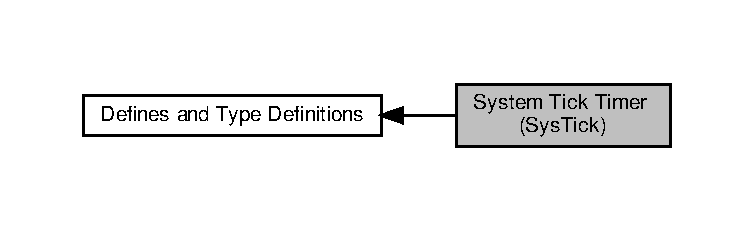
\includegraphics[width=350pt]{group___c_m_s_i_s___sys_tick}
\end{center}
\end{figure}
\subsection*{Komponenty}
\begin{DoxyCompactItemize}
\item 
struct \hyperlink{struct_sys_tick___type}{Sys\+Tick\+\_\+\+Type}
\begin{DoxyCompactList}\small\item\em Structure type to access the System Timer (Sys\+Tick). \end{DoxyCompactList}\end{DoxyCompactItemize}
\subsection*{Definicje}
\begin{DoxyCompactItemize}
\item 
\#define \hyperlink{group___c_m_s_i_s___sys_tick_gadbb65d4a815759649db41df216ed4d60}{Sys\+Tick\+\_\+\+C\+T\+R\+L\+\_\+\+C\+O\+U\+N\+T\+F\+L\+A\+G\+\_\+\+Pos}~16U
\item 
\#define \hyperlink{group___c_m_s_i_s___sys_tick_ga1bf3033ecccf200f59baefe15dbb367c}{Sys\+Tick\+\_\+\+C\+T\+R\+L\+\_\+\+C\+O\+U\+N\+T\+F\+L\+A\+G\+\_\+\+Msk}~(1\+U\+L $<$$<$ Sys\+Tick\+\_\+\+C\+T\+R\+L\+\_\+\+C\+O\+U\+N\+T\+F\+L\+A\+G\+\_\+\+Pos)
\item 
\#define \hyperlink{group___c_m_s_i_s___sys_tick_ga24fbc69a5f0b78d67fda2300257baff1}{Sys\+Tick\+\_\+\+C\+T\+R\+L\+\_\+\+C\+L\+K\+S\+O\+U\+R\+C\+E\+\_\+\+Pos}~2U
\item 
\#define \hyperlink{group___c_m_s_i_s___sys_tick_gaa41d06039797423a46596bd313d57373}{Sys\+Tick\+\_\+\+C\+T\+R\+L\+\_\+\+C\+L\+K\+S\+O\+U\+R\+C\+E\+\_\+\+Msk}~(1\+U\+L $<$$<$ Sys\+Tick\+\_\+\+C\+T\+R\+L\+\_\+\+C\+L\+K\+S\+O\+U\+R\+C\+E\+\_\+\+Pos)
\item 
\#define \hyperlink{group___c_m_s_i_s___sys_tick_ga88f45bbb89ce8df3cd2b2613c7b48214}{Sys\+Tick\+\_\+\+C\+T\+R\+L\+\_\+\+T\+I\+C\+K\+I\+N\+T\+\_\+\+Pos}~1U
\item 
\#define \hyperlink{group___c_m_s_i_s___sys_tick_ga95bb984266ca764024836a870238a027}{Sys\+Tick\+\_\+\+C\+T\+R\+L\+\_\+\+T\+I\+C\+K\+I\+N\+T\+\_\+\+Msk}~(1\+U\+L $<$$<$ Sys\+Tick\+\_\+\+C\+T\+R\+L\+\_\+\+T\+I\+C\+K\+I\+N\+T\+\_\+\+Pos)
\item 
\#define \hyperlink{group___c_m_s_i_s___sys_tick_ga0b48cc1e36d92a92e4bf632890314810}{Sys\+Tick\+\_\+\+C\+T\+R\+L\+\_\+\+E\+N\+A\+B\+L\+E\+\_\+\+Pos}~0U
\item 
\#define \hyperlink{group___c_m_s_i_s___sys_tick_ga16c9fee0ed0235524bdeb38af328fd1f}{Sys\+Tick\+\_\+\+C\+T\+R\+L\+\_\+\+E\+N\+A\+B\+L\+E\+\_\+\+Msk}~(1\+U\+L /$\ast$$<$$<$ Sys\+Tick\+\_\+\+C\+T\+R\+L\+\_\+\+E\+N\+A\+B\+L\+E\+\_\+\+Pos$\ast$/)
\item 
\#define \hyperlink{group___c_m_s_i_s___sys_tick_gaf44d10df359dc5bf5752b0894ae3bad2}{Sys\+Tick\+\_\+\+L\+O\+A\+D\+\_\+\+R\+E\+L\+O\+A\+D\+\_\+\+Pos}~0U
\item 
\#define \hyperlink{group___c_m_s_i_s___sys_tick_ga265912a7962f0e1abd170336e579b1b1}{Sys\+Tick\+\_\+\+L\+O\+A\+D\+\_\+\+R\+E\+L\+O\+A\+D\+\_\+\+Msk}~(0x\+F\+F\+F\+F\+F\+F\+U\+L /$\ast$$<$$<$ Sys\+Tick\+\_\+\+L\+O\+A\+D\+\_\+\+R\+E\+L\+O\+A\+D\+\_\+\+Pos$\ast$/)
\item 
\#define \hyperlink{group___c_m_s_i_s___sys_tick_ga3208104c3b019b5de35ae8c21d5c34dd}{Sys\+Tick\+\_\+\+V\+A\+L\+\_\+\+C\+U\+R\+R\+E\+N\+T\+\_\+\+Pos}~0U
\item 
\#define \hyperlink{group___c_m_s_i_s___sys_tick_gafc77b56d568930b49a2474debc75ab45}{Sys\+Tick\+\_\+\+V\+A\+L\+\_\+\+C\+U\+R\+R\+E\+N\+T\+\_\+\+Msk}~(0x\+F\+F\+F\+F\+F\+F\+U\+L /$\ast$$<$$<$ Sys\+Tick\+\_\+\+V\+A\+L\+\_\+\+C\+U\+R\+R\+E\+N\+T\+\_\+\+Pos$\ast$/)
\item 
\#define \hyperlink{group___c_m_s_i_s___sys_tick_ga534dbe414e7a46a6ce4c1eca1fbff409}{Sys\+Tick\+\_\+\+C\+A\+L\+I\+B\+\_\+\+N\+O\+R\+E\+F\+\_\+\+Pos}~31U
\item 
\#define \hyperlink{group___c_m_s_i_s___sys_tick_ga3af0d891fdd99bcc8d8912d37830edb6}{Sys\+Tick\+\_\+\+C\+A\+L\+I\+B\+\_\+\+N\+O\+R\+E\+F\+\_\+\+Msk}~(1\+U\+L $<$$<$ Sys\+Tick\+\_\+\+C\+A\+L\+I\+B\+\_\+\+N\+O\+R\+E\+F\+\_\+\+Pos)
\item 
\#define \hyperlink{group___c_m_s_i_s___sys_tick_gadd0c9cd6641b9f6a0c618e7982954860}{Sys\+Tick\+\_\+\+C\+A\+L\+I\+B\+\_\+\+S\+K\+E\+W\+\_\+\+Pos}~30U
\item 
\#define \hyperlink{group___c_m_s_i_s___sys_tick_ga8a6a85a87334776f33d77fd147587431}{Sys\+Tick\+\_\+\+C\+A\+L\+I\+B\+\_\+\+S\+K\+E\+W\+\_\+\+Msk}~(1\+U\+L $<$$<$ Sys\+Tick\+\_\+\+C\+A\+L\+I\+B\+\_\+\+S\+K\+E\+W\+\_\+\+Pos)
\item 
\#define \hyperlink{group___c_m_s_i_s___sys_tick_gacae558f6e75a0bed5d826f606d8e695e}{Sys\+Tick\+\_\+\+C\+A\+L\+I\+B\+\_\+\+T\+E\+N\+M\+S\+\_\+\+Pos}~0U
\item 
\#define \hyperlink{group___c_m_s_i_s___sys_tick_gaf1e68865c5aece2ad58971225bd3e95e}{Sys\+Tick\+\_\+\+C\+A\+L\+I\+B\+\_\+\+T\+E\+N\+M\+S\+\_\+\+Msk}~(0x\+F\+F\+F\+F\+F\+F\+U\+L /$\ast$$<$$<$ Sys\+Tick\+\_\+\+C\+A\+L\+I\+B\+\_\+\+T\+E\+N\+M\+S\+\_\+\+Pos$\ast$/)
\item 
\#define \hyperlink{group___c_m_s_i_s___sys_tick_gadbb65d4a815759649db41df216ed4d60}{Sys\+Tick\+\_\+\+C\+T\+R\+L\+\_\+\+C\+O\+U\+N\+T\+F\+L\+A\+G\+\_\+\+Pos}~16U
\item 
\#define \hyperlink{group___c_m_s_i_s___sys_tick_ga1bf3033ecccf200f59baefe15dbb367c}{Sys\+Tick\+\_\+\+C\+T\+R\+L\+\_\+\+C\+O\+U\+N\+T\+F\+L\+A\+G\+\_\+\+Msk}~(1\+U\+L $<$$<$ Sys\+Tick\+\_\+\+C\+T\+R\+L\+\_\+\+C\+O\+U\+N\+T\+F\+L\+A\+G\+\_\+\+Pos)
\item 
\#define \hyperlink{group___c_m_s_i_s___sys_tick_ga24fbc69a5f0b78d67fda2300257baff1}{Sys\+Tick\+\_\+\+C\+T\+R\+L\+\_\+\+C\+L\+K\+S\+O\+U\+R\+C\+E\+\_\+\+Pos}~2U
\item 
\#define \hyperlink{group___c_m_s_i_s___sys_tick_gaa41d06039797423a46596bd313d57373}{Sys\+Tick\+\_\+\+C\+T\+R\+L\+\_\+\+C\+L\+K\+S\+O\+U\+R\+C\+E\+\_\+\+Msk}~(1\+U\+L $<$$<$ Sys\+Tick\+\_\+\+C\+T\+R\+L\+\_\+\+C\+L\+K\+S\+O\+U\+R\+C\+E\+\_\+\+Pos)
\item 
\#define \hyperlink{group___c_m_s_i_s___sys_tick_ga88f45bbb89ce8df3cd2b2613c7b48214}{Sys\+Tick\+\_\+\+C\+T\+R\+L\+\_\+\+T\+I\+C\+K\+I\+N\+T\+\_\+\+Pos}~1U
\item 
\#define \hyperlink{group___c_m_s_i_s___sys_tick_ga95bb984266ca764024836a870238a027}{Sys\+Tick\+\_\+\+C\+T\+R\+L\+\_\+\+T\+I\+C\+K\+I\+N\+T\+\_\+\+Msk}~(1\+U\+L $<$$<$ Sys\+Tick\+\_\+\+C\+T\+R\+L\+\_\+\+T\+I\+C\+K\+I\+N\+T\+\_\+\+Pos)
\item 
\#define \hyperlink{group___c_m_s_i_s___sys_tick_ga0b48cc1e36d92a92e4bf632890314810}{Sys\+Tick\+\_\+\+C\+T\+R\+L\+\_\+\+E\+N\+A\+B\+L\+E\+\_\+\+Pos}~0U
\item 
\#define \hyperlink{group___c_m_s_i_s___sys_tick_ga16c9fee0ed0235524bdeb38af328fd1f}{Sys\+Tick\+\_\+\+C\+T\+R\+L\+\_\+\+E\+N\+A\+B\+L\+E\+\_\+\+Msk}~(1\+U\+L /$\ast$$<$$<$ Sys\+Tick\+\_\+\+C\+T\+R\+L\+\_\+\+E\+N\+A\+B\+L\+E\+\_\+\+Pos$\ast$/)
\item 
\#define \hyperlink{group___c_m_s_i_s___sys_tick_gaf44d10df359dc5bf5752b0894ae3bad2}{Sys\+Tick\+\_\+\+L\+O\+A\+D\+\_\+\+R\+E\+L\+O\+A\+D\+\_\+\+Pos}~0U
\item 
\#define \hyperlink{group___c_m_s_i_s___sys_tick_ga265912a7962f0e1abd170336e579b1b1}{Sys\+Tick\+\_\+\+L\+O\+A\+D\+\_\+\+R\+E\+L\+O\+A\+D\+\_\+\+Msk}~(0x\+F\+F\+F\+F\+F\+F\+U\+L /$\ast$$<$$<$ Sys\+Tick\+\_\+\+L\+O\+A\+D\+\_\+\+R\+E\+L\+O\+A\+D\+\_\+\+Pos$\ast$/)
\item 
\#define \hyperlink{group___c_m_s_i_s___sys_tick_ga3208104c3b019b5de35ae8c21d5c34dd}{Sys\+Tick\+\_\+\+V\+A\+L\+\_\+\+C\+U\+R\+R\+E\+N\+T\+\_\+\+Pos}~0U
\item 
\#define \hyperlink{group___c_m_s_i_s___sys_tick_gafc77b56d568930b49a2474debc75ab45}{Sys\+Tick\+\_\+\+V\+A\+L\+\_\+\+C\+U\+R\+R\+E\+N\+T\+\_\+\+Msk}~(0x\+F\+F\+F\+F\+F\+F\+U\+L /$\ast$$<$$<$ Sys\+Tick\+\_\+\+V\+A\+L\+\_\+\+C\+U\+R\+R\+E\+N\+T\+\_\+\+Pos$\ast$/)
\item 
\#define \hyperlink{group___c_m_s_i_s___sys_tick_ga534dbe414e7a46a6ce4c1eca1fbff409}{Sys\+Tick\+\_\+\+C\+A\+L\+I\+B\+\_\+\+N\+O\+R\+E\+F\+\_\+\+Pos}~31U
\item 
\#define \hyperlink{group___c_m_s_i_s___sys_tick_ga3af0d891fdd99bcc8d8912d37830edb6}{Sys\+Tick\+\_\+\+C\+A\+L\+I\+B\+\_\+\+N\+O\+R\+E\+F\+\_\+\+Msk}~(1\+U\+L $<$$<$ Sys\+Tick\+\_\+\+C\+A\+L\+I\+B\+\_\+\+N\+O\+R\+E\+F\+\_\+\+Pos)
\item 
\#define \hyperlink{group___c_m_s_i_s___sys_tick_gadd0c9cd6641b9f6a0c618e7982954860}{Sys\+Tick\+\_\+\+C\+A\+L\+I\+B\+\_\+\+S\+K\+E\+W\+\_\+\+Pos}~30U
\item 
\#define \hyperlink{group___c_m_s_i_s___sys_tick_ga8a6a85a87334776f33d77fd147587431}{Sys\+Tick\+\_\+\+C\+A\+L\+I\+B\+\_\+\+S\+K\+E\+W\+\_\+\+Msk}~(1\+U\+L $<$$<$ Sys\+Tick\+\_\+\+C\+A\+L\+I\+B\+\_\+\+S\+K\+E\+W\+\_\+\+Pos)
\item 
\#define \hyperlink{group___c_m_s_i_s___sys_tick_gacae558f6e75a0bed5d826f606d8e695e}{Sys\+Tick\+\_\+\+C\+A\+L\+I\+B\+\_\+\+T\+E\+N\+M\+S\+\_\+\+Pos}~0U
\item 
\#define \hyperlink{group___c_m_s_i_s___sys_tick_gaf1e68865c5aece2ad58971225bd3e95e}{Sys\+Tick\+\_\+\+C\+A\+L\+I\+B\+\_\+\+T\+E\+N\+M\+S\+\_\+\+Msk}~(0x\+F\+F\+F\+F\+F\+F\+U\+L /$\ast$$<$$<$ Sys\+Tick\+\_\+\+C\+A\+L\+I\+B\+\_\+\+T\+E\+N\+M\+S\+\_\+\+Pos$\ast$/)
\item 
\#define \hyperlink{group___c_m_s_i_s___sys_tick_gadbb65d4a815759649db41df216ed4d60}{Sys\+Tick\+\_\+\+C\+T\+R\+L\+\_\+\+C\+O\+U\+N\+T\+F\+L\+A\+G\+\_\+\+Pos}~16U
\item 
\#define \hyperlink{group___c_m_s_i_s___sys_tick_ga1bf3033ecccf200f59baefe15dbb367c}{Sys\+Tick\+\_\+\+C\+T\+R\+L\+\_\+\+C\+O\+U\+N\+T\+F\+L\+A\+G\+\_\+\+Msk}~(1\+U\+L $<$$<$ Sys\+Tick\+\_\+\+C\+T\+R\+L\+\_\+\+C\+O\+U\+N\+T\+F\+L\+A\+G\+\_\+\+Pos)
\item 
\#define \hyperlink{group___c_m_s_i_s___sys_tick_ga24fbc69a5f0b78d67fda2300257baff1}{Sys\+Tick\+\_\+\+C\+T\+R\+L\+\_\+\+C\+L\+K\+S\+O\+U\+R\+C\+E\+\_\+\+Pos}~2U
\item 
\#define \hyperlink{group___c_m_s_i_s___sys_tick_gaa41d06039797423a46596bd313d57373}{Sys\+Tick\+\_\+\+C\+T\+R\+L\+\_\+\+C\+L\+K\+S\+O\+U\+R\+C\+E\+\_\+\+Msk}~(1\+U\+L $<$$<$ Sys\+Tick\+\_\+\+C\+T\+R\+L\+\_\+\+C\+L\+K\+S\+O\+U\+R\+C\+E\+\_\+\+Pos)
\item 
\#define \hyperlink{group___c_m_s_i_s___sys_tick_ga88f45bbb89ce8df3cd2b2613c7b48214}{Sys\+Tick\+\_\+\+C\+T\+R\+L\+\_\+\+T\+I\+C\+K\+I\+N\+T\+\_\+\+Pos}~1U
\item 
\#define \hyperlink{group___c_m_s_i_s___sys_tick_ga95bb984266ca764024836a870238a027}{Sys\+Tick\+\_\+\+C\+T\+R\+L\+\_\+\+T\+I\+C\+K\+I\+N\+T\+\_\+\+Msk}~(1\+U\+L $<$$<$ Sys\+Tick\+\_\+\+C\+T\+R\+L\+\_\+\+T\+I\+C\+K\+I\+N\+T\+\_\+\+Pos)
\item 
\#define \hyperlink{group___c_m_s_i_s___sys_tick_ga0b48cc1e36d92a92e4bf632890314810}{Sys\+Tick\+\_\+\+C\+T\+R\+L\+\_\+\+E\+N\+A\+B\+L\+E\+\_\+\+Pos}~0U
\item 
\#define \hyperlink{group___c_m_s_i_s___sys_tick_ga16c9fee0ed0235524bdeb38af328fd1f}{Sys\+Tick\+\_\+\+C\+T\+R\+L\+\_\+\+E\+N\+A\+B\+L\+E\+\_\+\+Msk}~(1\+U\+L /$\ast$$<$$<$ Sys\+Tick\+\_\+\+C\+T\+R\+L\+\_\+\+E\+N\+A\+B\+L\+E\+\_\+\+Pos$\ast$/)
\item 
\#define \hyperlink{group___c_m_s_i_s___sys_tick_gaf44d10df359dc5bf5752b0894ae3bad2}{Sys\+Tick\+\_\+\+L\+O\+A\+D\+\_\+\+R\+E\+L\+O\+A\+D\+\_\+\+Pos}~0U
\item 
\#define \hyperlink{group___c_m_s_i_s___sys_tick_ga265912a7962f0e1abd170336e579b1b1}{Sys\+Tick\+\_\+\+L\+O\+A\+D\+\_\+\+R\+E\+L\+O\+A\+D\+\_\+\+Msk}~(0x\+F\+F\+F\+F\+F\+F\+U\+L /$\ast$$<$$<$ Sys\+Tick\+\_\+\+L\+O\+A\+D\+\_\+\+R\+E\+L\+O\+A\+D\+\_\+\+Pos$\ast$/)
\item 
\#define \hyperlink{group___c_m_s_i_s___sys_tick_ga3208104c3b019b5de35ae8c21d5c34dd}{Sys\+Tick\+\_\+\+V\+A\+L\+\_\+\+C\+U\+R\+R\+E\+N\+T\+\_\+\+Pos}~0U
\item 
\#define \hyperlink{group___c_m_s_i_s___sys_tick_gafc77b56d568930b49a2474debc75ab45}{Sys\+Tick\+\_\+\+V\+A\+L\+\_\+\+C\+U\+R\+R\+E\+N\+T\+\_\+\+Msk}~(0x\+F\+F\+F\+F\+F\+F\+U\+L /$\ast$$<$$<$ Sys\+Tick\+\_\+\+V\+A\+L\+\_\+\+C\+U\+R\+R\+E\+N\+T\+\_\+\+Pos$\ast$/)
\item 
\#define \hyperlink{group___c_m_s_i_s___sys_tick_ga534dbe414e7a46a6ce4c1eca1fbff409}{Sys\+Tick\+\_\+\+C\+A\+L\+I\+B\+\_\+\+N\+O\+R\+E\+F\+\_\+\+Pos}~31U
\item 
\#define \hyperlink{group___c_m_s_i_s___sys_tick_ga3af0d891fdd99bcc8d8912d37830edb6}{Sys\+Tick\+\_\+\+C\+A\+L\+I\+B\+\_\+\+N\+O\+R\+E\+F\+\_\+\+Msk}~(1\+U\+L $<$$<$ Sys\+Tick\+\_\+\+C\+A\+L\+I\+B\+\_\+\+N\+O\+R\+E\+F\+\_\+\+Pos)
\item 
\#define \hyperlink{group___c_m_s_i_s___sys_tick_gadd0c9cd6641b9f6a0c618e7982954860}{Sys\+Tick\+\_\+\+C\+A\+L\+I\+B\+\_\+\+S\+K\+E\+W\+\_\+\+Pos}~30U
\item 
\#define \hyperlink{group___c_m_s_i_s___sys_tick_ga8a6a85a87334776f33d77fd147587431}{Sys\+Tick\+\_\+\+C\+A\+L\+I\+B\+\_\+\+S\+K\+E\+W\+\_\+\+Msk}~(1\+U\+L $<$$<$ Sys\+Tick\+\_\+\+C\+A\+L\+I\+B\+\_\+\+S\+K\+E\+W\+\_\+\+Pos)
\item 
\#define \hyperlink{group___c_m_s_i_s___sys_tick_gacae558f6e75a0bed5d826f606d8e695e}{Sys\+Tick\+\_\+\+C\+A\+L\+I\+B\+\_\+\+T\+E\+N\+M\+S\+\_\+\+Pos}~0U
\item 
\#define \hyperlink{group___c_m_s_i_s___sys_tick_gaf1e68865c5aece2ad58971225bd3e95e}{Sys\+Tick\+\_\+\+C\+A\+L\+I\+B\+\_\+\+T\+E\+N\+M\+S\+\_\+\+Msk}~(0x\+F\+F\+F\+F\+F\+F\+U\+L /$\ast$$<$$<$ Sys\+Tick\+\_\+\+C\+A\+L\+I\+B\+\_\+\+T\+E\+N\+M\+S\+\_\+\+Pos$\ast$/)
\item 
\#define \hyperlink{group___c_m_s_i_s___sys_tick_gadbb65d4a815759649db41df216ed4d60}{Sys\+Tick\+\_\+\+C\+T\+R\+L\+\_\+\+C\+O\+U\+N\+T\+F\+L\+A\+G\+\_\+\+Pos}~16U
\item 
\#define \hyperlink{group___c_m_s_i_s___sys_tick_ga1bf3033ecccf200f59baefe15dbb367c}{Sys\+Tick\+\_\+\+C\+T\+R\+L\+\_\+\+C\+O\+U\+N\+T\+F\+L\+A\+G\+\_\+\+Msk}~(1\+U\+L $<$$<$ Sys\+Tick\+\_\+\+C\+T\+R\+L\+\_\+\+C\+O\+U\+N\+T\+F\+L\+A\+G\+\_\+\+Pos)
\item 
\#define \hyperlink{group___c_m_s_i_s___sys_tick_ga24fbc69a5f0b78d67fda2300257baff1}{Sys\+Tick\+\_\+\+C\+T\+R\+L\+\_\+\+C\+L\+K\+S\+O\+U\+R\+C\+E\+\_\+\+Pos}~2U
\item 
\#define \hyperlink{group___c_m_s_i_s___sys_tick_gaa41d06039797423a46596bd313d57373}{Sys\+Tick\+\_\+\+C\+T\+R\+L\+\_\+\+C\+L\+K\+S\+O\+U\+R\+C\+E\+\_\+\+Msk}~(1\+U\+L $<$$<$ Sys\+Tick\+\_\+\+C\+T\+R\+L\+\_\+\+C\+L\+K\+S\+O\+U\+R\+C\+E\+\_\+\+Pos)
\item 
\#define \hyperlink{group___c_m_s_i_s___sys_tick_ga88f45bbb89ce8df3cd2b2613c7b48214}{Sys\+Tick\+\_\+\+C\+T\+R\+L\+\_\+\+T\+I\+C\+K\+I\+N\+T\+\_\+\+Pos}~1U
\item 
\#define \hyperlink{group___c_m_s_i_s___sys_tick_ga95bb984266ca764024836a870238a027}{Sys\+Tick\+\_\+\+C\+T\+R\+L\+\_\+\+T\+I\+C\+K\+I\+N\+T\+\_\+\+Msk}~(1\+U\+L $<$$<$ Sys\+Tick\+\_\+\+C\+T\+R\+L\+\_\+\+T\+I\+C\+K\+I\+N\+T\+\_\+\+Pos)
\item 
\#define \hyperlink{group___c_m_s_i_s___sys_tick_ga0b48cc1e36d92a92e4bf632890314810}{Sys\+Tick\+\_\+\+C\+T\+R\+L\+\_\+\+E\+N\+A\+B\+L\+E\+\_\+\+Pos}~0U
\item 
\#define \hyperlink{group___c_m_s_i_s___sys_tick_ga16c9fee0ed0235524bdeb38af328fd1f}{Sys\+Tick\+\_\+\+C\+T\+R\+L\+\_\+\+E\+N\+A\+B\+L\+E\+\_\+\+Msk}~(1\+U\+L /$\ast$$<$$<$ Sys\+Tick\+\_\+\+C\+T\+R\+L\+\_\+\+E\+N\+A\+B\+L\+E\+\_\+\+Pos$\ast$/)
\item 
\#define \hyperlink{group___c_m_s_i_s___sys_tick_gaf44d10df359dc5bf5752b0894ae3bad2}{Sys\+Tick\+\_\+\+L\+O\+A\+D\+\_\+\+R\+E\+L\+O\+A\+D\+\_\+\+Pos}~0U
\item 
\#define \hyperlink{group___c_m_s_i_s___sys_tick_ga265912a7962f0e1abd170336e579b1b1}{Sys\+Tick\+\_\+\+L\+O\+A\+D\+\_\+\+R\+E\+L\+O\+A\+D\+\_\+\+Msk}~(0x\+F\+F\+F\+F\+F\+F\+U\+L /$\ast$$<$$<$ Sys\+Tick\+\_\+\+L\+O\+A\+D\+\_\+\+R\+E\+L\+O\+A\+D\+\_\+\+Pos$\ast$/)
\item 
\#define \hyperlink{group___c_m_s_i_s___sys_tick_ga3208104c3b019b5de35ae8c21d5c34dd}{Sys\+Tick\+\_\+\+V\+A\+L\+\_\+\+C\+U\+R\+R\+E\+N\+T\+\_\+\+Pos}~0U
\item 
\#define \hyperlink{group___c_m_s_i_s___sys_tick_gafc77b56d568930b49a2474debc75ab45}{Sys\+Tick\+\_\+\+V\+A\+L\+\_\+\+C\+U\+R\+R\+E\+N\+T\+\_\+\+Msk}~(0x\+F\+F\+F\+F\+F\+F\+U\+L /$\ast$$<$$<$ Sys\+Tick\+\_\+\+V\+A\+L\+\_\+\+C\+U\+R\+R\+E\+N\+T\+\_\+\+Pos$\ast$/)
\item 
\#define \hyperlink{group___c_m_s_i_s___sys_tick_ga534dbe414e7a46a6ce4c1eca1fbff409}{Sys\+Tick\+\_\+\+C\+A\+L\+I\+B\+\_\+\+N\+O\+R\+E\+F\+\_\+\+Pos}~31U
\item 
\#define \hyperlink{group___c_m_s_i_s___sys_tick_ga3af0d891fdd99bcc8d8912d37830edb6}{Sys\+Tick\+\_\+\+C\+A\+L\+I\+B\+\_\+\+N\+O\+R\+E\+F\+\_\+\+Msk}~(1\+U\+L $<$$<$ Sys\+Tick\+\_\+\+C\+A\+L\+I\+B\+\_\+\+N\+O\+R\+E\+F\+\_\+\+Pos)
\item 
\#define \hyperlink{group___c_m_s_i_s___sys_tick_gadd0c9cd6641b9f6a0c618e7982954860}{Sys\+Tick\+\_\+\+C\+A\+L\+I\+B\+\_\+\+S\+K\+E\+W\+\_\+\+Pos}~30U
\item 
\#define \hyperlink{group___c_m_s_i_s___sys_tick_ga8a6a85a87334776f33d77fd147587431}{Sys\+Tick\+\_\+\+C\+A\+L\+I\+B\+\_\+\+S\+K\+E\+W\+\_\+\+Msk}~(1\+U\+L $<$$<$ Sys\+Tick\+\_\+\+C\+A\+L\+I\+B\+\_\+\+S\+K\+E\+W\+\_\+\+Pos)
\item 
\#define \hyperlink{group___c_m_s_i_s___sys_tick_gacae558f6e75a0bed5d826f606d8e695e}{Sys\+Tick\+\_\+\+C\+A\+L\+I\+B\+\_\+\+T\+E\+N\+M\+S\+\_\+\+Pos}~0U
\item 
\#define \hyperlink{group___c_m_s_i_s___sys_tick_gaf1e68865c5aece2ad58971225bd3e95e}{Sys\+Tick\+\_\+\+C\+A\+L\+I\+B\+\_\+\+T\+E\+N\+M\+S\+\_\+\+Msk}~(0x\+F\+F\+F\+F\+F\+F\+U\+L /$\ast$$<$$<$ Sys\+Tick\+\_\+\+C\+A\+L\+I\+B\+\_\+\+T\+E\+N\+M\+S\+\_\+\+Pos$\ast$/)
\item 
\#define \hyperlink{group___c_m_s_i_s___sys_tick_gadbb65d4a815759649db41df216ed4d60}{Sys\+Tick\+\_\+\+C\+T\+R\+L\+\_\+\+C\+O\+U\+N\+T\+F\+L\+A\+G\+\_\+\+Pos}~16U
\item 
\#define \hyperlink{group___c_m_s_i_s___sys_tick_ga1bf3033ecccf200f59baefe15dbb367c}{Sys\+Tick\+\_\+\+C\+T\+R\+L\+\_\+\+C\+O\+U\+N\+T\+F\+L\+A\+G\+\_\+\+Msk}~(1\+U\+L $<$$<$ Sys\+Tick\+\_\+\+C\+T\+R\+L\+\_\+\+C\+O\+U\+N\+T\+F\+L\+A\+G\+\_\+\+Pos)
\item 
\#define \hyperlink{group___c_m_s_i_s___sys_tick_ga24fbc69a5f0b78d67fda2300257baff1}{Sys\+Tick\+\_\+\+C\+T\+R\+L\+\_\+\+C\+L\+K\+S\+O\+U\+R\+C\+E\+\_\+\+Pos}~2U
\item 
\#define \hyperlink{group___c_m_s_i_s___sys_tick_gaa41d06039797423a46596bd313d57373}{Sys\+Tick\+\_\+\+C\+T\+R\+L\+\_\+\+C\+L\+K\+S\+O\+U\+R\+C\+E\+\_\+\+Msk}~(1\+U\+L $<$$<$ Sys\+Tick\+\_\+\+C\+T\+R\+L\+\_\+\+C\+L\+K\+S\+O\+U\+R\+C\+E\+\_\+\+Pos)
\item 
\#define \hyperlink{group___c_m_s_i_s___sys_tick_ga88f45bbb89ce8df3cd2b2613c7b48214}{Sys\+Tick\+\_\+\+C\+T\+R\+L\+\_\+\+T\+I\+C\+K\+I\+N\+T\+\_\+\+Pos}~1U
\item 
\#define \hyperlink{group___c_m_s_i_s___sys_tick_ga95bb984266ca764024836a870238a027}{Sys\+Tick\+\_\+\+C\+T\+R\+L\+\_\+\+T\+I\+C\+K\+I\+N\+T\+\_\+\+Msk}~(1\+U\+L $<$$<$ Sys\+Tick\+\_\+\+C\+T\+R\+L\+\_\+\+T\+I\+C\+K\+I\+N\+T\+\_\+\+Pos)
\item 
\#define \hyperlink{group___c_m_s_i_s___sys_tick_ga0b48cc1e36d92a92e4bf632890314810}{Sys\+Tick\+\_\+\+C\+T\+R\+L\+\_\+\+E\+N\+A\+B\+L\+E\+\_\+\+Pos}~0U
\item 
\#define \hyperlink{group___c_m_s_i_s___sys_tick_ga16c9fee0ed0235524bdeb38af328fd1f}{Sys\+Tick\+\_\+\+C\+T\+R\+L\+\_\+\+E\+N\+A\+B\+L\+E\+\_\+\+Msk}~(1\+U\+L /$\ast$$<$$<$ Sys\+Tick\+\_\+\+C\+T\+R\+L\+\_\+\+E\+N\+A\+B\+L\+E\+\_\+\+Pos$\ast$/)
\item 
\#define \hyperlink{group___c_m_s_i_s___sys_tick_gaf44d10df359dc5bf5752b0894ae3bad2}{Sys\+Tick\+\_\+\+L\+O\+A\+D\+\_\+\+R\+E\+L\+O\+A\+D\+\_\+\+Pos}~0U
\item 
\#define \hyperlink{group___c_m_s_i_s___sys_tick_ga265912a7962f0e1abd170336e579b1b1}{Sys\+Tick\+\_\+\+L\+O\+A\+D\+\_\+\+R\+E\+L\+O\+A\+D\+\_\+\+Msk}~(0x\+F\+F\+F\+F\+F\+F\+U\+L /$\ast$$<$$<$ Sys\+Tick\+\_\+\+L\+O\+A\+D\+\_\+\+R\+E\+L\+O\+A\+D\+\_\+\+Pos$\ast$/)
\item 
\#define \hyperlink{group___c_m_s_i_s___sys_tick_ga3208104c3b019b5de35ae8c21d5c34dd}{Sys\+Tick\+\_\+\+V\+A\+L\+\_\+\+C\+U\+R\+R\+E\+N\+T\+\_\+\+Pos}~0U
\item 
\#define \hyperlink{group___c_m_s_i_s___sys_tick_gafc77b56d568930b49a2474debc75ab45}{Sys\+Tick\+\_\+\+V\+A\+L\+\_\+\+C\+U\+R\+R\+E\+N\+T\+\_\+\+Msk}~(0x\+F\+F\+F\+F\+F\+F\+U\+L /$\ast$$<$$<$ Sys\+Tick\+\_\+\+V\+A\+L\+\_\+\+C\+U\+R\+R\+E\+N\+T\+\_\+\+Pos$\ast$/)
\item 
\#define \hyperlink{group___c_m_s_i_s___sys_tick_ga534dbe414e7a46a6ce4c1eca1fbff409}{Sys\+Tick\+\_\+\+C\+A\+L\+I\+B\+\_\+\+N\+O\+R\+E\+F\+\_\+\+Pos}~31U
\item 
\#define \hyperlink{group___c_m_s_i_s___sys_tick_ga3af0d891fdd99bcc8d8912d37830edb6}{Sys\+Tick\+\_\+\+C\+A\+L\+I\+B\+\_\+\+N\+O\+R\+E\+F\+\_\+\+Msk}~(1\+U\+L $<$$<$ Sys\+Tick\+\_\+\+C\+A\+L\+I\+B\+\_\+\+N\+O\+R\+E\+F\+\_\+\+Pos)
\item 
\#define \hyperlink{group___c_m_s_i_s___sys_tick_gadd0c9cd6641b9f6a0c618e7982954860}{Sys\+Tick\+\_\+\+C\+A\+L\+I\+B\+\_\+\+S\+K\+E\+W\+\_\+\+Pos}~30U
\item 
\#define \hyperlink{group___c_m_s_i_s___sys_tick_ga8a6a85a87334776f33d77fd147587431}{Sys\+Tick\+\_\+\+C\+A\+L\+I\+B\+\_\+\+S\+K\+E\+W\+\_\+\+Msk}~(1\+U\+L $<$$<$ Sys\+Tick\+\_\+\+C\+A\+L\+I\+B\+\_\+\+S\+K\+E\+W\+\_\+\+Pos)
\item 
\#define \hyperlink{group___c_m_s_i_s___sys_tick_gacae558f6e75a0bed5d826f606d8e695e}{Sys\+Tick\+\_\+\+C\+A\+L\+I\+B\+\_\+\+T\+E\+N\+M\+S\+\_\+\+Pos}~0U
\item 
\#define \hyperlink{group___c_m_s_i_s___sys_tick_gaf1e68865c5aece2ad58971225bd3e95e}{Sys\+Tick\+\_\+\+C\+A\+L\+I\+B\+\_\+\+T\+E\+N\+M\+S\+\_\+\+Msk}~(0x\+F\+F\+F\+F\+F\+F\+U\+L /$\ast$$<$$<$ Sys\+Tick\+\_\+\+C\+A\+L\+I\+B\+\_\+\+T\+E\+N\+M\+S\+\_\+\+Pos$\ast$/)
\item 
\#define \hyperlink{group___c_m_s_i_s___sys_tick_gadbb65d4a815759649db41df216ed4d60}{Sys\+Tick\+\_\+\+C\+T\+R\+L\+\_\+\+C\+O\+U\+N\+T\+F\+L\+A\+G\+\_\+\+Pos}~16U
\item 
\#define \hyperlink{group___c_m_s_i_s___sys_tick_ga1bf3033ecccf200f59baefe15dbb367c}{Sys\+Tick\+\_\+\+C\+T\+R\+L\+\_\+\+C\+O\+U\+N\+T\+F\+L\+A\+G\+\_\+\+Msk}~(1\+U\+L $<$$<$ Sys\+Tick\+\_\+\+C\+T\+R\+L\+\_\+\+C\+O\+U\+N\+T\+F\+L\+A\+G\+\_\+\+Pos)
\item 
\#define \hyperlink{group___c_m_s_i_s___sys_tick_ga24fbc69a5f0b78d67fda2300257baff1}{Sys\+Tick\+\_\+\+C\+T\+R\+L\+\_\+\+C\+L\+K\+S\+O\+U\+R\+C\+E\+\_\+\+Pos}~2U
\item 
\#define \hyperlink{group___c_m_s_i_s___sys_tick_gaa41d06039797423a46596bd313d57373}{Sys\+Tick\+\_\+\+C\+T\+R\+L\+\_\+\+C\+L\+K\+S\+O\+U\+R\+C\+E\+\_\+\+Msk}~(1\+U\+L $<$$<$ Sys\+Tick\+\_\+\+C\+T\+R\+L\+\_\+\+C\+L\+K\+S\+O\+U\+R\+C\+E\+\_\+\+Pos)
\item 
\#define \hyperlink{group___c_m_s_i_s___sys_tick_ga88f45bbb89ce8df3cd2b2613c7b48214}{Sys\+Tick\+\_\+\+C\+T\+R\+L\+\_\+\+T\+I\+C\+K\+I\+N\+T\+\_\+\+Pos}~1U
\item 
\#define \hyperlink{group___c_m_s_i_s___sys_tick_ga95bb984266ca764024836a870238a027}{Sys\+Tick\+\_\+\+C\+T\+R\+L\+\_\+\+T\+I\+C\+K\+I\+N\+T\+\_\+\+Msk}~(1\+U\+L $<$$<$ Sys\+Tick\+\_\+\+C\+T\+R\+L\+\_\+\+T\+I\+C\+K\+I\+N\+T\+\_\+\+Pos)
\item 
\#define \hyperlink{group___c_m_s_i_s___sys_tick_ga0b48cc1e36d92a92e4bf632890314810}{Sys\+Tick\+\_\+\+C\+T\+R\+L\+\_\+\+E\+N\+A\+B\+L\+E\+\_\+\+Pos}~0U
\item 
\#define \hyperlink{group___c_m_s_i_s___sys_tick_ga16c9fee0ed0235524bdeb38af328fd1f}{Sys\+Tick\+\_\+\+C\+T\+R\+L\+\_\+\+E\+N\+A\+B\+L\+E\+\_\+\+Msk}~(1\+U\+L /$\ast$$<$$<$ Sys\+Tick\+\_\+\+C\+T\+R\+L\+\_\+\+E\+N\+A\+B\+L\+E\+\_\+\+Pos$\ast$/)
\item 
\#define \hyperlink{group___c_m_s_i_s___sys_tick_gaf44d10df359dc5bf5752b0894ae3bad2}{Sys\+Tick\+\_\+\+L\+O\+A\+D\+\_\+\+R\+E\+L\+O\+A\+D\+\_\+\+Pos}~0U
\item 
\#define \hyperlink{group___c_m_s_i_s___sys_tick_ga265912a7962f0e1abd170336e579b1b1}{Sys\+Tick\+\_\+\+L\+O\+A\+D\+\_\+\+R\+E\+L\+O\+A\+D\+\_\+\+Msk}~(0x\+F\+F\+F\+F\+F\+F\+U\+L /$\ast$$<$$<$ Sys\+Tick\+\_\+\+L\+O\+A\+D\+\_\+\+R\+E\+L\+O\+A\+D\+\_\+\+Pos$\ast$/)
\item 
\#define \hyperlink{group___c_m_s_i_s___sys_tick_ga3208104c3b019b5de35ae8c21d5c34dd}{Sys\+Tick\+\_\+\+V\+A\+L\+\_\+\+C\+U\+R\+R\+E\+N\+T\+\_\+\+Pos}~0U
\item 
\#define \hyperlink{group___c_m_s_i_s___sys_tick_gafc77b56d568930b49a2474debc75ab45}{Sys\+Tick\+\_\+\+V\+A\+L\+\_\+\+C\+U\+R\+R\+E\+N\+T\+\_\+\+Msk}~(0x\+F\+F\+F\+F\+F\+F\+U\+L /$\ast$$<$$<$ Sys\+Tick\+\_\+\+V\+A\+L\+\_\+\+C\+U\+R\+R\+E\+N\+T\+\_\+\+Pos$\ast$/)
\item 
\#define \hyperlink{group___c_m_s_i_s___sys_tick_ga534dbe414e7a46a6ce4c1eca1fbff409}{Sys\+Tick\+\_\+\+C\+A\+L\+I\+B\+\_\+\+N\+O\+R\+E\+F\+\_\+\+Pos}~31U
\item 
\#define \hyperlink{group___c_m_s_i_s___sys_tick_ga3af0d891fdd99bcc8d8912d37830edb6}{Sys\+Tick\+\_\+\+C\+A\+L\+I\+B\+\_\+\+N\+O\+R\+E\+F\+\_\+\+Msk}~(1\+U\+L $<$$<$ Sys\+Tick\+\_\+\+C\+A\+L\+I\+B\+\_\+\+N\+O\+R\+E\+F\+\_\+\+Pos)
\item 
\#define \hyperlink{group___c_m_s_i_s___sys_tick_gadd0c9cd6641b9f6a0c618e7982954860}{Sys\+Tick\+\_\+\+C\+A\+L\+I\+B\+\_\+\+S\+K\+E\+W\+\_\+\+Pos}~30U
\item 
\#define \hyperlink{group___c_m_s_i_s___sys_tick_ga8a6a85a87334776f33d77fd147587431}{Sys\+Tick\+\_\+\+C\+A\+L\+I\+B\+\_\+\+S\+K\+E\+W\+\_\+\+Msk}~(1\+U\+L $<$$<$ Sys\+Tick\+\_\+\+C\+A\+L\+I\+B\+\_\+\+S\+K\+E\+W\+\_\+\+Pos)
\item 
\#define \hyperlink{group___c_m_s_i_s___sys_tick_gacae558f6e75a0bed5d826f606d8e695e}{Sys\+Tick\+\_\+\+C\+A\+L\+I\+B\+\_\+\+T\+E\+N\+M\+S\+\_\+\+Pos}~0U
\item 
\#define \hyperlink{group___c_m_s_i_s___sys_tick_gaf1e68865c5aece2ad58971225bd3e95e}{Sys\+Tick\+\_\+\+C\+A\+L\+I\+B\+\_\+\+T\+E\+N\+M\+S\+\_\+\+Msk}~(0x\+F\+F\+F\+F\+F\+F\+U\+L /$\ast$$<$$<$ Sys\+Tick\+\_\+\+C\+A\+L\+I\+B\+\_\+\+T\+E\+N\+M\+S\+\_\+\+Pos$\ast$/)
\item 
\#define \hyperlink{group___c_m_s_i_s___sys_tick_gadbb65d4a815759649db41df216ed4d60}{Sys\+Tick\+\_\+\+C\+T\+R\+L\+\_\+\+C\+O\+U\+N\+T\+F\+L\+A\+G\+\_\+\+Pos}~16U
\item 
\#define \hyperlink{group___c_m_s_i_s___sys_tick_ga1bf3033ecccf200f59baefe15dbb367c}{Sys\+Tick\+\_\+\+C\+T\+R\+L\+\_\+\+C\+O\+U\+N\+T\+F\+L\+A\+G\+\_\+\+Msk}~(1\+U\+L $<$$<$ Sys\+Tick\+\_\+\+C\+T\+R\+L\+\_\+\+C\+O\+U\+N\+T\+F\+L\+A\+G\+\_\+\+Pos)
\item 
\#define \hyperlink{group___c_m_s_i_s___sys_tick_ga24fbc69a5f0b78d67fda2300257baff1}{Sys\+Tick\+\_\+\+C\+T\+R\+L\+\_\+\+C\+L\+K\+S\+O\+U\+R\+C\+E\+\_\+\+Pos}~2U
\item 
\#define \hyperlink{group___c_m_s_i_s___sys_tick_gaa41d06039797423a46596bd313d57373}{Sys\+Tick\+\_\+\+C\+T\+R\+L\+\_\+\+C\+L\+K\+S\+O\+U\+R\+C\+E\+\_\+\+Msk}~(1\+U\+L $<$$<$ Sys\+Tick\+\_\+\+C\+T\+R\+L\+\_\+\+C\+L\+K\+S\+O\+U\+R\+C\+E\+\_\+\+Pos)
\item 
\#define \hyperlink{group___c_m_s_i_s___sys_tick_ga88f45bbb89ce8df3cd2b2613c7b48214}{Sys\+Tick\+\_\+\+C\+T\+R\+L\+\_\+\+T\+I\+C\+K\+I\+N\+T\+\_\+\+Pos}~1U
\item 
\#define \hyperlink{group___c_m_s_i_s___sys_tick_ga95bb984266ca764024836a870238a027}{Sys\+Tick\+\_\+\+C\+T\+R\+L\+\_\+\+T\+I\+C\+K\+I\+N\+T\+\_\+\+Msk}~(1\+U\+L $<$$<$ Sys\+Tick\+\_\+\+C\+T\+R\+L\+\_\+\+T\+I\+C\+K\+I\+N\+T\+\_\+\+Pos)
\item 
\#define \hyperlink{group___c_m_s_i_s___sys_tick_ga0b48cc1e36d92a92e4bf632890314810}{Sys\+Tick\+\_\+\+C\+T\+R\+L\+\_\+\+E\+N\+A\+B\+L\+E\+\_\+\+Pos}~0U
\item 
\#define \hyperlink{group___c_m_s_i_s___sys_tick_ga16c9fee0ed0235524bdeb38af328fd1f}{Sys\+Tick\+\_\+\+C\+T\+R\+L\+\_\+\+E\+N\+A\+B\+L\+E\+\_\+\+Msk}~(1\+U\+L /$\ast$$<$$<$ Sys\+Tick\+\_\+\+C\+T\+R\+L\+\_\+\+E\+N\+A\+B\+L\+E\+\_\+\+Pos$\ast$/)
\item 
\#define \hyperlink{group___c_m_s_i_s___sys_tick_gaf44d10df359dc5bf5752b0894ae3bad2}{Sys\+Tick\+\_\+\+L\+O\+A\+D\+\_\+\+R\+E\+L\+O\+A\+D\+\_\+\+Pos}~0U
\item 
\#define \hyperlink{group___c_m_s_i_s___sys_tick_ga265912a7962f0e1abd170336e579b1b1}{Sys\+Tick\+\_\+\+L\+O\+A\+D\+\_\+\+R\+E\+L\+O\+A\+D\+\_\+\+Msk}~(0x\+F\+F\+F\+F\+F\+F\+U\+L /$\ast$$<$$<$ Sys\+Tick\+\_\+\+L\+O\+A\+D\+\_\+\+R\+E\+L\+O\+A\+D\+\_\+\+Pos$\ast$/)
\item 
\#define \hyperlink{group___c_m_s_i_s___sys_tick_ga3208104c3b019b5de35ae8c21d5c34dd}{Sys\+Tick\+\_\+\+V\+A\+L\+\_\+\+C\+U\+R\+R\+E\+N\+T\+\_\+\+Pos}~0U
\item 
\#define \hyperlink{group___c_m_s_i_s___sys_tick_gafc77b56d568930b49a2474debc75ab45}{Sys\+Tick\+\_\+\+V\+A\+L\+\_\+\+C\+U\+R\+R\+E\+N\+T\+\_\+\+Msk}~(0x\+F\+F\+F\+F\+F\+F\+U\+L /$\ast$$<$$<$ Sys\+Tick\+\_\+\+V\+A\+L\+\_\+\+C\+U\+R\+R\+E\+N\+T\+\_\+\+Pos$\ast$/)
\item 
\#define \hyperlink{group___c_m_s_i_s___sys_tick_ga534dbe414e7a46a6ce4c1eca1fbff409}{Sys\+Tick\+\_\+\+C\+A\+L\+I\+B\+\_\+\+N\+O\+R\+E\+F\+\_\+\+Pos}~31U
\item 
\#define \hyperlink{group___c_m_s_i_s___sys_tick_ga3af0d891fdd99bcc8d8912d37830edb6}{Sys\+Tick\+\_\+\+C\+A\+L\+I\+B\+\_\+\+N\+O\+R\+E\+F\+\_\+\+Msk}~(1\+U\+L $<$$<$ Sys\+Tick\+\_\+\+C\+A\+L\+I\+B\+\_\+\+N\+O\+R\+E\+F\+\_\+\+Pos)
\item 
\#define \hyperlink{group___c_m_s_i_s___sys_tick_gadd0c9cd6641b9f6a0c618e7982954860}{Sys\+Tick\+\_\+\+C\+A\+L\+I\+B\+\_\+\+S\+K\+E\+W\+\_\+\+Pos}~30U
\item 
\#define \hyperlink{group___c_m_s_i_s___sys_tick_ga8a6a85a87334776f33d77fd147587431}{Sys\+Tick\+\_\+\+C\+A\+L\+I\+B\+\_\+\+S\+K\+E\+W\+\_\+\+Msk}~(1\+U\+L $<$$<$ Sys\+Tick\+\_\+\+C\+A\+L\+I\+B\+\_\+\+S\+K\+E\+W\+\_\+\+Pos)
\item 
\#define \hyperlink{group___c_m_s_i_s___sys_tick_gacae558f6e75a0bed5d826f606d8e695e}{Sys\+Tick\+\_\+\+C\+A\+L\+I\+B\+\_\+\+T\+E\+N\+M\+S\+\_\+\+Pos}~0U
\item 
\#define \hyperlink{group___c_m_s_i_s___sys_tick_gaf1e68865c5aece2ad58971225bd3e95e}{Sys\+Tick\+\_\+\+C\+A\+L\+I\+B\+\_\+\+T\+E\+N\+M\+S\+\_\+\+Msk}~(0x\+F\+F\+F\+F\+F\+F\+U\+L /$\ast$$<$$<$ Sys\+Tick\+\_\+\+C\+A\+L\+I\+B\+\_\+\+T\+E\+N\+M\+S\+\_\+\+Pos$\ast$/)
\item 
\#define \hyperlink{group___c_m_s_i_s___sys_tick_gadbb65d4a815759649db41df216ed4d60}{Sys\+Tick\+\_\+\+C\+T\+R\+L\+\_\+\+C\+O\+U\+N\+T\+F\+L\+A\+G\+\_\+\+Pos}~16U
\item 
\#define \hyperlink{group___c_m_s_i_s___sys_tick_ga1bf3033ecccf200f59baefe15dbb367c}{Sys\+Tick\+\_\+\+C\+T\+R\+L\+\_\+\+C\+O\+U\+N\+T\+F\+L\+A\+G\+\_\+\+Msk}~(1\+U\+L $<$$<$ Sys\+Tick\+\_\+\+C\+T\+R\+L\+\_\+\+C\+O\+U\+N\+T\+F\+L\+A\+G\+\_\+\+Pos)
\item 
\#define \hyperlink{group___c_m_s_i_s___sys_tick_ga24fbc69a5f0b78d67fda2300257baff1}{Sys\+Tick\+\_\+\+C\+T\+R\+L\+\_\+\+C\+L\+K\+S\+O\+U\+R\+C\+E\+\_\+\+Pos}~2U
\item 
\#define \hyperlink{group___c_m_s_i_s___sys_tick_gaa41d06039797423a46596bd313d57373}{Sys\+Tick\+\_\+\+C\+T\+R\+L\+\_\+\+C\+L\+K\+S\+O\+U\+R\+C\+E\+\_\+\+Msk}~(1\+U\+L $<$$<$ Sys\+Tick\+\_\+\+C\+T\+R\+L\+\_\+\+C\+L\+K\+S\+O\+U\+R\+C\+E\+\_\+\+Pos)
\item 
\#define \hyperlink{group___c_m_s_i_s___sys_tick_ga88f45bbb89ce8df3cd2b2613c7b48214}{Sys\+Tick\+\_\+\+C\+T\+R\+L\+\_\+\+T\+I\+C\+K\+I\+N\+T\+\_\+\+Pos}~1U
\item 
\#define \hyperlink{group___c_m_s_i_s___sys_tick_ga95bb984266ca764024836a870238a027}{Sys\+Tick\+\_\+\+C\+T\+R\+L\+\_\+\+T\+I\+C\+K\+I\+N\+T\+\_\+\+Msk}~(1\+U\+L $<$$<$ Sys\+Tick\+\_\+\+C\+T\+R\+L\+\_\+\+T\+I\+C\+K\+I\+N\+T\+\_\+\+Pos)
\item 
\#define \hyperlink{group___c_m_s_i_s___sys_tick_ga0b48cc1e36d92a92e4bf632890314810}{Sys\+Tick\+\_\+\+C\+T\+R\+L\+\_\+\+E\+N\+A\+B\+L\+E\+\_\+\+Pos}~0U
\item 
\#define \hyperlink{group___c_m_s_i_s___sys_tick_ga16c9fee0ed0235524bdeb38af328fd1f}{Sys\+Tick\+\_\+\+C\+T\+R\+L\+\_\+\+E\+N\+A\+B\+L\+E\+\_\+\+Msk}~(1\+U\+L /$\ast$$<$$<$ Sys\+Tick\+\_\+\+C\+T\+R\+L\+\_\+\+E\+N\+A\+B\+L\+E\+\_\+\+Pos$\ast$/)
\item 
\#define \hyperlink{group___c_m_s_i_s___sys_tick_gaf44d10df359dc5bf5752b0894ae3bad2}{Sys\+Tick\+\_\+\+L\+O\+A\+D\+\_\+\+R\+E\+L\+O\+A\+D\+\_\+\+Pos}~0U
\item 
\#define \hyperlink{group___c_m_s_i_s___sys_tick_ga265912a7962f0e1abd170336e579b1b1}{Sys\+Tick\+\_\+\+L\+O\+A\+D\+\_\+\+R\+E\+L\+O\+A\+D\+\_\+\+Msk}~(0x\+F\+F\+F\+F\+F\+F\+U\+L /$\ast$$<$$<$ Sys\+Tick\+\_\+\+L\+O\+A\+D\+\_\+\+R\+E\+L\+O\+A\+D\+\_\+\+Pos$\ast$/)
\item 
\#define \hyperlink{group___c_m_s_i_s___sys_tick_ga3208104c3b019b5de35ae8c21d5c34dd}{Sys\+Tick\+\_\+\+V\+A\+L\+\_\+\+C\+U\+R\+R\+E\+N\+T\+\_\+\+Pos}~0U
\item 
\#define \hyperlink{group___c_m_s_i_s___sys_tick_gafc77b56d568930b49a2474debc75ab45}{Sys\+Tick\+\_\+\+V\+A\+L\+\_\+\+C\+U\+R\+R\+E\+N\+T\+\_\+\+Msk}~(0x\+F\+F\+F\+F\+F\+F\+U\+L /$\ast$$<$$<$ Sys\+Tick\+\_\+\+V\+A\+L\+\_\+\+C\+U\+R\+R\+E\+N\+T\+\_\+\+Pos$\ast$/)
\item 
\#define \hyperlink{group___c_m_s_i_s___sys_tick_ga534dbe414e7a46a6ce4c1eca1fbff409}{Sys\+Tick\+\_\+\+C\+A\+L\+I\+B\+\_\+\+N\+O\+R\+E\+F\+\_\+\+Pos}~31U
\item 
\#define \hyperlink{group___c_m_s_i_s___sys_tick_ga3af0d891fdd99bcc8d8912d37830edb6}{Sys\+Tick\+\_\+\+C\+A\+L\+I\+B\+\_\+\+N\+O\+R\+E\+F\+\_\+\+Msk}~(1\+U\+L $<$$<$ Sys\+Tick\+\_\+\+C\+A\+L\+I\+B\+\_\+\+N\+O\+R\+E\+F\+\_\+\+Pos)
\item 
\#define \hyperlink{group___c_m_s_i_s___sys_tick_gadd0c9cd6641b9f6a0c618e7982954860}{Sys\+Tick\+\_\+\+C\+A\+L\+I\+B\+\_\+\+S\+K\+E\+W\+\_\+\+Pos}~30U
\item 
\#define \hyperlink{group___c_m_s_i_s___sys_tick_ga8a6a85a87334776f33d77fd147587431}{Sys\+Tick\+\_\+\+C\+A\+L\+I\+B\+\_\+\+S\+K\+E\+W\+\_\+\+Msk}~(1\+U\+L $<$$<$ Sys\+Tick\+\_\+\+C\+A\+L\+I\+B\+\_\+\+S\+K\+E\+W\+\_\+\+Pos)
\item 
\#define \hyperlink{group___c_m_s_i_s___sys_tick_gacae558f6e75a0bed5d826f606d8e695e}{Sys\+Tick\+\_\+\+C\+A\+L\+I\+B\+\_\+\+T\+E\+N\+M\+S\+\_\+\+Pos}~0U
\item 
\#define \hyperlink{group___c_m_s_i_s___sys_tick_gaf1e68865c5aece2ad58971225bd3e95e}{Sys\+Tick\+\_\+\+C\+A\+L\+I\+B\+\_\+\+T\+E\+N\+M\+S\+\_\+\+Msk}~(0x\+F\+F\+F\+F\+F\+F\+U\+L /$\ast$$<$$<$ Sys\+Tick\+\_\+\+C\+A\+L\+I\+B\+\_\+\+T\+E\+N\+M\+S\+\_\+\+Pos$\ast$/)
\item 
\#define \hyperlink{group___c_m_s_i_s___sys_tick_gadbb65d4a815759649db41df216ed4d60}{Sys\+Tick\+\_\+\+C\+T\+R\+L\+\_\+\+C\+O\+U\+N\+T\+F\+L\+A\+G\+\_\+\+Pos}~16U
\item 
\#define \hyperlink{group___c_m_s_i_s___sys_tick_ga1bf3033ecccf200f59baefe15dbb367c}{Sys\+Tick\+\_\+\+C\+T\+R\+L\+\_\+\+C\+O\+U\+N\+T\+F\+L\+A\+G\+\_\+\+Msk}~(1\+U\+L $<$$<$ Sys\+Tick\+\_\+\+C\+T\+R\+L\+\_\+\+C\+O\+U\+N\+T\+F\+L\+A\+G\+\_\+\+Pos)
\item 
\#define \hyperlink{group___c_m_s_i_s___sys_tick_ga24fbc69a5f0b78d67fda2300257baff1}{Sys\+Tick\+\_\+\+C\+T\+R\+L\+\_\+\+C\+L\+K\+S\+O\+U\+R\+C\+E\+\_\+\+Pos}~2U
\item 
\#define \hyperlink{group___c_m_s_i_s___sys_tick_gaa41d06039797423a46596bd313d57373}{Sys\+Tick\+\_\+\+C\+T\+R\+L\+\_\+\+C\+L\+K\+S\+O\+U\+R\+C\+E\+\_\+\+Msk}~(1\+U\+L $<$$<$ Sys\+Tick\+\_\+\+C\+T\+R\+L\+\_\+\+C\+L\+K\+S\+O\+U\+R\+C\+E\+\_\+\+Pos)
\item 
\#define \hyperlink{group___c_m_s_i_s___sys_tick_ga88f45bbb89ce8df3cd2b2613c7b48214}{Sys\+Tick\+\_\+\+C\+T\+R\+L\+\_\+\+T\+I\+C\+K\+I\+N\+T\+\_\+\+Pos}~1U
\item 
\#define \hyperlink{group___c_m_s_i_s___sys_tick_ga95bb984266ca764024836a870238a027}{Sys\+Tick\+\_\+\+C\+T\+R\+L\+\_\+\+T\+I\+C\+K\+I\+N\+T\+\_\+\+Msk}~(1\+U\+L $<$$<$ Sys\+Tick\+\_\+\+C\+T\+R\+L\+\_\+\+T\+I\+C\+K\+I\+N\+T\+\_\+\+Pos)
\item 
\#define \hyperlink{group___c_m_s_i_s___sys_tick_ga0b48cc1e36d92a92e4bf632890314810}{Sys\+Tick\+\_\+\+C\+T\+R\+L\+\_\+\+E\+N\+A\+B\+L\+E\+\_\+\+Pos}~0U
\item 
\#define \hyperlink{group___c_m_s_i_s___sys_tick_ga16c9fee0ed0235524bdeb38af328fd1f}{Sys\+Tick\+\_\+\+C\+T\+R\+L\+\_\+\+E\+N\+A\+B\+L\+E\+\_\+\+Msk}~(1\+U\+L /$\ast$$<$$<$ Sys\+Tick\+\_\+\+C\+T\+R\+L\+\_\+\+E\+N\+A\+B\+L\+E\+\_\+\+Pos$\ast$/)
\item 
\#define \hyperlink{group___c_m_s_i_s___sys_tick_gaf44d10df359dc5bf5752b0894ae3bad2}{Sys\+Tick\+\_\+\+L\+O\+A\+D\+\_\+\+R\+E\+L\+O\+A\+D\+\_\+\+Pos}~0U
\item 
\#define \hyperlink{group___c_m_s_i_s___sys_tick_ga265912a7962f0e1abd170336e579b1b1}{Sys\+Tick\+\_\+\+L\+O\+A\+D\+\_\+\+R\+E\+L\+O\+A\+D\+\_\+\+Msk}~(0x\+F\+F\+F\+F\+F\+F\+U\+L /$\ast$$<$$<$ Sys\+Tick\+\_\+\+L\+O\+A\+D\+\_\+\+R\+E\+L\+O\+A\+D\+\_\+\+Pos$\ast$/)
\item 
\#define \hyperlink{group___c_m_s_i_s___sys_tick_ga3208104c3b019b5de35ae8c21d5c34dd}{Sys\+Tick\+\_\+\+V\+A\+L\+\_\+\+C\+U\+R\+R\+E\+N\+T\+\_\+\+Pos}~0U
\item 
\#define \hyperlink{group___c_m_s_i_s___sys_tick_gafc77b56d568930b49a2474debc75ab45}{Sys\+Tick\+\_\+\+V\+A\+L\+\_\+\+C\+U\+R\+R\+E\+N\+T\+\_\+\+Msk}~(0x\+F\+F\+F\+F\+F\+F\+U\+L /$\ast$$<$$<$ Sys\+Tick\+\_\+\+V\+A\+L\+\_\+\+C\+U\+R\+R\+E\+N\+T\+\_\+\+Pos$\ast$/)
\item 
\#define \hyperlink{group___c_m_s_i_s___sys_tick_ga534dbe414e7a46a6ce4c1eca1fbff409}{Sys\+Tick\+\_\+\+C\+A\+L\+I\+B\+\_\+\+N\+O\+R\+E\+F\+\_\+\+Pos}~31U
\item 
\#define \hyperlink{group___c_m_s_i_s___sys_tick_ga3af0d891fdd99bcc8d8912d37830edb6}{Sys\+Tick\+\_\+\+C\+A\+L\+I\+B\+\_\+\+N\+O\+R\+E\+F\+\_\+\+Msk}~(1\+U\+L $<$$<$ Sys\+Tick\+\_\+\+C\+A\+L\+I\+B\+\_\+\+N\+O\+R\+E\+F\+\_\+\+Pos)
\item 
\#define \hyperlink{group___c_m_s_i_s___sys_tick_gadd0c9cd6641b9f6a0c618e7982954860}{Sys\+Tick\+\_\+\+C\+A\+L\+I\+B\+\_\+\+S\+K\+E\+W\+\_\+\+Pos}~30U
\item 
\#define \hyperlink{group___c_m_s_i_s___sys_tick_ga8a6a85a87334776f33d77fd147587431}{Sys\+Tick\+\_\+\+C\+A\+L\+I\+B\+\_\+\+S\+K\+E\+W\+\_\+\+Msk}~(1\+U\+L $<$$<$ Sys\+Tick\+\_\+\+C\+A\+L\+I\+B\+\_\+\+S\+K\+E\+W\+\_\+\+Pos)
\item 
\#define \hyperlink{group___c_m_s_i_s___sys_tick_gacae558f6e75a0bed5d826f606d8e695e}{Sys\+Tick\+\_\+\+C\+A\+L\+I\+B\+\_\+\+T\+E\+N\+M\+S\+\_\+\+Pos}~0U
\item 
\#define \hyperlink{group___c_m_s_i_s___sys_tick_gaf1e68865c5aece2ad58971225bd3e95e}{Sys\+Tick\+\_\+\+C\+A\+L\+I\+B\+\_\+\+T\+E\+N\+M\+S\+\_\+\+Msk}~(0x\+F\+F\+F\+F\+F\+F\+U\+L /$\ast$$<$$<$ Sys\+Tick\+\_\+\+C\+A\+L\+I\+B\+\_\+\+T\+E\+N\+M\+S\+\_\+\+Pos$\ast$/)
\item 
\#define \hyperlink{group___c_m_s_i_s___sys_tick_gadbb65d4a815759649db41df216ed4d60}{Sys\+Tick\+\_\+\+C\+T\+R\+L\+\_\+\+C\+O\+U\+N\+T\+F\+L\+A\+G\+\_\+\+Pos}~16U
\item 
\#define \hyperlink{group___c_m_s_i_s___sys_tick_ga1bf3033ecccf200f59baefe15dbb367c}{Sys\+Tick\+\_\+\+C\+T\+R\+L\+\_\+\+C\+O\+U\+N\+T\+F\+L\+A\+G\+\_\+\+Msk}~(1\+U\+L $<$$<$ Sys\+Tick\+\_\+\+C\+T\+R\+L\+\_\+\+C\+O\+U\+N\+T\+F\+L\+A\+G\+\_\+\+Pos)
\item 
\#define \hyperlink{group___c_m_s_i_s___sys_tick_ga24fbc69a5f0b78d67fda2300257baff1}{Sys\+Tick\+\_\+\+C\+T\+R\+L\+\_\+\+C\+L\+K\+S\+O\+U\+R\+C\+E\+\_\+\+Pos}~2U
\item 
\#define \hyperlink{group___c_m_s_i_s___sys_tick_gaa41d06039797423a46596bd313d57373}{Sys\+Tick\+\_\+\+C\+T\+R\+L\+\_\+\+C\+L\+K\+S\+O\+U\+R\+C\+E\+\_\+\+Msk}~(1\+U\+L $<$$<$ Sys\+Tick\+\_\+\+C\+T\+R\+L\+\_\+\+C\+L\+K\+S\+O\+U\+R\+C\+E\+\_\+\+Pos)
\item 
\#define \hyperlink{group___c_m_s_i_s___sys_tick_ga88f45bbb89ce8df3cd2b2613c7b48214}{Sys\+Tick\+\_\+\+C\+T\+R\+L\+\_\+\+T\+I\+C\+K\+I\+N\+T\+\_\+\+Pos}~1U
\item 
\#define \hyperlink{group___c_m_s_i_s___sys_tick_ga95bb984266ca764024836a870238a027}{Sys\+Tick\+\_\+\+C\+T\+R\+L\+\_\+\+T\+I\+C\+K\+I\+N\+T\+\_\+\+Msk}~(1\+U\+L $<$$<$ Sys\+Tick\+\_\+\+C\+T\+R\+L\+\_\+\+T\+I\+C\+K\+I\+N\+T\+\_\+\+Pos)
\item 
\#define \hyperlink{group___c_m_s_i_s___sys_tick_ga0b48cc1e36d92a92e4bf632890314810}{Sys\+Tick\+\_\+\+C\+T\+R\+L\+\_\+\+E\+N\+A\+B\+L\+E\+\_\+\+Pos}~0U
\item 
\#define \hyperlink{group___c_m_s_i_s___sys_tick_ga16c9fee0ed0235524bdeb38af328fd1f}{Sys\+Tick\+\_\+\+C\+T\+R\+L\+\_\+\+E\+N\+A\+B\+L\+E\+\_\+\+Msk}~(1\+U\+L /$\ast$$<$$<$ Sys\+Tick\+\_\+\+C\+T\+R\+L\+\_\+\+E\+N\+A\+B\+L\+E\+\_\+\+Pos$\ast$/)
\item 
\#define \hyperlink{group___c_m_s_i_s___sys_tick_gaf44d10df359dc5bf5752b0894ae3bad2}{Sys\+Tick\+\_\+\+L\+O\+A\+D\+\_\+\+R\+E\+L\+O\+A\+D\+\_\+\+Pos}~0U
\item 
\#define \hyperlink{group___c_m_s_i_s___sys_tick_ga265912a7962f0e1abd170336e579b1b1}{Sys\+Tick\+\_\+\+L\+O\+A\+D\+\_\+\+R\+E\+L\+O\+A\+D\+\_\+\+Msk}~(0x\+F\+F\+F\+F\+F\+F\+U\+L /$\ast$$<$$<$ Sys\+Tick\+\_\+\+L\+O\+A\+D\+\_\+\+R\+E\+L\+O\+A\+D\+\_\+\+Pos$\ast$/)
\item 
\#define \hyperlink{group___c_m_s_i_s___sys_tick_ga3208104c3b019b5de35ae8c21d5c34dd}{Sys\+Tick\+\_\+\+V\+A\+L\+\_\+\+C\+U\+R\+R\+E\+N\+T\+\_\+\+Pos}~0U
\item 
\#define \hyperlink{group___c_m_s_i_s___sys_tick_gafc77b56d568930b49a2474debc75ab45}{Sys\+Tick\+\_\+\+V\+A\+L\+\_\+\+C\+U\+R\+R\+E\+N\+T\+\_\+\+Msk}~(0x\+F\+F\+F\+F\+F\+F\+U\+L /$\ast$$<$$<$ Sys\+Tick\+\_\+\+V\+A\+L\+\_\+\+C\+U\+R\+R\+E\+N\+T\+\_\+\+Pos$\ast$/)
\item 
\#define \hyperlink{group___c_m_s_i_s___sys_tick_ga534dbe414e7a46a6ce4c1eca1fbff409}{Sys\+Tick\+\_\+\+C\+A\+L\+I\+B\+\_\+\+N\+O\+R\+E\+F\+\_\+\+Pos}~31U
\item 
\#define \hyperlink{group___c_m_s_i_s___sys_tick_ga3af0d891fdd99bcc8d8912d37830edb6}{Sys\+Tick\+\_\+\+C\+A\+L\+I\+B\+\_\+\+N\+O\+R\+E\+F\+\_\+\+Msk}~(1\+U\+L $<$$<$ Sys\+Tick\+\_\+\+C\+A\+L\+I\+B\+\_\+\+N\+O\+R\+E\+F\+\_\+\+Pos)
\item 
\#define \hyperlink{group___c_m_s_i_s___sys_tick_gadd0c9cd6641b9f6a0c618e7982954860}{Sys\+Tick\+\_\+\+C\+A\+L\+I\+B\+\_\+\+S\+K\+E\+W\+\_\+\+Pos}~30U
\item 
\#define \hyperlink{group___c_m_s_i_s___sys_tick_ga8a6a85a87334776f33d77fd147587431}{Sys\+Tick\+\_\+\+C\+A\+L\+I\+B\+\_\+\+S\+K\+E\+W\+\_\+\+Msk}~(1\+U\+L $<$$<$ Sys\+Tick\+\_\+\+C\+A\+L\+I\+B\+\_\+\+S\+K\+E\+W\+\_\+\+Pos)
\item 
\#define \hyperlink{group___c_m_s_i_s___sys_tick_gacae558f6e75a0bed5d826f606d8e695e}{Sys\+Tick\+\_\+\+C\+A\+L\+I\+B\+\_\+\+T\+E\+N\+M\+S\+\_\+\+Pos}~0U
\item 
\#define \hyperlink{group___c_m_s_i_s___sys_tick_gaf1e68865c5aece2ad58971225bd3e95e}{Sys\+Tick\+\_\+\+C\+A\+L\+I\+B\+\_\+\+T\+E\+N\+M\+S\+\_\+\+Msk}~(0x\+F\+F\+F\+F\+F\+F\+U\+L /$\ast$$<$$<$ Sys\+Tick\+\_\+\+C\+A\+L\+I\+B\+\_\+\+T\+E\+N\+M\+S\+\_\+\+Pos$\ast$/)
\item 
\#define \hyperlink{group___c_m_s_i_s___sys_tick_gadbb65d4a815759649db41df216ed4d60}{Sys\+Tick\+\_\+\+C\+T\+R\+L\+\_\+\+C\+O\+U\+N\+T\+F\+L\+A\+G\+\_\+\+Pos}~16U
\item 
\#define \hyperlink{group___c_m_s_i_s___sys_tick_ga1bf3033ecccf200f59baefe15dbb367c}{Sys\+Tick\+\_\+\+C\+T\+R\+L\+\_\+\+C\+O\+U\+N\+T\+F\+L\+A\+G\+\_\+\+Msk}~(1\+U\+L $<$$<$ Sys\+Tick\+\_\+\+C\+T\+R\+L\+\_\+\+C\+O\+U\+N\+T\+F\+L\+A\+G\+\_\+\+Pos)
\item 
\#define \hyperlink{group___c_m_s_i_s___sys_tick_ga24fbc69a5f0b78d67fda2300257baff1}{Sys\+Tick\+\_\+\+C\+T\+R\+L\+\_\+\+C\+L\+K\+S\+O\+U\+R\+C\+E\+\_\+\+Pos}~2U
\item 
\#define \hyperlink{group___c_m_s_i_s___sys_tick_gaa41d06039797423a46596bd313d57373}{Sys\+Tick\+\_\+\+C\+T\+R\+L\+\_\+\+C\+L\+K\+S\+O\+U\+R\+C\+E\+\_\+\+Msk}~(1\+U\+L $<$$<$ Sys\+Tick\+\_\+\+C\+T\+R\+L\+\_\+\+C\+L\+K\+S\+O\+U\+R\+C\+E\+\_\+\+Pos)
\item 
\#define \hyperlink{group___c_m_s_i_s___sys_tick_ga88f45bbb89ce8df3cd2b2613c7b48214}{Sys\+Tick\+\_\+\+C\+T\+R\+L\+\_\+\+T\+I\+C\+K\+I\+N\+T\+\_\+\+Pos}~1U
\item 
\#define \hyperlink{group___c_m_s_i_s___sys_tick_ga95bb984266ca764024836a870238a027}{Sys\+Tick\+\_\+\+C\+T\+R\+L\+\_\+\+T\+I\+C\+K\+I\+N\+T\+\_\+\+Msk}~(1\+U\+L $<$$<$ Sys\+Tick\+\_\+\+C\+T\+R\+L\+\_\+\+T\+I\+C\+K\+I\+N\+T\+\_\+\+Pos)
\item 
\#define \hyperlink{group___c_m_s_i_s___sys_tick_ga0b48cc1e36d92a92e4bf632890314810}{Sys\+Tick\+\_\+\+C\+T\+R\+L\+\_\+\+E\+N\+A\+B\+L\+E\+\_\+\+Pos}~0U
\item 
\#define \hyperlink{group___c_m_s_i_s___sys_tick_ga16c9fee0ed0235524bdeb38af328fd1f}{Sys\+Tick\+\_\+\+C\+T\+R\+L\+\_\+\+E\+N\+A\+B\+L\+E\+\_\+\+Msk}~(1\+U\+L /$\ast$$<$$<$ Sys\+Tick\+\_\+\+C\+T\+R\+L\+\_\+\+E\+N\+A\+B\+L\+E\+\_\+\+Pos$\ast$/)
\item 
\#define \hyperlink{group___c_m_s_i_s___sys_tick_gaf44d10df359dc5bf5752b0894ae3bad2}{Sys\+Tick\+\_\+\+L\+O\+A\+D\+\_\+\+R\+E\+L\+O\+A\+D\+\_\+\+Pos}~0U
\item 
\#define \hyperlink{group___c_m_s_i_s___sys_tick_ga265912a7962f0e1abd170336e579b1b1}{Sys\+Tick\+\_\+\+L\+O\+A\+D\+\_\+\+R\+E\+L\+O\+A\+D\+\_\+\+Msk}~(0x\+F\+F\+F\+F\+F\+F\+U\+L /$\ast$$<$$<$ Sys\+Tick\+\_\+\+L\+O\+A\+D\+\_\+\+R\+E\+L\+O\+A\+D\+\_\+\+Pos$\ast$/)
\item 
\#define \hyperlink{group___c_m_s_i_s___sys_tick_ga3208104c3b019b5de35ae8c21d5c34dd}{Sys\+Tick\+\_\+\+V\+A\+L\+\_\+\+C\+U\+R\+R\+E\+N\+T\+\_\+\+Pos}~0U
\item 
\#define \hyperlink{group___c_m_s_i_s___sys_tick_gafc77b56d568930b49a2474debc75ab45}{Sys\+Tick\+\_\+\+V\+A\+L\+\_\+\+C\+U\+R\+R\+E\+N\+T\+\_\+\+Msk}~(0x\+F\+F\+F\+F\+F\+F\+U\+L /$\ast$$<$$<$ Sys\+Tick\+\_\+\+V\+A\+L\+\_\+\+C\+U\+R\+R\+E\+N\+T\+\_\+\+Pos$\ast$/)
\item 
\#define \hyperlink{group___c_m_s_i_s___sys_tick_ga534dbe414e7a46a6ce4c1eca1fbff409}{Sys\+Tick\+\_\+\+C\+A\+L\+I\+B\+\_\+\+N\+O\+R\+E\+F\+\_\+\+Pos}~31U
\item 
\#define \hyperlink{group___c_m_s_i_s___sys_tick_ga3af0d891fdd99bcc8d8912d37830edb6}{Sys\+Tick\+\_\+\+C\+A\+L\+I\+B\+\_\+\+N\+O\+R\+E\+F\+\_\+\+Msk}~(1\+U\+L $<$$<$ Sys\+Tick\+\_\+\+C\+A\+L\+I\+B\+\_\+\+N\+O\+R\+E\+F\+\_\+\+Pos)
\item 
\#define \hyperlink{group___c_m_s_i_s___sys_tick_gadd0c9cd6641b9f6a0c618e7982954860}{Sys\+Tick\+\_\+\+C\+A\+L\+I\+B\+\_\+\+S\+K\+E\+W\+\_\+\+Pos}~30U
\item 
\#define \hyperlink{group___c_m_s_i_s___sys_tick_ga8a6a85a87334776f33d77fd147587431}{Sys\+Tick\+\_\+\+C\+A\+L\+I\+B\+\_\+\+S\+K\+E\+W\+\_\+\+Msk}~(1\+U\+L $<$$<$ Sys\+Tick\+\_\+\+C\+A\+L\+I\+B\+\_\+\+S\+K\+E\+W\+\_\+\+Pos)
\item 
\#define \hyperlink{group___c_m_s_i_s___sys_tick_gacae558f6e75a0bed5d826f606d8e695e}{Sys\+Tick\+\_\+\+C\+A\+L\+I\+B\+\_\+\+T\+E\+N\+M\+S\+\_\+\+Pos}~0U
\item 
\#define \hyperlink{group___c_m_s_i_s___sys_tick_gaf1e68865c5aece2ad58971225bd3e95e}{Sys\+Tick\+\_\+\+C\+A\+L\+I\+B\+\_\+\+T\+E\+N\+M\+S\+\_\+\+Msk}~(0x\+F\+F\+F\+F\+F\+F\+U\+L /$\ast$$<$$<$ Sys\+Tick\+\_\+\+C\+A\+L\+I\+B\+\_\+\+T\+E\+N\+M\+S\+\_\+\+Pos$\ast$/)
\item 
\#define \hyperlink{group___c_m_s_i_s___sys_tick_gadbb65d4a815759649db41df216ed4d60}{Sys\+Tick\+\_\+\+C\+T\+R\+L\+\_\+\+C\+O\+U\+N\+T\+F\+L\+A\+G\+\_\+\+Pos}~16U
\item 
\#define \hyperlink{group___c_m_s_i_s___sys_tick_ga1bf3033ecccf200f59baefe15dbb367c}{Sys\+Tick\+\_\+\+C\+T\+R\+L\+\_\+\+C\+O\+U\+N\+T\+F\+L\+A\+G\+\_\+\+Msk}~(1\+U\+L $<$$<$ Sys\+Tick\+\_\+\+C\+T\+R\+L\+\_\+\+C\+O\+U\+N\+T\+F\+L\+A\+G\+\_\+\+Pos)
\item 
\#define \hyperlink{group___c_m_s_i_s___sys_tick_ga24fbc69a5f0b78d67fda2300257baff1}{Sys\+Tick\+\_\+\+C\+T\+R\+L\+\_\+\+C\+L\+K\+S\+O\+U\+R\+C\+E\+\_\+\+Pos}~2U
\item 
\#define \hyperlink{group___c_m_s_i_s___sys_tick_gaa41d06039797423a46596bd313d57373}{Sys\+Tick\+\_\+\+C\+T\+R\+L\+\_\+\+C\+L\+K\+S\+O\+U\+R\+C\+E\+\_\+\+Msk}~(1\+U\+L $<$$<$ Sys\+Tick\+\_\+\+C\+T\+R\+L\+\_\+\+C\+L\+K\+S\+O\+U\+R\+C\+E\+\_\+\+Pos)
\item 
\#define \hyperlink{group___c_m_s_i_s___sys_tick_ga88f45bbb89ce8df3cd2b2613c7b48214}{Sys\+Tick\+\_\+\+C\+T\+R\+L\+\_\+\+T\+I\+C\+K\+I\+N\+T\+\_\+\+Pos}~1U
\item 
\#define \hyperlink{group___c_m_s_i_s___sys_tick_ga95bb984266ca764024836a870238a027}{Sys\+Tick\+\_\+\+C\+T\+R\+L\+\_\+\+T\+I\+C\+K\+I\+N\+T\+\_\+\+Msk}~(1\+U\+L $<$$<$ Sys\+Tick\+\_\+\+C\+T\+R\+L\+\_\+\+T\+I\+C\+K\+I\+N\+T\+\_\+\+Pos)
\item 
\#define \hyperlink{group___c_m_s_i_s___sys_tick_ga0b48cc1e36d92a92e4bf632890314810}{Sys\+Tick\+\_\+\+C\+T\+R\+L\+\_\+\+E\+N\+A\+B\+L\+E\+\_\+\+Pos}~0U
\item 
\#define \hyperlink{group___c_m_s_i_s___sys_tick_ga16c9fee0ed0235524bdeb38af328fd1f}{Sys\+Tick\+\_\+\+C\+T\+R\+L\+\_\+\+E\+N\+A\+B\+L\+E\+\_\+\+Msk}~(1\+U\+L /$\ast$$<$$<$ Sys\+Tick\+\_\+\+C\+T\+R\+L\+\_\+\+E\+N\+A\+B\+L\+E\+\_\+\+Pos$\ast$/)
\item 
\#define \hyperlink{group___c_m_s_i_s___sys_tick_gaf44d10df359dc5bf5752b0894ae3bad2}{Sys\+Tick\+\_\+\+L\+O\+A\+D\+\_\+\+R\+E\+L\+O\+A\+D\+\_\+\+Pos}~0U
\item 
\#define \hyperlink{group___c_m_s_i_s___sys_tick_ga265912a7962f0e1abd170336e579b1b1}{Sys\+Tick\+\_\+\+L\+O\+A\+D\+\_\+\+R\+E\+L\+O\+A\+D\+\_\+\+Msk}~(0x\+F\+F\+F\+F\+F\+F\+U\+L /$\ast$$<$$<$ Sys\+Tick\+\_\+\+L\+O\+A\+D\+\_\+\+R\+E\+L\+O\+A\+D\+\_\+\+Pos$\ast$/)
\item 
\#define \hyperlink{group___c_m_s_i_s___sys_tick_ga3208104c3b019b5de35ae8c21d5c34dd}{Sys\+Tick\+\_\+\+V\+A\+L\+\_\+\+C\+U\+R\+R\+E\+N\+T\+\_\+\+Pos}~0U
\item 
\#define \hyperlink{group___c_m_s_i_s___sys_tick_gafc77b56d568930b49a2474debc75ab45}{Sys\+Tick\+\_\+\+V\+A\+L\+\_\+\+C\+U\+R\+R\+E\+N\+T\+\_\+\+Msk}~(0x\+F\+F\+F\+F\+F\+F\+U\+L /$\ast$$<$$<$ Sys\+Tick\+\_\+\+V\+A\+L\+\_\+\+C\+U\+R\+R\+E\+N\+T\+\_\+\+Pos$\ast$/)
\item 
\#define \hyperlink{group___c_m_s_i_s___sys_tick_ga534dbe414e7a46a6ce4c1eca1fbff409}{Sys\+Tick\+\_\+\+C\+A\+L\+I\+B\+\_\+\+N\+O\+R\+E\+F\+\_\+\+Pos}~31U
\item 
\#define \hyperlink{group___c_m_s_i_s___sys_tick_ga3af0d891fdd99bcc8d8912d37830edb6}{Sys\+Tick\+\_\+\+C\+A\+L\+I\+B\+\_\+\+N\+O\+R\+E\+F\+\_\+\+Msk}~(1\+U\+L $<$$<$ Sys\+Tick\+\_\+\+C\+A\+L\+I\+B\+\_\+\+N\+O\+R\+E\+F\+\_\+\+Pos)
\item 
\#define \hyperlink{group___c_m_s_i_s___sys_tick_gadd0c9cd6641b9f6a0c618e7982954860}{Sys\+Tick\+\_\+\+C\+A\+L\+I\+B\+\_\+\+S\+K\+E\+W\+\_\+\+Pos}~30U
\item 
\#define \hyperlink{group___c_m_s_i_s___sys_tick_ga8a6a85a87334776f33d77fd147587431}{Sys\+Tick\+\_\+\+C\+A\+L\+I\+B\+\_\+\+S\+K\+E\+W\+\_\+\+Msk}~(1\+U\+L $<$$<$ Sys\+Tick\+\_\+\+C\+A\+L\+I\+B\+\_\+\+S\+K\+E\+W\+\_\+\+Pos)
\item 
\#define \hyperlink{group___c_m_s_i_s___sys_tick_gacae558f6e75a0bed5d826f606d8e695e}{Sys\+Tick\+\_\+\+C\+A\+L\+I\+B\+\_\+\+T\+E\+N\+M\+S\+\_\+\+Pos}~0U
\item 
\#define \hyperlink{group___c_m_s_i_s___sys_tick_gaf1e68865c5aece2ad58971225bd3e95e}{Sys\+Tick\+\_\+\+C\+A\+L\+I\+B\+\_\+\+T\+E\+N\+M\+S\+\_\+\+Msk}~(0x\+F\+F\+F\+F\+F\+F\+U\+L /$\ast$$<$$<$ Sys\+Tick\+\_\+\+C\+A\+L\+I\+B\+\_\+\+T\+E\+N\+M\+S\+\_\+\+Pos$\ast$/)
\end{DoxyCompactItemize}


\subsection{Opis szczegółowy}
Type definitions for the System Timer Registers. 



\subsection{Dokumentacja definicji}
\mbox{\Hypertarget{group___c_m_s_i_s___sys_tick_ga3af0d891fdd99bcc8d8912d37830edb6}\label{group___c_m_s_i_s___sys_tick_ga3af0d891fdd99bcc8d8912d37830edb6}} 
\index{System Tick Timer (\+Sys\+Tick)@{System Tick Timer (\+Sys\+Tick)}!Sys\+Tick\+\_\+\+C\+A\+L\+I\+B\+\_\+\+N\+O\+R\+E\+F\+\_\+\+Msk@{Sys\+Tick\+\_\+\+C\+A\+L\+I\+B\+\_\+\+N\+O\+R\+E\+F\+\_\+\+Msk}}
\index{Sys\+Tick\+\_\+\+C\+A\+L\+I\+B\+\_\+\+N\+O\+R\+E\+F\+\_\+\+Msk@{Sys\+Tick\+\_\+\+C\+A\+L\+I\+B\+\_\+\+N\+O\+R\+E\+F\+\_\+\+Msk}!System Tick Timer (\+Sys\+Tick)@{System Tick Timer (\+Sys\+Tick)}}
\subsubsection{\texorpdfstring{Sys\+Tick\+\_\+\+C\+A\+L\+I\+B\+\_\+\+N\+O\+R\+E\+F\+\_\+\+Msk}{SysTick\_CALIB\_NOREF\_Msk}\hspace{0.1cm}{\footnotesize\ttfamily [1/12]}}
{\footnotesize\ttfamily \#define Sys\+Tick\+\_\+\+C\+A\+L\+I\+B\+\_\+\+N\+O\+R\+E\+F\+\_\+\+Msk~(1\+U\+L $<$$<$ Sys\+Tick\+\_\+\+C\+A\+L\+I\+B\+\_\+\+N\+O\+R\+E\+F\+\_\+\+Pos)}

Sys\+Tick C\+A\+L\+IB\+: N\+O\+R\+EF Mask 

Definicja w linii 479 pliku core\+\_\+cm0.\+h.

\mbox{\Hypertarget{group___c_m_s_i_s___sys_tick_ga3af0d891fdd99bcc8d8912d37830edb6}\label{group___c_m_s_i_s___sys_tick_ga3af0d891fdd99bcc8d8912d37830edb6}} 
\index{System Tick Timer (\+Sys\+Tick)@{System Tick Timer (\+Sys\+Tick)}!Sys\+Tick\+\_\+\+C\+A\+L\+I\+B\+\_\+\+N\+O\+R\+E\+F\+\_\+\+Msk@{Sys\+Tick\+\_\+\+C\+A\+L\+I\+B\+\_\+\+N\+O\+R\+E\+F\+\_\+\+Msk}}
\index{Sys\+Tick\+\_\+\+C\+A\+L\+I\+B\+\_\+\+N\+O\+R\+E\+F\+\_\+\+Msk@{Sys\+Tick\+\_\+\+C\+A\+L\+I\+B\+\_\+\+N\+O\+R\+E\+F\+\_\+\+Msk}!System Tick Timer (\+Sys\+Tick)@{System Tick Timer (\+Sys\+Tick)}}
\subsubsection{\texorpdfstring{Sys\+Tick\+\_\+\+C\+A\+L\+I\+B\+\_\+\+N\+O\+R\+E\+F\+\_\+\+Msk}{SysTick\_CALIB\_NOREF\_Msk}\hspace{0.1cm}{\footnotesize\ttfamily [2/12]}}
{\footnotesize\ttfamily \#define Sys\+Tick\+\_\+\+C\+A\+L\+I\+B\+\_\+\+N\+O\+R\+E\+F\+\_\+\+Msk~(1\+U\+L $<$$<$ Sys\+Tick\+\_\+\+C\+A\+L\+I\+B\+\_\+\+N\+O\+R\+E\+F\+\_\+\+Pos)}

Sys\+Tick C\+A\+L\+IB\+: N\+O\+R\+EF Mask 

Definicja w linii 503 pliku core\+\_\+cm0plus.\+h.

\mbox{\Hypertarget{group___c_m_s_i_s___sys_tick_ga3af0d891fdd99bcc8d8912d37830edb6}\label{group___c_m_s_i_s___sys_tick_ga3af0d891fdd99bcc8d8912d37830edb6}} 
\index{System Tick Timer (\+Sys\+Tick)@{System Tick Timer (\+Sys\+Tick)}!Sys\+Tick\+\_\+\+C\+A\+L\+I\+B\+\_\+\+N\+O\+R\+E\+F\+\_\+\+Msk@{Sys\+Tick\+\_\+\+C\+A\+L\+I\+B\+\_\+\+N\+O\+R\+E\+F\+\_\+\+Msk}}
\index{Sys\+Tick\+\_\+\+C\+A\+L\+I\+B\+\_\+\+N\+O\+R\+E\+F\+\_\+\+Msk@{Sys\+Tick\+\_\+\+C\+A\+L\+I\+B\+\_\+\+N\+O\+R\+E\+F\+\_\+\+Msk}!System Tick Timer (\+Sys\+Tick)@{System Tick Timer (\+Sys\+Tick)}}
\subsubsection{\texorpdfstring{Sys\+Tick\+\_\+\+C\+A\+L\+I\+B\+\_\+\+N\+O\+R\+E\+F\+\_\+\+Msk}{SysTick\_CALIB\_NOREF\_Msk}\hspace{0.1cm}{\footnotesize\ttfamily [3/12]}}
{\footnotesize\ttfamily \#define Sys\+Tick\+\_\+\+C\+A\+L\+I\+B\+\_\+\+N\+O\+R\+E\+F\+\_\+\+Msk~(1\+U\+L $<$$<$ Sys\+Tick\+\_\+\+C\+A\+L\+I\+B\+\_\+\+N\+O\+R\+E\+F\+\_\+\+Pos)}

Sys\+Tick C\+A\+L\+IB\+: N\+O\+R\+EF Mask 

Definicja w linii 505 pliku core\+\_\+cm1.\+h.

\mbox{\Hypertarget{group___c_m_s_i_s___sys_tick_ga3af0d891fdd99bcc8d8912d37830edb6}\label{group___c_m_s_i_s___sys_tick_ga3af0d891fdd99bcc8d8912d37830edb6}} 
\index{System Tick Timer (\+Sys\+Tick)@{System Tick Timer (\+Sys\+Tick)}!Sys\+Tick\+\_\+\+C\+A\+L\+I\+B\+\_\+\+N\+O\+R\+E\+F\+\_\+\+Msk@{Sys\+Tick\+\_\+\+C\+A\+L\+I\+B\+\_\+\+N\+O\+R\+E\+F\+\_\+\+Msk}}
\index{Sys\+Tick\+\_\+\+C\+A\+L\+I\+B\+\_\+\+N\+O\+R\+E\+F\+\_\+\+Msk@{Sys\+Tick\+\_\+\+C\+A\+L\+I\+B\+\_\+\+N\+O\+R\+E\+F\+\_\+\+Msk}!System Tick Timer (\+Sys\+Tick)@{System Tick Timer (\+Sys\+Tick)}}
\subsubsection{\texorpdfstring{Sys\+Tick\+\_\+\+C\+A\+L\+I\+B\+\_\+\+N\+O\+R\+E\+F\+\_\+\+Msk}{SysTick\_CALIB\_NOREF\_Msk}\hspace{0.1cm}{\footnotesize\ttfamily [4/12]}}
{\footnotesize\ttfamily \#define Sys\+Tick\+\_\+\+C\+A\+L\+I\+B\+\_\+\+N\+O\+R\+E\+F\+\_\+\+Msk~(1\+U\+L $<$$<$ Sys\+Tick\+\_\+\+C\+A\+L\+I\+B\+\_\+\+N\+O\+R\+E\+F\+\_\+\+Pos)}

Sys\+Tick C\+A\+L\+IB\+: N\+O\+R\+EF Mask 

Definicja w linii 514 pliku core\+\_\+sc000.\+h.

\mbox{\Hypertarget{group___c_m_s_i_s___sys_tick_ga3af0d891fdd99bcc8d8912d37830edb6}\label{group___c_m_s_i_s___sys_tick_ga3af0d891fdd99bcc8d8912d37830edb6}} 
\index{System Tick Timer (\+Sys\+Tick)@{System Tick Timer (\+Sys\+Tick)}!Sys\+Tick\+\_\+\+C\+A\+L\+I\+B\+\_\+\+N\+O\+R\+E\+F\+\_\+\+Msk@{Sys\+Tick\+\_\+\+C\+A\+L\+I\+B\+\_\+\+N\+O\+R\+E\+F\+\_\+\+Msk}}
\index{Sys\+Tick\+\_\+\+C\+A\+L\+I\+B\+\_\+\+N\+O\+R\+E\+F\+\_\+\+Msk@{Sys\+Tick\+\_\+\+C\+A\+L\+I\+B\+\_\+\+N\+O\+R\+E\+F\+\_\+\+Msk}!System Tick Timer (\+Sys\+Tick)@{System Tick Timer (\+Sys\+Tick)}}
\subsubsection{\texorpdfstring{Sys\+Tick\+\_\+\+C\+A\+L\+I\+B\+\_\+\+N\+O\+R\+E\+F\+\_\+\+Msk}{SysTick\_CALIB\_NOREF\_Msk}\hspace{0.1cm}{\footnotesize\ttfamily [5/12]}}
{\footnotesize\ttfamily \#define Sys\+Tick\+\_\+\+C\+A\+L\+I\+B\+\_\+\+N\+O\+R\+E\+F\+\_\+\+Msk~(1\+U\+L $<$$<$ Sys\+Tick\+\_\+\+C\+A\+L\+I\+B\+\_\+\+N\+O\+R\+E\+F\+\_\+\+Pos)}

Sys\+Tick C\+A\+L\+IB\+: N\+O\+R\+EF Mask 

Definicja w linii 589 pliku core\+\_\+armv8mbl.\+h.

\mbox{\Hypertarget{group___c_m_s_i_s___sys_tick_ga3af0d891fdd99bcc8d8912d37830edb6}\label{group___c_m_s_i_s___sys_tick_ga3af0d891fdd99bcc8d8912d37830edb6}} 
\index{System Tick Timer (\+Sys\+Tick)@{System Tick Timer (\+Sys\+Tick)}!Sys\+Tick\+\_\+\+C\+A\+L\+I\+B\+\_\+\+N\+O\+R\+E\+F\+\_\+\+Msk@{Sys\+Tick\+\_\+\+C\+A\+L\+I\+B\+\_\+\+N\+O\+R\+E\+F\+\_\+\+Msk}}
\index{Sys\+Tick\+\_\+\+C\+A\+L\+I\+B\+\_\+\+N\+O\+R\+E\+F\+\_\+\+Msk@{Sys\+Tick\+\_\+\+C\+A\+L\+I\+B\+\_\+\+N\+O\+R\+E\+F\+\_\+\+Msk}!System Tick Timer (\+Sys\+Tick)@{System Tick Timer (\+Sys\+Tick)}}
\subsubsection{\texorpdfstring{Sys\+Tick\+\_\+\+C\+A\+L\+I\+B\+\_\+\+N\+O\+R\+E\+F\+\_\+\+Msk}{SysTick\_CALIB\_NOREF\_Msk}\hspace{0.1cm}{\footnotesize\ttfamily [6/12]}}
{\footnotesize\ttfamily \#define Sys\+Tick\+\_\+\+C\+A\+L\+I\+B\+\_\+\+N\+O\+R\+E\+F\+\_\+\+Msk~(1\+U\+L $<$$<$ Sys\+Tick\+\_\+\+C\+A\+L\+I\+B\+\_\+\+N\+O\+R\+E\+F\+\_\+\+Pos)}

Sys\+Tick C\+A\+L\+IB\+: N\+O\+R\+EF Mask 

Definicja w linii 589 pliku core\+\_\+cm23.\+h.

\mbox{\Hypertarget{group___c_m_s_i_s___sys_tick_ga3af0d891fdd99bcc8d8912d37830edb6}\label{group___c_m_s_i_s___sys_tick_ga3af0d891fdd99bcc8d8912d37830edb6}} 
\index{System Tick Timer (\+Sys\+Tick)@{System Tick Timer (\+Sys\+Tick)}!Sys\+Tick\+\_\+\+C\+A\+L\+I\+B\+\_\+\+N\+O\+R\+E\+F\+\_\+\+Msk@{Sys\+Tick\+\_\+\+C\+A\+L\+I\+B\+\_\+\+N\+O\+R\+E\+F\+\_\+\+Msk}}
\index{Sys\+Tick\+\_\+\+C\+A\+L\+I\+B\+\_\+\+N\+O\+R\+E\+F\+\_\+\+Msk@{Sys\+Tick\+\_\+\+C\+A\+L\+I\+B\+\_\+\+N\+O\+R\+E\+F\+\_\+\+Msk}!System Tick Timer (\+Sys\+Tick)@{System Tick Timer (\+Sys\+Tick)}}
\subsubsection{\texorpdfstring{Sys\+Tick\+\_\+\+C\+A\+L\+I\+B\+\_\+\+N\+O\+R\+E\+F\+\_\+\+Msk}{SysTick\_CALIB\_NOREF\_Msk}\hspace{0.1cm}{\footnotesize\ttfamily [7/12]}}
{\footnotesize\ttfamily \#define Sys\+Tick\+\_\+\+C\+A\+L\+I\+B\+\_\+\+N\+O\+R\+E\+F\+\_\+\+Msk~(1\+U\+L $<$$<$ Sys\+Tick\+\_\+\+C\+A\+L\+I\+B\+\_\+\+N\+O\+R\+E\+F\+\_\+\+Pos)}

Sys\+Tick C\+A\+L\+IB\+: N\+O\+R\+EF Mask 

Definicja w linii 707 pliku core\+\_\+sc300.\+h.

\mbox{\Hypertarget{group___c_m_s_i_s___sys_tick_ga3af0d891fdd99bcc8d8912d37830edb6}\label{group___c_m_s_i_s___sys_tick_ga3af0d891fdd99bcc8d8912d37830edb6}} 
\index{System Tick Timer (\+Sys\+Tick)@{System Tick Timer (\+Sys\+Tick)}!Sys\+Tick\+\_\+\+C\+A\+L\+I\+B\+\_\+\+N\+O\+R\+E\+F\+\_\+\+Msk@{Sys\+Tick\+\_\+\+C\+A\+L\+I\+B\+\_\+\+N\+O\+R\+E\+F\+\_\+\+Msk}}
\index{Sys\+Tick\+\_\+\+C\+A\+L\+I\+B\+\_\+\+N\+O\+R\+E\+F\+\_\+\+Msk@{Sys\+Tick\+\_\+\+C\+A\+L\+I\+B\+\_\+\+N\+O\+R\+E\+F\+\_\+\+Msk}!System Tick Timer (\+Sys\+Tick)@{System Tick Timer (\+Sys\+Tick)}}
\subsubsection{\texorpdfstring{Sys\+Tick\+\_\+\+C\+A\+L\+I\+B\+\_\+\+N\+O\+R\+E\+F\+\_\+\+Msk}{SysTick\_CALIB\_NOREF\_Msk}\hspace{0.1cm}{\footnotesize\ttfamily [8/12]}}
{\footnotesize\ttfamily \#define Sys\+Tick\+\_\+\+C\+A\+L\+I\+B\+\_\+\+N\+O\+R\+E\+F\+\_\+\+Msk~(1\+U\+L $<$$<$ Sys\+Tick\+\_\+\+C\+A\+L\+I\+B\+\_\+\+N\+O\+R\+E\+F\+\_\+\+Pos)}

Sys\+Tick C\+A\+L\+IB\+: N\+O\+R\+EF Mask 

Definicja w linii 725 pliku core\+\_\+cm3.\+h.

\mbox{\Hypertarget{group___c_m_s_i_s___sys_tick_ga3af0d891fdd99bcc8d8912d37830edb6}\label{group___c_m_s_i_s___sys_tick_ga3af0d891fdd99bcc8d8912d37830edb6}} 
\index{System Tick Timer (\+Sys\+Tick)@{System Tick Timer (\+Sys\+Tick)}!Sys\+Tick\+\_\+\+C\+A\+L\+I\+B\+\_\+\+N\+O\+R\+E\+F\+\_\+\+Msk@{Sys\+Tick\+\_\+\+C\+A\+L\+I\+B\+\_\+\+N\+O\+R\+E\+F\+\_\+\+Msk}}
\index{Sys\+Tick\+\_\+\+C\+A\+L\+I\+B\+\_\+\+N\+O\+R\+E\+F\+\_\+\+Msk@{Sys\+Tick\+\_\+\+C\+A\+L\+I\+B\+\_\+\+N\+O\+R\+E\+F\+\_\+\+Msk}!System Tick Timer (\+Sys\+Tick)@{System Tick Timer (\+Sys\+Tick)}}
\subsubsection{\texorpdfstring{Sys\+Tick\+\_\+\+C\+A\+L\+I\+B\+\_\+\+N\+O\+R\+E\+F\+\_\+\+Msk}{SysTick\_CALIB\_NOREF\_Msk}\hspace{0.1cm}{\footnotesize\ttfamily [9/12]}}
{\footnotesize\ttfamily \#define Sys\+Tick\+\_\+\+C\+A\+L\+I\+B\+\_\+\+N\+O\+R\+E\+F\+\_\+\+Msk~(1\+U\+L $<$$<$ Sys\+Tick\+\_\+\+C\+A\+L\+I\+B\+\_\+\+N\+O\+R\+E\+F\+\_\+\+Pos)}

Sys\+Tick C\+A\+L\+IB\+: N\+O\+R\+EF Mask 

Definicja w linii 790 pliku core\+\_\+cm4.\+h.

\mbox{\Hypertarget{group___c_m_s_i_s___sys_tick_ga3af0d891fdd99bcc8d8912d37830edb6}\label{group___c_m_s_i_s___sys_tick_ga3af0d891fdd99bcc8d8912d37830edb6}} 
\index{System Tick Timer (\+Sys\+Tick)@{System Tick Timer (\+Sys\+Tick)}!Sys\+Tick\+\_\+\+C\+A\+L\+I\+B\+\_\+\+N\+O\+R\+E\+F\+\_\+\+Msk@{Sys\+Tick\+\_\+\+C\+A\+L\+I\+B\+\_\+\+N\+O\+R\+E\+F\+\_\+\+Msk}}
\index{Sys\+Tick\+\_\+\+C\+A\+L\+I\+B\+\_\+\+N\+O\+R\+E\+F\+\_\+\+Msk@{Sys\+Tick\+\_\+\+C\+A\+L\+I\+B\+\_\+\+N\+O\+R\+E\+F\+\_\+\+Msk}!System Tick Timer (\+Sys\+Tick)@{System Tick Timer (\+Sys\+Tick)}}
\subsubsection{\texorpdfstring{Sys\+Tick\+\_\+\+C\+A\+L\+I\+B\+\_\+\+N\+O\+R\+E\+F\+\_\+\+Msk}{SysTick\_CALIB\_NOREF\_Msk}\hspace{0.1cm}{\footnotesize\ttfamily [10/12]}}
{\footnotesize\ttfamily \#define Sys\+Tick\+\_\+\+C\+A\+L\+I\+B\+\_\+\+N\+O\+R\+E\+F\+\_\+\+Msk~(1\+U\+L $<$$<$ Sys\+Tick\+\_\+\+C\+A\+L\+I\+B\+\_\+\+N\+O\+R\+E\+F\+\_\+\+Pos)}

Sys\+Tick C\+A\+L\+IB\+: N\+O\+R\+EF Mask 

Definicja w linii 992 pliku core\+\_\+cm7.\+h.

\mbox{\Hypertarget{group___c_m_s_i_s___sys_tick_ga3af0d891fdd99bcc8d8912d37830edb6}\label{group___c_m_s_i_s___sys_tick_ga3af0d891fdd99bcc8d8912d37830edb6}} 
\index{System Tick Timer (\+Sys\+Tick)@{System Tick Timer (\+Sys\+Tick)}!Sys\+Tick\+\_\+\+C\+A\+L\+I\+B\+\_\+\+N\+O\+R\+E\+F\+\_\+\+Msk@{Sys\+Tick\+\_\+\+C\+A\+L\+I\+B\+\_\+\+N\+O\+R\+E\+F\+\_\+\+Msk}}
\index{Sys\+Tick\+\_\+\+C\+A\+L\+I\+B\+\_\+\+N\+O\+R\+E\+F\+\_\+\+Msk@{Sys\+Tick\+\_\+\+C\+A\+L\+I\+B\+\_\+\+N\+O\+R\+E\+F\+\_\+\+Msk}!System Tick Timer (\+Sys\+Tick)@{System Tick Timer (\+Sys\+Tick)}}
\subsubsection{\texorpdfstring{Sys\+Tick\+\_\+\+C\+A\+L\+I\+B\+\_\+\+N\+O\+R\+E\+F\+\_\+\+Msk}{SysTick\_CALIB\_NOREF\_Msk}\hspace{0.1cm}{\footnotesize\ttfamily [11/12]}}
{\footnotesize\ttfamily \#define Sys\+Tick\+\_\+\+C\+A\+L\+I\+B\+\_\+\+N\+O\+R\+E\+F\+\_\+\+Msk~(1\+U\+L $<$$<$ Sys\+Tick\+\_\+\+C\+A\+L\+I\+B\+\_\+\+N\+O\+R\+E\+F\+\_\+\+Pos)}

Sys\+Tick C\+A\+L\+IB\+: N\+O\+R\+EF Mask 

Definicja w linii 1065 pliku core\+\_\+cm33.\+h.

\mbox{\Hypertarget{group___c_m_s_i_s___sys_tick_ga3af0d891fdd99bcc8d8912d37830edb6}\label{group___c_m_s_i_s___sys_tick_ga3af0d891fdd99bcc8d8912d37830edb6}} 
\index{System Tick Timer (\+Sys\+Tick)@{System Tick Timer (\+Sys\+Tick)}!Sys\+Tick\+\_\+\+C\+A\+L\+I\+B\+\_\+\+N\+O\+R\+E\+F\+\_\+\+Msk@{Sys\+Tick\+\_\+\+C\+A\+L\+I\+B\+\_\+\+N\+O\+R\+E\+F\+\_\+\+Msk}}
\index{Sys\+Tick\+\_\+\+C\+A\+L\+I\+B\+\_\+\+N\+O\+R\+E\+F\+\_\+\+Msk@{Sys\+Tick\+\_\+\+C\+A\+L\+I\+B\+\_\+\+N\+O\+R\+E\+F\+\_\+\+Msk}!System Tick Timer (\+Sys\+Tick)@{System Tick Timer (\+Sys\+Tick)}}
\subsubsection{\texorpdfstring{Sys\+Tick\+\_\+\+C\+A\+L\+I\+B\+\_\+\+N\+O\+R\+E\+F\+\_\+\+Msk}{SysTick\_CALIB\_NOREF\_Msk}\hspace{0.1cm}{\footnotesize\ttfamily [12/12]}}
{\footnotesize\ttfamily \#define Sys\+Tick\+\_\+\+C\+A\+L\+I\+B\+\_\+\+N\+O\+R\+E\+F\+\_\+\+Msk~(1\+U\+L $<$$<$ Sys\+Tick\+\_\+\+C\+A\+L\+I\+B\+\_\+\+N\+O\+R\+E\+F\+\_\+\+Pos)}

Sys\+Tick C\+A\+L\+IB\+: N\+O\+R\+EF Mask 

Definicja w linii 1065 pliku core\+\_\+armv8mml.\+h.

\mbox{\Hypertarget{group___c_m_s_i_s___sys_tick_ga534dbe414e7a46a6ce4c1eca1fbff409}\label{group___c_m_s_i_s___sys_tick_ga534dbe414e7a46a6ce4c1eca1fbff409}} 
\index{System Tick Timer (\+Sys\+Tick)@{System Tick Timer (\+Sys\+Tick)}!Sys\+Tick\+\_\+\+C\+A\+L\+I\+B\+\_\+\+N\+O\+R\+E\+F\+\_\+\+Pos@{Sys\+Tick\+\_\+\+C\+A\+L\+I\+B\+\_\+\+N\+O\+R\+E\+F\+\_\+\+Pos}}
\index{Sys\+Tick\+\_\+\+C\+A\+L\+I\+B\+\_\+\+N\+O\+R\+E\+F\+\_\+\+Pos@{Sys\+Tick\+\_\+\+C\+A\+L\+I\+B\+\_\+\+N\+O\+R\+E\+F\+\_\+\+Pos}!System Tick Timer (\+Sys\+Tick)@{System Tick Timer (\+Sys\+Tick)}}
\subsubsection{\texorpdfstring{Sys\+Tick\+\_\+\+C\+A\+L\+I\+B\+\_\+\+N\+O\+R\+E\+F\+\_\+\+Pos}{SysTick\_CALIB\_NOREF\_Pos}\hspace{0.1cm}{\footnotesize\ttfamily [1/12]}}
{\footnotesize\ttfamily \#define Sys\+Tick\+\_\+\+C\+A\+L\+I\+B\+\_\+\+N\+O\+R\+E\+F\+\_\+\+Pos~31U}

Sys\+Tick C\+A\+L\+IB\+: N\+O\+R\+EF Position 

Definicja w linii 478 pliku core\+\_\+cm0.\+h.

\mbox{\Hypertarget{group___c_m_s_i_s___sys_tick_ga534dbe414e7a46a6ce4c1eca1fbff409}\label{group___c_m_s_i_s___sys_tick_ga534dbe414e7a46a6ce4c1eca1fbff409}} 
\index{System Tick Timer (\+Sys\+Tick)@{System Tick Timer (\+Sys\+Tick)}!Sys\+Tick\+\_\+\+C\+A\+L\+I\+B\+\_\+\+N\+O\+R\+E\+F\+\_\+\+Pos@{Sys\+Tick\+\_\+\+C\+A\+L\+I\+B\+\_\+\+N\+O\+R\+E\+F\+\_\+\+Pos}}
\index{Sys\+Tick\+\_\+\+C\+A\+L\+I\+B\+\_\+\+N\+O\+R\+E\+F\+\_\+\+Pos@{Sys\+Tick\+\_\+\+C\+A\+L\+I\+B\+\_\+\+N\+O\+R\+E\+F\+\_\+\+Pos}!System Tick Timer (\+Sys\+Tick)@{System Tick Timer (\+Sys\+Tick)}}
\subsubsection{\texorpdfstring{Sys\+Tick\+\_\+\+C\+A\+L\+I\+B\+\_\+\+N\+O\+R\+E\+F\+\_\+\+Pos}{SysTick\_CALIB\_NOREF\_Pos}\hspace{0.1cm}{\footnotesize\ttfamily [2/12]}}
{\footnotesize\ttfamily \#define Sys\+Tick\+\_\+\+C\+A\+L\+I\+B\+\_\+\+N\+O\+R\+E\+F\+\_\+\+Pos~31U}

Sys\+Tick C\+A\+L\+IB\+: N\+O\+R\+EF Position 

Definicja w linii 502 pliku core\+\_\+cm0plus.\+h.

\mbox{\Hypertarget{group___c_m_s_i_s___sys_tick_ga534dbe414e7a46a6ce4c1eca1fbff409}\label{group___c_m_s_i_s___sys_tick_ga534dbe414e7a46a6ce4c1eca1fbff409}} 
\index{System Tick Timer (\+Sys\+Tick)@{System Tick Timer (\+Sys\+Tick)}!Sys\+Tick\+\_\+\+C\+A\+L\+I\+B\+\_\+\+N\+O\+R\+E\+F\+\_\+\+Pos@{Sys\+Tick\+\_\+\+C\+A\+L\+I\+B\+\_\+\+N\+O\+R\+E\+F\+\_\+\+Pos}}
\index{Sys\+Tick\+\_\+\+C\+A\+L\+I\+B\+\_\+\+N\+O\+R\+E\+F\+\_\+\+Pos@{Sys\+Tick\+\_\+\+C\+A\+L\+I\+B\+\_\+\+N\+O\+R\+E\+F\+\_\+\+Pos}!System Tick Timer (\+Sys\+Tick)@{System Tick Timer (\+Sys\+Tick)}}
\subsubsection{\texorpdfstring{Sys\+Tick\+\_\+\+C\+A\+L\+I\+B\+\_\+\+N\+O\+R\+E\+F\+\_\+\+Pos}{SysTick\_CALIB\_NOREF\_Pos}\hspace{0.1cm}{\footnotesize\ttfamily [3/12]}}
{\footnotesize\ttfamily \#define Sys\+Tick\+\_\+\+C\+A\+L\+I\+B\+\_\+\+N\+O\+R\+E\+F\+\_\+\+Pos~31U}

Sys\+Tick C\+A\+L\+IB\+: N\+O\+R\+EF Position 

Definicja w linii 504 pliku core\+\_\+cm1.\+h.

\mbox{\Hypertarget{group___c_m_s_i_s___sys_tick_ga534dbe414e7a46a6ce4c1eca1fbff409}\label{group___c_m_s_i_s___sys_tick_ga534dbe414e7a46a6ce4c1eca1fbff409}} 
\index{System Tick Timer (\+Sys\+Tick)@{System Tick Timer (\+Sys\+Tick)}!Sys\+Tick\+\_\+\+C\+A\+L\+I\+B\+\_\+\+N\+O\+R\+E\+F\+\_\+\+Pos@{Sys\+Tick\+\_\+\+C\+A\+L\+I\+B\+\_\+\+N\+O\+R\+E\+F\+\_\+\+Pos}}
\index{Sys\+Tick\+\_\+\+C\+A\+L\+I\+B\+\_\+\+N\+O\+R\+E\+F\+\_\+\+Pos@{Sys\+Tick\+\_\+\+C\+A\+L\+I\+B\+\_\+\+N\+O\+R\+E\+F\+\_\+\+Pos}!System Tick Timer (\+Sys\+Tick)@{System Tick Timer (\+Sys\+Tick)}}
\subsubsection{\texorpdfstring{Sys\+Tick\+\_\+\+C\+A\+L\+I\+B\+\_\+\+N\+O\+R\+E\+F\+\_\+\+Pos}{SysTick\_CALIB\_NOREF\_Pos}\hspace{0.1cm}{\footnotesize\ttfamily [4/12]}}
{\footnotesize\ttfamily \#define Sys\+Tick\+\_\+\+C\+A\+L\+I\+B\+\_\+\+N\+O\+R\+E\+F\+\_\+\+Pos~31U}

Sys\+Tick C\+A\+L\+IB\+: N\+O\+R\+EF Position 

Definicja w linii 513 pliku core\+\_\+sc000.\+h.

\mbox{\Hypertarget{group___c_m_s_i_s___sys_tick_ga534dbe414e7a46a6ce4c1eca1fbff409}\label{group___c_m_s_i_s___sys_tick_ga534dbe414e7a46a6ce4c1eca1fbff409}} 
\index{System Tick Timer (\+Sys\+Tick)@{System Tick Timer (\+Sys\+Tick)}!Sys\+Tick\+\_\+\+C\+A\+L\+I\+B\+\_\+\+N\+O\+R\+E\+F\+\_\+\+Pos@{Sys\+Tick\+\_\+\+C\+A\+L\+I\+B\+\_\+\+N\+O\+R\+E\+F\+\_\+\+Pos}}
\index{Sys\+Tick\+\_\+\+C\+A\+L\+I\+B\+\_\+\+N\+O\+R\+E\+F\+\_\+\+Pos@{Sys\+Tick\+\_\+\+C\+A\+L\+I\+B\+\_\+\+N\+O\+R\+E\+F\+\_\+\+Pos}!System Tick Timer (\+Sys\+Tick)@{System Tick Timer (\+Sys\+Tick)}}
\subsubsection{\texorpdfstring{Sys\+Tick\+\_\+\+C\+A\+L\+I\+B\+\_\+\+N\+O\+R\+E\+F\+\_\+\+Pos}{SysTick\_CALIB\_NOREF\_Pos}\hspace{0.1cm}{\footnotesize\ttfamily [5/12]}}
{\footnotesize\ttfamily \#define Sys\+Tick\+\_\+\+C\+A\+L\+I\+B\+\_\+\+N\+O\+R\+E\+F\+\_\+\+Pos~31U}

Sys\+Tick C\+A\+L\+IB\+: N\+O\+R\+EF Position 

Definicja w linii 588 pliku core\+\_\+armv8mbl.\+h.

\mbox{\Hypertarget{group___c_m_s_i_s___sys_tick_ga534dbe414e7a46a6ce4c1eca1fbff409}\label{group___c_m_s_i_s___sys_tick_ga534dbe414e7a46a6ce4c1eca1fbff409}} 
\index{System Tick Timer (\+Sys\+Tick)@{System Tick Timer (\+Sys\+Tick)}!Sys\+Tick\+\_\+\+C\+A\+L\+I\+B\+\_\+\+N\+O\+R\+E\+F\+\_\+\+Pos@{Sys\+Tick\+\_\+\+C\+A\+L\+I\+B\+\_\+\+N\+O\+R\+E\+F\+\_\+\+Pos}}
\index{Sys\+Tick\+\_\+\+C\+A\+L\+I\+B\+\_\+\+N\+O\+R\+E\+F\+\_\+\+Pos@{Sys\+Tick\+\_\+\+C\+A\+L\+I\+B\+\_\+\+N\+O\+R\+E\+F\+\_\+\+Pos}!System Tick Timer (\+Sys\+Tick)@{System Tick Timer (\+Sys\+Tick)}}
\subsubsection{\texorpdfstring{Sys\+Tick\+\_\+\+C\+A\+L\+I\+B\+\_\+\+N\+O\+R\+E\+F\+\_\+\+Pos}{SysTick\_CALIB\_NOREF\_Pos}\hspace{0.1cm}{\footnotesize\ttfamily [6/12]}}
{\footnotesize\ttfamily \#define Sys\+Tick\+\_\+\+C\+A\+L\+I\+B\+\_\+\+N\+O\+R\+E\+F\+\_\+\+Pos~31U}

Sys\+Tick C\+A\+L\+IB\+: N\+O\+R\+EF Position 

Definicja w linii 588 pliku core\+\_\+cm23.\+h.

\mbox{\Hypertarget{group___c_m_s_i_s___sys_tick_ga534dbe414e7a46a6ce4c1eca1fbff409}\label{group___c_m_s_i_s___sys_tick_ga534dbe414e7a46a6ce4c1eca1fbff409}} 
\index{System Tick Timer (\+Sys\+Tick)@{System Tick Timer (\+Sys\+Tick)}!Sys\+Tick\+\_\+\+C\+A\+L\+I\+B\+\_\+\+N\+O\+R\+E\+F\+\_\+\+Pos@{Sys\+Tick\+\_\+\+C\+A\+L\+I\+B\+\_\+\+N\+O\+R\+E\+F\+\_\+\+Pos}}
\index{Sys\+Tick\+\_\+\+C\+A\+L\+I\+B\+\_\+\+N\+O\+R\+E\+F\+\_\+\+Pos@{Sys\+Tick\+\_\+\+C\+A\+L\+I\+B\+\_\+\+N\+O\+R\+E\+F\+\_\+\+Pos}!System Tick Timer (\+Sys\+Tick)@{System Tick Timer (\+Sys\+Tick)}}
\subsubsection{\texorpdfstring{Sys\+Tick\+\_\+\+C\+A\+L\+I\+B\+\_\+\+N\+O\+R\+E\+F\+\_\+\+Pos}{SysTick\_CALIB\_NOREF\_Pos}\hspace{0.1cm}{\footnotesize\ttfamily [7/12]}}
{\footnotesize\ttfamily \#define Sys\+Tick\+\_\+\+C\+A\+L\+I\+B\+\_\+\+N\+O\+R\+E\+F\+\_\+\+Pos~31U}

Sys\+Tick C\+A\+L\+IB\+: N\+O\+R\+EF Position 

Definicja w linii 706 pliku core\+\_\+sc300.\+h.

\mbox{\Hypertarget{group___c_m_s_i_s___sys_tick_ga534dbe414e7a46a6ce4c1eca1fbff409}\label{group___c_m_s_i_s___sys_tick_ga534dbe414e7a46a6ce4c1eca1fbff409}} 
\index{System Tick Timer (\+Sys\+Tick)@{System Tick Timer (\+Sys\+Tick)}!Sys\+Tick\+\_\+\+C\+A\+L\+I\+B\+\_\+\+N\+O\+R\+E\+F\+\_\+\+Pos@{Sys\+Tick\+\_\+\+C\+A\+L\+I\+B\+\_\+\+N\+O\+R\+E\+F\+\_\+\+Pos}}
\index{Sys\+Tick\+\_\+\+C\+A\+L\+I\+B\+\_\+\+N\+O\+R\+E\+F\+\_\+\+Pos@{Sys\+Tick\+\_\+\+C\+A\+L\+I\+B\+\_\+\+N\+O\+R\+E\+F\+\_\+\+Pos}!System Tick Timer (\+Sys\+Tick)@{System Tick Timer (\+Sys\+Tick)}}
\subsubsection{\texorpdfstring{Sys\+Tick\+\_\+\+C\+A\+L\+I\+B\+\_\+\+N\+O\+R\+E\+F\+\_\+\+Pos}{SysTick\_CALIB\_NOREF\_Pos}\hspace{0.1cm}{\footnotesize\ttfamily [8/12]}}
{\footnotesize\ttfamily \#define Sys\+Tick\+\_\+\+C\+A\+L\+I\+B\+\_\+\+N\+O\+R\+E\+F\+\_\+\+Pos~31U}

Sys\+Tick C\+A\+L\+IB\+: N\+O\+R\+EF Position 

Definicja w linii 724 pliku core\+\_\+cm3.\+h.

\mbox{\Hypertarget{group___c_m_s_i_s___sys_tick_ga534dbe414e7a46a6ce4c1eca1fbff409}\label{group___c_m_s_i_s___sys_tick_ga534dbe414e7a46a6ce4c1eca1fbff409}} 
\index{System Tick Timer (\+Sys\+Tick)@{System Tick Timer (\+Sys\+Tick)}!Sys\+Tick\+\_\+\+C\+A\+L\+I\+B\+\_\+\+N\+O\+R\+E\+F\+\_\+\+Pos@{Sys\+Tick\+\_\+\+C\+A\+L\+I\+B\+\_\+\+N\+O\+R\+E\+F\+\_\+\+Pos}}
\index{Sys\+Tick\+\_\+\+C\+A\+L\+I\+B\+\_\+\+N\+O\+R\+E\+F\+\_\+\+Pos@{Sys\+Tick\+\_\+\+C\+A\+L\+I\+B\+\_\+\+N\+O\+R\+E\+F\+\_\+\+Pos}!System Tick Timer (\+Sys\+Tick)@{System Tick Timer (\+Sys\+Tick)}}
\subsubsection{\texorpdfstring{Sys\+Tick\+\_\+\+C\+A\+L\+I\+B\+\_\+\+N\+O\+R\+E\+F\+\_\+\+Pos}{SysTick\_CALIB\_NOREF\_Pos}\hspace{0.1cm}{\footnotesize\ttfamily [9/12]}}
{\footnotesize\ttfamily \#define Sys\+Tick\+\_\+\+C\+A\+L\+I\+B\+\_\+\+N\+O\+R\+E\+F\+\_\+\+Pos~31U}

Sys\+Tick C\+A\+L\+IB\+: N\+O\+R\+EF Position 

Definicja w linii 789 pliku core\+\_\+cm4.\+h.

\mbox{\Hypertarget{group___c_m_s_i_s___sys_tick_ga534dbe414e7a46a6ce4c1eca1fbff409}\label{group___c_m_s_i_s___sys_tick_ga534dbe414e7a46a6ce4c1eca1fbff409}} 
\index{System Tick Timer (\+Sys\+Tick)@{System Tick Timer (\+Sys\+Tick)}!Sys\+Tick\+\_\+\+C\+A\+L\+I\+B\+\_\+\+N\+O\+R\+E\+F\+\_\+\+Pos@{Sys\+Tick\+\_\+\+C\+A\+L\+I\+B\+\_\+\+N\+O\+R\+E\+F\+\_\+\+Pos}}
\index{Sys\+Tick\+\_\+\+C\+A\+L\+I\+B\+\_\+\+N\+O\+R\+E\+F\+\_\+\+Pos@{Sys\+Tick\+\_\+\+C\+A\+L\+I\+B\+\_\+\+N\+O\+R\+E\+F\+\_\+\+Pos}!System Tick Timer (\+Sys\+Tick)@{System Tick Timer (\+Sys\+Tick)}}
\subsubsection{\texorpdfstring{Sys\+Tick\+\_\+\+C\+A\+L\+I\+B\+\_\+\+N\+O\+R\+E\+F\+\_\+\+Pos}{SysTick\_CALIB\_NOREF\_Pos}\hspace{0.1cm}{\footnotesize\ttfamily [10/12]}}
{\footnotesize\ttfamily \#define Sys\+Tick\+\_\+\+C\+A\+L\+I\+B\+\_\+\+N\+O\+R\+E\+F\+\_\+\+Pos~31U}

Sys\+Tick C\+A\+L\+IB\+: N\+O\+R\+EF Position 

Definicja w linii 991 pliku core\+\_\+cm7.\+h.

\mbox{\Hypertarget{group___c_m_s_i_s___sys_tick_ga534dbe414e7a46a6ce4c1eca1fbff409}\label{group___c_m_s_i_s___sys_tick_ga534dbe414e7a46a6ce4c1eca1fbff409}} 
\index{System Tick Timer (\+Sys\+Tick)@{System Tick Timer (\+Sys\+Tick)}!Sys\+Tick\+\_\+\+C\+A\+L\+I\+B\+\_\+\+N\+O\+R\+E\+F\+\_\+\+Pos@{Sys\+Tick\+\_\+\+C\+A\+L\+I\+B\+\_\+\+N\+O\+R\+E\+F\+\_\+\+Pos}}
\index{Sys\+Tick\+\_\+\+C\+A\+L\+I\+B\+\_\+\+N\+O\+R\+E\+F\+\_\+\+Pos@{Sys\+Tick\+\_\+\+C\+A\+L\+I\+B\+\_\+\+N\+O\+R\+E\+F\+\_\+\+Pos}!System Tick Timer (\+Sys\+Tick)@{System Tick Timer (\+Sys\+Tick)}}
\subsubsection{\texorpdfstring{Sys\+Tick\+\_\+\+C\+A\+L\+I\+B\+\_\+\+N\+O\+R\+E\+F\+\_\+\+Pos}{SysTick\_CALIB\_NOREF\_Pos}\hspace{0.1cm}{\footnotesize\ttfamily [11/12]}}
{\footnotesize\ttfamily \#define Sys\+Tick\+\_\+\+C\+A\+L\+I\+B\+\_\+\+N\+O\+R\+E\+F\+\_\+\+Pos~31U}

Sys\+Tick C\+A\+L\+IB\+: N\+O\+R\+EF Position 

Definicja w linii 1064 pliku core\+\_\+cm33.\+h.

\mbox{\Hypertarget{group___c_m_s_i_s___sys_tick_ga534dbe414e7a46a6ce4c1eca1fbff409}\label{group___c_m_s_i_s___sys_tick_ga534dbe414e7a46a6ce4c1eca1fbff409}} 
\index{System Tick Timer (\+Sys\+Tick)@{System Tick Timer (\+Sys\+Tick)}!Sys\+Tick\+\_\+\+C\+A\+L\+I\+B\+\_\+\+N\+O\+R\+E\+F\+\_\+\+Pos@{Sys\+Tick\+\_\+\+C\+A\+L\+I\+B\+\_\+\+N\+O\+R\+E\+F\+\_\+\+Pos}}
\index{Sys\+Tick\+\_\+\+C\+A\+L\+I\+B\+\_\+\+N\+O\+R\+E\+F\+\_\+\+Pos@{Sys\+Tick\+\_\+\+C\+A\+L\+I\+B\+\_\+\+N\+O\+R\+E\+F\+\_\+\+Pos}!System Tick Timer (\+Sys\+Tick)@{System Tick Timer (\+Sys\+Tick)}}
\subsubsection{\texorpdfstring{Sys\+Tick\+\_\+\+C\+A\+L\+I\+B\+\_\+\+N\+O\+R\+E\+F\+\_\+\+Pos}{SysTick\_CALIB\_NOREF\_Pos}\hspace{0.1cm}{\footnotesize\ttfamily [12/12]}}
{\footnotesize\ttfamily \#define Sys\+Tick\+\_\+\+C\+A\+L\+I\+B\+\_\+\+N\+O\+R\+E\+F\+\_\+\+Pos~31U}

Sys\+Tick C\+A\+L\+IB\+: N\+O\+R\+EF Position 

Definicja w linii 1064 pliku core\+\_\+armv8mml.\+h.

\mbox{\Hypertarget{group___c_m_s_i_s___sys_tick_ga8a6a85a87334776f33d77fd147587431}\label{group___c_m_s_i_s___sys_tick_ga8a6a85a87334776f33d77fd147587431}} 
\index{System Tick Timer (\+Sys\+Tick)@{System Tick Timer (\+Sys\+Tick)}!Sys\+Tick\+\_\+\+C\+A\+L\+I\+B\+\_\+\+S\+K\+E\+W\+\_\+\+Msk@{Sys\+Tick\+\_\+\+C\+A\+L\+I\+B\+\_\+\+S\+K\+E\+W\+\_\+\+Msk}}
\index{Sys\+Tick\+\_\+\+C\+A\+L\+I\+B\+\_\+\+S\+K\+E\+W\+\_\+\+Msk@{Sys\+Tick\+\_\+\+C\+A\+L\+I\+B\+\_\+\+S\+K\+E\+W\+\_\+\+Msk}!System Tick Timer (\+Sys\+Tick)@{System Tick Timer (\+Sys\+Tick)}}
\subsubsection{\texorpdfstring{Sys\+Tick\+\_\+\+C\+A\+L\+I\+B\+\_\+\+S\+K\+E\+W\+\_\+\+Msk}{SysTick\_CALIB\_SKEW\_Msk}\hspace{0.1cm}{\footnotesize\ttfamily [1/12]}}
{\footnotesize\ttfamily \#define Sys\+Tick\+\_\+\+C\+A\+L\+I\+B\+\_\+\+S\+K\+E\+W\+\_\+\+Msk~(1\+U\+L $<$$<$ Sys\+Tick\+\_\+\+C\+A\+L\+I\+B\+\_\+\+S\+K\+E\+W\+\_\+\+Pos)}

Sys\+Tick C\+A\+L\+IB\+: S\+K\+EW Mask 

Definicja w linii 482 pliku core\+\_\+cm0.\+h.

\mbox{\Hypertarget{group___c_m_s_i_s___sys_tick_ga8a6a85a87334776f33d77fd147587431}\label{group___c_m_s_i_s___sys_tick_ga8a6a85a87334776f33d77fd147587431}} 
\index{System Tick Timer (\+Sys\+Tick)@{System Tick Timer (\+Sys\+Tick)}!Sys\+Tick\+\_\+\+C\+A\+L\+I\+B\+\_\+\+S\+K\+E\+W\+\_\+\+Msk@{Sys\+Tick\+\_\+\+C\+A\+L\+I\+B\+\_\+\+S\+K\+E\+W\+\_\+\+Msk}}
\index{Sys\+Tick\+\_\+\+C\+A\+L\+I\+B\+\_\+\+S\+K\+E\+W\+\_\+\+Msk@{Sys\+Tick\+\_\+\+C\+A\+L\+I\+B\+\_\+\+S\+K\+E\+W\+\_\+\+Msk}!System Tick Timer (\+Sys\+Tick)@{System Tick Timer (\+Sys\+Tick)}}
\subsubsection{\texorpdfstring{Sys\+Tick\+\_\+\+C\+A\+L\+I\+B\+\_\+\+S\+K\+E\+W\+\_\+\+Msk}{SysTick\_CALIB\_SKEW\_Msk}\hspace{0.1cm}{\footnotesize\ttfamily [2/12]}}
{\footnotesize\ttfamily \#define Sys\+Tick\+\_\+\+C\+A\+L\+I\+B\+\_\+\+S\+K\+E\+W\+\_\+\+Msk~(1\+U\+L $<$$<$ Sys\+Tick\+\_\+\+C\+A\+L\+I\+B\+\_\+\+S\+K\+E\+W\+\_\+\+Pos)}

Sys\+Tick C\+A\+L\+IB\+: S\+K\+EW Mask 

Definicja w linii 506 pliku core\+\_\+cm0plus.\+h.

\mbox{\Hypertarget{group___c_m_s_i_s___sys_tick_ga8a6a85a87334776f33d77fd147587431}\label{group___c_m_s_i_s___sys_tick_ga8a6a85a87334776f33d77fd147587431}} 
\index{System Tick Timer (\+Sys\+Tick)@{System Tick Timer (\+Sys\+Tick)}!Sys\+Tick\+\_\+\+C\+A\+L\+I\+B\+\_\+\+S\+K\+E\+W\+\_\+\+Msk@{Sys\+Tick\+\_\+\+C\+A\+L\+I\+B\+\_\+\+S\+K\+E\+W\+\_\+\+Msk}}
\index{Sys\+Tick\+\_\+\+C\+A\+L\+I\+B\+\_\+\+S\+K\+E\+W\+\_\+\+Msk@{Sys\+Tick\+\_\+\+C\+A\+L\+I\+B\+\_\+\+S\+K\+E\+W\+\_\+\+Msk}!System Tick Timer (\+Sys\+Tick)@{System Tick Timer (\+Sys\+Tick)}}
\subsubsection{\texorpdfstring{Sys\+Tick\+\_\+\+C\+A\+L\+I\+B\+\_\+\+S\+K\+E\+W\+\_\+\+Msk}{SysTick\_CALIB\_SKEW\_Msk}\hspace{0.1cm}{\footnotesize\ttfamily [3/12]}}
{\footnotesize\ttfamily \#define Sys\+Tick\+\_\+\+C\+A\+L\+I\+B\+\_\+\+S\+K\+E\+W\+\_\+\+Msk~(1\+U\+L $<$$<$ Sys\+Tick\+\_\+\+C\+A\+L\+I\+B\+\_\+\+S\+K\+E\+W\+\_\+\+Pos)}

Sys\+Tick C\+A\+L\+IB\+: S\+K\+EW Mask 

Definicja w linii 508 pliku core\+\_\+cm1.\+h.

\mbox{\Hypertarget{group___c_m_s_i_s___sys_tick_ga8a6a85a87334776f33d77fd147587431}\label{group___c_m_s_i_s___sys_tick_ga8a6a85a87334776f33d77fd147587431}} 
\index{System Tick Timer (\+Sys\+Tick)@{System Tick Timer (\+Sys\+Tick)}!Sys\+Tick\+\_\+\+C\+A\+L\+I\+B\+\_\+\+S\+K\+E\+W\+\_\+\+Msk@{Sys\+Tick\+\_\+\+C\+A\+L\+I\+B\+\_\+\+S\+K\+E\+W\+\_\+\+Msk}}
\index{Sys\+Tick\+\_\+\+C\+A\+L\+I\+B\+\_\+\+S\+K\+E\+W\+\_\+\+Msk@{Sys\+Tick\+\_\+\+C\+A\+L\+I\+B\+\_\+\+S\+K\+E\+W\+\_\+\+Msk}!System Tick Timer (\+Sys\+Tick)@{System Tick Timer (\+Sys\+Tick)}}
\subsubsection{\texorpdfstring{Sys\+Tick\+\_\+\+C\+A\+L\+I\+B\+\_\+\+S\+K\+E\+W\+\_\+\+Msk}{SysTick\_CALIB\_SKEW\_Msk}\hspace{0.1cm}{\footnotesize\ttfamily [4/12]}}
{\footnotesize\ttfamily \#define Sys\+Tick\+\_\+\+C\+A\+L\+I\+B\+\_\+\+S\+K\+E\+W\+\_\+\+Msk~(1\+U\+L $<$$<$ Sys\+Tick\+\_\+\+C\+A\+L\+I\+B\+\_\+\+S\+K\+E\+W\+\_\+\+Pos)}

Sys\+Tick C\+A\+L\+IB\+: S\+K\+EW Mask 

Definicja w linii 517 pliku core\+\_\+sc000.\+h.

\mbox{\Hypertarget{group___c_m_s_i_s___sys_tick_ga8a6a85a87334776f33d77fd147587431}\label{group___c_m_s_i_s___sys_tick_ga8a6a85a87334776f33d77fd147587431}} 
\index{System Tick Timer (\+Sys\+Tick)@{System Tick Timer (\+Sys\+Tick)}!Sys\+Tick\+\_\+\+C\+A\+L\+I\+B\+\_\+\+S\+K\+E\+W\+\_\+\+Msk@{Sys\+Tick\+\_\+\+C\+A\+L\+I\+B\+\_\+\+S\+K\+E\+W\+\_\+\+Msk}}
\index{Sys\+Tick\+\_\+\+C\+A\+L\+I\+B\+\_\+\+S\+K\+E\+W\+\_\+\+Msk@{Sys\+Tick\+\_\+\+C\+A\+L\+I\+B\+\_\+\+S\+K\+E\+W\+\_\+\+Msk}!System Tick Timer (\+Sys\+Tick)@{System Tick Timer (\+Sys\+Tick)}}
\subsubsection{\texorpdfstring{Sys\+Tick\+\_\+\+C\+A\+L\+I\+B\+\_\+\+S\+K\+E\+W\+\_\+\+Msk}{SysTick\_CALIB\_SKEW\_Msk}\hspace{0.1cm}{\footnotesize\ttfamily [5/12]}}
{\footnotesize\ttfamily \#define Sys\+Tick\+\_\+\+C\+A\+L\+I\+B\+\_\+\+S\+K\+E\+W\+\_\+\+Msk~(1\+U\+L $<$$<$ Sys\+Tick\+\_\+\+C\+A\+L\+I\+B\+\_\+\+S\+K\+E\+W\+\_\+\+Pos)}

Sys\+Tick C\+A\+L\+IB\+: S\+K\+EW Mask 

Definicja w linii 592 pliku core\+\_\+armv8mbl.\+h.

\mbox{\Hypertarget{group___c_m_s_i_s___sys_tick_ga8a6a85a87334776f33d77fd147587431}\label{group___c_m_s_i_s___sys_tick_ga8a6a85a87334776f33d77fd147587431}} 
\index{System Tick Timer (\+Sys\+Tick)@{System Tick Timer (\+Sys\+Tick)}!Sys\+Tick\+\_\+\+C\+A\+L\+I\+B\+\_\+\+S\+K\+E\+W\+\_\+\+Msk@{Sys\+Tick\+\_\+\+C\+A\+L\+I\+B\+\_\+\+S\+K\+E\+W\+\_\+\+Msk}}
\index{Sys\+Tick\+\_\+\+C\+A\+L\+I\+B\+\_\+\+S\+K\+E\+W\+\_\+\+Msk@{Sys\+Tick\+\_\+\+C\+A\+L\+I\+B\+\_\+\+S\+K\+E\+W\+\_\+\+Msk}!System Tick Timer (\+Sys\+Tick)@{System Tick Timer (\+Sys\+Tick)}}
\subsubsection{\texorpdfstring{Sys\+Tick\+\_\+\+C\+A\+L\+I\+B\+\_\+\+S\+K\+E\+W\+\_\+\+Msk}{SysTick\_CALIB\_SKEW\_Msk}\hspace{0.1cm}{\footnotesize\ttfamily [6/12]}}
{\footnotesize\ttfamily \#define Sys\+Tick\+\_\+\+C\+A\+L\+I\+B\+\_\+\+S\+K\+E\+W\+\_\+\+Msk~(1\+U\+L $<$$<$ Sys\+Tick\+\_\+\+C\+A\+L\+I\+B\+\_\+\+S\+K\+E\+W\+\_\+\+Pos)}

Sys\+Tick C\+A\+L\+IB\+: S\+K\+EW Mask 

Definicja w linii 592 pliku core\+\_\+cm23.\+h.

\mbox{\Hypertarget{group___c_m_s_i_s___sys_tick_ga8a6a85a87334776f33d77fd147587431}\label{group___c_m_s_i_s___sys_tick_ga8a6a85a87334776f33d77fd147587431}} 
\index{System Tick Timer (\+Sys\+Tick)@{System Tick Timer (\+Sys\+Tick)}!Sys\+Tick\+\_\+\+C\+A\+L\+I\+B\+\_\+\+S\+K\+E\+W\+\_\+\+Msk@{Sys\+Tick\+\_\+\+C\+A\+L\+I\+B\+\_\+\+S\+K\+E\+W\+\_\+\+Msk}}
\index{Sys\+Tick\+\_\+\+C\+A\+L\+I\+B\+\_\+\+S\+K\+E\+W\+\_\+\+Msk@{Sys\+Tick\+\_\+\+C\+A\+L\+I\+B\+\_\+\+S\+K\+E\+W\+\_\+\+Msk}!System Tick Timer (\+Sys\+Tick)@{System Tick Timer (\+Sys\+Tick)}}
\subsubsection{\texorpdfstring{Sys\+Tick\+\_\+\+C\+A\+L\+I\+B\+\_\+\+S\+K\+E\+W\+\_\+\+Msk}{SysTick\_CALIB\_SKEW\_Msk}\hspace{0.1cm}{\footnotesize\ttfamily [7/12]}}
{\footnotesize\ttfamily \#define Sys\+Tick\+\_\+\+C\+A\+L\+I\+B\+\_\+\+S\+K\+E\+W\+\_\+\+Msk~(1\+U\+L $<$$<$ Sys\+Tick\+\_\+\+C\+A\+L\+I\+B\+\_\+\+S\+K\+E\+W\+\_\+\+Pos)}

Sys\+Tick C\+A\+L\+IB\+: S\+K\+EW Mask 

Definicja w linii 710 pliku core\+\_\+sc300.\+h.

\mbox{\Hypertarget{group___c_m_s_i_s___sys_tick_ga8a6a85a87334776f33d77fd147587431}\label{group___c_m_s_i_s___sys_tick_ga8a6a85a87334776f33d77fd147587431}} 
\index{System Tick Timer (\+Sys\+Tick)@{System Tick Timer (\+Sys\+Tick)}!Sys\+Tick\+\_\+\+C\+A\+L\+I\+B\+\_\+\+S\+K\+E\+W\+\_\+\+Msk@{Sys\+Tick\+\_\+\+C\+A\+L\+I\+B\+\_\+\+S\+K\+E\+W\+\_\+\+Msk}}
\index{Sys\+Tick\+\_\+\+C\+A\+L\+I\+B\+\_\+\+S\+K\+E\+W\+\_\+\+Msk@{Sys\+Tick\+\_\+\+C\+A\+L\+I\+B\+\_\+\+S\+K\+E\+W\+\_\+\+Msk}!System Tick Timer (\+Sys\+Tick)@{System Tick Timer (\+Sys\+Tick)}}
\subsubsection{\texorpdfstring{Sys\+Tick\+\_\+\+C\+A\+L\+I\+B\+\_\+\+S\+K\+E\+W\+\_\+\+Msk}{SysTick\_CALIB\_SKEW\_Msk}\hspace{0.1cm}{\footnotesize\ttfamily [8/12]}}
{\footnotesize\ttfamily \#define Sys\+Tick\+\_\+\+C\+A\+L\+I\+B\+\_\+\+S\+K\+E\+W\+\_\+\+Msk~(1\+U\+L $<$$<$ Sys\+Tick\+\_\+\+C\+A\+L\+I\+B\+\_\+\+S\+K\+E\+W\+\_\+\+Pos)}

Sys\+Tick C\+A\+L\+IB\+: S\+K\+EW Mask 

Definicja w linii 728 pliku core\+\_\+cm3.\+h.

\mbox{\Hypertarget{group___c_m_s_i_s___sys_tick_ga8a6a85a87334776f33d77fd147587431}\label{group___c_m_s_i_s___sys_tick_ga8a6a85a87334776f33d77fd147587431}} 
\index{System Tick Timer (\+Sys\+Tick)@{System Tick Timer (\+Sys\+Tick)}!Sys\+Tick\+\_\+\+C\+A\+L\+I\+B\+\_\+\+S\+K\+E\+W\+\_\+\+Msk@{Sys\+Tick\+\_\+\+C\+A\+L\+I\+B\+\_\+\+S\+K\+E\+W\+\_\+\+Msk}}
\index{Sys\+Tick\+\_\+\+C\+A\+L\+I\+B\+\_\+\+S\+K\+E\+W\+\_\+\+Msk@{Sys\+Tick\+\_\+\+C\+A\+L\+I\+B\+\_\+\+S\+K\+E\+W\+\_\+\+Msk}!System Tick Timer (\+Sys\+Tick)@{System Tick Timer (\+Sys\+Tick)}}
\subsubsection{\texorpdfstring{Sys\+Tick\+\_\+\+C\+A\+L\+I\+B\+\_\+\+S\+K\+E\+W\+\_\+\+Msk}{SysTick\_CALIB\_SKEW\_Msk}\hspace{0.1cm}{\footnotesize\ttfamily [9/12]}}
{\footnotesize\ttfamily \#define Sys\+Tick\+\_\+\+C\+A\+L\+I\+B\+\_\+\+S\+K\+E\+W\+\_\+\+Msk~(1\+U\+L $<$$<$ Sys\+Tick\+\_\+\+C\+A\+L\+I\+B\+\_\+\+S\+K\+E\+W\+\_\+\+Pos)}

Sys\+Tick C\+A\+L\+IB\+: S\+K\+EW Mask 

Definicja w linii 793 pliku core\+\_\+cm4.\+h.

\mbox{\Hypertarget{group___c_m_s_i_s___sys_tick_ga8a6a85a87334776f33d77fd147587431}\label{group___c_m_s_i_s___sys_tick_ga8a6a85a87334776f33d77fd147587431}} 
\index{System Tick Timer (\+Sys\+Tick)@{System Tick Timer (\+Sys\+Tick)}!Sys\+Tick\+\_\+\+C\+A\+L\+I\+B\+\_\+\+S\+K\+E\+W\+\_\+\+Msk@{Sys\+Tick\+\_\+\+C\+A\+L\+I\+B\+\_\+\+S\+K\+E\+W\+\_\+\+Msk}}
\index{Sys\+Tick\+\_\+\+C\+A\+L\+I\+B\+\_\+\+S\+K\+E\+W\+\_\+\+Msk@{Sys\+Tick\+\_\+\+C\+A\+L\+I\+B\+\_\+\+S\+K\+E\+W\+\_\+\+Msk}!System Tick Timer (\+Sys\+Tick)@{System Tick Timer (\+Sys\+Tick)}}
\subsubsection{\texorpdfstring{Sys\+Tick\+\_\+\+C\+A\+L\+I\+B\+\_\+\+S\+K\+E\+W\+\_\+\+Msk}{SysTick\_CALIB\_SKEW\_Msk}\hspace{0.1cm}{\footnotesize\ttfamily [10/12]}}
{\footnotesize\ttfamily \#define Sys\+Tick\+\_\+\+C\+A\+L\+I\+B\+\_\+\+S\+K\+E\+W\+\_\+\+Msk~(1\+U\+L $<$$<$ Sys\+Tick\+\_\+\+C\+A\+L\+I\+B\+\_\+\+S\+K\+E\+W\+\_\+\+Pos)}

Sys\+Tick C\+A\+L\+IB\+: S\+K\+EW Mask 

Definicja w linii 995 pliku core\+\_\+cm7.\+h.

\mbox{\Hypertarget{group___c_m_s_i_s___sys_tick_ga8a6a85a87334776f33d77fd147587431}\label{group___c_m_s_i_s___sys_tick_ga8a6a85a87334776f33d77fd147587431}} 
\index{System Tick Timer (\+Sys\+Tick)@{System Tick Timer (\+Sys\+Tick)}!Sys\+Tick\+\_\+\+C\+A\+L\+I\+B\+\_\+\+S\+K\+E\+W\+\_\+\+Msk@{Sys\+Tick\+\_\+\+C\+A\+L\+I\+B\+\_\+\+S\+K\+E\+W\+\_\+\+Msk}}
\index{Sys\+Tick\+\_\+\+C\+A\+L\+I\+B\+\_\+\+S\+K\+E\+W\+\_\+\+Msk@{Sys\+Tick\+\_\+\+C\+A\+L\+I\+B\+\_\+\+S\+K\+E\+W\+\_\+\+Msk}!System Tick Timer (\+Sys\+Tick)@{System Tick Timer (\+Sys\+Tick)}}
\subsubsection{\texorpdfstring{Sys\+Tick\+\_\+\+C\+A\+L\+I\+B\+\_\+\+S\+K\+E\+W\+\_\+\+Msk}{SysTick\_CALIB\_SKEW\_Msk}\hspace{0.1cm}{\footnotesize\ttfamily [11/12]}}
{\footnotesize\ttfamily \#define Sys\+Tick\+\_\+\+C\+A\+L\+I\+B\+\_\+\+S\+K\+E\+W\+\_\+\+Msk~(1\+U\+L $<$$<$ Sys\+Tick\+\_\+\+C\+A\+L\+I\+B\+\_\+\+S\+K\+E\+W\+\_\+\+Pos)}

Sys\+Tick C\+A\+L\+IB\+: S\+K\+EW Mask 

Definicja w linii 1068 pliku core\+\_\+armv8mml.\+h.

\mbox{\Hypertarget{group___c_m_s_i_s___sys_tick_ga8a6a85a87334776f33d77fd147587431}\label{group___c_m_s_i_s___sys_tick_ga8a6a85a87334776f33d77fd147587431}} 
\index{System Tick Timer (\+Sys\+Tick)@{System Tick Timer (\+Sys\+Tick)}!Sys\+Tick\+\_\+\+C\+A\+L\+I\+B\+\_\+\+S\+K\+E\+W\+\_\+\+Msk@{Sys\+Tick\+\_\+\+C\+A\+L\+I\+B\+\_\+\+S\+K\+E\+W\+\_\+\+Msk}}
\index{Sys\+Tick\+\_\+\+C\+A\+L\+I\+B\+\_\+\+S\+K\+E\+W\+\_\+\+Msk@{Sys\+Tick\+\_\+\+C\+A\+L\+I\+B\+\_\+\+S\+K\+E\+W\+\_\+\+Msk}!System Tick Timer (\+Sys\+Tick)@{System Tick Timer (\+Sys\+Tick)}}
\subsubsection{\texorpdfstring{Sys\+Tick\+\_\+\+C\+A\+L\+I\+B\+\_\+\+S\+K\+E\+W\+\_\+\+Msk}{SysTick\_CALIB\_SKEW\_Msk}\hspace{0.1cm}{\footnotesize\ttfamily [12/12]}}
{\footnotesize\ttfamily \#define Sys\+Tick\+\_\+\+C\+A\+L\+I\+B\+\_\+\+S\+K\+E\+W\+\_\+\+Msk~(1\+U\+L $<$$<$ Sys\+Tick\+\_\+\+C\+A\+L\+I\+B\+\_\+\+S\+K\+E\+W\+\_\+\+Pos)}

Sys\+Tick C\+A\+L\+IB\+: S\+K\+EW Mask 

Definicja w linii 1068 pliku core\+\_\+cm33.\+h.

\mbox{\Hypertarget{group___c_m_s_i_s___sys_tick_gadd0c9cd6641b9f6a0c618e7982954860}\label{group___c_m_s_i_s___sys_tick_gadd0c9cd6641b9f6a0c618e7982954860}} 
\index{System Tick Timer (\+Sys\+Tick)@{System Tick Timer (\+Sys\+Tick)}!Sys\+Tick\+\_\+\+C\+A\+L\+I\+B\+\_\+\+S\+K\+E\+W\+\_\+\+Pos@{Sys\+Tick\+\_\+\+C\+A\+L\+I\+B\+\_\+\+S\+K\+E\+W\+\_\+\+Pos}}
\index{Sys\+Tick\+\_\+\+C\+A\+L\+I\+B\+\_\+\+S\+K\+E\+W\+\_\+\+Pos@{Sys\+Tick\+\_\+\+C\+A\+L\+I\+B\+\_\+\+S\+K\+E\+W\+\_\+\+Pos}!System Tick Timer (\+Sys\+Tick)@{System Tick Timer (\+Sys\+Tick)}}
\subsubsection{\texorpdfstring{Sys\+Tick\+\_\+\+C\+A\+L\+I\+B\+\_\+\+S\+K\+E\+W\+\_\+\+Pos}{SysTick\_CALIB\_SKEW\_Pos}\hspace{0.1cm}{\footnotesize\ttfamily [1/12]}}
{\footnotesize\ttfamily \#define Sys\+Tick\+\_\+\+C\+A\+L\+I\+B\+\_\+\+S\+K\+E\+W\+\_\+\+Pos~30U}

Sys\+Tick C\+A\+L\+IB\+: S\+K\+EW Position 

Definicja w linii 481 pliku core\+\_\+cm0.\+h.

\mbox{\Hypertarget{group___c_m_s_i_s___sys_tick_gadd0c9cd6641b9f6a0c618e7982954860}\label{group___c_m_s_i_s___sys_tick_gadd0c9cd6641b9f6a0c618e7982954860}} 
\index{System Tick Timer (\+Sys\+Tick)@{System Tick Timer (\+Sys\+Tick)}!Sys\+Tick\+\_\+\+C\+A\+L\+I\+B\+\_\+\+S\+K\+E\+W\+\_\+\+Pos@{Sys\+Tick\+\_\+\+C\+A\+L\+I\+B\+\_\+\+S\+K\+E\+W\+\_\+\+Pos}}
\index{Sys\+Tick\+\_\+\+C\+A\+L\+I\+B\+\_\+\+S\+K\+E\+W\+\_\+\+Pos@{Sys\+Tick\+\_\+\+C\+A\+L\+I\+B\+\_\+\+S\+K\+E\+W\+\_\+\+Pos}!System Tick Timer (\+Sys\+Tick)@{System Tick Timer (\+Sys\+Tick)}}
\subsubsection{\texorpdfstring{Sys\+Tick\+\_\+\+C\+A\+L\+I\+B\+\_\+\+S\+K\+E\+W\+\_\+\+Pos}{SysTick\_CALIB\_SKEW\_Pos}\hspace{0.1cm}{\footnotesize\ttfamily [2/12]}}
{\footnotesize\ttfamily \#define Sys\+Tick\+\_\+\+C\+A\+L\+I\+B\+\_\+\+S\+K\+E\+W\+\_\+\+Pos~30U}

Sys\+Tick C\+A\+L\+IB\+: S\+K\+EW Position 

Definicja w linii 505 pliku core\+\_\+cm0plus.\+h.

\mbox{\Hypertarget{group___c_m_s_i_s___sys_tick_gadd0c9cd6641b9f6a0c618e7982954860}\label{group___c_m_s_i_s___sys_tick_gadd0c9cd6641b9f6a0c618e7982954860}} 
\index{System Tick Timer (\+Sys\+Tick)@{System Tick Timer (\+Sys\+Tick)}!Sys\+Tick\+\_\+\+C\+A\+L\+I\+B\+\_\+\+S\+K\+E\+W\+\_\+\+Pos@{Sys\+Tick\+\_\+\+C\+A\+L\+I\+B\+\_\+\+S\+K\+E\+W\+\_\+\+Pos}}
\index{Sys\+Tick\+\_\+\+C\+A\+L\+I\+B\+\_\+\+S\+K\+E\+W\+\_\+\+Pos@{Sys\+Tick\+\_\+\+C\+A\+L\+I\+B\+\_\+\+S\+K\+E\+W\+\_\+\+Pos}!System Tick Timer (\+Sys\+Tick)@{System Tick Timer (\+Sys\+Tick)}}
\subsubsection{\texorpdfstring{Sys\+Tick\+\_\+\+C\+A\+L\+I\+B\+\_\+\+S\+K\+E\+W\+\_\+\+Pos}{SysTick\_CALIB\_SKEW\_Pos}\hspace{0.1cm}{\footnotesize\ttfamily [3/12]}}
{\footnotesize\ttfamily \#define Sys\+Tick\+\_\+\+C\+A\+L\+I\+B\+\_\+\+S\+K\+E\+W\+\_\+\+Pos~30U}

Sys\+Tick C\+A\+L\+IB\+: S\+K\+EW Position 

Definicja w linii 507 pliku core\+\_\+cm1.\+h.

\mbox{\Hypertarget{group___c_m_s_i_s___sys_tick_gadd0c9cd6641b9f6a0c618e7982954860}\label{group___c_m_s_i_s___sys_tick_gadd0c9cd6641b9f6a0c618e7982954860}} 
\index{System Tick Timer (\+Sys\+Tick)@{System Tick Timer (\+Sys\+Tick)}!Sys\+Tick\+\_\+\+C\+A\+L\+I\+B\+\_\+\+S\+K\+E\+W\+\_\+\+Pos@{Sys\+Tick\+\_\+\+C\+A\+L\+I\+B\+\_\+\+S\+K\+E\+W\+\_\+\+Pos}}
\index{Sys\+Tick\+\_\+\+C\+A\+L\+I\+B\+\_\+\+S\+K\+E\+W\+\_\+\+Pos@{Sys\+Tick\+\_\+\+C\+A\+L\+I\+B\+\_\+\+S\+K\+E\+W\+\_\+\+Pos}!System Tick Timer (\+Sys\+Tick)@{System Tick Timer (\+Sys\+Tick)}}
\subsubsection{\texorpdfstring{Sys\+Tick\+\_\+\+C\+A\+L\+I\+B\+\_\+\+S\+K\+E\+W\+\_\+\+Pos}{SysTick\_CALIB\_SKEW\_Pos}\hspace{0.1cm}{\footnotesize\ttfamily [4/12]}}
{\footnotesize\ttfamily \#define Sys\+Tick\+\_\+\+C\+A\+L\+I\+B\+\_\+\+S\+K\+E\+W\+\_\+\+Pos~30U}

Sys\+Tick C\+A\+L\+IB\+: S\+K\+EW Position 

Definicja w linii 516 pliku core\+\_\+sc000.\+h.

\mbox{\Hypertarget{group___c_m_s_i_s___sys_tick_gadd0c9cd6641b9f6a0c618e7982954860}\label{group___c_m_s_i_s___sys_tick_gadd0c9cd6641b9f6a0c618e7982954860}} 
\index{System Tick Timer (\+Sys\+Tick)@{System Tick Timer (\+Sys\+Tick)}!Sys\+Tick\+\_\+\+C\+A\+L\+I\+B\+\_\+\+S\+K\+E\+W\+\_\+\+Pos@{Sys\+Tick\+\_\+\+C\+A\+L\+I\+B\+\_\+\+S\+K\+E\+W\+\_\+\+Pos}}
\index{Sys\+Tick\+\_\+\+C\+A\+L\+I\+B\+\_\+\+S\+K\+E\+W\+\_\+\+Pos@{Sys\+Tick\+\_\+\+C\+A\+L\+I\+B\+\_\+\+S\+K\+E\+W\+\_\+\+Pos}!System Tick Timer (\+Sys\+Tick)@{System Tick Timer (\+Sys\+Tick)}}
\subsubsection{\texorpdfstring{Sys\+Tick\+\_\+\+C\+A\+L\+I\+B\+\_\+\+S\+K\+E\+W\+\_\+\+Pos}{SysTick\_CALIB\_SKEW\_Pos}\hspace{0.1cm}{\footnotesize\ttfamily [5/12]}}
{\footnotesize\ttfamily \#define Sys\+Tick\+\_\+\+C\+A\+L\+I\+B\+\_\+\+S\+K\+E\+W\+\_\+\+Pos~30U}

Sys\+Tick C\+A\+L\+IB\+: S\+K\+EW Position 

Definicja w linii 591 pliku core\+\_\+cm23.\+h.

\mbox{\Hypertarget{group___c_m_s_i_s___sys_tick_gadd0c9cd6641b9f6a0c618e7982954860}\label{group___c_m_s_i_s___sys_tick_gadd0c9cd6641b9f6a0c618e7982954860}} 
\index{System Tick Timer (\+Sys\+Tick)@{System Tick Timer (\+Sys\+Tick)}!Sys\+Tick\+\_\+\+C\+A\+L\+I\+B\+\_\+\+S\+K\+E\+W\+\_\+\+Pos@{Sys\+Tick\+\_\+\+C\+A\+L\+I\+B\+\_\+\+S\+K\+E\+W\+\_\+\+Pos}}
\index{Sys\+Tick\+\_\+\+C\+A\+L\+I\+B\+\_\+\+S\+K\+E\+W\+\_\+\+Pos@{Sys\+Tick\+\_\+\+C\+A\+L\+I\+B\+\_\+\+S\+K\+E\+W\+\_\+\+Pos}!System Tick Timer (\+Sys\+Tick)@{System Tick Timer (\+Sys\+Tick)}}
\subsubsection{\texorpdfstring{Sys\+Tick\+\_\+\+C\+A\+L\+I\+B\+\_\+\+S\+K\+E\+W\+\_\+\+Pos}{SysTick\_CALIB\_SKEW\_Pos}\hspace{0.1cm}{\footnotesize\ttfamily [6/12]}}
{\footnotesize\ttfamily \#define Sys\+Tick\+\_\+\+C\+A\+L\+I\+B\+\_\+\+S\+K\+E\+W\+\_\+\+Pos~30U}

Sys\+Tick C\+A\+L\+IB\+: S\+K\+EW Position 

Definicja w linii 591 pliku core\+\_\+armv8mbl.\+h.

\mbox{\Hypertarget{group___c_m_s_i_s___sys_tick_gadd0c9cd6641b9f6a0c618e7982954860}\label{group___c_m_s_i_s___sys_tick_gadd0c9cd6641b9f6a0c618e7982954860}} 
\index{System Tick Timer (\+Sys\+Tick)@{System Tick Timer (\+Sys\+Tick)}!Sys\+Tick\+\_\+\+C\+A\+L\+I\+B\+\_\+\+S\+K\+E\+W\+\_\+\+Pos@{Sys\+Tick\+\_\+\+C\+A\+L\+I\+B\+\_\+\+S\+K\+E\+W\+\_\+\+Pos}}
\index{Sys\+Tick\+\_\+\+C\+A\+L\+I\+B\+\_\+\+S\+K\+E\+W\+\_\+\+Pos@{Sys\+Tick\+\_\+\+C\+A\+L\+I\+B\+\_\+\+S\+K\+E\+W\+\_\+\+Pos}!System Tick Timer (\+Sys\+Tick)@{System Tick Timer (\+Sys\+Tick)}}
\subsubsection{\texorpdfstring{Sys\+Tick\+\_\+\+C\+A\+L\+I\+B\+\_\+\+S\+K\+E\+W\+\_\+\+Pos}{SysTick\_CALIB\_SKEW\_Pos}\hspace{0.1cm}{\footnotesize\ttfamily [7/12]}}
{\footnotesize\ttfamily \#define Sys\+Tick\+\_\+\+C\+A\+L\+I\+B\+\_\+\+S\+K\+E\+W\+\_\+\+Pos~30U}

Sys\+Tick C\+A\+L\+IB\+: S\+K\+EW Position 

Definicja w linii 709 pliku core\+\_\+sc300.\+h.

\mbox{\Hypertarget{group___c_m_s_i_s___sys_tick_gadd0c9cd6641b9f6a0c618e7982954860}\label{group___c_m_s_i_s___sys_tick_gadd0c9cd6641b9f6a0c618e7982954860}} 
\index{System Tick Timer (\+Sys\+Tick)@{System Tick Timer (\+Sys\+Tick)}!Sys\+Tick\+\_\+\+C\+A\+L\+I\+B\+\_\+\+S\+K\+E\+W\+\_\+\+Pos@{Sys\+Tick\+\_\+\+C\+A\+L\+I\+B\+\_\+\+S\+K\+E\+W\+\_\+\+Pos}}
\index{Sys\+Tick\+\_\+\+C\+A\+L\+I\+B\+\_\+\+S\+K\+E\+W\+\_\+\+Pos@{Sys\+Tick\+\_\+\+C\+A\+L\+I\+B\+\_\+\+S\+K\+E\+W\+\_\+\+Pos}!System Tick Timer (\+Sys\+Tick)@{System Tick Timer (\+Sys\+Tick)}}
\subsubsection{\texorpdfstring{Sys\+Tick\+\_\+\+C\+A\+L\+I\+B\+\_\+\+S\+K\+E\+W\+\_\+\+Pos}{SysTick\_CALIB\_SKEW\_Pos}\hspace{0.1cm}{\footnotesize\ttfamily [8/12]}}
{\footnotesize\ttfamily \#define Sys\+Tick\+\_\+\+C\+A\+L\+I\+B\+\_\+\+S\+K\+E\+W\+\_\+\+Pos~30U}

Sys\+Tick C\+A\+L\+IB\+: S\+K\+EW Position 

Definicja w linii 727 pliku core\+\_\+cm3.\+h.

\mbox{\Hypertarget{group___c_m_s_i_s___sys_tick_gadd0c9cd6641b9f6a0c618e7982954860}\label{group___c_m_s_i_s___sys_tick_gadd0c9cd6641b9f6a0c618e7982954860}} 
\index{System Tick Timer (\+Sys\+Tick)@{System Tick Timer (\+Sys\+Tick)}!Sys\+Tick\+\_\+\+C\+A\+L\+I\+B\+\_\+\+S\+K\+E\+W\+\_\+\+Pos@{Sys\+Tick\+\_\+\+C\+A\+L\+I\+B\+\_\+\+S\+K\+E\+W\+\_\+\+Pos}}
\index{Sys\+Tick\+\_\+\+C\+A\+L\+I\+B\+\_\+\+S\+K\+E\+W\+\_\+\+Pos@{Sys\+Tick\+\_\+\+C\+A\+L\+I\+B\+\_\+\+S\+K\+E\+W\+\_\+\+Pos}!System Tick Timer (\+Sys\+Tick)@{System Tick Timer (\+Sys\+Tick)}}
\subsubsection{\texorpdfstring{Sys\+Tick\+\_\+\+C\+A\+L\+I\+B\+\_\+\+S\+K\+E\+W\+\_\+\+Pos}{SysTick\_CALIB\_SKEW\_Pos}\hspace{0.1cm}{\footnotesize\ttfamily [9/12]}}
{\footnotesize\ttfamily \#define Sys\+Tick\+\_\+\+C\+A\+L\+I\+B\+\_\+\+S\+K\+E\+W\+\_\+\+Pos~30U}

Sys\+Tick C\+A\+L\+IB\+: S\+K\+EW Position 

Definicja w linii 792 pliku core\+\_\+cm4.\+h.

\mbox{\Hypertarget{group___c_m_s_i_s___sys_tick_gadd0c9cd6641b9f6a0c618e7982954860}\label{group___c_m_s_i_s___sys_tick_gadd0c9cd6641b9f6a0c618e7982954860}} 
\index{System Tick Timer (\+Sys\+Tick)@{System Tick Timer (\+Sys\+Tick)}!Sys\+Tick\+\_\+\+C\+A\+L\+I\+B\+\_\+\+S\+K\+E\+W\+\_\+\+Pos@{Sys\+Tick\+\_\+\+C\+A\+L\+I\+B\+\_\+\+S\+K\+E\+W\+\_\+\+Pos}}
\index{Sys\+Tick\+\_\+\+C\+A\+L\+I\+B\+\_\+\+S\+K\+E\+W\+\_\+\+Pos@{Sys\+Tick\+\_\+\+C\+A\+L\+I\+B\+\_\+\+S\+K\+E\+W\+\_\+\+Pos}!System Tick Timer (\+Sys\+Tick)@{System Tick Timer (\+Sys\+Tick)}}
\subsubsection{\texorpdfstring{Sys\+Tick\+\_\+\+C\+A\+L\+I\+B\+\_\+\+S\+K\+E\+W\+\_\+\+Pos}{SysTick\_CALIB\_SKEW\_Pos}\hspace{0.1cm}{\footnotesize\ttfamily [10/12]}}
{\footnotesize\ttfamily \#define Sys\+Tick\+\_\+\+C\+A\+L\+I\+B\+\_\+\+S\+K\+E\+W\+\_\+\+Pos~30U}

Sys\+Tick C\+A\+L\+IB\+: S\+K\+EW Position 

Definicja w linii 994 pliku core\+\_\+cm7.\+h.

\mbox{\Hypertarget{group___c_m_s_i_s___sys_tick_gadd0c9cd6641b9f6a0c618e7982954860}\label{group___c_m_s_i_s___sys_tick_gadd0c9cd6641b9f6a0c618e7982954860}} 
\index{System Tick Timer (\+Sys\+Tick)@{System Tick Timer (\+Sys\+Tick)}!Sys\+Tick\+\_\+\+C\+A\+L\+I\+B\+\_\+\+S\+K\+E\+W\+\_\+\+Pos@{Sys\+Tick\+\_\+\+C\+A\+L\+I\+B\+\_\+\+S\+K\+E\+W\+\_\+\+Pos}}
\index{Sys\+Tick\+\_\+\+C\+A\+L\+I\+B\+\_\+\+S\+K\+E\+W\+\_\+\+Pos@{Sys\+Tick\+\_\+\+C\+A\+L\+I\+B\+\_\+\+S\+K\+E\+W\+\_\+\+Pos}!System Tick Timer (\+Sys\+Tick)@{System Tick Timer (\+Sys\+Tick)}}
\subsubsection{\texorpdfstring{Sys\+Tick\+\_\+\+C\+A\+L\+I\+B\+\_\+\+S\+K\+E\+W\+\_\+\+Pos}{SysTick\_CALIB\_SKEW\_Pos}\hspace{0.1cm}{\footnotesize\ttfamily [11/12]}}
{\footnotesize\ttfamily \#define Sys\+Tick\+\_\+\+C\+A\+L\+I\+B\+\_\+\+S\+K\+E\+W\+\_\+\+Pos~30U}

Sys\+Tick C\+A\+L\+IB\+: S\+K\+EW Position 

Definicja w linii 1067 pliku core\+\_\+armv8mml.\+h.

\mbox{\Hypertarget{group___c_m_s_i_s___sys_tick_gadd0c9cd6641b9f6a0c618e7982954860}\label{group___c_m_s_i_s___sys_tick_gadd0c9cd6641b9f6a0c618e7982954860}} 
\index{System Tick Timer (\+Sys\+Tick)@{System Tick Timer (\+Sys\+Tick)}!Sys\+Tick\+\_\+\+C\+A\+L\+I\+B\+\_\+\+S\+K\+E\+W\+\_\+\+Pos@{Sys\+Tick\+\_\+\+C\+A\+L\+I\+B\+\_\+\+S\+K\+E\+W\+\_\+\+Pos}}
\index{Sys\+Tick\+\_\+\+C\+A\+L\+I\+B\+\_\+\+S\+K\+E\+W\+\_\+\+Pos@{Sys\+Tick\+\_\+\+C\+A\+L\+I\+B\+\_\+\+S\+K\+E\+W\+\_\+\+Pos}!System Tick Timer (\+Sys\+Tick)@{System Tick Timer (\+Sys\+Tick)}}
\subsubsection{\texorpdfstring{Sys\+Tick\+\_\+\+C\+A\+L\+I\+B\+\_\+\+S\+K\+E\+W\+\_\+\+Pos}{SysTick\_CALIB\_SKEW\_Pos}\hspace{0.1cm}{\footnotesize\ttfamily [12/12]}}
{\footnotesize\ttfamily \#define Sys\+Tick\+\_\+\+C\+A\+L\+I\+B\+\_\+\+S\+K\+E\+W\+\_\+\+Pos~30U}

Sys\+Tick C\+A\+L\+IB\+: S\+K\+EW Position 

Definicja w linii 1067 pliku core\+\_\+cm33.\+h.

\mbox{\Hypertarget{group___c_m_s_i_s___sys_tick_gaf1e68865c5aece2ad58971225bd3e95e}\label{group___c_m_s_i_s___sys_tick_gaf1e68865c5aece2ad58971225bd3e95e}} 
\index{System Tick Timer (\+Sys\+Tick)@{System Tick Timer (\+Sys\+Tick)}!Sys\+Tick\+\_\+\+C\+A\+L\+I\+B\+\_\+\+T\+E\+N\+M\+S\+\_\+\+Msk@{Sys\+Tick\+\_\+\+C\+A\+L\+I\+B\+\_\+\+T\+E\+N\+M\+S\+\_\+\+Msk}}
\index{Sys\+Tick\+\_\+\+C\+A\+L\+I\+B\+\_\+\+T\+E\+N\+M\+S\+\_\+\+Msk@{Sys\+Tick\+\_\+\+C\+A\+L\+I\+B\+\_\+\+T\+E\+N\+M\+S\+\_\+\+Msk}!System Tick Timer (\+Sys\+Tick)@{System Tick Timer (\+Sys\+Tick)}}
\subsubsection{\texorpdfstring{Sys\+Tick\+\_\+\+C\+A\+L\+I\+B\+\_\+\+T\+E\+N\+M\+S\+\_\+\+Msk}{SysTick\_CALIB\_TENMS\_Msk}\hspace{0.1cm}{\footnotesize\ttfamily [1/12]}}
{\footnotesize\ttfamily \#define Sys\+Tick\+\_\+\+C\+A\+L\+I\+B\+\_\+\+T\+E\+N\+M\+S\+\_\+\+Msk~(0x\+F\+F\+F\+F\+F\+F\+U\+L /$\ast$$<$$<$ Sys\+Tick\+\_\+\+C\+A\+L\+I\+B\+\_\+\+T\+E\+N\+M\+S\+\_\+\+Pos$\ast$/)}

Sys\+Tick C\+A\+L\+IB\+: T\+E\+N\+MS Mask 

Definicja w linii 485 pliku core\+\_\+cm0.\+h.

\mbox{\Hypertarget{group___c_m_s_i_s___sys_tick_gaf1e68865c5aece2ad58971225bd3e95e}\label{group___c_m_s_i_s___sys_tick_gaf1e68865c5aece2ad58971225bd3e95e}} 
\index{System Tick Timer (\+Sys\+Tick)@{System Tick Timer (\+Sys\+Tick)}!Sys\+Tick\+\_\+\+C\+A\+L\+I\+B\+\_\+\+T\+E\+N\+M\+S\+\_\+\+Msk@{Sys\+Tick\+\_\+\+C\+A\+L\+I\+B\+\_\+\+T\+E\+N\+M\+S\+\_\+\+Msk}}
\index{Sys\+Tick\+\_\+\+C\+A\+L\+I\+B\+\_\+\+T\+E\+N\+M\+S\+\_\+\+Msk@{Sys\+Tick\+\_\+\+C\+A\+L\+I\+B\+\_\+\+T\+E\+N\+M\+S\+\_\+\+Msk}!System Tick Timer (\+Sys\+Tick)@{System Tick Timer (\+Sys\+Tick)}}
\subsubsection{\texorpdfstring{Sys\+Tick\+\_\+\+C\+A\+L\+I\+B\+\_\+\+T\+E\+N\+M\+S\+\_\+\+Msk}{SysTick\_CALIB\_TENMS\_Msk}\hspace{0.1cm}{\footnotesize\ttfamily [2/12]}}
{\footnotesize\ttfamily \#define Sys\+Tick\+\_\+\+C\+A\+L\+I\+B\+\_\+\+T\+E\+N\+M\+S\+\_\+\+Msk~(0x\+F\+F\+F\+F\+F\+F\+U\+L /$\ast$$<$$<$ Sys\+Tick\+\_\+\+C\+A\+L\+I\+B\+\_\+\+T\+E\+N\+M\+S\+\_\+\+Pos$\ast$/)}

Sys\+Tick C\+A\+L\+IB\+: T\+E\+N\+MS Mask 

Definicja w linii 509 pliku core\+\_\+cm0plus.\+h.

\mbox{\Hypertarget{group___c_m_s_i_s___sys_tick_gaf1e68865c5aece2ad58971225bd3e95e}\label{group___c_m_s_i_s___sys_tick_gaf1e68865c5aece2ad58971225bd3e95e}} 
\index{System Tick Timer (\+Sys\+Tick)@{System Tick Timer (\+Sys\+Tick)}!Sys\+Tick\+\_\+\+C\+A\+L\+I\+B\+\_\+\+T\+E\+N\+M\+S\+\_\+\+Msk@{Sys\+Tick\+\_\+\+C\+A\+L\+I\+B\+\_\+\+T\+E\+N\+M\+S\+\_\+\+Msk}}
\index{Sys\+Tick\+\_\+\+C\+A\+L\+I\+B\+\_\+\+T\+E\+N\+M\+S\+\_\+\+Msk@{Sys\+Tick\+\_\+\+C\+A\+L\+I\+B\+\_\+\+T\+E\+N\+M\+S\+\_\+\+Msk}!System Tick Timer (\+Sys\+Tick)@{System Tick Timer (\+Sys\+Tick)}}
\subsubsection{\texorpdfstring{Sys\+Tick\+\_\+\+C\+A\+L\+I\+B\+\_\+\+T\+E\+N\+M\+S\+\_\+\+Msk}{SysTick\_CALIB\_TENMS\_Msk}\hspace{0.1cm}{\footnotesize\ttfamily [3/12]}}
{\footnotesize\ttfamily \#define Sys\+Tick\+\_\+\+C\+A\+L\+I\+B\+\_\+\+T\+E\+N\+M\+S\+\_\+\+Msk~(0x\+F\+F\+F\+F\+F\+F\+U\+L /$\ast$$<$$<$ Sys\+Tick\+\_\+\+C\+A\+L\+I\+B\+\_\+\+T\+E\+N\+M\+S\+\_\+\+Pos$\ast$/)}

Sys\+Tick C\+A\+L\+IB\+: T\+E\+N\+MS Mask 

Definicja w linii 511 pliku core\+\_\+cm1.\+h.

\mbox{\Hypertarget{group___c_m_s_i_s___sys_tick_gaf1e68865c5aece2ad58971225bd3e95e}\label{group___c_m_s_i_s___sys_tick_gaf1e68865c5aece2ad58971225bd3e95e}} 
\index{System Tick Timer (\+Sys\+Tick)@{System Tick Timer (\+Sys\+Tick)}!Sys\+Tick\+\_\+\+C\+A\+L\+I\+B\+\_\+\+T\+E\+N\+M\+S\+\_\+\+Msk@{Sys\+Tick\+\_\+\+C\+A\+L\+I\+B\+\_\+\+T\+E\+N\+M\+S\+\_\+\+Msk}}
\index{Sys\+Tick\+\_\+\+C\+A\+L\+I\+B\+\_\+\+T\+E\+N\+M\+S\+\_\+\+Msk@{Sys\+Tick\+\_\+\+C\+A\+L\+I\+B\+\_\+\+T\+E\+N\+M\+S\+\_\+\+Msk}!System Tick Timer (\+Sys\+Tick)@{System Tick Timer (\+Sys\+Tick)}}
\subsubsection{\texorpdfstring{Sys\+Tick\+\_\+\+C\+A\+L\+I\+B\+\_\+\+T\+E\+N\+M\+S\+\_\+\+Msk}{SysTick\_CALIB\_TENMS\_Msk}\hspace{0.1cm}{\footnotesize\ttfamily [4/12]}}
{\footnotesize\ttfamily \#define Sys\+Tick\+\_\+\+C\+A\+L\+I\+B\+\_\+\+T\+E\+N\+M\+S\+\_\+\+Msk~(0x\+F\+F\+F\+F\+F\+F\+U\+L /$\ast$$<$$<$ Sys\+Tick\+\_\+\+C\+A\+L\+I\+B\+\_\+\+T\+E\+N\+M\+S\+\_\+\+Pos$\ast$/)}

Sys\+Tick C\+A\+L\+IB\+: T\+E\+N\+MS Mask 

Definicja w linii 520 pliku core\+\_\+sc000.\+h.

\mbox{\Hypertarget{group___c_m_s_i_s___sys_tick_gaf1e68865c5aece2ad58971225bd3e95e}\label{group___c_m_s_i_s___sys_tick_gaf1e68865c5aece2ad58971225bd3e95e}} 
\index{System Tick Timer (\+Sys\+Tick)@{System Tick Timer (\+Sys\+Tick)}!Sys\+Tick\+\_\+\+C\+A\+L\+I\+B\+\_\+\+T\+E\+N\+M\+S\+\_\+\+Msk@{Sys\+Tick\+\_\+\+C\+A\+L\+I\+B\+\_\+\+T\+E\+N\+M\+S\+\_\+\+Msk}}
\index{Sys\+Tick\+\_\+\+C\+A\+L\+I\+B\+\_\+\+T\+E\+N\+M\+S\+\_\+\+Msk@{Sys\+Tick\+\_\+\+C\+A\+L\+I\+B\+\_\+\+T\+E\+N\+M\+S\+\_\+\+Msk}!System Tick Timer (\+Sys\+Tick)@{System Tick Timer (\+Sys\+Tick)}}
\subsubsection{\texorpdfstring{Sys\+Tick\+\_\+\+C\+A\+L\+I\+B\+\_\+\+T\+E\+N\+M\+S\+\_\+\+Msk}{SysTick\_CALIB\_TENMS\_Msk}\hspace{0.1cm}{\footnotesize\ttfamily [5/12]}}
{\footnotesize\ttfamily \#define Sys\+Tick\+\_\+\+C\+A\+L\+I\+B\+\_\+\+T\+E\+N\+M\+S\+\_\+\+Msk~(0x\+F\+F\+F\+F\+F\+F\+U\+L /$\ast$$<$$<$ Sys\+Tick\+\_\+\+C\+A\+L\+I\+B\+\_\+\+T\+E\+N\+M\+S\+\_\+\+Pos$\ast$/)}

Sys\+Tick C\+A\+L\+IB\+: T\+E\+N\+MS Mask 

Definicja w linii 595 pliku core\+\_\+armv8mbl.\+h.

\mbox{\Hypertarget{group___c_m_s_i_s___sys_tick_gaf1e68865c5aece2ad58971225bd3e95e}\label{group___c_m_s_i_s___sys_tick_gaf1e68865c5aece2ad58971225bd3e95e}} 
\index{System Tick Timer (\+Sys\+Tick)@{System Tick Timer (\+Sys\+Tick)}!Sys\+Tick\+\_\+\+C\+A\+L\+I\+B\+\_\+\+T\+E\+N\+M\+S\+\_\+\+Msk@{Sys\+Tick\+\_\+\+C\+A\+L\+I\+B\+\_\+\+T\+E\+N\+M\+S\+\_\+\+Msk}}
\index{Sys\+Tick\+\_\+\+C\+A\+L\+I\+B\+\_\+\+T\+E\+N\+M\+S\+\_\+\+Msk@{Sys\+Tick\+\_\+\+C\+A\+L\+I\+B\+\_\+\+T\+E\+N\+M\+S\+\_\+\+Msk}!System Tick Timer (\+Sys\+Tick)@{System Tick Timer (\+Sys\+Tick)}}
\subsubsection{\texorpdfstring{Sys\+Tick\+\_\+\+C\+A\+L\+I\+B\+\_\+\+T\+E\+N\+M\+S\+\_\+\+Msk}{SysTick\_CALIB\_TENMS\_Msk}\hspace{0.1cm}{\footnotesize\ttfamily [6/12]}}
{\footnotesize\ttfamily \#define Sys\+Tick\+\_\+\+C\+A\+L\+I\+B\+\_\+\+T\+E\+N\+M\+S\+\_\+\+Msk~(0x\+F\+F\+F\+F\+F\+F\+U\+L /$\ast$$<$$<$ Sys\+Tick\+\_\+\+C\+A\+L\+I\+B\+\_\+\+T\+E\+N\+M\+S\+\_\+\+Pos$\ast$/)}

Sys\+Tick C\+A\+L\+IB\+: T\+E\+N\+MS Mask 

Definicja w linii 595 pliku core\+\_\+cm23.\+h.

\mbox{\Hypertarget{group___c_m_s_i_s___sys_tick_gaf1e68865c5aece2ad58971225bd3e95e}\label{group___c_m_s_i_s___sys_tick_gaf1e68865c5aece2ad58971225bd3e95e}} 
\index{System Tick Timer (\+Sys\+Tick)@{System Tick Timer (\+Sys\+Tick)}!Sys\+Tick\+\_\+\+C\+A\+L\+I\+B\+\_\+\+T\+E\+N\+M\+S\+\_\+\+Msk@{Sys\+Tick\+\_\+\+C\+A\+L\+I\+B\+\_\+\+T\+E\+N\+M\+S\+\_\+\+Msk}}
\index{Sys\+Tick\+\_\+\+C\+A\+L\+I\+B\+\_\+\+T\+E\+N\+M\+S\+\_\+\+Msk@{Sys\+Tick\+\_\+\+C\+A\+L\+I\+B\+\_\+\+T\+E\+N\+M\+S\+\_\+\+Msk}!System Tick Timer (\+Sys\+Tick)@{System Tick Timer (\+Sys\+Tick)}}
\subsubsection{\texorpdfstring{Sys\+Tick\+\_\+\+C\+A\+L\+I\+B\+\_\+\+T\+E\+N\+M\+S\+\_\+\+Msk}{SysTick\_CALIB\_TENMS\_Msk}\hspace{0.1cm}{\footnotesize\ttfamily [7/12]}}
{\footnotesize\ttfamily \#define Sys\+Tick\+\_\+\+C\+A\+L\+I\+B\+\_\+\+T\+E\+N\+M\+S\+\_\+\+Msk~(0x\+F\+F\+F\+F\+F\+F\+U\+L /$\ast$$<$$<$ Sys\+Tick\+\_\+\+C\+A\+L\+I\+B\+\_\+\+T\+E\+N\+M\+S\+\_\+\+Pos$\ast$/)}

Sys\+Tick C\+A\+L\+IB\+: T\+E\+N\+MS Mask 

Definicja w linii 713 pliku core\+\_\+sc300.\+h.

\mbox{\Hypertarget{group___c_m_s_i_s___sys_tick_gaf1e68865c5aece2ad58971225bd3e95e}\label{group___c_m_s_i_s___sys_tick_gaf1e68865c5aece2ad58971225bd3e95e}} 
\index{System Tick Timer (\+Sys\+Tick)@{System Tick Timer (\+Sys\+Tick)}!Sys\+Tick\+\_\+\+C\+A\+L\+I\+B\+\_\+\+T\+E\+N\+M\+S\+\_\+\+Msk@{Sys\+Tick\+\_\+\+C\+A\+L\+I\+B\+\_\+\+T\+E\+N\+M\+S\+\_\+\+Msk}}
\index{Sys\+Tick\+\_\+\+C\+A\+L\+I\+B\+\_\+\+T\+E\+N\+M\+S\+\_\+\+Msk@{Sys\+Tick\+\_\+\+C\+A\+L\+I\+B\+\_\+\+T\+E\+N\+M\+S\+\_\+\+Msk}!System Tick Timer (\+Sys\+Tick)@{System Tick Timer (\+Sys\+Tick)}}
\subsubsection{\texorpdfstring{Sys\+Tick\+\_\+\+C\+A\+L\+I\+B\+\_\+\+T\+E\+N\+M\+S\+\_\+\+Msk}{SysTick\_CALIB\_TENMS\_Msk}\hspace{0.1cm}{\footnotesize\ttfamily [8/12]}}
{\footnotesize\ttfamily \#define Sys\+Tick\+\_\+\+C\+A\+L\+I\+B\+\_\+\+T\+E\+N\+M\+S\+\_\+\+Msk~(0x\+F\+F\+F\+F\+F\+F\+U\+L /$\ast$$<$$<$ Sys\+Tick\+\_\+\+C\+A\+L\+I\+B\+\_\+\+T\+E\+N\+M\+S\+\_\+\+Pos$\ast$/)}

Sys\+Tick C\+A\+L\+IB\+: T\+E\+N\+MS Mask 

Definicja w linii 731 pliku core\+\_\+cm3.\+h.

\mbox{\Hypertarget{group___c_m_s_i_s___sys_tick_gaf1e68865c5aece2ad58971225bd3e95e}\label{group___c_m_s_i_s___sys_tick_gaf1e68865c5aece2ad58971225bd3e95e}} 
\index{System Tick Timer (\+Sys\+Tick)@{System Tick Timer (\+Sys\+Tick)}!Sys\+Tick\+\_\+\+C\+A\+L\+I\+B\+\_\+\+T\+E\+N\+M\+S\+\_\+\+Msk@{Sys\+Tick\+\_\+\+C\+A\+L\+I\+B\+\_\+\+T\+E\+N\+M\+S\+\_\+\+Msk}}
\index{Sys\+Tick\+\_\+\+C\+A\+L\+I\+B\+\_\+\+T\+E\+N\+M\+S\+\_\+\+Msk@{Sys\+Tick\+\_\+\+C\+A\+L\+I\+B\+\_\+\+T\+E\+N\+M\+S\+\_\+\+Msk}!System Tick Timer (\+Sys\+Tick)@{System Tick Timer (\+Sys\+Tick)}}
\subsubsection{\texorpdfstring{Sys\+Tick\+\_\+\+C\+A\+L\+I\+B\+\_\+\+T\+E\+N\+M\+S\+\_\+\+Msk}{SysTick\_CALIB\_TENMS\_Msk}\hspace{0.1cm}{\footnotesize\ttfamily [9/12]}}
{\footnotesize\ttfamily \#define Sys\+Tick\+\_\+\+C\+A\+L\+I\+B\+\_\+\+T\+E\+N\+M\+S\+\_\+\+Msk~(0x\+F\+F\+F\+F\+F\+F\+U\+L /$\ast$$<$$<$ Sys\+Tick\+\_\+\+C\+A\+L\+I\+B\+\_\+\+T\+E\+N\+M\+S\+\_\+\+Pos$\ast$/)}

Sys\+Tick C\+A\+L\+IB\+: T\+E\+N\+MS Mask 

Definicja w linii 796 pliku core\+\_\+cm4.\+h.

\mbox{\Hypertarget{group___c_m_s_i_s___sys_tick_gaf1e68865c5aece2ad58971225bd3e95e}\label{group___c_m_s_i_s___sys_tick_gaf1e68865c5aece2ad58971225bd3e95e}} 
\index{System Tick Timer (\+Sys\+Tick)@{System Tick Timer (\+Sys\+Tick)}!Sys\+Tick\+\_\+\+C\+A\+L\+I\+B\+\_\+\+T\+E\+N\+M\+S\+\_\+\+Msk@{Sys\+Tick\+\_\+\+C\+A\+L\+I\+B\+\_\+\+T\+E\+N\+M\+S\+\_\+\+Msk}}
\index{Sys\+Tick\+\_\+\+C\+A\+L\+I\+B\+\_\+\+T\+E\+N\+M\+S\+\_\+\+Msk@{Sys\+Tick\+\_\+\+C\+A\+L\+I\+B\+\_\+\+T\+E\+N\+M\+S\+\_\+\+Msk}!System Tick Timer (\+Sys\+Tick)@{System Tick Timer (\+Sys\+Tick)}}
\subsubsection{\texorpdfstring{Sys\+Tick\+\_\+\+C\+A\+L\+I\+B\+\_\+\+T\+E\+N\+M\+S\+\_\+\+Msk}{SysTick\_CALIB\_TENMS\_Msk}\hspace{0.1cm}{\footnotesize\ttfamily [10/12]}}
{\footnotesize\ttfamily \#define Sys\+Tick\+\_\+\+C\+A\+L\+I\+B\+\_\+\+T\+E\+N\+M\+S\+\_\+\+Msk~(0x\+F\+F\+F\+F\+F\+F\+U\+L /$\ast$$<$$<$ Sys\+Tick\+\_\+\+C\+A\+L\+I\+B\+\_\+\+T\+E\+N\+M\+S\+\_\+\+Pos$\ast$/)}

Sys\+Tick C\+A\+L\+IB\+: T\+E\+N\+MS Mask 

Definicja w linii 998 pliku core\+\_\+cm7.\+h.

\mbox{\Hypertarget{group___c_m_s_i_s___sys_tick_gaf1e68865c5aece2ad58971225bd3e95e}\label{group___c_m_s_i_s___sys_tick_gaf1e68865c5aece2ad58971225bd3e95e}} 
\index{System Tick Timer (\+Sys\+Tick)@{System Tick Timer (\+Sys\+Tick)}!Sys\+Tick\+\_\+\+C\+A\+L\+I\+B\+\_\+\+T\+E\+N\+M\+S\+\_\+\+Msk@{Sys\+Tick\+\_\+\+C\+A\+L\+I\+B\+\_\+\+T\+E\+N\+M\+S\+\_\+\+Msk}}
\index{Sys\+Tick\+\_\+\+C\+A\+L\+I\+B\+\_\+\+T\+E\+N\+M\+S\+\_\+\+Msk@{Sys\+Tick\+\_\+\+C\+A\+L\+I\+B\+\_\+\+T\+E\+N\+M\+S\+\_\+\+Msk}!System Tick Timer (\+Sys\+Tick)@{System Tick Timer (\+Sys\+Tick)}}
\subsubsection{\texorpdfstring{Sys\+Tick\+\_\+\+C\+A\+L\+I\+B\+\_\+\+T\+E\+N\+M\+S\+\_\+\+Msk}{SysTick\_CALIB\_TENMS\_Msk}\hspace{0.1cm}{\footnotesize\ttfamily [11/12]}}
{\footnotesize\ttfamily \#define Sys\+Tick\+\_\+\+C\+A\+L\+I\+B\+\_\+\+T\+E\+N\+M\+S\+\_\+\+Msk~(0x\+F\+F\+F\+F\+F\+F\+U\+L /$\ast$$<$$<$ Sys\+Tick\+\_\+\+C\+A\+L\+I\+B\+\_\+\+T\+E\+N\+M\+S\+\_\+\+Pos$\ast$/)}

Sys\+Tick C\+A\+L\+IB\+: T\+E\+N\+MS Mask 

Definicja w linii 1071 pliku core\+\_\+armv8mml.\+h.

\mbox{\Hypertarget{group___c_m_s_i_s___sys_tick_gaf1e68865c5aece2ad58971225bd3e95e}\label{group___c_m_s_i_s___sys_tick_gaf1e68865c5aece2ad58971225bd3e95e}} 
\index{System Tick Timer (\+Sys\+Tick)@{System Tick Timer (\+Sys\+Tick)}!Sys\+Tick\+\_\+\+C\+A\+L\+I\+B\+\_\+\+T\+E\+N\+M\+S\+\_\+\+Msk@{Sys\+Tick\+\_\+\+C\+A\+L\+I\+B\+\_\+\+T\+E\+N\+M\+S\+\_\+\+Msk}}
\index{Sys\+Tick\+\_\+\+C\+A\+L\+I\+B\+\_\+\+T\+E\+N\+M\+S\+\_\+\+Msk@{Sys\+Tick\+\_\+\+C\+A\+L\+I\+B\+\_\+\+T\+E\+N\+M\+S\+\_\+\+Msk}!System Tick Timer (\+Sys\+Tick)@{System Tick Timer (\+Sys\+Tick)}}
\subsubsection{\texorpdfstring{Sys\+Tick\+\_\+\+C\+A\+L\+I\+B\+\_\+\+T\+E\+N\+M\+S\+\_\+\+Msk}{SysTick\_CALIB\_TENMS\_Msk}\hspace{0.1cm}{\footnotesize\ttfamily [12/12]}}
{\footnotesize\ttfamily \#define Sys\+Tick\+\_\+\+C\+A\+L\+I\+B\+\_\+\+T\+E\+N\+M\+S\+\_\+\+Msk~(0x\+F\+F\+F\+F\+F\+F\+U\+L /$\ast$$<$$<$ Sys\+Tick\+\_\+\+C\+A\+L\+I\+B\+\_\+\+T\+E\+N\+M\+S\+\_\+\+Pos$\ast$/)}

Sys\+Tick C\+A\+L\+IB\+: T\+E\+N\+MS Mask 

Definicja w linii 1071 pliku core\+\_\+cm33.\+h.

\mbox{\Hypertarget{group___c_m_s_i_s___sys_tick_gacae558f6e75a0bed5d826f606d8e695e}\label{group___c_m_s_i_s___sys_tick_gacae558f6e75a0bed5d826f606d8e695e}} 
\index{System Tick Timer (\+Sys\+Tick)@{System Tick Timer (\+Sys\+Tick)}!Sys\+Tick\+\_\+\+C\+A\+L\+I\+B\+\_\+\+T\+E\+N\+M\+S\+\_\+\+Pos@{Sys\+Tick\+\_\+\+C\+A\+L\+I\+B\+\_\+\+T\+E\+N\+M\+S\+\_\+\+Pos}}
\index{Sys\+Tick\+\_\+\+C\+A\+L\+I\+B\+\_\+\+T\+E\+N\+M\+S\+\_\+\+Pos@{Sys\+Tick\+\_\+\+C\+A\+L\+I\+B\+\_\+\+T\+E\+N\+M\+S\+\_\+\+Pos}!System Tick Timer (\+Sys\+Tick)@{System Tick Timer (\+Sys\+Tick)}}
\subsubsection{\texorpdfstring{Sys\+Tick\+\_\+\+C\+A\+L\+I\+B\+\_\+\+T\+E\+N\+M\+S\+\_\+\+Pos}{SysTick\_CALIB\_TENMS\_Pos}\hspace{0.1cm}{\footnotesize\ttfamily [1/12]}}
{\footnotesize\ttfamily \#define Sys\+Tick\+\_\+\+C\+A\+L\+I\+B\+\_\+\+T\+E\+N\+M\+S\+\_\+\+Pos~0U}

Sys\+Tick C\+A\+L\+IB\+: T\+E\+N\+MS Position 

Definicja w linii 484 pliku core\+\_\+cm0.\+h.

\mbox{\Hypertarget{group___c_m_s_i_s___sys_tick_gacae558f6e75a0bed5d826f606d8e695e}\label{group___c_m_s_i_s___sys_tick_gacae558f6e75a0bed5d826f606d8e695e}} 
\index{System Tick Timer (\+Sys\+Tick)@{System Tick Timer (\+Sys\+Tick)}!Sys\+Tick\+\_\+\+C\+A\+L\+I\+B\+\_\+\+T\+E\+N\+M\+S\+\_\+\+Pos@{Sys\+Tick\+\_\+\+C\+A\+L\+I\+B\+\_\+\+T\+E\+N\+M\+S\+\_\+\+Pos}}
\index{Sys\+Tick\+\_\+\+C\+A\+L\+I\+B\+\_\+\+T\+E\+N\+M\+S\+\_\+\+Pos@{Sys\+Tick\+\_\+\+C\+A\+L\+I\+B\+\_\+\+T\+E\+N\+M\+S\+\_\+\+Pos}!System Tick Timer (\+Sys\+Tick)@{System Tick Timer (\+Sys\+Tick)}}
\subsubsection{\texorpdfstring{Sys\+Tick\+\_\+\+C\+A\+L\+I\+B\+\_\+\+T\+E\+N\+M\+S\+\_\+\+Pos}{SysTick\_CALIB\_TENMS\_Pos}\hspace{0.1cm}{\footnotesize\ttfamily [2/12]}}
{\footnotesize\ttfamily \#define Sys\+Tick\+\_\+\+C\+A\+L\+I\+B\+\_\+\+T\+E\+N\+M\+S\+\_\+\+Pos~0U}

Sys\+Tick C\+A\+L\+IB\+: T\+E\+N\+MS Position 

Definicja w linii 508 pliku core\+\_\+cm0plus.\+h.

\mbox{\Hypertarget{group___c_m_s_i_s___sys_tick_gacae558f6e75a0bed5d826f606d8e695e}\label{group___c_m_s_i_s___sys_tick_gacae558f6e75a0bed5d826f606d8e695e}} 
\index{System Tick Timer (\+Sys\+Tick)@{System Tick Timer (\+Sys\+Tick)}!Sys\+Tick\+\_\+\+C\+A\+L\+I\+B\+\_\+\+T\+E\+N\+M\+S\+\_\+\+Pos@{Sys\+Tick\+\_\+\+C\+A\+L\+I\+B\+\_\+\+T\+E\+N\+M\+S\+\_\+\+Pos}}
\index{Sys\+Tick\+\_\+\+C\+A\+L\+I\+B\+\_\+\+T\+E\+N\+M\+S\+\_\+\+Pos@{Sys\+Tick\+\_\+\+C\+A\+L\+I\+B\+\_\+\+T\+E\+N\+M\+S\+\_\+\+Pos}!System Tick Timer (\+Sys\+Tick)@{System Tick Timer (\+Sys\+Tick)}}
\subsubsection{\texorpdfstring{Sys\+Tick\+\_\+\+C\+A\+L\+I\+B\+\_\+\+T\+E\+N\+M\+S\+\_\+\+Pos}{SysTick\_CALIB\_TENMS\_Pos}\hspace{0.1cm}{\footnotesize\ttfamily [3/12]}}
{\footnotesize\ttfamily \#define Sys\+Tick\+\_\+\+C\+A\+L\+I\+B\+\_\+\+T\+E\+N\+M\+S\+\_\+\+Pos~0U}

Sys\+Tick C\+A\+L\+IB\+: T\+E\+N\+MS Position 

Definicja w linii 510 pliku core\+\_\+cm1.\+h.

\mbox{\Hypertarget{group___c_m_s_i_s___sys_tick_gacae558f6e75a0bed5d826f606d8e695e}\label{group___c_m_s_i_s___sys_tick_gacae558f6e75a0bed5d826f606d8e695e}} 
\index{System Tick Timer (\+Sys\+Tick)@{System Tick Timer (\+Sys\+Tick)}!Sys\+Tick\+\_\+\+C\+A\+L\+I\+B\+\_\+\+T\+E\+N\+M\+S\+\_\+\+Pos@{Sys\+Tick\+\_\+\+C\+A\+L\+I\+B\+\_\+\+T\+E\+N\+M\+S\+\_\+\+Pos}}
\index{Sys\+Tick\+\_\+\+C\+A\+L\+I\+B\+\_\+\+T\+E\+N\+M\+S\+\_\+\+Pos@{Sys\+Tick\+\_\+\+C\+A\+L\+I\+B\+\_\+\+T\+E\+N\+M\+S\+\_\+\+Pos}!System Tick Timer (\+Sys\+Tick)@{System Tick Timer (\+Sys\+Tick)}}
\subsubsection{\texorpdfstring{Sys\+Tick\+\_\+\+C\+A\+L\+I\+B\+\_\+\+T\+E\+N\+M\+S\+\_\+\+Pos}{SysTick\_CALIB\_TENMS\_Pos}\hspace{0.1cm}{\footnotesize\ttfamily [4/12]}}
{\footnotesize\ttfamily \#define Sys\+Tick\+\_\+\+C\+A\+L\+I\+B\+\_\+\+T\+E\+N\+M\+S\+\_\+\+Pos~0U}

Sys\+Tick C\+A\+L\+IB\+: T\+E\+N\+MS Position 

Definicja w linii 519 pliku core\+\_\+sc000.\+h.

\mbox{\Hypertarget{group___c_m_s_i_s___sys_tick_gacae558f6e75a0bed5d826f606d8e695e}\label{group___c_m_s_i_s___sys_tick_gacae558f6e75a0bed5d826f606d8e695e}} 
\index{System Tick Timer (\+Sys\+Tick)@{System Tick Timer (\+Sys\+Tick)}!Sys\+Tick\+\_\+\+C\+A\+L\+I\+B\+\_\+\+T\+E\+N\+M\+S\+\_\+\+Pos@{Sys\+Tick\+\_\+\+C\+A\+L\+I\+B\+\_\+\+T\+E\+N\+M\+S\+\_\+\+Pos}}
\index{Sys\+Tick\+\_\+\+C\+A\+L\+I\+B\+\_\+\+T\+E\+N\+M\+S\+\_\+\+Pos@{Sys\+Tick\+\_\+\+C\+A\+L\+I\+B\+\_\+\+T\+E\+N\+M\+S\+\_\+\+Pos}!System Tick Timer (\+Sys\+Tick)@{System Tick Timer (\+Sys\+Tick)}}
\subsubsection{\texorpdfstring{Sys\+Tick\+\_\+\+C\+A\+L\+I\+B\+\_\+\+T\+E\+N\+M\+S\+\_\+\+Pos}{SysTick\_CALIB\_TENMS\_Pos}\hspace{0.1cm}{\footnotesize\ttfamily [5/12]}}
{\footnotesize\ttfamily \#define Sys\+Tick\+\_\+\+C\+A\+L\+I\+B\+\_\+\+T\+E\+N\+M\+S\+\_\+\+Pos~0U}

Sys\+Tick C\+A\+L\+IB\+: T\+E\+N\+MS Position 

Definicja w linii 594 pliku core\+\_\+armv8mbl.\+h.

\mbox{\Hypertarget{group___c_m_s_i_s___sys_tick_gacae558f6e75a0bed5d826f606d8e695e}\label{group___c_m_s_i_s___sys_tick_gacae558f6e75a0bed5d826f606d8e695e}} 
\index{System Tick Timer (\+Sys\+Tick)@{System Tick Timer (\+Sys\+Tick)}!Sys\+Tick\+\_\+\+C\+A\+L\+I\+B\+\_\+\+T\+E\+N\+M\+S\+\_\+\+Pos@{Sys\+Tick\+\_\+\+C\+A\+L\+I\+B\+\_\+\+T\+E\+N\+M\+S\+\_\+\+Pos}}
\index{Sys\+Tick\+\_\+\+C\+A\+L\+I\+B\+\_\+\+T\+E\+N\+M\+S\+\_\+\+Pos@{Sys\+Tick\+\_\+\+C\+A\+L\+I\+B\+\_\+\+T\+E\+N\+M\+S\+\_\+\+Pos}!System Tick Timer (\+Sys\+Tick)@{System Tick Timer (\+Sys\+Tick)}}
\subsubsection{\texorpdfstring{Sys\+Tick\+\_\+\+C\+A\+L\+I\+B\+\_\+\+T\+E\+N\+M\+S\+\_\+\+Pos}{SysTick\_CALIB\_TENMS\_Pos}\hspace{0.1cm}{\footnotesize\ttfamily [6/12]}}
{\footnotesize\ttfamily \#define Sys\+Tick\+\_\+\+C\+A\+L\+I\+B\+\_\+\+T\+E\+N\+M\+S\+\_\+\+Pos~0U}

Sys\+Tick C\+A\+L\+IB\+: T\+E\+N\+MS Position 

Definicja w linii 594 pliku core\+\_\+cm23.\+h.

\mbox{\Hypertarget{group___c_m_s_i_s___sys_tick_gacae558f6e75a0bed5d826f606d8e695e}\label{group___c_m_s_i_s___sys_tick_gacae558f6e75a0bed5d826f606d8e695e}} 
\index{System Tick Timer (\+Sys\+Tick)@{System Tick Timer (\+Sys\+Tick)}!Sys\+Tick\+\_\+\+C\+A\+L\+I\+B\+\_\+\+T\+E\+N\+M\+S\+\_\+\+Pos@{Sys\+Tick\+\_\+\+C\+A\+L\+I\+B\+\_\+\+T\+E\+N\+M\+S\+\_\+\+Pos}}
\index{Sys\+Tick\+\_\+\+C\+A\+L\+I\+B\+\_\+\+T\+E\+N\+M\+S\+\_\+\+Pos@{Sys\+Tick\+\_\+\+C\+A\+L\+I\+B\+\_\+\+T\+E\+N\+M\+S\+\_\+\+Pos}!System Tick Timer (\+Sys\+Tick)@{System Tick Timer (\+Sys\+Tick)}}
\subsubsection{\texorpdfstring{Sys\+Tick\+\_\+\+C\+A\+L\+I\+B\+\_\+\+T\+E\+N\+M\+S\+\_\+\+Pos}{SysTick\_CALIB\_TENMS\_Pos}\hspace{0.1cm}{\footnotesize\ttfamily [7/12]}}
{\footnotesize\ttfamily \#define Sys\+Tick\+\_\+\+C\+A\+L\+I\+B\+\_\+\+T\+E\+N\+M\+S\+\_\+\+Pos~0U}

Sys\+Tick C\+A\+L\+IB\+: T\+E\+N\+MS Position 

Definicja w linii 712 pliku core\+\_\+sc300.\+h.

\mbox{\Hypertarget{group___c_m_s_i_s___sys_tick_gacae558f6e75a0bed5d826f606d8e695e}\label{group___c_m_s_i_s___sys_tick_gacae558f6e75a0bed5d826f606d8e695e}} 
\index{System Tick Timer (\+Sys\+Tick)@{System Tick Timer (\+Sys\+Tick)}!Sys\+Tick\+\_\+\+C\+A\+L\+I\+B\+\_\+\+T\+E\+N\+M\+S\+\_\+\+Pos@{Sys\+Tick\+\_\+\+C\+A\+L\+I\+B\+\_\+\+T\+E\+N\+M\+S\+\_\+\+Pos}}
\index{Sys\+Tick\+\_\+\+C\+A\+L\+I\+B\+\_\+\+T\+E\+N\+M\+S\+\_\+\+Pos@{Sys\+Tick\+\_\+\+C\+A\+L\+I\+B\+\_\+\+T\+E\+N\+M\+S\+\_\+\+Pos}!System Tick Timer (\+Sys\+Tick)@{System Tick Timer (\+Sys\+Tick)}}
\subsubsection{\texorpdfstring{Sys\+Tick\+\_\+\+C\+A\+L\+I\+B\+\_\+\+T\+E\+N\+M\+S\+\_\+\+Pos}{SysTick\_CALIB\_TENMS\_Pos}\hspace{0.1cm}{\footnotesize\ttfamily [8/12]}}
{\footnotesize\ttfamily \#define Sys\+Tick\+\_\+\+C\+A\+L\+I\+B\+\_\+\+T\+E\+N\+M\+S\+\_\+\+Pos~0U}

Sys\+Tick C\+A\+L\+IB\+: T\+E\+N\+MS Position 

Definicja w linii 730 pliku core\+\_\+cm3.\+h.

\mbox{\Hypertarget{group___c_m_s_i_s___sys_tick_gacae558f6e75a0bed5d826f606d8e695e}\label{group___c_m_s_i_s___sys_tick_gacae558f6e75a0bed5d826f606d8e695e}} 
\index{System Tick Timer (\+Sys\+Tick)@{System Tick Timer (\+Sys\+Tick)}!Sys\+Tick\+\_\+\+C\+A\+L\+I\+B\+\_\+\+T\+E\+N\+M\+S\+\_\+\+Pos@{Sys\+Tick\+\_\+\+C\+A\+L\+I\+B\+\_\+\+T\+E\+N\+M\+S\+\_\+\+Pos}}
\index{Sys\+Tick\+\_\+\+C\+A\+L\+I\+B\+\_\+\+T\+E\+N\+M\+S\+\_\+\+Pos@{Sys\+Tick\+\_\+\+C\+A\+L\+I\+B\+\_\+\+T\+E\+N\+M\+S\+\_\+\+Pos}!System Tick Timer (\+Sys\+Tick)@{System Tick Timer (\+Sys\+Tick)}}
\subsubsection{\texorpdfstring{Sys\+Tick\+\_\+\+C\+A\+L\+I\+B\+\_\+\+T\+E\+N\+M\+S\+\_\+\+Pos}{SysTick\_CALIB\_TENMS\_Pos}\hspace{0.1cm}{\footnotesize\ttfamily [9/12]}}
{\footnotesize\ttfamily \#define Sys\+Tick\+\_\+\+C\+A\+L\+I\+B\+\_\+\+T\+E\+N\+M\+S\+\_\+\+Pos~0U}

Sys\+Tick C\+A\+L\+IB\+: T\+E\+N\+MS Position 

Definicja w linii 795 pliku core\+\_\+cm4.\+h.

\mbox{\Hypertarget{group___c_m_s_i_s___sys_tick_gacae558f6e75a0bed5d826f606d8e695e}\label{group___c_m_s_i_s___sys_tick_gacae558f6e75a0bed5d826f606d8e695e}} 
\index{System Tick Timer (\+Sys\+Tick)@{System Tick Timer (\+Sys\+Tick)}!Sys\+Tick\+\_\+\+C\+A\+L\+I\+B\+\_\+\+T\+E\+N\+M\+S\+\_\+\+Pos@{Sys\+Tick\+\_\+\+C\+A\+L\+I\+B\+\_\+\+T\+E\+N\+M\+S\+\_\+\+Pos}}
\index{Sys\+Tick\+\_\+\+C\+A\+L\+I\+B\+\_\+\+T\+E\+N\+M\+S\+\_\+\+Pos@{Sys\+Tick\+\_\+\+C\+A\+L\+I\+B\+\_\+\+T\+E\+N\+M\+S\+\_\+\+Pos}!System Tick Timer (\+Sys\+Tick)@{System Tick Timer (\+Sys\+Tick)}}
\subsubsection{\texorpdfstring{Sys\+Tick\+\_\+\+C\+A\+L\+I\+B\+\_\+\+T\+E\+N\+M\+S\+\_\+\+Pos}{SysTick\_CALIB\_TENMS\_Pos}\hspace{0.1cm}{\footnotesize\ttfamily [10/12]}}
{\footnotesize\ttfamily \#define Sys\+Tick\+\_\+\+C\+A\+L\+I\+B\+\_\+\+T\+E\+N\+M\+S\+\_\+\+Pos~0U}

Sys\+Tick C\+A\+L\+IB\+: T\+E\+N\+MS Position 

Definicja w linii 997 pliku core\+\_\+cm7.\+h.

\mbox{\Hypertarget{group___c_m_s_i_s___sys_tick_gacae558f6e75a0bed5d826f606d8e695e}\label{group___c_m_s_i_s___sys_tick_gacae558f6e75a0bed5d826f606d8e695e}} 
\index{System Tick Timer (\+Sys\+Tick)@{System Tick Timer (\+Sys\+Tick)}!Sys\+Tick\+\_\+\+C\+A\+L\+I\+B\+\_\+\+T\+E\+N\+M\+S\+\_\+\+Pos@{Sys\+Tick\+\_\+\+C\+A\+L\+I\+B\+\_\+\+T\+E\+N\+M\+S\+\_\+\+Pos}}
\index{Sys\+Tick\+\_\+\+C\+A\+L\+I\+B\+\_\+\+T\+E\+N\+M\+S\+\_\+\+Pos@{Sys\+Tick\+\_\+\+C\+A\+L\+I\+B\+\_\+\+T\+E\+N\+M\+S\+\_\+\+Pos}!System Tick Timer (\+Sys\+Tick)@{System Tick Timer (\+Sys\+Tick)}}
\subsubsection{\texorpdfstring{Sys\+Tick\+\_\+\+C\+A\+L\+I\+B\+\_\+\+T\+E\+N\+M\+S\+\_\+\+Pos}{SysTick\_CALIB\_TENMS\_Pos}\hspace{0.1cm}{\footnotesize\ttfamily [11/12]}}
{\footnotesize\ttfamily \#define Sys\+Tick\+\_\+\+C\+A\+L\+I\+B\+\_\+\+T\+E\+N\+M\+S\+\_\+\+Pos~0U}

Sys\+Tick C\+A\+L\+IB\+: T\+E\+N\+MS Position 

Definicja w linii 1070 pliku core\+\_\+armv8mml.\+h.

\mbox{\Hypertarget{group___c_m_s_i_s___sys_tick_gacae558f6e75a0bed5d826f606d8e695e}\label{group___c_m_s_i_s___sys_tick_gacae558f6e75a0bed5d826f606d8e695e}} 
\index{System Tick Timer (\+Sys\+Tick)@{System Tick Timer (\+Sys\+Tick)}!Sys\+Tick\+\_\+\+C\+A\+L\+I\+B\+\_\+\+T\+E\+N\+M\+S\+\_\+\+Pos@{Sys\+Tick\+\_\+\+C\+A\+L\+I\+B\+\_\+\+T\+E\+N\+M\+S\+\_\+\+Pos}}
\index{Sys\+Tick\+\_\+\+C\+A\+L\+I\+B\+\_\+\+T\+E\+N\+M\+S\+\_\+\+Pos@{Sys\+Tick\+\_\+\+C\+A\+L\+I\+B\+\_\+\+T\+E\+N\+M\+S\+\_\+\+Pos}!System Tick Timer (\+Sys\+Tick)@{System Tick Timer (\+Sys\+Tick)}}
\subsubsection{\texorpdfstring{Sys\+Tick\+\_\+\+C\+A\+L\+I\+B\+\_\+\+T\+E\+N\+M\+S\+\_\+\+Pos}{SysTick\_CALIB\_TENMS\_Pos}\hspace{0.1cm}{\footnotesize\ttfamily [12/12]}}
{\footnotesize\ttfamily \#define Sys\+Tick\+\_\+\+C\+A\+L\+I\+B\+\_\+\+T\+E\+N\+M\+S\+\_\+\+Pos~0U}

Sys\+Tick C\+A\+L\+IB\+: T\+E\+N\+MS Position 

Definicja w linii 1070 pliku core\+\_\+cm33.\+h.

\mbox{\Hypertarget{group___c_m_s_i_s___sys_tick_gaa41d06039797423a46596bd313d57373}\label{group___c_m_s_i_s___sys_tick_gaa41d06039797423a46596bd313d57373}} 
\index{System Tick Timer (\+Sys\+Tick)@{System Tick Timer (\+Sys\+Tick)}!Sys\+Tick\+\_\+\+C\+T\+R\+L\+\_\+\+C\+L\+K\+S\+O\+U\+R\+C\+E\+\_\+\+Msk@{Sys\+Tick\+\_\+\+C\+T\+R\+L\+\_\+\+C\+L\+K\+S\+O\+U\+R\+C\+E\+\_\+\+Msk}}
\index{Sys\+Tick\+\_\+\+C\+T\+R\+L\+\_\+\+C\+L\+K\+S\+O\+U\+R\+C\+E\+\_\+\+Msk@{Sys\+Tick\+\_\+\+C\+T\+R\+L\+\_\+\+C\+L\+K\+S\+O\+U\+R\+C\+E\+\_\+\+Msk}!System Tick Timer (\+Sys\+Tick)@{System Tick Timer (\+Sys\+Tick)}}
\subsubsection{\texorpdfstring{Sys\+Tick\+\_\+\+C\+T\+R\+L\+\_\+\+C\+L\+K\+S\+O\+U\+R\+C\+E\+\_\+\+Msk}{SysTick\_CTRL\_CLKSOURCE\_Msk}\hspace{0.1cm}{\footnotesize\ttfamily [1/12]}}
{\footnotesize\ttfamily \#define Sys\+Tick\+\_\+\+C\+T\+R\+L\+\_\+\+C\+L\+K\+S\+O\+U\+R\+C\+E\+\_\+\+Msk~(1\+U\+L $<$$<$ Sys\+Tick\+\_\+\+C\+T\+R\+L\+\_\+\+C\+L\+K\+S\+O\+U\+R\+C\+E\+\_\+\+Pos)}

Sys\+Tick C\+T\+RL\+: C\+L\+K\+S\+O\+U\+R\+CE Mask 

Definicja w linii 461 pliku core\+\_\+cm0.\+h.

\mbox{\Hypertarget{group___c_m_s_i_s___sys_tick_gaa41d06039797423a46596bd313d57373}\label{group___c_m_s_i_s___sys_tick_gaa41d06039797423a46596bd313d57373}} 
\index{System Tick Timer (\+Sys\+Tick)@{System Tick Timer (\+Sys\+Tick)}!Sys\+Tick\+\_\+\+C\+T\+R\+L\+\_\+\+C\+L\+K\+S\+O\+U\+R\+C\+E\+\_\+\+Msk@{Sys\+Tick\+\_\+\+C\+T\+R\+L\+\_\+\+C\+L\+K\+S\+O\+U\+R\+C\+E\+\_\+\+Msk}}
\index{Sys\+Tick\+\_\+\+C\+T\+R\+L\+\_\+\+C\+L\+K\+S\+O\+U\+R\+C\+E\+\_\+\+Msk@{Sys\+Tick\+\_\+\+C\+T\+R\+L\+\_\+\+C\+L\+K\+S\+O\+U\+R\+C\+E\+\_\+\+Msk}!System Tick Timer (\+Sys\+Tick)@{System Tick Timer (\+Sys\+Tick)}}
\subsubsection{\texorpdfstring{Sys\+Tick\+\_\+\+C\+T\+R\+L\+\_\+\+C\+L\+K\+S\+O\+U\+R\+C\+E\+\_\+\+Msk}{SysTick\_CTRL\_CLKSOURCE\_Msk}\hspace{0.1cm}{\footnotesize\ttfamily [2/12]}}
{\footnotesize\ttfamily \#define Sys\+Tick\+\_\+\+C\+T\+R\+L\+\_\+\+C\+L\+K\+S\+O\+U\+R\+C\+E\+\_\+\+Msk~(1\+U\+L $<$$<$ Sys\+Tick\+\_\+\+C\+T\+R\+L\+\_\+\+C\+L\+K\+S\+O\+U\+R\+C\+E\+\_\+\+Pos)}

Sys\+Tick C\+T\+RL\+: C\+L\+K\+S\+O\+U\+R\+CE Mask 

Definicja w linii 485 pliku core\+\_\+cm0plus.\+h.

\mbox{\Hypertarget{group___c_m_s_i_s___sys_tick_gaa41d06039797423a46596bd313d57373}\label{group___c_m_s_i_s___sys_tick_gaa41d06039797423a46596bd313d57373}} 
\index{System Tick Timer (\+Sys\+Tick)@{System Tick Timer (\+Sys\+Tick)}!Sys\+Tick\+\_\+\+C\+T\+R\+L\+\_\+\+C\+L\+K\+S\+O\+U\+R\+C\+E\+\_\+\+Msk@{Sys\+Tick\+\_\+\+C\+T\+R\+L\+\_\+\+C\+L\+K\+S\+O\+U\+R\+C\+E\+\_\+\+Msk}}
\index{Sys\+Tick\+\_\+\+C\+T\+R\+L\+\_\+\+C\+L\+K\+S\+O\+U\+R\+C\+E\+\_\+\+Msk@{Sys\+Tick\+\_\+\+C\+T\+R\+L\+\_\+\+C\+L\+K\+S\+O\+U\+R\+C\+E\+\_\+\+Msk}!System Tick Timer (\+Sys\+Tick)@{System Tick Timer (\+Sys\+Tick)}}
\subsubsection{\texorpdfstring{Sys\+Tick\+\_\+\+C\+T\+R\+L\+\_\+\+C\+L\+K\+S\+O\+U\+R\+C\+E\+\_\+\+Msk}{SysTick\_CTRL\_CLKSOURCE\_Msk}\hspace{0.1cm}{\footnotesize\ttfamily [3/12]}}
{\footnotesize\ttfamily \#define Sys\+Tick\+\_\+\+C\+T\+R\+L\+\_\+\+C\+L\+K\+S\+O\+U\+R\+C\+E\+\_\+\+Msk~(1\+U\+L $<$$<$ Sys\+Tick\+\_\+\+C\+T\+R\+L\+\_\+\+C\+L\+K\+S\+O\+U\+R\+C\+E\+\_\+\+Pos)}

Sys\+Tick C\+T\+RL\+: C\+L\+K\+S\+O\+U\+R\+CE Mask 

Definicja w linii 487 pliku core\+\_\+cm1.\+h.

\mbox{\Hypertarget{group___c_m_s_i_s___sys_tick_gaa41d06039797423a46596bd313d57373}\label{group___c_m_s_i_s___sys_tick_gaa41d06039797423a46596bd313d57373}} 
\index{System Tick Timer (\+Sys\+Tick)@{System Tick Timer (\+Sys\+Tick)}!Sys\+Tick\+\_\+\+C\+T\+R\+L\+\_\+\+C\+L\+K\+S\+O\+U\+R\+C\+E\+\_\+\+Msk@{Sys\+Tick\+\_\+\+C\+T\+R\+L\+\_\+\+C\+L\+K\+S\+O\+U\+R\+C\+E\+\_\+\+Msk}}
\index{Sys\+Tick\+\_\+\+C\+T\+R\+L\+\_\+\+C\+L\+K\+S\+O\+U\+R\+C\+E\+\_\+\+Msk@{Sys\+Tick\+\_\+\+C\+T\+R\+L\+\_\+\+C\+L\+K\+S\+O\+U\+R\+C\+E\+\_\+\+Msk}!System Tick Timer (\+Sys\+Tick)@{System Tick Timer (\+Sys\+Tick)}}
\subsubsection{\texorpdfstring{Sys\+Tick\+\_\+\+C\+T\+R\+L\+\_\+\+C\+L\+K\+S\+O\+U\+R\+C\+E\+\_\+\+Msk}{SysTick\_CTRL\_CLKSOURCE\_Msk}\hspace{0.1cm}{\footnotesize\ttfamily [4/12]}}
{\footnotesize\ttfamily \#define Sys\+Tick\+\_\+\+C\+T\+R\+L\+\_\+\+C\+L\+K\+S\+O\+U\+R\+C\+E\+\_\+\+Msk~(1\+U\+L $<$$<$ Sys\+Tick\+\_\+\+C\+T\+R\+L\+\_\+\+C\+L\+K\+S\+O\+U\+R\+C\+E\+\_\+\+Pos)}

Sys\+Tick C\+T\+RL\+: C\+L\+K\+S\+O\+U\+R\+CE Mask 

Definicja w linii 496 pliku core\+\_\+sc000.\+h.

\mbox{\Hypertarget{group___c_m_s_i_s___sys_tick_gaa41d06039797423a46596bd313d57373}\label{group___c_m_s_i_s___sys_tick_gaa41d06039797423a46596bd313d57373}} 
\index{System Tick Timer (\+Sys\+Tick)@{System Tick Timer (\+Sys\+Tick)}!Sys\+Tick\+\_\+\+C\+T\+R\+L\+\_\+\+C\+L\+K\+S\+O\+U\+R\+C\+E\+\_\+\+Msk@{Sys\+Tick\+\_\+\+C\+T\+R\+L\+\_\+\+C\+L\+K\+S\+O\+U\+R\+C\+E\+\_\+\+Msk}}
\index{Sys\+Tick\+\_\+\+C\+T\+R\+L\+\_\+\+C\+L\+K\+S\+O\+U\+R\+C\+E\+\_\+\+Msk@{Sys\+Tick\+\_\+\+C\+T\+R\+L\+\_\+\+C\+L\+K\+S\+O\+U\+R\+C\+E\+\_\+\+Msk}!System Tick Timer (\+Sys\+Tick)@{System Tick Timer (\+Sys\+Tick)}}
\subsubsection{\texorpdfstring{Sys\+Tick\+\_\+\+C\+T\+R\+L\+\_\+\+C\+L\+K\+S\+O\+U\+R\+C\+E\+\_\+\+Msk}{SysTick\_CTRL\_CLKSOURCE\_Msk}\hspace{0.1cm}{\footnotesize\ttfamily [5/12]}}
{\footnotesize\ttfamily \#define Sys\+Tick\+\_\+\+C\+T\+R\+L\+\_\+\+C\+L\+K\+S\+O\+U\+R\+C\+E\+\_\+\+Msk~(1\+U\+L $<$$<$ Sys\+Tick\+\_\+\+C\+T\+R\+L\+\_\+\+C\+L\+K\+S\+O\+U\+R\+C\+E\+\_\+\+Pos)}

Sys\+Tick C\+T\+RL\+: C\+L\+K\+S\+O\+U\+R\+CE Mask 

Definicja w linii 571 pliku core\+\_\+cm23.\+h.

\mbox{\Hypertarget{group___c_m_s_i_s___sys_tick_gaa41d06039797423a46596bd313d57373}\label{group___c_m_s_i_s___sys_tick_gaa41d06039797423a46596bd313d57373}} 
\index{System Tick Timer (\+Sys\+Tick)@{System Tick Timer (\+Sys\+Tick)}!Sys\+Tick\+\_\+\+C\+T\+R\+L\+\_\+\+C\+L\+K\+S\+O\+U\+R\+C\+E\+\_\+\+Msk@{Sys\+Tick\+\_\+\+C\+T\+R\+L\+\_\+\+C\+L\+K\+S\+O\+U\+R\+C\+E\+\_\+\+Msk}}
\index{Sys\+Tick\+\_\+\+C\+T\+R\+L\+\_\+\+C\+L\+K\+S\+O\+U\+R\+C\+E\+\_\+\+Msk@{Sys\+Tick\+\_\+\+C\+T\+R\+L\+\_\+\+C\+L\+K\+S\+O\+U\+R\+C\+E\+\_\+\+Msk}!System Tick Timer (\+Sys\+Tick)@{System Tick Timer (\+Sys\+Tick)}}
\subsubsection{\texorpdfstring{Sys\+Tick\+\_\+\+C\+T\+R\+L\+\_\+\+C\+L\+K\+S\+O\+U\+R\+C\+E\+\_\+\+Msk}{SysTick\_CTRL\_CLKSOURCE\_Msk}\hspace{0.1cm}{\footnotesize\ttfamily [6/12]}}
{\footnotesize\ttfamily \#define Sys\+Tick\+\_\+\+C\+T\+R\+L\+\_\+\+C\+L\+K\+S\+O\+U\+R\+C\+E\+\_\+\+Msk~(1\+U\+L $<$$<$ Sys\+Tick\+\_\+\+C\+T\+R\+L\+\_\+\+C\+L\+K\+S\+O\+U\+R\+C\+E\+\_\+\+Pos)}

Sys\+Tick C\+T\+RL\+: C\+L\+K\+S\+O\+U\+R\+CE Mask 

Definicja w linii 571 pliku core\+\_\+armv8mbl.\+h.

\mbox{\Hypertarget{group___c_m_s_i_s___sys_tick_gaa41d06039797423a46596bd313d57373}\label{group___c_m_s_i_s___sys_tick_gaa41d06039797423a46596bd313d57373}} 
\index{System Tick Timer (\+Sys\+Tick)@{System Tick Timer (\+Sys\+Tick)}!Sys\+Tick\+\_\+\+C\+T\+R\+L\+\_\+\+C\+L\+K\+S\+O\+U\+R\+C\+E\+\_\+\+Msk@{Sys\+Tick\+\_\+\+C\+T\+R\+L\+\_\+\+C\+L\+K\+S\+O\+U\+R\+C\+E\+\_\+\+Msk}}
\index{Sys\+Tick\+\_\+\+C\+T\+R\+L\+\_\+\+C\+L\+K\+S\+O\+U\+R\+C\+E\+\_\+\+Msk@{Sys\+Tick\+\_\+\+C\+T\+R\+L\+\_\+\+C\+L\+K\+S\+O\+U\+R\+C\+E\+\_\+\+Msk}!System Tick Timer (\+Sys\+Tick)@{System Tick Timer (\+Sys\+Tick)}}
\subsubsection{\texorpdfstring{Sys\+Tick\+\_\+\+C\+T\+R\+L\+\_\+\+C\+L\+K\+S\+O\+U\+R\+C\+E\+\_\+\+Msk}{SysTick\_CTRL\_CLKSOURCE\_Msk}\hspace{0.1cm}{\footnotesize\ttfamily [7/12]}}
{\footnotesize\ttfamily \#define Sys\+Tick\+\_\+\+C\+T\+R\+L\+\_\+\+C\+L\+K\+S\+O\+U\+R\+C\+E\+\_\+\+Msk~(1\+U\+L $<$$<$ Sys\+Tick\+\_\+\+C\+T\+R\+L\+\_\+\+C\+L\+K\+S\+O\+U\+R\+C\+E\+\_\+\+Pos)}

Sys\+Tick C\+T\+RL\+: C\+L\+K\+S\+O\+U\+R\+CE Mask 

Definicja w linii 689 pliku core\+\_\+sc300.\+h.

\mbox{\Hypertarget{group___c_m_s_i_s___sys_tick_gaa41d06039797423a46596bd313d57373}\label{group___c_m_s_i_s___sys_tick_gaa41d06039797423a46596bd313d57373}} 
\index{System Tick Timer (\+Sys\+Tick)@{System Tick Timer (\+Sys\+Tick)}!Sys\+Tick\+\_\+\+C\+T\+R\+L\+\_\+\+C\+L\+K\+S\+O\+U\+R\+C\+E\+\_\+\+Msk@{Sys\+Tick\+\_\+\+C\+T\+R\+L\+\_\+\+C\+L\+K\+S\+O\+U\+R\+C\+E\+\_\+\+Msk}}
\index{Sys\+Tick\+\_\+\+C\+T\+R\+L\+\_\+\+C\+L\+K\+S\+O\+U\+R\+C\+E\+\_\+\+Msk@{Sys\+Tick\+\_\+\+C\+T\+R\+L\+\_\+\+C\+L\+K\+S\+O\+U\+R\+C\+E\+\_\+\+Msk}!System Tick Timer (\+Sys\+Tick)@{System Tick Timer (\+Sys\+Tick)}}
\subsubsection{\texorpdfstring{Sys\+Tick\+\_\+\+C\+T\+R\+L\+\_\+\+C\+L\+K\+S\+O\+U\+R\+C\+E\+\_\+\+Msk}{SysTick\_CTRL\_CLKSOURCE\_Msk}\hspace{0.1cm}{\footnotesize\ttfamily [8/12]}}
{\footnotesize\ttfamily \#define Sys\+Tick\+\_\+\+C\+T\+R\+L\+\_\+\+C\+L\+K\+S\+O\+U\+R\+C\+E\+\_\+\+Msk~(1\+U\+L $<$$<$ Sys\+Tick\+\_\+\+C\+T\+R\+L\+\_\+\+C\+L\+K\+S\+O\+U\+R\+C\+E\+\_\+\+Pos)}

Sys\+Tick C\+T\+RL\+: C\+L\+K\+S\+O\+U\+R\+CE Mask 

Definicja w linii 707 pliku core\+\_\+cm3.\+h.

\mbox{\Hypertarget{group___c_m_s_i_s___sys_tick_gaa41d06039797423a46596bd313d57373}\label{group___c_m_s_i_s___sys_tick_gaa41d06039797423a46596bd313d57373}} 
\index{System Tick Timer (\+Sys\+Tick)@{System Tick Timer (\+Sys\+Tick)}!Sys\+Tick\+\_\+\+C\+T\+R\+L\+\_\+\+C\+L\+K\+S\+O\+U\+R\+C\+E\+\_\+\+Msk@{Sys\+Tick\+\_\+\+C\+T\+R\+L\+\_\+\+C\+L\+K\+S\+O\+U\+R\+C\+E\+\_\+\+Msk}}
\index{Sys\+Tick\+\_\+\+C\+T\+R\+L\+\_\+\+C\+L\+K\+S\+O\+U\+R\+C\+E\+\_\+\+Msk@{Sys\+Tick\+\_\+\+C\+T\+R\+L\+\_\+\+C\+L\+K\+S\+O\+U\+R\+C\+E\+\_\+\+Msk}!System Tick Timer (\+Sys\+Tick)@{System Tick Timer (\+Sys\+Tick)}}
\subsubsection{\texorpdfstring{Sys\+Tick\+\_\+\+C\+T\+R\+L\+\_\+\+C\+L\+K\+S\+O\+U\+R\+C\+E\+\_\+\+Msk}{SysTick\_CTRL\_CLKSOURCE\_Msk}\hspace{0.1cm}{\footnotesize\ttfamily [9/12]}}
{\footnotesize\ttfamily \#define Sys\+Tick\+\_\+\+C\+T\+R\+L\+\_\+\+C\+L\+K\+S\+O\+U\+R\+C\+E\+\_\+\+Msk~(1\+U\+L $<$$<$ Sys\+Tick\+\_\+\+C\+T\+R\+L\+\_\+\+C\+L\+K\+S\+O\+U\+R\+C\+E\+\_\+\+Pos)}

Sys\+Tick C\+T\+RL\+: C\+L\+K\+S\+O\+U\+R\+CE Mask 

Definicja w linii 772 pliku core\+\_\+cm4.\+h.

\mbox{\Hypertarget{group___c_m_s_i_s___sys_tick_gaa41d06039797423a46596bd313d57373}\label{group___c_m_s_i_s___sys_tick_gaa41d06039797423a46596bd313d57373}} 
\index{System Tick Timer (\+Sys\+Tick)@{System Tick Timer (\+Sys\+Tick)}!Sys\+Tick\+\_\+\+C\+T\+R\+L\+\_\+\+C\+L\+K\+S\+O\+U\+R\+C\+E\+\_\+\+Msk@{Sys\+Tick\+\_\+\+C\+T\+R\+L\+\_\+\+C\+L\+K\+S\+O\+U\+R\+C\+E\+\_\+\+Msk}}
\index{Sys\+Tick\+\_\+\+C\+T\+R\+L\+\_\+\+C\+L\+K\+S\+O\+U\+R\+C\+E\+\_\+\+Msk@{Sys\+Tick\+\_\+\+C\+T\+R\+L\+\_\+\+C\+L\+K\+S\+O\+U\+R\+C\+E\+\_\+\+Msk}!System Tick Timer (\+Sys\+Tick)@{System Tick Timer (\+Sys\+Tick)}}
\subsubsection{\texorpdfstring{Sys\+Tick\+\_\+\+C\+T\+R\+L\+\_\+\+C\+L\+K\+S\+O\+U\+R\+C\+E\+\_\+\+Msk}{SysTick\_CTRL\_CLKSOURCE\_Msk}\hspace{0.1cm}{\footnotesize\ttfamily [10/12]}}
{\footnotesize\ttfamily \#define Sys\+Tick\+\_\+\+C\+T\+R\+L\+\_\+\+C\+L\+K\+S\+O\+U\+R\+C\+E\+\_\+\+Msk~(1\+U\+L $<$$<$ Sys\+Tick\+\_\+\+C\+T\+R\+L\+\_\+\+C\+L\+K\+S\+O\+U\+R\+C\+E\+\_\+\+Pos)}

Sys\+Tick C\+T\+RL\+: C\+L\+K\+S\+O\+U\+R\+CE Mask 

Definicja w linii 974 pliku core\+\_\+cm7.\+h.

\mbox{\Hypertarget{group___c_m_s_i_s___sys_tick_gaa41d06039797423a46596bd313d57373}\label{group___c_m_s_i_s___sys_tick_gaa41d06039797423a46596bd313d57373}} 
\index{System Tick Timer (\+Sys\+Tick)@{System Tick Timer (\+Sys\+Tick)}!Sys\+Tick\+\_\+\+C\+T\+R\+L\+\_\+\+C\+L\+K\+S\+O\+U\+R\+C\+E\+\_\+\+Msk@{Sys\+Tick\+\_\+\+C\+T\+R\+L\+\_\+\+C\+L\+K\+S\+O\+U\+R\+C\+E\+\_\+\+Msk}}
\index{Sys\+Tick\+\_\+\+C\+T\+R\+L\+\_\+\+C\+L\+K\+S\+O\+U\+R\+C\+E\+\_\+\+Msk@{Sys\+Tick\+\_\+\+C\+T\+R\+L\+\_\+\+C\+L\+K\+S\+O\+U\+R\+C\+E\+\_\+\+Msk}!System Tick Timer (\+Sys\+Tick)@{System Tick Timer (\+Sys\+Tick)}}
\subsubsection{\texorpdfstring{Sys\+Tick\+\_\+\+C\+T\+R\+L\+\_\+\+C\+L\+K\+S\+O\+U\+R\+C\+E\+\_\+\+Msk}{SysTick\_CTRL\_CLKSOURCE\_Msk}\hspace{0.1cm}{\footnotesize\ttfamily [11/12]}}
{\footnotesize\ttfamily \#define Sys\+Tick\+\_\+\+C\+T\+R\+L\+\_\+\+C\+L\+K\+S\+O\+U\+R\+C\+E\+\_\+\+Msk~(1\+U\+L $<$$<$ Sys\+Tick\+\_\+\+C\+T\+R\+L\+\_\+\+C\+L\+K\+S\+O\+U\+R\+C\+E\+\_\+\+Pos)}

Sys\+Tick C\+T\+RL\+: C\+L\+K\+S\+O\+U\+R\+CE Mask 

Definicja w linii 1047 pliku core\+\_\+cm33.\+h.

\mbox{\Hypertarget{group___c_m_s_i_s___sys_tick_gaa41d06039797423a46596bd313d57373}\label{group___c_m_s_i_s___sys_tick_gaa41d06039797423a46596bd313d57373}} 
\index{System Tick Timer (\+Sys\+Tick)@{System Tick Timer (\+Sys\+Tick)}!Sys\+Tick\+\_\+\+C\+T\+R\+L\+\_\+\+C\+L\+K\+S\+O\+U\+R\+C\+E\+\_\+\+Msk@{Sys\+Tick\+\_\+\+C\+T\+R\+L\+\_\+\+C\+L\+K\+S\+O\+U\+R\+C\+E\+\_\+\+Msk}}
\index{Sys\+Tick\+\_\+\+C\+T\+R\+L\+\_\+\+C\+L\+K\+S\+O\+U\+R\+C\+E\+\_\+\+Msk@{Sys\+Tick\+\_\+\+C\+T\+R\+L\+\_\+\+C\+L\+K\+S\+O\+U\+R\+C\+E\+\_\+\+Msk}!System Tick Timer (\+Sys\+Tick)@{System Tick Timer (\+Sys\+Tick)}}
\subsubsection{\texorpdfstring{Sys\+Tick\+\_\+\+C\+T\+R\+L\+\_\+\+C\+L\+K\+S\+O\+U\+R\+C\+E\+\_\+\+Msk}{SysTick\_CTRL\_CLKSOURCE\_Msk}\hspace{0.1cm}{\footnotesize\ttfamily [12/12]}}
{\footnotesize\ttfamily \#define Sys\+Tick\+\_\+\+C\+T\+R\+L\+\_\+\+C\+L\+K\+S\+O\+U\+R\+C\+E\+\_\+\+Msk~(1\+U\+L $<$$<$ Sys\+Tick\+\_\+\+C\+T\+R\+L\+\_\+\+C\+L\+K\+S\+O\+U\+R\+C\+E\+\_\+\+Pos)}

Sys\+Tick C\+T\+RL\+: C\+L\+K\+S\+O\+U\+R\+CE Mask 

Definicja w linii 1047 pliku core\+\_\+armv8mml.\+h.

\mbox{\Hypertarget{group___c_m_s_i_s___sys_tick_ga24fbc69a5f0b78d67fda2300257baff1}\label{group___c_m_s_i_s___sys_tick_ga24fbc69a5f0b78d67fda2300257baff1}} 
\index{System Tick Timer (\+Sys\+Tick)@{System Tick Timer (\+Sys\+Tick)}!Sys\+Tick\+\_\+\+C\+T\+R\+L\+\_\+\+C\+L\+K\+S\+O\+U\+R\+C\+E\+\_\+\+Pos@{Sys\+Tick\+\_\+\+C\+T\+R\+L\+\_\+\+C\+L\+K\+S\+O\+U\+R\+C\+E\+\_\+\+Pos}}
\index{Sys\+Tick\+\_\+\+C\+T\+R\+L\+\_\+\+C\+L\+K\+S\+O\+U\+R\+C\+E\+\_\+\+Pos@{Sys\+Tick\+\_\+\+C\+T\+R\+L\+\_\+\+C\+L\+K\+S\+O\+U\+R\+C\+E\+\_\+\+Pos}!System Tick Timer (\+Sys\+Tick)@{System Tick Timer (\+Sys\+Tick)}}
\subsubsection{\texorpdfstring{Sys\+Tick\+\_\+\+C\+T\+R\+L\+\_\+\+C\+L\+K\+S\+O\+U\+R\+C\+E\+\_\+\+Pos}{SysTick\_CTRL\_CLKSOURCE\_Pos}\hspace{0.1cm}{\footnotesize\ttfamily [1/12]}}
{\footnotesize\ttfamily \#define Sys\+Tick\+\_\+\+C\+T\+R\+L\+\_\+\+C\+L\+K\+S\+O\+U\+R\+C\+E\+\_\+\+Pos~2U}

Sys\+Tick C\+T\+RL\+: C\+L\+K\+S\+O\+U\+R\+CE Position 

Definicja w linii 460 pliku core\+\_\+cm0.\+h.

\mbox{\Hypertarget{group___c_m_s_i_s___sys_tick_ga24fbc69a5f0b78d67fda2300257baff1}\label{group___c_m_s_i_s___sys_tick_ga24fbc69a5f0b78d67fda2300257baff1}} 
\index{System Tick Timer (\+Sys\+Tick)@{System Tick Timer (\+Sys\+Tick)}!Sys\+Tick\+\_\+\+C\+T\+R\+L\+\_\+\+C\+L\+K\+S\+O\+U\+R\+C\+E\+\_\+\+Pos@{Sys\+Tick\+\_\+\+C\+T\+R\+L\+\_\+\+C\+L\+K\+S\+O\+U\+R\+C\+E\+\_\+\+Pos}}
\index{Sys\+Tick\+\_\+\+C\+T\+R\+L\+\_\+\+C\+L\+K\+S\+O\+U\+R\+C\+E\+\_\+\+Pos@{Sys\+Tick\+\_\+\+C\+T\+R\+L\+\_\+\+C\+L\+K\+S\+O\+U\+R\+C\+E\+\_\+\+Pos}!System Tick Timer (\+Sys\+Tick)@{System Tick Timer (\+Sys\+Tick)}}
\subsubsection{\texorpdfstring{Sys\+Tick\+\_\+\+C\+T\+R\+L\+\_\+\+C\+L\+K\+S\+O\+U\+R\+C\+E\+\_\+\+Pos}{SysTick\_CTRL\_CLKSOURCE\_Pos}\hspace{0.1cm}{\footnotesize\ttfamily [2/12]}}
{\footnotesize\ttfamily \#define Sys\+Tick\+\_\+\+C\+T\+R\+L\+\_\+\+C\+L\+K\+S\+O\+U\+R\+C\+E\+\_\+\+Pos~2U}

Sys\+Tick C\+T\+RL\+: C\+L\+K\+S\+O\+U\+R\+CE Position 

Definicja w linii 484 pliku core\+\_\+cm0plus.\+h.

\mbox{\Hypertarget{group___c_m_s_i_s___sys_tick_ga24fbc69a5f0b78d67fda2300257baff1}\label{group___c_m_s_i_s___sys_tick_ga24fbc69a5f0b78d67fda2300257baff1}} 
\index{System Tick Timer (\+Sys\+Tick)@{System Tick Timer (\+Sys\+Tick)}!Sys\+Tick\+\_\+\+C\+T\+R\+L\+\_\+\+C\+L\+K\+S\+O\+U\+R\+C\+E\+\_\+\+Pos@{Sys\+Tick\+\_\+\+C\+T\+R\+L\+\_\+\+C\+L\+K\+S\+O\+U\+R\+C\+E\+\_\+\+Pos}}
\index{Sys\+Tick\+\_\+\+C\+T\+R\+L\+\_\+\+C\+L\+K\+S\+O\+U\+R\+C\+E\+\_\+\+Pos@{Sys\+Tick\+\_\+\+C\+T\+R\+L\+\_\+\+C\+L\+K\+S\+O\+U\+R\+C\+E\+\_\+\+Pos}!System Tick Timer (\+Sys\+Tick)@{System Tick Timer (\+Sys\+Tick)}}
\subsubsection{\texorpdfstring{Sys\+Tick\+\_\+\+C\+T\+R\+L\+\_\+\+C\+L\+K\+S\+O\+U\+R\+C\+E\+\_\+\+Pos}{SysTick\_CTRL\_CLKSOURCE\_Pos}\hspace{0.1cm}{\footnotesize\ttfamily [3/12]}}
{\footnotesize\ttfamily \#define Sys\+Tick\+\_\+\+C\+T\+R\+L\+\_\+\+C\+L\+K\+S\+O\+U\+R\+C\+E\+\_\+\+Pos~2U}

Sys\+Tick C\+T\+RL\+: C\+L\+K\+S\+O\+U\+R\+CE Position 

Definicja w linii 486 pliku core\+\_\+cm1.\+h.

\mbox{\Hypertarget{group___c_m_s_i_s___sys_tick_ga24fbc69a5f0b78d67fda2300257baff1}\label{group___c_m_s_i_s___sys_tick_ga24fbc69a5f0b78d67fda2300257baff1}} 
\index{System Tick Timer (\+Sys\+Tick)@{System Tick Timer (\+Sys\+Tick)}!Sys\+Tick\+\_\+\+C\+T\+R\+L\+\_\+\+C\+L\+K\+S\+O\+U\+R\+C\+E\+\_\+\+Pos@{Sys\+Tick\+\_\+\+C\+T\+R\+L\+\_\+\+C\+L\+K\+S\+O\+U\+R\+C\+E\+\_\+\+Pos}}
\index{Sys\+Tick\+\_\+\+C\+T\+R\+L\+\_\+\+C\+L\+K\+S\+O\+U\+R\+C\+E\+\_\+\+Pos@{Sys\+Tick\+\_\+\+C\+T\+R\+L\+\_\+\+C\+L\+K\+S\+O\+U\+R\+C\+E\+\_\+\+Pos}!System Tick Timer (\+Sys\+Tick)@{System Tick Timer (\+Sys\+Tick)}}
\subsubsection{\texorpdfstring{Sys\+Tick\+\_\+\+C\+T\+R\+L\+\_\+\+C\+L\+K\+S\+O\+U\+R\+C\+E\+\_\+\+Pos}{SysTick\_CTRL\_CLKSOURCE\_Pos}\hspace{0.1cm}{\footnotesize\ttfamily [4/12]}}
{\footnotesize\ttfamily \#define Sys\+Tick\+\_\+\+C\+T\+R\+L\+\_\+\+C\+L\+K\+S\+O\+U\+R\+C\+E\+\_\+\+Pos~2U}

Sys\+Tick C\+T\+RL\+: C\+L\+K\+S\+O\+U\+R\+CE Position 

Definicja w linii 495 pliku core\+\_\+sc000.\+h.

\mbox{\Hypertarget{group___c_m_s_i_s___sys_tick_ga24fbc69a5f0b78d67fda2300257baff1}\label{group___c_m_s_i_s___sys_tick_ga24fbc69a5f0b78d67fda2300257baff1}} 
\index{System Tick Timer (\+Sys\+Tick)@{System Tick Timer (\+Sys\+Tick)}!Sys\+Tick\+\_\+\+C\+T\+R\+L\+\_\+\+C\+L\+K\+S\+O\+U\+R\+C\+E\+\_\+\+Pos@{Sys\+Tick\+\_\+\+C\+T\+R\+L\+\_\+\+C\+L\+K\+S\+O\+U\+R\+C\+E\+\_\+\+Pos}}
\index{Sys\+Tick\+\_\+\+C\+T\+R\+L\+\_\+\+C\+L\+K\+S\+O\+U\+R\+C\+E\+\_\+\+Pos@{Sys\+Tick\+\_\+\+C\+T\+R\+L\+\_\+\+C\+L\+K\+S\+O\+U\+R\+C\+E\+\_\+\+Pos}!System Tick Timer (\+Sys\+Tick)@{System Tick Timer (\+Sys\+Tick)}}
\subsubsection{\texorpdfstring{Sys\+Tick\+\_\+\+C\+T\+R\+L\+\_\+\+C\+L\+K\+S\+O\+U\+R\+C\+E\+\_\+\+Pos}{SysTick\_CTRL\_CLKSOURCE\_Pos}\hspace{0.1cm}{\footnotesize\ttfamily [5/12]}}
{\footnotesize\ttfamily \#define Sys\+Tick\+\_\+\+C\+T\+R\+L\+\_\+\+C\+L\+K\+S\+O\+U\+R\+C\+E\+\_\+\+Pos~2U}

Sys\+Tick C\+T\+RL\+: C\+L\+K\+S\+O\+U\+R\+CE Position 

Definicja w linii 570 pliku core\+\_\+armv8mbl.\+h.

\mbox{\Hypertarget{group___c_m_s_i_s___sys_tick_ga24fbc69a5f0b78d67fda2300257baff1}\label{group___c_m_s_i_s___sys_tick_ga24fbc69a5f0b78d67fda2300257baff1}} 
\index{System Tick Timer (\+Sys\+Tick)@{System Tick Timer (\+Sys\+Tick)}!Sys\+Tick\+\_\+\+C\+T\+R\+L\+\_\+\+C\+L\+K\+S\+O\+U\+R\+C\+E\+\_\+\+Pos@{Sys\+Tick\+\_\+\+C\+T\+R\+L\+\_\+\+C\+L\+K\+S\+O\+U\+R\+C\+E\+\_\+\+Pos}}
\index{Sys\+Tick\+\_\+\+C\+T\+R\+L\+\_\+\+C\+L\+K\+S\+O\+U\+R\+C\+E\+\_\+\+Pos@{Sys\+Tick\+\_\+\+C\+T\+R\+L\+\_\+\+C\+L\+K\+S\+O\+U\+R\+C\+E\+\_\+\+Pos}!System Tick Timer (\+Sys\+Tick)@{System Tick Timer (\+Sys\+Tick)}}
\subsubsection{\texorpdfstring{Sys\+Tick\+\_\+\+C\+T\+R\+L\+\_\+\+C\+L\+K\+S\+O\+U\+R\+C\+E\+\_\+\+Pos}{SysTick\_CTRL\_CLKSOURCE\_Pos}\hspace{0.1cm}{\footnotesize\ttfamily [6/12]}}
{\footnotesize\ttfamily \#define Sys\+Tick\+\_\+\+C\+T\+R\+L\+\_\+\+C\+L\+K\+S\+O\+U\+R\+C\+E\+\_\+\+Pos~2U}

Sys\+Tick C\+T\+RL\+: C\+L\+K\+S\+O\+U\+R\+CE Position 

Definicja w linii 570 pliku core\+\_\+cm23.\+h.

\mbox{\Hypertarget{group___c_m_s_i_s___sys_tick_ga24fbc69a5f0b78d67fda2300257baff1}\label{group___c_m_s_i_s___sys_tick_ga24fbc69a5f0b78d67fda2300257baff1}} 
\index{System Tick Timer (\+Sys\+Tick)@{System Tick Timer (\+Sys\+Tick)}!Sys\+Tick\+\_\+\+C\+T\+R\+L\+\_\+\+C\+L\+K\+S\+O\+U\+R\+C\+E\+\_\+\+Pos@{Sys\+Tick\+\_\+\+C\+T\+R\+L\+\_\+\+C\+L\+K\+S\+O\+U\+R\+C\+E\+\_\+\+Pos}}
\index{Sys\+Tick\+\_\+\+C\+T\+R\+L\+\_\+\+C\+L\+K\+S\+O\+U\+R\+C\+E\+\_\+\+Pos@{Sys\+Tick\+\_\+\+C\+T\+R\+L\+\_\+\+C\+L\+K\+S\+O\+U\+R\+C\+E\+\_\+\+Pos}!System Tick Timer (\+Sys\+Tick)@{System Tick Timer (\+Sys\+Tick)}}
\subsubsection{\texorpdfstring{Sys\+Tick\+\_\+\+C\+T\+R\+L\+\_\+\+C\+L\+K\+S\+O\+U\+R\+C\+E\+\_\+\+Pos}{SysTick\_CTRL\_CLKSOURCE\_Pos}\hspace{0.1cm}{\footnotesize\ttfamily [7/12]}}
{\footnotesize\ttfamily \#define Sys\+Tick\+\_\+\+C\+T\+R\+L\+\_\+\+C\+L\+K\+S\+O\+U\+R\+C\+E\+\_\+\+Pos~2U}

Sys\+Tick C\+T\+RL\+: C\+L\+K\+S\+O\+U\+R\+CE Position 

Definicja w linii 688 pliku core\+\_\+sc300.\+h.

\mbox{\Hypertarget{group___c_m_s_i_s___sys_tick_ga24fbc69a5f0b78d67fda2300257baff1}\label{group___c_m_s_i_s___sys_tick_ga24fbc69a5f0b78d67fda2300257baff1}} 
\index{System Tick Timer (\+Sys\+Tick)@{System Tick Timer (\+Sys\+Tick)}!Sys\+Tick\+\_\+\+C\+T\+R\+L\+\_\+\+C\+L\+K\+S\+O\+U\+R\+C\+E\+\_\+\+Pos@{Sys\+Tick\+\_\+\+C\+T\+R\+L\+\_\+\+C\+L\+K\+S\+O\+U\+R\+C\+E\+\_\+\+Pos}}
\index{Sys\+Tick\+\_\+\+C\+T\+R\+L\+\_\+\+C\+L\+K\+S\+O\+U\+R\+C\+E\+\_\+\+Pos@{Sys\+Tick\+\_\+\+C\+T\+R\+L\+\_\+\+C\+L\+K\+S\+O\+U\+R\+C\+E\+\_\+\+Pos}!System Tick Timer (\+Sys\+Tick)@{System Tick Timer (\+Sys\+Tick)}}
\subsubsection{\texorpdfstring{Sys\+Tick\+\_\+\+C\+T\+R\+L\+\_\+\+C\+L\+K\+S\+O\+U\+R\+C\+E\+\_\+\+Pos}{SysTick\_CTRL\_CLKSOURCE\_Pos}\hspace{0.1cm}{\footnotesize\ttfamily [8/12]}}
{\footnotesize\ttfamily \#define Sys\+Tick\+\_\+\+C\+T\+R\+L\+\_\+\+C\+L\+K\+S\+O\+U\+R\+C\+E\+\_\+\+Pos~2U}

Sys\+Tick C\+T\+RL\+: C\+L\+K\+S\+O\+U\+R\+CE Position 

Definicja w linii 706 pliku core\+\_\+cm3.\+h.

\mbox{\Hypertarget{group___c_m_s_i_s___sys_tick_ga24fbc69a5f0b78d67fda2300257baff1}\label{group___c_m_s_i_s___sys_tick_ga24fbc69a5f0b78d67fda2300257baff1}} 
\index{System Tick Timer (\+Sys\+Tick)@{System Tick Timer (\+Sys\+Tick)}!Sys\+Tick\+\_\+\+C\+T\+R\+L\+\_\+\+C\+L\+K\+S\+O\+U\+R\+C\+E\+\_\+\+Pos@{Sys\+Tick\+\_\+\+C\+T\+R\+L\+\_\+\+C\+L\+K\+S\+O\+U\+R\+C\+E\+\_\+\+Pos}}
\index{Sys\+Tick\+\_\+\+C\+T\+R\+L\+\_\+\+C\+L\+K\+S\+O\+U\+R\+C\+E\+\_\+\+Pos@{Sys\+Tick\+\_\+\+C\+T\+R\+L\+\_\+\+C\+L\+K\+S\+O\+U\+R\+C\+E\+\_\+\+Pos}!System Tick Timer (\+Sys\+Tick)@{System Tick Timer (\+Sys\+Tick)}}
\subsubsection{\texorpdfstring{Sys\+Tick\+\_\+\+C\+T\+R\+L\+\_\+\+C\+L\+K\+S\+O\+U\+R\+C\+E\+\_\+\+Pos}{SysTick\_CTRL\_CLKSOURCE\_Pos}\hspace{0.1cm}{\footnotesize\ttfamily [9/12]}}
{\footnotesize\ttfamily \#define Sys\+Tick\+\_\+\+C\+T\+R\+L\+\_\+\+C\+L\+K\+S\+O\+U\+R\+C\+E\+\_\+\+Pos~2U}

Sys\+Tick C\+T\+RL\+: C\+L\+K\+S\+O\+U\+R\+CE Position 

Definicja w linii 771 pliku core\+\_\+cm4.\+h.

\mbox{\Hypertarget{group___c_m_s_i_s___sys_tick_ga24fbc69a5f0b78d67fda2300257baff1}\label{group___c_m_s_i_s___sys_tick_ga24fbc69a5f0b78d67fda2300257baff1}} 
\index{System Tick Timer (\+Sys\+Tick)@{System Tick Timer (\+Sys\+Tick)}!Sys\+Tick\+\_\+\+C\+T\+R\+L\+\_\+\+C\+L\+K\+S\+O\+U\+R\+C\+E\+\_\+\+Pos@{Sys\+Tick\+\_\+\+C\+T\+R\+L\+\_\+\+C\+L\+K\+S\+O\+U\+R\+C\+E\+\_\+\+Pos}}
\index{Sys\+Tick\+\_\+\+C\+T\+R\+L\+\_\+\+C\+L\+K\+S\+O\+U\+R\+C\+E\+\_\+\+Pos@{Sys\+Tick\+\_\+\+C\+T\+R\+L\+\_\+\+C\+L\+K\+S\+O\+U\+R\+C\+E\+\_\+\+Pos}!System Tick Timer (\+Sys\+Tick)@{System Tick Timer (\+Sys\+Tick)}}
\subsubsection{\texorpdfstring{Sys\+Tick\+\_\+\+C\+T\+R\+L\+\_\+\+C\+L\+K\+S\+O\+U\+R\+C\+E\+\_\+\+Pos}{SysTick\_CTRL\_CLKSOURCE\_Pos}\hspace{0.1cm}{\footnotesize\ttfamily [10/12]}}
{\footnotesize\ttfamily \#define Sys\+Tick\+\_\+\+C\+T\+R\+L\+\_\+\+C\+L\+K\+S\+O\+U\+R\+C\+E\+\_\+\+Pos~2U}

Sys\+Tick C\+T\+RL\+: C\+L\+K\+S\+O\+U\+R\+CE Position 

Definicja w linii 973 pliku core\+\_\+cm7.\+h.

\mbox{\Hypertarget{group___c_m_s_i_s___sys_tick_ga24fbc69a5f0b78d67fda2300257baff1}\label{group___c_m_s_i_s___sys_tick_ga24fbc69a5f0b78d67fda2300257baff1}} 
\index{System Tick Timer (\+Sys\+Tick)@{System Tick Timer (\+Sys\+Tick)}!Sys\+Tick\+\_\+\+C\+T\+R\+L\+\_\+\+C\+L\+K\+S\+O\+U\+R\+C\+E\+\_\+\+Pos@{Sys\+Tick\+\_\+\+C\+T\+R\+L\+\_\+\+C\+L\+K\+S\+O\+U\+R\+C\+E\+\_\+\+Pos}}
\index{Sys\+Tick\+\_\+\+C\+T\+R\+L\+\_\+\+C\+L\+K\+S\+O\+U\+R\+C\+E\+\_\+\+Pos@{Sys\+Tick\+\_\+\+C\+T\+R\+L\+\_\+\+C\+L\+K\+S\+O\+U\+R\+C\+E\+\_\+\+Pos}!System Tick Timer (\+Sys\+Tick)@{System Tick Timer (\+Sys\+Tick)}}
\subsubsection{\texorpdfstring{Sys\+Tick\+\_\+\+C\+T\+R\+L\+\_\+\+C\+L\+K\+S\+O\+U\+R\+C\+E\+\_\+\+Pos}{SysTick\_CTRL\_CLKSOURCE\_Pos}\hspace{0.1cm}{\footnotesize\ttfamily [11/12]}}
{\footnotesize\ttfamily \#define Sys\+Tick\+\_\+\+C\+T\+R\+L\+\_\+\+C\+L\+K\+S\+O\+U\+R\+C\+E\+\_\+\+Pos~2U}

Sys\+Tick C\+T\+RL\+: C\+L\+K\+S\+O\+U\+R\+CE Position 

Definicja w linii 1046 pliku core\+\_\+cm33.\+h.

\mbox{\Hypertarget{group___c_m_s_i_s___sys_tick_ga24fbc69a5f0b78d67fda2300257baff1}\label{group___c_m_s_i_s___sys_tick_ga24fbc69a5f0b78d67fda2300257baff1}} 
\index{System Tick Timer (\+Sys\+Tick)@{System Tick Timer (\+Sys\+Tick)}!Sys\+Tick\+\_\+\+C\+T\+R\+L\+\_\+\+C\+L\+K\+S\+O\+U\+R\+C\+E\+\_\+\+Pos@{Sys\+Tick\+\_\+\+C\+T\+R\+L\+\_\+\+C\+L\+K\+S\+O\+U\+R\+C\+E\+\_\+\+Pos}}
\index{Sys\+Tick\+\_\+\+C\+T\+R\+L\+\_\+\+C\+L\+K\+S\+O\+U\+R\+C\+E\+\_\+\+Pos@{Sys\+Tick\+\_\+\+C\+T\+R\+L\+\_\+\+C\+L\+K\+S\+O\+U\+R\+C\+E\+\_\+\+Pos}!System Tick Timer (\+Sys\+Tick)@{System Tick Timer (\+Sys\+Tick)}}
\subsubsection{\texorpdfstring{Sys\+Tick\+\_\+\+C\+T\+R\+L\+\_\+\+C\+L\+K\+S\+O\+U\+R\+C\+E\+\_\+\+Pos}{SysTick\_CTRL\_CLKSOURCE\_Pos}\hspace{0.1cm}{\footnotesize\ttfamily [12/12]}}
{\footnotesize\ttfamily \#define Sys\+Tick\+\_\+\+C\+T\+R\+L\+\_\+\+C\+L\+K\+S\+O\+U\+R\+C\+E\+\_\+\+Pos~2U}

Sys\+Tick C\+T\+RL\+: C\+L\+K\+S\+O\+U\+R\+CE Position 

Definicja w linii 1046 pliku core\+\_\+armv8mml.\+h.

\mbox{\Hypertarget{group___c_m_s_i_s___sys_tick_ga1bf3033ecccf200f59baefe15dbb367c}\label{group___c_m_s_i_s___sys_tick_ga1bf3033ecccf200f59baefe15dbb367c}} 
\index{System Tick Timer (\+Sys\+Tick)@{System Tick Timer (\+Sys\+Tick)}!Sys\+Tick\+\_\+\+C\+T\+R\+L\+\_\+\+C\+O\+U\+N\+T\+F\+L\+A\+G\+\_\+\+Msk@{Sys\+Tick\+\_\+\+C\+T\+R\+L\+\_\+\+C\+O\+U\+N\+T\+F\+L\+A\+G\+\_\+\+Msk}}
\index{Sys\+Tick\+\_\+\+C\+T\+R\+L\+\_\+\+C\+O\+U\+N\+T\+F\+L\+A\+G\+\_\+\+Msk@{Sys\+Tick\+\_\+\+C\+T\+R\+L\+\_\+\+C\+O\+U\+N\+T\+F\+L\+A\+G\+\_\+\+Msk}!System Tick Timer (\+Sys\+Tick)@{System Tick Timer (\+Sys\+Tick)}}
\subsubsection{\texorpdfstring{Sys\+Tick\+\_\+\+C\+T\+R\+L\+\_\+\+C\+O\+U\+N\+T\+F\+L\+A\+G\+\_\+\+Msk}{SysTick\_CTRL\_COUNTFLAG\_Msk}\hspace{0.1cm}{\footnotesize\ttfamily [1/12]}}
{\footnotesize\ttfamily \#define Sys\+Tick\+\_\+\+C\+T\+R\+L\+\_\+\+C\+O\+U\+N\+T\+F\+L\+A\+G\+\_\+\+Msk~(1\+U\+L $<$$<$ Sys\+Tick\+\_\+\+C\+T\+R\+L\+\_\+\+C\+O\+U\+N\+T\+F\+L\+A\+G\+\_\+\+Pos)}

Sys\+Tick C\+T\+RL\+: C\+O\+U\+N\+T\+F\+L\+AG Mask 

Definicja w linii 458 pliku core\+\_\+cm0.\+h.

\mbox{\Hypertarget{group___c_m_s_i_s___sys_tick_ga1bf3033ecccf200f59baefe15dbb367c}\label{group___c_m_s_i_s___sys_tick_ga1bf3033ecccf200f59baefe15dbb367c}} 
\index{System Tick Timer (\+Sys\+Tick)@{System Tick Timer (\+Sys\+Tick)}!Sys\+Tick\+\_\+\+C\+T\+R\+L\+\_\+\+C\+O\+U\+N\+T\+F\+L\+A\+G\+\_\+\+Msk@{Sys\+Tick\+\_\+\+C\+T\+R\+L\+\_\+\+C\+O\+U\+N\+T\+F\+L\+A\+G\+\_\+\+Msk}}
\index{Sys\+Tick\+\_\+\+C\+T\+R\+L\+\_\+\+C\+O\+U\+N\+T\+F\+L\+A\+G\+\_\+\+Msk@{Sys\+Tick\+\_\+\+C\+T\+R\+L\+\_\+\+C\+O\+U\+N\+T\+F\+L\+A\+G\+\_\+\+Msk}!System Tick Timer (\+Sys\+Tick)@{System Tick Timer (\+Sys\+Tick)}}
\subsubsection{\texorpdfstring{Sys\+Tick\+\_\+\+C\+T\+R\+L\+\_\+\+C\+O\+U\+N\+T\+F\+L\+A\+G\+\_\+\+Msk}{SysTick\_CTRL\_COUNTFLAG\_Msk}\hspace{0.1cm}{\footnotesize\ttfamily [2/12]}}
{\footnotesize\ttfamily \#define Sys\+Tick\+\_\+\+C\+T\+R\+L\+\_\+\+C\+O\+U\+N\+T\+F\+L\+A\+G\+\_\+\+Msk~(1\+U\+L $<$$<$ Sys\+Tick\+\_\+\+C\+T\+R\+L\+\_\+\+C\+O\+U\+N\+T\+F\+L\+A\+G\+\_\+\+Pos)}

Sys\+Tick C\+T\+RL\+: C\+O\+U\+N\+T\+F\+L\+AG Mask 

Definicja w linii 482 pliku core\+\_\+cm0plus.\+h.

\mbox{\Hypertarget{group___c_m_s_i_s___sys_tick_ga1bf3033ecccf200f59baefe15dbb367c}\label{group___c_m_s_i_s___sys_tick_ga1bf3033ecccf200f59baefe15dbb367c}} 
\index{System Tick Timer (\+Sys\+Tick)@{System Tick Timer (\+Sys\+Tick)}!Sys\+Tick\+\_\+\+C\+T\+R\+L\+\_\+\+C\+O\+U\+N\+T\+F\+L\+A\+G\+\_\+\+Msk@{Sys\+Tick\+\_\+\+C\+T\+R\+L\+\_\+\+C\+O\+U\+N\+T\+F\+L\+A\+G\+\_\+\+Msk}}
\index{Sys\+Tick\+\_\+\+C\+T\+R\+L\+\_\+\+C\+O\+U\+N\+T\+F\+L\+A\+G\+\_\+\+Msk@{Sys\+Tick\+\_\+\+C\+T\+R\+L\+\_\+\+C\+O\+U\+N\+T\+F\+L\+A\+G\+\_\+\+Msk}!System Tick Timer (\+Sys\+Tick)@{System Tick Timer (\+Sys\+Tick)}}
\subsubsection{\texorpdfstring{Sys\+Tick\+\_\+\+C\+T\+R\+L\+\_\+\+C\+O\+U\+N\+T\+F\+L\+A\+G\+\_\+\+Msk}{SysTick\_CTRL\_COUNTFLAG\_Msk}\hspace{0.1cm}{\footnotesize\ttfamily [3/12]}}
{\footnotesize\ttfamily \#define Sys\+Tick\+\_\+\+C\+T\+R\+L\+\_\+\+C\+O\+U\+N\+T\+F\+L\+A\+G\+\_\+\+Msk~(1\+U\+L $<$$<$ Sys\+Tick\+\_\+\+C\+T\+R\+L\+\_\+\+C\+O\+U\+N\+T\+F\+L\+A\+G\+\_\+\+Pos)}

Sys\+Tick C\+T\+RL\+: C\+O\+U\+N\+T\+F\+L\+AG Mask 

Definicja w linii 484 pliku core\+\_\+cm1.\+h.

\mbox{\Hypertarget{group___c_m_s_i_s___sys_tick_ga1bf3033ecccf200f59baefe15dbb367c}\label{group___c_m_s_i_s___sys_tick_ga1bf3033ecccf200f59baefe15dbb367c}} 
\index{System Tick Timer (\+Sys\+Tick)@{System Tick Timer (\+Sys\+Tick)}!Sys\+Tick\+\_\+\+C\+T\+R\+L\+\_\+\+C\+O\+U\+N\+T\+F\+L\+A\+G\+\_\+\+Msk@{Sys\+Tick\+\_\+\+C\+T\+R\+L\+\_\+\+C\+O\+U\+N\+T\+F\+L\+A\+G\+\_\+\+Msk}}
\index{Sys\+Tick\+\_\+\+C\+T\+R\+L\+\_\+\+C\+O\+U\+N\+T\+F\+L\+A\+G\+\_\+\+Msk@{Sys\+Tick\+\_\+\+C\+T\+R\+L\+\_\+\+C\+O\+U\+N\+T\+F\+L\+A\+G\+\_\+\+Msk}!System Tick Timer (\+Sys\+Tick)@{System Tick Timer (\+Sys\+Tick)}}
\subsubsection{\texorpdfstring{Sys\+Tick\+\_\+\+C\+T\+R\+L\+\_\+\+C\+O\+U\+N\+T\+F\+L\+A\+G\+\_\+\+Msk}{SysTick\_CTRL\_COUNTFLAG\_Msk}\hspace{0.1cm}{\footnotesize\ttfamily [4/12]}}
{\footnotesize\ttfamily \#define Sys\+Tick\+\_\+\+C\+T\+R\+L\+\_\+\+C\+O\+U\+N\+T\+F\+L\+A\+G\+\_\+\+Msk~(1\+U\+L $<$$<$ Sys\+Tick\+\_\+\+C\+T\+R\+L\+\_\+\+C\+O\+U\+N\+T\+F\+L\+A\+G\+\_\+\+Pos)}

Sys\+Tick C\+T\+RL\+: C\+O\+U\+N\+T\+F\+L\+AG Mask 

Definicja w linii 493 pliku core\+\_\+sc000.\+h.

\mbox{\Hypertarget{group___c_m_s_i_s___sys_tick_ga1bf3033ecccf200f59baefe15dbb367c}\label{group___c_m_s_i_s___sys_tick_ga1bf3033ecccf200f59baefe15dbb367c}} 
\index{System Tick Timer (\+Sys\+Tick)@{System Tick Timer (\+Sys\+Tick)}!Sys\+Tick\+\_\+\+C\+T\+R\+L\+\_\+\+C\+O\+U\+N\+T\+F\+L\+A\+G\+\_\+\+Msk@{Sys\+Tick\+\_\+\+C\+T\+R\+L\+\_\+\+C\+O\+U\+N\+T\+F\+L\+A\+G\+\_\+\+Msk}}
\index{Sys\+Tick\+\_\+\+C\+T\+R\+L\+\_\+\+C\+O\+U\+N\+T\+F\+L\+A\+G\+\_\+\+Msk@{Sys\+Tick\+\_\+\+C\+T\+R\+L\+\_\+\+C\+O\+U\+N\+T\+F\+L\+A\+G\+\_\+\+Msk}!System Tick Timer (\+Sys\+Tick)@{System Tick Timer (\+Sys\+Tick)}}
\subsubsection{\texorpdfstring{Sys\+Tick\+\_\+\+C\+T\+R\+L\+\_\+\+C\+O\+U\+N\+T\+F\+L\+A\+G\+\_\+\+Msk}{SysTick\_CTRL\_COUNTFLAG\_Msk}\hspace{0.1cm}{\footnotesize\ttfamily [5/12]}}
{\footnotesize\ttfamily \#define Sys\+Tick\+\_\+\+C\+T\+R\+L\+\_\+\+C\+O\+U\+N\+T\+F\+L\+A\+G\+\_\+\+Msk~(1\+U\+L $<$$<$ Sys\+Tick\+\_\+\+C\+T\+R\+L\+\_\+\+C\+O\+U\+N\+T\+F\+L\+A\+G\+\_\+\+Pos)}

Sys\+Tick C\+T\+RL\+: C\+O\+U\+N\+T\+F\+L\+AG Mask 

Definicja w linii 568 pliku core\+\_\+cm23.\+h.

\mbox{\Hypertarget{group___c_m_s_i_s___sys_tick_ga1bf3033ecccf200f59baefe15dbb367c}\label{group___c_m_s_i_s___sys_tick_ga1bf3033ecccf200f59baefe15dbb367c}} 
\index{System Tick Timer (\+Sys\+Tick)@{System Tick Timer (\+Sys\+Tick)}!Sys\+Tick\+\_\+\+C\+T\+R\+L\+\_\+\+C\+O\+U\+N\+T\+F\+L\+A\+G\+\_\+\+Msk@{Sys\+Tick\+\_\+\+C\+T\+R\+L\+\_\+\+C\+O\+U\+N\+T\+F\+L\+A\+G\+\_\+\+Msk}}
\index{Sys\+Tick\+\_\+\+C\+T\+R\+L\+\_\+\+C\+O\+U\+N\+T\+F\+L\+A\+G\+\_\+\+Msk@{Sys\+Tick\+\_\+\+C\+T\+R\+L\+\_\+\+C\+O\+U\+N\+T\+F\+L\+A\+G\+\_\+\+Msk}!System Tick Timer (\+Sys\+Tick)@{System Tick Timer (\+Sys\+Tick)}}
\subsubsection{\texorpdfstring{Sys\+Tick\+\_\+\+C\+T\+R\+L\+\_\+\+C\+O\+U\+N\+T\+F\+L\+A\+G\+\_\+\+Msk}{SysTick\_CTRL\_COUNTFLAG\_Msk}\hspace{0.1cm}{\footnotesize\ttfamily [6/12]}}
{\footnotesize\ttfamily \#define Sys\+Tick\+\_\+\+C\+T\+R\+L\+\_\+\+C\+O\+U\+N\+T\+F\+L\+A\+G\+\_\+\+Msk~(1\+U\+L $<$$<$ Sys\+Tick\+\_\+\+C\+T\+R\+L\+\_\+\+C\+O\+U\+N\+T\+F\+L\+A\+G\+\_\+\+Pos)}

Sys\+Tick C\+T\+RL\+: C\+O\+U\+N\+T\+F\+L\+AG Mask 

Definicja w linii 568 pliku core\+\_\+armv8mbl.\+h.

\mbox{\Hypertarget{group___c_m_s_i_s___sys_tick_ga1bf3033ecccf200f59baefe15dbb367c}\label{group___c_m_s_i_s___sys_tick_ga1bf3033ecccf200f59baefe15dbb367c}} 
\index{System Tick Timer (\+Sys\+Tick)@{System Tick Timer (\+Sys\+Tick)}!Sys\+Tick\+\_\+\+C\+T\+R\+L\+\_\+\+C\+O\+U\+N\+T\+F\+L\+A\+G\+\_\+\+Msk@{Sys\+Tick\+\_\+\+C\+T\+R\+L\+\_\+\+C\+O\+U\+N\+T\+F\+L\+A\+G\+\_\+\+Msk}}
\index{Sys\+Tick\+\_\+\+C\+T\+R\+L\+\_\+\+C\+O\+U\+N\+T\+F\+L\+A\+G\+\_\+\+Msk@{Sys\+Tick\+\_\+\+C\+T\+R\+L\+\_\+\+C\+O\+U\+N\+T\+F\+L\+A\+G\+\_\+\+Msk}!System Tick Timer (\+Sys\+Tick)@{System Tick Timer (\+Sys\+Tick)}}
\subsubsection{\texorpdfstring{Sys\+Tick\+\_\+\+C\+T\+R\+L\+\_\+\+C\+O\+U\+N\+T\+F\+L\+A\+G\+\_\+\+Msk}{SysTick\_CTRL\_COUNTFLAG\_Msk}\hspace{0.1cm}{\footnotesize\ttfamily [7/12]}}
{\footnotesize\ttfamily \#define Sys\+Tick\+\_\+\+C\+T\+R\+L\+\_\+\+C\+O\+U\+N\+T\+F\+L\+A\+G\+\_\+\+Msk~(1\+U\+L $<$$<$ Sys\+Tick\+\_\+\+C\+T\+R\+L\+\_\+\+C\+O\+U\+N\+T\+F\+L\+A\+G\+\_\+\+Pos)}

Sys\+Tick C\+T\+RL\+: C\+O\+U\+N\+T\+F\+L\+AG Mask 

Definicja w linii 686 pliku core\+\_\+sc300.\+h.

\mbox{\Hypertarget{group___c_m_s_i_s___sys_tick_ga1bf3033ecccf200f59baefe15dbb367c}\label{group___c_m_s_i_s___sys_tick_ga1bf3033ecccf200f59baefe15dbb367c}} 
\index{System Tick Timer (\+Sys\+Tick)@{System Tick Timer (\+Sys\+Tick)}!Sys\+Tick\+\_\+\+C\+T\+R\+L\+\_\+\+C\+O\+U\+N\+T\+F\+L\+A\+G\+\_\+\+Msk@{Sys\+Tick\+\_\+\+C\+T\+R\+L\+\_\+\+C\+O\+U\+N\+T\+F\+L\+A\+G\+\_\+\+Msk}}
\index{Sys\+Tick\+\_\+\+C\+T\+R\+L\+\_\+\+C\+O\+U\+N\+T\+F\+L\+A\+G\+\_\+\+Msk@{Sys\+Tick\+\_\+\+C\+T\+R\+L\+\_\+\+C\+O\+U\+N\+T\+F\+L\+A\+G\+\_\+\+Msk}!System Tick Timer (\+Sys\+Tick)@{System Tick Timer (\+Sys\+Tick)}}
\subsubsection{\texorpdfstring{Sys\+Tick\+\_\+\+C\+T\+R\+L\+\_\+\+C\+O\+U\+N\+T\+F\+L\+A\+G\+\_\+\+Msk}{SysTick\_CTRL\_COUNTFLAG\_Msk}\hspace{0.1cm}{\footnotesize\ttfamily [8/12]}}
{\footnotesize\ttfamily \#define Sys\+Tick\+\_\+\+C\+T\+R\+L\+\_\+\+C\+O\+U\+N\+T\+F\+L\+A\+G\+\_\+\+Msk~(1\+U\+L $<$$<$ Sys\+Tick\+\_\+\+C\+T\+R\+L\+\_\+\+C\+O\+U\+N\+T\+F\+L\+A\+G\+\_\+\+Pos)}

Sys\+Tick C\+T\+RL\+: C\+O\+U\+N\+T\+F\+L\+AG Mask 

Definicja w linii 704 pliku core\+\_\+cm3.\+h.

\mbox{\Hypertarget{group___c_m_s_i_s___sys_tick_ga1bf3033ecccf200f59baefe15dbb367c}\label{group___c_m_s_i_s___sys_tick_ga1bf3033ecccf200f59baefe15dbb367c}} 
\index{System Tick Timer (\+Sys\+Tick)@{System Tick Timer (\+Sys\+Tick)}!Sys\+Tick\+\_\+\+C\+T\+R\+L\+\_\+\+C\+O\+U\+N\+T\+F\+L\+A\+G\+\_\+\+Msk@{Sys\+Tick\+\_\+\+C\+T\+R\+L\+\_\+\+C\+O\+U\+N\+T\+F\+L\+A\+G\+\_\+\+Msk}}
\index{Sys\+Tick\+\_\+\+C\+T\+R\+L\+\_\+\+C\+O\+U\+N\+T\+F\+L\+A\+G\+\_\+\+Msk@{Sys\+Tick\+\_\+\+C\+T\+R\+L\+\_\+\+C\+O\+U\+N\+T\+F\+L\+A\+G\+\_\+\+Msk}!System Tick Timer (\+Sys\+Tick)@{System Tick Timer (\+Sys\+Tick)}}
\subsubsection{\texorpdfstring{Sys\+Tick\+\_\+\+C\+T\+R\+L\+\_\+\+C\+O\+U\+N\+T\+F\+L\+A\+G\+\_\+\+Msk}{SysTick\_CTRL\_COUNTFLAG\_Msk}\hspace{0.1cm}{\footnotesize\ttfamily [9/12]}}
{\footnotesize\ttfamily \#define Sys\+Tick\+\_\+\+C\+T\+R\+L\+\_\+\+C\+O\+U\+N\+T\+F\+L\+A\+G\+\_\+\+Msk~(1\+U\+L $<$$<$ Sys\+Tick\+\_\+\+C\+T\+R\+L\+\_\+\+C\+O\+U\+N\+T\+F\+L\+A\+G\+\_\+\+Pos)}

Sys\+Tick C\+T\+RL\+: C\+O\+U\+N\+T\+F\+L\+AG Mask 

Definicja w linii 769 pliku core\+\_\+cm4.\+h.

\mbox{\Hypertarget{group___c_m_s_i_s___sys_tick_ga1bf3033ecccf200f59baefe15dbb367c}\label{group___c_m_s_i_s___sys_tick_ga1bf3033ecccf200f59baefe15dbb367c}} 
\index{System Tick Timer (\+Sys\+Tick)@{System Tick Timer (\+Sys\+Tick)}!Sys\+Tick\+\_\+\+C\+T\+R\+L\+\_\+\+C\+O\+U\+N\+T\+F\+L\+A\+G\+\_\+\+Msk@{Sys\+Tick\+\_\+\+C\+T\+R\+L\+\_\+\+C\+O\+U\+N\+T\+F\+L\+A\+G\+\_\+\+Msk}}
\index{Sys\+Tick\+\_\+\+C\+T\+R\+L\+\_\+\+C\+O\+U\+N\+T\+F\+L\+A\+G\+\_\+\+Msk@{Sys\+Tick\+\_\+\+C\+T\+R\+L\+\_\+\+C\+O\+U\+N\+T\+F\+L\+A\+G\+\_\+\+Msk}!System Tick Timer (\+Sys\+Tick)@{System Tick Timer (\+Sys\+Tick)}}
\subsubsection{\texorpdfstring{Sys\+Tick\+\_\+\+C\+T\+R\+L\+\_\+\+C\+O\+U\+N\+T\+F\+L\+A\+G\+\_\+\+Msk}{SysTick\_CTRL\_COUNTFLAG\_Msk}\hspace{0.1cm}{\footnotesize\ttfamily [10/12]}}
{\footnotesize\ttfamily \#define Sys\+Tick\+\_\+\+C\+T\+R\+L\+\_\+\+C\+O\+U\+N\+T\+F\+L\+A\+G\+\_\+\+Msk~(1\+U\+L $<$$<$ Sys\+Tick\+\_\+\+C\+T\+R\+L\+\_\+\+C\+O\+U\+N\+T\+F\+L\+A\+G\+\_\+\+Pos)}

Sys\+Tick C\+T\+RL\+: C\+O\+U\+N\+T\+F\+L\+AG Mask 

Definicja w linii 971 pliku core\+\_\+cm7.\+h.

\mbox{\Hypertarget{group___c_m_s_i_s___sys_tick_ga1bf3033ecccf200f59baefe15dbb367c}\label{group___c_m_s_i_s___sys_tick_ga1bf3033ecccf200f59baefe15dbb367c}} 
\index{System Tick Timer (\+Sys\+Tick)@{System Tick Timer (\+Sys\+Tick)}!Sys\+Tick\+\_\+\+C\+T\+R\+L\+\_\+\+C\+O\+U\+N\+T\+F\+L\+A\+G\+\_\+\+Msk@{Sys\+Tick\+\_\+\+C\+T\+R\+L\+\_\+\+C\+O\+U\+N\+T\+F\+L\+A\+G\+\_\+\+Msk}}
\index{Sys\+Tick\+\_\+\+C\+T\+R\+L\+\_\+\+C\+O\+U\+N\+T\+F\+L\+A\+G\+\_\+\+Msk@{Sys\+Tick\+\_\+\+C\+T\+R\+L\+\_\+\+C\+O\+U\+N\+T\+F\+L\+A\+G\+\_\+\+Msk}!System Tick Timer (\+Sys\+Tick)@{System Tick Timer (\+Sys\+Tick)}}
\subsubsection{\texorpdfstring{Sys\+Tick\+\_\+\+C\+T\+R\+L\+\_\+\+C\+O\+U\+N\+T\+F\+L\+A\+G\+\_\+\+Msk}{SysTick\_CTRL\_COUNTFLAG\_Msk}\hspace{0.1cm}{\footnotesize\ttfamily [11/12]}}
{\footnotesize\ttfamily \#define Sys\+Tick\+\_\+\+C\+T\+R\+L\+\_\+\+C\+O\+U\+N\+T\+F\+L\+A\+G\+\_\+\+Msk~(1\+U\+L $<$$<$ Sys\+Tick\+\_\+\+C\+T\+R\+L\+\_\+\+C\+O\+U\+N\+T\+F\+L\+A\+G\+\_\+\+Pos)}

Sys\+Tick C\+T\+RL\+: C\+O\+U\+N\+T\+F\+L\+AG Mask 

Definicja w linii 1044 pliku core\+\_\+cm33.\+h.

\mbox{\Hypertarget{group___c_m_s_i_s___sys_tick_ga1bf3033ecccf200f59baefe15dbb367c}\label{group___c_m_s_i_s___sys_tick_ga1bf3033ecccf200f59baefe15dbb367c}} 
\index{System Tick Timer (\+Sys\+Tick)@{System Tick Timer (\+Sys\+Tick)}!Sys\+Tick\+\_\+\+C\+T\+R\+L\+\_\+\+C\+O\+U\+N\+T\+F\+L\+A\+G\+\_\+\+Msk@{Sys\+Tick\+\_\+\+C\+T\+R\+L\+\_\+\+C\+O\+U\+N\+T\+F\+L\+A\+G\+\_\+\+Msk}}
\index{Sys\+Tick\+\_\+\+C\+T\+R\+L\+\_\+\+C\+O\+U\+N\+T\+F\+L\+A\+G\+\_\+\+Msk@{Sys\+Tick\+\_\+\+C\+T\+R\+L\+\_\+\+C\+O\+U\+N\+T\+F\+L\+A\+G\+\_\+\+Msk}!System Tick Timer (\+Sys\+Tick)@{System Tick Timer (\+Sys\+Tick)}}
\subsubsection{\texorpdfstring{Sys\+Tick\+\_\+\+C\+T\+R\+L\+\_\+\+C\+O\+U\+N\+T\+F\+L\+A\+G\+\_\+\+Msk}{SysTick\_CTRL\_COUNTFLAG\_Msk}\hspace{0.1cm}{\footnotesize\ttfamily [12/12]}}
{\footnotesize\ttfamily \#define Sys\+Tick\+\_\+\+C\+T\+R\+L\+\_\+\+C\+O\+U\+N\+T\+F\+L\+A\+G\+\_\+\+Msk~(1\+U\+L $<$$<$ Sys\+Tick\+\_\+\+C\+T\+R\+L\+\_\+\+C\+O\+U\+N\+T\+F\+L\+A\+G\+\_\+\+Pos)}

Sys\+Tick C\+T\+RL\+: C\+O\+U\+N\+T\+F\+L\+AG Mask 

Definicja w linii 1044 pliku core\+\_\+armv8mml.\+h.

\mbox{\Hypertarget{group___c_m_s_i_s___sys_tick_gadbb65d4a815759649db41df216ed4d60}\label{group___c_m_s_i_s___sys_tick_gadbb65d4a815759649db41df216ed4d60}} 
\index{System Tick Timer (\+Sys\+Tick)@{System Tick Timer (\+Sys\+Tick)}!Sys\+Tick\+\_\+\+C\+T\+R\+L\+\_\+\+C\+O\+U\+N\+T\+F\+L\+A\+G\+\_\+\+Pos@{Sys\+Tick\+\_\+\+C\+T\+R\+L\+\_\+\+C\+O\+U\+N\+T\+F\+L\+A\+G\+\_\+\+Pos}}
\index{Sys\+Tick\+\_\+\+C\+T\+R\+L\+\_\+\+C\+O\+U\+N\+T\+F\+L\+A\+G\+\_\+\+Pos@{Sys\+Tick\+\_\+\+C\+T\+R\+L\+\_\+\+C\+O\+U\+N\+T\+F\+L\+A\+G\+\_\+\+Pos}!System Tick Timer (\+Sys\+Tick)@{System Tick Timer (\+Sys\+Tick)}}
\subsubsection{\texorpdfstring{Sys\+Tick\+\_\+\+C\+T\+R\+L\+\_\+\+C\+O\+U\+N\+T\+F\+L\+A\+G\+\_\+\+Pos}{SysTick\_CTRL\_COUNTFLAG\_Pos}\hspace{0.1cm}{\footnotesize\ttfamily [1/12]}}
{\footnotesize\ttfamily \#define Sys\+Tick\+\_\+\+C\+T\+R\+L\+\_\+\+C\+O\+U\+N\+T\+F\+L\+A\+G\+\_\+\+Pos~16U}

Sys\+Tick C\+T\+RL\+: C\+O\+U\+N\+T\+F\+L\+AG Position 

Definicja w linii 457 pliku core\+\_\+cm0.\+h.

\mbox{\Hypertarget{group___c_m_s_i_s___sys_tick_gadbb65d4a815759649db41df216ed4d60}\label{group___c_m_s_i_s___sys_tick_gadbb65d4a815759649db41df216ed4d60}} 
\index{System Tick Timer (\+Sys\+Tick)@{System Tick Timer (\+Sys\+Tick)}!Sys\+Tick\+\_\+\+C\+T\+R\+L\+\_\+\+C\+O\+U\+N\+T\+F\+L\+A\+G\+\_\+\+Pos@{Sys\+Tick\+\_\+\+C\+T\+R\+L\+\_\+\+C\+O\+U\+N\+T\+F\+L\+A\+G\+\_\+\+Pos}}
\index{Sys\+Tick\+\_\+\+C\+T\+R\+L\+\_\+\+C\+O\+U\+N\+T\+F\+L\+A\+G\+\_\+\+Pos@{Sys\+Tick\+\_\+\+C\+T\+R\+L\+\_\+\+C\+O\+U\+N\+T\+F\+L\+A\+G\+\_\+\+Pos}!System Tick Timer (\+Sys\+Tick)@{System Tick Timer (\+Sys\+Tick)}}
\subsubsection{\texorpdfstring{Sys\+Tick\+\_\+\+C\+T\+R\+L\+\_\+\+C\+O\+U\+N\+T\+F\+L\+A\+G\+\_\+\+Pos}{SysTick\_CTRL\_COUNTFLAG\_Pos}\hspace{0.1cm}{\footnotesize\ttfamily [2/12]}}
{\footnotesize\ttfamily \#define Sys\+Tick\+\_\+\+C\+T\+R\+L\+\_\+\+C\+O\+U\+N\+T\+F\+L\+A\+G\+\_\+\+Pos~16U}

Sys\+Tick C\+T\+RL\+: C\+O\+U\+N\+T\+F\+L\+AG Position 

Definicja w linii 481 pliku core\+\_\+cm0plus.\+h.

\mbox{\Hypertarget{group___c_m_s_i_s___sys_tick_gadbb65d4a815759649db41df216ed4d60}\label{group___c_m_s_i_s___sys_tick_gadbb65d4a815759649db41df216ed4d60}} 
\index{System Tick Timer (\+Sys\+Tick)@{System Tick Timer (\+Sys\+Tick)}!Sys\+Tick\+\_\+\+C\+T\+R\+L\+\_\+\+C\+O\+U\+N\+T\+F\+L\+A\+G\+\_\+\+Pos@{Sys\+Tick\+\_\+\+C\+T\+R\+L\+\_\+\+C\+O\+U\+N\+T\+F\+L\+A\+G\+\_\+\+Pos}}
\index{Sys\+Tick\+\_\+\+C\+T\+R\+L\+\_\+\+C\+O\+U\+N\+T\+F\+L\+A\+G\+\_\+\+Pos@{Sys\+Tick\+\_\+\+C\+T\+R\+L\+\_\+\+C\+O\+U\+N\+T\+F\+L\+A\+G\+\_\+\+Pos}!System Tick Timer (\+Sys\+Tick)@{System Tick Timer (\+Sys\+Tick)}}
\subsubsection{\texorpdfstring{Sys\+Tick\+\_\+\+C\+T\+R\+L\+\_\+\+C\+O\+U\+N\+T\+F\+L\+A\+G\+\_\+\+Pos}{SysTick\_CTRL\_COUNTFLAG\_Pos}\hspace{0.1cm}{\footnotesize\ttfamily [3/12]}}
{\footnotesize\ttfamily \#define Sys\+Tick\+\_\+\+C\+T\+R\+L\+\_\+\+C\+O\+U\+N\+T\+F\+L\+A\+G\+\_\+\+Pos~16U}

Sys\+Tick C\+T\+RL\+: C\+O\+U\+N\+T\+F\+L\+AG Position 

Definicja w linii 483 pliku core\+\_\+cm1.\+h.

\mbox{\Hypertarget{group___c_m_s_i_s___sys_tick_gadbb65d4a815759649db41df216ed4d60}\label{group___c_m_s_i_s___sys_tick_gadbb65d4a815759649db41df216ed4d60}} 
\index{System Tick Timer (\+Sys\+Tick)@{System Tick Timer (\+Sys\+Tick)}!Sys\+Tick\+\_\+\+C\+T\+R\+L\+\_\+\+C\+O\+U\+N\+T\+F\+L\+A\+G\+\_\+\+Pos@{Sys\+Tick\+\_\+\+C\+T\+R\+L\+\_\+\+C\+O\+U\+N\+T\+F\+L\+A\+G\+\_\+\+Pos}}
\index{Sys\+Tick\+\_\+\+C\+T\+R\+L\+\_\+\+C\+O\+U\+N\+T\+F\+L\+A\+G\+\_\+\+Pos@{Sys\+Tick\+\_\+\+C\+T\+R\+L\+\_\+\+C\+O\+U\+N\+T\+F\+L\+A\+G\+\_\+\+Pos}!System Tick Timer (\+Sys\+Tick)@{System Tick Timer (\+Sys\+Tick)}}
\subsubsection{\texorpdfstring{Sys\+Tick\+\_\+\+C\+T\+R\+L\+\_\+\+C\+O\+U\+N\+T\+F\+L\+A\+G\+\_\+\+Pos}{SysTick\_CTRL\_COUNTFLAG\_Pos}\hspace{0.1cm}{\footnotesize\ttfamily [4/12]}}
{\footnotesize\ttfamily \#define Sys\+Tick\+\_\+\+C\+T\+R\+L\+\_\+\+C\+O\+U\+N\+T\+F\+L\+A\+G\+\_\+\+Pos~16U}

Sys\+Tick C\+T\+RL\+: C\+O\+U\+N\+T\+F\+L\+AG Position 

Definicja w linii 492 pliku core\+\_\+sc000.\+h.

\mbox{\Hypertarget{group___c_m_s_i_s___sys_tick_gadbb65d4a815759649db41df216ed4d60}\label{group___c_m_s_i_s___sys_tick_gadbb65d4a815759649db41df216ed4d60}} 
\index{System Tick Timer (\+Sys\+Tick)@{System Tick Timer (\+Sys\+Tick)}!Sys\+Tick\+\_\+\+C\+T\+R\+L\+\_\+\+C\+O\+U\+N\+T\+F\+L\+A\+G\+\_\+\+Pos@{Sys\+Tick\+\_\+\+C\+T\+R\+L\+\_\+\+C\+O\+U\+N\+T\+F\+L\+A\+G\+\_\+\+Pos}}
\index{Sys\+Tick\+\_\+\+C\+T\+R\+L\+\_\+\+C\+O\+U\+N\+T\+F\+L\+A\+G\+\_\+\+Pos@{Sys\+Tick\+\_\+\+C\+T\+R\+L\+\_\+\+C\+O\+U\+N\+T\+F\+L\+A\+G\+\_\+\+Pos}!System Tick Timer (\+Sys\+Tick)@{System Tick Timer (\+Sys\+Tick)}}
\subsubsection{\texorpdfstring{Sys\+Tick\+\_\+\+C\+T\+R\+L\+\_\+\+C\+O\+U\+N\+T\+F\+L\+A\+G\+\_\+\+Pos}{SysTick\_CTRL\_COUNTFLAG\_Pos}\hspace{0.1cm}{\footnotesize\ttfamily [5/12]}}
{\footnotesize\ttfamily \#define Sys\+Tick\+\_\+\+C\+T\+R\+L\+\_\+\+C\+O\+U\+N\+T\+F\+L\+A\+G\+\_\+\+Pos~16U}

Sys\+Tick C\+T\+RL\+: C\+O\+U\+N\+T\+F\+L\+AG Position 

Definicja w linii 567 pliku core\+\_\+armv8mbl.\+h.

\mbox{\Hypertarget{group___c_m_s_i_s___sys_tick_gadbb65d4a815759649db41df216ed4d60}\label{group___c_m_s_i_s___sys_tick_gadbb65d4a815759649db41df216ed4d60}} 
\index{System Tick Timer (\+Sys\+Tick)@{System Tick Timer (\+Sys\+Tick)}!Sys\+Tick\+\_\+\+C\+T\+R\+L\+\_\+\+C\+O\+U\+N\+T\+F\+L\+A\+G\+\_\+\+Pos@{Sys\+Tick\+\_\+\+C\+T\+R\+L\+\_\+\+C\+O\+U\+N\+T\+F\+L\+A\+G\+\_\+\+Pos}}
\index{Sys\+Tick\+\_\+\+C\+T\+R\+L\+\_\+\+C\+O\+U\+N\+T\+F\+L\+A\+G\+\_\+\+Pos@{Sys\+Tick\+\_\+\+C\+T\+R\+L\+\_\+\+C\+O\+U\+N\+T\+F\+L\+A\+G\+\_\+\+Pos}!System Tick Timer (\+Sys\+Tick)@{System Tick Timer (\+Sys\+Tick)}}
\subsubsection{\texorpdfstring{Sys\+Tick\+\_\+\+C\+T\+R\+L\+\_\+\+C\+O\+U\+N\+T\+F\+L\+A\+G\+\_\+\+Pos}{SysTick\_CTRL\_COUNTFLAG\_Pos}\hspace{0.1cm}{\footnotesize\ttfamily [6/12]}}
{\footnotesize\ttfamily \#define Sys\+Tick\+\_\+\+C\+T\+R\+L\+\_\+\+C\+O\+U\+N\+T\+F\+L\+A\+G\+\_\+\+Pos~16U}

Sys\+Tick C\+T\+RL\+: C\+O\+U\+N\+T\+F\+L\+AG Position 

Definicja w linii 567 pliku core\+\_\+cm23.\+h.

\mbox{\Hypertarget{group___c_m_s_i_s___sys_tick_gadbb65d4a815759649db41df216ed4d60}\label{group___c_m_s_i_s___sys_tick_gadbb65d4a815759649db41df216ed4d60}} 
\index{System Tick Timer (\+Sys\+Tick)@{System Tick Timer (\+Sys\+Tick)}!Sys\+Tick\+\_\+\+C\+T\+R\+L\+\_\+\+C\+O\+U\+N\+T\+F\+L\+A\+G\+\_\+\+Pos@{Sys\+Tick\+\_\+\+C\+T\+R\+L\+\_\+\+C\+O\+U\+N\+T\+F\+L\+A\+G\+\_\+\+Pos}}
\index{Sys\+Tick\+\_\+\+C\+T\+R\+L\+\_\+\+C\+O\+U\+N\+T\+F\+L\+A\+G\+\_\+\+Pos@{Sys\+Tick\+\_\+\+C\+T\+R\+L\+\_\+\+C\+O\+U\+N\+T\+F\+L\+A\+G\+\_\+\+Pos}!System Tick Timer (\+Sys\+Tick)@{System Tick Timer (\+Sys\+Tick)}}
\subsubsection{\texorpdfstring{Sys\+Tick\+\_\+\+C\+T\+R\+L\+\_\+\+C\+O\+U\+N\+T\+F\+L\+A\+G\+\_\+\+Pos}{SysTick\_CTRL\_COUNTFLAG\_Pos}\hspace{0.1cm}{\footnotesize\ttfamily [7/12]}}
{\footnotesize\ttfamily \#define Sys\+Tick\+\_\+\+C\+T\+R\+L\+\_\+\+C\+O\+U\+N\+T\+F\+L\+A\+G\+\_\+\+Pos~16U}

Sys\+Tick C\+T\+RL\+: C\+O\+U\+N\+T\+F\+L\+AG Position 

Definicja w linii 685 pliku core\+\_\+sc300.\+h.

\mbox{\Hypertarget{group___c_m_s_i_s___sys_tick_gadbb65d4a815759649db41df216ed4d60}\label{group___c_m_s_i_s___sys_tick_gadbb65d4a815759649db41df216ed4d60}} 
\index{System Tick Timer (\+Sys\+Tick)@{System Tick Timer (\+Sys\+Tick)}!Sys\+Tick\+\_\+\+C\+T\+R\+L\+\_\+\+C\+O\+U\+N\+T\+F\+L\+A\+G\+\_\+\+Pos@{Sys\+Tick\+\_\+\+C\+T\+R\+L\+\_\+\+C\+O\+U\+N\+T\+F\+L\+A\+G\+\_\+\+Pos}}
\index{Sys\+Tick\+\_\+\+C\+T\+R\+L\+\_\+\+C\+O\+U\+N\+T\+F\+L\+A\+G\+\_\+\+Pos@{Sys\+Tick\+\_\+\+C\+T\+R\+L\+\_\+\+C\+O\+U\+N\+T\+F\+L\+A\+G\+\_\+\+Pos}!System Tick Timer (\+Sys\+Tick)@{System Tick Timer (\+Sys\+Tick)}}
\subsubsection{\texorpdfstring{Sys\+Tick\+\_\+\+C\+T\+R\+L\+\_\+\+C\+O\+U\+N\+T\+F\+L\+A\+G\+\_\+\+Pos}{SysTick\_CTRL\_COUNTFLAG\_Pos}\hspace{0.1cm}{\footnotesize\ttfamily [8/12]}}
{\footnotesize\ttfamily \#define Sys\+Tick\+\_\+\+C\+T\+R\+L\+\_\+\+C\+O\+U\+N\+T\+F\+L\+A\+G\+\_\+\+Pos~16U}

Sys\+Tick C\+T\+RL\+: C\+O\+U\+N\+T\+F\+L\+AG Position 

Definicja w linii 703 pliku core\+\_\+cm3.\+h.

\mbox{\Hypertarget{group___c_m_s_i_s___sys_tick_gadbb65d4a815759649db41df216ed4d60}\label{group___c_m_s_i_s___sys_tick_gadbb65d4a815759649db41df216ed4d60}} 
\index{System Tick Timer (\+Sys\+Tick)@{System Tick Timer (\+Sys\+Tick)}!Sys\+Tick\+\_\+\+C\+T\+R\+L\+\_\+\+C\+O\+U\+N\+T\+F\+L\+A\+G\+\_\+\+Pos@{Sys\+Tick\+\_\+\+C\+T\+R\+L\+\_\+\+C\+O\+U\+N\+T\+F\+L\+A\+G\+\_\+\+Pos}}
\index{Sys\+Tick\+\_\+\+C\+T\+R\+L\+\_\+\+C\+O\+U\+N\+T\+F\+L\+A\+G\+\_\+\+Pos@{Sys\+Tick\+\_\+\+C\+T\+R\+L\+\_\+\+C\+O\+U\+N\+T\+F\+L\+A\+G\+\_\+\+Pos}!System Tick Timer (\+Sys\+Tick)@{System Tick Timer (\+Sys\+Tick)}}
\subsubsection{\texorpdfstring{Sys\+Tick\+\_\+\+C\+T\+R\+L\+\_\+\+C\+O\+U\+N\+T\+F\+L\+A\+G\+\_\+\+Pos}{SysTick\_CTRL\_COUNTFLAG\_Pos}\hspace{0.1cm}{\footnotesize\ttfamily [9/12]}}
{\footnotesize\ttfamily \#define Sys\+Tick\+\_\+\+C\+T\+R\+L\+\_\+\+C\+O\+U\+N\+T\+F\+L\+A\+G\+\_\+\+Pos~16U}

Sys\+Tick C\+T\+RL\+: C\+O\+U\+N\+T\+F\+L\+AG Position 

Definicja w linii 768 pliku core\+\_\+cm4.\+h.

\mbox{\Hypertarget{group___c_m_s_i_s___sys_tick_gadbb65d4a815759649db41df216ed4d60}\label{group___c_m_s_i_s___sys_tick_gadbb65d4a815759649db41df216ed4d60}} 
\index{System Tick Timer (\+Sys\+Tick)@{System Tick Timer (\+Sys\+Tick)}!Sys\+Tick\+\_\+\+C\+T\+R\+L\+\_\+\+C\+O\+U\+N\+T\+F\+L\+A\+G\+\_\+\+Pos@{Sys\+Tick\+\_\+\+C\+T\+R\+L\+\_\+\+C\+O\+U\+N\+T\+F\+L\+A\+G\+\_\+\+Pos}}
\index{Sys\+Tick\+\_\+\+C\+T\+R\+L\+\_\+\+C\+O\+U\+N\+T\+F\+L\+A\+G\+\_\+\+Pos@{Sys\+Tick\+\_\+\+C\+T\+R\+L\+\_\+\+C\+O\+U\+N\+T\+F\+L\+A\+G\+\_\+\+Pos}!System Tick Timer (\+Sys\+Tick)@{System Tick Timer (\+Sys\+Tick)}}
\subsubsection{\texorpdfstring{Sys\+Tick\+\_\+\+C\+T\+R\+L\+\_\+\+C\+O\+U\+N\+T\+F\+L\+A\+G\+\_\+\+Pos}{SysTick\_CTRL\_COUNTFLAG\_Pos}\hspace{0.1cm}{\footnotesize\ttfamily [10/12]}}
{\footnotesize\ttfamily \#define Sys\+Tick\+\_\+\+C\+T\+R\+L\+\_\+\+C\+O\+U\+N\+T\+F\+L\+A\+G\+\_\+\+Pos~16U}

Sys\+Tick C\+T\+RL\+: C\+O\+U\+N\+T\+F\+L\+AG Position 

Definicja w linii 970 pliku core\+\_\+cm7.\+h.

\mbox{\Hypertarget{group___c_m_s_i_s___sys_tick_gadbb65d4a815759649db41df216ed4d60}\label{group___c_m_s_i_s___sys_tick_gadbb65d4a815759649db41df216ed4d60}} 
\index{System Tick Timer (\+Sys\+Tick)@{System Tick Timer (\+Sys\+Tick)}!Sys\+Tick\+\_\+\+C\+T\+R\+L\+\_\+\+C\+O\+U\+N\+T\+F\+L\+A\+G\+\_\+\+Pos@{Sys\+Tick\+\_\+\+C\+T\+R\+L\+\_\+\+C\+O\+U\+N\+T\+F\+L\+A\+G\+\_\+\+Pos}}
\index{Sys\+Tick\+\_\+\+C\+T\+R\+L\+\_\+\+C\+O\+U\+N\+T\+F\+L\+A\+G\+\_\+\+Pos@{Sys\+Tick\+\_\+\+C\+T\+R\+L\+\_\+\+C\+O\+U\+N\+T\+F\+L\+A\+G\+\_\+\+Pos}!System Tick Timer (\+Sys\+Tick)@{System Tick Timer (\+Sys\+Tick)}}
\subsubsection{\texorpdfstring{Sys\+Tick\+\_\+\+C\+T\+R\+L\+\_\+\+C\+O\+U\+N\+T\+F\+L\+A\+G\+\_\+\+Pos}{SysTick\_CTRL\_COUNTFLAG\_Pos}\hspace{0.1cm}{\footnotesize\ttfamily [11/12]}}
{\footnotesize\ttfamily \#define Sys\+Tick\+\_\+\+C\+T\+R\+L\+\_\+\+C\+O\+U\+N\+T\+F\+L\+A\+G\+\_\+\+Pos~16U}

Sys\+Tick C\+T\+RL\+: C\+O\+U\+N\+T\+F\+L\+AG Position 

Definicja w linii 1043 pliku core\+\_\+armv8mml.\+h.

\mbox{\Hypertarget{group___c_m_s_i_s___sys_tick_gadbb65d4a815759649db41df216ed4d60}\label{group___c_m_s_i_s___sys_tick_gadbb65d4a815759649db41df216ed4d60}} 
\index{System Tick Timer (\+Sys\+Tick)@{System Tick Timer (\+Sys\+Tick)}!Sys\+Tick\+\_\+\+C\+T\+R\+L\+\_\+\+C\+O\+U\+N\+T\+F\+L\+A\+G\+\_\+\+Pos@{Sys\+Tick\+\_\+\+C\+T\+R\+L\+\_\+\+C\+O\+U\+N\+T\+F\+L\+A\+G\+\_\+\+Pos}}
\index{Sys\+Tick\+\_\+\+C\+T\+R\+L\+\_\+\+C\+O\+U\+N\+T\+F\+L\+A\+G\+\_\+\+Pos@{Sys\+Tick\+\_\+\+C\+T\+R\+L\+\_\+\+C\+O\+U\+N\+T\+F\+L\+A\+G\+\_\+\+Pos}!System Tick Timer (\+Sys\+Tick)@{System Tick Timer (\+Sys\+Tick)}}
\subsubsection{\texorpdfstring{Sys\+Tick\+\_\+\+C\+T\+R\+L\+\_\+\+C\+O\+U\+N\+T\+F\+L\+A\+G\+\_\+\+Pos}{SysTick\_CTRL\_COUNTFLAG\_Pos}\hspace{0.1cm}{\footnotesize\ttfamily [12/12]}}
{\footnotesize\ttfamily \#define Sys\+Tick\+\_\+\+C\+T\+R\+L\+\_\+\+C\+O\+U\+N\+T\+F\+L\+A\+G\+\_\+\+Pos~16U}

Sys\+Tick C\+T\+RL\+: C\+O\+U\+N\+T\+F\+L\+AG Position 

Definicja w linii 1043 pliku core\+\_\+cm33.\+h.

\mbox{\Hypertarget{group___c_m_s_i_s___sys_tick_ga16c9fee0ed0235524bdeb38af328fd1f}\label{group___c_m_s_i_s___sys_tick_ga16c9fee0ed0235524bdeb38af328fd1f}} 
\index{System Tick Timer (\+Sys\+Tick)@{System Tick Timer (\+Sys\+Tick)}!Sys\+Tick\+\_\+\+C\+T\+R\+L\+\_\+\+E\+N\+A\+B\+L\+E\+\_\+\+Msk@{Sys\+Tick\+\_\+\+C\+T\+R\+L\+\_\+\+E\+N\+A\+B\+L\+E\+\_\+\+Msk}}
\index{Sys\+Tick\+\_\+\+C\+T\+R\+L\+\_\+\+E\+N\+A\+B\+L\+E\+\_\+\+Msk@{Sys\+Tick\+\_\+\+C\+T\+R\+L\+\_\+\+E\+N\+A\+B\+L\+E\+\_\+\+Msk}!System Tick Timer (\+Sys\+Tick)@{System Tick Timer (\+Sys\+Tick)}}
\subsubsection{\texorpdfstring{Sys\+Tick\+\_\+\+C\+T\+R\+L\+\_\+\+E\+N\+A\+B\+L\+E\+\_\+\+Msk}{SysTick\_CTRL\_ENABLE\_Msk}\hspace{0.1cm}{\footnotesize\ttfamily [1/12]}}
{\footnotesize\ttfamily \#define Sys\+Tick\+\_\+\+C\+T\+R\+L\+\_\+\+E\+N\+A\+B\+L\+E\+\_\+\+Msk~(1\+U\+L /$\ast$$<$$<$ Sys\+Tick\+\_\+\+C\+T\+R\+L\+\_\+\+E\+N\+A\+B\+L\+E\+\_\+\+Pos$\ast$/)}

Sys\+Tick C\+T\+RL\+: E\+N\+A\+B\+LE Mask 

Definicja w linii 467 pliku core\+\_\+cm0.\+h.

\mbox{\Hypertarget{group___c_m_s_i_s___sys_tick_ga16c9fee0ed0235524bdeb38af328fd1f}\label{group___c_m_s_i_s___sys_tick_ga16c9fee0ed0235524bdeb38af328fd1f}} 
\index{System Tick Timer (\+Sys\+Tick)@{System Tick Timer (\+Sys\+Tick)}!Sys\+Tick\+\_\+\+C\+T\+R\+L\+\_\+\+E\+N\+A\+B\+L\+E\+\_\+\+Msk@{Sys\+Tick\+\_\+\+C\+T\+R\+L\+\_\+\+E\+N\+A\+B\+L\+E\+\_\+\+Msk}}
\index{Sys\+Tick\+\_\+\+C\+T\+R\+L\+\_\+\+E\+N\+A\+B\+L\+E\+\_\+\+Msk@{Sys\+Tick\+\_\+\+C\+T\+R\+L\+\_\+\+E\+N\+A\+B\+L\+E\+\_\+\+Msk}!System Tick Timer (\+Sys\+Tick)@{System Tick Timer (\+Sys\+Tick)}}
\subsubsection{\texorpdfstring{Sys\+Tick\+\_\+\+C\+T\+R\+L\+\_\+\+E\+N\+A\+B\+L\+E\+\_\+\+Msk}{SysTick\_CTRL\_ENABLE\_Msk}\hspace{0.1cm}{\footnotesize\ttfamily [2/12]}}
{\footnotesize\ttfamily \#define Sys\+Tick\+\_\+\+C\+T\+R\+L\+\_\+\+E\+N\+A\+B\+L\+E\+\_\+\+Msk~(1\+U\+L /$\ast$$<$$<$ Sys\+Tick\+\_\+\+C\+T\+R\+L\+\_\+\+E\+N\+A\+B\+L\+E\+\_\+\+Pos$\ast$/)}

Sys\+Tick C\+T\+RL\+: E\+N\+A\+B\+LE Mask 

Definicja w linii 491 pliku core\+\_\+cm0plus.\+h.

\mbox{\Hypertarget{group___c_m_s_i_s___sys_tick_ga16c9fee0ed0235524bdeb38af328fd1f}\label{group___c_m_s_i_s___sys_tick_ga16c9fee0ed0235524bdeb38af328fd1f}} 
\index{System Tick Timer (\+Sys\+Tick)@{System Tick Timer (\+Sys\+Tick)}!Sys\+Tick\+\_\+\+C\+T\+R\+L\+\_\+\+E\+N\+A\+B\+L\+E\+\_\+\+Msk@{Sys\+Tick\+\_\+\+C\+T\+R\+L\+\_\+\+E\+N\+A\+B\+L\+E\+\_\+\+Msk}}
\index{Sys\+Tick\+\_\+\+C\+T\+R\+L\+\_\+\+E\+N\+A\+B\+L\+E\+\_\+\+Msk@{Sys\+Tick\+\_\+\+C\+T\+R\+L\+\_\+\+E\+N\+A\+B\+L\+E\+\_\+\+Msk}!System Tick Timer (\+Sys\+Tick)@{System Tick Timer (\+Sys\+Tick)}}
\subsubsection{\texorpdfstring{Sys\+Tick\+\_\+\+C\+T\+R\+L\+\_\+\+E\+N\+A\+B\+L\+E\+\_\+\+Msk}{SysTick\_CTRL\_ENABLE\_Msk}\hspace{0.1cm}{\footnotesize\ttfamily [3/12]}}
{\footnotesize\ttfamily \#define Sys\+Tick\+\_\+\+C\+T\+R\+L\+\_\+\+E\+N\+A\+B\+L\+E\+\_\+\+Msk~(1\+U\+L /$\ast$$<$$<$ Sys\+Tick\+\_\+\+C\+T\+R\+L\+\_\+\+E\+N\+A\+B\+L\+E\+\_\+\+Pos$\ast$/)}

Sys\+Tick C\+T\+RL\+: E\+N\+A\+B\+LE Mask 

Definicja w linii 493 pliku core\+\_\+cm1.\+h.

\mbox{\Hypertarget{group___c_m_s_i_s___sys_tick_ga16c9fee0ed0235524bdeb38af328fd1f}\label{group___c_m_s_i_s___sys_tick_ga16c9fee0ed0235524bdeb38af328fd1f}} 
\index{System Tick Timer (\+Sys\+Tick)@{System Tick Timer (\+Sys\+Tick)}!Sys\+Tick\+\_\+\+C\+T\+R\+L\+\_\+\+E\+N\+A\+B\+L\+E\+\_\+\+Msk@{Sys\+Tick\+\_\+\+C\+T\+R\+L\+\_\+\+E\+N\+A\+B\+L\+E\+\_\+\+Msk}}
\index{Sys\+Tick\+\_\+\+C\+T\+R\+L\+\_\+\+E\+N\+A\+B\+L\+E\+\_\+\+Msk@{Sys\+Tick\+\_\+\+C\+T\+R\+L\+\_\+\+E\+N\+A\+B\+L\+E\+\_\+\+Msk}!System Tick Timer (\+Sys\+Tick)@{System Tick Timer (\+Sys\+Tick)}}
\subsubsection{\texorpdfstring{Sys\+Tick\+\_\+\+C\+T\+R\+L\+\_\+\+E\+N\+A\+B\+L\+E\+\_\+\+Msk}{SysTick\_CTRL\_ENABLE\_Msk}\hspace{0.1cm}{\footnotesize\ttfamily [4/12]}}
{\footnotesize\ttfamily \#define Sys\+Tick\+\_\+\+C\+T\+R\+L\+\_\+\+E\+N\+A\+B\+L\+E\+\_\+\+Msk~(1\+U\+L /$\ast$$<$$<$ Sys\+Tick\+\_\+\+C\+T\+R\+L\+\_\+\+E\+N\+A\+B\+L\+E\+\_\+\+Pos$\ast$/)}

Sys\+Tick C\+T\+RL\+: E\+N\+A\+B\+LE Mask 

Definicja w linii 502 pliku core\+\_\+sc000.\+h.

\mbox{\Hypertarget{group___c_m_s_i_s___sys_tick_ga16c9fee0ed0235524bdeb38af328fd1f}\label{group___c_m_s_i_s___sys_tick_ga16c9fee0ed0235524bdeb38af328fd1f}} 
\index{System Tick Timer (\+Sys\+Tick)@{System Tick Timer (\+Sys\+Tick)}!Sys\+Tick\+\_\+\+C\+T\+R\+L\+\_\+\+E\+N\+A\+B\+L\+E\+\_\+\+Msk@{Sys\+Tick\+\_\+\+C\+T\+R\+L\+\_\+\+E\+N\+A\+B\+L\+E\+\_\+\+Msk}}
\index{Sys\+Tick\+\_\+\+C\+T\+R\+L\+\_\+\+E\+N\+A\+B\+L\+E\+\_\+\+Msk@{Sys\+Tick\+\_\+\+C\+T\+R\+L\+\_\+\+E\+N\+A\+B\+L\+E\+\_\+\+Msk}!System Tick Timer (\+Sys\+Tick)@{System Tick Timer (\+Sys\+Tick)}}
\subsubsection{\texorpdfstring{Sys\+Tick\+\_\+\+C\+T\+R\+L\+\_\+\+E\+N\+A\+B\+L\+E\+\_\+\+Msk}{SysTick\_CTRL\_ENABLE\_Msk}\hspace{0.1cm}{\footnotesize\ttfamily [5/12]}}
{\footnotesize\ttfamily \#define Sys\+Tick\+\_\+\+C\+T\+R\+L\+\_\+\+E\+N\+A\+B\+L\+E\+\_\+\+Msk~(1\+U\+L /$\ast$$<$$<$ Sys\+Tick\+\_\+\+C\+T\+R\+L\+\_\+\+E\+N\+A\+B\+L\+E\+\_\+\+Pos$\ast$/)}

Sys\+Tick C\+T\+RL\+: E\+N\+A\+B\+LE Mask 

Definicja w linii 577 pliku core\+\_\+armv8mbl.\+h.

\mbox{\Hypertarget{group___c_m_s_i_s___sys_tick_ga16c9fee0ed0235524bdeb38af328fd1f}\label{group___c_m_s_i_s___sys_tick_ga16c9fee0ed0235524bdeb38af328fd1f}} 
\index{System Tick Timer (\+Sys\+Tick)@{System Tick Timer (\+Sys\+Tick)}!Sys\+Tick\+\_\+\+C\+T\+R\+L\+\_\+\+E\+N\+A\+B\+L\+E\+\_\+\+Msk@{Sys\+Tick\+\_\+\+C\+T\+R\+L\+\_\+\+E\+N\+A\+B\+L\+E\+\_\+\+Msk}}
\index{Sys\+Tick\+\_\+\+C\+T\+R\+L\+\_\+\+E\+N\+A\+B\+L\+E\+\_\+\+Msk@{Sys\+Tick\+\_\+\+C\+T\+R\+L\+\_\+\+E\+N\+A\+B\+L\+E\+\_\+\+Msk}!System Tick Timer (\+Sys\+Tick)@{System Tick Timer (\+Sys\+Tick)}}
\subsubsection{\texorpdfstring{Sys\+Tick\+\_\+\+C\+T\+R\+L\+\_\+\+E\+N\+A\+B\+L\+E\+\_\+\+Msk}{SysTick\_CTRL\_ENABLE\_Msk}\hspace{0.1cm}{\footnotesize\ttfamily [6/12]}}
{\footnotesize\ttfamily \#define Sys\+Tick\+\_\+\+C\+T\+R\+L\+\_\+\+E\+N\+A\+B\+L\+E\+\_\+\+Msk~(1\+U\+L /$\ast$$<$$<$ Sys\+Tick\+\_\+\+C\+T\+R\+L\+\_\+\+E\+N\+A\+B\+L\+E\+\_\+\+Pos$\ast$/)}

Sys\+Tick C\+T\+RL\+: E\+N\+A\+B\+LE Mask 

Definicja w linii 577 pliku core\+\_\+cm23.\+h.

\mbox{\Hypertarget{group___c_m_s_i_s___sys_tick_ga16c9fee0ed0235524bdeb38af328fd1f}\label{group___c_m_s_i_s___sys_tick_ga16c9fee0ed0235524bdeb38af328fd1f}} 
\index{System Tick Timer (\+Sys\+Tick)@{System Tick Timer (\+Sys\+Tick)}!Sys\+Tick\+\_\+\+C\+T\+R\+L\+\_\+\+E\+N\+A\+B\+L\+E\+\_\+\+Msk@{Sys\+Tick\+\_\+\+C\+T\+R\+L\+\_\+\+E\+N\+A\+B\+L\+E\+\_\+\+Msk}}
\index{Sys\+Tick\+\_\+\+C\+T\+R\+L\+\_\+\+E\+N\+A\+B\+L\+E\+\_\+\+Msk@{Sys\+Tick\+\_\+\+C\+T\+R\+L\+\_\+\+E\+N\+A\+B\+L\+E\+\_\+\+Msk}!System Tick Timer (\+Sys\+Tick)@{System Tick Timer (\+Sys\+Tick)}}
\subsubsection{\texorpdfstring{Sys\+Tick\+\_\+\+C\+T\+R\+L\+\_\+\+E\+N\+A\+B\+L\+E\+\_\+\+Msk}{SysTick\_CTRL\_ENABLE\_Msk}\hspace{0.1cm}{\footnotesize\ttfamily [7/12]}}
{\footnotesize\ttfamily \#define Sys\+Tick\+\_\+\+C\+T\+R\+L\+\_\+\+E\+N\+A\+B\+L\+E\+\_\+\+Msk~(1\+U\+L /$\ast$$<$$<$ Sys\+Tick\+\_\+\+C\+T\+R\+L\+\_\+\+E\+N\+A\+B\+L\+E\+\_\+\+Pos$\ast$/)}

Sys\+Tick C\+T\+RL\+: E\+N\+A\+B\+LE Mask 

Definicja w linii 695 pliku core\+\_\+sc300.\+h.

\mbox{\Hypertarget{group___c_m_s_i_s___sys_tick_ga16c9fee0ed0235524bdeb38af328fd1f}\label{group___c_m_s_i_s___sys_tick_ga16c9fee0ed0235524bdeb38af328fd1f}} 
\index{System Tick Timer (\+Sys\+Tick)@{System Tick Timer (\+Sys\+Tick)}!Sys\+Tick\+\_\+\+C\+T\+R\+L\+\_\+\+E\+N\+A\+B\+L\+E\+\_\+\+Msk@{Sys\+Tick\+\_\+\+C\+T\+R\+L\+\_\+\+E\+N\+A\+B\+L\+E\+\_\+\+Msk}}
\index{Sys\+Tick\+\_\+\+C\+T\+R\+L\+\_\+\+E\+N\+A\+B\+L\+E\+\_\+\+Msk@{Sys\+Tick\+\_\+\+C\+T\+R\+L\+\_\+\+E\+N\+A\+B\+L\+E\+\_\+\+Msk}!System Tick Timer (\+Sys\+Tick)@{System Tick Timer (\+Sys\+Tick)}}
\subsubsection{\texorpdfstring{Sys\+Tick\+\_\+\+C\+T\+R\+L\+\_\+\+E\+N\+A\+B\+L\+E\+\_\+\+Msk}{SysTick\_CTRL\_ENABLE\_Msk}\hspace{0.1cm}{\footnotesize\ttfamily [8/12]}}
{\footnotesize\ttfamily \#define Sys\+Tick\+\_\+\+C\+T\+R\+L\+\_\+\+E\+N\+A\+B\+L\+E\+\_\+\+Msk~(1\+U\+L /$\ast$$<$$<$ Sys\+Tick\+\_\+\+C\+T\+R\+L\+\_\+\+E\+N\+A\+B\+L\+E\+\_\+\+Pos$\ast$/)}

Sys\+Tick C\+T\+RL\+: E\+N\+A\+B\+LE Mask 

Definicja w linii 713 pliku core\+\_\+cm3.\+h.

\mbox{\Hypertarget{group___c_m_s_i_s___sys_tick_ga16c9fee0ed0235524bdeb38af328fd1f}\label{group___c_m_s_i_s___sys_tick_ga16c9fee0ed0235524bdeb38af328fd1f}} 
\index{System Tick Timer (\+Sys\+Tick)@{System Tick Timer (\+Sys\+Tick)}!Sys\+Tick\+\_\+\+C\+T\+R\+L\+\_\+\+E\+N\+A\+B\+L\+E\+\_\+\+Msk@{Sys\+Tick\+\_\+\+C\+T\+R\+L\+\_\+\+E\+N\+A\+B\+L\+E\+\_\+\+Msk}}
\index{Sys\+Tick\+\_\+\+C\+T\+R\+L\+\_\+\+E\+N\+A\+B\+L\+E\+\_\+\+Msk@{Sys\+Tick\+\_\+\+C\+T\+R\+L\+\_\+\+E\+N\+A\+B\+L\+E\+\_\+\+Msk}!System Tick Timer (\+Sys\+Tick)@{System Tick Timer (\+Sys\+Tick)}}
\subsubsection{\texorpdfstring{Sys\+Tick\+\_\+\+C\+T\+R\+L\+\_\+\+E\+N\+A\+B\+L\+E\+\_\+\+Msk}{SysTick\_CTRL\_ENABLE\_Msk}\hspace{0.1cm}{\footnotesize\ttfamily [9/12]}}
{\footnotesize\ttfamily \#define Sys\+Tick\+\_\+\+C\+T\+R\+L\+\_\+\+E\+N\+A\+B\+L\+E\+\_\+\+Msk~(1\+U\+L /$\ast$$<$$<$ Sys\+Tick\+\_\+\+C\+T\+R\+L\+\_\+\+E\+N\+A\+B\+L\+E\+\_\+\+Pos$\ast$/)}

Sys\+Tick C\+T\+RL\+: E\+N\+A\+B\+LE Mask 

Definicja w linii 778 pliku core\+\_\+cm4.\+h.

\mbox{\Hypertarget{group___c_m_s_i_s___sys_tick_ga16c9fee0ed0235524bdeb38af328fd1f}\label{group___c_m_s_i_s___sys_tick_ga16c9fee0ed0235524bdeb38af328fd1f}} 
\index{System Tick Timer (\+Sys\+Tick)@{System Tick Timer (\+Sys\+Tick)}!Sys\+Tick\+\_\+\+C\+T\+R\+L\+\_\+\+E\+N\+A\+B\+L\+E\+\_\+\+Msk@{Sys\+Tick\+\_\+\+C\+T\+R\+L\+\_\+\+E\+N\+A\+B\+L\+E\+\_\+\+Msk}}
\index{Sys\+Tick\+\_\+\+C\+T\+R\+L\+\_\+\+E\+N\+A\+B\+L\+E\+\_\+\+Msk@{Sys\+Tick\+\_\+\+C\+T\+R\+L\+\_\+\+E\+N\+A\+B\+L\+E\+\_\+\+Msk}!System Tick Timer (\+Sys\+Tick)@{System Tick Timer (\+Sys\+Tick)}}
\subsubsection{\texorpdfstring{Sys\+Tick\+\_\+\+C\+T\+R\+L\+\_\+\+E\+N\+A\+B\+L\+E\+\_\+\+Msk}{SysTick\_CTRL\_ENABLE\_Msk}\hspace{0.1cm}{\footnotesize\ttfamily [10/12]}}
{\footnotesize\ttfamily \#define Sys\+Tick\+\_\+\+C\+T\+R\+L\+\_\+\+E\+N\+A\+B\+L\+E\+\_\+\+Msk~(1\+U\+L /$\ast$$<$$<$ Sys\+Tick\+\_\+\+C\+T\+R\+L\+\_\+\+E\+N\+A\+B\+L\+E\+\_\+\+Pos$\ast$/)}

Sys\+Tick C\+T\+RL\+: E\+N\+A\+B\+LE Mask 

Definicja w linii 980 pliku core\+\_\+cm7.\+h.

\mbox{\Hypertarget{group___c_m_s_i_s___sys_tick_ga16c9fee0ed0235524bdeb38af328fd1f}\label{group___c_m_s_i_s___sys_tick_ga16c9fee0ed0235524bdeb38af328fd1f}} 
\index{System Tick Timer (\+Sys\+Tick)@{System Tick Timer (\+Sys\+Tick)}!Sys\+Tick\+\_\+\+C\+T\+R\+L\+\_\+\+E\+N\+A\+B\+L\+E\+\_\+\+Msk@{Sys\+Tick\+\_\+\+C\+T\+R\+L\+\_\+\+E\+N\+A\+B\+L\+E\+\_\+\+Msk}}
\index{Sys\+Tick\+\_\+\+C\+T\+R\+L\+\_\+\+E\+N\+A\+B\+L\+E\+\_\+\+Msk@{Sys\+Tick\+\_\+\+C\+T\+R\+L\+\_\+\+E\+N\+A\+B\+L\+E\+\_\+\+Msk}!System Tick Timer (\+Sys\+Tick)@{System Tick Timer (\+Sys\+Tick)}}
\subsubsection{\texorpdfstring{Sys\+Tick\+\_\+\+C\+T\+R\+L\+\_\+\+E\+N\+A\+B\+L\+E\+\_\+\+Msk}{SysTick\_CTRL\_ENABLE\_Msk}\hspace{0.1cm}{\footnotesize\ttfamily [11/12]}}
{\footnotesize\ttfamily \#define Sys\+Tick\+\_\+\+C\+T\+R\+L\+\_\+\+E\+N\+A\+B\+L\+E\+\_\+\+Msk~(1\+U\+L /$\ast$$<$$<$ Sys\+Tick\+\_\+\+C\+T\+R\+L\+\_\+\+E\+N\+A\+B\+L\+E\+\_\+\+Pos$\ast$/)}

Sys\+Tick C\+T\+RL\+: E\+N\+A\+B\+LE Mask 

Definicja w linii 1053 pliku core\+\_\+cm33.\+h.

\mbox{\Hypertarget{group___c_m_s_i_s___sys_tick_ga16c9fee0ed0235524bdeb38af328fd1f}\label{group___c_m_s_i_s___sys_tick_ga16c9fee0ed0235524bdeb38af328fd1f}} 
\index{System Tick Timer (\+Sys\+Tick)@{System Tick Timer (\+Sys\+Tick)}!Sys\+Tick\+\_\+\+C\+T\+R\+L\+\_\+\+E\+N\+A\+B\+L\+E\+\_\+\+Msk@{Sys\+Tick\+\_\+\+C\+T\+R\+L\+\_\+\+E\+N\+A\+B\+L\+E\+\_\+\+Msk}}
\index{Sys\+Tick\+\_\+\+C\+T\+R\+L\+\_\+\+E\+N\+A\+B\+L\+E\+\_\+\+Msk@{Sys\+Tick\+\_\+\+C\+T\+R\+L\+\_\+\+E\+N\+A\+B\+L\+E\+\_\+\+Msk}!System Tick Timer (\+Sys\+Tick)@{System Tick Timer (\+Sys\+Tick)}}
\subsubsection{\texorpdfstring{Sys\+Tick\+\_\+\+C\+T\+R\+L\+\_\+\+E\+N\+A\+B\+L\+E\+\_\+\+Msk}{SysTick\_CTRL\_ENABLE\_Msk}\hspace{0.1cm}{\footnotesize\ttfamily [12/12]}}
{\footnotesize\ttfamily \#define Sys\+Tick\+\_\+\+C\+T\+R\+L\+\_\+\+E\+N\+A\+B\+L\+E\+\_\+\+Msk~(1\+U\+L /$\ast$$<$$<$ Sys\+Tick\+\_\+\+C\+T\+R\+L\+\_\+\+E\+N\+A\+B\+L\+E\+\_\+\+Pos$\ast$/)}

Sys\+Tick C\+T\+RL\+: E\+N\+A\+B\+LE Mask 

Definicja w linii 1053 pliku core\+\_\+armv8mml.\+h.

\mbox{\Hypertarget{group___c_m_s_i_s___sys_tick_ga0b48cc1e36d92a92e4bf632890314810}\label{group___c_m_s_i_s___sys_tick_ga0b48cc1e36d92a92e4bf632890314810}} 
\index{System Tick Timer (\+Sys\+Tick)@{System Tick Timer (\+Sys\+Tick)}!Sys\+Tick\+\_\+\+C\+T\+R\+L\+\_\+\+E\+N\+A\+B\+L\+E\+\_\+\+Pos@{Sys\+Tick\+\_\+\+C\+T\+R\+L\+\_\+\+E\+N\+A\+B\+L\+E\+\_\+\+Pos}}
\index{Sys\+Tick\+\_\+\+C\+T\+R\+L\+\_\+\+E\+N\+A\+B\+L\+E\+\_\+\+Pos@{Sys\+Tick\+\_\+\+C\+T\+R\+L\+\_\+\+E\+N\+A\+B\+L\+E\+\_\+\+Pos}!System Tick Timer (\+Sys\+Tick)@{System Tick Timer (\+Sys\+Tick)}}
\subsubsection{\texorpdfstring{Sys\+Tick\+\_\+\+C\+T\+R\+L\+\_\+\+E\+N\+A\+B\+L\+E\+\_\+\+Pos}{SysTick\_CTRL\_ENABLE\_Pos}\hspace{0.1cm}{\footnotesize\ttfamily [1/12]}}
{\footnotesize\ttfamily \#define Sys\+Tick\+\_\+\+C\+T\+R\+L\+\_\+\+E\+N\+A\+B\+L\+E\+\_\+\+Pos~0U}

Sys\+Tick C\+T\+RL\+: E\+N\+A\+B\+LE Position 

Definicja w linii 466 pliku core\+\_\+cm0.\+h.

\mbox{\Hypertarget{group___c_m_s_i_s___sys_tick_ga0b48cc1e36d92a92e4bf632890314810}\label{group___c_m_s_i_s___sys_tick_ga0b48cc1e36d92a92e4bf632890314810}} 
\index{System Tick Timer (\+Sys\+Tick)@{System Tick Timer (\+Sys\+Tick)}!Sys\+Tick\+\_\+\+C\+T\+R\+L\+\_\+\+E\+N\+A\+B\+L\+E\+\_\+\+Pos@{Sys\+Tick\+\_\+\+C\+T\+R\+L\+\_\+\+E\+N\+A\+B\+L\+E\+\_\+\+Pos}}
\index{Sys\+Tick\+\_\+\+C\+T\+R\+L\+\_\+\+E\+N\+A\+B\+L\+E\+\_\+\+Pos@{Sys\+Tick\+\_\+\+C\+T\+R\+L\+\_\+\+E\+N\+A\+B\+L\+E\+\_\+\+Pos}!System Tick Timer (\+Sys\+Tick)@{System Tick Timer (\+Sys\+Tick)}}
\subsubsection{\texorpdfstring{Sys\+Tick\+\_\+\+C\+T\+R\+L\+\_\+\+E\+N\+A\+B\+L\+E\+\_\+\+Pos}{SysTick\_CTRL\_ENABLE\_Pos}\hspace{0.1cm}{\footnotesize\ttfamily [2/12]}}
{\footnotesize\ttfamily \#define Sys\+Tick\+\_\+\+C\+T\+R\+L\+\_\+\+E\+N\+A\+B\+L\+E\+\_\+\+Pos~0U}

Sys\+Tick C\+T\+RL\+: E\+N\+A\+B\+LE Position 

Definicja w linii 490 pliku core\+\_\+cm0plus.\+h.

\mbox{\Hypertarget{group___c_m_s_i_s___sys_tick_ga0b48cc1e36d92a92e4bf632890314810}\label{group___c_m_s_i_s___sys_tick_ga0b48cc1e36d92a92e4bf632890314810}} 
\index{System Tick Timer (\+Sys\+Tick)@{System Tick Timer (\+Sys\+Tick)}!Sys\+Tick\+\_\+\+C\+T\+R\+L\+\_\+\+E\+N\+A\+B\+L\+E\+\_\+\+Pos@{Sys\+Tick\+\_\+\+C\+T\+R\+L\+\_\+\+E\+N\+A\+B\+L\+E\+\_\+\+Pos}}
\index{Sys\+Tick\+\_\+\+C\+T\+R\+L\+\_\+\+E\+N\+A\+B\+L\+E\+\_\+\+Pos@{Sys\+Tick\+\_\+\+C\+T\+R\+L\+\_\+\+E\+N\+A\+B\+L\+E\+\_\+\+Pos}!System Tick Timer (\+Sys\+Tick)@{System Tick Timer (\+Sys\+Tick)}}
\subsubsection{\texorpdfstring{Sys\+Tick\+\_\+\+C\+T\+R\+L\+\_\+\+E\+N\+A\+B\+L\+E\+\_\+\+Pos}{SysTick\_CTRL\_ENABLE\_Pos}\hspace{0.1cm}{\footnotesize\ttfamily [3/12]}}
{\footnotesize\ttfamily \#define Sys\+Tick\+\_\+\+C\+T\+R\+L\+\_\+\+E\+N\+A\+B\+L\+E\+\_\+\+Pos~0U}

Sys\+Tick C\+T\+RL\+: E\+N\+A\+B\+LE Position 

Definicja w linii 492 pliku core\+\_\+cm1.\+h.

\mbox{\Hypertarget{group___c_m_s_i_s___sys_tick_ga0b48cc1e36d92a92e4bf632890314810}\label{group___c_m_s_i_s___sys_tick_ga0b48cc1e36d92a92e4bf632890314810}} 
\index{System Tick Timer (\+Sys\+Tick)@{System Tick Timer (\+Sys\+Tick)}!Sys\+Tick\+\_\+\+C\+T\+R\+L\+\_\+\+E\+N\+A\+B\+L\+E\+\_\+\+Pos@{Sys\+Tick\+\_\+\+C\+T\+R\+L\+\_\+\+E\+N\+A\+B\+L\+E\+\_\+\+Pos}}
\index{Sys\+Tick\+\_\+\+C\+T\+R\+L\+\_\+\+E\+N\+A\+B\+L\+E\+\_\+\+Pos@{Sys\+Tick\+\_\+\+C\+T\+R\+L\+\_\+\+E\+N\+A\+B\+L\+E\+\_\+\+Pos}!System Tick Timer (\+Sys\+Tick)@{System Tick Timer (\+Sys\+Tick)}}
\subsubsection{\texorpdfstring{Sys\+Tick\+\_\+\+C\+T\+R\+L\+\_\+\+E\+N\+A\+B\+L\+E\+\_\+\+Pos}{SysTick\_CTRL\_ENABLE\_Pos}\hspace{0.1cm}{\footnotesize\ttfamily [4/12]}}
{\footnotesize\ttfamily \#define Sys\+Tick\+\_\+\+C\+T\+R\+L\+\_\+\+E\+N\+A\+B\+L\+E\+\_\+\+Pos~0U}

Sys\+Tick C\+T\+RL\+: E\+N\+A\+B\+LE Position 

Definicja w linii 501 pliku core\+\_\+sc000.\+h.

\mbox{\Hypertarget{group___c_m_s_i_s___sys_tick_ga0b48cc1e36d92a92e4bf632890314810}\label{group___c_m_s_i_s___sys_tick_ga0b48cc1e36d92a92e4bf632890314810}} 
\index{System Tick Timer (\+Sys\+Tick)@{System Tick Timer (\+Sys\+Tick)}!Sys\+Tick\+\_\+\+C\+T\+R\+L\+\_\+\+E\+N\+A\+B\+L\+E\+\_\+\+Pos@{Sys\+Tick\+\_\+\+C\+T\+R\+L\+\_\+\+E\+N\+A\+B\+L\+E\+\_\+\+Pos}}
\index{Sys\+Tick\+\_\+\+C\+T\+R\+L\+\_\+\+E\+N\+A\+B\+L\+E\+\_\+\+Pos@{Sys\+Tick\+\_\+\+C\+T\+R\+L\+\_\+\+E\+N\+A\+B\+L\+E\+\_\+\+Pos}!System Tick Timer (\+Sys\+Tick)@{System Tick Timer (\+Sys\+Tick)}}
\subsubsection{\texorpdfstring{Sys\+Tick\+\_\+\+C\+T\+R\+L\+\_\+\+E\+N\+A\+B\+L\+E\+\_\+\+Pos}{SysTick\_CTRL\_ENABLE\_Pos}\hspace{0.1cm}{\footnotesize\ttfamily [5/12]}}
{\footnotesize\ttfamily \#define Sys\+Tick\+\_\+\+C\+T\+R\+L\+\_\+\+E\+N\+A\+B\+L\+E\+\_\+\+Pos~0U}

Sys\+Tick C\+T\+RL\+: E\+N\+A\+B\+LE Position 

Definicja w linii 576 pliku core\+\_\+armv8mbl.\+h.

\mbox{\Hypertarget{group___c_m_s_i_s___sys_tick_ga0b48cc1e36d92a92e4bf632890314810}\label{group___c_m_s_i_s___sys_tick_ga0b48cc1e36d92a92e4bf632890314810}} 
\index{System Tick Timer (\+Sys\+Tick)@{System Tick Timer (\+Sys\+Tick)}!Sys\+Tick\+\_\+\+C\+T\+R\+L\+\_\+\+E\+N\+A\+B\+L\+E\+\_\+\+Pos@{Sys\+Tick\+\_\+\+C\+T\+R\+L\+\_\+\+E\+N\+A\+B\+L\+E\+\_\+\+Pos}}
\index{Sys\+Tick\+\_\+\+C\+T\+R\+L\+\_\+\+E\+N\+A\+B\+L\+E\+\_\+\+Pos@{Sys\+Tick\+\_\+\+C\+T\+R\+L\+\_\+\+E\+N\+A\+B\+L\+E\+\_\+\+Pos}!System Tick Timer (\+Sys\+Tick)@{System Tick Timer (\+Sys\+Tick)}}
\subsubsection{\texorpdfstring{Sys\+Tick\+\_\+\+C\+T\+R\+L\+\_\+\+E\+N\+A\+B\+L\+E\+\_\+\+Pos}{SysTick\_CTRL\_ENABLE\_Pos}\hspace{0.1cm}{\footnotesize\ttfamily [6/12]}}
{\footnotesize\ttfamily \#define Sys\+Tick\+\_\+\+C\+T\+R\+L\+\_\+\+E\+N\+A\+B\+L\+E\+\_\+\+Pos~0U}

Sys\+Tick C\+T\+RL\+: E\+N\+A\+B\+LE Position 

Definicja w linii 576 pliku core\+\_\+cm23.\+h.

\mbox{\Hypertarget{group___c_m_s_i_s___sys_tick_ga0b48cc1e36d92a92e4bf632890314810}\label{group___c_m_s_i_s___sys_tick_ga0b48cc1e36d92a92e4bf632890314810}} 
\index{System Tick Timer (\+Sys\+Tick)@{System Tick Timer (\+Sys\+Tick)}!Sys\+Tick\+\_\+\+C\+T\+R\+L\+\_\+\+E\+N\+A\+B\+L\+E\+\_\+\+Pos@{Sys\+Tick\+\_\+\+C\+T\+R\+L\+\_\+\+E\+N\+A\+B\+L\+E\+\_\+\+Pos}}
\index{Sys\+Tick\+\_\+\+C\+T\+R\+L\+\_\+\+E\+N\+A\+B\+L\+E\+\_\+\+Pos@{Sys\+Tick\+\_\+\+C\+T\+R\+L\+\_\+\+E\+N\+A\+B\+L\+E\+\_\+\+Pos}!System Tick Timer (\+Sys\+Tick)@{System Tick Timer (\+Sys\+Tick)}}
\subsubsection{\texorpdfstring{Sys\+Tick\+\_\+\+C\+T\+R\+L\+\_\+\+E\+N\+A\+B\+L\+E\+\_\+\+Pos}{SysTick\_CTRL\_ENABLE\_Pos}\hspace{0.1cm}{\footnotesize\ttfamily [7/12]}}
{\footnotesize\ttfamily \#define Sys\+Tick\+\_\+\+C\+T\+R\+L\+\_\+\+E\+N\+A\+B\+L\+E\+\_\+\+Pos~0U}

Sys\+Tick C\+T\+RL\+: E\+N\+A\+B\+LE Position 

Definicja w linii 694 pliku core\+\_\+sc300.\+h.

\mbox{\Hypertarget{group___c_m_s_i_s___sys_tick_ga0b48cc1e36d92a92e4bf632890314810}\label{group___c_m_s_i_s___sys_tick_ga0b48cc1e36d92a92e4bf632890314810}} 
\index{System Tick Timer (\+Sys\+Tick)@{System Tick Timer (\+Sys\+Tick)}!Sys\+Tick\+\_\+\+C\+T\+R\+L\+\_\+\+E\+N\+A\+B\+L\+E\+\_\+\+Pos@{Sys\+Tick\+\_\+\+C\+T\+R\+L\+\_\+\+E\+N\+A\+B\+L\+E\+\_\+\+Pos}}
\index{Sys\+Tick\+\_\+\+C\+T\+R\+L\+\_\+\+E\+N\+A\+B\+L\+E\+\_\+\+Pos@{Sys\+Tick\+\_\+\+C\+T\+R\+L\+\_\+\+E\+N\+A\+B\+L\+E\+\_\+\+Pos}!System Tick Timer (\+Sys\+Tick)@{System Tick Timer (\+Sys\+Tick)}}
\subsubsection{\texorpdfstring{Sys\+Tick\+\_\+\+C\+T\+R\+L\+\_\+\+E\+N\+A\+B\+L\+E\+\_\+\+Pos}{SysTick\_CTRL\_ENABLE\_Pos}\hspace{0.1cm}{\footnotesize\ttfamily [8/12]}}
{\footnotesize\ttfamily \#define Sys\+Tick\+\_\+\+C\+T\+R\+L\+\_\+\+E\+N\+A\+B\+L\+E\+\_\+\+Pos~0U}

Sys\+Tick C\+T\+RL\+: E\+N\+A\+B\+LE Position 

Definicja w linii 712 pliku core\+\_\+cm3.\+h.

\mbox{\Hypertarget{group___c_m_s_i_s___sys_tick_ga0b48cc1e36d92a92e4bf632890314810}\label{group___c_m_s_i_s___sys_tick_ga0b48cc1e36d92a92e4bf632890314810}} 
\index{System Tick Timer (\+Sys\+Tick)@{System Tick Timer (\+Sys\+Tick)}!Sys\+Tick\+\_\+\+C\+T\+R\+L\+\_\+\+E\+N\+A\+B\+L\+E\+\_\+\+Pos@{Sys\+Tick\+\_\+\+C\+T\+R\+L\+\_\+\+E\+N\+A\+B\+L\+E\+\_\+\+Pos}}
\index{Sys\+Tick\+\_\+\+C\+T\+R\+L\+\_\+\+E\+N\+A\+B\+L\+E\+\_\+\+Pos@{Sys\+Tick\+\_\+\+C\+T\+R\+L\+\_\+\+E\+N\+A\+B\+L\+E\+\_\+\+Pos}!System Tick Timer (\+Sys\+Tick)@{System Tick Timer (\+Sys\+Tick)}}
\subsubsection{\texorpdfstring{Sys\+Tick\+\_\+\+C\+T\+R\+L\+\_\+\+E\+N\+A\+B\+L\+E\+\_\+\+Pos}{SysTick\_CTRL\_ENABLE\_Pos}\hspace{0.1cm}{\footnotesize\ttfamily [9/12]}}
{\footnotesize\ttfamily \#define Sys\+Tick\+\_\+\+C\+T\+R\+L\+\_\+\+E\+N\+A\+B\+L\+E\+\_\+\+Pos~0U}

Sys\+Tick C\+T\+RL\+: E\+N\+A\+B\+LE Position 

Definicja w linii 777 pliku core\+\_\+cm4.\+h.

\mbox{\Hypertarget{group___c_m_s_i_s___sys_tick_ga0b48cc1e36d92a92e4bf632890314810}\label{group___c_m_s_i_s___sys_tick_ga0b48cc1e36d92a92e4bf632890314810}} 
\index{System Tick Timer (\+Sys\+Tick)@{System Tick Timer (\+Sys\+Tick)}!Sys\+Tick\+\_\+\+C\+T\+R\+L\+\_\+\+E\+N\+A\+B\+L\+E\+\_\+\+Pos@{Sys\+Tick\+\_\+\+C\+T\+R\+L\+\_\+\+E\+N\+A\+B\+L\+E\+\_\+\+Pos}}
\index{Sys\+Tick\+\_\+\+C\+T\+R\+L\+\_\+\+E\+N\+A\+B\+L\+E\+\_\+\+Pos@{Sys\+Tick\+\_\+\+C\+T\+R\+L\+\_\+\+E\+N\+A\+B\+L\+E\+\_\+\+Pos}!System Tick Timer (\+Sys\+Tick)@{System Tick Timer (\+Sys\+Tick)}}
\subsubsection{\texorpdfstring{Sys\+Tick\+\_\+\+C\+T\+R\+L\+\_\+\+E\+N\+A\+B\+L\+E\+\_\+\+Pos}{SysTick\_CTRL\_ENABLE\_Pos}\hspace{0.1cm}{\footnotesize\ttfamily [10/12]}}
{\footnotesize\ttfamily \#define Sys\+Tick\+\_\+\+C\+T\+R\+L\+\_\+\+E\+N\+A\+B\+L\+E\+\_\+\+Pos~0U}

Sys\+Tick C\+T\+RL\+: E\+N\+A\+B\+LE Position 

Definicja w linii 979 pliku core\+\_\+cm7.\+h.

\mbox{\Hypertarget{group___c_m_s_i_s___sys_tick_ga0b48cc1e36d92a92e4bf632890314810}\label{group___c_m_s_i_s___sys_tick_ga0b48cc1e36d92a92e4bf632890314810}} 
\index{System Tick Timer (\+Sys\+Tick)@{System Tick Timer (\+Sys\+Tick)}!Sys\+Tick\+\_\+\+C\+T\+R\+L\+\_\+\+E\+N\+A\+B\+L\+E\+\_\+\+Pos@{Sys\+Tick\+\_\+\+C\+T\+R\+L\+\_\+\+E\+N\+A\+B\+L\+E\+\_\+\+Pos}}
\index{Sys\+Tick\+\_\+\+C\+T\+R\+L\+\_\+\+E\+N\+A\+B\+L\+E\+\_\+\+Pos@{Sys\+Tick\+\_\+\+C\+T\+R\+L\+\_\+\+E\+N\+A\+B\+L\+E\+\_\+\+Pos}!System Tick Timer (\+Sys\+Tick)@{System Tick Timer (\+Sys\+Tick)}}
\subsubsection{\texorpdfstring{Sys\+Tick\+\_\+\+C\+T\+R\+L\+\_\+\+E\+N\+A\+B\+L\+E\+\_\+\+Pos}{SysTick\_CTRL\_ENABLE\_Pos}\hspace{0.1cm}{\footnotesize\ttfamily [11/12]}}
{\footnotesize\ttfamily \#define Sys\+Tick\+\_\+\+C\+T\+R\+L\+\_\+\+E\+N\+A\+B\+L\+E\+\_\+\+Pos~0U}

Sys\+Tick C\+T\+RL\+: E\+N\+A\+B\+LE Position 

Definicja w linii 1052 pliku core\+\_\+cm33.\+h.

\mbox{\Hypertarget{group___c_m_s_i_s___sys_tick_ga0b48cc1e36d92a92e4bf632890314810}\label{group___c_m_s_i_s___sys_tick_ga0b48cc1e36d92a92e4bf632890314810}} 
\index{System Tick Timer (\+Sys\+Tick)@{System Tick Timer (\+Sys\+Tick)}!Sys\+Tick\+\_\+\+C\+T\+R\+L\+\_\+\+E\+N\+A\+B\+L\+E\+\_\+\+Pos@{Sys\+Tick\+\_\+\+C\+T\+R\+L\+\_\+\+E\+N\+A\+B\+L\+E\+\_\+\+Pos}}
\index{Sys\+Tick\+\_\+\+C\+T\+R\+L\+\_\+\+E\+N\+A\+B\+L\+E\+\_\+\+Pos@{Sys\+Tick\+\_\+\+C\+T\+R\+L\+\_\+\+E\+N\+A\+B\+L\+E\+\_\+\+Pos}!System Tick Timer (\+Sys\+Tick)@{System Tick Timer (\+Sys\+Tick)}}
\subsubsection{\texorpdfstring{Sys\+Tick\+\_\+\+C\+T\+R\+L\+\_\+\+E\+N\+A\+B\+L\+E\+\_\+\+Pos}{SysTick\_CTRL\_ENABLE\_Pos}\hspace{0.1cm}{\footnotesize\ttfamily [12/12]}}
{\footnotesize\ttfamily \#define Sys\+Tick\+\_\+\+C\+T\+R\+L\+\_\+\+E\+N\+A\+B\+L\+E\+\_\+\+Pos~0U}

Sys\+Tick C\+T\+RL\+: E\+N\+A\+B\+LE Position 

Definicja w linii 1052 pliku core\+\_\+armv8mml.\+h.

\mbox{\Hypertarget{group___c_m_s_i_s___sys_tick_ga95bb984266ca764024836a870238a027}\label{group___c_m_s_i_s___sys_tick_ga95bb984266ca764024836a870238a027}} 
\index{System Tick Timer (\+Sys\+Tick)@{System Tick Timer (\+Sys\+Tick)}!Sys\+Tick\+\_\+\+C\+T\+R\+L\+\_\+\+T\+I\+C\+K\+I\+N\+T\+\_\+\+Msk@{Sys\+Tick\+\_\+\+C\+T\+R\+L\+\_\+\+T\+I\+C\+K\+I\+N\+T\+\_\+\+Msk}}
\index{Sys\+Tick\+\_\+\+C\+T\+R\+L\+\_\+\+T\+I\+C\+K\+I\+N\+T\+\_\+\+Msk@{Sys\+Tick\+\_\+\+C\+T\+R\+L\+\_\+\+T\+I\+C\+K\+I\+N\+T\+\_\+\+Msk}!System Tick Timer (\+Sys\+Tick)@{System Tick Timer (\+Sys\+Tick)}}
\subsubsection{\texorpdfstring{Sys\+Tick\+\_\+\+C\+T\+R\+L\+\_\+\+T\+I\+C\+K\+I\+N\+T\+\_\+\+Msk}{SysTick\_CTRL\_TICKINT\_Msk}\hspace{0.1cm}{\footnotesize\ttfamily [1/12]}}
{\footnotesize\ttfamily \#define Sys\+Tick\+\_\+\+C\+T\+R\+L\+\_\+\+T\+I\+C\+K\+I\+N\+T\+\_\+\+Msk~(1\+U\+L $<$$<$ Sys\+Tick\+\_\+\+C\+T\+R\+L\+\_\+\+T\+I\+C\+K\+I\+N\+T\+\_\+\+Pos)}

Sys\+Tick C\+T\+RL\+: T\+I\+C\+K\+I\+NT Mask 

Definicja w linii 464 pliku core\+\_\+cm0.\+h.

\mbox{\Hypertarget{group___c_m_s_i_s___sys_tick_ga95bb984266ca764024836a870238a027}\label{group___c_m_s_i_s___sys_tick_ga95bb984266ca764024836a870238a027}} 
\index{System Tick Timer (\+Sys\+Tick)@{System Tick Timer (\+Sys\+Tick)}!Sys\+Tick\+\_\+\+C\+T\+R\+L\+\_\+\+T\+I\+C\+K\+I\+N\+T\+\_\+\+Msk@{Sys\+Tick\+\_\+\+C\+T\+R\+L\+\_\+\+T\+I\+C\+K\+I\+N\+T\+\_\+\+Msk}}
\index{Sys\+Tick\+\_\+\+C\+T\+R\+L\+\_\+\+T\+I\+C\+K\+I\+N\+T\+\_\+\+Msk@{Sys\+Tick\+\_\+\+C\+T\+R\+L\+\_\+\+T\+I\+C\+K\+I\+N\+T\+\_\+\+Msk}!System Tick Timer (\+Sys\+Tick)@{System Tick Timer (\+Sys\+Tick)}}
\subsubsection{\texorpdfstring{Sys\+Tick\+\_\+\+C\+T\+R\+L\+\_\+\+T\+I\+C\+K\+I\+N\+T\+\_\+\+Msk}{SysTick\_CTRL\_TICKINT\_Msk}\hspace{0.1cm}{\footnotesize\ttfamily [2/12]}}
{\footnotesize\ttfamily \#define Sys\+Tick\+\_\+\+C\+T\+R\+L\+\_\+\+T\+I\+C\+K\+I\+N\+T\+\_\+\+Msk~(1\+U\+L $<$$<$ Sys\+Tick\+\_\+\+C\+T\+R\+L\+\_\+\+T\+I\+C\+K\+I\+N\+T\+\_\+\+Pos)}

Sys\+Tick C\+T\+RL\+: T\+I\+C\+K\+I\+NT Mask 

Definicja w linii 488 pliku core\+\_\+cm0plus.\+h.

\mbox{\Hypertarget{group___c_m_s_i_s___sys_tick_ga95bb984266ca764024836a870238a027}\label{group___c_m_s_i_s___sys_tick_ga95bb984266ca764024836a870238a027}} 
\index{System Tick Timer (\+Sys\+Tick)@{System Tick Timer (\+Sys\+Tick)}!Sys\+Tick\+\_\+\+C\+T\+R\+L\+\_\+\+T\+I\+C\+K\+I\+N\+T\+\_\+\+Msk@{Sys\+Tick\+\_\+\+C\+T\+R\+L\+\_\+\+T\+I\+C\+K\+I\+N\+T\+\_\+\+Msk}}
\index{Sys\+Tick\+\_\+\+C\+T\+R\+L\+\_\+\+T\+I\+C\+K\+I\+N\+T\+\_\+\+Msk@{Sys\+Tick\+\_\+\+C\+T\+R\+L\+\_\+\+T\+I\+C\+K\+I\+N\+T\+\_\+\+Msk}!System Tick Timer (\+Sys\+Tick)@{System Tick Timer (\+Sys\+Tick)}}
\subsubsection{\texorpdfstring{Sys\+Tick\+\_\+\+C\+T\+R\+L\+\_\+\+T\+I\+C\+K\+I\+N\+T\+\_\+\+Msk}{SysTick\_CTRL\_TICKINT\_Msk}\hspace{0.1cm}{\footnotesize\ttfamily [3/12]}}
{\footnotesize\ttfamily \#define Sys\+Tick\+\_\+\+C\+T\+R\+L\+\_\+\+T\+I\+C\+K\+I\+N\+T\+\_\+\+Msk~(1\+U\+L $<$$<$ Sys\+Tick\+\_\+\+C\+T\+R\+L\+\_\+\+T\+I\+C\+K\+I\+N\+T\+\_\+\+Pos)}

Sys\+Tick C\+T\+RL\+: T\+I\+C\+K\+I\+NT Mask 

Definicja w linii 490 pliku core\+\_\+cm1.\+h.

\mbox{\Hypertarget{group___c_m_s_i_s___sys_tick_ga95bb984266ca764024836a870238a027}\label{group___c_m_s_i_s___sys_tick_ga95bb984266ca764024836a870238a027}} 
\index{System Tick Timer (\+Sys\+Tick)@{System Tick Timer (\+Sys\+Tick)}!Sys\+Tick\+\_\+\+C\+T\+R\+L\+\_\+\+T\+I\+C\+K\+I\+N\+T\+\_\+\+Msk@{Sys\+Tick\+\_\+\+C\+T\+R\+L\+\_\+\+T\+I\+C\+K\+I\+N\+T\+\_\+\+Msk}}
\index{Sys\+Tick\+\_\+\+C\+T\+R\+L\+\_\+\+T\+I\+C\+K\+I\+N\+T\+\_\+\+Msk@{Sys\+Tick\+\_\+\+C\+T\+R\+L\+\_\+\+T\+I\+C\+K\+I\+N\+T\+\_\+\+Msk}!System Tick Timer (\+Sys\+Tick)@{System Tick Timer (\+Sys\+Tick)}}
\subsubsection{\texorpdfstring{Sys\+Tick\+\_\+\+C\+T\+R\+L\+\_\+\+T\+I\+C\+K\+I\+N\+T\+\_\+\+Msk}{SysTick\_CTRL\_TICKINT\_Msk}\hspace{0.1cm}{\footnotesize\ttfamily [4/12]}}
{\footnotesize\ttfamily \#define Sys\+Tick\+\_\+\+C\+T\+R\+L\+\_\+\+T\+I\+C\+K\+I\+N\+T\+\_\+\+Msk~(1\+U\+L $<$$<$ Sys\+Tick\+\_\+\+C\+T\+R\+L\+\_\+\+T\+I\+C\+K\+I\+N\+T\+\_\+\+Pos)}

Sys\+Tick C\+T\+RL\+: T\+I\+C\+K\+I\+NT Mask 

Definicja w linii 499 pliku core\+\_\+sc000.\+h.

\mbox{\Hypertarget{group___c_m_s_i_s___sys_tick_ga95bb984266ca764024836a870238a027}\label{group___c_m_s_i_s___sys_tick_ga95bb984266ca764024836a870238a027}} 
\index{System Tick Timer (\+Sys\+Tick)@{System Tick Timer (\+Sys\+Tick)}!Sys\+Tick\+\_\+\+C\+T\+R\+L\+\_\+\+T\+I\+C\+K\+I\+N\+T\+\_\+\+Msk@{Sys\+Tick\+\_\+\+C\+T\+R\+L\+\_\+\+T\+I\+C\+K\+I\+N\+T\+\_\+\+Msk}}
\index{Sys\+Tick\+\_\+\+C\+T\+R\+L\+\_\+\+T\+I\+C\+K\+I\+N\+T\+\_\+\+Msk@{Sys\+Tick\+\_\+\+C\+T\+R\+L\+\_\+\+T\+I\+C\+K\+I\+N\+T\+\_\+\+Msk}!System Tick Timer (\+Sys\+Tick)@{System Tick Timer (\+Sys\+Tick)}}
\subsubsection{\texorpdfstring{Sys\+Tick\+\_\+\+C\+T\+R\+L\+\_\+\+T\+I\+C\+K\+I\+N\+T\+\_\+\+Msk}{SysTick\_CTRL\_TICKINT\_Msk}\hspace{0.1cm}{\footnotesize\ttfamily [5/12]}}
{\footnotesize\ttfamily \#define Sys\+Tick\+\_\+\+C\+T\+R\+L\+\_\+\+T\+I\+C\+K\+I\+N\+T\+\_\+\+Msk~(1\+U\+L $<$$<$ Sys\+Tick\+\_\+\+C\+T\+R\+L\+\_\+\+T\+I\+C\+K\+I\+N\+T\+\_\+\+Pos)}

Sys\+Tick C\+T\+RL\+: T\+I\+C\+K\+I\+NT Mask 

Definicja w linii 574 pliku core\+\_\+cm23.\+h.

\mbox{\Hypertarget{group___c_m_s_i_s___sys_tick_ga95bb984266ca764024836a870238a027}\label{group___c_m_s_i_s___sys_tick_ga95bb984266ca764024836a870238a027}} 
\index{System Tick Timer (\+Sys\+Tick)@{System Tick Timer (\+Sys\+Tick)}!Sys\+Tick\+\_\+\+C\+T\+R\+L\+\_\+\+T\+I\+C\+K\+I\+N\+T\+\_\+\+Msk@{Sys\+Tick\+\_\+\+C\+T\+R\+L\+\_\+\+T\+I\+C\+K\+I\+N\+T\+\_\+\+Msk}}
\index{Sys\+Tick\+\_\+\+C\+T\+R\+L\+\_\+\+T\+I\+C\+K\+I\+N\+T\+\_\+\+Msk@{Sys\+Tick\+\_\+\+C\+T\+R\+L\+\_\+\+T\+I\+C\+K\+I\+N\+T\+\_\+\+Msk}!System Tick Timer (\+Sys\+Tick)@{System Tick Timer (\+Sys\+Tick)}}
\subsubsection{\texorpdfstring{Sys\+Tick\+\_\+\+C\+T\+R\+L\+\_\+\+T\+I\+C\+K\+I\+N\+T\+\_\+\+Msk}{SysTick\_CTRL\_TICKINT\_Msk}\hspace{0.1cm}{\footnotesize\ttfamily [6/12]}}
{\footnotesize\ttfamily \#define Sys\+Tick\+\_\+\+C\+T\+R\+L\+\_\+\+T\+I\+C\+K\+I\+N\+T\+\_\+\+Msk~(1\+U\+L $<$$<$ Sys\+Tick\+\_\+\+C\+T\+R\+L\+\_\+\+T\+I\+C\+K\+I\+N\+T\+\_\+\+Pos)}

Sys\+Tick C\+T\+RL\+: T\+I\+C\+K\+I\+NT Mask 

Definicja w linii 574 pliku core\+\_\+armv8mbl.\+h.

\mbox{\Hypertarget{group___c_m_s_i_s___sys_tick_ga95bb984266ca764024836a870238a027}\label{group___c_m_s_i_s___sys_tick_ga95bb984266ca764024836a870238a027}} 
\index{System Tick Timer (\+Sys\+Tick)@{System Tick Timer (\+Sys\+Tick)}!Sys\+Tick\+\_\+\+C\+T\+R\+L\+\_\+\+T\+I\+C\+K\+I\+N\+T\+\_\+\+Msk@{Sys\+Tick\+\_\+\+C\+T\+R\+L\+\_\+\+T\+I\+C\+K\+I\+N\+T\+\_\+\+Msk}}
\index{Sys\+Tick\+\_\+\+C\+T\+R\+L\+\_\+\+T\+I\+C\+K\+I\+N\+T\+\_\+\+Msk@{Sys\+Tick\+\_\+\+C\+T\+R\+L\+\_\+\+T\+I\+C\+K\+I\+N\+T\+\_\+\+Msk}!System Tick Timer (\+Sys\+Tick)@{System Tick Timer (\+Sys\+Tick)}}
\subsubsection{\texorpdfstring{Sys\+Tick\+\_\+\+C\+T\+R\+L\+\_\+\+T\+I\+C\+K\+I\+N\+T\+\_\+\+Msk}{SysTick\_CTRL\_TICKINT\_Msk}\hspace{0.1cm}{\footnotesize\ttfamily [7/12]}}
{\footnotesize\ttfamily \#define Sys\+Tick\+\_\+\+C\+T\+R\+L\+\_\+\+T\+I\+C\+K\+I\+N\+T\+\_\+\+Msk~(1\+U\+L $<$$<$ Sys\+Tick\+\_\+\+C\+T\+R\+L\+\_\+\+T\+I\+C\+K\+I\+N\+T\+\_\+\+Pos)}

Sys\+Tick C\+T\+RL\+: T\+I\+C\+K\+I\+NT Mask 

Definicja w linii 692 pliku core\+\_\+sc300.\+h.

\mbox{\Hypertarget{group___c_m_s_i_s___sys_tick_ga95bb984266ca764024836a870238a027}\label{group___c_m_s_i_s___sys_tick_ga95bb984266ca764024836a870238a027}} 
\index{System Tick Timer (\+Sys\+Tick)@{System Tick Timer (\+Sys\+Tick)}!Sys\+Tick\+\_\+\+C\+T\+R\+L\+\_\+\+T\+I\+C\+K\+I\+N\+T\+\_\+\+Msk@{Sys\+Tick\+\_\+\+C\+T\+R\+L\+\_\+\+T\+I\+C\+K\+I\+N\+T\+\_\+\+Msk}}
\index{Sys\+Tick\+\_\+\+C\+T\+R\+L\+\_\+\+T\+I\+C\+K\+I\+N\+T\+\_\+\+Msk@{Sys\+Tick\+\_\+\+C\+T\+R\+L\+\_\+\+T\+I\+C\+K\+I\+N\+T\+\_\+\+Msk}!System Tick Timer (\+Sys\+Tick)@{System Tick Timer (\+Sys\+Tick)}}
\subsubsection{\texorpdfstring{Sys\+Tick\+\_\+\+C\+T\+R\+L\+\_\+\+T\+I\+C\+K\+I\+N\+T\+\_\+\+Msk}{SysTick\_CTRL\_TICKINT\_Msk}\hspace{0.1cm}{\footnotesize\ttfamily [8/12]}}
{\footnotesize\ttfamily \#define Sys\+Tick\+\_\+\+C\+T\+R\+L\+\_\+\+T\+I\+C\+K\+I\+N\+T\+\_\+\+Msk~(1\+U\+L $<$$<$ Sys\+Tick\+\_\+\+C\+T\+R\+L\+\_\+\+T\+I\+C\+K\+I\+N\+T\+\_\+\+Pos)}

Sys\+Tick C\+T\+RL\+: T\+I\+C\+K\+I\+NT Mask 

Definicja w linii 710 pliku core\+\_\+cm3.\+h.

\mbox{\Hypertarget{group___c_m_s_i_s___sys_tick_ga95bb984266ca764024836a870238a027}\label{group___c_m_s_i_s___sys_tick_ga95bb984266ca764024836a870238a027}} 
\index{System Tick Timer (\+Sys\+Tick)@{System Tick Timer (\+Sys\+Tick)}!Sys\+Tick\+\_\+\+C\+T\+R\+L\+\_\+\+T\+I\+C\+K\+I\+N\+T\+\_\+\+Msk@{Sys\+Tick\+\_\+\+C\+T\+R\+L\+\_\+\+T\+I\+C\+K\+I\+N\+T\+\_\+\+Msk}}
\index{Sys\+Tick\+\_\+\+C\+T\+R\+L\+\_\+\+T\+I\+C\+K\+I\+N\+T\+\_\+\+Msk@{Sys\+Tick\+\_\+\+C\+T\+R\+L\+\_\+\+T\+I\+C\+K\+I\+N\+T\+\_\+\+Msk}!System Tick Timer (\+Sys\+Tick)@{System Tick Timer (\+Sys\+Tick)}}
\subsubsection{\texorpdfstring{Sys\+Tick\+\_\+\+C\+T\+R\+L\+\_\+\+T\+I\+C\+K\+I\+N\+T\+\_\+\+Msk}{SysTick\_CTRL\_TICKINT\_Msk}\hspace{0.1cm}{\footnotesize\ttfamily [9/12]}}
{\footnotesize\ttfamily \#define Sys\+Tick\+\_\+\+C\+T\+R\+L\+\_\+\+T\+I\+C\+K\+I\+N\+T\+\_\+\+Msk~(1\+U\+L $<$$<$ Sys\+Tick\+\_\+\+C\+T\+R\+L\+\_\+\+T\+I\+C\+K\+I\+N\+T\+\_\+\+Pos)}

Sys\+Tick C\+T\+RL\+: T\+I\+C\+K\+I\+NT Mask 

Definicja w linii 775 pliku core\+\_\+cm4.\+h.

\mbox{\Hypertarget{group___c_m_s_i_s___sys_tick_ga95bb984266ca764024836a870238a027}\label{group___c_m_s_i_s___sys_tick_ga95bb984266ca764024836a870238a027}} 
\index{System Tick Timer (\+Sys\+Tick)@{System Tick Timer (\+Sys\+Tick)}!Sys\+Tick\+\_\+\+C\+T\+R\+L\+\_\+\+T\+I\+C\+K\+I\+N\+T\+\_\+\+Msk@{Sys\+Tick\+\_\+\+C\+T\+R\+L\+\_\+\+T\+I\+C\+K\+I\+N\+T\+\_\+\+Msk}}
\index{Sys\+Tick\+\_\+\+C\+T\+R\+L\+\_\+\+T\+I\+C\+K\+I\+N\+T\+\_\+\+Msk@{Sys\+Tick\+\_\+\+C\+T\+R\+L\+\_\+\+T\+I\+C\+K\+I\+N\+T\+\_\+\+Msk}!System Tick Timer (\+Sys\+Tick)@{System Tick Timer (\+Sys\+Tick)}}
\subsubsection{\texorpdfstring{Sys\+Tick\+\_\+\+C\+T\+R\+L\+\_\+\+T\+I\+C\+K\+I\+N\+T\+\_\+\+Msk}{SysTick\_CTRL\_TICKINT\_Msk}\hspace{0.1cm}{\footnotesize\ttfamily [10/12]}}
{\footnotesize\ttfamily \#define Sys\+Tick\+\_\+\+C\+T\+R\+L\+\_\+\+T\+I\+C\+K\+I\+N\+T\+\_\+\+Msk~(1\+U\+L $<$$<$ Sys\+Tick\+\_\+\+C\+T\+R\+L\+\_\+\+T\+I\+C\+K\+I\+N\+T\+\_\+\+Pos)}

Sys\+Tick C\+T\+RL\+: T\+I\+C\+K\+I\+NT Mask 

Definicja w linii 977 pliku core\+\_\+cm7.\+h.

\mbox{\Hypertarget{group___c_m_s_i_s___sys_tick_ga95bb984266ca764024836a870238a027}\label{group___c_m_s_i_s___sys_tick_ga95bb984266ca764024836a870238a027}} 
\index{System Tick Timer (\+Sys\+Tick)@{System Tick Timer (\+Sys\+Tick)}!Sys\+Tick\+\_\+\+C\+T\+R\+L\+\_\+\+T\+I\+C\+K\+I\+N\+T\+\_\+\+Msk@{Sys\+Tick\+\_\+\+C\+T\+R\+L\+\_\+\+T\+I\+C\+K\+I\+N\+T\+\_\+\+Msk}}
\index{Sys\+Tick\+\_\+\+C\+T\+R\+L\+\_\+\+T\+I\+C\+K\+I\+N\+T\+\_\+\+Msk@{Sys\+Tick\+\_\+\+C\+T\+R\+L\+\_\+\+T\+I\+C\+K\+I\+N\+T\+\_\+\+Msk}!System Tick Timer (\+Sys\+Tick)@{System Tick Timer (\+Sys\+Tick)}}
\subsubsection{\texorpdfstring{Sys\+Tick\+\_\+\+C\+T\+R\+L\+\_\+\+T\+I\+C\+K\+I\+N\+T\+\_\+\+Msk}{SysTick\_CTRL\_TICKINT\_Msk}\hspace{0.1cm}{\footnotesize\ttfamily [11/12]}}
{\footnotesize\ttfamily \#define Sys\+Tick\+\_\+\+C\+T\+R\+L\+\_\+\+T\+I\+C\+K\+I\+N\+T\+\_\+\+Msk~(1\+U\+L $<$$<$ Sys\+Tick\+\_\+\+C\+T\+R\+L\+\_\+\+T\+I\+C\+K\+I\+N\+T\+\_\+\+Pos)}

Sys\+Tick C\+T\+RL\+: T\+I\+C\+K\+I\+NT Mask 

Definicja w linii 1050 pliku core\+\_\+cm33.\+h.

\mbox{\Hypertarget{group___c_m_s_i_s___sys_tick_ga95bb984266ca764024836a870238a027}\label{group___c_m_s_i_s___sys_tick_ga95bb984266ca764024836a870238a027}} 
\index{System Tick Timer (\+Sys\+Tick)@{System Tick Timer (\+Sys\+Tick)}!Sys\+Tick\+\_\+\+C\+T\+R\+L\+\_\+\+T\+I\+C\+K\+I\+N\+T\+\_\+\+Msk@{Sys\+Tick\+\_\+\+C\+T\+R\+L\+\_\+\+T\+I\+C\+K\+I\+N\+T\+\_\+\+Msk}}
\index{Sys\+Tick\+\_\+\+C\+T\+R\+L\+\_\+\+T\+I\+C\+K\+I\+N\+T\+\_\+\+Msk@{Sys\+Tick\+\_\+\+C\+T\+R\+L\+\_\+\+T\+I\+C\+K\+I\+N\+T\+\_\+\+Msk}!System Tick Timer (\+Sys\+Tick)@{System Tick Timer (\+Sys\+Tick)}}
\subsubsection{\texorpdfstring{Sys\+Tick\+\_\+\+C\+T\+R\+L\+\_\+\+T\+I\+C\+K\+I\+N\+T\+\_\+\+Msk}{SysTick\_CTRL\_TICKINT\_Msk}\hspace{0.1cm}{\footnotesize\ttfamily [12/12]}}
{\footnotesize\ttfamily \#define Sys\+Tick\+\_\+\+C\+T\+R\+L\+\_\+\+T\+I\+C\+K\+I\+N\+T\+\_\+\+Msk~(1\+U\+L $<$$<$ Sys\+Tick\+\_\+\+C\+T\+R\+L\+\_\+\+T\+I\+C\+K\+I\+N\+T\+\_\+\+Pos)}

Sys\+Tick C\+T\+RL\+: T\+I\+C\+K\+I\+NT Mask 

Definicja w linii 1050 pliku core\+\_\+armv8mml.\+h.

\mbox{\Hypertarget{group___c_m_s_i_s___sys_tick_ga88f45bbb89ce8df3cd2b2613c7b48214}\label{group___c_m_s_i_s___sys_tick_ga88f45bbb89ce8df3cd2b2613c7b48214}} 
\index{System Tick Timer (\+Sys\+Tick)@{System Tick Timer (\+Sys\+Tick)}!Sys\+Tick\+\_\+\+C\+T\+R\+L\+\_\+\+T\+I\+C\+K\+I\+N\+T\+\_\+\+Pos@{Sys\+Tick\+\_\+\+C\+T\+R\+L\+\_\+\+T\+I\+C\+K\+I\+N\+T\+\_\+\+Pos}}
\index{Sys\+Tick\+\_\+\+C\+T\+R\+L\+\_\+\+T\+I\+C\+K\+I\+N\+T\+\_\+\+Pos@{Sys\+Tick\+\_\+\+C\+T\+R\+L\+\_\+\+T\+I\+C\+K\+I\+N\+T\+\_\+\+Pos}!System Tick Timer (\+Sys\+Tick)@{System Tick Timer (\+Sys\+Tick)}}
\subsubsection{\texorpdfstring{Sys\+Tick\+\_\+\+C\+T\+R\+L\+\_\+\+T\+I\+C\+K\+I\+N\+T\+\_\+\+Pos}{SysTick\_CTRL\_TICKINT\_Pos}\hspace{0.1cm}{\footnotesize\ttfamily [1/12]}}
{\footnotesize\ttfamily \#define Sys\+Tick\+\_\+\+C\+T\+R\+L\+\_\+\+T\+I\+C\+K\+I\+N\+T\+\_\+\+Pos~1U}

Sys\+Tick C\+T\+RL\+: T\+I\+C\+K\+I\+NT Position 

Definicja w linii 463 pliku core\+\_\+cm0.\+h.

\mbox{\Hypertarget{group___c_m_s_i_s___sys_tick_ga88f45bbb89ce8df3cd2b2613c7b48214}\label{group___c_m_s_i_s___sys_tick_ga88f45bbb89ce8df3cd2b2613c7b48214}} 
\index{System Tick Timer (\+Sys\+Tick)@{System Tick Timer (\+Sys\+Tick)}!Sys\+Tick\+\_\+\+C\+T\+R\+L\+\_\+\+T\+I\+C\+K\+I\+N\+T\+\_\+\+Pos@{Sys\+Tick\+\_\+\+C\+T\+R\+L\+\_\+\+T\+I\+C\+K\+I\+N\+T\+\_\+\+Pos}}
\index{Sys\+Tick\+\_\+\+C\+T\+R\+L\+\_\+\+T\+I\+C\+K\+I\+N\+T\+\_\+\+Pos@{Sys\+Tick\+\_\+\+C\+T\+R\+L\+\_\+\+T\+I\+C\+K\+I\+N\+T\+\_\+\+Pos}!System Tick Timer (\+Sys\+Tick)@{System Tick Timer (\+Sys\+Tick)}}
\subsubsection{\texorpdfstring{Sys\+Tick\+\_\+\+C\+T\+R\+L\+\_\+\+T\+I\+C\+K\+I\+N\+T\+\_\+\+Pos}{SysTick\_CTRL\_TICKINT\_Pos}\hspace{0.1cm}{\footnotesize\ttfamily [2/12]}}
{\footnotesize\ttfamily \#define Sys\+Tick\+\_\+\+C\+T\+R\+L\+\_\+\+T\+I\+C\+K\+I\+N\+T\+\_\+\+Pos~1U}

Sys\+Tick C\+T\+RL\+: T\+I\+C\+K\+I\+NT Position 

Definicja w linii 487 pliku core\+\_\+cm0plus.\+h.

\mbox{\Hypertarget{group___c_m_s_i_s___sys_tick_ga88f45bbb89ce8df3cd2b2613c7b48214}\label{group___c_m_s_i_s___sys_tick_ga88f45bbb89ce8df3cd2b2613c7b48214}} 
\index{System Tick Timer (\+Sys\+Tick)@{System Tick Timer (\+Sys\+Tick)}!Sys\+Tick\+\_\+\+C\+T\+R\+L\+\_\+\+T\+I\+C\+K\+I\+N\+T\+\_\+\+Pos@{Sys\+Tick\+\_\+\+C\+T\+R\+L\+\_\+\+T\+I\+C\+K\+I\+N\+T\+\_\+\+Pos}}
\index{Sys\+Tick\+\_\+\+C\+T\+R\+L\+\_\+\+T\+I\+C\+K\+I\+N\+T\+\_\+\+Pos@{Sys\+Tick\+\_\+\+C\+T\+R\+L\+\_\+\+T\+I\+C\+K\+I\+N\+T\+\_\+\+Pos}!System Tick Timer (\+Sys\+Tick)@{System Tick Timer (\+Sys\+Tick)}}
\subsubsection{\texorpdfstring{Sys\+Tick\+\_\+\+C\+T\+R\+L\+\_\+\+T\+I\+C\+K\+I\+N\+T\+\_\+\+Pos}{SysTick\_CTRL\_TICKINT\_Pos}\hspace{0.1cm}{\footnotesize\ttfamily [3/12]}}
{\footnotesize\ttfamily \#define Sys\+Tick\+\_\+\+C\+T\+R\+L\+\_\+\+T\+I\+C\+K\+I\+N\+T\+\_\+\+Pos~1U}

Sys\+Tick C\+T\+RL\+: T\+I\+C\+K\+I\+NT Position 

Definicja w linii 489 pliku core\+\_\+cm1.\+h.

\mbox{\Hypertarget{group___c_m_s_i_s___sys_tick_ga88f45bbb89ce8df3cd2b2613c7b48214}\label{group___c_m_s_i_s___sys_tick_ga88f45bbb89ce8df3cd2b2613c7b48214}} 
\index{System Tick Timer (\+Sys\+Tick)@{System Tick Timer (\+Sys\+Tick)}!Sys\+Tick\+\_\+\+C\+T\+R\+L\+\_\+\+T\+I\+C\+K\+I\+N\+T\+\_\+\+Pos@{Sys\+Tick\+\_\+\+C\+T\+R\+L\+\_\+\+T\+I\+C\+K\+I\+N\+T\+\_\+\+Pos}}
\index{Sys\+Tick\+\_\+\+C\+T\+R\+L\+\_\+\+T\+I\+C\+K\+I\+N\+T\+\_\+\+Pos@{Sys\+Tick\+\_\+\+C\+T\+R\+L\+\_\+\+T\+I\+C\+K\+I\+N\+T\+\_\+\+Pos}!System Tick Timer (\+Sys\+Tick)@{System Tick Timer (\+Sys\+Tick)}}
\subsubsection{\texorpdfstring{Sys\+Tick\+\_\+\+C\+T\+R\+L\+\_\+\+T\+I\+C\+K\+I\+N\+T\+\_\+\+Pos}{SysTick\_CTRL\_TICKINT\_Pos}\hspace{0.1cm}{\footnotesize\ttfamily [4/12]}}
{\footnotesize\ttfamily \#define Sys\+Tick\+\_\+\+C\+T\+R\+L\+\_\+\+T\+I\+C\+K\+I\+N\+T\+\_\+\+Pos~1U}

Sys\+Tick C\+T\+RL\+: T\+I\+C\+K\+I\+NT Position 

Definicja w linii 498 pliku core\+\_\+sc000.\+h.

\mbox{\Hypertarget{group___c_m_s_i_s___sys_tick_ga88f45bbb89ce8df3cd2b2613c7b48214}\label{group___c_m_s_i_s___sys_tick_ga88f45bbb89ce8df3cd2b2613c7b48214}} 
\index{System Tick Timer (\+Sys\+Tick)@{System Tick Timer (\+Sys\+Tick)}!Sys\+Tick\+\_\+\+C\+T\+R\+L\+\_\+\+T\+I\+C\+K\+I\+N\+T\+\_\+\+Pos@{Sys\+Tick\+\_\+\+C\+T\+R\+L\+\_\+\+T\+I\+C\+K\+I\+N\+T\+\_\+\+Pos}}
\index{Sys\+Tick\+\_\+\+C\+T\+R\+L\+\_\+\+T\+I\+C\+K\+I\+N\+T\+\_\+\+Pos@{Sys\+Tick\+\_\+\+C\+T\+R\+L\+\_\+\+T\+I\+C\+K\+I\+N\+T\+\_\+\+Pos}!System Tick Timer (\+Sys\+Tick)@{System Tick Timer (\+Sys\+Tick)}}
\subsubsection{\texorpdfstring{Sys\+Tick\+\_\+\+C\+T\+R\+L\+\_\+\+T\+I\+C\+K\+I\+N\+T\+\_\+\+Pos}{SysTick\_CTRL\_TICKINT\_Pos}\hspace{0.1cm}{\footnotesize\ttfamily [5/12]}}
{\footnotesize\ttfamily \#define Sys\+Tick\+\_\+\+C\+T\+R\+L\+\_\+\+T\+I\+C\+K\+I\+N\+T\+\_\+\+Pos~1U}

Sys\+Tick C\+T\+RL\+: T\+I\+C\+K\+I\+NT Position 

Definicja w linii 573 pliku core\+\_\+armv8mbl.\+h.

\mbox{\Hypertarget{group___c_m_s_i_s___sys_tick_ga88f45bbb89ce8df3cd2b2613c7b48214}\label{group___c_m_s_i_s___sys_tick_ga88f45bbb89ce8df3cd2b2613c7b48214}} 
\index{System Tick Timer (\+Sys\+Tick)@{System Tick Timer (\+Sys\+Tick)}!Sys\+Tick\+\_\+\+C\+T\+R\+L\+\_\+\+T\+I\+C\+K\+I\+N\+T\+\_\+\+Pos@{Sys\+Tick\+\_\+\+C\+T\+R\+L\+\_\+\+T\+I\+C\+K\+I\+N\+T\+\_\+\+Pos}}
\index{Sys\+Tick\+\_\+\+C\+T\+R\+L\+\_\+\+T\+I\+C\+K\+I\+N\+T\+\_\+\+Pos@{Sys\+Tick\+\_\+\+C\+T\+R\+L\+\_\+\+T\+I\+C\+K\+I\+N\+T\+\_\+\+Pos}!System Tick Timer (\+Sys\+Tick)@{System Tick Timer (\+Sys\+Tick)}}
\subsubsection{\texorpdfstring{Sys\+Tick\+\_\+\+C\+T\+R\+L\+\_\+\+T\+I\+C\+K\+I\+N\+T\+\_\+\+Pos}{SysTick\_CTRL\_TICKINT\_Pos}\hspace{0.1cm}{\footnotesize\ttfamily [6/12]}}
{\footnotesize\ttfamily \#define Sys\+Tick\+\_\+\+C\+T\+R\+L\+\_\+\+T\+I\+C\+K\+I\+N\+T\+\_\+\+Pos~1U}

Sys\+Tick C\+T\+RL\+: T\+I\+C\+K\+I\+NT Position 

Definicja w linii 573 pliku core\+\_\+cm23.\+h.

\mbox{\Hypertarget{group___c_m_s_i_s___sys_tick_ga88f45bbb89ce8df3cd2b2613c7b48214}\label{group___c_m_s_i_s___sys_tick_ga88f45bbb89ce8df3cd2b2613c7b48214}} 
\index{System Tick Timer (\+Sys\+Tick)@{System Tick Timer (\+Sys\+Tick)}!Sys\+Tick\+\_\+\+C\+T\+R\+L\+\_\+\+T\+I\+C\+K\+I\+N\+T\+\_\+\+Pos@{Sys\+Tick\+\_\+\+C\+T\+R\+L\+\_\+\+T\+I\+C\+K\+I\+N\+T\+\_\+\+Pos}}
\index{Sys\+Tick\+\_\+\+C\+T\+R\+L\+\_\+\+T\+I\+C\+K\+I\+N\+T\+\_\+\+Pos@{Sys\+Tick\+\_\+\+C\+T\+R\+L\+\_\+\+T\+I\+C\+K\+I\+N\+T\+\_\+\+Pos}!System Tick Timer (\+Sys\+Tick)@{System Tick Timer (\+Sys\+Tick)}}
\subsubsection{\texorpdfstring{Sys\+Tick\+\_\+\+C\+T\+R\+L\+\_\+\+T\+I\+C\+K\+I\+N\+T\+\_\+\+Pos}{SysTick\_CTRL\_TICKINT\_Pos}\hspace{0.1cm}{\footnotesize\ttfamily [7/12]}}
{\footnotesize\ttfamily \#define Sys\+Tick\+\_\+\+C\+T\+R\+L\+\_\+\+T\+I\+C\+K\+I\+N\+T\+\_\+\+Pos~1U}

Sys\+Tick C\+T\+RL\+: T\+I\+C\+K\+I\+NT Position 

Definicja w linii 691 pliku core\+\_\+sc300.\+h.

\mbox{\Hypertarget{group___c_m_s_i_s___sys_tick_ga88f45bbb89ce8df3cd2b2613c7b48214}\label{group___c_m_s_i_s___sys_tick_ga88f45bbb89ce8df3cd2b2613c7b48214}} 
\index{System Tick Timer (\+Sys\+Tick)@{System Tick Timer (\+Sys\+Tick)}!Sys\+Tick\+\_\+\+C\+T\+R\+L\+\_\+\+T\+I\+C\+K\+I\+N\+T\+\_\+\+Pos@{Sys\+Tick\+\_\+\+C\+T\+R\+L\+\_\+\+T\+I\+C\+K\+I\+N\+T\+\_\+\+Pos}}
\index{Sys\+Tick\+\_\+\+C\+T\+R\+L\+\_\+\+T\+I\+C\+K\+I\+N\+T\+\_\+\+Pos@{Sys\+Tick\+\_\+\+C\+T\+R\+L\+\_\+\+T\+I\+C\+K\+I\+N\+T\+\_\+\+Pos}!System Tick Timer (\+Sys\+Tick)@{System Tick Timer (\+Sys\+Tick)}}
\subsubsection{\texorpdfstring{Sys\+Tick\+\_\+\+C\+T\+R\+L\+\_\+\+T\+I\+C\+K\+I\+N\+T\+\_\+\+Pos}{SysTick\_CTRL\_TICKINT\_Pos}\hspace{0.1cm}{\footnotesize\ttfamily [8/12]}}
{\footnotesize\ttfamily \#define Sys\+Tick\+\_\+\+C\+T\+R\+L\+\_\+\+T\+I\+C\+K\+I\+N\+T\+\_\+\+Pos~1U}

Sys\+Tick C\+T\+RL\+: T\+I\+C\+K\+I\+NT Position 

Definicja w linii 709 pliku core\+\_\+cm3.\+h.

\mbox{\Hypertarget{group___c_m_s_i_s___sys_tick_ga88f45bbb89ce8df3cd2b2613c7b48214}\label{group___c_m_s_i_s___sys_tick_ga88f45bbb89ce8df3cd2b2613c7b48214}} 
\index{System Tick Timer (\+Sys\+Tick)@{System Tick Timer (\+Sys\+Tick)}!Sys\+Tick\+\_\+\+C\+T\+R\+L\+\_\+\+T\+I\+C\+K\+I\+N\+T\+\_\+\+Pos@{Sys\+Tick\+\_\+\+C\+T\+R\+L\+\_\+\+T\+I\+C\+K\+I\+N\+T\+\_\+\+Pos}}
\index{Sys\+Tick\+\_\+\+C\+T\+R\+L\+\_\+\+T\+I\+C\+K\+I\+N\+T\+\_\+\+Pos@{Sys\+Tick\+\_\+\+C\+T\+R\+L\+\_\+\+T\+I\+C\+K\+I\+N\+T\+\_\+\+Pos}!System Tick Timer (\+Sys\+Tick)@{System Tick Timer (\+Sys\+Tick)}}
\subsubsection{\texorpdfstring{Sys\+Tick\+\_\+\+C\+T\+R\+L\+\_\+\+T\+I\+C\+K\+I\+N\+T\+\_\+\+Pos}{SysTick\_CTRL\_TICKINT\_Pos}\hspace{0.1cm}{\footnotesize\ttfamily [9/12]}}
{\footnotesize\ttfamily \#define Sys\+Tick\+\_\+\+C\+T\+R\+L\+\_\+\+T\+I\+C\+K\+I\+N\+T\+\_\+\+Pos~1U}

Sys\+Tick C\+T\+RL\+: T\+I\+C\+K\+I\+NT Position 

Definicja w linii 774 pliku core\+\_\+cm4.\+h.

\mbox{\Hypertarget{group___c_m_s_i_s___sys_tick_ga88f45bbb89ce8df3cd2b2613c7b48214}\label{group___c_m_s_i_s___sys_tick_ga88f45bbb89ce8df3cd2b2613c7b48214}} 
\index{System Tick Timer (\+Sys\+Tick)@{System Tick Timer (\+Sys\+Tick)}!Sys\+Tick\+\_\+\+C\+T\+R\+L\+\_\+\+T\+I\+C\+K\+I\+N\+T\+\_\+\+Pos@{Sys\+Tick\+\_\+\+C\+T\+R\+L\+\_\+\+T\+I\+C\+K\+I\+N\+T\+\_\+\+Pos}}
\index{Sys\+Tick\+\_\+\+C\+T\+R\+L\+\_\+\+T\+I\+C\+K\+I\+N\+T\+\_\+\+Pos@{Sys\+Tick\+\_\+\+C\+T\+R\+L\+\_\+\+T\+I\+C\+K\+I\+N\+T\+\_\+\+Pos}!System Tick Timer (\+Sys\+Tick)@{System Tick Timer (\+Sys\+Tick)}}
\subsubsection{\texorpdfstring{Sys\+Tick\+\_\+\+C\+T\+R\+L\+\_\+\+T\+I\+C\+K\+I\+N\+T\+\_\+\+Pos}{SysTick\_CTRL\_TICKINT\_Pos}\hspace{0.1cm}{\footnotesize\ttfamily [10/12]}}
{\footnotesize\ttfamily \#define Sys\+Tick\+\_\+\+C\+T\+R\+L\+\_\+\+T\+I\+C\+K\+I\+N\+T\+\_\+\+Pos~1U}

Sys\+Tick C\+T\+RL\+: T\+I\+C\+K\+I\+NT Position 

Definicja w linii 976 pliku core\+\_\+cm7.\+h.

\mbox{\Hypertarget{group___c_m_s_i_s___sys_tick_ga88f45bbb89ce8df3cd2b2613c7b48214}\label{group___c_m_s_i_s___sys_tick_ga88f45bbb89ce8df3cd2b2613c7b48214}} 
\index{System Tick Timer (\+Sys\+Tick)@{System Tick Timer (\+Sys\+Tick)}!Sys\+Tick\+\_\+\+C\+T\+R\+L\+\_\+\+T\+I\+C\+K\+I\+N\+T\+\_\+\+Pos@{Sys\+Tick\+\_\+\+C\+T\+R\+L\+\_\+\+T\+I\+C\+K\+I\+N\+T\+\_\+\+Pos}}
\index{Sys\+Tick\+\_\+\+C\+T\+R\+L\+\_\+\+T\+I\+C\+K\+I\+N\+T\+\_\+\+Pos@{Sys\+Tick\+\_\+\+C\+T\+R\+L\+\_\+\+T\+I\+C\+K\+I\+N\+T\+\_\+\+Pos}!System Tick Timer (\+Sys\+Tick)@{System Tick Timer (\+Sys\+Tick)}}
\subsubsection{\texorpdfstring{Sys\+Tick\+\_\+\+C\+T\+R\+L\+\_\+\+T\+I\+C\+K\+I\+N\+T\+\_\+\+Pos}{SysTick\_CTRL\_TICKINT\_Pos}\hspace{0.1cm}{\footnotesize\ttfamily [11/12]}}
{\footnotesize\ttfamily \#define Sys\+Tick\+\_\+\+C\+T\+R\+L\+\_\+\+T\+I\+C\+K\+I\+N\+T\+\_\+\+Pos~1U}

Sys\+Tick C\+T\+RL\+: T\+I\+C\+K\+I\+NT Position 

Definicja w linii 1049 pliku core\+\_\+cm33.\+h.

\mbox{\Hypertarget{group___c_m_s_i_s___sys_tick_ga88f45bbb89ce8df3cd2b2613c7b48214}\label{group___c_m_s_i_s___sys_tick_ga88f45bbb89ce8df3cd2b2613c7b48214}} 
\index{System Tick Timer (\+Sys\+Tick)@{System Tick Timer (\+Sys\+Tick)}!Sys\+Tick\+\_\+\+C\+T\+R\+L\+\_\+\+T\+I\+C\+K\+I\+N\+T\+\_\+\+Pos@{Sys\+Tick\+\_\+\+C\+T\+R\+L\+\_\+\+T\+I\+C\+K\+I\+N\+T\+\_\+\+Pos}}
\index{Sys\+Tick\+\_\+\+C\+T\+R\+L\+\_\+\+T\+I\+C\+K\+I\+N\+T\+\_\+\+Pos@{Sys\+Tick\+\_\+\+C\+T\+R\+L\+\_\+\+T\+I\+C\+K\+I\+N\+T\+\_\+\+Pos}!System Tick Timer (\+Sys\+Tick)@{System Tick Timer (\+Sys\+Tick)}}
\subsubsection{\texorpdfstring{Sys\+Tick\+\_\+\+C\+T\+R\+L\+\_\+\+T\+I\+C\+K\+I\+N\+T\+\_\+\+Pos}{SysTick\_CTRL\_TICKINT\_Pos}\hspace{0.1cm}{\footnotesize\ttfamily [12/12]}}
{\footnotesize\ttfamily \#define Sys\+Tick\+\_\+\+C\+T\+R\+L\+\_\+\+T\+I\+C\+K\+I\+N\+T\+\_\+\+Pos~1U}

Sys\+Tick C\+T\+RL\+: T\+I\+C\+K\+I\+NT Position 

Definicja w linii 1049 pliku core\+\_\+armv8mml.\+h.

\mbox{\Hypertarget{group___c_m_s_i_s___sys_tick_ga265912a7962f0e1abd170336e579b1b1}\label{group___c_m_s_i_s___sys_tick_ga265912a7962f0e1abd170336e579b1b1}} 
\index{System Tick Timer (\+Sys\+Tick)@{System Tick Timer (\+Sys\+Tick)}!Sys\+Tick\+\_\+\+L\+O\+A\+D\+\_\+\+R\+E\+L\+O\+A\+D\+\_\+\+Msk@{Sys\+Tick\+\_\+\+L\+O\+A\+D\+\_\+\+R\+E\+L\+O\+A\+D\+\_\+\+Msk}}
\index{Sys\+Tick\+\_\+\+L\+O\+A\+D\+\_\+\+R\+E\+L\+O\+A\+D\+\_\+\+Msk@{Sys\+Tick\+\_\+\+L\+O\+A\+D\+\_\+\+R\+E\+L\+O\+A\+D\+\_\+\+Msk}!System Tick Timer (\+Sys\+Tick)@{System Tick Timer (\+Sys\+Tick)}}
\subsubsection{\texorpdfstring{Sys\+Tick\+\_\+\+L\+O\+A\+D\+\_\+\+R\+E\+L\+O\+A\+D\+\_\+\+Msk}{SysTick\_LOAD\_RELOAD\_Msk}\hspace{0.1cm}{\footnotesize\ttfamily [1/12]}}
{\footnotesize\ttfamily \#define Sys\+Tick\+\_\+\+L\+O\+A\+D\+\_\+\+R\+E\+L\+O\+A\+D\+\_\+\+Msk~(0x\+F\+F\+F\+F\+F\+F\+U\+L /$\ast$$<$$<$ Sys\+Tick\+\_\+\+L\+O\+A\+D\+\_\+\+R\+E\+L\+O\+A\+D\+\_\+\+Pos$\ast$/)}

Sys\+Tick L\+O\+AD\+: R\+E\+L\+O\+AD Mask 

Definicja w linii 471 pliku core\+\_\+cm0.\+h.

\mbox{\Hypertarget{group___c_m_s_i_s___sys_tick_ga265912a7962f0e1abd170336e579b1b1}\label{group___c_m_s_i_s___sys_tick_ga265912a7962f0e1abd170336e579b1b1}} 
\index{System Tick Timer (\+Sys\+Tick)@{System Tick Timer (\+Sys\+Tick)}!Sys\+Tick\+\_\+\+L\+O\+A\+D\+\_\+\+R\+E\+L\+O\+A\+D\+\_\+\+Msk@{Sys\+Tick\+\_\+\+L\+O\+A\+D\+\_\+\+R\+E\+L\+O\+A\+D\+\_\+\+Msk}}
\index{Sys\+Tick\+\_\+\+L\+O\+A\+D\+\_\+\+R\+E\+L\+O\+A\+D\+\_\+\+Msk@{Sys\+Tick\+\_\+\+L\+O\+A\+D\+\_\+\+R\+E\+L\+O\+A\+D\+\_\+\+Msk}!System Tick Timer (\+Sys\+Tick)@{System Tick Timer (\+Sys\+Tick)}}
\subsubsection{\texorpdfstring{Sys\+Tick\+\_\+\+L\+O\+A\+D\+\_\+\+R\+E\+L\+O\+A\+D\+\_\+\+Msk}{SysTick\_LOAD\_RELOAD\_Msk}\hspace{0.1cm}{\footnotesize\ttfamily [2/12]}}
{\footnotesize\ttfamily \#define Sys\+Tick\+\_\+\+L\+O\+A\+D\+\_\+\+R\+E\+L\+O\+A\+D\+\_\+\+Msk~(0x\+F\+F\+F\+F\+F\+F\+U\+L /$\ast$$<$$<$ Sys\+Tick\+\_\+\+L\+O\+A\+D\+\_\+\+R\+E\+L\+O\+A\+D\+\_\+\+Pos$\ast$/)}

Sys\+Tick L\+O\+AD\+: R\+E\+L\+O\+AD Mask 

Definicja w linii 495 pliku core\+\_\+cm0plus.\+h.

\mbox{\Hypertarget{group___c_m_s_i_s___sys_tick_ga265912a7962f0e1abd170336e579b1b1}\label{group___c_m_s_i_s___sys_tick_ga265912a7962f0e1abd170336e579b1b1}} 
\index{System Tick Timer (\+Sys\+Tick)@{System Tick Timer (\+Sys\+Tick)}!Sys\+Tick\+\_\+\+L\+O\+A\+D\+\_\+\+R\+E\+L\+O\+A\+D\+\_\+\+Msk@{Sys\+Tick\+\_\+\+L\+O\+A\+D\+\_\+\+R\+E\+L\+O\+A\+D\+\_\+\+Msk}}
\index{Sys\+Tick\+\_\+\+L\+O\+A\+D\+\_\+\+R\+E\+L\+O\+A\+D\+\_\+\+Msk@{Sys\+Tick\+\_\+\+L\+O\+A\+D\+\_\+\+R\+E\+L\+O\+A\+D\+\_\+\+Msk}!System Tick Timer (\+Sys\+Tick)@{System Tick Timer (\+Sys\+Tick)}}
\subsubsection{\texorpdfstring{Sys\+Tick\+\_\+\+L\+O\+A\+D\+\_\+\+R\+E\+L\+O\+A\+D\+\_\+\+Msk}{SysTick\_LOAD\_RELOAD\_Msk}\hspace{0.1cm}{\footnotesize\ttfamily [3/12]}}
{\footnotesize\ttfamily \#define Sys\+Tick\+\_\+\+L\+O\+A\+D\+\_\+\+R\+E\+L\+O\+A\+D\+\_\+\+Msk~(0x\+F\+F\+F\+F\+F\+F\+U\+L /$\ast$$<$$<$ Sys\+Tick\+\_\+\+L\+O\+A\+D\+\_\+\+R\+E\+L\+O\+A\+D\+\_\+\+Pos$\ast$/)}

Sys\+Tick L\+O\+AD\+: R\+E\+L\+O\+AD Mask 

Definicja w linii 497 pliku core\+\_\+cm1.\+h.

\mbox{\Hypertarget{group___c_m_s_i_s___sys_tick_ga265912a7962f0e1abd170336e579b1b1}\label{group___c_m_s_i_s___sys_tick_ga265912a7962f0e1abd170336e579b1b1}} 
\index{System Tick Timer (\+Sys\+Tick)@{System Tick Timer (\+Sys\+Tick)}!Sys\+Tick\+\_\+\+L\+O\+A\+D\+\_\+\+R\+E\+L\+O\+A\+D\+\_\+\+Msk@{Sys\+Tick\+\_\+\+L\+O\+A\+D\+\_\+\+R\+E\+L\+O\+A\+D\+\_\+\+Msk}}
\index{Sys\+Tick\+\_\+\+L\+O\+A\+D\+\_\+\+R\+E\+L\+O\+A\+D\+\_\+\+Msk@{Sys\+Tick\+\_\+\+L\+O\+A\+D\+\_\+\+R\+E\+L\+O\+A\+D\+\_\+\+Msk}!System Tick Timer (\+Sys\+Tick)@{System Tick Timer (\+Sys\+Tick)}}
\subsubsection{\texorpdfstring{Sys\+Tick\+\_\+\+L\+O\+A\+D\+\_\+\+R\+E\+L\+O\+A\+D\+\_\+\+Msk}{SysTick\_LOAD\_RELOAD\_Msk}\hspace{0.1cm}{\footnotesize\ttfamily [4/12]}}
{\footnotesize\ttfamily \#define Sys\+Tick\+\_\+\+L\+O\+A\+D\+\_\+\+R\+E\+L\+O\+A\+D\+\_\+\+Msk~(0x\+F\+F\+F\+F\+F\+F\+U\+L /$\ast$$<$$<$ Sys\+Tick\+\_\+\+L\+O\+A\+D\+\_\+\+R\+E\+L\+O\+A\+D\+\_\+\+Pos$\ast$/)}

Sys\+Tick L\+O\+AD\+: R\+E\+L\+O\+AD Mask 

Definicja w linii 506 pliku core\+\_\+sc000.\+h.

\mbox{\Hypertarget{group___c_m_s_i_s___sys_tick_ga265912a7962f0e1abd170336e579b1b1}\label{group___c_m_s_i_s___sys_tick_ga265912a7962f0e1abd170336e579b1b1}} 
\index{System Tick Timer (\+Sys\+Tick)@{System Tick Timer (\+Sys\+Tick)}!Sys\+Tick\+\_\+\+L\+O\+A\+D\+\_\+\+R\+E\+L\+O\+A\+D\+\_\+\+Msk@{Sys\+Tick\+\_\+\+L\+O\+A\+D\+\_\+\+R\+E\+L\+O\+A\+D\+\_\+\+Msk}}
\index{Sys\+Tick\+\_\+\+L\+O\+A\+D\+\_\+\+R\+E\+L\+O\+A\+D\+\_\+\+Msk@{Sys\+Tick\+\_\+\+L\+O\+A\+D\+\_\+\+R\+E\+L\+O\+A\+D\+\_\+\+Msk}!System Tick Timer (\+Sys\+Tick)@{System Tick Timer (\+Sys\+Tick)}}
\subsubsection{\texorpdfstring{Sys\+Tick\+\_\+\+L\+O\+A\+D\+\_\+\+R\+E\+L\+O\+A\+D\+\_\+\+Msk}{SysTick\_LOAD\_RELOAD\_Msk}\hspace{0.1cm}{\footnotesize\ttfamily [5/12]}}
{\footnotesize\ttfamily \#define Sys\+Tick\+\_\+\+L\+O\+A\+D\+\_\+\+R\+E\+L\+O\+A\+D\+\_\+\+Msk~(0x\+F\+F\+F\+F\+F\+F\+U\+L /$\ast$$<$$<$ Sys\+Tick\+\_\+\+L\+O\+A\+D\+\_\+\+R\+E\+L\+O\+A\+D\+\_\+\+Pos$\ast$/)}

Sys\+Tick L\+O\+AD\+: R\+E\+L\+O\+AD Mask 

Definicja w linii 581 pliku core\+\_\+armv8mbl.\+h.

\mbox{\Hypertarget{group___c_m_s_i_s___sys_tick_ga265912a7962f0e1abd170336e579b1b1}\label{group___c_m_s_i_s___sys_tick_ga265912a7962f0e1abd170336e579b1b1}} 
\index{System Tick Timer (\+Sys\+Tick)@{System Tick Timer (\+Sys\+Tick)}!Sys\+Tick\+\_\+\+L\+O\+A\+D\+\_\+\+R\+E\+L\+O\+A\+D\+\_\+\+Msk@{Sys\+Tick\+\_\+\+L\+O\+A\+D\+\_\+\+R\+E\+L\+O\+A\+D\+\_\+\+Msk}}
\index{Sys\+Tick\+\_\+\+L\+O\+A\+D\+\_\+\+R\+E\+L\+O\+A\+D\+\_\+\+Msk@{Sys\+Tick\+\_\+\+L\+O\+A\+D\+\_\+\+R\+E\+L\+O\+A\+D\+\_\+\+Msk}!System Tick Timer (\+Sys\+Tick)@{System Tick Timer (\+Sys\+Tick)}}
\subsubsection{\texorpdfstring{Sys\+Tick\+\_\+\+L\+O\+A\+D\+\_\+\+R\+E\+L\+O\+A\+D\+\_\+\+Msk}{SysTick\_LOAD\_RELOAD\_Msk}\hspace{0.1cm}{\footnotesize\ttfamily [6/12]}}
{\footnotesize\ttfamily \#define Sys\+Tick\+\_\+\+L\+O\+A\+D\+\_\+\+R\+E\+L\+O\+A\+D\+\_\+\+Msk~(0x\+F\+F\+F\+F\+F\+F\+U\+L /$\ast$$<$$<$ Sys\+Tick\+\_\+\+L\+O\+A\+D\+\_\+\+R\+E\+L\+O\+A\+D\+\_\+\+Pos$\ast$/)}

Sys\+Tick L\+O\+AD\+: R\+E\+L\+O\+AD Mask 

Definicja w linii 581 pliku core\+\_\+cm23.\+h.

\mbox{\Hypertarget{group___c_m_s_i_s___sys_tick_ga265912a7962f0e1abd170336e579b1b1}\label{group___c_m_s_i_s___sys_tick_ga265912a7962f0e1abd170336e579b1b1}} 
\index{System Tick Timer (\+Sys\+Tick)@{System Tick Timer (\+Sys\+Tick)}!Sys\+Tick\+\_\+\+L\+O\+A\+D\+\_\+\+R\+E\+L\+O\+A\+D\+\_\+\+Msk@{Sys\+Tick\+\_\+\+L\+O\+A\+D\+\_\+\+R\+E\+L\+O\+A\+D\+\_\+\+Msk}}
\index{Sys\+Tick\+\_\+\+L\+O\+A\+D\+\_\+\+R\+E\+L\+O\+A\+D\+\_\+\+Msk@{Sys\+Tick\+\_\+\+L\+O\+A\+D\+\_\+\+R\+E\+L\+O\+A\+D\+\_\+\+Msk}!System Tick Timer (\+Sys\+Tick)@{System Tick Timer (\+Sys\+Tick)}}
\subsubsection{\texorpdfstring{Sys\+Tick\+\_\+\+L\+O\+A\+D\+\_\+\+R\+E\+L\+O\+A\+D\+\_\+\+Msk}{SysTick\_LOAD\_RELOAD\_Msk}\hspace{0.1cm}{\footnotesize\ttfamily [7/12]}}
{\footnotesize\ttfamily \#define Sys\+Tick\+\_\+\+L\+O\+A\+D\+\_\+\+R\+E\+L\+O\+A\+D\+\_\+\+Msk~(0x\+F\+F\+F\+F\+F\+F\+U\+L /$\ast$$<$$<$ Sys\+Tick\+\_\+\+L\+O\+A\+D\+\_\+\+R\+E\+L\+O\+A\+D\+\_\+\+Pos$\ast$/)}

Sys\+Tick L\+O\+AD\+: R\+E\+L\+O\+AD Mask 

Definicja w linii 699 pliku core\+\_\+sc300.\+h.

\mbox{\Hypertarget{group___c_m_s_i_s___sys_tick_ga265912a7962f0e1abd170336e579b1b1}\label{group___c_m_s_i_s___sys_tick_ga265912a7962f0e1abd170336e579b1b1}} 
\index{System Tick Timer (\+Sys\+Tick)@{System Tick Timer (\+Sys\+Tick)}!Sys\+Tick\+\_\+\+L\+O\+A\+D\+\_\+\+R\+E\+L\+O\+A\+D\+\_\+\+Msk@{Sys\+Tick\+\_\+\+L\+O\+A\+D\+\_\+\+R\+E\+L\+O\+A\+D\+\_\+\+Msk}}
\index{Sys\+Tick\+\_\+\+L\+O\+A\+D\+\_\+\+R\+E\+L\+O\+A\+D\+\_\+\+Msk@{Sys\+Tick\+\_\+\+L\+O\+A\+D\+\_\+\+R\+E\+L\+O\+A\+D\+\_\+\+Msk}!System Tick Timer (\+Sys\+Tick)@{System Tick Timer (\+Sys\+Tick)}}
\subsubsection{\texorpdfstring{Sys\+Tick\+\_\+\+L\+O\+A\+D\+\_\+\+R\+E\+L\+O\+A\+D\+\_\+\+Msk}{SysTick\_LOAD\_RELOAD\_Msk}\hspace{0.1cm}{\footnotesize\ttfamily [8/12]}}
{\footnotesize\ttfamily \#define Sys\+Tick\+\_\+\+L\+O\+A\+D\+\_\+\+R\+E\+L\+O\+A\+D\+\_\+\+Msk~(0x\+F\+F\+F\+F\+F\+F\+U\+L /$\ast$$<$$<$ Sys\+Tick\+\_\+\+L\+O\+A\+D\+\_\+\+R\+E\+L\+O\+A\+D\+\_\+\+Pos$\ast$/)}

Sys\+Tick L\+O\+AD\+: R\+E\+L\+O\+AD Mask 

Definicja w linii 717 pliku core\+\_\+cm3.\+h.

\mbox{\Hypertarget{group___c_m_s_i_s___sys_tick_ga265912a7962f0e1abd170336e579b1b1}\label{group___c_m_s_i_s___sys_tick_ga265912a7962f0e1abd170336e579b1b1}} 
\index{System Tick Timer (\+Sys\+Tick)@{System Tick Timer (\+Sys\+Tick)}!Sys\+Tick\+\_\+\+L\+O\+A\+D\+\_\+\+R\+E\+L\+O\+A\+D\+\_\+\+Msk@{Sys\+Tick\+\_\+\+L\+O\+A\+D\+\_\+\+R\+E\+L\+O\+A\+D\+\_\+\+Msk}}
\index{Sys\+Tick\+\_\+\+L\+O\+A\+D\+\_\+\+R\+E\+L\+O\+A\+D\+\_\+\+Msk@{Sys\+Tick\+\_\+\+L\+O\+A\+D\+\_\+\+R\+E\+L\+O\+A\+D\+\_\+\+Msk}!System Tick Timer (\+Sys\+Tick)@{System Tick Timer (\+Sys\+Tick)}}
\subsubsection{\texorpdfstring{Sys\+Tick\+\_\+\+L\+O\+A\+D\+\_\+\+R\+E\+L\+O\+A\+D\+\_\+\+Msk}{SysTick\_LOAD\_RELOAD\_Msk}\hspace{0.1cm}{\footnotesize\ttfamily [9/12]}}
{\footnotesize\ttfamily \#define Sys\+Tick\+\_\+\+L\+O\+A\+D\+\_\+\+R\+E\+L\+O\+A\+D\+\_\+\+Msk~(0x\+F\+F\+F\+F\+F\+F\+U\+L /$\ast$$<$$<$ Sys\+Tick\+\_\+\+L\+O\+A\+D\+\_\+\+R\+E\+L\+O\+A\+D\+\_\+\+Pos$\ast$/)}

Sys\+Tick L\+O\+AD\+: R\+E\+L\+O\+AD Mask 

Definicja w linii 782 pliku core\+\_\+cm4.\+h.

\mbox{\Hypertarget{group___c_m_s_i_s___sys_tick_ga265912a7962f0e1abd170336e579b1b1}\label{group___c_m_s_i_s___sys_tick_ga265912a7962f0e1abd170336e579b1b1}} 
\index{System Tick Timer (\+Sys\+Tick)@{System Tick Timer (\+Sys\+Tick)}!Sys\+Tick\+\_\+\+L\+O\+A\+D\+\_\+\+R\+E\+L\+O\+A\+D\+\_\+\+Msk@{Sys\+Tick\+\_\+\+L\+O\+A\+D\+\_\+\+R\+E\+L\+O\+A\+D\+\_\+\+Msk}}
\index{Sys\+Tick\+\_\+\+L\+O\+A\+D\+\_\+\+R\+E\+L\+O\+A\+D\+\_\+\+Msk@{Sys\+Tick\+\_\+\+L\+O\+A\+D\+\_\+\+R\+E\+L\+O\+A\+D\+\_\+\+Msk}!System Tick Timer (\+Sys\+Tick)@{System Tick Timer (\+Sys\+Tick)}}
\subsubsection{\texorpdfstring{Sys\+Tick\+\_\+\+L\+O\+A\+D\+\_\+\+R\+E\+L\+O\+A\+D\+\_\+\+Msk}{SysTick\_LOAD\_RELOAD\_Msk}\hspace{0.1cm}{\footnotesize\ttfamily [10/12]}}
{\footnotesize\ttfamily \#define Sys\+Tick\+\_\+\+L\+O\+A\+D\+\_\+\+R\+E\+L\+O\+A\+D\+\_\+\+Msk~(0x\+F\+F\+F\+F\+F\+F\+U\+L /$\ast$$<$$<$ Sys\+Tick\+\_\+\+L\+O\+A\+D\+\_\+\+R\+E\+L\+O\+A\+D\+\_\+\+Pos$\ast$/)}

Sys\+Tick L\+O\+AD\+: R\+E\+L\+O\+AD Mask 

Definicja w linii 984 pliku core\+\_\+cm7.\+h.

\mbox{\Hypertarget{group___c_m_s_i_s___sys_tick_ga265912a7962f0e1abd170336e579b1b1}\label{group___c_m_s_i_s___sys_tick_ga265912a7962f0e1abd170336e579b1b1}} 
\index{System Tick Timer (\+Sys\+Tick)@{System Tick Timer (\+Sys\+Tick)}!Sys\+Tick\+\_\+\+L\+O\+A\+D\+\_\+\+R\+E\+L\+O\+A\+D\+\_\+\+Msk@{Sys\+Tick\+\_\+\+L\+O\+A\+D\+\_\+\+R\+E\+L\+O\+A\+D\+\_\+\+Msk}}
\index{Sys\+Tick\+\_\+\+L\+O\+A\+D\+\_\+\+R\+E\+L\+O\+A\+D\+\_\+\+Msk@{Sys\+Tick\+\_\+\+L\+O\+A\+D\+\_\+\+R\+E\+L\+O\+A\+D\+\_\+\+Msk}!System Tick Timer (\+Sys\+Tick)@{System Tick Timer (\+Sys\+Tick)}}
\subsubsection{\texorpdfstring{Sys\+Tick\+\_\+\+L\+O\+A\+D\+\_\+\+R\+E\+L\+O\+A\+D\+\_\+\+Msk}{SysTick\_LOAD\_RELOAD\_Msk}\hspace{0.1cm}{\footnotesize\ttfamily [11/12]}}
{\footnotesize\ttfamily \#define Sys\+Tick\+\_\+\+L\+O\+A\+D\+\_\+\+R\+E\+L\+O\+A\+D\+\_\+\+Msk~(0x\+F\+F\+F\+F\+F\+F\+U\+L /$\ast$$<$$<$ Sys\+Tick\+\_\+\+L\+O\+A\+D\+\_\+\+R\+E\+L\+O\+A\+D\+\_\+\+Pos$\ast$/)}

Sys\+Tick L\+O\+AD\+: R\+E\+L\+O\+AD Mask 

Definicja w linii 1057 pliku core\+\_\+cm33.\+h.

\mbox{\Hypertarget{group___c_m_s_i_s___sys_tick_ga265912a7962f0e1abd170336e579b1b1}\label{group___c_m_s_i_s___sys_tick_ga265912a7962f0e1abd170336e579b1b1}} 
\index{System Tick Timer (\+Sys\+Tick)@{System Tick Timer (\+Sys\+Tick)}!Sys\+Tick\+\_\+\+L\+O\+A\+D\+\_\+\+R\+E\+L\+O\+A\+D\+\_\+\+Msk@{Sys\+Tick\+\_\+\+L\+O\+A\+D\+\_\+\+R\+E\+L\+O\+A\+D\+\_\+\+Msk}}
\index{Sys\+Tick\+\_\+\+L\+O\+A\+D\+\_\+\+R\+E\+L\+O\+A\+D\+\_\+\+Msk@{Sys\+Tick\+\_\+\+L\+O\+A\+D\+\_\+\+R\+E\+L\+O\+A\+D\+\_\+\+Msk}!System Tick Timer (\+Sys\+Tick)@{System Tick Timer (\+Sys\+Tick)}}
\subsubsection{\texorpdfstring{Sys\+Tick\+\_\+\+L\+O\+A\+D\+\_\+\+R\+E\+L\+O\+A\+D\+\_\+\+Msk}{SysTick\_LOAD\_RELOAD\_Msk}\hspace{0.1cm}{\footnotesize\ttfamily [12/12]}}
{\footnotesize\ttfamily \#define Sys\+Tick\+\_\+\+L\+O\+A\+D\+\_\+\+R\+E\+L\+O\+A\+D\+\_\+\+Msk~(0x\+F\+F\+F\+F\+F\+F\+U\+L /$\ast$$<$$<$ Sys\+Tick\+\_\+\+L\+O\+A\+D\+\_\+\+R\+E\+L\+O\+A\+D\+\_\+\+Pos$\ast$/)}

Sys\+Tick L\+O\+AD\+: R\+E\+L\+O\+AD Mask 

Definicja w linii 1057 pliku core\+\_\+armv8mml.\+h.

\mbox{\Hypertarget{group___c_m_s_i_s___sys_tick_gaf44d10df359dc5bf5752b0894ae3bad2}\label{group___c_m_s_i_s___sys_tick_gaf44d10df359dc5bf5752b0894ae3bad2}} 
\index{System Tick Timer (\+Sys\+Tick)@{System Tick Timer (\+Sys\+Tick)}!Sys\+Tick\+\_\+\+L\+O\+A\+D\+\_\+\+R\+E\+L\+O\+A\+D\+\_\+\+Pos@{Sys\+Tick\+\_\+\+L\+O\+A\+D\+\_\+\+R\+E\+L\+O\+A\+D\+\_\+\+Pos}}
\index{Sys\+Tick\+\_\+\+L\+O\+A\+D\+\_\+\+R\+E\+L\+O\+A\+D\+\_\+\+Pos@{Sys\+Tick\+\_\+\+L\+O\+A\+D\+\_\+\+R\+E\+L\+O\+A\+D\+\_\+\+Pos}!System Tick Timer (\+Sys\+Tick)@{System Tick Timer (\+Sys\+Tick)}}
\subsubsection{\texorpdfstring{Sys\+Tick\+\_\+\+L\+O\+A\+D\+\_\+\+R\+E\+L\+O\+A\+D\+\_\+\+Pos}{SysTick\_LOAD\_RELOAD\_Pos}\hspace{0.1cm}{\footnotesize\ttfamily [1/12]}}
{\footnotesize\ttfamily \#define Sys\+Tick\+\_\+\+L\+O\+A\+D\+\_\+\+R\+E\+L\+O\+A\+D\+\_\+\+Pos~0U}

Sys\+Tick L\+O\+AD\+: R\+E\+L\+O\+AD Position 

Definicja w linii 470 pliku core\+\_\+cm0.\+h.

\mbox{\Hypertarget{group___c_m_s_i_s___sys_tick_gaf44d10df359dc5bf5752b0894ae3bad2}\label{group___c_m_s_i_s___sys_tick_gaf44d10df359dc5bf5752b0894ae3bad2}} 
\index{System Tick Timer (\+Sys\+Tick)@{System Tick Timer (\+Sys\+Tick)}!Sys\+Tick\+\_\+\+L\+O\+A\+D\+\_\+\+R\+E\+L\+O\+A\+D\+\_\+\+Pos@{Sys\+Tick\+\_\+\+L\+O\+A\+D\+\_\+\+R\+E\+L\+O\+A\+D\+\_\+\+Pos}}
\index{Sys\+Tick\+\_\+\+L\+O\+A\+D\+\_\+\+R\+E\+L\+O\+A\+D\+\_\+\+Pos@{Sys\+Tick\+\_\+\+L\+O\+A\+D\+\_\+\+R\+E\+L\+O\+A\+D\+\_\+\+Pos}!System Tick Timer (\+Sys\+Tick)@{System Tick Timer (\+Sys\+Tick)}}
\subsubsection{\texorpdfstring{Sys\+Tick\+\_\+\+L\+O\+A\+D\+\_\+\+R\+E\+L\+O\+A\+D\+\_\+\+Pos}{SysTick\_LOAD\_RELOAD\_Pos}\hspace{0.1cm}{\footnotesize\ttfamily [2/12]}}
{\footnotesize\ttfamily \#define Sys\+Tick\+\_\+\+L\+O\+A\+D\+\_\+\+R\+E\+L\+O\+A\+D\+\_\+\+Pos~0U}

Sys\+Tick L\+O\+AD\+: R\+E\+L\+O\+AD Position 

Definicja w linii 494 pliku core\+\_\+cm0plus.\+h.

\mbox{\Hypertarget{group___c_m_s_i_s___sys_tick_gaf44d10df359dc5bf5752b0894ae3bad2}\label{group___c_m_s_i_s___sys_tick_gaf44d10df359dc5bf5752b0894ae3bad2}} 
\index{System Tick Timer (\+Sys\+Tick)@{System Tick Timer (\+Sys\+Tick)}!Sys\+Tick\+\_\+\+L\+O\+A\+D\+\_\+\+R\+E\+L\+O\+A\+D\+\_\+\+Pos@{Sys\+Tick\+\_\+\+L\+O\+A\+D\+\_\+\+R\+E\+L\+O\+A\+D\+\_\+\+Pos}}
\index{Sys\+Tick\+\_\+\+L\+O\+A\+D\+\_\+\+R\+E\+L\+O\+A\+D\+\_\+\+Pos@{Sys\+Tick\+\_\+\+L\+O\+A\+D\+\_\+\+R\+E\+L\+O\+A\+D\+\_\+\+Pos}!System Tick Timer (\+Sys\+Tick)@{System Tick Timer (\+Sys\+Tick)}}
\subsubsection{\texorpdfstring{Sys\+Tick\+\_\+\+L\+O\+A\+D\+\_\+\+R\+E\+L\+O\+A\+D\+\_\+\+Pos}{SysTick\_LOAD\_RELOAD\_Pos}\hspace{0.1cm}{\footnotesize\ttfamily [3/12]}}
{\footnotesize\ttfamily \#define Sys\+Tick\+\_\+\+L\+O\+A\+D\+\_\+\+R\+E\+L\+O\+A\+D\+\_\+\+Pos~0U}

Sys\+Tick L\+O\+AD\+: R\+E\+L\+O\+AD Position 

Definicja w linii 496 pliku core\+\_\+cm1.\+h.

\mbox{\Hypertarget{group___c_m_s_i_s___sys_tick_gaf44d10df359dc5bf5752b0894ae3bad2}\label{group___c_m_s_i_s___sys_tick_gaf44d10df359dc5bf5752b0894ae3bad2}} 
\index{System Tick Timer (\+Sys\+Tick)@{System Tick Timer (\+Sys\+Tick)}!Sys\+Tick\+\_\+\+L\+O\+A\+D\+\_\+\+R\+E\+L\+O\+A\+D\+\_\+\+Pos@{Sys\+Tick\+\_\+\+L\+O\+A\+D\+\_\+\+R\+E\+L\+O\+A\+D\+\_\+\+Pos}}
\index{Sys\+Tick\+\_\+\+L\+O\+A\+D\+\_\+\+R\+E\+L\+O\+A\+D\+\_\+\+Pos@{Sys\+Tick\+\_\+\+L\+O\+A\+D\+\_\+\+R\+E\+L\+O\+A\+D\+\_\+\+Pos}!System Tick Timer (\+Sys\+Tick)@{System Tick Timer (\+Sys\+Tick)}}
\subsubsection{\texorpdfstring{Sys\+Tick\+\_\+\+L\+O\+A\+D\+\_\+\+R\+E\+L\+O\+A\+D\+\_\+\+Pos}{SysTick\_LOAD\_RELOAD\_Pos}\hspace{0.1cm}{\footnotesize\ttfamily [4/12]}}
{\footnotesize\ttfamily \#define Sys\+Tick\+\_\+\+L\+O\+A\+D\+\_\+\+R\+E\+L\+O\+A\+D\+\_\+\+Pos~0U}

Sys\+Tick L\+O\+AD\+: R\+E\+L\+O\+AD Position 

Definicja w linii 505 pliku core\+\_\+sc000.\+h.

\mbox{\Hypertarget{group___c_m_s_i_s___sys_tick_gaf44d10df359dc5bf5752b0894ae3bad2}\label{group___c_m_s_i_s___sys_tick_gaf44d10df359dc5bf5752b0894ae3bad2}} 
\index{System Tick Timer (\+Sys\+Tick)@{System Tick Timer (\+Sys\+Tick)}!Sys\+Tick\+\_\+\+L\+O\+A\+D\+\_\+\+R\+E\+L\+O\+A\+D\+\_\+\+Pos@{Sys\+Tick\+\_\+\+L\+O\+A\+D\+\_\+\+R\+E\+L\+O\+A\+D\+\_\+\+Pos}}
\index{Sys\+Tick\+\_\+\+L\+O\+A\+D\+\_\+\+R\+E\+L\+O\+A\+D\+\_\+\+Pos@{Sys\+Tick\+\_\+\+L\+O\+A\+D\+\_\+\+R\+E\+L\+O\+A\+D\+\_\+\+Pos}!System Tick Timer (\+Sys\+Tick)@{System Tick Timer (\+Sys\+Tick)}}
\subsubsection{\texorpdfstring{Sys\+Tick\+\_\+\+L\+O\+A\+D\+\_\+\+R\+E\+L\+O\+A\+D\+\_\+\+Pos}{SysTick\_LOAD\_RELOAD\_Pos}\hspace{0.1cm}{\footnotesize\ttfamily [5/12]}}
{\footnotesize\ttfamily \#define Sys\+Tick\+\_\+\+L\+O\+A\+D\+\_\+\+R\+E\+L\+O\+A\+D\+\_\+\+Pos~0U}

Sys\+Tick L\+O\+AD\+: R\+E\+L\+O\+AD Position 

Definicja w linii 580 pliku core\+\_\+armv8mbl.\+h.

\mbox{\Hypertarget{group___c_m_s_i_s___sys_tick_gaf44d10df359dc5bf5752b0894ae3bad2}\label{group___c_m_s_i_s___sys_tick_gaf44d10df359dc5bf5752b0894ae3bad2}} 
\index{System Tick Timer (\+Sys\+Tick)@{System Tick Timer (\+Sys\+Tick)}!Sys\+Tick\+\_\+\+L\+O\+A\+D\+\_\+\+R\+E\+L\+O\+A\+D\+\_\+\+Pos@{Sys\+Tick\+\_\+\+L\+O\+A\+D\+\_\+\+R\+E\+L\+O\+A\+D\+\_\+\+Pos}}
\index{Sys\+Tick\+\_\+\+L\+O\+A\+D\+\_\+\+R\+E\+L\+O\+A\+D\+\_\+\+Pos@{Sys\+Tick\+\_\+\+L\+O\+A\+D\+\_\+\+R\+E\+L\+O\+A\+D\+\_\+\+Pos}!System Tick Timer (\+Sys\+Tick)@{System Tick Timer (\+Sys\+Tick)}}
\subsubsection{\texorpdfstring{Sys\+Tick\+\_\+\+L\+O\+A\+D\+\_\+\+R\+E\+L\+O\+A\+D\+\_\+\+Pos}{SysTick\_LOAD\_RELOAD\_Pos}\hspace{0.1cm}{\footnotesize\ttfamily [6/12]}}
{\footnotesize\ttfamily \#define Sys\+Tick\+\_\+\+L\+O\+A\+D\+\_\+\+R\+E\+L\+O\+A\+D\+\_\+\+Pos~0U}

Sys\+Tick L\+O\+AD\+: R\+E\+L\+O\+AD Position 

Definicja w linii 580 pliku core\+\_\+cm23.\+h.

\mbox{\Hypertarget{group___c_m_s_i_s___sys_tick_gaf44d10df359dc5bf5752b0894ae3bad2}\label{group___c_m_s_i_s___sys_tick_gaf44d10df359dc5bf5752b0894ae3bad2}} 
\index{System Tick Timer (\+Sys\+Tick)@{System Tick Timer (\+Sys\+Tick)}!Sys\+Tick\+\_\+\+L\+O\+A\+D\+\_\+\+R\+E\+L\+O\+A\+D\+\_\+\+Pos@{Sys\+Tick\+\_\+\+L\+O\+A\+D\+\_\+\+R\+E\+L\+O\+A\+D\+\_\+\+Pos}}
\index{Sys\+Tick\+\_\+\+L\+O\+A\+D\+\_\+\+R\+E\+L\+O\+A\+D\+\_\+\+Pos@{Sys\+Tick\+\_\+\+L\+O\+A\+D\+\_\+\+R\+E\+L\+O\+A\+D\+\_\+\+Pos}!System Tick Timer (\+Sys\+Tick)@{System Tick Timer (\+Sys\+Tick)}}
\subsubsection{\texorpdfstring{Sys\+Tick\+\_\+\+L\+O\+A\+D\+\_\+\+R\+E\+L\+O\+A\+D\+\_\+\+Pos}{SysTick\_LOAD\_RELOAD\_Pos}\hspace{0.1cm}{\footnotesize\ttfamily [7/12]}}
{\footnotesize\ttfamily \#define Sys\+Tick\+\_\+\+L\+O\+A\+D\+\_\+\+R\+E\+L\+O\+A\+D\+\_\+\+Pos~0U}

Sys\+Tick L\+O\+AD\+: R\+E\+L\+O\+AD Position 

Definicja w linii 698 pliku core\+\_\+sc300.\+h.

\mbox{\Hypertarget{group___c_m_s_i_s___sys_tick_gaf44d10df359dc5bf5752b0894ae3bad2}\label{group___c_m_s_i_s___sys_tick_gaf44d10df359dc5bf5752b0894ae3bad2}} 
\index{System Tick Timer (\+Sys\+Tick)@{System Tick Timer (\+Sys\+Tick)}!Sys\+Tick\+\_\+\+L\+O\+A\+D\+\_\+\+R\+E\+L\+O\+A\+D\+\_\+\+Pos@{Sys\+Tick\+\_\+\+L\+O\+A\+D\+\_\+\+R\+E\+L\+O\+A\+D\+\_\+\+Pos}}
\index{Sys\+Tick\+\_\+\+L\+O\+A\+D\+\_\+\+R\+E\+L\+O\+A\+D\+\_\+\+Pos@{Sys\+Tick\+\_\+\+L\+O\+A\+D\+\_\+\+R\+E\+L\+O\+A\+D\+\_\+\+Pos}!System Tick Timer (\+Sys\+Tick)@{System Tick Timer (\+Sys\+Tick)}}
\subsubsection{\texorpdfstring{Sys\+Tick\+\_\+\+L\+O\+A\+D\+\_\+\+R\+E\+L\+O\+A\+D\+\_\+\+Pos}{SysTick\_LOAD\_RELOAD\_Pos}\hspace{0.1cm}{\footnotesize\ttfamily [8/12]}}
{\footnotesize\ttfamily \#define Sys\+Tick\+\_\+\+L\+O\+A\+D\+\_\+\+R\+E\+L\+O\+A\+D\+\_\+\+Pos~0U}

Sys\+Tick L\+O\+AD\+: R\+E\+L\+O\+AD Position 

Definicja w linii 716 pliku core\+\_\+cm3.\+h.

\mbox{\Hypertarget{group___c_m_s_i_s___sys_tick_gaf44d10df359dc5bf5752b0894ae3bad2}\label{group___c_m_s_i_s___sys_tick_gaf44d10df359dc5bf5752b0894ae3bad2}} 
\index{System Tick Timer (\+Sys\+Tick)@{System Tick Timer (\+Sys\+Tick)}!Sys\+Tick\+\_\+\+L\+O\+A\+D\+\_\+\+R\+E\+L\+O\+A\+D\+\_\+\+Pos@{Sys\+Tick\+\_\+\+L\+O\+A\+D\+\_\+\+R\+E\+L\+O\+A\+D\+\_\+\+Pos}}
\index{Sys\+Tick\+\_\+\+L\+O\+A\+D\+\_\+\+R\+E\+L\+O\+A\+D\+\_\+\+Pos@{Sys\+Tick\+\_\+\+L\+O\+A\+D\+\_\+\+R\+E\+L\+O\+A\+D\+\_\+\+Pos}!System Tick Timer (\+Sys\+Tick)@{System Tick Timer (\+Sys\+Tick)}}
\subsubsection{\texorpdfstring{Sys\+Tick\+\_\+\+L\+O\+A\+D\+\_\+\+R\+E\+L\+O\+A\+D\+\_\+\+Pos}{SysTick\_LOAD\_RELOAD\_Pos}\hspace{0.1cm}{\footnotesize\ttfamily [9/12]}}
{\footnotesize\ttfamily \#define Sys\+Tick\+\_\+\+L\+O\+A\+D\+\_\+\+R\+E\+L\+O\+A\+D\+\_\+\+Pos~0U}

Sys\+Tick L\+O\+AD\+: R\+E\+L\+O\+AD Position 

Definicja w linii 781 pliku core\+\_\+cm4.\+h.

\mbox{\Hypertarget{group___c_m_s_i_s___sys_tick_gaf44d10df359dc5bf5752b0894ae3bad2}\label{group___c_m_s_i_s___sys_tick_gaf44d10df359dc5bf5752b0894ae3bad2}} 
\index{System Tick Timer (\+Sys\+Tick)@{System Tick Timer (\+Sys\+Tick)}!Sys\+Tick\+\_\+\+L\+O\+A\+D\+\_\+\+R\+E\+L\+O\+A\+D\+\_\+\+Pos@{Sys\+Tick\+\_\+\+L\+O\+A\+D\+\_\+\+R\+E\+L\+O\+A\+D\+\_\+\+Pos}}
\index{Sys\+Tick\+\_\+\+L\+O\+A\+D\+\_\+\+R\+E\+L\+O\+A\+D\+\_\+\+Pos@{Sys\+Tick\+\_\+\+L\+O\+A\+D\+\_\+\+R\+E\+L\+O\+A\+D\+\_\+\+Pos}!System Tick Timer (\+Sys\+Tick)@{System Tick Timer (\+Sys\+Tick)}}
\subsubsection{\texorpdfstring{Sys\+Tick\+\_\+\+L\+O\+A\+D\+\_\+\+R\+E\+L\+O\+A\+D\+\_\+\+Pos}{SysTick\_LOAD\_RELOAD\_Pos}\hspace{0.1cm}{\footnotesize\ttfamily [10/12]}}
{\footnotesize\ttfamily \#define Sys\+Tick\+\_\+\+L\+O\+A\+D\+\_\+\+R\+E\+L\+O\+A\+D\+\_\+\+Pos~0U}

Sys\+Tick L\+O\+AD\+: R\+E\+L\+O\+AD Position 

Definicja w linii 983 pliku core\+\_\+cm7.\+h.

\mbox{\Hypertarget{group___c_m_s_i_s___sys_tick_gaf44d10df359dc5bf5752b0894ae3bad2}\label{group___c_m_s_i_s___sys_tick_gaf44d10df359dc5bf5752b0894ae3bad2}} 
\index{System Tick Timer (\+Sys\+Tick)@{System Tick Timer (\+Sys\+Tick)}!Sys\+Tick\+\_\+\+L\+O\+A\+D\+\_\+\+R\+E\+L\+O\+A\+D\+\_\+\+Pos@{Sys\+Tick\+\_\+\+L\+O\+A\+D\+\_\+\+R\+E\+L\+O\+A\+D\+\_\+\+Pos}}
\index{Sys\+Tick\+\_\+\+L\+O\+A\+D\+\_\+\+R\+E\+L\+O\+A\+D\+\_\+\+Pos@{Sys\+Tick\+\_\+\+L\+O\+A\+D\+\_\+\+R\+E\+L\+O\+A\+D\+\_\+\+Pos}!System Tick Timer (\+Sys\+Tick)@{System Tick Timer (\+Sys\+Tick)}}
\subsubsection{\texorpdfstring{Sys\+Tick\+\_\+\+L\+O\+A\+D\+\_\+\+R\+E\+L\+O\+A\+D\+\_\+\+Pos}{SysTick\_LOAD\_RELOAD\_Pos}\hspace{0.1cm}{\footnotesize\ttfamily [11/12]}}
{\footnotesize\ttfamily \#define Sys\+Tick\+\_\+\+L\+O\+A\+D\+\_\+\+R\+E\+L\+O\+A\+D\+\_\+\+Pos~0U}

Sys\+Tick L\+O\+AD\+: R\+E\+L\+O\+AD Position 

Definicja w linii 1056 pliku core\+\_\+cm33.\+h.

\mbox{\Hypertarget{group___c_m_s_i_s___sys_tick_gaf44d10df359dc5bf5752b0894ae3bad2}\label{group___c_m_s_i_s___sys_tick_gaf44d10df359dc5bf5752b0894ae3bad2}} 
\index{System Tick Timer (\+Sys\+Tick)@{System Tick Timer (\+Sys\+Tick)}!Sys\+Tick\+\_\+\+L\+O\+A\+D\+\_\+\+R\+E\+L\+O\+A\+D\+\_\+\+Pos@{Sys\+Tick\+\_\+\+L\+O\+A\+D\+\_\+\+R\+E\+L\+O\+A\+D\+\_\+\+Pos}}
\index{Sys\+Tick\+\_\+\+L\+O\+A\+D\+\_\+\+R\+E\+L\+O\+A\+D\+\_\+\+Pos@{Sys\+Tick\+\_\+\+L\+O\+A\+D\+\_\+\+R\+E\+L\+O\+A\+D\+\_\+\+Pos}!System Tick Timer (\+Sys\+Tick)@{System Tick Timer (\+Sys\+Tick)}}
\subsubsection{\texorpdfstring{Sys\+Tick\+\_\+\+L\+O\+A\+D\+\_\+\+R\+E\+L\+O\+A\+D\+\_\+\+Pos}{SysTick\_LOAD\_RELOAD\_Pos}\hspace{0.1cm}{\footnotesize\ttfamily [12/12]}}
{\footnotesize\ttfamily \#define Sys\+Tick\+\_\+\+L\+O\+A\+D\+\_\+\+R\+E\+L\+O\+A\+D\+\_\+\+Pos~0U}

Sys\+Tick L\+O\+AD\+: R\+E\+L\+O\+AD Position 

Definicja w linii 1056 pliku core\+\_\+armv8mml.\+h.

\mbox{\Hypertarget{group___c_m_s_i_s___sys_tick_gafc77b56d568930b49a2474debc75ab45}\label{group___c_m_s_i_s___sys_tick_gafc77b56d568930b49a2474debc75ab45}} 
\index{System Tick Timer (\+Sys\+Tick)@{System Tick Timer (\+Sys\+Tick)}!Sys\+Tick\+\_\+\+V\+A\+L\+\_\+\+C\+U\+R\+R\+E\+N\+T\+\_\+\+Msk@{Sys\+Tick\+\_\+\+V\+A\+L\+\_\+\+C\+U\+R\+R\+E\+N\+T\+\_\+\+Msk}}
\index{Sys\+Tick\+\_\+\+V\+A\+L\+\_\+\+C\+U\+R\+R\+E\+N\+T\+\_\+\+Msk@{Sys\+Tick\+\_\+\+V\+A\+L\+\_\+\+C\+U\+R\+R\+E\+N\+T\+\_\+\+Msk}!System Tick Timer (\+Sys\+Tick)@{System Tick Timer (\+Sys\+Tick)}}
\subsubsection{\texorpdfstring{Sys\+Tick\+\_\+\+V\+A\+L\+\_\+\+C\+U\+R\+R\+E\+N\+T\+\_\+\+Msk}{SysTick\_VAL\_CURRENT\_Msk}\hspace{0.1cm}{\footnotesize\ttfamily [1/12]}}
{\footnotesize\ttfamily \#define Sys\+Tick\+\_\+\+V\+A\+L\+\_\+\+C\+U\+R\+R\+E\+N\+T\+\_\+\+Msk~(0x\+F\+F\+F\+F\+F\+F\+U\+L /$\ast$$<$$<$ Sys\+Tick\+\_\+\+V\+A\+L\+\_\+\+C\+U\+R\+R\+E\+N\+T\+\_\+\+Pos$\ast$/)}

Sys\+Tick V\+AL\+: C\+U\+R\+R\+E\+NT Mask 

Definicja w linii 475 pliku core\+\_\+cm0.\+h.

\mbox{\Hypertarget{group___c_m_s_i_s___sys_tick_gafc77b56d568930b49a2474debc75ab45}\label{group___c_m_s_i_s___sys_tick_gafc77b56d568930b49a2474debc75ab45}} 
\index{System Tick Timer (\+Sys\+Tick)@{System Tick Timer (\+Sys\+Tick)}!Sys\+Tick\+\_\+\+V\+A\+L\+\_\+\+C\+U\+R\+R\+E\+N\+T\+\_\+\+Msk@{Sys\+Tick\+\_\+\+V\+A\+L\+\_\+\+C\+U\+R\+R\+E\+N\+T\+\_\+\+Msk}}
\index{Sys\+Tick\+\_\+\+V\+A\+L\+\_\+\+C\+U\+R\+R\+E\+N\+T\+\_\+\+Msk@{Sys\+Tick\+\_\+\+V\+A\+L\+\_\+\+C\+U\+R\+R\+E\+N\+T\+\_\+\+Msk}!System Tick Timer (\+Sys\+Tick)@{System Tick Timer (\+Sys\+Tick)}}
\subsubsection{\texorpdfstring{Sys\+Tick\+\_\+\+V\+A\+L\+\_\+\+C\+U\+R\+R\+E\+N\+T\+\_\+\+Msk}{SysTick\_VAL\_CURRENT\_Msk}\hspace{0.1cm}{\footnotesize\ttfamily [2/12]}}
{\footnotesize\ttfamily \#define Sys\+Tick\+\_\+\+V\+A\+L\+\_\+\+C\+U\+R\+R\+E\+N\+T\+\_\+\+Msk~(0x\+F\+F\+F\+F\+F\+F\+U\+L /$\ast$$<$$<$ Sys\+Tick\+\_\+\+V\+A\+L\+\_\+\+C\+U\+R\+R\+E\+N\+T\+\_\+\+Pos$\ast$/)}

Sys\+Tick V\+AL\+: C\+U\+R\+R\+E\+NT Mask 

Definicja w linii 499 pliku core\+\_\+cm0plus.\+h.

\mbox{\Hypertarget{group___c_m_s_i_s___sys_tick_gafc77b56d568930b49a2474debc75ab45}\label{group___c_m_s_i_s___sys_tick_gafc77b56d568930b49a2474debc75ab45}} 
\index{System Tick Timer (\+Sys\+Tick)@{System Tick Timer (\+Sys\+Tick)}!Sys\+Tick\+\_\+\+V\+A\+L\+\_\+\+C\+U\+R\+R\+E\+N\+T\+\_\+\+Msk@{Sys\+Tick\+\_\+\+V\+A\+L\+\_\+\+C\+U\+R\+R\+E\+N\+T\+\_\+\+Msk}}
\index{Sys\+Tick\+\_\+\+V\+A\+L\+\_\+\+C\+U\+R\+R\+E\+N\+T\+\_\+\+Msk@{Sys\+Tick\+\_\+\+V\+A\+L\+\_\+\+C\+U\+R\+R\+E\+N\+T\+\_\+\+Msk}!System Tick Timer (\+Sys\+Tick)@{System Tick Timer (\+Sys\+Tick)}}
\subsubsection{\texorpdfstring{Sys\+Tick\+\_\+\+V\+A\+L\+\_\+\+C\+U\+R\+R\+E\+N\+T\+\_\+\+Msk}{SysTick\_VAL\_CURRENT\_Msk}\hspace{0.1cm}{\footnotesize\ttfamily [3/12]}}
{\footnotesize\ttfamily \#define Sys\+Tick\+\_\+\+V\+A\+L\+\_\+\+C\+U\+R\+R\+E\+N\+T\+\_\+\+Msk~(0x\+F\+F\+F\+F\+F\+F\+U\+L /$\ast$$<$$<$ Sys\+Tick\+\_\+\+V\+A\+L\+\_\+\+C\+U\+R\+R\+E\+N\+T\+\_\+\+Pos$\ast$/)}

Sys\+Tick V\+AL\+: C\+U\+R\+R\+E\+NT Mask 

Definicja w linii 501 pliku core\+\_\+cm1.\+h.

\mbox{\Hypertarget{group___c_m_s_i_s___sys_tick_gafc77b56d568930b49a2474debc75ab45}\label{group___c_m_s_i_s___sys_tick_gafc77b56d568930b49a2474debc75ab45}} 
\index{System Tick Timer (\+Sys\+Tick)@{System Tick Timer (\+Sys\+Tick)}!Sys\+Tick\+\_\+\+V\+A\+L\+\_\+\+C\+U\+R\+R\+E\+N\+T\+\_\+\+Msk@{Sys\+Tick\+\_\+\+V\+A\+L\+\_\+\+C\+U\+R\+R\+E\+N\+T\+\_\+\+Msk}}
\index{Sys\+Tick\+\_\+\+V\+A\+L\+\_\+\+C\+U\+R\+R\+E\+N\+T\+\_\+\+Msk@{Sys\+Tick\+\_\+\+V\+A\+L\+\_\+\+C\+U\+R\+R\+E\+N\+T\+\_\+\+Msk}!System Tick Timer (\+Sys\+Tick)@{System Tick Timer (\+Sys\+Tick)}}
\subsubsection{\texorpdfstring{Sys\+Tick\+\_\+\+V\+A\+L\+\_\+\+C\+U\+R\+R\+E\+N\+T\+\_\+\+Msk}{SysTick\_VAL\_CURRENT\_Msk}\hspace{0.1cm}{\footnotesize\ttfamily [4/12]}}
{\footnotesize\ttfamily \#define Sys\+Tick\+\_\+\+V\+A\+L\+\_\+\+C\+U\+R\+R\+E\+N\+T\+\_\+\+Msk~(0x\+F\+F\+F\+F\+F\+F\+U\+L /$\ast$$<$$<$ Sys\+Tick\+\_\+\+V\+A\+L\+\_\+\+C\+U\+R\+R\+E\+N\+T\+\_\+\+Pos$\ast$/)}

Sys\+Tick V\+AL\+: C\+U\+R\+R\+E\+NT Mask 

Definicja w linii 510 pliku core\+\_\+sc000.\+h.

\mbox{\Hypertarget{group___c_m_s_i_s___sys_tick_gafc77b56d568930b49a2474debc75ab45}\label{group___c_m_s_i_s___sys_tick_gafc77b56d568930b49a2474debc75ab45}} 
\index{System Tick Timer (\+Sys\+Tick)@{System Tick Timer (\+Sys\+Tick)}!Sys\+Tick\+\_\+\+V\+A\+L\+\_\+\+C\+U\+R\+R\+E\+N\+T\+\_\+\+Msk@{Sys\+Tick\+\_\+\+V\+A\+L\+\_\+\+C\+U\+R\+R\+E\+N\+T\+\_\+\+Msk}}
\index{Sys\+Tick\+\_\+\+V\+A\+L\+\_\+\+C\+U\+R\+R\+E\+N\+T\+\_\+\+Msk@{Sys\+Tick\+\_\+\+V\+A\+L\+\_\+\+C\+U\+R\+R\+E\+N\+T\+\_\+\+Msk}!System Tick Timer (\+Sys\+Tick)@{System Tick Timer (\+Sys\+Tick)}}
\subsubsection{\texorpdfstring{Sys\+Tick\+\_\+\+V\+A\+L\+\_\+\+C\+U\+R\+R\+E\+N\+T\+\_\+\+Msk}{SysTick\_VAL\_CURRENT\_Msk}\hspace{0.1cm}{\footnotesize\ttfamily [5/12]}}
{\footnotesize\ttfamily \#define Sys\+Tick\+\_\+\+V\+A\+L\+\_\+\+C\+U\+R\+R\+E\+N\+T\+\_\+\+Msk~(0x\+F\+F\+F\+F\+F\+F\+U\+L /$\ast$$<$$<$ Sys\+Tick\+\_\+\+V\+A\+L\+\_\+\+C\+U\+R\+R\+E\+N\+T\+\_\+\+Pos$\ast$/)}

Sys\+Tick V\+AL\+: C\+U\+R\+R\+E\+NT Mask 

Definicja w linii 585 pliku core\+\_\+armv8mbl.\+h.

\mbox{\Hypertarget{group___c_m_s_i_s___sys_tick_gafc77b56d568930b49a2474debc75ab45}\label{group___c_m_s_i_s___sys_tick_gafc77b56d568930b49a2474debc75ab45}} 
\index{System Tick Timer (\+Sys\+Tick)@{System Tick Timer (\+Sys\+Tick)}!Sys\+Tick\+\_\+\+V\+A\+L\+\_\+\+C\+U\+R\+R\+E\+N\+T\+\_\+\+Msk@{Sys\+Tick\+\_\+\+V\+A\+L\+\_\+\+C\+U\+R\+R\+E\+N\+T\+\_\+\+Msk}}
\index{Sys\+Tick\+\_\+\+V\+A\+L\+\_\+\+C\+U\+R\+R\+E\+N\+T\+\_\+\+Msk@{Sys\+Tick\+\_\+\+V\+A\+L\+\_\+\+C\+U\+R\+R\+E\+N\+T\+\_\+\+Msk}!System Tick Timer (\+Sys\+Tick)@{System Tick Timer (\+Sys\+Tick)}}
\subsubsection{\texorpdfstring{Sys\+Tick\+\_\+\+V\+A\+L\+\_\+\+C\+U\+R\+R\+E\+N\+T\+\_\+\+Msk}{SysTick\_VAL\_CURRENT\_Msk}\hspace{0.1cm}{\footnotesize\ttfamily [6/12]}}
{\footnotesize\ttfamily \#define Sys\+Tick\+\_\+\+V\+A\+L\+\_\+\+C\+U\+R\+R\+E\+N\+T\+\_\+\+Msk~(0x\+F\+F\+F\+F\+F\+F\+U\+L /$\ast$$<$$<$ Sys\+Tick\+\_\+\+V\+A\+L\+\_\+\+C\+U\+R\+R\+E\+N\+T\+\_\+\+Pos$\ast$/)}

Sys\+Tick V\+AL\+: C\+U\+R\+R\+E\+NT Mask 

Definicja w linii 585 pliku core\+\_\+cm23.\+h.

\mbox{\Hypertarget{group___c_m_s_i_s___sys_tick_gafc77b56d568930b49a2474debc75ab45}\label{group___c_m_s_i_s___sys_tick_gafc77b56d568930b49a2474debc75ab45}} 
\index{System Tick Timer (\+Sys\+Tick)@{System Tick Timer (\+Sys\+Tick)}!Sys\+Tick\+\_\+\+V\+A\+L\+\_\+\+C\+U\+R\+R\+E\+N\+T\+\_\+\+Msk@{Sys\+Tick\+\_\+\+V\+A\+L\+\_\+\+C\+U\+R\+R\+E\+N\+T\+\_\+\+Msk}}
\index{Sys\+Tick\+\_\+\+V\+A\+L\+\_\+\+C\+U\+R\+R\+E\+N\+T\+\_\+\+Msk@{Sys\+Tick\+\_\+\+V\+A\+L\+\_\+\+C\+U\+R\+R\+E\+N\+T\+\_\+\+Msk}!System Tick Timer (\+Sys\+Tick)@{System Tick Timer (\+Sys\+Tick)}}
\subsubsection{\texorpdfstring{Sys\+Tick\+\_\+\+V\+A\+L\+\_\+\+C\+U\+R\+R\+E\+N\+T\+\_\+\+Msk}{SysTick\_VAL\_CURRENT\_Msk}\hspace{0.1cm}{\footnotesize\ttfamily [7/12]}}
{\footnotesize\ttfamily \#define Sys\+Tick\+\_\+\+V\+A\+L\+\_\+\+C\+U\+R\+R\+E\+N\+T\+\_\+\+Msk~(0x\+F\+F\+F\+F\+F\+F\+U\+L /$\ast$$<$$<$ Sys\+Tick\+\_\+\+V\+A\+L\+\_\+\+C\+U\+R\+R\+E\+N\+T\+\_\+\+Pos$\ast$/)}

Sys\+Tick V\+AL\+: C\+U\+R\+R\+E\+NT Mask 

Definicja w linii 703 pliku core\+\_\+sc300.\+h.

\mbox{\Hypertarget{group___c_m_s_i_s___sys_tick_gafc77b56d568930b49a2474debc75ab45}\label{group___c_m_s_i_s___sys_tick_gafc77b56d568930b49a2474debc75ab45}} 
\index{System Tick Timer (\+Sys\+Tick)@{System Tick Timer (\+Sys\+Tick)}!Sys\+Tick\+\_\+\+V\+A\+L\+\_\+\+C\+U\+R\+R\+E\+N\+T\+\_\+\+Msk@{Sys\+Tick\+\_\+\+V\+A\+L\+\_\+\+C\+U\+R\+R\+E\+N\+T\+\_\+\+Msk}}
\index{Sys\+Tick\+\_\+\+V\+A\+L\+\_\+\+C\+U\+R\+R\+E\+N\+T\+\_\+\+Msk@{Sys\+Tick\+\_\+\+V\+A\+L\+\_\+\+C\+U\+R\+R\+E\+N\+T\+\_\+\+Msk}!System Tick Timer (\+Sys\+Tick)@{System Tick Timer (\+Sys\+Tick)}}
\subsubsection{\texorpdfstring{Sys\+Tick\+\_\+\+V\+A\+L\+\_\+\+C\+U\+R\+R\+E\+N\+T\+\_\+\+Msk}{SysTick\_VAL\_CURRENT\_Msk}\hspace{0.1cm}{\footnotesize\ttfamily [8/12]}}
{\footnotesize\ttfamily \#define Sys\+Tick\+\_\+\+V\+A\+L\+\_\+\+C\+U\+R\+R\+E\+N\+T\+\_\+\+Msk~(0x\+F\+F\+F\+F\+F\+F\+U\+L /$\ast$$<$$<$ Sys\+Tick\+\_\+\+V\+A\+L\+\_\+\+C\+U\+R\+R\+E\+N\+T\+\_\+\+Pos$\ast$/)}

Sys\+Tick V\+AL\+: C\+U\+R\+R\+E\+NT Mask 

Definicja w linii 721 pliku core\+\_\+cm3.\+h.

\mbox{\Hypertarget{group___c_m_s_i_s___sys_tick_gafc77b56d568930b49a2474debc75ab45}\label{group___c_m_s_i_s___sys_tick_gafc77b56d568930b49a2474debc75ab45}} 
\index{System Tick Timer (\+Sys\+Tick)@{System Tick Timer (\+Sys\+Tick)}!Sys\+Tick\+\_\+\+V\+A\+L\+\_\+\+C\+U\+R\+R\+E\+N\+T\+\_\+\+Msk@{Sys\+Tick\+\_\+\+V\+A\+L\+\_\+\+C\+U\+R\+R\+E\+N\+T\+\_\+\+Msk}}
\index{Sys\+Tick\+\_\+\+V\+A\+L\+\_\+\+C\+U\+R\+R\+E\+N\+T\+\_\+\+Msk@{Sys\+Tick\+\_\+\+V\+A\+L\+\_\+\+C\+U\+R\+R\+E\+N\+T\+\_\+\+Msk}!System Tick Timer (\+Sys\+Tick)@{System Tick Timer (\+Sys\+Tick)}}
\subsubsection{\texorpdfstring{Sys\+Tick\+\_\+\+V\+A\+L\+\_\+\+C\+U\+R\+R\+E\+N\+T\+\_\+\+Msk}{SysTick\_VAL\_CURRENT\_Msk}\hspace{0.1cm}{\footnotesize\ttfamily [9/12]}}
{\footnotesize\ttfamily \#define Sys\+Tick\+\_\+\+V\+A\+L\+\_\+\+C\+U\+R\+R\+E\+N\+T\+\_\+\+Msk~(0x\+F\+F\+F\+F\+F\+F\+U\+L /$\ast$$<$$<$ Sys\+Tick\+\_\+\+V\+A\+L\+\_\+\+C\+U\+R\+R\+E\+N\+T\+\_\+\+Pos$\ast$/)}

Sys\+Tick V\+AL\+: C\+U\+R\+R\+E\+NT Mask 

Definicja w linii 786 pliku core\+\_\+cm4.\+h.

\mbox{\Hypertarget{group___c_m_s_i_s___sys_tick_gafc77b56d568930b49a2474debc75ab45}\label{group___c_m_s_i_s___sys_tick_gafc77b56d568930b49a2474debc75ab45}} 
\index{System Tick Timer (\+Sys\+Tick)@{System Tick Timer (\+Sys\+Tick)}!Sys\+Tick\+\_\+\+V\+A\+L\+\_\+\+C\+U\+R\+R\+E\+N\+T\+\_\+\+Msk@{Sys\+Tick\+\_\+\+V\+A\+L\+\_\+\+C\+U\+R\+R\+E\+N\+T\+\_\+\+Msk}}
\index{Sys\+Tick\+\_\+\+V\+A\+L\+\_\+\+C\+U\+R\+R\+E\+N\+T\+\_\+\+Msk@{Sys\+Tick\+\_\+\+V\+A\+L\+\_\+\+C\+U\+R\+R\+E\+N\+T\+\_\+\+Msk}!System Tick Timer (\+Sys\+Tick)@{System Tick Timer (\+Sys\+Tick)}}
\subsubsection{\texorpdfstring{Sys\+Tick\+\_\+\+V\+A\+L\+\_\+\+C\+U\+R\+R\+E\+N\+T\+\_\+\+Msk}{SysTick\_VAL\_CURRENT\_Msk}\hspace{0.1cm}{\footnotesize\ttfamily [10/12]}}
{\footnotesize\ttfamily \#define Sys\+Tick\+\_\+\+V\+A\+L\+\_\+\+C\+U\+R\+R\+E\+N\+T\+\_\+\+Msk~(0x\+F\+F\+F\+F\+F\+F\+U\+L /$\ast$$<$$<$ Sys\+Tick\+\_\+\+V\+A\+L\+\_\+\+C\+U\+R\+R\+E\+N\+T\+\_\+\+Pos$\ast$/)}

Sys\+Tick V\+AL\+: C\+U\+R\+R\+E\+NT Mask 

Definicja w linii 988 pliku core\+\_\+cm7.\+h.

\mbox{\Hypertarget{group___c_m_s_i_s___sys_tick_gafc77b56d568930b49a2474debc75ab45}\label{group___c_m_s_i_s___sys_tick_gafc77b56d568930b49a2474debc75ab45}} 
\index{System Tick Timer (\+Sys\+Tick)@{System Tick Timer (\+Sys\+Tick)}!Sys\+Tick\+\_\+\+V\+A\+L\+\_\+\+C\+U\+R\+R\+E\+N\+T\+\_\+\+Msk@{Sys\+Tick\+\_\+\+V\+A\+L\+\_\+\+C\+U\+R\+R\+E\+N\+T\+\_\+\+Msk}}
\index{Sys\+Tick\+\_\+\+V\+A\+L\+\_\+\+C\+U\+R\+R\+E\+N\+T\+\_\+\+Msk@{Sys\+Tick\+\_\+\+V\+A\+L\+\_\+\+C\+U\+R\+R\+E\+N\+T\+\_\+\+Msk}!System Tick Timer (\+Sys\+Tick)@{System Tick Timer (\+Sys\+Tick)}}
\subsubsection{\texorpdfstring{Sys\+Tick\+\_\+\+V\+A\+L\+\_\+\+C\+U\+R\+R\+E\+N\+T\+\_\+\+Msk}{SysTick\_VAL\_CURRENT\_Msk}\hspace{0.1cm}{\footnotesize\ttfamily [11/12]}}
{\footnotesize\ttfamily \#define Sys\+Tick\+\_\+\+V\+A\+L\+\_\+\+C\+U\+R\+R\+E\+N\+T\+\_\+\+Msk~(0x\+F\+F\+F\+F\+F\+F\+U\+L /$\ast$$<$$<$ Sys\+Tick\+\_\+\+V\+A\+L\+\_\+\+C\+U\+R\+R\+E\+N\+T\+\_\+\+Pos$\ast$/)}

Sys\+Tick V\+AL\+: C\+U\+R\+R\+E\+NT Mask 

Definicja w linii 1061 pliku core\+\_\+cm33.\+h.

\mbox{\Hypertarget{group___c_m_s_i_s___sys_tick_gafc77b56d568930b49a2474debc75ab45}\label{group___c_m_s_i_s___sys_tick_gafc77b56d568930b49a2474debc75ab45}} 
\index{System Tick Timer (\+Sys\+Tick)@{System Tick Timer (\+Sys\+Tick)}!Sys\+Tick\+\_\+\+V\+A\+L\+\_\+\+C\+U\+R\+R\+E\+N\+T\+\_\+\+Msk@{Sys\+Tick\+\_\+\+V\+A\+L\+\_\+\+C\+U\+R\+R\+E\+N\+T\+\_\+\+Msk}}
\index{Sys\+Tick\+\_\+\+V\+A\+L\+\_\+\+C\+U\+R\+R\+E\+N\+T\+\_\+\+Msk@{Sys\+Tick\+\_\+\+V\+A\+L\+\_\+\+C\+U\+R\+R\+E\+N\+T\+\_\+\+Msk}!System Tick Timer (\+Sys\+Tick)@{System Tick Timer (\+Sys\+Tick)}}
\subsubsection{\texorpdfstring{Sys\+Tick\+\_\+\+V\+A\+L\+\_\+\+C\+U\+R\+R\+E\+N\+T\+\_\+\+Msk}{SysTick\_VAL\_CURRENT\_Msk}\hspace{0.1cm}{\footnotesize\ttfamily [12/12]}}
{\footnotesize\ttfamily \#define Sys\+Tick\+\_\+\+V\+A\+L\+\_\+\+C\+U\+R\+R\+E\+N\+T\+\_\+\+Msk~(0x\+F\+F\+F\+F\+F\+F\+U\+L /$\ast$$<$$<$ Sys\+Tick\+\_\+\+V\+A\+L\+\_\+\+C\+U\+R\+R\+E\+N\+T\+\_\+\+Pos$\ast$/)}

Sys\+Tick V\+AL\+: C\+U\+R\+R\+E\+NT Mask 

Definicja w linii 1061 pliku core\+\_\+armv8mml.\+h.

\mbox{\Hypertarget{group___c_m_s_i_s___sys_tick_ga3208104c3b019b5de35ae8c21d5c34dd}\label{group___c_m_s_i_s___sys_tick_ga3208104c3b019b5de35ae8c21d5c34dd}} 
\index{System Tick Timer (\+Sys\+Tick)@{System Tick Timer (\+Sys\+Tick)}!Sys\+Tick\+\_\+\+V\+A\+L\+\_\+\+C\+U\+R\+R\+E\+N\+T\+\_\+\+Pos@{Sys\+Tick\+\_\+\+V\+A\+L\+\_\+\+C\+U\+R\+R\+E\+N\+T\+\_\+\+Pos}}
\index{Sys\+Tick\+\_\+\+V\+A\+L\+\_\+\+C\+U\+R\+R\+E\+N\+T\+\_\+\+Pos@{Sys\+Tick\+\_\+\+V\+A\+L\+\_\+\+C\+U\+R\+R\+E\+N\+T\+\_\+\+Pos}!System Tick Timer (\+Sys\+Tick)@{System Tick Timer (\+Sys\+Tick)}}
\subsubsection{\texorpdfstring{Sys\+Tick\+\_\+\+V\+A\+L\+\_\+\+C\+U\+R\+R\+E\+N\+T\+\_\+\+Pos}{SysTick\_VAL\_CURRENT\_Pos}\hspace{0.1cm}{\footnotesize\ttfamily [1/12]}}
{\footnotesize\ttfamily \#define Sys\+Tick\+\_\+\+V\+A\+L\+\_\+\+C\+U\+R\+R\+E\+N\+T\+\_\+\+Pos~0U}

Sys\+Tick V\+AL\+: C\+U\+R\+R\+E\+NT Position 

Definicja w linii 474 pliku core\+\_\+cm0.\+h.

\mbox{\Hypertarget{group___c_m_s_i_s___sys_tick_ga3208104c3b019b5de35ae8c21d5c34dd}\label{group___c_m_s_i_s___sys_tick_ga3208104c3b019b5de35ae8c21d5c34dd}} 
\index{System Tick Timer (\+Sys\+Tick)@{System Tick Timer (\+Sys\+Tick)}!Sys\+Tick\+\_\+\+V\+A\+L\+\_\+\+C\+U\+R\+R\+E\+N\+T\+\_\+\+Pos@{Sys\+Tick\+\_\+\+V\+A\+L\+\_\+\+C\+U\+R\+R\+E\+N\+T\+\_\+\+Pos}}
\index{Sys\+Tick\+\_\+\+V\+A\+L\+\_\+\+C\+U\+R\+R\+E\+N\+T\+\_\+\+Pos@{Sys\+Tick\+\_\+\+V\+A\+L\+\_\+\+C\+U\+R\+R\+E\+N\+T\+\_\+\+Pos}!System Tick Timer (\+Sys\+Tick)@{System Tick Timer (\+Sys\+Tick)}}
\subsubsection{\texorpdfstring{Sys\+Tick\+\_\+\+V\+A\+L\+\_\+\+C\+U\+R\+R\+E\+N\+T\+\_\+\+Pos}{SysTick\_VAL\_CURRENT\_Pos}\hspace{0.1cm}{\footnotesize\ttfamily [2/12]}}
{\footnotesize\ttfamily \#define Sys\+Tick\+\_\+\+V\+A\+L\+\_\+\+C\+U\+R\+R\+E\+N\+T\+\_\+\+Pos~0U}

Sys\+Tick V\+AL\+: C\+U\+R\+R\+E\+NT Position 

Definicja w linii 498 pliku core\+\_\+cm0plus.\+h.

\mbox{\Hypertarget{group___c_m_s_i_s___sys_tick_ga3208104c3b019b5de35ae8c21d5c34dd}\label{group___c_m_s_i_s___sys_tick_ga3208104c3b019b5de35ae8c21d5c34dd}} 
\index{System Tick Timer (\+Sys\+Tick)@{System Tick Timer (\+Sys\+Tick)}!Sys\+Tick\+\_\+\+V\+A\+L\+\_\+\+C\+U\+R\+R\+E\+N\+T\+\_\+\+Pos@{Sys\+Tick\+\_\+\+V\+A\+L\+\_\+\+C\+U\+R\+R\+E\+N\+T\+\_\+\+Pos}}
\index{Sys\+Tick\+\_\+\+V\+A\+L\+\_\+\+C\+U\+R\+R\+E\+N\+T\+\_\+\+Pos@{Sys\+Tick\+\_\+\+V\+A\+L\+\_\+\+C\+U\+R\+R\+E\+N\+T\+\_\+\+Pos}!System Tick Timer (\+Sys\+Tick)@{System Tick Timer (\+Sys\+Tick)}}
\subsubsection{\texorpdfstring{Sys\+Tick\+\_\+\+V\+A\+L\+\_\+\+C\+U\+R\+R\+E\+N\+T\+\_\+\+Pos}{SysTick\_VAL\_CURRENT\_Pos}\hspace{0.1cm}{\footnotesize\ttfamily [3/12]}}
{\footnotesize\ttfamily \#define Sys\+Tick\+\_\+\+V\+A\+L\+\_\+\+C\+U\+R\+R\+E\+N\+T\+\_\+\+Pos~0U}

Sys\+Tick V\+AL\+: C\+U\+R\+R\+E\+NT Position 

Definicja w linii 500 pliku core\+\_\+cm1.\+h.

\mbox{\Hypertarget{group___c_m_s_i_s___sys_tick_ga3208104c3b019b5de35ae8c21d5c34dd}\label{group___c_m_s_i_s___sys_tick_ga3208104c3b019b5de35ae8c21d5c34dd}} 
\index{System Tick Timer (\+Sys\+Tick)@{System Tick Timer (\+Sys\+Tick)}!Sys\+Tick\+\_\+\+V\+A\+L\+\_\+\+C\+U\+R\+R\+E\+N\+T\+\_\+\+Pos@{Sys\+Tick\+\_\+\+V\+A\+L\+\_\+\+C\+U\+R\+R\+E\+N\+T\+\_\+\+Pos}}
\index{Sys\+Tick\+\_\+\+V\+A\+L\+\_\+\+C\+U\+R\+R\+E\+N\+T\+\_\+\+Pos@{Sys\+Tick\+\_\+\+V\+A\+L\+\_\+\+C\+U\+R\+R\+E\+N\+T\+\_\+\+Pos}!System Tick Timer (\+Sys\+Tick)@{System Tick Timer (\+Sys\+Tick)}}
\subsubsection{\texorpdfstring{Sys\+Tick\+\_\+\+V\+A\+L\+\_\+\+C\+U\+R\+R\+E\+N\+T\+\_\+\+Pos}{SysTick\_VAL\_CURRENT\_Pos}\hspace{0.1cm}{\footnotesize\ttfamily [4/12]}}
{\footnotesize\ttfamily \#define Sys\+Tick\+\_\+\+V\+A\+L\+\_\+\+C\+U\+R\+R\+E\+N\+T\+\_\+\+Pos~0U}

Sys\+Tick V\+AL\+: C\+U\+R\+R\+E\+NT Position 

Definicja w linii 509 pliku core\+\_\+sc000.\+h.

\mbox{\Hypertarget{group___c_m_s_i_s___sys_tick_ga3208104c3b019b5de35ae8c21d5c34dd}\label{group___c_m_s_i_s___sys_tick_ga3208104c3b019b5de35ae8c21d5c34dd}} 
\index{System Tick Timer (\+Sys\+Tick)@{System Tick Timer (\+Sys\+Tick)}!Sys\+Tick\+\_\+\+V\+A\+L\+\_\+\+C\+U\+R\+R\+E\+N\+T\+\_\+\+Pos@{Sys\+Tick\+\_\+\+V\+A\+L\+\_\+\+C\+U\+R\+R\+E\+N\+T\+\_\+\+Pos}}
\index{Sys\+Tick\+\_\+\+V\+A\+L\+\_\+\+C\+U\+R\+R\+E\+N\+T\+\_\+\+Pos@{Sys\+Tick\+\_\+\+V\+A\+L\+\_\+\+C\+U\+R\+R\+E\+N\+T\+\_\+\+Pos}!System Tick Timer (\+Sys\+Tick)@{System Tick Timer (\+Sys\+Tick)}}
\subsubsection{\texorpdfstring{Sys\+Tick\+\_\+\+V\+A\+L\+\_\+\+C\+U\+R\+R\+E\+N\+T\+\_\+\+Pos}{SysTick\_VAL\_CURRENT\_Pos}\hspace{0.1cm}{\footnotesize\ttfamily [5/12]}}
{\footnotesize\ttfamily \#define Sys\+Tick\+\_\+\+V\+A\+L\+\_\+\+C\+U\+R\+R\+E\+N\+T\+\_\+\+Pos~0U}

Sys\+Tick V\+AL\+: C\+U\+R\+R\+E\+NT Position 

Definicja w linii 584 pliku core\+\_\+armv8mbl.\+h.

\mbox{\Hypertarget{group___c_m_s_i_s___sys_tick_ga3208104c3b019b5de35ae8c21d5c34dd}\label{group___c_m_s_i_s___sys_tick_ga3208104c3b019b5de35ae8c21d5c34dd}} 
\index{System Tick Timer (\+Sys\+Tick)@{System Tick Timer (\+Sys\+Tick)}!Sys\+Tick\+\_\+\+V\+A\+L\+\_\+\+C\+U\+R\+R\+E\+N\+T\+\_\+\+Pos@{Sys\+Tick\+\_\+\+V\+A\+L\+\_\+\+C\+U\+R\+R\+E\+N\+T\+\_\+\+Pos}}
\index{Sys\+Tick\+\_\+\+V\+A\+L\+\_\+\+C\+U\+R\+R\+E\+N\+T\+\_\+\+Pos@{Sys\+Tick\+\_\+\+V\+A\+L\+\_\+\+C\+U\+R\+R\+E\+N\+T\+\_\+\+Pos}!System Tick Timer (\+Sys\+Tick)@{System Tick Timer (\+Sys\+Tick)}}
\subsubsection{\texorpdfstring{Sys\+Tick\+\_\+\+V\+A\+L\+\_\+\+C\+U\+R\+R\+E\+N\+T\+\_\+\+Pos}{SysTick\_VAL\_CURRENT\_Pos}\hspace{0.1cm}{\footnotesize\ttfamily [6/12]}}
{\footnotesize\ttfamily \#define Sys\+Tick\+\_\+\+V\+A\+L\+\_\+\+C\+U\+R\+R\+E\+N\+T\+\_\+\+Pos~0U}

Sys\+Tick V\+AL\+: C\+U\+R\+R\+E\+NT Position 

Definicja w linii 584 pliku core\+\_\+cm23.\+h.

\mbox{\Hypertarget{group___c_m_s_i_s___sys_tick_ga3208104c3b019b5de35ae8c21d5c34dd}\label{group___c_m_s_i_s___sys_tick_ga3208104c3b019b5de35ae8c21d5c34dd}} 
\index{System Tick Timer (\+Sys\+Tick)@{System Tick Timer (\+Sys\+Tick)}!Sys\+Tick\+\_\+\+V\+A\+L\+\_\+\+C\+U\+R\+R\+E\+N\+T\+\_\+\+Pos@{Sys\+Tick\+\_\+\+V\+A\+L\+\_\+\+C\+U\+R\+R\+E\+N\+T\+\_\+\+Pos}}
\index{Sys\+Tick\+\_\+\+V\+A\+L\+\_\+\+C\+U\+R\+R\+E\+N\+T\+\_\+\+Pos@{Sys\+Tick\+\_\+\+V\+A\+L\+\_\+\+C\+U\+R\+R\+E\+N\+T\+\_\+\+Pos}!System Tick Timer (\+Sys\+Tick)@{System Tick Timer (\+Sys\+Tick)}}
\subsubsection{\texorpdfstring{Sys\+Tick\+\_\+\+V\+A\+L\+\_\+\+C\+U\+R\+R\+E\+N\+T\+\_\+\+Pos}{SysTick\_VAL\_CURRENT\_Pos}\hspace{0.1cm}{\footnotesize\ttfamily [7/12]}}
{\footnotesize\ttfamily \#define Sys\+Tick\+\_\+\+V\+A\+L\+\_\+\+C\+U\+R\+R\+E\+N\+T\+\_\+\+Pos~0U}

Sys\+Tick V\+AL\+: C\+U\+R\+R\+E\+NT Position 

Definicja w linii 702 pliku core\+\_\+sc300.\+h.

\mbox{\Hypertarget{group___c_m_s_i_s___sys_tick_ga3208104c3b019b5de35ae8c21d5c34dd}\label{group___c_m_s_i_s___sys_tick_ga3208104c3b019b5de35ae8c21d5c34dd}} 
\index{System Tick Timer (\+Sys\+Tick)@{System Tick Timer (\+Sys\+Tick)}!Sys\+Tick\+\_\+\+V\+A\+L\+\_\+\+C\+U\+R\+R\+E\+N\+T\+\_\+\+Pos@{Sys\+Tick\+\_\+\+V\+A\+L\+\_\+\+C\+U\+R\+R\+E\+N\+T\+\_\+\+Pos}}
\index{Sys\+Tick\+\_\+\+V\+A\+L\+\_\+\+C\+U\+R\+R\+E\+N\+T\+\_\+\+Pos@{Sys\+Tick\+\_\+\+V\+A\+L\+\_\+\+C\+U\+R\+R\+E\+N\+T\+\_\+\+Pos}!System Tick Timer (\+Sys\+Tick)@{System Tick Timer (\+Sys\+Tick)}}
\subsubsection{\texorpdfstring{Sys\+Tick\+\_\+\+V\+A\+L\+\_\+\+C\+U\+R\+R\+E\+N\+T\+\_\+\+Pos}{SysTick\_VAL\_CURRENT\_Pos}\hspace{0.1cm}{\footnotesize\ttfamily [8/12]}}
{\footnotesize\ttfamily \#define Sys\+Tick\+\_\+\+V\+A\+L\+\_\+\+C\+U\+R\+R\+E\+N\+T\+\_\+\+Pos~0U}

Sys\+Tick V\+AL\+: C\+U\+R\+R\+E\+NT Position 

Definicja w linii 720 pliku core\+\_\+cm3.\+h.

\mbox{\Hypertarget{group___c_m_s_i_s___sys_tick_ga3208104c3b019b5de35ae8c21d5c34dd}\label{group___c_m_s_i_s___sys_tick_ga3208104c3b019b5de35ae8c21d5c34dd}} 
\index{System Tick Timer (\+Sys\+Tick)@{System Tick Timer (\+Sys\+Tick)}!Sys\+Tick\+\_\+\+V\+A\+L\+\_\+\+C\+U\+R\+R\+E\+N\+T\+\_\+\+Pos@{Sys\+Tick\+\_\+\+V\+A\+L\+\_\+\+C\+U\+R\+R\+E\+N\+T\+\_\+\+Pos}}
\index{Sys\+Tick\+\_\+\+V\+A\+L\+\_\+\+C\+U\+R\+R\+E\+N\+T\+\_\+\+Pos@{Sys\+Tick\+\_\+\+V\+A\+L\+\_\+\+C\+U\+R\+R\+E\+N\+T\+\_\+\+Pos}!System Tick Timer (\+Sys\+Tick)@{System Tick Timer (\+Sys\+Tick)}}
\subsubsection{\texorpdfstring{Sys\+Tick\+\_\+\+V\+A\+L\+\_\+\+C\+U\+R\+R\+E\+N\+T\+\_\+\+Pos}{SysTick\_VAL\_CURRENT\_Pos}\hspace{0.1cm}{\footnotesize\ttfamily [9/12]}}
{\footnotesize\ttfamily \#define Sys\+Tick\+\_\+\+V\+A\+L\+\_\+\+C\+U\+R\+R\+E\+N\+T\+\_\+\+Pos~0U}

Sys\+Tick V\+AL\+: C\+U\+R\+R\+E\+NT Position 

Definicja w linii 785 pliku core\+\_\+cm4.\+h.

\mbox{\Hypertarget{group___c_m_s_i_s___sys_tick_ga3208104c3b019b5de35ae8c21d5c34dd}\label{group___c_m_s_i_s___sys_tick_ga3208104c3b019b5de35ae8c21d5c34dd}} 
\index{System Tick Timer (\+Sys\+Tick)@{System Tick Timer (\+Sys\+Tick)}!Sys\+Tick\+\_\+\+V\+A\+L\+\_\+\+C\+U\+R\+R\+E\+N\+T\+\_\+\+Pos@{Sys\+Tick\+\_\+\+V\+A\+L\+\_\+\+C\+U\+R\+R\+E\+N\+T\+\_\+\+Pos}}
\index{Sys\+Tick\+\_\+\+V\+A\+L\+\_\+\+C\+U\+R\+R\+E\+N\+T\+\_\+\+Pos@{Sys\+Tick\+\_\+\+V\+A\+L\+\_\+\+C\+U\+R\+R\+E\+N\+T\+\_\+\+Pos}!System Tick Timer (\+Sys\+Tick)@{System Tick Timer (\+Sys\+Tick)}}
\subsubsection{\texorpdfstring{Sys\+Tick\+\_\+\+V\+A\+L\+\_\+\+C\+U\+R\+R\+E\+N\+T\+\_\+\+Pos}{SysTick\_VAL\_CURRENT\_Pos}\hspace{0.1cm}{\footnotesize\ttfamily [10/12]}}
{\footnotesize\ttfamily \#define Sys\+Tick\+\_\+\+V\+A\+L\+\_\+\+C\+U\+R\+R\+E\+N\+T\+\_\+\+Pos~0U}

Sys\+Tick V\+AL\+: C\+U\+R\+R\+E\+NT Position 

Definicja w linii 987 pliku core\+\_\+cm7.\+h.

\mbox{\Hypertarget{group___c_m_s_i_s___sys_tick_ga3208104c3b019b5de35ae8c21d5c34dd}\label{group___c_m_s_i_s___sys_tick_ga3208104c3b019b5de35ae8c21d5c34dd}} 
\index{System Tick Timer (\+Sys\+Tick)@{System Tick Timer (\+Sys\+Tick)}!Sys\+Tick\+\_\+\+V\+A\+L\+\_\+\+C\+U\+R\+R\+E\+N\+T\+\_\+\+Pos@{Sys\+Tick\+\_\+\+V\+A\+L\+\_\+\+C\+U\+R\+R\+E\+N\+T\+\_\+\+Pos}}
\index{Sys\+Tick\+\_\+\+V\+A\+L\+\_\+\+C\+U\+R\+R\+E\+N\+T\+\_\+\+Pos@{Sys\+Tick\+\_\+\+V\+A\+L\+\_\+\+C\+U\+R\+R\+E\+N\+T\+\_\+\+Pos}!System Tick Timer (\+Sys\+Tick)@{System Tick Timer (\+Sys\+Tick)}}
\subsubsection{\texorpdfstring{Sys\+Tick\+\_\+\+V\+A\+L\+\_\+\+C\+U\+R\+R\+E\+N\+T\+\_\+\+Pos}{SysTick\_VAL\_CURRENT\_Pos}\hspace{0.1cm}{\footnotesize\ttfamily [11/12]}}
{\footnotesize\ttfamily \#define Sys\+Tick\+\_\+\+V\+A\+L\+\_\+\+C\+U\+R\+R\+E\+N\+T\+\_\+\+Pos~0U}

Sys\+Tick V\+AL\+: C\+U\+R\+R\+E\+NT Position 

Definicja w linii 1060 pliku core\+\_\+cm33.\+h.

\mbox{\Hypertarget{group___c_m_s_i_s___sys_tick_ga3208104c3b019b5de35ae8c21d5c34dd}\label{group___c_m_s_i_s___sys_tick_ga3208104c3b019b5de35ae8c21d5c34dd}} 
\index{System Tick Timer (\+Sys\+Tick)@{System Tick Timer (\+Sys\+Tick)}!Sys\+Tick\+\_\+\+V\+A\+L\+\_\+\+C\+U\+R\+R\+E\+N\+T\+\_\+\+Pos@{Sys\+Tick\+\_\+\+V\+A\+L\+\_\+\+C\+U\+R\+R\+E\+N\+T\+\_\+\+Pos}}
\index{Sys\+Tick\+\_\+\+V\+A\+L\+\_\+\+C\+U\+R\+R\+E\+N\+T\+\_\+\+Pos@{Sys\+Tick\+\_\+\+V\+A\+L\+\_\+\+C\+U\+R\+R\+E\+N\+T\+\_\+\+Pos}!System Tick Timer (\+Sys\+Tick)@{System Tick Timer (\+Sys\+Tick)}}
\subsubsection{\texorpdfstring{Sys\+Tick\+\_\+\+V\+A\+L\+\_\+\+C\+U\+R\+R\+E\+N\+T\+\_\+\+Pos}{SysTick\_VAL\_CURRENT\_Pos}\hspace{0.1cm}{\footnotesize\ttfamily [12/12]}}
{\footnotesize\ttfamily \#define Sys\+Tick\+\_\+\+V\+A\+L\+\_\+\+C\+U\+R\+R\+E\+N\+T\+\_\+\+Pos~0U}

Sys\+Tick V\+AL\+: C\+U\+R\+R\+E\+NT Position 

Definicja w linii 1060 pliku core\+\_\+armv8mml.\+h.


\hypertarget{group___c_m_s_i_s___d_w_t}{}\section{Data Watchpoint and Trace (D\+WT)}
\label{group___c_m_s_i_s___d_w_t}\index{Data Watchpoint and Trace (\+D\+W\+T)@{Data Watchpoint and Trace (\+D\+W\+T)}}


Type definitions for the Data Watchpoint and Trace (D\+WT)  


Diagram współpracy dla Data Watchpoint and Trace (D\+WT)\+:\nopagebreak
\begin{figure}[H]
\begin{center}
\leavevmode
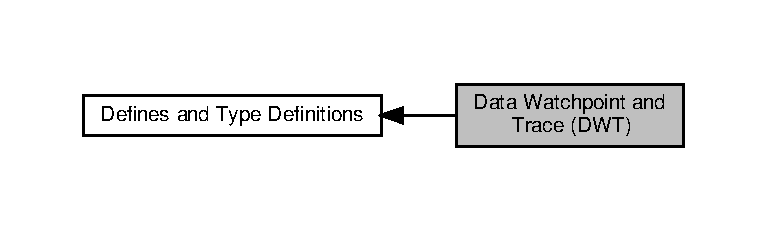
\includegraphics[width=350pt]{group___c_m_s_i_s___d_w_t}
\end{center}
\end{figure}
\subsection*{Komponenty}
\begin{DoxyCompactItemize}
\item 
struct \hyperlink{struct_d_w_t___type}{D\+W\+T\+\_\+\+Type}
\begin{DoxyCompactList}\small\item\em Structure type to access the Data Watchpoint and Trace Register (D\+WT). \end{DoxyCompactList}\end{DoxyCompactItemize}
\subsection*{Definicje}
\begin{DoxyCompactItemize}
\item 
\#define \hyperlink{group___c_m_s_i_s___d_w_t_gaac44b9b7d5391a7ffef129b7f6c84cd7}{D\+W\+T\+\_\+\+C\+T\+R\+L\+\_\+\+N\+U\+M\+C\+O\+M\+P\+\_\+\+Pos}~28U
\item 
\#define \hyperlink{group___c_m_s_i_s___d_w_t_gaa3d37d68c2ba73f2026265584c2815e7}{D\+W\+T\+\_\+\+C\+T\+R\+L\+\_\+\+N\+U\+M\+C\+O\+M\+P\+\_\+\+Msk}~(0x\+F\+U\+L $<$$<$ D\+W\+T\+\_\+\+C\+T\+R\+L\+\_\+\+N\+U\+M\+C\+O\+M\+P\+\_\+\+Pos)
\item 
\#define \hyperlink{group___c_m_s_i_s___d_w_t_gaa82840323a2628e7f4a2b09b74fa73fd}{D\+W\+T\+\_\+\+C\+T\+R\+L\+\_\+\+N\+O\+T\+R\+C\+P\+K\+T\+\_\+\+Pos}~27U
\item 
\#define \hyperlink{group___c_m_s_i_s___d_w_t_ga04d8bb0a065ca38e2e5f13a97e1f7073}{D\+W\+T\+\_\+\+C\+T\+R\+L\+\_\+\+N\+O\+T\+R\+C\+P\+K\+T\+\_\+\+Msk}~(0x1\+U\+L $<$$<$ D\+W\+T\+\_\+\+C\+T\+R\+L\+\_\+\+N\+O\+T\+R\+C\+P\+K\+T\+\_\+\+Pos)
\item 
\#define \hyperlink{group___c_m_s_i_s___d_w_t_gad997b9026715d5609b5a3b144eca42d0}{D\+W\+T\+\_\+\+C\+T\+R\+L\+\_\+\+N\+O\+E\+X\+T\+T\+R\+I\+G\+\_\+\+Pos}~26U
\item 
\#define \hyperlink{group___c_m_s_i_s___d_w_t_gacc7d15edf7a27147c422099ab475953e}{D\+W\+T\+\_\+\+C\+T\+R\+L\+\_\+\+N\+O\+E\+X\+T\+T\+R\+I\+G\+\_\+\+Msk}~(0x1\+U\+L $<$$<$ D\+W\+T\+\_\+\+C\+T\+R\+L\+\_\+\+N\+O\+E\+X\+T\+T\+R\+I\+G\+\_\+\+Pos)
\item 
\#define \hyperlink{group___c_m_s_i_s___d_w_t_ga337f6167d960f57f12aa382ffecce522}{D\+W\+T\+\_\+\+C\+T\+R\+L\+\_\+\+N\+O\+C\+Y\+C\+C\+N\+T\+\_\+\+Pos}~25U
\item 
\#define \hyperlink{group___c_m_s_i_s___d_w_t_gaf40c8d7a4fd978034c137e90f714c143}{D\+W\+T\+\_\+\+C\+T\+R\+L\+\_\+\+N\+O\+C\+Y\+C\+C\+N\+T\+\_\+\+Msk}~(0x1\+U\+L $<$$<$ D\+W\+T\+\_\+\+C\+T\+R\+L\+\_\+\+N\+O\+C\+Y\+C\+C\+N\+T\+\_\+\+Pos)
\item 
\#define \hyperlink{group___c_m_s_i_s___d_w_t_gad52a0e5be84363ab166cc17beca0d048}{D\+W\+T\+\_\+\+C\+T\+R\+L\+\_\+\+N\+O\+P\+R\+F\+C\+N\+T\+\_\+\+Pos}~24U
\item 
\#define \hyperlink{group___c_m_s_i_s___d_w_t_gafd8448d7db4bc51f27f202e6e1f27823}{D\+W\+T\+\_\+\+C\+T\+R\+L\+\_\+\+N\+O\+P\+R\+F\+C\+N\+T\+\_\+\+Msk}~(0x1\+U\+L $<$$<$ D\+W\+T\+\_\+\+C\+T\+R\+L\+\_\+\+N\+O\+P\+R\+F\+C\+N\+T\+\_\+\+Pos)
\item 
\#define \hyperlink{group___c_m_s_i_s___d_w_t_gae5dfe4049c2291e413f8713d7bd2bb1b}{D\+W\+T\+\_\+\+F\+U\+N\+C\+T\+I\+O\+N\+\_\+\+I\+D\+\_\+\+Pos}~27U
\item 
\#define \hyperlink{group___c_m_s_i_s___d_w_t_ga6bc2e15fcc300f511f64dad561c97582}{D\+W\+T\+\_\+\+F\+U\+N\+C\+T\+I\+O\+N\+\_\+\+I\+D\+\_\+\+Msk}~(0x1\+F\+U\+L $<$$<$ D\+W\+T\+\_\+\+F\+U\+N\+C\+T\+I\+O\+N\+\_\+\+I\+D\+\_\+\+Pos)
\item 
\#define \hyperlink{group___c_m_s_i_s___d_w_t_ga22c5787493f74a6bacf6ffb103a190ba}{D\+W\+T\+\_\+\+F\+U\+N\+C\+T\+I\+O\+N\+\_\+\+M\+A\+T\+C\+H\+E\+D\+\_\+\+Pos}~24U
\item 
\#define \hyperlink{group___c_m_s_i_s___d_w_t_gac8b1a655947490280709037808eec8ac}{D\+W\+T\+\_\+\+F\+U\+N\+C\+T\+I\+O\+N\+\_\+\+M\+A\+T\+C\+H\+E\+D\+\_\+\+Msk}~(0x1\+U\+L $<$$<$ D\+W\+T\+\_\+\+F\+U\+N\+C\+T\+I\+O\+N\+\_\+\+M\+A\+T\+C\+H\+E\+D\+\_\+\+Pos)
\item 
\#define \hyperlink{group___c_m_s_i_s___d_w_t_ga0517a186d4d448aa6416440f40fe7a4d}{D\+W\+T\+\_\+\+F\+U\+N\+C\+T\+I\+O\+N\+\_\+\+D\+A\+T\+A\+V\+S\+I\+Z\+E\+\_\+\+Pos}~10U
\item 
\#define \hyperlink{group___c_m_s_i_s___d_w_t_gaab42cbc1e6084c44d5de70971613ea76}{D\+W\+T\+\_\+\+F\+U\+N\+C\+T\+I\+O\+N\+\_\+\+D\+A\+T\+A\+V\+S\+I\+Z\+E\+\_\+\+Msk}~(0x3\+U\+L $<$$<$ D\+W\+T\+\_\+\+F\+U\+N\+C\+T\+I\+O\+N\+\_\+\+D\+A\+T\+A\+V\+S\+I\+Z\+E\+\_\+\+Pos)
\item 
\#define \hyperlink{group___c_m_s_i_s___d_w_t_ga00893dd43b824ca5be80e0235a237485}{D\+W\+T\+\_\+\+F\+U\+N\+C\+T\+I\+O\+N\+\_\+\+A\+C\+T\+I\+O\+N\+\_\+\+Pos}~4U
\item 
\#define \hyperlink{group___c_m_s_i_s___d_w_t_ga4d104412bbadbbfbde1c6da0f9b0fc3e}{D\+W\+T\+\_\+\+F\+U\+N\+C\+T\+I\+O\+N\+\_\+\+A\+C\+T\+I\+O\+N\+\_\+\+Msk}~(0x3\+U\+L $<$$<$ D\+W\+T\+\_\+\+F\+U\+N\+C\+T\+I\+O\+N\+\_\+\+A\+C\+T\+I\+O\+N\+\_\+\+Pos)
\item 
\#define \hyperlink{group___c_m_s_i_s___d_w_t_ga4108994a9eb6b2cd8d8289b1b7824fe5}{D\+W\+T\+\_\+\+F\+U\+N\+C\+T\+I\+O\+N\+\_\+\+M\+A\+T\+C\+H\+\_\+\+Pos}~0U
\item 
\#define \hyperlink{group___c_m_s_i_s___d_w_t_gac2fb3e387e405a4b33fc5ba0bea5b21c}{D\+W\+T\+\_\+\+F\+U\+N\+C\+T\+I\+O\+N\+\_\+\+M\+A\+T\+C\+H\+\_\+\+Msk}~(0x\+F\+U\+L /$\ast$$<$$<$ D\+W\+T\+\_\+\+F\+U\+N\+C\+T\+I\+O\+N\+\_\+\+M\+A\+T\+C\+H\+\_\+\+Pos$\ast$/)
\item 
\#define \hyperlink{group___c_m_s_i_s___d_w_t_gaac44b9b7d5391a7ffef129b7f6c84cd7}{D\+W\+T\+\_\+\+C\+T\+R\+L\+\_\+\+N\+U\+M\+C\+O\+M\+P\+\_\+\+Pos}~28U
\item 
\#define \hyperlink{group___c_m_s_i_s___d_w_t_gaa3d37d68c2ba73f2026265584c2815e7}{D\+W\+T\+\_\+\+C\+T\+R\+L\+\_\+\+N\+U\+M\+C\+O\+M\+P\+\_\+\+Msk}~(0x\+F\+U\+L $<$$<$ D\+W\+T\+\_\+\+C\+T\+R\+L\+\_\+\+N\+U\+M\+C\+O\+M\+P\+\_\+\+Pos)
\item 
\#define \hyperlink{group___c_m_s_i_s___d_w_t_gaa82840323a2628e7f4a2b09b74fa73fd}{D\+W\+T\+\_\+\+C\+T\+R\+L\+\_\+\+N\+O\+T\+R\+C\+P\+K\+T\+\_\+\+Pos}~27U
\item 
\#define \hyperlink{group___c_m_s_i_s___d_w_t_ga04d8bb0a065ca38e2e5f13a97e1f7073}{D\+W\+T\+\_\+\+C\+T\+R\+L\+\_\+\+N\+O\+T\+R\+C\+P\+K\+T\+\_\+\+Msk}~(0x1\+U\+L $<$$<$ D\+W\+T\+\_\+\+C\+T\+R\+L\+\_\+\+N\+O\+T\+R\+C\+P\+K\+T\+\_\+\+Pos)
\item 
\#define \hyperlink{group___c_m_s_i_s___d_w_t_gad997b9026715d5609b5a3b144eca42d0}{D\+W\+T\+\_\+\+C\+T\+R\+L\+\_\+\+N\+O\+E\+X\+T\+T\+R\+I\+G\+\_\+\+Pos}~26U
\item 
\#define \hyperlink{group___c_m_s_i_s___d_w_t_gacc7d15edf7a27147c422099ab475953e}{D\+W\+T\+\_\+\+C\+T\+R\+L\+\_\+\+N\+O\+E\+X\+T\+T\+R\+I\+G\+\_\+\+Msk}~(0x1\+U\+L $<$$<$ D\+W\+T\+\_\+\+C\+T\+R\+L\+\_\+\+N\+O\+E\+X\+T\+T\+R\+I\+G\+\_\+\+Pos)
\item 
\#define \hyperlink{group___c_m_s_i_s___d_w_t_ga337f6167d960f57f12aa382ffecce522}{D\+W\+T\+\_\+\+C\+T\+R\+L\+\_\+\+N\+O\+C\+Y\+C\+C\+N\+T\+\_\+\+Pos}~25U
\item 
\#define \hyperlink{group___c_m_s_i_s___d_w_t_gaf40c8d7a4fd978034c137e90f714c143}{D\+W\+T\+\_\+\+C\+T\+R\+L\+\_\+\+N\+O\+C\+Y\+C\+C\+N\+T\+\_\+\+Msk}~(0x1\+U\+L $<$$<$ D\+W\+T\+\_\+\+C\+T\+R\+L\+\_\+\+N\+O\+C\+Y\+C\+C\+N\+T\+\_\+\+Pos)
\item 
\#define \hyperlink{group___c_m_s_i_s___d_w_t_gad52a0e5be84363ab166cc17beca0d048}{D\+W\+T\+\_\+\+C\+T\+R\+L\+\_\+\+N\+O\+P\+R\+F\+C\+N\+T\+\_\+\+Pos}~24U
\item 
\#define \hyperlink{group___c_m_s_i_s___d_w_t_gafd8448d7db4bc51f27f202e6e1f27823}{D\+W\+T\+\_\+\+C\+T\+R\+L\+\_\+\+N\+O\+P\+R\+F\+C\+N\+T\+\_\+\+Msk}~(0x1\+U\+L $<$$<$ D\+W\+T\+\_\+\+C\+T\+R\+L\+\_\+\+N\+O\+P\+R\+F\+C\+N\+T\+\_\+\+Pos)
\item 
\#define \hyperlink{group___c_m_s_i_s___d_w_t_ga555f3a6b0510368a2bba4f0e06e559c3}{D\+W\+T\+\_\+\+C\+T\+R\+L\+\_\+\+C\+Y\+C\+D\+I\+S\+S\+\_\+\+Pos}~23U
\item 
\#define \hyperlink{group___c_m_s_i_s___d_w_t_ga688a3b9ecd2a044f2da3280367476271}{D\+W\+T\+\_\+\+C\+T\+R\+L\+\_\+\+C\+Y\+C\+D\+I\+S\+S\+\_\+\+Msk}~(0x1\+U\+L $<$$<$ D\+W\+T\+\_\+\+C\+T\+R\+L\+\_\+\+C\+Y\+C\+D\+I\+S\+S\+\_\+\+Pos)
\item 
\#define \hyperlink{group___c_m_s_i_s___d_w_t_ga0cb0640aaeb18a626d7823570d5c3cb6}{D\+W\+T\+\_\+\+C\+T\+R\+L\+\_\+\+C\+Y\+C\+E\+V\+T\+E\+N\+A\+\_\+\+Pos}~22U
\item 
\#define \hyperlink{group___c_m_s_i_s___d_w_t_ga40554bd81460e39abf08810f45fac1a2}{D\+W\+T\+\_\+\+C\+T\+R\+L\+\_\+\+C\+Y\+C\+E\+V\+T\+E\+N\+A\+\_\+\+Msk}~(0x1\+U\+L $<$$<$ D\+W\+T\+\_\+\+C\+T\+R\+L\+\_\+\+C\+Y\+C\+E\+V\+T\+E\+N\+A\+\_\+\+Pos)
\item 
\#define \hyperlink{group___c_m_s_i_s___d_w_t_ga5602b0707f446ce78d88ff2a3a82bfff}{D\+W\+T\+\_\+\+C\+T\+R\+L\+\_\+\+F\+O\+L\+D\+E\+V\+T\+E\+N\+A\+\_\+\+Pos}~21U
\item 
\#define \hyperlink{group___c_m_s_i_s___d_w_t_ga717e679d775562ae09185a3776b1582f}{D\+W\+T\+\_\+\+C\+T\+R\+L\+\_\+\+F\+O\+L\+D\+E\+V\+T\+E\+N\+A\+\_\+\+Msk}~(0x1\+U\+L $<$$<$ D\+W\+T\+\_\+\+C\+T\+R\+L\+\_\+\+F\+O\+L\+D\+E\+V\+T\+E\+N\+A\+\_\+\+Pos)
\item 
\#define \hyperlink{group___c_m_s_i_s___d_w_t_gaea5d1ee72188dc1d57b54c60a9f5233e}{D\+W\+T\+\_\+\+C\+T\+R\+L\+\_\+\+L\+S\+U\+E\+V\+T\+E\+N\+A\+\_\+\+Pos}~20U
\item 
\#define \hyperlink{group___c_m_s_i_s___d_w_t_gac47427f455fbc29d4b6f8a479169f2b2}{D\+W\+T\+\_\+\+C\+T\+R\+L\+\_\+\+L\+S\+U\+E\+V\+T\+E\+N\+A\+\_\+\+Msk}~(0x1\+U\+L $<$$<$ D\+W\+T\+\_\+\+C\+T\+R\+L\+\_\+\+L\+S\+U\+E\+V\+T\+E\+N\+A\+\_\+\+Pos)
\item 
\#define \hyperlink{group___c_m_s_i_s___d_w_t_ga9c6d62d121164013a8e3ee372f17f3e5}{D\+W\+T\+\_\+\+C\+T\+R\+L\+\_\+\+S\+L\+E\+E\+P\+E\+V\+T\+E\+N\+A\+\_\+\+Pos}~19U
\item 
\#define \hyperlink{group___c_m_s_i_s___d_w_t_ga2f431b3734fb840daf5b361034856da9}{D\+W\+T\+\_\+\+C\+T\+R\+L\+\_\+\+S\+L\+E\+E\+P\+E\+V\+T\+E\+N\+A\+\_\+\+Msk}~(0x1\+U\+L $<$$<$ D\+W\+T\+\_\+\+C\+T\+R\+L\+\_\+\+S\+L\+E\+E\+P\+E\+V\+T\+E\+N\+A\+\_\+\+Pos)
\item 
\#define \hyperlink{group___c_m_s_i_s___d_w_t_gaf4e73f548ae3e945ef8b1d9ff1281544}{D\+W\+T\+\_\+\+C\+T\+R\+L\+\_\+\+E\+X\+C\+E\+V\+T\+E\+N\+A\+\_\+\+Pos}~18U
\item 
\#define \hyperlink{group___c_m_s_i_s___d_w_t_gab7ee0def33423b5859ca4030dff63b58}{D\+W\+T\+\_\+\+C\+T\+R\+L\+\_\+\+E\+X\+C\+E\+V\+T\+E\+N\+A\+\_\+\+Msk}~(0x1\+U\+L $<$$<$ D\+W\+T\+\_\+\+C\+T\+R\+L\+\_\+\+E\+X\+C\+E\+V\+T\+E\+N\+A\+\_\+\+Pos)
\item 
\#define \hyperlink{group___c_m_s_i_s___d_w_t_ga9fff0b71fb0be1499f5180c6bce1fc8f}{D\+W\+T\+\_\+\+C\+T\+R\+L\+\_\+\+C\+P\+I\+E\+V\+T\+E\+N\+A\+\_\+\+Pos}~17U
\item 
\#define \hyperlink{group___c_m_s_i_s___d_w_t_ga189089c30aade60b983df17ad2412f6f}{D\+W\+T\+\_\+\+C\+T\+R\+L\+\_\+\+C\+P\+I\+E\+V\+T\+E\+N\+A\+\_\+\+Msk}~(0x1\+U\+L $<$$<$ D\+W\+T\+\_\+\+C\+T\+R\+L\+\_\+\+C\+P\+I\+E\+V\+T\+E\+N\+A\+\_\+\+Pos)
\item 
\#define \hyperlink{group___c_m_s_i_s___d_w_t_ga05f13b547a9a1e63e003ee0bc6446d0d}{D\+W\+T\+\_\+\+C\+T\+R\+L\+\_\+\+E\+X\+C\+T\+R\+C\+E\+N\+A\+\_\+\+Pos}~16U
\item 
\#define \hyperlink{group___c_m_s_i_s___d_w_t_gaf4fbb509ab3cbb768f16484c660a24c3}{D\+W\+T\+\_\+\+C\+T\+R\+L\+\_\+\+E\+X\+C\+T\+R\+C\+E\+N\+A\+\_\+\+Msk}~(0x1\+U\+L $<$$<$ D\+W\+T\+\_\+\+C\+T\+R\+L\+\_\+\+E\+X\+C\+T\+R\+C\+E\+N\+A\+\_\+\+Pos)
\item 
\#define \hyperlink{group___c_m_s_i_s___d_w_t_ga1e14afc7790fcb424fcf619e192554c9}{D\+W\+T\+\_\+\+C\+T\+R\+L\+\_\+\+P\+C\+S\+A\+M\+P\+L\+E\+N\+A\+\_\+\+Pos}~12U
\item 
\#define \hyperlink{group___c_m_s_i_s___d_w_t_gafdcf1c86f43fbeaf2780ce797c9ef3d6}{D\+W\+T\+\_\+\+C\+T\+R\+L\+\_\+\+P\+C\+S\+A\+M\+P\+L\+E\+N\+A\+\_\+\+Msk}~(0x1\+U\+L $<$$<$ D\+W\+T\+\_\+\+C\+T\+R\+L\+\_\+\+P\+C\+S\+A\+M\+P\+L\+E\+N\+A\+\_\+\+Pos)
\item 
\#define \hyperlink{group___c_m_s_i_s___d_w_t_ga678ef08786edcbef964479217efb9284}{D\+W\+T\+\_\+\+C\+T\+R\+L\+\_\+\+S\+Y\+N\+C\+T\+A\+P\+\_\+\+Pos}~10U
\item 
\#define \hyperlink{group___c_m_s_i_s___d_w_t_gaf1e6c3729d56ecadeb6eeff4d225968c}{D\+W\+T\+\_\+\+C\+T\+R\+L\+\_\+\+S\+Y\+N\+C\+T\+A\+P\+\_\+\+Msk}~(0x3\+U\+L $<$$<$ D\+W\+T\+\_\+\+C\+T\+R\+L\+\_\+\+S\+Y\+N\+C\+T\+A\+P\+\_\+\+Pos)
\item 
\#define \hyperlink{group___c_m_s_i_s___d_w_t_gaf70b80936c7db60bf84fb6dadb8a3559}{D\+W\+T\+\_\+\+C\+T\+R\+L\+\_\+\+C\+Y\+C\+T\+A\+P\+\_\+\+Pos}~9U
\item 
\#define \hyperlink{group___c_m_s_i_s___d_w_t_ga6c12e2868b8989a69445646698b8c331}{D\+W\+T\+\_\+\+C\+T\+R\+L\+\_\+\+C\+Y\+C\+T\+A\+P\+\_\+\+Msk}~(0x1\+U\+L $<$$<$ D\+W\+T\+\_\+\+C\+T\+R\+L\+\_\+\+C\+Y\+C\+T\+A\+P\+\_\+\+Pos)
\item 
\#define \hyperlink{group___c_m_s_i_s___d_w_t_ga2868c0b28eb13be930afb819f55f6f25}{D\+W\+T\+\_\+\+C\+T\+R\+L\+\_\+\+P\+O\+S\+T\+I\+N\+I\+T\+\_\+\+Pos}~5U
\item 
\#define \hyperlink{group___c_m_s_i_s___d_w_t_gab8cbbee1e1d94d09f9a1f86379a08ee8}{D\+W\+T\+\_\+\+C\+T\+R\+L\+\_\+\+P\+O\+S\+T\+I\+N\+I\+T\+\_\+\+Msk}~(0x\+F\+U\+L $<$$<$ D\+W\+T\+\_\+\+C\+T\+R\+L\+\_\+\+P\+O\+S\+T\+I\+N\+I\+T\+\_\+\+Pos)
\item 
\#define \hyperlink{group___c_m_s_i_s___d_w_t_ga129bc152febfddd67a0c20c6814cba69}{D\+W\+T\+\_\+\+C\+T\+R\+L\+\_\+\+P\+O\+S\+T\+P\+R\+E\+S\+E\+T\+\_\+\+Pos}~1U
\item 
\#define \hyperlink{group___c_m_s_i_s___d_w_t_ga11d9e1e2a758fdd2657aa68ce61b9c9d}{D\+W\+T\+\_\+\+C\+T\+R\+L\+\_\+\+P\+O\+S\+T\+P\+R\+E\+S\+E\+T\+\_\+\+Msk}~(0x\+F\+U\+L $<$$<$ D\+W\+T\+\_\+\+C\+T\+R\+L\+\_\+\+P\+O\+S\+T\+P\+R\+E\+S\+E\+T\+\_\+\+Pos)
\item 
\#define \hyperlink{group___c_m_s_i_s___d_w_t_gaa4509f5f8514a7200be61691f0e01f10}{D\+W\+T\+\_\+\+C\+T\+R\+L\+\_\+\+C\+Y\+C\+C\+N\+T\+E\+N\+A\+\_\+\+Pos}~0U
\item 
\#define \hyperlink{group___c_m_s_i_s___d_w_t_ga4a9d209dc2a81ea6bfa0ea21331769d3}{D\+W\+T\+\_\+\+C\+T\+R\+L\+\_\+\+C\+Y\+C\+C\+N\+T\+E\+N\+A\+\_\+\+Msk}~(0x1\+U\+L /$\ast$$<$$<$ D\+W\+T\+\_\+\+C\+T\+R\+L\+\_\+\+C\+Y\+C\+C\+N\+T\+E\+N\+A\+\_\+\+Pos$\ast$/)
\item 
\#define \hyperlink{group___c_m_s_i_s___d_w_t_ga80e9ad8f6a9e2344af8a3cf989bebe3d}{D\+W\+T\+\_\+\+C\+P\+I\+C\+N\+T\+\_\+\+C\+P\+I\+C\+N\+T\+\_\+\+Pos}~0U
\item 
\#define \hyperlink{group___c_m_s_i_s___d_w_t_ga76f39e7bca3fa86a4dbf7b8f6adb7217}{D\+W\+T\+\_\+\+C\+P\+I\+C\+N\+T\+\_\+\+C\+P\+I\+C\+N\+T\+\_\+\+Msk}~(0x\+F\+F\+U\+L /$\ast$$<$$<$ D\+W\+T\+\_\+\+C\+P\+I\+C\+N\+T\+\_\+\+C\+P\+I\+C\+N\+T\+\_\+\+Pos$\ast$/)
\item 
\#define \hyperlink{group___c_m_s_i_s___d_w_t_ga031c693654030d4cba398b45d2925b1d}{D\+W\+T\+\_\+\+E\+X\+C\+C\+N\+T\+\_\+\+E\+X\+C\+C\+N\+T\+\_\+\+Pos}~0U
\item 
\#define \hyperlink{group___c_m_s_i_s___d_w_t_ga057fa604a107b58a198bbbadb47e69c9}{D\+W\+T\+\_\+\+E\+X\+C\+C\+N\+T\+\_\+\+E\+X\+C\+C\+N\+T\+\_\+\+Msk}~(0x\+F\+F\+U\+L /$\ast$$<$$<$ D\+W\+T\+\_\+\+E\+X\+C\+C\+N\+T\+\_\+\+E\+X\+C\+C\+N\+T\+\_\+\+Pos$\ast$/)
\item 
\#define \hyperlink{group___c_m_s_i_s___d_w_t_ga0371a84a7996dc5852c56afb2676ba1c}{D\+W\+T\+\_\+\+S\+L\+E\+E\+P\+C\+N\+T\+\_\+\+S\+L\+E\+E\+P\+C\+N\+T\+\_\+\+Pos}~0U
\item 
\#define \hyperlink{group___c_m_s_i_s___d_w_t_ga1e340751d71413fef400a0a1d76cc828}{D\+W\+T\+\_\+\+S\+L\+E\+E\+P\+C\+N\+T\+\_\+\+S\+L\+E\+E\+P\+C\+N\+T\+\_\+\+Msk}~(0x\+F\+F\+U\+L /$\ast$$<$$<$ D\+W\+T\+\_\+\+S\+L\+E\+E\+P\+C\+N\+T\+\_\+\+S\+L\+E\+E\+P\+C\+N\+T\+\_\+\+Pos$\ast$/)
\item 
\#define \hyperlink{group___c_m_s_i_s___d_w_t_gab9394c7911b0b4312a096dad91d53a3d}{D\+W\+T\+\_\+\+L\+S\+U\+C\+N\+T\+\_\+\+L\+S\+U\+C\+N\+T\+\_\+\+Pos}~0U
\item 
\#define \hyperlink{group___c_m_s_i_s___d_w_t_ga2186d7fc9317e20bad61336ee2925615}{D\+W\+T\+\_\+\+L\+S\+U\+C\+N\+T\+\_\+\+L\+S\+U\+C\+N\+T\+\_\+\+Msk}~(0x\+F\+F\+U\+L /$\ast$$<$$<$ D\+W\+T\+\_\+\+L\+S\+U\+C\+N\+T\+\_\+\+L\+S\+U\+C\+N\+T\+\_\+\+Pos$\ast$/)
\item 
\#define \hyperlink{group___c_m_s_i_s___d_w_t_ga7f8af5ac12d178ba31a516f6ed141455}{D\+W\+T\+\_\+\+F\+O\+L\+D\+C\+N\+T\+\_\+\+F\+O\+L\+D\+C\+N\+T\+\_\+\+Pos}~0U
\item 
\#define \hyperlink{group___c_m_s_i_s___d_w_t_ga9cb73d0342d38b14e41027d3c5c02647}{D\+W\+T\+\_\+\+F\+O\+L\+D\+C\+N\+T\+\_\+\+F\+O\+L\+D\+C\+N\+T\+\_\+\+Msk}~(0x\+F\+F\+U\+L /$\ast$$<$$<$ D\+W\+T\+\_\+\+F\+O\+L\+D\+C\+N\+T\+\_\+\+F\+O\+L\+D\+C\+N\+T\+\_\+\+Pos$\ast$/)
\item 
\#define \hyperlink{group___c_m_s_i_s___d_w_t_gae5dfe4049c2291e413f8713d7bd2bb1b}{D\+W\+T\+\_\+\+F\+U\+N\+C\+T\+I\+O\+N\+\_\+\+I\+D\+\_\+\+Pos}~27U
\item 
\#define \hyperlink{group___c_m_s_i_s___d_w_t_ga6bc2e15fcc300f511f64dad561c97582}{D\+W\+T\+\_\+\+F\+U\+N\+C\+T\+I\+O\+N\+\_\+\+I\+D\+\_\+\+Msk}~(0x1\+F\+U\+L $<$$<$ D\+W\+T\+\_\+\+F\+U\+N\+C\+T\+I\+O\+N\+\_\+\+I\+D\+\_\+\+Pos)
\item 
\#define \hyperlink{group___c_m_s_i_s___d_w_t_ga22c5787493f74a6bacf6ffb103a190ba}{D\+W\+T\+\_\+\+F\+U\+N\+C\+T\+I\+O\+N\+\_\+\+M\+A\+T\+C\+H\+E\+D\+\_\+\+Pos}~24U
\item 
\#define \hyperlink{group___c_m_s_i_s___d_w_t_gac8b1a655947490280709037808eec8ac}{D\+W\+T\+\_\+\+F\+U\+N\+C\+T\+I\+O\+N\+\_\+\+M\+A\+T\+C\+H\+E\+D\+\_\+\+Msk}~(0x1\+U\+L $<$$<$ D\+W\+T\+\_\+\+F\+U\+N\+C\+T\+I\+O\+N\+\_\+\+M\+A\+T\+C\+H\+E\+D\+\_\+\+Pos)
\item 
\#define \hyperlink{group___c_m_s_i_s___d_w_t_ga0517a186d4d448aa6416440f40fe7a4d}{D\+W\+T\+\_\+\+F\+U\+N\+C\+T\+I\+O\+N\+\_\+\+D\+A\+T\+A\+V\+S\+I\+Z\+E\+\_\+\+Pos}~10U
\item 
\#define \hyperlink{group___c_m_s_i_s___d_w_t_gaab42cbc1e6084c44d5de70971613ea76}{D\+W\+T\+\_\+\+F\+U\+N\+C\+T\+I\+O\+N\+\_\+\+D\+A\+T\+A\+V\+S\+I\+Z\+E\+\_\+\+Msk}~(0x3\+U\+L $<$$<$ D\+W\+T\+\_\+\+F\+U\+N\+C\+T\+I\+O\+N\+\_\+\+D\+A\+T\+A\+V\+S\+I\+Z\+E\+\_\+\+Pos)
\item 
\#define \hyperlink{group___c_m_s_i_s___d_w_t_ga00893dd43b824ca5be80e0235a237485}{D\+W\+T\+\_\+\+F\+U\+N\+C\+T\+I\+O\+N\+\_\+\+A\+C\+T\+I\+O\+N\+\_\+\+Pos}~4U
\item 
\#define \hyperlink{group___c_m_s_i_s___d_w_t_ga4d104412bbadbbfbde1c6da0f9b0fc3e}{D\+W\+T\+\_\+\+F\+U\+N\+C\+T\+I\+O\+N\+\_\+\+A\+C\+T\+I\+O\+N\+\_\+\+Msk}~(0x1\+U\+L $<$$<$ D\+W\+T\+\_\+\+F\+U\+N\+C\+T\+I\+O\+N\+\_\+\+A\+C\+T\+I\+O\+N\+\_\+\+Pos)
\item 
\#define \hyperlink{group___c_m_s_i_s___d_w_t_ga4108994a9eb6b2cd8d8289b1b7824fe5}{D\+W\+T\+\_\+\+F\+U\+N\+C\+T\+I\+O\+N\+\_\+\+M\+A\+T\+C\+H\+\_\+\+Pos}~0U
\item 
\#define \hyperlink{group___c_m_s_i_s___d_w_t_gac2fb3e387e405a4b33fc5ba0bea5b21c}{D\+W\+T\+\_\+\+F\+U\+N\+C\+T\+I\+O\+N\+\_\+\+M\+A\+T\+C\+H\+\_\+\+Msk}~(0x\+F\+U\+L /$\ast$$<$$<$ D\+W\+T\+\_\+\+F\+U\+N\+C\+T\+I\+O\+N\+\_\+\+M\+A\+T\+C\+H\+\_\+\+Pos$\ast$/)
\item 
\#define \hyperlink{group___c_m_s_i_s___d_w_t_gaac44b9b7d5391a7ffef129b7f6c84cd7}{D\+W\+T\+\_\+\+C\+T\+R\+L\+\_\+\+N\+U\+M\+C\+O\+M\+P\+\_\+\+Pos}~28U
\item 
\#define \hyperlink{group___c_m_s_i_s___d_w_t_gaa3d37d68c2ba73f2026265584c2815e7}{D\+W\+T\+\_\+\+C\+T\+R\+L\+\_\+\+N\+U\+M\+C\+O\+M\+P\+\_\+\+Msk}~(0x\+F\+U\+L $<$$<$ D\+W\+T\+\_\+\+C\+T\+R\+L\+\_\+\+N\+U\+M\+C\+O\+M\+P\+\_\+\+Pos)
\item 
\#define \hyperlink{group___c_m_s_i_s___d_w_t_gaa82840323a2628e7f4a2b09b74fa73fd}{D\+W\+T\+\_\+\+C\+T\+R\+L\+\_\+\+N\+O\+T\+R\+C\+P\+K\+T\+\_\+\+Pos}~27U
\item 
\#define \hyperlink{group___c_m_s_i_s___d_w_t_ga04d8bb0a065ca38e2e5f13a97e1f7073}{D\+W\+T\+\_\+\+C\+T\+R\+L\+\_\+\+N\+O\+T\+R\+C\+P\+K\+T\+\_\+\+Msk}~(0x1\+U\+L $<$$<$ D\+W\+T\+\_\+\+C\+T\+R\+L\+\_\+\+N\+O\+T\+R\+C\+P\+K\+T\+\_\+\+Pos)
\item 
\#define \hyperlink{group___c_m_s_i_s___d_w_t_gad997b9026715d5609b5a3b144eca42d0}{D\+W\+T\+\_\+\+C\+T\+R\+L\+\_\+\+N\+O\+E\+X\+T\+T\+R\+I\+G\+\_\+\+Pos}~26U
\item 
\#define \hyperlink{group___c_m_s_i_s___d_w_t_gacc7d15edf7a27147c422099ab475953e}{D\+W\+T\+\_\+\+C\+T\+R\+L\+\_\+\+N\+O\+E\+X\+T\+T\+R\+I\+G\+\_\+\+Msk}~(0x1\+U\+L $<$$<$ D\+W\+T\+\_\+\+C\+T\+R\+L\+\_\+\+N\+O\+E\+X\+T\+T\+R\+I\+G\+\_\+\+Pos)
\item 
\#define \hyperlink{group___c_m_s_i_s___d_w_t_ga337f6167d960f57f12aa382ffecce522}{D\+W\+T\+\_\+\+C\+T\+R\+L\+\_\+\+N\+O\+C\+Y\+C\+C\+N\+T\+\_\+\+Pos}~25U
\item 
\#define \hyperlink{group___c_m_s_i_s___d_w_t_gaf40c8d7a4fd978034c137e90f714c143}{D\+W\+T\+\_\+\+C\+T\+R\+L\+\_\+\+N\+O\+C\+Y\+C\+C\+N\+T\+\_\+\+Msk}~(0x1\+U\+L $<$$<$ D\+W\+T\+\_\+\+C\+T\+R\+L\+\_\+\+N\+O\+C\+Y\+C\+C\+N\+T\+\_\+\+Pos)
\item 
\#define \hyperlink{group___c_m_s_i_s___d_w_t_gad52a0e5be84363ab166cc17beca0d048}{D\+W\+T\+\_\+\+C\+T\+R\+L\+\_\+\+N\+O\+P\+R\+F\+C\+N\+T\+\_\+\+Pos}~24U
\item 
\#define \hyperlink{group___c_m_s_i_s___d_w_t_gafd8448d7db4bc51f27f202e6e1f27823}{D\+W\+T\+\_\+\+C\+T\+R\+L\+\_\+\+N\+O\+P\+R\+F\+C\+N\+T\+\_\+\+Msk}~(0x1\+U\+L $<$$<$ D\+W\+T\+\_\+\+C\+T\+R\+L\+\_\+\+N\+O\+P\+R\+F\+C\+N\+T\+\_\+\+Pos)
\item 
\#define \hyperlink{group___c_m_s_i_s___d_w_t_gae5dfe4049c2291e413f8713d7bd2bb1b}{D\+W\+T\+\_\+\+F\+U\+N\+C\+T\+I\+O\+N\+\_\+\+I\+D\+\_\+\+Pos}~27U
\item 
\#define \hyperlink{group___c_m_s_i_s___d_w_t_ga6bc2e15fcc300f511f64dad561c97582}{D\+W\+T\+\_\+\+F\+U\+N\+C\+T\+I\+O\+N\+\_\+\+I\+D\+\_\+\+Msk}~(0x1\+F\+U\+L $<$$<$ D\+W\+T\+\_\+\+F\+U\+N\+C\+T\+I\+O\+N\+\_\+\+I\+D\+\_\+\+Pos)
\item 
\#define \hyperlink{group___c_m_s_i_s___d_w_t_ga22c5787493f74a6bacf6ffb103a190ba}{D\+W\+T\+\_\+\+F\+U\+N\+C\+T\+I\+O\+N\+\_\+\+M\+A\+T\+C\+H\+E\+D\+\_\+\+Pos}~24U
\item 
\#define \hyperlink{group___c_m_s_i_s___d_w_t_gac8b1a655947490280709037808eec8ac}{D\+W\+T\+\_\+\+F\+U\+N\+C\+T\+I\+O\+N\+\_\+\+M\+A\+T\+C\+H\+E\+D\+\_\+\+Msk}~(0x1\+U\+L $<$$<$ D\+W\+T\+\_\+\+F\+U\+N\+C\+T\+I\+O\+N\+\_\+\+M\+A\+T\+C\+H\+E\+D\+\_\+\+Pos)
\item 
\#define \hyperlink{group___c_m_s_i_s___d_w_t_ga0517a186d4d448aa6416440f40fe7a4d}{D\+W\+T\+\_\+\+F\+U\+N\+C\+T\+I\+O\+N\+\_\+\+D\+A\+T\+A\+V\+S\+I\+Z\+E\+\_\+\+Pos}~10U
\item 
\#define \hyperlink{group___c_m_s_i_s___d_w_t_gaab42cbc1e6084c44d5de70971613ea76}{D\+W\+T\+\_\+\+F\+U\+N\+C\+T\+I\+O\+N\+\_\+\+D\+A\+T\+A\+V\+S\+I\+Z\+E\+\_\+\+Msk}~(0x3\+U\+L $<$$<$ D\+W\+T\+\_\+\+F\+U\+N\+C\+T\+I\+O\+N\+\_\+\+D\+A\+T\+A\+V\+S\+I\+Z\+E\+\_\+\+Pos)
\item 
\#define \hyperlink{group___c_m_s_i_s___d_w_t_ga00893dd43b824ca5be80e0235a237485}{D\+W\+T\+\_\+\+F\+U\+N\+C\+T\+I\+O\+N\+\_\+\+A\+C\+T\+I\+O\+N\+\_\+\+Pos}~4U
\item 
\#define \hyperlink{group___c_m_s_i_s___d_w_t_ga4d104412bbadbbfbde1c6da0f9b0fc3e}{D\+W\+T\+\_\+\+F\+U\+N\+C\+T\+I\+O\+N\+\_\+\+A\+C\+T\+I\+O\+N\+\_\+\+Msk}~(0x3\+U\+L $<$$<$ D\+W\+T\+\_\+\+F\+U\+N\+C\+T\+I\+O\+N\+\_\+\+A\+C\+T\+I\+O\+N\+\_\+\+Pos)
\item 
\#define \hyperlink{group___c_m_s_i_s___d_w_t_ga4108994a9eb6b2cd8d8289b1b7824fe5}{D\+W\+T\+\_\+\+F\+U\+N\+C\+T\+I\+O\+N\+\_\+\+M\+A\+T\+C\+H\+\_\+\+Pos}~0U
\item 
\#define \hyperlink{group___c_m_s_i_s___d_w_t_gac2fb3e387e405a4b33fc5ba0bea5b21c}{D\+W\+T\+\_\+\+F\+U\+N\+C\+T\+I\+O\+N\+\_\+\+M\+A\+T\+C\+H\+\_\+\+Msk}~(0x\+F\+U\+L /$\ast$$<$$<$ D\+W\+T\+\_\+\+F\+U\+N\+C\+T\+I\+O\+N\+\_\+\+M\+A\+T\+C\+H\+\_\+\+Pos$\ast$/)
\item 
\#define \hyperlink{group___c_m_s_i_s___d_w_t_gaac44b9b7d5391a7ffef129b7f6c84cd7}{D\+W\+T\+\_\+\+C\+T\+R\+L\+\_\+\+N\+U\+M\+C\+O\+M\+P\+\_\+\+Pos}~28U
\item 
\#define \hyperlink{group___c_m_s_i_s___d_w_t_gaa3d37d68c2ba73f2026265584c2815e7}{D\+W\+T\+\_\+\+C\+T\+R\+L\+\_\+\+N\+U\+M\+C\+O\+M\+P\+\_\+\+Msk}~(0x\+F\+U\+L $<$$<$ D\+W\+T\+\_\+\+C\+T\+R\+L\+\_\+\+N\+U\+M\+C\+O\+M\+P\+\_\+\+Pos)
\item 
\#define \hyperlink{group___c_m_s_i_s___d_w_t_gaa82840323a2628e7f4a2b09b74fa73fd}{D\+W\+T\+\_\+\+C\+T\+R\+L\+\_\+\+N\+O\+T\+R\+C\+P\+K\+T\+\_\+\+Pos}~27U
\item 
\#define \hyperlink{group___c_m_s_i_s___d_w_t_ga04d8bb0a065ca38e2e5f13a97e1f7073}{D\+W\+T\+\_\+\+C\+T\+R\+L\+\_\+\+N\+O\+T\+R\+C\+P\+K\+T\+\_\+\+Msk}~(0x1\+U\+L $<$$<$ D\+W\+T\+\_\+\+C\+T\+R\+L\+\_\+\+N\+O\+T\+R\+C\+P\+K\+T\+\_\+\+Pos)
\item 
\#define \hyperlink{group___c_m_s_i_s___d_w_t_gad997b9026715d5609b5a3b144eca42d0}{D\+W\+T\+\_\+\+C\+T\+R\+L\+\_\+\+N\+O\+E\+X\+T\+T\+R\+I\+G\+\_\+\+Pos}~26U
\item 
\#define \hyperlink{group___c_m_s_i_s___d_w_t_gacc7d15edf7a27147c422099ab475953e}{D\+W\+T\+\_\+\+C\+T\+R\+L\+\_\+\+N\+O\+E\+X\+T\+T\+R\+I\+G\+\_\+\+Msk}~(0x1\+U\+L $<$$<$ D\+W\+T\+\_\+\+C\+T\+R\+L\+\_\+\+N\+O\+E\+X\+T\+T\+R\+I\+G\+\_\+\+Pos)
\item 
\#define \hyperlink{group___c_m_s_i_s___d_w_t_ga337f6167d960f57f12aa382ffecce522}{D\+W\+T\+\_\+\+C\+T\+R\+L\+\_\+\+N\+O\+C\+Y\+C\+C\+N\+T\+\_\+\+Pos}~25U
\item 
\#define \hyperlink{group___c_m_s_i_s___d_w_t_gaf40c8d7a4fd978034c137e90f714c143}{D\+W\+T\+\_\+\+C\+T\+R\+L\+\_\+\+N\+O\+C\+Y\+C\+C\+N\+T\+\_\+\+Msk}~(0x1\+U\+L $<$$<$ D\+W\+T\+\_\+\+C\+T\+R\+L\+\_\+\+N\+O\+C\+Y\+C\+C\+N\+T\+\_\+\+Pos)
\item 
\#define \hyperlink{group___c_m_s_i_s___d_w_t_gad52a0e5be84363ab166cc17beca0d048}{D\+W\+T\+\_\+\+C\+T\+R\+L\+\_\+\+N\+O\+P\+R\+F\+C\+N\+T\+\_\+\+Pos}~24U
\item 
\#define \hyperlink{group___c_m_s_i_s___d_w_t_gafd8448d7db4bc51f27f202e6e1f27823}{D\+W\+T\+\_\+\+C\+T\+R\+L\+\_\+\+N\+O\+P\+R\+F\+C\+N\+T\+\_\+\+Msk}~(0x1\+U\+L $<$$<$ D\+W\+T\+\_\+\+C\+T\+R\+L\+\_\+\+N\+O\+P\+R\+F\+C\+N\+T\+\_\+\+Pos)
\item 
\#define \hyperlink{group___c_m_s_i_s___d_w_t_ga0cb0640aaeb18a626d7823570d5c3cb6}{D\+W\+T\+\_\+\+C\+T\+R\+L\+\_\+\+C\+Y\+C\+E\+V\+T\+E\+N\+A\+\_\+\+Pos}~22U
\item 
\#define \hyperlink{group___c_m_s_i_s___d_w_t_ga40554bd81460e39abf08810f45fac1a2}{D\+W\+T\+\_\+\+C\+T\+R\+L\+\_\+\+C\+Y\+C\+E\+V\+T\+E\+N\+A\+\_\+\+Msk}~(0x1\+U\+L $<$$<$ D\+W\+T\+\_\+\+C\+T\+R\+L\+\_\+\+C\+Y\+C\+E\+V\+T\+E\+N\+A\+\_\+\+Pos)
\item 
\#define \hyperlink{group___c_m_s_i_s___d_w_t_ga5602b0707f446ce78d88ff2a3a82bfff}{D\+W\+T\+\_\+\+C\+T\+R\+L\+\_\+\+F\+O\+L\+D\+E\+V\+T\+E\+N\+A\+\_\+\+Pos}~21U
\item 
\#define \hyperlink{group___c_m_s_i_s___d_w_t_ga717e679d775562ae09185a3776b1582f}{D\+W\+T\+\_\+\+C\+T\+R\+L\+\_\+\+F\+O\+L\+D\+E\+V\+T\+E\+N\+A\+\_\+\+Msk}~(0x1\+U\+L $<$$<$ D\+W\+T\+\_\+\+C\+T\+R\+L\+\_\+\+F\+O\+L\+D\+E\+V\+T\+E\+N\+A\+\_\+\+Pos)
\item 
\#define \hyperlink{group___c_m_s_i_s___d_w_t_gaea5d1ee72188dc1d57b54c60a9f5233e}{D\+W\+T\+\_\+\+C\+T\+R\+L\+\_\+\+L\+S\+U\+E\+V\+T\+E\+N\+A\+\_\+\+Pos}~20U
\item 
\#define \hyperlink{group___c_m_s_i_s___d_w_t_gac47427f455fbc29d4b6f8a479169f2b2}{D\+W\+T\+\_\+\+C\+T\+R\+L\+\_\+\+L\+S\+U\+E\+V\+T\+E\+N\+A\+\_\+\+Msk}~(0x1\+U\+L $<$$<$ D\+W\+T\+\_\+\+C\+T\+R\+L\+\_\+\+L\+S\+U\+E\+V\+T\+E\+N\+A\+\_\+\+Pos)
\item 
\#define \hyperlink{group___c_m_s_i_s___d_w_t_ga9c6d62d121164013a8e3ee372f17f3e5}{D\+W\+T\+\_\+\+C\+T\+R\+L\+\_\+\+S\+L\+E\+E\+P\+E\+V\+T\+E\+N\+A\+\_\+\+Pos}~19U
\item 
\#define \hyperlink{group___c_m_s_i_s___d_w_t_ga2f431b3734fb840daf5b361034856da9}{D\+W\+T\+\_\+\+C\+T\+R\+L\+\_\+\+S\+L\+E\+E\+P\+E\+V\+T\+E\+N\+A\+\_\+\+Msk}~(0x1\+U\+L $<$$<$ D\+W\+T\+\_\+\+C\+T\+R\+L\+\_\+\+S\+L\+E\+E\+P\+E\+V\+T\+E\+N\+A\+\_\+\+Pos)
\item 
\#define \hyperlink{group___c_m_s_i_s___d_w_t_gaf4e73f548ae3e945ef8b1d9ff1281544}{D\+W\+T\+\_\+\+C\+T\+R\+L\+\_\+\+E\+X\+C\+E\+V\+T\+E\+N\+A\+\_\+\+Pos}~18U
\item 
\#define \hyperlink{group___c_m_s_i_s___d_w_t_gab7ee0def33423b5859ca4030dff63b58}{D\+W\+T\+\_\+\+C\+T\+R\+L\+\_\+\+E\+X\+C\+E\+V\+T\+E\+N\+A\+\_\+\+Msk}~(0x1\+U\+L $<$$<$ D\+W\+T\+\_\+\+C\+T\+R\+L\+\_\+\+E\+X\+C\+E\+V\+T\+E\+N\+A\+\_\+\+Pos)
\item 
\#define \hyperlink{group___c_m_s_i_s___d_w_t_ga9fff0b71fb0be1499f5180c6bce1fc8f}{D\+W\+T\+\_\+\+C\+T\+R\+L\+\_\+\+C\+P\+I\+E\+V\+T\+E\+N\+A\+\_\+\+Pos}~17U
\item 
\#define \hyperlink{group___c_m_s_i_s___d_w_t_ga189089c30aade60b983df17ad2412f6f}{D\+W\+T\+\_\+\+C\+T\+R\+L\+\_\+\+C\+P\+I\+E\+V\+T\+E\+N\+A\+\_\+\+Msk}~(0x1\+U\+L $<$$<$ D\+W\+T\+\_\+\+C\+T\+R\+L\+\_\+\+C\+P\+I\+E\+V\+T\+E\+N\+A\+\_\+\+Pos)
\item 
\#define \hyperlink{group___c_m_s_i_s___d_w_t_ga05f13b547a9a1e63e003ee0bc6446d0d}{D\+W\+T\+\_\+\+C\+T\+R\+L\+\_\+\+E\+X\+C\+T\+R\+C\+E\+N\+A\+\_\+\+Pos}~16U
\item 
\#define \hyperlink{group___c_m_s_i_s___d_w_t_gaf4fbb509ab3cbb768f16484c660a24c3}{D\+W\+T\+\_\+\+C\+T\+R\+L\+\_\+\+E\+X\+C\+T\+R\+C\+E\+N\+A\+\_\+\+Msk}~(0x1\+U\+L $<$$<$ D\+W\+T\+\_\+\+C\+T\+R\+L\+\_\+\+E\+X\+C\+T\+R\+C\+E\+N\+A\+\_\+\+Pos)
\item 
\#define \hyperlink{group___c_m_s_i_s___d_w_t_ga1e14afc7790fcb424fcf619e192554c9}{D\+W\+T\+\_\+\+C\+T\+R\+L\+\_\+\+P\+C\+S\+A\+M\+P\+L\+E\+N\+A\+\_\+\+Pos}~12U
\item 
\#define \hyperlink{group___c_m_s_i_s___d_w_t_gafdcf1c86f43fbeaf2780ce797c9ef3d6}{D\+W\+T\+\_\+\+C\+T\+R\+L\+\_\+\+P\+C\+S\+A\+M\+P\+L\+E\+N\+A\+\_\+\+Msk}~(0x1\+U\+L $<$$<$ D\+W\+T\+\_\+\+C\+T\+R\+L\+\_\+\+P\+C\+S\+A\+M\+P\+L\+E\+N\+A\+\_\+\+Pos)
\item 
\#define \hyperlink{group___c_m_s_i_s___d_w_t_ga678ef08786edcbef964479217efb9284}{D\+W\+T\+\_\+\+C\+T\+R\+L\+\_\+\+S\+Y\+N\+C\+T\+A\+P\+\_\+\+Pos}~10U
\item 
\#define \hyperlink{group___c_m_s_i_s___d_w_t_gaf1e6c3729d56ecadeb6eeff4d225968c}{D\+W\+T\+\_\+\+C\+T\+R\+L\+\_\+\+S\+Y\+N\+C\+T\+A\+P\+\_\+\+Msk}~(0x3\+U\+L $<$$<$ D\+W\+T\+\_\+\+C\+T\+R\+L\+\_\+\+S\+Y\+N\+C\+T\+A\+P\+\_\+\+Pos)
\item 
\#define \hyperlink{group___c_m_s_i_s___d_w_t_gaf70b80936c7db60bf84fb6dadb8a3559}{D\+W\+T\+\_\+\+C\+T\+R\+L\+\_\+\+C\+Y\+C\+T\+A\+P\+\_\+\+Pos}~9U
\item 
\#define \hyperlink{group___c_m_s_i_s___d_w_t_ga6c12e2868b8989a69445646698b8c331}{D\+W\+T\+\_\+\+C\+T\+R\+L\+\_\+\+C\+Y\+C\+T\+A\+P\+\_\+\+Msk}~(0x1\+U\+L $<$$<$ D\+W\+T\+\_\+\+C\+T\+R\+L\+\_\+\+C\+Y\+C\+T\+A\+P\+\_\+\+Pos)
\item 
\#define \hyperlink{group___c_m_s_i_s___d_w_t_ga2868c0b28eb13be930afb819f55f6f25}{D\+W\+T\+\_\+\+C\+T\+R\+L\+\_\+\+P\+O\+S\+T\+I\+N\+I\+T\+\_\+\+Pos}~5U
\item 
\#define \hyperlink{group___c_m_s_i_s___d_w_t_gab8cbbee1e1d94d09f9a1f86379a08ee8}{D\+W\+T\+\_\+\+C\+T\+R\+L\+\_\+\+P\+O\+S\+T\+I\+N\+I\+T\+\_\+\+Msk}~(0x\+F\+U\+L $<$$<$ D\+W\+T\+\_\+\+C\+T\+R\+L\+\_\+\+P\+O\+S\+T\+I\+N\+I\+T\+\_\+\+Pos)
\item 
\#define \hyperlink{group___c_m_s_i_s___d_w_t_ga129bc152febfddd67a0c20c6814cba69}{D\+W\+T\+\_\+\+C\+T\+R\+L\+\_\+\+P\+O\+S\+T\+P\+R\+E\+S\+E\+T\+\_\+\+Pos}~1U
\item 
\#define \hyperlink{group___c_m_s_i_s___d_w_t_ga11d9e1e2a758fdd2657aa68ce61b9c9d}{D\+W\+T\+\_\+\+C\+T\+R\+L\+\_\+\+P\+O\+S\+T\+P\+R\+E\+S\+E\+T\+\_\+\+Msk}~(0x\+F\+U\+L $<$$<$ D\+W\+T\+\_\+\+C\+T\+R\+L\+\_\+\+P\+O\+S\+T\+P\+R\+E\+S\+E\+T\+\_\+\+Pos)
\item 
\#define \hyperlink{group___c_m_s_i_s___d_w_t_gaa4509f5f8514a7200be61691f0e01f10}{D\+W\+T\+\_\+\+C\+T\+R\+L\+\_\+\+C\+Y\+C\+C\+N\+T\+E\+N\+A\+\_\+\+Pos}~0U
\item 
\#define \hyperlink{group___c_m_s_i_s___d_w_t_ga4a9d209dc2a81ea6bfa0ea21331769d3}{D\+W\+T\+\_\+\+C\+T\+R\+L\+\_\+\+C\+Y\+C\+C\+N\+T\+E\+N\+A\+\_\+\+Msk}~(0x1\+U\+L /$\ast$$<$$<$ D\+W\+T\+\_\+\+C\+T\+R\+L\+\_\+\+C\+Y\+C\+C\+N\+T\+E\+N\+A\+\_\+\+Pos$\ast$/)
\item 
\#define \hyperlink{group___c_m_s_i_s___d_w_t_ga80e9ad8f6a9e2344af8a3cf989bebe3d}{D\+W\+T\+\_\+\+C\+P\+I\+C\+N\+T\+\_\+\+C\+P\+I\+C\+N\+T\+\_\+\+Pos}~0U
\item 
\#define \hyperlink{group___c_m_s_i_s___d_w_t_ga76f39e7bca3fa86a4dbf7b8f6adb7217}{D\+W\+T\+\_\+\+C\+P\+I\+C\+N\+T\+\_\+\+C\+P\+I\+C\+N\+T\+\_\+\+Msk}~(0x\+F\+F\+U\+L /$\ast$$<$$<$ D\+W\+T\+\_\+\+C\+P\+I\+C\+N\+T\+\_\+\+C\+P\+I\+C\+N\+T\+\_\+\+Pos$\ast$/)
\item 
\#define \hyperlink{group___c_m_s_i_s___d_w_t_ga031c693654030d4cba398b45d2925b1d}{D\+W\+T\+\_\+\+E\+X\+C\+C\+N\+T\+\_\+\+E\+X\+C\+C\+N\+T\+\_\+\+Pos}~0U
\item 
\#define \hyperlink{group___c_m_s_i_s___d_w_t_ga057fa604a107b58a198bbbadb47e69c9}{D\+W\+T\+\_\+\+E\+X\+C\+C\+N\+T\+\_\+\+E\+X\+C\+C\+N\+T\+\_\+\+Msk}~(0x\+F\+F\+U\+L /$\ast$$<$$<$ D\+W\+T\+\_\+\+E\+X\+C\+C\+N\+T\+\_\+\+E\+X\+C\+C\+N\+T\+\_\+\+Pos$\ast$/)
\item 
\#define \hyperlink{group___c_m_s_i_s___d_w_t_ga0371a84a7996dc5852c56afb2676ba1c}{D\+W\+T\+\_\+\+S\+L\+E\+E\+P\+C\+N\+T\+\_\+\+S\+L\+E\+E\+P\+C\+N\+T\+\_\+\+Pos}~0U
\item 
\#define \hyperlink{group___c_m_s_i_s___d_w_t_ga1e340751d71413fef400a0a1d76cc828}{D\+W\+T\+\_\+\+S\+L\+E\+E\+P\+C\+N\+T\+\_\+\+S\+L\+E\+E\+P\+C\+N\+T\+\_\+\+Msk}~(0x\+F\+F\+U\+L /$\ast$$<$$<$ D\+W\+T\+\_\+\+S\+L\+E\+E\+P\+C\+N\+T\+\_\+\+S\+L\+E\+E\+P\+C\+N\+T\+\_\+\+Pos$\ast$/)
\item 
\#define \hyperlink{group___c_m_s_i_s___d_w_t_gab9394c7911b0b4312a096dad91d53a3d}{D\+W\+T\+\_\+\+L\+S\+U\+C\+N\+T\+\_\+\+L\+S\+U\+C\+N\+T\+\_\+\+Pos}~0U
\item 
\#define \hyperlink{group___c_m_s_i_s___d_w_t_ga2186d7fc9317e20bad61336ee2925615}{D\+W\+T\+\_\+\+L\+S\+U\+C\+N\+T\+\_\+\+L\+S\+U\+C\+N\+T\+\_\+\+Msk}~(0x\+F\+F\+U\+L /$\ast$$<$$<$ D\+W\+T\+\_\+\+L\+S\+U\+C\+N\+T\+\_\+\+L\+S\+U\+C\+N\+T\+\_\+\+Pos$\ast$/)
\item 
\#define \hyperlink{group___c_m_s_i_s___d_w_t_ga7f8af5ac12d178ba31a516f6ed141455}{D\+W\+T\+\_\+\+F\+O\+L\+D\+C\+N\+T\+\_\+\+F\+O\+L\+D\+C\+N\+T\+\_\+\+Pos}~0U
\item 
\#define \hyperlink{group___c_m_s_i_s___d_w_t_ga9cb73d0342d38b14e41027d3c5c02647}{D\+W\+T\+\_\+\+F\+O\+L\+D\+C\+N\+T\+\_\+\+F\+O\+L\+D\+C\+N\+T\+\_\+\+Msk}~(0x\+F\+F\+U\+L /$\ast$$<$$<$ D\+W\+T\+\_\+\+F\+O\+L\+D\+C\+N\+T\+\_\+\+F\+O\+L\+D\+C\+N\+T\+\_\+\+Pos$\ast$/)
\item 
\#define \hyperlink{group___c_m_s_i_s___d_w_t_gaf798ae34e2b9280ea64f4d9920cd2e7d}{D\+W\+T\+\_\+\+M\+A\+S\+K\+\_\+\+M\+A\+S\+K\+\_\+\+Pos}~0U
\item 
\#define \hyperlink{group___c_m_s_i_s___d_w_t_gadd798deb0f1312feab4fb05dcddc229b}{D\+W\+T\+\_\+\+M\+A\+S\+K\+\_\+\+M\+A\+S\+K\+\_\+\+Msk}~(0x1\+F\+U\+L /$\ast$$<$$<$ D\+W\+T\+\_\+\+M\+A\+S\+K\+\_\+\+M\+A\+S\+K\+\_\+\+Pos$\ast$/)
\item 
\#define \hyperlink{group___c_m_s_i_s___d_w_t_ga22c5787493f74a6bacf6ffb103a190ba}{D\+W\+T\+\_\+\+F\+U\+N\+C\+T\+I\+O\+N\+\_\+\+M\+A\+T\+C\+H\+E\+D\+\_\+\+Pos}~24U
\item 
\#define \hyperlink{group___c_m_s_i_s___d_w_t_gac8b1a655947490280709037808eec8ac}{D\+W\+T\+\_\+\+F\+U\+N\+C\+T\+I\+O\+N\+\_\+\+M\+A\+T\+C\+H\+E\+D\+\_\+\+Msk}~(0x1\+U\+L $<$$<$ D\+W\+T\+\_\+\+F\+U\+N\+C\+T\+I\+O\+N\+\_\+\+M\+A\+T\+C\+H\+E\+D\+\_\+\+Pos)
\item 
\#define \hyperlink{group___c_m_s_i_s___d_w_t_ga8b75e8ab3ffd5ea2fa762d028dc30e8c}{D\+W\+T\+\_\+\+F\+U\+N\+C\+T\+I\+O\+N\+\_\+\+D\+A\+T\+A\+V\+A\+D\+D\+R1\+\_\+\+Pos}~16U
\item 
\#define \hyperlink{group___c_m_s_i_s___d_w_t_gafdbf5a8c367befe8661a4f6945c83445}{D\+W\+T\+\_\+\+F\+U\+N\+C\+T\+I\+O\+N\+\_\+\+D\+A\+T\+A\+V\+A\+D\+D\+R1\+\_\+\+Msk}~(0x\+F\+U\+L $<$$<$ D\+W\+T\+\_\+\+F\+U\+N\+C\+T\+I\+O\+N\+\_\+\+D\+A\+T\+A\+V\+A\+D\+D\+R1\+\_\+\+Pos)
\item 
\#define \hyperlink{group___c_m_s_i_s___d_w_t_ga9854cd8bf16f7dce0fb196a8029b018e}{D\+W\+T\+\_\+\+F\+U\+N\+C\+T\+I\+O\+N\+\_\+\+D\+A\+T\+A\+V\+A\+D\+D\+R0\+\_\+\+Pos}~12U
\item 
\#define \hyperlink{group___c_m_s_i_s___d_w_t_gafc5efbe8f9b51e04aecd00c8a4eb50fb}{D\+W\+T\+\_\+\+F\+U\+N\+C\+T\+I\+O\+N\+\_\+\+D\+A\+T\+A\+V\+A\+D\+D\+R0\+\_\+\+Msk}~(0x\+F\+U\+L $<$$<$ D\+W\+T\+\_\+\+F\+U\+N\+C\+T\+I\+O\+N\+\_\+\+D\+A\+T\+A\+V\+A\+D\+D\+R0\+\_\+\+Pos)
\item 
\#define \hyperlink{group___c_m_s_i_s___d_w_t_ga0517a186d4d448aa6416440f40fe7a4d}{D\+W\+T\+\_\+\+F\+U\+N\+C\+T\+I\+O\+N\+\_\+\+D\+A\+T\+A\+V\+S\+I\+Z\+E\+\_\+\+Pos}~10U
\item 
\#define \hyperlink{group___c_m_s_i_s___d_w_t_gaab42cbc1e6084c44d5de70971613ea76}{D\+W\+T\+\_\+\+F\+U\+N\+C\+T\+I\+O\+N\+\_\+\+D\+A\+T\+A\+V\+S\+I\+Z\+E\+\_\+\+Msk}~(0x3\+U\+L $<$$<$ D\+W\+T\+\_\+\+F\+U\+N\+C\+T\+I\+O\+N\+\_\+\+D\+A\+T\+A\+V\+S\+I\+Z\+E\+\_\+\+Pos)
\item 
\#define \hyperlink{group___c_m_s_i_s___d_w_t_ga89d7c48858b4d4de96cdadfac91856a1}{D\+W\+T\+\_\+\+F\+U\+N\+C\+T\+I\+O\+N\+\_\+\+L\+N\+K1\+E\+N\+A\+\_\+\+Pos}~9U
\item 
\#define \hyperlink{group___c_m_s_i_s___d_w_t_ga64bd419260c3337cacf93607d1ad27ac}{D\+W\+T\+\_\+\+F\+U\+N\+C\+T\+I\+O\+N\+\_\+\+L\+N\+K1\+E\+N\+A\+\_\+\+Msk}~(0x1\+U\+L $<$$<$ D\+W\+T\+\_\+\+F\+U\+N\+C\+T\+I\+O\+N\+\_\+\+L\+N\+K1\+E\+N\+A\+\_\+\+Pos)
\item 
\#define \hyperlink{group___c_m_s_i_s___d_w_t_ga106f3672cd4be7c7c846e20497ebe5a6}{D\+W\+T\+\_\+\+F\+U\+N\+C\+T\+I\+O\+N\+\_\+\+D\+A\+T\+A\+V\+M\+A\+T\+C\+H\+\_\+\+Pos}~8U
\item 
\#define \hyperlink{group___c_m_s_i_s___d_w_t_ga32af1f1c0fcd2d8d9afd1ad79cd9970e}{D\+W\+T\+\_\+\+F\+U\+N\+C\+T\+I\+O\+N\+\_\+\+D\+A\+T\+A\+V\+M\+A\+T\+C\+H\+\_\+\+Msk}~(0x1\+U\+L $<$$<$ D\+W\+T\+\_\+\+F\+U\+N\+C\+T\+I\+O\+N\+\_\+\+D\+A\+T\+A\+V\+M\+A\+T\+C\+H\+\_\+\+Pos)
\item 
\#define \hyperlink{group___c_m_s_i_s___d_w_t_ga4b65d79ca37ae8010b4a726312413efd}{D\+W\+T\+\_\+\+F\+U\+N\+C\+T\+I\+O\+N\+\_\+\+C\+Y\+C\+M\+A\+T\+C\+H\+\_\+\+Pos}~7U
\item 
\#define \hyperlink{group___c_m_s_i_s___d_w_t_ga8e2ed09bdd33a8f7f7ce0444f5f3bb25}{D\+W\+T\+\_\+\+F\+U\+N\+C\+T\+I\+O\+N\+\_\+\+C\+Y\+C\+M\+A\+T\+C\+H\+\_\+\+Msk}~(0x1\+U\+L $<$$<$ D\+W\+T\+\_\+\+F\+U\+N\+C\+T\+I\+O\+N\+\_\+\+C\+Y\+C\+M\+A\+T\+C\+H\+\_\+\+Pos)
\item 
\#define \hyperlink{group___c_m_s_i_s___d_w_t_ga41d5b332216baa8d29561260a1b85659}{D\+W\+T\+\_\+\+F\+U\+N\+C\+T\+I\+O\+N\+\_\+\+E\+M\+I\+T\+R\+A\+N\+G\+E\+\_\+\+Pos}~5U
\item 
\#define \hyperlink{group___c_m_s_i_s___d_w_t_gad46dd5aba29f2e28d4d3f50b1d291f41}{D\+W\+T\+\_\+\+F\+U\+N\+C\+T\+I\+O\+N\+\_\+\+E\+M\+I\+T\+R\+A\+N\+G\+E\+\_\+\+Msk}~(0x1\+U\+L $<$$<$ D\+W\+T\+\_\+\+F\+U\+N\+C\+T\+I\+O\+N\+\_\+\+E\+M\+I\+T\+R\+A\+N\+G\+E\+\_\+\+Pos)
\item 
\#define \hyperlink{group___c_m_s_i_s___d_w_t_ga5797b556edde2bbaa4d33dcdb1a891bb}{D\+W\+T\+\_\+\+F\+U\+N\+C\+T\+I\+O\+N\+\_\+\+F\+U\+N\+C\+T\+I\+O\+N\+\_\+\+Pos}~0U
\item 
\#define \hyperlink{group___c_m_s_i_s___d_w_t_ga3b2cda708755ecf5f921d08b25d774d1}{D\+W\+T\+\_\+\+F\+U\+N\+C\+T\+I\+O\+N\+\_\+\+F\+U\+N\+C\+T\+I\+O\+N\+\_\+\+Msk}~(0x\+F\+U\+L /$\ast$$<$$<$ D\+W\+T\+\_\+\+F\+U\+N\+C\+T\+I\+O\+N\+\_\+\+F\+U\+N\+C\+T\+I\+O\+N\+\_\+\+Pos$\ast$/)
\item 
\#define \hyperlink{group___c_m_s_i_s___d_w_t_gaac44b9b7d5391a7ffef129b7f6c84cd7}{D\+W\+T\+\_\+\+C\+T\+R\+L\+\_\+\+N\+U\+M\+C\+O\+M\+P\+\_\+\+Pos}~28U
\item 
\#define \hyperlink{group___c_m_s_i_s___d_w_t_gaa3d37d68c2ba73f2026265584c2815e7}{D\+W\+T\+\_\+\+C\+T\+R\+L\+\_\+\+N\+U\+M\+C\+O\+M\+P\+\_\+\+Msk}~(0x\+F\+U\+L $<$$<$ D\+W\+T\+\_\+\+C\+T\+R\+L\+\_\+\+N\+U\+M\+C\+O\+M\+P\+\_\+\+Pos)
\item 
\#define \hyperlink{group___c_m_s_i_s___d_w_t_gaa82840323a2628e7f4a2b09b74fa73fd}{D\+W\+T\+\_\+\+C\+T\+R\+L\+\_\+\+N\+O\+T\+R\+C\+P\+K\+T\+\_\+\+Pos}~27U
\item 
\#define \hyperlink{group___c_m_s_i_s___d_w_t_ga04d8bb0a065ca38e2e5f13a97e1f7073}{D\+W\+T\+\_\+\+C\+T\+R\+L\+\_\+\+N\+O\+T\+R\+C\+P\+K\+T\+\_\+\+Msk}~(0x1\+U\+L $<$$<$ D\+W\+T\+\_\+\+C\+T\+R\+L\+\_\+\+N\+O\+T\+R\+C\+P\+K\+T\+\_\+\+Pos)
\item 
\#define \hyperlink{group___c_m_s_i_s___d_w_t_gad997b9026715d5609b5a3b144eca42d0}{D\+W\+T\+\_\+\+C\+T\+R\+L\+\_\+\+N\+O\+E\+X\+T\+T\+R\+I\+G\+\_\+\+Pos}~26U
\item 
\#define \hyperlink{group___c_m_s_i_s___d_w_t_gacc7d15edf7a27147c422099ab475953e}{D\+W\+T\+\_\+\+C\+T\+R\+L\+\_\+\+N\+O\+E\+X\+T\+T\+R\+I\+G\+\_\+\+Msk}~(0x1\+U\+L $<$$<$ D\+W\+T\+\_\+\+C\+T\+R\+L\+\_\+\+N\+O\+E\+X\+T\+T\+R\+I\+G\+\_\+\+Pos)
\item 
\#define \hyperlink{group___c_m_s_i_s___d_w_t_ga337f6167d960f57f12aa382ffecce522}{D\+W\+T\+\_\+\+C\+T\+R\+L\+\_\+\+N\+O\+C\+Y\+C\+C\+N\+T\+\_\+\+Pos}~25U
\item 
\#define \hyperlink{group___c_m_s_i_s___d_w_t_gaf40c8d7a4fd978034c137e90f714c143}{D\+W\+T\+\_\+\+C\+T\+R\+L\+\_\+\+N\+O\+C\+Y\+C\+C\+N\+T\+\_\+\+Msk}~(0x1\+U\+L $<$$<$ D\+W\+T\+\_\+\+C\+T\+R\+L\+\_\+\+N\+O\+C\+Y\+C\+C\+N\+T\+\_\+\+Pos)
\item 
\#define \hyperlink{group___c_m_s_i_s___d_w_t_gad52a0e5be84363ab166cc17beca0d048}{D\+W\+T\+\_\+\+C\+T\+R\+L\+\_\+\+N\+O\+P\+R\+F\+C\+N\+T\+\_\+\+Pos}~24U
\item 
\#define \hyperlink{group___c_m_s_i_s___d_w_t_gafd8448d7db4bc51f27f202e6e1f27823}{D\+W\+T\+\_\+\+C\+T\+R\+L\+\_\+\+N\+O\+P\+R\+F\+C\+N\+T\+\_\+\+Msk}~(0x1\+U\+L $<$$<$ D\+W\+T\+\_\+\+C\+T\+R\+L\+\_\+\+N\+O\+P\+R\+F\+C\+N\+T\+\_\+\+Pos)
\item 
\#define \hyperlink{group___c_m_s_i_s___d_w_t_ga555f3a6b0510368a2bba4f0e06e559c3}{D\+W\+T\+\_\+\+C\+T\+R\+L\+\_\+\+C\+Y\+C\+D\+I\+S\+S\+\_\+\+Pos}~23U
\item 
\#define \hyperlink{group___c_m_s_i_s___d_w_t_ga688a3b9ecd2a044f2da3280367476271}{D\+W\+T\+\_\+\+C\+T\+R\+L\+\_\+\+C\+Y\+C\+D\+I\+S\+S\+\_\+\+Msk}~(0x1\+U\+L $<$$<$ D\+W\+T\+\_\+\+C\+T\+R\+L\+\_\+\+C\+Y\+C\+D\+I\+S\+S\+\_\+\+Pos)
\item 
\#define \hyperlink{group___c_m_s_i_s___d_w_t_ga0cb0640aaeb18a626d7823570d5c3cb6}{D\+W\+T\+\_\+\+C\+T\+R\+L\+\_\+\+C\+Y\+C\+E\+V\+T\+E\+N\+A\+\_\+\+Pos}~22U
\item 
\#define \hyperlink{group___c_m_s_i_s___d_w_t_ga40554bd81460e39abf08810f45fac1a2}{D\+W\+T\+\_\+\+C\+T\+R\+L\+\_\+\+C\+Y\+C\+E\+V\+T\+E\+N\+A\+\_\+\+Msk}~(0x1\+U\+L $<$$<$ D\+W\+T\+\_\+\+C\+T\+R\+L\+\_\+\+C\+Y\+C\+E\+V\+T\+E\+N\+A\+\_\+\+Pos)
\item 
\#define \hyperlink{group___c_m_s_i_s___d_w_t_ga5602b0707f446ce78d88ff2a3a82bfff}{D\+W\+T\+\_\+\+C\+T\+R\+L\+\_\+\+F\+O\+L\+D\+E\+V\+T\+E\+N\+A\+\_\+\+Pos}~21U
\item 
\#define \hyperlink{group___c_m_s_i_s___d_w_t_ga717e679d775562ae09185a3776b1582f}{D\+W\+T\+\_\+\+C\+T\+R\+L\+\_\+\+F\+O\+L\+D\+E\+V\+T\+E\+N\+A\+\_\+\+Msk}~(0x1\+U\+L $<$$<$ D\+W\+T\+\_\+\+C\+T\+R\+L\+\_\+\+F\+O\+L\+D\+E\+V\+T\+E\+N\+A\+\_\+\+Pos)
\item 
\#define \hyperlink{group___c_m_s_i_s___d_w_t_gaea5d1ee72188dc1d57b54c60a9f5233e}{D\+W\+T\+\_\+\+C\+T\+R\+L\+\_\+\+L\+S\+U\+E\+V\+T\+E\+N\+A\+\_\+\+Pos}~20U
\item 
\#define \hyperlink{group___c_m_s_i_s___d_w_t_gac47427f455fbc29d4b6f8a479169f2b2}{D\+W\+T\+\_\+\+C\+T\+R\+L\+\_\+\+L\+S\+U\+E\+V\+T\+E\+N\+A\+\_\+\+Msk}~(0x1\+U\+L $<$$<$ D\+W\+T\+\_\+\+C\+T\+R\+L\+\_\+\+L\+S\+U\+E\+V\+T\+E\+N\+A\+\_\+\+Pos)
\item 
\#define \hyperlink{group___c_m_s_i_s___d_w_t_ga9c6d62d121164013a8e3ee372f17f3e5}{D\+W\+T\+\_\+\+C\+T\+R\+L\+\_\+\+S\+L\+E\+E\+P\+E\+V\+T\+E\+N\+A\+\_\+\+Pos}~19U
\item 
\#define \hyperlink{group___c_m_s_i_s___d_w_t_ga2f431b3734fb840daf5b361034856da9}{D\+W\+T\+\_\+\+C\+T\+R\+L\+\_\+\+S\+L\+E\+E\+P\+E\+V\+T\+E\+N\+A\+\_\+\+Msk}~(0x1\+U\+L $<$$<$ D\+W\+T\+\_\+\+C\+T\+R\+L\+\_\+\+S\+L\+E\+E\+P\+E\+V\+T\+E\+N\+A\+\_\+\+Pos)
\item 
\#define \hyperlink{group___c_m_s_i_s___d_w_t_gaf4e73f548ae3e945ef8b1d9ff1281544}{D\+W\+T\+\_\+\+C\+T\+R\+L\+\_\+\+E\+X\+C\+E\+V\+T\+E\+N\+A\+\_\+\+Pos}~18U
\item 
\#define \hyperlink{group___c_m_s_i_s___d_w_t_gab7ee0def33423b5859ca4030dff63b58}{D\+W\+T\+\_\+\+C\+T\+R\+L\+\_\+\+E\+X\+C\+E\+V\+T\+E\+N\+A\+\_\+\+Msk}~(0x1\+U\+L $<$$<$ D\+W\+T\+\_\+\+C\+T\+R\+L\+\_\+\+E\+X\+C\+E\+V\+T\+E\+N\+A\+\_\+\+Pos)
\item 
\#define \hyperlink{group___c_m_s_i_s___d_w_t_ga9fff0b71fb0be1499f5180c6bce1fc8f}{D\+W\+T\+\_\+\+C\+T\+R\+L\+\_\+\+C\+P\+I\+E\+V\+T\+E\+N\+A\+\_\+\+Pos}~17U
\item 
\#define \hyperlink{group___c_m_s_i_s___d_w_t_ga189089c30aade60b983df17ad2412f6f}{D\+W\+T\+\_\+\+C\+T\+R\+L\+\_\+\+C\+P\+I\+E\+V\+T\+E\+N\+A\+\_\+\+Msk}~(0x1\+U\+L $<$$<$ D\+W\+T\+\_\+\+C\+T\+R\+L\+\_\+\+C\+P\+I\+E\+V\+T\+E\+N\+A\+\_\+\+Pos)
\item 
\#define \hyperlink{group___c_m_s_i_s___d_w_t_ga05f13b547a9a1e63e003ee0bc6446d0d}{D\+W\+T\+\_\+\+C\+T\+R\+L\+\_\+\+E\+X\+C\+T\+R\+C\+E\+N\+A\+\_\+\+Pos}~16U
\item 
\#define \hyperlink{group___c_m_s_i_s___d_w_t_gaf4fbb509ab3cbb768f16484c660a24c3}{D\+W\+T\+\_\+\+C\+T\+R\+L\+\_\+\+E\+X\+C\+T\+R\+C\+E\+N\+A\+\_\+\+Msk}~(0x1\+U\+L $<$$<$ D\+W\+T\+\_\+\+C\+T\+R\+L\+\_\+\+E\+X\+C\+T\+R\+C\+E\+N\+A\+\_\+\+Pos)
\item 
\#define \hyperlink{group___c_m_s_i_s___d_w_t_ga1e14afc7790fcb424fcf619e192554c9}{D\+W\+T\+\_\+\+C\+T\+R\+L\+\_\+\+P\+C\+S\+A\+M\+P\+L\+E\+N\+A\+\_\+\+Pos}~12U
\item 
\#define \hyperlink{group___c_m_s_i_s___d_w_t_gafdcf1c86f43fbeaf2780ce797c9ef3d6}{D\+W\+T\+\_\+\+C\+T\+R\+L\+\_\+\+P\+C\+S\+A\+M\+P\+L\+E\+N\+A\+\_\+\+Msk}~(0x1\+U\+L $<$$<$ D\+W\+T\+\_\+\+C\+T\+R\+L\+\_\+\+P\+C\+S\+A\+M\+P\+L\+E\+N\+A\+\_\+\+Pos)
\item 
\#define \hyperlink{group___c_m_s_i_s___d_w_t_ga678ef08786edcbef964479217efb9284}{D\+W\+T\+\_\+\+C\+T\+R\+L\+\_\+\+S\+Y\+N\+C\+T\+A\+P\+\_\+\+Pos}~10U
\item 
\#define \hyperlink{group___c_m_s_i_s___d_w_t_gaf1e6c3729d56ecadeb6eeff4d225968c}{D\+W\+T\+\_\+\+C\+T\+R\+L\+\_\+\+S\+Y\+N\+C\+T\+A\+P\+\_\+\+Msk}~(0x3\+U\+L $<$$<$ D\+W\+T\+\_\+\+C\+T\+R\+L\+\_\+\+S\+Y\+N\+C\+T\+A\+P\+\_\+\+Pos)
\item 
\#define \hyperlink{group___c_m_s_i_s___d_w_t_gaf70b80936c7db60bf84fb6dadb8a3559}{D\+W\+T\+\_\+\+C\+T\+R\+L\+\_\+\+C\+Y\+C\+T\+A\+P\+\_\+\+Pos}~9U
\item 
\#define \hyperlink{group___c_m_s_i_s___d_w_t_ga6c12e2868b8989a69445646698b8c331}{D\+W\+T\+\_\+\+C\+T\+R\+L\+\_\+\+C\+Y\+C\+T\+A\+P\+\_\+\+Msk}~(0x1\+U\+L $<$$<$ D\+W\+T\+\_\+\+C\+T\+R\+L\+\_\+\+C\+Y\+C\+T\+A\+P\+\_\+\+Pos)
\item 
\#define \hyperlink{group___c_m_s_i_s___d_w_t_ga2868c0b28eb13be930afb819f55f6f25}{D\+W\+T\+\_\+\+C\+T\+R\+L\+\_\+\+P\+O\+S\+T\+I\+N\+I\+T\+\_\+\+Pos}~5U
\item 
\#define \hyperlink{group___c_m_s_i_s___d_w_t_gab8cbbee1e1d94d09f9a1f86379a08ee8}{D\+W\+T\+\_\+\+C\+T\+R\+L\+\_\+\+P\+O\+S\+T\+I\+N\+I\+T\+\_\+\+Msk}~(0x\+F\+U\+L $<$$<$ D\+W\+T\+\_\+\+C\+T\+R\+L\+\_\+\+P\+O\+S\+T\+I\+N\+I\+T\+\_\+\+Pos)
\item 
\#define \hyperlink{group___c_m_s_i_s___d_w_t_ga129bc152febfddd67a0c20c6814cba69}{D\+W\+T\+\_\+\+C\+T\+R\+L\+\_\+\+P\+O\+S\+T\+P\+R\+E\+S\+E\+T\+\_\+\+Pos}~1U
\item 
\#define \hyperlink{group___c_m_s_i_s___d_w_t_ga11d9e1e2a758fdd2657aa68ce61b9c9d}{D\+W\+T\+\_\+\+C\+T\+R\+L\+\_\+\+P\+O\+S\+T\+P\+R\+E\+S\+E\+T\+\_\+\+Msk}~(0x\+F\+U\+L $<$$<$ D\+W\+T\+\_\+\+C\+T\+R\+L\+\_\+\+P\+O\+S\+T\+P\+R\+E\+S\+E\+T\+\_\+\+Pos)
\item 
\#define \hyperlink{group___c_m_s_i_s___d_w_t_gaa4509f5f8514a7200be61691f0e01f10}{D\+W\+T\+\_\+\+C\+T\+R\+L\+\_\+\+C\+Y\+C\+C\+N\+T\+E\+N\+A\+\_\+\+Pos}~0U
\item 
\#define \hyperlink{group___c_m_s_i_s___d_w_t_ga4a9d209dc2a81ea6bfa0ea21331769d3}{D\+W\+T\+\_\+\+C\+T\+R\+L\+\_\+\+C\+Y\+C\+C\+N\+T\+E\+N\+A\+\_\+\+Msk}~(0x1\+U\+L /$\ast$$<$$<$ D\+W\+T\+\_\+\+C\+T\+R\+L\+\_\+\+C\+Y\+C\+C\+N\+T\+E\+N\+A\+\_\+\+Pos$\ast$/)
\item 
\#define \hyperlink{group___c_m_s_i_s___d_w_t_ga80e9ad8f6a9e2344af8a3cf989bebe3d}{D\+W\+T\+\_\+\+C\+P\+I\+C\+N\+T\+\_\+\+C\+P\+I\+C\+N\+T\+\_\+\+Pos}~0U
\item 
\#define \hyperlink{group___c_m_s_i_s___d_w_t_ga76f39e7bca3fa86a4dbf7b8f6adb7217}{D\+W\+T\+\_\+\+C\+P\+I\+C\+N\+T\+\_\+\+C\+P\+I\+C\+N\+T\+\_\+\+Msk}~(0x\+F\+F\+U\+L /$\ast$$<$$<$ D\+W\+T\+\_\+\+C\+P\+I\+C\+N\+T\+\_\+\+C\+P\+I\+C\+N\+T\+\_\+\+Pos$\ast$/)
\item 
\#define \hyperlink{group___c_m_s_i_s___d_w_t_ga031c693654030d4cba398b45d2925b1d}{D\+W\+T\+\_\+\+E\+X\+C\+C\+N\+T\+\_\+\+E\+X\+C\+C\+N\+T\+\_\+\+Pos}~0U
\item 
\#define \hyperlink{group___c_m_s_i_s___d_w_t_ga057fa604a107b58a198bbbadb47e69c9}{D\+W\+T\+\_\+\+E\+X\+C\+C\+N\+T\+\_\+\+E\+X\+C\+C\+N\+T\+\_\+\+Msk}~(0x\+F\+F\+U\+L /$\ast$$<$$<$ D\+W\+T\+\_\+\+E\+X\+C\+C\+N\+T\+\_\+\+E\+X\+C\+C\+N\+T\+\_\+\+Pos$\ast$/)
\item 
\#define \hyperlink{group___c_m_s_i_s___d_w_t_ga0371a84a7996dc5852c56afb2676ba1c}{D\+W\+T\+\_\+\+S\+L\+E\+E\+P\+C\+N\+T\+\_\+\+S\+L\+E\+E\+P\+C\+N\+T\+\_\+\+Pos}~0U
\item 
\#define \hyperlink{group___c_m_s_i_s___d_w_t_ga1e340751d71413fef400a0a1d76cc828}{D\+W\+T\+\_\+\+S\+L\+E\+E\+P\+C\+N\+T\+\_\+\+S\+L\+E\+E\+P\+C\+N\+T\+\_\+\+Msk}~(0x\+F\+F\+U\+L /$\ast$$<$$<$ D\+W\+T\+\_\+\+S\+L\+E\+E\+P\+C\+N\+T\+\_\+\+S\+L\+E\+E\+P\+C\+N\+T\+\_\+\+Pos$\ast$/)
\item 
\#define \hyperlink{group___c_m_s_i_s___d_w_t_gab9394c7911b0b4312a096dad91d53a3d}{D\+W\+T\+\_\+\+L\+S\+U\+C\+N\+T\+\_\+\+L\+S\+U\+C\+N\+T\+\_\+\+Pos}~0U
\item 
\#define \hyperlink{group___c_m_s_i_s___d_w_t_ga2186d7fc9317e20bad61336ee2925615}{D\+W\+T\+\_\+\+L\+S\+U\+C\+N\+T\+\_\+\+L\+S\+U\+C\+N\+T\+\_\+\+Msk}~(0x\+F\+F\+U\+L /$\ast$$<$$<$ D\+W\+T\+\_\+\+L\+S\+U\+C\+N\+T\+\_\+\+L\+S\+U\+C\+N\+T\+\_\+\+Pos$\ast$/)
\item 
\#define \hyperlink{group___c_m_s_i_s___d_w_t_ga7f8af5ac12d178ba31a516f6ed141455}{D\+W\+T\+\_\+\+F\+O\+L\+D\+C\+N\+T\+\_\+\+F\+O\+L\+D\+C\+N\+T\+\_\+\+Pos}~0U
\item 
\#define \hyperlink{group___c_m_s_i_s___d_w_t_ga9cb73d0342d38b14e41027d3c5c02647}{D\+W\+T\+\_\+\+F\+O\+L\+D\+C\+N\+T\+\_\+\+F\+O\+L\+D\+C\+N\+T\+\_\+\+Msk}~(0x\+F\+F\+U\+L /$\ast$$<$$<$ D\+W\+T\+\_\+\+F\+O\+L\+D\+C\+N\+T\+\_\+\+F\+O\+L\+D\+C\+N\+T\+\_\+\+Pos$\ast$/)
\item 
\#define \hyperlink{group___c_m_s_i_s___d_w_t_gae5dfe4049c2291e413f8713d7bd2bb1b}{D\+W\+T\+\_\+\+F\+U\+N\+C\+T\+I\+O\+N\+\_\+\+I\+D\+\_\+\+Pos}~27U
\item 
\#define \hyperlink{group___c_m_s_i_s___d_w_t_ga6bc2e15fcc300f511f64dad561c97582}{D\+W\+T\+\_\+\+F\+U\+N\+C\+T\+I\+O\+N\+\_\+\+I\+D\+\_\+\+Msk}~(0x1\+F\+U\+L $<$$<$ D\+W\+T\+\_\+\+F\+U\+N\+C\+T\+I\+O\+N\+\_\+\+I\+D\+\_\+\+Pos)
\item 
\#define \hyperlink{group___c_m_s_i_s___d_w_t_ga22c5787493f74a6bacf6ffb103a190ba}{D\+W\+T\+\_\+\+F\+U\+N\+C\+T\+I\+O\+N\+\_\+\+M\+A\+T\+C\+H\+E\+D\+\_\+\+Pos}~24U
\item 
\#define \hyperlink{group___c_m_s_i_s___d_w_t_gac8b1a655947490280709037808eec8ac}{D\+W\+T\+\_\+\+F\+U\+N\+C\+T\+I\+O\+N\+\_\+\+M\+A\+T\+C\+H\+E\+D\+\_\+\+Msk}~(0x1\+U\+L $<$$<$ D\+W\+T\+\_\+\+F\+U\+N\+C\+T\+I\+O\+N\+\_\+\+M\+A\+T\+C\+H\+E\+D\+\_\+\+Pos)
\item 
\#define \hyperlink{group___c_m_s_i_s___d_w_t_ga0517a186d4d448aa6416440f40fe7a4d}{D\+W\+T\+\_\+\+F\+U\+N\+C\+T\+I\+O\+N\+\_\+\+D\+A\+T\+A\+V\+S\+I\+Z\+E\+\_\+\+Pos}~10U
\item 
\#define \hyperlink{group___c_m_s_i_s___d_w_t_gaab42cbc1e6084c44d5de70971613ea76}{D\+W\+T\+\_\+\+F\+U\+N\+C\+T\+I\+O\+N\+\_\+\+D\+A\+T\+A\+V\+S\+I\+Z\+E\+\_\+\+Msk}~(0x3\+U\+L $<$$<$ D\+W\+T\+\_\+\+F\+U\+N\+C\+T\+I\+O\+N\+\_\+\+D\+A\+T\+A\+V\+S\+I\+Z\+E\+\_\+\+Pos)
\item 
\#define \hyperlink{group___c_m_s_i_s___d_w_t_ga00893dd43b824ca5be80e0235a237485}{D\+W\+T\+\_\+\+F\+U\+N\+C\+T\+I\+O\+N\+\_\+\+A\+C\+T\+I\+O\+N\+\_\+\+Pos}~4U
\item 
\#define \hyperlink{group___c_m_s_i_s___d_w_t_ga4d104412bbadbbfbde1c6da0f9b0fc3e}{D\+W\+T\+\_\+\+F\+U\+N\+C\+T\+I\+O\+N\+\_\+\+A\+C\+T\+I\+O\+N\+\_\+\+Msk}~(0x1\+U\+L $<$$<$ D\+W\+T\+\_\+\+F\+U\+N\+C\+T\+I\+O\+N\+\_\+\+A\+C\+T\+I\+O\+N\+\_\+\+Pos)
\item 
\#define \hyperlink{group___c_m_s_i_s___d_w_t_ga4108994a9eb6b2cd8d8289b1b7824fe5}{D\+W\+T\+\_\+\+F\+U\+N\+C\+T\+I\+O\+N\+\_\+\+M\+A\+T\+C\+H\+\_\+\+Pos}~0U
\item 
\#define \hyperlink{group___c_m_s_i_s___d_w_t_gac2fb3e387e405a4b33fc5ba0bea5b21c}{D\+W\+T\+\_\+\+F\+U\+N\+C\+T\+I\+O\+N\+\_\+\+M\+A\+T\+C\+H\+\_\+\+Msk}~(0x\+F\+U\+L /$\ast$$<$$<$ D\+W\+T\+\_\+\+F\+U\+N\+C\+T\+I\+O\+N\+\_\+\+M\+A\+T\+C\+H\+\_\+\+Pos$\ast$/)
\item 
\#define \hyperlink{group___c_m_s_i_s___d_w_t_gaac44b9b7d5391a7ffef129b7f6c84cd7}{D\+W\+T\+\_\+\+C\+T\+R\+L\+\_\+\+N\+U\+M\+C\+O\+M\+P\+\_\+\+Pos}~28U
\item 
\#define \hyperlink{group___c_m_s_i_s___d_w_t_gaa3d37d68c2ba73f2026265584c2815e7}{D\+W\+T\+\_\+\+C\+T\+R\+L\+\_\+\+N\+U\+M\+C\+O\+M\+P\+\_\+\+Msk}~(0x\+F\+U\+L $<$$<$ D\+W\+T\+\_\+\+C\+T\+R\+L\+\_\+\+N\+U\+M\+C\+O\+M\+P\+\_\+\+Pos)
\item 
\#define \hyperlink{group___c_m_s_i_s___d_w_t_gaa82840323a2628e7f4a2b09b74fa73fd}{D\+W\+T\+\_\+\+C\+T\+R\+L\+\_\+\+N\+O\+T\+R\+C\+P\+K\+T\+\_\+\+Pos}~27U
\item 
\#define \hyperlink{group___c_m_s_i_s___d_w_t_ga04d8bb0a065ca38e2e5f13a97e1f7073}{D\+W\+T\+\_\+\+C\+T\+R\+L\+\_\+\+N\+O\+T\+R\+C\+P\+K\+T\+\_\+\+Msk}~(0x1\+U\+L $<$$<$ D\+W\+T\+\_\+\+C\+T\+R\+L\+\_\+\+N\+O\+T\+R\+C\+P\+K\+T\+\_\+\+Pos)
\item 
\#define \hyperlink{group___c_m_s_i_s___d_w_t_gad997b9026715d5609b5a3b144eca42d0}{D\+W\+T\+\_\+\+C\+T\+R\+L\+\_\+\+N\+O\+E\+X\+T\+T\+R\+I\+G\+\_\+\+Pos}~26U
\item 
\#define \hyperlink{group___c_m_s_i_s___d_w_t_gacc7d15edf7a27147c422099ab475953e}{D\+W\+T\+\_\+\+C\+T\+R\+L\+\_\+\+N\+O\+E\+X\+T\+T\+R\+I\+G\+\_\+\+Msk}~(0x1\+U\+L $<$$<$ D\+W\+T\+\_\+\+C\+T\+R\+L\+\_\+\+N\+O\+E\+X\+T\+T\+R\+I\+G\+\_\+\+Pos)
\item 
\#define \hyperlink{group___c_m_s_i_s___d_w_t_ga337f6167d960f57f12aa382ffecce522}{D\+W\+T\+\_\+\+C\+T\+R\+L\+\_\+\+N\+O\+C\+Y\+C\+C\+N\+T\+\_\+\+Pos}~25U
\item 
\#define \hyperlink{group___c_m_s_i_s___d_w_t_gaf40c8d7a4fd978034c137e90f714c143}{D\+W\+T\+\_\+\+C\+T\+R\+L\+\_\+\+N\+O\+C\+Y\+C\+C\+N\+T\+\_\+\+Msk}~(0x1\+U\+L $<$$<$ D\+W\+T\+\_\+\+C\+T\+R\+L\+\_\+\+N\+O\+C\+Y\+C\+C\+N\+T\+\_\+\+Pos)
\item 
\#define \hyperlink{group___c_m_s_i_s___d_w_t_gad52a0e5be84363ab166cc17beca0d048}{D\+W\+T\+\_\+\+C\+T\+R\+L\+\_\+\+N\+O\+P\+R\+F\+C\+N\+T\+\_\+\+Pos}~24U
\item 
\#define \hyperlink{group___c_m_s_i_s___d_w_t_gafd8448d7db4bc51f27f202e6e1f27823}{D\+W\+T\+\_\+\+C\+T\+R\+L\+\_\+\+N\+O\+P\+R\+F\+C\+N\+T\+\_\+\+Msk}~(0x1\+U\+L $<$$<$ D\+W\+T\+\_\+\+C\+T\+R\+L\+\_\+\+N\+O\+P\+R\+F\+C\+N\+T\+\_\+\+Pos)
\item 
\#define \hyperlink{group___c_m_s_i_s___d_w_t_ga0cb0640aaeb18a626d7823570d5c3cb6}{D\+W\+T\+\_\+\+C\+T\+R\+L\+\_\+\+C\+Y\+C\+E\+V\+T\+E\+N\+A\+\_\+\+Pos}~22U
\item 
\#define \hyperlink{group___c_m_s_i_s___d_w_t_ga40554bd81460e39abf08810f45fac1a2}{D\+W\+T\+\_\+\+C\+T\+R\+L\+\_\+\+C\+Y\+C\+E\+V\+T\+E\+N\+A\+\_\+\+Msk}~(0x1\+U\+L $<$$<$ D\+W\+T\+\_\+\+C\+T\+R\+L\+\_\+\+C\+Y\+C\+E\+V\+T\+E\+N\+A\+\_\+\+Pos)
\item 
\#define \hyperlink{group___c_m_s_i_s___d_w_t_ga5602b0707f446ce78d88ff2a3a82bfff}{D\+W\+T\+\_\+\+C\+T\+R\+L\+\_\+\+F\+O\+L\+D\+E\+V\+T\+E\+N\+A\+\_\+\+Pos}~21U
\item 
\#define \hyperlink{group___c_m_s_i_s___d_w_t_ga717e679d775562ae09185a3776b1582f}{D\+W\+T\+\_\+\+C\+T\+R\+L\+\_\+\+F\+O\+L\+D\+E\+V\+T\+E\+N\+A\+\_\+\+Msk}~(0x1\+U\+L $<$$<$ D\+W\+T\+\_\+\+C\+T\+R\+L\+\_\+\+F\+O\+L\+D\+E\+V\+T\+E\+N\+A\+\_\+\+Pos)
\item 
\#define \hyperlink{group___c_m_s_i_s___d_w_t_gaea5d1ee72188dc1d57b54c60a9f5233e}{D\+W\+T\+\_\+\+C\+T\+R\+L\+\_\+\+L\+S\+U\+E\+V\+T\+E\+N\+A\+\_\+\+Pos}~20U
\item 
\#define \hyperlink{group___c_m_s_i_s___d_w_t_gac47427f455fbc29d4b6f8a479169f2b2}{D\+W\+T\+\_\+\+C\+T\+R\+L\+\_\+\+L\+S\+U\+E\+V\+T\+E\+N\+A\+\_\+\+Msk}~(0x1\+U\+L $<$$<$ D\+W\+T\+\_\+\+C\+T\+R\+L\+\_\+\+L\+S\+U\+E\+V\+T\+E\+N\+A\+\_\+\+Pos)
\item 
\#define \hyperlink{group___c_m_s_i_s___d_w_t_ga9c6d62d121164013a8e3ee372f17f3e5}{D\+W\+T\+\_\+\+C\+T\+R\+L\+\_\+\+S\+L\+E\+E\+P\+E\+V\+T\+E\+N\+A\+\_\+\+Pos}~19U
\item 
\#define \hyperlink{group___c_m_s_i_s___d_w_t_ga2f431b3734fb840daf5b361034856da9}{D\+W\+T\+\_\+\+C\+T\+R\+L\+\_\+\+S\+L\+E\+E\+P\+E\+V\+T\+E\+N\+A\+\_\+\+Msk}~(0x1\+U\+L $<$$<$ D\+W\+T\+\_\+\+C\+T\+R\+L\+\_\+\+S\+L\+E\+E\+P\+E\+V\+T\+E\+N\+A\+\_\+\+Pos)
\item 
\#define \hyperlink{group___c_m_s_i_s___d_w_t_gaf4e73f548ae3e945ef8b1d9ff1281544}{D\+W\+T\+\_\+\+C\+T\+R\+L\+\_\+\+E\+X\+C\+E\+V\+T\+E\+N\+A\+\_\+\+Pos}~18U
\item 
\#define \hyperlink{group___c_m_s_i_s___d_w_t_gab7ee0def33423b5859ca4030dff63b58}{D\+W\+T\+\_\+\+C\+T\+R\+L\+\_\+\+E\+X\+C\+E\+V\+T\+E\+N\+A\+\_\+\+Msk}~(0x1\+U\+L $<$$<$ D\+W\+T\+\_\+\+C\+T\+R\+L\+\_\+\+E\+X\+C\+E\+V\+T\+E\+N\+A\+\_\+\+Pos)
\item 
\#define \hyperlink{group___c_m_s_i_s___d_w_t_ga9fff0b71fb0be1499f5180c6bce1fc8f}{D\+W\+T\+\_\+\+C\+T\+R\+L\+\_\+\+C\+P\+I\+E\+V\+T\+E\+N\+A\+\_\+\+Pos}~17U
\item 
\#define \hyperlink{group___c_m_s_i_s___d_w_t_ga189089c30aade60b983df17ad2412f6f}{D\+W\+T\+\_\+\+C\+T\+R\+L\+\_\+\+C\+P\+I\+E\+V\+T\+E\+N\+A\+\_\+\+Msk}~(0x1\+U\+L $<$$<$ D\+W\+T\+\_\+\+C\+T\+R\+L\+\_\+\+C\+P\+I\+E\+V\+T\+E\+N\+A\+\_\+\+Pos)
\item 
\#define \hyperlink{group___c_m_s_i_s___d_w_t_ga05f13b547a9a1e63e003ee0bc6446d0d}{D\+W\+T\+\_\+\+C\+T\+R\+L\+\_\+\+E\+X\+C\+T\+R\+C\+E\+N\+A\+\_\+\+Pos}~16U
\item 
\#define \hyperlink{group___c_m_s_i_s___d_w_t_gaf4fbb509ab3cbb768f16484c660a24c3}{D\+W\+T\+\_\+\+C\+T\+R\+L\+\_\+\+E\+X\+C\+T\+R\+C\+E\+N\+A\+\_\+\+Msk}~(0x1\+U\+L $<$$<$ D\+W\+T\+\_\+\+C\+T\+R\+L\+\_\+\+E\+X\+C\+T\+R\+C\+E\+N\+A\+\_\+\+Pos)
\item 
\#define \hyperlink{group___c_m_s_i_s___d_w_t_ga1e14afc7790fcb424fcf619e192554c9}{D\+W\+T\+\_\+\+C\+T\+R\+L\+\_\+\+P\+C\+S\+A\+M\+P\+L\+E\+N\+A\+\_\+\+Pos}~12U
\item 
\#define \hyperlink{group___c_m_s_i_s___d_w_t_gafdcf1c86f43fbeaf2780ce797c9ef3d6}{D\+W\+T\+\_\+\+C\+T\+R\+L\+\_\+\+P\+C\+S\+A\+M\+P\+L\+E\+N\+A\+\_\+\+Msk}~(0x1\+U\+L $<$$<$ D\+W\+T\+\_\+\+C\+T\+R\+L\+\_\+\+P\+C\+S\+A\+M\+P\+L\+E\+N\+A\+\_\+\+Pos)
\item 
\#define \hyperlink{group___c_m_s_i_s___d_w_t_ga678ef08786edcbef964479217efb9284}{D\+W\+T\+\_\+\+C\+T\+R\+L\+\_\+\+S\+Y\+N\+C\+T\+A\+P\+\_\+\+Pos}~10U
\item 
\#define \hyperlink{group___c_m_s_i_s___d_w_t_gaf1e6c3729d56ecadeb6eeff4d225968c}{D\+W\+T\+\_\+\+C\+T\+R\+L\+\_\+\+S\+Y\+N\+C\+T\+A\+P\+\_\+\+Msk}~(0x3\+U\+L $<$$<$ D\+W\+T\+\_\+\+C\+T\+R\+L\+\_\+\+S\+Y\+N\+C\+T\+A\+P\+\_\+\+Pos)
\item 
\#define \hyperlink{group___c_m_s_i_s___d_w_t_gaf70b80936c7db60bf84fb6dadb8a3559}{D\+W\+T\+\_\+\+C\+T\+R\+L\+\_\+\+C\+Y\+C\+T\+A\+P\+\_\+\+Pos}~9U
\item 
\#define \hyperlink{group___c_m_s_i_s___d_w_t_ga6c12e2868b8989a69445646698b8c331}{D\+W\+T\+\_\+\+C\+T\+R\+L\+\_\+\+C\+Y\+C\+T\+A\+P\+\_\+\+Msk}~(0x1\+U\+L $<$$<$ D\+W\+T\+\_\+\+C\+T\+R\+L\+\_\+\+C\+Y\+C\+T\+A\+P\+\_\+\+Pos)
\item 
\#define \hyperlink{group___c_m_s_i_s___d_w_t_ga2868c0b28eb13be930afb819f55f6f25}{D\+W\+T\+\_\+\+C\+T\+R\+L\+\_\+\+P\+O\+S\+T\+I\+N\+I\+T\+\_\+\+Pos}~5U
\item 
\#define \hyperlink{group___c_m_s_i_s___d_w_t_gab8cbbee1e1d94d09f9a1f86379a08ee8}{D\+W\+T\+\_\+\+C\+T\+R\+L\+\_\+\+P\+O\+S\+T\+I\+N\+I\+T\+\_\+\+Msk}~(0x\+F\+U\+L $<$$<$ D\+W\+T\+\_\+\+C\+T\+R\+L\+\_\+\+P\+O\+S\+T\+I\+N\+I\+T\+\_\+\+Pos)
\item 
\#define \hyperlink{group___c_m_s_i_s___d_w_t_ga129bc152febfddd67a0c20c6814cba69}{D\+W\+T\+\_\+\+C\+T\+R\+L\+\_\+\+P\+O\+S\+T\+P\+R\+E\+S\+E\+T\+\_\+\+Pos}~1U
\item 
\#define \hyperlink{group___c_m_s_i_s___d_w_t_ga11d9e1e2a758fdd2657aa68ce61b9c9d}{D\+W\+T\+\_\+\+C\+T\+R\+L\+\_\+\+P\+O\+S\+T\+P\+R\+E\+S\+E\+T\+\_\+\+Msk}~(0x\+F\+U\+L $<$$<$ D\+W\+T\+\_\+\+C\+T\+R\+L\+\_\+\+P\+O\+S\+T\+P\+R\+E\+S\+E\+T\+\_\+\+Pos)
\item 
\#define \hyperlink{group___c_m_s_i_s___d_w_t_gaa4509f5f8514a7200be61691f0e01f10}{D\+W\+T\+\_\+\+C\+T\+R\+L\+\_\+\+C\+Y\+C\+C\+N\+T\+E\+N\+A\+\_\+\+Pos}~0U
\item 
\#define \hyperlink{group___c_m_s_i_s___d_w_t_ga4a9d209dc2a81ea6bfa0ea21331769d3}{D\+W\+T\+\_\+\+C\+T\+R\+L\+\_\+\+C\+Y\+C\+C\+N\+T\+E\+N\+A\+\_\+\+Msk}~(0x1\+U\+L /$\ast$$<$$<$ D\+W\+T\+\_\+\+C\+T\+R\+L\+\_\+\+C\+Y\+C\+C\+N\+T\+E\+N\+A\+\_\+\+Pos$\ast$/)
\item 
\#define \hyperlink{group___c_m_s_i_s___d_w_t_ga80e9ad8f6a9e2344af8a3cf989bebe3d}{D\+W\+T\+\_\+\+C\+P\+I\+C\+N\+T\+\_\+\+C\+P\+I\+C\+N\+T\+\_\+\+Pos}~0U
\item 
\#define \hyperlink{group___c_m_s_i_s___d_w_t_ga76f39e7bca3fa86a4dbf7b8f6adb7217}{D\+W\+T\+\_\+\+C\+P\+I\+C\+N\+T\+\_\+\+C\+P\+I\+C\+N\+T\+\_\+\+Msk}~(0x\+F\+F\+U\+L /$\ast$$<$$<$ D\+W\+T\+\_\+\+C\+P\+I\+C\+N\+T\+\_\+\+C\+P\+I\+C\+N\+T\+\_\+\+Pos$\ast$/)
\item 
\#define \hyperlink{group___c_m_s_i_s___d_w_t_ga031c693654030d4cba398b45d2925b1d}{D\+W\+T\+\_\+\+E\+X\+C\+C\+N\+T\+\_\+\+E\+X\+C\+C\+N\+T\+\_\+\+Pos}~0U
\item 
\#define \hyperlink{group___c_m_s_i_s___d_w_t_ga057fa604a107b58a198bbbadb47e69c9}{D\+W\+T\+\_\+\+E\+X\+C\+C\+N\+T\+\_\+\+E\+X\+C\+C\+N\+T\+\_\+\+Msk}~(0x\+F\+F\+U\+L /$\ast$$<$$<$ D\+W\+T\+\_\+\+E\+X\+C\+C\+N\+T\+\_\+\+E\+X\+C\+C\+N\+T\+\_\+\+Pos$\ast$/)
\item 
\#define \hyperlink{group___c_m_s_i_s___d_w_t_ga0371a84a7996dc5852c56afb2676ba1c}{D\+W\+T\+\_\+\+S\+L\+E\+E\+P\+C\+N\+T\+\_\+\+S\+L\+E\+E\+P\+C\+N\+T\+\_\+\+Pos}~0U
\item 
\#define \hyperlink{group___c_m_s_i_s___d_w_t_ga1e340751d71413fef400a0a1d76cc828}{D\+W\+T\+\_\+\+S\+L\+E\+E\+P\+C\+N\+T\+\_\+\+S\+L\+E\+E\+P\+C\+N\+T\+\_\+\+Msk}~(0x\+F\+F\+U\+L /$\ast$$<$$<$ D\+W\+T\+\_\+\+S\+L\+E\+E\+P\+C\+N\+T\+\_\+\+S\+L\+E\+E\+P\+C\+N\+T\+\_\+\+Pos$\ast$/)
\item 
\#define \hyperlink{group___c_m_s_i_s___d_w_t_gab9394c7911b0b4312a096dad91d53a3d}{D\+W\+T\+\_\+\+L\+S\+U\+C\+N\+T\+\_\+\+L\+S\+U\+C\+N\+T\+\_\+\+Pos}~0U
\item 
\#define \hyperlink{group___c_m_s_i_s___d_w_t_ga2186d7fc9317e20bad61336ee2925615}{D\+W\+T\+\_\+\+L\+S\+U\+C\+N\+T\+\_\+\+L\+S\+U\+C\+N\+T\+\_\+\+Msk}~(0x\+F\+F\+U\+L /$\ast$$<$$<$ D\+W\+T\+\_\+\+L\+S\+U\+C\+N\+T\+\_\+\+L\+S\+U\+C\+N\+T\+\_\+\+Pos$\ast$/)
\item 
\#define \hyperlink{group___c_m_s_i_s___d_w_t_ga7f8af5ac12d178ba31a516f6ed141455}{D\+W\+T\+\_\+\+F\+O\+L\+D\+C\+N\+T\+\_\+\+F\+O\+L\+D\+C\+N\+T\+\_\+\+Pos}~0U
\item 
\#define \hyperlink{group___c_m_s_i_s___d_w_t_ga9cb73d0342d38b14e41027d3c5c02647}{D\+W\+T\+\_\+\+F\+O\+L\+D\+C\+N\+T\+\_\+\+F\+O\+L\+D\+C\+N\+T\+\_\+\+Msk}~(0x\+F\+F\+U\+L /$\ast$$<$$<$ D\+W\+T\+\_\+\+F\+O\+L\+D\+C\+N\+T\+\_\+\+F\+O\+L\+D\+C\+N\+T\+\_\+\+Pos$\ast$/)
\item 
\#define \hyperlink{group___c_m_s_i_s___d_w_t_gaf798ae34e2b9280ea64f4d9920cd2e7d}{D\+W\+T\+\_\+\+M\+A\+S\+K\+\_\+\+M\+A\+S\+K\+\_\+\+Pos}~0U
\item 
\#define \hyperlink{group___c_m_s_i_s___d_w_t_gadd798deb0f1312feab4fb05dcddc229b}{D\+W\+T\+\_\+\+M\+A\+S\+K\+\_\+\+M\+A\+S\+K\+\_\+\+Msk}~(0x1\+F\+U\+L /$\ast$$<$$<$ D\+W\+T\+\_\+\+M\+A\+S\+K\+\_\+\+M\+A\+S\+K\+\_\+\+Pos$\ast$/)
\item 
\#define \hyperlink{group___c_m_s_i_s___d_w_t_ga22c5787493f74a6bacf6ffb103a190ba}{D\+W\+T\+\_\+\+F\+U\+N\+C\+T\+I\+O\+N\+\_\+\+M\+A\+T\+C\+H\+E\+D\+\_\+\+Pos}~24U
\item 
\#define \hyperlink{group___c_m_s_i_s___d_w_t_gac8b1a655947490280709037808eec8ac}{D\+W\+T\+\_\+\+F\+U\+N\+C\+T\+I\+O\+N\+\_\+\+M\+A\+T\+C\+H\+E\+D\+\_\+\+Msk}~(0x1\+U\+L $<$$<$ D\+W\+T\+\_\+\+F\+U\+N\+C\+T\+I\+O\+N\+\_\+\+M\+A\+T\+C\+H\+E\+D\+\_\+\+Pos)
\item 
\#define \hyperlink{group___c_m_s_i_s___d_w_t_ga8b75e8ab3ffd5ea2fa762d028dc30e8c}{D\+W\+T\+\_\+\+F\+U\+N\+C\+T\+I\+O\+N\+\_\+\+D\+A\+T\+A\+V\+A\+D\+D\+R1\+\_\+\+Pos}~16U
\item 
\#define \hyperlink{group___c_m_s_i_s___d_w_t_gafdbf5a8c367befe8661a4f6945c83445}{D\+W\+T\+\_\+\+F\+U\+N\+C\+T\+I\+O\+N\+\_\+\+D\+A\+T\+A\+V\+A\+D\+D\+R1\+\_\+\+Msk}~(0x\+F\+U\+L $<$$<$ D\+W\+T\+\_\+\+F\+U\+N\+C\+T\+I\+O\+N\+\_\+\+D\+A\+T\+A\+V\+A\+D\+D\+R1\+\_\+\+Pos)
\item 
\#define \hyperlink{group___c_m_s_i_s___d_w_t_ga9854cd8bf16f7dce0fb196a8029b018e}{D\+W\+T\+\_\+\+F\+U\+N\+C\+T\+I\+O\+N\+\_\+\+D\+A\+T\+A\+V\+A\+D\+D\+R0\+\_\+\+Pos}~12U
\item 
\#define \hyperlink{group___c_m_s_i_s___d_w_t_gafc5efbe8f9b51e04aecd00c8a4eb50fb}{D\+W\+T\+\_\+\+F\+U\+N\+C\+T\+I\+O\+N\+\_\+\+D\+A\+T\+A\+V\+A\+D\+D\+R0\+\_\+\+Msk}~(0x\+F\+U\+L $<$$<$ D\+W\+T\+\_\+\+F\+U\+N\+C\+T\+I\+O\+N\+\_\+\+D\+A\+T\+A\+V\+A\+D\+D\+R0\+\_\+\+Pos)
\item 
\#define \hyperlink{group___c_m_s_i_s___d_w_t_ga0517a186d4d448aa6416440f40fe7a4d}{D\+W\+T\+\_\+\+F\+U\+N\+C\+T\+I\+O\+N\+\_\+\+D\+A\+T\+A\+V\+S\+I\+Z\+E\+\_\+\+Pos}~10U
\item 
\#define \hyperlink{group___c_m_s_i_s___d_w_t_gaab42cbc1e6084c44d5de70971613ea76}{D\+W\+T\+\_\+\+F\+U\+N\+C\+T\+I\+O\+N\+\_\+\+D\+A\+T\+A\+V\+S\+I\+Z\+E\+\_\+\+Msk}~(0x3\+U\+L $<$$<$ D\+W\+T\+\_\+\+F\+U\+N\+C\+T\+I\+O\+N\+\_\+\+D\+A\+T\+A\+V\+S\+I\+Z\+E\+\_\+\+Pos)
\item 
\#define \hyperlink{group___c_m_s_i_s___d_w_t_ga89d7c48858b4d4de96cdadfac91856a1}{D\+W\+T\+\_\+\+F\+U\+N\+C\+T\+I\+O\+N\+\_\+\+L\+N\+K1\+E\+N\+A\+\_\+\+Pos}~9U
\item 
\#define \hyperlink{group___c_m_s_i_s___d_w_t_ga64bd419260c3337cacf93607d1ad27ac}{D\+W\+T\+\_\+\+F\+U\+N\+C\+T\+I\+O\+N\+\_\+\+L\+N\+K1\+E\+N\+A\+\_\+\+Msk}~(0x1\+U\+L $<$$<$ D\+W\+T\+\_\+\+F\+U\+N\+C\+T\+I\+O\+N\+\_\+\+L\+N\+K1\+E\+N\+A\+\_\+\+Pos)
\item 
\#define \hyperlink{group___c_m_s_i_s___d_w_t_ga106f3672cd4be7c7c846e20497ebe5a6}{D\+W\+T\+\_\+\+F\+U\+N\+C\+T\+I\+O\+N\+\_\+\+D\+A\+T\+A\+V\+M\+A\+T\+C\+H\+\_\+\+Pos}~8U
\item 
\#define \hyperlink{group___c_m_s_i_s___d_w_t_ga32af1f1c0fcd2d8d9afd1ad79cd9970e}{D\+W\+T\+\_\+\+F\+U\+N\+C\+T\+I\+O\+N\+\_\+\+D\+A\+T\+A\+V\+M\+A\+T\+C\+H\+\_\+\+Msk}~(0x1\+U\+L $<$$<$ D\+W\+T\+\_\+\+F\+U\+N\+C\+T\+I\+O\+N\+\_\+\+D\+A\+T\+A\+V\+M\+A\+T\+C\+H\+\_\+\+Pos)
\item 
\#define \hyperlink{group___c_m_s_i_s___d_w_t_ga4b65d79ca37ae8010b4a726312413efd}{D\+W\+T\+\_\+\+F\+U\+N\+C\+T\+I\+O\+N\+\_\+\+C\+Y\+C\+M\+A\+T\+C\+H\+\_\+\+Pos}~7U
\item 
\#define \hyperlink{group___c_m_s_i_s___d_w_t_ga8e2ed09bdd33a8f7f7ce0444f5f3bb25}{D\+W\+T\+\_\+\+F\+U\+N\+C\+T\+I\+O\+N\+\_\+\+C\+Y\+C\+M\+A\+T\+C\+H\+\_\+\+Msk}~(0x1\+U\+L $<$$<$ D\+W\+T\+\_\+\+F\+U\+N\+C\+T\+I\+O\+N\+\_\+\+C\+Y\+C\+M\+A\+T\+C\+H\+\_\+\+Pos)
\item 
\#define \hyperlink{group___c_m_s_i_s___d_w_t_ga41d5b332216baa8d29561260a1b85659}{D\+W\+T\+\_\+\+F\+U\+N\+C\+T\+I\+O\+N\+\_\+\+E\+M\+I\+T\+R\+A\+N\+G\+E\+\_\+\+Pos}~5U
\item 
\#define \hyperlink{group___c_m_s_i_s___d_w_t_gad46dd5aba29f2e28d4d3f50b1d291f41}{D\+W\+T\+\_\+\+F\+U\+N\+C\+T\+I\+O\+N\+\_\+\+E\+M\+I\+T\+R\+A\+N\+G\+E\+\_\+\+Msk}~(0x1\+U\+L $<$$<$ D\+W\+T\+\_\+\+F\+U\+N\+C\+T\+I\+O\+N\+\_\+\+E\+M\+I\+T\+R\+A\+N\+G\+E\+\_\+\+Pos)
\item 
\#define \hyperlink{group___c_m_s_i_s___d_w_t_ga5797b556edde2bbaa4d33dcdb1a891bb}{D\+W\+T\+\_\+\+F\+U\+N\+C\+T\+I\+O\+N\+\_\+\+F\+U\+N\+C\+T\+I\+O\+N\+\_\+\+Pos}~0U
\item 
\#define \hyperlink{group___c_m_s_i_s___d_w_t_ga3b2cda708755ecf5f921d08b25d774d1}{D\+W\+T\+\_\+\+F\+U\+N\+C\+T\+I\+O\+N\+\_\+\+F\+U\+N\+C\+T\+I\+O\+N\+\_\+\+Msk}~(0x\+F\+U\+L /$\ast$$<$$<$ D\+W\+T\+\_\+\+F\+U\+N\+C\+T\+I\+O\+N\+\_\+\+F\+U\+N\+C\+T\+I\+O\+N\+\_\+\+Pos$\ast$/)
\item 
\#define \hyperlink{group___c_m_s_i_s___d_w_t_gaac44b9b7d5391a7ffef129b7f6c84cd7}{D\+W\+T\+\_\+\+C\+T\+R\+L\+\_\+\+N\+U\+M\+C\+O\+M\+P\+\_\+\+Pos}~28U
\item 
\#define \hyperlink{group___c_m_s_i_s___d_w_t_gaa3d37d68c2ba73f2026265584c2815e7}{D\+W\+T\+\_\+\+C\+T\+R\+L\+\_\+\+N\+U\+M\+C\+O\+M\+P\+\_\+\+Msk}~(0x\+F\+U\+L $<$$<$ D\+W\+T\+\_\+\+C\+T\+R\+L\+\_\+\+N\+U\+M\+C\+O\+M\+P\+\_\+\+Pos)
\item 
\#define \hyperlink{group___c_m_s_i_s___d_w_t_gaa82840323a2628e7f4a2b09b74fa73fd}{D\+W\+T\+\_\+\+C\+T\+R\+L\+\_\+\+N\+O\+T\+R\+C\+P\+K\+T\+\_\+\+Pos}~27U
\item 
\#define \hyperlink{group___c_m_s_i_s___d_w_t_ga04d8bb0a065ca38e2e5f13a97e1f7073}{D\+W\+T\+\_\+\+C\+T\+R\+L\+\_\+\+N\+O\+T\+R\+C\+P\+K\+T\+\_\+\+Msk}~(0x1\+U\+L $<$$<$ D\+W\+T\+\_\+\+C\+T\+R\+L\+\_\+\+N\+O\+T\+R\+C\+P\+K\+T\+\_\+\+Pos)
\item 
\#define \hyperlink{group___c_m_s_i_s___d_w_t_gad997b9026715d5609b5a3b144eca42d0}{D\+W\+T\+\_\+\+C\+T\+R\+L\+\_\+\+N\+O\+E\+X\+T\+T\+R\+I\+G\+\_\+\+Pos}~26U
\item 
\#define \hyperlink{group___c_m_s_i_s___d_w_t_gacc7d15edf7a27147c422099ab475953e}{D\+W\+T\+\_\+\+C\+T\+R\+L\+\_\+\+N\+O\+E\+X\+T\+T\+R\+I\+G\+\_\+\+Msk}~(0x1\+U\+L $<$$<$ D\+W\+T\+\_\+\+C\+T\+R\+L\+\_\+\+N\+O\+E\+X\+T\+T\+R\+I\+G\+\_\+\+Pos)
\item 
\#define \hyperlink{group___c_m_s_i_s___d_w_t_ga337f6167d960f57f12aa382ffecce522}{D\+W\+T\+\_\+\+C\+T\+R\+L\+\_\+\+N\+O\+C\+Y\+C\+C\+N\+T\+\_\+\+Pos}~25U
\item 
\#define \hyperlink{group___c_m_s_i_s___d_w_t_gaf40c8d7a4fd978034c137e90f714c143}{D\+W\+T\+\_\+\+C\+T\+R\+L\+\_\+\+N\+O\+C\+Y\+C\+C\+N\+T\+\_\+\+Msk}~(0x1\+U\+L $<$$<$ D\+W\+T\+\_\+\+C\+T\+R\+L\+\_\+\+N\+O\+C\+Y\+C\+C\+N\+T\+\_\+\+Pos)
\item 
\#define \hyperlink{group___c_m_s_i_s___d_w_t_gad52a0e5be84363ab166cc17beca0d048}{D\+W\+T\+\_\+\+C\+T\+R\+L\+\_\+\+N\+O\+P\+R\+F\+C\+N\+T\+\_\+\+Pos}~24U
\item 
\#define \hyperlink{group___c_m_s_i_s___d_w_t_gafd8448d7db4bc51f27f202e6e1f27823}{D\+W\+T\+\_\+\+C\+T\+R\+L\+\_\+\+N\+O\+P\+R\+F\+C\+N\+T\+\_\+\+Msk}~(0x1\+U\+L $<$$<$ D\+W\+T\+\_\+\+C\+T\+R\+L\+\_\+\+N\+O\+P\+R\+F\+C\+N\+T\+\_\+\+Pos)
\item 
\#define \hyperlink{group___c_m_s_i_s___d_w_t_ga0cb0640aaeb18a626d7823570d5c3cb6}{D\+W\+T\+\_\+\+C\+T\+R\+L\+\_\+\+C\+Y\+C\+E\+V\+T\+E\+N\+A\+\_\+\+Pos}~22U
\item 
\#define \hyperlink{group___c_m_s_i_s___d_w_t_ga40554bd81460e39abf08810f45fac1a2}{D\+W\+T\+\_\+\+C\+T\+R\+L\+\_\+\+C\+Y\+C\+E\+V\+T\+E\+N\+A\+\_\+\+Msk}~(0x1\+U\+L $<$$<$ D\+W\+T\+\_\+\+C\+T\+R\+L\+\_\+\+C\+Y\+C\+E\+V\+T\+E\+N\+A\+\_\+\+Pos)
\item 
\#define \hyperlink{group___c_m_s_i_s___d_w_t_ga5602b0707f446ce78d88ff2a3a82bfff}{D\+W\+T\+\_\+\+C\+T\+R\+L\+\_\+\+F\+O\+L\+D\+E\+V\+T\+E\+N\+A\+\_\+\+Pos}~21U
\item 
\#define \hyperlink{group___c_m_s_i_s___d_w_t_ga717e679d775562ae09185a3776b1582f}{D\+W\+T\+\_\+\+C\+T\+R\+L\+\_\+\+F\+O\+L\+D\+E\+V\+T\+E\+N\+A\+\_\+\+Msk}~(0x1\+U\+L $<$$<$ D\+W\+T\+\_\+\+C\+T\+R\+L\+\_\+\+F\+O\+L\+D\+E\+V\+T\+E\+N\+A\+\_\+\+Pos)
\item 
\#define \hyperlink{group___c_m_s_i_s___d_w_t_gaea5d1ee72188dc1d57b54c60a9f5233e}{D\+W\+T\+\_\+\+C\+T\+R\+L\+\_\+\+L\+S\+U\+E\+V\+T\+E\+N\+A\+\_\+\+Pos}~20U
\item 
\#define \hyperlink{group___c_m_s_i_s___d_w_t_gac47427f455fbc29d4b6f8a479169f2b2}{D\+W\+T\+\_\+\+C\+T\+R\+L\+\_\+\+L\+S\+U\+E\+V\+T\+E\+N\+A\+\_\+\+Msk}~(0x1\+U\+L $<$$<$ D\+W\+T\+\_\+\+C\+T\+R\+L\+\_\+\+L\+S\+U\+E\+V\+T\+E\+N\+A\+\_\+\+Pos)
\item 
\#define \hyperlink{group___c_m_s_i_s___d_w_t_ga9c6d62d121164013a8e3ee372f17f3e5}{D\+W\+T\+\_\+\+C\+T\+R\+L\+\_\+\+S\+L\+E\+E\+P\+E\+V\+T\+E\+N\+A\+\_\+\+Pos}~19U
\item 
\#define \hyperlink{group___c_m_s_i_s___d_w_t_ga2f431b3734fb840daf5b361034856da9}{D\+W\+T\+\_\+\+C\+T\+R\+L\+\_\+\+S\+L\+E\+E\+P\+E\+V\+T\+E\+N\+A\+\_\+\+Msk}~(0x1\+U\+L $<$$<$ D\+W\+T\+\_\+\+C\+T\+R\+L\+\_\+\+S\+L\+E\+E\+P\+E\+V\+T\+E\+N\+A\+\_\+\+Pos)
\item 
\#define \hyperlink{group___c_m_s_i_s___d_w_t_gaf4e73f548ae3e945ef8b1d9ff1281544}{D\+W\+T\+\_\+\+C\+T\+R\+L\+\_\+\+E\+X\+C\+E\+V\+T\+E\+N\+A\+\_\+\+Pos}~18U
\item 
\#define \hyperlink{group___c_m_s_i_s___d_w_t_gab7ee0def33423b5859ca4030dff63b58}{D\+W\+T\+\_\+\+C\+T\+R\+L\+\_\+\+E\+X\+C\+E\+V\+T\+E\+N\+A\+\_\+\+Msk}~(0x1\+U\+L $<$$<$ D\+W\+T\+\_\+\+C\+T\+R\+L\+\_\+\+E\+X\+C\+E\+V\+T\+E\+N\+A\+\_\+\+Pos)
\item 
\#define \hyperlink{group___c_m_s_i_s___d_w_t_ga9fff0b71fb0be1499f5180c6bce1fc8f}{D\+W\+T\+\_\+\+C\+T\+R\+L\+\_\+\+C\+P\+I\+E\+V\+T\+E\+N\+A\+\_\+\+Pos}~17U
\item 
\#define \hyperlink{group___c_m_s_i_s___d_w_t_ga189089c30aade60b983df17ad2412f6f}{D\+W\+T\+\_\+\+C\+T\+R\+L\+\_\+\+C\+P\+I\+E\+V\+T\+E\+N\+A\+\_\+\+Msk}~(0x1\+U\+L $<$$<$ D\+W\+T\+\_\+\+C\+T\+R\+L\+\_\+\+C\+P\+I\+E\+V\+T\+E\+N\+A\+\_\+\+Pos)
\item 
\#define \hyperlink{group___c_m_s_i_s___d_w_t_ga05f13b547a9a1e63e003ee0bc6446d0d}{D\+W\+T\+\_\+\+C\+T\+R\+L\+\_\+\+E\+X\+C\+T\+R\+C\+E\+N\+A\+\_\+\+Pos}~16U
\item 
\#define \hyperlink{group___c_m_s_i_s___d_w_t_gaf4fbb509ab3cbb768f16484c660a24c3}{D\+W\+T\+\_\+\+C\+T\+R\+L\+\_\+\+E\+X\+C\+T\+R\+C\+E\+N\+A\+\_\+\+Msk}~(0x1\+U\+L $<$$<$ D\+W\+T\+\_\+\+C\+T\+R\+L\+\_\+\+E\+X\+C\+T\+R\+C\+E\+N\+A\+\_\+\+Pos)
\item 
\#define \hyperlink{group___c_m_s_i_s___d_w_t_ga1e14afc7790fcb424fcf619e192554c9}{D\+W\+T\+\_\+\+C\+T\+R\+L\+\_\+\+P\+C\+S\+A\+M\+P\+L\+E\+N\+A\+\_\+\+Pos}~12U
\item 
\#define \hyperlink{group___c_m_s_i_s___d_w_t_gafdcf1c86f43fbeaf2780ce797c9ef3d6}{D\+W\+T\+\_\+\+C\+T\+R\+L\+\_\+\+P\+C\+S\+A\+M\+P\+L\+E\+N\+A\+\_\+\+Msk}~(0x1\+U\+L $<$$<$ D\+W\+T\+\_\+\+C\+T\+R\+L\+\_\+\+P\+C\+S\+A\+M\+P\+L\+E\+N\+A\+\_\+\+Pos)
\item 
\#define \hyperlink{group___c_m_s_i_s___d_w_t_ga678ef08786edcbef964479217efb9284}{D\+W\+T\+\_\+\+C\+T\+R\+L\+\_\+\+S\+Y\+N\+C\+T\+A\+P\+\_\+\+Pos}~10U
\item 
\#define \hyperlink{group___c_m_s_i_s___d_w_t_gaf1e6c3729d56ecadeb6eeff4d225968c}{D\+W\+T\+\_\+\+C\+T\+R\+L\+\_\+\+S\+Y\+N\+C\+T\+A\+P\+\_\+\+Msk}~(0x3\+U\+L $<$$<$ D\+W\+T\+\_\+\+C\+T\+R\+L\+\_\+\+S\+Y\+N\+C\+T\+A\+P\+\_\+\+Pos)
\item 
\#define \hyperlink{group___c_m_s_i_s___d_w_t_gaf70b80936c7db60bf84fb6dadb8a3559}{D\+W\+T\+\_\+\+C\+T\+R\+L\+\_\+\+C\+Y\+C\+T\+A\+P\+\_\+\+Pos}~9U
\item 
\#define \hyperlink{group___c_m_s_i_s___d_w_t_ga6c12e2868b8989a69445646698b8c331}{D\+W\+T\+\_\+\+C\+T\+R\+L\+\_\+\+C\+Y\+C\+T\+A\+P\+\_\+\+Msk}~(0x1\+U\+L $<$$<$ D\+W\+T\+\_\+\+C\+T\+R\+L\+\_\+\+C\+Y\+C\+T\+A\+P\+\_\+\+Pos)
\item 
\#define \hyperlink{group___c_m_s_i_s___d_w_t_ga2868c0b28eb13be930afb819f55f6f25}{D\+W\+T\+\_\+\+C\+T\+R\+L\+\_\+\+P\+O\+S\+T\+I\+N\+I\+T\+\_\+\+Pos}~5U
\item 
\#define \hyperlink{group___c_m_s_i_s___d_w_t_gab8cbbee1e1d94d09f9a1f86379a08ee8}{D\+W\+T\+\_\+\+C\+T\+R\+L\+\_\+\+P\+O\+S\+T\+I\+N\+I\+T\+\_\+\+Msk}~(0x\+F\+U\+L $<$$<$ D\+W\+T\+\_\+\+C\+T\+R\+L\+\_\+\+P\+O\+S\+T\+I\+N\+I\+T\+\_\+\+Pos)
\item 
\#define \hyperlink{group___c_m_s_i_s___d_w_t_ga129bc152febfddd67a0c20c6814cba69}{D\+W\+T\+\_\+\+C\+T\+R\+L\+\_\+\+P\+O\+S\+T\+P\+R\+E\+S\+E\+T\+\_\+\+Pos}~1U
\item 
\#define \hyperlink{group___c_m_s_i_s___d_w_t_ga11d9e1e2a758fdd2657aa68ce61b9c9d}{D\+W\+T\+\_\+\+C\+T\+R\+L\+\_\+\+P\+O\+S\+T\+P\+R\+E\+S\+E\+T\+\_\+\+Msk}~(0x\+F\+U\+L $<$$<$ D\+W\+T\+\_\+\+C\+T\+R\+L\+\_\+\+P\+O\+S\+T\+P\+R\+E\+S\+E\+T\+\_\+\+Pos)
\item 
\#define \hyperlink{group___c_m_s_i_s___d_w_t_gaa4509f5f8514a7200be61691f0e01f10}{D\+W\+T\+\_\+\+C\+T\+R\+L\+\_\+\+C\+Y\+C\+C\+N\+T\+E\+N\+A\+\_\+\+Pos}~0U
\item 
\#define \hyperlink{group___c_m_s_i_s___d_w_t_ga4a9d209dc2a81ea6bfa0ea21331769d3}{D\+W\+T\+\_\+\+C\+T\+R\+L\+\_\+\+C\+Y\+C\+C\+N\+T\+E\+N\+A\+\_\+\+Msk}~(0x1\+U\+L /$\ast$$<$$<$ D\+W\+T\+\_\+\+C\+T\+R\+L\+\_\+\+C\+Y\+C\+C\+N\+T\+E\+N\+A\+\_\+\+Pos$\ast$/)
\item 
\#define \hyperlink{group___c_m_s_i_s___d_w_t_ga80e9ad8f6a9e2344af8a3cf989bebe3d}{D\+W\+T\+\_\+\+C\+P\+I\+C\+N\+T\+\_\+\+C\+P\+I\+C\+N\+T\+\_\+\+Pos}~0U
\item 
\#define \hyperlink{group___c_m_s_i_s___d_w_t_ga76f39e7bca3fa86a4dbf7b8f6adb7217}{D\+W\+T\+\_\+\+C\+P\+I\+C\+N\+T\+\_\+\+C\+P\+I\+C\+N\+T\+\_\+\+Msk}~(0x\+F\+F\+U\+L /$\ast$$<$$<$ D\+W\+T\+\_\+\+C\+P\+I\+C\+N\+T\+\_\+\+C\+P\+I\+C\+N\+T\+\_\+\+Pos$\ast$/)
\item 
\#define \hyperlink{group___c_m_s_i_s___d_w_t_ga031c693654030d4cba398b45d2925b1d}{D\+W\+T\+\_\+\+E\+X\+C\+C\+N\+T\+\_\+\+E\+X\+C\+C\+N\+T\+\_\+\+Pos}~0U
\item 
\#define \hyperlink{group___c_m_s_i_s___d_w_t_ga057fa604a107b58a198bbbadb47e69c9}{D\+W\+T\+\_\+\+E\+X\+C\+C\+N\+T\+\_\+\+E\+X\+C\+C\+N\+T\+\_\+\+Msk}~(0x\+F\+F\+U\+L /$\ast$$<$$<$ D\+W\+T\+\_\+\+E\+X\+C\+C\+N\+T\+\_\+\+E\+X\+C\+C\+N\+T\+\_\+\+Pos$\ast$/)
\item 
\#define \hyperlink{group___c_m_s_i_s___d_w_t_ga0371a84a7996dc5852c56afb2676ba1c}{D\+W\+T\+\_\+\+S\+L\+E\+E\+P\+C\+N\+T\+\_\+\+S\+L\+E\+E\+P\+C\+N\+T\+\_\+\+Pos}~0U
\item 
\#define \hyperlink{group___c_m_s_i_s___d_w_t_ga1e340751d71413fef400a0a1d76cc828}{D\+W\+T\+\_\+\+S\+L\+E\+E\+P\+C\+N\+T\+\_\+\+S\+L\+E\+E\+P\+C\+N\+T\+\_\+\+Msk}~(0x\+F\+F\+U\+L /$\ast$$<$$<$ D\+W\+T\+\_\+\+S\+L\+E\+E\+P\+C\+N\+T\+\_\+\+S\+L\+E\+E\+P\+C\+N\+T\+\_\+\+Pos$\ast$/)
\item 
\#define \hyperlink{group___c_m_s_i_s___d_w_t_gab9394c7911b0b4312a096dad91d53a3d}{D\+W\+T\+\_\+\+L\+S\+U\+C\+N\+T\+\_\+\+L\+S\+U\+C\+N\+T\+\_\+\+Pos}~0U
\item 
\#define \hyperlink{group___c_m_s_i_s___d_w_t_ga2186d7fc9317e20bad61336ee2925615}{D\+W\+T\+\_\+\+L\+S\+U\+C\+N\+T\+\_\+\+L\+S\+U\+C\+N\+T\+\_\+\+Msk}~(0x\+F\+F\+U\+L /$\ast$$<$$<$ D\+W\+T\+\_\+\+L\+S\+U\+C\+N\+T\+\_\+\+L\+S\+U\+C\+N\+T\+\_\+\+Pos$\ast$/)
\item 
\#define \hyperlink{group___c_m_s_i_s___d_w_t_ga7f8af5ac12d178ba31a516f6ed141455}{D\+W\+T\+\_\+\+F\+O\+L\+D\+C\+N\+T\+\_\+\+F\+O\+L\+D\+C\+N\+T\+\_\+\+Pos}~0U
\item 
\#define \hyperlink{group___c_m_s_i_s___d_w_t_ga9cb73d0342d38b14e41027d3c5c02647}{D\+W\+T\+\_\+\+F\+O\+L\+D\+C\+N\+T\+\_\+\+F\+O\+L\+D\+C\+N\+T\+\_\+\+Msk}~(0x\+F\+F\+U\+L /$\ast$$<$$<$ D\+W\+T\+\_\+\+F\+O\+L\+D\+C\+N\+T\+\_\+\+F\+O\+L\+D\+C\+N\+T\+\_\+\+Pos$\ast$/)
\item 
\#define \hyperlink{group___c_m_s_i_s___d_w_t_gaf798ae34e2b9280ea64f4d9920cd2e7d}{D\+W\+T\+\_\+\+M\+A\+S\+K\+\_\+\+M\+A\+S\+K\+\_\+\+Pos}~0U
\item 
\#define \hyperlink{group___c_m_s_i_s___d_w_t_gadd798deb0f1312feab4fb05dcddc229b}{D\+W\+T\+\_\+\+M\+A\+S\+K\+\_\+\+M\+A\+S\+K\+\_\+\+Msk}~(0x1\+F\+U\+L /$\ast$$<$$<$ D\+W\+T\+\_\+\+M\+A\+S\+K\+\_\+\+M\+A\+S\+K\+\_\+\+Pos$\ast$/)
\item 
\#define \hyperlink{group___c_m_s_i_s___d_w_t_ga22c5787493f74a6bacf6ffb103a190ba}{D\+W\+T\+\_\+\+F\+U\+N\+C\+T\+I\+O\+N\+\_\+\+M\+A\+T\+C\+H\+E\+D\+\_\+\+Pos}~24U
\item 
\#define \hyperlink{group___c_m_s_i_s___d_w_t_gac8b1a655947490280709037808eec8ac}{D\+W\+T\+\_\+\+F\+U\+N\+C\+T\+I\+O\+N\+\_\+\+M\+A\+T\+C\+H\+E\+D\+\_\+\+Msk}~(0x1\+U\+L $<$$<$ D\+W\+T\+\_\+\+F\+U\+N\+C\+T\+I\+O\+N\+\_\+\+M\+A\+T\+C\+H\+E\+D\+\_\+\+Pos)
\item 
\#define \hyperlink{group___c_m_s_i_s___d_w_t_ga8b75e8ab3ffd5ea2fa762d028dc30e8c}{D\+W\+T\+\_\+\+F\+U\+N\+C\+T\+I\+O\+N\+\_\+\+D\+A\+T\+A\+V\+A\+D\+D\+R1\+\_\+\+Pos}~16U
\item 
\#define \hyperlink{group___c_m_s_i_s___d_w_t_gafdbf5a8c367befe8661a4f6945c83445}{D\+W\+T\+\_\+\+F\+U\+N\+C\+T\+I\+O\+N\+\_\+\+D\+A\+T\+A\+V\+A\+D\+D\+R1\+\_\+\+Msk}~(0x\+F\+U\+L $<$$<$ D\+W\+T\+\_\+\+F\+U\+N\+C\+T\+I\+O\+N\+\_\+\+D\+A\+T\+A\+V\+A\+D\+D\+R1\+\_\+\+Pos)
\item 
\#define \hyperlink{group___c_m_s_i_s___d_w_t_ga9854cd8bf16f7dce0fb196a8029b018e}{D\+W\+T\+\_\+\+F\+U\+N\+C\+T\+I\+O\+N\+\_\+\+D\+A\+T\+A\+V\+A\+D\+D\+R0\+\_\+\+Pos}~12U
\item 
\#define \hyperlink{group___c_m_s_i_s___d_w_t_gafc5efbe8f9b51e04aecd00c8a4eb50fb}{D\+W\+T\+\_\+\+F\+U\+N\+C\+T\+I\+O\+N\+\_\+\+D\+A\+T\+A\+V\+A\+D\+D\+R0\+\_\+\+Msk}~(0x\+F\+U\+L $<$$<$ D\+W\+T\+\_\+\+F\+U\+N\+C\+T\+I\+O\+N\+\_\+\+D\+A\+T\+A\+V\+A\+D\+D\+R0\+\_\+\+Pos)
\item 
\#define \hyperlink{group___c_m_s_i_s___d_w_t_ga0517a186d4d448aa6416440f40fe7a4d}{D\+W\+T\+\_\+\+F\+U\+N\+C\+T\+I\+O\+N\+\_\+\+D\+A\+T\+A\+V\+S\+I\+Z\+E\+\_\+\+Pos}~10U
\item 
\#define \hyperlink{group___c_m_s_i_s___d_w_t_gaab42cbc1e6084c44d5de70971613ea76}{D\+W\+T\+\_\+\+F\+U\+N\+C\+T\+I\+O\+N\+\_\+\+D\+A\+T\+A\+V\+S\+I\+Z\+E\+\_\+\+Msk}~(0x3\+U\+L $<$$<$ D\+W\+T\+\_\+\+F\+U\+N\+C\+T\+I\+O\+N\+\_\+\+D\+A\+T\+A\+V\+S\+I\+Z\+E\+\_\+\+Pos)
\item 
\#define \hyperlink{group___c_m_s_i_s___d_w_t_ga89d7c48858b4d4de96cdadfac91856a1}{D\+W\+T\+\_\+\+F\+U\+N\+C\+T\+I\+O\+N\+\_\+\+L\+N\+K1\+E\+N\+A\+\_\+\+Pos}~9U
\item 
\#define \hyperlink{group___c_m_s_i_s___d_w_t_ga64bd419260c3337cacf93607d1ad27ac}{D\+W\+T\+\_\+\+F\+U\+N\+C\+T\+I\+O\+N\+\_\+\+L\+N\+K1\+E\+N\+A\+\_\+\+Msk}~(0x1\+U\+L $<$$<$ D\+W\+T\+\_\+\+F\+U\+N\+C\+T\+I\+O\+N\+\_\+\+L\+N\+K1\+E\+N\+A\+\_\+\+Pos)
\item 
\#define \hyperlink{group___c_m_s_i_s___d_w_t_ga106f3672cd4be7c7c846e20497ebe5a6}{D\+W\+T\+\_\+\+F\+U\+N\+C\+T\+I\+O\+N\+\_\+\+D\+A\+T\+A\+V\+M\+A\+T\+C\+H\+\_\+\+Pos}~8U
\item 
\#define \hyperlink{group___c_m_s_i_s___d_w_t_ga32af1f1c0fcd2d8d9afd1ad79cd9970e}{D\+W\+T\+\_\+\+F\+U\+N\+C\+T\+I\+O\+N\+\_\+\+D\+A\+T\+A\+V\+M\+A\+T\+C\+H\+\_\+\+Msk}~(0x1\+U\+L $<$$<$ D\+W\+T\+\_\+\+F\+U\+N\+C\+T\+I\+O\+N\+\_\+\+D\+A\+T\+A\+V\+M\+A\+T\+C\+H\+\_\+\+Pos)
\item 
\#define \hyperlink{group___c_m_s_i_s___d_w_t_ga4b65d79ca37ae8010b4a726312413efd}{D\+W\+T\+\_\+\+F\+U\+N\+C\+T\+I\+O\+N\+\_\+\+C\+Y\+C\+M\+A\+T\+C\+H\+\_\+\+Pos}~7U
\item 
\#define \hyperlink{group___c_m_s_i_s___d_w_t_ga8e2ed09bdd33a8f7f7ce0444f5f3bb25}{D\+W\+T\+\_\+\+F\+U\+N\+C\+T\+I\+O\+N\+\_\+\+C\+Y\+C\+M\+A\+T\+C\+H\+\_\+\+Msk}~(0x1\+U\+L $<$$<$ D\+W\+T\+\_\+\+F\+U\+N\+C\+T\+I\+O\+N\+\_\+\+C\+Y\+C\+M\+A\+T\+C\+H\+\_\+\+Pos)
\item 
\#define \hyperlink{group___c_m_s_i_s___d_w_t_ga41d5b332216baa8d29561260a1b85659}{D\+W\+T\+\_\+\+F\+U\+N\+C\+T\+I\+O\+N\+\_\+\+E\+M\+I\+T\+R\+A\+N\+G\+E\+\_\+\+Pos}~5U
\item 
\#define \hyperlink{group___c_m_s_i_s___d_w_t_gad46dd5aba29f2e28d4d3f50b1d291f41}{D\+W\+T\+\_\+\+F\+U\+N\+C\+T\+I\+O\+N\+\_\+\+E\+M\+I\+T\+R\+A\+N\+G\+E\+\_\+\+Msk}~(0x1\+U\+L $<$$<$ D\+W\+T\+\_\+\+F\+U\+N\+C\+T\+I\+O\+N\+\_\+\+E\+M\+I\+T\+R\+A\+N\+G\+E\+\_\+\+Pos)
\item 
\#define \hyperlink{group___c_m_s_i_s___d_w_t_ga5797b556edde2bbaa4d33dcdb1a891bb}{D\+W\+T\+\_\+\+F\+U\+N\+C\+T\+I\+O\+N\+\_\+\+F\+U\+N\+C\+T\+I\+O\+N\+\_\+\+Pos}~0U
\item 
\#define \hyperlink{group___c_m_s_i_s___d_w_t_ga3b2cda708755ecf5f921d08b25d774d1}{D\+W\+T\+\_\+\+F\+U\+N\+C\+T\+I\+O\+N\+\_\+\+F\+U\+N\+C\+T\+I\+O\+N\+\_\+\+Msk}~(0x\+F\+U\+L /$\ast$$<$$<$ D\+W\+T\+\_\+\+F\+U\+N\+C\+T\+I\+O\+N\+\_\+\+F\+U\+N\+C\+T\+I\+O\+N\+\_\+\+Pos$\ast$/)
\item 
\#define \hyperlink{group___c_m_s_i_s___d_w_t_gaac44b9b7d5391a7ffef129b7f6c84cd7}{D\+W\+T\+\_\+\+C\+T\+R\+L\+\_\+\+N\+U\+M\+C\+O\+M\+P\+\_\+\+Pos}~28U
\item 
\#define \hyperlink{group___c_m_s_i_s___d_w_t_gaa3d37d68c2ba73f2026265584c2815e7}{D\+W\+T\+\_\+\+C\+T\+R\+L\+\_\+\+N\+U\+M\+C\+O\+M\+P\+\_\+\+Msk}~(0x\+F\+U\+L $<$$<$ D\+W\+T\+\_\+\+C\+T\+R\+L\+\_\+\+N\+U\+M\+C\+O\+M\+P\+\_\+\+Pos)
\item 
\#define \hyperlink{group___c_m_s_i_s___d_w_t_gaa82840323a2628e7f4a2b09b74fa73fd}{D\+W\+T\+\_\+\+C\+T\+R\+L\+\_\+\+N\+O\+T\+R\+C\+P\+K\+T\+\_\+\+Pos}~27U
\item 
\#define \hyperlink{group___c_m_s_i_s___d_w_t_ga04d8bb0a065ca38e2e5f13a97e1f7073}{D\+W\+T\+\_\+\+C\+T\+R\+L\+\_\+\+N\+O\+T\+R\+C\+P\+K\+T\+\_\+\+Msk}~(0x1\+U\+L $<$$<$ D\+W\+T\+\_\+\+C\+T\+R\+L\+\_\+\+N\+O\+T\+R\+C\+P\+K\+T\+\_\+\+Pos)
\item 
\#define \hyperlink{group___c_m_s_i_s___d_w_t_gad997b9026715d5609b5a3b144eca42d0}{D\+W\+T\+\_\+\+C\+T\+R\+L\+\_\+\+N\+O\+E\+X\+T\+T\+R\+I\+G\+\_\+\+Pos}~26U
\item 
\#define \hyperlink{group___c_m_s_i_s___d_w_t_gacc7d15edf7a27147c422099ab475953e}{D\+W\+T\+\_\+\+C\+T\+R\+L\+\_\+\+N\+O\+E\+X\+T\+T\+R\+I\+G\+\_\+\+Msk}~(0x1\+U\+L $<$$<$ D\+W\+T\+\_\+\+C\+T\+R\+L\+\_\+\+N\+O\+E\+X\+T\+T\+R\+I\+G\+\_\+\+Pos)
\item 
\#define \hyperlink{group___c_m_s_i_s___d_w_t_ga337f6167d960f57f12aa382ffecce522}{D\+W\+T\+\_\+\+C\+T\+R\+L\+\_\+\+N\+O\+C\+Y\+C\+C\+N\+T\+\_\+\+Pos}~25U
\item 
\#define \hyperlink{group___c_m_s_i_s___d_w_t_gaf40c8d7a4fd978034c137e90f714c143}{D\+W\+T\+\_\+\+C\+T\+R\+L\+\_\+\+N\+O\+C\+Y\+C\+C\+N\+T\+\_\+\+Msk}~(0x1\+U\+L $<$$<$ D\+W\+T\+\_\+\+C\+T\+R\+L\+\_\+\+N\+O\+C\+Y\+C\+C\+N\+T\+\_\+\+Pos)
\item 
\#define \hyperlink{group___c_m_s_i_s___d_w_t_gad52a0e5be84363ab166cc17beca0d048}{D\+W\+T\+\_\+\+C\+T\+R\+L\+\_\+\+N\+O\+P\+R\+F\+C\+N\+T\+\_\+\+Pos}~24U
\item 
\#define \hyperlink{group___c_m_s_i_s___d_w_t_gafd8448d7db4bc51f27f202e6e1f27823}{D\+W\+T\+\_\+\+C\+T\+R\+L\+\_\+\+N\+O\+P\+R\+F\+C\+N\+T\+\_\+\+Msk}~(0x1\+U\+L $<$$<$ D\+W\+T\+\_\+\+C\+T\+R\+L\+\_\+\+N\+O\+P\+R\+F\+C\+N\+T\+\_\+\+Pos)
\item 
\#define \hyperlink{group___c_m_s_i_s___d_w_t_ga0cb0640aaeb18a626d7823570d5c3cb6}{D\+W\+T\+\_\+\+C\+T\+R\+L\+\_\+\+C\+Y\+C\+E\+V\+T\+E\+N\+A\+\_\+\+Pos}~22U
\item 
\#define \hyperlink{group___c_m_s_i_s___d_w_t_ga40554bd81460e39abf08810f45fac1a2}{D\+W\+T\+\_\+\+C\+T\+R\+L\+\_\+\+C\+Y\+C\+E\+V\+T\+E\+N\+A\+\_\+\+Msk}~(0x1\+U\+L $<$$<$ D\+W\+T\+\_\+\+C\+T\+R\+L\+\_\+\+C\+Y\+C\+E\+V\+T\+E\+N\+A\+\_\+\+Pos)
\item 
\#define \hyperlink{group___c_m_s_i_s___d_w_t_ga5602b0707f446ce78d88ff2a3a82bfff}{D\+W\+T\+\_\+\+C\+T\+R\+L\+\_\+\+F\+O\+L\+D\+E\+V\+T\+E\+N\+A\+\_\+\+Pos}~21U
\item 
\#define \hyperlink{group___c_m_s_i_s___d_w_t_ga717e679d775562ae09185a3776b1582f}{D\+W\+T\+\_\+\+C\+T\+R\+L\+\_\+\+F\+O\+L\+D\+E\+V\+T\+E\+N\+A\+\_\+\+Msk}~(0x1\+U\+L $<$$<$ D\+W\+T\+\_\+\+C\+T\+R\+L\+\_\+\+F\+O\+L\+D\+E\+V\+T\+E\+N\+A\+\_\+\+Pos)
\item 
\#define \hyperlink{group___c_m_s_i_s___d_w_t_gaea5d1ee72188dc1d57b54c60a9f5233e}{D\+W\+T\+\_\+\+C\+T\+R\+L\+\_\+\+L\+S\+U\+E\+V\+T\+E\+N\+A\+\_\+\+Pos}~20U
\item 
\#define \hyperlink{group___c_m_s_i_s___d_w_t_gac47427f455fbc29d4b6f8a479169f2b2}{D\+W\+T\+\_\+\+C\+T\+R\+L\+\_\+\+L\+S\+U\+E\+V\+T\+E\+N\+A\+\_\+\+Msk}~(0x1\+U\+L $<$$<$ D\+W\+T\+\_\+\+C\+T\+R\+L\+\_\+\+L\+S\+U\+E\+V\+T\+E\+N\+A\+\_\+\+Pos)
\item 
\#define \hyperlink{group___c_m_s_i_s___d_w_t_ga9c6d62d121164013a8e3ee372f17f3e5}{D\+W\+T\+\_\+\+C\+T\+R\+L\+\_\+\+S\+L\+E\+E\+P\+E\+V\+T\+E\+N\+A\+\_\+\+Pos}~19U
\item 
\#define \hyperlink{group___c_m_s_i_s___d_w_t_ga2f431b3734fb840daf5b361034856da9}{D\+W\+T\+\_\+\+C\+T\+R\+L\+\_\+\+S\+L\+E\+E\+P\+E\+V\+T\+E\+N\+A\+\_\+\+Msk}~(0x1\+U\+L $<$$<$ D\+W\+T\+\_\+\+C\+T\+R\+L\+\_\+\+S\+L\+E\+E\+P\+E\+V\+T\+E\+N\+A\+\_\+\+Pos)
\item 
\#define \hyperlink{group___c_m_s_i_s___d_w_t_gaf4e73f548ae3e945ef8b1d9ff1281544}{D\+W\+T\+\_\+\+C\+T\+R\+L\+\_\+\+E\+X\+C\+E\+V\+T\+E\+N\+A\+\_\+\+Pos}~18U
\item 
\#define \hyperlink{group___c_m_s_i_s___d_w_t_gab7ee0def33423b5859ca4030dff63b58}{D\+W\+T\+\_\+\+C\+T\+R\+L\+\_\+\+E\+X\+C\+E\+V\+T\+E\+N\+A\+\_\+\+Msk}~(0x1\+U\+L $<$$<$ D\+W\+T\+\_\+\+C\+T\+R\+L\+\_\+\+E\+X\+C\+E\+V\+T\+E\+N\+A\+\_\+\+Pos)
\item 
\#define \hyperlink{group___c_m_s_i_s___d_w_t_ga9fff0b71fb0be1499f5180c6bce1fc8f}{D\+W\+T\+\_\+\+C\+T\+R\+L\+\_\+\+C\+P\+I\+E\+V\+T\+E\+N\+A\+\_\+\+Pos}~17U
\item 
\#define \hyperlink{group___c_m_s_i_s___d_w_t_ga189089c30aade60b983df17ad2412f6f}{D\+W\+T\+\_\+\+C\+T\+R\+L\+\_\+\+C\+P\+I\+E\+V\+T\+E\+N\+A\+\_\+\+Msk}~(0x1\+U\+L $<$$<$ D\+W\+T\+\_\+\+C\+T\+R\+L\+\_\+\+C\+P\+I\+E\+V\+T\+E\+N\+A\+\_\+\+Pos)
\item 
\#define \hyperlink{group___c_m_s_i_s___d_w_t_ga05f13b547a9a1e63e003ee0bc6446d0d}{D\+W\+T\+\_\+\+C\+T\+R\+L\+\_\+\+E\+X\+C\+T\+R\+C\+E\+N\+A\+\_\+\+Pos}~16U
\item 
\#define \hyperlink{group___c_m_s_i_s___d_w_t_gaf4fbb509ab3cbb768f16484c660a24c3}{D\+W\+T\+\_\+\+C\+T\+R\+L\+\_\+\+E\+X\+C\+T\+R\+C\+E\+N\+A\+\_\+\+Msk}~(0x1\+U\+L $<$$<$ D\+W\+T\+\_\+\+C\+T\+R\+L\+\_\+\+E\+X\+C\+T\+R\+C\+E\+N\+A\+\_\+\+Pos)
\item 
\#define \hyperlink{group___c_m_s_i_s___d_w_t_ga1e14afc7790fcb424fcf619e192554c9}{D\+W\+T\+\_\+\+C\+T\+R\+L\+\_\+\+P\+C\+S\+A\+M\+P\+L\+E\+N\+A\+\_\+\+Pos}~12U
\item 
\#define \hyperlink{group___c_m_s_i_s___d_w_t_gafdcf1c86f43fbeaf2780ce797c9ef3d6}{D\+W\+T\+\_\+\+C\+T\+R\+L\+\_\+\+P\+C\+S\+A\+M\+P\+L\+E\+N\+A\+\_\+\+Msk}~(0x1\+U\+L $<$$<$ D\+W\+T\+\_\+\+C\+T\+R\+L\+\_\+\+P\+C\+S\+A\+M\+P\+L\+E\+N\+A\+\_\+\+Pos)
\item 
\#define \hyperlink{group___c_m_s_i_s___d_w_t_ga678ef08786edcbef964479217efb9284}{D\+W\+T\+\_\+\+C\+T\+R\+L\+\_\+\+S\+Y\+N\+C\+T\+A\+P\+\_\+\+Pos}~10U
\item 
\#define \hyperlink{group___c_m_s_i_s___d_w_t_gaf1e6c3729d56ecadeb6eeff4d225968c}{D\+W\+T\+\_\+\+C\+T\+R\+L\+\_\+\+S\+Y\+N\+C\+T\+A\+P\+\_\+\+Msk}~(0x3\+U\+L $<$$<$ D\+W\+T\+\_\+\+C\+T\+R\+L\+\_\+\+S\+Y\+N\+C\+T\+A\+P\+\_\+\+Pos)
\item 
\#define \hyperlink{group___c_m_s_i_s___d_w_t_gaf70b80936c7db60bf84fb6dadb8a3559}{D\+W\+T\+\_\+\+C\+T\+R\+L\+\_\+\+C\+Y\+C\+T\+A\+P\+\_\+\+Pos}~9U
\item 
\#define \hyperlink{group___c_m_s_i_s___d_w_t_ga6c12e2868b8989a69445646698b8c331}{D\+W\+T\+\_\+\+C\+T\+R\+L\+\_\+\+C\+Y\+C\+T\+A\+P\+\_\+\+Msk}~(0x1\+U\+L $<$$<$ D\+W\+T\+\_\+\+C\+T\+R\+L\+\_\+\+C\+Y\+C\+T\+A\+P\+\_\+\+Pos)
\item 
\#define \hyperlink{group___c_m_s_i_s___d_w_t_ga2868c0b28eb13be930afb819f55f6f25}{D\+W\+T\+\_\+\+C\+T\+R\+L\+\_\+\+P\+O\+S\+T\+I\+N\+I\+T\+\_\+\+Pos}~5U
\item 
\#define \hyperlink{group___c_m_s_i_s___d_w_t_gab8cbbee1e1d94d09f9a1f86379a08ee8}{D\+W\+T\+\_\+\+C\+T\+R\+L\+\_\+\+P\+O\+S\+T\+I\+N\+I\+T\+\_\+\+Msk}~(0x\+F\+U\+L $<$$<$ D\+W\+T\+\_\+\+C\+T\+R\+L\+\_\+\+P\+O\+S\+T\+I\+N\+I\+T\+\_\+\+Pos)
\item 
\#define \hyperlink{group___c_m_s_i_s___d_w_t_ga129bc152febfddd67a0c20c6814cba69}{D\+W\+T\+\_\+\+C\+T\+R\+L\+\_\+\+P\+O\+S\+T\+P\+R\+E\+S\+E\+T\+\_\+\+Pos}~1U
\item 
\#define \hyperlink{group___c_m_s_i_s___d_w_t_ga11d9e1e2a758fdd2657aa68ce61b9c9d}{D\+W\+T\+\_\+\+C\+T\+R\+L\+\_\+\+P\+O\+S\+T\+P\+R\+E\+S\+E\+T\+\_\+\+Msk}~(0x\+F\+U\+L $<$$<$ D\+W\+T\+\_\+\+C\+T\+R\+L\+\_\+\+P\+O\+S\+T\+P\+R\+E\+S\+E\+T\+\_\+\+Pos)
\item 
\#define \hyperlink{group___c_m_s_i_s___d_w_t_gaa4509f5f8514a7200be61691f0e01f10}{D\+W\+T\+\_\+\+C\+T\+R\+L\+\_\+\+C\+Y\+C\+C\+N\+T\+E\+N\+A\+\_\+\+Pos}~0U
\item 
\#define \hyperlink{group___c_m_s_i_s___d_w_t_ga4a9d209dc2a81ea6bfa0ea21331769d3}{D\+W\+T\+\_\+\+C\+T\+R\+L\+\_\+\+C\+Y\+C\+C\+N\+T\+E\+N\+A\+\_\+\+Msk}~(0x1\+U\+L /$\ast$$<$$<$ D\+W\+T\+\_\+\+C\+T\+R\+L\+\_\+\+C\+Y\+C\+C\+N\+T\+E\+N\+A\+\_\+\+Pos$\ast$/)
\item 
\#define \hyperlink{group___c_m_s_i_s___d_w_t_ga80e9ad8f6a9e2344af8a3cf989bebe3d}{D\+W\+T\+\_\+\+C\+P\+I\+C\+N\+T\+\_\+\+C\+P\+I\+C\+N\+T\+\_\+\+Pos}~0U
\item 
\#define \hyperlink{group___c_m_s_i_s___d_w_t_ga76f39e7bca3fa86a4dbf7b8f6adb7217}{D\+W\+T\+\_\+\+C\+P\+I\+C\+N\+T\+\_\+\+C\+P\+I\+C\+N\+T\+\_\+\+Msk}~(0x\+F\+F\+U\+L /$\ast$$<$$<$ D\+W\+T\+\_\+\+C\+P\+I\+C\+N\+T\+\_\+\+C\+P\+I\+C\+N\+T\+\_\+\+Pos$\ast$/)
\item 
\#define \hyperlink{group___c_m_s_i_s___d_w_t_ga031c693654030d4cba398b45d2925b1d}{D\+W\+T\+\_\+\+E\+X\+C\+C\+N\+T\+\_\+\+E\+X\+C\+C\+N\+T\+\_\+\+Pos}~0U
\item 
\#define \hyperlink{group___c_m_s_i_s___d_w_t_ga057fa604a107b58a198bbbadb47e69c9}{D\+W\+T\+\_\+\+E\+X\+C\+C\+N\+T\+\_\+\+E\+X\+C\+C\+N\+T\+\_\+\+Msk}~(0x\+F\+F\+U\+L /$\ast$$<$$<$ D\+W\+T\+\_\+\+E\+X\+C\+C\+N\+T\+\_\+\+E\+X\+C\+C\+N\+T\+\_\+\+Pos$\ast$/)
\item 
\#define \hyperlink{group___c_m_s_i_s___d_w_t_ga0371a84a7996dc5852c56afb2676ba1c}{D\+W\+T\+\_\+\+S\+L\+E\+E\+P\+C\+N\+T\+\_\+\+S\+L\+E\+E\+P\+C\+N\+T\+\_\+\+Pos}~0U
\item 
\#define \hyperlink{group___c_m_s_i_s___d_w_t_ga1e340751d71413fef400a0a1d76cc828}{D\+W\+T\+\_\+\+S\+L\+E\+E\+P\+C\+N\+T\+\_\+\+S\+L\+E\+E\+P\+C\+N\+T\+\_\+\+Msk}~(0x\+F\+F\+U\+L /$\ast$$<$$<$ D\+W\+T\+\_\+\+S\+L\+E\+E\+P\+C\+N\+T\+\_\+\+S\+L\+E\+E\+P\+C\+N\+T\+\_\+\+Pos$\ast$/)
\item 
\#define \hyperlink{group___c_m_s_i_s___d_w_t_gab9394c7911b0b4312a096dad91d53a3d}{D\+W\+T\+\_\+\+L\+S\+U\+C\+N\+T\+\_\+\+L\+S\+U\+C\+N\+T\+\_\+\+Pos}~0U
\item 
\#define \hyperlink{group___c_m_s_i_s___d_w_t_ga2186d7fc9317e20bad61336ee2925615}{D\+W\+T\+\_\+\+L\+S\+U\+C\+N\+T\+\_\+\+L\+S\+U\+C\+N\+T\+\_\+\+Msk}~(0x\+F\+F\+U\+L /$\ast$$<$$<$ D\+W\+T\+\_\+\+L\+S\+U\+C\+N\+T\+\_\+\+L\+S\+U\+C\+N\+T\+\_\+\+Pos$\ast$/)
\item 
\#define \hyperlink{group___c_m_s_i_s___d_w_t_ga7f8af5ac12d178ba31a516f6ed141455}{D\+W\+T\+\_\+\+F\+O\+L\+D\+C\+N\+T\+\_\+\+F\+O\+L\+D\+C\+N\+T\+\_\+\+Pos}~0U
\item 
\#define \hyperlink{group___c_m_s_i_s___d_w_t_ga9cb73d0342d38b14e41027d3c5c02647}{D\+W\+T\+\_\+\+F\+O\+L\+D\+C\+N\+T\+\_\+\+F\+O\+L\+D\+C\+N\+T\+\_\+\+Msk}~(0x\+F\+F\+U\+L /$\ast$$<$$<$ D\+W\+T\+\_\+\+F\+O\+L\+D\+C\+N\+T\+\_\+\+F\+O\+L\+D\+C\+N\+T\+\_\+\+Pos$\ast$/)
\item 
\#define \hyperlink{group___c_m_s_i_s___d_w_t_gaf798ae34e2b9280ea64f4d9920cd2e7d}{D\+W\+T\+\_\+\+M\+A\+S\+K\+\_\+\+M\+A\+S\+K\+\_\+\+Pos}~0U
\item 
\#define \hyperlink{group___c_m_s_i_s___d_w_t_gadd798deb0f1312feab4fb05dcddc229b}{D\+W\+T\+\_\+\+M\+A\+S\+K\+\_\+\+M\+A\+S\+K\+\_\+\+Msk}~(0x1\+F\+U\+L /$\ast$$<$$<$ D\+W\+T\+\_\+\+M\+A\+S\+K\+\_\+\+M\+A\+S\+K\+\_\+\+Pos$\ast$/)
\item 
\#define \hyperlink{group___c_m_s_i_s___d_w_t_ga22c5787493f74a6bacf6ffb103a190ba}{D\+W\+T\+\_\+\+F\+U\+N\+C\+T\+I\+O\+N\+\_\+\+M\+A\+T\+C\+H\+E\+D\+\_\+\+Pos}~24U
\item 
\#define \hyperlink{group___c_m_s_i_s___d_w_t_gac8b1a655947490280709037808eec8ac}{D\+W\+T\+\_\+\+F\+U\+N\+C\+T\+I\+O\+N\+\_\+\+M\+A\+T\+C\+H\+E\+D\+\_\+\+Msk}~(0x1\+U\+L $<$$<$ D\+W\+T\+\_\+\+F\+U\+N\+C\+T\+I\+O\+N\+\_\+\+M\+A\+T\+C\+H\+E\+D\+\_\+\+Pos)
\item 
\#define \hyperlink{group___c_m_s_i_s___d_w_t_ga8b75e8ab3ffd5ea2fa762d028dc30e8c}{D\+W\+T\+\_\+\+F\+U\+N\+C\+T\+I\+O\+N\+\_\+\+D\+A\+T\+A\+V\+A\+D\+D\+R1\+\_\+\+Pos}~16U
\item 
\#define \hyperlink{group___c_m_s_i_s___d_w_t_gafdbf5a8c367befe8661a4f6945c83445}{D\+W\+T\+\_\+\+F\+U\+N\+C\+T\+I\+O\+N\+\_\+\+D\+A\+T\+A\+V\+A\+D\+D\+R1\+\_\+\+Msk}~(0x\+F\+U\+L $<$$<$ D\+W\+T\+\_\+\+F\+U\+N\+C\+T\+I\+O\+N\+\_\+\+D\+A\+T\+A\+V\+A\+D\+D\+R1\+\_\+\+Pos)
\item 
\#define \hyperlink{group___c_m_s_i_s___d_w_t_ga9854cd8bf16f7dce0fb196a8029b018e}{D\+W\+T\+\_\+\+F\+U\+N\+C\+T\+I\+O\+N\+\_\+\+D\+A\+T\+A\+V\+A\+D\+D\+R0\+\_\+\+Pos}~12U
\item 
\#define \hyperlink{group___c_m_s_i_s___d_w_t_gafc5efbe8f9b51e04aecd00c8a4eb50fb}{D\+W\+T\+\_\+\+F\+U\+N\+C\+T\+I\+O\+N\+\_\+\+D\+A\+T\+A\+V\+A\+D\+D\+R0\+\_\+\+Msk}~(0x\+F\+U\+L $<$$<$ D\+W\+T\+\_\+\+F\+U\+N\+C\+T\+I\+O\+N\+\_\+\+D\+A\+T\+A\+V\+A\+D\+D\+R0\+\_\+\+Pos)
\item 
\#define \hyperlink{group___c_m_s_i_s___d_w_t_ga0517a186d4d448aa6416440f40fe7a4d}{D\+W\+T\+\_\+\+F\+U\+N\+C\+T\+I\+O\+N\+\_\+\+D\+A\+T\+A\+V\+S\+I\+Z\+E\+\_\+\+Pos}~10U
\item 
\#define \hyperlink{group___c_m_s_i_s___d_w_t_gaab42cbc1e6084c44d5de70971613ea76}{D\+W\+T\+\_\+\+F\+U\+N\+C\+T\+I\+O\+N\+\_\+\+D\+A\+T\+A\+V\+S\+I\+Z\+E\+\_\+\+Msk}~(0x3\+U\+L $<$$<$ D\+W\+T\+\_\+\+F\+U\+N\+C\+T\+I\+O\+N\+\_\+\+D\+A\+T\+A\+V\+S\+I\+Z\+E\+\_\+\+Pos)
\item 
\#define \hyperlink{group___c_m_s_i_s___d_w_t_ga89d7c48858b4d4de96cdadfac91856a1}{D\+W\+T\+\_\+\+F\+U\+N\+C\+T\+I\+O\+N\+\_\+\+L\+N\+K1\+E\+N\+A\+\_\+\+Pos}~9U
\item 
\#define \hyperlink{group___c_m_s_i_s___d_w_t_ga64bd419260c3337cacf93607d1ad27ac}{D\+W\+T\+\_\+\+F\+U\+N\+C\+T\+I\+O\+N\+\_\+\+L\+N\+K1\+E\+N\+A\+\_\+\+Msk}~(0x1\+U\+L $<$$<$ D\+W\+T\+\_\+\+F\+U\+N\+C\+T\+I\+O\+N\+\_\+\+L\+N\+K1\+E\+N\+A\+\_\+\+Pos)
\item 
\#define \hyperlink{group___c_m_s_i_s___d_w_t_ga106f3672cd4be7c7c846e20497ebe5a6}{D\+W\+T\+\_\+\+F\+U\+N\+C\+T\+I\+O\+N\+\_\+\+D\+A\+T\+A\+V\+M\+A\+T\+C\+H\+\_\+\+Pos}~8U
\item 
\#define \hyperlink{group___c_m_s_i_s___d_w_t_ga32af1f1c0fcd2d8d9afd1ad79cd9970e}{D\+W\+T\+\_\+\+F\+U\+N\+C\+T\+I\+O\+N\+\_\+\+D\+A\+T\+A\+V\+M\+A\+T\+C\+H\+\_\+\+Msk}~(0x1\+U\+L $<$$<$ D\+W\+T\+\_\+\+F\+U\+N\+C\+T\+I\+O\+N\+\_\+\+D\+A\+T\+A\+V\+M\+A\+T\+C\+H\+\_\+\+Pos)
\item 
\#define \hyperlink{group___c_m_s_i_s___d_w_t_ga4b65d79ca37ae8010b4a726312413efd}{D\+W\+T\+\_\+\+F\+U\+N\+C\+T\+I\+O\+N\+\_\+\+C\+Y\+C\+M\+A\+T\+C\+H\+\_\+\+Pos}~7U
\item 
\#define \hyperlink{group___c_m_s_i_s___d_w_t_ga8e2ed09bdd33a8f7f7ce0444f5f3bb25}{D\+W\+T\+\_\+\+F\+U\+N\+C\+T\+I\+O\+N\+\_\+\+C\+Y\+C\+M\+A\+T\+C\+H\+\_\+\+Msk}~(0x1\+U\+L $<$$<$ D\+W\+T\+\_\+\+F\+U\+N\+C\+T\+I\+O\+N\+\_\+\+C\+Y\+C\+M\+A\+T\+C\+H\+\_\+\+Pos)
\item 
\#define \hyperlink{group___c_m_s_i_s___d_w_t_ga41d5b332216baa8d29561260a1b85659}{D\+W\+T\+\_\+\+F\+U\+N\+C\+T\+I\+O\+N\+\_\+\+E\+M\+I\+T\+R\+A\+N\+G\+E\+\_\+\+Pos}~5U
\item 
\#define \hyperlink{group___c_m_s_i_s___d_w_t_gad46dd5aba29f2e28d4d3f50b1d291f41}{D\+W\+T\+\_\+\+F\+U\+N\+C\+T\+I\+O\+N\+\_\+\+E\+M\+I\+T\+R\+A\+N\+G\+E\+\_\+\+Msk}~(0x1\+U\+L $<$$<$ D\+W\+T\+\_\+\+F\+U\+N\+C\+T\+I\+O\+N\+\_\+\+E\+M\+I\+T\+R\+A\+N\+G\+E\+\_\+\+Pos)
\item 
\#define \hyperlink{group___c_m_s_i_s___d_w_t_ga5797b556edde2bbaa4d33dcdb1a891bb}{D\+W\+T\+\_\+\+F\+U\+N\+C\+T\+I\+O\+N\+\_\+\+F\+U\+N\+C\+T\+I\+O\+N\+\_\+\+Pos}~0U
\item 
\#define \hyperlink{group___c_m_s_i_s___d_w_t_ga3b2cda708755ecf5f921d08b25d774d1}{D\+W\+T\+\_\+\+F\+U\+N\+C\+T\+I\+O\+N\+\_\+\+F\+U\+N\+C\+T\+I\+O\+N\+\_\+\+Msk}~(0x\+F\+U\+L /$\ast$$<$$<$ D\+W\+T\+\_\+\+F\+U\+N\+C\+T\+I\+O\+N\+\_\+\+F\+U\+N\+C\+T\+I\+O\+N\+\_\+\+Pos$\ast$/)
\end{DoxyCompactItemize}


\subsection{Opis szczegółowy}
Type definitions for the Data Watchpoint and Trace (D\+WT) 



\subsection{Dokumentacja definicji}
\mbox{\Hypertarget{group___c_m_s_i_s___d_w_t_ga76f39e7bca3fa86a4dbf7b8f6adb7217}\label{group___c_m_s_i_s___d_w_t_ga76f39e7bca3fa86a4dbf7b8f6adb7217}} 
\index{Data Watchpoint and Trace (\+D\+W\+T)@{Data Watchpoint and Trace (\+D\+W\+T)}!D\+W\+T\+\_\+\+C\+P\+I\+C\+N\+T\+\_\+\+C\+P\+I\+C\+N\+T\+\_\+\+Msk@{D\+W\+T\+\_\+\+C\+P\+I\+C\+N\+T\+\_\+\+C\+P\+I\+C\+N\+T\+\_\+\+Msk}}
\index{D\+W\+T\+\_\+\+C\+P\+I\+C\+N\+T\+\_\+\+C\+P\+I\+C\+N\+T\+\_\+\+Msk@{D\+W\+T\+\_\+\+C\+P\+I\+C\+N\+T\+\_\+\+C\+P\+I\+C\+N\+T\+\_\+\+Msk}!Data Watchpoint and Trace (\+D\+W\+T)@{Data Watchpoint and Trace (\+D\+W\+T)}}
\subsubsection{\texorpdfstring{D\+W\+T\+\_\+\+C\+P\+I\+C\+N\+T\+\_\+\+C\+P\+I\+C\+N\+T\+\_\+\+Msk}{DWT\_CPICNT\_CPICNT\_Msk}\hspace{0.1cm}{\footnotesize\ttfamily [1/6]}}
{\footnotesize\ttfamily \#define D\+W\+T\+\_\+\+C\+P\+I\+C\+N\+T\+\_\+\+C\+P\+I\+C\+N\+T\+\_\+\+Msk~(0x\+F\+F\+U\+L /$\ast$$<$$<$ D\+W\+T\+\_\+\+C\+P\+I\+C\+N\+T\+\_\+\+C\+P\+I\+C\+N\+T\+\_\+\+Pos$\ast$/)}

D\+WT C\+P\+I\+C\+NT\+: C\+P\+I\+C\+NT Mask 

Definicja w linii 915 pliku core\+\_\+sc300.\+h.

\mbox{\Hypertarget{group___c_m_s_i_s___d_w_t_ga76f39e7bca3fa86a4dbf7b8f6adb7217}\label{group___c_m_s_i_s___d_w_t_ga76f39e7bca3fa86a4dbf7b8f6adb7217}} 
\index{Data Watchpoint and Trace (\+D\+W\+T)@{Data Watchpoint and Trace (\+D\+W\+T)}!D\+W\+T\+\_\+\+C\+P\+I\+C\+N\+T\+\_\+\+C\+P\+I\+C\+N\+T\+\_\+\+Msk@{D\+W\+T\+\_\+\+C\+P\+I\+C\+N\+T\+\_\+\+C\+P\+I\+C\+N\+T\+\_\+\+Msk}}
\index{D\+W\+T\+\_\+\+C\+P\+I\+C\+N\+T\+\_\+\+C\+P\+I\+C\+N\+T\+\_\+\+Msk@{D\+W\+T\+\_\+\+C\+P\+I\+C\+N\+T\+\_\+\+C\+P\+I\+C\+N\+T\+\_\+\+Msk}!Data Watchpoint and Trace (\+D\+W\+T)@{Data Watchpoint and Trace (\+D\+W\+T)}}
\subsubsection{\texorpdfstring{D\+W\+T\+\_\+\+C\+P\+I\+C\+N\+T\+\_\+\+C\+P\+I\+C\+N\+T\+\_\+\+Msk}{DWT\_CPICNT\_CPICNT\_Msk}\hspace{0.1cm}{\footnotesize\ttfamily [2/6]}}
{\footnotesize\ttfamily \#define D\+W\+T\+\_\+\+C\+P\+I\+C\+N\+T\+\_\+\+C\+P\+I\+C\+N\+T\+\_\+\+Msk~(0x\+F\+F\+U\+L /$\ast$$<$$<$ D\+W\+T\+\_\+\+C\+P\+I\+C\+N\+T\+\_\+\+C\+P\+I\+C\+N\+T\+\_\+\+Pos$\ast$/)}

D\+WT C\+P\+I\+C\+NT\+: C\+P\+I\+C\+NT Mask 

Definicja w linii 933 pliku core\+\_\+cm3.\+h.

\mbox{\Hypertarget{group___c_m_s_i_s___d_w_t_ga76f39e7bca3fa86a4dbf7b8f6adb7217}\label{group___c_m_s_i_s___d_w_t_ga76f39e7bca3fa86a4dbf7b8f6adb7217}} 
\index{Data Watchpoint and Trace (\+D\+W\+T)@{Data Watchpoint and Trace (\+D\+W\+T)}!D\+W\+T\+\_\+\+C\+P\+I\+C\+N\+T\+\_\+\+C\+P\+I\+C\+N\+T\+\_\+\+Msk@{D\+W\+T\+\_\+\+C\+P\+I\+C\+N\+T\+\_\+\+C\+P\+I\+C\+N\+T\+\_\+\+Msk}}
\index{D\+W\+T\+\_\+\+C\+P\+I\+C\+N\+T\+\_\+\+C\+P\+I\+C\+N\+T\+\_\+\+Msk@{D\+W\+T\+\_\+\+C\+P\+I\+C\+N\+T\+\_\+\+C\+P\+I\+C\+N\+T\+\_\+\+Msk}!Data Watchpoint and Trace (\+D\+W\+T)@{Data Watchpoint and Trace (\+D\+W\+T)}}
\subsubsection{\texorpdfstring{D\+W\+T\+\_\+\+C\+P\+I\+C\+N\+T\+\_\+\+C\+P\+I\+C\+N\+T\+\_\+\+Msk}{DWT\_CPICNT\_CPICNT\_Msk}\hspace{0.1cm}{\footnotesize\ttfamily [3/6]}}
{\footnotesize\ttfamily \#define D\+W\+T\+\_\+\+C\+P\+I\+C\+N\+T\+\_\+\+C\+P\+I\+C\+N\+T\+\_\+\+Msk~(0x\+F\+F\+U\+L /$\ast$$<$$<$ D\+W\+T\+\_\+\+C\+P\+I\+C\+N\+T\+\_\+\+C\+P\+I\+C\+N\+T\+\_\+\+Pos$\ast$/)}

D\+WT C\+P\+I\+C\+NT\+: C\+P\+I\+C\+NT Mask 

Definicja w linii 998 pliku core\+\_\+cm4.\+h.

\mbox{\Hypertarget{group___c_m_s_i_s___d_w_t_ga76f39e7bca3fa86a4dbf7b8f6adb7217}\label{group___c_m_s_i_s___d_w_t_ga76f39e7bca3fa86a4dbf7b8f6adb7217}} 
\index{Data Watchpoint and Trace (\+D\+W\+T)@{Data Watchpoint and Trace (\+D\+W\+T)}!D\+W\+T\+\_\+\+C\+P\+I\+C\+N\+T\+\_\+\+C\+P\+I\+C\+N\+T\+\_\+\+Msk@{D\+W\+T\+\_\+\+C\+P\+I\+C\+N\+T\+\_\+\+C\+P\+I\+C\+N\+T\+\_\+\+Msk}}
\index{D\+W\+T\+\_\+\+C\+P\+I\+C\+N\+T\+\_\+\+C\+P\+I\+C\+N\+T\+\_\+\+Msk@{D\+W\+T\+\_\+\+C\+P\+I\+C\+N\+T\+\_\+\+C\+P\+I\+C\+N\+T\+\_\+\+Msk}!Data Watchpoint and Trace (\+D\+W\+T)@{Data Watchpoint and Trace (\+D\+W\+T)}}
\subsubsection{\texorpdfstring{D\+W\+T\+\_\+\+C\+P\+I\+C\+N\+T\+\_\+\+C\+P\+I\+C\+N\+T\+\_\+\+Msk}{DWT\_CPICNT\_CPICNT\_Msk}\hspace{0.1cm}{\footnotesize\ttfamily [4/6]}}
{\footnotesize\ttfamily \#define D\+W\+T\+\_\+\+C\+P\+I\+C\+N\+T\+\_\+\+C\+P\+I\+C\+N\+T\+\_\+\+Msk~(0x\+F\+F\+U\+L /$\ast$$<$$<$ D\+W\+T\+\_\+\+C\+P\+I\+C\+N\+T\+\_\+\+C\+P\+I\+C\+N\+T\+\_\+\+Pos$\ast$/)}

D\+WT C\+P\+I\+C\+NT\+: C\+P\+I\+C\+NT Mask 

Definicja w linii 1203 pliku core\+\_\+cm7.\+h.

\mbox{\Hypertarget{group___c_m_s_i_s___d_w_t_ga76f39e7bca3fa86a4dbf7b8f6adb7217}\label{group___c_m_s_i_s___d_w_t_ga76f39e7bca3fa86a4dbf7b8f6adb7217}} 
\index{Data Watchpoint and Trace (\+D\+W\+T)@{Data Watchpoint and Trace (\+D\+W\+T)}!D\+W\+T\+\_\+\+C\+P\+I\+C\+N\+T\+\_\+\+C\+P\+I\+C\+N\+T\+\_\+\+Msk@{D\+W\+T\+\_\+\+C\+P\+I\+C\+N\+T\+\_\+\+C\+P\+I\+C\+N\+T\+\_\+\+Msk}}
\index{D\+W\+T\+\_\+\+C\+P\+I\+C\+N\+T\+\_\+\+C\+P\+I\+C\+N\+T\+\_\+\+Msk@{D\+W\+T\+\_\+\+C\+P\+I\+C\+N\+T\+\_\+\+C\+P\+I\+C\+N\+T\+\_\+\+Msk}!Data Watchpoint and Trace (\+D\+W\+T)@{Data Watchpoint and Trace (\+D\+W\+T)}}
\subsubsection{\texorpdfstring{D\+W\+T\+\_\+\+C\+P\+I\+C\+N\+T\+\_\+\+C\+P\+I\+C\+N\+T\+\_\+\+Msk}{DWT\_CPICNT\_CPICNT\_Msk}\hspace{0.1cm}{\footnotesize\ttfamily [5/6]}}
{\footnotesize\ttfamily \#define D\+W\+T\+\_\+\+C\+P\+I\+C\+N\+T\+\_\+\+C\+P\+I\+C\+N\+T\+\_\+\+Msk~(0x\+F\+F\+U\+L /$\ast$$<$$<$ D\+W\+T\+\_\+\+C\+P\+I\+C\+N\+T\+\_\+\+C\+P\+I\+C\+N\+T\+\_\+\+Pos$\ast$/)}

D\+WT C\+P\+I\+C\+NT\+: C\+P\+I\+C\+NT Mask 

Definicja w linii 1340 pliku core\+\_\+armv8mml.\+h.

\mbox{\Hypertarget{group___c_m_s_i_s___d_w_t_ga76f39e7bca3fa86a4dbf7b8f6adb7217}\label{group___c_m_s_i_s___d_w_t_ga76f39e7bca3fa86a4dbf7b8f6adb7217}} 
\index{Data Watchpoint and Trace (\+D\+W\+T)@{Data Watchpoint and Trace (\+D\+W\+T)}!D\+W\+T\+\_\+\+C\+P\+I\+C\+N\+T\+\_\+\+C\+P\+I\+C\+N\+T\+\_\+\+Msk@{D\+W\+T\+\_\+\+C\+P\+I\+C\+N\+T\+\_\+\+C\+P\+I\+C\+N\+T\+\_\+\+Msk}}
\index{D\+W\+T\+\_\+\+C\+P\+I\+C\+N\+T\+\_\+\+C\+P\+I\+C\+N\+T\+\_\+\+Msk@{D\+W\+T\+\_\+\+C\+P\+I\+C\+N\+T\+\_\+\+C\+P\+I\+C\+N\+T\+\_\+\+Msk}!Data Watchpoint and Trace (\+D\+W\+T)@{Data Watchpoint and Trace (\+D\+W\+T)}}
\subsubsection{\texorpdfstring{D\+W\+T\+\_\+\+C\+P\+I\+C\+N\+T\+\_\+\+C\+P\+I\+C\+N\+T\+\_\+\+Msk}{DWT\_CPICNT\_CPICNT\_Msk}\hspace{0.1cm}{\footnotesize\ttfamily [6/6]}}
{\footnotesize\ttfamily \#define D\+W\+T\+\_\+\+C\+P\+I\+C\+N\+T\+\_\+\+C\+P\+I\+C\+N\+T\+\_\+\+Msk~(0x\+F\+F\+U\+L /$\ast$$<$$<$ D\+W\+T\+\_\+\+C\+P\+I\+C\+N\+T\+\_\+\+C\+P\+I\+C\+N\+T\+\_\+\+Pos$\ast$/)}

D\+WT C\+P\+I\+C\+NT\+: C\+P\+I\+C\+NT Mask 

Definicja w linii 1340 pliku core\+\_\+cm33.\+h.

\mbox{\Hypertarget{group___c_m_s_i_s___d_w_t_ga80e9ad8f6a9e2344af8a3cf989bebe3d}\label{group___c_m_s_i_s___d_w_t_ga80e9ad8f6a9e2344af8a3cf989bebe3d}} 
\index{Data Watchpoint and Trace (\+D\+W\+T)@{Data Watchpoint and Trace (\+D\+W\+T)}!D\+W\+T\+\_\+\+C\+P\+I\+C\+N\+T\+\_\+\+C\+P\+I\+C\+N\+T\+\_\+\+Pos@{D\+W\+T\+\_\+\+C\+P\+I\+C\+N\+T\+\_\+\+C\+P\+I\+C\+N\+T\+\_\+\+Pos}}
\index{D\+W\+T\+\_\+\+C\+P\+I\+C\+N\+T\+\_\+\+C\+P\+I\+C\+N\+T\+\_\+\+Pos@{D\+W\+T\+\_\+\+C\+P\+I\+C\+N\+T\+\_\+\+C\+P\+I\+C\+N\+T\+\_\+\+Pos}!Data Watchpoint and Trace (\+D\+W\+T)@{Data Watchpoint and Trace (\+D\+W\+T)}}
\subsubsection{\texorpdfstring{D\+W\+T\+\_\+\+C\+P\+I\+C\+N\+T\+\_\+\+C\+P\+I\+C\+N\+T\+\_\+\+Pos}{DWT\_CPICNT\_CPICNT\_Pos}\hspace{0.1cm}{\footnotesize\ttfamily [1/6]}}
{\footnotesize\ttfamily \#define D\+W\+T\+\_\+\+C\+P\+I\+C\+N\+T\+\_\+\+C\+P\+I\+C\+N\+T\+\_\+\+Pos~0U}

D\+WT C\+P\+I\+C\+NT\+: C\+P\+I\+C\+NT Position 

Definicja w linii 914 pliku core\+\_\+sc300.\+h.

\mbox{\Hypertarget{group___c_m_s_i_s___d_w_t_ga80e9ad8f6a9e2344af8a3cf989bebe3d}\label{group___c_m_s_i_s___d_w_t_ga80e9ad8f6a9e2344af8a3cf989bebe3d}} 
\index{Data Watchpoint and Trace (\+D\+W\+T)@{Data Watchpoint and Trace (\+D\+W\+T)}!D\+W\+T\+\_\+\+C\+P\+I\+C\+N\+T\+\_\+\+C\+P\+I\+C\+N\+T\+\_\+\+Pos@{D\+W\+T\+\_\+\+C\+P\+I\+C\+N\+T\+\_\+\+C\+P\+I\+C\+N\+T\+\_\+\+Pos}}
\index{D\+W\+T\+\_\+\+C\+P\+I\+C\+N\+T\+\_\+\+C\+P\+I\+C\+N\+T\+\_\+\+Pos@{D\+W\+T\+\_\+\+C\+P\+I\+C\+N\+T\+\_\+\+C\+P\+I\+C\+N\+T\+\_\+\+Pos}!Data Watchpoint and Trace (\+D\+W\+T)@{Data Watchpoint and Trace (\+D\+W\+T)}}
\subsubsection{\texorpdfstring{D\+W\+T\+\_\+\+C\+P\+I\+C\+N\+T\+\_\+\+C\+P\+I\+C\+N\+T\+\_\+\+Pos}{DWT\_CPICNT\_CPICNT\_Pos}\hspace{0.1cm}{\footnotesize\ttfamily [2/6]}}
{\footnotesize\ttfamily \#define D\+W\+T\+\_\+\+C\+P\+I\+C\+N\+T\+\_\+\+C\+P\+I\+C\+N\+T\+\_\+\+Pos~0U}

D\+WT C\+P\+I\+C\+NT\+: C\+P\+I\+C\+NT Position 

Definicja w linii 932 pliku core\+\_\+cm3.\+h.

\mbox{\Hypertarget{group___c_m_s_i_s___d_w_t_ga80e9ad8f6a9e2344af8a3cf989bebe3d}\label{group___c_m_s_i_s___d_w_t_ga80e9ad8f6a9e2344af8a3cf989bebe3d}} 
\index{Data Watchpoint and Trace (\+D\+W\+T)@{Data Watchpoint and Trace (\+D\+W\+T)}!D\+W\+T\+\_\+\+C\+P\+I\+C\+N\+T\+\_\+\+C\+P\+I\+C\+N\+T\+\_\+\+Pos@{D\+W\+T\+\_\+\+C\+P\+I\+C\+N\+T\+\_\+\+C\+P\+I\+C\+N\+T\+\_\+\+Pos}}
\index{D\+W\+T\+\_\+\+C\+P\+I\+C\+N\+T\+\_\+\+C\+P\+I\+C\+N\+T\+\_\+\+Pos@{D\+W\+T\+\_\+\+C\+P\+I\+C\+N\+T\+\_\+\+C\+P\+I\+C\+N\+T\+\_\+\+Pos}!Data Watchpoint and Trace (\+D\+W\+T)@{Data Watchpoint and Trace (\+D\+W\+T)}}
\subsubsection{\texorpdfstring{D\+W\+T\+\_\+\+C\+P\+I\+C\+N\+T\+\_\+\+C\+P\+I\+C\+N\+T\+\_\+\+Pos}{DWT\_CPICNT\_CPICNT\_Pos}\hspace{0.1cm}{\footnotesize\ttfamily [3/6]}}
{\footnotesize\ttfamily \#define D\+W\+T\+\_\+\+C\+P\+I\+C\+N\+T\+\_\+\+C\+P\+I\+C\+N\+T\+\_\+\+Pos~0U}

D\+WT C\+P\+I\+C\+NT\+: C\+P\+I\+C\+NT Position 

Definicja w linii 997 pliku core\+\_\+cm4.\+h.

\mbox{\Hypertarget{group___c_m_s_i_s___d_w_t_ga80e9ad8f6a9e2344af8a3cf989bebe3d}\label{group___c_m_s_i_s___d_w_t_ga80e9ad8f6a9e2344af8a3cf989bebe3d}} 
\index{Data Watchpoint and Trace (\+D\+W\+T)@{Data Watchpoint and Trace (\+D\+W\+T)}!D\+W\+T\+\_\+\+C\+P\+I\+C\+N\+T\+\_\+\+C\+P\+I\+C\+N\+T\+\_\+\+Pos@{D\+W\+T\+\_\+\+C\+P\+I\+C\+N\+T\+\_\+\+C\+P\+I\+C\+N\+T\+\_\+\+Pos}}
\index{D\+W\+T\+\_\+\+C\+P\+I\+C\+N\+T\+\_\+\+C\+P\+I\+C\+N\+T\+\_\+\+Pos@{D\+W\+T\+\_\+\+C\+P\+I\+C\+N\+T\+\_\+\+C\+P\+I\+C\+N\+T\+\_\+\+Pos}!Data Watchpoint and Trace (\+D\+W\+T)@{Data Watchpoint and Trace (\+D\+W\+T)}}
\subsubsection{\texorpdfstring{D\+W\+T\+\_\+\+C\+P\+I\+C\+N\+T\+\_\+\+C\+P\+I\+C\+N\+T\+\_\+\+Pos}{DWT\_CPICNT\_CPICNT\_Pos}\hspace{0.1cm}{\footnotesize\ttfamily [4/6]}}
{\footnotesize\ttfamily \#define D\+W\+T\+\_\+\+C\+P\+I\+C\+N\+T\+\_\+\+C\+P\+I\+C\+N\+T\+\_\+\+Pos~0U}

D\+WT C\+P\+I\+C\+NT\+: C\+P\+I\+C\+NT Position 

Definicja w linii 1202 pliku core\+\_\+cm7.\+h.

\mbox{\Hypertarget{group___c_m_s_i_s___d_w_t_ga80e9ad8f6a9e2344af8a3cf989bebe3d}\label{group___c_m_s_i_s___d_w_t_ga80e9ad8f6a9e2344af8a3cf989bebe3d}} 
\index{Data Watchpoint and Trace (\+D\+W\+T)@{Data Watchpoint and Trace (\+D\+W\+T)}!D\+W\+T\+\_\+\+C\+P\+I\+C\+N\+T\+\_\+\+C\+P\+I\+C\+N\+T\+\_\+\+Pos@{D\+W\+T\+\_\+\+C\+P\+I\+C\+N\+T\+\_\+\+C\+P\+I\+C\+N\+T\+\_\+\+Pos}}
\index{D\+W\+T\+\_\+\+C\+P\+I\+C\+N\+T\+\_\+\+C\+P\+I\+C\+N\+T\+\_\+\+Pos@{D\+W\+T\+\_\+\+C\+P\+I\+C\+N\+T\+\_\+\+C\+P\+I\+C\+N\+T\+\_\+\+Pos}!Data Watchpoint and Trace (\+D\+W\+T)@{Data Watchpoint and Trace (\+D\+W\+T)}}
\subsubsection{\texorpdfstring{D\+W\+T\+\_\+\+C\+P\+I\+C\+N\+T\+\_\+\+C\+P\+I\+C\+N\+T\+\_\+\+Pos}{DWT\_CPICNT\_CPICNT\_Pos}\hspace{0.1cm}{\footnotesize\ttfamily [5/6]}}
{\footnotesize\ttfamily \#define D\+W\+T\+\_\+\+C\+P\+I\+C\+N\+T\+\_\+\+C\+P\+I\+C\+N\+T\+\_\+\+Pos~0U}

D\+WT C\+P\+I\+C\+NT\+: C\+P\+I\+C\+NT Position 

Definicja w linii 1339 pliku core\+\_\+armv8mml.\+h.

\mbox{\Hypertarget{group___c_m_s_i_s___d_w_t_ga80e9ad8f6a9e2344af8a3cf989bebe3d}\label{group___c_m_s_i_s___d_w_t_ga80e9ad8f6a9e2344af8a3cf989bebe3d}} 
\index{Data Watchpoint and Trace (\+D\+W\+T)@{Data Watchpoint and Trace (\+D\+W\+T)}!D\+W\+T\+\_\+\+C\+P\+I\+C\+N\+T\+\_\+\+C\+P\+I\+C\+N\+T\+\_\+\+Pos@{D\+W\+T\+\_\+\+C\+P\+I\+C\+N\+T\+\_\+\+C\+P\+I\+C\+N\+T\+\_\+\+Pos}}
\index{D\+W\+T\+\_\+\+C\+P\+I\+C\+N\+T\+\_\+\+C\+P\+I\+C\+N\+T\+\_\+\+Pos@{D\+W\+T\+\_\+\+C\+P\+I\+C\+N\+T\+\_\+\+C\+P\+I\+C\+N\+T\+\_\+\+Pos}!Data Watchpoint and Trace (\+D\+W\+T)@{Data Watchpoint and Trace (\+D\+W\+T)}}
\subsubsection{\texorpdfstring{D\+W\+T\+\_\+\+C\+P\+I\+C\+N\+T\+\_\+\+C\+P\+I\+C\+N\+T\+\_\+\+Pos}{DWT\_CPICNT\_CPICNT\_Pos}\hspace{0.1cm}{\footnotesize\ttfamily [6/6]}}
{\footnotesize\ttfamily \#define D\+W\+T\+\_\+\+C\+P\+I\+C\+N\+T\+\_\+\+C\+P\+I\+C\+N\+T\+\_\+\+Pos~0U}

D\+WT C\+P\+I\+C\+NT\+: C\+P\+I\+C\+NT Position 

Definicja w linii 1339 pliku core\+\_\+cm33.\+h.

\mbox{\Hypertarget{group___c_m_s_i_s___d_w_t_ga189089c30aade60b983df17ad2412f6f}\label{group___c_m_s_i_s___d_w_t_ga189089c30aade60b983df17ad2412f6f}} 
\index{Data Watchpoint and Trace (\+D\+W\+T)@{Data Watchpoint and Trace (\+D\+W\+T)}!D\+W\+T\+\_\+\+C\+T\+R\+L\+\_\+\+C\+P\+I\+E\+V\+T\+E\+N\+A\+\_\+\+Msk@{D\+W\+T\+\_\+\+C\+T\+R\+L\+\_\+\+C\+P\+I\+E\+V\+T\+E\+N\+A\+\_\+\+Msk}}
\index{D\+W\+T\+\_\+\+C\+T\+R\+L\+\_\+\+C\+P\+I\+E\+V\+T\+E\+N\+A\+\_\+\+Msk@{D\+W\+T\+\_\+\+C\+T\+R\+L\+\_\+\+C\+P\+I\+E\+V\+T\+E\+N\+A\+\_\+\+Msk}!Data Watchpoint and Trace (\+D\+W\+T)@{Data Watchpoint and Trace (\+D\+W\+T)}}
\subsubsection{\texorpdfstring{D\+W\+T\+\_\+\+C\+T\+R\+L\+\_\+\+C\+P\+I\+E\+V\+T\+E\+N\+A\+\_\+\+Msk}{DWT\_CTRL\_CPIEVTENA\_Msk}\hspace{0.1cm}{\footnotesize\ttfamily [1/6]}}
{\footnotesize\ttfamily \#define D\+W\+T\+\_\+\+C\+T\+R\+L\+\_\+\+C\+P\+I\+E\+V\+T\+E\+N\+A\+\_\+\+Msk~(0x1\+U\+L $<$$<$ D\+W\+T\+\_\+\+C\+T\+R\+L\+\_\+\+C\+P\+I\+E\+V\+T\+E\+N\+A\+\_\+\+Pos)}

D\+WT C\+T\+RL\+: C\+P\+I\+E\+V\+T\+E\+NA Mask 

Definicja w linii 890 pliku core\+\_\+sc300.\+h.

\mbox{\Hypertarget{group___c_m_s_i_s___d_w_t_ga189089c30aade60b983df17ad2412f6f}\label{group___c_m_s_i_s___d_w_t_ga189089c30aade60b983df17ad2412f6f}} 
\index{Data Watchpoint and Trace (\+D\+W\+T)@{Data Watchpoint and Trace (\+D\+W\+T)}!D\+W\+T\+\_\+\+C\+T\+R\+L\+\_\+\+C\+P\+I\+E\+V\+T\+E\+N\+A\+\_\+\+Msk@{D\+W\+T\+\_\+\+C\+T\+R\+L\+\_\+\+C\+P\+I\+E\+V\+T\+E\+N\+A\+\_\+\+Msk}}
\index{D\+W\+T\+\_\+\+C\+T\+R\+L\+\_\+\+C\+P\+I\+E\+V\+T\+E\+N\+A\+\_\+\+Msk@{D\+W\+T\+\_\+\+C\+T\+R\+L\+\_\+\+C\+P\+I\+E\+V\+T\+E\+N\+A\+\_\+\+Msk}!Data Watchpoint and Trace (\+D\+W\+T)@{Data Watchpoint and Trace (\+D\+W\+T)}}
\subsubsection{\texorpdfstring{D\+W\+T\+\_\+\+C\+T\+R\+L\+\_\+\+C\+P\+I\+E\+V\+T\+E\+N\+A\+\_\+\+Msk}{DWT\_CTRL\_CPIEVTENA\_Msk}\hspace{0.1cm}{\footnotesize\ttfamily [2/6]}}
{\footnotesize\ttfamily \#define D\+W\+T\+\_\+\+C\+T\+R\+L\+\_\+\+C\+P\+I\+E\+V\+T\+E\+N\+A\+\_\+\+Msk~(0x1\+U\+L $<$$<$ D\+W\+T\+\_\+\+C\+T\+R\+L\+\_\+\+C\+P\+I\+E\+V\+T\+E\+N\+A\+\_\+\+Pos)}

D\+WT C\+T\+RL\+: C\+P\+I\+E\+V\+T\+E\+NA Mask 

Definicja w linii 908 pliku core\+\_\+cm3.\+h.

\mbox{\Hypertarget{group___c_m_s_i_s___d_w_t_ga189089c30aade60b983df17ad2412f6f}\label{group___c_m_s_i_s___d_w_t_ga189089c30aade60b983df17ad2412f6f}} 
\index{Data Watchpoint and Trace (\+D\+W\+T)@{Data Watchpoint and Trace (\+D\+W\+T)}!D\+W\+T\+\_\+\+C\+T\+R\+L\+\_\+\+C\+P\+I\+E\+V\+T\+E\+N\+A\+\_\+\+Msk@{D\+W\+T\+\_\+\+C\+T\+R\+L\+\_\+\+C\+P\+I\+E\+V\+T\+E\+N\+A\+\_\+\+Msk}}
\index{D\+W\+T\+\_\+\+C\+T\+R\+L\+\_\+\+C\+P\+I\+E\+V\+T\+E\+N\+A\+\_\+\+Msk@{D\+W\+T\+\_\+\+C\+T\+R\+L\+\_\+\+C\+P\+I\+E\+V\+T\+E\+N\+A\+\_\+\+Msk}!Data Watchpoint and Trace (\+D\+W\+T)@{Data Watchpoint and Trace (\+D\+W\+T)}}
\subsubsection{\texorpdfstring{D\+W\+T\+\_\+\+C\+T\+R\+L\+\_\+\+C\+P\+I\+E\+V\+T\+E\+N\+A\+\_\+\+Msk}{DWT\_CTRL\_CPIEVTENA\_Msk}\hspace{0.1cm}{\footnotesize\ttfamily [3/6]}}
{\footnotesize\ttfamily \#define D\+W\+T\+\_\+\+C\+T\+R\+L\+\_\+\+C\+P\+I\+E\+V\+T\+E\+N\+A\+\_\+\+Msk~(0x1\+U\+L $<$$<$ D\+W\+T\+\_\+\+C\+T\+R\+L\+\_\+\+C\+P\+I\+E\+V\+T\+E\+N\+A\+\_\+\+Pos)}

D\+WT C\+T\+RL\+: C\+P\+I\+E\+V\+T\+E\+NA Mask 

Definicja w linii 973 pliku core\+\_\+cm4.\+h.

\mbox{\Hypertarget{group___c_m_s_i_s___d_w_t_ga189089c30aade60b983df17ad2412f6f}\label{group___c_m_s_i_s___d_w_t_ga189089c30aade60b983df17ad2412f6f}} 
\index{Data Watchpoint and Trace (\+D\+W\+T)@{Data Watchpoint and Trace (\+D\+W\+T)}!D\+W\+T\+\_\+\+C\+T\+R\+L\+\_\+\+C\+P\+I\+E\+V\+T\+E\+N\+A\+\_\+\+Msk@{D\+W\+T\+\_\+\+C\+T\+R\+L\+\_\+\+C\+P\+I\+E\+V\+T\+E\+N\+A\+\_\+\+Msk}}
\index{D\+W\+T\+\_\+\+C\+T\+R\+L\+\_\+\+C\+P\+I\+E\+V\+T\+E\+N\+A\+\_\+\+Msk@{D\+W\+T\+\_\+\+C\+T\+R\+L\+\_\+\+C\+P\+I\+E\+V\+T\+E\+N\+A\+\_\+\+Msk}!Data Watchpoint and Trace (\+D\+W\+T)@{Data Watchpoint and Trace (\+D\+W\+T)}}
\subsubsection{\texorpdfstring{D\+W\+T\+\_\+\+C\+T\+R\+L\+\_\+\+C\+P\+I\+E\+V\+T\+E\+N\+A\+\_\+\+Msk}{DWT\_CTRL\_CPIEVTENA\_Msk}\hspace{0.1cm}{\footnotesize\ttfamily [4/6]}}
{\footnotesize\ttfamily \#define D\+W\+T\+\_\+\+C\+T\+R\+L\+\_\+\+C\+P\+I\+E\+V\+T\+E\+N\+A\+\_\+\+Msk~(0x1\+U\+L $<$$<$ D\+W\+T\+\_\+\+C\+T\+R\+L\+\_\+\+C\+P\+I\+E\+V\+T\+E\+N\+A\+\_\+\+Pos)}

D\+WT C\+T\+RL\+: C\+P\+I\+E\+V\+T\+E\+NA Mask 

Definicja w linii 1178 pliku core\+\_\+cm7.\+h.

\mbox{\Hypertarget{group___c_m_s_i_s___d_w_t_ga189089c30aade60b983df17ad2412f6f}\label{group___c_m_s_i_s___d_w_t_ga189089c30aade60b983df17ad2412f6f}} 
\index{Data Watchpoint and Trace (\+D\+W\+T)@{Data Watchpoint and Trace (\+D\+W\+T)}!D\+W\+T\+\_\+\+C\+T\+R\+L\+\_\+\+C\+P\+I\+E\+V\+T\+E\+N\+A\+\_\+\+Msk@{D\+W\+T\+\_\+\+C\+T\+R\+L\+\_\+\+C\+P\+I\+E\+V\+T\+E\+N\+A\+\_\+\+Msk}}
\index{D\+W\+T\+\_\+\+C\+T\+R\+L\+\_\+\+C\+P\+I\+E\+V\+T\+E\+N\+A\+\_\+\+Msk@{D\+W\+T\+\_\+\+C\+T\+R\+L\+\_\+\+C\+P\+I\+E\+V\+T\+E\+N\+A\+\_\+\+Msk}!Data Watchpoint and Trace (\+D\+W\+T)@{Data Watchpoint and Trace (\+D\+W\+T)}}
\subsubsection{\texorpdfstring{D\+W\+T\+\_\+\+C\+T\+R\+L\+\_\+\+C\+P\+I\+E\+V\+T\+E\+N\+A\+\_\+\+Msk}{DWT\_CTRL\_CPIEVTENA\_Msk}\hspace{0.1cm}{\footnotesize\ttfamily [5/6]}}
{\footnotesize\ttfamily \#define D\+W\+T\+\_\+\+C\+T\+R\+L\+\_\+\+C\+P\+I\+E\+V\+T\+E\+N\+A\+\_\+\+Msk~(0x1\+U\+L $<$$<$ D\+W\+T\+\_\+\+C\+T\+R\+L\+\_\+\+C\+P\+I\+E\+V\+T\+E\+N\+A\+\_\+\+Pos)}

D\+WT C\+T\+RL\+: C\+P\+I\+E\+V\+T\+E\+NA Mask 

Definicja w linii 1315 pliku core\+\_\+cm33.\+h.

\mbox{\Hypertarget{group___c_m_s_i_s___d_w_t_ga189089c30aade60b983df17ad2412f6f}\label{group___c_m_s_i_s___d_w_t_ga189089c30aade60b983df17ad2412f6f}} 
\index{Data Watchpoint and Trace (\+D\+W\+T)@{Data Watchpoint and Trace (\+D\+W\+T)}!D\+W\+T\+\_\+\+C\+T\+R\+L\+\_\+\+C\+P\+I\+E\+V\+T\+E\+N\+A\+\_\+\+Msk@{D\+W\+T\+\_\+\+C\+T\+R\+L\+\_\+\+C\+P\+I\+E\+V\+T\+E\+N\+A\+\_\+\+Msk}}
\index{D\+W\+T\+\_\+\+C\+T\+R\+L\+\_\+\+C\+P\+I\+E\+V\+T\+E\+N\+A\+\_\+\+Msk@{D\+W\+T\+\_\+\+C\+T\+R\+L\+\_\+\+C\+P\+I\+E\+V\+T\+E\+N\+A\+\_\+\+Msk}!Data Watchpoint and Trace (\+D\+W\+T)@{Data Watchpoint and Trace (\+D\+W\+T)}}
\subsubsection{\texorpdfstring{D\+W\+T\+\_\+\+C\+T\+R\+L\+\_\+\+C\+P\+I\+E\+V\+T\+E\+N\+A\+\_\+\+Msk}{DWT\_CTRL\_CPIEVTENA\_Msk}\hspace{0.1cm}{\footnotesize\ttfamily [6/6]}}
{\footnotesize\ttfamily \#define D\+W\+T\+\_\+\+C\+T\+R\+L\+\_\+\+C\+P\+I\+E\+V\+T\+E\+N\+A\+\_\+\+Msk~(0x1\+U\+L $<$$<$ D\+W\+T\+\_\+\+C\+T\+R\+L\+\_\+\+C\+P\+I\+E\+V\+T\+E\+N\+A\+\_\+\+Pos)}

D\+WT C\+T\+RL\+: C\+P\+I\+E\+V\+T\+E\+NA Mask 

Definicja w linii 1315 pliku core\+\_\+armv8mml.\+h.

\mbox{\Hypertarget{group___c_m_s_i_s___d_w_t_ga9fff0b71fb0be1499f5180c6bce1fc8f}\label{group___c_m_s_i_s___d_w_t_ga9fff0b71fb0be1499f5180c6bce1fc8f}} 
\index{Data Watchpoint and Trace (\+D\+W\+T)@{Data Watchpoint and Trace (\+D\+W\+T)}!D\+W\+T\+\_\+\+C\+T\+R\+L\+\_\+\+C\+P\+I\+E\+V\+T\+E\+N\+A\+\_\+\+Pos@{D\+W\+T\+\_\+\+C\+T\+R\+L\+\_\+\+C\+P\+I\+E\+V\+T\+E\+N\+A\+\_\+\+Pos}}
\index{D\+W\+T\+\_\+\+C\+T\+R\+L\+\_\+\+C\+P\+I\+E\+V\+T\+E\+N\+A\+\_\+\+Pos@{D\+W\+T\+\_\+\+C\+T\+R\+L\+\_\+\+C\+P\+I\+E\+V\+T\+E\+N\+A\+\_\+\+Pos}!Data Watchpoint and Trace (\+D\+W\+T)@{Data Watchpoint and Trace (\+D\+W\+T)}}
\subsubsection{\texorpdfstring{D\+W\+T\+\_\+\+C\+T\+R\+L\+\_\+\+C\+P\+I\+E\+V\+T\+E\+N\+A\+\_\+\+Pos}{DWT\_CTRL\_CPIEVTENA\_Pos}\hspace{0.1cm}{\footnotesize\ttfamily [1/6]}}
{\footnotesize\ttfamily \#define D\+W\+T\+\_\+\+C\+T\+R\+L\+\_\+\+C\+P\+I\+E\+V\+T\+E\+N\+A\+\_\+\+Pos~17U}

D\+WT C\+T\+RL\+: C\+P\+I\+E\+V\+T\+E\+NA Position 

Definicja w linii 889 pliku core\+\_\+sc300.\+h.

\mbox{\Hypertarget{group___c_m_s_i_s___d_w_t_ga9fff0b71fb0be1499f5180c6bce1fc8f}\label{group___c_m_s_i_s___d_w_t_ga9fff0b71fb0be1499f5180c6bce1fc8f}} 
\index{Data Watchpoint and Trace (\+D\+W\+T)@{Data Watchpoint and Trace (\+D\+W\+T)}!D\+W\+T\+\_\+\+C\+T\+R\+L\+\_\+\+C\+P\+I\+E\+V\+T\+E\+N\+A\+\_\+\+Pos@{D\+W\+T\+\_\+\+C\+T\+R\+L\+\_\+\+C\+P\+I\+E\+V\+T\+E\+N\+A\+\_\+\+Pos}}
\index{D\+W\+T\+\_\+\+C\+T\+R\+L\+\_\+\+C\+P\+I\+E\+V\+T\+E\+N\+A\+\_\+\+Pos@{D\+W\+T\+\_\+\+C\+T\+R\+L\+\_\+\+C\+P\+I\+E\+V\+T\+E\+N\+A\+\_\+\+Pos}!Data Watchpoint and Trace (\+D\+W\+T)@{Data Watchpoint and Trace (\+D\+W\+T)}}
\subsubsection{\texorpdfstring{D\+W\+T\+\_\+\+C\+T\+R\+L\+\_\+\+C\+P\+I\+E\+V\+T\+E\+N\+A\+\_\+\+Pos}{DWT\_CTRL\_CPIEVTENA\_Pos}\hspace{0.1cm}{\footnotesize\ttfamily [2/6]}}
{\footnotesize\ttfamily \#define D\+W\+T\+\_\+\+C\+T\+R\+L\+\_\+\+C\+P\+I\+E\+V\+T\+E\+N\+A\+\_\+\+Pos~17U}

D\+WT C\+T\+RL\+: C\+P\+I\+E\+V\+T\+E\+NA Position 

Definicja w linii 907 pliku core\+\_\+cm3.\+h.

\mbox{\Hypertarget{group___c_m_s_i_s___d_w_t_ga9fff0b71fb0be1499f5180c6bce1fc8f}\label{group___c_m_s_i_s___d_w_t_ga9fff0b71fb0be1499f5180c6bce1fc8f}} 
\index{Data Watchpoint and Trace (\+D\+W\+T)@{Data Watchpoint and Trace (\+D\+W\+T)}!D\+W\+T\+\_\+\+C\+T\+R\+L\+\_\+\+C\+P\+I\+E\+V\+T\+E\+N\+A\+\_\+\+Pos@{D\+W\+T\+\_\+\+C\+T\+R\+L\+\_\+\+C\+P\+I\+E\+V\+T\+E\+N\+A\+\_\+\+Pos}}
\index{D\+W\+T\+\_\+\+C\+T\+R\+L\+\_\+\+C\+P\+I\+E\+V\+T\+E\+N\+A\+\_\+\+Pos@{D\+W\+T\+\_\+\+C\+T\+R\+L\+\_\+\+C\+P\+I\+E\+V\+T\+E\+N\+A\+\_\+\+Pos}!Data Watchpoint and Trace (\+D\+W\+T)@{Data Watchpoint and Trace (\+D\+W\+T)}}
\subsubsection{\texorpdfstring{D\+W\+T\+\_\+\+C\+T\+R\+L\+\_\+\+C\+P\+I\+E\+V\+T\+E\+N\+A\+\_\+\+Pos}{DWT\_CTRL\_CPIEVTENA\_Pos}\hspace{0.1cm}{\footnotesize\ttfamily [3/6]}}
{\footnotesize\ttfamily \#define D\+W\+T\+\_\+\+C\+T\+R\+L\+\_\+\+C\+P\+I\+E\+V\+T\+E\+N\+A\+\_\+\+Pos~17U}

D\+WT C\+T\+RL\+: C\+P\+I\+E\+V\+T\+E\+NA Position 

Definicja w linii 972 pliku core\+\_\+cm4.\+h.

\mbox{\Hypertarget{group___c_m_s_i_s___d_w_t_ga9fff0b71fb0be1499f5180c6bce1fc8f}\label{group___c_m_s_i_s___d_w_t_ga9fff0b71fb0be1499f5180c6bce1fc8f}} 
\index{Data Watchpoint and Trace (\+D\+W\+T)@{Data Watchpoint and Trace (\+D\+W\+T)}!D\+W\+T\+\_\+\+C\+T\+R\+L\+\_\+\+C\+P\+I\+E\+V\+T\+E\+N\+A\+\_\+\+Pos@{D\+W\+T\+\_\+\+C\+T\+R\+L\+\_\+\+C\+P\+I\+E\+V\+T\+E\+N\+A\+\_\+\+Pos}}
\index{D\+W\+T\+\_\+\+C\+T\+R\+L\+\_\+\+C\+P\+I\+E\+V\+T\+E\+N\+A\+\_\+\+Pos@{D\+W\+T\+\_\+\+C\+T\+R\+L\+\_\+\+C\+P\+I\+E\+V\+T\+E\+N\+A\+\_\+\+Pos}!Data Watchpoint and Trace (\+D\+W\+T)@{Data Watchpoint and Trace (\+D\+W\+T)}}
\subsubsection{\texorpdfstring{D\+W\+T\+\_\+\+C\+T\+R\+L\+\_\+\+C\+P\+I\+E\+V\+T\+E\+N\+A\+\_\+\+Pos}{DWT\_CTRL\_CPIEVTENA\_Pos}\hspace{0.1cm}{\footnotesize\ttfamily [4/6]}}
{\footnotesize\ttfamily \#define D\+W\+T\+\_\+\+C\+T\+R\+L\+\_\+\+C\+P\+I\+E\+V\+T\+E\+N\+A\+\_\+\+Pos~17U}

D\+WT C\+T\+RL\+: C\+P\+I\+E\+V\+T\+E\+NA Position 

Definicja w linii 1177 pliku core\+\_\+cm7.\+h.

\mbox{\Hypertarget{group___c_m_s_i_s___d_w_t_ga9fff0b71fb0be1499f5180c6bce1fc8f}\label{group___c_m_s_i_s___d_w_t_ga9fff0b71fb0be1499f5180c6bce1fc8f}} 
\index{Data Watchpoint and Trace (\+D\+W\+T)@{Data Watchpoint and Trace (\+D\+W\+T)}!D\+W\+T\+\_\+\+C\+T\+R\+L\+\_\+\+C\+P\+I\+E\+V\+T\+E\+N\+A\+\_\+\+Pos@{D\+W\+T\+\_\+\+C\+T\+R\+L\+\_\+\+C\+P\+I\+E\+V\+T\+E\+N\+A\+\_\+\+Pos}}
\index{D\+W\+T\+\_\+\+C\+T\+R\+L\+\_\+\+C\+P\+I\+E\+V\+T\+E\+N\+A\+\_\+\+Pos@{D\+W\+T\+\_\+\+C\+T\+R\+L\+\_\+\+C\+P\+I\+E\+V\+T\+E\+N\+A\+\_\+\+Pos}!Data Watchpoint and Trace (\+D\+W\+T)@{Data Watchpoint and Trace (\+D\+W\+T)}}
\subsubsection{\texorpdfstring{D\+W\+T\+\_\+\+C\+T\+R\+L\+\_\+\+C\+P\+I\+E\+V\+T\+E\+N\+A\+\_\+\+Pos}{DWT\_CTRL\_CPIEVTENA\_Pos}\hspace{0.1cm}{\footnotesize\ttfamily [5/6]}}
{\footnotesize\ttfamily \#define D\+W\+T\+\_\+\+C\+T\+R\+L\+\_\+\+C\+P\+I\+E\+V\+T\+E\+N\+A\+\_\+\+Pos~17U}

D\+WT C\+T\+RL\+: C\+P\+I\+E\+V\+T\+E\+NA Position 

Definicja w linii 1314 pliku core\+\_\+armv8mml.\+h.

\mbox{\Hypertarget{group___c_m_s_i_s___d_w_t_ga9fff0b71fb0be1499f5180c6bce1fc8f}\label{group___c_m_s_i_s___d_w_t_ga9fff0b71fb0be1499f5180c6bce1fc8f}} 
\index{Data Watchpoint and Trace (\+D\+W\+T)@{Data Watchpoint and Trace (\+D\+W\+T)}!D\+W\+T\+\_\+\+C\+T\+R\+L\+\_\+\+C\+P\+I\+E\+V\+T\+E\+N\+A\+\_\+\+Pos@{D\+W\+T\+\_\+\+C\+T\+R\+L\+\_\+\+C\+P\+I\+E\+V\+T\+E\+N\+A\+\_\+\+Pos}}
\index{D\+W\+T\+\_\+\+C\+T\+R\+L\+\_\+\+C\+P\+I\+E\+V\+T\+E\+N\+A\+\_\+\+Pos@{D\+W\+T\+\_\+\+C\+T\+R\+L\+\_\+\+C\+P\+I\+E\+V\+T\+E\+N\+A\+\_\+\+Pos}!Data Watchpoint and Trace (\+D\+W\+T)@{Data Watchpoint and Trace (\+D\+W\+T)}}
\subsubsection{\texorpdfstring{D\+W\+T\+\_\+\+C\+T\+R\+L\+\_\+\+C\+P\+I\+E\+V\+T\+E\+N\+A\+\_\+\+Pos}{DWT\_CTRL\_CPIEVTENA\_Pos}\hspace{0.1cm}{\footnotesize\ttfamily [6/6]}}
{\footnotesize\ttfamily \#define D\+W\+T\+\_\+\+C\+T\+R\+L\+\_\+\+C\+P\+I\+E\+V\+T\+E\+N\+A\+\_\+\+Pos~17U}

D\+WT C\+T\+RL\+: C\+P\+I\+E\+V\+T\+E\+NA Position 

Definicja w linii 1314 pliku core\+\_\+cm33.\+h.

\mbox{\Hypertarget{group___c_m_s_i_s___d_w_t_ga4a9d209dc2a81ea6bfa0ea21331769d3}\label{group___c_m_s_i_s___d_w_t_ga4a9d209dc2a81ea6bfa0ea21331769d3}} 
\index{Data Watchpoint and Trace (\+D\+W\+T)@{Data Watchpoint and Trace (\+D\+W\+T)}!D\+W\+T\+\_\+\+C\+T\+R\+L\+\_\+\+C\+Y\+C\+C\+N\+T\+E\+N\+A\+\_\+\+Msk@{D\+W\+T\+\_\+\+C\+T\+R\+L\+\_\+\+C\+Y\+C\+C\+N\+T\+E\+N\+A\+\_\+\+Msk}}
\index{D\+W\+T\+\_\+\+C\+T\+R\+L\+\_\+\+C\+Y\+C\+C\+N\+T\+E\+N\+A\+\_\+\+Msk@{D\+W\+T\+\_\+\+C\+T\+R\+L\+\_\+\+C\+Y\+C\+C\+N\+T\+E\+N\+A\+\_\+\+Msk}!Data Watchpoint and Trace (\+D\+W\+T)@{Data Watchpoint and Trace (\+D\+W\+T)}}
\subsubsection{\texorpdfstring{D\+W\+T\+\_\+\+C\+T\+R\+L\+\_\+\+C\+Y\+C\+C\+N\+T\+E\+N\+A\+\_\+\+Msk}{DWT\_CTRL\_CYCCNTENA\_Msk}\hspace{0.1cm}{\footnotesize\ttfamily [1/6]}}
{\footnotesize\ttfamily \#define D\+W\+T\+\_\+\+C\+T\+R\+L\+\_\+\+C\+Y\+C\+C\+N\+T\+E\+N\+A\+\_\+\+Msk~(0x1\+U\+L /$\ast$$<$$<$ D\+W\+T\+\_\+\+C\+T\+R\+L\+\_\+\+C\+Y\+C\+C\+N\+T\+E\+N\+A\+\_\+\+Pos$\ast$/)}

D\+WT C\+T\+RL\+: C\+Y\+C\+C\+N\+T\+E\+NA Mask 

Definicja w linii 911 pliku core\+\_\+sc300.\+h.

\mbox{\Hypertarget{group___c_m_s_i_s___d_w_t_ga4a9d209dc2a81ea6bfa0ea21331769d3}\label{group___c_m_s_i_s___d_w_t_ga4a9d209dc2a81ea6bfa0ea21331769d3}} 
\index{Data Watchpoint and Trace (\+D\+W\+T)@{Data Watchpoint and Trace (\+D\+W\+T)}!D\+W\+T\+\_\+\+C\+T\+R\+L\+\_\+\+C\+Y\+C\+C\+N\+T\+E\+N\+A\+\_\+\+Msk@{D\+W\+T\+\_\+\+C\+T\+R\+L\+\_\+\+C\+Y\+C\+C\+N\+T\+E\+N\+A\+\_\+\+Msk}}
\index{D\+W\+T\+\_\+\+C\+T\+R\+L\+\_\+\+C\+Y\+C\+C\+N\+T\+E\+N\+A\+\_\+\+Msk@{D\+W\+T\+\_\+\+C\+T\+R\+L\+\_\+\+C\+Y\+C\+C\+N\+T\+E\+N\+A\+\_\+\+Msk}!Data Watchpoint and Trace (\+D\+W\+T)@{Data Watchpoint and Trace (\+D\+W\+T)}}
\subsubsection{\texorpdfstring{D\+W\+T\+\_\+\+C\+T\+R\+L\+\_\+\+C\+Y\+C\+C\+N\+T\+E\+N\+A\+\_\+\+Msk}{DWT\_CTRL\_CYCCNTENA\_Msk}\hspace{0.1cm}{\footnotesize\ttfamily [2/6]}}
{\footnotesize\ttfamily \#define D\+W\+T\+\_\+\+C\+T\+R\+L\+\_\+\+C\+Y\+C\+C\+N\+T\+E\+N\+A\+\_\+\+Msk~(0x1\+U\+L /$\ast$$<$$<$ D\+W\+T\+\_\+\+C\+T\+R\+L\+\_\+\+C\+Y\+C\+C\+N\+T\+E\+N\+A\+\_\+\+Pos$\ast$/)}

D\+WT C\+T\+RL\+: C\+Y\+C\+C\+N\+T\+E\+NA Mask 

Definicja w linii 929 pliku core\+\_\+cm3.\+h.

\mbox{\Hypertarget{group___c_m_s_i_s___d_w_t_ga4a9d209dc2a81ea6bfa0ea21331769d3}\label{group___c_m_s_i_s___d_w_t_ga4a9d209dc2a81ea6bfa0ea21331769d3}} 
\index{Data Watchpoint and Trace (\+D\+W\+T)@{Data Watchpoint and Trace (\+D\+W\+T)}!D\+W\+T\+\_\+\+C\+T\+R\+L\+\_\+\+C\+Y\+C\+C\+N\+T\+E\+N\+A\+\_\+\+Msk@{D\+W\+T\+\_\+\+C\+T\+R\+L\+\_\+\+C\+Y\+C\+C\+N\+T\+E\+N\+A\+\_\+\+Msk}}
\index{D\+W\+T\+\_\+\+C\+T\+R\+L\+\_\+\+C\+Y\+C\+C\+N\+T\+E\+N\+A\+\_\+\+Msk@{D\+W\+T\+\_\+\+C\+T\+R\+L\+\_\+\+C\+Y\+C\+C\+N\+T\+E\+N\+A\+\_\+\+Msk}!Data Watchpoint and Trace (\+D\+W\+T)@{Data Watchpoint and Trace (\+D\+W\+T)}}
\subsubsection{\texorpdfstring{D\+W\+T\+\_\+\+C\+T\+R\+L\+\_\+\+C\+Y\+C\+C\+N\+T\+E\+N\+A\+\_\+\+Msk}{DWT\_CTRL\_CYCCNTENA\_Msk}\hspace{0.1cm}{\footnotesize\ttfamily [3/6]}}
{\footnotesize\ttfamily \#define D\+W\+T\+\_\+\+C\+T\+R\+L\+\_\+\+C\+Y\+C\+C\+N\+T\+E\+N\+A\+\_\+\+Msk~(0x1\+U\+L /$\ast$$<$$<$ D\+W\+T\+\_\+\+C\+T\+R\+L\+\_\+\+C\+Y\+C\+C\+N\+T\+E\+N\+A\+\_\+\+Pos$\ast$/)}

D\+WT C\+T\+RL\+: C\+Y\+C\+C\+N\+T\+E\+NA Mask 

Definicja w linii 994 pliku core\+\_\+cm4.\+h.

\mbox{\Hypertarget{group___c_m_s_i_s___d_w_t_ga4a9d209dc2a81ea6bfa0ea21331769d3}\label{group___c_m_s_i_s___d_w_t_ga4a9d209dc2a81ea6bfa0ea21331769d3}} 
\index{Data Watchpoint and Trace (\+D\+W\+T)@{Data Watchpoint and Trace (\+D\+W\+T)}!D\+W\+T\+\_\+\+C\+T\+R\+L\+\_\+\+C\+Y\+C\+C\+N\+T\+E\+N\+A\+\_\+\+Msk@{D\+W\+T\+\_\+\+C\+T\+R\+L\+\_\+\+C\+Y\+C\+C\+N\+T\+E\+N\+A\+\_\+\+Msk}}
\index{D\+W\+T\+\_\+\+C\+T\+R\+L\+\_\+\+C\+Y\+C\+C\+N\+T\+E\+N\+A\+\_\+\+Msk@{D\+W\+T\+\_\+\+C\+T\+R\+L\+\_\+\+C\+Y\+C\+C\+N\+T\+E\+N\+A\+\_\+\+Msk}!Data Watchpoint and Trace (\+D\+W\+T)@{Data Watchpoint and Trace (\+D\+W\+T)}}
\subsubsection{\texorpdfstring{D\+W\+T\+\_\+\+C\+T\+R\+L\+\_\+\+C\+Y\+C\+C\+N\+T\+E\+N\+A\+\_\+\+Msk}{DWT\_CTRL\_CYCCNTENA\_Msk}\hspace{0.1cm}{\footnotesize\ttfamily [4/6]}}
{\footnotesize\ttfamily \#define D\+W\+T\+\_\+\+C\+T\+R\+L\+\_\+\+C\+Y\+C\+C\+N\+T\+E\+N\+A\+\_\+\+Msk~(0x1\+U\+L /$\ast$$<$$<$ D\+W\+T\+\_\+\+C\+T\+R\+L\+\_\+\+C\+Y\+C\+C\+N\+T\+E\+N\+A\+\_\+\+Pos$\ast$/)}

D\+WT C\+T\+RL\+: C\+Y\+C\+C\+N\+T\+E\+NA Mask 

Definicja w linii 1199 pliku core\+\_\+cm7.\+h.

\mbox{\Hypertarget{group___c_m_s_i_s___d_w_t_ga4a9d209dc2a81ea6bfa0ea21331769d3}\label{group___c_m_s_i_s___d_w_t_ga4a9d209dc2a81ea6bfa0ea21331769d3}} 
\index{Data Watchpoint and Trace (\+D\+W\+T)@{Data Watchpoint and Trace (\+D\+W\+T)}!D\+W\+T\+\_\+\+C\+T\+R\+L\+\_\+\+C\+Y\+C\+C\+N\+T\+E\+N\+A\+\_\+\+Msk@{D\+W\+T\+\_\+\+C\+T\+R\+L\+\_\+\+C\+Y\+C\+C\+N\+T\+E\+N\+A\+\_\+\+Msk}}
\index{D\+W\+T\+\_\+\+C\+T\+R\+L\+\_\+\+C\+Y\+C\+C\+N\+T\+E\+N\+A\+\_\+\+Msk@{D\+W\+T\+\_\+\+C\+T\+R\+L\+\_\+\+C\+Y\+C\+C\+N\+T\+E\+N\+A\+\_\+\+Msk}!Data Watchpoint and Trace (\+D\+W\+T)@{Data Watchpoint and Trace (\+D\+W\+T)}}
\subsubsection{\texorpdfstring{D\+W\+T\+\_\+\+C\+T\+R\+L\+\_\+\+C\+Y\+C\+C\+N\+T\+E\+N\+A\+\_\+\+Msk}{DWT\_CTRL\_CYCCNTENA\_Msk}\hspace{0.1cm}{\footnotesize\ttfamily [5/6]}}
{\footnotesize\ttfamily \#define D\+W\+T\+\_\+\+C\+T\+R\+L\+\_\+\+C\+Y\+C\+C\+N\+T\+E\+N\+A\+\_\+\+Msk~(0x1\+U\+L /$\ast$$<$$<$ D\+W\+T\+\_\+\+C\+T\+R\+L\+\_\+\+C\+Y\+C\+C\+N\+T\+E\+N\+A\+\_\+\+Pos$\ast$/)}

D\+WT C\+T\+RL\+: C\+Y\+C\+C\+N\+T\+E\+NA Mask 

Definicja w linii 1336 pliku core\+\_\+cm33.\+h.

\mbox{\Hypertarget{group___c_m_s_i_s___d_w_t_ga4a9d209dc2a81ea6bfa0ea21331769d3}\label{group___c_m_s_i_s___d_w_t_ga4a9d209dc2a81ea6bfa0ea21331769d3}} 
\index{Data Watchpoint and Trace (\+D\+W\+T)@{Data Watchpoint and Trace (\+D\+W\+T)}!D\+W\+T\+\_\+\+C\+T\+R\+L\+\_\+\+C\+Y\+C\+C\+N\+T\+E\+N\+A\+\_\+\+Msk@{D\+W\+T\+\_\+\+C\+T\+R\+L\+\_\+\+C\+Y\+C\+C\+N\+T\+E\+N\+A\+\_\+\+Msk}}
\index{D\+W\+T\+\_\+\+C\+T\+R\+L\+\_\+\+C\+Y\+C\+C\+N\+T\+E\+N\+A\+\_\+\+Msk@{D\+W\+T\+\_\+\+C\+T\+R\+L\+\_\+\+C\+Y\+C\+C\+N\+T\+E\+N\+A\+\_\+\+Msk}!Data Watchpoint and Trace (\+D\+W\+T)@{Data Watchpoint and Trace (\+D\+W\+T)}}
\subsubsection{\texorpdfstring{D\+W\+T\+\_\+\+C\+T\+R\+L\+\_\+\+C\+Y\+C\+C\+N\+T\+E\+N\+A\+\_\+\+Msk}{DWT\_CTRL\_CYCCNTENA\_Msk}\hspace{0.1cm}{\footnotesize\ttfamily [6/6]}}
{\footnotesize\ttfamily \#define D\+W\+T\+\_\+\+C\+T\+R\+L\+\_\+\+C\+Y\+C\+C\+N\+T\+E\+N\+A\+\_\+\+Msk~(0x1\+U\+L /$\ast$$<$$<$ D\+W\+T\+\_\+\+C\+T\+R\+L\+\_\+\+C\+Y\+C\+C\+N\+T\+E\+N\+A\+\_\+\+Pos$\ast$/)}

D\+WT C\+T\+RL\+: C\+Y\+C\+C\+N\+T\+E\+NA Mask 

Definicja w linii 1336 pliku core\+\_\+armv8mml.\+h.

\mbox{\Hypertarget{group___c_m_s_i_s___d_w_t_gaa4509f5f8514a7200be61691f0e01f10}\label{group___c_m_s_i_s___d_w_t_gaa4509f5f8514a7200be61691f0e01f10}} 
\index{Data Watchpoint and Trace (\+D\+W\+T)@{Data Watchpoint and Trace (\+D\+W\+T)}!D\+W\+T\+\_\+\+C\+T\+R\+L\+\_\+\+C\+Y\+C\+C\+N\+T\+E\+N\+A\+\_\+\+Pos@{D\+W\+T\+\_\+\+C\+T\+R\+L\+\_\+\+C\+Y\+C\+C\+N\+T\+E\+N\+A\+\_\+\+Pos}}
\index{D\+W\+T\+\_\+\+C\+T\+R\+L\+\_\+\+C\+Y\+C\+C\+N\+T\+E\+N\+A\+\_\+\+Pos@{D\+W\+T\+\_\+\+C\+T\+R\+L\+\_\+\+C\+Y\+C\+C\+N\+T\+E\+N\+A\+\_\+\+Pos}!Data Watchpoint and Trace (\+D\+W\+T)@{Data Watchpoint and Trace (\+D\+W\+T)}}
\subsubsection{\texorpdfstring{D\+W\+T\+\_\+\+C\+T\+R\+L\+\_\+\+C\+Y\+C\+C\+N\+T\+E\+N\+A\+\_\+\+Pos}{DWT\_CTRL\_CYCCNTENA\_Pos}\hspace{0.1cm}{\footnotesize\ttfamily [1/6]}}
{\footnotesize\ttfamily \#define D\+W\+T\+\_\+\+C\+T\+R\+L\+\_\+\+C\+Y\+C\+C\+N\+T\+E\+N\+A\+\_\+\+Pos~0U}

D\+WT C\+T\+RL\+: C\+Y\+C\+C\+N\+T\+E\+NA Position 

Definicja w linii 910 pliku core\+\_\+sc300.\+h.

\mbox{\Hypertarget{group___c_m_s_i_s___d_w_t_gaa4509f5f8514a7200be61691f0e01f10}\label{group___c_m_s_i_s___d_w_t_gaa4509f5f8514a7200be61691f0e01f10}} 
\index{Data Watchpoint and Trace (\+D\+W\+T)@{Data Watchpoint and Trace (\+D\+W\+T)}!D\+W\+T\+\_\+\+C\+T\+R\+L\+\_\+\+C\+Y\+C\+C\+N\+T\+E\+N\+A\+\_\+\+Pos@{D\+W\+T\+\_\+\+C\+T\+R\+L\+\_\+\+C\+Y\+C\+C\+N\+T\+E\+N\+A\+\_\+\+Pos}}
\index{D\+W\+T\+\_\+\+C\+T\+R\+L\+\_\+\+C\+Y\+C\+C\+N\+T\+E\+N\+A\+\_\+\+Pos@{D\+W\+T\+\_\+\+C\+T\+R\+L\+\_\+\+C\+Y\+C\+C\+N\+T\+E\+N\+A\+\_\+\+Pos}!Data Watchpoint and Trace (\+D\+W\+T)@{Data Watchpoint and Trace (\+D\+W\+T)}}
\subsubsection{\texorpdfstring{D\+W\+T\+\_\+\+C\+T\+R\+L\+\_\+\+C\+Y\+C\+C\+N\+T\+E\+N\+A\+\_\+\+Pos}{DWT\_CTRL\_CYCCNTENA\_Pos}\hspace{0.1cm}{\footnotesize\ttfamily [2/6]}}
{\footnotesize\ttfamily \#define D\+W\+T\+\_\+\+C\+T\+R\+L\+\_\+\+C\+Y\+C\+C\+N\+T\+E\+N\+A\+\_\+\+Pos~0U}

D\+WT C\+T\+RL\+: C\+Y\+C\+C\+N\+T\+E\+NA Position 

Definicja w linii 928 pliku core\+\_\+cm3.\+h.

\mbox{\Hypertarget{group___c_m_s_i_s___d_w_t_gaa4509f5f8514a7200be61691f0e01f10}\label{group___c_m_s_i_s___d_w_t_gaa4509f5f8514a7200be61691f0e01f10}} 
\index{Data Watchpoint and Trace (\+D\+W\+T)@{Data Watchpoint and Trace (\+D\+W\+T)}!D\+W\+T\+\_\+\+C\+T\+R\+L\+\_\+\+C\+Y\+C\+C\+N\+T\+E\+N\+A\+\_\+\+Pos@{D\+W\+T\+\_\+\+C\+T\+R\+L\+\_\+\+C\+Y\+C\+C\+N\+T\+E\+N\+A\+\_\+\+Pos}}
\index{D\+W\+T\+\_\+\+C\+T\+R\+L\+\_\+\+C\+Y\+C\+C\+N\+T\+E\+N\+A\+\_\+\+Pos@{D\+W\+T\+\_\+\+C\+T\+R\+L\+\_\+\+C\+Y\+C\+C\+N\+T\+E\+N\+A\+\_\+\+Pos}!Data Watchpoint and Trace (\+D\+W\+T)@{Data Watchpoint and Trace (\+D\+W\+T)}}
\subsubsection{\texorpdfstring{D\+W\+T\+\_\+\+C\+T\+R\+L\+\_\+\+C\+Y\+C\+C\+N\+T\+E\+N\+A\+\_\+\+Pos}{DWT\_CTRL\_CYCCNTENA\_Pos}\hspace{0.1cm}{\footnotesize\ttfamily [3/6]}}
{\footnotesize\ttfamily \#define D\+W\+T\+\_\+\+C\+T\+R\+L\+\_\+\+C\+Y\+C\+C\+N\+T\+E\+N\+A\+\_\+\+Pos~0U}

D\+WT C\+T\+RL\+: C\+Y\+C\+C\+N\+T\+E\+NA Position 

Definicja w linii 993 pliku core\+\_\+cm4.\+h.

\mbox{\Hypertarget{group___c_m_s_i_s___d_w_t_gaa4509f5f8514a7200be61691f0e01f10}\label{group___c_m_s_i_s___d_w_t_gaa4509f5f8514a7200be61691f0e01f10}} 
\index{Data Watchpoint and Trace (\+D\+W\+T)@{Data Watchpoint and Trace (\+D\+W\+T)}!D\+W\+T\+\_\+\+C\+T\+R\+L\+\_\+\+C\+Y\+C\+C\+N\+T\+E\+N\+A\+\_\+\+Pos@{D\+W\+T\+\_\+\+C\+T\+R\+L\+\_\+\+C\+Y\+C\+C\+N\+T\+E\+N\+A\+\_\+\+Pos}}
\index{D\+W\+T\+\_\+\+C\+T\+R\+L\+\_\+\+C\+Y\+C\+C\+N\+T\+E\+N\+A\+\_\+\+Pos@{D\+W\+T\+\_\+\+C\+T\+R\+L\+\_\+\+C\+Y\+C\+C\+N\+T\+E\+N\+A\+\_\+\+Pos}!Data Watchpoint and Trace (\+D\+W\+T)@{Data Watchpoint and Trace (\+D\+W\+T)}}
\subsubsection{\texorpdfstring{D\+W\+T\+\_\+\+C\+T\+R\+L\+\_\+\+C\+Y\+C\+C\+N\+T\+E\+N\+A\+\_\+\+Pos}{DWT\_CTRL\_CYCCNTENA\_Pos}\hspace{0.1cm}{\footnotesize\ttfamily [4/6]}}
{\footnotesize\ttfamily \#define D\+W\+T\+\_\+\+C\+T\+R\+L\+\_\+\+C\+Y\+C\+C\+N\+T\+E\+N\+A\+\_\+\+Pos~0U}

D\+WT C\+T\+RL\+: C\+Y\+C\+C\+N\+T\+E\+NA Position 

Definicja w linii 1198 pliku core\+\_\+cm7.\+h.

\mbox{\Hypertarget{group___c_m_s_i_s___d_w_t_gaa4509f5f8514a7200be61691f0e01f10}\label{group___c_m_s_i_s___d_w_t_gaa4509f5f8514a7200be61691f0e01f10}} 
\index{Data Watchpoint and Trace (\+D\+W\+T)@{Data Watchpoint and Trace (\+D\+W\+T)}!D\+W\+T\+\_\+\+C\+T\+R\+L\+\_\+\+C\+Y\+C\+C\+N\+T\+E\+N\+A\+\_\+\+Pos@{D\+W\+T\+\_\+\+C\+T\+R\+L\+\_\+\+C\+Y\+C\+C\+N\+T\+E\+N\+A\+\_\+\+Pos}}
\index{D\+W\+T\+\_\+\+C\+T\+R\+L\+\_\+\+C\+Y\+C\+C\+N\+T\+E\+N\+A\+\_\+\+Pos@{D\+W\+T\+\_\+\+C\+T\+R\+L\+\_\+\+C\+Y\+C\+C\+N\+T\+E\+N\+A\+\_\+\+Pos}!Data Watchpoint and Trace (\+D\+W\+T)@{Data Watchpoint and Trace (\+D\+W\+T)}}
\subsubsection{\texorpdfstring{D\+W\+T\+\_\+\+C\+T\+R\+L\+\_\+\+C\+Y\+C\+C\+N\+T\+E\+N\+A\+\_\+\+Pos}{DWT\_CTRL\_CYCCNTENA\_Pos}\hspace{0.1cm}{\footnotesize\ttfamily [5/6]}}
{\footnotesize\ttfamily \#define D\+W\+T\+\_\+\+C\+T\+R\+L\+\_\+\+C\+Y\+C\+C\+N\+T\+E\+N\+A\+\_\+\+Pos~0U}

D\+WT C\+T\+RL\+: C\+Y\+C\+C\+N\+T\+E\+NA Position 

Definicja w linii 1335 pliku core\+\_\+cm33.\+h.

\mbox{\Hypertarget{group___c_m_s_i_s___d_w_t_gaa4509f5f8514a7200be61691f0e01f10}\label{group___c_m_s_i_s___d_w_t_gaa4509f5f8514a7200be61691f0e01f10}} 
\index{Data Watchpoint and Trace (\+D\+W\+T)@{Data Watchpoint and Trace (\+D\+W\+T)}!D\+W\+T\+\_\+\+C\+T\+R\+L\+\_\+\+C\+Y\+C\+C\+N\+T\+E\+N\+A\+\_\+\+Pos@{D\+W\+T\+\_\+\+C\+T\+R\+L\+\_\+\+C\+Y\+C\+C\+N\+T\+E\+N\+A\+\_\+\+Pos}}
\index{D\+W\+T\+\_\+\+C\+T\+R\+L\+\_\+\+C\+Y\+C\+C\+N\+T\+E\+N\+A\+\_\+\+Pos@{D\+W\+T\+\_\+\+C\+T\+R\+L\+\_\+\+C\+Y\+C\+C\+N\+T\+E\+N\+A\+\_\+\+Pos}!Data Watchpoint and Trace (\+D\+W\+T)@{Data Watchpoint and Trace (\+D\+W\+T)}}
\subsubsection{\texorpdfstring{D\+W\+T\+\_\+\+C\+T\+R\+L\+\_\+\+C\+Y\+C\+C\+N\+T\+E\+N\+A\+\_\+\+Pos}{DWT\_CTRL\_CYCCNTENA\_Pos}\hspace{0.1cm}{\footnotesize\ttfamily [6/6]}}
{\footnotesize\ttfamily \#define D\+W\+T\+\_\+\+C\+T\+R\+L\+\_\+\+C\+Y\+C\+C\+N\+T\+E\+N\+A\+\_\+\+Pos~0U}

D\+WT C\+T\+RL\+: C\+Y\+C\+C\+N\+T\+E\+NA Position 

Definicja w linii 1335 pliku core\+\_\+armv8mml.\+h.

\mbox{\Hypertarget{group___c_m_s_i_s___d_w_t_ga688a3b9ecd2a044f2da3280367476271}\label{group___c_m_s_i_s___d_w_t_ga688a3b9ecd2a044f2da3280367476271}} 
\index{Data Watchpoint and Trace (\+D\+W\+T)@{Data Watchpoint and Trace (\+D\+W\+T)}!D\+W\+T\+\_\+\+C\+T\+R\+L\+\_\+\+C\+Y\+C\+D\+I\+S\+S\+\_\+\+Msk@{D\+W\+T\+\_\+\+C\+T\+R\+L\+\_\+\+C\+Y\+C\+D\+I\+S\+S\+\_\+\+Msk}}
\index{D\+W\+T\+\_\+\+C\+T\+R\+L\+\_\+\+C\+Y\+C\+D\+I\+S\+S\+\_\+\+Msk@{D\+W\+T\+\_\+\+C\+T\+R\+L\+\_\+\+C\+Y\+C\+D\+I\+S\+S\+\_\+\+Msk}!Data Watchpoint and Trace (\+D\+W\+T)@{Data Watchpoint and Trace (\+D\+W\+T)}}
\subsubsection{\texorpdfstring{D\+W\+T\+\_\+\+C\+T\+R\+L\+\_\+\+C\+Y\+C\+D\+I\+S\+S\+\_\+\+Msk}{DWT\_CTRL\_CYCDISS\_Msk}\hspace{0.1cm}{\footnotesize\ttfamily [1/2]}}
{\footnotesize\ttfamily \#define D\+W\+T\+\_\+\+C\+T\+R\+L\+\_\+\+C\+Y\+C\+D\+I\+S\+S\+\_\+\+Msk~(0x1\+U\+L $<$$<$ D\+W\+T\+\_\+\+C\+T\+R\+L\+\_\+\+C\+Y\+C\+D\+I\+S\+S\+\_\+\+Pos)}

D\+WT C\+T\+RL\+: C\+Y\+C\+D\+I\+SS Mask 

Definicja w linii 1297 pliku core\+\_\+armv8mml.\+h.

\mbox{\Hypertarget{group___c_m_s_i_s___d_w_t_ga688a3b9ecd2a044f2da3280367476271}\label{group___c_m_s_i_s___d_w_t_ga688a3b9ecd2a044f2da3280367476271}} 
\index{Data Watchpoint and Trace (\+D\+W\+T)@{Data Watchpoint and Trace (\+D\+W\+T)}!D\+W\+T\+\_\+\+C\+T\+R\+L\+\_\+\+C\+Y\+C\+D\+I\+S\+S\+\_\+\+Msk@{D\+W\+T\+\_\+\+C\+T\+R\+L\+\_\+\+C\+Y\+C\+D\+I\+S\+S\+\_\+\+Msk}}
\index{D\+W\+T\+\_\+\+C\+T\+R\+L\+\_\+\+C\+Y\+C\+D\+I\+S\+S\+\_\+\+Msk@{D\+W\+T\+\_\+\+C\+T\+R\+L\+\_\+\+C\+Y\+C\+D\+I\+S\+S\+\_\+\+Msk}!Data Watchpoint and Trace (\+D\+W\+T)@{Data Watchpoint and Trace (\+D\+W\+T)}}
\subsubsection{\texorpdfstring{D\+W\+T\+\_\+\+C\+T\+R\+L\+\_\+\+C\+Y\+C\+D\+I\+S\+S\+\_\+\+Msk}{DWT\_CTRL\_CYCDISS\_Msk}\hspace{0.1cm}{\footnotesize\ttfamily [2/2]}}
{\footnotesize\ttfamily \#define D\+W\+T\+\_\+\+C\+T\+R\+L\+\_\+\+C\+Y\+C\+D\+I\+S\+S\+\_\+\+Msk~(0x1\+U\+L $<$$<$ D\+W\+T\+\_\+\+C\+T\+R\+L\+\_\+\+C\+Y\+C\+D\+I\+S\+S\+\_\+\+Pos)}

D\+WT C\+T\+RL\+: C\+Y\+C\+D\+I\+SS Mask 

Definicja w linii 1297 pliku core\+\_\+cm33.\+h.

\mbox{\Hypertarget{group___c_m_s_i_s___d_w_t_ga555f3a6b0510368a2bba4f0e06e559c3}\label{group___c_m_s_i_s___d_w_t_ga555f3a6b0510368a2bba4f0e06e559c3}} 
\index{Data Watchpoint and Trace (\+D\+W\+T)@{Data Watchpoint and Trace (\+D\+W\+T)}!D\+W\+T\+\_\+\+C\+T\+R\+L\+\_\+\+C\+Y\+C\+D\+I\+S\+S\+\_\+\+Pos@{D\+W\+T\+\_\+\+C\+T\+R\+L\+\_\+\+C\+Y\+C\+D\+I\+S\+S\+\_\+\+Pos}}
\index{D\+W\+T\+\_\+\+C\+T\+R\+L\+\_\+\+C\+Y\+C\+D\+I\+S\+S\+\_\+\+Pos@{D\+W\+T\+\_\+\+C\+T\+R\+L\+\_\+\+C\+Y\+C\+D\+I\+S\+S\+\_\+\+Pos}!Data Watchpoint and Trace (\+D\+W\+T)@{Data Watchpoint and Trace (\+D\+W\+T)}}
\subsubsection{\texorpdfstring{D\+W\+T\+\_\+\+C\+T\+R\+L\+\_\+\+C\+Y\+C\+D\+I\+S\+S\+\_\+\+Pos}{DWT\_CTRL\_CYCDISS\_Pos}\hspace{0.1cm}{\footnotesize\ttfamily [1/2]}}
{\footnotesize\ttfamily \#define D\+W\+T\+\_\+\+C\+T\+R\+L\+\_\+\+C\+Y\+C\+D\+I\+S\+S\+\_\+\+Pos~23U}

D\+WT C\+T\+RL\+: C\+Y\+C\+D\+I\+SS Position 

Definicja w linii 1296 pliku core\+\_\+cm33.\+h.

\mbox{\Hypertarget{group___c_m_s_i_s___d_w_t_ga555f3a6b0510368a2bba4f0e06e559c3}\label{group___c_m_s_i_s___d_w_t_ga555f3a6b0510368a2bba4f0e06e559c3}} 
\index{Data Watchpoint and Trace (\+D\+W\+T)@{Data Watchpoint and Trace (\+D\+W\+T)}!D\+W\+T\+\_\+\+C\+T\+R\+L\+\_\+\+C\+Y\+C\+D\+I\+S\+S\+\_\+\+Pos@{D\+W\+T\+\_\+\+C\+T\+R\+L\+\_\+\+C\+Y\+C\+D\+I\+S\+S\+\_\+\+Pos}}
\index{D\+W\+T\+\_\+\+C\+T\+R\+L\+\_\+\+C\+Y\+C\+D\+I\+S\+S\+\_\+\+Pos@{D\+W\+T\+\_\+\+C\+T\+R\+L\+\_\+\+C\+Y\+C\+D\+I\+S\+S\+\_\+\+Pos}!Data Watchpoint and Trace (\+D\+W\+T)@{Data Watchpoint and Trace (\+D\+W\+T)}}
\subsubsection{\texorpdfstring{D\+W\+T\+\_\+\+C\+T\+R\+L\+\_\+\+C\+Y\+C\+D\+I\+S\+S\+\_\+\+Pos}{DWT\_CTRL\_CYCDISS\_Pos}\hspace{0.1cm}{\footnotesize\ttfamily [2/2]}}
{\footnotesize\ttfamily \#define D\+W\+T\+\_\+\+C\+T\+R\+L\+\_\+\+C\+Y\+C\+D\+I\+S\+S\+\_\+\+Pos~23U}

D\+WT C\+T\+RL\+: C\+Y\+C\+D\+I\+SS Position 

Definicja w linii 1296 pliku core\+\_\+armv8mml.\+h.

\mbox{\Hypertarget{group___c_m_s_i_s___d_w_t_ga40554bd81460e39abf08810f45fac1a2}\label{group___c_m_s_i_s___d_w_t_ga40554bd81460e39abf08810f45fac1a2}} 
\index{Data Watchpoint and Trace (\+D\+W\+T)@{Data Watchpoint and Trace (\+D\+W\+T)}!D\+W\+T\+\_\+\+C\+T\+R\+L\+\_\+\+C\+Y\+C\+E\+V\+T\+E\+N\+A\+\_\+\+Msk@{D\+W\+T\+\_\+\+C\+T\+R\+L\+\_\+\+C\+Y\+C\+E\+V\+T\+E\+N\+A\+\_\+\+Msk}}
\index{D\+W\+T\+\_\+\+C\+T\+R\+L\+\_\+\+C\+Y\+C\+E\+V\+T\+E\+N\+A\+\_\+\+Msk@{D\+W\+T\+\_\+\+C\+T\+R\+L\+\_\+\+C\+Y\+C\+E\+V\+T\+E\+N\+A\+\_\+\+Msk}!Data Watchpoint and Trace (\+D\+W\+T)@{Data Watchpoint and Trace (\+D\+W\+T)}}
\subsubsection{\texorpdfstring{D\+W\+T\+\_\+\+C\+T\+R\+L\+\_\+\+C\+Y\+C\+E\+V\+T\+E\+N\+A\+\_\+\+Msk}{DWT\_CTRL\_CYCEVTENA\_Msk}\hspace{0.1cm}{\footnotesize\ttfamily [1/6]}}
{\footnotesize\ttfamily \#define D\+W\+T\+\_\+\+C\+T\+R\+L\+\_\+\+C\+Y\+C\+E\+V\+T\+E\+N\+A\+\_\+\+Msk~(0x1\+U\+L $<$$<$ D\+W\+T\+\_\+\+C\+T\+R\+L\+\_\+\+C\+Y\+C\+E\+V\+T\+E\+N\+A\+\_\+\+Pos)}

D\+WT C\+T\+RL\+: C\+Y\+C\+E\+V\+T\+E\+NA Mask 

Definicja w linii 875 pliku core\+\_\+sc300.\+h.

\mbox{\Hypertarget{group___c_m_s_i_s___d_w_t_ga40554bd81460e39abf08810f45fac1a2}\label{group___c_m_s_i_s___d_w_t_ga40554bd81460e39abf08810f45fac1a2}} 
\index{Data Watchpoint and Trace (\+D\+W\+T)@{Data Watchpoint and Trace (\+D\+W\+T)}!D\+W\+T\+\_\+\+C\+T\+R\+L\+\_\+\+C\+Y\+C\+E\+V\+T\+E\+N\+A\+\_\+\+Msk@{D\+W\+T\+\_\+\+C\+T\+R\+L\+\_\+\+C\+Y\+C\+E\+V\+T\+E\+N\+A\+\_\+\+Msk}}
\index{D\+W\+T\+\_\+\+C\+T\+R\+L\+\_\+\+C\+Y\+C\+E\+V\+T\+E\+N\+A\+\_\+\+Msk@{D\+W\+T\+\_\+\+C\+T\+R\+L\+\_\+\+C\+Y\+C\+E\+V\+T\+E\+N\+A\+\_\+\+Msk}!Data Watchpoint and Trace (\+D\+W\+T)@{Data Watchpoint and Trace (\+D\+W\+T)}}
\subsubsection{\texorpdfstring{D\+W\+T\+\_\+\+C\+T\+R\+L\+\_\+\+C\+Y\+C\+E\+V\+T\+E\+N\+A\+\_\+\+Msk}{DWT\_CTRL\_CYCEVTENA\_Msk}\hspace{0.1cm}{\footnotesize\ttfamily [2/6]}}
{\footnotesize\ttfamily \#define D\+W\+T\+\_\+\+C\+T\+R\+L\+\_\+\+C\+Y\+C\+E\+V\+T\+E\+N\+A\+\_\+\+Msk~(0x1\+U\+L $<$$<$ D\+W\+T\+\_\+\+C\+T\+R\+L\+\_\+\+C\+Y\+C\+E\+V\+T\+E\+N\+A\+\_\+\+Pos)}

D\+WT C\+T\+RL\+: C\+Y\+C\+E\+V\+T\+E\+NA Mask 

Definicja w linii 893 pliku core\+\_\+cm3.\+h.

\mbox{\Hypertarget{group___c_m_s_i_s___d_w_t_ga40554bd81460e39abf08810f45fac1a2}\label{group___c_m_s_i_s___d_w_t_ga40554bd81460e39abf08810f45fac1a2}} 
\index{Data Watchpoint and Trace (\+D\+W\+T)@{Data Watchpoint and Trace (\+D\+W\+T)}!D\+W\+T\+\_\+\+C\+T\+R\+L\+\_\+\+C\+Y\+C\+E\+V\+T\+E\+N\+A\+\_\+\+Msk@{D\+W\+T\+\_\+\+C\+T\+R\+L\+\_\+\+C\+Y\+C\+E\+V\+T\+E\+N\+A\+\_\+\+Msk}}
\index{D\+W\+T\+\_\+\+C\+T\+R\+L\+\_\+\+C\+Y\+C\+E\+V\+T\+E\+N\+A\+\_\+\+Msk@{D\+W\+T\+\_\+\+C\+T\+R\+L\+\_\+\+C\+Y\+C\+E\+V\+T\+E\+N\+A\+\_\+\+Msk}!Data Watchpoint and Trace (\+D\+W\+T)@{Data Watchpoint and Trace (\+D\+W\+T)}}
\subsubsection{\texorpdfstring{D\+W\+T\+\_\+\+C\+T\+R\+L\+\_\+\+C\+Y\+C\+E\+V\+T\+E\+N\+A\+\_\+\+Msk}{DWT\_CTRL\_CYCEVTENA\_Msk}\hspace{0.1cm}{\footnotesize\ttfamily [3/6]}}
{\footnotesize\ttfamily \#define D\+W\+T\+\_\+\+C\+T\+R\+L\+\_\+\+C\+Y\+C\+E\+V\+T\+E\+N\+A\+\_\+\+Msk~(0x1\+U\+L $<$$<$ D\+W\+T\+\_\+\+C\+T\+R\+L\+\_\+\+C\+Y\+C\+E\+V\+T\+E\+N\+A\+\_\+\+Pos)}

D\+WT C\+T\+RL\+: C\+Y\+C\+E\+V\+T\+E\+NA Mask 

Definicja w linii 958 pliku core\+\_\+cm4.\+h.

\mbox{\Hypertarget{group___c_m_s_i_s___d_w_t_ga40554bd81460e39abf08810f45fac1a2}\label{group___c_m_s_i_s___d_w_t_ga40554bd81460e39abf08810f45fac1a2}} 
\index{Data Watchpoint and Trace (\+D\+W\+T)@{Data Watchpoint and Trace (\+D\+W\+T)}!D\+W\+T\+\_\+\+C\+T\+R\+L\+\_\+\+C\+Y\+C\+E\+V\+T\+E\+N\+A\+\_\+\+Msk@{D\+W\+T\+\_\+\+C\+T\+R\+L\+\_\+\+C\+Y\+C\+E\+V\+T\+E\+N\+A\+\_\+\+Msk}}
\index{D\+W\+T\+\_\+\+C\+T\+R\+L\+\_\+\+C\+Y\+C\+E\+V\+T\+E\+N\+A\+\_\+\+Msk@{D\+W\+T\+\_\+\+C\+T\+R\+L\+\_\+\+C\+Y\+C\+E\+V\+T\+E\+N\+A\+\_\+\+Msk}!Data Watchpoint and Trace (\+D\+W\+T)@{Data Watchpoint and Trace (\+D\+W\+T)}}
\subsubsection{\texorpdfstring{D\+W\+T\+\_\+\+C\+T\+R\+L\+\_\+\+C\+Y\+C\+E\+V\+T\+E\+N\+A\+\_\+\+Msk}{DWT\_CTRL\_CYCEVTENA\_Msk}\hspace{0.1cm}{\footnotesize\ttfamily [4/6]}}
{\footnotesize\ttfamily \#define D\+W\+T\+\_\+\+C\+T\+R\+L\+\_\+\+C\+Y\+C\+E\+V\+T\+E\+N\+A\+\_\+\+Msk~(0x1\+U\+L $<$$<$ D\+W\+T\+\_\+\+C\+T\+R\+L\+\_\+\+C\+Y\+C\+E\+V\+T\+E\+N\+A\+\_\+\+Pos)}

D\+WT C\+T\+RL\+: C\+Y\+C\+E\+V\+T\+E\+NA Mask 

Definicja w linii 1163 pliku core\+\_\+cm7.\+h.

\mbox{\Hypertarget{group___c_m_s_i_s___d_w_t_ga40554bd81460e39abf08810f45fac1a2}\label{group___c_m_s_i_s___d_w_t_ga40554bd81460e39abf08810f45fac1a2}} 
\index{Data Watchpoint and Trace (\+D\+W\+T)@{Data Watchpoint and Trace (\+D\+W\+T)}!D\+W\+T\+\_\+\+C\+T\+R\+L\+\_\+\+C\+Y\+C\+E\+V\+T\+E\+N\+A\+\_\+\+Msk@{D\+W\+T\+\_\+\+C\+T\+R\+L\+\_\+\+C\+Y\+C\+E\+V\+T\+E\+N\+A\+\_\+\+Msk}}
\index{D\+W\+T\+\_\+\+C\+T\+R\+L\+\_\+\+C\+Y\+C\+E\+V\+T\+E\+N\+A\+\_\+\+Msk@{D\+W\+T\+\_\+\+C\+T\+R\+L\+\_\+\+C\+Y\+C\+E\+V\+T\+E\+N\+A\+\_\+\+Msk}!Data Watchpoint and Trace (\+D\+W\+T)@{Data Watchpoint and Trace (\+D\+W\+T)}}
\subsubsection{\texorpdfstring{D\+W\+T\+\_\+\+C\+T\+R\+L\+\_\+\+C\+Y\+C\+E\+V\+T\+E\+N\+A\+\_\+\+Msk}{DWT\_CTRL\_CYCEVTENA\_Msk}\hspace{0.1cm}{\footnotesize\ttfamily [5/6]}}
{\footnotesize\ttfamily \#define D\+W\+T\+\_\+\+C\+T\+R\+L\+\_\+\+C\+Y\+C\+E\+V\+T\+E\+N\+A\+\_\+\+Msk~(0x1\+U\+L $<$$<$ D\+W\+T\+\_\+\+C\+T\+R\+L\+\_\+\+C\+Y\+C\+E\+V\+T\+E\+N\+A\+\_\+\+Pos)}

D\+WT C\+T\+RL\+: C\+Y\+C\+E\+V\+T\+E\+NA Mask 

Definicja w linii 1300 pliku core\+\_\+armv8mml.\+h.

\mbox{\Hypertarget{group___c_m_s_i_s___d_w_t_ga40554bd81460e39abf08810f45fac1a2}\label{group___c_m_s_i_s___d_w_t_ga40554bd81460e39abf08810f45fac1a2}} 
\index{Data Watchpoint and Trace (\+D\+W\+T)@{Data Watchpoint and Trace (\+D\+W\+T)}!D\+W\+T\+\_\+\+C\+T\+R\+L\+\_\+\+C\+Y\+C\+E\+V\+T\+E\+N\+A\+\_\+\+Msk@{D\+W\+T\+\_\+\+C\+T\+R\+L\+\_\+\+C\+Y\+C\+E\+V\+T\+E\+N\+A\+\_\+\+Msk}}
\index{D\+W\+T\+\_\+\+C\+T\+R\+L\+\_\+\+C\+Y\+C\+E\+V\+T\+E\+N\+A\+\_\+\+Msk@{D\+W\+T\+\_\+\+C\+T\+R\+L\+\_\+\+C\+Y\+C\+E\+V\+T\+E\+N\+A\+\_\+\+Msk}!Data Watchpoint and Trace (\+D\+W\+T)@{Data Watchpoint and Trace (\+D\+W\+T)}}
\subsubsection{\texorpdfstring{D\+W\+T\+\_\+\+C\+T\+R\+L\+\_\+\+C\+Y\+C\+E\+V\+T\+E\+N\+A\+\_\+\+Msk}{DWT\_CTRL\_CYCEVTENA\_Msk}\hspace{0.1cm}{\footnotesize\ttfamily [6/6]}}
{\footnotesize\ttfamily \#define D\+W\+T\+\_\+\+C\+T\+R\+L\+\_\+\+C\+Y\+C\+E\+V\+T\+E\+N\+A\+\_\+\+Msk~(0x1\+U\+L $<$$<$ D\+W\+T\+\_\+\+C\+T\+R\+L\+\_\+\+C\+Y\+C\+E\+V\+T\+E\+N\+A\+\_\+\+Pos)}

D\+WT C\+T\+RL\+: C\+Y\+C\+E\+V\+T\+E\+NA Mask 

Definicja w linii 1300 pliku core\+\_\+cm33.\+h.

\mbox{\Hypertarget{group___c_m_s_i_s___d_w_t_ga0cb0640aaeb18a626d7823570d5c3cb6}\label{group___c_m_s_i_s___d_w_t_ga0cb0640aaeb18a626d7823570d5c3cb6}} 
\index{Data Watchpoint and Trace (\+D\+W\+T)@{Data Watchpoint and Trace (\+D\+W\+T)}!D\+W\+T\+\_\+\+C\+T\+R\+L\+\_\+\+C\+Y\+C\+E\+V\+T\+E\+N\+A\+\_\+\+Pos@{D\+W\+T\+\_\+\+C\+T\+R\+L\+\_\+\+C\+Y\+C\+E\+V\+T\+E\+N\+A\+\_\+\+Pos}}
\index{D\+W\+T\+\_\+\+C\+T\+R\+L\+\_\+\+C\+Y\+C\+E\+V\+T\+E\+N\+A\+\_\+\+Pos@{D\+W\+T\+\_\+\+C\+T\+R\+L\+\_\+\+C\+Y\+C\+E\+V\+T\+E\+N\+A\+\_\+\+Pos}!Data Watchpoint and Trace (\+D\+W\+T)@{Data Watchpoint and Trace (\+D\+W\+T)}}
\subsubsection{\texorpdfstring{D\+W\+T\+\_\+\+C\+T\+R\+L\+\_\+\+C\+Y\+C\+E\+V\+T\+E\+N\+A\+\_\+\+Pos}{DWT\_CTRL\_CYCEVTENA\_Pos}\hspace{0.1cm}{\footnotesize\ttfamily [1/6]}}
{\footnotesize\ttfamily \#define D\+W\+T\+\_\+\+C\+T\+R\+L\+\_\+\+C\+Y\+C\+E\+V\+T\+E\+N\+A\+\_\+\+Pos~22U}

D\+WT C\+T\+RL\+: C\+Y\+C\+E\+V\+T\+E\+NA Position 

Definicja w linii 874 pliku core\+\_\+sc300.\+h.

\mbox{\Hypertarget{group___c_m_s_i_s___d_w_t_ga0cb0640aaeb18a626d7823570d5c3cb6}\label{group___c_m_s_i_s___d_w_t_ga0cb0640aaeb18a626d7823570d5c3cb6}} 
\index{Data Watchpoint and Trace (\+D\+W\+T)@{Data Watchpoint and Trace (\+D\+W\+T)}!D\+W\+T\+\_\+\+C\+T\+R\+L\+\_\+\+C\+Y\+C\+E\+V\+T\+E\+N\+A\+\_\+\+Pos@{D\+W\+T\+\_\+\+C\+T\+R\+L\+\_\+\+C\+Y\+C\+E\+V\+T\+E\+N\+A\+\_\+\+Pos}}
\index{D\+W\+T\+\_\+\+C\+T\+R\+L\+\_\+\+C\+Y\+C\+E\+V\+T\+E\+N\+A\+\_\+\+Pos@{D\+W\+T\+\_\+\+C\+T\+R\+L\+\_\+\+C\+Y\+C\+E\+V\+T\+E\+N\+A\+\_\+\+Pos}!Data Watchpoint and Trace (\+D\+W\+T)@{Data Watchpoint and Trace (\+D\+W\+T)}}
\subsubsection{\texorpdfstring{D\+W\+T\+\_\+\+C\+T\+R\+L\+\_\+\+C\+Y\+C\+E\+V\+T\+E\+N\+A\+\_\+\+Pos}{DWT\_CTRL\_CYCEVTENA\_Pos}\hspace{0.1cm}{\footnotesize\ttfamily [2/6]}}
{\footnotesize\ttfamily \#define D\+W\+T\+\_\+\+C\+T\+R\+L\+\_\+\+C\+Y\+C\+E\+V\+T\+E\+N\+A\+\_\+\+Pos~22U}

D\+WT C\+T\+RL\+: C\+Y\+C\+E\+V\+T\+E\+NA Position 

Definicja w linii 892 pliku core\+\_\+cm3.\+h.

\mbox{\Hypertarget{group___c_m_s_i_s___d_w_t_ga0cb0640aaeb18a626d7823570d5c3cb6}\label{group___c_m_s_i_s___d_w_t_ga0cb0640aaeb18a626d7823570d5c3cb6}} 
\index{Data Watchpoint and Trace (\+D\+W\+T)@{Data Watchpoint and Trace (\+D\+W\+T)}!D\+W\+T\+\_\+\+C\+T\+R\+L\+\_\+\+C\+Y\+C\+E\+V\+T\+E\+N\+A\+\_\+\+Pos@{D\+W\+T\+\_\+\+C\+T\+R\+L\+\_\+\+C\+Y\+C\+E\+V\+T\+E\+N\+A\+\_\+\+Pos}}
\index{D\+W\+T\+\_\+\+C\+T\+R\+L\+\_\+\+C\+Y\+C\+E\+V\+T\+E\+N\+A\+\_\+\+Pos@{D\+W\+T\+\_\+\+C\+T\+R\+L\+\_\+\+C\+Y\+C\+E\+V\+T\+E\+N\+A\+\_\+\+Pos}!Data Watchpoint and Trace (\+D\+W\+T)@{Data Watchpoint and Trace (\+D\+W\+T)}}
\subsubsection{\texorpdfstring{D\+W\+T\+\_\+\+C\+T\+R\+L\+\_\+\+C\+Y\+C\+E\+V\+T\+E\+N\+A\+\_\+\+Pos}{DWT\_CTRL\_CYCEVTENA\_Pos}\hspace{0.1cm}{\footnotesize\ttfamily [3/6]}}
{\footnotesize\ttfamily \#define D\+W\+T\+\_\+\+C\+T\+R\+L\+\_\+\+C\+Y\+C\+E\+V\+T\+E\+N\+A\+\_\+\+Pos~22U}

D\+WT C\+T\+RL\+: C\+Y\+C\+E\+V\+T\+E\+NA Position 

Definicja w linii 957 pliku core\+\_\+cm4.\+h.

\mbox{\Hypertarget{group___c_m_s_i_s___d_w_t_ga0cb0640aaeb18a626d7823570d5c3cb6}\label{group___c_m_s_i_s___d_w_t_ga0cb0640aaeb18a626d7823570d5c3cb6}} 
\index{Data Watchpoint and Trace (\+D\+W\+T)@{Data Watchpoint and Trace (\+D\+W\+T)}!D\+W\+T\+\_\+\+C\+T\+R\+L\+\_\+\+C\+Y\+C\+E\+V\+T\+E\+N\+A\+\_\+\+Pos@{D\+W\+T\+\_\+\+C\+T\+R\+L\+\_\+\+C\+Y\+C\+E\+V\+T\+E\+N\+A\+\_\+\+Pos}}
\index{D\+W\+T\+\_\+\+C\+T\+R\+L\+\_\+\+C\+Y\+C\+E\+V\+T\+E\+N\+A\+\_\+\+Pos@{D\+W\+T\+\_\+\+C\+T\+R\+L\+\_\+\+C\+Y\+C\+E\+V\+T\+E\+N\+A\+\_\+\+Pos}!Data Watchpoint and Trace (\+D\+W\+T)@{Data Watchpoint and Trace (\+D\+W\+T)}}
\subsubsection{\texorpdfstring{D\+W\+T\+\_\+\+C\+T\+R\+L\+\_\+\+C\+Y\+C\+E\+V\+T\+E\+N\+A\+\_\+\+Pos}{DWT\_CTRL\_CYCEVTENA\_Pos}\hspace{0.1cm}{\footnotesize\ttfamily [4/6]}}
{\footnotesize\ttfamily \#define D\+W\+T\+\_\+\+C\+T\+R\+L\+\_\+\+C\+Y\+C\+E\+V\+T\+E\+N\+A\+\_\+\+Pos~22U}

D\+WT C\+T\+RL\+: C\+Y\+C\+E\+V\+T\+E\+NA Position 

Definicja w linii 1162 pliku core\+\_\+cm7.\+h.

\mbox{\Hypertarget{group___c_m_s_i_s___d_w_t_ga0cb0640aaeb18a626d7823570d5c3cb6}\label{group___c_m_s_i_s___d_w_t_ga0cb0640aaeb18a626d7823570d5c3cb6}} 
\index{Data Watchpoint and Trace (\+D\+W\+T)@{Data Watchpoint and Trace (\+D\+W\+T)}!D\+W\+T\+\_\+\+C\+T\+R\+L\+\_\+\+C\+Y\+C\+E\+V\+T\+E\+N\+A\+\_\+\+Pos@{D\+W\+T\+\_\+\+C\+T\+R\+L\+\_\+\+C\+Y\+C\+E\+V\+T\+E\+N\+A\+\_\+\+Pos}}
\index{D\+W\+T\+\_\+\+C\+T\+R\+L\+\_\+\+C\+Y\+C\+E\+V\+T\+E\+N\+A\+\_\+\+Pos@{D\+W\+T\+\_\+\+C\+T\+R\+L\+\_\+\+C\+Y\+C\+E\+V\+T\+E\+N\+A\+\_\+\+Pos}!Data Watchpoint and Trace (\+D\+W\+T)@{Data Watchpoint and Trace (\+D\+W\+T)}}
\subsubsection{\texorpdfstring{D\+W\+T\+\_\+\+C\+T\+R\+L\+\_\+\+C\+Y\+C\+E\+V\+T\+E\+N\+A\+\_\+\+Pos}{DWT\_CTRL\_CYCEVTENA\_Pos}\hspace{0.1cm}{\footnotesize\ttfamily [5/6]}}
{\footnotesize\ttfamily \#define D\+W\+T\+\_\+\+C\+T\+R\+L\+\_\+\+C\+Y\+C\+E\+V\+T\+E\+N\+A\+\_\+\+Pos~22U}

D\+WT C\+T\+RL\+: C\+Y\+C\+E\+V\+T\+E\+NA Position 

Definicja w linii 1299 pliku core\+\_\+armv8mml.\+h.

\mbox{\Hypertarget{group___c_m_s_i_s___d_w_t_ga0cb0640aaeb18a626d7823570d5c3cb6}\label{group___c_m_s_i_s___d_w_t_ga0cb0640aaeb18a626d7823570d5c3cb6}} 
\index{Data Watchpoint and Trace (\+D\+W\+T)@{Data Watchpoint and Trace (\+D\+W\+T)}!D\+W\+T\+\_\+\+C\+T\+R\+L\+\_\+\+C\+Y\+C\+E\+V\+T\+E\+N\+A\+\_\+\+Pos@{D\+W\+T\+\_\+\+C\+T\+R\+L\+\_\+\+C\+Y\+C\+E\+V\+T\+E\+N\+A\+\_\+\+Pos}}
\index{D\+W\+T\+\_\+\+C\+T\+R\+L\+\_\+\+C\+Y\+C\+E\+V\+T\+E\+N\+A\+\_\+\+Pos@{D\+W\+T\+\_\+\+C\+T\+R\+L\+\_\+\+C\+Y\+C\+E\+V\+T\+E\+N\+A\+\_\+\+Pos}!Data Watchpoint and Trace (\+D\+W\+T)@{Data Watchpoint and Trace (\+D\+W\+T)}}
\subsubsection{\texorpdfstring{D\+W\+T\+\_\+\+C\+T\+R\+L\+\_\+\+C\+Y\+C\+E\+V\+T\+E\+N\+A\+\_\+\+Pos}{DWT\_CTRL\_CYCEVTENA\_Pos}\hspace{0.1cm}{\footnotesize\ttfamily [6/6]}}
{\footnotesize\ttfamily \#define D\+W\+T\+\_\+\+C\+T\+R\+L\+\_\+\+C\+Y\+C\+E\+V\+T\+E\+N\+A\+\_\+\+Pos~22U}

D\+WT C\+T\+RL\+: C\+Y\+C\+E\+V\+T\+E\+NA Position 

Definicja w linii 1299 pliku core\+\_\+cm33.\+h.

\mbox{\Hypertarget{group___c_m_s_i_s___d_w_t_ga6c12e2868b8989a69445646698b8c331}\label{group___c_m_s_i_s___d_w_t_ga6c12e2868b8989a69445646698b8c331}} 
\index{Data Watchpoint and Trace (\+D\+W\+T)@{Data Watchpoint and Trace (\+D\+W\+T)}!D\+W\+T\+\_\+\+C\+T\+R\+L\+\_\+\+C\+Y\+C\+T\+A\+P\+\_\+\+Msk@{D\+W\+T\+\_\+\+C\+T\+R\+L\+\_\+\+C\+Y\+C\+T\+A\+P\+\_\+\+Msk}}
\index{D\+W\+T\+\_\+\+C\+T\+R\+L\+\_\+\+C\+Y\+C\+T\+A\+P\+\_\+\+Msk@{D\+W\+T\+\_\+\+C\+T\+R\+L\+\_\+\+C\+Y\+C\+T\+A\+P\+\_\+\+Msk}!Data Watchpoint and Trace (\+D\+W\+T)@{Data Watchpoint and Trace (\+D\+W\+T)}}
\subsubsection{\texorpdfstring{D\+W\+T\+\_\+\+C\+T\+R\+L\+\_\+\+C\+Y\+C\+T\+A\+P\+\_\+\+Msk}{DWT\_CTRL\_CYCTAP\_Msk}\hspace{0.1cm}{\footnotesize\ttfamily [1/6]}}
{\footnotesize\ttfamily \#define D\+W\+T\+\_\+\+C\+T\+R\+L\+\_\+\+C\+Y\+C\+T\+A\+P\+\_\+\+Msk~(0x1\+U\+L $<$$<$ D\+W\+T\+\_\+\+C\+T\+R\+L\+\_\+\+C\+Y\+C\+T\+A\+P\+\_\+\+Pos)}

D\+WT C\+T\+RL\+: C\+Y\+C\+T\+AP Mask 

Definicja w linii 902 pliku core\+\_\+sc300.\+h.

\mbox{\Hypertarget{group___c_m_s_i_s___d_w_t_ga6c12e2868b8989a69445646698b8c331}\label{group___c_m_s_i_s___d_w_t_ga6c12e2868b8989a69445646698b8c331}} 
\index{Data Watchpoint and Trace (\+D\+W\+T)@{Data Watchpoint and Trace (\+D\+W\+T)}!D\+W\+T\+\_\+\+C\+T\+R\+L\+\_\+\+C\+Y\+C\+T\+A\+P\+\_\+\+Msk@{D\+W\+T\+\_\+\+C\+T\+R\+L\+\_\+\+C\+Y\+C\+T\+A\+P\+\_\+\+Msk}}
\index{D\+W\+T\+\_\+\+C\+T\+R\+L\+\_\+\+C\+Y\+C\+T\+A\+P\+\_\+\+Msk@{D\+W\+T\+\_\+\+C\+T\+R\+L\+\_\+\+C\+Y\+C\+T\+A\+P\+\_\+\+Msk}!Data Watchpoint and Trace (\+D\+W\+T)@{Data Watchpoint and Trace (\+D\+W\+T)}}
\subsubsection{\texorpdfstring{D\+W\+T\+\_\+\+C\+T\+R\+L\+\_\+\+C\+Y\+C\+T\+A\+P\+\_\+\+Msk}{DWT\_CTRL\_CYCTAP\_Msk}\hspace{0.1cm}{\footnotesize\ttfamily [2/6]}}
{\footnotesize\ttfamily \#define D\+W\+T\+\_\+\+C\+T\+R\+L\+\_\+\+C\+Y\+C\+T\+A\+P\+\_\+\+Msk~(0x1\+U\+L $<$$<$ D\+W\+T\+\_\+\+C\+T\+R\+L\+\_\+\+C\+Y\+C\+T\+A\+P\+\_\+\+Pos)}

D\+WT C\+T\+RL\+: C\+Y\+C\+T\+AP Mask 

Definicja w linii 920 pliku core\+\_\+cm3.\+h.

\mbox{\Hypertarget{group___c_m_s_i_s___d_w_t_ga6c12e2868b8989a69445646698b8c331}\label{group___c_m_s_i_s___d_w_t_ga6c12e2868b8989a69445646698b8c331}} 
\index{Data Watchpoint and Trace (\+D\+W\+T)@{Data Watchpoint and Trace (\+D\+W\+T)}!D\+W\+T\+\_\+\+C\+T\+R\+L\+\_\+\+C\+Y\+C\+T\+A\+P\+\_\+\+Msk@{D\+W\+T\+\_\+\+C\+T\+R\+L\+\_\+\+C\+Y\+C\+T\+A\+P\+\_\+\+Msk}}
\index{D\+W\+T\+\_\+\+C\+T\+R\+L\+\_\+\+C\+Y\+C\+T\+A\+P\+\_\+\+Msk@{D\+W\+T\+\_\+\+C\+T\+R\+L\+\_\+\+C\+Y\+C\+T\+A\+P\+\_\+\+Msk}!Data Watchpoint and Trace (\+D\+W\+T)@{Data Watchpoint and Trace (\+D\+W\+T)}}
\subsubsection{\texorpdfstring{D\+W\+T\+\_\+\+C\+T\+R\+L\+\_\+\+C\+Y\+C\+T\+A\+P\+\_\+\+Msk}{DWT\_CTRL\_CYCTAP\_Msk}\hspace{0.1cm}{\footnotesize\ttfamily [3/6]}}
{\footnotesize\ttfamily \#define D\+W\+T\+\_\+\+C\+T\+R\+L\+\_\+\+C\+Y\+C\+T\+A\+P\+\_\+\+Msk~(0x1\+U\+L $<$$<$ D\+W\+T\+\_\+\+C\+T\+R\+L\+\_\+\+C\+Y\+C\+T\+A\+P\+\_\+\+Pos)}

D\+WT C\+T\+RL\+: C\+Y\+C\+T\+AP Mask 

Definicja w linii 985 pliku core\+\_\+cm4.\+h.

\mbox{\Hypertarget{group___c_m_s_i_s___d_w_t_ga6c12e2868b8989a69445646698b8c331}\label{group___c_m_s_i_s___d_w_t_ga6c12e2868b8989a69445646698b8c331}} 
\index{Data Watchpoint and Trace (\+D\+W\+T)@{Data Watchpoint and Trace (\+D\+W\+T)}!D\+W\+T\+\_\+\+C\+T\+R\+L\+\_\+\+C\+Y\+C\+T\+A\+P\+\_\+\+Msk@{D\+W\+T\+\_\+\+C\+T\+R\+L\+\_\+\+C\+Y\+C\+T\+A\+P\+\_\+\+Msk}}
\index{D\+W\+T\+\_\+\+C\+T\+R\+L\+\_\+\+C\+Y\+C\+T\+A\+P\+\_\+\+Msk@{D\+W\+T\+\_\+\+C\+T\+R\+L\+\_\+\+C\+Y\+C\+T\+A\+P\+\_\+\+Msk}!Data Watchpoint and Trace (\+D\+W\+T)@{Data Watchpoint and Trace (\+D\+W\+T)}}
\subsubsection{\texorpdfstring{D\+W\+T\+\_\+\+C\+T\+R\+L\+\_\+\+C\+Y\+C\+T\+A\+P\+\_\+\+Msk}{DWT\_CTRL\_CYCTAP\_Msk}\hspace{0.1cm}{\footnotesize\ttfamily [4/6]}}
{\footnotesize\ttfamily \#define D\+W\+T\+\_\+\+C\+T\+R\+L\+\_\+\+C\+Y\+C\+T\+A\+P\+\_\+\+Msk~(0x1\+U\+L $<$$<$ D\+W\+T\+\_\+\+C\+T\+R\+L\+\_\+\+C\+Y\+C\+T\+A\+P\+\_\+\+Pos)}

D\+WT C\+T\+RL\+: C\+Y\+C\+T\+AP Mask 

Definicja w linii 1190 pliku core\+\_\+cm7.\+h.

\mbox{\Hypertarget{group___c_m_s_i_s___d_w_t_ga6c12e2868b8989a69445646698b8c331}\label{group___c_m_s_i_s___d_w_t_ga6c12e2868b8989a69445646698b8c331}} 
\index{Data Watchpoint and Trace (\+D\+W\+T)@{Data Watchpoint and Trace (\+D\+W\+T)}!D\+W\+T\+\_\+\+C\+T\+R\+L\+\_\+\+C\+Y\+C\+T\+A\+P\+\_\+\+Msk@{D\+W\+T\+\_\+\+C\+T\+R\+L\+\_\+\+C\+Y\+C\+T\+A\+P\+\_\+\+Msk}}
\index{D\+W\+T\+\_\+\+C\+T\+R\+L\+\_\+\+C\+Y\+C\+T\+A\+P\+\_\+\+Msk@{D\+W\+T\+\_\+\+C\+T\+R\+L\+\_\+\+C\+Y\+C\+T\+A\+P\+\_\+\+Msk}!Data Watchpoint and Trace (\+D\+W\+T)@{Data Watchpoint and Trace (\+D\+W\+T)}}
\subsubsection{\texorpdfstring{D\+W\+T\+\_\+\+C\+T\+R\+L\+\_\+\+C\+Y\+C\+T\+A\+P\+\_\+\+Msk}{DWT\_CTRL\_CYCTAP\_Msk}\hspace{0.1cm}{\footnotesize\ttfamily [5/6]}}
{\footnotesize\ttfamily \#define D\+W\+T\+\_\+\+C\+T\+R\+L\+\_\+\+C\+Y\+C\+T\+A\+P\+\_\+\+Msk~(0x1\+U\+L $<$$<$ D\+W\+T\+\_\+\+C\+T\+R\+L\+\_\+\+C\+Y\+C\+T\+A\+P\+\_\+\+Pos)}

D\+WT C\+T\+RL\+: C\+Y\+C\+T\+AP Mask 

Definicja w linii 1327 pliku core\+\_\+cm33.\+h.

\mbox{\Hypertarget{group___c_m_s_i_s___d_w_t_ga6c12e2868b8989a69445646698b8c331}\label{group___c_m_s_i_s___d_w_t_ga6c12e2868b8989a69445646698b8c331}} 
\index{Data Watchpoint and Trace (\+D\+W\+T)@{Data Watchpoint and Trace (\+D\+W\+T)}!D\+W\+T\+\_\+\+C\+T\+R\+L\+\_\+\+C\+Y\+C\+T\+A\+P\+\_\+\+Msk@{D\+W\+T\+\_\+\+C\+T\+R\+L\+\_\+\+C\+Y\+C\+T\+A\+P\+\_\+\+Msk}}
\index{D\+W\+T\+\_\+\+C\+T\+R\+L\+\_\+\+C\+Y\+C\+T\+A\+P\+\_\+\+Msk@{D\+W\+T\+\_\+\+C\+T\+R\+L\+\_\+\+C\+Y\+C\+T\+A\+P\+\_\+\+Msk}!Data Watchpoint and Trace (\+D\+W\+T)@{Data Watchpoint and Trace (\+D\+W\+T)}}
\subsubsection{\texorpdfstring{D\+W\+T\+\_\+\+C\+T\+R\+L\+\_\+\+C\+Y\+C\+T\+A\+P\+\_\+\+Msk}{DWT\_CTRL\_CYCTAP\_Msk}\hspace{0.1cm}{\footnotesize\ttfamily [6/6]}}
{\footnotesize\ttfamily \#define D\+W\+T\+\_\+\+C\+T\+R\+L\+\_\+\+C\+Y\+C\+T\+A\+P\+\_\+\+Msk~(0x1\+U\+L $<$$<$ D\+W\+T\+\_\+\+C\+T\+R\+L\+\_\+\+C\+Y\+C\+T\+A\+P\+\_\+\+Pos)}

D\+WT C\+T\+RL\+: C\+Y\+C\+T\+AP Mask 

Definicja w linii 1327 pliku core\+\_\+armv8mml.\+h.

\mbox{\Hypertarget{group___c_m_s_i_s___d_w_t_gaf70b80936c7db60bf84fb6dadb8a3559}\label{group___c_m_s_i_s___d_w_t_gaf70b80936c7db60bf84fb6dadb8a3559}} 
\index{Data Watchpoint and Trace (\+D\+W\+T)@{Data Watchpoint and Trace (\+D\+W\+T)}!D\+W\+T\+\_\+\+C\+T\+R\+L\+\_\+\+C\+Y\+C\+T\+A\+P\+\_\+\+Pos@{D\+W\+T\+\_\+\+C\+T\+R\+L\+\_\+\+C\+Y\+C\+T\+A\+P\+\_\+\+Pos}}
\index{D\+W\+T\+\_\+\+C\+T\+R\+L\+\_\+\+C\+Y\+C\+T\+A\+P\+\_\+\+Pos@{D\+W\+T\+\_\+\+C\+T\+R\+L\+\_\+\+C\+Y\+C\+T\+A\+P\+\_\+\+Pos}!Data Watchpoint and Trace (\+D\+W\+T)@{Data Watchpoint and Trace (\+D\+W\+T)}}
\subsubsection{\texorpdfstring{D\+W\+T\+\_\+\+C\+T\+R\+L\+\_\+\+C\+Y\+C\+T\+A\+P\+\_\+\+Pos}{DWT\_CTRL\_CYCTAP\_Pos}\hspace{0.1cm}{\footnotesize\ttfamily [1/6]}}
{\footnotesize\ttfamily \#define D\+W\+T\+\_\+\+C\+T\+R\+L\+\_\+\+C\+Y\+C\+T\+A\+P\+\_\+\+Pos~9U}

D\+WT C\+T\+RL\+: C\+Y\+C\+T\+AP Position 

Definicja w linii 901 pliku core\+\_\+sc300.\+h.

\mbox{\Hypertarget{group___c_m_s_i_s___d_w_t_gaf70b80936c7db60bf84fb6dadb8a3559}\label{group___c_m_s_i_s___d_w_t_gaf70b80936c7db60bf84fb6dadb8a3559}} 
\index{Data Watchpoint and Trace (\+D\+W\+T)@{Data Watchpoint and Trace (\+D\+W\+T)}!D\+W\+T\+\_\+\+C\+T\+R\+L\+\_\+\+C\+Y\+C\+T\+A\+P\+\_\+\+Pos@{D\+W\+T\+\_\+\+C\+T\+R\+L\+\_\+\+C\+Y\+C\+T\+A\+P\+\_\+\+Pos}}
\index{D\+W\+T\+\_\+\+C\+T\+R\+L\+\_\+\+C\+Y\+C\+T\+A\+P\+\_\+\+Pos@{D\+W\+T\+\_\+\+C\+T\+R\+L\+\_\+\+C\+Y\+C\+T\+A\+P\+\_\+\+Pos}!Data Watchpoint and Trace (\+D\+W\+T)@{Data Watchpoint and Trace (\+D\+W\+T)}}
\subsubsection{\texorpdfstring{D\+W\+T\+\_\+\+C\+T\+R\+L\+\_\+\+C\+Y\+C\+T\+A\+P\+\_\+\+Pos}{DWT\_CTRL\_CYCTAP\_Pos}\hspace{0.1cm}{\footnotesize\ttfamily [2/6]}}
{\footnotesize\ttfamily \#define D\+W\+T\+\_\+\+C\+T\+R\+L\+\_\+\+C\+Y\+C\+T\+A\+P\+\_\+\+Pos~9U}

D\+WT C\+T\+RL\+: C\+Y\+C\+T\+AP Position 

Definicja w linii 919 pliku core\+\_\+cm3.\+h.

\mbox{\Hypertarget{group___c_m_s_i_s___d_w_t_gaf70b80936c7db60bf84fb6dadb8a3559}\label{group___c_m_s_i_s___d_w_t_gaf70b80936c7db60bf84fb6dadb8a3559}} 
\index{Data Watchpoint and Trace (\+D\+W\+T)@{Data Watchpoint and Trace (\+D\+W\+T)}!D\+W\+T\+\_\+\+C\+T\+R\+L\+\_\+\+C\+Y\+C\+T\+A\+P\+\_\+\+Pos@{D\+W\+T\+\_\+\+C\+T\+R\+L\+\_\+\+C\+Y\+C\+T\+A\+P\+\_\+\+Pos}}
\index{D\+W\+T\+\_\+\+C\+T\+R\+L\+\_\+\+C\+Y\+C\+T\+A\+P\+\_\+\+Pos@{D\+W\+T\+\_\+\+C\+T\+R\+L\+\_\+\+C\+Y\+C\+T\+A\+P\+\_\+\+Pos}!Data Watchpoint and Trace (\+D\+W\+T)@{Data Watchpoint and Trace (\+D\+W\+T)}}
\subsubsection{\texorpdfstring{D\+W\+T\+\_\+\+C\+T\+R\+L\+\_\+\+C\+Y\+C\+T\+A\+P\+\_\+\+Pos}{DWT\_CTRL\_CYCTAP\_Pos}\hspace{0.1cm}{\footnotesize\ttfamily [3/6]}}
{\footnotesize\ttfamily \#define D\+W\+T\+\_\+\+C\+T\+R\+L\+\_\+\+C\+Y\+C\+T\+A\+P\+\_\+\+Pos~9U}

D\+WT C\+T\+RL\+: C\+Y\+C\+T\+AP Position 

Definicja w linii 984 pliku core\+\_\+cm4.\+h.

\mbox{\Hypertarget{group___c_m_s_i_s___d_w_t_gaf70b80936c7db60bf84fb6dadb8a3559}\label{group___c_m_s_i_s___d_w_t_gaf70b80936c7db60bf84fb6dadb8a3559}} 
\index{Data Watchpoint and Trace (\+D\+W\+T)@{Data Watchpoint and Trace (\+D\+W\+T)}!D\+W\+T\+\_\+\+C\+T\+R\+L\+\_\+\+C\+Y\+C\+T\+A\+P\+\_\+\+Pos@{D\+W\+T\+\_\+\+C\+T\+R\+L\+\_\+\+C\+Y\+C\+T\+A\+P\+\_\+\+Pos}}
\index{D\+W\+T\+\_\+\+C\+T\+R\+L\+\_\+\+C\+Y\+C\+T\+A\+P\+\_\+\+Pos@{D\+W\+T\+\_\+\+C\+T\+R\+L\+\_\+\+C\+Y\+C\+T\+A\+P\+\_\+\+Pos}!Data Watchpoint and Trace (\+D\+W\+T)@{Data Watchpoint and Trace (\+D\+W\+T)}}
\subsubsection{\texorpdfstring{D\+W\+T\+\_\+\+C\+T\+R\+L\+\_\+\+C\+Y\+C\+T\+A\+P\+\_\+\+Pos}{DWT\_CTRL\_CYCTAP\_Pos}\hspace{0.1cm}{\footnotesize\ttfamily [4/6]}}
{\footnotesize\ttfamily \#define D\+W\+T\+\_\+\+C\+T\+R\+L\+\_\+\+C\+Y\+C\+T\+A\+P\+\_\+\+Pos~9U}

D\+WT C\+T\+RL\+: C\+Y\+C\+T\+AP Position 

Definicja w linii 1189 pliku core\+\_\+cm7.\+h.

\mbox{\Hypertarget{group___c_m_s_i_s___d_w_t_gaf70b80936c7db60bf84fb6dadb8a3559}\label{group___c_m_s_i_s___d_w_t_gaf70b80936c7db60bf84fb6dadb8a3559}} 
\index{Data Watchpoint and Trace (\+D\+W\+T)@{Data Watchpoint and Trace (\+D\+W\+T)}!D\+W\+T\+\_\+\+C\+T\+R\+L\+\_\+\+C\+Y\+C\+T\+A\+P\+\_\+\+Pos@{D\+W\+T\+\_\+\+C\+T\+R\+L\+\_\+\+C\+Y\+C\+T\+A\+P\+\_\+\+Pos}}
\index{D\+W\+T\+\_\+\+C\+T\+R\+L\+\_\+\+C\+Y\+C\+T\+A\+P\+\_\+\+Pos@{D\+W\+T\+\_\+\+C\+T\+R\+L\+\_\+\+C\+Y\+C\+T\+A\+P\+\_\+\+Pos}!Data Watchpoint and Trace (\+D\+W\+T)@{Data Watchpoint and Trace (\+D\+W\+T)}}
\subsubsection{\texorpdfstring{D\+W\+T\+\_\+\+C\+T\+R\+L\+\_\+\+C\+Y\+C\+T\+A\+P\+\_\+\+Pos}{DWT\_CTRL\_CYCTAP\_Pos}\hspace{0.1cm}{\footnotesize\ttfamily [5/6]}}
{\footnotesize\ttfamily \#define D\+W\+T\+\_\+\+C\+T\+R\+L\+\_\+\+C\+Y\+C\+T\+A\+P\+\_\+\+Pos~9U}

D\+WT C\+T\+RL\+: C\+Y\+C\+T\+AP Position 

Definicja w linii 1326 pliku core\+\_\+cm33.\+h.

\mbox{\Hypertarget{group___c_m_s_i_s___d_w_t_gaf70b80936c7db60bf84fb6dadb8a3559}\label{group___c_m_s_i_s___d_w_t_gaf70b80936c7db60bf84fb6dadb8a3559}} 
\index{Data Watchpoint and Trace (\+D\+W\+T)@{Data Watchpoint and Trace (\+D\+W\+T)}!D\+W\+T\+\_\+\+C\+T\+R\+L\+\_\+\+C\+Y\+C\+T\+A\+P\+\_\+\+Pos@{D\+W\+T\+\_\+\+C\+T\+R\+L\+\_\+\+C\+Y\+C\+T\+A\+P\+\_\+\+Pos}}
\index{D\+W\+T\+\_\+\+C\+T\+R\+L\+\_\+\+C\+Y\+C\+T\+A\+P\+\_\+\+Pos@{D\+W\+T\+\_\+\+C\+T\+R\+L\+\_\+\+C\+Y\+C\+T\+A\+P\+\_\+\+Pos}!Data Watchpoint and Trace (\+D\+W\+T)@{Data Watchpoint and Trace (\+D\+W\+T)}}
\subsubsection{\texorpdfstring{D\+W\+T\+\_\+\+C\+T\+R\+L\+\_\+\+C\+Y\+C\+T\+A\+P\+\_\+\+Pos}{DWT\_CTRL\_CYCTAP\_Pos}\hspace{0.1cm}{\footnotesize\ttfamily [6/6]}}
{\footnotesize\ttfamily \#define D\+W\+T\+\_\+\+C\+T\+R\+L\+\_\+\+C\+Y\+C\+T\+A\+P\+\_\+\+Pos~9U}

D\+WT C\+T\+RL\+: C\+Y\+C\+T\+AP Position 

Definicja w linii 1326 pliku core\+\_\+armv8mml.\+h.

\mbox{\Hypertarget{group___c_m_s_i_s___d_w_t_gab7ee0def33423b5859ca4030dff63b58}\label{group___c_m_s_i_s___d_w_t_gab7ee0def33423b5859ca4030dff63b58}} 
\index{Data Watchpoint and Trace (\+D\+W\+T)@{Data Watchpoint and Trace (\+D\+W\+T)}!D\+W\+T\+\_\+\+C\+T\+R\+L\+\_\+\+E\+X\+C\+E\+V\+T\+E\+N\+A\+\_\+\+Msk@{D\+W\+T\+\_\+\+C\+T\+R\+L\+\_\+\+E\+X\+C\+E\+V\+T\+E\+N\+A\+\_\+\+Msk}}
\index{D\+W\+T\+\_\+\+C\+T\+R\+L\+\_\+\+E\+X\+C\+E\+V\+T\+E\+N\+A\+\_\+\+Msk@{D\+W\+T\+\_\+\+C\+T\+R\+L\+\_\+\+E\+X\+C\+E\+V\+T\+E\+N\+A\+\_\+\+Msk}!Data Watchpoint and Trace (\+D\+W\+T)@{Data Watchpoint and Trace (\+D\+W\+T)}}
\subsubsection{\texorpdfstring{D\+W\+T\+\_\+\+C\+T\+R\+L\+\_\+\+E\+X\+C\+E\+V\+T\+E\+N\+A\+\_\+\+Msk}{DWT\_CTRL\_EXCEVTENA\_Msk}\hspace{0.1cm}{\footnotesize\ttfamily [1/6]}}
{\footnotesize\ttfamily \#define D\+W\+T\+\_\+\+C\+T\+R\+L\+\_\+\+E\+X\+C\+E\+V\+T\+E\+N\+A\+\_\+\+Msk~(0x1\+U\+L $<$$<$ D\+W\+T\+\_\+\+C\+T\+R\+L\+\_\+\+E\+X\+C\+E\+V\+T\+E\+N\+A\+\_\+\+Pos)}

D\+WT C\+T\+RL\+: E\+X\+C\+E\+V\+T\+E\+NA Mask 

Definicja w linii 887 pliku core\+\_\+sc300.\+h.

\mbox{\Hypertarget{group___c_m_s_i_s___d_w_t_gab7ee0def33423b5859ca4030dff63b58}\label{group___c_m_s_i_s___d_w_t_gab7ee0def33423b5859ca4030dff63b58}} 
\index{Data Watchpoint and Trace (\+D\+W\+T)@{Data Watchpoint and Trace (\+D\+W\+T)}!D\+W\+T\+\_\+\+C\+T\+R\+L\+\_\+\+E\+X\+C\+E\+V\+T\+E\+N\+A\+\_\+\+Msk@{D\+W\+T\+\_\+\+C\+T\+R\+L\+\_\+\+E\+X\+C\+E\+V\+T\+E\+N\+A\+\_\+\+Msk}}
\index{D\+W\+T\+\_\+\+C\+T\+R\+L\+\_\+\+E\+X\+C\+E\+V\+T\+E\+N\+A\+\_\+\+Msk@{D\+W\+T\+\_\+\+C\+T\+R\+L\+\_\+\+E\+X\+C\+E\+V\+T\+E\+N\+A\+\_\+\+Msk}!Data Watchpoint and Trace (\+D\+W\+T)@{Data Watchpoint and Trace (\+D\+W\+T)}}
\subsubsection{\texorpdfstring{D\+W\+T\+\_\+\+C\+T\+R\+L\+\_\+\+E\+X\+C\+E\+V\+T\+E\+N\+A\+\_\+\+Msk}{DWT\_CTRL\_EXCEVTENA\_Msk}\hspace{0.1cm}{\footnotesize\ttfamily [2/6]}}
{\footnotesize\ttfamily \#define D\+W\+T\+\_\+\+C\+T\+R\+L\+\_\+\+E\+X\+C\+E\+V\+T\+E\+N\+A\+\_\+\+Msk~(0x1\+U\+L $<$$<$ D\+W\+T\+\_\+\+C\+T\+R\+L\+\_\+\+E\+X\+C\+E\+V\+T\+E\+N\+A\+\_\+\+Pos)}

D\+WT C\+T\+RL\+: E\+X\+C\+E\+V\+T\+E\+NA Mask 

Definicja w linii 905 pliku core\+\_\+cm3.\+h.

\mbox{\Hypertarget{group___c_m_s_i_s___d_w_t_gab7ee0def33423b5859ca4030dff63b58}\label{group___c_m_s_i_s___d_w_t_gab7ee0def33423b5859ca4030dff63b58}} 
\index{Data Watchpoint and Trace (\+D\+W\+T)@{Data Watchpoint and Trace (\+D\+W\+T)}!D\+W\+T\+\_\+\+C\+T\+R\+L\+\_\+\+E\+X\+C\+E\+V\+T\+E\+N\+A\+\_\+\+Msk@{D\+W\+T\+\_\+\+C\+T\+R\+L\+\_\+\+E\+X\+C\+E\+V\+T\+E\+N\+A\+\_\+\+Msk}}
\index{D\+W\+T\+\_\+\+C\+T\+R\+L\+\_\+\+E\+X\+C\+E\+V\+T\+E\+N\+A\+\_\+\+Msk@{D\+W\+T\+\_\+\+C\+T\+R\+L\+\_\+\+E\+X\+C\+E\+V\+T\+E\+N\+A\+\_\+\+Msk}!Data Watchpoint and Trace (\+D\+W\+T)@{Data Watchpoint and Trace (\+D\+W\+T)}}
\subsubsection{\texorpdfstring{D\+W\+T\+\_\+\+C\+T\+R\+L\+\_\+\+E\+X\+C\+E\+V\+T\+E\+N\+A\+\_\+\+Msk}{DWT\_CTRL\_EXCEVTENA\_Msk}\hspace{0.1cm}{\footnotesize\ttfamily [3/6]}}
{\footnotesize\ttfamily \#define D\+W\+T\+\_\+\+C\+T\+R\+L\+\_\+\+E\+X\+C\+E\+V\+T\+E\+N\+A\+\_\+\+Msk~(0x1\+U\+L $<$$<$ D\+W\+T\+\_\+\+C\+T\+R\+L\+\_\+\+E\+X\+C\+E\+V\+T\+E\+N\+A\+\_\+\+Pos)}

D\+WT C\+T\+RL\+: E\+X\+C\+E\+V\+T\+E\+NA Mask 

Definicja w linii 970 pliku core\+\_\+cm4.\+h.

\mbox{\Hypertarget{group___c_m_s_i_s___d_w_t_gab7ee0def33423b5859ca4030dff63b58}\label{group___c_m_s_i_s___d_w_t_gab7ee0def33423b5859ca4030dff63b58}} 
\index{Data Watchpoint and Trace (\+D\+W\+T)@{Data Watchpoint and Trace (\+D\+W\+T)}!D\+W\+T\+\_\+\+C\+T\+R\+L\+\_\+\+E\+X\+C\+E\+V\+T\+E\+N\+A\+\_\+\+Msk@{D\+W\+T\+\_\+\+C\+T\+R\+L\+\_\+\+E\+X\+C\+E\+V\+T\+E\+N\+A\+\_\+\+Msk}}
\index{D\+W\+T\+\_\+\+C\+T\+R\+L\+\_\+\+E\+X\+C\+E\+V\+T\+E\+N\+A\+\_\+\+Msk@{D\+W\+T\+\_\+\+C\+T\+R\+L\+\_\+\+E\+X\+C\+E\+V\+T\+E\+N\+A\+\_\+\+Msk}!Data Watchpoint and Trace (\+D\+W\+T)@{Data Watchpoint and Trace (\+D\+W\+T)}}
\subsubsection{\texorpdfstring{D\+W\+T\+\_\+\+C\+T\+R\+L\+\_\+\+E\+X\+C\+E\+V\+T\+E\+N\+A\+\_\+\+Msk}{DWT\_CTRL\_EXCEVTENA\_Msk}\hspace{0.1cm}{\footnotesize\ttfamily [4/6]}}
{\footnotesize\ttfamily \#define D\+W\+T\+\_\+\+C\+T\+R\+L\+\_\+\+E\+X\+C\+E\+V\+T\+E\+N\+A\+\_\+\+Msk~(0x1\+U\+L $<$$<$ D\+W\+T\+\_\+\+C\+T\+R\+L\+\_\+\+E\+X\+C\+E\+V\+T\+E\+N\+A\+\_\+\+Pos)}

D\+WT C\+T\+RL\+: E\+X\+C\+E\+V\+T\+E\+NA Mask 

Definicja w linii 1175 pliku core\+\_\+cm7.\+h.

\mbox{\Hypertarget{group___c_m_s_i_s___d_w_t_gab7ee0def33423b5859ca4030dff63b58}\label{group___c_m_s_i_s___d_w_t_gab7ee0def33423b5859ca4030dff63b58}} 
\index{Data Watchpoint and Trace (\+D\+W\+T)@{Data Watchpoint and Trace (\+D\+W\+T)}!D\+W\+T\+\_\+\+C\+T\+R\+L\+\_\+\+E\+X\+C\+E\+V\+T\+E\+N\+A\+\_\+\+Msk@{D\+W\+T\+\_\+\+C\+T\+R\+L\+\_\+\+E\+X\+C\+E\+V\+T\+E\+N\+A\+\_\+\+Msk}}
\index{D\+W\+T\+\_\+\+C\+T\+R\+L\+\_\+\+E\+X\+C\+E\+V\+T\+E\+N\+A\+\_\+\+Msk@{D\+W\+T\+\_\+\+C\+T\+R\+L\+\_\+\+E\+X\+C\+E\+V\+T\+E\+N\+A\+\_\+\+Msk}!Data Watchpoint and Trace (\+D\+W\+T)@{Data Watchpoint and Trace (\+D\+W\+T)}}
\subsubsection{\texorpdfstring{D\+W\+T\+\_\+\+C\+T\+R\+L\+\_\+\+E\+X\+C\+E\+V\+T\+E\+N\+A\+\_\+\+Msk}{DWT\_CTRL\_EXCEVTENA\_Msk}\hspace{0.1cm}{\footnotesize\ttfamily [5/6]}}
{\footnotesize\ttfamily \#define D\+W\+T\+\_\+\+C\+T\+R\+L\+\_\+\+E\+X\+C\+E\+V\+T\+E\+N\+A\+\_\+\+Msk~(0x1\+U\+L $<$$<$ D\+W\+T\+\_\+\+C\+T\+R\+L\+\_\+\+E\+X\+C\+E\+V\+T\+E\+N\+A\+\_\+\+Pos)}

D\+WT C\+T\+RL\+: E\+X\+C\+E\+V\+T\+E\+NA Mask 

Definicja w linii 1312 pliku core\+\_\+armv8mml.\+h.

\mbox{\Hypertarget{group___c_m_s_i_s___d_w_t_gab7ee0def33423b5859ca4030dff63b58}\label{group___c_m_s_i_s___d_w_t_gab7ee0def33423b5859ca4030dff63b58}} 
\index{Data Watchpoint and Trace (\+D\+W\+T)@{Data Watchpoint and Trace (\+D\+W\+T)}!D\+W\+T\+\_\+\+C\+T\+R\+L\+\_\+\+E\+X\+C\+E\+V\+T\+E\+N\+A\+\_\+\+Msk@{D\+W\+T\+\_\+\+C\+T\+R\+L\+\_\+\+E\+X\+C\+E\+V\+T\+E\+N\+A\+\_\+\+Msk}}
\index{D\+W\+T\+\_\+\+C\+T\+R\+L\+\_\+\+E\+X\+C\+E\+V\+T\+E\+N\+A\+\_\+\+Msk@{D\+W\+T\+\_\+\+C\+T\+R\+L\+\_\+\+E\+X\+C\+E\+V\+T\+E\+N\+A\+\_\+\+Msk}!Data Watchpoint and Trace (\+D\+W\+T)@{Data Watchpoint and Trace (\+D\+W\+T)}}
\subsubsection{\texorpdfstring{D\+W\+T\+\_\+\+C\+T\+R\+L\+\_\+\+E\+X\+C\+E\+V\+T\+E\+N\+A\+\_\+\+Msk}{DWT\_CTRL\_EXCEVTENA\_Msk}\hspace{0.1cm}{\footnotesize\ttfamily [6/6]}}
{\footnotesize\ttfamily \#define D\+W\+T\+\_\+\+C\+T\+R\+L\+\_\+\+E\+X\+C\+E\+V\+T\+E\+N\+A\+\_\+\+Msk~(0x1\+U\+L $<$$<$ D\+W\+T\+\_\+\+C\+T\+R\+L\+\_\+\+E\+X\+C\+E\+V\+T\+E\+N\+A\+\_\+\+Pos)}

D\+WT C\+T\+RL\+: E\+X\+C\+E\+V\+T\+E\+NA Mask 

Definicja w linii 1312 pliku core\+\_\+cm33.\+h.

\mbox{\Hypertarget{group___c_m_s_i_s___d_w_t_gaf4e73f548ae3e945ef8b1d9ff1281544}\label{group___c_m_s_i_s___d_w_t_gaf4e73f548ae3e945ef8b1d9ff1281544}} 
\index{Data Watchpoint and Trace (\+D\+W\+T)@{Data Watchpoint and Trace (\+D\+W\+T)}!D\+W\+T\+\_\+\+C\+T\+R\+L\+\_\+\+E\+X\+C\+E\+V\+T\+E\+N\+A\+\_\+\+Pos@{D\+W\+T\+\_\+\+C\+T\+R\+L\+\_\+\+E\+X\+C\+E\+V\+T\+E\+N\+A\+\_\+\+Pos}}
\index{D\+W\+T\+\_\+\+C\+T\+R\+L\+\_\+\+E\+X\+C\+E\+V\+T\+E\+N\+A\+\_\+\+Pos@{D\+W\+T\+\_\+\+C\+T\+R\+L\+\_\+\+E\+X\+C\+E\+V\+T\+E\+N\+A\+\_\+\+Pos}!Data Watchpoint and Trace (\+D\+W\+T)@{Data Watchpoint and Trace (\+D\+W\+T)}}
\subsubsection{\texorpdfstring{D\+W\+T\+\_\+\+C\+T\+R\+L\+\_\+\+E\+X\+C\+E\+V\+T\+E\+N\+A\+\_\+\+Pos}{DWT\_CTRL\_EXCEVTENA\_Pos}\hspace{0.1cm}{\footnotesize\ttfamily [1/6]}}
{\footnotesize\ttfamily \#define D\+W\+T\+\_\+\+C\+T\+R\+L\+\_\+\+E\+X\+C\+E\+V\+T\+E\+N\+A\+\_\+\+Pos~18U}

D\+WT C\+T\+RL\+: E\+X\+C\+E\+V\+T\+E\+NA Position 

Definicja w linii 886 pliku core\+\_\+sc300.\+h.

\mbox{\Hypertarget{group___c_m_s_i_s___d_w_t_gaf4e73f548ae3e945ef8b1d9ff1281544}\label{group___c_m_s_i_s___d_w_t_gaf4e73f548ae3e945ef8b1d9ff1281544}} 
\index{Data Watchpoint and Trace (\+D\+W\+T)@{Data Watchpoint and Trace (\+D\+W\+T)}!D\+W\+T\+\_\+\+C\+T\+R\+L\+\_\+\+E\+X\+C\+E\+V\+T\+E\+N\+A\+\_\+\+Pos@{D\+W\+T\+\_\+\+C\+T\+R\+L\+\_\+\+E\+X\+C\+E\+V\+T\+E\+N\+A\+\_\+\+Pos}}
\index{D\+W\+T\+\_\+\+C\+T\+R\+L\+\_\+\+E\+X\+C\+E\+V\+T\+E\+N\+A\+\_\+\+Pos@{D\+W\+T\+\_\+\+C\+T\+R\+L\+\_\+\+E\+X\+C\+E\+V\+T\+E\+N\+A\+\_\+\+Pos}!Data Watchpoint and Trace (\+D\+W\+T)@{Data Watchpoint and Trace (\+D\+W\+T)}}
\subsubsection{\texorpdfstring{D\+W\+T\+\_\+\+C\+T\+R\+L\+\_\+\+E\+X\+C\+E\+V\+T\+E\+N\+A\+\_\+\+Pos}{DWT\_CTRL\_EXCEVTENA\_Pos}\hspace{0.1cm}{\footnotesize\ttfamily [2/6]}}
{\footnotesize\ttfamily \#define D\+W\+T\+\_\+\+C\+T\+R\+L\+\_\+\+E\+X\+C\+E\+V\+T\+E\+N\+A\+\_\+\+Pos~18U}

D\+WT C\+T\+RL\+: E\+X\+C\+E\+V\+T\+E\+NA Position 

Definicja w linii 904 pliku core\+\_\+cm3.\+h.

\mbox{\Hypertarget{group___c_m_s_i_s___d_w_t_gaf4e73f548ae3e945ef8b1d9ff1281544}\label{group___c_m_s_i_s___d_w_t_gaf4e73f548ae3e945ef8b1d9ff1281544}} 
\index{Data Watchpoint and Trace (\+D\+W\+T)@{Data Watchpoint and Trace (\+D\+W\+T)}!D\+W\+T\+\_\+\+C\+T\+R\+L\+\_\+\+E\+X\+C\+E\+V\+T\+E\+N\+A\+\_\+\+Pos@{D\+W\+T\+\_\+\+C\+T\+R\+L\+\_\+\+E\+X\+C\+E\+V\+T\+E\+N\+A\+\_\+\+Pos}}
\index{D\+W\+T\+\_\+\+C\+T\+R\+L\+\_\+\+E\+X\+C\+E\+V\+T\+E\+N\+A\+\_\+\+Pos@{D\+W\+T\+\_\+\+C\+T\+R\+L\+\_\+\+E\+X\+C\+E\+V\+T\+E\+N\+A\+\_\+\+Pos}!Data Watchpoint and Trace (\+D\+W\+T)@{Data Watchpoint and Trace (\+D\+W\+T)}}
\subsubsection{\texorpdfstring{D\+W\+T\+\_\+\+C\+T\+R\+L\+\_\+\+E\+X\+C\+E\+V\+T\+E\+N\+A\+\_\+\+Pos}{DWT\_CTRL\_EXCEVTENA\_Pos}\hspace{0.1cm}{\footnotesize\ttfamily [3/6]}}
{\footnotesize\ttfamily \#define D\+W\+T\+\_\+\+C\+T\+R\+L\+\_\+\+E\+X\+C\+E\+V\+T\+E\+N\+A\+\_\+\+Pos~18U}

D\+WT C\+T\+RL\+: E\+X\+C\+E\+V\+T\+E\+NA Position 

Definicja w linii 969 pliku core\+\_\+cm4.\+h.

\mbox{\Hypertarget{group___c_m_s_i_s___d_w_t_gaf4e73f548ae3e945ef8b1d9ff1281544}\label{group___c_m_s_i_s___d_w_t_gaf4e73f548ae3e945ef8b1d9ff1281544}} 
\index{Data Watchpoint and Trace (\+D\+W\+T)@{Data Watchpoint and Trace (\+D\+W\+T)}!D\+W\+T\+\_\+\+C\+T\+R\+L\+\_\+\+E\+X\+C\+E\+V\+T\+E\+N\+A\+\_\+\+Pos@{D\+W\+T\+\_\+\+C\+T\+R\+L\+\_\+\+E\+X\+C\+E\+V\+T\+E\+N\+A\+\_\+\+Pos}}
\index{D\+W\+T\+\_\+\+C\+T\+R\+L\+\_\+\+E\+X\+C\+E\+V\+T\+E\+N\+A\+\_\+\+Pos@{D\+W\+T\+\_\+\+C\+T\+R\+L\+\_\+\+E\+X\+C\+E\+V\+T\+E\+N\+A\+\_\+\+Pos}!Data Watchpoint and Trace (\+D\+W\+T)@{Data Watchpoint and Trace (\+D\+W\+T)}}
\subsubsection{\texorpdfstring{D\+W\+T\+\_\+\+C\+T\+R\+L\+\_\+\+E\+X\+C\+E\+V\+T\+E\+N\+A\+\_\+\+Pos}{DWT\_CTRL\_EXCEVTENA\_Pos}\hspace{0.1cm}{\footnotesize\ttfamily [4/6]}}
{\footnotesize\ttfamily \#define D\+W\+T\+\_\+\+C\+T\+R\+L\+\_\+\+E\+X\+C\+E\+V\+T\+E\+N\+A\+\_\+\+Pos~18U}

D\+WT C\+T\+RL\+: E\+X\+C\+E\+V\+T\+E\+NA Position 

Definicja w linii 1174 pliku core\+\_\+cm7.\+h.

\mbox{\Hypertarget{group___c_m_s_i_s___d_w_t_gaf4e73f548ae3e945ef8b1d9ff1281544}\label{group___c_m_s_i_s___d_w_t_gaf4e73f548ae3e945ef8b1d9ff1281544}} 
\index{Data Watchpoint and Trace (\+D\+W\+T)@{Data Watchpoint and Trace (\+D\+W\+T)}!D\+W\+T\+\_\+\+C\+T\+R\+L\+\_\+\+E\+X\+C\+E\+V\+T\+E\+N\+A\+\_\+\+Pos@{D\+W\+T\+\_\+\+C\+T\+R\+L\+\_\+\+E\+X\+C\+E\+V\+T\+E\+N\+A\+\_\+\+Pos}}
\index{D\+W\+T\+\_\+\+C\+T\+R\+L\+\_\+\+E\+X\+C\+E\+V\+T\+E\+N\+A\+\_\+\+Pos@{D\+W\+T\+\_\+\+C\+T\+R\+L\+\_\+\+E\+X\+C\+E\+V\+T\+E\+N\+A\+\_\+\+Pos}!Data Watchpoint and Trace (\+D\+W\+T)@{Data Watchpoint and Trace (\+D\+W\+T)}}
\subsubsection{\texorpdfstring{D\+W\+T\+\_\+\+C\+T\+R\+L\+\_\+\+E\+X\+C\+E\+V\+T\+E\+N\+A\+\_\+\+Pos}{DWT\_CTRL\_EXCEVTENA\_Pos}\hspace{0.1cm}{\footnotesize\ttfamily [5/6]}}
{\footnotesize\ttfamily \#define D\+W\+T\+\_\+\+C\+T\+R\+L\+\_\+\+E\+X\+C\+E\+V\+T\+E\+N\+A\+\_\+\+Pos~18U}

D\+WT C\+T\+RL\+: E\+X\+C\+E\+V\+T\+E\+NA Position 

Definicja w linii 1311 pliku core\+\_\+armv8mml.\+h.

\mbox{\Hypertarget{group___c_m_s_i_s___d_w_t_gaf4e73f548ae3e945ef8b1d9ff1281544}\label{group___c_m_s_i_s___d_w_t_gaf4e73f548ae3e945ef8b1d9ff1281544}} 
\index{Data Watchpoint and Trace (\+D\+W\+T)@{Data Watchpoint and Trace (\+D\+W\+T)}!D\+W\+T\+\_\+\+C\+T\+R\+L\+\_\+\+E\+X\+C\+E\+V\+T\+E\+N\+A\+\_\+\+Pos@{D\+W\+T\+\_\+\+C\+T\+R\+L\+\_\+\+E\+X\+C\+E\+V\+T\+E\+N\+A\+\_\+\+Pos}}
\index{D\+W\+T\+\_\+\+C\+T\+R\+L\+\_\+\+E\+X\+C\+E\+V\+T\+E\+N\+A\+\_\+\+Pos@{D\+W\+T\+\_\+\+C\+T\+R\+L\+\_\+\+E\+X\+C\+E\+V\+T\+E\+N\+A\+\_\+\+Pos}!Data Watchpoint and Trace (\+D\+W\+T)@{Data Watchpoint and Trace (\+D\+W\+T)}}
\subsubsection{\texorpdfstring{D\+W\+T\+\_\+\+C\+T\+R\+L\+\_\+\+E\+X\+C\+E\+V\+T\+E\+N\+A\+\_\+\+Pos}{DWT\_CTRL\_EXCEVTENA\_Pos}\hspace{0.1cm}{\footnotesize\ttfamily [6/6]}}
{\footnotesize\ttfamily \#define D\+W\+T\+\_\+\+C\+T\+R\+L\+\_\+\+E\+X\+C\+E\+V\+T\+E\+N\+A\+\_\+\+Pos~18U}

D\+WT C\+T\+RL\+: E\+X\+C\+E\+V\+T\+E\+NA Position 

Definicja w linii 1311 pliku core\+\_\+cm33.\+h.

\mbox{\Hypertarget{group___c_m_s_i_s___d_w_t_gaf4fbb509ab3cbb768f16484c660a24c3}\label{group___c_m_s_i_s___d_w_t_gaf4fbb509ab3cbb768f16484c660a24c3}} 
\index{Data Watchpoint and Trace (\+D\+W\+T)@{Data Watchpoint and Trace (\+D\+W\+T)}!D\+W\+T\+\_\+\+C\+T\+R\+L\+\_\+\+E\+X\+C\+T\+R\+C\+E\+N\+A\+\_\+\+Msk@{D\+W\+T\+\_\+\+C\+T\+R\+L\+\_\+\+E\+X\+C\+T\+R\+C\+E\+N\+A\+\_\+\+Msk}}
\index{D\+W\+T\+\_\+\+C\+T\+R\+L\+\_\+\+E\+X\+C\+T\+R\+C\+E\+N\+A\+\_\+\+Msk@{D\+W\+T\+\_\+\+C\+T\+R\+L\+\_\+\+E\+X\+C\+T\+R\+C\+E\+N\+A\+\_\+\+Msk}!Data Watchpoint and Trace (\+D\+W\+T)@{Data Watchpoint and Trace (\+D\+W\+T)}}
\subsubsection{\texorpdfstring{D\+W\+T\+\_\+\+C\+T\+R\+L\+\_\+\+E\+X\+C\+T\+R\+C\+E\+N\+A\+\_\+\+Msk}{DWT\_CTRL\_EXCTRCENA\_Msk}\hspace{0.1cm}{\footnotesize\ttfamily [1/6]}}
{\footnotesize\ttfamily \#define D\+W\+T\+\_\+\+C\+T\+R\+L\+\_\+\+E\+X\+C\+T\+R\+C\+E\+N\+A\+\_\+\+Msk~(0x1\+U\+L $<$$<$ D\+W\+T\+\_\+\+C\+T\+R\+L\+\_\+\+E\+X\+C\+T\+R\+C\+E\+N\+A\+\_\+\+Pos)}

D\+WT C\+T\+RL\+: E\+X\+C\+T\+R\+C\+E\+NA Mask 

Definicja w linii 893 pliku core\+\_\+sc300.\+h.

\mbox{\Hypertarget{group___c_m_s_i_s___d_w_t_gaf4fbb509ab3cbb768f16484c660a24c3}\label{group___c_m_s_i_s___d_w_t_gaf4fbb509ab3cbb768f16484c660a24c3}} 
\index{Data Watchpoint and Trace (\+D\+W\+T)@{Data Watchpoint and Trace (\+D\+W\+T)}!D\+W\+T\+\_\+\+C\+T\+R\+L\+\_\+\+E\+X\+C\+T\+R\+C\+E\+N\+A\+\_\+\+Msk@{D\+W\+T\+\_\+\+C\+T\+R\+L\+\_\+\+E\+X\+C\+T\+R\+C\+E\+N\+A\+\_\+\+Msk}}
\index{D\+W\+T\+\_\+\+C\+T\+R\+L\+\_\+\+E\+X\+C\+T\+R\+C\+E\+N\+A\+\_\+\+Msk@{D\+W\+T\+\_\+\+C\+T\+R\+L\+\_\+\+E\+X\+C\+T\+R\+C\+E\+N\+A\+\_\+\+Msk}!Data Watchpoint and Trace (\+D\+W\+T)@{Data Watchpoint and Trace (\+D\+W\+T)}}
\subsubsection{\texorpdfstring{D\+W\+T\+\_\+\+C\+T\+R\+L\+\_\+\+E\+X\+C\+T\+R\+C\+E\+N\+A\+\_\+\+Msk}{DWT\_CTRL\_EXCTRCENA\_Msk}\hspace{0.1cm}{\footnotesize\ttfamily [2/6]}}
{\footnotesize\ttfamily \#define D\+W\+T\+\_\+\+C\+T\+R\+L\+\_\+\+E\+X\+C\+T\+R\+C\+E\+N\+A\+\_\+\+Msk~(0x1\+U\+L $<$$<$ D\+W\+T\+\_\+\+C\+T\+R\+L\+\_\+\+E\+X\+C\+T\+R\+C\+E\+N\+A\+\_\+\+Pos)}

D\+WT C\+T\+RL\+: E\+X\+C\+T\+R\+C\+E\+NA Mask 

Definicja w linii 911 pliku core\+\_\+cm3.\+h.

\mbox{\Hypertarget{group___c_m_s_i_s___d_w_t_gaf4fbb509ab3cbb768f16484c660a24c3}\label{group___c_m_s_i_s___d_w_t_gaf4fbb509ab3cbb768f16484c660a24c3}} 
\index{Data Watchpoint and Trace (\+D\+W\+T)@{Data Watchpoint and Trace (\+D\+W\+T)}!D\+W\+T\+\_\+\+C\+T\+R\+L\+\_\+\+E\+X\+C\+T\+R\+C\+E\+N\+A\+\_\+\+Msk@{D\+W\+T\+\_\+\+C\+T\+R\+L\+\_\+\+E\+X\+C\+T\+R\+C\+E\+N\+A\+\_\+\+Msk}}
\index{D\+W\+T\+\_\+\+C\+T\+R\+L\+\_\+\+E\+X\+C\+T\+R\+C\+E\+N\+A\+\_\+\+Msk@{D\+W\+T\+\_\+\+C\+T\+R\+L\+\_\+\+E\+X\+C\+T\+R\+C\+E\+N\+A\+\_\+\+Msk}!Data Watchpoint and Trace (\+D\+W\+T)@{Data Watchpoint and Trace (\+D\+W\+T)}}
\subsubsection{\texorpdfstring{D\+W\+T\+\_\+\+C\+T\+R\+L\+\_\+\+E\+X\+C\+T\+R\+C\+E\+N\+A\+\_\+\+Msk}{DWT\_CTRL\_EXCTRCENA\_Msk}\hspace{0.1cm}{\footnotesize\ttfamily [3/6]}}
{\footnotesize\ttfamily \#define D\+W\+T\+\_\+\+C\+T\+R\+L\+\_\+\+E\+X\+C\+T\+R\+C\+E\+N\+A\+\_\+\+Msk~(0x1\+U\+L $<$$<$ D\+W\+T\+\_\+\+C\+T\+R\+L\+\_\+\+E\+X\+C\+T\+R\+C\+E\+N\+A\+\_\+\+Pos)}

D\+WT C\+T\+RL\+: E\+X\+C\+T\+R\+C\+E\+NA Mask 

Definicja w linii 976 pliku core\+\_\+cm4.\+h.

\mbox{\Hypertarget{group___c_m_s_i_s___d_w_t_gaf4fbb509ab3cbb768f16484c660a24c3}\label{group___c_m_s_i_s___d_w_t_gaf4fbb509ab3cbb768f16484c660a24c3}} 
\index{Data Watchpoint and Trace (\+D\+W\+T)@{Data Watchpoint and Trace (\+D\+W\+T)}!D\+W\+T\+\_\+\+C\+T\+R\+L\+\_\+\+E\+X\+C\+T\+R\+C\+E\+N\+A\+\_\+\+Msk@{D\+W\+T\+\_\+\+C\+T\+R\+L\+\_\+\+E\+X\+C\+T\+R\+C\+E\+N\+A\+\_\+\+Msk}}
\index{D\+W\+T\+\_\+\+C\+T\+R\+L\+\_\+\+E\+X\+C\+T\+R\+C\+E\+N\+A\+\_\+\+Msk@{D\+W\+T\+\_\+\+C\+T\+R\+L\+\_\+\+E\+X\+C\+T\+R\+C\+E\+N\+A\+\_\+\+Msk}!Data Watchpoint and Trace (\+D\+W\+T)@{Data Watchpoint and Trace (\+D\+W\+T)}}
\subsubsection{\texorpdfstring{D\+W\+T\+\_\+\+C\+T\+R\+L\+\_\+\+E\+X\+C\+T\+R\+C\+E\+N\+A\+\_\+\+Msk}{DWT\_CTRL\_EXCTRCENA\_Msk}\hspace{0.1cm}{\footnotesize\ttfamily [4/6]}}
{\footnotesize\ttfamily \#define D\+W\+T\+\_\+\+C\+T\+R\+L\+\_\+\+E\+X\+C\+T\+R\+C\+E\+N\+A\+\_\+\+Msk~(0x1\+U\+L $<$$<$ D\+W\+T\+\_\+\+C\+T\+R\+L\+\_\+\+E\+X\+C\+T\+R\+C\+E\+N\+A\+\_\+\+Pos)}

D\+WT C\+T\+RL\+: E\+X\+C\+T\+R\+C\+E\+NA Mask 

Definicja w linii 1181 pliku core\+\_\+cm7.\+h.

\mbox{\Hypertarget{group___c_m_s_i_s___d_w_t_gaf4fbb509ab3cbb768f16484c660a24c3}\label{group___c_m_s_i_s___d_w_t_gaf4fbb509ab3cbb768f16484c660a24c3}} 
\index{Data Watchpoint and Trace (\+D\+W\+T)@{Data Watchpoint and Trace (\+D\+W\+T)}!D\+W\+T\+\_\+\+C\+T\+R\+L\+\_\+\+E\+X\+C\+T\+R\+C\+E\+N\+A\+\_\+\+Msk@{D\+W\+T\+\_\+\+C\+T\+R\+L\+\_\+\+E\+X\+C\+T\+R\+C\+E\+N\+A\+\_\+\+Msk}}
\index{D\+W\+T\+\_\+\+C\+T\+R\+L\+\_\+\+E\+X\+C\+T\+R\+C\+E\+N\+A\+\_\+\+Msk@{D\+W\+T\+\_\+\+C\+T\+R\+L\+\_\+\+E\+X\+C\+T\+R\+C\+E\+N\+A\+\_\+\+Msk}!Data Watchpoint and Trace (\+D\+W\+T)@{Data Watchpoint and Trace (\+D\+W\+T)}}
\subsubsection{\texorpdfstring{D\+W\+T\+\_\+\+C\+T\+R\+L\+\_\+\+E\+X\+C\+T\+R\+C\+E\+N\+A\+\_\+\+Msk}{DWT\_CTRL\_EXCTRCENA\_Msk}\hspace{0.1cm}{\footnotesize\ttfamily [5/6]}}
{\footnotesize\ttfamily \#define D\+W\+T\+\_\+\+C\+T\+R\+L\+\_\+\+E\+X\+C\+T\+R\+C\+E\+N\+A\+\_\+\+Msk~(0x1\+U\+L $<$$<$ D\+W\+T\+\_\+\+C\+T\+R\+L\+\_\+\+E\+X\+C\+T\+R\+C\+E\+N\+A\+\_\+\+Pos)}

D\+WT C\+T\+RL\+: E\+X\+C\+T\+R\+C\+E\+NA Mask 

Definicja w linii 1318 pliku core\+\_\+armv8mml.\+h.

\mbox{\Hypertarget{group___c_m_s_i_s___d_w_t_gaf4fbb509ab3cbb768f16484c660a24c3}\label{group___c_m_s_i_s___d_w_t_gaf4fbb509ab3cbb768f16484c660a24c3}} 
\index{Data Watchpoint and Trace (\+D\+W\+T)@{Data Watchpoint and Trace (\+D\+W\+T)}!D\+W\+T\+\_\+\+C\+T\+R\+L\+\_\+\+E\+X\+C\+T\+R\+C\+E\+N\+A\+\_\+\+Msk@{D\+W\+T\+\_\+\+C\+T\+R\+L\+\_\+\+E\+X\+C\+T\+R\+C\+E\+N\+A\+\_\+\+Msk}}
\index{D\+W\+T\+\_\+\+C\+T\+R\+L\+\_\+\+E\+X\+C\+T\+R\+C\+E\+N\+A\+\_\+\+Msk@{D\+W\+T\+\_\+\+C\+T\+R\+L\+\_\+\+E\+X\+C\+T\+R\+C\+E\+N\+A\+\_\+\+Msk}!Data Watchpoint and Trace (\+D\+W\+T)@{Data Watchpoint and Trace (\+D\+W\+T)}}
\subsubsection{\texorpdfstring{D\+W\+T\+\_\+\+C\+T\+R\+L\+\_\+\+E\+X\+C\+T\+R\+C\+E\+N\+A\+\_\+\+Msk}{DWT\_CTRL\_EXCTRCENA\_Msk}\hspace{0.1cm}{\footnotesize\ttfamily [6/6]}}
{\footnotesize\ttfamily \#define D\+W\+T\+\_\+\+C\+T\+R\+L\+\_\+\+E\+X\+C\+T\+R\+C\+E\+N\+A\+\_\+\+Msk~(0x1\+U\+L $<$$<$ D\+W\+T\+\_\+\+C\+T\+R\+L\+\_\+\+E\+X\+C\+T\+R\+C\+E\+N\+A\+\_\+\+Pos)}

D\+WT C\+T\+RL\+: E\+X\+C\+T\+R\+C\+E\+NA Mask 

Definicja w linii 1318 pliku core\+\_\+cm33.\+h.

\mbox{\Hypertarget{group___c_m_s_i_s___d_w_t_ga05f13b547a9a1e63e003ee0bc6446d0d}\label{group___c_m_s_i_s___d_w_t_ga05f13b547a9a1e63e003ee0bc6446d0d}} 
\index{Data Watchpoint and Trace (\+D\+W\+T)@{Data Watchpoint and Trace (\+D\+W\+T)}!D\+W\+T\+\_\+\+C\+T\+R\+L\+\_\+\+E\+X\+C\+T\+R\+C\+E\+N\+A\+\_\+\+Pos@{D\+W\+T\+\_\+\+C\+T\+R\+L\+\_\+\+E\+X\+C\+T\+R\+C\+E\+N\+A\+\_\+\+Pos}}
\index{D\+W\+T\+\_\+\+C\+T\+R\+L\+\_\+\+E\+X\+C\+T\+R\+C\+E\+N\+A\+\_\+\+Pos@{D\+W\+T\+\_\+\+C\+T\+R\+L\+\_\+\+E\+X\+C\+T\+R\+C\+E\+N\+A\+\_\+\+Pos}!Data Watchpoint and Trace (\+D\+W\+T)@{Data Watchpoint and Trace (\+D\+W\+T)}}
\subsubsection{\texorpdfstring{D\+W\+T\+\_\+\+C\+T\+R\+L\+\_\+\+E\+X\+C\+T\+R\+C\+E\+N\+A\+\_\+\+Pos}{DWT\_CTRL\_EXCTRCENA\_Pos}\hspace{0.1cm}{\footnotesize\ttfamily [1/6]}}
{\footnotesize\ttfamily \#define D\+W\+T\+\_\+\+C\+T\+R\+L\+\_\+\+E\+X\+C\+T\+R\+C\+E\+N\+A\+\_\+\+Pos~16U}

D\+WT C\+T\+RL\+: E\+X\+C\+T\+R\+C\+E\+NA Position 

Definicja w linii 892 pliku core\+\_\+sc300.\+h.

\mbox{\Hypertarget{group___c_m_s_i_s___d_w_t_ga05f13b547a9a1e63e003ee0bc6446d0d}\label{group___c_m_s_i_s___d_w_t_ga05f13b547a9a1e63e003ee0bc6446d0d}} 
\index{Data Watchpoint and Trace (\+D\+W\+T)@{Data Watchpoint and Trace (\+D\+W\+T)}!D\+W\+T\+\_\+\+C\+T\+R\+L\+\_\+\+E\+X\+C\+T\+R\+C\+E\+N\+A\+\_\+\+Pos@{D\+W\+T\+\_\+\+C\+T\+R\+L\+\_\+\+E\+X\+C\+T\+R\+C\+E\+N\+A\+\_\+\+Pos}}
\index{D\+W\+T\+\_\+\+C\+T\+R\+L\+\_\+\+E\+X\+C\+T\+R\+C\+E\+N\+A\+\_\+\+Pos@{D\+W\+T\+\_\+\+C\+T\+R\+L\+\_\+\+E\+X\+C\+T\+R\+C\+E\+N\+A\+\_\+\+Pos}!Data Watchpoint and Trace (\+D\+W\+T)@{Data Watchpoint and Trace (\+D\+W\+T)}}
\subsubsection{\texorpdfstring{D\+W\+T\+\_\+\+C\+T\+R\+L\+\_\+\+E\+X\+C\+T\+R\+C\+E\+N\+A\+\_\+\+Pos}{DWT\_CTRL\_EXCTRCENA\_Pos}\hspace{0.1cm}{\footnotesize\ttfamily [2/6]}}
{\footnotesize\ttfamily \#define D\+W\+T\+\_\+\+C\+T\+R\+L\+\_\+\+E\+X\+C\+T\+R\+C\+E\+N\+A\+\_\+\+Pos~16U}

D\+WT C\+T\+RL\+: E\+X\+C\+T\+R\+C\+E\+NA Position 

Definicja w linii 910 pliku core\+\_\+cm3.\+h.

\mbox{\Hypertarget{group___c_m_s_i_s___d_w_t_ga05f13b547a9a1e63e003ee0bc6446d0d}\label{group___c_m_s_i_s___d_w_t_ga05f13b547a9a1e63e003ee0bc6446d0d}} 
\index{Data Watchpoint and Trace (\+D\+W\+T)@{Data Watchpoint and Trace (\+D\+W\+T)}!D\+W\+T\+\_\+\+C\+T\+R\+L\+\_\+\+E\+X\+C\+T\+R\+C\+E\+N\+A\+\_\+\+Pos@{D\+W\+T\+\_\+\+C\+T\+R\+L\+\_\+\+E\+X\+C\+T\+R\+C\+E\+N\+A\+\_\+\+Pos}}
\index{D\+W\+T\+\_\+\+C\+T\+R\+L\+\_\+\+E\+X\+C\+T\+R\+C\+E\+N\+A\+\_\+\+Pos@{D\+W\+T\+\_\+\+C\+T\+R\+L\+\_\+\+E\+X\+C\+T\+R\+C\+E\+N\+A\+\_\+\+Pos}!Data Watchpoint and Trace (\+D\+W\+T)@{Data Watchpoint and Trace (\+D\+W\+T)}}
\subsubsection{\texorpdfstring{D\+W\+T\+\_\+\+C\+T\+R\+L\+\_\+\+E\+X\+C\+T\+R\+C\+E\+N\+A\+\_\+\+Pos}{DWT\_CTRL\_EXCTRCENA\_Pos}\hspace{0.1cm}{\footnotesize\ttfamily [3/6]}}
{\footnotesize\ttfamily \#define D\+W\+T\+\_\+\+C\+T\+R\+L\+\_\+\+E\+X\+C\+T\+R\+C\+E\+N\+A\+\_\+\+Pos~16U}

D\+WT C\+T\+RL\+: E\+X\+C\+T\+R\+C\+E\+NA Position 

Definicja w linii 975 pliku core\+\_\+cm4.\+h.

\mbox{\Hypertarget{group___c_m_s_i_s___d_w_t_ga05f13b547a9a1e63e003ee0bc6446d0d}\label{group___c_m_s_i_s___d_w_t_ga05f13b547a9a1e63e003ee0bc6446d0d}} 
\index{Data Watchpoint and Trace (\+D\+W\+T)@{Data Watchpoint and Trace (\+D\+W\+T)}!D\+W\+T\+\_\+\+C\+T\+R\+L\+\_\+\+E\+X\+C\+T\+R\+C\+E\+N\+A\+\_\+\+Pos@{D\+W\+T\+\_\+\+C\+T\+R\+L\+\_\+\+E\+X\+C\+T\+R\+C\+E\+N\+A\+\_\+\+Pos}}
\index{D\+W\+T\+\_\+\+C\+T\+R\+L\+\_\+\+E\+X\+C\+T\+R\+C\+E\+N\+A\+\_\+\+Pos@{D\+W\+T\+\_\+\+C\+T\+R\+L\+\_\+\+E\+X\+C\+T\+R\+C\+E\+N\+A\+\_\+\+Pos}!Data Watchpoint and Trace (\+D\+W\+T)@{Data Watchpoint and Trace (\+D\+W\+T)}}
\subsubsection{\texorpdfstring{D\+W\+T\+\_\+\+C\+T\+R\+L\+\_\+\+E\+X\+C\+T\+R\+C\+E\+N\+A\+\_\+\+Pos}{DWT\_CTRL\_EXCTRCENA\_Pos}\hspace{0.1cm}{\footnotesize\ttfamily [4/6]}}
{\footnotesize\ttfamily \#define D\+W\+T\+\_\+\+C\+T\+R\+L\+\_\+\+E\+X\+C\+T\+R\+C\+E\+N\+A\+\_\+\+Pos~16U}

D\+WT C\+T\+RL\+: E\+X\+C\+T\+R\+C\+E\+NA Position 

Definicja w linii 1180 pliku core\+\_\+cm7.\+h.

\mbox{\Hypertarget{group___c_m_s_i_s___d_w_t_ga05f13b547a9a1e63e003ee0bc6446d0d}\label{group___c_m_s_i_s___d_w_t_ga05f13b547a9a1e63e003ee0bc6446d0d}} 
\index{Data Watchpoint and Trace (\+D\+W\+T)@{Data Watchpoint and Trace (\+D\+W\+T)}!D\+W\+T\+\_\+\+C\+T\+R\+L\+\_\+\+E\+X\+C\+T\+R\+C\+E\+N\+A\+\_\+\+Pos@{D\+W\+T\+\_\+\+C\+T\+R\+L\+\_\+\+E\+X\+C\+T\+R\+C\+E\+N\+A\+\_\+\+Pos}}
\index{D\+W\+T\+\_\+\+C\+T\+R\+L\+\_\+\+E\+X\+C\+T\+R\+C\+E\+N\+A\+\_\+\+Pos@{D\+W\+T\+\_\+\+C\+T\+R\+L\+\_\+\+E\+X\+C\+T\+R\+C\+E\+N\+A\+\_\+\+Pos}!Data Watchpoint and Trace (\+D\+W\+T)@{Data Watchpoint and Trace (\+D\+W\+T)}}
\subsubsection{\texorpdfstring{D\+W\+T\+\_\+\+C\+T\+R\+L\+\_\+\+E\+X\+C\+T\+R\+C\+E\+N\+A\+\_\+\+Pos}{DWT\_CTRL\_EXCTRCENA\_Pos}\hspace{0.1cm}{\footnotesize\ttfamily [5/6]}}
{\footnotesize\ttfamily \#define D\+W\+T\+\_\+\+C\+T\+R\+L\+\_\+\+E\+X\+C\+T\+R\+C\+E\+N\+A\+\_\+\+Pos~16U}

D\+WT C\+T\+RL\+: E\+X\+C\+T\+R\+C\+E\+NA Position 

Definicja w linii 1317 pliku core\+\_\+armv8mml.\+h.

\mbox{\Hypertarget{group___c_m_s_i_s___d_w_t_ga05f13b547a9a1e63e003ee0bc6446d0d}\label{group___c_m_s_i_s___d_w_t_ga05f13b547a9a1e63e003ee0bc6446d0d}} 
\index{Data Watchpoint and Trace (\+D\+W\+T)@{Data Watchpoint and Trace (\+D\+W\+T)}!D\+W\+T\+\_\+\+C\+T\+R\+L\+\_\+\+E\+X\+C\+T\+R\+C\+E\+N\+A\+\_\+\+Pos@{D\+W\+T\+\_\+\+C\+T\+R\+L\+\_\+\+E\+X\+C\+T\+R\+C\+E\+N\+A\+\_\+\+Pos}}
\index{D\+W\+T\+\_\+\+C\+T\+R\+L\+\_\+\+E\+X\+C\+T\+R\+C\+E\+N\+A\+\_\+\+Pos@{D\+W\+T\+\_\+\+C\+T\+R\+L\+\_\+\+E\+X\+C\+T\+R\+C\+E\+N\+A\+\_\+\+Pos}!Data Watchpoint and Trace (\+D\+W\+T)@{Data Watchpoint and Trace (\+D\+W\+T)}}
\subsubsection{\texorpdfstring{D\+W\+T\+\_\+\+C\+T\+R\+L\+\_\+\+E\+X\+C\+T\+R\+C\+E\+N\+A\+\_\+\+Pos}{DWT\_CTRL\_EXCTRCENA\_Pos}\hspace{0.1cm}{\footnotesize\ttfamily [6/6]}}
{\footnotesize\ttfamily \#define D\+W\+T\+\_\+\+C\+T\+R\+L\+\_\+\+E\+X\+C\+T\+R\+C\+E\+N\+A\+\_\+\+Pos~16U}

D\+WT C\+T\+RL\+: E\+X\+C\+T\+R\+C\+E\+NA Position 

Definicja w linii 1317 pliku core\+\_\+cm33.\+h.

\mbox{\Hypertarget{group___c_m_s_i_s___d_w_t_ga717e679d775562ae09185a3776b1582f}\label{group___c_m_s_i_s___d_w_t_ga717e679d775562ae09185a3776b1582f}} 
\index{Data Watchpoint and Trace (\+D\+W\+T)@{Data Watchpoint and Trace (\+D\+W\+T)}!D\+W\+T\+\_\+\+C\+T\+R\+L\+\_\+\+F\+O\+L\+D\+E\+V\+T\+E\+N\+A\+\_\+\+Msk@{D\+W\+T\+\_\+\+C\+T\+R\+L\+\_\+\+F\+O\+L\+D\+E\+V\+T\+E\+N\+A\+\_\+\+Msk}}
\index{D\+W\+T\+\_\+\+C\+T\+R\+L\+\_\+\+F\+O\+L\+D\+E\+V\+T\+E\+N\+A\+\_\+\+Msk@{D\+W\+T\+\_\+\+C\+T\+R\+L\+\_\+\+F\+O\+L\+D\+E\+V\+T\+E\+N\+A\+\_\+\+Msk}!Data Watchpoint and Trace (\+D\+W\+T)@{Data Watchpoint and Trace (\+D\+W\+T)}}
\subsubsection{\texorpdfstring{D\+W\+T\+\_\+\+C\+T\+R\+L\+\_\+\+F\+O\+L\+D\+E\+V\+T\+E\+N\+A\+\_\+\+Msk}{DWT\_CTRL\_FOLDEVTENA\_Msk}\hspace{0.1cm}{\footnotesize\ttfamily [1/6]}}
{\footnotesize\ttfamily \#define D\+W\+T\+\_\+\+C\+T\+R\+L\+\_\+\+F\+O\+L\+D\+E\+V\+T\+E\+N\+A\+\_\+\+Msk~(0x1\+U\+L $<$$<$ D\+W\+T\+\_\+\+C\+T\+R\+L\+\_\+\+F\+O\+L\+D\+E\+V\+T\+E\+N\+A\+\_\+\+Pos)}

D\+WT C\+T\+RL\+: F\+O\+L\+D\+E\+V\+T\+E\+NA Mask 

Definicja w linii 878 pliku core\+\_\+sc300.\+h.

\mbox{\Hypertarget{group___c_m_s_i_s___d_w_t_ga717e679d775562ae09185a3776b1582f}\label{group___c_m_s_i_s___d_w_t_ga717e679d775562ae09185a3776b1582f}} 
\index{Data Watchpoint and Trace (\+D\+W\+T)@{Data Watchpoint and Trace (\+D\+W\+T)}!D\+W\+T\+\_\+\+C\+T\+R\+L\+\_\+\+F\+O\+L\+D\+E\+V\+T\+E\+N\+A\+\_\+\+Msk@{D\+W\+T\+\_\+\+C\+T\+R\+L\+\_\+\+F\+O\+L\+D\+E\+V\+T\+E\+N\+A\+\_\+\+Msk}}
\index{D\+W\+T\+\_\+\+C\+T\+R\+L\+\_\+\+F\+O\+L\+D\+E\+V\+T\+E\+N\+A\+\_\+\+Msk@{D\+W\+T\+\_\+\+C\+T\+R\+L\+\_\+\+F\+O\+L\+D\+E\+V\+T\+E\+N\+A\+\_\+\+Msk}!Data Watchpoint and Trace (\+D\+W\+T)@{Data Watchpoint and Trace (\+D\+W\+T)}}
\subsubsection{\texorpdfstring{D\+W\+T\+\_\+\+C\+T\+R\+L\+\_\+\+F\+O\+L\+D\+E\+V\+T\+E\+N\+A\+\_\+\+Msk}{DWT\_CTRL\_FOLDEVTENA\_Msk}\hspace{0.1cm}{\footnotesize\ttfamily [2/6]}}
{\footnotesize\ttfamily \#define D\+W\+T\+\_\+\+C\+T\+R\+L\+\_\+\+F\+O\+L\+D\+E\+V\+T\+E\+N\+A\+\_\+\+Msk~(0x1\+U\+L $<$$<$ D\+W\+T\+\_\+\+C\+T\+R\+L\+\_\+\+F\+O\+L\+D\+E\+V\+T\+E\+N\+A\+\_\+\+Pos)}

D\+WT C\+T\+RL\+: F\+O\+L\+D\+E\+V\+T\+E\+NA Mask 

Definicja w linii 896 pliku core\+\_\+cm3.\+h.

\mbox{\Hypertarget{group___c_m_s_i_s___d_w_t_ga717e679d775562ae09185a3776b1582f}\label{group___c_m_s_i_s___d_w_t_ga717e679d775562ae09185a3776b1582f}} 
\index{Data Watchpoint and Trace (\+D\+W\+T)@{Data Watchpoint and Trace (\+D\+W\+T)}!D\+W\+T\+\_\+\+C\+T\+R\+L\+\_\+\+F\+O\+L\+D\+E\+V\+T\+E\+N\+A\+\_\+\+Msk@{D\+W\+T\+\_\+\+C\+T\+R\+L\+\_\+\+F\+O\+L\+D\+E\+V\+T\+E\+N\+A\+\_\+\+Msk}}
\index{D\+W\+T\+\_\+\+C\+T\+R\+L\+\_\+\+F\+O\+L\+D\+E\+V\+T\+E\+N\+A\+\_\+\+Msk@{D\+W\+T\+\_\+\+C\+T\+R\+L\+\_\+\+F\+O\+L\+D\+E\+V\+T\+E\+N\+A\+\_\+\+Msk}!Data Watchpoint and Trace (\+D\+W\+T)@{Data Watchpoint and Trace (\+D\+W\+T)}}
\subsubsection{\texorpdfstring{D\+W\+T\+\_\+\+C\+T\+R\+L\+\_\+\+F\+O\+L\+D\+E\+V\+T\+E\+N\+A\+\_\+\+Msk}{DWT\_CTRL\_FOLDEVTENA\_Msk}\hspace{0.1cm}{\footnotesize\ttfamily [3/6]}}
{\footnotesize\ttfamily \#define D\+W\+T\+\_\+\+C\+T\+R\+L\+\_\+\+F\+O\+L\+D\+E\+V\+T\+E\+N\+A\+\_\+\+Msk~(0x1\+U\+L $<$$<$ D\+W\+T\+\_\+\+C\+T\+R\+L\+\_\+\+F\+O\+L\+D\+E\+V\+T\+E\+N\+A\+\_\+\+Pos)}

D\+WT C\+T\+RL\+: F\+O\+L\+D\+E\+V\+T\+E\+NA Mask 

Definicja w linii 961 pliku core\+\_\+cm4.\+h.

\mbox{\Hypertarget{group___c_m_s_i_s___d_w_t_ga717e679d775562ae09185a3776b1582f}\label{group___c_m_s_i_s___d_w_t_ga717e679d775562ae09185a3776b1582f}} 
\index{Data Watchpoint and Trace (\+D\+W\+T)@{Data Watchpoint and Trace (\+D\+W\+T)}!D\+W\+T\+\_\+\+C\+T\+R\+L\+\_\+\+F\+O\+L\+D\+E\+V\+T\+E\+N\+A\+\_\+\+Msk@{D\+W\+T\+\_\+\+C\+T\+R\+L\+\_\+\+F\+O\+L\+D\+E\+V\+T\+E\+N\+A\+\_\+\+Msk}}
\index{D\+W\+T\+\_\+\+C\+T\+R\+L\+\_\+\+F\+O\+L\+D\+E\+V\+T\+E\+N\+A\+\_\+\+Msk@{D\+W\+T\+\_\+\+C\+T\+R\+L\+\_\+\+F\+O\+L\+D\+E\+V\+T\+E\+N\+A\+\_\+\+Msk}!Data Watchpoint and Trace (\+D\+W\+T)@{Data Watchpoint and Trace (\+D\+W\+T)}}
\subsubsection{\texorpdfstring{D\+W\+T\+\_\+\+C\+T\+R\+L\+\_\+\+F\+O\+L\+D\+E\+V\+T\+E\+N\+A\+\_\+\+Msk}{DWT\_CTRL\_FOLDEVTENA\_Msk}\hspace{0.1cm}{\footnotesize\ttfamily [4/6]}}
{\footnotesize\ttfamily \#define D\+W\+T\+\_\+\+C\+T\+R\+L\+\_\+\+F\+O\+L\+D\+E\+V\+T\+E\+N\+A\+\_\+\+Msk~(0x1\+U\+L $<$$<$ D\+W\+T\+\_\+\+C\+T\+R\+L\+\_\+\+F\+O\+L\+D\+E\+V\+T\+E\+N\+A\+\_\+\+Pos)}

D\+WT C\+T\+RL\+: F\+O\+L\+D\+E\+V\+T\+E\+NA Mask 

Definicja w linii 1166 pliku core\+\_\+cm7.\+h.

\mbox{\Hypertarget{group___c_m_s_i_s___d_w_t_ga717e679d775562ae09185a3776b1582f}\label{group___c_m_s_i_s___d_w_t_ga717e679d775562ae09185a3776b1582f}} 
\index{Data Watchpoint and Trace (\+D\+W\+T)@{Data Watchpoint and Trace (\+D\+W\+T)}!D\+W\+T\+\_\+\+C\+T\+R\+L\+\_\+\+F\+O\+L\+D\+E\+V\+T\+E\+N\+A\+\_\+\+Msk@{D\+W\+T\+\_\+\+C\+T\+R\+L\+\_\+\+F\+O\+L\+D\+E\+V\+T\+E\+N\+A\+\_\+\+Msk}}
\index{D\+W\+T\+\_\+\+C\+T\+R\+L\+\_\+\+F\+O\+L\+D\+E\+V\+T\+E\+N\+A\+\_\+\+Msk@{D\+W\+T\+\_\+\+C\+T\+R\+L\+\_\+\+F\+O\+L\+D\+E\+V\+T\+E\+N\+A\+\_\+\+Msk}!Data Watchpoint and Trace (\+D\+W\+T)@{Data Watchpoint and Trace (\+D\+W\+T)}}
\subsubsection{\texorpdfstring{D\+W\+T\+\_\+\+C\+T\+R\+L\+\_\+\+F\+O\+L\+D\+E\+V\+T\+E\+N\+A\+\_\+\+Msk}{DWT\_CTRL\_FOLDEVTENA\_Msk}\hspace{0.1cm}{\footnotesize\ttfamily [5/6]}}
{\footnotesize\ttfamily \#define D\+W\+T\+\_\+\+C\+T\+R\+L\+\_\+\+F\+O\+L\+D\+E\+V\+T\+E\+N\+A\+\_\+\+Msk~(0x1\+U\+L $<$$<$ D\+W\+T\+\_\+\+C\+T\+R\+L\+\_\+\+F\+O\+L\+D\+E\+V\+T\+E\+N\+A\+\_\+\+Pos)}

D\+WT C\+T\+RL\+: F\+O\+L\+D\+E\+V\+T\+E\+NA Mask 

Definicja w linii 1303 pliku core\+\_\+armv8mml.\+h.

\mbox{\Hypertarget{group___c_m_s_i_s___d_w_t_ga717e679d775562ae09185a3776b1582f}\label{group___c_m_s_i_s___d_w_t_ga717e679d775562ae09185a3776b1582f}} 
\index{Data Watchpoint and Trace (\+D\+W\+T)@{Data Watchpoint and Trace (\+D\+W\+T)}!D\+W\+T\+\_\+\+C\+T\+R\+L\+\_\+\+F\+O\+L\+D\+E\+V\+T\+E\+N\+A\+\_\+\+Msk@{D\+W\+T\+\_\+\+C\+T\+R\+L\+\_\+\+F\+O\+L\+D\+E\+V\+T\+E\+N\+A\+\_\+\+Msk}}
\index{D\+W\+T\+\_\+\+C\+T\+R\+L\+\_\+\+F\+O\+L\+D\+E\+V\+T\+E\+N\+A\+\_\+\+Msk@{D\+W\+T\+\_\+\+C\+T\+R\+L\+\_\+\+F\+O\+L\+D\+E\+V\+T\+E\+N\+A\+\_\+\+Msk}!Data Watchpoint and Trace (\+D\+W\+T)@{Data Watchpoint and Trace (\+D\+W\+T)}}
\subsubsection{\texorpdfstring{D\+W\+T\+\_\+\+C\+T\+R\+L\+\_\+\+F\+O\+L\+D\+E\+V\+T\+E\+N\+A\+\_\+\+Msk}{DWT\_CTRL\_FOLDEVTENA\_Msk}\hspace{0.1cm}{\footnotesize\ttfamily [6/6]}}
{\footnotesize\ttfamily \#define D\+W\+T\+\_\+\+C\+T\+R\+L\+\_\+\+F\+O\+L\+D\+E\+V\+T\+E\+N\+A\+\_\+\+Msk~(0x1\+U\+L $<$$<$ D\+W\+T\+\_\+\+C\+T\+R\+L\+\_\+\+F\+O\+L\+D\+E\+V\+T\+E\+N\+A\+\_\+\+Pos)}

D\+WT C\+T\+RL\+: F\+O\+L\+D\+E\+V\+T\+E\+NA Mask 

Definicja w linii 1303 pliku core\+\_\+cm33.\+h.

\mbox{\Hypertarget{group___c_m_s_i_s___d_w_t_ga5602b0707f446ce78d88ff2a3a82bfff}\label{group___c_m_s_i_s___d_w_t_ga5602b0707f446ce78d88ff2a3a82bfff}} 
\index{Data Watchpoint and Trace (\+D\+W\+T)@{Data Watchpoint and Trace (\+D\+W\+T)}!D\+W\+T\+\_\+\+C\+T\+R\+L\+\_\+\+F\+O\+L\+D\+E\+V\+T\+E\+N\+A\+\_\+\+Pos@{D\+W\+T\+\_\+\+C\+T\+R\+L\+\_\+\+F\+O\+L\+D\+E\+V\+T\+E\+N\+A\+\_\+\+Pos}}
\index{D\+W\+T\+\_\+\+C\+T\+R\+L\+\_\+\+F\+O\+L\+D\+E\+V\+T\+E\+N\+A\+\_\+\+Pos@{D\+W\+T\+\_\+\+C\+T\+R\+L\+\_\+\+F\+O\+L\+D\+E\+V\+T\+E\+N\+A\+\_\+\+Pos}!Data Watchpoint and Trace (\+D\+W\+T)@{Data Watchpoint and Trace (\+D\+W\+T)}}
\subsubsection{\texorpdfstring{D\+W\+T\+\_\+\+C\+T\+R\+L\+\_\+\+F\+O\+L\+D\+E\+V\+T\+E\+N\+A\+\_\+\+Pos}{DWT\_CTRL\_FOLDEVTENA\_Pos}\hspace{0.1cm}{\footnotesize\ttfamily [1/6]}}
{\footnotesize\ttfamily \#define D\+W\+T\+\_\+\+C\+T\+R\+L\+\_\+\+F\+O\+L\+D\+E\+V\+T\+E\+N\+A\+\_\+\+Pos~21U}

D\+WT C\+T\+RL\+: F\+O\+L\+D\+E\+V\+T\+E\+NA Position 

Definicja w linii 877 pliku core\+\_\+sc300.\+h.

\mbox{\Hypertarget{group___c_m_s_i_s___d_w_t_ga5602b0707f446ce78d88ff2a3a82bfff}\label{group___c_m_s_i_s___d_w_t_ga5602b0707f446ce78d88ff2a3a82bfff}} 
\index{Data Watchpoint and Trace (\+D\+W\+T)@{Data Watchpoint and Trace (\+D\+W\+T)}!D\+W\+T\+\_\+\+C\+T\+R\+L\+\_\+\+F\+O\+L\+D\+E\+V\+T\+E\+N\+A\+\_\+\+Pos@{D\+W\+T\+\_\+\+C\+T\+R\+L\+\_\+\+F\+O\+L\+D\+E\+V\+T\+E\+N\+A\+\_\+\+Pos}}
\index{D\+W\+T\+\_\+\+C\+T\+R\+L\+\_\+\+F\+O\+L\+D\+E\+V\+T\+E\+N\+A\+\_\+\+Pos@{D\+W\+T\+\_\+\+C\+T\+R\+L\+\_\+\+F\+O\+L\+D\+E\+V\+T\+E\+N\+A\+\_\+\+Pos}!Data Watchpoint and Trace (\+D\+W\+T)@{Data Watchpoint and Trace (\+D\+W\+T)}}
\subsubsection{\texorpdfstring{D\+W\+T\+\_\+\+C\+T\+R\+L\+\_\+\+F\+O\+L\+D\+E\+V\+T\+E\+N\+A\+\_\+\+Pos}{DWT\_CTRL\_FOLDEVTENA\_Pos}\hspace{0.1cm}{\footnotesize\ttfamily [2/6]}}
{\footnotesize\ttfamily \#define D\+W\+T\+\_\+\+C\+T\+R\+L\+\_\+\+F\+O\+L\+D\+E\+V\+T\+E\+N\+A\+\_\+\+Pos~21U}

D\+WT C\+T\+RL\+: F\+O\+L\+D\+E\+V\+T\+E\+NA Position 

Definicja w linii 895 pliku core\+\_\+cm3.\+h.

\mbox{\Hypertarget{group___c_m_s_i_s___d_w_t_ga5602b0707f446ce78d88ff2a3a82bfff}\label{group___c_m_s_i_s___d_w_t_ga5602b0707f446ce78d88ff2a3a82bfff}} 
\index{Data Watchpoint and Trace (\+D\+W\+T)@{Data Watchpoint and Trace (\+D\+W\+T)}!D\+W\+T\+\_\+\+C\+T\+R\+L\+\_\+\+F\+O\+L\+D\+E\+V\+T\+E\+N\+A\+\_\+\+Pos@{D\+W\+T\+\_\+\+C\+T\+R\+L\+\_\+\+F\+O\+L\+D\+E\+V\+T\+E\+N\+A\+\_\+\+Pos}}
\index{D\+W\+T\+\_\+\+C\+T\+R\+L\+\_\+\+F\+O\+L\+D\+E\+V\+T\+E\+N\+A\+\_\+\+Pos@{D\+W\+T\+\_\+\+C\+T\+R\+L\+\_\+\+F\+O\+L\+D\+E\+V\+T\+E\+N\+A\+\_\+\+Pos}!Data Watchpoint and Trace (\+D\+W\+T)@{Data Watchpoint and Trace (\+D\+W\+T)}}
\subsubsection{\texorpdfstring{D\+W\+T\+\_\+\+C\+T\+R\+L\+\_\+\+F\+O\+L\+D\+E\+V\+T\+E\+N\+A\+\_\+\+Pos}{DWT\_CTRL\_FOLDEVTENA\_Pos}\hspace{0.1cm}{\footnotesize\ttfamily [3/6]}}
{\footnotesize\ttfamily \#define D\+W\+T\+\_\+\+C\+T\+R\+L\+\_\+\+F\+O\+L\+D\+E\+V\+T\+E\+N\+A\+\_\+\+Pos~21U}

D\+WT C\+T\+RL\+: F\+O\+L\+D\+E\+V\+T\+E\+NA Position 

Definicja w linii 960 pliku core\+\_\+cm4.\+h.

\mbox{\Hypertarget{group___c_m_s_i_s___d_w_t_ga5602b0707f446ce78d88ff2a3a82bfff}\label{group___c_m_s_i_s___d_w_t_ga5602b0707f446ce78d88ff2a3a82bfff}} 
\index{Data Watchpoint and Trace (\+D\+W\+T)@{Data Watchpoint and Trace (\+D\+W\+T)}!D\+W\+T\+\_\+\+C\+T\+R\+L\+\_\+\+F\+O\+L\+D\+E\+V\+T\+E\+N\+A\+\_\+\+Pos@{D\+W\+T\+\_\+\+C\+T\+R\+L\+\_\+\+F\+O\+L\+D\+E\+V\+T\+E\+N\+A\+\_\+\+Pos}}
\index{D\+W\+T\+\_\+\+C\+T\+R\+L\+\_\+\+F\+O\+L\+D\+E\+V\+T\+E\+N\+A\+\_\+\+Pos@{D\+W\+T\+\_\+\+C\+T\+R\+L\+\_\+\+F\+O\+L\+D\+E\+V\+T\+E\+N\+A\+\_\+\+Pos}!Data Watchpoint and Trace (\+D\+W\+T)@{Data Watchpoint and Trace (\+D\+W\+T)}}
\subsubsection{\texorpdfstring{D\+W\+T\+\_\+\+C\+T\+R\+L\+\_\+\+F\+O\+L\+D\+E\+V\+T\+E\+N\+A\+\_\+\+Pos}{DWT\_CTRL\_FOLDEVTENA\_Pos}\hspace{0.1cm}{\footnotesize\ttfamily [4/6]}}
{\footnotesize\ttfamily \#define D\+W\+T\+\_\+\+C\+T\+R\+L\+\_\+\+F\+O\+L\+D\+E\+V\+T\+E\+N\+A\+\_\+\+Pos~21U}

D\+WT C\+T\+RL\+: F\+O\+L\+D\+E\+V\+T\+E\+NA Position 

Definicja w linii 1165 pliku core\+\_\+cm7.\+h.

\mbox{\Hypertarget{group___c_m_s_i_s___d_w_t_ga5602b0707f446ce78d88ff2a3a82bfff}\label{group___c_m_s_i_s___d_w_t_ga5602b0707f446ce78d88ff2a3a82bfff}} 
\index{Data Watchpoint and Trace (\+D\+W\+T)@{Data Watchpoint and Trace (\+D\+W\+T)}!D\+W\+T\+\_\+\+C\+T\+R\+L\+\_\+\+F\+O\+L\+D\+E\+V\+T\+E\+N\+A\+\_\+\+Pos@{D\+W\+T\+\_\+\+C\+T\+R\+L\+\_\+\+F\+O\+L\+D\+E\+V\+T\+E\+N\+A\+\_\+\+Pos}}
\index{D\+W\+T\+\_\+\+C\+T\+R\+L\+\_\+\+F\+O\+L\+D\+E\+V\+T\+E\+N\+A\+\_\+\+Pos@{D\+W\+T\+\_\+\+C\+T\+R\+L\+\_\+\+F\+O\+L\+D\+E\+V\+T\+E\+N\+A\+\_\+\+Pos}!Data Watchpoint and Trace (\+D\+W\+T)@{Data Watchpoint and Trace (\+D\+W\+T)}}
\subsubsection{\texorpdfstring{D\+W\+T\+\_\+\+C\+T\+R\+L\+\_\+\+F\+O\+L\+D\+E\+V\+T\+E\+N\+A\+\_\+\+Pos}{DWT\_CTRL\_FOLDEVTENA\_Pos}\hspace{0.1cm}{\footnotesize\ttfamily [5/6]}}
{\footnotesize\ttfamily \#define D\+W\+T\+\_\+\+C\+T\+R\+L\+\_\+\+F\+O\+L\+D\+E\+V\+T\+E\+N\+A\+\_\+\+Pos~21U}

D\+WT C\+T\+RL\+: F\+O\+L\+D\+E\+V\+T\+E\+NA Position 

Definicja w linii 1302 pliku core\+\_\+armv8mml.\+h.

\mbox{\Hypertarget{group___c_m_s_i_s___d_w_t_ga5602b0707f446ce78d88ff2a3a82bfff}\label{group___c_m_s_i_s___d_w_t_ga5602b0707f446ce78d88ff2a3a82bfff}} 
\index{Data Watchpoint and Trace (\+D\+W\+T)@{Data Watchpoint and Trace (\+D\+W\+T)}!D\+W\+T\+\_\+\+C\+T\+R\+L\+\_\+\+F\+O\+L\+D\+E\+V\+T\+E\+N\+A\+\_\+\+Pos@{D\+W\+T\+\_\+\+C\+T\+R\+L\+\_\+\+F\+O\+L\+D\+E\+V\+T\+E\+N\+A\+\_\+\+Pos}}
\index{D\+W\+T\+\_\+\+C\+T\+R\+L\+\_\+\+F\+O\+L\+D\+E\+V\+T\+E\+N\+A\+\_\+\+Pos@{D\+W\+T\+\_\+\+C\+T\+R\+L\+\_\+\+F\+O\+L\+D\+E\+V\+T\+E\+N\+A\+\_\+\+Pos}!Data Watchpoint and Trace (\+D\+W\+T)@{Data Watchpoint and Trace (\+D\+W\+T)}}
\subsubsection{\texorpdfstring{D\+W\+T\+\_\+\+C\+T\+R\+L\+\_\+\+F\+O\+L\+D\+E\+V\+T\+E\+N\+A\+\_\+\+Pos}{DWT\_CTRL\_FOLDEVTENA\_Pos}\hspace{0.1cm}{\footnotesize\ttfamily [6/6]}}
{\footnotesize\ttfamily \#define D\+W\+T\+\_\+\+C\+T\+R\+L\+\_\+\+F\+O\+L\+D\+E\+V\+T\+E\+N\+A\+\_\+\+Pos~21U}

D\+WT C\+T\+RL\+: F\+O\+L\+D\+E\+V\+T\+E\+NA Position 

Definicja w linii 1302 pliku core\+\_\+cm33.\+h.

\mbox{\Hypertarget{group___c_m_s_i_s___d_w_t_gac47427f455fbc29d4b6f8a479169f2b2}\label{group___c_m_s_i_s___d_w_t_gac47427f455fbc29d4b6f8a479169f2b2}} 
\index{Data Watchpoint and Trace (\+D\+W\+T)@{Data Watchpoint and Trace (\+D\+W\+T)}!D\+W\+T\+\_\+\+C\+T\+R\+L\+\_\+\+L\+S\+U\+E\+V\+T\+E\+N\+A\+\_\+\+Msk@{D\+W\+T\+\_\+\+C\+T\+R\+L\+\_\+\+L\+S\+U\+E\+V\+T\+E\+N\+A\+\_\+\+Msk}}
\index{D\+W\+T\+\_\+\+C\+T\+R\+L\+\_\+\+L\+S\+U\+E\+V\+T\+E\+N\+A\+\_\+\+Msk@{D\+W\+T\+\_\+\+C\+T\+R\+L\+\_\+\+L\+S\+U\+E\+V\+T\+E\+N\+A\+\_\+\+Msk}!Data Watchpoint and Trace (\+D\+W\+T)@{Data Watchpoint and Trace (\+D\+W\+T)}}
\subsubsection{\texorpdfstring{D\+W\+T\+\_\+\+C\+T\+R\+L\+\_\+\+L\+S\+U\+E\+V\+T\+E\+N\+A\+\_\+\+Msk}{DWT\_CTRL\_LSUEVTENA\_Msk}\hspace{0.1cm}{\footnotesize\ttfamily [1/6]}}
{\footnotesize\ttfamily \#define D\+W\+T\+\_\+\+C\+T\+R\+L\+\_\+\+L\+S\+U\+E\+V\+T\+E\+N\+A\+\_\+\+Msk~(0x1\+U\+L $<$$<$ D\+W\+T\+\_\+\+C\+T\+R\+L\+\_\+\+L\+S\+U\+E\+V\+T\+E\+N\+A\+\_\+\+Pos)}

D\+WT C\+T\+RL\+: L\+S\+U\+E\+V\+T\+E\+NA Mask 

Definicja w linii 881 pliku core\+\_\+sc300.\+h.

\mbox{\Hypertarget{group___c_m_s_i_s___d_w_t_gac47427f455fbc29d4b6f8a479169f2b2}\label{group___c_m_s_i_s___d_w_t_gac47427f455fbc29d4b6f8a479169f2b2}} 
\index{Data Watchpoint and Trace (\+D\+W\+T)@{Data Watchpoint and Trace (\+D\+W\+T)}!D\+W\+T\+\_\+\+C\+T\+R\+L\+\_\+\+L\+S\+U\+E\+V\+T\+E\+N\+A\+\_\+\+Msk@{D\+W\+T\+\_\+\+C\+T\+R\+L\+\_\+\+L\+S\+U\+E\+V\+T\+E\+N\+A\+\_\+\+Msk}}
\index{D\+W\+T\+\_\+\+C\+T\+R\+L\+\_\+\+L\+S\+U\+E\+V\+T\+E\+N\+A\+\_\+\+Msk@{D\+W\+T\+\_\+\+C\+T\+R\+L\+\_\+\+L\+S\+U\+E\+V\+T\+E\+N\+A\+\_\+\+Msk}!Data Watchpoint and Trace (\+D\+W\+T)@{Data Watchpoint and Trace (\+D\+W\+T)}}
\subsubsection{\texorpdfstring{D\+W\+T\+\_\+\+C\+T\+R\+L\+\_\+\+L\+S\+U\+E\+V\+T\+E\+N\+A\+\_\+\+Msk}{DWT\_CTRL\_LSUEVTENA\_Msk}\hspace{0.1cm}{\footnotesize\ttfamily [2/6]}}
{\footnotesize\ttfamily \#define D\+W\+T\+\_\+\+C\+T\+R\+L\+\_\+\+L\+S\+U\+E\+V\+T\+E\+N\+A\+\_\+\+Msk~(0x1\+U\+L $<$$<$ D\+W\+T\+\_\+\+C\+T\+R\+L\+\_\+\+L\+S\+U\+E\+V\+T\+E\+N\+A\+\_\+\+Pos)}

D\+WT C\+T\+RL\+: L\+S\+U\+E\+V\+T\+E\+NA Mask 

Definicja w linii 899 pliku core\+\_\+cm3.\+h.

\mbox{\Hypertarget{group___c_m_s_i_s___d_w_t_gac47427f455fbc29d4b6f8a479169f2b2}\label{group___c_m_s_i_s___d_w_t_gac47427f455fbc29d4b6f8a479169f2b2}} 
\index{Data Watchpoint and Trace (\+D\+W\+T)@{Data Watchpoint and Trace (\+D\+W\+T)}!D\+W\+T\+\_\+\+C\+T\+R\+L\+\_\+\+L\+S\+U\+E\+V\+T\+E\+N\+A\+\_\+\+Msk@{D\+W\+T\+\_\+\+C\+T\+R\+L\+\_\+\+L\+S\+U\+E\+V\+T\+E\+N\+A\+\_\+\+Msk}}
\index{D\+W\+T\+\_\+\+C\+T\+R\+L\+\_\+\+L\+S\+U\+E\+V\+T\+E\+N\+A\+\_\+\+Msk@{D\+W\+T\+\_\+\+C\+T\+R\+L\+\_\+\+L\+S\+U\+E\+V\+T\+E\+N\+A\+\_\+\+Msk}!Data Watchpoint and Trace (\+D\+W\+T)@{Data Watchpoint and Trace (\+D\+W\+T)}}
\subsubsection{\texorpdfstring{D\+W\+T\+\_\+\+C\+T\+R\+L\+\_\+\+L\+S\+U\+E\+V\+T\+E\+N\+A\+\_\+\+Msk}{DWT\_CTRL\_LSUEVTENA\_Msk}\hspace{0.1cm}{\footnotesize\ttfamily [3/6]}}
{\footnotesize\ttfamily \#define D\+W\+T\+\_\+\+C\+T\+R\+L\+\_\+\+L\+S\+U\+E\+V\+T\+E\+N\+A\+\_\+\+Msk~(0x1\+U\+L $<$$<$ D\+W\+T\+\_\+\+C\+T\+R\+L\+\_\+\+L\+S\+U\+E\+V\+T\+E\+N\+A\+\_\+\+Pos)}

D\+WT C\+T\+RL\+: L\+S\+U\+E\+V\+T\+E\+NA Mask 

Definicja w linii 964 pliku core\+\_\+cm4.\+h.

\mbox{\Hypertarget{group___c_m_s_i_s___d_w_t_gac47427f455fbc29d4b6f8a479169f2b2}\label{group___c_m_s_i_s___d_w_t_gac47427f455fbc29d4b6f8a479169f2b2}} 
\index{Data Watchpoint and Trace (\+D\+W\+T)@{Data Watchpoint and Trace (\+D\+W\+T)}!D\+W\+T\+\_\+\+C\+T\+R\+L\+\_\+\+L\+S\+U\+E\+V\+T\+E\+N\+A\+\_\+\+Msk@{D\+W\+T\+\_\+\+C\+T\+R\+L\+\_\+\+L\+S\+U\+E\+V\+T\+E\+N\+A\+\_\+\+Msk}}
\index{D\+W\+T\+\_\+\+C\+T\+R\+L\+\_\+\+L\+S\+U\+E\+V\+T\+E\+N\+A\+\_\+\+Msk@{D\+W\+T\+\_\+\+C\+T\+R\+L\+\_\+\+L\+S\+U\+E\+V\+T\+E\+N\+A\+\_\+\+Msk}!Data Watchpoint and Trace (\+D\+W\+T)@{Data Watchpoint and Trace (\+D\+W\+T)}}
\subsubsection{\texorpdfstring{D\+W\+T\+\_\+\+C\+T\+R\+L\+\_\+\+L\+S\+U\+E\+V\+T\+E\+N\+A\+\_\+\+Msk}{DWT\_CTRL\_LSUEVTENA\_Msk}\hspace{0.1cm}{\footnotesize\ttfamily [4/6]}}
{\footnotesize\ttfamily \#define D\+W\+T\+\_\+\+C\+T\+R\+L\+\_\+\+L\+S\+U\+E\+V\+T\+E\+N\+A\+\_\+\+Msk~(0x1\+U\+L $<$$<$ D\+W\+T\+\_\+\+C\+T\+R\+L\+\_\+\+L\+S\+U\+E\+V\+T\+E\+N\+A\+\_\+\+Pos)}

D\+WT C\+T\+RL\+: L\+S\+U\+E\+V\+T\+E\+NA Mask 

Definicja w linii 1169 pliku core\+\_\+cm7.\+h.

\mbox{\Hypertarget{group___c_m_s_i_s___d_w_t_gac47427f455fbc29d4b6f8a479169f2b2}\label{group___c_m_s_i_s___d_w_t_gac47427f455fbc29d4b6f8a479169f2b2}} 
\index{Data Watchpoint and Trace (\+D\+W\+T)@{Data Watchpoint and Trace (\+D\+W\+T)}!D\+W\+T\+\_\+\+C\+T\+R\+L\+\_\+\+L\+S\+U\+E\+V\+T\+E\+N\+A\+\_\+\+Msk@{D\+W\+T\+\_\+\+C\+T\+R\+L\+\_\+\+L\+S\+U\+E\+V\+T\+E\+N\+A\+\_\+\+Msk}}
\index{D\+W\+T\+\_\+\+C\+T\+R\+L\+\_\+\+L\+S\+U\+E\+V\+T\+E\+N\+A\+\_\+\+Msk@{D\+W\+T\+\_\+\+C\+T\+R\+L\+\_\+\+L\+S\+U\+E\+V\+T\+E\+N\+A\+\_\+\+Msk}!Data Watchpoint and Trace (\+D\+W\+T)@{Data Watchpoint and Trace (\+D\+W\+T)}}
\subsubsection{\texorpdfstring{D\+W\+T\+\_\+\+C\+T\+R\+L\+\_\+\+L\+S\+U\+E\+V\+T\+E\+N\+A\+\_\+\+Msk}{DWT\_CTRL\_LSUEVTENA\_Msk}\hspace{0.1cm}{\footnotesize\ttfamily [5/6]}}
{\footnotesize\ttfamily \#define D\+W\+T\+\_\+\+C\+T\+R\+L\+\_\+\+L\+S\+U\+E\+V\+T\+E\+N\+A\+\_\+\+Msk~(0x1\+U\+L $<$$<$ D\+W\+T\+\_\+\+C\+T\+R\+L\+\_\+\+L\+S\+U\+E\+V\+T\+E\+N\+A\+\_\+\+Pos)}

D\+WT C\+T\+RL\+: L\+S\+U\+E\+V\+T\+E\+NA Mask 

Definicja w linii 1306 pliku core\+\_\+armv8mml.\+h.

\mbox{\Hypertarget{group___c_m_s_i_s___d_w_t_gac47427f455fbc29d4b6f8a479169f2b2}\label{group___c_m_s_i_s___d_w_t_gac47427f455fbc29d4b6f8a479169f2b2}} 
\index{Data Watchpoint and Trace (\+D\+W\+T)@{Data Watchpoint and Trace (\+D\+W\+T)}!D\+W\+T\+\_\+\+C\+T\+R\+L\+\_\+\+L\+S\+U\+E\+V\+T\+E\+N\+A\+\_\+\+Msk@{D\+W\+T\+\_\+\+C\+T\+R\+L\+\_\+\+L\+S\+U\+E\+V\+T\+E\+N\+A\+\_\+\+Msk}}
\index{D\+W\+T\+\_\+\+C\+T\+R\+L\+\_\+\+L\+S\+U\+E\+V\+T\+E\+N\+A\+\_\+\+Msk@{D\+W\+T\+\_\+\+C\+T\+R\+L\+\_\+\+L\+S\+U\+E\+V\+T\+E\+N\+A\+\_\+\+Msk}!Data Watchpoint and Trace (\+D\+W\+T)@{Data Watchpoint and Trace (\+D\+W\+T)}}
\subsubsection{\texorpdfstring{D\+W\+T\+\_\+\+C\+T\+R\+L\+\_\+\+L\+S\+U\+E\+V\+T\+E\+N\+A\+\_\+\+Msk}{DWT\_CTRL\_LSUEVTENA\_Msk}\hspace{0.1cm}{\footnotesize\ttfamily [6/6]}}
{\footnotesize\ttfamily \#define D\+W\+T\+\_\+\+C\+T\+R\+L\+\_\+\+L\+S\+U\+E\+V\+T\+E\+N\+A\+\_\+\+Msk~(0x1\+U\+L $<$$<$ D\+W\+T\+\_\+\+C\+T\+R\+L\+\_\+\+L\+S\+U\+E\+V\+T\+E\+N\+A\+\_\+\+Pos)}

D\+WT C\+T\+RL\+: L\+S\+U\+E\+V\+T\+E\+NA Mask 

Definicja w linii 1306 pliku core\+\_\+cm33.\+h.

\mbox{\Hypertarget{group___c_m_s_i_s___d_w_t_gaea5d1ee72188dc1d57b54c60a9f5233e}\label{group___c_m_s_i_s___d_w_t_gaea5d1ee72188dc1d57b54c60a9f5233e}} 
\index{Data Watchpoint and Trace (\+D\+W\+T)@{Data Watchpoint and Trace (\+D\+W\+T)}!D\+W\+T\+\_\+\+C\+T\+R\+L\+\_\+\+L\+S\+U\+E\+V\+T\+E\+N\+A\+\_\+\+Pos@{D\+W\+T\+\_\+\+C\+T\+R\+L\+\_\+\+L\+S\+U\+E\+V\+T\+E\+N\+A\+\_\+\+Pos}}
\index{D\+W\+T\+\_\+\+C\+T\+R\+L\+\_\+\+L\+S\+U\+E\+V\+T\+E\+N\+A\+\_\+\+Pos@{D\+W\+T\+\_\+\+C\+T\+R\+L\+\_\+\+L\+S\+U\+E\+V\+T\+E\+N\+A\+\_\+\+Pos}!Data Watchpoint and Trace (\+D\+W\+T)@{Data Watchpoint and Trace (\+D\+W\+T)}}
\subsubsection{\texorpdfstring{D\+W\+T\+\_\+\+C\+T\+R\+L\+\_\+\+L\+S\+U\+E\+V\+T\+E\+N\+A\+\_\+\+Pos}{DWT\_CTRL\_LSUEVTENA\_Pos}\hspace{0.1cm}{\footnotesize\ttfamily [1/6]}}
{\footnotesize\ttfamily \#define D\+W\+T\+\_\+\+C\+T\+R\+L\+\_\+\+L\+S\+U\+E\+V\+T\+E\+N\+A\+\_\+\+Pos~20U}

D\+WT C\+T\+RL\+: L\+S\+U\+E\+V\+T\+E\+NA Position 

Definicja w linii 880 pliku core\+\_\+sc300.\+h.

\mbox{\Hypertarget{group___c_m_s_i_s___d_w_t_gaea5d1ee72188dc1d57b54c60a9f5233e}\label{group___c_m_s_i_s___d_w_t_gaea5d1ee72188dc1d57b54c60a9f5233e}} 
\index{Data Watchpoint and Trace (\+D\+W\+T)@{Data Watchpoint and Trace (\+D\+W\+T)}!D\+W\+T\+\_\+\+C\+T\+R\+L\+\_\+\+L\+S\+U\+E\+V\+T\+E\+N\+A\+\_\+\+Pos@{D\+W\+T\+\_\+\+C\+T\+R\+L\+\_\+\+L\+S\+U\+E\+V\+T\+E\+N\+A\+\_\+\+Pos}}
\index{D\+W\+T\+\_\+\+C\+T\+R\+L\+\_\+\+L\+S\+U\+E\+V\+T\+E\+N\+A\+\_\+\+Pos@{D\+W\+T\+\_\+\+C\+T\+R\+L\+\_\+\+L\+S\+U\+E\+V\+T\+E\+N\+A\+\_\+\+Pos}!Data Watchpoint and Trace (\+D\+W\+T)@{Data Watchpoint and Trace (\+D\+W\+T)}}
\subsubsection{\texorpdfstring{D\+W\+T\+\_\+\+C\+T\+R\+L\+\_\+\+L\+S\+U\+E\+V\+T\+E\+N\+A\+\_\+\+Pos}{DWT\_CTRL\_LSUEVTENA\_Pos}\hspace{0.1cm}{\footnotesize\ttfamily [2/6]}}
{\footnotesize\ttfamily \#define D\+W\+T\+\_\+\+C\+T\+R\+L\+\_\+\+L\+S\+U\+E\+V\+T\+E\+N\+A\+\_\+\+Pos~20U}

D\+WT C\+T\+RL\+: L\+S\+U\+E\+V\+T\+E\+NA Position 

Definicja w linii 898 pliku core\+\_\+cm3.\+h.

\mbox{\Hypertarget{group___c_m_s_i_s___d_w_t_gaea5d1ee72188dc1d57b54c60a9f5233e}\label{group___c_m_s_i_s___d_w_t_gaea5d1ee72188dc1d57b54c60a9f5233e}} 
\index{Data Watchpoint and Trace (\+D\+W\+T)@{Data Watchpoint and Trace (\+D\+W\+T)}!D\+W\+T\+\_\+\+C\+T\+R\+L\+\_\+\+L\+S\+U\+E\+V\+T\+E\+N\+A\+\_\+\+Pos@{D\+W\+T\+\_\+\+C\+T\+R\+L\+\_\+\+L\+S\+U\+E\+V\+T\+E\+N\+A\+\_\+\+Pos}}
\index{D\+W\+T\+\_\+\+C\+T\+R\+L\+\_\+\+L\+S\+U\+E\+V\+T\+E\+N\+A\+\_\+\+Pos@{D\+W\+T\+\_\+\+C\+T\+R\+L\+\_\+\+L\+S\+U\+E\+V\+T\+E\+N\+A\+\_\+\+Pos}!Data Watchpoint and Trace (\+D\+W\+T)@{Data Watchpoint and Trace (\+D\+W\+T)}}
\subsubsection{\texorpdfstring{D\+W\+T\+\_\+\+C\+T\+R\+L\+\_\+\+L\+S\+U\+E\+V\+T\+E\+N\+A\+\_\+\+Pos}{DWT\_CTRL\_LSUEVTENA\_Pos}\hspace{0.1cm}{\footnotesize\ttfamily [3/6]}}
{\footnotesize\ttfamily \#define D\+W\+T\+\_\+\+C\+T\+R\+L\+\_\+\+L\+S\+U\+E\+V\+T\+E\+N\+A\+\_\+\+Pos~20U}

D\+WT C\+T\+RL\+: L\+S\+U\+E\+V\+T\+E\+NA Position 

Definicja w linii 963 pliku core\+\_\+cm4.\+h.

\mbox{\Hypertarget{group___c_m_s_i_s___d_w_t_gaea5d1ee72188dc1d57b54c60a9f5233e}\label{group___c_m_s_i_s___d_w_t_gaea5d1ee72188dc1d57b54c60a9f5233e}} 
\index{Data Watchpoint and Trace (\+D\+W\+T)@{Data Watchpoint and Trace (\+D\+W\+T)}!D\+W\+T\+\_\+\+C\+T\+R\+L\+\_\+\+L\+S\+U\+E\+V\+T\+E\+N\+A\+\_\+\+Pos@{D\+W\+T\+\_\+\+C\+T\+R\+L\+\_\+\+L\+S\+U\+E\+V\+T\+E\+N\+A\+\_\+\+Pos}}
\index{D\+W\+T\+\_\+\+C\+T\+R\+L\+\_\+\+L\+S\+U\+E\+V\+T\+E\+N\+A\+\_\+\+Pos@{D\+W\+T\+\_\+\+C\+T\+R\+L\+\_\+\+L\+S\+U\+E\+V\+T\+E\+N\+A\+\_\+\+Pos}!Data Watchpoint and Trace (\+D\+W\+T)@{Data Watchpoint and Trace (\+D\+W\+T)}}
\subsubsection{\texorpdfstring{D\+W\+T\+\_\+\+C\+T\+R\+L\+\_\+\+L\+S\+U\+E\+V\+T\+E\+N\+A\+\_\+\+Pos}{DWT\_CTRL\_LSUEVTENA\_Pos}\hspace{0.1cm}{\footnotesize\ttfamily [4/6]}}
{\footnotesize\ttfamily \#define D\+W\+T\+\_\+\+C\+T\+R\+L\+\_\+\+L\+S\+U\+E\+V\+T\+E\+N\+A\+\_\+\+Pos~20U}

D\+WT C\+T\+RL\+: L\+S\+U\+E\+V\+T\+E\+NA Position 

Definicja w linii 1168 pliku core\+\_\+cm7.\+h.

\mbox{\Hypertarget{group___c_m_s_i_s___d_w_t_gaea5d1ee72188dc1d57b54c60a9f5233e}\label{group___c_m_s_i_s___d_w_t_gaea5d1ee72188dc1d57b54c60a9f5233e}} 
\index{Data Watchpoint and Trace (\+D\+W\+T)@{Data Watchpoint and Trace (\+D\+W\+T)}!D\+W\+T\+\_\+\+C\+T\+R\+L\+\_\+\+L\+S\+U\+E\+V\+T\+E\+N\+A\+\_\+\+Pos@{D\+W\+T\+\_\+\+C\+T\+R\+L\+\_\+\+L\+S\+U\+E\+V\+T\+E\+N\+A\+\_\+\+Pos}}
\index{D\+W\+T\+\_\+\+C\+T\+R\+L\+\_\+\+L\+S\+U\+E\+V\+T\+E\+N\+A\+\_\+\+Pos@{D\+W\+T\+\_\+\+C\+T\+R\+L\+\_\+\+L\+S\+U\+E\+V\+T\+E\+N\+A\+\_\+\+Pos}!Data Watchpoint and Trace (\+D\+W\+T)@{Data Watchpoint and Trace (\+D\+W\+T)}}
\subsubsection{\texorpdfstring{D\+W\+T\+\_\+\+C\+T\+R\+L\+\_\+\+L\+S\+U\+E\+V\+T\+E\+N\+A\+\_\+\+Pos}{DWT\_CTRL\_LSUEVTENA\_Pos}\hspace{0.1cm}{\footnotesize\ttfamily [5/6]}}
{\footnotesize\ttfamily \#define D\+W\+T\+\_\+\+C\+T\+R\+L\+\_\+\+L\+S\+U\+E\+V\+T\+E\+N\+A\+\_\+\+Pos~20U}

D\+WT C\+T\+RL\+: L\+S\+U\+E\+V\+T\+E\+NA Position 

Definicja w linii 1305 pliku core\+\_\+armv8mml.\+h.

\mbox{\Hypertarget{group___c_m_s_i_s___d_w_t_gaea5d1ee72188dc1d57b54c60a9f5233e}\label{group___c_m_s_i_s___d_w_t_gaea5d1ee72188dc1d57b54c60a9f5233e}} 
\index{Data Watchpoint and Trace (\+D\+W\+T)@{Data Watchpoint and Trace (\+D\+W\+T)}!D\+W\+T\+\_\+\+C\+T\+R\+L\+\_\+\+L\+S\+U\+E\+V\+T\+E\+N\+A\+\_\+\+Pos@{D\+W\+T\+\_\+\+C\+T\+R\+L\+\_\+\+L\+S\+U\+E\+V\+T\+E\+N\+A\+\_\+\+Pos}}
\index{D\+W\+T\+\_\+\+C\+T\+R\+L\+\_\+\+L\+S\+U\+E\+V\+T\+E\+N\+A\+\_\+\+Pos@{D\+W\+T\+\_\+\+C\+T\+R\+L\+\_\+\+L\+S\+U\+E\+V\+T\+E\+N\+A\+\_\+\+Pos}!Data Watchpoint and Trace (\+D\+W\+T)@{Data Watchpoint and Trace (\+D\+W\+T)}}
\subsubsection{\texorpdfstring{D\+W\+T\+\_\+\+C\+T\+R\+L\+\_\+\+L\+S\+U\+E\+V\+T\+E\+N\+A\+\_\+\+Pos}{DWT\_CTRL\_LSUEVTENA\_Pos}\hspace{0.1cm}{\footnotesize\ttfamily [6/6]}}
{\footnotesize\ttfamily \#define D\+W\+T\+\_\+\+C\+T\+R\+L\+\_\+\+L\+S\+U\+E\+V\+T\+E\+N\+A\+\_\+\+Pos~20U}

D\+WT C\+T\+RL\+: L\+S\+U\+E\+V\+T\+E\+NA Position 

Definicja w linii 1305 pliku core\+\_\+cm33.\+h.

\mbox{\Hypertarget{group___c_m_s_i_s___d_w_t_gaf40c8d7a4fd978034c137e90f714c143}\label{group___c_m_s_i_s___d_w_t_gaf40c8d7a4fd978034c137e90f714c143}} 
\index{Data Watchpoint and Trace (\+D\+W\+T)@{Data Watchpoint and Trace (\+D\+W\+T)}!D\+W\+T\+\_\+\+C\+T\+R\+L\+\_\+\+N\+O\+C\+Y\+C\+C\+N\+T\+\_\+\+Msk@{D\+W\+T\+\_\+\+C\+T\+R\+L\+\_\+\+N\+O\+C\+Y\+C\+C\+N\+T\+\_\+\+Msk}}
\index{D\+W\+T\+\_\+\+C\+T\+R\+L\+\_\+\+N\+O\+C\+Y\+C\+C\+N\+T\+\_\+\+Msk@{D\+W\+T\+\_\+\+C\+T\+R\+L\+\_\+\+N\+O\+C\+Y\+C\+C\+N\+T\+\_\+\+Msk}!Data Watchpoint and Trace (\+D\+W\+T)@{Data Watchpoint and Trace (\+D\+W\+T)}}
\subsubsection{\texorpdfstring{D\+W\+T\+\_\+\+C\+T\+R\+L\+\_\+\+N\+O\+C\+Y\+C\+C\+N\+T\+\_\+\+Msk}{DWT\_CTRL\_NOCYCCNT\_Msk}\hspace{0.1cm}{\footnotesize\ttfamily [1/8]}}
{\footnotesize\ttfamily \#define D\+W\+T\+\_\+\+C\+T\+R\+L\+\_\+\+N\+O\+C\+Y\+C\+C\+N\+T\+\_\+\+Msk~(0x1\+U\+L $<$$<$ D\+W\+T\+\_\+\+C\+T\+R\+L\+\_\+\+N\+O\+C\+Y\+C\+C\+N\+T\+\_\+\+Pos)}

D\+WT C\+T\+RL\+: N\+O\+C\+Y\+C\+C\+NT Mask 

Definicja w linii 691 pliku core\+\_\+cm23.\+h.

\mbox{\Hypertarget{group___c_m_s_i_s___d_w_t_gaf40c8d7a4fd978034c137e90f714c143}\label{group___c_m_s_i_s___d_w_t_gaf40c8d7a4fd978034c137e90f714c143}} 
\index{Data Watchpoint and Trace (\+D\+W\+T)@{Data Watchpoint and Trace (\+D\+W\+T)}!D\+W\+T\+\_\+\+C\+T\+R\+L\+\_\+\+N\+O\+C\+Y\+C\+C\+N\+T\+\_\+\+Msk@{D\+W\+T\+\_\+\+C\+T\+R\+L\+\_\+\+N\+O\+C\+Y\+C\+C\+N\+T\+\_\+\+Msk}}
\index{D\+W\+T\+\_\+\+C\+T\+R\+L\+\_\+\+N\+O\+C\+Y\+C\+C\+N\+T\+\_\+\+Msk@{D\+W\+T\+\_\+\+C\+T\+R\+L\+\_\+\+N\+O\+C\+Y\+C\+C\+N\+T\+\_\+\+Msk}!Data Watchpoint and Trace (\+D\+W\+T)@{Data Watchpoint and Trace (\+D\+W\+T)}}
\subsubsection{\texorpdfstring{D\+W\+T\+\_\+\+C\+T\+R\+L\+\_\+\+N\+O\+C\+Y\+C\+C\+N\+T\+\_\+\+Msk}{DWT\_CTRL\_NOCYCCNT\_Msk}\hspace{0.1cm}{\footnotesize\ttfamily [2/8]}}
{\footnotesize\ttfamily \#define D\+W\+T\+\_\+\+C\+T\+R\+L\+\_\+\+N\+O\+C\+Y\+C\+C\+N\+T\+\_\+\+Msk~(0x1\+U\+L $<$$<$ D\+W\+T\+\_\+\+C\+T\+R\+L\+\_\+\+N\+O\+C\+Y\+C\+C\+N\+T\+\_\+\+Pos)}

D\+WT C\+T\+RL\+: N\+O\+C\+Y\+C\+C\+NT Mask 

Definicja w linii 691 pliku core\+\_\+armv8mbl.\+h.

\mbox{\Hypertarget{group___c_m_s_i_s___d_w_t_gaf40c8d7a4fd978034c137e90f714c143}\label{group___c_m_s_i_s___d_w_t_gaf40c8d7a4fd978034c137e90f714c143}} 
\index{Data Watchpoint and Trace (\+D\+W\+T)@{Data Watchpoint and Trace (\+D\+W\+T)}!D\+W\+T\+\_\+\+C\+T\+R\+L\+\_\+\+N\+O\+C\+Y\+C\+C\+N\+T\+\_\+\+Msk@{D\+W\+T\+\_\+\+C\+T\+R\+L\+\_\+\+N\+O\+C\+Y\+C\+C\+N\+T\+\_\+\+Msk}}
\index{D\+W\+T\+\_\+\+C\+T\+R\+L\+\_\+\+N\+O\+C\+Y\+C\+C\+N\+T\+\_\+\+Msk@{D\+W\+T\+\_\+\+C\+T\+R\+L\+\_\+\+N\+O\+C\+Y\+C\+C\+N\+T\+\_\+\+Msk}!Data Watchpoint and Trace (\+D\+W\+T)@{Data Watchpoint and Trace (\+D\+W\+T)}}
\subsubsection{\texorpdfstring{D\+W\+T\+\_\+\+C\+T\+R\+L\+\_\+\+N\+O\+C\+Y\+C\+C\+N\+T\+\_\+\+Msk}{DWT\_CTRL\_NOCYCCNT\_Msk}\hspace{0.1cm}{\footnotesize\ttfamily [3/8]}}
{\footnotesize\ttfamily \#define D\+W\+T\+\_\+\+C\+T\+R\+L\+\_\+\+N\+O\+C\+Y\+C\+C\+N\+T\+\_\+\+Msk~(0x1\+U\+L $<$$<$ D\+W\+T\+\_\+\+C\+T\+R\+L\+\_\+\+N\+O\+C\+Y\+C\+C\+N\+T\+\_\+\+Pos)}

D\+WT C\+T\+RL\+: N\+O\+C\+Y\+C\+C\+NT Mask 

Definicja w linii 869 pliku core\+\_\+sc300.\+h.

\mbox{\Hypertarget{group___c_m_s_i_s___d_w_t_gaf40c8d7a4fd978034c137e90f714c143}\label{group___c_m_s_i_s___d_w_t_gaf40c8d7a4fd978034c137e90f714c143}} 
\index{Data Watchpoint and Trace (\+D\+W\+T)@{Data Watchpoint and Trace (\+D\+W\+T)}!D\+W\+T\+\_\+\+C\+T\+R\+L\+\_\+\+N\+O\+C\+Y\+C\+C\+N\+T\+\_\+\+Msk@{D\+W\+T\+\_\+\+C\+T\+R\+L\+\_\+\+N\+O\+C\+Y\+C\+C\+N\+T\+\_\+\+Msk}}
\index{D\+W\+T\+\_\+\+C\+T\+R\+L\+\_\+\+N\+O\+C\+Y\+C\+C\+N\+T\+\_\+\+Msk@{D\+W\+T\+\_\+\+C\+T\+R\+L\+\_\+\+N\+O\+C\+Y\+C\+C\+N\+T\+\_\+\+Msk}!Data Watchpoint and Trace (\+D\+W\+T)@{Data Watchpoint and Trace (\+D\+W\+T)}}
\subsubsection{\texorpdfstring{D\+W\+T\+\_\+\+C\+T\+R\+L\+\_\+\+N\+O\+C\+Y\+C\+C\+N\+T\+\_\+\+Msk}{DWT\_CTRL\_NOCYCCNT\_Msk}\hspace{0.1cm}{\footnotesize\ttfamily [4/8]}}
{\footnotesize\ttfamily \#define D\+W\+T\+\_\+\+C\+T\+R\+L\+\_\+\+N\+O\+C\+Y\+C\+C\+N\+T\+\_\+\+Msk~(0x1\+U\+L $<$$<$ D\+W\+T\+\_\+\+C\+T\+R\+L\+\_\+\+N\+O\+C\+Y\+C\+C\+N\+T\+\_\+\+Pos)}

D\+WT C\+T\+RL\+: N\+O\+C\+Y\+C\+C\+NT Mask 

Definicja w linii 887 pliku core\+\_\+cm3.\+h.

\mbox{\Hypertarget{group___c_m_s_i_s___d_w_t_gaf40c8d7a4fd978034c137e90f714c143}\label{group___c_m_s_i_s___d_w_t_gaf40c8d7a4fd978034c137e90f714c143}} 
\index{Data Watchpoint and Trace (\+D\+W\+T)@{Data Watchpoint and Trace (\+D\+W\+T)}!D\+W\+T\+\_\+\+C\+T\+R\+L\+\_\+\+N\+O\+C\+Y\+C\+C\+N\+T\+\_\+\+Msk@{D\+W\+T\+\_\+\+C\+T\+R\+L\+\_\+\+N\+O\+C\+Y\+C\+C\+N\+T\+\_\+\+Msk}}
\index{D\+W\+T\+\_\+\+C\+T\+R\+L\+\_\+\+N\+O\+C\+Y\+C\+C\+N\+T\+\_\+\+Msk@{D\+W\+T\+\_\+\+C\+T\+R\+L\+\_\+\+N\+O\+C\+Y\+C\+C\+N\+T\+\_\+\+Msk}!Data Watchpoint and Trace (\+D\+W\+T)@{Data Watchpoint and Trace (\+D\+W\+T)}}
\subsubsection{\texorpdfstring{D\+W\+T\+\_\+\+C\+T\+R\+L\+\_\+\+N\+O\+C\+Y\+C\+C\+N\+T\+\_\+\+Msk}{DWT\_CTRL\_NOCYCCNT\_Msk}\hspace{0.1cm}{\footnotesize\ttfamily [5/8]}}
{\footnotesize\ttfamily \#define D\+W\+T\+\_\+\+C\+T\+R\+L\+\_\+\+N\+O\+C\+Y\+C\+C\+N\+T\+\_\+\+Msk~(0x1\+U\+L $<$$<$ D\+W\+T\+\_\+\+C\+T\+R\+L\+\_\+\+N\+O\+C\+Y\+C\+C\+N\+T\+\_\+\+Pos)}

D\+WT C\+T\+RL\+: N\+O\+C\+Y\+C\+C\+NT Mask 

Definicja w linii 952 pliku core\+\_\+cm4.\+h.

\mbox{\Hypertarget{group___c_m_s_i_s___d_w_t_gaf40c8d7a4fd978034c137e90f714c143}\label{group___c_m_s_i_s___d_w_t_gaf40c8d7a4fd978034c137e90f714c143}} 
\index{Data Watchpoint and Trace (\+D\+W\+T)@{Data Watchpoint and Trace (\+D\+W\+T)}!D\+W\+T\+\_\+\+C\+T\+R\+L\+\_\+\+N\+O\+C\+Y\+C\+C\+N\+T\+\_\+\+Msk@{D\+W\+T\+\_\+\+C\+T\+R\+L\+\_\+\+N\+O\+C\+Y\+C\+C\+N\+T\+\_\+\+Msk}}
\index{D\+W\+T\+\_\+\+C\+T\+R\+L\+\_\+\+N\+O\+C\+Y\+C\+C\+N\+T\+\_\+\+Msk@{D\+W\+T\+\_\+\+C\+T\+R\+L\+\_\+\+N\+O\+C\+Y\+C\+C\+N\+T\+\_\+\+Msk}!Data Watchpoint and Trace (\+D\+W\+T)@{Data Watchpoint and Trace (\+D\+W\+T)}}
\subsubsection{\texorpdfstring{D\+W\+T\+\_\+\+C\+T\+R\+L\+\_\+\+N\+O\+C\+Y\+C\+C\+N\+T\+\_\+\+Msk}{DWT\_CTRL\_NOCYCCNT\_Msk}\hspace{0.1cm}{\footnotesize\ttfamily [6/8]}}
{\footnotesize\ttfamily \#define D\+W\+T\+\_\+\+C\+T\+R\+L\+\_\+\+N\+O\+C\+Y\+C\+C\+N\+T\+\_\+\+Msk~(0x1\+U\+L $<$$<$ D\+W\+T\+\_\+\+C\+T\+R\+L\+\_\+\+N\+O\+C\+Y\+C\+C\+N\+T\+\_\+\+Pos)}

D\+WT C\+T\+RL\+: N\+O\+C\+Y\+C\+C\+NT Mask 

Definicja w linii 1157 pliku core\+\_\+cm7.\+h.

\mbox{\Hypertarget{group___c_m_s_i_s___d_w_t_gaf40c8d7a4fd978034c137e90f714c143}\label{group___c_m_s_i_s___d_w_t_gaf40c8d7a4fd978034c137e90f714c143}} 
\index{Data Watchpoint and Trace (\+D\+W\+T)@{Data Watchpoint and Trace (\+D\+W\+T)}!D\+W\+T\+\_\+\+C\+T\+R\+L\+\_\+\+N\+O\+C\+Y\+C\+C\+N\+T\+\_\+\+Msk@{D\+W\+T\+\_\+\+C\+T\+R\+L\+\_\+\+N\+O\+C\+Y\+C\+C\+N\+T\+\_\+\+Msk}}
\index{D\+W\+T\+\_\+\+C\+T\+R\+L\+\_\+\+N\+O\+C\+Y\+C\+C\+N\+T\+\_\+\+Msk@{D\+W\+T\+\_\+\+C\+T\+R\+L\+\_\+\+N\+O\+C\+Y\+C\+C\+N\+T\+\_\+\+Msk}!Data Watchpoint and Trace (\+D\+W\+T)@{Data Watchpoint and Trace (\+D\+W\+T)}}
\subsubsection{\texorpdfstring{D\+W\+T\+\_\+\+C\+T\+R\+L\+\_\+\+N\+O\+C\+Y\+C\+C\+N\+T\+\_\+\+Msk}{DWT\_CTRL\_NOCYCCNT\_Msk}\hspace{0.1cm}{\footnotesize\ttfamily [7/8]}}
{\footnotesize\ttfamily \#define D\+W\+T\+\_\+\+C\+T\+R\+L\+\_\+\+N\+O\+C\+Y\+C\+C\+N\+T\+\_\+\+Msk~(0x1\+U\+L $<$$<$ D\+W\+T\+\_\+\+C\+T\+R\+L\+\_\+\+N\+O\+C\+Y\+C\+C\+N\+T\+\_\+\+Pos)}

D\+WT C\+T\+RL\+: N\+O\+C\+Y\+C\+C\+NT Mask 

Definicja w linii 1291 pliku core\+\_\+cm33.\+h.

\mbox{\Hypertarget{group___c_m_s_i_s___d_w_t_gaf40c8d7a4fd978034c137e90f714c143}\label{group___c_m_s_i_s___d_w_t_gaf40c8d7a4fd978034c137e90f714c143}} 
\index{Data Watchpoint and Trace (\+D\+W\+T)@{Data Watchpoint and Trace (\+D\+W\+T)}!D\+W\+T\+\_\+\+C\+T\+R\+L\+\_\+\+N\+O\+C\+Y\+C\+C\+N\+T\+\_\+\+Msk@{D\+W\+T\+\_\+\+C\+T\+R\+L\+\_\+\+N\+O\+C\+Y\+C\+C\+N\+T\+\_\+\+Msk}}
\index{D\+W\+T\+\_\+\+C\+T\+R\+L\+\_\+\+N\+O\+C\+Y\+C\+C\+N\+T\+\_\+\+Msk@{D\+W\+T\+\_\+\+C\+T\+R\+L\+\_\+\+N\+O\+C\+Y\+C\+C\+N\+T\+\_\+\+Msk}!Data Watchpoint and Trace (\+D\+W\+T)@{Data Watchpoint and Trace (\+D\+W\+T)}}
\subsubsection{\texorpdfstring{D\+W\+T\+\_\+\+C\+T\+R\+L\+\_\+\+N\+O\+C\+Y\+C\+C\+N\+T\+\_\+\+Msk}{DWT\_CTRL\_NOCYCCNT\_Msk}\hspace{0.1cm}{\footnotesize\ttfamily [8/8]}}
{\footnotesize\ttfamily \#define D\+W\+T\+\_\+\+C\+T\+R\+L\+\_\+\+N\+O\+C\+Y\+C\+C\+N\+T\+\_\+\+Msk~(0x1\+U\+L $<$$<$ D\+W\+T\+\_\+\+C\+T\+R\+L\+\_\+\+N\+O\+C\+Y\+C\+C\+N\+T\+\_\+\+Pos)}

D\+WT C\+T\+RL\+: N\+O\+C\+Y\+C\+C\+NT Mask 

Definicja w linii 1291 pliku core\+\_\+armv8mml.\+h.

\mbox{\Hypertarget{group___c_m_s_i_s___d_w_t_ga337f6167d960f57f12aa382ffecce522}\label{group___c_m_s_i_s___d_w_t_ga337f6167d960f57f12aa382ffecce522}} 
\index{Data Watchpoint and Trace (\+D\+W\+T)@{Data Watchpoint and Trace (\+D\+W\+T)}!D\+W\+T\+\_\+\+C\+T\+R\+L\+\_\+\+N\+O\+C\+Y\+C\+C\+N\+T\+\_\+\+Pos@{D\+W\+T\+\_\+\+C\+T\+R\+L\+\_\+\+N\+O\+C\+Y\+C\+C\+N\+T\+\_\+\+Pos}}
\index{D\+W\+T\+\_\+\+C\+T\+R\+L\+\_\+\+N\+O\+C\+Y\+C\+C\+N\+T\+\_\+\+Pos@{D\+W\+T\+\_\+\+C\+T\+R\+L\+\_\+\+N\+O\+C\+Y\+C\+C\+N\+T\+\_\+\+Pos}!Data Watchpoint and Trace (\+D\+W\+T)@{Data Watchpoint and Trace (\+D\+W\+T)}}
\subsubsection{\texorpdfstring{D\+W\+T\+\_\+\+C\+T\+R\+L\+\_\+\+N\+O\+C\+Y\+C\+C\+N\+T\+\_\+\+Pos}{DWT\_CTRL\_NOCYCCNT\_Pos}\hspace{0.1cm}{\footnotesize\ttfamily [1/8]}}
{\footnotesize\ttfamily \#define D\+W\+T\+\_\+\+C\+T\+R\+L\+\_\+\+N\+O\+C\+Y\+C\+C\+N\+T\+\_\+\+Pos~25U}

D\+WT C\+T\+RL\+: N\+O\+C\+Y\+C\+C\+NT Position 

Definicja w linii 690 pliku core\+\_\+armv8mbl.\+h.

\mbox{\Hypertarget{group___c_m_s_i_s___d_w_t_ga337f6167d960f57f12aa382ffecce522}\label{group___c_m_s_i_s___d_w_t_ga337f6167d960f57f12aa382ffecce522}} 
\index{Data Watchpoint and Trace (\+D\+W\+T)@{Data Watchpoint and Trace (\+D\+W\+T)}!D\+W\+T\+\_\+\+C\+T\+R\+L\+\_\+\+N\+O\+C\+Y\+C\+C\+N\+T\+\_\+\+Pos@{D\+W\+T\+\_\+\+C\+T\+R\+L\+\_\+\+N\+O\+C\+Y\+C\+C\+N\+T\+\_\+\+Pos}}
\index{D\+W\+T\+\_\+\+C\+T\+R\+L\+\_\+\+N\+O\+C\+Y\+C\+C\+N\+T\+\_\+\+Pos@{D\+W\+T\+\_\+\+C\+T\+R\+L\+\_\+\+N\+O\+C\+Y\+C\+C\+N\+T\+\_\+\+Pos}!Data Watchpoint and Trace (\+D\+W\+T)@{Data Watchpoint and Trace (\+D\+W\+T)}}
\subsubsection{\texorpdfstring{D\+W\+T\+\_\+\+C\+T\+R\+L\+\_\+\+N\+O\+C\+Y\+C\+C\+N\+T\+\_\+\+Pos}{DWT\_CTRL\_NOCYCCNT\_Pos}\hspace{0.1cm}{\footnotesize\ttfamily [2/8]}}
{\footnotesize\ttfamily \#define D\+W\+T\+\_\+\+C\+T\+R\+L\+\_\+\+N\+O\+C\+Y\+C\+C\+N\+T\+\_\+\+Pos~25U}

D\+WT C\+T\+RL\+: N\+O\+C\+Y\+C\+C\+NT Position 

Definicja w linii 690 pliku core\+\_\+cm23.\+h.

\mbox{\Hypertarget{group___c_m_s_i_s___d_w_t_ga337f6167d960f57f12aa382ffecce522}\label{group___c_m_s_i_s___d_w_t_ga337f6167d960f57f12aa382ffecce522}} 
\index{Data Watchpoint and Trace (\+D\+W\+T)@{Data Watchpoint and Trace (\+D\+W\+T)}!D\+W\+T\+\_\+\+C\+T\+R\+L\+\_\+\+N\+O\+C\+Y\+C\+C\+N\+T\+\_\+\+Pos@{D\+W\+T\+\_\+\+C\+T\+R\+L\+\_\+\+N\+O\+C\+Y\+C\+C\+N\+T\+\_\+\+Pos}}
\index{D\+W\+T\+\_\+\+C\+T\+R\+L\+\_\+\+N\+O\+C\+Y\+C\+C\+N\+T\+\_\+\+Pos@{D\+W\+T\+\_\+\+C\+T\+R\+L\+\_\+\+N\+O\+C\+Y\+C\+C\+N\+T\+\_\+\+Pos}!Data Watchpoint and Trace (\+D\+W\+T)@{Data Watchpoint and Trace (\+D\+W\+T)}}
\subsubsection{\texorpdfstring{D\+W\+T\+\_\+\+C\+T\+R\+L\+\_\+\+N\+O\+C\+Y\+C\+C\+N\+T\+\_\+\+Pos}{DWT\_CTRL\_NOCYCCNT\_Pos}\hspace{0.1cm}{\footnotesize\ttfamily [3/8]}}
{\footnotesize\ttfamily \#define D\+W\+T\+\_\+\+C\+T\+R\+L\+\_\+\+N\+O\+C\+Y\+C\+C\+N\+T\+\_\+\+Pos~25U}

D\+WT C\+T\+RL\+: N\+O\+C\+Y\+C\+C\+NT Position 

Definicja w linii 868 pliku core\+\_\+sc300.\+h.

\mbox{\Hypertarget{group___c_m_s_i_s___d_w_t_ga337f6167d960f57f12aa382ffecce522}\label{group___c_m_s_i_s___d_w_t_ga337f6167d960f57f12aa382ffecce522}} 
\index{Data Watchpoint and Trace (\+D\+W\+T)@{Data Watchpoint and Trace (\+D\+W\+T)}!D\+W\+T\+\_\+\+C\+T\+R\+L\+\_\+\+N\+O\+C\+Y\+C\+C\+N\+T\+\_\+\+Pos@{D\+W\+T\+\_\+\+C\+T\+R\+L\+\_\+\+N\+O\+C\+Y\+C\+C\+N\+T\+\_\+\+Pos}}
\index{D\+W\+T\+\_\+\+C\+T\+R\+L\+\_\+\+N\+O\+C\+Y\+C\+C\+N\+T\+\_\+\+Pos@{D\+W\+T\+\_\+\+C\+T\+R\+L\+\_\+\+N\+O\+C\+Y\+C\+C\+N\+T\+\_\+\+Pos}!Data Watchpoint and Trace (\+D\+W\+T)@{Data Watchpoint and Trace (\+D\+W\+T)}}
\subsubsection{\texorpdfstring{D\+W\+T\+\_\+\+C\+T\+R\+L\+\_\+\+N\+O\+C\+Y\+C\+C\+N\+T\+\_\+\+Pos}{DWT\_CTRL\_NOCYCCNT\_Pos}\hspace{0.1cm}{\footnotesize\ttfamily [4/8]}}
{\footnotesize\ttfamily \#define D\+W\+T\+\_\+\+C\+T\+R\+L\+\_\+\+N\+O\+C\+Y\+C\+C\+N\+T\+\_\+\+Pos~25U}

D\+WT C\+T\+RL\+: N\+O\+C\+Y\+C\+C\+NT Position 

Definicja w linii 886 pliku core\+\_\+cm3.\+h.

\mbox{\Hypertarget{group___c_m_s_i_s___d_w_t_ga337f6167d960f57f12aa382ffecce522}\label{group___c_m_s_i_s___d_w_t_ga337f6167d960f57f12aa382ffecce522}} 
\index{Data Watchpoint and Trace (\+D\+W\+T)@{Data Watchpoint and Trace (\+D\+W\+T)}!D\+W\+T\+\_\+\+C\+T\+R\+L\+\_\+\+N\+O\+C\+Y\+C\+C\+N\+T\+\_\+\+Pos@{D\+W\+T\+\_\+\+C\+T\+R\+L\+\_\+\+N\+O\+C\+Y\+C\+C\+N\+T\+\_\+\+Pos}}
\index{D\+W\+T\+\_\+\+C\+T\+R\+L\+\_\+\+N\+O\+C\+Y\+C\+C\+N\+T\+\_\+\+Pos@{D\+W\+T\+\_\+\+C\+T\+R\+L\+\_\+\+N\+O\+C\+Y\+C\+C\+N\+T\+\_\+\+Pos}!Data Watchpoint and Trace (\+D\+W\+T)@{Data Watchpoint and Trace (\+D\+W\+T)}}
\subsubsection{\texorpdfstring{D\+W\+T\+\_\+\+C\+T\+R\+L\+\_\+\+N\+O\+C\+Y\+C\+C\+N\+T\+\_\+\+Pos}{DWT\_CTRL\_NOCYCCNT\_Pos}\hspace{0.1cm}{\footnotesize\ttfamily [5/8]}}
{\footnotesize\ttfamily \#define D\+W\+T\+\_\+\+C\+T\+R\+L\+\_\+\+N\+O\+C\+Y\+C\+C\+N\+T\+\_\+\+Pos~25U}

D\+WT C\+T\+RL\+: N\+O\+C\+Y\+C\+C\+NT Position 

Definicja w linii 951 pliku core\+\_\+cm4.\+h.

\mbox{\Hypertarget{group___c_m_s_i_s___d_w_t_ga337f6167d960f57f12aa382ffecce522}\label{group___c_m_s_i_s___d_w_t_ga337f6167d960f57f12aa382ffecce522}} 
\index{Data Watchpoint and Trace (\+D\+W\+T)@{Data Watchpoint and Trace (\+D\+W\+T)}!D\+W\+T\+\_\+\+C\+T\+R\+L\+\_\+\+N\+O\+C\+Y\+C\+C\+N\+T\+\_\+\+Pos@{D\+W\+T\+\_\+\+C\+T\+R\+L\+\_\+\+N\+O\+C\+Y\+C\+C\+N\+T\+\_\+\+Pos}}
\index{D\+W\+T\+\_\+\+C\+T\+R\+L\+\_\+\+N\+O\+C\+Y\+C\+C\+N\+T\+\_\+\+Pos@{D\+W\+T\+\_\+\+C\+T\+R\+L\+\_\+\+N\+O\+C\+Y\+C\+C\+N\+T\+\_\+\+Pos}!Data Watchpoint and Trace (\+D\+W\+T)@{Data Watchpoint and Trace (\+D\+W\+T)}}
\subsubsection{\texorpdfstring{D\+W\+T\+\_\+\+C\+T\+R\+L\+\_\+\+N\+O\+C\+Y\+C\+C\+N\+T\+\_\+\+Pos}{DWT\_CTRL\_NOCYCCNT\_Pos}\hspace{0.1cm}{\footnotesize\ttfamily [6/8]}}
{\footnotesize\ttfamily \#define D\+W\+T\+\_\+\+C\+T\+R\+L\+\_\+\+N\+O\+C\+Y\+C\+C\+N\+T\+\_\+\+Pos~25U}

D\+WT C\+T\+RL\+: N\+O\+C\+Y\+C\+C\+NT Position 

Definicja w linii 1156 pliku core\+\_\+cm7.\+h.

\mbox{\Hypertarget{group___c_m_s_i_s___d_w_t_ga337f6167d960f57f12aa382ffecce522}\label{group___c_m_s_i_s___d_w_t_ga337f6167d960f57f12aa382ffecce522}} 
\index{Data Watchpoint and Trace (\+D\+W\+T)@{Data Watchpoint and Trace (\+D\+W\+T)}!D\+W\+T\+\_\+\+C\+T\+R\+L\+\_\+\+N\+O\+C\+Y\+C\+C\+N\+T\+\_\+\+Pos@{D\+W\+T\+\_\+\+C\+T\+R\+L\+\_\+\+N\+O\+C\+Y\+C\+C\+N\+T\+\_\+\+Pos}}
\index{D\+W\+T\+\_\+\+C\+T\+R\+L\+\_\+\+N\+O\+C\+Y\+C\+C\+N\+T\+\_\+\+Pos@{D\+W\+T\+\_\+\+C\+T\+R\+L\+\_\+\+N\+O\+C\+Y\+C\+C\+N\+T\+\_\+\+Pos}!Data Watchpoint and Trace (\+D\+W\+T)@{Data Watchpoint and Trace (\+D\+W\+T)}}
\subsubsection{\texorpdfstring{D\+W\+T\+\_\+\+C\+T\+R\+L\+\_\+\+N\+O\+C\+Y\+C\+C\+N\+T\+\_\+\+Pos}{DWT\_CTRL\_NOCYCCNT\_Pos}\hspace{0.1cm}{\footnotesize\ttfamily [7/8]}}
{\footnotesize\ttfamily \#define D\+W\+T\+\_\+\+C\+T\+R\+L\+\_\+\+N\+O\+C\+Y\+C\+C\+N\+T\+\_\+\+Pos~25U}

D\+WT C\+T\+RL\+: N\+O\+C\+Y\+C\+C\+NT Position 

Definicja w linii 1290 pliku core\+\_\+cm33.\+h.

\mbox{\Hypertarget{group___c_m_s_i_s___d_w_t_ga337f6167d960f57f12aa382ffecce522}\label{group___c_m_s_i_s___d_w_t_ga337f6167d960f57f12aa382ffecce522}} 
\index{Data Watchpoint and Trace (\+D\+W\+T)@{Data Watchpoint and Trace (\+D\+W\+T)}!D\+W\+T\+\_\+\+C\+T\+R\+L\+\_\+\+N\+O\+C\+Y\+C\+C\+N\+T\+\_\+\+Pos@{D\+W\+T\+\_\+\+C\+T\+R\+L\+\_\+\+N\+O\+C\+Y\+C\+C\+N\+T\+\_\+\+Pos}}
\index{D\+W\+T\+\_\+\+C\+T\+R\+L\+\_\+\+N\+O\+C\+Y\+C\+C\+N\+T\+\_\+\+Pos@{D\+W\+T\+\_\+\+C\+T\+R\+L\+\_\+\+N\+O\+C\+Y\+C\+C\+N\+T\+\_\+\+Pos}!Data Watchpoint and Trace (\+D\+W\+T)@{Data Watchpoint and Trace (\+D\+W\+T)}}
\subsubsection{\texorpdfstring{D\+W\+T\+\_\+\+C\+T\+R\+L\+\_\+\+N\+O\+C\+Y\+C\+C\+N\+T\+\_\+\+Pos}{DWT\_CTRL\_NOCYCCNT\_Pos}\hspace{0.1cm}{\footnotesize\ttfamily [8/8]}}
{\footnotesize\ttfamily \#define D\+W\+T\+\_\+\+C\+T\+R\+L\+\_\+\+N\+O\+C\+Y\+C\+C\+N\+T\+\_\+\+Pos~25U}

D\+WT C\+T\+RL\+: N\+O\+C\+Y\+C\+C\+NT Position 

Definicja w linii 1290 pliku core\+\_\+armv8mml.\+h.

\mbox{\Hypertarget{group___c_m_s_i_s___d_w_t_gacc7d15edf7a27147c422099ab475953e}\label{group___c_m_s_i_s___d_w_t_gacc7d15edf7a27147c422099ab475953e}} 
\index{Data Watchpoint and Trace (\+D\+W\+T)@{Data Watchpoint and Trace (\+D\+W\+T)}!D\+W\+T\+\_\+\+C\+T\+R\+L\+\_\+\+N\+O\+E\+X\+T\+T\+R\+I\+G\+\_\+\+Msk@{D\+W\+T\+\_\+\+C\+T\+R\+L\+\_\+\+N\+O\+E\+X\+T\+T\+R\+I\+G\+\_\+\+Msk}}
\index{D\+W\+T\+\_\+\+C\+T\+R\+L\+\_\+\+N\+O\+E\+X\+T\+T\+R\+I\+G\+\_\+\+Msk@{D\+W\+T\+\_\+\+C\+T\+R\+L\+\_\+\+N\+O\+E\+X\+T\+T\+R\+I\+G\+\_\+\+Msk}!Data Watchpoint and Trace (\+D\+W\+T)@{Data Watchpoint and Trace (\+D\+W\+T)}}
\subsubsection{\texorpdfstring{D\+W\+T\+\_\+\+C\+T\+R\+L\+\_\+\+N\+O\+E\+X\+T\+T\+R\+I\+G\+\_\+\+Msk}{DWT\_CTRL\_NOEXTTRIG\_Msk}\hspace{0.1cm}{\footnotesize\ttfamily [1/8]}}
{\footnotesize\ttfamily \#define D\+W\+T\+\_\+\+C\+T\+R\+L\+\_\+\+N\+O\+E\+X\+T\+T\+R\+I\+G\+\_\+\+Msk~(0x1\+U\+L $<$$<$ D\+W\+T\+\_\+\+C\+T\+R\+L\+\_\+\+N\+O\+E\+X\+T\+T\+R\+I\+G\+\_\+\+Pos)}

D\+WT C\+T\+RL\+: N\+O\+E\+X\+T\+T\+R\+IG Mask 

Definicja w linii 688 pliku core\+\_\+cm23.\+h.

\mbox{\Hypertarget{group___c_m_s_i_s___d_w_t_gacc7d15edf7a27147c422099ab475953e}\label{group___c_m_s_i_s___d_w_t_gacc7d15edf7a27147c422099ab475953e}} 
\index{Data Watchpoint and Trace (\+D\+W\+T)@{Data Watchpoint and Trace (\+D\+W\+T)}!D\+W\+T\+\_\+\+C\+T\+R\+L\+\_\+\+N\+O\+E\+X\+T\+T\+R\+I\+G\+\_\+\+Msk@{D\+W\+T\+\_\+\+C\+T\+R\+L\+\_\+\+N\+O\+E\+X\+T\+T\+R\+I\+G\+\_\+\+Msk}}
\index{D\+W\+T\+\_\+\+C\+T\+R\+L\+\_\+\+N\+O\+E\+X\+T\+T\+R\+I\+G\+\_\+\+Msk@{D\+W\+T\+\_\+\+C\+T\+R\+L\+\_\+\+N\+O\+E\+X\+T\+T\+R\+I\+G\+\_\+\+Msk}!Data Watchpoint and Trace (\+D\+W\+T)@{Data Watchpoint and Trace (\+D\+W\+T)}}
\subsubsection{\texorpdfstring{D\+W\+T\+\_\+\+C\+T\+R\+L\+\_\+\+N\+O\+E\+X\+T\+T\+R\+I\+G\+\_\+\+Msk}{DWT\_CTRL\_NOEXTTRIG\_Msk}\hspace{0.1cm}{\footnotesize\ttfamily [2/8]}}
{\footnotesize\ttfamily \#define D\+W\+T\+\_\+\+C\+T\+R\+L\+\_\+\+N\+O\+E\+X\+T\+T\+R\+I\+G\+\_\+\+Msk~(0x1\+U\+L $<$$<$ D\+W\+T\+\_\+\+C\+T\+R\+L\+\_\+\+N\+O\+E\+X\+T\+T\+R\+I\+G\+\_\+\+Pos)}

D\+WT C\+T\+RL\+: N\+O\+E\+X\+T\+T\+R\+IG Mask 

Definicja w linii 688 pliku core\+\_\+armv8mbl.\+h.

\mbox{\Hypertarget{group___c_m_s_i_s___d_w_t_gacc7d15edf7a27147c422099ab475953e}\label{group___c_m_s_i_s___d_w_t_gacc7d15edf7a27147c422099ab475953e}} 
\index{Data Watchpoint and Trace (\+D\+W\+T)@{Data Watchpoint and Trace (\+D\+W\+T)}!D\+W\+T\+\_\+\+C\+T\+R\+L\+\_\+\+N\+O\+E\+X\+T\+T\+R\+I\+G\+\_\+\+Msk@{D\+W\+T\+\_\+\+C\+T\+R\+L\+\_\+\+N\+O\+E\+X\+T\+T\+R\+I\+G\+\_\+\+Msk}}
\index{D\+W\+T\+\_\+\+C\+T\+R\+L\+\_\+\+N\+O\+E\+X\+T\+T\+R\+I\+G\+\_\+\+Msk@{D\+W\+T\+\_\+\+C\+T\+R\+L\+\_\+\+N\+O\+E\+X\+T\+T\+R\+I\+G\+\_\+\+Msk}!Data Watchpoint and Trace (\+D\+W\+T)@{Data Watchpoint and Trace (\+D\+W\+T)}}
\subsubsection{\texorpdfstring{D\+W\+T\+\_\+\+C\+T\+R\+L\+\_\+\+N\+O\+E\+X\+T\+T\+R\+I\+G\+\_\+\+Msk}{DWT\_CTRL\_NOEXTTRIG\_Msk}\hspace{0.1cm}{\footnotesize\ttfamily [3/8]}}
{\footnotesize\ttfamily \#define D\+W\+T\+\_\+\+C\+T\+R\+L\+\_\+\+N\+O\+E\+X\+T\+T\+R\+I\+G\+\_\+\+Msk~(0x1\+U\+L $<$$<$ D\+W\+T\+\_\+\+C\+T\+R\+L\+\_\+\+N\+O\+E\+X\+T\+T\+R\+I\+G\+\_\+\+Pos)}

D\+WT C\+T\+RL\+: N\+O\+E\+X\+T\+T\+R\+IG Mask 

Definicja w linii 866 pliku core\+\_\+sc300.\+h.

\mbox{\Hypertarget{group___c_m_s_i_s___d_w_t_gacc7d15edf7a27147c422099ab475953e}\label{group___c_m_s_i_s___d_w_t_gacc7d15edf7a27147c422099ab475953e}} 
\index{Data Watchpoint and Trace (\+D\+W\+T)@{Data Watchpoint and Trace (\+D\+W\+T)}!D\+W\+T\+\_\+\+C\+T\+R\+L\+\_\+\+N\+O\+E\+X\+T\+T\+R\+I\+G\+\_\+\+Msk@{D\+W\+T\+\_\+\+C\+T\+R\+L\+\_\+\+N\+O\+E\+X\+T\+T\+R\+I\+G\+\_\+\+Msk}}
\index{D\+W\+T\+\_\+\+C\+T\+R\+L\+\_\+\+N\+O\+E\+X\+T\+T\+R\+I\+G\+\_\+\+Msk@{D\+W\+T\+\_\+\+C\+T\+R\+L\+\_\+\+N\+O\+E\+X\+T\+T\+R\+I\+G\+\_\+\+Msk}!Data Watchpoint and Trace (\+D\+W\+T)@{Data Watchpoint and Trace (\+D\+W\+T)}}
\subsubsection{\texorpdfstring{D\+W\+T\+\_\+\+C\+T\+R\+L\+\_\+\+N\+O\+E\+X\+T\+T\+R\+I\+G\+\_\+\+Msk}{DWT\_CTRL\_NOEXTTRIG\_Msk}\hspace{0.1cm}{\footnotesize\ttfamily [4/8]}}
{\footnotesize\ttfamily \#define D\+W\+T\+\_\+\+C\+T\+R\+L\+\_\+\+N\+O\+E\+X\+T\+T\+R\+I\+G\+\_\+\+Msk~(0x1\+U\+L $<$$<$ D\+W\+T\+\_\+\+C\+T\+R\+L\+\_\+\+N\+O\+E\+X\+T\+T\+R\+I\+G\+\_\+\+Pos)}

D\+WT C\+T\+RL\+: N\+O\+E\+X\+T\+T\+R\+IG Mask 

Definicja w linii 884 pliku core\+\_\+cm3.\+h.

\mbox{\Hypertarget{group___c_m_s_i_s___d_w_t_gacc7d15edf7a27147c422099ab475953e}\label{group___c_m_s_i_s___d_w_t_gacc7d15edf7a27147c422099ab475953e}} 
\index{Data Watchpoint and Trace (\+D\+W\+T)@{Data Watchpoint and Trace (\+D\+W\+T)}!D\+W\+T\+\_\+\+C\+T\+R\+L\+\_\+\+N\+O\+E\+X\+T\+T\+R\+I\+G\+\_\+\+Msk@{D\+W\+T\+\_\+\+C\+T\+R\+L\+\_\+\+N\+O\+E\+X\+T\+T\+R\+I\+G\+\_\+\+Msk}}
\index{D\+W\+T\+\_\+\+C\+T\+R\+L\+\_\+\+N\+O\+E\+X\+T\+T\+R\+I\+G\+\_\+\+Msk@{D\+W\+T\+\_\+\+C\+T\+R\+L\+\_\+\+N\+O\+E\+X\+T\+T\+R\+I\+G\+\_\+\+Msk}!Data Watchpoint and Trace (\+D\+W\+T)@{Data Watchpoint and Trace (\+D\+W\+T)}}
\subsubsection{\texorpdfstring{D\+W\+T\+\_\+\+C\+T\+R\+L\+\_\+\+N\+O\+E\+X\+T\+T\+R\+I\+G\+\_\+\+Msk}{DWT\_CTRL\_NOEXTTRIG\_Msk}\hspace{0.1cm}{\footnotesize\ttfamily [5/8]}}
{\footnotesize\ttfamily \#define D\+W\+T\+\_\+\+C\+T\+R\+L\+\_\+\+N\+O\+E\+X\+T\+T\+R\+I\+G\+\_\+\+Msk~(0x1\+U\+L $<$$<$ D\+W\+T\+\_\+\+C\+T\+R\+L\+\_\+\+N\+O\+E\+X\+T\+T\+R\+I\+G\+\_\+\+Pos)}

D\+WT C\+T\+RL\+: N\+O\+E\+X\+T\+T\+R\+IG Mask 

Definicja w linii 949 pliku core\+\_\+cm4.\+h.

\mbox{\Hypertarget{group___c_m_s_i_s___d_w_t_gacc7d15edf7a27147c422099ab475953e}\label{group___c_m_s_i_s___d_w_t_gacc7d15edf7a27147c422099ab475953e}} 
\index{Data Watchpoint and Trace (\+D\+W\+T)@{Data Watchpoint and Trace (\+D\+W\+T)}!D\+W\+T\+\_\+\+C\+T\+R\+L\+\_\+\+N\+O\+E\+X\+T\+T\+R\+I\+G\+\_\+\+Msk@{D\+W\+T\+\_\+\+C\+T\+R\+L\+\_\+\+N\+O\+E\+X\+T\+T\+R\+I\+G\+\_\+\+Msk}}
\index{D\+W\+T\+\_\+\+C\+T\+R\+L\+\_\+\+N\+O\+E\+X\+T\+T\+R\+I\+G\+\_\+\+Msk@{D\+W\+T\+\_\+\+C\+T\+R\+L\+\_\+\+N\+O\+E\+X\+T\+T\+R\+I\+G\+\_\+\+Msk}!Data Watchpoint and Trace (\+D\+W\+T)@{Data Watchpoint and Trace (\+D\+W\+T)}}
\subsubsection{\texorpdfstring{D\+W\+T\+\_\+\+C\+T\+R\+L\+\_\+\+N\+O\+E\+X\+T\+T\+R\+I\+G\+\_\+\+Msk}{DWT\_CTRL\_NOEXTTRIG\_Msk}\hspace{0.1cm}{\footnotesize\ttfamily [6/8]}}
{\footnotesize\ttfamily \#define D\+W\+T\+\_\+\+C\+T\+R\+L\+\_\+\+N\+O\+E\+X\+T\+T\+R\+I\+G\+\_\+\+Msk~(0x1\+U\+L $<$$<$ D\+W\+T\+\_\+\+C\+T\+R\+L\+\_\+\+N\+O\+E\+X\+T\+T\+R\+I\+G\+\_\+\+Pos)}

D\+WT C\+T\+RL\+: N\+O\+E\+X\+T\+T\+R\+IG Mask 

Definicja w linii 1154 pliku core\+\_\+cm7.\+h.

\mbox{\Hypertarget{group___c_m_s_i_s___d_w_t_gacc7d15edf7a27147c422099ab475953e}\label{group___c_m_s_i_s___d_w_t_gacc7d15edf7a27147c422099ab475953e}} 
\index{Data Watchpoint and Trace (\+D\+W\+T)@{Data Watchpoint and Trace (\+D\+W\+T)}!D\+W\+T\+\_\+\+C\+T\+R\+L\+\_\+\+N\+O\+E\+X\+T\+T\+R\+I\+G\+\_\+\+Msk@{D\+W\+T\+\_\+\+C\+T\+R\+L\+\_\+\+N\+O\+E\+X\+T\+T\+R\+I\+G\+\_\+\+Msk}}
\index{D\+W\+T\+\_\+\+C\+T\+R\+L\+\_\+\+N\+O\+E\+X\+T\+T\+R\+I\+G\+\_\+\+Msk@{D\+W\+T\+\_\+\+C\+T\+R\+L\+\_\+\+N\+O\+E\+X\+T\+T\+R\+I\+G\+\_\+\+Msk}!Data Watchpoint and Trace (\+D\+W\+T)@{Data Watchpoint and Trace (\+D\+W\+T)}}
\subsubsection{\texorpdfstring{D\+W\+T\+\_\+\+C\+T\+R\+L\+\_\+\+N\+O\+E\+X\+T\+T\+R\+I\+G\+\_\+\+Msk}{DWT\_CTRL\_NOEXTTRIG\_Msk}\hspace{0.1cm}{\footnotesize\ttfamily [7/8]}}
{\footnotesize\ttfamily \#define D\+W\+T\+\_\+\+C\+T\+R\+L\+\_\+\+N\+O\+E\+X\+T\+T\+R\+I\+G\+\_\+\+Msk~(0x1\+U\+L $<$$<$ D\+W\+T\+\_\+\+C\+T\+R\+L\+\_\+\+N\+O\+E\+X\+T\+T\+R\+I\+G\+\_\+\+Pos)}

D\+WT C\+T\+RL\+: N\+O\+E\+X\+T\+T\+R\+IG Mask 

Definicja w linii 1288 pliku core\+\_\+cm33.\+h.

\mbox{\Hypertarget{group___c_m_s_i_s___d_w_t_gacc7d15edf7a27147c422099ab475953e}\label{group___c_m_s_i_s___d_w_t_gacc7d15edf7a27147c422099ab475953e}} 
\index{Data Watchpoint and Trace (\+D\+W\+T)@{Data Watchpoint and Trace (\+D\+W\+T)}!D\+W\+T\+\_\+\+C\+T\+R\+L\+\_\+\+N\+O\+E\+X\+T\+T\+R\+I\+G\+\_\+\+Msk@{D\+W\+T\+\_\+\+C\+T\+R\+L\+\_\+\+N\+O\+E\+X\+T\+T\+R\+I\+G\+\_\+\+Msk}}
\index{D\+W\+T\+\_\+\+C\+T\+R\+L\+\_\+\+N\+O\+E\+X\+T\+T\+R\+I\+G\+\_\+\+Msk@{D\+W\+T\+\_\+\+C\+T\+R\+L\+\_\+\+N\+O\+E\+X\+T\+T\+R\+I\+G\+\_\+\+Msk}!Data Watchpoint and Trace (\+D\+W\+T)@{Data Watchpoint and Trace (\+D\+W\+T)}}
\subsubsection{\texorpdfstring{D\+W\+T\+\_\+\+C\+T\+R\+L\+\_\+\+N\+O\+E\+X\+T\+T\+R\+I\+G\+\_\+\+Msk}{DWT\_CTRL\_NOEXTTRIG\_Msk}\hspace{0.1cm}{\footnotesize\ttfamily [8/8]}}
{\footnotesize\ttfamily \#define D\+W\+T\+\_\+\+C\+T\+R\+L\+\_\+\+N\+O\+E\+X\+T\+T\+R\+I\+G\+\_\+\+Msk~(0x1\+U\+L $<$$<$ D\+W\+T\+\_\+\+C\+T\+R\+L\+\_\+\+N\+O\+E\+X\+T\+T\+R\+I\+G\+\_\+\+Pos)}

D\+WT C\+T\+RL\+: N\+O\+E\+X\+T\+T\+R\+IG Mask 

Definicja w linii 1288 pliku core\+\_\+armv8mml.\+h.

\mbox{\Hypertarget{group___c_m_s_i_s___d_w_t_gad997b9026715d5609b5a3b144eca42d0}\label{group___c_m_s_i_s___d_w_t_gad997b9026715d5609b5a3b144eca42d0}} 
\index{Data Watchpoint and Trace (\+D\+W\+T)@{Data Watchpoint and Trace (\+D\+W\+T)}!D\+W\+T\+\_\+\+C\+T\+R\+L\+\_\+\+N\+O\+E\+X\+T\+T\+R\+I\+G\+\_\+\+Pos@{D\+W\+T\+\_\+\+C\+T\+R\+L\+\_\+\+N\+O\+E\+X\+T\+T\+R\+I\+G\+\_\+\+Pos}}
\index{D\+W\+T\+\_\+\+C\+T\+R\+L\+\_\+\+N\+O\+E\+X\+T\+T\+R\+I\+G\+\_\+\+Pos@{D\+W\+T\+\_\+\+C\+T\+R\+L\+\_\+\+N\+O\+E\+X\+T\+T\+R\+I\+G\+\_\+\+Pos}!Data Watchpoint and Trace (\+D\+W\+T)@{Data Watchpoint and Trace (\+D\+W\+T)}}
\subsubsection{\texorpdfstring{D\+W\+T\+\_\+\+C\+T\+R\+L\+\_\+\+N\+O\+E\+X\+T\+T\+R\+I\+G\+\_\+\+Pos}{DWT\_CTRL\_NOEXTTRIG\_Pos}\hspace{0.1cm}{\footnotesize\ttfamily [1/8]}}
{\footnotesize\ttfamily \#define D\+W\+T\+\_\+\+C\+T\+R\+L\+\_\+\+N\+O\+E\+X\+T\+T\+R\+I\+G\+\_\+\+Pos~26U}

D\+WT C\+T\+RL\+: N\+O\+E\+X\+T\+T\+R\+IG Position 

Definicja w linii 687 pliku core\+\_\+cm23.\+h.

\mbox{\Hypertarget{group___c_m_s_i_s___d_w_t_gad997b9026715d5609b5a3b144eca42d0}\label{group___c_m_s_i_s___d_w_t_gad997b9026715d5609b5a3b144eca42d0}} 
\index{Data Watchpoint and Trace (\+D\+W\+T)@{Data Watchpoint and Trace (\+D\+W\+T)}!D\+W\+T\+\_\+\+C\+T\+R\+L\+\_\+\+N\+O\+E\+X\+T\+T\+R\+I\+G\+\_\+\+Pos@{D\+W\+T\+\_\+\+C\+T\+R\+L\+\_\+\+N\+O\+E\+X\+T\+T\+R\+I\+G\+\_\+\+Pos}}
\index{D\+W\+T\+\_\+\+C\+T\+R\+L\+\_\+\+N\+O\+E\+X\+T\+T\+R\+I\+G\+\_\+\+Pos@{D\+W\+T\+\_\+\+C\+T\+R\+L\+\_\+\+N\+O\+E\+X\+T\+T\+R\+I\+G\+\_\+\+Pos}!Data Watchpoint and Trace (\+D\+W\+T)@{Data Watchpoint and Trace (\+D\+W\+T)}}
\subsubsection{\texorpdfstring{D\+W\+T\+\_\+\+C\+T\+R\+L\+\_\+\+N\+O\+E\+X\+T\+T\+R\+I\+G\+\_\+\+Pos}{DWT\_CTRL\_NOEXTTRIG\_Pos}\hspace{0.1cm}{\footnotesize\ttfamily [2/8]}}
{\footnotesize\ttfamily \#define D\+W\+T\+\_\+\+C\+T\+R\+L\+\_\+\+N\+O\+E\+X\+T\+T\+R\+I\+G\+\_\+\+Pos~26U}

D\+WT C\+T\+RL\+: N\+O\+E\+X\+T\+T\+R\+IG Position 

Definicja w linii 687 pliku core\+\_\+armv8mbl.\+h.

\mbox{\Hypertarget{group___c_m_s_i_s___d_w_t_gad997b9026715d5609b5a3b144eca42d0}\label{group___c_m_s_i_s___d_w_t_gad997b9026715d5609b5a3b144eca42d0}} 
\index{Data Watchpoint and Trace (\+D\+W\+T)@{Data Watchpoint and Trace (\+D\+W\+T)}!D\+W\+T\+\_\+\+C\+T\+R\+L\+\_\+\+N\+O\+E\+X\+T\+T\+R\+I\+G\+\_\+\+Pos@{D\+W\+T\+\_\+\+C\+T\+R\+L\+\_\+\+N\+O\+E\+X\+T\+T\+R\+I\+G\+\_\+\+Pos}}
\index{D\+W\+T\+\_\+\+C\+T\+R\+L\+\_\+\+N\+O\+E\+X\+T\+T\+R\+I\+G\+\_\+\+Pos@{D\+W\+T\+\_\+\+C\+T\+R\+L\+\_\+\+N\+O\+E\+X\+T\+T\+R\+I\+G\+\_\+\+Pos}!Data Watchpoint and Trace (\+D\+W\+T)@{Data Watchpoint and Trace (\+D\+W\+T)}}
\subsubsection{\texorpdfstring{D\+W\+T\+\_\+\+C\+T\+R\+L\+\_\+\+N\+O\+E\+X\+T\+T\+R\+I\+G\+\_\+\+Pos}{DWT\_CTRL\_NOEXTTRIG\_Pos}\hspace{0.1cm}{\footnotesize\ttfamily [3/8]}}
{\footnotesize\ttfamily \#define D\+W\+T\+\_\+\+C\+T\+R\+L\+\_\+\+N\+O\+E\+X\+T\+T\+R\+I\+G\+\_\+\+Pos~26U}

D\+WT C\+T\+RL\+: N\+O\+E\+X\+T\+T\+R\+IG Position 

Definicja w linii 865 pliku core\+\_\+sc300.\+h.

\mbox{\Hypertarget{group___c_m_s_i_s___d_w_t_gad997b9026715d5609b5a3b144eca42d0}\label{group___c_m_s_i_s___d_w_t_gad997b9026715d5609b5a3b144eca42d0}} 
\index{Data Watchpoint and Trace (\+D\+W\+T)@{Data Watchpoint and Trace (\+D\+W\+T)}!D\+W\+T\+\_\+\+C\+T\+R\+L\+\_\+\+N\+O\+E\+X\+T\+T\+R\+I\+G\+\_\+\+Pos@{D\+W\+T\+\_\+\+C\+T\+R\+L\+\_\+\+N\+O\+E\+X\+T\+T\+R\+I\+G\+\_\+\+Pos}}
\index{D\+W\+T\+\_\+\+C\+T\+R\+L\+\_\+\+N\+O\+E\+X\+T\+T\+R\+I\+G\+\_\+\+Pos@{D\+W\+T\+\_\+\+C\+T\+R\+L\+\_\+\+N\+O\+E\+X\+T\+T\+R\+I\+G\+\_\+\+Pos}!Data Watchpoint and Trace (\+D\+W\+T)@{Data Watchpoint and Trace (\+D\+W\+T)}}
\subsubsection{\texorpdfstring{D\+W\+T\+\_\+\+C\+T\+R\+L\+\_\+\+N\+O\+E\+X\+T\+T\+R\+I\+G\+\_\+\+Pos}{DWT\_CTRL\_NOEXTTRIG\_Pos}\hspace{0.1cm}{\footnotesize\ttfamily [4/8]}}
{\footnotesize\ttfamily \#define D\+W\+T\+\_\+\+C\+T\+R\+L\+\_\+\+N\+O\+E\+X\+T\+T\+R\+I\+G\+\_\+\+Pos~26U}

D\+WT C\+T\+RL\+: N\+O\+E\+X\+T\+T\+R\+IG Position 

Definicja w linii 883 pliku core\+\_\+cm3.\+h.

\mbox{\Hypertarget{group___c_m_s_i_s___d_w_t_gad997b9026715d5609b5a3b144eca42d0}\label{group___c_m_s_i_s___d_w_t_gad997b9026715d5609b5a3b144eca42d0}} 
\index{Data Watchpoint and Trace (\+D\+W\+T)@{Data Watchpoint and Trace (\+D\+W\+T)}!D\+W\+T\+\_\+\+C\+T\+R\+L\+\_\+\+N\+O\+E\+X\+T\+T\+R\+I\+G\+\_\+\+Pos@{D\+W\+T\+\_\+\+C\+T\+R\+L\+\_\+\+N\+O\+E\+X\+T\+T\+R\+I\+G\+\_\+\+Pos}}
\index{D\+W\+T\+\_\+\+C\+T\+R\+L\+\_\+\+N\+O\+E\+X\+T\+T\+R\+I\+G\+\_\+\+Pos@{D\+W\+T\+\_\+\+C\+T\+R\+L\+\_\+\+N\+O\+E\+X\+T\+T\+R\+I\+G\+\_\+\+Pos}!Data Watchpoint and Trace (\+D\+W\+T)@{Data Watchpoint and Trace (\+D\+W\+T)}}
\subsubsection{\texorpdfstring{D\+W\+T\+\_\+\+C\+T\+R\+L\+\_\+\+N\+O\+E\+X\+T\+T\+R\+I\+G\+\_\+\+Pos}{DWT\_CTRL\_NOEXTTRIG\_Pos}\hspace{0.1cm}{\footnotesize\ttfamily [5/8]}}
{\footnotesize\ttfamily \#define D\+W\+T\+\_\+\+C\+T\+R\+L\+\_\+\+N\+O\+E\+X\+T\+T\+R\+I\+G\+\_\+\+Pos~26U}

D\+WT C\+T\+RL\+: N\+O\+E\+X\+T\+T\+R\+IG Position 

Definicja w linii 948 pliku core\+\_\+cm4.\+h.

\mbox{\Hypertarget{group___c_m_s_i_s___d_w_t_gad997b9026715d5609b5a3b144eca42d0}\label{group___c_m_s_i_s___d_w_t_gad997b9026715d5609b5a3b144eca42d0}} 
\index{Data Watchpoint and Trace (\+D\+W\+T)@{Data Watchpoint and Trace (\+D\+W\+T)}!D\+W\+T\+\_\+\+C\+T\+R\+L\+\_\+\+N\+O\+E\+X\+T\+T\+R\+I\+G\+\_\+\+Pos@{D\+W\+T\+\_\+\+C\+T\+R\+L\+\_\+\+N\+O\+E\+X\+T\+T\+R\+I\+G\+\_\+\+Pos}}
\index{D\+W\+T\+\_\+\+C\+T\+R\+L\+\_\+\+N\+O\+E\+X\+T\+T\+R\+I\+G\+\_\+\+Pos@{D\+W\+T\+\_\+\+C\+T\+R\+L\+\_\+\+N\+O\+E\+X\+T\+T\+R\+I\+G\+\_\+\+Pos}!Data Watchpoint and Trace (\+D\+W\+T)@{Data Watchpoint and Trace (\+D\+W\+T)}}
\subsubsection{\texorpdfstring{D\+W\+T\+\_\+\+C\+T\+R\+L\+\_\+\+N\+O\+E\+X\+T\+T\+R\+I\+G\+\_\+\+Pos}{DWT\_CTRL\_NOEXTTRIG\_Pos}\hspace{0.1cm}{\footnotesize\ttfamily [6/8]}}
{\footnotesize\ttfamily \#define D\+W\+T\+\_\+\+C\+T\+R\+L\+\_\+\+N\+O\+E\+X\+T\+T\+R\+I\+G\+\_\+\+Pos~26U}

D\+WT C\+T\+RL\+: N\+O\+E\+X\+T\+T\+R\+IG Position 

Definicja w linii 1153 pliku core\+\_\+cm7.\+h.

\mbox{\Hypertarget{group___c_m_s_i_s___d_w_t_gad997b9026715d5609b5a3b144eca42d0}\label{group___c_m_s_i_s___d_w_t_gad997b9026715d5609b5a3b144eca42d0}} 
\index{Data Watchpoint and Trace (\+D\+W\+T)@{Data Watchpoint and Trace (\+D\+W\+T)}!D\+W\+T\+\_\+\+C\+T\+R\+L\+\_\+\+N\+O\+E\+X\+T\+T\+R\+I\+G\+\_\+\+Pos@{D\+W\+T\+\_\+\+C\+T\+R\+L\+\_\+\+N\+O\+E\+X\+T\+T\+R\+I\+G\+\_\+\+Pos}}
\index{D\+W\+T\+\_\+\+C\+T\+R\+L\+\_\+\+N\+O\+E\+X\+T\+T\+R\+I\+G\+\_\+\+Pos@{D\+W\+T\+\_\+\+C\+T\+R\+L\+\_\+\+N\+O\+E\+X\+T\+T\+R\+I\+G\+\_\+\+Pos}!Data Watchpoint and Trace (\+D\+W\+T)@{Data Watchpoint and Trace (\+D\+W\+T)}}
\subsubsection{\texorpdfstring{D\+W\+T\+\_\+\+C\+T\+R\+L\+\_\+\+N\+O\+E\+X\+T\+T\+R\+I\+G\+\_\+\+Pos}{DWT\_CTRL\_NOEXTTRIG\_Pos}\hspace{0.1cm}{\footnotesize\ttfamily [7/8]}}
{\footnotesize\ttfamily \#define D\+W\+T\+\_\+\+C\+T\+R\+L\+\_\+\+N\+O\+E\+X\+T\+T\+R\+I\+G\+\_\+\+Pos~26U}

D\+WT C\+T\+RL\+: N\+O\+E\+X\+T\+T\+R\+IG Position 

Definicja w linii 1287 pliku core\+\_\+cm33.\+h.

\mbox{\Hypertarget{group___c_m_s_i_s___d_w_t_gad997b9026715d5609b5a3b144eca42d0}\label{group___c_m_s_i_s___d_w_t_gad997b9026715d5609b5a3b144eca42d0}} 
\index{Data Watchpoint and Trace (\+D\+W\+T)@{Data Watchpoint and Trace (\+D\+W\+T)}!D\+W\+T\+\_\+\+C\+T\+R\+L\+\_\+\+N\+O\+E\+X\+T\+T\+R\+I\+G\+\_\+\+Pos@{D\+W\+T\+\_\+\+C\+T\+R\+L\+\_\+\+N\+O\+E\+X\+T\+T\+R\+I\+G\+\_\+\+Pos}}
\index{D\+W\+T\+\_\+\+C\+T\+R\+L\+\_\+\+N\+O\+E\+X\+T\+T\+R\+I\+G\+\_\+\+Pos@{D\+W\+T\+\_\+\+C\+T\+R\+L\+\_\+\+N\+O\+E\+X\+T\+T\+R\+I\+G\+\_\+\+Pos}!Data Watchpoint and Trace (\+D\+W\+T)@{Data Watchpoint and Trace (\+D\+W\+T)}}
\subsubsection{\texorpdfstring{D\+W\+T\+\_\+\+C\+T\+R\+L\+\_\+\+N\+O\+E\+X\+T\+T\+R\+I\+G\+\_\+\+Pos}{DWT\_CTRL\_NOEXTTRIG\_Pos}\hspace{0.1cm}{\footnotesize\ttfamily [8/8]}}
{\footnotesize\ttfamily \#define D\+W\+T\+\_\+\+C\+T\+R\+L\+\_\+\+N\+O\+E\+X\+T\+T\+R\+I\+G\+\_\+\+Pos~26U}

D\+WT C\+T\+RL\+: N\+O\+E\+X\+T\+T\+R\+IG Position 

Definicja w linii 1287 pliku core\+\_\+armv8mml.\+h.

\mbox{\Hypertarget{group___c_m_s_i_s___d_w_t_gafd8448d7db4bc51f27f202e6e1f27823}\label{group___c_m_s_i_s___d_w_t_gafd8448d7db4bc51f27f202e6e1f27823}} 
\index{Data Watchpoint and Trace (\+D\+W\+T)@{Data Watchpoint and Trace (\+D\+W\+T)}!D\+W\+T\+\_\+\+C\+T\+R\+L\+\_\+\+N\+O\+P\+R\+F\+C\+N\+T\+\_\+\+Msk@{D\+W\+T\+\_\+\+C\+T\+R\+L\+\_\+\+N\+O\+P\+R\+F\+C\+N\+T\+\_\+\+Msk}}
\index{D\+W\+T\+\_\+\+C\+T\+R\+L\+\_\+\+N\+O\+P\+R\+F\+C\+N\+T\+\_\+\+Msk@{D\+W\+T\+\_\+\+C\+T\+R\+L\+\_\+\+N\+O\+P\+R\+F\+C\+N\+T\+\_\+\+Msk}!Data Watchpoint and Trace (\+D\+W\+T)@{Data Watchpoint and Trace (\+D\+W\+T)}}
\subsubsection{\texorpdfstring{D\+W\+T\+\_\+\+C\+T\+R\+L\+\_\+\+N\+O\+P\+R\+F\+C\+N\+T\+\_\+\+Msk}{DWT\_CTRL\_NOPRFCNT\_Msk}\hspace{0.1cm}{\footnotesize\ttfamily [1/8]}}
{\footnotesize\ttfamily \#define D\+W\+T\+\_\+\+C\+T\+R\+L\+\_\+\+N\+O\+P\+R\+F\+C\+N\+T\+\_\+\+Msk~(0x1\+U\+L $<$$<$ D\+W\+T\+\_\+\+C\+T\+R\+L\+\_\+\+N\+O\+P\+R\+F\+C\+N\+T\+\_\+\+Pos)}

D\+WT C\+T\+RL\+: N\+O\+P\+R\+F\+C\+NT Mask 

Definicja w linii 694 pliku core\+\_\+armv8mbl.\+h.

\mbox{\Hypertarget{group___c_m_s_i_s___d_w_t_gafd8448d7db4bc51f27f202e6e1f27823}\label{group___c_m_s_i_s___d_w_t_gafd8448d7db4bc51f27f202e6e1f27823}} 
\index{Data Watchpoint and Trace (\+D\+W\+T)@{Data Watchpoint and Trace (\+D\+W\+T)}!D\+W\+T\+\_\+\+C\+T\+R\+L\+\_\+\+N\+O\+P\+R\+F\+C\+N\+T\+\_\+\+Msk@{D\+W\+T\+\_\+\+C\+T\+R\+L\+\_\+\+N\+O\+P\+R\+F\+C\+N\+T\+\_\+\+Msk}}
\index{D\+W\+T\+\_\+\+C\+T\+R\+L\+\_\+\+N\+O\+P\+R\+F\+C\+N\+T\+\_\+\+Msk@{D\+W\+T\+\_\+\+C\+T\+R\+L\+\_\+\+N\+O\+P\+R\+F\+C\+N\+T\+\_\+\+Msk}!Data Watchpoint and Trace (\+D\+W\+T)@{Data Watchpoint and Trace (\+D\+W\+T)}}
\subsubsection{\texorpdfstring{D\+W\+T\+\_\+\+C\+T\+R\+L\+\_\+\+N\+O\+P\+R\+F\+C\+N\+T\+\_\+\+Msk}{DWT\_CTRL\_NOPRFCNT\_Msk}\hspace{0.1cm}{\footnotesize\ttfamily [2/8]}}
{\footnotesize\ttfamily \#define D\+W\+T\+\_\+\+C\+T\+R\+L\+\_\+\+N\+O\+P\+R\+F\+C\+N\+T\+\_\+\+Msk~(0x1\+U\+L $<$$<$ D\+W\+T\+\_\+\+C\+T\+R\+L\+\_\+\+N\+O\+P\+R\+F\+C\+N\+T\+\_\+\+Pos)}

D\+WT C\+T\+RL\+: N\+O\+P\+R\+F\+C\+NT Mask 

Definicja w linii 694 pliku core\+\_\+cm23.\+h.

\mbox{\Hypertarget{group___c_m_s_i_s___d_w_t_gafd8448d7db4bc51f27f202e6e1f27823}\label{group___c_m_s_i_s___d_w_t_gafd8448d7db4bc51f27f202e6e1f27823}} 
\index{Data Watchpoint and Trace (\+D\+W\+T)@{Data Watchpoint and Trace (\+D\+W\+T)}!D\+W\+T\+\_\+\+C\+T\+R\+L\+\_\+\+N\+O\+P\+R\+F\+C\+N\+T\+\_\+\+Msk@{D\+W\+T\+\_\+\+C\+T\+R\+L\+\_\+\+N\+O\+P\+R\+F\+C\+N\+T\+\_\+\+Msk}}
\index{D\+W\+T\+\_\+\+C\+T\+R\+L\+\_\+\+N\+O\+P\+R\+F\+C\+N\+T\+\_\+\+Msk@{D\+W\+T\+\_\+\+C\+T\+R\+L\+\_\+\+N\+O\+P\+R\+F\+C\+N\+T\+\_\+\+Msk}!Data Watchpoint and Trace (\+D\+W\+T)@{Data Watchpoint and Trace (\+D\+W\+T)}}
\subsubsection{\texorpdfstring{D\+W\+T\+\_\+\+C\+T\+R\+L\+\_\+\+N\+O\+P\+R\+F\+C\+N\+T\+\_\+\+Msk}{DWT\_CTRL\_NOPRFCNT\_Msk}\hspace{0.1cm}{\footnotesize\ttfamily [3/8]}}
{\footnotesize\ttfamily \#define D\+W\+T\+\_\+\+C\+T\+R\+L\+\_\+\+N\+O\+P\+R\+F\+C\+N\+T\+\_\+\+Msk~(0x1\+U\+L $<$$<$ D\+W\+T\+\_\+\+C\+T\+R\+L\+\_\+\+N\+O\+P\+R\+F\+C\+N\+T\+\_\+\+Pos)}

D\+WT C\+T\+RL\+: N\+O\+P\+R\+F\+C\+NT Mask 

Definicja w linii 872 pliku core\+\_\+sc300.\+h.

\mbox{\Hypertarget{group___c_m_s_i_s___d_w_t_gafd8448d7db4bc51f27f202e6e1f27823}\label{group___c_m_s_i_s___d_w_t_gafd8448d7db4bc51f27f202e6e1f27823}} 
\index{Data Watchpoint and Trace (\+D\+W\+T)@{Data Watchpoint and Trace (\+D\+W\+T)}!D\+W\+T\+\_\+\+C\+T\+R\+L\+\_\+\+N\+O\+P\+R\+F\+C\+N\+T\+\_\+\+Msk@{D\+W\+T\+\_\+\+C\+T\+R\+L\+\_\+\+N\+O\+P\+R\+F\+C\+N\+T\+\_\+\+Msk}}
\index{D\+W\+T\+\_\+\+C\+T\+R\+L\+\_\+\+N\+O\+P\+R\+F\+C\+N\+T\+\_\+\+Msk@{D\+W\+T\+\_\+\+C\+T\+R\+L\+\_\+\+N\+O\+P\+R\+F\+C\+N\+T\+\_\+\+Msk}!Data Watchpoint and Trace (\+D\+W\+T)@{Data Watchpoint and Trace (\+D\+W\+T)}}
\subsubsection{\texorpdfstring{D\+W\+T\+\_\+\+C\+T\+R\+L\+\_\+\+N\+O\+P\+R\+F\+C\+N\+T\+\_\+\+Msk}{DWT\_CTRL\_NOPRFCNT\_Msk}\hspace{0.1cm}{\footnotesize\ttfamily [4/8]}}
{\footnotesize\ttfamily \#define D\+W\+T\+\_\+\+C\+T\+R\+L\+\_\+\+N\+O\+P\+R\+F\+C\+N\+T\+\_\+\+Msk~(0x1\+U\+L $<$$<$ D\+W\+T\+\_\+\+C\+T\+R\+L\+\_\+\+N\+O\+P\+R\+F\+C\+N\+T\+\_\+\+Pos)}

D\+WT C\+T\+RL\+: N\+O\+P\+R\+F\+C\+NT Mask 

Definicja w linii 890 pliku core\+\_\+cm3.\+h.

\mbox{\Hypertarget{group___c_m_s_i_s___d_w_t_gafd8448d7db4bc51f27f202e6e1f27823}\label{group___c_m_s_i_s___d_w_t_gafd8448d7db4bc51f27f202e6e1f27823}} 
\index{Data Watchpoint and Trace (\+D\+W\+T)@{Data Watchpoint and Trace (\+D\+W\+T)}!D\+W\+T\+\_\+\+C\+T\+R\+L\+\_\+\+N\+O\+P\+R\+F\+C\+N\+T\+\_\+\+Msk@{D\+W\+T\+\_\+\+C\+T\+R\+L\+\_\+\+N\+O\+P\+R\+F\+C\+N\+T\+\_\+\+Msk}}
\index{D\+W\+T\+\_\+\+C\+T\+R\+L\+\_\+\+N\+O\+P\+R\+F\+C\+N\+T\+\_\+\+Msk@{D\+W\+T\+\_\+\+C\+T\+R\+L\+\_\+\+N\+O\+P\+R\+F\+C\+N\+T\+\_\+\+Msk}!Data Watchpoint and Trace (\+D\+W\+T)@{Data Watchpoint and Trace (\+D\+W\+T)}}
\subsubsection{\texorpdfstring{D\+W\+T\+\_\+\+C\+T\+R\+L\+\_\+\+N\+O\+P\+R\+F\+C\+N\+T\+\_\+\+Msk}{DWT\_CTRL\_NOPRFCNT\_Msk}\hspace{0.1cm}{\footnotesize\ttfamily [5/8]}}
{\footnotesize\ttfamily \#define D\+W\+T\+\_\+\+C\+T\+R\+L\+\_\+\+N\+O\+P\+R\+F\+C\+N\+T\+\_\+\+Msk~(0x1\+U\+L $<$$<$ D\+W\+T\+\_\+\+C\+T\+R\+L\+\_\+\+N\+O\+P\+R\+F\+C\+N\+T\+\_\+\+Pos)}

D\+WT C\+T\+RL\+: N\+O\+P\+R\+F\+C\+NT Mask 

Definicja w linii 955 pliku core\+\_\+cm4.\+h.

\mbox{\Hypertarget{group___c_m_s_i_s___d_w_t_gafd8448d7db4bc51f27f202e6e1f27823}\label{group___c_m_s_i_s___d_w_t_gafd8448d7db4bc51f27f202e6e1f27823}} 
\index{Data Watchpoint and Trace (\+D\+W\+T)@{Data Watchpoint and Trace (\+D\+W\+T)}!D\+W\+T\+\_\+\+C\+T\+R\+L\+\_\+\+N\+O\+P\+R\+F\+C\+N\+T\+\_\+\+Msk@{D\+W\+T\+\_\+\+C\+T\+R\+L\+\_\+\+N\+O\+P\+R\+F\+C\+N\+T\+\_\+\+Msk}}
\index{D\+W\+T\+\_\+\+C\+T\+R\+L\+\_\+\+N\+O\+P\+R\+F\+C\+N\+T\+\_\+\+Msk@{D\+W\+T\+\_\+\+C\+T\+R\+L\+\_\+\+N\+O\+P\+R\+F\+C\+N\+T\+\_\+\+Msk}!Data Watchpoint and Trace (\+D\+W\+T)@{Data Watchpoint and Trace (\+D\+W\+T)}}
\subsubsection{\texorpdfstring{D\+W\+T\+\_\+\+C\+T\+R\+L\+\_\+\+N\+O\+P\+R\+F\+C\+N\+T\+\_\+\+Msk}{DWT\_CTRL\_NOPRFCNT\_Msk}\hspace{0.1cm}{\footnotesize\ttfamily [6/8]}}
{\footnotesize\ttfamily \#define D\+W\+T\+\_\+\+C\+T\+R\+L\+\_\+\+N\+O\+P\+R\+F\+C\+N\+T\+\_\+\+Msk~(0x1\+U\+L $<$$<$ D\+W\+T\+\_\+\+C\+T\+R\+L\+\_\+\+N\+O\+P\+R\+F\+C\+N\+T\+\_\+\+Pos)}

D\+WT C\+T\+RL\+: N\+O\+P\+R\+F\+C\+NT Mask 

Definicja w linii 1160 pliku core\+\_\+cm7.\+h.

\mbox{\Hypertarget{group___c_m_s_i_s___d_w_t_gafd8448d7db4bc51f27f202e6e1f27823}\label{group___c_m_s_i_s___d_w_t_gafd8448d7db4bc51f27f202e6e1f27823}} 
\index{Data Watchpoint and Trace (\+D\+W\+T)@{Data Watchpoint and Trace (\+D\+W\+T)}!D\+W\+T\+\_\+\+C\+T\+R\+L\+\_\+\+N\+O\+P\+R\+F\+C\+N\+T\+\_\+\+Msk@{D\+W\+T\+\_\+\+C\+T\+R\+L\+\_\+\+N\+O\+P\+R\+F\+C\+N\+T\+\_\+\+Msk}}
\index{D\+W\+T\+\_\+\+C\+T\+R\+L\+\_\+\+N\+O\+P\+R\+F\+C\+N\+T\+\_\+\+Msk@{D\+W\+T\+\_\+\+C\+T\+R\+L\+\_\+\+N\+O\+P\+R\+F\+C\+N\+T\+\_\+\+Msk}!Data Watchpoint and Trace (\+D\+W\+T)@{Data Watchpoint and Trace (\+D\+W\+T)}}
\subsubsection{\texorpdfstring{D\+W\+T\+\_\+\+C\+T\+R\+L\+\_\+\+N\+O\+P\+R\+F\+C\+N\+T\+\_\+\+Msk}{DWT\_CTRL\_NOPRFCNT\_Msk}\hspace{0.1cm}{\footnotesize\ttfamily [7/8]}}
{\footnotesize\ttfamily \#define D\+W\+T\+\_\+\+C\+T\+R\+L\+\_\+\+N\+O\+P\+R\+F\+C\+N\+T\+\_\+\+Msk~(0x1\+U\+L $<$$<$ D\+W\+T\+\_\+\+C\+T\+R\+L\+\_\+\+N\+O\+P\+R\+F\+C\+N\+T\+\_\+\+Pos)}

D\+WT C\+T\+RL\+: N\+O\+P\+R\+F\+C\+NT Mask 

Definicja w linii 1294 pliku core\+\_\+cm33.\+h.

\mbox{\Hypertarget{group___c_m_s_i_s___d_w_t_gafd8448d7db4bc51f27f202e6e1f27823}\label{group___c_m_s_i_s___d_w_t_gafd8448d7db4bc51f27f202e6e1f27823}} 
\index{Data Watchpoint and Trace (\+D\+W\+T)@{Data Watchpoint and Trace (\+D\+W\+T)}!D\+W\+T\+\_\+\+C\+T\+R\+L\+\_\+\+N\+O\+P\+R\+F\+C\+N\+T\+\_\+\+Msk@{D\+W\+T\+\_\+\+C\+T\+R\+L\+\_\+\+N\+O\+P\+R\+F\+C\+N\+T\+\_\+\+Msk}}
\index{D\+W\+T\+\_\+\+C\+T\+R\+L\+\_\+\+N\+O\+P\+R\+F\+C\+N\+T\+\_\+\+Msk@{D\+W\+T\+\_\+\+C\+T\+R\+L\+\_\+\+N\+O\+P\+R\+F\+C\+N\+T\+\_\+\+Msk}!Data Watchpoint and Trace (\+D\+W\+T)@{Data Watchpoint and Trace (\+D\+W\+T)}}
\subsubsection{\texorpdfstring{D\+W\+T\+\_\+\+C\+T\+R\+L\+\_\+\+N\+O\+P\+R\+F\+C\+N\+T\+\_\+\+Msk}{DWT\_CTRL\_NOPRFCNT\_Msk}\hspace{0.1cm}{\footnotesize\ttfamily [8/8]}}
{\footnotesize\ttfamily \#define D\+W\+T\+\_\+\+C\+T\+R\+L\+\_\+\+N\+O\+P\+R\+F\+C\+N\+T\+\_\+\+Msk~(0x1\+U\+L $<$$<$ D\+W\+T\+\_\+\+C\+T\+R\+L\+\_\+\+N\+O\+P\+R\+F\+C\+N\+T\+\_\+\+Pos)}

D\+WT C\+T\+RL\+: N\+O\+P\+R\+F\+C\+NT Mask 

Definicja w linii 1294 pliku core\+\_\+armv8mml.\+h.

\mbox{\Hypertarget{group___c_m_s_i_s___d_w_t_gad52a0e5be84363ab166cc17beca0d048}\label{group___c_m_s_i_s___d_w_t_gad52a0e5be84363ab166cc17beca0d048}} 
\index{Data Watchpoint and Trace (\+D\+W\+T)@{Data Watchpoint and Trace (\+D\+W\+T)}!D\+W\+T\+\_\+\+C\+T\+R\+L\+\_\+\+N\+O\+P\+R\+F\+C\+N\+T\+\_\+\+Pos@{D\+W\+T\+\_\+\+C\+T\+R\+L\+\_\+\+N\+O\+P\+R\+F\+C\+N\+T\+\_\+\+Pos}}
\index{D\+W\+T\+\_\+\+C\+T\+R\+L\+\_\+\+N\+O\+P\+R\+F\+C\+N\+T\+\_\+\+Pos@{D\+W\+T\+\_\+\+C\+T\+R\+L\+\_\+\+N\+O\+P\+R\+F\+C\+N\+T\+\_\+\+Pos}!Data Watchpoint and Trace (\+D\+W\+T)@{Data Watchpoint and Trace (\+D\+W\+T)}}
\subsubsection{\texorpdfstring{D\+W\+T\+\_\+\+C\+T\+R\+L\+\_\+\+N\+O\+P\+R\+F\+C\+N\+T\+\_\+\+Pos}{DWT\_CTRL\_NOPRFCNT\_Pos}\hspace{0.1cm}{\footnotesize\ttfamily [1/8]}}
{\footnotesize\ttfamily \#define D\+W\+T\+\_\+\+C\+T\+R\+L\+\_\+\+N\+O\+P\+R\+F\+C\+N\+T\+\_\+\+Pos~24U}

D\+WT C\+T\+RL\+: N\+O\+P\+R\+F\+C\+NT Position 

Definicja w linii 693 pliku core\+\_\+armv8mbl.\+h.

\mbox{\Hypertarget{group___c_m_s_i_s___d_w_t_gad52a0e5be84363ab166cc17beca0d048}\label{group___c_m_s_i_s___d_w_t_gad52a0e5be84363ab166cc17beca0d048}} 
\index{Data Watchpoint and Trace (\+D\+W\+T)@{Data Watchpoint and Trace (\+D\+W\+T)}!D\+W\+T\+\_\+\+C\+T\+R\+L\+\_\+\+N\+O\+P\+R\+F\+C\+N\+T\+\_\+\+Pos@{D\+W\+T\+\_\+\+C\+T\+R\+L\+\_\+\+N\+O\+P\+R\+F\+C\+N\+T\+\_\+\+Pos}}
\index{D\+W\+T\+\_\+\+C\+T\+R\+L\+\_\+\+N\+O\+P\+R\+F\+C\+N\+T\+\_\+\+Pos@{D\+W\+T\+\_\+\+C\+T\+R\+L\+\_\+\+N\+O\+P\+R\+F\+C\+N\+T\+\_\+\+Pos}!Data Watchpoint and Trace (\+D\+W\+T)@{Data Watchpoint and Trace (\+D\+W\+T)}}
\subsubsection{\texorpdfstring{D\+W\+T\+\_\+\+C\+T\+R\+L\+\_\+\+N\+O\+P\+R\+F\+C\+N\+T\+\_\+\+Pos}{DWT\_CTRL\_NOPRFCNT\_Pos}\hspace{0.1cm}{\footnotesize\ttfamily [2/8]}}
{\footnotesize\ttfamily \#define D\+W\+T\+\_\+\+C\+T\+R\+L\+\_\+\+N\+O\+P\+R\+F\+C\+N\+T\+\_\+\+Pos~24U}

D\+WT C\+T\+RL\+: N\+O\+P\+R\+F\+C\+NT Position 

Definicja w linii 693 pliku core\+\_\+cm23.\+h.

\mbox{\Hypertarget{group___c_m_s_i_s___d_w_t_gad52a0e5be84363ab166cc17beca0d048}\label{group___c_m_s_i_s___d_w_t_gad52a0e5be84363ab166cc17beca0d048}} 
\index{Data Watchpoint and Trace (\+D\+W\+T)@{Data Watchpoint and Trace (\+D\+W\+T)}!D\+W\+T\+\_\+\+C\+T\+R\+L\+\_\+\+N\+O\+P\+R\+F\+C\+N\+T\+\_\+\+Pos@{D\+W\+T\+\_\+\+C\+T\+R\+L\+\_\+\+N\+O\+P\+R\+F\+C\+N\+T\+\_\+\+Pos}}
\index{D\+W\+T\+\_\+\+C\+T\+R\+L\+\_\+\+N\+O\+P\+R\+F\+C\+N\+T\+\_\+\+Pos@{D\+W\+T\+\_\+\+C\+T\+R\+L\+\_\+\+N\+O\+P\+R\+F\+C\+N\+T\+\_\+\+Pos}!Data Watchpoint and Trace (\+D\+W\+T)@{Data Watchpoint and Trace (\+D\+W\+T)}}
\subsubsection{\texorpdfstring{D\+W\+T\+\_\+\+C\+T\+R\+L\+\_\+\+N\+O\+P\+R\+F\+C\+N\+T\+\_\+\+Pos}{DWT\_CTRL\_NOPRFCNT\_Pos}\hspace{0.1cm}{\footnotesize\ttfamily [3/8]}}
{\footnotesize\ttfamily \#define D\+W\+T\+\_\+\+C\+T\+R\+L\+\_\+\+N\+O\+P\+R\+F\+C\+N\+T\+\_\+\+Pos~24U}

D\+WT C\+T\+RL\+: N\+O\+P\+R\+F\+C\+NT Position 

Definicja w linii 871 pliku core\+\_\+sc300.\+h.

\mbox{\Hypertarget{group___c_m_s_i_s___d_w_t_gad52a0e5be84363ab166cc17beca0d048}\label{group___c_m_s_i_s___d_w_t_gad52a0e5be84363ab166cc17beca0d048}} 
\index{Data Watchpoint and Trace (\+D\+W\+T)@{Data Watchpoint and Trace (\+D\+W\+T)}!D\+W\+T\+\_\+\+C\+T\+R\+L\+\_\+\+N\+O\+P\+R\+F\+C\+N\+T\+\_\+\+Pos@{D\+W\+T\+\_\+\+C\+T\+R\+L\+\_\+\+N\+O\+P\+R\+F\+C\+N\+T\+\_\+\+Pos}}
\index{D\+W\+T\+\_\+\+C\+T\+R\+L\+\_\+\+N\+O\+P\+R\+F\+C\+N\+T\+\_\+\+Pos@{D\+W\+T\+\_\+\+C\+T\+R\+L\+\_\+\+N\+O\+P\+R\+F\+C\+N\+T\+\_\+\+Pos}!Data Watchpoint and Trace (\+D\+W\+T)@{Data Watchpoint and Trace (\+D\+W\+T)}}
\subsubsection{\texorpdfstring{D\+W\+T\+\_\+\+C\+T\+R\+L\+\_\+\+N\+O\+P\+R\+F\+C\+N\+T\+\_\+\+Pos}{DWT\_CTRL\_NOPRFCNT\_Pos}\hspace{0.1cm}{\footnotesize\ttfamily [4/8]}}
{\footnotesize\ttfamily \#define D\+W\+T\+\_\+\+C\+T\+R\+L\+\_\+\+N\+O\+P\+R\+F\+C\+N\+T\+\_\+\+Pos~24U}

D\+WT C\+T\+RL\+: N\+O\+P\+R\+F\+C\+NT Position 

Definicja w linii 889 pliku core\+\_\+cm3.\+h.

\mbox{\Hypertarget{group___c_m_s_i_s___d_w_t_gad52a0e5be84363ab166cc17beca0d048}\label{group___c_m_s_i_s___d_w_t_gad52a0e5be84363ab166cc17beca0d048}} 
\index{Data Watchpoint and Trace (\+D\+W\+T)@{Data Watchpoint and Trace (\+D\+W\+T)}!D\+W\+T\+\_\+\+C\+T\+R\+L\+\_\+\+N\+O\+P\+R\+F\+C\+N\+T\+\_\+\+Pos@{D\+W\+T\+\_\+\+C\+T\+R\+L\+\_\+\+N\+O\+P\+R\+F\+C\+N\+T\+\_\+\+Pos}}
\index{D\+W\+T\+\_\+\+C\+T\+R\+L\+\_\+\+N\+O\+P\+R\+F\+C\+N\+T\+\_\+\+Pos@{D\+W\+T\+\_\+\+C\+T\+R\+L\+\_\+\+N\+O\+P\+R\+F\+C\+N\+T\+\_\+\+Pos}!Data Watchpoint and Trace (\+D\+W\+T)@{Data Watchpoint and Trace (\+D\+W\+T)}}
\subsubsection{\texorpdfstring{D\+W\+T\+\_\+\+C\+T\+R\+L\+\_\+\+N\+O\+P\+R\+F\+C\+N\+T\+\_\+\+Pos}{DWT\_CTRL\_NOPRFCNT\_Pos}\hspace{0.1cm}{\footnotesize\ttfamily [5/8]}}
{\footnotesize\ttfamily \#define D\+W\+T\+\_\+\+C\+T\+R\+L\+\_\+\+N\+O\+P\+R\+F\+C\+N\+T\+\_\+\+Pos~24U}

D\+WT C\+T\+RL\+: N\+O\+P\+R\+F\+C\+NT Position 

Definicja w linii 954 pliku core\+\_\+cm4.\+h.

\mbox{\Hypertarget{group___c_m_s_i_s___d_w_t_gad52a0e5be84363ab166cc17beca0d048}\label{group___c_m_s_i_s___d_w_t_gad52a0e5be84363ab166cc17beca0d048}} 
\index{Data Watchpoint and Trace (\+D\+W\+T)@{Data Watchpoint and Trace (\+D\+W\+T)}!D\+W\+T\+\_\+\+C\+T\+R\+L\+\_\+\+N\+O\+P\+R\+F\+C\+N\+T\+\_\+\+Pos@{D\+W\+T\+\_\+\+C\+T\+R\+L\+\_\+\+N\+O\+P\+R\+F\+C\+N\+T\+\_\+\+Pos}}
\index{D\+W\+T\+\_\+\+C\+T\+R\+L\+\_\+\+N\+O\+P\+R\+F\+C\+N\+T\+\_\+\+Pos@{D\+W\+T\+\_\+\+C\+T\+R\+L\+\_\+\+N\+O\+P\+R\+F\+C\+N\+T\+\_\+\+Pos}!Data Watchpoint and Trace (\+D\+W\+T)@{Data Watchpoint and Trace (\+D\+W\+T)}}
\subsubsection{\texorpdfstring{D\+W\+T\+\_\+\+C\+T\+R\+L\+\_\+\+N\+O\+P\+R\+F\+C\+N\+T\+\_\+\+Pos}{DWT\_CTRL\_NOPRFCNT\_Pos}\hspace{0.1cm}{\footnotesize\ttfamily [6/8]}}
{\footnotesize\ttfamily \#define D\+W\+T\+\_\+\+C\+T\+R\+L\+\_\+\+N\+O\+P\+R\+F\+C\+N\+T\+\_\+\+Pos~24U}

D\+WT C\+T\+RL\+: N\+O\+P\+R\+F\+C\+NT Position 

Definicja w linii 1159 pliku core\+\_\+cm7.\+h.

\mbox{\Hypertarget{group___c_m_s_i_s___d_w_t_gad52a0e5be84363ab166cc17beca0d048}\label{group___c_m_s_i_s___d_w_t_gad52a0e5be84363ab166cc17beca0d048}} 
\index{Data Watchpoint and Trace (\+D\+W\+T)@{Data Watchpoint and Trace (\+D\+W\+T)}!D\+W\+T\+\_\+\+C\+T\+R\+L\+\_\+\+N\+O\+P\+R\+F\+C\+N\+T\+\_\+\+Pos@{D\+W\+T\+\_\+\+C\+T\+R\+L\+\_\+\+N\+O\+P\+R\+F\+C\+N\+T\+\_\+\+Pos}}
\index{D\+W\+T\+\_\+\+C\+T\+R\+L\+\_\+\+N\+O\+P\+R\+F\+C\+N\+T\+\_\+\+Pos@{D\+W\+T\+\_\+\+C\+T\+R\+L\+\_\+\+N\+O\+P\+R\+F\+C\+N\+T\+\_\+\+Pos}!Data Watchpoint and Trace (\+D\+W\+T)@{Data Watchpoint and Trace (\+D\+W\+T)}}
\subsubsection{\texorpdfstring{D\+W\+T\+\_\+\+C\+T\+R\+L\+\_\+\+N\+O\+P\+R\+F\+C\+N\+T\+\_\+\+Pos}{DWT\_CTRL\_NOPRFCNT\_Pos}\hspace{0.1cm}{\footnotesize\ttfamily [7/8]}}
{\footnotesize\ttfamily \#define D\+W\+T\+\_\+\+C\+T\+R\+L\+\_\+\+N\+O\+P\+R\+F\+C\+N\+T\+\_\+\+Pos~24U}

D\+WT C\+T\+RL\+: N\+O\+P\+R\+F\+C\+NT Position 

Definicja w linii 1293 pliku core\+\_\+cm33.\+h.

\mbox{\Hypertarget{group___c_m_s_i_s___d_w_t_gad52a0e5be84363ab166cc17beca0d048}\label{group___c_m_s_i_s___d_w_t_gad52a0e5be84363ab166cc17beca0d048}} 
\index{Data Watchpoint and Trace (\+D\+W\+T)@{Data Watchpoint and Trace (\+D\+W\+T)}!D\+W\+T\+\_\+\+C\+T\+R\+L\+\_\+\+N\+O\+P\+R\+F\+C\+N\+T\+\_\+\+Pos@{D\+W\+T\+\_\+\+C\+T\+R\+L\+\_\+\+N\+O\+P\+R\+F\+C\+N\+T\+\_\+\+Pos}}
\index{D\+W\+T\+\_\+\+C\+T\+R\+L\+\_\+\+N\+O\+P\+R\+F\+C\+N\+T\+\_\+\+Pos@{D\+W\+T\+\_\+\+C\+T\+R\+L\+\_\+\+N\+O\+P\+R\+F\+C\+N\+T\+\_\+\+Pos}!Data Watchpoint and Trace (\+D\+W\+T)@{Data Watchpoint and Trace (\+D\+W\+T)}}
\subsubsection{\texorpdfstring{D\+W\+T\+\_\+\+C\+T\+R\+L\+\_\+\+N\+O\+P\+R\+F\+C\+N\+T\+\_\+\+Pos}{DWT\_CTRL\_NOPRFCNT\_Pos}\hspace{0.1cm}{\footnotesize\ttfamily [8/8]}}
{\footnotesize\ttfamily \#define D\+W\+T\+\_\+\+C\+T\+R\+L\+\_\+\+N\+O\+P\+R\+F\+C\+N\+T\+\_\+\+Pos~24U}

D\+WT C\+T\+RL\+: N\+O\+P\+R\+F\+C\+NT Position 

Definicja w linii 1293 pliku core\+\_\+armv8mml.\+h.

\mbox{\Hypertarget{group___c_m_s_i_s___d_w_t_ga04d8bb0a065ca38e2e5f13a97e1f7073}\label{group___c_m_s_i_s___d_w_t_ga04d8bb0a065ca38e2e5f13a97e1f7073}} 
\index{Data Watchpoint and Trace (\+D\+W\+T)@{Data Watchpoint and Trace (\+D\+W\+T)}!D\+W\+T\+\_\+\+C\+T\+R\+L\+\_\+\+N\+O\+T\+R\+C\+P\+K\+T\+\_\+\+Msk@{D\+W\+T\+\_\+\+C\+T\+R\+L\+\_\+\+N\+O\+T\+R\+C\+P\+K\+T\+\_\+\+Msk}}
\index{D\+W\+T\+\_\+\+C\+T\+R\+L\+\_\+\+N\+O\+T\+R\+C\+P\+K\+T\+\_\+\+Msk@{D\+W\+T\+\_\+\+C\+T\+R\+L\+\_\+\+N\+O\+T\+R\+C\+P\+K\+T\+\_\+\+Msk}!Data Watchpoint and Trace (\+D\+W\+T)@{Data Watchpoint and Trace (\+D\+W\+T)}}
\subsubsection{\texorpdfstring{D\+W\+T\+\_\+\+C\+T\+R\+L\+\_\+\+N\+O\+T\+R\+C\+P\+K\+T\+\_\+\+Msk}{DWT\_CTRL\_NOTRCPKT\_Msk}\hspace{0.1cm}{\footnotesize\ttfamily [1/8]}}
{\footnotesize\ttfamily \#define D\+W\+T\+\_\+\+C\+T\+R\+L\+\_\+\+N\+O\+T\+R\+C\+P\+K\+T\+\_\+\+Msk~(0x1\+U\+L $<$$<$ D\+W\+T\+\_\+\+C\+T\+R\+L\+\_\+\+N\+O\+T\+R\+C\+P\+K\+T\+\_\+\+Pos)}

D\+WT C\+T\+RL\+: N\+O\+T\+R\+C\+P\+KT Mask 

Definicja w linii 685 pliku core\+\_\+armv8mbl.\+h.

\mbox{\Hypertarget{group___c_m_s_i_s___d_w_t_ga04d8bb0a065ca38e2e5f13a97e1f7073}\label{group___c_m_s_i_s___d_w_t_ga04d8bb0a065ca38e2e5f13a97e1f7073}} 
\index{Data Watchpoint and Trace (\+D\+W\+T)@{Data Watchpoint and Trace (\+D\+W\+T)}!D\+W\+T\+\_\+\+C\+T\+R\+L\+\_\+\+N\+O\+T\+R\+C\+P\+K\+T\+\_\+\+Msk@{D\+W\+T\+\_\+\+C\+T\+R\+L\+\_\+\+N\+O\+T\+R\+C\+P\+K\+T\+\_\+\+Msk}}
\index{D\+W\+T\+\_\+\+C\+T\+R\+L\+\_\+\+N\+O\+T\+R\+C\+P\+K\+T\+\_\+\+Msk@{D\+W\+T\+\_\+\+C\+T\+R\+L\+\_\+\+N\+O\+T\+R\+C\+P\+K\+T\+\_\+\+Msk}!Data Watchpoint and Trace (\+D\+W\+T)@{Data Watchpoint and Trace (\+D\+W\+T)}}
\subsubsection{\texorpdfstring{D\+W\+T\+\_\+\+C\+T\+R\+L\+\_\+\+N\+O\+T\+R\+C\+P\+K\+T\+\_\+\+Msk}{DWT\_CTRL\_NOTRCPKT\_Msk}\hspace{0.1cm}{\footnotesize\ttfamily [2/8]}}
{\footnotesize\ttfamily \#define D\+W\+T\+\_\+\+C\+T\+R\+L\+\_\+\+N\+O\+T\+R\+C\+P\+K\+T\+\_\+\+Msk~(0x1\+U\+L $<$$<$ D\+W\+T\+\_\+\+C\+T\+R\+L\+\_\+\+N\+O\+T\+R\+C\+P\+K\+T\+\_\+\+Pos)}

D\+WT C\+T\+RL\+: N\+O\+T\+R\+C\+P\+KT Mask 

Definicja w linii 685 pliku core\+\_\+cm23.\+h.

\mbox{\Hypertarget{group___c_m_s_i_s___d_w_t_ga04d8bb0a065ca38e2e5f13a97e1f7073}\label{group___c_m_s_i_s___d_w_t_ga04d8bb0a065ca38e2e5f13a97e1f7073}} 
\index{Data Watchpoint and Trace (\+D\+W\+T)@{Data Watchpoint and Trace (\+D\+W\+T)}!D\+W\+T\+\_\+\+C\+T\+R\+L\+\_\+\+N\+O\+T\+R\+C\+P\+K\+T\+\_\+\+Msk@{D\+W\+T\+\_\+\+C\+T\+R\+L\+\_\+\+N\+O\+T\+R\+C\+P\+K\+T\+\_\+\+Msk}}
\index{D\+W\+T\+\_\+\+C\+T\+R\+L\+\_\+\+N\+O\+T\+R\+C\+P\+K\+T\+\_\+\+Msk@{D\+W\+T\+\_\+\+C\+T\+R\+L\+\_\+\+N\+O\+T\+R\+C\+P\+K\+T\+\_\+\+Msk}!Data Watchpoint and Trace (\+D\+W\+T)@{Data Watchpoint and Trace (\+D\+W\+T)}}
\subsubsection{\texorpdfstring{D\+W\+T\+\_\+\+C\+T\+R\+L\+\_\+\+N\+O\+T\+R\+C\+P\+K\+T\+\_\+\+Msk}{DWT\_CTRL\_NOTRCPKT\_Msk}\hspace{0.1cm}{\footnotesize\ttfamily [3/8]}}
{\footnotesize\ttfamily \#define D\+W\+T\+\_\+\+C\+T\+R\+L\+\_\+\+N\+O\+T\+R\+C\+P\+K\+T\+\_\+\+Msk~(0x1\+U\+L $<$$<$ D\+W\+T\+\_\+\+C\+T\+R\+L\+\_\+\+N\+O\+T\+R\+C\+P\+K\+T\+\_\+\+Pos)}

D\+WT C\+T\+RL\+: N\+O\+T\+R\+C\+P\+KT Mask 

Definicja w linii 863 pliku core\+\_\+sc300.\+h.

\mbox{\Hypertarget{group___c_m_s_i_s___d_w_t_ga04d8bb0a065ca38e2e5f13a97e1f7073}\label{group___c_m_s_i_s___d_w_t_ga04d8bb0a065ca38e2e5f13a97e1f7073}} 
\index{Data Watchpoint and Trace (\+D\+W\+T)@{Data Watchpoint and Trace (\+D\+W\+T)}!D\+W\+T\+\_\+\+C\+T\+R\+L\+\_\+\+N\+O\+T\+R\+C\+P\+K\+T\+\_\+\+Msk@{D\+W\+T\+\_\+\+C\+T\+R\+L\+\_\+\+N\+O\+T\+R\+C\+P\+K\+T\+\_\+\+Msk}}
\index{D\+W\+T\+\_\+\+C\+T\+R\+L\+\_\+\+N\+O\+T\+R\+C\+P\+K\+T\+\_\+\+Msk@{D\+W\+T\+\_\+\+C\+T\+R\+L\+\_\+\+N\+O\+T\+R\+C\+P\+K\+T\+\_\+\+Msk}!Data Watchpoint and Trace (\+D\+W\+T)@{Data Watchpoint and Trace (\+D\+W\+T)}}
\subsubsection{\texorpdfstring{D\+W\+T\+\_\+\+C\+T\+R\+L\+\_\+\+N\+O\+T\+R\+C\+P\+K\+T\+\_\+\+Msk}{DWT\_CTRL\_NOTRCPKT\_Msk}\hspace{0.1cm}{\footnotesize\ttfamily [4/8]}}
{\footnotesize\ttfamily \#define D\+W\+T\+\_\+\+C\+T\+R\+L\+\_\+\+N\+O\+T\+R\+C\+P\+K\+T\+\_\+\+Msk~(0x1\+U\+L $<$$<$ D\+W\+T\+\_\+\+C\+T\+R\+L\+\_\+\+N\+O\+T\+R\+C\+P\+K\+T\+\_\+\+Pos)}

D\+WT C\+T\+RL\+: N\+O\+T\+R\+C\+P\+KT Mask 

Definicja w linii 881 pliku core\+\_\+cm3.\+h.

\mbox{\Hypertarget{group___c_m_s_i_s___d_w_t_ga04d8bb0a065ca38e2e5f13a97e1f7073}\label{group___c_m_s_i_s___d_w_t_ga04d8bb0a065ca38e2e5f13a97e1f7073}} 
\index{Data Watchpoint and Trace (\+D\+W\+T)@{Data Watchpoint and Trace (\+D\+W\+T)}!D\+W\+T\+\_\+\+C\+T\+R\+L\+\_\+\+N\+O\+T\+R\+C\+P\+K\+T\+\_\+\+Msk@{D\+W\+T\+\_\+\+C\+T\+R\+L\+\_\+\+N\+O\+T\+R\+C\+P\+K\+T\+\_\+\+Msk}}
\index{D\+W\+T\+\_\+\+C\+T\+R\+L\+\_\+\+N\+O\+T\+R\+C\+P\+K\+T\+\_\+\+Msk@{D\+W\+T\+\_\+\+C\+T\+R\+L\+\_\+\+N\+O\+T\+R\+C\+P\+K\+T\+\_\+\+Msk}!Data Watchpoint and Trace (\+D\+W\+T)@{Data Watchpoint and Trace (\+D\+W\+T)}}
\subsubsection{\texorpdfstring{D\+W\+T\+\_\+\+C\+T\+R\+L\+\_\+\+N\+O\+T\+R\+C\+P\+K\+T\+\_\+\+Msk}{DWT\_CTRL\_NOTRCPKT\_Msk}\hspace{0.1cm}{\footnotesize\ttfamily [5/8]}}
{\footnotesize\ttfamily \#define D\+W\+T\+\_\+\+C\+T\+R\+L\+\_\+\+N\+O\+T\+R\+C\+P\+K\+T\+\_\+\+Msk~(0x1\+U\+L $<$$<$ D\+W\+T\+\_\+\+C\+T\+R\+L\+\_\+\+N\+O\+T\+R\+C\+P\+K\+T\+\_\+\+Pos)}

D\+WT C\+T\+RL\+: N\+O\+T\+R\+C\+P\+KT Mask 

Definicja w linii 946 pliku core\+\_\+cm4.\+h.

\mbox{\Hypertarget{group___c_m_s_i_s___d_w_t_ga04d8bb0a065ca38e2e5f13a97e1f7073}\label{group___c_m_s_i_s___d_w_t_ga04d8bb0a065ca38e2e5f13a97e1f7073}} 
\index{Data Watchpoint and Trace (\+D\+W\+T)@{Data Watchpoint and Trace (\+D\+W\+T)}!D\+W\+T\+\_\+\+C\+T\+R\+L\+\_\+\+N\+O\+T\+R\+C\+P\+K\+T\+\_\+\+Msk@{D\+W\+T\+\_\+\+C\+T\+R\+L\+\_\+\+N\+O\+T\+R\+C\+P\+K\+T\+\_\+\+Msk}}
\index{D\+W\+T\+\_\+\+C\+T\+R\+L\+\_\+\+N\+O\+T\+R\+C\+P\+K\+T\+\_\+\+Msk@{D\+W\+T\+\_\+\+C\+T\+R\+L\+\_\+\+N\+O\+T\+R\+C\+P\+K\+T\+\_\+\+Msk}!Data Watchpoint and Trace (\+D\+W\+T)@{Data Watchpoint and Trace (\+D\+W\+T)}}
\subsubsection{\texorpdfstring{D\+W\+T\+\_\+\+C\+T\+R\+L\+\_\+\+N\+O\+T\+R\+C\+P\+K\+T\+\_\+\+Msk}{DWT\_CTRL\_NOTRCPKT\_Msk}\hspace{0.1cm}{\footnotesize\ttfamily [6/8]}}
{\footnotesize\ttfamily \#define D\+W\+T\+\_\+\+C\+T\+R\+L\+\_\+\+N\+O\+T\+R\+C\+P\+K\+T\+\_\+\+Msk~(0x1\+U\+L $<$$<$ D\+W\+T\+\_\+\+C\+T\+R\+L\+\_\+\+N\+O\+T\+R\+C\+P\+K\+T\+\_\+\+Pos)}

D\+WT C\+T\+RL\+: N\+O\+T\+R\+C\+P\+KT Mask 

Definicja w linii 1151 pliku core\+\_\+cm7.\+h.

\mbox{\Hypertarget{group___c_m_s_i_s___d_w_t_ga04d8bb0a065ca38e2e5f13a97e1f7073}\label{group___c_m_s_i_s___d_w_t_ga04d8bb0a065ca38e2e5f13a97e1f7073}} 
\index{Data Watchpoint and Trace (\+D\+W\+T)@{Data Watchpoint and Trace (\+D\+W\+T)}!D\+W\+T\+\_\+\+C\+T\+R\+L\+\_\+\+N\+O\+T\+R\+C\+P\+K\+T\+\_\+\+Msk@{D\+W\+T\+\_\+\+C\+T\+R\+L\+\_\+\+N\+O\+T\+R\+C\+P\+K\+T\+\_\+\+Msk}}
\index{D\+W\+T\+\_\+\+C\+T\+R\+L\+\_\+\+N\+O\+T\+R\+C\+P\+K\+T\+\_\+\+Msk@{D\+W\+T\+\_\+\+C\+T\+R\+L\+\_\+\+N\+O\+T\+R\+C\+P\+K\+T\+\_\+\+Msk}!Data Watchpoint and Trace (\+D\+W\+T)@{Data Watchpoint and Trace (\+D\+W\+T)}}
\subsubsection{\texorpdfstring{D\+W\+T\+\_\+\+C\+T\+R\+L\+\_\+\+N\+O\+T\+R\+C\+P\+K\+T\+\_\+\+Msk}{DWT\_CTRL\_NOTRCPKT\_Msk}\hspace{0.1cm}{\footnotesize\ttfamily [7/8]}}
{\footnotesize\ttfamily \#define D\+W\+T\+\_\+\+C\+T\+R\+L\+\_\+\+N\+O\+T\+R\+C\+P\+K\+T\+\_\+\+Msk~(0x1\+U\+L $<$$<$ D\+W\+T\+\_\+\+C\+T\+R\+L\+\_\+\+N\+O\+T\+R\+C\+P\+K\+T\+\_\+\+Pos)}

D\+WT C\+T\+RL\+: N\+O\+T\+R\+C\+P\+KT Mask 

Definicja w linii 1285 pliku core\+\_\+cm33.\+h.

\mbox{\Hypertarget{group___c_m_s_i_s___d_w_t_ga04d8bb0a065ca38e2e5f13a97e1f7073}\label{group___c_m_s_i_s___d_w_t_ga04d8bb0a065ca38e2e5f13a97e1f7073}} 
\index{Data Watchpoint and Trace (\+D\+W\+T)@{Data Watchpoint and Trace (\+D\+W\+T)}!D\+W\+T\+\_\+\+C\+T\+R\+L\+\_\+\+N\+O\+T\+R\+C\+P\+K\+T\+\_\+\+Msk@{D\+W\+T\+\_\+\+C\+T\+R\+L\+\_\+\+N\+O\+T\+R\+C\+P\+K\+T\+\_\+\+Msk}}
\index{D\+W\+T\+\_\+\+C\+T\+R\+L\+\_\+\+N\+O\+T\+R\+C\+P\+K\+T\+\_\+\+Msk@{D\+W\+T\+\_\+\+C\+T\+R\+L\+\_\+\+N\+O\+T\+R\+C\+P\+K\+T\+\_\+\+Msk}!Data Watchpoint and Trace (\+D\+W\+T)@{Data Watchpoint and Trace (\+D\+W\+T)}}
\subsubsection{\texorpdfstring{D\+W\+T\+\_\+\+C\+T\+R\+L\+\_\+\+N\+O\+T\+R\+C\+P\+K\+T\+\_\+\+Msk}{DWT\_CTRL\_NOTRCPKT\_Msk}\hspace{0.1cm}{\footnotesize\ttfamily [8/8]}}
{\footnotesize\ttfamily \#define D\+W\+T\+\_\+\+C\+T\+R\+L\+\_\+\+N\+O\+T\+R\+C\+P\+K\+T\+\_\+\+Msk~(0x1\+U\+L $<$$<$ D\+W\+T\+\_\+\+C\+T\+R\+L\+\_\+\+N\+O\+T\+R\+C\+P\+K\+T\+\_\+\+Pos)}

D\+WT C\+T\+RL\+: N\+O\+T\+R\+C\+P\+KT Mask 

Definicja w linii 1285 pliku core\+\_\+armv8mml.\+h.

\mbox{\Hypertarget{group___c_m_s_i_s___d_w_t_gaa82840323a2628e7f4a2b09b74fa73fd}\label{group___c_m_s_i_s___d_w_t_gaa82840323a2628e7f4a2b09b74fa73fd}} 
\index{Data Watchpoint and Trace (\+D\+W\+T)@{Data Watchpoint and Trace (\+D\+W\+T)}!D\+W\+T\+\_\+\+C\+T\+R\+L\+\_\+\+N\+O\+T\+R\+C\+P\+K\+T\+\_\+\+Pos@{D\+W\+T\+\_\+\+C\+T\+R\+L\+\_\+\+N\+O\+T\+R\+C\+P\+K\+T\+\_\+\+Pos}}
\index{D\+W\+T\+\_\+\+C\+T\+R\+L\+\_\+\+N\+O\+T\+R\+C\+P\+K\+T\+\_\+\+Pos@{D\+W\+T\+\_\+\+C\+T\+R\+L\+\_\+\+N\+O\+T\+R\+C\+P\+K\+T\+\_\+\+Pos}!Data Watchpoint and Trace (\+D\+W\+T)@{Data Watchpoint and Trace (\+D\+W\+T)}}
\subsubsection{\texorpdfstring{D\+W\+T\+\_\+\+C\+T\+R\+L\+\_\+\+N\+O\+T\+R\+C\+P\+K\+T\+\_\+\+Pos}{DWT\_CTRL\_NOTRCPKT\_Pos}\hspace{0.1cm}{\footnotesize\ttfamily [1/8]}}
{\footnotesize\ttfamily \#define D\+W\+T\+\_\+\+C\+T\+R\+L\+\_\+\+N\+O\+T\+R\+C\+P\+K\+T\+\_\+\+Pos~27U}

D\+WT C\+T\+RL\+: N\+O\+T\+R\+C\+P\+KT Position 

Definicja w linii 684 pliku core\+\_\+cm23.\+h.

\mbox{\Hypertarget{group___c_m_s_i_s___d_w_t_gaa82840323a2628e7f4a2b09b74fa73fd}\label{group___c_m_s_i_s___d_w_t_gaa82840323a2628e7f4a2b09b74fa73fd}} 
\index{Data Watchpoint and Trace (\+D\+W\+T)@{Data Watchpoint and Trace (\+D\+W\+T)}!D\+W\+T\+\_\+\+C\+T\+R\+L\+\_\+\+N\+O\+T\+R\+C\+P\+K\+T\+\_\+\+Pos@{D\+W\+T\+\_\+\+C\+T\+R\+L\+\_\+\+N\+O\+T\+R\+C\+P\+K\+T\+\_\+\+Pos}}
\index{D\+W\+T\+\_\+\+C\+T\+R\+L\+\_\+\+N\+O\+T\+R\+C\+P\+K\+T\+\_\+\+Pos@{D\+W\+T\+\_\+\+C\+T\+R\+L\+\_\+\+N\+O\+T\+R\+C\+P\+K\+T\+\_\+\+Pos}!Data Watchpoint and Trace (\+D\+W\+T)@{Data Watchpoint and Trace (\+D\+W\+T)}}
\subsubsection{\texorpdfstring{D\+W\+T\+\_\+\+C\+T\+R\+L\+\_\+\+N\+O\+T\+R\+C\+P\+K\+T\+\_\+\+Pos}{DWT\_CTRL\_NOTRCPKT\_Pos}\hspace{0.1cm}{\footnotesize\ttfamily [2/8]}}
{\footnotesize\ttfamily \#define D\+W\+T\+\_\+\+C\+T\+R\+L\+\_\+\+N\+O\+T\+R\+C\+P\+K\+T\+\_\+\+Pos~27U}

D\+WT C\+T\+RL\+: N\+O\+T\+R\+C\+P\+KT Position 

Definicja w linii 684 pliku core\+\_\+armv8mbl.\+h.

\mbox{\Hypertarget{group___c_m_s_i_s___d_w_t_gaa82840323a2628e7f4a2b09b74fa73fd}\label{group___c_m_s_i_s___d_w_t_gaa82840323a2628e7f4a2b09b74fa73fd}} 
\index{Data Watchpoint and Trace (\+D\+W\+T)@{Data Watchpoint and Trace (\+D\+W\+T)}!D\+W\+T\+\_\+\+C\+T\+R\+L\+\_\+\+N\+O\+T\+R\+C\+P\+K\+T\+\_\+\+Pos@{D\+W\+T\+\_\+\+C\+T\+R\+L\+\_\+\+N\+O\+T\+R\+C\+P\+K\+T\+\_\+\+Pos}}
\index{D\+W\+T\+\_\+\+C\+T\+R\+L\+\_\+\+N\+O\+T\+R\+C\+P\+K\+T\+\_\+\+Pos@{D\+W\+T\+\_\+\+C\+T\+R\+L\+\_\+\+N\+O\+T\+R\+C\+P\+K\+T\+\_\+\+Pos}!Data Watchpoint and Trace (\+D\+W\+T)@{Data Watchpoint and Trace (\+D\+W\+T)}}
\subsubsection{\texorpdfstring{D\+W\+T\+\_\+\+C\+T\+R\+L\+\_\+\+N\+O\+T\+R\+C\+P\+K\+T\+\_\+\+Pos}{DWT\_CTRL\_NOTRCPKT\_Pos}\hspace{0.1cm}{\footnotesize\ttfamily [3/8]}}
{\footnotesize\ttfamily \#define D\+W\+T\+\_\+\+C\+T\+R\+L\+\_\+\+N\+O\+T\+R\+C\+P\+K\+T\+\_\+\+Pos~27U}

D\+WT C\+T\+RL\+: N\+O\+T\+R\+C\+P\+KT Position 

Definicja w linii 862 pliku core\+\_\+sc300.\+h.

\mbox{\Hypertarget{group___c_m_s_i_s___d_w_t_gaa82840323a2628e7f4a2b09b74fa73fd}\label{group___c_m_s_i_s___d_w_t_gaa82840323a2628e7f4a2b09b74fa73fd}} 
\index{Data Watchpoint and Trace (\+D\+W\+T)@{Data Watchpoint and Trace (\+D\+W\+T)}!D\+W\+T\+\_\+\+C\+T\+R\+L\+\_\+\+N\+O\+T\+R\+C\+P\+K\+T\+\_\+\+Pos@{D\+W\+T\+\_\+\+C\+T\+R\+L\+\_\+\+N\+O\+T\+R\+C\+P\+K\+T\+\_\+\+Pos}}
\index{D\+W\+T\+\_\+\+C\+T\+R\+L\+\_\+\+N\+O\+T\+R\+C\+P\+K\+T\+\_\+\+Pos@{D\+W\+T\+\_\+\+C\+T\+R\+L\+\_\+\+N\+O\+T\+R\+C\+P\+K\+T\+\_\+\+Pos}!Data Watchpoint and Trace (\+D\+W\+T)@{Data Watchpoint and Trace (\+D\+W\+T)}}
\subsubsection{\texorpdfstring{D\+W\+T\+\_\+\+C\+T\+R\+L\+\_\+\+N\+O\+T\+R\+C\+P\+K\+T\+\_\+\+Pos}{DWT\_CTRL\_NOTRCPKT\_Pos}\hspace{0.1cm}{\footnotesize\ttfamily [4/8]}}
{\footnotesize\ttfamily \#define D\+W\+T\+\_\+\+C\+T\+R\+L\+\_\+\+N\+O\+T\+R\+C\+P\+K\+T\+\_\+\+Pos~27U}

D\+WT C\+T\+RL\+: N\+O\+T\+R\+C\+P\+KT Position 

Definicja w linii 880 pliku core\+\_\+cm3.\+h.

\mbox{\Hypertarget{group___c_m_s_i_s___d_w_t_gaa82840323a2628e7f4a2b09b74fa73fd}\label{group___c_m_s_i_s___d_w_t_gaa82840323a2628e7f4a2b09b74fa73fd}} 
\index{Data Watchpoint and Trace (\+D\+W\+T)@{Data Watchpoint and Trace (\+D\+W\+T)}!D\+W\+T\+\_\+\+C\+T\+R\+L\+\_\+\+N\+O\+T\+R\+C\+P\+K\+T\+\_\+\+Pos@{D\+W\+T\+\_\+\+C\+T\+R\+L\+\_\+\+N\+O\+T\+R\+C\+P\+K\+T\+\_\+\+Pos}}
\index{D\+W\+T\+\_\+\+C\+T\+R\+L\+\_\+\+N\+O\+T\+R\+C\+P\+K\+T\+\_\+\+Pos@{D\+W\+T\+\_\+\+C\+T\+R\+L\+\_\+\+N\+O\+T\+R\+C\+P\+K\+T\+\_\+\+Pos}!Data Watchpoint and Trace (\+D\+W\+T)@{Data Watchpoint and Trace (\+D\+W\+T)}}
\subsubsection{\texorpdfstring{D\+W\+T\+\_\+\+C\+T\+R\+L\+\_\+\+N\+O\+T\+R\+C\+P\+K\+T\+\_\+\+Pos}{DWT\_CTRL\_NOTRCPKT\_Pos}\hspace{0.1cm}{\footnotesize\ttfamily [5/8]}}
{\footnotesize\ttfamily \#define D\+W\+T\+\_\+\+C\+T\+R\+L\+\_\+\+N\+O\+T\+R\+C\+P\+K\+T\+\_\+\+Pos~27U}

D\+WT C\+T\+RL\+: N\+O\+T\+R\+C\+P\+KT Position 

Definicja w linii 945 pliku core\+\_\+cm4.\+h.

\mbox{\Hypertarget{group___c_m_s_i_s___d_w_t_gaa82840323a2628e7f4a2b09b74fa73fd}\label{group___c_m_s_i_s___d_w_t_gaa82840323a2628e7f4a2b09b74fa73fd}} 
\index{Data Watchpoint and Trace (\+D\+W\+T)@{Data Watchpoint and Trace (\+D\+W\+T)}!D\+W\+T\+\_\+\+C\+T\+R\+L\+\_\+\+N\+O\+T\+R\+C\+P\+K\+T\+\_\+\+Pos@{D\+W\+T\+\_\+\+C\+T\+R\+L\+\_\+\+N\+O\+T\+R\+C\+P\+K\+T\+\_\+\+Pos}}
\index{D\+W\+T\+\_\+\+C\+T\+R\+L\+\_\+\+N\+O\+T\+R\+C\+P\+K\+T\+\_\+\+Pos@{D\+W\+T\+\_\+\+C\+T\+R\+L\+\_\+\+N\+O\+T\+R\+C\+P\+K\+T\+\_\+\+Pos}!Data Watchpoint and Trace (\+D\+W\+T)@{Data Watchpoint and Trace (\+D\+W\+T)}}
\subsubsection{\texorpdfstring{D\+W\+T\+\_\+\+C\+T\+R\+L\+\_\+\+N\+O\+T\+R\+C\+P\+K\+T\+\_\+\+Pos}{DWT\_CTRL\_NOTRCPKT\_Pos}\hspace{0.1cm}{\footnotesize\ttfamily [6/8]}}
{\footnotesize\ttfamily \#define D\+W\+T\+\_\+\+C\+T\+R\+L\+\_\+\+N\+O\+T\+R\+C\+P\+K\+T\+\_\+\+Pos~27U}

D\+WT C\+T\+RL\+: N\+O\+T\+R\+C\+P\+KT Position 

Definicja w linii 1150 pliku core\+\_\+cm7.\+h.

\mbox{\Hypertarget{group___c_m_s_i_s___d_w_t_gaa82840323a2628e7f4a2b09b74fa73fd}\label{group___c_m_s_i_s___d_w_t_gaa82840323a2628e7f4a2b09b74fa73fd}} 
\index{Data Watchpoint and Trace (\+D\+W\+T)@{Data Watchpoint and Trace (\+D\+W\+T)}!D\+W\+T\+\_\+\+C\+T\+R\+L\+\_\+\+N\+O\+T\+R\+C\+P\+K\+T\+\_\+\+Pos@{D\+W\+T\+\_\+\+C\+T\+R\+L\+\_\+\+N\+O\+T\+R\+C\+P\+K\+T\+\_\+\+Pos}}
\index{D\+W\+T\+\_\+\+C\+T\+R\+L\+\_\+\+N\+O\+T\+R\+C\+P\+K\+T\+\_\+\+Pos@{D\+W\+T\+\_\+\+C\+T\+R\+L\+\_\+\+N\+O\+T\+R\+C\+P\+K\+T\+\_\+\+Pos}!Data Watchpoint and Trace (\+D\+W\+T)@{Data Watchpoint and Trace (\+D\+W\+T)}}
\subsubsection{\texorpdfstring{D\+W\+T\+\_\+\+C\+T\+R\+L\+\_\+\+N\+O\+T\+R\+C\+P\+K\+T\+\_\+\+Pos}{DWT\_CTRL\_NOTRCPKT\_Pos}\hspace{0.1cm}{\footnotesize\ttfamily [7/8]}}
{\footnotesize\ttfamily \#define D\+W\+T\+\_\+\+C\+T\+R\+L\+\_\+\+N\+O\+T\+R\+C\+P\+K\+T\+\_\+\+Pos~27U}

D\+WT C\+T\+RL\+: N\+O\+T\+R\+C\+P\+KT Position 

Definicja w linii 1284 pliku core\+\_\+cm33.\+h.

\mbox{\Hypertarget{group___c_m_s_i_s___d_w_t_gaa82840323a2628e7f4a2b09b74fa73fd}\label{group___c_m_s_i_s___d_w_t_gaa82840323a2628e7f4a2b09b74fa73fd}} 
\index{Data Watchpoint and Trace (\+D\+W\+T)@{Data Watchpoint and Trace (\+D\+W\+T)}!D\+W\+T\+\_\+\+C\+T\+R\+L\+\_\+\+N\+O\+T\+R\+C\+P\+K\+T\+\_\+\+Pos@{D\+W\+T\+\_\+\+C\+T\+R\+L\+\_\+\+N\+O\+T\+R\+C\+P\+K\+T\+\_\+\+Pos}}
\index{D\+W\+T\+\_\+\+C\+T\+R\+L\+\_\+\+N\+O\+T\+R\+C\+P\+K\+T\+\_\+\+Pos@{D\+W\+T\+\_\+\+C\+T\+R\+L\+\_\+\+N\+O\+T\+R\+C\+P\+K\+T\+\_\+\+Pos}!Data Watchpoint and Trace (\+D\+W\+T)@{Data Watchpoint and Trace (\+D\+W\+T)}}
\subsubsection{\texorpdfstring{D\+W\+T\+\_\+\+C\+T\+R\+L\+\_\+\+N\+O\+T\+R\+C\+P\+K\+T\+\_\+\+Pos}{DWT\_CTRL\_NOTRCPKT\_Pos}\hspace{0.1cm}{\footnotesize\ttfamily [8/8]}}
{\footnotesize\ttfamily \#define D\+W\+T\+\_\+\+C\+T\+R\+L\+\_\+\+N\+O\+T\+R\+C\+P\+K\+T\+\_\+\+Pos~27U}

D\+WT C\+T\+RL\+: N\+O\+T\+R\+C\+P\+KT Position 

Definicja w linii 1284 pliku core\+\_\+armv8mml.\+h.

\mbox{\Hypertarget{group___c_m_s_i_s___d_w_t_gaa3d37d68c2ba73f2026265584c2815e7}\label{group___c_m_s_i_s___d_w_t_gaa3d37d68c2ba73f2026265584c2815e7}} 
\index{Data Watchpoint and Trace (\+D\+W\+T)@{Data Watchpoint and Trace (\+D\+W\+T)}!D\+W\+T\+\_\+\+C\+T\+R\+L\+\_\+\+N\+U\+M\+C\+O\+M\+P\+\_\+\+Msk@{D\+W\+T\+\_\+\+C\+T\+R\+L\+\_\+\+N\+U\+M\+C\+O\+M\+P\+\_\+\+Msk}}
\index{D\+W\+T\+\_\+\+C\+T\+R\+L\+\_\+\+N\+U\+M\+C\+O\+M\+P\+\_\+\+Msk@{D\+W\+T\+\_\+\+C\+T\+R\+L\+\_\+\+N\+U\+M\+C\+O\+M\+P\+\_\+\+Msk}!Data Watchpoint and Trace (\+D\+W\+T)@{Data Watchpoint and Trace (\+D\+W\+T)}}
\subsubsection{\texorpdfstring{D\+W\+T\+\_\+\+C\+T\+R\+L\+\_\+\+N\+U\+M\+C\+O\+M\+P\+\_\+\+Msk}{DWT\_CTRL\_NUMCOMP\_Msk}\hspace{0.1cm}{\footnotesize\ttfamily [1/8]}}
{\footnotesize\ttfamily \#define D\+W\+T\+\_\+\+C\+T\+R\+L\+\_\+\+N\+U\+M\+C\+O\+M\+P\+\_\+\+Msk~(0x\+F\+U\+L $<$$<$ D\+W\+T\+\_\+\+C\+T\+R\+L\+\_\+\+N\+U\+M\+C\+O\+M\+P\+\_\+\+Pos)}

D\+WT C\+T\+RL\+: N\+U\+M\+C\+O\+MP Mask 

Definicja w linii 682 pliku core\+\_\+cm23.\+h.

\mbox{\Hypertarget{group___c_m_s_i_s___d_w_t_gaa3d37d68c2ba73f2026265584c2815e7}\label{group___c_m_s_i_s___d_w_t_gaa3d37d68c2ba73f2026265584c2815e7}} 
\index{Data Watchpoint and Trace (\+D\+W\+T)@{Data Watchpoint and Trace (\+D\+W\+T)}!D\+W\+T\+\_\+\+C\+T\+R\+L\+\_\+\+N\+U\+M\+C\+O\+M\+P\+\_\+\+Msk@{D\+W\+T\+\_\+\+C\+T\+R\+L\+\_\+\+N\+U\+M\+C\+O\+M\+P\+\_\+\+Msk}}
\index{D\+W\+T\+\_\+\+C\+T\+R\+L\+\_\+\+N\+U\+M\+C\+O\+M\+P\+\_\+\+Msk@{D\+W\+T\+\_\+\+C\+T\+R\+L\+\_\+\+N\+U\+M\+C\+O\+M\+P\+\_\+\+Msk}!Data Watchpoint and Trace (\+D\+W\+T)@{Data Watchpoint and Trace (\+D\+W\+T)}}
\subsubsection{\texorpdfstring{D\+W\+T\+\_\+\+C\+T\+R\+L\+\_\+\+N\+U\+M\+C\+O\+M\+P\+\_\+\+Msk}{DWT\_CTRL\_NUMCOMP\_Msk}\hspace{0.1cm}{\footnotesize\ttfamily [2/8]}}
{\footnotesize\ttfamily \#define D\+W\+T\+\_\+\+C\+T\+R\+L\+\_\+\+N\+U\+M\+C\+O\+M\+P\+\_\+\+Msk~(0x\+F\+U\+L $<$$<$ D\+W\+T\+\_\+\+C\+T\+R\+L\+\_\+\+N\+U\+M\+C\+O\+M\+P\+\_\+\+Pos)}

D\+WT C\+T\+RL\+: N\+U\+M\+C\+O\+MP Mask 

Definicja w linii 682 pliku core\+\_\+armv8mbl.\+h.

\mbox{\Hypertarget{group___c_m_s_i_s___d_w_t_gaa3d37d68c2ba73f2026265584c2815e7}\label{group___c_m_s_i_s___d_w_t_gaa3d37d68c2ba73f2026265584c2815e7}} 
\index{Data Watchpoint and Trace (\+D\+W\+T)@{Data Watchpoint and Trace (\+D\+W\+T)}!D\+W\+T\+\_\+\+C\+T\+R\+L\+\_\+\+N\+U\+M\+C\+O\+M\+P\+\_\+\+Msk@{D\+W\+T\+\_\+\+C\+T\+R\+L\+\_\+\+N\+U\+M\+C\+O\+M\+P\+\_\+\+Msk}}
\index{D\+W\+T\+\_\+\+C\+T\+R\+L\+\_\+\+N\+U\+M\+C\+O\+M\+P\+\_\+\+Msk@{D\+W\+T\+\_\+\+C\+T\+R\+L\+\_\+\+N\+U\+M\+C\+O\+M\+P\+\_\+\+Msk}!Data Watchpoint and Trace (\+D\+W\+T)@{Data Watchpoint and Trace (\+D\+W\+T)}}
\subsubsection{\texorpdfstring{D\+W\+T\+\_\+\+C\+T\+R\+L\+\_\+\+N\+U\+M\+C\+O\+M\+P\+\_\+\+Msk}{DWT\_CTRL\_NUMCOMP\_Msk}\hspace{0.1cm}{\footnotesize\ttfamily [3/8]}}
{\footnotesize\ttfamily \#define D\+W\+T\+\_\+\+C\+T\+R\+L\+\_\+\+N\+U\+M\+C\+O\+M\+P\+\_\+\+Msk~(0x\+F\+U\+L $<$$<$ D\+W\+T\+\_\+\+C\+T\+R\+L\+\_\+\+N\+U\+M\+C\+O\+M\+P\+\_\+\+Pos)}

D\+WT C\+T\+RL\+: N\+U\+M\+C\+O\+MP Mask 

Definicja w linii 860 pliku core\+\_\+sc300.\+h.

\mbox{\Hypertarget{group___c_m_s_i_s___d_w_t_gaa3d37d68c2ba73f2026265584c2815e7}\label{group___c_m_s_i_s___d_w_t_gaa3d37d68c2ba73f2026265584c2815e7}} 
\index{Data Watchpoint and Trace (\+D\+W\+T)@{Data Watchpoint and Trace (\+D\+W\+T)}!D\+W\+T\+\_\+\+C\+T\+R\+L\+\_\+\+N\+U\+M\+C\+O\+M\+P\+\_\+\+Msk@{D\+W\+T\+\_\+\+C\+T\+R\+L\+\_\+\+N\+U\+M\+C\+O\+M\+P\+\_\+\+Msk}}
\index{D\+W\+T\+\_\+\+C\+T\+R\+L\+\_\+\+N\+U\+M\+C\+O\+M\+P\+\_\+\+Msk@{D\+W\+T\+\_\+\+C\+T\+R\+L\+\_\+\+N\+U\+M\+C\+O\+M\+P\+\_\+\+Msk}!Data Watchpoint and Trace (\+D\+W\+T)@{Data Watchpoint and Trace (\+D\+W\+T)}}
\subsubsection{\texorpdfstring{D\+W\+T\+\_\+\+C\+T\+R\+L\+\_\+\+N\+U\+M\+C\+O\+M\+P\+\_\+\+Msk}{DWT\_CTRL\_NUMCOMP\_Msk}\hspace{0.1cm}{\footnotesize\ttfamily [4/8]}}
{\footnotesize\ttfamily \#define D\+W\+T\+\_\+\+C\+T\+R\+L\+\_\+\+N\+U\+M\+C\+O\+M\+P\+\_\+\+Msk~(0x\+F\+U\+L $<$$<$ D\+W\+T\+\_\+\+C\+T\+R\+L\+\_\+\+N\+U\+M\+C\+O\+M\+P\+\_\+\+Pos)}

D\+WT C\+T\+RL\+: N\+U\+M\+C\+O\+MP Mask 

Definicja w linii 878 pliku core\+\_\+cm3.\+h.

\mbox{\Hypertarget{group___c_m_s_i_s___d_w_t_gaa3d37d68c2ba73f2026265584c2815e7}\label{group___c_m_s_i_s___d_w_t_gaa3d37d68c2ba73f2026265584c2815e7}} 
\index{Data Watchpoint and Trace (\+D\+W\+T)@{Data Watchpoint and Trace (\+D\+W\+T)}!D\+W\+T\+\_\+\+C\+T\+R\+L\+\_\+\+N\+U\+M\+C\+O\+M\+P\+\_\+\+Msk@{D\+W\+T\+\_\+\+C\+T\+R\+L\+\_\+\+N\+U\+M\+C\+O\+M\+P\+\_\+\+Msk}}
\index{D\+W\+T\+\_\+\+C\+T\+R\+L\+\_\+\+N\+U\+M\+C\+O\+M\+P\+\_\+\+Msk@{D\+W\+T\+\_\+\+C\+T\+R\+L\+\_\+\+N\+U\+M\+C\+O\+M\+P\+\_\+\+Msk}!Data Watchpoint and Trace (\+D\+W\+T)@{Data Watchpoint and Trace (\+D\+W\+T)}}
\subsubsection{\texorpdfstring{D\+W\+T\+\_\+\+C\+T\+R\+L\+\_\+\+N\+U\+M\+C\+O\+M\+P\+\_\+\+Msk}{DWT\_CTRL\_NUMCOMP\_Msk}\hspace{0.1cm}{\footnotesize\ttfamily [5/8]}}
{\footnotesize\ttfamily \#define D\+W\+T\+\_\+\+C\+T\+R\+L\+\_\+\+N\+U\+M\+C\+O\+M\+P\+\_\+\+Msk~(0x\+F\+U\+L $<$$<$ D\+W\+T\+\_\+\+C\+T\+R\+L\+\_\+\+N\+U\+M\+C\+O\+M\+P\+\_\+\+Pos)}

D\+WT C\+T\+RL\+: N\+U\+M\+C\+O\+MP Mask 

Definicja w linii 943 pliku core\+\_\+cm4.\+h.

\mbox{\Hypertarget{group___c_m_s_i_s___d_w_t_gaa3d37d68c2ba73f2026265584c2815e7}\label{group___c_m_s_i_s___d_w_t_gaa3d37d68c2ba73f2026265584c2815e7}} 
\index{Data Watchpoint and Trace (\+D\+W\+T)@{Data Watchpoint and Trace (\+D\+W\+T)}!D\+W\+T\+\_\+\+C\+T\+R\+L\+\_\+\+N\+U\+M\+C\+O\+M\+P\+\_\+\+Msk@{D\+W\+T\+\_\+\+C\+T\+R\+L\+\_\+\+N\+U\+M\+C\+O\+M\+P\+\_\+\+Msk}}
\index{D\+W\+T\+\_\+\+C\+T\+R\+L\+\_\+\+N\+U\+M\+C\+O\+M\+P\+\_\+\+Msk@{D\+W\+T\+\_\+\+C\+T\+R\+L\+\_\+\+N\+U\+M\+C\+O\+M\+P\+\_\+\+Msk}!Data Watchpoint and Trace (\+D\+W\+T)@{Data Watchpoint and Trace (\+D\+W\+T)}}
\subsubsection{\texorpdfstring{D\+W\+T\+\_\+\+C\+T\+R\+L\+\_\+\+N\+U\+M\+C\+O\+M\+P\+\_\+\+Msk}{DWT\_CTRL\_NUMCOMP\_Msk}\hspace{0.1cm}{\footnotesize\ttfamily [6/8]}}
{\footnotesize\ttfamily \#define D\+W\+T\+\_\+\+C\+T\+R\+L\+\_\+\+N\+U\+M\+C\+O\+M\+P\+\_\+\+Msk~(0x\+F\+U\+L $<$$<$ D\+W\+T\+\_\+\+C\+T\+R\+L\+\_\+\+N\+U\+M\+C\+O\+M\+P\+\_\+\+Pos)}

D\+WT C\+T\+RL\+: N\+U\+M\+C\+O\+MP Mask 

Definicja w linii 1148 pliku core\+\_\+cm7.\+h.

\mbox{\Hypertarget{group___c_m_s_i_s___d_w_t_gaa3d37d68c2ba73f2026265584c2815e7}\label{group___c_m_s_i_s___d_w_t_gaa3d37d68c2ba73f2026265584c2815e7}} 
\index{Data Watchpoint and Trace (\+D\+W\+T)@{Data Watchpoint and Trace (\+D\+W\+T)}!D\+W\+T\+\_\+\+C\+T\+R\+L\+\_\+\+N\+U\+M\+C\+O\+M\+P\+\_\+\+Msk@{D\+W\+T\+\_\+\+C\+T\+R\+L\+\_\+\+N\+U\+M\+C\+O\+M\+P\+\_\+\+Msk}}
\index{D\+W\+T\+\_\+\+C\+T\+R\+L\+\_\+\+N\+U\+M\+C\+O\+M\+P\+\_\+\+Msk@{D\+W\+T\+\_\+\+C\+T\+R\+L\+\_\+\+N\+U\+M\+C\+O\+M\+P\+\_\+\+Msk}!Data Watchpoint and Trace (\+D\+W\+T)@{Data Watchpoint and Trace (\+D\+W\+T)}}
\subsubsection{\texorpdfstring{D\+W\+T\+\_\+\+C\+T\+R\+L\+\_\+\+N\+U\+M\+C\+O\+M\+P\+\_\+\+Msk}{DWT\_CTRL\_NUMCOMP\_Msk}\hspace{0.1cm}{\footnotesize\ttfamily [7/8]}}
{\footnotesize\ttfamily \#define D\+W\+T\+\_\+\+C\+T\+R\+L\+\_\+\+N\+U\+M\+C\+O\+M\+P\+\_\+\+Msk~(0x\+F\+U\+L $<$$<$ D\+W\+T\+\_\+\+C\+T\+R\+L\+\_\+\+N\+U\+M\+C\+O\+M\+P\+\_\+\+Pos)}

D\+WT C\+T\+RL\+: N\+U\+M\+C\+O\+MP Mask 

Definicja w linii 1282 pliku core\+\_\+cm33.\+h.

\mbox{\Hypertarget{group___c_m_s_i_s___d_w_t_gaa3d37d68c2ba73f2026265584c2815e7}\label{group___c_m_s_i_s___d_w_t_gaa3d37d68c2ba73f2026265584c2815e7}} 
\index{Data Watchpoint and Trace (\+D\+W\+T)@{Data Watchpoint and Trace (\+D\+W\+T)}!D\+W\+T\+\_\+\+C\+T\+R\+L\+\_\+\+N\+U\+M\+C\+O\+M\+P\+\_\+\+Msk@{D\+W\+T\+\_\+\+C\+T\+R\+L\+\_\+\+N\+U\+M\+C\+O\+M\+P\+\_\+\+Msk}}
\index{D\+W\+T\+\_\+\+C\+T\+R\+L\+\_\+\+N\+U\+M\+C\+O\+M\+P\+\_\+\+Msk@{D\+W\+T\+\_\+\+C\+T\+R\+L\+\_\+\+N\+U\+M\+C\+O\+M\+P\+\_\+\+Msk}!Data Watchpoint and Trace (\+D\+W\+T)@{Data Watchpoint and Trace (\+D\+W\+T)}}
\subsubsection{\texorpdfstring{D\+W\+T\+\_\+\+C\+T\+R\+L\+\_\+\+N\+U\+M\+C\+O\+M\+P\+\_\+\+Msk}{DWT\_CTRL\_NUMCOMP\_Msk}\hspace{0.1cm}{\footnotesize\ttfamily [8/8]}}
{\footnotesize\ttfamily \#define D\+W\+T\+\_\+\+C\+T\+R\+L\+\_\+\+N\+U\+M\+C\+O\+M\+P\+\_\+\+Msk~(0x\+F\+U\+L $<$$<$ D\+W\+T\+\_\+\+C\+T\+R\+L\+\_\+\+N\+U\+M\+C\+O\+M\+P\+\_\+\+Pos)}

D\+WT C\+T\+RL\+: N\+U\+M\+C\+O\+MP Mask 

Definicja w linii 1282 pliku core\+\_\+armv8mml.\+h.

\mbox{\Hypertarget{group___c_m_s_i_s___d_w_t_gaac44b9b7d5391a7ffef129b7f6c84cd7}\label{group___c_m_s_i_s___d_w_t_gaac44b9b7d5391a7ffef129b7f6c84cd7}} 
\index{Data Watchpoint and Trace (\+D\+W\+T)@{Data Watchpoint and Trace (\+D\+W\+T)}!D\+W\+T\+\_\+\+C\+T\+R\+L\+\_\+\+N\+U\+M\+C\+O\+M\+P\+\_\+\+Pos@{D\+W\+T\+\_\+\+C\+T\+R\+L\+\_\+\+N\+U\+M\+C\+O\+M\+P\+\_\+\+Pos}}
\index{D\+W\+T\+\_\+\+C\+T\+R\+L\+\_\+\+N\+U\+M\+C\+O\+M\+P\+\_\+\+Pos@{D\+W\+T\+\_\+\+C\+T\+R\+L\+\_\+\+N\+U\+M\+C\+O\+M\+P\+\_\+\+Pos}!Data Watchpoint and Trace (\+D\+W\+T)@{Data Watchpoint and Trace (\+D\+W\+T)}}
\subsubsection{\texorpdfstring{D\+W\+T\+\_\+\+C\+T\+R\+L\+\_\+\+N\+U\+M\+C\+O\+M\+P\+\_\+\+Pos}{DWT\_CTRL\_NUMCOMP\_Pos}\hspace{0.1cm}{\footnotesize\ttfamily [1/8]}}
{\footnotesize\ttfamily \#define D\+W\+T\+\_\+\+C\+T\+R\+L\+\_\+\+N\+U\+M\+C\+O\+M\+P\+\_\+\+Pos~28U}

D\+WT C\+T\+RL\+: N\+U\+M\+C\+O\+MP Position 

Definicja w linii 681 pliku core\+\_\+armv8mbl.\+h.

\mbox{\Hypertarget{group___c_m_s_i_s___d_w_t_gaac44b9b7d5391a7ffef129b7f6c84cd7}\label{group___c_m_s_i_s___d_w_t_gaac44b9b7d5391a7ffef129b7f6c84cd7}} 
\index{Data Watchpoint and Trace (\+D\+W\+T)@{Data Watchpoint and Trace (\+D\+W\+T)}!D\+W\+T\+\_\+\+C\+T\+R\+L\+\_\+\+N\+U\+M\+C\+O\+M\+P\+\_\+\+Pos@{D\+W\+T\+\_\+\+C\+T\+R\+L\+\_\+\+N\+U\+M\+C\+O\+M\+P\+\_\+\+Pos}}
\index{D\+W\+T\+\_\+\+C\+T\+R\+L\+\_\+\+N\+U\+M\+C\+O\+M\+P\+\_\+\+Pos@{D\+W\+T\+\_\+\+C\+T\+R\+L\+\_\+\+N\+U\+M\+C\+O\+M\+P\+\_\+\+Pos}!Data Watchpoint and Trace (\+D\+W\+T)@{Data Watchpoint and Trace (\+D\+W\+T)}}
\subsubsection{\texorpdfstring{D\+W\+T\+\_\+\+C\+T\+R\+L\+\_\+\+N\+U\+M\+C\+O\+M\+P\+\_\+\+Pos}{DWT\_CTRL\_NUMCOMP\_Pos}\hspace{0.1cm}{\footnotesize\ttfamily [2/8]}}
{\footnotesize\ttfamily \#define D\+W\+T\+\_\+\+C\+T\+R\+L\+\_\+\+N\+U\+M\+C\+O\+M\+P\+\_\+\+Pos~28U}

D\+WT C\+T\+RL\+: N\+U\+M\+C\+O\+MP Position 

Definicja w linii 681 pliku core\+\_\+cm23.\+h.

\mbox{\Hypertarget{group___c_m_s_i_s___d_w_t_gaac44b9b7d5391a7ffef129b7f6c84cd7}\label{group___c_m_s_i_s___d_w_t_gaac44b9b7d5391a7ffef129b7f6c84cd7}} 
\index{Data Watchpoint and Trace (\+D\+W\+T)@{Data Watchpoint and Trace (\+D\+W\+T)}!D\+W\+T\+\_\+\+C\+T\+R\+L\+\_\+\+N\+U\+M\+C\+O\+M\+P\+\_\+\+Pos@{D\+W\+T\+\_\+\+C\+T\+R\+L\+\_\+\+N\+U\+M\+C\+O\+M\+P\+\_\+\+Pos}}
\index{D\+W\+T\+\_\+\+C\+T\+R\+L\+\_\+\+N\+U\+M\+C\+O\+M\+P\+\_\+\+Pos@{D\+W\+T\+\_\+\+C\+T\+R\+L\+\_\+\+N\+U\+M\+C\+O\+M\+P\+\_\+\+Pos}!Data Watchpoint and Trace (\+D\+W\+T)@{Data Watchpoint and Trace (\+D\+W\+T)}}
\subsubsection{\texorpdfstring{D\+W\+T\+\_\+\+C\+T\+R\+L\+\_\+\+N\+U\+M\+C\+O\+M\+P\+\_\+\+Pos}{DWT\_CTRL\_NUMCOMP\_Pos}\hspace{0.1cm}{\footnotesize\ttfamily [3/8]}}
{\footnotesize\ttfamily \#define D\+W\+T\+\_\+\+C\+T\+R\+L\+\_\+\+N\+U\+M\+C\+O\+M\+P\+\_\+\+Pos~28U}

D\+WT C\+T\+RL\+: N\+U\+M\+C\+O\+MP Position 

Definicja w linii 859 pliku core\+\_\+sc300.\+h.

\mbox{\Hypertarget{group___c_m_s_i_s___d_w_t_gaac44b9b7d5391a7ffef129b7f6c84cd7}\label{group___c_m_s_i_s___d_w_t_gaac44b9b7d5391a7ffef129b7f6c84cd7}} 
\index{Data Watchpoint and Trace (\+D\+W\+T)@{Data Watchpoint and Trace (\+D\+W\+T)}!D\+W\+T\+\_\+\+C\+T\+R\+L\+\_\+\+N\+U\+M\+C\+O\+M\+P\+\_\+\+Pos@{D\+W\+T\+\_\+\+C\+T\+R\+L\+\_\+\+N\+U\+M\+C\+O\+M\+P\+\_\+\+Pos}}
\index{D\+W\+T\+\_\+\+C\+T\+R\+L\+\_\+\+N\+U\+M\+C\+O\+M\+P\+\_\+\+Pos@{D\+W\+T\+\_\+\+C\+T\+R\+L\+\_\+\+N\+U\+M\+C\+O\+M\+P\+\_\+\+Pos}!Data Watchpoint and Trace (\+D\+W\+T)@{Data Watchpoint and Trace (\+D\+W\+T)}}
\subsubsection{\texorpdfstring{D\+W\+T\+\_\+\+C\+T\+R\+L\+\_\+\+N\+U\+M\+C\+O\+M\+P\+\_\+\+Pos}{DWT\_CTRL\_NUMCOMP\_Pos}\hspace{0.1cm}{\footnotesize\ttfamily [4/8]}}
{\footnotesize\ttfamily \#define D\+W\+T\+\_\+\+C\+T\+R\+L\+\_\+\+N\+U\+M\+C\+O\+M\+P\+\_\+\+Pos~28U}

D\+WT C\+T\+RL\+: N\+U\+M\+C\+O\+MP Position 

Definicja w linii 877 pliku core\+\_\+cm3.\+h.

\mbox{\Hypertarget{group___c_m_s_i_s___d_w_t_gaac44b9b7d5391a7ffef129b7f6c84cd7}\label{group___c_m_s_i_s___d_w_t_gaac44b9b7d5391a7ffef129b7f6c84cd7}} 
\index{Data Watchpoint and Trace (\+D\+W\+T)@{Data Watchpoint and Trace (\+D\+W\+T)}!D\+W\+T\+\_\+\+C\+T\+R\+L\+\_\+\+N\+U\+M\+C\+O\+M\+P\+\_\+\+Pos@{D\+W\+T\+\_\+\+C\+T\+R\+L\+\_\+\+N\+U\+M\+C\+O\+M\+P\+\_\+\+Pos}}
\index{D\+W\+T\+\_\+\+C\+T\+R\+L\+\_\+\+N\+U\+M\+C\+O\+M\+P\+\_\+\+Pos@{D\+W\+T\+\_\+\+C\+T\+R\+L\+\_\+\+N\+U\+M\+C\+O\+M\+P\+\_\+\+Pos}!Data Watchpoint and Trace (\+D\+W\+T)@{Data Watchpoint and Trace (\+D\+W\+T)}}
\subsubsection{\texorpdfstring{D\+W\+T\+\_\+\+C\+T\+R\+L\+\_\+\+N\+U\+M\+C\+O\+M\+P\+\_\+\+Pos}{DWT\_CTRL\_NUMCOMP\_Pos}\hspace{0.1cm}{\footnotesize\ttfamily [5/8]}}
{\footnotesize\ttfamily \#define D\+W\+T\+\_\+\+C\+T\+R\+L\+\_\+\+N\+U\+M\+C\+O\+M\+P\+\_\+\+Pos~28U}

D\+WT C\+T\+RL\+: N\+U\+M\+C\+O\+MP Position 

Definicja w linii 942 pliku core\+\_\+cm4.\+h.

\mbox{\Hypertarget{group___c_m_s_i_s___d_w_t_gaac44b9b7d5391a7ffef129b7f6c84cd7}\label{group___c_m_s_i_s___d_w_t_gaac44b9b7d5391a7ffef129b7f6c84cd7}} 
\index{Data Watchpoint and Trace (\+D\+W\+T)@{Data Watchpoint and Trace (\+D\+W\+T)}!D\+W\+T\+\_\+\+C\+T\+R\+L\+\_\+\+N\+U\+M\+C\+O\+M\+P\+\_\+\+Pos@{D\+W\+T\+\_\+\+C\+T\+R\+L\+\_\+\+N\+U\+M\+C\+O\+M\+P\+\_\+\+Pos}}
\index{D\+W\+T\+\_\+\+C\+T\+R\+L\+\_\+\+N\+U\+M\+C\+O\+M\+P\+\_\+\+Pos@{D\+W\+T\+\_\+\+C\+T\+R\+L\+\_\+\+N\+U\+M\+C\+O\+M\+P\+\_\+\+Pos}!Data Watchpoint and Trace (\+D\+W\+T)@{Data Watchpoint and Trace (\+D\+W\+T)}}
\subsubsection{\texorpdfstring{D\+W\+T\+\_\+\+C\+T\+R\+L\+\_\+\+N\+U\+M\+C\+O\+M\+P\+\_\+\+Pos}{DWT\_CTRL\_NUMCOMP\_Pos}\hspace{0.1cm}{\footnotesize\ttfamily [6/8]}}
{\footnotesize\ttfamily \#define D\+W\+T\+\_\+\+C\+T\+R\+L\+\_\+\+N\+U\+M\+C\+O\+M\+P\+\_\+\+Pos~28U}

D\+WT C\+T\+RL\+: N\+U\+M\+C\+O\+MP Position 

Definicja w linii 1147 pliku core\+\_\+cm7.\+h.

\mbox{\Hypertarget{group___c_m_s_i_s___d_w_t_gaac44b9b7d5391a7ffef129b7f6c84cd7}\label{group___c_m_s_i_s___d_w_t_gaac44b9b7d5391a7ffef129b7f6c84cd7}} 
\index{Data Watchpoint and Trace (\+D\+W\+T)@{Data Watchpoint and Trace (\+D\+W\+T)}!D\+W\+T\+\_\+\+C\+T\+R\+L\+\_\+\+N\+U\+M\+C\+O\+M\+P\+\_\+\+Pos@{D\+W\+T\+\_\+\+C\+T\+R\+L\+\_\+\+N\+U\+M\+C\+O\+M\+P\+\_\+\+Pos}}
\index{D\+W\+T\+\_\+\+C\+T\+R\+L\+\_\+\+N\+U\+M\+C\+O\+M\+P\+\_\+\+Pos@{D\+W\+T\+\_\+\+C\+T\+R\+L\+\_\+\+N\+U\+M\+C\+O\+M\+P\+\_\+\+Pos}!Data Watchpoint and Trace (\+D\+W\+T)@{Data Watchpoint and Trace (\+D\+W\+T)}}
\subsubsection{\texorpdfstring{D\+W\+T\+\_\+\+C\+T\+R\+L\+\_\+\+N\+U\+M\+C\+O\+M\+P\+\_\+\+Pos}{DWT\_CTRL\_NUMCOMP\_Pos}\hspace{0.1cm}{\footnotesize\ttfamily [7/8]}}
{\footnotesize\ttfamily \#define D\+W\+T\+\_\+\+C\+T\+R\+L\+\_\+\+N\+U\+M\+C\+O\+M\+P\+\_\+\+Pos~28U}

D\+WT C\+T\+RL\+: N\+U\+M\+C\+O\+MP Position 

Definicja w linii 1281 pliku core\+\_\+cm33.\+h.

\mbox{\Hypertarget{group___c_m_s_i_s___d_w_t_gaac44b9b7d5391a7ffef129b7f6c84cd7}\label{group___c_m_s_i_s___d_w_t_gaac44b9b7d5391a7ffef129b7f6c84cd7}} 
\index{Data Watchpoint and Trace (\+D\+W\+T)@{Data Watchpoint and Trace (\+D\+W\+T)}!D\+W\+T\+\_\+\+C\+T\+R\+L\+\_\+\+N\+U\+M\+C\+O\+M\+P\+\_\+\+Pos@{D\+W\+T\+\_\+\+C\+T\+R\+L\+\_\+\+N\+U\+M\+C\+O\+M\+P\+\_\+\+Pos}}
\index{D\+W\+T\+\_\+\+C\+T\+R\+L\+\_\+\+N\+U\+M\+C\+O\+M\+P\+\_\+\+Pos@{D\+W\+T\+\_\+\+C\+T\+R\+L\+\_\+\+N\+U\+M\+C\+O\+M\+P\+\_\+\+Pos}!Data Watchpoint and Trace (\+D\+W\+T)@{Data Watchpoint and Trace (\+D\+W\+T)}}
\subsubsection{\texorpdfstring{D\+W\+T\+\_\+\+C\+T\+R\+L\+\_\+\+N\+U\+M\+C\+O\+M\+P\+\_\+\+Pos}{DWT\_CTRL\_NUMCOMP\_Pos}\hspace{0.1cm}{\footnotesize\ttfamily [8/8]}}
{\footnotesize\ttfamily \#define D\+W\+T\+\_\+\+C\+T\+R\+L\+\_\+\+N\+U\+M\+C\+O\+M\+P\+\_\+\+Pos~28U}

D\+WT C\+T\+RL\+: N\+U\+M\+C\+O\+MP Position 

Definicja w linii 1281 pliku core\+\_\+armv8mml.\+h.

\mbox{\Hypertarget{group___c_m_s_i_s___d_w_t_gafdcf1c86f43fbeaf2780ce797c9ef3d6}\label{group___c_m_s_i_s___d_w_t_gafdcf1c86f43fbeaf2780ce797c9ef3d6}} 
\index{Data Watchpoint and Trace (\+D\+W\+T)@{Data Watchpoint and Trace (\+D\+W\+T)}!D\+W\+T\+\_\+\+C\+T\+R\+L\+\_\+\+P\+C\+S\+A\+M\+P\+L\+E\+N\+A\+\_\+\+Msk@{D\+W\+T\+\_\+\+C\+T\+R\+L\+\_\+\+P\+C\+S\+A\+M\+P\+L\+E\+N\+A\+\_\+\+Msk}}
\index{D\+W\+T\+\_\+\+C\+T\+R\+L\+\_\+\+P\+C\+S\+A\+M\+P\+L\+E\+N\+A\+\_\+\+Msk@{D\+W\+T\+\_\+\+C\+T\+R\+L\+\_\+\+P\+C\+S\+A\+M\+P\+L\+E\+N\+A\+\_\+\+Msk}!Data Watchpoint and Trace (\+D\+W\+T)@{Data Watchpoint and Trace (\+D\+W\+T)}}
\subsubsection{\texorpdfstring{D\+W\+T\+\_\+\+C\+T\+R\+L\+\_\+\+P\+C\+S\+A\+M\+P\+L\+E\+N\+A\+\_\+\+Msk}{DWT\_CTRL\_PCSAMPLENA\_Msk}\hspace{0.1cm}{\footnotesize\ttfamily [1/6]}}
{\footnotesize\ttfamily \#define D\+W\+T\+\_\+\+C\+T\+R\+L\+\_\+\+P\+C\+S\+A\+M\+P\+L\+E\+N\+A\+\_\+\+Msk~(0x1\+U\+L $<$$<$ D\+W\+T\+\_\+\+C\+T\+R\+L\+\_\+\+P\+C\+S\+A\+M\+P\+L\+E\+N\+A\+\_\+\+Pos)}

D\+WT C\+T\+RL\+: P\+C\+S\+A\+M\+P\+L\+E\+NA Mask 

Definicja w linii 896 pliku core\+\_\+sc300.\+h.

\mbox{\Hypertarget{group___c_m_s_i_s___d_w_t_gafdcf1c86f43fbeaf2780ce797c9ef3d6}\label{group___c_m_s_i_s___d_w_t_gafdcf1c86f43fbeaf2780ce797c9ef3d6}} 
\index{Data Watchpoint and Trace (\+D\+W\+T)@{Data Watchpoint and Trace (\+D\+W\+T)}!D\+W\+T\+\_\+\+C\+T\+R\+L\+\_\+\+P\+C\+S\+A\+M\+P\+L\+E\+N\+A\+\_\+\+Msk@{D\+W\+T\+\_\+\+C\+T\+R\+L\+\_\+\+P\+C\+S\+A\+M\+P\+L\+E\+N\+A\+\_\+\+Msk}}
\index{D\+W\+T\+\_\+\+C\+T\+R\+L\+\_\+\+P\+C\+S\+A\+M\+P\+L\+E\+N\+A\+\_\+\+Msk@{D\+W\+T\+\_\+\+C\+T\+R\+L\+\_\+\+P\+C\+S\+A\+M\+P\+L\+E\+N\+A\+\_\+\+Msk}!Data Watchpoint and Trace (\+D\+W\+T)@{Data Watchpoint and Trace (\+D\+W\+T)}}
\subsubsection{\texorpdfstring{D\+W\+T\+\_\+\+C\+T\+R\+L\+\_\+\+P\+C\+S\+A\+M\+P\+L\+E\+N\+A\+\_\+\+Msk}{DWT\_CTRL\_PCSAMPLENA\_Msk}\hspace{0.1cm}{\footnotesize\ttfamily [2/6]}}
{\footnotesize\ttfamily \#define D\+W\+T\+\_\+\+C\+T\+R\+L\+\_\+\+P\+C\+S\+A\+M\+P\+L\+E\+N\+A\+\_\+\+Msk~(0x1\+U\+L $<$$<$ D\+W\+T\+\_\+\+C\+T\+R\+L\+\_\+\+P\+C\+S\+A\+M\+P\+L\+E\+N\+A\+\_\+\+Pos)}

D\+WT C\+T\+RL\+: P\+C\+S\+A\+M\+P\+L\+E\+NA Mask 

Definicja w linii 914 pliku core\+\_\+cm3.\+h.

\mbox{\Hypertarget{group___c_m_s_i_s___d_w_t_gafdcf1c86f43fbeaf2780ce797c9ef3d6}\label{group___c_m_s_i_s___d_w_t_gafdcf1c86f43fbeaf2780ce797c9ef3d6}} 
\index{Data Watchpoint and Trace (\+D\+W\+T)@{Data Watchpoint and Trace (\+D\+W\+T)}!D\+W\+T\+\_\+\+C\+T\+R\+L\+\_\+\+P\+C\+S\+A\+M\+P\+L\+E\+N\+A\+\_\+\+Msk@{D\+W\+T\+\_\+\+C\+T\+R\+L\+\_\+\+P\+C\+S\+A\+M\+P\+L\+E\+N\+A\+\_\+\+Msk}}
\index{D\+W\+T\+\_\+\+C\+T\+R\+L\+\_\+\+P\+C\+S\+A\+M\+P\+L\+E\+N\+A\+\_\+\+Msk@{D\+W\+T\+\_\+\+C\+T\+R\+L\+\_\+\+P\+C\+S\+A\+M\+P\+L\+E\+N\+A\+\_\+\+Msk}!Data Watchpoint and Trace (\+D\+W\+T)@{Data Watchpoint and Trace (\+D\+W\+T)}}
\subsubsection{\texorpdfstring{D\+W\+T\+\_\+\+C\+T\+R\+L\+\_\+\+P\+C\+S\+A\+M\+P\+L\+E\+N\+A\+\_\+\+Msk}{DWT\_CTRL\_PCSAMPLENA\_Msk}\hspace{0.1cm}{\footnotesize\ttfamily [3/6]}}
{\footnotesize\ttfamily \#define D\+W\+T\+\_\+\+C\+T\+R\+L\+\_\+\+P\+C\+S\+A\+M\+P\+L\+E\+N\+A\+\_\+\+Msk~(0x1\+U\+L $<$$<$ D\+W\+T\+\_\+\+C\+T\+R\+L\+\_\+\+P\+C\+S\+A\+M\+P\+L\+E\+N\+A\+\_\+\+Pos)}

D\+WT C\+T\+RL\+: P\+C\+S\+A\+M\+P\+L\+E\+NA Mask 

Definicja w linii 979 pliku core\+\_\+cm4.\+h.

\mbox{\Hypertarget{group___c_m_s_i_s___d_w_t_gafdcf1c86f43fbeaf2780ce797c9ef3d6}\label{group___c_m_s_i_s___d_w_t_gafdcf1c86f43fbeaf2780ce797c9ef3d6}} 
\index{Data Watchpoint and Trace (\+D\+W\+T)@{Data Watchpoint and Trace (\+D\+W\+T)}!D\+W\+T\+\_\+\+C\+T\+R\+L\+\_\+\+P\+C\+S\+A\+M\+P\+L\+E\+N\+A\+\_\+\+Msk@{D\+W\+T\+\_\+\+C\+T\+R\+L\+\_\+\+P\+C\+S\+A\+M\+P\+L\+E\+N\+A\+\_\+\+Msk}}
\index{D\+W\+T\+\_\+\+C\+T\+R\+L\+\_\+\+P\+C\+S\+A\+M\+P\+L\+E\+N\+A\+\_\+\+Msk@{D\+W\+T\+\_\+\+C\+T\+R\+L\+\_\+\+P\+C\+S\+A\+M\+P\+L\+E\+N\+A\+\_\+\+Msk}!Data Watchpoint and Trace (\+D\+W\+T)@{Data Watchpoint and Trace (\+D\+W\+T)}}
\subsubsection{\texorpdfstring{D\+W\+T\+\_\+\+C\+T\+R\+L\+\_\+\+P\+C\+S\+A\+M\+P\+L\+E\+N\+A\+\_\+\+Msk}{DWT\_CTRL\_PCSAMPLENA\_Msk}\hspace{0.1cm}{\footnotesize\ttfamily [4/6]}}
{\footnotesize\ttfamily \#define D\+W\+T\+\_\+\+C\+T\+R\+L\+\_\+\+P\+C\+S\+A\+M\+P\+L\+E\+N\+A\+\_\+\+Msk~(0x1\+U\+L $<$$<$ D\+W\+T\+\_\+\+C\+T\+R\+L\+\_\+\+P\+C\+S\+A\+M\+P\+L\+E\+N\+A\+\_\+\+Pos)}

D\+WT C\+T\+RL\+: P\+C\+S\+A\+M\+P\+L\+E\+NA Mask 

Definicja w linii 1184 pliku core\+\_\+cm7.\+h.

\mbox{\Hypertarget{group___c_m_s_i_s___d_w_t_gafdcf1c86f43fbeaf2780ce797c9ef3d6}\label{group___c_m_s_i_s___d_w_t_gafdcf1c86f43fbeaf2780ce797c9ef3d6}} 
\index{Data Watchpoint and Trace (\+D\+W\+T)@{Data Watchpoint and Trace (\+D\+W\+T)}!D\+W\+T\+\_\+\+C\+T\+R\+L\+\_\+\+P\+C\+S\+A\+M\+P\+L\+E\+N\+A\+\_\+\+Msk@{D\+W\+T\+\_\+\+C\+T\+R\+L\+\_\+\+P\+C\+S\+A\+M\+P\+L\+E\+N\+A\+\_\+\+Msk}}
\index{D\+W\+T\+\_\+\+C\+T\+R\+L\+\_\+\+P\+C\+S\+A\+M\+P\+L\+E\+N\+A\+\_\+\+Msk@{D\+W\+T\+\_\+\+C\+T\+R\+L\+\_\+\+P\+C\+S\+A\+M\+P\+L\+E\+N\+A\+\_\+\+Msk}!Data Watchpoint and Trace (\+D\+W\+T)@{Data Watchpoint and Trace (\+D\+W\+T)}}
\subsubsection{\texorpdfstring{D\+W\+T\+\_\+\+C\+T\+R\+L\+\_\+\+P\+C\+S\+A\+M\+P\+L\+E\+N\+A\+\_\+\+Msk}{DWT\_CTRL\_PCSAMPLENA\_Msk}\hspace{0.1cm}{\footnotesize\ttfamily [5/6]}}
{\footnotesize\ttfamily \#define D\+W\+T\+\_\+\+C\+T\+R\+L\+\_\+\+P\+C\+S\+A\+M\+P\+L\+E\+N\+A\+\_\+\+Msk~(0x1\+U\+L $<$$<$ D\+W\+T\+\_\+\+C\+T\+R\+L\+\_\+\+P\+C\+S\+A\+M\+P\+L\+E\+N\+A\+\_\+\+Pos)}

D\+WT C\+T\+RL\+: P\+C\+S\+A\+M\+P\+L\+E\+NA Mask 

Definicja w linii 1321 pliku core\+\_\+cm33.\+h.

\mbox{\Hypertarget{group___c_m_s_i_s___d_w_t_gafdcf1c86f43fbeaf2780ce797c9ef3d6}\label{group___c_m_s_i_s___d_w_t_gafdcf1c86f43fbeaf2780ce797c9ef3d6}} 
\index{Data Watchpoint and Trace (\+D\+W\+T)@{Data Watchpoint and Trace (\+D\+W\+T)}!D\+W\+T\+\_\+\+C\+T\+R\+L\+\_\+\+P\+C\+S\+A\+M\+P\+L\+E\+N\+A\+\_\+\+Msk@{D\+W\+T\+\_\+\+C\+T\+R\+L\+\_\+\+P\+C\+S\+A\+M\+P\+L\+E\+N\+A\+\_\+\+Msk}}
\index{D\+W\+T\+\_\+\+C\+T\+R\+L\+\_\+\+P\+C\+S\+A\+M\+P\+L\+E\+N\+A\+\_\+\+Msk@{D\+W\+T\+\_\+\+C\+T\+R\+L\+\_\+\+P\+C\+S\+A\+M\+P\+L\+E\+N\+A\+\_\+\+Msk}!Data Watchpoint and Trace (\+D\+W\+T)@{Data Watchpoint and Trace (\+D\+W\+T)}}
\subsubsection{\texorpdfstring{D\+W\+T\+\_\+\+C\+T\+R\+L\+\_\+\+P\+C\+S\+A\+M\+P\+L\+E\+N\+A\+\_\+\+Msk}{DWT\_CTRL\_PCSAMPLENA\_Msk}\hspace{0.1cm}{\footnotesize\ttfamily [6/6]}}
{\footnotesize\ttfamily \#define D\+W\+T\+\_\+\+C\+T\+R\+L\+\_\+\+P\+C\+S\+A\+M\+P\+L\+E\+N\+A\+\_\+\+Msk~(0x1\+U\+L $<$$<$ D\+W\+T\+\_\+\+C\+T\+R\+L\+\_\+\+P\+C\+S\+A\+M\+P\+L\+E\+N\+A\+\_\+\+Pos)}

D\+WT C\+T\+RL\+: P\+C\+S\+A\+M\+P\+L\+E\+NA Mask 

Definicja w linii 1321 pliku core\+\_\+armv8mml.\+h.

\mbox{\Hypertarget{group___c_m_s_i_s___d_w_t_ga1e14afc7790fcb424fcf619e192554c9}\label{group___c_m_s_i_s___d_w_t_ga1e14afc7790fcb424fcf619e192554c9}} 
\index{Data Watchpoint and Trace (\+D\+W\+T)@{Data Watchpoint and Trace (\+D\+W\+T)}!D\+W\+T\+\_\+\+C\+T\+R\+L\+\_\+\+P\+C\+S\+A\+M\+P\+L\+E\+N\+A\+\_\+\+Pos@{D\+W\+T\+\_\+\+C\+T\+R\+L\+\_\+\+P\+C\+S\+A\+M\+P\+L\+E\+N\+A\+\_\+\+Pos}}
\index{D\+W\+T\+\_\+\+C\+T\+R\+L\+\_\+\+P\+C\+S\+A\+M\+P\+L\+E\+N\+A\+\_\+\+Pos@{D\+W\+T\+\_\+\+C\+T\+R\+L\+\_\+\+P\+C\+S\+A\+M\+P\+L\+E\+N\+A\+\_\+\+Pos}!Data Watchpoint and Trace (\+D\+W\+T)@{Data Watchpoint and Trace (\+D\+W\+T)}}
\subsubsection{\texorpdfstring{D\+W\+T\+\_\+\+C\+T\+R\+L\+\_\+\+P\+C\+S\+A\+M\+P\+L\+E\+N\+A\+\_\+\+Pos}{DWT\_CTRL\_PCSAMPLENA\_Pos}\hspace{0.1cm}{\footnotesize\ttfamily [1/6]}}
{\footnotesize\ttfamily \#define D\+W\+T\+\_\+\+C\+T\+R\+L\+\_\+\+P\+C\+S\+A\+M\+P\+L\+E\+N\+A\+\_\+\+Pos~12U}

D\+WT C\+T\+RL\+: P\+C\+S\+A\+M\+P\+L\+E\+NA Position 

Definicja w linii 895 pliku core\+\_\+sc300.\+h.

\mbox{\Hypertarget{group___c_m_s_i_s___d_w_t_ga1e14afc7790fcb424fcf619e192554c9}\label{group___c_m_s_i_s___d_w_t_ga1e14afc7790fcb424fcf619e192554c9}} 
\index{Data Watchpoint and Trace (\+D\+W\+T)@{Data Watchpoint and Trace (\+D\+W\+T)}!D\+W\+T\+\_\+\+C\+T\+R\+L\+\_\+\+P\+C\+S\+A\+M\+P\+L\+E\+N\+A\+\_\+\+Pos@{D\+W\+T\+\_\+\+C\+T\+R\+L\+\_\+\+P\+C\+S\+A\+M\+P\+L\+E\+N\+A\+\_\+\+Pos}}
\index{D\+W\+T\+\_\+\+C\+T\+R\+L\+\_\+\+P\+C\+S\+A\+M\+P\+L\+E\+N\+A\+\_\+\+Pos@{D\+W\+T\+\_\+\+C\+T\+R\+L\+\_\+\+P\+C\+S\+A\+M\+P\+L\+E\+N\+A\+\_\+\+Pos}!Data Watchpoint and Trace (\+D\+W\+T)@{Data Watchpoint and Trace (\+D\+W\+T)}}
\subsubsection{\texorpdfstring{D\+W\+T\+\_\+\+C\+T\+R\+L\+\_\+\+P\+C\+S\+A\+M\+P\+L\+E\+N\+A\+\_\+\+Pos}{DWT\_CTRL\_PCSAMPLENA\_Pos}\hspace{0.1cm}{\footnotesize\ttfamily [2/6]}}
{\footnotesize\ttfamily \#define D\+W\+T\+\_\+\+C\+T\+R\+L\+\_\+\+P\+C\+S\+A\+M\+P\+L\+E\+N\+A\+\_\+\+Pos~12U}

D\+WT C\+T\+RL\+: P\+C\+S\+A\+M\+P\+L\+E\+NA Position 

Definicja w linii 913 pliku core\+\_\+cm3.\+h.

\mbox{\Hypertarget{group___c_m_s_i_s___d_w_t_ga1e14afc7790fcb424fcf619e192554c9}\label{group___c_m_s_i_s___d_w_t_ga1e14afc7790fcb424fcf619e192554c9}} 
\index{Data Watchpoint and Trace (\+D\+W\+T)@{Data Watchpoint and Trace (\+D\+W\+T)}!D\+W\+T\+\_\+\+C\+T\+R\+L\+\_\+\+P\+C\+S\+A\+M\+P\+L\+E\+N\+A\+\_\+\+Pos@{D\+W\+T\+\_\+\+C\+T\+R\+L\+\_\+\+P\+C\+S\+A\+M\+P\+L\+E\+N\+A\+\_\+\+Pos}}
\index{D\+W\+T\+\_\+\+C\+T\+R\+L\+\_\+\+P\+C\+S\+A\+M\+P\+L\+E\+N\+A\+\_\+\+Pos@{D\+W\+T\+\_\+\+C\+T\+R\+L\+\_\+\+P\+C\+S\+A\+M\+P\+L\+E\+N\+A\+\_\+\+Pos}!Data Watchpoint and Trace (\+D\+W\+T)@{Data Watchpoint and Trace (\+D\+W\+T)}}
\subsubsection{\texorpdfstring{D\+W\+T\+\_\+\+C\+T\+R\+L\+\_\+\+P\+C\+S\+A\+M\+P\+L\+E\+N\+A\+\_\+\+Pos}{DWT\_CTRL\_PCSAMPLENA\_Pos}\hspace{0.1cm}{\footnotesize\ttfamily [3/6]}}
{\footnotesize\ttfamily \#define D\+W\+T\+\_\+\+C\+T\+R\+L\+\_\+\+P\+C\+S\+A\+M\+P\+L\+E\+N\+A\+\_\+\+Pos~12U}

D\+WT C\+T\+RL\+: P\+C\+S\+A\+M\+P\+L\+E\+NA Position 

Definicja w linii 978 pliku core\+\_\+cm4.\+h.

\mbox{\Hypertarget{group___c_m_s_i_s___d_w_t_ga1e14afc7790fcb424fcf619e192554c9}\label{group___c_m_s_i_s___d_w_t_ga1e14afc7790fcb424fcf619e192554c9}} 
\index{Data Watchpoint and Trace (\+D\+W\+T)@{Data Watchpoint and Trace (\+D\+W\+T)}!D\+W\+T\+\_\+\+C\+T\+R\+L\+\_\+\+P\+C\+S\+A\+M\+P\+L\+E\+N\+A\+\_\+\+Pos@{D\+W\+T\+\_\+\+C\+T\+R\+L\+\_\+\+P\+C\+S\+A\+M\+P\+L\+E\+N\+A\+\_\+\+Pos}}
\index{D\+W\+T\+\_\+\+C\+T\+R\+L\+\_\+\+P\+C\+S\+A\+M\+P\+L\+E\+N\+A\+\_\+\+Pos@{D\+W\+T\+\_\+\+C\+T\+R\+L\+\_\+\+P\+C\+S\+A\+M\+P\+L\+E\+N\+A\+\_\+\+Pos}!Data Watchpoint and Trace (\+D\+W\+T)@{Data Watchpoint and Trace (\+D\+W\+T)}}
\subsubsection{\texorpdfstring{D\+W\+T\+\_\+\+C\+T\+R\+L\+\_\+\+P\+C\+S\+A\+M\+P\+L\+E\+N\+A\+\_\+\+Pos}{DWT\_CTRL\_PCSAMPLENA\_Pos}\hspace{0.1cm}{\footnotesize\ttfamily [4/6]}}
{\footnotesize\ttfamily \#define D\+W\+T\+\_\+\+C\+T\+R\+L\+\_\+\+P\+C\+S\+A\+M\+P\+L\+E\+N\+A\+\_\+\+Pos~12U}

D\+WT C\+T\+RL\+: P\+C\+S\+A\+M\+P\+L\+E\+NA Position 

Definicja w linii 1183 pliku core\+\_\+cm7.\+h.

\mbox{\Hypertarget{group___c_m_s_i_s___d_w_t_ga1e14afc7790fcb424fcf619e192554c9}\label{group___c_m_s_i_s___d_w_t_ga1e14afc7790fcb424fcf619e192554c9}} 
\index{Data Watchpoint and Trace (\+D\+W\+T)@{Data Watchpoint and Trace (\+D\+W\+T)}!D\+W\+T\+\_\+\+C\+T\+R\+L\+\_\+\+P\+C\+S\+A\+M\+P\+L\+E\+N\+A\+\_\+\+Pos@{D\+W\+T\+\_\+\+C\+T\+R\+L\+\_\+\+P\+C\+S\+A\+M\+P\+L\+E\+N\+A\+\_\+\+Pos}}
\index{D\+W\+T\+\_\+\+C\+T\+R\+L\+\_\+\+P\+C\+S\+A\+M\+P\+L\+E\+N\+A\+\_\+\+Pos@{D\+W\+T\+\_\+\+C\+T\+R\+L\+\_\+\+P\+C\+S\+A\+M\+P\+L\+E\+N\+A\+\_\+\+Pos}!Data Watchpoint and Trace (\+D\+W\+T)@{Data Watchpoint and Trace (\+D\+W\+T)}}
\subsubsection{\texorpdfstring{D\+W\+T\+\_\+\+C\+T\+R\+L\+\_\+\+P\+C\+S\+A\+M\+P\+L\+E\+N\+A\+\_\+\+Pos}{DWT\_CTRL\_PCSAMPLENA\_Pos}\hspace{0.1cm}{\footnotesize\ttfamily [5/6]}}
{\footnotesize\ttfamily \#define D\+W\+T\+\_\+\+C\+T\+R\+L\+\_\+\+P\+C\+S\+A\+M\+P\+L\+E\+N\+A\+\_\+\+Pos~12U}

D\+WT C\+T\+RL\+: P\+C\+S\+A\+M\+P\+L\+E\+NA Position 

Definicja w linii 1320 pliku core\+\_\+armv8mml.\+h.

\mbox{\Hypertarget{group___c_m_s_i_s___d_w_t_ga1e14afc7790fcb424fcf619e192554c9}\label{group___c_m_s_i_s___d_w_t_ga1e14afc7790fcb424fcf619e192554c9}} 
\index{Data Watchpoint and Trace (\+D\+W\+T)@{Data Watchpoint and Trace (\+D\+W\+T)}!D\+W\+T\+\_\+\+C\+T\+R\+L\+\_\+\+P\+C\+S\+A\+M\+P\+L\+E\+N\+A\+\_\+\+Pos@{D\+W\+T\+\_\+\+C\+T\+R\+L\+\_\+\+P\+C\+S\+A\+M\+P\+L\+E\+N\+A\+\_\+\+Pos}}
\index{D\+W\+T\+\_\+\+C\+T\+R\+L\+\_\+\+P\+C\+S\+A\+M\+P\+L\+E\+N\+A\+\_\+\+Pos@{D\+W\+T\+\_\+\+C\+T\+R\+L\+\_\+\+P\+C\+S\+A\+M\+P\+L\+E\+N\+A\+\_\+\+Pos}!Data Watchpoint and Trace (\+D\+W\+T)@{Data Watchpoint and Trace (\+D\+W\+T)}}
\subsubsection{\texorpdfstring{D\+W\+T\+\_\+\+C\+T\+R\+L\+\_\+\+P\+C\+S\+A\+M\+P\+L\+E\+N\+A\+\_\+\+Pos}{DWT\_CTRL\_PCSAMPLENA\_Pos}\hspace{0.1cm}{\footnotesize\ttfamily [6/6]}}
{\footnotesize\ttfamily \#define D\+W\+T\+\_\+\+C\+T\+R\+L\+\_\+\+P\+C\+S\+A\+M\+P\+L\+E\+N\+A\+\_\+\+Pos~12U}

D\+WT C\+T\+RL\+: P\+C\+S\+A\+M\+P\+L\+E\+NA Position 

Definicja w linii 1320 pliku core\+\_\+cm33.\+h.

\mbox{\Hypertarget{group___c_m_s_i_s___d_w_t_gab8cbbee1e1d94d09f9a1f86379a08ee8}\label{group___c_m_s_i_s___d_w_t_gab8cbbee1e1d94d09f9a1f86379a08ee8}} 
\index{Data Watchpoint and Trace (\+D\+W\+T)@{Data Watchpoint and Trace (\+D\+W\+T)}!D\+W\+T\+\_\+\+C\+T\+R\+L\+\_\+\+P\+O\+S\+T\+I\+N\+I\+T\+\_\+\+Msk@{D\+W\+T\+\_\+\+C\+T\+R\+L\+\_\+\+P\+O\+S\+T\+I\+N\+I\+T\+\_\+\+Msk}}
\index{D\+W\+T\+\_\+\+C\+T\+R\+L\+\_\+\+P\+O\+S\+T\+I\+N\+I\+T\+\_\+\+Msk@{D\+W\+T\+\_\+\+C\+T\+R\+L\+\_\+\+P\+O\+S\+T\+I\+N\+I\+T\+\_\+\+Msk}!Data Watchpoint and Trace (\+D\+W\+T)@{Data Watchpoint and Trace (\+D\+W\+T)}}
\subsubsection{\texorpdfstring{D\+W\+T\+\_\+\+C\+T\+R\+L\+\_\+\+P\+O\+S\+T\+I\+N\+I\+T\+\_\+\+Msk}{DWT\_CTRL\_POSTINIT\_Msk}\hspace{0.1cm}{\footnotesize\ttfamily [1/6]}}
{\footnotesize\ttfamily \#define D\+W\+T\+\_\+\+C\+T\+R\+L\+\_\+\+P\+O\+S\+T\+I\+N\+I\+T\+\_\+\+Msk~(0x\+F\+U\+L $<$$<$ D\+W\+T\+\_\+\+C\+T\+R\+L\+\_\+\+P\+O\+S\+T\+I\+N\+I\+T\+\_\+\+Pos)}

D\+WT C\+T\+RL\+: P\+O\+S\+T\+I\+N\+IT Mask 

Definicja w linii 905 pliku core\+\_\+sc300.\+h.

\mbox{\Hypertarget{group___c_m_s_i_s___d_w_t_gab8cbbee1e1d94d09f9a1f86379a08ee8}\label{group___c_m_s_i_s___d_w_t_gab8cbbee1e1d94d09f9a1f86379a08ee8}} 
\index{Data Watchpoint and Trace (\+D\+W\+T)@{Data Watchpoint and Trace (\+D\+W\+T)}!D\+W\+T\+\_\+\+C\+T\+R\+L\+\_\+\+P\+O\+S\+T\+I\+N\+I\+T\+\_\+\+Msk@{D\+W\+T\+\_\+\+C\+T\+R\+L\+\_\+\+P\+O\+S\+T\+I\+N\+I\+T\+\_\+\+Msk}}
\index{D\+W\+T\+\_\+\+C\+T\+R\+L\+\_\+\+P\+O\+S\+T\+I\+N\+I\+T\+\_\+\+Msk@{D\+W\+T\+\_\+\+C\+T\+R\+L\+\_\+\+P\+O\+S\+T\+I\+N\+I\+T\+\_\+\+Msk}!Data Watchpoint and Trace (\+D\+W\+T)@{Data Watchpoint and Trace (\+D\+W\+T)}}
\subsubsection{\texorpdfstring{D\+W\+T\+\_\+\+C\+T\+R\+L\+\_\+\+P\+O\+S\+T\+I\+N\+I\+T\+\_\+\+Msk}{DWT\_CTRL\_POSTINIT\_Msk}\hspace{0.1cm}{\footnotesize\ttfamily [2/6]}}
{\footnotesize\ttfamily \#define D\+W\+T\+\_\+\+C\+T\+R\+L\+\_\+\+P\+O\+S\+T\+I\+N\+I\+T\+\_\+\+Msk~(0x\+F\+U\+L $<$$<$ D\+W\+T\+\_\+\+C\+T\+R\+L\+\_\+\+P\+O\+S\+T\+I\+N\+I\+T\+\_\+\+Pos)}

D\+WT C\+T\+RL\+: P\+O\+S\+T\+I\+N\+IT Mask 

Definicja w linii 923 pliku core\+\_\+cm3.\+h.

\mbox{\Hypertarget{group___c_m_s_i_s___d_w_t_gab8cbbee1e1d94d09f9a1f86379a08ee8}\label{group___c_m_s_i_s___d_w_t_gab8cbbee1e1d94d09f9a1f86379a08ee8}} 
\index{Data Watchpoint and Trace (\+D\+W\+T)@{Data Watchpoint and Trace (\+D\+W\+T)}!D\+W\+T\+\_\+\+C\+T\+R\+L\+\_\+\+P\+O\+S\+T\+I\+N\+I\+T\+\_\+\+Msk@{D\+W\+T\+\_\+\+C\+T\+R\+L\+\_\+\+P\+O\+S\+T\+I\+N\+I\+T\+\_\+\+Msk}}
\index{D\+W\+T\+\_\+\+C\+T\+R\+L\+\_\+\+P\+O\+S\+T\+I\+N\+I\+T\+\_\+\+Msk@{D\+W\+T\+\_\+\+C\+T\+R\+L\+\_\+\+P\+O\+S\+T\+I\+N\+I\+T\+\_\+\+Msk}!Data Watchpoint and Trace (\+D\+W\+T)@{Data Watchpoint and Trace (\+D\+W\+T)}}
\subsubsection{\texorpdfstring{D\+W\+T\+\_\+\+C\+T\+R\+L\+\_\+\+P\+O\+S\+T\+I\+N\+I\+T\+\_\+\+Msk}{DWT\_CTRL\_POSTINIT\_Msk}\hspace{0.1cm}{\footnotesize\ttfamily [3/6]}}
{\footnotesize\ttfamily \#define D\+W\+T\+\_\+\+C\+T\+R\+L\+\_\+\+P\+O\+S\+T\+I\+N\+I\+T\+\_\+\+Msk~(0x\+F\+U\+L $<$$<$ D\+W\+T\+\_\+\+C\+T\+R\+L\+\_\+\+P\+O\+S\+T\+I\+N\+I\+T\+\_\+\+Pos)}

D\+WT C\+T\+RL\+: P\+O\+S\+T\+I\+N\+IT Mask 

Definicja w linii 988 pliku core\+\_\+cm4.\+h.

\mbox{\Hypertarget{group___c_m_s_i_s___d_w_t_gab8cbbee1e1d94d09f9a1f86379a08ee8}\label{group___c_m_s_i_s___d_w_t_gab8cbbee1e1d94d09f9a1f86379a08ee8}} 
\index{Data Watchpoint and Trace (\+D\+W\+T)@{Data Watchpoint and Trace (\+D\+W\+T)}!D\+W\+T\+\_\+\+C\+T\+R\+L\+\_\+\+P\+O\+S\+T\+I\+N\+I\+T\+\_\+\+Msk@{D\+W\+T\+\_\+\+C\+T\+R\+L\+\_\+\+P\+O\+S\+T\+I\+N\+I\+T\+\_\+\+Msk}}
\index{D\+W\+T\+\_\+\+C\+T\+R\+L\+\_\+\+P\+O\+S\+T\+I\+N\+I\+T\+\_\+\+Msk@{D\+W\+T\+\_\+\+C\+T\+R\+L\+\_\+\+P\+O\+S\+T\+I\+N\+I\+T\+\_\+\+Msk}!Data Watchpoint and Trace (\+D\+W\+T)@{Data Watchpoint and Trace (\+D\+W\+T)}}
\subsubsection{\texorpdfstring{D\+W\+T\+\_\+\+C\+T\+R\+L\+\_\+\+P\+O\+S\+T\+I\+N\+I\+T\+\_\+\+Msk}{DWT\_CTRL\_POSTINIT\_Msk}\hspace{0.1cm}{\footnotesize\ttfamily [4/6]}}
{\footnotesize\ttfamily \#define D\+W\+T\+\_\+\+C\+T\+R\+L\+\_\+\+P\+O\+S\+T\+I\+N\+I\+T\+\_\+\+Msk~(0x\+F\+U\+L $<$$<$ D\+W\+T\+\_\+\+C\+T\+R\+L\+\_\+\+P\+O\+S\+T\+I\+N\+I\+T\+\_\+\+Pos)}

D\+WT C\+T\+RL\+: P\+O\+S\+T\+I\+N\+IT Mask 

Definicja w linii 1193 pliku core\+\_\+cm7.\+h.

\mbox{\Hypertarget{group___c_m_s_i_s___d_w_t_gab8cbbee1e1d94d09f9a1f86379a08ee8}\label{group___c_m_s_i_s___d_w_t_gab8cbbee1e1d94d09f9a1f86379a08ee8}} 
\index{Data Watchpoint and Trace (\+D\+W\+T)@{Data Watchpoint and Trace (\+D\+W\+T)}!D\+W\+T\+\_\+\+C\+T\+R\+L\+\_\+\+P\+O\+S\+T\+I\+N\+I\+T\+\_\+\+Msk@{D\+W\+T\+\_\+\+C\+T\+R\+L\+\_\+\+P\+O\+S\+T\+I\+N\+I\+T\+\_\+\+Msk}}
\index{D\+W\+T\+\_\+\+C\+T\+R\+L\+\_\+\+P\+O\+S\+T\+I\+N\+I\+T\+\_\+\+Msk@{D\+W\+T\+\_\+\+C\+T\+R\+L\+\_\+\+P\+O\+S\+T\+I\+N\+I\+T\+\_\+\+Msk}!Data Watchpoint and Trace (\+D\+W\+T)@{Data Watchpoint and Trace (\+D\+W\+T)}}
\subsubsection{\texorpdfstring{D\+W\+T\+\_\+\+C\+T\+R\+L\+\_\+\+P\+O\+S\+T\+I\+N\+I\+T\+\_\+\+Msk}{DWT\_CTRL\_POSTINIT\_Msk}\hspace{0.1cm}{\footnotesize\ttfamily [5/6]}}
{\footnotesize\ttfamily \#define D\+W\+T\+\_\+\+C\+T\+R\+L\+\_\+\+P\+O\+S\+T\+I\+N\+I\+T\+\_\+\+Msk~(0x\+F\+U\+L $<$$<$ D\+W\+T\+\_\+\+C\+T\+R\+L\+\_\+\+P\+O\+S\+T\+I\+N\+I\+T\+\_\+\+Pos)}

D\+WT C\+T\+RL\+: P\+O\+S\+T\+I\+N\+IT Mask 

Definicja w linii 1330 pliku core\+\_\+cm33.\+h.

\mbox{\Hypertarget{group___c_m_s_i_s___d_w_t_gab8cbbee1e1d94d09f9a1f86379a08ee8}\label{group___c_m_s_i_s___d_w_t_gab8cbbee1e1d94d09f9a1f86379a08ee8}} 
\index{Data Watchpoint and Trace (\+D\+W\+T)@{Data Watchpoint and Trace (\+D\+W\+T)}!D\+W\+T\+\_\+\+C\+T\+R\+L\+\_\+\+P\+O\+S\+T\+I\+N\+I\+T\+\_\+\+Msk@{D\+W\+T\+\_\+\+C\+T\+R\+L\+\_\+\+P\+O\+S\+T\+I\+N\+I\+T\+\_\+\+Msk}}
\index{D\+W\+T\+\_\+\+C\+T\+R\+L\+\_\+\+P\+O\+S\+T\+I\+N\+I\+T\+\_\+\+Msk@{D\+W\+T\+\_\+\+C\+T\+R\+L\+\_\+\+P\+O\+S\+T\+I\+N\+I\+T\+\_\+\+Msk}!Data Watchpoint and Trace (\+D\+W\+T)@{Data Watchpoint and Trace (\+D\+W\+T)}}
\subsubsection{\texorpdfstring{D\+W\+T\+\_\+\+C\+T\+R\+L\+\_\+\+P\+O\+S\+T\+I\+N\+I\+T\+\_\+\+Msk}{DWT\_CTRL\_POSTINIT\_Msk}\hspace{0.1cm}{\footnotesize\ttfamily [6/6]}}
{\footnotesize\ttfamily \#define D\+W\+T\+\_\+\+C\+T\+R\+L\+\_\+\+P\+O\+S\+T\+I\+N\+I\+T\+\_\+\+Msk~(0x\+F\+U\+L $<$$<$ D\+W\+T\+\_\+\+C\+T\+R\+L\+\_\+\+P\+O\+S\+T\+I\+N\+I\+T\+\_\+\+Pos)}

D\+WT C\+T\+RL\+: P\+O\+S\+T\+I\+N\+IT Mask 

Definicja w linii 1330 pliku core\+\_\+armv8mml.\+h.

\mbox{\Hypertarget{group___c_m_s_i_s___d_w_t_ga2868c0b28eb13be930afb819f55f6f25}\label{group___c_m_s_i_s___d_w_t_ga2868c0b28eb13be930afb819f55f6f25}} 
\index{Data Watchpoint and Trace (\+D\+W\+T)@{Data Watchpoint and Trace (\+D\+W\+T)}!D\+W\+T\+\_\+\+C\+T\+R\+L\+\_\+\+P\+O\+S\+T\+I\+N\+I\+T\+\_\+\+Pos@{D\+W\+T\+\_\+\+C\+T\+R\+L\+\_\+\+P\+O\+S\+T\+I\+N\+I\+T\+\_\+\+Pos}}
\index{D\+W\+T\+\_\+\+C\+T\+R\+L\+\_\+\+P\+O\+S\+T\+I\+N\+I\+T\+\_\+\+Pos@{D\+W\+T\+\_\+\+C\+T\+R\+L\+\_\+\+P\+O\+S\+T\+I\+N\+I\+T\+\_\+\+Pos}!Data Watchpoint and Trace (\+D\+W\+T)@{Data Watchpoint and Trace (\+D\+W\+T)}}
\subsubsection{\texorpdfstring{D\+W\+T\+\_\+\+C\+T\+R\+L\+\_\+\+P\+O\+S\+T\+I\+N\+I\+T\+\_\+\+Pos}{DWT\_CTRL\_POSTINIT\_Pos}\hspace{0.1cm}{\footnotesize\ttfamily [1/6]}}
{\footnotesize\ttfamily \#define D\+W\+T\+\_\+\+C\+T\+R\+L\+\_\+\+P\+O\+S\+T\+I\+N\+I\+T\+\_\+\+Pos~5U}

D\+WT C\+T\+RL\+: P\+O\+S\+T\+I\+N\+IT Position 

Definicja w linii 904 pliku core\+\_\+sc300.\+h.

\mbox{\Hypertarget{group___c_m_s_i_s___d_w_t_ga2868c0b28eb13be930afb819f55f6f25}\label{group___c_m_s_i_s___d_w_t_ga2868c0b28eb13be930afb819f55f6f25}} 
\index{Data Watchpoint and Trace (\+D\+W\+T)@{Data Watchpoint and Trace (\+D\+W\+T)}!D\+W\+T\+\_\+\+C\+T\+R\+L\+\_\+\+P\+O\+S\+T\+I\+N\+I\+T\+\_\+\+Pos@{D\+W\+T\+\_\+\+C\+T\+R\+L\+\_\+\+P\+O\+S\+T\+I\+N\+I\+T\+\_\+\+Pos}}
\index{D\+W\+T\+\_\+\+C\+T\+R\+L\+\_\+\+P\+O\+S\+T\+I\+N\+I\+T\+\_\+\+Pos@{D\+W\+T\+\_\+\+C\+T\+R\+L\+\_\+\+P\+O\+S\+T\+I\+N\+I\+T\+\_\+\+Pos}!Data Watchpoint and Trace (\+D\+W\+T)@{Data Watchpoint and Trace (\+D\+W\+T)}}
\subsubsection{\texorpdfstring{D\+W\+T\+\_\+\+C\+T\+R\+L\+\_\+\+P\+O\+S\+T\+I\+N\+I\+T\+\_\+\+Pos}{DWT\_CTRL\_POSTINIT\_Pos}\hspace{0.1cm}{\footnotesize\ttfamily [2/6]}}
{\footnotesize\ttfamily \#define D\+W\+T\+\_\+\+C\+T\+R\+L\+\_\+\+P\+O\+S\+T\+I\+N\+I\+T\+\_\+\+Pos~5U}

D\+WT C\+T\+RL\+: P\+O\+S\+T\+I\+N\+IT Position 

Definicja w linii 922 pliku core\+\_\+cm3.\+h.

\mbox{\Hypertarget{group___c_m_s_i_s___d_w_t_ga2868c0b28eb13be930afb819f55f6f25}\label{group___c_m_s_i_s___d_w_t_ga2868c0b28eb13be930afb819f55f6f25}} 
\index{Data Watchpoint and Trace (\+D\+W\+T)@{Data Watchpoint and Trace (\+D\+W\+T)}!D\+W\+T\+\_\+\+C\+T\+R\+L\+\_\+\+P\+O\+S\+T\+I\+N\+I\+T\+\_\+\+Pos@{D\+W\+T\+\_\+\+C\+T\+R\+L\+\_\+\+P\+O\+S\+T\+I\+N\+I\+T\+\_\+\+Pos}}
\index{D\+W\+T\+\_\+\+C\+T\+R\+L\+\_\+\+P\+O\+S\+T\+I\+N\+I\+T\+\_\+\+Pos@{D\+W\+T\+\_\+\+C\+T\+R\+L\+\_\+\+P\+O\+S\+T\+I\+N\+I\+T\+\_\+\+Pos}!Data Watchpoint and Trace (\+D\+W\+T)@{Data Watchpoint and Trace (\+D\+W\+T)}}
\subsubsection{\texorpdfstring{D\+W\+T\+\_\+\+C\+T\+R\+L\+\_\+\+P\+O\+S\+T\+I\+N\+I\+T\+\_\+\+Pos}{DWT\_CTRL\_POSTINIT\_Pos}\hspace{0.1cm}{\footnotesize\ttfamily [3/6]}}
{\footnotesize\ttfamily \#define D\+W\+T\+\_\+\+C\+T\+R\+L\+\_\+\+P\+O\+S\+T\+I\+N\+I\+T\+\_\+\+Pos~5U}

D\+WT C\+T\+RL\+: P\+O\+S\+T\+I\+N\+IT Position 

Definicja w linii 987 pliku core\+\_\+cm4.\+h.

\mbox{\Hypertarget{group___c_m_s_i_s___d_w_t_ga2868c0b28eb13be930afb819f55f6f25}\label{group___c_m_s_i_s___d_w_t_ga2868c0b28eb13be930afb819f55f6f25}} 
\index{Data Watchpoint and Trace (\+D\+W\+T)@{Data Watchpoint and Trace (\+D\+W\+T)}!D\+W\+T\+\_\+\+C\+T\+R\+L\+\_\+\+P\+O\+S\+T\+I\+N\+I\+T\+\_\+\+Pos@{D\+W\+T\+\_\+\+C\+T\+R\+L\+\_\+\+P\+O\+S\+T\+I\+N\+I\+T\+\_\+\+Pos}}
\index{D\+W\+T\+\_\+\+C\+T\+R\+L\+\_\+\+P\+O\+S\+T\+I\+N\+I\+T\+\_\+\+Pos@{D\+W\+T\+\_\+\+C\+T\+R\+L\+\_\+\+P\+O\+S\+T\+I\+N\+I\+T\+\_\+\+Pos}!Data Watchpoint and Trace (\+D\+W\+T)@{Data Watchpoint and Trace (\+D\+W\+T)}}
\subsubsection{\texorpdfstring{D\+W\+T\+\_\+\+C\+T\+R\+L\+\_\+\+P\+O\+S\+T\+I\+N\+I\+T\+\_\+\+Pos}{DWT\_CTRL\_POSTINIT\_Pos}\hspace{0.1cm}{\footnotesize\ttfamily [4/6]}}
{\footnotesize\ttfamily \#define D\+W\+T\+\_\+\+C\+T\+R\+L\+\_\+\+P\+O\+S\+T\+I\+N\+I\+T\+\_\+\+Pos~5U}

D\+WT C\+T\+RL\+: P\+O\+S\+T\+I\+N\+IT Position 

Definicja w linii 1192 pliku core\+\_\+cm7.\+h.

\mbox{\Hypertarget{group___c_m_s_i_s___d_w_t_ga2868c0b28eb13be930afb819f55f6f25}\label{group___c_m_s_i_s___d_w_t_ga2868c0b28eb13be930afb819f55f6f25}} 
\index{Data Watchpoint and Trace (\+D\+W\+T)@{Data Watchpoint and Trace (\+D\+W\+T)}!D\+W\+T\+\_\+\+C\+T\+R\+L\+\_\+\+P\+O\+S\+T\+I\+N\+I\+T\+\_\+\+Pos@{D\+W\+T\+\_\+\+C\+T\+R\+L\+\_\+\+P\+O\+S\+T\+I\+N\+I\+T\+\_\+\+Pos}}
\index{D\+W\+T\+\_\+\+C\+T\+R\+L\+\_\+\+P\+O\+S\+T\+I\+N\+I\+T\+\_\+\+Pos@{D\+W\+T\+\_\+\+C\+T\+R\+L\+\_\+\+P\+O\+S\+T\+I\+N\+I\+T\+\_\+\+Pos}!Data Watchpoint and Trace (\+D\+W\+T)@{Data Watchpoint and Trace (\+D\+W\+T)}}
\subsubsection{\texorpdfstring{D\+W\+T\+\_\+\+C\+T\+R\+L\+\_\+\+P\+O\+S\+T\+I\+N\+I\+T\+\_\+\+Pos}{DWT\_CTRL\_POSTINIT\_Pos}\hspace{0.1cm}{\footnotesize\ttfamily [5/6]}}
{\footnotesize\ttfamily \#define D\+W\+T\+\_\+\+C\+T\+R\+L\+\_\+\+P\+O\+S\+T\+I\+N\+I\+T\+\_\+\+Pos~5U}

D\+WT C\+T\+RL\+: P\+O\+S\+T\+I\+N\+IT Position 

Definicja w linii 1329 pliku core\+\_\+cm33.\+h.

\mbox{\Hypertarget{group___c_m_s_i_s___d_w_t_ga2868c0b28eb13be930afb819f55f6f25}\label{group___c_m_s_i_s___d_w_t_ga2868c0b28eb13be930afb819f55f6f25}} 
\index{Data Watchpoint and Trace (\+D\+W\+T)@{Data Watchpoint and Trace (\+D\+W\+T)}!D\+W\+T\+\_\+\+C\+T\+R\+L\+\_\+\+P\+O\+S\+T\+I\+N\+I\+T\+\_\+\+Pos@{D\+W\+T\+\_\+\+C\+T\+R\+L\+\_\+\+P\+O\+S\+T\+I\+N\+I\+T\+\_\+\+Pos}}
\index{D\+W\+T\+\_\+\+C\+T\+R\+L\+\_\+\+P\+O\+S\+T\+I\+N\+I\+T\+\_\+\+Pos@{D\+W\+T\+\_\+\+C\+T\+R\+L\+\_\+\+P\+O\+S\+T\+I\+N\+I\+T\+\_\+\+Pos}!Data Watchpoint and Trace (\+D\+W\+T)@{Data Watchpoint and Trace (\+D\+W\+T)}}
\subsubsection{\texorpdfstring{D\+W\+T\+\_\+\+C\+T\+R\+L\+\_\+\+P\+O\+S\+T\+I\+N\+I\+T\+\_\+\+Pos}{DWT\_CTRL\_POSTINIT\_Pos}\hspace{0.1cm}{\footnotesize\ttfamily [6/6]}}
{\footnotesize\ttfamily \#define D\+W\+T\+\_\+\+C\+T\+R\+L\+\_\+\+P\+O\+S\+T\+I\+N\+I\+T\+\_\+\+Pos~5U}

D\+WT C\+T\+RL\+: P\+O\+S\+T\+I\+N\+IT Position 

Definicja w linii 1329 pliku core\+\_\+armv8mml.\+h.

\mbox{\Hypertarget{group___c_m_s_i_s___d_w_t_ga11d9e1e2a758fdd2657aa68ce61b9c9d}\label{group___c_m_s_i_s___d_w_t_ga11d9e1e2a758fdd2657aa68ce61b9c9d}} 
\index{Data Watchpoint and Trace (\+D\+W\+T)@{Data Watchpoint and Trace (\+D\+W\+T)}!D\+W\+T\+\_\+\+C\+T\+R\+L\+\_\+\+P\+O\+S\+T\+P\+R\+E\+S\+E\+T\+\_\+\+Msk@{D\+W\+T\+\_\+\+C\+T\+R\+L\+\_\+\+P\+O\+S\+T\+P\+R\+E\+S\+E\+T\+\_\+\+Msk}}
\index{D\+W\+T\+\_\+\+C\+T\+R\+L\+\_\+\+P\+O\+S\+T\+P\+R\+E\+S\+E\+T\+\_\+\+Msk@{D\+W\+T\+\_\+\+C\+T\+R\+L\+\_\+\+P\+O\+S\+T\+P\+R\+E\+S\+E\+T\+\_\+\+Msk}!Data Watchpoint and Trace (\+D\+W\+T)@{Data Watchpoint and Trace (\+D\+W\+T)}}
\subsubsection{\texorpdfstring{D\+W\+T\+\_\+\+C\+T\+R\+L\+\_\+\+P\+O\+S\+T\+P\+R\+E\+S\+E\+T\+\_\+\+Msk}{DWT\_CTRL\_POSTPRESET\_Msk}\hspace{0.1cm}{\footnotesize\ttfamily [1/6]}}
{\footnotesize\ttfamily \#define D\+W\+T\+\_\+\+C\+T\+R\+L\+\_\+\+P\+O\+S\+T\+P\+R\+E\+S\+E\+T\+\_\+\+Msk~(0x\+F\+U\+L $<$$<$ D\+W\+T\+\_\+\+C\+T\+R\+L\+\_\+\+P\+O\+S\+T\+P\+R\+E\+S\+E\+T\+\_\+\+Pos)}

D\+WT C\+T\+RL\+: P\+O\+S\+T\+P\+R\+E\+S\+ET Mask 

Definicja w linii 908 pliku core\+\_\+sc300.\+h.

\mbox{\Hypertarget{group___c_m_s_i_s___d_w_t_ga11d9e1e2a758fdd2657aa68ce61b9c9d}\label{group___c_m_s_i_s___d_w_t_ga11d9e1e2a758fdd2657aa68ce61b9c9d}} 
\index{Data Watchpoint and Trace (\+D\+W\+T)@{Data Watchpoint and Trace (\+D\+W\+T)}!D\+W\+T\+\_\+\+C\+T\+R\+L\+\_\+\+P\+O\+S\+T\+P\+R\+E\+S\+E\+T\+\_\+\+Msk@{D\+W\+T\+\_\+\+C\+T\+R\+L\+\_\+\+P\+O\+S\+T\+P\+R\+E\+S\+E\+T\+\_\+\+Msk}}
\index{D\+W\+T\+\_\+\+C\+T\+R\+L\+\_\+\+P\+O\+S\+T\+P\+R\+E\+S\+E\+T\+\_\+\+Msk@{D\+W\+T\+\_\+\+C\+T\+R\+L\+\_\+\+P\+O\+S\+T\+P\+R\+E\+S\+E\+T\+\_\+\+Msk}!Data Watchpoint and Trace (\+D\+W\+T)@{Data Watchpoint and Trace (\+D\+W\+T)}}
\subsubsection{\texorpdfstring{D\+W\+T\+\_\+\+C\+T\+R\+L\+\_\+\+P\+O\+S\+T\+P\+R\+E\+S\+E\+T\+\_\+\+Msk}{DWT\_CTRL\_POSTPRESET\_Msk}\hspace{0.1cm}{\footnotesize\ttfamily [2/6]}}
{\footnotesize\ttfamily \#define D\+W\+T\+\_\+\+C\+T\+R\+L\+\_\+\+P\+O\+S\+T\+P\+R\+E\+S\+E\+T\+\_\+\+Msk~(0x\+F\+U\+L $<$$<$ D\+W\+T\+\_\+\+C\+T\+R\+L\+\_\+\+P\+O\+S\+T\+P\+R\+E\+S\+E\+T\+\_\+\+Pos)}

D\+WT C\+T\+RL\+: P\+O\+S\+T\+P\+R\+E\+S\+ET Mask 

Definicja w linii 926 pliku core\+\_\+cm3.\+h.

\mbox{\Hypertarget{group___c_m_s_i_s___d_w_t_ga11d9e1e2a758fdd2657aa68ce61b9c9d}\label{group___c_m_s_i_s___d_w_t_ga11d9e1e2a758fdd2657aa68ce61b9c9d}} 
\index{Data Watchpoint and Trace (\+D\+W\+T)@{Data Watchpoint and Trace (\+D\+W\+T)}!D\+W\+T\+\_\+\+C\+T\+R\+L\+\_\+\+P\+O\+S\+T\+P\+R\+E\+S\+E\+T\+\_\+\+Msk@{D\+W\+T\+\_\+\+C\+T\+R\+L\+\_\+\+P\+O\+S\+T\+P\+R\+E\+S\+E\+T\+\_\+\+Msk}}
\index{D\+W\+T\+\_\+\+C\+T\+R\+L\+\_\+\+P\+O\+S\+T\+P\+R\+E\+S\+E\+T\+\_\+\+Msk@{D\+W\+T\+\_\+\+C\+T\+R\+L\+\_\+\+P\+O\+S\+T\+P\+R\+E\+S\+E\+T\+\_\+\+Msk}!Data Watchpoint and Trace (\+D\+W\+T)@{Data Watchpoint and Trace (\+D\+W\+T)}}
\subsubsection{\texorpdfstring{D\+W\+T\+\_\+\+C\+T\+R\+L\+\_\+\+P\+O\+S\+T\+P\+R\+E\+S\+E\+T\+\_\+\+Msk}{DWT\_CTRL\_POSTPRESET\_Msk}\hspace{0.1cm}{\footnotesize\ttfamily [3/6]}}
{\footnotesize\ttfamily \#define D\+W\+T\+\_\+\+C\+T\+R\+L\+\_\+\+P\+O\+S\+T\+P\+R\+E\+S\+E\+T\+\_\+\+Msk~(0x\+F\+U\+L $<$$<$ D\+W\+T\+\_\+\+C\+T\+R\+L\+\_\+\+P\+O\+S\+T\+P\+R\+E\+S\+E\+T\+\_\+\+Pos)}

D\+WT C\+T\+RL\+: P\+O\+S\+T\+P\+R\+E\+S\+ET Mask 

Definicja w linii 991 pliku core\+\_\+cm4.\+h.

\mbox{\Hypertarget{group___c_m_s_i_s___d_w_t_ga11d9e1e2a758fdd2657aa68ce61b9c9d}\label{group___c_m_s_i_s___d_w_t_ga11d9e1e2a758fdd2657aa68ce61b9c9d}} 
\index{Data Watchpoint and Trace (\+D\+W\+T)@{Data Watchpoint and Trace (\+D\+W\+T)}!D\+W\+T\+\_\+\+C\+T\+R\+L\+\_\+\+P\+O\+S\+T\+P\+R\+E\+S\+E\+T\+\_\+\+Msk@{D\+W\+T\+\_\+\+C\+T\+R\+L\+\_\+\+P\+O\+S\+T\+P\+R\+E\+S\+E\+T\+\_\+\+Msk}}
\index{D\+W\+T\+\_\+\+C\+T\+R\+L\+\_\+\+P\+O\+S\+T\+P\+R\+E\+S\+E\+T\+\_\+\+Msk@{D\+W\+T\+\_\+\+C\+T\+R\+L\+\_\+\+P\+O\+S\+T\+P\+R\+E\+S\+E\+T\+\_\+\+Msk}!Data Watchpoint and Trace (\+D\+W\+T)@{Data Watchpoint and Trace (\+D\+W\+T)}}
\subsubsection{\texorpdfstring{D\+W\+T\+\_\+\+C\+T\+R\+L\+\_\+\+P\+O\+S\+T\+P\+R\+E\+S\+E\+T\+\_\+\+Msk}{DWT\_CTRL\_POSTPRESET\_Msk}\hspace{0.1cm}{\footnotesize\ttfamily [4/6]}}
{\footnotesize\ttfamily \#define D\+W\+T\+\_\+\+C\+T\+R\+L\+\_\+\+P\+O\+S\+T\+P\+R\+E\+S\+E\+T\+\_\+\+Msk~(0x\+F\+U\+L $<$$<$ D\+W\+T\+\_\+\+C\+T\+R\+L\+\_\+\+P\+O\+S\+T\+P\+R\+E\+S\+E\+T\+\_\+\+Pos)}

D\+WT C\+T\+RL\+: P\+O\+S\+T\+P\+R\+E\+S\+ET Mask 

Definicja w linii 1196 pliku core\+\_\+cm7.\+h.

\mbox{\Hypertarget{group___c_m_s_i_s___d_w_t_ga11d9e1e2a758fdd2657aa68ce61b9c9d}\label{group___c_m_s_i_s___d_w_t_ga11d9e1e2a758fdd2657aa68ce61b9c9d}} 
\index{Data Watchpoint and Trace (\+D\+W\+T)@{Data Watchpoint and Trace (\+D\+W\+T)}!D\+W\+T\+\_\+\+C\+T\+R\+L\+\_\+\+P\+O\+S\+T\+P\+R\+E\+S\+E\+T\+\_\+\+Msk@{D\+W\+T\+\_\+\+C\+T\+R\+L\+\_\+\+P\+O\+S\+T\+P\+R\+E\+S\+E\+T\+\_\+\+Msk}}
\index{D\+W\+T\+\_\+\+C\+T\+R\+L\+\_\+\+P\+O\+S\+T\+P\+R\+E\+S\+E\+T\+\_\+\+Msk@{D\+W\+T\+\_\+\+C\+T\+R\+L\+\_\+\+P\+O\+S\+T\+P\+R\+E\+S\+E\+T\+\_\+\+Msk}!Data Watchpoint and Trace (\+D\+W\+T)@{Data Watchpoint and Trace (\+D\+W\+T)}}
\subsubsection{\texorpdfstring{D\+W\+T\+\_\+\+C\+T\+R\+L\+\_\+\+P\+O\+S\+T\+P\+R\+E\+S\+E\+T\+\_\+\+Msk}{DWT\_CTRL\_POSTPRESET\_Msk}\hspace{0.1cm}{\footnotesize\ttfamily [5/6]}}
{\footnotesize\ttfamily \#define D\+W\+T\+\_\+\+C\+T\+R\+L\+\_\+\+P\+O\+S\+T\+P\+R\+E\+S\+E\+T\+\_\+\+Msk~(0x\+F\+U\+L $<$$<$ D\+W\+T\+\_\+\+C\+T\+R\+L\+\_\+\+P\+O\+S\+T\+P\+R\+E\+S\+E\+T\+\_\+\+Pos)}

D\+WT C\+T\+RL\+: P\+O\+S\+T\+P\+R\+E\+S\+ET Mask 

Definicja w linii 1333 pliku core\+\_\+cm33.\+h.

\mbox{\Hypertarget{group___c_m_s_i_s___d_w_t_ga11d9e1e2a758fdd2657aa68ce61b9c9d}\label{group___c_m_s_i_s___d_w_t_ga11d9e1e2a758fdd2657aa68ce61b9c9d}} 
\index{Data Watchpoint and Trace (\+D\+W\+T)@{Data Watchpoint and Trace (\+D\+W\+T)}!D\+W\+T\+\_\+\+C\+T\+R\+L\+\_\+\+P\+O\+S\+T\+P\+R\+E\+S\+E\+T\+\_\+\+Msk@{D\+W\+T\+\_\+\+C\+T\+R\+L\+\_\+\+P\+O\+S\+T\+P\+R\+E\+S\+E\+T\+\_\+\+Msk}}
\index{D\+W\+T\+\_\+\+C\+T\+R\+L\+\_\+\+P\+O\+S\+T\+P\+R\+E\+S\+E\+T\+\_\+\+Msk@{D\+W\+T\+\_\+\+C\+T\+R\+L\+\_\+\+P\+O\+S\+T\+P\+R\+E\+S\+E\+T\+\_\+\+Msk}!Data Watchpoint and Trace (\+D\+W\+T)@{Data Watchpoint and Trace (\+D\+W\+T)}}
\subsubsection{\texorpdfstring{D\+W\+T\+\_\+\+C\+T\+R\+L\+\_\+\+P\+O\+S\+T\+P\+R\+E\+S\+E\+T\+\_\+\+Msk}{DWT\_CTRL\_POSTPRESET\_Msk}\hspace{0.1cm}{\footnotesize\ttfamily [6/6]}}
{\footnotesize\ttfamily \#define D\+W\+T\+\_\+\+C\+T\+R\+L\+\_\+\+P\+O\+S\+T\+P\+R\+E\+S\+E\+T\+\_\+\+Msk~(0x\+F\+U\+L $<$$<$ D\+W\+T\+\_\+\+C\+T\+R\+L\+\_\+\+P\+O\+S\+T\+P\+R\+E\+S\+E\+T\+\_\+\+Pos)}

D\+WT C\+T\+RL\+: P\+O\+S\+T\+P\+R\+E\+S\+ET Mask 

Definicja w linii 1333 pliku core\+\_\+armv8mml.\+h.

\mbox{\Hypertarget{group___c_m_s_i_s___d_w_t_ga129bc152febfddd67a0c20c6814cba69}\label{group___c_m_s_i_s___d_w_t_ga129bc152febfddd67a0c20c6814cba69}} 
\index{Data Watchpoint and Trace (\+D\+W\+T)@{Data Watchpoint and Trace (\+D\+W\+T)}!D\+W\+T\+\_\+\+C\+T\+R\+L\+\_\+\+P\+O\+S\+T\+P\+R\+E\+S\+E\+T\+\_\+\+Pos@{D\+W\+T\+\_\+\+C\+T\+R\+L\+\_\+\+P\+O\+S\+T\+P\+R\+E\+S\+E\+T\+\_\+\+Pos}}
\index{D\+W\+T\+\_\+\+C\+T\+R\+L\+\_\+\+P\+O\+S\+T\+P\+R\+E\+S\+E\+T\+\_\+\+Pos@{D\+W\+T\+\_\+\+C\+T\+R\+L\+\_\+\+P\+O\+S\+T\+P\+R\+E\+S\+E\+T\+\_\+\+Pos}!Data Watchpoint and Trace (\+D\+W\+T)@{Data Watchpoint and Trace (\+D\+W\+T)}}
\subsubsection{\texorpdfstring{D\+W\+T\+\_\+\+C\+T\+R\+L\+\_\+\+P\+O\+S\+T\+P\+R\+E\+S\+E\+T\+\_\+\+Pos}{DWT\_CTRL\_POSTPRESET\_Pos}\hspace{0.1cm}{\footnotesize\ttfamily [1/6]}}
{\footnotesize\ttfamily \#define D\+W\+T\+\_\+\+C\+T\+R\+L\+\_\+\+P\+O\+S\+T\+P\+R\+E\+S\+E\+T\+\_\+\+Pos~1U}

D\+WT C\+T\+RL\+: P\+O\+S\+T\+P\+R\+E\+S\+ET Position 

Definicja w linii 907 pliku core\+\_\+sc300.\+h.

\mbox{\Hypertarget{group___c_m_s_i_s___d_w_t_ga129bc152febfddd67a0c20c6814cba69}\label{group___c_m_s_i_s___d_w_t_ga129bc152febfddd67a0c20c6814cba69}} 
\index{Data Watchpoint and Trace (\+D\+W\+T)@{Data Watchpoint and Trace (\+D\+W\+T)}!D\+W\+T\+\_\+\+C\+T\+R\+L\+\_\+\+P\+O\+S\+T\+P\+R\+E\+S\+E\+T\+\_\+\+Pos@{D\+W\+T\+\_\+\+C\+T\+R\+L\+\_\+\+P\+O\+S\+T\+P\+R\+E\+S\+E\+T\+\_\+\+Pos}}
\index{D\+W\+T\+\_\+\+C\+T\+R\+L\+\_\+\+P\+O\+S\+T\+P\+R\+E\+S\+E\+T\+\_\+\+Pos@{D\+W\+T\+\_\+\+C\+T\+R\+L\+\_\+\+P\+O\+S\+T\+P\+R\+E\+S\+E\+T\+\_\+\+Pos}!Data Watchpoint and Trace (\+D\+W\+T)@{Data Watchpoint and Trace (\+D\+W\+T)}}
\subsubsection{\texorpdfstring{D\+W\+T\+\_\+\+C\+T\+R\+L\+\_\+\+P\+O\+S\+T\+P\+R\+E\+S\+E\+T\+\_\+\+Pos}{DWT\_CTRL\_POSTPRESET\_Pos}\hspace{0.1cm}{\footnotesize\ttfamily [2/6]}}
{\footnotesize\ttfamily \#define D\+W\+T\+\_\+\+C\+T\+R\+L\+\_\+\+P\+O\+S\+T\+P\+R\+E\+S\+E\+T\+\_\+\+Pos~1U}

D\+WT C\+T\+RL\+: P\+O\+S\+T\+P\+R\+E\+S\+ET Position 

Definicja w linii 925 pliku core\+\_\+cm3.\+h.

\mbox{\Hypertarget{group___c_m_s_i_s___d_w_t_ga129bc152febfddd67a0c20c6814cba69}\label{group___c_m_s_i_s___d_w_t_ga129bc152febfddd67a0c20c6814cba69}} 
\index{Data Watchpoint and Trace (\+D\+W\+T)@{Data Watchpoint and Trace (\+D\+W\+T)}!D\+W\+T\+\_\+\+C\+T\+R\+L\+\_\+\+P\+O\+S\+T\+P\+R\+E\+S\+E\+T\+\_\+\+Pos@{D\+W\+T\+\_\+\+C\+T\+R\+L\+\_\+\+P\+O\+S\+T\+P\+R\+E\+S\+E\+T\+\_\+\+Pos}}
\index{D\+W\+T\+\_\+\+C\+T\+R\+L\+\_\+\+P\+O\+S\+T\+P\+R\+E\+S\+E\+T\+\_\+\+Pos@{D\+W\+T\+\_\+\+C\+T\+R\+L\+\_\+\+P\+O\+S\+T\+P\+R\+E\+S\+E\+T\+\_\+\+Pos}!Data Watchpoint and Trace (\+D\+W\+T)@{Data Watchpoint and Trace (\+D\+W\+T)}}
\subsubsection{\texorpdfstring{D\+W\+T\+\_\+\+C\+T\+R\+L\+\_\+\+P\+O\+S\+T\+P\+R\+E\+S\+E\+T\+\_\+\+Pos}{DWT\_CTRL\_POSTPRESET\_Pos}\hspace{0.1cm}{\footnotesize\ttfamily [3/6]}}
{\footnotesize\ttfamily \#define D\+W\+T\+\_\+\+C\+T\+R\+L\+\_\+\+P\+O\+S\+T\+P\+R\+E\+S\+E\+T\+\_\+\+Pos~1U}

D\+WT C\+T\+RL\+: P\+O\+S\+T\+P\+R\+E\+S\+ET Position 

Definicja w linii 990 pliku core\+\_\+cm4.\+h.

\mbox{\Hypertarget{group___c_m_s_i_s___d_w_t_ga129bc152febfddd67a0c20c6814cba69}\label{group___c_m_s_i_s___d_w_t_ga129bc152febfddd67a0c20c6814cba69}} 
\index{Data Watchpoint and Trace (\+D\+W\+T)@{Data Watchpoint and Trace (\+D\+W\+T)}!D\+W\+T\+\_\+\+C\+T\+R\+L\+\_\+\+P\+O\+S\+T\+P\+R\+E\+S\+E\+T\+\_\+\+Pos@{D\+W\+T\+\_\+\+C\+T\+R\+L\+\_\+\+P\+O\+S\+T\+P\+R\+E\+S\+E\+T\+\_\+\+Pos}}
\index{D\+W\+T\+\_\+\+C\+T\+R\+L\+\_\+\+P\+O\+S\+T\+P\+R\+E\+S\+E\+T\+\_\+\+Pos@{D\+W\+T\+\_\+\+C\+T\+R\+L\+\_\+\+P\+O\+S\+T\+P\+R\+E\+S\+E\+T\+\_\+\+Pos}!Data Watchpoint and Trace (\+D\+W\+T)@{Data Watchpoint and Trace (\+D\+W\+T)}}
\subsubsection{\texorpdfstring{D\+W\+T\+\_\+\+C\+T\+R\+L\+\_\+\+P\+O\+S\+T\+P\+R\+E\+S\+E\+T\+\_\+\+Pos}{DWT\_CTRL\_POSTPRESET\_Pos}\hspace{0.1cm}{\footnotesize\ttfamily [4/6]}}
{\footnotesize\ttfamily \#define D\+W\+T\+\_\+\+C\+T\+R\+L\+\_\+\+P\+O\+S\+T\+P\+R\+E\+S\+E\+T\+\_\+\+Pos~1U}

D\+WT C\+T\+RL\+: P\+O\+S\+T\+P\+R\+E\+S\+ET Position 

Definicja w linii 1195 pliku core\+\_\+cm7.\+h.

\mbox{\Hypertarget{group___c_m_s_i_s___d_w_t_ga129bc152febfddd67a0c20c6814cba69}\label{group___c_m_s_i_s___d_w_t_ga129bc152febfddd67a0c20c6814cba69}} 
\index{Data Watchpoint and Trace (\+D\+W\+T)@{Data Watchpoint and Trace (\+D\+W\+T)}!D\+W\+T\+\_\+\+C\+T\+R\+L\+\_\+\+P\+O\+S\+T\+P\+R\+E\+S\+E\+T\+\_\+\+Pos@{D\+W\+T\+\_\+\+C\+T\+R\+L\+\_\+\+P\+O\+S\+T\+P\+R\+E\+S\+E\+T\+\_\+\+Pos}}
\index{D\+W\+T\+\_\+\+C\+T\+R\+L\+\_\+\+P\+O\+S\+T\+P\+R\+E\+S\+E\+T\+\_\+\+Pos@{D\+W\+T\+\_\+\+C\+T\+R\+L\+\_\+\+P\+O\+S\+T\+P\+R\+E\+S\+E\+T\+\_\+\+Pos}!Data Watchpoint and Trace (\+D\+W\+T)@{Data Watchpoint and Trace (\+D\+W\+T)}}
\subsubsection{\texorpdfstring{D\+W\+T\+\_\+\+C\+T\+R\+L\+\_\+\+P\+O\+S\+T\+P\+R\+E\+S\+E\+T\+\_\+\+Pos}{DWT\_CTRL\_POSTPRESET\_Pos}\hspace{0.1cm}{\footnotesize\ttfamily [5/6]}}
{\footnotesize\ttfamily \#define D\+W\+T\+\_\+\+C\+T\+R\+L\+\_\+\+P\+O\+S\+T\+P\+R\+E\+S\+E\+T\+\_\+\+Pos~1U}

D\+WT C\+T\+RL\+: P\+O\+S\+T\+P\+R\+E\+S\+ET Position 

Definicja w linii 1332 pliku core\+\_\+cm33.\+h.

\mbox{\Hypertarget{group___c_m_s_i_s___d_w_t_ga129bc152febfddd67a0c20c6814cba69}\label{group___c_m_s_i_s___d_w_t_ga129bc152febfddd67a0c20c6814cba69}} 
\index{Data Watchpoint and Trace (\+D\+W\+T)@{Data Watchpoint and Trace (\+D\+W\+T)}!D\+W\+T\+\_\+\+C\+T\+R\+L\+\_\+\+P\+O\+S\+T\+P\+R\+E\+S\+E\+T\+\_\+\+Pos@{D\+W\+T\+\_\+\+C\+T\+R\+L\+\_\+\+P\+O\+S\+T\+P\+R\+E\+S\+E\+T\+\_\+\+Pos}}
\index{D\+W\+T\+\_\+\+C\+T\+R\+L\+\_\+\+P\+O\+S\+T\+P\+R\+E\+S\+E\+T\+\_\+\+Pos@{D\+W\+T\+\_\+\+C\+T\+R\+L\+\_\+\+P\+O\+S\+T\+P\+R\+E\+S\+E\+T\+\_\+\+Pos}!Data Watchpoint and Trace (\+D\+W\+T)@{Data Watchpoint and Trace (\+D\+W\+T)}}
\subsubsection{\texorpdfstring{D\+W\+T\+\_\+\+C\+T\+R\+L\+\_\+\+P\+O\+S\+T\+P\+R\+E\+S\+E\+T\+\_\+\+Pos}{DWT\_CTRL\_POSTPRESET\_Pos}\hspace{0.1cm}{\footnotesize\ttfamily [6/6]}}
{\footnotesize\ttfamily \#define D\+W\+T\+\_\+\+C\+T\+R\+L\+\_\+\+P\+O\+S\+T\+P\+R\+E\+S\+E\+T\+\_\+\+Pos~1U}

D\+WT C\+T\+RL\+: P\+O\+S\+T\+P\+R\+E\+S\+ET Position 

Definicja w linii 1332 pliku core\+\_\+armv8mml.\+h.

\mbox{\Hypertarget{group___c_m_s_i_s___d_w_t_ga2f431b3734fb840daf5b361034856da9}\label{group___c_m_s_i_s___d_w_t_ga2f431b3734fb840daf5b361034856da9}} 
\index{Data Watchpoint and Trace (\+D\+W\+T)@{Data Watchpoint and Trace (\+D\+W\+T)}!D\+W\+T\+\_\+\+C\+T\+R\+L\+\_\+\+S\+L\+E\+E\+P\+E\+V\+T\+E\+N\+A\+\_\+\+Msk@{D\+W\+T\+\_\+\+C\+T\+R\+L\+\_\+\+S\+L\+E\+E\+P\+E\+V\+T\+E\+N\+A\+\_\+\+Msk}}
\index{D\+W\+T\+\_\+\+C\+T\+R\+L\+\_\+\+S\+L\+E\+E\+P\+E\+V\+T\+E\+N\+A\+\_\+\+Msk@{D\+W\+T\+\_\+\+C\+T\+R\+L\+\_\+\+S\+L\+E\+E\+P\+E\+V\+T\+E\+N\+A\+\_\+\+Msk}!Data Watchpoint and Trace (\+D\+W\+T)@{Data Watchpoint and Trace (\+D\+W\+T)}}
\subsubsection{\texorpdfstring{D\+W\+T\+\_\+\+C\+T\+R\+L\+\_\+\+S\+L\+E\+E\+P\+E\+V\+T\+E\+N\+A\+\_\+\+Msk}{DWT\_CTRL\_SLEEPEVTENA\_Msk}\hspace{0.1cm}{\footnotesize\ttfamily [1/6]}}
{\footnotesize\ttfamily \#define D\+W\+T\+\_\+\+C\+T\+R\+L\+\_\+\+S\+L\+E\+E\+P\+E\+V\+T\+E\+N\+A\+\_\+\+Msk~(0x1\+U\+L $<$$<$ D\+W\+T\+\_\+\+C\+T\+R\+L\+\_\+\+S\+L\+E\+E\+P\+E\+V\+T\+E\+N\+A\+\_\+\+Pos)}

D\+WT C\+T\+RL\+: S\+L\+E\+E\+P\+E\+V\+T\+E\+NA Mask 

Definicja w linii 884 pliku core\+\_\+sc300.\+h.

\mbox{\Hypertarget{group___c_m_s_i_s___d_w_t_ga2f431b3734fb840daf5b361034856da9}\label{group___c_m_s_i_s___d_w_t_ga2f431b3734fb840daf5b361034856da9}} 
\index{Data Watchpoint and Trace (\+D\+W\+T)@{Data Watchpoint and Trace (\+D\+W\+T)}!D\+W\+T\+\_\+\+C\+T\+R\+L\+\_\+\+S\+L\+E\+E\+P\+E\+V\+T\+E\+N\+A\+\_\+\+Msk@{D\+W\+T\+\_\+\+C\+T\+R\+L\+\_\+\+S\+L\+E\+E\+P\+E\+V\+T\+E\+N\+A\+\_\+\+Msk}}
\index{D\+W\+T\+\_\+\+C\+T\+R\+L\+\_\+\+S\+L\+E\+E\+P\+E\+V\+T\+E\+N\+A\+\_\+\+Msk@{D\+W\+T\+\_\+\+C\+T\+R\+L\+\_\+\+S\+L\+E\+E\+P\+E\+V\+T\+E\+N\+A\+\_\+\+Msk}!Data Watchpoint and Trace (\+D\+W\+T)@{Data Watchpoint and Trace (\+D\+W\+T)}}
\subsubsection{\texorpdfstring{D\+W\+T\+\_\+\+C\+T\+R\+L\+\_\+\+S\+L\+E\+E\+P\+E\+V\+T\+E\+N\+A\+\_\+\+Msk}{DWT\_CTRL\_SLEEPEVTENA\_Msk}\hspace{0.1cm}{\footnotesize\ttfamily [2/6]}}
{\footnotesize\ttfamily \#define D\+W\+T\+\_\+\+C\+T\+R\+L\+\_\+\+S\+L\+E\+E\+P\+E\+V\+T\+E\+N\+A\+\_\+\+Msk~(0x1\+U\+L $<$$<$ D\+W\+T\+\_\+\+C\+T\+R\+L\+\_\+\+S\+L\+E\+E\+P\+E\+V\+T\+E\+N\+A\+\_\+\+Pos)}

D\+WT C\+T\+RL\+: S\+L\+E\+E\+P\+E\+V\+T\+E\+NA Mask 

Definicja w linii 902 pliku core\+\_\+cm3.\+h.

\mbox{\Hypertarget{group___c_m_s_i_s___d_w_t_ga2f431b3734fb840daf5b361034856da9}\label{group___c_m_s_i_s___d_w_t_ga2f431b3734fb840daf5b361034856da9}} 
\index{Data Watchpoint and Trace (\+D\+W\+T)@{Data Watchpoint and Trace (\+D\+W\+T)}!D\+W\+T\+\_\+\+C\+T\+R\+L\+\_\+\+S\+L\+E\+E\+P\+E\+V\+T\+E\+N\+A\+\_\+\+Msk@{D\+W\+T\+\_\+\+C\+T\+R\+L\+\_\+\+S\+L\+E\+E\+P\+E\+V\+T\+E\+N\+A\+\_\+\+Msk}}
\index{D\+W\+T\+\_\+\+C\+T\+R\+L\+\_\+\+S\+L\+E\+E\+P\+E\+V\+T\+E\+N\+A\+\_\+\+Msk@{D\+W\+T\+\_\+\+C\+T\+R\+L\+\_\+\+S\+L\+E\+E\+P\+E\+V\+T\+E\+N\+A\+\_\+\+Msk}!Data Watchpoint and Trace (\+D\+W\+T)@{Data Watchpoint and Trace (\+D\+W\+T)}}
\subsubsection{\texorpdfstring{D\+W\+T\+\_\+\+C\+T\+R\+L\+\_\+\+S\+L\+E\+E\+P\+E\+V\+T\+E\+N\+A\+\_\+\+Msk}{DWT\_CTRL\_SLEEPEVTENA\_Msk}\hspace{0.1cm}{\footnotesize\ttfamily [3/6]}}
{\footnotesize\ttfamily \#define D\+W\+T\+\_\+\+C\+T\+R\+L\+\_\+\+S\+L\+E\+E\+P\+E\+V\+T\+E\+N\+A\+\_\+\+Msk~(0x1\+U\+L $<$$<$ D\+W\+T\+\_\+\+C\+T\+R\+L\+\_\+\+S\+L\+E\+E\+P\+E\+V\+T\+E\+N\+A\+\_\+\+Pos)}

D\+WT C\+T\+RL\+: S\+L\+E\+E\+P\+E\+V\+T\+E\+NA Mask 

Definicja w linii 967 pliku core\+\_\+cm4.\+h.

\mbox{\Hypertarget{group___c_m_s_i_s___d_w_t_ga2f431b3734fb840daf5b361034856da9}\label{group___c_m_s_i_s___d_w_t_ga2f431b3734fb840daf5b361034856da9}} 
\index{Data Watchpoint and Trace (\+D\+W\+T)@{Data Watchpoint and Trace (\+D\+W\+T)}!D\+W\+T\+\_\+\+C\+T\+R\+L\+\_\+\+S\+L\+E\+E\+P\+E\+V\+T\+E\+N\+A\+\_\+\+Msk@{D\+W\+T\+\_\+\+C\+T\+R\+L\+\_\+\+S\+L\+E\+E\+P\+E\+V\+T\+E\+N\+A\+\_\+\+Msk}}
\index{D\+W\+T\+\_\+\+C\+T\+R\+L\+\_\+\+S\+L\+E\+E\+P\+E\+V\+T\+E\+N\+A\+\_\+\+Msk@{D\+W\+T\+\_\+\+C\+T\+R\+L\+\_\+\+S\+L\+E\+E\+P\+E\+V\+T\+E\+N\+A\+\_\+\+Msk}!Data Watchpoint and Trace (\+D\+W\+T)@{Data Watchpoint and Trace (\+D\+W\+T)}}
\subsubsection{\texorpdfstring{D\+W\+T\+\_\+\+C\+T\+R\+L\+\_\+\+S\+L\+E\+E\+P\+E\+V\+T\+E\+N\+A\+\_\+\+Msk}{DWT\_CTRL\_SLEEPEVTENA\_Msk}\hspace{0.1cm}{\footnotesize\ttfamily [4/6]}}
{\footnotesize\ttfamily \#define D\+W\+T\+\_\+\+C\+T\+R\+L\+\_\+\+S\+L\+E\+E\+P\+E\+V\+T\+E\+N\+A\+\_\+\+Msk~(0x1\+U\+L $<$$<$ D\+W\+T\+\_\+\+C\+T\+R\+L\+\_\+\+S\+L\+E\+E\+P\+E\+V\+T\+E\+N\+A\+\_\+\+Pos)}

D\+WT C\+T\+RL\+: S\+L\+E\+E\+P\+E\+V\+T\+E\+NA Mask 

Definicja w linii 1172 pliku core\+\_\+cm7.\+h.

\mbox{\Hypertarget{group___c_m_s_i_s___d_w_t_ga2f431b3734fb840daf5b361034856da9}\label{group___c_m_s_i_s___d_w_t_ga2f431b3734fb840daf5b361034856da9}} 
\index{Data Watchpoint and Trace (\+D\+W\+T)@{Data Watchpoint and Trace (\+D\+W\+T)}!D\+W\+T\+\_\+\+C\+T\+R\+L\+\_\+\+S\+L\+E\+E\+P\+E\+V\+T\+E\+N\+A\+\_\+\+Msk@{D\+W\+T\+\_\+\+C\+T\+R\+L\+\_\+\+S\+L\+E\+E\+P\+E\+V\+T\+E\+N\+A\+\_\+\+Msk}}
\index{D\+W\+T\+\_\+\+C\+T\+R\+L\+\_\+\+S\+L\+E\+E\+P\+E\+V\+T\+E\+N\+A\+\_\+\+Msk@{D\+W\+T\+\_\+\+C\+T\+R\+L\+\_\+\+S\+L\+E\+E\+P\+E\+V\+T\+E\+N\+A\+\_\+\+Msk}!Data Watchpoint and Trace (\+D\+W\+T)@{Data Watchpoint and Trace (\+D\+W\+T)}}
\subsubsection{\texorpdfstring{D\+W\+T\+\_\+\+C\+T\+R\+L\+\_\+\+S\+L\+E\+E\+P\+E\+V\+T\+E\+N\+A\+\_\+\+Msk}{DWT\_CTRL\_SLEEPEVTENA\_Msk}\hspace{0.1cm}{\footnotesize\ttfamily [5/6]}}
{\footnotesize\ttfamily \#define D\+W\+T\+\_\+\+C\+T\+R\+L\+\_\+\+S\+L\+E\+E\+P\+E\+V\+T\+E\+N\+A\+\_\+\+Msk~(0x1\+U\+L $<$$<$ D\+W\+T\+\_\+\+C\+T\+R\+L\+\_\+\+S\+L\+E\+E\+P\+E\+V\+T\+E\+N\+A\+\_\+\+Pos)}

D\+WT C\+T\+RL\+: S\+L\+E\+E\+P\+E\+V\+T\+E\+NA Mask 

Definicja w linii 1309 pliku core\+\_\+cm33.\+h.

\mbox{\Hypertarget{group___c_m_s_i_s___d_w_t_ga2f431b3734fb840daf5b361034856da9}\label{group___c_m_s_i_s___d_w_t_ga2f431b3734fb840daf5b361034856da9}} 
\index{Data Watchpoint and Trace (\+D\+W\+T)@{Data Watchpoint and Trace (\+D\+W\+T)}!D\+W\+T\+\_\+\+C\+T\+R\+L\+\_\+\+S\+L\+E\+E\+P\+E\+V\+T\+E\+N\+A\+\_\+\+Msk@{D\+W\+T\+\_\+\+C\+T\+R\+L\+\_\+\+S\+L\+E\+E\+P\+E\+V\+T\+E\+N\+A\+\_\+\+Msk}}
\index{D\+W\+T\+\_\+\+C\+T\+R\+L\+\_\+\+S\+L\+E\+E\+P\+E\+V\+T\+E\+N\+A\+\_\+\+Msk@{D\+W\+T\+\_\+\+C\+T\+R\+L\+\_\+\+S\+L\+E\+E\+P\+E\+V\+T\+E\+N\+A\+\_\+\+Msk}!Data Watchpoint and Trace (\+D\+W\+T)@{Data Watchpoint and Trace (\+D\+W\+T)}}
\subsubsection{\texorpdfstring{D\+W\+T\+\_\+\+C\+T\+R\+L\+\_\+\+S\+L\+E\+E\+P\+E\+V\+T\+E\+N\+A\+\_\+\+Msk}{DWT\_CTRL\_SLEEPEVTENA\_Msk}\hspace{0.1cm}{\footnotesize\ttfamily [6/6]}}
{\footnotesize\ttfamily \#define D\+W\+T\+\_\+\+C\+T\+R\+L\+\_\+\+S\+L\+E\+E\+P\+E\+V\+T\+E\+N\+A\+\_\+\+Msk~(0x1\+U\+L $<$$<$ D\+W\+T\+\_\+\+C\+T\+R\+L\+\_\+\+S\+L\+E\+E\+P\+E\+V\+T\+E\+N\+A\+\_\+\+Pos)}

D\+WT C\+T\+RL\+: S\+L\+E\+E\+P\+E\+V\+T\+E\+NA Mask 

Definicja w linii 1309 pliku core\+\_\+armv8mml.\+h.

\mbox{\Hypertarget{group___c_m_s_i_s___d_w_t_ga9c6d62d121164013a8e3ee372f17f3e5}\label{group___c_m_s_i_s___d_w_t_ga9c6d62d121164013a8e3ee372f17f3e5}} 
\index{Data Watchpoint and Trace (\+D\+W\+T)@{Data Watchpoint and Trace (\+D\+W\+T)}!D\+W\+T\+\_\+\+C\+T\+R\+L\+\_\+\+S\+L\+E\+E\+P\+E\+V\+T\+E\+N\+A\+\_\+\+Pos@{D\+W\+T\+\_\+\+C\+T\+R\+L\+\_\+\+S\+L\+E\+E\+P\+E\+V\+T\+E\+N\+A\+\_\+\+Pos}}
\index{D\+W\+T\+\_\+\+C\+T\+R\+L\+\_\+\+S\+L\+E\+E\+P\+E\+V\+T\+E\+N\+A\+\_\+\+Pos@{D\+W\+T\+\_\+\+C\+T\+R\+L\+\_\+\+S\+L\+E\+E\+P\+E\+V\+T\+E\+N\+A\+\_\+\+Pos}!Data Watchpoint and Trace (\+D\+W\+T)@{Data Watchpoint and Trace (\+D\+W\+T)}}
\subsubsection{\texorpdfstring{D\+W\+T\+\_\+\+C\+T\+R\+L\+\_\+\+S\+L\+E\+E\+P\+E\+V\+T\+E\+N\+A\+\_\+\+Pos}{DWT\_CTRL\_SLEEPEVTENA\_Pos}\hspace{0.1cm}{\footnotesize\ttfamily [1/6]}}
{\footnotesize\ttfamily \#define D\+W\+T\+\_\+\+C\+T\+R\+L\+\_\+\+S\+L\+E\+E\+P\+E\+V\+T\+E\+N\+A\+\_\+\+Pos~19U}

D\+WT C\+T\+RL\+: S\+L\+E\+E\+P\+E\+V\+T\+E\+NA Position 

Definicja w linii 883 pliku core\+\_\+sc300.\+h.

\mbox{\Hypertarget{group___c_m_s_i_s___d_w_t_ga9c6d62d121164013a8e3ee372f17f3e5}\label{group___c_m_s_i_s___d_w_t_ga9c6d62d121164013a8e3ee372f17f3e5}} 
\index{Data Watchpoint and Trace (\+D\+W\+T)@{Data Watchpoint and Trace (\+D\+W\+T)}!D\+W\+T\+\_\+\+C\+T\+R\+L\+\_\+\+S\+L\+E\+E\+P\+E\+V\+T\+E\+N\+A\+\_\+\+Pos@{D\+W\+T\+\_\+\+C\+T\+R\+L\+\_\+\+S\+L\+E\+E\+P\+E\+V\+T\+E\+N\+A\+\_\+\+Pos}}
\index{D\+W\+T\+\_\+\+C\+T\+R\+L\+\_\+\+S\+L\+E\+E\+P\+E\+V\+T\+E\+N\+A\+\_\+\+Pos@{D\+W\+T\+\_\+\+C\+T\+R\+L\+\_\+\+S\+L\+E\+E\+P\+E\+V\+T\+E\+N\+A\+\_\+\+Pos}!Data Watchpoint and Trace (\+D\+W\+T)@{Data Watchpoint and Trace (\+D\+W\+T)}}
\subsubsection{\texorpdfstring{D\+W\+T\+\_\+\+C\+T\+R\+L\+\_\+\+S\+L\+E\+E\+P\+E\+V\+T\+E\+N\+A\+\_\+\+Pos}{DWT\_CTRL\_SLEEPEVTENA\_Pos}\hspace{0.1cm}{\footnotesize\ttfamily [2/6]}}
{\footnotesize\ttfamily \#define D\+W\+T\+\_\+\+C\+T\+R\+L\+\_\+\+S\+L\+E\+E\+P\+E\+V\+T\+E\+N\+A\+\_\+\+Pos~19U}

D\+WT C\+T\+RL\+: S\+L\+E\+E\+P\+E\+V\+T\+E\+NA Position 

Definicja w linii 901 pliku core\+\_\+cm3.\+h.

\mbox{\Hypertarget{group___c_m_s_i_s___d_w_t_ga9c6d62d121164013a8e3ee372f17f3e5}\label{group___c_m_s_i_s___d_w_t_ga9c6d62d121164013a8e3ee372f17f3e5}} 
\index{Data Watchpoint and Trace (\+D\+W\+T)@{Data Watchpoint and Trace (\+D\+W\+T)}!D\+W\+T\+\_\+\+C\+T\+R\+L\+\_\+\+S\+L\+E\+E\+P\+E\+V\+T\+E\+N\+A\+\_\+\+Pos@{D\+W\+T\+\_\+\+C\+T\+R\+L\+\_\+\+S\+L\+E\+E\+P\+E\+V\+T\+E\+N\+A\+\_\+\+Pos}}
\index{D\+W\+T\+\_\+\+C\+T\+R\+L\+\_\+\+S\+L\+E\+E\+P\+E\+V\+T\+E\+N\+A\+\_\+\+Pos@{D\+W\+T\+\_\+\+C\+T\+R\+L\+\_\+\+S\+L\+E\+E\+P\+E\+V\+T\+E\+N\+A\+\_\+\+Pos}!Data Watchpoint and Trace (\+D\+W\+T)@{Data Watchpoint and Trace (\+D\+W\+T)}}
\subsubsection{\texorpdfstring{D\+W\+T\+\_\+\+C\+T\+R\+L\+\_\+\+S\+L\+E\+E\+P\+E\+V\+T\+E\+N\+A\+\_\+\+Pos}{DWT\_CTRL\_SLEEPEVTENA\_Pos}\hspace{0.1cm}{\footnotesize\ttfamily [3/6]}}
{\footnotesize\ttfamily \#define D\+W\+T\+\_\+\+C\+T\+R\+L\+\_\+\+S\+L\+E\+E\+P\+E\+V\+T\+E\+N\+A\+\_\+\+Pos~19U}

D\+WT C\+T\+RL\+: S\+L\+E\+E\+P\+E\+V\+T\+E\+NA Position 

Definicja w linii 966 pliku core\+\_\+cm4.\+h.

\mbox{\Hypertarget{group___c_m_s_i_s___d_w_t_ga9c6d62d121164013a8e3ee372f17f3e5}\label{group___c_m_s_i_s___d_w_t_ga9c6d62d121164013a8e3ee372f17f3e5}} 
\index{Data Watchpoint and Trace (\+D\+W\+T)@{Data Watchpoint and Trace (\+D\+W\+T)}!D\+W\+T\+\_\+\+C\+T\+R\+L\+\_\+\+S\+L\+E\+E\+P\+E\+V\+T\+E\+N\+A\+\_\+\+Pos@{D\+W\+T\+\_\+\+C\+T\+R\+L\+\_\+\+S\+L\+E\+E\+P\+E\+V\+T\+E\+N\+A\+\_\+\+Pos}}
\index{D\+W\+T\+\_\+\+C\+T\+R\+L\+\_\+\+S\+L\+E\+E\+P\+E\+V\+T\+E\+N\+A\+\_\+\+Pos@{D\+W\+T\+\_\+\+C\+T\+R\+L\+\_\+\+S\+L\+E\+E\+P\+E\+V\+T\+E\+N\+A\+\_\+\+Pos}!Data Watchpoint and Trace (\+D\+W\+T)@{Data Watchpoint and Trace (\+D\+W\+T)}}
\subsubsection{\texorpdfstring{D\+W\+T\+\_\+\+C\+T\+R\+L\+\_\+\+S\+L\+E\+E\+P\+E\+V\+T\+E\+N\+A\+\_\+\+Pos}{DWT\_CTRL\_SLEEPEVTENA\_Pos}\hspace{0.1cm}{\footnotesize\ttfamily [4/6]}}
{\footnotesize\ttfamily \#define D\+W\+T\+\_\+\+C\+T\+R\+L\+\_\+\+S\+L\+E\+E\+P\+E\+V\+T\+E\+N\+A\+\_\+\+Pos~19U}

D\+WT C\+T\+RL\+: S\+L\+E\+E\+P\+E\+V\+T\+E\+NA Position 

Definicja w linii 1171 pliku core\+\_\+cm7.\+h.

\mbox{\Hypertarget{group___c_m_s_i_s___d_w_t_ga9c6d62d121164013a8e3ee372f17f3e5}\label{group___c_m_s_i_s___d_w_t_ga9c6d62d121164013a8e3ee372f17f3e5}} 
\index{Data Watchpoint and Trace (\+D\+W\+T)@{Data Watchpoint and Trace (\+D\+W\+T)}!D\+W\+T\+\_\+\+C\+T\+R\+L\+\_\+\+S\+L\+E\+E\+P\+E\+V\+T\+E\+N\+A\+\_\+\+Pos@{D\+W\+T\+\_\+\+C\+T\+R\+L\+\_\+\+S\+L\+E\+E\+P\+E\+V\+T\+E\+N\+A\+\_\+\+Pos}}
\index{D\+W\+T\+\_\+\+C\+T\+R\+L\+\_\+\+S\+L\+E\+E\+P\+E\+V\+T\+E\+N\+A\+\_\+\+Pos@{D\+W\+T\+\_\+\+C\+T\+R\+L\+\_\+\+S\+L\+E\+E\+P\+E\+V\+T\+E\+N\+A\+\_\+\+Pos}!Data Watchpoint and Trace (\+D\+W\+T)@{Data Watchpoint and Trace (\+D\+W\+T)}}
\subsubsection{\texorpdfstring{D\+W\+T\+\_\+\+C\+T\+R\+L\+\_\+\+S\+L\+E\+E\+P\+E\+V\+T\+E\+N\+A\+\_\+\+Pos}{DWT\_CTRL\_SLEEPEVTENA\_Pos}\hspace{0.1cm}{\footnotesize\ttfamily [5/6]}}
{\footnotesize\ttfamily \#define D\+W\+T\+\_\+\+C\+T\+R\+L\+\_\+\+S\+L\+E\+E\+P\+E\+V\+T\+E\+N\+A\+\_\+\+Pos~19U}

D\+WT C\+T\+RL\+: S\+L\+E\+E\+P\+E\+V\+T\+E\+NA Position 

Definicja w linii 1308 pliku core\+\_\+armv8mml.\+h.

\mbox{\Hypertarget{group___c_m_s_i_s___d_w_t_ga9c6d62d121164013a8e3ee372f17f3e5}\label{group___c_m_s_i_s___d_w_t_ga9c6d62d121164013a8e3ee372f17f3e5}} 
\index{Data Watchpoint and Trace (\+D\+W\+T)@{Data Watchpoint and Trace (\+D\+W\+T)}!D\+W\+T\+\_\+\+C\+T\+R\+L\+\_\+\+S\+L\+E\+E\+P\+E\+V\+T\+E\+N\+A\+\_\+\+Pos@{D\+W\+T\+\_\+\+C\+T\+R\+L\+\_\+\+S\+L\+E\+E\+P\+E\+V\+T\+E\+N\+A\+\_\+\+Pos}}
\index{D\+W\+T\+\_\+\+C\+T\+R\+L\+\_\+\+S\+L\+E\+E\+P\+E\+V\+T\+E\+N\+A\+\_\+\+Pos@{D\+W\+T\+\_\+\+C\+T\+R\+L\+\_\+\+S\+L\+E\+E\+P\+E\+V\+T\+E\+N\+A\+\_\+\+Pos}!Data Watchpoint and Trace (\+D\+W\+T)@{Data Watchpoint and Trace (\+D\+W\+T)}}
\subsubsection{\texorpdfstring{D\+W\+T\+\_\+\+C\+T\+R\+L\+\_\+\+S\+L\+E\+E\+P\+E\+V\+T\+E\+N\+A\+\_\+\+Pos}{DWT\_CTRL\_SLEEPEVTENA\_Pos}\hspace{0.1cm}{\footnotesize\ttfamily [6/6]}}
{\footnotesize\ttfamily \#define D\+W\+T\+\_\+\+C\+T\+R\+L\+\_\+\+S\+L\+E\+E\+P\+E\+V\+T\+E\+N\+A\+\_\+\+Pos~19U}

D\+WT C\+T\+RL\+: S\+L\+E\+E\+P\+E\+V\+T\+E\+NA Position 

Definicja w linii 1308 pliku core\+\_\+cm33.\+h.

\mbox{\Hypertarget{group___c_m_s_i_s___d_w_t_gaf1e6c3729d56ecadeb6eeff4d225968c}\label{group___c_m_s_i_s___d_w_t_gaf1e6c3729d56ecadeb6eeff4d225968c}} 
\index{Data Watchpoint and Trace (\+D\+W\+T)@{Data Watchpoint and Trace (\+D\+W\+T)}!D\+W\+T\+\_\+\+C\+T\+R\+L\+\_\+\+S\+Y\+N\+C\+T\+A\+P\+\_\+\+Msk@{D\+W\+T\+\_\+\+C\+T\+R\+L\+\_\+\+S\+Y\+N\+C\+T\+A\+P\+\_\+\+Msk}}
\index{D\+W\+T\+\_\+\+C\+T\+R\+L\+\_\+\+S\+Y\+N\+C\+T\+A\+P\+\_\+\+Msk@{D\+W\+T\+\_\+\+C\+T\+R\+L\+\_\+\+S\+Y\+N\+C\+T\+A\+P\+\_\+\+Msk}!Data Watchpoint and Trace (\+D\+W\+T)@{Data Watchpoint and Trace (\+D\+W\+T)}}
\subsubsection{\texorpdfstring{D\+W\+T\+\_\+\+C\+T\+R\+L\+\_\+\+S\+Y\+N\+C\+T\+A\+P\+\_\+\+Msk}{DWT\_CTRL\_SYNCTAP\_Msk}\hspace{0.1cm}{\footnotesize\ttfamily [1/6]}}
{\footnotesize\ttfamily \#define D\+W\+T\+\_\+\+C\+T\+R\+L\+\_\+\+S\+Y\+N\+C\+T\+A\+P\+\_\+\+Msk~(0x3\+U\+L $<$$<$ D\+W\+T\+\_\+\+C\+T\+R\+L\+\_\+\+S\+Y\+N\+C\+T\+A\+P\+\_\+\+Pos)}

D\+WT C\+T\+RL\+: S\+Y\+N\+C\+T\+AP Mask 

Definicja w linii 899 pliku core\+\_\+sc300.\+h.

\mbox{\Hypertarget{group___c_m_s_i_s___d_w_t_gaf1e6c3729d56ecadeb6eeff4d225968c}\label{group___c_m_s_i_s___d_w_t_gaf1e6c3729d56ecadeb6eeff4d225968c}} 
\index{Data Watchpoint and Trace (\+D\+W\+T)@{Data Watchpoint and Trace (\+D\+W\+T)}!D\+W\+T\+\_\+\+C\+T\+R\+L\+\_\+\+S\+Y\+N\+C\+T\+A\+P\+\_\+\+Msk@{D\+W\+T\+\_\+\+C\+T\+R\+L\+\_\+\+S\+Y\+N\+C\+T\+A\+P\+\_\+\+Msk}}
\index{D\+W\+T\+\_\+\+C\+T\+R\+L\+\_\+\+S\+Y\+N\+C\+T\+A\+P\+\_\+\+Msk@{D\+W\+T\+\_\+\+C\+T\+R\+L\+\_\+\+S\+Y\+N\+C\+T\+A\+P\+\_\+\+Msk}!Data Watchpoint and Trace (\+D\+W\+T)@{Data Watchpoint and Trace (\+D\+W\+T)}}
\subsubsection{\texorpdfstring{D\+W\+T\+\_\+\+C\+T\+R\+L\+\_\+\+S\+Y\+N\+C\+T\+A\+P\+\_\+\+Msk}{DWT\_CTRL\_SYNCTAP\_Msk}\hspace{0.1cm}{\footnotesize\ttfamily [2/6]}}
{\footnotesize\ttfamily \#define D\+W\+T\+\_\+\+C\+T\+R\+L\+\_\+\+S\+Y\+N\+C\+T\+A\+P\+\_\+\+Msk~(0x3\+U\+L $<$$<$ D\+W\+T\+\_\+\+C\+T\+R\+L\+\_\+\+S\+Y\+N\+C\+T\+A\+P\+\_\+\+Pos)}

D\+WT C\+T\+RL\+: S\+Y\+N\+C\+T\+AP Mask 

Definicja w linii 917 pliku core\+\_\+cm3.\+h.

\mbox{\Hypertarget{group___c_m_s_i_s___d_w_t_gaf1e6c3729d56ecadeb6eeff4d225968c}\label{group___c_m_s_i_s___d_w_t_gaf1e6c3729d56ecadeb6eeff4d225968c}} 
\index{Data Watchpoint and Trace (\+D\+W\+T)@{Data Watchpoint and Trace (\+D\+W\+T)}!D\+W\+T\+\_\+\+C\+T\+R\+L\+\_\+\+S\+Y\+N\+C\+T\+A\+P\+\_\+\+Msk@{D\+W\+T\+\_\+\+C\+T\+R\+L\+\_\+\+S\+Y\+N\+C\+T\+A\+P\+\_\+\+Msk}}
\index{D\+W\+T\+\_\+\+C\+T\+R\+L\+\_\+\+S\+Y\+N\+C\+T\+A\+P\+\_\+\+Msk@{D\+W\+T\+\_\+\+C\+T\+R\+L\+\_\+\+S\+Y\+N\+C\+T\+A\+P\+\_\+\+Msk}!Data Watchpoint and Trace (\+D\+W\+T)@{Data Watchpoint and Trace (\+D\+W\+T)}}
\subsubsection{\texorpdfstring{D\+W\+T\+\_\+\+C\+T\+R\+L\+\_\+\+S\+Y\+N\+C\+T\+A\+P\+\_\+\+Msk}{DWT\_CTRL\_SYNCTAP\_Msk}\hspace{0.1cm}{\footnotesize\ttfamily [3/6]}}
{\footnotesize\ttfamily \#define D\+W\+T\+\_\+\+C\+T\+R\+L\+\_\+\+S\+Y\+N\+C\+T\+A\+P\+\_\+\+Msk~(0x3\+U\+L $<$$<$ D\+W\+T\+\_\+\+C\+T\+R\+L\+\_\+\+S\+Y\+N\+C\+T\+A\+P\+\_\+\+Pos)}

D\+WT C\+T\+RL\+: S\+Y\+N\+C\+T\+AP Mask 

Definicja w linii 982 pliku core\+\_\+cm4.\+h.

\mbox{\Hypertarget{group___c_m_s_i_s___d_w_t_gaf1e6c3729d56ecadeb6eeff4d225968c}\label{group___c_m_s_i_s___d_w_t_gaf1e6c3729d56ecadeb6eeff4d225968c}} 
\index{Data Watchpoint and Trace (\+D\+W\+T)@{Data Watchpoint and Trace (\+D\+W\+T)}!D\+W\+T\+\_\+\+C\+T\+R\+L\+\_\+\+S\+Y\+N\+C\+T\+A\+P\+\_\+\+Msk@{D\+W\+T\+\_\+\+C\+T\+R\+L\+\_\+\+S\+Y\+N\+C\+T\+A\+P\+\_\+\+Msk}}
\index{D\+W\+T\+\_\+\+C\+T\+R\+L\+\_\+\+S\+Y\+N\+C\+T\+A\+P\+\_\+\+Msk@{D\+W\+T\+\_\+\+C\+T\+R\+L\+\_\+\+S\+Y\+N\+C\+T\+A\+P\+\_\+\+Msk}!Data Watchpoint and Trace (\+D\+W\+T)@{Data Watchpoint and Trace (\+D\+W\+T)}}
\subsubsection{\texorpdfstring{D\+W\+T\+\_\+\+C\+T\+R\+L\+\_\+\+S\+Y\+N\+C\+T\+A\+P\+\_\+\+Msk}{DWT\_CTRL\_SYNCTAP\_Msk}\hspace{0.1cm}{\footnotesize\ttfamily [4/6]}}
{\footnotesize\ttfamily \#define D\+W\+T\+\_\+\+C\+T\+R\+L\+\_\+\+S\+Y\+N\+C\+T\+A\+P\+\_\+\+Msk~(0x3\+U\+L $<$$<$ D\+W\+T\+\_\+\+C\+T\+R\+L\+\_\+\+S\+Y\+N\+C\+T\+A\+P\+\_\+\+Pos)}

D\+WT C\+T\+RL\+: S\+Y\+N\+C\+T\+AP Mask 

Definicja w linii 1187 pliku core\+\_\+cm7.\+h.

\mbox{\Hypertarget{group___c_m_s_i_s___d_w_t_gaf1e6c3729d56ecadeb6eeff4d225968c}\label{group___c_m_s_i_s___d_w_t_gaf1e6c3729d56ecadeb6eeff4d225968c}} 
\index{Data Watchpoint and Trace (\+D\+W\+T)@{Data Watchpoint and Trace (\+D\+W\+T)}!D\+W\+T\+\_\+\+C\+T\+R\+L\+\_\+\+S\+Y\+N\+C\+T\+A\+P\+\_\+\+Msk@{D\+W\+T\+\_\+\+C\+T\+R\+L\+\_\+\+S\+Y\+N\+C\+T\+A\+P\+\_\+\+Msk}}
\index{D\+W\+T\+\_\+\+C\+T\+R\+L\+\_\+\+S\+Y\+N\+C\+T\+A\+P\+\_\+\+Msk@{D\+W\+T\+\_\+\+C\+T\+R\+L\+\_\+\+S\+Y\+N\+C\+T\+A\+P\+\_\+\+Msk}!Data Watchpoint and Trace (\+D\+W\+T)@{Data Watchpoint and Trace (\+D\+W\+T)}}
\subsubsection{\texorpdfstring{D\+W\+T\+\_\+\+C\+T\+R\+L\+\_\+\+S\+Y\+N\+C\+T\+A\+P\+\_\+\+Msk}{DWT\_CTRL\_SYNCTAP\_Msk}\hspace{0.1cm}{\footnotesize\ttfamily [5/6]}}
{\footnotesize\ttfamily \#define D\+W\+T\+\_\+\+C\+T\+R\+L\+\_\+\+S\+Y\+N\+C\+T\+A\+P\+\_\+\+Msk~(0x3\+U\+L $<$$<$ D\+W\+T\+\_\+\+C\+T\+R\+L\+\_\+\+S\+Y\+N\+C\+T\+A\+P\+\_\+\+Pos)}

D\+WT C\+T\+RL\+: S\+Y\+N\+C\+T\+AP Mask 

Definicja w linii 1324 pliku core\+\_\+cm33.\+h.

\mbox{\Hypertarget{group___c_m_s_i_s___d_w_t_gaf1e6c3729d56ecadeb6eeff4d225968c}\label{group___c_m_s_i_s___d_w_t_gaf1e6c3729d56ecadeb6eeff4d225968c}} 
\index{Data Watchpoint and Trace (\+D\+W\+T)@{Data Watchpoint and Trace (\+D\+W\+T)}!D\+W\+T\+\_\+\+C\+T\+R\+L\+\_\+\+S\+Y\+N\+C\+T\+A\+P\+\_\+\+Msk@{D\+W\+T\+\_\+\+C\+T\+R\+L\+\_\+\+S\+Y\+N\+C\+T\+A\+P\+\_\+\+Msk}}
\index{D\+W\+T\+\_\+\+C\+T\+R\+L\+\_\+\+S\+Y\+N\+C\+T\+A\+P\+\_\+\+Msk@{D\+W\+T\+\_\+\+C\+T\+R\+L\+\_\+\+S\+Y\+N\+C\+T\+A\+P\+\_\+\+Msk}!Data Watchpoint and Trace (\+D\+W\+T)@{Data Watchpoint and Trace (\+D\+W\+T)}}
\subsubsection{\texorpdfstring{D\+W\+T\+\_\+\+C\+T\+R\+L\+\_\+\+S\+Y\+N\+C\+T\+A\+P\+\_\+\+Msk}{DWT\_CTRL\_SYNCTAP\_Msk}\hspace{0.1cm}{\footnotesize\ttfamily [6/6]}}
{\footnotesize\ttfamily \#define D\+W\+T\+\_\+\+C\+T\+R\+L\+\_\+\+S\+Y\+N\+C\+T\+A\+P\+\_\+\+Msk~(0x3\+U\+L $<$$<$ D\+W\+T\+\_\+\+C\+T\+R\+L\+\_\+\+S\+Y\+N\+C\+T\+A\+P\+\_\+\+Pos)}

D\+WT C\+T\+RL\+: S\+Y\+N\+C\+T\+AP Mask 

Definicja w linii 1324 pliku core\+\_\+armv8mml.\+h.

\mbox{\Hypertarget{group___c_m_s_i_s___d_w_t_ga678ef08786edcbef964479217efb9284}\label{group___c_m_s_i_s___d_w_t_ga678ef08786edcbef964479217efb9284}} 
\index{Data Watchpoint and Trace (\+D\+W\+T)@{Data Watchpoint and Trace (\+D\+W\+T)}!D\+W\+T\+\_\+\+C\+T\+R\+L\+\_\+\+S\+Y\+N\+C\+T\+A\+P\+\_\+\+Pos@{D\+W\+T\+\_\+\+C\+T\+R\+L\+\_\+\+S\+Y\+N\+C\+T\+A\+P\+\_\+\+Pos}}
\index{D\+W\+T\+\_\+\+C\+T\+R\+L\+\_\+\+S\+Y\+N\+C\+T\+A\+P\+\_\+\+Pos@{D\+W\+T\+\_\+\+C\+T\+R\+L\+\_\+\+S\+Y\+N\+C\+T\+A\+P\+\_\+\+Pos}!Data Watchpoint and Trace (\+D\+W\+T)@{Data Watchpoint and Trace (\+D\+W\+T)}}
\subsubsection{\texorpdfstring{D\+W\+T\+\_\+\+C\+T\+R\+L\+\_\+\+S\+Y\+N\+C\+T\+A\+P\+\_\+\+Pos}{DWT\_CTRL\_SYNCTAP\_Pos}\hspace{0.1cm}{\footnotesize\ttfamily [1/6]}}
{\footnotesize\ttfamily \#define D\+W\+T\+\_\+\+C\+T\+R\+L\+\_\+\+S\+Y\+N\+C\+T\+A\+P\+\_\+\+Pos~10U}

D\+WT C\+T\+RL\+: S\+Y\+N\+C\+T\+AP Position 

Definicja w linii 898 pliku core\+\_\+sc300.\+h.

\mbox{\Hypertarget{group___c_m_s_i_s___d_w_t_ga678ef08786edcbef964479217efb9284}\label{group___c_m_s_i_s___d_w_t_ga678ef08786edcbef964479217efb9284}} 
\index{Data Watchpoint and Trace (\+D\+W\+T)@{Data Watchpoint and Trace (\+D\+W\+T)}!D\+W\+T\+\_\+\+C\+T\+R\+L\+\_\+\+S\+Y\+N\+C\+T\+A\+P\+\_\+\+Pos@{D\+W\+T\+\_\+\+C\+T\+R\+L\+\_\+\+S\+Y\+N\+C\+T\+A\+P\+\_\+\+Pos}}
\index{D\+W\+T\+\_\+\+C\+T\+R\+L\+\_\+\+S\+Y\+N\+C\+T\+A\+P\+\_\+\+Pos@{D\+W\+T\+\_\+\+C\+T\+R\+L\+\_\+\+S\+Y\+N\+C\+T\+A\+P\+\_\+\+Pos}!Data Watchpoint and Trace (\+D\+W\+T)@{Data Watchpoint and Trace (\+D\+W\+T)}}
\subsubsection{\texorpdfstring{D\+W\+T\+\_\+\+C\+T\+R\+L\+\_\+\+S\+Y\+N\+C\+T\+A\+P\+\_\+\+Pos}{DWT\_CTRL\_SYNCTAP\_Pos}\hspace{0.1cm}{\footnotesize\ttfamily [2/6]}}
{\footnotesize\ttfamily \#define D\+W\+T\+\_\+\+C\+T\+R\+L\+\_\+\+S\+Y\+N\+C\+T\+A\+P\+\_\+\+Pos~10U}

D\+WT C\+T\+RL\+: S\+Y\+N\+C\+T\+AP Position 

Definicja w linii 916 pliku core\+\_\+cm3.\+h.

\mbox{\Hypertarget{group___c_m_s_i_s___d_w_t_ga678ef08786edcbef964479217efb9284}\label{group___c_m_s_i_s___d_w_t_ga678ef08786edcbef964479217efb9284}} 
\index{Data Watchpoint and Trace (\+D\+W\+T)@{Data Watchpoint and Trace (\+D\+W\+T)}!D\+W\+T\+\_\+\+C\+T\+R\+L\+\_\+\+S\+Y\+N\+C\+T\+A\+P\+\_\+\+Pos@{D\+W\+T\+\_\+\+C\+T\+R\+L\+\_\+\+S\+Y\+N\+C\+T\+A\+P\+\_\+\+Pos}}
\index{D\+W\+T\+\_\+\+C\+T\+R\+L\+\_\+\+S\+Y\+N\+C\+T\+A\+P\+\_\+\+Pos@{D\+W\+T\+\_\+\+C\+T\+R\+L\+\_\+\+S\+Y\+N\+C\+T\+A\+P\+\_\+\+Pos}!Data Watchpoint and Trace (\+D\+W\+T)@{Data Watchpoint and Trace (\+D\+W\+T)}}
\subsubsection{\texorpdfstring{D\+W\+T\+\_\+\+C\+T\+R\+L\+\_\+\+S\+Y\+N\+C\+T\+A\+P\+\_\+\+Pos}{DWT\_CTRL\_SYNCTAP\_Pos}\hspace{0.1cm}{\footnotesize\ttfamily [3/6]}}
{\footnotesize\ttfamily \#define D\+W\+T\+\_\+\+C\+T\+R\+L\+\_\+\+S\+Y\+N\+C\+T\+A\+P\+\_\+\+Pos~10U}

D\+WT C\+T\+RL\+: S\+Y\+N\+C\+T\+AP Position 

Definicja w linii 981 pliku core\+\_\+cm4.\+h.

\mbox{\Hypertarget{group___c_m_s_i_s___d_w_t_ga678ef08786edcbef964479217efb9284}\label{group___c_m_s_i_s___d_w_t_ga678ef08786edcbef964479217efb9284}} 
\index{Data Watchpoint and Trace (\+D\+W\+T)@{Data Watchpoint and Trace (\+D\+W\+T)}!D\+W\+T\+\_\+\+C\+T\+R\+L\+\_\+\+S\+Y\+N\+C\+T\+A\+P\+\_\+\+Pos@{D\+W\+T\+\_\+\+C\+T\+R\+L\+\_\+\+S\+Y\+N\+C\+T\+A\+P\+\_\+\+Pos}}
\index{D\+W\+T\+\_\+\+C\+T\+R\+L\+\_\+\+S\+Y\+N\+C\+T\+A\+P\+\_\+\+Pos@{D\+W\+T\+\_\+\+C\+T\+R\+L\+\_\+\+S\+Y\+N\+C\+T\+A\+P\+\_\+\+Pos}!Data Watchpoint and Trace (\+D\+W\+T)@{Data Watchpoint and Trace (\+D\+W\+T)}}
\subsubsection{\texorpdfstring{D\+W\+T\+\_\+\+C\+T\+R\+L\+\_\+\+S\+Y\+N\+C\+T\+A\+P\+\_\+\+Pos}{DWT\_CTRL\_SYNCTAP\_Pos}\hspace{0.1cm}{\footnotesize\ttfamily [4/6]}}
{\footnotesize\ttfamily \#define D\+W\+T\+\_\+\+C\+T\+R\+L\+\_\+\+S\+Y\+N\+C\+T\+A\+P\+\_\+\+Pos~10U}

D\+WT C\+T\+RL\+: S\+Y\+N\+C\+T\+AP Position 

Definicja w linii 1186 pliku core\+\_\+cm7.\+h.

\mbox{\Hypertarget{group___c_m_s_i_s___d_w_t_ga678ef08786edcbef964479217efb9284}\label{group___c_m_s_i_s___d_w_t_ga678ef08786edcbef964479217efb9284}} 
\index{Data Watchpoint and Trace (\+D\+W\+T)@{Data Watchpoint and Trace (\+D\+W\+T)}!D\+W\+T\+\_\+\+C\+T\+R\+L\+\_\+\+S\+Y\+N\+C\+T\+A\+P\+\_\+\+Pos@{D\+W\+T\+\_\+\+C\+T\+R\+L\+\_\+\+S\+Y\+N\+C\+T\+A\+P\+\_\+\+Pos}}
\index{D\+W\+T\+\_\+\+C\+T\+R\+L\+\_\+\+S\+Y\+N\+C\+T\+A\+P\+\_\+\+Pos@{D\+W\+T\+\_\+\+C\+T\+R\+L\+\_\+\+S\+Y\+N\+C\+T\+A\+P\+\_\+\+Pos}!Data Watchpoint and Trace (\+D\+W\+T)@{Data Watchpoint and Trace (\+D\+W\+T)}}
\subsubsection{\texorpdfstring{D\+W\+T\+\_\+\+C\+T\+R\+L\+\_\+\+S\+Y\+N\+C\+T\+A\+P\+\_\+\+Pos}{DWT\_CTRL\_SYNCTAP\_Pos}\hspace{0.1cm}{\footnotesize\ttfamily [5/6]}}
{\footnotesize\ttfamily \#define D\+W\+T\+\_\+\+C\+T\+R\+L\+\_\+\+S\+Y\+N\+C\+T\+A\+P\+\_\+\+Pos~10U}

D\+WT C\+T\+RL\+: S\+Y\+N\+C\+T\+AP Position 

Definicja w linii 1323 pliku core\+\_\+cm33.\+h.

\mbox{\Hypertarget{group___c_m_s_i_s___d_w_t_ga678ef08786edcbef964479217efb9284}\label{group___c_m_s_i_s___d_w_t_ga678ef08786edcbef964479217efb9284}} 
\index{Data Watchpoint and Trace (\+D\+W\+T)@{Data Watchpoint and Trace (\+D\+W\+T)}!D\+W\+T\+\_\+\+C\+T\+R\+L\+\_\+\+S\+Y\+N\+C\+T\+A\+P\+\_\+\+Pos@{D\+W\+T\+\_\+\+C\+T\+R\+L\+\_\+\+S\+Y\+N\+C\+T\+A\+P\+\_\+\+Pos}}
\index{D\+W\+T\+\_\+\+C\+T\+R\+L\+\_\+\+S\+Y\+N\+C\+T\+A\+P\+\_\+\+Pos@{D\+W\+T\+\_\+\+C\+T\+R\+L\+\_\+\+S\+Y\+N\+C\+T\+A\+P\+\_\+\+Pos}!Data Watchpoint and Trace (\+D\+W\+T)@{Data Watchpoint and Trace (\+D\+W\+T)}}
\subsubsection{\texorpdfstring{D\+W\+T\+\_\+\+C\+T\+R\+L\+\_\+\+S\+Y\+N\+C\+T\+A\+P\+\_\+\+Pos}{DWT\_CTRL\_SYNCTAP\_Pos}\hspace{0.1cm}{\footnotesize\ttfamily [6/6]}}
{\footnotesize\ttfamily \#define D\+W\+T\+\_\+\+C\+T\+R\+L\+\_\+\+S\+Y\+N\+C\+T\+A\+P\+\_\+\+Pos~10U}

D\+WT C\+T\+RL\+: S\+Y\+N\+C\+T\+AP Position 

Definicja w linii 1323 pliku core\+\_\+armv8mml.\+h.

\mbox{\Hypertarget{group___c_m_s_i_s___d_w_t_ga057fa604a107b58a198bbbadb47e69c9}\label{group___c_m_s_i_s___d_w_t_ga057fa604a107b58a198bbbadb47e69c9}} 
\index{Data Watchpoint and Trace (\+D\+W\+T)@{Data Watchpoint and Trace (\+D\+W\+T)}!D\+W\+T\+\_\+\+E\+X\+C\+C\+N\+T\+\_\+\+E\+X\+C\+C\+N\+T\+\_\+\+Msk@{D\+W\+T\+\_\+\+E\+X\+C\+C\+N\+T\+\_\+\+E\+X\+C\+C\+N\+T\+\_\+\+Msk}}
\index{D\+W\+T\+\_\+\+E\+X\+C\+C\+N\+T\+\_\+\+E\+X\+C\+C\+N\+T\+\_\+\+Msk@{D\+W\+T\+\_\+\+E\+X\+C\+C\+N\+T\+\_\+\+E\+X\+C\+C\+N\+T\+\_\+\+Msk}!Data Watchpoint and Trace (\+D\+W\+T)@{Data Watchpoint and Trace (\+D\+W\+T)}}
\subsubsection{\texorpdfstring{D\+W\+T\+\_\+\+E\+X\+C\+C\+N\+T\+\_\+\+E\+X\+C\+C\+N\+T\+\_\+\+Msk}{DWT\_EXCCNT\_EXCCNT\_Msk}\hspace{0.1cm}{\footnotesize\ttfamily [1/6]}}
{\footnotesize\ttfamily \#define D\+W\+T\+\_\+\+E\+X\+C\+C\+N\+T\+\_\+\+E\+X\+C\+C\+N\+T\+\_\+\+Msk~(0x\+F\+F\+U\+L /$\ast$$<$$<$ D\+W\+T\+\_\+\+E\+X\+C\+C\+N\+T\+\_\+\+E\+X\+C\+C\+N\+T\+\_\+\+Pos$\ast$/)}

D\+WT E\+X\+C\+C\+NT\+: E\+X\+C\+C\+NT Mask 

Definicja w linii 919 pliku core\+\_\+sc300.\+h.

\mbox{\Hypertarget{group___c_m_s_i_s___d_w_t_ga057fa604a107b58a198bbbadb47e69c9}\label{group___c_m_s_i_s___d_w_t_ga057fa604a107b58a198bbbadb47e69c9}} 
\index{Data Watchpoint and Trace (\+D\+W\+T)@{Data Watchpoint and Trace (\+D\+W\+T)}!D\+W\+T\+\_\+\+E\+X\+C\+C\+N\+T\+\_\+\+E\+X\+C\+C\+N\+T\+\_\+\+Msk@{D\+W\+T\+\_\+\+E\+X\+C\+C\+N\+T\+\_\+\+E\+X\+C\+C\+N\+T\+\_\+\+Msk}}
\index{D\+W\+T\+\_\+\+E\+X\+C\+C\+N\+T\+\_\+\+E\+X\+C\+C\+N\+T\+\_\+\+Msk@{D\+W\+T\+\_\+\+E\+X\+C\+C\+N\+T\+\_\+\+E\+X\+C\+C\+N\+T\+\_\+\+Msk}!Data Watchpoint and Trace (\+D\+W\+T)@{Data Watchpoint and Trace (\+D\+W\+T)}}
\subsubsection{\texorpdfstring{D\+W\+T\+\_\+\+E\+X\+C\+C\+N\+T\+\_\+\+E\+X\+C\+C\+N\+T\+\_\+\+Msk}{DWT\_EXCCNT\_EXCCNT\_Msk}\hspace{0.1cm}{\footnotesize\ttfamily [2/6]}}
{\footnotesize\ttfamily \#define D\+W\+T\+\_\+\+E\+X\+C\+C\+N\+T\+\_\+\+E\+X\+C\+C\+N\+T\+\_\+\+Msk~(0x\+F\+F\+U\+L /$\ast$$<$$<$ D\+W\+T\+\_\+\+E\+X\+C\+C\+N\+T\+\_\+\+E\+X\+C\+C\+N\+T\+\_\+\+Pos$\ast$/)}

D\+WT E\+X\+C\+C\+NT\+: E\+X\+C\+C\+NT Mask 

Definicja w linii 937 pliku core\+\_\+cm3.\+h.

\mbox{\Hypertarget{group___c_m_s_i_s___d_w_t_ga057fa604a107b58a198bbbadb47e69c9}\label{group___c_m_s_i_s___d_w_t_ga057fa604a107b58a198bbbadb47e69c9}} 
\index{Data Watchpoint and Trace (\+D\+W\+T)@{Data Watchpoint and Trace (\+D\+W\+T)}!D\+W\+T\+\_\+\+E\+X\+C\+C\+N\+T\+\_\+\+E\+X\+C\+C\+N\+T\+\_\+\+Msk@{D\+W\+T\+\_\+\+E\+X\+C\+C\+N\+T\+\_\+\+E\+X\+C\+C\+N\+T\+\_\+\+Msk}}
\index{D\+W\+T\+\_\+\+E\+X\+C\+C\+N\+T\+\_\+\+E\+X\+C\+C\+N\+T\+\_\+\+Msk@{D\+W\+T\+\_\+\+E\+X\+C\+C\+N\+T\+\_\+\+E\+X\+C\+C\+N\+T\+\_\+\+Msk}!Data Watchpoint and Trace (\+D\+W\+T)@{Data Watchpoint and Trace (\+D\+W\+T)}}
\subsubsection{\texorpdfstring{D\+W\+T\+\_\+\+E\+X\+C\+C\+N\+T\+\_\+\+E\+X\+C\+C\+N\+T\+\_\+\+Msk}{DWT\_EXCCNT\_EXCCNT\_Msk}\hspace{0.1cm}{\footnotesize\ttfamily [3/6]}}
{\footnotesize\ttfamily \#define D\+W\+T\+\_\+\+E\+X\+C\+C\+N\+T\+\_\+\+E\+X\+C\+C\+N\+T\+\_\+\+Msk~(0x\+F\+F\+U\+L /$\ast$$<$$<$ D\+W\+T\+\_\+\+E\+X\+C\+C\+N\+T\+\_\+\+E\+X\+C\+C\+N\+T\+\_\+\+Pos$\ast$/)}

D\+WT E\+X\+C\+C\+NT\+: E\+X\+C\+C\+NT Mask 

Definicja w linii 1002 pliku core\+\_\+cm4.\+h.

\mbox{\Hypertarget{group___c_m_s_i_s___d_w_t_ga057fa604a107b58a198bbbadb47e69c9}\label{group___c_m_s_i_s___d_w_t_ga057fa604a107b58a198bbbadb47e69c9}} 
\index{Data Watchpoint and Trace (\+D\+W\+T)@{Data Watchpoint and Trace (\+D\+W\+T)}!D\+W\+T\+\_\+\+E\+X\+C\+C\+N\+T\+\_\+\+E\+X\+C\+C\+N\+T\+\_\+\+Msk@{D\+W\+T\+\_\+\+E\+X\+C\+C\+N\+T\+\_\+\+E\+X\+C\+C\+N\+T\+\_\+\+Msk}}
\index{D\+W\+T\+\_\+\+E\+X\+C\+C\+N\+T\+\_\+\+E\+X\+C\+C\+N\+T\+\_\+\+Msk@{D\+W\+T\+\_\+\+E\+X\+C\+C\+N\+T\+\_\+\+E\+X\+C\+C\+N\+T\+\_\+\+Msk}!Data Watchpoint and Trace (\+D\+W\+T)@{Data Watchpoint and Trace (\+D\+W\+T)}}
\subsubsection{\texorpdfstring{D\+W\+T\+\_\+\+E\+X\+C\+C\+N\+T\+\_\+\+E\+X\+C\+C\+N\+T\+\_\+\+Msk}{DWT\_EXCCNT\_EXCCNT\_Msk}\hspace{0.1cm}{\footnotesize\ttfamily [4/6]}}
{\footnotesize\ttfamily \#define D\+W\+T\+\_\+\+E\+X\+C\+C\+N\+T\+\_\+\+E\+X\+C\+C\+N\+T\+\_\+\+Msk~(0x\+F\+F\+U\+L /$\ast$$<$$<$ D\+W\+T\+\_\+\+E\+X\+C\+C\+N\+T\+\_\+\+E\+X\+C\+C\+N\+T\+\_\+\+Pos$\ast$/)}

D\+WT E\+X\+C\+C\+NT\+: E\+X\+C\+C\+NT Mask 

Definicja w linii 1207 pliku core\+\_\+cm7.\+h.

\mbox{\Hypertarget{group___c_m_s_i_s___d_w_t_ga057fa604a107b58a198bbbadb47e69c9}\label{group___c_m_s_i_s___d_w_t_ga057fa604a107b58a198bbbadb47e69c9}} 
\index{Data Watchpoint and Trace (\+D\+W\+T)@{Data Watchpoint and Trace (\+D\+W\+T)}!D\+W\+T\+\_\+\+E\+X\+C\+C\+N\+T\+\_\+\+E\+X\+C\+C\+N\+T\+\_\+\+Msk@{D\+W\+T\+\_\+\+E\+X\+C\+C\+N\+T\+\_\+\+E\+X\+C\+C\+N\+T\+\_\+\+Msk}}
\index{D\+W\+T\+\_\+\+E\+X\+C\+C\+N\+T\+\_\+\+E\+X\+C\+C\+N\+T\+\_\+\+Msk@{D\+W\+T\+\_\+\+E\+X\+C\+C\+N\+T\+\_\+\+E\+X\+C\+C\+N\+T\+\_\+\+Msk}!Data Watchpoint and Trace (\+D\+W\+T)@{Data Watchpoint and Trace (\+D\+W\+T)}}
\subsubsection{\texorpdfstring{D\+W\+T\+\_\+\+E\+X\+C\+C\+N\+T\+\_\+\+E\+X\+C\+C\+N\+T\+\_\+\+Msk}{DWT\_EXCCNT\_EXCCNT\_Msk}\hspace{0.1cm}{\footnotesize\ttfamily [5/6]}}
{\footnotesize\ttfamily \#define D\+W\+T\+\_\+\+E\+X\+C\+C\+N\+T\+\_\+\+E\+X\+C\+C\+N\+T\+\_\+\+Msk~(0x\+F\+F\+U\+L /$\ast$$<$$<$ D\+W\+T\+\_\+\+E\+X\+C\+C\+N\+T\+\_\+\+E\+X\+C\+C\+N\+T\+\_\+\+Pos$\ast$/)}

D\+WT E\+X\+C\+C\+NT\+: E\+X\+C\+C\+NT Mask 

Definicja w linii 1344 pliku core\+\_\+armv8mml.\+h.

\mbox{\Hypertarget{group___c_m_s_i_s___d_w_t_ga057fa604a107b58a198bbbadb47e69c9}\label{group___c_m_s_i_s___d_w_t_ga057fa604a107b58a198bbbadb47e69c9}} 
\index{Data Watchpoint and Trace (\+D\+W\+T)@{Data Watchpoint and Trace (\+D\+W\+T)}!D\+W\+T\+\_\+\+E\+X\+C\+C\+N\+T\+\_\+\+E\+X\+C\+C\+N\+T\+\_\+\+Msk@{D\+W\+T\+\_\+\+E\+X\+C\+C\+N\+T\+\_\+\+E\+X\+C\+C\+N\+T\+\_\+\+Msk}}
\index{D\+W\+T\+\_\+\+E\+X\+C\+C\+N\+T\+\_\+\+E\+X\+C\+C\+N\+T\+\_\+\+Msk@{D\+W\+T\+\_\+\+E\+X\+C\+C\+N\+T\+\_\+\+E\+X\+C\+C\+N\+T\+\_\+\+Msk}!Data Watchpoint and Trace (\+D\+W\+T)@{Data Watchpoint and Trace (\+D\+W\+T)}}
\subsubsection{\texorpdfstring{D\+W\+T\+\_\+\+E\+X\+C\+C\+N\+T\+\_\+\+E\+X\+C\+C\+N\+T\+\_\+\+Msk}{DWT\_EXCCNT\_EXCCNT\_Msk}\hspace{0.1cm}{\footnotesize\ttfamily [6/6]}}
{\footnotesize\ttfamily \#define D\+W\+T\+\_\+\+E\+X\+C\+C\+N\+T\+\_\+\+E\+X\+C\+C\+N\+T\+\_\+\+Msk~(0x\+F\+F\+U\+L /$\ast$$<$$<$ D\+W\+T\+\_\+\+E\+X\+C\+C\+N\+T\+\_\+\+E\+X\+C\+C\+N\+T\+\_\+\+Pos$\ast$/)}

D\+WT E\+X\+C\+C\+NT\+: E\+X\+C\+C\+NT Mask 

Definicja w linii 1344 pliku core\+\_\+cm33.\+h.

\mbox{\Hypertarget{group___c_m_s_i_s___d_w_t_ga031c693654030d4cba398b45d2925b1d}\label{group___c_m_s_i_s___d_w_t_ga031c693654030d4cba398b45d2925b1d}} 
\index{Data Watchpoint and Trace (\+D\+W\+T)@{Data Watchpoint and Trace (\+D\+W\+T)}!D\+W\+T\+\_\+\+E\+X\+C\+C\+N\+T\+\_\+\+E\+X\+C\+C\+N\+T\+\_\+\+Pos@{D\+W\+T\+\_\+\+E\+X\+C\+C\+N\+T\+\_\+\+E\+X\+C\+C\+N\+T\+\_\+\+Pos}}
\index{D\+W\+T\+\_\+\+E\+X\+C\+C\+N\+T\+\_\+\+E\+X\+C\+C\+N\+T\+\_\+\+Pos@{D\+W\+T\+\_\+\+E\+X\+C\+C\+N\+T\+\_\+\+E\+X\+C\+C\+N\+T\+\_\+\+Pos}!Data Watchpoint and Trace (\+D\+W\+T)@{Data Watchpoint and Trace (\+D\+W\+T)}}
\subsubsection{\texorpdfstring{D\+W\+T\+\_\+\+E\+X\+C\+C\+N\+T\+\_\+\+E\+X\+C\+C\+N\+T\+\_\+\+Pos}{DWT\_EXCCNT\_EXCCNT\_Pos}\hspace{0.1cm}{\footnotesize\ttfamily [1/6]}}
{\footnotesize\ttfamily \#define D\+W\+T\+\_\+\+E\+X\+C\+C\+N\+T\+\_\+\+E\+X\+C\+C\+N\+T\+\_\+\+Pos~0U}

D\+WT E\+X\+C\+C\+NT\+: E\+X\+C\+C\+NT Position 

Definicja w linii 918 pliku core\+\_\+sc300.\+h.

\mbox{\Hypertarget{group___c_m_s_i_s___d_w_t_ga031c693654030d4cba398b45d2925b1d}\label{group___c_m_s_i_s___d_w_t_ga031c693654030d4cba398b45d2925b1d}} 
\index{Data Watchpoint and Trace (\+D\+W\+T)@{Data Watchpoint and Trace (\+D\+W\+T)}!D\+W\+T\+\_\+\+E\+X\+C\+C\+N\+T\+\_\+\+E\+X\+C\+C\+N\+T\+\_\+\+Pos@{D\+W\+T\+\_\+\+E\+X\+C\+C\+N\+T\+\_\+\+E\+X\+C\+C\+N\+T\+\_\+\+Pos}}
\index{D\+W\+T\+\_\+\+E\+X\+C\+C\+N\+T\+\_\+\+E\+X\+C\+C\+N\+T\+\_\+\+Pos@{D\+W\+T\+\_\+\+E\+X\+C\+C\+N\+T\+\_\+\+E\+X\+C\+C\+N\+T\+\_\+\+Pos}!Data Watchpoint and Trace (\+D\+W\+T)@{Data Watchpoint and Trace (\+D\+W\+T)}}
\subsubsection{\texorpdfstring{D\+W\+T\+\_\+\+E\+X\+C\+C\+N\+T\+\_\+\+E\+X\+C\+C\+N\+T\+\_\+\+Pos}{DWT\_EXCCNT\_EXCCNT\_Pos}\hspace{0.1cm}{\footnotesize\ttfamily [2/6]}}
{\footnotesize\ttfamily \#define D\+W\+T\+\_\+\+E\+X\+C\+C\+N\+T\+\_\+\+E\+X\+C\+C\+N\+T\+\_\+\+Pos~0U}

D\+WT E\+X\+C\+C\+NT\+: E\+X\+C\+C\+NT Position 

Definicja w linii 936 pliku core\+\_\+cm3.\+h.

\mbox{\Hypertarget{group___c_m_s_i_s___d_w_t_ga031c693654030d4cba398b45d2925b1d}\label{group___c_m_s_i_s___d_w_t_ga031c693654030d4cba398b45d2925b1d}} 
\index{Data Watchpoint and Trace (\+D\+W\+T)@{Data Watchpoint and Trace (\+D\+W\+T)}!D\+W\+T\+\_\+\+E\+X\+C\+C\+N\+T\+\_\+\+E\+X\+C\+C\+N\+T\+\_\+\+Pos@{D\+W\+T\+\_\+\+E\+X\+C\+C\+N\+T\+\_\+\+E\+X\+C\+C\+N\+T\+\_\+\+Pos}}
\index{D\+W\+T\+\_\+\+E\+X\+C\+C\+N\+T\+\_\+\+E\+X\+C\+C\+N\+T\+\_\+\+Pos@{D\+W\+T\+\_\+\+E\+X\+C\+C\+N\+T\+\_\+\+E\+X\+C\+C\+N\+T\+\_\+\+Pos}!Data Watchpoint and Trace (\+D\+W\+T)@{Data Watchpoint and Trace (\+D\+W\+T)}}
\subsubsection{\texorpdfstring{D\+W\+T\+\_\+\+E\+X\+C\+C\+N\+T\+\_\+\+E\+X\+C\+C\+N\+T\+\_\+\+Pos}{DWT\_EXCCNT\_EXCCNT\_Pos}\hspace{0.1cm}{\footnotesize\ttfamily [3/6]}}
{\footnotesize\ttfamily \#define D\+W\+T\+\_\+\+E\+X\+C\+C\+N\+T\+\_\+\+E\+X\+C\+C\+N\+T\+\_\+\+Pos~0U}

D\+WT E\+X\+C\+C\+NT\+: E\+X\+C\+C\+NT Position 

Definicja w linii 1001 pliku core\+\_\+cm4.\+h.

\mbox{\Hypertarget{group___c_m_s_i_s___d_w_t_ga031c693654030d4cba398b45d2925b1d}\label{group___c_m_s_i_s___d_w_t_ga031c693654030d4cba398b45d2925b1d}} 
\index{Data Watchpoint and Trace (\+D\+W\+T)@{Data Watchpoint and Trace (\+D\+W\+T)}!D\+W\+T\+\_\+\+E\+X\+C\+C\+N\+T\+\_\+\+E\+X\+C\+C\+N\+T\+\_\+\+Pos@{D\+W\+T\+\_\+\+E\+X\+C\+C\+N\+T\+\_\+\+E\+X\+C\+C\+N\+T\+\_\+\+Pos}}
\index{D\+W\+T\+\_\+\+E\+X\+C\+C\+N\+T\+\_\+\+E\+X\+C\+C\+N\+T\+\_\+\+Pos@{D\+W\+T\+\_\+\+E\+X\+C\+C\+N\+T\+\_\+\+E\+X\+C\+C\+N\+T\+\_\+\+Pos}!Data Watchpoint and Trace (\+D\+W\+T)@{Data Watchpoint and Trace (\+D\+W\+T)}}
\subsubsection{\texorpdfstring{D\+W\+T\+\_\+\+E\+X\+C\+C\+N\+T\+\_\+\+E\+X\+C\+C\+N\+T\+\_\+\+Pos}{DWT\_EXCCNT\_EXCCNT\_Pos}\hspace{0.1cm}{\footnotesize\ttfamily [4/6]}}
{\footnotesize\ttfamily \#define D\+W\+T\+\_\+\+E\+X\+C\+C\+N\+T\+\_\+\+E\+X\+C\+C\+N\+T\+\_\+\+Pos~0U}

D\+WT E\+X\+C\+C\+NT\+: E\+X\+C\+C\+NT Position 

Definicja w linii 1206 pliku core\+\_\+cm7.\+h.

\mbox{\Hypertarget{group___c_m_s_i_s___d_w_t_ga031c693654030d4cba398b45d2925b1d}\label{group___c_m_s_i_s___d_w_t_ga031c693654030d4cba398b45d2925b1d}} 
\index{Data Watchpoint and Trace (\+D\+W\+T)@{Data Watchpoint and Trace (\+D\+W\+T)}!D\+W\+T\+\_\+\+E\+X\+C\+C\+N\+T\+\_\+\+E\+X\+C\+C\+N\+T\+\_\+\+Pos@{D\+W\+T\+\_\+\+E\+X\+C\+C\+N\+T\+\_\+\+E\+X\+C\+C\+N\+T\+\_\+\+Pos}}
\index{D\+W\+T\+\_\+\+E\+X\+C\+C\+N\+T\+\_\+\+E\+X\+C\+C\+N\+T\+\_\+\+Pos@{D\+W\+T\+\_\+\+E\+X\+C\+C\+N\+T\+\_\+\+E\+X\+C\+C\+N\+T\+\_\+\+Pos}!Data Watchpoint and Trace (\+D\+W\+T)@{Data Watchpoint and Trace (\+D\+W\+T)}}
\subsubsection{\texorpdfstring{D\+W\+T\+\_\+\+E\+X\+C\+C\+N\+T\+\_\+\+E\+X\+C\+C\+N\+T\+\_\+\+Pos}{DWT\_EXCCNT\_EXCCNT\_Pos}\hspace{0.1cm}{\footnotesize\ttfamily [5/6]}}
{\footnotesize\ttfamily \#define D\+W\+T\+\_\+\+E\+X\+C\+C\+N\+T\+\_\+\+E\+X\+C\+C\+N\+T\+\_\+\+Pos~0U}

D\+WT E\+X\+C\+C\+NT\+: E\+X\+C\+C\+NT Position 

Definicja w linii 1343 pliku core\+\_\+armv8mml.\+h.

\mbox{\Hypertarget{group___c_m_s_i_s___d_w_t_ga031c693654030d4cba398b45d2925b1d}\label{group___c_m_s_i_s___d_w_t_ga031c693654030d4cba398b45d2925b1d}} 
\index{Data Watchpoint and Trace (\+D\+W\+T)@{Data Watchpoint and Trace (\+D\+W\+T)}!D\+W\+T\+\_\+\+E\+X\+C\+C\+N\+T\+\_\+\+E\+X\+C\+C\+N\+T\+\_\+\+Pos@{D\+W\+T\+\_\+\+E\+X\+C\+C\+N\+T\+\_\+\+E\+X\+C\+C\+N\+T\+\_\+\+Pos}}
\index{D\+W\+T\+\_\+\+E\+X\+C\+C\+N\+T\+\_\+\+E\+X\+C\+C\+N\+T\+\_\+\+Pos@{D\+W\+T\+\_\+\+E\+X\+C\+C\+N\+T\+\_\+\+E\+X\+C\+C\+N\+T\+\_\+\+Pos}!Data Watchpoint and Trace (\+D\+W\+T)@{Data Watchpoint and Trace (\+D\+W\+T)}}
\subsubsection{\texorpdfstring{D\+W\+T\+\_\+\+E\+X\+C\+C\+N\+T\+\_\+\+E\+X\+C\+C\+N\+T\+\_\+\+Pos}{DWT\_EXCCNT\_EXCCNT\_Pos}\hspace{0.1cm}{\footnotesize\ttfamily [6/6]}}
{\footnotesize\ttfamily \#define D\+W\+T\+\_\+\+E\+X\+C\+C\+N\+T\+\_\+\+E\+X\+C\+C\+N\+T\+\_\+\+Pos~0U}

D\+WT E\+X\+C\+C\+NT\+: E\+X\+C\+C\+NT Position 

Definicja w linii 1343 pliku core\+\_\+cm33.\+h.

\mbox{\Hypertarget{group___c_m_s_i_s___d_w_t_ga9cb73d0342d38b14e41027d3c5c02647}\label{group___c_m_s_i_s___d_w_t_ga9cb73d0342d38b14e41027d3c5c02647}} 
\index{Data Watchpoint and Trace (\+D\+W\+T)@{Data Watchpoint and Trace (\+D\+W\+T)}!D\+W\+T\+\_\+\+F\+O\+L\+D\+C\+N\+T\+\_\+\+F\+O\+L\+D\+C\+N\+T\+\_\+\+Msk@{D\+W\+T\+\_\+\+F\+O\+L\+D\+C\+N\+T\+\_\+\+F\+O\+L\+D\+C\+N\+T\+\_\+\+Msk}}
\index{D\+W\+T\+\_\+\+F\+O\+L\+D\+C\+N\+T\+\_\+\+F\+O\+L\+D\+C\+N\+T\+\_\+\+Msk@{D\+W\+T\+\_\+\+F\+O\+L\+D\+C\+N\+T\+\_\+\+F\+O\+L\+D\+C\+N\+T\+\_\+\+Msk}!Data Watchpoint and Trace (\+D\+W\+T)@{Data Watchpoint and Trace (\+D\+W\+T)}}
\subsubsection{\texorpdfstring{D\+W\+T\+\_\+\+F\+O\+L\+D\+C\+N\+T\+\_\+\+F\+O\+L\+D\+C\+N\+T\+\_\+\+Msk}{DWT\_FOLDCNT\_FOLDCNT\_Msk}\hspace{0.1cm}{\footnotesize\ttfamily [1/6]}}
{\footnotesize\ttfamily \#define D\+W\+T\+\_\+\+F\+O\+L\+D\+C\+N\+T\+\_\+\+F\+O\+L\+D\+C\+N\+T\+\_\+\+Msk~(0x\+F\+F\+U\+L /$\ast$$<$$<$ D\+W\+T\+\_\+\+F\+O\+L\+D\+C\+N\+T\+\_\+\+F\+O\+L\+D\+C\+N\+T\+\_\+\+Pos$\ast$/)}

D\+WT F\+O\+L\+D\+C\+NT\+: F\+O\+L\+D\+C\+NT Mask 

Definicja w linii 931 pliku core\+\_\+sc300.\+h.

\mbox{\Hypertarget{group___c_m_s_i_s___d_w_t_ga9cb73d0342d38b14e41027d3c5c02647}\label{group___c_m_s_i_s___d_w_t_ga9cb73d0342d38b14e41027d3c5c02647}} 
\index{Data Watchpoint and Trace (\+D\+W\+T)@{Data Watchpoint and Trace (\+D\+W\+T)}!D\+W\+T\+\_\+\+F\+O\+L\+D\+C\+N\+T\+\_\+\+F\+O\+L\+D\+C\+N\+T\+\_\+\+Msk@{D\+W\+T\+\_\+\+F\+O\+L\+D\+C\+N\+T\+\_\+\+F\+O\+L\+D\+C\+N\+T\+\_\+\+Msk}}
\index{D\+W\+T\+\_\+\+F\+O\+L\+D\+C\+N\+T\+\_\+\+F\+O\+L\+D\+C\+N\+T\+\_\+\+Msk@{D\+W\+T\+\_\+\+F\+O\+L\+D\+C\+N\+T\+\_\+\+F\+O\+L\+D\+C\+N\+T\+\_\+\+Msk}!Data Watchpoint and Trace (\+D\+W\+T)@{Data Watchpoint and Trace (\+D\+W\+T)}}
\subsubsection{\texorpdfstring{D\+W\+T\+\_\+\+F\+O\+L\+D\+C\+N\+T\+\_\+\+F\+O\+L\+D\+C\+N\+T\+\_\+\+Msk}{DWT\_FOLDCNT\_FOLDCNT\_Msk}\hspace{0.1cm}{\footnotesize\ttfamily [2/6]}}
{\footnotesize\ttfamily \#define D\+W\+T\+\_\+\+F\+O\+L\+D\+C\+N\+T\+\_\+\+F\+O\+L\+D\+C\+N\+T\+\_\+\+Msk~(0x\+F\+F\+U\+L /$\ast$$<$$<$ D\+W\+T\+\_\+\+F\+O\+L\+D\+C\+N\+T\+\_\+\+F\+O\+L\+D\+C\+N\+T\+\_\+\+Pos$\ast$/)}

D\+WT F\+O\+L\+D\+C\+NT\+: F\+O\+L\+D\+C\+NT Mask 

Definicja w linii 949 pliku core\+\_\+cm3.\+h.

\mbox{\Hypertarget{group___c_m_s_i_s___d_w_t_ga9cb73d0342d38b14e41027d3c5c02647}\label{group___c_m_s_i_s___d_w_t_ga9cb73d0342d38b14e41027d3c5c02647}} 
\index{Data Watchpoint and Trace (\+D\+W\+T)@{Data Watchpoint and Trace (\+D\+W\+T)}!D\+W\+T\+\_\+\+F\+O\+L\+D\+C\+N\+T\+\_\+\+F\+O\+L\+D\+C\+N\+T\+\_\+\+Msk@{D\+W\+T\+\_\+\+F\+O\+L\+D\+C\+N\+T\+\_\+\+F\+O\+L\+D\+C\+N\+T\+\_\+\+Msk}}
\index{D\+W\+T\+\_\+\+F\+O\+L\+D\+C\+N\+T\+\_\+\+F\+O\+L\+D\+C\+N\+T\+\_\+\+Msk@{D\+W\+T\+\_\+\+F\+O\+L\+D\+C\+N\+T\+\_\+\+F\+O\+L\+D\+C\+N\+T\+\_\+\+Msk}!Data Watchpoint and Trace (\+D\+W\+T)@{Data Watchpoint and Trace (\+D\+W\+T)}}
\subsubsection{\texorpdfstring{D\+W\+T\+\_\+\+F\+O\+L\+D\+C\+N\+T\+\_\+\+F\+O\+L\+D\+C\+N\+T\+\_\+\+Msk}{DWT\_FOLDCNT\_FOLDCNT\_Msk}\hspace{0.1cm}{\footnotesize\ttfamily [3/6]}}
{\footnotesize\ttfamily \#define D\+W\+T\+\_\+\+F\+O\+L\+D\+C\+N\+T\+\_\+\+F\+O\+L\+D\+C\+N\+T\+\_\+\+Msk~(0x\+F\+F\+U\+L /$\ast$$<$$<$ D\+W\+T\+\_\+\+F\+O\+L\+D\+C\+N\+T\+\_\+\+F\+O\+L\+D\+C\+N\+T\+\_\+\+Pos$\ast$/)}

D\+WT F\+O\+L\+D\+C\+NT\+: F\+O\+L\+D\+C\+NT Mask 

Definicja w linii 1014 pliku core\+\_\+cm4.\+h.

\mbox{\Hypertarget{group___c_m_s_i_s___d_w_t_ga9cb73d0342d38b14e41027d3c5c02647}\label{group___c_m_s_i_s___d_w_t_ga9cb73d0342d38b14e41027d3c5c02647}} 
\index{Data Watchpoint and Trace (\+D\+W\+T)@{Data Watchpoint and Trace (\+D\+W\+T)}!D\+W\+T\+\_\+\+F\+O\+L\+D\+C\+N\+T\+\_\+\+F\+O\+L\+D\+C\+N\+T\+\_\+\+Msk@{D\+W\+T\+\_\+\+F\+O\+L\+D\+C\+N\+T\+\_\+\+F\+O\+L\+D\+C\+N\+T\+\_\+\+Msk}}
\index{D\+W\+T\+\_\+\+F\+O\+L\+D\+C\+N\+T\+\_\+\+F\+O\+L\+D\+C\+N\+T\+\_\+\+Msk@{D\+W\+T\+\_\+\+F\+O\+L\+D\+C\+N\+T\+\_\+\+F\+O\+L\+D\+C\+N\+T\+\_\+\+Msk}!Data Watchpoint and Trace (\+D\+W\+T)@{Data Watchpoint and Trace (\+D\+W\+T)}}
\subsubsection{\texorpdfstring{D\+W\+T\+\_\+\+F\+O\+L\+D\+C\+N\+T\+\_\+\+F\+O\+L\+D\+C\+N\+T\+\_\+\+Msk}{DWT\_FOLDCNT\_FOLDCNT\_Msk}\hspace{0.1cm}{\footnotesize\ttfamily [4/6]}}
{\footnotesize\ttfamily \#define D\+W\+T\+\_\+\+F\+O\+L\+D\+C\+N\+T\+\_\+\+F\+O\+L\+D\+C\+N\+T\+\_\+\+Msk~(0x\+F\+F\+U\+L /$\ast$$<$$<$ D\+W\+T\+\_\+\+F\+O\+L\+D\+C\+N\+T\+\_\+\+F\+O\+L\+D\+C\+N\+T\+\_\+\+Pos$\ast$/)}

D\+WT F\+O\+L\+D\+C\+NT\+: F\+O\+L\+D\+C\+NT Mask 

Definicja w linii 1219 pliku core\+\_\+cm7.\+h.

\mbox{\Hypertarget{group___c_m_s_i_s___d_w_t_ga9cb73d0342d38b14e41027d3c5c02647}\label{group___c_m_s_i_s___d_w_t_ga9cb73d0342d38b14e41027d3c5c02647}} 
\index{Data Watchpoint and Trace (\+D\+W\+T)@{Data Watchpoint and Trace (\+D\+W\+T)}!D\+W\+T\+\_\+\+F\+O\+L\+D\+C\+N\+T\+\_\+\+F\+O\+L\+D\+C\+N\+T\+\_\+\+Msk@{D\+W\+T\+\_\+\+F\+O\+L\+D\+C\+N\+T\+\_\+\+F\+O\+L\+D\+C\+N\+T\+\_\+\+Msk}}
\index{D\+W\+T\+\_\+\+F\+O\+L\+D\+C\+N\+T\+\_\+\+F\+O\+L\+D\+C\+N\+T\+\_\+\+Msk@{D\+W\+T\+\_\+\+F\+O\+L\+D\+C\+N\+T\+\_\+\+F\+O\+L\+D\+C\+N\+T\+\_\+\+Msk}!Data Watchpoint and Trace (\+D\+W\+T)@{Data Watchpoint and Trace (\+D\+W\+T)}}
\subsubsection{\texorpdfstring{D\+W\+T\+\_\+\+F\+O\+L\+D\+C\+N\+T\+\_\+\+F\+O\+L\+D\+C\+N\+T\+\_\+\+Msk}{DWT\_FOLDCNT\_FOLDCNT\_Msk}\hspace{0.1cm}{\footnotesize\ttfamily [5/6]}}
{\footnotesize\ttfamily \#define D\+W\+T\+\_\+\+F\+O\+L\+D\+C\+N\+T\+\_\+\+F\+O\+L\+D\+C\+N\+T\+\_\+\+Msk~(0x\+F\+F\+U\+L /$\ast$$<$$<$ D\+W\+T\+\_\+\+F\+O\+L\+D\+C\+N\+T\+\_\+\+F\+O\+L\+D\+C\+N\+T\+\_\+\+Pos$\ast$/)}

D\+WT F\+O\+L\+D\+C\+NT\+: F\+O\+L\+D\+C\+NT Mask 

Definicja w linii 1356 pliku core\+\_\+armv8mml.\+h.

\mbox{\Hypertarget{group___c_m_s_i_s___d_w_t_ga9cb73d0342d38b14e41027d3c5c02647}\label{group___c_m_s_i_s___d_w_t_ga9cb73d0342d38b14e41027d3c5c02647}} 
\index{Data Watchpoint and Trace (\+D\+W\+T)@{Data Watchpoint and Trace (\+D\+W\+T)}!D\+W\+T\+\_\+\+F\+O\+L\+D\+C\+N\+T\+\_\+\+F\+O\+L\+D\+C\+N\+T\+\_\+\+Msk@{D\+W\+T\+\_\+\+F\+O\+L\+D\+C\+N\+T\+\_\+\+F\+O\+L\+D\+C\+N\+T\+\_\+\+Msk}}
\index{D\+W\+T\+\_\+\+F\+O\+L\+D\+C\+N\+T\+\_\+\+F\+O\+L\+D\+C\+N\+T\+\_\+\+Msk@{D\+W\+T\+\_\+\+F\+O\+L\+D\+C\+N\+T\+\_\+\+F\+O\+L\+D\+C\+N\+T\+\_\+\+Msk}!Data Watchpoint and Trace (\+D\+W\+T)@{Data Watchpoint and Trace (\+D\+W\+T)}}
\subsubsection{\texorpdfstring{D\+W\+T\+\_\+\+F\+O\+L\+D\+C\+N\+T\+\_\+\+F\+O\+L\+D\+C\+N\+T\+\_\+\+Msk}{DWT\_FOLDCNT\_FOLDCNT\_Msk}\hspace{0.1cm}{\footnotesize\ttfamily [6/6]}}
{\footnotesize\ttfamily \#define D\+W\+T\+\_\+\+F\+O\+L\+D\+C\+N\+T\+\_\+\+F\+O\+L\+D\+C\+N\+T\+\_\+\+Msk~(0x\+F\+F\+U\+L /$\ast$$<$$<$ D\+W\+T\+\_\+\+F\+O\+L\+D\+C\+N\+T\+\_\+\+F\+O\+L\+D\+C\+N\+T\+\_\+\+Pos$\ast$/)}

D\+WT F\+O\+L\+D\+C\+NT\+: F\+O\+L\+D\+C\+NT Mask 

Definicja w linii 1356 pliku core\+\_\+cm33.\+h.

\mbox{\Hypertarget{group___c_m_s_i_s___d_w_t_ga7f8af5ac12d178ba31a516f6ed141455}\label{group___c_m_s_i_s___d_w_t_ga7f8af5ac12d178ba31a516f6ed141455}} 
\index{Data Watchpoint and Trace (\+D\+W\+T)@{Data Watchpoint and Trace (\+D\+W\+T)}!D\+W\+T\+\_\+\+F\+O\+L\+D\+C\+N\+T\+\_\+\+F\+O\+L\+D\+C\+N\+T\+\_\+\+Pos@{D\+W\+T\+\_\+\+F\+O\+L\+D\+C\+N\+T\+\_\+\+F\+O\+L\+D\+C\+N\+T\+\_\+\+Pos}}
\index{D\+W\+T\+\_\+\+F\+O\+L\+D\+C\+N\+T\+\_\+\+F\+O\+L\+D\+C\+N\+T\+\_\+\+Pos@{D\+W\+T\+\_\+\+F\+O\+L\+D\+C\+N\+T\+\_\+\+F\+O\+L\+D\+C\+N\+T\+\_\+\+Pos}!Data Watchpoint and Trace (\+D\+W\+T)@{Data Watchpoint and Trace (\+D\+W\+T)}}
\subsubsection{\texorpdfstring{D\+W\+T\+\_\+\+F\+O\+L\+D\+C\+N\+T\+\_\+\+F\+O\+L\+D\+C\+N\+T\+\_\+\+Pos}{DWT\_FOLDCNT\_FOLDCNT\_Pos}\hspace{0.1cm}{\footnotesize\ttfamily [1/6]}}
{\footnotesize\ttfamily \#define D\+W\+T\+\_\+\+F\+O\+L\+D\+C\+N\+T\+\_\+\+F\+O\+L\+D\+C\+N\+T\+\_\+\+Pos~0U}

D\+WT F\+O\+L\+D\+C\+NT\+: F\+O\+L\+D\+C\+NT Position 

Definicja w linii 930 pliku core\+\_\+sc300.\+h.

\mbox{\Hypertarget{group___c_m_s_i_s___d_w_t_ga7f8af5ac12d178ba31a516f6ed141455}\label{group___c_m_s_i_s___d_w_t_ga7f8af5ac12d178ba31a516f6ed141455}} 
\index{Data Watchpoint and Trace (\+D\+W\+T)@{Data Watchpoint and Trace (\+D\+W\+T)}!D\+W\+T\+\_\+\+F\+O\+L\+D\+C\+N\+T\+\_\+\+F\+O\+L\+D\+C\+N\+T\+\_\+\+Pos@{D\+W\+T\+\_\+\+F\+O\+L\+D\+C\+N\+T\+\_\+\+F\+O\+L\+D\+C\+N\+T\+\_\+\+Pos}}
\index{D\+W\+T\+\_\+\+F\+O\+L\+D\+C\+N\+T\+\_\+\+F\+O\+L\+D\+C\+N\+T\+\_\+\+Pos@{D\+W\+T\+\_\+\+F\+O\+L\+D\+C\+N\+T\+\_\+\+F\+O\+L\+D\+C\+N\+T\+\_\+\+Pos}!Data Watchpoint and Trace (\+D\+W\+T)@{Data Watchpoint and Trace (\+D\+W\+T)}}
\subsubsection{\texorpdfstring{D\+W\+T\+\_\+\+F\+O\+L\+D\+C\+N\+T\+\_\+\+F\+O\+L\+D\+C\+N\+T\+\_\+\+Pos}{DWT\_FOLDCNT\_FOLDCNT\_Pos}\hspace{0.1cm}{\footnotesize\ttfamily [2/6]}}
{\footnotesize\ttfamily \#define D\+W\+T\+\_\+\+F\+O\+L\+D\+C\+N\+T\+\_\+\+F\+O\+L\+D\+C\+N\+T\+\_\+\+Pos~0U}

D\+WT F\+O\+L\+D\+C\+NT\+: F\+O\+L\+D\+C\+NT Position 

Definicja w linii 948 pliku core\+\_\+cm3.\+h.

\mbox{\Hypertarget{group___c_m_s_i_s___d_w_t_ga7f8af5ac12d178ba31a516f6ed141455}\label{group___c_m_s_i_s___d_w_t_ga7f8af5ac12d178ba31a516f6ed141455}} 
\index{Data Watchpoint and Trace (\+D\+W\+T)@{Data Watchpoint and Trace (\+D\+W\+T)}!D\+W\+T\+\_\+\+F\+O\+L\+D\+C\+N\+T\+\_\+\+F\+O\+L\+D\+C\+N\+T\+\_\+\+Pos@{D\+W\+T\+\_\+\+F\+O\+L\+D\+C\+N\+T\+\_\+\+F\+O\+L\+D\+C\+N\+T\+\_\+\+Pos}}
\index{D\+W\+T\+\_\+\+F\+O\+L\+D\+C\+N\+T\+\_\+\+F\+O\+L\+D\+C\+N\+T\+\_\+\+Pos@{D\+W\+T\+\_\+\+F\+O\+L\+D\+C\+N\+T\+\_\+\+F\+O\+L\+D\+C\+N\+T\+\_\+\+Pos}!Data Watchpoint and Trace (\+D\+W\+T)@{Data Watchpoint and Trace (\+D\+W\+T)}}
\subsubsection{\texorpdfstring{D\+W\+T\+\_\+\+F\+O\+L\+D\+C\+N\+T\+\_\+\+F\+O\+L\+D\+C\+N\+T\+\_\+\+Pos}{DWT\_FOLDCNT\_FOLDCNT\_Pos}\hspace{0.1cm}{\footnotesize\ttfamily [3/6]}}
{\footnotesize\ttfamily \#define D\+W\+T\+\_\+\+F\+O\+L\+D\+C\+N\+T\+\_\+\+F\+O\+L\+D\+C\+N\+T\+\_\+\+Pos~0U}

D\+WT F\+O\+L\+D\+C\+NT\+: F\+O\+L\+D\+C\+NT Position 

Definicja w linii 1013 pliku core\+\_\+cm4.\+h.

\mbox{\Hypertarget{group___c_m_s_i_s___d_w_t_ga7f8af5ac12d178ba31a516f6ed141455}\label{group___c_m_s_i_s___d_w_t_ga7f8af5ac12d178ba31a516f6ed141455}} 
\index{Data Watchpoint and Trace (\+D\+W\+T)@{Data Watchpoint and Trace (\+D\+W\+T)}!D\+W\+T\+\_\+\+F\+O\+L\+D\+C\+N\+T\+\_\+\+F\+O\+L\+D\+C\+N\+T\+\_\+\+Pos@{D\+W\+T\+\_\+\+F\+O\+L\+D\+C\+N\+T\+\_\+\+F\+O\+L\+D\+C\+N\+T\+\_\+\+Pos}}
\index{D\+W\+T\+\_\+\+F\+O\+L\+D\+C\+N\+T\+\_\+\+F\+O\+L\+D\+C\+N\+T\+\_\+\+Pos@{D\+W\+T\+\_\+\+F\+O\+L\+D\+C\+N\+T\+\_\+\+F\+O\+L\+D\+C\+N\+T\+\_\+\+Pos}!Data Watchpoint and Trace (\+D\+W\+T)@{Data Watchpoint and Trace (\+D\+W\+T)}}
\subsubsection{\texorpdfstring{D\+W\+T\+\_\+\+F\+O\+L\+D\+C\+N\+T\+\_\+\+F\+O\+L\+D\+C\+N\+T\+\_\+\+Pos}{DWT\_FOLDCNT\_FOLDCNT\_Pos}\hspace{0.1cm}{\footnotesize\ttfamily [4/6]}}
{\footnotesize\ttfamily \#define D\+W\+T\+\_\+\+F\+O\+L\+D\+C\+N\+T\+\_\+\+F\+O\+L\+D\+C\+N\+T\+\_\+\+Pos~0U}

D\+WT F\+O\+L\+D\+C\+NT\+: F\+O\+L\+D\+C\+NT Position 

Definicja w linii 1218 pliku core\+\_\+cm7.\+h.

\mbox{\Hypertarget{group___c_m_s_i_s___d_w_t_ga7f8af5ac12d178ba31a516f6ed141455}\label{group___c_m_s_i_s___d_w_t_ga7f8af5ac12d178ba31a516f6ed141455}} 
\index{Data Watchpoint and Trace (\+D\+W\+T)@{Data Watchpoint and Trace (\+D\+W\+T)}!D\+W\+T\+\_\+\+F\+O\+L\+D\+C\+N\+T\+\_\+\+F\+O\+L\+D\+C\+N\+T\+\_\+\+Pos@{D\+W\+T\+\_\+\+F\+O\+L\+D\+C\+N\+T\+\_\+\+F\+O\+L\+D\+C\+N\+T\+\_\+\+Pos}}
\index{D\+W\+T\+\_\+\+F\+O\+L\+D\+C\+N\+T\+\_\+\+F\+O\+L\+D\+C\+N\+T\+\_\+\+Pos@{D\+W\+T\+\_\+\+F\+O\+L\+D\+C\+N\+T\+\_\+\+F\+O\+L\+D\+C\+N\+T\+\_\+\+Pos}!Data Watchpoint and Trace (\+D\+W\+T)@{Data Watchpoint and Trace (\+D\+W\+T)}}
\subsubsection{\texorpdfstring{D\+W\+T\+\_\+\+F\+O\+L\+D\+C\+N\+T\+\_\+\+F\+O\+L\+D\+C\+N\+T\+\_\+\+Pos}{DWT\_FOLDCNT\_FOLDCNT\_Pos}\hspace{0.1cm}{\footnotesize\ttfamily [5/6]}}
{\footnotesize\ttfamily \#define D\+W\+T\+\_\+\+F\+O\+L\+D\+C\+N\+T\+\_\+\+F\+O\+L\+D\+C\+N\+T\+\_\+\+Pos~0U}

D\+WT F\+O\+L\+D\+C\+NT\+: F\+O\+L\+D\+C\+NT Position 

Definicja w linii 1355 pliku core\+\_\+armv8mml.\+h.

\mbox{\Hypertarget{group___c_m_s_i_s___d_w_t_ga7f8af5ac12d178ba31a516f6ed141455}\label{group___c_m_s_i_s___d_w_t_ga7f8af5ac12d178ba31a516f6ed141455}} 
\index{Data Watchpoint and Trace (\+D\+W\+T)@{Data Watchpoint and Trace (\+D\+W\+T)}!D\+W\+T\+\_\+\+F\+O\+L\+D\+C\+N\+T\+\_\+\+F\+O\+L\+D\+C\+N\+T\+\_\+\+Pos@{D\+W\+T\+\_\+\+F\+O\+L\+D\+C\+N\+T\+\_\+\+F\+O\+L\+D\+C\+N\+T\+\_\+\+Pos}}
\index{D\+W\+T\+\_\+\+F\+O\+L\+D\+C\+N\+T\+\_\+\+F\+O\+L\+D\+C\+N\+T\+\_\+\+Pos@{D\+W\+T\+\_\+\+F\+O\+L\+D\+C\+N\+T\+\_\+\+F\+O\+L\+D\+C\+N\+T\+\_\+\+Pos}!Data Watchpoint and Trace (\+D\+W\+T)@{Data Watchpoint and Trace (\+D\+W\+T)}}
\subsubsection{\texorpdfstring{D\+W\+T\+\_\+\+F\+O\+L\+D\+C\+N\+T\+\_\+\+F\+O\+L\+D\+C\+N\+T\+\_\+\+Pos}{DWT\_FOLDCNT\_FOLDCNT\_Pos}\hspace{0.1cm}{\footnotesize\ttfamily [6/6]}}
{\footnotesize\ttfamily \#define D\+W\+T\+\_\+\+F\+O\+L\+D\+C\+N\+T\+\_\+\+F\+O\+L\+D\+C\+N\+T\+\_\+\+Pos~0U}

D\+WT F\+O\+L\+D\+C\+NT\+: F\+O\+L\+D\+C\+NT Position 

Definicja w linii 1355 pliku core\+\_\+cm33.\+h.

\mbox{\Hypertarget{group___c_m_s_i_s___d_w_t_ga4d104412bbadbbfbde1c6da0f9b0fc3e}\label{group___c_m_s_i_s___d_w_t_ga4d104412bbadbbfbde1c6da0f9b0fc3e}} 
\index{Data Watchpoint and Trace (\+D\+W\+T)@{Data Watchpoint and Trace (\+D\+W\+T)}!D\+W\+T\+\_\+\+F\+U\+N\+C\+T\+I\+O\+N\+\_\+\+A\+C\+T\+I\+O\+N\+\_\+\+Msk@{D\+W\+T\+\_\+\+F\+U\+N\+C\+T\+I\+O\+N\+\_\+\+A\+C\+T\+I\+O\+N\+\_\+\+Msk}}
\index{D\+W\+T\+\_\+\+F\+U\+N\+C\+T\+I\+O\+N\+\_\+\+A\+C\+T\+I\+O\+N\+\_\+\+Msk@{D\+W\+T\+\_\+\+F\+U\+N\+C\+T\+I\+O\+N\+\_\+\+A\+C\+T\+I\+O\+N\+\_\+\+Msk}!Data Watchpoint and Trace (\+D\+W\+T)@{Data Watchpoint and Trace (\+D\+W\+T)}}
\subsubsection{\texorpdfstring{D\+W\+T\+\_\+\+F\+U\+N\+C\+T\+I\+O\+N\+\_\+\+A\+C\+T\+I\+O\+N\+\_\+\+Msk}{DWT\_FUNCTION\_ACTION\_Msk}\hspace{0.1cm}{\footnotesize\ttfamily [1/4]}}
{\footnotesize\ttfamily \#define D\+W\+T\+\_\+\+F\+U\+N\+C\+T\+I\+O\+N\+\_\+\+A\+C\+T\+I\+O\+N\+\_\+\+Msk~(0x3\+U\+L $<$$<$ D\+W\+T\+\_\+\+F\+U\+N\+C\+T\+I\+O\+N\+\_\+\+A\+C\+T\+I\+O\+N\+\_\+\+Pos)}

D\+WT F\+U\+N\+C\+T\+I\+ON\+: A\+C\+T\+I\+ON Mask 

Definicja w linii 707 pliku core\+\_\+armv8mbl.\+h.

\mbox{\Hypertarget{group___c_m_s_i_s___d_w_t_ga4d104412bbadbbfbde1c6da0f9b0fc3e}\label{group___c_m_s_i_s___d_w_t_ga4d104412bbadbbfbde1c6da0f9b0fc3e}} 
\index{Data Watchpoint and Trace (\+D\+W\+T)@{Data Watchpoint and Trace (\+D\+W\+T)}!D\+W\+T\+\_\+\+F\+U\+N\+C\+T\+I\+O\+N\+\_\+\+A\+C\+T\+I\+O\+N\+\_\+\+Msk@{D\+W\+T\+\_\+\+F\+U\+N\+C\+T\+I\+O\+N\+\_\+\+A\+C\+T\+I\+O\+N\+\_\+\+Msk}}
\index{D\+W\+T\+\_\+\+F\+U\+N\+C\+T\+I\+O\+N\+\_\+\+A\+C\+T\+I\+O\+N\+\_\+\+Msk@{D\+W\+T\+\_\+\+F\+U\+N\+C\+T\+I\+O\+N\+\_\+\+A\+C\+T\+I\+O\+N\+\_\+\+Msk}!Data Watchpoint and Trace (\+D\+W\+T)@{Data Watchpoint and Trace (\+D\+W\+T)}}
\subsubsection{\texorpdfstring{D\+W\+T\+\_\+\+F\+U\+N\+C\+T\+I\+O\+N\+\_\+\+A\+C\+T\+I\+O\+N\+\_\+\+Msk}{DWT\_FUNCTION\_ACTION\_Msk}\hspace{0.1cm}{\footnotesize\ttfamily [2/4]}}
{\footnotesize\ttfamily \#define D\+W\+T\+\_\+\+F\+U\+N\+C\+T\+I\+O\+N\+\_\+\+A\+C\+T\+I\+O\+N\+\_\+\+Msk~(0x3\+U\+L $<$$<$ D\+W\+T\+\_\+\+F\+U\+N\+C\+T\+I\+O\+N\+\_\+\+A\+C\+T\+I\+O\+N\+\_\+\+Pos)}

D\+WT F\+U\+N\+C\+T\+I\+ON\+: A\+C\+T\+I\+ON Mask 

Definicja w linii 707 pliku core\+\_\+cm23.\+h.

\mbox{\Hypertarget{group___c_m_s_i_s___d_w_t_ga4d104412bbadbbfbde1c6da0f9b0fc3e}\label{group___c_m_s_i_s___d_w_t_ga4d104412bbadbbfbde1c6da0f9b0fc3e}} 
\index{Data Watchpoint and Trace (\+D\+W\+T)@{Data Watchpoint and Trace (\+D\+W\+T)}!D\+W\+T\+\_\+\+F\+U\+N\+C\+T\+I\+O\+N\+\_\+\+A\+C\+T\+I\+O\+N\+\_\+\+Msk@{D\+W\+T\+\_\+\+F\+U\+N\+C\+T\+I\+O\+N\+\_\+\+A\+C\+T\+I\+O\+N\+\_\+\+Msk}}
\index{D\+W\+T\+\_\+\+F\+U\+N\+C\+T\+I\+O\+N\+\_\+\+A\+C\+T\+I\+O\+N\+\_\+\+Msk@{D\+W\+T\+\_\+\+F\+U\+N\+C\+T\+I\+O\+N\+\_\+\+A\+C\+T\+I\+O\+N\+\_\+\+Msk}!Data Watchpoint and Trace (\+D\+W\+T)@{Data Watchpoint and Trace (\+D\+W\+T)}}
\subsubsection{\texorpdfstring{D\+W\+T\+\_\+\+F\+U\+N\+C\+T\+I\+O\+N\+\_\+\+A\+C\+T\+I\+O\+N\+\_\+\+Msk}{DWT\_FUNCTION\_ACTION\_Msk}\hspace{0.1cm}{\footnotesize\ttfamily [3/4]}}
{\footnotesize\ttfamily \#define D\+W\+T\+\_\+\+F\+U\+N\+C\+T\+I\+O\+N\+\_\+\+A\+C\+T\+I\+O\+N\+\_\+\+Msk~(0x1\+U\+L $<$$<$ D\+W\+T\+\_\+\+F\+U\+N\+C\+T\+I\+O\+N\+\_\+\+A\+C\+T\+I\+O\+N\+\_\+\+Pos)}

D\+WT F\+U\+N\+C\+T\+I\+ON\+: A\+C\+T\+I\+ON Mask 

Definicja w linii 1369 pliku core\+\_\+armv8mml.\+h.

\mbox{\Hypertarget{group___c_m_s_i_s___d_w_t_ga4d104412bbadbbfbde1c6da0f9b0fc3e}\label{group___c_m_s_i_s___d_w_t_ga4d104412bbadbbfbde1c6da0f9b0fc3e}} 
\index{Data Watchpoint and Trace (\+D\+W\+T)@{Data Watchpoint and Trace (\+D\+W\+T)}!D\+W\+T\+\_\+\+F\+U\+N\+C\+T\+I\+O\+N\+\_\+\+A\+C\+T\+I\+O\+N\+\_\+\+Msk@{D\+W\+T\+\_\+\+F\+U\+N\+C\+T\+I\+O\+N\+\_\+\+A\+C\+T\+I\+O\+N\+\_\+\+Msk}}
\index{D\+W\+T\+\_\+\+F\+U\+N\+C\+T\+I\+O\+N\+\_\+\+A\+C\+T\+I\+O\+N\+\_\+\+Msk@{D\+W\+T\+\_\+\+F\+U\+N\+C\+T\+I\+O\+N\+\_\+\+A\+C\+T\+I\+O\+N\+\_\+\+Msk}!Data Watchpoint and Trace (\+D\+W\+T)@{Data Watchpoint and Trace (\+D\+W\+T)}}
\subsubsection{\texorpdfstring{D\+W\+T\+\_\+\+F\+U\+N\+C\+T\+I\+O\+N\+\_\+\+A\+C\+T\+I\+O\+N\+\_\+\+Msk}{DWT\_FUNCTION\_ACTION\_Msk}\hspace{0.1cm}{\footnotesize\ttfamily [4/4]}}
{\footnotesize\ttfamily \#define D\+W\+T\+\_\+\+F\+U\+N\+C\+T\+I\+O\+N\+\_\+\+A\+C\+T\+I\+O\+N\+\_\+\+Msk~(0x1\+U\+L $<$$<$ D\+W\+T\+\_\+\+F\+U\+N\+C\+T\+I\+O\+N\+\_\+\+A\+C\+T\+I\+O\+N\+\_\+\+Pos)}

D\+WT F\+U\+N\+C\+T\+I\+ON\+: A\+C\+T\+I\+ON Mask 

Definicja w linii 1369 pliku core\+\_\+cm33.\+h.

\mbox{\Hypertarget{group___c_m_s_i_s___d_w_t_ga00893dd43b824ca5be80e0235a237485}\label{group___c_m_s_i_s___d_w_t_ga00893dd43b824ca5be80e0235a237485}} 
\index{Data Watchpoint and Trace (\+D\+W\+T)@{Data Watchpoint and Trace (\+D\+W\+T)}!D\+W\+T\+\_\+\+F\+U\+N\+C\+T\+I\+O\+N\+\_\+\+A\+C\+T\+I\+O\+N\+\_\+\+Pos@{D\+W\+T\+\_\+\+F\+U\+N\+C\+T\+I\+O\+N\+\_\+\+A\+C\+T\+I\+O\+N\+\_\+\+Pos}}
\index{D\+W\+T\+\_\+\+F\+U\+N\+C\+T\+I\+O\+N\+\_\+\+A\+C\+T\+I\+O\+N\+\_\+\+Pos@{D\+W\+T\+\_\+\+F\+U\+N\+C\+T\+I\+O\+N\+\_\+\+A\+C\+T\+I\+O\+N\+\_\+\+Pos}!Data Watchpoint and Trace (\+D\+W\+T)@{Data Watchpoint and Trace (\+D\+W\+T)}}
\subsubsection{\texorpdfstring{D\+W\+T\+\_\+\+F\+U\+N\+C\+T\+I\+O\+N\+\_\+\+A\+C\+T\+I\+O\+N\+\_\+\+Pos}{DWT\_FUNCTION\_ACTION\_Pos}\hspace{0.1cm}{\footnotesize\ttfamily [1/4]}}
{\footnotesize\ttfamily \#define D\+W\+T\+\_\+\+F\+U\+N\+C\+T\+I\+O\+N\+\_\+\+A\+C\+T\+I\+O\+N\+\_\+\+Pos~4U}

D\+WT F\+U\+N\+C\+T\+I\+ON\+: A\+C\+T\+I\+ON Position 

Definicja w linii 706 pliku core\+\_\+armv8mbl.\+h.

\mbox{\Hypertarget{group___c_m_s_i_s___d_w_t_ga00893dd43b824ca5be80e0235a237485}\label{group___c_m_s_i_s___d_w_t_ga00893dd43b824ca5be80e0235a237485}} 
\index{Data Watchpoint and Trace (\+D\+W\+T)@{Data Watchpoint and Trace (\+D\+W\+T)}!D\+W\+T\+\_\+\+F\+U\+N\+C\+T\+I\+O\+N\+\_\+\+A\+C\+T\+I\+O\+N\+\_\+\+Pos@{D\+W\+T\+\_\+\+F\+U\+N\+C\+T\+I\+O\+N\+\_\+\+A\+C\+T\+I\+O\+N\+\_\+\+Pos}}
\index{D\+W\+T\+\_\+\+F\+U\+N\+C\+T\+I\+O\+N\+\_\+\+A\+C\+T\+I\+O\+N\+\_\+\+Pos@{D\+W\+T\+\_\+\+F\+U\+N\+C\+T\+I\+O\+N\+\_\+\+A\+C\+T\+I\+O\+N\+\_\+\+Pos}!Data Watchpoint and Trace (\+D\+W\+T)@{Data Watchpoint and Trace (\+D\+W\+T)}}
\subsubsection{\texorpdfstring{D\+W\+T\+\_\+\+F\+U\+N\+C\+T\+I\+O\+N\+\_\+\+A\+C\+T\+I\+O\+N\+\_\+\+Pos}{DWT\_FUNCTION\_ACTION\_Pos}\hspace{0.1cm}{\footnotesize\ttfamily [2/4]}}
{\footnotesize\ttfamily \#define D\+W\+T\+\_\+\+F\+U\+N\+C\+T\+I\+O\+N\+\_\+\+A\+C\+T\+I\+O\+N\+\_\+\+Pos~4U}

D\+WT F\+U\+N\+C\+T\+I\+ON\+: A\+C\+T\+I\+ON Position 

Definicja w linii 706 pliku core\+\_\+cm23.\+h.

\mbox{\Hypertarget{group___c_m_s_i_s___d_w_t_ga00893dd43b824ca5be80e0235a237485}\label{group___c_m_s_i_s___d_w_t_ga00893dd43b824ca5be80e0235a237485}} 
\index{Data Watchpoint and Trace (\+D\+W\+T)@{Data Watchpoint and Trace (\+D\+W\+T)}!D\+W\+T\+\_\+\+F\+U\+N\+C\+T\+I\+O\+N\+\_\+\+A\+C\+T\+I\+O\+N\+\_\+\+Pos@{D\+W\+T\+\_\+\+F\+U\+N\+C\+T\+I\+O\+N\+\_\+\+A\+C\+T\+I\+O\+N\+\_\+\+Pos}}
\index{D\+W\+T\+\_\+\+F\+U\+N\+C\+T\+I\+O\+N\+\_\+\+A\+C\+T\+I\+O\+N\+\_\+\+Pos@{D\+W\+T\+\_\+\+F\+U\+N\+C\+T\+I\+O\+N\+\_\+\+A\+C\+T\+I\+O\+N\+\_\+\+Pos}!Data Watchpoint and Trace (\+D\+W\+T)@{Data Watchpoint and Trace (\+D\+W\+T)}}
\subsubsection{\texorpdfstring{D\+W\+T\+\_\+\+F\+U\+N\+C\+T\+I\+O\+N\+\_\+\+A\+C\+T\+I\+O\+N\+\_\+\+Pos}{DWT\_FUNCTION\_ACTION\_Pos}\hspace{0.1cm}{\footnotesize\ttfamily [3/4]}}
{\footnotesize\ttfamily \#define D\+W\+T\+\_\+\+F\+U\+N\+C\+T\+I\+O\+N\+\_\+\+A\+C\+T\+I\+O\+N\+\_\+\+Pos~4U}

D\+WT F\+U\+N\+C\+T\+I\+ON\+: A\+C\+T\+I\+ON Position 

Definicja w linii 1368 pliku core\+\_\+armv8mml.\+h.

\mbox{\Hypertarget{group___c_m_s_i_s___d_w_t_ga00893dd43b824ca5be80e0235a237485}\label{group___c_m_s_i_s___d_w_t_ga00893dd43b824ca5be80e0235a237485}} 
\index{Data Watchpoint and Trace (\+D\+W\+T)@{Data Watchpoint and Trace (\+D\+W\+T)}!D\+W\+T\+\_\+\+F\+U\+N\+C\+T\+I\+O\+N\+\_\+\+A\+C\+T\+I\+O\+N\+\_\+\+Pos@{D\+W\+T\+\_\+\+F\+U\+N\+C\+T\+I\+O\+N\+\_\+\+A\+C\+T\+I\+O\+N\+\_\+\+Pos}}
\index{D\+W\+T\+\_\+\+F\+U\+N\+C\+T\+I\+O\+N\+\_\+\+A\+C\+T\+I\+O\+N\+\_\+\+Pos@{D\+W\+T\+\_\+\+F\+U\+N\+C\+T\+I\+O\+N\+\_\+\+A\+C\+T\+I\+O\+N\+\_\+\+Pos}!Data Watchpoint and Trace (\+D\+W\+T)@{Data Watchpoint and Trace (\+D\+W\+T)}}
\subsubsection{\texorpdfstring{D\+W\+T\+\_\+\+F\+U\+N\+C\+T\+I\+O\+N\+\_\+\+A\+C\+T\+I\+O\+N\+\_\+\+Pos}{DWT\_FUNCTION\_ACTION\_Pos}\hspace{0.1cm}{\footnotesize\ttfamily [4/4]}}
{\footnotesize\ttfamily \#define D\+W\+T\+\_\+\+F\+U\+N\+C\+T\+I\+O\+N\+\_\+\+A\+C\+T\+I\+O\+N\+\_\+\+Pos~4U}

D\+WT F\+U\+N\+C\+T\+I\+ON\+: A\+C\+T\+I\+ON Position 

Definicja w linii 1368 pliku core\+\_\+cm33.\+h.

\mbox{\Hypertarget{group___c_m_s_i_s___d_w_t_ga8e2ed09bdd33a8f7f7ce0444f5f3bb25}\label{group___c_m_s_i_s___d_w_t_ga8e2ed09bdd33a8f7f7ce0444f5f3bb25}} 
\index{Data Watchpoint and Trace (\+D\+W\+T)@{Data Watchpoint and Trace (\+D\+W\+T)}!D\+W\+T\+\_\+\+F\+U\+N\+C\+T\+I\+O\+N\+\_\+\+C\+Y\+C\+M\+A\+T\+C\+H\+\_\+\+Msk@{D\+W\+T\+\_\+\+F\+U\+N\+C\+T\+I\+O\+N\+\_\+\+C\+Y\+C\+M\+A\+T\+C\+H\+\_\+\+Msk}}
\index{D\+W\+T\+\_\+\+F\+U\+N\+C\+T\+I\+O\+N\+\_\+\+C\+Y\+C\+M\+A\+T\+C\+H\+\_\+\+Msk@{D\+W\+T\+\_\+\+F\+U\+N\+C\+T\+I\+O\+N\+\_\+\+C\+Y\+C\+M\+A\+T\+C\+H\+\_\+\+Msk}!Data Watchpoint and Trace (\+D\+W\+T)@{Data Watchpoint and Trace (\+D\+W\+T)}}
\subsubsection{\texorpdfstring{D\+W\+T\+\_\+\+F\+U\+N\+C\+T\+I\+O\+N\+\_\+\+C\+Y\+C\+M\+A\+T\+C\+H\+\_\+\+Msk}{DWT\_FUNCTION\_CYCMATCH\_Msk}\hspace{0.1cm}{\footnotesize\ttfamily [1/4]}}
{\footnotesize\ttfamily \#define D\+W\+T\+\_\+\+F\+U\+N\+C\+T\+I\+O\+N\+\_\+\+C\+Y\+C\+M\+A\+T\+C\+H\+\_\+\+Msk~(0x1\+U\+L $<$$<$ D\+W\+T\+\_\+\+F\+U\+N\+C\+T\+I\+O\+N\+\_\+\+C\+Y\+C\+M\+A\+T\+C\+H\+\_\+\+Pos)}

D\+WT F\+U\+N\+C\+T\+I\+ON\+: C\+Y\+C\+M\+A\+T\+CH Mask 

Definicja w linii 957 pliku core\+\_\+sc300.\+h.

\mbox{\Hypertarget{group___c_m_s_i_s___d_w_t_ga8e2ed09bdd33a8f7f7ce0444f5f3bb25}\label{group___c_m_s_i_s___d_w_t_ga8e2ed09bdd33a8f7f7ce0444f5f3bb25}} 
\index{Data Watchpoint and Trace (\+D\+W\+T)@{Data Watchpoint and Trace (\+D\+W\+T)}!D\+W\+T\+\_\+\+F\+U\+N\+C\+T\+I\+O\+N\+\_\+\+C\+Y\+C\+M\+A\+T\+C\+H\+\_\+\+Msk@{D\+W\+T\+\_\+\+F\+U\+N\+C\+T\+I\+O\+N\+\_\+\+C\+Y\+C\+M\+A\+T\+C\+H\+\_\+\+Msk}}
\index{D\+W\+T\+\_\+\+F\+U\+N\+C\+T\+I\+O\+N\+\_\+\+C\+Y\+C\+M\+A\+T\+C\+H\+\_\+\+Msk@{D\+W\+T\+\_\+\+F\+U\+N\+C\+T\+I\+O\+N\+\_\+\+C\+Y\+C\+M\+A\+T\+C\+H\+\_\+\+Msk}!Data Watchpoint and Trace (\+D\+W\+T)@{Data Watchpoint and Trace (\+D\+W\+T)}}
\subsubsection{\texorpdfstring{D\+W\+T\+\_\+\+F\+U\+N\+C\+T\+I\+O\+N\+\_\+\+C\+Y\+C\+M\+A\+T\+C\+H\+\_\+\+Msk}{DWT\_FUNCTION\_CYCMATCH\_Msk}\hspace{0.1cm}{\footnotesize\ttfamily [2/4]}}
{\footnotesize\ttfamily \#define D\+W\+T\+\_\+\+F\+U\+N\+C\+T\+I\+O\+N\+\_\+\+C\+Y\+C\+M\+A\+T\+C\+H\+\_\+\+Msk~(0x1\+U\+L $<$$<$ D\+W\+T\+\_\+\+F\+U\+N\+C\+T\+I\+O\+N\+\_\+\+C\+Y\+C\+M\+A\+T\+C\+H\+\_\+\+Pos)}

D\+WT F\+U\+N\+C\+T\+I\+ON\+: C\+Y\+C\+M\+A\+T\+CH Mask 

Definicja w linii 975 pliku core\+\_\+cm3.\+h.

\mbox{\Hypertarget{group___c_m_s_i_s___d_w_t_ga8e2ed09bdd33a8f7f7ce0444f5f3bb25}\label{group___c_m_s_i_s___d_w_t_ga8e2ed09bdd33a8f7f7ce0444f5f3bb25}} 
\index{Data Watchpoint and Trace (\+D\+W\+T)@{Data Watchpoint and Trace (\+D\+W\+T)}!D\+W\+T\+\_\+\+F\+U\+N\+C\+T\+I\+O\+N\+\_\+\+C\+Y\+C\+M\+A\+T\+C\+H\+\_\+\+Msk@{D\+W\+T\+\_\+\+F\+U\+N\+C\+T\+I\+O\+N\+\_\+\+C\+Y\+C\+M\+A\+T\+C\+H\+\_\+\+Msk}}
\index{D\+W\+T\+\_\+\+F\+U\+N\+C\+T\+I\+O\+N\+\_\+\+C\+Y\+C\+M\+A\+T\+C\+H\+\_\+\+Msk@{D\+W\+T\+\_\+\+F\+U\+N\+C\+T\+I\+O\+N\+\_\+\+C\+Y\+C\+M\+A\+T\+C\+H\+\_\+\+Msk}!Data Watchpoint and Trace (\+D\+W\+T)@{Data Watchpoint and Trace (\+D\+W\+T)}}
\subsubsection{\texorpdfstring{D\+W\+T\+\_\+\+F\+U\+N\+C\+T\+I\+O\+N\+\_\+\+C\+Y\+C\+M\+A\+T\+C\+H\+\_\+\+Msk}{DWT\_FUNCTION\_CYCMATCH\_Msk}\hspace{0.1cm}{\footnotesize\ttfamily [3/4]}}
{\footnotesize\ttfamily \#define D\+W\+T\+\_\+\+F\+U\+N\+C\+T\+I\+O\+N\+\_\+\+C\+Y\+C\+M\+A\+T\+C\+H\+\_\+\+Msk~(0x1\+U\+L $<$$<$ D\+W\+T\+\_\+\+F\+U\+N\+C\+T\+I\+O\+N\+\_\+\+C\+Y\+C\+M\+A\+T\+C\+H\+\_\+\+Pos)}

D\+WT F\+U\+N\+C\+T\+I\+ON\+: C\+Y\+C\+M\+A\+T\+CH Mask 

Definicja w linii 1040 pliku core\+\_\+cm4.\+h.

\mbox{\Hypertarget{group___c_m_s_i_s___d_w_t_ga8e2ed09bdd33a8f7f7ce0444f5f3bb25}\label{group___c_m_s_i_s___d_w_t_ga8e2ed09bdd33a8f7f7ce0444f5f3bb25}} 
\index{Data Watchpoint and Trace (\+D\+W\+T)@{Data Watchpoint and Trace (\+D\+W\+T)}!D\+W\+T\+\_\+\+F\+U\+N\+C\+T\+I\+O\+N\+\_\+\+C\+Y\+C\+M\+A\+T\+C\+H\+\_\+\+Msk@{D\+W\+T\+\_\+\+F\+U\+N\+C\+T\+I\+O\+N\+\_\+\+C\+Y\+C\+M\+A\+T\+C\+H\+\_\+\+Msk}}
\index{D\+W\+T\+\_\+\+F\+U\+N\+C\+T\+I\+O\+N\+\_\+\+C\+Y\+C\+M\+A\+T\+C\+H\+\_\+\+Msk@{D\+W\+T\+\_\+\+F\+U\+N\+C\+T\+I\+O\+N\+\_\+\+C\+Y\+C\+M\+A\+T\+C\+H\+\_\+\+Msk}!Data Watchpoint and Trace (\+D\+W\+T)@{Data Watchpoint and Trace (\+D\+W\+T)}}
\subsubsection{\texorpdfstring{D\+W\+T\+\_\+\+F\+U\+N\+C\+T\+I\+O\+N\+\_\+\+C\+Y\+C\+M\+A\+T\+C\+H\+\_\+\+Msk}{DWT\_FUNCTION\_CYCMATCH\_Msk}\hspace{0.1cm}{\footnotesize\ttfamily [4/4]}}
{\footnotesize\ttfamily \#define D\+W\+T\+\_\+\+F\+U\+N\+C\+T\+I\+O\+N\+\_\+\+C\+Y\+C\+M\+A\+T\+C\+H\+\_\+\+Msk~(0x1\+U\+L $<$$<$ D\+W\+T\+\_\+\+F\+U\+N\+C\+T\+I\+O\+N\+\_\+\+C\+Y\+C\+M\+A\+T\+C\+H\+\_\+\+Pos)}

D\+WT F\+U\+N\+C\+T\+I\+ON\+: C\+Y\+C\+M\+A\+T\+CH Mask 

Definicja w linii 1245 pliku core\+\_\+cm7.\+h.

\mbox{\Hypertarget{group___c_m_s_i_s___d_w_t_ga4b65d79ca37ae8010b4a726312413efd}\label{group___c_m_s_i_s___d_w_t_ga4b65d79ca37ae8010b4a726312413efd}} 
\index{Data Watchpoint and Trace (\+D\+W\+T)@{Data Watchpoint and Trace (\+D\+W\+T)}!D\+W\+T\+\_\+\+F\+U\+N\+C\+T\+I\+O\+N\+\_\+\+C\+Y\+C\+M\+A\+T\+C\+H\+\_\+\+Pos@{D\+W\+T\+\_\+\+F\+U\+N\+C\+T\+I\+O\+N\+\_\+\+C\+Y\+C\+M\+A\+T\+C\+H\+\_\+\+Pos}}
\index{D\+W\+T\+\_\+\+F\+U\+N\+C\+T\+I\+O\+N\+\_\+\+C\+Y\+C\+M\+A\+T\+C\+H\+\_\+\+Pos@{D\+W\+T\+\_\+\+F\+U\+N\+C\+T\+I\+O\+N\+\_\+\+C\+Y\+C\+M\+A\+T\+C\+H\+\_\+\+Pos}!Data Watchpoint and Trace (\+D\+W\+T)@{Data Watchpoint and Trace (\+D\+W\+T)}}
\subsubsection{\texorpdfstring{D\+W\+T\+\_\+\+F\+U\+N\+C\+T\+I\+O\+N\+\_\+\+C\+Y\+C\+M\+A\+T\+C\+H\+\_\+\+Pos}{DWT\_FUNCTION\_CYCMATCH\_Pos}\hspace{0.1cm}{\footnotesize\ttfamily [1/4]}}
{\footnotesize\ttfamily \#define D\+W\+T\+\_\+\+F\+U\+N\+C\+T\+I\+O\+N\+\_\+\+C\+Y\+C\+M\+A\+T\+C\+H\+\_\+\+Pos~7U}

D\+WT F\+U\+N\+C\+T\+I\+ON\+: C\+Y\+C\+M\+A\+T\+CH Position 

Definicja w linii 956 pliku core\+\_\+sc300.\+h.

\mbox{\Hypertarget{group___c_m_s_i_s___d_w_t_ga4b65d79ca37ae8010b4a726312413efd}\label{group___c_m_s_i_s___d_w_t_ga4b65d79ca37ae8010b4a726312413efd}} 
\index{Data Watchpoint and Trace (\+D\+W\+T)@{Data Watchpoint and Trace (\+D\+W\+T)}!D\+W\+T\+\_\+\+F\+U\+N\+C\+T\+I\+O\+N\+\_\+\+C\+Y\+C\+M\+A\+T\+C\+H\+\_\+\+Pos@{D\+W\+T\+\_\+\+F\+U\+N\+C\+T\+I\+O\+N\+\_\+\+C\+Y\+C\+M\+A\+T\+C\+H\+\_\+\+Pos}}
\index{D\+W\+T\+\_\+\+F\+U\+N\+C\+T\+I\+O\+N\+\_\+\+C\+Y\+C\+M\+A\+T\+C\+H\+\_\+\+Pos@{D\+W\+T\+\_\+\+F\+U\+N\+C\+T\+I\+O\+N\+\_\+\+C\+Y\+C\+M\+A\+T\+C\+H\+\_\+\+Pos}!Data Watchpoint and Trace (\+D\+W\+T)@{Data Watchpoint and Trace (\+D\+W\+T)}}
\subsubsection{\texorpdfstring{D\+W\+T\+\_\+\+F\+U\+N\+C\+T\+I\+O\+N\+\_\+\+C\+Y\+C\+M\+A\+T\+C\+H\+\_\+\+Pos}{DWT\_FUNCTION\_CYCMATCH\_Pos}\hspace{0.1cm}{\footnotesize\ttfamily [2/4]}}
{\footnotesize\ttfamily \#define D\+W\+T\+\_\+\+F\+U\+N\+C\+T\+I\+O\+N\+\_\+\+C\+Y\+C\+M\+A\+T\+C\+H\+\_\+\+Pos~7U}

D\+WT F\+U\+N\+C\+T\+I\+ON\+: C\+Y\+C\+M\+A\+T\+CH Position 

Definicja w linii 974 pliku core\+\_\+cm3.\+h.

\mbox{\Hypertarget{group___c_m_s_i_s___d_w_t_ga4b65d79ca37ae8010b4a726312413efd}\label{group___c_m_s_i_s___d_w_t_ga4b65d79ca37ae8010b4a726312413efd}} 
\index{Data Watchpoint and Trace (\+D\+W\+T)@{Data Watchpoint and Trace (\+D\+W\+T)}!D\+W\+T\+\_\+\+F\+U\+N\+C\+T\+I\+O\+N\+\_\+\+C\+Y\+C\+M\+A\+T\+C\+H\+\_\+\+Pos@{D\+W\+T\+\_\+\+F\+U\+N\+C\+T\+I\+O\+N\+\_\+\+C\+Y\+C\+M\+A\+T\+C\+H\+\_\+\+Pos}}
\index{D\+W\+T\+\_\+\+F\+U\+N\+C\+T\+I\+O\+N\+\_\+\+C\+Y\+C\+M\+A\+T\+C\+H\+\_\+\+Pos@{D\+W\+T\+\_\+\+F\+U\+N\+C\+T\+I\+O\+N\+\_\+\+C\+Y\+C\+M\+A\+T\+C\+H\+\_\+\+Pos}!Data Watchpoint and Trace (\+D\+W\+T)@{Data Watchpoint and Trace (\+D\+W\+T)}}
\subsubsection{\texorpdfstring{D\+W\+T\+\_\+\+F\+U\+N\+C\+T\+I\+O\+N\+\_\+\+C\+Y\+C\+M\+A\+T\+C\+H\+\_\+\+Pos}{DWT\_FUNCTION\_CYCMATCH\_Pos}\hspace{0.1cm}{\footnotesize\ttfamily [3/4]}}
{\footnotesize\ttfamily \#define D\+W\+T\+\_\+\+F\+U\+N\+C\+T\+I\+O\+N\+\_\+\+C\+Y\+C\+M\+A\+T\+C\+H\+\_\+\+Pos~7U}

D\+WT F\+U\+N\+C\+T\+I\+ON\+: C\+Y\+C\+M\+A\+T\+CH Position 

Definicja w linii 1039 pliku core\+\_\+cm4.\+h.

\mbox{\Hypertarget{group___c_m_s_i_s___d_w_t_ga4b65d79ca37ae8010b4a726312413efd}\label{group___c_m_s_i_s___d_w_t_ga4b65d79ca37ae8010b4a726312413efd}} 
\index{Data Watchpoint and Trace (\+D\+W\+T)@{Data Watchpoint and Trace (\+D\+W\+T)}!D\+W\+T\+\_\+\+F\+U\+N\+C\+T\+I\+O\+N\+\_\+\+C\+Y\+C\+M\+A\+T\+C\+H\+\_\+\+Pos@{D\+W\+T\+\_\+\+F\+U\+N\+C\+T\+I\+O\+N\+\_\+\+C\+Y\+C\+M\+A\+T\+C\+H\+\_\+\+Pos}}
\index{D\+W\+T\+\_\+\+F\+U\+N\+C\+T\+I\+O\+N\+\_\+\+C\+Y\+C\+M\+A\+T\+C\+H\+\_\+\+Pos@{D\+W\+T\+\_\+\+F\+U\+N\+C\+T\+I\+O\+N\+\_\+\+C\+Y\+C\+M\+A\+T\+C\+H\+\_\+\+Pos}!Data Watchpoint and Trace (\+D\+W\+T)@{Data Watchpoint and Trace (\+D\+W\+T)}}
\subsubsection{\texorpdfstring{D\+W\+T\+\_\+\+F\+U\+N\+C\+T\+I\+O\+N\+\_\+\+C\+Y\+C\+M\+A\+T\+C\+H\+\_\+\+Pos}{DWT\_FUNCTION\_CYCMATCH\_Pos}\hspace{0.1cm}{\footnotesize\ttfamily [4/4]}}
{\footnotesize\ttfamily \#define D\+W\+T\+\_\+\+F\+U\+N\+C\+T\+I\+O\+N\+\_\+\+C\+Y\+C\+M\+A\+T\+C\+H\+\_\+\+Pos~7U}

D\+WT F\+U\+N\+C\+T\+I\+ON\+: C\+Y\+C\+M\+A\+T\+CH Position 

Definicja w linii 1244 pliku core\+\_\+cm7.\+h.

\mbox{\Hypertarget{group___c_m_s_i_s___d_w_t_gafc5efbe8f9b51e04aecd00c8a4eb50fb}\label{group___c_m_s_i_s___d_w_t_gafc5efbe8f9b51e04aecd00c8a4eb50fb}} 
\index{Data Watchpoint and Trace (\+D\+W\+T)@{Data Watchpoint and Trace (\+D\+W\+T)}!D\+W\+T\+\_\+\+F\+U\+N\+C\+T\+I\+O\+N\+\_\+\+D\+A\+T\+A\+V\+A\+D\+D\+R0\+\_\+\+Msk@{D\+W\+T\+\_\+\+F\+U\+N\+C\+T\+I\+O\+N\+\_\+\+D\+A\+T\+A\+V\+A\+D\+D\+R0\+\_\+\+Msk}}
\index{D\+W\+T\+\_\+\+F\+U\+N\+C\+T\+I\+O\+N\+\_\+\+D\+A\+T\+A\+V\+A\+D\+D\+R0\+\_\+\+Msk@{D\+W\+T\+\_\+\+F\+U\+N\+C\+T\+I\+O\+N\+\_\+\+D\+A\+T\+A\+V\+A\+D\+D\+R0\+\_\+\+Msk}!Data Watchpoint and Trace (\+D\+W\+T)@{Data Watchpoint and Trace (\+D\+W\+T)}}
\subsubsection{\texorpdfstring{D\+W\+T\+\_\+\+F\+U\+N\+C\+T\+I\+O\+N\+\_\+\+D\+A\+T\+A\+V\+A\+D\+D\+R0\+\_\+\+Msk}{DWT\_FUNCTION\_DATAVADDR0\_Msk}\hspace{0.1cm}{\footnotesize\ttfamily [1/4]}}
{\footnotesize\ttfamily \#define D\+W\+T\+\_\+\+F\+U\+N\+C\+T\+I\+O\+N\+\_\+\+D\+A\+T\+A\+V\+A\+D\+D\+R0\+\_\+\+Msk~(0x\+F\+U\+L $<$$<$ D\+W\+T\+\_\+\+F\+U\+N\+C\+T\+I\+O\+N\+\_\+\+D\+A\+T\+A\+V\+A\+D\+D\+R0\+\_\+\+Pos)}

D\+WT F\+U\+N\+C\+T\+I\+ON\+: D\+A\+T\+A\+V\+A\+D\+D\+R0 Mask 

Definicja w linii 945 pliku core\+\_\+sc300.\+h.

\mbox{\Hypertarget{group___c_m_s_i_s___d_w_t_gafc5efbe8f9b51e04aecd00c8a4eb50fb}\label{group___c_m_s_i_s___d_w_t_gafc5efbe8f9b51e04aecd00c8a4eb50fb}} 
\index{Data Watchpoint and Trace (\+D\+W\+T)@{Data Watchpoint and Trace (\+D\+W\+T)}!D\+W\+T\+\_\+\+F\+U\+N\+C\+T\+I\+O\+N\+\_\+\+D\+A\+T\+A\+V\+A\+D\+D\+R0\+\_\+\+Msk@{D\+W\+T\+\_\+\+F\+U\+N\+C\+T\+I\+O\+N\+\_\+\+D\+A\+T\+A\+V\+A\+D\+D\+R0\+\_\+\+Msk}}
\index{D\+W\+T\+\_\+\+F\+U\+N\+C\+T\+I\+O\+N\+\_\+\+D\+A\+T\+A\+V\+A\+D\+D\+R0\+\_\+\+Msk@{D\+W\+T\+\_\+\+F\+U\+N\+C\+T\+I\+O\+N\+\_\+\+D\+A\+T\+A\+V\+A\+D\+D\+R0\+\_\+\+Msk}!Data Watchpoint and Trace (\+D\+W\+T)@{Data Watchpoint and Trace (\+D\+W\+T)}}
\subsubsection{\texorpdfstring{D\+W\+T\+\_\+\+F\+U\+N\+C\+T\+I\+O\+N\+\_\+\+D\+A\+T\+A\+V\+A\+D\+D\+R0\+\_\+\+Msk}{DWT\_FUNCTION\_DATAVADDR0\_Msk}\hspace{0.1cm}{\footnotesize\ttfamily [2/4]}}
{\footnotesize\ttfamily \#define D\+W\+T\+\_\+\+F\+U\+N\+C\+T\+I\+O\+N\+\_\+\+D\+A\+T\+A\+V\+A\+D\+D\+R0\+\_\+\+Msk~(0x\+F\+U\+L $<$$<$ D\+W\+T\+\_\+\+F\+U\+N\+C\+T\+I\+O\+N\+\_\+\+D\+A\+T\+A\+V\+A\+D\+D\+R0\+\_\+\+Pos)}

D\+WT F\+U\+N\+C\+T\+I\+ON\+: D\+A\+T\+A\+V\+A\+D\+D\+R0 Mask 

Definicja w linii 963 pliku core\+\_\+cm3.\+h.

\mbox{\Hypertarget{group___c_m_s_i_s___d_w_t_gafc5efbe8f9b51e04aecd00c8a4eb50fb}\label{group___c_m_s_i_s___d_w_t_gafc5efbe8f9b51e04aecd00c8a4eb50fb}} 
\index{Data Watchpoint and Trace (\+D\+W\+T)@{Data Watchpoint and Trace (\+D\+W\+T)}!D\+W\+T\+\_\+\+F\+U\+N\+C\+T\+I\+O\+N\+\_\+\+D\+A\+T\+A\+V\+A\+D\+D\+R0\+\_\+\+Msk@{D\+W\+T\+\_\+\+F\+U\+N\+C\+T\+I\+O\+N\+\_\+\+D\+A\+T\+A\+V\+A\+D\+D\+R0\+\_\+\+Msk}}
\index{D\+W\+T\+\_\+\+F\+U\+N\+C\+T\+I\+O\+N\+\_\+\+D\+A\+T\+A\+V\+A\+D\+D\+R0\+\_\+\+Msk@{D\+W\+T\+\_\+\+F\+U\+N\+C\+T\+I\+O\+N\+\_\+\+D\+A\+T\+A\+V\+A\+D\+D\+R0\+\_\+\+Msk}!Data Watchpoint and Trace (\+D\+W\+T)@{Data Watchpoint and Trace (\+D\+W\+T)}}
\subsubsection{\texorpdfstring{D\+W\+T\+\_\+\+F\+U\+N\+C\+T\+I\+O\+N\+\_\+\+D\+A\+T\+A\+V\+A\+D\+D\+R0\+\_\+\+Msk}{DWT\_FUNCTION\_DATAVADDR0\_Msk}\hspace{0.1cm}{\footnotesize\ttfamily [3/4]}}
{\footnotesize\ttfamily \#define D\+W\+T\+\_\+\+F\+U\+N\+C\+T\+I\+O\+N\+\_\+\+D\+A\+T\+A\+V\+A\+D\+D\+R0\+\_\+\+Msk~(0x\+F\+U\+L $<$$<$ D\+W\+T\+\_\+\+F\+U\+N\+C\+T\+I\+O\+N\+\_\+\+D\+A\+T\+A\+V\+A\+D\+D\+R0\+\_\+\+Pos)}

D\+WT F\+U\+N\+C\+T\+I\+ON\+: D\+A\+T\+A\+V\+A\+D\+D\+R0 Mask 

Definicja w linii 1028 pliku core\+\_\+cm4.\+h.

\mbox{\Hypertarget{group___c_m_s_i_s___d_w_t_gafc5efbe8f9b51e04aecd00c8a4eb50fb}\label{group___c_m_s_i_s___d_w_t_gafc5efbe8f9b51e04aecd00c8a4eb50fb}} 
\index{Data Watchpoint and Trace (\+D\+W\+T)@{Data Watchpoint and Trace (\+D\+W\+T)}!D\+W\+T\+\_\+\+F\+U\+N\+C\+T\+I\+O\+N\+\_\+\+D\+A\+T\+A\+V\+A\+D\+D\+R0\+\_\+\+Msk@{D\+W\+T\+\_\+\+F\+U\+N\+C\+T\+I\+O\+N\+\_\+\+D\+A\+T\+A\+V\+A\+D\+D\+R0\+\_\+\+Msk}}
\index{D\+W\+T\+\_\+\+F\+U\+N\+C\+T\+I\+O\+N\+\_\+\+D\+A\+T\+A\+V\+A\+D\+D\+R0\+\_\+\+Msk@{D\+W\+T\+\_\+\+F\+U\+N\+C\+T\+I\+O\+N\+\_\+\+D\+A\+T\+A\+V\+A\+D\+D\+R0\+\_\+\+Msk}!Data Watchpoint and Trace (\+D\+W\+T)@{Data Watchpoint and Trace (\+D\+W\+T)}}
\subsubsection{\texorpdfstring{D\+W\+T\+\_\+\+F\+U\+N\+C\+T\+I\+O\+N\+\_\+\+D\+A\+T\+A\+V\+A\+D\+D\+R0\+\_\+\+Msk}{DWT\_FUNCTION\_DATAVADDR0\_Msk}\hspace{0.1cm}{\footnotesize\ttfamily [4/4]}}
{\footnotesize\ttfamily \#define D\+W\+T\+\_\+\+F\+U\+N\+C\+T\+I\+O\+N\+\_\+\+D\+A\+T\+A\+V\+A\+D\+D\+R0\+\_\+\+Msk~(0x\+F\+U\+L $<$$<$ D\+W\+T\+\_\+\+F\+U\+N\+C\+T\+I\+O\+N\+\_\+\+D\+A\+T\+A\+V\+A\+D\+D\+R0\+\_\+\+Pos)}

D\+WT F\+U\+N\+C\+T\+I\+ON\+: D\+A\+T\+A\+V\+A\+D\+D\+R0 Mask 

Definicja w linii 1233 pliku core\+\_\+cm7.\+h.

\mbox{\Hypertarget{group___c_m_s_i_s___d_w_t_ga9854cd8bf16f7dce0fb196a8029b018e}\label{group___c_m_s_i_s___d_w_t_ga9854cd8bf16f7dce0fb196a8029b018e}} 
\index{Data Watchpoint and Trace (\+D\+W\+T)@{Data Watchpoint and Trace (\+D\+W\+T)}!D\+W\+T\+\_\+\+F\+U\+N\+C\+T\+I\+O\+N\+\_\+\+D\+A\+T\+A\+V\+A\+D\+D\+R0\+\_\+\+Pos@{D\+W\+T\+\_\+\+F\+U\+N\+C\+T\+I\+O\+N\+\_\+\+D\+A\+T\+A\+V\+A\+D\+D\+R0\+\_\+\+Pos}}
\index{D\+W\+T\+\_\+\+F\+U\+N\+C\+T\+I\+O\+N\+\_\+\+D\+A\+T\+A\+V\+A\+D\+D\+R0\+\_\+\+Pos@{D\+W\+T\+\_\+\+F\+U\+N\+C\+T\+I\+O\+N\+\_\+\+D\+A\+T\+A\+V\+A\+D\+D\+R0\+\_\+\+Pos}!Data Watchpoint and Trace (\+D\+W\+T)@{Data Watchpoint and Trace (\+D\+W\+T)}}
\subsubsection{\texorpdfstring{D\+W\+T\+\_\+\+F\+U\+N\+C\+T\+I\+O\+N\+\_\+\+D\+A\+T\+A\+V\+A\+D\+D\+R0\+\_\+\+Pos}{DWT\_FUNCTION\_DATAVADDR0\_Pos}\hspace{0.1cm}{\footnotesize\ttfamily [1/4]}}
{\footnotesize\ttfamily \#define D\+W\+T\+\_\+\+F\+U\+N\+C\+T\+I\+O\+N\+\_\+\+D\+A\+T\+A\+V\+A\+D\+D\+R0\+\_\+\+Pos~12U}

D\+WT F\+U\+N\+C\+T\+I\+ON\+: D\+A\+T\+A\+V\+A\+D\+D\+R0 Position 

Definicja w linii 944 pliku core\+\_\+sc300.\+h.

\mbox{\Hypertarget{group___c_m_s_i_s___d_w_t_ga9854cd8bf16f7dce0fb196a8029b018e}\label{group___c_m_s_i_s___d_w_t_ga9854cd8bf16f7dce0fb196a8029b018e}} 
\index{Data Watchpoint and Trace (\+D\+W\+T)@{Data Watchpoint and Trace (\+D\+W\+T)}!D\+W\+T\+\_\+\+F\+U\+N\+C\+T\+I\+O\+N\+\_\+\+D\+A\+T\+A\+V\+A\+D\+D\+R0\+\_\+\+Pos@{D\+W\+T\+\_\+\+F\+U\+N\+C\+T\+I\+O\+N\+\_\+\+D\+A\+T\+A\+V\+A\+D\+D\+R0\+\_\+\+Pos}}
\index{D\+W\+T\+\_\+\+F\+U\+N\+C\+T\+I\+O\+N\+\_\+\+D\+A\+T\+A\+V\+A\+D\+D\+R0\+\_\+\+Pos@{D\+W\+T\+\_\+\+F\+U\+N\+C\+T\+I\+O\+N\+\_\+\+D\+A\+T\+A\+V\+A\+D\+D\+R0\+\_\+\+Pos}!Data Watchpoint and Trace (\+D\+W\+T)@{Data Watchpoint and Trace (\+D\+W\+T)}}
\subsubsection{\texorpdfstring{D\+W\+T\+\_\+\+F\+U\+N\+C\+T\+I\+O\+N\+\_\+\+D\+A\+T\+A\+V\+A\+D\+D\+R0\+\_\+\+Pos}{DWT\_FUNCTION\_DATAVADDR0\_Pos}\hspace{0.1cm}{\footnotesize\ttfamily [2/4]}}
{\footnotesize\ttfamily \#define D\+W\+T\+\_\+\+F\+U\+N\+C\+T\+I\+O\+N\+\_\+\+D\+A\+T\+A\+V\+A\+D\+D\+R0\+\_\+\+Pos~12U}

D\+WT F\+U\+N\+C\+T\+I\+ON\+: D\+A\+T\+A\+V\+A\+D\+D\+R0 Position 

Definicja w linii 962 pliku core\+\_\+cm3.\+h.

\mbox{\Hypertarget{group___c_m_s_i_s___d_w_t_ga9854cd8bf16f7dce0fb196a8029b018e}\label{group___c_m_s_i_s___d_w_t_ga9854cd8bf16f7dce0fb196a8029b018e}} 
\index{Data Watchpoint and Trace (\+D\+W\+T)@{Data Watchpoint and Trace (\+D\+W\+T)}!D\+W\+T\+\_\+\+F\+U\+N\+C\+T\+I\+O\+N\+\_\+\+D\+A\+T\+A\+V\+A\+D\+D\+R0\+\_\+\+Pos@{D\+W\+T\+\_\+\+F\+U\+N\+C\+T\+I\+O\+N\+\_\+\+D\+A\+T\+A\+V\+A\+D\+D\+R0\+\_\+\+Pos}}
\index{D\+W\+T\+\_\+\+F\+U\+N\+C\+T\+I\+O\+N\+\_\+\+D\+A\+T\+A\+V\+A\+D\+D\+R0\+\_\+\+Pos@{D\+W\+T\+\_\+\+F\+U\+N\+C\+T\+I\+O\+N\+\_\+\+D\+A\+T\+A\+V\+A\+D\+D\+R0\+\_\+\+Pos}!Data Watchpoint and Trace (\+D\+W\+T)@{Data Watchpoint and Trace (\+D\+W\+T)}}
\subsubsection{\texorpdfstring{D\+W\+T\+\_\+\+F\+U\+N\+C\+T\+I\+O\+N\+\_\+\+D\+A\+T\+A\+V\+A\+D\+D\+R0\+\_\+\+Pos}{DWT\_FUNCTION\_DATAVADDR0\_Pos}\hspace{0.1cm}{\footnotesize\ttfamily [3/4]}}
{\footnotesize\ttfamily \#define D\+W\+T\+\_\+\+F\+U\+N\+C\+T\+I\+O\+N\+\_\+\+D\+A\+T\+A\+V\+A\+D\+D\+R0\+\_\+\+Pos~12U}

D\+WT F\+U\+N\+C\+T\+I\+ON\+: D\+A\+T\+A\+V\+A\+D\+D\+R0 Position 

Definicja w linii 1027 pliku core\+\_\+cm4.\+h.

\mbox{\Hypertarget{group___c_m_s_i_s___d_w_t_ga9854cd8bf16f7dce0fb196a8029b018e}\label{group___c_m_s_i_s___d_w_t_ga9854cd8bf16f7dce0fb196a8029b018e}} 
\index{Data Watchpoint and Trace (\+D\+W\+T)@{Data Watchpoint and Trace (\+D\+W\+T)}!D\+W\+T\+\_\+\+F\+U\+N\+C\+T\+I\+O\+N\+\_\+\+D\+A\+T\+A\+V\+A\+D\+D\+R0\+\_\+\+Pos@{D\+W\+T\+\_\+\+F\+U\+N\+C\+T\+I\+O\+N\+\_\+\+D\+A\+T\+A\+V\+A\+D\+D\+R0\+\_\+\+Pos}}
\index{D\+W\+T\+\_\+\+F\+U\+N\+C\+T\+I\+O\+N\+\_\+\+D\+A\+T\+A\+V\+A\+D\+D\+R0\+\_\+\+Pos@{D\+W\+T\+\_\+\+F\+U\+N\+C\+T\+I\+O\+N\+\_\+\+D\+A\+T\+A\+V\+A\+D\+D\+R0\+\_\+\+Pos}!Data Watchpoint and Trace (\+D\+W\+T)@{Data Watchpoint and Trace (\+D\+W\+T)}}
\subsubsection{\texorpdfstring{D\+W\+T\+\_\+\+F\+U\+N\+C\+T\+I\+O\+N\+\_\+\+D\+A\+T\+A\+V\+A\+D\+D\+R0\+\_\+\+Pos}{DWT\_FUNCTION\_DATAVADDR0\_Pos}\hspace{0.1cm}{\footnotesize\ttfamily [4/4]}}
{\footnotesize\ttfamily \#define D\+W\+T\+\_\+\+F\+U\+N\+C\+T\+I\+O\+N\+\_\+\+D\+A\+T\+A\+V\+A\+D\+D\+R0\+\_\+\+Pos~12U}

D\+WT F\+U\+N\+C\+T\+I\+ON\+: D\+A\+T\+A\+V\+A\+D\+D\+R0 Position 

Definicja w linii 1232 pliku core\+\_\+cm7.\+h.

\mbox{\Hypertarget{group___c_m_s_i_s___d_w_t_gafdbf5a8c367befe8661a4f6945c83445}\label{group___c_m_s_i_s___d_w_t_gafdbf5a8c367befe8661a4f6945c83445}} 
\index{Data Watchpoint and Trace (\+D\+W\+T)@{Data Watchpoint and Trace (\+D\+W\+T)}!D\+W\+T\+\_\+\+F\+U\+N\+C\+T\+I\+O\+N\+\_\+\+D\+A\+T\+A\+V\+A\+D\+D\+R1\+\_\+\+Msk@{D\+W\+T\+\_\+\+F\+U\+N\+C\+T\+I\+O\+N\+\_\+\+D\+A\+T\+A\+V\+A\+D\+D\+R1\+\_\+\+Msk}}
\index{D\+W\+T\+\_\+\+F\+U\+N\+C\+T\+I\+O\+N\+\_\+\+D\+A\+T\+A\+V\+A\+D\+D\+R1\+\_\+\+Msk@{D\+W\+T\+\_\+\+F\+U\+N\+C\+T\+I\+O\+N\+\_\+\+D\+A\+T\+A\+V\+A\+D\+D\+R1\+\_\+\+Msk}!Data Watchpoint and Trace (\+D\+W\+T)@{Data Watchpoint and Trace (\+D\+W\+T)}}
\subsubsection{\texorpdfstring{D\+W\+T\+\_\+\+F\+U\+N\+C\+T\+I\+O\+N\+\_\+\+D\+A\+T\+A\+V\+A\+D\+D\+R1\+\_\+\+Msk}{DWT\_FUNCTION\_DATAVADDR1\_Msk}\hspace{0.1cm}{\footnotesize\ttfamily [1/4]}}
{\footnotesize\ttfamily \#define D\+W\+T\+\_\+\+F\+U\+N\+C\+T\+I\+O\+N\+\_\+\+D\+A\+T\+A\+V\+A\+D\+D\+R1\+\_\+\+Msk~(0x\+F\+U\+L $<$$<$ D\+W\+T\+\_\+\+F\+U\+N\+C\+T\+I\+O\+N\+\_\+\+D\+A\+T\+A\+V\+A\+D\+D\+R1\+\_\+\+Pos)}

D\+WT F\+U\+N\+C\+T\+I\+ON\+: D\+A\+T\+A\+V\+A\+D\+D\+R1 Mask 

Definicja w linii 942 pliku core\+\_\+sc300.\+h.

\mbox{\Hypertarget{group___c_m_s_i_s___d_w_t_gafdbf5a8c367befe8661a4f6945c83445}\label{group___c_m_s_i_s___d_w_t_gafdbf5a8c367befe8661a4f6945c83445}} 
\index{Data Watchpoint and Trace (\+D\+W\+T)@{Data Watchpoint and Trace (\+D\+W\+T)}!D\+W\+T\+\_\+\+F\+U\+N\+C\+T\+I\+O\+N\+\_\+\+D\+A\+T\+A\+V\+A\+D\+D\+R1\+\_\+\+Msk@{D\+W\+T\+\_\+\+F\+U\+N\+C\+T\+I\+O\+N\+\_\+\+D\+A\+T\+A\+V\+A\+D\+D\+R1\+\_\+\+Msk}}
\index{D\+W\+T\+\_\+\+F\+U\+N\+C\+T\+I\+O\+N\+\_\+\+D\+A\+T\+A\+V\+A\+D\+D\+R1\+\_\+\+Msk@{D\+W\+T\+\_\+\+F\+U\+N\+C\+T\+I\+O\+N\+\_\+\+D\+A\+T\+A\+V\+A\+D\+D\+R1\+\_\+\+Msk}!Data Watchpoint and Trace (\+D\+W\+T)@{Data Watchpoint and Trace (\+D\+W\+T)}}
\subsubsection{\texorpdfstring{D\+W\+T\+\_\+\+F\+U\+N\+C\+T\+I\+O\+N\+\_\+\+D\+A\+T\+A\+V\+A\+D\+D\+R1\+\_\+\+Msk}{DWT\_FUNCTION\_DATAVADDR1\_Msk}\hspace{0.1cm}{\footnotesize\ttfamily [2/4]}}
{\footnotesize\ttfamily \#define D\+W\+T\+\_\+\+F\+U\+N\+C\+T\+I\+O\+N\+\_\+\+D\+A\+T\+A\+V\+A\+D\+D\+R1\+\_\+\+Msk~(0x\+F\+U\+L $<$$<$ D\+W\+T\+\_\+\+F\+U\+N\+C\+T\+I\+O\+N\+\_\+\+D\+A\+T\+A\+V\+A\+D\+D\+R1\+\_\+\+Pos)}

D\+WT F\+U\+N\+C\+T\+I\+ON\+: D\+A\+T\+A\+V\+A\+D\+D\+R1 Mask 

Definicja w linii 960 pliku core\+\_\+cm3.\+h.

\mbox{\Hypertarget{group___c_m_s_i_s___d_w_t_gafdbf5a8c367befe8661a4f6945c83445}\label{group___c_m_s_i_s___d_w_t_gafdbf5a8c367befe8661a4f6945c83445}} 
\index{Data Watchpoint and Trace (\+D\+W\+T)@{Data Watchpoint and Trace (\+D\+W\+T)}!D\+W\+T\+\_\+\+F\+U\+N\+C\+T\+I\+O\+N\+\_\+\+D\+A\+T\+A\+V\+A\+D\+D\+R1\+\_\+\+Msk@{D\+W\+T\+\_\+\+F\+U\+N\+C\+T\+I\+O\+N\+\_\+\+D\+A\+T\+A\+V\+A\+D\+D\+R1\+\_\+\+Msk}}
\index{D\+W\+T\+\_\+\+F\+U\+N\+C\+T\+I\+O\+N\+\_\+\+D\+A\+T\+A\+V\+A\+D\+D\+R1\+\_\+\+Msk@{D\+W\+T\+\_\+\+F\+U\+N\+C\+T\+I\+O\+N\+\_\+\+D\+A\+T\+A\+V\+A\+D\+D\+R1\+\_\+\+Msk}!Data Watchpoint and Trace (\+D\+W\+T)@{Data Watchpoint and Trace (\+D\+W\+T)}}
\subsubsection{\texorpdfstring{D\+W\+T\+\_\+\+F\+U\+N\+C\+T\+I\+O\+N\+\_\+\+D\+A\+T\+A\+V\+A\+D\+D\+R1\+\_\+\+Msk}{DWT\_FUNCTION\_DATAVADDR1\_Msk}\hspace{0.1cm}{\footnotesize\ttfamily [3/4]}}
{\footnotesize\ttfamily \#define D\+W\+T\+\_\+\+F\+U\+N\+C\+T\+I\+O\+N\+\_\+\+D\+A\+T\+A\+V\+A\+D\+D\+R1\+\_\+\+Msk~(0x\+F\+U\+L $<$$<$ D\+W\+T\+\_\+\+F\+U\+N\+C\+T\+I\+O\+N\+\_\+\+D\+A\+T\+A\+V\+A\+D\+D\+R1\+\_\+\+Pos)}

D\+WT F\+U\+N\+C\+T\+I\+ON\+: D\+A\+T\+A\+V\+A\+D\+D\+R1 Mask 

Definicja w linii 1025 pliku core\+\_\+cm4.\+h.

\mbox{\Hypertarget{group___c_m_s_i_s___d_w_t_gafdbf5a8c367befe8661a4f6945c83445}\label{group___c_m_s_i_s___d_w_t_gafdbf5a8c367befe8661a4f6945c83445}} 
\index{Data Watchpoint and Trace (\+D\+W\+T)@{Data Watchpoint and Trace (\+D\+W\+T)}!D\+W\+T\+\_\+\+F\+U\+N\+C\+T\+I\+O\+N\+\_\+\+D\+A\+T\+A\+V\+A\+D\+D\+R1\+\_\+\+Msk@{D\+W\+T\+\_\+\+F\+U\+N\+C\+T\+I\+O\+N\+\_\+\+D\+A\+T\+A\+V\+A\+D\+D\+R1\+\_\+\+Msk}}
\index{D\+W\+T\+\_\+\+F\+U\+N\+C\+T\+I\+O\+N\+\_\+\+D\+A\+T\+A\+V\+A\+D\+D\+R1\+\_\+\+Msk@{D\+W\+T\+\_\+\+F\+U\+N\+C\+T\+I\+O\+N\+\_\+\+D\+A\+T\+A\+V\+A\+D\+D\+R1\+\_\+\+Msk}!Data Watchpoint and Trace (\+D\+W\+T)@{Data Watchpoint and Trace (\+D\+W\+T)}}
\subsubsection{\texorpdfstring{D\+W\+T\+\_\+\+F\+U\+N\+C\+T\+I\+O\+N\+\_\+\+D\+A\+T\+A\+V\+A\+D\+D\+R1\+\_\+\+Msk}{DWT\_FUNCTION\_DATAVADDR1\_Msk}\hspace{0.1cm}{\footnotesize\ttfamily [4/4]}}
{\footnotesize\ttfamily \#define D\+W\+T\+\_\+\+F\+U\+N\+C\+T\+I\+O\+N\+\_\+\+D\+A\+T\+A\+V\+A\+D\+D\+R1\+\_\+\+Msk~(0x\+F\+U\+L $<$$<$ D\+W\+T\+\_\+\+F\+U\+N\+C\+T\+I\+O\+N\+\_\+\+D\+A\+T\+A\+V\+A\+D\+D\+R1\+\_\+\+Pos)}

D\+WT F\+U\+N\+C\+T\+I\+ON\+: D\+A\+T\+A\+V\+A\+D\+D\+R1 Mask 

Definicja w linii 1230 pliku core\+\_\+cm7.\+h.

\mbox{\Hypertarget{group___c_m_s_i_s___d_w_t_ga8b75e8ab3ffd5ea2fa762d028dc30e8c}\label{group___c_m_s_i_s___d_w_t_ga8b75e8ab3ffd5ea2fa762d028dc30e8c}} 
\index{Data Watchpoint and Trace (\+D\+W\+T)@{Data Watchpoint and Trace (\+D\+W\+T)}!D\+W\+T\+\_\+\+F\+U\+N\+C\+T\+I\+O\+N\+\_\+\+D\+A\+T\+A\+V\+A\+D\+D\+R1\+\_\+\+Pos@{D\+W\+T\+\_\+\+F\+U\+N\+C\+T\+I\+O\+N\+\_\+\+D\+A\+T\+A\+V\+A\+D\+D\+R1\+\_\+\+Pos}}
\index{D\+W\+T\+\_\+\+F\+U\+N\+C\+T\+I\+O\+N\+\_\+\+D\+A\+T\+A\+V\+A\+D\+D\+R1\+\_\+\+Pos@{D\+W\+T\+\_\+\+F\+U\+N\+C\+T\+I\+O\+N\+\_\+\+D\+A\+T\+A\+V\+A\+D\+D\+R1\+\_\+\+Pos}!Data Watchpoint and Trace (\+D\+W\+T)@{Data Watchpoint and Trace (\+D\+W\+T)}}
\subsubsection{\texorpdfstring{D\+W\+T\+\_\+\+F\+U\+N\+C\+T\+I\+O\+N\+\_\+\+D\+A\+T\+A\+V\+A\+D\+D\+R1\+\_\+\+Pos}{DWT\_FUNCTION\_DATAVADDR1\_Pos}\hspace{0.1cm}{\footnotesize\ttfamily [1/4]}}
{\footnotesize\ttfamily \#define D\+W\+T\+\_\+\+F\+U\+N\+C\+T\+I\+O\+N\+\_\+\+D\+A\+T\+A\+V\+A\+D\+D\+R1\+\_\+\+Pos~16U}

D\+WT F\+U\+N\+C\+T\+I\+ON\+: D\+A\+T\+A\+V\+A\+D\+D\+R1 Position 

Definicja w linii 941 pliku core\+\_\+sc300.\+h.

\mbox{\Hypertarget{group___c_m_s_i_s___d_w_t_ga8b75e8ab3ffd5ea2fa762d028dc30e8c}\label{group___c_m_s_i_s___d_w_t_ga8b75e8ab3ffd5ea2fa762d028dc30e8c}} 
\index{Data Watchpoint and Trace (\+D\+W\+T)@{Data Watchpoint and Trace (\+D\+W\+T)}!D\+W\+T\+\_\+\+F\+U\+N\+C\+T\+I\+O\+N\+\_\+\+D\+A\+T\+A\+V\+A\+D\+D\+R1\+\_\+\+Pos@{D\+W\+T\+\_\+\+F\+U\+N\+C\+T\+I\+O\+N\+\_\+\+D\+A\+T\+A\+V\+A\+D\+D\+R1\+\_\+\+Pos}}
\index{D\+W\+T\+\_\+\+F\+U\+N\+C\+T\+I\+O\+N\+\_\+\+D\+A\+T\+A\+V\+A\+D\+D\+R1\+\_\+\+Pos@{D\+W\+T\+\_\+\+F\+U\+N\+C\+T\+I\+O\+N\+\_\+\+D\+A\+T\+A\+V\+A\+D\+D\+R1\+\_\+\+Pos}!Data Watchpoint and Trace (\+D\+W\+T)@{Data Watchpoint and Trace (\+D\+W\+T)}}
\subsubsection{\texorpdfstring{D\+W\+T\+\_\+\+F\+U\+N\+C\+T\+I\+O\+N\+\_\+\+D\+A\+T\+A\+V\+A\+D\+D\+R1\+\_\+\+Pos}{DWT\_FUNCTION\_DATAVADDR1\_Pos}\hspace{0.1cm}{\footnotesize\ttfamily [2/4]}}
{\footnotesize\ttfamily \#define D\+W\+T\+\_\+\+F\+U\+N\+C\+T\+I\+O\+N\+\_\+\+D\+A\+T\+A\+V\+A\+D\+D\+R1\+\_\+\+Pos~16U}

D\+WT F\+U\+N\+C\+T\+I\+ON\+: D\+A\+T\+A\+V\+A\+D\+D\+R1 Position 

Definicja w linii 959 pliku core\+\_\+cm3.\+h.

\mbox{\Hypertarget{group___c_m_s_i_s___d_w_t_ga8b75e8ab3ffd5ea2fa762d028dc30e8c}\label{group___c_m_s_i_s___d_w_t_ga8b75e8ab3ffd5ea2fa762d028dc30e8c}} 
\index{Data Watchpoint and Trace (\+D\+W\+T)@{Data Watchpoint and Trace (\+D\+W\+T)}!D\+W\+T\+\_\+\+F\+U\+N\+C\+T\+I\+O\+N\+\_\+\+D\+A\+T\+A\+V\+A\+D\+D\+R1\+\_\+\+Pos@{D\+W\+T\+\_\+\+F\+U\+N\+C\+T\+I\+O\+N\+\_\+\+D\+A\+T\+A\+V\+A\+D\+D\+R1\+\_\+\+Pos}}
\index{D\+W\+T\+\_\+\+F\+U\+N\+C\+T\+I\+O\+N\+\_\+\+D\+A\+T\+A\+V\+A\+D\+D\+R1\+\_\+\+Pos@{D\+W\+T\+\_\+\+F\+U\+N\+C\+T\+I\+O\+N\+\_\+\+D\+A\+T\+A\+V\+A\+D\+D\+R1\+\_\+\+Pos}!Data Watchpoint and Trace (\+D\+W\+T)@{Data Watchpoint and Trace (\+D\+W\+T)}}
\subsubsection{\texorpdfstring{D\+W\+T\+\_\+\+F\+U\+N\+C\+T\+I\+O\+N\+\_\+\+D\+A\+T\+A\+V\+A\+D\+D\+R1\+\_\+\+Pos}{DWT\_FUNCTION\_DATAVADDR1\_Pos}\hspace{0.1cm}{\footnotesize\ttfamily [3/4]}}
{\footnotesize\ttfamily \#define D\+W\+T\+\_\+\+F\+U\+N\+C\+T\+I\+O\+N\+\_\+\+D\+A\+T\+A\+V\+A\+D\+D\+R1\+\_\+\+Pos~16U}

D\+WT F\+U\+N\+C\+T\+I\+ON\+: D\+A\+T\+A\+V\+A\+D\+D\+R1 Position 

Definicja w linii 1024 pliku core\+\_\+cm4.\+h.

\mbox{\Hypertarget{group___c_m_s_i_s___d_w_t_ga8b75e8ab3ffd5ea2fa762d028dc30e8c}\label{group___c_m_s_i_s___d_w_t_ga8b75e8ab3ffd5ea2fa762d028dc30e8c}} 
\index{Data Watchpoint and Trace (\+D\+W\+T)@{Data Watchpoint and Trace (\+D\+W\+T)}!D\+W\+T\+\_\+\+F\+U\+N\+C\+T\+I\+O\+N\+\_\+\+D\+A\+T\+A\+V\+A\+D\+D\+R1\+\_\+\+Pos@{D\+W\+T\+\_\+\+F\+U\+N\+C\+T\+I\+O\+N\+\_\+\+D\+A\+T\+A\+V\+A\+D\+D\+R1\+\_\+\+Pos}}
\index{D\+W\+T\+\_\+\+F\+U\+N\+C\+T\+I\+O\+N\+\_\+\+D\+A\+T\+A\+V\+A\+D\+D\+R1\+\_\+\+Pos@{D\+W\+T\+\_\+\+F\+U\+N\+C\+T\+I\+O\+N\+\_\+\+D\+A\+T\+A\+V\+A\+D\+D\+R1\+\_\+\+Pos}!Data Watchpoint and Trace (\+D\+W\+T)@{Data Watchpoint and Trace (\+D\+W\+T)}}
\subsubsection{\texorpdfstring{D\+W\+T\+\_\+\+F\+U\+N\+C\+T\+I\+O\+N\+\_\+\+D\+A\+T\+A\+V\+A\+D\+D\+R1\+\_\+\+Pos}{DWT\_FUNCTION\_DATAVADDR1\_Pos}\hspace{0.1cm}{\footnotesize\ttfamily [4/4]}}
{\footnotesize\ttfamily \#define D\+W\+T\+\_\+\+F\+U\+N\+C\+T\+I\+O\+N\+\_\+\+D\+A\+T\+A\+V\+A\+D\+D\+R1\+\_\+\+Pos~16U}

D\+WT F\+U\+N\+C\+T\+I\+ON\+: D\+A\+T\+A\+V\+A\+D\+D\+R1 Position 

Definicja w linii 1229 pliku core\+\_\+cm7.\+h.

\mbox{\Hypertarget{group___c_m_s_i_s___d_w_t_ga32af1f1c0fcd2d8d9afd1ad79cd9970e}\label{group___c_m_s_i_s___d_w_t_ga32af1f1c0fcd2d8d9afd1ad79cd9970e}} 
\index{Data Watchpoint and Trace (\+D\+W\+T)@{Data Watchpoint and Trace (\+D\+W\+T)}!D\+W\+T\+\_\+\+F\+U\+N\+C\+T\+I\+O\+N\+\_\+\+D\+A\+T\+A\+V\+M\+A\+T\+C\+H\+\_\+\+Msk@{D\+W\+T\+\_\+\+F\+U\+N\+C\+T\+I\+O\+N\+\_\+\+D\+A\+T\+A\+V\+M\+A\+T\+C\+H\+\_\+\+Msk}}
\index{D\+W\+T\+\_\+\+F\+U\+N\+C\+T\+I\+O\+N\+\_\+\+D\+A\+T\+A\+V\+M\+A\+T\+C\+H\+\_\+\+Msk@{D\+W\+T\+\_\+\+F\+U\+N\+C\+T\+I\+O\+N\+\_\+\+D\+A\+T\+A\+V\+M\+A\+T\+C\+H\+\_\+\+Msk}!Data Watchpoint and Trace (\+D\+W\+T)@{Data Watchpoint and Trace (\+D\+W\+T)}}
\subsubsection{\texorpdfstring{D\+W\+T\+\_\+\+F\+U\+N\+C\+T\+I\+O\+N\+\_\+\+D\+A\+T\+A\+V\+M\+A\+T\+C\+H\+\_\+\+Msk}{DWT\_FUNCTION\_DATAVMATCH\_Msk}\hspace{0.1cm}{\footnotesize\ttfamily [1/4]}}
{\footnotesize\ttfamily \#define D\+W\+T\+\_\+\+F\+U\+N\+C\+T\+I\+O\+N\+\_\+\+D\+A\+T\+A\+V\+M\+A\+T\+C\+H\+\_\+\+Msk~(0x1\+U\+L $<$$<$ D\+W\+T\+\_\+\+F\+U\+N\+C\+T\+I\+O\+N\+\_\+\+D\+A\+T\+A\+V\+M\+A\+T\+C\+H\+\_\+\+Pos)}

D\+WT F\+U\+N\+C\+T\+I\+ON\+: D\+A\+T\+A\+V\+M\+A\+T\+CH Mask 

Definicja w linii 954 pliku core\+\_\+sc300.\+h.

\mbox{\Hypertarget{group___c_m_s_i_s___d_w_t_ga32af1f1c0fcd2d8d9afd1ad79cd9970e}\label{group___c_m_s_i_s___d_w_t_ga32af1f1c0fcd2d8d9afd1ad79cd9970e}} 
\index{Data Watchpoint and Trace (\+D\+W\+T)@{Data Watchpoint and Trace (\+D\+W\+T)}!D\+W\+T\+\_\+\+F\+U\+N\+C\+T\+I\+O\+N\+\_\+\+D\+A\+T\+A\+V\+M\+A\+T\+C\+H\+\_\+\+Msk@{D\+W\+T\+\_\+\+F\+U\+N\+C\+T\+I\+O\+N\+\_\+\+D\+A\+T\+A\+V\+M\+A\+T\+C\+H\+\_\+\+Msk}}
\index{D\+W\+T\+\_\+\+F\+U\+N\+C\+T\+I\+O\+N\+\_\+\+D\+A\+T\+A\+V\+M\+A\+T\+C\+H\+\_\+\+Msk@{D\+W\+T\+\_\+\+F\+U\+N\+C\+T\+I\+O\+N\+\_\+\+D\+A\+T\+A\+V\+M\+A\+T\+C\+H\+\_\+\+Msk}!Data Watchpoint and Trace (\+D\+W\+T)@{Data Watchpoint and Trace (\+D\+W\+T)}}
\subsubsection{\texorpdfstring{D\+W\+T\+\_\+\+F\+U\+N\+C\+T\+I\+O\+N\+\_\+\+D\+A\+T\+A\+V\+M\+A\+T\+C\+H\+\_\+\+Msk}{DWT\_FUNCTION\_DATAVMATCH\_Msk}\hspace{0.1cm}{\footnotesize\ttfamily [2/4]}}
{\footnotesize\ttfamily \#define D\+W\+T\+\_\+\+F\+U\+N\+C\+T\+I\+O\+N\+\_\+\+D\+A\+T\+A\+V\+M\+A\+T\+C\+H\+\_\+\+Msk~(0x1\+U\+L $<$$<$ D\+W\+T\+\_\+\+F\+U\+N\+C\+T\+I\+O\+N\+\_\+\+D\+A\+T\+A\+V\+M\+A\+T\+C\+H\+\_\+\+Pos)}

D\+WT F\+U\+N\+C\+T\+I\+ON\+: D\+A\+T\+A\+V\+M\+A\+T\+CH Mask 

Definicja w linii 972 pliku core\+\_\+cm3.\+h.

\mbox{\Hypertarget{group___c_m_s_i_s___d_w_t_ga32af1f1c0fcd2d8d9afd1ad79cd9970e}\label{group___c_m_s_i_s___d_w_t_ga32af1f1c0fcd2d8d9afd1ad79cd9970e}} 
\index{Data Watchpoint and Trace (\+D\+W\+T)@{Data Watchpoint and Trace (\+D\+W\+T)}!D\+W\+T\+\_\+\+F\+U\+N\+C\+T\+I\+O\+N\+\_\+\+D\+A\+T\+A\+V\+M\+A\+T\+C\+H\+\_\+\+Msk@{D\+W\+T\+\_\+\+F\+U\+N\+C\+T\+I\+O\+N\+\_\+\+D\+A\+T\+A\+V\+M\+A\+T\+C\+H\+\_\+\+Msk}}
\index{D\+W\+T\+\_\+\+F\+U\+N\+C\+T\+I\+O\+N\+\_\+\+D\+A\+T\+A\+V\+M\+A\+T\+C\+H\+\_\+\+Msk@{D\+W\+T\+\_\+\+F\+U\+N\+C\+T\+I\+O\+N\+\_\+\+D\+A\+T\+A\+V\+M\+A\+T\+C\+H\+\_\+\+Msk}!Data Watchpoint and Trace (\+D\+W\+T)@{Data Watchpoint and Trace (\+D\+W\+T)}}
\subsubsection{\texorpdfstring{D\+W\+T\+\_\+\+F\+U\+N\+C\+T\+I\+O\+N\+\_\+\+D\+A\+T\+A\+V\+M\+A\+T\+C\+H\+\_\+\+Msk}{DWT\_FUNCTION\_DATAVMATCH\_Msk}\hspace{0.1cm}{\footnotesize\ttfamily [3/4]}}
{\footnotesize\ttfamily \#define D\+W\+T\+\_\+\+F\+U\+N\+C\+T\+I\+O\+N\+\_\+\+D\+A\+T\+A\+V\+M\+A\+T\+C\+H\+\_\+\+Msk~(0x1\+U\+L $<$$<$ D\+W\+T\+\_\+\+F\+U\+N\+C\+T\+I\+O\+N\+\_\+\+D\+A\+T\+A\+V\+M\+A\+T\+C\+H\+\_\+\+Pos)}

D\+WT F\+U\+N\+C\+T\+I\+ON\+: D\+A\+T\+A\+V\+M\+A\+T\+CH Mask 

Definicja w linii 1037 pliku core\+\_\+cm4.\+h.

\mbox{\Hypertarget{group___c_m_s_i_s___d_w_t_ga32af1f1c0fcd2d8d9afd1ad79cd9970e}\label{group___c_m_s_i_s___d_w_t_ga32af1f1c0fcd2d8d9afd1ad79cd9970e}} 
\index{Data Watchpoint and Trace (\+D\+W\+T)@{Data Watchpoint and Trace (\+D\+W\+T)}!D\+W\+T\+\_\+\+F\+U\+N\+C\+T\+I\+O\+N\+\_\+\+D\+A\+T\+A\+V\+M\+A\+T\+C\+H\+\_\+\+Msk@{D\+W\+T\+\_\+\+F\+U\+N\+C\+T\+I\+O\+N\+\_\+\+D\+A\+T\+A\+V\+M\+A\+T\+C\+H\+\_\+\+Msk}}
\index{D\+W\+T\+\_\+\+F\+U\+N\+C\+T\+I\+O\+N\+\_\+\+D\+A\+T\+A\+V\+M\+A\+T\+C\+H\+\_\+\+Msk@{D\+W\+T\+\_\+\+F\+U\+N\+C\+T\+I\+O\+N\+\_\+\+D\+A\+T\+A\+V\+M\+A\+T\+C\+H\+\_\+\+Msk}!Data Watchpoint and Trace (\+D\+W\+T)@{Data Watchpoint and Trace (\+D\+W\+T)}}
\subsubsection{\texorpdfstring{D\+W\+T\+\_\+\+F\+U\+N\+C\+T\+I\+O\+N\+\_\+\+D\+A\+T\+A\+V\+M\+A\+T\+C\+H\+\_\+\+Msk}{DWT\_FUNCTION\_DATAVMATCH\_Msk}\hspace{0.1cm}{\footnotesize\ttfamily [4/4]}}
{\footnotesize\ttfamily \#define D\+W\+T\+\_\+\+F\+U\+N\+C\+T\+I\+O\+N\+\_\+\+D\+A\+T\+A\+V\+M\+A\+T\+C\+H\+\_\+\+Msk~(0x1\+U\+L $<$$<$ D\+W\+T\+\_\+\+F\+U\+N\+C\+T\+I\+O\+N\+\_\+\+D\+A\+T\+A\+V\+M\+A\+T\+C\+H\+\_\+\+Pos)}

D\+WT F\+U\+N\+C\+T\+I\+ON\+: D\+A\+T\+A\+V\+M\+A\+T\+CH Mask 

Definicja w linii 1242 pliku core\+\_\+cm7.\+h.

\mbox{\Hypertarget{group___c_m_s_i_s___d_w_t_ga106f3672cd4be7c7c846e20497ebe5a6}\label{group___c_m_s_i_s___d_w_t_ga106f3672cd4be7c7c846e20497ebe5a6}} 
\index{Data Watchpoint and Trace (\+D\+W\+T)@{Data Watchpoint and Trace (\+D\+W\+T)}!D\+W\+T\+\_\+\+F\+U\+N\+C\+T\+I\+O\+N\+\_\+\+D\+A\+T\+A\+V\+M\+A\+T\+C\+H\+\_\+\+Pos@{D\+W\+T\+\_\+\+F\+U\+N\+C\+T\+I\+O\+N\+\_\+\+D\+A\+T\+A\+V\+M\+A\+T\+C\+H\+\_\+\+Pos}}
\index{D\+W\+T\+\_\+\+F\+U\+N\+C\+T\+I\+O\+N\+\_\+\+D\+A\+T\+A\+V\+M\+A\+T\+C\+H\+\_\+\+Pos@{D\+W\+T\+\_\+\+F\+U\+N\+C\+T\+I\+O\+N\+\_\+\+D\+A\+T\+A\+V\+M\+A\+T\+C\+H\+\_\+\+Pos}!Data Watchpoint and Trace (\+D\+W\+T)@{Data Watchpoint and Trace (\+D\+W\+T)}}
\subsubsection{\texorpdfstring{D\+W\+T\+\_\+\+F\+U\+N\+C\+T\+I\+O\+N\+\_\+\+D\+A\+T\+A\+V\+M\+A\+T\+C\+H\+\_\+\+Pos}{DWT\_FUNCTION\_DATAVMATCH\_Pos}\hspace{0.1cm}{\footnotesize\ttfamily [1/4]}}
{\footnotesize\ttfamily \#define D\+W\+T\+\_\+\+F\+U\+N\+C\+T\+I\+O\+N\+\_\+\+D\+A\+T\+A\+V\+M\+A\+T\+C\+H\+\_\+\+Pos~8U}

D\+WT F\+U\+N\+C\+T\+I\+ON\+: D\+A\+T\+A\+V\+M\+A\+T\+CH Position 

Definicja w linii 953 pliku core\+\_\+sc300.\+h.

\mbox{\Hypertarget{group___c_m_s_i_s___d_w_t_ga106f3672cd4be7c7c846e20497ebe5a6}\label{group___c_m_s_i_s___d_w_t_ga106f3672cd4be7c7c846e20497ebe5a6}} 
\index{Data Watchpoint and Trace (\+D\+W\+T)@{Data Watchpoint and Trace (\+D\+W\+T)}!D\+W\+T\+\_\+\+F\+U\+N\+C\+T\+I\+O\+N\+\_\+\+D\+A\+T\+A\+V\+M\+A\+T\+C\+H\+\_\+\+Pos@{D\+W\+T\+\_\+\+F\+U\+N\+C\+T\+I\+O\+N\+\_\+\+D\+A\+T\+A\+V\+M\+A\+T\+C\+H\+\_\+\+Pos}}
\index{D\+W\+T\+\_\+\+F\+U\+N\+C\+T\+I\+O\+N\+\_\+\+D\+A\+T\+A\+V\+M\+A\+T\+C\+H\+\_\+\+Pos@{D\+W\+T\+\_\+\+F\+U\+N\+C\+T\+I\+O\+N\+\_\+\+D\+A\+T\+A\+V\+M\+A\+T\+C\+H\+\_\+\+Pos}!Data Watchpoint and Trace (\+D\+W\+T)@{Data Watchpoint and Trace (\+D\+W\+T)}}
\subsubsection{\texorpdfstring{D\+W\+T\+\_\+\+F\+U\+N\+C\+T\+I\+O\+N\+\_\+\+D\+A\+T\+A\+V\+M\+A\+T\+C\+H\+\_\+\+Pos}{DWT\_FUNCTION\_DATAVMATCH\_Pos}\hspace{0.1cm}{\footnotesize\ttfamily [2/4]}}
{\footnotesize\ttfamily \#define D\+W\+T\+\_\+\+F\+U\+N\+C\+T\+I\+O\+N\+\_\+\+D\+A\+T\+A\+V\+M\+A\+T\+C\+H\+\_\+\+Pos~8U}

D\+WT F\+U\+N\+C\+T\+I\+ON\+: D\+A\+T\+A\+V\+M\+A\+T\+CH Position 

Definicja w linii 971 pliku core\+\_\+cm3.\+h.

\mbox{\Hypertarget{group___c_m_s_i_s___d_w_t_ga106f3672cd4be7c7c846e20497ebe5a6}\label{group___c_m_s_i_s___d_w_t_ga106f3672cd4be7c7c846e20497ebe5a6}} 
\index{Data Watchpoint and Trace (\+D\+W\+T)@{Data Watchpoint and Trace (\+D\+W\+T)}!D\+W\+T\+\_\+\+F\+U\+N\+C\+T\+I\+O\+N\+\_\+\+D\+A\+T\+A\+V\+M\+A\+T\+C\+H\+\_\+\+Pos@{D\+W\+T\+\_\+\+F\+U\+N\+C\+T\+I\+O\+N\+\_\+\+D\+A\+T\+A\+V\+M\+A\+T\+C\+H\+\_\+\+Pos}}
\index{D\+W\+T\+\_\+\+F\+U\+N\+C\+T\+I\+O\+N\+\_\+\+D\+A\+T\+A\+V\+M\+A\+T\+C\+H\+\_\+\+Pos@{D\+W\+T\+\_\+\+F\+U\+N\+C\+T\+I\+O\+N\+\_\+\+D\+A\+T\+A\+V\+M\+A\+T\+C\+H\+\_\+\+Pos}!Data Watchpoint and Trace (\+D\+W\+T)@{Data Watchpoint and Trace (\+D\+W\+T)}}
\subsubsection{\texorpdfstring{D\+W\+T\+\_\+\+F\+U\+N\+C\+T\+I\+O\+N\+\_\+\+D\+A\+T\+A\+V\+M\+A\+T\+C\+H\+\_\+\+Pos}{DWT\_FUNCTION\_DATAVMATCH\_Pos}\hspace{0.1cm}{\footnotesize\ttfamily [3/4]}}
{\footnotesize\ttfamily \#define D\+W\+T\+\_\+\+F\+U\+N\+C\+T\+I\+O\+N\+\_\+\+D\+A\+T\+A\+V\+M\+A\+T\+C\+H\+\_\+\+Pos~8U}

D\+WT F\+U\+N\+C\+T\+I\+ON\+: D\+A\+T\+A\+V\+M\+A\+T\+CH Position 

Definicja w linii 1036 pliku core\+\_\+cm4.\+h.

\mbox{\Hypertarget{group___c_m_s_i_s___d_w_t_ga106f3672cd4be7c7c846e20497ebe5a6}\label{group___c_m_s_i_s___d_w_t_ga106f3672cd4be7c7c846e20497ebe5a6}} 
\index{Data Watchpoint and Trace (\+D\+W\+T)@{Data Watchpoint and Trace (\+D\+W\+T)}!D\+W\+T\+\_\+\+F\+U\+N\+C\+T\+I\+O\+N\+\_\+\+D\+A\+T\+A\+V\+M\+A\+T\+C\+H\+\_\+\+Pos@{D\+W\+T\+\_\+\+F\+U\+N\+C\+T\+I\+O\+N\+\_\+\+D\+A\+T\+A\+V\+M\+A\+T\+C\+H\+\_\+\+Pos}}
\index{D\+W\+T\+\_\+\+F\+U\+N\+C\+T\+I\+O\+N\+\_\+\+D\+A\+T\+A\+V\+M\+A\+T\+C\+H\+\_\+\+Pos@{D\+W\+T\+\_\+\+F\+U\+N\+C\+T\+I\+O\+N\+\_\+\+D\+A\+T\+A\+V\+M\+A\+T\+C\+H\+\_\+\+Pos}!Data Watchpoint and Trace (\+D\+W\+T)@{Data Watchpoint and Trace (\+D\+W\+T)}}
\subsubsection{\texorpdfstring{D\+W\+T\+\_\+\+F\+U\+N\+C\+T\+I\+O\+N\+\_\+\+D\+A\+T\+A\+V\+M\+A\+T\+C\+H\+\_\+\+Pos}{DWT\_FUNCTION\_DATAVMATCH\_Pos}\hspace{0.1cm}{\footnotesize\ttfamily [4/4]}}
{\footnotesize\ttfamily \#define D\+W\+T\+\_\+\+F\+U\+N\+C\+T\+I\+O\+N\+\_\+\+D\+A\+T\+A\+V\+M\+A\+T\+C\+H\+\_\+\+Pos~8U}

D\+WT F\+U\+N\+C\+T\+I\+ON\+: D\+A\+T\+A\+V\+M\+A\+T\+CH Position 

Definicja w linii 1241 pliku core\+\_\+cm7.\+h.

\mbox{\Hypertarget{group___c_m_s_i_s___d_w_t_gaab42cbc1e6084c44d5de70971613ea76}\label{group___c_m_s_i_s___d_w_t_gaab42cbc1e6084c44d5de70971613ea76}} 
\index{Data Watchpoint and Trace (\+D\+W\+T)@{Data Watchpoint and Trace (\+D\+W\+T)}!D\+W\+T\+\_\+\+F\+U\+N\+C\+T\+I\+O\+N\+\_\+\+D\+A\+T\+A\+V\+S\+I\+Z\+E\+\_\+\+Msk@{D\+W\+T\+\_\+\+F\+U\+N\+C\+T\+I\+O\+N\+\_\+\+D\+A\+T\+A\+V\+S\+I\+Z\+E\+\_\+\+Msk}}
\index{D\+W\+T\+\_\+\+F\+U\+N\+C\+T\+I\+O\+N\+\_\+\+D\+A\+T\+A\+V\+S\+I\+Z\+E\+\_\+\+Msk@{D\+W\+T\+\_\+\+F\+U\+N\+C\+T\+I\+O\+N\+\_\+\+D\+A\+T\+A\+V\+S\+I\+Z\+E\+\_\+\+Msk}!Data Watchpoint and Trace (\+D\+W\+T)@{Data Watchpoint and Trace (\+D\+W\+T)}}
\subsubsection{\texorpdfstring{D\+W\+T\+\_\+\+F\+U\+N\+C\+T\+I\+O\+N\+\_\+\+D\+A\+T\+A\+V\+S\+I\+Z\+E\+\_\+\+Msk}{DWT\_FUNCTION\_DATAVSIZE\_Msk}\hspace{0.1cm}{\footnotesize\ttfamily [1/8]}}
{\footnotesize\ttfamily \#define D\+W\+T\+\_\+\+F\+U\+N\+C\+T\+I\+O\+N\+\_\+\+D\+A\+T\+A\+V\+S\+I\+Z\+E\+\_\+\+Msk~(0x3\+U\+L $<$$<$ D\+W\+T\+\_\+\+F\+U\+N\+C\+T\+I\+O\+N\+\_\+\+D\+A\+T\+A\+V\+S\+I\+Z\+E\+\_\+\+Pos)}

D\+WT F\+U\+N\+C\+T\+I\+ON\+: D\+A\+T\+A\+V\+S\+I\+ZE Mask 

Definicja w linii 704 pliku core\+\_\+cm23.\+h.

\mbox{\Hypertarget{group___c_m_s_i_s___d_w_t_gaab42cbc1e6084c44d5de70971613ea76}\label{group___c_m_s_i_s___d_w_t_gaab42cbc1e6084c44d5de70971613ea76}} 
\index{Data Watchpoint and Trace (\+D\+W\+T)@{Data Watchpoint and Trace (\+D\+W\+T)}!D\+W\+T\+\_\+\+F\+U\+N\+C\+T\+I\+O\+N\+\_\+\+D\+A\+T\+A\+V\+S\+I\+Z\+E\+\_\+\+Msk@{D\+W\+T\+\_\+\+F\+U\+N\+C\+T\+I\+O\+N\+\_\+\+D\+A\+T\+A\+V\+S\+I\+Z\+E\+\_\+\+Msk}}
\index{D\+W\+T\+\_\+\+F\+U\+N\+C\+T\+I\+O\+N\+\_\+\+D\+A\+T\+A\+V\+S\+I\+Z\+E\+\_\+\+Msk@{D\+W\+T\+\_\+\+F\+U\+N\+C\+T\+I\+O\+N\+\_\+\+D\+A\+T\+A\+V\+S\+I\+Z\+E\+\_\+\+Msk}!Data Watchpoint and Trace (\+D\+W\+T)@{Data Watchpoint and Trace (\+D\+W\+T)}}
\subsubsection{\texorpdfstring{D\+W\+T\+\_\+\+F\+U\+N\+C\+T\+I\+O\+N\+\_\+\+D\+A\+T\+A\+V\+S\+I\+Z\+E\+\_\+\+Msk}{DWT\_FUNCTION\_DATAVSIZE\_Msk}\hspace{0.1cm}{\footnotesize\ttfamily [2/8]}}
{\footnotesize\ttfamily \#define D\+W\+T\+\_\+\+F\+U\+N\+C\+T\+I\+O\+N\+\_\+\+D\+A\+T\+A\+V\+S\+I\+Z\+E\+\_\+\+Msk~(0x3\+U\+L $<$$<$ D\+W\+T\+\_\+\+F\+U\+N\+C\+T\+I\+O\+N\+\_\+\+D\+A\+T\+A\+V\+S\+I\+Z\+E\+\_\+\+Pos)}

D\+WT F\+U\+N\+C\+T\+I\+ON\+: D\+A\+T\+A\+V\+S\+I\+ZE Mask 

Definicja w linii 704 pliku core\+\_\+armv8mbl.\+h.

\mbox{\Hypertarget{group___c_m_s_i_s___d_w_t_gaab42cbc1e6084c44d5de70971613ea76}\label{group___c_m_s_i_s___d_w_t_gaab42cbc1e6084c44d5de70971613ea76}} 
\index{Data Watchpoint and Trace (\+D\+W\+T)@{Data Watchpoint and Trace (\+D\+W\+T)}!D\+W\+T\+\_\+\+F\+U\+N\+C\+T\+I\+O\+N\+\_\+\+D\+A\+T\+A\+V\+S\+I\+Z\+E\+\_\+\+Msk@{D\+W\+T\+\_\+\+F\+U\+N\+C\+T\+I\+O\+N\+\_\+\+D\+A\+T\+A\+V\+S\+I\+Z\+E\+\_\+\+Msk}}
\index{D\+W\+T\+\_\+\+F\+U\+N\+C\+T\+I\+O\+N\+\_\+\+D\+A\+T\+A\+V\+S\+I\+Z\+E\+\_\+\+Msk@{D\+W\+T\+\_\+\+F\+U\+N\+C\+T\+I\+O\+N\+\_\+\+D\+A\+T\+A\+V\+S\+I\+Z\+E\+\_\+\+Msk}!Data Watchpoint and Trace (\+D\+W\+T)@{Data Watchpoint and Trace (\+D\+W\+T)}}
\subsubsection{\texorpdfstring{D\+W\+T\+\_\+\+F\+U\+N\+C\+T\+I\+O\+N\+\_\+\+D\+A\+T\+A\+V\+S\+I\+Z\+E\+\_\+\+Msk}{DWT\_FUNCTION\_DATAVSIZE\_Msk}\hspace{0.1cm}{\footnotesize\ttfamily [3/8]}}
{\footnotesize\ttfamily \#define D\+W\+T\+\_\+\+F\+U\+N\+C\+T\+I\+O\+N\+\_\+\+D\+A\+T\+A\+V\+S\+I\+Z\+E\+\_\+\+Msk~(0x3\+U\+L $<$$<$ D\+W\+T\+\_\+\+F\+U\+N\+C\+T\+I\+O\+N\+\_\+\+D\+A\+T\+A\+V\+S\+I\+Z\+E\+\_\+\+Pos)}

D\+WT F\+U\+N\+C\+T\+I\+ON\+: D\+A\+T\+A\+V\+S\+I\+ZE Mask 

Definicja w linii 948 pliku core\+\_\+sc300.\+h.

\mbox{\Hypertarget{group___c_m_s_i_s___d_w_t_gaab42cbc1e6084c44d5de70971613ea76}\label{group___c_m_s_i_s___d_w_t_gaab42cbc1e6084c44d5de70971613ea76}} 
\index{Data Watchpoint and Trace (\+D\+W\+T)@{Data Watchpoint and Trace (\+D\+W\+T)}!D\+W\+T\+\_\+\+F\+U\+N\+C\+T\+I\+O\+N\+\_\+\+D\+A\+T\+A\+V\+S\+I\+Z\+E\+\_\+\+Msk@{D\+W\+T\+\_\+\+F\+U\+N\+C\+T\+I\+O\+N\+\_\+\+D\+A\+T\+A\+V\+S\+I\+Z\+E\+\_\+\+Msk}}
\index{D\+W\+T\+\_\+\+F\+U\+N\+C\+T\+I\+O\+N\+\_\+\+D\+A\+T\+A\+V\+S\+I\+Z\+E\+\_\+\+Msk@{D\+W\+T\+\_\+\+F\+U\+N\+C\+T\+I\+O\+N\+\_\+\+D\+A\+T\+A\+V\+S\+I\+Z\+E\+\_\+\+Msk}!Data Watchpoint and Trace (\+D\+W\+T)@{Data Watchpoint and Trace (\+D\+W\+T)}}
\subsubsection{\texorpdfstring{D\+W\+T\+\_\+\+F\+U\+N\+C\+T\+I\+O\+N\+\_\+\+D\+A\+T\+A\+V\+S\+I\+Z\+E\+\_\+\+Msk}{DWT\_FUNCTION\_DATAVSIZE\_Msk}\hspace{0.1cm}{\footnotesize\ttfamily [4/8]}}
{\footnotesize\ttfamily \#define D\+W\+T\+\_\+\+F\+U\+N\+C\+T\+I\+O\+N\+\_\+\+D\+A\+T\+A\+V\+S\+I\+Z\+E\+\_\+\+Msk~(0x3\+U\+L $<$$<$ D\+W\+T\+\_\+\+F\+U\+N\+C\+T\+I\+O\+N\+\_\+\+D\+A\+T\+A\+V\+S\+I\+Z\+E\+\_\+\+Pos)}

D\+WT F\+U\+N\+C\+T\+I\+ON\+: D\+A\+T\+A\+V\+S\+I\+ZE Mask 

Definicja w linii 966 pliku core\+\_\+cm3.\+h.

\mbox{\Hypertarget{group___c_m_s_i_s___d_w_t_gaab42cbc1e6084c44d5de70971613ea76}\label{group___c_m_s_i_s___d_w_t_gaab42cbc1e6084c44d5de70971613ea76}} 
\index{Data Watchpoint and Trace (\+D\+W\+T)@{Data Watchpoint and Trace (\+D\+W\+T)}!D\+W\+T\+\_\+\+F\+U\+N\+C\+T\+I\+O\+N\+\_\+\+D\+A\+T\+A\+V\+S\+I\+Z\+E\+\_\+\+Msk@{D\+W\+T\+\_\+\+F\+U\+N\+C\+T\+I\+O\+N\+\_\+\+D\+A\+T\+A\+V\+S\+I\+Z\+E\+\_\+\+Msk}}
\index{D\+W\+T\+\_\+\+F\+U\+N\+C\+T\+I\+O\+N\+\_\+\+D\+A\+T\+A\+V\+S\+I\+Z\+E\+\_\+\+Msk@{D\+W\+T\+\_\+\+F\+U\+N\+C\+T\+I\+O\+N\+\_\+\+D\+A\+T\+A\+V\+S\+I\+Z\+E\+\_\+\+Msk}!Data Watchpoint and Trace (\+D\+W\+T)@{Data Watchpoint and Trace (\+D\+W\+T)}}
\subsubsection{\texorpdfstring{D\+W\+T\+\_\+\+F\+U\+N\+C\+T\+I\+O\+N\+\_\+\+D\+A\+T\+A\+V\+S\+I\+Z\+E\+\_\+\+Msk}{DWT\_FUNCTION\_DATAVSIZE\_Msk}\hspace{0.1cm}{\footnotesize\ttfamily [5/8]}}
{\footnotesize\ttfamily \#define D\+W\+T\+\_\+\+F\+U\+N\+C\+T\+I\+O\+N\+\_\+\+D\+A\+T\+A\+V\+S\+I\+Z\+E\+\_\+\+Msk~(0x3\+U\+L $<$$<$ D\+W\+T\+\_\+\+F\+U\+N\+C\+T\+I\+O\+N\+\_\+\+D\+A\+T\+A\+V\+S\+I\+Z\+E\+\_\+\+Pos)}

D\+WT F\+U\+N\+C\+T\+I\+ON\+: D\+A\+T\+A\+V\+S\+I\+ZE Mask 

Definicja w linii 1031 pliku core\+\_\+cm4.\+h.

\mbox{\Hypertarget{group___c_m_s_i_s___d_w_t_gaab42cbc1e6084c44d5de70971613ea76}\label{group___c_m_s_i_s___d_w_t_gaab42cbc1e6084c44d5de70971613ea76}} 
\index{Data Watchpoint and Trace (\+D\+W\+T)@{Data Watchpoint and Trace (\+D\+W\+T)}!D\+W\+T\+\_\+\+F\+U\+N\+C\+T\+I\+O\+N\+\_\+\+D\+A\+T\+A\+V\+S\+I\+Z\+E\+\_\+\+Msk@{D\+W\+T\+\_\+\+F\+U\+N\+C\+T\+I\+O\+N\+\_\+\+D\+A\+T\+A\+V\+S\+I\+Z\+E\+\_\+\+Msk}}
\index{D\+W\+T\+\_\+\+F\+U\+N\+C\+T\+I\+O\+N\+\_\+\+D\+A\+T\+A\+V\+S\+I\+Z\+E\+\_\+\+Msk@{D\+W\+T\+\_\+\+F\+U\+N\+C\+T\+I\+O\+N\+\_\+\+D\+A\+T\+A\+V\+S\+I\+Z\+E\+\_\+\+Msk}!Data Watchpoint and Trace (\+D\+W\+T)@{Data Watchpoint and Trace (\+D\+W\+T)}}
\subsubsection{\texorpdfstring{D\+W\+T\+\_\+\+F\+U\+N\+C\+T\+I\+O\+N\+\_\+\+D\+A\+T\+A\+V\+S\+I\+Z\+E\+\_\+\+Msk}{DWT\_FUNCTION\_DATAVSIZE\_Msk}\hspace{0.1cm}{\footnotesize\ttfamily [6/8]}}
{\footnotesize\ttfamily \#define D\+W\+T\+\_\+\+F\+U\+N\+C\+T\+I\+O\+N\+\_\+\+D\+A\+T\+A\+V\+S\+I\+Z\+E\+\_\+\+Msk~(0x3\+U\+L $<$$<$ D\+W\+T\+\_\+\+F\+U\+N\+C\+T\+I\+O\+N\+\_\+\+D\+A\+T\+A\+V\+S\+I\+Z\+E\+\_\+\+Pos)}

D\+WT F\+U\+N\+C\+T\+I\+ON\+: D\+A\+T\+A\+V\+S\+I\+ZE Mask 

Definicja w linii 1236 pliku core\+\_\+cm7.\+h.

\mbox{\Hypertarget{group___c_m_s_i_s___d_w_t_gaab42cbc1e6084c44d5de70971613ea76}\label{group___c_m_s_i_s___d_w_t_gaab42cbc1e6084c44d5de70971613ea76}} 
\index{Data Watchpoint and Trace (\+D\+W\+T)@{Data Watchpoint and Trace (\+D\+W\+T)}!D\+W\+T\+\_\+\+F\+U\+N\+C\+T\+I\+O\+N\+\_\+\+D\+A\+T\+A\+V\+S\+I\+Z\+E\+\_\+\+Msk@{D\+W\+T\+\_\+\+F\+U\+N\+C\+T\+I\+O\+N\+\_\+\+D\+A\+T\+A\+V\+S\+I\+Z\+E\+\_\+\+Msk}}
\index{D\+W\+T\+\_\+\+F\+U\+N\+C\+T\+I\+O\+N\+\_\+\+D\+A\+T\+A\+V\+S\+I\+Z\+E\+\_\+\+Msk@{D\+W\+T\+\_\+\+F\+U\+N\+C\+T\+I\+O\+N\+\_\+\+D\+A\+T\+A\+V\+S\+I\+Z\+E\+\_\+\+Msk}!Data Watchpoint and Trace (\+D\+W\+T)@{Data Watchpoint and Trace (\+D\+W\+T)}}
\subsubsection{\texorpdfstring{D\+W\+T\+\_\+\+F\+U\+N\+C\+T\+I\+O\+N\+\_\+\+D\+A\+T\+A\+V\+S\+I\+Z\+E\+\_\+\+Msk}{DWT\_FUNCTION\_DATAVSIZE\_Msk}\hspace{0.1cm}{\footnotesize\ttfamily [7/8]}}
{\footnotesize\ttfamily \#define D\+W\+T\+\_\+\+F\+U\+N\+C\+T\+I\+O\+N\+\_\+\+D\+A\+T\+A\+V\+S\+I\+Z\+E\+\_\+\+Msk~(0x3\+U\+L $<$$<$ D\+W\+T\+\_\+\+F\+U\+N\+C\+T\+I\+O\+N\+\_\+\+D\+A\+T\+A\+V\+S\+I\+Z\+E\+\_\+\+Pos)}

D\+WT F\+U\+N\+C\+T\+I\+ON\+: D\+A\+T\+A\+V\+S\+I\+ZE Mask 

Definicja w linii 1366 pliku core\+\_\+cm33.\+h.

\mbox{\Hypertarget{group___c_m_s_i_s___d_w_t_gaab42cbc1e6084c44d5de70971613ea76}\label{group___c_m_s_i_s___d_w_t_gaab42cbc1e6084c44d5de70971613ea76}} 
\index{Data Watchpoint and Trace (\+D\+W\+T)@{Data Watchpoint and Trace (\+D\+W\+T)}!D\+W\+T\+\_\+\+F\+U\+N\+C\+T\+I\+O\+N\+\_\+\+D\+A\+T\+A\+V\+S\+I\+Z\+E\+\_\+\+Msk@{D\+W\+T\+\_\+\+F\+U\+N\+C\+T\+I\+O\+N\+\_\+\+D\+A\+T\+A\+V\+S\+I\+Z\+E\+\_\+\+Msk}}
\index{D\+W\+T\+\_\+\+F\+U\+N\+C\+T\+I\+O\+N\+\_\+\+D\+A\+T\+A\+V\+S\+I\+Z\+E\+\_\+\+Msk@{D\+W\+T\+\_\+\+F\+U\+N\+C\+T\+I\+O\+N\+\_\+\+D\+A\+T\+A\+V\+S\+I\+Z\+E\+\_\+\+Msk}!Data Watchpoint and Trace (\+D\+W\+T)@{Data Watchpoint and Trace (\+D\+W\+T)}}
\subsubsection{\texorpdfstring{D\+W\+T\+\_\+\+F\+U\+N\+C\+T\+I\+O\+N\+\_\+\+D\+A\+T\+A\+V\+S\+I\+Z\+E\+\_\+\+Msk}{DWT\_FUNCTION\_DATAVSIZE\_Msk}\hspace{0.1cm}{\footnotesize\ttfamily [8/8]}}
{\footnotesize\ttfamily \#define D\+W\+T\+\_\+\+F\+U\+N\+C\+T\+I\+O\+N\+\_\+\+D\+A\+T\+A\+V\+S\+I\+Z\+E\+\_\+\+Msk~(0x3\+U\+L $<$$<$ D\+W\+T\+\_\+\+F\+U\+N\+C\+T\+I\+O\+N\+\_\+\+D\+A\+T\+A\+V\+S\+I\+Z\+E\+\_\+\+Pos)}

D\+WT F\+U\+N\+C\+T\+I\+ON\+: D\+A\+T\+A\+V\+S\+I\+ZE Mask 

Definicja w linii 1366 pliku core\+\_\+armv8mml.\+h.

\mbox{\Hypertarget{group___c_m_s_i_s___d_w_t_ga0517a186d4d448aa6416440f40fe7a4d}\label{group___c_m_s_i_s___d_w_t_ga0517a186d4d448aa6416440f40fe7a4d}} 
\index{Data Watchpoint and Trace (\+D\+W\+T)@{Data Watchpoint and Trace (\+D\+W\+T)}!D\+W\+T\+\_\+\+F\+U\+N\+C\+T\+I\+O\+N\+\_\+\+D\+A\+T\+A\+V\+S\+I\+Z\+E\+\_\+\+Pos@{D\+W\+T\+\_\+\+F\+U\+N\+C\+T\+I\+O\+N\+\_\+\+D\+A\+T\+A\+V\+S\+I\+Z\+E\+\_\+\+Pos}}
\index{D\+W\+T\+\_\+\+F\+U\+N\+C\+T\+I\+O\+N\+\_\+\+D\+A\+T\+A\+V\+S\+I\+Z\+E\+\_\+\+Pos@{D\+W\+T\+\_\+\+F\+U\+N\+C\+T\+I\+O\+N\+\_\+\+D\+A\+T\+A\+V\+S\+I\+Z\+E\+\_\+\+Pos}!Data Watchpoint and Trace (\+D\+W\+T)@{Data Watchpoint and Trace (\+D\+W\+T)}}
\subsubsection{\texorpdfstring{D\+W\+T\+\_\+\+F\+U\+N\+C\+T\+I\+O\+N\+\_\+\+D\+A\+T\+A\+V\+S\+I\+Z\+E\+\_\+\+Pos}{DWT\_FUNCTION\_DATAVSIZE\_Pos}\hspace{0.1cm}{\footnotesize\ttfamily [1/8]}}
{\footnotesize\ttfamily \#define D\+W\+T\+\_\+\+F\+U\+N\+C\+T\+I\+O\+N\+\_\+\+D\+A\+T\+A\+V\+S\+I\+Z\+E\+\_\+\+Pos~10U}

D\+WT F\+U\+N\+C\+T\+I\+ON\+: D\+A\+T\+A\+V\+S\+I\+ZE Position 

Definicja w linii 703 pliku core\+\_\+cm23.\+h.

\mbox{\Hypertarget{group___c_m_s_i_s___d_w_t_ga0517a186d4d448aa6416440f40fe7a4d}\label{group___c_m_s_i_s___d_w_t_ga0517a186d4d448aa6416440f40fe7a4d}} 
\index{Data Watchpoint and Trace (\+D\+W\+T)@{Data Watchpoint and Trace (\+D\+W\+T)}!D\+W\+T\+\_\+\+F\+U\+N\+C\+T\+I\+O\+N\+\_\+\+D\+A\+T\+A\+V\+S\+I\+Z\+E\+\_\+\+Pos@{D\+W\+T\+\_\+\+F\+U\+N\+C\+T\+I\+O\+N\+\_\+\+D\+A\+T\+A\+V\+S\+I\+Z\+E\+\_\+\+Pos}}
\index{D\+W\+T\+\_\+\+F\+U\+N\+C\+T\+I\+O\+N\+\_\+\+D\+A\+T\+A\+V\+S\+I\+Z\+E\+\_\+\+Pos@{D\+W\+T\+\_\+\+F\+U\+N\+C\+T\+I\+O\+N\+\_\+\+D\+A\+T\+A\+V\+S\+I\+Z\+E\+\_\+\+Pos}!Data Watchpoint and Trace (\+D\+W\+T)@{Data Watchpoint and Trace (\+D\+W\+T)}}
\subsubsection{\texorpdfstring{D\+W\+T\+\_\+\+F\+U\+N\+C\+T\+I\+O\+N\+\_\+\+D\+A\+T\+A\+V\+S\+I\+Z\+E\+\_\+\+Pos}{DWT\_FUNCTION\_DATAVSIZE\_Pos}\hspace{0.1cm}{\footnotesize\ttfamily [2/8]}}
{\footnotesize\ttfamily \#define D\+W\+T\+\_\+\+F\+U\+N\+C\+T\+I\+O\+N\+\_\+\+D\+A\+T\+A\+V\+S\+I\+Z\+E\+\_\+\+Pos~10U}

D\+WT F\+U\+N\+C\+T\+I\+ON\+: D\+A\+T\+A\+V\+S\+I\+ZE Position 

Definicja w linii 703 pliku core\+\_\+armv8mbl.\+h.

\mbox{\Hypertarget{group___c_m_s_i_s___d_w_t_ga0517a186d4d448aa6416440f40fe7a4d}\label{group___c_m_s_i_s___d_w_t_ga0517a186d4d448aa6416440f40fe7a4d}} 
\index{Data Watchpoint and Trace (\+D\+W\+T)@{Data Watchpoint and Trace (\+D\+W\+T)}!D\+W\+T\+\_\+\+F\+U\+N\+C\+T\+I\+O\+N\+\_\+\+D\+A\+T\+A\+V\+S\+I\+Z\+E\+\_\+\+Pos@{D\+W\+T\+\_\+\+F\+U\+N\+C\+T\+I\+O\+N\+\_\+\+D\+A\+T\+A\+V\+S\+I\+Z\+E\+\_\+\+Pos}}
\index{D\+W\+T\+\_\+\+F\+U\+N\+C\+T\+I\+O\+N\+\_\+\+D\+A\+T\+A\+V\+S\+I\+Z\+E\+\_\+\+Pos@{D\+W\+T\+\_\+\+F\+U\+N\+C\+T\+I\+O\+N\+\_\+\+D\+A\+T\+A\+V\+S\+I\+Z\+E\+\_\+\+Pos}!Data Watchpoint and Trace (\+D\+W\+T)@{Data Watchpoint and Trace (\+D\+W\+T)}}
\subsubsection{\texorpdfstring{D\+W\+T\+\_\+\+F\+U\+N\+C\+T\+I\+O\+N\+\_\+\+D\+A\+T\+A\+V\+S\+I\+Z\+E\+\_\+\+Pos}{DWT\_FUNCTION\_DATAVSIZE\_Pos}\hspace{0.1cm}{\footnotesize\ttfamily [3/8]}}
{\footnotesize\ttfamily \#define D\+W\+T\+\_\+\+F\+U\+N\+C\+T\+I\+O\+N\+\_\+\+D\+A\+T\+A\+V\+S\+I\+Z\+E\+\_\+\+Pos~10U}

D\+WT F\+U\+N\+C\+T\+I\+ON\+: D\+A\+T\+A\+V\+S\+I\+ZE Position 

Definicja w linii 947 pliku core\+\_\+sc300.\+h.

\mbox{\Hypertarget{group___c_m_s_i_s___d_w_t_ga0517a186d4d448aa6416440f40fe7a4d}\label{group___c_m_s_i_s___d_w_t_ga0517a186d4d448aa6416440f40fe7a4d}} 
\index{Data Watchpoint and Trace (\+D\+W\+T)@{Data Watchpoint and Trace (\+D\+W\+T)}!D\+W\+T\+\_\+\+F\+U\+N\+C\+T\+I\+O\+N\+\_\+\+D\+A\+T\+A\+V\+S\+I\+Z\+E\+\_\+\+Pos@{D\+W\+T\+\_\+\+F\+U\+N\+C\+T\+I\+O\+N\+\_\+\+D\+A\+T\+A\+V\+S\+I\+Z\+E\+\_\+\+Pos}}
\index{D\+W\+T\+\_\+\+F\+U\+N\+C\+T\+I\+O\+N\+\_\+\+D\+A\+T\+A\+V\+S\+I\+Z\+E\+\_\+\+Pos@{D\+W\+T\+\_\+\+F\+U\+N\+C\+T\+I\+O\+N\+\_\+\+D\+A\+T\+A\+V\+S\+I\+Z\+E\+\_\+\+Pos}!Data Watchpoint and Trace (\+D\+W\+T)@{Data Watchpoint and Trace (\+D\+W\+T)}}
\subsubsection{\texorpdfstring{D\+W\+T\+\_\+\+F\+U\+N\+C\+T\+I\+O\+N\+\_\+\+D\+A\+T\+A\+V\+S\+I\+Z\+E\+\_\+\+Pos}{DWT\_FUNCTION\_DATAVSIZE\_Pos}\hspace{0.1cm}{\footnotesize\ttfamily [4/8]}}
{\footnotesize\ttfamily \#define D\+W\+T\+\_\+\+F\+U\+N\+C\+T\+I\+O\+N\+\_\+\+D\+A\+T\+A\+V\+S\+I\+Z\+E\+\_\+\+Pos~10U}

D\+WT F\+U\+N\+C\+T\+I\+ON\+: D\+A\+T\+A\+V\+S\+I\+ZE Position 

Definicja w linii 965 pliku core\+\_\+cm3.\+h.

\mbox{\Hypertarget{group___c_m_s_i_s___d_w_t_ga0517a186d4d448aa6416440f40fe7a4d}\label{group___c_m_s_i_s___d_w_t_ga0517a186d4d448aa6416440f40fe7a4d}} 
\index{Data Watchpoint and Trace (\+D\+W\+T)@{Data Watchpoint and Trace (\+D\+W\+T)}!D\+W\+T\+\_\+\+F\+U\+N\+C\+T\+I\+O\+N\+\_\+\+D\+A\+T\+A\+V\+S\+I\+Z\+E\+\_\+\+Pos@{D\+W\+T\+\_\+\+F\+U\+N\+C\+T\+I\+O\+N\+\_\+\+D\+A\+T\+A\+V\+S\+I\+Z\+E\+\_\+\+Pos}}
\index{D\+W\+T\+\_\+\+F\+U\+N\+C\+T\+I\+O\+N\+\_\+\+D\+A\+T\+A\+V\+S\+I\+Z\+E\+\_\+\+Pos@{D\+W\+T\+\_\+\+F\+U\+N\+C\+T\+I\+O\+N\+\_\+\+D\+A\+T\+A\+V\+S\+I\+Z\+E\+\_\+\+Pos}!Data Watchpoint and Trace (\+D\+W\+T)@{Data Watchpoint and Trace (\+D\+W\+T)}}
\subsubsection{\texorpdfstring{D\+W\+T\+\_\+\+F\+U\+N\+C\+T\+I\+O\+N\+\_\+\+D\+A\+T\+A\+V\+S\+I\+Z\+E\+\_\+\+Pos}{DWT\_FUNCTION\_DATAVSIZE\_Pos}\hspace{0.1cm}{\footnotesize\ttfamily [5/8]}}
{\footnotesize\ttfamily \#define D\+W\+T\+\_\+\+F\+U\+N\+C\+T\+I\+O\+N\+\_\+\+D\+A\+T\+A\+V\+S\+I\+Z\+E\+\_\+\+Pos~10U}

D\+WT F\+U\+N\+C\+T\+I\+ON\+: D\+A\+T\+A\+V\+S\+I\+ZE Position 

Definicja w linii 1030 pliku core\+\_\+cm4.\+h.

\mbox{\Hypertarget{group___c_m_s_i_s___d_w_t_ga0517a186d4d448aa6416440f40fe7a4d}\label{group___c_m_s_i_s___d_w_t_ga0517a186d4d448aa6416440f40fe7a4d}} 
\index{Data Watchpoint and Trace (\+D\+W\+T)@{Data Watchpoint and Trace (\+D\+W\+T)}!D\+W\+T\+\_\+\+F\+U\+N\+C\+T\+I\+O\+N\+\_\+\+D\+A\+T\+A\+V\+S\+I\+Z\+E\+\_\+\+Pos@{D\+W\+T\+\_\+\+F\+U\+N\+C\+T\+I\+O\+N\+\_\+\+D\+A\+T\+A\+V\+S\+I\+Z\+E\+\_\+\+Pos}}
\index{D\+W\+T\+\_\+\+F\+U\+N\+C\+T\+I\+O\+N\+\_\+\+D\+A\+T\+A\+V\+S\+I\+Z\+E\+\_\+\+Pos@{D\+W\+T\+\_\+\+F\+U\+N\+C\+T\+I\+O\+N\+\_\+\+D\+A\+T\+A\+V\+S\+I\+Z\+E\+\_\+\+Pos}!Data Watchpoint and Trace (\+D\+W\+T)@{Data Watchpoint and Trace (\+D\+W\+T)}}
\subsubsection{\texorpdfstring{D\+W\+T\+\_\+\+F\+U\+N\+C\+T\+I\+O\+N\+\_\+\+D\+A\+T\+A\+V\+S\+I\+Z\+E\+\_\+\+Pos}{DWT\_FUNCTION\_DATAVSIZE\_Pos}\hspace{0.1cm}{\footnotesize\ttfamily [6/8]}}
{\footnotesize\ttfamily \#define D\+W\+T\+\_\+\+F\+U\+N\+C\+T\+I\+O\+N\+\_\+\+D\+A\+T\+A\+V\+S\+I\+Z\+E\+\_\+\+Pos~10U}

D\+WT F\+U\+N\+C\+T\+I\+ON\+: D\+A\+T\+A\+V\+S\+I\+ZE Position 

Definicja w linii 1235 pliku core\+\_\+cm7.\+h.

\mbox{\Hypertarget{group___c_m_s_i_s___d_w_t_ga0517a186d4d448aa6416440f40fe7a4d}\label{group___c_m_s_i_s___d_w_t_ga0517a186d4d448aa6416440f40fe7a4d}} 
\index{Data Watchpoint and Trace (\+D\+W\+T)@{Data Watchpoint and Trace (\+D\+W\+T)}!D\+W\+T\+\_\+\+F\+U\+N\+C\+T\+I\+O\+N\+\_\+\+D\+A\+T\+A\+V\+S\+I\+Z\+E\+\_\+\+Pos@{D\+W\+T\+\_\+\+F\+U\+N\+C\+T\+I\+O\+N\+\_\+\+D\+A\+T\+A\+V\+S\+I\+Z\+E\+\_\+\+Pos}}
\index{D\+W\+T\+\_\+\+F\+U\+N\+C\+T\+I\+O\+N\+\_\+\+D\+A\+T\+A\+V\+S\+I\+Z\+E\+\_\+\+Pos@{D\+W\+T\+\_\+\+F\+U\+N\+C\+T\+I\+O\+N\+\_\+\+D\+A\+T\+A\+V\+S\+I\+Z\+E\+\_\+\+Pos}!Data Watchpoint and Trace (\+D\+W\+T)@{Data Watchpoint and Trace (\+D\+W\+T)}}
\subsubsection{\texorpdfstring{D\+W\+T\+\_\+\+F\+U\+N\+C\+T\+I\+O\+N\+\_\+\+D\+A\+T\+A\+V\+S\+I\+Z\+E\+\_\+\+Pos}{DWT\_FUNCTION\_DATAVSIZE\_Pos}\hspace{0.1cm}{\footnotesize\ttfamily [7/8]}}
{\footnotesize\ttfamily \#define D\+W\+T\+\_\+\+F\+U\+N\+C\+T\+I\+O\+N\+\_\+\+D\+A\+T\+A\+V\+S\+I\+Z\+E\+\_\+\+Pos~10U}

D\+WT F\+U\+N\+C\+T\+I\+ON\+: D\+A\+T\+A\+V\+S\+I\+ZE Position 

Definicja w linii 1365 pliku core\+\_\+armv8mml.\+h.

\mbox{\Hypertarget{group___c_m_s_i_s___d_w_t_ga0517a186d4d448aa6416440f40fe7a4d}\label{group___c_m_s_i_s___d_w_t_ga0517a186d4d448aa6416440f40fe7a4d}} 
\index{Data Watchpoint and Trace (\+D\+W\+T)@{Data Watchpoint and Trace (\+D\+W\+T)}!D\+W\+T\+\_\+\+F\+U\+N\+C\+T\+I\+O\+N\+\_\+\+D\+A\+T\+A\+V\+S\+I\+Z\+E\+\_\+\+Pos@{D\+W\+T\+\_\+\+F\+U\+N\+C\+T\+I\+O\+N\+\_\+\+D\+A\+T\+A\+V\+S\+I\+Z\+E\+\_\+\+Pos}}
\index{D\+W\+T\+\_\+\+F\+U\+N\+C\+T\+I\+O\+N\+\_\+\+D\+A\+T\+A\+V\+S\+I\+Z\+E\+\_\+\+Pos@{D\+W\+T\+\_\+\+F\+U\+N\+C\+T\+I\+O\+N\+\_\+\+D\+A\+T\+A\+V\+S\+I\+Z\+E\+\_\+\+Pos}!Data Watchpoint and Trace (\+D\+W\+T)@{Data Watchpoint and Trace (\+D\+W\+T)}}
\subsubsection{\texorpdfstring{D\+W\+T\+\_\+\+F\+U\+N\+C\+T\+I\+O\+N\+\_\+\+D\+A\+T\+A\+V\+S\+I\+Z\+E\+\_\+\+Pos}{DWT\_FUNCTION\_DATAVSIZE\_Pos}\hspace{0.1cm}{\footnotesize\ttfamily [8/8]}}
{\footnotesize\ttfamily \#define D\+W\+T\+\_\+\+F\+U\+N\+C\+T\+I\+O\+N\+\_\+\+D\+A\+T\+A\+V\+S\+I\+Z\+E\+\_\+\+Pos~10U}

D\+WT F\+U\+N\+C\+T\+I\+ON\+: D\+A\+T\+A\+V\+S\+I\+ZE Position 

Definicja w linii 1365 pliku core\+\_\+cm33.\+h.

\mbox{\Hypertarget{group___c_m_s_i_s___d_w_t_gad46dd5aba29f2e28d4d3f50b1d291f41}\label{group___c_m_s_i_s___d_w_t_gad46dd5aba29f2e28d4d3f50b1d291f41}} 
\index{Data Watchpoint and Trace (\+D\+W\+T)@{Data Watchpoint and Trace (\+D\+W\+T)}!D\+W\+T\+\_\+\+F\+U\+N\+C\+T\+I\+O\+N\+\_\+\+E\+M\+I\+T\+R\+A\+N\+G\+E\+\_\+\+Msk@{D\+W\+T\+\_\+\+F\+U\+N\+C\+T\+I\+O\+N\+\_\+\+E\+M\+I\+T\+R\+A\+N\+G\+E\+\_\+\+Msk}}
\index{D\+W\+T\+\_\+\+F\+U\+N\+C\+T\+I\+O\+N\+\_\+\+E\+M\+I\+T\+R\+A\+N\+G\+E\+\_\+\+Msk@{D\+W\+T\+\_\+\+F\+U\+N\+C\+T\+I\+O\+N\+\_\+\+E\+M\+I\+T\+R\+A\+N\+G\+E\+\_\+\+Msk}!Data Watchpoint and Trace (\+D\+W\+T)@{Data Watchpoint and Trace (\+D\+W\+T)}}
\subsubsection{\texorpdfstring{D\+W\+T\+\_\+\+F\+U\+N\+C\+T\+I\+O\+N\+\_\+\+E\+M\+I\+T\+R\+A\+N\+G\+E\+\_\+\+Msk}{DWT\_FUNCTION\_EMITRANGE\_Msk}\hspace{0.1cm}{\footnotesize\ttfamily [1/4]}}
{\footnotesize\ttfamily \#define D\+W\+T\+\_\+\+F\+U\+N\+C\+T\+I\+O\+N\+\_\+\+E\+M\+I\+T\+R\+A\+N\+G\+E\+\_\+\+Msk~(0x1\+U\+L $<$$<$ D\+W\+T\+\_\+\+F\+U\+N\+C\+T\+I\+O\+N\+\_\+\+E\+M\+I\+T\+R\+A\+N\+G\+E\+\_\+\+Pos)}

D\+WT F\+U\+N\+C\+T\+I\+ON\+: E\+M\+I\+T\+R\+A\+N\+GE Mask 

Definicja w linii 960 pliku core\+\_\+sc300.\+h.

\mbox{\Hypertarget{group___c_m_s_i_s___d_w_t_gad46dd5aba29f2e28d4d3f50b1d291f41}\label{group___c_m_s_i_s___d_w_t_gad46dd5aba29f2e28d4d3f50b1d291f41}} 
\index{Data Watchpoint and Trace (\+D\+W\+T)@{Data Watchpoint and Trace (\+D\+W\+T)}!D\+W\+T\+\_\+\+F\+U\+N\+C\+T\+I\+O\+N\+\_\+\+E\+M\+I\+T\+R\+A\+N\+G\+E\+\_\+\+Msk@{D\+W\+T\+\_\+\+F\+U\+N\+C\+T\+I\+O\+N\+\_\+\+E\+M\+I\+T\+R\+A\+N\+G\+E\+\_\+\+Msk}}
\index{D\+W\+T\+\_\+\+F\+U\+N\+C\+T\+I\+O\+N\+\_\+\+E\+M\+I\+T\+R\+A\+N\+G\+E\+\_\+\+Msk@{D\+W\+T\+\_\+\+F\+U\+N\+C\+T\+I\+O\+N\+\_\+\+E\+M\+I\+T\+R\+A\+N\+G\+E\+\_\+\+Msk}!Data Watchpoint and Trace (\+D\+W\+T)@{Data Watchpoint and Trace (\+D\+W\+T)}}
\subsubsection{\texorpdfstring{D\+W\+T\+\_\+\+F\+U\+N\+C\+T\+I\+O\+N\+\_\+\+E\+M\+I\+T\+R\+A\+N\+G\+E\+\_\+\+Msk}{DWT\_FUNCTION\_EMITRANGE\_Msk}\hspace{0.1cm}{\footnotesize\ttfamily [2/4]}}
{\footnotesize\ttfamily \#define D\+W\+T\+\_\+\+F\+U\+N\+C\+T\+I\+O\+N\+\_\+\+E\+M\+I\+T\+R\+A\+N\+G\+E\+\_\+\+Msk~(0x1\+U\+L $<$$<$ D\+W\+T\+\_\+\+F\+U\+N\+C\+T\+I\+O\+N\+\_\+\+E\+M\+I\+T\+R\+A\+N\+G\+E\+\_\+\+Pos)}

D\+WT F\+U\+N\+C\+T\+I\+ON\+: E\+M\+I\+T\+R\+A\+N\+GE Mask 

Definicja w linii 978 pliku core\+\_\+cm3.\+h.

\mbox{\Hypertarget{group___c_m_s_i_s___d_w_t_gad46dd5aba29f2e28d4d3f50b1d291f41}\label{group___c_m_s_i_s___d_w_t_gad46dd5aba29f2e28d4d3f50b1d291f41}} 
\index{Data Watchpoint and Trace (\+D\+W\+T)@{Data Watchpoint and Trace (\+D\+W\+T)}!D\+W\+T\+\_\+\+F\+U\+N\+C\+T\+I\+O\+N\+\_\+\+E\+M\+I\+T\+R\+A\+N\+G\+E\+\_\+\+Msk@{D\+W\+T\+\_\+\+F\+U\+N\+C\+T\+I\+O\+N\+\_\+\+E\+M\+I\+T\+R\+A\+N\+G\+E\+\_\+\+Msk}}
\index{D\+W\+T\+\_\+\+F\+U\+N\+C\+T\+I\+O\+N\+\_\+\+E\+M\+I\+T\+R\+A\+N\+G\+E\+\_\+\+Msk@{D\+W\+T\+\_\+\+F\+U\+N\+C\+T\+I\+O\+N\+\_\+\+E\+M\+I\+T\+R\+A\+N\+G\+E\+\_\+\+Msk}!Data Watchpoint and Trace (\+D\+W\+T)@{Data Watchpoint and Trace (\+D\+W\+T)}}
\subsubsection{\texorpdfstring{D\+W\+T\+\_\+\+F\+U\+N\+C\+T\+I\+O\+N\+\_\+\+E\+M\+I\+T\+R\+A\+N\+G\+E\+\_\+\+Msk}{DWT\_FUNCTION\_EMITRANGE\_Msk}\hspace{0.1cm}{\footnotesize\ttfamily [3/4]}}
{\footnotesize\ttfamily \#define D\+W\+T\+\_\+\+F\+U\+N\+C\+T\+I\+O\+N\+\_\+\+E\+M\+I\+T\+R\+A\+N\+G\+E\+\_\+\+Msk~(0x1\+U\+L $<$$<$ D\+W\+T\+\_\+\+F\+U\+N\+C\+T\+I\+O\+N\+\_\+\+E\+M\+I\+T\+R\+A\+N\+G\+E\+\_\+\+Pos)}

D\+WT F\+U\+N\+C\+T\+I\+ON\+: E\+M\+I\+T\+R\+A\+N\+GE Mask 

Definicja w linii 1043 pliku core\+\_\+cm4.\+h.

\mbox{\Hypertarget{group___c_m_s_i_s___d_w_t_gad46dd5aba29f2e28d4d3f50b1d291f41}\label{group___c_m_s_i_s___d_w_t_gad46dd5aba29f2e28d4d3f50b1d291f41}} 
\index{Data Watchpoint and Trace (\+D\+W\+T)@{Data Watchpoint and Trace (\+D\+W\+T)}!D\+W\+T\+\_\+\+F\+U\+N\+C\+T\+I\+O\+N\+\_\+\+E\+M\+I\+T\+R\+A\+N\+G\+E\+\_\+\+Msk@{D\+W\+T\+\_\+\+F\+U\+N\+C\+T\+I\+O\+N\+\_\+\+E\+M\+I\+T\+R\+A\+N\+G\+E\+\_\+\+Msk}}
\index{D\+W\+T\+\_\+\+F\+U\+N\+C\+T\+I\+O\+N\+\_\+\+E\+M\+I\+T\+R\+A\+N\+G\+E\+\_\+\+Msk@{D\+W\+T\+\_\+\+F\+U\+N\+C\+T\+I\+O\+N\+\_\+\+E\+M\+I\+T\+R\+A\+N\+G\+E\+\_\+\+Msk}!Data Watchpoint and Trace (\+D\+W\+T)@{Data Watchpoint and Trace (\+D\+W\+T)}}
\subsubsection{\texorpdfstring{D\+W\+T\+\_\+\+F\+U\+N\+C\+T\+I\+O\+N\+\_\+\+E\+M\+I\+T\+R\+A\+N\+G\+E\+\_\+\+Msk}{DWT\_FUNCTION\_EMITRANGE\_Msk}\hspace{0.1cm}{\footnotesize\ttfamily [4/4]}}
{\footnotesize\ttfamily \#define D\+W\+T\+\_\+\+F\+U\+N\+C\+T\+I\+O\+N\+\_\+\+E\+M\+I\+T\+R\+A\+N\+G\+E\+\_\+\+Msk~(0x1\+U\+L $<$$<$ D\+W\+T\+\_\+\+F\+U\+N\+C\+T\+I\+O\+N\+\_\+\+E\+M\+I\+T\+R\+A\+N\+G\+E\+\_\+\+Pos)}

D\+WT F\+U\+N\+C\+T\+I\+ON\+: E\+M\+I\+T\+R\+A\+N\+GE Mask 

Definicja w linii 1248 pliku core\+\_\+cm7.\+h.

\mbox{\Hypertarget{group___c_m_s_i_s___d_w_t_ga41d5b332216baa8d29561260a1b85659}\label{group___c_m_s_i_s___d_w_t_ga41d5b332216baa8d29561260a1b85659}} 
\index{Data Watchpoint and Trace (\+D\+W\+T)@{Data Watchpoint and Trace (\+D\+W\+T)}!D\+W\+T\+\_\+\+F\+U\+N\+C\+T\+I\+O\+N\+\_\+\+E\+M\+I\+T\+R\+A\+N\+G\+E\+\_\+\+Pos@{D\+W\+T\+\_\+\+F\+U\+N\+C\+T\+I\+O\+N\+\_\+\+E\+M\+I\+T\+R\+A\+N\+G\+E\+\_\+\+Pos}}
\index{D\+W\+T\+\_\+\+F\+U\+N\+C\+T\+I\+O\+N\+\_\+\+E\+M\+I\+T\+R\+A\+N\+G\+E\+\_\+\+Pos@{D\+W\+T\+\_\+\+F\+U\+N\+C\+T\+I\+O\+N\+\_\+\+E\+M\+I\+T\+R\+A\+N\+G\+E\+\_\+\+Pos}!Data Watchpoint and Trace (\+D\+W\+T)@{Data Watchpoint and Trace (\+D\+W\+T)}}
\subsubsection{\texorpdfstring{D\+W\+T\+\_\+\+F\+U\+N\+C\+T\+I\+O\+N\+\_\+\+E\+M\+I\+T\+R\+A\+N\+G\+E\+\_\+\+Pos}{DWT\_FUNCTION\_EMITRANGE\_Pos}\hspace{0.1cm}{\footnotesize\ttfamily [1/4]}}
{\footnotesize\ttfamily \#define D\+W\+T\+\_\+\+F\+U\+N\+C\+T\+I\+O\+N\+\_\+\+E\+M\+I\+T\+R\+A\+N\+G\+E\+\_\+\+Pos~5U}

D\+WT F\+U\+N\+C\+T\+I\+ON\+: E\+M\+I\+T\+R\+A\+N\+GE Position 

Definicja w linii 959 pliku core\+\_\+sc300.\+h.

\mbox{\Hypertarget{group___c_m_s_i_s___d_w_t_ga41d5b332216baa8d29561260a1b85659}\label{group___c_m_s_i_s___d_w_t_ga41d5b332216baa8d29561260a1b85659}} 
\index{Data Watchpoint and Trace (\+D\+W\+T)@{Data Watchpoint and Trace (\+D\+W\+T)}!D\+W\+T\+\_\+\+F\+U\+N\+C\+T\+I\+O\+N\+\_\+\+E\+M\+I\+T\+R\+A\+N\+G\+E\+\_\+\+Pos@{D\+W\+T\+\_\+\+F\+U\+N\+C\+T\+I\+O\+N\+\_\+\+E\+M\+I\+T\+R\+A\+N\+G\+E\+\_\+\+Pos}}
\index{D\+W\+T\+\_\+\+F\+U\+N\+C\+T\+I\+O\+N\+\_\+\+E\+M\+I\+T\+R\+A\+N\+G\+E\+\_\+\+Pos@{D\+W\+T\+\_\+\+F\+U\+N\+C\+T\+I\+O\+N\+\_\+\+E\+M\+I\+T\+R\+A\+N\+G\+E\+\_\+\+Pos}!Data Watchpoint and Trace (\+D\+W\+T)@{Data Watchpoint and Trace (\+D\+W\+T)}}
\subsubsection{\texorpdfstring{D\+W\+T\+\_\+\+F\+U\+N\+C\+T\+I\+O\+N\+\_\+\+E\+M\+I\+T\+R\+A\+N\+G\+E\+\_\+\+Pos}{DWT\_FUNCTION\_EMITRANGE\_Pos}\hspace{0.1cm}{\footnotesize\ttfamily [2/4]}}
{\footnotesize\ttfamily \#define D\+W\+T\+\_\+\+F\+U\+N\+C\+T\+I\+O\+N\+\_\+\+E\+M\+I\+T\+R\+A\+N\+G\+E\+\_\+\+Pos~5U}

D\+WT F\+U\+N\+C\+T\+I\+ON\+: E\+M\+I\+T\+R\+A\+N\+GE Position 

Definicja w linii 977 pliku core\+\_\+cm3.\+h.

\mbox{\Hypertarget{group___c_m_s_i_s___d_w_t_ga41d5b332216baa8d29561260a1b85659}\label{group___c_m_s_i_s___d_w_t_ga41d5b332216baa8d29561260a1b85659}} 
\index{Data Watchpoint and Trace (\+D\+W\+T)@{Data Watchpoint and Trace (\+D\+W\+T)}!D\+W\+T\+\_\+\+F\+U\+N\+C\+T\+I\+O\+N\+\_\+\+E\+M\+I\+T\+R\+A\+N\+G\+E\+\_\+\+Pos@{D\+W\+T\+\_\+\+F\+U\+N\+C\+T\+I\+O\+N\+\_\+\+E\+M\+I\+T\+R\+A\+N\+G\+E\+\_\+\+Pos}}
\index{D\+W\+T\+\_\+\+F\+U\+N\+C\+T\+I\+O\+N\+\_\+\+E\+M\+I\+T\+R\+A\+N\+G\+E\+\_\+\+Pos@{D\+W\+T\+\_\+\+F\+U\+N\+C\+T\+I\+O\+N\+\_\+\+E\+M\+I\+T\+R\+A\+N\+G\+E\+\_\+\+Pos}!Data Watchpoint and Trace (\+D\+W\+T)@{Data Watchpoint and Trace (\+D\+W\+T)}}
\subsubsection{\texorpdfstring{D\+W\+T\+\_\+\+F\+U\+N\+C\+T\+I\+O\+N\+\_\+\+E\+M\+I\+T\+R\+A\+N\+G\+E\+\_\+\+Pos}{DWT\_FUNCTION\_EMITRANGE\_Pos}\hspace{0.1cm}{\footnotesize\ttfamily [3/4]}}
{\footnotesize\ttfamily \#define D\+W\+T\+\_\+\+F\+U\+N\+C\+T\+I\+O\+N\+\_\+\+E\+M\+I\+T\+R\+A\+N\+G\+E\+\_\+\+Pos~5U}

D\+WT F\+U\+N\+C\+T\+I\+ON\+: E\+M\+I\+T\+R\+A\+N\+GE Position 

Definicja w linii 1042 pliku core\+\_\+cm4.\+h.

\mbox{\Hypertarget{group___c_m_s_i_s___d_w_t_ga41d5b332216baa8d29561260a1b85659}\label{group___c_m_s_i_s___d_w_t_ga41d5b332216baa8d29561260a1b85659}} 
\index{Data Watchpoint and Trace (\+D\+W\+T)@{Data Watchpoint and Trace (\+D\+W\+T)}!D\+W\+T\+\_\+\+F\+U\+N\+C\+T\+I\+O\+N\+\_\+\+E\+M\+I\+T\+R\+A\+N\+G\+E\+\_\+\+Pos@{D\+W\+T\+\_\+\+F\+U\+N\+C\+T\+I\+O\+N\+\_\+\+E\+M\+I\+T\+R\+A\+N\+G\+E\+\_\+\+Pos}}
\index{D\+W\+T\+\_\+\+F\+U\+N\+C\+T\+I\+O\+N\+\_\+\+E\+M\+I\+T\+R\+A\+N\+G\+E\+\_\+\+Pos@{D\+W\+T\+\_\+\+F\+U\+N\+C\+T\+I\+O\+N\+\_\+\+E\+M\+I\+T\+R\+A\+N\+G\+E\+\_\+\+Pos}!Data Watchpoint and Trace (\+D\+W\+T)@{Data Watchpoint and Trace (\+D\+W\+T)}}
\subsubsection{\texorpdfstring{D\+W\+T\+\_\+\+F\+U\+N\+C\+T\+I\+O\+N\+\_\+\+E\+M\+I\+T\+R\+A\+N\+G\+E\+\_\+\+Pos}{DWT\_FUNCTION\_EMITRANGE\_Pos}\hspace{0.1cm}{\footnotesize\ttfamily [4/4]}}
{\footnotesize\ttfamily \#define D\+W\+T\+\_\+\+F\+U\+N\+C\+T\+I\+O\+N\+\_\+\+E\+M\+I\+T\+R\+A\+N\+G\+E\+\_\+\+Pos~5U}

D\+WT F\+U\+N\+C\+T\+I\+ON\+: E\+M\+I\+T\+R\+A\+N\+GE Position 

Definicja w linii 1247 pliku core\+\_\+cm7.\+h.

\mbox{\Hypertarget{group___c_m_s_i_s___d_w_t_ga3b2cda708755ecf5f921d08b25d774d1}\label{group___c_m_s_i_s___d_w_t_ga3b2cda708755ecf5f921d08b25d774d1}} 
\index{Data Watchpoint and Trace (\+D\+W\+T)@{Data Watchpoint and Trace (\+D\+W\+T)}!D\+W\+T\+\_\+\+F\+U\+N\+C\+T\+I\+O\+N\+\_\+\+F\+U\+N\+C\+T\+I\+O\+N\+\_\+\+Msk@{D\+W\+T\+\_\+\+F\+U\+N\+C\+T\+I\+O\+N\+\_\+\+F\+U\+N\+C\+T\+I\+O\+N\+\_\+\+Msk}}
\index{D\+W\+T\+\_\+\+F\+U\+N\+C\+T\+I\+O\+N\+\_\+\+F\+U\+N\+C\+T\+I\+O\+N\+\_\+\+Msk@{D\+W\+T\+\_\+\+F\+U\+N\+C\+T\+I\+O\+N\+\_\+\+F\+U\+N\+C\+T\+I\+O\+N\+\_\+\+Msk}!Data Watchpoint and Trace (\+D\+W\+T)@{Data Watchpoint and Trace (\+D\+W\+T)}}
\subsubsection{\texorpdfstring{D\+W\+T\+\_\+\+F\+U\+N\+C\+T\+I\+O\+N\+\_\+\+F\+U\+N\+C\+T\+I\+O\+N\+\_\+\+Msk}{DWT\_FUNCTION\_FUNCTION\_Msk}\hspace{0.1cm}{\footnotesize\ttfamily [1/4]}}
{\footnotesize\ttfamily \#define D\+W\+T\+\_\+\+F\+U\+N\+C\+T\+I\+O\+N\+\_\+\+F\+U\+N\+C\+T\+I\+O\+N\+\_\+\+Msk~(0x\+F\+U\+L /$\ast$$<$$<$ D\+W\+T\+\_\+\+F\+U\+N\+C\+T\+I\+O\+N\+\_\+\+F\+U\+N\+C\+T\+I\+O\+N\+\_\+\+Pos$\ast$/)}

D\+WT F\+U\+N\+C\+T\+I\+ON\+: F\+U\+N\+C\+T\+I\+ON Mask 

Definicja w linii 963 pliku core\+\_\+sc300.\+h.

\mbox{\Hypertarget{group___c_m_s_i_s___d_w_t_ga3b2cda708755ecf5f921d08b25d774d1}\label{group___c_m_s_i_s___d_w_t_ga3b2cda708755ecf5f921d08b25d774d1}} 
\index{Data Watchpoint and Trace (\+D\+W\+T)@{Data Watchpoint and Trace (\+D\+W\+T)}!D\+W\+T\+\_\+\+F\+U\+N\+C\+T\+I\+O\+N\+\_\+\+F\+U\+N\+C\+T\+I\+O\+N\+\_\+\+Msk@{D\+W\+T\+\_\+\+F\+U\+N\+C\+T\+I\+O\+N\+\_\+\+F\+U\+N\+C\+T\+I\+O\+N\+\_\+\+Msk}}
\index{D\+W\+T\+\_\+\+F\+U\+N\+C\+T\+I\+O\+N\+\_\+\+F\+U\+N\+C\+T\+I\+O\+N\+\_\+\+Msk@{D\+W\+T\+\_\+\+F\+U\+N\+C\+T\+I\+O\+N\+\_\+\+F\+U\+N\+C\+T\+I\+O\+N\+\_\+\+Msk}!Data Watchpoint and Trace (\+D\+W\+T)@{Data Watchpoint and Trace (\+D\+W\+T)}}
\subsubsection{\texorpdfstring{D\+W\+T\+\_\+\+F\+U\+N\+C\+T\+I\+O\+N\+\_\+\+F\+U\+N\+C\+T\+I\+O\+N\+\_\+\+Msk}{DWT\_FUNCTION\_FUNCTION\_Msk}\hspace{0.1cm}{\footnotesize\ttfamily [2/4]}}
{\footnotesize\ttfamily \#define D\+W\+T\+\_\+\+F\+U\+N\+C\+T\+I\+O\+N\+\_\+\+F\+U\+N\+C\+T\+I\+O\+N\+\_\+\+Msk~(0x\+F\+U\+L /$\ast$$<$$<$ D\+W\+T\+\_\+\+F\+U\+N\+C\+T\+I\+O\+N\+\_\+\+F\+U\+N\+C\+T\+I\+O\+N\+\_\+\+Pos$\ast$/)}

D\+WT F\+U\+N\+C\+T\+I\+ON\+: F\+U\+N\+C\+T\+I\+ON Mask 

Definicja w linii 981 pliku core\+\_\+cm3.\+h.

\mbox{\Hypertarget{group___c_m_s_i_s___d_w_t_ga3b2cda708755ecf5f921d08b25d774d1}\label{group___c_m_s_i_s___d_w_t_ga3b2cda708755ecf5f921d08b25d774d1}} 
\index{Data Watchpoint and Trace (\+D\+W\+T)@{Data Watchpoint and Trace (\+D\+W\+T)}!D\+W\+T\+\_\+\+F\+U\+N\+C\+T\+I\+O\+N\+\_\+\+F\+U\+N\+C\+T\+I\+O\+N\+\_\+\+Msk@{D\+W\+T\+\_\+\+F\+U\+N\+C\+T\+I\+O\+N\+\_\+\+F\+U\+N\+C\+T\+I\+O\+N\+\_\+\+Msk}}
\index{D\+W\+T\+\_\+\+F\+U\+N\+C\+T\+I\+O\+N\+\_\+\+F\+U\+N\+C\+T\+I\+O\+N\+\_\+\+Msk@{D\+W\+T\+\_\+\+F\+U\+N\+C\+T\+I\+O\+N\+\_\+\+F\+U\+N\+C\+T\+I\+O\+N\+\_\+\+Msk}!Data Watchpoint and Trace (\+D\+W\+T)@{Data Watchpoint and Trace (\+D\+W\+T)}}
\subsubsection{\texorpdfstring{D\+W\+T\+\_\+\+F\+U\+N\+C\+T\+I\+O\+N\+\_\+\+F\+U\+N\+C\+T\+I\+O\+N\+\_\+\+Msk}{DWT\_FUNCTION\_FUNCTION\_Msk}\hspace{0.1cm}{\footnotesize\ttfamily [3/4]}}
{\footnotesize\ttfamily \#define D\+W\+T\+\_\+\+F\+U\+N\+C\+T\+I\+O\+N\+\_\+\+F\+U\+N\+C\+T\+I\+O\+N\+\_\+\+Msk~(0x\+F\+U\+L /$\ast$$<$$<$ D\+W\+T\+\_\+\+F\+U\+N\+C\+T\+I\+O\+N\+\_\+\+F\+U\+N\+C\+T\+I\+O\+N\+\_\+\+Pos$\ast$/)}

D\+WT F\+U\+N\+C\+T\+I\+ON\+: F\+U\+N\+C\+T\+I\+ON Mask 

Definicja w linii 1046 pliku core\+\_\+cm4.\+h.

\mbox{\Hypertarget{group___c_m_s_i_s___d_w_t_ga3b2cda708755ecf5f921d08b25d774d1}\label{group___c_m_s_i_s___d_w_t_ga3b2cda708755ecf5f921d08b25d774d1}} 
\index{Data Watchpoint and Trace (\+D\+W\+T)@{Data Watchpoint and Trace (\+D\+W\+T)}!D\+W\+T\+\_\+\+F\+U\+N\+C\+T\+I\+O\+N\+\_\+\+F\+U\+N\+C\+T\+I\+O\+N\+\_\+\+Msk@{D\+W\+T\+\_\+\+F\+U\+N\+C\+T\+I\+O\+N\+\_\+\+F\+U\+N\+C\+T\+I\+O\+N\+\_\+\+Msk}}
\index{D\+W\+T\+\_\+\+F\+U\+N\+C\+T\+I\+O\+N\+\_\+\+F\+U\+N\+C\+T\+I\+O\+N\+\_\+\+Msk@{D\+W\+T\+\_\+\+F\+U\+N\+C\+T\+I\+O\+N\+\_\+\+F\+U\+N\+C\+T\+I\+O\+N\+\_\+\+Msk}!Data Watchpoint and Trace (\+D\+W\+T)@{Data Watchpoint and Trace (\+D\+W\+T)}}
\subsubsection{\texorpdfstring{D\+W\+T\+\_\+\+F\+U\+N\+C\+T\+I\+O\+N\+\_\+\+F\+U\+N\+C\+T\+I\+O\+N\+\_\+\+Msk}{DWT\_FUNCTION\_FUNCTION\_Msk}\hspace{0.1cm}{\footnotesize\ttfamily [4/4]}}
{\footnotesize\ttfamily \#define D\+W\+T\+\_\+\+F\+U\+N\+C\+T\+I\+O\+N\+\_\+\+F\+U\+N\+C\+T\+I\+O\+N\+\_\+\+Msk~(0x\+F\+U\+L /$\ast$$<$$<$ D\+W\+T\+\_\+\+F\+U\+N\+C\+T\+I\+O\+N\+\_\+\+F\+U\+N\+C\+T\+I\+O\+N\+\_\+\+Pos$\ast$/)}

D\+WT F\+U\+N\+C\+T\+I\+ON\+: F\+U\+N\+C\+T\+I\+ON Mask 

Definicja w linii 1251 pliku core\+\_\+cm7.\+h.

\mbox{\Hypertarget{group___c_m_s_i_s___d_w_t_ga5797b556edde2bbaa4d33dcdb1a891bb}\label{group___c_m_s_i_s___d_w_t_ga5797b556edde2bbaa4d33dcdb1a891bb}} 
\index{Data Watchpoint and Trace (\+D\+W\+T)@{Data Watchpoint and Trace (\+D\+W\+T)}!D\+W\+T\+\_\+\+F\+U\+N\+C\+T\+I\+O\+N\+\_\+\+F\+U\+N\+C\+T\+I\+O\+N\+\_\+\+Pos@{D\+W\+T\+\_\+\+F\+U\+N\+C\+T\+I\+O\+N\+\_\+\+F\+U\+N\+C\+T\+I\+O\+N\+\_\+\+Pos}}
\index{D\+W\+T\+\_\+\+F\+U\+N\+C\+T\+I\+O\+N\+\_\+\+F\+U\+N\+C\+T\+I\+O\+N\+\_\+\+Pos@{D\+W\+T\+\_\+\+F\+U\+N\+C\+T\+I\+O\+N\+\_\+\+F\+U\+N\+C\+T\+I\+O\+N\+\_\+\+Pos}!Data Watchpoint and Trace (\+D\+W\+T)@{Data Watchpoint and Trace (\+D\+W\+T)}}
\subsubsection{\texorpdfstring{D\+W\+T\+\_\+\+F\+U\+N\+C\+T\+I\+O\+N\+\_\+\+F\+U\+N\+C\+T\+I\+O\+N\+\_\+\+Pos}{DWT\_FUNCTION\_FUNCTION\_Pos}\hspace{0.1cm}{\footnotesize\ttfamily [1/4]}}
{\footnotesize\ttfamily \#define D\+W\+T\+\_\+\+F\+U\+N\+C\+T\+I\+O\+N\+\_\+\+F\+U\+N\+C\+T\+I\+O\+N\+\_\+\+Pos~0U}

D\+WT F\+U\+N\+C\+T\+I\+ON\+: F\+U\+N\+C\+T\+I\+ON Position 

Definicja w linii 962 pliku core\+\_\+sc300.\+h.

\mbox{\Hypertarget{group___c_m_s_i_s___d_w_t_ga5797b556edde2bbaa4d33dcdb1a891bb}\label{group___c_m_s_i_s___d_w_t_ga5797b556edde2bbaa4d33dcdb1a891bb}} 
\index{Data Watchpoint and Trace (\+D\+W\+T)@{Data Watchpoint and Trace (\+D\+W\+T)}!D\+W\+T\+\_\+\+F\+U\+N\+C\+T\+I\+O\+N\+\_\+\+F\+U\+N\+C\+T\+I\+O\+N\+\_\+\+Pos@{D\+W\+T\+\_\+\+F\+U\+N\+C\+T\+I\+O\+N\+\_\+\+F\+U\+N\+C\+T\+I\+O\+N\+\_\+\+Pos}}
\index{D\+W\+T\+\_\+\+F\+U\+N\+C\+T\+I\+O\+N\+\_\+\+F\+U\+N\+C\+T\+I\+O\+N\+\_\+\+Pos@{D\+W\+T\+\_\+\+F\+U\+N\+C\+T\+I\+O\+N\+\_\+\+F\+U\+N\+C\+T\+I\+O\+N\+\_\+\+Pos}!Data Watchpoint and Trace (\+D\+W\+T)@{Data Watchpoint and Trace (\+D\+W\+T)}}
\subsubsection{\texorpdfstring{D\+W\+T\+\_\+\+F\+U\+N\+C\+T\+I\+O\+N\+\_\+\+F\+U\+N\+C\+T\+I\+O\+N\+\_\+\+Pos}{DWT\_FUNCTION\_FUNCTION\_Pos}\hspace{0.1cm}{\footnotesize\ttfamily [2/4]}}
{\footnotesize\ttfamily \#define D\+W\+T\+\_\+\+F\+U\+N\+C\+T\+I\+O\+N\+\_\+\+F\+U\+N\+C\+T\+I\+O\+N\+\_\+\+Pos~0U}

D\+WT F\+U\+N\+C\+T\+I\+ON\+: F\+U\+N\+C\+T\+I\+ON Position 

Definicja w linii 980 pliku core\+\_\+cm3.\+h.

\mbox{\Hypertarget{group___c_m_s_i_s___d_w_t_ga5797b556edde2bbaa4d33dcdb1a891bb}\label{group___c_m_s_i_s___d_w_t_ga5797b556edde2bbaa4d33dcdb1a891bb}} 
\index{Data Watchpoint and Trace (\+D\+W\+T)@{Data Watchpoint and Trace (\+D\+W\+T)}!D\+W\+T\+\_\+\+F\+U\+N\+C\+T\+I\+O\+N\+\_\+\+F\+U\+N\+C\+T\+I\+O\+N\+\_\+\+Pos@{D\+W\+T\+\_\+\+F\+U\+N\+C\+T\+I\+O\+N\+\_\+\+F\+U\+N\+C\+T\+I\+O\+N\+\_\+\+Pos}}
\index{D\+W\+T\+\_\+\+F\+U\+N\+C\+T\+I\+O\+N\+\_\+\+F\+U\+N\+C\+T\+I\+O\+N\+\_\+\+Pos@{D\+W\+T\+\_\+\+F\+U\+N\+C\+T\+I\+O\+N\+\_\+\+F\+U\+N\+C\+T\+I\+O\+N\+\_\+\+Pos}!Data Watchpoint and Trace (\+D\+W\+T)@{Data Watchpoint and Trace (\+D\+W\+T)}}
\subsubsection{\texorpdfstring{D\+W\+T\+\_\+\+F\+U\+N\+C\+T\+I\+O\+N\+\_\+\+F\+U\+N\+C\+T\+I\+O\+N\+\_\+\+Pos}{DWT\_FUNCTION\_FUNCTION\_Pos}\hspace{0.1cm}{\footnotesize\ttfamily [3/4]}}
{\footnotesize\ttfamily \#define D\+W\+T\+\_\+\+F\+U\+N\+C\+T\+I\+O\+N\+\_\+\+F\+U\+N\+C\+T\+I\+O\+N\+\_\+\+Pos~0U}

D\+WT F\+U\+N\+C\+T\+I\+ON\+: F\+U\+N\+C\+T\+I\+ON Position 

Definicja w linii 1045 pliku core\+\_\+cm4.\+h.

\mbox{\Hypertarget{group___c_m_s_i_s___d_w_t_ga5797b556edde2bbaa4d33dcdb1a891bb}\label{group___c_m_s_i_s___d_w_t_ga5797b556edde2bbaa4d33dcdb1a891bb}} 
\index{Data Watchpoint and Trace (\+D\+W\+T)@{Data Watchpoint and Trace (\+D\+W\+T)}!D\+W\+T\+\_\+\+F\+U\+N\+C\+T\+I\+O\+N\+\_\+\+F\+U\+N\+C\+T\+I\+O\+N\+\_\+\+Pos@{D\+W\+T\+\_\+\+F\+U\+N\+C\+T\+I\+O\+N\+\_\+\+F\+U\+N\+C\+T\+I\+O\+N\+\_\+\+Pos}}
\index{D\+W\+T\+\_\+\+F\+U\+N\+C\+T\+I\+O\+N\+\_\+\+F\+U\+N\+C\+T\+I\+O\+N\+\_\+\+Pos@{D\+W\+T\+\_\+\+F\+U\+N\+C\+T\+I\+O\+N\+\_\+\+F\+U\+N\+C\+T\+I\+O\+N\+\_\+\+Pos}!Data Watchpoint and Trace (\+D\+W\+T)@{Data Watchpoint and Trace (\+D\+W\+T)}}
\subsubsection{\texorpdfstring{D\+W\+T\+\_\+\+F\+U\+N\+C\+T\+I\+O\+N\+\_\+\+F\+U\+N\+C\+T\+I\+O\+N\+\_\+\+Pos}{DWT\_FUNCTION\_FUNCTION\_Pos}\hspace{0.1cm}{\footnotesize\ttfamily [4/4]}}
{\footnotesize\ttfamily \#define D\+W\+T\+\_\+\+F\+U\+N\+C\+T\+I\+O\+N\+\_\+\+F\+U\+N\+C\+T\+I\+O\+N\+\_\+\+Pos~0U}

D\+WT F\+U\+N\+C\+T\+I\+ON\+: F\+U\+N\+C\+T\+I\+ON Position 

Definicja w linii 1250 pliku core\+\_\+cm7.\+h.

\mbox{\Hypertarget{group___c_m_s_i_s___d_w_t_ga6bc2e15fcc300f511f64dad561c97582}\label{group___c_m_s_i_s___d_w_t_ga6bc2e15fcc300f511f64dad561c97582}} 
\index{Data Watchpoint and Trace (\+D\+W\+T)@{Data Watchpoint and Trace (\+D\+W\+T)}!D\+W\+T\+\_\+\+F\+U\+N\+C\+T\+I\+O\+N\+\_\+\+I\+D\+\_\+\+Msk@{D\+W\+T\+\_\+\+F\+U\+N\+C\+T\+I\+O\+N\+\_\+\+I\+D\+\_\+\+Msk}}
\index{D\+W\+T\+\_\+\+F\+U\+N\+C\+T\+I\+O\+N\+\_\+\+I\+D\+\_\+\+Msk@{D\+W\+T\+\_\+\+F\+U\+N\+C\+T\+I\+O\+N\+\_\+\+I\+D\+\_\+\+Msk}!Data Watchpoint and Trace (\+D\+W\+T)@{Data Watchpoint and Trace (\+D\+W\+T)}}
\subsubsection{\texorpdfstring{D\+W\+T\+\_\+\+F\+U\+N\+C\+T\+I\+O\+N\+\_\+\+I\+D\+\_\+\+Msk}{DWT\_FUNCTION\_ID\_Msk}\hspace{0.1cm}{\footnotesize\ttfamily [1/4]}}
{\footnotesize\ttfamily \#define D\+W\+T\+\_\+\+F\+U\+N\+C\+T\+I\+O\+N\+\_\+\+I\+D\+\_\+\+Msk~(0x1\+F\+U\+L $<$$<$ D\+W\+T\+\_\+\+F\+U\+N\+C\+T\+I\+O\+N\+\_\+\+I\+D\+\_\+\+Pos)}

D\+WT F\+U\+N\+C\+T\+I\+ON\+: ID Mask 

Definicja w linii 698 pliku core\+\_\+armv8mbl.\+h.

\mbox{\Hypertarget{group___c_m_s_i_s___d_w_t_ga6bc2e15fcc300f511f64dad561c97582}\label{group___c_m_s_i_s___d_w_t_ga6bc2e15fcc300f511f64dad561c97582}} 
\index{Data Watchpoint and Trace (\+D\+W\+T)@{Data Watchpoint and Trace (\+D\+W\+T)}!D\+W\+T\+\_\+\+F\+U\+N\+C\+T\+I\+O\+N\+\_\+\+I\+D\+\_\+\+Msk@{D\+W\+T\+\_\+\+F\+U\+N\+C\+T\+I\+O\+N\+\_\+\+I\+D\+\_\+\+Msk}}
\index{D\+W\+T\+\_\+\+F\+U\+N\+C\+T\+I\+O\+N\+\_\+\+I\+D\+\_\+\+Msk@{D\+W\+T\+\_\+\+F\+U\+N\+C\+T\+I\+O\+N\+\_\+\+I\+D\+\_\+\+Msk}!Data Watchpoint and Trace (\+D\+W\+T)@{Data Watchpoint and Trace (\+D\+W\+T)}}
\subsubsection{\texorpdfstring{D\+W\+T\+\_\+\+F\+U\+N\+C\+T\+I\+O\+N\+\_\+\+I\+D\+\_\+\+Msk}{DWT\_FUNCTION\_ID\_Msk}\hspace{0.1cm}{\footnotesize\ttfamily [2/4]}}
{\footnotesize\ttfamily \#define D\+W\+T\+\_\+\+F\+U\+N\+C\+T\+I\+O\+N\+\_\+\+I\+D\+\_\+\+Msk~(0x1\+F\+U\+L $<$$<$ D\+W\+T\+\_\+\+F\+U\+N\+C\+T\+I\+O\+N\+\_\+\+I\+D\+\_\+\+Pos)}

D\+WT F\+U\+N\+C\+T\+I\+ON\+: ID Mask 

Definicja w linii 698 pliku core\+\_\+cm23.\+h.

\mbox{\Hypertarget{group___c_m_s_i_s___d_w_t_ga6bc2e15fcc300f511f64dad561c97582}\label{group___c_m_s_i_s___d_w_t_ga6bc2e15fcc300f511f64dad561c97582}} 
\index{Data Watchpoint and Trace (\+D\+W\+T)@{Data Watchpoint and Trace (\+D\+W\+T)}!D\+W\+T\+\_\+\+F\+U\+N\+C\+T\+I\+O\+N\+\_\+\+I\+D\+\_\+\+Msk@{D\+W\+T\+\_\+\+F\+U\+N\+C\+T\+I\+O\+N\+\_\+\+I\+D\+\_\+\+Msk}}
\index{D\+W\+T\+\_\+\+F\+U\+N\+C\+T\+I\+O\+N\+\_\+\+I\+D\+\_\+\+Msk@{D\+W\+T\+\_\+\+F\+U\+N\+C\+T\+I\+O\+N\+\_\+\+I\+D\+\_\+\+Msk}!Data Watchpoint and Trace (\+D\+W\+T)@{Data Watchpoint and Trace (\+D\+W\+T)}}
\subsubsection{\texorpdfstring{D\+W\+T\+\_\+\+F\+U\+N\+C\+T\+I\+O\+N\+\_\+\+I\+D\+\_\+\+Msk}{DWT\_FUNCTION\_ID\_Msk}\hspace{0.1cm}{\footnotesize\ttfamily [3/4]}}
{\footnotesize\ttfamily \#define D\+W\+T\+\_\+\+F\+U\+N\+C\+T\+I\+O\+N\+\_\+\+I\+D\+\_\+\+Msk~(0x1\+F\+U\+L $<$$<$ D\+W\+T\+\_\+\+F\+U\+N\+C\+T\+I\+O\+N\+\_\+\+I\+D\+\_\+\+Pos)}

D\+WT F\+U\+N\+C\+T\+I\+ON\+: ID Mask 

Definicja w linii 1360 pliku core\+\_\+armv8mml.\+h.

\mbox{\Hypertarget{group___c_m_s_i_s___d_w_t_ga6bc2e15fcc300f511f64dad561c97582}\label{group___c_m_s_i_s___d_w_t_ga6bc2e15fcc300f511f64dad561c97582}} 
\index{Data Watchpoint and Trace (\+D\+W\+T)@{Data Watchpoint and Trace (\+D\+W\+T)}!D\+W\+T\+\_\+\+F\+U\+N\+C\+T\+I\+O\+N\+\_\+\+I\+D\+\_\+\+Msk@{D\+W\+T\+\_\+\+F\+U\+N\+C\+T\+I\+O\+N\+\_\+\+I\+D\+\_\+\+Msk}}
\index{D\+W\+T\+\_\+\+F\+U\+N\+C\+T\+I\+O\+N\+\_\+\+I\+D\+\_\+\+Msk@{D\+W\+T\+\_\+\+F\+U\+N\+C\+T\+I\+O\+N\+\_\+\+I\+D\+\_\+\+Msk}!Data Watchpoint and Trace (\+D\+W\+T)@{Data Watchpoint and Trace (\+D\+W\+T)}}
\subsubsection{\texorpdfstring{D\+W\+T\+\_\+\+F\+U\+N\+C\+T\+I\+O\+N\+\_\+\+I\+D\+\_\+\+Msk}{DWT\_FUNCTION\_ID\_Msk}\hspace{0.1cm}{\footnotesize\ttfamily [4/4]}}
{\footnotesize\ttfamily \#define D\+W\+T\+\_\+\+F\+U\+N\+C\+T\+I\+O\+N\+\_\+\+I\+D\+\_\+\+Msk~(0x1\+F\+U\+L $<$$<$ D\+W\+T\+\_\+\+F\+U\+N\+C\+T\+I\+O\+N\+\_\+\+I\+D\+\_\+\+Pos)}

D\+WT F\+U\+N\+C\+T\+I\+ON\+: ID Mask 

Definicja w linii 1360 pliku core\+\_\+cm33.\+h.

\mbox{\Hypertarget{group___c_m_s_i_s___d_w_t_gae5dfe4049c2291e413f8713d7bd2bb1b}\label{group___c_m_s_i_s___d_w_t_gae5dfe4049c2291e413f8713d7bd2bb1b}} 
\index{Data Watchpoint and Trace (\+D\+W\+T)@{Data Watchpoint and Trace (\+D\+W\+T)}!D\+W\+T\+\_\+\+F\+U\+N\+C\+T\+I\+O\+N\+\_\+\+I\+D\+\_\+\+Pos@{D\+W\+T\+\_\+\+F\+U\+N\+C\+T\+I\+O\+N\+\_\+\+I\+D\+\_\+\+Pos}}
\index{D\+W\+T\+\_\+\+F\+U\+N\+C\+T\+I\+O\+N\+\_\+\+I\+D\+\_\+\+Pos@{D\+W\+T\+\_\+\+F\+U\+N\+C\+T\+I\+O\+N\+\_\+\+I\+D\+\_\+\+Pos}!Data Watchpoint and Trace (\+D\+W\+T)@{Data Watchpoint and Trace (\+D\+W\+T)}}
\subsubsection{\texorpdfstring{D\+W\+T\+\_\+\+F\+U\+N\+C\+T\+I\+O\+N\+\_\+\+I\+D\+\_\+\+Pos}{DWT\_FUNCTION\_ID\_Pos}\hspace{0.1cm}{\footnotesize\ttfamily [1/4]}}
{\footnotesize\ttfamily \#define D\+W\+T\+\_\+\+F\+U\+N\+C\+T\+I\+O\+N\+\_\+\+I\+D\+\_\+\+Pos~27U}

D\+WT F\+U\+N\+C\+T\+I\+ON\+: ID Position 

Definicja w linii 697 pliku core\+\_\+cm23.\+h.

\mbox{\Hypertarget{group___c_m_s_i_s___d_w_t_gae5dfe4049c2291e413f8713d7bd2bb1b}\label{group___c_m_s_i_s___d_w_t_gae5dfe4049c2291e413f8713d7bd2bb1b}} 
\index{Data Watchpoint and Trace (\+D\+W\+T)@{Data Watchpoint and Trace (\+D\+W\+T)}!D\+W\+T\+\_\+\+F\+U\+N\+C\+T\+I\+O\+N\+\_\+\+I\+D\+\_\+\+Pos@{D\+W\+T\+\_\+\+F\+U\+N\+C\+T\+I\+O\+N\+\_\+\+I\+D\+\_\+\+Pos}}
\index{D\+W\+T\+\_\+\+F\+U\+N\+C\+T\+I\+O\+N\+\_\+\+I\+D\+\_\+\+Pos@{D\+W\+T\+\_\+\+F\+U\+N\+C\+T\+I\+O\+N\+\_\+\+I\+D\+\_\+\+Pos}!Data Watchpoint and Trace (\+D\+W\+T)@{Data Watchpoint and Trace (\+D\+W\+T)}}
\subsubsection{\texorpdfstring{D\+W\+T\+\_\+\+F\+U\+N\+C\+T\+I\+O\+N\+\_\+\+I\+D\+\_\+\+Pos}{DWT\_FUNCTION\_ID\_Pos}\hspace{0.1cm}{\footnotesize\ttfamily [2/4]}}
{\footnotesize\ttfamily \#define D\+W\+T\+\_\+\+F\+U\+N\+C\+T\+I\+O\+N\+\_\+\+I\+D\+\_\+\+Pos~27U}

D\+WT F\+U\+N\+C\+T\+I\+ON\+: ID Position 

Definicja w linii 697 pliku core\+\_\+armv8mbl.\+h.

\mbox{\Hypertarget{group___c_m_s_i_s___d_w_t_gae5dfe4049c2291e413f8713d7bd2bb1b}\label{group___c_m_s_i_s___d_w_t_gae5dfe4049c2291e413f8713d7bd2bb1b}} 
\index{Data Watchpoint and Trace (\+D\+W\+T)@{Data Watchpoint and Trace (\+D\+W\+T)}!D\+W\+T\+\_\+\+F\+U\+N\+C\+T\+I\+O\+N\+\_\+\+I\+D\+\_\+\+Pos@{D\+W\+T\+\_\+\+F\+U\+N\+C\+T\+I\+O\+N\+\_\+\+I\+D\+\_\+\+Pos}}
\index{D\+W\+T\+\_\+\+F\+U\+N\+C\+T\+I\+O\+N\+\_\+\+I\+D\+\_\+\+Pos@{D\+W\+T\+\_\+\+F\+U\+N\+C\+T\+I\+O\+N\+\_\+\+I\+D\+\_\+\+Pos}!Data Watchpoint and Trace (\+D\+W\+T)@{Data Watchpoint and Trace (\+D\+W\+T)}}
\subsubsection{\texorpdfstring{D\+W\+T\+\_\+\+F\+U\+N\+C\+T\+I\+O\+N\+\_\+\+I\+D\+\_\+\+Pos}{DWT\_FUNCTION\_ID\_Pos}\hspace{0.1cm}{\footnotesize\ttfamily [3/4]}}
{\footnotesize\ttfamily \#define D\+W\+T\+\_\+\+F\+U\+N\+C\+T\+I\+O\+N\+\_\+\+I\+D\+\_\+\+Pos~27U}

D\+WT F\+U\+N\+C\+T\+I\+ON\+: ID Position 

Definicja w linii 1359 pliku core\+\_\+armv8mml.\+h.

\mbox{\Hypertarget{group___c_m_s_i_s___d_w_t_gae5dfe4049c2291e413f8713d7bd2bb1b}\label{group___c_m_s_i_s___d_w_t_gae5dfe4049c2291e413f8713d7bd2bb1b}} 
\index{Data Watchpoint and Trace (\+D\+W\+T)@{Data Watchpoint and Trace (\+D\+W\+T)}!D\+W\+T\+\_\+\+F\+U\+N\+C\+T\+I\+O\+N\+\_\+\+I\+D\+\_\+\+Pos@{D\+W\+T\+\_\+\+F\+U\+N\+C\+T\+I\+O\+N\+\_\+\+I\+D\+\_\+\+Pos}}
\index{D\+W\+T\+\_\+\+F\+U\+N\+C\+T\+I\+O\+N\+\_\+\+I\+D\+\_\+\+Pos@{D\+W\+T\+\_\+\+F\+U\+N\+C\+T\+I\+O\+N\+\_\+\+I\+D\+\_\+\+Pos}!Data Watchpoint and Trace (\+D\+W\+T)@{Data Watchpoint and Trace (\+D\+W\+T)}}
\subsubsection{\texorpdfstring{D\+W\+T\+\_\+\+F\+U\+N\+C\+T\+I\+O\+N\+\_\+\+I\+D\+\_\+\+Pos}{DWT\_FUNCTION\_ID\_Pos}\hspace{0.1cm}{\footnotesize\ttfamily [4/4]}}
{\footnotesize\ttfamily \#define D\+W\+T\+\_\+\+F\+U\+N\+C\+T\+I\+O\+N\+\_\+\+I\+D\+\_\+\+Pos~27U}

D\+WT F\+U\+N\+C\+T\+I\+ON\+: ID Position 

Definicja w linii 1359 pliku core\+\_\+cm33.\+h.

\mbox{\Hypertarget{group___c_m_s_i_s___d_w_t_ga64bd419260c3337cacf93607d1ad27ac}\label{group___c_m_s_i_s___d_w_t_ga64bd419260c3337cacf93607d1ad27ac}} 
\index{Data Watchpoint and Trace (\+D\+W\+T)@{Data Watchpoint and Trace (\+D\+W\+T)}!D\+W\+T\+\_\+\+F\+U\+N\+C\+T\+I\+O\+N\+\_\+\+L\+N\+K1\+E\+N\+A\+\_\+\+Msk@{D\+W\+T\+\_\+\+F\+U\+N\+C\+T\+I\+O\+N\+\_\+\+L\+N\+K1\+E\+N\+A\+\_\+\+Msk}}
\index{D\+W\+T\+\_\+\+F\+U\+N\+C\+T\+I\+O\+N\+\_\+\+L\+N\+K1\+E\+N\+A\+\_\+\+Msk@{D\+W\+T\+\_\+\+F\+U\+N\+C\+T\+I\+O\+N\+\_\+\+L\+N\+K1\+E\+N\+A\+\_\+\+Msk}!Data Watchpoint and Trace (\+D\+W\+T)@{Data Watchpoint and Trace (\+D\+W\+T)}}
\subsubsection{\texorpdfstring{D\+W\+T\+\_\+\+F\+U\+N\+C\+T\+I\+O\+N\+\_\+\+L\+N\+K1\+E\+N\+A\+\_\+\+Msk}{DWT\_FUNCTION\_LNK1ENA\_Msk}\hspace{0.1cm}{\footnotesize\ttfamily [1/4]}}
{\footnotesize\ttfamily \#define D\+W\+T\+\_\+\+F\+U\+N\+C\+T\+I\+O\+N\+\_\+\+L\+N\+K1\+E\+N\+A\+\_\+\+Msk~(0x1\+U\+L $<$$<$ D\+W\+T\+\_\+\+F\+U\+N\+C\+T\+I\+O\+N\+\_\+\+L\+N\+K1\+E\+N\+A\+\_\+\+Pos)}

D\+WT F\+U\+N\+C\+T\+I\+ON\+: L\+N\+K1\+E\+NA Mask 

Definicja w linii 951 pliku core\+\_\+sc300.\+h.

\mbox{\Hypertarget{group___c_m_s_i_s___d_w_t_ga64bd419260c3337cacf93607d1ad27ac}\label{group___c_m_s_i_s___d_w_t_ga64bd419260c3337cacf93607d1ad27ac}} 
\index{Data Watchpoint and Trace (\+D\+W\+T)@{Data Watchpoint and Trace (\+D\+W\+T)}!D\+W\+T\+\_\+\+F\+U\+N\+C\+T\+I\+O\+N\+\_\+\+L\+N\+K1\+E\+N\+A\+\_\+\+Msk@{D\+W\+T\+\_\+\+F\+U\+N\+C\+T\+I\+O\+N\+\_\+\+L\+N\+K1\+E\+N\+A\+\_\+\+Msk}}
\index{D\+W\+T\+\_\+\+F\+U\+N\+C\+T\+I\+O\+N\+\_\+\+L\+N\+K1\+E\+N\+A\+\_\+\+Msk@{D\+W\+T\+\_\+\+F\+U\+N\+C\+T\+I\+O\+N\+\_\+\+L\+N\+K1\+E\+N\+A\+\_\+\+Msk}!Data Watchpoint and Trace (\+D\+W\+T)@{Data Watchpoint and Trace (\+D\+W\+T)}}
\subsubsection{\texorpdfstring{D\+W\+T\+\_\+\+F\+U\+N\+C\+T\+I\+O\+N\+\_\+\+L\+N\+K1\+E\+N\+A\+\_\+\+Msk}{DWT\_FUNCTION\_LNK1ENA\_Msk}\hspace{0.1cm}{\footnotesize\ttfamily [2/4]}}
{\footnotesize\ttfamily \#define D\+W\+T\+\_\+\+F\+U\+N\+C\+T\+I\+O\+N\+\_\+\+L\+N\+K1\+E\+N\+A\+\_\+\+Msk~(0x1\+U\+L $<$$<$ D\+W\+T\+\_\+\+F\+U\+N\+C\+T\+I\+O\+N\+\_\+\+L\+N\+K1\+E\+N\+A\+\_\+\+Pos)}

D\+WT F\+U\+N\+C\+T\+I\+ON\+: L\+N\+K1\+E\+NA Mask 

Definicja w linii 969 pliku core\+\_\+cm3.\+h.

\mbox{\Hypertarget{group___c_m_s_i_s___d_w_t_ga64bd419260c3337cacf93607d1ad27ac}\label{group___c_m_s_i_s___d_w_t_ga64bd419260c3337cacf93607d1ad27ac}} 
\index{Data Watchpoint and Trace (\+D\+W\+T)@{Data Watchpoint and Trace (\+D\+W\+T)}!D\+W\+T\+\_\+\+F\+U\+N\+C\+T\+I\+O\+N\+\_\+\+L\+N\+K1\+E\+N\+A\+\_\+\+Msk@{D\+W\+T\+\_\+\+F\+U\+N\+C\+T\+I\+O\+N\+\_\+\+L\+N\+K1\+E\+N\+A\+\_\+\+Msk}}
\index{D\+W\+T\+\_\+\+F\+U\+N\+C\+T\+I\+O\+N\+\_\+\+L\+N\+K1\+E\+N\+A\+\_\+\+Msk@{D\+W\+T\+\_\+\+F\+U\+N\+C\+T\+I\+O\+N\+\_\+\+L\+N\+K1\+E\+N\+A\+\_\+\+Msk}!Data Watchpoint and Trace (\+D\+W\+T)@{Data Watchpoint and Trace (\+D\+W\+T)}}
\subsubsection{\texorpdfstring{D\+W\+T\+\_\+\+F\+U\+N\+C\+T\+I\+O\+N\+\_\+\+L\+N\+K1\+E\+N\+A\+\_\+\+Msk}{DWT\_FUNCTION\_LNK1ENA\_Msk}\hspace{0.1cm}{\footnotesize\ttfamily [3/4]}}
{\footnotesize\ttfamily \#define D\+W\+T\+\_\+\+F\+U\+N\+C\+T\+I\+O\+N\+\_\+\+L\+N\+K1\+E\+N\+A\+\_\+\+Msk~(0x1\+U\+L $<$$<$ D\+W\+T\+\_\+\+F\+U\+N\+C\+T\+I\+O\+N\+\_\+\+L\+N\+K1\+E\+N\+A\+\_\+\+Pos)}

D\+WT F\+U\+N\+C\+T\+I\+ON\+: L\+N\+K1\+E\+NA Mask 

Definicja w linii 1034 pliku core\+\_\+cm4.\+h.

\mbox{\Hypertarget{group___c_m_s_i_s___d_w_t_ga64bd419260c3337cacf93607d1ad27ac}\label{group___c_m_s_i_s___d_w_t_ga64bd419260c3337cacf93607d1ad27ac}} 
\index{Data Watchpoint and Trace (\+D\+W\+T)@{Data Watchpoint and Trace (\+D\+W\+T)}!D\+W\+T\+\_\+\+F\+U\+N\+C\+T\+I\+O\+N\+\_\+\+L\+N\+K1\+E\+N\+A\+\_\+\+Msk@{D\+W\+T\+\_\+\+F\+U\+N\+C\+T\+I\+O\+N\+\_\+\+L\+N\+K1\+E\+N\+A\+\_\+\+Msk}}
\index{D\+W\+T\+\_\+\+F\+U\+N\+C\+T\+I\+O\+N\+\_\+\+L\+N\+K1\+E\+N\+A\+\_\+\+Msk@{D\+W\+T\+\_\+\+F\+U\+N\+C\+T\+I\+O\+N\+\_\+\+L\+N\+K1\+E\+N\+A\+\_\+\+Msk}!Data Watchpoint and Trace (\+D\+W\+T)@{Data Watchpoint and Trace (\+D\+W\+T)}}
\subsubsection{\texorpdfstring{D\+W\+T\+\_\+\+F\+U\+N\+C\+T\+I\+O\+N\+\_\+\+L\+N\+K1\+E\+N\+A\+\_\+\+Msk}{DWT\_FUNCTION\_LNK1ENA\_Msk}\hspace{0.1cm}{\footnotesize\ttfamily [4/4]}}
{\footnotesize\ttfamily \#define D\+W\+T\+\_\+\+F\+U\+N\+C\+T\+I\+O\+N\+\_\+\+L\+N\+K1\+E\+N\+A\+\_\+\+Msk~(0x1\+U\+L $<$$<$ D\+W\+T\+\_\+\+F\+U\+N\+C\+T\+I\+O\+N\+\_\+\+L\+N\+K1\+E\+N\+A\+\_\+\+Pos)}

D\+WT F\+U\+N\+C\+T\+I\+ON\+: L\+N\+K1\+E\+NA Mask 

Definicja w linii 1239 pliku core\+\_\+cm7.\+h.

\mbox{\Hypertarget{group___c_m_s_i_s___d_w_t_ga89d7c48858b4d4de96cdadfac91856a1}\label{group___c_m_s_i_s___d_w_t_ga89d7c48858b4d4de96cdadfac91856a1}} 
\index{Data Watchpoint and Trace (\+D\+W\+T)@{Data Watchpoint and Trace (\+D\+W\+T)}!D\+W\+T\+\_\+\+F\+U\+N\+C\+T\+I\+O\+N\+\_\+\+L\+N\+K1\+E\+N\+A\+\_\+\+Pos@{D\+W\+T\+\_\+\+F\+U\+N\+C\+T\+I\+O\+N\+\_\+\+L\+N\+K1\+E\+N\+A\+\_\+\+Pos}}
\index{D\+W\+T\+\_\+\+F\+U\+N\+C\+T\+I\+O\+N\+\_\+\+L\+N\+K1\+E\+N\+A\+\_\+\+Pos@{D\+W\+T\+\_\+\+F\+U\+N\+C\+T\+I\+O\+N\+\_\+\+L\+N\+K1\+E\+N\+A\+\_\+\+Pos}!Data Watchpoint and Trace (\+D\+W\+T)@{Data Watchpoint and Trace (\+D\+W\+T)}}
\subsubsection{\texorpdfstring{D\+W\+T\+\_\+\+F\+U\+N\+C\+T\+I\+O\+N\+\_\+\+L\+N\+K1\+E\+N\+A\+\_\+\+Pos}{DWT\_FUNCTION\_LNK1ENA\_Pos}\hspace{0.1cm}{\footnotesize\ttfamily [1/4]}}
{\footnotesize\ttfamily \#define D\+W\+T\+\_\+\+F\+U\+N\+C\+T\+I\+O\+N\+\_\+\+L\+N\+K1\+E\+N\+A\+\_\+\+Pos~9U}

D\+WT F\+U\+N\+C\+T\+I\+ON\+: L\+N\+K1\+E\+NA Position 

Definicja w linii 950 pliku core\+\_\+sc300.\+h.

\mbox{\Hypertarget{group___c_m_s_i_s___d_w_t_ga89d7c48858b4d4de96cdadfac91856a1}\label{group___c_m_s_i_s___d_w_t_ga89d7c48858b4d4de96cdadfac91856a1}} 
\index{Data Watchpoint and Trace (\+D\+W\+T)@{Data Watchpoint and Trace (\+D\+W\+T)}!D\+W\+T\+\_\+\+F\+U\+N\+C\+T\+I\+O\+N\+\_\+\+L\+N\+K1\+E\+N\+A\+\_\+\+Pos@{D\+W\+T\+\_\+\+F\+U\+N\+C\+T\+I\+O\+N\+\_\+\+L\+N\+K1\+E\+N\+A\+\_\+\+Pos}}
\index{D\+W\+T\+\_\+\+F\+U\+N\+C\+T\+I\+O\+N\+\_\+\+L\+N\+K1\+E\+N\+A\+\_\+\+Pos@{D\+W\+T\+\_\+\+F\+U\+N\+C\+T\+I\+O\+N\+\_\+\+L\+N\+K1\+E\+N\+A\+\_\+\+Pos}!Data Watchpoint and Trace (\+D\+W\+T)@{Data Watchpoint and Trace (\+D\+W\+T)}}
\subsubsection{\texorpdfstring{D\+W\+T\+\_\+\+F\+U\+N\+C\+T\+I\+O\+N\+\_\+\+L\+N\+K1\+E\+N\+A\+\_\+\+Pos}{DWT\_FUNCTION\_LNK1ENA\_Pos}\hspace{0.1cm}{\footnotesize\ttfamily [2/4]}}
{\footnotesize\ttfamily \#define D\+W\+T\+\_\+\+F\+U\+N\+C\+T\+I\+O\+N\+\_\+\+L\+N\+K1\+E\+N\+A\+\_\+\+Pos~9U}

D\+WT F\+U\+N\+C\+T\+I\+ON\+: L\+N\+K1\+E\+NA Position 

Definicja w linii 968 pliku core\+\_\+cm3.\+h.

\mbox{\Hypertarget{group___c_m_s_i_s___d_w_t_ga89d7c48858b4d4de96cdadfac91856a1}\label{group___c_m_s_i_s___d_w_t_ga89d7c48858b4d4de96cdadfac91856a1}} 
\index{Data Watchpoint and Trace (\+D\+W\+T)@{Data Watchpoint and Trace (\+D\+W\+T)}!D\+W\+T\+\_\+\+F\+U\+N\+C\+T\+I\+O\+N\+\_\+\+L\+N\+K1\+E\+N\+A\+\_\+\+Pos@{D\+W\+T\+\_\+\+F\+U\+N\+C\+T\+I\+O\+N\+\_\+\+L\+N\+K1\+E\+N\+A\+\_\+\+Pos}}
\index{D\+W\+T\+\_\+\+F\+U\+N\+C\+T\+I\+O\+N\+\_\+\+L\+N\+K1\+E\+N\+A\+\_\+\+Pos@{D\+W\+T\+\_\+\+F\+U\+N\+C\+T\+I\+O\+N\+\_\+\+L\+N\+K1\+E\+N\+A\+\_\+\+Pos}!Data Watchpoint and Trace (\+D\+W\+T)@{Data Watchpoint and Trace (\+D\+W\+T)}}
\subsubsection{\texorpdfstring{D\+W\+T\+\_\+\+F\+U\+N\+C\+T\+I\+O\+N\+\_\+\+L\+N\+K1\+E\+N\+A\+\_\+\+Pos}{DWT\_FUNCTION\_LNK1ENA\_Pos}\hspace{0.1cm}{\footnotesize\ttfamily [3/4]}}
{\footnotesize\ttfamily \#define D\+W\+T\+\_\+\+F\+U\+N\+C\+T\+I\+O\+N\+\_\+\+L\+N\+K1\+E\+N\+A\+\_\+\+Pos~9U}

D\+WT F\+U\+N\+C\+T\+I\+ON\+: L\+N\+K1\+E\+NA Position 

Definicja w linii 1033 pliku core\+\_\+cm4.\+h.

\mbox{\Hypertarget{group___c_m_s_i_s___d_w_t_ga89d7c48858b4d4de96cdadfac91856a1}\label{group___c_m_s_i_s___d_w_t_ga89d7c48858b4d4de96cdadfac91856a1}} 
\index{Data Watchpoint and Trace (\+D\+W\+T)@{Data Watchpoint and Trace (\+D\+W\+T)}!D\+W\+T\+\_\+\+F\+U\+N\+C\+T\+I\+O\+N\+\_\+\+L\+N\+K1\+E\+N\+A\+\_\+\+Pos@{D\+W\+T\+\_\+\+F\+U\+N\+C\+T\+I\+O\+N\+\_\+\+L\+N\+K1\+E\+N\+A\+\_\+\+Pos}}
\index{D\+W\+T\+\_\+\+F\+U\+N\+C\+T\+I\+O\+N\+\_\+\+L\+N\+K1\+E\+N\+A\+\_\+\+Pos@{D\+W\+T\+\_\+\+F\+U\+N\+C\+T\+I\+O\+N\+\_\+\+L\+N\+K1\+E\+N\+A\+\_\+\+Pos}!Data Watchpoint and Trace (\+D\+W\+T)@{Data Watchpoint and Trace (\+D\+W\+T)}}
\subsubsection{\texorpdfstring{D\+W\+T\+\_\+\+F\+U\+N\+C\+T\+I\+O\+N\+\_\+\+L\+N\+K1\+E\+N\+A\+\_\+\+Pos}{DWT\_FUNCTION\_LNK1ENA\_Pos}\hspace{0.1cm}{\footnotesize\ttfamily [4/4]}}
{\footnotesize\ttfamily \#define D\+W\+T\+\_\+\+F\+U\+N\+C\+T\+I\+O\+N\+\_\+\+L\+N\+K1\+E\+N\+A\+\_\+\+Pos~9U}

D\+WT F\+U\+N\+C\+T\+I\+ON\+: L\+N\+K1\+E\+NA Position 

Definicja w linii 1238 pliku core\+\_\+cm7.\+h.

\mbox{\Hypertarget{group___c_m_s_i_s___d_w_t_gac2fb3e387e405a4b33fc5ba0bea5b21c}\label{group___c_m_s_i_s___d_w_t_gac2fb3e387e405a4b33fc5ba0bea5b21c}} 
\index{Data Watchpoint and Trace (\+D\+W\+T)@{Data Watchpoint and Trace (\+D\+W\+T)}!D\+W\+T\+\_\+\+F\+U\+N\+C\+T\+I\+O\+N\+\_\+\+M\+A\+T\+C\+H\+\_\+\+Msk@{D\+W\+T\+\_\+\+F\+U\+N\+C\+T\+I\+O\+N\+\_\+\+M\+A\+T\+C\+H\+\_\+\+Msk}}
\index{D\+W\+T\+\_\+\+F\+U\+N\+C\+T\+I\+O\+N\+\_\+\+M\+A\+T\+C\+H\+\_\+\+Msk@{D\+W\+T\+\_\+\+F\+U\+N\+C\+T\+I\+O\+N\+\_\+\+M\+A\+T\+C\+H\+\_\+\+Msk}!Data Watchpoint and Trace (\+D\+W\+T)@{Data Watchpoint and Trace (\+D\+W\+T)}}
\subsubsection{\texorpdfstring{D\+W\+T\+\_\+\+F\+U\+N\+C\+T\+I\+O\+N\+\_\+\+M\+A\+T\+C\+H\+\_\+\+Msk}{DWT\_FUNCTION\_MATCH\_Msk}\hspace{0.1cm}{\footnotesize\ttfamily [1/4]}}
{\footnotesize\ttfamily \#define D\+W\+T\+\_\+\+F\+U\+N\+C\+T\+I\+O\+N\+\_\+\+M\+A\+T\+C\+H\+\_\+\+Msk~(0x\+F\+U\+L /$\ast$$<$$<$ D\+W\+T\+\_\+\+F\+U\+N\+C\+T\+I\+O\+N\+\_\+\+M\+A\+T\+C\+H\+\_\+\+Pos$\ast$/)}

D\+WT F\+U\+N\+C\+T\+I\+ON\+: M\+A\+T\+CH Mask 

Definicja w linii 710 pliku core\+\_\+armv8mbl.\+h.

\mbox{\Hypertarget{group___c_m_s_i_s___d_w_t_gac2fb3e387e405a4b33fc5ba0bea5b21c}\label{group___c_m_s_i_s___d_w_t_gac2fb3e387e405a4b33fc5ba0bea5b21c}} 
\index{Data Watchpoint and Trace (\+D\+W\+T)@{Data Watchpoint and Trace (\+D\+W\+T)}!D\+W\+T\+\_\+\+F\+U\+N\+C\+T\+I\+O\+N\+\_\+\+M\+A\+T\+C\+H\+\_\+\+Msk@{D\+W\+T\+\_\+\+F\+U\+N\+C\+T\+I\+O\+N\+\_\+\+M\+A\+T\+C\+H\+\_\+\+Msk}}
\index{D\+W\+T\+\_\+\+F\+U\+N\+C\+T\+I\+O\+N\+\_\+\+M\+A\+T\+C\+H\+\_\+\+Msk@{D\+W\+T\+\_\+\+F\+U\+N\+C\+T\+I\+O\+N\+\_\+\+M\+A\+T\+C\+H\+\_\+\+Msk}!Data Watchpoint and Trace (\+D\+W\+T)@{Data Watchpoint and Trace (\+D\+W\+T)}}
\subsubsection{\texorpdfstring{D\+W\+T\+\_\+\+F\+U\+N\+C\+T\+I\+O\+N\+\_\+\+M\+A\+T\+C\+H\+\_\+\+Msk}{DWT\_FUNCTION\_MATCH\_Msk}\hspace{0.1cm}{\footnotesize\ttfamily [2/4]}}
{\footnotesize\ttfamily \#define D\+W\+T\+\_\+\+F\+U\+N\+C\+T\+I\+O\+N\+\_\+\+M\+A\+T\+C\+H\+\_\+\+Msk~(0x\+F\+U\+L /$\ast$$<$$<$ D\+W\+T\+\_\+\+F\+U\+N\+C\+T\+I\+O\+N\+\_\+\+M\+A\+T\+C\+H\+\_\+\+Pos$\ast$/)}

D\+WT F\+U\+N\+C\+T\+I\+ON\+: M\+A\+T\+CH Mask 

Definicja w linii 710 pliku core\+\_\+cm23.\+h.

\mbox{\Hypertarget{group___c_m_s_i_s___d_w_t_gac2fb3e387e405a4b33fc5ba0bea5b21c}\label{group___c_m_s_i_s___d_w_t_gac2fb3e387e405a4b33fc5ba0bea5b21c}} 
\index{Data Watchpoint and Trace (\+D\+W\+T)@{Data Watchpoint and Trace (\+D\+W\+T)}!D\+W\+T\+\_\+\+F\+U\+N\+C\+T\+I\+O\+N\+\_\+\+M\+A\+T\+C\+H\+\_\+\+Msk@{D\+W\+T\+\_\+\+F\+U\+N\+C\+T\+I\+O\+N\+\_\+\+M\+A\+T\+C\+H\+\_\+\+Msk}}
\index{D\+W\+T\+\_\+\+F\+U\+N\+C\+T\+I\+O\+N\+\_\+\+M\+A\+T\+C\+H\+\_\+\+Msk@{D\+W\+T\+\_\+\+F\+U\+N\+C\+T\+I\+O\+N\+\_\+\+M\+A\+T\+C\+H\+\_\+\+Msk}!Data Watchpoint and Trace (\+D\+W\+T)@{Data Watchpoint and Trace (\+D\+W\+T)}}
\subsubsection{\texorpdfstring{D\+W\+T\+\_\+\+F\+U\+N\+C\+T\+I\+O\+N\+\_\+\+M\+A\+T\+C\+H\+\_\+\+Msk}{DWT\_FUNCTION\_MATCH\_Msk}\hspace{0.1cm}{\footnotesize\ttfamily [3/4]}}
{\footnotesize\ttfamily \#define D\+W\+T\+\_\+\+F\+U\+N\+C\+T\+I\+O\+N\+\_\+\+M\+A\+T\+C\+H\+\_\+\+Msk~(0x\+F\+U\+L /$\ast$$<$$<$ D\+W\+T\+\_\+\+F\+U\+N\+C\+T\+I\+O\+N\+\_\+\+M\+A\+T\+C\+H\+\_\+\+Pos$\ast$/)}

D\+WT F\+U\+N\+C\+T\+I\+ON\+: M\+A\+T\+CH Mask 

Definicja w linii 1372 pliku core\+\_\+armv8mml.\+h.

\mbox{\Hypertarget{group___c_m_s_i_s___d_w_t_gac2fb3e387e405a4b33fc5ba0bea5b21c}\label{group___c_m_s_i_s___d_w_t_gac2fb3e387e405a4b33fc5ba0bea5b21c}} 
\index{Data Watchpoint and Trace (\+D\+W\+T)@{Data Watchpoint and Trace (\+D\+W\+T)}!D\+W\+T\+\_\+\+F\+U\+N\+C\+T\+I\+O\+N\+\_\+\+M\+A\+T\+C\+H\+\_\+\+Msk@{D\+W\+T\+\_\+\+F\+U\+N\+C\+T\+I\+O\+N\+\_\+\+M\+A\+T\+C\+H\+\_\+\+Msk}}
\index{D\+W\+T\+\_\+\+F\+U\+N\+C\+T\+I\+O\+N\+\_\+\+M\+A\+T\+C\+H\+\_\+\+Msk@{D\+W\+T\+\_\+\+F\+U\+N\+C\+T\+I\+O\+N\+\_\+\+M\+A\+T\+C\+H\+\_\+\+Msk}!Data Watchpoint and Trace (\+D\+W\+T)@{Data Watchpoint and Trace (\+D\+W\+T)}}
\subsubsection{\texorpdfstring{D\+W\+T\+\_\+\+F\+U\+N\+C\+T\+I\+O\+N\+\_\+\+M\+A\+T\+C\+H\+\_\+\+Msk}{DWT\_FUNCTION\_MATCH\_Msk}\hspace{0.1cm}{\footnotesize\ttfamily [4/4]}}
{\footnotesize\ttfamily \#define D\+W\+T\+\_\+\+F\+U\+N\+C\+T\+I\+O\+N\+\_\+\+M\+A\+T\+C\+H\+\_\+\+Msk~(0x\+F\+U\+L /$\ast$$<$$<$ D\+W\+T\+\_\+\+F\+U\+N\+C\+T\+I\+O\+N\+\_\+\+M\+A\+T\+C\+H\+\_\+\+Pos$\ast$/)}

D\+WT F\+U\+N\+C\+T\+I\+ON\+: M\+A\+T\+CH Mask 

Definicja w linii 1372 pliku core\+\_\+cm33.\+h.

\mbox{\Hypertarget{group___c_m_s_i_s___d_w_t_ga4108994a9eb6b2cd8d8289b1b7824fe5}\label{group___c_m_s_i_s___d_w_t_ga4108994a9eb6b2cd8d8289b1b7824fe5}} 
\index{Data Watchpoint and Trace (\+D\+W\+T)@{Data Watchpoint and Trace (\+D\+W\+T)}!D\+W\+T\+\_\+\+F\+U\+N\+C\+T\+I\+O\+N\+\_\+\+M\+A\+T\+C\+H\+\_\+\+Pos@{D\+W\+T\+\_\+\+F\+U\+N\+C\+T\+I\+O\+N\+\_\+\+M\+A\+T\+C\+H\+\_\+\+Pos}}
\index{D\+W\+T\+\_\+\+F\+U\+N\+C\+T\+I\+O\+N\+\_\+\+M\+A\+T\+C\+H\+\_\+\+Pos@{D\+W\+T\+\_\+\+F\+U\+N\+C\+T\+I\+O\+N\+\_\+\+M\+A\+T\+C\+H\+\_\+\+Pos}!Data Watchpoint and Trace (\+D\+W\+T)@{Data Watchpoint and Trace (\+D\+W\+T)}}
\subsubsection{\texorpdfstring{D\+W\+T\+\_\+\+F\+U\+N\+C\+T\+I\+O\+N\+\_\+\+M\+A\+T\+C\+H\+\_\+\+Pos}{DWT\_FUNCTION\_MATCH\_Pos}\hspace{0.1cm}{\footnotesize\ttfamily [1/4]}}
{\footnotesize\ttfamily \#define D\+W\+T\+\_\+\+F\+U\+N\+C\+T\+I\+O\+N\+\_\+\+M\+A\+T\+C\+H\+\_\+\+Pos~0U}

D\+WT F\+U\+N\+C\+T\+I\+ON\+: M\+A\+T\+CH Position 

Definicja w linii 709 pliku core\+\_\+armv8mbl.\+h.

\mbox{\Hypertarget{group___c_m_s_i_s___d_w_t_ga4108994a9eb6b2cd8d8289b1b7824fe5}\label{group___c_m_s_i_s___d_w_t_ga4108994a9eb6b2cd8d8289b1b7824fe5}} 
\index{Data Watchpoint and Trace (\+D\+W\+T)@{Data Watchpoint and Trace (\+D\+W\+T)}!D\+W\+T\+\_\+\+F\+U\+N\+C\+T\+I\+O\+N\+\_\+\+M\+A\+T\+C\+H\+\_\+\+Pos@{D\+W\+T\+\_\+\+F\+U\+N\+C\+T\+I\+O\+N\+\_\+\+M\+A\+T\+C\+H\+\_\+\+Pos}}
\index{D\+W\+T\+\_\+\+F\+U\+N\+C\+T\+I\+O\+N\+\_\+\+M\+A\+T\+C\+H\+\_\+\+Pos@{D\+W\+T\+\_\+\+F\+U\+N\+C\+T\+I\+O\+N\+\_\+\+M\+A\+T\+C\+H\+\_\+\+Pos}!Data Watchpoint and Trace (\+D\+W\+T)@{Data Watchpoint and Trace (\+D\+W\+T)}}
\subsubsection{\texorpdfstring{D\+W\+T\+\_\+\+F\+U\+N\+C\+T\+I\+O\+N\+\_\+\+M\+A\+T\+C\+H\+\_\+\+Pos}{DWT\_FUNCTION\_MATCH\_Pos}\hspace{0.1cm}{\footnotesize\ttfamily [2/4]}}
{\footnotesize\ttfamily \#define D\+W\+T\+\_\+\+F\+U\+N\+C\+T\+I\+O\+N\+\_\+\+M\+A\+T\+C\+H\+\_\+\+Pos~0U}

D\+WT F\+U\+N\+C\+T\+I\+ON\+: M\+A\+T\+CH Position 

Definicja w linii 709 pliku core\+\_\+cm23.\+h.

\mbox{\Hypertarget{group___c_m_s_i_s___d_w_t_ga4108994a9eb6b2cd8d8289b1b7824fe5}\label{group___c_m_s_i_s___d_w_t_ga4108994a9eb6b2cd8d8289b1b7824fe5}} 
\index{Data Watchpoint and Trace (\+D\+W\+T)@{Data Watchpoint and Trace (\+D\+W\+T)}!D\+W\+T\+\_\+\+F\+U\+N\+C\+T\+I\+O\+N\+\_\+\+M\+A\+T\+C\+H\+\_\+\+Pos@{D\+W\+T\+\_\+\+F\+U\+N\+C\+T\+I\+O\+N\+\_\+\+M\+A\+T\+C\+H\+\_\+\+Pos}}
\index{D\+W\+T\+\_\+\+F\+U\+N\+C\+T\+I\+O\+N\+\_\+\+M\+A\+T\+C\+H\+\_\+\+Pos@{D\+W\+T\+\_\+\+F\+U\+N\+C\+T\+I\+O\+N\+\_\+\+M\+A\+T\+C\+H\+\_\+\+Pos}!Data Watchpoint and Trace (\+D\+W\+T)@{Data Watchpoint and Trace (\+D\+W\+T)}}
\subsubsection{\texorpdfstring{D\+W\+T\+\_\+\+F\+U\+N\+C\+T\+I\+O\+N\+\_\+\+M\+A\+T\+C\+H\+\_\+\+Pos}{DWT\_FUNCTION\_MATCH\_Pos}\hspace{0.1cm}{\footnotesize\ttfamily [3/4]}}
{\footnotesize\ttfamily \#define D\+W\+T\+\_\+\+F\+U\+N\+C\+T\+I\+O\+N\+\_\+\+M\+A\+T\+C\+H\+\_\+\+Pos~0U}

D\+WT F\+U\+N\+C\+T\+I\+ON\+: M\+A\+T\+CH Position 

Definicja w linii 1371 pliku core\+\_\+armv8mml.\+h.

\mbox{\Hypertarget{group___c_m_s_i_s___d_w_t_ga4108994a9eb6b2cd8d8289b1b7824fe5}\label{group___c_m_s_i_s___d_w_t_ga4108994a9eb6b2cd8d8289b1b7824fe5}} 
\index{Data Watchpoint and Trace (\+D\+W\+T)@{Data Watchpoint and Trace (\+D\+W\+T)}!D\+W\+T\+\_\+\+F\+U\+N\+C\+T\+I\+O\+N\+\_\+\+M\+A\+T\+C\+H\+\_\+\+Pos@{D\+W\+T\+\_\+\+F\+U\+N\+C\+T\+I\+O\+N\+\_\+\+M\+A\+T\+C\+H\+\_\+\+Pos}}
\index{D\+W\+T\+\_\+\+F\+U\+N\+C\+T\+I\+O\+N\+\_\+\+M\+A\+T\+C\+H\+\_\+\+Pos@{D\+W\+T\+\_\+\+F\+U\+N\+C\+T\+I\+O\+N\+\_\+\+M\+A\+T\+C\+H\+\_\+\+Pos}!Data Watchpoint and Trace (\+D\+W\+T)@{Data Watchpoint and Trace (\+D\+W\+T)}}
\subsubsection{\texorpdfstring{D\+W\+T\+\_\+\+F\+U\+N\+C\+T\+I\+O\+N\+\_\+\+M\+A\+T\+C\+H\+\_\+\+Pos}{DWT\_FUNCTION\_MATCH\_Pos}\hspace{0.1cm}{\footnotesize\ttfamily [4/4]}}
{\footnotesize\ttfamily \#define D\+W\+T\+\_\+\+F\+U\+N\+C\+T\+I\+O\+N\+\_\+\+M\+A\+T\+C\+H\+\_\+\+Pos~0U}

D\+WT F\+U\+N\+C\+T\+I\+ON\+: M\+A\+T\+CH Position 

Definicja w linii 1371 pliku core\+\_\+cm33.\+h.

\mbox{\Hypertarget{group___c_m_s_i_s___d_w_t_gac8b1a655947490280709037808eec8ac}\label{group___c_m_s_i_s___d_w_t_gac8b1a655947490280709037808eec8ac}} 
\index{Data Watchpoint and Trace (\+D\+W\+T)@{Data Watchpoint and Trace (\+D\+W\+T)}!D\+W\+T\+\_\+\+F\+U\+N\+C\+T\+I\+O\+N\+\_\+\+M\+A\+T\+C\+H\+E\+D\+\_\+\+Msk@{D\+W\+T\+\_\+\+F\+U\+N\+C\+T\+I\+O\+N\+\_\+\+M\+A\+T\+C\+H\+E\+D\+\_\+\+Msk}}
\index{D\+W\+T\+\_\+\+F\+U\+N\+C\+T\+I\+O\+N\+\_\+\+M\+A\+T\+C\+H\+E\+D\+\_\+\+Msk@{D\+W\+T\+\_\+\+F\+U\+N\+C\+T\+I\+O\+N\+\_\+\+M\+A\+T\+C\+H\+E\+D\+\_\+\+Msk}!Data Watchpoint and Trace (\+D\+W\+T)@{Data Watchpoint and Trace (\+D\+W\+T)}}
\subsubsection{\texorpdfstring{D\+W\+T\+\_\+\+F\+U\+N\+C\+T\+I\+O\+N\+\_\+\+M\+A\+T\+C\+H\+E\+D\+\_\+\+Msk}{DWT\_FUNCTION\_MATCHED\_Msk}\hspace{0.1cm}{\footnotesize\ttfamily [1/8]}}
{\footnotesize\ttfamily \#define D\+W\+T\+\_\+\+F\+U\+N\+C\+T\+I\+O\+N\+\_\+\+M\+A\+T\+C\+H\+E\+D\+\_\+\+Msk~(0x1\+U\+L $<$$<$ D\+W\+T\+\_\+\+F\+U\+N\+C\+T\+I\+O\+N\+\_\+\+M\+A\+T\+C\+H\+E\+D\+\_\+\+Pos)}

D\+WT F\+U\+N\+C\+T\+I\+ON\+: M\+A\+T\+C\+H\+ED Mask 

Definicja w linii 701 pliku core\+\_\+armv8mbl.\+h.

\mbox{\Hypertarget{group___c_m_s_i_s___d_w_t_gac8b1a655947490280709037808eec8ac}\label{group___c_m_s_i_s___d_w_t_gac8b1a655947490280709037808eec8ac}} 
\index{Data Watchpoint and Trace (\+D\+W\+T)@{Data Watchpoint and Trace (\+D\+W\+T)}!D\+W\+T\+\_\+\+F\+U\+N\+C\+T\+I\+O\+N\+\_\+\+M\+A\+T\+C\+H\+E\+D\+\_\+\+Msk@{D\+W\+T\+\_\+\+F\+U\+N\+C\+T\+I\+O\+N\+\_\+\+M\+A\+T\+C\+H\+E\+D\+\_\+\+Msk}}
\index{D\+W\+T\+\_\+\+F\+U\+N\+C\+T\+I\+O\+N\+\_\+\+M\+A\+T\+C\+H\+E\+D\+\_\+\+Msk@{D\+W\+T\+\_\+\+F\+U\+N\+C\+T\+I\+O\+N\+\_\+\+M\+A\+T\+C\+H\+E\+D\+\_\+\+Msk}!Data Watchpoint and Trace (\+D\+W\+T)@{Data Watchpoint and Trace (\+D\+W\+T)}}
\subsubsection{\texorpdfstring{D\+W\+T\+\_\+\+F\+U\+N\+C\+T\+I\+O\+N\+\_\+\+M\+A\+T\+C\+H\+E\+D\+\_\+\+Msk}{DWT\_FUNCTION\_MATCHED\_Msk}\hspace{0.1cm}{\footnotesize\ttfamily [2/8]}}
{\footnotesize\ttfamily \#define D\+W\+T\+\_\+\+F\+U\+N\+C\+T\+I\+O\+N\+\_\+\+M\+A\+T\+C\+H\+E\+D\+\_\+\+Msk~(0x1\+U\+L $<$$<$ D\+W\+T\+\_\+\+F\+U\+N\+C\+T\+I\+O\+N\+\_\+\+M\+A\+T\+C\+H\+E\+D\+\_\+\+Pos)}

D\+WT F\+U\+N\+C\+T\+I\+ON\+: M\+A\+T\+C\+H\+ED Mask 

Definicja w linii 701 pliku core\+\_\+cm23.\+h.

\mbox{\Hypertarget{group___c_m_s_i_s___d_w_t_gac8b1a655947490280709037808eec8ac}\label{group___c_m_s_i_s___d_w_t_gac8b1a655947490280709037808eec8ac}} 
\index{Data Watchpoint and Trace (\+D\+W\+T)@{Data Watchpoint and Trace (\+D\+W\+T)}!D\+W\+T\+\_\+\+F\+U\+N\+C\+T\+I\+O\+N\+\_\+\+M\+A\+T\+C\+H\+E\+D\+\_\+\+Msk@{D\+W\+T\+\_\+\+F\+U\+N\+C\+T\+I\+O\+N\+\_\+\+M\+A\+T\+C\+H\+E\+D\+\_\+\+Msk}}
\index{D\+W\+T\+\_\+\+F\+U\+N\+C\+T\+I\+O\+N\+\_\+\+M\+A\+T\+C\+H\+E\+D\+\_\+\+Msk@{D\+W\+T\+\_\+\+F\+U\+N\+C\+T\+I\+O\+N\+\_\+\+M\+A\+T\+C\+H\+E\+D\+\_\+\+Msk}!Data Watchpoint and Trace (\+D\+W\+T)@{Data Watchpoint and Trace (\+D\+W\+T)}}
\subsubsection{\texorpdfstring{D\+W\+T\+\_\+\+F\+U\+N\+C\+T\+I\+O\+N\+\_\+\+M\+A\+T\+C\+H\+E\+D\+\_\+\+Msk}{DWT\_FUNCTION\_MATCHED\_Msk}\hspace{0.1cm}{\footnotesize\ttfamily [3/8]}}
{\footnotesize\ttfamily \#define D\+W\+T\+\_\+\+F\+U\+N\+C\+T\+I\+O\+N\+\_\+\+M\+A\+T\+C\+H\+E\+D\+\_\+\+Msk~(0x1\+U\+L $<$$<$ D\+W\+T\+\_\+\+F\+U\+N\+C\+T\+I\+O\+N\+\_\+\+M\+A\+T\+C\+H\+E\+D\+\_\+\+Pos)}

D\+WT F\+U\+N\+C\+T\+I\+ON\+: M\+A\+T\+C\+H\+ED Mask 

Definicja w linii 939 pliku core\+\_\+sc300.\+h.

\mbox{\Hypertarget{group___c_m_s_i_s___d_w_t_gac8b1a655947490280709037808eec8ac}\label{group___c_m_s_i_s___d_w_t_gac8b1a655947490280709037808eec8ac}} 
\index{Data Watchpoint and Trace (\+D\+W\+T)@{Data Watchpoint and Trace (\+D\+W\+T)}!D\+W\+T\+\_\+\+F\+U\+N\+C\+T\+I\+O\+N\+\_\+\+M\+A\+T\+C\+H\+E\+D\+\_\+\+Msk@{D\+W\+T\+\_\+\+F\+U\+N\+C\+T\+I\+O\+N\+\_\+\+M\+A\+T\+C\+H\+E\+D\+\_\+\+Msk}}
\index{D\+W\+T\+\_\+\+F\+U\+N\+C\+T\+I\+O\+N\+\_\+\+M\+A\+T\+C\+H\+E\+D\+\_\+\+Msk@{D\+W\+T\+\_\+\+F\+U\+N\+C\+T\+I\+O\+N\+\_\+\+M\+A\+T\+C\+H\+E\+D\+\_\+\+Msk}!Data Watchpoint and Trace (\+D\+W\+T)@{Data Watchpoint and Trace (\+D\+W\+T)}}
\subsubsection{\texorpdfstring{D\+W\+T\+\_\+\+F\+U\+N\+C\+T\+I\+O\+N\+\_\+\+M\+A\+T\+C\+H\+E\+D\+\_\+\+Msk}{DWT\_FUNCTION\_MATCHED\_Msk}\hspace{0.1cm}{\footnotesize\ttfamily [4/8]}}
{\footnotesize\ttfamily \#define D\+W\+T\+\_\+\+F\+U\+N\+C\+T\+I\+O\+N\+\_\+\+M\+A\+T\+C\+H\+E\+D\+\_\+\+Msk~(0x1\+U\+L $<$$<$ D\+W\+T\+\_\+\+F\+U\+N\+C\+T\+I\+O\+N\+\_\+\+M\+A\+T\+C\+H\+E\+D\+\_\+\+Pos)}

D\+WT F\+U\+N\+C\+T\+I\+ON\+: M\+A\+T\+C\+H\+ED Mask 

Definicja w linii 957 pliku core\+\_\+cm3.\+h.

\mbox{\Hypertarget{group___c_m_s_i_s___d_w_t_gac8b1a655947490280709037808eec8ac}\label{group___c_m_s_i_s___d_w_t_gac8b1a655947490280709037808eec8ac}} 
\index{Data Watchpoint and Trace (\+D\+W\+T)@{Data Watchpoint and Trace (\+D\+W\+T)}!D\+W\+T\+\_\+\+F\+U\+N\+C\+T\+I\+O\+N\+\_\+\+M\+A\+T\+C\+H\+E\+D\+\_\+\+Msk@{D\+W\+T\+\_\+\+F\+U\+N\+C\+T\+I\+O\+N\+\_\+\+M\+A\+T\+C\+H\+E\+D\+\_\+\+Msk}}
\index{D\+W\+T\+\_\+\+F\+U\+N\+C\+T\+I\+O\+N\+\_\+\+M\+A\+T\+C\+H\+E\+D\+\_\+\+Msk@{D\+W\+T\+\_\+\+F\+U\+N\+C\+T\+I\+O\+N\+\_\+\+M\+A\+T\+C\+H\+E\+D\+\_\+\+Msk}!Data Watchpoint and Trace (\+D\+W\+T)@{Data Watchpoint and Trace (\+D\+W\+T)}}
\subsubsection{\texorpdfstring{D\+W\+T\+\_\+\+F\+U\+N\+C\+T\+I\+O\+N\+\_\+\+M\+A\+T\+C\+H\+E\+D\+\_\+\+Msk}{DWT\_FUNCTION\_MATCHED\_Msk}\hspace{0.1cm}{\footnotesize\ttfamily [5/8]}}
{\footnotesize\ttfamily \#define D\+W\+T\+\_\+\+F\+U\+N\+C\+T\+I\+O\+N\+\_\+\+M\+A\+T\+C\+H\+E\+D\+\_\+\+Msk~(0x1\+U\+L $<$$<$ D\+W\+T\+\_\+\+F\+U\+N\+C\+T\+I\+O\+N\+\_\+\+M\+A\+T\+C\+H\+E\+D\+\_\+\+Pos)}

D\+WT F\+U\+N\+C\+T\+I\+ON\+: M\+A\+T\+C\+H\+ED Mask 

Definicja w linii 1022 pliku core\+\_\+cm4.\+h.

\mbox{\Hypertarget{group___c_m_s_i_s___d_w_t_gac8b1a655947490280709037808eec8ac}\label{group___c_m_s_i_s___d_w_t_gac8b1a655947490280709037808eec8ac}} 
\index{Data Watchpoint and Trace (\+D\+W\+T)@{Data Watchpoint and Trace (\+D\+W\+T)}!D\+W\+T\+\_\+\+F\+U\+N\+C\+T\+I\+O\+N\+\_\+\+M\+A\+T\+C\+H\+E\+D\+\_\+\+Msk@{D\+W\+T\+\_\+\+F\+U\+N\+C\+T\+I\+O\+N\+\_\+\+M\+A\+T\+C\+H\+E\+D\+\_\+\+Msk}}
\index{D\+W\+T\+\_\+\+F\+U\+N\+C\+T\+I\+O\+N\+\_\+\+M\+A\+T\+C\+H\+E\+D\+\_\+\+Msk@{D\+W\+T\+\_\+\+F\+U\+N\+C\+T\+I\+O\+N\+\_\+\+M\+A\+T\+C\+H\+E\+D\+\_\+\+Msk}!Data Watchpoint and Trace (\+D\+W\+T)@{Data Watchpoint and Trace (\+D\+W\+T)}}
\subsubsection{\texorpdfstring{D\+W\+T\+\_\+\+F\+U\+N\+C\+T\+I\+O\+N\+\_\+\+M\+A\+T\+C\+H\+E\+D\+\_\+\+Msk}{DWT\_FUNCTION\_MATCHED\_Msk}\hspace{0.1cm}{\footnotesize\ttfamily [6/8]}}
{\footnotesize\ttfamily \#define D\+W\+T\+\_\+\+F\+U\+N\+C\+T\+I\+O\+N\+\_\+\+M\+A\+T\+C\+H\+E\+D\+\_\+\+Msk~(0x1\+U\+L $<$$<$ D\+W\+T\+\_\+\+F\+U\+N\+C\+T\+I\+O\+N\+\_\+\+M\+A\+T\+C\+H\+E\+D\+\_\+\+Pos)}

D\+WT F\+U\+N\+C\+T\+I\+ON\+: M\+A\+T\+C\+H\+ED Mask 

Definicja w linii 1227 pliku core\+\_\+cm7.\+h.

\mbox{\Hypertarget{group___c_m_s_i_s___d_w_t_gac8b1a655947490280709037808eec8ac}\label{group___c_m_s_i_s___d_w_t_gac8b1a655947490280709037808eec8ac}} 
\index{Data Watchpoint and Trace (\+D\+W\+T)@{Data Watchpoint and Trace (\+D\+W\+T)}!D\+W\+T\+\_\+\+F\+U\+N\+C\+T\+I\+O\+N\+\_\+\+M\+A\+T\+C\+H\+E\+D\+\_\+\+Msk@{D\+W\+T\+\_\+\+F\+U\+N\+C\+T\+I\+O\+N\+\_\+\+M\+A\+T\+C\+H\+E\+D\+\_\+\+Msk}}
\index{D\+W\+T\+\_\+\+F\+U\+N\+C\+T\+I\+O\+N\+\_\+\+M\+A\+T\+C\+H\+E\+D\+\_\+\+Msk@{D\+W\+T\+\_\+\+F\+U\+N\+C\+T\+I\+O\+N\+\_\+\+M\+A\+T\+C\+H\+E\+D\+\_\+\+Msk}!Data Watchpoint and Trace (\+D\+W\+T)@{Data Watchpoint and Trace (\+D\+W\+T)}}
\subsubsection{\texorpdfstring{D\+W\+T\+\_\+\+F\+U\+N\+C\+T\+I\+O\+N\+\_\+\+M\+A\+T\+C\+H\+E\+D\+\_\+\+Msk}{DWT\_FUNCTION\_MATCHED\_Msk}\hspace{0.1cm}{\footnotesize\ttfamily [7/8]}}
{\footnotesize\ttfamily \#define D\+W\+T\+\_\+\+F\+U\+N\+C\+T\+I\+O\+N\+\_\+\+M\+A\+T\+C\+H\+E\+D\+\_\+\+Msk~(0x1\+U\+L $<$$<$ D\+W\+T\+\_\+\+F\+U\+N\+C\+T\+I\+O\+N\+\_\+\+M\+A\+T\+C\+H\+E\+D\+\_\+\+Pos)}

D\+WT F\+U\+N\+C\+T\+I\+ON\+: M\+A\+T\+C\+H\+ED Mask 

Definicja w linii 1363 pliku core\+\_\+cm33.\+h.

\mbox{\Hypertarget{group___c_m_s_i_s___d_w_t_gac8b1a655947490280709037808eec8ac}\label{group___c_m_s_i_s___d_w_t_gac8b1a655947490280709037808eec8ac}} 
\index{Data Watchpoint and Trace (\+D\+W\+T)@{Data Watchpoint and Trace (\+D\+W\+T)}!D\+W\+T\+\_\+\+F\+U\+N\+C\+T\+I\+O\+N\+\_\+\+M\+A\+T\+C\+H\+E\+D\+\_\+\+Msk@{D\+W\+T\+\_\+\+F\+U\+N\+C\+T\+I\+O\+N\+\_\+\+M\+A\+T\+C\+H\+E\+D\+\_\+\+Msk}}
\index{D\+W\+T\+\_\+\+F\+U\+N\+C\+T\+I\+O\+N\+\_\+\+M\+A\+T\+C\+H\+E\+D\+\_\+\+Msk@{D\+W\+T\+\_\+\+F\+U\+N\+C\+T\+I\+O\+N\+\_\+\+M\+A\+T\+C\+H\+E\+D\+\_\+\+Msk}!Data Watchpoint and Trace (\+D\+W\+T)@{Data Watchpoint and Trace (\+D\+W\+T)}}
\subsubsection{\texorpdfstring{D\+W\+T\+\_\+\+F\+U\+N\+C\+T\+I\+O\+N\+\_\+\+M\+A\+T\+C\+H\+E\+D\+\_\+\+Msk}{DWT\_FUNCTION\_MATCHED\_Msk}\hspace{0.1cm}{\footnotesize\ttfamily [8/8]}}
{\footnotesize\ttfamily \#define D\+W\+T\+\_\+\+F\+U\+N\+C\+T\+I\+O\+N\+\_\+\+M\+A\+T\+C\+H\+E\+D\+\_\+\+Msk~(0x1\+U\+L $<$$<$ D\+W\+T\+\_\+\+F\+U\+N\+C\+T\+I\+O\+N\+\_\+\+M\+A\+T\+C\+H\+E\+D\+\_\+\+Pos)}

D\+WT F\+U\+N\+C\+T\+I\+ON\+: M\+A\+T\+C\+H\+ED Mask 

Definicja w linii 1363 pliku core\+\_\+armv8mml.\+h.

\mbox{\Hypertarget{group___c_m_s_i_s___d_w_t_ga22c5787493f74a6bacf6ffb103a190ba}\label{group___c_m_s_i_s___d_w_t_ga22c5787493f74a6bacf6ffb103a190ba}} 
\index{Data Watchpoint and Trace (\+D\+W\+T)@{Data Watchpoint and Trace (\+D\+W\+T)}!D\+W\+T\+\_\+\+F\+U\+N\+C\+T\+I\+O\+N\+\_\+\+M\+A\+T\+C\+H\+E\+D\+\_\+\+Pos@{D\+W\+T\+\_\+\+F\+U\+N\+C\+T\+I\+O\+N\+\_\+\+M\+A\+T\+C\+H\+E\+D\+\_\+\+Pos}}
\index{D\+W\+T\+\_\+\+F\+U\+N\+C\+T\+I\+O\+N\+\_\+\+M\+A\+T\+C\+H\+E\+D\+\_\+\+Pos@{D\+W\+T\+\_\+\+F\+U\+N\+C\+T\+I\+O\+N\+\_\+\+M\+A\+T\+C\+H\+E\+D\+\_\+\+Pos}!Data Watchpoint and Trace (\+D\+W\+T)@{Data Watchpoint and Trace (\+D\+W\+T)}}
\subsubsection{\texorpdfstring{D\+W\+T\+\_\+\+F\+U\+N\+C\+T\+I\+O\+N\+\_\+\+M\+A\+T\+C\+H\+E\+D\+\_\+\+Pos}{DWT\_FUNCTION\_MATCHED\_Pos}\hspace{0.1cm}{\footnotesize\ttfamily [1/8]}}
{\footnotesize\ttfamily \#define D\+W\+T\+\_\+\+F\+U\+N\+C\+T\+I\+O\+N\+\_\+\+M\+A\+T\+C\+H\+E\+D\+\_\+\+Pos~24U}

D\+WT F\+U\+N\+C\+T\+I\+ON\+: M\+A\+T\+C\+H\+ED Position 

Definicja w linii 700 pliku core\+\_\+cm23.\+h.

\mbox{\Hypertarget{group___c_m_s_i_s___d_w_t_ga22c5787493f74a6bacf6ffb103a190ba}\label{group___c_m_s_i_s___d_w_t_ga22c5787493f74a6bacf6ffb103a190ba}} 
\index{Data Watchpoint and Trace (\+D\+W\+T)@{Data Watchpoint and Trace (\+D\+W\+T)}!D\+W\+T\+\_\+\+F\+U\+N\+C\+T\+I\+O\+N\+\_\+\+M\+A\+T\+C\+H\+E\+D\+\_\+\+Pos@{D\+W\+T\+\_\+\+F\+U\+N\+C\+T\+I\+O\+N\+\_\+\+M\+A\+T\+C\+H\+E\+D\+\_\+\+Pos}}
\index{D\+W\+T\+\_\+\+F\+U\+N\+C\+T\+I\+O\+N\+\_\+\+M\+A\+T\+C\+H\+E\+D\+\_\+\+Pos@{D\+W\+T\+\_\+\+F\+U\+N\+C\+T\+I\+O\+N\+\_\+\+M\+A\+T\+C\+H\+E\+D\+\_\+\+Pos}!Data Watchpoint and Trace (\+D\+W\+T)@{Data Watchpoint and Trace (\+D\+W\+T)}}
\subsubsection{\texorpdfstring{D\+W\+T\+\_\+\+F\+U\+N\+C\+T\+I\+O\+N\+\_\+\+M\+A\+T\+C\+H\+E\+D\+\_\+\+Pos}{DWT\_FUNCTION\_MATCHED\_Pos}\hspace{0.1cm}{\footnotesize\ttfamily [2/8]}}
{\footnotesize\ttfamily \#define D\+W\+T\+\_\+\+F\+U\+N\+C\+T\+I\+O\+N\+\_\+\+M\+A\+T\+C\+H\+E\+D\+\_\+\+Pos~24U}

D\+WT F\+U\+N\+C\+T\+I\+ON\+: M\+A\+T\+C\+H\+ED Position 

Definicja w linii 700 pliku core\+\_\+armv8mbl.\+h.

\mbox{\Hypertarget{group___c_m_s_i_s___d_w_t_ga22c5787493f74a6bacf6ffb103a190ba}\label{group___c_m_s_i_s___d_w_t_ga22c5787493f74a6bacf6ffb103a190ba}} 
\index{Data Watchpoint and Trace (\+D\+W\+T)@{Data Watchpoint and Trace (\+D\+W\+T)}!D\+W\+T\+\_\+\+F\+U\+N\+C\+T\+I\+O\+N\+\_\+\+M\+A\+T\+C\+H\+E\+D\+\_\+\+Pos@{D\+W\+T\+\_\+\+F\+U\+N\+C\+T\+I\+O\+N\+\_\+\+M\+A\+T\+C\+H\+E\+D\+\_\+\+Pos}}
\index{D\+W\+T\+\_\+\+F\+U\+N\+C\+T\+I\+O\+N\+\_\+\+M\+A\+T\+C\+H\+E\+D\+\_\+\+Pos@{D\+W\+T\+\_\+\+F\+U\+N\+C\+T\+I\+O\+N\+\_\+\+M\+A\+T\+C\+H\+E\+D\+\_\+\+Pos}!Data Watchpoint and Trace (\+D\+W\+T)@{Data Watchpoint and Trace (\+D\+W\+T)}}
\subsubsection{\texorpdfstring{D\+W\+T\+\_\+\+F\+U\+N\+C\+T\+I\+O\+N\+\_\+\+M\+A\+T\+C\+H\+E\+D\+\_\+\+Pos}{DWT\_FUNCTION\_MATCHED\_Pos}\hspace{0.1cm}{\footnotesize\ttfamily [3/8]}}
{\footnotesize\ttfamily \#define D\+W\+T\+\_\+\+F\+U\+N\+C\+T\+I\+O\+N\+\_\+\+M\+A\+T\+C\+H\+E\+D\+\_\+\+Pos~24U}

D\+WT F\+U\+N\+C\+T\+I\+ON\+: M\+A\+T\+C\+H\+ED Position 

Definicja w linii 938 pliku core\+\_\+sc300.\+h.

\mbox{\Hypertarget{group___c_m_s_i_s___d_w_t_ga22c5787493f74a6bacf6ffb103a190ba}\label{group___c_m_s_i_s___d_w_t_ga22c5787493f74a6bacf6ffb103a190ba}} 
\index{Data Watchpoint and Trace (\+D\+W\+T)@{Data Watchpoint and Trace (\+D\+W\+T)}!D\+W\+T\+\_\+\+F\+U\+N\+C\+T\+I\+O\+N\+\_\+\+M\+A\+T\+C\+H\+E\+D\+\_\+\+Pos@{D\+W\+T\+\_\+\+F\+U\+N\+C\+T\+I\+O\+N\+\_\+\+M\+A\+T\+C\+H\+E\+D\+\_\+\+Pos}}
\index{D\+W\+T\+\_\+\+F\+U\+N\+C\+T\+I\+O\+N\+\_\+\+M\+A\+T\+C\+H\+E\+D\+\_\+\+Pos@{D\+W\+T\+\_\+\+F\+U\+N\+C\+T\+I\+O\+N\+\_\+\+M\+A\+T\+C\+H\+E\+D\+\_\+\+Pos}!Data Watchpoint and Trace (\+D\+W\+T)@{Data Watchpoint and Trace (\+D\+W\+T)}}
\subsubsection{\texorpdfstring{D\+W\+T\+\_\+\+F\+U\+N\+C\+T\+I\+O\+N\+\_\+\+M\+A\+T\+C\+H\+E\+D\+\_\+\+Pos}{DWT\_FUNCTION\_MATCHED\_Pos}\hspace{0.1cm}{\footnotesize\ttfamily [4/8]}}
{\footnotesize\ttfamily \#define D\+W\+T\+\_\+\+F\+U\+N\+C\+T\+I\+O\+N\+\_\+\+M\+A\+T\+C\+H\+E\+D\+\_\+\+Pos~24U}

D\+WT F\+U\+N\+C\+T\+I\+ON\+: M\+A\+T\+C\+H\+ED Position 

Definicja w linii 956 pliku core\+\_\+cm3.\+h.

\mbox{\Hypertarget{group___c_m_s_i_s___d_w_t_ga22c5787493f74a6bacf6ffb103a190ba}\label{group___c_m_s_i_s___d_w_t_ga22c5787493f74a6bacf6ffb103a190ba}} 
\index{Data Watchpoint and Trace (\+D\+W\+T)@{Data Watchpoint and Trace (\+D\+W\+T)}!D\+W\+T\+\_\+\+F\+U\+N\+C\+T\+I\+O\+N\+\_\+\+M\+A\+T\+C\+H\+E\+D\+\_\+\+Pos@{D\+W\+T\+\_\+\+F\+U\+N\+C\+T\+I\+O\+N\+\_\+\+M\+A\+T\+C\+H\+E\+D\+\_\+\+Pos}}
\index{D\+W\+T\+\_\+\+F\+U\+N\+C\+T\+I\+O\+N\+\_\+\+M\+A\+T\+C\+H\+E\+D\+\_\+\+Pos@{D\+W\+T\+\_\+\+F\+U\+N\+C\+T\+I\+O\+N\+\_\+\+M\+A\+T\+C\+H\+E\+D\+\_\+\+Pos}!Data Watchpoint and Trace (\+D\+W\+T)@{Data Watchpoint and Trace (\+D\+W\+T)}}
\subsubsection{\texorpdfstring{D\+W\+T\+\_\+\+F\+U\+N\+C\+T\+I\+O\+N\+\_\+\+M\+A\+T\+C\+H\+E\+D\+\_\+\+Pos}{DWT\_FUNCTION\_MATCHED\_Pos}\hspace{0.1cm}{\footnotesize\ttfamily [5/8]}}
{\footnotesize\ttfamily \#define D\+W\+T\+\_\+\+F\+U\+N\+C\+T\+I\+O\+N\+\_\+\+M\+A\+T\+C\+H\+E\+D\+\_\+\+Pos~24U}

D\+WT F\+U\+N\+C\+T\+I\+ON\+: M\+A\+T\+C\+H\+ED Position 

Definicja w linii 1021 pliku core\+\_\+cm4.\+h.

\mbox{\Hypertarget{group___c_m_s_i_s___d_w_t_ga22c5787493f74a6bacf6ffb103a190ba}\label{group___c_m_s_i_s___d_w_t_ga22c5787493f74a6bacf6ffb103a190ba}} 
\index{Data Watchpoint and Trace (\+D\+W\+T)@{Data Watchpoint and Trace (\+D\+W\+T)}!D\+W\+T\+\_\+\+F\+U\+N\+C\+T\+I\+O\+N\+\_\+\+M\+A\+T\+C\+H\+E\+D\+\_\+\+Pos@{D\+W\+T\+\_\+\+F\+U\+N\+C\+T\+I\+O\+N\+\_\+\+M\+A\+T\+C\+H\+E\+D\+\_\+\+Pos}}
\index{D\+W\+T\+\_\+\+F\+U\+N\+C\+T\+I\+O\+N\+\_\+\+M\+A\+T\+C\+H\+E\+D\+\_\+\+Pos@{D\+W\+T\+\_\+\+F\+U\+N\+C\+T\+I\+O\+N\+\_\+\+M\+A\+T\+C\+H\+E\+D\+\_\+\+Pos}!Data Watchpoint and Trace (\+D\+W\+T)@{Data Watchpoint and Trace (\+D\+W\+T)}}
\subsubsection{\texorpdfstring{D\+W\+T\+\_\+\+F\+U\+N\+C\+T\+I\+O\+N\+\_\+\+M\+A\+T\+C\+H\+E\+D\+\_\+\+Pos}{DWT\_FUNCTION\_MATCHED\_Pos}\hspace{0.1cm}{\footnotesize\ttfamily [6/8]}}
{\footnotesize\ttfamily \#define D\+W\+T\+\_\+\+F\+U\+N\+C\+T\+I\+O\+N\+\_\+\+M\+A\+T\+C\+H\+E\+D\+\_\+\+Pos~24U}

D\+WT F\+U\+N\+C\+T\+I\+ON\+: M\+A\+T\+C\+H\+ED Position 

Definicja w linii 1226 pliku core\+\_\+cm7.\+h.

\mbox{\Hypertarget{group___c_m_s_i_s___d_w_t_ga22c5787493f74a6bacf6ffb103a190ba}\label{group___c_m_s_i_s___d_w_t_ga22c5787493f74a6bacf6ffb103a190ba}} 
\index{Data Watchpoint and Trace (\+D\+W\+T)@{Data Watchpoint and Trace (\+D\+W\+T)}!D\+W\+T\+\_\+\+F\+U\+N\+C\+T\+I\+O\+N\+\_\+\+M\+A\+T\+C\+H\+E\+D\+\_\+\+Pos@{D\+W\+T\+\_\+\+F\+U\+N\+C\+T\+I\+O\+N\+\_\+\+M\+A\+T\+C\+H\+E\+D\+\_\+\+Pos}}
\index{D\+W\+T\+\_\+\+F\+U\+N\+C\+T\+I\+O\+N\+\_\+\+M\+A\+T\+C\+H\+E\+D\+\_\+\+Pos@{D\+W\+T\+\_\+\+F\+U\+N\+C\+T\+I\+O\+N\+\_\+\+M\+A\+T\+C\+H\+E\+D\+\_\+\+Pos}!Data Watchpoint and Trace (\+D\+W\+T)@{Data Watchpoint and Trace (\+D\+W\+T)}}
\subsubsection{\texorpdfstring{D\+W\+T\+\_\+\+F\+U\+N\+C\+T\+I\+O\+N\+\_\+\+M\+A\+T\+C\+H\+E\+D\+\_\+\+Pos}{DWT\_FUNCTION\_MATCHED\_Pos}\hspace{0.1cm}{\footnotesize\ttfamily [7/8]}}
{\footnotesize\ttfamily \#define D\+W\+T\+\_\+\+F\+U\+N\+C\+T\+I\+O\+N\+\_\+\+M\+A\+T\+C\+H\+E\+D\+\_\+\+Pos~24U}

D\+WT F\+U\+N\+C\+T\+I\+ON\+: M\+A\+T\+C\+H\+ED Position 

Definicja w linii 1362 pliku core\+\_\+armv8mml.\+h.

\mbox{\Hypertarget{group___c_m_s_i_s___d_w_t_ga22c5787493f74a6bacf6ffb103a190ba}\label{group___c_m_s_i_s___d_w_t_ga22c5787493f74a6bacf6ffb103a190ba}} 
\index{Data Watchpoint and Trace (\+D\+W\+T)@{Data Watchpoint and Trace (\+D\+W\+T)}!D\+W\+T\+\_\+\+F\+U\+N\+C\+T\+I\+O\+N\+\_\+\+M\+A\+T\+C\+H\+E\+D\+\_\+\+Pos@{D\+W\+T\+\_\+\+F\+U\+N\+C\+T\+I\+O\+N\+\_\+\+M\+A\+T\+C\+H\+E\+D\+\_\+\+Pos}}
\index{D\+W\+T\+\_\+\+F\+U\+N\+C\+T\+I\+O\+N\+\_\+\+M\+A\+T\+C\+H\+E\+D\+\_\+\+Pos@{D\+W\+T\+\_\+\+F\+U\+N\+C\+T\+I\+O\+N\+\_\+\+M\+A\+T\+C\+H\+E\+D\+\_\+\+Pos}!Data Watchpoint and Trace (\+D\+W\+T)@{Data Watchpoint and Trace (\+D\+W\+T)}}
\subsubsection{\texorpdfstring{D\+W\+T\+\_\+\+F\+U\+N\+C\+T\+I\+O\+N\+\_\+\+M\+A\+T\+C\+H\+E\+D\+\_\+\+Pos}{DWT\_FUNCTION\_MATCHED\_Pos}\hspace{0.1cm}{\footnotesize\ttfamily [8/8]}}
{\footnotesize\ttfamily \#define D\+W\+T\+\_\+\+F\+U\+N\+C\+T\+I\+O\+N\+\_\+\+M\+A\+T\+C\+H\+E\+D\+\_\+\+Pos~24U}

D\+WT F\+U\+N\+C\+T\+I\+ON\+: M\+A\+T\+C\+H\+ED Position 

Definicja w linii 1362 pliku core\+\_\+cm33.\+h.

\mbox{\Hypertarget{group___c_m_s_i_s___d_w_t_ga2186d7fc9317e20bad61336ee2925615}\label{group___c_m_s_i_s___d_w_t_ga2186d7fc9317e20bad61336ee2925615}} 
\index{Data Watchpoint and Trace (\+D\+W\+T)@{Data Watchpoint and Trace (\+D\+W\+T)}!D\+W\+T\+\_\+\+L\+S\+U\+C\+N\+T\+\_\+\+L\+S\+U\+C\+N\+T\+\_\+\+Msk@{D\+W\+T\+\_\+\+L\+S\+U\+C\+N\+T\+\_\+\+L\+S\+U\+C\+N\+T\+\_\+\+Msk}}
\index{D\+W\+T\+\_\+\+L\+S\+U\+C\+N\+T\+\_\+\+L\+S\+U\+C\+N\+T\+\_\+\+Msk@{D\+W\+T\+\_\+\+L\+S\+U\+C\+N\+T\+\_\+\+L\+S\+U\+C\+N\+T\+\_\+\+Msk}!Data Watchpoint and Trace (\+D\+W\+T)@{Data Watchpoint and Trace (\+D\+W\+T)}}
\subsubsection{\texorpdfstring{D\+W\+T\+\_\+\+L\+S\+U\+C\+N\+T\+\_\+\+L\+S\+U\+C\+N\+T\+\_\+\+Msk}{DWT\_LSUCNT\_LSUCNT\_Msk}\hspace{0.1cm}{\footnotesize\ttfamily [1/6]}}
{\footnotesize\ttfamily \#define D\+W\+T\+\_\+\+L\+S\+U\+C\+N\+T\+\_\+\+L\+S\+U\+C\+N\+T\+\_\+\+Msk~(0x\+F\+F\+U\+L /$\ast$$<$$<$ D\+W\+T\+\_\+\+L\+S\+U\+C\+N\+T\+\_\+\+L\+S\+U\+C\+N\+T\+\_\+\+Pos$\ast$/)}

D\+WT L\+S\+U\+C\+NT\+: L\+S\+U\+C\+NT Mask 

Definicja w linii 927 pliku core\+\_\+sc300.\+h.

\mbox{\Hypertarget{group___c_m_s_i_s___d_w_t_ga2186d7fc9317e20bad61336ee2925615}\label{group___c_m_s_i_s___d_w_t_ga2186d7fc9317e20bad61336ee2925615}} 
\index{Data Watchpoint and Trace (\+D\+W\+T)@{Data Watchpoint and Trace (\+D\+W\+T)}!D\+W\+T\+\_\+\+L\+S\+U\+C\+N\+T\+\_\+\+L\+S\+U\+C\+N\+T\+\_\+\+Msk@{D\+W\+T\+\_\+\+L\+S\+U\+C\+N\+T\+\_\+\+L\+S\+U\+C\+N\+T\+\_\+\+Msk}}
\index{D\+W\+T\+\_\+\+L\+S\+U\+C\+N\+T\+\_\+\+L\+S\+U\+C\+N\+T\+\_\+\+Msk@{D\+W\+T\+\_\+\+L\+S\+U\+C\+N\+T\+\_\+\+L\+S\+U\+C\+N\+T\+\_\+\+Msk}!Data Watchpoint and Trace (\+D\+W\+T)@{Data Watchpoint and Trace (\+D\+W\+T)}}
\subsubsection{\texorpdfstring{D\+W\+T\+\_\+\+L\+S\+U\+C\+N\+T\+\_\+\+L\+S\+U\+C\+N\+T\+\_\+\+Msk}{DWT\_LSUCNT\_LSUCNT\_Msk}\hspace{0.1cm}{\footnotesize\ttfamily [2/6]}}
{\footnotesize\ttfamily \#define D\+W\+T\+\_\+\+L\+S\+U\+C\+N\+T\+\_\+\+L\+S\+U\+C\+N\+T\+\_\+\+Msk~(0x\+F\+F\+U\+L /$\ast$$<$$<$ D\+W\+T\+\_\+\+L\+S\+U\+C\+N\+T\+\_\+\+L\+S\+U\+C\+N\+T\+\_\+\+Pos$\ast$/)}

D\+WT L\+S\+U\+C\+NT\+: L\+S\+U\+C\+NT Mask 

Definicja w linii 945 pliku core\+\_\+cm3.\+h.

\mbox{\Hypertarget{group___c_m_s_i_s___d_w_t_ga2186d7fc9317e20bad61336ee2925615}\label{group___c_m_s_i_s___d_w_t_ga2186d7fc9317e20bad61336ee2925615}} 
\index{Data Watchpoint and Trace (\+D\+W\+T)@{Data Watchpoint and Trace (\+D\+W\+T)}!D\+W\+T\+\_\+\+L\+S\+U\+C\+N\+T\+\_\+\+L\+S\+U\+C\+N\+T\+\_\+\+Msk@{D\+W\+T\+\_\+\+L\+S\+U\+C\+N\+T\+\_\+\+L\+S\+U\+C\+N\+T\+\_\+\+Msk}}
\index{D\+W\+T\+\_\+\+L\+S\+U\+C\+N\+T\+\_\+\+L\+S\+U\+C\+N\+T\+\_\+\+Msk@{D\+W\+T\+\_\+\+L\+S\+U\+C\+N\+T\+\_\+\+L\+S\+U\+C\+N\+T\+\_\+\+Msk}!Data Watchpoint and Trace (\+D\+W\+T)@{Data Watchpoint and Trace (\+D\+W\+T)}}
\subsubsection{\texorpdfstring{D\+W\+T\+\_\+\+L\+S\+U\+C\+N\+T\+\_\+\+L\+S\+U\+C\+N\+T\+\_\+\+Msk}{DWT\_LSUCNT\_LSUCNT\_Msk}\hspace{0.1cm}{\footnotesize\ttfamily [3/6]}}
{\footnotesize\ttfamily \#define D\+W\+T\+\_\+\+L\+S\+U\+C\+N\+T\+\_\+\+L\+S\+U\+C\+N\+T\+\_\+\+Msk~(0x\+F\+F\+U\+L /$\ast$$<$$<$ D\+W\+T\+\_\+\+L\+S\+U\+C\+N\+T\+\_\+\+L\+S\+U\+C\+N\+T\+\_\+\+Pos$\ast$/)}

D\+WT L\+S\+U\+C\+NT\+: L\+S\+U\+C\+NT Mask 

Definicja w linii 1010 pliku core\+\_\+cm4.\+h.

\mbox{\Hypertarget{group___c_m_s_i_s___d_w_t_ga2186d7fc9317e20bad61336ee2925615}\label{group___c_m_s_i_s___d_w_t_ga2186d7fc9317e20bad61336ee2925615}} 
\index{Data Watchpoint and Trace (\+D\+W\+T)@{Data Watchpoint and Trace (\+D\+W\+T)}!D\+W\+T\+\_\+\+L\+S\+U\+C\+N\+T\+\_\+\+L\+S\+U\+C\+N\+T\+\_\+\+Msk@{D\+W\+T\+\_\+\+L\+S\+U\+C\+N\+T\+\_\+\+L\+S\+U\+C\+N\+T\+\_\+\+Msk}}
\index{D\+W\+T\+\_\+\+L\+S\+U\+C\+N\+T\+\_\+\+L\+S\+U\+C\+N\+T\+\_\+\+Msk@{D\+W\+T\+\_\+\+L\+S\+U\+C\+N\+T\+\_\+\+L\+S\+U\+C\+N\+T\+\_\+\+Msk}!Data Watchpoint and Trace (\+D\+W\+T)@{Data Watchpoint and Trace (\+D\+W\+T)}}
\subsubsection{\texorpdfstring{D\+W\+T\+\_\+\+L\+S\+U\+C\+N\+T\+\_\+\+L\+S\+U\+C\+N\+T\+\_\+\+Msk}{DWT\_LSUCNT\_LSUCNT\_Msk}\hspace{0.1cm}{\footnotesize\ttfamily [4/6]}}
{\footnotesize\ttfamily \#define D\+W\+T\+\_\+\+L\+S\+U\+C\+N\+T\+\_\+\+L\+S\+U\+C\+N\+T\+\_\+\+Msk~(0x\+F\+F\+U\+L /$\ast$$<$$<$ D\+W\+T\+\_\+\+L\+S\+U\+C\+N\+T\+\_\+\+L\+S\+U\+C\+N\+T\+\_\+\+Pos$\ast$/)}

D\+WT L\+S\+U\+C\+NT\+: L\+S\+U\+C\+NT Mask 

Definicja w linii 1215 pliku core\+\_\+cm7.\+h.

\mbox{\Hypertarget{group___c_m_s_i_s___d_w_t_ga2186d7fc9317e20bad61336ee2925615}\label{group___c_m_s_i_s___d_w_t_ga2186d7fc9317e20bad61336ee2925615}} 
\index{Data Watchpoint and Trace (\+D\+W\+T)@{Data Watchpoint and Trace (\+D\+W\+T)}!D\+W\+T\+\_\+\+L\+S\+U\+C\+N\+T\+\_\+\+L\+S\+U\+C\+N\+T\+\_\+\+Msk@{D\+W\+T\+\_\+\+L\+S\+U\+C\+N\+T\+\_\+\+L\+S\+U\+C\+N\+T\+\_\+\+Msk}}
\index{D\+W\+T\+\_\+\+L\+S\+U\+C\+N\+T\+\_\+\+L\+S\+U\+C\+N\+T\+\_\+\+Msk@{D\+W\+T\+\_\+\+L\+S\+U\+C\+N\+T\+\_\+\+L\+S\+U\+C\+N\+T\+\_\+\+Msk}!Data Watchpoint and Trace (\+D\+W\+T)@{Data Watchpoint and Trace (\+D\+W\+T)}}
\subsubsection{\texorpdfstring{D\+W\+T\+\_\+\+L\+S\+U\+C\+N\+T\+\_\+\+L\+S\+U\+C\+N\+T\+\_\+\+Msk}{DWT\_LSUCNT\_LSUCNT\_Msk}\hspace{0.1cm}{\footnotesize\ttfamily [5/6]}}
{\footnotesize\ttfamily \#define D\+W\+T\+\_\+\+L\+S\+U\+C\+N\+T\+\_\+\+L\+S\+U\+C\+N\+T\+\_\+\+Msk~(0x\+F\+F\+U\+L /$\ast$$<$$<$ D\+W\+T\+\_\+\+L\+S\+U\+C\+N\+T\+\_\+\+L\+S\+U\+C\+N\+T\+\_\+\+Pos$\ast$/)}

D\+WT L\+S\+U\+C\+NT\+: L\+S\+U\+C\+NT Mask 

Definicja w linii 1352 pliku core\+\_\+armv8mml.\+h.

\mbox{\Hypertarget{group___c_m_s_i_s___d_w_t_ga2186d7fc9317e20bad61336ee2925615}\label{group___c_m_s_i_s___d_w_t_ga2186d7fc9317e20bad61336ee2925615}} 
\index{Data Watchpoint and Trace (\+D\+W\+T)@{Data Watchpoint and Trace (\+D\+W\+T)}!D\+W\+T\+\_\+\+L\+S\+U\+C\+N\+T\+\_\+\+L\+S\+U\+C\+N\+T\+\_\+\+Msk@{D\+W\+T\+\_\+\+L\+S\+U\+C\+N\+T\+\_\+\+L\+S\+U\+C\+N\+T\+\_\+\+Msk}}
\index{D\+W\+T\+\_\+\+L\+S\+U\+C\+N\+T\+\_\+\+L\+S\+U\+C\+N\+T\+\_\+\+Msk@{D\+W\+T\+\_\+\+L\+S\+U\+C\+N\+T\+\_\+\+L\+S\+U\+C\+N\+T\+\_\+\+Msk}!Data Watchpoint and Trace (\+D\+W\+T)@{Data Watchpoint and Trace (\+D\+W\+T)}}
\subsubsection{\texorpdfstring{D\+W\+T\+\_\+\+L\+S\+U\+C\+N\+T\+\_\+\+L\+S\+U\+C\+N\+T\+\_\+\+Msk}{DWT\_LSUCNT\_LSUCNT\_Msk}\hspace{0.1cm}{\footnotesize\ttfamily [6/6]}}
{\footnotesize\ttfamily \#define D\+W\+T\+\_\+\+L\+S\+U\+C\+N\+T\+\_\+\+L\+S\+U\+C\+N\+T\+\_\+\+Msk~(0x\+F\+F\+U\+L /$\ast$$<$$<$ D\+W\+T\+\_\+\+L\+S\+U\+C\+N\+T\+\_\+\+L\+S\+U\+C\+N\+T\+\_\+\+Pos$\ast$/)}

D\+WT L\+S\+U\+C\+NT\+: L\+S\+U\+C\+NT Mask 

Definicja w linii 1352 pliku core\+\_\+cm33.\+h.

\mbox{\Hypertarget{group___c_m_s_i_s___d_w_t_gab9394c7911b0b4312a096dad91d53a3d}\label{group___c_m_s_i_s___d_w_t_gab9394c7911b0b4312a096dad91d53a3d}} 
\index{Data Watchpoint and Trace (\+D\+W\+T)@{Data Watchpoint and Trace (\+D\+W\+T)}!D\+W\+T\+\_\+\+L\+S\+U\+C\+N\+T\+\_\+\+L\+S\+U\+C\+N\+T\+\_\+\+Pos@{D\+W\+T\+\_\+\+L\+S\+U\+C\+N\+T\+\_\+\+L\+S\+U\+C\+N\+T\+\_\+\+Pos}}
\index{D\+W\+T\+\_\+\+L\+S\+U\+C\+N\+T\+\_\+\+L\+S\+U\+C\+N\+T\+\_\+\+Pos@{D\+W\+T\+\_\+\+L\+S\+U\+C\+N\+T\+\_\+\+L\+S\+U\+C\+N\+T\+\_\+\+Pos}!Data Watchpoint and Trace (\+D\+W\+T)@{Data Watchpoint and Trace (\+D\+W\+T)}}
\subsubsection{\texorpdfstring{D\+W\+T\+\_\+\+L\+S\+U\+C\+N\+T\+\_\+\+L\+S\+U\+C\+N\+T\+\_\+\+Pos}{DWT\_LSUCNT\_LSUCNT\_Pos}\hspace{0.1cm}{\footnotesize\ttfamily [1/6]}}
{\footnotesize\ttfamily \#define D\+W\+T\+\_\+\+L\+S\+U\+C\+N\+T\+\_\+\+L\+S\+U\+C\+N\+T\+\_\+\+Pos~0U}

D\+WT L\+S\+U\+C\+NT\+: L\+S\+U\+C\+NT Position 

Definicja w linii 926 pliku core\+\_\+sc300.\+h.

\mbox{\Hypertarget{group___c_m_s_i_s___d_w_t_gab9394c7911b0b4312a096dad91d53a3d}\label{group___c_m_s_i_s___d_w_t_gab9394c7911b0b4312a096dad91d53a3d}} 
\index{Data Watchpoint and Trace (\+D\+W\+T)@{Data Watchpoint and Trace (\+D\+W\+T)}!D\+W\+T\+\_\+\+L\+S\+U\+C\+N\+T\+\_\+\+L\+S\+U\+C\+N\+T\+\_\+\+Pos@{D\+W\+T\+\_\+\+L\+S\+U\+C\+N\+T\+\_\+\+L\+S\+U\+C\+N\+T\+\_\+\+Pos}}
\index{D\+W\+T\+\_\+\+L\+S\+U\+C\+N\+T\+\_\+\+L\+S\+U\+C\+N\+T\+\_\+\+Pos@{D\+W\+T\+\_\+\+L\+S\+U\+C\+N\+T\+\_\+\+L\+S\+U\+C\+N\+T\+\_\+\+Pos}!Data Watchpoint and Trace (\+D\+W\+T)@{Data Watchpoint and Trace (\+D\+W\+T)}}
\subsubsection{\texorpdfstring{D\+W\+T\+\_\+\+L\+S\+U\+C\+N\+T\+\_\+\+L\+S\+U\+C\+N\+T\+\_\+\+Pos}{DWT\_LSUCNT\_LSUCNT\_Pos}\hspace{0.1cm}{\footnotesize\ttfamily [2/6]}}
{\footnotesize\ttfamily \#define D\+W\+T\+\_\+\+L\+S\+U\+C\+N\+T\+\_\+\+L\+S\+U\+C\+N\+T\+\_\+\+Pos~0U}

D\+WT L\+S\+U\+C\+NT\+: L\+S\+U\+C\+NT Position 

Definicja w linii 944 pliku core\+\_\+cm3.\+h.

\mbox{\Hypertarget{group___c_m_s_i_s___d_w_t_gab9394c7911b0b4312a096dad91d53a3d}\label{group___c_m_s_i_s___d_w_t_gab9394c7911b0b4312a096dad91d53a3d}} 
\index{Data Watchpoint and Trace (\+D\+W\+T)@{Data Watchpoint and Trace (\+D\+W\+T)}!D\+W\+T\+\_\+\+L\+S\+U\+C\+N\+T\+\_\+\+L\+S\+U\+C\+N\+T\+\_\+\+Pos@{D\+W\+T\+\_\+\+L\+S\+U\+C\+N\+T\+\_\+\+L\+S\+U\+C\+N\+T\+\_\+\+Pos}}
\index{D\+W\+T\+\_\+\+L\+S\+U\+C\+N\+T\+\_\+\+L\+S\+U\+C\+N\+T\+\_\+\+Pos@{D\+W\+T\+\_\+\+L\+S\+U\+C\+N\+T\+\_\+\+L\+S\+U\+C\+N\+T\+\_\+\+Pos}!Data Watchpoint and Trace (\+D\+W\+T)@{Data Watchpoint and Trace (\+D\+W\+T)}}
\subsubsection{\texorpdfstring{D\+W\+T\+\_\+\+L\+S\+U\+C\+N\+T\+\_\+\+L\+S\+U\+C\+N\+T\+\_\+\+Pos}{DWT\_LSUCNT\_LSUCNT\_Pos}\hspace{0.1cm}{\footnotesize\ttfamily [3/6]}}
{\footnotesize\ttfamily \#define D\+W\+T\+\_\+\+L\+S\+U\+C\+N\+T\+\_\+\+L\+S\+U\+C\+N\+T\+\_\+\+Pos~0U}

D\+WT L\+S\+U\+C\+NT\+: L\+S\+U\+C\+NT Position 

Definicja w linii 1009 pliku core\+\_\+cm4.\+h.

\mbox{\Hypertarget{group___c_m_s_i_s___d_w_t_gab9394c7911b0b4312a096dad91d53a3d}\label{group___c_m_s_i_s___d_w_t_gab9394c7911b0b4312a096dad91d53a3d}} 
\index{Data Watchpoint and Trace (\+D\+W\+T)@{Data Watchpoint and Trace (\+D\+W\+T)}!D\+W\+T\+\_\+\+L\+S\+U\+C\+N\+T\+\_\+\+L\+S\+U\+C\+N\+T\+\_\+\+Pos@{D\+W\+T\+\_\+\+L\+S\+U\+C\+N\+T\+\_\+\+L\+S\+U\+C\+N\+T\+\_\+\+Pos}}
\index{D\+W\+T\+\_\+\+L\+S\+U\+C\+N\+T\+\_\+\+L\+S\+U\+C\+N\+T\+\_\+\+Pos@{D\+W\+T\+\_\+\+L\+S\+U\+C\+N\+T\+\_\+\+L\+S\+U\+C\+N\+T\+\_\+\+Pos}!Data Watchpoint and Trace (\+D\+W\+T)@{Data Watchpoint and Trace (\+D\+W\+T)}}
\subsubsection{\texorpdfstring{D\+W\+T\+\_\+\+L\+S\+U\+C\+N\+T\+\_\+\+L\+S\+U\+C\+N\+T\+\_\+\+Pos}{DWT\_LSUCNT\_LSUCNT\_Pos}\hspace{0.1cm}{\footnotesize\ttfamily [4/6]}}
{\footnotesize\ttfamily \#define D\+W\+T\+\_\+\+L\+S\+U\+C\+N\+T\+\_\+\+L\+S\+U\+C\+N\+T\+\_\+\+Pos~0U}

D\+WT L\+S\+U\+C\+NT\+: L\+S\+U\+C\+NT Position 

Definicja w linii 1214 pliku core\+\_\+cm7.\+h.

\mbox{\Hypertarget{group___c_m_s_i_s___d_w_t_gab9394c7911b0b4312a096dad91d53a3d}\label{group___c_m_s_i_s___d_w_t_gab9394c7911b0b4312a096dad91d53a3d}} 
\index{Data Watchpoint and Trace (\+D\+W\+T)@{Data Watchpoint and Trace (\+D\+W\+T)}!D\+W\+T\+\_\+\+L\+S\+U\+C\+N\+T\+\_\+\+L\+S\+U\+C\+N\+T\+\_\+\+Pos@{D\+W\+T\+\_\+\+L\+S\+U\+C\+N\+T\+\_\+\+L\+S\+U\+C\+N\+T\+\_\+\+Pos}}
\index{D\+W\+T\+\_\+\+L\+S\+U\+C\+N\+T\+\_\+\+L\+S\+U\+C\+N\+T\+\_\+\+Pos@{D\+W\+T\+\_\+\+L\+S\+U\+C\+N\+T\+\_\+\+L\+S\+U\+C\+N\+T\+\_\+\+Pos}!Data Watchpoint and Trace (\+D\+W\+T)@{Data Watchpoint and Trace (\+D\+W\+T)}}
\subsubsection{\texorpdfstring{D\+W\+T\+\_\+\+L\+S\+U\+C\+N\+T\+\_\+\+L\+S\+U\+C\+N\+T\+\_\+\+Pos}{DWT\_LSUCNT\_LSUCNT\_Pos}\hspace{0.1cm}{\footnotesize\ttfamily [5/6]}}
{\footnotesize\ttfamily \#define D\+W\+T\+\_\+\+L\+S\+U\+C\+N\+T\+\_\+\+L\+S\+U\+C\+N\+T\+\_\+\+Pos~0U}

D\+WT L\+S\+U\+C\+NT\+: L\+S\+U\+C\+NT Position 

Definicja w linii 1351 pliku core\+\_\+armv8mml.\+h.

\mbox{\Hypertarget{group___c_m_s_i_s___d_w_t_gab9394c7911b0b4312a096dad91d53a3d}\label{group___c_m_s_i_s___d_w_t_gab9394c7911b0b4312a096dad91d53a3d}} 
\index{Data Watchpoint and Trace (\+D\+W\+T)@{Data Watchpoint and Trace (\+D\+W\+T)}!D\+W\+T\+\_\+\+L\+S\+U\+C\+N\+T\+\_\+\+L\+S\+U\+C\+N\+T\+\_\+\+Pos@{D\+W\+T\+\_\+\+L\+S\+U\+C\+N\+T\+\_\+\+L\+S\+U\+C\+N\+T\+\_\+\+Pos}}
\index{D\+W\+T\+\_\+\+L\+S\+U\+C\+N\+T\+\_\+\+L\+S\+U\+C\+N\+T\+\_\+\+Pos@{D\+W\+T\+\_\+\+L\+S\+U\+C\+N\+T\+\_\+\+L\+S\+U\+C\+N\+T\+\_\+\+Pos}!Data Watchpoint and Trace (\+D\+W\+T)@{Data Watchpoint and Trace (\+D\+W\+T)}}
\subsubsection{\texorpdfstring{D\+W\+T\+\_\+\+L\+S\+U\+C\+N\+T\+\_\+\+L\+S\+U\+C\+N\+T\+\_\+\+Pos}{DWT\_LSUCNT\_LSUCNT\_Pos}\hspace{0.1cm}{\footnotesize\ttfamily [6/6]}}
{\footnotesize\ttfamily \#define D\+W\+T\+\_\+\+L\+S\+U\+C\+N\+T\+\_\+\+L\+S\+U\+C\+N\+T\+\_\+\+Pos~0U}

D\+WT L\+S\+U\+C\+NT\+: L\+S\+U\+C\+NT Position 

Definicja w linii 1351 pliku core\+\_\+cm33.\+h.

\mbox{\Hypertarget{group___c_m_s_i_s___d_w_t_gadd798deb0f1312feab4fb05dcddc229b}\label{group___c_m_s_i_s___d_w_t_gadd798deb0f1312feab4fb05dcddc229b}} 
\index{Data Watchpoint and Trace (\+D\+W\+T)@{Data Watchpoint and Trace (\+D\+W\+T)}!D\+W\+T\+\_\+\+M\+A\+S\+K\+\_\+\+M\+A\+S\+K\+\_\+\+Msk@{D\+W\+T\+\_\+\+M\+A\+S\+K\+\_\+\+M\+A\+S\+K\+\_\+\+Msk}}
\index{D\+W\+T\+\_\+\+M\+A\+S\+K\+\_\+\+M\+A\+S\+K\+\_\+\+Msk@{D\+W\+T\+\_\+\+M\+A\+S\+K\+\_\+\+M\+A\+S\+K\+\_\+\+Msk}!Data Watchpoint and Trace (\+D\+W\+T)@{Data Watchpoint and Trace (\+D\+W\+T)}}
\subsubsection{\texorpdfstring{D\+W\+T\+\_\+\+M\+A\+S\+K\+\_\+\+M\+A\+S\+K\+\_\+\+Msk}{DWT\_MASK\_MASK\_Msk}\hspace{0.1cm}{\footnotesize\ttfamily [1/4]}}
{\footnotesize\ttfamily \#define D\+W\+T\+\_\+\+M\+A\+S\+K\+\_\+\+M\+A\+S\+K\+\_\+\+Msk~(0x1\+F\+U\+L /$\ast$$<$$<$ D\+W\+T\+\_\+\+M\+A\+S\+K\+\_\+\+M\+A\+S\+K\+\_\+\+Pos$\ast$/)}

D\+WT M\+A\+SK\+: M\+A\+SK Mask 

Definicja w linii 935 pliku core\+\_\+sc300.\+h.

\mbox{\Hypertarget{group___c_m_s_i_s___d_w_t_gadd798deb0f1312feab4fb05dcddc229b}\label{group___c_m_s_i_s___d_w_t_gadd798deb0f1312feab4fb05dcddc229b}} 
\index{Data Watchpoint and Trace (\+D\+W\+T)@{Data Watchpoint and Trace (\+D\+W\+T)}!D\+W\+T\+\_\+\+M\+A\+S\+K\+\_\+\+M\+A\+S\+K\+\_\+\+Msk@{D\+W\+T\+\_\+\+M\+A\+S\+K\+\_\+\+M\+A\+S\+K\+\_\+\+Msk}}
\index{D\+W\+T\+\_\+\+M\+A\+S\+K\+\_\+\+M\+A\+S\+K\+\_\+\+Msk@{D\+W\+T\+\_\+\+M\+A\+S\+K\+\_\+\+M\+A\+S\+K\+\_\+\+Msk}!Data Watchpoint and Trace (\+D\+W\+T)@{Data Watchpoint and Trace (\+D\+W\+T)}}
\subsubsection{\texorpdfstring{D\+W\+T\+\_\+\+M\+A\+S\+K\+\_\+\+M\+A\+S\+K\+\_\+\+Msk}{DWT\_MASK\_MASK\_Msk}\hspace{0.1cm}{\footnotesize\ttfamily [2/4]}}
{\footnotesize\ttfamily \#define D\+W\+T\+\_\+\+M\+A\+S\+K\+\_\+\+M\+A\+S\+K\+\_\+\+Msk~(0x1\+F\+U\+L /$\ast$$<$$<$ D\+W\+T\+\_\+\+M\+A\+S\+K\+\_\+\+M\+A\+S\+K\+\_\+\+Pos$\ast$/)}

D\+WT M\+A\+SK\+: M\+A\+SK Mask 

Definicja w linii 953 pliku core\+\_\+cm3.\+h.

\mbox{\Hypertarget{group___c_m_s_i_s___d_w_t_gadd798deb0f1312feab4fb05dcddc229b}\label{group___c_m_s_i_s___d_w_t_gadd798deb0f1312feab4fb05dcddc229b}} 
\index{Data Watchpoint and Trace (\+D\+W\+T)@{Data Watchpoint and Trace (\+D\+W\+T)}!D\+W\+T\+\_\+\+M\+A\+S\+K\+\_\+\+M\+A\+S\+K\+\_\+\+Msk@{D\+W\+T\+\_\+\+M\+A\+S\+K\+\_\+\+M\+A\+S\+K\+\_\+\+Msk}}
\index{D\+W\+T\+\_\+\+M\+A\+S\+K\+\_\+\+M\+A\+S\+K\+\_\+\+Msk@{D\+W\+T\+\_\+\+M\+A\+S\+K\+\_\+\+M\+A\+S\+K\+\_\+\+Msk}!Data Watchpoint and Trace (\+D\+W\+T)@{Data Watchpoint and Trace (\+D\+W\+T)}}
\subsubsection{\texorpdfstring{D\+W\+T\+\_\+\+M\+A\+S\+K\+\_\+\+M\+A\+S\+K\+\_\+\+Msk}{DWT\_MASK\_MASK\_Msk}\hspace{0.1cm}{\footnotesize\ttfamily [3/4]}}
{\footnotesize\ttfamily \#define D\+W\+T\+\_\+\+M\+A\+S\+K\+\_\+\+M\+A\+S\+K\+\_\+\+Msk~(0x1\+F\+U\+L /$\ast$$<$$<$ D\+W\+T\+\_\+\+M\+A\+S\+K\+\_\+\+M\+A\+S\+K\+\_\+\+Pos$\ast$/)}

D\+WT M\+A\+SK\+: M\+A\+SK Mask 

Definicja w linii 1018 pliku core\+\_\+cm4.\+h.

\mbox{\Hypertarget{group___c_m_s_i_s___d_w_t_gadd798deb0f1312feab4fb05dcddc229b}\label{group___c_m_s_i_s___d_w_t_gadd798deb0f1312feab4fb05dcddc229b}} 
\index{Data Watchpoint and Trace (\+D\+W\+T)@{Data Watchpoint and Trace (\+D\+W\+T)}!D\+W\+T\+\_\+\+M\+A\+S\+K\+\_\+\+M\+A\+S\+K\+\_\+\+Msk@{D\+W\+T\+\_\+\+M\+A\+S\+K\+\_\+\+M\+A\+S\+K\+\_\+\+Msk}}
\index{D\+W\+T\+\_\+\+M\+A\+S\+K\+\_\+\+M\+A\+S\+K\+\_\+\+Msk@{D\+W\+T\+\_\+\+M\+A\+S\+K\+\_\+\+M\+A\+S\+K\+\_\+\+Msk}!Data Watchpoint and Trace (\+D\+W\+T)@{Data Watchpoint and Trace (\+D\+W\+T)}}
\subsubsection{\texorpdfstring{D\+W\+T\+\_\+\+M\+A\+S\+K\+\_\+\+M\+A\+S\+K\+\_\+\+Msk}{DWT\_MASK\_MASK\_Msk}\hspace{0.1cm}{\footnotesize\ttfamily [4/4]}}
{\footnotesize\ttfamily \#define D\+W\+T\+\_\+\+M\+A\+S\+K\+\_\+\+M\+A\+S\+K\+\_\+\+Msk~(0x1\+F\+U\+L /$\ast$$<$$<$ D\+W\+T\+\_\+\+M\+A\+S\+K\+\_\+\+M\+A\+S\+K\+\_\+\+Pos$\ast$/)}

D\+WT M\+A\+SK\+: M\+A\+SK Mask 

Definicja w linii 1223 pliku core\+\_\+cm7.\+h.

\mbox{\Hypertarget{group___c_m_s_i_s___d_w_t_gaf798ae34e2b9280ea64f4d9920cd2e7d}\label{group___c_m_s_i_s___d_w_t_gaf798ae34e2b9280ea64f4d9920cd2e7d}} 
\index{Data Watchpoint and Trace (\+D\+W\+T)@{Data Watchpoint and Trace (\+D\+W\+T)}!D\+W\+T\+\_\+\+M\+A\+S\+K\+\_\+\+M\+A\+S\+K\+\_\+\+Pos@{D\+W\+T\+\_\+\+M\+A\+S\+K\+\_\+\+M\+A\+S\+K\+\_\+\+Pos}}
\index{D\+W\+T\+\_\+\+M\+A\+S\+K\+\_\+\+M\+A\+S\+K\+\_\+\+Pos@{D\+W\+T\+\_\+\+M\+A\+S\+K\+\_\+\+M\+A\+S\+K\+\_\+\+Pos}!Data Watchpoint and Trace (\+D\+W\+T)@{Data Watchpoint and Trace (\+D\+W\+T)}}
\subsubsection{\texorpdfstring{D\+W\+T\+\_\+\+M\+A\+S\+K\+\_\+\+M\+A\+S\+K\+\_\+\+Pos}{DWT\_MASK\_MASK\_Pos}\hspace{0.1cm}{\footnotesize\ttfamily [1/4]}}
{\footnotesize\ttfamily \#define D\+W\+T\+\_\+\+M\+A\+S\+K\+\_\+\+M\+A\+S\+K\+\_\+\+Pos~0U}

D\+WT M\+A\+SK\+: M\+A\+SK Position 

Definicja w linii 934 pliku core\+\_\+sc300.\+h.

\mbox{\Hypertarget{group___c_m_s_i_s___d_w_t_gaf798ae34e2b9280ea64f4d9920cd2e7d}\label{group___c_m_s_i_s___d_w_t_gaf798ae34e2b9280ea64f4d9920cd2e7d}} 
\index{Data Watchpoint and Trace (\+D\+W\+T)@{Data Watchpoint and Trace (\+D\+W\+T)}!D\+W\+T\+\_\+\+M\+A\+S\+K\+\_\+\+M\+A\+S\+K\+\_\+\+Pos@{D\+W\+T\+\_\+\+M\+A\+S\+K\+\_\+\+M\+A\+S\+K\+\_\+\+Pos}}
\index{D\+W\+T\+\_\+\+M\+A\+S\+K\+\_\+\+M\+A\+S\+K\+\_\+\+Pos@{D\+W\+T\+\_\+\+M\+A\+S\+K\+\_\+\+M\+A\+S\+K\+\_\+\+Pos}!Data Watchpoint and Trace (\+D\+W\+T)@{Data Watchpoint and Trace (\+D\+W\+T)}}
\subsubsection{\texorpdfstring{D\+W\+T\+\_\+\+M\+A\+S\+K\+\_\+\+M\+A\+S\+K\+\_\+\+Pos}{DWT\_MASK\_MASK\_Pos}\hspace{0.1cm}{\footnotesize\ttfamily [2/4]}}
{\footnotesize\ttfamily \#define D\+W\+T\+\_\+\+M\+A\+S\+K\+\_\+\+M\+A\+S\+K\+\_\+\+Pos~0U}

D\+WT M\+A\+SK\+: M\+A\+SK Position 

Definicja w linii 952 pliku core\+\_\+cm3.\+h.

\mbox{\Hypertarget{group___c_m_s_i_s___d_w_t_gaf798ae34e2b9280ea64f4d9920cd2e7d}\label{group___c_m_s_i_s___d_w_t_gaf798ae34e2b9280ea64f4d9920cd2e7d}} 
\index{Data Watchpoint and Trace (\+D\+W\+T)@{Data Watchpoint and Trace (\+D\+W\+T)}!D\+W\+T\+\_\+\+M\+A\+S\+K\+\_\+\+M\+A\+S\+K\+\_\+\+Pos@{D\+W\+T\+\_\+\+M\+A\+S\+K\+\_\+\+M\+A\+S\+K\+\_\+\+Pos}}
\index{D\+W\+T\+\_\+\+M\+A\+S\+K\+\_\+\+M\+A\+S\+K\+\_\+\+Pos@{D\+W\+T\+\_\+\+M\+A\+S\+K\+\_\+\+M\+A\+S\+K\+\_\+\+Pos}!Data Watchpoint and Trace (\+D\+W\+T)@{Data Watchpoint and Trace (\+D\+W\+T)}}
\subsubsection{\texorpdfstring{D\+W\+T\+\_\+\+M\+A\+S\+K\+\_\+\+M\+A\+S\+K\+\_\+\+Pos}{DWT\_MASK\_MASK\_Pos}\hspace{0.1cm}{\footnotesize\ttfamily [3/4]}}
{\footnotesize\ttfamily \#define D\+W\+T\+\_\+\+M\+A\+S\+K\+\_\+\+M\+A\+S\+K\+\_\+\+Pos~0U}

D\+WT M\+A\+SK\+: M\+A\+SK Position 

Definicja w linii 1017 pliku core\+\_\+cm4.\+h.

\mbox{\Hypertarget{group___c_m_s_i_s___d_w_t_gaf798ae34e2b9280ea64f4d9920cd2e7d}\label{group___c_m_s_i_s___d_w_t_gaf798ae34e2b9280ea64f4d9920cd2e7d}} 
\index{Data Watchpoint and Trace (\+D\+W\+T)@{Data Watchpoint and Trace (\+D\+W\+T)}!D\+W\+T\+\_\+\+M\+A\+S\+K\+\_\+\+M\+A\+S\+K\+\_\+\+Pos@{D\+W\+T\+\_\+\+M\+A\+S\+K\+\_\+\+M\+A\+S\+K\+\_\+\+Pos}}
\index{D\+W\+T\+\_\+\+M\+A\+S\+K\+\_\+\+M\+A\+S\+K\+\_\+\+Pos@{D\+W\+T\+\_\+\+M\+A\+S\+K\+\_\+\+M\+A\+S\+K\+\_\+\+Pos}!Data Watchpoint and Trace (\+D\+W\+T)@{Data Watchpoint and Trace (\+D\+W\+T)}}
\subsubsection{\texorpdfstring{D\+W\+T\+\_\+\+M\+A\+S\+K\+\_\+\+M\+A\+S\+K\+\_\+\+Pos}{DWT\_MASK\_MASK\_Pos}\hspace{0.1cm}{\footnotesize\ttfamily [4/4]}}
{\footnotesize\ttfamily \#define D\+W\+T\+\_\+\+M\+A\+S\+K\+\_\+\+M\+A\+S\+K\+\_\+\+Pos~0U}

D\+WT M\+A\+SK\+: M\+A\+SK Position 

Definicja w linii 1222 pliku core\+\_\+cm7.\+h.

\mbox{\Hypertarget{group___c_m_s_i_s___d_w_t_ga1e340751d71413fef400a0a1d76cc828}\label{group___c_m_s_i_s___d_w_t_ga1e340751d71413fef400a0a1d76cc828}} 
\index{Data Watchpoint and Trace (\+D\+W\+T)@{Data Watchpoint and Trace (\+D\+W\+T)}!D\+W\+T\+\_\+\+S\+L\+E\+E\+P\+C\+N\+T\+\_\+\+S\+L\+E\+E\+P\+C\+N\+T\+\_\+\+Msk@{D\+W\+T\+\_\+\+S\+L\+E\+E\+P\+C\+N\+T\+\_\+\+S\+L\+E\+E\+P\+C\+N\+T\+\_\+\+Msk}}
\index{D\+W\+T\+\_\+\+S\+L\+E\+E\+P\+C\+N\+T\+\_\+\+S\+L\+E\+E\+P\+C\+N\+T\+\_\+\+Msk@{D\+W\+T\+\_\+\+S\+L\+E\+E\+P\+C\+N\+T\+\_\+\+S\+L\+E\+E\+P\+C\+N\+T\+\_\+\+Msk}!Data Watchpoint and Trace (\+D\+W\+T)@{Data Watchpoint and Trace (\+D\+W\+T)}}
\subsubsection{\texorpdfstring{D\+W\+T\+\_\+\+S\+L\+E\+E\+P\+C\+N\+T\+\_\+\+S\+L\+E\+E\+P\+C\+N\+T\+\_\+\+Msk}{DWT\_SLEEPCNT\_SLEEPCNT\_Msk}\hspace{0.1cm}{\footnotesize\ttfamily [1/6]}}
{\footnotesize\ttfamily \#define D\+W\+T\+\_\+\+S\+L\+E\+E\+P\+C\+N\+T\+\_\+\+S\+L\+E\+E\+P\+C\+N\+T\+\_\+\+Msk~(0x\+F\+F\+U\+L /$\ast$$<$$<$ D\+W\+T\+\_\+\+S\+L\+E\+E\+P\+C\+N\+T\+\_\+\+S\+L\+E\+E\+P\+C\+N\+T\+\_\+\+Pos$\ast$/)}

D\+WT S\+L\+E\+E\+P\+C\+NT\+: S\+L\+E\+E\+P\+C\+NT Mask 

Definicja w linii 923 pliku core\+\_\+sc300.\+h.

\mbox{\Hypertarget{group___c_m_s_i_s___d_w_t_ga1e340751d71413fef400a0a1d76cc828}\label{group___c_m_s_i_s___d_w_t_ga1e340751d71413fef400a0a1d76cc828}} 
\index{Data Watchpoint and Trace (\+D\+W\+T)@{Data Watchpoint and Trace (\+D\+W\+T)}!D\+W\+T\+\_\+\+S\+L\+E\+E\+P\+C\+N\+T\+\_\+\+S\+L\+E\+E\+P\+C\+N\+T\+\_\+\+Msk@{D\+W\+T\+\_\+\+S\+L\+E\+E\+P\+C\+N\+T\+\_\+\+S\+L\+E\+E\+P\+C\+N\+T\+\_\+\+Msk}}
\index{D\+W\+T\+\_\+\+S\+L\+E\+E\+P\+C\+N\+T\+\_\+\+S\+L\+E\+E\+P\+C\+N\+T\+\_\+\+Msk@{D\+W\+T\+\_\+\+S\+L\+E\+E\+P\+C\+N\+T\+\_\+\+S\+L\+E\+E\+P\+C\+N\+T\+\_\+\+Msk}!Data Watchpoint and Trace (\+D\+W\+T)@{Data Watchpoint and Trace (\+D\+W\+T)}}
\subsubsection{\texorpdfstring{D\+W\+T\+\_\+\+S\+L\+E\+E\+P\+C\+N\+T\+\_\+\+S\+L\+E\+E\+P\+C\+N\+T\+\_\+\+Msk}{DWT\_SLEEPCNT\_SLEEPCNT\_Msk}\hspace{0.1cm}{\footnotesize\ttfamily [2/6]}}
{\footnotesize\ttfamily \#define D\+W\+T\+\_\+\+S\+L\+E\+E\+P\+C\+N\+T\+\_\+\+S\+L\+E\+E\+P\+C\+N\+T\+\_\+\+Msk~(0x\+F\+F\+U\+L /$\ast$$<$$<$ D\+W\+T\+\_\+\+S\+L\+E\+E\+P\+C\+N\+T\+\_\+\+S\+L\+E\+E\+P\+C\+N\+T\+\_\+\+Pos$\ast$/)}

D\+WT S\+L\+E\+E\+P\+C\+NT\+: S\+L\+E\+E\+P\+C\+NT Mask 

Definicja w linii 941 pliku core\+\_\+cm3.\+h.

\mbox{\Hypertarget{group___c_m_s_i_s___d_w_t_ga1e340751d71413fef400a0a1d76cc828}\label{group___c_m_s_i_s___d_w_t_ga1e340751d71413fef400a0a1d76cc828}} 
\index{Data Watchpoint and Trace (\+D\+W\+T)@{Data Watchpoint and Trace (\+D\+W\+T)}!D\+W\+T\+\_\+\+S\+L\+E\+E\+P\+C\+N\+T\+\_\+\+S\+L\+E\+E\+P\+C\+N\+T\+\_\+\+Msk@{D\+W\+T\+\_\+\+S\+L\+E\+E\+P\+C\+N\+T\+\_\+\+S\+L\+E\+E\+P\+C\+N\+T\+\_\+\+Msk}}
\index{D\+W\+T\+\_\+\+S\+L\+E\+E\+P\+C\+N\+T\+\_\+\+S\+L\+E\+E\+P\+C\+N\+T\+\_\+\+Msk@{D\+W\+T\+\_\+\+S\+L\+E\+E\+P\+C\+N\+T\+\_\+\+S\+L\+E\+E\+P\+C\+N\+T\+\_\+\+Msk}!Data Watchpoint and Trace (\+D\+W\+T)@{Data Watchpoint and Trace (\+D\+W\+T)}}
\subsubsection{\texorpdfstring{D\+W\+T\+\_\+\+S\+L\+E\+E\+P\+C\+N\+T\+\_\+\+S\+L\+E\+E\+P\+C\+N\+T\+\_\+\+Msk}{DWT\_SLEEPCNT\_SLEEPCNT\_Msk}\hspace{0.1cm}{\footnotesize\ttfamily [3/6]}}
{\footnotesize\ttfamily \#define D\+W\+T\+\_\+\+S\+L\+E\+E\+P\+C\+N\+T\+\_\+\+S\+L\+E\+E\+P\+C\+N\+T\+\_\+\+Msk~(0x\+F\+F\+U\+L /$\ast$$<$$<$ D\+W\+T\+\_\+\+S\+L\+E\+E\+P\+C\+N\+T\+\_\+\+S\+L\+E\+E\+P\+C\+N\+T\+\_\+\+Pos$\ast$/)}

D\+WT S\+L\+E\+E\+P\+C\+NT\+: S\+L\+E\+E\+P\+C\+NT Mask 

Definicja w linii 1006 pliku core\+\_\+cm4.\+h.

\mbox{\Hypertarget{group___c_m_s_i_s___d_w_t_ga1e340751d71413fef400a0a1d76cc828}\label{group___c_m_s_i_s___d_w_t_ga1e340751d71413fef400a0a1d76cc828}} 
\index{Data Watchpoint and Trace (\+D\+W\+T)@{Data Watchpoint and Trace (\+D\+W\+T)}!D\+W\+T\+\_\+\+S\+L\+E\+E\+P\+C\+N\+T\+\_\+\+S\+L\+E\+E\+P\+C\+N\+T\+\_\+\+Msk@{D\+W\+T\+\_\+\+S\+L\+E\+E\+P\+C\+N\+T\+\_\+\+S\+L\+E\+E\+P\+C\+N\+T\+\_\+\+Msk}}
\index{D\+W\+T\+\_\+\+S\+L\+E\+E\+P\+C\+N\+T\+\_\+\+S\+L\+E\+E\+P\+C\+N\+T\+\_\+\+Msk@{D\+W\+T\+\_\+\+S\+L\+E\+E\+P\+C\+N\+T\+\_\+\+S\+L\+E\+E\+P\+C\+N\+T\+\_\+\+Msk}!Data Watchpoint and Trace (\+D\+W\+T)@{Data Watchpoint and Trace (\+D\+W\+T)}}
\subsubsection{\texorpdfstring{D\+W\+T\+\_\+\+S\+L\+E\+E\+P\+C\+N\+T\+\_\+\+S\+L\+E\+E\+P\+C\+N\+T\+\_\+\+Msk}{DWT\_SLEEPCNT\_SLEEPCNT\_Msk}\hspace{0.1cm}{\footnotesize\ttfamily [4/6]}}
{\footnotesize\ttfamily \#define D\+W\+T\+\_\+\+S\+L\+E\+E\+P\+C\+N\+T\+\_\+\+S\+L\+E\+E\+P\+C\+N\+T\+\_\+\+Msk~(0x\+F\+F\+U\+L /$\ast$$<$$<$ D\+W\+T\+\_\+\+S\+L\+E\+E\+P\+C\+N\+T\+\_\+\+S\+L\+E\+E\+P\+C\+N\+T\+\_\+\+Pos$\ast$/)}

D\+WT S\+L\+E\+E\+P\+C\+NT\+: S\+L\+E\+E\+P\+C\+NT Mask 

Definicja w linii 1211 pliku core\+\_\+cm7.\+h.

\mbox{\Hypertarget{group___c_m_s_i_s___d_w_t_ga1e340751d71413fef400a0a1d76cc828}\label{group___c_m_s_i_s___d_w_t_ga1e340751d71413fef400a0a1d76cc828}} 
\index{Data Watchpoint and Trace (\+D\+W\+T)@{Data Watchpoint and Trace (\+D\+W\+T)}!D\+W\+T\+\_\+\+S\+L\+E\+E\+P\+C\+N\+T\+\_\+\+S\+L\+E\+E\+P\+C\+N\+T\+\_\+\+Msk@{D\+W\+T\+\_\+\+S\+L\+E\+E\+P\+C\+N\+T\+\_\+\+S\+L\+E\+E\+P\+C\+N\+T\+\_\+\+Msk}}
\index{D\+W\+T\+\_\+\+S\+L\+E\+E\+P\+C\+N\+T\+\_\+\+S\+L\+E\+E\+P\+C\+N\+T\+\_\+\+Msk@{D\+W\+T\+\_\+\+S\+L\+E\+E\+P\+C\+N\+T\+\_\+\+S\+L\+E\+E\+P\+C\+N\+T\+\_\+\+Msk}!Data Watchpoint and Trace (\+D\+W\+T)@{Data Watchpoint and Trace (\+D\+W\+T)}}
\subsubsection{\texorpdfstring{D\+W\+T\+\_\+\+S\+L\+E\+E\+P\+C\+N\+T\+\_\+\+S\+L\+E\+E\+P\+C\+N\+T\+\_\+\+Msk}{DWT\_SLEEPCNT\_SLEEPCNT\_Msk}\hspace{0.1cm}{\footnotesize\ttfamily [5/6]}}
{\footnotesize\ttfamily \#define D\+W\+T\+\_\+\+S\+L\+E\+E\+P\+C\+N\+T\+\_\+\+S\+L\+E\+E\+P\+C\+N\+T\+\_\+\+Msk~(0x\+F\+F\+U\+L /$\ast$$<$$<$ D\+W\+T\+\_\+\+S\+L\+E\+E\+P\+C\+N\+T\+\_\+\+S\+L\+E\+E\+P\+C\+N\+T\+\_\+\+Pos$\ast$/)}

D\+WT S\+L\+E\+E\+P\+C\+NT\+: S\+L\+E\+E\+P\+C\+NT Mask 

Definicja w linii 1348 pliku core\+\_\+cm33.\+h.

\mbox{\Hypertarget{group___c_m_s_i_s___d_w_t_ga1e340751d71413fef400a0a1d76cc828}\label{group___c_m_s_i_s___d_w_t_ga1e340751d71413fef400a0a1d76cc828}} 
\index{Data Watchpoint and Trace (\+D\+W\+T)@{Data Watchpoint and Trace (\+D\+W\+T)}!D\+W\+T\+\_\+\+S\+L\+E\+E\+P\+C\+N\+T\+\_\+\+S\+L\+E\+E\+P\+C\+N\+T\+\_\+\+Msk@{D\+W\+T\+\_\+\+S\+L\+E\+E\+P\+C\+N\+T\+\_\+\+S\+L\+E\+E\+P\+C\+N\+T\+\_\+\+Msk}}
\index{D\+W\+T\+\_\+\+S\+L\+E\+E\+P\+C\+N\+T\+\_\+\+S\+L\+E\+E\+P\+C\+N\+T\+\_\+\+Msk@{D\+W\+T\+\_\+\+S\+L\+E\+E\+P\+C\+N\+T\+\_\+\+S\+L\+E\+E\+P\+C\+N\+T\+\_\+\+Msk}!Data Watchpoint and Trace (\+D\+W\+T)@{Data Watchpoint and Trace (\+D\+W\+T)}}
\subsubsection{\texorpdfstring{D\+W\+T\+\_\+\+S\+L\+E\+E\+P\+C\+N\+T\+\_\+\+S\+L\+E\+E\+P\+C\+N\+T\+\_\+\+Msk}{DWT\_SLEEPCNT\_SLEEPCNT\_Msk}\hspace{0.1cm}{\footnotesize\ttfamily [6/6]}}
{\footnotesize\ttfamily \#define D\+W\+T\+\_\+\+S\+L\+E\+E\+P\+C\+N\+T\+\_\+\+S\+L\+E\+E\+P\+C\+N\+T\+\_\+\+Msk~(0x\+F\+F\+U\+L /$\ast$$<$$<$ D\+W\+T\+\_\+\+S\+L\+E\+E\+P\+C\+N\+T\+\_\+\+S\+L\+E\+E\+P\+C\+N\+T\+\_\+\+Pos$\ast$/)}

D\+WT S\+L\+E\+E\+P\+C\+NT\+: S\+L\+E\+E\+P\+C\+NT Mask 

Definicja w linii 1348 pliku core\+\_\+armv8mml.\+h.

\mbox{\Hypertarget{group___c_m_s_i_s___d_w_t_ga0371a84a7996dc5852c56afb2676ba1c}\label{group___c_m_s_i_s___d_w_t_ga0371a84a7996dc5852c56afb2676ba1c}} 
\index{Data Watchpoint and Trace (\+D\+W\+T)@{Data Watchpoint and Trace (\+D\+W\+T)}!D\+W\+T\+\_\+\+S\+L\+E\+E\+P\+C\+N\+T\+\_\+\+S\+L\+E\+E\+P\+C\+N\+T\+\_\+\+Pos@{D\+W\+T\+\_\+\+S\+L\+E\+E\+P\+C\+N\+T\+\_\+\+S\+L\+E\+E\+P\+C\+N\+T\+\_\+\+Pos}}
\index{D\+W\+T\+\_\+\+S\+L\+E\+E\+P\+C\+N\+T\+\_\+\+S\+L\+E\+E\+P\+C\+N\+T\+\_\+\+Pos@{D\+W\+T\+\_\+\+S\+L\+E\+E\+P\+C\+N\+T\+\_\+\+S\+L\+E\+E\+P\+C\+N\+T\+\_\+\+Pos}!Data Watchpoint and Trace (\+D\+W\+T)@{Data Watchpoint and Trace (\+D\+W\+T)}}
\subsubsection{\texorpdfstring{D\+W\+T\+\_\+\+S\+L\+E\+E\+P\+C\+N\+T\+\_\+\+S\+L\+E\+E\+P\+C\+N\+T\+\_\+\+Pos}{DWT\_SLEEPCNT\_SLEEPCNT\_Pos}\hspace{0.1cm}{\footnotesize\ttfamily [1/6]}}
{\footnotesize\ttfamily \#define D\+W\+T\+\_\+\+S\+L\+E\+E\+P\+C\+N\+T\+\_\+\+S\+L\+E\+E\+P\+C\+N\+T\+\_\+\+Pos~0U}

D\+WT S\+L\+E\+E\+P\+C\+NT\+: S\+L\+E\+E\+P\+C\+NT Position 

Definicja w linii 922 pliku core\+\_\+sc300.\+h.

\mbox{\Hypertarget{group___c_m_s_i_s___d_w_t_ga0371a84a7996dc5852c56afb2676ba1c}\label{group___c_m_s_i_s___d_w_t_ga0371a84a7996dc5852c56afb2676ba1c}} 
\index{Data Watchpoint and Trace (\+D\+W\+T)@{Data Watchpoint and Trace (\+D\+W\+T)}!D\+W\+T\+\_\+\+S\+L\+E\+E\+P\+C\+N\+T\+\_\+\+S\+L\+E\+E\+P\+C\+N\+T\+\_\+\+Pos@{D\+W\+T\+\_\+\+S\+L\+E\+E\+P\+C\+N\+T\+\_\+\+S\+L\+E\+E\+P\+C\+N\+T\+\_\+\+Pos}}
\index{D\+W\+T\+\_\+\+S\+L\+E\+E\+P\+C\+N\+T\+\_\+\+S\+L\+E\+E\+P\+C\+N\+T\+\_\+\+Pos@{D\+W\+T\+\_\+\+S\+L\+E\+E\+P\+C\+N\+T\+\_\+\+S\+L\+E\+E\+P\+C\+N\+T\+\_\+\+Pos}!Data Watchpoint and Trace (\+D\+W\+T)@{Data Watchpoint and Trace (\+D\+W\+T)}}
\subsubsection{\texorpdfstring{D\+W\+T\+\_\+\+S\+L\+E\+E\+P\+C\+N\+T\+\_\+\+S\+L\+E\+E\+P\+C\+N\+T\+\_\+\+Pos}{DWT\_SLEEPCNT\_SLEEPCNT\_Pos}\hspace{0.1cm}{\footnotesize\ttfamily [2/6]}}
{\footnotesize\ttfamily \#define D\+W\+T\+\_\+\+S\+L\+E\+E\+P\+C\+N\+T\+\_\+\+S\+L\+E\+E\+P\+C\+N\+T\+\_\+\+Pos~0U}

D\+WT S\+L\+E\+E\+P\+C\+NT\+: S\+L\+E\+E\+P\+C\+NT Position 

Definicja w linii 940 pliku core\+\_\+cm3.\+h.

\mbox{\Hypertarget{group___c_m_s_i_s___d_w_t_ga0371a84a7996dc5852c56afb2676ba1c}\label{group___c_m_s_i_s___d_w_t_ga0371a84a7996dc5852c56afb2676ba1c}} 
\index{Data Watchpoint and Trace (\+D\+W\+T)@{Data Watchpoint and Trace (\+D\+W\+T)}!D\+W\+T\+\_\+\+S\+L\+E\+E\+P\+C\+N\+T\+\_\+\+S\+L\+E\+E\+P\+C\+N\+T\+\_\+\+Pos@{D\+W\+T\+\_\+\+S\+L\+E\+E\+P\+C\+N\+T\+\_\+\+S\+L\+E\+E\+P\+C\+N\+T\+\_\+\+Pos}}
\index{D\+W\+T\+\_\+\+S\+L\+E\+E\+P\+C\+N\+T\+\_\+\+S\+L\+E\+E\+P\+C\+N\+T\+\_\+\+Pos@{D\+W\+T\+\_\+\+S\+L\+E\+E\+P\+C\+N\+T\+\_\+\+S\+L\+E\+E\+P\+C\+N\+T\+\_\+\+Pos}!Data Watchpoint and Trace (\+D\+W\+T)@{Data Watchpoint and Trace (\+D\+W\+T)}}
\subsubsection{\texorpdfstring{D\+W\+T\+\_\+\+S\+L\+E\+E\+P\+C\+N\+T\+\_\+\+S\+L\+E\+E\+P\+C\+N\+T\+\_\+\+Pos}{DWT\_SLEEPCNT\_SLEEPCNT\_Pos}\hspace{0.1cm}{\footnotesize\ttfamily [3/6]}}
{\footnotesize\ttfamily \#define D\+W\+T\+\_\+\+S\+L\+E\+E\+P\+C\+N\+T\+\_\+\+S\+L\+E\+E\+P\+C\+N\+T\+\_\+\+Pos~0U}

D\+WT S\+L\+E\+E\+P\+C\+NT\+: S\+L\+E\+E\+P\+C\+NT Position 

Definicja w linii 1005 pliku core\+\_\+cm4.\+h.

\mbox{\Hypertarget{group___c_m_s_i_s___d_w_t_ga0371a84a7996dc5852c56afb2676ba1c}\label{group___c_m_s_i_s___d_w_t_ga0371a84a7996dc5852c56afb2676ba1c}} 
\index{Data Watchpoint and Trace (\+D\+W\+T)@{Data Watchpoint and Trace (\+D\+W\+T)}!D\+W\+T\+\_\+\+S\+L\+E\+E\+P\+C\+N\+T\+\_\+\+S\+L\+E\+E\+P\+C\+N\+T\+\_\+\+Pos@{D\+W\+T\+\_\+\+S\+L\+E\+E\+P\+C\+N\+T\+\_\+\+S\+L\+E\+E\+P\+C\+N\+T\+\_\+\+Pos}}
\index{D\+W\+T\+\_\+\+S\+L\+E\+E\+P\+C\+N\+T\+\_\+\+S\+L\+E\+E\+P\+C\+N\+T\+\_\+\+Pos@{D\+W\+T\+\_\+\+S\+L\+E\+E\+P\+C\+N\+T\+\_\+\+S\+L\+E\+E\+P\+C\+N\+T\+\_\+\+Pos}!Data Watchpoint and Trace (\+D\+W\+T)@{Data Watchpoint and Trace (\+D\+W\+T)}}
\subsubsection{\texorpdfstring{D\+W\+T\+\_\+\+S\+L\+E\+E\+P\+C\+N\+T\+\_\+\+S\+L\+E\+E\+P\+C\+N\+T\+\_\+\+Pos}{DWT\_SLEEPCNT\_SLEEPCNT\_Pos}\hspace{0.1cm}{\footnotesize\ttfamily [4/6]}}
{\footnotesize\ttfamily \#define D\+W\+T\+\_\+\+S\+L\+E\+E\+P\+C\+N\+T\+\_\+\+S\+L\+E\+E\+P\+C\+N\+T\+\_\+\+Pos~0U}

D\+WT S\+L\+E\+E\+P\+C\+NT\+: S\+L\+E\+E\+P\+C\+NT Position 

Definicja w linii 1210 pliku core\+\_\+cm7.\+h.

\mbox{\Hypertarget{group___c_m_s_i_s___d_w_t_ga0371a84a7996dc5852c56afb2676ba1c}\label{group___c_m_s_i_s___d_w_t_ga0371a84a7996dc5852c56afb2676ba1c}} 
\index{Data Watchpoint and Trace (\+D\+W\+T)@{Data Watchpoint and Trace (\+D\+W\+T)}!D\+W\+T\+\_\+\+S\+L\+E\+E\+P\+C\+N\+T\+\_\+\+S\+L\+E\+E\+P\+C\+N\+T\+\_\+\+Pos@{D\+W\+T\+\_\+\+S\+L\+E\+E\+P\+C\+N\+T\+\_\+\+S\+L\+E\+E\+P\+C\+N\+T\+\_\+\+Pos}}
\index{D\+W\+T\+\_\+\+S\+L\+E\+E\+P\+C\+N\+T\+\_\+\+S\+L\+E\+E\+P\+C\+N\+T\+\_\+\+Pos@{D\+W\+T\+\_\+\+S\+L\+E\+E\+P\+C\+N\+T\+\_\+\+S\+L\+E\+E\+P\+C\+N\+T\+\_\+\+Pos}!Data Watchpoint and Trace (\+D\+W\+T)@{Data Watchpoint and Trace (\+D\+W\+T)}}
\subsubsection{\texorpdfstring{D\+W\+T\+\_\+\+S\+L\+E\+E\+P\+C\+N\+T\+\_\+\+S\+L\+E\+E\+P\+C\+N\+T\+\_\+\+Pos}{DWT\_SLEEPCNT\_SLEEPCNT\_Pos}\hspace{0.1cm}{\footnotesize\ttfamily [5/6]}}
{\footnotesize\ttfamily \#define D\+W\+T\+\_\+\+S\+L\+E\+E\+P\+C\+N\+T\+\_\+\+S\+L\+E\+E\+P\+C\+N\+T\+\_\+\+Pos~0U}

D\+WT S\+L\+E\+E\+P\+C\+NT\+: S\+L\+E\+E\+P\+C\+NT Position 

Definicja w linii 1347 pliku core\+\_\+cm33.\+h.

\mbox{\Hypertarget{group___c_m_s_i_s___d_w_t_ga0371a84a7996dc5852c56afb2676ba1c}\label{group___c_m_s_i_s___d_w_t_ga0371a84a7996dc5852c56afb2676ba1c}} 
\index{Data Watchpoint and Trace (\+D\+W\+T)@{Data Watchpoint and Trace (\+D\+W\+T)}!D\+W\+T\+\_\+\+S\+L\+E\+E\+P\+C\+N\+T\+\_\+\+S\+L\+E\+E\+P\+C\+N\+T\+\_\+\+Pos@{D\+W\+T\+\_\+\+S\+L\+E\+E\+P\+C\+N\+T\+\_\+\+S\+L\+E\+E\+P\+C\+N\+T\+\_\+\+Pos}}
\index{D\+W\+T\+\_\+\+S\+L\+E\+E\+P\+C\+N\+T\+\_\+\+S\+L\+E\+E\+P\+C\+N\+T\+\_\+\+Pos@{D\+W\+T\+\_\+\+S\+L\+E\+E\+P\+C\+N\+T\+\_\+\+S\+L\+E\+E\+P\+C\+N\+T\+\_\+\+Pos}!Data Watchpoint and Trace (\+D\+W\+T)@{Data Watchpoint and Trace (\+D\+W\+T)}}
\subsubsection{\texorpdfstring{D\+W\+T\+\_\+\+S\+L\+E\+E\+P\+C\+N\+T\+\_\+\+S\+L\+E\+E\+P\+C\+N\+T\+\_\+\+Pos}{DWT\_SLEEPCNT\_SLEEPCNT\_Pos}\hspace{0.1cm}{\footnotesize\ttfamily [6/6]}}
{\footnotesize\ttfamily \#define D\+W\+T\+\_\+\+S\+L\+E\+E\+P\+C\+N\+T\+\_\+\+S\+L\+E\+E\+P\+C\+N\+T\+\_\+\+Pos~0U}

D\+WT S\+L\+E\+E\+P\+C\+NT\+: S\+L\+E\+E\+P\+C\+NT Position 

Definicja w linii 1347 pliku core\+\_\+armv8mml.\+h.


\hypertarget{group___c_m_s_i_s___t_p_i}{}\section{Trace Port Interface (T\+PI)}
\label{group___c_m_s_i_s___t_p_i}\index{Trace Port Interface (\+T\+P\+I)@{Trace Port Interface (\+T\+P\+I)}}


Type definitions for the Trace Port Interface (T\+PI)  


Diagram współpracy dla Trace Port Interface (T\+PI)\+:\nopagebreak
\begin{figure}[H]
\begin{center}
\leavevmode
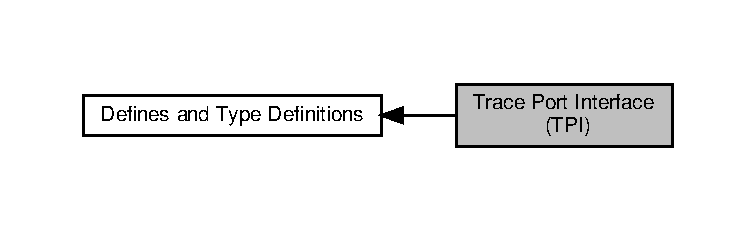
\includegraphics[width=350pt]{group___c_m_s_i_s___t_p_i}
\end{center}
\end{figure}
\subsection*{Komponenty}
\begin{DoxyCompactItemize}
\item 
struct \hyperlink{struct_t_p_i___type}{T\+P\+I\+\_\+\+Type}
\begin{DoxyCompactList}\small\item\em Structure type to access the Trace Port Interface Register (T\+PI). \end{DoxyCompactList}\end{DoxyCompactItemize}
\subsection*{Definicje}
\begin{DoxyCompactItemize}
\item 
\#define \hyperlink{group___c_m_s_i_s___t_p_i_ga73adc86f1ee60e5b75d963361535ed24}{T\+P\+I\+\_\+\+A\+C\+P\+R\+\_\+\+S\+W\+O\+S\+C\+A\+L\+E\+R\+\_\+\+Pos}~0U
\item 
\#define \hyperlink{group___c_m_s_i_s___t_p_i_ga73da1dbfb935b27bfd5473d3b041fdb5}{T\+P\+I\+\_\+\+A\+C\+P\+R\+\_\+\+S\+W\+O\+S\+C\+A\+L\+E\+R\+\_\+\+Msk}~(0x\+F\+F\+F\+F\+U\+L /$\ast$$<$$<$ T\+P\+I\+\_\+\+A\+C\+P\+R\+\_\+\+S\+W\+O\+S\+C\+A\+L\+E\+R\+\_\+\+Pos$\ast$/)
\item 
\#define \hyperlink{group___c_m_s_i_s___t_p_i_ga0f302797b94bb2da24052082ab630858}{T\+P\+I\+\_\+\+S\+P\+P\+R\+\_\+\+T\+X\+M\+O\+D\+E\+\_\+\+Pos}~0U
\item 
\#define \hyperlink{group___c_m_s_i_s___t_p_i_gaca085c8a954393d70dbd7240bb02cc1f}{T\+P\+I\+\_\+\+S\+P\+P\+R\+\_\+\+T\+X\+M\+O\+D\+E\+\_\+\+Msk}~(0x3\+U\+L /$\ast$$<$$<$ T\+P\+I\+\_\+\+S\+P\+P\+R\+\_\+\+T\+X\+M\+O\+D\+E\+\_\+\+Pos$\ast$/)
\item 
\#define \hyperlink{group___c_m_s_i_s___t_p_i_ga9537b8a660cc8803f57cbbee320b2fc8}{T\+P\+I\+\_\+\+F\+F\+S\+R\+\_\+\+Ft\+Non\+Stop\+\_\+\+Pos}~3U
\item 
\#define \hyperlink{group___c_m_s_i_s___t_p_i_gaaa313f980974a8cfc7dac68c4d805ab1}{T\+P\+I\+\_\+\+F\+F\+S\+R\+\_\+\+Ft\+Non\+Stop\+\_\+\+Msk}~(0x1\+U\+L $<$$<$ T\+P\+I\+\_\+\+F\+F\+S\+R\+\_\+\+Ft\+Non\+Stop\+\_\+\+Pos)
\item 
\#define \hyperlink{group___c_m_s_i_s___t_p_i_gad30fde0c058da2ffb2b0a213be7a1b5c}{T\+P\+I\+\_\+\+F\+F\+S\+R\+\_\+\+T\+C\+Present\+\_\+\+Pos}~2U
\item 
\#define \hyperlink{group___c_m_s_i_s___t_p_i_ga0d6bfd263ff2fdec72d6ec9415fb1135}{T\+P\+I\+\_\+\+F\+F\+S\+R\+\_\+\+T\+C\+Present\+\_\+\+Msk}~(0x1\+U\+L $<$$<$ T\+P\+I\+\_\+\+F\+F\+S\+R\+\_\+\+T\+C\+Present\+\_\+\+Pos)
\item 
\#define \hyperlink{group___c_m_s_i_s___t_p_i_gaedf31fd453a878021b542b644e2869d2}{T\+P\+I\+\_\+\+F\+F\+S\+R\+\_\+\+Ft\+Stopped\+\_\+\+Pos}~1U
\item 
\#define \hyperlink{group___c_m_s_i_s___t_p_i_ga1ab6c3abe1cf6311ee07e7c479ce5f78}{T\+P\+I\+\_\+\+F\+F\+S\+R\+\_\+\+Ft\+Stopped\+\_\+\+Msk}~(0x1\+U\+L $<$$<$ T\+P\+I\+\_\+\+F\+F\+S\+R\+\_\+\+Ft\+Stopped\+\_\+\+Pos)
\item 
\#define \hyperlink{group___c_m_s_i_s___t_p_i_ga542ca74a081588273e6d5275ba5da6bf}{T\+P\+I\+\_\+\+F\+F\+S\+R\+\_\+\+Fl\+In\+Prog\+\_\+\+Pos}~0U
\item 
\#define \hyperlink{group___c_m_s_i_s___t_p_i_ga63dfb09259893958962914fc3a9e3824}{T\+P\+I\+\_\+\+F\+F\+S\+R\+\_\+\+Fl\+In\+Prog\+\_\+\+Msk}~(0x1\+U\+L /$\ast$$<$$<$ T\+P\+I\+\_\+\+F\+F\+S\+R\+\_\+\+Fl\+In\+Prog\+\_\+\+Pos$\ast$/)
\item 
\#define \hyperlink{group___c_m_s_i_s___t_p_i_gaa7ea11ba6ea75b541cd82e185c725b5b}{T\+P\+I\+\_\+\+F\+F\+C\+R\+\_\+\+Trig\+In\+\_\+\+Pos}~8U
\item 
\#define \hyperlink{group___c_m_s_i_s___t_p_i_ga360b413bc5da61f751546a7133c3e4dd}{T\+P\+I\+\_\+\+F\+F\+C\+R\+\_\+\+Trig\+In\+\_\+\+Msk}~(0x1\+U\+L $<$$<$ T\+P\+I\+\_\+\+F\+F\+C\+R\+\_\+\+Trig\+In\+\_\+\+Pos)
\item 
\#define \hyperlink{group___c_m_s_i_s___t_p_i_gac57b0b588a37a870573560bc6316cbcc}{T\+P\+I\+\_\+\+F\+F\+C\+R\+\_\+\+F\+On\+Man\+\_\+\+Pos}~6U
\item 
\#define \hyperlink{group___c_m_s_i_s___t_p_i_ga7aeb30af62d04e852a55c3bd64c1bd2c}{T\+P\+I\+\_\+\+F\+F\+C\+R\+\_\+\+F\+On\+Man\+\_\+\+Msk}~(0x1\+U\+L $<$$<$ T\+P\+I\+\_\+\+F\+F\+C\+R\+\_\+\+F\+On\+Man\+\_\+\+Pos)
\item 
\#define \hyperlink{group___c_m_s_i_s___t_p_i_ga99e58a0960b275a773b245e2b69b9a64}{T\+P\+I\+\_\+\+F\+F\+C\+R\+\_\+\+En\+F\+Cont\+\_\+\+Pos}~1U
\item 
\#define \hyperlink{group___c_m_s_i_s___t_p_i_ga27d1ecf2e0ff496df03457a2a97cb2c9}{T\+P\+I\+\_\+\+F\+F\+C\+R\+\_\+\+En\+F\+Cont\+\_\+\+Msk}~(0x1\+U\+L $<$$<$ T\+P\+I\+\_\+\+F\+F\+C\+R\+\_\+\+En\+F\+Cont\+\_\+\+Pos)
\item 
\#define \hyperlink{group___c_m_s_i_s___t_p_i_ga4235dcb941b49a9e8c1f7616dc210b38}{T\+P\+I\+\_\+\+P\+S\+C\+R\+\_\+\+P\+S\+Count\+\_\+\+Pos}~0U
\item 
\#define \hyperlink{group___c_m_s_i_s___t_p_i_ga017e1a8b42c9fb4c525d41bafaca9262}{T\+P\+I\+\_\+\+P\+S\+C\+R\+\_\+\+P\+S\+Count\+\_\+\+Msk}~(0x1\+F\+U\+L /$\ast$$<$$<$ T\+P\+I\+\_\+\+P\+S\+C\+R\+\_\+\+P\+S\+Count\+\_\+\+Pos$\ast$/)
\item 
\#define \hyperlink{group___c_m_s_i_s___t_p_i_gaca9783a5531fde10b57fb9817de37790}{T\+P\+I\+\_\+\+L\+S\+R\+\_\+n\+T\+T\+\_\+\+Pos}~1U
\item 
\#define \hyperlink{group___c_m_s_i_s___t_p_i_gaabd6c342674f066772c9d35448a301e1}{T\+P\+I\+\_\+\+L\+S\+R\+\_\+n\+T\+T\+\_\+\+Msk}~(0x1\+U\+L $<$$<$ T\+P\+I\+\_\+\+L\+S\+R\+\_\+n\+T\+T\+\_\+\+Pos)
\item 
\#define \hyperlink{group___c_m_s_i_s___t_p_i_ga641c06d830dac7e2ff9971d95f2432a0}{T\+P\+I\+\_\+\+L\+S\+R\+\_\+\+S\+L\+K\+\_\+\+Pos}~1U
\item 
\#define \hyperlink{group___c_m_s_i_s___t_p_i_gab91c42714b86fe5d2b022fc8e5f3d0e6}{T\+P\+I\+\_\+\+L\+S\+R\+\_\+\+S\+L\+K\+\_\+\+Msk}~(0x1\+U\+L $<$$<$ T\+P\+I\+\_\+\+L\+S\+R\+\_\+\+S\+L\+K\+\_\+\+Pos)
\item 
\#define \hyperlink{group___c_m_s_i_s___t_p_i_ga94c8185149817f81a6ca689f89d8193c}{T\+P\+I\+\_\+\+L\+S\+R\+\_\+\+S\+L\+I\+\_\+\+Pos}~0U
\item 
\#define \hyperlink{group___c_m_s_i_s___t_p_i_gace974ad6e051759bafcfea1b8189c606}{T\+P\+I\+\_\+\+L\+S\+R\+\_\+\+S\+L\+I\+\_\+\+Msk}~(0x1\+U\+L /$\ast$$<$$<$ T\+P\+I\+\_\+\+L\+S\+R\+\_\+\+S\+L\+I\+\_\+\+Pos$\ast$/)
\item 
\#define \hyperlink{group___c_m_s_i_s___t_p_i_ga9f46cf1a1708575f56d6b827766277f4}{T\+P\+I\+\_\+\+D\+E\+V\+I\+D\+\_\+\+N\+R\+Z\+V\+A\+L\+I\+D\+\_\+\+Pos}~11U
\item 
\#define \hyperlink{group___c_m_s_i_s___t_p_i_gacecc8710a8f6a23a7d1d4f5674daf02a}{T\+P\+I\+\_\+\+D\+E\+V\+I\+D\+\_\+\+N\+R\+Z\+V\+A\+L\+I\+D\+\_\+\+Msk}~(0x1\+U\+L $<$$<$ T\+P\+I\+\_\+\+D\+E\+V\+I\+D\+\_\+\+N\+R\+Z\+V\+A\+L\+I\+D\+\_\+\+Pos)
\item 
\#define \hyperlink{group___c_m_s_i_s___t_p_i_ga675534579d9e25477bb38970e3ef973c}{T\+P\+I\+\_\+\+D\+E\+V\+I\+D\+\_\+\+M\+A\+N\+C\+V\+A\+L\+I\+D\+\_\+\+Pos}~10U
\item 
\#define \hyperlink{group___c_m_s_i_s___t_p_i_ga4c3ee4b1a34ad1960a6b2d6e7e0ff942}{T\+P\+I\+\_\+\+D\+E\+V\+I\+D\+\_\+\+M\+A\+N\+C\+V\+A\+L\+I\+D\+\_\+\+Msk}~(0x1\+U\+L $<$$<$ T\+P\+I\+\_\+\+D\+E\+V\+I\+D\+\_\+\+M\+A\+N\+C\+V\+A\+L\+I\+D\+\_\+\+Pos)
\item 
\#define \hyperlink{group___c_m_s_i_s___t_p_i_ga974cccf4c958b4a45cb71c7b5de39b7b}{T\+P\+I\+\_\+\+D\+E\+V\+I\+D\+\_\+\+P\+T\+I\+N\+V\+A\+L\+I\+D\+\_\+\+Pos}~9U
\item 
\#define \hyperlink{group___c_m_s_i_s___t_p_i_ga1ca84d62243e475836bba02516ba6b97}{T\+P\+I\+\_\+\+D\+E\+V\+I\+D\+\_\+\+P\+T\+I\+N\+V\+A\+L\+I\+D\+\_\+\+Msk}~(0x1\+U\+L $<$$<$ T\+P\+I\+\_\+\+D\+E\+V\+I\+D\+\_\+\+P\+T\+I\+N\+V\+A\+L\+I\+D\+\_\+\+Pos)
\item 
\#define \hyperlink{group___c_m_s_i_s___t_p_i_ga3c7bb073c7ef96c2c3491c523fcb5bbe}{T\+P\+I\+\_\+\+D\+E\+V\+I\+D\+\_\+\+F\+I\+F\+O\+S\+Z\+\_\+\+Pos}~6U
\item 
\#define \hyperlink{group___c_m_s_i_s___t_p_i_gac7e718d8f239920d5b65e3eaa1c490df}{T\+P\+I\+\_\+\+D\+E\+V\+I\+D\+\_\+\+F\+I\+F\+O\+S\+Z\+\_\+\+Msk}~(0x7\+U\+L $<$$<$ T\+P\+I\+\_\+\+D\+E\+V\+I\+D\+\_\+\+F\+I\+F\+O\+S\+Z\+\_\+\+Pos)
\item 
\#define \hyperlink{group___c_m_s_i_s___t_p_i_ga0c799ff892af5eb3162d152abc00af7a}{T\+P\+I\+\_\+\+D\+E\+V\+T\+Y\+P\+E\+\_\+\+Sub\+Type\+\_\+\+Pos}~4U
\item 
\#define \hyperlink{group___c_m_s_i_s___t_p_i_ga5b2fd7dddaf5f64855d9c0696acd65c1}{T\+P\+I\+\_\+\+D\+E\+V\+T\+Y\+P\+E\+\_\+\+Sub\+Type\+\_\+\+Msk}~(0x\+F\+U\+L /$\ast$$<$$<$ T\+P\+I\+\_\+\+D\+E\+V\+T\+Y\+P\+E\+\_\+\+Sub\+Type\+\_\+\+Pos$\ast$/)
\item 
\#define \hyperlink{group___c_m_s_i_s___t_p_i_ga69c4892d332755a9f64c1680497cebdd}{T\+P\+I\+\_\+\+D\+E\+V\+T\+Y\+P\+E\+\_\+\+Major\+Type\+\_\+\+Pos}~0U
\item 
\#define \hyperlink{group___c_m_s_i_s___t_p_i_gaecbceed6d08ec586403b37ad47b38c88}{T\+P\+I\+\_\+\+D\+E\+V\+T\+Y\+P\+E\+\_\+\+Major\+Type\+\_\+\+Msk}~(0x\+F\+U\+L $<$$<$ T\+P\+I\+\_\+\+D\+E\+V\+T\+Y\+P\+E\+\_\+\+Major\+Type\+\_\+\+Pos)
\item 
\#define \hyperlink{group___c_m_s_i_s___t_p_i_ga73adc86f1ee60e5b75d963361535ed24}{T\+P\+I\+\_\+\+A\+C\+P\+R\+\_\+\+S\+W\+O\+S\+C\+A\+L\+E\+R\+\_\+\+Pos}~0U
\item 
\#define \hyperlink{group___c_m_s_i_s___t_p_i_ga73da1dbfb935b27bfd5473d3b041fdb5}{T\+P\+I\+\_\+\+A\+C\+P\+R\+\_\+\+S\+W\+O\+S\+C\+A\+L\+E\+R\+\_\+\+Msk}~(0x\+F\+F\+F\+F\+U\+L /$\ast$$<$$<$ T\+P\+I\+\_\+\+A\+C\+P\+R\+\_\+\+S\+W\+O\+S\+C\+A\+L\+E\+R\+\_\+\+Pos$\ast$/)
\item 
\#define \hyperlink{group___c_m_s_i_s___t_p_i_ga0f302797b94bb2da24052082ab630858}{T\+P\+I\+\_\+\+S\+P\+P\+R\+\_\+\+T\+X\+M\+O\+D\+E\+\_\+\+Pos}~0U
\item 
\#define \hyperlink{group___c_m_s_i_s___t_p_i_gaca085c8a954393d70dbd7240bb02cc1f}{T\+P\+I\+\_\+\+S\+P\+P\+R\+\_\+\+T\+X\+M\+O\+D\+E\+\_\+\+Msk}~(0x3\+U\+L /$\ast$$<$$<$ T\+P\+I\+\_\+\+S\+P\+P\+R\+\_\+\+T\+X\+M\+O\+D\+E\+\_\+\+Pos$\ast$/)
\item 
\#define \hyperlink{group___c_m_s_i_s___t_p_i_ga9537b8a660cc8803f57cbbee320b2fc8}{T\+P\+I\+\_\+\+F\+F\+S\+R\+\_\+\+Ft\+Non\+Stop\+\_\+\+Pos}~3U
\item 
\#define \hyperlink{group___c_m_s_i_s___t_p_i_gaaa313f980974a8cfc7dac68c4d805ab1}{T\+P\+I\+\_\+\+F\+F\+S\+R\+\_\+\+Ft\+Non\+Stop\+\_\+\+Msk}~(0x1\+U\+L $<$$<$ T\+P\+I\+\_\+\+F\+F\+S\+R\+\_\+\+Ft\+Non\+Stop\+\_\+\+Pos)
\item 
\#define \hyperlink{group___c_m_s_i_s___t_p_i_gad30fde0c058da2ffb2b0a213be7a1b5c}{T\+P\+I\+\_\+\+F\+F\+S\+R\+\_\+\+T\+C\+Present\+\_\+\+Pos}~2U
\item 
\#define \hyperlink{group___c_m_s_i_s___t_p_i_ga0d6bfd263ff2fdec72d6ec9415fb1135}{T\+P\+I\+\_\+\+F\+F\+S\+R\+\_\+\+T\+C\+Present\+\_\+\+Msk}~(0x1\+U\+L $<$$<$ T\+P\+I\+\_\+\+F\+F\+S\+R\+\_\+\+T\+C\+Present\+\_\+\+Pos)
\item 
\#define \hyperlink{group___c_m_s_i_s___t_p_i_gaedf31fd453a878021b542b644e2869d2}{T\+P\+I\+\_\+\+F\+F\+S\+R\+\_\+\+Ft\+Stopped\+\_\+\+Pos}~1U
\item 
\#define \hyperlink{group___c_m_s_i_s___t_p_i_ga1ab6c3abe1cf6311ee07e7c479ce5f78}{T\+P\+I\+\_\+\+F\+F\+S\+R\+\_\+\+Ft\+Stopped\+\_\+\+Msk}~(0x1\+U\+L $<$$<$ T\+P\+I\+\_\+\+F\+F\+S\+R\+\_\+\+Ft\+Stopped\+\_\+\+Pos)
\item 
\#define \hyperlink{group___c_m_s_i_s___t_p_i_ga542ca74a081588273e6d5275ba5da6bf}{T\+P\+I\+\_\+\+F\+F\+S\+R\+\_\+\+Fl\+In\+Prog\+\_\+\+Pos}~0U
\item 
\#define \hyperlink{group___c_m_s_i_s___t_p_i_ga63dfb09259893958962914fc3a9e3824}{T\+P\+I\+\_\+\+F\+F\+S\+R\+\_\+\+Fl\+In\+Prog\+\_\+\+Msk}~(0x1\+U\+L /$\ast$$<$$<$ T\+P\+I\+\_\+\+F\+F\+S\+R\+\_\+\+Fl\+In\+Prog\+\_\+\+Pos$\ast$/)
\item 
\#define \hyperlink{group___c_m_s_i_s___t_p_i_gaa7ea11ba6ea75b541cd82e185c725b5b}{T\+P\+I\+\_\+\+F\+F\+C\+R\+\_\+\+Trig\+In\+\_\+\+Pos}~8U
\item 
\#define \hyperlink{group___c_m_s_i_s___t_p_i_ga360b413bc5da61f751546a7133c3e4dd}{T\+P\+I\+\_\+\+F\+F\+C\+R\+\_\+\+Trig\+In\+\_\+\+Msk}~(0x1\+U\+L $<$$<$ T\+P\+I\+\_\+\+F\+F\+C\+R\+\_\+\+Trig\+In\+\_\+\+Pos)
\item 
\#define \hyperlink{group___c_m_s_i_s___t_p_i_gac57b0b588a37a870573560bc6316cbcc}{T\+P\+I\+\_\+\+F\+F\+C\+R\+\_\+\+F\+On\+Man\+\_\+\+Pos}~6U
\item 
\#define \hyperlink{group___c_m_s_i_s___t_p_i_ga7aeb30af62d04e852a55c3bd64c1bd2c}{T\+P\+I\+\_\+\+F\+F\+C\+R\+\_\+\+F\+On\+Man\+\_\+\+Msk}~(0x1\+U\+L $<$$<$ T\+P\+I\+\_\+\+F\+F\+C\+R\+\_\+\+F\+On\+Man\+\_\+\+Pos)
\item 
\#define \hyperlink{group___c_m_s_i_s___t_p_i_ga99e58a0960b275a773b245e2b69b9a64}{T\+P\+I\+\_\+\+F\+F\+C\+R\+\_\+\+En\+F\+Cont\+\_\+\+Pos}~1U
\item 
\#define \hyperlink{group___c_m_s_i_s___t_p_i_ga27d1ecf2e0ff496df03457a2a97cb2c9}{T\+P\+I\+\_\+\+F\+F\+C\+R\+\_\+\+En\+F\+Cont\+\_\+\+Msk}~(0x1\+U\+L $<$$<$ T\+P\+I\+\_\+\+F\+F\+C\+R\+\_\+\+En\+F\+Cont\+\_\+\+Pos)
\item 
\#define \hyperlink{group___c_m_s_i_s___t_p_i_ga4235dcb941b49a9e8c1f7616dc210b38}{T\+P\+I\+\_\+\+P\+S\+C\+R\+\_\+\+P\+S\+Count\+\_\+\+Pos}~0U
\item 
\#define \hyperlink{group___c_m_s_i_s___t_p_i_ga017e1a8b42c9fb4c525d41bafaca9262}{T\+P\+I\+\_\+\+P\+S\+C\+R\+\_\+\+P\+S\+Count\+\_\+\+Msk}~(0x1\+F\+U\+L /$\ast$$<$$<$ T\+P\+I\+\_\+\+P\+S\+C\+R\+\_\+\+P\+S\+Count\+\_\+\+Pos$\ast$/)
\item 
\#define \hyperlink{group___c_m_s_i_s___t_p_i_gaca9783a5531fde10b57fb9817de37790}{T\+P\+I\+\_\+\+L\+S\+R\+\_\+n\+T\+T\+\_\+\+Pos}~1U
\item 
\#define \hyperlink{group___c_m_s_i_s___t_p_i_gaabd6c342674f066772c9d35448a301e1}{T\+P\+I\+\_\+\+L\+S\+R\+\_\+n\+T\+T\+\_\+\+Msk}~(0x1\+U\+L $<$$<$ T\+P\+I\+\_\+\+L\+S\+R\+\_\+n\+T\+T\+\_\+\+Pos)
\item 
\#define \hyperlink{group___c_m_s_i_s___t_p_i_ga641c06d830dac7e2ff9971d95f2432a0}{T\+P\+I\+\_\+\+L\+S\+R\+\_\+\+S\+L\+K\+\_\+\+Pos}~1U
\item 
\#define \hyperlink{group___c_m_s_i_s___t_p_i_gab91c42714b86fe5d2b022fc8e5f3d0e6}{T\+P\+I\+\_\+\+L\+S\+R\+\_\+\+S\+L\+K\+\_\+\+Msk}~(0x1\+U\+L $<$$<$ T\+P\+I\+\_\+\+L\+S\+R\+\_\+\+S\+L\+K\+\_\+\+Pos)
\item 
\#define \hyperlink{group___c_m_s_i_s___t_p_i_ga94c8185149817f81a6ca689f89d8193c}{T\+P\+I\+\_\+\+L\+S\+R\+\_\+\+S\+L\+I\+\_\+\+Pos}~0U
\item 
\#define \hyperlink{group___c_m_s_i_s___t_p_i_gace974ad6e051759bafcfea1b8189c606}{T\+P\+I\+\_\+\+L\+S\+R\+\_\+\+S\+L\+I\+\_\+\+Msk}~(0x1\+U\+L /$\ast$$<$$<$ T\+P\+I\+\_\+\+L\+S\+R\+\_\+\+S\+L\+I\+\_\+\+Pos$\ast$/)
\item 
\#define \hyperlink{group___c_m_s_i_s___t_p_i_ga9f46cf1a1708575f56d6b827766277f4}{T\+P\+I\+\_\+\+D\+E\+V\+I\+D\+\_\+\+N\+R\+Z\+V\+A\+L\+I\+D\+\_\+\+Pos}~11U
\item 
\#define \hyperlink{group___c_m_s_i_s___t_p_i_gacecc8710a8f6a23a7d1d4f5674daf02a}{T\+P\+I\+\_\+\+D\+E\+V\+I\+D\+\_\+\+N\+R\+Z\+V\+A\+L\+I\+D\+\_\+\+Msk}~(0x1\+U\+L $<$$<$ T\+P\+I\+\_\+\+D\+E\+V\+I\+D\+\_\+\+N\+R\+Z\+V\+A\+L\+I\+D\+\_\+\+Pos)
\item 
\#define \hyperlink{group___c_m_s_i_s___t_p_i_ga675534579d9e25477bb38970e3ef973c}{T\+P\+I\+\_\+\+D\+E\+V\+I\+D\+\_\+\+M\+A\+N\+C\+V\+A\+L\+I\+D\+\_\+\+Pos}~10U
\item 
\#define \hyperlink{group___c_m_s_i_s___t_p_i_ga4c3ee4b1a34ad1960a6b2d6e7e0ff942}{T\+P\+I\+\_\+\+D\+E\+V\+I\+D\+\_\+\+M\+A\+N\+C\+V\+A\+L\+I\+D\+\_\+\+Msk}~(0x1\+U\+L $<$$<$ T\+P\+I\+\_\+\+D\+E\+V\+I\+D\+\_\+\+M\+A\+N\+C\+V\+A\+L\+I\+D\+\_\+\+Pos)
\item 
\#define \hyperlink{group___c_m_s_i_s___t_p_i_ga974cccf4c958b4a45cb71c7b5de39b7b}{T\+P\+I\+\_\+\+D\+E\+V\+I\+D\+\_\+\+P\+T\+I\+N\+V\+A\+L\+I\+D\+\_\+\+Pos}~9U
\item 
\#define \hyperlink{group___c_m_s_i_s___t_p_i_ga1ca84d62243e475836bba02516ba6b97}{T\+P\+I\+\_\+\+D\+E\+V\+I\+D\+\_\+\+P\+T\+I\+N\+V\+A\+L\+I\+D\+\_\+\+Msk}~(0x1\+U\+L $<$$<$ T\+P\+I\+\_\+\+D\+E\+V\+I\+D\+\_\+\+P\+T\+I\+N\+V\+A\+L\+I\+D\+\_\+\+Pos)
\item 
\#define \hyperlink{group___c_m_s_i_s___t_p_i_ga3c7bb073c7ef96c2c3491c523fcb5bbe}{T\+P\+I\+\_\+\+D\+E\+V\+I\+D\+\_\+\+F\+I\+F\+O\+S\+Z\+\_\+\+Pos}~6U
\item 
\#define \hyperlink{group___c_m_s_i_s___t_p_i_gac7e718d8f239920d5b65e3eaa1c490df}{T\+P\+I\+\_\+\+D\+E\+V\+I\+D\+\_\+\+F\+I\+F\+O\+S\+Z\+\_\+\+Msk}~(0x7\+U\+L $<$$<$ T\+P\+I\+\_\+\+D\+E\+V\+I\+D\+\_\+\+F\+I\+F\+O\+S\+Z\+\_\+\+Pos)
\item 
\#define \hyperlink{group___c_m_s_i_s___t_p_i_ga0c799ff892af5eb3162d152abc00af7a}{T\+P\+I\+\_\+\+D\+E\+V\+T\+Y\+P\+E\+\_\+\+Sub\+Type\+\_\+\+Pos}~4U
\item 
\#define \hyperlink{group___c_m_s_i_s___t_p_i_ga5b2fd7dddaf5f64855d9c0696acd65c1}{T\+P\+I\+\_\+\+D\+E\+V\+T\+Y\+P\+E\+\_\+\+Sub\+Type\+\_\+\+Msk}~(0x\+F\+U\+L /$\ast$$<$$<$ T\+P\+I\+\_\+\+D\+E\+V\+T\+Y\+P\+E\+\_\+\+Sub\+Type\+\_\+\+Pos$\ast$/)
\item 
\#define \hyperlink{group___c_m_s_i_s___t_p_i_ga69c4892d332755a9f64c1680497cebdd}{T\+P\+I\+\_\+\+D\+E\+V\+T\+Y\+P\+E\+\_\+\+Major\+Type\+\_\+\+Pos}~0U
\item 
\#define \hyperlink{group___c_m_s_i_s___t_p_i_gaecbceed6d08ec586403b37ad47b38c88}{T\+P\+I\+\_\+\+D\+E\+V\+T\+Y\+P\+E\+\_\+\+Major\+Type\+\_\+\+Msk}~(0x\+F\+U\+L $<$$<$ T\+P\+I\+\_\+\+D\+E\+V\+T\+Y\+P\+E\+\_\+\+Major\+Type\+\_\+\+Pos)
\item 
\#define \hyperlink{group___c_m_s_i_s___t_p_i_ga5a82d274eb2df8b0c92dd4ed63535928}{T\+P\+I\+\_\+\+A\+C\+P\+R\+\_\+\+P\+R\+E\+S\+C\+A\+L\+E\+R\+\_\+\+Pos}~0U
\item 
\#define \hyperlink{group___c_m_s_i_s___t_p_i_ga4fcacd27208419929921aec8457a8c13}{T\+P\+I\+\_\+\+A\+C\+P\+R\+\_\+\+P\+R\+E\+S\+C\+A\+L\+E\+R\+\_\+\+Msk}~(0x1\+F\+F\+F\+U\+L /$\ast$$<$$<$ T\+P\+I\+\_\+\+A\+C\+P\+R\+\_\+\+P\+R\+E\+S\+C\+A\+L\+E\+R\+\_\+\+Pos$\ast$/)
\item 
\#define \hyperlink{group___c_m_s_i_s___t_p_i_ga0f302797b94bb2da24052082ab630858}{T\+P\+I\+\_\+\+S\+P\+P\+R\+\_\+\+T\+X\+M\+O\+D\+E\+\_\+\+Pos}~0U
\item 
\#define \hyperlink{group___c_m_s_i_s___t_p_i_gaca085c8a954393d70dbd7240bb02cc1f}{T\+P\+I\+\_\+\+S\+P\+P\+R\+\_\+\+T\+X\+M\+O\+D\+E\+\_\+\+Msk}~(0x3\+U\+L /$\ast$$<$$<$ T\+P\+I\+\_\+\+S\+P\+P\+R\+\_\+\+T\+X\+M\+O\+D\+E\+\_\+\+Pos$\ast$/)
\item 
\#define \hyperlink{group___c_m_s_i_s___t_p_i_ga9537b8a660cc8803f57cbbee320b2fc8}{T\+P\+I\+\_\+\+F\+F\+S\+R\+\_\+\+Ft\+Non\+Stop\+\_\+\+Pos}~3U
\item 
\#define \hyperlink{group___c_m_s_i_s___t_p_i_gaaa313f980974a8cfc7dac68c4d805ab1}{T\+P\+I\+\_\+\+F\+F\+S\+R\+\_\+\+Ft\+Non\+Stop\+\_\+\+Msk}~(0x1\+U\+L $<$$<$ T\+P\+I\+\_\+\+F\+F\+S\+R\+\_\+\+Ft\+Non\+Stop\+\_\+\+Pos)
\item 
\#define \hyperlink{group___c_m_s_i_s___t_p_i_gad30fde0c058da2ffb2b0a213be7a1b5c}{T\+P\+I\+\_\+\+F\+F\+S\+R\+\_\+\+T\+C\+Present\+\_\+\+Pos}~2U
\item 
\#define \hyperlink{group___c_m_s_i_s___t_p_i_ga0d6bfd263ff2fdec72d6ec9415fb1135}{T\+P\+I\+\_\+\+F\+F\+S\+R\+\_\+\+T\+C\+Present\+\_\+\+Msk}~(0x1\+U\+L $<$$<$ T\+P\+I\+\_\+\+F\+F\+S\+R\+\_\+\+T\+C\+Present\+\_\+\+Pos)
\item 
\#define \hyperlink{group___c_m_s_i_s___t_p_i_gaedf31fd453a878021b542b644e2869d2}{T\+P\+I\+\_\+\+F\+F\+S\+R\+\_\+\+Ft\+Stopped\+\_\+\+Pos}~1U
\item 
\#define \hyperlink{group___c_m_s_i_s___t_p_i_ga1ab6c3abe1cf6311ee07e7c479ce5f78}{T\+P\+I\+\_\+\+F\+F\+S\+R\+\_\+\+Ft\+Stopped\+\_\+\+Msk}~(0x1\+U\+L $<$$<$ T\+P\+I\+\_\+\+F\+F\+S\+R\+\_\+\+Ft\+Stopped\+\_\+\+Pos)
\item 
\#define \hyperlink{group___c_m_s_i_s___t_p_i_ga542ca74a081588273e6d5275ba5da6bf}{T\+P\+I\+\_\+\+F\+F\+S\+R\+\_\+\+Fl\+In\+Prog\+\_\+\+Pos}~0U
\item 
\#define \hyperlink{group___c_m_s_i_s___t_p_i_ga63dfb09259893958962914fc3a9e3824}{T\+P\+I\+\_\+\+F\+F\+S\+R\+\_\+\+Fl\+In\+Prog\+\_\+\+Msk}~(0x1\+U\+L /$\ast$$<$$<$ T\+P\+I\+\_\+\+F\+F\+S\+R\+\_\+\+Fl\+In\+Prog\+\_\+\+Pos$\ast$/)
\item 
\#define \hyperlink{group___c_m_s_i_s___t_p_i_gaa7ea11ba6ea75b541cd82e185c725b5b}{T\+P\+I\+\_\+\+F\+F\+C\+R\+\_\+\+Trig\+In\+\_\+\+Pos}~8U
\item 
\#define \hyperlink{group___c_m_s_i_s___t_p_i_ga360b413bc5da61f751546a7133c3e4dd}{T\+P\+I\+\_\+\+F\+F\+C\+R\+\_\+\+Trig\+In\+\_\+\+Msk}~(0x1\+U\+L $<$$<$ T\+P\+I\+\_\+\+F\+F\+C\+R\+\_\+\+Trig\+In\+\_\+\+Pos)
\item 
\#define \hyperlink{group___c_m_s_i_s___t_p_i_gac57b0b588a37a870573560bc6316cbcc}{T\+P\+I\+\_\+\+F\+F\+C\+R\+\_\+\+F\+On\+Man\+\_\+\+Pos}~6U
\item 
\#define \hyperlink{group___c_m_s_i_s___t_p_i_ga7aeb30af62d04e852a55c3bd64c1bd2c}{T\+P\+I\+\_\+\+F\+F\+C\+R\+\_\+\+F\+On\+Man\+\_\+\+Msk}~(0x1\+U\+L $<$$<$ T\+P\+I\+\_\+\+F\+F\+C\+R\+\_\+\+F\+On\+Man\+\_\+\+Pos)
\item 
\#define \hyperlink{group___c_m_s_i_s___t_p_i_ga99e58a0960b275a773b245e2b69b9a64}{T\+P\+I\+\_\+\+F\+F\+C\+R\+\_\+\+En\+F\+Cont\+\_\+\+Pos}~1U
\item 
\#define \hyperlink{group___c_m_s_i_s___t_p_i_ga27d1ecf2e0ff496df03457a2a97cb2c9}{T\+P\+I\+\_\+\+F\+F\+C\+R\+\_\+\+En\+F\+Cont\+\_\+\+Msk}~(0x1\+U\+L $<$$<$ T\+P\+I\+\_\+\+F\+F\+C\+R\+\_\+\+En\+F\+Cont\+\_\+\+Pos)
\item 
\#define \hyperlink{group___c_m_s_i_s___t_p_i_ga5517fa2ced64efbbd413720329c50b99}{T\+P\+I\+\_\+\+T\+R\+I\+G\+G\+E\+R\+\_\+\+T\+R\+I\+G\+G\+E\+R\+\_\+\+Pos}~0U
\item 
\#define \hyperlink{group___c_m_s_i_s___t_p_i_ga814227af2b2665a0687bb49345e21110}{T\+P\+I\+\_\+\+T\+R\+I\+G\+G\+E\+R\+\_\+\+T\+R\+I\+G\+G\+E\+R\+\_\+\+Msk}~(0x1\+U\+L /$\ast$$<$$<$ T\+P\+I\+\_\+\+T\+R\+I\+G\+G\+E\+R\+\_\+\+T\+R\+I\+G\+G\+E\+R\+\_\+\+Pos$\ast$/)
\item 
\#define \hyperlink{group___c_m_s_i_s___t_p_i_gab268401221645f4e0e1a82d1d6c2caee}{T\+P\+I\+\_\+\+I\+T\+F\+T\+T\+D0\+\_\+\+A\+T\+B\+\_\+\+I\+F2\+\_\+\+A\+T\+V\+A\+L\+I\+D\+\_\+\+Pos}~29U
\item 
\#define \hyperlink{group___c_m_s_i_s___t_p_i_gac6fc2d04903210afe2599482a72e0a25}{T\+P\+I\+\_\+\+I\+T\+F\+T\+T\+D0\+\_\+\+A\+T\+B\+\_\+\+I\+F2\+\_\+\+A\+T\+V\+A\+L\+I\+D\+\_\+\+Msk}~(0x3\+U\+L $<$$<$ T\+P\+I\+\_\+\+I\+T\+F\+T\+T\+D0\+\_\+\+A\+T\+B\+\_\+\+I\+F2\+\_\+\+A\+T\+V\+A\+L\+I\+D\+\_\+\+Pos)
\item 
\#define \hyperlink{group___c_m_s_i_s___t_p_i_gadaa8bfec760711c2d190d5fd124706fe}{T\+P\+I\+\_\+\+I\+T\+F\+T\+T\+D0\+\_\+\+A\+T\+B\+\_\+\+I\+F2\+\_\+bytecount\+\_\+\+Pos}~27U
\item 
\#define \hyperlink{group___c_m_s_i_s___t_p_i_ga8b342379b5d45d46459807859a8a6687}{T\+P\+I\+\_\+\+I\+T\+F\+T\+T\+D0\+\_\+\+A\+T\+B\+\_\+\+I\+F2\+\_\+bytecount\+\_\+\+Msk}~(0x3\+U\+L $<$$<$ T\+P\+I\+\_\+\+I\+T\+F\+T\+T\+D0\+\_\+\+A\+T\+B\+\_\+\+I\+F2\+\_\+bytecount\+\_\+\+Pos)
\item 
\#define \hyperlink{group___c_m_s_i_s___t_p_i_ga0b95f6b474fe2e4b7ba9963b00d18258}{T\+P\+I\+\_\+\+I\+T\+F\+T\+T\+D0\+\_\+\+A\+T\+B\+\_\+\+I\+F1\+\_\+\+A\+T\+V\+A\+L\+I\+D\+\_\+\+Pos}~26U
\item 
\#define \hyperlink{group___c_m_s_i_s___t_p_i_ga8650e68e2efc65b0d94de91772dc5940}{T\+P\+I\+\_\+\+I\+T\+F\+T\+T\+D0\+\_\+\+A\+T\+B\+\_\+\+I\+F1\+\_\+\+A\+T\+V\+A\+L\+I\+D\+\_\+\+Msk}~(0x3\+U\+L $<$$<$ T\+P\+I\+\_\+\+I\+T\+F\+T\+T\+D0\+\_\+\+A\+T\+B\+\_\+\+I\+F1\+\_\+\+A\+T\+V\+A\+L\+I\+D\+\_\+\+Pos)
\item 
\#define \hyperlink{group___c_m_s_i_s___t_p_i_gae82d334486fb5d11e57e8e07fd21be7b}{T\+P\+I\+\_\+\+I\+T\+F\+T\+T\+D0\+\_\+\+A\+T\+B\+\_\+\+I\+F1\+\_\+bytecount\+\_\+\+Pos}~24U
\item 
\#define \hyperlink{group___c_m_s_i_s___t_p_i_ga71301ef5984fef602d83305f34ea5c97}{T\+P\+I\+\_\+\+I\+T\+F\+T\+T\+D0\+\_\+\+A\+T\+B\+\_\+\+I\+F1\+\_\+bytecount\+\_\+\+Msk}~(0x3\+U\+L $<$$<$ T\+P\+I\+\_\+\+I\+T\+F\+T\+T\+D0\+\_\+\+A\+T\+B\+\_\+\+I\+F1\+\_\+bytecount\+\_\+\+Pos)
\item 
\#define \hyperlink{group___c_m_s_i_s___t_p_i_ga79e526cc6f0857f45187e897f4009f55}{T\+P\+I\+\_\+\+I\+T\+F\+T\+T\+D0\+\_\+\+A\+T\+B\+\_\+\+I\+F1\+\_\+data2\+\_\+\+Pos}~16U
\item 
\#define \hyperlink{group___c_m_s_i_s___t_p_i_ga942cc46e6e858b215e81ef6b57c3f63f}{T\+P\+I\+\_\+\+I\+T\+F\+T\+T\+D0\+\_\+\+A\+T\+B\+\_\+\+I\+F1\+\_\+data2\+\_\+\+Msk}~(0x\+F\+F\+U\+L $<$$<$ T\+P\+I\+\_\+\+I\+T\+F\+T\+T\+D0\+\_\+\+A\+T\+B\+\_\+\+I\+F1\+\_\+data1\+\_\+\+Pos)
\item 
\#define \hyperlink{group___c_m_s_i_s___t_p_i_ga7715fac6bd637e7ec153518da1fd4f0b}{T\+P\+I\+\_\+\+I\+T\+F\+T\+T\+D0\+\_\+\+A\+T\+B\+\_\+\+I\+F1\+\_\+data1\+\_\+\+Pos}~8U
\item 
\#define \hyperlink{group___c_m_s_i_s___t_p_i_gada0033c411d5b57161b6e5c244518836}{T\+P\+I\+\_\+\+I\+T\+F\+T\+T\+D0\+\_\+\+A\+T\+B\+\_\+\+I\+F1\+\_\+data1\+\_\+\+Msk}~(0x\+F\+F\+U\+L $<$$<$ T\+P\+I\+\_\+\+I\+T\+F\+T\+T\+D0\+\_\+\+A\+T\+B\+\_\+\+I\+F1\+\_\+data1\+\_\+\+Pos)
\item 
\#define \hyperlink{group___c_m_s_i_s___t_p_i_gae6ff8b9a79602a3546d951261d787cc7}{T\+P\+I\+\_\+\+I\+T\+F\+T\+T\+D0\+\_\+\+A\+T\+B\+\_\+\+I\+F1\+\_\+data0\+\_\+\+Pos}~0U
\item 
\#define \hyperlink{group___c_m_s_i_s___t_p_i_gafb950b90ccb002e81ae6c44482cd46fd}{T\+P\+I\+\_\+\+I\+T\+F\+T\+T\+D0\+\_\+\+A\+T\+B\+\_\+\+I\+F1\+\_\+data0\+\_\+\+Msk}~(0x\+F\+F\+U\+L /$\ast$$<$$<$ T\+P\+I\+\_\+\+I\+T\+F\+T\+T\+D0\+\_\+\+A\+T\+B\+\_\+\+I\+F1\+\_\+data0\+\_\+\+Pos$\ast$/)
\item 
\#define \hyperlink{group___c_m_s_i_s___t_p_i_ga7b77f85ad8cad3c00b490ca18ba52263}{T\+P\+I\+\_\+\+I\+T\+A\+T\+B\+C\+T\+R2\+\_\+\+A\+F\+V\+A\+L\+I\+D2\+S\+\_\+\+Pos}~1U
\item 
\#define \hyperlink{group___c_m_s_i_s___t_p_i_ga840a62dd0a903c7c0d90214e57f89f6f}{T\+P\+I\+\_\+\+I\+T\+A\+T\+B\+C\+T\+R2\+\_\+\+A\+F\+V\+A\+L\+I\+D2\+S\+\_\+\+Msk}~(0x1\+U\+L $<$$<$ T\+P\+I\+\_\+\+I\+T\+A\+T\+B\+C\+T\+R2\+\_\+\+A\+F\+V\+A\+L\+I\+D2\+S\+\_\+\+Pos)
\item 
\#define \hyperlink{group___c_m_s_i_s___t_p_i_ga15b83625dedbaa8acaab637185cf4fab}{T\+P\+I\+\_\+\+I\+T\+A\+T\+B\+C\+T\+R2\+\_\+\+A\+F\+V\+A\+L\+I\+D1\+S\+\_\+\+Pos}~1U
\item 
\#define \hyperlink{group___c_m_s_i_s___t_p_i_gaf25272d068154278decc987e101bfac7}{T\+P\+I\+\_\+\+I\+T\+A\+T\+B\+C\+T\+R2\+\_\+\+A\+F\+V\+A\+L\+I\+D1\+S\+\_\+\+Msk}~(0x1\+U\+L $<$$<$ T\+P\+I\+\_\+\+I\+T\+A\+T\+B\+C\+T\+R2\+\_\+\+A\+F\+V\+A\+L\+I\+D1\+S\+\_\+\+Pos)
\item 
\#define \hyperlink{group___c_m_s_i_s___t_p_i_gaa94a190da6db605987bb65d4bd76415a}{T\+P\+I\+\_\+\+I\+T\+A\+T\+B\+C\+T\+R2\+\_\+\+A\+T\+R\+E\+A\+D\+Y2\+S\+\_\+\+Pos}~0U
\item 
\#define \hyperlink{group___c_m_s_i_s___t_p_i_ga7530ebf5f4ae263bf9621d901f9840ee}{T\+P\+I\+\_\+\+I\+T\+A\+T\+B\+C\+T\+R2\+\_\+\+A\+T\+R\+E\+A\+D\+Y2\+S\+\_\+\+Msk}~(0x1\+U\+L /$\ast$$<$$<$ T\+P\+I\+\_\+\+I\+T\+A\+T\+B\+C\+T\+R2\+\_\+\+A\+T\+R\+E\+A\+D\+Y2\+S\+\_\+\+Pos$\ast$/)
\item 
\#define \hyperlink{group___c_m_s_i_s___t_p_i_ga52812ab751c370d2d34e55275d896128}{T\+P\+I\+\_\+\+I\+T\+A\+T\+B\+C\+T\+R2\+\_\+\+A\+T\+R\+E\+A\+D\+Y1\+S\+\_\+\+Pos}~0U
\item 
\#define \hyperlink{group___c_m_s_i_s___t_p_i_gabcc13f970f966e62158aea015b910f6b}{T\+P\+I\+\_\+\+I\+T\+A\+T\+B\+C\+T\+R2\+\_\+\+A\+T\+R\+E\+A\+D\+Y1\+S\+\_\+\+Msk}~(0x1\+U\+L /$\ast$$<$$<$ T\+P\+I\+\_\+\+I\+T\+A\+T\+B\+C\+T\+R2\+\_\+\+A\+T\+R\+E\+A\+D\+Y1\+S\+\_\+\+Pos$\ast$/)
\item 
\#define \hyperlink{group___c_m_s_i_s___t_p_i_gae08894135bf256813f4298ba0ea3964c}{T\+P\+I\+\_\+\+I\+T\+F\+T\+T\+D1\+\_\+\+A\+T\+B\+\_\+\+I\+F2\+\_\+\+A\+T\+V\+A\+L\+I\+D\+\_\+\+Pos}~29U
\item 
\#define \hyperlink{group___c_m_s_i_s___t_p_i_gab90afcecec23b0a84f60858a4becf101}{T\+P\+I\+\_\+\+I\+T\+F\+T\+T\+D1\+\_\+\+A\+T\+B\+\_\+\+I\+F2\+\_\+\+A\+T\+V\+A\+L\+I\+D\+\_\+\+Msk}~(0x3\+U\+L $<$$<$ T\+P\+I\+\_\+\+I\+T\+F\+T\+T\+D1\+\_\+\+A\+T\+B\+\_\+\+I\+F2\+\_\+\+A\+T\+V\+A\+L\+I\+D\+\_\+\+Pos)
\item 
\#define \hyperlink{group___c_m_s_i_s___t_p_i_ga1faf942e53403e99b720cd9bd337834b}{T\+P\+I\+\_\+\+I\+T\+F\+T\+T\+D1\+\_\+\+A\+T\+B\+\_\+\+I\+F2\+\_\+bytecount\+\_\+\+Pos}~27U
\item 
\#define \hyperlink{group___c_m_s_i_s___t_p_i_gaffb4994b50708823e386c789893a70a7}{T\+P\+I\+\_\+\+I\+T\+F\+T\+T\+D1\+\_\+\+A\+T\+B\+\_\+\+I\+F2\+\_\+bytecount\+\_\+\+Msk}~(0x3\+U\+L $<$$<$ T\+P\+I\+\_\+\+I\+T\+F\+T\+T\+D1\+\_\+\+A\+T\+B\+\_\+\+I\+F2\+\_\+bytecount\+\_\+\+Pos)
\item 
\#define \hyperlink{group___c_m_s_i_s___t_p_i_ga044de2a0de2700dbf131484f4ed6e7a0}{T\+P\+I\+\_\+\+I\+T\+F\+T\+T\+D1\+\_\+\+A\+T\+B\+\_\+\+I\+F1\+\_\+\+A\+T\+V\+A\+L\+I\+D\+\_\+\+Pos}~26U
\item 
\#define \hyperlink{group___c_m_s_i_s___t_p_i_ga3ab94563c20fa37ed1335cfba7b8cc77}{T\+P\+I\+\_\+\+I\+T\+F\+T\+T\+D1\+\_\+\+A\+T\+B\+\_\+\+I\+F1\+\_\+\+A\+T\+V\+A\+L\+I\+D\+\_\+\+Msk}~(0x3\+U\+L $<$$<$ T\+P\+I\+\_\+\+I\+T\+F\+T\+T\+D1\+\_\+\+A\+T\+B\+\_\+\+I\+F1\+\_\+\+A\+T\+V\+A\+L\+I\+D\+\_\+\+Pos)
\item 
\#define \hyperlink{group___c_m_s_i_s___t_p_i_ga6c7aeeb290b4fcc9ef6dc0915987434e}{T\+P\+I\+\_\+\+I\+T\+F\+T\+T\+D1\+\_\+\+A\+T\+B\+\_\+\+I\+F1\+\_\+bytecount\+\_\+\+Pos}~24U
\item 
\#define \hyperlink{group___c_m_s_i_s___t_p_i_gae732ca50dcfc0d2d951480ac77300fa9}{T\+P\+I\+\_\+\+I\+T\+F\+T\+T\+D1\+\_\+\+A\+T\+B\+\_\+\+I\+F1\+\_\+bytecount\+\_\+\+Msk}~(0x3\+U\+L $<$$<$ T\+P\+I\+\_\+\+I\+T\+F\+T\+T\+D1\+\_\+\+A\+T\+B\+\_\+\+I\+F1\+\_\+bytecount\+\_\+\+Pos)
\item 
\#define \hyperlink{group___c_m_s_i_s___t_p_i_ga795919f12700ccafc14122cf023f8ff3}{T\+P\+I\+\_\+\+I\+T\+F\+T\+T\+D1\+\_\+\+A\+T\+B\+\_\+\+I\+F2\+\_\+data2\+\_\+\+Pos}~16U
\item 
\#define \hyperlink{group___c_m_s_i_s___t_p_i_ga284ac1fccc1eed973d38ddba209ee04a}{T\+P\+I\+\_\+\+I\+T\+F\+T\+T\+D1\+\_\+\+A\+T\+B\+\_\+\+I\+F2\+\_\+data2\+\_\+\+Msk}~(0x\+F\+F\+U\+L $<$$<$ T\+P\+I\+\_\+\+I\+T\+F\+T\+T\+D1\+\_\+\+A\+T\+B\+\_\+\+I\+F2\+\_\+data1\+\_\+\+Pos)
\item 
\#define \hyperlink{group___c_m_s_i_s___t_p_i_ga1a6cd0ad1a353a2f59ad86f7a3506d67}{T\+P\+I\+\_\+\+I\+T\+F\+T\+T\+D1\+\_\+\+A\+T\+B\+\_\+\+I\+F2\+\_\+data1\+\_\+\+Pos}~8U
\item 
\#define \hyperlink{group___c_m_s_i_s___t_p_i_gad02cfa7d9eb9927a4fd6beece42cf159}{T\+P\+I\+\_\+\+I\+T\+F\+T\+T\+D1\+\_\+\+A\+T\+B\+\_\+\+I\+F2\+\_\+data1\+\_\+\+Msk}~(0x\+F\+F\+U\+L $<$$<$ T\+P\+I\+\_\+\+I\+T\+F\+T\+T\+D1\+\_\+\+A\+T\+B\+\_\+\+I\+F2\+\_\+data1\+\_\+\+Pos)
\item 
\#define \hyperlink{group___c_m_s_i_s___t_p_i_gaaa0d7dc480efe4e717e2ab84643ae6e0}{T\+P\+I\+\_\+\+I\+T\+F\+T\+T\+D1\+\_\+\+A\+T\+B\+\_\+\+I\+F2\+\_\+data0\+\_\+\+Pos}~0U
\item 
\#define \hyperlink{group___c_m_s_i_s___t_p_i_gaf688adf6b3790de906b3f50bc89eaaed}{T\+P\+I\+\_\+\+I\+T\+F\+T\+T\+D1\+\_\+\+A\+T\+B\+\_\+\+I\+F2\+\_\+data0\+\_\+\+Msk}~(0x\+F\+F\+U\+L /$\ast$$<$$<$ T\+P\+I\+\_\+\+I\+T\+F\+T\+T\+D1\+\_\+\+A\+T\+B\+\_\+\+I\+F2\+\_\+data0\+\_\+\+Pos$\ast$/)
\item 
\#define \hyperlink{group___c_m_s_i_s___t_p_i_ga1ca17a69fe70e2cb87f04a2160bca51a}{T\+P\+I\+\_\+\+I\+T\+A\+T\+B\+C\+T\+R0\+\_\+\+A\+F\+V\+A\+L\+I\+D2\+S\+\_\+\+Pos}~1U
\item 
\#define \hyperlink{group___c_m_s_i_s___t_p_i_ga8d47192a54ef5a7e9086d4c949f33b24}{T\+P\+I\+\_\+\+I\+T\+A\+T\+B\+C\+T\+R0\+\_\+\+A\+F\+V\+A\+L\+I\+D2\+S\+\_\+\+Msk}~(0x1\+U\+L $<$$<$ T\+P\+I\+\_\+\+I\+T\+A\+T\+B\+C\+T\+R0\+\_\+\+A\+F\+V\+A\+L\+I\+D2\+S\+\_\+\+Pos)
\item 
\#define \hyperlink{group___c_m_s_i_s___t_p_i_gac2018f988c8306301a11a8f08af67d2c}{T\+P\+I\+\_\+\+I\+T\+A\+T\+B\+C\+T\+R0\+\_\+\+A\+F\+V\+A\+L\+I\+D1\+S\+\_\+\+Pos}~1U
\item 
\#define \hyperlink{group___c_m_s_i_s___t_p_i_ga8ea98aa5bb5a223e409213ef9a754cbd}{T\+P\+I\+\_\+\+I\+T\+A\+T\+B\+C\+T\+R0\+\_\+\+A\+F\+V\+A\+L\+I\+D1\+S\+\_\+\+Msk}~(0x1\+U\+L $<$$<$ T\+P\+I\+\_\+\+I\+T\+A\+T\+B\+C\+T\+R0\+\_\+\+A\+F\+V\+A\+L\+I\+D1\+S\+\_\+\+Pos)
\item 
\#define \hyperlink{group___c_m_s_i_s___t_p_i_ga0ca42c4782e0a5421c34b14a0183c220}{T\+P\+I\+\_\+\+I\+T\+A\+T\+B\+C\+T\+R0\+\_\+\+A\+T\+R\+E\+A\+D\+Y2\+S\+\_\+\+Pos}~0U
\item 
\#define \hyperlink{group___c_m_s_i_s___t_p_i_ga07713088c6abb2ab14efa3a0e0b9e454}{T\+P\+I\+\_\+\+I\+T\+A\+T\+B\+C\+T\+R0\+\_\+\+A\+T\+R\+E\+A\+D\+Y2\+S\+\_\+\+Msk}~(0x1\+U\+L /$\ast$$<$$<$ T\+P\+I\+\_\+\+I\+T\+A\+T\+B\+C\+T\+R0\+\_\+\+A\+T\+R\+E\+A\+D\+Y2\+S\+\_\+\+Pos$\ast$/)
\item 
\#define \hyperlink{group___c_m_s_i_s___t_p_i_ga616d6fbe0522ce0c5ad1711d33509907}{T\+P\+I\+\_\+\+I\+T\+A\+T\+B\+C\+T\+R0\+\_\+\+A\+T\+R\+E\+A\+D\+Y1\+S\+\_\+\+Pos}~0U
\item 
\#define \hyperlink{group___c_m_s_i_s___t_p_i_ga6211d550c37ce45f9593ddf98d71f6eb}{T\+P\+I\+\_\+\+I\+T\+A\+T\+B\+C\+T\+R0\+\_\+\+A\+T\+R\+E\+A\+D\+Y1\+S\+\_\+\+Msk}~(0x1\+U\+L /$\ast$$<$$<$ T\+P\+I\+\_\+\+I\+T\+A\+T\+B\+C\+T\+R0\+\_\+\+A\+T\+R\+E\+A\+D\+Y1\+S\+\_\+\+Pos$\ast$/)
\item 
\#define \hyperlink{group___c_m_s_i_s___t_p_i_gaa847adb71a1bc811d2e3190528f495f0}{T\+P\+I\+\_\+\+I\+T\+C\+T\+R\+L\+\_\+\+Mode\+\_\+\+Pos}~0U
\item 
\#define \hyperlink{group___c_m_s_i_s___t_p_i_gad6f87550b468ad0920d5f405bfd3f017}{T\+P\+I\+\_\+\+I\+T\+C\+T\+R\+L\+\_\+\+Mode\+\_\+\+Msk}~(0x3\+U\+L /$\ast$$<$$<$ T\+P\+I\+\_\+\+I\+T\+C\+T\+R\+L\+\_\+\+Mode\+\_\+\+Pos$\ast$/)
\item 
\#define \hyperlink{group___c_m_s_i_s___t_p_i_ga9f46cf1a1708575f56d6b827766277f4}{T\+P\+I\+\_\+\+D\+E\+V\+I\+D\+\_\+\+N\+R\+Z\+V\+A\+L\+I\+D\+\_\+\+Pos}~11U
\item 
\#define \hyperlink{group___c_m_s_i_s___t_p_i_gacecc8710a8f6a23a7d1d4f5674daf02a}{T\+P\+I\+\_\+\+D\+E\+V\+I\+D\+\_\+\+N\+R\+Z\+V\+A\+L\+I\+D\+\_\+\+Msk}~(0x1\+U\+L $<$$<$ T\+P\+I\+\_\+\+D\+E\+V\+I\+D\+\_\+\+N\+R\+Z\+V\+A\+L\+I\+D\+\_\+\+Pos)
\item 
\#define \hyperlink{group___c_m_s_i_s___t_p_i_ga675534579d9e25477bb38970e3ef973c}{T\+P\+I\+\_\+\+D\+E\+V\+I\+D\+\_\+\+M\+A\+N\+C\+V\+A\+L\+I\+D\+\_\+\+Pos}~10U
\item 
\#define \hyperlink{group___c_m_s_i_s___t_p_i_ga4c3ee4b1a34ad1960a6b2d6e7e0ff942}{T\+P\+I\+\_\+\+D\+E\+V\+I\+D\+\_\+\+M\+A\+N\+C\+V\+A\+L\+I\+D\+\_\+\+Msk}~(0x1\+U\+L $<$$<$ T\+P\+I\+\_\+\+D\+E\+V\+I\+D\+\_\+\+M\+A\+N\+C\+V\+A\+L\+I\+D\+\_\+\+Pos)
\item 
\#define \hyperlink{group___c_m_s_i_s___t_p_i_ga974cccf4c958b4a45cb71c7b5de39b7b}{T\+P\+I\+\_\+\+D\+E\+V\+I\+D\+\_\+\+P\+T\+I\+N\+V\+A\+L\+I\+D\+\_\+\+Pos}~9U
\item 
\#define \hyperlink{group___c_m_s_i_s___t_p_i_ga1ca84d62243e475836bba02516ba6b97}{T\+P\+I\+\_\+\+D\+E\+V\+I\+D\+\_\+\+P\+T\+I\+N\+V\+A\+L\+I\+D\+\_\+\+Msk}~(0x1\+U\+L $<$$<$ T\+P\+I\+\_\+\+D\+E\+V\+I\+D\+\_\+\+P\+T\+I\+N\+V\+A\+L\+I\+D\+\_\+\+Pos)
\item 
\#define \hyperlink{group___c_m_s_i_s___t_p_i_ga3c7bb073c7ef96c2c3491c523fcb5bbe}{T\+P\+I\+\_\+\+D\+E\+V\+I\+D\+\_\+\+F\+I\+F\+O\+S\+Z\+\_\+\+Pos}~6U
\item 
\#define \hyperlink{group___c_m_s_i_s___t_p_i_gac7e718d8f239920d5b65e3eaa1c490df}{T\+P\+I\+\_\+\+D\+E\+V\+I\+D\+\_\+\+F\+I\+F\+O\+S\+Z\+\_\+\+Msk}~(0x7\+U\+L $<$$<$ T\+P\+I\+\_\+\+D\+E\+V\+I\+D\+\_\+\+F\+I\+F\+O\+S\+Z\+\_\+\+Pos)
\item 
\#define \hyperlink{group___c_m_s_i_s___t_p_i_ga80ecae7fec479e80e583f545996868ed}{T\+P\+I\+\_\+\+D\+E\+V\+I\+D\+\_\+\+Nr\+Trace\+Input\+\_\+\+Pos}~0U
\item 
\#define \hyperlink{group___c_m_s_i_s___t_p_i_gabed454418d2140043cd65ec899abd97f}{T\+P\+I\+\_\+\+D\+E\+V\+I\+D\+\_\+\+Nr\+Trace\+Input\+\_\+\+Msk}~(0x3\+F\+U\+L /$\ast$$<$$<$ T\+P\+I\+\_\+\+D\+E\+V\+I\+D\+\_\+\+Nr\+Trace\+Input\+\_\+\+Pos$\ast$/)
\item 
\#define \hyperlink{group___c_m_s_i_s___t_p_i_ga0c799ff892af5eb3162d152abc00af7a}{T\+P\+I\+\_\+\+D\+E\+V\+T\+Y\+P\+E\+\_\+\+Sub\+Type\+\_\+\+Pos}~4U
\item 
\#define \hyperlink{group___c_m_s_i_s___t_p_i_ga5b2fd7dddaf5f64855d9c0696acd65c1}{T\+P\+I\+\_\+\+D\+E\+V\+T\+Y\+P\+E\+\_\+\+Sub\+Type\+\_\+\+Msk}~(0x\+F\+U\+L /$\ast$$<$$<$ T\+P\+I\+\_\+\+D\+E\+V\+T\+Y\+P\+E\+\_\+\+Sub\+Type\+\_\+\+Pos$\ast$/)
\item 
\#define \hyperlink{group___c_m_s_i_s___t_p_i_ga69c4892d332755a9f64c1680497cebdd}{T\+P\+I\+\_\+\+D\+E\+V\+T\+Y\+P\+E\+\_\+\+Major\+Type\+\_\+\+Pos}~0U
\item 
\#define \hyperlink{group___c_m_s_i_s___t_p_i_gaecbceed6d08ec586403b37ad47b38c88}{T\+P\+I\+\_\+\+D\+E\+V\+T\+Y\+P\+E\+\_\+\+Major\+Type\+\_\+\+Msk}~(0x\+F\+U\+L $<$$<$ T\+P\+I\+\_\+\+D\+E\+V\+T\+Y\+P\+E\+\_\+\+Major\+Type\+\_\+\+Pos)
\item 
\#define \hyperlink{group___c_m_s_i_s___t_p_i_ga5a82d274eb2df8b0c92dd4ed63535928}{T\+P\+I\+\_\+\+A\+C\+P\+R\+\_\+\+P\+R\+E\+S\+C\+A\+L\+E\+R\+\_\+\+Pos}~0U
\item 
\#define \hyperlink{group___c_m_s_i_s___t_p_i_ga4fcacd27208419929921aec8457a8c13}{T\+P\+I\+\_\+\+A\+C\+P\+R\+\_\+\+P\+R\+E\+S\+C\+A\+L\+E\+R\+\_\+\+Msk}~(0x1\+F\+F\+F\+U\+L /$\ast$$<$$<$ T\+P\+I\+\_\+\+A\+C\+P\+R\+\_\+\+P\+R\+E\+S\+C\+A\+L\+E\+R\+\_\+\+Pos$\ast$/)
\item 
\#define \hyperlink{group___c_m_s_i_s___t_p_i_ga0f302797b94bb2da24052082ab630858}{T\+P\+I\+\_\+\+S\+P\+P\+R\+\_\+\+T\+X\+M\+O\+D\+E\+\_\+\+Pos}~0U
\item 
\#define \hyperlink{group___c_m_s_i_s___t_p_i_gaca085c8a954393d70dbd7240bb02cc1f}{T\+P\+I\+\_\+\+S\+P\+P\+R\+\_\+\+T\+X\+M\+O\+D\+E\+\_\+\+Msk}~(0x3\+U\+L /$\ast$$<$$<$ T\+P\+I\+\_\+\+S\+P\+P\+R\+\_\+\+T\+X\+M\+O\+D\+E\+\_\+\+Pos$\ast$/)
\item 
\#define \hyperlink{group___c_m_s_i_s___t_p_i_ga9537b8a660cc8803f57cbbee320b2fc8}{T\+P\+I\+\_\+\+F\+F\+S\+R\+\_\+\+Ft\+Non\+Stop\+\_\+\+Pos}~3U
\item 
\#define \hyperlink{group___c_m_s_i_s___t_p_i_gaaa313f980974a8cfc7dac68c4d805ab1}{T\+P\+I\+\_\+\+F\+F\+S\+R\+\_\+\+Ft\+Non\+Stop\+\_\+\+Msk}~(0x1\+U\+L $<$$<$ T\+P\+I\+\_\+\+F\+F\+S\+R\+\_\+\+Ft\+Non\+Stop\+\_\+\+Pos)
\item 
\#define \hyperlink{group___c_m_s_i_s___t_p_i_gad30fde0c058da2ffb2b0a213be7a1b5c}{T\+P\+I\+\_\+\+F\+F\+S\+R\+\_\+\+T\+C\+Present\+\_\+\+Pos}~2U
\item 
\#define \hyperlink{group___c_m_s_i_s___t_p_i_ga0d6bfd263ff2fdec72d6ec9415fb1135}{T\+P\+I\+\_\+\+F\+F\+S\+R\+\_\+\+T\+C\+Present\+\_\+\+Msk}~(0x1\+U\+L $<$$<$ T\+P\+I\+\_\+\+F\+F\+S\+R\+\_\+\+T\+C\+Present\+\_\+\+Pos)
\item 
\#define \hyperlink{group___c_m_s_i_s___t_p_i_gaedf31fd453a878021b542b644e2869d2}{T\+P\+I\+\_\+\+F\+F\+S\+R\+\_\+\+Ft\+Stopped\+\_\+\+Pos}~1U
\item 
\#define \hyperlink{group___c_m_s_i_s___t_p_i_ga1ab6c3abe1cf6311ee07e7c479ce5f78}{T\+P\+I\+\_\+\+F\+F\+S\+R\+\_\+\+Ft\+Stopped\+\_\+\+Msk}~(0x1\+U\+L $<$$<$ T\+P\+I\+\_\+\+F\+F\+S\+R\+\_\+\+Ft\+Stopped\+\_\+\+Pos)
\item 
\#define \hyperlink{group___c_m_s_i_s___t_p_i_ga542ca74a081588273e6d5275ba5da6bf}{T\+P\+I\+\_\+\+F\+F\+S\+R\+\_\+\+Fl\+In\+Prog\+\_\+\+Pos}~0U
\item 
\#define \hyperlink{group___c_m_s_i_s___t_p_i_ga63dfb09259893958962914fc3a9e3824}{T\+P\+I\+\_\+\+F\+F\+S\+R\+\_\+\+Fl\+In\+Prog\+\_\+\+Msk}~(0x1\+U\+L /$\ast$$<$$<$ T\+P\+I\+\_\+\+F\+F\+S\+R\+\_\+\+Fl\+In\+Prog\+\_\+\+Pos$\ast$/)
\item 
\#define \hyperlink{group___c_m_s_i_s___t_p_i_gaa7ea11ba6ea75b541cd82e185c725b5b}{T\+P\+I\+\_\+\+F\+F\+C\+R\+\_\+\+Trig\+In\+\_\+\+Pos}~8U
\item 
\#define \hyperlink{group___c_m_s_i_s___t_p_i_ga360b413bc5da61f751546a7133c3e4dd}{T\+P\+I\+\_\+\+F\+F\+C\+R\+\_\+\+Trig\+In\+\_\+\+Msk}~(0x1\+U\+L $<$$<$ T\+P\+I\+\_\+\+F\+F\+C\+R\+\_\+\+Trig\+In\+\_\+\+Pos)
\item 
\#define \hyperlink{group___c_m_s_i_s___t_p_i_ga99e58a0960b275a773b245e2b69b9a64}{T\+P\+I\+\_\+\+F\+F\+C\+R\+\_\+\+En\+F\+Cont\+\_\+\+Pos}~1U
\item 
\#define \hyperlink{group___c_m_s_i_s___t_p_i_ga27d1ecf2e0ff496df03457a2a97cb2c9}{T\+P\+I\+\_\+\+F\+F\+C\+R\+\_\+\+En\+F\+Cont\+\_\+\+Msk}~(0x1\+U\+L $<$$<$ T\+P\+I\+\_\+\+F\+F\+C\+R\+\_\+\+En\+F\+Cont\+\_\+\+Pos)
\item 
\#define \hyperlink{group___c_m_s_i_s___t_p_i_ga5517fa2ced64efbbd413720329c50b99}{T\+P\+I\+\_\+\+T\+R\+I\+G\+G\+E\+R\+\_\+\+T\+R\+I\+G\+G\+E\+R\+\_\+\+Pos}~0U
\item 
\#define \hyperlink{group___c_m_s_i_s___t_p_i_ga814227af2b2665a0687bb49345e21110}{T\+P\+I\+\_\+\+T\+R\+I\+G\+G\+E\+R\+\_\+\+T\+R\+I\+G\+G\+E\+R\+\_\+\+Msk}~(0x1\+U\+L /$\ast$$<$$<$ T\+P\+I\+\_\+\+T\+R\+I\+G\+G\+E\+R\+\_\+\+T\+R\+I\+G\+G\+E\+R\+\_\+\+Pos$\ast$/)
\item 
\#define \hyperlink{group___c_m_s_i_s___t_p_i_gaa7e050e9eb6528241ebc6835783b6bae}{T\+P\+I\+\_\+\+F\+I\+F\+O0\+\_\+\+I\+T\+M\+\_\+\+A\+T\+V\+A\+L\+I\+D\+\_\+\+Pos}~29U
\item 
\#define \hyperlink{group___c_m_s_i_s___t_p_i_ga94cb2493ed35d2dab7bd4092b88a05bc}{T\+P\+I\+\_\+\+F\+I\+F\+O0\+\_\+\+I\+T\+M\+\_\+\+A\+T\+V\+A\+L\+I\+D\+\_\+\+Msk}~(0x3\+U\+L $<$$<$ T\+P\+I\+\_\+\+F\+I\+F\+O0\+\_\+\+I\+T\+M\+\_\+\+A\+T\+V\+A\+L\+I\+D\+\_\+\+Pos)
\item 
\#define \hyperlink{group___c_m_s_i_s___t_p_i_gac2b6f7f13a2fa0be4aa7645a47dcac52}{T\+P\+I\+\_\+\+F\+I\+F\+O0\+\_\+\+I\+T\+M\+\_\+bytecount\+\_\+\+Pos}~27U
\item 
\#define \hyperlink{group___c_m_s_i_s___t_p_i_ga07bafa971b8daf0d63b3f92b9ae7fa16}{T\+P\+I\+\_\+\+F\+I\+F\+O0\+\_\+\+I\+T\+M\+\_\+bytecount\+\_\+\+Msk}~(0x3\+U\+L $<$$<$ T\+P\+I\+\_\+\+F\+I\+F\+O0\+\_\+\+I\+T\+M\+\_\+bytecount\+\_\+\+Pos)
\item 
\#define \hyperlink{group___c_m_s_i_s___t_p_i_ga7fdeb3e465ca4aa9e3b2f424ab3bbd1d}{T\+P\+I\+\_\+\+F\+I\+F\+O0\+\_\+\+E\+T\+M\+\_\+\+A\+T\+V\+A\+L\+I\+D\+\_\+\+Pos}~26U
\item 
\#define \hyperlink{group___c_m_s_i_s___t_p_i_ga4f0005dc420b28f2369179a935b9a9d3}{T\+P\+I\+\_\+\+F\+I\+F\+O0\+\_\+\+E\+T\+M\+\_\+\+A\+T\+V\+A\+L\+I\+D\+\_\+\+Msk}~(0x3\+U\+L $<$$<$ T\+P\+I\+\_\+\+F\+I\+F\+O0\+\_\+\+E\+T\+M\+\_\+\+A\+T\+V\+A\+L\+I\+D\+\_\+\+Pos)
\item 
\#define \hyperlink{group___c_m_s_i_s___t_p_i_ga2f738e45386ebf58c4d406f578e7ddaf}{T\+P\+I\+\_\+\+F\+I\+F\+O0\+\_\+\+E\+T\+M\+\_\+bytecount\+\_\+\+Pos}~24U
\item 
\#define \hyperlink{group___c_m_s_i_s___t_p_i_gad2536b3a935361c68453cd068640af92}{T\+P\+I\+\_\+\+F\+I\+F\+O0\+\_\+\+E\+T\+M\+\_\+bytecount\+\_\+\+Msk}~(0x3\+U\+L $<$$<$ T\+P\+I\+\_\+\+F\+I\+F\+O0\+\_\+\+E\+T\+M\+\_\+bytecount\+\_\+\+Pos)
\item 
\#define \hyperlink{group___c_m_s_i_s___t_p_i_ga5f0037cc80c65e86d9e94e5005077a48}{T\+P\+I\+\_\+\+F\+I\+F\+O0\+\_\+\+E\+T\+M2\+\_\+\+Pos}~16U
\item 
\#define \hyperlink{group___c_m_s_i_s___t_p_i_gaa82a7b9b99c990fb12eafb3c84b68254}{T\+P\+I\+\_\+\+F\+I\+F\+O0\+\_\+\+E\+T\+M2\+\_\+\+Msk}~(0x\+F\+F\+U\+L $<$$<$ T\+P\+I\+\_\+\+F\+I\+F\+O0\+\_\+\+E\+T\+M2\+\_\+\+Pos)
\item 
\#define \hyperlink{group___c_m_s_i_s___t_p_i_gac5a2ef4b7f811d1f3d81ec919d794413}{T\+P\+I\+\_\+\+F\+I\+F\+O0\+\_\+\+E\+T\+M1\+\_\+\+Pos}~8U
\item 
\#define \hyperlink{group___c_m_s_i_s___t_p_i_gaad9c1a6ed34a70905005a0cc14d5f01b}{T\+P\+I\+\_\+\+F\+I\+F\+O0\+\_\+\+E\+T\+M1\+\_\+\+Msk}~(0x\+F\+F\+U\+L $<$$<$ T\+P\+I\+\_\+\+F\+I\+F\+O0\+\_\+\+E\+T\+M1\+\_\+\+Pos)
\item 
\#define \hyperlink{group___c_m_s_i_s___t_p_i_ga48783ce3c695d8c06b1352a526110a87}{T\+P\+I\+\_\+\+F\+I\+F\+O0\+\_\+\+E\+T\+M0\+\_\+\+Pos}~0U
\item 
\#define \hyperlink{group___c_m_s_i_s___t_p_i_gaf924f7d1662f3f6c1da12052390cb118}{T\+P\+I\+\_\+\+F\+I\+F\+O0\+\_\+\+E\+T\+M0\+\_\+\+Msk}~(0x\+F\+F\+U\+L /$\ast$$<$$<$ T\+P\+I\+\_\+\+F\+I\+F\+O0\+\_\+\+E\+T\+M0\+\_\+\+Pos$\ast$/)
\item 
\#define \hyperlink{group___c_m_s_i_s___t_p_i_ga36b77b6a6a9808dec534802232ffcaa4}{T\+P\+I\+\_\+\+I\+T\+A\+T\+B\+C\+T\+R2\+\_\+\+A\+T\+R\+E\+A\+D\+Y2\+\_\+\+Pos}~0U
\item 
\#define \hyperlink{group___c_m_s_i_s___t_p_i_gaef520d45da3808f8ffde92b915cd6c7c}{T\+P\+I\+\_\+\+I\+T\+A\+T\+B\+C\+T\+R2\+\_\+\+A\+T\+R\+E\+A\+D\+Y2\+\_\+\+Msk}~(0x1\+U\+L /$\ast$$<$$<$ T\+P\+I\+\_\+\+I\+T\+A\+T\+B\+C\+T\+R2\+\_\+\+A\+T\+R\+E\+A\+D\+Y2\+\_\+\+Pos$\ast$/)
\item 
\#define \hyperlink{group___c_m_s_i_s___t_p_i_gae0edc53203a2373fef7734be91e6125a}{T\+P\+I\+\_\+\+I\+T\+A\+T\+B\+C\+T\+R2\+\_\+\+A\+T\+R\+E\+A\+D\+Y1\+\_\+\+Pos}~0U
\item 
\#define \hyperlink{group___c_m_s_i_s___t_p_i_ga32573fb2508a35660ab785a85c5b38a7}{T\+P\+I\+\_\+\+I\+T\+A\+T\+B\+C\+T\+R2\+\_\+\+A\+T\+R\+E\+A\+D\+Y1\+\_\+\+Msk}~(0x1\+U\+L /$\ast$$<$$<$ T\+P\+I\+\_\+\+I\+T\+A\+T\+B\+C\+T\+R2\+\_\+\+A\+T\+R\+E\+A\+D\+Y1\+\_\+\+Pos$\ast$/)
\item 
\#define \hyperlink{group___c_m_s_i_s___t_p_i_ga08edfc862b2c8c415854cc4ae2067dfb}{T\+P\+I\+\_\+\+F\+I\+F\+O1\+\_\+\+I\+T\+M\+\_\+\+A\+T\+V\+A\+L\+I\+D\+\_\+\+Pos}~29U
\item 
\#define \hyperlink{group___c_m_s_i_s___t_p_i_gabc1f6a3b6cac0099d7c01ca949b4dd08}{T\+P\+I\+\_\+\+F\+I\+F\+O1\+\_\+\+I\+T\+M\+\_\+\+A\+T\+V\+A\+L\+I\+D\+\_\+\+Msk}~(0x3\+U\+L $<$$<$ T\+P\+I\+\_\+\+F\+I\+F\+O1\+\_\+\+I\+T\+M\+\_\+\+A\+T\+V\+A\+L\+I\+D\+\_\+\+Pos)
\item 
\#define \hyperlink{group___c_m_s_i_s___t_p_i_gaa22ebf7c86e4f4b2c98cfd0b5981375a}{T\+P\+I\+\_\+\+F\+I\+F\+O1\+\_\+\+I\+T\+M\+\_\+bytecount\+\_\+\+Pos}~27U
\item 
\#define \hyperlink{group___c_m_s_i_s___t_p_i_gacba2edfc0499828019550141356b0dcb}{T\+P\+I\+\_\+\+F\+I\+F\+O1\+\_\+\+I\+T\+M\+\_\+bytecount\+\_\+\+Msk}~(0x3\+U\+L $<$$<$ T\+P\+I\+\_\+\+F\+I\+F\+O1\+\_\+\+I\+T\+M\+\_\+bytecount\+\_\+\+Pos)
\item 
\#define \hyperlink{group___c_m_s_i_s___t_p_i_ga3177b8d815cf4a707a2d3d3d5499315d}{T\+P\+I\+\_\+\+F\+I\+F\+O1\+\_\+\+E\+T\+M\+\_\+\+A\+T\+V\+A\+L\+I\+D\+\_\+\+Pos}~26U
\item 
\#define \hyperlink{group___c_m_s_i_s___t_p_i_ga0e8f29a1e9378d1ceb0708035edbb86d}{T\+P\+I\+\_\+\+F\+I\+F\+O1\+\_\+\+E\+T\+M\+\_\+\+A\+T\+V\+A\+L\+I\+D\+\_\+\+Msk}~(0x3\+U\+L $<$$<$ T\+P\+I\+\_\+\+F\+I\+F\+O1\+\_\+\+E\+T\+M\+\_\+\+A\+T\+V\+A\+L\+I\+D\+\_\+\+Pos)
\item 
\#define \hyperlink{group___c_m_s_i_s___t_p_i_gaab31238152b5691af633a7475eaf1f06}{T\+P\+I\+\_\+\+F\+I\+F\+O1\+\_\+\+E\+T\+M\+\_\+bytecount\+\_\+\+Pos}~24U
\item 
\#define \hyperlink{group___c_m_s_i_s___t_p_i_gab554305459953b80554fdb1908b73291}{T\+P\+I\+\_\+\+F\+I\+F\+O1\+\_\+\+E\+T\+M\+\_\+bytecount\+\_\+\+Msk}~(0x3\+U\+L $<$$<$ T\+P\+I\+\_\+\+F\+I\+F\+O1\+\_\+\+E\+T\+M\+\_\+bytecount\+\_\+\+Pos)
\item 
\#define \hyperlink{group___c_m_s_i_s___t_p_i_ga1828c228f3940005f48fb8dd88ada35b}{T\+P\+I\+\_\+\+F\+I\+F\+O1\+\_\+\+I\+T\+M2\+\_\+\+Pos}~16U
\item 
\#define \hyperlink{group___c_m_s_i_s___t_p_i_gae54512f926ebc00f2e056232aa21d335}{T\+P\+I\+\_\+\+F\+I\+F\+O1\+\_\+\+I\+T\+M2\+\_\+\+Msk}~(0x\+F\+F\+U\+L $<$$<$ T\+P\+I\+\_\+\+F\+I\+F\+O1\+\_\+\+I\+T\+M2\+\_\+\+Pos)
\item 
\#define \hyperlink{group___c_m_s_i_s___t_p_i_gaece86ab513bc3d0e0a9dbd82258af49f}{T\+P\+I\+\_\+\+F\+I\+F\+O1\+\_\+\+I\+T\+M1\+\_\+\+Pos}~8U
\item 
\#define \hyperlink{group___c_m_s_i_s___t_p_i_ga3347f42828920dfe56e3130ad319a9e6}{T\+P\+I\+\_\+\+F\+I\+F\+O1\+\_\+\+I\+T\+M1\+\_\+\+Msk}~(0x\+F\+F\+U\+L $<$$<$ T\+P\+I\+\_\+\+F\+I\+F\+O1\+\_\+\+I\+T\+M1\+\_\+\+Pos)
\item 
\#define \hyperlink{group___c_m_s_i_s___t_p_i_ga2188671488417a52abb075bcd4d73440}{T\+P\+I\+\_\+\+F\+I\+F\+O1\+\_\+\+I\+T\+M0\+\_\+\+Pos}~0U
\item 
\#define \hyperlink{group___c_m_s_i_s___t_p_i_ga8ae09f544fc1a428797e2a150f14a4c9}{T\+P\+I\+\_\+\+F\+I\+F\+O1\+\_\+\+I\+T\+M0\+\_\+\+Msk}~(0x\+F\+F\+U\+L /$\ast$$<$$<$ T\+P\+I\+\_\+\+F\+I\+F\+O1\+\_\+\+I\+T\+M0\+\_\+\+Pos$\ast$/)
\item 
\#define \hyperlink{group___c_m_s_i_s___t_p_i_ga3f0249dfcfd58090c08fd4a0adea6b22}{T\+P\+I\+\_\+\+I\+T\+A\+T\+B\+C\+T\+R0\+\_\+\+A\+T\+R\+E\+A\+D\+Y2\+\_\+\+Pos}~0U
\item 
\#define \hyperlink{group___c_m_s_i_s___t_p_i_gaf985067de6e6e68fbbd2350646b9125e}{T\+P\+I\+\_\+\+I\+T\+A\+T\+B\+C\+T\+R0\+\_\+\+A\+T\+R\+E\+A\+D\+Y2\+\_\+\+Msk}~(0x1\+U\+L /$\ast$$<$$<$ T\+P\+I\+\_\+\+I\+T\+A\+T\+B\+C\+T\+R0\+\_\+\+A\+T\+R\+E\+A\+D\+Y2\+\_\+\+Pos$\ast$/)
\item 
\#define \hyperlink{group___c_m_s_i_s___t_p_i_gaded82241155665db59493d912d44c65c}{T\+P\+I\+\_\+\+I\+T\+A\+T\+B\+C\+T\+R0\+\_\+\+A\+T\+R\+E\+A\+D\+Y1\+\_\+\+Pos}~0U
\item 
\#define \hyperlink{group___c_m_s_i_s___t_p_i_ga21e1f9c5532e75ee2edc8eb4cf69b1f0}{T\+P\+I\+\_\+\+I\+T\+A\+T\+B\+C\+T\+R0\+\_\+\+A\+T\+R\+E\+A\+D\+Y1\+\_\+\+Msk}~(0x1\+U\+L /$\ast$$<$$<$ T\+P\+I\+\_\+\+I\+T\+A\+T\+B\+C\+T\+R0\+\_\+\+A\+T\+R\+E\+A\+D\+Y1\+\_\+\+Pos$\ast$/)
\item 
\#define \hyperlink{group___c_m_s_i_s___t_p_i_gaa847adb71a1bc811d2e3190528f495f0}{T\+P\+I\+\_\+\+I\+T\+C\+T\+R\+L\+\_\+\+Mode\+\_\+\+Pos}~0U
\item 
\#define \hyperlink{group___c_m_s_i_s___t_p_i_gad6f87550b468ad0920d5f405bfd3f017}{T\+P\+I\+\_\+\+I\+T\+C\+T\+R\+L\+\_\+\+Mode\+\_\+\+Msk}~(0x3\+U\+L /$\ast$$<$$<$ T\+P\+I\+\_\+\+I\+T\+C\+T\+R\+L\+\_\+\+Mode\+\_\+\+Pos$\ast$/)
\item 
\#define \hyperlink{group___c_m_s_i_s___t_p_i_ga9f46cf1a1708575f56d6b827766277f4}{T\+P\+I\+\_\+\+D\+E\+V\+I\+D\+\_\+\+N\+R\+Z\+V\+A\+L\+I\+D\+\_\+\+Pos}~11U
\item 
\#define \hyperlink{group___c_m_s_i_s___t_p_i_gacecc8710a8f6a23a7d1d4f5674daf02a}{T\+P\+I\+\_\+\+D\+E\+V\+I\+D\+\_\+\+N\+R\+Z\+V\+A\+L\+I\+D\+\_\+\+Msk}~(0x1\+U\+L $<$$<$ T\+P\+I\+\_\+\+D\+E\+V\+I\+D\+\_\+\+N\+R\+Z\+V\+A\+L\+I\+D\+\_\+\+Pos)
\item 
\#define \hyperlink{group___c_m_s_i_s___t_p_i_ga675534579d9e25477bb38970e3ef973c}{T\+P\+I\+\_\+\+D\+E\+V\+I\+D\+\_\+\+M\+A\+N\+C\+V\+A\+L\+I\+D\+\_\+\+Pos}~10U
\item 
\#define \hyperlink{group___c_m_s_i_s___t_p_i_ga4c3ee4b1a34ad1960a6b2d6e7e0ff942}{T\+P\+I\+\_\+\+D\+E\+V\+I\+D\+\_\+\+M\+A\+N\+C\+V\+A\+L\+I\+D\+\_\+\+Msk}~(0x1\+U\+L $<$$<$ T\+P\+I\+\_\+\+D\+E\+V\+I\+D\+\_\+\+M\+A\+N\+C\+V\+A\+L\+I\+D\+\_\+\+Pos)
\item 
\#define \hyperlink{group___c_m_s_i_s___t_p_i_ga974cccf4c958b4a45cb71c7b5de39b7b}{T\+P\+I\+\_\+\+D\+E\+V\+I\+D\+\_\+\+P\+T\+I\+N\+V\+A\+L\+I\+D\+\_\+\+Pos}~9U
\item 
\#define \hyperlink{group___c_m_s_i_s___t_p_i_ga1ca84d62243e475836bba02516ba6b97}{T\+P\+I\+\_\+\+D\+E\+V\+I\+D\+\_\+\+P\+T\+I\+N\+V\+A\+L\+I\+D\+\_\+\+Msk}~(0x1\+U\+L $<$$<$ T\+P\+I\+\_\+\+D\+E\+V\+I\+D\+\_\+\+P\+T\+I\+N\+V\+A\+L\+I\+D\+\_\+\+Pos)
\item 
\#define \hyperlink{group___c_m_s_i_s___t_p_i_ga3f7da5de2a34be41a092e5eddd22ac4d}{T\+P\+I\+\_\+\+D\+E\+V\+I\+D\+\_\+\+Min\+Buf\+Sz\+\_\+\+Pos}~6U
\item 
\#define \hyperlink{group___c_m_s_i_s___t_p_i_ga939e068ff3f1a65b35187ab34a342cd8}{T\+P\+I\+\_\+\+D\+E\+V\+I\+D\+\_\+\+Min\+Buf\+Sz\+\_\+\+Msk}~(0x7\+U\+L $<$$<$ T\+P\+I\+\_\+\+D\+E\+V\+I\+D\+\_\+\+Min\+Buf\+Sz\+\_\+\+Pos)
\item 
\#define \hyperlink{group___c_m_s_i_s___t_p_i_gab382b1296b5efd057be606eb8f768df8}{T\+P\+I\+\_\+\+D\+E\+V\+I\+D\+\_\+\+Asyn\+Clk\+In\+\_\+\+Pos}~5U
\item 
\#define \hyperlink{group___c_m_s_i_s___t_p_i_gab67830557d2d10be882284275025a2d3}{T\+P\+I\+\_\+\+D\+E\+V\+I\+D\+\_\+\+Asyn\+Clk\+In\+\_\+\+Msk}~(0x1\+U\+L $<$$<$ T\+P\+I\+\_\+\+D\+E\+V\+I\+D\+\_\+\+Asyn\+Clk\+In\+\_\+\+Pos)
\item 
\#define \hyperlink{group___c_m_s_i_s___t_p_i_ga80ecae7fec479e80e583f545996868ed}{T\+P\+I\+\_\+\+D\+E\+V\+I\+D\+\_\+\+Nr\+Trace\+Input\+\_\+\+Pos}~0U
\item 
\#define \hyperlink{group___c_m_s_i_s___t_p_i_gabed454418d2140043cd65ec899abd97f}{T\+P\+I\+\_\+\+D\+E\+V\+I\+D\+\_\+\+Nr\+Trace\+Input\+\_\+\+Msk}~(0x1\+F\+U\+L /$\ast$$<$$<$ T\+P\+I\+\_\+\+D\+E\+V\+I\+D\+\_\+\+Nr\+Trace\+Input\+\_\+\+Pos$\ast$/)
\item 
\#define \hyperlink{group___c_m_s_i_s___t_p_i_ga0c799ff892af5eb3162d152abc00af7a}{T\+P\+I\+\_\+\+D\+E\+V\+T\+Y\+P\+E\+\_\+\+Sub\+Type\+\_\+\+Pos}~4U
\item 
\#define \hyperlink{group___c_m_s_i_s___t_p_i_ga5b2fd7dddaf5f64855d9c0696acd65c1}{T\+P\+I\+\_\+\+D\+E\+V\+T\+Y\+P\+E\+\_\+\+Sub\+Type\+\_\+\+Msk}~(0x\+F\+U\+L /$\ast$$<$$<$ T\+P\+I\+\_\+\+D\+E\+V\+T\+Y\+P\+E\+\_\+\+Sub\+Type\+\_\+\+Pos$\ast$/)
\item 
\#define \hyperlink{group___c_m_s_i_s___t_p_i_ga69c4892d332755a9f64c1680497cebdd}{T\+P\+I\+\_\+\+D\+E\+V\+T\+Y\+P\+E\+\_\+\+Major\+Type\+\_\+\+Pos}~0U
\item 
\#define \hyperlink{group___c_m_s_i_s___t_p_i_gaecbceed6d08ec586403b37ad47b38c88}{T\+P\+I\+\_\+\+D\+E\+V\+T\+Y\+P\+E\+\_\+\+Major\+Type\+\_\+\+Msk}~(0x\+F\+U\+L $<$$<$ T\+P\+I\+\_\+\+D\+E\+V\+T\+Y\+P\+E\+\_\+\+Major\+Type\+\_\+\+Pos)
\item 
\#define \hyperlink{group___c_m_s_i_s___t_p_i_ga5a82d274eb2df8b0c92dd4ed63535928}{T\+P\+I\+\_\+\+A\+C\+P\+R\+\_\+\+P\+R\+E\+S\+C\+A\+L\+E\+R\+\_\+\+Pos}~0U
\item 
\#define \hyperlink{group___c_m_s_i_s___t_p_i_ga4fcacd27208419929921aec8457a8c13}{T\+P\+I\+\_\+\+A\+C\+P\+R\+\_\+\+P\+R\+E\+S\+C\+A\+L\+E\+R\+\_\+\+Msk}~(0x1\+F\+F\+F\+U\+L /$\ast$$<$$<$ T\+P\+I\+\_\+\+A\+C\+P\+R\+\_\+\+P\+R\+E\+S\+C\+A\+L\+E\+R\+\_\+\+Pos$\ast$/)
\item 
\#define \hyperlink{group___c_m_s_i_s___t_p_i_ga0f302797b94bb2da24052082ab630858}{T\+P\+I\+\_\+\+S\+P\+P\+R\+\_\+\+T\+X\+M\+O\+D\+E\+\_\+\+Pos}~0U
\item 
\#define \hyperlink{group___c_m_s_i_s___t_p_i_gaca085c8a954393d70dbd7240bb02cc1f}{T\+P\+I\+\_\+\+S\+P\+P\+R\+\_\+\+T\+X\+M\+O\+D\+E\+\_\+\+Msk}~(0x3\+U\+L /$\ast$$<$$<$ T\+P\+I\+\_\+\+S\+P\+P\+R\+\_\+\+T\+X\+M\+O\+D\+E\+\_\+\+Pos$\ast$/)
\item 
\#define \hyperlink{group___c_m_s_i_s___t_p_i_ga9537b8a660cc8803f57cbbee320b2fc8}{T\+P\+I\+\_\+\+F\+F\+S\+R\+\_\+\+Ft\+Non\+Stop\+\_\+\+Pos}~3U
\item 
\#define \hyperlink{group___c_m_s_i_s___t_p_i_gaaa313f980974a8cfc7dac68c4d805ab1}{T\+P\+I\+\_\+\+F\+F\+S\+R\+\_\+\+Ft\+Non\+Stop\+\_\+\+Msk}~(0x1\+U\+L $<$$<$ T\+P\+I\+\_\+\+F\+F\+S\+R\+\_\+\+Ft\+Non\+Stop\+\_\+\+Pos)
\item 
\#define \hyperlink{group___c_m_s_i_s___t_p_i_gad30fde0c058da2ffb2b0a213be7a1b5c}{T\+P\+I\+\_\+\+F\+F\+S\+R\+\_\+\+T\+C\+Present\+\_\+\+Pos}~2U
\item 
\#define \hyperlink{group___c_m_s_i_s___t_p_i_ga0d6bfd263ff2fdec72d6ec9415fb1135}{T\+P\+I\+\_\+\+F\+F\+S\+R\+\_\+\+T\+C\+Present\+\_\+\+Msk}~(0x1\+U\+L $<$$<$ T\+P\+I\+\_\+\+F\+F\+S\+R\+\_\+\+T\+C\+Present\+\_\+\+Pos)
\item 
\#define \hyperlink{group___c_m_s_i_s___t_p_i_gaedf31fd453a878021b542b644e2869d2}{T\+P\+I\+\_\+\+F\+F\+S\+R\+\_\+\+Ft\+Stopped\+\_\+\+Pos}~1U
\item 
\#define \hyperlink{group___c_m_s_i_s___t_p_i_ga1ab6c3abe1cf6311ee07e7c479ce5f78}{T\+P\+I\+\_\+\+F\+F\+S\+R\+\_\+\+Ft\+Stopped\+\_\+\+Msk}~(0x1\+U\+L $<$$<$ T\+P\+I\+\_\+\+F\+F\+S\+R\+\_\+\+Ft\+Stopped\+\_\+\+Pos)
\item 
\#define \hyperlink{group___c_m_s_i_s___t_p_i_ga542ca74a081588273e6d5275ba5da6bf}{T\+P\+I\+\_\+\+F\+F\+S\+R\+\_\+\+Fl\+In\+Prog\+\_\+\+Pos}~0U
\item 
\#define \hyperlink{group___c_m_s_i_s___t_p_i_ga63dfb09259893958962914fc3a9e3824}{T\+P\+I\+\_\+\+F\+F\+S\+R\+\_\+\+Fl\+In\+Prog\+\_\+\+Msk}~(0x1\+U\+L /$\ast$$<$$<$ T\+P\+I\+\_\+\+F\+F\+S\+R\+\_\+\+Fl\+In\+Prog\+\_\+\+Pos$\ast$/)
\item 
\#define \hyperlink{group___c_m_s_i_s___t_p_i_gaa7ea11ba6ea75b541cd82e185c725b5b}{T\+P\+I\+\_\+\+F\+F\+C\+R\+\_\+\+Trig\+In\+\_\+\+Pos}~8U
\item 
\#define \hyperlink{group___c_m_s_i_s___t_p_i_ga360b413bc5da61f751546a7133c3e4dd}{T\+P\+I\+\_\+\+F\+F\+C\+R\+\_\+\+Trig\+In\+\_\+\+Msk}~(0x1\+U\+L $<$$<$ T\+P\+I\+\_\+\+F\+F\+C\+R\+\_\+\+Trig\+In\+\_\+\+Pos)
\item 
\#define \hyperlink{group___c_m_s_i_s___t_p_i_gac57b0b588a37a870573560bc6316cbcc}{T\+P\+I\+\_\+\+F\+F\+C\+R\+\_\+\+F\+On\+Man\+\_\+\+Pos}~6U
\item 
\#define \hyperlink{group___c_m_s_i_s___t_p_i_ga7aeb30af62d04e852a55c3bd64c1bd2c}{T\+P\+I\+\_\+\+F\+F\+C\+R\+\_\+\+F\+On\+Man\+\_\+\+Msk}~(0x1\+U\+L $<$$<$ T\+P\+I\+\_\+\+F\+F\+C\+R\+\_\+\+F\+On\+Man\+\_\+\+Pos)
\item 
\#define \hyperlink{group___c_m_s_i_s___t_p_i_ga99e58a0960b275a773b245e2b69b9a64}{T\+P\+I\+\_\+\+F\+F\+C\+R\+\_\+\+En\+F\+Cont\+\_\+\+Pos}~1U
\item 
\#define \hyperlink{group___c_m_s_i_s___t_p_i_ga27d1ecf2e0ff496df03457a2a97cb2c9}{T\+P\+I\+\_\+\+F\+F\+C\+R\+\_\+\+En\+F\+Cont\+\_\+\+Msk}~(0x1\+U\+L $<$$<$ T\+P\+I\+\_\+\+F\+F\+C\+R\+\_\+\+En\+F\+Cont\+\_\+\+Pos)
\item 
\#define \hyperlink{group___c_m_s_i_s___t_p_i_ga5517fa2ced64efbbd413720329c50b99}{T\+P\+I\+\_\+\+T\+R\+I\+G\+G\+E\+R\+\_\+\+T\+R\+I\+G\+G\+E\+R\+\_\+\+Pos}~0U
\item 
\#define \hyperlink{group___c_m_s_i_s___t_p_i_ga814227af2b2665a0687bb49345e21110}{T\+P\+I\+\_\+\+T\+R\+I\+G\+G\+E\+R\+\_\+\+T\+R\+I\+G\+G\+E\+R\+\_\+\+Msk}~(0x1\+U\+L /$\ast$$<$$<$ T\+P\+I\+\_\+\+T\+R\+I\+G\+G\+E\+R\+\_\+\+T\+R\+I\+G\+G\+E\+R\+\_\+\+Pos$\ast$/)
\item 
\#define \hyperlink{group___c_m_s_i_s___t_p_i_gab268401221645f4e0e1a82d1d6c2caee}{T\+P\+I\+\_\+\+I\+T\+F\+T\+T\+D0\+\_\+\+A\+T\+B\+\_\+\+I\+F2\+\_\+\+A\+T\+V\+A\+L\+I\+D\+\_\+\+Pos}~29U
\item 
\#define \hyperlink{group___c_m_s_i_s___t_p_i_gac6fc2d04903210afe2599482a72e0a25}{T\+P\+I\+\_\+\+I\+T\+F\+T\+T\+D0\+\_\+\+A\+T\+B\+\_\+\+I\+F2\+\_\+\+A\+T\+V\+A\+L\+I\+D\+\_\+\+Msk}~(0x3\+U\+L $<$$<$ T\+P\+I\+\_\+\+I\+T\+F\+T\+T\+D0\+\_\+\+A\+T\+B\+\_\+\+I\+F2\+\_\+\+A\+T\+V\+A\+L\+I\+D\+\_\+\+Pos)
\item 
\#define \hyperlink{group___c_m_s_i_s___t_p_i_gadaa8bfec760711c2d190d5fd124706fe}{T\+P\+I\+\_\+\+I\+T\+F\+T\+T\+D0\+\_\+\+A\+T\+B\+\_\+\+I\+F2\+\_\+bytecount\+\_\+\+Pos}~27U
\item 
\#define \hyperlink{group___c_m_s_i_s___t_p_i_ga8b342379b5d45d46459807859a8a6687}{T\+P\+I\+\_\+\+I\+T\+F\+T\+T\+D0\+\_\+\+A\+T\+B\+\_\+\+I\+F2\+\_\+bytecount\+\_\+\+Msk}~(0x3\+U\+L $<$$<$ T\+P\+I\+\_\+\+I\+T\+F\+T\+T\+D0\+\_\+\+A\+T\+B\+\_\+\+I\+F2\+\_\+bytecount\+\_\+\+Pos)
\item 
\#define \hyperlink{group___c_m_s_i_s___t_p_i_ga0b95f6b474fe2e4b7ba9963b00d18258}{T\+P\+I\+\_\+\+I\+T\+F\+T\+T\+D0\+\_\+\+A\+T\+B\+\_\+\+I\+F1\+\_\+\+A\+T\+V\+A\+L\+I\+D\+\_\+\+Pos}~26U
\item 
\#define \hyperlink{group___c_m_s_i_s___t_p_i_ga8650e68e2efc65b0d94de91772dc5940}{T\+P\+I\+\_\+\+I\+T\+F\+T\+T\+D0\+\_\+\+A\+T\+B\+\_\+\+I\+F1\+\_\+\+A\+T\+V\+A\+L\+I\+D\+\_\+\+Msk}~(0x3\+U\+L $<$$<$ T\+P\+I\+\_\+\+I\+T\+F\+T\+T\+D0\+\_\+\+A\+T\+B\+\_\+\+I\+F1\+\_\+\+A\+T\+V\+A\+L\+I\+D\+\_\+\+Pos)
\item 
\#define \hyperlink{group___c_m_s_i_s___t_p_i_gae82d334486fb5d11e57e8e07fd21be7b}{T\+P\+I\+\_\+\+I\+T\+F\+T\+T\+D0\+\_\+\+A\+T\+B\+\_\+\+I\+F1\+\_\+bytecount\+\_\+\+Pos}~24U
\item 
\#define \hyperlink{group___c_m_s_i_s___t_p_i_ga71301ef5984fef602d83305f34ea5c97}{T\+P\+I\+\_\+\+I\+T\+F\+T\+T\+D0\+\_\+\+A\+T\+B\+\_\+\+I\+F1\+\_\+bytecount\+\_\+\+Msk}~(0x3\+U\+L $<$$<$ T\+P\+I\+\_\+\+I\+T\+F\+T\+T\+D0\+\_\+\+A\+T\+B\+\_\+\+I\+F1\+\_\+bytecount\+\_\+\+Pos)
\item 
\#define \hyperlink{group___c_m_s_i_s___t_p_i_ga79e526cc6f0857f45187e897f4009f55}{T\+P\+I\+\_\+\+I\+T\+F\+T\+T\+D0\+\_\+\+A\+T\+B\+\_\+\+I\+F1\+\_\+data2\+\_\+\+Pos}~16U
\item 
\#define \hyperlink{group___c_m_s_i_s___t_p_i_ga942cc46e6e858b215e81ef6b57c3f63f}{T\+P\+I\+\_\+\+I\+T\+F\+T\+T\+D0\+\_\+\+A\+T\+B\+\_\+\+I\+F1\+\_\+data2\+\_\+\+Msk}~(0x\+F\+F\+U\+L $<$$<$ T\+P\+I\+\_\+\+I\+T\+F\+T\+T\+D0\+\_\+\+A\+T\+B\+\_\+\+I\+F1\+\_\+data1\+\_\+\+Pos)
\item 
\#define \hyperlink{group___c_m_s_i_s___t_p_i_ga7715fac6bd637e7ec153518da1fd4f0b}{T\+P\+I\+\_\+\+I\+T\+F\+T\+T\+D0\+\_\+\+A\+T\+B\+\_\+\+I\+F1\+\_\+data1\+\_\+\+Pos}~8U
\item 
\#define \hyperlink{group___c_m_s_i_s___t_p_i_gada0033c411d5b57161b6e5c244518836}{T\+P\+I\+\_\+\+I\+T\+F\+T\+T\+D0\+\_\+\+A\+T\+B\+\_\+\+I\+F1\+\_\+data1\+\_\+\+Msk}~(0x\+F\+F\+U\+L $<$$<$ T\+P\+I\+\_\+\+I\+T\+F\+T\+T\+D0\+\_\+\+A\+T\+B\+\_\+\+I\+F1\+\_\+data1\+\_\+\+Pos)
\item 
\#define \hyperlink{group___c_m_s_i_s___t_p_i_gae6ff8b9a79602a3546d951261d787cc7}{T\+P\+I\+\_\+\+I\+T\+F\+T\+T\+D0\+\_\+\+A\+T\+B\+\_\+\+I\+F1\+\_\+data0\+\_\+\+Pos}~0U
\item 
\#define \hyperlink{group___c_m_s_i_s___t_p_i_gafb950b90ccb002e81ae6c44482cd46fd}{T\+P\+I\+\_\+\+I\+T\+F\+T\+T\+D0\+\_\+\+A\+T\+B\+\_\+\+I\+F1\+\_\+data0\+\_\+\+Msk}~(0x\+F\+F\+U\+L /$\ast$$<$$<$ T\+P\+I\+\_\+\+I\+T\+F\+T\+T\+D0\+\_\+\+A\+T\+B\+\_\+\+I\+F1\+\_\+data0\+\_\+\+Pos$\ast$/)
\item 
\#define \hyperlink{group___c_m_s_i_s___t_p_i_ga7b77f85ad8cad3c00b490ca18ba52263}{T\+P\+I\+\_\+\+I\+T\+A\+T\+B\+C\+T\+R2\+\_\+\+A\+F\+V\+A\+L\+I\+D2\+S\+\_\+\+Pos}~1U
\item 
\#define \hyperlink{group___c_m_s_i_s___t_p_i_ga840a62dd0a903c7c0d90214e57f89f6f}{T\+P\+I\+\_\+\+I\+T\+A\+T\+B\+C\+T\+R2\+\_\+\+A\+F\+V\+A\+L\+I\+D2\+S\+\_\+\+Msk}~(0x1\+U\+L $<$$<$ T\+P\+I\+\_\+\+I\+T\+A\+T\+B\+C\+T\+R2\+\_\+\+A\+F\+V\+A\+L\+I\+D2\+S\+\_\+\+Pos)
\item 
\#define \hyperlink{group___c_m_s_i_s___t_p_i_ga15b83625dedbaa8acaab637185cf4fab}{T\+P\+I\+\_\+\+I\+T\+A\+T\+B\+C\+T\+R2\+\_\+\+A\+F\+V\+A\+L\+I\+D1\+S\+\_\+\+Pos}~1U
\item 
\#define \hyperlink{group___c_m_s_i_s___t_p_i_gaf25272d068154278decc987e101bfac7}{T\+P\+I\+\_\+\+I\+T\+A\+T\+B\+C\+T\+R2\+\_\+\+A\+F\+V\+A\+L\+I\+D1\+S\+\_\+\+Msk}~(0x1\+U\+L $<$$<$ T\+P\+I\+\_\+\+I\+T\+A\+T\+B\+C\+T\+R2\+\_\+\+A\+F\+V\+A\+L\+I\+D1\+S\+\_\+\+Pos)
\item 
\#define \hyperlink{group___c_m_s_i_s___t_p_i_gaa94a190da6db605987bb65d4bd76415a}{T\+P\+I\+\_\+\+I\+T\+A\+T\+B\+C\+T\+R2\+\_\+\+A\+T\+R\+E\+A\+D\+Y2\+S\+\_\+\+Pos}~0U
\item 
\#define \hyperlink{group___c_m_s_i_s___t_p_i_ga7530ebf5f4ae263bf9621d901f9840ee}{T\+P\+I\+\_\+\+I\+T\+A\+T\+B\+C\+T\+R2\+\_\+\+A\+T\+R\+E\+A\+D\+Y2\+S\+\_\+\+Msk}~(0x1\+U\+L /$\ast$$<$$<$ T\+P\+I\+\_\+\+I\+T\+A\+T\+B\+C\+T\+R2\+\_\+\+A\+T\+R\+E\+A\+D\+Y2\+S\+\_\+\+Pos$\ast$/)
\item 
\#define \hyperlink{group___c_m_s_i_s___t_p_i_ga52812ab751c370d2d34e55275d896128}{T\+P\+I\+\_\+\+I\+T\+A\+T\+B\+C\+T\+R2\+\_\+\+A\+T\+R\+E\+A\+D\+Y1\+S\+\_\+\+Pos}~0U
\item 
\#define \hyperlink{group___c_m_s_i_s___t_p_i_gabcc13f970f966e62158aea015b910f6b}{T\+P\+I\+\_\+\+I\+T\+A\+T\+B\+C\+T\+R2\+\_\+\+A\+T\+R\+E\+A\+D\+Y1\+S\+\_\+\+Msk}~(0x1\+U\+L /$\ast$$<$$<$ T\+P\+I\+\_\+\+I\+T\+A\+T\+B\+C\+T\+R2\+\_\+\+A\+T\+R\+E\+A\+D\+Y1\+S\+\_\+\+Pos$\ast$/)
\item 
\#define \hyperlink{group___c_m_s_i_s___t_p_i_gae08894135bf256813f4298ba0ea3964c}{T\+P\+I\+\_\+\+I\+T\+F\+T\+T\+D1\+\_\+\+A\+T\+B\+\_\+\+I\+F2\+\_\+\+A\+T\+V\+A\+L\+I\+D\+\_\+\+Pos}~29U
\item 
\#define \hyperlink{group___c_m_s_i_s___t_p_i_gab90afcecec23b0a84f60858a4becf101}{T\+P\+I\+\_\+\+I\+T\+F\+T\+T\+D1\+\_\+\+A\+T\+B\+\_\+\+I\+F2\+\_\+\+A\+T\+V\+A\+L\+I\+D\+\_\+\+Msk}~(0x3\+U\+L $<$$<$ T\+P\+I\+\_\+\+I\+T\+F\+T\+T\+D1\+\_\+\+A\+T\+B\+\_\+\+I\+F2\+\_\+\+A\+T\+V\+A\+L\+I\+D\+\_\+\+Pos)
\item 
\#define \hyperlink{group___c_m_s_i_s___t_p_i_ga1faf942e53403e99b720cd9bd337834b}{T\+P\+I\+\_\+\+I\+T\+F\+T\+T\+D1\+\_\+\+A\+T\+B\+\_\+\+I\+F2\+\_\+bytecount\+\_\+\+Pos}~27U
\item 
\#define \hyperlink{group___c_m_s_i_s___t_p_i_gaffb4994b50708823e386c789893a70a7}{T\+P\+I\+\_\+\+I\+T\+F\+T\+T\+D1\+\_\+\+A\+T\+B\+\_\+\+I\+F2\+\_\+bytecount\+\_\+\+Msk}~(0x3\+U\+L $<$$<$ T\+P\+I\+\_\+\+I\+T\+F\+T\+T\+D1\+\_\+\+A\+T\+B\+\_\+\+I\+F2\+\_\+bytecount\+\_\+\+Pos)
\item 
\#define \hyperlink{group___c_m_s_i_s___t_p_i_ga044de2a0de2700dbf131484f4ed6e7a0}{T\+P\+I\+\_\+\+I\+T\+F\+T\+T\+D1\+\_\+\+A\+T\+B\+\_\+\+I\+F1\+\_\+\+A\+T\+V\+A\+L\+I\+D\+\_\+\+Pos}~26U
\item 
\#define \hyperlink{group___c_m_s_i_s___t_p_i_ga3ab94563c20fa37ed1335cfba7b8cc77}{T\+P\+I\+\_\+\+I\+T\+F\+T\+T\+D1\+\_\+\+A\+T\+B\+\_\+\+I\+F1\+\_\+\+A\+T\+V\+A\+L\+I\+D\+\_\+\+Msk}~(0x3\+U\+L $<$$<$ T\+P\+I\+\_\+\+I\+T\+F\+T\+T\+D1\+\_\+\+A\+T\+B\+\_\+\+I\+F1\+\_\+\+A\+T\+V\+A\+L\+I\+D\+\_\+\+Pos)
\item 
\#define \hyperlink{group___c_m_s_i_s___t_p_i_ga6c7aeeb290b4fcc9ef6dc0915987434e}{T\+P\+I\+\_\+\+I\+T\+F\+T\+T\+D1\+\_\+\+A\+T\+B\+\_\+\+I\+F1\+\_\+bytecount\+\_\+\+Pos}~24U
\item 
\#define \hyperlink{group___c_m_s_i_s___t_p_i_gae732ca50dcfc0d2d951480ac77300fa9}{T\+P\+I\+\_\+\+I\+T\+F\+T\+T\+D1\+\_\+\+A\+T\+B\+\_\+\+I\+F1\+\_\+bytecount\+\_\+\+Msk}~(0x3\+U\+L $<$$<$ T\+P\+I\+\_\+\+I\+T\+F\+T\+T\+D1\+\_\+\+A\+T\+B\+\_\+\+I\+F1\+\_\+bytecount\+\_\+\+Pos)
\item 
\#define \hyperlink{group___c_m_s_i_s___t_p_i_ga795919f12700ccafc14122cf023f8ff3}{T\+P\+I\+\_\+\+I\+T\+F\+T\+T\+D1\+\_\+\+A\+T\+B\+\_\+\+I\+F2\+\_\+data2\+\_\+\+Pos}~16U
\item 
\#define \hyperlink{group___c_m_s_i_s___t_p_i_ga284ac1fccc1eed973d38ddba209ee04a}{T\+P\+I\+\_\+\+I\+T\+F\+T\+T\+D1\+\_\+\+A\+T\+B\+\_\+\+I\+F2\+\_\+data2\+\_\+\+Msk}~(0x\+F\+F\+U\+L $<$$<$ T\+P\+I\+\_\+\+I\+T\+F\+T\+T\+D1\+\_\+\+A\+T\+B\+\_\+\+I\+F2\+\_\+data1\+\_\+\+Pos)
\item 
\#define \hyperlink{group___c_m_s_i_s___t_p_i_ga1a6cd0ad1a353a2f59ad86f7a3506d67}{T\+P\+I\+\_\+\+I\+T\+F\+T\+T\+D1\+\_\+\+A\+T\+B\+\_\+\+I\+F2\+\_\+data1\+\_\+\+Pos}~8U
\item 
\#define \hyperlink{group___c_m_s_i_s___t_p_i_gad02cfa7d9eb9927a4fd6beece42cf159}{T\+P\+I\+\_\+\+I\+T\+F\+T\+T\+D1\+\_\+\+A\+T\+B\+\_\+\+I\+F2\+\_\+data1\+\_\+\+Msk}~(0x\+F\+F\+U\+L $<$$<$ T\+P\+I\+\_\+\+I\+T\+F\+T\+T\+D1\+\_\+\+A\+T\+B\+\_\+\+I\+F2\+\_\+data1\+\_\+\+Pos)
\item 
\#define \hyperlink{group___c_m_s_i_s___t_p_i_gaaa0d7dc480efe4e717e2ab84643ae6e0}{T\+P\+I\+\_\+\+I\+T\+F\+T\+T\+D1\+\_\+\+A\+T\+B\+\_\+\+I\+F2\+\_\+data0\+\_\+\+Pos}~0U
\item 
\#define \hyperlink{group___c_m_s_i_s___t_p_i_gaf688adf6b3790de906b3f50bc89eaaed}{T\+P\+I\+\_\+\+I\+T\+F\+T\+T\+D1\+\_\+\+A\+T\+B\+\_\+\+I\+F2\+\_\+data0\+\_\+\+Msk}~(0x\+F\+F\+U\+L /$\ast$$<$$<$ T\+P\+I\+\_\+\+I\+T\+F\+T\+T\+D1\+\_\+\+A\+T\+B\+\_\+\+I\+F2\+\_\+data0\+\_\+\+Pos$\ast$/)
\item 
\#define \hyperlink{group___c_m_s_i_s___t_p_i_ga1ca17a69fe70e2cb87f04a2160bca51a}{T\+P\+I\+\_\+\+I\+T\+A\+T\+B\+C\+T\+R0\+\_\+\+A\+F\+V\+A\+L\+I\+D2\+S\+\_\+\+Pos}~1U
\item 
\#define \hyperlink{group___c_m_s_i_s___t_p_i_ga8d47192a54ef5a7e9086d4c949f33b24}{T\+P\+I\+\_\+\+I\+T\+A\+T\+B\+C\+T\+R0\+\_\+\+A\+F\+V\+A\+L\+I\+D2\+S\+\_\+\+Msk}~(0x1\+U\+L $<$$<$ T\+P\+I\+\_\+\+I\+T\+A\+T\+B\+C\+T\+R0\+\_\+\+A\+F\+V\+A\+L\+I\+D2\+S\+\_\+\+Pos)
\item 
\#define \hyperlink{group___c_m_s_i_s___t_p_i_gac2018f988c8306301a11a8f08af67d2c}{T\+P\+I\+\_\+\+I\+T\+A\+T\+B\+C\+T\+R0\+\_\+\+A\+F\+V\+A\+L\+I\+D1\+S\+\_\+\+Pos}~1U
\item 
\#define \hyperlink{group___c_m_s_i_s___t_p_i_ga8ea98aa5bb5a223e409213ef9a754cbd}{T\+P\+I\+\_\+\+I\+T\+A\+T\+B\+C\+T\+R0\+\_\+\+A\+F\+V\+A\+L\+I\+D1\+S\+\_\+\+Msk}~(0x1\+U\+L $<$$<$ T\+P\+I\+\_\+\+I\+T\+A\+T\+B\+C\+T\+R0\+\_\+\+A\+F\+V\+A\+L\+I\+D1\+S\+\_\+\+Pos)
\item 
\#define \hyperlink{group___c_m_s_i_s___t_p_i_ga0ca42c4782e0a5421c34b14a0183c220}{T\+P\+I\+\_\+\+I\+T\+A\+T\+B\+C\+T\+R0\+\_\+\+A\+T\+R\+E\+A\+D\+Y2\+S\+\_\+\+Pos}~0U
\item 
\#define \hyperlink{group___c_m_s_i_s___t_p_i_ga07713088c6abb2ab14efa3a0e0b9e454}{T\+P\+I\+\_\+\+I\+T\+A\+T\+B\+C\+T\+R0\+\_\+\+A\+T\+R\+E\+A\+D\+Y2\+S\+\_\+\+Msk}~(0x1\+U\+L /$\ast$$<$$<$ T\+P\+I\+\_\+\+I\+T\+A\+T\+B\+C\+T\+R0\+\_\+\+A\+T\+R\+E\+A\+D\+Y2\+S\+\_\+\+Pos$\ast$/)
\item 
\#define \hyperlink{group___c_m_s_i_s___t_p_i_ga616d6fbe0522ce0c5ad1711d33509907}{T\+P\+I\+\_\+\+I\+T\+A\+T\+B\+C\+T\+R0\+\_\+\+A\+T\+R\+E\+A\+D\+Y1\+S\+\_\+\+Pos}~0U
\item 
\#define \hyperlink{group___c_m_s_i_s___t_p_i_ga6211d550c37ce45f9593ddf98d71f6eb}{T\+P\+I\+\_\+\+I\+T\+A\+T\+B\+C\+T\+R0\+\_\+\+A\+T\+R\+E\+A\+D\+Y1\+S\+\_\+\+Msk}~(0x1\+U\+L /$\ast$$<$$<$ T\+P\+I\+\_\+\+I\+T\+A\+T\+B\+C\+T\+R0\+\_\+\+A\+T\+R\+E\+A\+D\+Y1\+S\+\_\+\+Pos$\ast$/)
\item 
\#define \hyperlink{group___c_m_s_i_s___t_p_i_gaa847adb71a1bc811d2e3190528f495f0}{T\+P\+I\+\_\+\+I\+T\+C\+T\+R\+L\+\_\+\+Mode\+\_\+\+Pos}~0U
\item 
\#define \hyperlink{group___c_m_s_i_s___t_p_i_gad6f87550b468ad0920d5f405bfd3f017}{T\+P\+I\+\_\+\+I\+T\+C\+T\+R\+L\+\_\+\+Mode\+\_\+\+Msk}~(0x3\+U\+L /$\ast$$<$$<$ T\+P\+I\+\_\+\+I\+T\+C\+T\+R\+L\+\_\+\+Mode\+\_\+\+Pos$\ast$/)
\item 
\#define \hyperlink{group___c_m_s_i_s___t_p_i_ga9f46cf1a1708575f56d6b827766277f4}{T\+P\+I\+\_\+\+D\+E\+V\+I\+D\+\_\+\+N\+R\+Z\+V\+A\+L\+I\+D\+\_\+\+Pos}~11U
\item 
\#define \hyperlink{group___c_m_s_i_s___t_p_i_gacecc8710a8f6a23a7d1d4f5674daf02a}{T\+P\+I\+\_\+\+D\+E\+V\+I\+D\+\_\+\+N\+R\+Z\+V\+A\+L\+I\+D\+\_\+\+Msk}~(0x1\+U\+L $<$$<$ T\+P\+I\+\_\+\+D\+E\+V\+I\+D\+\_\+\+N\+R\+Z\+V\+A\+L\+I\+D\+\_\+\+Pos)
\item 
\#define \hyperlink{group___c_m_s_i_s___t_p_i_ga675534579d9e25477bb38970e3ef973c}{T\+P\+I\+\_\+\+D\+E\+V\+I\+D\+\_\+\+M\+A\+N\+C\+V\+A\+L\+I\+D\+\_\+\+Pos}~10U
\item 
\#define \hyperlink{group___c_m_s_i_s___t_p_i_ga4c3ee4b1a34ad1960a6b2d6e7e0ff942}{T\+P\+I\+\_\+\+D\+E\+V\+I\+D\+\_\+\+M\+A\+N\+C\+V\+A\+L\+I\+D\+\_\+\+Msk}~(0x1\+U\+L $<$$<$ T\+P\+I\+\_\+\+D\+E\+V\+I\+D\+\_\+\+M\+A\+N\+C\+V\+A\+L\+I\+D\+\_\+\+Pos)
\item 
\#define \hyperlink{group___c_m_s_i_s___t_p_i_ga974cccf4c958b4a45cb71c7b5de39b7b}{T\+P\+I\+\_\+\+D\+E\+V\+I\+D\+\_\+\+P\+T\+I\+N\+V\+A\+L\+I\+D\+\_\+\+Pos}~9U
\item 
\#define \hyperlink{group___c_m_s_i_s___t_p_i_ga1ca84d62243e475836bba02516ba6b97}{T\+P\+I\+\_\+\+D\+E\+V\+I\+D\+\_\+\+P\+T\+I\+N\+V\+A\+L\+I\+D\+\_\+\+Msk}~(0x1\+U\+L $<$$<$ T\+P\+I\+\_\+\+D\+E\+V\+I\+D\+\_\+\+P\+T\+I\+N\+V\+A\+L\+I\+D\+\_\+\+Pos)
\item 
\#define \hyperlink{group___c_m_s_i_s___t_p_i_ga3c7bb073c7ef96c2c3491c523fcb5bbe}{T\+P\+I\+\_\+\+D\+E\+V\+I\+D\+\_\+\+F\+I\+F\+O\+S\+Z\+\_\+\+Pos}~6U
\item 
\#define \hyperlink{group___c_m_s_i_s___t_p_i_gac7e718d8f239920d5b65e3eaa1c490df}{T\+P\+I\+\_\+\+D\+E\+V\+I\+D\+\_\+\+F\+I\+F\+O\+S\+Z\+\_\+\+Msk}~(0x7\+U\+L $<$$<$ T\+P\+I\+\_\+\+D\+E\+V\+I\+D\+\_\+\+F\+I\+F\+O\+S\+Z\+\_\+\+Pos)
\item 
\#define \hyperlink{group___c_m_s_i_s___t_p_i_ga80ecae7fec479e80e583f545996868ed}{T\+P\+I\+\_\+\+D\+E\+V\+I\+D\+\_\+\+Nr\+Trace\+Input\+\_\+\+Pos}~0U
\item 
\#define \hyperlink{group___c_m_s_i_s___t_p_i_gabed454418d2140043cd65ec899abd97f}{T\+P\+I\+\_\+\+D\+E\+V\+I\+D\+\_\+\+Nr\+Trace\+Input\+\_\+\+Msk}~(0x3\+F\+U\+L /$\ast$$<$$<$ T\+P\+I\+\_\+\+D\+E\+V\+I\+D\+\_\+\+Nr\+Trace\+Input\+\_\+\+Pos$\ast$/)
\item 
\#define \hyperlink{group___c_m_s_i_s___t_p_i_ga0c799ff892af5eb3162d152abc00af7a}{T\+P\+I\+\_\+\+D\+E\+V\+T\+Y\+P\+E\+\_\+\+Sub\+Type\+\_\+\+Pos}~4U
\item 
\#define \hyperlink{group___c_m_s_i_s___t_p_i_ga5b2fd7dddaf5f64855d9c0696acd65c1}{T\+P\+I\+\_\+\+D\+E\+V\+T\+Y\+P\+E\+\_\+\+Sub\+Type\+\_\+\+Msk}~(0x\+F\+U\+L /$\ast$$<$$<$ T\+P\+I\+\_\+\+D\+E\+V\+T\+Y\+P\+E\+\_\+\+Sub\+Type\+\_\+\+Pos$\ast$/)
\item 
\#define \hyperlink{group___c_m_s_i_s___t_p_i_ga69c4892d332755a9f64c1680497cebdd}{T\+P\+I\+\_\+\+D\+E\+V\+T\+Y\+P\+E\+\_\+\+Major\+Type\+\_\+\+Pos}~0U
\item 
\#define \hyperlink{group___c_m_s_i_s___t_p_i_gaecbceed6d08ec586403b37ad47b38c88}{T\+P\+I\+\_\+\+D\+E\+V\+T\+Y\+P\+E\+\_\+\+Major\+Type\+\_\+\+Msk}~(0x\+F\+U\+L $<$$<$ T\+P\+I\+\_\+\+D\+E\+V\+T\+Y\+P\+E\+\_\+\+Major\+Type\+\_\+\+Pos)
\item 
\#define \hyperlink{group___c_m_s_i_s___t_p_i_ga5a82d274eb2df8b0c92dd4ed63535928}{T\+P\+I\+\_\+\+A\+C\+P\+R\+\_\+\+P\+R\+E\+S\+C\+A\+L\+E\+R\+\_\+\+Pos}~0U
\item 
\#define \hyperlink{group___c_m_s_i_s___t_p_i_ga4fcacd27208419929921aec8457a8c13}{T\+P\+I\+\_\+\+A\+C\+P\+R\+\_\+\+P\+R\+E\+S\+C\+A\+L\+E\+R\+\_\+\+Msk}~(0x1\+F\+F\+F\+U\+L /$\ast$$<$$<$ T\+P\+I\+\_\+\+A\+C\+P\+R\+\_\+\+P\+R\+E\+S\+C\+A\+L\+E\+R\+\_\+\+Pos$\ast$/)
\item 
\#define \hyperlink{group___c_m_s_i_s___t_p_i_ga0f302797b94bb2da24052082ab630858}{T\+P\+I\+\_\+\+S\+P\+P\+R\+\_\+\+T\+X\+M\+O\+D\+E\+\_\+\+Pos}~0U
\item 
\#define \hyperlink{group___c_m_s_i_s___t_p_i_gaca085c8a954393d70dbd7240bb02cc1f}{T\+P\+I\+\_\+\+S\+P\+P\+R\+\_\+\+T\+X\+M\+O\+D\+E\+\_\+\+Msk}~(0x3\+U\+L /$\ast$$<$$<$ T\+P\+I\+\_\+\+S\+P\+P\+R\+\_\+\+T\+X\+M\+O\+D\+E\+\_\+\+Pos$\ast$/)
\item 
\#define \hyperlink{group___c_m_s_i_s___t_p_i_ga9537b8a660cc8803f57cbbee320b2fc8}{T\+P\+I\+\_\+\+F\+F\+S\+R\+\_\+\+Ft\+Non\+Stop\+\_\+\+Pos}~3U
\item 
\#define \hyperlink{group___c_m_s_i_s___t_p_i_gaaa313f980974a8cfc7dac68c4d805ab1}{T\+P\+I\+\_\+\+F\+F\+S\+R\+\_\+\+Ft\+Non\+Stop\+\_\+\+Msk}~(0x1\+U\+L $<$$<$ T\+P\+I\+\_\+\+F\+F\+S\+R\+\_\+\+Ft\+Non\+Stop\+\_\+\+Pos)
\item 
\#define \hyperlink{group___c_m_s_i_s___t_p_i_gad30fde0c058da2ffb2b0a213be7a1b5c}{T\+P\+I\+\_\+\+F\+F\+S\+R\+\_\+\+T\+C\+Present\+\_\+\+Pos}~2U
\item 
\#define \hyperlink{group___c_m_s_i_s___t_p_i_ga0d6bfd263ff2fdec72d6ec9415fb1135}{T\+P\+I\+\_\+\+F\+F\+S\+R\+\_\+\+T\+C\+Present\+\_\+\+Msk}~(0x1\+U\+L $<$$<$ T\+P\+I\+\_\+\+F\+F\+S\+R\+\_\+\+T\+C\+Present\+\_\+\+Pos)
\item 
\#define \hyperlink{group___c_m_s_i_s___t_p_i_gaedf31fd453a878021b542b644e2869d2}{T\+P\+I\+\_\+\+F\+F\+S\+R\+\_\+\+Ft\+Stopped\+\_\+\+Pos}~1U
\item 
\#define \hyperlink{group___c_m_s_i_s___t_p_i_ga1ab6c3abe1cf6311ee07e7c479ce5f78}{T\+P\+I\+\_\+\+F\+F\+S\+R\+\_\+\+Ft\+Stopped\+\_\+\+Msk}~(0x1\+U\+L $<$$<$ T\+P\+I\+\_\+\+F\+F\+S\+R\+\_\+\+Ft\+Stopped\+\_\+\+Pos)
\item 
\#define \hyperlink{group___c_m_s_i_s___t_p_i_ga542ca74a081588273e6d5275ba5da6bf}{T\+P\+I\+\_\+\+F\+F\+S\+R\+\_\+\+Fl\+In\+Prog\+\_\+\+Pos}~0U
\item 
\#define \hyperlink{group___c_m_s_i_s___t_p_i_ga63dfb09259893958962914fc3a9e3824}{T\+P\+I\+\_\+\+F\+F\+S\+R\+\_\+\+Fl\+In\+Prog\+\_\+\+Msk}~(0x1\+U\+L /$\ast$$<$$<$ T\+P\+I\+\_\+\+F\+F\+S\+R\+\_\+\+Fl\+In\+Prog\+\_\+\+Pos$\ast$/)
\item 
\#define \hyperlink{group___c_m_s_i_s___t_p_i_gaa7ea11ba6ea75b541cd82e185c725b5b}{T\+P\+I\+\_\+\+F\+F\+C\+R\+\_\+\+Trig\+In\+\_\+\+Pos}~8U
\item 
\#define \hyperlink{group___c_m_s_i_s___t_p_i_ga360b413bc5da61f751546a7133c3e4dd}{T\+P\+I\+\_\+\+F\+F\+C\+R\+\_\+\+Trig\+In\+\_\+\+Msk}~(0x1\+U\+L $<$$<$ T\+P\+I\+\_\+\+F\+F\+C\+R\+\_\+\+Trig\+In\+\_\+\+Pos)
\item 
\#define \hyperlink{group___c_m_s_i_s___t_p_i_ga99e58a0960b275a773b245e2b69b9a64}{T\+P\+I\+\_\+\+F\+F\+C\+R\+\_\+\+En\+F\+Cont\+\_\+\+Pos}~1U
\item 
\#define \hyperlink{group___c_m_s_i_s___t_p_i_ga27d1ecf2e0ff496df03457a2a97cb2c9}{T\+P\+I\+\_\+\+F\+F\+C\+R\+\_\+\+En\+F\+Cont\+\_\+\+Msk}~(0x1\+U\+L $<$$<$ T\+P\+I\+\_\+\+F\+F\+C\+R\+\_\+\+En\+F\+Cont\+\_\+\+Pos)
\item 
\#define \hyperlink{group___c_m_s_i_s___t_p_i_ga5517fa2ced64efbbd413720329c50b99}{T\+P\+I\+\_\+\+T\+R\+I\+G\+G\+E\+R\+\_\+\+T\+R\+I\+G\+G\+E\+R\+\_\+\+Pos}~0U
\item 
\#define \hyperlink{group___c_m_s_i_s___t_p_i_ga814227af2b2665a0687bb49345e21110}{T\+P\+I\+\_\+\+T\+R\+I\+G\+G\+E\+R\+\_\+\+T\+R\+I\+G\+G\+E\+R\+\_\+\+Msk}~(0x1\+U\+L /$\ast$$<$$<$ T\+P\+I\+\_\+\+T\+R\+I\+G\+G\+E\+R\+\_\+\+T\+R\+I\+G\+G\+E\+R\+\_\+\+Pos$\ast$/)
\item 
\#define \hyperlink{group___c_m_s_i_s___t_p_i_gaa7e050e9eb6528241ebc6835783b6bae}{T\+P\+I\+\_\+\+F\+I\+F\+O0\+\_\+\+I\+T\+M\+\_\+\+A\+T\+V\+A\+L\+I\+D\+\_\+\+Pos}~29U
\item 
\#define \hyperlink{group___c_m_s_i_s___t_p_i_ga94cb2493ed35d2dab7bd4092b88a05bc}{T\+P\+I\+\_\+\+F\+I\+F\+O0\+\_\+\+I\+T\+M\+\_\+\+A\+T\+V\+A\+L\+I\+D\+\_\+\+Msk}~(0x3\+U\+L $<$$<$ T\+P\+I\+\_\+\+F\+I\+F\+O0\+\_\+\+I\+T\+M\+\_\+\+A\+T\+V\+A\+L\+I\+D\+\_\+\+Pos)
\item 
\#define \hyperlink{group___c_m_s_i_s___t_p_i_gac2b6f7f13a2fa0be4aa7645a47dcac52}{T\+P\+I\+\_\+\+F\+I\+F\+O0\+\_\+\+I\+T\+M\+\_\+bytecount\+\_\+\+Pos}~27U
\item 
\#define \hyperlink{group___c_m_s_i_s___t_p_i_ga07bafa971b8daf0d63b3f92b9ae7fa16}{T\+P\+I\+\_\+\+F\+I\+F\+O0\+\_\+\+I\+T\+M\+\_\+bytecount\+\_\+\+Msk}~(0x3\+U\+L $<$$<$ T\+P\+I\+\_\+\+F\+I\+F\+O0\+\_\+\+I\+T\+M\+\_\+bytecount\+\_\+\+Pos)
\item 
\#define \hyperlink{group___c_m_s_i_s___t_p_i_ga7fdeb3e465ca4aa9e3b2f424ab3bbd1d}{T\+P\+I\+\_\+\+F\+I\+F\+O0\+\_\+\+E\+T\+M\+\_\+\+A\+T\+V\+A\+L\+I\+D\+\_\+\+Pos}~26U
\item 
\#define \hyperlink{group___c_m_s_i_s___t_p_i_ga4f0005dc420b28f2369179a935b9a9d3}{T\+P\+I\+\_\+\+F\+I\+F\+O0\+\_\+\+E\+T\+M\+\_\+\+A\+T\+V\+A\+L\+I\+D\+\_\+\+Msk}~(0x3\+U\+L $<$$<$ T\+P\+I\+\_\+\+F\+I\+F\+O0\+\_\+\+E\+T\+M\+\_\+\+A\+T\+V\+A\+L\+I\+D\+\_\+\+Pos)
\item 
\#define \hyperlink{group___c_m_s_i_s___t_p_i_ga2f738e45386ebf58c4d406f578e7ddaf}{T\+P\+I\+\_\+\+F\+I\+F\+O0\+\_\+\+E\+T\+M\+\_\+bytecount\+\_\+\+Pos}~24U
\item 
\#define \hyperlink{group___c_m_s_i_s___t_p_i_gad2536b3a935361c68453cd068640af92}{T\+P\+I\+\_\+\+F\+I\+F\+O0\+\_\+\+E\+T\+M\+\_\+bytecount\+\_\+\+Msk}~(0x3\+U\+L $<$$<$ T\+P\+I\+\_\+\+F\+I\+F\+O0\+\_\+\+E\+T\+M\+\_\+bytecount\+\_\+\+Pos)
\item 
\#define \hyperlink{group___c_m_s_i_s___t_p_i_ga5f0037cc80c65e86d9e94e5005077a48}{T\+P\+I\+\_\+\+F\+I\+F\+O0\+\_\+\+E\+T\+M2\+\_\+\+Pos}~16U
\item 
\#define \hyperlink{group___c_m_s_i_s___t_p_i_gaa82a7b9b99c990fb12eafb3c84b68254}{T\+P\+I\+\_\+\+F\+I\+F\+O0\+\_\+\+E\+T\+M2\+\_\+\+Msk}~(0x\+F\+F\+U\+L $<$$<$ T\+P\+I\+\_\+\+F\+I\+F\+O0\+\_\+\+E\+T\+M2\+\_\+\+Pos)
\item 
\#define \hyperlink{group___c_m_s_i_s___t_p_i_gac5a2ef4b7f811d1f3d81ec919d794413}{T\+P\+I\+\_\+\+F\+I\+F\+O0\+\_\+\+E\+T\+M1\+\_\+\+Pos}~8U
\item 
\#define \hyperlink{group___c_m_s_i_s___t_p_i_gaad9c1a6ed34a70905005a0cc14d5f01b}{T\+P\+I\+\_\+\+F\+I\+F\+O0\+\_\+\+E\+T\+M1\+\_\+\+Msk}~(0x\+F\+F\+U\+L $<$$<$ T\+P\+I\+\_\+\+F\+I\+F\+O0\+\_\+\+E\+T\+M1\+\_\+\+Pos)
\item 
\#define \hyperlink{group___c_m_s_i_s___t_p_i_ga48783ce3c695d8c06b1352a526110a87}{T\+P\+I\+\_\+\+F\+I\+F\+O0\+\_\+\+E\+T\+M0\+\_\+\+Pos}~0U
\item 
\#define \hyperlink{group___c_m_s_i_s___t_p_i_gaf924f7d1662f3f6c1da12052390cb118}{T\+P\+I\+\_\+\+F\+I\+F\+O0\+\_\+\+E\+T\+M0\+\_\+\+Msk}~(0x\+F\+F\+U\+L /$\ast$$<$$<$ T\+P\+I\+\_\+\+F\+I\+F\+O0\+\_\+\+E\+T\+M0\+\_\+\+Pos$\ast$/)
\item 
\#define \hyperlink{group___c_m_s_i_s___t_p_i_ga36b77b6a6a9808dec534802232ffcaa4}{T\+P\+I\+\_\+\+I\+T\+A\+T\+B\+C\+T\+R2\+\_\+\+A\+T\+R\+E\+A\+D\+Y2\+\_\+\+Pos}~0U
\item 
\#define \hyperlink{group___c_m_s_i_s___t_p_i_gaef520d45da3808f8ffde92b915cd6c7c}{T\+P\+I\+\_\+\+I\+T\+A\+T\+B\+C\+T\+R2\+\_\+\+A\+T\+R\+E\+A\+D\+Y2\+\_\+\+Msk}~(0x1\+U\+L /$\ast$$<$$<$ T\+P\+I\+\_\+\+I\+T\+A\+T\+B\+C\+T\+R2\+\_\+\+A\+T\+R\+E\+A\+D\+Y2\+\_\+\+Pos$\ast$/)
\item 
\#define \hyperlink{group___c_m_s_i_s___t_p_i_gae0edc53203a2373fef7734be91e6125a}{T\+P\+I\+\_\+\+I\+T\+A\+T\+B\+C\+T\+R2\+\_\+\+A\+T\+R\+E\+A\+D\+Y1\+\_\+\+Pos}~0U
\item 
\#define \hyperlink{group___c_m_s_i_s___t_p_i_ga32573fb2508a35660ab785a85c5b38a7}{T\+P\+I\+\_\+\+I\+T\+A\+T\+B\+C\+T\+R2\+\_\+\+A\+T\+R\+E\+A\+D\+Y1\+\_\+\+Msk}~(0x1\+U\+L /$\ast$$<$$<$ T\+P\+I\+\_\+\+I\+T\+A\+T\+B\+C\+T\+R2\+\_\+\+A\+T\+R\+E\+A\+D\+Y1\+\_\+\+Pos$\ast$/)
\item 
\#define \hyperlink{group___c_m_s_i_s___t_p_i_ga08edfc862b2c8c415854cc4ae2067dfb}{T\+P\+I\+\_\+\+F\+I\+F\+O1\+\_\+\+I\+T\+M\+\_\+\+A\+T\+V\+A\+L\+I\+D\+\_\+\+Pos}~29U
\item 
\#define \hyperlink{group___c_m_s_i_s___t_p_i_gabc1f6a3b6cac0099d7c01ca949b4dd08}{T\+P\+I\+\_\+\+F\+I\+F\+O1\+\_\+\+I\+T\+M\+\_\+\+A\+T\+V\+A\+L\+I\+D\+\_\+\+Msk}~(0x3\+U\+L $<$$<$ T\+P\+I\+\_\+\+F\+I\+F\+O1\+\_\+\+I\+T\+M\+\_\+\+A\+T\+V\+A\+L\+I\+D\+\_\+\+Pos)
\item 
\#define \hyperlink{group___c_m_s_i_s___t_p_i_gaa22ebf7c86e4f4b2c98cfd0b5981375a}{T\+P\+I\+\_\+\+F\+I\+F\+O1\+\_\+\+I\+T\+M\+\_\+bytecount\+\_\+\+Pos}~27U
\item 
\#define \hyperlink{group___c_m_s_i_s___t_p_i_gacba2edfc0499828019550141356b0dcb}{T\+P\+I\+\_\+\+F\+I\+F\+O1\+\_\+\+I\+T\+M\+\_\+bytecount\+\_\+\+Msk}~(0x3\+U\+L $<$$<$ T\+P\+I\+\_\+\+F\+I\+F\+O1\+\_\+\+I\+T\+M\+\_\+bytecount\+\_\+\+Pos)
\item 
\#define \hyperlink{group___c_m_s_i_s___t_p_i_ga3177b8d815cf4a707a2d3d3d5499315d}{T\+P\+I\+\_\+\+F\+I\+F\+O1\+\_\+\+E\+T\+M\+\_\+\+A\+T\+V\+A\+L\+I\+D\+\_\+\+Pos}~26U
\item 
\#define \hyperlink{group___c_m_s_i_s___t_p_i_ga0e8f29a1e9378d1ceb0708035edbb86d}{T\+P\+I\+\_\+\+F\+I\+F\+O1\+\_\+\+E\+T\+M\+\_\+\+A\+T\+V\+A\+L\+I\+D\+\_\+\+Msk}~(0x3\+U\+L $<$$<$ T\+P\+I\+\_\+\+F\+I\+F\+O1\+\_\+\+E\+T\+M\+\_\+\+A\+T\+V\+A\+L\+I\+D\+\_\+\+Pos)
\item 
\#define \hyperlink{group___c_m_s_i_s___t_p_i_gaab31238152b5691af633a7475eaf1f06}{T\+P\+I\+\_\+\+F\+I\+F\+O1\+\_\+\+E\+T\+M\+\_\+bytecount\+\_\+\+Pos}~24U
\item 
\#define \hyperlink{group___c_m_s_i_s___t_p_i_gab554305459953b80554fdb1908b73291}{T\+P\+I\+\_\+\+F\+I\+F\+O1\+\_\+\+E\+T\+M\+\_\+bytecount\+\_\+\+Msk}~(0x3\+U\+L $<$$<$ T\+P\+I\+\_\+\+F\+I\+F\+O1\+\_\+\+E\+T\+M\+\_\+bytecount\+\_\+\+Pos)
\item 
\#define \hyperlink{group___c_m_s_i_s___t_p_i_ga1828c228f3940005f48fb8dd88ada35b}{T\+P\+I\+\_\+\+F\+I\+F\+O1\+\_\+\+I\+T\+M2\+\_\+\+Pos}~16U
\item 
\#define \hyperlink{group___c_m_s_i_s___t_p_i_gae54512f926ebc00f2e056232aa21d335}{T\+P\+I\+\_\+\+F\+I\+F\+O1\+\_\+\+I\+T\+M2\+\_\+\+Msk}~(0x\+F\+F\+U\+L $<$$<$ T\+P\+I\+\_\+\+F\+I\+F\+O1\+\_\+\+I\+T\+M2\+\_\+\+Pos)
\item 
\#define \hyperlink{group___c_m_s_i_s___t_p_i_gaece86ab513bc3d0e0a9dbd82258af49f}{T\+P\+I\+\_\+\+F\+I\+F\+O1\+\_\+\+I\+T\+M1\+\_\+\+Pos}~8U
\item 
\#define \hyperlink{group___c_m_s_i_s___t_p_i_ga3347f42828920dfe56e3130ad319a9e6}{T\+P\+I\+\_\+\+F\+I\+F\+O1\+\_\+\+I\+T\+M1\+\_\+\+Msk}~(0x\+F\+F\+U\+L $<$$<$ T\+P\+I\+\_\+\+F\+I\+F\+O1\+\_\+\+I\+T\+M1\+\_\+\+Pos)
\item 
\#define \hyperlink{group___c_m_s_i_s___t_p_i_ga2188671488417a52abb075bcd4d73440}{T\+P\+I\+\_\+\+F\+I\+F\+O1\+\_\+\+I\+T\+M0\+\_\+\+Pos}~0U
\item 
\#define \hyperlink{group___c_m_s_i_s___t_p_i_ga8ae09f544fc1a428797e2a150f14a4c9}{T\+P\+I\+\_\+\+F\+I\+F\+O1\+\_\+\+I\+T\+M0\+\_\+\+Msk}~(0x\+F\+F\+U\+L /$\ast$$<$$<$ T\+P\+I\+\_\+\+F\+I\+F\+O1\+\_\+\+I\+T\+M0\+\_\+\+Pos$\ast$/)
\item 
\#define \hyperlink{group___c_m_s_i_s___t_p_i_ga3f0249dfcfd58090c08fd4a0adea6b22}{T\+P\+I\+\_\+\+I\+T\+A\+T\+B\+C\+T\+R0\+\_\+\+A\+T\+R\+E\+A\+D\+Y2\+\_\+\+Pos}~0U
\item 
\#define \hyperlink{group___c_m_s_i_s___t_p_i_gaf985067de6e6e68fbbd2350646b9125e}{T\+P\+I\+\_\+\+I\+T\+A\+T\+B\+C\+T\+R0\+\_\+\+A\+T\+R\+E\+A\+D\+Y2\+\_\+\+Msk}~(0x1\+U\+L /$\ast$$<$$<$ T\+P\+I\+\_\+\+I\+T\+A\+T\+B\+C\+T\+R0\+\_\+\+A\+T\+R\+E\+A\+D\+Y2\+\_\+\+Pos$\ast$/)
\item 
\#define \hyperlink{group___c_m_s_i_s___t_p_i_gaded82241155665db59493d912d44c65c}{T\+P\+I\+\_\+\+I\+T\+A\+T\+B\+C\+T\+R0\+\_\+\+A\+T\+R\+E\+A\+D\+Y1\+\_\+\+Pos}~0U
\item 
\#define \hyperlink{group___c_m_s_i_s___t_p_i_ga21e1f9c5532e75ee2edc8eb4cf69b1f0}{T\+P\+I\+\_\+\+I\+T\+A\+T\+B\+C\+T\+R0\+\_\+\+A\+T\+R\+E\+A\+D\+Y1\+\_\+\+Msk}~(0x1\+U\+L /$\ast$$<$$<$ T\+P\+I\+\_\+\+I\+T\+A\+T\+B\+C\+T\+R0\+\_\+\+A\+T\+R\+E\+A\+D\+Y1\+\_\+\+Pos$\ast$/)
\item 
\#define \hyperlink{group___c_m_s_i_s___t_p_i_gaa847adb71a1bc811d2e3190528f495f0}{T\+P\+I\+\_\+\+I\+T\+C\+T\+R\+L\+\_\+\+Mode\+\_\+\+Pos}~0U
\item 
\#define \hyperlink{group___c_m_s_i_s___t_p_i_gad6f87550b468ad0920d5f405bfd3f017}{T\+P\+I\+\_\+\+I\+T\+C\+T\+R\+L\+\_\+\+Mode\+\_\+\+Msk}~(0x3\+U\+L /$\ast$$<$$<$ T\+P\+I\+\_\+\+I\+T\+C\+T\+R\+L\+\_\+\+Mode\+\_\+\+Pos$\ast$/)
\item 
\#define \hyperlink{group___c_m_s_i_s___t_p_i_ga9f46cf1a1708575f56d6b827766277f4}{T\+P\+I\+\_\+\+D\+E\+V\+I\+D\+\_\+\+N\+R\+Z\+V\+A\+L\+I\+D\+\_\+\+Pos}~11U
\item 
\#define \hyperlink{group___c_m_s_i_s___t_p_i_gacecc8710a8f6a23a7d1d4f5674daf02a}{T\+P\+I\+\_\+\+D\+E\+V\+I\+D\+\_\+\+N\+R\+Z\+V\+A\+L\+I\+D\+\_\+\+Msk}~(0x1\+U\+L $<$$<$ T\+P\+I\+\_\+\+D\+E\+V\+I\+D\+\_\+\+N\+R\+Z\+V\+A\+L\+I\+D\+\_\+\+Pos)
\item 
\#define \hyperlink{group___c_m_s_i_s___t_p_i_ga675534579d9e25477bb38970e3ef973c}{T\+P\+I\+\_\+\+D\+E\+V\+I\+D\+\_\+\+M\+A\+N\+C\+V\+A\+L\+I\+D\+\_\+\+Pos}~10U
\item 
\#define \hyperlink{group___c_m_s_i_s___t_p_i_ga4c3ee4b1a34ad1960a6b2d6e7e0ff942}{T\+P\+I\+\_\+\+D\+E\+V\+I\+D\+\_\+\+M\+A\+N\+C\+V\+A\+L\+I\+D\+\_\+\+Msk}~(0x1\+U\+L $<$$<$ T\+P\+I\+\_\+\+D\+E\+V\+I\+D\+\_\+\+M\+A\+N\+C\+V\+A\+L\+I\+D\+\_\+\+Pos)
\item 
\#define \hyperlink{group___c_m_s_i_s___t_p_i_ga974cccf4c958b4a45cb71c7b5de39b7b}{T\+P\+I\+\_\+\+D\+E\+V\+I\+D\+\_\+\+P\+T\+I\+N\+V\+A\+L\+I\+D\+\_\+\+Pos}~9U
\item 
\#define \hyperlink{group___c_m_s_i_s___t_p_i_ga1ca84d62243e475836bba02516ba6b97}{T\+P\+I\+\_\+\+D\+E\+V\+I\+D\+\_\+\+P\+T\+I\+N\+V\+A\+L\+I\+D\+\_\+\+Msk}~(0x1\+U\+L $<$$<$ T\+P\+I\+\_\+\+D\+E\+V\+I\+D\+\_\+\+P\+T\+I\+N\+V\+A\+L\+I\+D\+\_\+\+Pos)
\item 
\#define \hyperlink{group___c_m_s_i_s___t_p_i_ga3f7da5de2a34be41a092e5eddd22ac4d}{T\+P\+I\+\_\+\+D\+E\+V\+I\+D\+\_\+\+Min\+Buf\+Sz\+\_\+\+Pos}~6U
\item 
\#define \hyperlink{group___c_m_s_i_s___t_p_i_ga939e068ff3f1a65b35187ab34a342cd8}{T\+P\+I\+\_\+\+D\+E\+V\+I\+D\+\_\+\+Min\+Buf\+Sz\+\_\+\+Msk}~(0x7\+U\+L $<$$<$ T\+P\+I\+\_\+\+D\+E\+V\+I\+D\+\_\+\+Min\+Buf\+Sz\+\_\+\+Pos)
\item 
\#define \hyperlink{group___c_m_s_i_s___t_p_i_gab382b1296b5efd057be606eb8f768df8}{T\+P\+I\+\_\+\+D\+E\+V\+I\+D\+\_\+\+Asyn\+Clk\+In\+\_\+\+Pos}~5U
\item 
\#define \hyperlink{group___c_m_s_i_s___t_p_i_gab67830557d2d10be882284275025a2d3}{T\+P\+I\+\_\+\+D\+E\+V\+I\+D\+\_\+\+Asyn\+Clk\+In\+\_\+\+Msk}~(0x1\+U\+L $<$$<$ T\+P\+I\+\_\+\+D\+E\+V\+I\+D\+\_\+\+Asyn\+Clk\+In\+\_\+\+Pos)
\item 
\#define \hyperlink{group___c_m_s_i_s___t_p_i_ga80ecae7fec479e80e583f545996868ed}{T\+P\+I\+\_\+\+D\+E\+V\+I\+D\+\_\+\+Nr\+Trace\+Input\+\_\+\+Pos}~0U
\item 
\#define \hyperlink{group___c_m_s_i_s___t_p_i_gabed454418d2140043cd65ec899abd97f}{T\+P\+I\+\_\+\+D\+E\+V\+I\+D\+\_\+\+Nr\+Trace\+Input\+\_\+\+Msk}~(0x1\+F\+U\+L /$\ast$$<$$<$ T\+P\+I\+\_\+\+D\+E\+V\+I\+D\+\_\+\+Nr\+Trace\+Input\+\_\+\+Pos$\ast$/)
\item 
\#define \hyperlink{group___c_m_s_i_s___t_p_i_ga0c799ff892af5eb3162d152abc00af7a}{T\+P\+I\+\_\+\+D\+E\+V\+T\+Y\+P\+E\+\_\+\+Sub\+Type\+\_\+\+Pos}~4U
\item 
\#define \hyperlink{group___c_m_s_i_s___t_p_i_ga5b2fd7dddaf5f64855d9c0696acd65c1}{T\+P\+I\+\_\+\+D\+E\+V\+T\+Y\+P\+E\+\_\+\+Sub\+Type\+\_\+\+Msk}~(0x\+F\+U\+L /$\ast$$<$$<$ T\+P\+I\+\_\+\+D\+E\+V\+T\+Y\+P\+E\+\_\+\+Sub\+Type\+\_\+\+Pos$\ast$/)
\item 
\#define \hyperlink{group___c_m_s_i_s___t_p_i_ga69c4892d332755a9f64c1680497cebdd}{T\+P\+I\+\_\+\+D\+E\+V\+T\+Y\+P\+E\+\_\+\+Major\+Type\+\_\+\+Pos}~0U
\item 
\#define \hyperlink{group___c_m_s_i_s___t_p_i_gaecbceed6d08ec586403b37ad47b38c88}{T\+P\+I\+\_\+\+D\+E\+V\+T\+Y\+P\+E\+\_\+\+Major\+Type\+\_\+\+Msk}~(0x\+F\+U\+L $<$$<$ T\+P\+I\+\_\+\+D\+E\+V\+T\+Y\+P\+E\+\_\+\+Major\+Type\+\_\+\+Pos)
\item 
\#define \hyperlink{group___c_m_s_i_s___t_p_i_ga5a82d274eb2df8b0c92dd4ed63535928}{T\+P\+I\+\_\+\+A\+C\+P\+R\+\_\+\+P\+R\+E\+S\+C\+A\+L\+E\+R\+\_\+\+Pos}~0U
\item 
\#define \hyperlink{group___c_m_s_i_s___t_p_i_ga4fcacd27208419929921aec8457a8c13}{T\+P\+I\+\_\+\+A\+C\+P\+R\+\_\+\+P\+R\+E\+S\+C\+A\+L\+E\+R\+\_\+\+Msk}~(0x1\+F\+F\+F\+U\+L /$\ast$$<$$<$ T\+P\+I\+\_\+\+A\+C\+P\+R\+\_\+\+P\+R\+E\+S\+C\+A\+L\+E\+R\+\_\+\+Pos$\ast$/)
\item 
\#define \hyperlink{group___c_m_s_i_s___t_p_i_ga0f302797b94bb2da24052082ab630858}{T\+P\+I\+\_\+\+S\+P\+P\+R\+\_\+\+T\+X\+M\+O\+D\+E\+\_\+\+Pos}~0U
\item 
\#define \hyperlink{group___c_m_s_i_s___t_p_i_gaca085c8a954393d70dbd7240bb02cc1f}{T\+P\+I\+\_\+\+S\+P\+P\+R\+\_\+\+T\+X\+M\+O\+D\+E\+\_\+\+Msk}~(0x3\+U\+L /$\ast$$<$$<$ T\+P\+I\+\_\+\+S\+P\+P\+R\+\_\+\+T\+X\+M\+O\+D\+E\+\_\+\+Pos$\ast$/)
\item 
\#define \hyperlink{group___c_m_s_i_s___t_p_i_ga9537b8a660cc8803f57cbbee320b2fc8}{T\+P\+I\+\_\+\+F\+F\+S\+R\+\_\+\+Ft\+Non\+Stop\+\_\+\+Pos}~3U
\item 
\#define \hyperlink{group___c_m_s_i_s___t_p_i_gaaa313f980974a8cfc7dac68c4d805ab1}{T\+P\+I\+\_\+\+F\+F\+S\+R\+\_\+\+Ft\+Non\+Stop\+\_\+\+Msk}~(0x1\+U\+L $<$$<$ T\+P\+I\+\_\+\+F\+F\+S\+R\+\_\+\+Ft\+Non\+Stop\+\_\+\+Pos)
\item 
\#define \hyperlink{group___c_m_s_i_s___t_p_i_gad30fde0c058da2ffb2b0a213be7a1b5c}{T\+P\+I\+\_\+\+F\+F\+S\+R\+\_\+\+T\+C\+Present\+\_\+\+Pos}~2U
\item 
\#define \hyperlink{group___c_m_s_i_s___t_p_i_ga0d6bfd263ff2fdec72d6ec9415fb1135}{T\+P\+I\+\_\+\+F\+F\+S\+R\+\_\+\+T\+C\+Present\+\_\+\+Msk}~(0x1\+U\+L $<$$<$ T\+P\+I\+\_\+\+F\+F\+S\+R\+\_\+\+T\+C\+Present\+\_\+\+Pos)
\item 
\#define \hyperlink{group___c_m_s_i_s___t_p_i_gaedf31fd453a878021b542b644e2869d2}{T\+P\+I\+\_\+\+F\+F\+S\+R\+\_\+\+Ft\+Stopped\+\_\+\+Pos}~1U
\item 
\#define \hyperlink{group___c_m_s_i_s___t_p_i_ga1ab6c3abe1cf6311ee07e7c479ce5f78}{T\+P\+I\+\_\+\+F\+F\+S\+R\+\_\+\+Ft\+Stopped\+\_\+\+Msk}~(0x1\+U\+L $<$$<$ T\+P\+I\+\_\+\+F\+F\+S\+R\+\_\+\+Ft\+Stopped\+\_\+\+Pos)
\item 
\#define \hyperlink{group___c_m_s_i_s___t_p_i_ga542ca74a081588273e6d5275ba5da6bf}{T\+P\+I\+\_\+\+F\+F\+S\+R\+\_\+\+Fl\+In\+Prog\+\_\+\+Pos}~0U
\item 
\#define \hyperlink{group___c_m_s_i_s___t_p_i_ga63dfb09259893958962914fc3a9e3824}{T\+P\+I\+\_\+\+F\+F\+S\+R\+\_\+\+Fl\+In\+Prog\+\_\+\+Msk}~(0x1\+U\+L /$\ast$$<$$<$ T\+P\+I\+\_\+\+F\+F\+S\+R\+\_\+\+Fl\+In\+Prog\+\_\+\+Pos$\ast$/)
\item 
\#define \hyperlink{group___c_m_s_i_s___t_p_i_gaa7ea11ba6ea75b541cd82e185c725b5b}{T\+P\+I\+\_\+\+F\+F\+C\+R\+\_\+\+Trig\+In\+\_\+\+Pos}~8U
\item 
\#define \hyperlink{group___c_m_s_i_s___t_p_i_ga360b413bc5da61f751546a7133c3e4dd}{T\+P\+I\+\_\+\+F\+F\+C\+R\+\_\+\+Trig\+In\+\_\+\+Msk}~(0x1\+U\+L $<$$<$ T\+P\+I\+\_\+\+F\+F\+C\+R\+\_\+\+Trig\+In\+\_\+\+Pos)
\item 
\#define \hyperlink{group___c_m_s_i_s___t_p_i_ga99e58a0960b275a773b245e2b69b9a64}{T\+P\+I\+\_\+\+F\+F\+C\+R\+\_\+\+En\+F\+Cont\+\_\+\+Pos}~1U
\item 
\#define \hyperlink{group___c_m_s_i_s___t_p_i_ga27d1ecf2e0ff496df03457a2a97cb2c9}{T\+P\+I\+\_\+\+F\+F\+C\+R\+\_\+\+En\+F\+Cont\+\_\+\+Msk}~(0x1\+U\+L $<$$<$ T\+P\+I\+\_\+\+F\+F\+C\+R\+\_\+\+En\+F\+Cont\+\_\+\+Pos)
\item 
\#define \hyperlink{group___c_m_s_i_s___t_p_i_ga5517fa2ced64efbbd413720329c50b99}{T\+P\+I\+\_\+\+T\+R\+I\+G\+G\+E\+R\+\_\+\+T\+R\+I\+G\+G\+E\+R\+\_\+\+Pos}~0U
\item 
\#define \hyperlink{group___c_m_s_i_s___t_p_i_ga814227af2b2665a0687bb49345e21110}{T\+P\+I\+\_\+\+T\+R\+I\+G\+G\+E\+R\+\_\+\+T\+R\+I\+G\+G\+E\+R\+\_\+\+Msk}~(0x1\+U\+L /$\ast$$<$$<$ T\+P\+I\+\_\+\+T\+R\+I\+G\+G\+E\+R\+\_\+\+T\+R\+I\+G\+G\+E\+R\+\_\+\+Pos$\ast$/)
\item 
\#define \hyperlink{group___c_m_s_i_s___t_p_i_gaa7e050e9eb6528241ebc6835783b6bae}{T\+P\+I\+\_\+\+F\+I\+F\+O0\+\_\+\+I\+T\+M\+\_\+\+A\+T\+V\+A\+L\+I\+D\+\_\+\+Pos}~29U
\item 
\#define \hyperlink{group___c_m_s_i_s___t_p_i_ga94cb2493ed35d2dab7bd4092b88a05bc}{T\+P\+I\+\_\+\+F\+I\+F\+O0\+\_\+\+I\+T\+M\+\_\+\+A\+T\+V\+A\+L\+I\+D\+\_\+\+Msk}~(0x3\+U\+L $<$$<$ T\+P\+I\+\_\+\+F\+I\+F\+O0\+\_\+\+I\+T\+M\+\_\+\+A\+T\+V\+A\+L\+I\+D\+\_\+\+Pos)
\item 
\#define \hyperlink{group___c_m_s_i_s___t_p_i_gac2b6f7f13a2fa0be4aa7645a47dcac52}{T\+P\+I\+\_\+\+F\+I\+F\+O0\+\_\+\+I\+T\+M\+\_\+bytecount\+\_\+\+Pos}~27U
\item 
\#define \hyperlink{group___c_m_s_i_s___t_p_i_ga07bafa971b8daf0d63b3f92b9ae7fa16}{T\+P\+I\+\_\+\+F\+I\+F\+O0\+\_\+\+I\+T\+M\+\_\+bytecount\+\_\+\+Msk}~(0x3\+U\+L $<$$<$ T\+P\+I\+\_\+\+F\+I\+F\+O0\+\_\+\+I\+T\+M\+\_\+bytecount\+\_\+\+Pos)
\item 
\#define \hyperlink{group___c_m_s_i_s___t_p_i_ga7fdeb3e465ca4aa9e3b2f424ab3bbd1d}{T\+P\+I\+\_\+\+F\+I\+F\+O0\+\_\+\+E\+T\+M\+\_\+\+A\+T\+V\+A\+L\+I\+D\+\_\+\+Pos}~26U
\item 
\#define \hyperlink{group___c_m_s_i_s___t_p_i_ga4f0005dc420b28f2369179a935b9a9d3}{T\+P\+I\+\_\+\+F\+I\+F\+O0\+\_\+\+E\+T\+M\+\_\+\+A\+T\+V\+A\+L\+I\+D\+\_\+\+Msk}~(0x3\+U\+L $<$$<$ T\+P\+I\+\_\+\+F\+I\+F\+O0\+\_\+\+E\+T\+M\+\_\+\+A\+T\+V\+A\+L\+I\+D\+\_\+\+Pos)
\item 
\#define \hyperlink{group___c_m_s_i_s___t_p_i_ga2f738e45386ebf58c4d406f578e7ddaf}{T\+P\+I\+\_\+\+F\+I\+F\+O0\+\_\+\+E\+T\+M\+\_\+bytecount\+\_\+\+Pos}~24U
\item 
\#define \hyperlink{group___c_m_s_i_s___t_p_i_gad2536b3a935361c68453cd068640af92}{T\+P\+I\+\_\+\+F\+I\+F\+O0\+\_\+\+E\+T\+M\+\_\+bytecount\+\_\+\+Msk}~(0x3\+U\+L $<$$<$ T\+P\+I\+\_\+\+F\+I\+F\+O0\+\_\+\+E\+T\+M\+\_\+bytecount\+\_\+\+Pos)
\item 
\#define \hyperlink{group___c_m_s_i_s___t_p_i_ga5f0037cc80c65e86d9e94e5005077a48}{T\+P\+I\+\_\+\+F\+I\+F\+O0\+\_\+\+E\+T\+M2\+\_\+\+Pos}~16U
\item 
\#define \hyperlink{group___c_m_s_i_s___t_p_i_gaa82a7b9b99c990fb12eafb3c84b68254}{T\+P\+I\+\_\+\+F\+I\+F\+O0\+\_\+\+E\+T\+M2\+\_\+\+Msk}~(0x\+F\+F\+U\+L $<$$<$ T\+P\+I\+\_\+\+F\+I\+F\+O0\+\_\+\+E\+T\+M2\+\_\+\+Pos)
\item 
\#define \hyperlink{group___c_m_s_i_s___t_p_i_gac5a2ef4b7f811d1f3d81ec919d794413}{T\+P\+I\+\_\+\+F\+I\+F\+O0\+\_\+\+E\+T\+M1\+\_\+\+Pos}~8U
\item 
\#define \hyperlink{group___c_m_s_i_s___t_p_i_gaad9c1a6ed34a70905005a0cc14d5f01b}{T\+P\+I\+\_\+\+F\+I\+F\+O0\+\_\+\+E\+T\+M1\+\_\+\+Msk}~(0x\+F\+F\+U\+L $<$$<$ T\+P\+I\+\_\+\+F\+I\+F\+O0\+\_\+\+E\+T\+M1\+\_\+\+Pos)
\item 
\#define \hyperlink{group___c_m_s_i_s___t_p_i_ga48783ce3c695d8c06b1352a526110a87}{T\+P\+I\+\_\+\+F\+I\+F\+O0\+\_\+\+E\+T\+M0\+\_\+\+Pos}~0U
\item 
\#define \hyperlink{group___c_m_s_i_s___t_p_i_gaf924f7d1662f3f6c1da12052390cb118}{T\+P\+I\+\_\+\+F\+I\+F\+O0\+\_\+\+E\+T\+M0\+\_\+\+Msk}~(0x\+F\+F\+U\+L /$\ast$$<$$<$ T\+P\+I\+\_\+\+F\+I\+F\+O0\+\_\+\+E\+T\+M0\+\_\+\+Pos$\ast$/)
\item 
\#define \hyperlink{group___c_m_s_i_s___t_p_i_ga36b77b6a6a9808dec534802232ffcaa4}{T\+P\+I\+\_\+\+I\+T\+A\+T\+B\+C\+T\+R2\+\_\+\+A\+T\+R\+E\+A\+D\+Y2\+\_\+\+Pos}~0U
\item 
\#define \hyperlink{group___c_m_s_i_s___t_p_i_gaef520d45da3808f8ffde92b915cd6c7c}{T\+P\+I\+\_\+\+I\+T\+A\+T\+B\+C\+T\+R2\+\_\+\+A\+T\+R\+E\+A\+D\+Y2\+\_\+\+Msk}~(0x1\+U\+L /$\ast$$<$$<$ T\+P\+I\+\_\+\+I\+T\+A\+T\+B\+C\+T\+R2\+\_\+\+A\+T\+R\+E\+A\+D\+Y2\+\_\+\+Pos$\ast$/)
\item 
\#define \hyperlink{group___c_m_s_i_s___t_p_i_gae0edc53203a2373fef7734be91e6125a}{T\+P\+I\+\_\+\+I\+T\+A\+T\+B\+C\+T\+R2\+\_\+\+A\+T\+R\+E\+A\+D\+Y1\+\_\+\+Pos}~0U
\item 
\#define \hyperlink{group___c_m_s_i_s___t_p_i_ga32573fb2508a35660ab785a85c5b38a7}{T\+P\+I\+\_\+\+I\+T\+A\+T\+B\+C\+T\+R2\+\_\+\+A\+T\+R\+E\+A\+D\+Y1\+\_\+\+Msk}~(0x1\+U\+L /$\ast$$<$$<$ T\+P\+I\+\_\+\+I\+T\+A\+T\+B\+C\+T\+R2\+\_\+\+A\+T\+R\+E\+A\+D\+Y1\+\_\+\+Pos$\ast$/)
\item 
\#define \hyperlink{group___c_m_s_i_s___t_p_i_ga08edfc862b2c8c415854cc4ae2067dfb}{T\+P\+I\+\_\+\+F\+I\+F\+O1\+\_\+\+I\+T\+M\+\_\+\+A\+T\+V\+A\+L\+I\+D\+\_\+\+Pos}~29U
\item 
\#define \hyperlink{group___c_m_s_i_s___t_p_i_gabc1f6a3b6cac0099d7c01ca949b4dd08}{T\+P\+I\+\_\+\+F\+I\+F\+O1\+\_\+\+I\+T\+M\+\_\+\+A\+T\+V\+A\+L\+I\+D\+\_\+\+Msk}~(0x3\+U\+L $<$$<$ T\+P\+I\+\_\+\+F\+I\+F\+O1\+\_\+\+I\+T\+M\+\_\+\+A\+T\+V\+A\+L\+I\+D\+\_\+\+Pos)
\item 
\#define \hyperlink{group___c_m_s_i_s___t_p_i_gaa22ebf7c86e4f4b2c98cfd0b5981375a}{T\+P\+I\+\_\+\+F\+I\+F\+O1\+\_\+\+I\+T\+M\+\_\+bytecount\+\_\+\+Pos}~27U
\item 
\#define \hyperlink{group___c_m_s_i_s___t_p_i_gacba2edfc0499828019550141356b0dcb}{T\+P\+I\+\_\+\+F\+I\+F\+O1\+\_\+\+I\+T\+M\+\_\+bytecount\+\_\+\+Msk}~(0x3\+U\+L $<$$<$ T\+P\+I\+\_\+\+F\+I\+F\+O1\+\_\+\+I\+T\+M\+\_\+bytecount\+\_\+\+Pos)
\item 
\#define \hyperlink{group___c_m_s_i_s___t_p_i_ga3177b8d815cf4a707a2d3d3d5499315d}{T\+P\+I\+\_\+\+F\+I\+F\+O1\+\_\+\+E\+T\+M\+\_\+\+A\+T\+V\+A\+L\+I\+D\+\_\+\+Pos}~26U
\item 
\#define \hyperlink{group___c_m_s_i_s___t_p_i_ga0e8f29a1e9378d1ceb0708035edbb86d}{T\+P\+I\+\_\+\+F\+I\+F\+O1\+\_\+\+E\+T\+M\+\_\+\+A\+T\+V\+A\+L\+I\+D\+\_\+\+Msk}~(0x3\+U\+L $<$$<$ T\+P\+I\+\_\+\+F\+I\+F\+O1\+\_\+\+E\+T\+M\+\_\+\+A\+T\+V\+A\+L\+I\+D\+\_\+\+Pos)
\item 
\#define \hyperlink{group___c_m_s_i_s___t_p_i_gaab31238152b5691af633a7475eaf1f06}{T\+P\+I\+\_\+\+F\+I\+F\+O1\+\_\+\+E\+T\+M\+\_\+bytecount\+\_\+\+Pos}~24U
\item 
\#define \hyperlink{group___c_m_s_i_s___t_p_i_gab554305459953b80554fdb1908b73291}{T\+P\+I\+\_\+\+F\+I\+F\+O1\+\_\+\+E\+T\+M\+\_\+bytecount\+\_\+\+Msk}~(0x3\+U\+L $<$$<$ T\+P\+I\+\_\+\+F\+I\+F\+O1\+\_\+\+E\+T\+M\+\_\+bytecount\+\_\+\+Pos)
\item 
\#define \hyperlink{group___c_m_s_i_s___t_p_i_ga1828c228f3940005f48fb8dd88ada35b}{T\+P\+I\+\_\+\+F\+I\+F\+O1\+\_\+\+I\+T\+M2\+\_\+\+Pos}~16U
\item 
\#define \hyperlink{group___c_m_s_i_s___t_p_i_gae54512f926ebc00f2e056232aa21d335}{T\+P\+I\+\_\+\+F\+I\+F\+O1\+\_\+\+I\+T\+M2\+\_\+\+Msk}~(0x\+F\+F\+U\+L $<$$<$ T\+P\+I\+\_\+\+F\+I\+F\+O1\+\_\+\+I\+T\+M2\+\_\+\+Pos)
\item 
\#define \hyperlink{group___c_m_s_i_s___t_p_i_gaece86ab513bc3d0e0a9dbd82258af49f}{T\+P\+I\+\_\+\+F\+I\+F\+O1\+\_\+\+I\+T\+M1\+\_\+\+Pos}~8U
\item 
\#define \hyperlink{group___c_m_s_i_s___t_p_i_ga3347f42828920dfe56e3130ad319a9e6}{T\+P\+I\+\_\+\+F\+I\+F\+O1\+\_\+\+I\+T\+M1\+\_\+\+Msk}~(0x\+F\+F\+U\+L $<$$<$ T\+P\+I\+\_\+\+F\+I\+F\+O1\+\_\+\+I\+T\+M1\+\_\+\+Pos)
\item 
\#define \hyperlink{group___c_m_s_i_s___t_p_i_ga2188671488417a52abb075bcd4d73440}{T\+P\+I\+\_\+\+F\+I\+F\+O1\+\_\+\+I\+T\+M0\+\_\+\+Pos}~0U
\item 
\#define \hyperlink{group___c_m_s_i_s___t_p_i_ga8ae09f544fc1a428797e2a150f14a4c9}{T\+P\+I\+\_\+\+F\+I\+F\+O1\+\_\+\+I\+T\+M0\+\_\+\+Msk}~(0x\+F\+F\+U\+L /$\ast$$<$$<$ T\+P\+I\+\_\+\+F\+I\+F\+O1\+\_\+\+I\+T\+M0\+\_\+\+Pos$\ast$/)
\item 
\#define \hyperlink{group___c_m_s_i_s___t_p_i_ga3f0249dfcfd58090c08fd4a0adea6b22}{T\+P\+I\+\_\+\+I\+T\+A\+T\+B\+C\+T\+R0\+\_\+\+A\+T\+R\+E\+A\+D\+Y2\+\_\+\+Pos}~0U
\item 
\#define \hyperlink{group___c_m_s_i_s___t_p_i_gaf985067de6e6e68fbbd2350646b9125e}{T\+P\+I\+\_\+\+I\+T\+A\+T\+B\+C\+T\+R0\+\_\+\+A\+T\+R\+E\+A\+D\+Y2\+\_\+\+Msk}~(0x1\+U\+L /$\ast$$<$$<$ T\+P\+I\+\_\+\+I\+T\+A\+T\+B\+C\+T\+R0\+\_\+\+A\+T\+R\+E\+A\+D\+Y2\+\_\+\+Pos$\ast$/)
\item 
\#define \hyperlink{group___c_m_s_i_s___t_p_i_gaded82241155665db59493d912d44c65c}{T\+P\+I\+\_\+\+I\+T\+A\+T\+B\+C\+T\+R0\+\_\+\+A\+T\+R\+E\+A\+D\+Y1\+\_\+\+Pos}~0U
\item 
\#define \hyperlink{group___c_m_s_i_s___t_p_i_ga21e1f9c5532e75ee2edc8eb4cf69b1f0}{T\+P\+I\+\_\+\+I\+T\+A\+T\+B\+C\+T\+R0\+\_\+\+A\+T\+R\+E\+A\+D\+Y1\+\_\+\+Msk}~(0x1\+U\+L /$\ast$$<$$<$ T\+P\+I\+\_\+\+I\+T\+A\+T\+B\+C\+T\+R0\+\_\+\+A\+T\+R\+E\+A\+D\+Y1\+\_\+\+Pos$\ast$/)
\item 
\#define \hyperlink{group___c_m_s_i_s___t_p_i_gaa847adb71a1bc811d2e3190528f495f0}{T\+P\+I\+\_\+\+I\+T\+C\+T\+R\+L\+\_\+\+Mode\+\_\+\+Pos}~0U
\item 
\#define \hyperlink{group___c_m_s_i_s___t_p_i_gad6f87550b468ad0920d5f405bfd3f017}{T\+P\+I\+\_\+\+I\+T\+C\+T\+R\+L\+\_\+\+Mode\+\_\+\+Msk}~(0x3\+U\+L /$\ast$$<$$<$ T\+P\+I\+\_\+\+I\+T\+C\+T\+R\+L\+\_\+\+Mode\+\_\+\+Pos$\ast$/)
\item 
\#define \hyperlink{group___c_m_s_i_s___t_p_i_ga9f46cf1a1708575f56d6b827766277f4}{T\+P\+I\+\_\+\+D\+E\+V\+I\+D\+\_\+\+N\+R\+Z\+V\+A\+L\+I\+D\+\_\+\+Pos}~11U
\item 
\#define \hyperlink{group___c_m_s_i_s___t_p_i_gacecc8710a8f6a23a7d1d4f5674daf02a}{T\+P\+I\+\_\+\+D\+E\+V\+I\+D\+\_\+\+N\+R\+Z\+V\+A\+L\+I\+D\+\_\+\+Msk}~(0x1\+U\+L $<$$<$ T\+P\+I\+\_\+\+D\+E\+V\+I\+D\+\_\+\+N\+R\+Z\+V\+A\+L\+I\+D\+\_\+\+Pos)
\item 
\#define \hyperlink{group___c_m_s_i_s___t_p_i_ga675534579d9e25477bb38970e3ef973c}{T\+P\+I\+\_\+\+D\+E\+V\+I\+D\+\_\+\+M\+A\+N\+C\+V\+A\+L\+I\+D\+\_\+\+Pos}~10U
\item 
\#define \hyperlink{group___c_m_s_i_s___t_p_i_ga4c3ee4b1a34ad1960a6b2d6e7e0ff942}{T\+P\+I\+\_\+\+D\+E\+V\+I\+D\+\_\+\+M\+A\+N\+C\+V\+A\+L\+I\+D\+\_\+\+Msk}~(0x1\+U\+L $<$$<$ T\+P\+I\+\_\+\+D\+E\+V\+I\+D\+\_\+\+M\+A\+N\+C\+V\+A\+L\+I\+D\+\_\+\+Pos)
\item 
\#define \hyperlink{group___c_m_s_i_s___t_p_i_ga974cccf4c958b4a45cb71c7b5de39b7b}{T\+P\+I\+\_\+\+D\+E\+V\+I\+D\+\_\+\+P\+T\+I\+N\+V\+A\+L\+I\+D\+\_\+\+Pos}~9U
\item 
\#define \hyperlink{group___c_m_s_i_s___t_p_i_ga1ca84d62243e475836bba02516ba6b97}{T\+P\+I\+\_\+\+D\+E\+V\+I\+D\+\_\+\+P\+T\+I\+N\+V\+A\+L\+I\+D\+\_\+\+Msk}~(0x1\+U\+L $<$$<$ T\+P\+I\+\_\+\+D\+E\+V\+I\+D\+\_\+\+P\+T\+I\+N\+V\+A\+L\+I\+D\+\_\+\+Pos)
\item 
\#define \hyperlink{group___c_m_s_i_s___t_p_i_ga3f7da5de2a34be41a092e5eddd22ac4d}{T\+P\+I\+\_\+\+D\+E\+V\+I\+D\+\_\+\+Min\+Buf\+Sz\+\_\+\+Pos}~6U
\item 
\#define \hyperlink{group___c_m_s_i_s___t_p_i_ga939e068ff3f1a65b35187ab34a342cd8}{T\+P\+I\+\_\+\+D\+E\+V\+I\+D\+\_\+\+Min\+Buf\+Sz\+\_\+\+Msk}~(0x7\+U\+L $<$$<$ T\+P\+I\+\_\+\+D\+E\+V\+I\+D\+\_\+\+Min\+Buf\+Sz\+\_\+\+Pos)
\item 
\#define \hyperlink{group___c_m_s_i_s___t_p_i_gab382b1296b5efd057be606eb8f768df8}{T\+P\+I\+\_\+\+D\+E\+V\+I\+D\+\_\+\+Asyn\+Clk\+In\+\_\+\+Pos}~5U
\item 
\#define \hyperlink{group___c_m_s_i_s___t_p_i_gab67830557d2d10be882284275025a2d3}{T\+P\+I\+\_\+\+D\+E\+V\+I\+D\+\_\+\+Asyn\+Clk\+In\+\_\+\+Msk}~(0x1\+U\+L $<$$<$ T\+P\+I\+\_\+\+D\+E\+V\+I\+D\+\_\+\+Asyn\+Clk\+In\+\_\+\+Pos)
\item 
\#define \hyperlink{group___c_m_s_i_s___t_p_i_ga80ecae7fec479e80e583f545996868ed}{T\+P\+I\+\_\+\+D\+E\+V\+I\+D\+\_\+\+Nr\+Trace\+Input\+\_\+\+Pos}~0U
\item 
\#define \hyperlink{group___c_m_s_i_s___t_p_i_gabed454418d2140043cd65ec899abd97f}{T\+P\+I\+\_\+\+D\+E\+V\+I\+D\+\_\+\+Nr\+Trace\+Input\+\_\+\+Msk}~(0x1\+F\+U\+L /$\ast$$<$$<$ T\+P\+I\+\_\+\+D\+E\+V\+I\+D\+\_\+\+Nr\+Trace\+Input\+\_\+\+Pos$\ast$/)
\item 
\#define \hyperlink{group___c_m_s_i_s___t_p_i_ga0c799ff892af5eb3162d152abc00af7a}{T\+P\+I\+\_\+\+D\+E\+V\+T\+Y\+P\+E\+\_\+\+Sub\+Type\+\_\+\+Pos}~4U
\item 
\#define \hyperlink{group___c_m_s_i_s___t_p_i_ga5b2fd7dddaf5f64855d9c0696acd65c1}{T\+P\+I\+\_\+\+D\+E\+V\+T\+Y\+P\+E\+\_\+\+Sub\+Type\+\_\+\+Msk}~(0x\+F\+U\+L /$\ast$$<$$<$ T\+P\+I\+\_\+\+D\+E\+V\+T\+Y\+P\+E\+\_\+\+Sub\+Type\+\_\+\+Pos$\ast$/)
\item 
\#define \hyperlink{group___c_m_s_i_s___t_p_i_ga69c4892d332755a9f64c1680497cebdd}{T\+P\+I\+\_\+\+D\+E\+V\+T\+Y\+P\+E\+\_\+\+Major\+Type\+\_\+\+Pos}~0U
\item 
\#define \hyperlink{group___c_m_s_i_s___t_p_i_gaecbceed6d08ec586403b37ad47b38c88}{T\+P\+I\+\_\+\+D\+E\+V\+T\+Y\+P\+E\+\_\+\+Major\+Type\+\_\+\+Msk}~(0x\+F\+U\+L $<$$<$ T\+P\+I\+\_\+\+D\+E\+V\+T\+Y\+P\+E\+\_\+\+Major\+Type\+\_\+\+Pos)
\item 
\#define \hyperlink{group___c_m_s_i_s___t_p_i_ga5a82d274eb2df8b0c92dd4ed63535928}{T\+P\+I\+\_\+\+A\+C\+P\+R\+\_\+\+P\+R\+E\+S\+C\+A\+L\+E\+R\+\_\+\+Pos}~0U
\item 
\#define \hyperlink{group___c_m_s_i_s___t_p_i_ga4fcacd27208419929921aec8457a8c13}{T\+P\+I\+\_\+\+A\+C\+P\+R\+\_\+\+P\+R\+E\+S\+C\+A\+L\+E\+R\+\_\+\+Msk}~(0x1\+F\+F\+F\+U\+L /$\ast$$<$$<$ T\+P\+I\+\_\+\+A\+C\+P\+R\+\_\+\+P\+R\+E\+S\+C\+A\+L\+E\+R\+\_\+\+Pos$\ast$/)
\item 
\#define \hyperlink{group___c_m_s_i_s___t_p_i_ga0f302797b94bb2da24052082ab630858}{T\+P\+I\+\_\+\+S\+P\+P\+R\+\_\+\+T\+X\+M\+O\+D\+E\+\_\+\+Pos}~0U
\item 
\#define \hyperlink{group___c_m_s_i_s___t_p_i_gaca085c8a954393d70dbd7240bb02cc1f}{T\+P\+I\+\_\+\+S\+P\+P\+R\+\_\+\+T\+X\+M\+O\+D\+E\+\_\+\+Msk}~(0x3\+U\+L /$\ast$$<$$<$ T\+P\+I\+\_\+\+S\+P\+P\+R\+\_\+\+T\+X\+M\+O\+D\+E\+\_\+\+Pos$\ast$/)
\item 
\#define \hyperlink{group___c_m_s_i_s___t_p_i_ga9537b8a660cc8803f57cbbee320b2fc8}{T\+P\+I\+\_\+\+F\+F\+S\+R\+\_\+\+Ft\+Non\+Stop\+\_\+\+Pos}~3U
\item 
\#define \hyperlink{group___c_m_s_i_s___t_p_i_gaaa313f980974a8cfc7dac68c4d805ab1}{T\+P\+I\+\_\+\+F\+F\+S\+R\+\_\+\+Ft\+Non\+Stop\+\_\+\+Msk}~(0x1\+U\+L $<$$<$ T\+P\+I\+\_\+\+F\+F\+S\+R\+\_\+\+Ft\+Non\+Stop\+\_\+\+Pos)
\item 
\#define \hyperlink{group___c_m_s_i_s___t_p_i_gad30fde0c058da2ffb2b0a213be7a1b5c}{T\+P\+I\+\_\+\+F\+F\+S\+R\+\_\+\+T\+C\+Present\+\_\+\+Pos}~2U
\item 
\#define \hyperlink{group___c_m_s_i_s___t_p_i_ga0d6bfd263ff2fdec72d6ec9415fb1135}{T\+P\+I\+\_\+\+F\+F\+S\+R\+\_\+\+T\+C\+Present\+\_\+\+Msk}~(0x1\+U\+L $<$$<$ T\+P\+I\+\_\+\+F\+F\+S\+R\+\_\+\+T\+C\+Present\+\_\+\+Pos)
\item 
\#define \hyperlink{group___c_m_s_i_s___t_p_i_gaedf31fd453a878021b542b644e2869d2}{T\+P\+I\+\_\+\+F\+F\+S\+R\+\_\+\+Ft\+Stopped\+\_\+\+Pos}~1U
\item 
\#define \hyperlink{group___c_m_s_i_s___t_p_i_ga1ab6c3abe1cf6311ee07e7c479ce5f78}{T\+P\+I\+\_\+\+F\+F\+S\+R\+\_\+\+Ft\+Stopped\+\_\+\+Msk}~(0x1\+U\+L $<$$<$ T\+P\+I\+\_\+\+F\+F\+S\+R\+\_\+\+Ft\+Stopped\+\_\+\+Pos)
\item 
\#define \hyperlink{group___c_m_s_i_s___t_p_i_ga542ca74a081588273e6d5275ba5da6bf}{T\+P\+I\+\_\+\+F\+F\+S\+R\+\_\+\+Fl\+In\+Prog\+\_\+\+Pos}~0U
\item 
\#define \hyperlink{group___c_m_s_i_s___t_p_i_ga63dfb09259893958962914fc3a9e3824}{T\+P\+I\+\_\+\+F\+F\+S\+R\+\_\+\+Fl\+In\+Prog\+\_\+\+Msk}~(0x1\+U\+L /$\ast$$<$$<$ T\+P\+I\+\_\+\+F\+F\+S\+R\+\_\+\+Fl\+In\+Prog\+\_\+\+Pos$\ast$/)
\item 
\#define \hyperlink{group___c_m_s_i_s___t_p_i_gaa7ea11ba6ea75b541cd82e185c725b5b}{T\+P\+I\+\_\+\+F\+F\+C\+R\+\_\+\+Trig\+In\+\_\+\+Pos}~8U
\item 
\#define \hyperlink{group___c_m_s_i_s___t_p_i_ga360b413bc5da61f751546a7133c3e4dd}{T\+P\+I\+\_\+\+F\+F\+C\+R\+\_\+\+Trig\+In\+\_\+\+Msk}~(0x1\+U\+L $<$$<$ T\+P\+I\+\_\+\+F\+F\+C\+R\+\_\+\+Trig\+In\+\_\+\+Pos)
\item 
\#define \hyperlink{group___c_m_s_i_s___t_p_i_ga99e58a0960b275a773b245e2b69b9a64}{T\+P\+I\+\_\+\+F\+F\+C\+R\+\_\+\+En\+F\+Cont\+\_\+\+Pos}~1U
\item 
\#define \hyperlink{group___c_m_s_i_s___t_p_i_ga27d1ecf2e0ff496df03457a2a97cb2c9}{T\+P\+I\+\_\+\+F\+F\+C\+R\+\_\+\+En\+F\+Cont\+\_\+\+Msk}~(0x1\+U\+L $<$$<$ T\+P\+I\+\_\+\+F\+F\+C\+R\+\_\+\+En\+F\+Cont\+\_\+\+Pos)
\item 
\#define \hyperlink{group___c_m_s_i_s___t_p_i_ga5517fa2ced64efbbd413720329c50b99}{T\+P\+I\+\_\+\+T\+R\+I\+G\+G\+E\+R\+\_\+\+T\+R\+I\+G\+G\+E\+R\+\_\+\+Pos}~0U
\item 
\#define \hyperlink{group___c_m_s_i_s___t_p_i_ga814227af2b2665a0687bb49345e21110}{T\+P\+I\+\_\+\+T\+R\+I\+G\+G\+E\+R\+\_\+\+T\+R\+I\+G\+G\+E\+R\+\_\+\+Msk}~(0x1\+U\+L /$\ast$$<$$<$ T\+P\+I\+\_\+\+T\+R\+I\+G\+G\+E\+R\+\_\+\+T\+R\+I\+G\+G\+E\+R\+\_\+\+Pos$\ast$/)
\item 
\#define \hyperlink{group___c_m_s_i_s___t_p_i_gaa7e050e9eb6528241ebc6835783b6bae}{T\+P\+I\+\_\+\+F\+I\+F\+O0\+\_\+\+I\+T\+M\+\_\+\+A\+T\+V\+A\+L\+I\+D\+\_\+\+Pos}~29U
\item 
\#define \hyperlink{group___c_m_s_i_s___t_p_i_ga94cb2493ed35d2dab7bd4092b88a05bc}{T\+P\+I\+\_\+\+F\+I\+F\+O0\+\_\+\+I\+T\+M\+\_\+\+A\+T\+V\+A\+L\+I\+D\+\_\+\+Msk}~(0x3\+U\+L $<$$<$ T\+P\+I\+\_\+\+F\+I\+F\+O0\+\_\+\+I\+T\+M\+\_\+\+A\+T\+V\+A\+L\+I\+D\+\_\+\+Pos)
\item 
\#define \hyperlink{group___c_m_s_i_s___t_p_i_gac2b6f7f13a2fa0be4aa7645a47dcac52}{T\+P\+I\+\_\+\+F\+I\+F\+O0\+\_\+\+I\+T\+M\+\_\+bytecount\+\_\+\+Pos}~27U
\item 
\#define \hyperlink{group___c_m_s_i_s___t_p_i_ga07bafa971b8daf0d63b3f92b9ae7fa16}{T\+P\+I\+\_\+\+F\+I\+F\+O0\+\_\+\+I\+T\+M\+\_\+bytecount\+\_\+\+Msk}~(0x3\+U\+L $<$$<$ T\+P\+I\+\_\+\+F\+I\+F\+O0\+\_\+\+I\+T\+M\+\_\+bytecount\+\_\+\+Pos)
\item 
\#define \hyperlink{group___c_m_s_i_s___t_p_i_ga7fdeb3e465ca4aa9e3b2f424ab3bbd1d}{T\+P\+I\+\_\+\+F\+I\+F\+O0\+\_\+\+E\+T\+M\+\_\+\+A\+T\+V\+A\+L\+I\+D\+\_\+\+Pos}~26U
\item 
\#define \hyperlink{group___c_m_s_i_s___t_p_i_ga4f0005dc420b28f2369179a935b9a9d3}{T\+P\+I\+\_\+\+F\+I\+F\+O0\+\_\+\+E\+T\+M\+\_\+\+A\+T\+V\+A\+L\+I\+D\+\_\+\+Msk}~(0x3\+U\+L $<$$<$ T\+P\+I\+\_\+\+F\+I\+F\+O0\+\_\+\+E\+T\+M\+\_\+\+A\+T\+V\+A\+L\+I\+D\+\_\+\+Pos)
\item 
\#define \hyperlink{group___c_m_s_i_s___t_p_i_ga2f738e45386ebf58c4d406f578e7ddaf}{T\+P\+I\+\_\+\+F\+I\+F\+O0\+\_\+\+E\+T\+M\+\_\+bytecount\+\_\+\+Pos}~24U
\item 
\#define \hyperlink{group___c_m_s_i_s___t_p_i_gad2536b3a935361c68453cd068640af92}{T\+P\+I\+\_\+\+F\+I\+F\+O0\+\_\+\+E\+T\+M\+\_\+bytecount\+\_\+\+Msk}~(0x3\+U\+L $<$$<$ T\+P\+I\+\_\+\+F\+I\+F\+O0\+\_\+\+E\+T\+M\+\_\+bytecount\+\_\+\+Pos)
\item 
\#define \hyperlink{group___c_m_s_i_s___t_p_i_ga5f0037cc80c65e86d9e94e5005077a48}{T\+P\+I\+\_\+\+F\+I\+F\+O0\+\_\+\+E\+T\+M2\+\_\+\+Pos}~16U
\item 
\#define \hyperlink{group___c_m_s_i_s___t_p_i_gaa82a7b9b99c990fb12eafb3c84b68254}{T\+P\+I\+\_\+\+F\+I\+F\+O0\+\_\+\+E\+T\+M2\+\_\+\+Msk}~(0x\+F\+F\+U\+L $<$$<$ T\+P\+I\+\_\+\+F\+I\+F\+O0\+\_\+\+E\+T\+M2\+\_\+\+Pos)
\item 
\#define \hyperlink{group___c_m_s_i_s___t_p_i_gac5a2ef4b7f811d1f3d81ec919d794413}{T\+P\+I\+\_\+\+F\+I\+F\+O0\+\_\+\+E\+T\+M1\+\_\+\+Pos}~8U
\item 
\#define \hyperlink{group___c_m_s_i_s___t_p_i_gaad9c1a6ed34a70905005a0cc14d5f01b}{T\+P\+I\+\_\+\+F\+I\+F\+O0\+\_\+\+E\+T\+M1\+\_\+\+Msk}~(0x\+F\+F\+U\+L $<$$<$ T\+P\+I\+\_\+\+F\+I\+F\+O0\+\_\+\+E\+T\+M1\+\_\+\+Pos)
\item 
\#define \hyperlink{group___c_m_s_i_s___t_p_i_ga48783ce3c695d8c06b1352a526110a87}{T\+P\+I\+\_\+\+F\+I\+F\+O0\+\_\+\+E\+T\+M0\+\_\+\+Pos}~0U
\item 
\#define \hyperlink{group___c_m_s_i_s___t_p_i_gaf924f7d1662f3f6c1da12052390cb118}{T\+P\+I\+\_\+\+F\+I\+F\+O0\+\_\+\+E\+T\+M0\+\_\+\+Msk}~(0x\+F\+F\+U\+L /$\ast$$<$$<$ T\+P\+I\+\_\+\+F\+I\+F\+O0\+\_\+\+E\+T\+M0\+\_\+\+Pos$\ast$/)
\item 
\#define \hyperlink{group___c_m_s_i_s___t_p_i_ga36b77b6a6a9808dec534802232ffcaa4}{T\+P\+I\+\_\+\+I\+T\+A\+T\+B\+C\+T\+R2\+\_\+\+A\+T\+R\+E\+A\+D\+Y2\+\_\+\+Pos}~0U
\item 
\#define \hyperlink{group___c_m_s_i_s___t_p_i_gaef520d45da3808f8ffde92b915cd6c7c}{T\+P\+I\+\_\+\+I\+T\+A\+T\+B\+C\+T\+R2\+\_\+\+A\+T\+R\+E\+A\+D\+Y2\+\_\+\+Msk}~(0x1\+U\+L /$\ast$$<$$<$ T\+P\+I\+\_\+\+I\+T\+A\+T\+B\+C\+T\+R2\+\_\+\+A\+T\+R\+E\+A\+D\+Y2\+\_\+\+Pos$\ast$/)
\item 
\#define \hyperlink{group___c_m_s_i_s___t_p_i_gae0edc53203a2373fef7734be91e6125a}{T\+P\+I\+\_\+\+I\+T\+A\+T\+B\+C\+T\+R2\+\_\+\+A\+T\+R\+E\+A\+D\+Y1\+\_\+\+Pos}~0U
\item 
\#define \hyperlink{group___c_m_s_i_s___t_p_i_ga32573fb2508a35660ab785a85c5b38a7}{T\+P\+I\+\_\+\+I\+T\+A\+T\+B\+C\+T\+R2\+\_\+\+A\+T\+R\+E\+A\+D\+Y1\+\_\+\+Msk}~(0x1\+U\+L /$\ast$$<$$<$ T\+P\+I\+\_\+\+I\+T\+A\+T\+B\+C\+T\+R2\+\_\+\+A\+T\+R\+E\+A\+D\+Y1\+\_\+\+Pos$\ast$/)
\item 
\#define \hyperlink{group___c_m_s_i_s___t_p_i_ga08edfc862b2c8c415854cc4ae2067dfb}{T\+P\+I\+\_\+\+F\+I\+F\+O1\+\_\+\+I\+T\+M\+\_\+\+A\+T\+V\+A\+L\+I\+D\+\_\+\+Pos}~29U
\item 
\#define \hyperlink{group___c_m_s_i_s___t_p_i_gabc1f6a3b6cac0099d7c01ca949b4dd08}{T\+P\+I\+\_\+\+F\+I\+F\+O1\+\_\+\+I\+T\+M\+\_\+\+A\+T\+V\+A\+L\+I\+D\+\_\+\+Msk}~(0x3\+U\+L $<$$<$ T\+P\+I\+\_\+\+F\+I\+F\+O1\+\_\+\+I\+T\+M\+\_\+\+A\+T\+V\+A\+L\+I\+D\+\_\+\+Pos)
\item 
\#define \hyperlink{group___c_m_s_i_s___t_p_i_gaa22ebf7c86e4f4b2c98cfd0b5981375a}{T\+P\+I\+\_\+\+F\+I\+F\+O1\+\_\+\+I\+T\+M\+\_\+bytecount\+\_\+\+Pos}~27U
\item 
\#define \hyperlink{group___c_m_s_i_s___t_p_i_gacba2edfc0499828019550141356b0dcb}{T\+P\+I\+\_\+\+F\+I\+F\+O1\+\_\+\+I\+T\+M\+\_\+bytecount\+\_\+\+Msk}~(0x3\+U\+L $<$$<$ T\+P\+I\+\_\+\+F\+I\+F\+O1\+\_\+\+I\+T\+M\+\_\+bytecount\+\_\+\+Pos)
\item 
\#define \hyperlink{group___c_m_s_i_s___t_p_i_ga3177b8d815cf4a707a2d3d3d5499315d}{T\+P\+I\+\_\+\+F\+I\+F\+O1\+\_\+\+E\+T\+M\+\_\+\+A\+T\+V\+A\+L\+I\+D\+\_\+\+Pos}~26U
\item 
\#define \hyperlink{group___c_m_s_i_s___t_p_i_ga0e8f29a1e9378d1ceb0708035edbb86d}{T\+P\+I\+\_\+\+F\+I\+F\+O1\+\_\+\+E\+T\+M\+\_\+\+A\+T\+V\+A\+L\+I\+D\+\_\+\+Msk}~(0x3\+U\+L $<$$<$ T\+P\+I\+\_\+\+F\+I\+F\+O1\+\_\+\+E\+T\+M\+\_\+\+A\+T\+V\+A\+L\+I\+D\+\_\+\+Pos)
\item 
\#define \hyperlink{group___c_m_s_i_s___t_p_i_gaab31238152b5691af633a7475eaf1f06}{T\+P\+I\+\_\+\+F\+I\+F\+O1\+\_\+\+E\+T\+M\+\_\+bytecount\+\_\+\+Pos}~24U
\item 
\#define \hyperlink{group___c_m_s_i_s___t_p_i_gab554305459953b80554fdb1908b73291}{T\+P\+I\+\_\+\+F\+I\+F\+O1\+\_\+\+E\+T\+M\+\_\+bytecount\+\_\+\+Msk}~(0x3\+U\+L $<$$<$ T\+P\+I\+\_\+\+F\+I\+F\+O1\+\_\+\+E\+T\+M\+\_\+bytecount\+\_\+\+Pos)
\item 
\#define \hyperlink{group___c_m_s_i_s___t_p_i_ga1828c228f3940005f48fb8dd88ada35b}{T\+P\+I\+\_\+\+F\+I\+F\+O1\+\_\+\+I\+T\+M2\+\_\+\+Pos}~16U
\item 
\#define \hyperlink{group___c_m_s_i_s___t_p_i_gae54512f926ebc00f2e056232aa21d335}{T\+P\+I\+\_\+\+F\+I\+F\+O1\+\_\+\+I\+T\+M2\+\_\+\+Msk}~(0x\+F\+F\+U\+L $<$$<$ T\+P\+I\+\_\+\+F\+I\+F\+O1\+\_\+\+I\+T\+M2\+\_\+\+Pos)
\item 
\#define \hyperlink{group___c_m_s_i_s___t_p_i_gaece86ab513bc3d0e0a9dbd82258af49f}{T\+P\+I\+\_\+\+F\+I\+F\+O1\+\_\+\+I\+T\+M1\+\_\+\+Pos}~8U
\item 
\#define \hyperlink{group___c_m_s_i_s___t_p_i_ga3347f42828920dfe56e3130ad319a9e6}{T\+P\+I\+\_\+\+F\+I\+F\+O1\+\_\+\+I\+T\+M1\+\_\+\+Msk}~(0x\+F\+F\+U\+L $<$$<$ T\+P\+I\+\_\+\+F\+I\+F\+O1\+\_\+\+I\+T\+M1\+\_\+\+Pos)
\item 
\#define \hyperlink{group___c_m_s_i_s___t_p_i_ga2188671488417a52abb075bcd4d73440}{T\+P\+I\+\_\+\+F\+I\+F\+O1\+\_\+\+I\+T\+M0\+\_\+\+Pos}~0U
\item 
\#define \hyperlink{group___c_m_s_i_s___t_p_i_ga8ae09f544fc1a428797e2a150f14a4c9}{T\+P\+I\+\_\+\+F\+I\+F\+O1\+\_\+\+I\+T\+M0\+\_\+\+Msk}~(0x\+F\+F\+U\+L /$\ast$$<$$<$ T\+P\+I\+\_\+\+F\+I\+F\+O1\+\_\+\+I\+T\+M0\+\_\+\+Pos$\ast$/)
\item 
\#define \hyperlink{group___c_m_s_i_s___t_p_i_ga3f0249dfcfd58090c08fd4a0adea6b22}{T\+P\+I\+\_\+\+I\+T\+A\+T\+B\+C\+T\+R0\+\_\+\+A\+T\+R\+E\+A\+D\+Y2\+\_\+\+Pos}~0U
\item 
\#define \hyperlink{group___c_m_s_i_s___t_p_i_gaf985067de6e6e68fbbd2350646b9125e}{T\+P\+I\+\_\+\+I\+T\+A\+T\+B\+C\+T\+R0\+\_\+\+A\+T\+R\+E\+A\+D\+Y2\+\_\+\+Msk}~(0x1\+U\+L /$\ast$$<$$<$ T\+P\+I\+\_\+\+I\+T\+A\+T\+B\+C\+T\+R0\+\_\+\+A\+T\+R\+E\+A\+D\+Y2\+\_\+\+Pos$\ast$/)
\item 
\#define \hyperlink{group___c_m_s_i_s___t_p_i_gaded82241155665db59493d912d44c65c}{T\+P\+I\+\_\+\+I\+T\+A\+T\+B\+C\+T\+R0\+\_\+\+A\+T\+R\+E\+A\+D\+Y1\+\_\+\+Pos}~0U
\item 
\#define \hyperlink{group___c_m_s_i_s___t_p_i_ga21e1f9c5532e75ee2edc8eb4cf69b1f0}{T\+P\+I\+\_\+\+I\+T\+A\+T\+B\+C\+T\+R0\+\_\+\+A\+T\+R\+E\+A\+D\+Y1\+\_\+\+Msk}~(0x1\+U\+L /$\ast$$<$$<$ T\+P\+I\+\_\+\+I\+T\+A\+T\+B\+C\+T\+R0\+\_\+\+A\+T\+R\+E\+A\+D\+Y1\+\_\+\+Pos$\ast$/)
\item 
\#define \hyperlink{group___c_m_s_i_s___t_p_i_gaa847adb71a1bc811d2e3190528f495f0}{T\+P\+I\+\_\+\+I\+T\+C\+T\+R\+L\+\_\+\+Mode\+\_\+\+Pos}~0U
\item 
\#define \hyperlink{group___c_m_s_i_s___t_p_i_gad6f87550b468ad0920d5f405bfd3f017}{T\+P\+I\+\_\+\+I\+T\+C\+T\+R\+L\+\_\+\+Mode\+\_\+\+Msk}~(0x3\+U\+L /$\ast$$<$$<$ T\+P\+I\+\_\+\+I\+T\+C\+T\+R\+L\+\_\+\+Mode\+\_\+\+Pos$\ast$/)
\item 
\#define \hyperlink{group___c_m_s_i_s___t_p_i_ga9f46cf1a1708575f56d6b827766277f4}{T\+P\+I\+\_\+\+D\+E\+V\+I\+D\+\_\+\+N\+R\+Z\+V\+A\+L\+I\+D\+\_\+\+Pos}~11U
\item 
\#define \hyperlink{group___c_m_s_i_s___t_p_i_gacecc8710a8f6a23a7d1d4f5674daf02a}{T\+P\+I\+\_\+\+D\+E\+V\+I\+D\+\_\+\+N\+R\+Z\+V\+A\+L\+I\+D\+\_\+\+Msk}~(0x1\+U\+L $<$$<$ T\+P\+I\+\_\+\+D\+E\+V\+I\+D\+\_\+\+N\+R\+Z\+V\+A\+L\+I\+D\+\_\+\+Pos)
\item 
\#define \hyperlink{group___c_m_s_i_s___t_p_i_ga675534579d9e25477bb38970e3ef973c}{T\+P\+I\+\_\+\+D\+E\+V\+I\+D\+\_\+\+M\+A\+N\+C\+V\+A\+L\+I\+D\+\_\+\+Pos}~10U
\item 
\#define \hyperlink{group___c_m_s_i_s___t_p_i_ga4c3ee4b1a34ad1960a6b2d6e7e0ff942}{T\+P\+I\+\_\+\+D\+E\+V\+I\+D\+\_\+\+M\+A\+N\+C\+V\+A\+L\+I\+D\+\_\+\+Msk}~(0x1\+U\+L $<$$<$ T\+P\+I\+\_\+\+D\+E\+V\+I\+D\+\_\+\+M\+A\+N\+C\+V\+A\+L\+I\+D\+\_\+\+Pos)
\item 
\#define \hyperlink{group___c_m_s_i_s___t_p_i_ga974cccf4c958b4a45cb71c7b5de39b7b}{T\+P\+I\+\_\+\+D\+E\+V\+I\+D\+\_\+\+P\+T\+I\+N\+V\+A\+L\+I\+D\+\_\+\+Pos}~9U
\item 
\#define \hyperlink{group___c_m_s_i_s___t_p_i_ga1ca84d62243e475836bba02516ba6b97}{T\+P\+I\+\_\+\+D\+E\+V\+I\+D\+\_\+\+P\+T\+I\+N\+V\+A\+L\+I\+D\+\_\+\+Msk}~(0x1\+U\+L $<$$<$ T\+P\+I\+\_\+\+D\+E\+V\+I\+D\+\_\+\+P\+T\+I\+N\+V\+A\+L\+I\+D\+\_\+\+Pos)
\item 
\#define \hyperlink{group___c_m_s_i_s___t_p_i_ga3f7da5de2a34be41a092e5eddd22ac4d}{T\+P\+I\+\_\+\+D\+E\+V\+I\+D\+\_\+\+Min\+Buf\+Sz\+\_\+\+Pos}~6U
\item 
\#define \hyperlink{group___c_m_s_i_s___t_p_i_ga939e068ff3f1a65b35187ab34a342cd8}{T\+P\+I\+\_\+\+D\+E\+V\+I\+D\+\_\+\+Min\+Buf\+Sz\+\_\+\+Msk}~(0x7\+U\+L $<$$<$ T\+P\+I\+\_\+\+D\+E\+V\+I\+D\+\_\+\+Min\+Buf\+Sz\+\_\+\+Pos)
\item 
\#define \hyperlink{group___c_m_s_i_s___t_p_i_gab382b1296b5efd057be606eb8f768df8}{T\+P\+I\+\_\+\+D\+E\+V\+I\+D\+\_\+\+Asyn\+Clk\+In\+\_\+\+Pos}~5U
\item 
\#define \hyperlink{group___c_m_s_i_s___t_p_i_gab67830557d2d10be882284275025a2d3}{T\+P\+I\+\_\+\+D\+E\+V\+I\+D\+\_\+\+Asyn\+Clk\+In\+\_\+\+Msk}~(0x1\+U\+L $<$$<$ T\+P\+I\+\_\+\+D\+E\+V\+I\+D\+\_\+\+Asyn\+Clk\+In\+\_\+\+Pos)
\item 
\#define \hyperlink{group___c_m_s_i_s___t_p_i_ga80ecae7fec479e80e583f545996868ed}{T\+P\+I\+\_\+\+D\+E\+V\+I\+D\+\_\+\+Nr\+Trace\+Input\+\_\+\+Pos}~0U
\item 
\#define \hyperlink{group___c_m_s_i_s___t_p_i_gabed454418d2140043cd65ec899abd97f}{T\+P\+I\+\_\+\+D\+E\+V\+I\+D\+\_\+\+Nr\+Trace\+Input\+\_\+\+Msk}~(0x1\+F\+U\+L /$\ast$$<$$<$ T\+P\+I\+\_\+\+D\+E\+V\+I\+D\+\_\+\+Nr\+Trace\+Input\+\_\+\+Pos$\ast$/)
\item 
\#define \hyperlink{group___c_m_s_i_s___t_p_i_ga0c799ff892af5eb3162d152abc00af7a}{T\+P\+I\+\_\+\+D\+E\+V\+T\+Y\+P\+E\+\_\+\+Sub\+Type\+\_\+\+Pos}~4U
\item 
\#define \hyperlink{group___c_m_s_i_s___t_p_i_ga5b2fd7dddaf5f64855d9c0696acd65c1}{T\+P\+I\+\_\+\+D\+E\+V\+T\+Y\+P\+E\+\_\+\+Sub\+Type\+\_\+\+Msk}~(0x\+F\+U\+L /$\ast$$<$$<$ T\+P\+I\+\_\+\+D\+E\+V\+T\+Y\+P\+E\+\_\+\+Sub\+Type\+\_\+\+Pos$\ast$/)
\item 
\#define \hyperlink{group___c_m_s_i_s___t_p_i_ga69c4892d332755a9f64c1680497cebdd}{T\+P\+I\+\_\+\+D\+E\+V\+T\+Y\+P\+E\+\_\+\+Major\+Type\+\_\+\+Pos}~0U
\item 
\#define \hyperlink{group___c_m_s_i_s___t_p_i_gaecbceed6d08ec586403b37ad47b38c88}{T\+P\+I\+\_\+\+D\+E\+V\+T\+Y\+P\+E\+\_\+\+Major\+Type\+\_\+\+Msk}~(0x\+F\+U\+L $<$$<$ T\+P\+I\+\_\+\+D\+E\+V\+T\+Y\+P\+E\+\_\+\+Major\+Type\+\_\+\+Pos)
\end{DoxyCompactItemize}


\subsection{Opis szczegółowy}
Type definitions for the Trace Port Interface (T\+PI) 



\subsection{Dokumentacja definicji}
\mbox{\Hypertarget{group___c_m_s_i_s___t_p_i_ga4fcacd27208419929921aec8457a8c13}\label{group___c_m_s_i_s___t_p_i_ga4fcacd27208419929921aec8457a8c13}} 
\index{Trace Port Interface (\+T\+P\+I)@{Trace Port Interface (\+T\+P\+I)}!T\+P\+I\+\_\+\+A\+C\+P\+R\+\_\+\+P\+R\+E\+S\+C\+A\+L\+E\+R\+\_\+\+Msk@{T\+P\+I\+\_\+\+A\+C\+P\+R\+\_\+\+P\+R\+E\+S\+C\+A\+L\+E\+R\+\_\+\+Msk}}
\index{T\+P\+I\+\_\+\+A\+C\+P\+R\+\_\+\+P\+R\+E\+S\+C\+A\+L\+E\+R\+\_\+\+Msk@{T\+P\+I\+\_\+\+A\+C\+P\+R\+\_\+\+P\+R\+E\+S\+C\+A\+L\+E\+R\+\_\+\+Msk}!Trace Port Interface (\+T\+P\+I)@{Trace Port Interface (\+T\+P\+I)}}
\subsubsection{\texorpdfstring{T\+P\+I\+\_\+\+A\+C\+P\+R\+\_\+\+P\+R\+E\+S\+C\+A\+L\+E\+R\+\_\+\+Msk}{TPI\_ACPR\_PRESCALER\_Msk}\hspace{0.1cm}{\footnotesize\ttfamily [1/6]}}
{\footnotesize\ttfamily \#define T\+P\+I\+\_\+\+A\+C\+P\+R\+\_\+\+P\+R\+E\+S\+C\+A\+L\+E\+R\+\_\+\+Msk~(0x1\+F\+F\+F\+U\+L /$\ast$$<$$<$ T\+P\+I\+\_\+\+A\+C\+P\+R\+\_\+\+P\+R\+E\+S\+C\+A\+L\+E\+R\+\_\+\+Pos$\ast$/)}

T\+PI A\+C\+PR\+: P\+R\+E\+S\+C\+A\+L\+ER Mask 

Definicja w linii 755 pliku core\+\_\+cm23.\+h.

\mbox{\Hypertarget{group___c_m_s_i_s___t_p_i_ga4fcacd27208419929921aec8457a8c13}\label{group___c_m_s_i_s___t_p_i_ga4fcacd27208419929921aec8457a8c13}} 
\index{Trace Port Interface (\+T\+P\+I)@{Trace Port Interface (\+T\+P\+I)}!T\+P\+I\+\_\+\+A\+C\+P\+R\+\_\+\+P\+R\+E\+S\+C\+A\+L\+E\+R\+\_\+\+Msk@{T\+P\+I\+\_\+\+A\+C\+P\+R\+\_\+\+P\+R\+E\+S\+C\+A\+L\+E\+R\+\_\+\+Msk}}
\index{T\+P\+I\+\_\+\+A\+C\+P\+R\+\_\+\+P\+R\+E\+S\+C\+A\+L\+E\+R\+\_\+\+Msk@{T\+P\+I\+\_\+\+A\+C\+P\+R\+\_\+\+P\+R\+E\+S\+C\+A\+L\+E\+R\+\_\+\+Msk}!Trace Port Interface (\+T\+P\+I)@{Trace Port Interface (\+T\+P\+I)}}
\subsubsection{\texorpdfstring{T\+P\+I\+\_\+\+A\+C\+P\+R\+\_\+\+P\+R\+E\+S\+C\+A\+L\+E\+R\+\_\+\+Msk}{TPI\_ACPR\_PRESCALER\_Msk}\hspace{0.1cm}{\footnotesize\ttfamily [2/6]}}
{\footnotesize\ttfamily \#define T\+P\+I\+\_\+\+A\+C\+P\+R\+\_\+\+P\+R\+E\+S\+C\+A\+L\+E\+R\+\_\+\+Msk~(0x1\+F\+F\+F\+U\+L /$\ast$$<$$<$ T\+P\+I\+\_\+\+A\+C\+P\+R\+\_\+\+P\+R\+E\+S\+C\+A\+L\+E\+R\+\_\+\+Pos$\ast$/)}

T\+PI A\+C\+PR\+: P\+R\+E\+S\+C\+A\+L\+ER Mask 

Definicja w linii 1008 pliku core\+\_\+sc300.\+h.

\mbox{\Hypertarget{group___c_m_s_i_s___t_p_i_ga4fcacd27208419929921aec8457a8c13}\label{group___c_m_s_i_s___t_p_i_ga4fcacd27208419929921aec8457a8c13}} 
\index{Trace Port Interface (\+T\+P\+I)@{Trace Port Interface (\+T\+P\+I)}!T\+P\+I\+\_\+\+A\+C\+P\+R\+\_\+\+P\+R\+E\+S\+C\+A\+L\+E\+R\+\_\+\+Msk@{T\+P\+I\+\_\+\+A\+C\+P\+R\+\_\+\+P\+R\+E\+S\+C\+A\+L\+E\+R\+\_\+\+Msk}}
\index{T\+P\+I\+\_\+\+A\+C\+P\+R\+\_\+\+P\+R\+E\+S\+C\+A\+L\+E\+R\+\_\+\+Msk@{T\+P\+I\+\_\+\+A\+C\+P\+R\+\_\+\+P\+R\+E\+S\+C\+A\+L\+E\+R\+\_\+\+Msk}!Trace Port Interface (\+T\+P\+I)@{Trace Port Interface (\+T\+P\+I)}}
\subsubsection{\texorpdfstring{T\+P\+I\+\_\+\+A\+C\+P\+R\+\_\+\+P\+R\+E\+S\+C\+A\+L\+E\+R\+\_\+\+Msk}{TPI\_ACPR\_PRESCALER\_Msk}\hspace{0.1cm}{\footnotesize\ttfamily [3/6]}}
{\footnotesize\ttfamily \#define T\+P\+I\+\_\+\+A\+C\+P\+R\+\_\+\+P\+R\+E\+S\+C\+A\+L\+E\+R\+\_\+\+Msk~(0x1\+F\+F\+F\+U\+L /$\ast$$<$$<$ T\+P\+I\+\_\+\+A\+C\+P\+R\+\_\+\+P\+R\+E\+S\+C\+A\+L\+E\+R\+\_\+\+Pos$\ast$/)}

T\+PI A\+C\+PR\+: P\+R\+E\+S\+C\+A\+L\+ER Mask 

Definicja w linii 1026 pliku core\+\_\+cm3.\+h.

\mbox{\Hypertarget{group___c_m_s_i_s___t_p_i_ga4fcacd27208419929921aec8457a8c13}\label{group___c_m_s_i_s___t_p_i_ga4fcacd27208419929921aec8457a8c13}} 
\index{Trace Port Interface (\+T\+P\+I)@{Trace Port Interface (\+T\+P\+I)}!T\+P\+I\+\_\+\+A\+C\+P\+R\+\_\+\+P\+R\+E\+S\+C\+A\+L\+E\+R\+\_\+\+Msk@{T\+P\+I\+\_\+\+A\+C\+P\+R\+\_\+\+P\+R\+E\+S\+C\+A\+L\+E\+R\+\_\+\+Msk}}
\index{T\+P\+I\+\_\+\+A\+C\+P\+R\+\_\+\+P\+R\+E\+S\+C\+A\+L\+E\+R\+\_\+\+Msk@{T\+P\+I\+\_\+\+A\+C\+P\+R\+\_\+\+P\+R\+E\+S\+C\+A\+L\+E\+R\+\_\+\+Msk}!Trace Port Interface (\+T\+P\+I)@{Trace Port Interface (\+T\+P\+I)}}
\subsubsection{\texorpdfstring{T\+P\+I\+\_\+\+A\+C\+P\+R\+\_\+\+P\+R\+E\+S\+C\+A\+L\+E\+R\+\_\+\+Msk}{TPI\_ACPR\_PRESCALER\_Msk}\hspace{0.1cm}{\footnotesize\ttfamily [4/6]}}
{\footnotesize\ttfamily \#define T\+P\+I\+\_\+\+A\+C\+P\+R\+\_\+\+P\+R\+E\+S\+C\+A\+L\+E\+R\+\_\+\+Msk~(0x1\+F\+F\+F\+U\+L /$\ast$$<$$<$ T\+P\+I\+\_\+\+A\+C\+P\+R\+\_\+\+P\+R\+E\+S\+C\+A\+L\+E\+R\+\_\+\+Pos$\ast$/)}

T\+PI A\+C\+PR\+: P\+R\+E\+S\+C\+A\+L\+ER Mask 

Definicja w linii 1091 pliku core\+\_\+cm4.\+h.

\mbox{\Hypertarget{group___c_m_s_i_s___t_p_i_ga4fcacd27208419929921aec8457a8c13}\label{group___c_m_s_i_s___t_p_i_ga4fcacd27208419929921aec8457a8c13}} 
\index{Trace Port Interface (\+T\+P\+I)@{Trace Port Interface (\+T\+P\+I)}!T\+P\+I\+\_\+\+A\+C\+P\+R\+\_\+\+P\+R\+E\+S\+C\+A\+L\+E\+R\+\_\+\+Msk@{T\+P\+I\+\_\+\+A\+C\+P\+R\+\_\+\+P\+R\+E\+S\+C\+A\+L\+E\+R\+\_\+\+Msk}}
\index{T\+P\+I\+\_\+\+A\+C\+P\+R\+\_\+\+P\+R\+E\+S\+C\+A\+L\+E\+R\+\_\+\+Msk@{T\+P\+I\+\_\+\+A\+C\+P\+R\+\_\+\+P\+R\+E\+S\+C\+A\+L\+E\+R\+\_\+\+Msk}!Trace Port Interface (\+T\+P\+I)@{Trace Port Interface (\+T\+P\+I)}}
\subsubsection{\texorpdfstring{T\+P\+I\+\_\+\+A\+C\+P\+R\+\_\+\+P\+R\+E\+S\+C\+A\+L\+E\+R\+\_\+\+Msk}{TPI\_ACPR\_PRESCALER\_Msk}\hspace{0.1cm}{\footnotesize\ttfamily [5/6]}}
{\footnotesize\ttfamily \#define T\+P\+I\+\_\+\+A\+C\+P\+R\+\_\+\+P\+R\+E\+S\+C\+A\+L\+E\+R\+\_\+\+Msk~(0x1\+F\+F\+F\+U\+L /$\ast$$<$$<$ T\+P\+I\+\_\+\+A\+C\+P\+R\+\_\+\+P\+R\+E\+S\+C\+A\+L\+E\+R\+\_\+\+Pos$\ast$/)}

T\+PI A\+C\+PR\+: P\+R\+E\+S\+C\+A\+L\+ER Mask 

Definicja w linii 1296 pliku core\+\_\+cm7.\+h.

\mbox{\Hypertarget{group___c_m_s_i_s___t_p_i_ga4fcacd27208419929921aec8457a8c13}\label{group___c_m_s_i_s___t_p_i_ga4fcacd27208419929921aec8457a8c13}} 
\index{Trace Port Interface (\+T\+P\+I)@{Trace Port Interface (\+T\+P\+I)}!T\+P\+I\+\_\+\+A\+C\+P\+R\+\_\+\+P\+R\+E\+S\+C\+A\+L\+E\+R\+\_\+\+Msk@{T\+P\+I\+\_\+\+A\+C\+P\+R\+\_\+\+P\+R\+E\+S\+C\+A\+L\+E\+R\+\_\+\+Msk}}
\index{T\+P\+I\+\_\+\+A\+C\+P\+R\+\_\+\+P\+R\+E\+S\+C\+A\+L\+E\+R\+\_\+\+Msk@{T\+P\+I\+\_\+\+A\+C\+P\+R\+\_\+\+P\+R\+E\+S\+C\+A\+L\+E\+R\+\_\+\+Msk}!Trace Port Interface (\+T\+P\+I)@{Trace Port Interface (\+T\+P\+I)}}
\subsubsection{\texorpdfstring{T\+P\+I\+\_\+\+A\+C\+P\+R\+\_\+\+P\+R\+E\+S\+C\+A\+L\+E\+R\+\_\+\+Msk}{TPI\_ACPR\_PRESCALER\_Msk}\hspace{0.1cm}{\footnotesize\ttfamily [6/6]}}
{\footnotesize\ttfamily \#define T\+P\+I\+\_\+\+A\+C\+P\+R\+\_\+\+P\+R\+E\+S\+C\+A\+L\+E\+R\+\_\+\+Msk~(0x1\+F\+F\+F\+U\+L /$\ast$$<$$<$ T\+P\+I\+\_\+\+A\+C\+P\+R\+\_\+\+P\+R\+E\+S\+C\+A\+L\+E\+R\+\_\+\+Pos$\ast$/)}

T\+PI A\+C\+PR\+: P\+R\+E\+S\+C\+A\+L\+ER Mask 

Definicja w linii 1417 pliku core\+\_\+cm33.\+h.

\mbox{\Hypertarget{group___c_m_s_i_s___t_p_i_ga5a82d274eb2df8b0c92dd4ed63535928}\label{group___c_m_s_i_s___t_p_i_ga5a82d274eb2df8b0c92dd4ed63535928}} 
\index{Trace Port Interface (\+T\+P\+I)@{Trace Port Interface (\+T\+P\+I)}!T\+P\+I\+\_\+\+A\+C\+P\+R\+\_\+\+P\+R\+E\+S\+C\+A\+L\+E\+R\+\_\+\+Pos@{T\+P\+I\+\_\+\+A\+C\+P\+R\+\_\+\+P\+R\+E\+S\+C\+A\+L\+E\+R\+\_\+\+Pos}}
\index{T\+P\+I\+\_\+\+A\+C\+P\+R\+\_\+\+P\+R\+E\+S\+C\+A\+L\+E\+R\+\_\+\+Pos@{T\+P\+I\+\_\+\+A\+C\+P\+R\+\_\+\+P\+R\+E\+S\+C\+A\+L\+E\+R\+\_\+\+Pos}!Trace Port Interface (\+T\+P\+I)@{Trace Port Interface (\+T\+P\+I)}}
\subsubsection{\texorpdfstring{T\+P\+I\+\_\+\+A\+C\+P\+R\+\_\+\+P\+R\+E\+S\+C\+A\+L\+E\+R\+\_\+\+Pos}{TPI\_ACPR\_PRESCALER\_Pos}\hspace{0.1cm}{\footnotesize\ttfamily [1/6]}}
{\footnotesize\ttfamily \#define T\+P\+I\+\_\+\+A\+C\+P\+R\+\_\+\+P\+R\+E\+S\+C\+A\+L\+E\+R\+\_\+\+Pos~0U}

T\+PI A\+C\+PR\+: P\+R\+E\+S\+C\+A\+L\+ER Position 

Definicja w linii 754 pliku core\+\_\+cm23.\+h.

\mbox{\Hypertarget{group___c_m_s_i_s___t_p_i_ga5a82d274eb2df8b0c92dd4ed63535928}\label{group___c_m_s_i_s___t_p_i_ga5a82d274eb2df8b0c92dd4ed63535928}} 
\index{Trace Port Interface (\+T\+P\+I)@{Trace Port Interface (\+T\+P\+I)}!T\+P\+I\+\_\+\+A\+C\+P\+R\+\_\+\+P\+R\+E\+S\+C\+A\+L\+E\+R\+\_\+\+Pos@{T\+P\+I\+\_\+\+A\+C\+P\+R\+\_\+\+P\+R\+E\+S\+C\+A\+L\+E\+R\+\_\+\+Pos}}
\index{T\+P\+I\+\_\+\+A\+C\+P\+R\+\_\+\+P\+R\+E\+S\+C\+A\+L\+E\+R\+\_\+\+Pos@{T\+P\+I\+\_\+\+A\+C\+P\+R\+\_\+\+P\+R\+E\+S\+C\+A\+L\+E\+R\+\_\+\+Pos}!Trace Port Interface (\+T\+P\+I)@{Trace Port Interface (\+T\+P\+I)}}
\subsubsection{\texorpdfstring{T\+P\+I\+\_\+\+A\+C\+P\+R\+\_\+\+P\+R\+E\+S\+C\+A\+L\+E\+R\+\_\+\+Pos}{TPI\_ACPR\_PRESCALER\_Pos}\hspace{0.1cm}{\footnotesize\ttfamily [2/6]}}
{\footnotesize\ttfamily \#define T\+P\+I\+\_\+\+A\+C\+P\+R\+\_\+\+P\+R\+E\+S\+C\+A\+L\+E\+R\+\_\+\+Pos~0U}

T\+PI A\+C\+PR\+: P\+R\+E\+S\+C\+A\+L\+ER Position 

Definicja w linii 1007 pliku core\+\_\+sc300.\+h.

\mbox{\Hypertarget{group___c_m_s_i_s___t_p_i_ga5a82d274eb2df8b0c92dd4ed63535928}\label{group___c_m_s_i_s___t_p_i_ga5a82d274eb2df8b0c92dd4ed63535928}} 
\index{Trace Port Interface (\+T\+P\+I)@{Trace Port Interface (\+T\+P\+I)}!T\+P\+I\+\_\+\+A\+C\+P\+R\+\_\+\+P\+R\+E\+S\+C\+A\+L\+E\+R\+\_\+\+Pos@{T\+P\+I\+\_\+\+A\+C\+P\+R\+\_\+\+P\+R\+E\+S\+C\+A\+L\+E\+R\+\_\+\+Pos}}
\index{T\+P\+I\+\_\+\+A\+C\+P\+R\+\_\+\+P\+R\+E\+S\+C\+A\+L\+E\+R\+\_\+\+Pos@{T\+P\+I\+\_\+\+A\+C\+P\+R\+\_\+\+P\+R\+E\+S\+C\+A\+L\+E\+R\+\_\+\+Pos}!Trace Port Interface (\+T\+P\+I)@{Trace Port Interface (\+T\+P\+I)}}
\subsubsection{\texorpdfstring{T\+P\+I\+\_\+\+A\+C\+P\+R\+\_\+\+P\+R\+E\+S\+C\+A\+L\+E\+R\+\_\+\+Pos}{TPI\_ACPR\_PRESCALER\_Pos}\hspace{0.1cm}{\footnotesize\ttfamily [3/6]}}
{\footnotesize\ttfamily \#define T\+P\+I\+\_\+\+A\+C\+P\+R\+\_\+\+P\+R\+E\+S\+C\+A\+L\+E\+R\+\_\+\+Pos~0U}

T\+PI A\+C\+PR\+: P\+R\+E\+S\+C\+A\+L\+ER Position 

Definicja w linii 1025 pliku core\+\_\+cm3.\+h.

\mbox{\Hypertarget{group___c_m_s_i_s___t_p_i_ga5a82d274eb2df8b0c92dd4ed63535928}\label{group___c_m_s_i_s___t_p_i_ga5a82d274eb2df8b0c92dd4ed63535928}} 
\index{Trace Port Interface (\+T\+P\+I)@{Trace Port Interface (\+T\+P\+I)}!T\+P\+I\+\_\+\+A\+C\+P\+R\+\_\+\+P\+R\+E\+S\+C\+A\+L\+E\+R\+\_\+\+Pos@{T\+P\+I\+\_\+\+A\+C\+P\+R\+\_\+\+P\+R\+E\+S\+C\+A\+L\+E\+R\+\_\+\+Pos}}
\index{T\+P\+I\+\_\+\+A\+C\+P\+R\+\_\+\+P\+R\+E\+S\+C\+A\+L\+E\+R\+\_\+\+Pos@{T\+P\+I\+\_\+\+A\+C\+P\+R\+\_\+\+P\+R\+E\+S\+C\+A\+L\+E\+R\+\_\+\+Pos}!Trace Port Interface (\+T\+P\+I)@{Trace Port Interface (\+T\+P\+I)}}
\subsubsection{\texorpdfstring{T\+P\+I\+\_\+\+A\+C\+P\+R\+\_\+\+P\+R\+E\+S\+C\+A\+L\+E\+R\+\_\+\+Pos}{TPI\_ACPR\_PRESCALER\_Pos}\hspace{0.1cm}{\footnotesize\ttfamily [4/6]}}
{\footnotesize\ttfamily \#define T\+P\+I\+\_\+\+A\+C\+P\+R\+\_\+\+P\+R\+E\+S\+C\+A\+L\+E\+R\+\_\+\+Pos~0U}

T\+PI A\+C\+PR\+: P\+R\+E\+S\+C\+A\+L\+ER Position 

Definicja w linii 1090 pliku core\+\_\+cm4.\+h.

\mbox{\Hypertarget{group___c_m_s_i_s___t_p_i_ga5a82d274eb2df8b0c92dd4ed63535928}\label{group___c_m_s_i_s___t_p_i_ga5a82d274eb2df8b0c92dd4ed63535928}} 
\index{Trace Port Interface (\+T\+P\+I)@{Trace Port Interface (\+T\+P\+I)}!T\+P\+I\+\_\+\+A\+C\+P\+R\+\_\+\+P\+R\+E\+S\+C\+A\+L\+E\+R\+\_\+\+Pos@{T\+P\+I\+\_\+\+A\+C\+P\+R\+\_\+\+P\+R\+E\+S\+C\+A\+L\+E\+R\+\_\+\+Pos}}
\index{T\+P\+I\+\_\+\+A\+C\+P\+R\+\_\+\+P\+R\+E\+S\+C\+A\+L\+E\+R\+\_\+\+Pos@{T\+P\+I\+\_\+\+A\+C\+P\+R\+\_\+\+P\+R\+E\+S\+C\+A\+L\+E\+R\+\_\+\+Pos}!Trace Port Interface (\+T\+P\+I)@{Trace Port Interface (\+T\+P\+I)}}
\subsubsection{\texorpdfstring{T\+P\+I\+\_\+\+A\+C\+P\+R\+\_\+\+P\+R\+E\+S\+C\+A\+L\+E\+R\+\_\+\+Pos}{TPI\_ACPR\_PRESCALER\_Pos}\hspace{0.1cm}{\footnotesize\ttfamily [5/6]}}
{\footnotesize\ttfamily \#define T\+P\+I\+\_\+\+A\+C\+P\+R\+\_\+\+P\+R\+E\+S\+C\+A\+L\+E\+R\+\_\+\+Pos~0U}

T\+PI A\+C\+PR\+: P\+R\+E\+S\+C\+A\+L\+ER Position 

Definicja w linii 1295 pliku core\+\_\+cm7.\+h.

\mbox{\Hypertarget{group___c_m_s_i_s___t_p_i_ga5a82d274eb2df8b0c92dd4ed63535928}\label{group___c_m_s_i_s___t_p_i_ga5a82d274eb2df8b0c92dd4ed63535928}} 
\index{Trace Port Interface (\+T\+P\+I)@{Trace Port Interface (\+T\+P\+I)}!T\+P\+I\+\_\+\+A\+C\+P\+R\+\_\+\+P\+R\+E\+S\+C\+A\+L\+E\+R\+\_\+\+Pos@{T\+P\+I\+\_\+\+A\+C\+P\+R\+\_\+\+P\+R\+E\+S\+C\+A\+L\+E\+R\+\_\+\+Pos}}
\index{T\+P\+I\+\_\+\+A\+C\+P\+R\+\_\+\+P\+R\+E\+S\+C\+A\+L\+E\+R\+\_\+\+Pos@{T\+P\+I\+\_\+\+A\+C\+P\+R\+\_\+\+P\+R\+E\+S\+C\+A\+L\+E\+R\+\_\+\+Pos}!Trace Port Interface (\+T\+P\+I)@{Trace Port Interface (\+T\+P\+I)}}
\subsubsection{\texorpdfstring{T\+P\+I\+\_\+\+A\+C\+P\+R\+\_\+\+P\+R\+E\+S\+C\+A\+L\+E\+R\+\_\+\+Pos}{TPI\_ACPR\_PRESCALER\_Pos}\hspace{0.1cm}{\footnotesize\ttfamily [6/6]}}
{\footnotesize\ttfamily \#define T\+P\+I\+\_\+\+A\+C\+P\+R\+\_\+\+P\+R\+E\+S\+C\+A\+L\+E\+R\+\_\+\+Pos~0U}

T\+PI A\+C\+PR\+: P\+R\+E\+S\+C\+A\+L\+ER Position 

Definicja w linii 1416 pliku core\+\_\+cm33.\+h.

\mbox{\Hypertarget{group___c_m_s_i_s___t_p_i_ga73da1dbfb935b27bfd5473d3b041fdb5}\label{group___c_m_s_i_s___t_p_i_ga73da1dbfb935b27bfd5473d3b041fdb5}} 
\index{Trace Port Interface (\+T\+P\+I)@{Trace Port Interface (\+T\+P\+I)}!T\+P\+I\+\_\+\+A\+C\+P\+R\+\_\+\+S\+W\+O\+S\+C\+A\+L\+E\+R\+\_\+\+Msk@{T\+P\+I\+\_\+\+A\+C\+P\+R\+\_\+\+S\+W\+O\+S\+C\+A\+L\+E\+R\+\_\+\+Msk}}
\index{T\+P\+I\+\_\+\+A\+C\+P\+R\+\_\+\+S\+W\+O\+S\+C\+A\+L\+E\+R\+\_\+\+Msk@{T\+P\+I\+\_\+\+A\+C\+P\+R\+\_\+\+S\+W\+O\+S\+C\+A\+L\+E\+R\+\_\+\+Msk}!Trace Port Interface (\+T\+P\+I)@{Trace Port Interface (\+T\+P\+I)}}
\subsubsection{\texorpdfstring{T\+P\+I\+\_\+\+A\+C\+P\+R\+\_\+\+S\+W\+O\+S\+C\+A\+L\+E\+R\+\_\+\+Msk}{TPI\_ACPR\_SWOSCALER\_Msk}\hspace{0.1cm}{\footnotesize\ttfamily [1/2]}}
{\footnotesize\ttfamily \#define T\+P\+I\+\_\+\+A\+C\+P\+R\+\_\+\+S\+W\+O\+S\+C\+A\+L\+E\+R\+\_\+\+Msk~(0x\+F\+F\+F\+F\+U\+L /$\ast$$<$$<$ T\+P\+I\+\_\+\+A\+C\+P\+R\+\_\+\+S\+W\+O\+S\+C\+A\+L\+E\+R\+\_\+\+Pos$\ast$/)}

T\+PI A\+C\+PR\+: S\+W\+O\+S\+C\+A\+L\+ER Mask 

Definicja w linii 747 pliku core\+\_\+armv8mbl.\+h.

\mbox{\Hypertarget{group___c_m_s_i_s___t_p_i_ga73da1dbfb935b27bfd5473d3b041fdb5}\label{group___c_m_s_i_s___t_p_i_ga73da1dbfb935b27bfd5473d3b041fdb5}} 
\index{Trace Port Interface (\+T\+P\+I)@{Trace Port Interface (\+T\+P\+I)}!T\+P\+I\+\_\+\+A\+C\+P\+R\+\_\+\+S\+W\+O\+S\+C\+A\+L\+E\+R\+\_\+\+Msk@{T\+P\+I\+\_\+\+A\+C\+P\+R\+\_\+\+S\+W\+O\+S\+C\+A\+L\+E\+R\+\_\+\+Msk}}
\index{T\+P\+I\+\_\+\+A\+C\+P\+R\+\_\+\+S\+W\+O\+S\+C\+A\+L\+E\+R\+\_\+\+Msk@{T\+P\+I\+\_\+\+A\+C\+P\+R\+\_\+\+S\+W\+O\+S\+C\+A\+L\+E\+R\+\_\+\+Msk}!Trace Port Interface (\+T\+P\+I)@{Trace Port Interface (\+T\+P\+I)}}
\subsubsection{\texorpdfstring{T\+P\+I\+\_\+\+A\+C\+P\+R\+\_\+\+S\+W\+O\+S\+C\+A\+L\+E\+R\+\_\+\+Msk}{TPI\_ACPR\_SWOSCALER\_Msk}\hspace{0.1cm}{\footnotesize\ttfamily [2/2]}}
{\footnotesize\ttfamily \#define T\+P\+I\+\_\+\+A\+C\+P\+R\+\_\+\+S\+W\+O\+S\+C\+A\+L\+E\+R\+\_\+\+Msk~(0x\+F\+F\+F\+F\+U\+L /$\ast$$<$$<$ T\+P\+I\+\_\+\+A\+C\+P\+R\+\_\+\+S\+W\+O\+S\+C\+A\+L\+E\+R\+\_\+\+Pos$\ast$/)}

T\+PI A\+C\+PR\+: S\+W\+O\+S\+C\+A\+L\+ER Mask 

Definicja w linii 1409 pliku core\+\_\+armv8mml.\+h.

\mbox{\Hypertarget{group___c_m_s_i_s___t_p_i_ga73adc86f1ee60e5b75d963361535ed24}\label{group___c_m_s_i_s___t_p_i_ga73adc86f1ee60e5b75d963361535ed24}} 
\index{Trace Port Interface (\+T\+P\+I)@{Trace Port Interface (\+T\+P\+I)}!T\+P\+I\+\_\+\+A\+C\+P\+R\+\_\+\+S\+W\+O\+S\+C\+A\+L\+E\+R\+\_\+\+Pos@{T\+P\+I\+\_\+\+A\+C\+P\+R\+\_\+\+S\+W\+O\+S\+C\+A\+L\+E\+R\+\_\+\+Pos}}
\index{T\+P\+I\+\_\+\+A\+C\+P\+R\+\_\+\+S\+W\+O\+S\+C\+A\+L\+E\+R\+\_\+\+Pos@{T\+P\+I\+\_\+\+A\+C\+P\+R\+\_\+\+S\+W\+O\+S\+C\+A\+L\+E\+R\+\_\+\+Pos}!Trace Port Interface (\+T\+P\+I)@{Trace Port Interface (\+T\+P\+I)}}
\subsubsection{\texorpdfstring{T\+P\+I\+\_\+\+A\+C\+P\+R\+\_\+\+S\+W\+O\+S\+C\+A\+L\+E\+R\+\_\+\+Pos}{TPI\_ACPR\_SWOSCALER\_Pos}\hspace{0.1cm}{\footnotesize\ttfamily [1/2]}}
{\footnotesize\ttfamily \#define T\+P\+I\+\_\+\+A\+C\+P\+R\+\_\+\+S\+W\+O\+S\+C\+A\+L\+E\+R\+\_\+\+Pos~0U}

T\+PI A\+C\+PR\+: S\+W\+O\+S\+C\+A\+L\+ER Position 

Definicja w linii 746 pliku core\+\_\+armv8mbl.\+h.

\mbox{\Hypertarget{group___c_m_s_i_s___t_p_i_ga73adc86f1ee60e5b75d963361535ed24}\label{group___c_m_s_i_s___t_p_i_ga73adc86f1ee60e5b75d963361535ed24}} 
\index{Trace Port Interface (\+T\+P\+I)@{Trace Port Interface (\+T\+P\+I)}!T\+P\+I\+\_\+\+A\+C\+P\+R\+\_\+\+S\+W\+O\+S\+C\+A\+L\+E\+R\+\_\+\+Pos@{T\+P\+I\+\_\+\+A\+C\+P\+R\+\_\+\+S\+W\+O\+S\+C\+A\+L\+E\+R\+\_\+\+Pos}}
\index{T\+P\+I\+\_\+\+A\+C\+P\+R\+\_\+\+S\+W\+O\+S\+C\+A\+L\+E\+R\+\_\+\+Pos@{T\+P\+I\+\_\+\+A\+C\+P\+R\+\_\+\+S\+W\+O\+S\+C\+A\+L\+E\+R\+\_\+\+Pos}!Trace Port Interface (\+T\+P\+I)@{Trace Port Interface (\+T\+P\+I)}}
\subsubsection{\texorpdfstring{T\+P\+I\+\_\+\+A\+C\+P\+R\+\_\+\+S\+W\+O\+S\+C\+A\+L\+E\+R\+\_\+\+Pos}{TPI\_ACPR\_SWOSCALER\_Pos}\hspace{0.1cm}{\footnotesize\ttfamily [2/2]}}
{\footnotesize\ttfamily \#define T\+P\+I\+\_\+\+A\+C\+P\+R\+\_\+\+S\+W\+O\+S\+C\+A\+L\+E\+R\+\_\+\+Pos~0U}

T\+PI A\+C\+PR\+: S\+W\+O\+S\+C\+A\+L\+ER Position 

Definicja w linii 1408 pliku core\+\_\+armv8mml.\+h.

\mbox{\Hypertarget{group___c_m_s_i_s___t_p_i_gab67830557d2d10be882284275025a2d3}\label{group___c_m_s_i_s___t_p_i_gab67830557d2d10be882284275025a2d3}} 
\index{Trace Port Interface (\+T\+P\+I)@{Trace Port Interface (\+T\+P\+I)}!T\+P\+I\+\_\+\+D\+E\+V\+I\+D\+\_\+\+Asyn\+Clk\+In\+\_\+\+Msk@{T\+P\+I\+\_\+\+D\+E\+V\+I\+D\+\_\+\+Asyn\+Clk\+In\+\_\+\+Msk}}
\index{T\+P\+I\+\_\+\+D\+E\+V\+I\+D\+\_\+\+Asyn\+Clk\+In\+\_\+\+Msk@{T\+P\+I\+\_\+\+D\+E\+V\+I\+D\+\_\+\+Asyn\+Clk\+In\+\_\+\+Msk}!Trace Port Interface (\+T\+P\+I)@{Trace Port Interface (\+T\+P\+I)}}
\subsubsection{\texorpdfstring{T\+P\+I\+\_\+\+D\+E\+V\+I\+D\+\_\+\+Asyn\+Clk\+In\+\_\+\+Msk}{TPI\_DEVID\_AsynClkIn\_Msk}\hspace{0.1cm}{\footnotesize\ttfamily [1/4]}}
{\footnotesize\ttfamily \#define T\+P\+I\+\_\+\+D\+E\+V\+I\+D\+\_\+\+Asyn\+Clk\+In\+\_\+\+Msk~(0x1\+U\+L $<$$<$ T\+P\+I\+\_\+\+D\+E\+V\+I\+D\+\_\+\+Asyn\+Clk\+In\+\_\+\+Pos)}

T\+PI D\+E\+V\+ID\+: Asyn\+Clk\+In Mask 

Definicja w linii 1114 pliku core\+\_\+sc300.\+h.

\mbox{\Hypertarget{group___c_m_s_i_s___t_p_i_gab67830557d2d10be882284275025a2d3}\label{group___c_m_s_i_s___t_p_i_gab67830557d2d10be882284275025a2d3}} 
\index{Trace Port Interface (\+T\+P\+I)@{Trace Port Interface (\+T\+P\+I)}!T\+P\+I\+\_\+\+D\+E\+V\+I\+D\+\_\+\+Asyn\+Clk\+In\+\_\+\+Msk@{T\+P\+I\+\_\+\+D\+E\+V\+I\+D\+\_\+\+Asyn\+Clk\+In\+\_\+\+Msk}}
\index{T\+P\+I\+\_\+\+D\+E\+V\+I\+D\+\_\+\+Asyn\+Clk\+In\+\_\+\+Msk@{T\+P\+I\+\_\+\+D\+E\+V\+I\+D\+\_\+\+Asyn\+Clk\+In\+\_\+\+Msk}!Trace Port Interface (\+T\+P\+I)@{Trace Port Interface (\+T\+P\+I)}}
\subsubsection{\texorpdfstring{T\+P\+I\+\_\+\+D\+E\+V\+I\+D\+\_\+\+Asyn\+Clk\+In\+\_\+\+Msk}{TPI\_DEVID\_AsynClkIn\_Msk}\hspace{0.1cm}{\footnotesize\ttfamily [2/4]}}
{\footnotesize\ttfamily \#define T\+P\+I\+\_\+\+D\+E\+V\+I\+D\+\_\+\+Asyn\+Clk\+In\+\_\+\+Msk~(0x1\+U\+L $<$$<$ T\+P\+I\+\_\+\+D\+E\+V\+I\+D\+\_\+\+Asyn\+Clk\+In\+\_\+\+Pos)}

T\+PI D\+E\+V\+ID\+: Asyn\+Clk\+In Mask 

Definicja w linii 1132 pliku core\+\_\+cm3.\+h.

\mbox{\Hypertarget{group___c_m_s_i_s___t_p_i_gab67830557d2d10be882284275025a2d3}\label{group___c_m_s_i_s___t_p_i_gab67830557d2d10be882284275025a2d3}} 
\index{Trace Port Interface (\+T\+P\+I)@{Trace Port Interface (\+T\+P\+I)}!T\+P\+I\+\_\+\+D\+E\+V\+I\+D\+\_\+\+Asyn\+Clk\+In\+\_\+\+Msk@{T\+P\+I\+\_\+\+D\+E\+V\+I\+D\+\_\+\+Asyn\+Clk\+In\+\_\+\+Msk}}
\index{T\+P\+I\+\_\+\+D\+E\+V\+I\+D\+\_\+\+Asyn\+Clk\+In\+\_\+\+Msk@{T\+P\+I\+\_\+\+D\+E\+V\+I\+D\+\_\+\+Asyn\+Clk\+In\+\_\+\+Msk}!Trace Port Interface (\+T\+P\+I)@{Trace Port Interface (\+T\+P\+I)}}
\subsubsection{\texorpdfstring{T\+P\+I\+\_\+\+D\+E\+V\+I\+D\+\_\+\+Asyn\+Clk\+In\+\_\+\+Msk}{TPI\_DEVID\_AsynClkIn\_Msk}\hspace{0.1cm}{\footnotesize\ttfamily [3/4]}}
{\footnotesize\ttfamily \#define T\+P\+I\+\_\+\+D\+E\+V\+I\+D\+\_\+\+Asyn\+Clk\+In\+\_\+\+Msk~(0x1\+U\+L $<$$<$ T\+P\+I\+\_\+\+D\+E\+V\+I\+D\+\_\+\+Asyn\+Clk\+In\+\_\+\+Pos)}

T\+PI D\+E\+V\+ID\+: Asyn\+Clk\+In Mask 

Definicja w linii 1197 pliku core\+\_\+cm4.\+h.

\mbox{\Hypertarget{group___c_m_s_i_s___t_p_i_gab67830557d2d10be882284275025a2d3}\label{group___c_m_s_i_s___t_p_i_gab67830557d2d10be882284275025a2d3}} 
\index{Trace Port Interface (\+T\+P\+I)@{Trace Port Interface (\+T\+P\+I)}!T\+P\+I\+\_\+\+D\+E\+V\+I\+D\+\_\+\+Asyn\+Clk\+In\+\_\+\+Msk@{T\+P\+I\+\_\+\+D\+E\+V\+I\+D\+\_\+\+Asyn\+Clk\+In\+\_\+\+Msk}}
\index{T\+P\+I\+\_\+\+D\+E\+V\+I\+D\+\_\+\+Asyn\+Clk\+In\+\_\+\+Msk@{T\+P\+I\+\_\+\+D\+E\+V\+I\+D\+\_\+\+Asyn\+Clk\+In\+\_\+\+Msk}!Trace Port Interface (\+T\+P\+I)@{Trace Port Interface (\+T\+P\+I)}}
\subsubsection{\texorpdfstring{T\+P\+I\+\_\+\+D\+E\+V\+I\+D\+\_\+\+Asyn\+Clk\+In\+\_\+\+Msk}{TPI\_DEVID\_AsynClkIn\_Msk}\hspace{0.1cm}{\footnotesize\ttfamily [4/4]}}
{\footnotesize\ttfamily \#define T\+P\+I\+\_\+\+D\+E\+V\+I\+D\+\_\+\+Asyn\+Clk\+In\+\_\+\+Msk~(0x1\+U\+L $<$$<$ T\+P\+I\+\_\+\+D\+E\+V\+I\+D\+\_\+\+Asyn\+Clk\+In\+\_\+\+Pos)}

T\+PI D\+E\+V\+ID\+: Asyn\+Clk\+In Mask 

Definicja w linii 1402 pliku core\+\_\+cm7.\+h.

\mbox{\Hypertarget{group___c_m_s_i_s___t_p_i_gab382b1296b5efd057be606eb8f768df8}\label{group___c_m_s_i_s___t_p_i_gab382b1296b5efd057be606eb8f768df8}} 
\index{Trace Port Interface (\+T\+P\+I)@{Trace Port Interface (\+T\+P\+I)}!T\+P\+I\+\_\+\+D\+E\+V\+I\+D\+\_\+\+Asyn\+Clk\+In\+\_\+\+Pos@{T\+P\+I\+\_\+\+D\+E\+V\+I\+D\+\_\+\+Asyn\+Clk\+In\+\_\+\+Pos}}
\index{T\+P\+I\+\_\+\+D\+E\+V\+I\+D\+\_\+\+Asyn\+Clk\+In\+\_\+\+Pos@{T\+P\+I\+\_\+\+D\+E\+V\+I\+D\+\_\+\+Asyn\+Clk\+In\+\_\+\+Pos}!Trace Port Interface (\+T\+P\+I)@{Trace Port Interface (\+T\+P\+I)}}
\subsubsection{\texorpdfstring{T\+P\+I\+\_\+\+D\+E\+V\+I\+D\+\_\+\+Asyn\+Clk\+In\+\_\+\+Pos}{TPI\_DEVID\_AsynClkIn\_Pos}\hspace{0.1cm}{\footnotesize\ttfamily [1/4]}}
{\footnotesize\ttfamily \#define T\+P\+I\+\_\+\+D\+E\+V\+I\+D\+\_\+\+Asyn\+Clk\+In\+\_\+\+Pos~5U}

T\+PI D\+E\+V\+ID\+: Asyn\+Clk\+In Position 

Definicja w linii 1113 pliku core\+\_\+sc300.\+h.

\mbox{\Hypertarget{group___c_m_s_i_s___t_p_i_gab382b1296b5efd057be606eb8f768df8}\label{group___c_m_s_i_s___t_p_i_gab382b1296b5efd057be606eb8f768df8}} 
\index{Trace Port Interface (\+T\+P\+I)@{Trace Port Interface (\+T\+P\+I)}!T\+P\+I\+\_\+\+D\+E\+V\+I\+D\+\_\+\+Asyn\+Clk\+In\+\_\+\+Pos@{T\+P\+I\+\_\+\+D\+E\+V\+I\+D\+\_\+\+Asyn\+Clk\+In\+\_\+\+Pos}}
\index{T\+P\+I\+\_\+\+D\+E\+V\+I\+D\+\_\+\+Asyn\+Clk\+In\+\_\+\+Pos@{T\+P\+I\+\_\+\+D\+E\+V\+I\+D\+\_\+\+Asyn\+Clk\+In\+\_\+\+Pos}!Trace Port Interface (\+T\+P\+I)@{Trace Port Interface (\+T\+P\+I)}}
\subsubsection{\texorpdfstring{T\+P\+I\+\_\+\+D\+E\+V\+I\+D\+\_\+\+Asyn\+Clk\+In\+\_\+\+Pos}{TPI\_DEVID\_AsynClkIn\_Pos}\hspace{0.1cm}{\footnotesize\ttfamily [2/4]}}
{\footnotesize\ttfamily \#define T\+P\+I\+\_\+\+D\+E\+V\+I\+D\+\_\+\+Asyn\+Clk\+In\+\_\+\+Pos~5U}

T\+PI D\+E\+V\+ID\+: Asyn\+Clk\+In Position 

Definicja w linii 1131 pliku core\+\_\+cm3.\+h.

\mbox{\Hypertarget{group___c_m_s_i_s___t_p_i_gab382b1296b5efd057be606eb8f768df8}\label{group___c_m_s_i_s___t_p_i_gab382b1296b5efd057be606eb8f768df8}} 
\index{Trace Port Interface (\+T\+P\+I)@{Trace Port Interface (\+T\+P\+I)}!T\+P\+I\+\_\+\+D\+E\+V\+I\+D\+\_\+\+Asyn\+Clk\+In\+\_\+\+Pos@{T\+P\+I\+\_\+\+D\+E\+V\+I\+D\+\_\+\+Asyn\+Clk\+In\+\_\+\+Pos}}
\index{T\+P\+I\+\_\+\+D\+E\+V\+I\+D\+\_\+\+Asyn\+Clk\+In\+\_\+\+Pos@{T\+P\+I\+\_\+\+D\+E\+V\+I\+D\+\_\+\+Asyn\+Clk\+In\+\_\+\+Pos}!Trace Port Interface (\+T\+P\+I)@{Trace Port Interface (\+T\+P\+I)}}
\subsubsection{\texorpdfstring{T\+P\+I\+\_\+\+D\+E\+V\+I\+D\+\_\+\+Asyn\+Clk\+In\+\_\+\+Pos}{TPI\_DEVID\_AsynClkIn\_Pos}\hspace{0.1cm}{\footnotesize\ttfamily [3/4]}}
{\footnotesize\ttfamily \#define T\+P\+I\+\_\+\+D\+E\+V\+I\+D\+\_\+\+Asyn\+Clk\+In\+\_\+\+Pos~5U}

T\+PI D\+E\+V\+ID\+: Asyn\+Clk\+In Position 

Definicja w linii 1196 pliku core\+\_\+cm4.\+h.

\mbox{\Hypertarget{group___c_m_s_i_s___t_p_i_gab382b1296b5efd057be606eb8f768df8}\label{group___c_m_s_i_s___t_p_i_gab382b1296b5efd057be606eb8f768df8}} 
\index{Trace Port Interface (\+T\+P\+I)@{Trace Port Interface (\+T\+P\+I)}!T\+P\+I\+\_\+\+D\+E\+V\+I\+D\+\_\+\+Asyn\+Clk\+In\+\_\+\+Pos@{T\+P\+I\+\_\+\+D\+E\+V\+I\+D\+\_\+\+Asyn\+Clk\+In\+\_\+\+Pos}}
\index{T\+P\+I\+\_\+\+D\+E\+V\+I\+D\+\_\+\+Asyn\+Clk\+In\+\_\+\+Pos@{T\+P\+I\+\_\+\+D\+E\+V\+I\+D\+\_\+\+Asyn\+Clk\+In\+\_\+\+Pos}!Trace Port Interface (\+T\+P\+I)@{Trace Port Interface (\+T\+P\+I)}}
\subsubsection{\texorpdfstring{T\+P\+I\+\_\+\+D\+E\+V\+I\+D\+\_\+\+Asyn\+Clk\+In\+\_\+\+Pos}{TPI\_DEVID\_AsynClkIn\_Pos}\hspace{0.1cm}{\footnotesize\ttfamily [4/4]}}
{\footnotesize\ttfamily \#define T\+P\+I\+\_\+\+D\+E\+V\+I\+D\+\_\+\+Asyn\+Clk\+In\+\_\+\+Pos~5U}

T\+PI D\+E\+V\+ID\+: Asyn\+Clk\+In Position 

Definicja w linii 1401 pliku core\+\_\+cm7.\+h.

\mbox{\Hypertarget{group___c_m_s_i_s___t_p_i_gac7e718d8f239920d5b65e3eaa1c490df}\label{group___c_m_s_i_s___t_p_i_gac7e718d8f239920d5b65e3eaa1c490df}} 
\index{Trace Port Interface (\+T\+P\+I)@{Trace Port Interface (\+T\+P\+I)}!T\+P\+I\+\_\+\+D\+E\+V\+I\+D\+\_\+\+F\+I\+F\+O\+S\+Z\+\_\+\+Msk@{T\+P\+I\+\_\+\+D\+E\+V\+I\+D\+\_\+\+F\+I\+F\+O\+S\+Z\+\_\+\+Msk}}
\index{T\+P\+I\+\_\+\+D\+E\+V\+I\+D\+\_\+\+F\+I\+F\+O\+S\+Z\+\_\+\+Msk@{T\+P\+I\+\_\+\+D\+E\+V\+I\+D\+\_\+\+F\+I\+F\+O\+S\+Z\+\_\+\+Msk}!Trace Port Interface (\+T\+P\+I)@{Trace Port Interface (\+T\+P\+I)}}
\subsubsection{\texorpdfstring{T\+P\+I\+\_\+\+D\+E\+V\+I\+D\+\_\+\+F\+I\+F\+O\+S\+Z\+\_\+\+Msk}{TPI\_DEVID\_FIFOSZ\_Msk}\hspace{0.1cm}{\footnotesize\ttfamily [1/4]}}
{\footnotesize\ttfamily \#define T\+P\+I\+\_\+\+D\+E\+V\+I\+D\+\_\+\+F\+I\+F\+O\+S\+Z\+\_\+\+Msk~(0x7\+U\+L $<$$<$ T\+P\+I\+\_\+\+D\+E\+V\+I\+D\+\_\+\+F\+I\+F\+O\+S\+Z\+\_\+\+Pos)}

T\+PI D\+E\+V\+ID\+: F\+I\+FO depth Mask 

Definicja w linii 801 pliku core\+\_\+armv8mbl.\+h.

\mbox{\Hypertarget{group___c_m_s_i_s___t_p_i_gac7e718d8f239920d5b65e3eaa1c490df}\label{group___c_m_s_i_s___t_p_i_gac7e718d8f239920d5b65e3eaa1c490df}} 
\index{Trace Port Interface (\+T\+P\+I)@{Trace Port Interface (\+T\+P\+I)}!T\+P\+I\+\_\+\+D\+E\+V\+I\+D\+\_\+\+F\+I\+F\+O\+S\+Z\+\_\+\+Msk@{T\+P\+I\+\_\+\+D\+E\+V\+I\+D\+\_\+\+F\+I\+F\+O\+S\+Z\+\_\+\+Msk}}
\index{T\+P\+I\+\_\+\+D\+E\+V\+I\+D\+\_\+\+F\+I\+F\+O\+S\+Z\+\_\+\+Msk@{T\+P\+I\+\_\+\+D\+E\+V\+I\+D\+\_\+\+F\+I\+F\+O\+S\+Z\+\_\+\+Msk}!Trace Port Interface (\+T\+P\+I)@{Trace Port Interface (\+T\+P\+I)}}
\subsubsection{\texorpdfstring{T\+P\+I\+\_\+\+D\+E\+V\+I\+D\+\_\+\+F\+I\+F\+O\+S\+Z\+\_\+\+Msk}{TPI\_DEVID\_FIFOSZ\_Msk}\hspace{0.1cm}{\footnotesize\ttfamily [2/4]}}
{\footnotesize\ttfamily \#define T\+P\+I\+\_\+\+D\+E\+V\+I\+D\+\_\+\+F\+I\+F\+O\+S\+Z\+\_\+\+Msk~(0x7\+U\+L $<$$<$ T\+P\+I\+\_\+\+D\+E\+V\+I\+D\+\_\+\+F\+I\+F\+O\+S\+Z\+\_\+\+Pos)}

T\+PI D\+E\+V\+ID\+: F\+I\+F\+O\+SZ Mask 

Definicja w linii 873 pliku core\+\_\+cm23.\+h.

\mbox{\Hypertarget{group___c_m_s_i_s___t_p_i_gac7e718d8f239920d5b65e3eaa1c490df}\label{group___c_m_s_i_s___t_p_i_gac7e718d8f239920d5b65e3eaa1c490df}} 
\index{Trace Port Interface (\+T\+P\+I)@{Trace Port Interface (\+T\+P\+I)}!T\+P\+I\+\_\+\+D\+E\+V\+I\+D\+\_\+\+F\+I\+F\+O\+S\+Z\+\_\+\+Msk@{T\+P\+I\+\_\+\+D\+E\+V\+I\+D\+\_\+\+F\+I\+F\+O\+S\+Z\+\_\+\+Msk}}
\index{T\+P\+I\+\_\+\+D\+E\+V\+I\+D\+\_\+\+F\+I\+F\+O\+S\+Z\+\_\+\+Msk@{T\+P\+I\+\_\+\+D\+E\+V\+I\+D\+\_\+\+F\+I\+F\+O\+S\+Z\+\_\+\+Msk}!Trace Port Interface (\+T\+P\+I)@{Trace Port Interface (\+T\+P\+I)}}
\subsubsection{\texorpdfstring{T\+P\+I\+\_\+\+D\+E\+V\+I\+D\+\_\+\+F\+I\+F\+O\+S\+Z\+\_\+\+Msk}{TPI\_DEVID\_FIFOSZ\_Msk}\hspace{0.1cm}{\footnotesize\ttfamily [3/4]}}
{\footnotesize\ttfamily \#define T\+P\+I\+\_\+\+D\+E\+V\+I\+D\+\_\+\+F\+I\+F\+O\+S\+Z\+\_\+\+Msk~(0x7\+U\+L $<$$<$ T\+P\+I\+\_\+\+D\+E\+V\+I\+D\+\_\+\+F\+I\+F\+O\+S\+Z\+\_\+\+Pos)}

T\+PI D\+E\+V\+ID\+: F\+I\+FO depth Mask 

Definicja w linii 1463 pliku core\+\_\+armv8mml.\+h.

\mbox{\Hypertarget{group___c_m_s_i_s___t_p_i_gac7e718d8f239920d5b65e3eaa1c490df}\label{group___c_m_s_i_s___t_p_i_gac7e718d8f239920d5b65e3eaa1c490df}} 
\index{Trace Port Interface (\+T\+P\+I)@{Trace Port Interface (\+T\+P\+I)}!T\+P\+I\+\_\+\+D\+E\+V\+I\+D\+\_\+\+F\+I\+F\+O\+S\+Z\+\_\+\+Msk@{T\+P\+I\+\_\+\+D\+E\+V\+I\+D\+\_\+\+F\+I\+F\+O\+S\+Z\+\_\+\+Msk}}
\index{T\+P\+I\+\_\+\+D\+E\+V\+I\+D\+\_\+\+F\+I\+F\+O\+S\+Z\+\_\+\+Msk@{T\+P\+I\+\_\+\+D\+E\+V\+I\+D\+\_\+\+F\+I\+F\+O\+S\+Z\+\_\+\+Msk}!Trace Port Interface (\+T\+P\+I)@{Trace Port Interface (\+T\+P\+I)}}
\subsubsection{\texorpdfstring{T\+P\+I\+\_\+\+D\+E\+V\+I\+D\+\_\+\+F\+I\+F\+O\+S\+Z\+\_\+\+Msk}{TPI\_DEVID\_FIFOSZ\_Msk}\hspace{0.1cm}{\footnotesize\ttfamily [4/4]}}
{\footnotesize\ttfamily \#define T\+P\+I\+\_\+\+D\+E\+V\+I\+D\+\_\+\+F\+I\+F\+O\+S\+Z\+\_\+\+Msk~(0x7\+U\+L $<$$<$ T\+P\+I\+\_\+\+D\+E\+V\+I\+D\+\_\+\+F\+I\+F\+O\+S\+Z\+\_\+\+Pos)}

T\+PI D\+E\+V\+ID\+: F\+I\+F\+O\+SZ Mask 

Definicja w linii 1535 pliku core\+\_\+cm33.\+h.

\mbox{\Hypertarget{group___c_m_s_i_s___t_p_i_ga3c7bb073c7ef96c2c3491c523fcb5bbe}\label{group___c_m_s_i_s___t_p_i_ga3c7bb073c7ef96c2c3491c523fcb5bbe}} 
\index{Trace Port Interface (\+T\+P\+I)@{Trace Port Interface (\+T\+P\+I)}!T\+P\+I\+\_\+\+D\+E\+V\+I\+D\+\_\+\+F\+I\+F\+O\+S\+Z\+\_\+\+Pos@{T\+P\+I\+\_\+\+D\+E\+V\+I\+D\+\_\+\+F\+I\+F\+O\+S\+Z\+\_\+\+Pos}}
\index{T\+P\+I\+\_\+\+D\+E\+V\+I\+D\+\_\+\+F\+I\+F\+O\+S\+Z\+\_\+\+Pos@{T\+P\+I\+\_\+\+D\+E\+V\+I\+D\+\_\+\+F\+I\+F\+O\+S\+Z\+\_\+\+Pos}!Trace Port Interface (\+T\+P\+I)@{Trace Port Interface (\+T\+P\+I)}}
\subsubsection{\texorpdfstring{T\+P\+I\+\_\+\+D\+E\+V\+I\+D\+\_\+\+F\+I\+F\+O\+S\+Z\+\_\+\+Pos}{TPI\_DEVID\_FIFOSZ\_Pos}\hspace{0.1cm}{\footnotesize\ttfamily [1/4]}}
{\footnotesize\ttfamily \#define T\+P\+I\+\_\+\+D\+E\+V\+I\+D\+\_\+\+F\+I\+F\+O\+S\+Z\+\_\+\+Pos~6U}

T\+PI D\+E\+V\+ID\+: F\+I\+FO depth Position 

Definicja w linii 800 pliku core\+\_\+armv8mbl.\+h.

\mbox{\Hypertarget{group___c_m_s_i_s___t_p_i_ga3c7bb073c7ef96c2c3491c523fcb5bbe}\label{group___c_m_s_i_s___t_p_i_ga3c7bb073c7ef96c2c3491c523fcb5bbe}} 
\index{Trace Port Interface (\+T\+P\+I)@{Trace Port Interface (\+T\+P\+I)}!T\+P\+I\+\_\+\+D\+E\+V\+I\+D\+\_\+\+F\+I\+F\+O\+S\+Z\+\_\+\+Pos@{T\+P\+I\+\_\+\+D\+E\+V\+I\+D\+\_\+\+F\+I\+F\+O\+S\+Z\+\_\+\+Pos}}
\index{T\+P\+I\+\_\+\+D\+E\+V\+I\+D\+\_\+\+F\+I\+F\+O\+S\+Z\+\_\+\+Pos@{T\+P\+I\+\_\+\+D\+E\+V\+I\+D\+\_\+\+F\+I\+F\+O\+S\+Z\+\_\+\+Pos}!Trace Port Interface (\+T\+P\+I)@{Trace Port Interface (\+T\+P\+I)}}
\subsubsection{\texorpdfstring{T\+P\+I\+\_\+\+D\+E\+V\+I\+D\+\_\+\+F\+I\+F\+O\+S\+Z\+\_\+\+Pos}{TPI\_DEVID\_FIFOSZ\_Pos}\hspace{0.1cm}{\footnotesize\ttfamily [2/4]}}
{\footnotesize\ttfamily \#define T\+P\+I\+\_\+\+D\+E\+V\+I\+D\+\_\+\+F\+I\+F\+O\+S\+Z\+\_\+\+Pos~6U}

T\+PI D\+E\+V\+ID\+: F\+I\+F\+O\+SZ Position 

Definicja w linii 872 pliku core\+\_\+cm23.\+h.

\mbox{\Hypertarget{group___c_m_s_i_s___t_p_i_ga3c7bb073c7ef96c2c3491c523fcb5bbe}\label{group___c_m_s_i_s___t_p_i_ga3c7bb073c7ef96c2c3491c523fcb5bbe}} 
\index{Trace Port Interface (\+T\+P\+I)@{Trace Port Interface (\+T\+P\+I)}!T\+P\+I\+\_\+\+D\+E\+V\+I\+D\+\_\+\+F\+I\+F\+O\+S\+Z\+\_\+\+Pos@{T\+P\+I\+\_\+\+D\+E\+V\+I\+D\+\_\+\+F\+I\+F\+O\+S\+Z\+\_\+\+Pos}}
\index{T\+P\+I\+\_\+\+D\+E\+V\+I\+D\+\_\+\+F\+I\+F\+O\+S\+Z\+\_\+\+Pos@{T\+P\+I\+\_\+\+D\+E\+V\+I\+D\+\_\+\+F\+I\+F\+O\+S\+Z\+\_\+\+Pos}!Trace Port Interface (\+T\+P\+I)@{Trace Port Interface (\+T\+P\+I)}}
\subsubsection{\texorpdfstring{T\+P\+I\+\_\+\+D\+E\+V\+I\+D\+\_\+\+F\+I\+F\+O\+S\+Z\+\_\+\+Pos}{TPI\_DEVID\_FIFOSZ\_Pos}\hspace{0.1cm}{\footnotesize\ttfamily [3/4]}}
{\footnotesize\ttfamily \#define T\+P\+I\+\_\+\+D\+E\+V\+I\+D\+\_\+\+F\+I\+F\+O\+S\+Z\+\_\+\+Pos~6U}

T\+PI D\+E\+V\+ID\+: F\+I\+FO depth Position 

Definicja w linii 1462 pliku core\+\_\+armv8mml.\+h.

\mbox{\Hypertarget{group___c_m_s_i_s___t_p_i_ga3c7bb073c7ef96c2c3491c523fcb5bbe}\label{group___c_m_s_i_s___t_p_i_ga3c7bb073c7ef96c2c3491c523fcb5bbe}} 
\index{Trace Port Interface (\+T\+P\+I)@{Trace Port Interface (\+T\+P\+I)}!T\+P\+I\+\_\+\+D\+E\+V\+I\+D\+\_\+\+F\+I\+F\+O\+S\+Z\+\_\+\+Pos@{T\+P\+I\+\_\+\+D\+E\+V\+I\+D\+\_\+\+F\+I\+F\+O\+S\+Z\+\_\+\+Pos}}
\index{T\+P\+I\+\_\+\+D\+E\+V\+I\+D\+\_\+\+F\+I\+F\+O\+S\+Z\+\_\+\+Pos@{T\+P\+I\+\_\+\+D\+E\+V\+I\+D\+\_\+\+F\+I\+F\+O\+S\+Z\+\_\+\+Pos}!Trace Port Interface (\+T\+P\+I)@{Trace Port Interface (\+T\+P\+I)}}
\subsubsection{\texorpdfstring{T\+P\+I\+\_\+\+D\+E\+V\+I\+D\+\_\+\+F\+I\+F\+O\+S\+Z\+\_\+\+Pos}{TPI\_DEVID\_FIFOSZ\_Pos}\hspace{0.1cm}{\footnotesize\ttfamily [4/4]}}
{\footnotesize\ttfamily \#define T\+P\+I\+\_\+\+D\+E\+V\+I\+D\+\_\+\+F\+I\+F\+O\+S\+Z\+\_\+\+Pos~6U}

T\+PI D\+E\+V\+ID\+: F\+I\+F\+O\+SZ Position 

Definicja w linii 1534 pliku core\+\_\+cm33.\+h.

\mbox{\Hypertarget{group___c_m_s_i_s___t_p_i_ga4c3ee4b1a34ad1960a6b2d6e7e0ff942}\label{group___c_m_s_i_s___t_p_i_ga4c3ee4b1a34ad1960a6b2d6e7e0ff942}} 
\index{Trace Port Interface (\+T\+P\+I)@{Trace Port Interface (\+T\+P\+I)}!T\+P\+I\+\_\+\+D\+E\+V\+I\+D\+\_\+\+M\+A\+N\+C\+V\+A\+L\+I\+D\+\_\+\+Msk@{T\+P\+I\+\_\+\+D\+E\+V\+I\+D\+\_\+\+M\+A\+N\+C\+V\+A\+L\+I\+D\+\_\+\+Msk}}
\index{T\+P\+I\+\_\+\+D\+E\+V\+I\+D\+\_\+\+M\+A\+N\+C\+V\+A\+L\+I\+D\+\_\+\+Msk@{T\+P\+I\+\_\+\+D\+E\+V\+I\+D\+\_\+\+M\+A\+N\+C\+V\+A\+L\+I\+D\+\_\+\+Msk}!Trace Port Interface (\+T\+P\+I)@{Trace Port Interface (\+T\+P\+I)}}
\subsubsection{\texorpdfstring{T\+P\+I\+\_\+\+D\+E\+V\+I\+D\+\_\+\+M\+A\+N\+C\+V\+A\+L\+I\+D\+\_\+\+Msk}{TPI\_DEVID\_MANCVALID\_Msk}\hspace{0.1cm}{\footnotesize\ttfamily [1/8]}}
{\footnotesize\ttfamily \#define T\+P\+I\+\_\+\+D\+E\+V\+I\+D\+\_\+\+M\+A\+N\+C\+V\+A\+L\+I\+D\+\_\+\+Msk~(0x1\+U\+L $<$$<$ T\+P\+I\+\_\+\+D\+E\+V\+I\+D\+\_\+\+M\+A\+N\+C\+V\+A\+L\+I\+D\+\_\+\+Pos)}

T\+PI D\+E\+V\+ID\+: M\+A\+N\+C\+V\+A\+L\+ID Mask 

Definicja w linii 795 pliku core\+\_\+armv8mbl.\+h.

\mbox{\Hypertarget{group___c_m_s_i_s___t_p_i_ga4c3ee4b1a34ad1960a6b2d6e7e0ff942}\label{group___c_m_s_i_s___t_p_i_ga4c3ee4b1a34ad1960a6b2d6e7e0ff942}} 
\index{Trace Port Interface (\+T\+P\+I)@{Trace Port Interface (\+T\+P\+I)}!T\+P\+I\+\_\+\+D\+E\+V\+I\+D\+\_\+\+M\+A\+N\+C\+V\+A\+L\+I\+D\+\_\+\+Msk@{T\+P\+I\+\_\+\+D\+E\+V\+I\+D\+\_\+\+M\+A\+N\+C\+V\+A\+L\+I\+D\+\_\+\+Msk}}
\index{T\+P\+I\+\_\+\+D\+E\+V\+I\+D\+\_\+\+M\+A\+N\+C\+V\+A\+L\+I\+D\+\_\+\+Msk@{T\+P\+I\+\_\+\+D\+E\+V\+I\+D\+\_\+\+M\+A\+N\+C\+V\+A\+L\+I\+D\+\_\+\+Msk}!Trace Port Interface (\+T\+P\+I)@{Trace Port Interface (\+T\+P\+I)}}
\subsubsection{\texorpdfstring{T\+P\+I\+\_\+\+D\+E\+V\+I\+D\+\_\+\+M\+A\+N\+C\+V\+A\+L\+I\+D\+\_\+\+Msk}{TPI\_DEVID\_MANCVALID\_Msk}\hspace{0.1cm}{\footnotesize\ttfamily [2/8]}}
{\footnotesize\ttfamily \#define T\+P\+I\+\_\+\+D\+E\+V\+I\+D\+\_\+\+M\+A\+N\+C\+V\+A\+L\+I\+D\+\_\+\+Msk~(0x1\+U\+L $<$$<$ T\+P\+I\+\_\+\+D\+E\+V\+I\+D\+\_\+\+M\+A\+N\+C\+V\+A\+L\+I\+D\+\_\+\+Pos)}

T\+PI D\+E\+V\+ID\+: M\+A\+N\+C\+V\+A\+L\+ID Mask 

Definicja w linii 867 pliku core\+\_\+cm23.\+h.

\mbox{\Hypertarget{group___c_m_s_i_s___t_p_i_ga4c3ee4b1a34ad1960a6b2d6e7e0ff942}\label{group___c_m_s_i_s___t_p_i_ga4c3ee4b1a34ad1960a6b2d6e7e0ff942}} 
\index{Trace Port Interface (\+T\+P\+I)@{Trace Port Interface (\+T\+P\+I)}!T\+P\+I\+\_\+\+D\+E\+V\+I\+D\+\_\+\+M\+A\+N\+C\+V\+A\+L\+I\+D\+\_\+\+Msk@{T\+P\+I\+\_\+\+D\+E\+V\+I\+D\+\_\+\+M\+A\+N\+C\+V\+A\+L\+I\+D\+\_\+\+Msk}}
\index{T\+P\+I\+\_\+\+D\+E\+V\+I\+D\+\_\+\+M\+A\+N\+C\+V\+A\+L\+I\+D\+\_\+\+Msk@{T\+P\+I\+\_\+\+D\+E\+V\+I\+D\+\_\+\+M\+A\+N\+C\+V\+A\+L\+I\+D\+\_\+\+Msk}!Trace Port Interface (\+T\+P\+I)@{Trace Port Interface (\+T\+P\+I)}}
\subsubsection{\texorpdfstring{T\+P\+I\+\_\+\+D\+E\+V\+I\+D\+\_\+\+M\+A\+N\+C\+V\+A\+L\+I\+D\+\_\+\+Msk}{TPI\_DEVID\_MANCVALID\_Msk}\hspace{0.1cm}{\footnotesize\ttfamily [3/8]}}
{\footnotesize\ttfamily \#define T\+P\+I\+\_\+\+D\+E\+V\+I\+D\+\_\+\+M\+A\+N\+C\+V\+A\+L\+I\+D\+\_\+\+Msk~(0x1\+U\+L $<$$<$ T\+P\+I\+\_\+\+D\+E\+V\+I\+D\+\_\+\+M\+A\+N\+C\+V\+A\+L\+I\+D\+\_\+\+Pos)}

T\+PI D\+E\+V\+ID\+: M\+A\+N\+C\+V\+A\+L\+ID Mask 

Definicja w linii 1105 pliku core\+\_\+sc300.\+h.

\mbox{\Hypertarget{group___c_m_s_i_s___t_p_i_ga4c3ee4b1a34ad1960a6b2d6e7e0ff942}\label{group___c_m_s_i_s___t_p_i_ga4c3ee4b1a34ad1960a6b2d6e7e0ff942}} 
\index{Trace Port Interface (\+T\+P\+I)@{Trace Port Interface (\+T\+P\+I)}!T\+P\+I\+\_\+\+D\+E\+V\+I\+D\+\_\+\+M\+A\+N\+C\+V\+A\+L\+I\+D\+\_\+\+Msk@{T\+P\+I\+\_\+\+D\+E\+V\+I\+D\+\_\+\+M\+A\+N\+C\+V\+A\+L\+I\+D\+\_\+\+Msk}}
\index{T\+P\+I\+\_\+\+D\+E\+V\+I\+D\+\_\+\+M\+A\+N\+C\+V\+A\+L\+I\+D\+\_\+\+Msk@{T\+P\+I\+\_\+\+D\+E\+V\+I\+D\+\_\+\+M\+A\+N\+C\+V\+A\+L\+I\+D\+\_\+\+Msk}!Trace Port Interface (\+T\+P\+I)@{Trace Port Interface (\+T\+P\+I)}}
\subsubsection{\texorpdfstring{T\+P\+I\+\_\+\+D\+E\+V\+I\+D\+\_\+\+M\+A\+N\+C\+V\+A\+L\+I\+D\+\_\+\+Msk}{TPI\_DEVID\_MANCVALID\_Msk}\hspace{0.1cm}{\footnotesize\ttfamily [4/8]}}
{\footnotesize\ttfamily \#define T\+P\+I\+\_\+\+D\+E\+V\+I\+D\+\_\+\+M\+A\+N\+C\+V\+A\+L\+I\+D\+\_\+\+Msk~(0x1\+U\+L $<$$<$ T\+P\+I\+\_\+\+D\+E\+V\+I\+D\+\_\+\+M\+A\+N\+C\+V\+A\+L\+I\+D\+\_\+\+Pos)}

T\+PI D\+E\+V\+ID\+: M\+A\+N\+C\+V\+A\+L\+ID Mask 

Definicja w linii 1123 pliku core\+\_\+cm3.\+h.

\mbox{\Hypertarget{group___c_m_s_i_s___t_p_i_ga4c3ee4b1a34ad1960a6b2d6e7e0ff942}\label{group___c_m_s_i_s___t_p_i_ga4c3ee4b1a34ad1960a6b2d6e7e0ff942}} 
\index{Trace Port Interface (\+T\+P\+I)@{Trace Port Interface (\+T\+P\+I)}!T\+P\+I\+\_\+\+D\+E\+V\+I\+D\+\_\+\+M\+A\+N\+C\+V\+A\+L\+I\+D\+\_\+\+Msk@{T\+P\+I\+\_\+\+D\+E\+V\+I\+D\+\_\+\+M\+A\+N\+C\+V\+A\+L\+I\+D\+\_\+\+Msk}}
\index{T\+P\+I\+\_\+\+D\+E\+V\+I\+D\+\_\+\+M\+A\+N\+C\+V\+A\+L\+I\+D\+\_\+\+Msk@{T\+P\+I\+\_\+\+D\+E\+V\+I\+D\+\_\+\+M\+A\+N\+C\+V\+A\+L\+I\+D\+\_\+\+Msk}!Trace Port Interface (\+T\+P\+I)@{Trace Port Interface (\+T\+P\+I)}}
\subsubsection{\texorpdfstring{T\+P\+I\+\_\+\+D\+E\+V\+I\+D\+\_\+\+M\+A\+N\+C\+V\+A\+L\+I\+D\+\_\+\+Msk}{TPI\_DEVID\_MANCVALID\_Msk}\hspace{0.1cm}{\footnotesize\ttfamily [5/8]}}
{\footnotesize\ttfamily \#define T\+P\+I\+\_\+\+D\+E\+V\+I\+D\+\_\+\+M\+A\+N\+C\+V\+A\+L\+I\+D\+\_\+\+Msk~(0x1\+U\+L $<$$<$ T\+P\+I\+\_\+\+D\+E\+V\+I\+D\+\_\+\+M\+A\+N\+C\+V\+A\+L\+I\+D\+\_\+\+Pos)}

T\+PI D\+E\+V\+ID\+: M\+A\+N\+C\+V\+A\+L\+ID Mask 

Definicja w linii 1188 pliku core\+\_\+cm4.\+h.

\mbox{\Hypertarget{group___c_m_s_i_s___t_p_i_ga4c3ee4b1a34ad1960a6b2d6e7e0ff942}\label{group___c_m_s_i_s___t_p_i_ga4c3ee4b1a34ad1960a6b2d6e7e0ff942}} 
\index{Trace Port Interface (\+T\+P\+I)@{Trace Port Interface (\+T\+P\+I)}!T\+P\+I\+\_\+\+D\+E\+V\+I\+D\+\_\+\+M\+A\+N\+C\+V\+A\+L\+I\+D\+\_\+\+Msk@{T\+P\+I\+\_\+\+D\+E\+V\+I\+D\+\_\+\+M\+A\+N\+C\+V\+A\+L\+I\+D\+\_\+\+Msk}}
\index{T\+P\+I\+\_\+\+D\+E\+V\+I\+D\+\_\+\+M\+A\+N\+C\+V\+A\+L\+I\+D\+\_\+\+Msk@{T\+P\+I\+\_\+\+D\+E\+V\+I\+D\+\_\+\+M\+A\+N\+C\+V\+A\+L\+I\+D\+\_\+\+Msk}!Trace Port Interface (\+T\+P\+I)@{Trace Port Interface (\+T\+P\+I)}}
\subsubsection{\texorpdfstring{T\+P\+I\+\_\+\+D\+E\+V\+I\+D\+\_\+\+M\+A\+N\+C\+V\+A\+L\+I\+D\+\_\+\+Msk}{TPI\_DEVID\_MANCVALID\_Msk}\hspace{0.1cm}{\footnotesize\ttfamily [6/8]}}
{\footnotesize\ttfamily \#define T\+P\+I\+\_\+\+D\+E\+V\+I\+D\+\_\+\+M\+A\+N\+C\+V\+A\+L\+I\+D\+\_\+\+Msk~(0x1\+U\+L $<$$<$ T\+P\+I\+\_\+\+D\+E\+V\+I\+D\+\_\+\+M\+A\+N\+C\+V\+A\+L\+I\+D\+\_\+\+Pos)}

T\+PI D\+E\+V\+ID\+: M\+A\+N\+C\+V\+A\+L\+ID Mask 

Definicja w linii 1393 pliku core\+\_\+cm7.\+h.

\mbox{\Hypertarget{group___c_m_s_i_s___t_p_i_ga4c3ee4b1a34ad1960a6b2d6e7e0ff942}\label{group___c_m_s_i_s___t_p_i_ga4c3ee4b1a34ad1960a6b2d6e7e0ff942}} 
\index{Trace Port Interface (\+T\+P\+I)@{Trace Port Interface (\+T\+P\+I)}!T\+P\+I\+\_\+\+D\+E\+V\+I\+D\+\_\+\+M\+A\+N\+C\+V\+A\+L\+I\+D\+\_\+\+Msk@{T\+P\+I\+\_\+\+D\+E\+V\+I\+D\+\_\+\+M\+A\+N\+C\+V\+A\+L\+I\+D\+\_\+\+Msk}}
\index{T\+P\+I\+\_\+\+D\+E\+V\+I\+D\+\_\+\+M\+A\+N\+C\+V\+A\+L\+I\+D\+\_\+\+Msk@{T\+P\+I\+\_\+\+D\+E\+V\+I\+D\+\_\+\+M\+A\+N\+C\+V\+A\+L\+I\+D\+\_\+\+Msk}!Trace Port Interface (\+T\+P\+I)@{Trace Port Interface (\+T\+P\+I)}}
\subsubsection{\texorpdfstring{T\+P\+I\+\_\+\+D\+E\+V\+I\+D\+\_\+\+M\+A\+N\+C\+V\+A\+L\+I\+D\+\_\+\+Msk}{TPI\_DEVID\_MANCVALID\_Msk}\hspace{0.1cm}{\footnotesize\ttfamily [7/8]}}
{\footnotesize\ttfamily \#define T\+P\+I\+\_\+\+D\+E\+V\+I\+D\+\_\+\+M\+A\+N\+C\+V\+A\+L\+I\+D\+\_\+\+Msk~(0x1\+U\+L $<$$<$ T\+P\+I\+\_\+\+D\+E\+V\+I\+D\+\_\+\+M\+A\+N\+C\+V\+A\+L\+I\+D\+\_\+\+Pos)}

T\+PI D\+E\+V\+ID\+: M\+A\+N\+C\+V\+A\+L\+ID Mask 

Definicja w linii 1457 pliku core\+\_\+armv8mml.\+h.

\mbox{\Hypertarget{group___c_m_s_i_s___t_p_i_ga4c3ee4b1a34ad1960a6b2d6e7e0ff942}\label{group___c_m_s_i_s___t_p_i_ga4c3ee4b1a34ad1960a6b2d6e7e0ff942}} 
\index{Trace Port Interface (\+T\+P\+I)@{Trace Port Interface (\+T\+P\+I)}!T\+P\+I\+\_\+\+D\+E\+V\+I\+D\+\_\+\+M\+A\+N\+C\+V\+A\+L\+I\+D\+\_\+\+Msk@{T\+P\+I\+\_\+\+D\+E\+V\+I\+D\+\_\+\+M\+A\+N\+C\+V\+A\+L\+I\+D\+\_\+\+Msk}}
\index{T\+P\+I\+\_\+\+D\+E\+V\+I\+D\+\_\+\+M\+A\+N\+C\+V\+A\+L\+I\+D\+\_\+\+Msk@{T\+P\+I\+\_\+\+D\+E\+V\+I\+D\+\_\+\+M\+A\+N\+C\+V\+A\+L\+I\+D\+\_\+\+Msk}!Trace Port Interface (\+T\+P\+I)@{Trace Port Interface (\+T\+P\+I)}}
\subsubsection{\texorpdfstring{T\+P\+I\+\_\+\+D\+E\+V\+I\+D\+\_\+\+M\+A\+N\+C\+V\+A\+L\+I\+D\+\_\+\+Msk}{TPI\_DEVID\_MANCVALID\_Msk}\hspace{0.1cm}{\footnotesize\ttfamily [8/8]}}
{\footnotesize\ttfamily \#define T\+P\+I\+\_\+\+D\+E\+V\+I\+D\+\_\+\+M\+A\+N\+C\+V\+A\+L\+I\+D\+\_\+\+Msk~(0x1\+U\+L $<$$<$ T\+P\+I\+\_\+\+D\+E\+V\+I\+D\+\_\+\+M\+A\+N\+C\+V\+A\+L\+I\+D\+\_\+\+Pos)}

T\+PI D\+E\+V\+ID\+: M\+A\+N\+C\+V\+A\+L\+ID Mask 

Definicja w linii 1529 pliku core\+\_\+cm33.\+h.

\mbox{\Hypertarget{group___c_m_s_i_s___t_p_i_ga675534579d9e25477bb38970e3ef973c}\label{group___c_m_s_i_s___t_p_i_ga675534579d9e25477bb38970e3ef973c}} 
\index{Trace Port Interface (\+T\+P\+I)@{Trace Port Interface (\+T\+P\+I)}!T\+P\+I\+\_\+\+D\+E\+V\+I\+D\+\_\+\+M\+A\+N\+C\+V\+A\+L\+I\+D\+\_\+\+Pos@{T\+P\+I\+\_\+\+D\+E\+V\+I\+D\+\_\+\+M\+A\+N\+C\+V\+A\+L\+I\+D\+\_\+\+Pos}}
\index{T\+P\+I\+\_\+\+D\+E\+V\+I\+D\+\_\+\+M\+A\+N\+C\+V\+A\+L\+I\+D\+\_\+\+Pos@{T\+P\+I\+\_\+\+D\+E\+V\+I\+D\+\_\+\+M\+A\+N\+C\+V\+A\+L\+I\+D\+\_\+\+Pos}!Trace Port Interface (\+T\+P\+I)@{Trace Port Interface (\+T\+P\+I)}}
\subsubsection{\texorpdfstring{T\+P\+I\+\_\+\+D\+E\+V\+I\+D\+\_\+\+M\+A\+N\+C\+V\+A\+L\+I\+D\+\_\+\+Pos}{TPI\_DEVID\_MANCVALID\_Pos}\hspace{0.1cm}{\footnotesize\ttfamily [1/8]}}
{\footnotesize\ttfamily \#define T\+P\+I\+\_\+\+D\+E\+V\+I\+D\+\_\+\+M\+A\+N\+C\+V\+A\+L\+I\+D\+\_\+\+Pos~10U}

T\+PI D\+E\+V\+ID\+: M\+A\+N\+C\+V\+A\+L\+ID Position 

Definicja w linii 794 pliku core\+\_\+armv8mbl.\+h.

\mbox{\Hypertarget{group___c_m_s_i_s___t_p_i_ga675534579d9e25477bb38970e3ef973c}\label{group___c_m_s_i_s___t_p_i_ga675534579d9e25477bb38970e3ef973c}} 
\index{Trace Port Interface (\+T\+P\+I)@{Trace Port Interface (\+T\+P\+I)}!T\+P\+I\+\_\+\+D\+E\+V\+I\+D\+\_\+\+M\+A\+N\+C\+V\+A\+L\+I\+D\+\_\+\+Pos@{T\+P\+I\+\_\+\+D\+E\+V\+I\+D\+\_\+\+M\+A\+N\+C\+V\+A\+L\+I\+D\+\_\+\+Pos}}
\index{T\+P\+I\+\_\+\+D\+E\+V\+I\+D\+\_\+\+M\+A\+N\+C\+V\+A\+L\+I\+D\+\_\+\+Pos@{T\+P\+I\+\_\+\+D\+E\+V\+I\+D\+\_\+\+M\+A\+N\+C\+V\+A\+L\+I\+D\+\_\+\+Pos}!Trace Port Interface (\+T\+P\+I)@{Trace Port Interface (\+T\+P\+I)}}
\subsubsection{\texorpdfstring{T\+P\+I\+\_\+\+D\+E\+V\+I\+D\+\_\+\+M\+A\+N\+C\+V\+A\+L\+I\+D\+\_\+\+Pos}{TPI\_DEVID\_MANCVALID\_Pos}\hspace{0.1cm}{\footnotesize\ttfamily [2/8]}}
{\footnotesize\ttfamily \#define T\+P\+I\+\_\+\+D\+E\+V\+I\+D\+\_\+\+M\+A\+N\+C\+V\+A\+L\+I\+D\+\_\+\+Pos~10U}

T\+PI D\+E\+V\+ID\+: M\+A\+N\+C\+V\+A\+L\+ID Position 

Definicja w linii 866 pliku core\+\_\+cm23.\+h.

\mbox{\Hypertarget{group___c_m_s_i_s___t_p_i_ga675534579d9e25477bb38970e3ef973c}\label{group___c_m_s_i_s___t_p_i_ga675534579d9e25477bb38970e3ef973c}} 
\index{Trace Port Interface (\+T\+P\+I)@{Trace Port Interface (\+T\+P\+I)}!T\+P\+I\+\_\+\+D\+E\+V\+I\+D\+\_\+\+M\+A\+N\+C\+V\+A\+L\+I\+D\+\_\+\+Pos@{T\+P\+I\+\_\+\+D\+E\+V\+I\+D\+\_\+\+M\+A\+N\+C\+V\+A\+L\+I\+D\+\_\+\+Pos}}
\index{T\+P\+I\+\_\+\+D\+E\+V\+I\+D\+\_\+\+M\+A\+N\+C\+V\+A\+L\+I\+D\+\_\+\+Pos@{T\+P\+I\+\_\+\+D\+E\+V\+I\+D\+\_\+\+M\+A\+N\+C\+V\+A\+L\+I\+D\+\_\+\+Pos}!Trace Port Interface (\+T\+P\+I)@{Trace Port Interface (\+T\+P\+I)}}
\subsubsection{\texorpdfstring{T\+P\+I\+\_\+\+D\+E\+V\+I\+D\+\_\+\+M\+A\+N\+C\+V\+A\+L\+I\+D\+\_\+\+Pos}{TPI\_DEVID\_MANCVALID\_Pos}\hspace{0.1cm}{\footnotesize\ttfamily [3/8]}}
{\footnotesize\ttfamily \#define T\+P\+I\+\_\+\+D\+E\+V\+I\+D\+\_\+\+M\+A\+N\+C\+V\+A\+L\+I\+D\+\_\+\+Pos~10U}

T\+PI D\+E\+V\+ID\+: M\+A\+N\+C\+V\+A\+L\+ID Position 

Definicja w linii 1104 pliku core\+\_\+sc300.\+h.

\mbox{\Hypertarget{group___c_m_s_i_s___t_p_i_ga675534579d9e25477bb38970e3ef973c}\label{group___c_m_s_i_s___t_p_i_ga675534579d9e25477bb38970e3ef973c}} 
\index{Trace Port Interface (\+T\+P\+I)@{Trace Port Interface (\+T\+P\+I)}!T\+P\+I\+\_\+\+D\+E\+V\+I\+D\+\_\+\+M\+A\+N\+C\+V\+A\+L\+I\+D\+\_\+\+Pos@{T\+P\+I\+\_\+\+D\+E\+V\+I\+D\+\_\+\+M\+A\+N\+C\+V\+A\+L\+I\+D\+\_\+\+Pos}}
\index{T\+P\+I\+\_\+\+D\+E\+V\+I\+D\+\_\+\+M\+A\+N\+C\+V\+A\+L\+I\+D\+\_\+\+Pos@{T\+P\+I\+\_\+\+D\+E\+V\+I\+D\+\_\+\+M\+A\+N\+C\+V\+A\+L\+I\+D\+\_\+\+Pos}!Trace Port Interface (\+T\+P\+I)@{Trace Port Interface (\+T\+P\+I)}}
\subsubsection{\texorpdfstring{T\+P\+I\+\_\+\+D\+E\+V\+I\+D\+\_\+\+M\+A\+N\+C\+V\+A\+L\+I\+D\+\_\+\+Pos}{TPI\_DEVID\_MANCVALID\_Pos}\hspace{0.1cm}{\footnotesize\ttfamily [4/8]}}
{\footnotesize\ttfamily \#define T\+P\+I\+\_\+\+D\+E\+V\+I\+D\+\_\+\+M\+A\+N\+C\+V\+A\+L\+I\+D\+\_\+\+Pos~10U}

T\+PI D\+E\+V\+ID\+: M\+A\+N\+C\+V\+A\+L\+ID Position 

Definicja w linii 1122 pliku core\+\_\+cm3.\+h.

\mbox{\Hypertarget{group___c_m_s_i_s___t_p_i_ga675534579d9e25477bb38970e3ef973c}\label{group___c_m_s_i_s___t_p_i_ga675534579d9e25477bb38970e3ef973c}} 
\index{Trace Port Interface (\+T\+P\+I)@{Trace Port Interface (\+T\+P\+I)}!T\+P\+I\+\_\+\+D\+E\+V\+I\+D\+\_\+\+M\+A\+N\+C\+V\+A\+L\+I\+D\+\_\+\+Pos@{T\+P\+I\+\_\+\+D\+E\+V\+I\+D\+\_\+\+M\+A\+N\+C\+V\+A\+L\+I\+D\+\_\+\+Pos}}
\index{T\+P\+I\+\_\+\+D\+E\+V\+I\+D\+\_\+\+M\+A\+N\+C\+V\+A\+L\+I\+D\+\_\+\+Pos@{T\+P\+I\+\_\+\+D\+E\+V\+I\+D\+\_\+\+M\+A\+N\+C\+V\+A\+L\+I\+D\+\_\+\+Pos}!Trace Port Interface (\+T\+P\+I)@{Trace Port Interface (\+T\+P\+I)}}
\subsubsection{\texorpdfstring{T\+P\+I\+\_\+\+D\+E\+V\+I\+D\+\_\+\+M\+A\+N\+C\+V\+A\+L\+I\+D\+\_\+\+Pos}{TPI\_DEVID\_MANCVALID\_Pos}\hspace{0.1cm}{\footnotesize\ttfamily [5/8]}}
{\footnotesize\ttfamily \#define T\+P\+I\+\_\+\+D\+E\+V\+I\+D\+\_\+\+M\+A\+N\+C\+V\+A\+L\+I\+D\+\_\+\+Pos~10U}

T\+PI D\+E\+V\+ID\+: M\+A\+N\+C\+V\+A\+L\+ID Position 

Definicja w linii 1187 pliku core\+\_\+cm4.\+h.

\mbox{\Hypertarget{group___c_m_s_i_s___t_p_i_ga675534579d9e25477bb38970e3ef973c}\label{group___c_m_s_i_s___t_p_i_ga675534579d9e25477bb38970e3ef973c}} 
\index{Trace Port Interface (\+T\+P\+I)@{Trace Port Interface (\+T\+P\+I)}!T\+P\+I\+\_\+\+D\+E\+V\+I\+D\+\_\+\+M\+A\+N\+C\+V\+A\+L\+I\+D\+\_\+\+Pos@{T\+P\+I\+\_\+\+D\+E\+V\+I\+D\+\_\+\+M\+A\+N\+C\+V\+A\+L\+I\+D\+\_\+\+Pos}}
\index{T\+P\+I\+\_\+\+D\+E\+V\+I\+D\+\_\+\+M\+A\+N\+C\+V\+A\+L\+I\+D\+\_\+\+Pos@{T\+P\+I\+\_\+\+D\+E\+V\+I\+D\+\_\+\+M\+A\+N\+C\+V\+A\+L\+I\+D\+\_\+\+Pos}!Trace Port Interface (\+T\+P\+I)@{Trace Port Interface (\+T\+P\+I)}}
\subsubsection{\texorpdfstring{T\+P\+I\+\_\+\+D\+E\+V\+I\+D\+\_\+\+M\+A\+N\+C\+V\+A\+L\+I\+D\+\_\+\+Pos}{TPI\_DEVID\_MANCVALID\_Pos}\hspace{0.1cm}{\footnotesize\ttfamily [6/8]}}
{\footnotesize\ttfamily \#define T\+P\+I\+\_\+\+D\+E\+V\+I\+D\+\_\+\+M\+A\+N\+C\+V\+A\+L\+I\+D\+\_\+\+Pos~10U}

T\+PI D\+E\+V\+ID\+: M\+A\+N\+C\+V\+A\+L\+ID Position 

Definicja w linii 1392 pliku core\+\_\+cm7.\+h.

\mbox{\Hypertarget{group___c_m_s_i_s___t_p_i_ga675534579d9e25477bb38970e3ef973c}\label{group___c_m_s_i_s___t_p_i_ga675534579d9e25477bb38970e3ef973c}} 
\index{Trace Port Interface (\+T\+P\+I)@{Trace Port Interface (\+T\+P\+I)}!T\+P\+I\+\_\+\+D\+E\+V\+I\+D\+\_\+\+M\+A\+N\+C\+V\+A\+L\+I\+D\+\_\+\+Pos@{T\+P\+I\+\_\+\+D\+E\+V\+I\+D\+\_\+\+M\+A\+N\+C\+V\+A\+L\+I\+D\+\_\+\+Pos}}
\index{T\+P\+I\+\_\+\+D\+E\+V\+I\+D\+\_\+\+M\+A\+N\+C\+V\+A\+L\+I\+D\+\_\+\+Pos@{T\+P\+I\+\_\+\+D\+E\+V\+I\+D\+\_\+\+M\+A\+N\+C\+V\+A\+L\+I\+D\+\_\+\+Pos}!Trace Port Interface (\+T\+P\+I)@{Trace Port Interface (\+T\+P\+I)}}
\subsubsection{\texorpdfstring{T\+P\+I\+\_\+\+D\+E\+V\+I\+D\+\_\+\+M\+A\+N\+C\+V\+A\+L\+I\+D\+\_\+\+Pos}{TPI\_DEVID\_MANCVALID\_Pos}\hspace{0.1cm}{\footnotesize\ttfamily [7/8]}}
{\footnotesize\ttfamily \#define T\+P\+I\+\_\+\+D\+E\+V\+I\+D\+\_\+\+M\+A\+N\+C\+V\+A\+L\+I\+D\+\_\+\+Pos~10U}

T\+PI D\+E\+V\+ID\+: M\+A\+N\+C\+V\+A\+L\+ID Position 

Definicja w linii 1456 pliku core\+\_\+armv8mml.\+h.

\mbox{\Hypertarget{group___c_m_s_i_s___t_p_i_ga675534579d9e25477bb38970e3ef973c}\label{group___c_m_s_i_s___t_p_i_ga675534579d9e25477bb38970e3ef973c}} 
\index{Trace Port Interface (\+T\+P\+I)@{Trace Port Interface (\+T\+P\+I)}!T\+P\+I\+\_\+\+D\+E\+V\+I\+D\+\_\+\+M\+A\+N\+C\+V\+A\+L\+I\+D\+\_\+\+Pos@{T\+P\+I\+\_\+\+D\+E\+V\+I\+D\+\_\+\+M\+A\+N\+C\+V\+A\+L\+I\+D\+\_\+\+Pos}}
\index{T\+P\+I\+\_\+\+D\+E\+V\+I\+D\+\_\+\+M\+A\+N\+C\+V\+A\+L\+I\+D\+\_\+\+Pos@{T\+P\+I\+\_\+\+D\+E\+V\+I\+D\+\_\+\+M\+A\+N\+C\+V\+A\+L\+I\+D\+\_\+\+Pos}!Trace Port Interface (\+T\+P\+I)@{Trace Port Interface (\+T\+P\+I)}}
\subsubsection{\texorpdfstring{T\+P\+I\+\_\+\+D\+E\+V\+I\+D\+\_\+\+M\+A\+N\+C\+V\+A\+L\+I\+D\+\_\+\+Pos}{TPI\_DEVID\_MANCVALID\_Pos}\hspace{0.1cm}{\footnotesize\ttfamily [8/8]}}
{\footnotesize\ttfamily \#define T\+P\+I\+\_\+\+D\+E\+V\+I\+D\+\_\+\+M\+A\+N\+C\+V\+A\+L\+I\+D\+\_\+\+Pos~10U}

T\+PI D\+E\+V\+ID\+: M\+A\+N\+C\+V\+A\+L\+ID Position 

Definicja w linii 1528 pliku core\+\_\+cm33.\+h.

\mbox{\Hypertarget{group___c_m_s_i_s___t_p_i_ga939e068ff3f1a65b35187ab34a342cd8}\label{group___c_m_s_i_s___t_p_i_ga939e068ff3f1a65b35187ab34a342cd8}} 
\index{Trace Port Interface (\+T\+P\+I)@{Trace Port Interface (\+T\+P\+I)}!T\+P\+I\+\_\+\+D\+E\+V\+I\+D\+\_\+\+Min\+Buf\+Sz\+\_\+\+Msk@{T\+P\+I\+\_\+\+D\+E\+V\+I\+D\+\_\+\+Min\+Buf\+Sz\+\_\+\+Msk}}
\index{T\+P\+I\+\_\+\+D\+E\+V\+I\+D\+\_\+\+Min\+Buf\+Sz\+\_\+\+Msk@{T\+P\+I\+\_\+\+D\+E\+V\+I\+D\+\_\+\+Min\+Buf\+Sz\+\_\+\+Msk}!Trace Port Interface (\+T\+P\+I)@{Trace Port Interface (\+T\+P\+I)}}
\subsubsection{\texorpdfstring{T\+P\+I\+\_\+\+D\+E\+V\+I\+D\+\_\+\+Min\+Buf\+Sz\+\_\+\+Msk}{TPI\_DEVID\_MinBufSz\_Msk}\hspace{0.1cm}{\footnotesize\ttfamily [1/4]}}
{\footnotesize\ttfamily \#define T\+P\+I\+\_\+\+D\+E\+V\+I\+D\+\_\+\+Min\+Buf\+Sz\+\_\+\+Msk~(0x7\+U\+L $<$$<$ T\+P\+I\+\_\+\+D\+E\+V\+I\+D\+\_\+\+Min\+Buf\+Sz\+\_\+\+Pos)}

T\+PI D\+E\+V\+ID\+: Min\+Buf\+Sz Mask 

Definicja w linii 1111 pliku core\+\_\+sc300.\+h.

\mbox{\Hypertarget{group___c_m_s_i_s___t_p_i_ga939e068ff3f1a65b35187ab34a342cd8}\label{group___c_m_s_i_s___t_p_i_ga939e068ff3f1a65b35187ab34a342cd8}} 
\index{Trace Port Interface (\+T\+P\+I)@{Trace Port Interface (\+T\+P\+I)}!T\+P\+I\+\_\+\+D\+E\+V\+I\+D\+\_\+\+Min\+Buf\+Sz\+\_\+\+Msk@{T\+P\+I\+\_\+\+D\+E\+V\+I\+D\+\_\+\+Min\+Buf\+Sz\+\_\+\+Msk}}
\index{T\+P\+I\+\_\+\+D\+E\+V\+I\+D\+\_\+\+Min\+Buf\+Sz\+\_\+\+Msk@{T\+P\+I\+\_\+\+D\+E\+V\+I\+D\+\_\+\+Min\+Buf\+Sz\+\_\+\+Msk}!Trace Port Interface (\+T\+P\+I)@{Trace Port Interface (\+T\+P\+I)}}
\subsubsection{\texorpdfstring{T\+P\+I\+\_\+\+D\+E\+V\+I\+D\+\_\+\+Min\+Buf\+Sz\+\_\+\+Msk}{TPI\_DEVID\_MinBufSz\_Msk}\hspace{0.1cm}{\footnotesize\ttfamily [2/4]}}
{\footnotesize\ttfamily \#define T\+P\+I\+\_\+\+D\+E\+V\+I\+D\+\_\+\+Min\+Buf\+Sz\+\_\+\+Msk~(0x7\+U\+L $<$$<$ T\+P\+I\+\_\+\+D\+E\+V\+I\+D\+\_\+\+Min\+Buf\+Sz\+\_\+\+Pos)}

T\+PI D\+E\+V\+ID\+: Min\+Buf\+Sz Mask 

Definicja w linii 1129 pliku core\+\_\+cm3.\+h.

\mbox{\Hypertarget{group___c_m_s_i_s___t_p_i_ga939e068ff3f1a65b35187ab34a342cd8}\label{group___c_m_s_i_s___t_p_i_ga939e068ff3f1a65b35187ab34a342cd8}} 
\index{Trace Port Interface (\+T\+P\+I)@{Trace Port Interface (\+T\+P\+I)}!T\+P\+I\+\_\+\+D\+E\+V\+I\+D\+\_\+\+Min\+Buf\+Sz\+\_\+\+Msk@{T\+P\+I\+\_\+\+D\+E\+V\+I\+D\+\_\+\+Min\+Buf\+Sz\+\_\+\+Msk}}
\index{T\+P\+I\+\_\+\+D\+E\+V\+I\+D\+\_\+\+Min\+Buf\+Sz\+\_\+\+Msk@{T\+P\+I\+\_\+\+D\+E\+V\+I\+D\+\_\+\+Min\+Buf\+Sz\+\_\+\+Msk}!Trace Port Interface (\+T\+P\+I)@{Trace Port Interface (\+T\+P\+I)}}
\subsubsection{\texorpdfstring{T\+P\+I\+\_\+\+D\+E\+V\+I\+D\+\_\+\+Min\+Buf\+Sz\+\_\+\+Msk}{TPI\_DEVID\_MinBufSz\_Msk}\hspace{0.1cm}{\footnotesize\ttfamily [3/4]}}
{\footnotesize\ttfamily \#define T\+P\+I\+\_\+\+D\+E\+V\+I\+D\+\_\+\+Min\+Buf\+Sz\+\_\+\+Msk~(0x7\+U\+L $<$$<$ T\+P\+I\+\_\+\+D\+E\+V\+I\+D\+\_\+\+Min\+Buf\+Sz\+\_\+\+Pos)}

T\+PI D\+E\+V\+ID\+: Min\+Buf\+Sz Mask 

Definicja w linii 1194 pliku core\+\_\+cm4.\+h.

\mbox{\Hypertarget{group___c_m_s_i_s___t_p_i_ga939e068ff3f1a65b35187ab34a342cd8}\label{group___c_m_s_i_s___t_p_i_ga939e068ff3f1a65b35187ab34a342cd8}} 
\index{Trace Port Interface (\+T\+P\+I)@{Trace Port Interface (\+T\+P\+I)}!T\+P\+I\+\_\+\+D\+E\+V\+I\+D\+\_\+\+Min\+Buf\+Sz\+\_\+\+Msk@{T\+P\+I\+\_\+\+D\+E\+V\+I\+D\+\_\+\+Min\+Buf\+Sz\+\_\+\+Msk}}
\index{T\+P\+I\+\_\+\+D\+E\+V\+I\+D\+\_\+\+Min\+Buf\+Sz\+\_\+\+Msk@{T\+P\+I\+\_\+\+D\+E\+V\+I\+D\+\_\+\+Min\+Buf\+Sz\+\_\+\+Msk}!Trace Port Interface (\+T\+P\+I)@{Trace Port Interface (\+T\+P\+I)}}
\subsubsection{\texorpdfstring{T\+P\+I\+\_\+\+D\+E\+V\+I\+D\+\_\+\+Min\+Buf\+Sz\+\_\+\+Msk}{TPI\_DEVID\_MinBufSz\_Msk}\hspace{0.1cm}{\footnotesize\ttfamily [4/4]}}
{\footnotesize\ttfamily \#define T\+P\+I\+\_\+\+D\+E\+V\+I\+D\+\_\+\+Min\+Buf\+Sz\+\_\+\+Msk~(0x7\+U\+L $<$$<$ T\+P\+I\+\_\+\+D\+E\+V\+I\+D\+\_\+\+Min\+Buf\+Sz\+\_\+\+Pos)}

T\+PI D\+E\+V\+ID\+: Min\+Buf\+Sz Mask 

Definicja w linii 1399 pliku core\+\_\+cm7.\+h.

\mbox{\Hypertarget{group___c_m_s_i_s___t_p_i_ga3f7da5de2a34be41a092e5eddd22ac4d}\label{group___c_m_s_i_s___t_p_i_ga3f7da5de2a34be41a092e5eddd22ac4d}} 
\index{Trace Port Interface (\+T\+P\+I)@{Trace Port Interface (\+T\+P\+I)}!T\+P\+I\+\_\+\+D\+E\+V\+I\+D\+\_\+\+Min\+Buf\+Sz\+\_\+\+Pos@{T\+P\+I\+\_\+\+D\+E\+V\+I\+D\+\_\+\+Min\+Buf\+Sz\+\_\+\+Pos}}
\index{T\+P\+I\+\_\+\+D\+E\+V\+I\+D\+\_\+\+Min\+Buf\+Sz\+\_\+\+Pos@{T\+P\+I\+\_\+\+D\+E\+V\+I\+D\+\_\+\+Min\+Buf\+Sz\+\_\+\+Pos}!Trace Port Interface (\+T\+P\+I)@{Trace Port Interface (\+T\+P\+I)}}
\subsubsection{\texorpdfstring{T\+P\+I\+\_\+\+D\+E\+V\+I\+D\+\_\+\+Min\+Buf\+Sz\+\_\+\+Pos}{TPI\_DEVID\_MinBufSz\_Pos}\hspace{0.1cm}{\footnotesize\ttfamily [1/4]}}
{\footnotesize\ttfamily \#define T\+P\+I\+\_\+\+D\+E\+V\+I\+D\+\_\+\+Min\+Buf\+Sz\+\_\+\+Pos~6U}

T\+PI D\+E\+V\+ID\+: Min\+Buf\+Sz Position 

Definicja w linii 1110 pliku core\+\_\+sc300.\+h.

\mbox{\Hypertarget{group___c_m_s_i_s___t_p_i_ga3f7da5de2a34be41a092e5eddd22ac4d}\label{group___c_m_s_i_s___t_p_i_ga3f7da5de2a34be41a092e5eddd22ac4d}} 
\index{Trace Port Interface (\+T\+P\+I)@{Trace Port Interface (\+T\+P\+I)}!T\+P\+I\+\_\+\+D\+E\+V\+I\+D\+\_\+\+Min\+Buf\+Sz\+\_\+\+Pos@{T\+P\+I\+\_\+\+D\+E\+V\+I\+D\+\_\+\+Min\+Buf\+Sz\+\_\+\+Pos}}
\index{T\+P\+I\+\_\+\+D\+E\+V\+I\+D\+\_\+\+Min\+Buf\+Sz\+\_\+\+Pos@{T\+P\+I\+\_\+\+D\+E\+V\+I\+D\+\_\+\+Min\+Buf\+Sz\+\_\+\+Pos}!Trace Port Interface (\+T\+P\+I)@{Trace Port Interface (\+T\+P\+I)}}
\subsubsection{\texorpdfstring{T\+P\+I\+\_\+\+D\+E\+V\+I\+D\+\_\+\+Min\+Buf\+Sz\+\_\+\+Pos}{TPI\_DEVID\_MinBufSz\_Pos}\hspace{0.1cm}{\footnotesize\ttfamily [2/4]}}
{\footnotesize\ttfamily \#define T\+P\+I\+\_\+\+D\+E\+V\+I\+D\+\_\+\+Min\+Buf\+Sz\+\_\+\+Pos~6U}

T\+PI D\+E\+V\+ID\+: Min\+Buf\+Sz Position 

Definicja w linii 1128 pliku core\+\_\+cm3.\+h.

\mbox{\Hypertarget{group___c_m_s_i_s___t_p_i_ga3f7da5de2a34be41a092e5eddd22ac4d}\label{group___c_m_s_i_s___t_p_i_ga3f7da5de2a34be41a092e5eddd22ac4d}} 
\index{Trace Port Interface (\+T\+P\+I)@{Trace Port Interface (\+T\+P\+I)}!T\+P\+I\+\_\+\+D\+E\+V\+I\+D\+\_\+\+Min\+Buf\+Sz\+\_\+\+Pos@{T\+P\+I\+\_\+\+D\+E\+V\+I\+D\+\_\+\+Min\+Buf\+Sz\+\_\+\+Pos}}
\index{T\+P\+I\+\_\+\+D\+E\+V\+I\+D\+\_\+\+Min\+Buf\+Sz\+\_\+\+Pos@{T\+P\+I\+\_\+\+D\+E\+V\+I\+D\+\_\+\+Min\+Buf\+Sz\+\_\+\+Pos}!Trace Port Interface (\+T\+P\+I)@{Trace Port Interface (\+T\+P\+I)}}
\subsubsection{\texorpdfstring{T\+P\+I\+\_\+\+D\+E\+V\+I\+D\+\_\+\+Min\+Buf\+Sz\+\_\+\+Pos}{TPI\_DEVID\_MinBufSz\_Pos}\hspace{0.1cm}{\footnotesize\ttfamily [3/4]}}
{\footnotesize\ttfamily \#define T\+P\+I\+\_\+\+D\+E\+V\+I\+D\+\_\+\+Min\+Buf\+Sz\+\_\+\+Pos~6U}

T\+PI D\+E\+V\+ID\+: Min\+Buf\+Sz Position 

Definicja w linii 1193 pliku core\+\_\+cm4.\+h.

\mbox{\Hypertarget{group___c_m_s_i_s___t_p_i_ga3f7da5de2a34be41a092e5eddd22ac4d}\label{group___c_m_s_i_s___t_p_i_ga3f7da5de2a34be41a092e5eddd22ac4d}} 
\index{Trace Port Interface (\+T\+P\+I)@{Trace Port Interface (\+T\+P\+I)}!T\+P\+I\+\_\+\+D\+E\+V\+I\+D\+\_\+\+Min\+Buf\+Sz\+\_\+\+Pos@{T\+P\+I\+\_\+\+D\+E\+V\+I\+D\+\_\+\+Min\+Buf\+Sz\+\_\+\+Pos}}
\index{T\+P\+I\+\_\+\+D\+E\+V\+I\+D\+\_\+\+Min\+Buf\+Sz\+\_\+\+Pos@{T\+P\+I\+\_\+\+D\+E\+V\+I\+D\+\_\+\+Min\+Buf\+Sz\+\_\+\+Pos}!Trace Port Interface (\+T\+P\+I)@{Trace Port Interface (\+T\+P\+I)}}
\subsubsection{\texorpdfstring{T\+P\+I\+\_\+\+D\+E\+V\+I\+D\+\_\+\+Min\+Buf\+Sz\+\_\+\+Pos}{TPI\_DEVID\_MinBufSz\_Pos}\hspace{0.1cm}{\footnotesize\ttfamily [4/4]}}
{\footnotesize\ttfamily \#define T\+P\+I\+\_\+\+D\+E\+V\+I\+D\+\_\+\+Min\+Buf\+Sz\+\_\+\+Pos~6U}

T\+PI D\+E\+V\+ID\+: Min\+Buf\+Sz Position 

Definicja w linii 1398 pliku core\+\_\+cm7.\+h.

\mbox{\Hypertarget{group___c_m_s_i_s___t_p_i_gabed454418d2140043cd65ec899abd97f}\label{group___c_m_s_i_s___t_p_i_gabed454418d2140043cd65ec899abd97f}} 
\index{Trace Port Interface (\+T\+P\+I)@{Trace Port Interface (\+T\+P\+I)}!T\+P\+I\+\_\+\+D\+E\+V\+I\+D\+\_\+\+Nr\+Trace\+Input\+\_\+\+Msk@{T\+P\+I\+\_\+\+D\+E\+V\+I\+D\+\_\+\+Nr\+Trace\+Input\+\_\+\+Msk}}
\index{T\+P\+I\+\_\+\+D\+E\+V\+I\+D\+\_\+\+Nr\+Trace\+Input\+\_\+\+Msk@{T\+P\+I\+\_\+\+D\+E\+V\+I\+D\+\_\+\+Nr\+Trace\+Input\+\_\+\+Msk}!Trace Port Interface (\+T\+P\+I)@{Trace Port Interface (\+T\+P\+I)}}
\subsubsection{\texorpdfstring{T\+P\+I\+\_\+\+D\+E\+V\+I\+D\+\_\+\+Nr\+Trace\+Input\+\_\+\+Msk}{TPI\_DEVID\_NrTraceInput\_Msk}\hspace{0.1cm}{\footnotesize\ttfamily [1/6]}}
{\footnotesize\ttfamily \#define T\+P\+I\+\_\+\+D\+E\+V\+I\+D\+\_\+\+Nr\+Trace\+Input\+\_\+\+Msk~(0x3\+F\+U\+L /$\ast$$<$$<$ T\+P\+I\+\_\+\+D\+E\+V\+I\+D\+\_\+\+Nr\+Trace\+Input\+\_\+\+Pos$\ast$/)}

T\+PI D\+E\+V\+ID\+: Nr\+Trace\+Input Mask 

Definicja w linii 876 pliku core\+\_\+cm23.\+h.

\mbox{\Hypertarget{group___c_m_s_i_s___t_p_i_gabed454418d2140043cd65ec899abd97f}\label{group___c_m_s_i_s___t_p_i_gabed454418d2140043cd65ec899abd97f}} 
\index{Trace Port Interface (\+T\+P\+I)@{Trace Port Interface (\+T\+P\+I)}!T\+P\+I\+\_\+\+D\+E\+V\+I\+D\+\_\+\+Nr\+Trace\+Input\+\_\+\+Msk@{T\+P\+I\+\_\+\+D\+E\+V\+I\+D\+\_\+\+Nr\+Trace\+Input\+\_\+\+Msk}}
\index{T\+P\+I\+\_\+\+D\+E\+V\+I\+D\+\_\+\+Nr\+Trace\+Input\+\_\+\+Msk@{T\+P\+I\+\_\+\+D\+E\+V\+I\+D\+\_\+\+Nr\+Trace\+Input\+\_\+\+Msk}!Trace Port Interface (\+T\+P\+I)@{Trace Port Interface (\+T\+P\+I)}}
\subsubsection{\texorpdfstring{T\+P\+I\+\_\+\+D\+E\+V\+I\+D\+\_\+\+Nr\+Trace\+Input\+\_\+\+Msk}{TPI\_DEVID\_NrTraceInput\_Msk}\hspace{0.1cm}{\footnotesize\ttfamily [2/6]}}
{\footnotesize\ttfamily \#define T\+P\+I\+\_\+\+D\+E\+V\+I\+D\+\_\+\+Nr\+Trace\+Input\+\_\+\+Msk~(0x1\+F\+U\+L /$\ast$$<$$<$ T\+P\+I\+\_\+\+D\+E\+V\+I\+D\+\_\+\+Nr\+Trace\+Input\+\_\+\+Pos$\ast$/)}

T\+PI D\+E\+V\+ID\+: Nr\+Trace\+Input Mask 

Definicja w linii 1117 pliku core\+\_\+sc300.\+h.

\mbox{\Hypertarget{group___c_m_s_i_s___t_p_i_gabed454418d2140043cd65ec899abd97f}\label{group___c_m_s_i_s___t_p_i_gabed454418d2140043cd65ec899abd97f}} 
\index{Trace Port Interface (\+T\+P\+I)@{Trace Port Interface (\+T\+P\+I)}!T\+P\+I\+\_\+\+D\+E\+V\+I\+D\+\_\+\+Nr\+Trace\+Input\+\_\+\+Msk@{T\+P\+I\+\_\+\+D\+E\+V\+I\+D\+\_\+\+Nr\+Trace\+Input\+\_\+\+Msk}}
\index{T\+P\+I\+\_\+\+D\+E\+V\+I\+D\+\_\+\+Nr\+Trace\+Input\+\_\+\+Msk@{T\+P\+I\+\_\+\+D\+E\+V\+I\+D\+\_\+\+Nr\+Trace\+Input\+\_\+\+Msk}!Trace Port Interface (\+T\+P\+I)@{Trace Port Interface (\+T\+P\+I)}}
\subsubsection{\texorpdfstring{T\+P\+I\+\_\+\+D\+E\+V\+I\+D\+\_\+\+Nr\+Trace\+Input\+\_\+\+Msk}{TPI\_DEVID\_NrTraceInput\_Msk}\hspace{0.1cm}{\footnotesize\ttfamily [3/6]}}
{\footnotesize\ttfamily \#define T\+P\+I\+\_\+\+D\+E\+V\+I\+D\+\_\+\+Nr\+Trace\+Input\+\_\+\+Msk~(0x1\+F\+U\+L /$\ast$$<$$<$ T\+P\+I\+\_\+\+D\+E\+V\+I\+D\+\_\+\+Nr\+Trace\+Input\+\_\+\+Pos$\ast$/)}

T\+PI D\+E\+V\+ID\+: Nr\+Trace\+Input Mask 

Definicja w linii 1135 pliku core\+\_\+cm3.\+h.

\mbox{\Hypertarget{group___c_m_s_i_s___t_p_i_gabed454418d2140043cd65ec899abd97f}\label{group___c_m_s_i_s___t_p_i_gabed454418d2140043cd65ec899abd97f}} 
\index{Trace Port Interface (\+T\+P\+I)@{Trace Port Interface (\+T\+P\+I)}!T\+P\+I\+\_\+\+D\+E\+V\+I\+D\+\_\+\+Nr\+Trace\+Input\+\_\+\+Msk@{T\+P\+I\+\_\+\+D\+E\+V\+I\+D\+\_\+\+Nr\+Trace\+Input\+\_\+\+Msk}}
\index{T\+P\+I\+\_\+\+D\+E\+V\+I\+D\+\_\+\+Nr\+Trace\+Input\+\_\+\+Msk@{T\+P\+I\+\_\+\+D\+E\+V\+I\+D\+\_\+\+Nr\+Trace\+Input\+\_\+\+Msk}!Trace Port Interface (\+T\+P\+I)@{Trace Port Interface (\+T\+P\+I)}}
\subsubsection{\texorpdfstring{T\+P\+I\+\_\+\+D\+E\+V\+I\+D\+\_\+\+Nr\+Trace\+Input\+\_\+\+Msk}{TPI\_DEVID\_NrTraceInput\_Msk}\hspace{0.1cm}{\footnotesize\ttfamily [4/6]}}
{\footnotesize\ttfamily \#define T\+P\+I\+\_\+\+D\+E\+V\+I\+D\+\_\+\+Nr\+Trace\+Input\+\_\+\+Msk~(0x1\+F\+U\+L /$\ast$$<$$<$ T\+P\+I\+\_\+\+D\+E\+V\+I\+D\+\_\+\+Nr\+Trace\+Input\+\_\+\+Pos$\ast$/)}

T\+PI D\+E\+V\+ID\+: Nr\+Trace\+Input Mask 

Definicja w linii 1200 pliku core\+\_\+cm4.\+h.

\mbox{\Hypertarget{group___c_m_s_i_s___t_p_i_gabed454418d2140043cd65ec899abd97f}\label{group___c_m_s_i_s___t_p_i_gabed454418d2140043cd65ec899abd97f}} 
\index{Trace Port Interface (\+T\+P\+I)@{Trace Port Interface (\+T\+P\+I)}!T\+P\+I\+\_\+\+D\+E\+V\+I\+D\+\_\+\+Nr\+Trace\+Input\+\_\+\+Msk@{T\+P\+I\+\_\+\+D\+E\+V\+I\+D\+\_\+\+Nr\+Trace\+Input\+\_\+\+Msk}}
\index{T\+P\+I\+\_\+\+D\+E\+V\+I\+D\+\_\+\+Nr\+Trace\+Input\+\_\+\+Msk@{T\+P\+I\+\_\+\+D\+E\+V\+I\+D\+\_\+\+Nr\+Trace\+Input\+\_\+\+Msk}!Trace Port Interface (\+T\+P\+I)@{Trace Port Interface (\+T\+P\+I)}}
\subsubsection{\texorpdfstring{T\+P\+I\+\_\+\+D\+E\+V\+I\+D\+\_\+\+Nr\+Trace\+Input\+\_\+\+Msk}{TPI\_DEVID\_NrTraceInput\_Msk}\hspace{0.1cm}{\footnotesize\ttfamily [5/6]}}
{\footnotesize\ttfamily \#define T\+P\+I\+\_\+\+D\+E\+V\+I\+D\+\_\+\+Nr\+Trace\+Input\+\_\+\+Msk~(0x1\+F\+U\+L /$\ast$$<$$<$ T\+P\+I\+\_\+\+D\+E\+V\+I\+D\+\_\+\+Nr\+Trace\+Input\+\_\+\+Pos$\ast$/)}

T\+PI D\+E\+V\+ID\+: Nr\+Trace\+Input Mask 

Definicja w linii 1405 pliku core\+\_\+cm7.\+h.

\mbox{\Hypertarget{group___c_m_s_i_s___t_p_i_gabed454418d2140043cd65ec899abd97f}\label{group___c_m_s_i_s___t_p_i_gabed454418d2140043cd65ec899abd97f}} 
\index{Trace Port Interface (\+T\+P\+I)@{Trace Port Interface (\+T\+P\+I)}!T\+P\+I\+\_\+\+D\+E\+V\+I\+D\+\_\+\+Nr\+Trace\+Input\+\_\+\+Msk@{T\+P\+I\+\_\+\+D\+E\+V\+I\+D\+\_\+\+Nr\+Trace\+Input\+\_\+\+Msk}}
\index{T\+P\+I\+\_\+\+D\+E\+V\+I\+D\+\_\+\+Nr\+Trace\+Input\+\_\+\+Msk@{T\+P\+I\+\_\+\+D\+E\+V\+I\+D\+\_\+\+Nr\+Trace\+Input\+\_\+\+Msk}!Trace Port Interface (\+T\+P\+I)@{Trace Port Interface (\+T\+P\+I)}}
\subsubsection{\texorpdfstring{T\+P\+I\+\_\+\+D\+E\+V\+I\+D\+\_\+\+Nr\+Trace\+Input\+\_\+\+Msk}{TPI\_DEVID\_NrTraceInput\_Msk}\hspace{0.1cm}{\footnotesize\ttfamily [6/6]}}
{\footnotesize\ttfamily \#define T\+P\+I\+\_\+\+D\+E\+V\+I\+D\+\_\+\+Nr\+Trace\+Input\+\_\+\+Msk~(0x3\+F\+U\+L /$\ast$$<$$<$ T\+P\+I\+\_\+\+D\+E\+V\+I\+D\+\_\+\+Nr\+Trace\+Input\+\_\+\+Pos$\ast$/)}

T\+PI D\+E\+V\+ID\+: Nr\+Trace\+Input Mask 

Definicja w linii 1538 pliku core\+\_\+cm33.\+h.

\mbox{\Hypertarget{group___c_m_s_i_s___t_p_i_ga80ecae7fec479e80e583f545996868ed}\label{group___c_m_s_i_s___t_p_i_ga80ecae7fec479e80e583f545996868ed}} 
\index{Trace Port Interface (\+T\+P\+I)@{Trace Port Interface (\+T\+P\+I)}!T\+P\+I\+\_\+\+D\+E\+V\+I\+D\+\_\+\+Nr\+Trace\+Input\+\_\+\+Pos@{T\+P\+I\+\_\+\+D\+E\+V\+I\+D\+\_\+\+Nr\+Trace\+Input\+\_\+\+Pos}}
\index{T\+P\+I\+\_\+\+D\+E\+V\+I\+D\+\_\+\+Nr\+Trace\+Input\+\_\+\+Pos@{T\+P\+I\+\_\+\+D\+E\+V\+I\+D\+\_\+\+Nr\+Trace\+Input\+\_\+\+Pos}!Trace Port Interface (\+T\+P\+I)@{Trace Port Interface (\+T\+P\+I)}}
\subsubsection{\texorpdfstring{T\+P\+I\+\_\+\+D\+E\+V\+I\+D\+\_\+\+Nr\+Trace\+Input\+\_\+\+Pos}{TPI\_DEVID\_NrTraceInput\_Pos}\hspace{0.1cm}{\footnotesize\ttfamily [1/6]}}
{\footnotesize\ttfamily \#define T\+P\+I\+\_\+\+D\+E\+V\+I\+D\+\_\+\+Nr\+Trace\+Input\+\_\+\+Pos~0U}

T\+PI D\+E\+V\+ID\+: Nr\+Trace\+Input Position 

Definicja w linii 875 pliku core\+\_\+cm23.\+h.

\mbox{\Hypertarget{group___c_m_s_i_s___t_p_i_ga80ecae7fec479e80e583f545996868ed}\label{group___c_m_s_i_s___t_p_i_ga80ecae7fec479e80e583f545996868ed}} 
\index{Trace Port Interface (\+T\+P\+I)@{Trace Port Interface (\+T\+P\+I)}!T\+P\+I\+\_\+\+D\+E\+V\+I\+D\+\_\+\+Nr\+Trace\+Input\+\_\+\+Pos@{T\+P\+I\+\_\+\+D\+E\+V\+I\+D\+\_\+\+Nr\+Trace\+Input\+\_\+\+Pos}}
\index{T\+P\+I\+\_\+\+D\+E\+V\+I\+D\+\_\+\+Nr\+Trace\+Input\+\_\+\+Pos@{T\+P\+I\+\_\+\+D\+E\+V\+I\+D\+\_\+\+Nr\+Trace\+Input\+\_\+\+Pos}!Trace Port Interface (\+T\+P\+I)@{Trace Port Interface (\+T\+P\+I)}}
\subsubsection{\texorpdfstring{T\+P\+I\+\_\+\+D\+E\+V\+I\+D\+\_\+\+Nr\+Trace\+Input\+\_\+\+Pos}{TPI\_DEVID\_NrTraceInput\_Pos}\hspace{0.1cm}{\footnotesize\ttfamily [2/6]}}
{\footnotesize\ttfamily \#define T\+P\+I\+\_\+\+D\+E\+V\+I\+D\+\_\+\+Nr\+Trace\+Input\+\_\+\+Pos~0U}

T\+PI D\+E\+V\+ID\+: Nr\+Trace\+Input Position 

Definicja w linii 1116 pliku core\+\_\+sc300.\+h.

\mbox{\Hypertarget{group___c_m_s_i_s___t_p_i_ga80ecae7fec479e80e583f545996868ed}\label{group___c_m_s_i_s___t_p_i_ga80ecae7fec479e80e583f545996868ed}} 
\index{Trace Port Interface (\+T\+P\+I)@{Trace Port Interface (\+T\+P\+I)}!T\+P\+I\+\_\+\+D\+E\+V\+I\+D\+\_\+\+Nr\+Trace\+Input\+\_\+\+Pos@{T\+P\+I\+\_\+\+D\+E\+V\+I\+D\+\_\+\+Nr\+Trace\+Input\+\_\+\+Pos}}
\index{T\+P\+I\+\_\+\+D\+E\+V\+I\+D\+\_\+\+Nr\+Trace\+Input\+\_\+\+Pos@{T\+P\+I\+\_\+\+D\+E\+V\+I\+D\+\_\+\+Nr\+Trace\+Input\+\_\+\+Pos}!Trace Port Interface (\+T\+P\+I)@{Trace Port Interface (\+T\+P\+I)}}
\subsubsection{\texorpdfstring{T\+P\+I\+\_\+\+D\+E\+V\+I\+D\+\_\+\+Nr\+Trace\+Input\+\_\+\+Pos}{TPI\_DEVID\_NrTraceInput\_Pos}\hspace{0.1cm}{\footnotesize\ttfamily [3/6]}}
{\footnotesize\ttfamily \#define T\+P\+I\+\_\+\+D\+E\+V\+I\+D\+\_\+\+Nr\+Trace\+Input\+\_\+\+Pos~0U}

T\+PI D\+E\+V\+ID\+: Nr\+Trace\+Input Position 

Definicja w linii 1134 pliku core\+\_\+cm3.\+h.

\mbox{\Hypertarget{group___c_m_s_i_s___t_p_i_ga80ecae7fec479e80e583f545996868ed}\label{group___c_m_s_i_s___t_p_i_ga80ecae7fec479e80e583f545996868ed}} 
\index{Trace Port Interface (\+T\+P\+I)@{Trace Port Interface (\+T\+P\+I)}!T\+P\+I\+\_\+\+D\+E\+V\+I\+D\+\_\+\+Nr\+Trace\+Input\+\_\+\+Pos@{T\+P\+I\+\_\+\+D\+E\+V\+I\+D\+\_\+\+Nr\+Trace\+Input\+\_\+\+Pos}}
\index{T\+P\+I\+\_\+\+D\+E\+V\+I\+D\+\_\+\+Nr\+Trace\+Input\+\_\+\+Pos@{T\+P\+I\+\_\+\+D\+E\+V\+I\+D\+\_\+\+Nr\+Trace\+Input\+\_\+\+Pos}!Trace Port Interface (\+T\+P\+I)@{Trace Port Interface (\+T\+P\+I)}}
\subsubsection{\texorpdfstring{T\+P\+I\+\_\+\+D\+E\+V\+I\+D\+\_\+\+Nr\+Trace\+Input\+\_\+\+Pos}{TPI\_DEVID\_NrTraceInput\_Pos}\hspace{0.1cm}{\footnotesize\ttfamily [4/6]}}
{\footnotesize\ttfamily \#define T\+P\+I\+\_\+\+D\+E\+V\+I\+D\+\_\+\+Nr\+Trace\+Input\+\_\+\+Pos~0U}

T\+PI D\+E\+V\+ID\+: Nr\+Trace\+Input Position 

Definicja w linii 1199 pliku core\+\_\+cm4.\+h.

\mbox{\Hypertarget{group___c_m_s_i_s___t_p_i_ga80ecae7fec479e80e583f545996868ed}\label{group___c_m_s_i_s___t_p_i_ga80ecae7fec479e80e583f545996868ed}} 
\index{Trace Port Interface (\+T\+P\+I)@{Trace Port Interface (\+T\+P\+I)}!T\+P\+I\+\_\+\+D\+E\+V\+I\+D\+\_\+\+Nr\+Trace\+Input\+\_\+\+Pos@{T\+P\+I\+\_\+\+D\+E\+V\+I\+D\+\_\+\+Nr\+Trace\+Input\+\_\+\+Pos}}
\index{T\+P\+I\+\_\+\+D\+E\+V\+I\+D\+\_\+\+Nr\+Trace\+Input\+\_\+\+Pos@{T\+P\+I\+\_\+\+D\+E\+V\+I\+D\+\_\+\+Nr\+Trace\+Input\+\_\+\+Pos}!Trace Port Interface (\+T\+P\+I)@{Trace Port Interface (\+T\+P\+I)}}
\subsubsection{\texorpdfstring{T\+P\+I\+\_\+\+D\+E\+V\+I\+D\+\_\+\+Nr\+Trace\+Input\+\_\+\+Pos}{TPI\_DEVID\_NrTraceInput\_Pos}\hspace{0.1cm}{\footnotesize\ttfamily [5/6]}}
{\footnotesize\ttfamily \#define T\+P\+I\+\_\+\+D\+E\+V\+I\+D\+\_\+\+Nr\+Trace\+Input\+\_\+\+Pos~0U}

T\+PI D\+E\+V\+ID\+: Nr\+Trace\+Input Position 

Definicja w linii 1404 pliku core\+\_\+cm7.\+h.

\mbox{\Hypertarget{group___c_m_s_i_s___t_p_i_ga80ecae7fec479e80e583f545996868ed}\label{group___c_m_s_i_s___t_p_i_ga80ecae7fec479e80e583f545996868ed}} 
\index{Trace Port Interface (\+T\+P\+I)@{Trace Port Interface (\+T\+P\+I)}!T\+P\+I\+\_\+\+D\+E\+V\+I\+D\+\_\+\+Nr\+Trace\+Input\+\_\+\+Pos@{T\+P\+I\+\_\+\+D\+E\+V\+I\+D\+\_\+\+Nr\+Trace\+Input\+\_\+\+Pos}}
\index{T\+P\+I\+\_\+\+D\+E\+V\+I\+D\+\_\+\+Nr\+Trace\+Input\+\_\+\+Pos@{T\+P\+I\+\_\+\+D\+E\+V\+I\+D\+\_\+\+Nr\+Trace\+Input\+\_\+\+Pos}!Trace Port Interface (\+T\+P\+I)@{Trace Port Interface (\+T\+P\+I)}}
\subsubsection{\texorpdfstring{T\+P\+I\+\_\+\+D\+E\+V\+I\+D\+\_\+\+Nr\+Trace\+Input\+\_\+\+Pos}{TPI\_DEVID\_NrTraceInput\_Pos}\hspace{0.1cm}{\footnotesize\ttfamily [6/6]}}
{\footnotesize\ttfamily \#define T\+P\+I\+\_\+\+D\+E\+V\+I\+D\+\_\+\+Nr\+Trace\+Input\+\_\+\+Pos~0U}

T\+PI D\+E\+V\+ID\+: Nr\+Trace\+Input Position 

Definicja w linii 1537 pliku core\+\_\+cm33.\+h.

\mbox{\Hypertarget{group___c_m_s_i_s___t_p_i_gacecc8710a8f6a23a7d1d4f5674daf02a}\label{group___c_m_s_i_s___t_p_i_gacecc8710a8f6a23a7d1d4f5674daf02a}} 
\index{Trace Port Interface (\+T\+P\+I)@{Trace Port Interface (\+T\+P\+I)}!T\+P\+I\+\_\+\+D\+E\+V\+I\+D\+\_\+\+N\+R\+Z\+V\+A\+L\+I\+D\+\_\+\+Msk@{T\+P\+I\+\_\+\+D\+E\+V\+I\+D\+\_\+\+N\+R\+Z\+V\+A\+L\+I\+D\+\_\+\+Msk}}
\index{T\+P\+I\+\_\+\+D\+E\+V\+I\+D\+\_\+\+N\+R\+Z\+V\+A\+L\+I\+D\+\_\+\+Msk@{T\+P\+I\+\_\+\+D\+E\+V\+I\+D\+\_\+\+N\+R\+Z\+V\+A\+L\+I\+D\+\_\+\+Msk}!Trace Port Interface (\+T\+P\+I)@{Trace Port Interface (\+T\+P\+I)}}
\subsubsection{\texorpdfstring{T\+P\+I\+\_\+\+D\+E\+V\+I\+D\+\_\+\+N\+R\+Z\+V\+A\+L\+I\+D\+\_\+\+Msk}{TPI\_DEVID\_NRZVALID\_Msk}\hspace{0.1cm}{\footnotesize\ttfamily [1/8]}}
{\footnotesize\ttfamily \#define T\+P\+I\+\_\+\+D\+E\+V\+I\+D\+\_\+\+N\+R\+Z\+V\+A\+L\+I\+D\+\_\+\+Msk~(0x1\+U\+L $<$$<$ T\+P\+I\+\_\+\+D\+E\+V\+I\+D\+\_\+\+N\+R\+Z\+V\+A\+L\+I\+D\+\_\+\+Pos)}

T\+PI D\+E\+V\+ID\+: N\+R\+Z\+V\+A\+L\+ID Mask 

Definicja w linii 792 pliku core\+\_\+armv8mbl.\+h.

\mbox{\Hypertarget{group___c_m_s_i_s___t_p_i_gacecc8710a8f6a23a7d1d4f5674daf02a}\label{group___c_m_s_i_s___t_p_i_gacecc8710a8f6a23a7d1d4f5674daf02a}} 
\index{Trace Port Interface (\+T\+P\+I)@{Trace Port Interface (\+T\+P\+I)}!T\+P\+I\+\_\+\+D\+E\+V\+I\+D\+\_\+\+N\+R\+Z\+V\+A\+L\+I\+D\+\_\+\+Msk@{T\+P\+I\+\_\+\+D\+E\+V\+I\+D\+\_\+\+N\+R\+Z\+V\+A\+L\+I\+D\+\_\+\+Msk}}
\index{T\+P\+I\+\_\+\+D\+E\+V\+I\+D\+\_\+\+N\+R\+Z\+V\+A\+L\+I\+D\+\_\+\+Msk@{T\+P\+I\+\_\+\+D\+E\+V\+I\+D\+\_\+\+N\+R\+Z\+V\+A\+L\+I\+D\+\_\+\+Msk}!Trace Port Interface (\+T\+P\+I)@{Trace Port Interface (\+T\+P\+I)}}
\subsubsection{\texorpdfstring{T\+P\+I\+\_\+\+D\+E\+V\+I\+D\+\_\+\+N\+R\+Z\+V\+A\+L\+I\+D\+\_\+\+Msk}{TPI\_DEVID\_NRZVALID\_Msk}\hspace{0.1cm}{\footnotesize\ttfamily [2/8]}}
{\footnotesize\ttfamily \#define T\+P\+I\+\_\+\+D\+E\+V\+I\+D\+\_\+\+N\+R\+Z\+V\+A\+L\+I\+D\+\_\+\+Msk~(0x1\+U\+L $<$$<$ T\+P\+I\+\_\+\+D\+E\+V\+I\+D\+\_\+\+N\+R\+Z\+V\+A\+L\+I\+D\+\_\+\+Pos)}

T\+PI D\+E\+V\+ID\+: N\+R\+Z\+V\+A\+L\+ID Mask 

Definicja w linii 864 pliku core\+\_\+cm23.\+h.

\mbox{\Hypertarget{group___c_m_s_i_s___t_p_i_gacecc8710a8f6a23a7d1d4f5674daf02a}\label{group___c_m_s_i_s___t_p_i_gacecc8710a8f6a23a7d1d4f5674daf02a}} 
\index{Trace Port Interface (\+T\+P\+I)@{Trace Port Interface (\+T\+P\+I)}!T\+P\+I\+\_\+\+D\+E\+V\+I\+D\+\_\+\+N\+R\+Z\+V\+A\+L\+I\+D\+\_\+\+Msk@{T\+P\+I\+\_\+\+D\+E\+V\+I\+D\+\_\+\+N\+R\+Z\+V\+A\+L\+I\+D\+\_\+\+Msk}}
\index{T\+P\+I\+\_\+\+D\+E\+V\+I\+D\+\_\+\+N\+R\+Z\+V\+A\+L\+I\+D\+\_\+\+Msk@{T\+P\+I\+\_\+\+D\+E\+V\+I\+D\+\_\+\+N\+R\+Z\+V\+A\+L\+I\+D\+\_\+\+Msk}!Trace Port Interface (\+T\+P\+I)@{Trace Port Interface (\+T\+P\+I)}}
\subsubsection{\texorpdfstring{T\+P\+I\+\_\+\+D\+E\+V\+I\+D\+\_\+\+N\+R\+Z\+V\+A\+L\+I\+D\+\_\+\+Msk}{TPI\_DEVID\_NRZVALID\_Msk}\hspace{0.1cm}{\footnotesize\ttfamily [3/8]}}
{\footnotesize\ttfamily \#define T\+P\+I\+\_\+\+D\+E\+V\+I\+D\+\_\+\+N\+R\+Z\+V\+A\+L\+I\+D\+\_\+\+Msk~(0x1\+U\+L $<$$<$ T\+P\+I\+\_\+\+D\+E\+V\+I\+D\+\_\+\+N\+R\+Z\+V\+A\+L\+I\+D\+\_\+\+Pos)}

T\+PI D\+E\+V\+ID\+: N\+R\+Z\+V\+A\+L\+ID Mask 

Definicja w linii 1102 pliku core\+\_\+sc300.\+h.

\mbox{\Hypertarget{group___c_m_s_i_s___t_p_i_gacecc8710a8f6a23a7d1d4f5674daf02a}\label{group___c_m_s_i_s___t_p_i_gacecc8710a8f6a23a7d1d4f5674daf02a}} 
\index{Trace Port Interface (\+T\+P\+I)@{Trace Port Interface (\+T\+P\+I)}!T\+P\+I\+\_\+\+D\+E\+V\+I\+D\+\_\+\+N\+R\+Z\+V\+A\+L\+I\+D\+\_\+\+Msk@{T\+P\+I\+\_\+\+D\+E\+V\+I\+D\+\_\+\+N\+R\+Z\+V\+A\+L\+I\+D\+\_\+\+Msk}}
\index{T\+P\+I\+\_\+\+D\+E\+V\+I\+D\+\_\+\+N\+R\+Z\+V\+A\+L\+I\+D\+\_\+\+Msk@{T\+P\+I\+\_\+\+D\+E\+V\+I\+D\+\_\+\+N\+R\+Z\+V\+A\+L\+I\+D\+\_\+\+Msk}!Trace Port Interface (\+T\+P\+I)@{Trace Port Interface (\+T\+P\+I)}}
\subsubsection{\texorpdfstring{T\+P\+I\+\_\+\+D\+E\+V\+I\+D\+\_\+\+N\+R\+Z\+V\+A\+L\+I\+D\+\_\+\+Msk}{TPI\_DEVID\_NRZVALID\_Msk}\hspace{0.1cm}{\footnotesize\ttfamily [4/8]}}
{\footnotesize\ttfamily \#define T\+P\+I\+\_\+\+D\+E\+V\+I\+D\+\_\+\+N\+R\+Z\+V\+A\+L\+I\+D\+\_\+\+Msk~(0x1\+U\+L $<$$<$ T\+P\+I\+\_\+\+D\+E\+V\+I\+D\+\_\+\+N\+R\+Z\+V\+A\+L\+I\+D\+\_\+\+Pos)}

T\+PI D\+E\+V\+ID\+: N\+R\+Z\+V\+A\+L\+ID Mask 

Definicja w linii 1120 pliku core\+\_\+cm3.\+h.

\mbox{\Hypertarget{group___c_m_s_i_s___t_p_i_gacecc8710a8f6a23a7d1d4f5674daf02a}\label{group___c_m_s_i_s___t_p_i_gacecc8710a8f6a23a7d1d4f5674daf02a}} 
\index{Trace Port Interface (\+T\+P\+I)@{Trace Port Interface (\+T\+P\+I)}!T\+P\+I\+\_\+\+D\+E\+V\+I\+D\+\_\+\+N\+R\+Z\+V\+A\+L\+I\+D\+\_\+\+Msk@{T\+P\+I\+\_\+\+D\+E\+V\+I\+D\+\_\+\+N\+R\+Z\+V\+A\+L\+I\+D\+\_\+\+Msk}}
\index{T\+P\+I\+\_\+\+D\+E\+V\+I\+D\+\_\+\+N\+R\+Z\+V\+A\+L\+I\+D\+\_\+\+Msk@{T\+P\+I\+\_\+\+D\+E\+V\+I\+D\+\_\+\+N\+R\+Z\+V\+A\+L\+I\+D\+\_\+\+Msk}!Trace Port Interface (\+T\+P\+I)@{Trace Port Interface (\+T\+P\+I)}}
\subsubsection{\texorpdfstring{T\+P\+I\+\_\+\+D\+E\+V\+I\+D\+\_\+\+N\+R\+Z\+V\+A\+L\+I\+D\+\_\+\+Msk}{TPI\_DEVID\_NRZVALID\_Msk}\hspace{0.1cm}{\footnotesize\ttfamily [5/8]}}
{\footnotesize\ttfamily \#define T\+P\+I\+\_\+\+D\+E\+V\+I\+D\+\_\+\+N\+R\+Z\+V\+A\+L\+I\+D\+\_\+\+Msk~(0x1\+U\+L $<$$<$ T\+P\+I\+\_\+\+D\+E\+V\+I\+D\+\_\+\+N\+R\+Z\+V\+A\+L\+I\+D\+\_\+\+Pos)}

T\+PI D\+E\+V\+ID\+: N\+R\+Z\+V\+A\+L\+ID Mask 

Definicja w linii 1185 pliku core\+\_\+cm4.\+h.

\mbox{\Hypertarget{group___c_m_s_i_s___t_p_i_gacecc8710a8f6a23a7d1d4f5674daf02a}\label{group___c_m_s_i_s___t_p_i_gacecc8710a8f6a23a7d1d4f5674daf02a}} 
\index{Trace Port Interface (\+T\+P\+I)@{Trace Port Interface (\+T\+P\+I)}!T\+P\+I\+\_\+\+D\+E\+V\+I\+D\+\_\+\+N\+R\+Z\+V\+A\+L\+I\+D\+\_\+\+Msk@{T\+P\+I\+\_\+\+D\+E\+V\+I\+D\+\_\+\+N\+R\+Z\+V\+A\+L\+I\+D\+\_\+\+Msk}}
\index{T\+P\+I\+\_\+\+D\+E\+V\+I\+D\+\_\+\+N\+R\+Z\+V\+A\+L\+I\+D\+\_\+\+Msk@{T\+P\+I\+\_\+\+D\+E\+V\+I\+D\+\_\+\+N\+R\+Z\+V\+A\+L\+I\+D\+\_\+\+Msk}!Trace Port Interface (\+T\+P\+I)@{Trace Port Interface (\+T\+P\+I)}}
\subsubsection{\texorpdfstring{T\+P\+I\+\_\+\+D\+E\+V\+I\+D\+\_\+\+N\+R\+Z\+V\+A\+L\+I\+D\+\_\+\+Msk}{TPI\_DEVID\_NRZVALID\_Msk}\hspace{0.1cm}{\footnotesize\ttfamily [6/8]}}
{\footnotesize\ttfamily \#define T\+P\+I\+\_\+\+D\+E\+V\+I\+D\+\_\+\+N\+R\+Z\+V\+A\+L\+I\+D\+\_\+\+Msk~(0x1\+U\+L $<$$<$ T\+P\+I\+\_\+\+D\+E\+V\+I\+D\+\_\+\+N\+R\+Z\+V\+A\+L\+I\+D\+\_\+\+Pos)}

T\+PI D\+E\+V\+ID\+: N\+R\+Z\+V\+A\+L\+ID Mask 

Definicja w linii 1390 pliku core\+\_\+cm7.\+h.

\mbox{\Hypertarget{group___c_m_s_i_s___t_p_i_gacecc8710a8f6a23a7d1d4f5674daf02a}\label{group___c_m_s_i_s___t_p_i_gacecc8710a8f6a23a7d1d4f5674daf02a}} 
\index{Trace Port Interface (\+T\+P\+I)@{Trace Port Interface (\+T\+P\+I)}!T\+P\+I\+\_\+\+D\+E\+V\+I\+D\+\_\+\+N\+R\+Z\+V\+A\+L\+I\+D\+\_\+\+Msk@{T\+P\+I\+\_\+\+D\+E\+V\+I\+D\+\_\+\+N\+R\+Z\+V\+A\+L\+I\+D\+\_\+\+Msk}}
\index{T\+P\+I\+\_\+\+D\+E\+V\+I\+D\+\_\+\+N\+R\+Z\+V\+A\+L\+I\+D\+\_\+\+Msk@{T\+P\+I\+\_\+\+D\+E\+V\+I\+D\+\_\+\+N\+R\+Z\+V\+A\+L\+I\+D\+\_\+\+Msk}!Trace Port Interface (\+T\+P\+I)@{Trace Port Interface (\+T\+P\+I)}}
\subsubsection{\texorpdfstring{T\+P\+I\+\_\+\+D\+E\+V\+I\+D\+\_\+\+N\+R\+Z\+V\+A\+L\+I\+D\+\_\+\+Msk}{TPI\_DEVID\_NRZVALID\_Msk}\hspace{0.1cm}{\footnotesize\ttfamily [7/8]}}
{\footnotesize\ttfamily \#define T\+P\+I\+\_\+\+D\+E\+V\+I\+D\+\_\+\+N\+R\+Z\+V\+A\+L\+I\+D\+\_\+\+Msk~(0x1\+U\+L $<$$<$ T\+P\+I\+\_\+\+D\+E\+V\+I\+D\+\_\+\+N\+R\+Z\+V\+A\+L\+I\+D\+\_\+\+Pos)}

T\+PI D\+E\+V\+ID\+: N\+R\+Z\+V\+A\+L\+ID Mask 

Definicja w linii 1454 pliku core\+\_\+armv8mml.\+h.

\mbox{\Hypertarget{group___c_m_s_i_s___t_p_i_gacecc8710a8f6a23a7d1d4f5674daf02a}\label{group___c_m_s_i_s___t_p_i_gacecc8710a8f6a23a7d1d4f5674daf02a}} 
\index{Trace Port Interface (\+T\+P\+I)@{Trace Port Interface (\+T\+P\+I)}!T\+P\+I\+\_\+\+D\+E\+V\+I\+D\+\_\+\+N\+R\+Z\+V\+A\+L\+I\+D\+\_\+\+Msk@{T\+P\+I\+\_\+\+D\+E\+V\+I\+D\+\_\+\+N\+R\+Z\+V\+A\+L\+I\+D\+\_\+\+Msk}}
\index{T\+P\+I\+\_\+\+D\+E\+V\+I\+D\+\_\+\+N\+R\+Z\+V\+A\+L\+I\+D\+\_\+\+Msk@{T\+P\+I\+\_\+\+D\+E\+V\+I\+D\+\_\+\+N\+R\+Z\+V\+A\+L\+I\+D\+\_\+\+Msk}!Trace Port Interface (\+T\+P\+I)@{Trace Port Interface (\+T\+P\+I)}}
\subsubsection{\texorpdfstring{T\+P\+I\+\_\+\+D\+E\+V\+I\+D\+\_\+\+N\+R\+Z\+V\+A\+L\+I\+D\+\_\+\+Msk}{TPI\_DEVID\_NRZVALID\_Msk}\hspace{0.1cm}{\footnotesize\ttfamily [8/8]}}
{\footnotesize\ttfamily \#define T\+P\+I\+\_\+\+D\+E\+V\+I\+D\+\_\+\+N\+R\+Z\+V\+A\+L\+I\+D\+\_\+\+Msk~(0x1\+U\+L $<$$<$ T\+P\+I\+\_\+\+D\+E\+V\+I\+D\+\_\+\+N\+R\+Z\+V\+A\+L\+I\+D\+\_\+\+Pos)}

T\+PI D\+E\+V\+ID\+: N\+R\+Z\+V\+A\+L\+ID Mask 

Definicja w linii 1526 pliku core\+\_\+cm33.\+h.

\mbox{\Hypertarget{group___c_m_s_i_s___t_p_i_ga9f46cf1a1708575f56d6b827766277f4}\label{group___c_m_s_i_s___t_p_i_ga9f46cf1a1708575f56d6b827766277f4}} 
\index{Trace Port Interface (\+T\+P\+I)@{Trace Port Interface (\+T\+P\+I)}!T\+P\+I\+\_\+\+D\+E\+V\+I\+D\+\_\+\+N\+R\+Z\+V\+A\+L\+I\+D\+\_\+\+Pos@{T\+P\+I\+\_\+\+D\+E\+V\+I\+D\+\_\+\+N\+R\+Z\+V\+A\+L\+I\+D\+\_\+\+Pos}}
\index{T\+P\+I\+\_\+\+D\+E\+V\+I\+D\+\_\+\+N\+R\+Z\+V\+A\+L\+I\+D\+\_\+\+Pos@{T\+P\+I\+\_\+\+D\+E\+V\+I\+D\+\_\+\+N\+R\+Z\+V\+A\+L\+I\+D\+\_\+\+Pos}!Trace Port Interface (\+T\+P\+I)@{Trace Port Interface (\+T\+P\+I)}}
\subsubsection{\texorpdfstring{T\+P\+I\+\_\+\+D\+E\+V\+I\+D\+\_\+\+N\+R\+Z\+V\+A\+L\+I\+D\+\_\+\+Pos}{TPI\_DEVID\_NRZVALID\_Pos}\hspace{0.1cm}{\footnotesize\ttfamily [1/8]}}
{\footnotesize\ttfamily \#define T\+P\+I\+\_\+\+D\+E\+V\+I\+D\+\_\+\+N\+R\+Z\+V\+A\+L\+I\+D\+\_\+\+Pos~11U}

T\+PI D\+E\+V\+ID\+: N\+R\+Z\+V\+A\+L\+ID Position 

Definicja w linii 791 pliku core\+\_\+armv8mbl.\+h.

\mbox{\Hypertarget{group___c_m_s_i_s___t_p_i_ga9f46cf1a1708575f56d6b827766277f4}\label{group___c_m_s_i_s___t_p_i_ga9f46cf1a1708575f56d6b827766277f4}} 
\index{Trace Port Interface (\+T\+P\+I)@{Trace Port Interface (\+T\+P\+I)}!T\+P\+I\+\_\+\+D\+E\+V\+I\+D\+\_\+\+N\+R\+Z\+V\+A\+L\+I\+D\+\_\+\+Pos@{T\+P\+I\+\_\+\+D\+E\+V\+I\+D\+\_\+\+N\+R\+Z\+V\+A\+L\+I\+D\+\_\+\+Pos}}
\index{T\+P\+I\+\_\+\+D\+E\+V\+I\+D\+\_\+\+N\+R\+Z\+V\+A\+L\+I\+D\+\_\+\+Pos@{T\+P\+I\+\_\+\+D\+E\+V\+I\+D\+\_\+\+N\+R\+Z\+V\+A\+L\+I\+D\+\_\+\+Pos}!Trace Port Interface (\+T\+P\+I)@{Trace Port Interface (\+T\+P\+I)}}
\subsubsection{\texorpdfstring{T\+P\+I\+\_\+\+D\+E\+V\+I\+D\+\_\+\+N\+R\+Z\+V\+A\+L\+I\+D\+\_\+\+Pos}{TPI\_DEVID\_NRZVALID\_Pos}\hspace{0.1cm}{\footnotesize\ttfamily [2/8]}}
{\footnotesize\ttfamily \#define T\+P\+I\+\_\+\+D\+E\+V\+I\+D\+\_\+\+N\+R\+Z\+V\+A\+L\+I\+D\+\_\+\+Pos~11U}

T\+PI D\+E\+V\+ID\+: N\+R\+Z\+V\+A\+L\+ID Position 

Definicja w linii 863 pliku core\+\_\+cm23.\+h.

\mbox{\Hypertarget{group___c_m_s_i_s___t_p_i_ga9f46cf1a1708575f56d6b827766277f4}\label{group___c_m_s_i_s___t_p_i_ga9f46cf1a1708575f56d6b827766277f4}} 
\index{Trace Port Interface (\+T\+P\+I)@{Trace Port Interface (\+T\+P\+I)}!T\+P\+I\+\_\+\+D\+E\+V\+I\+D\+\_\+\+N\+R\+Z\+V\+A\+L\+I\+D\+\_\+\+Pos@{T\+P\+I\+\_\+\+D\+E\+V\+I\+D\+\_\+\+N\+R\+Z\+V\+A\+L\+I\+D\+\_\+\+Pos}}
\index{T\+P\+I\+\_\+\+D\+E\+V\+I\+D\+\_\+\+N\+R\+Z\+V\+A\+L\+I\+D\+\_\+\+Pos@{T\+P\+I\+\_\+\+D\+E\+V\+I\+D\+\_\+\+N\+R\+Z\+V\+A\+L\+I\+D\+\_\+\+Pos}!Trace Port Interface (\+T\+P\+I)@{Trace Port Interface (\+T\+P\+I)}}
\subsubsection{\texorpdfstring{T\+P\+I\+\_\+\+D\+E\+V\+I\+D\+\_\+\+N\+R\+Z\+V\+A\+L\+I\+D\+\_\+\+Pos}{TPI\_DEVID\_NRZVALID\_Pos}\hspace{0.1cm}{\footnotesize\ttfamily [3/8]}}
{\footnotesize\ttfamily \#define T\+P\+I\+\_\+\+D\+E\+V\+I\+D\+\_\+\+N\+R\+Z\+V\+A\+L\+I\+D\+\_\+\+Pos~11U}

T\+PI D\+E\+V\+ID\+: N\+R\+Z\+V\+A\+L\+ID Position 

Definicja w linii 1101 pliku core\+\_\+sc300.\+h.

\mbox{\Hypertarget{group___c_m_s_i_s___t_p_i_ga9f46cf1a1708575f56d6b827766277f4}\label{group___c_m_s_i_s___t_p_i_ga9f46cf1a1708575f56d6b827766277f4}} 
\index{Trace Port Interface (\+T\+P\+I)@{Trace Port Interface (\+T\+P\+I)}!T\+P\+I\+\_\+\+D\+E\+V\+I\+D\+\_\+\+N\+R\+Z\+V\+A\+L\+I\+D\+\_\+\+Pos@{T\+P\+I\+\_\+\+D\+E\+V\+I\+D\+\_\+\+N\+R\+Z\+V\+A\+L\+I\+D\+\_\+\+Pos}}
\index{T\+P\+I\+\_\+\+D\+E\+V\+I\+D\+\_\+\+N\+R\+Z\+V\+A\+L\+I\+D\+\_\+\+Pos@{T\+P\+I\+\_\+\+D\+E\+V\+I\+D\+\_\+\+N\+R\+Z\+V\+A\+L\+I\+D\+\_\+\+Pos}!Trace Port Interface (\+T\+P\+I)@{Trace Port Interface (\+T\+P\+I)}}
\subsubsection{\texorpdfstring{T\+P\+I\+\_\+\+D\+E\+V\+I\+D\+\_\+\+N\+R\+Z\+V\+A\+L\+I\+D\+\_\+\+Pos}{TPI\_DEVID\_NRZVALID\_Pos}\hspace{0.1cm}{\footnotesize\ttfamily [4/8]}}
{\footnotesize\ttfamily \#define T\+P\+I\+\_\+\+D\+E\+V\+I\+D\+\_\+\+N\+R\+Z\+V\+A\+L\+I\+D\+\_\+\+Pos~11U}

T\+PI D\+E\+V\+ID\+: N\+R\+Z\+V\+A\+L\+ID Position 

Definicja w linii 1119 pliku core\+\_\+cm3.\+h.

\mbox{\Hypertarget{group___c_m_s_i_s___t_p_i_ga9f46cf1a1708575f56d6b827766277f4}\label{group___c_m_s_i_s___t_p_i_ga9f46cf1a1708575f56d6b827766277f4}} 
\index{Trace Port Interface (\+T\+P\+I)@{Trace Port Interface (\+T\+P\+I)}!T\+P\+I\+\_\+\+D\+E\+V\+I\+D\+\_\+\+N\+R\+Z\+V\+A\+L\+I\+D\+\_\+\+Pos@{T\+P\+I\+\_\+\+D\+E\+V\+I\+D\+\_\+\+N\+R\+Z\+V\+A\+L\+I\+D\+\_\+\+Pos}}
\index{T\+P\+I\+\_\+\+D\+E\+V\+I\+D\+\_\+\+N\+R\+Z\+V\+A\+L\+I\+D\+\_\+\+Pos@{T\+P\+I\+\_\+\+D\+E\+V\+I\+D\+\_\+\+N\+R\+Z\+V\+A\+L\+I\+D\+\_\+\+Pos}!Trace Port Interface (\+T\+P\+I)@{Trace Port Interface (\+T\+P\+I)}}
\subsubsection{\texorpdfstring{T\+P\+I\+\_\+\+D\+E\+V\+I\+D\+\_\+\+N\+R\+Z\+V\+A\+L\+I\+D\+\_\+\+Pos}{TPI\_DEVID\_NRZVALID\_Pos}\hspace{0.1cm}{\footnotesize\ttfamily [5/8]}}
{\footnotesize\ttfamily \#define T\+P\+I\+\_\+\+D\+E\+V\+I\+D\+\_\+\+N\+R\+Z\+V\+A\+L\+I\+D\+\_\+\+Pos~11U}

T\+PI D\+E\+V\+ID\+: N\+R\+Z\+V\+A\+L\+ID Position 

Definicja w linii 1184 pliku core\+\_\+cm4.\+h.

\mbox{\Hypertarget{group___c_m_s_i_s___t_p_i_ga9f46cf1a1708575f56d6b827766277f4}\label{group___c_m_s_i_s___t_p_i_ga9f46cf1a1708575f56d6b827766277f4}} 
\index{Trace Port Interface (\+T\+P\+I)@{Trace Port Interface (\+T\+P\+I)}!T\+P\+I\+\_\+\+D\+E\+V\+I\+D\+\_\+\+N\+R\+Z\+V\+A\+L\+I\+D\+\_\+\+Pos@{T\+P\+I\+\_\+\+D\+E\+V\+I\+D\+\_\+\+N\+R\+Z\+V\+A\+L\+I\+D\+\_\+\+Pos}}
\index{T\+P\+I\+\_\+\+D\+E\+V\+I\+D\+\_\+\+N\+R\+Z\+V\+A\+L\+I\+D\+\_\+\+Pos@{T\+P\+I\+\_\+\+D\+E\+V\+I\+D\+\_\+\+N\+R\+Z\+V\+A\+L\+I\+D\+\_\+\+Pos}!Trace Port Interface (\+T\+P\+I)@{Trace Port Interface (\+T\+P\+I)}}
\subsubsection{\texorpdfstring{T\+P\+I\+\_\+\+D\+E\+V\+I\+D\+\_\+\+N\+R\+Z\+V\+A\+L\+I\+D\+\_\+\+Pos}{TPI\_DEVID\_NRZVALID\_Pos}\hspace{0.1cm}{\footnotesize\ttfamily [6/8]}}
{\footnotesize\ttfamily \#define T\+P\+I\+\_\+\+D\+E\+V\+I\+D\+\_\+\+N\+R\+Z\+V\+A\+L\+I\+D\+\_\+\+Pos~11U}

T\+PI D\+E\+V\+ID\+: N\+R\+Z\+V\+A\+L\+ID Position 

Definicja w linii 1389 pliku core\+\_\+cm7.\+h.

\mbox{\Hypertarget{group___c_m_s_i_s___t_p_i_ga9f46cf1a1708575f56d6b827766277f4}\label{group___c_m_s_i_s___t_p_i_ga9f46cf1a1708575f56d6b827766277f4}} 
\index{Trace Port Interface (\+T\+P\+I)@{Trace Port Interface (\+T\+P\+I)}!T\+P\+I\+\_\+\+D\+E\+V\+I\+D\+\_\+\+N\+R\+Z\+V\+A\+L\+I\+D\+\_\+\+Pos@{T\+P\+I\+\_\+\+D\+E\+V\+I\+D\+\_\+\+N\+R\+Z\+V\+A\+L\+I\+D\+\_\+\+Pos}}
\index{T\+P\+I\+\_\+\+D\+E\+V\+I\+D\+\_\+\+N\+R\+Z\+V\+A\+L\+I\+D\+\_\+\+Pos@{T\+P\+I\+\_\+\+D\+E\+V\+I\+D\+\_\+\+N\+R\+Z\+V\+A\+L\+I\+D\+\_\+\+Pos}!Trace Port Interface (\+T\+P\+I)@{Trace Port Interface (\+T\+P\+I)}}
\subsubsection{\texorpdfstring{T\+P\+I\+\_\+\+D\+E\+V\+I\+D\+\_\+\+N\+R\+Z\+V\+A\+L\+I\+D\+\_\+\+Pos}{TPI\_DEVID\_NRZVALID\_Pos}\hspace{0.1cm}{\footnotesize\ttfamily [7/8]}}
{\footnotesize\ttfamily \#define T\+P\+I\+\_\+\+D\+E\+V\+I\+D\+\_\+\+N\+R\+Z\+V\+A\+L\+I\+D\+\_\+\+Pos~11U}

T\+PI D\+E\+V\+ID\+: N\+R\+Z\+V\+A\+L\+ID Position 

Definicja w linii 1453 pliku core\+\_\+armv8mml.\+h.

\mbox{\Hypertarget{group___c_m_s_i_s___t_p_i_ga9f46cf1a1708575f56d6b827766277f4}\label{group___c_m_s_i_s___t_p_i_ga9f46cf1a1708575f56d6b827766277f4}} 
\index{Trace Port Interface (\+T\+P\+I)@{Trace Port Interface (\+T\+P\+I)}!T\+P\+I\+\_\+\+D\+E\+V\+I\+D\+\_\+\+N\+R\+Z\+V\+A\+L\+I\+D\+\_\+\+Pos@{T\+P\+I\+\_\+\+D\+E\+V\+I\+D\+\_\+\+N\+R\+Z\+V\+A\+L\+I\+D\+\_\+\+Pos}}
\index{T\+P\+I\+\_\+\+D\+E\+V\+I\+D\+\_\+\+N\+R\+Z\+V\+A\+L\+I\+D\+\_\+\+Pos@{T\+P\+I\+\_\+\+D\+E\+V\+I\+D\+\_\+\+N\+R\+Z\+V\+A\+L\+I\+D\+\_\+\+Pos}!Trace Port Interface (\+T\+P\+I)@{Trace Port Interface (\+T\+P\+I)}}
\subsubsection{\texorpdfstring{T\+P\+I\+\_\+\+D\+E\+V\+I\+D\+\_\+\+N\+R\+Z\+V\+A\+L\+I\+D\+\_\+\+Pos}{TPI\_DEVID\_NRZVALID\_Pos}\hspace{0.1cm}{\footnotesize\ttfamily [8/8]}}
{\footnotesize\ttfamily \#define T\+P\+I\+\_\+\+D\+E\+V\+I\+D\+\_\+\+N\+R\+Z\+V\+A\+L\+I\+D\+\_\+\+Pos~11U}

T\+PI D\+E\+V\+ID\+: N\+R\+Z\+V\+A\+L\+ID Position 

Definicja w linii 1525 pliku core\+\_\+cm33.\+h.

\mbox{\Hypertarget{group___c_m_s_i_s___t_p_i_ga1ca84d62243e475836bba02516ba6b97}\label{group___c_m_s_i_s___t_p_i_ga1ca84d62243e475836bba02516ba6b97}} 
\index{Trace Port Interface (\+T\+P\+I)@{Trace Port Interface (\+T\+P\+I)}!T\+P\+I\+\_\+\+D\+E\+V\+I\+D\+\_\+\+P\+T\+I\+N\+V\+A\+L\+I\+D\+\_\+\+Msk@{T\+P\+I\+\_\+\+D\+E\+V\+I\+D\+\_\+\+P\+T\+I\+N\+V\+A\+L\+I\+D\+\_\+\+Msk}}
\index{T\+P\+I\+\_\+\+D\+E\+V\+I\+D\+\_\+\+P\+T\+I\+N\+V\+A\+L\+I\+D\+\_\+\+Msk@{T\+P\+I\+\_\+\+D\+E\+V\+I\+D\+\_\+\+P\+T\+I\+N\+V\+A\+L\+I\+D\+\_\+\+Msk}!Trace Port Interface (\+T\+P\+I)@{Trace Port Interface (\+T\+P\+I)}}
\subsubsection{\texorpdfstring{T\+P\+I\+\_\+\+D\+E\+V\+I\+D\+\_\+\+P\+T\+I\+N\+V\+A\+L\+I\+D\+\_\+\+Msk}{TPI\_DEVID\_PTINVALID\_Msk}\hspace{0.1cm}{\footnotesize\ttfamily [1/8]}}
{\footnotesize\ttfamily \#define T\+P\+I\+\_\+\+D\+E\+V\+I\+D\+\_\+\+P\+T\+I\+N\+V\+A\+L\+I\+D\+\_\+\+Msk~(0x1\+U\+L $<$$<$ T\+P\+I\+\_\+\+D\+E\+V\+I\+D\+\_\+\+P\+T\+I\+N\+V\+A\+L\+I\+D\+\_\+\+Pos)}

T\+PI D\+E\+V\+ID\+: P\+T\+I\+N\+V\+A\+L\+ID Mask 

Definicja w linii 798 pliku core\+\_\+armv8mbl.\+h.

\mbox{\Hypertarget{group___c_m_s_i_s___t_p_i_ga1ca84d62243e475836bba02516ba6b97}\label{group___c_m_s_i_s___t_p_i_ga1ca84d62243e475836bba02516ba6b97}} 
\index{Trace Port Interface (\+T\+P\+I)@{Trace Port Interface (\+T\+P\+I)}!T\+P\+I\+\_\+\+D\+E\+V\+I\+D\+\_\+\+P\+T\+I\+N\+V\+A\+L\+I\+D\+\_\+\+Msk@{T\+P\+I\+\_\+\+D\+E\+V\+I\+D\+\_\+\+P\+T\+I\+N\+V\+A\+L\+I\+D\+\_\+\+Msk}}
\index{T\+P\+I\+\_\+\+D\+E\+V\+I\+D\+\_\+\+P\+T\+I\+N\+V\+A\+L\+I\+D\+\_\+\+Msk@{T\+P\+I\+\_\+\+D\+E\+V\+I\+D\+\_\+\+P\+T\+I\+N\+V\+A\+L\+I\+D\+\_\+\+Msk}!Trace Port Interface (\+T\+P\+I)@{Trace Port Interface (\+T\+P\+I)}}
\subsubsection{\texorpdfstring{T\+P\+I\+\_\+\+D\+E\+V\+I\+D\+\_\+\+P\+T\+I\+N\+V\+A\+L\+I\+D\+\_\+\+Msk}{TPI\_DEVID\_PTINVALID\_Msk}\hspace{0.1cm}{\footnotesize\ttfamily [2/8]}}
{\footnotesize\ttfamily \#define T\+P\+I\+\_\+\+D\+E\+V\+I\+D\+\_\+\+P\+T\+I\+N\+V\+A\+L\+I\+D\+\_\+\+Msk~(0x1\+U\+L $<$$<$ T\+P\+I\+\_\+\+D\+E\+V\+I\+D\+\_\+\+P\+T\+I\+N\+V\+A\+L\+I\+D\+\_\+\+Pos)}

T\+PI D\+E\+V\+ID\+: P\+T\+I\+N\+V\+A\+L\+ID Mask 

Definicja w linii 870 pliku core\+\_\+cm23.\+h.

\mbox{\Hypertarget{group___c_m_s_i_s___t_p_i_ga1ca84d62243e475836bba02516ba6b97}\label{group___c_m_s_i_s___t_p_i_ga1ca84d62243e475836bba02516ba6b97}} 
\index{Trace Port Interface (\+T\+P\+I)@{Trace Port Interface (\+T\+P\+I)}!T\+P\+I\+\_\+\+D\+E\+V\+I\+D\+\_\+\+P\+T\+I\+N\+V\+A\+L\+I\+D\+\_\+\+Msk@{T\+P\+I\+\_\+\+D\+E\+V\+I\+D\+\_\+\+P\+T\+I\+N\+V\+A\+L\+I\+D\+\_\+\+Msk}}
\index{T\+P\+I\+\_\+\+D\+E\+V\+I\+D\+\_\+\+P\+T\+I\+N\+V\+A\+L\+I\+D\+\_\+\+Msk@{T\+P\+I\+\_\+\+D\+E\+V\+I\+D\+\_\+\+P\+T\+I\+N\+V\+A\+L\+I\+D\+\_\+\+Msk}!Trace Port Interface (\+T\+P\+I)@{Trace Port Interface (\+T\+P\+I)}}
\subsubsection{\texorpdfstring{T\+P\+I\+\_\+\+D\+E\+V\+I\+D\+\_\+\+P\+T\+I\+N\+V\+A\+L\+I\+D\+\_\+\+Msk}{TPI\_DEVID\_PTINVALID\_Msk}\hspace{0.1cm}{\footnotesize\ttfamily [3/8]}}
{\footnotesize\ttfamily \#define T\+P\+I\+\_\+\+D\+E\+V\+I\+D\+\_\+\+P\+T\+I\+N\+V\+A\+L\+I\+D\+\_\+\+Msk~(0x1\+U\+L $<$$<$ T\+P\+I\+\_\+\+D\+E\+V\+I\+D\+\_\+\+P\+T\+I\+N\+V\+A\+L\+I\+D\+\_\+\+Pos)}

T\+PI D\+E\+V\+ID\+: P\+T\+I\+N\+V\+A\+L\+ID Mask 

Definicja w linii 1108 pliku core\+\_\+sc300.\+h.

\mbox{\Hypertarget{group___c_m_s_i_s___t_p_i_ga1ca84d62243e475836bba02516ba6b97}\label{group___c_m_s_i_s___t_p_i_ga1ca84d62243e475836bba02516ba6b97}} 
\index{Trace Port Interface (\+T\+P\+I)@{Trace Port Interface (\+T\+P\+I)}!T\+P\+I\+\_\+\+D\+E\+V\+I\+D\+\_\+\+P\+T\+I\+N\+V\+A\+L\+I\+D\+\_\+\+Msk@{T\+P\+I\+\_\+\+D\+E\+V\+I\+D\+\_\+\+P\+T\+I\+N\+V\+A\+L\+I\+D\+\_\+\+Msk}}
\index{T\+P\+I\+\_\+\+D\+E\+V\+I\+D\+\_\+\+P\+T\+I\+N\+V\+A\+L\+I\+D\+\_\+\+Msk@{T\+P\+I\+\_\+\+D\+E\+V\+I\+D\+\_\+\+P\+T\+I\+N\+V\+A\+L\+I\+D\+\_\+\+Msk}!Trace Port Interface (\+T\+P\+I)@{Trace Port Interface (\+T\+P\+I)}}
\subsubsection{\texorpdfstring{T\+P\+I\+\_\+\+D\+E\+V\+I\+D\+\_\+\+P\+T\+I\+N\+V\+A\+L\+I\+D\+\_\+\+Msk}{TPI\_DEVID\_PTINVALID\_Msk}\hspace{0.1cm}{\footnotesize\ttfamily [4/8]}}
{\footnotesize\ttfamily \#define T\+P\+I\+\_\+\+D\+E\+V\+I\+D\+\_\+\+P\+T\+I\+N\+V\+A\+L\+I\+D\+\_\+\+Msk~(0x1\+U\+L $<$$<$ T\+P\+I\+\_\+\+D\+E\+V\+I\+D\+\_\+\+P\+T\+I\+N\+V\+A\+L\+I\+D\+\_\+\+Pos)}

T\+PI D\+E\+V\+ID\+: P\+T\+I\+N\+V\+A\+L\+ID Mask 

Definicja w linii 1126 pliku core\+\_\+cm3.\+h.

\mbox{\Hypertarget{group___c_m_s_i_s___t_p_i_ga1ca84d62243e475836bba02516ba6b97}\label{group___c_m_s_i_s___t_p_i_ga1ca84d62243e475836bba02516ba6b97}} 
\index{Trace Port Interface (\+T\+P\+I)@{Trace Port Interface (\+T\+P\+I)}!T\+P\+I\+\_\+\+D\+E\+V\+I\+D\+\_\+\+P\+T\+I\+N\+V\+A\+L\+I\+D\+\_\+\+Msk@{T\+P\+I\+\_\+\+D\+E\+V\+I\+D\+\_\+\+P\+T\+I\+N\+V\+A\+L\+I\+D\+\_\+\+Msk}}
\index{T\+P\+I\+\_\+\+D\+E\+V\+I\+D\+\_\+\+P\+T\+I\+N\+V\+A\+L\+I\+D\+\_\+\+Msk@{T\+P\+I\+\_\+\+D\+E\+V\+I\+D\+\_\+\+P\+T\+I\+N\+V\+A\+L\+I\+D\+\_\+\+Msk}!Trace Port Interface (\+T\+P\+I)@{Trace Port Interface (\+T\+P\+I)}}
\subsubsection{\texorpdfstring{T\+P\+I\+\_\+\+D\+E\+V\+I\+D\+\_\+\+P\+T\+I\+N\+V\+A\+L\+I\+D\+\_\+\+Msk}{TPI\_DEVID\_PTINVALID\_Msk}\hspace{0.1cm}{\footnotesize\ttfamily [5/8]}}
{\footnotesize\ttfamily \#define T\+P\+I\+\_\+\+D\+E\+V\+I\+D\+\_\+\+P\+T\+I\+N\+V\+A\+L\+I\+D\+\_\+\+Msk~(0x1\+U\+L $<$$<$ T\+P\+I\+\_\+\+D\+E\+V\+I\+D\+\_\+\+P\+T\+I\+N\+V\+A\+L\+I\+D\+\_\+\+Pos)}

T\+PI D\+E\+V\+ID\+: P\+T\+I\+N\+V\+A\+L\+ID Mask 

Definicja w linii 1191 pliku core\+\_\+cm4.\+h.

\mbox{\Hypertarget{group___c_m_s_i_s___t_p_i_ga1ca84d62243e475836bba02516ba6b97}\label{group___c_m_s_i_s___t_p_i_ga1ca84d62243e475836bba02516ba6b97}} 
\index{Trace Port Interface (\+T\+P\+I)@{Trace Port Interface (\+T\+P\+I)}!T\+P\+I\+\_\+\+D\+E\+V\+I\+D\+\_\+\+P\+T\+I\+N\+V\+A\+L\+I\+D\+\_\+\+Msk@{T\+P\+I\+\_\+\+D\+E\+V\+I\+D\+\_\+\+P\+T\+I\+N\+V\+A\+L\+I\+D\+\_\+\+Msk}}
\index{T\+P\+I\+\_\+\+D\+E\+V\+I\+D\+\_\+\+P\+T\+I\+N\+V\+A\+L\+I\+D\+\_\+\+Msk@{T\+P\+I\+\_\+\+D\+E\+V\+I\+D\+\_\+\+P\+T\+I\+N\+V\+A\+L\+I\+D\+\_\+\+Msk}!Trace Port Interface (\+T\+P\+I)@{Trace Port Interface (\+T\+P\+I)}}
\subsubsection{\texorpdfstring{T\+P\+I\+\_\+\+D\+E\+V\+I\+D\+\_\+\+P\+T\+I\+N\+V\+A\+L\+I\+D\+\_\+\+Msk}{TPI\_DEVID\_PTINVALID\_Msk}\hspace{0.1cm}{\footnotesize\ttfamily [6/8]}}
{\footnotesize\ttfamily \#define T\+P\+I\+\_\+\+D\+E\+V\+I\+D\+\_\+\+P\+T\+I\+N\+V\+A\+L\+I\+D\+\_\+\+Msk~(0x1\+U\+L $<$$<$ T\+P\+I\+\_\+\+D\+E\+V\+I\+D\+\_\+\+P\+T\+I\+N\+V\+A\+L\+I\+D\+\_\+\+Pos)}

T\+PI D\+E\+V\+ID\+: P\+T\+I\+N\+V\+A\+L\+ID Mask 

Definicja w linii 1396 pliku core\+\_\+cm7.\+h.

\mbox{\Hypertarget{group___c_m_s_i_s___t_p_i_ga1ca84d62243e475836bba02516ba6b97}\label{group___c_m_s_i_s___t_p_i_ga1ca84d62243e475836bba02516ba6b97}} 
\index{Trace Port Interface (\+T\+P\+I)@{Trace Port Interface (\+T\+P\+I)}!T\+P\+I\+\_\+\+D\+E\+V\+I\+D\+\_\+\+P\+T\+I\+N\+V\+A\+L\+I\+D\+\_\+\+Msk@{T\+P\+I\+\_\+\+D\+E\+V\+I\+D\+\_\+\+P\+T\+I\+N\+V\+A\+L\+I\+D\+\_\+\+Msk}}
\index{T\+P\+I\+\_\+\+D\+E\+V\+I\+D\+\_\+\+P\+T\+I\+N\+V\+A\+L\+I\+D\+\_\+\+Msk@{T\+P\+I\+\_\+\+D\+E\+V\+I\+D\+\_\+\+P\+T\+I\+N\+V\+A\+L\+I\+D\+\_\+\+Msk}!Trace Port Interface (\+T\+P\+I)@{Trace Port Interface (\+T\+P\+I)}}
\subsubsection{\texorpdfstring{T\+P\+I\+\_\+\+D\+E\+V\+I\+D\+\_\+\+P\+T\+I\+N\+V\+A\+L\+I\+D\+\_\+\+Msk}{TPI\_DEVID\_PTINVALID\_Msk}\hspace{0.1cm}{\footnotesize\ttfamily [7/8]}}
{\footnotesize\ttfamily \#define T\+P\+I\+\_\+\+D\+E\+V\+I\+D\+\_\+\+P\+T\+I\+N\+V\+A\+L\+I\+D\+\_\+\+Msk~(0x1\+U\+L $<$$<$ T\+P\+I\+\_\+\+D\+E\+V\+I\+D\+\_\+\+P\+T\+I\+N\+V\+A\+L\+I\+D\+\_\+\+Pos)}

T\+PI D\+E\+V\+ID\+: P\+T\+I\+N\+V\+A\+L\+ID Mask 

Definicja w linii 1460 pliku core\+\_\+armv8mml.\+h.

\mbox{\Hypertarget{group___c_m_s_i_s___t_p_i_ga1ca84d62243e475836bba02516ba6b97}\label{group___c_m_s_i_s___t_p_i_ga1ca84d62243e475836bba02516ba6b97}} 
\index{Trace Port Interface (\+T\+P\+I)@{Trace Port Interface (\+T\+P\+I)}!T\+P\+I\+\_\+\+D\+E\+V\+I\+D\+\_\+\+P\+T\+I\+N\+V\+A\+L\+I\+D\+\_\+\+Msk@{T\+P\+I\+\_\+\+D\+E\+V\+I\+D\+\_\+\+P\+T\+I\+N\+V\+A\+L\+I\+D\+\_\+\+Msk}}
\index{T\+P\+I\+\_\+\+D\+E\+V\+I\+D\+\_\+\+P\+T\+I\+N\+V\+A\+L\+I\+D\+\_\+\+Msk@{T\+P\+I\+\_\+\+D\+E\+V\+I\+D\+\_\+\+P\+T\+I\+N\+V\+A\+L\+I\+D\+\_\+\+Msk}!Trace Port Interface (\+T\+P\+I)@{Trace Port Interface (\+T\+P\+I)}}
\subsubsection{\texorpdfstring{T\+P\+I\+\_\+\+D\+E\+V\+I\+D\+\_\+\+P\+T\+I\+N\+V\+A\+L\+I\+D\+\_\+\+Msk}{TPI\_DEVID\_PTINVALID\_Msk}\hspace{0.1cm}{\footnotesize\ttfamily [8/8]}}
{\footnotesize\ttfamily \#define T\+P\+I\+\_\+\+D\+E\+V\+I\+D\+\_\+\+P\+T\+I\+N\+V\+A\+L\+I\+D\+\_\+\+Msk~(0x1\+U\+L $<$$<$ T\+P\+I\+\_\+\+D\+E\+V\+I\+D\+\_\+\+P\+T\+I\+N\+V\+A\+L\+I\+D\+\_\+\+Pos)}

T\+PI D\+E\+V\+ID\+: P\+T\+I\+N\+V\+A\+L\+ID Mask 

Definicja w linii 1532 pliku core\+\_\+cm33.\+h.

\mbox{\Hypertarget{group___c_m_s_i_s___t_p_i_ga974cccf4c958b4a45cb71c7b5de39b7b}\label{group___c_m_s_i_s___t_p_i_ga974cccf4c958b4a45cb71c7b5de39b7b}} 
\index{Trace Port Interface (\+T\+P\+I)@{Trace Port Interface (\+T\+P\+I)}!T\+P\+I\+\_\+\+D\+E\+V\+I\+D\+\_\+\+P\+T\+I\+N\+V\+A\+L\+I\+D\+\_\+\+Pos@{T\+P\+I\+\_\+\+D\+E\+V\+I\+D\+\_\+\+P\+T\+I\+N\+V\+A\+L\+I\+D\+\_\+\+Pos}}
\index{T\+P\+I\+\_\+\+D\+E\+V\+I\+D\+\_\+\+P\+T\+I\+N\+V\+A\+L\+I\+D\+\_\+\+Pos@{T\+P\+I\+\_\+\+D\+E\+V\+I\+D\+\_\+\+P\+T\+I\+N\+V\+A\+L\+I\+D\+\_\+\+Pos}!Trace Port Interface (\+T\+P\+I)@{Trace Port Interface (\+T\+P\+I)}}
\subsubsection{\texorpdfstring{T\+P\+I\+\_\+\+D\+E\+V\+I\+D\+\_\+\+P\+T\+I\+N\+V\+A\+L\+I\+D\+\_\+\+Pos}{TPI\_DEVID\_PTINVALID\_Pos}\hspace{0.1cm}{\footnotesize\ttfamily [1/8]}}
{\footnotesize\ttfamily \#define T\+P\+I\+\_\+\+D\+E\+V\+I\+D\+\_\+\+P\+T\+I\+N\+V\+A\+L\+I\+D\+\_\+\+Pos~9U}

T\+PI D\+E\+V\+ID\+: P\+T\+I\+N\+V\+A\+L\+ID Position 

Definicja w linii 797 pliku core\+\_\+armv8mbl.\+h.

\mbox{\Hypertarget{group___c_m_s_i_s___t_p_i_ga974cccf4c958b4a45cb71c7b5de39b7b}\label{group___c_m_s_i_s___t_p_i_ga974cccf4c958b4a45cb71c7b5de39b7b}} 
\index{Trace Port Interface (\+T\+P\+I)@{Trace Port Interface (\+T\+P\+I)}!T\+P\+I\+\_\+\+D\+E\+V\+I\+D\+\_\+\+P\+T\+I\+N\+V\+A\+L\+I\+D\+\_\+\+Pos@{T\+P\+I\+\_\+\+D\+E\+V\+I\+D\+\_\+\+P\+T\+I\+N\+V\+A\+L\+I\+D\+\_\+\+Pos}}
\index{T\+P\+I\+\_\+\+D\+E\+V\+I\+D\+\_\+\+P\+T\+I\+N\+V\+A\+L\+I\+D\+\_\+\+Pos@{T\+P\+I\+\_\+\+D\+E\+V\+I\+D\+\_\+\+P\+T\+I\+N\+V\+A\+L\+I\+D\+\_\+\+Pos}!Trace Port Interface (\+T\+P\+I)@{Trace Port Interface (\+T\+P\+I)}}
\subsubsection{\texorpdfstring{T\+P\+I\+\_\+\+D\+E\+V\+I\+D\+\_\+\+P\+T\+I\+N\+V\+A\+L\+I\+D\+\_\+\+Pos}{TPI\_DEVID\_PTINVALID\_Pos}\hspace{0.1cm}{\footnotesize\ttfamily [2/8]}}
{\footnotesize\ttfamily \#define T\+P\+I\+\_\+\+D\+E\+V\+I\+D\+\_\+\+P\+T\+I\+N\+V\+A\+L\+I\+D\+\_\+\+Pos~9U}

T\+PI D\+E\+V\+ID\+: P\+T\+I\+N\+V\+A\+L\+ID Position 

Definicja w linii 869 pliku core\+\_\+cm23.\+h.

\mbox{\Hypertarget{group___c_m_s_i_s___t_p_i_ga974cccf4c958b4a45cb71c7b5de39b7b}\label{group___c_m_s_i_s___t_p_i_ga974cccf4c958b4a45cb71c7b5de39b7b}} 
\index{Trace Port Interface (\+T\+P\+I)@{Trace Port Interface (\+T\+P\+I)}!T\+P\+I\+\_\+\+D\+E\+V\+I\+D\+\_\+\+P\+T\+I\+N\+V\+A\+L\+I\+D\+\_\+\+Pos@{T\+P\+I\+\_\+\+D\+E\+V\+I\+D\+\_\+\+P\+T\+I\+N\+V\+A\+L\+I\+D\+\_\+\+Pos}}
\index{T\+P\+I\+\_\+\+D\+E\+V\+I\+D\+\_\+\+P\+T\+I\+N\+V\+A\+L\+I\+D\+\_\+\+Pos@{T\+P\+I\+\_\+\+D\+E\+V\+I\+D\+\_\+\+P\+T\+I\+N\+V\+A\+L\+I\+D\+\_\+\+Pos}!Trace Port Interface (\+T\+P\+I)@{Trace Port Interface (\+T\+P\+I)}}
\subsubsection{\texorpdfstring{T\+P\+I\+\_\+\+D\+E\+V\+I\+D\+\_\+\+P\+T\+I\+N\+V\+A\+L\+I\+D\+\_\+\+Pos}{TPI\_DEVID\_PTINVALID\_Pos}\hspace{0.1cm}{\footnotesize\ttfamily [3/8]}}
{\footnotesize\ttfamily \#define T\+P\+I\+\_\+\+D\+E\+V\+I\+D\+\_\+\+P\+T\+I\+N\+V\+A\+L\+I\+D\+\_\+\+Pos~9U}

T\+PI D\+E\+V\+ID\+: P\+T\+I\+N\+V\+A\+L\+ID Position 

Definicja w linii 1107 pliku core\+\_\+sc300.\+h.

\mbox{\Hypertarget{group___c_m_s_i_s___t_p_i_ga974cccf4c958b4a45cb71c7b5de39b7b}\label{group___c_m_s_i_s___t_p_i_ga974cccf4c958b4a45cb71c7b5de39b7b}} 
\index{Trace Port Interface (\+T\+P\+I)@{Trace Port Interface (\+T\+P\+I)}!T\+P\+I\+\_\+\+D\+E\+V\+I\+D\+\_\+\+P\+T\+I\+N\+V\+A\+L\+I\+D\+\_\+\+Pos@{T\+P\+I\+\_\+\+D\+E\+V\+I\+D\+\_\+\+P\+T\+I\+N\+V\+A\+L\+I\+D\+\_\+\+Pos}}
\index{T\+P\+I\+\_\+\+D\+E\+V\+I\+D\+\_\+\+P\+T\+I\+N\+V\+A\+L\+I\+D\+\_\+\+Pos@{T\+P\+I\+\_\+\+D\+E\+V\+I\+D\+\_\+\+P\+T\+I\+N\+V\+A\+L\+I\+D\+\_\+\+Pos}!Trace Port Interface (\+T\+P\+I)@{Trace Port Interface (\+T\+P\+I)}}
\subsubsection{\texorpdfstring{T\+P\+I\+\_\+\+D\+E\+V\+I\+D\+\_\+\+P\+T\+I\+N\+V\+A\+L\+I\+D\+\_\+\+Pos}{TPI\_DEVID\_PTINVALID\_Pos}\hspace{0.1cm}{\footnotesize\ttfamily [4/8]}}
{\footnotesize\ttfamily \#define T\+P\+I\+\_\+\+D\+E\+V\+I\+D\+\_\+\+P\+T\+I\+N\+V\+A\+L\+I\+D\+\_\+\+Pos~9U}

T\+PI D\+E\+V\+ID\+: P\+T\+I\+N\+V\+A\+L\+ID Position 

Definicja w linii 1125 pliku core\+\_\+cm3.\+h.

\mbox{\Hypertarget{group___c_m_s_i_s___t_p_i_ga974cccf4c958b4a45cb71c7b5de39b7b}\label{group___c_m_s_i_s___t_p_i_ga974cccf4c958b4a45cb71c7b5de39b7b}} 
\index{Trace Port Interface (\+T\+P\+I)@{Trace Port Interface (\+T\+P\+I)}!T\+P\+I\+\_\+\+D\+E\+V\+I\+D\+\_\+\+P\+T\+I\+N\+V\+A\+L\+I\+D\+\_\+\+Pos@{T\+P\+I\+\_\+\+D\+E\+V\+I\+D\+\_\+\+P\+T\+I\+N\+V\+A\+L\+I\+D\+\_\+\+Pos}}
\index{T\+P\+I\+\_\+\+D\+E\+V\+I\+D\+\_\+\+P\+T\+I\+N\+V\+A\+L\+I\+D\+\_\+\+Pos@{T\+P\+I\+\_\+\+D\+E\+V\+I\+D\+\_\+\+P\+T\+I\+N\+V\+A\+L\+I\+D\+\_\+\+Pos}!Trace Port Interface (\+T\+P\+I)@{Trace Port Interface (\+T\+P\+I)}}
\subsubsection{\texorpdfstring{T\+P\+I\+\_\+\+D\+E\+V\+I\+D\+\_\+\+P\+T\+I\+N\+V\+A\+L\+I\+D\+\_\+\+Pos}{TPI\_DEVID\_PTINVALID\_Pos}\hspace{0.1cm}{\footnotesize\ttfamily [5/8]}}
{\footnotesize\ttfamily \#define T\+P\+I\+\_\+\+D\+E\+V\+I\+D\+\_\+\+P\+T\+I\+N\+V\+A\+L\+I\+D\+\_\+\+Pos~9U}

T\+PI D\+E\+V\+ID\+: P\+T\+I\+N\+V\+A\+L\+ID Position 

Definicja w linii 1190 pliku core\+\_\+cm4.\+h.

\mbox{\Hypertarget{group___c_m_s_i_s___t_p_i_ga974cccf4c958b4a45cb71c7b5de39b7b}\label{group___c_m_s_i_s___t_p_i_ga974cccf4c958b4a45cb71c7b5de39b7b}} 
\index{Trace Port Interface (\+T\+P\+I)@{Trace Port Interface (\+T\+P\+I)}!T\+P\+I\+\_\+\+D\+E\+V\+I\+D\+\_\+\+P\+T\+I\+N\+V\+A\+L\+I\+D\+\_\+\+Pos@{T\+P\+I\+\_\+\+D\+E\+V\+I\+D\+\_\+\+P\+T\+I\+N\+V\+A\+L\+I\+D\+\_\+\+Pos}}
\index{T\+P\+I\+\_\+\+D\+E\+V\+I\+D\+\_\+\+P\+T\+I\+N\+V\+A\+L\+I\+D\+\_\+\+Pos@{T\+P\+I\+\_\+\+D\+E\+V\+I\+D\+\_\+\+P\+T\+I\+N\+V\+A\+L\+I\+D\+\_\+\+Pos}!Trace Port Interface (\+T\+P\+I)@{Trace Port Interface (\+T\+P\+I)}}
\subsubsection{\texorpdfstring{T\+P\+I\+\_\+\+D\+E\+V\+I\+D\+\_\+\+P\+T\+I\+N\+V\+A\+L\+I\+D\+\_\+\+Pos}{TPI\_DEVID\_PTINVALID\_Pos}\hspace{0.1cm}{\footnotesize\ttfamily [6/8]}}
{\footnotesize\ttfamily \#define T\+P\+I\+\_\+\+D\+E\+V\+I\+D\+\_\+\+P\+T\+I\+N\+V\+A\+L\+I\+D\+\_\+\+Pos~9U}

T\+PI D\+E\+V\+ID\+: P\+T\+I\+N\+V\+A\+L\+ID Position 

Definicja w linii 1395 pliku core\+\_\+cm7.\+h.

\mbox{\Hypertarget{group___c_m_s_i_s___t_p_i_ga974cccf4c958b4a45cb71c7b5de39b7b}\label{group___c_m_s_i_s___t_p_i_ga974cccf4c958b4a45cb71c7b5de39b7b}} 
\index{Trace Port Interface (\+T\+P\+I)@{Trace Port Interface (\+T\+P\+I)}!T\+P\+I\+\_\+\+D\+E\+V\+I\+D\+\_\+\+P\+T\+I\+N\+V\+A\+L\+I\+D\+\_\+\+Pos@{T\+P\+I\+\_\+\+D\+E\+V\+I\+D\+\_\+\+P\+T\+I\+N\+V\+A\+L\+I\+D\+\_\+\+Pos}}
\index{T\+P\+I\+\_\+\+D\+E\+V\+I\+D\+\_\+\+P\+T\+I\+N\+V\+A\+L\+I\+D\+\_\+\+Pos@{T\+P\+I\+\_\+\+D\+E\+V\+I\+D\+\_\+\+P\+T\+I\+N\+V\+A\+L\+I\+D\+\_\+\+Pos}!Trace Port Interface (\+T\+P\+I)@{Trace Port Interface (\+T\+P\+I)}}
\subsubsection{\texorpdfstring{T\+P\+I\+\_\+\+D\+E\+V\+I\+D\+\_\+\+P\+T\+I\+N\+V\+A\+L\+I\+D\+\_\+\+Pos}{TPI\_DEVID\_PTINVALID\_Pos}\hspace{0.1cm}{\footnotesize\ttfamily [7/8]}}
{\footnotesize\ttfamily \#define T\+P\+I\+\_\+\+D\+E\+V\+I\+D\+\_\+\+P\+T\+I\+N\+V\+A\+L\+I\+D\+\_\+\+Pos~9U}

T\+PI D\+E\+V\+ID\+: P\+T\+I\+N\+V\+A\+L\+ID Position 

Definicja w linii 1459 pliku core\+\_\+armv8mml.\+h.

\mbox{\Hypertarget{group___c_m_s_i_s___t_p_i_ga974cccf4c958b4a45cb71c7b5de39b7b}\label{group___c_m_s_i_s___t_p_i_ga974cccf4c958b4a45cb71c7b5de39b7b}} 
\index{Trace Port Interface (\+T\+P\+I)@{Trace Port Interface (\+T\+P\+I)}!T\+P\+I\+\_\+\+D\+E\+V\+I\+D\+\_\+\+P\+T\+I\+N\+V\+A\+L\+I\+D\+\_\+\+Pos@{T\+P\+I\+\_\+\+D\+E\+V\+I\+D\+\_\+\+P\+T\+I\+N\+V\+A\+L\+I\+D\+\_\+\+Pos}}
\index{T\+P\+I\+\_\+\+D\+E\+V\+I\+D\+\_\+\+P\+T\+I\+N\+V\+A\+L\+I\+D\+\_\+\+Pos@{T\+P\+I\+\_\+\+D\+E\+V\+I\+D\+\_\+\+P\+T\+I\+N\+V\+A\+L\+I\+D\+\_\+\+Pos}!Trace Port Interface (\+T\+P\+I)@{Trace Port Interface (\+T\+P\+I)}}
\subsubsection{\texorpdfstring{T\+P\+I\+\_\+\+D\+E\+V\+I\+D\+\_\+\+P\+T\+I\+N\+V\+A\+L\+I\+D\+\_\+\+Pos}{TPI\_DEVID\_PTINVALID\_Pos}\hspace{0.1cm}{\footnotesize\ttfamily [8/8]}}
{\footnotesize\ttfamily \#define T\+P\+I\+\_\+\+D\+E\+V\+I\+D\+\_\+\+P\+T\+I\+N\+V\+A\+L\+I\+D\+\_\+\+Pos~9U}

T\+PI D\+E\+V\+ID\+: P\+T\+I\+N\+V\+A\+L\+ID Position 

Definicja w linii 1531 pliku core\+\_\+cm33.\+h.

\mbox{\Hypertarget{group___c_m_s_i_s___t_p_i_gaecbceed6d08ec586403b37ad47b38c88}\label{group___c_m_s_i_s___t_p_i_gaecbceed6d08ec586403b37ad47b38c88}} 
\index{Trace Port Interface (\+T\+P\+I)@{Trace Port Interface (\+T\+P\+I)}!T\+P\+I\+\_\+\+D\+E\+V\+T\+Y\+P\+E\+\_\+\+Major\+Type\+\_\+\+Msk@{T\+P\+I\+\_\+\+D\+E\+V\+T\+Y\+P\+E\+\_\+\+Major\+Type\+\_\+\+Msk}}
\index{T\+P\+I\+\_\+\+D\+E\+V\+T\+Y\+P\+E\+\_\+\+Major\+Type\+\_\+\+Msk@{T\+P\+I\+\_\+\+D\+E\+V\+T\+Y\+P\+E\+\_\+\+Major\+Type\+\_\+\+Msk}!Trace Port Interface (\+T\+P\+I)@{Trace Port Interface (\+T\+P\+I)}}
\subsubsection{\texorpdfstring{T\+P\+I\+\_\+\+D\+E\+V\+T\+Y\+P\+E\+\_\+\+Major\+Type\+\_\+\+Msk}{TPI\_DEVTYPE\_MajorType\_Msk}\hspace{0.1cm}{\footnotesize\ttfamily [1/8]}}
{\footnotesize\ttfamily \#define T\+P\+I\+\_\+\+D\+E\+V\+T\+Y\+P\+E\+\_\+\+Major\+Type\+\_\+\+Msk~(0x\+F\+U\+L $<$$<$ T\+P\+I\+\_\+\+D\+E\+V\+T\+Y\+P\+E\+\_\+\+Major\+Type\+\_\+\+Pos)}

T\+PI D\+E\+V\+T\+Y\+PE\+: Major\+Type Mask 

Definicja w linii 808 pliku core\+\_\+armv8mbl.\+h.

\mbox{\Hypertarget{group___c_m_s_i_s___t_p_i_gaecbceed6d08ec586403b37ad47b38c88}\label{group___c_m_s_i_s___t_p_i_gaecbceed6d08ec586403b37ad47b38c88}} 
\index{Trace Port Interface (\+T\+P\+I)@{Trace Port Interface (\+T\+P\+I)}!T\+P\+I\+\_\+\+D\+E\+V\+T\+Y\+P\+E\+\_\+\+Major\+Type\+\_\+\+Msk@{T\+P\+I\+\_\+\+D\+E\+V\+T\+Y\+P\+E\+\_\+\+Major\+Type\+\_\+\+Msk}}
\index{T\+P\+I\+\_\+\+D\+E\+V\+T\+Y\+P\+E\+\_\+\+Major\+Type\+\_\+\+Msk@{T\+P\+I\+\_\+\+D\+E\+V\+T\+Y\+P\+E\+\_\+\+Major\+Type\+\_\+\+Msk}!Trace Port Interface (\+T\+P\+I)@{Trace Port Interface (\+T\+P\+I)}}
\subsubsection{\texorpdfstring{T\+P\+I\+\_\+\+D\+E\+V\+T\+Y\+P\+E\+\_\+\+Major\+Type\+\_\+\+Msk}{TPI\_DEVTYPE\_MajorType\_Msk}\hspace{0.1cm}{\footnotesize\ttfamily [2/8]}}
{\footnotesize\ttfamily \#define T\+P\+I\+\_\+\+D\+E\+V\+T\+Y\+P\+E\+\_\+\+Major\+Type\+\_\+\+Msk~(0x\+F\+U\+L $<$$<$ T\+P\+I\+\_\+\+D\+E\+V\+T\+Y\+P\+E\+\_\+\+Major\+Type\+\_\+\+Pos)}

T\+PI D\+E\+V\+T\+Y\+PE\+: Major\+Type Mask 

Definicja w linii 883 pliku core\+\_\+cm23.\+h.

\mbox{\Hypertarget{group___c_m_s_i_s___t_p_i_gaecbceed6d08ec586403b37ad47b38c88}\label{group___c_m_s_i_s___t_p_i_gaecbceed6d08ec586403b37ad47b38c88}} 
\index{Trace Port Interface (\+T\+P\+I)@{Trace Port Interface (\+T\+P\+I)}!T\+P\+I\+\_\+\+D\+E\+V\+T\+Y\+P\+E\+\_\+\+Major\+Type\+\_\+\+Msk@{T\+P\+I\+\_\+\+D\+E\+V\+T\+Y\+P\+E\+\_\+\+Major\+Type\+\_\+\+Msk}}
\index{T\+P\+I\+\_\+\+D\+E\+V\+T\+Y\+P\+E\+\_\+\+Major\+Type\+\_\+\+Msk@{T\+P\+I\+\_\+\+D\+E\+V\+T\+Y\+P\+E\+\_\+\+Major\+Type\+\_\+\+Msk}!Trace Port Interface (\+T\+P\+I)@{Trace Port Interface (\+T\+P\+I)}}
\subsubsection{\texorpdfstring{T\+P\+I\+\_\+\+D\+E\+V\+T\+Y\+P\+E\+\_\+\+Major\+Type\+\_\+\+Msk}{TPI\_DEVTYPE\_MajorType\_Msk}\hspace{0.1cm}{\footnotesize\ttfamily [3/8]}}
{\footnotesize\ttfamily \#define T\+P\+I\+\_\+\+D\+E\+V\+T\+Y\+P\+E\+\_\+\+Major\+Type\+\_\+\+Msk~(0x\+F\+U\+L $<$$<$ T\+P\+I\+\_\+\+D\+E\+V\+T\+Y\+P\+E\+\_\+\+Major\+Type\+\_\+\+Pos)}

T\+PI D\+E\+V\+T\+Y\+PE\+: Major\+Type Mask 

Definicja w linii 1124 pliku core\+\_\+sc300.\+h.

\mbox{\Hypertarget{group___c_m_s_i_s___t_p_i_gaecbceed6d08ec586403b37ad47b38c88}\label{group___c_m_s_i_s___t_p_i_gaecbceed6d08ec586403b37ad47b38c88}} 
\index{Trace Port Interface (\+T\+P\+I)@{Trace Port Interface (\+T\+P\+I)}!T\+P\+I\+\_\+\+D\+E\+V\+T\+Y\+P\+E\+\_\+\+Major\+Type\+\_\+\+Msk@{T\+P\+I\+\_\+\+D\+E\+V\+T\+Y\+P\+E\+\_\+\+Major\+Type\+\_\+\+Msk}}
\index{T\+P\+I\+\_\+\+D\+E\+V\+T\+Y\+P\+E\+\_\+\+Major\+Type\+\_\+\+Msk@{T\+P\+I\+\_\+\+D\+E\+V\+T\+Y\+P\+E\+\_\+\+Major\+Type\+\_\+\+Msk}!Trace Port Interface (\+T\+P\+I)@{Trace Port Interface (\+T\+P\+I)}}
\subsubsection{\texorpdfstring{T\+P\+I\+\_\+\+D\+E\+V\+T\+Y\+P\+E\+\_\+\+Major\+Type\+\_\+\+Msk}{TPI\_DEVTYPE\_MajorType\_Msk}\hspace{0.1cm}{\footnotesize\ttfamily [4/8]}}
{\footnotesize\ttfamily \#define T\+P\+I\+\_\+\+D\+E\+V\+T\+Y\+P\+E\+\_\+\+Major\+Type\+\_\+\+Msk~(0x\+F\+U\+L $<$$<$ T\+P\+I\+\_\+\+D\+E\+V\+T\+Y\+P\+E\+\_\+\+Major\+Type\+\_\+\+Pos)}

T\+PI D\+E\+V\+T\+Y\+PE\+: Major\+Type Mask 

Definicja w linii 1142 pliku core\+\_\+cm3.\+h.

\mbox{\Hypertarget{group___c_m_s_i_s___t_p_i_gaecbceed6d08ec586403b37ad47b38c88}\label{group___c_m_s_i_s___t_p_i_gaecbceed6d08ec586403b37ad47b38c88}} 
\index{Trace Port Interface (\+T\+P\+I)@{Trace Port Interface (\+T\+P\+I)}!T\+P\+I\+\_\+\+D\+E\+V\+T\+Y\+P\+E\+\_\+\+Major\+Type\+\_\+\+Msk@{T\+P\+I\+\_\+\+D\+E\+V\+T\+Y\+P\+E\+\_\+\+Major\+Type\+\_\+\+Msk}}
\index{T\+P\+I\+\_\+\+D\+E\+V\+T\+Y\+P\+E\+\_\+\+Major\+Type\+\_\+\+Msk@{T\+P\+I\+\_\+\+D\+E\+V\+T\+Y\+P\+E\+\_\+\+Major\+Type\+\_\+\+Msk}!Trace Port Interface (\+T\+P\+I)@{Trace Port Interface (\+T\+P\+I)}}
\subsubsection{\texorpdfstring{T\+P\+I\+\_\+\+D\+E\+V\+T\+Y\+P\+E\+\_\+\+Major\+Type\+\_\+\+Msk}{TPI\_DEVTYPE\_MajorType\_Msk}\hspace{0.1cm}{\footnotesize\ttfamily [5/8]}}
{\footnotesize\ttfamily \#define T\+P\+I\+\_\+\+D\+E\+V\+T\+Y\+P\+E\+\_\+\+Major\+Type\+\_\+\+Msk~(0x\+F\+U\+L $<$$<$ T\+P\+I\+\_\+\+D\+E\+V\+T\+Y\+P\+E\+\_\+\+Major\+Type\+\_\+\+Pos)}

T\+PI D\+E\+V\+T\+Y\+PE\+: Major\+Type Mask 

Definicja w linii 1207 pliku core\+\_\+cm4.\+h.

\mbox{\Hypertarget{group___c_m_s_i_s___t_p_i_gaecbceed6d08ec586403b37ad47b38c88}\label{group___c_m_s_i_s___t_p_i_gaecbceed6d08ec586403b37ad47b38c88}} 
\index{Trace Port Interface (\+T\+P\+I)@{Trace Port Interface (\+T\+P\+I)}!T\+P\+I\+\_\+\+D\+E\+V\+T\+Y\+P\+E\+\_\+\+Major\+Type\+\_\+\+Msk@{T\+P\+I\+\_\+\+D\+E\+V\+T\+Y\+P\+E\+\_\+\+Major\+Type\+\_\+\+Msk}}
\index{T\+P\+I\+\_\+\+D\+E\+V\+T\+Y\+P\+E\+\_\+\+Major\+Type\+\_\+\+Msk@{T\+P\+I\+\_\+\+D\+E\+V\+T\+Y\+P\+E\+\_\+\+Major\+Type\+\_\+\+Msk}!Trace Port Interface (\+T\+P\+I)@{Trace Port Interface (\+T\+P\+I)}}
\subsubsection{\texorpdfstring{T\+P\+I\+\_\+\+D\+E\+V\+T\+Y\+P\+E\+\_\+\+Major\+Type\+\_\+\+Msk}{TPI\_DEVTYPE\_MajorType\_Msk}\hspace{0.1cm}{\footnotesize\ttfamily [6/8]}}
{\footnotesize\ttfamily \#define T\+P\+I\+\_\+\+D\+E\+V\+T\+Y\+P\+E\+\_\+\+Major\+Type\+\_\+\+Msk~(0x\+F\+U\+L $<$$<$ T\+P\+I\+\_\+\+D\+E\+V\+T\+Y\+P\+E\+\_\+\+Major\+Type\+\_\+\+Pos)}

T\+PI D\+E\+V\+T\+Y\+PE\+: Major\+Type Mask 

Definicja w linii 1412 pliku core\+\_\+cm7.\+h.

\mbox{\Hypertarget{group___c_m_s_i_s___t_p_i_gaecbceed6d08ec586403b37ad47b38c88}\label{group___c_m_s_i_s___t_p_i_gaecbceed6d08ec586403b37ad47b38c88}} 
\index{Trace Port Interface (\+T\+P\+I)@{Trace Port Interface (\+T\+P\+I)}!T\+P\+I\+\_\+\+D\+E\+V\+T\+Y\+P\+E\+\_\+\+Major\+Type\+\_\+\+Msk@{T\+P\+I\+\_\+\+D\+E\+V\+T\+Y\+P\+E\+\_\+\+Major\+Type\+\_\+\+Msk}}
\index{T\+P\+I\+\_\+\+D\+E\+V\+T\+Y\+P\+E\+\_\+\+Major\+Type\+\_\+\+Msk@{T\+P\+I\+\_\+\+D\+E\+V\+T\+Y\+P\+E\+\_\+\+Major\+Type\+\_\+\+Msk}!Trace Port Interface (\+T\+P\+I)@{Trace Port Interface (\+T\+P\+I)}}
\subsubsection{\texorpdfstring{T\+P\+I\+\_\+\+D\+E\+V\+T\+Y\+P\+E\+\_\+\+Major\+Type\+\_\+\+Msk}{TPI\_DEVTYPE\_MajorType\_Msk}\hspace{0.1cm}{\footnotesize\ttfamily [7/8]}}
{\footnotesize\ttfamily \#define T\+P\+I\+\_\+\+D\+E\+V\+T\+Y\+P\+E\+\_\+\+Major\+Type\+\_\+\+Msk~(0x\+F\+U\+L $<$$<$ T\+P\+I\+\_\+\+D\+E\+V\+T\+Y\+P\+E\+\_\+\+Major\+Type\+\_\+\+Pos)}

T\+PI D\+E\+V\+T\+Y\+PE\+: Major\+Type Mask 

Definicja w linii 1470 pliku core\+\_\+armv8mml.\+h.

\mbox{\Hypertarget{group___c_m_s_i_s___t_p_i_gaecbceed6d08ec586403b37ad47b38c88}\label{group___c_m_s_i_s___t_p_i_gaecbceed6d08ec586403b37ad47b38c88}} 
\index{Trace Port Interface (\+T\+P\+I)@{Trace Port Interface (\+T\+P\+I)}!T\+P\+I\+\_\+\+D\+E\+V\+T\+Y\+P\+E\+\_\+\+Major\+Type\+\_\+\+Msk@{T\+P\+I\+\_\+\+D\+E\+V\+T\+Y\+P\+E\+\_\+\+Major\+Type\+\_\+\+Msk}}
\index{T\+P\+I\+\_\+\+D\+E\+V\+T\+Y\+P\+E\+\_\+\+Major\+Type\+\_\+\+Msk@{T\+P\+I\+\_\+\+D\+E\+V\+T\+Y\+P\+E\+\_\+\+Major\+Type\+\_\+\+Msk}!Trace Port Interface (\+T\+P\+I)@{Trace Port Interface (\+T\+P\+I)}}
\subsubsection{\texorpdfstring{T\+P\+I\+\_\+\+D\+E\+V\+T\+Y\+P\+E\+\_\+\+Major\+Type\+\_\+\+Msk}{TPI\_DEVTYPE\_MajorType\_Msk}\hspace{0.1cm}{\footnotesize\ttfamily [8/8]}}
{\footnotesize\ttfamily \#define T\+P\+I\+\_\+\+D\+E\+V\+T\+Y\+P\+E\+\_\+\+Major\+Type\+\_\+\+Msk~(0x\+F\+U\+L $<$$<$ T\+P\+I\+\_\+\+D\+E\+V\+T\+Y\+P\+E\+\_\+\+Major\+Type\+\_\+\+Pos)}

T\+PI D\+E\+V\+T\+Y\+PE\+: Major\+Type Mask 

Definicja w linii 1545 pliku core\+\_\+cm33.\+h.

\mbox{\Hypertarget{group___c_m_s_i_s___t_p_i_ga69c4892d332755a9f64c1680497cebdd}\label{group___c_m_s_i_s___t_p_i_ga69c4892d332755a9f64c1680497cebdd}} 
\index{Trace Port Interface (\+T\+P\+I)@{Trace Port Interface (\+T\+P\+I)}!T\+P\+I\+\_\+\+D\+E\+V\+T\+Y\+P\+E\+\_\+\+Major\+Type\+\_\+\+Pos@{T\+P\+I\+\_\+\+D\+E\+V\+T\+Y\+P\+E\+\_\+\+Major\+Type\+\_\+\+Pos}}
\index{T\+P\+I\+\_\+\+D\+E\+V\+T\+Y\+P\+E\+\_\+\+Major\+Type\+\_\+\+Pos@{T\+P\+I\+\_\+\+D\+E\+V\+T\+Y\+P\+E\+\_\+\+Major\+Type\+\_\+\+Pos}!Trace Port Interface (\+T\+P\+I)@{Trace Port Interface (\+T\+P\+I)}}
\subsubsection{\texorpdfstring{T\+P\+I\+\_\+\+D\+E\+V\+T\+Y\+P\+E\+\_\+\+Major\+Type\+\_\+\+Pos}{TPI\_DEVTYPE\_MajorType\_Pos}\hspace{0.1cm}{\footnotesize\ttfamily [1/8]}}
{\footnotesize\ttfamily \#define T\+P\+I\+\_\+\+D\+E\+V\+T\+Y\+P\+E\+\_\+\+Major\+Type\+\_\+\+Pos~0U}

T\+PI D\+E\+V\+T\+Y\+PE\+: Major\+Type Position 

Definicja w linii 807 pliku core\+\_\+armv8mbl.\+h.

\mbox{\Hypertarget{group___c_m_s_i_s___t_p_i_ga69c4892d332755a9f64c1680497cebdd}\label{group___c_m_s_i_s___t_p_i_ga69c4892d332755a9f64c1680497cebdd}} 
\index{Trace Port Interface (\+T\+P\+I)@{Trace Port Interface (\+T\+P\+I)}!T\+P\+I\+\_\+\+D\+E\+V\+T\+Y\+P\+E\+\_\+\+Major\+Type\+\_\+\+Pos@{T\+P\+I\+\_\+\+D\+E\+V\+T\+Y\+P\+E\+\_\+\+Major\+Type\+\_\+\+Pos}}
\index{T\+P\+I\+\_\+\+D\+E\+V\+T\+Y\+P\+E\+\_\+\+Major\+Type\+\_\+\+Pos@{T\+P\+I\+\_\+\+D\+E\+V\+T\+Y\+P\+E\+\_\+\+Major\+Type\+\_\+\+Pos}!Trace Port Interface (\+T\+P\+I)@{Trace Port Interface (\+T\+P\+I)}}
\subsubsection{\texorpdfstring{T\+P\+I\+\_\+\+D\+E\+V\+T\+Y\+P\+E\+\_\+\+Major\+Type\+\_\+\+Pos}{TPI\_DEVTYPE\_MajorType\_Pos}\hspace{0.1cm}{\footnotesize\ttfamily [2/8]}}
{\footnotesize\ttfamily \#define T\+P\+I\+\_\+\+D\+E\+V\+T\+Y\+P\+E\+\_\+\+Major\+Type\+\_\+\+Pos~0U}

T\+PI D\+E\+V\+T\+Y\+PE\+: Major\+Type Position 

Definicja w linii 882 pliku core\+\_\+cm23.\+h.

\mbox{\Hypertarget{group___c_m_s_i_s___t_p_i_ga69c4892d332755a9f64c1680497cebdd}\label{group___c_m_s_i_s___t_p_i_ga69c4892d332755a9f64c1680497cebdd}} 
\index{Trace Port Interface (\+T\+P\+I)@{Trace Port Interface (\+T\+P\+I)}!T\+P\+I\+\_\+\+D\+E\+V\+T\+Y\+P\+E\+\_\+\+Major\+Type\+\_\+\+Pos@{T\+P\+I\+\_\+\+D\+E\+V\+T\+Y\+P\+E\+\_\+\+Major\+Type\+\_\+\+Pos}}
\index{T\+P\+I\+\_\+\+D\+E\+V\+T\+Y\+P\+E\+\_\+\+Major\+Type\+\_\+\+Pos@{T\+P\+I\+\_\+\+D\+E\+V\+T\+Y\+P\+E\+\_\+\+Major\+Type\+\_\+\+Pos}!Trace Port Interface (\+T\+P\+I)@{Trace Port Interface (\+T\+P\+I)}}
\subsubsection{\texorpdfstring{T\+P\+I\+\_\+\+D\+E\+V\+T\+Y\+P\+E\+\_\+\+Major\+Type\+\_\+\+Pos}{TPI\_DEVTYPE\_MajorType\_Pos}\hspace{0.1cm}{\footnotesize\ttfamily [3/8]}}
{\footnotesize\ttfamily \#define T\+P\+I\+\_\+\+D\+E\+V\+T\+Y\+P\+E\+\_\+\+Major\+Type\+\_\+\+Pos~0U}

T\+PI D\+E\+V\+T\+Y\+PE\+: Major\+Type Position 

Definicja w linii 1123 pliku core\+\_\+sc300.\+h.

\mbox{\Hypertarget{group___c_m_s_i_s___t_p_i_ga69c4892d332755a9f64c1680497cebdd}\label{group___c_m_s_i_s___t_p_i_ga69c4892d332755a9f64c1680497cebdd}} 
\index{Trace Port Interface (\+T\+P\+I)@{Trace Port Interface (\+T\+P\+I)}!T\+P\+I\+\_\+\+D\+E\+V\+T\+Y\+P\+E\+\_\+\+Major\+Type\+\_\+\+Pos@{T\+P\+I\+\_\+\+D\+E\+V\+T\+Y\+P\+E\+\_\+\+Major\+Type\+\_\+\+Pos}}
\index{T\+P\+I\+\_\+\+D\+E\+V\+T\+Y\+P\+E\+\_\+\+Major\+Type\+\_\+\+Pos@{T\+P\+I\+\_\+\+D\+E\+V\+T\+Y\+P\+E\+\_\+\+Major\+Type\+\_\+\+Pos}!Trace Port Interface (\+T\+P\+I)@{Trace Port Interface (\+T\+P\+I)}}
\subsubsection{\texorpdfstring{T\+P\+I\+\_\+\+D\+E\+V\+T\+Y\+P\+E\+\_\+\+Major\+Type\+\_\+\+Pos}{TPI\_DEVTYPE\_MajorType\_Pos}\hspace{0.1cm}{\footnotesize\ttfamily [4/8]}}
{\footnotesize\ttfamily \#define T\+P\+I\+\_\+\+D\+E\+V\+T\+Y\+P\+E\+\_\+\+Major\+Type\+\_\+\+Pos~0U}

T\+PI D\+E\+V\+T\+Y\+PE\+: Major\+Type Position 

Definicja w linii 1141 pliku core\+\_\+cm3.\+h.

\mbox{\Hypertarget{group___c_m_s_i_s___t_p_i_ga69c4892d332755a9f64c1680497cebdd}\label{group___c_m_s_i_s___t_p_i_ga69c4892d332755a9f64c1680497cebdd}} 
\index{Trace Port Interface (\+T\+P\+I)@{Trace Port Interface (\+T\+P\+I)}!T\+P\+I\+\_\+\+D\+E\+V\+T\+Y\+P\+E\+\_\+\+Major\+Type\+\_\+\+Pos@{T\+P\+I\+\_\+\+D\+E\+V\+T\+Y\+P\+E\+\_\+\+Major\+Type\+\_\+\+Pos}}
\index{T\+P\+I\+\_\+\+D\+E\+V\+T\+Y\+P\+E\+\_\+\+Major\+Type\+\_\+\+Pos@{T\+P\+I\+\_\+\+D\+E\+V\+T\+Y\+P\+E\+\_\+\+Major\+Type\+\_\+\+Pos}!Trace Port Interface (\+T\+P\+I)@{Trace Port Interface (\+T\+P\+I)}}
\subsubsection{\texorpdfstring{T\+P\+I\+\_\+\+D\+E\+V\+T\+Y\+P\+E\+\_\+\+Major\+Type\+\_\+\+Pos}{TPI\_DEVTYPE\_MajorType\_Pos}\hspace{0.1cm}{\footnotesize\ttfamily [5/8]}}
{\footnotesize\ttfamily \#define T\+P\+I\+\_\+\+D\+E\+V\+T\+Y\+P\+E\+\_\+\+Major\+Type\+\_\+\+Pos~0U}

T\+PI D\+E\+V\+T\+Y\+PE\+: Major\+Type Position 

Definicja w linii 1206 pliku core\+\_\+cm4.\+h.

\mbox{\Hypertarget{group___c_m_s_i_s___t_p_i_ga69c4892d332755a9f64c1680497cebdd}\label{group___c_m_s_i_s___t_p_i_ga69c4892d332755a9f64c1680497cebdd}} 
\index{Trace Port Interface (\+T\+P\+I)@{Trace Port Interface (\+T\+P\+I)}!T\+P\+I\+\_\+\+D\+E\+V\+T\+Y\+P\+E\+\_\+\+Major\+Type\+\_\+\+Pos@{T\+P\+I\+\_\+\+D\+E\+V\+T\+Y\+P\+E\+\_\+\+Major\+Type\+\_\+\+Pos}}
\index{T\+P\+I\+\_\+\+D\+E\+V\+T\+Y\+P\+E\+\_\+\+Major\+Type\+\_\+\+Pos@{T\+P\+I\+\_\+\+D\+E\+V\+T\+Y\+P\+E\+\_\+\+Major\+Type\+\_\+\+Pos}!Trace Port Interface (\+T\+P\+I)@{Trace Port Interface (\+T\+P\+I)}}
\subsubsection{\texorpdfstring{T\+P\+I\+\_\+\+D\+E\+V\+T\+Y\+P\+E\+\_\+\+Major\+Type\+\_\+\+Pos}{TPI\_DEVTYPE\_MajorType\_Pos}\hspace{0.1cm}{\footnotesize\ttfamily [6/8]}}
{\footnotesize\ttfamily \#define T\+P\+I\+\_\+\+D\+E\+V\+T\+Y\+P\+E\+\_\+\+Major\+Type\+\_\+\+Pos~0U}

T\+PI D\+E\+V\+T\+Y\+PE\+: Major\+Type Position 

Definicja w linii 1411 pliku core\+\_\+cm7.\+h.

\mbox{\Hypertarget{group___c_m_s_i_s___t_p_i_ga69c4892d332755a9f64c1680497cebdd}\label{group___c_m_s_i_s___t_p_i_ga69c4892d332755a9f64c1680497cebdd}} 
\index{Trace Port Interface (\+T\+P\+I)@{Trace Port Interface (\+T\+P\+I)}!T\+P\+I\+\_\+\+D\+E\+V\+T\+Y\+P\+E\+\_\+\+Major\+Type\+\_\+\+Pos@{T\+P\+I\+\_\+\+D\+E\+V\+T\+Y\+P\+E\+\_\+\+Major\+Type\+\_\+\+Pos}}
\index{T\+P\+I\+\_\+\+D\+E\+V\+T\+Y\+P\+E\+\_\+\+Major\+Type\+\_\+\+Pos@{T\+P\+I\+\_\+\+D\+E\+V\+T\+Y\+P\+E\+\_\+\+Major\+Type\+\_\+\+Pos}!Trace Port Interface (\+T\+P\+I)@{Trace Port Interface (\+T\+P\+I)}}
\subsubsection{\texorpdfstring{T\+P\+I\+\_\+\+D\+E\+V\+T\+Y\+P\+E\+\_\+\+Major\+Type\+\_\+\+Pos}{TPI\_DEVTYPE\_MajorType\_Pos}\hspace{0.1cm}{\footnotesize\ttfamily [7/8]}}
{\footnotesize\ttfamily \#define T\+P\+I\+\_\+\+D\+E\+V\+T\+Y\+P\+E\+\_\+\+Major\+Type\+\_\+\+Pos~0U}

T\+PI D\+E\+V\+T\+Y\+PE\+: Major\+Type Position 

Definicja w linii 1469 pliku core\+\_\+armv8mml.\+h.

\mbox{\Hypertarget{group___c_m_s_i_s___t_p_i_ga69c4892d332755a9f64c1680497cebdd}\label{group___c_m_s_i_s___t_p_i_ga69c4892d332755a9f64c1680497cebdd}} 
\index{Trace Port Interface (\+T\+P\+I)@{Trace Port Interface (\+T\+P\+I)}!T\+P\+I\+\_\+\+D\+E\+V\+T\+Y\+P\+E\+\_\+\+Major\+Type\+\_\+\+Pos@{T\+P\+I\+\_\+\+D\+E\+V\+T\+Y\+P\+E\+\_\+\+Major\+Type\+\_\+\+Pos}}
\index{T\+P\+I\+\_\+\+D\+E\+V\+T\+Y\+P\+E\+\_\+\+Major\+Type\+\_\+\+Pos@{T\+P\+I\+\_\+\+D\+E\+V\+T\+Y\+P\+E\+\_\+\+Major\+Type\+\_\+\+Pos}!Trace Port Interface (\+T\+P\+I)@{Trace Port Interface (\+T\+P\+I)}}
\subsubsection{\texorpdfstring{T\+P\+I\+\_\+\+D\+E\+V\+T\+Y\+P\+E\+\_\+\+Major\+Type\+\_\+\+Pos}{TPI\_DEVTYPE\_MajorType\_Pos}\hspace{0.1cm}{\footnotesize\ttfamily [8/8]}}
{\footnotesize\ttfamily \#define T\+P\+I\+\_\+\+D\+E\+V\+T\+Y\+P\+E\+\_\+\+Major\+Type\+\_\+\+Pos~0U}

T\+PI D\+E\+V\+T\+Y\+PE\+: Major\+Type Position 

Definicja w linii 1544 pliku core\+\_\+cm33.\+h.

\mbox{\Hypertarget{group___c_m_s_i_s___t_p_i_ga5b2fd7dddaf5f64855d9c0696acd65c1}\label{group___c_m_s_i_s___t_p_i_ga5b2fd7dddaf5f64855d9c0696acd65c1}} 
\index{Trace Port Interface (\+T\+P\+I)@{Trace Port Interface (\+T\+P\+I)}!T\+P\+I\+\_\+\+D\+E\+V\+T\+Y\+P\+E\+\_\+\+Sub\+Type\+\_\+\+Msk@{T\+P\+I\+\_\+\+D\+E\+V\+T\+Y\+P\+E\+\_\+\+Sub\+Type\+\_\+\+Msk}}
\index{T\+P\+I\+\_\+\+D\+E\+V\+T\+Y\+P\+E\+\_\+\+Sub\+Type\+\_\+\+Msk@{T\+P\+I\+\_\+\+D\+E\+V\+T\+Y\+P\+E\+\_\+\+Sub\+Type\+\_\+\+Msk}!Trace Port Interface (\+T\+P\+I)@{Trace Port Interface (\+T\+P\+I)}}
\subsubsection{\texorpdfstring{T\+P\+I\+\_\+\+D\+E\+V\+T\+Y\+P\+E\+\_\+\+Sub\+Type\+\_\+\+Msk}{TPI\_DEVTYPE\_SubType\_Msk}\hspace{0.1cm}{\footnotesize\ttfamily [1/8]}}
{\footnotesize\ttfamily \#define T\+P\+I\+\_\+\+D\+E\+V\+T\+Y\+P\+E\+\_\+\+Sub\+Type\+\_\+\+Msk~(0x\+F\+U\+L /$\ast$$<$$<$ T\+P\+I\+\_\+\+D\+E\+V\+T\+Y\+P\+E\+\_\+\+Sub\+Type\+\_\+\+Pos$\ast$/)}

T\+PI D\+E\+V\+T\+Y\+PE\+: Sub\+Type Mask 

Definicja w linii 805 pliku core\+\_\+armv8mbl.\+h.

\mbox{\Hypertarget{group___c_m_s_i_s___t_p_i_ga5b2fd7dddaf5f64855d9c0696acd65c1}\label{group___c_m_s_i_s___t_p_i_ga5b2fd7dddaf5f64855d9c0696acd65c1}} 
\index{Trace Port Interface (\+T\+P\+I)@{Trace Port Interface (\+T\+P\+I)}!T\+P\+I\+\_\+\+D\+E\+V\+T\+Y\+P\+E\+\_\+\+Sub\+Type\+\_\+\+Msk@{T\+P\+I\+\_\+\+D\+E\+V\+T\+Y\+P\+E\+\_\+\+Sub\+Type\+\_\+\+Msk}}
\index{T\+P\+I\+\_\+\+D\+E\+V\+T\+Y\+P\+E\+\_\+\+Sub\+Type\+\_\+\+Msk@{T\+P\+I\+\_\+\+D\+E\+V\+T\+Y\+P\+E\+\_\+\+Sub\+Type\+\_\+\+Msk}!Trace Port Interface (\+T\+P\+I)@{Trace Port Interface (\+T\+P\+I)}}
\subsubsection{\texorpdfstring{T\+P\+I\+\_\+\+D\+E\+V\+T\+Y\+P\+E\+\_\+\+Sub\+Type\+\_\+\+Msk}{TPI\_DEVTYPE\_SubType\_Msk}\hspace{0.1cm}{\footnotesize\ttfamily [2/8]}}
{\footnotesize\ttfamily \#define T\+P\+I\+\_\+\+D\+E\+V\+T\+Y\+P\+E\+\_\+\+Sub\+Type\+\_\+\+Msk~(0x\+F\+U\+L /$\ast$$<$$<$ T\+P\+I\+\_\+\+D\+E\+V\+T\+Y\+P\+E\+\_\+\+Sub\+Type\+\_\+\+Pos$\ast$/)}

T\+PI D\+E\+V\+T\+Y\+PE\+: Sub\+Type Mask 

Definicja w linii 880 pliku core\+\_\+cm23.\+h.

\mbox{\Hypertarget{group___c_m_s_i_s___t_p_i_ga5b2fd7dddaf5f64855d9c0696acd65c1}\label{group___c_m_s_i_s___t_p_i_ga5b2fd7dddaf5f64855d9c0696acd65c1}} 
\index{Trace Port Interface (\+T\+P\+I)@{Trace Port Interface (\+T\+P\+I)}!T\+P\+I\+\_\+\+D\+E\+V\+T\+Y\+P\+E\+\_\+\+Sub\+Type\+\_\+\+Msk@{T\+P\+I\+\_\+\+D\+E\+V\+T\+Y\+P\+E\+\_\+\+Sub\+Type\+\_\+\+Msk}}
\index{T\+P\+I\+\_\+\+D\+E\+V\+T\+Y\+P\+E\+\_\+\+Sub\+Type\+\_\+\+Msk@{T\+P\+I\+\_\+\+D\+E\+V\+T\+Y\+P\+E\+\_\+\+Sub\+Type\+\_\+\+Msk}!Trace Port Interface (\+T\+P\+I)@{Trace Port Interface (\+T\+P\+I)}}
\subsubsection{\texorpdfstring{T\+P\+I\+\_\+\+D\+E\+V\+T\+Y\+P\+E\+\_\+\+Sub\+Type\+\_\+\+Msk}{TPI\_DEVTYPE\_SubType\_Msk}\hspace{0.1cm}{\footnotesize\ttfamily [3/8]}}
{\footnotesize\ttfamily \#define T\+P\+I\+\_\+\+D\+E\+V\+T\+Y\+P\+E\+\_\+\+Sub\+Type\+\_\+\+Msk~(0x\+F\+U\+L /$\ast$$<$$<$ T\+P\+I\+\_\+\+D\+E\+V\+T\+Y\+P\+E\+\_\+\+Sub\+Type\+\_\+\+Pos$\ast$/)}

T\+PI D\+E\+V\+T\+Y\+PE\+: Sub\+Type Mask 

Definicja w linii 1121 pliku core\+\_\+sc300.\+h.

\mbox{\Hypertarget{group___c_m_s_i_s___t_p_i_ga5b2fd7dddaf5f64855d9c0696acd65c1}\label{group___c_m_s_i_s___t_p_i_ga5b2fd7dddaf5f64855d9c0696acd65c1}} 
\index{Trace Port Interface (\+T\+P\+I)@{Trace Port Interface (\+T\+P\+I)}!T\+P\+I\+\_\+\+D\+E\+V\+T\+Y\+P\+E\+\_\+\+Sub\+Type\+\_\+\+Msk@{T\+P\+I\+\_\+\+D\+E\+V\+T\+Y\+P\+E\+\_\+\+Sub\+Type\+\_\+\+Msk}}
\index{T\+P\+I\+\_\+\+D\+E\+V\+T\+Y\+P\+E\+\_\+\+Sub\+Type\+\_\+\+Msk@{T\+P\+I\+\_\+\+D\+E\+V\+T\+Y\+P\+E\+\_\+\+Sub\+Type\+\_\+\+Msk}!Trace Port Interface (\+T\+P\+I)@{Trace Port Interface (\+T\+P\+I)}}
\subsubsection{\texorpdfstring{T\+P\+I\+\_\+\+D\+E\+V\+T\+Y\+P\+E\+\_\+\+Sub\+Type\+\_\+\+Msk}{TPI\_DEVTYPE\_SubType\_Msk}\hspace{0.1cm}{\footnotesize\ttfamily [4/8]}}
{\footnotesize\ttfamily \#define T\+P\+I\+\_\+\+D\+E\+V\+T\+Y\+P\+E\+\_\+\+Sub\+Type\+\_\+\+Msk~(0x\+F\+U\+L /$\ast$$<$$<$ T\+P\+I\+\_\+\+D\+E\+V\+T\+Y\+P\+E\+\_\+\+Sub\+Type\+\_\+\+Pos$\ast$/)}

T\+PI D\+E\+V\+T\+Y\+PE\+: Sub\+Type Mask 

Definicja w linii 1139 pliku core\+\_\+cm3.\+h.

\mbox{\Hypertarget{group___c_m_s_i_s___t_p_i_ga5b2fd7dddaf5f64855d9c0696acd65c1}\label{group___c_m_s_i_s___t_p_i_ga5b2fd7dddaf5f64855d9c0696acd65c1}} 
\index{Trace Port Interface (\+T\+P\+I)@{Trace Port Interface (\+T\+P\+I)}!T\+P\+I\+\_\+\+D\+E\+V\+T\+Y\+P\+E\+\_\+\+Sub\+Type\+\_\+\+Msk@{T\+P\+I\+\_\+\+D\+E\+V\+T\+Y\+P\+E\+\_\+\+Sub\+Type\+\_\+\+Msk}}
\index{T\+P\+I\+\_\+\+D\+E\+V\+T\+Y\+P\+E\+\_\+\+Sub\+Type\+\_\+\+Msk@{T\+P\+I\+\_\+\+D\+E\+V\+T\+Y\+P\+E\+\_\+\+Sub\+Type\+\_\+\+Msk}!Trace Port Interface (\+T\+P\+I)@{Trace Port Interface (\+T\+P\+I)}}
\subsubsection{\texorpdfstring{T\+P\+I\+\_\+\+D\+E\+V\+T\+Y\+P\+E\+\_\+\+Sub\+Type\+\_\+\+Msk}{TPI\_DEVTYPE\_SubType\_Msk}\hspace{0.1cm}{\footnotesize\ttfamily [5/8]}}
{\footnotesize\ttfamily \#define T\+P\+I\+\_\+\+D\+E\+V\+T\+Y\+P\+E\+\_\+\+Sub\+Type\+\_\+\+Msk~(0x\+F\+U\+L /$\ast$$<$$<$ T\+P\+I\+\_\+\+D\+E\+V\+T\+Y\+P\+E\+\_\+\+Sub\+Type\+\_\+\+Pos$\ast$/)}

T\+PI D\+E\+V\+T\+Y\+PE\+: Sub\+Type Mask 

Definicja w linii 1204 pliku core\+\_\+cm4.\+h.

\mbox{\Hypertarget{group___c_m_s_i_s___t_p_i_ga5b2fd7dddaf5f64855d9c0696acd65c1}\label{group___c_m_s_i_s___t_p_i_ga5b2fd7dddaf5f64855d9c0696acd65c1}} 
\index{Trace Port Interface (\+T\+P\+I)@{Trace Port Interface (\+T\+P\+I)}!T\+P\+I\+\_\+\+D\+E\+V\+T\+Y\+P\+E\+\_\+\+Sub\+Type\+\_\+\+Msk@{T\+P\+I\+\_\+\+D\+E\+V\+T\+Y\+P\+E\+\_\+\+Sub\+Type\+\_\+\+Msk}}
\index{T\+P\+I\+\_\+\+D\+E\+V\+T\+Y\+P\+E\+\_\+\+Sub\+Type\+\_\+\+Msk@{T\+P\+I\+\_\+\+D\+E\+V\+T\+Y\+P\+E\+\_\+\+Sub\+Type\+\_\+\+Msk}!Trace Port Interface (\+T\+P\+I)@{Trace Port Interface (\+T\+P\+I)}}
\subsubsection{\texorpdfstring{T\+P\+I\+\_\+\+D\+E\+V\+T\+Y\+P\+E\+\_\+\+Sub\+Type\+\_\+\+Msk}{TPI\_DEVTYPE\_SubType\_Msk}\hspace{0.1cm}{\footnotesize\ttfamily [6/8]}}
{\footnotesize\ttfamily \#define T\+P\+I\+\_\+\+D\+E\+V\+T\+Y\+P\+E\+\_\+\+Sub\+Type\+\_\+\+Msk~(0x\+F\+U\+L /$\ast$$<$$<$ T\+P\+I\+\_\+\+D\+E\+V\+T\+Y\+P\+E\+\_\+\+Sub\+Type\+\_\+\+Pos$\ast$/)}

T\+PI D\+E\+V\+T\+Y\+PE\+: Sub\+Type Mask 

Definicja w linii 1409 pliku core\+\_\+cm7.\+h.

\mbox{\Hypertarget{group___c_m_s_i_s___t_p_i_ga5b2fd7dddaf5f64855d9c0696acd65c1}\label{group___c_m_s_i_s___t_p_i_ga5b2fd7dddaf5f64855d9c0696acd65c1}} 
\index{Trace Port Interface (\+T\+P\+I)@{Trace Port Interface (\+T\+P\+I)}!T\+P\+I\+\_\+\+D\+E\+V\+T\+Y\+P\+E\+\_\+\+Sub\+Type\+\_\+\+Msk@{T\+P\+I\+\_\+\+D\+E\+V\+T\+Y\+P\+E\+\_\+\+Sub\+Type\+\_\+\+Msk}}
\index{T\+P\+I\+\_\+\+D\+E\+V\+T\+Y\+P\+E\+\_\+\+Sub\+Type\+\_\+\+Msk@{T\+P\+I\+\_\+\+D\+E\+V\+T\+Y\+P\+E\+\_\+\+Sub\+Type\+\_\+\+Msk}!Trace Port Interface (\+T\+P\+I)@{Trace Port Interface (\+T\+P\+I)}}
\subsubsection{\texorpdfstring{T\+P\+I\+\_\+\+D\+E\+V\+T\+Y\+P\+E\+\_\+\+Sub\+Type\+\_\+\+Msk}{TPI\_DEVTYPE\_SubType\_Msk}\hspace{0.1cm}{\footnotesize\ttfamily [7/8]}}
{\footnotesize\ttfamily \#define T\+P\+I\+\_\+\+D\+E\+V\+T\+Y\+P\+E\+\_\+\+Sub\+Type\+\_\+\+Msk~(0x\+F\+U\+L /$\ast$$<$$<$ T\+P\+I\+\_\+\+D\+E\+V\+T\+Y\+P\+E\+\_\+\+Sub\+Type\+\_\+\+Pos$\ast$/)}

T\+PI D\+E\+V\+T\+Y\+PE\+: Sub\+Type Mask 

Definicja w linii 1467 pliku core\+\_\+armv8mml.\+h.

\mbox{\Hypertarget{group___c_m_s_i_s___t_p_i_ga5b2fd7dddaf5f64855d9c0696acd65c1}\label{group___c_m_s_i_s___t_p_i_ga5b2fd7dddaf5f64855d9c0696acd65c1}} 
\index{Trace Port Interface (\+T\+P\+I)@{Trace Port Interface (\+T\+P\+I)}!T\+P\+I\+\_\+\+D\+E\+V\+T\+Y\+P\+E\+\_\+\+Sub\+Type\+\_\+\+Msk@{T\+P\+I\+\_\+\+D\+E\+V\+T\+Y\+P\+E\+\_\+\+Sub\+Type\+\_\+\+Msk}}
\index{T\+P\+I\+\_\+\+D\+E\+V\+T\+Y\+P\+E\+\_\+\+Sub\+Type\+\_\+\+Msk@{T\+P\+I\+\_\+\+D\+E\+V\+T\+Y\+P\+E\+\_\+\+Sub\+Type\+\_\+\+Msk}!Trace Port Interface (\+T\+P\+I)@{Trace Port Interface (\+T\+P\+I)}}
\subsubsection{\texorpdfstring{T\+P\+I\+\_\+\+D\+E\+V\+T\+Y\+P\+E\+\_\+\+Sub\+Type\+\_\+\+Msk}{TPI\_DEVTYPE\_SubType\_Msk}\hspace{0.1cm}{\footnotesize\ttfamily [8/8]}}
{\footnotesize\ttfamily \#define T\+P\+I\+\_\+\+D\+E\+V\+T\+Y\+P\+E\+\_\+\+Sub\+Type\+\_\+\+Msk~(0x\+F\+U\+L /$\ast$$<$$<$ T\+P\+I\+\_\+\+D\+E\+V\+T\+Y\+P\+E\+\_\+\+Sub\+Type\+\_\+\+Pos$\ast$/)}

T\+PI D\+E\+V\+T\+Y\+PE\+: Sub\+Type Mask 

Definicja w linii 1542 pliku core\+\_\+cm33.\+h.

\mbox{\Hypertarget{group___c_m_s_i_s___t_p_i_ga0c799ff892af5eb3162d152abc00af7a}\label{group___c_m_s_i_s___t_p_i_ga0c799ff892af5eb3162d152abc00af7a}} 
\index{Trace Port Interface (\+T\+P\+I)@{Trace Port Interface (\+T\+P\+I)}!T\+P\+I\+\_\+\+D\+E\+V\+T\+Y\+P\+E\+\_\+\+Sub\+Type\+\_\+\+Pos@{T\+P\+I\+\_\+\+D\+E\+V\+T\+Y\+P\+E\+\_\+\+Sub\+Type\+\_\+\+Pos}}
\index{T\+P\+I\+\_\+\+D\+E\+V\+T\+Y\+P\+E\+\_\+\+Sub\+Type\+\_\+\+Pos@{T\+P\+I\+\_\+\+D\+E\+V\+T\+Y\+P\+E\+\_\+\+Sub\+Type\+\_\+\+Pos}!Trace Port Interface (\+T\+P\+I)@{Trace Port Interface (\+T\+P\+I)}}
\subsubsection{\texorpdfstring{T\+P\+I\+\_\+\+D\+E\+V\+T\+Y\+P\+E\+\_\+\+Sub\+Type\+\_\+\+Pos}{TPI\_DEVTYPE\_SubType\_Pos}\hspace{0.1cm}{\footnotesize\ttfamily [1/8]}}
{\footnotesize\ttfamily \#define T\+P\+I\+\_\+\+D\+E\+V\+T\+Y\+P\+E\+\_\+\+Sub\+Type\+\_\+\+Pos~4U}

T\+PI D\+E\+V\+T\+Y\+PE\+: Sub\+Type Position 

Definicja w linii 804 pliku core\+\_\+armv8mbl.\+h.

\mbox{\Hypertarget{group___c_m_s_i_s___t_p_i_ga0c799ff892af5eb3162d152abc00af7a}\label{group___c_m_s_i_s___t_p_i_ga0c799ff892af5eb3162d152abc00af7a}} 
\index{Trace Port Interface (\+T\+P\+I)@{Trace Port Interface (\+T\+P\+I)}!T\+P\+I\+\_\+\+D\+E\+V\+T\+Y\+P\+E\+\_\+\+Sub\+Type\+\_\+\+Pos@{T\+P\+I\+\_\+\+D\+E\+V\+T\+Y\+P\+E\+\_\+\+Sub\+Type\+\_\+\+Pos}}
\index{T\+P\+I\+\_\+\+D\+E\+V\+T\+Y\+P\+E\+\_\+\+Sub\+Type\+\_\+\+Pos@{T\+P\+I\+\_\+\+D\+E\+V\+T\+Y\+P\+E\+\_\+\+Sub\+Type\+\_\+\+Pos}!Trace Port Interface (\+T\+P\+I)@{Trace Port Interface (\+T\+P\+I)}}
\subsubsection{\texorpdfstring{T\+P\+I\+\_\+\+D\+E\+V\+T\+Y\+P\+E\+\_\+\+Sub\+Type\+\_\+\+Pos}{TPI\_DEVTYPE\_SubType\_Pos}\hspace{0.1cm}{\footnotesize\ttfamily [2/8]}}
{\footnotesize\ttfamily \#define T\+P\+I\+\_\+\+D\+E\+V\+T\+Y\+P\+E\+\_\+\+Sub\+Type\+\_\+\+Pos~4U}

T\+PI D\+E\+V\+T\+Y\+PE\+: Sub\+Type Position 

Definicja w linii 879 pliku core\+\_\+cm23.\+h.

\mbox{\Hypertarget{group___c_m_s_i_s___t_p_i_ga0c799ff892af5eb3162d152abc00af7a}\label{group___c_m_s_i_s___t_p_i_ga0c799ff892af5eb3162d152abc00af7a}} 
\index{Trace Port Interface (\+T\+P\+I)@{Trace Port Interface (\+T\+P\+I)}!T\+P\+I\+\_\+\+D\+E\+V\+T\+Y\+P\+E\+\_\+\+Sub\+Type\+\_\+\+Pos@{T\+P\+I\+\_\+\+D\+E\+V\+T\+Y\+P\+E\+\_\+\+Sub\+Type\+\_\+\+Pos}}
\index{T\+P\+I\+\_\+\+D\+E\+V\+T\+Y\+P\+E\+\_\+\+Sub\+Type\+\_\+\+Pos@{T\+P\+I\+\_\+\+D\+E\+V\+T\+Y\+P\+E\+\_\+\+Sub\+Type\+\_\+\+Pos}!Trace Port Interface (\+T\+P\+I)@{Trace Port Interface (\+T\+P\+I)}}
\subsubsection{\texorpdfstring{T\+P\+I\+\_\+\+D\+E\+V\+T\+Y\+P\+E\+\_\+\+Sub\+Type\+\_\+\+Pos}{TPI\_DEVTYPE\_SubType\_Pos}\hspace{0.1cm}{\footnotesize\ttfamily [3/8]}}
{\footnotesize\ttfamily \#define T\+P\+I\+\_\+\+D\+E\+V\+T\+Y\+P\+E\+\_\+\+Sub\+Type\+\_\+\+Pos~4U}

T\+PI D\+E\+V\+T\+Y\+PE\+: Sub\+Type Position 

Definicja w linii 1120 pliku core\+\_\+sc300.\+h.

\mbox{\Hypertarget{group___c_m_s_i_s___t_p_i_ga0c799ff892af5eb3162d152abc00af7a}\label{group___c_m_s_i_s___t_p_i_ga0c799ff892af5eb3162d152abc00af7a}} 
\index{Trace Port Interface (\+T\+P\+I)@{Trace Port Interface (\+T\+P\+I)}!T\+P\+I\+\_\+\+D\+E\+V\+T\+Y\+P\+E\+\_\+\+Sub\+Type\+\_\+\+Pos@{T\+P\+I\+\_\+\+D\+E\+V\+T\+Y\+P\+E\+\_\+\+Sub\+Type\+\_\+\+Pos}}
\index{T\+P\+I\+\_\+\+D\+E\+V\+T\+Y\+P\+E\+\_\+\+Sub\+Type\+\_\+\+Pos@{T\+P\+I\+\_\+\+D\+E\+V\+T\+Y\+P\+E\+\_\+\+Sub\+Type\+\_\+\+Pos}!Trace Port Interface (\+T\+P\+I)@{Trace Port Interface (\+T\+P\+I)}}
\subsubsection{\texorpdfstring{T\+P\+I\+\_\+\+D\+E\+V\+T\+Y\+P\+E\+\_\+\+Sub\+Type\+\_\+\+Pos}{TPI\_DEVTYPE\_SubType\_Pos}\hspace{0.1cm}{\footnotesize\ttfamily [4/8]}}
{\footnotesize\ttfamily \#define T\+P\+I\+\_\+\+D\+E\+V\+T\+Y\+P\+E\+\_\+\+Sub\+Type\+\_\+\+Pos~4U}

T\+PI D\+E\+V\+T\+Y\+PE\+: Sub\+Type Position 

Definicja w linii 1138 pliku core\+\_\+cm3.\+h.

\mbox{\Hypertarget{group___c_m_s_i_s___t_p_i_ga0c799ff892af5eb3162d152abc00af7a}\label{group___c_m_s_i_s___t_p_i_ga0c799ff892af5eb3162d152abc00af7a}} 
\index{Trace Port Interface (\+T\+P\+I)@{Trace Port Interface (\+T\+P\+I)}!T\+P\+I\+\_\+\+D\+E\+V\+T\+Y\+P\+E\+\_\+\+Sub\+Type\+\_\+\+Pos@{T\+P\+I\+\_\+\+D\+E\+V\+T\+Y\+P\+E\+\_\+\+Sub\+Type\+\_\+\+Pos}}
\index{T\+P\+I\+\_\+\+D\+E\+V\+T\+Y\+P\+E\+\_\+\+Sub\+Type\+\_\+\+Pos@{T\+P\+I\+\_\+\+D\+E\+V\+T\+Y\+P\+E\+\_\+\+Sub\+Type\+\_\+\+Pos}!Trace Port Interface (\+T\+P\+I)@{Trace Port Interface (\+T\+P\+I)}}
\subsubsection{\texorpdfstring{T\+P\+I\+\_\+\+D\+E\+V\+T\+Y\+P\+E\+\_\+\+Sub\+Type\+\_\+\+Pos}{TPI\_DEVTYPE\_SubType\_Pos}\hspace{0.1cm}{\footnotesize\ttfamily [5/8]}}
{\footnotesize\ttfamily \#define T\+P\+I\+\_\+\+D\+E\+V\+T\+Y\+P\+E\+\_\+\+Sub\+Type\+\_\+\+Pos~4U}

T\+PI D\+E\+V\+T\+Y\+PE\+: Sub\+Type Position 

Definicja w linii 1203 pliku core\+\_\+cm4.\+h.

\mbox{\Hypertarget{group___c_m_s_i_s___t_p_i_ga0c799ff892af5eb3162d152abc00af7a}\label{group___c_m_s_i_s___t_p_i_ga0c799ff892af5eb3162d152abc00af7a}} 
\index{Trace Port Interface (\+T\+P\+I)@{Trace Port Interface (\+T\+P\+I)}!T\+P\+I\+\_\+\+D\+E\+V\+T\+Y\+P\+E\+\_\+\+Sub\+Type\+\_\+\+Pos@{T\+P\+I\+\_\+\+D\+E\+V\+T\+Y\+P\+E\+\_\+\+Sub\+Type\+\_\+\+Pos}}
\index{T\+P\+I\+\_\+\+D\+E\+V\+T\+Y\+P\+E\+\_\+\+Sub\+Type\+\_\+\+Pos@{T\+P\+I\+\_\+\+D\+E\+V\+T\+Y\+P\+E\+\_\+\+Sub\+Type\+\_\+\+Pos}!Trace Port Interface (\+T\+P\+I)@{Trace Port Interface (\+T\+P\+I)}}
\subsubsection{\texorpdfstring{T\+P\+I\+\_\+\+D\+E\+V\+T\+Y\+P\+E\+\_\+\+Sub\+Type\+\_\+\+Pos}{TPI\_DEVTYPE\_SubType\_Pos}\hspace{0.1cm}{\footnotesize\ttfamily [6/8]}}
{\footnotesize\ttfamily \#define T\+P\+I\+\_\+\+D\+E\+V\+T\+Y\+P\+E\+\_\+\+Sub\+Type\+\_\+\+Pos~4U}

T\+PI D\+E\+V\+T\+Y\+PE\+: Sub\+Type Position 

Definicja w linii 1408 pliku core\+\_\+cm7.\+h.

\mbox{\Hypertarget{group___c_m_s_i_s___t_p_i_ga0c799ff892af5eb3162d152abc00af7a}\label{group___c_m_s_i_s___t_p_i_ga0c799ff892af5eb3162d152abc00af7a}} 
\index{Trace Port Interface (\+T\+P\+I)@{Trace Port Interface (\+T\+P\+I)}!T\+P\+I\+\_\+\+D\+E\+V\+T\+Y\+P\+E\+\_\+\+Sub\+Type\+\_\+\+Pos@{T\+P\+I\+\_\+\+D\+E\+V\+T\+Y\+P\+E\+\_\+\+Sub\+Type\+\_\+\+Pos}}
\index{T\+P\+I\+\_\+\+D\+E\+V\+T\+Y\+P\+E\+\_\+\+Sub\+Type\+\_\+\+Pos@{T\+P\+I\+\_\+\+D\+E\+V\+T\+Y\+P\+E\+\_\+\+Sub\+Type\+\_\+\+Pos}!Trace Port Interface (\+T\+P\+I)@{Trace Port Interface (\+T\+P\+I)}}
\subsubsection{\texorpdfstring{T\+P\+I\+\_\+\+D\+E\+V\+T\+Y\+P\+E\+\_\+\+Sub\+Type\+\_\+\+Pos}{TPI\_DEVTYPE\_SubType\_Pos}\hspace{0.1cm}{\footnotesize\ttfamily [7/8]}}
{\footnotesize\ttfamily \#define T\+P\+I\+\_\+\+D\+E\+V\+T\+Y\+P\+E\+\_\+\+Sub\+Type\+\_\+\+Pos~4U}

T\+PI D\+E\+V\+T\+Y\+PE\+: Sub\+Type Position 

Definicja w linii 1466 pliku core\+\_\+armv8mml.\+h.

\mbox{\Hypertarget{group___c_m_s_i_s___t_p_i_ga0c799ff892af5eb3162d152abc00af7a}\label{group___c_m_s_i_s___t_p_i_ga0c799ff892af5eb3162d152abc00af7a}} 
\index{Trace Port Interface (\+T\+P\+I)@{Trace Port Interface (\+T\+P\+I)}!T\+P\+I\+\_\+\+D\+E\+V\+T\+Y\+P\+E\+\_\+\+Sub\+Type\+\_\+\+Pos@{T\+P\+I\+\_\+\+D\+E\+V\+T\+Y\+P\+E\+\_\+\+Sub\+Type\+\_\+\+Pos}}
\index{T\+P\+I\+\_\+\+D\+E\+V\+T\+Y\+P\+E\+\_\+\+Sub\+Type\+\_\+\+Pos@{T\+P\+I\+\_\+\+D\+E\+V\+T\+Y\+P\+E\+\_\+\+Sub\+Type\+\_\+\+Pos}!Trace Port Interface (\+T\+P\+I)@{Trace Port Interface (\+T\+P\+I)}}
\subsubsection{\texorpdfstring{T\+P\+I\+\_\+\+D\+E\+V\+T\+Y\+P\+E\+\_\+\+Sub\+Type\+\_\+\+Pos}{TPI\_DEVTYPE\_SubType\_Pos}\hspace{0.1cm}{\footnotesize\ttfamily [8/8]}}
{\footnotesize\ttfamily \#define T\+P\+I\+\_\+\+D\+E\+V\+T\+Y\+P\+E\+\_\+\+Sub\+Type\+\_\+\+Pos~4U}

T\+PI D\+E\+V\+T\+Y\+PE\+: Sub\+Type Position 

Definicja w linii 1541 pliku core\+\_\+cm33.\+h.

\mbox{\Hypertarget{group___c_m_s_i_s___t_p_i_ga27d1ecf2e0ff496df03457a2a97cb2c9}\label{group___c_m_s_i_s___t_p_i_ga27d1ecf2e0ff496df03457a2a97cb2c9}} 
\index{Trace Port Interface (\+T\+P\+I)@{Trace Port Interface (\+T\+P\+I)}!T\+P\+I\+\_\+\+F\+F\+C\+R\+\_\+\+En\+F\+Cont\+\_\+\+Msk@{T\+P\+I\+\_\+\+F\+F\+C\+R\+\_\+\+En\+F\+Cont\+\_\+\+Msk}}
\index{T\+P\+I\+\_\+\+F\+F\+C\+R\+\_\+\+En\+F\+Cont\+\_\+\+Msk@{T\+P\+I\+\_\+\+F\+F\+C\+R\+\_\+\+En\+F\+Cont\+\_\+\+Msk}!Trace Port Interface (\+T\+P\+I)@{Trace Port Interface (\+T\+P\+I)}}
\subsubsection{\texorpdfstring{T\+P\+I\+\_\+\+F\+F\+C\+R\+\_\+\+En\+F\+Cont\+\_\+\+Msk}{TPI\_FFCR\_EnFCont\_Msk}\hspace{0.1cm}{\footnotesize\ttfamily [1/8]}}
{\footnotesize\ttfamily \#define T\+P\+I\+\_\+\+F\+F\+C\+R\+\_\+\+En\+F\+Cont\+\_\+\+Msk~(0x1\+U\+L $<$$<$ T\+P\+I\+\_\+\+F\+F\+C\+R\+\_\+\+En\+F\+Cont\+\_\+\+Pos)}

T\+PI F\+F\+CR\+: En\+F\+Cont Mask 

Definicja w linii 774 pliku core\+\_\+armv8mbl.\+h.

\mbox{\Hypertarget{group___c_m_s_i_s___t_p_i_ga27d1ecf2e0ff496df03457a2a97cb2c9}\label{group___c_m_s_i_s___t_p_i_ga27d1ecf2e0ff496df03457a2a97cb2c9}} 
\index{Trace Port Interface (\+T\+P\+I)@{Trace Port Interface (\+T\+P\+I)}!T\+P\+I\+\_\+\+F\+F\+C\+R\+\_\+\+En\+F\+Cont\+\_\+\+Msk@{T\+P\+I\+\_\+\+F\+F\+C\+R\+\_\+\+En\+F\+Cont\+\_\+\+Msk}}
\index{T\+P\+I\+\_\+\+F\+F\+C\+R\+\_\+\+En\+F\+Cont\+\_\+\+Msk@{T\+P\+I\+\_\+\+F\+F\+C\+R\+\_\+\+En\+F\+Cont\+\_\+\+Msk}!Trace Port Interface (\+T\+P\+I)@{Trace Port Interface (\+T\+P\+I)}}
\subsubsection{\texorpdfstring{T\+P\+I\+\_\+\+F\+F\+C\+R\+\_\+\+En\+F\+Cont\+\_\+\+Msk}{TPI\_FFCR\_EnFCont\_Msk}\hspace{0.1cm}{\footnotesize\ttfamily [2/8]}}
{\footnotesize\ttfamily \#define T\+P\+I\+\_\+\+F\+F\+C\+R\+\_\+\+En\+F\+Cont\+\_\+\+Msk~(0x1\+U\+L $<$$<$ T\+P\+I\+\_\+\+F\+F\+C\+R\+\_\+\+En\+F\+Cont\+\_\+\+Pos)}

T\+PI F\+F\+CR\+: En\+F\+Cont Mask 

Definicja w linii 782 pliku core\+\_\+cm23.\+h.

\mbox{\Hypertarget{group___c_m_s_i_s___t_p_i_ga27d1ecf2e0ff496df03457a2a97cb2c9}\label{group___c_m_s_i_s___t_p_i_ga27d1ecf2e0ff496df03457a2a97cb2c9}} 
\index{Trace Port Interface (\+T\+P\+I)@{Trace Port Interface (\+T\+P\+I)}!T\+P\+I\+\_\+\+F\+F\+C\+R\+\_\+\+En\+F\+Cont\+\_\+\+Msk@{T\+P\+I\+\_\+\+F\+F\+C\+R\+\_\+\+En\+F\+Cont\+\_\+\+Msk}}
\index{T\+P\+I\+\_\+\+F\+F\+C\+R\+\_\+\+En\+F\+Cont\+\_\+\+Msk@{T\+P\+I\+\_\+\+F\+F\+C\+R\+\_\+\+En\+F\+Cont\+\_\+\+Msk}!Trace Port Interface (\+T\+P\+I)@{Trace Port Interface (\+T\+P\+I)}}
\subsubsection{\texorpdfstring{T\+P\+I\+\_\+\+F\+F\+C\+R\+\_\+\+En\+F\+Cont\+\_\+\+Msk}{TPI\_FFCR\_EnFCont\_Msk}\hspace{0.1cm}{\footnotesize\ttfamily [3/8]}}
{\footnotesize\ttfamily \#define T\+P\+I\+\_\+\+F\+F\+C\+R\+\_\+\+En\+F\+Cont\+\_\+\+Msk~(0x1\+U\+L $<$$<$ T\+P\+I\+\_\+\+F\+F\+C\+R\+\_\+\+En\+F\+Cont\+\_\+\+Pos)}

T\+PI F\+F\+CR\+: En\+F\+Cont Mask 

Definicja w linii 1032 pliku core\+\_\+sc300.\+h.

\mbox{\Hypertarget{group___c_m_s_i_s___t_p_i_ga27d1ecf2e0ff496df03457a2a97cb2c9}\label{group___c_m_s_i_s___t_p_i_ga27d1ecf2e0ff496df03457a2a97cb2c9}} 
\index{Trace Port Interface (\+T\+P\+I)@{Trace Port Interface (\+T\+P\+I)}!T\+P\+I\+\_\+\+F\+F\+C\+R\+\_\+\+En\+F\+Cont\+\_\+\+Msk@{T\+P\+I\+\_\+\+F\+F\+C\+R\+\_\+\+En\+F\+Cont\+\_\+\+Msk}}
\index{T\+P\+I\+\_\+\+F\+F\+C\+R\+\_\+\+En\+F\+Cont\+\_\+\+Msk@{T\+P\+I\+\_\+\+F\+F\+C\+R\+\_\+\+En\+F\+Cont\+\_\+\+Msk}!Trace Port Interface (\+T\+P\+I)@{Trace Port Interface (\+T\+P\+I)}}
\subsubsection{\texorpdfstring{T\+P\+I\+\_\+\+F\+F\+C\+R\+\_\+\+En\+F\+Cont\+\_\+\+Msk}{TPI\_FFCR\_EnFCont\_Msk}\hspace{0.1cm}{\footnotesize\ttfamily [4/8]}}
{\footnotesize\ttfamily \#define T\+P\+I\+\_\+\+F\+F\+C\+R\+\_\+\+En\+F\+Cont\+\_\+\+Msk~(0x1\+U\+L $<$$<$ T\+P\+I\+\_\+\+F\+F\+C\+R\+\_\+\+En\+F\+Cont\+\_\+\+Pos)}

T\+PI F\+F\+CR\+: En\+F\+Cont Mask 

Definicja w linii 1050 pliku core\+\_\+cm3.\+h.

\mbox{\Hypertarget{group___c_m_s_i_s___t_p_i_ga27d1ecf2e0ff496df03457a2a97cb2c9}\label{group___c_m_s_i_s___t_p_i_ga27d1ecf2e0ff496df03457a2a97cb2c9}} 
\index{Trace Port Interface (\+T\+P\+I)@{Trace Port Interface (\+T\+P\+I)}!T\+P\+I\+\_\+\+F\+F\+C\+R\+\_\+\+En\+F\+Cont\+\_\+\+Msk@{T\+P\+I\+\_\+\+F\+F\+C\+R\+\_\+\+En\+F\+Cont\+\_\+\+Msk}}
\index{T\+P\+I\+\_\+\+F\+F\+C\+R\+\_\+\+En\+F\+Cont\+\_\+\+Msk@{T\+P\+I\+\_\+\+F\+F\+C\+R\+\_\+\+En\+F\+Cont\+\_\+\+Msk}!Trace Port Interface (\+T\+P\+I)@{Trace Port Interface (\+T\+P\+I)}}
\subsubsection{\texorpdfstring{T\+P\+I\+\_\+\+F\+F\+C\+R\+\_\+\+En\+F\+Cont\+\_\+\+Msk}{TPI\_FFCR\_EnFCont\_Msk}\hspace{0.1cm}{\footnotesize\ttfamily [5/8]}}
{\footnotesize\ttfamily \#define T\+P\+I\+\_\+\+F\+F\+C\+R\+\_\+\+En\+F\+Cont\+\_\+\+Msk~(0x1\+U\+L $<$$<$ T\+P\+I\+\_\+\+F\+F\+C\+R\+\_\+\+En\+F\+Cont\+\_\+\+Pos)}

T\+PI F\+F\+CR\+: En\+F\+Cont Mask 

Definicja w linii 1115 pliku core\+\_\+cm4.\+h.

\mbox{\Hypertarget{group___c_m_s_i_s___t_p_i_ga27d1ecf2e0ff496df03457a2a97cb2c9}\label{group___c_m_s_i_s___t_p_i_ga27d1ecf2e0ff496df03457a2a97cb2c9}} 
\index{Trace Port Interface (\+T\+P\+I)@{Trace Port Interface (\+T\+P\+I)}!T\+P\+I\+\_\+\+F\+F\+C\+R\+\_\+\+En\+F\+Cont\+\_\+\+Msk@{T\+P\+I\+\_\+\+F\+F\+C\+R\+\_\+\+En\+F\+Cont\+\_\+\+Msk}}
\index{T\+P\+I\+\_\+\+F\+F\+C\+R\+\_\+\+En\+F\+Cont\+\_\+\+Msk@{T\+P\+I\+\_\+\+F\+F\+C\+R\+\_\+\+En\+F\+Cont\+\_\+\+Msk}!Trace Port Interface (\+T\+P\+I)@{Trace Port Interface (\+T\+P\+I)}}
\subsubsection{\texorpdfstring{T\+P\+I\+\_\+\+F\+F\+C\+R\+\_\+\+En\+F\+Cont\+\_\+\+Msk}{TPI\_FFCR\_EnFCont\_Msk}\hspace{0.1cm}{\footnotesize\ttfamily [6/8]}}
{\footnotesize\ttfamily \#define T\+P\+I\+\_\+\+F\+F\+C\+R\+\_\+\+En\+F\+Cont\+\_\+\+Msk~(0x1\+U\+L $<$$<$ T\+P\+I\+\_\+\+F\+F\+C\+R\+\_\+\+En\+F\+Cont\+\_\+\+Pos)}

T\+PI F\+F\+CR\+: En\+F\+Cont Mask 

Definicja w linii 1320 pliku core\+\_\+cm7.\+h.

\mbox{\Hypertarget{group___c_m_s_i_s___t_p_i_ga27d1ecf2e0ff496df03457a2a97cb2c9}\label{group___c_m_s_i_s___t_p_i_ga27d1ecf2e0ff496df03457a2a97cb2c9}} 
\index{Trace Port Interface (\+T\+P\+I)@{Trace Port Interface (\+T\+P\+I)}!T\+P\+I\+\_\+\+F\+F\+C\+R\+\_\+\+En\+F\+Cont\+\_\+\+Msk@{T\+P\+I\+\_\+\+F\+F\+C\+R\+\_\+\+En\+F\+Cont\+\_\+\+Msk}}
\index{T\+P\+I\+\_\+\+F\+F\+C\+R\+\_\+\+En\+F\+Cont\+\_\+\+Msk@{T\+P\+I\+\_\+\+F\+F\+C\+R\+\_\+\+En\+F\+Cont\+\_\+\+Msk}!Trace Port Interface (\+T\+P\+I)@{Trace Port Interface (\+T\+P\+I)}}
\subsubsection{\texorpdfstring{T\+P\+I\+\_\+\+F\+F\+C\+R\+\_\+\+En\+F\+Cont\+\_\+\+Msk}{TPI\_FFCR\_EnFCont\_Msk}\hspace{0.1cm}{\footnotesize\ttfamily [7/8]}}
{\footnotesize\ttfamily \#define T\+P\+I\+\_\+\+F\+F\+C\+R\+\_\+\+En\+F\+Cont\+\_\+\+Msk~(0x1\+U\+L $<$$<$ T\+P\+I\+\_\+\+F\+F\+C\+R\+\_\+\+En\+F\+Cont\+\_\+\+Pos)}

T\+PI F\+F\+CR\+: En\+F\+Cont Mask 

Definicja w linii 1436 pliku core\+\_\+armv8mml.\+h.

\mbox{\Hypertarget{group___c_m_s_i_s___t_p_i_ga27d1ecf2e0ff496df03457a2a97cb2c9}\label{group___c_m_s_i_s___t_p_i_ga27d1ecf2e0ff496df03457a2a97cb2c9}} 
\index{Trace Port Interface (\+T\+P\+I)@{Trace Port Interface (\+T\+P\+I)}!T\+P\+I\+\_\+\+F\+F\+C\+R\+\_\+\+En\+F\+Cont\+\_\+\+Msk@{T\+P\+I\+\_\+\+F\+F\+C\+R\+\_\+\+En\+F\+Cont\+\_\+\+Msk}}
\index{T\+P\+I\+\_\+\+F\+F\+C\+R\+\_\+\+En\+F\+Cont\+\_\+\+Msk@{T\+P\+I\+\_\+\+F\+F\+C\+R\+\_\+\+En\+F\+Cont\+\_\+\+Msk}!Trace Port Interface (\+T\+P\+I)@{Trace Port Interface (\+T\+P\+I)}}
\subsubsection{\texorpdfstring{T\+P\+I\+\_\+\+F\+F\+C\+R\+\_\+\+En\+F\+Cont\+\_\+\+Msk}{TPI\_FFCR\_EnFCont\_Msk}\hspace{0.1cm}{\footnotesize\ttfamily [8/8]}}
{\footnotesize\ttfamily \#define T\+P\+I\+\_\+\+F\+F\+C\+R\+\_\+\+En\+F\+Cont\+\_\+\+Msk~(0x1\+U\+L $<$$<$ T\+P\+I\+\_\+\+F\+F\+C\+R\+\_\+\+En\+F\+Cont\+\_\+\+Pos)}

T\+PI F\+F\+CR\+: En\+F\+Cont Mask 

Definicja w linii 1444 pliku core\+\_\+cm33.\+h.

\mbox{\Hypertarget{group___c_m_s_i_s___t_p_i_ga99e58a0960b275a773b245e2b69b9a64}\label{group___c_m_s_i_s___t_p_i_ga99e58a0960b275a773b245e2b69b9a64}} 
\index{Trace Port Interface (\+T\+P\+I)@{Trace Port Interface (\+T\+P\+I)}!T\+P\+I\+\_\+\+F\+F\+C\+R\+\_\+\+En\+F\+Cont\+\_\+\+Pos@{T\+P\+I\+\_\+\+F\+F\+C\+R\+\_\+\+En\+F\+Cont\+\_\+\+Pos}}
\index{T\+P\+I\+\_\+\+F\+F\+C\+R\+\_\+\+En\+F\+Cont\+\_\+\+Pos@{T\+P\+I\+\_\+\+F\+F\+C\+R\+\_\+\+En\+F\+Cont\+\_\+\+Pos}!Trace Port Interface (\+T\+P\+I)@{Trace Port Interface (\+T\+P\+I)}}
\subsubsection{\texorpdfstring{T\+P\+I\+\_\+\+F\+F\+C\+R\+\_\+\+En\+F\+Cont\+\_\+\+Pos}{TPI\_FFCR\_EnFCont\_Pos}\hspace{0.1cm}{\footnotesize\ttfamily [1/8]}}
{\footnotesize\ttfamily \#define T\+P\+I\+\_\+\+F\+F\+C\+R\+\_\+\+En\+F\+Cont\+\_\+\+Pos~1U}

T\+PI F\+F\+CR\+: En\+F\+Cont Position 

Definicja w linii 773 pliku core\+\_\+armv8mbl.\+h.

\mbox{\Hypertarget{group___c_m_s_i_s___t_p_i_ga99e58a0960b275a773b245e2b69b9a64}\label{group___c_m_s_i_s___t_p_i_ga99e58a0960b275a773b245e2b69b9a64}} 
\index{Trace Port Interface (\+T\+P\+I)@{Trace Port Interface (\+T\+P\+I)}!T\+P\+I\+\_\+\+F\+F\+C\+R\+\_\+\+En\+F\+Cont\+\_\+\+Pos@{T\+P\+I\+\_\+\+F\+F\+C\+R\+\_\+\+En\+F\+Cont\+\_\+\+Pos}}
\index{T\+P\+I\+\_\+\+F\+F\+C\+R\+\_\+\+En\+F\+Cont\+\_\+\+Pos@{T\+P\+I\+\_\+\+F\+F\+C\+R\+\_\+\+En\+F\+Cont\+\_\+\+Pos}!Trace Port Interface (\+T\+P\+I)@{Trace Port Interface (\+T\+P\+I)}}
\subsubsection{\texorpdfstring{T\+P\+I\+\_\+\+F\+F\+C\+R\+\_\+\+En\+F\+Cont\+\_\+\+Pos}{TPI\_FFCR\_EnFCont\_Pos}\hspace{0.1cm}{\footnotesize\ttfamily [2/8]}}
{\footnotesize\ttfamily \#define T\+P\+I\+\_\+\+F\+F\+C\+R\+\_\+\+En\+F\+Cont\+\_\+\+Pos~1U}

T\+PI F\+F\+CR\+: En\+F\+Cont Position 

Definicja w linii 781 pliku core\+\_\+cm23.\+h.

\mbox{\Hypertarget{group___c_m_s_i_s___t_p_i_ga99e58a0960b275a773b245e2b69b9a64}\label{group___c_m_s_i_s___t_p_i_ga99e58a0960b275a773b245e2b69b9a64}} 
\index{Trace Port Interface (\+T\+P\+I)@{Trace Port Interface (\+T\+P\+I)}!T\+P\+I\+\_\+\+F\+F\+C\+R\+\_\+\+En\+F\+Cont\+\_\+\+Pos@{T\+P\+I\+\_\+\+F\+F\+C\+R\+\_\+\+En\+F\+Cont\+\_\+\+Pos}}
\index{T\+P\+I\+\_\+\+F\+F\+C\+R\+\_\+\+En\+F\+Cont\+\_\+\+Pos@{T\+P\+I\+\_\+\+F\+F\+C\+R\+\_\+\+En\+F\+Cont\+\_\+\+Pos}!Trace Port Interface (\+T\+P\+I)@{Trace Port Interface (\+T\+P\+I)}}
\subsubsection{\texorpdfstring{T\+P\+I\+\_\+\+F\+F\+C\+R\+\_\+\+En\+F\+Cont\+\_\+\+Pos}{TPI\_FFCR\_EnFCont\_Pos}\hspace{0.1cm}{\footnotesize\ttfamily [3/8]}}
{\footnotesize\ttfamily \#define T\+P\+I\+\_\+\+F\+F\+C\+R\+\_\+\+En\+F\+Cont\+\_\+\+Pos~1U}

T\+PI F\+F\+CR\+: En\+F\+Cont Position 

Definicja w linii 1031 pliku core\+\_\+sc300.\+h.

\mbox{\Hypertarget{group___c_m_s_i_s___t_p_i_ga99e58a0960b275a773b245e2b69b9a64}\label{group___c_m_s_i_s___t_p_i_ga99e58a0960b275a773b245e2b69b9a64}} 
\index{Trace Port Interface (\+T\+P\+I)@{Trace Port Interface (\+T\+P\+I)}!T\+P\+I\+\_\+\+F\+F\+C\+R\+\_\+\+En\+F\+Cont\+\_\+\+Pos@{T\+P\+I\+\_\+\+F\+F\+C\+R\+\_\+\+En\+F\+Cont\+\_\+\+Pos}}
\index{T\+P\+I\+\_\+\+F\+F\+C\+R\+\_\+\+En\+F\+Cont\+\_\+\+Pos@{T\+P\+I\+\_\+\+F\+F\+C\+R\+\_\+\+En\+F\+Cont\+\_\+\+Pos}!Trace Port Interface (\+T\+P\+I)@{Trace Port Interface (\+T\+P\+I)}}
\subsubsection{\texorpdfstring{T\+P\+I\+\_\+\+F\+F\+C\+R\+\_\+\+En\+F\+Cont\+\_\+\+Pos}{TPI\_FFCR\_EnFCont\_Pos}\hspace{0.1cm}{\footnotesize\ttfamily [4/8]}}
{\footnotesize\ttfamily \#define T\+P\+I\+\_\+\+F\+F\+C\+R\+\_\+\+En\+F\+Cont\+\_\+\+Pos~1U}

T\+PI F\+F\+CR\+: En\+F\+Cont Position 

Definicja w linii 1049 pliku core\+\_\+cm3.\+h.

\mbox{\Hypertarget{group___c_m_s_i_s___t_p_i_ga99e58a0960b275a773b245e2b69b9a64}\label{group___c_m_s_i_s___t_p_i_ga99e58a0960b275a773b245e2b69b9a64}} 
\index{Trace Port Interface (\+T\+P\+I)@{Trace Port Interface (\+T\+P\+I)}!T\+P\+I\+\_\+\+F\+F\+C\+R\+\_\+\+En\+F\+Cont\+\_\+\+Pos@{T\+P\+I\+\_\+\+F\+F\+C\+R\+\_\+\+En\+F\+Cont\+\_\+\+Pos}}
\index{T\+P\+I\+\_\+\+F\+F\+C\+R\+\_\+\+En\+F\+Cont\+\_\+\+Pos@{T\+P\+I\+\_\+\+F\+F\+C\+R\+\_\+\+En\+F\+Cont\+\_\+\+Pos}!Trace Port Interface (\+T\+P\+I)@{Trace Port Interface (\+T\+P\+I)}}
\subsubsection{\texorpdfstring{T\+P\+I\+\_\+\+F\+F\+C\+R\+\_\+\+En\+F\+Cont\+\_\+\+Pos}{TPI\_FFCR\_EnFCont\_Pos}\hspace{0.1cm}{\footnotesize\ttfamily [5/8]}}
{\footnotesize\ttfamily \#define T\+P\+I\+\_\+\+F\+F\+C\+R\+\_\+\+En\+F\+Cont\+\_\+\+Pos~1U}

T\+PI F\+F\+CR\+: En\+F\+Cont Position 

Definicja w linii 1114 pliku core\+\_\+cm4.\+h.

\mbox{\Hypertarget{group___c_m_s_i_s___t_p_i_ga99e58a0960b275a773b245e2b69b9a64}\label{group___c_m_s_i_s___t_p_i_ga99e58a0960b275a773b245e2b69b9a64}} 
\index{Trace Port Interface (\+T\+P\+I)@{Trace Port Interface (\+T\+P\+I)}!T\+P\+I\+\_\+\+F\+F\+C\+R\+\_\+\+En\+F\+Cont\+\_\+\+Pos@{T\+P\+I\+\_\+\+F\+F\+C\+R\+\_\+\+En\+F\+Cont\+\_\+\+Pos}}
\index{T\+P\+I\+\_\+\+F\+F\+C\+R\+\_\+\+En\+F\+Cont\+\_\+\+Pos@{T\+P\+I\+\_\+\+F\+F\+C\+R\+\_\+\+En\+F\+Cont\+\_\+\+Pos}!Trace Port Interface (\+T\+P\+I)@{Trace Port Interface (\+T\+P\+I)}}
\subsubsection{\texorpdfstring{T\+P\+I\+\_\+\+F\+F\+C\+R\+\_\+\+En\+F\+Cont\+\_\+\+Pos}{TPI\_FFCR\_EnFCont\_Pos}\hspace{0.1cm}{\footnotesize\ttfamily [6/8]}}
{\footnotesize\ttfamily \#define T\+P\+I\+\_\+\+F\+F\+C\+R\+\_\+\+En\+F\+Cont\+\_\+\+Pos~1U}

T\+PI F\+F\+CR\+: En\+F\+Cont Position 

Definicja w linii 1319 pliku core\+\_\+cm7.\+h.

\mbox{\Hypertarget{group___c_m_s_i_s___t_p_i_ga99e58a0960b275a773b245e2b69b9a64}\label{group___c_m_s_i_s___t_p_i_ga99e58a0960b275a773b245e2b69b9a64}} 
\index{Trace Port Interface (\+T\+P\+I)@{Trace Port Interface (\+T\+P\+I)}!T\+P\+I\+\_\+\+F\+F\+C\+R\+\_\+\+En\+F\+Cont\+\_\+\+Pos@{T\+P\+I\+\_\+\+F\+F\+C\+R\+\_\+\+En\+F\+Cont\+\_\+\+Pos}}
\index{T\+P\+I\+\_\+\+F\+F\+C\+R\+\_\+\+En\+F\+Cont\+\_\+\+Pos@{T\+P\+I\+\_\+\+F\+F\+C\+R\+\_\+\+En\+F\+Cont\+\_\+\+Pos}!Trace Port Interface (\+T\+P\+I)@{Trace Port Interface (\+T\+P\+I)}}
\subsubsection{\texorpdfstring{T\+P\+I\+\_\+\+F\+F\+C\+R\+\_\+\+En\+F\+Cont\+\_\+\+Pos}{TPI\_FFCR\_EnFCont\_Pos}\hspace{0.1cm}{\footnotesize\ttfamily [7/8]}}
{\footnotesize\ttfamily \#define T\+P\+I\+\_\+\+F\+F\+C\+R\+\_\+\+En\+F\+Cont\+\_\+\+Pos~1U}

T\+PI F\+F\+CR\+: En\+F\+Cont Position 

Definicja w linii 1435 pliku core\+\_\+armv8mml.\+h.

\mbox{\Hypertarget{group___c_m_s_i_s___t_p_i_ga99e58a0960b275a773b245e2b69b9a64}\label{group___c_m_s_i_s___t_p_i_ga99e58a0960b275a773b245e2b69b9a64}} 
\index{Trace Port Interface (\+T\+P\+I)@{Trace Port Interface (\+T\+P\+I)}!T\+P\+I\+\_\+\+F\+F\+C\+R\+\_\+\+En\+F\+Cont\+\_\+\+Pos@{T\+P\+I\+\_\+\+F\+F\+C\+R\+\_\+\+En\+F\+Cont\+\_\+\+Pos}}
\index{T\+P\+I\+\_\+\+F\+F\+C\+R\+\_\+\+En\+F\+Cont\+\_\+\+Pos@{T\+P\+I\+\_\+\+F\+F\+C\+R\+\_\+\+En\+F\+Cont\+\_\+\+Pos}!Trace Port Interface (\+T\+P\+I)@{Trace Port Interface (\+T\+P\+I)}}
\subsubsection{\texorpdfstring{T\+P\+I\+\_\+\+F\+F\+C\+R\+\_\+\+En\+F\+Cont\+\_\+\+Pos}{TPI\_FFCR\_EnFCont\_Pos}\hspace{0.1cm}{\footnotesize\ttfamily [8/8]}}
{\footnotesize\ttfamily \#define T\+P\+I\+\_\+\+F\+F\+C\+R\+\_\+\+En\+F\+Cont\+\_\+\+Pos~1U}

T\+PI F\+F\+CR\+: En\+F\+Cont Position 

Definicja w linii 1443 pliku core\+\_\+cm33.\+h.

\mbox{\Hypertarget{group___c_m_s_i_s___t_p_i_ga7aeb30af62d04e852a55c3bd64c1bd2c}\label{group___c_m_s_i_s___t_p_i_ga7aeb30af62d04e852a55c3bd64c1bd2c}} 
\index{Trace Port Interface (\+T\+P\+I)@{Trace Port Interface (\+T\+P\+I)}!T\+P\+I\+\_\+\+F\+F\+C\+R\+\_\+\+F\+On\+Man\+\_\+\+Msk@{T\+P\+I\+\_\+\+F\+F\+C\+R\+\_\+\+F\+On\+Man\+\_\+\+Msk}}
\index{T\+P\+I\+\_\+\+F\+F\+C\+R\+\_\+\+F\+On\+Man\+\_\+\+Msk@{T\+P\+I\+\_\+\+F\+F\+C\+R\+\_\+\+F\+On\+Man\+\_\+\+Msk}!Trace Port Interface (\+T\+P\+I)@{Trace Port Interface (\+T\+P\+I)}}
\subsubsection{\texorpdfstring{T\+P\+I\+\_\+\+F\+F\+C\+R\+\_\+\+F\+On\+Man\+\_\+\+Msk}{TPI\_FFCR\_FOnMan\_Msk}\hspace{0.1cm}{\footnotesize\ttfamily [1/4]}}
{\footnotesize\ttfamily \#define T\+P\+I\+\_\+\+F\+F\+C\+R\+\_\+\+F\+On\+Man\+\_\+\+Msk~(0x1\+U\+L $<$$<$ T\+P\+I\+\_\+\+F\+F\+C\+R\+\_\+\+F\+On\+Man\+\_\+\+Pos)}

T\+PI F\+F\+CR\+: F\+On\+Man Mask 

Definicja w linii 771 pliku core\+\_\+armv8mbl.\+h.

\mbox{\Hypertarget{group___c_m_s_i_s___t_p_i_ga7aeb30af62d04e852a55c3bd64c1bd2c}\label{group___c_m_s_i_s___t_p_i_ga7aeb30af62d04e852a55c3bd64c1bd2c}} 
\index{Trace Port Interface (\+T\+P\+I)@{Trace Port Interface (\+T\+P\+I)}!T\+P\+I\+\_\+\+F\+F\+C\+R\+\_\+\+F\+On\+Man\+\_\+\+Msk@{T\+P\+I\+\_\+\+F\+F\+C\+R\+\_\+\+F\+On\+Man\+\_\+\+Msk}}
\index{T\+P\+I\+\_\+\+F\+F\+C\+R\+\_\+\+F\+On\+Man\+\_\+\+Msk@{T\+P\+I\+\_\+\+F\+F\+C\+R\+\_\+\+F\+On\+Man\+\_\+\+Msk}!Trace Port Interface (\+T\+P\+I)@{Trace Port Interface (\+T\+P\+I)}}
\subsubsection{\texorpdfstring{T\+P\+I\+\_\+\+F\+F\+C\+R\+\_\+\+F\+On\+Man\+\_\+\+Msk}{TPI\_FFCR\_FOnMan\_Msk}\hspace{0.1cm}{\footnotesize\ttfamily [2/4]}}
{\footnotesize\ttfamily \#define T\+P\+I\+\_\+\+F\+F\+C\+R\+\_\+\+F\+On\+Man\+\_\+\+Msk~(0x1\+U\+L $<$$<$ T\+P\+I\+\_\+\+F\+F\+C\+R\+\_\+\+F\+On\+Man\+\_\+\+Pos)}

T\+PI F\+F\+CR\+: F\+On\+Man Mask 

Definicja w linii 779 pliku core\+\_\+cm23.\+h.

\mbox{\Hypertarget{group___c_m_s_i_s___t_p_i_ga7aeb30af62d04e852a55c3bd64c1bd2c}\label{group___c_m_s_i_s___t_p_i_ga7aeb30af62d04e852a55c3bd64c1bd2c}} 
\index{Trace Port Interface (\+T\+P\+I)@{Trace Port Interface (\+T\+P\+I)}!T\+P\+I\+\_\+\+F\+F\+C\+R\+\_\+\+F\+On\+Man\+\_\+\+Msk@{T\+P\+I\+\_\+\+F\+F\+C\+R\+\_\+\+F\+On\+Man\+\_\+\+Msk}}
\index{T\+P\+I\+\_\+\+F\+F\+C\+R\+\_\+\+F\+On\+Man\+\_\+\+Msk@{T\+P\+I\+\_\+\+F\+F\+C\+R\+\_\+\+F\+On\+Man\+\_\+\+Msk}!Trace Port Interface (\+T\+P\+I)@{Trace Port Interface (\+T\+P\+I)}}
\subsubsection{\texorpdfstring{T\+P\+I\+\_\+\+F\+F\+C\+R\+\_\+\+F\+On\+Man\+\_\+\+Msk}{TPI\_FFCR\_FOnMan\_Msk}\hspace{0.1cm}{\footnotesize\ttfamily [3/4]}}
{\footnotesize\ttfamily \#define T\+P\+I\+\_\+\+F\+F\+C\+R\+\_\+\+F\+On\+Man\+\_\+\+Msk~(0x1\+U\+L $<$$<$ T\+P\+I\+\_\+\+F\+F\+C\+R\+\_\+\+F\+On\+Man\+\_\+\+Pos)}

T\+PI F\+F\+CR\+: F\+On\+Man Mask 

Definicja w linii 1433 pliku core\+\_\+armv8mml.\+h.

\mbox{\Hypertarget{group___c_m_s_i_s___t_p_i_ga7aeb30af62d04e852a55c3bd64c1bd2c}\label{group___c_m_s_i_s___t_p_i_ga7aeb30af62d04e852a55c3bd64c1bd2c}} 
\index{Trace Port Interface (\+T\+P\+I)@{Trace Port Interface (\+T\+P\+I)}!T\+P\+I\+\_\+\+F\+F\+C\+R\+\_\+\+F\+On\+Man\+\_\+\+Msk@{T\+P\+I\+\_\+\+F\+F\+C\+R\+\_\+\+F\+On\+Man\+\_\+\+Msk}}
\index{T\+P\+I\+\_\+\+F\+F\+C\+R\+\_\+\+F\+On\+Man\+\_\+\+Msk@{T\+P\+I\+\_\+\+F\+F\+C\+R\+\_\+\+F\+On\+Man\+\_\+\+Msk}!Trace Port Interface (\+T\+P\+I)@{Trace Port Interface (\+T\+P\+I)}}
\subsubsection{\texorpdfstring{T\+P\+I\+\_\+\+F\+F\+C\+R\+\_\+\+F\+On\+Man\+\_\+\+Msk}{TPI\_FFCR\_FOnMan\_Msk}\hspace{0.1cm}{\footnotesize\ttfamily [4/4]}}
{\footnotesize\ttfamily \#define T\+P\+I\+\_\+\+F\+F\+C\+R\+\_\+\+F\+On\+Man\+\_\+\+Msk~(0x1\+U\+L $<$$<$ T\+P\+I\+\_\+\+F\+F\+C\+R\+\_\+\+F\+On\+Man\+\_\+\+Pos)}

T\+PI F\+F\+CR\+: F\+On\+Man Mask 

Definicja w linii 1441 pliku core\+\_\+cm33.\+h.

\mbox{\Hypertarget{group___c_m_s_i_s___t_p_i_gac57b0b588a37a870573560bc6316cbcc}\label{group___c_m_s_i_s___t_p_i_gac57b0b588a37a870573560bc6316cbcc}} 
\index{Trace Port Interface (\+T\+P\+I)@{Trace Port Interface (\+T\+P\+I)}!T\+P\+I\+\_\+\+F\+F\+C\+R\+\_\+\+F\+On\+Man\+\_\+\+Pos@{T\+P\+I\+\_\+\+F\+F\+C\+R\+\_\+\+F\+On\+Man\+\_\+\+Pos}}
\index{T\+P\+I\+\_\+\+F\+F\+C\+R\+\_\+\+F\+On\+Man\+\_\+\+Pos@{T\+P\+I\+\_\+\+F\+F\+C\+R\+\_\+\+F\+On\+Man\+\_\+\+Pos}!Trace Port Interface (\+T\+P\+I)@{Trace Port Interface (\+T\+P\+I)}}
\subsubsection{\texorpdfstring{T\+P\+I\+\_\+\+F\+F\+C\+R\+\_\+\+F\+On\+Man\+\_\+\+Pos}{TPI\_FFCR\_FOnMan\_Pos}\hspace{0.1cm}{\footnotesize\ttfamily [1/4]}}
{\footnotesize\ttfamily \#define T\+P\+I\+\_\+\+F\+F\+C\+R\+\_\+\+F\+On\+Man\+\_\+\+Pos~6U}

T\+PI F\+F\+CR\+: F\+On\+Man Position 

Definicja w linii 770 pliku core\+\_\+armv8mbl.\+h.

\mbox{\Hypertarget{group___c_m_s_i_s___t_p_i_gac57b0b588a37a870573560bc6316cbcc}\label{group___c_m_s_i_s___t_p_i_gac57b0b588a37a870573560bc6316cbcc}} 
\index{Trace Port Interface (\+T\+P\+I)@{Trace Port Interface (\+T\+P\+I)}!T\+P\+I\+\_\+\+F\+F\+C\+R\+\_\+\+F\+On\+Man\+\_\+\+Pos@{T\+P\+I\+\_\+\+F\+F\+C\+R\+\_\+\+F\+On\+Man\+\_\+\+Pos}}
\index{T\+P\+I\+\_\+\+F\+F\+C\+R\+\_\+\+F\+On\+Man\+\_\+\+Pos@{T\+P\+I\+\_\+\+F\+F\+C\+R\+\_\+\+F\+On\+Man\+\_\+\+Pos}!Trace Port Interface (\+T\+P\+I)@{Trace Port Interface (\+T\+P\+I)}}
\subsubsection{\texorpdfstring{T\+P\+I\+\_\+\+F\+F\+C\+R\+\_\+\+F\+On\+Man\+\_\+\+Pos}{TPI\_FFCR\_FOnMan\_Pos}\hspace{0.1cm}{\footnotesize\ttfamily [2/4]}}
{\footnotesize\ttfamily \#define T\+P\+I\+\_\+\+F\+F\+C\+R\+\_\+\+F\+On\+Man\+\_\+\+Pos~6U}

T\+PI F\+F\+CR\+: F\+On\+Man Position 

Definicja w linii 778 pliku core\+\_\+cm23.\+h.

\mbox{\Hypertarget{group___c_m_s_i_s___t_p_i_gac57b0b588a37a870573560bc6316cbcc}\label{group___c_m_s_i_s___t_p_i_gac57b0b588a37a870573560bc6316cbcc}} 
\index{Trace Port Interface (\+T\+P\+I)@{Trace Port Interface (\+T\+P\+I)}!T\+P\+I\+\_\+\+F\+F\+C\+R\+\_\+\+F\+On\+Man\+\_\+\+Pos@{T\+P\+I\+\_\+\+F\+F\+C\+R\+\_\+\+F\+On\+Man\+\_\+\+Pos}}
\index{T\+P\+I\+\_\+\+F\+F\+C\+R\+\_\+\+F\+On\+Man\+\_\+\+Pos@{T\+P\+I\+\_\+\+F\+F\+C\+R\+\_\+\+F\+On\+Man\+\_\+\+Pos}!Trace Port Interface (\+T\+P\+I)@{Trace Port Interface (\+T\+P\+I)}}
\subsubsection{\texorpdfstring{T\+P\+I\+\_\+\+F\+F\+C\+R\+\_\+\+F\+On\+Man\+\_\+\+Pos}{TPI\_FFCR\_FOnMan\_Pos}\hspace{0.1cm}{\footnotesize\ttfamily [3/4]}}
{\footnotesize\ttfamily \#define T\+P\+I\+\_\+\+F\+F\+C\+R\+\_\+\+F\+On\+Man\+\_\+\+Pos~6U}

T\+PI F\+F\+CR\+: F\+On\+Man Position 

Definicja w linii 1432 pliku core\+\_\+armv8mml.\+h.

\mbox{\Hypertarget{group___c_m_s_i_s___t_p_i_gac57b0b588a37a870573560bc6316cbcc}\label{group___c_m_s_i_s___t_p_i_gac57b0b588a37a870573560bc6316cbcc}} 
\index{Trace Port Interface (\+T\+P\+I)@{Trace Port Interface (\+T\+P\+I)}!T\+P\+I\+\_\+\+F\+F\+C\+R\+\_\+\+F\+On\+Man\+\_\+\+Pos@{T\+P\+I\+\_\+\+F\+F\+C\+R\+\_\+\+F\+On\+Man\+\_\+\+Pos}}
\index{T\+P\+I\+\_\+\+F\+F\+C\+R\+\_\+\+F\+On\+Man\+\_\+\+Pos@{T\+P\+I\+\_\+\+F\+F\+C\+R\+\_\+\+F\+On\+Man\+\_\+\+Pos}!Trace Port Interface (\+T\+P\+I)@{Trace Port Interface (\+T\+P\+I)}}
\subsubsection{\texorpdfstring{T\+P\+I\+\_\+\+F\+F\+C\+R\+\_\+\+F\+On\+Man\+\_\+\+Pos}{TPI\_FFCR\_FOnMan\_Pos}\hspace{0.1cm}{\footnotesize\ttfamily [4/4]}}
{\footnotesize\ttfamily \#define T\+P\+I\+\_\+\+F\+F\+C\+R\+\_\+\+F\+On\+Man\+\_\+\+Pos~6U}

T\+PI F\+F\+CR\+: F\+On\+Man Position 

Definicja w linii 1440 pliku core\+\_\+cm33.\+h.

\mbox{\Hypertarget{group___c_m_s_i_s___t_p_i_ga360b413bc5da61f751546a7133c3e4dd}\label{group___c_m_s_i_s___t_p_i_ga360b413bc5da61f751546a7133c3e4dd}} 
\index{Trace Port Interface (\+T\+P\+I)@{Trace Port Interface (\+T\+P\+I)}!T\+P\+I\+\_\+\+F\+F\+C\+R\+\_\+\+Trig\+In\+\_\+\+Msk@{T\+P\+I\+\_\+\+F\+F\+C\+R\+\_\+\+Trig\+In\+\_\+\+Msk}}
\index{T\+P\+I\+\_\+\+F\+F\+C\+R\+\_\+\+Trig\+In\+\_\+\+Msk@{T\+P\+I\+\_\+\+F\+F\+C\+R\+\_\+\+Trig\+In\+\_\+\+Msk}!Trace Port Interface (\+T\+P\+I)@{Trace Port Interface (\+T\+P\+I)}}
\subsubsection{\texorpdfstring{T\+P\+I\+\_\+\+F\+F\+C\+R\+\_\+\+Trig\+In\+\_\+\+Msk}{TPI\_FFCR\_TrigIn\_Msk}\hspace{0.1cm}{\footnotesize\ttfamily [1/8]}}
{\footnotesize\ttfamily \#define T\+P\+I\+\_\+\+F\+F\+C\+R\+\_\+\+Trig\+In\+\_\+\+Msk~(0x1\+U\+L $<$$<$ T\+P\+I\+\_\+\+F\+F\+C\+R\+\_\+\+Trig\+In\+\_\+\+Pos)}

T\+PI F\+F\+CR\+: Trig\+In Mask 

Definicja w linii 768 pliku core\+\_\+armv8mbl.\+h.

\mbox{\Hypertarget{group___c_m_s_i_s___t_p_i_ga360b413bc5da61f751546a7133c3e4dd}\label{group___c_m_s_i_s___t_p_i_ga360b413bc5da61f751546a7133c3e4dd}} 
\index{Trace Port Interface (\+T\+P\+I)@{Trace Port Interface (\+T\+P\+I)}!T\+P\+I\+\_\+\+F\+F\+C\+R\+\_\+\+Trig\+In\+\_\+\+Msk@{T\+P\+I\+\_\+\+F\+F\+C\+R\+\_\+\+Trig\+In\+\_\+\+Msk}}
\index{T\+P\+I\+\_\+\+F\+F\+C\+R\+\_\+\+Trig\+In\+\_\+\+Msk@{T\+P\+I\+\_\+\+F\+F\+C\+R\+\_\+\+Trig\+In\+\_\+\+Msk}!Trace Port Interface (\+T\+P\+I)@{Trace Port Interface (\+T\+P\+I)}}
\subsubsection{\texorpdfstring{T\+P\+I\+\_\+\+F\+F\+C\+R\+\_\+\+Trig\+In\+\_\+\+Msk}{TPI\_FFCR\_TrigIn\_Msk}\hspace{0.1cm}{\footnotesize\ttfamily [2/8]}}
{\footnotesize\ttfamily \#define T\+P\+I\+\_\+\+F\+F\+C\+R\+\_\+\+Trig\+In\+\_\+\+Msk~(0x1\+U\+L $<$$<$ T\+P\+I\+\_\+\+F\+F\+C\+R\+\_\+\+Trig\+In\+\_\+\+Pos)}

T\+PI F\+F\+CR\+: Trig\+In Mask 

Definicja w linii 776 pliku core\+\_\+cm23.\+h.

\mbox{\Hypertarget{group___c_m_s_i_s___t_p_i_ga360b413bc5da61f751546a7133c3e4dd}\label{group___c_m_s_i_s___t_p_i_ga360b413bc5da61f751546a7133c3e4dd}} 
\index{Trace Port Interface (\+T\+P\+I)@{Trace Port Interface (\+T\+P\+I)}!T\+P\+I\+\_\+\+F\+F\+C\+R\+\_\+\+Trig\+In\+\_\+\+Msk@{T\+P\+I\+\_\+\+F\+F\+C\+R\+\_\+\+Trig\+In\+\_\+\+Msk}}
\index{T\+P\+I\+\_\+\+F\+F\+C\+R\+\_\+\+Trig\+In\+\_\+\+Msk@{T\+P\+I\+\_\+\+F\+F\+C\+R\+\_\+\+Trig\+In\+\_\+\+Msk}!Trace Port Interface (\+T\+P\+I)@{Trace Port Interface (\+T\+P\+I)}}
\subsubsection{\texorpdfstring{T\+P\+I\+\_\+\+F\+F\+C\+R\+\_\+\+Trig\+In\+\_\+\+Msk}{TPI\_FFCR\_TrigIn\_Msk}\hspace{0.1cm}{\footnotesize\ttfamily [3/8]}}
{\footnotesize\ttfamily \#define T\+P\+I\+\_\+\+F\+F\+C\+R\+\_\+\+Trig\+In\+\_\+\+Msk~(0x1\+U\+L $<$$<$ T\+P\+I\+\_\+\+F\+F\+C\+R\+\_\+\+Trig\+In\+\_\+\+Pos)}

T\+PI F\+F\+CR\+: Trig\+In Mask 

Definicja w linii 1029 pliku core\+\_\+sc300.\+h.

\mbox{\Hypertarget{group___c_m_s_i_s___t_p_i_ga360b413bc5da61f751546a7133c3e4dd}\label{group___c_m_s_i_s___t_p_i_ga360b413bc5da61f751546a7133c3e4dd}} 
\index{Trace Port Interface (\+T\+P\+I)@{Trace Port Interface (\+T\+P\+I)}!T\+P\+I\+\_\+\+F\+F\+C\+R\+\_\+\+Trig\+In\+\_\+\+Msk@{T\+P\+I\+\_\+\+F\+F\+C\+R\+\_\+\+Trig\+In\+\_\+\+Msk}}
\index{T\+P\+I\+\_\+\+F\+F\+C\+R\+\_\+\+Trig\+In\+\_\+\+Msk@{T\+P\+I\+\_\+\+F\+F\+C\+R\+\_\+\+Trig\+In\+\_\+\+Msk}!Trace Port Interface (\+T\+P\+I)@{Trace Port Interface (\+T\+P\+I)}}
\subsubsection{\texorpdfstring{T\+P\+I\+\_\+\+F\+F\+C\+R\+\_\+\+Trig\+In\+\_\+\+Msk}{TPI\_FFCR\_TrigIn\_Msk}\hspace{0.1cm}{\footnotesize\ttfamily [4/8]}}
{\footnotesize\ttfamily \#define T\+P\+I\+\_\+\+F\+F\+C\+R\+\_\+\+Trig\+In\+\_\+\+Msk~(0x1\+U\+L $<$$<$ T\+P\+I\+\_\+\+F\+F\+C\+R\+\_\+\+Trig\+In\+\_\+\+Pos)}

T\+PI F\+F\+CR\+: Trig\+In Mask 

Definicja w linii 1047 pliku core\+\_\+cm3.\+h.

\mbox{\Hypertarget{group___c_m_s_i_s___t_p_i_ga360b413bc5da61f751546a7133c3e4dd}\label{group___c_m_s_i_s___t_p_i_ga360b413bc5da61f751546a7133c3e4dd}} 
\index{Trace Port Interface (\+T\+P\+I)@{Trace Port Interface (\+T\+P\+I)}!T\+P\+I\+\_\+\+F\+F\+C\+R\+\_\+\+Trig\+In\+\_\+\+Msk@{T\+P\+I\+\_\+\+F\+F\+C\+R\+\_\+\+Trig\+In\+\_\+\+Msk}}
\index{T\+P\+I\+\_\+\+F\+F\+C\+R\+\_\+\+Trig\+In\+\_\+\+Msk@{T\+P\+I\+\_\+\+F\+F\+C\+R\+\_\+\+Trig\+In\+\_\+\+Msk}!Trace Port Interface (\+T\+P\+I)@{Trace Port Interface (\+T\+P\+I)}}
\subsubsection{\texorpdfstring{T\+P\+I\+\_\+\+F\+F\+C\+R\+\_\+\+Trig\+In\+\_\+\+Msk}{TPI\_FFCR\_TrigIn\_Msk}\hspace{0.1cm}{\footnotesize\ttfamily [5/8]}}
{\footnotesize\ttfamily \#define T\+P\+I\+\_\+\+F\+F\+C\+R\+\_\+\+Trig\+In\+\_\+\+Msk~(0x1\+U\+L $<$$<$ T\+P\+I\+\_\+\+F\+F\+C\+R\+\_\+\+Trig\+In\+\_\+\+Pos)}

T\+PI F\+F\+CR\+: Trig\+In Mask 

Definicja w linii 1112 pliku core\+\_\+cm4.\+h.

\mbox{\Hypertarget{group___c_m_s_i_s___t_p_i_ga360b413bc5da61f751546a7133c3e4dd}\label{group___c_m_s_i_s___t_p_i_ga360b413bc5da61f751546a7133c3e4dd}} 
\index{Trace Port Interface (\+T\+P\+I)@{Trace Port Interface (\+T\+P\+I)}!T\+P\+I\+\_\+\+F\+F\+C\+R\+\_\+\+Trig\+In\+\_\+\+Msk@{T\+P\+I\+\_\+\+F\+F\+C\+R\+\_\+\+Trig\+In\+\_\+\+Msk}}
\index{T\+P\+I\+\_\+\+F\+F\+C\+R\+\_\+\+Trig\+In\+\_\+\+Msk@{T\+P\+I\+\_\+\+F\+F\+C\+R\+\_\+\+Trig\+In\+\_\+\+Msk}!Trace Port Interface (\+T\+P\+I)@{Trace Port Interface (\+T\+P\+I)}}
\subsubsection{\texorpdfstring{T\+P\+I\+\_\+\+F\+F\+C\+R\+\_\+\+Trig\+In\+\_\+\+Msk}{TPI\_FFCR\_TrigIn\_Msk}\hspace{0.1cm}{\footnotesize\ttfamily [6/8]}}
{\footnotesize\ttfamily \#define T\+P\+I\+\_\+\+F\+F\+C\+R\+\_\+\+Trig\+In\+\_\+\+Msk~(0x1\+U\+L $<$$<$ T\+P\+I\+\_\+\+F\+F\+C\+R\+\_\+\+Trig\+In\+\_\+\+Pos)}

T\+PI F\+F\+CR\+: Trig\+In Mask 

Definicja w linii 1317 pliku core\+\_\+cm7.\+h.

\mbox{\Hypertarget{group___c_m_s_i_s___t_p_i_ga360b413bc5da61f751546a7133c3e4dd}\label{group___c_m_s_i_s___t_p_i_ga360b413bc5da61f751546a7133c3e4dd}} 
\index{Trace Port Interface (\+T\+P\+I)@{Trace Port Interface (\+T\+P\+I)}!T\+P\+I\+\_\+\+F\+F\+C\+R\+\_\+\+Trig\+In\+\_\+\+Msk@{T\+P\+I\+\_\+\+F\+F\+C\+R\+\_\+\+Trig\+In\+\_\+\+Msk}}
\index{T\+P\+I\+\_\+\+F\+F\+C\+R\+\_\+\+Trig\+In\+\_\+\+Msk@{T\+P\+I\+\_\+\+F\+F\+C\+R\+\_\+\+Trig\+In\+\_\+\+Msk}!Trace Port Interface (\+T\+P\+I)@{Trace Port Interface (\+T\+P\+I)}}
\subsubsection{\texorpdfstring{T\+P\+I\+\_\+\+F\+F\+C\+R\+\_\+\+Trig\+In\+\_\+\+Msk}{TPI\_FFCR\_TrigIn\_Msk}\hspace{0.1cm}{\footnotesize\ttfamily [7/8]}}
{\footnotesize\ttfamily \#define T\+P\+I\+\_\+\+F\+F\+C\+R\+\_\+\+Trig\+In\+\_\+\+Msk~(0x1\+U\+L $<$$<$ T\+P\+I\+\_\+\+F\+F\+C\+R\+\_\+\+Trig\+In\+\_\+\+Pos)}

T\+PI F\+F\+CR\+: Trig\+In Mask 

Definicja w linii 1430 pliku core\+\_\+armv8mml.\+h.

\mbox{\Hypertarget{group___c_m_s_i_s___t_p_i_ga360b413bc5da61f751546a7133c3e4dd}\label{group___c_m_s_i_s___t_p_i_ga360b413bc5da61f751546a7133c3e4dd}} 
\index{Trace Port Interface (\+T\+P\+I)@{Trace Port Interface (\+T\+P\+I)}!T\+P\+I\+\_\+\+F\+F\+C\+R\+\_\+\+Trig\+In\+\_\+\+Msk@{T\+P\+I\+\_\+\+F\+F\+C\+R\+\_\+\+Trig\+In\+\_\+\+Msk}}
\index{T\+P\+I\+\_\+\+F\+F\+C\+R\+\_\+\+Trig\+In\+\_\+\+Msk@{T\+P\+I\+\_\+\+F\+F\+C\+R\+\_\+\+Trig\+In\+\_\+\+Msk}!Trace Port Interface (\+T\+P\+I)@{Trace Port Interface (\+T\+P\+I)}}
\subsubsection{\texorpdfstring{T\+P\+I\+\_\+\+F\+F\+C\+R\+\_\+\+Trig\+In\+\_\+\+Msk}{TPI\_FFCR\_TrigIn\_Msk}\hspace{0.1cm}{\footnotesize\ttfamily [8/8]}}
{\footnotesize\ttfamily \#define T\+P\+I\+\_\+\+F\+F\+C\+R\+\_\+\+Trig\+In\+\_\+\+Msk~(0x1\+U\+L $<$$<$ T\+P\+I\+\_\+\+F\+F\+C\+R\+\_\+\+Trig\+In\+\_\+\+Pos)}

T\+PI F\+F\+CR\+: Trig\+In Mask 

Definicja w linii 1438 pliku core\+\_\+cm33.\+h.

\mbox{\Hypertarget{group___c_m_s_i_s___t_p_i_gaa7ea11ba6ea75b541cd82e185c725b5b}\label{group___c_m_s_i_s___t_p_i_gaa7ea11ba6ea75b541cd82e185c725b5b}} 
\index{Trace Port Interface (\+T\+P\+I)@{Trace Port Interface (\+T\+P\+I)}!T\+P\+I\+\_\+\+F\+F\+C\+R\+\_\+\+Trig\+In\+\_\+\+Pos@{T\+P\+I\+\_\+\+F\+F\+C\+R\+\_\+\+Trig\+In\+\_\+\+Pos}}
\index{T\+P\+I\+\_\+\+F\+F\+C\+R\+\_\+\+Trig\+In\+\_\+\+Pos@{T\+P\+I\+\_\+\+F\+F\+C\+R\+\_\+\+Trig\+In\+\_\+\+Pos}!Trace Port Interface (\+T\+P\+I)@{Trace Port Interface (\+T\+P\+I)}}
\subsubsection{\texorpdfstring{T\+P\+I\+\_\+\+F\+F\+C\+R\+\_\+\+Trig\+In\+\_\+\+Pos}{TPI\_FFCR\_TrigIn\_Pos}\hspace{0.1cm}{\footnotesize\ttfamily [1/8]}}
{\footnotesize\ttfamily \#define T\+P\+I\+\_\+\+F\+F\+C\+R\+\_\+\+Trig\+In\+\_\+\+Pos~8U}

T\+PI F\+F\+CR\+: Trig\+In Position 

Definicja w linii 767 pliku core\+\_\+armv8mbl.\+h.

\mbox{\Hypertarget{group___c_m_s_i_s___t_p_i_gaa7ea11ba6ea75b541cd82e185c725b5b}\label{group___c_m_s_i_s___t_p_i_gaa7ea11ba6ea75b541cd82e185c725b5b}} 
\index{Trace Port Interface (\+T\+P\+I)@{Trace Port Interface (\+T\+P\+I)}!T\+P\+I\+\_\+\+F\+F\+C\+R\+\_\+\+Trig\+In\+\_\+\+Pos@{T\+P\+I\+\_\+\+F\+F\+C\+R\+\_\+\+Trig\+In\+\_\+\+Pos}}
\index{T\+P\+I\+\_\+\+F\+F\+C\+R\+\_\+\+Trig\+In\+\_\+\+Pos@{T\+P\+I\+\_\+\+F\+F\+C\+R\+\_\+\+Trig\+In\+\_\+\+Pos}!Trace Port Interface (\+T\+P\+I)@{Trace Port Interface (\+T\+P\+I)}}
\subsubsection{\texorpdfstring{T\+P\+I\+\_\+\+F\+F\+C\+R\+\_\+\+Trig\+In\+\_\+\+Pos}{TPI\_FFCR\_TrigIn\_Pos}\hspace{0.1cm}{\footnotesize\ttfamily [2/8]}}
{\footnotesize\ttfamily \#define T\+P\+I\+\_\+\+F\+F\+C\+R\+\_\+\+Trig\+In\+\_\+\+Pos~8U}

T\+PI F\+F\+CR\+: Trig\+In Position 

Definicja w linii 775 pliku core\+\_\+cm23.\+h.

\mbox{\Hypertarget{group___c_m_s_i_s___t_p_i_gaa7ea11ba6ea75b541cd82e185c725b5b}\label{group___c_m_s_i_s___t_p_i_gaa7ea11ba6ea75b541cd82e185c725b5b}} 
\index{Trace Port Interface (\+T\+P\+I)@{Trace Port Interface (\+T\+P\+I)}!T\+P\+I\+\_\+\+F\+F\+C\+R\+\_\+\+Trig\+In\+\_\+\+Pos@{T\+P\+I\+\_\+\+F\+F\+C\+R\+\_\+\+Trig\+In\+\_\+\+Pos}}
\index{T\+P\+I\+\_\+\+F\+F\+C\+R\+\_\+\+Trig\+In\+\_\+\+Pos@{T\+P\+I\+\_\+\+F\+F\+C\+R\+\_\+\+Trig\+In\+\_\+\+Pos}!Trace Port Interface (\+T\+P\+I)@{Trace Port Interface (\+T\+P\+I)}}
\subsubsection{\texorpdfstring{T\+P\+I\+\_\+\+F\+F\+C\+R\+\_\+\+Trig\+In\+\_\+\+Pos}{TPI\_FFCR\_TrigIn\_Pos}\hspace{0.1cm}{\footnotesize\ttfamily [3/8]}}
{\footnotesize\ttfamily \#define T\+P\+I\+\_\+\+F\+F\+C\+R\+\_\+\+Trig\+In\+\_\+\+Pos~8U}

T\+PI F\+F\+CR\+: Trig\+In Position 

Definicja w linii 1028 pliku core\+\_\+sc300.\+h.

\mbox{\Hypertarget{group___c_m_s_i_s___t_p_i_gaa7ea11ba6ea75b541cd82e185c725b5b}\label{group___c_m_s_i_s___t_p_i_gaa7ea11ba6ea75b541cd82e185c725b5b}} 
\index{Trace Port Interface (\+T\+P\+I)@{Trace Port Interface (\+T\+P\+I)}!T\+P\+I\+\_\+\+F\+F\+C\+R\+\_\+\+Trig\+In\+\_\+\+Pos@{T\+P\+I\+\_\+\+F\+F\+C\+R\+\_\+\+Trig\+In\+\_\+\+Pos}}
\index{T\+P\+I\+\_\+\+F\+F\+C\+R\+\_\+\+Trig\+In\+\_\+\+Pos@{T\+P\+I\+\_\+\+F\+F\+C\+R\+\_\+\+Trig\+In\+\_\+\+Pos}!Trace Port Interface (\+T\+P\+I)@{Trace Port Interface (\+T\+P\+I)}}
\subsubsection{\texorpdfstring{T\+P\+I\+\_\+\+F\+F\+C\+R\+\_\+\+Trig\+In\+\_\+\+Pos}{TPI\_FFCR\_TrigIn\_Pos}\hspace{0.1cm}{\footnotesize\ttfamily [4/8]}}
{\footnotesize\ttfamily \#define T\+P\+I\+\_\+\+F\+F\+C\+R\+\_\+\+Trig\+In\+\_\+\+Pos~8U}

T\+PI F\+F\+CR\+: Trig\+In Position 

Definicja w linii 1046 pliku core\+\_\+cm3.\+h.

\mbox{\Hypertarget{group___c_m_s_i_s___t_p_i_gaa7ea11ba6ea75b541cd82e185c725b5b}\label{group___c_m_s_i_s___t_p_i_gaa7ea11ba6ea75b541cd82e185c725b5b}} 
\index{Trace Port Interface (\+T\+P\+I)@{Trace Port Interface (\+T\+P\+I)}!T\+P\+I\+\_\+\+F\+F\+C\+R\+\_\+\+Trig\+In\+\_\+\+Pos@{T\+P\+I\+\_\+\+F\+F\+C\+R\+\_\+\+Trig\+In\+\_\+\+Pos}}
\index{T\+P\+I\+\_\+\+F\+F\+C\+R\+\_\+\+Trig\+In\+\_\+\+Pos@{T\+P\+I\+\_\+\+F\+F\+C\+R\+\_\+\+Trig\+In\+\_\+\+Pos}!Trace Port Interface (\+T\+P\+I)@{Trace Port Interface (\+T\+P\+I)}}
\subsubsection{\texorpdfstring{T\+P\+I\+\_\+\+F\+F\+C\+R\+\_\+\+Trig\+In\+\_\+\+Pos}{TPI\_FFCR\_TrigIn\_Pos}\hspace{0.1cm}{\footnotesize\ttfamily [5/8]}}
{\footnotesize\ttfamily \#define T\+P\+I\+\_\+\+F\+F\+C\+R\+\_\+\+Trig\+In\+\_\+\+Pos~8U}

T\+PI F\+F\+CR\+: Trig\+In Position 

Definicja w linii 1111 pliku core\+\_\+cm4.\+h.

\mbox{\Hypertarget{group___c_m_s_i_s___t_p_i_gaa7ea11ba6ea75b541cd82e185c725b5b}\label{group___c_m_s_i_s___t_p_i_gaa7ea11ba6ea75b541cd82e185c725b5b}} 
\index{Trace Port Interface (\+T\+P\+I)@{Trace Port Interface (\+T\+P\+I)}!T\+P\+I\+\_\+\+F\+F\+C\+R\+\_\+\+Trig\+In\+\_\+\+Pos@{T\+P\+I\+\_\+\+F\+F\+C\+R\+\_\+\+Trig\+In\+\_\+\+Pos}}
\index{T\+P\+I\+\_\+\+F\+F\+C\+R\+\_\+\+Trig\+In\+\_\+\+Pos@{T\+P\+I\+\_\+\+F\+F\+C\+R\+\_\+\+Trig\+In\+\_\+\+Pos}!Trace Port Interface (\+T\+P\+I)@{Trace Port Interface (\+T\+P\+I)}}
\subsubsection{\texorpdfstring{T\+P\+I\+\_\+\+F\+F\+C\+R\+\_\+\+Trig\+In\+\_\+\+Pos}{TPI\_FFCR\_TrigIn\_Pos}\hspace{0.1cm}{\footnotesize\ttfamily [6/8]}}
{\footnotesize\ttfamily \#define T\+P\+I\+\_\+\+F\+F\+C\+R\+\_\+\+Trig\+In\+\_\+\+Pos~8U}

T\+PI F\+F\+CR\+: Trig\+In Position 

Definicja w linii 1316 pliku core\+\_\+cm7.\+h.

\mbox{\Hypertarget{group___c_m_s_i_s___t_p_i_gaa7ea11ba6ea75b541cd82e185c725b5b}\label{group___c_m_s_i_s___t_p_i_gaa7ea11ba6ea75b541cd82e185c725b5b}} 
\index{Trace Port Interface (\+T\+P\+I)@{Trace Port Interface (\+T\+P\+I)}!T\+P\+I\+\_\+\+F\+F\+C\+R\+\_\+\+Trig\+In\+\_\+\+Pos@{T\+P\+I\+\_\+\+F\+F\+C\+R\+\_\+\+Trig\+In\+\_\+\+Pos}}
\index{T\+P\+I\+\_\+\+F\+F\+C\+R\+\_\+\+Trig\+In\+\_\+\+Pos@{T\+P\+I\+\_\+\+F\+F\+C\+R\+\_\+\+Trig\+In\+\_\+\+Pos}!Trace Port Interface (\+T\+P\+I)@{Trace Port Interface (\+T\+P\+I)}}
\subsubsection{\texorpdfstring{T\+P\+I\+\_\+\+F\+F\+C\+R\+\_\+\+Trig\+In\+\_\+\+Pos}{TPI\_FFCR\_TrigIn\_Pos}\hspace{0.1cm}{\footnotesize\ttfamily [7/8]}}
{\footnotesize\ttfamily \#define T\+P\+I\+\_\+\+F\+F\+C\+R\+\_\+\+Trig\+In\+\_\+\+Pos~8U}

T\+PI F\+F\+CR\+: Trig\+In Position 

Definicja w linii 1429 pliku core\+\_\+armv8mml.\+h.

\mbox{\Hypertarget{group___c_m_s_i_s___t_p_i_gaa7ea11ba6ea75b541cd82e185c725b5b}\label{group___c_m_s_i_s___t_p_i_gaa7ea11ba6ea75b541cd82e185c725b5b}} 
\index{Trace Port Interface (\+T\+P\+I)@{Trace Port Interface (\+T\+P\+I)}!T\+P\+I\+\_\+\+F\+F\+C\+R\+\_\+\+Trig\+In\+\_\+\+Pos@{T\+P\+I\+\_\+\+F\+F\+C\+R\+\_\+\+Trig\+In\+\_\+\+Pos}}
\index{T\+P\+I\+\_\+\+F\+F\+C\+R\+\_\+\+Trig\+In\+\_\+\+Pos@{T\+P\+I\+\_\+\+F\+F\+C\+R\+\_\+\+Trig\+In\+\_\+\+Pos}!Trace Port Interface (\+T\+P\+I)@{Trace Port Interface (\+T\+P\+I)}}
\subsubsection{\texorpdfstring{T\+P\+I\+\_\+\+F\+F\+C\+R\+\_\+\+Trig\+In\+\_\+\+Pos}{TPI\_FFCR\_TrigIn\_Pos}\hspace{0.1cm}{\footnotesize\ttfamily [8/8]}}
{\footnotesize\ttfamily \#define T\+P\+I\+\_\+\+F\+F\+C\+R\+\_\+\+Trig\+In\+\_\+\+Pos~8U}

T\+PI F\+F\+CR\+: Trig\+In Position 

Definicja w linii 1437 pliku core\+\_\+cm33.\+h.

\mbox{\Hypertarget{group___c_m_s_i_s___t_p_i_ga63dfb09259893958962914fc3a9e3824}\label{group___c_m_s_i_s___t_p_i_ga63dfb09259893958962914fc3a9e3824}} 
\index{Trace Port Interface (\+T\+P\+I)@{Trace Port Interface (\+T\+P\+I)}!T\+P\+I\+\_\+\+F\+F\+S\+R\+\_\+\+Fl\+In\+Prog\+\_\+\+Msk@{T\+P\+I\+\_\+\+F\+F\+S\+R\+\_\+\+Fl\+In\+Prog\+\_\+\+Msk}}
\index{T\+P\+I\+\_\+\+F\+F\+S\+R\+\_\+\+Fl\+In\+Prog\+\_\+\+Msk@{T\+P\+I\+\_\+\+F\+F\+S\+R\+\_\+\+Fl\+In\+Prog\+\_\+\+Msk}!Trace Port Interface (\+T\+P\+I)@{Trace Port Interface (\+T\+P\+I)}}
\subsubsection{\texorpdfstring{T\+P\+I\+\_\+\+F\+F\+S\+R\+\_\+\+Fl\+In\+Prog\+\_\+\+Msk}{TPI\_FFSR\_FlInProg\_Msk}\hspace{0.1cm}{\footnotesize\ttfamily [1/8]}}
{\footnotesize\ttfamily \#define T\+P\+I\+\_\+\+F\+F\+S\+R\+\_\+\+Fl\+In\+Prog\+\_\+\+Msk~(0x1\+U\+L /$\ast$$<$$<$ T\+P\+I\+\_\+\+F\+F\+S\+R\+\_\+\+Fl\+In\+Prog\+\_\+\+Pos$\ast$/)}

T\+PI F\+F\+SR\+: Fl\+In\+Prog Mask 

Definicja w linii 764 pliku core\+\_\+armv8mbl.\+h.

\mbox{\Hypertarget{group___c_m_s_i_s___t_p_i_ga63dfb09259893958962914fc3a9e3824}\label{group___c_m_s_i_s___t_p_i_ga63dfb09259893958962914fc3a9e3824}} 
\index{Trace Port Interface (\+T\+P\+I)@{Trace Port Interface (\+T\+P\+I)}!T\+P\+I\+\_\+\+F\+F\+S\+R\+\_\+\+Fl\+In\+Prog\+\_\+\+Msk@{T\+P\+I\+\_\+\+F\+F\+S\+R\+\_\+\+Fl\+In\+Prog\+\_\+\+Msk}}
\index{T\+P\+I\+\_\+\+F\+F\+S\+R\+\_\+\+Fl\+In\+Prog\+\_\+\+Msk@{T\+P\+I\+\_\+\+F\+F\+S\+R\+\_\+\+Fl\+In\+Prog\+\_\+\+Msk}!Trace Port Interface (\+T\+P\+I)@{Trace Port Interface (\+T\+P\+I)}}
\subsubsection{\texorpdfstring{T\+P\+I\+\_\+\+F\+F\+S\+R\+\_\+\+Fl\+In\+Prog\+\_\+\+Msk}{TPI\_FFSR\_FlInProg\_Msk}\hspace{0.1cm}{\footnotesize\ttfamily [2/8]}}
{\footnotesize\ttfamily \#define T\+P\+I\+\_\+\+F\+F\+S\+R\+\_\+\+Fl\+In\+Prog\+\_\+\+Msk~(0x1\+U\+L /$\ast$$<$$<$ T\+P\+I\+\_\+\+F\+F\+S\+R\+\_\+\+Fl\+In\+Prog\+\_\+\+Pos$\ast$/)}

T\+PI F\+F\+SR\+: Fl\+In\+Prog Mask 

Definicja w linii 772 pliku core\+\_\+cm23.\+h.

\mbox{\Hypertarget{group___c_m_s_i_s___t_p_i_ga63dfb09259893958962914fc3a9e3824}\label{group___c_m_s_i_s___t_p_i_ga63dfb09259893958962914fc3a9e3824}} 
\index{Trace Port Interface (\+T\+P\+I)@{Trace Port Interface (\+T\+P\+I)}!T\+P\+I\+\_\+\+F\+F\+S\+R\+\_\+\+Fl\+In\+Prog\+\_\+\+Msk@{T\+P\+I\+\_\+\+F\+F\+S\+R\+\_\+\+Fl\+In\+Prog\+\_\+\+Msk}}
\index{T\+P\+I\+\_\+\+F\+F\+S\+R\+\_\+\+Fl\+In\+Prog\+\_\+\+Msk@{T\+P\+I\+\_\+\+F\+F\+S\+R\+\_\+\+Fl\+In\+Prog\+\_\+\+Msk}!Trace Port Interface (\+T\+P\+I)@{Trace Port Interface (\+T\+P\+I)}}
\subsubsection{\texorpdfstring{T\+P\+I\+\_\+\+F\+F\+S\+R\+\_\+\+Fl\+In\+Prog\+\_\+\+Msk}{TPI\_FFSR\_FlInProg\_Msk}\hspace{0.1cm}{\footnotesize\ttfamily [3/8]}}
{\footnotesize\ttfamily \#define T\+P\+I\+\_\+\+F\+F\+S\+R\+\_\+\+Fl\+In\+Prog\+\_\+\+Msk~(0x1\+U\+L /$\ast$$<$$<$ T\+P\+I\+\_\+\+F\+F\+S\+R\+\_\+\+Fl\+In\+Prog\+\_\+\+Pos$\ast$/)}

T\+PI F\+F\+SR\+: Fl\+In\+Prog Mask 

Definicja w linii 1025 pliku core\+\_\+sc300.\+h.

\mbox{\Hypertarget{group___c_m_s_i_s___t_p_i_ga63dfb09259893958962914fc3a9e3824}\label{group___c_m_s_i_s___t_p_i_ga63dfb09259893958962914fc3a9e3824}} 
\index{Trace Port Interface (\+T\+P\+I)@{Trace Port Interface (\+T\+P\+I)}!T\+P\+I\+\_\+\+F\+F\+S\+R\+\_\+\+Fl\+In\+Prog\+\_\+\+Msk@{T\+P\+I\+\_\+\+F\+F\+S\+R\+\_\+\+Fl\+In\+Prog\+\_\+\+Msk}}
\index{T\+P\+I\+\_\+\+F\+F\+S\+R\+\_\+\+Fl\+In\+Prog\+\_\+\+Msk@{T\+P\+I\+\_\+\+F\+F\+S\+R\+\_\+\+Fl\+In\+Prog\+\_\+\+Msk}!Trace Port Interface (\+T\+P\+I)@{Trace Port Interface (\+T\+P\+I)}}
\subsubsection{\texorpdfstring{T\+P\+I\+\_\+\+F\+F\+S\+R\+\_\+\+Fl\+In\+Prog\+\_\+\+Msk}{TPI\_FFSR\_FlInProg\_Msk}\hspace{0.1cm}{\footnotesize\ttfamily [4/8]}}
{\footnotesize\ttfamily \#define T\+P\+I\+\_\+\+F\+F\+S\+R\+\_\+\+Fl\+In\+Prog\+\_\+\+Msk~(0x1\+U\+L /$\ast$$<$$<$ T\+P\+I\+\_\+\+F\+F\+S\+R\+\_\+\+Fl\+In\+Prog\+\_\+\+Pos$\ast$/)}

T\+PI F\+F\+SR\+: Fl\+In\+Prog Mask 

Definicja w linii 1043 pliku core\+\_\+cm3.\+h.

\mbox{\Hypertarget{group___c_m_s_i_s___t_p_i_ga63dfb09259893958962914fc3a9e3824}\label{group___c_m_s_i_s___t_p_i_ga63dfb09259893958962914fc3a9e3824}} 
\index{Trace Port Interface (\+T\+P\+I)@{Trace Port Interface (\+T\+P\+I)}!T\+P\+I\+\_\+\+F\+F\+S\+R\+\_\+\+Fl\+In\+Prog\+\_\+\+Msk@{T\+P\+I\+\_\+\+F\+F\+S\+R\+\_\+\+Fl\+In\+Prog\+\_\+\+Msk}}
\index{T\+P\+I\+\_\+\+F\+F\+S\+R\+\_\+\+Fl\+In\+Prog\+\_\+\+Msk@{T\+P\+I\+\_\+\+F\+F\+S\+R\+\_\+\+Fl\+In\+Prog\+\_\+\+Msk}!Trace Port Interface (\+T\+P\+I)@{Trace Port Interface (\+T\+P\+I)}}
\subsubsection{\texorpdfstring{T\+P\+I\+\_\+\+F\+F\+S\+R\+\_\+\+Fl\+In\+Prog\+\_\+\+Msk}{TPI\_FFSR\_FlInProg\_Msk}\hspace{0.1cm}{\footnotesize\ttfamily [5/8]}}
{\footnotesize\ttfamily \#define T\+P\+I\+\_\+\+F\+F\+S\+R\+\_\+\+Fl\+In\+Prog\+\_\+\+Msk~(0x1\+U\+L /$\ast$$<$$<$ T\+P\+I\+\_\+\+F\+F\+S\+R\+\_\+\+Fl\+In\+Prog\+\_\+\+Pos$\ast$/)}

T\+PI F\+F\+SR\+: Fl\+In\+Prog Mask 

Definicja w linii 1108 pliku core\+\_\+cm4.\+h.

\mbox{\Hypertarget{group___c_m_s_i_s___t_p_i_ga63dfb09259893958962914fc3a9e3824}\label{group___c_m_s_i_s___t_p_i_ga63dfb09259893958962914fc3a9e3824}} 
\index{Trace Port Interface (\+T\+P\+I)@{Trace Port Interface (\+T\+P\+I)}!T\+P\+I\+\_\+\+F\+F\+S\+R\+\_\+\+Fl\+In\+Prog\+\_\+\+Msk@{T\+P\+I\+\_\+\+F\+F\+S\+R\+\_\+\+Fl\+In\+Prog\+\_\+\+Msk}}
\index{T\+P\+I\+\_\+\+F\+F\+S\+R\+\_\+\+Fl\+In\+Prog\+\_\+\+Msk@{T\+P\+I\+\_\+\+F\+F\+S\+R\+\_\+\+Fl\+In\+Prog\+\_\+\+Msk}!Trace Port Interface (\+T\+P\+I)@{Trace Port Interface (\+T\+P\+I)}}
\subsubsection{\texorpdfstring{T\+P\+I\+\_\+\+F\+F\+S\+R\+\_\+\+Fl\+In\+Prog\+\_\+\+Msk}{TPI\_FFSR\_FlInProg\_Msk}\hspace{0.1cm}{\footnotesize\ttfamily [6/8]}}
{\footnotesize\ttfamily \#define T\+P\+I\+\_\+\+F\+F\+S\+R\+\_\+\+Fl\+In\+Prog\+\_\+\+Msk~(0x1\+U\+L /$\ast$$<$$<$ T\+P\+I\+\_\+\+F\+F\+S\+R\+\_\+\+Fl\+In\+Prog\+\_\+\+Pos$\ast$/)}

T\+PI F\+F\+SR\+: Fl\+In\+Prog Mask 

Definicja w linii 1313 pliku core\+\_\+cm7.\+h.

\mbox{\Hypertarget{group___c_m_s_i_s___t_p_i_ga63dfb09259893958962914fc3a9e3824}\label{group___c_m_s_i_s___t_p_i_ga63dfb09259893958962914fc3a9e3824}} 
\index{Trace Port Interface (\+T\+P\+I)@{Trace Port Interface (\+T\+P\+I)}!T\+P\+I\+\_\+\+F\+F\+S\+R\+\_\+\+Fl\+In\+Prog\+\_\+\+Msk@{T\+P\+I\+\_\+\+F\+F\+S\+R\+\_\+\+Fl\+In\+Prog\+\_\+\+Msk}}
\index{T\+P\+I\+\_\+\+F\+F\+S\+R\+\_\+\+Fl\+In\+Prog\+\_\+\+Msk@{T\+P\+I\+\_\+\+F\+F\+S\+R\+\_\+\+Fl\+In\+Prog\+\_\+\+Msk}!Trace Port Interface (\+T\+P\+I)@{Trace Port Interface (\+T\+P\+I)}}
\subsubsection{\texorpdfstring{T\+P\+I\+\_\+\+F\+F\+S\+R\+\_\+\+Fl\+In\+Prog\+\_\+\+Msk}{TPI\_FFSR\_FlInProg\_Msk}\hspace{0.1cm}{\footnotesize\ttfamily [7/8]}}
{\footnotesize\ttfamily \#define T\+P\+I\+\_\+\+F\+F\+S\+R\+\_\+\+Fl\+In\+Prog\+\_\+\+Msk~(0x1\+U\+L /$\ast$$<$$<$ T\+P\+I\+\_\+\+F\+F\+S\+R\+\_\+\+Fl\+In\+Prog\+\_\+\+Pos$\ast$/)}

T\+PI F\+F\+SR\+: Fl\+In\+Prog Mask 

Definicja w linii 1426 pliku core\+\_\+armv8mml.\+h.

\mbox{\Hypertarget{group___c_m_s_i_s___t_p_i_ga63dfb09259893958962914fc3a9e3824}\label{group___c_m_s_i_s___t_p_i_ga63dfb09259893958962914fc3a9e3824}} 
\index{Trace Port Interface (\+T\+P\+I)@{Trace Port Interface (\+T\+P\+I)}!T\+P\+I\+\_\+\+F\+F\+S\+R\+\_\+\+Fl\+In\+Prog\+\_\+\+Msk@{T\+P\+I\+\_\+\+F\+F\+S\+R\+\_\+\+Fl\+In\+Prog\+\_\+\+Msk}}
\index{T\+P\+I\+\_\+\+F\+F\+S\+R\+\_\+\+Fl\+In\+Prog\+\_\+\+Msk@{T\+P\+I\+\_\+\+F\+F\+S\+R\+\_\+\+Fl\+In\+Prog\+\_\+\+Msk}!Trace Port Interface (\+T\+P\+I)@{Trace Port Interface (\+T\+P\+I)}}
\subsubsection{\texorpdfstring{T\+P\+I\+\_\+\+F\+F\+S\+R\+\_\+\+Fl\+In\+Prog\+\_\+\+Msk}{TPI\_FFSR\_FlInProg\_Msk}\hspace{0.1cm}{\footnotesize\ttfamily [8/8]}}
{\footnotesize\ttfamily \#define T\+P\+I\+\_\+\+F\+F\+S\+R\+\_\+\+Fl\+In\+Prog\+\_\+\+Msk~(0x1\+U\+L /$\ast$$<$$<$ T\+P\+I\+\_\+\+F\+F\+S\+R\+\_\+\+Fl\+In\+Prog\+\_\+\+Pos$\ast$/)}

T\+PI F\+F\+SR\+: Fl\+In\+Prog Mask 

Definicja w linii 1434 pliku core\+\_\+cm33.\+h.

\mbox{\Hypertarget{group___c_m_s_i_s___t_p_i_ga542ca74a081588273e6d5275ba5da6bf}\label{group___c_m_s_i_s___t_p_i_ga542ca74a081588273e6d5275ba5da6bf}} 
\index{Trace Port Interface (\+T\+P\+I)@{Trace Port Interface (\+T\+P\+I)}!T\+P\+I\+\_\+\+F\+F\+S\+R\+\_\+\+Fl\+In\+Prog\+\_\+\+Pos@{T\+P\+I\+\_\+\+F\+F\+S\+R\+\_\+\+Fl\+In\+Prog\+\_\+\+Pos}}
\index{T\+P\+I\+\_\+\+F\+F\+S\+R\+\_\+\+Fl\+In\+Prog\+\_\+\+Pos@{T\+P\+I\+\_\+\+F\+F\+S\+R\+\_\+\+Fl\+In\+Prog\+\_\+\+Pos}!Trace Port Interface (\+T\+P\+I)@{Trace Port Interface (\+T\+P\+I)}}
\subsubsection{\texorpdfstring{T\+P\+I\+\_\+\+F\+F\+S\+R\+\_\+\+Fl\+In\+Prog\+\_\+\+Pos}{TPI\_FFSR\_FlInProg\_Pos}\hspace{0.1cm}{\footnotesize\ttfamily [1/8]}}
{\footnotesize\ttfamily \#define T\+P\+I\+\_\+\+F\+F\+S\+R\+\_\+\+Fl\+In\+Prog\+\_\+\+Pos~0U}

T\+PI F\+F\+SR\+: Fl\+In\+Prog Position 

Definicja w linii 763 pliku core\+\_\+armv8mbl.\+h.

\mbox{\Hypertarget{group___c_m_s_i_s___t_p_i_ga542ca74a081588273e6d5275ba5da6bf}\label{group___c_m_s_i_s___t_p_i_ga542ca74a081588273e6d5275ba5da6bf}} 
\index{Trace Port Interface (\+T\+P\+I)@{Trace Port Interface (\+T\+P\+I)}!T\+P\+I\+\_\+\+F\+F\+S\+R\+\_\+\+Fl\+In\+Prog\+\_\+\+Pos@{T\+P\+I\+\_\+\+F\+F\+S\+R\+\_\+\+Fl\+In\+Prog\+\_\+\+Pos}}
\index{T\+P\+I\+\_\+\+F\+F\+S\+R\+\_\+\+Fl\+In\+Prog\+\_\+\+Pos@{T\+P\+I\+\_\+\+F\+F\+S\+R\+\_\+\+Fl\+In\+Prog\+\_\+\+Pos}!Trace Port Interface (\+T\+P\+I)@{Trace Port Interface (\+T\+P\+I)}}
\subsubsection{\texorpdfstring{T\+P\+I\+\_\+\+F\+F\+S\+R\+\_\+\+Fl\+In\+Prog\+\_\+\+Pos}{TPI\_FFSR\_FlInProg\_Pos}\hspace{0.1cm}{\footnotesize\ttfamily [2/8]}}
{\footnotesize\ttfamily \#define T\+P\+I\+\_\+\+F\+F\+S\+R\+\_\+\+Fl\+In\+Prog\+\_\+\+Pos~0U}

T\+PI F\+F\+SR\+: Fl\+In\+Prog Position 

Definicja w linii 771 pliku core\+\_\+cm23.\+h.

\mbox{\Hypertarget{group___c_m_s_i_s___t_p_i_ga542ca74a081588273e6d5275ba5da6bf}\label{group___c_m_s_i_s___t_p_i_ga542ca74a081588273e6d5275ba5da6bf}} 
\index{Trace Port Interface (\+T\+P\+I)@{Trace Port Interface (\+T\+P\+I)}!T\+P\+I\+\_\+\+F\+F\+S\+R\+\_\+\+Fl\+In\+Prog\+\_\+\+Pos@{T\+P\+I\+\_\+\+F\+F\+S\+R\+\_\+\+Fl\+In\+Prog\+\_\+\+Pos}}
\index{T\+P\+I\+\_\+\+F\+F\+S\+R\+\_\+\+Fl\+In\+Prog\+\_\+\+Pos@{T\+P\+I\+\_\+\+F\+F\+S\+R\+\_\+\+Fl\+In\+Prog\+\_\+\+Pos}!Trace Port Interface (\+T\+P\+I)@{Trace Port Interface (\+T\+P\+I)}}
\subsubsection{\texorpdfstring{T\+P\+I\+\_\+\+F\+F\+S\+R\+\_\+\+Fl\+In\+Prog\+\_\+\+Pos}{TPI\_FFSR\_FlInProg\_Pos}\hspace{0.1cm}{\footnotesize\ttfamily [3/8]}}
{\footnotesize\ttfamily \#define T\+P\+I\+\_\+\+F\+F\+S\+R\+\_\+\+Fl\+In\+Prog\+\_\+\+Pos~0U}

T\+PI F\+F\+SR\+: Fl\+In\+Prog Position 

Definicja w linii 1024 pliku core\+\_\+sc300.\+h.

\mbox{\Hypertarget{group___c_m_s_i_s___t_p_i_ga542ca74a081588273e6d5275ba5da6bf}\label{group___c_m_s_i_s___t_p_i_ga542ca74a081588273e6d5275ba5da6bf}} 
\index{Trace Port Interface (\+T\+P\+I)@{Trace Port Interface (\+T\+P\+I)}!T\+P\+I\+\_\+\+F\+F\+S\+R\+\_\+\+Fl\+In\+Prog\+\_\+\+Pos@{T\+P\+I\+\_\+\+F\+F\+S\+R\+\_\+\+Fl\+In\+Prog\+\_\+\+Pos}}
\index{T\+P\+I\+\_\+\+F\+F\+S\+R\+\_\+\+Fl\+In\+Prog\+\_\+\+Pos@{T\+P\+I\+\_\+\+F\+F\+S\+R\+\_\+\+Fl\+In\+Prog\+\_\+\+Pos}!Trace Port Interface (\+T\+P\+I)@{Trace Port Interface (\+T\+P\+I)}}
\subsubsection{\texorpdfstring{T\+P\+I\+\_\+\+F\+F\+S\+R\+\_\+\+Fl\+In\+Prog\+\_\+\+Pos}{TPI\_FFSR\_FlInProg\_Pos}\hspace{0.1cm}{\footnotesize\ttfamily [4/8]}}
{\footnotesize\ttfamily \#define T\+P\+I\+\_\+\+F\+F\+S\+R\+\_\+\+Fl\+In\+Prog\+\_\+\+Pos~0U}

T\+PI F\+F\+SR\+: Fl\+In\+Prog Position 

Definicja w linii 1042 pliku core\+\_\+cm3.\+h.

\mbox{\Hypertarget{group___c_m_s_i_s___t_p_i_ga542ca74a081588273e6d5275ba5da6bf}\label{group___c_m_s_i_s___t_p_i_ga542ca74a081588273e6d5275ba5da6bf}} 
\index{Trace Port Interface (\+T\+P\+I)@{Trace Port Interface (\+T\+P\+I)}!T\+P\+I\+\_\+\+F\+F\+S\+R\+\_\+\+Fl\+In\+Prog\+\_\+\+Pos@{T\+P\+I\+\_\+\+F\+F\+S\+R\+\_\+\+Fl\+In\+Prog\+\_\+\+Pos}}
\index{T\+P\+I\+\_\+\+F\+F\+S\+R\+\_\+\+Fl\+In\+Prog\+\_\+\+Pos@{T\+P\+I\+\_\+\+F\+F\+S\+R\+\_\+\+Fl\+In\+Prog\+\_\+\+Pos}!Trace Port Interface (\+T\+P\+I)@{Trace Port Interface (\+T\+P\+I)}}
\subsubsection{\texorpdfstring{T\+P\+I\+\_\+\+F\+F\+S\+R\+\_\+\+Fl\+In\+Prog\+\_\+\+Pos}{TPI\_FFSR\_FlInProg\_Pos}\hspace{0.1cm}{\footnotesize\ttfamily [5/8]}}
{\footnotesize\ttfamily \#define T\+P\+I\+\_\+\+F\+F\+S\+R\+\_\+\+Fl\+In\+Prog\+\_\+\+Pos~0U}

T\+PI F\+F\+SR\+: Fl\+In\+Prog Position 

Definicja w linii 1107 pliku core\+\_\+cm4.\+h.

\mbox{\Hypertarget{group___c_m_s_i_s___t_p_i_ga542ca74a081588273e6d5275ba5da6bf}\label{group___c_m_s_i_s___t_p_i_ga542ca74a081588273e6d5275ba5da6bf}} 
\index{Trace Port Interface (\+T\+P\+I)@{Trace Port Interface (\+T\+P\+I)}!T\+P\+I\+\_\+\+F\+F\+S\+R\+\_\+\+Fl\+In\+Prog\+\_\+\+Pos@{T\+P\+I\+\_\+\+F\+F\+S\+R\+\_\+\+Fl\+In\+Prog\+\_\+\+Pos}}
\index{T\+P\+I\+\_\+\+F\+F\+S\+R\+\_\+\+Fl\+In\+Prog\+\_\+\+Pos@{T\+P\+I\+\_\+\+F\+F\+S\+R\+\_\+\+Fl\+In\+Prog\+\_\+\+Pos}!Trace Port Interface (\+T\+P\+I)@{Trace Port Interface (\+T\+P\+I)}}
\subsubsection{\texorpdfstring{T\+P\+I\+\_\+\+F\+F\+S\+R\+\_\+\+Fl\+In\+Prog\+\_\+\+Pos}{TPI\_FFSR\_FlInProg\_Pos}\hspace{0.1cm}{\footnotesize\ttfamily [6/8]}}
{\footnotesize\ttfamily \#define T\+P\+I\+\_\+\+F\+F\+S\+R\+\_\+\+Fl\+In\+Prog\+\_\+\+Pos~0U}

T\+PI F\+F\+SR\+: Fl\+In\+Prog Position 

Definicja w linii 1312 pliku core\+\_\+cm7.\+h.

\mbox{\Hypertarget{group___c_m_s_i_s___t_p_i_ga542ca74a081588273e6d5275ba5da6bf}\label{group___c_m_s_i_s___t_p_i_ga542ca74a081588273e6d5275ba5da6bf}} 
\index{Trace Port Interface (\+T\+P\+I)@{Trace Port Interface (\+T\+P\+I)}!T\+P\+I\+\_\+\+F\+F\+S\+R\+\_\+\+Fl\+In\+Prog\+\_\+\+Pos@{T\+P\+I\+\_\+\+F\+F\+S\+R\+\_\+\+Fl\+In\+Prog\+\_\+\+Pos}}
\index{T\+P\+I\+\_\+\+F\+F\+S\+R\+\_\+\+Fl\+In\+Prog\+\_\+\+Pos@{T\+P\+I\+\_\+\+F\+F\+S\+R\+\_\+\+Fl\+In\+Prog\+\_\+\+Pos}!Trace Port Interface (\+T\+P\+I)@{Trace Port Interface (\+T\+P\+I)}}
\subsubsection{\texorpdfstring{T\+P\+I\+\_\+\+F\+F\+S\+R\+\_\+\+Fl\+In\+Prog\+\_\+\+Pos}{TPI\_FFSR\_FlInProg\_Pos}\hspace{0.1cm}{\footnotesize\ttfamily [7/8]}}
{\footnotesize\ttfamily \#define T\+P\+I\+\_\+\+F\+F\+S\+R\+\_\+\+Fl\+In\+Prog\+\_\+\+Pos~0U}

T\+PI F\+F\+SR\+: Fl\+In\+Prog Position 

Definicja w linii 1425 pliku core\+\_\+armv8mml.\+h.

\mbox{\Hypertarget{group___c_m_s_i_s___t_p_i_ga542ca74a081588273e6d5275ba5da6bf}\label{group___c_m_s_i_s___t_p_i_ga542ca74a081588273e6d5275ba5da6bf}} 
\index{Trace Port Interface (\+T\+P\+I)@{Trace Port Interface (\+T\+P\+I)}!T\+P\+I\+\_\+\+F\+F\+S\+R\+\_\+\+Fl\+In\+Prog\+\_\+\+Pos@{T\+P\+I\+\_\+\+F\+F\+S\+R\+\_\+\+Fl\+In\+Prog\+\_\+\+Pos}}
\index{T\+P\+I\+\_\+\+F\+F\+S\+R\+\_\+\+Fl\+In\+Prog\+\_\+\+Pos@{T\+P\+I\+\_\+\+F\+F\+S\+R\+\_\+\+Fl\+In\+Prog\+\_\+\+Pos}!Trace Port Interface (\+T\+P\+I)@{Trace Port Interface (\+T\+P\+I)}}
\subsubsection{\texorpdfstring{T\+P\+I\+\_\+\+F\+F\+S\+R\+\_\+\+Fl\+In\+Prog\+\_\+\+Pos}{TPI\_FFSR\_FlInProg\_Pos}\hspace{0.1cm}{\footnotesize\ttfamily [8/8]}}
{\footnotesize\ttfamily \#define T\+P\+I\+\_\+\+F\+F\+S\+R\+\_\+\+Fl\+In\+Prog\+\_\+\+Pos~0U}

T\+PI F\+F\+SR\+: Fl\+In\+Prog Position 

Definicja w linii 1433 pliku core\+\_\+cm33.\+h.

\mbox{\Hypertarget{group___c_m_s_i_s___t_p_i_gaaa313f980974a8cfc7dac68c4d805ab1}\label{group___c_m_s_i_s___t_p_i_gaaa313f980974a8cfc7dac68c4d805ab1}} 
\index{Trace Port Interface (\+T\+P\+I)@{Trace Port Interface (\+T\+P\+I)}!T\+P\+I\+\_\+\+F\+F\+S\+R\+\_\+\+Ft\+Non\+Stop\+\_\+\+Msk@{T\+P\+I\+\_\+\+F\+F\+S\+R\+\_\+\+Ft\+Non\+Stop\+\_\+\+Msk}}
\index{T\+P\+I\+\_\+\+F\+F\+S\+R\+\_\+\+Ft\+Non\+Stop\+\_\+\+Msk@{T\+P\+I\+\_\+\+F\+F\+S\+R\+\_\+\+Ft\+Non\+Stop\+\_\+\+Msk}!Trace Port Interface (\+T\+P\+I)@{Trace Port Interface (\+T\+P\+I)}}
\subsubsection{\texorpdfstring{T\+P\+I\+\_\+\+F\+F\+S\+R\+\_\+\+Ft\+Non\+Stop\+\_\+\+Msk}{TPI\_FFSR\_FtNonStop\_Msk}\hspace{0.1cm}{\footnotesize\ttfamily [1/8]}}
{\footnotesize\ttfamily \#define T\+P\+I\+\_\+\+F\+F\+S\+R\+\_\+\+Ft\+Non\+Stop\+\_\+\+Msk~(0x1\+U\+L $<$$<$ T\+P\+I\+\_\+\+F\+F\+S\+R\+\_\+\+Ft\+Non\+Stop\+\_\+\+Pos)}

T\+PI F\+F\+SR\+: Ft\+Non\+Stop Mask 

Definicja w linii 755 pliku core\+\_\+armv8mbl.\+h.

\mbox{\Hypertarget{group___c_m_s_i_s___t_p_i_gaaa313f980974a8cfc7dac68c4d805ab1}\label{group___c_m_s_i_s___t_p_i_gaaa313f980974a8cfc7dac68c4d805ab1}} 
\index{Trace Port Interface (\+T\+P\+I)@{Trace Port Interface (\+T\+P\+I)}!T\+P\+I\+\_\+\+F\+F\+S\+R\+\_\+\+Ft\+Non\+Stop\+\_\+\+Msk@{T\+P\+I\+\_\+\+F\+F\+S\+R\+\_\+\+Ft\+Non\+Stop\+\_\+\+Msk}}
\index{T\+P\+I\+\_\+\+F\+F\+S\+R\+\_\+\+Ft\+Non\+Stop\+\_\+\+Msk@{T\+P\+I\+\_\+\+F\+F\+S\+R\+\_\+\+Ft\+Non\+Stop\+\_\+\+Msk}!Trace Port Interface (\+T\+P\+I)@{Trace Port Interface (\+T\+P\+I)}}
\subsubsection{\texorpdfstring{T\+P\+I\+\_\+\+F\+F\+S\+R\+\_\+\+Ft\+Non\+Stop\+\_\+\+Msk}{TPI\_FFSR\_FtNonStop\_Msk}\hspace{0.1cm}{\footnotesize\ttfamily [2/8]}}
{\footnotesize\ttfamily \#define T\+P\+I\+\_\+\+F\+F\+S\+R\+\_\+\+Ft\+Non\+Stop\+\_\+\+Msk~(0x1\+U\+L $<$$<$ T\+P\+I\+\_\+\+F\+F\+S\+R\+\_\+\+Ft\+Non\+Stop\+\_\+\+Pos)}

T\+PI F\+F\+SR\+: Ft\+Non\+Stop Mask 

Definicja w linii 763 pliku core\+\_\+cm23.\+h.

\mbox{\Hypertarget{group___c_m_s_i_s___t_p_i_gaaa313f980974a8cfc7dac68c4d805ab1}\label{group___c_m_s_i_s___t_p_i_gaaa313f980974a8cfc7dac68c4d805ab1}} 
\index{Trace Port Interface (\+T\+P\+I)@{Trace Port Interface (\+T\+P\+I)}!T\+P\+I\+\_\+\+F\+F\+S\+R\+\_\+\+Ft\+Non\+Stop\+\_\+\+Msk@{T\+P\+I\+\_\+\+F\+F\+S\+R\+\_\+\+Ft\+Non\+Stop\+\_\+\+Msk}}
\index{T\+P\+I\+\_\+\+F\+F\+S\+R\+\_\+\+Ft\+Non\+Stop\+\_\+\+Msk@{T\+P\+I\+\_\+\+F\+F\+S\+R\+\_\+\+Ft\+Non\+Stop\+\_\+\+Msk}!Trace Port Interface (\+T\+P\+I)@{Trace Port Interface (\+T\+P\+I)}}
\subsubsection{\texorpdfstring{T\+P\+I\+\_\+\+F\+F\+S\+R\+\_\+\+Ft\+Non\+Stop\+\_\+\+Msk}{TPI\_FFSR\_FtNonStop\_Msk}\hspace{0.1cm}{\footnotesize\ttfamily [3/8]}}
{\footnotesize\ttfamily \#define T\+P\+I\+\_\+\+F\+F\+S\+R\+\_\+\+Ft\+Non\+Stop\+\_\+\+Msk~(0x1\+U\+L $<$$<$ T\+P\+I\+\_\+\+F\+F\+S\+R\+\_\+\+Ft\+Non\+Stop\+\_\+\+Pos)}

T\+PI F\+F\+SR\+: Ft\+Non\+Stop Mask 

Definicja w linii 1016 pliku core\+\_\+sc300.\+h.

\mbox{\Hypertarget{group___c_m_s_i_s___t_p_i_gaaa313f980974a8cfc7dac68c4d805ab1}\label{group___c_m_s_i_s___t_p_i_gaaa313f980974a8cfc7dac68c4d805ab1}} 
\index{Trace Port Interface (\+T\+P\+I)@{Trace Port Interface (\+T\+P\+I)}!T\+P\+I\+\_\+\+F\+F\+S\+R\+\_\+\+Ft\+Non\+Stop\+\_\+\+Msk@{T\+P\+I\+\_\+\+F\+F\+S\+R\+\_\+\+Ft\+Non\+Stop\+\_\+\+Msk}}
\index{T\+P\+I\+\_\+\+F\+F\+S\+R\+\_\+\+Ft\+Non\+Stop\+\_\+\+Msk@{T\+P\+I\+\_\+\+F\+F\+S\+R\+\_\+\+Ft\+Non\+Stop\+\_\+\+Msk}!Trace Port Interface (\+T\+P\+I)@{Trace Port Interface (\+T\+P\+I)}}
\subsubsection{\texorpdfstring{T\+P\+I\+\_\+\+F\+F\+S\+R\+\_\+\+Ft\+Non\+Stop\+\_\+\+Msk}{TPI\_FFSR\_FtNonStop\_Msk}\hspace{0.1cm}{\footnotesize\ttfamily [4/8]}}
{\footnotesize\ttfamily \#define T\+P\+I\+\_\+\+F\+F\+S\+R\+\_\+\+Ft\+Non\+Stop\+\_\+\+Msk~(0x1\+U\+L $<$$<$ T\+P\+I\+\_\+\+F\+F\+S\+R\+\_\+\+Ft\+Non\+Stop\+\_\+\+Pos)}

T\+PI F\+F\+SR\+: Ft\+Non\+Stop Mask 

Definicja w linii 1034 pliku core\+\_\+cm3.\+h.

\mbox{\Hypertarget{group___c_m_s_i_s___t_p_i_gaaa313f980974a8cfc7dac68c4d805ab1}\label{group___c_m_s_i_s___t_p_i_gaaa313f980974a8cfc7dac68c4d805ab1}} 
\index{Trace Port Interface (\+T\+P\+I)@{Trace Port Interface (\+T\+P\+I)}!T\+P\+I\+\_\+\+F\+F\+S\+R\+\_\+\+Ft\+Non\+Stop\+\_\+\+Msk@{T\+P\+I\+\_\+\+F\+F\+S\+R\+\_\+\+Ft\+Non\+Stop\+\_\+\+Msk}}
\index{T\+P\+I\+\_\+\+F\+F\+S\+R\+\_\+\+Ft\+Non\+Stop\+\_\+\+Msk@{T\+P\+I\+\_\+\+F\+F\+S\+R\+\_\+\+Ft\+Non\+Stop\+\_\+\+Msk}!Trace Port Interface (\+T\+P\+I)@{Trace Port Interface (\+T\+P\+I)}}
\subsubsection{\texorpdfstring{T\+P\+I\+\_\+\+F\+F\+S\+R\+\_\+\+Ft\+Non\+Stop\+\_\+\+Msk}{TPI\_FFSR\_FtNonStop\_Msk}\hspace{0.1cm}{\footnotesize\ttfamily [5/8]}}
{\footnotesize\ttfamily \#define T\+P\+I\+\_\+\+F\+F\+S\+R\+\_\+\+Ft\+Non\+Stop\+\_\+\+Msk~(0x1\+U\+L $<$$<$ T\+P\+I\+\_\+\+F\+F\+S\+R\+\_\+\+Ft\+Non\+Stop\+\_\+\+Pos)}

T\+PI F\+F\+SR\+: Ft\+Non\+Stop Mask 

Definicja w linii 1099 pliku core\+\_\+cm4.\+h.

\mbox{\Hypertarget{group___c_m_s_i_s___t_p_i_gaaa313f980974a8cfc7dac68c4d805ab1}\label{group___c_m_s_i_s___t_p_i_gaaa313f980974a8cfc7dac68c4d805ab1}} 
\index{Trace Port Interface (\+T\+P\+I)@{Trace Port Interface (\+T\+P\+I)}!T\+P\+I\+\_\+\+F\+F\+S\+R\+\_\+\+Ft\+Non\+Stop\+\_\+\+Msk@{T\+P\+I\+\_\+\+F\+F\+S\+R\+\_\+\+Ft\+Non\+Stop\+\_\+\+Msk}}
\index{T\+P\+I\+\_\+\+F\+F\+S\+R\+\_\+\+Ft\+Non\+Stop\+\_\+\+Msk@{T\+P\+I\+\_\+\+F\+F\+S\+R\+\_\+\+Ft\+Non\+Stop\+\_\+\+Msk}!Trace Port Interface (\+T\+P\+I)@{Trace Port Interface (\+T\+P\+I)}}
\subsubsection{\texorpdfstring{T\+P\+I\+\_\+\+F\+F\+S\+R\+\_\+\+Ft\+Non\+Stop\+\_\+\+Msk}{TPI\_FFSR\_FtNonStop\_Msk}\hspace{0.1cm}{\footnotesize\ttfamily [6/8]}}
{\footnotesize\ttfamily \#define T\+P\+I\+\_\+\+F\+F\+S\+R\+\_\+\+Ft\+Non\+Stop\+\_\+\+Msk~(0x1\+U\+L $<$$<$ T\+P\+I\+\_\+\+F\+F\+S\+R\+\_\+\+Ft\+Non\+Stop\+\_\+\+Pos)}

T\+PI F\+F\+SR\+: Ft\+Non\+Stop Mask 

Definicja w linii 1304 pliku core\+\_\+cm7.\+h.

\mbox{\Hypertarget{group___c_m_s_i_s___t_p_i_gaaa313f980974a8cfc7dac68c4d805ab1}\label{group___c_m_s_i_s___t_p_i_gaaa313f980974a8cfc7dac68c4d805ab1}} 
\index{Trace Port Interface (\+T\+P\+I)@{Trace Port Interface (\+T\+P\+I)}!T\+P\+I\+\_\+\+F\+F\+S\+R\+\_\+\+Ft\+Non\+Stop\+\_\+\+Msk@{T\+P\+I\+\_\+\+F\+F\+S\+R\+\_\+\+Ft\+Non\+Stop\+\_\+\+Msk}}
\index{T\+P\+I\+\_\+\+F\+F\+S\+R\+\_\+\+Ft\+Non\+Stop\+\_\+\+Msk@{T\+P\+I\+\_\+\+F\+F\+S\+R\+\_\+\+Ft\+Non\+Stop\+\_\+\+Msk}!Trace Port Interface (\+T\+P\+I)@{Trace Port Interface (\+T\+P\+I)}}
\subsubsection{\texorpdfstring{T\+P\+I\+\_\+\+F\+F\+S\+R\+\_\+\+Ft\+Non\+Stop\+\_\+\+Msk}{TPI\_FFSR\_FtNonStop\_Msk}\hspace{0.1cm}{\footnotesize\ttfamily [7/8]}}
{\footnotesize\ttfamily \#define T\+P\+I\+\_\+\+F\+F\+S\+R\+\_\+\+Ft\+Non\+Stop\+\_\+\+Msk~(0x1\+U\+L $<$$<$ T\+P\+I\+\_\+\+F\+F\+S\+R\+\_\+\+Ft\+Non\+Stop\+\_\+\+Pos)}

T\+PI F\+F\+SR\+: Ft\+Non\+Stop Mask 

Definicja w linii 1417 pliku core\+\_\+armv8mml.\+h.

\mbox{\Hypertarget{group___c_m_s_i_s___t_p_i_gaaa313f980974a8cfc7dac68c4d805ab1}\label{group___c_m_s_i_s___t_p_i_gaaa313f980974a8cfc7dac68c4d805ab1}} 
\index{Trace Port Interface (\+T\+P\+I)@{Trace Port Interface (\+T\+P\+I)}!T\+P\+I\+\_\+\+F\+F\+S\+R\+\_\+\+Ft\+Non\+Stop\+\_\+\+Msk@{T\+P\+I\+\_\+\+F\+F\+S\+R\+\_\+\+Ft\+Non\+Stop\+\_\+\+Msk}}
\index{T\+P\+I\+\_\+\+F\+F\+S\+R\+\_\+\+Ft\+Non\+Stop\+\_\+\+Msk@{T\+P\+I\+\_\+\+F\+F\+S\+R\+\_\+\+Ft\+Non\+Stop\+\_\+\+Msk}!Trace Port Interface (\+T\+P\+I)@{Trace Port Interface (\+T\+P\+I)}}
\subsubsection{\texorpdfstring{T\+P\+I\+\_\+\+F\+F\+S\+R\+\_\+\+Ft\+Non\+Stop\+\_\+\+Msk}{TPI\_FFSR\_FtNonStop\_Msk}\hspace{0.1cm}{\footnotesize\ttfamily [8/8]}}
{\footnotesize\ttfamily \#define T\+P\+I\+\_\+\+F\+F\+S\+R\+\_\+\+Ft\+Non\+Stop\+\_\+\+Msk~(0x1\+U\+L $<$$<$ T\+P\+I\+\_\+\+F\+F\+S\+R\+\_\+\+Ft\+Non\+Stop\+\_\+\+Pos)}

T\+PI F\+F\+SR\+: Ft\+Non\+Stop Mask 

Definicja w linii 1425 pliku core\+\_\+cm33.\+h.

\mbox{\Hypertarget{group___c_m_s_i_s___t_p_i_ga9537b8a660cc8803f57cbbee320b2fc8}\label{group___c_m_s_i_s___t_p_i_ga9537b8a660cc8803f57cbbee320b2fc8}} 
\index{Trace Port Interface (\+T\+P\+I)@{Trace Port Interface (\+T\+P\+I)}!T\+P\+I\+\_\+\+F\+F\+S\+R\+\_\+\+Ft\+Non\+Stop\+\_\+\+Pos@{T\+P\+I\+\_\+\+F\+F\+S\+R\+\_\+\+Ft\+Non\+Stop\+\_\+\+Pos}}
\index{T\+P\+I\+\_\+\+F\+F\+S\+R\+\_\+\+Ft\+Non\+Stop\+\_\+\+Pos@{T\+P\+I\+\_\+\+F\+F\+S\+R\+\_\+\+Ft\+Non\+Stop\+\_\+\+Pos}!Trace Port Interface (\+T\+P\+I)@{Trace Port Interface (\+T\+P\+I)}}
\subsubsection{\texorpdfstring{T\+P\+I\+\_\+\+F\+F\+S\+R\+\_\+\+Ft\+Non\+Stop\+\_\+\+Pos}{TPI\_FFSR\_FtNonStop\_Pos}\hspace{0.1cm}{\footnotesize\ttfamily [1/8]}}
{\footnotesize\ttfamily \#define T\+P\+I\+\_\+\+F\+F\+S\+R\+\_\+\+Ft\+Non\+Stop\+\_\+\+Pos~3U}

T\+PI F\+F\+SR\+: Ft\+Non\+Stop Position 

Definicja w linii 754 pliku core\+\_\+armv8mbl.\+h.

\mbox{\Hypertarget{group___c_m_s_i_s___t_p_i_ga9537b8a660cc8803f57cbbee320b2fc8}\label{group___c_m_s_i_s___t_p_i_ga9537b8a660cc8803f57cbbee320b2fc8}} 
\index{Trace Port Interface (\+T\+P\+I)@{Trace Port Interface (\+T\+P\+I)}!T\+P\+I\+\_\+\+F\+F\+S\+R\+\_\+\+Ft\+Non\+Stop\+\_\+\+Pos@{T\+P\+I\+\_\+\+F\+F\+S\+R\+\_\+\+Ft\+Non\+Stop\+\_\+\+Pos}}
\index{T\+P\+I\+\_\+\+F\+F\+S\+R\+\_\+\+Ft\+Non\+Stop\+\_\+\+Pos@{T\+P\+I\+\_\+\+F\+F\+S\+R\+\_\+\+Ft\+Non\+Stop\+\_\+\+Pos}!Trace Port Interface (\+T\+P\+I)@{Trace Port Interface (\+T\+P\+I)}}
\subsubsection{\texorpdfstring{T\+P\+I\+\_\+\+F\+F\+S\+R\+\_\+\+Ft\+Non\+Stop\+\_\+\+Pos}{TPI\_FFSR\_FtNonStop\_Pos}\hspace{0.1cm}{\footnotesize\ttfamily [2/8]}}
{\footnotesize\ttfamily \#define T\+P\+I\+\_\+\+F\+F\+S\+R\+\_\+\+Ft\+Non\+Stop\+\_\+\+Pos~3U}

T\+PI F\+F\+SR\+: Ft\+Non\+Stop Position 

Definicja w linii 762 pliku core\+\_\+cm23.\+h.

\mbox{\Hypertarget{group___c_m_s_i_s___t_p_i_ga9537b8a660cc8803f57cbbee320b2fc8}\label{group___c_m_s_i_s___t_p_i_ga9537b8a660cc8803f57cbbee320b2fc8}} 
\index{Trace Port Interface (\+T\+P\+I)@{Trace Port Interface (\+T\+P\+I)}!T\+P\+I\+\_\+\+F\+F\+S\+R\+\_\+\+Ft\+Non\+Stop\+\_\+\+Pos@{T\+P\+I\+\_\+\+F\+F\+S\+R\+\_\+\+Ft\+Non\+Stop\+\_\+\+Pos}}
\index{T\+P\+I\+\_\+\+F\+F\+S\+R\+\_\+\+Ft\+Non\+Stop\+\_\+\+Pos@{T\+P\+I\+\_\+\+F\+F\+S\+R\+\_\+\+Ft\+Non\+Stop\+\_\+\+Pos}!Trace Port Interface (\+T\+P\+I)@{Trace Port Interface (\+T\+P\+I)}}
\subsubsection{\texorpdfstring{T\+P\+I\+\_\+\+F\+F\+S\+R\+\_\+\+Ft\+Non\+Stop\+\_\+\+Pos}{TPI\_FFSR\_FtNonStop\_Pos}\hspace{0.1cm}{\footnotesize\ttfamily [3/8]}}
{\footnotesize\ttfamily \#define T\+P\+I\+\_\+\+F\+F\+S\+R\+\_\+\+Ft\+Non\+Stop\+\_\+\+Pos~3U}

T\+PI F\+F\+SR\+: Ft\+Non\+Stop Position 

Definicja w linii 1015 pliku core\+\_\+sc300.\+h.

\mbox{\Hypertarget{group___c_m_s_i_s___t_p_i_ga9537b8a660cc8803f57cbbee320b2fc8}\label{group___c_m_s_i_s___t_p_i_ga9537b8a660cc8803f57cbbee320b2fc8}} 
\index{Trace Port Interface (\+T\+P\+I)@{Trace Port Interface (\+T\+P\+I)}!T\+P\+I\+\_\+\+F\+F\+S\+R\+\_\+\+Ft\+Non\+Stop\+\_\+\+Pos@{T\+P\+I\+\_\+\+F\+F\+S\+R\+\_\+\+Ft\+Non\+Stop\+\_\+\+Pos}}
\index{T\+P\+I\+\_\+\+F\+F\+S\+R\+\_\+\+Ft\+Non\+Stop\+\_\+\+Pos@{T\+P\+I\+\_\+\+F\+F\+S\+R\+\_\+\+Ft\+Non\+Stop\+\_\+\+Pos}!Trace Port Interface (\+T\+P\+I)@{Trace Port Interface (\+T\+P\+I)}}
\subsubsection{\texorpdfstring{T\+P\+I\+\_\+\+F\+F\+S\+R\+\_\+\+Ft\+Non\+Stop\+\_\+\+Pos}{TPI\_FFSR\_FtNonStop\_Pos}\hspace{0.1cm}{\footnotesize\ttfamily [4/8]}}
{\footnotesize\ttfamily \#define T\+P\+I\+\_\+\+F\+F\+S\+R\+\_\+\+Ft\+Non\+Stop\+\_\+\+Pos~3U}

T\+PI F\+F\+SR\+: Ft\+Non\+Stop Position 

Definicja w linii 1033 pliku core\+\_\+cm3.\+h.

\mbox{\Hypertarget{group___c_m_s_i_s___t_p_i_ga9537b8a660cc8803f57cbbee320b2fc8}\label{group___c_m_s_i_s___t_p_i_ga9537b8a660cc8803f57cbbee320b2fc8}} 
\index{Trace Port Interface (\+T\+P\+I)@{Trace Port Interface (\+T\+P\+I)}!T\+P\+I\+\_\+\+F\+F\+S\+R\+\_\+\+Ft\+Non\+Stop\+\_\+\+Pos@{T\+P\+I\+\_\+\+F\+F\+S\+R\+\_\+\+Ft\+Non\+Stop\+\_\+\+Pos}}
\index{T\+P\+I\+\_\+\+F\+F\+S\+R\+\_\+\+Ft\+Non\+Stop\+\_\+\+Pos@{T\+P\+I\+\_\+\+F\+F\+S\+R\+\_\+\+Ft\+Non\+Stop\+\_\+\+Pos}!Trace Port Interface (\+T\+P\+I)@{Trace Port Interface (\+T\+P\+I)}}
\subsubsection{\texorpdfstring{T\+P\+I\+\_\+\+F\+F\+S\+R\+\_\+\+Ft\+Non\+Stop\+\_\+\+Pos}{TPI\_FFSR\_FtNonStop\_Pos}\hspace{0.1cm}{\footnotesize\ttfamily [5/8]}}
{\footnotesize\ttfamily \#define T\+P\+I\+\_\+\+F\+F\+S\+R\+\_\+\+Ft\+Non\+Stop\+\_\+\+Pos~3U}

T\+PI F\+F\+SR\+: Ft\+Non\+Stop Position 

Definicja w linii 1098 pliku core\+\_\+cm4.\+h.

\mbox{\Hypertarget{group___c_m_s_i_s___t_p_i_ga9537b8a660cc8803f57cbbee320b2fc8}\label{group___c_m_s_i_s___t_p_i_ga9537b8a660cc8803f57cbbee320b2fc8}} 
\index{Trace Port Interface (\+T\+P\+I)@{Trace Port Interface (\+T\+P\+I)}!T\+P\+I\+\_\+\+F\+F\+S\+R\+\_\+\+Ft\+Non\+Stop\+\_\+\+Pos@{T\+P\+I\+\_\+\+F\+F\+S\+R\+\_\+\+Ft\+Non\+Stop\+\_\+\+Pos}}
\index{T\+P\+I\+\_\+\+F\+F\+S\+R\+\_\+\+Ft\+Non\+Stop\+\_\+\+Pos@{T\+P\+I\+\_\+\+F\+F\+S\+R\+\_\+\+Ft\+Non\+Stop\+\_\+\+Pos}!Trace Port Interface (\+T\+P\+I)@{Trace Port Interface (\+T\+P\+I)}}
\subsubsection{\texorpdfstring{T\+P\+I\+\_\+\+F\+F\+S\+R\+\_\+\+Ft\+Non\+Stop\+\_\+\+Pos}{TPI\_FFSR\_FtNonStop\_Pos}\hspace{0.1cm}{\footnotesize\ttfamily [6/8]}}
{\footnotesize\ttfamily \#define T\+P\+I\+\_\+\+F\+F\+S\+R\+\_\+\+Ft\+Non\+Stop\+\_\+\+Pos~3U}

T\+PI F\+F\+SR\+: Ft\+Non\+Stop Position 

Definicja w linii 1303 pliku core\+\_\+cm7.\+h.

\mbox{\Hypertarget{group___c_m_s_i_s___t_p_i_ga9537b8a660cc8803f57cbbee320b2fc8}\label{group___c_m_s_i_s___t_p_i_ga9537b8a660cc8803f57cbbee320b2fc8}} 
\index{Trace Port Interface (\+T\+P\+I)@{Trace Port Interface (\+T\+P\+I)}!T\+P\+I\+\_\+\+F\+F\+S\+R\+\_\+\+Ft\+Non\+Stop\+\_\+\+Pos@{T\+P\+I\+\_\+\+F\+F\+S\+R\+\_\+\+Ft\+Non\+Stop\+\_\+\+Pos}}
\index{T\+P\+I\+\_\+\+F\+F\+S\+R\+\_\+\+Ft\+Non\+Stop\+\_\+\+Pos@{T\+P\+I\+\_\+\+F\+F\+S\+R\+\_\+\+Ft\+Non\+Stop\+\_\+\+Pos}!Trace Port Interface (\+T\+P\+I)@{Trace Port Interface (\+T\+P\+I)}}
\subsubsection{\texorpdfstring{T\+P\+I\+\_\+\+F\+F\+S\+R\+\_\+\+Ft\+Non\+Stop\+\_\+\+Pos}{TPI\_FFSR\_FtNonStop\_Pos}\hspace{0.1cm}{\footnotesize\ttfamily [7/8]}}
{\footnotesize\ttfamily \#define T\+P\+I\+\_\+\+F\+F\+S\+R\+\_\+\+Ft\+Non\+Stop\+\_\+\+Pos~3U}

T\+PI F\+F\+SR\+: Ft\+Non\+Stop Position 

Definicja w linii 1416 pliku core\+\_\+armv8mml.\+h.

\mbox{\Hypertarget{group___c_m_s_i_s___t_p_i_ga9537b8a660cc8803f57cbbee320b2fc8}\label{group___c_m_s_i_s___t_p_i_ga9537b8a660cc8803f57cbbee320b2fc8}} 
\index{Trace Port Interface (\+T\+P\+I)@{Trace Port Interface (\+T\+P\+I)}!T\+P\+I\+\_\+\+F\+F\+S\+R\+\_\+\+Ft\+Non\+Stop\+\_\+\+Pos@{T\+P\+I\+\_\+\+F\+F\+S\+R\+\_\+\+Ft\+Non\+Stop\+\_\+\+Pos}}
\index{T\+P\+I\+\_\+\+F\+F\+S\+R\+\_\+\+Ft\+Non\+Stop\+\_\+\+Pos@{T\+P\+I\+\_\+\+F\+F\+S\+R\+\_\+\+Ft\+Non\+Stop\+\_\+\+Pos}!Trace Port Interface (\+T\+P\+I)@{Trace Port Interface (\+T\+P\+I)}}
\subsubsection{\texorpdfstring{T\+P\+I\+\_\+\+F\+F\+S\+R\+\_\+\+Ft\+Non\+Stop\+\_\+\+Pos}{TPI\_FFSR\_FtNonStop\_Pos}\hspace{0.1cm}{\footnotesize\ttfamily [8/8]}}
{\footnotesize\ttfamily \#define T\+P\+I\+\_\+\+F\+F\+S\+R\+\_\+\+Ft\+Non\+Stop\+\_\+\+Pos~3U}

T\+PI F\+F\+SR\+: Ft\+Non\+Stop Position 

Definicja w linii 1424 pliku core\+\_\+cm33.\+h.

\mbox{\Hypertarget{group___c_m_s_i_s___t_p_i_ga1ab6c3abe1cf6311ee07e7c479ce5f78}\label{group___c_m_s_i_s___t_p_i_ga1ab6c3abe1cf6311ee07e7c479ce5f78}} 
\index{Trace Port Interface (\+T\+P\+I)@{Trace Port Interface (\+T\+P\+I)}!T\+P\+I\+\_\+\+F\+F\+S\+R\+\_\+\+Ft\+Stopped\+\_\+\+Msk@{T\+P\+I\+\_\+\+F\+F\+S\+R\+\_\+\+Ft\+Stopped\+\_\+\+Msk}}
\index{T\+P\+I\+\_\+\+F\+F\+S\+R\+\_\+\+Ft\+Stopped\+\_\+\+Msk@{T\+P\+I\+\_\+\+F\+F\+S\+R\+\_\+\+Ft\+Stopped\+\_\+\+Msk}!Trace Port Interface (\+T\+P\+I)@{Trace Port Interface (\+T\+P\+I)}}
\subsubsection{\texorpdfstring{T\+P\+I\+\_\+\+F\+F\+S\+R\+\_\+\+Ft\+Stopped\+\_\+\+Msk}{TPI\_FFSR\_FtStopped\_Msk}\hspace{0.1cm}{\footnotesize\ttfamily [1/8]}}
{\footnotesize\ttfamily \#define T\+P\+I\+\_\+\+F\+F\+S\+R\+\_\+\+Ft\+Stopped\+\_\+\+Msk~(0x1\+U\+L $<$$<$ T\+P\+I\+\_\+\+F\+F\+S\+R\+\_\+\+Ft\+Stopped\+\_\+\+Pos)}

T\+PI F\+F\+SR\+: Ft\+Stopped Mask 

Definicja w linii 761 pliku core\+\_\+armv8mbl.\+h.

\mbox{\Hypertarget{group___c_m_s_i_s___t_p_i_ga1ab6c3abe1cf6311ee07e7c479ce5f78}\label{group___c_m_s_i_s___t_p_i_ga1ab6c3abe1cf6311ee07e7c479ce5f78}} 
\index{Trace Port Interface (\+T\+P\+I)@{Trace Port Interface (\+T\+P\+I)}!T\+P\+I\+\_\+\+F\+F\+S\+R\+\_\+\+Ft\+Stopped\+\_\+\+Msk@{T\+P\+I\+\_\+\+F\+F\+S\+R\+\_\+\+Ft\+Stopped\+\_\+\+Msk}}
\index{T\+P\+I\+\_\+\+F\+F\+S\+R\+\_\+\+Ft\+Stopped\+\_\+\+Msk@{T\+P\+I\+\_\+\+F\+F\+S\+R\+\_\+\+Ft\+Stopped\+\_\+\+Msk}!Trace Port Interface (\+T\+P\+I)@{Trace Port Interface (\+T\+P\+I)}}
\subsubsection{\texorpdfstring{T\+P\+I\+\_\+\+F\+F\+S\+R\+\_\+\+Ft\+Stopped\+\_\+\+Msk}{TPI\_FFSR\_FtStopped\_Msk}\hspace{0.1cm}{\footnotesize\ttfamily [2/8]}}
{\footnotesize\ttfamily \#define T\+P\+I\+\_\+\+F\+F\+S\+R\+\_\+\+Ft\+Stopped\+\_\+\+Msk~(0x1\+U\+L $<$$<$ T\+P\+I\+\_\+\+F\+F\+S\+R\+\_\+\+Ft\+Stopped\+\_\+\+Pos)}

T\+PI F\+F\+SR\+: Ft\+Stopped Mask 

Definicja w linii 769 pliku core\+\_\+cm23.\+h.

\mbox{\Hypertarget{group___c_m_s_i_s___t_p_i_ga1ab6c3abe1cf6311ee07e7c479ce5f78}\label{group___c_m_s_i_s___t_p_i_ga1ab6c3abe1cf6311ee07e7c479ce5f78}} 
\index{Trace Port Interface (\+T\+P\+I)@{Trace Port Interface (\+T\+P\+I)}!T\+P\+I\+\_\+\+F\+F\+S\+R\+\_\+\+Ft\+Stopped\+\_\+\+Msk@{T\+P\+I\+\_\+\+F\+F\+S\+R\+\_\+\+Ft\+Stopped\+\_\+\+Msk}}
\index{T\+P\+I\+\_\+\+F\+F\+S\+R\+\_\+\+Ft\+Stopped\+\_\+\+Msk@{T\+P\+I\+\_\+\+F\+F\+S\+R\+\_\+\+Ft\+Stopped\+\_\+\+Msk}!Trace Port Interface (\+T\+P\+I)@{Trace Port Interface (\+T\+P\+I)}}
\subsubsection{\texorpdfstring{T\+P\+I\+\_\+\+F\+F\+S\+R\+\_\+\+Ft\+Stopped\+\_\+\+Msk}{TPI\_FFSR\_FtStopped\_Msk}\hspace{0.1cm}{\footnotesize\ttfamily [3/8]}}
{\footnotesize\ttfamily \#define T\+P\+I\+\_\+\+F\+F\+S\+R\+\_\+\+Ft\+Stopped\+\_\+\+Msk~(0x1\+U\+L $<$$<$ T\+P\+I\+\_\+\+F\+F\+S\+R\+\_\+\+Ft\+Stopped\+\_\+\+Pos)}

T\+PI F\+F\+SR\+: Ft\+Stopped Mask 

Definicja w linii 1022 pliku core\+\_\+sc300.\+h.

\mbox{\Hypertarget{group___c_m_s_i_s___t_p_i_ga1ab6c3abe1cf6311ee07e7c479ce5f78}\label{group___c_m_s_i_s___t_p_i_ga1ab6c3abe1cf6311ee07e7c479ce5f78}} 
\index{Trace Port Interface (\+T\+P\+I)@{Trace Port Interface (\+T\+P\+I)}!T\+P\+I\+\_\+\+F\+F\+S\+R\+\_\+\+Ft\+Stopped\+\_\+\+Msk@{T\+P\+I\+\_\+\+F\+F\+S\+R\+\_\+\+Ft\+Stopped\+\_\+\+Msk}}
\index{T\+P\+I\+\_\+\+F\+F\+S\+R\+\_\+\+Ft\+Stopped\+\_\+\+Msk@{T\+P\+I\+\_\+\+F\+F\+S\+R\+\_\+\+Ft\+Stopped\+\_\+\+Msk}!Trace Port Interface (\+T\+P\+I)@{Trace Port Interface (\+T\+P\+I)}}
\subsubsection{\texorpdfstring{T\+P\+I\+\_\+\+F\+F\+S\+R\+\_\+\+Ft\+Stopped\+\_\+\+Msk}{TPI\_FFSR\_FtStopped\_Msk}\hspace{0.1cm}{\footnotesize\ttfamily [4/8]}}
{\footnotesize\ttfamily \#define T\+P\+I\+\_\+\+F\+F\+S\+R\+\_\+\+Ft\+Stopped\+\_\+\+Msk~(0x1\+U\+L $<$$<$ T\+P\+I\+\_\+\+F\+F\+S\+R\+\_\+\+Ft\+Stopped\+\_\+\+Pos)}

T\+PI F\+F\+SR\+: Ft\+Stopped Mask 

Definicja w linii 1040 pliku core\+\_\+cm3.\+h.

\mbox{\Hypertarget{group___c_m_s_i_s___t_p_i_ga1ab6c3abe1cf6311ee07e7c479ce5f78}\label{group___c_m_s_i_s___t_p_i_ga1ab6c3abe1cf6311ee07e7c479ce5f78}} 
\index{Trace Port Interface (\+T\+P\+I)@{Trace Port Interface (\+T\+P\+I)}!T\+P\+I\+\_\+\+F\+F\+S\+R\+\_\+\+Ft\+Stopped\+\_\+\+Msk@{T\+P\+I\+\_\+\+F\+F\+S\+R\+\_\+\+Ft\+Stopped\+\_\+\+Msk}}
\index{T\+P\+I\+\_\+\+F\+F\+S\+R\+\_\+\+Ft\+Stopped\+\_\+\+Msk@{T\+P\+I\+\_\+\+F\+F\+S\+R\+\_\+\+Ft\+Stopped\+\_\+\+Msk}!Trace Port Interface (\+T\+P\+I)@{Trace Port Interface (\+T\+P\+I)}}
\subsubsection{\texorpdfstring{T\+P\+I\+\_\+\+F\+F\+S\+R\+\_\+\+Ft\+Stopped\+\_\+\+Msk}{TPI\_FFSR\_FtStopped\_Msk}\hspace{0.1cm}{\footnotesize\ttfamily [5/8]}}
{\footnotesize\ttfamily \#define T\+P\+I\+\_\+\+F\+F\+S\+R\+\_\+\+Ft\+Stopped\+\_\+\+Msk~(0x1\+U\+L $<$$<$ T\+P\+I\+\_\+\+F\+F\+S\+R\+\_\+\+Ft\+Stopped\+\_\+\+Pos)}

T\+PI F\+F\+SR\+: Ft\+Stopped Mask 

Definicja w linii 1105 pliku core\+\_\+cm4.\+h.

\mbox{\Hypertarget{group___c_m_s_i_s___t_p_i_ga1ab6c3abe1cf6311ee07e7c479ce5f78}\label{group___c_m_s_i_s___t_p_i_ga1ab6c3abe1cf6311ee07e7c479ce5f78}} 
\index{Trace Port Interface (\+T\+P\+I)@{Trace Port Interface (\+T\+P\+I)}!T\+P\+I\+\_\+\+F\+F\+S\+R\+\_\+\+Ft\+Stopped\+\_\+\+Msk@{T\+P\+I\+\_\+\+F\+F\+S\+R\+\_\+\+Ft\+Stopped\+\_\+\+Msk}}
\index{T\+P\+I\+\_\+\+F\+F\+S\+R\+\_\+\+Ft\+Stopped\+\_\+\+Msk@{T\+P\+I\+\_\+\+F\+F\+S\+R\+\_\+\+Ft\+Stopped\+\_\+\+Msk}!Trace Port Interface (\+T\+P\+I)@{Trace Port Interface (\+T\+P\+I)}}
\subsubsection{\texorpdfstring{T\+P\+I\+\_\+\+F\+F\+S\+R\+\_\+\+Ft\+Stopped\+\_\+\+Msk}{TPI\_FFSR\_FtStopped\_Msk}\hspace{0.1cm}{\footnotesize\ttfamily [6/8]}}
{\footnotesize\ttfamily \#define T\+P\+I\+\_\+\+F\+F\+S\+R\+\_\+\+Ft\+Stopped\+\_\+\+Msk~(0x1\+U\+L $<$$<$ T\+P\+I\+\_\+\+F\+F\+S\+R\+\_\+\+Ft\+Stopped\+\_\+\+Pos)}

T\+PI F\+F\+SR\+: Ft\+Stopped Mask 

Definicja w linii 1310 pliku core\+\_\+cm7.\+h.

\mbox{\Hypertarget{group___c_m_s_i_s___t_p_i_ga1ab6c3abe1cf6311ee07e7c479ce5f78}\label{group___c_m_s_i_s___t_p_i_ga1ab6c3abe1cf6311ee07e7c479ce5f78}} 
\index{Trace Port Interface (\+T\+P\+I)@{Trace Port Interface (\+T\+P\+I)}!T\+P\+I\+\_\+\+F\+F\+S\+R\+\_\+\+Ft\+Stopped\+\_\+\+Msk@{T\+P\+I\+\_\+\+F\+F\+S\+R\+\_\+\+Ft\+Stopped\+\_\+\+Msk}}
\index{T\+P\+I\+\_\+\+F\+F\+S\+R\+\_\+\+Ft\+Stopped\+\_\+\+Msk@{T\+P\+I\+\_\+\+F\+F\+S\+R\+\_\+\+Ft\+Stopped\+\_\+\+Msk}!Trace Port Interface (\+T\+P\+I)@{Trace Port Interface (\+T\+P\+I)}}
\subsubsection{\texorpdfstring{T\+P\+I\+\_\+\+F\+F\+S\+R\+\_\+\+Ft\+Stopped\+\_\+\+Msk}{TPI\_FFSR\_FtStopped\_Msk}\hspace{0.1cm}{\footnotesize\ttfamily [7/8]}}
{\footnotesize\ttfamily \#define T\+P\+I\+\_\+\+F\+F\+S\+R\+\_\+\+Ft\+Stopped\+\_\+\+Msk~(0x1\+U\+L $<$$<$ T\+P\+I\+\_\+\+F\+F\+S\+R\+\_\+\+Ft\+Stopped\+\_\+\+Pos)}

T\+PI F\+F\+SR\+: Ft\+Stopped Mask 

Definicja w linii 1423 pliku core\+\_\+armv8mml.\+h.

\mbox{\Hypertarget{group___c_m_s_i_s___t_p_i_ga1ab6c3abe1cf6311ee07e7c479ce5f78}\label{group___c_m_s_i_s___t_p_i_ga1ab6c3abe1cf6311ee07e7c479ce5f78}} 
\index{Trace Port Interface (\+T\+P\+I)@{Trace Port Interface (\+T\+P\+I)}!T\+P\+I\+\_\+\+F\+F\+S\+R\+\_\+\+Ft\+Stopped\+\_\+\+Msk@{T\+P\+I\+\_\+\+F\+F\+S\+R\+\_\+\+Ft\+Stopped\+\_\+\+Msk}}
\index{T\+P\+I\+\_\+\+F\+F\+S\+R\+\_\+\+Ft\+Stopped\+\_\+\+Msk@{T\+P\+I\+\_\+\+F\+F\+S\+R\+\_\+\+Ft\+Stopped\+\_\+\+Msk}!Trace Port Interface (\+T\+P\+I)@{Trace Port Interface (\+T\+P\+I)}}
\subsubsection{\texorpdfstring{T\+P\+I\+\_\+\+F\+F\+S\+R\+\_\+\+Ft\+Stopped\+\_\+\+Msk}{TPI\_FFSR\_FtStopped\_Msk}\hspace{0.1cm}{\footnotesize\ttfamily [8/8]}}
{\footnotesize\ttfamily \#define T\+P\+I\+\_\+\+F\+F\+S\+R\+\_\+\+Ft\+Stopped\+\_\+\+Msk~(0x1\+U\+L $<$$<$ T\+P\+I\+\_\+\+F\+F\+S\+R\+\_\+\+Ft\+Stopped\+\_\+\+Pos)}

T\+PI F\+F\+SR\+: Ft\+Stopped Mask 

Definicja w linii 1431 pliku core\+\_\+cm33.\+h.

\mbox{\Hypertarget{group___c_m_s_i_s___t_p_i_gaedf31fd453a878021b542b644e2869d2}\label{group___c_m_s_i_s___t_p_i_gaedf31fd453a878021b542b644e2869d2}} 
\index{Trace Port Interface (\+T\+P\+I)@{Trace Port Interface (\+T\+P\+I)}!T\+P\+I\+\_\+\+F\+F\+S\+R\+\_\+\+Ft\+Stopped\+\_\+\+Pos@{T\+P\+I\+\_\+\+F\+F\+S\+R\+\_\+\+Ft\+Stopped\+\_\+\+Pos}}
\index{T\+P\+I\+\_\+\+F\+F\+S\+R\+\_\+\+Ft\+Stopped\+\_\+\+Pos@{T\+P\+I\+\_\+\+F\+F\+S\+R\+\_\+\+Ft\+Stopped\+\_\+\+Pos}!Trace Port Interface (\+T\+P\+I)@{Trace Port Interface (\+T\+P\+I)}}
\subsubsection{\texorpdfstring{T\+P\+I\+\_\+\+F\+F\+S\+R\+\_\+\+Ft\+Stopped\+\_\+\+Pos}{TPI\_FFSR\_FtStopped\_Pos}\hspace{0.1cm}{\footnotesize\ttfamily [1/8]}}
{\footnotesize\ttfamily \#define T\+P\+I\+\_\+\+F\+F\+S\+R\+\_\+\+Ft\+Stopped\+\_\+\+Pos~1U}

T\+PI F\+F\+SR\+: Ft\+Stopped Position 

Definicja w linii 760 pliku core\+\_\+armv8mbl.\+h.

\mbox{\Hypertarget{group___c_m_s_i_s___t_p_i_gaedf31fd453a878021b542b644e2869d2}\label{group___c_m_s_i_s___t_p_i_gaedf31fd453a878021b542b644e2869d2}} 
\index{Trace Port Interface (\+T\+P\+I)@{Trace Port Interface (\+T\+P\+I)}!T\+P\+I\+\_\+\+F\+F\+S\+R\+\_\+\+Ft\+Stopped\+\_\+\+Pos@{T\+P\+I\+\_\+\+F\+F\+S\+R\+\_\+\+Ft\+Stopped\+\_\+\+Pos}}
\index{T\+P\+I\+\_\+\+F\+F\+S\+R\+\_\+\+Ft\+Stopped\+\_\+\+Pos@{T\+P\+I\+\_\+\+F\+F\+S\+R\+\_\+\+Ft\+Stopped\+\_\+\+Pos}!Trace Port Interface (\+T\+P\+I)@{Trace Port Interface (\+T\+P\+I)}}
\subsubsection{\texorpdfstring{T\+P\+I\+\_\+\+F\+F\+S\+R\+\_\+\+Ft\+Stopped\+\_\+\+Pos}{TPI\_FFSR\_FtStopped\_Pos}\hspace{0.1cm}{\footnotesize\ttfamily [2/8]}}
{\footnotesize\ttfamily \#define T\+P\+I\+\_\+\+F\+F\+S\+R\+\_\+\+Ft\+Stopped\+\_\+\+Pos~1U}

T\+PI F\+F\+SR\+: Ft\+Stopped Position 

Definicja w linii 768 pliku core\+\_\+cm23.\+h.

\mbox{\Hypertarget{group___c_m_s_i_s___t_p_i_gaedf31fd453a878021b542b644e2869d2}\label{group___c_m_s_i_s___t_p_i_gaedf31fd453a878021b542b644e2869d2}} 
\index{Trace Port Interface (\+T\+P\+I)@{Trace Port Interface (\+T\+P\+I)}!T\+P\+I\+\_\+\+F\+F\+S\+R\+\_\+\+Ft\+Stopped\+\_\+\+Pos@{T\+P\+I\+\_\+\+F\+F\+S\+R\+\_\+\+Ft\+Stopped\+\_\+\+Pos}}
\index{T\+P\+I\+\_\+\+F\+F\+S\+R\+\_\+\+Ft\+Stopped\+\_\+\+Pos@{T\+P\+I\+\_\+\+F\+F\+S\+R\+\_\+\+Ft\+Stopped\+\_\+\+Pos}!Trace Port Interface (\+T\+P\+I)@{Trace Port Interface (\+T\+P\+I)}}
\subsubsection{\texorpdfstring{T\+P\+I\+\_\+\+F\+F\+S\+R\+\_\+\+Ft\+Stopped\+\_\+\+Pos}{TPI\_FFSR\_FtStopped\_Pos}\hspace{0.1cm}{\footnotesize\ttfamily [3/8]}}
{\footnotesize\ttfamily \#define T\+P\+I\+\_\+\+F\+F\+S\+R\+\_\+\+Ft\+Stopped\+\_\+\+Pos~1U}

T\+PI F\+F\+SR\+: Ft\+Stopped Position 

Definicja w linii 1021 pliku core\+\_\+sc300.\+h.

\mbox{\Hypertarget{group___c_m_s_i_s___t_p_i_gaedf31fd453a878021b542b644e2869d2}\label{group___c_m_s_i_s___t_p_i_gaedf31fd453a878021b542b644e2869d2}} 
\index{Trace Port Interface (\+T\+P\+I)@{Trace Port Interface (\+T\+P\+I)}!T\+P\+I\+\_\+\+F\+F\+S\+R\+\_\+\+Ft\+Stopped\+\_\+\+Pos@{T\+P\+I\+\_\+\+F\+F\+S\+R\+\_\+\+Ft\+Stopped\+\_\+\+Pos}}
\index{T\+P\+I\+\_\+\+F\+F\+S\+R\+\_\+\+Ft\+Stopped\+\_\+\+Pos@{T\+P\+I\+\_\+\+F\+F\+S\+R\+\_\+\+Ft\+Stopped\+\_\+\+Pos}!Trace Port Interface (\+T\+P\+I)@{Trace Port Interface (\+T\+P\+I)}}
\subsubsection{\texorpdfstring{T\+P\+I\+\_\+\+F\+F\+S\+R\+\_\+\+Ft\+Stopped\+\_\+\+Pos}{TPI\_FFSR\_FtStopped\_Pos}\hspace{0.1cm}{\footnotesize\ttfamily [4/8]}}
{\footnotesize\ttfamily \#define T\+P\+I\+\_\+\+F\+F\+S\+R\+\_\+\+Ft\+Stopped\+\_\+\+Pos~1U}

T\+PI F\+F\+SR\+: Ft\+Stopped Position 

Definicja w linii 1039 pliku core\+\_\+cm3.\+h.

\mbox{\Hypertarget{group___c_m_s_i_s___t_p_i_gaedf31fd453a878021b542b644e2869d2}\label{group___c_m_s_i_s___t_p_i_gaedf31fd453a878021b542b644e2869d2}} 
\index{Trace Port Interface (\+T\+P\+I)@{Trace Port Interface (\+T\+P\+I)}!T\+P\+I\+\_\+\+F\+F\+S\+R\+\_\+\+Ft\+Stopped\+\_\+\+Pos@{T\+P\+I\+\_\+\+F\+F\+S\+R\+\_\+\+Ft\+Stopped\+\_\+\+Pos}}
\index{T\+P\+I\+\_\+\+F\+F\+S\+R\+\_\+\+Ft\+Stopped\+\_\+\+Pos@{T\+P\+I\+\_\+\+F\+F\+S\+R\+\_\+\+Ft\+Stopped\+\_\+\+Pos}!Trace Port Interface (\+T\+P\+I)@{Trace Port Interface (\+T\+P\+I)}}
\subsubsection{\texorpdfstring{T\+P\+I\+\_\+\+F\+F\+S\+R\+\_\+\+Ft\+Stopped\+\_\+\+Pos}{TPI\_FFSR\_FtStopped\_Pos}\hspace{0.1cm}{\footnotesize\ttfamily [5/8]}}
{\footnotesize\ttfamily \#define T\+P\+I\+\_\+\+F\+F\+S\+R\+\_\+\+Ft\+Stopped\+\_\+\+Pos~1U}

T\+PI F\+F\+SR\+: Ft\+Stopped Position 

Definicja w linii 1104 pliku core\+\_\+cm4.\+h.

\mbox{\Hypertarget{group___c_m_s_i_s___t_p_i_gaedf31fd453a878021b542b644e2869d2}\label{group___c_m_s_i_s___t_p_i_gaedf31fd453a878021b542b644e2869d2}} 
\index{Trace Port Interface (\+T\+P\+I)@{Trace Port Interface (\+T\+P\+I)}!T\+P\+I\+\_\+\+F\+F\+S\+R\+\_\+\+Ft\+Stopped\+\_\+\+Pos@{T\+P\+I\+\_\+\+F\+F\+S\+R\+\_\+\+Ft\+Stopped\+\_\+\+Pos}}
\index{T\+P\+I\+\_\+\+F\+F\+S\+R\+\_\+\+Ft\+Stopped\+\_\+\+Pos@{T\+P\+I\+\_\+\+F\+F\+S\+R\+\_\+\+Ft\+Stopped\+\_\+\+Pos}!Trace Port Interface (\+T\+P\+I)@{Trace Port Interface (\+T\+P\+I)}}
\subsubsection{\texorpdfstring{T\+P\+I\+\_\+\+F\+F\+S\+R\+\_\+\+Ft\+Stopped\+\_\+\+Pos}{TPI\_FFSR\_FtStopped\_Pos}\hspace{0.1cm}{\footnotesize\ttfamily [6/8]}}
{\footnotesize\ttfamily \#define T\+P\+I\+\_\+\+F\+F\+S\+R\+\_\+\+Ft\+Stopped\+\_\+\+Pos~1U}

T\+PI F\+F\+SR\+: Ft\+Stopped Position 

Definicja w linii 1309 pliku core\+\_\+cm7.\+h.

\mbox{\Hypertarget{group___c_m_s_i_s___t_p_i_gaedf31fd453a878021b542b644e2869d2}\label{group___c_m_s_i_s___t_p_i_gaedf31fd453a878021b542b644e2869d2}} 
\index{Trace Port Interface (\+T\+P\+I)@{Trace Port Interface (\+T\+P\+I)}!T\+P\+I\+\_\+\+F\+F\+S\+R\+\_\+\+Ft\+Stopped\+\_\+\+Pos@{T\+P\+I\+\_\+\+F\+F\+S\+R\+\_\+\+Ft\+Stopped\+\_\+\+Pos}}
\index{T\+P\+I\+\_\+\+F\+F\+S\+R\+\_\+\+Ft\+Stopped\+\_\+\+Pos@{T\+P\+I\+\_\+\+F\+F\+S\+R\+\_\+\+Ft\+Stopped\+\_\+\+Pos}!Trace Port Interface (\+T\+P\+I)@{Trace Port Interface (\+T\+P\+I)}}
\subsubsection{\texorpdfstring{T\+P\+I\+\_\+\+F\+F\+S\+R\+\_\+\+Ft\+Stopped\+\_\+\+Pos}{TPI\_FFSR\_FtStopped\_Pos}\hspace{0.1cm}{\footnotesize\ttfamily [7/8]}}
{\footnotesize\ttfamily \#define T\+P\+I\+\_\+\+F\+F\+S\+R\+\_\+\+Ft\+Stopped\+\_\+\+Pos~1U}

T\+PI F\+F\+SR\+: Ft\+Stopped Position 

Definicja w linii 1422 pliku core\+\_\+armv8mml.\+h.

\mbox{\Hypertarget{group___c_m_s_i_s___t_p_i_gaedf31fd453a878021b542b644e2869d2}\label{group___c_m_s_i_s___t_p_i_gaedf31fd453a878021b542b644e2869d2}} 
\index{Trace Port Interface (\+T\+P\+I)@{Trace Port Interface (\+T\+P\+I)}!T\+P\+I\+\_\+\+F\+F\+S\+R\+\_\+\+Ft\+Stopped\+\_\+\+Pos@{T\+P\+I\+\_\+\+F\+F\+S\+R\+\_\+\+Ft\+Stopped\+\_\+\+Pos}}
\index{T\+P\+I\+\_\+\+F\+F\+S\+R\+\_\+\+Ft\+Stopped\+\_\+\+Pos@{T\+P\+I\+\_\+\+F\+F\+S\+R\+\_\+\+Ft\+Stopped\+\_\+\+Pos}!Trace Port Interface (\+T\+P\+I)@{Trace Port Interface (\+T\+P\+I)}}
\subsubsection{\texorpdfstring{T\+P\+I\+\_\+\+F\+F\+S\+R\+\_\+\+Ft\+Stopped\+\_\+\+Pos}{TPI\_FFSR\_FtStopped\_Pos}\hspace{0.1cm}{\footnotesize\ttfamily [8/8]}}
{\footnotesize\ttfamily \#define T\+P\+I\+\_\+\+F\+F\+S\+R\+\_\+\+Ft\+Stopped\+\_\+\+Pos~1U}

T\+PI F\+F\+SR\+: Ft\+Stopped Position 

Definicja w linii 1430 pliku core\+\_\+cm33.\+h.

\mbox{\Hypertarget{group___c_m_s_i_s___t_p_i_ga0d6bfd263ff2fdec72d6ec9415fb1135}\label{group___c_m_s_i_s___t_p_i_ga0d6bfd263ff2fdec72d6ec9415fb1135}} 
\index{Trace Port Interface (\+T\+P\+I)@{Trace Port Interface (\+T\+P\+I)}!T\+P\+I\+\_\+\+F\+F\+S\+R\+\_\+\+T\+C\+Present\+\_\+\+Msk@{T\+P\+I\+\_\+\+F\+F\+S\+R\+\_\+\+T\+C\+Present\+\_\+\+Msk}}
\index{T\+P\+I\+\_\+\+F\+F\+S\+R\+\_\+\+T\+C\+Present\+\_\+\+Msk@{T\+P\+I\+\_\+\+F\+F\+S\+R\+\_\+\+T\+C\+Present\+\_\+\+Msk}!Trace Port Interface (\+T\+P\+I)@{Trace Port Interface (\+T\+P\+I)}}
\subsubsection{\texorpdfstring{T\+P\+I\+\_\+\+F\+F\+S\+R\+\_\+\+T\+C\+Present\+\_\+\+Msk}{TPI\_FFSR\_TCPresent\_Msk}\hspace{0.1cm}{\footnotesize\ttfamily [1/8]}}
{\footnotesize\ttfamily \#define T\+P\+I\+\_\+\+F\+F\+S\+R\+\_\+\+T\+C\+Present\+\_\+\+Msk~(0x1\+U\+L $<$$<$ T\+P\+I\+\_\+\+F\+F\+S\+R\+\_\+\+T\+C\+Present\+\_\+\+Pos)}

T\+PI F\+F\+SR\+: T\+C\+Present Mask 

Definicja w linii 758 pliku core\+\_\+armv8mbl.\+h.

\mbox{\Hypertarget{group___c_m_s_i_s___t_p_i_ga0d6bfd263ff2fdec72d6ec9415fb1135}\label{group___c_m_s_i_s___t_p_i_ga0d6bfd263ff2fdec72d6ec9415fb1135}} 
\index{Trace Port Interface (\+T\+P\+I)@{Trace Port Interface (\+T\+P\+I)}!T\+P\+I\+\_\+\+F\+F\+S\+R\+\_\+\+T\+C\+Present\+\_\+\+Msk@{T\+P\+I\+\_\+\+F\+F\+S\+R\+\_\+\+T\+C\+Present\+\_\+\+Msk}}
\index{T\+P\+I\+\_\+\+F\+F\+S\+R\+\_\+\+T\+C\+Present\+\_\+\+Msk@{T\+P\+I\+\_\+\+F\+F\+S\+R\+\_\+\+T\+C\+Present\+\_\+\+Msk}!Trace Port Interface (\+T\+P\+I)@{Trace Port Interface (\+T\+P\+I)}}
\subsubsection{\texorpdfstring{T\+P\+I\+\_\+\+F\+F\+S\+R\+\_\+\+T\+C\+Present\+\_\+\+Msk}{TPI\_FFSR\_TCPresent\_Msk}\hspace{0.1cm}{\footnotesize\ttfamily [2/8]}}
{\footnotesize\ttfamily \#define T\+P\+I\+\_\+\+F\+F\+S\+R\+\_\+\+T\+C\+Present\+\_\+\+Msk~(0x1\+U\+L $<$$<$ T\+P\+I\+\_\+\+F\+F\+S\+R\+\_\+\+T\+C\+Present\+\_\+\+Pos)}

T\+PI F\+F\+SR\+: T\+C\+Present Mask 

Definicja w linii 766 pliku core\+\_\+cm23.\+h.

\mbox{\Hypertarget{group___c_m_s_i_s___t_p_i_ga0d6bfd263ff2fdec72d6ec9415fb1135}\label{group___c_m_s_i_s___t_p_i_ga0d6bfd263ff2fdec72d6ec9415fb1135}} 
\index{Trace Port Interface (\+T\+P\+I)@{Trace Port Interface (\+T\+P\+I)}!T\+P\+I\+\_\+\+F\+F\+S\+R\+\_\+\+T\+C\+Present\+\_\+\+Msk@{T\+P\+I\+\_\+\+F\+F\+S\+R\+\_\+\+T\+C\+Present\+\_\+\+Msk}}
\index{T\+P\+I\+\_\+\+F\+F\+S\+R\+\_\+\+T\+C\+Present\+\_\+\+Msk@{T\+P\+I\+\_\+\+F\+F\+S\+R\+\_\+\+T\+C\+Present\+\_\+\+Msk}!Trace Port Interface (\+T\+P\+I)@{Trace Port Interface (\+T\+P\+I)}}
\subsubsection{\texorpdfstring{T\+P\+I\+\_\+\+F\+F\+S\+R\+\_\+\+T\+C\+Present\+\_\+\+Msk}{TPI\_FFSR\_TCPresent\_Msk}\hspace{0.1cm}{\footnotesize\ttfamily [3/8]}}
{\footnotesize\ttfamily \#define T\+P\+I\+\_\+\+F\+F\+S\+R\+\_\+\+T\+C\+Present\+\_\+\+Msk~(0x1\+U\+L $<$$<$ T\+P\+I\+\_\+\+F\+F\+S\+R\+\_\+\+T\+C\+Present\+\_\+\+Pos)}

T\+PI F\+F\+SR\+: T\+C\+Present Mask 

Definicja w linii 1019 pliku core\+\_\+sc300.\+h.

\mbox{\Hypertarget{group___c_m_s_i_s___t_p_i_ga0d6bfd263ff2fdec72d6ec9415fb1135}\label{group___c_m_s_i_s___t_p_i_ga0d6bfd263ff2fdec72d6ec9415fb1135}} 
\index{Trace Port Interface (\+T\+P\+I)@{Trace Port Interface (\+T\+P\+I)}!T\+P\+I\+\_\+\+F\+F\+S\+R\+\_\+\+T\+C\+Present\+\_\+\+Msk@{T\+P\+I\+\_\+\+F\+F\+S\+R\+\_\+\+T\+C\+Present\+\_\+\+Msk}}
\index{T\+P\+I\+\_\+\+F\+F\+S\+R\+\_\+\+T\+C\+Present\+\_\+\+Msk@{T\+P\+I\+\_\+\+F\+F\+S\+R\+\_\+\+T\+C\+Present\+\_\+\+Msk}!Trace Port Interface (\+T\+P\+I)@{Trace Port Interface (\+T\+P\+I)}}
\subsubsection{\texorpdfstring{T\+P\+I\+\_\+\+F\+F\+S\+R\+\_\+\+T\+C\+Present\+\_\+\+Msk}{TPI\_FFSR\_TCPresent\_Msk}\hspace{0.1cm}{\footnotesize\ttfamily [4/8]}}
{\footnotesize\ttfamily \#define T\+P\+I\+\_\+\+F\+F\+S\+R\+\_\+\+T\+C\+Present\+\_\+\+Msk~(0x1\+U\+L $<$$<$ T\+P\+I\+\_\+\+F\+F\+S\+R\+\_\+\+T\+C\+Present\+\_\+\+Pos)}

T\+PI F\+F\+SR\+: T\+C\+Present Mask 

Definicja w linii 1037 pliku core\+\_\+cm3.\+h.

\mbox{\Hypertarget{group___c_m_s_i_s___t_p_i_ga0d6bfd263ff2fdec72d6ec9415fb1135}\label{group___c_m_s_i_s___t_p_i_ga0d6bfd263ff2fdec72d6ec9415fb1135}} 
\index{Trace Port Interface (\+T\+P\+I)@{Trace Port Interface (\+T\+P\+I)}!T\+P\+I\+\_\+\+F\+F\+S\+R\+\_\+\+T\+C\+Present\+\_\+\+Msk@{T\+P\+I\+\_\+\+F\+F\+S\+R\+\_\+\+T\+C\+Present\+\_\+\+Msk}}
\index{T\+P\+I\+\_\+\+F\+F\+S\+R\+\_\+\+T\+C\+Present\+\_\+\+Msk@{T\+P\+I\+\_\+\+F\+F\+S\+R\+\_\+\+T\+C\+Present\+\_\+\+Msk}!Trace Port Interface (\+T\+P\+I)@{Trace Port Interface (\+T\+P\+I)}}
\subsubsection{\texorpdfstring{T\+P\+I\+\_\+\+F\+F\+S\+R\+\_\+\+T\+C\+Present\+\_\+\+Msk}{TPI\_FFSR\_TCPresent\_Msk}\hspace{0.1cm}{\footnotesize\ttfamily [5/8]}}
{\footnotesize\ttfamily \#define T\+P\+I\+\_\+\+F\+F\+S\+R\+\_\+\+T\+C\+Present\+\_\+\+Msk~(0x1\+U\+L $<$$<$ T\+P\+I\+\_\+\+F\+F\+S\+R\+\_\+\+T\+C\+Present\+\_\+\+Pos)}

T\+PI F\+F\+SR\+: T\+C\+Present Mask 

Definicja w linii 1102 pliku core\+\_\+cm4.\+h.

\mbox{\Hypertarget{group___c_m_s_i_s___t_p_i_ga0d6bfd263ff2fdec72d6ec9415fb1135}\label{group___c_m_s_i_s___t_p_i_ga0d6bfd263ff2fdec72d6ec9415fb1135}} 
\index{Trace Port Interface (\+T\+P\+I)@{Trace Port Interface (\+T\+P\+I)}!T\+P\+I\+\_\+\+F\+F\+S\+R\+\_\+\+T\+C\+Present\+\_\+\+Msk@{T\+P\+I\+\_\+\+F\+F\+S\+R\+\_\+\+T\+C\+Present\+\_\+\+Msk}}
\index{T\+P\+I\+\_\+\+F\+F\+S\+R\+\_\+\+T\+C\+Present\+\_\+\+Msk@{T\+P\+I\+\_\+\+F\+F\+S\+R\+\_\+\+T\+C\+Present\+\_\+\+Msk}!Trace Port Interface (\+T\+P\+I)@{Trace Port Interface (\+T\+P\+I)}}
\subsubsection{\texorpdfstring{T\+P\+I\+\_\+\+F\+F\+S\+R\+\_\+\+T\+C\+Present\+\_\+\+Msk}{TPI\_FFSR\_TCPresent\_Msk}\hspace{0.1cm}{\footnotesize\ttfamily [6/8]}}
{\footnotesize\ttfamily \#define T\+P\+I\+\_\+\+F\+F\+S\+R\+\_\+\+T\+C\+Present\+\_\+\+Msk~(0x1\+U\+L $<$$<$ T\+P\+I\+\_\+\+F\+F\+S\+R\+\_\+\+T\+C\+Present\+\_\+\+Pos)}

T\+PI F\+F\+SR\+: T\+C\+Present Mask 

Definicja w linii 1307 pliku core\+\_\+cm7.\+h.

\mbox{\Hypertarget{group___c_m_s_i_s___t_p_i_ga0d6bfd263ff2fdec72d6ec9415fb1135}\label{group___c_m_s_i_s___t_p_i_ga0d6bfd263ff2fdec72d6ec9415fb1135}} 
\index{Trace Port Interface (\+T\+P\+I)@{Trace Port Interface (\+T\+P\+I)}!T\+P\+I\+\_\+\+F\+F\+S\+R\+\_\+\+T\+C\+Present\+\_\+\+Msk@{T\+P\+I\+\_\+\+F\+F\+S\+R\+\_\+\+T\+C\+Present\+\_\+\+Msk}}
\index{T\+P\+I\+\_\+\+F\+F\+S\+R\+\_\+\+T\+C\+Present\+\_\+\+Msk@{T\+P\+I\+\_\+\+F\+F\+S\+R\+\_\+\+T\+C\+Present\+\_\+\+Msk}!Trace Port Interface (\+T\+P\+I)@{Trace Port Interface (\+T\+P\+I)}}
\subsubsection{\texorpdfstring{T\+P\+I\+\_\+\+F\+F\+S\+R\+\_\+\+T\+C\+Present\+\_\+\+Msk}{TPI\_FFSR\_TCPresent\_Msk}\hspace{0.1cm}{\footnotesize\ttfamily [7/8]}}
{\footnotesize\ttfamily \#define T\+P\+I\+\_\+\+F\+F\+S\+R\+\_\+\+T\+C\+Present\+\_\+\+Msk~(0x1\+U\+L $<$$<$ T\+P\+I\+\_\+\+F\+F\+S\+R\+\_\+\+T\+C\+Present\+\_\+\+Pos)}

T\+PI F\+F\+SR\+: T\+C\+Present Mask 

Definicja w linii 1420 pliku core\+\_\+armv8mml.\+h.

\mbox{\Hypertarget{group___c_m_s_i_s___t_p_i_ga0d6bfd263ff2fdec72d6ec9415fb1135}\label{group___c_m_s_i_s___t_p_i_ga0d6bfd263ff2fdec72d6ec9415fb1135}} 
\index{Trace Port Interface (\+T\+P\+I)@{Trace Port Interface (\+T\+P\+I)}!T\+P\+I\+\_\+\+F\+F\+S\+R\+\_\+\+T\+C\+Present\+\_\+\+Msk@{T\+P\+I\+\_\+\+F\+F\+S\+R\+\_\+\+T\+C\+Present\+\_\+\+Msk}}
\index{T\+P\+I\+\_\+\+F\+F\+S\+R\+\_\+\+T\+C\+Present\+\_\+\+Msk@{T\+P\+I\+\_\+\+F\+F\+S\+R\+\_\+\+T\+C\+Present\+\_\+\+Msk}!Trace Port Interface (\+T\+P\+I)@{Trace Port Interface (\+T\+P\+I)}}
\subsubsection{\texorpdfstring{T\+P\+I\+\_\+\+F\+F\+S\+R\+\_\+\+T\+C\+Present\+\_\+\+Msk}{TPI\_FFSR\_TCPresent\_Msk}\hspace{0.1cm}{\footnotesize\ttfamily [8/8]}}
{\footnotesize\ttfamily \#define T\+P\+I\+\_\+\+F\+F\+S\+R\+\_\+\+T\+C\+Present\+\_\+\+Msk~(0x1\+U\+L $<$$<$ T\+P\+I\+\_\+\+F\+F\+S\+R\+\_\+\+T\+C\+Present\+\_\+\+Pos)}

T\+PI F\+F\+SR\+: T\+C\+Present Mask 

Definicja w linii 1428 pliku core\+\_\+cm33.\+h.

\mbox{\Hypertarget{group___c_m_s_i_s___t_p_i_gad30fde0c058da2ffb2b0a213be7a1b5c}\label{group___c_m_s_i_s___t_p_i_gad30fde0c058da2ffb2b0a213be7a1b5c}} 
\index{Trace Port Interface (\+T\+P\+I)@{Trace Port Interface (\+T\+P\+I)}!T\+P\+I\+\_\+\+F\+F\+S\+R\+\_\+\+T\+C\+Present\+\_\+\+Pos@{T\+P\+I\+\_\+\+F\+F\+S\+R\+\_\+\+T\+C\+Present\+\_\+\+Pos}}
\index{T\+P\+I\+\_\+\+F\+F\+S\+R\+\_\+\+T\+C\+Present\+\_\+\+Pos@{T\+P\+I\+\_\+\+F\+F\+S\+R\+\_\+\+T\+C\+Present\+\_\+\+Pos}!Trace Port Interface (\+T\+P\+I)@{Trace Port Interface (\+T\+P\+I)}}
\subsubsection{\texorpdfstring{T\+P\+I\+\_\+\+F\+F\+S\+R\+\_\+\+T\+C\+Present\+\_\+\+Pos}{TPI\_FFSR\_TCPresent\_Pos}\hspace{0.1cm}{\footnotesize\ttfamily [1/8]}}
{\footnotesize\ttfamily \#define T\+P\+I\+\_\+\+F\+F\+S\+R\+\_\+\+T\+C\+Present\+\_\+\+Pos~2U}

T\+PI F\+F\+SR\+: T\+C\+Present Position 

Definicja w linii 757 pliku core\+\_\+armv8mbl.\+h.

\mbox{\Hypertarget{group___c_m_s_i_s___t_p_i_gad30fde0c058da2ffb2b0a213be7a1b5c}\label{group___c_m_s_i_s___t_p_i_gad30fde0c058da2ffb2b0a213be7a1b5c}} 
\index{Trace Port Interface (\+T\+P\+I)@{Trace Port Interface (\+T\+P\+I)}!T\+P\+I\+\_\+\+F\+F\+S\+R\+\_\+\+T\+C\+Present\+\_\+\+Pos@{T\+P\+I\+\_\+\+F\+F\+S\+R\+\_\+\+T\+C\+Present\+\_\+\+Pos}}
\index{T\+P\+I\+\_\+\+F\+F\+S\+R\+\_\+\+T\+C\+Present\+\_\+\+Pos@{T\+P\+I\+\_\+\+F\+F\+S\+R\+\_\+\+T\+C\+Present\+\_\+\+Pos}!Trace Port Interface (\+T\+P\+I)@{Trace Port Interface (\+T\+P\+I)}}
\subsubsection{\texorpdfstring{T\+P\+I\+\_\+\+F\+F\+S\+R\+\_\+\+T\+C\+Present\+\_\+\+Pos}{TPI\_FFSR\_TCPresent\_Pos}\hspace{0.1cm}{\footnotesize\ttfamily [2/8]}}
{\footnotesize\ttfamily \#define T\+P\+I\+\_\+\+F\+F\+S\+R\+\_\+\+T\+C\+Present\+\_\+\+Pos~2U}

T\+PI F\+F\+SR\+: T\+C\+Present Position 

Definicja w linii 765 pliku core\+\_\+cm23.\+h.

\mbox{\Hypertarget{group___c_m_s_i_s___t_p_i_gad30fde0c058da2ffb2b0a213be7a1b5c}\label{group___c_m_s_i_s___t_p_i_gad30fde0c058da2ffb2b0a213be7a1b5c}} 
\index{Trace Port Interface (\+T\+P\+I)@{Trace Port Interface (\+T\+P\+I)}!T\+P\+I\+\_\+\+F\+F\+S\+R\+\_\+\+T\+C\+Present\+\_\+\+Pos@{T\+P\+I\+\_\+\+F\+F\+S\+R\+\_\+\+T\+C\+Present\+\_\+\+Pos}}
\index{T\+P\+I\+\_\+\+F\+F\+S\+R\+\_\+\+T\+C\+Present\+\_\+\+Pos@{T\+P\+I\+\_\+\+F\+F\+S\+R\+\_\+\+T\+C\+Present\+\_\+\+Pos}!Trace Port Interface (\+T\+P\+I)@{Trace Port Interface (\+T\+P\+I)}}
\subsubsection{\texorpdfstring{T\+P\+I\+\_\+\+F\+F\+S\+R\+\_\+\+T\+C\+Present\+\_\+\+Pos}{TPI\_FFSR\_TCPresent\_Pos}\hspace{0.1cm}{\footnotesize\ttfamily [3/8]}}
{\footnotesize\ttfamily \#define T\+P\+I\+\_\+\+F\+F\+S\+R\+\_\+\+T\+C\+Present\+\_\+\+Pos~2U}

T\+PI F\+F\+SR\+: T\+C\+Present Position 

Definicja w linii 1018 pliku core\+\_\+sc300.\+h.

\mbox{\Hypertarget{group___c_m_s_i_s___t_p_i_gad30fde0c058da2ffb2b0a213be7a1b5c}\label{group___c_m_s_i_s___t_p_i_gad30fde0c058da2ffb2b0a213be7a1b5c}} 
\index{Trace Port Interface (\+T\+P\+I)@{Trace Port Interface (\+T\+P\+I)}!T\+P\+I\+\_\+\+F\+F\+S\+R\+\_\+\+T\+C\+Present\+\_\+\+Pos@{T\+P\+I\+\_\+\+F\+F\+S\+R\+\_\+\+T\+C\+Present\+\_\+\+Pos}}
\index{T\+P\+I\+\_\+\+F\+F\+S\+R\+\_\+\+T\+C\+Present\+\_\+\+Pos@{T\+P\+I\+\_\+\+F\+F\+S\+R\+\_\+\+T\+C\+Present\+\_\+\+Pos}!Trace Port Interface (\+T\+P\+I)@{Trace Port Interface (\+T\+P\+I)}}
\subsubsection{\texorpdfstring{T\+P\+I\+\_\+\+F\+F\+S\+R\+\_\+\+T\+C\+Present\+\_\+\+Pos}{TPI\_FFSR\_TCPresent\_Pos}\hspace{0.1cm}{\footnotesize\ttfamily [4/8]}}
{\footnotesize\ttfamily \#define T\+P\+I\+\_\+\+F\+F\+S\+R\+\_\+\+T\+C\+Present\+\_\+\+Pos~2U}

T\+PI F\+F\+SR\+: T\+C\+Present Position 

Definicja w linii 1036 pliku core\+\_\+cm3.\+h.

\mbox{\Hypertarget{group___c_m_s_i_s___t_p_i_gad30fde0c058da2ffb2b0a213be7a1b5c}\label{group___c_m_s_i_s___t_p_i_gad30fde0c058da2ffb2b0a213be7a1b5c}} 
\index{Trace Port Interface (\+T\+P\+I)@{Trace Port Interface (\+T\+P\+I)}!T\+P\+I\+\_\+\+F\+F\+S\+R\+\_\+\+T\+C\+Present\+\_\+\+Pos@{T\+P\+I\+\_\+\+F\+F\+S\+R\+\_\+\+T\+C\+Present\+\_\+\+Pos}}
\index{T\+P\+I\+\_\+\+F\+F\+S\+R\+\_\+\+T\+C\+Present\+\_\+\+Pos@{T\+P\+I\+\_\+\+F\+F\+S\+R\+\_\+\+T\+C\+Present\+\_\+\+Pos}!Trace Port Interface (\+T\+P\+I)@{Trace Port Interface (\+T\+P\+I)}}
\subsubsection{\texorpdfstring{T\+P\+I\+\_\+\+F\+F\+S\+R\+\_\+\+T\+C\+Present\+\_\+\+Pos}{TPI\_FFSR\_TCPresent\_Pos}\hspace{0.1cm}{\footnotesize\ttfamily [5/8]}}
{\footnotesize\ttfamily \#define T\+P\+I\+\_\+\+F\+F\+S\+R\+\_\+\+T\+C\+Present\+\_\+\+Pos~2U}

T\+PI F\+F\+SR\+: T\+C\+Present Position 

Definicja w linii 1101 pliku core\+\_\+cm4.\+h.

\mbox{\Hypertarget{group___c_m_s_i_s___t_p_i_gad30fde0c058da2ffb2b0a213be7a1b5c}\label{group___c_m_s_i_s___t_p_i_gad30fde0c058da2ffb2b0a213be7a1b5c}} 
\index{Trace Port Interface (\+T\+P\+I)@{Trace Port Interface (\+T\+P\+I)}!T\+P\+I\+\_\+\+F\+F\+S\+R\+\_\+\+T\+C\+Present\+\_\+\+Pos@{T\+P\+I\+\_\+\+F\+F\+S\+R\+\_\+\+T\+C\+Present\+\_\+\+Pos}}
\index{T\+P\+I\+\_\+\+F\+F\+S\+R\+\_\+\+T\+C\+Present\+\_\+\+Pos@{T\+P\+I\+\_\+\+F\+F\+S\+R\+\_\+\+T\+C\+Present\+\_\+\+Pos}!Trace Port Interface (\+T\+P\+I)@{Trace Port Interface (\+T\+P\+I)}}
\subsubsection{\texorpdfstring{T\+P\+I\+\_\+\+F\+F\+S\+R\+\_\+\+T\+C\+Present\+\_\+\+Pos}{TPI\_FFSR\_TCPresent\_Pos}\hspace{0.1cm}{\footnotesize\ttfamily [6/8]}}
{\footnotesize\ttfamily \#define T\+P\+I\+\_\+\+F\+F\+S\+R\+\_\+\+T\+C\+Present\+\_\+\+Pos~2U}

T\+PI F\+F\+SR\+: T\+C\+Present Position 

Definicja w linii 1306 pliku core\+\_\+cm7.\+h.

\mbox{\Hypertarget{group___c_m_s_i_s___t_p_i_gad30fde0c058da2ffb2b0a213be7a1b5c}\label{group___c_m_s_i_s___t_p_i_gad30fde0c058da2ffb2b0a213be7a1b5c}} 
\index{Trace Port Interface (\+T\+P\+I)@{Trace Port Interface (\+T\+P\+I)}!T\+P\+I\+\_\+\+F\+F\+S\+R\+\_\+\+T\+C\+Present\+\_\+\+Pos@{T\+P\+I\+\_\+\+F\+F\+S\+R\+\_\+\+T\+C\+Present\+\_\+\+Pos}}
\index{T\+P\+I\+\_\+\+F\+F\+S\+R\+\_\+\+T\+C\+Present\+\_\+\+Pos@{T\+P\+I\+\_\+\+F\+F\+S\+R\+\_\+\+T\+C\+Present\+\_\+\+Pos}!Trace Port Interface (\+T\+P\+I)@{Trace Port Interface (\+T\+P\+I)}}
\subsubsection{\texorpdfstring{T\+P\+I\+\_\+\+F\+F\+S\+R\+\_\+\+T\+C\+Present\+\_\+\+Pos}{TPI\_FFSR\_TCPresent\_Pos}\hspace{0.1cm}{\footnotesize\ttfamily [7/8]}}
{\footnotesize\ttfamily \#define T\+P\+I\+\_\+\+F\+F\+S\+R\+\_\+\+T\+C\+Present\+\_\+\+Pos~2U}

T\+PI F\+F\+SR\+: T\+C\+Present Position 

Definicja w linii 1419 pliku core\+\_\+armv8mml.\+h.

\mbox{\Hypertarget{group___c_m_s_i_s___t_p_i_gad30fde0c058da2ffb2b0a213be7a1b5c}\label{group___c_m_s_i_s___t_p_i_gad30fde0c058da2ffb2b0a213be7a1b5c}} 
\index{Trace Port Interface (\+T\+P\+I)@{Trace Port Interface (\+T\+P\+I)}!T\+P\+I\+\_\+\+F\+F\+S\+R\+\_\+\+T\+C\+Present\+\_\+\+Pos@{T\+P\+I\+\_\+\+F\+F\+S\+R\+\_\+\+T\+C\+Present\+\_\+\+Pos}}
\index{T\+P\+I\+\_\+\+F\+F\+S\+R\+\_\+\+T\+C\+Present\+\_\+\+Pos@{T\+P\+I\+\_\+\+F\+F\+S\+R\+\_\+\+T\+C\+Present\+\_\+\+Pos}!Trace Port Interface (\+T\+P\+I)@{Trace Port Interface (\+T\+P\+I)}}
\subsubsection{\texorpdfstring{T\+P\+I\+\_\+\+F\+F\+S\+R\+\_\+\+T\+C\+Present\+\_\+\+Pos}{TPI\_FFSR\_TCPresent\_Pos}\hspace{0.1cm}{\footnotesize\ttfamily [8/8]}}
{\footnotesize\ttfamily \#define T\+P\+I\+\_\+\+F\+F\+S\+R\+\_\+\+T\+C\+Present\+\_\+\+Pos~2U}

T\+PI F\+F\+SR\+: T\+C\+Present Position 

Definicja w linii 1427 pliku core\+\_\+cm33.\+h.

\mbox{\Hypertarget{group___c_m_s_i_s___t_p_i_gaf924f7d1662f3f6c1da12052390cb118}\label{group___c_m_s_i_s___t_p_i_gaf924f7d1662f3f6c1da12052390cb118}} 
\index{Trace Port Interface (\+T\+P\+I)@{Trace Port Interface (\+T\+P\+I)}!T\+P\+I\+\_\+\+F\+I\+F\+O0\+\_\+\+E\+T\+M0\+\_\+\+Msk@{T\+P\+I\+\_\+\+F\+I\+F\+O0\+\_\+\+E\+T\+M0\+\_\+\+Msk}}
\index{T\+P\+I\+\_\+\+F\+I\+F\+O0\+\_\+\+E\+T\+M0\+\_\+\+Msk@{T\+P\+I\+\_\+\+F\+I\+F\+O0\+\_\+\+E\+T\+M0\+\_\+\+Msk}!Trace Port Interface (\+T\+P\+I)@{Trace Port Interface (\+T\+P\+I)}}
\subsubsection{\texorpdfstring{T\+P\+I\+\_\+\+F\+I\+F\+O0\+\_\+\+E\+T\+M0\+\_\+\+Msk}{TPI\_FIFO0\_ETM0\_Msk}\hspace{0.1cm}{\footnotesize\ttfamily [1/4]}}
{\footnotesize\ttfamily \#define T\+P\+I\+\_\+\+F\+I\+F\+O0\+\_\+\+E\+T\+M0\+\_\+\+Msk~(0x\+F\+F\+U\+L /$\ast$$<$$<$ T\+P\+I\+\_\+\+F\+I\+F\+O0\+\_\+\+E\+T\+M0\+\_\+\+Pos$\ast$/)}

T\+PI F\+I\+F\+O0\+: E\+T\+M0 Mask 

Definicja w linii 1058 pliku core\+\_\+sc300.\+h.

\mbox{\Hypertarget{group___c_m_s_i_s___t_p_i_gaf924f7d1662f3f6c1da12052390cb118}\label{group___c_m_s_i_s___t_p_i_gaf924f7d1662f3f6c1da12052390cb118}} 
\index{Trace Port Interface (\+T\+P\+I)@{Trace Port Interface (\+T\+P\+I)}!T\+P\+I\+\_\+\+F\+I\+F\+O0\+\_\+\+E\+T\+M0\+\_\+\+Msk@{T\+P\+I\+\_\+\+F\+I\+F\+O0\+\_\+\+E\+T\+M0\+\_\+\+Msk}}
\index{T\+P\+I\+\_\+\+F\+I\+F\+O0\+\_\+\+E\+T\+M0\+\_\+\+Msk@{T\+P\+I\+\_\+\+F\+I\+F\+O0\+\_\+\+E\+T\+M0\+\_\+\+Msk}!Trace Port Interface (\+T\+P\+I)@{Trace Port Interface (\+T\+P\+I)}}
\subsubsection{\texorpdfstring{T\+P\+I\+\_\+\+F\+I\+F\+O0\+\_\+\+E\+T\+M0\+\_\+\+Msk}{TPI\_FIFO0\_ETM0\_Msk}\hspace{0.1cm}{\footnotesize\ttfamily [2/4]}}
{\footnotesize\ttfamily \#define T\+P\+I\+\_\+\+F\+I\+F\+O0\+\_\+\+E\+T\+M0\+\_\+\+Msk~(0x\+F\+F\+U\+L /$\ast$$<$$<$ T\+P\+I\+\_\+\+F\+I\+F\+O0\+\_\+\+E\+T\+M0\+\_\+\+Pos$\ast$/)}

T\+PI F\+I\+F\+O0\+: E\+T\+M0 Mask 

Definicja w linii 1076 pliku core\+\_\+cm3.\+h.

\mbox{\Hypertarget{group___c_m_s_i_s___t_p_i_gaf924f7d1662f3f6c1da12052390cb118}\label{group___c_m_s_i_s___t_p_i_gaf924f7d1662f3f6c1da12052390cb118}} 
\index{Trace Port Interface (\+T\+P\+I)@{Trace Port Interface (\+T\+P\+I)}!T\+P\+I\+\_\+\+F\+I\+F\+O0\+\_\+\+E\+T\+M0\+\_\+\+Msk@{T\+P\+I\+\_\+\+F\+I\+F\+O0\+\_\+\+E\+T\+M0\+\_\+\+Msk}}
\index{T\+P\+I\+\_\+\+F\+I\+F\+O0\+\_\+\+E\+T\+M0\+\_\+\+Msk@{T\+P\+I\+\_\+\+F\+I\+F\+O0\+\_\+\+E\+T\+M0\+\_\+\+Msk}!Trace Port Interface (\+T\+P\+I)@{Trace Port Interface (\+T\+P\+I)}}
\subsubsection{\texorpdfstring{T\+P\+I\+\_\+\+F\+I\+F\+O0\+\_\+\+E\+T\+M0\+\_\+\+Msk}{TPI\_FIFO0\_ETM0\_Msk}\hspace{0.1cm}{\footnotesize\ttfamily [3/4]}}
{\footnotesize\ttfamily \#define T\+P\+I\+\_\+\+F\+I\+F\+O0\+\_\+\+E\+T\+M0\+\_\+\+Msk~(0x\+F\+F\+U\+L /$\ast$$<$$<$ T\+P\+I\+\_\+\+F\+I\+F\+O0\+\_\+\+E\+T\+M0\+\_\+\+Pos$\ast$/)}

T\+PI F\+I\+F\+O0\+: E\+T\+M0 Mask 

Definicja w linii 1141 pliku core\+\_\+cm4.\+h.

\mbox{\Hypertarget{group___c_m_s_i_s___t_p_i_gaf924f7d1662f3f6c1da12052390cb118}\label{group___c_m_s_i_s___t_p_i_gaf924f7d1662f3f6c1da12052390cb118}} 
\index{Trace Port Interface (\+T\+P\+I)@{Trace Port Interface (\+T\+P\+I)}!T\+P\+I\+\_\+\+F\+I\+F\+O0\+\_\+\+E\+T\+M0\+\_\+\+Msk@{T\+P\+I\+\_\+\+F\+I\+F\+O0\+\_\+\+E\+T\+M0\+\_\+\+Msk}}
\index{T\+P\+I\+\_\+\+F\+I\+F\+O0\+\_\+\+E\+T\+M0\+\_\+\+Msk@{T\+P\+I\+\_\+\+F\+I\+F\+O0\+\_\+\+E\+T\+M0\+\_\+\+Msk}!Trace Port Interface (\+T\+P\+I)@{Trace Port Interface (\+T\+P\+I)}}
\subsubsection{\texorpdfstring{T\+P\+I\+\_\+\+F\+I\+F\+O0\+\_\+\+E\+T\+M0\+\_\+\+Msk}{TPI\_FIFO0\_ETM0\_Msk}\hspace{0.1cm}{\footnotesize\ttfamily [4/4]}}
{\footnotesize\ttfamily \#define T\+P\+I\+\_\+\+F\+I\+F\+O0\+\_\+\+E\+T\+M0\+\_\+\+Msk~(0x\+F\+F\+U\+L /$\ast$$<$$<$ T\+P\+I\+\_\+\+F\+I\+F\+O0\+\_\+\+E\+T\+M0\+\_\+\+Pos$\ast$/)}

T\+PI F\+I\+F\+O0\+: E\+T\+M0 Mask 

Definicja w linii 1346 pliku core\+\_\+cm7.\+h.

\mbox{\Hypertarget{group___c_m_s_i_s___t_p_i_ga48783ce3c695d8c06b1352a526110a87}\label{group___c_m_s_i_s___t_p_i_ga48783ce3c695d8c06b1352a526110a87}} 
\index{Trace Port Interface (\+T\+P\+I)@{Trace Port Interface (\+T\+P\+I)}!T\+P\+I\+\_\+\+F\+I\+F\+O0\+\_\+\+E\+T\+M0\+\_\+\+Pos@{T\+P\+I\+\_\+\+F\+I\+F\+O0\+\_\+\+E\+T\+M0\+\_\+\+Pos}}
\index{T\+P\+I\+\_\+\+F\+I\+F\+O0\+\_\+\+E\+T\+M0\+\_\+\+Pos@{T\+P\+I\+\_\+\+F\+I\+F\+O0\+\_\+\+E\+T\+M0\+\_\+\+Pos}!Trace Port Interface (\+T\+P\+I)@{Trace Port Interface (\+T\+P\+I)}}
\subsubsection{\texorpdfstring{T\+P\+I\+\_\+\+F\+I\+F\+O0\+\_\+\+E\+T\+M0\+\_\+\+Pos}{TPI\_FIFO0\_ETM0\_Pos}\hspace{0.1cm}{\footnotesize\ttfamily [1/4]}}
{\footnotesize\ttfamily \#define T\+P\+I\+\_\+\+F\+I\+F\+O0\+\_\+\+E\+T\+M0\+\_\+\+Pos~0U}

T\+PI F\+I\+F\+O0\+: E\+T\+M0 Position 

Definicja w linii 1057 pliku core\+\_\+sc300.\+h.

\mbox{\Hypertarget{group___c_m_s_i_s___t_p_i_ga48783ce3c695d8c06b1352a526110a87}\label{group___c_m_s_i_s___t_p_i_ga48783ce3c695d8c06b1352a526110a87}} 
\index{Trace Port Interface (\+T\+P\+I)@{Trace Port Interface (\+T\+P\+I)}!T\+P\+I\+\_\+\+F\+I\+F\+O0\+\_\+\+E\+T\+M0\+\_\+\+Pos@{T\+P\+I\+\_\+\+F\+I\+F\+O0\+\_\+\+E\+T\+M0\+\_\+\+Pos}}
\index{T\+P\+I\+\_\+\+F\+I\+F\+O0\+\_\+\+E\+T\+M0\+\_\+\+Pos@{T\+P\+I\+\_\+\+F\+I\+F\+O0\+\_\+\+E\+T\+M0\+\_\+\+Pos}!Trace Port Interface (\+T\+P\+I)@{Trace Port Interface (\+T\+P\+I)}}
\subsubsection{\texorpdfstring{T\+P\+I\+\_\+\+F\+I\+F\+O0\+\_\+\+E\+T\+M0\+\_\+\+Pos}{TPI\_FIFO0\_ETM0\_Pos}\hspace{0.1cm}{\footnotesize\ttfamily [2/4]}}
{\footnotesize\ttfamily \#define T\+P\+I\+\_\+\+F\+I\+F\+O0\+\_\+\+E\+T\+M0\+\_\+\+Pos~0U}

T\+PI F\+I\+F\+O0\+: E\+T\+M0 Position 

Definicja w linii 1075 pliku core\+\_\+cm3.\+h.

\mbox{\Hypertarget{group___c_m_s_i_s___t_p_i_ga48783ce3c695d8c06b1352a526110a87}\label{group___c_m_s_i_s___t_p_i_ga48783ce3c695d8c06b1352a526110a87}} 
\index{Trace Port Interface (\+T\+P\+I)@{Trace Port Interface (\+T\+P\+I)}!T\+P\+I\+\_\+\+F\+I\+F\+O0\+\_\+\+E\+T\+M0\+\_\+\+Pos@{T\+P\+I\+\_\+\+F\+I\+F\+O0\+\_\+\+E\+T\+M0\+\_\+\+Pos}}
\index{T\+P\+I\+\_\+\+F\+I\+F\+O0\+\_\+\+E\+T\+M0\+\_\+\+Pos@{T\+P\+I\+\_\+\+F\+I\+F\+O0\+\_\+\+E\+T\+M0\+\_\+\+Pos}!Trace Port Interface (\+T\+P\+I)@{Trace Port Interface (\+T\+P\+I)}}
\subsubsection{\texorpdfstring{T\+P\+I\+\_\+\+F\+I\+F\+O0\+\_\+\+E\+T\+M0\+\_\+\+Pos}{TPI\_FIFO0\_ETM0\_Pos}\hspace{0.1cm}{\footnotesize\ttfamily [3/4]}}
{\footnotesize\ttfamily \#define T\+P\+I\+\_\+\+F\+I\+F\+O0\+\_\+\+E\+T\+M0\+\_\+\+Pos~0U}

T\+PI F\+I\+F\+O0\+: E\+T\+M0 Position 

Definicja w linii 1140 pliku core\+\_\+cm4.\+h.

\mbox{\Hypertarget{group___c_m_s_i_s___t_p_i_ga48783ce3c695d8c06b1352a526110a87}\label{group___c_m_s_i_s___t_p_i_ga48783ce3c695d8c06b1352a526110a87}} 
\index{Trace Port Interface (\+T\+P\+I)@{Trace Port Interface (\+T\+P\+I)}!T\+P\+I\+\_\+\+F\+I\+F\+O0\+\_\+\+E\+T\+M0\+\_\+\+Pos@{T\+P\+I\+\_\+\+F\+I\+F\+O0\+\_\+\+E\+T\+M0\+\_\+\+Pos}}
\index{T\+P\+I\+\_\+\+F\+I\+F\+O0\+\_\+\+E\+T\+M0\+\_\+\+Pos@{T\+P\+I\+\_\+\+F\+I\+F\+O0\+\_\+\+E\+T\+M0\+\_\+\+Pos}!Trace Port Interface (\+T\+P\+I)@{Trace Port Interface (\+T\+P\+I)}}
\subsubsection{\texorpdfstring{T\+P\+I\+\_\+\+F\+I\+F\+O0\+\_\+\+E\+T\+M0\+\_\+\+Pos}{TPI\_FIFO0\_ETM0\_Pos}\hspace{0.1cm}{\footnotesize\ttfamily [4/4]}}
{\footnotesize\ttfamily \#define T\+P\+I\+\_\+\+F\+I\+F\+O0\+\_\+\+E\+T\+M0\+\_\+\+Pos~0U}

T\+PI F\+I\+F\+O0\+: E\+T\+M0 Position 

Definicja w linii 1345 pliku core\+\_\+cm7.\+h.

\mbox{\Hypertarget{group___c_m_s_i_s___t_p_i_gaad9c1a6ed34a70905005a0cc14d5f01b}\label{group___c_m_s_i_s___t_p_i_gaad9c1a6ed34a70905005a0cc14d5f01b}} 
\index{Trace Port Interface (\+T\+P\+I)@{Trace Port Interface (\+T\+P\+I)}!T\+P\+I\+\_\+\+F\+I\+F\+O0\+\_\+\+E\+T\+M1\+\_\+\+Msk@{T\+P\+I\+\_\+\+F\+I\+F\+O0\+\_\+\+E\+T\+M1\+\_\+\+Msk}}
\index{T\+P\+I\+\_\+\+F\+I\+F\+O0\+\_\+\+E\+T\+M1\+\_\+\+Msk@{T\+P\+I\+\_\+\+F\+I\+F\+O0\+\_\+\+E\+T\+M1\+\_\+\+Msk}!Trace Port Interface (\+T\+P\+I)@{Trace Port Interface (\+T\+P\+I)}}
\subsubsection{\texorpdfstring{T\+P\+I\+\_\+\+F\+I\+F\+O0\+\_\+\+E\+T\+M1\+\_\+\+Msk}{TPI\_FIFO0\_ETM1\_Msk}\hspace{0.1cm}{\footnotesize\ttfamily [1/4]}}
{\footnotesize\ttfamily \#define T\+P\+I\+\_\+\+F\+I\+F\+O0\+\_\+\+E\+T\+M1\+\_\+\+Msk~(0x\+F\+F\+U\+L $<$$<$ T\+P\+I\+\_\+\+F\+I\+F\+O0\+\_\+\+E\+T\+M1\+\_\+\+Pos)}

T\+PI F\+I\+F\+O0\+: E\+T\+M1 Mask 

Definicja w linii 1055 pliku core\+\_\+sc300.\+h.

\mbox{\Hypertarget{group___c_m_s_i_s___t_p_i_gaad9c1a6ed34a70905005a0cc14d5f01b}\label{group___c_m_s_i_s___t_p_i_gaad9c1a6ed34a70905005a0cc14d5f01b}} 
\index{Trace Port Interface (\+T\+P\+I)@{Trace Port Interface (\+T\+P\+I)}!T\+P\+I\+\_\+\+F\+I\+F\+O0\+\_\+\+E\+T\+M1\+\_\+\+Msk@{T\+P\+I\+\_\+\+F\+I\+F\+O0\+\_\+\+E\+T\+M1\+\_\+\+Msk}}
\index{T\+P\+I\+\_\+\+F\+I\+F\+O0\+\_\+\+E\+T\+M1\+\_\+\+Msk@{T\+P\+I\+\_\+\+F\+I\+F\+O0\+\_\+\+E\+T\+M1\+\_\+\+Msk}!Trace Port Interface (\+T\+P\+I)@{Trace Port Interface (\+T\+P\+I)}}
\subsubsection{\texorpdfstring{T\+P\+I\+\_\+\+F\+I\+F\+O0\+\_\+\+E\+T\+M1\+\_\+\+Msk}{TPI\_FIFO0\_ETM1\_Msk}\hspace{0.1cm}{\footnotesize\ttfamily [2/4]}}
{\footnotesize\ttfamily \#define T\+P\+I\+\_\+\+F\+I\+F\+O0\+\_\+\+E\+T\+M1\+\_\+\+Msk~(0x\+F\+F\+U\+L $<$$<$ T\+P\+I\+\_\+\+F\+I\+F\+O0\+\_\+\+E\+T\+M1\+\_\+\+Pos)}

T\+PI F\+I\+F\+O0\+: E\+T\+M1 Mask 

Definicja w linii 1073 pliku core\+\_\+cm3.\+h.

\mbox{\Hypertarget{group___c_m_s_i_s___t_p_i_gaad9c1a6ed34a70905005a0cc14d5f01b}\label{group___c_m_s_i_s___t_p_i_gaad9c1a6ed34a70905005a0cc14d5f01b}} 
\index{Trace Port Interface (\+T\+P\+I)@{Trace Port Interface (\+T\+P\+I)}!T\+P\+I\+\_\+\+F\+I\+F\+O0\+\_\+\+E\+T\+M1\+\_\+\+Msk@{T\+P\+I\+\_\+\+F\+I\+F\+O0\+\_\+\+E\+T\+M1\+\_\+\+Msk}}
\index{T\+P\+I\+\_\+\+F\+I\+F\+O0\+\_\+\+E\+T\+M1\+\_\+\+Msk@{T\+P\+I\+\_\+\+F\+I\+F\+O0\+\_\+\+E\+T\+M1\+\_\+\+Msk}!Trace Port Interface (\+T\+P\+I)@{Trace Port Interface (\+T\+P\+I)}}
\subsubsection{\texorpdfstring{T\+P\+I\+\_\+\+F\+I\+F\+O0\+\_\+\+E\+T\+M1\+\_\+\+Msk}{TPI\_FIFO0\_ETM1\_Msk}\hspace{0.1cm}{\footnotesize\ttfamily [3/4]}}
{\footnotesize\ttfamily \#define T\+P\+I\+\_\+\+F\+I\+F\+O0\+\_\+\+E\+T\+M1\+\_\+\+Msk~(0x\+F\+F\+U\+L $<$$<$ T\+P\+I\+\_\+\+F\+I\+F\+O0\+\_\+\+E\+T\+M1\+\_\+\+Pos)}

T\+PI F\+I\+F\+O0\+: E\+T\+M1 Mask 

Definicja w linii 1138 pliku core\+\_\+cm4.\+h.

\mbox{\Hypertarget{group___c_m_s_i_s___t_p_i_gaad9c1a6ed34a70905005a0cc14d5f01b}\label{group___c_m_s_i_s___t_p_i_gaad9c1a6ed34a70905005a0cc14d5f01b}} 
\index{Trace Port Interface (\+T\+P\+I)@{Trace Port Interface (\+T\+P\+I)}!T\+P\+I\+\_\+\+F\+I\+F\+O0\+\_\+\+E\+T\+M1\+\_\+\+Msk@{T\+P\+I\+\_\+\+F\+I\+F\+O0\+\_\+\+E\+T\+M1\+\_\+\+Msk}}
\index{T\+P\+I\+\_\+\+F\+I\+F\+O0\+\_\+\+E\+T\+M1\+\_\+\+Msk@{T\+P\+I\+\_\+\+F\+I\+F\+O0\+\_\+\+E\+T\+M1\+\_\+\+Msk}!Trace Port Interface (\+T\+P\+I)@{Trace Port Interface (\+T\+P\+I)}}
\subsubsection{\texorpdfstring{T\+P\+I\+\_\+\+F\+I\+F\+O0\+\_\+\+E\+T\+M1\+\_\+\+Msk}{TPI\_FIFO0\_ETM1\_Msk}\hspace{0.1cm}{\footnotesize\ttfamily [4/4]}}
{\footnotesize\ttfamily \#define T\+P\+I\+\_\+\+F\+I\+F\+O0\+\_\+\+E\+T\+M1\+\_\+\+Msk~(0x\+F\+F\+U\+L $<$$<$ T\+P\+I\+\_\+\+F\+I\+F\+O0\+\_\+\+E\+T\+M1\+\_\+\+Pos)}

T\+PI F\+I\+F\+O0\+: E\+T\+M1 Mask 

Definicja w linii 1343 pliku core\+\_\+cm7.\+h.

\mbox{\Hypertarget{group___c_m_s_i_s___t_p_i_gac5a2ef4b7f811d1f3d81ec919d794413}\label{group___c_m_s_i_s___t_p_i_gac5a2ef4b7f811d1f3d81ec919d794413}} 
\index{Trace Port Interface (\+T\+P\+I)@{Trace Port Interface (\+T\+P\+I)}!T\+P\+I\+\_\+\+F\+I\+F\+O0\+\_\+\+E\+T\+M1\+\_\+\+Pos@{T\+P\+I\+\_\+\+F\+I\+F\+O0\+\_\+\+E\+T\+M1\+\_\+\+Pos}}
\index{T\+P\+I\+\_\+\+F\+I\+F\+O0\+\_\+\+E\+T\+M1\+\_\+\+Pos@{T\+P\+I\+\_\+\+F\+I\+F\+O0\+\_\+\+E\+T\+M1\+\_\+\+Pos}!Trace Port Interface (\+T\+P\+I)@{Trace Port Interface (\+T\+P\+I)}}
\subsubsection{\texorpdfstring{T\+P\+I\+\_\+\+F\+I\+F\+O0\+\_\+\+E\+T\+M1\+\_\+\+Pos}{TPI\_FIFO0\_ETM1\_Pos}\hspace{0.1cm}{\footnotesize\ttfamily [1/4]}}
{\footnotesize\ttfamily \#define T\+P\+I\+\_\+\+F\+I\+F\+O0\+\_\+\+E\+T\+M1\+\_\+\+Pos~8U}

T\+PI F\+I\+F\+O0\+: E\+T\+M1 Position 

Definicja w linii 1054 pliku core\+\_\+sc300.\+h.

\mbox{\Hypertarget{group___c_m_s_i_s___t_p_i_gac5a2ef4b7f811d1f3d81ec919d794413}\label{group___c_m_s_i_s___t_p_i_gac5a2ef4b7f811d1f3d81ec919d794413}} 
\index{Trace Port Interface (\+T\+P\+I)@{Trace Port Interface (\+T\+P\+I)}!T\+P\+I\+\_\+\+F\+I\+F\+O0\+\_\+\+E\+T\+M1\+\_\+\+Pos@{T\+P\+I\+\_\+\+F\+I\+F\+O0\+\_\+\+E\+T\+M1\+\_\+\+Pos}}
\index{T\+P\+I\+\_\+\+F\+I\+F\+O0\+\_\+\+E\+T\+M1\+\_\+\+Pos@{T\+P\+I\+\_\+\+F\+I\+F\+O0\+\_\+\+E\+T\+M1\+\_\+\+Pos}!Trace Port Interface (\+T\+P\+I)@{Trace Port Interface (\+T\+P\+I)}}
\subsubsection{\texorpdfstring{T\+P\+I\+\_\+\+F\+I\+F\+O0\+\_\+\+E\+T\+M1\+\_\+\+Pos}{TPI\_FIFO0\_ETM1\_Pos}\hspace{0.1cm}{\footnotesize\ttfamily [2/4]}}
{\footnotesize\ttfamily \#define T\+P\+I\+\_\+\+F\+I\+F\+O0\+\_\+\+E\+T\+M1\+\_\+\+Pos~8U}

T\+PI F\+I\+F\+O0\+: E\+T\+M1 Position 

Definicja w linii 1072 pliku core\+\_\+cm3.\+h.

\mbox{\Hypertarget{group___c_m_s_i_s___t_p_i_gac5a2ef4b7f811d1f3d81ec919d794413}\label{group___c_m_s_i_s___t_p_i_gac5a2ef4b7f811d1f3d81ec919d794413}} 
\index{Trace Port Interface (\+T\+P\+I)@{Trace Port Interface (\+T\+P\+I)}!T\+P\+I\+\_\+\+F\+I\+F\+O0\+\_\+\+E\+T\+M1\+\_\+\+Pos@{T\+P\+I\+\_\+\+F\+I\+F\+O0\+\_\+\+E\+T\+M1\+\_\+\+Pos}}
\index{T\+P\+I\+\_\+\+F\+I\+F\+O0\+\_\+\+E\+T\+M1\+\_\+\+Pos@{T\+P\+I\+\_\+\+F\+I\+F\+O0\+\_\+\+E\+T\+M1\+\_\+\+Pos}!Trace Port Interface (\+T\+P\+I)@{Trace Port Interface (\+T\+P\+I)}}
\subsubsection{\texorpdfstring{T\+P\+I\+\_\+\+F\+I\+F\+O0\+\_\+\+E\+T\+M1\+\_\+\+Pos}{TPI\_FIFO0\_ETM1\_Pos}\hspace{0.1cm}{\footnotesize\ttfamily [3/4]}}
{\footnotesize\ttfamily \#define T\+P\+I\+\_\+\+F\+I\+F\+O0\+\_\+\+E\+T\+M1\+\_\+\+Pos~8U}

T\+PI F\+I\+F\+O0\+: E\+T\+M1 Position 

Definicja w linii 1137 pliku core\+\_\+cm4.\+h.

\mbox{\Hypertarget{group___c_m_s_i_s___t_p_i_gac5a2ef4b7f811d1f3d81ec919d794413}\label{group___c_m_s_i_s___t_p_i_gac5a2ef4b7f811d1f3d81ec919d794413}} 
\index{Trace Port Interface (\+T\+P\+I)@{Trace Port Interface (\+T\+P\+I)}!T\+P\+I\+\_\+\+F\+I\+F\+O0\+\_\+\+E\+T\+M1\+\_\+\+Pos@{T\+P\+I\+\_\+\+F\+I\+F\+O0\+\_\+\+E\+T\+M1\+\_\+\+Pos}}
\index{T\+P\+I\+\_\+\+F\+I\+F\+O0\+\_\+\+E\+T\+M1\+\_\+\+Pos@{T\+P\+I\+\_\+\+F\+I\+F\+O0\+\_\+\+E\+T\+M1\+\_\+\+Pos}!Trace Port Interface (\+T\+P\+I)@{Trace Port Interface (\+T\+P\+I)}}
\subsubsection{\texorpdfstring{T\+P\+I\+\_\+\+F\+I\+F\+O0\+\_\+\+E\+T\+M1\+\_\+\+Pos}{TPI\_FIFO0\_ETM1\_Pos}\hspace{0.1cm}{\footnotesize\ttfamily [4/4]}}
{\footnotesize\ttfamily \#define T\+P\+I\+\_\+\+F\+I\+F\+O0\+\_\+\+E\+T\+M1\+\_\+\+Pos~8U}

T\+PI F\+I\+F\+O0\+: E\+T\+M1 Position 

Definicja w linii 1342 pliku core\+\_\+cm7.\+h.

\mbox{\Hypertarget{group___c_m_s_i_s___t_p_i_gaa82a7b9b99c990fb12eafb3c84b68254}\label{group___c_m_s_i_s___t_p_i_gaa82a7b9b99c990fb12eafb3c84b68254}} 
\index{Trace Port Interface (\+T\+P\+I)@{Trace Port Interface (\+T\+P\+I)}!T\+P\+I\+\_\+\+F\+I\+F\+O0\+\_\+\+E\+T\+M2\+\_\+\+Msk@{T\+P\+I\+\_\+\+F\+I\+F\+O0\+\_\+\+E\+T\+M2\+\_\+\+Msk}}
\index{T\+P\+I\+\_\+\+F\+I\+F\+O0\+\_\+\+E\+T\+M2\+\_\+\+Msk@{T\+P\+I\+\_\+\+F\+I\+F\+O0\+\_\+\+E\+T\+M2\+\_\+\+Msk}!Trace Port Interface (\+T\+P\+I)@{Trace Port Interface (\+T\+P\+I)}}
\subsubsection{\texorpdfstring{T\+P\+I\+\_\+\+F\+I\+F\+O0\+\_\+\+E\+T\+M2\+\_\+\+Msk}{TPI\_FIFO0\_ETM2\_Msk}\hspace{0.1cm}{\footnotesize\ttfamily [1/4]}}
{\footnotesize\ttfamily \#define T\+P\+I\+\_\+\+F\+I\+F\+O0\+\_\+\+E\+T\+M2\+\_\+\+Msk~(0x\+F\+F\+U\+L $<$$<$ T\+P\+I\+\_\+\+F\+I\+F\+O0\+\_\+\+E\+T\+M2\+\_\+\+Pos)}

T\+PI F\+I\+F\+O0\+: E\+T\+M2 Mask 

Definicja w linii 1052 pliku core\+\_\+sc300.\+h.

\mbox{\Hypertarget{group___c_m_s_i_s___t_p_i_gaa82a7b9b99c990fb12eafb3c84b68254}\label{group___c_m_s_i_s___t_p_i_gaa82a7b9b99c990fb12eafb3c84b68254}} 
\index{Trace Port Interface (\+T\+P\+I)@{Trace Port Interface (\+T\+P\+I)}!T\+P\+I\+\_\+\+F\+I\+F\+O0\+\_\+\+E\+T\+M2\+\_\+\+Msk@{T\+P\+I\+\_\+\+F\+I\+F\+O0\+\_\+\+E\+T\+M2\+\_\+\+Msk}}
\index{T\+P\+I\+\_\+\+F\+I\+F\+O0\+\_\+\+E\+T\+M2\+\_\+\+Msk@{T\+P\+I\+\_\+\+F\+I\+F\+O0\+\_\+\+E\+T\+M2\+\_\+\+Msk}!Trace Port Interface (\+T\+P\+I)@{Trace Port Interface (\+T\+P\+I)}}
\subsubsection{\texorpdfstring{T\+P\+I\+\_\+\+F\+I\+F\+O0\+\_\+\+E\+T\+M2\+\_\+\+Msk}{TPI\_FIFO0\_ETM2\_Msk}\hspace{0.1cm}{\footnotesize\ttfamily [2/4]}}
{\footnotesize\ttfamily \#define T\+P\+I\+\_\+\+F\+I\+F\+O0\+\_\+\+E\+T\+M2\+\_\+\+Msk~(0x\+F\+F\+U\+L $<$$<$ T\+P\+I\+\_\+\+F\+I\+F\+O0\+\_\+\+E\+T\+M2\+\_\+\+Pos)}

T\+PI F\+I\+F\+O0\+: E\+T\+M2 Mask 

Definicja w linii 1070 pliku core\+\_\+cm3.\+h.

\mbox{\Hypertarget{group___c_m_s_i_s___t_p_i_gaa82a7b9b99c990fb12eafb3c84b68254}\label{group___c_m_s_i_s___t_p_i_gaa82a7b9b99c990fb12eafb3c84b68254}} 
\index{Trace Port Interface (\+T\+P\+I)@{Trace Port Interface (\+T\+P\+I)}!T\+P\+I\+\_\+\+F\+I\+F\+O0\+\_\+\+E\+T\+M2\+\_\+\+Msk@{T\+P\+I\+\_\+\+F\+I\+F\+O0\+\_\+\+E\+T\+M2\+\_\+\+Msk}}
\index{T\+P\+I\+\_\+\+F\+I\+F\+O0\+\_\+\+E\+T\+M2\+\_\+\+Msk@{T\+P\+I\+\_\+\+F\+I\+F\+O0\+\_\+\+E\+T\+M2\+\_\+\+Msk}!Trace Port Interface (\+T\+P\+I)@{Trace Port Interface (\+T\+P\+I)}}
\subsubsection{\texorpdfstring{T\+P\+I\+\_\+\+F\+I\+F\+O0\+\_\+\+E\+T\+M2\+\_\+\+Msk}{TPI\_FIFO0\_ETM2\_Msk}\hspace{0.1cm}{\footnotesize\ttfamily [3/4]}}
{\footnotesize\ttfamily \#define T\+P\+I\+\_\+\+F\+I\+F\+O0\+\_\+\+E\+T\+M2\+\_\+\+Msk~(0x\+F\+F\+U\+L $<$$<$ T\+P\+I\+\_\+\+F\+I\+F\+O0\+\_\+\+E\+T\+M2\+\_\+\+Pos)}

T\+PI F\+I\+F\+O0\+: E\+T\+M2 Mask 

Definicja w linii 1135 pliku core\+\_\+cm4.\+h.

\mbox{\Hypertarget{group___c_m_s_i_s___t_p_i_gaa82a7b9b99c990fb12eafb3c84b68254}\label{group___c_m_s_i_s___t_p_i_gaa82a7b9b99c990fb12eafb3c84b68254}} 
\index{Trace Port Interface (\+T\+P\+I)@{Trace Port Interface (\+T\+P\+I)}!T\+P\+I\+\_\+\+F\+I\+F\+O0\+\_\+\+E\+T\+M2\+\_\+\+Msk@{T\+P\+I\+\_\+\+F\+I\+F\+O0\+\_\+\+E\+T\+M2\+\_\+\+Msk}}
\index{T\+P\+I\+\_\+\+F\+I\+F\+O0\+\_\+\+E\+T\+M2\+\_\+\+Msk@{T\+P\+I\+\_\+\+F\+I\+F\+O0\+\_\+\+E\+T\+M2\+\_\+\+Msk}!Trace Port Interface (\+T\+P\+I)@{Trace Port Interface (\+T\+P\+I)}}
\subsubsection{\texorpdfstring{T\+P\+I\+\_\+\+F\+I\+F\+O0\+\_\+\+E\+T\+M2\+\_\+\+Msk}{TPI\_FIFO0\_ETM2\_Msk}\hspace{0.1cm}{\footnotesize\ttfamily [4/4]}}
{\footnotesize\ttfamily \#define T\+P\+I\+\_\+\+F\+I\+F\+O0\+\_\+\+E\+T\+M2\+\_\+\+Msk~(0x\+F\+F\+U\+L $<$$<$ T\+P\+I\+\_\+\+F\+I\+F\+O0\+\_\+\+E\+T\+M2\+\_\+\+Pos)}

T\+PI F\+I\+F\+O0\+: E\+T\+M2 Mask 

Definicja w linii 1340 pliku core\+\_\+cm7.\+h.

\mbox{\Hypertarget{group___c_m_s_i_s___t_p_i_ga5f0037cc80c65e86d9e94e5005077a48}\label{group___c_m_s_i_s___t_p_i_ga5f0037cc80c65e86d9e94e5005077a48}} 
\index{Trace Port Interface (\+T\+P\+I)@{Trace Port Interface (\+T\+P\+I)}!T\+P\+I\+\_\+\+F\+I\+F\+O0\+\_\+\+E\+T\+M2\+\_\+\+Pos@{T\+P\+I\+\_\+\+F\+I\+F\+O0\+\_\+\+E\+T\+M2\+\_\+\+Pos}}
\index{T\+P\+I\+\_\+\+F\+I\+F\+O0\+\_\+\+E\+T\+M2\+\_\+\+Pos@{T\+P\+I\+\_\+\+F\+I\+F\+O0\+\_\+\+E\+T\+M2\+\_\+\+Pos}!Trace Port Interface (\+T\+P\+I)@{Trace Port Interface (\+T\+P\+I)}}
\subsubsection{\texorpdfstring{T\+P\+I\+\_\+\+F\+I\+F\+O0\+\_\+\+E\+T\+M2\+\_\+\+Pos}{TPI\_FIFO0\_ETM2\_Pos}\hspace{0.1cm}{\footnotesize\ttfamily [1/4]}}
{\footnotesize\ttfamily \#define T\+P\+I\+\_\+\+F\+I\+F\+O0\+\_\+\+E\+T\+M2\+\_\+\+Pos~16U}

T\+PI F\+I\+F\+O0\+: E\+T\+M2 Position 

Definicja w linii 1051 pliku core\+\_\+sc300.\+h.

\mbox{\Hypertarget{group___c_m_s_i_s___t_p_i_ga5f0037cc80c65e86d9e94e5005077a48}\label{group___c_m_s_i_s___t_p_i_ga5f0037cc80c65e86d9e94e5005077a48}} 
\index{Trace Port Interface (\+T\+P\+I)@{Trace Port Interface (\+T\+P\+I)}!T\+P\+I\+\_\+\+F\+I\+F\+O0\+\_\+\+E\+T\+M2\+\_\+\+Pos@{T\+P\+I\+\_\+\+F\+I\+F\+O0\+\_\+\+E\+T\+M2\+\_\+\+Pos}}
\index{T\+P\+I\+\_\+\+F\+I\+F\+O0\+\_\+\+E\+T\+M2\+\_\+\+Pos@{T\+P\+I\+\_\+\+F\+I\+F\+O0\+\_\+\+E\+T\+M2\+\_\+\+Pos}!Trace Port Interface (\+T\+P\+I)@{Trace Port Interface (\+T\+P\+I)}}
\subsubsection{\texorpdfstring{T\+P\+I\+\_\+\+F\+I\+F\+O0\+\_\+\+E\+T\+M2\+\_\+\+Pos}{TPI\_FIFO0\_ETM2\_Pos}\hspace{0.1cm}{\footnotesize\ttfamily [2/4]}}
{\footnotesize\ttfamily \#define T\+P\+I\+\_\+\+F\+I\+F\+O0\+\_\+\+E\+T\+M2\+\_\+\+Pos~16U}

T\+PI F\+I\+F\+O0\+: E\+T\+M2 Position 

Definicja w linii 1069 pliku core\+\_\+cm3.\+h.

\mbox{\Hypertarget{group___c_m_s_i_s___t_p_i_ga5f0037cc80c65e86d9e94e5005077a48}\label{group___c_m_s_i_s___t_p_i_ga5f0037cc80c65e86d9e94e5005077a48}} 
\index{Trace Port Interface (\+T\+P\+I)@{Trace Port Interface (\+T\+P\+I)}!T\+P\+I\+\_\+\+F\+I\+F\+O0\+\_\+\+E\+T\+M2\+\_\+\+Pos@{T\+P\+I\+\_\+\+F\+I\+F\+O0\+\_\+\+E\+T\+M2\+\_\+\+Pos}}
\index{T\+P\+I\+\_\+\+F\+I\+F\+O0\+\_\+\+E\+T\+M2\+\_\+\+Pos@{T\+P\+I\+\_\+\+F\+I\+F\+O0\+\_\+\+E\+T\+M2\+\_\+\+Pos}!Trace Port Interface (\+T\+P\+I)@{Trace Port Interface (\+T\+P\+I)}}
\subsubsection{\texorpdfstring{T\+P\+I\+\_\+\+F\+I\+F\+O0\+\_\+\+E\+T\+M2\+\_\+\+Pos}{TPI\_FIFO0\_ETM2\_Pos}\hspace{0.1cm}{\footnotesize\ttfamily [3/4]}}
{\footnotesize\ttfamily \#define T\+P\+I\+\_\+\+F\+I\+F\+O0\+\_\+\+E\+T\+M2\+\_\+\+Pos~16U}

T\+PI F\+I\+F\+O0\+: E\+T\+M2 Position 

Definicja w linii 1134 pliku core\+\_\+cm4.\+h.

\mbox{\Hypertarget{group___c_m_s_i_s___t_p_i_ga5f0037cc80c65e86d9e94e5005077a48}\label{group___c_m_s_i_s___t_p_i_ga5f0037cc80c65e86d9e94e5005077a48}} 
\index{Trace Port Interface (\+T\+P\+I)@{Trace Port Interface (\+T\+P\+I)}!T\+P\+I\+\_\+\+F\+I\+F\+O0\+\_\+\+E\+T\+M2\+\_\+\+Pos@{T\+P\+I\+\_\+\+F\+I\+F\+O0\+\_\+\+E\+T\+M2\+\_\+\+Pos}}
\index{T\+P\+I\+\_\+\+F\+I\+F\+O0\+\_\+\+E\+T\+M2\+\_\+\+Pos@{T\+P\+I\+\_\+\+F\+I\+F\+O0\+\_\+\+E\+T\+M2\+\_\+\+Pos}!Trace Port Interface (\+T\+P\+I)@{Trace Port Interface (\+T\+P\+I)}}
\subsubsection{\texorpdfstring{T\+P\+I\+\_\+\+F\+I\+F\+O0\+\_\+\+E\+T\+M2\+\_\+\+Pos}{TPI\_FIFO0\_ETM2\_Pos}\hspace{0.1cm}{\footnotesize\ttfamily [4/4]}}
{\footnotesize\ttfamily \#define T\+P\+I\+\_\+\+F\+I\+F\+O0\+\_\+\+E\+T\+M2\+\_\+\+Pos~16U}

T\+PI F\+I\+F\+O0\+: E\+T\+M2 Position 

Definicja w linii 1339 pliku core\+\_\+cm7.\+h.

\mbox{\Hypertarget{group___c_m_s_i_s___t_p_i_ga4f0005dc420b28f2369179a935b9a9d3}\label{group___c_m_s_i_s___t_p_i_ga4f0005dc420b28f2369179a935b9a9d3}} 
\index{Trace Port Interface (\+T\+P\+I)@{Trace Port Interface (\+T\+P\+I)}!T\+P\+I\+\_\+\+F\+I\+F\+O0\+\_\+\+E\+T\+M\+\_\+\+A\+T\+V\+A\+L\+I\+D\+\_\+\+Msk@{T\+P\+I\+\_\+\+F\+I\+F\+O0\+\_\+\+E\+T\+M\+\_\+\+A\+T\+V\+A\+L\+I\+D\+\_\+\+Msk}}
\index{T\+P\+I\+\_\+\+F\+I\+F\+O0\+\_\+\+E\+T\+M\+\_\+\+A\+T\+V\+A\+L\+I\+D\+\_\+\+Msk@{T\+P\+I\+\_\+\+F\+I\+F\+O0\+\_\+\+E\+T\+M\+\_\+\+A\+T\+V\+A\+L\+I\+D\+\_\+\+Msk}!Trace Port Interface (\+T\+P\+I)@{Trace Port Interface (\+T\+P\+I)}}
\subsubsection{\texorpdfstring{T\+P\+I\+\_\+\+F\+I\+F\+O0\+\_\+\+E\+T\+M\+\_\+\+A\+T\+V\+A\+L\+I\+D\+\_\+\+Msk}{TPI\_FIFO0\_ETM\_ATVALID\_Msk}\hspace{0.1cm}{\footnotesize\ttfamily [1/4]}}
{\footnotesize\ttfamily \#define T\+P\+I\+\_\+\+F\+I\+F\+O0\+\_\+\+E\+T\+M\+\_\+\+A\+T\+V\+A\+L\+I\+D\+\_\+\+Msk~(0x3\+U\+L $<$$<$ T\+P\+I\+\_\+\+F\+I\+F\+O0\+\_\+\+E\+T\+M\+\_\+\+A\+T\+V\+A\+L\+I\+D\+\_\+\+Pos)}

T\+PI F\+I\+F\+O0\+: E\+T\+M\+\_\+\+A\+T\+V\+A\+L\+ID Mask 

Definicja w linii 1046 pliku core\+\_\+sc300.\+h.

\mbox{\Hypertarget{group___c_m_s_i_s___t_p_i_ga4f0005dc420b28f2369179a935b9a9d3}\label{group___c_m_s_i_s___t_p_i_ga4f0005dc420b28f2369179a935b9a9d3}} 
\index{Trace Port Interface (\+T\+P\+I)@{Trace Port Interface (\+T\+P\+I)}!T\+P\+I\+\_\+\+F\+I\+F\+O0\+\_\+\+E\+T\+M\+\_\+\+A\+T\+V\+A\+L\+I\+D\+\_\+\+Msk@{T\+P\+I\+\_\+\+F\+I\+F\+O0\+\_\+\+E\+T\+M\+\_\+\+A\+T\+V\+A\+L\+I\+D\+\_\+\+Msk}}
\index{T\+P\+I\+\_\+\+F\+I\+F\+O0\+\_\+\+E\+T\+M\+\_\+\+A\+T\+V\+A\+L\+I\+D\+\_\+\+Msk@{T\+P\+I\+\_\+\+F\+I\+F\+O0\+\_\+\+E\+T\+M\+\_\+\+A\+T\+V\+A\+L\+I\+D\+\_\+\+Msk}!Trace Port Interface (\+T\+P\+I)@{Trace Port Interface (\+T\+P\+I)}}
\subsubsection{\texorpdfstring{T\+P\+I\+\_\+\+F\+I\+F\+O0\+\_\+\+E\+T\+M\+\_\+\+A\+T\+V\+A\+L\+I\+D\+\_\+\+Msk}{TPI\_FIFO0\_ETM\_ATVALID\_Msk}\hspace{0.1cm}{\footnotesize\ttfamily [2/4]}}
{\footnotesize\ttfamily \#define T\+P\+I\+\_\+\+F\+I\+F\+O0\+\_\+\+E\+T\+M\+\_\+\+A\+T\+V\+A\+L\+I\+D\+\_\+\+Msk~(0x3\+U\+L $<$$<$ T\+P\+I\+\_\+\+F\+I\+F\+O0\+\_\+\+E\+T\+M\+\_\+\+A\+T\+V\+A\+L\+I\+D\+\_\+\+Pos)}

T\+PI F\+I\+F\+O0\+: E\+T\+M\+\_\+\+A\+T\+V\+A\+L\+ID Mask 

Definicja w linii 1064 pliku core\+\_\+cm3.\+h.

\mbox{\Hypertarget{group___c_m_s_i_s___t_p_i_ga4f0005dc420b28f2369179a935b9a9d3}\label{group___c_m_s_i_s___t_p_i_ga4f0005dc420b28f2369179a935b9a9d3}} 
\index{Trace Port Interface (\+T\+P\+I)@{Trace Port Interface (\+T\+P\+I)}!T\+P\+I\+\_\+\+F\+I\+F\+O0\+\_\+\+E\+T\+M\+\_\+\+A\+T\+V\+A\+L\+I\+D\+\_\+\+Msk@{T\+P\+I\+\_\+\+F\+I\+F\+O0\+\_\+\+E\+T\+M\+\_\+\+A\+T\+V\+A\+L\+I\+D\+\_\+\+Msk}}
\index{T\+P\+I\+\_\+\+F\+I\+F\+O0\+\_\+\+E\+T\+M\+\_\+\+A\+T\+V\+A\+L\+I\+D\+\_\+\+Msk@{T\+P\+I\+\_\+\+F\+I\+F\+O0\+\_\+\+E\+T\+M\+\_\+\+A\+T\+V\+A\+L\+I\+D\+\_\+\+Msk}!Trace Port Interface (\+T\+P\+I)@{Trace Port Interface (\+T\+P\+I)}}
\subsubsection{\texorpdfstring{T\+P\+I\+\_\+\+F\+I\+F\+O0\+\_\+\+E\+T\+M\+\_\+\+A\+T\+V\+A\+L\+I\+D\+\_\+\+Msk}{TPI\_FIFO0\_ETM\_ATVALID\_Msk}\hspace{0.1cm}{\footnotesize\ttfamily [3/4]}}
{\footnotesize\ttfamily \#define T\+P\+I\+\_\+\+F\+I\+F\+O0\+\_\+\+E\+T\+M\+\_\+\+A\+T\+V\+A\+L\+I\+D\+\_\+\+Msk~(0x3\+U\+L $<$$<$ T\+P\+I\+\_\+\+F\+I\+F\+O0\+\_\+\+E\+T\+M\+\_\+\+A\+T\+V\+A\+L\+I\+D\+\_\+\+Pos)}

T\+PI F\+I\+F\+O0\+: E\+T\+M\+\_\+\+A\+T\+V\+A\+L\+ID Mask 

Definicja w linii 1129 pliku core\+\_\+cm4.\+h.

\mbox{\Hypertarget{group___c_m_s_i_s___t_p_i_ga4f0005dc420b28f2369179a935b9a9d3}\label{group___c_m_s_i_s___t_p_i_ga4f0005dc420b28f2369179a935b9a9d3}} 
\index{Trace Port Interface (\+T\+P\+I)@{Trace Port Interface (\+T\+P\+I)}!T\+P\+I\+\_\+\+F\+I\+F\+O0\+\_\+\+E\+T\+M\+\_\+\+A\+T\+V\+A\+L\+I\+D\+\_\+\+Msk@{T\+P\+I\+\_\+\+F\+I\+F\+O0\+\_\+\+E\+T\+M\+\_\+\+A\+T\+V\+A\+L\+I\+D\+\_\+\+Msk}}
\index{T\+P\+I\+\_\+\+F\+I\+F\+O0\+\_\+\+E\+T\+M\+\_\+\+A\+T\+V\+A\+L\+I\+D\+\_\+\+Msk@{T\+P\+I\+\_\+\+F\+I\+F\+O0\+\_\+\+E\+T\+M\+\_\+\+A\+T\+V\+A\+L\+I\+D\+\_\+\+Msk}!Trace Port Interface (\+T\+P\+I)@{Trace Port Interface (\+T\+P\+I)}}
\subsubsection{\texorpdfstring{T\+P\+I\+\_\+\+F\+I\+F\+O0\+\_\+\+E\+T\+M\+\_\+\+A\+T\+V\+A\+L\+I\+D\+\_\+\+Msk}{TPI\_FIFO0\_ETM\_ATVALID\_Msk}\hspace{0.1cm}{\footnotesize\ttfamily [4/4]}}
{\footnotesize\ttfamily \#define T\+P\+I\+\_\+\+F\+I\+F\+O0\+\_\+\+E\+T\+M\+\_\+\+A\+T\+V\+A\+L\+I\+D\+\_\+\+Msk~(0x3\+U\+L $<$$<$ T\+P\+I\+\_\+\+F\+I\+F\+O0\+\_\+\+E\+T\+M\+\_\+\+A\+T\+V\+A\+L\+I\+D\+\_\+\+Pos)}

T\+PI F\+I\+F\+O0\+: E\+T\+M\+\_\+\+A\+T\+V\+A\+L\+ID Mask 

Definicja w linii 1334 pliku core\+\_\+cm7.\+h.

\mbox{\Hypertarget{group___c_m_s_i_s___t_p_i_ga7fdeb3e465ca4aa9e3b2f424ab3bbd1d}\label{group___c_m_s_i_s___t_p_i_ga7fdeb3e465ca4aa9e3b2f424ab3bbd1d}} 
\index{Trace Port Interface (\+T\+P\+I)@{Trace Port Interface (\+T\+P\+I)}!T\+P\+I\+\_\+\+F\+I\+F\+O0\+\_\+\+E\+T\+M\+\_\+\+A\+T\+V\+A\+L\+I\+D\+\_\+\+Pos@{T\+P\+I\+\_\+\+F\+I\+F\+O0\+\_\+\+E\+T\+M\+\_\+\+A\+T\+V\+A\+L\+I\+D\+\_\+\+Pos}}
\index{T\+P\+I\+\_\+\+F\+I\+F\+O0\+\_\+\+E\+T\+M\+\_\+\+A\+T\+V\+A\+L\+I\+D\+\_\+\+Pos@{T\+P\+I\+\_\+\+F\+I\+F\+O0\+\_\+\+E\+T\+M\+\_\+\+A\+T\+V\+A\+L\+I\+D\+\_\+\+Pos}!Trace Port Interface (\+T\+P\+I)@{Trace Port Interface (\+T\+P\+I)}}
\subsubsection{\texorpdfstring{T\+P\+I\+\_\+\+F\+I\+F\+O0\+\_\+\+E\+T\+M\+\_\+\+A\+T\+V\+A\+L\+I\+D\+\_\+\+Pos}{TPI\_FIFO0\_ETM\_ATVALID\_Pos}\hspace{0.1cm}{\footnotesize\ttfamily [1/4]}}
{\footnotesize\ttfamily \#define T\+P\+I\+\_\+\+F\+I\+F\+O0\+\_\+\+E\+T\+M\+\_\+\+A\+T\+V\+A\+L\+I\+D\+\_\+\+Pos~26U}

T\+PI F\+I\+F\+O0\+: E\+T\+M\+\_\+\+A\+T\+V\+A\+L\+ID Position 

Definicja w linii 1045 pliku core\+\_\+sc300.\+h.

\mbox{\Hypertarget{group___c_m_s_i_s___t_p_i_ga7fdeb3e465ca4aa9e3b2f424ab3bbd1d}\label{group___c_m_s_i_s___t_p_i_ga7fdeb3e465ca4aa9e3b2f424ab3bbd1d}} 
\index{Trace Port Interface (\+T\+P\+I)@{Trace Port Interface (\+T\+P\+I)}!T\+P\+I\+\_\+\+F\+I\+F\+O0\+\_\+\+E\+T\+M\+\_\+\+A\+T\+V\+A\+L\+I\+D\+\_\+\+Pos@{T\+P\+I\+\_\+\+F\+I\+F\+O0\+\_\+\+E\+T\+M\+\_\+\+A\+T\+V\+A\+L\+I\+D\+\_\+\+Pos}}
\index{T\+P\+I\+\_\+\+F\+I\+F\+O0\+\_\+\+E\+T\+M\+\_\+\+A\+T\+V\+A\+L\+I\+D\+\_\+\+Pos@{T\+P\+I\+\_\+\+F\+I\+F\+O0\+\_\+\+E\+T\+M\+\_\+\+A\+T\+V\+A\+L\+I\+D\+\_\+\+Pos}!Trace Port Interface (\+T\+P\+I)@{Trace Port Interface (\+T\+P\+I)}}
\subsubsection{\texorpdfstring{T\+P\+I\+\_\+\+F\+I\+F\+O0\+\_\+\+E\+T\+M\+\_\+\+A\+T\+V\+A\+L\+I\+D\+\_\+\+Pos}{TPI\_FIFO0\_ETM\_ATVALID\_Pos}\hspace{0.1cm}{\footnotesize\ttfamily [2/4]}}
{\footnotesize\ttfamily \#define T\+P\+I\+\_\+\+F\+I\+F\+O0\+\_\+\+E\+T\+M\+\_\+\+A\+T\+V\+A\+L\+I\+D\+\_\+\+Pos~26U}

T\+PI F\+I\+F\+O0\+: E\+T\+M\+\_\+\+A\+T\+V\+A\+L\+ID Position 

Definicja w linii 1063 pliku core\+\_\+cm3.\+h.

\mbox{\Hypertarget{group___c_m_s_i_s___t_p_i_ga7fdeb3e465ca4aa9e3b2f424ab3bbd1d}\label{group___c_m_s_i_s___t_p_i_ga7fdeb3e465ca4aa9e3b2f424ab3bbd1d}} 
\index{Trace Port Interface (\+T\+P\+I)@{Trace Port Interface (\+T\+P\+I)}!T\+P\+I\+\_\+\+F\+I\+F\+O0\+\_\+\+E\+T\+M\+\_\+\+A\+T\+V\+A\+L\+I\+D\+\_\+\+Pos@{T\+P\+I\+\_\+\+F\+I\+F\+O0\+\_\+\+E\+T\+M\+\_\+\+A\+T\+V\+A\+L\+I\+D\+\_\+\+Pos}}
\index{T\+P\+I\+\_\+\+F\+I\+F\+O0\+\_\+\+E\+T\+M\+\_\+\+A\+T\+V\+A\+L\+I\+D\+\_\+\+Pos@{T\+P\+I\+\_\+\+F\+I\+F\+O0\+\_\+\+E\+T\+M\+\_\+\+A\+T\+V\+A\+L\+I\+D\+\_\+\+Pos}!Trace Port Interface (\+T\+P\+I)@{Trace Port Interface (\+T\+P\+I)}}
\subsubsection{\texorpdfstring{T\+P\+I\+\_\+\+F\+I\+F\+O0\+\_\+\+E\+T\+M\+\_\+\+A\+T\+V\+A\+L\+I\+D\+\_\+\+Pos}{TPI\_FIFO0\_ETM\_ATVALID\_Pos}\hspace{0.1cm}{\footnotesize\ttfamily [3/4]}}
{\footnotesize\ttfamily \#define T\+P\+I\+\_\+\+F\+I\+F\+O0\+\_\+\+E\+T\+M\+\_\+\+A\+T\+V\+A\+L\+I\+D\+\_\+\+Pos~26U}

T\+PI F\+I\+F\+O0\+: E\+T\+M\+\_\+\+A\+T\+V\+A\+L\+ID Position 

Definicja w linii 1128 pliku core\+\_\+cm4.\+h.

\mbox{\Hypertarget{group___c_m_s_i_s___t_p_i_ga7fdeb3e465ca4aa9e3b2f424ab3bbd1d}\label{group___c_m_s_i_s___t_p_i_ga7fdeb3e465ca4aa9e3b2f424ab3bbd1d}} 
\index{Trace Port Interface (\+T\+P\+I)@{Trace Port Interface (\+T\+P\+I)}!T\+P\+I\+\_\+\+F\+I\+F\+O0\+\_\+\+E\+T\+M\+\_\+\+A\+T\+V\+A\+L\+I\+D\+\_\+\+Pos@{T\+P\+I\+\_\+\+F\+I\+F\+O0\+\_\+\+E\+T\+M\+\_\+\+A\+T\+V\+A\+L\+I\+D\+\_\+\+Pos}}
\index{T\+P\+I\+\_\+\+F\+I\+F\+O0\+\_\+\+E\+T\+M\+\_\+\+A\+T\+V\+A\+L\+I\+D\+\_\+\+Pos@{T\+P\+I\+\_\+\+F\+I\+F\+O0\+\_\+\+E\+T\+M\+\_\+\+A\+T\+V\+A\+L\+I\+D\+\_\+\+Pos}!Trace Port Interface (\+T\+P\+I)@{Trace Port Interface (\+T\+P\+I)}}
\subsubsection{\texorpdfstring{T\+P\+I\+\_\+\+F\+I\+F\+O0\+\_\+\+E\+T\+M\+\_\+\+A\+T\+V\+A\+L\+I\+D\+\_\+\+Pos}{TPI\_FIFO0\_ETM\_ATVALID\_Pos}\hspace{0.1cm}{\footnotesize\ttfamily [4/4]}}
{\footnotesize\ttfamily \#define T\+P\+I\+\_\+\+F\+I\+F\+O0\+\_\+\+E\+T\+M\+\_\+\+A\+T\+V\+A\+L\+I\+D\+\_\+\+Pos~26U}

T\+PI F\+I\+F\+O0\+: E\+T\+M\+\_\+\+A\+T\+V\+A\+L\+ID Position 

Definicja w linii 1333 pliku core\+\_\+cm7.\+h.

\mbox{\Hypertarget{group___c_m_s_i_s___t_p_i_gad2536b3a935361c68453cd068640af92}\label{group___c_m_s_i_s___t_p_i_gad2536b3a935361c68453cd068640af92}} 
\index{Trace Port Interface (\+T\+P\+I)@{Trace Port Interface (\+T\+P\+I)}!T\+P\+I\+\_\+\+F\+I\+F\+O0\+\_\+\+E\+T\+M\+\_\+bytecount\+\_\+\+Msk@{T\+P\+I\+\_\+\+F\+I\+F\+O0\+\_\+\+E\+T\+M\+\_\+bytecount\+\_\+\+Msk}}
\index{T\+P\+I\+\_\+\+F\+I\+F\+O0\+\_\+\+E\+T\+M\+\_\+bytecount\+\_\+\+Msk@{T\+P\+I\+\_\+\+F\+I\+F\+O0\+\_\+\+E\+T\+M\+\_\+bytecount\+\_\+\+Msk}!Trace Port Interface (\+T\+P\+I)@{Trace Port Interface (\+T\+P\+I)}}
\subsubsection{\texorpdfstring{T\+P\+I\+\_\+\+F\+I\+F\+O0\+\_\+\+E\+T\+M\+\_\+bytecount\+\_\+\+Msk}{TPI\_FIFO0\_ETM\_bytecount\_Msk}\hspace{0.1cm}{\footnotesize\ttfamily [1/4]}}
{\footnotesize\ttfamily \#define T\+P\+I\+\_\+\+F\+I\+F\+O0\+\_\+\+E\+T\+M\+\_\+bytecount\+\_\+\+Msk~(0x3\+U\+L $<$$<$ T\+P\+I\+\_\+\+F\+I\+F\+O0\+\_\+\+E\+T\+M\+\_\+bytecount\+\_\+\+Pos)}

T\+PI F\+I\+F\+O0\+: E\+T\+M\+\_\+bytecount Mask 

Definicja w linii 1049 pliku core\+\_\+sc300.\+h.

\mbox{\Hypertarget{group___c_m_s_i_s___t_p_i_gad2536b3a935361c68453cd068640af92}\label{group___c_m_s_i_s___t_p_i_gad2536b3a935361c68453cd068640af92}} 
\index{Trace Port Interface (\+T\+P\+I)@{Trace Port Interface (\+T\+P\+I)}!T\+P\+I\+\_\+\+F\+I\+F\+O0\+\_\+\+E\+T\+M\+\_\+bytecount\+\_\+\+Msk@{T\+P\+I\+\_\+\+F\+I\+F\+O0\+\_\+\+E\+T\+M\+\_\+bytecount\+\_\+\+Msk}}
\index{T\+P\+I\+\_\+\+F\+I\+F\+O0\+\_\+\+E\+T\+M\+\_\+bytecount\+\_\+\+Msk@{T\+P\+I\+\_\+\+F\+I\+F\+O0\+\_\+\+E\+T\+M\+\_\+bytecount\+\_\+\+Msk}!Trace Port Interface (\+T\+P\+I)@{Trace Port Interface (\+T\+P\+I)}}
\subsubsection{\texorpdfstring{T\+P\+I\+\_\+\+F\+I\+F\+O0\+\_\+\+E\+T\+M\+\_\+bytecount\+\_\+\+Msk}{TPI\_FIFO0\_ETM\_bytecount\_Msk}\hspace{0.1cm}{\footnotesize\ttfamily [2/4]}}
{\footnotesize\ttfamily \#define T\+P\+I\+\_\+\+F\+I\+F\+O0\+\_\+\+E\+T\+M\+\_\+bytecount\+\_\+\+Msk~(0x3\+U\+L $<$$<$ T\+P\+I\+\_\+\+F\+I\+F\+O0\+\_\+\+E\+T\+M\+\_\+bytecount\+\_\+\+Pos)}

T\+PI F\+I\+F\+O0\+: E\+T\+M\+\_\+bytecount Mask 

Definicja w linii 1067 pliku core\+\_\+cm3.\+h.

\mbox{\Hypertarget{group___c_m_s_i_s___t_p_i_gad2536b3a935361c68453cd068640af92}\label{group___c_m_s_i_s___t_p_i_gad2536b3a935361c68453cd068640af92}} 
\index{Trace Port Interface (\+T\+P\+I)@{Trace Port Interface (\+T\+P\+I)}!T\+P\+I\+\_\+\+F\+I\+F\+O0\+\_\+\+E\+T\+M\+\_\+bytecount\+\_\+\+Msk@{T\+P\+I\+\_\+\+F\+I\+F\+O0\+\_\+\+E\+T\+M\+\_\+bytecount\+\_\+\+Msk}}
\index{T\+P\+I\+\_\+\+F\+I\+F\+O0\+\_\+\+E\+T\+M\+\_\+bytecount\+\_\+\+Msk@{T\+P\+I\+\_\+\+F\+I\+F\+O0\+\_\+\+E\+T\+M\+\_\+bytecount\+\_\+\+Msk}!Trace Port Interface (\+T\+P\+I)@{Trace Port Interface (\+T\+P\+I)}}
\subsubsection{\texorpdfstring{T\+P\+I\+\_\+\+F\+I\+F\+O0\+\_\+\+E\+T\+M\+\_\+bytecount\+\_\+\+Msk}{TPI\_FIFO0\_ETM\_bytecount\_Msk}\hspace{0.1cm}{\footnotesize\ttfamily [3/4]}}
{\footnotesize\ttfamily \#define T\+P\+I\+\_\+\+F\+I\+F\+O0\+\_\+\+E\+T\+M\+\_\+bytecount\+\_\+\+Msk~(0x3\+U\+L $<$$<$ T\+P\+I\+\_\+\+F\+I\+F\+O0\+\_\+\+E\+T\+M\+\_\+bytecount\+\_\+\+Pos)}

T\+PI F\+I\+F\+O0\+: E\+T\+M\+\_\+bytecount Mask 

Definicja w linii 1132 pliku core\+\_\+cm4.\+h.

\mbox{\Hypertarget{group___c_m_s_i_s___t_p_i_gad2536b3a935361c68453cd068640af92}\label{group___c_m_s_i_s___t_p_i_gad2536b3a935361c68453cd068640af92}} 
\index{Trace Port Interface (\+T\+P\+I)@{Trace Port Interface (\+T\+P\+I)}!T\+P\+I\+\_\+\+F\+I\+F\+O0\+\_\+\+E\+T\+M\+\_\+bytecount\+\_\+\+Msk@{T\+P\+I\+\_\+\+F\+I\+F\+O0\+\_\+\+E\+T\+M\+\_\+bytecount\+\_\+\+Msk}}
\index{T\+P\+I\+\_\+\+F\+I\+F\+O0\+\_\+\+E\+T\+M\+\_\+bytecount\+\_\+\+Msk@{T\+P\+I\+\_\+\+F\+I\+F\+O0\+\_\+\+E\+T\+M\+\_\+bytecount\+\_\+\+Msk}!Trace Port Interface (\+T\+P\+I)@{Trace Port Interface (\+T\+P\+I)}}
\subsubsection{\texorpdfstring{T\+P\+I\+\_\+\+F\+I\+F\+O0\+\_\+\+E\+T\+M\+\_\+bytecount\+\_\+\+Msk}{TPI\_FIFO0\_ETM\_bytecount\_Msk}\hspace{0.1cm}{\footnotesize\ttfamily [4/4]}}
{\footnotesize\ttfamily \#define T\+P\+I\+\_\+\+F\+I\+F\+O0\+\_\+\+E\+T\+M\+\_\+bytecount\+\_\+\+Msk~(0x3\+U\+L $<$$<$ T\+P\+I\+\_\+\+F\+I\+F\+O0\+\_\+\+E\+T\+M\+\_\+bytecount\+\_\+\+Pos)}

T\+PI F\+I\+F\+O0\+: E\+T\+M\+\_\+bytecount Mask 

Definicja w linii 1337 pliku core\+\_\+cm7.\+h.

\mbox{\Hypertarget{group___c_m_s_i_s___t_p_i_ga2f738e45386ebf58c4d406f578e7ddaf}\label{group___c_m_s_i_s___t_p_i_ga2f738e45386ebf58c4d406f578e7ddaf}} 
\index{Trace Port Interface (\+T\+P\+I)@{Trace Port Interface (\+T\+P\+I)}!T\+P\+I\+\_\+\+F\+I\+F\+O0\+\_\+\+E\+T\+M\+\_\+bytecount\+\_\+\+Pos@{T\+P\+I\+\_\+\+F\+I\+F\+O0\+\_\+\+E\+T\+M\+\_\+bytecount\+\_\+\+Pos}}
\index{T\+P\+I\+\_\+\+F\+I\+F\+O0\+\_\+\+E\+T\+M\+\_\+bytecount\+\_\+\+Pos@{T\+P\+I\+\_\+\+F\+I\+F\+O0\+\_\+\+E\+T\+M\+\_\+bytecount\+\_\+\+Pos}!Trace Port Interface (\+T\+P\+I)@{Trace Port Interface (\+T\+P\+I)}}
\subsubsection{\texorpdfstring{T\+P\+I\+\_\+\+F\+I\+F\+O0\+\_\+\+E\+T\+M\+\_\+bytecount\+\_\+\+Pos}{TPI\_FIFO0\_ETM\_bytecount\_Pos}\hspace{0.1cm}{\footnotesize\ttfamily [1/4]}}
{\footnotesize\ttfamily \#define T\+P\+I\+\_\+\+F\+I\+F\+O0\+\_\+\+E\+T\+M\+\_\+bytecount\+\_\+\+Pos~24U}

T\+PI F\+I\+F\+O0\+: E\+T\+M\+\_\+bytecount Position 

Definicja w linii 1048 pliku core\+\_\+sc300.\+h.

\mbox{\Hypertarget{group___c_m_s_i_s___t_p_i_ga2f738e45386ebf58c4d406f578e7ddaf}\label{group___c_m_s_i_s___t_p_i_ga2f738e45386ebf58c4d406f578e7ddaf}} 
\index{Trace Port Interface (\+T\+P\+I)@{Trace Port Interface (\+T\+P\+I)}!T\+P\+I\+\_\+\+F\+I\+F\+O0\+\_\+\+E\+T\+M\+\_\+bytecount\+\_\+\+Pos@{T\+P\+I\+\_\+\+F\+I\+F\+O0\+\_\+\+E\+T\+M\+\_\+bytecount\+\_\+\+Pos}}
\index{T\+P\+I\+\_\+\+F\+I\+F\+O0\+\_\+\+E\+T\+M\+\_\+bytecount\+\_\+\+Pos@{T\+P\+I\+\_\+\+F\+I\+F\+O0\+\_\+\+E\+T\+M\+\_\+bytecount\+\_\+\+Pos}!Trace Port Interface (\+T\+P\+I)@{Trace Port Interface (\+T\+P\+I)}}
\subsubsection{\texorpdfstring{T\+P\+I\+\_\+\+F\+I\+F\+O0\+\_\+\+E\+T\+M\+\_\+bytecount\+\_\+\+Pos}{TPI\_FIFO0\_ETM\_bytecount\_Pos}\hspace{0.1cm}{\footnotesize\ttfamily [2/4]}}
{\footnotesize\ttfamily \#define T\+P\+I\+\_\+\+F\+I\+F\+O0\+\_\+\+E\+T\+M\+\_\+bytecount\+\_\+\+Pos~24U}

T\+PI F\+I\+F\+O0\+: E\+T\+M\+\_\+bytecount Position 

Definicja w linii 1066 pliku core\+\_\+cm3.\+h.

\mbox{\Hypertarget{group___c_m_s_i_s___t_p_i_ga2f738e45386ebf58c4d406f578e7ddaf}\label{group___c_m_s_i_s___t_p_i_ga2f738e45386ebf58c4d406f578e7ddaf}} 
\index{Trace Port Interface (\+T\+P\+I)@{Trace Port Interface (\+T\+P\+I)}!T\+P\+I\+\_\+\+F\+I\+F\+O0\+\_\+\+E\+T\+M\+\_\+bytecount\+\_\+\+Pos@{T\+P\+I\+\_\+\+F\+I\+F\+O0\+\_\+\+E\+T\+M\+\_\+bytecount\+\_\+\+Pos}}
\index{T\+P\+I\+\_\+\+F\+I\+F\+O0\+\_\+\+E\+T\+M\+\_\+bytecount\+\_\+\+Pos@{T\+P\+I\+\_\+\+F\+I\+F\+O0\+\_\+\+E\+T\+M\+\_\+bytecount\+\_\+\+Pos}!Trace Port Interface (\+T\+P\+I)@{Trace Port Interface (\+T\+P\+I)}}
\subsubsection{\texorpdfstring{T\+P\+I\+\_\+\+F\+I\+F\+O0\+\_\+\+E\+T\+M\+\_\+bytecount\+\_\+\+Pos}{TPI\_FIFO0\_ETM\_bytecount\_Pos}\hspace{0.1cm}{\footnotesize\ttfamily [3/4]}}
{\footnotesize\ttfamily \#define T\+P\+I\+\_\+\+F\+I\+F\+O0\+\_\+\+E\+T\+M\+\_\+bytecount\+\_\+\+Pos~24U}

T\+PI F\+I\+F\+O0\+: E\+T\+M\+\_\+bytecount Position 

Definicja w linii 1131 pliku core\+\_\+cm4.\+h.

\mbox{\Hypertarget{group___c_m_s_i_s___t_p_i_ga2f738e45386ebf58c4d406f578e7ddaf}\label{group___c_m_s_i_s___t_p_i_ga2f738e45386ebf58c4d406f578e7ddaf}} 
\index{Trace Port Interface (\+T\+P\+I)@{Trace Port Interface (\+T\+P\+I)}!T\+P\+I\+\_\+\+F\+I\+F\+O0\+\_\+\+E\+T\+M\+\_\+bytecount\+\_\+\+Pos@{T\+P\+I\+\_\+\+F\+I\+F\+O0\+\_\+\+E\+T\+M\+\_\+bytecount\+\_\+\+Pos}}
\index{T\+P\+I\+\_\+\+F\+I\+F\+O0\+\_\+\+E\+T\+M\+\_\+bytecount\+\_\+\+Pos@{T\+P\+I\+\_\+\+F\+I\+F\+O0\+\_\+\+E\+T\+M\+\_\+bytecount\+\_\+\+Pos}!Trace Port Interface (\+T\+P\+I)@{Trace Port Interface (\+T\+P\+I)}}
\subsubsection{\texorpdfstring{T\+P\+I\+\_\+\+F\+I\+F\+O0\+\_\+\+E\+T\+M\+\_\+bytecount\+\_\+\+Pos}{TPI\_FIFO0\_ETM\_bytecount\_Pos}\hspace{0.1cm}{\footnotesize\ttfamily [4/4]}}
{\footnotesize\ttfamily \#define T\+P\+I\+\_\+\+F\+I\+F\+O0\+\_\+\+E\+T\+M\+\_\+bytecount\+\_\+\+Pos~24U}

T\+PI F\+I\+F\+O0\+: E\+T\+M\+\_\+bytecount Position 

Definicja w linii 1336 pliku core\+\_\+cm7.\+h.

\mbox{\Hypertarget{group___c_m_s_i_s___t_p_i_ga94cb2493ed35d2dab7bd4092b88a05bc}\label{group___c_m_s_i_s___t_p_i_ga94cb2493ed35d2dab7bd4092b88a05bc}} 
\index{Trace Port Interface (\+T\+P\+I)@{Trace Port Interface (\+T\+P\+I)}!T\+P\+I\+\_\+\+F\+I\+F\+O0\+\_\+\+I\+T\+M\+\_\+\+A\+T\+V\+A\+L\+I\+D\+\_\+\+Msk@{T\+P\+I\+\_\+\+F\+I\+F\+O0\+\_\+\+I\+T\+M\+\_\+\+A\+T\+V\+A\+L\+I\+D\+\_\+\+Msk}}
\index{T\+P\+I\+\_\+\+F\+I\+F\+O0\+\_\+\+I\+T\+M\+\_\+\+A\+T\+V\+A\+L\+I\+D\+\_\+\+Msk@{T\+P\+I\+\_\+\+F\+I\+F\+O0\+\_\+\+I\+T\+M\+\_\+\+A\+T\+V\+A\+L\+I\+D\+\_\+\+Msk}!Trace Port Interface (\+T\+P\+I)@{Trace Port Interface (\+T\+P\+I)}}
\subsubsection{\texorpdfstring{T\+P\+I\+\_\+\+F\+I\+F\+O0\+\_\+\+I\+T\+M\+\_\+\+A\+T\+V\+A\+L\+I\+D\+\_\+\+Msk}{TPI\_FIFO0\_ITM\_ATVALID\_Msk}\hspace{0.1cm}{\footnotesize\ttfamily [1/4]}}
{\footnotesize\ttfamily \#define T\+P\+I\+\_\+\+F\+I\+F\+O0\+\_\+\+I\+T\+M\+\_\+\+A\+T\+V\+A\+L\+I\+D\+\_\+\+Msk~(0x3\+U\+L $<$$<$ T\+P\+I\+\_\+\+F\+I\+F\+O0\+\_\+\+I\+T\+M\+\_\+\+A\+T\+V\+A\+L\+I\+D\+\_\+\+Pos)}

T\+PI F\+I\+F\+O0\+: I\+T\+M\+\_\+\+A\+T\+V\+A\+L\+ID Mask 

Definicja w linii 1040 pliku core\+\_\+sc300.\+h.

\mbox{\Hypertarget{group___c_m_s_i_s___t_p_i_ga94cb2493ed35d2dab7bd4092b88a05bc}\label{group___c_m_s_i_s___t_p_i_ga94cb2493ed35d2dab7bd4092b88a05bc}} 
\index{Trace Port Interface (\+T\+P\+I)@{Trace Port Interface (\+T\+P\+I)}!T\+P\+I\+\_\+\+F\+I\+F\+O0\+\_\+\+I\+T\+M\+\_\+\+A\+T\+V\+A\+L\+I\+D\+\_\+\+Msk@{T\+P\+I\+\_\+\+F\+I\+F\+O0\+\_\+\+I\+T\+M\+\_\+\+A\+T\+V\+A\+L\+I\+D\+\_\+\+Msk}}
\index{T\+P\+I\+\_\+\+F\+I\+F\+O0\+\_\+\+I\+T\+M\+\_\+\+A\+T\+V\+A\+L\+I\+D\+\_\+\+Msk@{T\+P\+I\+\_\+\+F\+I\+F\+O0\+\_\+\+I\+T\+M\+\_\+\+A\+T\+V\+A\+L\+I\+D\+\_\+\+Msk}!Trace Port Interface (\+T\+P\+I)@{Trace Port Interface (\+T\+P\+I)}}
\subsubsection{\texorpdfstring{T\+P\+I\+\_\+\+F\+I\+F\+O0\+\_\+\+I\+T\+M\+\_\+\+A\+T\+V\+A\+L\+I\+D\+\_\+\+Msk}{TPI\_FIFO0\_ITM\_ATVALID\_Msk}\hspace{0.1cm}{\footnotesize\ttfamily [2/4]}}
{\footnotesize\ttfamily \#define T\+P\+I\+\_\+\+F\+I\+F\+O0\+\_\+\+I\+T\+M\+\_\+\+A\+T\+V\+A\+L\+I\+D\+\_\+\+Msk~(0x3\+U\+L $<$$<$ T\+P\+I\+\_\+\+F\+I\+F\+O0\+\_\+\+I\+T\+M\+\_\+\+A\+T\+V\+A\+L\+I\+D\+\_\+\+Pos)}

T\+PI F\+I\+F\+O0\+: I\+T\+M\+\_\+\+A\+T\+V\+A\+L\+ID Mask 

Definicja w linii 1058 pliku core\+\_\+cm3.\+h.

\mbox{\Hypertarget{group___c_m_s_i_s___t_p_i_ga94cb2493ed35d2dab7bd4092b88a05bc}\label{group___c_m_s_i_s___t_p_i_ga94cb2493ed35d2dab7bd4092b88a05bc}} 
\index{Trace Port Interface (\+T\+P\+I)@{Trace Port Interface (\+T\+P\+I)}!T\+P\+I\+\_\+\+F\+I\+F\+O0\+\_\+\+I\+T\+M\+\_\+\+A\+T\+V\+A\+L\+I\+D\+\_\+\+Msk@{T\+P\+I\+\_\+\+F\+I\+F\+O0\+\_\+\+I\+T\+M\+\_\+\+A\+T\+V\+A\+L\+I\+D\+\_\+\+Msk}}
\index{T\+P\+I\+\_\+\+F\+I\+F\+O0\+\_\+\+I\+T\+M\+\_\+\+A\+T\+V\+A\+L\+I\+D\+\_\+\+Msk@{T\+P\+I\+\_\+\+F\+I\+F\+O0\+\_\+\+I\+T\+M\+\_\+\+A\+T\+V\+A\+L\+I\+D\+\_\+\+Msk}!Trace Port Interface (\+T\+P\+I)@{Trace Port Interface (\+T\+P\+I)}}
\subsubsection{\texorpdfstring{T\+P\+I\+\_\+\+F\+I\+F\+O0\+\_\+\+I\+T\+M\+\_\+\+A\+T\+V\+A\+L\+I\+D\+\_\+\+Msk}{TPI\_FIFO0\_ITM\_ATVALID\_Msk}\hspace{0.1cm}{\footnotesize\ttfamily [3/4]}}
{\footnotesize\ttfamily \#define T\+P\+I\+\_\+\+F\+I\+F\+O0\+\_\+\+I\+T\+M\+\_\+\+A\+T\+V\+A\+L\+I\+D\+\_\+\+Msk~(0x3\+U\+L $<$$<$ T\+P\+I\+\_\+\+F\+I\+F\+O0\+\_\+\+I\+T\+M\+\_\+\+A\+T\+V\+A\+L\+I\+D\+\_\+\+Pos)}

T\+PI F\+I\+F\+O0\+: I\+T\+M\+\_\+\+A\+T\+V\+A\+L\+ID Mask 

Definicja w linii 1123 pliku core\+\_\+cm4.\+h.

\mbox{\Hypertarget{group___c_m_s_i_s___t_p_i_ga94cb2493ed35d2dab7bd4092b88a05bc}\label{group___c_m_s_i_s___t_p_i_ga94cb2493ed35d2dab7bd4092b88a05bc}} 
\index{Trace Port Interface (\+T\+P\+I)@{Trace Port Interface (\+T\+P\+I)}!T\+P\+I\+\_\+\+F\+I\+F\+O0\+\_\+\+I\+T\+M\+\_\+\+A\+T\+V\+A\+L\+I\+D\+\_\+\+Msk@{T\+P\+I\+\_\+\+F\+I\+F\+O0\+\_\+\+I\+T\+M\+\_\+\+A\+T\+V\+A\+L\+I\+D\+\_\+\+Msk}}
\index{T\+P\+I\+\_\+\+F\+I\+F\+O0\+\_\+\+I\+T\+M\+\_\+\+A\+T\+V\+A\+L\+I\+D\+\_\+\+Msk@{T\+P\+I\+\_\+\+F\+I\+F\+O0\+\_\+\+I\+T\+M\+\_\+\+A\+T\+V\+A\+L\+I\+D\+\_\+\+Msk}!Trace Port Interface (\+T\+P\+I)@{Trace Port Interface (\+T\+P\+I)}}
\subsubsection{\texorpdfstring{T\+P\+I\+\_\+\+F\+I\+F\+O0\+\_\+\+I\+T\+M\+\_\+\+A\+T\+V\+A\+L\+I\+D\+\_\+\+Msk}{TPI\_FIFO0\_ITM\_ATVALID\_Msk}\hspace{0.1cm}{\footnotesize\ttfamily [4/4]}}
{\footnotesize\ttfamily \#define T\+P\+I\+\_\+\+F\+I\+F\+O0\+\_\+\+I\+T\+M\+\_\+\+A\+T\+V\+A\+L\+I\+D\+\_\+\+Msk~(0x3\+U\+L $<$$<$ T\+P\+I\+\_\+\+F\+I\+F\+O0\+\_\+\+I\+T\+M\+\_\+\+A\+T\+V\+A\+L\+I\+D\+\_\+\+Pos)}

T\+PI F\+I\+F\+O0\+: I\+T\+M\+\_\+\+A\+T\+V\+A\+L\+ID Mask 

Definicja w linii 1328 pliku core\+\_\+cm7.\+h.

\mbox{\Hypertarget{group___c_m_s_i_s___t_p_i_gaa7e050e9eb6528241ebc6835783b6bae}\label{group___c_m_s_i_s___t_p_i_gaa7e050e9eb6528241ebc6835783b6bae}} 
\index{Trace Port Interface (\+T\+P\+I)@{Trace Port Interface (\+T\+P\+I)}!T\+P\+I\+\_\+\+F\+I\+F\+O0\+\_\+\+I\+T\+M\+\_\+\+A\+T\+V\+A\+L\+I\+D\+\_\+\+Pos@{T\+P\+I\+\_\+\+F\+I\+F\+O0\+\_\+\+I\+T\+M\+\_\+\+A\+T\+V\+A\+L\+I\+D\+\_\+\+Pos}}
\index{T\+P\+I\+\_\+\+F\+I\+F\+O0\+\_\+\+I\+T\+M\+\_\+\+A\+T\+V\+A\+L\+I\+D\+\_\+\+Pos@{T\+P\+I\+\_\+\+F\+I\+F\+O0\+\_\+\+I\+T\+M\+\_\+\+A\+T\+V\+A\+L\+I\+D\+\_\+\+Pos}!Trace Port Interface (\+T\+P\+I)@{Trace Port Interface (\+T\+P\+I)}}
\subsubsection{\texorpdfstring{T\+P\+I\+\_\+\+F\+I\+F\+O0\+\_\+\+I\+T\+M\+\_\+\+A\+T\+V\+A\+L\+I\+D\+\_\+\+Pos}{TPI\_FIFO0\_ITM\_ATVALID\_Pos}\hspace{0.1cm}{\footnotesize\ttfamily [1/4]}}
{\footnotesize\ttfamily \#define T\+P\+I\+\_\+\+F\+I\+F\+O0\+\_\+\+I\+T\+M\+\_\+\+A\+T\+V\+A\+L\+I\+D\+\_\+\+Pos~29U}

T\+PI F\+I\+F\+O0\+: I\+T\+M\+\_\+\+A\+T\+V\+A\+L\+ID Position 

Definicja w linii 1039 pliku core\+\_\+sc300.\+h.

\mbox{\Hypertarget{group___c_m_s_i_s___t_p_i_gaa7e050e9eb6528241ebc6835783b6bae}\label{group___c_m_s_i_s___t_p_i_gaa7e050e9eb6528241ebc6835783b6bae}} 
\index{Trace Port Interface (\+T\+P\+I)@{Trace Port Interface (\+T\+P\+I)}!T\+P\+I\+\_\+\+F\+I\+F\+O0\+\_\+\+I\+T\+M\+\_\+\+A\+T\+V\+A\+L\+I\+D\+\_\+\+Pos@{T\+P\+I\+\_\+\+F\+I\+F\+O0\+\_\+\+I\+T\+M\+\_\+\+A\+T\+V\+A\+L\+I\+D\+\_\+\+Pos}}
\index{T\+P\+I\+\_\+\+F\+I\+F\+O0\+\_\+\+I\+T\+M\+\_\+\+A\+T\+V\+A\+L\+I\+D\+\_\+\+Pos@{T\+P\+I\+\_\+\+F\+I\+F\+O0\+\_\+\+I\+T\+M\+\_\+\+A\+T\+V\+A\+L\+I\+D\+\_\+\+Pos}!Trace Port Interface (\+T\+P\+I)@{Trace Port Interface (\+T\+P\+I)}}
\subsubsection{\texorpdfstring{T\+P\+I\+\_\+\+F\+I\+F\+O0\+\_\+\+I\+T\+M\+\_\+\+A\+T\+V\+A\+L\+I\+D\+\_\+\+Pos}{TPI\_FIFO0\_ITM\_ATVALID\_Pos}\hspace{0.1cm}{\footnotesize\ttfamily [2/4]}}
{\footnotesize\ttfamily \#define T\+P\+I\+\_\+\+F\+I\+F\+O0\+\_\+\+I\+T\+M\+\_\+\+A\+T\+V\+A\+L\+I\+D\+\_\+\+Pos~29U}

T\+PI F\+I\+F\+O0\+: I\+T\+M\+\_\+\+A\+T\+V\+A\+L\+ID Position 

Definicja w linii 1057 pliku core\+\_\+cm3.\+h.

\mbox{\Hypertarget{group___c_m_s_i_s___t_p_i_gaa7e050e9eb6528241ebc6835783b6bae}\label{group___c_m_s_i_s___t_p_i_gaa7e050e9eb6528241ebc6835783b6bae}} 
\index{Trace Port Interface (\+T\+P\+I)@{Trace Port Interface (\+T\+P\+I)}!T\+P\+I\+\_\+\+F\+I\+F\+O0\+\_\+\+I\+T\+M\+\_\+\+A\+T\+V\+A\+L\+I\+D\+\_\+\+Pos@{T\+P\+I\+\_\+\+F\+I\+F\+O0\+\_\+\+I\+T\+M\+\_\+\+A\+T\+V\+A\+L\+I\+D\+\_\+\+Pos}}
\index{T\+P\+I\+\_\+\+F\+I\+F\+O0\+\_\+\+I\+T\+M\+\_\+\+A\+T\+V\+A\+L\+I\+D\+\_\+\+Pos@{T\+P\+I\+\_\+\+F\+I\+F\+O0\+\_\+\+I\+T\+M\+\_\+\+A\+T\+V\+A\+L\+I\+D\+\_\+\+Pos}!Trace Port Interface (\+T\+P\+I)@{Trace Port Interface (\+T\+P\+I)}}
\subsubsection{\texorpdfstring{T\+P\+I\+\_\+\+F\+I\+F\+O0\+\_\+\+I\+T\+M\+\_\+\+A\+T\+V\+A\+L\+I\+D\+\_\+\+Pos}{TPI\_FIFO0\_ITM\_ATVALID\_Pos}\hspace{0.1cm}{\footnotesize\ttfamily [3/4]}}
{\footnotesize\ttfamily \#define T\+P\+I\+\_\+\+F\+I\+F\+O0\+\_\+\+I\+T\+M\+\_\+\+A\+T\+V\+A\+L\+I\+D\+\_\+\+Pos~29U}

T\+PI F\+I\+F\+O0\+: I\+T\+M\+\_\+\+A\+T\+V\+A\+L\+ID Position 

Definicja w linii 1122 pliku core\+\_\+cm4.\+h.

\mbox{\Hypertarget{group___c_m_s_i_s___t_p_i_gaa7e050e9eb6528241ebc6835783b6bae}\label{group___c_m_s_i_s___t_p_i_gaa7e050e9eb6528241ebc6835783b6bae}} 
\index{Trace Port Interface (\+T\+P\+I)@{Trace Port Interface (\+T\+P\+I)}!T\+P\+I\+\_\+\+F\+I\+F\+O0\+\_\+\+I\+T\+M\+\_\+\+A\+T\+V\+A\+L\+I\+D\+\_\+\+Pos@{T\+P\+I\+\_\+\+F\+I\+F\+O0\+\_\+\+I\+T\+M\+\_\+\+A\+T\+V\+A\+L\+I\+D\+\_\+\+Pos}}
\index{T\+P\+I\+\_\+\+F\+I\+F\+O0\+\_\+\+I\+T\+M\+\_\+\+A\+T\+V\+A\+L\+I\+D\+\_\+\+Pos@{T\+P\+I\+\_\+\+F\+I\+F\+O0\+\_\+\+I\+T\+M\+\_\+\+A\+T\+V\+A\+L\+I\+D\+\_\+\+Pos}!Trace Port Interface (\+T\+P\+I)@{Trace Port Interface (\+T\+P\+I)}}
\subsubsection{\texorpdfstring{T\+P\+I\+\_\+\+F\+I\+F\+O0\+\_\+\+I\+T\+M\+\_\+\+A\+T\+V\+A\+L\+I\+D\+\_\+\+Pos}{TPI\_FIFO0\_ITM\_ATVALID\_Pos}\hspace{0.1cm}{\footnotesize\ttfamily [4/4]}}
{\footnotesize\ttfamily \#define T\+P\+I\+\_\+\+F\+I\+F\+O0\+\_\+\+I\+T\+M\+\_\+\+A\+T\+V\+A\+L\+I\+D\+\_\+\+Pos~29U}

T\+PI F\+I\+F\+O0\+: I\+T\+M\+\_\+\+A\+T\+V\+A\+L\+ID Position 

Definicja w linii 1327 pliku core\+\_\+cm7.\+h.

\mbox{\Hypertarget{group___c_m_s_i_s___t_p_i_ga07bafa971b8daf0d63b3f92b9ae7fa16}\label{group___c_m_s_i_s___t_p_i_ga07bafa971b8daf0d63b3f92b9ae7fa16}} 
\index{Trace Port Interface (\+T\+P\+I)@{Trace Port Interface (\+T\+P\+I)}!T\+P\+I\+\_\+\+F\+I\+F\+O0\+\_\+\+I\+T\+M\+\_\+bytecount\+\_\+\+Msk@{T\+P\+I\+\_\+\+F\+I\+F\+O0\+\_\+\+I\+T\+M\+\_\+bytecount\+\_\+\+Msk}}
\index{T\+P\+I\+\_\+\+F\+I\+F\+O0\+\_\+\+I\+T\+M\+\_\+bytecount\+\_\+\+Msk@{T\+P\+I\+\_\+\+F\+I\+F\+O0\+\_\+\+I\+T\+M\+\_\+bytecount\+\_\+\+Msk}!Trace Port Interface (\+T\+P\+I)@{Trace Port Interface (\+T\+P\+I)}}
\subsubsection{\texorpdfstring{T\+P\+I\+\_\+\+F\+I\+F\+O0\+\_\+\+I\+T\+M\+\_\+bytecount\+\_\+\+Msk}{TPI\_FIFO0\_ITM\_bytecount\_Msk}\hspace{0.1cm}{\footnotesize\ttfamily [1/4]}}
{\footnotesize\ttfamily \#define T\+P\+I\+\_\+\+F\+I\+F\+O0\+\_\+\+I\+T\+M\+\_\+bytecount\+\_\+\+Msk~(0x3\+U\+L $<$$<$ T\+P\+I\+\_\+\+F\+I\+F\+O0\+\_\+\+I\+T\+M\+\_\+bytecount\+\_\+\+Pos)}

T\+PI F\+I\+F\+O0\+: I\+T\+M\+\_\+bytecount Mask 

Definicja w linii 1043 pliku core\+\_\+sc300.\+h.

\mbox{\Hypertarget{group___c_m_s_i_s___t_p_i_ga07bafa971b8daf0d63b3f92b9ae7fa16}\label{group___c_m_s_i_s___t_p_i_ga07bafa971b8daf0d63b3f92b9ae7fa16}} 
\index{Trace Port Interface (\+T\+P\+I)@{Trace Port Interface (\+T\+P\+I)}!T\+P\+I\+\_\+\+F\+I\+F\+O0\+\_\+\+I\+T\+M\+\_\+bytecount\+\_\+\+Msk@{T\+P\+I\+\_\+\+F\+I\+F\+O0\+\_\+\+I\+T\+M\+\_\+bytecount\+\_\+\+Msk}}
\index{T\+P\+I\+\_\+\+F\+I\+F\+O0\+\_\+\+I\+T\+M\+\_\+bytecount\+\_\+\+Msk@{T\+P\+I\+\_\+\+F\+I\+F\+O0\+\_\+\+I\+T\+M\+\_\+bytecount\+\_\+\+Msk}!Trace Port Interface (\+T\+P\+I)@{Trace Port Interface (\+T\+P\+I)}}
\subsubsection{\texorpdfstring{T\+P\+I\+\_\+\+F\+I\+F\+O0\+\_\+\+I\+T\+M\+\_\+bytecount\+\_\+\+Msk}{TPI\_FIFO0\_ITM\_bytecount\_Msk}\hspace{0.1cm}{\footnotesize\ttfamily [2/4]}}
{\footnotesize\ttfamily \#define T\+P\+I\+\_\+\+F\+I\+F\+O0\+\_\+\+I\+T\+M\+\_\+bytecount\+\_\+\+Msk~(0x3\+U\+L $<$$<$ T\+P\+I\+\_\+\+F\+I\+F\+O0\+\_\+\+I\+T\+M\+\_\+bytecount\+\_\+\+Pos)}

T\+PI F\+I\+F\+O0\+: I\+T\+M\+\_\+bytecount Mask 

Definicja w linii 1061 pliku core\+\_\+cm3.\+h.

\mbox{\Hypertarget{group___c_m_s_i_s___t_p_i_ga07bafa971b8daf0d63b3f92b9ae7fa16}\label{group___c_m_s_i_s___t_p_i_ga07bafa971b8daf0d63b3f92b9ae7fa16}} 
\index{Trace Port Interface (\+T\+P\+I)@{Trace Port Interface (\+T\+P\+I)}!T\+P\+I\+\_\+\+F\+I\+F\+O0\+\_\+\+I\+T\+M\+\_\+bytecount\+\_\+\+Msk@{T\+P\+I\+\_\+\+F\+I\+F\+O0\+\_\+\+I\+T\+M\+\_\+bytecount\+\_\+\+Msk}}
\index{T\+P\+I\+\_\+\+F\+I\+F\+O0\+\_\+\+I\+T\+M\+\_\+bytecount\+\_\+\+Msk@{T\+P\+I\+\_\+\+F\+I\+F\+O0\+\_\+\+I\+T\+M\+\_\+bytecount\+\_\+\+Msk}!Trace Port Interface (\+T\+P\+I)@{Trace Port Interface (\+T\+P\+I)}}
\subsubsection{\texorpdfstring{T\+P\+I\+\_\+\+F\+I\+F\+O0\+\_\+\+I\+T\+M\+\_\+bytecount\+\_\+\+Msk}{TPI\_FIFO0\_ITM\_bytecount\_Msk}\hspace{0.1cm}{\footnotesize\ttfamily [3/4]}}
{\footnotesize\ttfamily \#define T\+P\+I\+\_\+\+F\+I\+F\+O0\+\_\+\+I\+T\+M\+\_\+bytecount\+\_\+\+Msk~(0x3\+U\+L $<$$<$ T\+P\+I\+\_\+\+F\+I\+F\+O0\+\_\+\+I\+T\+M\+\_\+bytecount\+\_\+\+Pos)}

T\+PI F\+I\+F\+O0\+: I\+T\+M\+\_\+bytecount Mask 

Definicja w linii 1126 pliku core\+\_\+cm4.\+h.

\mbox{\Hypertarget{group___c_m_s_i_s___t_p_i_ga07bafa971b8daf0d63b3f92b9ae7fa16}\label{group___c_m_s_i_s___t_p_i_ga07bafa971b8daf0d63b3f92b9ae7fa16}} 
\index{Trace Port Interface (\+T\+P\+I)@{Trace Port Interface (\+T\+P\+I)}!T\+P\+I\+\_\+\+F\+I\+F\+O0\+\_\+\+I\+T\+M\+\_\+bytecount\+\_\+\+Msk@{T\+P\+I\+\_\+\+F\+I\+F\+O0\+\_\+\+I\+T\+M\+\_\+bytecount\+\_\+\+Msk}}
\index{T\+P\+I\+\_\+\+F\+I\+F\+O0\+\_\+\+I\+T\+M\+\_\+bytecount\+\_\+\+Msk@{T\+P\+I\+\_\+\+F\+I\+F\+O0\+\_\+\+I\+T\+M\+\_\+bytecount\+\_\+\+Msk}!Trace Port Interface (\+T\+P\+I)@{Trace Port Interface (\+T\+P\+I)}}
\subsubsection{\texorpdfstring{T\+P\+I\+\_\+\+F\+I\+F\+O0\+\_\+\+I\+T\+M\+\_\+bytecount\+\_\+\+Msk}{TPI\_FIFO0\_ITM\_bytecount\_Msk}\hspace{0.1cm}{\footnotesize\ttfamily [4/4]}}
{\footnotesize\ttfamily \#define T\+P\+I\+\_\+\+F\+I\+F\+O0\+\_\+\+I\+T\+M\+\_\+bytecount\+\_\+\+Msk~(0x3\+U\+L $<$$<$ T\+P\+I\+\_\+\+F\+I\+F\+O0\+\_\+\+I\+T\+M\+\_\+bytecount\+\_\+\+Pos)}

T\+PI F\+I\+F\+O0\+: I\+T\+M\+\_\+bytecount Mask 

Definicja w linii 1331 pliku core\+\_\+cm7.\+h.

\mbox{\Hypertarget{group___c_m_s_i_s___t_p_i_gac2b6f7f13a2fa0be4aa7645a47dcac52}\label{group___c_m_s_i_s___t_p_i_gac2b6f7f13a2fa0be4aa7645a47dcac52}} 
\index{Trace Port Interface (\+T\+P\+I)@{Trace Port Interface (\+T\+P\+I)}!T\+P\+I\+\_\+\+F\+I\+F\+O0\+\_\+\+I\+T\+M\+\_\+bytecount\+\_\+\+Pos@{T\+P\+I\+\_\+\+F\+I\+F\+O0\+\_\+\+I\+T\+M\+\_\+bytecount\+\_\+\+Pos}}
\index{T\+P\+I\+\_\+\+F\+I\+F\+O0\+\_\+\+I\+T\+M\+\_\+bytecount\+\_\+\+Pos@{T\+P\+I\+\_\+\+F\+I\+F\+O0\+\_\+\+I\+T\+M\+\_\+bytecount\+\_\+\+Pos}!Trace Port Interface (\+T\+P\+I)@{Trace Port Interface (\+T\+P\+I)}}
\subsubsection{\texorpdfstring{T\+P\+I\+\_\+\+F\+I\+F\+O0\+\_\+\+I\+T\+M\+\_\+bytecount\+\_\+\+Pos}{TPI\_FIFO0\_ITM\_bytecount\_Pos}\hspace{0.1cm}{\footnotesize\ttfamily [1/4]}}
{\footnotesize\ttfamily \#define T\+P\+I\+\_\+\+F\+I\+F\+O0\+\_\+\+I\+T\+M\+\_\+bytecount\+\_\+\+Pos~27U}

T\+PI F\+I\+F\+O0\+: I\+T\+M\+\_\+bytecount Position 

Definicja w linii 1042 pliku core\+\_\+sc300.\+h.

\mbox{\Hypertarget{group___c_m_s_i_s___t_p_i_gac2b6f7f13a2fa0be4aa7645a47dcac52}\label{group___c_m_s_i_s___t_p_i_gac2b6f7f13a2fa0be4aa7645a47dcac52}} 
\index{Trace Port Interface (\+T\+P\+I)@{Trace Port Interface (\+T\+P\+I)}!T\+P\+I\+\_\+\+F\+I\+F\+O0\+\_\+\+I\+T\+M\+\_\+bytecount\+\_\+\+Pos@{T\+P\+I\+\_\+\+F\+I\+F\+O0\+\_\+\+I\+T\+M\+\_\+bytecount\+\_\+\+Pos}}
\index{T\+P\+I\+\_\+\+F\+I\+F\+O0\+\_\+\+I\+T\+M\+\_\+bytecount\+\_\+\+Pos@{T\+P\+I\+\_\+\+F\+I\+F\+O0\+\_\+\+I\+T\+M\+\_\+bytecount\+\_\+\+Pos}!Trace Port Interface (\+T\+P\+I)@{Trace Port Interface (\+T\+P\+I)}}
\subsubsection{\texorpdfstring{T\+P\+I\+\_\+\+F\+I\+F\+O0\+\_\+\+I\+T\+M\+\_\+bytecount\+\_\+\+Pos}{TPI\_FIFO0\_ITM\_bytecount\_Pos}\hspace{0.1cm}{\footnotesize\ttfamily [2/4]}}
{\footnotesize\ttfamily \#define T\+P\+I\+\_\+\+F\+I\+F\+O0\+\_\+\+I\+T\+M\+\_\+bytecount\+\_\+\+Pos~27U}

T\+PI F\+I\+F\+O0\+: I\+T\+M\+\_\+bytecount Position 

Definicja w linii 1060 pliku core\+\_\+cm3.\+h.

\mbox{\Hypertarget{group___c_m_s_i_s___t_p_i_gac2b6f7f13a2fa0be4aa7645a47dcac52}\label{group___c_m_s_i_s___t_p_i_gac2b6f7f13a2fa0be4aa7645a47dcac52}} 
\index{Trace Port Interface (\+T\+P\+I)@{Trace Port Interface (\+T\+P\+I)}!T\+P\+I\+\_\+\+F\+I\+F\+O0\+\_\+\+I\+T\+M\+\_\+bytecount\+\_\+\+Pos@{T\+P\+I\+\_\+\+F\+I\+F\+O0\+\_\+\+I\+T\+M\+\_\+bytecount\+\_\+\+Pos}}
\index{T\+P\+I\+\_\+\+F\+I\+F\+O0\+\_\+\+I\+T\+M\+\_\+bytecount\+\_\+\+Pos@{T\+P\+I\+\_\+\+F\+I\+F\+O0\+\_\+\+I\+T\+M\+\_\+bytecount\+\_\+\+Pos}!Trace Port Interface (\+T\+P\+I)@{Trace Port Interface (\+T\+P\+I)}}
\subsubsection{\texorpdfstring{T\+P\+I\+\_\+\+F\+I\+F\+O0\+\_\+\+I\+T\+M\+\_\+bytecount\+\_\+\+Pos}{TPI\_FIFO0\_ITM\_bytecount\_Pos}\hspace{0.1cm}{\footnotesize\ttfamily [3/4]}}
{\footnotesize\ttfamily \#define T\+P\+I\+\_\+\+F\+I\+F\+O0\+\_\+\+I\+T\+M\+\_\+bytecount\+\_\+\+Pos~27U}

T\+PI F\+I\+F\+O0\+: I\+T\+M\+\_\+bytecount Position 

Definicja w linii 1125 pliku core\+\_\+cm4.\+h.

\mbox{\Hypertarget{group___c_m_s_i_s___t_p_i_gac2b6f7f13a2fa0be4aa7645a47dcac52}\label{group___c_m_s_i_s___t_p_i_gac2b6f7f13a2fa0be4aa7645a47dcac52}} 
\index{Trace Port Interface (\+T\+P\+I)@{Trace Port Interface (\+T\+P\+I)}!T\+P\+I\+\_\+\+F\+I\+F\+O0\+\_\+\+I\+T\+M\+\_\+bytecount\+\_\+\+Pos@{T\+P\+I\+\_\+\+F\+I\+F\+O0\+\_\+\+I\+T\+M\+\_\+bytecount\+\_\+\+Pos}}
\index{T\+P\+I\+\_\+\+F\+I\+F\+O0\+\_\+\+I\+T\+M\+\_\+bytecount\+\_\+\+Pos@{T\+P\+I\+\_\+\+F\+I\+F\+O0\+\_\+\+I\+T\+M\+\_\+bytecount\+\_\+\+Pos}!Trace Port Interface (\+T\+P\+I)@{Trace Port Interface (\+T\+P\+I)}}
\subsubsection{\texorpdfstring{T\+P\+I\+\_\+\+F\+I\+F\+O0\+\_\+\+I\+T\+M\+\_\+bytecount\+\_\+\+Pos}{TPI\_FIFO0\_ITM\_bytecount\_Pos}\hspace{0.1cm}{\footnotesize\ttfamily [4/4]}}
{\footnotesize\ttfamily \#define T\+P\+I\+\_\+\+F\+I\+F\+O0\+\_\+\+I\+T\+M\+\_\+bytecount\+\_\+\+Pos~27U}

T\+PI F\+I\+F\+O0\+: I\+T\+M\+\_\+bytecount Position 

Definicja w linii 1330 pliku core\+\_\+cm7.\+h.

\mbox{\Hypertarget{group___c_m_s_i_s___t_p_i_ga0e8f29a1e9378d1ceb0708035edbb86d}\label{group___c_m_s_i_s___t_p_i_ga0e8f29a1e9378d1ceb0708035edbb86d}} 
\index{Trace Port Interface (\+T\+P\+I)@{Trace Port Interface (\+T\+P\+I)}!T\+P\+I\+\_\+\+F\+I\+F\+O1\+\_\+\+E\+T\+M\+\_\+\+A\+T\+V\+A\+L\+I\+D\+\_\+\+Msk@{T\+P\+I\+\_\+\+F\+I\+F\+O1\+\_\+\+E\+T\+M\+\_\+\+A\+T\+V\+A\+L\+I\+D\+\_\+\+Msk}}
\index{T\+P\+I\+\_\+\+F\+I\+F\+O1\+\_\+\+E\+T\+M\+\_\+\+A\+T\+V\+A\+L\+I\+D\+\_\+\+Msk@{T\+P\+I\+\_\+\+F\+I\+F\+O1\+\_\+\+E\+T\+M\+\_\+\+A\+T\+V\+A\+L\+I\+D\+\_\+\+Msk}!Trace Port Interface (\+T\+P\+I)@{Trace Port Interface (\+T\+P\+I)}}
\subsubsection{\texorpdfstring{T\+P\+I\+\_\+\+F\+I\+F\+O1\+\_\+\+E\+T\+M\+\_\+\+A\+T\+V\+A\+L\+I\+D\+\_\+\+Msk}{TPI\_FIFO1\_ETM\_ATVALID\_Msk}\hspace{0.1cm}{\footnotesize\ttfamily [1/4]}}
{\footnotesize\ttfamily \#define T\+P\+I\+\_\+\+F\+I\+F\+O1\+\_\+\+E\+T\+M\+\_\+\+A\+T\+V\+A\+L\+I\+D\+\_\+\+Msk~(0x3\+U\+L $<$$<$ T\+P\+I\+\_\+\+F\+I\+F\+O1\+\_\+\+E\+T\+M\+\_\+\+A\+T\+V\+A\+L\+I\+D\+\_\+\+Pos)}

T\+PI F\+I\+F\+O1\+: E\+T\+M\+\_\+\+A\+T\+V\+A\+L\+ID Mask 

Definicja w linii 1075 pliku core\+\_\+sc300.\+h.

\mbox{\Hypertarget{group___c_m_s_i_s___t_p_i_ga0e8f29a1e9378d1ceb0708035edbb86d}\label{group___c_m_s_i_s___t_p_i_ga0e8f29a1e9378d1ceb0708035edbb86d}} 
\index{Trace Port Interface (\+T\+P\+I)@{Trace Port Interface (\+T\+P\+I)}!T\+P\+I\+\_\+\+F\+I\+F\+O1\+\_\+\+E\+T\+M\+\_\+\+A\+T\+V\+A\+L\+I\+D\+\_\+\+Msk@{T\+P\+I\+\_\+\+F\+I\+F\+O1\+\_\+\+E\+T\+M\+\_\+\+A\+T\+V\+A\+L\+I\+D\+\_\+\+Msk}}
\index{T\+P\+I\+\_\+\+F\+I\+F\+O1\+\_\+\+E\+T\+M\+\_\+\+A\+T\+V\+A\+L\+I\+D\+\_\+\+Msk@{T\+P\+I\+\_\+\+F\+I\+F\+O1\+\_\+\+E\+T\+M\+\_\+\+A\+T\+V\+A\+L\+I\+D\+\_\+\+Msk}!Trace Port Interface (\+T\+P\+I)@{Trace Port Interface (\+T\+P\+I)}}
\subsubsection{\texorpdfstring{T\+P\+I\+\_\+\+F\+I\+F\+O1\+\_\+\+E\+T\+M\+\_\+\+A\+T\+V\+A\+L\+I\+D\+\_\+\+Msk}{TPI\_FIFO1\_ETM\_ATVALID\_Msk}\hspace{0.1cm}{\footnotesize\ttfamily [2/4]}}
{\footnotesize\ttfamily \#define T\+P\+I\+\_\+\+F\+I\+F\+O1\+\_\+\+E\+T\+M\+\_\+\+A\+T\+V\+A\+L\+I\+D\+\_\+\+Msk~(0x3\+U\+L $<$$<$ T\+P\+I\+\_\+\+F\+I\+F\+O1\+\_\+\+E\+T\+M\+\_\+\+A\+T\+V\+A\+L\+I\+D\+\_\+\+Pos)}

T\+PI F\+I\+F\+O1\+: E\+T\+M\+\_\+\+A\+T\+V\+A\+L\+ID Mask 

Definicja w linii 1093 pliku core\+\_\+cm3.\+h.

\mbox{\Hypertarget{group___c_m_s_i_s___t_p_i_ga0e8f29a1e9378d1ceb0708035edbb86d}\label{group___c_m_s_i_s___t_p_i_ga0e8f29a1e9378d1ceb0708035edbb86d}} 
\index{Trace Port Interface (\+T\+P\+I)@{Trace Port Interface (\+T\+P\+I)}!T\+P\+I\+\_\+\+F\+I\+F\+O1\+\_\+\+E\+T\+M\+\_\+\+A\+T\+V\+A\+L\+I\+D\+\_\+\+Msk@{T\+P\+I\+\_\+\+F\+I\+F\+O1\+\_\+\+E\+T\+M\+\_\+\+A\+T\+V\+A\+L\+I\+D\+\_\+\+Msk}}
\index{T\+P\+I\+\_\+\+F\+I\+F\+O1\+\_\+\+E\+T\+M\+\_\+\+A\+T\+V\+A\+L\+I\+D\+\_\+\+Msk@{T\+P\+I\+\_\+\+F\+I\+F\+O1\+\_\+\+E\+T\+M\+\_\+\+A\+T\+V\+A\+L\+I\+D\+\_\+\+Msk}!Trace Port Interface (\+T\+P\+I)@{Trace Port Interface (\+T\+P\+I)}}
\subsubsection{\texorpdfstring{T\+P\+I\+\_\+\+F\+I\+F\+O1\+\_\+\+E\+T\+M\+\_\+\+A\+T\+V\+A\+L\+I\+D\+\_\+\+Msk}{TPI\_FIFO1\_ETM\_ATVALID\_Msk}\hspace{0.1cm}{\footnotesize\ttfamily [3/4]}}
{\footnotesize\ttfamily \#define T\+P\+I\+\_\+\+F\+I\+F\+O1\+\_\+\+E\+T\+M\+\_\+\+A\+T\+V\+A\+L\+I\+D\+\_\+\+Msk~(0x3\+U\+L $<$$<$ T\+P\+I\+\_\+\+F\+I\+F\+O1\+\_\+\+E\+T\+M\+\_\+\+A\+T\+V\+A\+L\+I\+D\+\_\+\+Pos)}

T\+PI F\+I\+F\+O1\+: E\+T\+M\+\_\+\+A\+T\+V\+A\+L\+ID Mask 

Definicja w linii 1158 pliku core\+\_\+cm4.\+h.

\mbox{\Hypertarget{group___c_m_s_i_s___t_p_i_ga0e8f29a1e9378d1ceb0708035edbb86d}\label{group___c_m_s_i_s___t_p_i_ga0e8f29a1e9378d1ceb0708035edbb86d}} 
\index{Trace Port Interface (\+T\+P\+I)@{Trace Port Interface (\+T\+P\+I)}!T\+P\+I\+\_\+\+F\+I\+F\+O1\+\_\+\+E\+T\+M\+\_\+\+A\+T\+V\+A\+L\+I\+D\+\_\+\+Msk@{T\+P\+I\+\_\+\+F\+I\+F\+O1\+\_\+\+E\+T\+M\+\_\+\+A\+T\+V\+A\+L\+I\+D\+\_\+\+Msk}}
\index{T\+P\+I\+\_\+\+F\+I\+F\+O1\+\_\+\+E\+T\+M\+\_\+\+A\+T\+V\+A\+L\+I\+D\+\_\+\+Msk@{T\+P\+I\+\_\+\+F\+I\+F\+O1\+\_\+\+E\+T\+M\+\_\+\+A\+T\+V\+A\+L\+I\+D\+\_\+\+Msk}!Trace Port Interface (\+T\+P\+I)@{Trace Port Interface (\+T\+P\+I)}}
\subsubsection{\texorpdfstring{T\+P\+I\+\_\+\+F\+I\+F\+O1\+\_\+\+E\+T\+M\+\_\+\+A\+T\+V\+A\+L\+I\+D\+\_\+\+Msk}{TPI\_FIFO1\_ETM\_ATVALID\_Msk}\hspace{0.1cm}{\footnotesize\ttfamily [4/4]}}
{\footnotesize\ttfamily \#define T\+P\+I\+\_\+\+F\+I\+F\+O1\+\_\+\+E\+T\+M\+\_\+\+A\+T\+V\+A\+L\+I\+D\+\_\+\+Msk~(0x3\+U\+L $<$$<$ T\+P\+I\+\_\+\+F\+I\+F\+O1\+\_\+\+E\+T\+M\+\_\+\+A\+T\+V\+A\+L\+I\+D\+\_\+\+Pos)}

T\+PI F\+I\+F\+O1\+: E\+T\+M\+\_\+\+A\+T\+V\+A\+L\+ID Mask 

Definicja w linii 1363 pliku core\+\_\+cm7.\+h.

\mbox{\Hypertarget{group___c_m_s_i_s___t_p_i_ga3177b8d815cf4a707a2d3d3d5499315d}\label{group___c_m_s_i_s___t_p_i_ga3177b8d815cf4a707a2d3d3d5499315d}} 
\index{Trace Port Interface (\+T\+P\+I)@{Trace Port Interface (\+T\+P\+I)}!T\+P\+I\+\_\+\+F\+I\+F\+O1\+\_\+\+E\+T\+M\+\_\+\+A\+T\+V\+A\+L\+I\+D\+\_\+\+Pos@{T\+P\+I\+\_\+\+F\+I\+F\+O1\+\_\+\+E\+T\+M\+\_\+\+A\+T\+V\+A\+L\+I\+D\+\_\+\+Pos}}
\index{T\+P\+I\+\_\+\+F\+I\+F\+O1\+\_\+\+E\+T\+M\+\_\+\+A\+T\+V\+A\+L\+I\+D\+\_\+\+Pos@{T\+P\+I\+\_\+\+F\+I\+F\+O1\+\_\+\+E\+T\+M\+\_\+\+A\+T\+V\+A\+L\+I\+D\+\_\+\+Pos}!Trace Port Interface (\+T\+P\+I)@{Trace Port Interface (\+T\+P\+I)}}
\subsubsection{\texorpdfstring{T\+P\+I\+\_\+\+F\+I\+F\+O1\+\_\+\+E\+T\+M\+\_\+\+A\+T\+V\+A\+L\+I\+D\+\_\+\+Pos}{TPI\_FIFO1\_ETM\_ATVALID\_Pos}\hspace{0.1cm}{\footnotesize\ttfamily [1/4]}}
{\footnotesize\ttfamily \#define T\+P\+I\+\_\+\+F\+I\+F\+O1\+\_\+\+E\+T\+M\+\_\+\+A\+T\+V\+A\+L\+I\+D\+\_\+\+Pos~26U}

T\+PI F\+I\+F\+O1\+: E\+T\+M\+\_\+\+A\+T\+V\+A\+L\+ID Position 

Definicja w linii 1074 pliku core\+\_\+sc300.\+h.

\mbox{\Hypertarget{group___c_m_s_i_s___t_p_i_ga3177b8d815cf4a707a2d3d3d5499315d}\label{group___c_m_s_i_s___t_p_i_ga3177b8d815cf4a707a2d3d3d5499315d}} 
\index{Trace Port Interface (\+T\+P\+I)@{Trace Port Interface (\+T\+P\+I)}!T\+P\+I\+\_\+\+F\+I\+F\+O1\+\_\+\+E\+T\+M\+\_\+\+A\+T\+V\+A\+L\+I\+D\+\_\+\+Pos@{T\+P\+I\+\_\+\+F\+I\+F\+O1\+\_\+\+E\+T\+M\+\_\+\+A\+T\+V\+A\+L\+I\+D\+\_\+\+Pos}}
\index{T\+P\+I\+\_\+\+F\+I\+F\+O1\+\_\+\+E\+T\+M\+\_\+\+A\+T\+V\+A\+L\+I\+D\+\_\+\+Pos@{T\+P\+I\+\_\+\+F\+I\+F\+O1\+\_\+\+E\+T\+M\+\_\+\+A\+T\+V\+A\+L\+I\+D\+\_\+\+Pos}!Trace Port Interface (\+T\+P\+I)@{Trace Port Interface (\+T\+P\+I)}}
\subsubsection{\texorpdfstring{T\+P\+I\+\_\+\+F\+I\+F\+O1\+\_\+\+E\+T\+M\+\_\+\+A\+T\+V\+A\+L\+I\+D\+\_\+\+Pos}{TPI\_FIFO1\_ETM\_ATVALID\_Pos}\hspace{0.1cm}{\footnotesize\ttfamily [2/4]}}
{\footnotesize\ttfamily \#define T\+P\+I\+\_\+\+F\+I\+F\+O1\+\_\+\+E\+T\+M\+\_\+\+A\+T\+V\+A\+L\+I\+D\+\_\+\+Pos~26U}

T\+PI F\+I\+F\+O1\+: E\+T\+M\+\_\+\+A\+T\+V\+A\+L\+ID Position 

Definicja w linii 1092 pliku core\+\_\+cm3.\+h.

\mbox{\Hypertarget{group___c_m_s_i_s___t_p_i_ga3177b8d815cf4a707a2d3d3d5499315d}\label{group___c_m_s_i_s___t_p_i_ga3177b8d815cf4a707a2d3d3d5499315d}} 
\index{Trace Port Interface (\+T\+P\+I)@{Trace Port Interface (\+T\+P\+I)}!T\+P\+I\+\_\+\+F\+I\+F\+O1\+\_\+\+E\+T\+M\+\_\+\+A\+T\+V\+A\+L\+I\+D\+\_\+\+Pos@{T\+P\+I\+\_\+\+F\+I\+F\+O1\+\_\+\+E\+T\+M\+\_\+\+A\+T\+V\+A\+L\+I\+D\+\_\+\+Pos}}
\index{T\+P\+I\+\_\+\+F\+I\+F\+O1\+\_\+\+E\+T\+M\+\_\+\+A\+T\+V\+A\+L\+I\+D\+\_\+\+Pos@{T\+P\+I\+\_\+\+F\+I\+F\+O1\+\_\+\+E\+T\+M\+\_\+\+A\+T\+V\+A\+L\+I\+D\+\_\+\+Pos}!Trace Port Interface (\+T\+P\+I)@{Trace Port Interface (\+T\+P\+I)}}
\subsubsection{\texorpdfstring{T\+P\+I\+\_\+\+F\+I\+F\+O1\+\_\+\+E\+T\+M\+\_\+\+A\+T\+V\+A\+L\+I\+D\+\_\+\+Pos}{TPI\_FIFO1\_ETM\_ATVALID\_Pos}\hspace{0.1cm}{\footnotesize\ttfamily [3/4]}}
{\footnotesize\ttfamily \#define T\+P\+I\+\_\+\+F\+I\+F\+O1\+\_\+\+E\+T\+M\+\_\+\+A\+T\+V\+A\+L\+I\+D\+\_\+\+Pos~26U}

T\+PI F\+I\+F\+O1\+: E\+T\+M\+\_\+\+A\+T\+V\+A\+L\+ID Position 

Definicja w linii 1157 pliku core\+\_\+cm4.\+h.

\mbox{\Hypertarget{group___c_m_s_i_s___t_p_i_ga3177b8d815cf4a707a2d3d3d5499315d}\label{group___c_m_s_i_s___t_p_i_ga3177b8d815cf4a707a2d3d3d5499315d}} 
\index{Trace Port Interface (\+T\+P\+I)@{Trace Port Interface (\+T\+P\+I)}!T\+P\+I\+\_\+\+F\+I\+F\+O1\+\_\+\+E\+T\+M\+\_\+\+A\+T\+V\+A\+L\+I\+D\+\_\+\+Pos@{T\+P\+I\+\_\+\+F\+I\+F\+O1\+\_\+\+E\+T\+M\+\_\+\+A\+T\+V\+A\+L\+I\+D\+\_\+\+Pos}}
\index{T\+P\+I\+\_\+\+F\+I\+F\+O1\+\_\+\+E\+T\+M\+\_\+\+A\+T\+V\+A\+L\+I\+D\+\_\+\+Pos@{T\+P\+I\+\_\+\+F\+I\+F\+O1\+\_\+\+E\+T\+M\+\_\+\+A\+T\+V\+A\+L\+I\+D\+\_\+\+Pos}!Trace Port Interface (\+T\+P\+I)@{Trace Port Interface (\+T\+P\+I)}}
\subsubsection{\texorpdfstring{T\+P\+I\+\_\+\+F\+I\+F\+O1\+\_\+\+E\+T\+M\+\_\+\+A\+T\+V\+A\+L\+I\+D\+\_\+\+Pos}{TPI\_FIFO1\_ETM\_ATVALID\_Pos}\hspace{0.1cm}{\footnotesize\ttfamily [4/4]}}
{\footnotesize\ttfamily \#define T\+P\+I\+\_\+\+F\+I\+F\+O1\+\_\+\+E\+T\+M\+\_\+\+A\+T\+V\+A\+L\+I\+D\+\_\+\+Pos~26U}

T\+PI F\+I\+F\+O1\+: E\+T\+M\+\_\+\+A\+T\+V\+A\+L\+ID Position 

Definicja w linii 1362 pliku core\+\_\+cm7.\+h.

\mbox{\Hypertarget{group___c_m_s_i_s___t_p_i_gab554305459953b80554fdb1908b73291}\label{group___c_m_s_i_s___t_p_i_gab554305459953b80554fdb1908b73291}} 
\index{Trace Port Interface (\+T\+P\+I)@{Trace Port Interface (\+T\+P\+I)}!T\+P\+I\+\_\+\+F\+I\+F\+O1\+\_\+\+E\+T\+M\+\_\+bytecount\+\_\+\+Msk@{T\+P\+I\+\_\+\+F\+I\+F\+O1\+\_\+\+E\+T\+M\+\_\+bytecount\+\_\+\+Msk}}
\index{T\+P\+I\+\_\+\+F\+I\+F\+O1\+\_\+\+E\+T\+M\+\_\+bytecount\+\_\+\+Msk@{T\+P\+I\+\_\+\+F\+I\+F\+O1\+\_\+\+E\+T\+M\+\_\+bytecount\+\_\+\+Msk}!Trace Port Interface (\+T\+P\+I)@{Trace Port Interface (\+T\+P\+I)}}
\subsubsection{\texorpdfstring{T\+P\+I\+\_\+\+F\+I\+F\+O1\+\_\+\+E\+T\+M\+\_\+bytecount\+\_\+\+Msk}{TPI\_FIFO1\_ETM\_bytecount\_Msk}\hspace{0.1cm}{\footnotesize\ttfamily [1/4]}}
{\footnotesize\ttfamily \#define T\+P\+I\+\_\+\+F\+I\+F\+O1\+\_\+\+E\+T\+M\+\_\+bytecount\+\_\+\+Msk~(0x3\+U\+L $<$$<$ T\+P\+I\+\_\+\+F\+I\+F\+O1\+\_\+\+E\+T\+M\+\_\+bytecount\+\_\+\+Pos)}

T\+PI F\+I\+F\+O1\+: E\+T\+M\+\_\+bytecount Mask 

Definicja w linii 1078 pliku core\+\_\+sc300.\+h.

\mbox{\Hypertarget{group___c_m_s_i_s___t_p_i_gab554305459953b80554fdb1908b73291}\label{group___c_m_s_i_s___t_p_i_gab554305459953b80554fdb1908b73291}} 
\index{Trace Port Interface (\+T\+P\+I)@{Trace Port Interface (\+T\+P\+I)}!T\+P\+I\+\_\+\+F\+I\+F\+O1\+\_\+\+E\+T\+M\+\_\+bytecount\+\_\+\+Msk@{T\+P\+I\+\_\+\+F\+I\+F\+O1\+\_\+\+E\+T\+M\+\_\+bytecount\+\_\+\+Msk}}
\index{T\+P\+I\+\_\+\+F\+I\+F\+O1\+\_\+\+E\+T\+M\+\_\+bytecount\+\_\+\+Msk@{T\+P\+I\+\_\+\+F\+I\+F\+O1\+\_\+\+E\+T\+M\+\_\+bytecount\+\_\+\+Msk}!Trace Port Interface (\+T\+P\+I)@{Trace Port Interface (\+T\+P\+I)}}
\subsubsection{\texorpdfstring{T\+P\+I\+\_\+\+F\+I\+F\+O1\+\_\+\+E\+T\+M\+\_\+bytecount\+\_\+\+Msk}{TPI\_FIFO1\_ETM\_bytecount\_Msk}\hspace{0.1cm}{\footnotesize\ttfamily [2/4]}}
{\footnotesize\ttfamily \#define T\+P\+I\+\_\+\+F\+I\+F\+O1\+\_\+\+E\+T\+M\+\_\+bytecount\+\_\+\+Msk~(0x3\+U\+L $<$$<$ T\+P\+I\+\_\+\+F\+I\+F\+O1\+\_\+\+E\+T\+M\+\_\+bytecount\+\_\+\+Pos)}

T\+PI F\+I\+F\+O1\+: E\+T\+M\+\_\+bytecount Mask 

Definicja w linii 1096 pliku core\+\_\+cm3.\+h.

\mbox{\Hypertarget{group___c_m_s_i_s___t_p_i_gab554305459953b80554fdb1908b73291}\label{group___c_m_s_i_s___t_p_i_gab554305459953b80554fdb1908b73291}} 
\index{Trace Port Interface (\+T\+P\+I)@{Trace Port Interface (\+T\+P\+I)}!T\+P\+I\+\_\+\+F\+I\+F\+O1\+\_\+\+E\+T\+M\+\_\+bytecount\+\_\+\+Msk@{T\+P\+I\+\_\+\+F\+I\+F\+O1\+\_\+\+E\+T\+M\+\_\+bytecount\+\_\+\+Msk}}
\index{T\+P\+I\+\_\+\+F\+I\+F\+O1\+\_\+\+E\+T\+M\+\_\+bytecount\+\_\+\+Msk@{T\+P\+I\+\_\+\+F\+I\+F\+O1\+\_\+\+E\+T\+M\+\_\+bytecount\+\_\+\+Msk}!Trace Port Interface (\+T\+P\+I)@{Trace Port Interface (\+T\+P\+I)}}
\subsubsection{\texorpdfstring{T\+P\+I\+\_\+\+F\+I\+F\+O1\+\_\+\+E\+T\+M\+\_\+bytecount\+\_\+\+Msk}{TPI\_FIFO1\_ETM\_bytecount\_Msk}\hspace{0.1cm}{\footnotesize\ttfamily [3/4]}}
{\footnotesize\ttfamily \#define T\+P\+I\+\_\+\+F\+I\+F\+O1\+\_\+\+E\+T\+M\+\_\+bytecount\+\_\+\+Msk~(0x3\+U\+L $<$$<$ T\+P\+I\+\_\+\+F\+I\+F\+O1\+\_\+\+E\+T\+M\+\_\+bytecount\+\_\+\+Pos)}

T\+PI F\+I\+F\+O1\+: E\+T\+M\+\_\+bytecount Mask 

Definicja w linii 1161 pliku core\+\_\+cm4.\+h.

\mbox{\Hypertarget{group___c_m_s_i_s___t_p_i_gab554305459953b80554fdb1908b73291}\label{group___c_m_s_i_s___t_p_i_gab554305459953b80554fdb1908b73291}} 
\index{Trace Port Interface (\+T\+P\+I)@{Trace Port Interface (\+T\+P\+I)}!T\+P\+I\+\_\+\+F\+I\+F\+O1\+\_\+\+E\+T\+M\+\_\+bytecount\+\_\+\+Msk@{T\+P\+I\+\_\+\+F\+I\+F\+O1\+\_\+\+E\+T\+M\+\_\+bytecount\+\_\+\+Msk}}
\index{T\+P\+I\+\_\+\+F\+I\+F\+O1\+\_\+\+E\+T\+M\+\_\+bytecount\+\_\+\+Msk@{T\+P\+I\+\_\+\+F\+I\+F\+O1\+\_\+\+E\+T\+M\+\_\+bytecount\+\_\+\+Msk}!Trace Port Interface (\+T\+P\+I)@{Trace Port Interface (\+T\+P\+I)}}
\subsubsection{\texorpdfstring{T\+P\+I\+\_\+\+F\+I\+F\+O1\+\_\+\+E\+T\+M\+\_\+bytecount\+\_\+\+Msk}{TPI\_FIFO1\_ETM\_bytecount\_Msk}\hspace{0.1cm}{\footnotesize\ttfamily [4/4]}}
{\footnotesize\ttfamily \#define T\+P\+I\+\_\+\+F\+I\+F\+O1\+\_\+\+E\+T\+M\+\_\+bytecount\+\_\+\+Msk~(0x3\+U\+L $<$$<$ T\+P\+I\+\_\+\+F\+I\+F\+O1\+\_\+\+E\+T\+M\+\_\+bytecount\+\_\+\+Pos)}

T\+PI F\+I\+F\+O1\+: E\+T\+M\+\_\+bytecount Mask 

Definicja w linii 1366 pliku core\+\_\+cm7.\+h.

\mbox{\Hypertarget{group___c_m_s_i_s___t_p_i_gaab31238152b5691af633a7475eaf1f06}\label{group___c_m_s_i_s___t_p_i_gaab31238152b5691af633a7475eaf1f06}} 
\index{Trace Port Interface (\+T\+P\+I)@{Trace Port Interface (\+T\+P\+I)}!T\+P\+I\+\_\+\+F\+I\+F\+O1\+\_\+\+E\+T\+M\+\_\+bytecount\+\_\+\+Pos@{T\+P\+I\+\_\+\+F\+I\+F\+O1\+\_\+\+E\+T\+M\+\_\+bytecount\+\_\+\+Pos}}
\index{T\+P\+I\+\_\+\+F\+I\+F\+O1\+\_\+\+E\+T\+M\+\_\+bytecount\+\_\+\+Pos@{T\+P\+I\+\_\+\+F\+I\+F\+O1\+\_\+\+E\+T\+M\+\_\+bytecount\+\_\+\+Pos}!Trace Port Interface (\+T\+P\+I)@{Trace Port Interface (\+T\+P\+I)}}
\subsubsection{\texorpdfstring{T\+P\+I\+\_\+\+F\+I\+F\+O1\+\_\+\+E\+T\+M\+\_\+bytecount\+\_\+\+Pos}{TPI\_FIFO1\_ETM\_bytecount\_Pos}\hspace{0.1cm}{\footnotesize\ttfamily [1/4]}}
{\footnotesize\ttfamily \#define T\+P\+I\+\_\+\+F\+I\+F\+O1\+\_\+\+E\+T\+M\+\_\+bytecount\+\_\+\+Pos~24U}

T\+PI F\+I\+F\+O1\+: E\+T\+M\+\_\+bytecount Position 

Definicja w linii 1077 pliku core\+\_\+sc300.\+h.

\mbox{\Hypertarget{group___c_m_s_i_s___t_p_i_gaab31238152b5691af633a7475eaf1f06}\label{group___c_m_s_i_s___t_p_i_gaab31238152b5691af633a7475eaf1f06}} 
\index{Trace Port Interface (\+T\+P\+I)@{Trace Port Interface (\+T\+P\+I)}!T\+P\+I\+\_\+\+F\+I\+F\+O1\+\_\+\+E\+T\+M\+\_\+bytecount\+\_\+\+Pos@{T\+P\+I\+\_\+\+F\+I\+F\+O1\+\_\+\+E\+T\+M\+\_\+bytecount\+\_\+\+Pos}}
\index{T\+P\+I\+\_\+\+F\+I\+F\+O1\+\_\+\+E\+T\+M\+\_\+bytecount\+\_\+\+Pos@{T\+P\+I\+\_\+\+F\+I\+F\+O1\+\_\+\+E\+T\+M\+\_\+bytecount\+\_\+\+Pos}!Trace Port Interface (\+T\+P\+I)@{Trace Port Interface (\+T\+P\+I)}}
\subsubsection{\texorpdfstring{T\+P\+I\+\_\+\+F\+I\+F\+O1\+\_\+\+E\+T\+M\+\_\+bytecount\+\_\+\+Pos}{TPI\_FIFO1\_ETM\_bytecount\_Pos}\hspace{0.1cm}{\footnotesize\ttfamily [2/4]}}
{\footnotesize\ttfamily \#define T\+P\+I\+\_\+\+F\+I\+F\+O1\+\_\+\+E\+T\+M\+\_\+bytecount\+\_\+\+Pos~24U}

T\+PI F\+I\+F\+O1\+: E\+T\+M\+\_\+bytecount Position 

Definicja w linii 1095 pliku core\+\_\+cm3.\+h.

\mbox{\Hypertarget{group___c_m_s_i_s___t_p_i_gaab31238152b5691af633a7475eaf1f06}\label{group___c_m_s_i_s___t_p_i_gaab31238152b5691af633a7475eaf1f06}} 
\index{Trace Port Interface (\+T\+P\+I)@{Trace Port Interface (\+T\+P\+I)}!T\+P\+I\+\_\+\+F\+I\+F\+O1\+\_\+\+E\+T\+M\+\_\+bytecount\+\_\+\+Pos@{T\+P\+I\+\_\+\+F\+I\+F\+O1\+\_\+\+E\+T\+M\+\_\+bytecount\+\_\+\+Pos}}
\index{T\+P\+I\+\_\+\+F\+I\+F\+O1\+\_\+\+E\+T\+M\+\_\+bytecount\+\_\+\+Pos@{T\+P\+I\+\_\+\+F\+I\+F\+O1\+\_\+\+E\+T\+M\+\_\+bytecount\+\_\+\+Pos}!Trace Port Interface (\+T\+P\+I)@{Trace Port Interface (\+T\+P\+I)}}
\subsubsection{\texorpdfstring{T\+P\+I\+\_\+\+F\+I\+F\+O1\+\_\+\+E\+T\+M\+\_\+bytecount\+\_\+\+Pos}{TPI\_FIFO1\_ETM\_bytecount\_Pos}\hspace{0.1cm}{\footnotesize\ttfamily [3/4]}}
{\footnotesize\ttfamily \#define T\+P\+I\+\_\+\+F\+I\+F\+O1\+\_\+\+E\+T\+M\+\_\+bytecount\+\_\+\+Pos~24U}

T\+PI F\+I\+F\+O1\+: E\+T\+M\+\_\+bytecount Position 

Definicja w linii 1160 pliku core\+\_\+cm4.\+h.

\mbox{\Hypertarget{group___c_m_s_i_s___t_p_i_gaab31238152b5691af633a7475eaf1f06}\label{group___c_m_s_i_s___t_p_i_gaab31238152b5691af633a7475eaf1f06}} 
\index{Trace Port Interface (\+T\+P\+I)@{Trace Port Interface (\+T\+P\+I)}!T\+P\+I\+\_\+\+F\+I\+F\+O1\+\_\+\+E\+T\+M\+\_\+bytecount\+\_\+\+Pos@{T\+P\+I\+\_\+\+F\+I\+F\+O1\+\_\+\+E\+T\+M\+\_\+bytecount\+\_\+\+Pos}}
\index{T\+P\+I\+\_\+\+F\+I\+F\+O1\+\_\+\+E\+T\+M\+\_\+bytecount\+\_\+\+Pos@{T\+P\+I\+\_\+\+F\+I\+F\+O1\+\_\+\+E\+T\+M\+\_\+bytecount\+\_\+\+Pos}!Trace Port Interface (\+T\+P\+I)@{Trace Port Interface (\+T\+P\+I)}}
\subsubsection{\texorpdfstring{T\+P\+I\+\_\+\+F\+I\+F\+O1\+\_\+\+E\+T\+M\+\_\+bytecount\+\_\+\+Pos}{TPI\_FIFO1\_ETM\_bytecount\_Pos}\hspace{0.1cm}{\footnotesize\ttfamily [4/4]}}
{\footnotesize\ttfamily \#define T\+P\+I\+\_\+\+F\+I\+F\+O1\+\_\+\+E\+T\+M\+\_\+bytecount\+\_\+\+Pos~24U}

T\+PI F\+I\+F\+O1\+: E\+T\+M\+\_\+bytecount Position 

Definicja w linii 1365 pliku core\+\_\+cm7.\+h.

\mbox{\Hypertarget{group___c_m_s_i_s___t_p_i_ga8ae09f544fc1a428797e2a150f14a4c9}\label{group___c_m_s_i_s___t_p_i_ga8ae09f544fc1a428797e2a150f14a4c9}} 
\index{Trace Port Interface (\+T\+P\+I)@{Trace Port Interface (\+T\+P\+I)}!T\+P\+I\+\_\+\+F\+I\+F\+O1\+\_\+\+I\+T\+M0\+\_\+\+Msk@{T\+P\+I\+\_\+\+F\+I\+F\+O1\+\_\+\+I\+T\+M0\+\_\+\+Msk}}
\index{T\+P\+I\+\_\+\+F\+I\+F\+O1\+\_\+\+I\+T\+M0\+\_\+\+Msk@{T\+P\+I\+\_\+\+F\+I\+F\+O1\+\_\+\+I\+T\+M0\+\_\+\+Msk}!Trace Port Interface (\+T\+P\+I)@{Trace Port Interface (\+T\+P\+I)}}
\subsubsection{\texorpdfstring{T\+P\+I\+\_\+\+F\+I\+F\+O1\+\_\+\+I\+T\+M0\+\_\+\+Msk}{TPI\_FIFO1\_ITM0\_Msk}\hspace{0.1cm}{\footnotesize\ttfamily [1/4]}}
{\footnotesize\ttfamily \#define T\+P\+I\+\_\+\+F\+I\+F\+O1\+\_\+\+I\+T\+M0\+\_\+\+Msk~(0x\+F\+F\+U\+L /$\ast$$<$$<$ T\+P\+I\+\_\+\+F\+I\+F\+O1\+\_\+\+I\+T\+M0\+\_\+\+Pos$\ast$/)}

T\+PI F\+I\+F\+O1\+: I\+T\+M0 Mask 

Definicja w linii 1087 pliku core\+\_\+sc300.\+h.

\mbox{\Hypertarget{group___c_m_s_i_s___t_p_i_ga8ae09f544fc1a428797e2a150f14a4c9}\label{group___c_m_s_i_s___t_p_i_ga8ae09f544fc1a428797e2a150f14a4c9}} 
\index{Trace Port Interface (\+T\+P\+I)@{Trace Port Interface (\+T\+P\+I)}!T\+P\+I\+\_\+\+F\+I\+F\+O1\+\_\+\+I\+T\+M0\+\_\+\+Msk@{T\+P\+I\+\_\+\+F\+I\+F\+O1\+\_\+\+I\+T\+M0\+\_\+\+Msk}}
\index{T\+P\+I\+\_\+\+F\+I\+F\+O1\+\_\+\+I\+T\+M0\+\_\+\+Msk@{T\+P\+I\+\_\+\+F\+I\+F\+O1\+\_\+\+I\+T\+M0\+\_\+\+Msk}!Trace Port Interface (\+T\+P\+I)@{Trace Port Interface (\+T\+P\+I)}}
\subsubsection{\texorpdfstring{T\+P\+I\+\_\+\+F\+I\+F\+O1\+\_\+\+I\+T\+M0\+\_\+\+Msk}{TPI\_FIFO1\_ITM0\_Msk}\hspace{0.1cm}{\footnotesize\ttfamily [2/4]}}
{\footnotesize\ttfamily \#define T\+P\+I\+\_\+\+F\+I\+F\+O1\+\_\+\+I\+T\+M0\+\_\+\+Msk~(0x\+F\+F\+U\+L /$\ast$$<$$<$ T\+P\+I\+\_\+\+F\+I\+F\+O1\+\_\+\+I\+T\+M0\+\_\+\+Pos$\ast$/)}

T\+PI F\+I\+F\+O1\+: I\+T\+M0 Mask 

Definicja w linii 1105 pliku core\+\_\+cm3.\+h.

\mbox{\Hypertarget{group___c_m_s_i_s___t_p_i_ga8ae09f544fc1a428797e2a150f14a4c9}\label{group___c_m_s_i_s___t_p_i_ga8ae09f544fc1a428797e2a150f14a4c9}} 
\index{Trace Port Interface (\+T\+P\+I)@{Trace Port Interface (\+T\+P\+I)}!T\+P\+I\+\_\+\+F\+I\+F\+O1\+\_\+\+I\+T\+M0\+\_\+\+Msk@{T\+P\+I\+\_\+\+F\+I\+F\+O1\+\_\+\+I\+T\+M0\+\_\+\+Msk}}
\index{T\+P\+I\+\_\+\+F\+I\+F\+O1\+\_\+\+I\+T\+M0\+\_\+\+Msk@{T\+P\+I\+\_\+\+F\+I\+F\+O1\+\_\+\+I\+T\+M0\+\_\+\+Msk}!Trace Port Interface (\+T\+P\+I)@{Trace Port Interface (\+T\+P\+I)}}
\subsubsection{\texorpdfstring{T\+P\+I\+\_\+\+F\+I\+F\+O1\+\_\+\+I\+T\+M0\+\_\+\+Msk}{TPI\_FIFO1\_ITM0\_Msk}\hspace{0.1cm}{\footnotesize\ttfamily [3/4]}}
{\footnotesize\ttfamily \#define T\+P\+I\+\_\+\+F\+I\+F\+O1\+\_\+\+I\+T\+M0\+\_\+\+Msk~(0x\+F\+F\+U\+L /$\ast$$<$$<$ T\+P\+I\+\_\+\+F\+I\+F\+O1\+\_\+\+I\+T\+M0\+\_\+\+Pos$\ast$/)}

T\+PI F\+I\+F\+O1\+: I\+T\+M0 Mask 

Definicja w linii 1170 pliku core\+\_\+cm4.\+h.

\mbox{\Hypertarget{group___c_m_s_i_s___t_p_i_ga8ae09f544fc1a428797e2a150f14a4c9}\label{group___c_m_s_i_s___t_p_i_ga8ae09f544fc1a428797e2a150f14a4c9}} 
\index{Trace Port Interface (\+T\+P\+I)@{Trace Port Interface (\+T\+P\+I)}!T\+P\+I\+\_\+\+F\+I\+F\+O1\+\_\+\+I\+T\+M0\+\_\+\+Msk@{T\+P\+I\+\_\+\+F\+I\+F\+O1\+\_\+\+I\+T\+M0\+\_\+\+Msk}}
\index{T\+P\+I\+\_\+\+F\+I\+F\+O1\+\_\+\+I\+T\+M0\+\_\+\+Msk@{T\+P\+I\+\_\+\+F\+I\+F\+O1\+\_\+\+I\+T\+M0\+\_\+\+Msk}!Trace Port Interface (\+T\+P\+I)@{Trace Port Interface (\+T\+P\+I)}}
\subsubsection{\texorpdfstring{T\+P\+I\+\_\+\+F\+I\+F\+O1\+\_\+\+I\+T\+M0\+\_\+\+Msk}{TPI\_FIFO1\_ITM0\_Msk}\hspace{0.1cm}{\footnotesize\ttfamily [4/4]}}
{\footnotesize\ttfamily \#define T\+P\+I\+\_\+\+F\+I\+F\+O1\+\_\+\+I\+T\+M0\+\_\+\+Msk~(0x\+F\+F\+U\+L /$\ast$$<$$<$ T\+P\+I\+\_\+\+F\+I\+F\+O1\+\_\+\+I\+T\+M0\+\_\+\+Pos$\ast$/)}

T\+PI F\+I\+F\+O1\+: I\+T\+M0 Mask 

Definicja w linii 1375 pliku core\+\_\+cm7.\+h.

\mbox{\Hypertarget{group___c_m_s_i_s___t_p_i_ga2188671488417a52abb075bcd4d73440}\label{group___c_m_s_i_s___t_p_i_ga2188671488417a52abb075bcd4d73440}} 
\index{Trace Port Interface (\+T\+P\+I)@{Trace Port Interface (\+T\+P\+I)}!T\+P\+I\+\_\+\+F\+I\+F\+O1\+\_\+\+I\+T\+M0\+\_\+\+Pos@{T\+P\+I\+\_\+\+F\+I\+F\+O1\+\_\+\+I\+T\+M0\+\_\+\+Pos}}
\index{T\+P\+I\+\_\+\+F\+I\+F\+O1\+\_\+\+I\+T\+M0\+\_\+\+Pos@{T\+P\+I\+\_\+\+F\+I\+F\+O1\+\_\+\+I\+T\+M0\+\_\+\+Pos}!Trace Port Interface (\+T\+P\+I)@{Trace Port Interface (\+T\+P\+I)}}
\subsubsection{\texorpdfstring{T\+P\+I\+\_\+\+F\+I\+F\+O1\+\_\+\+I\+T\+M0\+\_\+\+Pos}{TPI\_FIFO1\_ITM0\_Pos}\hspace{0.1cm}{\footnotesize\ttfamily [1/4]}}
{\footnotesize\ttfamily \#define T\+P\+I\+\_\+\+F\+I\+F\+O1\+\_\+\+I\+T\+M0\+\_\+\+Pos~0U}

T\+PI F\+I\+F\+O1\+: I\+T\+M0 Position 

Definicja w linii 1086 pliku core\+\_\+sc300.\+h.

\mbox{\Hypertarget{group___c_m_s_i_s___t_p_i_ga2188671488417a52abb075bcd4d73440}\label{group___c_m_s_i_s___t_p_i_ga2188671488417a52abb075bcd4d73440}} 
\index{Trace Port Interface (\+T\+P\+I)@{Trace Port Interface (\+T\+P\+I)}!T\+P\+I\+\_\+\+F\+I\+F\+O1\+\_\+\+I\+T\+M0\+\_\+\+Pos@{T\+P\+I\+\_\+\+F\+I\+F\+O1\+\_\+\+I\+T\+M0\+\_\+\+Pos}}
\index{T\+P\+I\+\_\+\+F\+I\+F\+O1\+\_\+\+I\+T\+M0\+\_\+\+Pos@{T\+P\+I\+\_\+\+F\+I\+F\+O1\+\_\+\+I\+T\+M0\+\_\+\+Pos}!Trace Port Interface (\+T\+P\+I)@{Trace Port Interface (\+T\+P\+I)}}
\subsubsection{\texorpdfstring{T\+P\+I\+\_\+\+F\+I\+F\+O1\+\_\+\+I\+T\+M0\+\_\+\+Pos}{TPI\_FIFO1\_ITM0\_Pos}\hspace{0.1cm}{\footnotesize\ttfamily [2/4]}}
{\footnotesize\ttfamily \#define T\+P\+I\+\_\+\+F\+I\+F\+O1\+\_\+\+I\+T\+M0\+\_\+\+Pos~0U}

T\+PI F\+I\+F\+O1\+: I\+T\+M0 Position 

Definicja w linii 1104 pliku core\+\_\+cm3.\+h.

\mbox{\Hypertarget{group___c_m_s_i_s___t_p_i_ga2188671488417a52abb075bcd4d73440}\label{group___c_m_s_i_s___t_p_i_ga2188671488417a52abb075bcd4d73440}} 
\index{Trace Port Interface (\+T\+P\+I)@{Trace Port Interface (\+T\+P\+I)}!T\+P\+I\+\_\+\+F\+I\+F\+O1\+\_\+\+I\+T\+M0\+\_\+\+Pos@{T\+P\+I\+\_\+\+F\+I\+F\+O1\+\_\+\+I\+T\+M0\+\_\+\+Pos}}
\index{T\+P\+I\+\_\+\+F\+I\+F\+O1\+\_\+\+I\+T\+M0\+\_\+\+Pos@{T\+P\+I\+\_\+\+F\+I\+F\+O1\+\_\+\+I\+T\+M0\+\_\+\+Pos}!Trace Port Interface (\+T\+P\+I)@{Trace Port Interface (\+T\+P\+I)}}
\subsubsection{\texorpdfstring{T\+P\+I\+\_\+\+F\+I\+F\+O1\+\_\+\+I\+T\+M0\+\_\+\+Pos}{TPI\_FIFO1\_ITM0\_Pos}\hspace{0.1cm}{\footnotesize\ttfamily [3/4]}}
{\footnotesize\ttfamily \#define T\+P\+I\+\_\+\+F\+I\+F\+O1\+\_\+\+I\+T\+M0\+\_\+\+Pos~0U}

T\+PI F\+I\+F\+O1\+: I\+T\+M0 Position 

Definicja w linii 1169 pliku core\+\_\+cm4.\+h.

\mbox{\Hypertarget{group___c_m_s_i_s___t_p_i_ga2188671488417a52abb075bcd4d73440}\label{group___c_m_s_i_s___t_p_i_ga2188671488417a52abb075bcd4d73440}} 
\index{Trace Port Interface (\+T\+P\+I)@{Trace Port Interface (\+T\+P\+I)}!T\+P\+I\+\_\+\+F\+I\+F\+O1\+\_\+\+I\+T\+M0\+\_\+\+Pos@{T\+P\+I\+\_\+\+F\+I\+F\+O1\+\_\+\+I\+T\+M0\+\_\+\+Pos}}
\index{T\+P\+I\+\_\+\+F\+I\+F\+O1\+\_\+\+I\+T\+M0\+\_\+\+Pos@{T\+P\+I\+\_\+\+F\+I\+F\+O1\+\_\+\+I\+T\+M0\+\_\+\+Pos}!Trace Port Interface (\+T\+P\+I)@{Trace Port Interface (\+T\+P\+I)}}
\subsubsection{\texorpdfstring{T\+P\+I\+\_\+\+F\+I\+F\+O1\+\_\+\+I\+T\+M0\+\_\+\+Pos}{TPI\_FIFO1\_ITM0\_Pos}\hspace{0.1cm}{\footnotesize\ttfamily [4/4]}}
{\footnotesize\ttfamily \#define T\+P\+I\+\_\+\+F\+I\+F\+O1\+\_\+\+I\+T\+M0\+\_\+\+Pos~0U}

T\+PI F\+I\+F\+O1\+: I\+T\+M0 Position 

Definicja w linii 1374 pliku core\+\_\+cm7.\+h.

\mbox{\Hypertarget{group___c_m_s_i_s___t_p_i_ga3347f42828920dfe56e3130ad319a9e6}\label{group___c_m_s_i_s___t_p_i_ga3347f42828920dfe56e3130ad319a9e6}} 
\index{Trace Port Interface (\+T\+P\+I)@{Trace Port Interface (\+T\+P\+I)}!T\+P\+I\+\_\+\+F\+I\+F\+O1\+\_\+\+I\+T\+M1\+\_\+\+Msk@{T\+P\+I\+\_\+\+F\+I\+F\+O1\+\_\+\+I\+T\+M1\+\_\+\+Msk}}
\index{T\+P\+I\+\_\+\+F\+I\+F\+O1\+\_\+\+I\+T\+M1\+\_\+\+Msk@{T\+P\+I\+\_\+\+F\+I\+F\+O1\+\_\+\+I\+T\+M1\+\_\+\+Msk}!Trace Port Interface (\+T\+P\+I)@{Trace Port Interface (\+T\+P\+I)}}
\subsubsection{\texorpdfstring{T\+P\+I\+\_\+\+F\+I\+F\+O1\+\_\+\+I\+T\+M1\+\_\+\+Msk}{TPI\_FIFO1\_ITM1\_Msk}\hspace{0.1cm}{\footnotesize\ttfamily [1/4]}}
{\footnotesize\ttfamily \#define T\+P\+I\+\_\+\+F\+I\+F\+O1\+\_\+\+I\+T\+M1\+\_\+\+Msk~(0x\+F\+F\+U\+L $<$$<$ T\+P\+I\+\_\+\+F\+I\+F\+O1\+\_\+\+I\+T\+M1\+\_\+\+Pos)}

T\+PI F\+I\+F\+O1\+: I\+T\+M1 Mask 

Definicja w linii 1084 pliku core\+\_\+sc300.\+h.

\mbox{\Hypertarget{group___c_m_s_i_s___t_p_i_ga3347f42828920dfe56e3130ad319a9e6}\label{group___c_m_s_i_s___t_p_i_ga3347f42828920dfe56e3130ad319a9e6}} 
\index{Trace Port Interface (\+T\+P\+I)@{Trace Port Interface (\+T\+P\+I)}!T\+P\+I\+\_\+\+F\+I\+F\+O1\+\_\+\+I\+T\+M1\+\_\+\+Msk@{T\+P\+I\+\_\+\+F\+I\+F\+O1\+\_\+\+I\+T\+M1\+\_\+\+Msk}}
\index{T\+P\+I\+\_\+\+F\+I\+F\+O1\+\_\+\+I\+T\+M1\+\_\+\+Msk@{T\+P\+I\+\_\+\+F\+I\+F\+O1\+\_\+\+I\+T\+M1\+\_\+\+Msk}!Trace Port Interface (\+T\+P\+I)@{Trace Port Interface (\+T\+P\+I)}}
\subsubsection{\texorpdfstring{T\+P\+I\+\_\+\+F\+I\+F\+O1\+\_\+\+I\+T\+M1\+\_\+\+Msk}{TPI\_FIFO1\_ITM1\_Msk}\hspace{0.1cm}{\footnotesize\ttfamily [2/4]}}
{\footnotesize\ttfamily \#define T\+P\+I\+\_\+\+F\+I\+F\+O1\+\_\+\+I\+T\+M1\+\_\+\+Msk~(0x\+F\+F\+U\+L $<$$<$ T\+P\+I\+\_\+\+F\+I\+F\+O1\+\_\+\+I\+T\+M1\+\_\+\+Pos)}

T\+PI F\+I\+F\+O1\+: I\+T\+M1 Mask 

Definicja w linii 1102 pliku core\+\_\+cm3.\+h.

\mbox{\Hypertarget{group___c_m_s_i_s___t_p_i_ga3347f42828920dfe56e3130ad319a9e6}\label{group___c_m_s_i_s___t_p_i_ga3347f42828920dfe56e3130ad319a9e6}} 
\index{Trace Port Interface (\+T\+P\+I)@{Trace Port Interface (\+T\+P\+I)}!T\+P\+I\+\_\+\+F\+I\+F\+O1\+\_\+\+I\+T\+M1\+\_\+\+Msk@{T\+P\+I\+\_\+\+F\+I\+F\+O1\+\_\+\+I\+T\+M1\+\_\+\+Msk}}
\index{T\+P\+I\+\_\+\+F\+I\+F\+O1\+\_\+\+I\+T\+M1\+\_\+\+Msk@{T\+P\+I\+\_\+\+F\+I\+F\+O1\+\_\+\+I\+T\+M1\+\_\+\+Msk}!Trace Port Interface (\+T\+P\+I)@{Trace Port Interface (\+T\+P\+I)}}
\subsubsection{\texorpdfstring{T\+P\+I\+\_\+\+F\+I\+F\+O1\+\_\+\+I\+T\+M1\+\_\+\+Msk}{TPI\_FIFO1\_ITM1\_Msk}\hspace{0.1cm}{\footnotesize\ttfamily [3/4]}}
{\footnotesize\ttfamily \#define T\+P\+I\+\_\+\+F\+I\+F\+O1\+\_\+\+I\+T\+M1\+\_\+\+Msk~(0x\+F\+F\+U\+L $<$$<$ T\+P\+I\+\_\+\+F\+I\+F\+O1\+\_\+\+I\+T\+M1\+\_\+\+Pos)}

T\+PI F\+I\+F\+O1\+: I\+T\+M1 Mask 

Definicja w linii 1167 pliku core\+\_\+cm4.\+h.

\mbox{\Hypertarget{group___c_m_s_i_s___t_p_i_ga3347f42828920dfe56e3130ad319a9e6}\label{group___c_m_s_i_s___t_p_i_ga3347f42828920dfe56e3130ad319a9e6}} 
\index{Trace Port Interface (\+T\+P\+I)@{Trace Port Interface (\+T\+P\+I)}!T\+P\+I\+\_\+\+F\+I\+F\+O1\+\_\+\+I\+T\+M1\+\_\+\+Msk@{T\+P\+I\+\_\+\+F\+I\+F\+O1\+\_\+\+I\+T\+M1\+\_\+\+Msk}}
\index{T\+P\+I\+\_\+\+F\+I\+F\+O1\+\_\+\+I\+T\+M1\+\_\+\+Msk@{T\+P\+I\+\_\+\+F\+I\+F\+O1\+\_\+\+I\+T\+M1\+\_\+\+Msk}!Trace Port Interface (\+T\+P\+I)@{Trace Port Interface (\+T\+P\+I)}}
\subsubsection{\texorpdfstring{T\+P\+I\+\_\+\+F\+I\+F\+O1\+\_\+\+I\+T\+M1\+\_\+\+Msk}{TPI\_FIFO1\_ITM1\_Msk}\hspace{0.1cm}{\footnotesize\ttfamily [4/4]}}
{\footnotesize\ttfamily \#define T\+P\+I\+\_\+\+F\+I\+F\+O1\+\_\+\+I\+T\+M1\+\_\+\+Msk~(0x\+F\+F\+U\+L $<$$<$ T\+P\+I\+\_\+\+F\+I\+F\+O1\+\_\+\+I\+T\+M1\+\_\+\+Pos)}

T\+PI F\+I\+F\+O1\+: I\+T\+M1 Mask 

Definicja w linii 1372 pliku core\+\_\+cm7.\+h.

\mbox{\Hypertarget{group___c_m_s_i_s___t_p_i_gaece86ab513bc3d0e0a9dbd82258af49f}\label{group___c_m_s_i_s___t_p_i_gaece86ab513bc3d0e0a9dbd82258af49f}} 
\index{Trace Port Interface (\+T\+P\+I)@{Trace Port Interface (\+T\+P\+I)}!T\+P\+I\+\_\+\+F\+I\+F\+O1\+\_\+\+I\+T\+M1\+\_\+\+Pos@{T\+P\+I\+\_\+\+F\+I\+F\+O1\+\_\+\+I\+T\+M1\+\_\+\+Pos}}
\index{T\+P\+I\+\_\+\+F\+I\+F\+O1\+\_\+\+I\+T\+M1\+\_\+\+Pos@{T\+P\+I\+\_\+\+F\+I\+F\+O1\+\_\+\+I\+T\+M1\+\_\+\+Pos}!Trace Port Interface (\+T\+P\+I)@{Trace Port Interface (\+T\+P\+I)}}
\subsubsection{\texorpdfstring{T\+P\+I\+\_\+\+F\+I\+F\+O1\+\_\+\+I\+T\+M1\+\_\+\+Pos}{TPI\_FIFO1\_ITM1\_Pos}\hspace{0.1cm}{\footnotesize\ttfamily [1/4]}}
{\footnotesize\ttfamily \#define T\+P\+I\+\_\+\+F\+I\+F\+O1\+\_\+\+I\+T\+M1\+\_\+\+Pos~8U}

T\+PI F\+I\+F\+O1\+: I\+T\+M1 Position 

Definicja w linii 1083 pliku core\+\_\+sc300.\+h.

\mbox{\Hypertarget{group___c_m_s_i_s___t_p_i_gaece86ab513bc3d0e0a9dbd82258af49f}\label{group___c_m_s_i_s___t_p_i_gaece86ab513bc3d0e0a9dbd82258af49f}} 
\index{Trace Port Interface (\+T\+P\+I)@{Trace Port Interface (\+T\+P\+I)}!T\+P\+I\+\_\+\+F\+I\+F\+O1\+\_\+\+I\+T\+M1\+\_\+\+Pos@{T\+P\+I\+\_\+\+F\+I\+F\+O1\+\_\+\+I\+T\+M1\+\_\+\+Pos}}
\index{T\+P\+I\+\_\+\+F\+I\+F\+O1\+\_\+\+I\+T\+M1\+\_\+\+Pos@{T\+P\+I\+\_\+\+F\+I\+F\+O1\+\_\+\+I\+T\+M1\+\_\+\+Pos}!Trace Port Interface (\+T\+P\+I)@{Trace Port Interface (\+T\+P\+I)}}
\subsubsection{\texorpdfstring{T\+P\+I\+\_\+\+F\+I\+F\+O1\+\_\+\+I\+T\+M1\+\_\+\+Pos}{TPI\_FIFO1\_ITM1\_Pos}\hspace{0.1cm}{\footnotesize\ttfamily [2/4]}}
{\footnotesize\ttfamily \#define T\+P\+I\+\_\+\+F\+I\+F\+O1\+\_\+\+I\+T\+M1\+\_\+\+Pos~8U}

T\+PI F\+I\+F\+O1\+: I\+T\+M1 Position 

Definicja w linii 1101 pliku core\+\_\+cm3.\+h.

\mbox{\Hypertarget{group___c_m_s_i_s___t_p_i_gaece86ab513bc3d0e0a9dbd82258af49f}\label{group___c_m_s_i_s___t_p_i_gaece86ab513bc3d0e0a9dbd82258af49f}} 
\index{Trace Port Interface (\+T\+P\+I)@{Trace Port Interface (\+T\+P\+I)}!T\+P\+I\+\_\+\+F\+I\+F\+O1\+\_\+\+I\+T\+M1\+\_\+\+Pos@{T\+P\+I\+\_\+\+F\+I\+F\+O1\+\_\+\+I\+T\+M1\+\_\+\+Pos}}
\index{T\+P\+I\+\_\+\+F\+I\+F\+O1\+\_\+\+I\+T\+M1\+\_\+\+Pos@{T\+P\+I\+\_\+\+F\+I\+F\+O1\+\_\+\+I\+T\+M1\+\_\+\+Pos}!Trace Port Interface (\+T\+P\+I)@{Trace Port Interface (\+T\+P\+I)}}
\subsubsection{\texorpdfstring{T\+P\+I\+\_\+\+F\+I\+F\+O1\+\_\+\+I\+T\+M1\+\_\+\+Pos}{TPI\_FIFO1\_ITM1\_Pos}\hspace{0.1cm}{\footnotesize\ttfamily [3/4]}}
{\footnotesize\ttfamily \#define T\+P\+I\+\_\+\+F\+I\+F\+O1\+\_\+\+I\+T\+M1\+\_\+\+Pos~8U}

T\+PI F\+I\+F\+O1\+: I\+T\+M1 Position 

Definicja w linii 1166 pliku core\+\_\+cm4.\+h.

\mbox{\Hypertarget{group___c_m_s_i_s___t_p_i_gaece86ab513bc3d0e0a9dbd82258af49f}\label{group___c_m_s_i_s___t_p_i_gaece86ab513bc3d0e0a9dbd82258af49f}} 
\index{Trace Port Interface (\+T\+P\+I)@{Trace Port Interface (\+T\+P\+I)}!T\+P\+I\+\_\+\+F\+I\+F\+O1\+\_\+\+I\+T\+M1\+\_\+\+Pos@{T\+P\+I\+\_\+\+F\+I\+F\+O1\+\_\+\+I\+T\+M1\+\_\+\+Pos}}
\index{T\+P\+I\+\_\+\+F\+I\+F\+O1\+\_\+\+I\+T\+M1\+\_\+\+Pos@{T\+P\+I\+\_\+\+F\+I\+F\+O1\+\_\+\+I\+T\+M1\+\_\+\+Pos}!Trace Port Interface (\+T\+P\+I)@{Trace Port Interface (\+T\+P\+I)}}
\subsubsection{\texorpdfstring{T\+P\+I\+\_\+\+F\+I\+F\+O1\+\_\+\+I\+T\+M1\+\_\+\+Pos}{TPI\_FIFO1\_ITM1\_Pos}\hspace{0.1cm}{\footnotesize\ttfamily [4/4]}}
{\footnotesize\ttfamily \#define T\+P\+I\+\_\+\+F\+I\+F\+O1\+\_\+\+I\+T\+M1\+\_\+\+Pos~8U}

T\+PI F\+I\+F\+O1\+: I\+T\+M1 Position 

Definicja w linii 1371 pliku core\+\_\+cm7.\+h.

\mbox{\Hypertarget{group___c_m_s_i_s___t_p_i_gae54512f926ebc00f2e056232aa21d335}\label{group___c_m_s_i_s___t_p_i_gae54512f926ebc00f2e056232aa21d335}} 
\index{Trace Port Interface (\+T\+P\+I)@{Trace Port Interface (\+T\+P\+I)}!T\+P\+I\+\_\+\+F\+I\+F\+O1\+\_\+\+I\+T\+M2\+\_\+\+Msk@{T\+P\+I\+\_\+\+F\+I\+F\+O1\+\_\+\+I\+T\+M2\+\_\+\+Msk}}
\index{T\+P\+I\+\_\+\+F\+I\+F\+O1\+\_\+\+I\+T\+M2\+\_\+\+Msk@{T\+P\+I\+\_\+\+F\+I\+F\+O1\+\_\+\+I\+T\+M2\+\_\+\+Msk}!Trace Port Interface (\+T\+P\+I)@{Trace Port Interface (\+T\+P\+I)}}
\subsubsection{\texorpdfstring{T\+P\+I\+\_\+\+F\+I\+F\+O1\+\_\+\+I\+T\+M2\+\_\+\+Msk}{TPI\_FIFO1\_ITM2\_Msk}\hspace{0.1cm}{\footnotesize\ttfamily [1/4]}}
{\footnotesize\ttfamily \#define T\+P\+I\+\_\+\+F\+I\+F\+O1\+\_\+\+I\+T\+M2\+\_\+\+Msk~(0x\+F\+F\+U\+L $<$$<$ T\+P\+I\+\_\+\+F\+I\+F\+O1\+\_\+\+I\+T\+M2\+\_\+\+Pos)}

T\+PI F\+I\+F\+O1\+: I\+T\+M2 Mask 

Definicja w linii 1081 pliku core\+\_\+sc300.\+h.

\mbox{\Hypertarget{group___c_m_s_i_s___t_p_i_gae54512f926ebc00f2e056232aa21d335}\label{group___c_m_s_i_s___t_p_i_gae54512f926ebc00f2e056232aa21d335}} 
\index{Trace Port Interface (\+T\+P\+I)@{Trace Port Interface (\+T\+P\+I)}!T\+P\+I\+\_\+\+F\+I\+F\+O1\+\_\+\+I\+T\+M2\+\_\+\+Msk@{T\+P\+I\+\_\+\+F\+I\+F\+O1\+\_\+\+I\+T\+M2\+\_\+\+Msk}}
\index{T\+P\+I\+\_\+\+F\+I\+F\+O1\+\_\+\+I\+T\+M2\+\_\+\+Msk@{T\+P\+I\+\_\+\+F\+I\+F\+O1\+\_\+\+I\+T\+M2\+\_\+\+Msk}!Trace Port Interface (\+T\+P\+I)@{Trace Port Interface (\+T\+P\+I)}}
\subsubsection{\texorpdfstring{T\+P\+I\+\_\+\+F\+I\+F\+O1\+\_\+\+I\+T\+M2\+\_\+\+Msk}{TPI\_FIFO1\_ITM2\_Msk}\hspace{0.1cm}{\footnotesize\ttfamily [2/4]}}
{\footnotesize\ttfamily \#define T\+P\+I\+\_\+\+F\+I\+F\+O1\+\_\+\+I\+T\+M2\+\_\+\+Msk~(0x\+F\+F\+U\+L $<$$<$ T\+P\+I\+\_\+\+F\+I\+F\+O1\+\_\+\+I\+T\+M2\+\_\+\+Pos)}

T\+PI F\+I\+F\+O1\+: I\+T\+M2 Mask 

Definicja w linii 1099 pliku core\+\_\+cm3.\+h.

\mbox{\Hypertarget{group___c_m_s_i_s___t_p_i_gae54512f926ebc00f2e056232aa21d335}\label{group___c_m_s_i_s___t_p_i_gae54512f926ebc00f2e056232aa21d335}} 
\index{Trace Port Interface (\+T\+P\+I)@{Trace Port Interface (\+T\+P\+I)}!T\+P\+I\+\_\+\+F\+I\+F\+O1\+\_\+\+I\+T\+M2\+\_\+\+Msk@{T\+P\+I\+\_\+\+F\+I\+F\+O1\+\_\+\+I\+T\+M2\+\_\+\+Msk}}
\index{T\+P\+I\+\_\+\+F\+I\+F\+O1\+\_\+\+I\+T\+M2\+\_\+\+Msk@{T\+P\+I\+\_\+\+F\+I\+F\+O1\+\_\+\+I\+T\+M2\+\_\+\+Msk}!Trace Port Interface (\+T\+P\+I)@{Trace Port Interface (\+T\+P\+I)}}
\subsubsection{\texorpdfstring{T\+P\+I\+\_\+\+F\+I\+F\+O1\+\_\+\+I\+T\+M2\+\_\+\+Msk}{TPI\_FIFO1\_ITM2\_Msk}\hspace{0.1cm}{\footnotesize\ttfamily [3/4]}}
{\footnotesize\ttfamily \#define T\+P\+I\+\_\+\+F\+I\+F\+O1\+\_\+\+I\+T\+M2\+\_\+\+Msk~(0x\+F\+F\+U\+L $<$$<$ T\+P\+I\+\_\+\+F\+I\+F\+O1\+\_\+\+I\+T\+M2\+\_\+\+Pos)}

T\+PI F\+I\+F\+O1\+: I\+T\+M2 Mask 

Definicja w linii 1164 pliku core\+\_\+cm4.\+h.

\mbox{\Hypertarget{group___c_m_s_i_s___t_p_i_gae54512f926ebc00f2e056232aa21d335}\label{group___c_m_s_i_s___t_p_i_gae54512f926ebc00f2e056232aa21d335}} 
\index{Trace Port Interface (\+T\+P\+I)@{Trace Port Interface (\+T\+P\+I)}!T\+P\+I\+\_\+\+F\+I\+F\+O1\+\_\+\+I\+T\+M2\+\_\+\+Msk@{T\+P\+I\+\_\+\+F\+I\+F\+O1\+\_\+\+I\+T\+M2\+\_\+\+Msk}}
\index{T\+P\+I\+\_\+\+F\+I\+F\+O1\+\_\+\+I\+T\+M2\+\_\+\+Msk@{T\+P\+I\+\_\+\+F\+I\+F\+O1\+\_\+\+I\+T\+M2\+\_\+\+Msk}!Trace Port Interface (\+T\+P\+I)@{Trace Port Interface (\+T\+P\+I)}}
\subsubsection{\texorpdfstring{T\+P\+I\+\_\+\+F\+I\+F\+O1\+\_\+\+I\+T\+M2\+\_\+\+Msk}{TPI\_FIFO1\_ITM2\_Msk}\hspace{0.1cm}{\footnotesize\ttfamily [4/4]}}
{\footnotesize\ttfamily \#define T\+P\+I\+\_\+\+F\+I\+F\+O1\+\_\+\+I\+T\+M2\+\_\+\+Msk~(0x\+F\+F\+U\+L $<$$<$ T\+P\+I\+\_\+\+F\+I\+F\+O1\+\_\+\+I\+T\+M2\+\_\+\+Pos)}

T\+PI F\+I\+F\+O1\+: I\+T\+M2 Mask 

Definicja w linii 1369 pliku core\+\_\+cm7.\+h.

\mbox{\Hypertarget{group___c_m_s_i_s___t_p_i_ga1828c228f3940005f48fb8dd88ada35b}\label{group___c_m_s_i_s___t_p_i_ga1828c228f3940005f48fb8dd88ada35b}} 
\index{Trace Port Interface (\+T\+P\+I)@{Trace Port Interface (\+T\+P\+I)}!T\+P\+I\+\_\+\+F\+I\+F\+O1\+\_\+\+I\+T\+M2\+\_\+\+Pos@{T\+P\+I\+\_\+\+F\+I\+F\+O1\+\_\+\+I\+T\+M2\+\_\+\+Pos}}
\index{T\+P\+I\+\_\+\+F\+I\+F\+O1\+\_\+\+I\+T\+M2\+\_\+\+Pos@{T\+P\+I\+\_\+\+F\+I\+F\+O1\+\_\+\+I\+T\+M2\+\_\+\+Pos}!Trace Port Interface (\+T\+P\+I)@{Trace Port Interface (\+T\+P\+I)}}
\subsubsection{\texorpdfstring{T\+P\+I\+\_\+\+F\+I\+F\+O1\+\_\+\+I\+T\+M2\+\_\+\+Pos}{TPI\_FIFO1\_ITM2\_Pos}\hspace{0.1cm}{\footnotesize\ttfamily [1/4]}}
{\footnotesize\ttfamily \#define T\+P\+I\+\_\+\+F\+I\+F\+O1\+\_\+\+I\+T\+M2\+\_\+\+Pos~16U}

T\+PI F\+I\+F\+O1\+: I\+T\+M2 Position 

Definicja w linii 1080 pliku core\+\_\+sc300.\+h.

\mbox{\Hypertarget{group___c_m_s_i_s___t_p_i_ga1828c228f3940005f48fb8dd88ada35b}\label{group___c_m_s_i_s___t_p_i_ga1828c228f3940005f48fb8dd88ada35b}} 
\index{Trace Port Interface (\+T\+P\+I)@{Trace Port Interface (\+T\+P\+I)}!T\+P\+I\+\_\+\+F\+I\+F\+O1\+\_\+\+I\+T\+M2\+\_\+\+Pos@{T\+P\+I\+\_\+\+F\+I\+F\+O1\+\_\+\+I\+T\+M2\+\_\+\+Pos}}
\index{T\+P\+I\+\_\+\+F\+I\+F\+O1\+\_\+\+I\+T\+M2\+\_\+\+Pos@{T\+P\+I\+\_\+\+F\+I\+F\+O1\+\_\+\+I\+T\+M2\+\_\+\+Pos}!Trace Port Interface (\+T\+P\+I)@{Trace Port Interface (\+T\+P\+I)}}
\subsubsection{\texorpdfstring{T\+P\+I\+\_\+\+F\+I\+F\+O1\+\_\+\+I\+T\+M2\+\_\+\+Pos}{TPI\_FIFO1\_ITM2\_Pos}\hspace{0.1cm}{\footnotesize\ttfamily [2/4]}}
{\footnotesize\ttfamily \#define T\+P\+I\+\_\+\+F\+I\+F\+O1\+\_\+\+I\+T\+M2\+\_\+\+Pos~16U}

T\+PI F\+I\+F\+O1\+: I\+T\+M2 Position 

Definicja w linii 1098 pliku core\+\_\+cm3.\+h.

\mbox{\Hypertarget{group___c_m_s_i_s___t_p_i_ga1828c228f3940005f48fb8dd88ada35b}\label{group___c_m_s_i_s___t_p_i_ga1828c228f3940005f48fb8dd88ada35b}} 
\index{Trace Port Interface (\+T\+P\+I)@{Trace Port Interface (\+T\+P\+I)}!T\+P\+I\+\_\+\+F\+I\+F\+O1\+\_\+\+I\+T\+M2\+\_\+\+Pos@{T\+P\+I\+\_\+\+F\+I\+F\+O1\+\_\+\+I\+T\+M2\+\_\+\+Pos}}
\index{T\+P\+I\+\_\+\+F\+I\+F\+O1\+\_\+\+I\+T\+M2\+\_\+\+Pos@{T\+P\+I\+\_\+\+F\+I\+F\+O1\+\_\+\+I\+T\+M2\+\_\+\+Pos}!Trace Port Interface (\+T\+P\+I)@{Trace Port Interface (\+T\+P\+I)}}
\subsubsection{\texorpdfstring{T\+P\+I\+\_\+\+F\+I\+F\+O1\+\_\+\+I\+T\+M2\+\_\+\+Pos}{TPI\_FIFO1\_ITM2\_Pos}\hspace{0.1cm}{\footnotesize\ttfamily [3/4]}}
{\footnotesize\ttfamily \#define T\+P\+I\+\_\+\+F\+I\+F\+O1\+\_\+\+I\+T\+M2\+\_\+\+Pos~16U}

T\+PI F\+I\+F\+O1\+: I\+T\+M2 Position 

Definicja w linii 1163 pliku core\+\_\+cm4.\+h.

\mbox{\Hypertarget{group___c_m_s_i_s___t_p_i_ga1828c228f3940005f48fb8dd88ada35b}\label{group___c_m_s_i_s___t_p_i_ga1828c228f3940005f48fb8dd88ada35b}} 
\index{Trace Port Interface (\+T\+P\+I)@{Trace Port Interface (\+T\+P\+I)}!T\+P\+I\+\_\+\+F\+I\+F\+O1\+\_\+\+I\+T\+M2\+\_\+\+Pos@{T\+P\+I\+\_\+\+F\+I\+F\+O1\+\_\+\+I\+T\+M2\+\_\+\+Pos}}
\index{T\+P\+I\+\_\+\+F\+I\+F\+O1\+\_\+\+I\+T\+M2\+\_\+\+Pos@{T\+P\+I\+\_\+\+F\+I\+F\+O1\+\_\+\+I\+T\+M2\+\_\+\+Pos}!Trace Port Interface (\+T\+P\+I)@{Trace Port Interface (\+T\+P\+I)}}
\subsubsection{\texorpdfstring{T\+P\+I\+\_\+\+F\+I\+F\+O1\+\_\+\+I\+T\+M2\+\_\+\+Pos}{TPI\_FIFO1\_ITM2\_Pos}\hspace{0.1cm}{\footnotesize\ttfamily [4/4]}}
{\footnotesize\ttfamily \#define T\+P\+I\+\_\+\+F\+I\+F\+O1\+\_\+\+I\+T\+M2\+\_\+\+Pos~16U}

T\+PI F\+I\+F\+O1\+: I\+T\+M2 Position 

Definicja w linii 1368 pliku core\+\_\+cm7.\+h.

\mbox{\Hypertarget{group___c_m_s_i_s___t_p_i_gabc1f6a3b6cac0099d7c01ca949b4dd08}\label{group___c_m_s_i_s___t_p_i_gabc1f6a3b6cac0099d7c01ca949b4dd08}} 
\index{Trace Port Interface (\+T\+P\+I)@{Trace Port Interface (\+T\+P\+I)}!T\+P\+I\+\_\+\+F\+I\+F\+O1\+\_\+\+I\+T\+M\+\_\+\+A\+T\+V\+A\+L\+I\+D\+\_\+\+Msk@{T\+P\+I\+\_\+\+F\+I\+F\+O1\+\_\+\+I\+T\+M\+\_\+\+A\+T\+V\+A\+L\+I\+D\+\_\+\+Msk}}
\index{T\+P\+I\+\_\+\+F\+I\+F\+O1\+\_\+\+I\+T\+M\+\_\+\+A\+T\+V\+A\+L\+I\+D\+\_\+\+Msk@{T\+P\+I\+\_\+\+F\+I\+F\+O1\+\_\+\+I\+T\+M\+\_\+\+A\+T\+V\+A\+L\+I\+D\+\_\+\+Msk}!Trace Port Interface (\+T\+P\+I)@{Trace Port Interface (\+T\+P\+I)}}
\subsubsection{\texorpdfstring{T\+P\+I\+\_\+\+F\+I\+F\+O1\+\_\+\+I\+T\+M\+\_\+\+A\+T\+V\+A\+L\+I\+D\+\_\+\+Msk}{TPI\_FIFO1\_ITM\_ATVALID\_Msk}\hspace{0.1cm}{\footnotesize\ttfamily [1/4]}}
{\footnotesize\ttfamily \#define T\+P\+I\+\_\+\+F\+I\+F\+O1\+\_\+\+I\+T\+M\+\_\+\+A\+T\+V\+A\+L\+I\+D\+\_\+\+Msk~(0x3\+U\+L $<$$<$ T\+P\+I\+\_\+\+F\+I\+F\+O1\+\_\+\+I\+T\+M\+\_\+\+A\+T\+V\+A\+L\+I\+D\+\_\+\+Pos)}

T\+PI F\+I\+F\+O1\+: I\+T\+M\+\_\+\+A\+T\+V\+A\+L\+ID Mask 

Definicja w linii 1069 pliku core\+\_\+sc300.\+h.

\mbox{\Hypertarget{group___c_m_s_i_s___t_p_i_gabc1f6a3b6cac0099d7c01ca949b4dd08}\label{group___c_m_s_i_s___t_p_i_gabc1f6a3b6cac0099d7c01ca949b4dd08}} 
\index{Trace Port Interface (\+T\+P\+I)@{Trace Port Interface (\+T\+P\+I)}!T\+P\+I\+\_\+\+F\+I\+F\+O1\+\_\+\+I\+T\+M\+\_\+\+A\+T\+V\+A\+L\+I\+D\+\_\+\+Msk@{T\+P\+I\+\_\+\+F\+I\+F\+O1\+\_\+\+I\+T\+M\+\_\+\+A\+T\+V\+A\+L\+I\+D\+\_\+\+Msk}}
\index{T\+P\+I\+\_\+\+F\+I\+F\+O1\+\_\+\+I\+T\+M\+\_\+\+A\+T\+V\+A\+L\+I\+D\+\_\+\+Msk@{T\+P\+I\+\_\+\+F\+I\+F\+O1\+\_\+\+I\+T\+M\+\_\+\+A\+T\+V\+A\+L\+I\+D\+\_\+\+Msk}!Trace Port Interface (\+T\+P\+I)@{Trace Port Interface (\+T\+P\+I)}}
\subsubsection{\texorpdfstring{T\+P\+I\+\_\+\+F\+I\+F\+O1\+\_\+\+I\+T\+M\+\_\+\+A\+T\+V\+A\+L\+I\+D\+\_\+\+Msk}{TPI\_FIFO1\_ITM\_ATVALID\_Msk}\hspace{0.1cm}{\footnotesize\ttfamily [2/4]}}
{\footnotesize\ttfamily \#define T\+P\+I\+\_\+\+F\+I\+F\+O1\+\_\+\+I\+T\+M\+\_\+\+A\+T\+V\+A\+L\+I\+D\+\_\+\+Msk~(0x3\+U\+L $<$$<$ T\+P\+I\+\_\+\+F\+I\+F\+O1\+\_\+\+I\+T\+M\+\_\+\+A\+T\+V\+A\+L\+I\+D\+\_\+\+Pos)}

T\+PI F\+I\+F\+O1\+: I\+T\+M\+\_\+\+A\+T\+V\+A\+L\+ID Mask 

Definicja w linii 1087 pliku core\+\_\+cm3.\+h.

\mbox{\Hypertarget{group___c_m_s_i_s___t_p_i_gabc1f6a3b6cac0099d7c01ca949b4dd08}\label{group___c_m_s_i_s___t_p_i_gabc1f6a3b6cac0099d7c01ca949b4dd08}} 
\index{Trace Port Interface (\+T\+P\+I)@{Trace Port Interface (\+T\+P\+I)}!T\+P\+I\+\_\+\+F\+I\+F\+O1\+\_\+\+I\+T\+M\+\_\+\+A\+T\+V\+A\+L\+I\+D\+\_\+\+Msk@{T\+P\+I\+\_\+\+F\+I\+F\+O1\+\_\+\+I\+T\+M\+\_\+\+A\+T\+V\+A\+L\+I\+D\+\_\+\+Msk}}
\index{T\+P\+I\+\_\+\+F\+I\+F\+O1\+\_\+\+I\+T\+M\+\_\+\+A\+T\+V\+A\+L\+I\+D\+\_\+\+Msk@{T\+P\+I\+\_\+\+F\+I\+F\+O1\+\_\+\+I\+T\+M\+\_\+\+A\+T\+V\+A\+L\+I\+D\+\_\+\+Msk}!Trace Port Interface (\+T\+P\+I)@{Trace Port Interface (\+T\+P\+I)}}
\subsubsection{\texorpdfstring{T\+P\+I\+\_\+\+F\+I\+F\+O1\+\_\+\+I\+T\+M\+\_\+\+A\+T\+V\+A\+L\+I\+D\+\_\+\+Msk}{TPI\_FIFO1\_ITM\_ATVALID\_Msk}\hspace{0.1cm}{\footnotesize\ttfamily [3/4]}}
{\footnotesize\ttfamily \#define T\+P\+I\+\_\+\+F\+I\+F\+O1\+\_\+\+I\+T\+M\+\_\+\+A\+T\+V\+A\+L\+I\+D\+\_\+\+Msk~(0x3\+U\+L $<$$<$ T\+P\+I\+\_\+\+F\+I\+F\+O1\+\_\+\+I\+T\+M\+\_\+\+A\+T\+V\+A\+L\+I\+D\+\_\+\+Pos)}

T\+PI F\+I\+F\+O1\+: I\+T\+M\+\_\+\+A\+T\+V\+A\+L\+ID Mask 

Definicja w linii 1152 pliku core\+\_\+cm4.\+h.

\mbox{\Hypertarget{group___c_m_s_i_s___t_p_i_gabc1f6a3b6cac0099d7c01ca949b4dd08}\label{group___c_m_s_i_s___t_p_i_gabc1f6a3b6cac0099d7c01ca949b4dd08}} 
\index{Trace Port Interface (\+T\+P\+I)@{Trace Port Interface (\+T\+P\+I)}!T\+P\+I\+\_\+\+F\+I\+F\+O1\+\_\+\+I\+T\+M\+\_\+\+A\+T\+V\+A\+L\+I\+D\+\_\+\+Msk@{T\+P\+I\+\_\+\+F\+I\+F\+O1\+\_\+\+I\+T\+M\+\_\+\+A\+T\+V\+A\+L\+I\+D\+\_\+\+Msk}}
\index{T\+P\+I\+\_\+\+F\+I\+F\+O1\+\_\+\+I\+T\+M\+\_\+\+A\+T\+V\+A\+L\+I\+D\+\_\+\+Msk@{T\+P\+I\+\_\+\+F\+I\+F\+O1\+\_\+\+I\+T\+M\+\_\+\+A\+T\+V\+A\+L\+I\+D\+\_\+\+Msk}!Trace Port Interface (\+T\+P\+I)@{Trace Port Interface (\+T\+P\+I)}}
\subsubsection{\texorpdfstring{T\+P\+I\+\_\+\+F\+I\+F\+O1\+\_\+\+I\+T\+M\+\_\+\+A\+T\+V\+A\+L\+I\+D\+\_\+\+Msk}{TPI\_FIFO1\_ITM\_ATVALID\_Msk}\hspace{0.1cm}{\footnotesize\ttfamily [4/4]}}
{\footnotesize\ttfamily \#define T\+P\+I\+\_\+\+F\+I\+F\+O1\+\_\+\+I\+T\+M\+\_\+\+A\+T\+V\+A\+L\+I\+D\+\_\+\+Msk~(0x3\+U\+L $<$$<$ T\+P\+I\+\_\+\+F\+I\+F\+O1\+\_\+\+I\+T\+M\+\_\+\+A\+T\+V\+A\+L\+I\+D\+\_\+\+Pos)}

T\+PI F\+I\+F\+O1\+: I\+T\+M\+\_\+\+A\+T\+V\+A\+L\+ID Mask 

Definicja w linii 1357 pliku core\+\_\+cm7.\+h.

\mbox{\Hypertarget{group___c_m_s_i_s___t_p_i_ga08edfc862b2c8c415854cc4ae2067dfb}\label{group___c_m_s_i_s___t_p_i_ga08edfc862b2c8c415854cc4ae2067dfb}} 
\index{Trace Port Interface (\+T\+P\+I)@{Trace Port Interface (\+T\+P\+I)}!T\+P\+I\+\_\+\+F\+I\+F\+O1\+\_\+\+I\+T\+M\+\_\+\+A\+T\+V\+A\+L\+I\+D\+\_\+\+Pos@{T\+P\+I\+\_\+\+F\+I\+F\+O1\+\_\+\+I\+T\+M\+\_\+\+A\+T\+V\+A\+L\+I\+D\+\_\+\+Pos}}
\index{T\+P\+I\+\_\+\+F\+I\+F\+O1\+\_\+\+I\+T\+M\+\_\+\+A\+T\+V\+A\+L\+I\+D\+\_\+\+Pos@{T\+P\+I\+\_\+\+F\+I\+F\+O1\+\_\+\+I\+T\+M\+\_\+\+A\+T\+V\+A\+L\+I\+D\+\_\+\+Pos}!Trace Port Interface (\+T\+P\+I)@{Trace Port Interface (\+T\+P\+I)}}
\subsubsection{\texorpdfstring{T\+P\+I\+\_\+\+F\+I\+F\+O1\+\_\+\+I\+T\+M\+\_\+\+A\+T\+V\+A\+L\+I\+D\+\_\+\+Pos}{TPI\_FIFO1\_ITM\_ATVALID\_Pos}\hspace{0.1cm}{\footnotesize\ttfamily [1/4]}}
{\footnotesize\ttfamily \#define T\+P\+I\+\_\+\+F\+I\+F\+O1\+\_\+\+I\+T\+M\+\_\+\+A\+T\+V\+A\+L\+I\+D\+\_\+\+Pos~29U}

T\+PI F\+I\+F\+O1\+: I\+T\+M\+\_\+\+A\+T\+V\+A\+L\+ID Position 

Definicja w linii 1068 pliku core\+\_\+sc300.\+h.

\mbox{\Hypertarget{group___c_m_s_i_s___t_p_i_ga08edfc862b2c8c415854cc4ae2067dfb}\label{group___c_m_s_i_s___t_p_i_ga08edfc862b2c8c415854cc4ae2067dfb}} 
\index{Trace Port Interface (\+T\+P\+I)@{Trace Port Interface (\+T\+P\+I)}!T\+P\+I\+\_\+\+F\+I\+F\+O1\+\_\+\+I\+T\+M\+\_\+\+A\+T\+V\+A\+L\+I\+D\+\_\+\+Pos@{T\+P\+I\+\_\+\+F\+I\+F\+O1\+\_\+\+I\+T\+M\+\_\+\+A\+T\+V\+A\+L\+I\+D\+\_\+\+Pos}}
\index{T\+P\+I\+\_\+\+F\+I\+F\+O1\+\_\+\+I\+T\+M\+\_\+\+A\+T\+V\+A\+L\+I\+D\+\_\+\+Pos@{T\+P\+I\+\_\+\+F\+I\+F\+O1\+\_\+\+I\+T\+M\+\_\+\+A\+T\+V\+A\+L\+I\+D\+\_\+\+Pos}!Trace Port Interface (\+T\+P\+I)@{Trace Port Interface (\+T\+P\+I)}}
\subsubsection{\texorpdfstring{T\+P\+I\+\_\+\+F\+I\+F\+O1\+\_\+\+I\+T\+M\+\_\+\+A\+T\+V\+A\+L\+I\+D\+\_\+\+Pos}{TPI\_FIFO1\_ITM\_ATVALID\_Pos}\hspace{0.1cm}{\footnotesize\ttfamily [2/4]}}
{\footnotesize\ttfamily \#define T\+P\+I\+\_\+\+F\+I\+F\+O1\+\_\+\+I\+T\+M\+\_\+\+A\+T\+V\+A\+L\+I\+D\+\_\+\+Pos~29U}

T\+PI F\+I\+F\+O1\+: I\+T\+M\+\_\+\+A\+T\+V\+A\+L\+ID Position 

Definicja w linii 1086 pliku core\+\_\+cm3.\+h.

\mbox{\Hypertarget{group___c_m_s_i_s___t_p_i_ga08edfc862b2c8c415854cc4ae2067dfb}\label{group___c_m_s_i_s___t_p_i_ga08edfc862b2c8c415854cc4ae2067dfb}} 
\index{Trace Port Interface (\+T\+P\+I)@{Trace Port Interface (\+T\+P\+I)}!T\+P\+I\+\_\+\+F\+I\+F\+O1\+\_\+\+I\+T\+M\+\_\+\+A\+T\+V\+A\+L\+I\+D\+\_\+\+Pos@{T\+P\+I\+\_\+\+F\+I\+F\+O1\+\_\+\+I\+T\+M\+\_\+\+A\+T\+V\+A\+L\+I\+D\+\_\+\+Pos}}
\index{T\+P\+I\+\_\+\+F\+I\+F\+O1\+\_\+\+I\+T\+M\+\_\+\+A\+T\+V\+A\+L\+I\+D\+\_\+\+Pos@{T\+P\+I\+\_\+\+F\+I\+F\+O1\+\_\+\+I\+T\+M\+\_\+\+A\+T\+V\+A\+L\+I\+D\+\_\+\+Pos}!Trace Port Interface (\+T\+P\+I)@{Trace Port Interface (\+T\+P\+I)}}
\subsubsection{\texorpdfstring{T\+P\+I\+\_\+\+F\+I\+F\+O1\+\_\+\+I\+T\+M\+\_\+\+A\+T\+V\+A\+L\+I\+D\+\_\+\+Pos}{TPI\_FIFO1\_ITM\_ATVALID\_Pos}\hspace{0.1cm}{\footnotesize\ttfamily [3/4]}}
{\footnotesize\ttfamily \#define T\+P\+I\+\_\+\+F\+I\+F\+O1\+\_\+\+I\+T\+M\+\_\+\+A\+T\+V\+A\+L\+I\+D\+\_\+\+Pos~29U}

T\+PI F\+I\+F\+O1\+: I\+T\+M\+\_\+\+A\+T\+V\+A\+L\+ID Position 

Definicja w linii 1151 pliku core\+\_\+cm4.\+h.

\mbox{\Hypertarget{group___c_m_s_i_s___t_p_i_ga08edfc862b2c8c415854cc4ae2067dfb}\label{group___c_m_s_i_s___t_p_i_ga08edfc862b2c8c415854cc4ae2067dfb}} 
\index{Trace Port Interface (\+T\+P\+I)@{Trace Port Interface (\+T\+P\+I)}!T\+P\+I\+\_\+\+F\+I\+F\+O1\+\_\+\+I\+T\+M\+\_\+\+A\+T\+V\+A\+L\+I\+D\+\_\+\+Pos@{T\+P\+I\+\_\+\+F\+I\+F\+O1\+\_\+\+I\+T\+M\+\_\+\+A\+T\+V\+A\+L\+I\+D\+\_\+\+Pos}}
\index{T\+P\+I\+\_\+\+F\+I\+F\+O1\+\_\+\+I\+T\+M\+\_\+\+A\+T\+V\+A\+L\+I\+D\+\_\+\+Pos@{T\+P\+I\+\_\+\+F\+I\+F\+O1\+\_\+\+I\+T\+M\+\_\+\+A\+T\+V\+A\+L\+I\+D\+\_\+\+Pos}!Trace Port Interface (\+T\+P\+I)@{Trace Port Interface (\+T\+P\+I)}}
\subsubsection{\texorpdfstring{T\+P\+I\+\_\+\+F\+I\+F\+O1\+\_\+\+I\+T\+M\+\_\+\+A\+T\+V\+A\+L\+I\+D\+\_\+\+Pos}{TPI\_FIFO1\_ITM\_ATVALID\_Pos}\hspace{0.1cm}{\footnotesize\ttfamily [4/4]}}
{\footnotesize\ttfamily \#define T\+P\+I\+\_\+\+F\+I\+F\+O1\+\_\+\+I\+T\+M\+\_\+\+A\+T\+V\+A\+L\+I\+D\+\_\+\+Pos~29U}

T\+PI F\+I\+F\+O1\+: I\+T\+M\+\_\+\+A\+T\+V\+A\+L\+ID Position 

Definicja w linii 1356 pliku core\+\_\+cm7.\+h.

\mbox{\Hypertarget{group___c_m_s_i_s___t_p_i_gacba2edfc0499828019550141356b0dcb}\label{group___c_m_s_i_s___t_p_i_gacba2edfc0499828019550141356b0dcb}} 
\index{Trace Port Interface (\+T\+P\+I)@{Trace Port Interface (\+T\+P\+I)}!T\+P\+I\+\_\+\+F\+I\+F\+O1\+\_\+\+I\+T\+M\+\_\+bytecount\+\_\+\+Msk@{T\+P\+I\+\_\+\+F\+I\+F\+O1\+\_\+\+I\+T\+M\+\_\+bytecount\+\_\+\+Msk}}
\index{T\+P\+I\+\_\+\+F\+I\+F\+O1\+\_\+\+I\+T\+M\+\_\+bytecount\+\_\+\+Msk@{T\+P\+I\+\_\+\+F\+I\+F\+O1\+\_\+\+I\+T\+M\+\_\+bytecount\+\_\+\+Msk}!Trace Port Interface (\+T\+P\+I)@{Trace Port Interface (\+T\+P\+I)}}
\subsubsection{\texorpdfstring{T\+P\+I\+\_\+\+F\+I\+F\+O1\+\_\+\+I\+T\+M\+\_\+bytecount\+\_\+\+Msk}{TPI\_FIFO1\_ITM\_bytecount\_Msk}\hspace{0.1cm}{\footnotesize\ttfamily [1/4]}}
{\footnotesize\ttfamily \#define T\+P\+I\+\_\+\+F\+I\+F\+O1\+\_\+\+I\+T\+M\+\_\+bytecount\+\_\+\+Msk~(0x3\+U\+L $<$$<$ T\+P\+I\+\_\+\+F\+I\+F\+O1\+\_\+\+I\+T\+M\+\_\+bytecount\+\_\+\+Pos)}

T\+PI F\+I\+F\+O1\+: I\+T\+M\+\_\+bytecount Mask 

Definicja w linii 1072 pliku core\+\_\+sc300.\+h.

\mbox{\Hypertarget{group___c_m_s_i_s___t_p_i_gacba2edfc0499828019550141356b0dcb}\label{group___c_m_s_i_s___t_p_i_gacba2edfc0499828019550141356b0dcb}} 
\index{Trace Port Interface (\+T\+P\+I)@{Trace Port Interface (\+T\+P\+I)}!T\+P\+I\+\_\+\+F\+I\+F\+O1\+\_\+\+I\+T\+M\+\_\+bytecount\+\_\+\+Msk@{T\+P\+I\+\_\+\+F\+I\+F\+O1\+\_\+\+I\+T\+M\+\_\+bytecount\+\_\+\+Msk}}
\index{T\+P\+I\+\_\+\+F\+I\+F\+O1\+\_\+\+I\+T\+M\+\_\+bytecount\+\_\+\+Msk@{T\+P\+I\+\_\+\+F\+I\+F\+O1\+\_\+\+I\+T\+M\+\_\+bytecount\+\_\+\+Msk}!Trace Port Interface (\+T\+P\+I)@{Trace Port Interface (\+T\+P\+I)}}
\subsubsection{\texorpdfstring{T\+P\+I\+\_\+\+F\+I\+F\+O1\+\_\+\+I\+T\+M\+\_\+bytecount\+\_\+\+Msk}{TPI\_FIFO1\_ITM\_bytecount\_Msk}\hspace{0.1cm}{\footnotesize\ttfamily [2/4]}}
{\footnotesize\ttfamily \#define T\+P\+I\+\_\+\+F\+I\+F\+O1\+\_\+\+I\+T\+M\+\_\+bytecount\+\_\+\+Msk~(0x3\+U\+L $<$$<$ T\+P\+I\+\_\+\+F\+I\+F\+O1\+\_\+\+I\+T\+M\+\_\+bytecount\+\_\+\+Pos)}

T\+PI F\+I\+F\+O1\+: I\+T\+M\+\_\+bytecount Mask 

Definicja w linii 1090 pliku core\+\_\+cm3.\+h.

\mbox{\Hypertarget{group___c_m_s_i_s___t_p_i_gacba2edfc0499828019550141356b0dcb}\label{group___c_m_s_i_s___t_p_i_gacba2edfc0499828019550141356b0dcb}} 
\index{Trace Port Interface (\+T\+P\+I)@{Trace Port Interface (\+T\+P\+I)}!T\+P\+I\+\_\+\+F\+I\+F\+O1\+\_\+\+I\+T\+M\+\_\+bytecount\+\_\+\+Msk@{T\+P\+I\+\_\+\+F\+I\+F\+O1\+\_\+\+I\+T\+M\+\_\+bytecount\+\_\+\+Msk}}
\index{T\+P\+I\+\_\+\+F\+I\+F\+O1\+\_\+\+I\+T\+M\+\_\+bytecount\+\_\+\+Msk@{T\+P\+I\+\_\+\+F\+I\+F\+O1\+\_\+\+I\+T\+M\+\_\+bytecount\+\_\+\+Msk}!Trace Port Interface (\+T\+P\+I)@{Trace Port Interface (\+T\+P\+I)}}
\subsubsection{\texorpdfstring{T\+P\+I\+\_\+\+F\+I\+F\+O1\+\_\+\+I\+T\+M\+\_\+bytecount\+\_\+\+Msk}{TPI\_FIFO1\_ITM\_bytecount\_Msk}\hspace{0.1cm}{\footnotesize\ttfamily [3/4]}}
{\footnotesize\ttfamily \#define T\+P\+I\+\_\+\+F\+I\+F\+O1\+\_\+\+I\+T\+M\+\_\+bytecount\+\_\+\+Msk~(0x3\+U\+L $<$$<$ T\+P\+I\+\_\+\+F\+I\+F\+O1\+\_\+\+I\+T\+M\+\_\+bytecount\+\_\+\+Pos)}

T\+PI F\+I\+F\+O1\+: I\+T\+M\+\_\+bytecount Mask 

Definicja w linii 1155 pliku core\+\_\+cm4.\+h.

\mbox{\Hypertarget{group___c_m_s_i_s___t_p_i_gacba2edfc0499828019550141356b0dcb}\label{group___c_m_s_i_s___t_p_i_gacba2edfc0499828019550141356b0dcb}} 
\index{Trace Port Interface (\+T\+P\+I)@{Trace Port Interface (\+T\+P\+I)}!T\+P\+I\+\_\+\+F\+I\+F\+O1\+\_\+\+I\+T\+M\+\_\+bytecount\+\_\+\+Msk@{T\+P\+I\+\_\+\+F\+I\+F\+O1\+\_\+\+I\+T\+M\+\_\+bytecount\+\_\+\+Msk}}
\index{T\+P\+I\+\_\+\+F\+I\+F\+O1\+\_\+\+I\+T\+M\+\_\+bytecount\+\_\+\+Msk@{T\+P\+I\+\_\+\+F\+I\+F\+O1\+\_\+\+I\+T\+M\+\_\+bytecount\+\_\+\+Msk}!Trace Port Interface (\+T\+P\+I)@{Trace Port Interface (\+T\+P\+I)}}
\subsubsection{\texorpdfstring{T\+P\+I\+\_\+\+F\+I\+F\+O1\+\_\+\+I\+T\+M\+\_\+bytecount\+\_\+\+Msk}{TPI\_FIFO1\_ITM\_bytecount\_Msk}\hspace{0.1cm}{\footnotesize\ttfamily [4/4]}}
{\footnotesize\ttfamily \#define T\+P\+I\+\_\+\+F\+I\+F\+O1\+\_\+\+I\+T\+M\+\_\+bytecount\+\_\+\+Msk~(0x3\+U\+L $<$$<$ T\+P\+I\+\_\+\+F\+I\+F\+O1\+\_\+\+I\+T\+M\+\_\+bytecount\+\_\+\+Pos)}

T\+PI F\+I\+F\+O1\+: I\+T\+M\+\_\+bytecount Mask 

Definicja w linii 1360 pliku core\+\_\+cm7.\+h.

\mbox{\Hypertarget{group___c_m_s_i_s___t_p_i_gaa22ebf7c86e4f4b2c98cfd0b5981375a}\label{group___c_m_s_i_s___t_p_i_gaa22ebf7c86e4f4b2c98cfd0b5981375a}} 
\index{Trace Port Interface (\+T\+P\+I)@{Trace Port Interface (\+T\+P\+I)}!T\+P\+I\+\_\+\+F\+I\+F\+O1\+\_\+\+I\+T\+M\+\_\+bytecount\+\_\+\+Pos@{T\+P\+I\+\_\+\+F\+I\+F\+O1\+\_\+\+I\+T\+M\+\_\+bytecount\+\_\+\+Pos}}
\index{T\+P\+I\+\_\+\+F\+I\+F\+O1\+\_\+\+I\+T\+M\+\_\+bytecount\+\_\+\+Pos@{T\+P\+I\+\_\+\+F\+I\+F\+O1\+\_\+\+I\+T\+M\+\_\+bytecount\+\_\+\+Pos}!Trace Port Interface (\+T\+P\+I)@{Trace Port Interface (\+T\+P\+I)}}
\subsubsection{\texorpdfstring{T\+P\+I\+\_\+\+F\+I\+F\+O1\+\_\+\+I\+T\+M\+\_\+bytecount\+\_\+\+Pos}{TPI\_FIFO1\_ITM\_bytecount\_Pos}\hspace{0.1cm}{\footnotesize\ttfamily [1/4]}}
{\footnotesize\ttfamily \#define T\+P\+I\+\_\+\+F\+I\+F\+O1\+\_\+\+I\+T\+M\+\_\+bytecount\+\_\+\+Pos~27U}

T\+PI F\+I\+F\+O1\+: I\+T\+M\+\_\+bytecount Position 

Definicja w linii 1071 pliku core\+\_\+sc300.\+h.

\mbox{\Hypertarget{group___c_m_s_i_s___t_p_i_gaa22ebf7c86e4f4b2c98cfd0b5981375a}\label{group___c_m_s_i_s___t_p_i_gaa22ebf7c86e4f4b2c98cfd0b5981375a}} 
\index{Trace Port Interface (\+T\+P\+I)@{Trace Port Interface (\+T\+P\+I)}!T\+P\+I\+\_\+\+F\+I\+F\+O1\+\_\+\+I\+T\+M\+\_\+bytecount\+\_\+\+Pos@{T\+P\+I\+\_\+\+F\+I\+F\+O1\+\_\+\+I\+T\+M\+\_\+bytecount\+\_\+\+Pos}}
\index{T\+P\+I\+\_\+\+F\+I\+F\+O1\+\_\+\+I\+T\+M\+\_\+bytecount\+\_\+\+Pos@{T\+P\+I\+\_\+\+F\+I\+F\+O1\+\_\+\+I\+T\+M\+\_\+bytecount\+\_\+\+Pos}!Trace Port Interface (\+T\+P\+I)@{Trace Port Interface (\+T\+P\+I)}}
\subsubsection{\texorpdfstring{T\+P\+I\+\_\+\+F\+I\+F\+O1\+\_\+\+I\+T\+M\+\_\+bytecount\+\_\+\+Pos}{TPI\_FIFO1\_ITM\_bytecount\_Pos}\hspace{0.1cm}{\footnotesize\ttfamily [2/4]}}
{\footnotesize\ttfamily \#define T\+P\+I\+\_\+\+F\+I\+F\+O1\+\_\+\+I\+T\+M\+\_\+bytecount\+\_\+\+Pos~27U}

T\+PI F\+I\+F\+O1\+: I\+T\+M\+\_\+bytecount Position 

Definicja w linii 1089 pliku core\+\_\+cm3.\+h.

\mbox{\Hypertarget{group___c_m_s_i_s___t_p_i_gaa22ebf7c86e4f4b2c98cfd0b5981375a}\label{group___c_m_s_i_s___t_p_i_gaa22ebf7c86e4f4b2c98cfd0b5981375a}} 
\index{Trace Port Interface (\+T\+P\+I)@{Trace Port Interface (\+T\+P\+I)}!T\+P\+I\+\_\+\+F\+I\+F\+O1\+\_\+\+I\+T\+M\+\_\+bytecount\+\_\+\+Pos@{T\+P\+I\+\_\+\+F\+I\+F\+O1\+\_\+\+I\+T\+M\+\_\+bytecount\+\_\+\+Pos}}
\index{T\+P\+I\+\_\+\+F\+I\+F\+O1\+\_\+\+I\+T\+M\+\_\+bytecount\+\_\+\+Pos@{T\+P\+I\+\_\+\+F\+I\+F\+O1\+\_\+\+I\+T\+M\+\_\+bytecount\+\_\+\+Pos}!Trace Port Interface (\+T\+P\+I)@{Trace Port Interface (\+T\+P\+I)}}
\subsubsection{\texorpdfstring{T\+P\+I\+\_\+\+F\+I\+F\+O1\+\_\+\+I\+T\+M\+\_\+bytecount\+\_\+\+Pos}{TPI\_FIFO1\_ITM\_bytecount\_Pos}\hspace{0.1cm}{\footnotesize\ttfamily [3/4]}}
{\footnotesize\ttfamily \#define T\+P\+I\+\_\+\+F\+I\+F\+O1\+\_\+\+I\+T\+M\+\_\+bytecount\+\_\+\+Pos~27U}

T\+PI F\+I\+F\+O1\+: I\+T\+M\+\_\+bytecount Position 

Definicja w linii 1154 pliku core\+\_\+cm4.\+h.

\mbox{\Hypertarget{group___c_m_s_i_s___t_p_i_gaa22ebf7c86e4f4b2c98cfd0b5981375a}\label{group___c_m_s_i_s___t_p_i_gaa22ebf7c86e4f4b2c98cfd0b5981375a}} 
\index{Trace Port Interface (\+T\+P\+I)@{Trace Port Interface (\+T\+P\+I)}!T\+P\+I\+\_\+\+F\+I\+F\+O1\+\_\+\+I\+T\+M\+\_\+bytecount\+\_\+\+Pos@{T\+P\+I\+\_\+\+F\+I\+F\+O1\+\_\+\+I\+T\+M\+\_\+bytecount\+\_\+\+Pos}}
\index{T\+P\+I\+\_\+\+F\+I\+F\+O1\+\_\+\+I\+T\+M\+\_\+bytecount\+\_\+\+Pos@{T\+P\+I\+\_\+\+F\+I\+F\+O1\+\_\+\+I\+T\+M\+\_\+bytecount\+\_\+\+Pos}!Trace Port Interface (\+T\+P\+I)@{Trace Port Interface (\+T\+P\+I)}}
\subsubsection{\texorpdfstring{T\+P\+I\+\_\+\+F\+I\+F\+O1\+\_\+\+I\+T\+M\+\_\+bytecount\+\_\+\+Pos}{TPI\_FIFO1\_ITM\_bytecount\_Pos}\hspace{0.1cm}{\footnotesize\ttfamily [4/4]}}
{\footnotesize\ttfamily \#define T\+P\+I\+\_\+\+F\+I\+F\+O1\+\_\+\+I\+T\+M\+\_\+bytecount\+\_\+\+Pos~27U}

T\+PI F\+I\+F\+O1\+: I\+T\+M\+\_\+bytecount Position 

Definicja w linii 1359 pliku core\+\_\+cm7.\+h.

\mbox{\Hypertarget{group___c_m_s_i_s___t_p_i_ga8ea98aa5bb5a223e409213ef9a754cbd}\label{group___c_m_s_i_s___t_p_i_ga8ea98aa5bb5a223e409213ef9a754cbd}} 
\index{Trace Port Interface (\+T\+P\+I)@{Trace Port Interface (\+T\+P\+I)}!T\+P\+I\+\_\+\+I\+T\+A\+T\+B\+C\+T\+R0\+\_\+\+A\+F\+V\+A\+L\+I\+D1\+S\+\_\+\+Msk@{T\+P\+I\+\_\+\+I\+T\+A\+T\+B\+C\+T\+R0\+\_\+\+A\+F\+V\+A\+L\+I\+D1\+S\+\_\+\+Msk}}
\index{T\+P\+I\+\_\+\+I\+T\+A\+T\+B\+C\+T\+R0\+\_\+\+A\+F\+V\+A\+L\+I\+D1\+S\+\_\+\+Msk@{T\+P\+I\+\_\+\+I\+T\+A\+T\+B\+C\+T\+R0\+\_\+\+A\+F\+V\+A\+L\+I\+D1\+S\+\_\+\+Msk}!Trace Port Interface (\+T\+P\+I)@{Trace Port Interface (\+T\+P\+I)}}
\subsubsection{\texorpdfstring{T\+P\+I\+\_\+\+I\+T\+A\+T\+B\+C\+T\+R0\+\_\+\+A\+F\+V\+A\+L\+I\+D1\+S\+\_\+\+Msk}{TPI\_ITATBCTR0\_AFVALID1S\_Msk}\hspace{0.1cm}{\footnotesize\ttfamily [1/2]}}
{\footnotesize\ttfamily \#define T\+P\+I\+\_\+\+I\+T\+A\+T\+B\+C\+T\+R0\+\_\+\+A\+F\+V\+A\+L\+I\+D1\+S\+\_\+\+Msk~(0x1\+U\+L $<$$<$ T\+P\+I\+\_\+\+I\+T\+A\+T\+B\+C\+T\+R0\+\_\+\+A\+F\+V\+A\+L\+I\+D1\+S\+\_\+\+Pos)}

T\+PI I\+T\+A\+T\+B\+C\+T\+R0\+: A\+F\+V\+A\+L\+I\+D1\+SS Mask 

Definicja w linii 850 pliku core\+\_\+cm23.\+h.

\mbox{\Hypertarget{group___c_m_s_i_s___t_p_i_ga8ea98aa5bb5a223e409213ef9a754cbd}\label{group___c_m_s_i_s___t_p_i_ga8ea98aa5bb5a223e409213ef9a754cbd}} 
\index{Trace Port Interface (\+T\+P\+I)@{Trace Port Interface (\+T\+P\+I)}!T\+P\+I\+\_\+\+I\+T\+A\+T\+B\+C\+T\+R0\+\_\+\+A\+F\+V\+A\+L\+I\+D1\+S\+\_\+\+Msk@{T\+P\+I\+\_\+\+I\+T\+A\+T\+B\+C\+T\+R0\+\_\+\+A\+F\+V\+A\+L\+I\+D1\+S\+\_\+\+Msk}}
\index{T\+P\+I\+\_\+\+I\+T\+A\+T\+B\+C\+T\+R0\+\_\+\+A\+F\+V\+A\+L\+I\+D1\+S\+\_\+\+Msk@{T\+P\+I\+\_\+\+I\+T\+A\+T\+B\+C\+T\+R0\+\_\+\+A\+F\+V\+A\+L\+I\+D1\+S\+\_\+\+Msk}!Trace Port Interface (\+T\+P\+I)@{Trace Port Interface (\+T\+P\+I)}}
\subsubsection{\texorpdfstring{T\+P\+I\+\_\+\+I\+T\+A\+T\+B\+C\+T\+R0\+\_\+\+A\+F\+V\+A\+L\+I\+D1\+S\+\_\+\+Msk}{TPI\_ITATBCTR0\_AFVALID1S\_Msk}\hspace{0.1cm}{\footnotesize\ttfamily [2/2]}}
{\footnotesize\ttfamily \#define T\+P\+I\+\_\+\+I\+T\+A\+T\+B\+C\+T\+R0\+\_\+\+A\+F\+V\+A\+L\+I\+D1\+S\+\_\+\+Msk~(0x1\+U\+L $<$$<$ T\+P\+I\+\_\+\+I\+T\+A\+T\+B\+C\+T\+R0\+\_\+\+A\+F\+V\+A\+L\+I\+D1\+S\+\_\+\+Pos)}

T\+PI I\+T\+A\+T\+B\+C\+T\+R0\+: A\+F\+V\+A\+L\+I\+D1\+SS Mask 

Definicja w linii 1512 pliku core\+\_\+cm33.\+h.

\mbox{\Hypertarget{group___c_m_s_i_s___t_p_i_gac2018f988c8306301a11a8f08af67d2c}\label{group___c_m_s_i_s___t_p_i_gac2018f988c8306301a11a8f08af67d2c}} 
\index{Trace Port Interface (\+T\+P\+I)@{Trace Port Interface (\+T\+P\+I)}!T\+P\+I\+\_\+\+I\+T\+A\+T\+B\+C\+T\+R0\+\_\+\+A\+F\+V\+A\+L\+I\+D1\+S\+\_\+\+Pos@{T\+P\+I\+\_\+\+I\+T\+A\+T\+B\+C\+T\+R0\+\_\+\+A\+F\+V\+A\+L\+I\+D1\+S\+\_\+\+Pos}}
\index{T\+P\+I\+\_\+\+I\+T\+A\+T\+B\+C\+T\+R0\+\_\+\+A\+F\+V\+A\+L\+I\+D1\+S\+\_\+\+Pos@{T\+P\+I\+\_\+\+I\+T\+A\+T\+B\+C\+T\+R0\+\_\+\+A\+F\+V\+A\+L\+I\+D1\+S\+\_\+\+Pos}!Trace Port Interface (\+T\+P\+I)@{Trace Port Interface (\+T\+P\+I)}}
\subsubsection{\texorpdfstring{T\+P\+I\+\_\+\+I\+T\+A\+T\+B\+C\+T\+R0\+\_\+\+A\+F\+V\+A\+L\+I\+D1\+S\+\_\+\+Pos}{TPI\_ITATBCTR0\_AFVALID1S\_Pos}\hspace{0.1cm}{\footnotesize\ttfamily [1/2]}}
{\footnotesize\ttfamily \#define T\+P\+I\+\_\+\+I\+T\+A\+T\+B\+C\+T\+R0\+\_\+\+A\+F\+V\+A\+L\+I\+D1\+S\+\_\+\+Pos~1U}

T\+PI I\+T\+A\+T\+B\+C\+T\+R0\+: A\+F\+V\+A\+L\+I\+D1S Position 

Definicja w linii 849 pliku core\+\_\+cm23.\+h.

\mbox{\Hypertarget{group___c_m_s_i_s___t_p_i_gac2018f988c8306301a11a8f08af67d2c}\label{group___c_m_s_i_s___t_p_i_gac2018f988c8306301a11a8f08af67d2c}} 
\index{Trace Port Interface (\+T\+P\+I)@{Trace Port Interface (\+T\+P\+I)}!T\+P\+I\+\_\+\+I\+T\+A\+T\+B\+C\+T\+R0\+\_\+\+A\+F\+V\+A\+L\+I\+D1\+S\+\_\+\+Pos@{T\+P\+I\+\_\+\+I\+T\+A\+T\+B\+C\+T\+R0\+\_\+\+A\+F\+V\+A\+L\+I\+D1\+S\+\_\+\+Pos}}
\index{T\+P\+I\+\_\+\+I\+T\+A\+T\+B\+C\+T\+R0\+\_\+\+A\+F\+V\+A\+L\+I\+D1\+S\+\_\+\+Pos@{T\+P\+I\+\_\+\+I\+T\+A\+T\+B\+C\+T\+R0\+\_\+\+A\+F\+V\+A\+L\+I\+D1\+S\+\_\+\+Pos}!Trace Port Interface (\+T\+P\+I)@{Trace Port Interface (\+T\+P\+I)}}
\subsubsection{\texorpdfstring{T\+P\+I\+\_\+\+I\+T\+A\+T\+B\+C\+T\+R0\+\_\+\+A\+F\+V\+A\+L\+I\+D1\+S\+\_\+\+Pos}{TPI\_ITATBCTR0\_AFVALID1S\_Pos}\hspace{0.1cm}{\footnotesize\ttfamily [2/2]}}
{\footnotesize\ttfamily \#define T\+P\+I\+\_\+\+I\+T\+A\+T\+B\+C\+T\+R0\+\_\+\+A\+F\+V\+A\+L\+I\+D1\+S\+\_\+\+Pos~1U}

T\+PI I\+T\+A\+T\+B\+C\+T\+R0\+: A\+F\+V\+A\+L\+I\+D1S Position 

Definicja w linii 1511 pliku core\+\_\+cm33.\+h.

\mbox{\Hypertarget{group___c_m_s_i_s___t_p_i_ga8d47192a54ef5a7e9086d4c949f33b24}\label{group___c_m_s_i_s___t_p_i_ga8d47192a54ef5a7e9086d4c949f33b24}} 
\index{Trace Port Interface (\+T\+P\+I)@{Trace Port Interface (\+T\+P\+I)}!T\+P\+I\+\_\+\+I\+T\+A\+T\+B\+C\+T\+R0\+\_\+\+A\+F\+V\+A\+L\+I\+D2\+S\+\_\+\+Msk@{T\+P\+I\+\_\+\+I\+T\+A\+T\+B\+C\+T\+R0\+\_\+\+A\+F\+V\+A\+L\+I\+D2\+S\+\_\+\+Msk}}
\index{T\+P\+I\+\_\+\+I\+T\+A\+T\+B\+C\+T\+R0\+\_\+\+A\+F\+V\+A\+L\+I\+D2\+S\+\_\+\+Msk@{T\+P\+I\+\_\+\+I\+T\+A\+T\+B\+C\+T\+R0\+\_\+\+A\+F\+V\+A\+L\+I\+D2\+S\+\_\+\+Msk}!Trace Port Interface (\+T\+P\+I)@{Trace Port Interface (\+T\+P\+I)}}
\subsubsection{\texorpdfstring{T\+P\+I\+\_\+\+I\+T\+A\+T\+B\+C\+T\+R0\+\_\+\+A\+F\+V\+A\+L\+I\+D2\+S\+\_\+\+Msk}{TPI\_ITATBCTR0\_AFVALID2S\_Msk}\hspace{0.1cm}{\footnotesize\ttfamily [1/2]}}
{\footnotesize\ttfamily \#define T\+P\+I\+\_\+\+I\+T\+A\+T\+B\+C\+T\+R0\+\_\+\+A\+F\+V\+A\+L\+I\+D2\+S\+\_\+\+Msk~(0x1\+U\+L $<$$<$ T\+P\+I\+\_\+\+I\+T\+A\+T\+B\+C\+T\+R0\+\_\+\+A\+F\+V\+A\+L\+I\+D2\+S\+\_\+\+Pos)}

T\+PI I\+T\+A\+T\+B\+C\+T\+R0\+: A\+F\+V\+A\+L\+I\+D2\+SS Mask 

Definicja w linii 847 pliku core\+\_\+cm23.\+h.

\mbox{\Hypertarget{group___c_m_s_i_s___t_p_i_ga8d47192a54ef5a7e9086d4c949f33b24}\label{group___c_m_s_i_s___t_p_i_ga8d47192a54ef5a7e9086d4c949f33b24}} 
\index{Trace Port Interface (\+T\+P\+I)@{Trace Port Interface (\+T\+P\+I)}!T\+P\+I\+\_\+\+I\+T\+A\+T\+B\+C\+T\+R0\+\_\+\+A\+F\+V\+A\+L\+I\+D2\+S\+\_\+\+Msk@{T\+P\+I\+\_\+\+I\+T\+A\+T\+B\+C\+T\+R0\+\_\+\+A\+F\+V\+A\+L\+I\+D2\+S\+\_\+\+Msk}}
\index{T\+P\+I\+\_\+\+I\+T\+A\+T\+B\+C\+T\+R0\+\_\+\+A\+F\+V\+A\+L\+I\+D2\+S\+\_\+\+Msk@{T\+P\+I\+\_\+\+I\+T\+A\+T\+B\+C\+T\+R0\+\_\+\+A\+F\+V\+A\+L\+I\+D2\+S\+\_\+\+Msk}!Trace Port Interface (\+T\+P\+I)@{Trace Port Interface (\+T\+P\+I)}}
\subsubsection{\texorpdfstring{T\+P\+I\+\_\+\+I\+T\+A\+T\+B\+C\+T\+R0\+\_\+\+A\+F\+V\+A\+L\+I\+D2\+S\+\_\+\+Msk}{TPI\_ITATBCTR0\_AFVALID2S\_Msk}\hspace{0.1cm}{\footnotesize\ttfamily [2/2]}}
{\footnotesize\ttfamily \#define T\+P\+I\+\_\+\+I\+T\+A\+T\+B\+C\+T\+R0\+\_\+\+A\+F\+V\+A\+L\+I\+D2\+S\+\_\+\+Msk~(0x1\+U\+L $<$$<$ T\+P\+I\+\_\+\+I\+T\+A\+T\+B\+C\+T\+R0\+\_\+\+A\+F\+V\+A\+L\+I\+D2\+S\+\_\+\+Pos)}

T\+PI I\+T\+A\+T\+B\+C\+T\+R0\+: A\+F\+V\+A\+L\+I\+D2\+SS Mask 

Definicja w linii 1509 pliku core\+\_\+cm33.\+h.

\mbox{\Hypertarget{group___c_m_s_i_s___t_p_i_ga1ca17a69fe70e2cb87f04a2160bca51a}\label{group___c_m_s_i_s___t_p_i_ga1ca17a69fe70e2cb87f04a2160bca51a}} 
\index{Trace Port Interface (\+T\+P\+I)@{Trace Port Interface (\+T\+P\+I)}!T\+P\+I\+\_\+\+I\+T\+A\+T\+B\+C\+T\+R0\+\_\+\+A\+F\+V\+A\+L\+I\+D2\+S\+\_\+\+Pos@{T\+P\+I\+\_\+\+I\+T\+A\+T\+B\+C\+T\+R0\+\_\+\+A\+F\+V\+A\+L\+I\+D2\+S\+\_\+\+Pos}}
\index{T\+P\+I\+\_\+\+I\+T\+A\+T\+B\+C\+T\+R0\+\_\+\+A\+F\+V\+A\+L\+I\+D2\+S\+\_\+\+Pos@{T\+P\+I\+\_\+\+I\+T\+A\+T\+B\+C\+T\+R0\+\_\+\+A\+F\+V\+A\+L\+I\+D2\+S\+\_\+\+Pos}!Trace Port Interface (\+T\+P\+I)@{Trace Port Interface (\+T\+P\+I)}}
\subsubsection{\texorpdfstring{T\+P\+I\+\_\+\+I\+T\+A\+T\+B\+C\+T\+R0\+\_\+\+A\+F\+V\+A\+L\+I\+D2\+S\+\_\+\+Pos}{TPI\_ITATBCTR0\_AFVALID2S\_Pos}\hspace{0.1cm}{\footnotesize\ttfamily [1/2]}}
{\footnotesize\ttfamily \#define T\+P\+I\+\_\+\+I\+T\+A\+T\+B\+C\+T\+R0\+\_\+\+A\+F\+V\+A\+L\+I\+D2\+S\+\_\+\+Pos~1U}

T\+PI I\+T\+A\+T\+B\+C\+T\+R0\+: A\+F\+V\+A\+L\+I\+D2S Position 

Definicja w linii 846 pliku core\+\_\+cm23.\+h.

\mbox{\Hypertarget{group___c_m_s_i_s___t_p_i_ga1ca17a69fe70e2cb87f04a2160bca51a}\label{group___c_m_s_i_s___t_p_i_ga1ca17a69fe70e2cb87f04a2160bca51a}} 
\index{Trace Port Interface (\+T\+P\+I)@{Trace Port Interface (\+T\+P\+I)}!T\+P\+I\+\_\+\+I\+T\+A\+T\+B\+C\+T\+R0\+\_\+\+A\+F\+V\+A\+L\+I\+D2\+S\+\_\+\+Pos@{T\+P\+I\+\_\+\+I\+T\+A\+T\+B\+C\+T\+R0\+\_\+\+A\+F\+V\+A\+L\+I\+D2\+S\+\_\+\+Pos}}
\index{T\+P\+I\+\_\+\+I\+T\+A\+T\+B\+C\+T\+R0\+\_\+\+A\+F\+V\+A\+L\+I\+D2\+S\+\_\+\+Pos@{T\+P\+I\+\_\+\+I\+T\+A\+T\+B\+C\+T\+R0\+\_\+\+A\+F\+V\+A\+L\+I\+D2\+S\+\_\+\+Pos}!Trace Port Interface (\+T\+P\+I)@{Trace Port Interface (\+T\+P\+I)}}
\subsubsection{\texorpdfstring{T\+P\+I\+\_\+\+I\+T\+A\+T\+B\+C\+T\+R0\+\_\+\+A\+F\+V\+A\+L\+I\+D2\+S\+\_\+\+Pos}{TPI\_ITATBCTR0\_AFVALID2S\_Pos}\hspace{0.1cm}{\footnotesize\ttfamily [2/2]}}
{\footnotesize\ttfamily \#define T\+P\+I\+\_\+\+I\+T\+A\+T\+B\+C\+T\+R0\+\_\+\+A\+F\+V\+A\+L\+I\+D2\+S\+\_\+\+Pos~1U}

T\+PI I\+T\+A\+T\+B\+C\+T\+R0\+: A\+F\+V\+A\+L\+I\+D2S Position 

Definicja w linii 1508 pliku core\+\_\+cm33.\+h.

\mbox{\Hypertarget{group___c_m_s_i_s___t_p_i_ga21e1f9c5532e75ee2edc8eb4cf69b1f0}\label{group___c_m_s_i_s___t_p_i_ga21e1f9c5532e75ee2edc8eb4cf69b1f0}} 
\index{Trace Port Interface (\+T\+P\+I)@{Trace Port Interface (\+T\+P\+I)}!T\+P\+I\+\_\+\+I\+T\+A\+T\+B\+C\+T\+R0\+\_\+\+A\+T\+R\+E\+A\+D\+Y1\+\_\+\+Msk@{T\+P\+I\+\_\+\+I\+T\+A\+T\+B\+C\+T\+R0\+\_\+\+A\+T\+R\+E\+A\+D\+Y1\+\_\+\+Msk}}
\index{T\+P\+I\+\_\+\+I\+T\+A\+T\+B\+C\+T\+R0\+\_\+\+A\+T\+R\+E\+A\+D\+Y1\+\_\+\+Msk@{T\+P\+I\+\_\+\+I\+T\+A\+T\+B\+C\+T\+R0\+\_\+\+A\+T\+R\+E\+A\+D\+Y1\+\_\+\+Msk}!Trace Port Interface (\+T\+P\+I)@{Trace Port Interface (\+T\+P\+I)}}
\subsubsection{\texorpdfstring{T\+P\+I\+\_\+\+I\+T\+A\+T\+B\+C\+T\+R0\+\_\+\+A\+T\+R\+E\+A\+D\+Y1\+\_\+\+Msk}{TPI\_ITATBCTR0\_ATREADY1\_Msk}\hspace{0.1cm}{\footnotesize\ttfamily [1/4]}}
{\footnotesize\ttfamily \#define T\+P\+I\+\_\+\+I\+T\+A\+T\+B\+C\+T\+R0\+\_\+\+A\+T\+R\+E\+A\+D\+Y1\+\_\+\+Msk~(0x1\+U\+L /$\ast$$<$$<$ T\+P\+I\+\_\+\+I\+T\+A\+T\+B\+C\+T\+R0\+\_\+\+A\+T\+R\+E\+A\+D\+Y1\+\_\+\+Pos$\ast$/)}

T\+PI I\+T\+A\+T\+B\+C\+T\+R0\+: A\+T\+R\+E\+A\+D\+Y1 Mask 

Definicja w linii 1094 pliku core\+\_\+sc300.\+h.

\mbox{\Hypertarget{group___c_m_s_i_s___t_p_i_ga21e1f9c5532e75ee2edc8eb4cf69b1f0}\label{group___c_m_s_i_s___t_p_i_ga21e1f9c5532e75ee2edc8eb4cf69b1f0}} 
\index{Trace Port Interface (\+T\+P\+I)@{Trace Port Interface (\+T\+P\+I)}!T\+P\+I\+\_\+\+I\+T\+A\+T\+B\+C\+T\+R0\+\_\+\+A\+T\+R\+E\+A\+D\+Y1\+\_\+\+Msk@{T\+P\+I\+\_\+\+I\+T\+A\+T\+B\+C\+T\+R0\+\_\+\+A\+T\+R\+E\+A\+D\+Y1\+\_\+\+Msk}}
\index{T\+P\+I\+\_\+\+I\+T\+A\+T\+B\+C\+T\+R0\+\_\+\+A\+T\+R\+E\+A\+D\+Y1\+\_\+\+Msk@{T\+P\+I\+\_\+\+I\+T\+A\+T\+B\+C\+T\+R0\+\_\+\+A\+T\+R\+E\+A\+D\+Y1\+\_\+\+Msk}!Trace Port Interface (\+T\+P\+I)@{Trace Port Interface (\+T\+P\+I)}}
\subsubsection{\texorpdfstring{T\+P\+I\+\_\+\+I\+T\+A\+T\+B\+C\+T\+R0\+\_\+\+A\+T\+R\+E\+A\+D\+Y1\+\_\+\+Msk}{TPI\_ITATBCTR0\_ATREADY1\_Msk}\hspace{0.1cm}{\footnotesize\ttfamily [2/4]}}
{\footnotesize\ttfamily \#define T\+P\+I\+\_\+\+I\+T\+A\+T\+B\+C\+T\+R0\+\_\+\+A\+T\+R\+E\+A\+D\+Y1\+\_\+\+Msk~(0x1\+U\+L /$\ast$$<$$<$ T\+P\+I\+\_\+\+I\+T\+A\+T\+B\+C\+T\+R0\+\_\+\+A\+T\+R\+E\+A\+D\+Y1\+\_\+\+Pos$\ast$/)}

T\+PI I\+T\+A\+T\+B\+C\+T\+R0\+: A\+T\+R\+E\+A\+D\+Y1 Mask 

Definicja w linii 1112 pliku core\+\_\+cm3.\+h.

\mbox{\Hypertarget{group___c_m_s_i_s___t_p_i_ga21e1f9c5532e75ee2edc8eb4cf69b1f0}\label{group___c_m_s_i_s___t_p_i_ga21e1f9c5532e75ee2edc8eb4cf69b1f0}} 
\index{Trace Port Interface (\+T\+P\+I)@{Trace Port Interface (\+T\+P\+I)}!T\+P\+I\+\_\+\+I\+T\+A\+T\+B\+C\+T\+R0\+\_\+\+A\+T\+R\+E\+A\+D\+Y1\+\_\+\+Msk@{T\+P\+I\+\_\+\+I\+T\+A\+T\+B\+C\+T\+R0\+\_\+\+A\+T\+R\+E\+A\+D\+Y1\+\_\+\+Msk}}
\index{T\+P\+I\+\_\+\+I\+T\+A\+T\+B\+C\+T\+R0\+\_\+\+A\+T\+R\+E\+A\+D\+Y1\+\_\+\+Msk@{T\+P\+I\+\_\+\+I\+T\+A\+T\+B\+C\+T\+R0\+\_\+\+A\+T\+R\+E\+A\+D\+Y1\+\_\+\+Msk}!Trace Port Interface (\+T\+P\+I)@{Trace Port Interface (\+T\+P\+I)}}
\subsubsection{\texorpdfstring{T\+P\+I\+\_\+\+I\+T\+A\+T\+B\+C\+T\+R0\+\_\+\+A\+T\+R\+E\+A\+D\+Y1\+\_\+\+Msk}{TPI\_ITATBCTR0\_ATREADY1\_Msk}\hspace{0.1cm}{\footnotesize\ttfamily [3/4]}}
{\footnotesize\ttfamily \#define T\+P\+I\+\_\+\+I\+T\+A\+T\+B\+C\+T\+R0\+\_\+\+A\+T\+R\+E\+A\+D\+Y1\+\_\+\+Msk~(0x1\+U\+L /$\ast$$<$$<$ T\+P\+I\+\_\+\+I\+T\+A\+T\+B\+C\+T\+R0\+\_\+\+A\+T\+R\+E\+A\+D\+Y1\+\_\+\+Pos$\ast$/)}

T\+PI I\+T\+A\+T\+B\+C\+T\+R0\+: A\+T\+R\+E\+A\+D\+Y1 Mask 

Definicja w linii 1177 pliku core\+\_\+cm4.\+h.

\mbox{\Hypertarget{group___c_m_s_i_s___t_p_i_ga21e1f9c5532e75ee2edc8eb4cf69b1f0}\label{group___c_m_s_i_s___t_p_i_ga21e1f9c5532e75ee2edc8eb4cf69b1f0}} 
\index{Trace Port Interface (\+T\+P\+I)@{Trace Port Interface (\+T\+P\+I)}!T\+P\+I\+\_\+\+I\+T\+A\+T\+B\+C\+T\+R0\+\_\+\+A\+T\+R\+E\+A\+D\+Y1\+\_\+\+Msk@{T\+P\+I\+\_\+\+I\+T\+A\+T\+B\+C\+T\+R0\+\_\+\+A\+T\+R\+E\+A\+D\+Y1\+\_\+\+Msk}}
\index{T\+P\+I\+\_\+\+I\+T\+A\+T\+B\+C\+T\+R0\+\_\+\+A\+T\+R\+E\+A\+D\+Y1\+\_\+\+Msk@{T\+P\+I\+\_\+\+I\+T\+A\+T\+B\+C\+T\+R0\+\_\+\+A\+T\+R\+E\+A\+D\+Y1\+\_\+\+Msk}!Trace Port Interface (\+T\+P\+I)@{Trace Port Interface (\+T\+P\+I)}}
\subsubsection{\texorpdfstring{T\+P\+I\+\_\+\+I\+T\+A\+T\+B\+C\+T\+R0\+\_\+\+A\+T\+R\+E\+A\+D\+Y1\+\_\+\+Msk}{TPI\_ITATBCTR0\_ATREADY1\_Msk}\hspace{0.1cm}{\footnotesize\ttfamily [4/4]}}
{\footnotesize\ttfamily \#define T\+P\+I\+\_\+\+I\+T\+A\+T\+B\+C\+T\+R0\+\_\+\+A\+T\+R\+E\+A\+D\+Y1\+\_\+\+Msk~(0x1\+U\+L /$\ast$$<$$<$ T\+P\+I\+\_\+\+I\+T\+A\+T\+B\+C\+T\+R0\+\_\+\+A\+T\+R\+E\+A\+D\+Y1\+\_\+\+Pos$\ast$/)}

T\+PI I\+T\+A\+T\+B\+C\+T\+R0\+: A\+T\+R\+E\+A\+D\+Y1 Mask 

Definicja w linii 1382 pliku core\+\_\+cm7.\+h.

\mbox{\Hypertarget{group___c_m_s_i_s___t_p_i_gaded82241155665db59493d912d44c65c}\label{group___c_m_s_i_s___t_p_i_gaded82241155665db59493d912d44c65c}} 
\index{Trace Port Interface (\+T\+P\+I)@{Trace Port Interface (\+T\+P\+I)}!T\+P\+I\+\_\+\+I\+T\+A\+T\+B\+C\+T\+R0\+\_\+\+A\+T\+R\+E\+A\+D\+Y1\+\_\+\+Pos@{T\+P\+I\+\_\+\+I\+T\+A\+T\+B\+C\+T\+R0\+\_\+\+A\+T\+R\+E\+A\+D\+Y1\+\_\+\+Pos}}
\index{T\+P\+I\+\_\+\+I\+T\+A\+T\+B\+C\+T\+R0\+\_\+\+A\+T\+R\+E\+A\+D\+Y1\+\_\+\+Pos@{T\+P\+I\+\_\+\+I\+T\+A\+T\+B\+C\+T\+R0\+\_\+\+A\+T\+R\+E\+A\+D\+Y1\+\_\+\+Pos}!Trace Port Interface (\+T\+P\+I)@{Trace Port Interface (\+T\+P\+I)}}
\subsubsection{\texorpdfstring{T\+P\+I\+\_\+\+I\+T\+A\+T\+B\+C\+T\+R0\+\_\+\+A\+T\+R\+E\+A\+D\+Y1\+\_\+\+Pos}{TPI\_ITATBCTR0\_ATREADY1\_Pos}\hspace{0.1cm}{\footnotesize\ttfamily [1/4]}}
{\footnotesize\ttfamily \#define T\+P\+I\+\_\+\+I\+T\+A\+T\+B\+C\+T\+R0\+\_\+\+A\+T\+R\+E\+A\+D\+Y1\+\_\+\+Pos~0U}

T\+PI I\+T\+A\+T\+B\+C\+T\+R0\+: A\+T\+R\+E\+A\+D\+Y1 Position 

Definicja w linii 1093 pliku core\+\_\+sc300.\+h.

\mbox{\Hypertarget{group___c_m_s_i_s___t_p_i_gaded82241155665db59493d912d44c65c}\label{group___c_m_s_i_s___t_p_i_gaded82241155665db59493d912d44c65c}} 
\index{Trace Port Interface (\+T\+P\+I)@{Trace Port Interface (\+T\+P\+I)}!T\+P\+I\+\_\+\+I\+T\+A\+T\+B\+C\+T\+R0\+\_\+\+A\+T\+R\+E\+A\+D\+Y1\+\_\+\+Pos@{T\+P\+I\+\_\+\+I\+T\+A\+T\+B\+C\+T\+R0\+\_\+\+A\+T\+R\+E\+A\+D\+Y1\+\_\+\+Pos}}
\index{T\+P\+I\+\_\+\+I\+T\+A\+T\+B\+C\+T\+R0\+\_\+\+A\+T\+R\+E\+A\+D\+Y1\+\_\+\+Pos@{T\+P\+I\+\_\+\+I\+T\+A\+T\+B\+C\+T\+R0\+\_\+\+A\+T\+R\+E\+A\+D\+Y1\+\_\+\+Pos}!Trace Port Interface (\+T\+P\+I)@{Trace Port Interface (\+T\+P\+I)}}
\subsubsection{\texorpdfstring{T\+P\+I\+\_\+\+I\+T\+A\+T\+B\+C\+T\+R0\+\_\+\+A\+T\+R\+E\+A\+D\+Y1\+\_\+\+Pos}{TPI\_ITATBCTR0\_ATREADY1\_Pos}\hspace{0.1cm}{\footnotesize\ttfamily [2/4]}}
{\footnotesize\ttfamily \#define T\+P\+I\+\_\+\+I\+T\+A\+T\+B\+C\+T\+R0\+\_\+\+A\+T\+R\+E\+A\+D\+Y1\+\_\+\+Pos~0U}

T\+PI I\+T\+A\+T\+B\+C\+T\+R0\+: A\+T\+R\+E\+A\+D\+Y1 Position 

Definicja w linii 1111 pliku core\+\_\+cm3.\+h.

\mbox{\Hypertarget{group___c_m_s_i_s___t_p_i_gaded82241155665db59493d912d44c65c}\label{group___c_m_s_i_s___t_p_i_gaded82241155665db59493d912d44c65c}} 
\index{Trace Port Interface (\+T\+P\+I)@{Trace Port Interface (\+T\+P\+I)}!T\+P\+I\+\_\+\+I\+T\+A\+T\+B\+C\+T\+R0\+\_\+\+A\+T\+R\+E\+A\+D\+Y1\+\_\+\+Pos@{T\+P\+I\+\_\+\+I\+T\+A\+T\+B\+C\+T\+R0\+\_\+\+A\+T\+R\+E\+A\+D\+Y1\+\_\+\+Pos}}
\index{T\+P\+I\+\_\+\+I\+T\+A\+T\+B\+C\+T\+R0\+\_\+\+A\+T\+R\+E\+A\+D\+Y1\+\_\+\+Pos@{T\+P\+I\+\_\+\+I\+T\+A\+T\+B\+C\+T\+R0\+\_\+\+A\+T\+R\+E\+A\+D\+Y1\+\_\+\+Pos}!Trace Port Interface (\+T\+P\+I)@{Trace Port Interface (\+T\+P\+I)}}
\subsubsection{\texorpdfstring{T\+P\+I\+\_\+\+I\+T\+A\+T\+B\+C\+T\+R0\+\_\+\+A\+T\+R\+E\+A\+D\+Y1\+\_\+\+Pos}{TPI\_ITATBCTR0\_ATREADY1\_Pos}\hspace{0.1cm}{\footnotesize\ttfamily [3/4]}}
{\footnotesize\ttfamily \#define T\+P\+I\+\_\+\+I\+T\+A\+T\+B\+C\+T\+R0\+\_\+\+A\+T\+R\+E\+A\+D\+Y1\+\_\+\+Pos~0U}

T\+PI I\+T\+A\+T\+B\+C\+T\+R0\+: A\+T\+R\+E\+A\+D\+Y1 Position 

Definicja w linii 1176 pliku core\+\_\+cm4.\+h.

\mbox{\Hypertarget{group___c_m_s_i_s___t_p_i_gaded82241155665db59493d912d44c65c}\label{group___c_m_s_i_s___t_p_i_gaded82241155665db59493d912d44c65c}} 
\index{Trace Port Interface (\+T\+P\+I)@{Trace Port Interface (\+T\+P\+I)}!T\+P\+I\+\_\+\+I\+T\+A\+T\+B\+C\+T\+R0\+\_\+\+A\+T\+R\+E\+A\+D\+Y1\+\_\+\+Pos@{T\+P\+I\+\_\+\+I\+T\+A\+T\+B\+C\+T\+R0\+\_\+\+A\+T\+R\+E\+A\+D\+Y1\+\_\+\+Pos}}
\index{T\+P\+I\+\_\+\+I\+T\+A\+T\+B\+C\+T\+R0\+\_\+\+A\+T\+R\+E\+A\+D\+Y1\+\_\+\+Pos@{T\+P\+I\+\_\+\+I\+T\+A\+T\+B\+C\+T\+R0\+\_\+\+A\+T\+R\+E\+A\+D\+Y1\+\_\+\+Pos}!Trace Port Interface (\+T\+P\+I)@{Trace Port Interface (\+T\+P\+I)}}
\subsubsection{\texorpdfstring{T\+P\+I\+\_\+\+I\+T\+A\+T\+B\+C\+T\+R0\+\_\+\+A\+T\+R\+E\+A\+D\+Y1\+\_\+\+Pos}{TPI\_ITATBCTR0\_ATREADY1\_Pos}\hspace{0.1cm}{\footnotesize\ttfamily [4/4]}}
{\footnotesize\ttfamily \#define T\+P\+I\+\_\+\+I\+T\+A\+T\+B\+C\+T\+R0\+\_\+\+A\+T\+R\+E\+A\+D\+Y1\+\_\+\+Pos~0U}

T\+PI I\+T\+A\+T\+B\+C\+T\+R0\+: A\+T\+R\+E\+A\+D\+Y1 Position 

Definicja w linii 1381 pliku core\+\_\+cm7.\+h.

\mbox{\Hypertarget{group___c_m_s_i_s___t_p_i_ga6211d550c37ce45f9593ddf98d71f6eb}\label{group___c_m_s_i_s___t_p_i_ga6211d550c37ce45f9593ddf98d71f6eb}} 
\index{Trace Port Interface (\+T\+P\+I)@{Trace Port Interface (\+T\+P\+I)}!T\+P\+I\+\_\+\+I\+T\+A\+T\+B\+C\+T\+R0\+\_\+\+A\+T\+R\+E\+A\+D\+Y1\+S\+\_\+\+Msk@{T\+P\+I\+\_\+\+I\+T\+A\+T\+B\+C\+T\+R0\+\_\+\+A\+T\+R\+E\+A\+D\+Y1\+S\+\_\+\+Msk}}
\index{T\+P\+I\+\_\+\+I\+T\+A\+T\+B\+C\+T\+R0\+\_\+\+A\+T\+R\+E\+A\+D\+Y1\+S\+\_\+\+Msk@{T\+P\+I\+\_\+\+I\+T\+A\+T\+B\+C\+T\+R0\+\_\+\+A\+T\+R\+E\+A\+D\+Y1\+S\+\_\+\+Msk}!Trace Port Interface (\+T\+P\+I)@{Trace Port Interface (\+T\+P\+I)}}
\subsubsection{\texorpdfstring{T\+P\+I\+\_\+\+I\+T\+A\+T\+B\+C\+T\+R0\+\_\+\+A\+T\+R\+E\+A\+D\+Y1\+S\+\_\+\+Msk}{TPI\_ITATBCTR0\_ATREADY1S\_Msk}\hspace{0.1cm}{\footnotesize\ttfamily [1/2]}}
{\footnotesize\ttfamily \#define T\+P\+I\+\_\+\+I\+T\+A\+T\+B\+C\+T\+R0\+\_\+\+A\+T\+R\+E\+A\+D\+Y1\+S\+\_\+\+Msk~(0x1\+U\+L /$\ast$$<$$<$ T\+P\+I\+\_\+\+I\+T\+A\+T\+B\+C\+T\+R0\+\_\+\+A\+T\+R\+E\+A\+D\+Y1\+S\+\_\+\+Pos$\ast$/)}

T\+PI I\+T\+A\+T\+B\+C\+T\+R0\+: A\+T\+R\+E\+A\+D\+Y1S Mask 

Definicja w linii 856 pliku core\+\_\+cm23.\+h.

\mbox{\Hypertarget{group___c_m_s_i_s___t_p_i_ga6211d550c37ce45f9593ddf98d71f6eb}\label{group___c_m_s_i_s___t_p_i_ga6211d550c37ce45f9593ddf98d71f6eb}} 
\index{Trace Port Interface (\+T\+P\+I)@{Trace Port Interface (\+T\+P\+I)}!T\+P\+I\+\_\+\+I\+T\+A\+T\+B\+C\+T\+R0\+\_\+\+A\+T\+R\+E\+A\+D\+Y1\+S\+\_\+\+Msk@{T\+P\+I\+\_\+\+I\+T\+A\+T\+B\+C\+T\+R0\+\_\+\+A\+T\+R\+E\+A\+D\+Y1\+S\+\_\+\+Msk}}
\index{T\+P\+I\+\_\+\+I\+T\+A\+T\+B\+C\+T\+R0\+\_\+\+A\+T\+R\+E\+A\+D\+Y1\+S\+\_\+\+Msk@{T\+P\+I\+\_\+\+I\+T\+A\+T\+B\+C\+T\+R0\+\_\+\+A\+T\+R\+E\+A\+D\+Y1\+S\+\_\+\+Msk}!Trace Port Interface (\+T\+P\+I)@{Trace Port Interface (\+T\+P\+I)}}
\subsubsection{\texorpdfstring{T\+P\+I\+\_\+\+I\+T\+A\+T\+B\+C\+T\+R0\+\_\+\+A\+T\+R\+E\+A\+D\+Y1\+S\+\_\+\+Msk}{TPI\_ITATBCTR0\_ATREADY1S\_Msk}\hspace{0.1cm}{\footnotesize\ttfamily [2/2]}}
{\footnotesize\ttfamily \#define T\+P\+I\+\_\+\+I\+T\+A\+T\+B\+C\+T\+R0\+\_\+\+A\+T\+R\+E\+A\+D\+Y1\+S\+\_\+\+Msk~(0x1\+U\+L /$\ast$$<$$<$ T\+P\+I\+\_\+\+I\+T\+A\+T\+B\+C\+T\+R0\+\_\+\+A\+T\+R\+E\+A\+D\+Y1\+S\+\_\+\+Pos$\ast$/)}

T\+PI I\+T\+A\+T\+B\+C\+T\+R0\+: A\+T\+R\+E\+A\+D\+Y1S Mask 

Definicja w linii 1518 pliku core\+\_\+cm33.\+h.

\mbox{\Hypertarget{group___c_m_s_i_s___t_p_i_ga616d6fbe0522ce0c5ad1711d33509907}\label{group___c_m_s_i_s___t_p_i_ga616d6fbe0522ce0c5ad1711d33509907}} 
\index{Trace Port Interface (\+T\+P\+I)@{Trace Port Interface (\+T\+P\+I)}!T\+P\+I\+\_\+\+I\+T\+A\+T\+B\+C\+T\+R0\+\_\+\+A\+T\+R\+E\+A\+D\+Y1\+S\+\_\+\+Pos@{T\+P\+I\+\_\+\+I\+T\+A\+T\+B\+C\+T\+R0\+\_\+\+A\+T\+R\+E\+A\+D\+Y1\+S\+\_\+\+Pos}}
\index{T\+P\+I\+\_\+\+I\+T\+A\+T\+B\+C\+T\+R0\+\_\+\+A\+T\+R\+E\+A\+D\+Y1\+S\+\_\+\+Pos@{T\+P\+I\+\_\+\+I\+T\+A\+T\+B\+C\+T\+R0\+\_\+\+A\+T\+R\+E\+A\+D\+Y1\+S\+\_\+\+Pos}!Trace Port Interface (\+T\+P\+I)@{Trace Port Interface (\+T\+P\+I)}}
\subsubsection{\texorpdfstring{T\+P\+I\+\_\+\+I\+T\+A\+T\+B\+C\+T\+R0\+\_\+\+A\+T\+R\+E\+A\+D\+Y1\+S\+\_\+\+Pos}{TPI\_ITATBCTR0\_ATREADY1S\_Pos}\hspace{0.1cm}{\footnotesize\ttfamily [1/2]}}
{\footnotesize\ttfamily \#define T\+P\+I\+\_\+\+I\+T\+A\+T\+B\+C\+T\+R0\+\_\+\+A\+T\+R\+E\+A\+D\+Y1\+S\+\_\+\+Pos~0U}

T\+PI I\+T\+A\+T\+B\+C\+T\+R0\+: A\+T\+R\+E\+A\+D\+Y1S Position 

Definicja w linii 855 pliku core\+\_\+cm23.\+h.

\mbox{\Hypertarget{group___c_m_s_i_s___t_p_i_ga616d6fbe0522ce0c5ad1711d33509907}\label{group___c_m_s_i_s___t_p_i_ga616d6fbe0522ce0c5ad1711d33509907}} 
\index{Trace Port Interface (\+T\+P\+I)@{Trace Port Interface (\+T\+P\+I)}!T\+P\+I\+\_\+\+I\+T\+A\+T\+B\+C\+T\+R0\+\_\+\+A\+T\+R\+E\+A\+D\+Y1\+S\+\_\+\+Pos@{T\+P\+I\+\_\+\+I\+T\+A\+T\+B\+C\+T\+R0\+\_\+\+A\+T\+R\+E\+A\+D\+Y1\+S\+\_\+\+Pos}}
\index{T\+P\+I\+\_\+\+I\+T\+A\+T\+B\+C\+T\+R0\+\_\+\+A\+T\+R\+E\+A\+D\+Y1\+S\+\_\+\+Pos@{T\+P\+I\+\_\+\+I\+T\+A\+T\+B\+C\+T\+R0\+\_\+\+A\+T\+R\+E\+A\+D\+Y1\+S\+\_\+\+Pos}!Trace Port Interface (\+T\+P\+I)@{Trace Port Interface (\+T\+P\+I)}}
\subsubsection{\texorpdfstring{T\+P\+I\+\_\+\+I\+T\+A\+T\+B\+C\+T\+R0\+\_\+\+A\+T\+R\+E\+A\+D\+Y1\+S\+\_\+\+Pos}{TPI\_ITATBCTR0\_ATREADY1S\_Pos}\hspace{0.1cm}{\footnotesize\ttfamily [2/2]}}
{\footnotesize\ttfamily \#define T\+P\+I\+\_\+\+I\+T\+A\+T\+B\+C\+T\+R0\+\_\+\+A\+T\+R\+E\+A\+D\+Y1\+S\+\_\+\+Pos~0U}

T\+PI I\+T\+A\+T\+B\+C\+T\+R0\+: A\+T\+R\+E\+A\+D\+Y1S Position 

Definicja w linii 1517 pliku core\+\_\+cm33.\+h.

\mbox{\Hypertarget{group___c_m_s_i_s___t_p_i_gaf985067de6e6e68fbbd2350646b9125e}\label{group___c_m_s_i_s___t_p_i_gaf985067de6e6e68fbbd2350646b9125e}} 
\index{Trace Port Interface (\+T\+P\+I)@{Trace Port Interface (\+T\+P\+I)}!T\+P\+I\+\_\+\+I\+T\+A\+T\+B\+C\+T\+R0\+\_\+\+A\+T\+R\+E\+A\+D\+Y2\+\_\+\+Msk@{T\+P\+I\+\_\+\+I\+T\+A\+T\+B\+C\+T\+R0\+\_\+\+A\+T\+R\+E\+A\+D\+Y2\+\_\+\+Msk}}
\index{T\+P\+I\+\_\+\+I\+T\+A\+T\+B\+C\+T\+R0\+\_\+\+A\+T\+R\+E\+A\+D\+Y2\+\_\+\+Msk@{T\+P\+I\+\_\+\+I\+T\+A\+T\+B\+C\+T\+R0\+\_\+\+A\+T\+R\+E\+A\+D\+Y2\+\_\+\+Msk}!Trace Port Interface (\+T\+P\+I)@{Trace Port Interface (\+T\+P\+I)}}
\subsubsection{\texorpdfstring{T\+P\+I\+\_\+\+I\+T\+A\+T\+B\+C\+T\+R0\+\_\+\+A\+T\+R\+E\+A\+D\+Y2\+\_\+\+Msk}{TPI\_ITATBCTR0\_ATREADY2\_Msk}\hspace{0.1cm}{\footnotesize\ttfamily [1/4]}}
{\footnotesize\ttfamily \#define T\+P\+I\+\_\+\+I\+T\+A\+T\+B\+C\+T\+R0\+\_\+\+A\+T\+R\+E\+A\+D\+Y2\+\_\+\+Msk~(0x1\+U\+L /$\ast$$<$$<$ T\+P\+I\+\_\+\+I\+T\+A\+T\+B\+C\+T\+R0\+\_\+\+A\+T\+R\+E\+A\+D\+Y2\+\_\+\+Pos$\ast$/)}

T\+PI I\+T\+A\+T\+B\+C\+T\+R0\+: A\+T\+R\+E\+A\+D\+Y2 Mask 

Definicja w linii 1091 pliku core\+\_\+sc300.\+h.

\mbox{\Hypertarget{group___c_m_s_i_s___t_p_i_gaf985067de6e6e68fbbd2350646b9125e}\label{group___c_m_s_i_s___t_p_i_gaf985067de6e6e68fbbd2350646b9125e}} 
\index{Trace Port Interface (\+T\+P\+I)@{Trace Port Interface (\+T\+P\+I)}!T\+P\+I\+\_\+\+I\+T\+A\+T\+B\+C\+T\+R0\+\_\+\+A\+T\+R\+E\+A\+D\+Y2\+\_\+\+Msk@{T\+P\+I\+\_\+\+I\+T\+A\+T\+B\+C\+T\+R0\+\_\+\+A\+T\+R\+E\+A\+D\+Y2\+\_\+\+Msk}}
\index{T\+P\+I\+\_\+\+I\+T\+A\+T\+B\+C\+T\+R0\+\_\+\+A\+T\+R\+E\+A\+D\+Y2\+\_\+\+Msk@{T\+P\+I\+\_\+\+I\+T\+A\+T\+B\+C\+T\+R0\+\_\+\+A\+T\+R\+E\+A\+D\+Y2\+\_\+\+Msk}!Trace Port Interface (\+T\+P\+I)@{Trace Port Interface (\+T\+P\+I)}}
\subsubsection{\texorpdfstring{T\+P\+I\+\_\+\+I\+T\+A\+T\+B\+C\+T\+R0\+\_\+\+A\+T\+R\+E\+A\+D\+Y2\+\_\+\+Msk}{TPI\_ITATBCTR0\_ATREADY2\_Msk}\hspace{0.1cm}{\footnotesize\ttfamily [2/4]}}
{\footnotesize\ttfamily \#define T\+P\+I\+\_\+\+I\+T\+A\+T\+B\+C\+T\+R0\+\_\+\+A\+T\+R\+E\+A\+D\+Y2\+\_\+\+Msk~(0x1\+U\+L /$\ast$$<$$<$ T\+P\+I\+\_\+\+I\+T\+A\+T\+B\+C\+T\+R0\+\_\+\+A\+T\+R\+E\+A\+D\+Y2\+\_\+\+Pos$\ast$/)}

T\+PI I\+T\+A\+T\+B\+C\+T\+R0\+: A\+T\+R\+E\+A\+D\+Y2 Mask 

Definicja w linii 1109 pliku core\+\_\+cm3.\+h.

\mbox{\Hypertarget{group___c_m_s_i_s___t_p_i_gaf985067de6e6e68fbbd2350646b9125e}\label{group___c_m_s_i_s___t_p_i_gaf985067de6e6e68fbbd2350646b9125e}} 
\index{Trace Port Interface (\+T\+P\+I)@{Trace Port Interface (\+T\+P\+I)}!T\+P\+I\+\_\+\+I\+T\+A\+T\+B\+C\+T\+R0\+\_\+\+A\+T\+R\+E\+A\+D\+Y2\+\_\+\+Msk@{T\+P\+I\+\_\+\+I\+T\+A\+T\+B\+C\+T\+R0\+\_\+\+A\+T\+R\+E\+A\+D\+Y2\+\_\+\+Msk}}
\index{T\+P\+I\+\_\+\+I\+T\+A\+T\+B\+C\+T\+R0\+\_\+\+A\+T\+R\+E\+A\+D\+Y2\+\_\+\+Msk@{T\+P\+I\+\_\+\+I\+T\+A\+T\+B\+C\+T\+R0\+\_\+\+A\+T\+R\+E\+A\+D\+Y2\+\_\+\+Msk}!Trace Port Interface (\+T\+P\+I)@{Trace Port Interface (\+T\+P\+I)}}
\subsubsection{\texorpdfstring{T\+P\+I\+\_\+\+I\+T\+A\+T\+B\+C\+T\+R0\+\_\+\+A\+T\+R\+E\+A\+D\+Y2\+\_\+\+Msk}{TPI\_ITATBCTR0\_ATREADY2\_Msk}\hspace{0.1cm}{\footnotesize\ttfamily [3/4]}}
{\footnotesize\ttfamily \#define T\+P\+I\+\_\+\+I\+T\+A\+T\+B\+C\+T\+R0\+\_\+\+A\+T\+R\+E\+A\+D\+Y2\+\_\+\+Msk~(0x1\+U\+L /$\ast$$<$$<$ T\+P\+I\+\_\+\+I\+T\+A\+T\+B\+C\+T\+R0\+\_\+\+A\+T\+R\+E\+A\+D\+Y2\+\_\+\+Pos$\ast$/)}

T\+PI I\+T\+A\+T\+B\+C\+T\+R0\+: A\+T\+R\+E\+A\+D\+Y2 Mask 

Definicja w linii 1174 pliku core\+\_\+cm4.\+h.

\mbox{\Hypertarget{group___c_m_s_i_s___t_p_i_gaf985067de6e6e68fbbd2350646b9125e}\label{group___c_m_s_i_s___t_p_i_gaf985067de6e6e68fbbd2350646b9125e}} 
\index{Trace Port Interface (\+T\+P\+I)@{Trace Port Interface (\+T\+P\+I)}!T\+P\+I\+\_\+\+I\+T\+A\+T\+B\+C\+T\+R0\+\_\+\+A\+T\+R\+E\+A\+D\+Y2\+\_\+\+Msk@{T\+P\+I\+\_\+\+I\+T\+A\+T\+B\+C\+T\+R0\+\_\+\+A\+T\+R\+E\+A\+D\+Y2\+\_\+\+Msk}}
\index{T\+P\+I\+\_\+\+I\+T\+A\+T\+B\+C\+T\+R0\+\_\+\+A\+T\+R\+E\+A\+D\+Y2\+\_\+\+Msk@{T\+P\+I\+\_\+\+I\+T\+A\+T\+B\+C\+T\+R0\+\_\+\+A\+T\+R\+E\+A\+D\+Y2\+\_\+\+Msk}!Trace Port Interface (\+T\+P\+I)@{Trace Port Interface (\+T\+P\+I)}}
\subsubsection{\texorpdfstring{T\+P\+I\+\_\+\+I\+T\+A\+T\+B\+C\+T\+R0\+\_\+\+A\+T\+R\+E\+A\+D\+Y2\+\_\+\+Msk}{TPI\_ITATBCTR0\_ATREADY2\_Msk}\hspace{0.1cm}{\footnotesize\ttfamily [4/4]}}
{\footnotesize\ttfamily \#define T\+P\+I\+\_\+\+I\+T\+A\+T\+B\+C\+T\+R0\+\_\+\+A\+T\+R\+E\+A\+D\+Y2\+\_\+\+Msk~(0x1\+U\+L /$\ast$$<$$<$ T\+P\+I\+\_\+\+I\+T\+A\+T\+B\+C\+T\+R0\+\_\+\+A\+T\+R\+E\+A\+D\+Y2\+\_\+\+Pos$\ast$/)}

T\+PI I\+T\+A\+T\+B\+C\+T\+R0\+: A\+T\+R\+E\+A\+D\+Y2 Mask 

Definicja w linii 1379 pliku core\+\_\+cm7.\+h.

\mbox{\Hypertarget{group___c_m_s_i_s___t_p_i_ga3f0249dfcfd58090c08fd4a0adea6b22}\label{group___c_m_s_i_s___t_p_i_ga3f0249dfcfd58090c08fd4a0adea6b22}} 
\index{Trace Port Interface (\+T\+P\+I)@{Trace Port Interface (\+T\+P\+I)}!T\+P\+I\+\_\+\+I\+T\+A\+T\+B\+C\+T\+R0\+\_\+\+A\+T\+R\+E\+A\+D\+Y2\+\_\+\+Pos@{T\+P\+I\+\_\+\+I\+T\+A\+T\+B\+C\+T\+R0\+\_\+\+A\+T\+R\+E\+A\+D\+Y2\+\_\+\+Pos}}
\index{T\+P\+I\+\_\+\+I\+T\+A\+T\+B\+C\+T\+R0\+\_\+\+A\+T\+R\+E\+A\+D\+Y2\+\_\+\+Pos@{T\+P\+I\+\_\+\+I\+T\+A\+T\+B\+C\+T\+R0\+\_\+\+A\+T\+R\+E\+A\+D\+Y2\+\_\+\+Pos}!Trace Port Interface (\+T\+P\+I)@{Trace Port Interface (\+T\+P\+I)}}
\subsubsection{\texorpdfstring{T\+P\+I\+\_\+\+I\+T\+A\+T\+B\+C\+T\+R0\+\_\+\+A\+T\+R\+E\+A\+D\+Y2\+\_\+\+Pos}{TPI\_ITATBCTR0\_ATREADY2\_Pos}\hspace{0.1cm}{\footnotesize\ttfamily [1/4]}}
{\footnotesize\ttfamily \#define T\+P\+I\+\_\+\+I\+T\+A\+T\+B\+C\+T\+R0\+\_\+\+A\+T\+R\+E\+A\+D\+Y2\+\_\+\+Pos~0U}

T\+PI I\+T\+A\+T\+B\+C\+T\+R0\+: A\+T\+R\+E\+A\+D\+Y2 Position 

Definicja w linii 1090 pliku core\+\_\+sc300.\+h.

\mbox{\Hypertarget{group___c_m_s_i_s___t_p_i_ga3f0249dfcfd58090c08fd4a0adea6b22}\label{group___c_m_s_i_s___t_p_i_ga3f0249dfcfd58090c08fd4a0adea6b22}} 
\index{Trace Port Interface (\+T\+P\+I)@{Trace Port Interface (\+T\+P\+I)}!T\+P\+I\+\_\+\+I\+T\+A\+T\+B\+C\+T\+R0\+\_\+\+A\+T\+R\+E\+A\+D\+Y2\+\_\+\+Pos@{T\+P\+I\+\_\+\+I\+T\+A\+T\+B\+C\+T\+R0\+\_\+\+A\+T\+R\+E\+A\+D\+Y2\+\_\+\+Pos}}
\index{T\+P\+I\+\_\+\+I\+T\+A\+T\+B\+C\+T\+R0\+\_\+\+A\+T\+R\+E\+A\+D\+Y2\+\_\+\+Pos@{T\+P\+I\+\_\+\+I\+T\+A\+T\+B\+C\+T\+R0\+\_\+\+A\+T\+R\+E\+A\+D\+Y2\+\_\+\+Pos}!Trace Port Interface (\+T\+P\+I)@{Trace Port Interface (\+T\+P\+I)}}
\subsubsection{\texorpdfstring{T\+P\+I\+\_\+\+I\+T\+A\+T\+B\+C\+T\+R0\+\_\+\+A\+T\+R\+E\+A\+D\+Y2\+\_\+\+Pos}{TPI\_ITATBCTR0\_ATREADY2\_Pos}\hspace{0.1cm}{\footnotesize\ttfamily [2/4]}}
{\footnotesize\ttfamily \#define T\+P\+I\+\_\+\+I\+T\+A\+T\+B\+C\+T\+R0\+\_\+\+A\+T\+R\+E\+A\+D\+Y2\+\_\+\+Pos~0U}

T\+PI I\+T\+A\+T\+B\+C\+T\+R0\+: A\+T\+R\+E\+A\+D\+Y2 Position 

Definicja w linii 1108 pliku core\+\_\+cm3.\+h.

\mbox{\Hypertarget{group___c_m_s_i_s___t_p_i_ga3f0249dfcfd58090c08fd4a0adea6b22}\label{group___c_m_s_i_s___t_p_i_ga3f0249dfcfd58090c08fd4a0adea6b22}} 
\index{Trace Port Interface (\+T\+P\+I)@{Trace Port Interface (\+T\+P\+I)}!T\+P\+I\+\_\+\+I\+T\+A\+T\+B\+C\+T\+R0\+\_\+\+A\+T\+R\+E\+A\+D\+Y2\+\_\+\+Pos@{T\+P\+I\+\_\+\+I\+T\+A\+T\+B\+C\+T\+R0\+\_\+\+A\+T\+R\+E\+A\+D\+Y2\+\_\+\+Pos}}
\index{T\+P\+I\+\_\+\+I\+T\+A\+T\+B\+C\+T\+R0\+\_\+\+A\+T\+R\+E\+A\+D\+Y2\+\_\+\+Pos@{T\+P\+I\+\_\+\+I\+T\+A\+T\+B\+C\+T\+R0\+\_\+\+A\+T\+R\+E\+A\+D\+Y2\+\_\+\+Pos}!Trace Port Interface (\+T\+P\+I)@{Trace Port Interface (\+T\+P\+I)}}
\subsubsection{\texorpdfstring{T\+P\+I\+\_\+\+I\+T\+A\+T\+B\+C\+T\+R0\+\_\+\+A\+T\+R\+E\+A\+D\+Y2\+\_\+\+Pos}{TPI\_ITATBCTR0\_ATREADY2\_Pos}\hspace{0.1cm}{\footnotesize\ttfamily [3/4]}}
{\footnotesize\ttfamily \#define T\+P\+I\+\_\+\+I\+T\+A\+T\+B\+C\+T\+R0\+\_\+\+A\+T\+R\+E\+A\+D\+Y2\+\_\+\+Pos~0U}

T\+PI I\+T\+A\+T\+B\+C\+T\+R0\+: A\+T\+R\+E\+A\+D\+Y2 Position 

Definicja w linii 1173 pliku core\+\_\+cm4.\+h.

\mbox{\Hypertarget{group___c_m_s_i_s___t_p_i_ga3f0249dfcfd58090c08fd4a0adea6b22}\label{group___c_m_s_i_s___t_p_i_ga3f0249dfcfd58090c08fd4a0adea6b22}} 
\index{Trace Port Interface (\+T\+P\+I)@{Trace Port Interface (\+T\+P\+I)}!T\+P\+I\+\_\+\+I\+T\+A\+T\+B\+C\+T\+R0\+\_\+\+A\+T\+R\+E\+A\+D\+Y2\+\_\+\+Pos@{T\+P\+I\+\_\+\+I\+T\+A\+T\+B\+C\+T\+R0\+\_\+\+A\+T\+R\+E\+A\+D\+Y2\+\_\+\+Pos}}
\index{T\+P\+I\+\_\+\+I\+T\+A\+T\+B\+C\+T\+R0\+\_\+\+A\+T\+R\+E\+A\+D\+Y2\+\_\+\+Pos@{T\+P\+I\+\_\+\+I\+T\+A\+T\+B\+C\+T\+R0\+\_\+\+A\+T\+R\+E\+A\+D\+Y2\+\_\+\+Pos}!Trace Port Interface (\+T\+P\+I)@{Trace Port Interface (\+T\+P\+I)}}
\subsubsection{\texorpdfstring{T\+P\+I\+\_\+\+I\+T\+A\+T\+B\+C\+T\+R0\+\_\+\+A\+T\+R\+E\+A\+D\+Y2\+\_\+\+Pos}{TPI\_ITATBCTR0\_ATREADY2\_Pos}\hspace{0.1cm}{\footnotesize\ttfamily [4/4]}}
{\footnotesize\ttfamily \#define T\+P\+I\+\_\+\+I\+T\+A\+T\+B\+C\+T\+R0\+\_\+\+A\+T\+R\+E\+A\+D\+Y2\+\_\+\+Pos~0U}

T\+PI I\+T\+A\+T\+B\+C\+T\+R0\+: A\+T\+R\+E\+A\+D\+Y2 Position 

Definicja w linii 1378 pliku core\+\_\+cm7.\+h.

\mbox{\Hypertarget{group___c_m_s_i_s___t_p_i_ga07713088c6abb2ab14efa3a0e0b9e454}\label{group___c_m_s_i_s___t_p_i_ga07713088c6abb2ab14efa3a0e0b9e454}} 
\index{Trace Port Interface (\+T\+P\+I)@{Trace Port Interface (\+T\+P\+I)}!T\+P\+I\+\_\+\+I\+T\+A\+T\+B\+C\+T\+R0\+\_\+\+A\+T\+R\+E\+A\+D\+Y2\+S\+\_\+\+Msk@{T\+P\+I\+\_\+\+I\+T\+A\+T\+B\+C\+T\+R0\+\_\+\+A\+T\+R\+E\+A\+D\+Y2\+S\+\_\+\+Msk}}
\index{T\+P\+I\+\_\+\+I\+T\+A\+T\+B\+C\+T\+R0\+\_\+\+A\+T\+R\+E\+A\+D\+Y2\+S\+\_\+\+Msk@{T\+P\+I\+\_\+\+I\+T\+A\+T\+B\+C\+T\+R0\+\_\+\+A\+T\+R\+E\+A\+D\+Y2\+S\+\_\+\+Msk}!Trace Port Interface (\+T\+P\+I)@{Trace Port Interface (\+T\+P\+I)}}
\subsubsection{\texorpdfstring{T\+P\+I\+\_\+\+I\+T\+A\+T\+B\+C\+T\+R0\+\_\+\+A\+T\+R\+E\+A\+D\+Y2\+S\+\_\+\+Msk}{TPI\_ITATBCTR0\_ATREADY2S\_Msk}\hspace{0.1cm}{\footnotesize\ttfamily [1/2]}}
{\footnotesize\ttfamily \#define T\+P\+I\+\_\+\+I\+T\+A\+T\+B\+C\+T\+R0\+\_\+\+A\+T\+R\+E\+A\+D\+Y2\+S\+\_\+\+Msk~(0x1\+U\+L /$\ast$$<$$<$ T\+P\+I\+\_\+\+I\+T\+A\+T\+B\+C\+T\+R0\+\_\+\+A\+T\+R\+E\+A\+D\+Y2\+S\+\_\+\+Pos$\ast$/)}

T\+PI I\+T\+A\+T\+B\+C\+T\+R0\+: A\+T\+R\+E\+A\+D\+Y2S Mask 

Definicja w linii 853 pliku core\+\_\+cm23.\+h.

\mbox{\Hypertarget{group___c_m_s_i_s___t_p_i_ga07713088c6abb2ab14efa3a0e0b9e454}\label{group___c_m_s_i_s___t_p_i_ga07713088c6abb2ab14efa3a0e0b9e454}} 
\index{Trace Port Interface (\+T\+P\+I)@{Trace Port Interface (\+T\+P\+I)}!T\+P\+I\+\_\+\+I\+T\+A\+T\+B\+C\+T\+R0\+\_\+\+A\+T\+R\+E\+A\+D\+Y2\+S\+\_\+\+Msk@{T\+P\+I\+\_\+\+I\+T\+A\+T\+B\+C\+T\+R0\+\_\+\+A\+T\+R\+E\+A\+D\+Y2\+S\+\_\+\+Msk}}
\index{T\+P\+I\+\_\+\+I\+T\+A\+T\+B\+C\+T\+R0\+\_\+\+A\+T\+R\+E\+A\+D\+Y2\+S\+\_\+\+Msk@{T\+P\+I\+\_\+\+I\+T\+A\+T\+B\+C\+T\+R0\+\_\+\+A\+T\+R\+E\+A\+D\+Y2\+S\+\_\+\+Msk}!Trace Port Interface (\+T\+P\+I)@{Trace Port Interface (\+T\+P\+I)}}
\subsubsection{\texorpdfstring{T\+P\+I\+\_\+\+I\+T\+A\+T\+B\+C\+T\+R0\+\_\+\+A\+T\+R\+E\+A\+D\+Y2\+S\+\_\+\+Msk}{TPI\_ITATBCTR0\_ATREADY2S\_Msk}\hspace{0.1cm}{\footnotesize\ttfamily [2/2]}}
{\footnotesize\ttfamily \#define T\+P\+I\+\_\+\+I\+T\+A\+T\+B\+C\+T\+R0\+\_\+\+A\+T\+R\+E\+A\+D\+Y2\+S\+\_\+\+Msk~(0x1\+U\+L /$\ast$$<$$<$ T\+P\+I\+\_\+\+I\+T\+A\+T\+B\+C\+T\+R0\+\_\+\+A\+T\+R\+E\+A\+D\+Y2\+S\+\_\+\+Pos$\ast$/)}

T\+PI I\+T\+A\+T\+B\+C\+T\+R0\+: A\+T\+R\+E\+A\+D\+Y2S Mask 

Definicja w linii 1515 pliku core\+\_\+cm33.\+h.

\mbox{\Hypertarget{group___c_m_s_i_s___t_p_i_ga0ca42c4782e0a5421c34b14a0183c220}\label{group___c_m_s_i_s___t_p_i_ga0ca42c4782e0a5421c34b14a0183c220}} 
\index{Trace Port Interface (\+T\+P\+I)@{Trace Port Interface (\+T\+P\+I)}!T\+P\+I\+\_\+\+I\+T\+A\+T\+B\+C\+T\+R0\+\_\+\+A\+T\+R\+E\+A\+D\+Y2\+S\+\_\+\+Pos@{T\+P\+I\+\_\+\+I\+T\+A\+T\+B\+C\+T\+R0\+\_\+\+A\+T\+R\+E\+A\+D\+Y2\+S\+\_\+\+Pos}}
\index{T\+P\+I\+\_\+\+I\+T\+A\+T\+B\+C\+T\+R0\+\_\+\+A\+T\+R\+E\+A\+D\+Y2\+S\+\_\+\+Pos@{T\+P\+I\+\_\+\+I\+T\+A\+T\+B\+C\+T\+R0\+\_\+\+A\+T\+R\+E\+A\+D\+Y2\+S\+\_\+\+Pos}!Trace Port Interface (\+T\+P\+I)@{Trace Port Interface (\+T\+P\+I)}}
\subsubsection{\texorpdfstring{T\+P\+I\+\_\+\+I\+T\+A\+T\+B\+C\+T\+R0\+\_\+\+A\+T\+R\+E\+A\+D\+Y2\+S\+\_\+\+Pos}{TPI\_ITATBCTR0\_ATREADY2S\_Pos}\hspace{0.1cm}{\footnotesize\ttfamily [1/2]}}
{\footnotesize\ttfamily \#define T\+P\+I\+\_\+\+I\+T\+A\+T\+B\+C\+T\+R0\+\_\+\+A\+T\+R\+E\+A\+D\+Y2\+S\+\_\+\+Pos~0U}

T\+PI I\+T\+A\+T\+B\+C\+T\+R0\+: A\+T\+R\+E\+A\+D\+Y2S Position 

Definicja w linii 852 pliku core\+\_\+cm23.\+h.

\mbox{\Hypertarget{group___c_m_s_i_s___t_p_i_ga0ca42c4782e0a5421c34b14a0183c220}\label{group___c_m_s_i_s___t_p_i_ga0ca42c4782e0a5421c34b14a0183c220}} 
\index{Trace Port Interface (\+T\+P\+I)@{Trace Port Interface (\+T\+P\+I)}!T\+P\+I\+\_\+\+I\+T\+A\+T\+B\+C\+T\+R0\+\_\+\+A\+T\+R\+E\+A\+D\+Y2\+S\+\_\+\+Pos@{T\+P\+I\+\_\+\+I\+T\+A\+T\+B\+C\+T\+R0\+\_\+\+A\+T\+R\+E\+A\+D\+Y2\+S\+\_\+\+Pos}}
\index{T\+P\+I\+\_\+\+I\+T\+A\+T\+B\+C\+T\+R0\+\_\+\+A\+T\+R\+E\+A\+D\+Y2\+S\+\_\+\+Pos@{T\+P\+I\+\_\+\+I\+T\+A\+T\+B\+C\+T\+R0\+\_\+\+A\+T\+R\+E\+A\+D\+Y2\+S\+\_\+\+Pos}!Trace Port Interface (\+T\+P\+I)@{Trace Port Interface (\+T\+P\+I)}}
\subsubsection{\texorpdfstring{T\+P\+I\+\_\+\+I\+T\+A\+T\+B\+C\+T\+R0\+\_\+\+A\+T\+R\+E\+A\+D\+Y2\+S\+\_\+\+Pos}{TPI\_ITATBCTR0\_ATREADY2S\_Pos}\hspace{0.1cm}{\footnotesize\ttfamily [2/2]}}
{\footnotesize\ttfamily \#define T\+P\+I\+\_\+\+I\+T\+A\+T\+B\+C\+T\+R0\+\_\+\+A\+T\+R\+E\+A\+D\+Y2\+S\+\_\+\+Pos~0U}

T\+PI I\+T\+A\+T\+B\+C\+T\+R0\+: A\+T\+R\+E\+A\+D\+Y2S Position 

Definicja w linii 1514 pliku core\+\_\+cm33.\+h.

\mbox{\Hypertarget{group___c_m_s_i_s___t_p_i_gaf25272d068154278decc987e101bfac7}\label{group___c_m_s_i_s___t_p_i_gaf25272d068154278decc987e101bfac7}} 
\index{Trace Port Interface (\+T\+P\+I)@{Trace Port Interface (\+T\+P\+I)}!T\+P\+I\+\_\+\+I\+T\+A\+T\+B\+C\+T\+R2\+\_\+\+A\+F\+V\+A\+L\+I\+D1\+S\+\_\+\+Msk@{T\+P\+I\+\_\+\+I\+T\+A\+T\+B\+C\+T\+R2\+\_\+\+A\+F\+V\+A\+L\+I\+D1\+S\+\_\+\+Msk}}
\index{T\+P\+I\+\_\+\+I\+T\+A\+T\+B\+C\+T\+R2\+\_\+\+A\+F\+V\+A\+L\+I\+D1\+S\+\_\+\+Msk@{T\+P\+I\+\_\+\+I\+T\+A\+T\+B\+C\+T\+R2\+\_\+\+A\+F\+V\+A\+L\+I\+D1\+S\+\_\+\+Msk}!Trace Port Interface (\+T\+P\+I)@{Trace Port Interface (\+T\+P\+I)}}
\subsubsection{\texorpdfstring{T\+P\+I\+\_\+\+I\+T\+A\+T\+B\+C\+T\+R2\+\_\+\+A\+F\+V\+A\+L\+I\+D1\+S\+\_\+\+Msk}{TPI\_ITATBCTR2\_AFVALID1S\_Msk}\hspace{0.1cm}{\footnotesize\ttfamily [1/2]}}
{\footnotesize\ttfamily \#define T\+P\+I\+\_\+\+I\+T\+A\+T\+B\+C\+T\+R2\+\_\+\+A\+F\+V\+A\+L\+I\+D1\+S\+\_\+\+Msk~(0x1\+U\+L $<$$<$ T\+P\+I\+\_\+\+I\+T\+A\+T\+B\+C\+T\+R2\+\_\+\+A\+F\+V\+A\+L\+I\+D1\+S\+\_\+\+Pos)}

T\+PI I\+T\+A\+T\+B\+C\+T\+R2\+: A\+F\+V\+A\+L\+I\+D1\+SS Mask 

Definicja w linii 815 pliku core\+\_\+cm23.\+h.

\mbox{\Hypertarget{group___c_m_s_i_s___t_p_i_gaf25272d068154278decc987e101bfac7}\label{group___c_m_s_i_s___t_p_i_gaf25272d068154278decc987e101bfac7}} 
\index{Trace Port Interface (\+T\+P\+I)@{Trace Port Interface (\+T\+P\+I)}!T\+P\+I\+\_\+\+I\+T\+A\+T\+B\+C\+T\+R2\+\_\+\+A\+F\+V\+A\+L\+I\+D1\+S\+\_\+\+Msk@{T\+P\+I\+\_\+\+I\+T\+A\+T\+B\+C\+T\+R2\+\_\+\+A\+F\+V\+A\+L\+I\+D1\+S\+\_\+\+Msk}}
\index{T\+P\+I\+\_\+\+I\+T\+A\+T\+B\+C\+T\+R2\+\_\+\+A\+F\+V\+A\+L\+I\+D1\+S\+\_\+\+Msk@{T\+P\+I\+\_\+\+I\+T\+A\+T\+B\+C\+T\+R2\+\_\+\+A\+F\+V\+A\+L\+I\+D1\+S\+\_\+\+Msk}!Trace Port Interface (\+T\+P\+I)@{Trace Port Interface (\+T\+P\+I)}}
\subsubsection{\texorpdfstring{T\+P\+I\+\_\+\+I\+T\+A\+T\+B\+C\+T\+R2\+\_\+\+A\+F\+V\+A\+L\+I\+D1\+S\+\_\+\+Msk}{TPI\_ITATBCTR2\_AFVALID1S\_Msk}\hspace{0.1cm}{\footnotesize\ttfamily [2/2]}}
{\footnotesize\ttfamily \#define T\+P\+I\+\_\+\+I\+T\+A\+T\+B\+C\+T\+R2\+\_\+\+A\+F\+V\+A\+L\+I\+D1\+S\+\_\+\+Msk~(0x1\+U\+L $<$$<$ T\+P\+I\+\_\+\+I\+T\+A\+T\+B\+C\+T\+R2\+\_\+\+A\+F\+V\+A\+L\+I\+D1\+S\+\_\+\+Pos)}

T\+PI I\+T\+A\+T\+B\+C\+T\+R2\+: A\+F\+V\+A\+L\+I\+D1\+SS Mask 

Definicja w linii 1477 pliku core\+\_\+cm33.\+h.

\mbox{\Hypertarget{group___c_m_s_i_s___t_p_i_ga15b83625dedbaa8acaab637185cf4fab}\label{group___c_m_s_i_s___t_p_i_ga15b83625dedbaa8acaab637185cf4fab}} 
\index{Trace Port Interface (\+T\+P\+I)@{Trace Port Interface (\+T\+P\+I)}!T\+P\+I\+\_\+\+I\+T\+A\+T\+B\+C\+T\+R2\+\_\+\+A\+F\+V\+A\+L\+I\+D1\+S\+\_\+\+Pos@{T\+P\+I\+\_\+\+I\+T\+A\+T\+B\+C\+T\+R2\+\_\+\+A\+F\+V\+A\+L\+I\+D1\+S\+\_\+\+Pos}}
\index{T\+P\+I\+\_\+\+I\+T\+A\+T\+B\+C\+T\+R2\+\_\+\+A\+F\+V\+A\+L\+I\+D1\+S\+\_\+\+Pos@{T\+P\+I\+\_\+\+I\+T\+A\+T\+B\+C\+T\+R2\+\_\+\+A\+F\+V\+A\+L\+I\+D1\+S\+\_\+\+Pos}!Trace Port Interface (\+T\+P\+I)@{Trace Port Interface (\+T\+P\+I)}}
\subsubsection{\texorpdfstring{T\+P\+I\+\_\+\+I\+T\+A\+T\+B\+C\+T\+R2\+\_\+\+A\+F\+V\+A\+L\+I\+D1\+S\+\_\+\+Pos}{TPI\_ITATBCTR2\_AFVALID1S\_Pos}\hspace{0.1cm}{\footnotesize\ttfamily [1/2]}}
{\footnotesize\ttfamily \#define T\+P\+I\+\_\+\+I\+T\+A\+T\+B\+C\+T\+R2\+\_\+\+A\+F\+V\+A\+L\+I\+D1\+S\+\_\+\+Pos~1U}

T\+PI I\+T\+A\+T\+B\+C\+T\+R2\+: A\+F\+V\+A\+L\+I\+D1S Position 

Definicja w linii 814 pliku core\+\_\+cm23.\+h.

\mbox{\Hypertarget{group___c_m_s_i_s___t_p_i_ga15b83625dedbaa8acaab637185cf4fab}\label{group___c_m_s_i_s___t_p_i_ga15b83625dedbaa8acaab637185cf4fab}} 
\index{Trace Port Interface (\+T\+P\+I)@{Trace Port Interface (\+T\+P\+I)}!T\+P\+I\+\_\+\+I\+T\+A\+T\+B\+C\+T\+R2\+\_\+\+A\+F\+V\+A\+L\+I\+D1\+S\+\_\+\+Pos@{T\+P\+I\+\_\+\+I\+T\+A\+T\+B\+C\+T\+R2\+\_\+\+A\+F\+V\+A\+L\+I\+D1\+S\+\_\+\+Pos}}
\index{T\+P\+I\+\_\+\+I\+T\+A\+T\+B\+C\+T\+R2\+\_\+\+A\+F\+V\+A\+L\+I\+D1\+S\+\_\+\+Pos@{T\+P\+I\+\_\+\+I\+T\+A\+T\+B\+C\+T\+R2\+\_\+\+A\+F\+V\+A\+L\+I\+D1\+S\+\_\+\+Pos}!Trace Port Interface (\+T\+P\+I)@{Trace Port Interface (\+T\+P\+I)}}
\subsubsection{\texorpdfstring{T\+P\+I\+\_\+\+I\+T\+A\+T\+B\+C\+T\+R2\+\_\+\+A\+F\+V\+A\+L\+I\+D1\+S\+\_\+\+Pos}{TPI\_ITATBCTR2\_AFVALID1S\_Pos}\hspace{0.1cm}{\footnotesize\ttfamily [2/2]}}
{\footnotesize\ttfamily \#define T\+P\+I\+\_\+\+I\+T\+A\+T\+B\+C\+T\+R2\+\_\+\+A\+F\+V\+A\+L\+I\+D1\+S\+\_\+\+Pos~1U}

T\+PI I\+T\+A\+T\+B\+C\+T\+R2\+: A\+F\+V\+A\+L\+I\+D1S Position 

Definicja w linii 1476 pliku core\+\_\+cm33.\+h.

\mbox{\Hypertarget{group___c_m_s_i_s___t_p_i_ga840a62dd0a903c7c0d90214e57f89f6f}\label{group___c_m_s_i_s___t_p_i_ga840a62dd0a903c7c0d90214e57f89f6f}} 
\index{Trace Port Interface (\+T\+P\+I)@{Trace Port Interface (\+T\+P\+I)}!T\+P\+I\+\_\+\+I\+T\+A\+T\+B\+C\+T\+R2\+\_\+\+A\+F\+V\+A\+L\+I\+D2\+S\+\_\+\+Msk@{T\+P\+I\+\_\+\+I\+T\+A\+T\+B\+C\+T\+R2\+\_\+\+A\+F\+V\+A\+L\+I\+D2\+S\+\_\+\+Msk}}
\index{T\+P\+I\+\_\+\+I\+T\+A\+T\+B\+C\+T\+R2\+\_\+\+A\+F\+V\+A\+L\+I\+D2\+S\+\_\+\+Msk@{T\+P\+I\+\_\+\+I\+T\+A\+T\+B\+C\+T\+R2\+\_\+\+A\+F\+V\+A\+L\+I\+D2\+S\+\_\+\+Msk}!Trace Port Interface (\+T\+P\+I)@{Trace Port Interface (\+T\+P\+I)}}
\subsubsection{\texorpdfstring{T\+P\+I\+\_\+\+I\+T\+A\+T\+B\+C\+T\+R2\+\_\+\+A\+F\+V\+A\+L\+I\+D2\+S\+\_\+\+Msk}{TPI\_ITATBCTR2\_AFVALID2S\_Msk}\hspace{0.1cm}{\footnotesize\ttfamily [1/2]}}
{\footnotesize\ttfamily \#define T\+P\+I\+\_\+\+I\+T\+A\+T\+B\+C\+T\+R2\+\_\+\+A\+F\+V\+A\+L\+I\+D2\+S\+\_\+\+Msk~(0x1\+U\+L $<$$<$ T\+P\+I\+\_\+\+I\+T\+A\+T\+B\+C\+T\+R2\+\_\+\+A\+F\+V\+A\+L\+I\+D2\+S\+\_\+\+Pos)}

T\+PI I\+T\+A\+T\+B\+C\+T\+R2\+: A\+F\+V\+A\+L\+I\+D2\+SS Mask 

Definicja w linii 812 pliku core\+\_\+cm23.\+h.

\mbox{\Hypertarget{group___c_m_s_i_s___t_p_i_ga840a62dd0a903c7c0d90214e57f89f6f}\label{group___c_m_s_i_s___t_p_i_ga840a62dd0a903c7c0d90214e57f89f6f}} 
\index{Trace Port Interface (\+T\+P\+I)@{Trace Port Interface (\+T\+P\+I)}!T\+P\+I\+\_\+\+I\+T\+A\+T\+B\+C\+T\+R2\+\_\+\+A\+F\+V\+A\+L\+I\+D2\+S\+\_\+\+Msk@{T\+P\+I\+\_\+\+I\+T\+A\+T\+B\+C\+T\+R2\+\_\+\+A\+F\+V\+A\+L\+I\+D2\+S\+\_\+\+Msk}}
\index{T\+P\+I\+\_\+\+I\+T\+A\+T\+B\+C\+T\+R2\+\_\+\+A\+F\+V\+A\+L\+I\+D2\+S\+\_\+\+Msk@{T\+P\+I\+\_\+\+I\+T\+A\+T\+B\+C\+T\+R2\+\_\+\+A\+F\+V\+A\+L\+I\+D2\+S\+\_\+\+Msk}!Trace Port Interface (\+T\+P\+I)@{Trace Port Interface (\+T\+P\+I)}}
\subsubsection{\texorpdfstring{T\+P\+I\+\_\+\+I\+T\+A\+T\+B\+C\+T\+R2\+\_\+\+A\+F\+V\+A\+L\+I\+D2\+S\+\_\+\+Msk}{TPI\_ITATBCTR2\_AFVALID2S\_Msk}\hspace{0.1cm}{\footnotesize\ttfamily [2/2]}}
{\footnotesize\ttfamily \#define T\+P\+I\+\_\+\+I\+T\+A\+T\+B\+C\+T\+R2\+\_\+\+A\+F\+V\+A\+L\+I\+D2\+S\+\_\+\+Msk~(0x1\+U\+L $<$$<$ T\+P\+I\+\_\+\+I\+T\+A\+T\+B\+C\+T\+R2\+\_\+\+A\+F\+V\+A\+L\+I\+D2\+S\+\_\+\+Pos)}

T\+PI I\+T\+A\+T\+B\+C\+T\+R2\+: A\+F\+V\+A\+L\+I\+D2\+SS Mask 

Definicja w linii 1474 pliku core\+\_\+cm33.\+h.

\mbox{\Hypertarget{group___c_m_s_i_s___t_p_i_ga7b77f85ad8cad3c00b490ca18ba52263}\label{group___c_m_s_i_s___t_p_i_ga7b77f85ad8cad3c00b490ca18ba52263}} 
\index{Trace Port Interface (\+T\+P\+I)@{Trace Port Interface (\+T\+P\+I)}!T\+P\+I\+\_\+\+I\+T\+A\+T\+B\+C\+T\+R2\+\_\+\+A\+F\+V\+A\+L\+I\+D2\+S\+\_\+\+Pos@{T\+P\+I\+\_\+\+I\+T\+A\+T\+B\+C\+T\+R2\+\_\+\+A\+F\+V\+A\+L\+I\+D2\+S\+\_\+\+Pos}}
\index{T\+P\+I\+\_\+\+I\+T\+A\+T\+B\+C\+T\+R2\+\_\+\+A\+F\+V\+A\+L\+I\+D2\+S\+\_\+\+Pos@{T\+P\+I\+\_\+\+I\+T\+A\+T\+B\+C\+T\+R2\+\_\+\+A\+F\+V\+A\+L\+I\+D2\+S\+\_\+\+Pos}!Trace Port Interface (\+T\+P\+I)@{Trace Port Interface (\+T\+P\+I)}}
\subsubsection{\texorpdfstring{T\+P\+I\+\_\+\+I\+T\+A\+T\+B\+C\+T\+R2\+\_\+\+A\+F\+V\+A\+L\+I\+D2\+S\+\_\+\+Pos}{TPI\_ITATBCTR2\_AFVALID2S\_Pos}\hspace{0.1cm}{\footnotesize\ttfamily [1/2]}}
{\footnotesize\ttfamily \#define T\+P\+I\+\_\+\+I\+T\+A\+T\+B\+C\+T\+R2\+\_\+\+A\+F\+V\+A\+L\+I\+D2\+S\+\_\+\+Pos~1U}

T\+PI I\+T\+A\+T\+B\+C\+T\+R2\+: A\+F\+V\+A\+L\+I\+D2S Position 

Definicja w linii 811 pliku core\+\_\+cm23.\+h.

\mbox{\Hypertarget{group___c_m_s_i_s___t_p_i_ga7b77f85ad8cad3c00b490ca18ba52263}\label{group___c_m_s_i_s___t_p_i_ga7b77f85ad8cad3c00b490ca18ba52263}} 
\index{Trace Port Interface (\+T\+P\+I)@{Trace Port Interface (\+T\+P\+I)}!T\+P\+I\+\_\+\+I\+T\+A\+T\+B\+C\+T\+R2\+\_\+\+A\+F\+V\+A\+L\+I\+D2\+S\+\_\+\+Pos@{T\+P\+I\+\_\+\+I\+T\+A\+T\+B\+C\+T\+R2\+\_\+\+A\+F\+V\+A\+L\+I\+D2\+S\+\_\+\+Pos}}
\index{T\+P\+I\+\_\+\+I\+T\+A\+T\+B\+C\+T\+R2\+\_\+\+A\+F\+V\+A\+L\+I\+D2\+S\+\_\+\+Pos@{T\+P\+I\+\_\+\+I\+T\+A\+T\+B\+C\+T\+R2\+\_\+\+A\+F\+V\+A\+L\+I\+D2\+S\+\_\+\+Pos}!Trace Port Interface (\+T\+P\+I)@{Trace Port Interface (\+T\+P\+I)}}
\subsubsection{\texorpdfstring{T\+P\+I\+\_\+\+I\+T\+A\+T\+B\+C\+T\+R2\+\_\+\+A\+F\+V\+A\+L\+I\+D2\+S\+\_\+\+Pos}{TPI\_ITATBCTR2\_AFVALID2S\_Pos}\hspace{0.1cm}{\footnotesize\ttfamily [2/2]}}
{\footnotesize\ttfamily \#define T\+P\+I\+\_\+\+I\+T\+A\+T\+B\+C\+T\+R2\+\_\+\+A\+F\+V\+A\+L\+I\+D2\+S\+\_\+\+Pos~1U}

T\+PI I\+T\+A\+T\+B\+C\+T\+R2\+: A\+F\+V\+A\+L\+I\+D2S Position 

Definicja w linii 1473 pliku core\+\_\+cm33.\+h.

\mbox{\Hypertarget{group___c_m_s_i_s___t_p_i_ga32573fb2508a35660ab785a85c5b38a7}\label{group___c_m_s_i_s___t_p_i_ga32573fb2508a35660ab785a85c5b38a7}} 
\index{Trace Port Interface (\+T\+P\+I)@{Trace Port Interface (\+T\+P\+I)}!T\+P\+I\+\_\+\+I\+T\+A\+T\+B\+C\+T\+R2\+\_\+\+A\+T\+R\+E\+A\+D\+Y1\+\_\+\+Msk@{T\+P\+I\+\_\+\+I\+T\+A\+T\+B\+C\+T\+R2\+\_\+\+A\+T\+R\+E\+A\+D\+Y1\+\_\+\+Msk}}
\index{T\+P\+I\+\_\+\+I\+T\+A\+T\+B\+C\+T\+R2\+\_\+\+A\+T\+R\+E\+A\+D\+Y1\+\_\+\+Msk@{T\+P\+I\+\_\+\+I\+T\+A\+T\+B\+C\+T\+R2\+\_\+\+A\+T\+R\+E\+A\+D\+Y1\+\_\+\+Msk}!Trace Port Interface (\+T\+P\+I)@{Trace Port Interface (\+T\+P\+I)}}
\subsubsection{\texorpdfstring{T\+P\+I\+\_\+\+I\+T\+A\+T\+B\+C\+T\+R2\+\_\+\+A\+T\+R\+E\+A\+D\+Y1\+\_\+\+Msk}{TPI\_ITATBCTR2\_ATREADY1\_Msk}\hspace{0.1cm}{\footnotesize\ttfamily [1/4]}}
{\footnotesize\ttfamily \#define T\+P\+I\+\_\+\+I\+T\+A\+T\+B\+C\+T\+R2\+\_\+\+A\+T\+R\+E\+A\+D\+Y1\+\_\+\+Msk~(0x1\+U\+L /$\ast$$<$$<$ T\+P\+I\+\_\+\+I\+T\+A\+T\+B\+C\+T\+R2\+\_\+\+A\+T\+R\+E\+A\+D\+Y1\+\_\+\+Pos$\ast$/)}

T\+PI I\+T\+A\+T\+B\+C\+T\+R2\+: A\+T\+R\+E\+A\+D\+Y1 Mask 

Definicja w linii 1065 pliku core\+\_\+sc300.\+h.

\mbox{\Hypertarget{group___c_m_s_i_s___t_p_i_ga32573fb2508a35660ab785a85c5b38a7}\label{group___c_m_s_i_s___t_p_i_ga32573fb2508a35660ab785a85c5b38a7}} 
\index{Trace Port Interface (\+T\+P\+I)@{Trace Port Interface (\+T\+P\+I)}!T\+P\+I\+\_\+\+I\+T\+A\+T\+B\+C\+T\+R2\+\_\+\+A\+T\+R\+E\+A\+D\+Y1\+\_\+\+Msk@{T\+P\+I\+\_\+\+I\+T\+A\+T\+B\+C\+T\+R2\+\_\+\+A\+T\+R\+E\+A\+D\+Y1\+\_\+\+Msk}}
\index{T\+P\+I\+\_\+\+I\+T\+A\+T\+B\+C\+T\+R2\+\_\+\+A\+T\+R\+E\+A\+D\+Y1\+\_\+\+Msk@{T\+P\+I\+\_\+\+I\+T\+A\+T\+B\+C\+T\+R2\+\_\+\+A\+T\+R\+E\+A\+D\+Y1\+\_\+\+Msk}!Trace Port Interface (\+T\+P\+I)@{Trace Port Interface (\+T\+P\+I)}}
\subsubsection{\texorpdfstring{T\+P\+I\+\_\+\+I\+T\+A\+T\+B\+C\+T\+R2\+\_\+\+A\+T\+R\+E\+A\+D\+Y1\+\_\+\+Msk}{TPI\_ITATBCTR2\_ATREADY1\_Msk}\hspace{0.1cm}{\footnotesize\ttfamily [2/4]}}
{\footnotesize\ttfamily \#define T\+P\+I\+\_\+\+I\+T\+A\+T\+B\+C\+T\+R2\+\_\+\+A\+T\+R\+E\+A\+D\+Y1\+\_\+\+Msk~(0x1\+U\+L /$\ast$$<$$<$ T\+P\+I\+\_\+\+I\+T\+A\+T\+B\+C\+T\+R2\+\_\+\+A\+T\+R\+E\+A\+D\+Y1\+\_\+\+Pos$\ast$/)}

T\+PI I\+T\+A\+T\+B\+C\+T\+R2\+: A\+T\+R\+E\+A\+D\+Y1 Mask 

Definicja w linii 1083 pliku core\+\_\+cm3.\+h.

\mbox{\Hypertarget{group___c_m_s_i_s___t_p_i_ga32573fb2508a35660ab785a85c5b38a7}\label{group___c_m_s_i_s___t_p_i_ga32573fb2508a35660ab785a85c5b38a7}} 
\index{Trace Port Interface (\+T\+P\+I)@{Trace Port Interface (\+T\+P\+I)}!T\+P\+I\+\_\+\+I\+T\+A\+T\+B\+C\+T\+R2\+\_\+\+A\+T\+R\+E\+A\+D\+Y1\+\_\+\+Msk@{T\+P\+I\+\_\+\+I\+T\+A\+T\+B\+C\+T\+R2\+\_\+\+A\+T\+R\+E\+A\+D\+Y1\+\_\+\+Msk}}
\index{T\+P\+I\+\_\+\+I\+T\+A\+T\+B\+C\+T\+R2\+\_\+\+A\+T\+R\+E\+A\+D\+Y1\+\_\+\+Msk@{T\+P\+I\+\_\+\+I\+T\+A\+T\+B\+C\+T\+R2\+\_\+\+A\+T\+R\+E\+A\+D\+Y1\+\_\+\+Msk}!Trace Port Interface (\+T\+P\+I)@{Trace Port Interface (\+T\+P\+I)}}
\subsubsection{\texorpdfstring{T\+P\+I\+\_\+\+I\+T\+A\+T\+B\+C\+T\+R2\+\_\+\+A\+T\+R\+E\+A\+D\+Y1\+\_\+\+Msk}{TPI\_ITATBCTR2\_ATREADY1\_Msk}\hspace{0.1cm}{\footnotesize\ttfamily [3/4]}}
{\footnotesize\ttfamily \#define T\+P\+I\+\_\+\+I\+T\+A\+T\+B\+C\+T\+R2\+\_\+\+A\+T\+R\+E\+A\+D\+Y1\+\_\+\+Msk~(0x1\+U\+L /$\ast$$<$$<$ T\+P\+I\+\_\+\+I\+T\+A\+T\+B\+C\+T\+R2\+\_\+\+A\+T\+R\+E\+A\+D\+Y1\+\_\+\+Pos$\ast$/)}

T\+PI I\+T\+A\+T\+B\+C\+T\+R2\+: A\+T\+R\+E\+A\+D\+Y1 Mask 

Definicja w linii 1148 pliku core\+\_\+cm4.\+h.

\mbox{\Hypertarget{group___c_m_s_i_s___t_p_i_ga32573fb2508a35660ab785a85c5b38a7}\label{group___c_m_s_i_s___t_p_i_ga32573fb2508a35660ab785a85c5b38a7}} 
\index{Trace Port Interface (\+T\+P\+I)@{Trace Port Interface (\+T\+P\+I)}!T\+P\+I\+\_\+\+I\+T\+A\+T\+B\+C\+T\+R2\+\_\+\+A\+T\+R\+E\+A\+D\+Y1\+\_\+\+Msk@{T\+P\+I\+\_\+\+I\+T\+A\+T\+B\+C\+T\+R2\+\_\+\+A\+T\+R\+E\+A\+D\+Y1\+\_\+\+Msk}}
\index{T\+P\+I\+\_\+\+I\+T\+A\+T\+B\+C\+T\+R2\+\_\+\+A\+T\+R\+E\+A\+D\+Y1\+\_\+\+Msk@{T\+P\+I\+\_\+\+I\+T\+A\+T\+B\+C\+T\+R2\+\_\+\+A\+T\+R\+E\+A\+D\+Y1\+\_\+\+Msk}!Trace Port Interface (\+T\+P\+I)@{Trace Port Interface (\+T\+P\+I)}}
\subsubsection{\texorpdfstring{T\+P\+I\+\_\+\+I\+T\+A\+T\+B\+C\+T\+R2\+\_\+\+A\+T\+R\+E\+A\+D\+Y1\+\_\+\+Msk}{TPI\_ITATBCTR2\_ATREADY1\_Msk}\hspace{0.1cm}{\footnotesize\ttfamily [4/4]}}
{\footnotesize\ttfamily \#define T\+P\+I\+\_\+\+I\+T\+A\+T\+B\+C\+T\+R2\+\_\+\+A\+T\+R\+E\+A\+D\+Y1\+\_\+\+Msk~(0x1\+U\+L /$\ast$$<$$<$ T\+P\+I\+\_\+\+I\+T\+A\+T\+B\+C\+T\+R2\+\_\+\+A\+T\+R\+E\+A\+D\+Y1\+\_\+\+Pos$\ast$/)}

T\+PI I\+T\+A\+T\+B\+C\+T\+R2\+: A\+T\+R\+E\+A\+D\+Y1 Mask 

Definicja w linii 1353 pliku core\+\_\+cm7.\+h.

\mbox{\Hypertarget{group___c_m_s_i_s___t_p_i_gae0edc53203a2373fef7734be91e6125a}\label{group___c_m_s_i_s___t_p_i_gae0edc53203a2373fef7734be91e6125a}} 
\index{Trace Port Interface (\+T\+P\+I)@{Trace Port Interface (\+T\+P\+I)}!T\+P\+I\+\_\+\+I\+T\+A\+T\+B\+C\+T\+R2\+\_\+\+A\+T\+R\+E\+A\+D\+Y1\+\_\+\+Pos@{T\+P\+I\+\_\+\+I\+T\+A\+T\+B\+C\+T\+R2\+\_\+\+A\+T\+R\+E\+A\+D\+Y1\+\_\+\+Pos}}
\index{T\+P\+I\+\_\+\+I\+T\+A\+T\+B\+C\+T\+R2\+\_\+\+A\+T\+R\+E\+A\+D\+Y1\+\_\+\+Pos@{T\+P\+I\+\_\+\+I\+T\+A\+T\+B\+C\+T\+R2\+\_\+\+A\+T\+R\+E\+A\+D\+Y1\+\_\+\+Pos}!Trace Port Interface (\+T\+P\+I)@{Trace Port Interface (\+T\+P\+I)}}
\subsubsection{\texorpdfstring{T\+P\+I\+\_\+\+I\+T\+A\+T\+B\+C\+T\+R2\+\_\+\+A\+T\+R\+E\+A\+D\+Y1\+\_\+\+Pos}{TPI\_ITATBCTR2\_ATREADY1\_Pos}\hspace{0.1cm}{\footnotesize\ttfamily [1/4]}}
{\footnotesize\ttfamily \#define T\+P\+I\+\_\+\+I\+T\+A\+T\+B\+C\+T\+R2\+\_\+\+A\+T\+R\+E\+A\+D\+Y1\+\_\+\+Pos~0U}

T\+PI I\+T\+A\+T\+B\+C\+T\+R2\+: A\+T\+R\+E\+A\+D\+Y1 Position 

Definicja w linii 1064 pliku core\+\_\+sc300.\+h.

\mbox{\Hypertarget{group___c_m_s_i_s___t_p_i_gae0edc53203a2373fef7734be91e6125a}\label{group___c_m_s_i_s___t_p_i_gae0edc53203a2373fef7734be91e6125a}} 
\index{Trace Port Interface (\+T\+P\+I)@{Trace Port Interface (\+T\+P\+I)}!T\+P\+I\+\_\+\+I\+T\+A\+T\+B\+C\+T\+R2\+\_\+\+A\+T\+R\+E\+A\+D\+Y1\+\_\+\+Pos@{T\+P\+I\+\_\+\+I\+T\+A\+T\+B\+C\+T\+R2\+\_\+\+A\+T\+R\+E\+A\+D\+Y1\+\_\+\+Pos}}
\index{T\+P\+I\+\_\+\+I\+T\+A\+T\+B\+C\+T\+R2\+\_\+\+A\+T\+R\+E\+A\+D\+Y1\+\_\+\+Pos@{T\+P\+I\+\_\+\+I\+T\+A\+T\+B\+C\+T\+R2\+\_\+\+A\+T\+R\+E\+A\+D\+Y1\+\_\+\+Pos}!Trace Port Interface (\+T\+P\+I)@{Trace Port Interface (\+T\+P\+I)}}
\subsubsection{\texorpdfstring{T\+P\+I\+\_\+\+I\+T\+A\+T\+B\+C\+T\+R2\+\_\+\+A\+T\+R\+E\+A\+D\+Y1\+\_\+\+Pos}{TPI\_ITATBCTR2\_ATREADY1\_Pos}\hspace{0.1cm}{\footnotesize\ttfamily [2/4]}}
{\footnotesize\ttfamily \#define T\+P\+I\+\_\+\+I\+T\+A\+T\+B\+C\+T\+R2\+\_\+\+A\+T\+R\+E\+A\+D\+Y1\+\_\+\+Pos~0U}

T\+PI I\+T\+A\+T\+B\+C\+T\+R2\+: A\+T\+R\+E\+A\+D\+Y1 Position 

Definicja w linii 1082 pliku core\+\_\+cm3.\+h.

\mbox{\Hypertarget{group___c_m_s_i_s___t_p_i_gae0edc53203a2373fef7734be91e6125a}\label{group___c_m_s_i_s___t_p_i_gae0edc53203a2373fef7734be91e6125a}} 
\index{Trace Port Interface (\+T\+P\+I)@{Trace Port Interface (\+T\+P\+I)}!T\+P\+I\+\_\+\+I\+T\+A\+T\+B\+C\+T\+R2\+\_\+\+A\+T\+R\+E\+A\+D\+Y1\+\_\+\+Pos@{T\+P\+I\+\_\+\+I\+T\+A\+T\+B\+C\+T\+R2\+\_\+\+A\+T\+R\+E\+A\+D\+Y1\+\_\+\+Pos}}
\index{T\+P\+I\+\_\+\+I\+T\+A\+T\+B\+C\+T\+R2\+\_\+\+A\+T\+R\+E\+A\+D\+Y1\+\_\+\+Pos@{T\+P\+I\+\_\+\+I\+T\+A\+T\+B\+C\+T\+R2\+\_\+\+A\+T\+R\+E\+A\+D\+Y1\+\_\+\+Pos}!Trace Port Interface (\+T\+P\+I)@{Trace Port Interface (\+T\+P\+I)}}
\subsubsection{\texorpdfstring{T\+P\+I\+\_\+\+I\+T\+A\+T\+B\+C\+T\+R2\+\_\+\+A\+T\+R\+E\+A\+D\+Y1\+\_\+\+Pos}{TPI\_ITATBCTR2\_ATREADY1\_Pos}\hspace{0.1cm}{\footnotesize\ttfamily [3/4]}}
{\footnotesize\ttfamily \#define T\+P\+I\+\_\+\+I\+T\+A\+T\+B\+C\+T\+R2\+\_\+\+A\+T\+R\+E\+A\+D\+Y1\+\_\+\+Pos~0U}

T\+PI I\+T\+A\+T\+B\+C\+T\+R2\+: A\+T\+R\+E\+A\+D\+Y1 Position 

Definicja w linii 1147 pliku core\+\_\+cm4.\+h.

\mbox{\Hypertarget{group___c_m_s_i_s___t_p_i_gae0edc53203a2373fef7734be91e6125a}\label{group___c_m_s_i_s___t_p_i_gae0edc53203a2373fef7734be91e6125a}} 
\index{Trace Port Interface (\+T\+P\+I)@{Trace Port Interface (\+T\+P\+I)}!T\+P\+I\+\_\+\+I\+T\+A\+T\+B\+C\+T\+R2\+\_\+\+A\+T\+R\+E\+A\+D\+Y1\+\_\+\+Pos@{T\+P\+I\+\_\+\+I\+T\+A\+T\+B\+C\+T\+R2\+\_\+\+A\+T\+R\+E\+A\+D\+Y1\+\_\+\+Pos}}
\index{T\+P\+I\+\_\+\+I\+T\+A\+T\+B\+C\+T\+R2\+\_\+\+A\+T\+R\+E\+A\+D\+Y1\+\_\+\+Pos@{T\+P\+I\+\_\+\+I\+T\+A\+T\+B\+C\+T\+R2\+\_\+\+A\+T\+R\+E\+A\+D\+Y1\+\_\+\+Pos}!Trace Port Interface (\+T\+P\+I)@{Trace Port Interface (\+T\+P\+I)}}
\subsubsection{\texorpdfstring{T\+P\+I\+\_\+\+I\+T\+A\+T\+B\+C\+T\+R2\+\_\+\+A\+T\+R\+E\+A\+D\+Y1\+\_\+\+Pos}{TPI\_ITATBCTR2\_ATREADY1\_Pos}\hspace{0.1cm}{\footnotesize\ttfamily [4/4]}}
{\footnotesize\ttfamily \#define T\+P\+I\+\_\+\+I\+T\+A\+T\+B\+C\+T\+R2\+\_\+\+A\+T\+R\+E\+A\+D\+Y1\+\_\+\+Pos~0U}

T\+PI I\+T\+A\+T\+B\+C\+T\+R2\+: A\+T\+R\+E\+A\+D\+Y1 Position 

Definicja w linii 1352 pliku core\+\_\+cm7.\+h.

\mbox{\Hypertarget{group___c_m_s_i_s___t_p_i_gabcc13f970f966e62158aea015b910f6b}\label{group___c_m_s_i_s___t_p_i_gabcc13f970f966e62158aea015b910f6b}} 
\index{Trace Port Interface (\+T\+P\+I)@{Trace Port Interface (\+T\+P\+I)}!T\+P\+I\+\_\+\+I\+T\+A\+T\+B\+C\+T\+R2\+\_\+\+A\+T\+R\+E\+A\+D\+Y1\+S\+\_\+\+Msk@{T\+P\+I\+\_\+\+I\+T\+A\+T\+B\+C\+T\+R2\+\_\+\+A\+T\+R\+E\+A\+D\+Y1\+S\+\_\+\+Msk}}
\index{T\+P\+I\+\_\+\+I\+T\+A\+T\+B\+C\+T\+R2\+\_\+\+A\+T\+R\+E\+A\+D\+Y1\+S\+\_\+\+Msk@{T\+P\+I\+\_\+\+I\+T\+A\+T\+B\+C\+T\+R2\+\_\+\+A\+T\+R\+E\+A\+D\+Y1\+S\+\_\+\+Msk}!Trace Port Interface (\+T\+P\+I)@{Trace Port Interface (\+T\+P\+I)}}
\subsubsection{\texorpdfstring{T\+P\+I\+\_\+\+I\+T\+A\+T\+B\+C\+T\+R2\+\_\+\+A\+T\+R\+E\+A\+D\+Y1\+S\+\_\+\+Msk}{TPI\_ITATBCTR2\_ATREADY1S\_Msk}\hspace{0.1cm}{\footnotesize\ttfamily [1/2]}}
{\footnotesize\ttfamily \#define T\+P\+I\+\_\+\+I\+T\+A\+T\+B\+C\+T\+R2\+\_\+\+A\+T\+R\+E\+A\+D\+Y1\+S\+\_\+\+Msk~(0x1\+U\+L /$\ast$$<$$<$ T\+P\+I\+\_\+\+I\+T\+A\+T\+B\+C\+T\+R2\+\_\+\+A\+T\+R\+E\+A\+D\+Y1\+S\+\_\+\+Pos$\ast$/)}

T\+PI I\+T\+A\+T\+B\+C\+T\+R2\+: A\+T\+R\+E\+A\+D\+Y1S Mask 

Definicja w linii 821 pliku core\+\_\+cm23.\+h.

\mbox{\Hypertarget{group___c_m_s_i_s___t_p_i_gabcc13f970f966e62158aea015b910f6b}\label{group___c_m_s_i_s___t_p_i_gabcc13f970f966e62158aea015b910f6b}} 
\index{Trace Port Interface (\+T\+P\+I)@{Trace Port Interface (\+T\+P\+I)}!T\+P\+I\+\_\+\+I\+T\+A\+T\+B\+C\+T\+R2\+\_\+\+A\+T\+R\+E\+A\+D\+Y1\+S\+\_\+\+Msk@{T\+P\+I\+\_\+\+I\+T\+A\+T\+B\+C\+T\+R2\+\_\+\+A\+T\+R\+E\+A\+D\+Y1\+S\+\_\+\+Msk}}
\index{T\+P\+I\+\_\+\+I\+T\+A\+T\+B\+C\+T\+R2\+\_\+\+A\+T\+R\+E\+A\+D\+Y1\+S\+\_\+\+Msk@{T\+P\+I\+\_\+\+I\+T\+A\+T\+B\+C\+T\+R2\+\_\+\+A\+T\+R\+E\+A\+D\+Y1\+S\+\_\+\+Msk}!Trace Port Interface (\+T\+P\+I)@{Trace Port Interface (\+T\+P\+I)}}
\subsubsection{\texorpdfstring{T\+P\+I\+\_\+\+I\+T\+A\+T\+B\+C\+T\+R2\+\_\+\+A\+T\+R\+E\+A\+D\+Y1\+S\+\_\+\+Msk}{TPI\_ITATBCTR2\_ATREADY1S\_Msk}\hspace{0.1cm}{\footnotesize\ttfamily [2/2]}}
{\footnotesize\ttfamily \#define T\+P\+I\+\_\+\+I\+T\+A\+T\+B\+C\+T\+R2\+\_\+\+A\+T\+R\+E\+A\+D\+Y1\+S\+\_\+\+Msk~(0x1\+U\+L /$\ast$$<$$<$ T\+P\+I\+\_\+\+I\+T\+A\+T\+B\+C\+T\+R2\+\_\+\+A\+T\+R\+E\+A\+D\+Y1\+S\+\_\+\+Pos$\ast$/)}

T\+PI I\+T\+A\+T\+B\+C\+T\+R2\+: A\+T\+R\+E\+A\+D\+Y1S Mask 

Definicja w linii 1483 pliku core\+\_\+cm33.\+h.

\mbox{\Hypertarget{group___c_m_s_i_s___t_p_i_ga52812ab751c370d2d34e55275d896128}\label{group___c_m_s_i_s___t_p_i_ga52812ab751c370d2d34e55275d896128}} 
\index{Trace Port Interface (\+T\+P\+I)@{Trace Port Interface (\+T\+P\+I)}!T\+P\+I\+\_\+\+I\+T\+A\+T\+B\+C\+T\+R2\+\_\+\+A\+T\+R\+E\+A\+D\+Y1\+S\+\_\+\+Pos@{T\+P\+I\+\_\+\+I\+T\+A\+T\+B\+C\+T\+R2\+\_\+\+A\+T\+R\+E\+A\+D\+Y1\+S\+\_\+\+Pos}}
\index{T\+P\+I\+\_\+\+I\+T\+A\+T\+B\+C\+T\+R2\+\_\+\+A\+T\+R\+E\+A\+D\+Y1\+S\+\_\+\+Pos@{T\+P\+I\+\_\+\+I\+T\+A\+T\+B\+C\+T\+R2\+\_\+\+A\+T\+R\+E\+A\+D\+Y1\+S\+\_\+\+Pos}!Trace Port Interface (\+T\+P\+I)@{Trace Port Interface (\+T\+P\+I)}}
\subsubsection{\texorpdfstring{T\+P\+I\+\_\+\+I\+T\+A\+T\+B\+C\+T\+R2\+\_\+\+A\+T\+R\+E\+A\+D\+Y1\+S\+\_\+\+Pos}{TPI\_ITATBCTR2\_ATREADY1S\_Pos}\hspace{0.1cm}{\footnotesize\ttfamily [1/2]}}
{\footnotesize\ttfamily \#define T\+P\+I\+\_\+\+I\+T\+A\+T\+B\+C\+T\+R2\+\_\+\+A\+T\+R\+E\+A\+D\+Y1\+S\+\_\+\+Pos~0U}

T\+PI I\+T\+A\+T\+B\+C\+T\+R2\+: A\+T\+R\+E\+A\+D\+Y1S Position 

Definicja w linii 820 pliku core\+\_\+cm23.\+h.

\mbox{\Hypertarget{group___c_m_s_i_s___t_p_i_ga52812ab751c370d2d34e55275d896128}\label{group___c_m_s_i_s___t_p_i_ga52812ab751c370d2d34e55275d896128}} 
\index{Trace Port Interface (\+T\+P\+I)@{Trace Port Interface (\+T\+P\+I)}!T\+P\+I\+\_\+\+I\+T\+A\+T\+B\+C\+T\+R2\+\_\+\+A\+T\+R\+E\+A\+D\+Y1\+S\+\_\+\+Pos@{T\+P\+I\+\_\+\+I\+T\+A\+T\+B\+C\+T\+R2\+\_\+\+A\+T\+R\+E\+A\+D\+Y1\+S\+\_\+\+Pos}}
\index{T\+P\+I\+\_\+\+I\+T\+A\+T\+B\+C\+T\+R2\+\_\+\+A\+T\+R\+E\+A\+D\+Y1\+S\+\_\+\+Pos@{T\+P\+I\+\_\+\+I\+T\+A\+T\+B\+C\+T\+R2\+\_\+\+A\+T\+R\+E\+A\+D\+Y1\+S\+\_\+\+Pos}!Trace Port Interface (\+T\+P\+I)@{Trace Port Interface (\+T\+P\+I)}}
\subsubsection{\texorpdfstring{T\+P\+I\+\_\+\+I\+T\+A\+T\+B\+C\+T\+R2\+\_\+\+A\+T\+R\+E\+A\+D\+Y1\+S\+\_\+\+Pos}{TPI\_ITATBCTR2\_ATREADY1S\_Pos}\hspace{0.1cm}{\footnotesize\ttfamily [2/2]}}
{\footnotesize\ttfamily \#define T\+P\+I\+\_\+\+I\+T\+A\+T\+B\+C\+T\+R2\+\_\+\+A\+T\+R\+E\+A\+D\+Y1\+S\+\_\+\+Pos~0U}

T\+PI I\+T\+A\+T\+B\+C\+T\+R2\+: A\+T\+R\+E\+A\+D\+Y1S Position 

Definicja w linii 1482 pliku core\+\_\+cm33.\+h.

\mbox{\Hypertarget{group___c_m_s_i_s___t_p_i_gaef520d45da3808f8ffde92b915cd6c7c}\label{group___c_m_s_i_s___t_p_i_gaef520d45da3808f8ffde92b915cd6c7c}} 
\index{Trace Port Interface (\+T\+P\+I)@{Trace Port Interface (\+T\+P\+I)}!T\+P\+I\+\_\+\+I\+T\+A\+T\+B\+C\+T\+R2\+\_\+\+A\+T\+R\+E\+A\+D\+Y2\+\_\+\+Msk@{T\+P\+I\+\_\+\+I\+T\+A\+T\+B\+C\+T\+R2\+\_\+\+A\+T\+R\+E\+A\+D\+Y2\+\_\+\+Msk}}
\index{T\+P\+I\+\_\+\+I\+T\+A\+T\+B\+C\+T\+R2\+\_\+\+A\+T\+R\+E\+A\+D\+Y2\+\_\+\+Msk@{T\+P\+I\+\_\+\+I\+T\+A\+T\+B\+C\+T\+R2\+\_\+\+A\+T\+R\+E\+A\+D\+Y2\+\_\+\+Msk}!Trace Port Interface (\+T\+P\+I)@{Trace Port Interface (\+T\+P\+I)}}
\subsubsection{\texorpdfstring{T\+P\+I\+\_\+\+I\+T\+A\+T\+B\+C\+T\+R2\+\_\+\+A\+T\+R\+E\+A\+D\+Y2\+\_\+\+Msk}{TPI\_ITATBCTR2\_ATREADY2\_Msk}\hspace{0.1cm}{\footnotesize\ttfamily [1/4]}}
{\footnotesize\ttfamily \#define T\+P\+I\+\_\+\+I\+T\+A\+T\+B\+C\+T\+R2\+\_\+\+A\+T\+R\+E\+A\+D\+Y2\+\_\+\+Msk~(0x1\+U\+L /$\ast$$<$$<$ T\+P\+I\+\_\+\+I\+T\+A\+T\+B\+C\+T\+R2\+\_\+\+A\+T\+R\+E\+A\+D\+Y2\+\_\+\+Pos$\ast$/)}

T\+PI I\+T\+A\+T\+B\+C\+T\+R2\+: A\+T\+R\+E\+A\+D\+Y2 Mask 

Definicja w linii 1062 pliku core\+\_\+sc300.\+h.

\mbox{\Hypertarget{group___c_m_s_i_s___t_p_i_gaef520d45da3808f8ffde92b915cd6c7c}\label{group___c_m_s_i_s___t_p_i_gaef520d45da3808f8ffde92b915cd6c7c}} 
\index{Trace Port Interface (\+T\+P\+I)@{Trace Port Interface (\+T\+P\+I)}!T\+P\+I\+\_\+\+I\+T\+A\+T\+B\+C\+T\+R2\+\_\+\+A\+T\+R\+E\+A\+D\+Y2\+\_\+\+Msk@{T\+P\+I\+\_\+\+I\+T\+A\+T\+B\+C\+T\+R2\+\_\+\+A\+T\+R\+E\+A\+D\+Y2\+\_\+\+Msk}}
\index{T\+P\+I\+\_\+\+I\+T\+A\+T\+B\+C\+T\+R2\+\_\+\+A\+T\+R\+E\+A\+D\+Y2\+\_\+\+Msk@{T\+P\+I\+\_\+\+I\+T\+A\+T\+B\+C\+T\+R2\+\_\+\+A\+T\+R\+E\+A\+D\+Y2\+\_\+\+Msk}!Trace Port Interface (\+T\+P\+I)@{Trace Port Interface (\+T\+P\+I)}}
\subsubsection{\texorpdfstring{T\+P\+I\+\_\+\+I\+T\+A\+T\+B\+C\+T\+R2\+\_\+\+A\+T\+R\+E\+A\+D\+Y2\+\_\+\+Msk}{TPI\_ITATBCTR2\_ATREADY2\_Msk}\hspace{0.1cm}{\footnotesize\ttfamily [2/4]}}
{\footnotesize\ttfamily \#define T\+P\+I\+\_\+\+I\+T\+A\+T\+B\+C\+T\+R2\+\_\+\+A\+T\+R\+E\+A\+D\+Y2\+\_\+\+Msk~(0x1\+U\+L /$\ast$$<$$<$ T\+P\+I\+\_\+\+I\+T\+A\+T\+B\+C\+T\+R2\+\_\+\+A\+T\+R\+E\+A\+D\+Y2\+\_\+\+Pos$\ast$/)}

T\+PI I\+T\+A\+T\+B\+C\+T\+R2\+: A\+T\+R\+E\+A\+D\+Y2 Mask 

Definicja w linii 1080 pliku core\+\_\+cm3.\+h.

\mbox{\Hypertarget{group___c_m_s_i_s___t_p_i_gaef520d45da3808f8ffde92b915cd6c7c}\label{group___c_m_s_i_s___t_p_i_gaef520d45da3808f8ffde92b915cd6c7c}} 
\index{Trace Port Interface (\+T\+P\+I)@{Trace Port Interface (\+T\+P\+I)}!T\+P\+I\+\_\+\+I\+T\+A\+T\+B\+C\+T\+R2\+\_\+\+A\+T\+R\+E\+A\+D\+Y2\+\_\+\+Msk@{T\+P\+I\+\_\+\+I\+T\+A\+T\+B\+C\+T\+R2\+\_\+\+A\+T\+R\+E\+A\+D\+Y2\+\_\+\+Msk}}
\index{T\+P\+I\+\_\+\+I\+T\+A\+T\+B\+C\+T\+R2\+\_\+\+A\+T\+R\+E\+A\+D\+Y2\+\_\+\+Msk@{T\+P\+I\+\_\+\+I\+T\+A\+T\+B\+C\+T\+R2\+\_\+\+A\+T\+R\+E\+A\+D\+Y2\+\_\+\+Msk}!Trace Port Interface (\+T\+P\+I)@{Trace Port Interface (\+T\+P\+I)}}
\subsubsection{\texorpdfstring{T\+P\+I\+\_\+\+I\+T\+A\+T\+B\+C\+T\+R2\+\_\+\+A\+T\+R\+E\+A\+D\+Y2\+\_\+\+Msk}{TPI\_ITATBCTR2\_ATREADY2\_Msk}\hspace{0.1cm}{\footnotesize\ttfamily [3/4]}}
{\footnotesize\ttfamily \#define T\+P\+I\+\_\+\+I\+T\+A\+T\+B\+C\+T\+R2\+\_\+\+A\+T\+R\+E\+A\+D\+Y2\+\_\+\+Msk~(0x1\+U\+L /$\ast$$<$$<$ T\+P\+I\+\_\+\+I\+T\+A\+T\+B\+C\+T\+R2\+\_\+\+A\+T\+R\+E\+A\+D\+Y2\+\_\+\+Pos$\ast$/)}

T\+PI I\+T\+A\+T\+B\+C\+T\+R2\+: A\+T\+R\+E\+A\+D\+Y2 Mask 

Definicja w linii 1145 pliku core\+\_\+cm4.\+h.

\mbox{\Hypertarget{group___c_m_s_i_s___t_p_i_gaef520d45da3808f8ffde92b915cd6c7c}\label{group___c_m_s_i_s___t_p_i_gaef520d45da3808f8ffde92b915cd6c7c}} 
\index{Trace Port Interface (\+T\+P\+I)@{Trace Port Interface (\+T\+P\+I)}!T\+P\+I\+\_\+\+I\+T\+A\+T\+B\+C\+T\+R2\+\_\+\+A\+T\+R\+E\+A\+D\+Y2\+\_\+\+Msk@{T\+P\+I\+\_\+\+I\+T\+A\+T\+B\+C\+T\+R2\+\_\+\+A\+T\+R\+E\+A\+D\+Y2\+\_\+\+Msk}}
\index{T\+P\+I\+\_\+\+I\+T\+A\+T\+B\+C\+T\+R2\+\_\+\+A\+T\+R\+E\+A\+D\+Y2\+\_\+\+Msk@{T\+P\+I\+\_\+\+I\+T\+A\+T\+B\+C\+T\+R2\+\_\+\+A\+T\+R\+E\+A\+D\+Y2\+\_\+\+Msk}!Trace Port Interface (\+T\+P\+I)@{Trace Port Interface (\+T\+P\+I)}}
\subsubsection{\texorpdfstring{T\+P\+I\+\_\+\+I\+T\+A\+T\+B\+C\+T\+R2\+\_\+\+A\+T\+R\+E\+A\+D\+Y2\+\_\+\+Msk}{TPI\_ITATBCTR2\_ATREADY2\_Msk}\hspace{0.1cm}{\footnotesize\ttfamily [4/4]}}
{\footnotesize\ttfamily \#define T\+P\+I\+\_\+\+I\+T\+A\+T\+B\+C\+T\+R2\+\_\+\+A\+T\+R\+E\+A\+D\+Y2\+\_\+\+Msk~(0x1\+U\+L /$\ast$$<$$<$ T\+P\+I\+\_\+\+I\+T\+A\+T\+B\+C\+T\+R2\+\_\+\+A\+T\+R\+E\+A\+D\+Y2\+\_\+\+Pos$\ast$/)}

T\+PI I\+T\+A\+T\+B\+C\+T\+R2\+: A\+T\+R\+E\+A\+D\+Y2 Mask 

Definicja w linii 1350 pliku core\+\_\+cm7.\+h.

\mbox{\Hypertarget{group___c_m_s_i_s___t_p_i_ga36b77b6a6a9808dec534802232ffcaa4}\label{group___c_m_s_i_s___t_p_i_ga36b77b6a6a9808dec534802232ffcaa4}} 
\index{Trace Port Interface (\+T\+P\+I)@{Trace Port Interface (\+T\+P\+I)}!T\+P\+I\+\_\+\+I\+T\+A\+T\+B\+C\+T\+R2\+\_\+\+A\+T\+R\+E\+A\+D\+Y2\+\_\+\+Pos@{T\+P\+I\+\_\+\+I\+T\+A\+T\+B\+C\+T\+R2\+\_\+\+A\+T\+R\+E\+A\+D\+Y2\+\_\+\+Pos}}
\index{T\+P\+I\+\_\+\+I\+T\+A\+T\+B\+C\+T\+R2\+\_\+\+A\+T\+R\+E\+A\+D\+Y2\+\_\+\+Pos@{T\+P\+I\+\_\+\+I\+T\+A\+T\+B\+C\+T\+R2\+\_\+\+A\+T\+R\+E\+A\+D\+Y2\+\_\+\+Pos}!Trace Port Interface (\+T\+P\+I)@{Trace Port Interface (\+T\+P\+I)}}
\subsubsection{\texorpdfstring{T\+P\+I\+\_\+\+I\+T\+A\+T\+B\+C\+T\+R2\+\_\+\+A\+T\+R\+E\+A\+D\+Y2\+\_\+\+Pos}{TPI\_ITATBCTR2\_ATREADY2\_Pos}\hspace{0.1cm}{\footnotesize\ttfamily [1/4]}}
{\footnotesize\ttfamily \#define T\+P\+I\+\_\+\+I\+T\+A\+T\+B\+C\+T\+R2\+\_\+\+A\+T\+R\+E\+A\+D\+Y2\+\_\+\+Pos~0U}

T\+PI I\+T\+A\+T\+B\+C\+T\+R2\+: A\+T\+R\+E\+A\+D\+Y2 Position 

Definicja w linii 1061 pliku core\+\_\+sc300.\+h.

\mbox{\Hypertarget{group___c_m_s_i_s___t_p_i_ga36b77b6a6a9808dec534802232ffcaa4}\label{group___c_m_s_i_s___t_p_i_ga36b77b6a6a9808dec534802232ffcaa4}} 
\index{Trace Port Interface (\+T\+P\+I)@{Trace Port Interface (\+T\+P\+I)}!T\+P\+I\+\_\+\+I\+T\+A\+T\+B\+C\+T\+R2\+\_\+\+A\+T\+R\+E\+A\+D\+Y2\+\_\+\+Pos@{T\+P\+I\+\_\+\+I\+T\+A\+T\+B\+C\+T\+R2\+\_\+\+A\+T\+R\+E\+A\+D\+Y2\+\_\+\+Pos}}
\index{T\+P\+I\+\_\+\+I\+T\+A\+T\+B\+C\+T\+R2\+\_\+\+A\+T\+R\+E\+A\+D\+Y2\+\_\+\+Pos@{T\+P\+I\+\_\+\+I\+T\+A\+T\+B\+C\+T\+R2\+\_\+\+A\+T\+R\+E\+A\+D\+Y2\+\_\+\+Pos}!Trace Port Interface (\+T\+P\+I)@{Trace Port Interface (\+T\+P\+I)}}
\subsubsection{\texorpdfstring{T\+P\+I\+\_\+\+I\+T\+A\+T\+B\+C\+T\+R2\+\_\+\+A\+T\+R\+E\+A\+D\+Y2\+\_\+\+Pos}{TPI\_ITATBCTR2\_ATREADY2\_Pos}\hspace{0.1cm}{\footnotesize\ttfamily [2/4]}}
{\footnotesize\ttfamily \#define T\+P\+I\+\_\+\+I\+T\+A\+T\+B\+C\+T\+R2\+\_\+\+A\+T\+R\+E\+A\+D\+Y2\+\_\+\+Pos~0U}

T\+PI I\+T\+A\+T\+B\+C\+T\+R2\+: A\+T\+R\+E\+A\+D\+Y2 Position 

Definicja w linii 1079 pliku core\+\_\+cm3.\+h.

\mbox{\Hypertarget{group___c_m_s_i_s___t_p_i_ga36b77b6a6a9808dec534802232ffcaa4}\label{group___c_m_s_i_s___t_p_i_ga36b77b6a6a9808dec534802232ffcaa4}} 
\index{Trace Port Interface (\+T\+P\+I)@{Trace Port Interface (\+T\+P\+I)}!T\+P\+I\+\_\+\+I\+T\+A\+T\+B\+C\+T\+R2\+\_\+\+A\+T\+R\+E\+A\+D\+Y2\+\_\+\+Pos@{T\+P\+I\+\_\+\+I\+T\+A\+T\+B\+C\+T\+R2\+\_\+\+A\+T\+R\+E\+A\+D\+Y2\+\_\+\+Pos}}
\index{T\+P\+I\+\_\+\+I\+T\+A\+T\+B\+C\+T\+R2\+\_\+\+A\+T\+R\+E\+A\+D\+Y2\+\_\+\+Pos@{T\+P\+I\+\_\+\+I\+T\+A\+T\+B\+C\+T\+R2\+\_\+\+A\+T\+R\+E\+A\+D\+Y2\+\_\+\+Pos}!Trace Port Interface (\+T\+P\+I)@{Trace Port Interface (\+T\+P\+I)}}
\subsubsection{\texorpdfstring{T\+P\+I\+\_\+\+I\+T\+A\+T\+B\+C\+T\+R2\+\_\+\+A\+T\+R\+E\+A\+D\+Y2\+\_\+\+Pos}{TPI\_ITATBCTR2\_ATREADY2\_Pos}\hspace{0.1cm}{\footnotesize\ttfamily [3/4]}}
{\footnotesize\ttfamily \#define T\+P\+I\+\_\+\+I\+T\+A\+T\+B\+C\+T\+R2\+\_\+\+A\+T\+R\+E\+A\+D\+Y2\+\_\+\+Pos~0U}

T\+PI I\+T\+A\+T\+B\+C\+T\+R2\+: A\+T\+R\+E\+A\+D\+Y2 Position 

Definicja w linii 1144 pliku core\+\_\+cm4.\+h.

\mbox{\Hypertarget{group___c_m_s_i_s___t_p_i_ga36b77b6a6a9808dec534802232ffcaa4}\label{group___c_m_s_i_s___t_p_i_ga36b77b6a6a9808dec534802232ffcaa4}} 
\index{Trace Port Interface (\+T\+P\+I)@{Trace Port Interface (\+T\+P\+I)}!T\+P\+I\+\_\+\+I\+T\+A\+T\+B\+C\+T\+R2\+\_\+\+A\+T\+R\+E\+A\+D\+Y2\+\_\+\+Pos@{T\+P\+I\+\_\+\+I\+T\+A\+T\+B\+C\+T\+R2\+\_\+\+A\+T\+R\+E\+A\+D\+Y2\+\_\+\+Pos}}
\index{T\+P\+I\+\_\+\+I\+T\+A\+T\+B\+C\+T\+R2\+\_\+\+A\+T\+R\+E\+A\+D\+Y2\+\_\+\+Pos@{T\+P\+I\+\_\+\+I\+T\+A\+T\+B\+C\+T\+R2\+\_\+\+A\+T\+R\+E\+A\+D\+Y2\+\_\+\+Pos}!Trace Port Interface (\+T\+P\+I)@{Trace Port Interface (\+T\+P\+I)}}
\subsubsection{\texorpdfstring{T\+P\+I\+\_\+\+I\+T\+A\+T\+B\+C\+T\+R2\+\_\+\+A\+T\+R\+E\+A\+D\+Y2\+\_\+\+Pos}{TPI\_ITATBCTR2\_ATREADY2\_Pos}\hspace{0.1cm}{\footnotesize\ttfamily [4/4]}}
{\footnotesize\ttfamily \#define T\+P\+I\+\_\+\+I\+T\+A\+T\+B\+C\+T\+R2\+\_\+\+A\+T\+R\+E\+A\+D\+Y2\+\_\+\+Pos~0U}

T\+PI I\+T\+A\+T\+B\+C\+T\+R2\+: A\+T\+R\+E\+A\+D\+Y2 Position 

Definicja w linii 1349 pliku core\+\_\+cm7.\+h.

\mbox{\Hypertarget{group___c_m_s_i_s___t_p_i_ga7530ebf5f4ae263bf9621d901f9840ee}\label{group___c_m_s_i_s___t_p_i_ga7530ebf5f4ae263bf9621d901f9840ee}} 
\index{Trace Port Interface (\+T\+P\+I)@{Trace Port Interface (\+T\+P\+I)}!T\+P\+I\+\_\+\+I\+T\+A\+T\+B\+C\+T\+R2\+\_\+\+A\+T\+R\+E\+A\+D\+Y2\+S\+\_\+\+Msk@{T\+P\+I\+\_\+\+I\+T\+A\+T\+B\+C\+T\+R2\+\_\+\+A\+T\+R\+E\+A\+D\+Y2\+S\+\_\+\+Msk}}
\index{T\+P\+I\+\_\+\+I\+T\+A\+T\+B\+C\+T\+R2\+\_\+\+A\+T\+R\+E\+A\+D\+Y2\+S\+\_\+\+Msk@{T\+P\+I\+\_\+\+I\+T\+A\+T\+B\+C\+T\+R2\+\_\+\+A\+T\+R\+E\+A\+D\+Y2\+S\+\_\+\+Msk}!Trace Port Interface (\+T\+P\+I)@{Trace Port Interface (\+T\+P\+I)}}
\subsubsection{\texorpdfstring{T\+P\+I\+\_\+\+I\+T\+A\+T\+B\+C\+T\+R2\+\_\+\+A\+T\+R\+E\+A\+D\+Y2\+S\+\_\+\+Msk}{TPI\_ITATBCTR2\_ATREADY2S\_Msk}\hspace{0.1cm}{\footnotesize\ttfamily [1/2]}}
{\footnotesize\ttfamily \#define T\+P\+I\+\_\+\+I\+T\+A\+T\+B\+C\+T\+R2\+\_\+\+A\+T\+R\+E\+A\+D\+Y2\+S\+\_\+\+Msk~(0x1\+U\+L /$\ast$$<$$<$ T\+P\+I\+\_\+\+I\+T\+A\+T\+B\+C\+T\+R2\+\_\+\+A\+T\+R\+E\+A\+D\+Y2\+S\+\_\+\+Pos$\ast$/)}

T\+PI I\+T\+A\+T\+B\+C\+T\+R2\+: A\+T\+R\+E\+A\+D\+Y2S Mask 

Definicja w linii 818 pliku core\+\_\+cm23.\+h.

\mbox{\Hypertarget{group___c_m_s_i_s___t_p_i_ga7530ebf5f4ae263bf9621d901f9840ee}\label{group___c_m_s_i_s___t_p_i_ga7530ebf5f4ae263bf9621d901f9840ee}} 
\index{Trace Port Interface (\+T\+P\+I)@{Trace Port Interface (\+T\+P\+I)}!T\+P\+I\+\_\+\+I\+T\+A\+T\+B\+C\+T\+R2\+\_\+\+A\+T\+R\+E\+A\+D\+Y2\+S\+\_\+\+Msk@{T\+P\+I\+\_\+\+I\+T\+A\+T\+B\+C\+T\+R2\+\_\+\+A\+T\+R\+E\+A\+D\+Y2\+S\+\_\+\+Msk}}
\index{T\+P\+I\+\_\+\+I\+T\+A\+T\+B\+C\+T\+R2\+\_\+\+A\+T\+R\+E\+A\+D\+Y2\+S\+\_\+\+Msk@{T\+P\+I\+\_\+\+I\+T\+A\+T\+B\+C\+T\+R2\+\_\+\+A\+T\+R\+E\+A\+D\+Y2\+S\+\_\+\+Msk}!Trace Port Interface (\+T\+P\+I)@{Trace Port Interface (\+T\+P\+I)}}
\subsubsection{\texorpdfstring{T\+P\+I\+\_\+\+I\+T\+A\+T\+B\+C\+T\+R2\+\_\+\+A\+T\+R\+E\+A\+D\+Y2\+S\+\_\+\+Msk}{TPI\_ITATBCTR2\_ATREADY2S\_Msk}\hspace{0.1cm}{\footnotesize\ttfamily [2/2]}}
{\footnotesize\ttfamily \#define T\+P\+I\+\_\+\+I\+T\+A\+T\+B\+C\+T\+R2\+\_\+\+A\+T\+R\+E\+A\+D\+Y2\+S\+\_\+\+Msk~(0x1\+U\+L /$\ast$$<$$<$ T\+P\+I\+\_\+\+I\+T\+A\+T\+B\+C\+T\+R2\+\_\+\+A\+T\+R\+E\+A\+D\+Y2\+S\+\_\+\+Pos$\ast$/)}

T\+PI I\+T\+A\+T\+B\+C\+T\+R2\+: A\+T\+R\+E\+A\+D\+Y2S Mask 

Definicja w linii 1480 pliku core\+\_\+cm33.\+h.

\mbox{\Hypertarget{group___c_m_s_i_s___t_p_i_gaa94a190da6db605987bb65d4bd76415a}\label{group___c_m_s_i_s___t_p_i_gaa94a190da6db605987bb65d4bd76415a}} 
\index{Trace Port Interface (\+T\+P\+I)@{Trace Port Interface (\+T\+P\+I)}!T\+P\+I\+\_\+\+I\+T\+A\+T\+B\+C\+T\+R2\+\_\+\+A\+T\+R\+E\+A\+D\+Y2\+S\+\_\+\+Pos@{T\+P\+I\+\_\+\+I\+T\+A\+T\+B\+C\+T\+R2\+\_\+\+A\+T\+R\+E\+A\+D\+Y2\+S\+\_\+\+Pos}}
\index{T\+P\+I\+\_\+\+I\+T\+A\+T\+B\+C\+T\+R2\+\_\+\+A\+T\+R\+E\+A\+D\+Y2\+S\+\_\+\+Pos@{T\+P\+I\+\_\+\+I\+T\+A\+T\+B\+C\+T\+R2\+\_\+\+A\+T\+R\+E\+A\+D\+Y2\+S\+\_\+\+Pos}!Trace Port Interface (\+T\+P\+I)@{Trace Port Interface (\+T\+P\+I)}}
\subsubsection{\texorpdfstring{T\+P\+I\+\_\+\+I\+T\+A\+T\+B\+C\+T\+R2\+\_\+\+A\+T\+R\+E\+A\+D\+Y2\+S\+\_\+\+Pos}{TPI\_ITATBCTR2\_ATREADY2S\_Pos}\hspace{0.1cm}{\footnotesize\ttfamily [1/2]}}
{\footnotesize\ttfamily \#define T\+P\+I\+\_\+\+I\+T\+A\+T\+B\+C\+T\+R2\+\_\+\+A\+T\+R\+E\+A\+D\+Y2\+S\+\_\+\+Pos~0U}

T\+PI I\+T\+A\+T\+B\+C\+T\+R2\+: A\+T\+R\+E\+A\+D\+Y2S Position 

Definicja w linii 817 pliku core\+\_\+cm23.\+h.

\mbox{\Hypertarget{group___c_m_s_i_s___t_p_i_gaa94a190da6db605987bb65d4bd76415a}\label{group___c_m_s_i_s___t_p_i_gaa94a190da6db605987bb65d4bd76415a}} 
\index{Trace Port Interface (\+T\+P\+I)@{Trace Port Interface (\+T\+P\+I)}!T\+P\+I\+\_\+\+I\+T\+A\+T\+B\+C\+T\+R2\+\_\+\+A\+T\+R\+E\+A\+D\+Y2\+S\+\_\+\+Pos@{T\+P\+I\+\_\+\+I\+T\+A\+T\+B\+C\+T\+R2\+\_\+\+A\+T\+R\+E\+A\+D\+Y2\+S\+\_\+\+Pos}}
\index{T\+P\+I\+\_\+\+I\+T\+A\+T\+B\+C\+T\+R2\+\_\+\+A\+T\+R\+E\+A\+D\+Y2\+S\+\_\+\+Pos@{T\+P\+I\+\_\+\+I\+T\+A\+T\+B\+C\+T\+R2\+\_\+\+A\+T\+R\+E\+A\+D\+Y2\+S\+\_\+\+Pos}!Trace Port Interface (\+T\+P\+I)@{Trace Port Interface (\+T\+P\+I)}}
\subsubsection{\texorpdfstring{T\+P\+I\+\_\+\+I\+T\+A\+T\+B\+C\+T\+R2\+\_\+\+A\+T\+R\+E\+A\+D\+Y2\+S\+\_\+\+Pos}{TPI\_ITATBCTR2\_ATREADY2S\_Pos}\hspace{0.1cm}{\footnotesize\ttfamily [2/2]}}
{\footnotesize\ttfamily \#define T\+P\+I\+\_\+\+I\+T\+A\+T\+B\+C\+T\+R2\+\_\+\+A\+T\+R\+E\+A\+D\+Y2\+S\+\_\+\+Pos~0U}

T\+PI I\+T\+A\+T\+B\+C\+T\+R2\+: A\+T\+R\+E\+A\+D\+Y2S Position 

Definicja w linii 1479 pliku core\+\_\+cm33.\+h.

\mbox{\Hypertarget{group___c_m_s_i_s___t_p_i_gad6f87550b468ad0920d5f405bfd3f017}\label{group___c_m_s_i_s___t_p_i_gad6f87550b468ad0920d5f405bfd3f017}} 
\index{Trace Port Interface (\+T\+P\+I)@{Trace Port Interface (\+T\+P\+I)}!T\+P\+I\+\_\+\+I\+T\+C\+T\+R\+L\+\_\+\+Mode\+\_\+\+Msk@{T\+P\+I\+\_\+\+I\+T\+C\+T\+R\+L\+\_\+\+Mode\+\_\+\+Msk}}
\index{T\+P\+I\+\_\+\+I\+T\+C\+T\+R\+L\+\_\+\+Mode\+\_\+\+Msk@{T\+P\+I\+\_\+\+I\+T\+C\+T\+R\+L\+\_\+\+Mode\+\_\+\+Msk}!Trace Port Interface (\+T\+P\+I)@{Trace Port Interface (\+T\+P\+I)}}
\subsubsection{\texorpdfstring{T\+P\+I\+\_\+\+I\+T\+C\+T\+R\+L\+\_\+\+Mode\+\_\+\+Msk}{TPI\_ITCTRL\_Mode\_Msk}\hspace{0.1cm}{\footnotesize\ttfamily [1/6]}}
{\footnotesize\ttfamily \#define T\+P\+I\+\_\+\+I\+T\+C\+T\+R\+L\+\_\+\+Mode\+\_\+\+Msk~(0x3\+U\+L /$\ast$$<$$<$ T\+P\+I\+\_\+\+I\+T\+C\+T\+R\+L\+\_\+\+Mode\+\_\+\+Pos$\ast$/)}

T\+PI I\+T\+C\+T\+RL\+: Mode Mask 

Definicja w linii 860 pliku core\+\_\+cm23.\+h.

\mbox{\Hypertarget{group___c_m_s_i_s___t_p_i_gad6f87550b468ad0920d5f405bfd3f017}\label{group___c_m_s_i_s___t_p_i_gad6f87550b468ad0920d5f405bfd3f017}} 
\index{Trace Port Interface (\+T\+P\+I)@{Trace Port Interface (\+T\+P\+I)}!T\+P\+I\+\_\+\+I\+T\+C\+T\+R\+L\+\_\+\+Mode\+\_\+\+Msk@{T\+P\+I\+\_\+\+I\+T\+C\+T\+R\+L\+\_\+\+Mode\+\_\+\+Msk}}
\index{T\+P\+I\+\_\+\+I\+T\+C\+T\+R\+L\+\_\+\+Mode\+\_\+\+Msk@{T\+P\+I\+\_\+\+I\+T\+C\+T\+R\+L\+\_\+\+Mode\+\_\+\+Msk}!Trace Port Interface (\+T\+P\+I)@{Trace Port Interface (\+T\+P\+I)}}
\subsubsection{\texorpdfstring{T\+P\+I\+\_\+\+I\+T\+C\+T\+R\+L\+\_\+\+Mode\+\_\+\+Msk}{TPI\_ITCTRL\_Mode\_Msk}\hspace{0.1cm}{\footnotesize\ttfamily [2/6]}}
{\footnotesize\ttfamily \#define T\+P\+I\+\_\+\+I\+T\+C\+T\+R\+L\+\_\+\+Mode\+\_\+\+Msk~(0x3\+U\+L /$\ast$$<$$<$ T\+P\+I\+\_\+\+I\+T\+C\+T\+R\+L\+\_\+\+Mode\+\_\+\+Pos$\ast$/)}

T\+PI I\+T\+C\+T\+RL\+: Mode Mask 

Definicja w linii 1098 pliku core\+\_\+sc300.\+h.

\mbox{\Hypertarget{group___c_m_s_i_s___t_p_i_gad6f87550b468ad0920d5f405bfd3f017}\label{group___c_m_s_i_s___t_p_i_gad6f87550b468ad0920d5f405bfd3f017}} 
\index{Trace Port Interface (\+T\+P\+I)@{Trace Port Interface (\+T\+P\+I)}!T\+P\+I\+\_\+\+I\+T\+C\+T\+R\+L\+\_\+\+Mode\+\_\+\+Msk@{T\+P\+I\+\_\+\+I\+T\+C\+T\+R\+L\+\_\+\+Mode\+\_\+\+Msk}}
\index{T\+P\+I\+\_\+\+I\+T\+C\+T\+R\+L\+\_\+\+Mode\+\_\+\+Msk@{T\+P\+I\+\_\+\+I\+T\+C\+T\+R\+L\+\_\+\+Mode\+\_\+\+Msk}!Trace Port Interface (\+T\+P\+I)@{Trace Port Interface (\+T\+P\+I)}}
\subsubsection{\texorpdfstring{T\+P\+I\+\_\+\+I\+T\+C\+T\+R\+L\+\_\+\+Mode\+\_\+\+Msk}{TPI\_ITCTRL\_Mode\_Msk}\hspace{0.1cm}{\footnotesize\ttfamily [3/6]}}
{\footnotesize\ttfamily \#define T\+P\+I\+\_\+\+I\+T\+C\+T\+R\+L\+\_\+\+Mode\+\_\+\+Msk~(0x3\+U\+L /$\ast$$<$$<$ T\+P\+I\+\_\+\+I\+T\+C\+T\+R\+L\+\_\+\+Mode\+\_\+\+Pos$\ast$/)}

T\+PI I\+T\+C\+T\+RL\+: Mode Mask 

Definicja w linii 1116 pliku core\+\_\+cm3.\+h.

\mbox{\Hypertarget{group___c_m_s_i_s___t_p_i_gad6f87550b468ad0920d5f405bfd3f017}\label{group___c_m_s_i_s___t_p_i_gad6f87550b468ad0920d5f405bfd3f017}} 
\index{Trace Port Interface (\+T\+P\+I)@{Trace Port Interface (\+T\+P\+I)}!T\+P\+I\+\_\+\+I\+T\+C\+T\+R\+L\+\_\+\+Mode\+\_\+\+Msk@{T\+P\+I\+\_\+\+I\+T\+C\+T\+R\+L\+\_\+\+Mode\+\_\+\+Msk}}
\index{T\+P\+I\+\_\+\+I\+T\+C\+T\+R\+L\+\_\+\+Mode\+\_\+\+Msk@{T\+P\+I\+\_\+\+I\+T\+C\+T\+R\+L\+\_\+\+Mode\+\_\+\+Msk}!Trace Port Interface (\+T\+P\+I)@{Trace Port Interface (\+T\+P\+I)}}
\subsubsection{\texorpdfstring{T\+P\+I\+\_\+\+I\+T\+C\+T\+R\+L\+\_\+\+Mode\+\_\+\+Msk}{TPI\_ITCTRL\_Mode\_Msk}\hspace{0.1cm}{\footnotesize\ttfamily [4/6]}}
{\footnotesize\ttfamily \#define T\+P\+I\+\_\+\+I\+T\+C\+T\+R\+L\+\_\+\+Mode\+\_\+\+Msk~(0x3\+U\+L /$\ast$$<$$<$ T\+P\+I\+\_\+\+I\+T\+C\+T\+R\+L\+\_\+\+Mode\+\_\+\+Pos$\ast$/)}

T\+PI I\+T\+C\+T\+RL\+: Mode Mask 

Definicja w linii 1181 pliku core\+\_\+cm4.\+h.

\mbox{\Hypertarget{group___c_m_s_i_s___t_p_i_gad6f87550b468ad0920d5f405bfd3f017}\label{group___c_m_s_i_s___t_p_i_gad6f87550b468ad0920d5f405bfd3f017}} 
\index{Trace Port Interface (\+T\+P\+I)@{Trace Port Interface (\+T\+P\+I)}!T\+P\+I\+\_\+\+I\+T\+C\+T\+R\+L\+\_\+\+Mode\+\_\+\+Msk@{T\+P\+I\+\_\+\+I\+T\+C\+T\+R\+L\+\_\+\+Mode\+\_\+\+Msk}}
\index{T\+P\+I\+\_\+\+I\+T\+C\+T\+R\+L\+\_\+\+Mode\+\_\+\+Msk@{T\+P\+I\+\_\+\+I\+T\+C\+T\+R\+L\+\_\+\+Mode\+\_\+\+Msk}!Trace Port Interface (\+T\+P\+I)@{Trace Port Interface (\+T\+P\+I)}}
\subsubsection{\texorpdfstring{T\+P\+I\+\_\+\+I\+T\+C\+T\+R\+L\+\_\+\+Mode\+\_\+\+Msk}{TPI\_ITCTRL\_Mode\_Msk}\hspace{0.1cm}{\footnotesize\ttfamily [5/6]}}
{\footnotesize\ttfamily \#define T\+P\+I\+\_\+\+I\+T\+C\+T\+R\+L\+\_\+\+Mode\+\_\+\+Msk~(0x3\+U\+L /$\ast$$<$$<$ T\+P\+I\+\_\+\+I\+T\+C\+T\+R\+L\+\_\+\+Mode\+\_\+\+Pos$\ast$/)}

T\+PI I\+T\+C\+T\+RL\+: Mode Mask 

Definicja w linii 1386 pliku core\+\_\+cm7.\+h.

\mbox{\Hypertarget{group___c_m_s_i_s___t_p_i_gad6f87550b468ad0920d5f405bfd3f017}\label{group___c_m_s_i_s___t_p_i_gad6f87550b468ad0920d5f405bfd3f017}} 
\index{Trace Port Interface (\+T\+P\+I)@{Trace Port Interface (\+T\+P\+I)}!T\+P\+I\+\_\+\+I\+T\+C\+T\+R\+L\+\_\+\+Mode\+\_\+\+Msk@{T\+P\+I\+\_\+\+I\+T\+C\+T\+R\+L\+\_\+\+Mode\+\_\+\+Msk}}
\index{T\+P\+I\+\_\+\+I\+T\+C\+T\+R\+L\+\_\+\+Mode\+\_\+\+Msk@{T\+P\+I\+\_\+\+I\+T\+C\+T\+R\+L\+\_\+\+Mode\+\_\+\+Msk}!Trace Port Interface (\+T\+P\+I)@{Trace Port Interface (\+T\+P\+I)}}
\subsubsection{\texorpdfstring{T\+P\+I\+\_\+\+I\+T\+C\+T\+R\+L\+\_\+\+Mode\+\_\+\+Msk}{TPI\_ITCTRL\_Mode\_Msk}\hspace{0.1cm}{\footnotesize\ttfamily [6/6]}}
{\footnotesize\ttfamily \#define T\+P\+I\+\_\+\+I\+T\+C\+T\+R\+L\+\_\+\+Mode\+\_\+\+Msk~(0x3\+U\+L /$\ast$$<$$<$ T\+P\+I\+\_\+\+I\+T\+C\+T\+R\+L\+\_\+\+Mode\+\_\+\+Pos$\ast$/)}

T\+PI I\+T\+C\+T\+RL\+: Mode Mask 

Definicja w linii 1522 pliku core\+\_\+cm33.\+h.

\mbox{\Hypertarget{group___c_m_s_i_s___t_p_i_gaa847adb71a1bc811d2e3190528f495f0}\label{group___c_m_s_i_s___t_p_i_gaa847adb71a1bc811d2e3190528f495f0}} 
\index{Trace Port Interface (\+T\+P\+I)@{Trace Port Interface (\+T\+P\+I)}!T\+P\+I\+\_\+\+I\+T\+C\+T\+R\+L\+\_\+\+Mode\+\_\+\+Pos@{T\+P\+I\+\_\+\+I\+T\+C\+T\+R\+L\+\_\+\+Mode\+\_\+\+Pos}}
\index{T\+P\+I\+\_\+\+I\+T\+C\+T\+R\+L\+\_\+\+Mode\+\_\+\+Pos@{T\+P\+I\+\_\+\+I\+T\+C\+T\+R\+L\+\_\+\+Mode\+\_\+\+Pos}!Trace Port Interface (\+T\+P\+I)@{Trace Port Interface (\+T\+P\+I)}}
\subsubsection{\texorpdfstring{T\+P\+I\+\_\+\+I\+T\+C\+T\+R\+L\+\_\+\+Mode\+\_\+\+Pos}{TPI\_ITCTRL\_Mode\_Pos}\hspace{0.1cm}{\footnotesize\ttfamily [1/6]}}
{\footnotesize\ttfamily \#define T\+P\+I\+\_\+\+I\+T\+C\+T\+R\+L\+\_\+\+Mode\+\_\+\+Pos~0U}

T\+PI I\+T\+C\+T\+RL\+: Mode Position 

Definicja w linii 859 pliku core\+\_\+cm23.\+h.

\mbox{\Hypertarget{group___c_m_s_i_s___t_p_i_gaa847adb71a1bc811d2e3190528f495f0}\label{group___c_m_s_i_s___t_p_i_gaa847adb71a1bc811d2e3190528f495f0}} 
\index{Trace Port Interface (\+T\+P\+I)@{Trace Port Interface (\+T\+P\+I)}!T\+P\+I\+\_\+\+I\+T\+C\+T\+R\+L\+\_\+\+Mode\+\_\+\+Pos@{T\+P\+I\+\_\+\+I\+T\+C\+T\+R\+L\+\_\+\+Mode\+\_\+\+Pos}}
\index{T\+P\+I\+\_\+\+I\+T\+C\+T\+R\+L\+\_\+\+Mode\+\_\+\+Pos@{T\+P\+I\+\_\+\+I\+T\+C\+T\+R\+L\+\_\+\+Mode\+\_\+\+Pos}!Trace Port Interface (\+T\+P\+I)@{Trace Port Interface (\+T\+P\+I)}}
\subsubsection{\texorpdfstring{T\+P\+I\+\_\+\+I\+T\+C\+T\+R\+L\+\_\+\+Mode\+\_\+\+Pos}{TPI\_ITCTRL\_Mode\_Pos}\hspace{0.1cm}{\footnotesize\ttfamily [2/6]}}
{\footnotesize\ttfamily \#define T\+P\+I\+\_\+\+I\+T\+C\+T\+R\+L\+\_\+\+Mode\+\_\+\+Pos~0U}

T\+PI I\+T\+C\+T\+RL\+: Mode Position 

Definicja w linii 1097 pliku core\+\_\+sc300.\+h.

\mbox{\Hypertarget{group___c_m_s_i_s___t_p_i_gaa847adb71a1bc811d2e3190528f495f0}\label{group___c_m_s_i_s___t_p_i_gaa847adb71a1bc811d2e3190528f495f0}} 
\index{Trace Port Interface (\+T\+P\+I)@{Trace Port Interface (\+T\+P\+I)}!T\+P\+I\+\_\+\+I\+T\+C\+T\+R\+L\+\_\+\+Mode\+\_\+\+Pos@{T\+P\+I\+\_\+\+I\+T\+C\+T\+R\+L\+\_\+\+Mode\+\_\+\+Pos}}
\index{T\+P\+I\+\_\+\+I\+T\+C\+T\+R\+L\+\_\+\+Mode\+\_\+\+Pos@{T\+P\+I\+\_\+\+I\+T\+C\+T\+R\+L\+\_\+\+Mode\+\_\+\+Pos}!Trace Port Interface (\+T\+P\+I)@{Trace Port Interface (\+T\+P\+I)}}
\subsubsection{\texorpdfstring{T\+P\+I\+\_\+\+I\+T\+C\+T\+R\+L\+\_\+\+Mode\+\_\+\+Pos}{TPI\_ITCTRL\_Mode\_Pos}\hspace{0.1cm}{\footnotesize\ttfamily [3/6]}}
{\footnotesize\ttfamily \#define T\+P\+I\+\_\+\+I\+T\+C\+T\+R\+L\+\_\+\+Mode\+\_\+\+Pos~0U}

T\+PI I\+T\+C\+T\+RL\+: Mode Position 

Definicja w linii 1115 pliku core\+\_\+cm3.\+h.

\mbox{\Hypertarget{group___c_m_s_i_s___t_p_i_gaa847adb71a1bc811d2e3190528f495f0}\label{group___c_m_s_i_s___t_p_i_gaa847adb71a1bc811d2e3190528f495f0}} 
\index{Trace Port Interface (\+T\+P\+I)@{Trace Port Interface (\+T\+P\+I)}!T\+P\+I\+\_\+\+I\+T\+C\+T\+R\+L\+\_\+\+Mode\+\_\+\+Pos@{T\+P\+I\+\_\+\+I\+T\+C\+T\+R\+L\+\_\+\+Mode\+\_\+\+Pos}}
\index{T\+P\+I\+\_\+\+I\+T\+C\+T\+R\+L\+\_\+\+Mode\+\_\+\+Pos@{T\+P\+I\+\_\+\+I\+T\+C\+T\+R\+L\+\_\+\+Mode\+\_\+\+Pos}!Trace Port Interface (\+T\+P\+I)@{Trace Port Interface (\+T\+P\+I)}}
\subsubsection{\texorpdfstring{T\+P\+I\+\_\+\+I\+T\+C\+T\+R\+L\+\_\+\+Mode\+\_\+\+Pos}{TPI\_ITCTRL\_Mode\_Pos}\hspace{0.1cm}{\footnotesize\ttfamily [4/6]}}
{\footnotesize\ttfamily \#define T\+P\+I\+\_\+\+I\+T\+C\+T\+R\+L\+\_\+\+Mode\+\_\+\+Pos~0U}

T\+PI I\+T\+C\+T\+RL\+: Mode Position 

Definicja w linii 1180 pliku core\+\_\+cm4.\+h.

\mbox{\Hypertarget{group___c_m_s_i_s___t_p_i_gaa847adb71a1bc811d2e3190528f495f0}\label{group___c_m_s_i_s___t_p_i_gaa847adb71a1bc811d2e3190528f495f0}} 
\index{Trace Port Interface (\+T\+P\+I)@{Trace Port Interface (\+T\+P\+I)}!T\+P\+I\+\_\+\+I\+T\+C\+T\+R\+L\+\_\+\+Mode\+\_\+\+Pos@{T\+P\+I\+\_\+\+I\+T\+C\+T\+R\+L\+\_\+\+Mode\+\_\+\+Pos}}
\index{T\+P\+I\+\_\+\+I\+T\+C\+T\+R\+L\+\_\+\+Mode\+\_\+\+Pos@{T\+P\+I\+\_\+\+I\+T\+C\+T\+R\+L\+\_\+\+Mode\+\_\+\+Pos}!Trace Port Interface (\+T\+P\+I)@{Trace Port Interface (\+T\+P\+I)}}
\subsubsection{\texorpdfstring{T\+P\+I\+\_\+\+I\+T\+C\+T\+R\+L\+\_\+\+Mode\+\_\+\+Pos}{TPI\_ITCTRL\_Mode\_Pos}\hspace{0.1cm}{\footnotesize\ttfamily [5/6]}}
{\footnotesize\ttfamily \#define T\+P\+I\+\_\+\+I\+T\+C\+T\+R\+L\+\_\+\+Mode\+\_\+\+Pos~0U}

T\+PI I\+T\+C\+T\+RL\+: Mode Position 

Definicja w linii 1385 pliku core\+\_\+cm7.\+h.

\mbox{\Hypertarget{group___c_m_s_i_s___t_p_i_gaa847adb71a1bc811d2e3190528f495f0}\label{group___c_m_s_i_s___t_p_i_gaa847adb71a1bc811d2e3190528f495f0}} 
\index{Trace Port Interface (\+T\+P\+I)@{Trace Port Interface (\+T\+P\+I)}!T\+P\+I\+\_\+\+I\+T\+C\+T\+R\+L\+\_\+\+Mode\+\_\+\+Pos@{T\+P\+I\+\_\+\+I\+T\+C\+T\+R\+L\+\_\+\+Mode\+\_\+\+Pos}}
\index{T\+P\+I\+\_\+\+I\+T\+C\+T\+R\+L\+\_\+\+Mode\+\_\+\+Pos@{T\+P\+I\+\_\+\+I\+T\+C\+T\+R\+L\+\_\+\+Mode\+\_\+\+Pos}!Trace Port Interface (\+T\+P\+I)@{Trace Port Interface (\+T\+P\+I)}}
\subsubsection{\texorpdfstring{T\+P\+I\+\_\+\+I\+T\+C\+T\+R\+L\+\_\+\+Mode\+\_\+\+Pos}{TPI\_ITCTRL\_Mode\_Pos}\hspace{0.1cm}{\footnotesize\ttfamily [6/6]}}
{\footnotesize\ttfamily \#define T\+P\+I\+\_\+\+I\+T\+C\+T\+R\+L\+\_\+\+Mode\+\_\+\+Pos~0U}

T\+PI I\+T\+C\+T\+RL\+: Mode Position 

Definicja w linii 1521 pliku core\+\_\+cm33.\+h.

\mbox{\Hypertarget{group___c_m_s_i_s___t_p_i_ga8650e68e2efc65b0d94de91772dc5940}\label{group___c_m_s_i_s___t_p_i_ga8650e68e2efc65b0d94de91772dc5940}} 
\index{Trace Port Interface (\+T\+P\+I)@{Trace Port Interface (\+T\+P\+I)}!T\+P\+I\+\_\+\+I\+T\+F\+T\+T\+D0\+\_\+\+A\+T\+B\+\_\+\+I\+F1\+\_\+\+A\+T\+V\+A\+L\+I\+D\+\_\+\+Msk@{T\+P\+I\+\_\+\+I\+T\+F\+T\+T\+D0\+\_\+\+A\+T\+B\+\_\+\+I\+F1\+\_\+\+A\+T\+V\+A\+L\+I\+D\+\_\+\+Msk}}
\index{T\+P\+I\+\_\+\+I\+T\+F\+T\+T\+D0\+\_\+\+A\+T\+B\+\_\+\+I\+F1\+\_\+\+A\+T\+V\+A\+L\+I\+D\+\_\+\+Msk@{T\+P\+I\+\_\+\+I\+T\+F\+T\+T\+D0\+\_\+\+A\+T\+B\+\_\+\+I\+F1\+\_\+\+A\+T\+V\+A\+L\+I\+D\+\_\+\+Msk}!Trace Port Interface (\+T\+P\+I)@{Trace Port Interface (\+T\+P\+I)}}
\subsubsection{\texorpdfstring{T\+P\+I\+\_\+\+I\+T\+F\+T\+T\+D0\+\_\+\+A\+T\+B\+\_\+\+I\+F1\+\_\+\+A\+T\+V\+A\+L\+I\+D\+\_\+\+Msk}{TPI\_ITFTTD0\_ATB\_IF1\_ATVALID\_Msk}\hspace{0.1cm}{\footnotesize\ttfamily [1/2]}}
{\footnotesize\ttfamily \#define T\+P\+I\+\_\+\+I\+T\+F\+T\+T\+D0\+\_\+\+A\+T\+B\+\_\+\+I\+F1\+\_\+\+A\+T\+V\+A\+L\+I\+D\+\_\+\+Msk~(0x3\+U\+L $<$$<$ T\+P\+I\+\_\+\+I\+T\+F\+T\+T\+D0\+\_\+\+A\+T\+B\+\_\+\+I\+F1\+\_\+\+A\+T\+V\+A\+L\+I\+D\+\_\+\+Pos)}

T\+PI I\+T\+F\+T\+T\+D0\+: A\+TB Interface 1 A\+T\+V\+A\+L\+ID Mask 

Definicja w linii 796 pliku core\+\_\+cm23.\+h.

\mbox{\Hypertarget{group___c_m_s_i_s___t_p_i_ga8650e68e2efc65b0d94de91772dc5940}\label{group___c_m_s_i_s___t_p_i_ga8650e68e2efc65b0d94de91772dc5940}} 
\index{Trace Port Interface (\+T\+P\+I)@{Trace Port Interface (\+T\+P\+I)}!T\+P\+I\+\_\+\+I\+T\+F\+T\+T\+D0\+\_\+\+A\+T\+B\+\_\+\+I\+F1\+\_\+\+A\+T\+V\+A\+L\+I\+D\+\_\+\+Msk@{T\+P\+I\+\_\+\+I\+T\+F\+T\+T\+D0\+\_\+\+A\+T\+B\+\_\+\+I\+F1\+\_\+\+A\+T\+V\+A\+L\+I\+D\+\_\+\+Msk}}
\index{T\+P\+I\+\_\+\+I\+T\+F\+T\+T\+D0\+\_\+\+A\+T\+B\+\_\+\+I\+F1\+\_\+\+A\+T\+V\+A\+L\+I\+D\+\_\+\+Msk@{T\+P\+I\+\_\+\+I\+T\+F\+T\+T\+D0\+\_\+\+A\+T\+B\+\_\+\+I\+F1\+\_\+\+A\+T\+V\+A\+L\+I\+D\+\_\+\+Msk}!Trace Port Interface (\+T\+P\+I)@{Trace Port Interface (\+T\+P\+I)}}
\subsubsection{\texorpdfstring{T\+P\+I\+\_\+\+I\+T\+F\+T\+T\+D0\+\_\+\+A\+T\+B\+\_\+\+I\+F1\+\_\+\+A\+T\+V\+A\+L\+I\+D\+\_\+\+Msk}{TPI\_ITFTTD0\_ATB\_IF1\_ATVALID\_Msk}\hspace{0.1cm}{\footnotesize\ttfamily [2/2]}}
{\footnotesize\ttfamily \#define T\+P\+I\+\_\+\+I\+T\+F\+T\+T\+D0\+\_\+\+A\+T\+B\+\_\+\+I\+F1\+\_\+\+A\+T\+V\+A\+L\+I\+D\+\_\+\+Msk~(0x3\+U\+L $<$$<$ T\+P\+I\+\_\+\+I\+T\+F\+T\+T\+D0\+\_\+\+A\+T\+B\+\_\+\+I\+F1\+\_\+\+A\+T\+V\+A\+L\+I\+D\+\_\+\+Pos)}

T\+PI I\+T\+F\+T\+T\+D0\+: A\+TB Interface 1 A\+T\+V\+A\+L\+ID Mask 

Definicja w linii 1458 pliku core\+\_\+cm33.\+h.

\mbox{\Hypertarget{group___c_m_s_i_s___t_p_i_ga0b95f6b474fe2e4b7ba9963b00d18258}\label{group___c_m_s_i_s___t_p_i_ga0b95f6b474fe2e4b7ba9963b00d18258}} 
\index{Trace Port Interface (\+T\+P\+I)@{Trace Port Interface (\+T\+P\+I)}!T\+P\+I\+\_\+\+I\+T\+F\+T\+T\+D0\+\_\+\+A\+T\+B\+\_\+\+I\+F1\+\_\+\+A\+T\+V\+A\+L\+I\+D\+\_\+\+Pos@{T\+P\+I\+\_\+\+I\+T\+F\+T\+T\+D0\+\_\+\+A\+T\+B\+\_\+\+I\+F1\+\_\+\+A\+T\+V\+A\+L\+I\+D\+\_\+\+Pos}}
\index{T\+P\+I\+\_\+\+I\+T\+F\+T\+T\+D0\+\_\+\+A\+T\+B\+\_\+\+I\+F1\+\_\+\+A\+T\+V\+A\+L\+I\+D\+\_\+\+Pos@{T\+P\+I\+\_\+\+I\+T\+F\+T\+T\+D0\+\_\+\+A\+T\+B\+\_\+\+I\+F1\+\_\+\+A\+T\+V\+A\+L\+I\+D\+\_\+\+Pos}!Trace Port Interface (\+T\+P\+I)@{Trace Port Interface (\+T\+P\+I)}}
\subsubsection{\texorpdfstring{T\+P\+I\+\_\+\+I\+T\+F\+T\+T\+D0\+\_\+\+A\+T\+B\+\_\+\+I\+F1\+\_\+\+A\+T\+V\+A\+L\+I\+D\+\_\+\+Pos}{TPI\_ITFTTD0\_ATB\_IF1\_ATVALID\_Pos}\hspace{0.1cm}{\footnotesize\ttfamily [1/2]}}
{\footnotesize\ttfamily \#define T\+P\+I\+\_\+\+I\+T\+F\+T\+T\+D0\+\_\+\+A\+T\+B\+\_\+\+I\+F1\+\_\+\+A\+T\+V\+A\+L\+I\+D\+\_\+\+Pos~26U}

T\+PI I\+T\+F\+T\+T\+D0\+: A\+TB Interface 1 A\+T\+V\+A\+L\+ID Position 

Definicja w linii 795 pliku core\+\_\+cm23.\+h.

\mbox{\Hypertarget{group___c_m_s_i_s___t_p_i_ga0b95f6b474fe2e4b7ba9963b00d18258}\label{group___c_m_s_i_s___t_p_i_ga0b95f6b474fe2e4b7ba9963b00d18258}} 
\index{Trace Port Interface (\+T\+P\+I)@{Trace Port Interface (\+T\+P\+I)}!T\+P\+I\+\_\+\+I\+T\+F\+T\+T\+D0\+\_\+\+A\+T\+B\+\_\+\+I\+F1\+\_\+\+A\+T\+V\+A\+L\+I\+D\+\_\+\+Pos@{T\+P\+I\+\_\+\+I\+T\+F\+T\+T\+D0\+\_\+\+A\+T\+B\+\_\+\+I\+F1\+\_\+\+A\+T\+V\+A\+L\+I\+D\+\_\+\+Pos}}
\index{T\+P\+I\+\_\+\+I\+T\+F\+T\+T\+D0\+\_\+\+A\+T\+B\+\_\+\+I\+F1\+\_\+\+A\+T\+V\+A\+L\+I\+D\+\_\+\+Pos@{T\+P\+I\+\_\+\+I\+T\+F\+T\+T\+D0\+\_\+\+A\+T\+B\+\_\+\+I\+F1\+\_\+\+A\+T\+V\+A\+L\+I\+D\+\_\+\+Pos}!Trace Port Interface (\+T\+P\+I)@{Trace Port Interface (\+T\+P\+I)}}
\subsubsection{\texorpdfstring{T\+P\+I\+\_\+\+I\+T\+F\+T\+T\+D0\+\_\+\+A\+T\+B\+\_\+\+I\+F1\+\_\+\+A\+T\+V\+A\+L\+I\+D\+\_\+\+Pos}{TPI\_ITFTTD0\_ATB\_IF1\_ATVALID\_Pos}\hspace{0.1cm}{\footnotesize\ttfamily [2/2]}}
{\footnotesize\ttfamily \#define T\+P\+I\+\_\+\+I\+T\+F\+T\+T\+D0\+\_\+\+A\+T\+B\+\_\+\+I\+F1\+\_\+\+A\+T\+V\+A\+L\+I\+D\+\_\+\+Pos~26U}

T\+PI I\+T\+F\+T\+T\+D0\+: A\+TB Interface 1 A\+T\+V\+A\+L\+ID Position 

Definicja w linii 1457 pliku core\+\_\+cm33.\+h.

\mbox{\Hypertarget{group___c_m_s_i_s___t_p_i_ga71301ef5984fef602d83305f34ea5c97}\label{group___c_m_s_i_s___t_p_i_ga71301ef5984fef602d83305f34ea5c97}} 
\index{Trace Port Interface (\+T\+P\+I)@{Trace Port Interface (\+T\+P\+I)}!T\+P\+I\+\_\+\+I\+T\+F\+T\+T\+D0\+\_\+\+A\+T\+B\+\_\+\+I\+F1\+\_\+bytecount\+\_\+\+Msk@{T\+P\+I\+\_\+\+I\+T\+F\+T\+T\+D0\+\_\+\+A\+T\+B\+\_\+\+I\+F1\+\_\+bytecount\+\_\+\+Msk}}
\index{T\+P\+I\+\_\+\+I\+T\+F\+T\+T\+D0\+\_\+\+A\+T\+B\+\_\+\+I\+F1\+\_\+bytecount\+\_\+\+Msk@{T\+P\+I\+\_\+\+I\+T\+F\+T\+T\+D0\+\_\+\+A\+T\+B\+\_\+\+I\+F1\+\_\+bytecount\+\_\+\+Msk}!Trace Port Interface (\+T\+P\+I)@{Trace Port Interface (\+T\+P\+I)}}
\subsubsection{\texorpdfstring{T\+P\+I\+\_\+\+I\+T\+F\+T\+T\+D0\+\_\+\+A\+T\+B\+\_\+\+I\+F1\+\_\+bytecount\+\_\+\+Msk}{TPI\_ITFTTD0\_ATB\_IF1\_bytecount\_Msk}\hspace{0.1cm}{\footnotesize\ttfamily [1/2]}}
{\footnotesize\ttfamily \#define T\+P\+I\+\_\+\+I\+T\+F\+T\+T\+D0\+\_\+\+A\+T\+B\+\_\+\+I\+F1\+\_\+bytecount\+\_\+\+Msk~(0x3\+U\+L $<$$<$ T\+P\+I\+\_\+\+I\+T\+F\+T\+T\+D0\+\_\+\+A\+T\+B\+\_\+\+I\+F1\+\_\+bytecount\+\_\+\+Pos)}

T\+PI I\+T\+F\+T\+T\+D0\+: A\+TB Interface 1 byte countt Mask 

Definicja w linii 799 pliku core\+\_\+cm23.\+h.

\mbox{\Hypertarget{group___c_m_s_i_s___t_p_i_ga71301ef5984fef602d83305f34ea5c97}\label{group___c_m_s_i_s___t_p_i_ga71301ef5984fef602d83305f34ea5c97}} 
\index{Trace Port Interface (\+T\+P\+I)@{Trace Port Interface (\+T\+P\+I)}!T\+P\+I\+\_\+\+I\+T\+F\+T\+T\+D0\+\_\+\+A\+T\+B\+\_\+\+I\+F1\+\_\+bytecount\+\_\+\+Msk@{T\+P\+I\+\_\+\+I\+T\+F\+T\+T\+D0\+\_\+\+A\+T\+B\+\_\+\+I\+F1\+\_\+bytecount\+\_\+\+Msk}}
\index{T\+P\+I\+\_\+\+I\+T\+F\+T\+T\+D0\+\_\+\+A\+T\+B\+\_\+\+I\+F1\+\_\+bytecount\+\_\+\+Msk@{T\+P\+I\+\_\+\+I\+T\+F\+T\+T\+D0\+\_\+\+A\+T\+B\+\_\+\+I\+F1\+\_\+bytecount\+\_\+\+Msk}!Trace Port Interface (\+T\+P\+I)@{Trace Port Interface (\+T\+P\+I)}}
\subsubsection{\texorpdfstring{T\+P\+I\+\_\+\+I\+T\+F\+T\+T\+D0\+\_\+\+A\+T\+B\+\_\+\+I\+F1\+\_\+bytecount\+\_\+\+Msk}{TPI\_ITFTTD0\_ATB\_IF1\_bytecount\_Msk}\hspace{0.1cm}{\footnotesize\ttfamily [2/2]}}
{\footnotesize\ttfamily \#define T\+P\+I\+\_\+\+I\+T\+F\+T\+T\+D0\+\_\+\+A\+T\+B\+\_\+\+I\+F1\+\_\+bytecount\+\_\+\+Msk~(0x3\+U\+L $<$$<$ T\+P\+I\+\_\+\+I\+T\+F\+T\+T\+D0\+\_\+\+A\+T\+B\+\_\+\+I\+F1\+\_\+bytecount\+\_\+\+Pos)}

T\+PI I\+T\+F\+T\+T\+D0\+: A\+TB Interface 1 byte countt Mask 

Definicja w linii 1461 pliku core\+\_\+cm33.\+h.

\mbox{\Hypertarget{group___c_m_s_i_s___t_p_i_gae82d334486fb5d11e57e8e07fd21be7b}\label{group___c_m_s_i_s___t_p_i_gae82d334486fb5d11e57e8e07fd21be7b}} 
\index{Trace Port Interface (\+T\+P\+I)@{Trace Port Interface (\+T\+P\+I)}!T\+P\+I\+\_\+\+I\+T\+F\+T\+T\+D0\+\_\+\+A\+T\+B\+\_\+\+I\+F1\+\_\+bytecount\+\_\+\+Pos@{T\+P\+I\+\_\+\+I\+T\+F\+T\+T\+D0\+\_\+\+A\+T\+B\+\_\+\+I\+F1\+\_\+bytecount\+\_\+\+Pos}}
\index{T\+P\+I\+\_\+\+I\+T\+F\+T\+T\+D0\+\_\+\+A\+T\+B\+\_\+\+I\+F1\+\_\+bytecount\+\_\+\+Pos@{T\+P\+I\+\_\+\+I\+T\+F\+T\+T\+D0\+\_\+\+A\+T\+B\+\_\+\+I\+F1\+\_\+bytecount\+\_\+\+Pos}!Trace Port Interface (\+T\+P\+I)@{Trace Port Interface (\+T\+P\+I)}}
\subsubsection{\texorpdfstring{T\+P\+I\+\_\+\+I\+T\+F\+T\+T\+D0\+\_\+\+A\+T\+B\+\_\+\+I\+F1\+\_\+bytecount\+\_\+\+Pos}{TPI\_ITFTTD0\_ATB\_IF1\_bytecount\_Pos}\hspace{0.1cm}{\footnotesize\ttfamily [1/2]}}
{\footnotesize\ttfamily \#define T\+P\+I\+\_\+\+I\+T\+F\+T\+T\+D0\+\_\+\+A\+T\+B\+\_\+\+I\+F1\+\_\+bytecount\+\_\+\+Pos~24U}

T\+PI I\+T\+F\+T\+T\+D0\+: A\+TB Interface 1 byte count Position 

Definicja w linii 798 pliku core\+\_\+cm23.\+h.

\mbox{\Hypertarget{group___c_m_s_i_s___t_p_i_gae82d334486fb5d11e57e8e07fd21be7b}\label{group___c_m_s_i_s___t_p_i_gae82d334486fb5d11e57e8e07fd21be7b}} 
\index{Trace Port Interface (\+T\+P\+I)@{Trace Port Interface (\+T\+P\+I)}!T\+P\+I\+\_\+\+I\+T\+F\+T\+T\+D0\+\_\+\+A\+T\+B\+\_\+\+I\+F1\+\_\+bytecount\+\_\+\+Pos@{T\+P\+I\+\_\+\+I\+T\+F\+T\+T\+D0\+\_\+\+A\+T\+B\+\_\+\+I\+F1\+\_\+bytecount\+\_\+\+Pos}}
\index{T\+P\+I\+\_\+\+I\+T\+F\+T\+T\+D0\+\_\+\+A\+T\+B\+\_\+\+I\+F1\+\_\+bytecount\+\_\+\+Pos@{T\+P\+I\+\_\+\+I\+T\+F\+T\+T\+D0\+\_\+\+A\+T\+B\+\_\+\+I\+F1\+\_\+bytecount\+\_\+\+Pos}!Trace Port Interface (\+T\+P\+I)@{Trace Port Interface (\+T\+P\+I)}}
\subsubsection{\texorpdfstring{T\+P\+I\+\_\+\+I\+T\+F\+T\+T\+D0\+\_\+\+A\+T\+B\+\_\+\+I\+F1\+\_\+bytecount\+\_\+\+Pos}{TPI\_ITFTTD0\_ATB\_IF1\_bytecount\_Pos}\hspace{0.1cm}{\footnotesize\ttfamily [2/2]}}
{\footnotesize\ttfamily \#define T\+P\+I\+\_\+\+I\+T\+F\+T\+T\+D0\+\_\+\+A\+T\+B\+\_\+\+I\+F1\+\_\+bytecount\+\_\+\+Pos~24U}

T\+PI I\+T\+F\+T\+T\+D0\+: A\+TB Interface 1 byte count Position 

Definicja w linii 1460 pliku core\+\_\+cm33.\+h.

\mbox{\Hypertarget{group___c_m_s_i_s___t_p_i_gafb950b90ccb002e81ae6c44482cd46fd}\label{group___c_m_s_i_s___t_p_i_gafb950b90ccb002e81ae6c44482cd46fd}} 
\index{Trace Port Interface (\+T\+P\+I)@{Trace Port Interface (\+T\+P\+I)}!T\+P\+I\+\_\+\+I\+T\+F\+T\+T\+D0\+\_\+\+A\+T\+B\+\_\+\+I\+F1\+\_\+data0\+\_\+\+Msk@{T\+P\+I\+\_\+\+I\+T\+F\+T\+T\+D0\+\_\+\+A\+T\+B\+\_\+\+I\+F1\+\_\+data0\+\_\+\+Msk}}
\index{T\+P\+I\+\_\+\+I\+T\+F\+T\+T\+D0\+\_\+\+A\+T\+B\+\_\+\+I\+F1\+\_\+data0\+\_\+\+Msk@{T\+P\+I\+\_\+\+I\+T\+F\+T\+T\+D0\+\_\+\+A\+T\+B\+\_\+\+I\+F1\+\_\+data0\+\_\+\+Msk}!Trace Port Interface (\+T\+P\+I)@{Trace Port Interface (\+T\+P\+I)}}
\subsubsection{\texorpdfstring{T\+P\+I\+\_\+\+I\+T\+F\+T\+T\+D0\+\_\+\+A\+T\+B\+\_\+\+I\+F1\+\_\+data0\+\_\+\+Msk}{TPI\_ITFTTD0\_ATB\_IF1\_data0\_Msk}\hspace{0.1cm}{\footnotesize\ttfamily [1/2]}}
{\footnotesize\ttfamily \#define T\+P\+I\+\_\+\+I\+T\+F\+T\+T\+D0\+\_\+\+A\+T\+B\+\_\+\+I\+F1\+\_\+data0\+\_\+\+Msk~(0x\+F\+F\+U\+L /$\ast$$<$$<$ T\+P\+I\+\_\+\+I\+T\+F\+T\+T\+D0\+\_\+\+A\+T\+B\+\_\+\+I\+F1\+\_\+data0\+\_\+\+Pos$\ast$/)}

T\+PI I\+T\+F\+T\+T\+D0\+: A\+TB Interface 1 data0 Mask 

Definicja w linii 808 pliku core\+\_\+cm23.\+h.

\mbox{\Hypertarget{group___c_m_s_i_s___t_p_i_gafb950b90ccb002e81ae6c44482cd46fd}\label{group___c_m_s_i_s___t_p_i_gafb950b90ccb002e81ae6c44482cd46fd}} 
\index{Trace Port Interface (\+T\+P\+I)@{Trace Port Interface (\+T\+P\+I)}!T\+P\+I\+\_\+\+I\+T\+F\+T\+T\+D0\+\_\+\+A\+T\+B\+\_\+\+I\+F1\+\_\+data0\+\_\+\+Msk@{T\+P\+I\+\_\+\+I\+T\+F\+T\+T\+D0\+\_\+\+A\+T\+B\+\_\+\+I\+F1\+\_\+data0\+\_\+\+Msk}}
\index{T\+P\+I\+\_\+\+I\+T\+F\+T\+T\+D0\+\_\+\+A\+T\+B\+\_\+\+I\+F1\+\_\+data0\+\_\+\+Msk@{T\+P\+I\+\_\+\+I\+T\+F\+T\+T\+D0\+\_\+\+A\+T\+B\+\_\+\+I\+F1\+\_\+data0\+\_\+\+Msk}!Trace Port Interface (\+T\+P\+I)@{Trace Port Interface (\+T\+P\+I)}}
\subsubsection{\texorpdfstring{T\+P\+I\+\_\+\+I\+T\+F\+T\+T\+D0\+\_\+\+A\+T\+B\+\_\+\+I\+F1\+\_\+data0\+\_\+\+Msk}{TPI\_ITFTTD0\_ATB\_IF1\_data0\_Msk}\hspace{0.1cm}{\footnotesize\ttfamily [2/2]}}
{\footnotesize\ttfamily \#define T\+P\+I\+\_\+\+I\+T\+F\+T\+T\+D0\+\_\+\+A\+T\+B\+\_\+\+I\+F1\+\_\+data0\+\_\+\+Msk~(0x\+F\+F\+U\+L /$\ast$$<$$<$ T\+P\+I\+\_\+\+I\+T\+F\+T\+T\+D0\+\_\+\+A\+T\+B\+\_\+\+I\+F1\+\_\+data0\+\_\+\+Pos$\ast$/)}

T\+PI I\+T\+F\+T\+T\+D0\+: A\+TB Interface 1 data0 Mask 

Definicja w linii 1470 pliku core\+\_\+cm33.\+h.

\mbox{\Hypertarget{group___c_m_s_i_s___t_p_i_gae6ff8b9a79602a3546d951261d787cc7}\label{group___c_m_s_i_s___t_p_i_gae6ff8b9a79602a3546d951261d787cc7}} 
\index{Trace Port Interface (\+T\+P\+I)@{Trace Port Interface (\+T\+P\+I)}!T\+P\+I\+\_\+\+I\+T\+F\+T\+T\+D0\+\_\+\+A\+T\+B\+\_\+\+I\+F1\+\_\+data0\+\_\+\+Pos@{T\+P\+I\+\_\+\+I\+T\+F\+T\+T\+D0\+\_\+\+A\+T\+B\+\_\+\+I\+F1\+\_\+data0\+\_\+\+Pos}}
\index{T\+P\+I\+\_\+\+I\+T\+F\+T\+T\+D0\+\_\+\+A\+T\+B\+\_\+\+I\+F1\+\_\+data0\+\_\+\+Pos@{T\+P\+I\+\_\+\+I\+T\+F\+T\+T\+D0\+\_\+\+A\+T\+B\+\_\+\+I\+F1\+\_\+data0\+\_\+\+Pos}!Trace Port Interface (\+T\+P\+I)@{Trace Port Interface (\+T\+P\+I)}}
\subsubsection{\texorpdfstring{T\+P\+I\+\_\+\+I\+T\+F\+T\+T\+D0\+\_\+\+A\+T\+B\+\_\+\+I\+F1\+\_\+data0\+\_\+\+Pos}{TPI\_ITFTTD0\_ATB\_IF1\_data0\_Pos}\hspace{0.1cm}{\footnotesize\ttfamily [1/2]}}
{\footnotesize\ttfamily \#define T\+P\+I\+\_\+\+I\+T\+F\+T\+T\+D0\+\_\+\+A\+T\+B\+\_\+\+I\+F1\+\_\+data0\+\_\+\+Pos~0U}

T\+PI I\+T\+F\+T\+T\+D0\+: A\+TB Interface 1 data0 Position 

Definicja w linii 807 pliku core\+\_\+cm23.\+h.

\mbox{\Hypertarget{group___c_m_s_i_s___t_p_i_gae6ff8b9a79602a3546d951261d787cc7}\label{group___c_m_s_i_s___t_p_i_gae6ff8b9a79602a3546d951261d787cc7}} 
\index{Trace Port Interface (\+T\+P\+I)@{Trace Port Interface (\+T\+P\+I)}!T\+P\+I\+\_\+\+I\+T\+F\+T\+T\+D0\+\_\+\+A\+T\+B\+\_\+\+I\+F1\+\_\+data0\+\_\+\+Pos@{T\+P\+I\+\_\+\+I\+T\+F\+T\+T\+D0\+\_\+\+A\+T\+B\+\_\+\+I\+F1\+\_\+data0\+\_\+\+Pos}}
\index{T\+P\+I\+\_\+\+I\+T\+F\+T\+T\+D0\+\_\+\+A\+T\+B\+\_\+\+I\+F1\+\_\+data0\+\_\+\+Pos@{T\+P\+I\+\_\+\+I\+T\+F\+T\+T\+D0\+\_\+\+A\+T\+B\+\_\+\+I\+F1\+\_\+data0\+\_\+\+Pos}!Trace Port Interface (\+T\+P\+I)@{Trace Port Interface (\+T\+P\+I)}}
\subsubsection{\texorpdfstring{T\+P\+I\+\_\+\+I\+T\+F\+T\+T\+D0\+\_\+\+A\+T\+B\+\_\+\+I\+F1\+\_\+data0\+\_\+\+Pos}{TPI\_ITFTTD0\_ATB\_IF1\_data0\_Pos}\hspace{0.1cm}{\footnotesize\ttfamily [2/2]}}
{\footnotesize\ttfamily \#define T\+P\+I\+\_\+\+I\+T\+F\+T\+T\+D0\+\_\+\+A\+T\+B\+\_\+\+I\+F1\+\_\+data0\+\_\+\+Pos~0U}

T\+PI I\+T\+F\+T\+T\+D0\+: A\+TB Interface 1 data0 Position 

Definicja w linii 1469 pliku core\+\_\+cm33.\+h.

\mbox{\Hypertarget{group___c_m_s_i_s___t_p_i_gada0033c411d5b57161b6e5c244518836}\label{group___c_m_s_i_s___t_p_i_gada0033c411d5b57161b6e5c244518836}} 
\index{Trace Port Interface (\+T\+P\+I)@{Trace Port Interface (\+T\+P\+I)}!T\+P\+I\+\_\+\+I\+T\+F\+T\+T\+D0\+\_\+\+A\+T\+B\+\_\+\+I\+F1\+\_\+data1\+\_\+\+Msk@{T\+P\+I\+\_\+\+I\+T\+F\+T\+T\+D0\+\_\+\+A\+T\+B\+\_\+\+I\+F1\+\_\+data1\+\_\+\+Msk}}
\index{T\+P\+I\+\_\+\+I\+T\+F\+T\+T\+D0\+\_\+\+A\+T\+B\+\_\+\+I\+F1\+\_\+data1\+\_\+\+Msk@{T\+P\+I\+\_\+\+I\+T\+F\+T\+T\+D0\+\_\+\+A\+T\+B\+\_\+\+I\+F1\+\_\+data1\+\_\+\+Msk}!Trace Port Interface (\+T\+P\+I)@{Trace Port Interface (\+T\+P\+I)}}
\subsubsection{\texorpdfstring{T\+P\+I\+\_\+\+I\+T\+F\+T\+T\+D0\+\_\+\+A\+T\+B\+\_\+\+I\+F1\+\_\+data1\+\_\+\+Msk}{TPI\_ITFTTD0\_ATB\_IF1\_data1\_Msk}\hspace{0.1cm}{\footnotesize\ttfamily [1/2]}}
{\footnotesize\ttfamily \#define T\+P\+I\+\_\+\+I\+T\+F\+T\+T\+D0\+\_\+\+A\+T\+B\+\_\+\+I\+F1\+\_\+data1\+\_\+\+Msk~(0x\+F\+F\+U\+L $<$$<$ T\+P\+I\+\_\+\+I\+T\+F\+T\+T\+D0\+\_\+\+A\+T\+B\+\_\+\+I\+F1\+\_\+data1\+\_\+\+Pos)}

T\+PI I\+T\+F\+T\+T\+D0\+: A\+TB Interface 1 data1 Mask 

Definicja w linii 805 pliku core\+\_\+cm23.\+h.

\mbox{\Hypertarget{group___c_m_s_i_s___t_p_i_gada0033c411d5b57161b6e5c244518836}\label{group___c_m_s_i_s___t_p_i_gada0033c411d5b57161b6e5c244518836}} 
\index{Trace Port Interface (\+T\+P\+I)@{Trace Port Interface (\+T\+P\+I)}!T\+P\+I\+\_\+\+I\+T\+F\+T\+T\+D0\+\_\+\+A\+T\+B\+\_\+\+I\+F1\+\_\+data1\+\_\+\+Msk@{T\+P\+I\+\_\+\+I\+T\+F\+T\+T\+D0\+\_\+\+A\+T\+B\+\_\+\+I\+F1\+\_\+data1\+\_\+\+Msk}}
\index{T\+P\+I\+\_\+\+I\+T\+F\+T\+T\+D0\+\_\+\+A\+T\+B\+\_\+\+I\+F1\+\_\+data1\+\_\+\+Msk@{T\+P\+I\+\_\+\+I\+T\+F\+T\+T\+D0\+\_\+\+A\+T\+B\+\_\+\+I\+F1\+\_\+data1\+\_\+\+Msk}!Trace Port Interface (\+T\+P\+I)@{Trace Port Interface (\+T\+P\+I)}}
\subsubsection{\texorpdfstring{T\+P\+I\+\_\+\+I\+T\+F\+T\+T\+D0\+\_\+\+A\+T\+B\+\_\+\+I\+F1\+\_\+data1\+\_\+\+Msk}{TPI\_ITFTTD0\_ATB\_IF1\_data1\_Msk}\hspace{0.1cm}{\footnotesize\ttfamily [2/2]}}
{\footnotesize\ttfamily \#define T\+P\+I\+\_\+\+I\+T\+F\+T\+T\+D0\+\_\+\+A\+T\+B\+\_\+\+I\+F1\+\_\+data1\+\_\+\+Msk~(0x\+F\+F\+U\+L $<$$<$ T\+P\+I\+\_\+\+I\+T\+F\+T\+T\+D0\+\_\+\+A\+T\+B\+\_\+\+I\+F1\+\_\+data1\+\_\+\+Pos)}

T\+PI I\+T\+F\+T\+T\+D0\+: A\+TB Interface 1 data1 Mask 

Definicja w linii 1467 pliku core\+\_\+cm33.\+h.

\mbox{\Hypertarget{group___c_m_s_i_s___t_p_i_ga7715fac6bd637e7ec153518da1fd4f0b}\label{group___c_m_s_i_s___t_p_i_ga7715fac6bd637e7ec153518da1fd4f0b}} 
\index{Trace Port Interface (\+T\+P\+I)@{Trace Port Interface (\+T\+P\+I)}!T\+P\+I\+\_\+\+I\+T\+F\+T\+T\+D0\+\_\+\+A\+T\+B\+\_\+\+I\+F1\+\_\+data1\+\_\+\+Pos@{T\+P\+I\+\_\+\+I\+T\+F\+T\+T\+D0\+\_\+\+A\+T\+B\+\_\+\+I\+F1\+\_\+data1\+\_\+\+Pos}}
\index{T\+P\+I\+\_\+\+I\+T\+F\+T\+T\+D0\+\_\+\+A\+T\+B\+\_\+\+I\+F1\+\_\+data1\+\_\+\+Pos@{T\+P\+I\+\_\+\+I\+T\+F\+T\+T\+D0\+\_\+\+A\+T\+B\+\_\+\+I\+F1\+\_\+data1\+\_\+\+Pos}!Trace Port Interface (\+T\+P\+I)@{Trace Port Interface (\+T\+P\+I)}}
\subsubsection{\texorpdfstring{T\+P\+I\+\_\+\+I\+T\+F\+T\+T\+D0\+\_\+\+A\+T\+B\+\_\+\+I\+F1\+\_\+data1\+\_\+\+Pos}{TPI\_ITFTTD0\_ATB\_IF1\_data1\_Pos}\hspace{0.1cm}{\footnotesize\ttfamily [1/2]}}
{\footnotesize\ttfamily \#define T\+P\+I\+\_\+\+I\+T\+F\+T\+T\+D0\+\_\+\+A\+T\+B\+\_\+\+I\+F1\+\_\+data1\+\_\+\+Pos~8U}

T\+PI I\+T\+F\+T\+T\+D0\+: A\+TB Interface 1 data1 Position 

Definicja w linii 804 pliku core\+\_\+cm23.\+h.

\mbox{\Hypertarget{group___c_m_s_i_s___t_p_i_ga7715fac6bd637e7ec153518da1fd4f0b}\label{group___c_m_s_i_s___t_p_i_ga7715fac6bd637e7ec153518da1fd4f0b}} 
\index{Trace Port Interface (\+T\+P\+I)@{Trace Port Interface (\+T\+P\+I)}!T\+P\+I\+\_\+\+I\+T\+F\+T\+T\+D0\+\_\+\+A\+T\+B\+\_\+\+I\+F1\+\_\+data1\+\_\+\+Pos@{T\+P\+I\+\_\+\+I\+T\+F\+T\+T\+D0\+\_\+\+A\+T\+B\+\_\+\+I\+F1\+\_\+data1\+\_\+\+Pos}}
\index{T\+P\+I\+\_\+\+I\+T\+F\+T\+T\+D0\+\_\+\+A\+T\+B\+\_\+\+I\+F1\+\_\+data1\+\_\+\+Pos@{T\+P\+I\+\_\+\+I\+T\+F\+T\+T\+D0\+\_\+\+A\+T\+B\+\_\+\+I\+F1\+\_\+data1\+\_\+\+Pos}!Trace Port Interface (\+T\+P\+I)@{Trace Port Interface (\+T\+P\+I)}}
\subsubsection{\texorpdfstring{T\+P\+I\+\_\+\+I\+T\+F\+T\+T\+D0\+\_\+\+A\+T\+B\+\_\+\+I\+F1\+\_\+data1\+\_\+\+Pos}{TPI\_ITFTTD0\_ATB\_IF1\_data1\_Pos}\hspace{0.1cm}{\footnotesize\ttfamily [2/2]}}
{\footnotesize\ttfamily \#define T\+P\+I\+\_\+\+I\+T\+F\+T\+T\+D0\+\_\+\+A\+T\+B\+\_\+\+I\+F1\+\_\+data1\+\_\+\+Pos~8U}

T\+PI I\+T\+F\+T\+T\+D0\+: A\+TB Interface 1 data1 Position 

Definicja w linii 1466 pliku core\+\_\+cm33.\+h.

\mbox{\Hypertarget{group___c_m_s_i_s___t_p_i_ga942cc46e6e858b215e81ef6b57c3f63f}\label{group___c_m_s_i_s___t_p_i_ga942cc46e6e858b215e81ef6b57c3f63f}} 
\index{Trace Port Interface (\+T\+P\+I)@{Trace Port Interface (\+T\+P\+I)}!T\+P\+I\+\_\+\+I\+T\+F\+T\+T\+D0\+\_\+\+A\+T\+B\+\_\+\+I\+F1\+\_\+data2\+\_\+\+Msk@{T\+P\+I\+\_\+\+I\+T\+F\+T\+T\+D0\+\_\+\+A\+T\+B\+\_\+\+I\+F1\+\_\+data2\+\_\+\+Msk}}
\index{T\+P\+I\+\_\+\+I\+T\+F\+T\+T\+D0\+\_\+\+A\+T\+B\+\_\+\+I\+F1\+\_\+data2\+\_\+\+Msk@{T\+P\+I\+\_\+\+I\+T\+F\+T\+T\+D0\+\_\+\+A\+T\+B\+\_\+\+I\+F1\+\_\+data2\+\_\+\+Msk}!Trace Port Interface (\+T\+P\+I)@{Trace Port Interface (\+T\+P\+I)}}
\subsubsection{\texorpdfstring{T\+P\+I\+\_\+\+I\+T\+F\+T\+T\+D0\+\_\+\+A\+T\+B\+\_\+\+I\+F1\+\_\+data2\+\_\+\+Msk}{TPI\_ITFTTD0\_ATB\_IF1\_data2\_Msk}\hspace{0.1cm}{\footnotesize\ttfamily [1/2]}}
{\footnotesize\ttfamily \#define T\+P\+I\+\_\+\+I\+T\+F\+T\+T\+D0\+\_\+\+A\+T\+B\+\_\+\+I\+F1\+\_\+data2\+\_\+\+Msk~(0x\+F\+F\+U\+L $<$$<$ T\+P\+I\+\_\+\+I\+T\+F\+T\+T\+D0\+\_\+\+A\+T\+B\+\_\+\+I\+F1\+\_\+data1\+\_\+\+Pos)}

T\+PI I\+T\+F\+T\+T\+D0\+: A\+TB Interface 1 data2 Mask 

Definicja w linii 802 pliku core\+\_\+cm23.\+h.

\mbox{\Hypertarget{group___c_m_s_i_s___t_p_i_ga942cc46e6e858b215e81ef6b57c3f63f}\label{group___c_m_s_i_s___t_p_i_ga942cc46e6e858b215e81ef6b57c3f63f}} 
\index{Trace Port Interface (\+T\+P\+I)@{Trace Port Interface (\+T\+P\+I)}!T\+P\+I\+\_\+\+I\+T\+F\+T\+T\+D0\+\_\+\+A\+T\+B\+\_\+\+I\+F1\+\_\+data2\+\_\+\+Msk@{T\+P\+I\+\_\+\+I\+T\+F\+T\+T\+D0\+\_\+\+A\+T\+B\+\_\+\+I\+F1\+\_\+data2\+\_\+\+Msk}}
\index{T\+P\+I\+\_\+\+I\+T\+F\+T\+T\+D0\+\_\+\+A\+T\+B\+\_\+\+I\+F1\+\_\+data2\+\_\+\+Msk@{T\+P\+I\+\_\+\+I\+T\+F\+T\+T\+D0\+\_\+\+A\+T\+B\+\_\+\+I\+F1\+\_\+data2\+\_\+\+Msk}!Trace Port Interface (\+T\+P\+I)@{Trace Port Interface (\+T\+P\+I)}}
\subsubsection{\texorpdfstring{T\+P\+I\+\_\+\+I\+T\+F\+T\+T\+D0\+\_\+\+A\+T\+B\+\_\+\+I\+F1\+\_\+data2\+\_\+\+Msk}{TPI\_ITFTTD0\_ATB\_IF1\_data2\_Msk}\hspace{0.1cm}{\footnotesize\ttfamily [2/2]}}
{\footnotesize\ttfamily \#define T\+P\+I\+\_\+\+I\+T\+F\+T\+T\+D0\+\_\+\+A\+T\+B\+\_\+\+I\+F1\+\_\+data2\+\_\+\+Msk~(0x\+F\+F\+U\+L $<$$<$ T\+P\+I\+\_\+\+I\+T\+F\+T\+T\+D0\+\_\+\+A\+T\+B\+\_\+\+I\+F1\+\_\+data1\+\_\+\+Pos)}

T\+PI I\+T\+F\+T\+T\+D0\+: A\+TB Interface 1 data2 Mask 

Definicja w linii 1464 pliku core\+\_\+cm33.\+h.

\mbox{\Hypertarget{group___c_m_s_i_s___t_p_i_ga79e526cc6f0857f45187e897f4009f55}\label{group___c_m_s_i_s___t_p_i_ga79e526cc6f0857f45187e897f4009f55}} 
\index{Trace Port Interface (\+T\+P\+I)@{Trace Port Interface (\+T\+P\+I)}!T\+P\+I\+\_\+\+I\+T\+F\+T\+T\+D0\+\_\+\+A\+T\+B\+\_\+\+I\+F1\+\_\+data2\+\_\+\+Pos@{T\+P\+I\+\_\+\+I\+T\+F\+T\+T\+D0\+\_\+\+A\+T\+B\+\_\+\+I\+F1\+\_\+data2\+\_\+\+Pos}}
\index{T\+P\+I\+\_\+\+I\+T\+F\+T\+T\+D0\+\_\+\+A\+T\+B\+\_\+\+I\+F1\+\_\+data2\+\_\+\+Pos@{T\+P\+I\+\_\+\+I\+T\+F\+T\+T\+D0\+\_\+\+A\+T\+B\+\_\+\+I\+F1\+\_\+data2\+\_\+\+Pos}!Trace Port Interface (\+T\+P\+I)@{Trace Port Interface (\+T\+P\+I)}}
\subsubsection{\texorpdfstring{T\+P\+I\+\_\+\+I\+T\+F\+T\+T\+D0\+\_\+\+A\+T\+B\+\_\+\+I\+F1\+\_\+data2\+\_\+\+Pos}{TPI\_ITFTTD0\_ATB\_IF1\_data2\_Pos}\hspace{0.1cm}{\footnotesize\ttfamily [1/2]}}
{\footnotesize\ttfamily \#define T\+P\+I\+\_\+\+I\+T\+F\+T\+T\+D0\+\_\+\+A\+T\+B\+\_\+\+I\+F1\+\_\+data2\+\_\+\+Pos~16U}

T\+PI I\+T\+F\+T\+T\+D0\+: A\+TB Interface 1 data2 Position 

Definicja w linii 801 pliku core\+\_\+cm23.\+h.

\mbox{\Hypertarget{group___c_m_s_i_s___t_p_i_ga79e526cc6f0857f45187e897f4009f55}\label{group___c_m_s_i_s___t_p_i_ga79e526cc6f0857f45187e897f4009f55}} 
\index{Trace Port Interface (\+T\+P\+I)@{Trace Port Interface (\+T\+P\+I)}!T\+P\+I\+\_\+\+I\+T\+F\+T\+T\+D0\+\_\+\+A\+T\+B\+\_\+\+I\+F1\+\_\+data2\+\_\+\+Pos@{T\+P\+I\+\_\+\+I\+T\+F\+T\+T\+D0\+\_\+\+A\+T\+B\+\_\+\+I\+F1\+\_\+data2\+\_\+\+Pos}}
\index{T\+P\+I\+\_\+\+I\+T\+F\+T\+T\+D0\+\_\+\+A\+T\+B\+\_\+\+I\+F1\+\_\+data2\+\_\+\+Pos@{T\+P\+I\+\_\+\+I\+T\+F\+T\+T\+D0\+\_\+\+A\+T\+B\+\_\+\+I\+F1\+\_\+data2\+\_\+\+Pos}!Trace Port Interface (\+T\+P\+I)@{Trace Port Interface (\+T\+P\+I)}}
\subsubsection{\texorpdfstring{T\+P\+I\+\_\+\+I\+T\+F\+T\+T\+D0\+\_\+\+A\+T\+B\+\_\+\+I\+F1\+\_\+data2\+\_\+\+Pos}{TPI\_ITFTTD0\_ATB\_IF1\_data2\_Pos}\hspace{0.1cm}{\footnotesize\ttfamily [2/2]}}
{\footnotesize\ttfamily \#define T\+P\+I\+\_\+\+I\+T\+F\+T\+T\+D0\+\_\+\+A\+T\+B\+\_\+\+I\+F1\+\_\+data2\+\_\+\+Pos~16U}

T\+PI I\+T\+F\+T\+T\+D0\+: A\+TB Interface 1 data2 Position 

Definicja w linii 1463 pliku core\+\_\+cm33.\+h.

\mbox{\Hypertarget{group___c_m_s_i_s___t_p_i_gac6fc2d04903210afe2599482a72e0a25}\label{group___c_m_s_i_s___t_p_i_gac6fc2d04903210afe2599482a72e0a25}} 
\index{Trace Port Interface (\+T\+P\+I)@{Trace Port Interface (\+T\+P\+I)}!T\+P\+I\+\_\+\+I\+T\+F\+T\+T\+D0\+\_\+\+A\+T\+B\+\_\+\+I\+F2\+\_\+\+A\+T\+V\+A\+L\+I\+D\+\_\+\+Msk@{T\+P\+I\+\_\+\+I\+T\+F\+T\+T\+D0\+\_\+\+A\+T\+B\+\_\+\+I\+F2\+\_\+\+A\+T\+V\+A\+L\+I\+D\+\_\+\+Msk}}
\index{T\+P\+I\+\_\+\+I\+T\+F\+T\+T\+D0\+\_\+\+A\+T\+B\+\_\+\+I\+F2\+\_\+\+A\+T\+V\+A\+L\+I\+D\+\_\+\+Msk@{T\+P\+I\+\_\+\+I\+T\+F\+T\+T\+D0\+\_\+\+A\+T\+B\+\_\+\+I\+F2\+\_\+\+A\+T\+V\+A\+L\+I\+D\+\_\+\+Msk}!Trace Port Interface (\+T\+P\+I)@{Trace Port Interface (\+T\+P\+I)}}
\subsubsection{\texorpdfstring{T\+P\+I\+\_\+\+I\+T\+F\+T\+T\+D0\+\_\+\+A\+T\+B\+\_\+\+I\+F2\+\_\+\+A\+T\+V\+A\+L\+I\+D\+\_\+\+Msk}{TPI\_ITFTTD0\_ATB\_IF2\_ATVALID\_Msk}\hspace{0.1cm}{\footnotesize\ttfamily [1/2]}}
{\footnotesize\ttfamily \#define T\+P\+I\+\_\+\+I\+T\+F\+T\+T\+D0\+\_\+\+A\+T\+B\+\_\+\+I\+F2\+\_\+\+A\+T\+V\+A\+L\+I\+D\+\_\+\+Msk~(0x3\+U\+L $<$$<$ T\+P\+I\+\_\+\+I\+T\+F\+T\+T\+D0\+\_\+\+A\+T\+B\+\_\+\+I\+F2\+\_\+\+A\+T\+V\+A\+L\+I\+D\+\_\+\+Pos)}

T\+PI I\+T\+F\+T\+T\+D0\+: A\+TB Interface 2 A\+T\+V\+A\+L\+ID Mask 

Definicja w linii 790 pliku core\+\_\+cm23.\+h.

\mbox{\Hypertarget{group___c_m_s_i_s___t_p_i_gac6fc2d04903210afe2599482a72e0a25}\label{group___c_m_s_i_s___t_p_i_gac6fc2d04903210afe2599482a72e0a25}} 
\index{Trace Port Interface (\+T\+P\+I)@{Trace Port Interface (\+T\+P\+I)}!T\+P\+I\+\_\+\+I\+T\+F\+T\+T\+D0\+\_\+\+A\+T\+B\+\_\+\+I\+F2\+\_\+\+A\+T\+V\+A\+L\+I\+D\+\_\+\+Msk@{T\+P\+I\+\_\+\+I\+T\+F\+T\+T\+D0\+\_\+\+A\+T\+B\+\_\+\+I\+F2\+\_\+\+A\+T\+V\+A\+L\+I\+D\+\_\+\+Msk}}
\index{T\+P\+I\+\_\+\+I\+T\+F\+T\+T\+D0\+\_\+\+A\+T\+B\+\_\+\+I\+F2\+\_\+\+A\+T\+V\+A\+L\+I\+D\+\_\+\+Msk@{T\+P\+I\+\_\+\+I\+T\+F\+T\+T\+D0\+\_\+\+A\+T\+B\+\_\+\+I\+F2\+\_\+\+A\+T\+V\+A\+L\+I\+D\+\_\+\+Msk}!Trace Port Interface (\+T\+P\+I)@{Trace Port Interface (\+T\+P\+I)}}
\subsubsection{\texorpdfstring{T\+P\+I\+\_\+\+I\+T\+F\+T\+T\+D0\+\_\+\+A\+T\+B\+\_\+\+I\+F2\+\_\+\+A\+T\+V\+A\+L\+I\+D\+\_\+\+Msk}{TPI\_ITFTTD0\_ATB\_IF2\_ATVALID\_Msk}\hspace{0.1cm}{\footnotesize\ttfamily [2/2]}}
{\footnotesize\ttfamily \#define T\+P\+I\+\_\+\+I\+T\+F\+T\+T\+D0\+\_\+\+A\+T\+B\+\_\+\+I\+F2\+\_\+\+A\+T\+V\+A\+L\+I\+D\+\_\+\+Msk~(0x3\+U\+L $<$$<$ T\+P\+I\+\_\+\+I\+T\+F\+T\+T\+D0\+\_\+\+A\+T\+B\+\_\+\+I\+F2\+\_\+\+A\+T\+V\+A\+L\+I\+D\+\_\+\+Pos)}

T\+PI I\+T\+F\+T\+T\+D0\+: A\+TB Interface 2 A\+T\+V\+A\+L\+ID Mask 

Definicja w linii 1452 pliku core\+\_\+cm33.\+h.

\mbox{\Hypertarget{group___c_m_s_i_s___t_p_i_gab268401221645f4e0e1a82d1d6c2caee}\label{group___c_m_s_i_s___t_p_i_gab268401221645f4e0e1a82d1d6c2caee}} 
\index{Trace Port Interface (\+T\+P\+I)@{Trace Port Interface (\+T\+P\+I)}!T\+P\+I\+\_\+\+I\+T\+F\+T\+T\+D0\+\_\+\+A\+T\+B\+\_\+\+I\+F2\+\_\+\+A\+T\+V\+A\+L\+I\+D\+\_\+\+Pos@{T\+P\+I\+\_\+\+I\+T\+F\+T\+T\+D0\+\_\+\+A\+T\+B\+\_\+\+I\+F2\+\_\+\+A\+T\+V\+A\+L\+I\+D\+\_\+\+Pos}}
\index{T\+P\+I\+\_\+\+I\+T\+F\+T\+T\+D0\+\_\+\+A\+T\+B\+\_\+\+I\+F2\+\_\+\+A\+T\+V\+A\+L\+I\+D\+\_\+\+Pos@{T\+P\+I\+\_\+\+I\+T\+F\+T\+T\+D0\+\_\+\+A\+T\+B\+\_\+\+I\+F2\+\_\+\+A\+T\+V\+A\+L\+I\+D\+\_\+\+Pos}!Trace Port Interface (\+T\+P\+I)@{Trace Port Interface (\+T\+P\+I)}}
\subsubsection{\texorpdfstring{T\+P\+I\+\_\+\+I\+T\+F\+T\+T\+D0\+\_\+\+A\+T\+B\+\_\+\+I\+F2\+\_\+\+A\+T\+V\+A\+L\+I\+D\+\_\+\+Pos}{TPI\_ITFTTD0\_ATB\_IF2\_ATVALID\_Pos}\hspace{0.1cm}{\footnotesize\ttfamily [1/2]}}
{\footnotesize\ttfamily \#define T\+P\+I\+\_\+\+I\+T\+F\+T\+T\+D0\+\_\+\+A\+T\+B\+\_\+\+I\+F2\+\_\+\+A\+T\+V\+A\+L\+I\+D\+\_\+\+Pos~29U}

T\+PI I\+T\+F\+T\+T\+D0\+: A\+TB Interface 2 A\+T\+V\+A\+L\+I\+D\+Position 

Definicja w linii 789 pliku core\+\_\+cm23.\+h.

\mbox{\Hypertarget{group___c_m_s_i_s___t_p_i_gab268401221645f4e0e1a82d1d6c2caee}\label{group___c_m_s_i_s___t_p_i_gab268401221645f4e0e1a82d1d6c2caee}} 
\index{Trace Port Interface (\+T\+P\+I)@{Trace Port Interface (\+T\+P\+I)}!T\+P\+I\+\_\+\+I\+T\+F\+T\+T\+D0\+\_\+\+A\+T\+B\+\_\+\+I\+F2\+\_\+\+A\+T\+V\+A\+L\+I\+D\+\_\+\+Pos@{T\+P\+I\+\_\+\+I\+T\+F\+T\+T\+D0\+\_\+\+A\+T\+B\+\_\+\+I\+F2\+\_\+\+A\+T\+V\+A\+L\+I\+D\+\_\+\+Pos}}
\index{T\+P\+I\+\_\+\+I\+T\+F\+T\+T\+D0\+\_\+\+A\+T\+B\+\_\+\+I\+F2\+\_\+\+A\+T\+V\+A\+L\+I\+D\+\_\+\+Pos@{T\+P\+I\+\_\+\+I\+T\+F\+T\+T\+D0\+\_\+\+A\+T\+B\+\_\+\+I\+F2\+\_\+\+A\+T\+V\+A\+L\+I\+D\+\_\+\+Pos}!Trace Port Interface (\+T\+P\+I)@{Trace Port Interface (\+T\+P\+I)}}
\subsubsection{\texorpdfstring{T\+P\+I\+\_\+\+I\+T\+F\+T\+T\+D0\+\_\+\+A\+T\+B\+\_\+\+I\+F2\+\_\+\+A\+T\+V\+A\+L\+I\+D\+\_\+\+Pos}{TPI\_ITFTTD0\_ATB\_IF2\_ATVALID\_Pos}\hspace{0.1cm}{\footnotesize\ttfamily [2/2]}}
{\footnotesize\ttfamily \#define T\+P\+I\+\_\+\+I\+T\+F\+T\+T\+D0\+\_\+\+A\+T\+B\+\_\+\+I\+F2\+\_\+\+A\+T\+V\+A\+L\+I\+D\+\_\+\+Pos~29U}

T\+PI I\+T\+F\+T\+T\+D0\+: A\+TB Interface 2 A\+T\+V\+A\+L\+I\+D\+Position 

Definicja w linii 1451 pliku core\+\_\+cm33.\+h.

\mbox{\Hypertarget{group___c_m_s_i_s___t_p_i_ga8b342379b5d45d46459807859a8a6687}\label{group___c_m_s_i_s___t_p_i_ga8b342379b5d45d46459807859a8a6687}} 
\index{Trace Port Interface (\+T\+P\+I)@{Trace Port Interface (\+T\+P\+I)}!T\+P\+I\+\_\+\+I\+T\+F\+T\+T\+D0\+\_\+\+A\+T\+B\+\_\+\+I\+F2\+\_\+bytecount\+\_\+\+Msk@{T\+P\+I\+\_\+\+I\+T\+F\+T\+T\+D0\+\_\+\+A\+T\+B\+\_\+\+I\+F2\+\_\+bytecount\+\_\+\+Msk}}
\index{T\+P\+I\+\_\+\+I\+T\+F\+T\+T\+D0\+\_\+\+A\+T\+B\+\_\+\+I\+F2\+\_\+bytecount\+\_\+\+Msk@{T\+P\+I\+\_\+\+I\+T\+F\+T\+T\+D0\+\_\+\+A\+T\+B\+\_\+\+I\+F2\+\_\+bytecount\+\_\+\+Msk}!Trace Port Interface (\+T\+P\+I)@{Trace Port Interface (\+T\+P\+I)}}
\subsubsection{\texorpdfstring{T\+P\+I\+\_\+\+I\+T\+F\+T\+T\+D0\+\_\+\+A\+T\+B\+\_\+\+I\+F2\+\_\+bytecount\+\_\+\+Msk}{TPI\_ITFTTD0\_ATB\_IF2\_bytecount\_Msk}\hspace{0.1cm}{\footnotesize\ttfamily [1/2]}}
{\footnotesize\ttfamily \#define T\+P\+I\+\_\+\+I\+T\+F\+T\+T\+D0\+\_\+\+A\+T\+B\+\_\+\+I\+F2\+\_\+bytecount\+\_\+\+Msk~(0x3\+U\+L $<$$<$ T\+P\+I\+\_\+\+I\+T\+F\+T\+T\+D0\+\_\+\+A\+T\+B\+\_\+\+I\+F2\+\_\+bytecount\+\_\+\+Pos)}

T\+PI I\+T\+F\+T\+T\+D0\+: A\+TB Interface 2 byte count Mask 

Definicja w linii 793 pliku core\+\_\+cm23.\+h.

\mbox{\Hypertarget{group___c_m_s_i_s___t_p_i_ga8b342379b5d45d46459807859a8a6687}\label{group___c_m_s_i_s___t_p_i_ga8b342379b5d45d46459807859a8a6687}} 
\index{Trace Port Interface (\+T\+P\+I)@{Trace Port Interface (\+T\+P\+I)}!T\+P\+I\+\_\+\+I\+T\+F\+T\+T\+D0\+\_\+\+A\+T\+B\+\_\+\+I\+F2\+\_\+bytecount\+\_\+\+Msk@{T\+P\+I\+\_\+\+I\+T\+F\+T\+T\+D0\+\_\+\+A\+T\+B\+\_\+\+I\+F2\+\_\+bytecount\+\_\+\+Msk}}
\index{T\+P\+I\+\_\+\+I\+T\+F\+T\+T\+D0\+\_\+\+A\+T\+B\+\_\+\+I\+F2\+\_\+bytecount\+\_\+\+Msk@{T\+P\+I\+\_\+\+I\+T\+F\+T\+T\+D0\+\_\+\+A\+T\+B\+\_\+\+I\+F2\+\_\+bytecount\+\_\+\+Msk}!Trace Port Interface (\+T\+P\+I)@{Trace Port Interface (\+T\+P\+I)}}
\subsubsection{\texorpdfstring{T\+P\+I\+\_\+\+I\+T\+F\+T\+T\+D0\+\_\+\+A\+T\+B\+\_\+\+I\+F2\+\_\+bytecount\+\_\+\+Msk}{TPI\_ITFTTD0\_ATB\_IF2\_bytecount\_Msk}\hspace{0.1cm}{\footnotesize\ttfamily [2/2]}}
{\footnotesize\ttfamily \#define T\+P\+I\+\_\+\+I\+T\+F\+T\+T\+D0\+\_\+\+A\+T\+B\+\_\+\+I\+F2\+\_\+bytecount\+\_\+\+Msk~(0x3\+U\+L $<$$<$ T\+P\+I\+\_\+\+I\+T\+F\+T\+T\+D0\+\_\+\+A\+T\+B\+\_\+\+I\+F2\+\_\+bytecount\+\_\+\+Pos)}

T\+PI I\+T\+F\+T\+T\+D0\+: A\+TB Interface 2 byte count Mask 

Definicja w linii 1455 pliku core\+\_\+cm33.\+h.

\mbox{\Hypertarget{group___c_m_s_i_s___t_p_i_gadaa8bfec760711c2d190d5fd124706fe}\label{group___c_m_s_i_s___t_p_i_gadaa8bfec760711c2d190d5fd124706fe}} 
\index{Trace Port Interface (\+T\+P\+I)@{Trace Port Interface (\+T\+P\+I)}!T\+P\+I\+\_\+\+I\+T\+F\+T\+T\+D0\+\_\+\+A\+T\+B\+\_\+\+I\+F2\+\_\+bytecount\+\_\+\+Pos@{T\+P\+I\+\_\+\+I\+T\+F\+T\+T\+D0\+\_\+\+A\+T\+B\+\_\+\+I\+F2\+\_\+bytecount\+\_\+\+Pos}}
\index{T\+P\+I\+\_\+\+I\+T\+F\+T\+T\+D0\+\_\+\+A\+T\+B\+\_\+\+I\+F2\+\_\+bytecount\+\_\+\+Pos@{T\+P\+I\+\_\+\+I\+T\+F\+T\+T\+D0\+\_\+\+A\+T\+B\+\_\+\+I\+F2\+\_\+bytecount\+\_\+\+Pos}!Trace Port Interface (\+T\+P\+I)@{Trace Port Interface (\+T\+P\+I)}}
\subsubsection{\texorpdfstring{T\+P\+I\+\_\+\+I\+T\+F\+T\+T\+D0\+\_\+\+A\+T\+B\+\_\+\+I\+F2\+\_\+bytecount\+\_\+\+Pos}{TPI\_ITFTTD0\_ATB\_IF2\_bytecount\_Pos}\hspace{0.1cm}{\footnotesize\ttfamily [1/2]}}
{\footnotesize\ttfamily \#define T\+P\+I\+\_\+\+I\+T\+F\+T\+T\+D0\+\_\+\+A\+T\+B\+\_\+\+I\+F2\+\_\+bytecount\+\_\+\+Pos~27U}

T\+PI I\+T\+F\+T\+T\+D0\+: A\+TB Interface 2 byte count Position 

Definicja w linii 792 pliku core\+\_\+cm23.\+h.

\mbox{\Hypertarget{group___c_m_s_i_s___t_p_i_gadaa8bfec760711c2d190d5fd124706fe}\label{group___c_m_s_i_s___t_p_i_gadaa8bfec760711c2d190d5fd124706fe}} 
\index{Trace Port Interface (\+T\+P\+I)@{Trace Port Interface (\+T\+P\+I)}!T\+P\+I\+\_\+\+I\+T\+F\+T\+T\+D0\+\_\+\+A\+T\+B\+\_\+\+I\+F2\+\_\+bytecount\+\_\+\+Pos@{T\+P\+I\+\_\+\+I\+T\+F\+T\+T\+D0\+\_\+\+A\+T\+B\+\_\+\+I\+F2\+\_\+bytecount\+\_\+\+Pos}}
\index{T\+P\+I\+\_\+\+I\+T\+F\+T\+T\+D0\+\_\+\+A\+T\+B\+\_\+\+I\+F2\+\_\+bytecount\+\_\+\+Pos@{T\+P\+I\+\_\+\+I\+T\+F\+T\+T\+D0\+\_\+\+A\+T\+B\+\_\+\+I\+F2\+\_\+bytecount\+\_\+\+Pos}!Trace Port Interface (\+T\+P\+I)@{Trace Port Interface (\+T\+P\+I)}}
\subsubsection{\texorpdfstring{T\+P\+I\+\_\+\+I\+T\+F\+T\+T\+D0\+\_\+\+A\+T\+B\+\_\+\+I\+F2\+\_\+bytecount\+\_\+\+Pos}{TPI\_ITFTTD0\_ATB\_IF2\_bytecount\_Pos}\hspace{0.1cm}{\footnotesize\ttfamily [2/2]}}
{\footnotesize\ttfamily \#define T\+P\+I\+\_\+\+I\+T\+F\+T\+T\+D0\+\_\+\+A\+T\+B\+\_\+\+I\+F2\+\_\+bytecount\+\_\+\+Pos~27U}

T\+PI I\+T\+F\+T\+T\+D0\+: A\+TB Interface 2 byte count Position 

Definicja w linii 1454 pliku core\+\_\+cm33.\+h.

\mbox{\Hypertarget{group___c_m_s_i_s___t_p_i_ga3ab94563c20fa37ed1335cfba7b8cc77}\label{group___c_m_s_i_s___t_p_i_ga3ab94563c20fa37ed1335cfba7b8cc77}} 
\index{Trace Port Interface (\+T\+P\+I)@{Trace Port Interface (\+T\+P\+I)}!T\+P\+I\+\_\+\+I\+T\+F\+T\+T\+D1\+\_\+\+A\+T\+B\+\_\+\+I\+F1\+\_\+\+A\+T\+V\+A\+L\+I\+D\+\_\+\+Msk@{T\+P\+I\+\_\+\+I\+T\+F\+T\+T\+D1\+\_\+\+A\+T\+B\+\_\+\+I\+F1\+\_\+\+A\+T\+V\+A\+L\+I\+D\+\_\+\+Msk}}
\index{T\+P\+I\+\_\+\+I\+T\+F\+T\+T\+D1\+\_\+\+A\+T\+B\+\_\+\+I\+F1\+\_\+\+A\+T\+V\+A\+L\+I\+D\+\_\+\+Msk@{T\+P\+I\+\_\+\+I\+T\+F\+T\+T\+D1\+\_\+\+A\+T\+B\+\_\+\+I\+F1\+\_\+\+A\+T\+V\+A\+L\+I\+D\+\_\+\+Msk}!Trace Port Interface (\+T\+P\+I)@{Trace Port Interface (\+T\+P\+I)}}
\subsubsection{\texorpdfstring{T\+P\+I\+\_\+\+I\+T\+F\+T\+T\+D1\+\_\+\+A\+T\+B\+\_\+\+I\+F1\+\_\+\+A\+T\+V\+A\+L\+I\+D\+\_\+\+Msk}{TPI\_ITFTTD1\_ATB\_IF1\_ATVALID\_Msk}\hspace{0.1cm}{\footnotesize\ttfamily [1/2]}}
{\footnotesize\ttfamily \#define T\+P\+I\+\_\+\+I\+T\+F\+T\+T\+D1\+\_\+\+A\+T\+B\+\_\+\+I\+F1\+\_\+\+A\+T\+V\+A\+L\+I\+D\+\_\+\+Msk~(0x3\+U\+L $<$$<$ T\+P\+I\+\_\+\+I\+T\+F\+T\+T\+D1\+\_\+\+A\+T\+B\+\_\+\+I\+F1\+\_\+\+A\+T\+V\+A\+L\+I\+D\+\_\+\+Pos)}

T\+PI I\+T\+F\+T\+T\+D1\+: A\+TB Interface 1 A\+T\+V\+A\+L\+ID Mask 

Definicja w linii 831 pliku core\+\_\+cm23.\+h.

\mbox{\Hypertarget{group___c_m_s_i_s___t_p_i_ga3ab94563c20fa37ed1335cfba7b8cc77}\label{group___c_m_s_i_s___t_p_i_ga3ab94563c20fa37ed1335cfba7b8cc77}} 
\index{Trace Port Interface (\+T\+P\+I)@{Trace Port Interface (\+T\+P\+I)}!T\+P\+I\+\_\+\+I\+T\+F\+T\+T\+D1\+\_\+\+A\+T\+B\+\_\+\+I\+F1\+\_\+\+A\+T\+V\+A\+L\+I\+D\+\_\+\+Msk@{T\+P\+I\+\_\+\+I\+T\+F\+T\+T\+D1\+\_\+\+A\+T\+B\+\_\+\+I\+F1\+\_\+\+A\+T\+V\+A\+L\+I\+D\+\_\+\+Msk}}
\index{T\+P\+I\+\_\+\+I\+T\+F\+T\+T\+D1\+\_\+\+A\+T\+B\+\_\+\+I\+F1\+\_\+\+A\+T\+V\+A\+L\+I\+D\+\_\+\+Msk@{T\+P\+I\+\_\+\+I\+T\+F\+T\+T\+D1\+\_\+\+A\+T\+B\+\_\+\+I\+F1\+\_\+\+A\+T\+V\+A\+L\+I\+D\+\_\+\+Msk}!Trace Port Interface (\+T\+P\+I)@{Trace Port Interface (\+T\+P\+I)}}
\subsubsection{\texorpdfstring{T\+P\+I\+\_\+\+I\+T\+F\+T\+T\+D1\+\_\+\+A\+T\+B\+\_\+\+I\+F1\+\_\+\+A\+T\+V\+A\+L\+I\+D\+\_\+\+Msk}{TPI\_ITFTTD1\_ATB\_IF1\_ATVALID\_Msk}\hspace{0.1cm}{\footnotesize\ttfamily [2/2]}}
{\footnotesize\ttfamily \#define T\+P\+I\+\_\+\+I\+T\+F\+T\+T\+D1\+\_\+\+A\+T\+B\+\_\+\+I\+F1\+\_\+\+A\+T\+V\+A\+L\+I\+D\+\_\+\+Msk~(0x3\+U\+L $<$$<$ T\+P\+I\+\_\+\+I\+T\+F\+T\+T\+D1\+\_\+\+A\+T\+B\+\_\+\+I\+F1\+\_\+\+A\+T\+V\+A\+L\+I\+D\+\_\+\+Pos)}

T\+PI I\+T\+F\+T\+T\+D1\+: A\+TB Interface 1 A\+T\+V\+A\+L\+ID Mask 

Definicja w linii 1493 pliku core\+\_\+cm33.\+h.

\mbox{\Hypertarget{group___c_m_s_i_s___t_p_i_ga044de2a0de2700dbf131484f4ed6e7a0}\label{group___c_m_s_i_s___t_p_i_ga044de2a0de2700dbf131484f4ed6e7a0}} 
\index{Trace Port Interface (\+T\+P\+I)@{Trace Port Interface (\+T\+P\+I)}!T\+P\+I\+\_\+\+I\+T\+F\+T\+T\+D1\+\_\+\+A\+T\+B\+\_\+\+I\+F1\+\_\+\+A\+T\+V\+A\+L\+I\+D\+\_\+\+Pos@{T\+P\+I\+\_\+\+I\+T\+F\+T\+T\+D1\+\_\+\+A\+T\+B\+\_\+\+I\+F1\+\_\+\+A\+T\+V\+A\+L\+I\+D\+\_\+\+Pos}}
\index{T\+P\+I\+\_\+\+I\+T\+F\+T\+T\+D1\+\_\+\+A\+T\+B\+\_\+\+I\+F1\+\_\+\+A\+T\+V\+A\+L\+I\+D\+\_\+\+Pos@{T\+P\+I\+\_\+\+I\+T\+F\+T\+T\+D1\+\_\+\+A\+T\+B\+\_\+\+I\+F1\+\_\+\+A\+T\+V\+A\+L\+I\+D\+\_\+\+Pos}!Trace Port Interface (\+T\+P\+I)@{Trace Port Interface (\+T\+P\+I)}}
\subsubsection{\texorpdfstring{T\+P\+I\+\_\+\+I\+T\+F\+T\+T\+D1\+\_\+\+A\+T\+B\+\_\+\+I\+F1\+\_\+\+A\+T\+V\+A\+L\+I\+D\+\_\+\+Pos}{TPI\_ITFTTD1\_ATB\_IF1\_ATVALID\_Pos}\hspace{0.1cm}{\footnotesize\ttfamily [1/2]}}
{\footnotesize\ttfamily \#define T\+P\+I\+\_\+\+I\+T\+F\+T\+T\+D1\+\_\+\+A\+T\+B\+\_\+\+I\+F1\+\_\+\+A\+T\+V\+A\+L\+I\+D\+\_\+\+Pos~26U}

T\+PI I\+T\+F\+T\+T\+D1\+: A\+TB Interface 1 A\+T\+V\+A\+L\+ID Position 

Definicja w linii 830 pliku core\+\_\+cm23.\+h.

\mbox{\Hypertarget{group___c_m_s_i_s___t_p_i_ga044de2a0de2700dbf131484f4ed6e7a0}\label{group___c_m_s_i_s___t_p_i_ga044de2a0de2700dbf131484f4ed6e7a0}} 
\index{Trace Port Interface (\+T\+P\+I)@{Trace Port Interface (\+T\+P\+I)}!T\+P\+I\+\_\+\+I\+T\+F\+T\+T\+D1\+\_\+\+A\+T\+B\+\_\+\+I\+F1\+\_\+\+A\+T\+V\+A\+L\+I\+D\+\_\+\+Pos@{T\+P\+I\+\_\+\+I\+T\+F\+T\+T\+D1\+\_\+\+A\+T\+B\+\_\+\+I\+F1\+\_\+\+A\+T\+V\+A\+L\+I\+D\+\_\+\+Pos}}
\index{T\+P\+I\+\_\+\+I\+T\+F\+T\+T\+D1\+\_\+\+A\+T\+B\+\_\+\+I\+F1\+\_\+\+A\+T\+V\+A\+L\+I\+D\+\_\+\+Pos@{T\+P\+I\+\_\+\+I\+T\+F\+T\+T\+D1\+\_\+\+A\+T\+B\+\_\+\+I\+F1\+\_\+\+A\+T\+V\+A\+L\+I\+D\+\_\+\+Pos}!Trace Port Interface (\+T\+P\+I)@{Trace Port Interface (\+T\+P\+I)}}
\subsubsection{\texorpdfstring{T\+P\+I\+\_\+\+I\+T\+F\+T\+T\+D1\+\_\+\+A\+T\+B\+\_\+\+I\+F1\+\_\+\+A\+T\+V\+A\+L\+I\+D\+\_\+\+Pos}{TPI\_ITFTTD1\_ATB\_IF1\_ATVALID\_Pos}\hspace{0.1cm}{\footnotesize\ttfamily [2/2]}}
{\footnotesize\ttfamily \#define T\+P\+I\+\_\+\+I\+T\+F\+T\+T\+D1\+\_\+\+A\+T\+B\+\_\+\+I\+F1\+\_\+\+A\+T\+V\+A\+L\+I\+D\+\_\+\+Pos~26U}

T\+PI I\+T\+F\+T\+T\+D1\+: A\+TB Interface 1 A\+T\+V\+A\+L\+ID Position 

Definicja w linii 1492 pliku core\+\_\+cm33.\+h.

\mbox{\Hypertarget{group___c_m_s_i_s___t_p_i_gae732ca50dcfc0d2d951480ac77300fa9}\label{group___c_m_s_i_s___t_p_i_gae732ca50dcfc0d2d951480ac77300fa9}} 
\index{Trace Port Interface (\+T\+P\+I)@{Trace Port Interface (\+T\+P\+I)}!T\+P\+I\+\_\+\+I\+T\+F\+T\+T\+D1\+\_\+\+A\+T\+B\+\_\+\+I\+F1\+\_\+bytecount\+\_\+\+Msk@{T\+P\+I\+\_\+\+I\+T\+F\+T\+T\+D1\+\_\+\+A\+T\+B\+\_\+\+I\+F1\+\_\+bytecount\+\_\+\+Msk}}
\index{T\+P\+I\+\_\+\+I\+T\+F\+T\+T\+D1\+\_\+\+A\+T\+B\+\_\+\+I\+F1\+\_\+bytecount\+\_\+\+Msk@{T\+P\+I\+\_\+\+I\+T\+F\+T\+T\+D1\+\_\+\+A\+T\+B\+\_\+\+I\+F1\+\_\+bytecount\+\_\+\+Msk}!Trace Port Interface (\+T\+P\+I)@{Trace Port Interface (\+T\+P\+I)}}
\subsubsection{\texorpdfstring{T\+P\+I\+\_\+\+I\+T\+F\+T\+T\+D1\+\_\+\+A\+T\+B\+\_\+\+I\+F1\+\_\+bytecount\+\_\+\+Msk}{TPI\_ITFTTD1\_ATB\_IF1\_bytecount\_Msk}\hspace{0.1cm}{\footnotesize\ttfamily [1/2]}}
{\footnotesize\ttfamily \#define T\+P\+I\+\_\+\+I\+T\+F\+T\+T\+D1\+\_\+\+A\+T\+B\+\_\+\+I\+F1\+\_\+bytecount\+\_\+\+Msk~(0x3\+U\+L $<$$<$ T\+P\+I\+\_\+\+I\+T\+F\+T\+T\+D1\+\_\+\+A\+T\+B\+\_\+\+I\+F1\+\_\+bytecount\+\_\+\+Pos)}

T\+PI I\+T\+F\+T\+T\+D1\+: A\+TB Interface 1 byte countt Mask 

Definicja w linii 834 pliku core\+\_\+cm23.\+h.

\mbox{\Hypertarget{group___c_m_s_i_s___t_p_i_gae732ca50dcfc0d2d951480ac77300fa9}\label{group___c_m_s_i_s___t_p_i_gae732ca50dcfc0d2d951480ac77300fa9}} 
\index{Trace Port Interface (\+T\+P\+I)@{Trace Port Interface (\+T\+P\+I)}!T\+P\+I\+\_\+\+I\+T\+F\+T\+T\+D1\+\_\+\+A\+T\+B\+\_\+\+I\+F1\+\_\+bytecount\+\_\+\+Msk@{T\+P\+I\+\_\+\+I\+T\+F\+T\+T\+D1\+\_\+\+A\+T\+B\+\_\+\+I\+F1\+\_\+bytecount\+\_\+\+Msk}}
\index{T\+P\+I\+\_\+\+I\+T\+F\+T\+T\+D1\+\_\+\+A\+T\+B\+\_\+\+I\+F1\+\_\+bytecount\+\_\+\+Msk@{T\+P\+I\+\_\+\+I\+T\+F\+T\+T\+D1\+\_\+\+A\+T\+B\+\_\+\+I\+F1\+\_\+bytecount\+\_\+\+Msk}!Trace Port Interface (\+T\+P\+I)@{Trace Port Interface (\+T\+P\+I)}}
\subsubsection{\texorpdfstring{T\+P\+I\+\_\+\+I\+T\+F\+T\+T\+D1\+\_\+\+A\+T\+B\+\_\+\+I\+F1\+\_\+bytecount\+\_\+\+Msk}{TPI\_ITFTTD1\_ATB\_IF1\_bytecount\_Msk}\hspace{0.1cm}{\footnotesize\ttfamily [2/2]}}
{\footnotesize\ttfamily \#define T\+P\+I\+\_\+\+I\+T\+F\+T\+T\+D1\+\_\+\+A\+T\+B\+\_\+\+I\+F1\+\_\+bytecount\+\_\+\+Msk~(0x3\+U\+L $<$$<$ T\+P\+I\+\_\+\+I\+T\+F\+T\+T\+D1\+\_\+\+A\+T\+B\+\_\+\+I\+F1\+\_\+bytecount\+\_\+\+Pos)}

T\+PI I\+T\+F\+T\+T\+D1\+: A\+TB Interface 1 byte countt Mask 

Definicja w linii 1496 pliku core\+\_\+cm33.\+h.

\mbox{\Hypertarget{group___c_m_s_i_s___t_p_i_ga6c7aeeb290b4fcc9ef6dc0915987434e}\label{group___c_m_s_i_s___t_p_i_ga6c7aeeb290b4fcc9ef6dc0915987434e}} 
\index{Trace Port Interface (\+T\+P\+I)@{Trace Port Interface (\+T\+P\+I)}!T\+P\+I\+\_\+\+I\+T\+F\+T\+T\+D1\+\_\+\+A\+T\+B\+\_\+\+I\+F1\+\_\+bytecount\+\_\+\+Pos@{T\+P\+I\+\_\+\+I\+T\+F\+T\+T\+D1\+\_\+\+A\+T\+B\+\_\+\+I\+F1\+\_\+bytecount\+\_\+\+Pos}}
\index{T\+P\+I\+\_\+\+I\+T\+F\+T\+T\+D1\+\_\+\+A\+T\+B\+\_\+\+I\+F1\+\_\+bytecount\+\_\+\+Pos@{T\+P\+I\+\_\+\+I\+T\+F\+T\+T\+D1\+\_\+\+A\+T\+B\+\_\+\+I\+F1\+\_\+bytecount\+\_\+\+Pos}!Trace Port Interface (\+T\+P\+I)@{Trace Port Interface (\+T\+P\+I)}}
\subsubsection{\texorpdfstring{T\+P\+I\+\_\+\+I\+T\+F\+T\+T\+D1\+\_\+\+A\+T\+B\+\_\+\+I\+F1\+\_\+bytecount\+\_\+\+Pos}{TPI\_ITFTTD1\_ATB\_IF1\_bytecount\_Pos}\hspace{0.1cm}{\footnotesize\ttfamily [1/2]}}
{\footnotesize\ttfamily \#define T\+P\+I\+\_\+\+I\+T\+F\+T\+T\+D1\+\_\+\+A\+T\+B\+\_\+\+I\+F1\+\_\+bytecount\+\_\+\+Pos~24U}

T\+PI I\+T\+F\+T\+T\+D1\+: A\+TB Interface 1 byte count Position 

Definicja w linii 833 pliku core\+\_\+cm23.\+h.

\mbox{\Hypertarget{group___c_m_s_i_s___t_p_i_ga6c7aeeb290b4fcc9ef6dc0915987434e}\label{group___c_m_s_i_s___t_p_i_ga6c7aeeb290b4fcc9ef6dc0915987434e}} 
\index{Trace Port Interface (\+T\+P\+I)@{Trace Port Interface (\+T\+P\+I)}!T\+P\+I\+\_\+\+I\+T\+F\+T\+T\+D1\+\_\+\+A\+T\+B\+\_\+\+I\+F1\+\_\+bytecount\+\_\+\+Pos@{T\+P\+I\+\_\+\+I\+T\+F\+T\+T\+D1\+\_\+\+A\+T\+B\+\_\+\+I\+F1\+\_\+bytecount\+\_\+\+Pos}}
\index{T\+P\+I\+\_\+\+I\+T\+F\+T\+T\+D1\+\_\+\+A\+T\+B\+\_\+\+I\+F1\+\_\+bytecount\+\_\+\+Pos@{T\+P\+I\+\_\+\+I\+T\+F\+T\+T\+D1\+\_\+\+A\+T\+B\+\_\+\+I\+F1\+\_\+bytecount\+\_\+\+Pos}!Trace Port Interface (\+T\+P\+I)@{Trace Port Interface (\+T\+P\+I)}}
\subsubsection{\texorpdfstring{T\+P\+I\+\_\+\+I\+T\+F\+T\+T\+D1\+\_\+\+A\+T\+B\+\_\+\+I\+F1\+\_\+bytecount\+\_\+\+Pos}{TPI\_ITFTTD1\_ATB\_IF1\_bytecount\_Pos}\hspace{0.1cm}{\footnotesize\ttfamily [2/2]}}
{\footnotesize\ttfamily \#define T\+P\+I\+\_\+\+I\+T\+F\+T\+T\+D1\+\_\+\+A\+T\+B\+\_\+\+I\+F1\+\_\+bytecount\+\_\+\+Pos~24U}

T\+PI I\+T\+F\+T\+T\+D1\+: A\+TB Interface 1 byte count Position 

Definicja w linii 1495 pliku core\+\_\+cm33.\+h.

\mbox{\Hypertarget{group___c_m_s_i_s___t_p_i_gab90afcecec23b0a84f60858a4becf101}\label{group___c_m_s_i_s___t_p_i_gab90afcecec23b0a84f60858a4becf101}} 
\index{Trace Port Interface (\+T\+P\+I)@{Trace Port Interface (\+T\+P\+I)}!T\+P\+I\+\_\+\+I\+T\+F\+T\+T\+D1\+\_\+\+A\+T\+B\+\_\+\+I\+F2\+\_\+\+A\+T\+V\+A\+L\+I\+D\+\_\+\+Msk@{T\+P\+I\+\_\+\+I\+T\+F\+T\+T\+D1\+\_\+\+A\+T\+B\+\_\+\+I\+F2\+\_\+\+A\+T\+V\+A\+L\+I\+D\+\_\+\+Msk}}
\index{T\+P\+I\+\_\+\+I\+T\+F\+T\+T\+D1\+\_\+\+A\+T\+B\+\_\+\+I\+F2\+\_\+\+A\+T\+V\+A\+L\+I\+D\+\_\+\+Msk@{T\+P\+I\+\_\+\+I\+T\+F\+T\+T\+D1\+\_\+\+A\+T\+B\+\_\+\+I\+F2\+\_\+\+A\+T\+V\+A\+L\+I\+D\+\_\+\+Msk}!Trace Port Interface (\+T\+P\+I)@{Trace Port Interface (\+T\+P\+I)}}
\subsubsection{\texorpdfstring{T\+P\+I\+\_\+\+I\+T\+F\+T\+T\+D1\+\_\+\+A\+T\+B\+\_\+\+I\+F2\+\_\+\+A\+T\+V\+A\+L\+I\+D\+\_\+\+Msk}{TPI\_ITFTTD1\_ATB\_IF2\_ATVALID\_Msk}\hspace{0.1cm}{\footnotesize\ttfamily [1/2]}}
{\footnotesize\ttfamily \#define T\+P\+I\+\_\+\+I\+T\+F\+T\+T\+D1\+\_\+\+A\+T\+B\+\_\+\+I\+F2\+\_\+\+A\+T\+V\+A\+L\+I\+D\+\_\+\+Msk~(0x3\+U\+L $<$$<$ T\+P\+I\+\_\+\+I\+T\+F\+T\+T\+D1\+\_\+\+A\+T\+B\+\_\+\+I\+F2\+\_\+\+A\+T\+V\+A\+L\+I\+D\+\_\+\+Pos)}

T\+PI I\+T\+F\+T\+T\+D1\+: A\+TB Interface 2 A\+T\+V\+A\+L\+ID Mask 

Definicja w linii 825 pliku core\+\_\+cm23.\+h.

\mbox{\Hypertarget{group___c_m_s_i_s___t_p_i_gab90afcecec23b0a84f60858a4becf101}\label{group___c_m_s_i_s___t_p_i_gab90afcecec23b0a84f60858a4becf101}} 
\index{Trace Port Interface (\+T\+P\+I)@{Trace Port Interface (\+T\+P\+I)}!T\+P\+I\+\_\+\+I\+T\+F\+T\+T\+D1\+\_\+\+A\+T\+B\+\_\+\+I\+F2\+\_\+\+A\+T\+V\+A\+L\+I\+D\+\_\+\+Msk@{T\+P\+I\+\_\+\+I\+T\+F\+T\+T\+D1\+\_\+\+A\+T\+B\+\_\+\+I\+F2\+\_\+\+A\+T\+V\+A\+L\+I\+D\+\_\+\+Msk}}
\index{T\+P\+I\+\_\+\+I\+T\+F\+T\+T\+D1\+\_\+\+A\+T\+B\+\_\+\+I\+F2\+\_\+\+A\+T\+V\+A\+L\+I\+D\+\_\+\+Msk@{T\+P\+I\+\_\+\+I\+T\+F\+T\+T\+D1\+\_\+\+A\+T\+B\+\_\+\+I\+F2\+\_\+\+A\+T\+V\+A\+L\+I\+D\+\_\+\+Msk}!Trace Port Interface (\+T\+P\+I)@{Trace Port Interface (\+T\+P\+I)}}
\subsubsection{\texorpdfstring{T\+P\+I\+\_\+\+I\+T\+F\+T\+T\+D1\+\_\+\+A\+T\+B\+\_\+\+I\+F2\+\_\+\+A\+T\+V\+A\+L\+I\+D\+\_\+\+Msk}{TPI\_ITFTTD1\_ATB\_IF2\_ATVALID\_Msk}\hspace{0.1cm}{\footnotesize\ttfamily [2/2]}}
{\footnotesize\ttfamily \#define T\+P\+I\+\_\+\+I\+T\+F\+T\+T\+D1\+\_\+\+A\+T\+B\+\_\+\+I\+F2\+\_\+\+A\+T\+V\+A\+L\+I\+D\+\_\+\+Msk~(0x3\+U\+L $<$$<$ T\+P\+I\+\_\+\+I\+T\+F\+T\+T\+D1\+\_\+\+A\+T\+B\+\_\+\+I\+F2\+\_\+\+A\+T\+V\+A\+L\+I\+D\+\_\+\+Pos)}

T\+PI I\+T\+F\+T\+T\+D1\+: A\+TB Interface 2 A\+T\+V\+A\+L\+ID Mask 

Definicja w linii 1487 pliku core\+\_\+cm33.\+h.

\mbox{\Hypertarget{group___c_m_s_i_s___t_p_i_gae08894135bf256813f4298ba0ea3964c}\label{group___c_m_s_i_s___t_p_i_gae08894135bf256813f4298ba0ea3964c}} 
\index{Trace Port Interface (\+T\+P\+I)@{Trace Port Interface (\+T\+P\+I)}!T\+P\+I\+\_\+\+I\+T\+F\+T\+T\+D1\+\_\+\+A\+T\+B\+\_\+\+I\+F2\+\_\+\+A\+T\+V\+A\+L\+I\+D\+\_\+\+Pos@{T\+P\+I\+\_\+\+I\+T\+F\+T\+T\+D1\+\_\+\+A\+T\+B\+\_\+\+I\+F2\+\_\+\+A\+T\+V\+A\+L\+I\+D\+\_\+\+Pos}}
\index{T\+P\+I\+\_\+\+I\+T\+F\+T\+T\+D1\+\_\+\+A\+T\+B\+\_\+\+I\+F2\+\_\+\+A\+T\+V\+A\+L\+I\+D\+\_\+\+Pos@{T\+P\+I\+\_\+\+I\+T\+F\+T\+T\+D1\+\_\+\+A\+T\+B\+\_\+\+I\+F2\+\_\+\+A\+T\+V\+A\+L\+I\+D\+\_\+\+Pos}!Trace Port Interface (\+T\+P\+I)@{Trace Port Interface (\+T\+P\+I)}}
\subsubsection{\texorpdfstring{T\+P\+I\+\_\+\+I\+T\+F\+T\+T\+D1\+\_\+\+A\+T\+B\+\_\+\+I\+F2\+\_\+\+A\+T\+V\+A\+L\+I\+D\+\_\+\+Pos}{TPI\_ITFTTD1\_ATB\_IF2\_ATVALID\_Pos}\hspace{0.1cm}{\footnotesize\ttfamily [1/2]}}
{\footnotesize\ttfamily \#define T\+P\+I\+\_\+\+I\+T\+F\+T\+T\+D1\+\_\+\+A\+T\+B\+\_\+\+I\+F2\+\_\+\+A\+T\+V\+A\+L\+I\+D\+\_\+\+Pos~29U}

T\+PI I\+T\+F\+T\+T\+D1\+: A\+TB Interface 2 A\+T\+V\+A\+L\+ID Position 

Definicja w linii 824 pliku core\+\_\+cm23.\+h.

\mbox{\Hypertarget{group___c_m_s_i_s___t_p_i_gae08894135bf256813f4298ba0ea3964c}\label{group___c_m_s_i_s___t_p_i_gae08894135bf256813f4298ba0ea3964c}} 
\index{Trace Port Interface (\+T\+P\+I)@{Trace Port Interface (\+T\+P\+I)}!T\+P\+I\+\_\+\+I\+T\+F\+T\+T\+D1\+\_\+\+A\+T\+B\+\_\+\+I\+F2\+\_\+\+A\+T\+V\+A\+L\+I\+D\+\_\+\+Pos@{T\+P\+I\+\_\+\+I\+T\+F\+T\+T\+D1\+\_\+\+A\+T\+B\+\_\+\+I\+F2\+\_\+\+A\+T\+V\+A\+L\+I\+D\+\_\+\+Pos}}
\index{T\+P\+I\+\_\+\+I\+T\+F\+T\+T\+D1\+\_\+\+A\+T\+B\+\_\+\+I\+F2\+\_\+\+A\+T\+V\+A\+L\+I\+D\+\_\+\+Pos@{T\+P\+I\+\_\+\+I\+T\+F\+T\+T\+D1\+\_\+\+A\+T\+B\+\_\+\+I\+F2\+\_\+\+A\+T\+V\+A\+L\+I\+D\+\_\+\+Pos}!Trace Port Interface (\+T\+P\+I)@{Trace Port Interface (\+T\+P\+I)}}
\subsubsection{\texorpdfstring{T\+P\+I\+\_\+\+I\+T\+F\+T\+T\+D1\+\_\+\+A\+T\+B\+\_\+\+I\+F2\+\_\+\+A\+T\+V\+A\+L\+I\+D\+\_\+\+Pos}{TPI\_ITFTTD1\_ATB\_IF2\_ATVALID\_Pos}\hspace{0.1cm}{\footnotesize\ttfamily [2/2]}}
{\footnotesize\ttfamily \#define T\+P\+I\+\_\+\+I\+T\+F\+T\+T\+D1\+\_\+\+A\+T\+B\+\_\+\+I\+F2\+\_\+\+A\+T\+V\+A\+L\+I\+D\+\_\+\+Pos~29U}

T\+PI I\+T\+F\+T\+T\+D1\+: A\+TB Interface 2 A\+T\+V\+A\+L\+ID Position 

Definicja w linii 1486 pliku core\+\_\+cm33.\+h.

\mbox{\Hypertarget{group___c_m_s_i_s___t_p_i_gaffb4994b50708823e386c789893a70a7}\label{group___c_m_s_i_s___t_p_i_gaffb4994b50708823e386c789893a70a7}} 
\index{Trace Port Interface (\+T\+P\+I)@{Trace Port Interface (\+T\+P\+I)}!T\+P\+I\+\_\+\+I\+T\+F\+T\+T\+D1\+\_\+\+A\+T\+B\+\_\+\+I\+F2\+\_\+bytecount\+\_\+\+Msk@{T\+P\+I\+\_\+\+I\+T\+F\+T\+T\+D1\+\_\+\+A\+T\+B\+\_\+\+I\+F2\+\_\+bytecount\+\_\+\+Msk}}
\index{T\+P\+I\+\_\+\+I\+T\+F\+T\+T\+D1\+\_\+\+A\+T\+B\+\_\+\+I\+F2\+\_\+bytecount\+\_\+\+Msk@{T\+P\+I\+\_\+\+I\+T\+F\+T\+T\+D1\+\_\+\+A\+T\+B\+\_\+\+I\+F2\+\_\+bytecount\+\_\+\+Msk}!Trace Port Interface (\+T\+P\+I)@{Trace Port Interface (\+T\+P\+I)}}
\subsubsection{\texorpdfstring{T\+P\+I\+\_\+\+I\+T\+F\+T\+T\+D1\+\_\+\+A\+T\+B\+\_\+\+I\+F2\+\_\+bytecount\+\_\+\+Msk}{TPI\_ITFTTD1\_ATB\_IF2\_bytecount\_Msk}\hspace{0.1cm}{\footnotesize\ttfamily [1/2]}}
{\footnotesize\ttfamily \#define T\+P\+I\+\_\+\+I\+T\+F\+T\+T\+D1\+\_\+\+A\+T\+B\+\_\+\+I\+F2\+\_\+bytecount\+\_\+\+Msk~(0x3\+U\+L $<$$<$ T\+P\+I\+\_\+\+I\+T\+F\+T\+T\+D1\+\_\+\+A\+T\+B\+\_\+\+I\+F2\+\_\+bytecount\+\_\+\+Pos)}

T\+PI I\+T\+F\+T\+T\+D1\+: A\+TB Interface 2 byte count Mask 

Definicja w linii 828 pliku core\+\_\+cm23.\+h.

\mbox{\Hypertarget{group___c_m_s_i_s___t_p_i_gaffb4994b50708823e386c789893a70a7}\label{group___c_m_s_i_s___t_p_i_gaffb4994b50708823e386c789893a70a7}} 
\index{Trace Port Interface (\+T\+P\+I)@{Trace Port Interface (\+T\+P\+I)}!T\+P\+I\+\_\+\+I\+T\+F\+T\+T\+D1\+\_\+\+A\+T\+B\+\_\+\+I\+F2\+\_\+bytecount\+\_\+\+Msk@{T\+P\+I\+\_\+\+I\+T\+F\+T\+T\+D1\+\_\+\+A\+T\+B\+\_\+\+I\+F2\+\_\+bytecount\+\_\+\+Msk}}
\index{T\+P\+I\+\_\+\+I\+T\+F\+T\+T\+D1\+\_\+\+A\+T\+B\+\_\+\+I\+F2\+\_\+bytecount\+\_\+\+Msk@{T\+P\+I\+\_\+\+I\+T\+F\+T\+T\+D1\+\_\+\+A\+T\+B\+\_\+\+I\+F2\+\_\+bytecount\+\_\+\+Msk}!Trace Port Interface (\+T\+P\+I)@{Trace Port Interface (\+T\+P\+I)}}
\subsubsection{\texorpdfstring{T\+P\+I\+\_\+\+I\+T\+F\+T\+T\+D1\+\_\+\+A\+T\+B\+\_\+\+I\+F2\+\_\+bytecount\+\_\+\+Msk}{TPI\_ITFTTD1\_ATB\_IF2\_bytecount\_Msk}\hspace{0.1cm}{\footnotesize\ttfamily [2/2]}}
{\footnotesize\ttfamily \#define T\+P\+I\+\_\+\+I\+T\+F\+T\+T\+D1\+\_\+\+A\+T\+B\+\_\+\+I\+F2\+\_\+bytecount\+\_\+\+Msk~(0x3\+U\+L $<$$<$ T\+P\+I\+\_\+\+I\+T\+F\+T\+T\+D1\+\_\+\+A\+T\+B\+\_\+\+I\+F2\+\_\+bytecount\+\_\+\+Pos)}

T\+PI I\+T\+F\+T\+T\+D1\+: A\+TB Interface 2 byte count Mask 

Definicja w linii 1490 pliku core\+\_\+cm33.\+h.

\mbox{\Hypertarget{group___c_m_s_i_s___t_p_i_ga1faf942e53403e99b720cd9bd337834b}\label{group___c_m_s_i_s___t_p_i_ga1faf942e53403e99b720cd9bd337834b}} 
\index{Trace Port Interface (\+T\+P\+I)@{Trace Port Interface (\+T\+P\+I)}!T\+P\+I\+\_\+\+I\+T\+F\+T\+T\+D1\+\_\+\+A\+T\+B\+\_\+\+I\+F2\+\_\+bytecount\+\_\+\+Pos@{T\+P\+I\+\_\+\+I\+T\+F\+T\+T\+D1\+\_\+\+A\+T\+B\+\_\+\+I\+F2\+\_\+bytecount\+\_\+\+Pos}}
\index{T\+P\+I\+\_\+\+I\+T\+F\+T\+T\+D1\+\_\+\+A\+T\+B\+\_\+\+I\+F2\+\_\+bytecount\+\_\+\+Pos@{T\+P\+I\+\_\+\+I\+T\+F\+T\+T\+D1\+\_\+\+A\+T\+B\+\_\+\+I\+F2\+\_\+bytecount\+\_\+\+Pos}!Trace Port Interface (\+T\+P\+I)@{Trace Port Interface (\+T\+P\+I)}}
\subsubsection{\texorpdfstring{T\+P\+I\+\_\+\+I\+T\+F\+T\+T\+D1\+\_\+\+A\+T\+B\+\_\+\+I\+F2\+\_\+bytecount\+\_\+\+Pos}{TPI\_ITFTTD1\_ATB\_IF2\_bytecount\_Pos}\hspace{0.1cm}{\footnotesize\ttfamily [1/2]}}
{\footnotesize\ttfamily \#define T\+P\+I\+\_\+\+I\+T\+F\+T\+T\+D1\+\_\+\+A\+T\+B\+\_\+\+I\+F2\+\_\+bytecount\+\_\+\+Pos~27U}

T\+PI I\+T\+F\+T\+T\+D1\+: A\+TB Interface 2 byte count Position 

Definicja w linii 827 pliku core\+\_\+cm23.\+h.

\mbox{\Hypertarget{group___c_m_s_i_s___t_p_i_ga1faf942e53403e99b720cd9bd337834b}\label{group___c_m_s_i_s___t_p_i_ga1faf942e53403e99b720cd9bd337834b}} 
\index{Trace Port Interface (\+T\+P\+I)@{Trace Port Interface (\+T\+P\+I)}!T\+P\+I\+\_\+\+I\+T\+F\+T\+T\+D1\+\_\+\+A\+T\+B\+\_\+\+I\+F2\+\_\+bytecount\+\_\+\+Pos@{T\+P\+I\+\_\+\+I\+T\+F\+T\+T\+D1\+\_\+\+A\+T\+B\+\_\+\+I\+F2\+\_\+bytecount\+\_\+\+Pos}}
\index{T\+P\+I\+\_\+\+I\+T\+F\+T\+T\+D1\+\_\+\+A\+T\+B\+\_\+\+I\+F2\+\_\+bytecount\+\_\+\+Pos@{T\+P\+I\+\_\+\+I\+T\+F\+T\+T\+D1\+\_\+\+A\+T\+B\+\_\+\+I\+F2\+\_\+bytecount\+\_\+\+Pos}!Trace Port Interface (\+T\+P\+I)@{Trace Port Interface (\+T\+P\+I)}}
\subsubsection{\texorpdfstring{T\+P\+I\+\_\+\+I\+T\+F\+T\+T\+D1\+\_\+\+A\+T\+B\+\_\+\+I\+F2\+\_\+bytecount\+\_\+\+Pos}{TPI\_ITFTTD1\_ATB\_IF2\_bytecount\_Pos}\hspace{0.1cm}{\footnotesize\ttfamily [2/2]}}
{\footnotesize\ttfamily \#define T\+P\+I\+\_\+\+I\+T\+F\+T\+T\+D1\+\_\+\+A\+T\+B\+\_\+\+I\+F2\+\_\+bytecount\+\_\+\+Pos~27U}

T\+PI I\+T\+F\+T\+T\+D1\+: A\+TB Interface 2 byte count Position 

Definicja w linii 1489 pliku core\+\_\+cm33.\+h.

\mbox{\Hypertarget{group___c_m_s_i_s___t_p_i_gaf688adf6b3790de906b3f50bc89eaaed}\label{group___c_m_s_i_s___t_p_i_gaf688adf6b3790de906b3f50bc89eaaed}} 
\index{Trace Port Interface (\+T\+P\+I)@{Trace Port Interface (\+T\+P\+I)}!T\+P\+I\+\_\+\+I\+T\+F\+T\+T\+D1\+\_\+\+A\+T\+B\+\_\+\+I\+F2\+\_\+data0\+\_\+\+Msk@{T\+P\+I\+\_\+\+I\+T\+F\+T\+T\+D1\+\_\+\+A\+T\+B\+\_\+\+I\+F2\+\_\+data0\+\_\+\+Msk}}
\index{T\+P\+I\+\_\+\+I\+T\+F\+T\+T\+D1\+\_\+\+A\+T\+B\+\_\+\+I\+F2\+\_\+data0\+\_\+\+Msk@{T\+P\+I\+\_\+\+I\+T\+F\+T\+T\+D1\+\_\+\+A\+T\+B\+\_\+\+I\+F2\+\_\+data0\+\_\+\+Msk}!Trace Port Interface (\+T\+P\+I)@{Trace Port Interface (\+T\+P\+I)}}
\subsubsection{\texorpdfstring{T\+P\+I\+\_\+\+I\+T\+F\+T\+T\+D1\+\_\+\+A\+T\+B\+\_\+\+I\+F2\+\_\+data0\+\_\+\+Msk}{TPI\_ITFTTD1\_ATB\_IF2\_data0\_Msk}\hspace{0.1cm}{\footnotesize\ttfamily [1/2]}}
{\footnotesize\ttfamily \#define T\+P\+I\+\_\+\+I\+T\+F\+T\+T\+D1\+\_\+\+A\+T\+B\+\_\+\+I\+F2\+\_\+data0\+\_\+\+Msk~(0x\+F\+F\+U\+L /$\ast$$<$$<$ T\+P\+I\+\_\+\+I\+T\+F\+T\+T\+D1\+\_\+\+A\+T\+B\+\_\+\+I\+F2\+\_\+data0\+\_\+\+Pos$\ast$/)}

T\+PI I\+T\+F\+T\+T\+D1\+: A\+TB Interface 2 data0 Mask 

Definicja w linii 843 pliku core\+\_\+cm23.\+h.

\mbox{\Hypertarget{group___c_m_s_i_s___t_p_i_gaf688adf6b3790de906b3f50bc89eaaed}\label{group___c_m_s_i_s___t_p_i_gaf688adf6b3790de906b3f50bc89eaaed}} 
\index{Trace Port Interface (\+T\+P\+I)@{Trace Port Interface (\+T\+P\+I)}!T\+P\+I\+\_\+\+I\+T\+F\+T\+T\+D1\+\_\+\+A\+T\+B\+\_\+\+I\+F2\+\_\+data0\+\_\+\+Msk@{T\+P\+I\+\_\+\+I\+T\+F\+T\+T\+D1\+\_\+\+A\+T\+B\+\_\+\+I\+F2\+\_\+data0\+\_\+\+Msk}}
\index{T\+P\+I\+\_\+\+I\+T\+F\+T\+T\+D1\+\_\+\+A\+T\+B\+\_\+\+I\+F2\+\_\+data0\+\_\+\+Msk@{T\+P\+I\+\_\+\+I\+T\+F\+T\+T\+D1\+\_\+\+A\+T\+B\+\_\+\+I\+F2\+\_\+data0\+\_\+\+Msk}!Trace Port Interface (\+T\+P\+I)@{Trace Port Interface (\+T\+P\+I)}}
\subsubsection{\texorpdfstring{T\+P\+I\+\_\+\+I\+T\+F\+T\+T\+D1\+\_\+\+A\+T\+B\+\_\+\+I\+F2\+\_\+data0\+\_\+\+Msk}{TPI\_ITFTTD1\_ATB\_IF2\_data0\_Msk}\hspace{0.1cm}{\footnotesize\ttfamily [2/2]}}
{\footnotesize\ttfamily \#define T\+P\+I\+\_\+\+I\+T\+F\+T\+T\+D1\+\_\+\+A\+T\+B\+\_\+\+I\+F2\+\_\+data0\+\_\+\+Msk~(0x\+F\+F\+U\+L /$\ast$$<$$<$ T\+P\+I\+\_\+\+I\+T\+F\+T\+T\+D1\+\_\+\+A\+T\+B\+\_\+\+I\+F2\+\_\+data0\+\_\+\+Pos$\ast$/)}

T\+PI I\+T\+F\+T\+T\+D1\+: A\+TB Interface 2 data0 Mask 

Definicja w linii 1505 pliku core\+\_\+cm33.\+h.

\mbox{\Hypertarget{group___c_m_s_i_s___t_p_i_gaaa0d7dc480efe4e717e2ab84643ae6e0}\label{group___c_m_s_i_s___t_p_i_gaaa0d7dc480efe4e717e2ab84643ae6e0}} 
\index{Trace Port Interface (\+T\+P\+I)@{Trace Port Interface (\+T\+P\+I)}!T\+P\+I\+\_\+\+I\+T\+F\+T\+T\+D1\+\_\+\+A\+T\+B\+\_\+\+I\+F2\+\_\+data0\+\_\+\+Pos@{T\+P\+I\+\_\+\+I\+T\+F\+T\+T\+D1\+\_\+\+A\+T\+B\+\_\+\+I\+F2\+\_\+data0\+\_\+\+Pos}}
\index{T\+P\+I\+\_\+\+I\+T\+F\+T\+T\+D1\+\_\+\+A\+T\+B\+\_\+\+I\+F2\+\_\+data0\+\_\+\+Pos@{T\+P\+I\+\_\+\+I\+T\+F\+T\+T\+D1\+\_\+\+A\+T\+B\+\_\+\+I\+F2\+\_\+data0\+\_\+\+Pos}!Trace Port Interface (\+T\+P\+I)@{Trace Port Interface (\+T\+P\+I)}}
\subsubsection{\texorpdfstring{T\+P\+I\+\_\+\+I\+T\+F\+T\+T\+D1\+\_\+\+A\+T\+B\+\_\+\+I\+F2\+\_\+data0\+\_\+\+Pos}{TPI\_ITFTTD1\_ATB\_IF2\_data0\_Pos}\hspace{0.1cm}{\footnotesize\ttfamily [1/2]}}
{\footnotesize\ttfamily \#define T\+P\+I\+\_\+\+I\+T\+F\+T\+T\+D1\+\_\+\+A\+T\+B\+\_\+\+I\+F2\+\_\+data0\+\_\+\+Pos~0U}

T\+PI I\+T\+F\+T\+T\+D1\+: A\+TB Interface 2 data0 Position 

Definicja w linii 842 pliku core\+\_\+cm23.\+h.

\mbox{\Hypertarget{group___c_m_s_i_s___t_p_i_gaaa0d7dc480efe4e717e2ab84643ae6e0}\label{group___c_m_s_i_s___t_p_i_gaaa0d7dc480efe4e717e2ab84643ae6e0}} 
\index{Trace Port Interface (\+T\+P\+I)@{Trace Port Interface (\+T\+P\+I)}!T\+P\+I\+\_\+\+I\+T\+F\+T\+T\+D1\+\_\+\+A\+T\+B\+\_\+\+I\+F2\+\_\+data0\+\_\+\+Pos@{T\+P\+I\+\_\+\+I\+T\+F\+T\+T\+D1\+\_\+\+A\+T\+B\+\_\+\+I\+F2\+\_\+data0\+\_\+\+Pos}}
\index{T\+P\+I\+\_\+\+I\+T\+F\+T\+T\+D1\+\_\+\+A\+T\+B\+\_\+\+I\+F2\+\_\+data0\+\_\+\+Pos@{T\+P\+I\+\_\+\+I\+T\+F\+T\+T\+D1\+\_\+\+A\+T\+B\+\_\+\+I\+F2\+\_\+data0\+\_\+\+Pos}!Trace Port Interface (\+T\+P\+I)@{Trace Port Interface (\+T\+P\+I)}}
\subsubsection{\texorpdfstring{T\+P\+I\+\_\+\+I\+T\+F\+T\+T\+D1\+\_\+\+A\+T\+B\+\_\+\+I\+F2\+\_\+data0\+\_\+\+Pos}{TPI\_ITFTTD1\_ATB\_IF2\_data0\_Pos}\hspace{0.1cm}{\footnotesize\ttfamily [2/2]}}
{\footnotesize\ttfamily \#define T\+P\+I\+\_\+\+I\+T\+F\+T\+T\+D1\+\_\+\+A\+T\+B\+\_\+\+I\+F2\+\_\+data0\+\_\+\+Pos~0U}

T\+PI I\+T\+F\+T\+T\+D1\+: A\+TB Interface 2 data0 Position 

Definicja w linii 1504 pliku core\+\_\+cm33.\+h.

\mbox{\Hypertarget{group___c_m_s_i_s___t_p_i_gad02cfa7d9eb9927a4fd6beece42cf159}\label{group___c_m_s_i_s___t_p_i_gad02cfa7d9eb9927a4fd6beece42cf159}} 
\index{Trace Port Interface (\+T\+P\+I)@{Trace Port Interface (\+T\+P\+I)}!T\+P\+I\+\_\+\+I\+T\+F\+T\+T\+D1\+\_\+\+A\+T\+B\+\_\+\+I\+F2\+\_\+data1\+\_\+\+Msk@{T\+P\+I\+\_\+\+I\+T\+F\+T\+T\+D1\+\_\+\+A\+T\+B\+\_\+\+I\+F2\+\_\+data1\+\_\+\+Msk}}
\index{T\+P\+I\+\_\+\+I\+T\+F\+T\+T\+D1\+\_\+\+A\+T\+B\+\_\+\+I\+F2\+\_\+data1\+\_\+\+Msk@{T\+P\+I\+\_\+\+I\+T\+F\+T\+T\+D1\+\_\+\+A\+T\+B\+\_\+\+I\+F2\+\_\+data1\+\_\+\+Msk}!Trace Port Interface (\+T\+P\+I)@{Trace Port Interface (\+T\+P\+I)}}
\subsubsection{\texorpdfstring{T\+P\+I\+\_\+\+I\+T\+F\+T\+T\+D1\+\_\+\+A\+T\+B\+\_\+\+I\+F2\+\_\+data1\+\_\+\+Msk}{TPI\_ITFTTD1\_ATB\_IF2\_data1\_Msk}\hspace{0.1cm}{\footnotesize\ttfamily [1/2]}}
{\footnotesize\ttfamily \#define T\+P\+I\+\_\+\+I\+T\+F\+T\+T\+D1\+\_\+\+A\+T\+B\+\_\+\+I\+F2\+\_\+data1\+\_\+\+Msk~(0x\+F\+F\+U\+L $<$$<$ T\+P\+I\+\_\+\+I\+T\+F\+T\+T\+D1\+\_\+\+A\+T\+B\+\_\+\+I\+F2\+\_\+data1\+\_\+\+Pos)}

T\+PI I\+T\+F\+T\+T\+D1\+: A\+TB Interface 2 data1 Mask 

Definicja w linii 840 pliku core\+\_\+cm23.\+h.

\mbox{\Hypertarget{group___c_m_s_i_s___t_p_i_gad02cfa7d9eb9927a4fd6beece42cf159}\label{group___c_m_s_i_s___t_p_i_gad02cfa7d9eb9927a4fd6beece42cf159}} 
\index{Trace Port Interface (\+T\+P\+I)@{Trace Port Interface (\+T\+P\+I)}!T\+P\+I\+\_\+\+I\+T\+F\+T\+T\+D1\+\_\+\+A\+T\+B\+\_\+\+I\+F2\+\_\+data1\+\_\+\+Msk@{T\+P\+I\+\_\+\+I\+T\+F\+T\+T\+D1\+\_\+\+A\+T\+B\+\_\+\+I\+F2\+\_\+data1\+\_\+\+Msk}}
\index{T\+P\+I\+\_\+\+I\+T\+F\+T\+T\+D1\+\_\+\+A\+T\+B\+\_\+\+I\+F2\+\_\+data1\+\_\+\+Msk@{T\+P\+I\+\_\+\+I\+T\+F\+T\+T\+D1\+\_\+\+A\+T\+B\+\_\+\+I\+F2\+\_\+data1\+\_\+\+Msk}!Trace Port Interface (\+T\+P\+I)@{Trace Port Interface (\+T\+P\+I)}}
\subsubsection{\texorpdfstring{T\+P\+I\+\_\+\+I\+T\+F\+T\+T\+D1\+\_\+\+A\+T\+B\+\_\+\+I\+F2\+\_\+data1\+\_\+\+Msk}{TPI\_ITFTTD1\_ATB\_IF2\_data1\_Msk}\hspace{0.1cm}{\footnotesize\ttfamily [2/2]}}
{\footnotesize\ttfamily \#define T\+P\+I\+\_\+\+I\+T\+F\+T\+T\+D1\+\_\+\+A\+T\+B\+\_\+\+I\+F2\+\_\+data1\+\_\+\+Msk~(0x\+F\+F\+U\+L $<$$<$ T\+P\+I\+\_\+\+I\+T\+F\+T\+T\+D1\+\_\+\+A\+T\+B\+\_\+\+I\+F2\+\_\+data1\+\_\+\+Pos)}

T\+PI I\+T\+F\+T\+T\+D1\+: A\+TB Interface 2 data1 Mask 

Definicja w linii 1502 pliku core\+\_\+cm33.\+h.

\mbox{\Hypertarget{group___c_m_s_i_s___t_p_i_ga1a6cd0ad1a353a2f59ad86f7a3506d67}\label{group___c_m_s_i_s___t_p_i_ga1a6cd0ad1a353a2f59ad86f7a3506d67}} 
\index{Trace Port Interface (\+T\+P\+I)@{Trace Port Interface (\+T\+P\+I)}!T\+P\+I\+\_\+\+I\+T\+F\+T\+T\+D1\+\_\+\+A\+T\+B\+\_\+\+I\+F2\+\_\+data1\+\_\+\+Pos@{T\+P\+I\+\_\+\+I\+T\+F\+T\+T\+D1\+\_\+\+A\+T\+B\+\_\+\+I\+F2\+\_\+data1\+\_\+\+Pos}}
\index{T\+P\+I\+\_\+\+I\+T\+F\+T\+T\+D1\+\_\+\+A\+T\+B\+\_\+\+I\+F2\+\_\+data1\+\_\+\+Pos@{T\+P\+I\+\_\+\+I\+T\+F\+T\+T\+D1\+\_\+\+A\+T\+B\+\_\+\+I\+F2\+\_\+data1\+\_\+\+Pos}!Trace Port Interface (\+T\+P\+I)@{Trace Port Interface (\+T\+P\+I)}}
\subsubsection{\texorpdfstring{T\+P\+I\+\_\+\+I\+T\+F\+T\+T\+D1\+\_\+\+A\+T\+B\+\_\+\+I\+F2\+\_\+data1\+\_\+\+Pos}{TPI\_ITFTTD1\_ATB\_IF2\_data1\_Pos}\hspace{0.1cm}{\footnotesize\ttfamily [1/2]}}
{\footnotesize\ttfamily \#define T\+P\+I\+\_\+\+I\+T\+F\+T\+T\+D1\+\_\+\+A\+T\+B\+\_\+\+I\+F2\+\_\+data1\+\_\+\+Pos~8U}

T\+PI I\+T\+F\+T\+T\+D1\+: A\+TB Interface 2 data1 Position 

Definicja w linii 839 pliku core\+\_\+cm23.\+h.

\mbox{\Hypertarget{group___c_m_s_i_s___t_p_i_ga1a6cd0ad1a353a2f59ad86f7a3506d67}\label{group___c_m_s_i_s___t_p_i_ga1a6cd0ad1a353a2f59ad86f7a3506d67}} 
\index{Trace Port Interface (\+T\+P\+I)@{Trace Port Interface (\+T\+P\+I)}!T\+P\+I\+\_\+\+I\+T\+F\+T\+T\+D1\+\_\+\+A\+T\+B\+\_\+\+I\+F2\+\_\+data1\+\_\+\+Pos@{T\+P\+I\+\_\+\+I\+T\+F\+T\+T\+D1\+\_\+\+A\+T\+B\+\_\+\+I\+F2\+\_\+data1\+\_\+\+Pos}}
\index{T\+P\+I\+\_\+\+I\+T\+F\+T\+T\+D1\+\_\+\+A\+T\+B\+\_\+\+I\+F2\+\_\+data1\+\_\+\+Pos@{T\+P\+I\+\_\+\+I\+T\+F\+T\+T\+D1\+\_\+\+A\+T\+B\+\_\+\+I\+F2\+\_\+data1\+\_\+\+Pos}!Trace Port Interface (\+T\+P\+I)@{Trace Port Interface (\+T\+P\+I)}}
\subsubsection{\texorpdfstring{T\+P\+I\+\_\+\+I\+T\+F\+T\+T\+D1\+\_\+\+A\+T\+B\+\_\+\+I\+F2\+\_\+data1\+\_\+\+Pos}{TPI\_ITFTTD1\_ATB\_IF2\_data1\_Pos}\hspace{0.1cm}{\footnotesize\ttfamily [2/2]}}
{\footnotesize\ttfamily \#define T\+P\+I\+\_\+\+I\+T\+F\+T\+T\+D1\+\_\+\+A\+T\+B\+\_\+\+I\+F2\+\_\+data1\+\_\+\+Pos~8U}

T\+PI I\+T\+F\+T\+T\+D1\+: A\+TB Interface 2 data1 Position 

Definicja w linii 1501 pliku core\+\_\+cm33.\+h.

\mbox{\Hypertarget{group___c_m_s_i_s___t_p_i_ga284ac1fccc1eed973d38ddba209ee04a}\label{group___c_m_s_i_s___t_p_i_ga284ac1fccc1eed973d38ddba209ee04a}} 
\index{Trace Port Interface (\+T\+P\+I)@{Trace Port Interface (\+T\+P\+I)}!T\+P\+I\+\_\+\+I\+T\+F\+T\+T\+D1\+\_\+\+A\+T\+B\+\_\+\+I\+F2\+\_\+data2\+\_\+\+Msk@{T\+P\+I\+\_\+\+I\+T\+F\+T\+T\+D1\+\_\+\+A\+T\+B\+\_\+\+I\+F2\+\_\+data2\+\_\+\+Msk}}
\index{T\+P\+I\+\_\+\+I\+T\+F\+T\+T\+D1\+\_\+\+A\+T\+B\+\_\+\+I\+F2\+\_\+data2\+\_\+\+Msk@{T\+P\+I\+\_\+\+I\+T\+F\+T\+T\+D1\+\_\+\+A\+T\+B\+\_\+\+I\+F2\+\_\+data2\+\_\+\+Msk}!Trace Port Interface (\+T\+P\+I)@{Trace Port Interface (\+T\+P\+I)}}
\subsubsection{\texorpdfstring{T\+P\+I\+\_\+\+I\+T\+F\+T\+T\+D1\+\_\+\+A\+T\+B\+\_\+\+I\+F2\+\_\+data2\+\_\+\+Msk}{TPI\_ITFTTD1\_ATB\_IF2\_data2\_Msk}\hspace{0.1cm}{\footnotesize\ttfamily [1/2]}}
{\footnotesize\ttfamily \#define T\+P\+I\+\_\+\+I\+T\+F\+T\+T\+D1\+\_\+\+A\+T\+B\+\_\+\+I\+F2\+\_\+data2\+\_\+\+Msk~(0x\+F\+F\+U\+L $<$$<$ T\+P\+I\+\_\+\+I\+T\+F\+T\+T\+D1\+\_\+\+A\+T\+B\+\_\+\+I\+F2\+\_\+data1\+\_\+\+Pos)}

T\+PI I\+T\+F\+T\+T\+D1\+: A\+TB Interface 2 data2 Mask 

Definicja w linii 837 pliku core\+\_\+cm23.\+h.

\mbox{\Hypertarget{group___c_m_s_i_s___t_p_i_ga284ac1fccc1eed973d38ddba209ee04a}\label{group___c_m_s_i_s___t_p_i_ga284ac1fccc1eed973d38ddba209ee04a}} 
\index{Trace Port Interface (\+T\+P\+I)@{Trace Port Interface (\+T\+P\+I)}!T\+P\+I\+\_\+\+I\+T\+F\+T\+T\+D1\+\_\+\+A\+T\+B\+\_\+\+I\+F2\+\_\+data2\+\_\+\+Msk@{T\+P\+I\+\_\+\+I\+T\+F\+T\+T\+D1\+\_\+\+A\+T\+B\+\_\+\+I\+F2\+\_\+data2\+\_\+\+Msk}}
\index{T\+P\+I\+\_\+\+I\+T\+F\+T\+T\+D1\+\_\+\+A\+T\+B\+\_\+\+I\+F2\+\_\+data2\+\_\+\+Msk@{T\+P\+I\+\_\+\+I\+T\+F\+T\+T\+D1\+\_\+\+A\+T\+B\+\_\+\+I\+F2\+\_\+data2\+\_\+\+Msk}!Trace Port Interface (\+T\+P\+I)@{Trace Port Interface (\+T\+P\+I)}}
\subsubsection{\texorpdfstring{T\+P\+I\+\_\+\+I\+T\+F\+T\+T\+D1\+\_\+\+A\+T\+B\+\_\+\+I\+F2\+\_\+data2\+\_\+\+Msk}{TPI\_ITFTTD1\_ATB\_IF2\_data2\_Msk}\hspace{0.1cm}{\footnotesize\ttfamily [2/2]}}
{\footnotesize\ttfamily \#define T\+P\+I\+\_\+\+I\+T\+F\+T\+T\+D1\+\_\+\+A\+T\+B\+\_\+\+I\+F2\+\_\+data2\+\_\+\+Msk~(0x\+F\+F\+U\+L $<$$<$ T\+P\+I\+\_\+\+I\+T\+F\+T\+T\+D1\+\_\+\+A\+T\+B\+\_\+\+I\+F2\+\_\+data1\+\_\+\+Pos)}

T\+PI I\+T\+F\+T\+T\+D1\+: A\+TB Interface 2 data2 Mask 

Definicja w linii 1499 pliku core\+\_\+cm33.\+h.

\mbox{\Hypertarget{group___c_m_s_i_s___t_p_i_ga795919f12700ccafc14122cf023f8ff3}\label{group___c_m_s_i_s___t_p_i_ga795919f12700ccafc14122cf023f8ff3}} 
\index{Trace Port Interface (\+T\+P\+I)@{Trace Port Interface (\+T\+P\+I)}!T\+P\+I\+\_\+\+I\+T\+F\+T\+T\+D1\+\_\+\+A\+T\+B\+\_\+\+I\+F2\+\_\+data2\+\_\+\+Pos@{T\+P\+I\+\_\+\+I\+T\+F\+T\+T\+D1\+\_\+\+A\+T\+B\+\_\+\+I\+F2\+\_\+data2\+\_\+\+Pos}}
\index{T\+P\+I\+\_\+\+I\+T\+F\+T\+T\+D1\+\_\+\+A\+T\+B\+\_\+\+I\+F2\+\_\+data2\+\_\+\+Pos@{T\+P\+I\+\_\+\+I\+T\+F\+T\+T\+D1\+\_\+\+A\+T\+B\+\_\+\+I\+F2\+\_\+data2\+\_\+\+Pos}!Trace Port Interface (\+T\+P\+I)@{Trace Port Interface (\+T\+P\+I)}}
\subsubsection{\texorpdfstring{T\+P\+I\+\_\+\+I\+T\+F\+T\+T\+D1\+\_\+\+A\+T\+B\+\_\+\+I\+F2\+\_\+data2\+\_\+\+Pos}{TPI\_ITFTTD1\_ATB\_IF2\_data2\_Pos}\hspace{0.1cm}{\footnotesize\ttfamily [1/2]}}
{\footnotesize\ttfamily \#define T\+P\+I\+\_\+\+I\+T\+F\+T\+T\+D1\+\_\+\+A\+T\+B\+\_\+\+I\+F2\+\_\+data2\+\_\+\+Pos~16U}

T\+PI I\+T\+F\+T\+T\+D1\+: A\+TB Interface 2 data2 Position 

Definicja w linii 836 pliku core\+\_\+cm23.\+h.

\mbox{\Hypertarget{group___c_m_s_i_s___t_p_i_ga795919f12700ccafc14122cf023f8ff3}\label{group___c_m_s_i_s___t_p_i_ga795919f12700ccafc14122cf023f8ff3}} 
\index{Trace Port Interface (\+T\+P\+I)@{Trace Port Interface (\+T\+P\+I)}!T\+P\+I\+\_\+\+I\+T\+F\+T\+T\+D1\+\_\+\+A\+T\+B\+\_\+\+I\+F2\+\_\+data2\+\_\+\+Pos@{T\+P\+I\+\_\+\+I\+T\+F\+T\+T\+D1\+\_\+\+A\+T\+B\+\_\+\+I\+F2\+\_\+data2\+\_\+\+Pos}}
\index{T\+P\+I\+\_\+\+I\+T\+F\+T\+T\+D1\+\_\+\+A\+T\+B\+\_\+\+I\+F2\+\_\+data2\+\_\+\+Pos@{T\+P\+I\+\_\+\+I\+T\+F\+T\+T\+D1\+\_\+\+A\+T\+B\+\_\+\+I\+F2\+\_\+data2\+\_\+\+Pos}!Trace Port Interface (\+T\+P\+I)@{Trace Port Interface (\+T\+P\+I)}}
\subsubsection{\texorpdfstring{T\+P\+I\+\_\+\+I\+T\+F\+T\+T\+D1\+\_\+\+A\+T\+B\+\_\+\+I\+F2\+\_\+data2\+\_\+\+Pos}{TPI\_ITFTTD1\_ATB\_IF2\_data2\_Pos}\hspace{0.1cm}{\footnotesize\ttfamily [2/2]}}
{\footnotesize\ttfamily \#define T\+P\+I\+\_\+\+I\+T\+F\+T\+T\+D1\+\_\+\+A\+T\+B\+\_\+\+I\+F2\+\_\+data2\+\_\+\+Pos~16U}

T\+PI I\+T\+F\+T\+T\+D1\+: A\+TB Interface 2 data2 Position 

Definicja w linii 1498 pliku core\+\_\+cm33.\+h.

\mbox{\Hypertarget{group___c_m_s_i_s___t_p_i_gaabd6c342674f066772c9d35448a301e1}\label{group___c_m_s_i_s___t_p_i_gaabd6c342674f066772c9d35448a301e1}} 
\index{Trace Port Interface (\+T\+P\+I)@{Trace Port Interface (\+T\+P\+I)}!T\+P\+I\+\_\+\+L\+S\+R\+\_\+n\+T\+T\+\_\+\+Msk@{T\+P\+I\+\_\+\+L\+S\+R\+\_\+n\+T\+T\+\_\+\+Msk}}
\index{T\+P\+I\+\_\+\+L\+S\+R\+\_\+n\+T\+T\+\_\+\+Msk@{T\+P\+I\+\_\+\+L\+S\+R\+\_\+n\+T\+T\+\_\+\+Msk}!Trace Port Interface (\+T\+P\+I)@{Trace Port Interface (\+T\+P\+I)}}
\subsubsection{\texorpdfstring{T\+P\+I\+\_\+\+L\+S\+R\+\_\+n\+T\+T\+\_\+\+Msk}{TPI\_LSR\_nTT\_Msk}\hspace{0.1cm}{\footnotesize\ttfamily [1/2]}}
{\footnotesize\ttfamily \#define T\+P\+I\+\_\+\+L\+S\+R\+\_\+n\+T\+T\+\_\+\+Msk~(0x1\+U\+L $<$$<$ T\+P\+I\+\_\+\+L\+S\+R\+\_\+n\+T\+T\+\_\+\+Pos)}

T\+PI L\+SR\+: Not thirty-\/two bit. Mask 

Definicja w linii 782 pliku core\+\_\+armv8mbl.\+h.

\mbox{\Hypertarget{group___c_m_s_i_s___t_p_i_gaabd6c342674f066772c9d35448a301e1}\label{group___c_m_s_i_s___t_p_i_gaabd6c342674f066772c9d35448a301e1}} 
\index{Trace Port Interface (\+T\+P\+I)@{Trace Port Interface (\+T\+P\+I)}!T\+P\+I\+\_\+\+L\+S\+R\+\_\+n\+T\+T\+\_\+\+Msk@{T\+P\+I\+\_\+\+L\+S\+R\+\_\+n\+T\+T\+\_\+\+Msk}}
\index{T\+P\+I\+\_\+\+L\+S\+R\+\_\+n\+T\+T\+\_\+\+Msk@{T\+P\+I\+\_\+\+L\+S\+R\+\_\+n\+T\+T\+\_\+\+Msk}!Trace Port Interface (\+T\+P\+I)@{Trace Port Interface (\+T\+P\+I)}}
\subsubsection{\texorpdfstring{T\+P\+I\+\_\+\+L\+S\+R\+\_\+n\+T\+T\+\_\+\+Msk}{TPI\_LSR\_nTT\_Msk}\hspace{0.1cm}{\footnotesize\ttfamily [2/2]}}
{\footnotesize\ttfamily \#define T\+P\+I\+\_\+\+L\+S\+R\+\_\+n\+T\+T\+\_\+\+Msk~(0x1\+U\+L $<$$<$ T\+P\+I\+\_\+\+L\+S\+R\+\_\+n\+T\+T\+\_\+\+Pos)}

T\+PI L\+SR\+: Not thirty-\/two bit. Mask 

Definicja w linii 1444 pliku core\+\_\+armv8mml.\+h.

\mbox{\Hypertarget{group___c_m_s_i_s___t_p_i_gaca9783a5531fde10b57fb9817de37790}\label{group___c_m_s_i_s___t_p_i_gaca9783a5531fde10b57fb9817de37790}} 
\index{Trace Port Interface (\+T\+P\+I)@{Trace Port Interface (\+T\+P\+I)}!T\+P\+I\+\_\+\+L\+S\+R\+\_\+n\+T\+T\+\_\+\+Pos@{T\+P\+I\+\_\+\+L\+S\+R\+\_\+n\+T\+T\+\_\+\+Pos}}
\index{T\+P\+I\+\_\+\+L\+S\+R\+\_\+n\+T\+T\+\_\+\+Pos@{T\+P\+I\+\_\+\+L\+S\+R\+\_\+n\+T\+T\+\_\+\+Pos}!Trace Port Interface (\+T\+P\+I)@{Trace Port Interface (\+T\+P\+I)}}
\subsubsection{\texorpdfstring{T\+P\+I\+\_\+\+L\+S\+R\+\_\+n\+T\+T\+\_\+\+Pos}{TPI\_LSR\_nTT\_Pos}\hspace{0.1cm}{\footnotesize\ttfamily [1/2]}}
{\footnotesize\ttfamily \#define T\+P\+I\+\_\+\+L\+S\+R\+\_\+n\+T\+T\+\_\+\+Pos~1U}

T\+PI L\+SR\+: Not thirty-\/two bit. Position 

Definicja w linii 781 pliku core\+\_\+armv8mbl.\+h.

\mbox{\Hypertarget{group___c_m_s_i_s___t_p_i_gaca9783a5531fde10b57fb9817de37790}\label{group___c_m_s_i_s___t_p_i_gaca9783a5531fde10b57fb9817de37790}} 
\index{Trace Port Interface (\+T\+P\+I)@{Trace Port Interface (\+T\+P\+I)}!T\+P\+I\+\_\+\+L\+S\+R\+\_\+n\+T\+T\+\_\+\+Pos@{T\+P\+I\+\_\+\+L\+S\+R\+\_\+n\+T\+T\+\_\+\+Pos}}
\index{T\+P\+I\+\_\+\+L\+S\+R\+\_\+n\+T\+T\+\_\+\+Pos@{T\+P\+I\+\_\+\+L\+S\+R\+\_\+n\+T\+T\+\_\+\+Pos}!Trace Port Interface (\+T\+P\+I)@{Trace Port Interface (\+T\+P\+I)}}
\subsubsection{\texorpdfstring{T\+P\+I\+\_\+\+L\+S\+R\+\_\+n\+T\+T\+\_\+\+Pos}{TPI\_LSR\_nTT\_Pos}\hspace{0.1cm}{\footnotesize\ttfamily [2/2]}}
{\footnotesize\ttfamily \#define T\+P\+I\+\_\+\+L\+S\+R\+\_\+n\+T\+T\+\_\+\+Pos~1U}

T\+PI L\+SR\+: Not thirty-\/two bit. Position 

Definicja w linii 1443 pliku core\+\_\+armv8mml.\+h.

\mbox{\Hypertarget{group___c_m_s_i_s___t_p_i_gace974ad6e051759bafcfea1b8189c606}\label{group___c_m_s_i_s___t_p_i_gace974ad6e051759bafcfea1b8189c606}} 
\index{Trace Port Interface (\+T\+P\+I)@{Trace Port Interface (\+T\+P\+I)}!T\+P\+I\+\_\+\+L\+S\+R\+\_\+\+S\+L\+I\+\_\+\+Msk@{T\+P\+I\+\_\+\+L\+S\+R\+\_\+\+S\+L\+I\+\_\+\+Msk}}
\index{T\+P\+I\+\_\+\+L\+S\+R\+\_\+\+S\+L\+I\+\_\+\+Msk@{T\+P\+I\+\_\+\+L\+S\+R\+\_\+\+S\+L\+I\+\_\+\+Msk}!Trace Port Interface (\+T\+P\+I)@{Trace Port Interface (\+T\+P\+I)}}
\subsubsection{\texorpdfstring{T\+P\+I\+\_\+\+L\+S\+R\+\_\+\+S\+L\+I\+\_\+\+Msk}{TPI\_LSR\_SLI\_Msk}\hspace{0.1cm}{\footnotesize\ttfamily [1/2]}}
{\footnotesize\ttfamily \#define T\+P\+I\+\_\+\+L\+S\+R\+\_\+\+S\+L\+I\+\_\+\+Msk~(0x1\+U\+L /$\ast$$<$$<$ T\+P\+I\+\_\+\+L\+S\+R\+\_\+\+S\+L\+I\+\_\+\+Pos$\ast$/)}

T\+PI L\+SR\+: Software Lock implemented Mask 

Definicja w linii 788 pliku core\+\_\+armv8mbl.\+h.

\mbox{\Hypertarget{group___c_m_s_i_s___t_p_i_gace974ad6e051759bafcfea1b8189c606}\label{group___c_m_s_i_s___t_p_i_gace974ad6e051759bafcfea1b8189c606}} 
\index{Trace Port Interface (\+T\+P\+I)@{Trace Port Interface (\+T\+P\+I)}!T\+P\+I\+\_\+\+L\+S\+R\+\_\+\+S\+L\+I\+\_\+\+Msk@{T\+P\+I\+\_\+\+L\+S\+R\+\_\+\+S\+L\+I\+\_\+\+Msk}}
\index{T\+P\+I\+\_\+\+L\+S\+R\+\_\+\+S\+L\+I\+\_\+\+Msk@{T\+P\+I\+\_\+\+L\+S\+R\+\_\+\+S\+L\+I\+\_\+\+Msk}!Trace Port Interface (\+T\+P\+I)@{Trace Port Interface (\+T\+P\+I)}}
\subsubsection{\texorpdfstring{T\+P\+I\+\_\+\+L\+S\+R\+\_\+\+S\+L\+I\+\_\+\+Msk}{TPI\_LSR\_SLI\_Msk}\hspace{0.1cm}{\footnotesize\ttfamily [2/2]}}
{\footnotesize\ttfamily \#define T\+P\+I\+\_\+\+L\+S\+R\+\_\+\+S\+L\+I\+\_\+\+Msk~(0x1\+U\+L /$\ast$$<$$<$ T\+P\+I\+\_\+\+L\+S\+R\+\_\+\+S\+L\+I\+\_\+\+Pos$\ast$/)}

T\+PI L\+SR\+: Software Lock implemented Mask 

Definicja w linii 1450 pliku core\+\_\+armv8mml.\+h.

\mbox{\Hypertarget{group___c_m_s_i_s___t_p_i_ga94c8185149817f81a6ca689f89d8193c}\label{group___c_m_s_i_s___t_p_i_ga94c8185149817f81a6ca689f89d8193c}} 
\index{Trace Port Interface (\+T\+P\+I)@{Trace Port Interface (\+T\+P\+I)}!T\+P\+I\+\_\+\+L\+S\+R\+\_\+\+S\+L\+I\+\_\+\+Pos@{T\+P\+I\+\_\+\+L\+S\+R\+\_\+\+S\+L\+I\+\_\+\+Pos}}
\index{T\+P\+I\+\_\+\+L\+S\+R\+\_\+\+S\+L\+I\+\_\+\+Pos@{T\+P\+I\+\_\+\+L\+S\+R\+\_\+\+S\+L\+I\+\_\+\+Pos}!Trace Port Interface (\+T\+P\+I)@{Trace Port Interface (\+T\+P\+I)}}
\subsubsection{\texorpdfstring{T\+P\+I\+\_\+\+L\+S\+R\+\_\+\+S\+L\+I\+\_\+\+Pos}{TPI\_LSR\_SLI\_Pos}\hspace{0.1cm}{\footnotesize\ttfamily [1/2]}}
{\footnotesize\ttfamily \#define T\+P\+I\+\_\+\+L\+S\+R\+\_\+\+S\+L\+I\+\_\+\+Pos~0U}

T\+PI L\+SR\+: Software Lock implemented Position 

Definicja w linii 787 pliku core\+\_\+armv8mbl.\+h.

\mbox{\Hypertarget{group___c_m_s_i_s___t_p_i_ga94c8185149817f81a6ca689f89d8193c}\label{group___c_m_s_i_s___t_p_i_ga94c8185149817f81a6ca689f89d8193c}} 
\index{Trace Port Interface (\+T\+P\+I)@{Trace Port Interface (\+T\+P\+I)}!T\+P\+I\+\_\+\+L\+S\+R\+\_\+\+S\+L\+I\+\_\+\+Pos@{T\+P\+I\+\_\+\+L\+S\+R\+\_\+\+S\+L\+I\+\_\+\+Pos}}
\index{T\+P\+I\+\_\+\+L\+S\+R\+\_\+\+S\+L\+I\+\_\+\+Pos@{T\+P\+I\+\_\+\+L\+S\+R\+\_\+\+S\+L\+I\+\_\+\+Pos}!Trace Port Interface (\+T\+P\+I)@{Trace Port Interface (\+T\+P\+I)}}
\subsubsection{\texorpdfstring{T\+P\+I\+\_\+\+L\+S\+R\+\_\+\+S\+L\+I\+\_\+\+Pos}{TPI\_LSR\_SLI\_Pos}\hspace{0.1cm}{\footnotesize\ttfamily [2/2]}}
{\footnotesize\ttfamily \#define T\+P\+I\+\_\+\+L\+S\+R\+\_\+\+S\+L\+I\+\_\+\+Pos~0U}

T\+PI L\+SR\+: Software Lock implemented Position 

Definicja w linii 1449 pliku core\+\_\+armv8mml.\+h.

\mbox{\Hypertarget{group___c_m_s_i_s___t_p_i_gab91c42714b86fe5d2b022fc8e5f3d0e6}\label{group___c_m_s_i_s___t_p_i_gab91c42714b86fe5d2b022fc8e5f3d0e6}} 
\index{Trace Port Interface (\+T\+P\+I)@{Trace Port Interface (\+T\+P\+I)}!T\+P\+I\+\_\+\+L\+S\+R\+\_\+\+S\+L\+K\+\_\+\+Msk@{T\+P\+I\+\_\+\+L\+S\+R\+\_\+\+S\+L\+K\+\_\+\+Msk}}
\index{T\+P\+I\+\_\+\+L\+S\+R\+\_\+\+S\+L\+K\+\_\+\+Msk@{T\+P\+I\+\_\+\+L\+S\+R\+\_\+\+S\+L\+K\+\_\+\+Msk}!Trace Port Interface (\+T\+P\+I)@{Trace Port Interface (\+T\+P\+I)}}
\subsubsection{\texorpdfstring{T\+P\+I\+\_\+\+L\+S\+R\+\_\+\+S\+L\+K\+\_\+\+Msk}{TPI\_LSR\_SLK\_Msk}\hspace{0.1cm}{\footnotesize\ttfamily [1/2]}}
{\footnotesize\ttfamily \#define T\+P\+I\+\_\+\+L\+S\+R\+\_\+\+S\+L\+K\+\_\+\+Msk~(0x1\+U\+L $<$$<$ T\+P\+I\+\_\+\+L\+S\+R\+\_\+\+S\+L\+K\+\_\+\+Pos)}

T\+PI L\+SR\+: Software Lock status Mask 

Definicja w linii 785 pliku core\+\_\+armv8mbl.\+h.

\mbox{\Hypertarget{group___c_m_s_i_s___t_p_i_gab91c42714b86fe5d2b022fc8e5f3d0e6}\label{group___c_m_s_i_s___t_p_i_gab91c42714b86fe5d2b022fc8e5f3d0e6}} 
\index{Trace Port Interface (\+T\+P\+I)@{Trace Port Interface (\+T\+P\+I)}!T\+P\+I\+\_\+\+L\+S\+R\+\_\+\+S\+L\+K\+\_\+\+Msk@{T\+P\+I\+\_\+\+L\+S\+R\+\_\+\+S\+L\+K\+\_\+\+Msk}}
\index{T\+P\+I\+\_\+\+L\+S\+R\+\_\+\+S\+L\+K\+\_\+\+Msk@{T\+P\+I\+\_\+\+L\+S\+R\+\_\+\+S\+L\+K\+\_\+\+Msk}!Trace Port Interface (\+T\+P\+I)@{Trace Port Interface (\+T\+P\+I)}}
\subsubsection{\texorpdfstring{T\+P\+I\+\_\+\+L\+S\+R\+\_\+\+S\+L\+K\+\_\+\+Msk}{TPI\_LSR\_SLK\_Msk}\hspace{0.1cm}{\footnotesize\ttfamily [2/2]}}
{\footnotesize\ttfamily \#define T\+P\+I\+\_\+\+L\+S\+R\+\_\+\+S\+L\+K\+\_\+\+Msk~(0x1\+U\+L $<$$<$ T\+P\+I\+\_\+\+L\+S\+R\+\_\+\+S\+L\+K\+\_\+\+Pos)}

T\+PI L\+SR\+: Software Lock status Mask 

Definicja w linii 1447 pliku core\+\_\+armv8mml.\+h.

\mbox{\Hypertarget{group___c_m_s_i_s___t_p_i_ga641c06d830dac7e2ff9971d95f2432a0}\label{group___c_m_s_i_s___t_p_i_ga641c06d830dac7e2ff9971d95f2432a0}} 
\index{Trace Port Interface (\+T\+P\+I)@{Trace Port Interface (\+T\+P\+I)}!T\+P\+I\+\_\+\+L\+S\+R\+\_\+\+S\+L\+K\+\_\+\+Pos@{T\+P\+I\+\_\+\+L\+S\+R\+\_\+\+S\+L\+K\+\_\+\+Pos}}
\index{T\+P\+I\+\_\+\+L\+S\+R\+\_\+\+S\+L\+K\+\_\+\+Pos@{T\+P\+I\+\_\+\+L\+S\+R\+\_\+\+S\+L\+K\+\_\+\+Pos}!Trace Port Interface (\+T\+P\+I)@{Trace Port Interface (\+T\+P\+I)}}
\subsubsection{\texorpdfstring{T\+P\+I\+\_\+\+L\+S\+R\+\_\+\+S\+L\+K\+\_\+\+Pos}{TPI\_LSR\_SLK\_Pos}\hspace{0.1cm}{\footnotesize\ttfamily [1/2]}}
{\footnotesize\ttfamily \#define T\+P\+I\+\_\+\+L\+S\+R\+\_\+\+S\+L\+K\+\_\+\+Pos~1U}

T\+PI L\+SR\+: Software Lock status Position 

Definicja w linii 784 pliku core\+\_\+armv8mbl.\+h.

\mbox{\Hypertarget{group___c_m_s_i_s___t_p_i_ga641c06d830dac7e2ff9971d95f2432a0}\label{group___c_m_s_i_s___t_p_i_ga641c06d830dac7e2ff9971d95f2432a0}} 
\index{Trace Port Interface (\+T\+P\+I)@{Trace Port Interface (\+T\+P\+I)}!T\+P\+I\+\_\+\+L\+S\+R\+\_\+\+S\+L\+K\+\_\+\+Pos@{T\+P\+I\+\_\+\+L\+S\+R\+\_\+\+S\+L\+K\+\_\+\+Pos}}
\index{T\+P\+I\+\_\+\+L\+S\+R\+\_\+\+S\+L\+K\+\_\+\+Pos@{T\+P\+I\+\_\+\+L\+S\+R\+\_\+\+S\+L\+K\+\_\+\+Pos}!Trace Port Interface (\+T\+P\+I)@{Trace Port Interface (\+T\+P\+I)}}
\subsubsection{\texorpdfstring{T\+P\+I\+\_\+\+L\+S\+R\+\_\+\+S\+L\+K\+\_\+\+Pos}{TPI\_LSR\_SLK\_Pos}\hspace{0.1cm}{\footnotesize\ttfamily [2/2]}}
{\footnotesize\ttfamily \#define T\+P\+I\+\_\+\+L\+S\+R\+\_\+\+S\+L\+K\+\_\+\+Pos~1U}

T\+PI L\+SR\+: Software Lock status Position 

Definicja w linii 1446 pliku core\+\_\+armv8mml.\+h.

\mbox{\Hypertarget{group___c_m_s_i_s___t_p_i_ga017e1a8b42c9fb4c525d41bafaca9262}\label{group___c_m_s_i_s___t_p_i_ga017e1a8b42c9fb4c525d41bafaca9262}} 
\index{Trace Port Interface (\+T\+P\+I)@{Trace Port Interface (\+T\+P\+I)}!T\+P\+I\+\_\+\+P\+S\+C\+R\+\_\+\+P\+S\+Count\+\_\+\+Msk@{T\+P\+I\+\_\+\+P\+S\+C\+R\+\_\+\+P\+S\+Count\+\_\+\+Msk}}
\index{T\+P\+I\+\_\+\+P\+S\+C\+R\+\_\+\+P\+S\+Count\+\_\+\+Msk@{T\+P\+I\+\_\+\+P\+S\+C\+R\+\_\+\+P\+S\+Count\+\_\+\+Msk}!Trace Port Interface (\+T\+P\+I)@{Trace Port Interface (\+T\+P\+I)}}
\subsubsection{\texorpdfstring{T\+P\+I\+\_\+\+P\+S\+C\+R\+\_\+\+P\+S\+Count\+\_\+\+Msk}{TPI\_PSCR\_PSCount\_Msk}\hspace{0.1cm}{\footnotesize\ttfamily [1/2]}}
{\footnotesize\ttfamily \#define T\+P\+I\+\_\+\+P\+S\+C\+R\+\_\+\+P\+S\+Count\+\_\+\+Msk~(0x1\+F\+U\+L /$\ast$$<$$<$ T\+P\+I\+\_\+\+P\+S\+C\+R\+\_\+\+P\+S\+Count\+\_\+\+Pos$\ast$/)}

T\+PI P\+S\+CR\+: T\+P\+S\+Count Mask 

Definicja w linii 778 pliku core\+\_\+armv8mbl.\+h.

\mbox{\Hypertarget{group___c_m_s_i_s___t_p_i_ga017e1a8b42c9fb4c525d41bafaca9262}\label{group___c_m_s_i_s___t_p_i_ga017e1a8b42c9fb4c525d41bafaca9262}} 
\index{Trace Port Interface (\+T\+P\+I)@{Trace Port Interface (\+T\+P\+I)}!T\+P\+I\+\_\+\+P\+S\+C\+R\+\_\+\+P\+S\+Count\+\_\+\+Msk@{T\+P\+I\+\_\+\+P\+S\+C\+R\+\_\+\+P\+S\+Count\+\_\+\+Msk}}
\index{T\+P\+I\+\_\+\+P\+S\+C\+R\+\_\+\+P\+S\+Count\+\_\+\+Msk@{T\+P\+I\+\_\+\+P\+S\+C\+R\+\_\+\+P\+S\+Count\+\_\+\+Msk}!Trace Port Interface (\+T\+P\+I)@{Trace Port Interface (\+T\+P\+I)}}
\subsubsection{\texorpdfstring{T\+P\+I\+\_\+\+P\+S\+C\+R\+\_\+\+P\+S\+Count\+\_\+\+Msk}{TPI\_PSCR\_PSCount\_Msk}\hspace{0.1cm}{\footnotesize\ttfamily [2/2]}}
{\footnotesize\ttfamily \#define T\+P\+I\+\_\+\+P\+S\+C\+R\+\_\+\+P\+S\+Count\+\_\+\+Msk~(0x1\+F\+U\+L /$\ast$$<$$<$ T\+P\+I\+\_\+\+P\+S\+C\+R\+\_\+\+P\+S\+Count\+\_\+\+Pos$\ast$/)}

T\+PI P\+S\+CR\+: T\+P\+S\+Count Mask 

Definicja w linii 1440 pliku core\+\_\+armv8mml.\+h.

\mbox{\Hypertarget{group___c_m_s_i_s___t_p_i_ga4235dcb941b49a9e8c1f7616dc210b38}\label{group___c_m_s_i_s___t_p_i_ga4235dcb941b49a9e8c1f7616dc210b38}} 
\index{Trace Port Interface (\+T\+P\+I)@{Trace Port Interface (\+T\+P\+I)}!T\+P\+I\+\_\+\+P\+S\+C\+R\+\_\+\+P\+S\+Count\+\_\+\+Pos@{T\+P\+I\+\_\+\+P\+S\+C\+R\+\_\+\+P\+S\+Count\+\_\+\+Pos}}
\index{T\+P\+I\+\_\+\+P\+S\+C\+R\+\_\+\+P\+S\+Count\+\_\+\+Pos@{T\+P\+I\+\_\+\+P\+S\+C\+R\+\_\+\+P\+S\+Count\+\_\+\+Pos}!Trace Port Interface (\+T\+P\+I)@{Trace Port Interface (\+T\+P\+I)}}
\subsubsection{\texorpdfstring{T\+P\+I\+\_\+\+P\+S\+C\+R\+\_\+\+P\+S\+Count\+\_\+\+Pos}{TPI\_PSCR\_PSCount\_Pos}\hspace{0.1cm}{\footnotesize\ttfamily [1/2]}}
{\footnotesize\ttfamily \#define T\+P\+I\+\_\+\+P\+S\+C\+R\+\_\+\+P\+S\+Count\+\_\+\+Pos~0U}

T\+PI P\+S\+CR\+: P\+S\+Count Position 

Definicja w linii 777 pliku core\+\_\+armv8mbl.\+h.

\mbox{\Hypertarget{group___c_m_s_i_s___t_p_i_ga4235dcb941b49a9e8c1f7616dc210b38}\label{group___c_m_s_i_s___t_p_i_ga4235dcb941b49a9e8c1f7616dc210b38}} 
\index{Trace Port Interface (\+T\+P\+I)@{Trace Port Interface (\+T\+P\+I)}!T\+P\+I\+\_\+\+P\+S\+C\+R\+\_\+\+P\+S\+Count\+\_\+\+Pos@{T\+P\+I\+\_\+\+P\+S\+C\+R\+\_\+\+P\+S\+Count\+\_\+\+Pos}}
\index{T\+P\+I\+\_\+\+P\+S\+C\+R\+\_\+\+P\+S\+Count\+\_\+\+Pos@{T\+P\+I\+\_\+\+P\+S\+C\+R\+\_\+\+P\+S\+Count\+\_\+\+Pos}!Trace Port Interface (\+T\+P\+I)@{Trace Port Interface (\+T\+P\+I)}}
\subsubsection{\texorpdfstring{T\+P\+I\+\_\+\+P\+S\+C\+R\+\_\+\+P\+S\+Count\+\_\+\+Pos}{TPI\_PSCR\_PSCount\_Pos}\hspace{0.1cm}{\footnotesize\ttfamily [2/2]}}
{\footnotesize\ttfamily \#define T\+P\+I\+\_\+\+P\+S\+C\+R\+\_\+\+P\+S\+Count\+\_\+\+Pos~0U}

T\+PI P\+S\+CR\+: P\+S\+Count Position 

Definicja w linii 1439 pliku core\+\_\+armv8mml.\+h.

\mbox{\Hypertarget{group___c_m_s_i_s___t_p_i_gaca085c8a954393d70dbd7240bb02cc1f}\label{group___c_m_s_i_s___t_p_i_gaca085c8a954393d70dbd7240bb02cc1f}} 
\index{Trace Port Interface (\+T\+P\+I)@{Trace Port Interface (\+T\+P\+I)}!T\+P\+I\+\_\+\+S\+P\+P\+R\+\_\+\+T\+X\+M\+O\+D\+E\+\_\+\+Msk@{T\+P\+I\+\_\+\+S\+P\+P\+R\+\_\+\+T\+X\+M\+O\+D\+E\+\_\+\+Msk}}
\index{T\+P\+I\+\_\+\+S\+P\+P\+R\+\_\+\+T\+X\+M\+O\+D\+E\+\_\+\+Msk@{T\+P\+I\+\_\+\+S\+P\+P\+R\+\_\+\+T\+X\+M\+O\+D\+E\+\_\+\+Msk}!Trace Port Interface (\+T\+P\+I)@{Trace Port Interface (\+T\+P\+I)}}
\subsubsection{\texorpdfstring{T\+P\+I\+\_\+\+S\+P\+P\+R\+\_\+\+T\+X\+M\+O\+D\+E\+\_\+\+Msk}{TPI\_SPPR\_TXMODE\_Msk}\hspace{0.1cm}{\footnotesize\ttfamily [1/8]}}
{\footnotesize\ttfamily \#define T\+P\+I\+\_\+\+S\+P\+P\+R\+\_\+\+T\+X\+M\+O\+D\+E\+\_\+\+Msk~(0x3\+U\+L /$\ast$$<$$<$ T\+P\+I\+\_\+\+S\+P\+P\+R\+\_\+\+T\+X\+M\+O\+D\+E\+\_\+\+Pos$\ast$/)}

T\+PI S\+P\+PR\+: T\+X\+M\+O\+DE Mask 

Definicja w linii 751 pliku core\+\_\+armv8mbl.\+h.

\mbox{\Hypertarget{group___c_m_s_i_s___t_p_i_gaca085c8a954393d70dbd7240bb02cc1f}\label{group___c_m_s_i_s___t_p_i_gaca085c8a954393d70dbd7240bb02cc1f}} 
\index{Trace Port Interface (\+T\+P\+I)@{Trace Port Interface (\+T\+P\+I)}!T\+P\+I\+\_\+\+S\+P\+P\+R\+\_\+\+T\+X\+M\+O\+D\+E\+\_\+\+Msk@{T\+P\+I\+\_\+\+S\+P\+P\+R\+\_\+\+T\+X\+M\+O\+D\+E\+\_\+\+Msk}}
\index{T\+P\+I\+\_\+\+S\+P\+P\+R\+\_\+\+T\+X\+M\+O\+D\+E\+\_\+\+Msk@{T\+P\+I\+\_\+\+S\+P\+P\+R\+\_\+\+T\+X\+M\+O\+D\+E\+\_\+\+Msk}!Trace Port Interface (\+T\+P\+I)@{Trace Port Interface (\+T\+P\+I)}}
\subsubsection{\texorpdfstring{T\+P\+I\+\_\+\+S\+P\+P\+R\+\_\+\+T\+X\+M\+O\+D\+E\+\_\+\+Msk}{TPI\_SPPR\_TXMODE\_Msk}\hspace{0.1cm}{\footnotesize\ttfamily [2/8]}}
{\footnotesize\ttfamily \#define T\+P\+I\+\_\+\+S\+P\+P\+R\+\_\+\+T\+X\+M\+O\+D\+E\+\_\+\+Msk~(0x3\+U\+L /$\ast$$<$$<$ T\+P\+I\+\_\+\+S\+P\+P\+R\+\_\+\+T\+X\+M\+O\+D\+E\+\_\+\+Pos$\ast$/)}

T\+PI S\+P\+PR\+: T\+X\+M\+O\+DE Mask 

Definicja w linii 759 pliku core\+\_\+cm23.\+h.

\mbox{\Hypertarget{group___c_m_s_i_s___t_p_i_gaca085c8a954393d70dbd7240bb02cc1f}\label{group___c_m_s_i_s___t_p_i_gaca085c8a954393d70dbd7240bb02cc1f}} 
\index{Trace Port Interface (\+T\+P\+I)@{Trace Port Interface (\+T\+P\+I)}!T\+P\+I\+\_\+\+S\+P\+P\+R\+\_\+\+T\+X\+M\+O\+D\+E\+\_\+\+Msk@{T\+P\+I\+\_\+\+S\+P\+P\+R\+\_\+\+T\+X\+M\+O\+D\+E\+\_\+\+Msk}}
\index{T\+P\+I\+\_\+\+S\+P\+P\+R\+\_\+\+T\+X\+M\+O\+D\+E\+\_\+\+Msk@{T\+P\+I\+\_\+\+S\+P\+P\+R\+\_\+\+T\+X\+M\+O\+D\+E\+\_\+\+Msk}!Trace Port Interface (\+T\+P\+I)@{Trace Port Interface (\+T\+P\+I)}}
\subsubsection{\texorpdfstring{T\+P\+I\+\_\+\+S\+P\+P\+R\+\_\+\+T\+X\+M\+O\+D\+E\+\_\+\+Msk}{TPI\_SPPR\_TXMODE\_Msk}\hspace{0.1cm}{\footnotesize\ttfamily [3/8]}}
{\footnotesize\ttfamily \#define T\+P\+I\+\_\+\+S\+P\+P\+R\+\_\+\+T\+X\+M\+O\+D\+E\+\_\+\+Msk~(0x3\+U\+L /$\ast$$<$$<$ T\+P\+I\+\_\+\+S\+P\+P\+R\+\_\+\+T\+X\+M\+O\+D\+E\+\_\+\+Pos$\ast$/)}

T\+PI S\+P\+PR\+: T\+X\+M\+O\+DE Mask 

Definicja w linii 1012 pliku core\+\_\+sc300.\+h.

\mbox{\Hypertarget{group___c_m_s_i_s___t_p_i_gaca085c8a954393d70dbd7240bb02cc1f}\label{group___c_m_s_i_s___t_p_i_gaca085c8a954393d70dbd7240bb02cc1f}} 
\index{Trace Port Interface (\+T\+P\+I)@{Trace Port Interface (\+T\+P\+I)}!T\+P\+I\+\_\+\+S\+P\+P\+R\+\_\+\+T\+X\+M\+O\+D\+E\+\_\+\+Msk@{T\+P\+I\+\_\+\+S\+P\+P\+R\+\_\+\+T\+X\+M\+O\+D\+E\+\_\+\+Msk}}
\index{T\+P\+I\+\_\+\+S\+P\+P\+R\+\_\+\+T\+X\+M\+O\+D\+E\+\_\+\+Msk@{T\+P\+I\+\_\+\+S\+P\+P\+R\+\_\+\+T\+X\+M\+O\+D\+E\+\_\+\+Msk}!Trace Port Interface (\+T\+P\+I)@{Trace Port Interface (\+T\+P\+I)}}
\subsubsection{\texorpdfstring{T\+P\+I\+\_\+\+S\+P\+P\+R\+\_\+\+T\+X\+M\+O\+D\+E\+\_\+\+Msk}{TPI\_SPPR\_TXMODE\_Msk}\hspace{0.1cm}{\footnotesize\ttfamily [4/8]}}
{\footnotesize\ttfamily \#define T\+P\+I\+\_\+\+S\+P\+P\+R\+\_\+\+T\+X\+M\+O\+D\+E\+\_\+\+Msk~(0x3\+U\+L /$\ast$$<$$<$ T\+P\+I\+\_\+\+S\+P\+P\+R\+\_\+\+T\+X\+M\+O\+D\+E\+\_\+\+Pos$\ast$/)}

T\+PI S\+P\+PR\+: T\+X\+M\+O\+DE Mask 

Definicja w linii 1030 pliku core\+\_\+cm3.\+h.

\mbox{\Hypertarget{group___c_m_s_i_s___t_p_i_gaca085c8a954393d70dbd7240bb02cc1f}\label{group___c_m_s_i_s___t_p_i_gaca085c8a954393d70dbd7240bb02cc1f}} 
\index{Trace Port Interface (\+T\+P\+I)@{Trace Port Interface (\+T\+P\+I)}!T\+P\+I\+\_\+\+S\+P\+P\+R\+\_\+\+T\+X\+M\+O\+D\+E\+\_\+\+Msk@{T\+P\+I\+\_\+\+S\+P\+P\+R\+\_\+\+T\+X\+M\+O\+D\+E\+\_\+\+Msk}}
\index{T\+P\+I\+\_\+\+S\+P\+P\+R\+\_\+\+T\+X\+M\+O\+D\+E\+\_\+\+Msk@{T\+P\+I\+\_\+\+S\+P\+P\+R\+\_\+\+T\+X\+M\+O\+D\+E\+\_\+\+Msk}!Trace Port Interface (\+T\+P\+I)@{Trace Port Interface (\+T\+P\+I)}}
\subsubsection{\texorpdfstring{T\+P\+I\+\_\+\+S\+P\+P\+R\+\_\+\+T\+X\+M\+O\+D\+E\+\_\+\+Msk}{TPI\_SPPR\_TXMODE\_Msk}\hspace{0.1cm}{\footnotesize\ttfamily [5/8]}}
{\footnotesize\ttfamily \#define T\+P\+I\+\_\+\+S\+P\+P\+R\+\_\+\+T\+X\+M\+O\+D\+E\+\_\+\+Msk~(0x3\+U\+L /$\ast$$<$$<$ T\+P\+I\+\_\+\+S\+P\+P\+R\+\_\+\+T\+X\+M\+O\+D\+E\+\_\+\+Pos$\ast$/)}

T\+PI S\+P\+PR\+: T\+X\+M\+O\+DE Mask 

Definicja w linii 1095 pliku core\+\_\+cm4.\+h.

\mbox{\Hypertarget{group___c_m_s_i_s___t_p_i_gaca085c8a954393d70dbd7240bb02cc1f}\label{group___c_m_s_i_s___t_p_i_gaca085c8a954393d70dbd7240bb02cc1f}} 
\index{Trace Port Interface (\+T\+P\+I)@{Trace Port Interface (\+T\+P\+I)}!T\+P\+I\+\_\+\+S\+P\+P\+R\+\_\+\+T\+X\+M\+O\+D\+E\+\_\+\+Msk@{T\+P\+I\+\_\+\+S\+P\+P\+R\+\_\+\+T\+X\+M\+O\+D\+E\+\_\+\+Msk}}
\index{T\+P\+I\+\_\+\+S\+P\+P\+R\+\_\+\+T\+X\+M\+O\+D\+E\+\_\+\+Msk@{T\+P\+I\+\_\+\+S\+P\+P\+R\+\_\+\+T\+X\+M\+O\+D\+E\+\_\+\+Msk}!Trace Port Interface (\+T\+P\+I)@{Trace Port Interface (\+T\+P\+I)}}
\subsubsection{\texorpdfstring{T\+P\+I\+\_\+\+S\+P\+P\+R\+\_\+\+T\+X\+M\+O\+D\+E\+\_\+\+Msk}{TPI\_SPPR\_TXMODE\_Msk}\hspace{0.1cm}{\footnotesize\ttfamily [6/8]}}
{\footnotesize\ttfamily \#define T\+P\+I\+\_\+\+S\+P\+P\+R\+\_\+\+T\+X\+M\+O\+D\+E\+\_\+\+Msk~(0x3\+U\+L /$\ast$$<$$<$ T\+P\+I\+\_\+\+S\+P\+P\+R\+\_\+\+T\+X\+M\+O\+D\+E\+\_\+\+Pos$\ast$/)}

T\+PI S\+P\+PR\+: T\+X\+M\+O\+DE Mask 

Definicja w linii 1300 pliku core\+\_\+cm7.\+h.

\mbox{\Hypertarget{group___c_m_s_i_s___t_p_i_gaca085c8a954393d70dbd7240bb02cc1f}\label{group___c_m_s_i_s___t_p_i_gaca085c8a954393d70dbd7240bb02cc1f}} 
\index{Trace Port Interface (\+T\+P\+I)@{Trace Port Interface (\+T\+P\+I)}!T\+P\+I\+\_\+\+S\+P\+P\+R\+\_\+\+T\+X\+M\+O\+D\+E\+\_\+\+Msk@{T\+P\+I\+\_\+\+S\+P\+P\+R\+\_\+\+T\+X\+M\+O\+D\+E\+\_\+\+Msk}}
\index{T\+P\+I\+\_\+\+S\+P\+P\+R\+\_\+\+T\+X\+M\+O\+D\+E\+\_\+\+Msk@{T\+P\+I\+\_\+\+S\+P\+P\+R\+\_\+\+T\+X\+M\+O\+D\+E\+\_\+\+Msk}!Trace Port Interface (\+T\+P\+I)@{Trace Port Interface (\+T\+P\+I)}}
\subsubsection{\texorpdfstring{T\+P\+I\+\_\+\+S\+P\+P\+R\+\_\+\+T\+X\+M\+O\+D\+E\+\_\+\+Msk}{TPI\_SPPR\_TXMODE\_Msk}\hspace{0.1cm}{\footnotesize\ttfamily [7/8]}}
{\footnotesize\ttfamily \#define T\+P\+I\+\_\+\+S\+P\+P\+R\+\_\+\+T\+X\+M\+O\+D\+E\+\_\+\+Msk~(0x3\+U\+L /$\ast$$<$$<$ T\+P\+I\+\_\+\+S\+P\+P\+R\+\_\+\+T\+X\+M\+O\+D\+E\+\_\+\+Pos$\ast$/)}

T\+PI S\+P\+PR\+: T\+X\+M\+O\+DE Mask 

Definicja w linii 1413 pliku core\+\_\+armv8mml.\+h.

\mbox{\Hypertarget{group___c_m_s_i_s___t_p_i_gaca085c8a954393d70dbd7240bb02cc1f}\label{group___c_m_s_i_s___t_p_i_gaca085c8a954393d70dbd7240bb02cc1f}} 
\index{Trace Port Interface (\+T\+P\+I)@{Trace Port Interface (\+T\+P\+I)}!T\+P\+I\+\_\+\+S\+P\+P\+R\+\_\+\+T\+X\+M\+O\+D\+E\+\_\+\+Msk@{T\+P\+I\+\_\+\+S\+P\+P\+R\+\_\+\+T\+X\+M\+O\+D\+E\+\_\+\+Msk}}
\index{T\+P\+I\+\_\+\+S\+P\+P\+R\+\_\+\+T\+X\+M\+O\+D\+E\+\_\+\+Msk@{T\+P\+I\+\_\+\+S\+P\+P\+R\+\_\+\+T\+X\+M\+O\+D\+E\+\_\+\+Msk}!Trace Port Interface (\+T\+P\+I)@{Trace Port Interface (\+T\+P\+I)}}
\subsubsection{\texorpdfstring{T\+P\+I\+\_\+\+S\+P\+P\+R\+\_\+\+T\+X\+M\+O\+D\+E\+\_\+\+Msk}{TPI\_SPPR\_TXMODE\_Msk}\hspace{0.1cm}{\footnotesize\ttfamily [8/8]}}
{\footnotesize\ttfamily \#define T\+P\+I\+\_\+\+S\+P\+P\+R\+\_\+\+T\+X\+M\+O\+D\+E\+\_\+\+Msk~(0x3\+U\+L /$\ast$$<$$<$ T\+P\+I\+\_\+\+S\+P\+P\+R\+\_\+\+T\+X\+M\+O\+D\+E\+\_\+\+Pos$\ast$/)}

T\+PI S\+P\+PR\+: T\+X\+M\+O\+DE Mask 

Definicja w linii 1421 pliku core\+\_\+cm33.\+h.

\mbox{\Hypertarget{group___c_m_s_i_s___t_p_i_ga0f302797b94bb2da24052082ab630858}\label{group___c_m_s_i_s___t_p_i_ga0f302797b94bb2da24052082ab630858}} 
\index{Trace Port Interface (\+T\+P\+I)@{Trace Port Interface (\+T\+P\+I)}!T\+P\+I\+\_\+\+S\+P\+P\+R\+\_\+\+T\+X\+M\+O\+D\+E\+\_\+\+Pos@{T\+P\+I\+\_\+\+S\+P\+P\+R\+\_\+\+T\+X\+M\+O\+D\+E\+\_\+\+Pos}}
\index{T\+P\+I\+\_\+\+S\+P\+P\+R\+\_\+\+T\+X\+M\+O\+D\+E\+\_\+\+Pos@{T\+P\+I\+\_\+\+S\+P\+P\+R\+\_\+\+T\+X\+M\+O\+D\+E\+\_\+\+Pos}!Trace Port Interface (\+T\+P\+I)@{Trace Port Interface (\+T\+P\+I)}}
\subsubsection{\texorpdfstring{T\+P\+I\+\_\+\+S\+P\+P\+R\+\_\+\+T\+X\+M\+O\+D\+E\+\_\+\+Pos}{TPI\_SPPR\_TXMODE\_Pos}\hspace{0.1cm}{\footnotesize\ttfamily [1/8]}}
{\footnotesize\ttfamily \#define T\+P\+I\+\_\+\+S\+P\+P\+R\+\_\+\+T\+X\+M\+O\+D\+E\+\_\+\+Pos~0U}

T\+PI S\+P\+PR\+: T\+X\+M\+O\+DE Position 

Definicja w linii 750 pliku core\+\_\+armv8mbl.\+h.

\mbox{\Hypertarget{group___c_m_s_i_s___t_p_i_ga0f302797b94bb2da24052082ab630858}\label{group___c_m_s_i_s___t_p_i_ga0f302797b94bb2da24052082ab630858}} 
\index{Trace Port Interface (\+T\+P\+I)@{Trace Port Interface (\+T\+P\+I)}!T\+P\+I\+\_\+\+S\+P\+P\+R\+\_\+\+T\+X\+M\+O\+D\+E\+\_\+\+Pos@{T\+P\+I\+\_\+\+S\+P\+P\+R\+\_\+\+T\+X\+M\+O\+D\+E\+\_\+\+Pos}}
\index{T\+P\+I\+\_\+\+S\+P\+P\+R\+\_\+\+T\+X\+M\+O\+D\+E\+\_\+\+Pos@{T\+P\+I\+\_\+\+S\+P\+P\+R\+\_\+\+T\+X\+M\+O\+D\+E\+\_\+\+Pos}!Trace Port Interface (\+T\+P\+I)@{Trace Port Interface (\+T\+P\+I)}}
\subsubsection{\texorpdfstring{T\+P\+I\+\_\+\+S\+P\+P\+R\+\_\+\+T\+X\+M\+O\+D\+E\+\_\+\+Pos}{TPI\_SPPR\_TXMODE\_Pos}\hspace{0.1cm}{\footnotesize\ttfamily [2/8]}}
{\footnotesize\ttfamily \#define T\+P\+I\+\_\+\+S\+P\+P\+R\+\_\+\+T\+X\+M\+O\+D\+E\+\_\+\+Pos~0U}

T\+PI S\+P\+PR\+: T\+X\+M\+O\+DE Position 

Definicja w linii 758 pliku core\+\_\+cm23.\+h.

\mbox{\Hypertarget{group___c_m_s_i_s___t_p_i_ga0f302797b94bb2da24052082ab630858}\label{group___c_m_s_i_s___t_p_i_ga0f302797b94bb2da24052082ab630858}} 
\index{Trace Port Interface (\+T\+P\+I)@{Trace Port Interface (\+T\+P\+I)}!T\+P\+I\+\_\+\+S\+P\+P\+R\+\_\+\+T\+X\+M\+O\+D\+E\+\_\+\+Pos@{T\+P\+I\+\_\+\+S\+P\+P\+R\+\_\+\+T\+X\+M\+O\+D\+E\+\_\+\+Pos}}
\index{T\+P\+I\+\_\+\+S\+P\+P\+R\+\_\+\+T\+X\+M\+O\+D\+E\+\_\+\+Pos@{T\+P\+I\+\_\+\+S\+P\+P\+R\+\_\+\+T\+X\+M\+O\+D\+E\+\_\+\+Pos}!Trace Port Interface (\+T\+P\+I)@{Trace Port Interface (\+T\+P\+I)}}
\subsubsection{\texorpdfstring{T\+P\+I\+\_\+\+S\+P\+P\+R\+\_\+\+T\+X\+M\+O\+D\+E\+\_\+\+Pos}{TPI\_SPPR\_TXMODE\_Pos}\hspace{0.1cm}{\footnotesize\ttfamily [3/8]}}
{\footnotesize\ttfamily \#define T\+P\+I\+\_\+\+S\+P\+P\+R\+\_\+\+T\+X\+M\+O\+D\+E\+\_\+\+Pos~0U}

T\+PI S\+P\+PR\+: T\+X\+M\+O\+DE Position 

Definicja w linii 1011 pliku core\+\_\+sc300.\+h.

\mbox{\Hypertarget{group___c_m_s_i_s___t_p_i_ga0f302797b94bb2da24052082ab630858}\label{group___c_m_s_i_s___t_p_i_ga0f302797b94bb2da24052082ab630858}} 
\index{Trace Port Interface (\+T\+P\+I)@{Trace Port Interface (\+T\+P\+I)}!T\+P\+I\+\_\+\+S\+P\+P\+R\+\_\+\+T\+X\+M\+O\+D\+E\+\_\+\+Pos@{T\+P\+I\+\_\+\+S\+P\+P\+R\+\_\+\+T\+X\+M\+O\+D\+E\+\_\+\+Pos}}
\index{T\+P\+I\+\_\+\+S\+P\+P\+R\+\_\+\+T\+X\+M\+O\+D\+E\+\_\+\+Pos@{T\+P\+I\+\_\+\+S\+P\+P\+R\+\_\+\+T\+X\+M\+O\+D\+E\+\_\+\+Pos}!Trace Port Interface (\+T\+P\+I)@{Trace Port Interface (\+T\+P\+I)}}
\subsubsection{\texorpdfstring{T\+P\+I\+\_\+\+S\+P\+P\+R\+\_\+\+T\+X\+M\+O\+D\+E\+\_\+\+Pos}{TPI\_SPPR\_TXMODE\_Pos}\hspace{0.1cm}{\footnotesize\ttfamily [4/8]}}
{\footnotesize\ttfamily \#define T\+P\+I\+\_\+\+S\+P\+P\+R\+\_\+\+T\+X\+M\+O\+D\+E\+\_\+\+Pos~0U}

T\+PI S\+P\+PR\+: T\+X\+M\+O\+DE Position 

Definicja w linii 1029 pliku core\+\_\+cm3.\+h.

\mbox{\Hypertarget{group___c_m_s_i_s___t_p_i_ga0f302797b94bb2da24052082ab630858}\label{group___c_m_s_i_s___t_p_i_ga0f302797b94bb2da24052082ab630858}} 
\index{Trace Port Interface (\+T\+P\+I)@{Trace Port Interface (\+T\+P\+I)}!T\+P\+I\+\_\+\+S\+P\+P\+R\+\_\+\+T\+X\+M\+O\+D\+E\+\_\+\+Pos@{T\+P\+I\+\_\+\+S\+P\+P\+R\+\_\+\+T\+X\+M\+O\+D\+E\+\_\+\+Pos}}
\index{T\+P\+I\+\_\+\+S\+P\+P\+R\+\_\+\+T\+X\+M\+O\+D\+E\+\_\+\+Pos@{T\+P\+I\+\_\+\+S\+P\+P\+R\+\_\+\+T\+X\+M\+O\+D\+E\+\_\+\+Pos}!Trace Port Interface (\+T\+P\+I)@{Trace Port Interface (\+T\+P\+I)}}
\subsubsection{\texorpdfstring{T\+P\+I\+\_\+\+S\+P\+P\+R\+\_\+\+T\+X\+M\+O\+D\+E\+\_\+\+Pos}{TPI\_SPPR\_TXMODE\_Pos}\hspace{0.1cm}{\footnotesize\ttfamily [5/8]}}
{\footnotesize\ttfamily \#define T\+P\+I\+\_\+\+S\+P\+P\+R\+\_\+\+T\+X\+M\+O\+D\+E\+\_\+\+Pos~0U}

T\+PI S\+P\+PR\+: T\+X\+M\+O\+DE Position 

Definicja w linii 1094 pliku core\+\_\+cm4.\+h.

\mbox{\Hypertarget{group___c_m_s_i_s___t_p_i_ga0f302797b94bb2da24052082ab630858}\label{group___c_m_s_i_s___t_p_i_ga0f302797b94bb2da24052082ab630858}} 
\index{Trace Port Interface (\+T\+P\+I)@{Trace Port Interface (\+T\+P\+I)}!T\+P\+I\+\_\+\+S\+P\+P\+R\+\_\+\+T\+X\+M\+O\+D\+E\+\_\+\+Pos@{T\+P\+I\+\_\+\+S\+P\+P\+R\+\_\+\+T\+X\+M\+O\+D\+E\+\_\+\+Pos}}
\index{T\+P\+I\+\_\+\+S\+P\+P\+R\+\_\+\+T\+X\+M\+O\+D\+E\+\_\+\+Pos@{T\+P\+I\+\_\+\+S\+P\+P\+R\+\_\+\+T\+X\+M\+O\+D\+E\+\_\+\+Pos}!Trace Port Interface (\+T\+P\+I)@{Trace Port Interface (\+T\+P\+I)}}
\subsubsection{\texorpdfstring{T\+P\+I\+\_\+\+S\+P\+P\+R\+\_\+\+T\+X\+M\+O\+D\+E\+\_\+\+Pos}{TPI\_SPPR\_TXMODE\_Pos}\hspace{0.1cm}{\footnotesize\ttfamily [6/8]}}
{\footnotesize\ttfamily \#define T\+P\+I\+\_\+\+S\+P\+P\+R\+\_\+\+T\+X\+M\+O\+D\+E\+\_\+\+Pos~0U}

T\+PI S\+P\+PR\+: T\+X\+M\+O\+DE Position 

Definicja w linii 1299 pliku core\+\_\+cm7.\+h.

\mbox{\Hypertarget{group___c_m_s_i_s___t_p_i_ga0f302797b94bb2da24052082ab630858}\label{group___c_m_s_i_s___t_p_i_ga0f302797b94bb2da24052082ab630858}} 
\index{Trace Port Interface (\+T\+P\+I)@{Trace Port Interface (\+T\+P\+I)}!T\+P\+I\+\_\+\+S\+P\+P\+R\+\_\+\+T\+X\+M\+O\+D\+E\+\_\+\+Pos@{T\+P\+I\+\_\+\+S\+P\+P\+R\+\_\+\+T\+X\+M\+O\+D\+E\+\_\+\+Pos}}
\index{T\+P\+I\+\_\+\+S\+P\+P\+R\+\_\+\+T\+X\+M\+O\+D\+E\+\_\+\+Pos@{T\+P\+I\+\_\+\+S\+P\+P\+R\+\_\+\+T\+X\+M\+O\+D\+E\+\_\+\+Pos}!Trace Port Interface (\+T\+P\+I)@{Trace Port Interface (\+T\+P\+I)}}
\subsubsection{\texorpdfstring{T\+P\+I\+\_\+\+S\+P\+P\+R\+\_\+\+T\+X\+M\+O\+D\+E\+\_\+\+Pos}{TPI\_SPPR\_TXMODE\_Pos}\hspace{0.1cm}{\footnotesize\ttfamily [7/8]}}
{\footnotesize\ttfamily \#define T\+P\+I\+\_\+\+S\+P\+P\+R\+\_\+\+T\+X\+M\+O\+D\+E\+\_\+\+Pos~0U}

T\+PI S\+P\+PR\+: T\+X\+M\+O\+DE Position 

Definicja w linii 1412 pliku core\+\_\+armv8mml.\+h.

\mbox{\Hypertarget{group___c_m_s_i_s___t_p_i_ga0f302797b94bb2da24052082ab630858}\label{group___c_m_s_i_s___t_p_i_ga0f302797b94bb2da24052082ab630858}} 
\index{Trace Port Interface (\+T\+P\+I)@{Trace Port Interface (\+T\+P\+I)}!T\+P\+I\+\_\+\+S\+P\+P\+R\+\_\+\+T\+X\+M\+O\+D\+E\+\_\+\+Pos@{T\+P\+I\+\_\+\+S\+P\+P\+R\+\_\+\+T\+X\+M\+O\+D\+E\+\_\+\+Pos}}
\index{T\+P\+I\+\_\+\+S\+P\+P\+R\+\_\+\+T\+X\+M\+O\+D\+E\+\_\+\+Pos@{T\+P\+I\+\_\+\+S\+P\+P\+R\+\_\+\+T\+X\+M\+O\+D\+E\+\_\+\+Pos}!Trace Port Interface (\+T\+P\+I)@{Trace Port Interface (\+T\+P\+I)}}
\subsubsection{\texorpdfstring{T\+P\+I\+\_\+\+S\+P\+P\+R\+\_\+\+T\+X\+M\+O\+D\+E\+\_\+\+Pos}{TPI\_SPPR\_TXMODE\_Pos}\hspace{0.1cm}{\footnotesize\ttfamily [8/8]}}
{\footnotesize\ttfamily \#define T\+P\+I\+\_\+\+S\+P\+P\+R\+\_\+\+T\+X\+M\+O\+D\+E\+\_\+\+Pos~0U}

T\+PI S\+P\+PR\+: T\+X\+M\+O\+DE Position 

Definicja w linii 1420 pliku core\+\_\+cm33.\+h.

\mbox{\Hypertarget{group___c_m_s_i_s___t_p_i_ga814227af2b2665a0687bb49345e21110}\label{group___c_m_s_i_s___t_p_i_ga814227af2b2665a0687bb49345e21110}} 
\index{Trace Port Interface (\+T\+P\+I)@{Trace Port Interface (\+T\+P\+I)}!T\+P\+I\+\_\+\+T\+R\+I\+G\+G\+E\+R\+\_\+\+T\+R\+I\+G\+G\+E\+R\+\_\+\+Msk@{T\+P\+I\+\_\+\+T\+R\+I\+G\+G\+E\+R\+\_\+\+T\+R\+I\+G\+G\+E\+R\+\_\+\+Msk}}
\index{T\+P\+I\+\_\+\+T\+R\+I\+G\+G\+E\+R\+\_\+\+T\+R\+I\+G\+G\+E\+R\+\_\+\+Msk@{T\+P\+I\+\_\+\+T\+R\+I\+G\+G\+E\+R\+\_\+\+T\+R\+I\+G\+G\+E\+R\+\_\+\+Msk}!Trace Port Interface (\+T\+P\+I)@{Trace Port Interface (\+T\+P\+I)}}
\subsubsection{\texorpdfstring{T\+P\+I\+\_\+\+T\+R\+I\+G\+G\+E\+R\+\_\+\+T\+R\+I\+G\+G\+E\+R\+\_\+\+Msk}{TPI\_TRIGGER\_TRIGGER\_Msk}\hspace{0.1cm}{\footnotesize\ttfamily [1/6]}}
{\footnotesize\ttfamily \#define T\+P\+I\+\_\+\+T\+R\+I\+G\+G\+E\+R\+\_\+\+T\+R\+I\+G\+G\+E\+R\+\_\+\+Msk~(0x1\+U\+L /$\ast$$<$$<$ T\+P\+I\+\_\+\+T\+R\+I\+G\+G\+E\+R\+\_\+\+T\+R\+I\+G\+G\+E\+R\+\_\+\+Pos$\ast$/)}

T\+PI T\+R\+I\+G\+G\+ER\+: T\+R\+I\+G\+G\+ER Mask 

Definicja w linii 786 pliku core\+\_\+cm23.\+h.

\mbox{\Hypertarget{group___c_m_s_i_s___t_p_i_ga814227af2b2665a0687bb49345e21110}\label{group___c_m_s_i_s___t_p_i_ga814227af2b2665a0687bb49345e21110}} 
\index{Trace Port Interface (\+T\+P\+I)@{Trace Port Interface (\+T\+P\+I)}!T\+P\+I\+\_\+\+T\+R\+I\+G\+G\+E\+R\+\_\+\+T\+R\+I\+G\+G\+E\+R\+\_\+\+Msk@{T\+P\+I\+\_\+\+T\+R\+I\+G\+G\+E\+R\+\_\+\+T\+R\+I\+G\+G\+E\+R\+\_\+\+Msk}}
\index{T\+P\+I\+\_\+\+T\+R\+I\+G\+G\+E\+R\+\_\+\+T\+R\+I\+G\+G\+E\+R\+\_\+\+Msk@{T\+P\+I\+\_\+\+T\+R\+I\+G\+G\+E\+R\+\_\+\+T\+R\+I\+G\+G\+E\+R\+\_\+\+Msk}!Trace Port Interface (\+T\+P\+I)@{Trace Port Interface (\+T\+P\+I)}}
\subsubsection{\texorpdfstring{T\+P\+I\+\_\+\+T\+R\+I\+G\+G\+E\+R\+\_\+\+T\+R\+I\+G\+G\+E\+R\+\_\+\+Msk}{TPI\_TRIGGER\_TRIGGER\_Msk}\hspace{0.1cm}{\footnotesize\ttfamily [2/6]}}
{\footnotesize\ttfamily \#define T\+P\+I\+\_\+\+T\+R\+I\+G\+G\+E\+R\+\_\+\+T\+R\+I\+G\+G\+E\+R\+\_\+\+Msk~(0x1\+U\+L /$\ast$$<$$<$ T\+P\+I\+\_\+\+T\+R\+I\+G\+G\+E\+R\+\_\+\+T\+R\+I\+G\+G\+E\+R\+\_\+\+Pos$\ast$/)}

T\+PI T\+R\+I\+G\+G\+ER\+: T\+R\+I\+G\+G\+ER Mask 

Definicja w linii 1036 pliku core\+\_\+sc300.\+h.

\mbox{\Hypertarget{group___c_m_s_i_s___t_p_i_ga814227af2b2665a0687bb49345e21110}\label{group___c_m_s_i_s___t_p_i_ga814227af2b2665a0687bb49345e21110}} 
\index{Trace Port Interface (\+T\+P\+I)@{Trace Port Interface (\+T\+P\+I)}!T\+P\+I\+\_\+\+T\+R\+I\+G\+G\+E\+R\+\_\+\+T\+R\+I\+G\+G\+E\+R\+\_\+\+Msk@{T\+P\+I\+\_\+\+T\+R\+I\+G\+G\+E\+R\+\_\+\+T\+R\+I\+G\+G\+E\+R\+\_\+\+Msk}}
\index{T\+P\+I\+\_\+\+T\+R\+I\+G\+G\+E\+R\+\_\+\+T\+R\+I\+G\+G\+E\+R\+\_\+\+Msk@{T\+P\+I\+\_\+\+T\+R\+I\+G\+G\+E\+R\+\_\+\+T\+R\+I\+G\+G\+E\+R\+\_\+\+Msk}!Trace Port Interface (\+T\+P\+I)@{Trace Port Interface (\+T\+P\+I)}}
\subsubsection{\texorpdfstring{T\+P\+I\+\_\+\+T\+R\+I\+G\+G\+E\+R\+\_\+\+T\+R\+I\+G\+G\+E\+R\+\_\+\+Msk}{TPI\_TRIGGER\_TRIGGER\_Msk}\hspace{0.1cm}{\footnotesize\ttfamily [3/6]}}
{\footnotesize\ttfamily \#define T\+P\+I\+\_\+\+T\+R\+I\+G\+G\+E\+R\+\_\+\+T\+R\+I\+G\+G\+E\+R\+\_\+\+Msk~(0x1\+U\+L /$\ast$$<$$<$ T\+P\+I\+\_\+\+T\+R\+I\+G\+G\+E\+R\+\_\+\+T\+R\+I\+G\+G\+E\+R\+\_\+\+Pos$\ast$/)}

T\+PI T\+R\+I\+G\+G\+ER\+: T\+R\+I\+G\+G\+ER Mask 

Definicja w linii 1054 pliku core\+\_\+cm3.\+h.

\mbox{\Hypertarget{group___c_m_s_i_s___t_p_i_ga814227af2b2665a0687bb49345e21110}\label{group___c_m_s_i_s___t_p_i_ga814227af2b2665a0687bb49345e21110}} 
\index{Trace Port Interface (\+T\+P\+I)@{Trace Port Interface (\+T\+P\+I)}!T\+P\+I\+\_\+\+T\+R\+I\+G\+G\+E\+R\+\_\+\+T\+R\+I\+G\+G\+E\+R\+\_\+\+Msk@{T\+P\+I\+\_\+\+T\+R\+I\+G\+G\+E\+R\+\_\+\+T\+R\+I\+G\+G\+E\+R\+\_\+\+Msk}}
\index{T\+P\+I\+\_\+\+T\+R\+I\+G\+G\+E\+R\+\_\+\+T\+R\+I\+G\+G\+E\+R\+\_\+\+Msk@{T\+P\+I\+\_\+\+T\+R\+I\+G\+G\+E\+R\+\_\+\+T\+R\+I\+G\+G\+E\+R\+\_\+\+Msk}!Trace Port Interface (\+T\+P\+I)@{Trace Port Interface (\+T\+P\+I)}}
\subsubsection{\texorpdfstring{T\+P\+I\+\_\+\+T\+R\+I\+G\+G\+E\+R\+\_\+\+T\+R\+I\+G\+G\+E\+R\+\_\+\+Msk}{TPI\_TRIGGER\_TRIGGER\_Msk}\hspace{0.1cm}{\footnotesize\ttfamily [4/6]}}
{\footnotesize\ttfamily \#define T\+P\+I\+\_\+\+T\+R\+I\+G\+G\+E\+R\+\_\+\+T\+R\+I\+G\+G\+E\+R\+\_\+\+Msk~(0x1\+U\+L /$\ast$$<$$<$ T\+P\+I\+\_\+\+T\+R\+I\+G\+G\+E\+R\+\_\+\+T\+R\+I\+G\+G\+E\+R\+\_\+\+Pos$\ast$/)}

T\+PI T\+R\+I\+G\+G\+ER\+: T\+R\+I\+G\+G\+ER Mask 

Definicja w linii 1119 pliku core\+\_\+cm4.\+h.

\mbox{\Hypertarget{group___c_m_s_i_s___t_p_i_ga814227af2b2665a0687bb49345e21110}\label{group___c_m_s_i_s___t_p_i_ga814227af2b2665a0687bb49345e21110}} 
\index{Trace Port Interface (\+T\+P\+I)@{Trace Port Interface (\+T\+P\+I)}!T\+P\+I\+\_\+\+T\+R\+I\+G\+G\+E\+R\+\_\+\+T\+R\+I\+G\+G\+E\+R\+\_\+\+Msk@{T\+P\+I\+\_\+\+T\+R\+I\+G\+G\+E\+R\+\_\+\+T\+R\+I\+G\+G\+E\+R\+\_\+\+Msk}}
\index{T\+P\+I\+\_\+\+T\+R\+I\+G\+G\+E\+R\+\_\+\+T\+R\+I\+G\+G\+E\+R\+\_\+\+Msk@{T\+P\+I\+\_\+\+T\+R\+I\+G\+G\+E\+R\+\_\+\+T\+R\+I\+G\+G\+E\+R\+\_\+\+Msk}!Trace Port Interface (\+T\+P\+I)@{Trace Port Interface (\+T\+P\+I)}}
\subsubsection{\texorpdfstring{T\+P\+I\+\_\+\+T\+R\+I\+G\+G\+E\+R\+\_\+\+T\+R\+I\+G\+G\+E\+R\+\_\+\+Msk}{TPI\_TRIGGER\_TRIGGER\_Msk}\hspace{0.1cm}{\footnotesize\ttfamily [5/6]}}
{\footnotesize\ttfamily \#define T\+P\+I\+\_\+\+T\+R\+I\+G\+G\+E\+R\+\_\+\+T\+R\+I\+G\+G\+E\+R\+\_\+\+Msk~(0x1\+U\+L /$\ast$$<$$<$ T\+P\+I\+\_\+\+T\+R\+I\+G\+G\+E\+R\+\_\+\+T\+R\+I\+G\+G\+E\+R\+\_\+\+Pos$\ast$/)}

T\+PI T\+R\+I\+G\+G\+ER\+: T\+R\+I\+G\+G\+ER Mask 

Definicja w linii 1324 pliku core\+\_\+cm7.\+h.

\mbox{\Hypertarget{group___c_m_s_i_s___t_p_i_ga814227af2b2665a0687bb49345e21110}\label{group___c_m_s_i_s___t_p_i_ga814227af2b2665a0687bb49345e21110}} 
\index{Trace Port Interface (\+T\+P\+I)@{Trace Port Interface (\+T\+P\+I)}!T\+P\+I\+\_\+\+T\+R\+I\+G\+G\+E\+R\+\_\+\+T\+R\+I\+G\+G\+E\+R\+\_\+\+Msk@{T\+P\+I\+\_\+\+T\+R\+I\+G\+G\+E\+R\+\_\+\+T\+R\+I\+G\+G\+E\+R\+\_\+\+Msk}}
\index{T\+P\+I\+\_\+\+T\+R\+I\+G\+G\+E\+R\+\_\+\+T\+R\+I\+G\+G\+E\+R\+\_\+\+Msk@{T\+P\+I\+\_\+\+T\+R\+I\+G\+G\+E\+R\+\_\+\+T\+R\+I\+G\+G\+E\+R\+\_\+\+Msk}!Trace Port Interface (\+T\+P\+I)@{Trace Port Interface (\+T\+P\+I)}}
\subsubsection{\texorpdfstring{T\+P\+I\+\_\+\+T\+R\+I\+G\+G\+E\+R\+\_\+\+T\+R\+I\+G\+G\+E\+R\+\_\+\+Msk}{TPI\_TRIGGER\_TRIGGER\_Msk}\hspace{0.1cm}{\footnotesize\ttfamily [6/6]}}
{\footnotesize\ttfamily \#define T\+P\+I\+\_\+\+T\+R\+I\+G\+G\+E\+R\+\_\+\+T\+R\+I\+G\+G\+E\+R\+\_\+\+Msk~(0x1\+U\+L /$\ast$$<$$<$ T\+P\+I\+\_\+\+T\+R\+I\+G\+G\+E\+R\+\_\+\+T\+R\+I\+G\+G\+E\+R\+\_\+\+Pos$\ast$/)}

T\+PI T\+R\+I\+G\+G\+ER\+: T\+R\+I\+G\+G\+ER Mask 

Definicja w linii 1448 pliku core\+\_\+cm33.\+h.

\mbox{\Hypertarget{group___c_m_s_i_s___t_p_i_ga5517fa2ced64efbbd413720329c50b99}\label{group___c_m_s_i_s___t_p_i_ga5517fa2ced64efbbd413720329c50b99}} 
\index{Trace Port Interface (\+T\+P\+I)@{Trace Port Interface (\+T\+P\+I)}!T\+P\+I\+\_\+\+T\+R\+I\+G\+G\+E\+R\+\_\+\+T\+R\+I\+G\+G\+E\+R\+\_\+\+Pos@{T\+P\+I\+\_\+\+T\+R\+I\+G\+G\+E\+R\+\_\+\+T\+R\+I\+G\+G\+E\+R\+\_\+\+Pos}}
\index{T\+P\+I\+\_\+\+T\+R\+I\+G\+G\+E\+R\+\_\+\+T\+R\+I\+G\+G\+E\+R\+\_\+\+Pos@{T\+P\+I\+\_\+\+T\+R\+I\+G\+G\+E\+R\+\_\+\+T\+R\+I\+G\+G\+E\+R\+\_\+\+Pos}!Trace Port Interface (\+T\+P\+I)@{Trace Port Interface (\+T\+P\+I)}}
\subsubsection{\texorpdfstring{T\+P\+I\+\_\+\+T\+R\+I\+G\+G\+E\+R\+\_\+\+T\+R\+I\+G\+G\+E\+R\+\_\+\+Pos}{TPI\_TRIGGER\_TRIGGER\_Pos}\hspace{0.1cm}{\footnotesize\ttfamily [1/6]}}
{\footnotesize\ttfamily \#define T\+P\+I\+\_\+\+T\+R\+I\+G\+G\+E\+R\+\_\+\+T\+R\+I\+G\+G\+E\+R\+\_\+\+Pos~0U}

T\+PI T\+R\+I\+G\+G\+ER\+: T\+R\+I\+G\+G\+ER Position 

Definicja w linii 785 pliku core\+\_\+cm23.\+h.

\mbox{\Hypertarget{group___c_m_s_i_s___t_p_i_ga5517fa2ced64efbbd413720329c50b99}\label{group___c_m_s_i_s___t_p_i_ga5517fa2ced64efbbd413720329c50b99}} 
\index{Trace Port Interface (\+T\+P\+I)@{Trace Port Interface (\+T\+P\+I)}!T\+P\+I\+\_\+\+T\+R\+I\+G\+G\+E\+R\+\_\+\+T\+R\+I\+G\+G\+E\+R\+\_\+\+Pos@{T\+P\+I\+\_\+\+T\+R\+I\+G\+G\+E\+R\+\_\+\+T\+R\+I\+G\+G\+E\+R\+\_\+\+Pos}}
\index{T\+P\+I\+\_\+\+T\+R\+I\+G\+G\+E\+R\+\_\+\+T\+R\+I\+G\+G\+E\+R\+\_\+\+Pos@{T\+P\+I\+\_\+\+T\+R\+I\+G\+G\+E\+R\+\_\+\+T\+R\+I\+G\+G\+E\+R\+\_\+\+Pos}!Trace Port Interface (\+T\+P\+I)@{Trace Port Interface (\+T\+P\+I)}}
\subsubsection{\texorpdfstring{T\+P\+I\+\_\+\+T\+R\+I\+G\+G\+E\+R\+\_\+\+T\+R\+I\+G\+G\+E\+R\+\_\+\+Pos}{TPI\_TRIGGER\_TRIGGER\_Pos}\hspace{0.1cm}{\footnotesize\ttfamily [2/6]}}
{\footnotesize\ttfamily \#define T\+P\+I\+\_\+\+T\+R\+I\+G\+G\+E\+R\+\_\+\+T\+R\+I\+G\+G\+E\+R\+\_\+\+Pos~0U}

T\+PI T\+R\+I\+G\+G\+ER\+: T\+R\+I\+G\+G\+ER Position 

Definicja w linii 1035 pliku core\+\_\+sc300.\+h.

\mbox{\Hypertarget{group___c_m_s_i_s___t_p_i_ga5517fa2ced64efbbd413720329c50b99}\label{group___c_m_s_i_s___t_p_i_ga5517fa2ced64efbbd413720329c50b99}} 
\index{Trace Port Interface (\+T\+P\+I)@{Trace Port Interface (\+T\+P\+I)}!T\+P\+I\+\_\+\+T\+R\+I\+G\+G\+E\+R\+\_\+\+T\+R\+I\+G\+G\+E\+R\+\_\+\+Pos@{T\+P\+I\+\_\+\+T\+R\+I\+G\+G\+E\+R\+\_\+\+T\+R\+I\+G\+G\+E\+R\+\_\+\+Pos}}
\index{T\+P\+I\+\_\+\+T\+R\+I\+G\+G\+E\+R\+\_\+\+T\+R\+I\+G\+G\+E\+R\+\_\+\+Pos@{T\+P\+I\+\_\+\+T\+R\+I\+G\+G\+E\+R\+\_\+\+T\+R\+I\+G\+G\+E\+R\+\_\+\+Pos}!Trace Port Interface (\+T\+P\+I)@{Trace Port Interface (\+T\+P\+I)}}
\subsubsection{\texorpdfstring{T\+P\+I\+\_\+\+T\+R\+I\+G\+G\+E\+R\+\_\+\+T\+R\+I\+G\+G\+E\+R\+\_\+\+Pos}{TPI\_TRIGGER\_TRIGGER\_Pos}\hspace{0.1cm}{\footnotesize\ttfamily [3/6]}}
{\footnotesize\ttfamily \#define T\+P\+I\+\_\+\+T\+R\+I\+G\+G\+E\+R\+\_\+\+T\+R\+I\+G\+G\+E\+R\+\_\+\+Pos~0U}

T\+PI T\+R\+I\+G\+G\+ER\+: T\+R\+I\+G\+G\+ER Position 

Definicja w linii 1053 pliku core\+\_\+cm3.\+h.

\mbox{\Hypertarget{group___c_m_s_i_s___t_p_i_ga5517fa2ced64efbbd413720329c50b99}\label{group___c_m_s_i_s___t_p_i_ga5517fa2ced64efbbd413720329c50b99}} 
\index{Trace Port Interface (\+T\+P\+I)@{Trace Port Interface (\+T\+P\+I)}!T\+P\+I\+\_\+\+T\+R\+I\+G\+G\+E\+R\+\_\+\+T\+R\+I\+G\+G\+E\+R\+\_\+\+Pos@{T\+P\+I\+\_\+\+T\+R\+I\+G\+G\+E\+R\+\_\+\+T\+R\+I\+G\+G\+E\+R\+\_\+\+Pos}}
\index{T\+P\+I\+\_\+\+T\+R\+I\+G\+G\+E\+R\+\_\+\+T\+R\+I\+G\+G\+E\+R\+\_\+\+Pos@{T\+P\+I\+\_\+\+T\+R\+I\+G\+G\+E\+R\+\_\+\+T\+R\+I\+G\+G\+E\+R\+\_\+\+Pos}!Trace Port Interface (\+T\+P\+I)@{Trace Port Interface (\+T\+P\+I)}}
\subsubsection{\texorpdfstring{T\+P\+I\+\_\+\+T\+R\+I\+G\+G\+E\+R\+\_\+\+T\+R\+I\+G\+G\+E\+R\+\_\+\+Pos}{TPI\_TRIGGER\_TRIGGER\_Pos}\hspace{0.1cm}{\footnotesize\ttfamily [4/6]}}
{\footnotesize\ttfamily \#define T\+P\+I\+\_\+\+T\+R\+I\+G\+G\+E\+R\+\_\+\+T\+R\+I\+G\+G\+E\+R\+\_\+\+Pos~0U}

T\+PI T\+R\+I\+G\+G\+ER\+: T\+R\+I\+G\+G\+ER Position 

Definicja w linii 1118 pliku core\+\_\+cm4.\+h.

\mbox{\Hypertarget{group___c_m_s_i_s___t_p_i_ga5517fa2ced64efbbd413720329c50b99}\label{group___c_m_s_i_s___t_p_i_ga5517fa2ced64efbbd413720329c50b99}} 
\index{Trace Port Interface (\+T\+P\+I)@{Trace Port Interface (\+T\+P\+I)}!T\+P\+I\+\_\+\+T\+R\+I\+G\+G\+E\+R\+\_\+\+T\+R\+I\+G\+G\+E\+R\+\_\+\+Pos@{T\+P\+I\+\_\+\+T\+R\+I\+G\+G\+E\+R\+\_\+\+T\+R\+I\+G\+G\+E\+R\+\_\+\+Pos}}
\index{T\+P\+I\+\_\+\+T\+R\+I\+G\+G\+E\+R\+\_\+\+T\+R\+I\+G\+G\+E\+R\+\_\+\+Pos@{T\+P\+I\+\_\+\+T\+R\+I\+G\+G\+E\+R\+\_\+\+T\+R\+I\+G\+G\+E\+R\+\_\+\+Pos}!Trace Port Interface (\+T\+P\+I)@{Trace Port Interface (\+T\+P\+I)}}
\subsubsection{\texorpdfstring{T\+P\+I\+\_\+\+T\+R\+I\+G\+G\+E\+R\+\_\+\+T\+R\+I\+G\+G\+E\+R\+\_\+\+Pos}{TPI\_TRIGGER\_TRIGGER\_Pos}\hspace{0.1cm}{\footnotesize\ttfamily [5/6]}}
{\footnotesize\ttfamily \#define T\+P\+I\+\_\+\+T\+R\+I\+G\+G\+E\+R\+\_\+\+T\+R\+I\+G\+G\+E\+R\+\_\+\+Pos~0U}

T\+PI T\+R\+I\+G\+G\+ER\+: T\+R\+I\+G\+G\+ER Position 

Definicja w linii 1323 pliku core\+\_\+cm7.\+h.

\mbox{\Hypertarget{group___c_m_s_i_s___t_p_i_ga5517fa2ced64efbbd413720329c50b99}\label{group___c_m_s_i_s___t_p_i_ga5517fa2ced64efbbd413720329c50b99}} 
\index{Trace Port Interface (\+T\+P\+I)@{Trace Port Interface (\+T\+P\+I)}!T\+P\+I\+\_\+\+T\+R\+I\+G\+G\+E\+R\+\_\+\+T\+R\+I\+G\+G\+E\+R\+\_\+\+Pos@{T\+P\+I\+\_\+\+T\+R\+I\+G\+G\+E\+R\+\_\+\+T\+R\+I\+G\+G\+E\+R\+\_\+\+Pos}}
\index{T\+P\+I\+\_\+\+T\+R\+I\+G\+G\+E\+R\+\_\+\+T\+R\+I\+G\+G\+E\+R\+\_\+\+Pos@{T\+P\+I\+\_\+\+T\+R\+I\+G\+G\+E\+R\+\_\+\+T\+R\+I\+G\+G\+E\+R\+\_\+\+Pos}!Trace Port Interface (\+T\+P\+I)@{Trace Port Interface (\+T\+P\+I)}}
\subsubsection{\texorpdfstring{T\+P\+I\+\_\+\+T\+R\+I\+G\+G\+E\+R\+\_\+\+T\+R\+I\+G\+G\+E\+R\+\_\+\+Pos}{TPI\_TRIGGER\_TRIGGER\_Pos}\hspace{0.1cm}{\footnotesize\ttfamily [6/6]}}
{\footnotesize\ttfamily \#define T\+P\+I\+\_\+\+T\+R\+I\+G\+G\+E\+R\+\_\+\+T\+R\+I\+G\+G\+E\+R\+\_\+\+Pos~0U}

T\+PI T\+R\+I\+G\+G\+ER\+: T\+R\+I\+G\+G\+ER Position 

Definicja w linii 1447 pliku core\+\_\+cm33.\+h.


\hypertarget{group___c_m_s_i_s___core_debug}{}\section{Core Debug Registers (Core\+Debug)}
\label{group___c_m_s_i_s___core_debug}\index{Core Debug Registers (\+Core\+Debug)@{Core Debug Registers (\+Core\+Debug)}}


Type definitions for the Core Debug Registers.  


Diagram współpracy dla Core Debug Registers (Core\+Debug)\+:\nopagebreak
\begin{figure}[H]
\begin{center}
\leavevmode
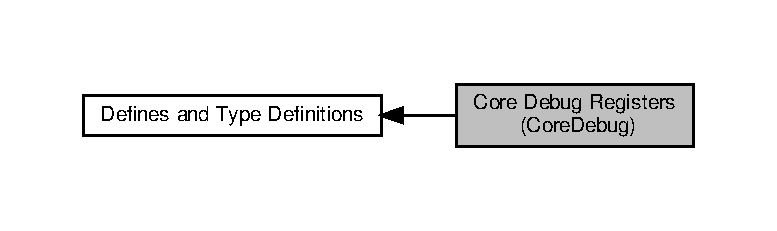
\includegraphics[width=350pt]{group___c_m_s_i_s___core_debug}
\end{center}
\end{figure}
\subsection*{Komponenty}
\begin{DoxyCompactItemize}
\item 
struct \hyperlink{struct_core_debug___type}{Core\+Debug\+\_\+\+Type}
\begin{DoxyCompactList}\small\item\em Structure type to access the Core Debug Register (Core\+Debug). \end{DoxyCompactList}\end{DoxyCompactItemize}
\subsection*{Definicje}
\begin{DoxyCompactItemize}
\item 
\#define \hyperlink{group___c_m_s_i_s___core_debug_gac91280edd0ce932665cf75a23d11d842}{Core\+Debug\+\_\+\+D\+H\+C\+S\+R\+\_\+\+D\+B\+G\+K\+E\+Y\+\_\+\+Pos}~16U
\item 
\#define \hyperlink{group___c_m_s_i_s___core_debug_ga1ce997cee15edaafe4aed77751816ffc}{Core\+Debug\+\_\+\+D\+H\+C\+S\+R\+\_\+\+D\+B\+G\+K\+E\+Y\+\_\+\+Msk}~(0x\+F\+F\+F\+F\+U\+L $<$$<$ Core\+Debug\+\_\+\+D\+H\+C\+S\+R\+\_\+\+D\+B\+G\+K\+E\+Y\+\_\+\+Pos)
\item 
\#define \hyperlink{group___c_m_s_i_s___core_debug_gaf6498d32dbe23b8d95a12d2fbc0a65f8}{Core\+Debug\+\_\+\+D\+H\+C\+S\+R\+\_\+\+S\+\_\+\+R\+E\+S\+T\+A\+R\+T\+\_\+\+S\+T\+\_\+\+Pos}~26U
\item 
\#define \hyperlink{group___c_m_s_i_s___core_debug_gabe3254d40aaa482987ff31584d2a3240}{Core\+Debug\+\_\+\+D\+H\+C\+S\+R\+\_\+\+S\+\_\+\+R\+E\+S\+T\+A\+R\+T\+\_\+\+S\+T\+\_\+\+Msk}~(1\+U\+L $<$$<$ Core\+Debug\+\_\+\+D\+H\+C\+S\+R\+\_\+\+S\+\_\+\+R\+E\+S\+T\+A\+R\+T\+\_\+\+S\+T\+\_\+\+Pos)
\item 
\#define \hyperlink{group___c_m_s_i_s___core_debug_ga6f934c5427ea057394268e541fa97753}{Core\+Debug\+\_\+\+D\+H\+C\+S\+R\+\_\+\+S\+\_\+\+R\+E\+S\+E\+T\+\_\+\+S\+T\+\_\+\+Pos}~25U
\item 
\#define \hyperlink{group___c_m_s_i_s___core_debug_gac474394bcceb31a8e09566c90b3f8922}{Core\+Debug\+\_\+\+D\+H\+C\+S\+R\+\_\+\+S\+\_\+\+R\+E\+S\+E\+T\+\_\+\+S\+T\+\_\+\+Msk}~(1\+U\+L $<$$<$ Core\+Debug\+\_\+\+D\+H\+C\+S\+R\+\_\+\+S\+\_\+\+R\+E\+S\+E\+T\+\_\+\+S\+T\+\_\+\+Pos)
\item 
\#define \hyperlink{group___c_m_s_i_s___core_debug_ga2328118f8b3574c871a53605eb17e730}{Core\+Debug\+\_\+\+D\+H\+C\+S\+R\+\_\+\+S\+\_\+\+R\+E\+T\+I\+R\+E\+\_\+\+S\+T\+\_\+\+Pos}~24U
\item 
\#define \hyperlink{group___c_m_s_i_s___core_debug_ga89dceb5325f6bcb36a0473d65fbfcfa6}{Core\+Debug\+\_\+\+D\+H\+C\+S\+R\+\_\+\+S\+\_\+\+R\+E\+T\+I\+R\+E\+\_\+\+S\+T\+\_\+\+Msk}~(1\+U\+L $<$$<$ Core\+Debug\+\_\+\+D\+H\+C\+S\+R\+\_\+\+S\+\_\+\+R\+E\+T\+I\+R\+E\+\_\+\+S\+T\+\_\+\+Pos)
\item 
\#define \hyperlink{group___c_m_s_i_s___core_debug_ga2900dd56a988a4ed27ad664d5642807e}{Core\+Debug\+\_\+\+D\+H\+C\+S\+R\+\_\+\+S\+\_\+\+L\+O\+C\+K\+U\+P\+\_\+\+Pos}~19U
\item 
\#define \hyperlink{group___c_m_s_i_s___core_debug_ga7b67e4506d7f464ef5dafd6219739756}{Core\+Debug\+\_\+\+D\+H\+C\+S\+R\+\_\+\+S\+\_\+\+L\+O\+C\+K\+U\+P\+\_\+\+Msk}~(1\+U\+L $<$$<$ Core\+Debug\+\_\+\+D\+H\+C\+S\+R\+\_\+\+S\+\_\+\+L\+O\+C\+K\+U\+P\+\_\+\+Pos)
\item 
\#define \hyperlink{group___c_m_s_i_s___core_debug_ga349ccea33accc705595624c2d334fbcb}{Core\+Debug\+\_\+\+D\+H\+C\+S\+R\+\_\+\+S\+\_\+\+S\+L\+E\+E\+P\+\_\+\+Pos}~18U
\item 
\#define \hyperlink{group___c_m_s_i_s___core_debug_ga98d51538e645c2c1a422279cd85a0a25}{Core\+Debug\+\_\+\+D\+H\+C\+S\+R\+\_\+\+S\+\_\+\+S\+L\+E\+E\+P\+\_\+\+Msk}~(1\+U\+L $<$$<$ Core\+Debug\+\_\+\+D\+H\+C\+S\+R\+\_\+\+S\+\_\+\+S\+L\+E\+E\+P\+\_\+\+Pos)
\item 
\#define \hyperlink{group___c_m_s_i_s___core_debug_ga760a9a0d7f39951dc3f07d01f1f64772}{Core\+Debug\+\_\+\+D\+H\+C\+S\+R\+\_\+\+S\+\_\+\+H\+A\+L\+T\+\_\+\+Pos}~17U
\item 
\#define \hyperlink{group___c_m_s_i_s___core_debug_ga9f881ade3151a73bc5b02b73fe6473ca}{Core\+Debug\+\_\+\+D\+H\+C\+S\+R\+\_\+\+S\+\_\+\+H\+A\+L\+T\+\_\+\+Msk}~(1\+U\+L $<$$<$ Core\+Debug\+\_\+\+D\+H\+C\+S\+R\+\_\+\+S\+\_\+\+H\+A\+L\+T\+\_\+\+Pos)
\item 
\#define \hyperlink{group___c_m_s_i_s___core_debug_ga20a71871ca8768019c51168c70c3f41d}{Core\+Debug\+\_\+\+D\+H\+C\+S\+R\+\_\+\+S\+\_\+\+R\+E\+G\+R\+D\+Y\+\_\+\+Pos}~16U
\item 
\#define \hyperlink{group___c_m_s_i_s___core_debug_gac4cd6f3178de48f473d8903e8c847c07}{Core\+Debug\+\_\+\+D\+H\+C\+S\+R\+\_\+\+S\+\_\+\+R\+E\+G\+R\+D\+Y\+\_\+\+Msk}~(1\+U\+L $<$$<$ Core\+Debug\+\_\+\+D\+H\+C\+S\+R\+\_\+\+S\+\_\+\+R\+E\+G\+R\+D\+Y\+\_\+\+Pos)
\item 
\#define \hyperlink{group___c_m_s_i_s___core_debug_ga0d2907400eb948a4ea3886ca083ec8e3}{Core\+Debug\+\_\+\+D\+H\+C\+S\+R\+\_\+\+C\+\_\+\+M\+A\+S\+K\+I\+N\+T\+S\+\_\+\+Pos}~3U
\item 
\#define \hyperlink{group___c_m_s_i_s___core_debug_ga77fe1ef3c4a729c1c82fb62a94a51c31}{Core\+Debug\+\_\+\+D\+H\+C\+S\+R\+\_\+\+C\+\_\+\+M\+A\+S\+K\+I\+N\+T\+S\+\_\+\+Msk}~(1\+U\+L $<$$<$ Core\+Debug\+\_\+\+D\+H\+C\+S\+R\+\_\+\+C\+\_\+\+M\+A\+S\+K\+I\+N\+T\+S\+\_\+\+Pos)
\item 
\#define \hyperlink{group___c_m_s_i_s___core_debug_gae1fc39e80de54c0339cbb1b298a9f0f9}{Core\+Debug\+\_\+\+D\+H\+C\+S\+R\+\_\+\+C\+\_\+\+S\+T\+E\+P\+\_\+\+Pos}~2U
\item 
\#define \hyperlink{group___c_m_s_i_s___core_debug_gae6bda72fbd32cc5734ff3542170dc00d}{Core\+Debug\+\_\+\+D\+H\+C\+S\+R\+\_\+\+C\+\_\+\+S\+T\+E\+P\+\_\+\+Msk}~(1\+U\+L $<$$<$ Core\+Debug\+\_\+\+D\+H\+C\+S\+R\+\_\+\+C\+\_\+\+S\+T\+E\+P\+\_\+\+Pos)
\item 
\#define \hyperlink{group___c_m_s_i_s___core_debug_gaddf1d43f8857e4efc3dc4e6b15509692}{Core\+Debug\+\_\+\+D\+H\+C\+S\+R\+\_\+\+C\+\_\+\+H\+A\+L\+T\+\_\+\+Pos}~1U
\item 
\#define \hyperlink{group___c_m_s_i_s___core_debug_ga1d905a3aa594eb2e8bb78bcc4da05b3f}{Core\+Debug\+\_\+\+D\+H\+C\+S\+R\+\_\+\+C\+\_\+\+H\+A\+L\+T\+\_\+\+Msk}~(1\+U\+L $<$$<$ Core\+Debug\+\_\+\+D\+H\+C\+S\+R\+\_\+\+C\+\_\+\+H\+A\+L\+T\+\_\+\+Pos)
\item 
\#define \hyperlink{group___c_m_s_i_s___core_debug_gab557abb5b172b74d2cf44efb9d824e4e}{Core\+Debug\+\_\+\+D\+H\+C\+S\+R\+\_\+\+C\+\_\+\+D\+E\+B\+U\+G\+E\+N\+\_\+\+Pos}~0U
\item 
\#define \hyperlink{group___c_m_s_i_s___core_debug_gab815c741a4fc2a61988cd2fb7594210b}{Core\+Debug\+\_\+\+D\+H\+C\+S\+R\+\_\+\+C\+\_\+\+D\+E\+B\+U\+G\+E\+N\+\_\+\+Msk}~(1\+U\+L /$\ast$$<$$<$ Core\+Debug\+\_\+\+D\+H\+C\+S\+R\+\_\+\+C\+\_\+\+D\+E\+B\+U\+G\+E\+N\+\_\+\+Pos$\ast$/)
\item 
\#define \hyperlink{group___c_m_s_i_s___core_debug_ga51e75942fc0614bc9bb2c0e96fcdda9a}{Core\+Debug\+\_\+\+D\+C\+R\+S\+R\+\_\+\+R\+E\+G\+Wn\+R\+\_\+\+Pos}~16U
\item 
\#define \hyperlink{group___c_m_s_i_s___core_debug_ga1eef4992d8f84bc6c0dffed1c87f90a5}{Core\+Debug\+\_\+\+D\+C\+R\+S\+R\+\_\+\+R\+E\+G\+Wn\+R\+\_\+\+Msk}~(1\+U\+L $<$$<$ Core\+Debug\+\_\+\+D\+C\+R\+S\+R\+\_\+\+R\+E\+G\+Wn\+R\+\_\+\+Pos)
\item 
\#define \hyperlink{group___c_m_s_i_s___core_debug_ga52182c8a9f63a52470244c0bc2064f7b}{Core\+Debug\+\_\+\+D\+C\+R\+S\+R\+\_\+\+R\+E\+G\+S\+E\+L\+\_\+\+Pos}~0U
\item 
\#define \hyperlink{group___c_m_s_i_s___core_debug_ga17cafbd72b55030219ce5609baa7c01d}{Core\+Debug\+\_\+\+D\+C\+R\+S\+R\+\_\+\+R\+E\+G\+S\+E\+L\+\_\+\+Msk}~(0x1\+F\+U\+L /$\ast$$<$$<$ Core\+Debug\+\_\+\+D\+C\+R\+S\+R\+\_\+\+R\+E\+G\+S\+E\+L\+\_\+\+Pos$\ast$/)
\item 
\#define \hyperlink{group___c_m_s_i_s___core_debug_ga0cde79c4e741e1eed0513c1f985baeb9}{Core\+Debug\+\_\+\+D\+E\+M\+C\+R\+\_\+\+D\+W\+T\+E\+N\+A\+\_\+\+Pos}~24U
\item 
\#define \hyperlink{group___c_m_s_i_s___core_debug_ga2fcc0b8f174e85379d38e1cb74b8c627}{Core\+Debug\+\_\+\+D\+E\+M\+C\+R\+\_\+\+D\+W\+T\+E\+N\+A\+\_\+\+Msk}~(1\+U\+L $<$$<$ Core\+Debug\+\_\+\+D\+E\+M\+C\+R\+\_\+\+D\+W\+T\+E\+N\+A\+\_\+\+Pos)
\item 
\#define \hyperlink{group___c_m_s_i_s___core_debug_gaed9f42053031a9a30cd8054623304c0a}{Core\+Debug\+\_\+\+D\+E\+M\+C\+R\+\_\+\+V\+C\+\_\+\+H\+A\+R\+D\+E\+R\+R\+\_\+\+Pos}~10U
\item 
\#define \hyperlink{group___c_m_s_i_s___core_debug_ga803fc98c5bb85f10f0347b23794847d1}{Core\+Debug\+\_\+\+D\+E\+M\+C\+R\+\_\+\+V\+C\+\_\+\+H\+A\+R\+D\+E\+R\+R\+\_\+\+Msk}~(1\+U\+L $<$$<$ Core\+Debug\+\_\+\+D\+E\+M\+C\+R\+\_\+\+V\+C\+\_\+\+H\+A\+R\+D\+E\+R\+R\+\_\+\+Pos)
\item 
\#define \hyperlink{group___c_m_s_i_s___core_debug_ga9fcf09666f7063a7303117aa32a85d5a}{Core\+Debug\+\_\+\+D\+E\+M\+C\+R\+\_\+\+V\+C\+\_\+\+C\+O\+R\+E\+R\+E\+S\+E\+T\+\_\+\+Pos}~0U
\item 
\#define \hyperlink{group___c_m_s_i_s___core_debug_ga906476e53c1e1487c30f3a1181df9e30}{Core\+Debug\+\_\+\+D\+E\+M\+C\+R\+\_\+\+V\+C\+\_\+\+C\+O\+R\+E\+R\+E\+S\+E\+T\+\_\+\+Msk}~(1\+U\+L /$\ast$$<$$<$ Core\+Debug\+\_\+\+D\+E\+M\+C\+R\+\_\+\+V\+C\+\_\+\+C\+O\+R\+E\+R\+E\+S\+E\+T\+\_\+\+Pos$\ast$/)
\item 
\#define \hyperlink{group___c_m_s_i_s___core_debug_gaf733a36e6b4717a604f7d77c05dfceb4}{Core\+Debug\+\_\+\+D\+A\+U\+T\+H\+C\+T\+R\+L\+\_\+\+I\+N\+T\+S\+P\+N\+I\+D\+E\+N\+\_\+\+Pos}~3U
\item 
\#define \hyperlink{group___c_m_s_i_s___core_debug_gadad0bf68d32cba49c1ea7534122c2752}{Core\+Debug\+\_\+\+D\+A\+U\+T\+H\+C\+T\+R\+L\+\_\+\+I\+N\+T\+S\+P\+N\+I\+D\+E\+N\+\_\+\+Msk}~(1\+U\+L $<$$<$ Core\+Debug\+\_\+\+D\+A\+U\+T\+H\+C\+T\+R\+L\+\_\+\+I\+N\+T\+S\+P\+N\+I\+D\+E\+N\+\_\+\+Pos)
\item 
\#define \hyperlink{group___c_m_s_i_s___core_debug_ga866734a8e4bec2d6cf091e265c6c0f3d}{Core\+Debug\+\_\+\+D\+A\+U\+T\+H\+C\+T\+R\+L\+\_\+\+S\+P\+N\+I\+D\+E\+N\+S\+E\+L\+\_\+\+Pos}~2U
\item 
\#define \hyperlink{group___c_m_s_i_s___core_debug_gaabb5d6c750c9ec50254134ece2111dcd}{Core\+Debug\+\_\+\+D\+A\+U\+T\+H\+C\+T\+R\+L\+\_\+\+S\+P\+N\+I\+D\+E\+N\+S\+E\+L\+\_\+\+Msk}~(1\+U\+L $<$$<$ Core\+Debug\+\_\+\+D\+A\+U\+T\+H\+C\+T\+R\+L\+\_\+\+S\+P\+N\+I\+D\+E\+N\+S\+E\+L\+\_\+\+Pos)
\item 
\#define \hyperlink{group___c_m_s_i_s___core_debug_ga3caef9790e4e2ccbfea77d55315ad59f}{Core\+Debug\+\_\+\+D\+A\+U\+T\+H\+C\+T\+R\+L\+\_\+\+I\+N\+T\+S\+P\+I\+D\+E\+N\+\_\+\+Pos}~1U
\item 
\#define \hyperlink{group___c_m_s_i_s___core_debug_ga1570f149a0f89f70fc2644a5842cbcb4}{Core\+Debug\+\_\+\+D\+A\+U\+T\+H\+C\+T\+R\+L\+\_\+\+I\+N\+T\+S\+P\+I\+D\+E\+N\+\_\+\+Msk}~(1\+U\+L $<$$<$ Core\+Debug\+\_\+\+D\+A\+U\+T\+H\+C\+T\+R\+L\+\_\+\+I\+N\+T\+S\+P\+I\+D\+E\+N\+\_\+\+Pos)
\item 
\#define \hyperlink{group___c_m_s_i_s___core_debug_ga587610b7ac18292de47bf9d675b0b88c}{Core\+Debug\+\_\+\+D\+A\+U\+T\+H\+C\+T\+R\+L\+\_\+\+S\+P\+I\+D\+E\+N\+S\+E\+L\+\_\+\+Pos}~0U
\item 
\#define \hyperlink{group___c_m_s_i_s___core_debug_gaa043fd13768d57be320c682ca1c9b234}{Core\+Debug\+\_\+\+D\+A\+U\+T\+H\+C\+T\+R\+L\+\_\+\+S\+P\+I\+D\+E\+N\+S\+E\+L\+\_\+\+Msk}~(1\+U\+L /$\ast$$<$$<$ Core\+Debug\+\_\+\+D\+A\+U\+T\+H\+C\+T\+R\+L\+\_\+\+S\+P\+I\+D\+E\+N\+S\+E\+L\+\_\+\+Pos$\ast$/)
\item 
\#define \hyperlink{group___c_m_s_i_s___core_debug_ga4be5d0f8af5d7d8ec04bde78ce18e10e}{Core\+Debug\+\_\+\+D\+S\+C\+S\+R\+\_\+\+C\+D\+S\+\_\+\+Pos}~16U
\item 
\#define \hyperlink{group___c_m_s_i_s___core_debug_ga083417245e1aa40e84a2b12433a15a6b}{Core\+Debug\+\_\+\+D\+S\+C\+S\+R\+\_\+\+C\+D\+S\+\_\+\+Msk}~(1\+U\+L $<$$<$ Core\+Debug\+\_\+\+D\+S\+C\+S\+R\+\_\+\+C\+D\+S\+\_\+\+Pos)
\item 
\#define \hyperlink{group___c_m_s_i_s___core_debug_ga7450603163415ab4d4e4a7a767879eae}{Core\+Debug\+\_\+\+D\+S\+C\+S\+R\+\_\+\+S\+B\+R\+S\+E\+L\+\_\+\+Pos}~1U
\item 
\#define \hyperlink{group___c_m_s_i_s___core_debug_gaaffe28a24f05446e55ba3d75bb6f4cd0}{Core\+Debug\+\_\+\+D\+S\+C\+S\+R\+\_\+\+S\+B\+R\+S\+E\+L\+\_\+\+Msk}~(1\+U\+L $<$$<$ Core\+Debug\+\_\+\+D\+S\+C\+S\+R\+\_\+\+S\+B\+R\+S\+E\+L\+\_\+\+Pos)
\item 
\#define \hyperlink{group___c_m_s_i_s___core_debug_ga3eb88e444b678057db1b59272eebb1ad}{Core\+Debug\+\_\+\+D\+S\+C\+S\+R\+\_\+\+S\+B\+R\+S\+E\+L\+E\+N\+\_\+\+Pos}~0U
\item 
\#define \hyperlink{group___c_m_s_i_s___core_debug_ga5e5ed94cac1139165af161c008881805}{Core\+Debug\+\_\+\+D\+S\+C\+S\+R\+\_\+\+S\+B\+R\+S\+E\+L\+E\+N\+\_\+\+Msk}~(1\+U\+L /$\ast$$<$$<$ Core\+Debug\+\_\+\+D\+S\+C\+S\+R\+\_\+\+S\+B\+R\+S\+E\+L\+E\+N\+\_\+\+Pos$\ast$/)
\item 
\#define \hyperlink{group___c_m_s_i_s___core_debug_gac91280edd0ce932665cf75a23d11d842}{Core\+Debug\+\_\+\+D\+H\+C\+S\+R\+\_\+\+D\+B\+G\+K\+E\+Y\+\_\+\+Pos}~16U
\item 
\#define \hyperlink{group___c_m_s_i_s___core_debug_ga1ce997cee15edaafe4aed77751816ffc}{Core\+Debug\+\_\+\+D\+H\+C\+S\+R\+\_\+\+D\+B\+G\+K\+E\+Y\+\_\+\+Msk}~(0x\+F\+F\+F\+F\+U\+L $<$$<$ Core\+Debug\+\_\+\+D\+H\+C\+S\+R\+\_\+\+D\+B\+G\+K\+E\+Y\+\_\+\+Pos)
\item 
\#define \hyperlink{group___c_m_s_i_s___core_debug_gaf6498d32dbe23b8d95a12d2fbc0a65f8}{Core\+Debug\+\_\+\+D\+H\+C\+S\+R\+\_\+\+S\+\_\+\+R\+E\+S\+T\+A\+R\+T\+\_\+\+S\+T\+\_\+\+Pos}~26U
\item 
\#define \hyperlink{group___c_m_s_i_s___core_debug_gabe3254d40aaa482987ff31584d2a3240}{Core\+Debug\+\_\+\+D\+H\+C\+S\+R\+\_\+\+S\+\_\+\+R\+E\+S\+T\+A\+R\+T\+\_\+\+S\+T\+\_\+\+Msk}~(1\+U\+L $<$$<$ Core\+Debug\+\_\+\+D\+H\+C\+S\+R\+\_\+\+S\+\_\+\+R\+E\+S\+T\+A\+R\+T\+\_\+\+S\+T\+\_\+\+Pos)
\item 
\#define \hyperlink{group___c_m_s_i_s___core_debug_ga6f934c5427ea057394268e541fa97753}{Core\+Debug\+\_\+\+D\+H\+C\+S\+R\+\_\+\+S\+\_\+\+R\+E\+S\+E\+T\+\_\+\+S\+T\+\_\+\+Pos}~25U
\item 
\#define \hyperlink{group___c_m_s_i_s___core_debug_gac474394bcceb31a8e09566c90b3f8922}{Core\+Debug\+\_\+\+D\+H\+C\+S\+R\+\_\+\+S\+\_\+\+R\+E\+S\+E\+T\+\_\+\+S\+T\+\_\+\+Msk}~(1\+U\+L $<$$<$ Core\+Debug\+\_\+\+D\+H\+C\+S\+R\+\_\+\+S\+\_\+\+R\+E\+S\+E\+T\+\_\+\+S\+T\+\_\+\+Pos)
\item 
\#define \hyperlink{group___c_m_s_i_s___core_debug_ga2328118f8b3574c871a53605eb17e730}{Core\+Debug\+\_\+\+D\+H\+C\+S\+R\+\_\+\+S\+\_\+\+R\+E\+T\+I\+R\+E\+\_\+\+S\+T\+\_\+\+Pos}~24U
\item 
\#define \hyperlink{group___c_m_s_i_s___core_debug_ga89dceb5325f6bcb36a0473d65fbfcfa6}{Core\+Debug\+\_\+\+D\+H\+C\+S\+R\+\_\+\+S\+\_\+\+R\+E\+T\+I\+R\+E\+\_\+\+S\+T\+\_\+\+Msk}~(1\+U\+L $<$$<$ Core\+Debug\+\_\+\+D\+H\+C\+S\+R\+\_\+\+S\+\_\+\+R\+E\+T\+I\+R\+E\+\_\+\+S\+T\+\_\+\+Pos)
\item 
\#define \hyperlink{group___c_m_s_i_s___core_debug_ga2900dd56a988a4ed27ad664d5642807e}{Core\+Debug\+\_\+\+D\+H\+C\+S\+R\+\_\+\+S\+\_\+\+L\+O\+C\+K\+U\+P\+\_\+\+Pos}~19U
\item 
\#define \hyperlink{group___c_m_s_i_s___core_debug_ga7b67e4506d7f464ef5dafd6219739756}{Core\+Debug\+\_\+\+D\+H\+C\+S\+R\+\_\+\+S\+\_\+\+L\+O\+C\+K\+U\+P\+\_\+\+Msk}~(1\+U\+L $<$$<$ Core\+Debug\+\_\+\+D\+H\+C\+S\+R\+\_\+\+S\+\_\+\+L\+O\+C\+K\+U\+P\+\_\+\+Pos)
\item 
\#define \hyperlink{group___c_m_s_i_s___core_debug_ga349ccea33accc705595624c2d334fbcb}{Core\+Debug\+\_\+\+D\+H\+C\+S\+R\+\_\+\+S\+\_\+\+S\+L\+E\+E\+P\+\_\+\+Pos}~18U
\item 
\#define \hyperlink{group___c_m_s_i_s___core_debug_ga98d51538e645c2c1a422279cd85a0a25}{Core\+Debug\+\_\+\+D\+H\+C\+S\+R\+\_\+\+S\+\_\+\+S\+L\+E\+E\+P\+\_\+\+Msk}~(1\+U\+L $<$$<$ Core\+Debug\+\_\+\+D\+H\+C\+S\+R\+\_\+\+S\+\_\+\+S\+L\+E\+E\+P\+\_\+\+Pos)
\item 
\#define \hyperlink{group___c_m_s_i_s___core_debug_ga760a9a0d7f39951dc3f07d01f1f64772}{Core\+Debug\+\_\+\+D\+H\+C\+S\+R\+\_\+\+S\+\_\+\+H\+A\+L\+T\+\_\+\+Pos}~17U
\item 
\#define \hyperlink{group___c_m_s_i_s___core_debug_ga9f881ade3151a73bc5b02b73fe6473ca}{Core\+Debug\+\_\+\+D\+H\+C\+S\+R\+\_\+\+S\+\_\+\+H\+A\+L\+T\+\_\+\+Msk}~(1\+U\+L $<$$<$ Core\+Debug\+\_\+\+D\+H\+C\+S\+R\+\_\+\+S\+\_\+\+H\+A\+L\+T\+\_\+\+Pos)
\item 
\#define \hyperlink{group___c_m_s_i_s___core_debug_ga20a71871ca8768019c51168c70c3f41d}{Core\+Debug\+\_\+\+D\+H\+C\+S\+R\+\_\+\+S\+\_\+\+R\+E\+G\+R\+D\+Y\+\_\+\+Pos}~16U
\item 
\#define \hyperlink{group___c_m_s_i_s___core_debug_gac4cd6f3178de48f473d8903e8c847c07}{Core\+Debug\+\_\+\+D\+H\+C\+S\+R\+\_\+\+S\+\_\+\+R\+E\+G\+R\+D\+Y\+\_\+\+Msk}~(1\+U\+L $<$$<$ Core\+Debug\+\_\+\+D\+H\+C\+S\+R\+\_\+\+S\+\_\+\+R\+E\+G\+R\+D\+Y\+\_\+\+Pos)
\item 
\#define \hyperlink{group___c_m_s_i_s___core_debug_ga85747214e2656df6b05ec72e4d22bd6d}{Core\+Debug\+\_\+\+D\+H\+C\+S\+R\+\_\+\+C\+\_\+\+S\+N\+A\+P\+S\+T\+A\+L\+L\+\_\+\+Pos}~5U
\item 
\#define \hyperlink{group___c_m_s_i_s___core_debug_ga53aa99b2e39a67622f3b9973e079c2b4}{Core\+Debug\+\_\+\+D\+H\+C\+S\+R\+\_\+\+C\+\_\+\+S\+N\+A\+P\+S\+T\+A\+L\+L\+\_\+\+Msk}~(1\+U\+L $<$$<$ Core\+Debug\+\_\+\+D\+H\+C\+S\+R\+\_\+\+C\+\_\+\+S\+N\+A\+P\+S\+T\+A\+L\+L\+\_\+\+Pos)
\item 
\#define \hyperlink{group___c_m_s_i_s___core_debug_ga0d2907400eb948a4ea3886ca083ec8e3}{Core\+Debug\+\_\+\+D\+H\+C\+S\+R\+\_\+\+C\+\_\+\+M\+A\+S\+K\+I\+N\+T\+S\+\_\+\+Pos}~3U
\item 
\#define \hyperlink{group___c_m_s_i_s___core_debug_ga77fe1ef3c4a729c1c82fb62a94a51c31}{Core\+Debug\+\_\+\+D\+H\+C\+S\+R\+\_\+\+C\+\_\+\+M\+A\+S\+K\+I\+N\+T\+S\+\_\+\+Msk}~(1\+U\+L $<$$<$ Core\+Debug\+\_\+\+D\+H\+C\+S\+R\+\_\+\+C\+\_\+\+M\+A\+S\+K\+I\+N\+T\+S\+\_\+\+Pos)
\item 
\#define \hyperlink{group___c_m_s_i_s___core_debug_gae1fc39e80de54c0339cbb1b298a9f0f9}{Core\+Debug\+\_\+\+D\+H\+C\+S\+R\+\_\+\+C\+\_\+\+S\+T\+E\+P\+\_\+\+Pos}~2U
\item 
\#define \hyperlink{group___c_m_s_i_s___core_debug_gae6bda72fbd32cc5734ff3542170dc00d}{Core\+Debug\+\_\+\+D\+H\+C\+S\+R\+\_\+\+C\+\_\+\+S\+T\+E\+P\+\_\+\+Msk}~(1\+U\+L $<$$<$ Core\+Debug\+\_\+\+D\+H\+C\+S\+R\+\_\+\+C\+\_\+\+S\+T\+E\+P\+\_\+\+Pos)
\item 
\#define \hyperlink{group___c_m_s_i_s___core_debug_gaddf1d43f8857e4efc3dc4e6b15509692}{Core\+Debug\+\_\+\+D\+H\+C\+S\+R\+\_\+\+C\+\_\+\+H\+A\+L\+T\+\_\+\+Pos}~1U
\item 
\#define \hyperlink{group___c_m_s_i_s___core_debug_ga1d905a3aa594eb2e8bb78bcc4da05b3f}{Core\+Debug\+\_\+\+D\+H\+C\+S\+R\+\_\+\+C\+\_\+\+H\+A\+L\+T\+\_\+\+Msk}~(1\+U\+L $<$$<$ Core\+Debug\+\_\+\+D\+H\+C\+S\+R\+\_\+\+C\+\_\+\+H\+A\+L\+T\+\_\+\+Pos)
\item 
\#define \hyperlink{group___c_m_s_i_s___core_debug_gab557abb5b172b74d2cf44efb9d824e4e}{Core\+Debug\+\_\+\+D\+H\+C\+S\+R\+\_\+\+C\+\_\+\+D\+E\+B\+U\+G\+E\+N\+\_\+\+Pos}~0U
\item 
\#define \hyperlink{group___c_m_s_i_s___core_debug_gab815c741a4fc2a61988cd2fb7594210b}{Core\+Debug\+\_\+\+D\+H\+C\+S\+R\+\_\+\+C\+\_\+\+D\+E\+B\+U\+G\+E\+N\+\_\+\+Msk}~(1\+U\+L /$\ast$$<$$<$ Core\+Debug\+\_\+\+D\+H\+C\+S\+R\+\_\+\+C\+\_\+\+D\+E\+B\+U\+G\+E\+N\+\_\+\+Pos$\ast$/)
\item 
\#define \hyperlink{group___c_m_s_i_s___core_debug_ga51e75942fc0614bc9bb2c0e96fcdda9a}{Core\+Debug\+\_\+\+D\+C\+R\+S\+R\+\_\+\+R\+E\+G\+Wn\+R\+\_\+\+Pos}~16U
\item 
\#define \hyperlink{group___c_m_s_i_s___core_debug_ga1eef4992d8f84bc6c0dffed1c87f90a5}{Core\+Debug\+\_\+\+D\+C\+R\+S\+R\+\_\+\+R\+E\+G\+Wn\+R\+\_\+\+Msk}~(1\+U\+L $<$$<$ Core\+Debug\+\_\+\+D\+C\+R\+S\+R\+\_\+\+R\+E\+G\+Wn\+R\+\_\+\+Pos)
\item 
\#define \hyperlink{group___c_m_s_i_s___core_debug_ga52182c8a9f63a52470244c0bc2064f7b}{Core\+Debug\+\_\+\+D\+C\+R\+S\+R\+\_\+\+R\+E\+G\+S\+E\+L\+\_\+\+Pos}~0U
\item 
\#define \hyperlink{group___c_m_s_i_s___core_debug_ga17cafbd72b55030219ce5609baa7c01d}{Core\+Debug\+\_\+\+D\+C\+R\+S\+R\+\_\+\+R\+E\+G\+S\+E\+L\+\_\+\+Msk}~(0x1\+F\+U\+L /$\ast$$<$$<$ Core\+Debug\+\_\+\+D\+C\+R\+S\+R\+\_\+\+R\+E\+G\+S\+E\+L\+\_\+\+Pos$\ast$/)
\item 
\#define \hyperlink{group___c_m_s_i_s___core_debug_ga6ff2102b98f86540224819a1b767ba39}{Core\+Debug\+\_\+\+D\+E\+M\+C\+R\+\_\+\+T\+R\+C\+E\+N\+A\+\_\+\+Pos}~24U
\item 
\#define \hyperlink{group___c_m_s_i_s___core_debug_ga5e99652c1df93b441257389f49407834}{Core\+Debug\+\_\+\+D\+E\+M\+C\+R\+\_\+\+T\+R\+C\+E\+N\+A\+\_\+\+Msk}~(1\+U\+L $<$$<$ Core\+Debug\+\_\+\+D\+E\+M\+C\+R\+\_\+\+T\+R\+C\+E\+N\+A\+\_\+\+Pos)
\item 
\#define \hyperlink{group___c_m_s_i_s___core_debug_ga341020a3b7450416d72544eaf8e57a64}{Core\+Debug\+\_\+\+D\+E\+M\+C\+R\+\_\+\+M\+O\+N\+\_\+\+R\+E\+Q\+\_\+\+Pos}~19U
\item 
\#define \hyperlink{group___c_m_s_i_s___core_debug_gae6384cbe8045051186d13ef9cdeace95}{Core\+Debug\+\_\+\+D\+E\+M\+C\+R\+\_\+\+M\+O\+N\+\_\+\+R\+E\+Q\+\_\+\+Msk}~(1\+U\+L $<$$<$ Core\+Debug\+\_\+\+D\+E\+M\+C\+R\+\_\+\+M\+O\+N\+\_\+\+R\+E\+Q\+\_\+\+Pos)
\item 
\#define \hyperlink{group___c_m_s_i_s___core_debug_ga9ae10710684e14a1a534e785ef390e1b}{Core\+Debug\+\_\+\+D\+E\+M\+C\+R\+\_\+\+M\+O\+N\+\_\+\+S\+T\+E\+P\+\_\+\+Pos}~18U
\item 
\#define \hyperlink{group___c_m_s_i_s___core_debug_ga2ded814556de96fc369de7ae9a7ceb98}{Core\+Debug\+\_\+\+D\+E\+M\+C\+R\+\_\+\+M\+O\+N\+\_\+\+S\+T\+E\+P\+\_\+\+Msk}~(1\+U\+L $<$$<$ Core\+Debug\+\_\+\+D\+E\+M\+C\+R\+\_\+\+M\+O\+N\+\_\+\+S\+T\+E\+P\+\_\+\+Pos)
\item 
\#define \hyperlink{group___c_m_s_i_s___core_debug_ga1e2f706a59e0d8131279af1c7e152f8d}{Core\+Debug\+\_\+\+D\+E\+M\+C\+R\+\_\+\+M\+O\+N\+\_\+\+P\+E\+N\+D\+\_\+\+Pos}~17U
\item 
\#define \hyperlink{group___c_m_s_i_s___core_debug_ga68ec55930269fab78e733dcfa32392f8}{Core\+Debug\+\_\+\+D\+E\+M\+C\+R\+\_\+\+M\+O\+N\+\_\+\+P\+E\+N\+D\+\_\+\+Msk}~(1\+U\+L $<$$<$ Core\+Debug\+\_\+\+D\+E\+M\+C\+R\+\_\+\+M\+O\+N\+\_\+\+P\+E\+N\+D\+\_\+\+Pos)
\item 
\#define \hyperlink{group___c_m_s_i_s___core_debug_ga802829678f6871863ae9ecf60a10425c}{Core\+Debug\+\_\+\+D\+E\+M\+C\+R\+\_\+\+M\+O\+N\+\_\+\+E\+N\+\_\+\+Pos}~16U
\item 
\#define \hyperlink{group___c_m_s_i_s___core_debug_gac2b46b9b65bf8d23027f255fc9641977}{Core\+Debug\+\_\+\+D\+E\+M\+C\+R\+\_\+\+M\+O\+N\+\_\+\+E\+N\+\_\+\+Msk}~(1\+U\+L $<$$<$ Core\+Debug\+\_\+\+D\+E\+M\+C\+R\+\_\+\+M\+O\+N\+\_\+\+E\+N\+\_\+\+Pos)
\item 
\#define \hyperlink{group___c_m_s_i_s___core_debug_gaed9f42053031a9a30cd8054623304c0a}{Core\+Debug\+\_\+\+D\+E\+M\+C\+R\+\_\+\+V\+C\+\_\+\+H\+A\+R\+D\+E\+R\+R\+\_\+\+Pos}~10U
\item 
\#define \hyperlink{group___c_m_s_i_s___core_debug_ga803fc98c5bb85f10f0347b23794847d1}{Core\+Debug\+\_\+\+D\+E\+M\+C\+R\+\_\+\+V\+C\+\_\+\+H\+A\+R\+D\+E\+R\+R\+\_\+\+Msk}~(1\+U\+L $<$$<$ Core\+Debug\+\_\+\+D\+E\+M\+C\+R\+\_\+\+V\+C\+\_\+\+H\+A\+R\+D\+E\+R\+R\+\_\+\+Pos)
\item 
\#define \hyperlink{group___c_m_s_i_s___core_debug_ga22079a6e436f23b90308be97e19cf07e}{Core\+Debug\+\_\+\+D\+E\+M\+C\+R\+\_\+\+V\+C\+\_\+\+I\+N\+T\+E\+R\+R\+\_\+\+Pos}~9U
\item 
\#define \hyperlink{group___c_m_s_i_s___core_debug_gad6815d8e3df302d2f0ff2c2c734ed29a}{Core\+Debug\+\_\+\+D\+E\+M\+C\+R\+\_\+\+V\+C\+\_\+\+I\+N\+T\+E\+R\+R\+\_\+\+Msk}~(1\+U\+L $<$$<$ Core\+Debug\+\_\+\+D\+E\+M\+C\+R\+\_\+\+V\+C\+\_\+\+I\+N\+T\+E\+R\+R\+\_\+\+Pos)
\item 
\#define \hyperlink{group___c_m_s_i_s___core_debug_gab8e3d8f0f9590a51bbf10f6da3ad6933}{Core\+Debug\+\_\+\+D\+E\+M\+C\+R\+\_\+\+V\+C\+\_\+\+B\+U\+S\+E\+R\+R\+\_\+\+Pos}~8U
\item 
\#define \hyperlink{group___c_m_s_i_s___core_debug_ga9d29546aefe3ca8662a7fe48dd4a5b2b}{Core\+Debug\+\_\+\+D\+E\+M\+C\+R\+\_\+\+V\+C\+\_\+\+B\+U\+S\+E\+R\+R\+\_\+\+Msk}~(1\+U\+L $<$$<$ Core\+Debug\+\_\+\+D\+E\+M\+C\+R\+\_\+\+V\+C\+\_\+\+B\+U\+S\+E\+R\+R\+\_\+\+Pos)
\item 
\#define \hyperlink{group___c_m_s_i_s___core_debug_ga16f0d3d2ce1e1e8cd762d938ac56c4ac}{Core\+Debug\+\_\+\+D\+E\+M\+C\+R\+\_\+\+V\+C\+\_\+\+S\+T\+A\+T\+E\+R\+R\+\_\+\+Pos}~7U
\item 
\#define \hyperlink{group___c_m_s_i_s___core_debug_gaa38b947d77672c48bba1280c0a642e19}{Core\+Debug\+\_\+\+D\+E\+M\+C\+R\+\_\+\+V\+C\+\_\+\+S\+T\+A\+T\+E\+R\+R\+\_\+\+Msk}~(1\+U\+L $<$$<$ Core\+Debug\+\_\+\+D\+E\+M\+C\+R\+\_\+\+V\+C\+\_\+\+S\+T\+A\+T\+E\+R\+R\+\_\+\+Pos)
\item 
\#define \hyperlink{group___c_m_s_i_s___core_debug_ga10fc7c53bca904c128bc8e1a03072d50}{Core\+Debug\+\_\+\+D\+E\+M\+C\+R\+\_\+\+V\+C\+\_\+\+C\+H\+K\+E\+R\+R\+\_\+\+Pos}~6U
\item 
\#define \hyperlink{group___c_m_s_i_s___core_debug_ga2f98b461d19746ab2febfddebb73da6f}{Core\+Debug\+\_\+\+D\+E\+M\+C\+R\+\_\+\+V\+C\+\_\+\+C\+H\+K\+E\+R\+R\+\_\+\+Msk}~(1\+U\+L $<$$<$ Core\+Debug\+\_\+\+D\+E\+M\+C\+R\+\_\+\+V\+C\+\_\+\+C\+H\+K\+E\+R\+R\+\_\+\+Pos)
\item 
\#define \hyperlink{group___c_m_s_i_s___core_debug_gac9d13eb2add61f610d5ced1f7ad2adf8}{Core\+Debug\+\_\+\+D\+E\+M\+C\+R\+\_\+\+V\+C\+\_\+\+N\+O\+C\+P\+E\+R\+R\+\_\+\+Pos}~5U
\item 
\#define \hyperlink{group___c_m_s_i_s___core_debug_ga03ee58b1b02fdbf21612809034562f1c}{Core\+Debug\+\_\+\+D\+E\+M\+C\+R\+\_\+\+V\+C\+\_\+\+N\+O\+C\+P\+E\+R\+R\+\_\+\+Msk}~(1\+U\+L $<$$<$ Core\+Debug\+\_\+\+D\+E\+M\+C\+R\+\_\+\+V\+C\+\_\+\+N\+O\+C\+P\+E\+R\+R\+\_\+\+Pos)
\item 
\#define \hyperlink{group___c_m_s_i_s___core_debug_ga444454f7c7748e76cd76c3809c887c41}{Core\+Debug\+\_\+\+D\+E\+M\+C\+R\+\_\+\+V\+C\+\_\+\+M\+M\+E\+R\+R\+\_\+\+Pos}~4U
\item 
\#define \hyperlink{group___c_m_s_i_s___core_debug_gad420a9b60620584faaca6289e83d3a87}{Core\+Debug\+\_\+\+D\+E\+M\+C\+R\+\_\+\+V\+C\+\_\+\+M\+M\+E\+R\+R\+\_\+\+Msk}~(1\+U\+L $<$$<$ Core\+Debug\+\_\+\+D\+E\+M\+C\+R\+\_\+\+V\+C\+\_\+\+M\+M\+E\+R\+R\+\_\+\+Pos)
\item 
\#define \hyperlink{group___c_m_s_i_s___core_debug_ga9fcf09666f7063a7303117aa32a85d5a}{Core\+Debug\+\_\+\+D\+E\+M\+C\+R\+\_\+\+V\+C\+\_\+\+C\+O\+R\+E\+R\+E\+S\+E\+T\+\_\+\+Pos}~0U
\item 
\#define \hyperlink{group___c_m_s_i_s___core_debug_ga906476e53c1e1487c30f3a1181df9e30}{Core\+Debug\+\_\+\+D\+E\+M\+C\+R\+\_\+\+V\+C\+\_\+\+C\+O\+R\+E\+R\+E\+S\+E\+T\+\_\+\+Msk}~(1\+U\+L /$\ast$$<$$<$ Core\+Debug\+\_\+\+D\+E\+M\+C\+R\+\_\+\+V\+C\+\_\+\+C\+O\+R\+E\+R\+E\+S\+E\+T\+\_\+\+Pos$\ast$/)
\item 
\#define \hyperlink{group___c_m_s_i_s___core_debug_gaf733a36e6b4717a604f7d77c05dfceb4}{Core\+Debug\+\_\+\+D\+A\+U\+T\+H\+C\+T\+R\+L\+\_\+\+I\+N\+T\+S\+P\+N\+I\+D\+E\+N\+\_\+\+Pos}~3U
\item 
\#define \hyperlink{group___c_m_s_i_s___core_debug_gadad0bf68d32cba49c1ea7534122c2752}{Core\+Debug\+\_\+\+D\+A\+U\+T\+H\+C\+T\+R\+L\+\_\+\+I\+N\+T\+S\+P\+N\+I\+D\+E\+N\+\_\+\+Msk}~(1\+U\+L $<$$<$ Core\+Debug\+\_\+\+D\+A\+U\+T\+H\+C\+T\+R\+L\+\_\+\+I\+N\+T\+S\+P\+N\+I\+D\+E\+N\+\_\+\+Pos)
\item 
\#define \hyperlink{group___c_m_s_i_s___core_debug_ga866734a8e4bec2d6cf091e265c6c0f3d}{Core\+Debug\+\_\+\+D\+A\+U\+T\+H\+C\+T\+R\+L\+\_\+\+S\+P\+N\+I\+D\+E\+N\+S\+E\+L\+\_\+\+Pos}~2U
\item 
\#define \hyperlink{group___c_m_s_i_s___core_debug_gaabb5d6c750c9ec50254134ece2111dcd}{Core\+Debug\+\_\+\+D\+A\+U\+T\+H\+C\+T\+R\+L\+\_\+\+S\+P\+N\+I\+D\+E\+N\+S\+E\+L\+\_\+\+Msk}~(1\+U\+L $<$$<$ Core\+Debug\+\_\+\+D\+A\+U\+T\+H\+C\+T\+R\+L\+\_\+\+S\+P\+N\+I\+D\+E\+N\+S\+E\+L\+\_\+\+Pos)
\item 
\#define \hyperlink{group___c_m_s_i_s___core_debug_ga3caef9790e4e2ccbfea77d55315ad59f}{Core\+Debug\+\_\+\+D\+A\+U\+T\+H\+C\+T\+R\+L\+\_\+\+I\+N\+T\+S\+P\+I\+D\+E\+N\+\_\+\+Pos}~1U
\item 
\#define \hyperlink{group___c_m_s_i_s___core_debug_ga1570f149a0f89f70fc2644a5842cbcb4}{Core\+Debug\+\_\+\+D\+A\+U\+T\+H\+C\+T\+R\+L\+\_\+\+I\+N\+T\+S\+P\+I\+D\+E\+N\+\_\+\+Msk}~(1\+U\+L $<$$<$ Core\+Debug\+\_\+\+D\+A\+U\+T\+H\+C\+T\+R\+L\+\_\+\+I\+N\+T\+S\+P\+I\+D\+E\+N\+\_\+\+Pos)
\item 
\#define \hyperlink{group___c_m_s_i_s___core_debug_ga587610b7ac18292de47bf9d675b0b88c}{Core\+Debug\+\_\+\+D\+A\+U\+T\+H\+C\+T\+R\+L\+\_\+\+S\+P\+I\+D\+E\+N\+S\+E\+L\+\_\+\+Pos}~0U
\item 
\#define \hyperlink{group___c_m_s_i_s___core_debug_gaa043fd13768d57be320c682ca1c9b234}{Core\+Debug\+\_\+\+D\+A\+U\+T\+H\+C\+T\+R\+L\+\_\+\+S\+P\+I\+D\+E\+N\+S\+E\+L\+\_\+\+Msk}~(1\+U\+L /$\ast$$<$$<$ Core\+Debug\+\_\+\+D\+A\+U\+T\+H\+C\+T\+R\+L\+\_\+\+S\+P\+I\+D\+E\+N\+S\+E\+L\+\_\+\+Pos$\ast$/)
\item 
\#define \hyperlink{group___c_m_s_i_s___core_debug_ga4be5d0f8af5d7d8ec04bde78ce18e10e}{Core\+Debug\+\_\+\+D\+S\+C\+S\+R\+\_\+\+C\+D\+S\+\_\+\+Pos}~16U
\item 
\#define \hyperlink{group___c_m_s_i_s___core_debug_ga083417245e1aa40e84a2b12433a15a6b}{Core\+Debug\+\_\+\+D\+S\+C\+S\+R\+\_\+\+C\+D\+S\+\_\+\+Msk}~(1\+U\+L $<$$<$ Core\+Debug\+\_\+\+D\+S\+C\+S\+R\+\_\+\+C\+D\+S\+\_\+\+Pos)
\item 
\#define \hyperlink{group___c_m_s_i_s___core_debug_ga7450603163415ab4d4e4a7a767879eae}{Core\+Debug\+\_\+\+D\+S\+C\+S\+R\+\_\+\+S\+B\+R\+S\+E\+L\+\_\+\+Pos}~1U
\item 
\#define \hyperlink{group___c_m_s_i_s___core_debug_gaaffe28a24f05446e55ba3d75bb6f4cd0}{Core\+Debug\+\_\+\+D\+S\+C\+S\+R\+\_\+\+S\+B\+R\+S\+E\+L\+\_\+\+Msk}~(1\+U\+L $<$$<$ Core\+Debug\+\_\+\+D\+S\+C\+S\+R\+\_\+\+S\+B\+R\+S\+E\+L\+\_\+\+Pos)
\item 
\#define \hyperlink{group___c_m_s_i_s___core_debug_ga3eb88e444b678057db1b59272eebb1ad}{Core\+Debug\+\_\+\+D\+S\+C\+S\+R\+\_\+\+S\+B\+R\+S\+E\+L\+E\+N\+\_\+\+Pos}~0U
\item 
\#define \hyperlink{group___c_m_s_i_s___core_debug_ga5e5ed94cac1139165af161c008881805}{Core\+Debug\+\_\+\+D\+S\+C\+S\+R\+\_\+\+S\+B\+R\+S\+E\+L\+E\+N\+\_\+\+Msk}~(1\+U\+L /$\ast$$<$$<$ Core\+Debug\+\_\+\+D\+S\+C\+S\+R\+\_\+\+S\+B\+R\+S\+E\+L\+E\+N\+\_\+\+Pos$\ast$/)
\item 
\#define \hyperlink{group___c_m_s_i_s___core_debug_gac91280edd0ce932665cf75a23d11d842}{Core\+Debug\+\_\+\+D\+H\+C\+S\+R\+\_\+\+D\+B\+G\+K\+E\+Y\+\_\+\+Pos}~16U
\item 
\#define \hyperlink{group___c_m_s_i_s___core_debug_ga1ce997cee15edaafe4aed77751816ffc}{Core\+Debug\+\_\+\+D\+H\+C\+S\+R\+\_\+\+D\+B\+G\+K\+E\+Y\+\_\+\+Msk}~(0x\+F\+F\+F\+F\+U\+L $<$$<$ Core\+Debug\+\_\+\+D\+H\+C\+S\+R\+\_\+\+D\+B\+G\+K\+E\+Y\+\_\+\+Pos)
\item 
\#define \hyperlink{group___c_m_s_i_s___core_debug_gaf6498d32dbe23b8d95a12d2fbc0a65f8}{Core\+Debug\+\_\+\+D\+H\+C\+S\+R\+\_\+\+S\+\_\+\+R\+E\+S\+T\+A\+R\+T\+\_\+\+S\+T\+\_\+\+Pos}~26U
\item 
\#define \hyperlink{group___c_m_s_i_s___core_debug_gabe3254d40aaa482987ff31584d2a3240}{Core\+Debug\+\_\+\+D\+H\+C\+S\+R\+\_\+\+S\+\_\+\+R\+E\+S\+T\+A\+R\+T\+\_\+\+S\+T\+\_\+\+Msk}~(1\+U\+L $<$$<$ Core\+Debug\+\_\+\+D\+H\+C\+S\+R\+\_\+\+S\+\_\+\+R\+E\+S\+T\+A\+R\+T\+\_\+\+S\+T\+\_\+\+Pos)
\item 
\#define \hyperlink{group___c_m_s_i_s___core_debug_ga6f934c5427ea057394268e541fa97753}{Core\+Debug\+\_\+\+D\+H\+C\+S\+R\+\_\+\+S\+\_\+\+R\+E\+S\+E\+T\+\_\+\+S\+T\+\_\+\+Pos}~25U
\item 
\#define \hyperlink{group___c_m_s_i_s___core_debug_gac474394bcceb31a8e09566c90b3f8922}{Core\+Debug\+\_\+\+D\+H\+C\+S\+R\+\_\+\+S\+\_\+\+R\+E\+S\+E\+T\+\_\+\+S\+T\+\_\+\+Msk}~(1\+U\+L $<$$<$ Core\+Debug\+\_\+\+D\+H\+C\+S\+R\+\_\+\+S\+\_\+\+R\+E\+S\+E\+T\+\_\+\+S\+T\+\_\+\+Pos)
\item 
\#define \hyperlink{group___c_m_s_i_s___core_debug_ga2328118f8b3574c871a53605eb17e730}{Core\+Debug\+\_\+\+D\+H\+C\+S\+R\+\_\+\+S\+\_\+\+R\+E\+T\+I\+R\+E\+\_\+\+S\+T\+\_\+\+Pos}~24U
\item 
\#define \hyperlink{group___c_m_s_i_s___core_debug_ga89dceb5325f6bcb36a0473d65fbfcfa6}{Core\+Debug\+\_\+\+D\+H\+C\+S\+R\+\_\+\+S\+\_\+\+R\+E\+T\+I\+R\+E\+\_\+\+S\+T\+\_\+\+Msk}~(1\+U\+L $<$$<$ Core\+Debug\+\_\+\+D\+H\+C\+S\+R\+\_\+\+S\+\_\+\+R\+E\+T\+I\+R\+E\+\_\+\+S\+T\+\_\+\+Pos)
\item 
\#define \hyperlink{group___c_m_s_i_s___core_debug_ga2900dd56a988a4ed27ad664d5642807e}{Core\+Debug\+\_\+\+D\+H\+C\+S\+R\+\_\+\+S\+\_\+\+L\+O\+C\+K\+U\+P\+\_\+\+Pos}~19U
\item 
\#define \hyperlink{group___c_m_s_i_s___core_debug_ga7b67e4506d7f464ef5dafd6219739756}{Core\+Debug\+\_\+\+D\+H\+C\+S\+R\+\_\+\+S\+\_\+\+L\+O\+C\+K\+U\+P\+\_\+\+Msk}~(1\+U\+L $<$$<$ Core\+Debug\+\_\+\+D\+H\+C\+S\+R\+\_\+\+S\+\_\+\+L\+O\+C\+K\+U\+P\+\_\+\+Pos)
\item 
\#define \hyperlink{group___c_m_s_i_s___core_debug_ga349ccea33accc705595624c2d334fbcb}{Core\+Debug\+\_\+\+D\+H\+C\+S\+R\+\_\+\+S\+\_\+\+S\+L\+E\+E\+P\+\_\+\+Pos}~18U
\item 
\#define \hyperlink{group___c_m_s_i_s___core_debug_ga98d51538e645c2c1a422279cd85a0a25}{Core\+Debug\+\_\+\+D\+H\+C\+S\+R\+\_\+\+S\+\_\+\+S\+L\+E\+E\+P\+\_\+\+Msk}~(1\+U\+L $<$$<$ Core\+Debug\+\_\+\+D\+H\+C\+S\+R\+\_\+\+S\+\_\+\+S\+L\+E\+E\+P\+\_\+\+Pos)
\item 
\#define \hyperlink{group___c_m_s_i_s___core_debug_ga760a9a0d7f39951dc3f07d01f1f64772}{Core\+Debug\+\_\+\+D\+H\+C\+S\+R\+\_\+\+S\+\_\+\+H\+A\+L\+T\+\_\+\+Pos}~17U
\item 
\#define \hyperlink{group___c_m_s_i_s___core_debug_ga9f881ade3151a73bc5b02b73fe6473ca}{Core\+Debug\+\_\+\+D\+H\+C\+S\+R\+\_\+\+S\+\_\+\+H\+A\+L\+T\+\_\+\+Msk}~(1\+U\+L $<$$<$ Core\+Debug\+\_\+\+D\+H\+C\+S\+R\+\_\+\+S\+\_\+\+H\+A\+L\+T\+\_\+\+Pos)
\item 
\#define \hyperlink{group___c_m_s_i_s___core_debug_ga20a71871ca8768019c51168c70c3f41d}{Core\+Debug\+\_\+\+D\+H\+C\+S\+R\+\_\+\+S\+\_\+\+R\+E\+G\+R\+D\+Y\+\_\+\+Pos}~16U
\item 
\#define \hyperlink{group___c_m_s_i_s___core_debug_gac4cd6f3178de48f473d8903e8c847c07}{Core\+Debug\+\_\+\+D\+H\+C\+S\+R\+\_\+\+S\+\_\+\+R\+E\+G\+R\+D\+Y\+\_\+\+Msk}~(1\+U\+L $<$$<$ Core\+Debug\+\_\+\+D\+H\+C\+S\+R\+\_\+\+S\+\_\+\+R\+E\+G\+R\+D\+Y\+\_\+\+Pos)
\item 
\#define \hyperlink{group___c_m_s_i_s___core_debug_ga0d2907400eb948a4ea3886ca083ec8e3}{Core\+Debug\+\_\+\+D\+H\+C\+S\+R\+\_\+\+C\+\_\+\+M\+A\+S\+K\+I\+N\+T\+S\+\_\+\+Pos}~3U
\item 
\#define \hyperlink{group___c_m_s_i_s___core_debug_ga77fe1ef3c4a729c1c82fb62a94a51c31}{Core\+Debug\+\_\+\+D\+H\+C\+S\+R\+\_\+\+C\+\_\+\+M\+A\+S\+K\+I\+N\+T\+S\+\_\+\+Msk}~(1\+U\+L $<$$<$ Core\+Debug\+\_\+\+D\+H\+C\+S\+R\+\_\+\+C\+\_\+\+M\+A\+S\+K\+I\+N\+T\+S\+\_\+\+Pos)
\item 
\#define \hyperlink{group___c_m_s_i_s___core_debug_gae1fc39e80de54c0339cbb1b298a9f0f9}{Core\+Debug\+\_\+\+D\+H\+C\+S\+R\+\_\+\+C\+\_\+\+S\+T\+E\+P\+\_\+\+Pos}~2U
\item 
\#define \hyperlink{group___c_m_s_i_s___core_debug_gae6bda72fbd32cc5734ff3542170dc00d}{Core\+Debug\+\_\+\+D\+H\+C\+S\+R\+\_\+\+C\+\_\+\+S\+T\+E\+P\+\_\+\+Msk}~(1\+U\+L $<$$<$ Core\+Debug\+\_\+\+D\+H\+C\+S\+R\+\_\+\+C\+\_\+\+S\+T\+E\+P\+\_\+\+Pos)
\item 
\#define \hyperlink{group___c_m_s_i_s___core_debug_gaddf1d43f8857e4efc3dc4e6b15509692}{Core\+Debug\+\_\+\+D\+H\+C\+S\+R\+\_\+\+C\+\_\+\+H\+A\+L\+T\+\_\+\+Pos}~1U
\item 
\#define \hyperlink{group___c_m_s_i_s___core_debug_ga1d905a3aa594eb2e8bb78bcc4da05b3f}{Core\+Debug\+\_\+\+D\+H\+C\+S\+R\+\_\+\+C\+\_\+\+H\+A\+L\+T\+\_\+\+Msk}~(1\+U\+L $<$$<$ Core\+Debug\+\_\+\+D\+H\+C\+S\+R\+\_\+\+C\+\_\+\+H\+A\+L\+T\+\_\+\+Pos)
\item 
\#define \hyperlink{group___c_m_s_i_s___core_debug_gab557abb5b172b74d2cf44efb9d824e4e}{Core\+Debug\+\_\+\+D\+H\+C\+S\+R\+\_\+\+C\+\_\+\+D\+E\+B\+U\+G\+E\+N\+\_\+\+Pos}~0U
\item 
\#define \hyperlink{group___c_m_s_i_s___core_debug_gab815c741a4fc2a61988cd2fb7594210b}{Core\+Debug\+\_\+\+D\+H\+C\+S\+R\+\_\+\+C\+\_\+\+D\+E\+B\+U\+G\+E\+N\+\_\+\+Msk}~(1\+U\+L /$\ast$$<$$<$ Core\+Debug\+\_\+\+D\+H\+C\+S\+R\+\_\+\+C\+\_\+\+D\+E\+B\+U\+G\+E\+N\+\_\+\+Pos$\ast$/)
\item 
\#define \hyperlink{group___c_m_s_i_s___core_debug_ga51e75942fc0614bc9bb2c0e96fcdda9a}{Core\+Debug\+\_\+\+D\+C\+R\+S\+R\+\_\+\+R\+E\+G\+Wn\+R\+\_\+\+Pos}~16U
\item 
\#define \hyperlink{group___c_m_s_i_s___core_debug_ga1eef4992d8f84bc6c0dffed1c87f90a5}{Core\+Debug\+\_\+\+D\+C\+R\+S\+R\+\_\+\+R\+E\+G\+Wn\+R\+\_\+\+Msk}~(1\+U\+L $<$$<$ Core\+Debug\+\_\+\+D\+C\+R\+S\+R\+\_\+\+R\+E\+G\+Wn\+R\+\_\+\+Pos)
\item 
\#define \hyperlink{group___c_m_s_i_s___core_debug_ga52182c8a9f63a52470244c0bc2064f7b}{Core\+Debug\+\_\+\+D\+C\+R\+S\+R\+\_\+\+R\+E\+G\+S\+E\+L\+\_\+\+Pos}~0U
\item 
\#define \hyperlink{group___c_m_s_i_s___core_debug_ga17cafbd72b55030219ce5609baa7c01d}{Core\+Debug\+\_\+\+D\+C\+R\+S\+R\+\_\+\+R\+E\+G\+S\+E\+L\+\_\+\+Msk}~(0x1\+F\+U\+L /$\ast$$<$$<$ Core\+Debug\+\_\+\+D\+C\+R\+S\+R\+\_\+\+R\+E\+G\+S\+E\+L\+\_\+\+Pos$\ast$/)
\item 
\#define \hyperlink{group___c_m_s_i_s___core_debug_ga0cde79c4e741e1eed0513c1f985baeb9}{Core\+Debug\+\_\+\+D\+E\+M\+C\+R\+\_\+\+D\+W\+T\+E\+N\+A\+\_\+\+Pos}~24U
\item 
\#define \hyperlink{group___c_m_s_i_s___core_debug_ga2fcc0b8f174e85379d38e1cb74b8c627}{Core\+Debug\+\_\+\+D\+E\+M\+C\+R\+\_\+\+D\+W\+T\+E\+N\+A\+\_\+\+Msk}~(1\+U\+L $<$$<$ Core\+Debug\+\_\+\+D\+E\+M\+C\+R\+\_\+\+D\+W\+T\+E\+N\+A\+\_\+\+Pos)
\item 
\#define \hyperlink{group___c_m_s_i_s___core_debug_gaed9f42053031a9a30cd8054623304c0a}{Core\+Debug\+\_\+\+D\+E\+M\+C\+R\+\_\+\+V\+C\+\_\+\+H\+A\+R\+D\+E\+R\+R\+\_\+\+Pos}~10U
\item 
\#define \hyperlink{group___c_m_s_i_s___core_debug_ga803fc98c5bb85f10f0347b23794847d1}{Core\+Debug\+\_\+\+D\+E\+M\+C\+R\+\_\+\+V\+C\+\_\+\+H\+A\+R\+D\+E\+R\+R\+\_\+\+Msk}~(1\+U\+L $<$$<$ Core\+Debug\+\_\+\+D\+E\+M\+C\+R\+\_\+\+V\+C\+\_\+\+H\+A\+R\+D\+E\+R\+R\+\_\+\+Pos)
\item 
\#define \hyperlink{group___c_m_s_i_s___core_debug_ga9fcf09666f7063a7303117aa32a85d5a}{Core\+Debug\+\_\+\+D\+E\+M\+C\+R\+\_\+\+V\+C\+\_\+\+C\+O\+R\+E\+R\+E\+S\+E\+T\+\_\+\+Pos}~0U
\item 
\#define \hyperlink{group___c_m_s_i_s___core_debug_ga906476e53c1e1487c30f3a1181df9e30}{Core\+Debug\+\_\+\+D\+E\+M\+C\+R\+\_\+\+V\+C\+\_\+\+C\+O\+R\+E\+R\+E\+S\+E\+T\+\_\+\+Msk}~(1\+U\+L /$\ast$$<$$<$ Core\+Debug\+\_\+\+D\+E\+M\+C\+R\+\_\+\+V\+C\+\_\+\+C\+O\+R\+E\+R\+E\+S\+E\+T\+\_\+\+Pos$\ast$/)
\item 
\#define \hyperlink{group___c_m_s_i_s___core_debug_gaf733a36e6b4717a604f7d77c05dfceb4}{Core\+Debug\+\_\+\+D\+A\+U\+T\+H\+C\+T\+R\+L\+\_\+\+I\+N\+T\+S\+P\+N\+I\+D\+E\+N\+\_\+\+Pos}~3U
\item 
\#define \hyperlink{group___c_m_s_i_s___core_debug_gadad0bf68d32cba49c1ea7534122c2752}{Core\+Debug\+\_\+\+D\+A\+U\+T\+H\+C\+T\+R\+L\+\_\+\+I\+N\+T\+S\+P\+N\+I\+D\+E\+N\+\_\+\+Msk}~(1\+U\+L $<$$<$ Core\+Debug\+\_\+\+D\+A\+U\+T\+H\+C\+T\+R\+L\+\_\+\+I\+N\+T\+S\+P\+N\+I\+D\+E\+N\+\_\+\+Pos)
\item 
\#define \hyperlink{group___c_m_s_i_s___core_debug_ga866734a8e4bec2d6cf091e265c6c0f3d}{Core\+Debug\+\_\+\+D\+A\+U\+T\+H\+C\+T\+R\+L\+\_\+\+S\+P\+N\+I\+D\+E\+N\+S\+E\+L\+\_\+\+Pos}~2U
\item 
\#define \hyperlink{group___c_m_s_i_s___core_debug_gaabb5d6c750c9ec50254134ece2111dcd}{Core\+Debug\+\_\+\+D\+A\+U\+T\+H\+C\+T\+R\+L\+\_\+\+S\+P\+N\+I\+D\+E\+N\+S\+E\+L\+\_\+\+Msk}~(1\+U\+L $<$$<$ Core\+Debug\+\_\+\+D\+A\+U\+T\+H\+C\+T\+R\+L\+\_\+\+S\+P\+N\+I\+D\+E\+N\+S\+E\+L\+\_\+\+Pos)
\item 
\#define \hyperlink{group___c_m_s_i_s___core_debug_ga3caef9790e4e2ccbfea77d55315ad59f}{Core\+Debug\+\_\+\+D\+A\+U\+T\+H\+C\+T\+R\+L\+\_\+\+I\+N\+T\+S\+P\+I\+D\+E\+N\+\_\+\+Pos}~1U
\item 
\#define \hyperlink{group___c_m_s_i_s___core_debug_ga1570f149a0f89f70fc2644a5842cbcb4}{Core\+Debug\+\_\+\+D\+A\+U\+T\+H\+C\+T\+R\+L\+\_\+\+I\+N\+T\+S\+P\+I\+D\+E\+N\+\_\+\+Msk}~(1\+U\+L $<$$<$ Core\+Debug\+\_\+\+D\+A\+U\+T\+H\+C\+T\+R\+L\+\_\+\+I\+N\+T\+S\+P\+I\+D\+E\+N\+\_\+\+Pos)
\item 
\#define \hyperlink{group___c_m_s_i_s___core_debug_ga587610b7ac18292de47bf9d675b0b88c}{Core\+Debug\+\_\+\+D\+A\+U\+T\+H\+C\+T\+R\+L\+\_\+\+S\+P\+I\+D\+E\+N\+S\+E\+L\+\_\+\+Pos}~0U
\item 
\#define \hyperlink{group___c_m_s_i_s___core_debug_gaa043fd13768d57be320c682ca1c9b234}{Core\+Debug\+\_\+\+D\+A\+U\+T\+H\+C\+T\+R\+L\+\_\+\+S\+P\+I\+D\+E\+N\+S\+E\+L\+\_\+\+Msk}~(1\+U\+L /$\ast$$<$$<$ Core\+Debug\+\_\+\+D\+A\+U\+T\+H\+C\+T\+R\+L\+\_\+\+S\+P\+I\+D\+E\+N\+S\+E\+L\+\_\+\+Pos$\ast$/)
\item 
\#define \hyperlink{group___c_m_s_i_s___core_debug_ga4be5d0f8af5d7d8ec04bde78ce18e10e}{Core\+Debug\+\_\+\+D\+S\+C\+S\+R\+\_\+\+C\+D\+S\+\_\+\+Pos}~16U
\item 
\#define \hyperlink{group___c_m_s_i_s___core_debug_ga083417245e1aa40e84a2b12433a15a6b}{Core\+Debug\+\_\+\+D\+S\+C\+S\+R\+\_\+\+C\+D\+S\+\_\+\+Msk}~(1\+U\+L $<$$<$ Core\+Debug\+\_\+\+D\+S\+C\+S\+R\+\_\+\+C\+D\+S\+\_\+\+Pos)
\item 
\#define \hyperlink{group___c_m_s_i_s___core_debug_ga7450603163415ab4d4e4a7a767879eae}{Core\+Debug\+\_\+\+D\+S\+C\+S\+R\+\_\+\+S\+B\+R\+S\+E\+L\+\_\+\+Pos}~1U
\item 
\#define \hyperlink{group___c_m_s_i_s___core_debug_gaaffe28a24f05446e55ba3d75bb6f4cd0}{Core\+Debug\+\_\+\+D\+S\+C\+S\+R\+\_\+\+S\+B\+R\+S\+E\+L\+\_\+\+Msk}~(1\+U\+L $<$$<$ Core\+Debug\+\_\+\+D\+S\+C\+S\+R\+\_\+\+S\+B\+R\+S\+E\+L\+\_\+\+Pos)
\item 
\#define \hyperlink{group___c_m_s_i_s___core_debug_ga3eb88e444b678057db1b59272eebb1ad}{Core\+Debug\+\_\+\+D\+S\+C\+S\+R\+\_\+\+S\+B\+R\+S\+E\+L\+E\+N\+\_\+\+Pos}~0U
\item 
\#define \hyperlink{group___c_m_s_i_s___core_debug_ga5e5ed94cac1139165af161c008881805}{Core\+Debug\+\_\+\+D\+S\+C\+S\+R\+\_\+\+S\+B\+R\+S\+E\+L\+E\+N\+\_\+\+Msk}~(1\+U\+L /$\ast$$<$$<$ Core\+Debug\+\_\+\+D\+S\+C\+S\+R\+\_\+\+S\+B\+R\+S\+E\+L\+E\+N\+\_\+\+Pos$\ast$/)
\item 
\#define \hyperlink{group___c_m_s_i_s___core_debug_gac91280edd0ce932665cf75a23d11d842}{Core\+Debug\+\_\+\+D\+H\+C\+S\+R\+\_\+\+D\+B\+G\+K\+E\+Y\+\_\+\+Pos}~16U
\item 
\#define \hyperlink{group___c_m_s_i_s___core_debug_ga1ce997cee15edaafe4aed77751816ffc}{Core\+Debug\+\_\+\+D\+H\+C\+S\+R\+\_\+\+D\+B\+G\+K\+E\+Y\+\_\+\+Msk}~(0x\+F\+F\+F\+F\+U\+L $<$$<$ Core\+Debug\+\_\+\+D\+H\+C\+S\+R\+\_\+\+D\+B\+G\+K\+E\+Y\+\_\+\+Pos)
\item 
\#define \hyperlink{group___c_m_s_i_s___core_debug_ga6f934c5427ea057394268e541fa97753}{Core\+Debug\+\_\+\+D\+H\+C\+S\+R\+\_\+\+S\+\_\+\+R\+E\+S\+E\+T\+\_\+\+S\+T\+\_\+\+Pos}~25U
\item 
\#define \hyperlink{group___c_m_s_i_s___core_debug_gac474394bcceb31a8e09566c90b3f8922}{Core\+Debug\+\_\+\+D\+H\+C\+S\+R\+\_\+\+S\+\_\+\+R\+E\+S\+E\+T\+\_\+\+S\+T\+\_\+\+Msk}~(1\+U\+L $<$$<$ Core\+Debug\+\_\+\+D\+H\+C\+S\+R\+\_\+\+S\+\_\+\+R\+E\+S\+E\+T\+\_\+\+S\+T\+\_\+\+Pos)
\item 
\#define \hyperlink{group___c_m_s_i_s___core_debug_ga2328118f8b3574c871a53605eb17e730}{Core\+Debug\+\_\+\+D\+H\+C\+S\+R\+\_\+\+S\+\_\+\+R\+E\+T\+I\+R\+E\+\_\+\+S\+T\+\_\+\+Pos}~24U
\item 
\#define \hyperlink{group___c_m_s_i_s___core_debug_ga89dceb5325f6bcb36a0473d65fbfcfa6}{Core\+Debug\+\_\+\+D\+H\+C\+S\+R\+\_\+\+S\+\_\+\+R\+E\+T\+I\+R\+E\+\_\+\+S\+T\+\_\+\+Msk}~(1\+U\+L $<$$<$ Core\+Debug\+\_\+\+D\+H\+C\+S\+R\+\_\+\+S\+\_\+\+R\+E\+T\+I\+R\+E\+\_\+\+S\+T\+\_\+\+Pos)
\item 
\#define \hyperlink{group___c_m_s_i_s___core_debug_ga2900dd56a988a4ed27ad664d5642807e}{Core\+Debug\+\_\+\+D\+H\+C\+S\+R\+\_\+\+S\+\_\+\+L\+O\+C\+K\+U\+P\+\_\+\+Pos}~19U
\item 
\#define \hyperlink{group___c_m_s_i_s___core_debug_ga7b67e4506d7f464ef5dafd6219739756}{Core\+Debug\+\_\+\+D\+H\+C\+S\+R\+\_\+\+S\+\_\+\+L\+O\+C\+K\+U\+P\+\_\+\+Msk}~(1\+U\+L $<$$<$ Core\+Debug\+\_\+\+D\+H\+C\+S\+R\+\_\+\+S\+\_\+\+L\+O\+C\+K\+U\+P\+\_\+\+Pos)
\item 
\#define \hyperlink{group___c_m_s_i_s___core_debug_ga349ccea33accc705595624c2d334fbcb}{Core\+Debug\+\_\+\+D\+H\+C\+S\+R\+\_\+\+S\+\_\+\+S\+L\+E\+E\+P\+\_\+\+Pos}~18U
\item 
\#define \hyperlink{group___c_m_s_i_s___core_debug_ga98d51538e645c2c1a422279cd85a0a25}{Core\+Debug\+\_\+\+D\+H\+C\+S\+R\+\_\+\+S\+\_\+\+S\+L\+E\+E\+P\+\_\+\+Msk}~(1\+U\+L $<$$<$ Core\+Debug\+\_\+\+D\+H\+C\+S\+R\+\_\+\+S\+\_\+\+S\+L\+E\+E\+P\+\_\+\+Pos)
\item 
\#define \hyperlink{group___c_m_s_i_s___core_debug_ga760a9a0d7f39951dc3f07d01f1f64772}{Core\+Debug\+\_\+\+D\+H\+C\+S\+R\+\_\+\+S\+\_\+\+H\+A\+L\+T\+\_\+\+Pos}~17U
\item 
\#define \hyperlink{group___c_m_s_i_s___core_debug_ga9f881ade3151a73bc5b02b73fe6473ca}{Core\+Debug\+\_\+\+D\+H\+C\+S\+R\+\_\+\+S\+\_\+\+H\+A\+L\+T\+\_\+\+Msk}~(1\+U\+L $<$$<$ Core\+Debug\+\_\+\+D\+H\+C\+S\+R\+\_\+\+S\+\_\+\+H\+A\+L\+T\+\_\+\+Pos)
\item 
\#define \hyperlink{group___c_m_s_i_s___core_debug_ga20a71871ca8768019c51168c70c3f41d}{Core\+Debug\+\_\+\+D\+H\+C\+S\+R\+\_\+\+S\+\_\+\+R\+E\+G\+R\+D\+Y\+\_\+\+Pos}~16U
\item 
\#define \hyperlink{group___c_m_s_i_s___core_debug_gac4cd6f3178de48f473d8903e8c847c07}{Core\+Debug\+\_\+\+D\+H\+C\+S\+R\+\_\+\+S\+\_\+\+R\+E\+G\+R\+D\+Y\+\_\+\+Msk}~(1\+U\+L $<$$<$ Core\+Debug\+\_\+\+D\+H\+C\+S\+R\+\_\+\+S\+\_\+\+R\+E\+G\+R\+D\+Y\+\_\+\+Pos)
\item 
\#define \hyperlink{group___c_m_s_i_s___core_debug_ga85747214e2656df6b05ec72e4d22bd6d}{Core\+Debug\+\_\+\+D\+H\+C\+S\+R\+\_\+\+C\+\_\+\+S\+N\+A\+P\+S\+T\+A\+L\+L\+\_\+\+Pos}~5U
\item 
\#define \hyperlink{group___c_m_s_i_s___core_debug_ga53aa99b2e39a67622f3b9973e079c2b4}{Core\+Debug\+\_\+\+D\+H\+C\+S\+R\+\_\+\+C\+\_\+\+S\+N\+A\+P\+S\+T\+A\+L\+L\+\_\+\+Msk}~(1\+U\+L $<$$<$ Core\+Debug\+\_\+\+D\+H\+C\+S\+R\+\_\+\+C\+\_\+\+S\+N\+A\+P\+S\+T\+A\+L\+L\+\_\+\+Pos)
\item 
\#define \hyperlink{group___c_m_s_i_s___core_debug_ga0d2907400eb948a4ea3886ca083ec8e3}{Core\+Debug\+\_\+\+D\+H\+C\+S\+R\+\_\+\+C\+\_\+\+M\+A\+S\+K\+I\+N\+T\+S\+\_\+\+Pos}~3U
\item 
\#define \hyperlink{group___c_m_s_i_s___core_debug_ga77fe1ef3c4a729c1c82fb62a94a51c31}{Core\+Debug\+\_\+\+D\+H\+C\+S\+R\+\_\+\+C\+\_\+\+M\+A\+S\+K\+I\+N\+T\+S\+\_\+\+Msk}~(1\+U\+L $<$$<$ Core\+Debug\+\_\+\+D\+H\+C\+S\+R\+\_\+\+C\+\_\+\+M\+A\+S\+K\+I\+N\+T\+S\+\_\+\+Pos)
\item 
\#define \hyperlink{group___c_m_s_i_s___core_debug_gae1fc39e80de54c0339cbb1b298a9f0f9}{Core\+Debug\+\_\+\+D\+H\+C\+S\+R\+\_\+\+C\+\_\+\+S\+T\+E\+P\+\_\+\+Pos}~2U
\item 
\#define \hyperlink{group___c_m_s_i_s___core_debug_gae6bda72fbd32cc5734ff3542170dc00d}{Core\+Debug\+\_\+\+D\+H\+C\+S\+R\+\_\+\+C\+\_\+\+S\+T\+E\+P\+\_\+\+Msk}~(1\+U\+L $<$$<$ Core\+Debug\+\_\+\+D\+H\+C\+S\+R\+\_\+\+C\+\_\+\+S\+T\+E\+P\+\_\+\+Pos)
\item 
\#define \hyperlink{group___c_m_s_i_s___core_debug_gaddf1d43f8857e4efc3dc4e6b15509692}{Core\+Debug\+\_\+\+D\+H\+C\+S\+R\+\_\+\+C\+\_\+\+H\+A\+L\+T\+\_\+\+Pos}~1U
\item 
\#define \hyperlink{group___c_m_s_i_s___core_debug_ga1d905a3aa594eb2e8bb78bcc4da05b3f}{Core\+Debug\+\_\+\+D\+H\+C\+S\+R\+\_\+\+C\+\_\+\+H\+A\+L\+T\+\_\+\+Msk}~(1\+U\+L $<$$<$ Core\+Debug\+\_\+\+D\+H\+C\+S\+R\+\_\+\+C\+\_\+\+H\+A\+L\+T\+\_\+\+Pos)
\item 
\#define \hyperlink{group___c_m_s_i_s___core_debug_gab557abb5b172b74d2cf44efb9d824e4e}{Core\+Debug\+\_\+\+D\+H\+C\+S\+R\+\_\+\+C\+\_\+\+D\+E\+B\+U\+G\+E\+N\+\_\+\+Pos}~0U
\item 
\#define \hyperlink{group___c_m_s_i_s___core_debug_gab815c741a4fc2a61988cd2fb7594210b}{Core\+Debug\+\_\+\+D\+H\+C\+S\+R\+\_\+\+C\+\_\+\+D\+E\+B\+U\+G\+E\+N\+\_\+\+Msk}~(1\+U\+L /$\ast$$<$$<$ Core\+Debug\+\_\+\+D\+H\+C\+S\+R\+\_\+\+C\+\_\+\+D\+E\+B\+U\+G\+E\+N\+\_\+\+Pos$\ast$/)
\item 
\#define \hyperlink{group___c_m_s_i_s___core_debug_ga51e75942fc0614bc9bb2c0e96fcdda9a}{Core\+Debug\+\_\+\+D\+C\+R\+S\+R\+\_\+\+R\+E\+G\+Wn\+R\+\_\+\+Pos}~16U
\item 
\#define \hyperlink{group___c_m_s_i_s___core_debug_ga1eef4992d8f84bc6c0dffed1c87f90a5}{Core\+Debug\+\_\+\+D\+C\+R\+S\+R\+\_\+\+R\+E\+G\+Wn\+R\+\_\+\+Msk}~(1\+U\+L $<$$<$ Core\+Debug\+\_\+\+D\+C\+R\+S\+R\+\_\+\+R\+E\+G\+Wn\+R\+\_\+\+Pos)
\item 
\#define \hyperlink{group___c_m_s_i_s___core_debug_ga52182c8a9f63a52470244c0bc2064f7b}{Core\+Debug\+\_\+\+D\+C\+R\+S\+R\+\_\+\+R\+E\+G\+S\+E\+L\+\_\+\+Pos}~0U
\item 
\#define \hyperlink{group___c_m_s_i_s___core_debug_ga17cafbd72b55030219ce5609baa7c01d}{Core\+Debug\+\_\+\+D\+C\+R\+S\+R\+\_\+\+R\+E\+G\+S\+E\+L\+\_\+\+Msk}~(0x1\+F\+U\+L /$\ast$$<$$<$ Core\+Debug\+\_\+\+D\+C\+R\+S\+R\+\_\+\+R\+E\+G\+S\+E\+L\+\_\+\+Pos$\ast$/)
\item 
\#define \hyperlink{group___c_m_s_i_s___core_debug_ga6ff2102b98f86540224819a1b767ba39}{Core\+Debug\+\_\+\+D\+E\+M\+C\+R\+\_\+\+T\+R\+C\+E\+N\+A\+\_\+\+Pos}~24U
\item 
\#define \hyperlink{group___c_m_s_i_s___core_debug_ga5e99652c1df93b441257389f49407834}{Core\+Debug\+\_\+\+D\+E\+M\+C\+R\+\_\+\+T\+R\+C\+E\+N\+A\+\_\+\+Msk}~(1\+U\+L $<$$<$ Core\+Debug\+\_\+\+D\+E\+M\+C\+R\+\_\+\+T\+R\+C\+E\+N\+A\+\_\+\+Pos)
\item 
\#define \hyperlink{group___c_m_s_i_s___core_debug_ga341020a3b7450416d72544eaf8e57a64}{Core\+Debug\+\_\+\+D\+E\+M\+C\+R\+\_\+\+M\+O\+N\+\_\+\+R\+E\+Q\+\_\+\+Pos}~19U
\item 
\#define \hyperlink{group___c_m_s_i_s___core_debug_gae6384cbe8045051186d13ef9cdeace95}{Core\+Debug\+\_\+\+D\+E\+M\+C\+R\+\_\+\+M\+O\+N\+\_\+\+R\+E\+Q\+\_\+\+Msk}~(1\+U\+L $<$$<$ Core\+Debug\+\_\+\+D\+E\+M\+C\+R\+\_\+\+M\+O\+N\+\_\+\+R\+E\+Q\+\_\+\+Pos)
\item 
\#define \hyperlink{group___c_m_s_i_s___core_debug_ga9ae10710684e14a1a534e785ef390e1b}{Core\+Debug\+\_\+\+D\+E\+M\+C\+R\+\_\+\+M\+O\+N\+\_\+\+S\+T\+E\+P\+\_\+\+Pos}~18U
\item 
\#define \hyperlink{group___c_m_s_i_s___core_debug_ga2ded814556de96fc369de7ae9a7ceb98}{Core\+Debug\+\_\+\+D\+E\+M\+C\+R\+\_\+\+M\+O\+N\+\_\+\+S\+T\+E\+P\+\_\+\+Msk}~(1\+U\+L $<$$<$ Core\+Debug\+\_\+\+D\+E\+M\+C\+R\+\_\+\+M\+O\+N\+\_\+\+S\+T\+E\+P\+\_\+\+Pos)
\item 
\#define \hyperlink{group___c_m_s_i_s___core_debug_ga1e2f706a59e0d8131279af1c7e152f8d}{Core\+Debug\+\_\+\+D\+E\+M\+C\+R\+\_\+\+M\+O\+N\+\_\+\+P\+E\+N\+D\+\_\+\+Pos}~17U
\item 
\#define \hyperlink{group___c_m_s_i_s___core_debug_ga68ec55930269fab78e733dcfa32392f8}{Core\+Debug\+\_\+\+D\+E\+M\+C\+R\+\_\+\+M\+O\+N\+\_\+\+P\+E\+N\+D\+\_\+\+Msk}~(1\+U\+L $<$$<$ Core\+Debug\+\_\+\+D\+E\+M\+C\+R\+\_\+\+M\+O\+N\+\_\+\+P\+E\+N\+D\+\_\+\+Pos)
\item 
\#define \hyperlink{group___c_m_s_i_s___core_debug_ga802829678f6871863ae9ecf60a10425c}{Core\+Debug\+\_\+\+D\+E\+M\+C\+R\+\_\+\+M\+O\+N\+\_\+\+E\+N\+\_\+\+Pos}~16U
\item 
\#define \hyperlink{group___c_m_s_i_s___core_debug_gac2b46b9b65bf8d23027f255fc9641977}{Core\+Debug\+\_\+\+D\+E\+M\+C\+R\+\_\+\+M\+O\+N\+\_\+\+E\+N\+\_\+\+Msk}~(1\+U\+L $<$$<$ Core\+Debug\+\_\+\+D\+E\+M\+C\+R\+\_\+\+M\+O\+N\+\_\+\+E\+N\+\_\+\+Pos)
\item 
\#define \hyperlink{group___c_m_s_i_s___core_debug_gaed9f42053031a9a30cd8054623304c0a}{Core\+Debug\+\_\+\+D\+E\+M\+C\+R\+\_\+\+V\+C\+\_\+\+H\+A\+R\+D\+E\+R\+R\+\_\+\+Pos}~10U
\item 
\#define \hyperlink{group___c_m_s_i_s___core_debug_ga803fc98c5bb85f10f0347b23794847d1}{Core\+Debug\+\_\+\+D\+E\+M\+C\+R\+\_\+\+V\+C\+\_\+\+H\+A\+R\+D\+E\+R\+R\+\_\+\+Msk}~(1\+U\+L $<$$<$ Core\+Debug\+\_\+\+D\+E\+M\+C\+R\+\_\+\+V\+C\+\_\+\+H\+A\+R\+D\+E\+R\+R\+\_\+\+Pos)
\item 
\#define \hyperlink{group___c_m_s_i_s___core_debug_ga22079a6e436f23b90308be97e19cf07e}{Core\+Debug\+\_\+\+D\+E\+M\+C\+R\+\_\+\+V\+C\+\_\+\+I\+N\+T\+E\+R\+R\+\_\+\+Pos}~9U
\item 
\#define \hyperlink{group___c_m_s_i_s___core_debug_gad6815d8e3df302d2f0ff2c2c734ed29a}{Core\+Debug\+\_\+\+D\+E\+M\+C\+R\+\_\+\+V\+C\+\_\+\+I\+N\+T\+E\+R\+R\+\_\+\+Msk}~(1\+U\+L $<$$<$ Core\+Debug\+\_\+\+D\+E\+M\+C\+R\+\_\+\+V\+C\+\_\+\+I\+N\+T\+E\+R\+R\+\_\+\+Pos)
\item 
\#define \hyperlink{group___c_m_s_i_s___core_debug_gab8e3d8f0f9590a51bbf10f6da3ad6933}{Core\+Debug\+\_\+\+D\+E\+M\+C\+R\+\_\+\+V\+C\+\_\+\+B\+U\+S\+E\+R\+R\+\_\+\+Pos}~8U
\item 
\#define \hyperlink{group___c_m_s_i_s___core_debug_ga9d29546aefe3ca8662a7fe48dd4a5b2b}{Core\+Debug\+\_\+\+D\+E\+M\+C\+R\+\_\+\+V\+C\+\_\+\+B\+U\+S\+E\+R\+R\+\_\+\+Msk}~(1\+U\+L $<$$<$ Core\+Debug\+\_\+\+D\+E\+M\+C\+R\+\_\+\+V\+C\+\_\+\+B\+U\+S\+E\+R\+R\+\_\+\+Pos)
\item 
\#define \hyperlink{group___c_m_s_i_s___core_debug_ga16f0d3d2ce1e1e8cd762d938ac56c4ac}{Core\+Debug\+\_\+\+D\+E\+M\+C\+R\+\_\+\+V\+C\+\_\+\+S\+T\+A\+T\+E\+R\+R\+\_\+\+Pos}~7U
\item 
\#define \hyperlink{group___c_m_s_i_s___core_debug_gaa38b947d77672c48bba1280c0a642e19}{Core\+Debug\+\_\+\+D\+E\+M\+C\+R\+\_\+\+V\+C\+\_\+\+S\+T\+A\+T\+E\+R\+R\+\_\+\+Msk}~(1\+U\+L $<$$<$ Core\+Debug\+\_\+\+D\+E\+M\+C\+R\+\_\+\+V\+C\+\_\+\+S\+T\+A\+T\+E\+R\+R\+\_\+\+Pos)
\item 
\#define \hyperlink{group___c_m_s_i_s___core_debug_ga10fc7c53bca904c128bc8e1a03072d50}{Core\+Debug\+\_\+\+D\+E\+M\+C\+R\+\_\+\+V\+C\+\_\+\+C\+H\+K\+E\+R\+R\+\_\+\+Pos}~6U
\item 
\#define \hyperlink{group___c_m_s_i_s___core_debug_ga2f98b461d19746ab2febfddebb73da6f}{Core\+Debug\+\_\+\+D\+E\+M\+C\+R\+\_\+\+V\+C\+\_\+\+C\+H\+K\+E\+R\+R\+\_\+\+Msk}~(1\+U\+L $<$$<$ Core\+Debug\+\_\+\+D\+E\+M\+C\+R\+\_\+\+V\+C\+\_\+\+C\+H\+K\+E\+R\+R\+\_\+\+Pos)
\item 
\#define \hyperlink{group___c_m_s_i_s___core_debug_gac9d13eb2add61f610d5ced1f7ad2adf8}{Core\+Debug\+\_\+\+D\+E\+M\+C\+R\+\_\+\+V\+C\+\_\+\+N\+O\+C\+P\+E\+R\+R\+\_\+\+Pos}~5U
\item 
\#define \hyperlink{group___c_m_s_i_s___core_debug_ga03ee58b1b02fdbf21612809034562f1c}{Core\+Debug\+\_\+\+D\+E\+M\+C\+R\+\_\+\+V\+C\+\_\+\+N\+O\+C\+P\+E\+R\+R\+\_\+\+Msk}~(1\+U\+L $<$$<$ Core\+Debug\+\_\+\+D\+E\+M\+C\+R\+\_\+\+V\+C\+\_\+\+N\+O\+C\+P\+E\+R\+R\+\_\+\+Pos)
\item 
\#define \hyperlink{group___c_m_s_i_s___core_debug_ga444454f7c7748e76cd76c3809c887c41}{Core\+Debug\+\_\+\+D\+E\+M\+C\+R\+\_\+\+V\+C\+\_\+\+M\+M\+E\+R\+R\+\_\+\+Pos}~4U
\item 
\#define \hyperlink{group___c_m_s_i_s___core_debug_gad420a9b60620584faaca6289e83d3a87}{Core\+Debug\+\_\+\+D\+E\+M\+C\+R\+\_\+\+V\+C\+\_\+\+M\+M\+E\+R\+R\+\_\+\+Msk}~(1\+U\+L $<$$<$ Core\+Debug\+\_\+\+D\+E\+M\+C\+R\+\_\+\+V\+C\+\_\+\+M\+M\+E\+R\+R\+\_\+\+Pos)
\item 
\#define \hyperlink{group___c_m_s_i_s___core_debug_ga9fcf09666f7063a7303117aa32a85d5a}{Core\+Debug\+\_\+\+D\+E\+M\+C\+R\+\_\+\+V\+C\+\_\+\+C\+O\+R\+E\+R\+E\+S\+E\+T\+\_\+\+Pos}~0U
\item 
\#define \hyperlink{group___c_m_s_i_s___core_debug_ga906476e53c1e1487c30f3a1181df9e30}{Core\+Debug\+\_\+\+D\+E\+M\+C\+R\+\_\+\+V\+C\+\_\+\+C\+O\+R\+E\+R\+E\+S\+E\+T\+\_\+\+Msk}~(1\+U\+L /$\ast$$<$$<$ Core\+Debug\+\_\+\+D\+E\+M\+C\+R\+\_\+\+V\+C\+\_\+\+C\+O\+R\+E\+R\+E\+S\+E\+T\+\_\+\+Pos$\ast$/)
\item 
\#define \hyperlink{group___c_m_s_i_s___core_debug_gac91280edd0ce932665cf75a23d11d842}{Core\+Debug\+\_\+\+D\+H\+C\+S\+R\+\_\+\+D\+B\+G\+K\+E\+Y\+\_\+\+Pos}~16U
\item 
\#define \hyperlink{group___c_m_s_i_s___core_debug_ga1ce997cee15edaafe4aed77751816ffc}{Core\+Debug\+\_\+\+D\+H\+C\+S\+R\+\_\+\+D\+B\+G\+K\+E\+Y\+\_\+\+Msk}~(0x\+F\+F\+F\+F\+U\+L $<$$<$ Core\+Debug\+\_\+\+D\+H\+C\+S\+R\+\_\+\+D\+B\+G\+K\+E\+Y\+\_\+\+Pos)
\item 
\#define \hyperlink{group___c_m_s_i_s___core_debug_gaf6498d32dbe23b8d95a12d2fbc0a65f8}{Core\+Debug\+\_\+\+D\+H\+C\+S\+R\+\_\+\+S\+\_\+\+R\+E\+S\+T\+A\+R\+T\+\_\+\+S\+T\+\_\+\+Pos}~26U
\item 
\#define \hyperlink{group___c_m_s_i_s___core_debug_gabe3254d40aaa482987ff31584d2a3240}{Core\+Debug\+\_\+\+D\+H\+C\+S\+R\+\_\+\+S\+\_\+\+R\+E\+S\+T\+A\+R\+T\+\_\+\+S\+T\+\_\+\+Msk}~(1\+U\+L $<$$<$ Core\+Debug\+\_\+\+D\+H\+C\+S\+R\+\_\+\+S\+\_\+\+R\+E\+S\+T\+A\+R\+T\+\_\+\+S\+T\+\_\+\+Pos)
\item 
\#define \hyperlink{group___c_m_s_i_s___core_debug_ga6f934c5427ea057394268e541fa97753}{Core\+Debug\+\_\+\+D\+H\+C\+S\+R\+\_\+\+S\+\_\+\+R\+E\+S\+E\+T\+\_\+\+S\+T\+\_\+\+Pos}~25U
\item 
\#define \hyperlink{group___c_m_s_i_s___core_debug_gac474394bcceb31a8e09566c90b3f8922}{Core\+Debug\+\_\+\+D\+H\+C\+S\+R\+\_\+\+S\+\_\+\+R\+E\+S\+E\+T\+\_\+\+S\+T\+\_\+\+Msk}~(1\+U\+L $<$$<$ Core\+Debug\+\_\+\+D\+H\+C\+S\+R\+\_\+\+S\+\_\+\+R\+E\+S\+E\+T\+\_\+\+S\+T\+\_\+\+Pos)
\item 
\#define \hyperlink{group___c_m_s_i_s___core_debug_ga2328118f8b3574c871a53605eb17e730}{Core\+Debug\+\_\+\+D\+H\+C\+S\+R\+\_\+\+S\+\_\+\+R\+E\+T\+I\+R\+E\+\_\+\+S\+T\+\_\+\+Pos}~24U
\item 
\#define \hyperlink{group___c_m_s_i_s___core_debug_ga89dceb5325f6bcb36a0473d65fbfcfa6}{Core\+Debug\+\_\+\+D\+H\+C\+S\+R\+\_\+\+S\+\_\+\+R\+E\+T\+I\+R\+E\+\_\+\+S\+T\+\_\+\+Msk}~(1\+U\+L $<$$<$ Core\+Debug\+\_\+\+D\+H\+C\+S\+R\+\_\+\+S\+\_\+\+R\+E\+T\+I\+R\+E\+\_\+\+S\+T\+\_\+\+Pos)
\item 
\#define \hyperlink{group___c_m_s_i_s___core_debug_ga2900dd56a988a4ed27ad664d5642807e}{Core\+Debug\+\_\+\+D\+H\+C\+S\+R\+\_\+\+S\+\_\+\+L\+O\+C\+K\+U\+P\+\_\+\+Pos}~19U
\item 
\#define \hyperlink{group___c_m_s_i_s___core_debug_ga7b67e4506d7f464ef5dafd6219739756}{Core\+Debug\+\_\+\+D\+H\+C\+S\+R\+\_\+\+S\+\_\+\+L\+O\+C\+K\+U\+P\+\_\+\+Msk}~(1\+U\+L $<$$<$ Core\+Debug\+\_\+\+D\+H\+C\+S\+R\+\_\+\+S\+\_\+\+L\+O\+C\+K\+U\+P\+\_\+\+Pos)
\item 
\#define \hyperlink{group___c_m_s_i_s___core_debug_ga349ccea33accc705595624c2d334fbcb}{Core\+Debug\+\_\+\+D\+H\+C\+S\+R\+\_\+\+S\+\_\+\+S\+L\+E\+E\+P\+\_\+\+Pos}~18U
\item 
\#define \hyperlink{group___c_m_s_i_s___core_debug_ga98d51538e645c2c1a422279cd85a0a25}{Core\+Debug\+\_\+\+D\+H\+C\+S\+R\+\_\+\+S\+\_\+\+S\+L\+E\+E\+P\+\_\+\+Msk}~(1\+U\+L $<$$<$ Core\+Debug\+\_\+\+D\+H\+C\+S\+R\+\_\+\+S\+\_\+\+S\+L\+E\+E\+P\+\_\+\+Pos)
\item 
\#define \hyperlink{group___c_m_s_i_s___core_debug_ga760a9a0d7f39951dc3f07d01f1f64772}{Core\+Debug\+\_\+\+D\+H\+C\+S\+R\+\_\+\+S\+\_\+\+H\+A\+L\+T\+\_\+\+Pos}~17U
\item 
\#define \hyperlink{group___c_m_s_i_s___core_debug_ga9f881ade3151a73bc5b02b73fe6473ca}{Core\+Debug\+\_\+\+D\+H\+C\+S\+R\+\_\+\+S\+\_\+\+H\+A\+L\+T\+\_\+\+Msk}~(1\+U\+L $<$$<$ Core\+Debug\+\_\+\+D\+H\+C\+S\+R\+\_\+\+S\+\_\+\+H\+A\+L\+T\+\_\+\+Pos)
\item 
\#define \hyperlink{group___c_m_s_i_s___core_debug_ga20a71871ca8768019c51168c70c3f41d}{Core\+Debug\+\_\+\+D\+H\+C\+S\+R\+\_\+\+S\+\_\+\+R\+E\+G\+R\+D\+Y\+\_\+\+Pos}~16U
\item 
\#define \hyperlink{group___c_m_s_i_s___core_debug_gac4cd6f3178de48f473d8903e8c847c07}{Core\+Debug\+\_\+\+D\+H\+C\+S\+R\+\_\+\+S\+\_\+\+R\+E\+G\+R\+D\+Y\+\_\+\+Msk}~(1\+U\+L $<$$<$ Core\+Debug\+\_\+\+D\+H\+C\+S\+R\+\_\+\+S\+\_\+\+R\+E\+G\+R\+D\+Y\+\_\+\+Pos)
\item 
\#define \hyperlink{group___c_m_s_i_s___core_debug_ga85747214e2656df6b05ec72e4d22bd6d}{Core\+Debug\+\_\+\+D\+H\+C\+S\+R\+\_\+\+C\+\_\+\+S\+N\+A\+P\+S\+T\+A\+L\+L\+\_\+\+Pos}~5U
\item 
\#define \hyperlink{group___c_m_s_i_s___core_debug_ga53aa99b2e39a67622f3b9973e079c2b4}{Core\+Debug\+\_\+\+D\+H\+C\+S\+R\+\_\+\+C\+\_\+\+S\+N\+A\+P\+S\+T\+A\+L\+L\+\_\+\+Msk}~(1\+U\+L $<$$<$ Core\+Debug\+\_\+\+D\+H\+C\+S\+R\+\_\+\+C\+\_\+\+S\+N\+A\+P\+S\+T\+A\+L\+L\+\_\+\+Pos)
\item 
\#define \hyperlink{group___c_m_s_i_s___core_debug_ga0d2907400eb948a4ea3886ca083ec8e3}{Core\+Debug\+\_\+\+D\+H\+C\+S\+R\+\_\+\+C\+\_\+\+M\+A\+S\+K\+I\+N\+T\+S\+\_\+\+Pos}~3U
\item 
\#define \hyperlink{group___c_m_s_i_s___core_debug_ga77fe1ef3c4a729c1c82fb62a94a51c31}{Core\+Debug\+\_\+\+D\+H\+C\+S\+R\+\_\+\+C\+\_\+\+M\+A\+S\+K\+I\+N\+T\+S\+\_\+\+Msk}~(1\+U\+L $<$$<$ Core\+Debug\+\_\+\+D\+H\+C\+S\+R\+\_\+\+C\+\_\+\+M\+A\+S\+K\+I\+N\+T\+S\+\_\+\+Pos)
\item 
\#define \hyperlink{group___c_m_s_i_s___core_debug_gae1fc39e80de54c0339cbb1b298a9f0f9}{Core\+Debug\+\_\+\+D\+H\+C\+S\+R\+\_\+\+C\+\_\+\+S\+T\+E\+P\+\_\+\+Pos}~2U
\item 
\#define \hyperlink{group___c_m_s_i_s___core_debug_gae6bda72fbd32cc5734ff3542170dc00d}{Core\+Debug\+\_\+\+D\+H\+C\+S\+R\+\_\+\+C\+\_\+\+S\+T\+E\+P\+\_\+\+Msk}~(1\+U\+L $<$$<$ Core\+Debug\+\_\+\+D\+H\+C\+S\+R\+\_\+\+C\+\_\+\+S\+T\+E\+P\+\_\+\+Pos)
\item 
\#define \hyperlink{group___c_m_s_i_s___core_debug_gaddf1d43f8857e4efc3dc4e6b15509692}{Core\+Debug\+\_\+\+D\+H\+C\+S\+R\+\_\+\+C\+\_\+\+H\+A\+L\+T\+\_\+\+Pos}~1U
\item 
\#define \hyperlink{group___c_m_s_i_s___core_debug_ga1d905a3aa594eb2e8bb78bcc4da05b3f}{Core\+Debug\+\_\+\+D\+H\+C\+S\+R\+\_\+\+C\+\_\+\+H\+A\+L\+T\+\_\+\+Msk}~(1\+U\+L $<$$<$ Core\+Debug\+\_\+\+D\+H\+C\+S\+R\+\_\+\+C\+\_\+\+H\+A\+L\+T\+\_\+\+Pos)
\item 
\#define \hyperlink{group___c_m_s_i_s___core_debug_gab557abb5b172b74d2cf44efb9d824e4e}{Core\+Debug\+\_\+\+D\+H\+C\+S\+R\+\_\+\+C\+\_\+\+D\+E\+B\+U\+G\+E\+N\+\_\+\+Pos}~0U
\item 
\#define \hyperlink{group___c_m_s_i_s___core_debug_gab815c741a4fc2a61988cd2fb7594210b}{Core\+Debug\+\_\+\+D\+H\+C\+S\+R\+\_\+\+C\+\_\+\+D\+E\+B\+U\+G\+E\+N\+\_\+\+Msk}~(1\+U\+L /$\ast$$<$$<$ Core\+Debug\+\_\+\+D\+H\+C\+S\+R\+\_\+\+C\+\_\+\+D\+E\+B\+U\+G\+E\+N\+\_\+\+Pos$\ast$/)
\item 
\#define \hyperlink{group___c_m_s_i_s___core_debug_ga51e75942fc0614bc9bb2c0e96fcdda9a}{Core\+Debug\+\_\+\+D\+C\+R\+S\+R\+\_\+\+R\+E\+G\+Wn\+R\+\_\+\+Pos}~16U
\item 
\#define \hyperlink{group___c_m_s_i_s___core_debug_ga1eef4992d8f84bc6c0dffed1c87f90a5}{Core\+Debug\+\_\+\+D\+C\+R\+S\+R\+\_\+\+R\+E\+G\+Wn\+R\+\_\+\+Msk}~(1\+U\+L $<$$<$ Core\+Debug\+\_\+\+D\+C\+R\+S\+R\+\_\+\+R\+E\+G\+Wn\+R\+\_\+\+Pos)
\item 
\#define \hyperlink{group___c_m_s_i_s___core_debug_ga52182c8a9f63a52470244c0bc2064f7b}{Core\+Debug\+\_\+\+D\+C\+R\+S\+R\+\_\+\+R\+E\+G\+S\+E\+L\+\_\+\+Pos}~0U
\item 
\#define \hyperlink{group___c_m_s_i_s___core_debug_ga17cafbd72b55030219ce5609baa7c01d}{Core\+Debug\+\_\+\+D\+C\+R\+S\+R\+\_\+\+R\+E\+G\+S\+E\+L\+\_\+\+Msk}~(0x1\+F\+U\+L /$\ast$$<$$<$ Core\+Debug\+\_\+\+D\+C\+R\+S\+R\+\_\+\+R\+E\+G\+S\+E\+L\+\_\+\+Pos$\ast$/)
\item 
\#define \hyperlink{group___c_m_s_i_s___core_debug_ga6ff2102b98f86540224819a1b767ba39}{Core\+Debug\+\_\+\+D\+E\+M\+C\+R\+\_\+\+T\+R\+C\+E\+N\+A\+\_\+\+Pos}~24U
\item 
\#define \hyperlink{group___c_m_s_i_s___core_debug_ga5e99652c1df93b441257389f49407834}{Core\+Debug\+\_\+\+D\+E\+M\+C\+R\+\_\+\+T\+R\+C\+E\+N\+A\+\_\+\+Msk}~(1\+U\+L $<$$<$ Core\+Debug\+\_\+\+D\+E\+M\+C\+R\+\_\+\+T\+R\+C\+E\+N\+A\+\_\+\+Pos)
\item 
\#define \hyperlink{group___c_m_s_i_s___core_debug_ga341020a3b7450416d72544eaf8e57a64}{Core\+Debug\+\_\+\+D\+E\+M\+C\+R\+\_\+\+M\+O\+N\+\_\+\+R\+E\+Q\+\_\+\+Pos}~19U
\item 
\#define \hyperlink{group___c_m_s_i_s___core_debug_gae6384cbe8045051186d13ef9cdeace95}{Core\+Debug\+\_\+\+D\+E\+M\+C\+R\+\_\+\+M\+O\+N\+\_\+\+R\+E\+Q\+\_\+\+Msk}~(1\+U\+L $<$$<$ Core\+Debug\+\_\+\+D\+E\+M\+C\+R\+\_\+\+M\+O\+N\+\_\+\+R\+E\+Q\+\_\+\+Pos)
\item 
\#define \hyperlink{group___c_m_s_i_s___core_debug_ga9ae10710684e14a1a534e785ef390e1b}{Core\+Debug\+\_\+\+D\+E\+M\+C\+R\+\_\+\+M\+O\+N\+\_\+\+S\+T\+E\+P\+\_\+\+Pos}~18U
\item 
\#define \hyperlink{group___c_m_s_i_s___core_debug_ga2ded814556de96fc369de7ae9a7ceb98}{Core\+Debug\+\_\+\+D\+E\+M\+C\+R\+\_\+\+M\+O\+N\+\_\+\+S\+T\+E\+P\+\_\+\+Msk}~(1\+U\+L $<$$<$ Core\+Debug\+\_\+\+D\+E\+M\+C\+R\+\_\+\+M\+O\+N\+\_\+\+S\+T\+E\+P\+\_\+\+Pos)
\item 
\#define \hyperlink{group___c_m_s_i_s___core_debug_ga1e2f706a59e0d8131279af1c7e152f8d}{Core\+Debug\+\_\+\+D\+E\+M\+C\+R\+\_\+\+M\+O\+N\+\_\+\+P\+E\+N\+D\+\_\+\+Pos}~17U
\item 
\#define \hyperlink{group___c_m_s_i_s___core_debug_ga68ec55930269fab78e733dcfa32392f8}{Core\+Debug\+\_\+\+D\+E\+M\+C\+R\+\_\+\+M\+O\+N\+\_\+\+P\+E\+N\+D\+\_\+\+Msk}~(1\+U\+L $<$$<$ Core\+Debug\+\_\+\+D\+E\+M\+C\+R\+\_\+\+M\+O\+N\+\_\+\+P\+E\+N\+D\+\_\+\+Pos)
\item 
\#define \hyperlink{group___c_m_s_i_s___core_debug_ga802829678f6871863ae9ecf60a10425c}{Core\+Debug\+\_\+\+D\+E\+M\+C\+R\+\_\+\+M\+O\+N\+\_\+\+E\+N\+\_\+\+Pos}~16U
\item 
\#define \hyperlink{group___c_m_s_i_s___core_debug_gac2b46b9b65bf8d23027f255fc9641977}{Core\+Debug\+\_\+\+D\+E\+M\+C\+R\+\_\+\+M\+O\+N\+\_\+\+E\+N\+\_\+\+Msk}~(1\+U\+L $<$$<$ Core\+Debug\+\_\+\+D\+E\+M\+C\+R\+\_\+\+M\+O\+N\+\_\+\+E\+N\+\_\+\+Pos)
\item 
\#define \hyperlink{group___c_m_s_i_s___core_debug_gaed9f42053031a9a30cd8054623304c0a}{Core\+Debug\+\_\+\+D\+E\+M\+C\+R\+\_\+\+V\+C\+\_\+\+H\+A\+R\+D\+E\+R\+R\+\_\+\+Pos}~10U
\item 
\#define \hyperlink{group___c_m_s_i_s___core_debug_ga803fc98c5bb85f10f0347b23794847d1}{Core\+Debug\+\_\+\+D\+E\+M\+C\+R\+\_\+\+V\+C\+\_\+\+H\+A\+R\+D\+E\+R\+R\+\_\+\+Msk}~(1\+U\+L $<$$<$ Core\+Debug\+\_\+\+D\+E\+M\+C\+R\+\_\+\+V\+C\+\_\+\+H\+A\+R\+D\+E\+R\+R\+\_\+\+Pos)
\item 
\#define \hyperlink{group___c_m_s_i_s___core_debug_ga22079a6e436f23b90308be97e19cf07e}{Core\+Debug\+\_\+\+D\+E\+M\+C\+R\+\_\+\+V\+C\+\_\+\+I\+N\+T\+E\+R\+R\+\_\+\+Pos}~9U
\item 
\#define \hyperlink{group___c_m_s_i_s___core_debug_gad6815d8e3df302d2f0ff2c2c734ed29a}{Core\+Debug\+\_\+\+D\+E\+M\+C\+R\+\_\+\+V\+C\+\_\+\+I\+N\+T\+E\+R\+R\+\_\+\+Msk}~(1\+U\+L $<$$<$ Core\+Debug\+\_\+\+D\+E\+M\+C\+R\+\_\+\+V\+C\+\_\+\+I\+N\+T\+E\+R\+R\+\_\+\+Pos)
\item 
\#define \hyperlink{group___c_m_s_i_s___core_debug_gab8e3d8f0f9590a51bbf10f6da3ad6933}{Core\+Debug\+\_\+\+D\+E\+M\+C\+R\+\_\+\+V\+C\+\_\+\+B\+U\+S\+E\+R\+R\+\_\+\+Pos}~8U
\item 
\#define \hyperlink{group___c_m_s_i_s___core_debug_ga9d29546aefe3ca8662a7fe48dd4a5b2b}{Core\+Debug\+\_\+\+D\+E\+M\+C\+R\+\_\+\+V\+C\+\_\+\+B\+U\+S\+E\+R\+R\+\_\+\+Msk}~(1\+U\+L $<$$<$ Core\+Debug\+\_\+\+D\+E\+M\+C\+R\+\_\+\+V\+C\+\_\+\+B\+U\+S\+E\+R\+R\+\_\+\+Pos)
\item 
\#define \hyperlink{group___c_m_s_i_s___core_debug_ga16f0d3d2ce1e1e8cd762d938ac56c4ac}{Core\+Debug\+\_\+\+D\+E\+M\+C\+R\+\_\+\+V\+C\+\_\+\+S\+T\+A\+T\+E\+R\+R\+\_\+\+Pos}~7U
\item 
\#define \hyperlink{group___c_m_s_i_s___core_debug_gaa38b947d77672c48bba1280c0a642e19}{Core\+Debug\+\_\+\+D\+E\+M\+C\+R\+\_\+\+V\+C\+\_\+\+S\+T\+A\+T\+E\+R\+R\+\_\+\+Msk}~(1\+U\+L $<$$<$ Core\+Debug\+\_\+\+D\+E\+M\+C\+R\+\_\+\+V\+C\+\_\+\+S\+T\+A\+T\+E\+R\+R\+\_\+\+Pos)
\item 
\#define \hyperlink{group___c_m_s_i_s___core_debug_ga10fc7c53bca904c128bc8e1a03072d50}{Core\+Debug\+\_\+\+D\+E\+M\+C\+R\+\_\+\+V\+C\+\_\+\+C\+H\+K\+E\+R\+R\+\_\+\+Pos}~6U
\item 
\#define \hyperlink{group___c_m_s_i_s___core_debug_ga2f98b461d19746ab2febfddebb73da6f}{Core\+Debug\+\_\+\+D\+E\+M\+C\+R\+\_\+\+V\+C\+\_\+\+C\+H\+K\+E\+R\+R\+\_\+\+Msk}~(1\+U\+L $<$$<$ Core\+Debug\+\_\+\+D\+E\+M\+C\+R\+\_\+\+V\+C\+\_\+\+C\+H\+K\+E\+R\+R\+\_\+\+Pos)
\item 
\#define \hyperlink{group___c_m_s_i_s___core_debug_gac9d13eb2add61f610d5ced1f7ad2adf8}{Core\+Debug\+\_\+\+D\+E\+M\+C\+R\+\_\+\+V\+C\+\_\+\+N\+O\+C\+P\+E\+R\+R\+\_\+\+Pos}~5U
\item 
\#define \hyperlink{group___c_m_s_i_s___core_debug_ga03ee58b1b02fdbf21612809034562f1c}{Core\+Debug\+\_\+\+D\+E\+M\+C\+R\+\_\+\+V\+C\+\_\+\+N\+O\+C\+P\+E\+R\+R\+\_\+\+Msk}~(1\+U\+L $<$$<$ Core\+Debug\+\_\+\+D\+E\+M\+C\+R\+\_\+\+V\+C\+\_\+\+N\+O\+C\+P\+E\+R\+R\+\_\+\+Pos)
\item 
\#define \hyperlink{group___c_m_s_i_s___core_debug_ga444454f7c7748e76cd76c3809c887c41}{Core\+Debug\+\_\+\+D\+E\+M\+C\+R\+\_\+\+V\+C\+\_\+\+M\+M\+E\+R\+R\+\_\+\+Pos}~4U
\item 
\#define \hyperlink{group___c_m_s_i_s___core_debug_gad420a9b60620584faaca6289e83d3a87}{Core\+Debug\+\_\+\+D\+E\+M\+C\+R\+\_\+\+V\+C\+\_\+\+M\+M\+E\+R\+R\+\_\+\+Msk}~(1\+U\+L $<$$<$ Core\+Debug\+\_\+\+D\+E\+M\+C\+R\+\_\+\+V\+C\+\_\+\+M\+M\+E\+R\+R\+\_\+\+Pos)
\item 
\#define \hyperlink{group___c_m_s_i_s___core_debug_ga9fcf09666f7063a7303117aa32a85d5a}{Core\+Debug\+\_\+\+D\+E\+M\+C\+R\+\_\+\+V\+C\+\_\+\+C\+O\+R\+E\+R\+E\+S\+E\+T\+\_\+\+Pos}~0U
\item 
\#define \hyperlink{group___c_m_s_i_s___core_debug_ga906476e53c1e1487c30f3a1181df9e30}{Core\+Debug\+\_\+\+D\+E\+M\+C\+R\+\_\+\+V\+C\+\_\+\+C\+O\+R\+E\+R\+E\+S\+E\+T\+\_\+\+Msk}~(1\+U\+L /$\ast$$<$$<$ Core\+Debug\+\_\+\+D\+E\+M\+C\+R\+\_\+\+V\+C\+\_\+\+C\+O\+R\+E\+R\+E\+S\+E\+T\+\_\+\+Pos$\ast$/)
\item 
\#define \hyperlink{group___c_m_s_i_s___core_debug_gaf733a36e6b4717a604f7d77c05dfceb4}{Core\+Debug\+\_\+\+D\+A\+U\+T\+H\+C\+T\+R\+L\+\_\+\+I\+N\+T\+S\+P\+N\+I\+D\+E\+N\+\_\+\+Pos}~3U
\item 
\#define \hyperlink{group___c_m_s_i_s___core_debug_gadad0bf68d32cba49c1ea7534122c2752}{Core\+Debug\+\_\+\+D\+A\+U\+T\+H\+C\+T\+R\+L\+\_\+\+I\+N\+T\+S\+P\+N\+I\+D\+E\+N\+\_\+\+Msk}~(1\+U\+L $<$$<$ Core\+Debug\+\_\+\+D\+A\+U\+T\+H\+C\+T\+R\+L\+\_\+\+I\+N\+T\+S\+P\+N\+I\+D\+E\+N\+\_\+\+Pos)
\item 
\#define \hyperlink{group___c_m_s_i_s___core_debug_ga866734a8e4bec2d6cf091e265c6c0f3d}{Core\+Debug\+\_\+\+D\+A\+U\+T\+H\+C\+T\+R\+L\+\_\+\+S\+P\+N\+I\+D\+E\+N\+S\+E\+L\+\_\+\+Pos}~2U
\item 
\#define \hyperlink{group___c_m_s_i_s___core_debug_gaabb5d6c750c9ec50254134ece2111dcd}{Core\+Debug\+\_\+\+D\+A\+U\+T\+H\+C\+T\+R\+L\+\_\+\+S\+P\+N\+I\+D\+E\+N\+S\+E\+L\+\_\+\+Msk}~(1\+U\+L $<$$<$ Core\+Debug\+\_\+\+D\+A\+U\+T\+H\+C\+T\+R\+L\+\_\+\+S\+P\+N\+I\+D\+E\+N\+S\+E\+L\+\_\+\+Pos)
\item 
\#define \hyperlink{group___c_m_s_i_s___core_debug_ga3caef9790e4e2ccbfea77d55315ad59f}{Core\+Debug\+\_\+\+D\+A\+U\+T\+H\+C\+T\+R\+L\+\_\+\+I\+N\+T\+S\+P\+I\+D\+E\+N\+\_\+\+Pos}~1U
\item 
\#define \hyperlink{group___c_m_s_i_s___core_debug_ga1570f149a0f89f70fc2644a5842cbcb4}{Core\+Debug\+\_\+\+D\+A\+U\+T\+H\+C\+T\+R\+L\+\_\+\+I\+N\+T\+S\+P\+I\+D\+E\+N\+\_\+\+Msk}~(1\+U\+L $<$$<$ Core\+Debug\+\_\+\+D\+A\+U\+T\+H\+C\+T\+R\+L\+\_\+\+I\+N\+T\+S\+P\+I\+D\+E\+N\+\_\+\+Pos)
\item 
\#define \hyperlink{group___c_m_s_i_s___core_debug_ga587610b7ac18292de47bf9d675b0b88c}{Core\+Debug\+\_\+\+D\+A\+U\+T\+H\+C\+T\+R\+L\+\_\+\+S\+P\+I\+D\+E\+N\+S\+E\+L\+\_\+\+Pos}~0U
\item 
\#define \hyperlink{group___c_m_s_i_s___core_debug_gaa043fd13768d57be320c682ca1c9b234}{Core\+Debug\+\_\+\+D\+A\+U\+T\+H\+C\+T\+R\+L\+\_\+\+S\+P\+I\+D\+E\+N\+S\+E\+L\+\_\+\+Msk}~(1\+U\+L /$\ast$$<$$<$ Core\+Debug\+\_\+\+D\+A\+U\+T\+H\+C\+T\+R\+L\+\_\+\+S\+P\+I\+D\+E\+N\+S\+E\+L\+\_\+\+Pos$\ast$/)
\item 
\#define \hyperlink{group___c_m_s_i_s___core_debug_ga4be5d0f8af5d7d8ec04bde78ce18e10e}{Core\+Debug\+\_\+\+D\+S\+C\+S\+R\+\_\+\+C\+D\+S\+\_\+\+Pos}~16U
\item 
\#define \hyperlink{group___c_m_s_i_s___core_debug_ga083417245e1aa40e84a2b12433a15a6b}{Core\+Debug\+\_\+\+D\+S\+C\+S\+R\+\_\+\+C\+D\+S\+\_\+\+Msk}~(1\+U\+L $<$$<$ Core\+Debug\+\_\+\+D\+S\+C\+S\+R\+\_\+\+C\+D\+S\+\_\+\+Pos)
\item 
\#define \hyperlink{group___c_m_s_i_s___core_debug_ga7450603163415ab4d4e4a7a767879eae}{Core\+Debug\+\_\+\+D\+S\+C\+S\+R\+\_\+\+S\+B\+R\+S\+E\+L\+\_\+\+Pos}~1U
\item 
\#define \hyperlink{group___c_m_s_i_s___core_debug_gaaffe28a24f05446e55ba3d75bb6f4cd0}{Core\+Debug\+\_\+\+D\+S\+C\+S\+R\+\_\+\+S\+B\+R\+S\+E\+L\+\_\+\+Msk}~(1\+U\+L $<$$<$ Core\+Debug\+\_\+\+D\+S\+C\+S\+R\+\_\+\+S\+B\+R\+S\+E\+L\+\_\+\+Pos)
\item 
\#define \hyperlink{group___c_m_s_i_s___core_debug_ga3eb88e444b678057db1b59272eebb1ad}{Core\+Debug\+\_\+\+D\+S\+C\+S\+R\+\_\+\+S\+B\+R\+S\+E\+L\+E\+N\+\_\+\+Pos}~0U
\item 
\#define \hyperlink{group___c_m_s_i_s___core_debug_ga5e5ed94cac1139165af161c008881805}{Core\+Debug\+\_\+\+D\+S\+C\+S\+R\+\_\+\+S\+B\+R\+S\+E\+L\+E\+N\+\_\+\+Msk}~(1\+U\+L /$\ast$$<$$<$ Core\+Debug\+\_\+\+D\+S\+C\+S\+R\+\_\+\+S\+B\+R\+S\+E\+L\+E\+N\+\_\+\+Pos$\ast$/)
\item 
\#define \hyperlink{group___c_m_s_i_s___core_debug_gac91280edd0ce932665cf75a23d11d842}{Core\+Debug\+\_\+\+D\+H\+C\+S\+R\+\_\+\+D\+B\+G\+K\+E\+Y\+\_\+\+Pos}~16U
\item 
\#define \hyperlink{group___c_m_s_i_s___core_debug_ga1ce997cee15edaafe4aed77751816ffc}{Core\+Debug\+\_\+\+D\+H\+C\+S\+R\+\_\+\+D\+B\+G\+K\+E\+Y\+\_\+\+Msk}~(0x\+F\+F\+F\+F\+U\+L $<$$<$ Core\+Debug\+\_\+\+D\+H\+C\+S\+R\+\_\+\+D\+B\+G\+K\+E\+Y\+\_\+\+Pos)
\item 
\#define \hyperlink{group___c_m_s_i_s___core_debug_ga6f934c5427ea057394268e541fa97753}{Core\+Debug\+\_\+\+D\+H\+C\+S\+R\+\_\+\+S\+\_\+\+R\+E\+S\+E\+T\+\_\+\+S\+T\+\_\+\+Pos}~25U
\item 
\#define \hyperlink{group___c_m_s_i_s___core_debug_gac474394bcceb31a8e09566c90b3f8922}{Core\+Debug\+\_\+\+D\+H\+C\+S\+R\+\_\+\+S\+\_\+\+R\+E\+S\+E\+T\+\_\+\+S\+T\+\_\+\+Msk}~(1\+U\+L $<$$<$ Core\+Debug\+\_\+\+D\+H\+C\+S\+R\+\_\+\+S\+\_\+\+R\+E\+S\+E\+T\+\_\+\+S\+T\+\_\+\+Pos)
\item 
\#define \hyperlink{group___c_m_s_i_s___core_debug_ga2328118f8b3574c871a53605eb17e730}{Core\+Debug\+\_\+\+D\+H\+C\+S\+R\+\_\+\+S\+\_\+\+R\+E\+T\+I\+R\+E\+\_\+\+S\+T\+\_\+\+Pos}~24U
\item 
\#define \hyperlink{group___c_m_s_i_s___core_debug_ga89dceb5325f6bcb36a0473d65fbfcfa6}{Core\+Debug\+\_\+\+D\+H\+C\+S\+R\+\_\+\+S\+\_\+\+R\+E\+T\+I\+R\+E\+\_\+\+S\+T\+\_\+\+Msk}~(1\+U\+L $<$$<$ Core\+Debug\+\_\+\+D\+H\+C\+S\+R\+\_\+\+S\+\_\+\+R\+E\+T\+I\+R\+E\+\_\+\+S\+T\+\_\+\+Pos)
\item 
\#define \hyperlink{group___c_m_s_i_s___core_debug_ga2900dd56a988a4ed27ad664d5642807e}{Core\+Debug\+\_\+\+D\+H\+C\+S\+R\+\_\+\+S\+\_\+\+L\+O\+C\+K\+U\+P\+\_\+\+Pos}~19U
\item 
\#define \hyperlink{group___c_m_s_i_s___core_debug_ga7b67e4506d7f464ef5dafd6219739756}{Core\+Debug\+\_\+\+D\+H\+C\+S\+R\+\_\+\+S\+\_\+\+L\+O\+C\+K\+U\+P\+\_\+\+Msk}~(1\+U\+L $<$$<$ Core\+Debug\+\_\+\+D\+H\+C\+S\+R\+\_\+\+S\+\_\+\+L\+O\+C\+K\+U\+P\+\_\+\+Pos)
\item 
\#define \hyperlink{group___c_m_s_i_s___core_debug_ga349ccea33accc705595624c2d334fbcb}{Core\+Debug\+\_\+\+D\+H\+C\+S\+R\+\_\+\+S\+\_\+\+S\+L\+E\+E\+P\+\_\+\+Pos}~18U
\item 
\#define \hyperlink{group___c_m_s_i_s___core_debug_ga98d51538e645c2c1a422279cd85a0a25}{Core\+Debug\+\_\+\+D\+H\+C\+S\+R\+\_\+\+S\+\_\+\+S\+L\+E\+E\+P\+\_\+\+Msk}~(1\+U\+L $<$$<$ Core\+Debug\+\_\+\+D\+H\+C\+S\+R\+\_\+\+S\+\_\+\+S\+L\+E\+E\+P\+\_\+\+Pos)
\item 
\#define \hyperlink{group___c_m_s_i_s___core_debug_ga760a9a0d7f39951dc3f07d01f1f64772}{Core\+Debug\+\_\+\+D\+H\+C\+S\+R\+\_\+\+S\+\_\+\+H\+A\+L\+T\+\_\+\+Pos}~17U
\item 
\#define \hyperlink{group___c_m_s_i_s___core_debug_ga9f881ade3151a73bc5b02b73fe6473ca}{Core\+Debug\+\_\+\+D\+H\+C\+S\+R\+\_\+\+S\+\_\+\+H\+A\+L\+T\+\_\+\+Msk}~(1\+U\+L $<$$<$ Core\+Debug\+\_\+\+D\+H\+C\+S\+R\+\_\+\+S\+\_\+\+H\+A\+L\+T\+\_\+\+Pos)
\item 
\#define \hyperlink{group___c_m_s_i_s___core_debug_ga20a71871ca8768019c51168c70c3f41d}{Core\+Debug\+\_\+\+D\+H\+C\+S\+R\+\_\+\+S\+\_\+\+R\+E\+G\+R\+D\+Y\+\_\+\+Pos}~16U
\item 
\#define \hyperlink{group___c_m_s_i_s___core_debug_gac4cd6f3178de48f473d8903e8c847c07}{Core\+Debug\+\_\+\+D\+H\+C\+S\+R\+\_\+\+S\+\_\+\+R\+E\+G\+R\+D\+Y\+\_\+\+Msk}~(1\+U\+L $<$$<$ Core\+Debug\+\_\+\+D\+H\+C\+S\+R\+\_\+\+S\+\_\+\+R\+E\+G\+R\+D\+Y\+\_\+\+Pos)
\item 
\#define \hyperlink{group___c_m_s_i_s___core_debug_ga85747214e2656df6b05ec72e4d22bd6d}{Core\+Debug\+\_\+\+D\+H\+C\+S\+R\+\_\+\+C\+\_\+\+S\+N\+A\+P\+S\+T\+A\+L\+L\+\_\+\+Pos}~5U
\item 
\#define \hyperlink{group___c_m_s_i_s___core_debug_ga53aa99b2e39a67622f3b9973e079c2b4}{Core\+Debug\+\_\+\+D\+H\+C\+S\+R\+\_\+\+C\+\_\+\+S\+N\+A\+P\+S\+T\+A\+L\+L\+\_\+\+Msk}~(1\+U\+L $<$$<$ Core\+Debug\+\_\+\+D\+H\+C\+S\+R\+\_\+\+C\+\_\+\+S\+N\+A\+P\+S\+T\+A\+L\+L\+\_\+\+Pos)
\item 
\#define \hyperlink{group___c_m_s_i_s___core_debug_ga0d2907400eb948a4ea3886ca083ec8e3}{Core\+Debug\+\_\+\+D\+H\+C\+S\+R\+\_\+\+C\+\_\+\+M\+A\+S\+K\+I\+N\+T\+S\+\_\+\+Pos}~3U
\item 
\#define \hyperlink{group___c_m_s_i_s___core_debug_ga77fe1ef3c4a729c1c82fb62a94a51c31}{Core\+Debug\+\_\+\+D\+H\+C\+S\+R\+\_\+\+C\+\_\+\+M\+A\+S\+K\+I\+N\+T\+S\+\_\+\+Msk}~(1\+U\+L $<$$<$ Core\+Debug\+\_\+\+D\+H\+C\+S\+R\+\_\+\+C\+\_\+\+M\+A\+S\+K\+I\+N\+T\+S\+\_\+\+Pos)
\item 
\#define \hyperlink{group___c_m_s_i_s___core_debug_gae1fc39e80de54c0339cbb1b298a9f0f9}{Core\+Debug\+\_\+\+D\+H\+C\+S\+R\+\_\+\+C\+\_\+\+S\+T\+E\+P\+\_\+\+Pos}~2U
\item 
\#define \hyperlink{group___c_m_s_i_s___core_debug_gae6bda72fbd32cc5734ff3542170dc00d}{Core\+Debug\+\_\+\+D\+H\+C\+S\+R\+\_\+\+C\+\_\+\+S\+T\+E\+P\+\_\+\+Msk}~(1\+U\+L $<$$<$ Core\+Debug\+\_\+\+D\+H\+C\+S\+R\+\_\+\+C\+\_\+\+S\+T\+E\+P\+\_\+\+Pos)
\item 
\#define \hyperlink{group___c_m_s_i_s___core_debug_gaddf1d43f8857e4efc3dc4e6b15509692}{Core\+Debug\+\_\+\+D\+H\+C\+S\+R\+\_\+\+C\+\_\+\+H\+A\+L\+T\+\_\+\+Pos}~1U
\item 
\#define \hyperlink{group___c_m_s_i_s___core_debug_ga1d905a3aa594eb2e8bb78bcc4da05b3f}{Core\+Debug\+\_\+\+D\+H\+C\+S\+R\+\_\+\+C\+\_\+\+H\+A\+L\+T\+\_\+\+Msk}~(1\+U\+L $<$$<$ Core\+Debug\+\_\+\+D\+H\+C\+S\+R\+\_\+\+C\+\_\+\+H\+A\+L\+T\+\_\+\+Pos)
\item 
\#define \hyperlink{group___c_m_s_i_s___core_debug_gab557abb5b172b74d2cf44efb9d824e4e}{Core\+Debug\+\_\+\+D\+H\+C\+S\+R\+\_\+\+C\+\_\+\+D\+E\+B\+U\+G\+E\+N\+\_\+\+Pos}~0U
\item 
\#define \hyperlink{group___c_m_s_i_s___core_debug_gab815c741a4fc2a61988cd2fb7594210b}{Core\+Debug\+\_\+\+D\+H\+C\+S\+R\+\_\+\+C\+\_\+\+D\+E\+B\+U\+G\+E\+N\+\_\+\+Msk}~(1\+U\+L /$\ast$$<$$<$ Core\+Debug\+\_\+\+D\+H\+C\+S\+R\+\_\+\+C\+\_\+\+D\+E\+B\+U\+G\+E\+N\+\_\+\+Pos$\ast$/)
\item 
\#define \hyperlink{group___c_m_s_i_s___core_debug_ga51e75942fc0614bc9bb2c0e96fcdda9a}{Core\+Debug\+\_\+\+D\+C\+R\+S\+R\+\_\+\+R\+E\+G\+Wn\+R\+\_\+\+Pos}~16U
\item 
\#define \hyperlink{group___c_m_s_i_s___core_debug_ga1eef4992d8f84bc6c0dffed1c87f90a5}{Core\+Debug\+\_\+\+D\+C\+R\+S\+R\+\_\+\+R\+E\+G\+Wn\+R\+\_\+\+Msk}~(1\+U\+L $<$$<$ Core\+Debug\+\_\+\+D\+C\+R\+S\+R\+\_\+\+R\+E\+G\+Wn\+R\+\_\+\+Pos)
\item 
\#define \hyperlink{group___c_m_s_i_s___core_debug_ga52182c8a9f63a52470244c0bc2064f7b}{Core\+Debug\+\_\+\+D\+C\+R\+S\+R\+\_\+\+R\+E\+G\+S\+E\+L\+\_\+\+Pos}~0U
\item 
\#define \hyperlink{group___c_m_s_i_s___core_debug_ga17cafbd72b55030219ce5609baa7c01d}{Core\+Debug\+\_\+\+D\+C\+R\+S\+R\+\_\+\+R\+E\+G\+S\+E\+L\+\_\+\+Msk}~(0x1\+F\+U\+L /$\ast$$<$$<$ Core\+Debug\+\_\+\+D\+C\+R\+S\+R\+\_\+\+R\+E\+G\+S\+E\+L\+\_\+\+Pos$\ast$/)
\item 
\#define \hyperlink{group___c_m_s_i_s___core_debug_ga6ff2102b98f86540224819a1b767ba39}{Core\+Debug\+\_\+\+D\+E\+M\+C\+R\+\_\+\+T\+R\+C\+E\+N\+A\+\_\+\+Pos}~24U
\item 
\#define \hyperlink{group___c_m_s_i_s___core_debug_ga5e99652c1df93b441257389f49407834}{Core\+Debug\+\_\+\+D\+E\+M\+C\+R\+\_\+\+T\+R\+C\+E\+N\+A\+\_\+\+Msk}~(1\+U\+L $<$$<$ Core\+Debug\+\_\+\+D\+E\+M\+C\+R\+\_\+\+T\+R\+C\+E\+N\+A\+\_\+\+Pos)
\item 
\#define \hyperlink{group___c_m_s_i_s___core_debug_ga341020a3b7450416d72544eaf8e57a64}{Core\+Debug\+\_\+\+D\+E\+M\+C\+R\+\_\+\+M\+O\+N\+\_\+\+R\+E\+Q\+\_\+\+Pos}~19U
\item 
\#define \hyperlink{group___c_m_s_i_s___core_debug_gae6384cbe8045051186d13ef9cdeace95}{Core\+Debug\+\_\+\+D\+E\+M\+C\+R\+\_\+\+M\+O\+N\+\_\+\+R\+E\+Q\+\_\+\+Msk}~(1\+U\+L $<$$<$ Core\+Debug\+\_\+\+D\+E\+M\+C\+R\+\_\+\+M\+O\+N\+\_\+\+R\+E\+Q\+\_\+\+Pos)
\item 
\#define \hyperlink{group___c_m_s_i_s___core_debug_ga9ae10710684e14a1a534e785ef390e1b}{Core\+Debug\+\_\+\+D\+E\+M\+C\+R\+\_\+\+M\+O\+N\+\_\+\+S\+T\+E\+P\+\_\+\+Pos}~18U
\item 
\#define \hyperlink{group___c_m_s_i_s___core_debug_ga2ded814556de96fc369de7ae9a7ceb98}{Core\+Debug\+\_\+\+D\+E\+M\+C\+R\+\_\+\+M\+O\+N\+\_\+\+S\+T\+E\+P\+\_\+\+Msk}~(1\+U\+L $<$$<$ Core\+Debug\+\_\+\+D\+E\+M\+C\+R\+\_\+\+M\+O\+N\+\_\+\+S\+T\+E\+P\+\_\+\+Pos)
\item 
\#define \hyperlink{group___c_m_s_i_s___core_debug_ga1e2f706a59e0d8131279af1c7e152f8d}{Core\+Debug\+\_\+\+D\+E\+M\+C\+R\+\_\+\+M\+O\+N\+\_\+\+P\+E\+N\+D\+\_\+\+Pos}~17U
\item 
\#define \hyperlink{group___c_m_s_i_s___core_debug_ga68ec55930269fab78e733dcfa32392f8}{Core\+Debug\+\_\+\+D\+E\+M\+C\+R\+\_\+\+M\+O\+N\+\_\+\+P\+E\+N\+D\+\_\+\+Msk}~(1\+U\+L $<$$<$ Core\+Debug\+\_\+\+D\+E\+M\+C\+R\+\_\+\+M\+O\+N\+\_\+\+P\+E\+N\+D\+\_\+\+Pos)
\item 
\#define \hyperlink{group___c_m_s_i_s___core_debug_ga802829678f6871863ae9ecf60a10425c}{Core\+Debug\+\_\+\+D\+E\+M\+C\+R\+\_\+\+M\+O\+N\+\_\+\+E\+N\+\_\+\+Pos}~16U
\item 
\#define \hyperlink{group___c_m_s_i_s___core_debug_gac2b46b9b65bf8d23027f255fc9641977}{Core\+Debug\+\_\+\+D\+E\+M\+C\+R\+\_\+\+M\+O\+N\+\_\+\+E\+N\+\_\+\+Msk}~(1\+U\+L $<$$<$ Core\+Debug\+\_\+\+D\+E\+M\+C\+R\+\_\+\+M\+O\+N\+\_\+\+E\+N\+\_\+\+Pos)
\item 
\#define \hyperlink{group___c_m_s_i_s___core_debug_gaed9f42053031a9a30cd8054623304c0a}{Core\+Debug\+\_\+\+D\+E\+M\+C\+R\+\_\+\+V\+C\+\_\+\+H\+A\+R\+D\+E\+R\+R\+\_\+\+Pos}~10U
\item 
\#define \hyperlink{group___c_m_s_i_s___core_debug_ga803fc98c5bb85f10f0347b23794847d1}{Core\+Debug\+\_\+\+D\+E\+M\+C\+R\+\_\+\+V\+C\+\_\+\+H\+A\+R\+D\+E\+R\+R\+\_\+\+Msk}~(1\+U\+L $<$$<$ Core\+Debug\+\_\+\+D\+E\+M\+C\+R\+\_\+\+V\+C\+\_\+\+H\+A\+R\+D\+E\+R\+R\+\_\+\+Pos)
\item 
\#define \hyperlink{group___c_m_s_i_s___core_debug_ga22079a6e436f23b90308be97e19cf07e}{Core\+Debug\+\_\+\+D\+E\+M\+C\+R\+\_\+\+V\+C\+\_\+\+I\+N\+T\+E\+R\+R\+\_\+\+Pos}~9U
\item 
\#define \hyperlink{group___c_m_s_i_s___core_debug_gad6815d8e3df302d2f0ff2c2c734ed29a}{Core\+Debug\+\_\+\+D\+E\+M\+C\+R\+\_\+\+V\+C\+\_\+\+I\+N\+T\+E\+R\+R\+\_\+\+Msk}~(1\+U\+L $<$$<$ Core\+Debug\+\_\+\+D\+E\+M\+C\+R\+\_\+\+V\+C\+\_\+\+I\+N\+T\+E\+R\+R\+\_\+\+Pos)
\item 
\#define \hyperlink{group___c_m_s_i_s___core_debug_gab8e3d8f0f9590a51bbf10f6da3ad6933}{Core\+Debug\+\_\+\+D\+E\+M\+C\+R\+\_\+\+V\+C\+\_\+\+B\+U\+S\+E\+R\+R\+\_\+\+Pos}~8U
\item 
\#define \hyperlink{group___c_m_s_i_s___core_debug_ga9d29546aefe3ca8662a7fe48dd4a5b2b}{Core\+Debug\+\_\+\+D\+E\+M\+C\+R\+\_\+\+V\+C\+\_\+\+B\+U\+S\+E\+R\+R\+\_\+\+Msk}~(1\+U\+L $<$$<$ Core\+Debug\+\_\+\+D\+E\+M\+C\+R\+\_\+\+V\+C\+\_\+\+B\+U\+S\+E\+R\+R\+\_\+\+Pos)
\item 
\#define \hyperlink{group___c_m_s_i_s___core_debug_ga16f0d3d2ce1e1e8cd762d938ac56c4ac}{Core\+Debug\+\_\+\+D\+E\+M\+C\+R\+\_\+\+V\+C\+\_\+\+S\+T\+A\+T\+E\+R\+R\+\_\+\+Pos}~7U
\item 
\#define \hyperlink{group___c_m_s_i_s___core_debug_gaa38b947d77672c48bba1280c0a642e19}{Core\+Debug\+\_\+\+D\+E\+M\+C\+R\+\_\+\+V\+C\+\_\+\+S\+T\+A\+T\+E\+R\+R\+\_\+\+Msk}~(1\+U\+L $<$$<$ Core\+Debug\+\_\+\+D\+E\+M\+C\+R\+\_\+\+V\+C\+\_\+\+S\+T\+A\+T\+E\+R\+R\+\_\+\+Pos)
\item 
\#define \hyperlink{group___c_m_s_i_s___core_debug_ga10fc7c53bca904c128bc8e1a03072d50}{Core\+Debug\+\_\+\+D\+E\+M\+C\+R\+\_\+\+V\+C\+\_\+\+C\+H\+K\+E\+R\+R\+\_\+\+Pos}~6U
\item 
\#define \hyperlink{group___c_m_s_i_s___core_debug_ga2f98b461d19746ab2febfddebb73da6f}{Core\+Debug\+\_\+\+D\+E\+M\+C\+R\+\_\+\+V\+C\+\_\+\+C\+H\+K\+E\+R\+R\+\_\+\+Msk}~(1\+U\+L $<$$<$ Core\+Debug\+\_\+\+D\+E\+M\+C\+R\+\_\+\+V\+C\+\_\+\+C\+H\+K\+E\+R\+R\+\_\+\+Pos)
\item 
\#define \hyperlink{group___c_m_s_i_s___core_debug_gac9d13eb2add61f610d5ced1f7ad2adf8}{Core\+Debug\+\_\+\+D\+E\+M\+C\+R\+\_\+\+V\+C\+\_\+\+N\+O\+C\+P\+E\+R\+R\+\_\+\+Pos}~5U
\item 
\#define \hyperlink{group___c_m_s_i_s___core_debug_ga03ee58b1b02fdbf21612809034562f1c}{Core\+Debug\+\_\+\+D\+E\+M\+C\+R\+\_\+\+V\+C\+\_\+\+N\+O\+C\+P\+E\+R\+R\+\_\+\+Msk}~(1\+U\+L $<$$<$ Core\+Debug\+\_\+\+D\+E\+M\+C\+R\+\_\+\+V\+C\+\_\+\+N\+O\+C\+P\+E\+R\+R\+\_\+\+Pos)
\item 
\#define \hyperlink{group___c_m_s_i_s___core_debug_ga444454f7c7748e76cd76c3809c887c41}{Core\+Debug\+\_\+\+D\+E\+M\+C\+R\+\_\+\+V\+C\+\_\+\+M\+M\+E\+R\+R\+\_\+\+Pos}~4U
\item 
\#define \hyperlink{group___c_m_s_i_s___core_debug_gad420a9b60620584faaca6289e83d3a87}{Core\+Debug\+\_\+\+D\+E\+M\+C\+R\+\_\+\+V\+C\+\_\+\+M\+M\+E\+R\+R\+\_\+\+Msk}~(1\+U\+L $<$$<$ Core\+Debug\+\_\+\+D\+E\+M\+C\+R\+\_\+\+V\+C\+\_\+\+M\+M\+E\+R\+R\+\_\+\+Pos)
\item 
\#define \hyperlink{group___c_m_s_i_s___core_debug_ga9fcf09666f7063a7303117aa32a85d5a}{Core\+Debug\+\_\+\+D\+E\+M\+C\+R\+\_\+\+V\+C\+\_\+\+C\+O\+R\+E\+R\+E\+S\+E\+T\+\_\+\+Pos}~0U
\item 
\#define \hyperlink{group___c_m_s_i_s___core_debug_ga906476e53c1e1487c30f3a1181df9e30}{Core\+Debug\+\_\+\+D\+E\+M\+C\+R\+\_\+\+V\+C\+\_\+\+C\+O\+R\+E\+R\+E\+S\+E\+T\+\_\+\+Msk}~(1\+U\+L /$\ast$$<$$<$ Core\+Debug\+\_\+\+D\+E\+M\+C\+R\+\_\+\+V\+C\+\_\+\+C\+O\+R\+E\+R\+E\+S\+E\+T\+\_\+\+Pos$\ast$/)
\item 
\#define \hyperlink{group___c_m_s_i_s___core_debug_gac91280edd0ce932665cf75a23d11d842}{Core\+Debug\+\_\+\+D\+H\+C\+S\+R\+\_\+\+D\+B\+G\+K\+E\+Y\+\_\+\+Pos}~16U
\item 
\#define \hyperlink{group___c_m_s_i_s___core_debug_ga1ce997cee15edaafe4aed77751816ffc}{Core\+Debug\+\_\+\+D\+H\+C\+S\+R\+\_\+\+D\+B\+G\+K\+E\+Y\+\_\+\+Msk}~(0x\+F\+F\+F\+F\+U\+L $<$$<$ Core\+Debug\+\_\+\+D\+H\+C\+S\+R\+\_\+\+D\+B\+G\+K\+E\+Y\+\_\+\+Pos)
\item 
\#define \hyperlink{group___c_m_s_i_s___core_debug_ga6f934c5427ea057394268e541fa97753}{Core\+Debug\+\_\+\+D\+H\+C\+S\+R\+\_\+\+S\+\_\+\+R\+E\+S\+E\+T\+\_\+\+S\+T\+\_\+\+Pos}~25U
\item 
\#define \hyperlink{group___c_m_s_i_s___core_debug_gac474394bcceb31a8e09566c90b3f8922}{Core\+Debug\+\_\+\+D\+H\+C\+S\+R\+\_\+\+S\+\_\+\+R\+E\+S\+E\+T\+\_\+\+S\+T\+\_\+\+Msk}~(1\+U\+L $<$$<$ Core\+Debug\+\_\+\+D\+H\+C\+S\+R\+\_\+\+S\+\_\+\+R\+E\+S\+E\+T\+\_\+\+S\+T\+\_\+\+Pos)
\item 
\#define \hyperlink{group___c_m_s_i_s___core_debug_ga2328118f8b3574c871a53605eb17e730}{Core\+Debug\+\_\+\+D\+H\+C\+S\+R\+\_\+\+S\+\_\+\+R\+E\+T\+I\+R\+E\+\_\+\+S\+T\+\_\+\+Pos}~24U
\item 
\#define \hyperlink{group___c_m_s_i_s___core_debug_ga89dceb5325f6bcb36a0473d65fbfcfa6}{Core\+Debug\+\_\+\+D\+H\+C\+S\+R\+\_\+\+S\+\_\+\+R\+E\+T\+I\+R\+E\+\_\+\+S\+T\+\_\+\+Msk}~(1\+U\+L $<$$<$ Core\+Debug\+\_\+\+D\+H\+C\+S\+R\+\_\+\+S\+\_\+\+R\+E\+T\+I\+R\+E\+\_\+\+S\+T\+\_\+\+Pos)
\item 
\#define \hyperlink{group___c_m_s_i_s___core_debug_ga2900dd56a988a4ed27ad664d5642807e}{Core\+Debug\+\_\+\+D\+H\+C\+S\+R\+\_\+\+S\+\_\+\+L\+O\+C\+K\+U\+P\+\_\+\+Pos}~19U
\item 
\#define \hyperlink{group___c_m_s_i_s___core_debug_ga7b67e4506d7f464ef5dafd6219739756}{Core\+Debug\+\_\+\+D\+H\+C\+S\+R\+\_\+\+S\+\_\+\+L\+O\+C\+K\+U\+P\+\_\+\+Msk}~(1\+U\+L $<$$<$ Core\+Debug\+\_\+\+D\+H\+C\+S\+R\+\_\+\+S\+\_\+\+L\+O\+C\+K\+U\+P\+\_\+\+Pos)
\item 
\#define \hyperlink{group___c_m_s_i_s___core_debug_ga349ccea33accc705595624c2d334fbcb}{Core\+Debug\+\_\+\+D\+H\+C\+S\+R\+\_\+\+S\+\_\+\+S\+L\+E\+E\+P\+\_\+\+Pos}~18U
\item 
\#define \hyperlink{group___c_m_s_i_s___core_debug_ga98d51538e645c2c1a422279cd85a0a25}{Core\+Debug\+\_\+\+D\+H\+C\+S\+R\+\_\+\+S\+\_\+\+S\+L\+E\+E\+P\+\_\+\+Msk}~(1\+U\+L $<$$<$ Core\+Debug\+\_\+\+D\+H\+C\+S\+R\+\_\+\+S\+\_\+\+S\+L\+E\+E\+P\+\_\+\+Pos)
\item 
\#define \hyperlink{group___c_m_s_i_s___core_debug_ga760a9a0d7f39951dc3f07d01f1f64772}{Core\+Debug\+\_\+\+D\+H\+C\+S\+R\+\_\+\+S\+\_\+\+H\+A\+L\+T\+\_\+\+Pos}~17U
\item 
\#define \hyperlink{group___c_m_s_i_s___core_debug_ga9f881ade3151a73bc5b02b73fe6473ca}{Core\+Debug\+\_\+\+D\+H\+C\+S\+R\+\_\+\+S\+\_\+\+H\+A\+L\+T\+\_\+\+Msk}~(1\+U\+L $<$$<$ Core\+Debug\+\_\+\+D\+H\+C\+S\+R\+\_\+\+S\+\_\+\+H\+A\+L\+T\+\_\+\+Pos)
\item 
\#define \hyperlink{group___c_m_s_i_s___core_debug_ga20a71871ca8768019c51168c70c3f41d}{Core\+Debug\+\_\+\+D\+H\+C\+S\+R\+\_\+\+S\+\_\+\+R\+E\+G\+R\+D\+Y\+\_\+\+Pos}~16U
\item 
\#define \hyperlink{group___c_m_s_i_s___core_debug_gac4cd6f3178de48f473d8903e8c847c07}{Core\+Debug\+\_\+\+D\+H\+C\+S\+R\+\_\+\+S\+\_\+\+R\+E\+G\+R\+D\+Y\+\_\+\+Msk}~(1\+U\+L $<$$<$ Core\+Debug\+\_\+\+D\+H\+C\+S\+R\+\_\+\+S\+\_\+\+R\+E\+G\+R\+D\+Y\+\_\+\+Pos)
\item 
\#define \hyperlink{group___c_m_s_i_s___core_debug_ga85747214e2656df6b05ec72e4d22bd6d}{Core\+Debug\+\_\+\+D\+H\+C\+S\+R\+\_\+\+C\+\_\+\+S\+N\+A\+P\+S\+T\+A\+L\+L\+\_\+\+Pos}~5U
\item 
\#define \hyperlink{group___c_m_s_i_s___core_debug_ga53aa99b2e39a67622f3b9973e079c2b4}{Core\+Debug\+\_\+\+D\+H\+C\+S\+R\+\_\+\+C\+\_\+\+S\+N\+A\+P\+S\+T\+A\+L\+L\+\_\+\+Msk}~(1\+U\+L $<$$<$ Core\+Debug\+\_\+\+D\+H\+C\+S\+R\+\_\+\+C\+\_\+\+S\+N\+A\+P\+S\+T\+A\+L\+L\+\_\+\+Pos)
\item 
\#define \hyperlink{group___c_m_s_i_s___core_debug_ga0d2907400eb948a4ea3886ca083ec8e3}{Core\+Debug\+\_\+\+D\+H\+C\+S\+R\+\_\+\+C\+\_\+\+M\+A\+S\+K\+I\+N\+T\+S\+\_\+\+Pos}~3U
\item 
\#define \hyperlink{group___c_m_s_i_s___core_debug_ga77fe1ef3c4a729c1c82fb62a94a51c31}{Core\+Debug\+\_\+\+D\+H\+C\+S\+R\+\_\+\+C\+\_\+\+M\+A\+S\+K\+I\+N\+T\+S\+\_\+\+Msk}~(1\+U\+L $<$$<$ Core\+Debug\+\_\+\+D\+H\+C\+S\+R\+\_\+\+C\+\_\+\+M\+A\+S\+K\+I\+N\+T\+S\+\_\+\+Pos)
\item 
\#define \hyperlink{group___c_m_s_i_s___core_debug_gae1fc39e80de54c0339cbb1b298a9f0f9}{Core\+Debug\+\_\+\+D\+H\+C\+S\+R\+\_\+\+C\+\_\+\+S\+T\+E\+P\+\_\+\+Pos}~2U
\item 
\#define \hyperlink{group___c_m_s_i_s___core_debug_gae6bda72fbd32cc5734ff3542170dc00d}{Core\+Debug\+\_\+\+D\+H\+C\+S\+R\+\_\+\+C\+\_\+\+S\+T\+E\+P\+\_\+\+Msk}~(1\+U\+L $<$$<$ Core\+Debug\+\_\+\+D\+H\+C\+S\+R\+\_\+\+C\+\_\+\+S\+T\+E\+P\+\_\+\+Pos)
\item 
\#define \hyperlink{group___c_m_s_i_s___core_debug_gaddf1d43f8857e4efc3dc4e6b15509692}{Core\+Debug\+\_\+\+D\+H\+C\+S\+R\+\_\+\+C\+\_\+\+H\+A\+L\+T\+\_\+\+Pos}~1U
\item 
\#define \hyperlink{group___c_m_s_i_s___core_debug_ga1d905a3aa594eb2e8bb78bcc4da05b3f}{Core\+Debug\+\_\+\+D\+H\+C\+S\+R\+\_\+\+C\+\_\+\+H\+A\+L\+T\+\_\+\+Msk}~(1\+U\+L $<$$<$ Core\+Debug\+\_\+\+D\+H\+C\+S\+R\+\_\+\+C\+\_\+\+H\+A\+L\+T\+\_\+\+Pos)
\item 
\#define \hyperlink{group___c_m_s_i_s___core_debug_gab557abb5b172b74d2cf44efb9d824e4e}{Core\+Debug\+\_\+\+D\+H\+C\+S\+R\+\_\+\+C\+\_\+\+D\+E\+B\+U\+G\+E\+N\+\_\+\+Pos}~0U
\item 
\#define \hyperlink{group___c_m_s_i_s___core_debug_gab815c741a4fc2a61988cd2fb7594210b}{Core\+Debug\+\_\+\+D\+H\+C\+S\+R\+\_\+\+C\+\_\+\+D\+E\+B\+U\+G\+E\+N\+\_\+\+Msk}~(1\+U\+L /$\ast$$<$$<$ Core\+Debug\+\_\+\+D\+H\+C\+S\+R\+\_\+\+C\+\_\+\+D\+E\+B\+U\+G\+E\+N\+\_\+\+Pos$\ast$/)
\item 
\#define \hyperlink{group___c_m_s_i_s___core_debug_ga51e75942fc0614bc9bb2c0e96fcdda9a}{Core\+Debug\+\_\+\+D\+C\+R\+S\+R\+\_\+\+R\+E\+G\+Wn\+R\+\_\+\+Pos}~16U
\item 
\#define \hyperlink{group___c_m_s_i_s___core_debug_ga1eef4992d8f84bc6c0dffed1c87f90a5}{Core\+Debug\+\_\+\+D\+C\+R\+S\+R\+\_\+\+R\+E\+G\+Wn\+R\+\_\+\+Msk}~(1\+U\+L $<$$<$ Core\+Debug\+\_\+\+D\+C\+R\+S\+R\+\_\+\+R\+E\+G\+Wn\+R\+\_\+\+Pos)
\item 
\#define \hyperlink{group___c_m_s_i_s___core_debug_ga52182c8a9f63a52470244c0bc2064f7b}{Core\+Debug\+\_\+\+D\+C\+R\+S\+R\+\_\+\+R\+E\+G\+S\+E\+L\+\_\+\+Pos}~0U
\item 
\#define \hyperlink{group___c_m_s_i_s___core_debug_ga17cafbd72b55030219ce5609baa7c01d}{Core\+Debug\+\_\+\+D\+C\+R\+S\+R\+\_\+\+R\+E\+G\+S\+E\+L\+\_\+\+Msk}~(0x1\+F\+U\+L /$\ast$$<$$<$ Core\+Debug\+\_\+\+D\+C\+R\+S\+R\+\_\+\+R\+E\+G\+S\+E\+L\+\_\+\+Pos$\ast$/)
\item 
\#define \hyperlink{group___c_m_s_i_s___core_debug_ga6ff2102b98f86540224819a1b767ba39}{Core\+Debug\+\_\+\+D\+E\+M\+C\+R\+\_\+\+T\+R\+C\+E\+N\+A\+\_\+\+Pos}~24U
\item 
\#define \hyperlink{group___c_m_s_i_s___core_debug_ga5e99652c1df93b441257389f49407834}{Core\+Debug\+\_\+\+D\+E\+M\+C\+R\+\_\+\+T\+R\+C\+E\+N\+A\+\_\+\+Msk}~(1\+U\+L $<$$<$ Core\+Debug\+\_\+\+D\+E\+M\+C\+R\+\_\+\+T\+R\+C\+E\+N\+A\+\_\+\+Pos)
\item 
\#define \hyperlink{group___c_m_s_i_s___core_debug_ga341020a3b7450416d72544eaf8e57a64}{Core\+Debug\+\_\+\+D\+E\+M\+C\+R\+\_\+\+M\+O\+N\+\_\+\+R\+E\+Q\+\_\+\+Pos}~19U
\item 
\#define \hyperlink{group___c_m_s_i_s___core_debug_gae6384cbe8045051186d13ef9cdeace95}{Core\+Debug\+\_\+\+D\+E\+M\+C\+R\+\_\+\+M\+O\+N\+\_\+\+R\+E\+Q\+\_\+\+Msk}~(1\+U\+L $<$$<$ Core\+Debug\+\_\+\+D\+E\+M\+C\+R\+\_\+\+M\+O\+N\+\_\+\+R\+E\+Q\+\_\+\+Pos)
\item 
\#define \hyperlink{group___c_m_s_i_s___core_debug_ga9ae10710684e14a1a534e785ef390e1b}{Core\+Debug\+\_\+\+D\+E\+M\+C\+R\+\_\+\+M\+O\+N\+\_\+\+S\+T\+E\+P\+\_\+\+Pos}~18U
\item 
\#define \hyperlink{group___c_m_s_i_s___core_debug_ga2ded814556de96fc369de7ae9a7ceb98}{Core\+Debug\+\_\+\+D\+E\+M\+C\+R\+\_\+\+M\+O\+N\+\_\+\+S\+T\+E\+P\+\_\+\+Msk}~(1\+U\+L $<$$<$ Core\+Debug\+\_\+\+D\+E\+M\+C\+R\+\_\+\+M\+O\+N\+\_\+\+S\+T\+E\+P\+\_\+\+Pos)
\item 
\#define \hyperlink{group___c_m_s_i_s___core_debug_ga1e2f706a59e0d8131279af1c7e152f8d}{Core\+Debug\+\_\+\+D\+E\+M\+C\+R\+\_\+\+M\+O\+N\+\_\+\+P\+E\+N\+D\+\_\+\+Pos}~17U
\item 
\#define \hyperlink{group___c_m_s_i_s___core_debug_ga68ec55930269fab78e733dcfa32392f8}{Core\+Debug\+\_\+\+D\+E\+M\+C\+R\+\_\+\+M\+O\+N\+\_\+\+P\+E\+N\+D\+\_\+\+Msk}~(1\+U\+L $<$$<$ Core\+Debug\+\_\+\+D\+E\+M\+C\+R\+\_\+\+M\+O\+N\+\_\+\+P\+E\+N\+D\+\_\+\+Pos)
\item 
\#define \hyperlink{group___c_m_s_i_s___core_debug_ga802829678f6871863ae9ecf60a10425c}{Core\+Debug\+\_\+\+D\+E\+M\+C\+R\+\_\+\+M\+O\+N\+\_\+\+E\+N\+\_\+\+Pos}~16U
\item 
\#define \hyperlink{group___c_m_s_i_s___core_debug_gac2b46b9b65bf8d23027f255fc9641977}{Core\+Debug\+\_\+\+D\+E\+M\+C\+R\+\_\+\+M\+O\+N\+\_\+\+E\+N\+\_\+\+Msk}~(1\+U\+L $<$$<$ Core\+Debug\+\_\+\+D\+E\+M\+C\+R\+\_\+\+M\+O\+N\+\_\+\+E\+N\+\_\+\+Pos)
\item 
\#define \hyperlink{group___c_m_s_i_s___core_debug_gaed9f42053031a9a30cd8054623304c0a}{Core\+Debug\+\_\+\+D\+E\+M\+C\+R\+\_\+\+V\+C\+\_\+\+H\+A\+R\+D\+E\+R\+R\+\_\+\+Pos}~10U
\item 
\#define \hyperlink{group___c_m_s_i_s___core_debug_ga803fc98c5bb85f10f0347b23794847d1}{Core\+Debug\+\_\+\+D\+E\+M\+C\+R\+\_\+\+V\+C\+\_\+\+H\+A\+R\+D\+E\+R\+R\+\_\+\+Msk}~(1\+U\+L $<$$<$ Core\+Debug\+\_\+\+D\+E\+M\+C\+R\+\_\+\+V\+C\+\_\+\+H\+A\+R\+D\+E\+R\+R\+\_\+\+Pos)
\item 
\#define \hyperlink{group___c_m_s_i_s___core_debug_ga22079a6e436f23b90308be97e19cf07e}{Core\+Debug\+\_\+\+D\+E\+M\+C\+R\+\_\+\+V\+C\+\_\+\+I\+N\+T\+E\+R\+R\+\_\+\+Pos}~9U
\item 
\#define \hyperlink{group___c_m_s_i_s___core_debug_gad6815d8e3df302d2f0ff2c2c734ed29a}{Core\+Debug\+\_\+\+D\+E\+M\+C\+R\+\_\+\+V\+C\+\_\+\+I\+N\+T\+E\+R\+R\+\_\+\+Msk}~(1\+U\+L $<$$<$ Core\+Debug\+\_\+\+D\+E\+M\+C\+R\+\_\+\+V\+C\+\_\+\+I\+N\+T\+E\+R\+R\+\_\+\+Pos)
\item 
\#define \hyperlink{group___c_m_s_i_s___core_debug_gab8e3d8f0f9590a51bbf10f6da3ad6933}{Core\+Debug\+\_\+\+D\+E\+M\+C\+R\+\_\+\+V\+C\+\_\+\+B\+U\+S\+E\+R\+R\+\_\+\+Pos}~8U
\item 
\#define \hyperlink{group___c_m_s_i_s___core_debug_ga9d29546aefe3ca8662a7fe48dd4a5b2b}{Core\+Debug\+\_\+\+D\+E\+M\+C\+R\+\_\+\+V\+C\+\_\+\+B\+U\+S\+E\+R\+R\+\_\+\+Msk}~(1\+U\+L $<$$<$ Core\+Debug\+\_\+\+D\+E\+M\+C\+R\+\_\+\+V\+C\+\_\+\+B\+U\+S\+E\+R\+R\+\_\+\+Pos)
\item 
\#define \hyperlink{group___c_m_s_i_s___core_debug_ga16f0d3d2ce1e1e8cd762d938ac56c4ac}{Core\+Debug\+\_\+\+D\+E\+M\+C\+R\+\_\+\+V\+C\+\_\+\+S\+T\+A\+T\+E\+R\+R\+\_\+\+Pos}~7U
\item 
\#define \hyperlink{group___c_m_s_i_s___core_debug_gaa38b947d77672c48bba1280c0a642e19}{Core\+Debug\+\_\+\+D\+E\+M\+C\+R\+\_\+\+V\+C\+\_\+\+S\+T\+A\+T\+E\+R\+R\+\_\+\+Msk}~(1\+U\+L $<$$<$ Core\+Debug\+\_\+\+D\+E\+M\+C\+R\+\_\+\+V\+C\+\_\+\+S\+T\+A\+T\+E\+R\+R\+\_\+\+Pos)
\item 
\#define \hyperlink{group___c_m_s_i_s___core_debug_ga10fc7c53bca904c128bc8e1a03072d50}{Core\+Debug\+\_\+\+D\+E\+M\+C\+R\+\_\+\+V\+C\+\_\+\+C\+H\+K\+E\+R\+R\+\_\+\+Pos}~6U
\item 
\#define \hyperlink{group___c_m_s_i_s___core_debug_ga2f98b461d19746ab2febfddebb73da6f}{Core\+Debug\+\_\+\+D\+E\+M\+C\+R\+\_\+\+V\+C\+\_\+\+C\+H\+K\+E\+R\+R\+\_\+\+Msk}~(1\+U\+L $<$$<$ Core\+Debug\+\_\+\+D\+E\+M\+C\+R\+\_\+\+V\+C\+\_\+\+C\+H\+K\+E\+R\+R\+\_\+\+Pos)
\item 
\#define \hyperlink{group___c_m_s_i_s___core_debug_gac9d13eb2add61f610d5ced1f7ad2adf8}{Core\+Debug\+\_\+\+D\+E\+M\+C\+R\+\_\+\+V\+C\+\_\+\+N\+O\+C\+P\+E\+R\+R\+\_\+\+Pos}~5U
\item 
\#define \hyperlink{group___c_m_s_i_s___core_debug_ga03ee58b1b02fdbf21612809034562f1c}{Core\+Debug\+\_\+\+D\+E\+M\+C\+R\+\_\+\+V\+C\+\_\+\+N\+O\+C\+P\+E\+R\+R\+\_\+\+Msk}~(1\+U\+L $<$$<$ Core\+Debug\+\_\+\+D\+E\+M\+C\+R\+\_\+\+V\+C\+\_\+\+N\+O\+C\+P\+E\+R\+R\+\_\+\+Pos)
\item 
\#define \hyperlink{group___c_m_s_i_s___core_debug_ga444454f7c7748e76cd76c3809c887c41}{Core\+Debug\+\_\+\+D\+E\+M\+C\+R\+\_\+\+V\+C\+\_\+\+M\+M\+E\+R\+R\+\_\+\+Pos}~4U
\item 
\#define \hyperlink{group___c_m_s_i_s___core_debug_gad420a9b60620584faaca6289e83d3a87}{Core\+Debug\+\_\+\+D\+E\+M\+C\+R\+\_\+\+V\+C\+\_\+\+M\+M\+E\+R\+R\+\_\+\+Msk}~(1\+U\+L $<$$<$ Core\+Debug\+\_\+\+D\+E\+M\+C\+R\+\_\+\+V\+C\+\_\+\+M\+M\+E\+R\+R\+\_\+\+Pos)
\item 
\#define \hyperlink{group___c_m_s_i_s___core_debug_ga9fcf09666f7063a7303117aa32a85d5a}{Core\+Debug\+\_\+\+D\+E\+M\+C\+R\+\_\+\+V\+C\+\_\+\+C\+O\+R\+E\+R\+E\+S\+E\+T\+\_\+\+Pos}~0U
\item 
\#define \hyperlink{group___c_m_s_i_s___core_debug_ga906476e53c1e1487c30f3a1181df9e30}{Core\+Debug\+\_\+\+D\+E\+M\+C\+R\+\_\+\+V\+C\+\_\+\+C\+O\+R\+E\+R\+E\+S\+E\+T\+\_\+\+Msk}~(1\+U\+L /$\ast$$<$$<$ Core\+Debug\+\_\+\+D\+E\+M\+C\+R\+\_\+\+V\+C\+\_\+\+C\+O\+R\+E\+R\+E\+S\+E\+T\+\_\+\+Pos$\ast$/)
\item 
\#define \hyperlink{group___c_m_s_i_s___core_debug_gac91280edd0ce932665cf75a23d11d842}{Core\+Debug\+\_\+\+D\+H\+C\+S\+R\+\_\+\+D\+B\+G\+K\+E\+Y\+\_\+\+Pos}~16U
\item 
\#define \hyperlink{group___c_m_s_i_s___core_debug_ga1ce997cee15edaafe4aed77751816ffc}{Core\+Debug\+\_\+\+D\+H\+C\+S\+R\+\_\+\+D\+B\+G\+K\+E\+Y\+\_\+\+Msk}~(0x\+F\+F\+F\+F\+U\+L $<$$<$ Core\+Debug\+\_\+\+D\+H\+C\+S\+R\+\_\+\+D\+B\+G\+K\+E\+Y\+\_\+\+Pos)
\item 
\#define \hyperlink{group___c_m_s_i_s___core_debug_ga6f934c5427ea057394268e541fa97753}{Core\+Debug\+\_\+\+D\+H\+C\+S\+R\+\_\+\+S\+\_\+\+R\+E\+S\+E\+T\+\_\+\+S\+T\+\_\+\+Pos}~25U
\item 
\#define \hyperlink{group___c_m_s_i_s___core_debug_gac474394bcceb31a8e09566c90b3f8922}{Core\+Debug\+\_\+\+D\+H\+C\+S\+R\+\_\+\+S\+\_\+\+R\+E\+S\+E\+T\+\_\+\+S\+T\+\_\+\+Msk}~(1\+U\+L $<$$<$ Core\+Debug\+\_\+\+D\+H\+C\+S\+R\+\_\+\+S\+\_\+\+R\+E\+S\+E\+T\+\_\+\+S\+T\+\_\+\+Pos)
\item 
\#define \hyperlink{group___c_m_s_i_s___core_debug_ga2328118f8b3574c871a53605eb17e730}{Core\+Debug\+\_\+\+D\+H\+C\+S\+R\+\_\+\+S\+\_\+\+R\+E\+T\+I\+R\+E\+\_\+\+S\+T\+\_\+\+Pos}~24U
\item 
\#define \hyperlink{group___c_m_s_i_s___core_debug_ga89dceb5325f6bcb36a0473d65fbfcfa6}{Core\+Debug\+\_\+\+D\+H\+C\+S\+R\+\_\+\+S\+\_\+\+R\+E\+T\+I\+R\+E\+\_\+\+S\+T\+\_\+\+Msk}~(1\+U\+L $<$$<$ Core\+Debug\+\_\+\+D\+H\+C\+S\+R\+\_\+\+S\+\_\+\+R\+E\+T\+I\+R\+E\+\_\+\+S\+T\+\_\+\+Pos)
\item 
\#define \hyperlink{group___c_m_s_i_s___core_debug_ga2900dd56a988a4ed27ad664d5642807e}{Core\+Debug\+\_\+\+D\+H\+C\+S\+R\+\_\+\+S\+\_\+\+L\+O\+C\+K\+U\+P\+\_\+\+Pos}~19U
\item 
\#define \hyperlink{group___c_m_s_i_s___core_debug_ga7b67e4506d7f464ef5dafd6219739756}{Core\+Debug\+\_\+\+D\+H\+C\+S\+R\+\_\+\+S\+\_\+\+L\+O\+C\+K\+U\+P\+\_\+\+Msk}~(1\+U\+L $<$$<$ Core\+Debug\+\_\+\+D\+H\+C\+S\+R\+\_\+\+S\+\_\+\+L\+O\+C\+K\+U\+P\+\_\+\+Pos)
\item 
\#define \hyperlink{group___c_m_s_i_s___core_debug_ga349ccea33accc705595624c2d334fbcb}{Core\+Debug\+\_\+\+D\+H\+C\+S\+R\+\_\+\+S\+\_\+\+S\+L\+E\+E\+P\+\_\+\+Pos}~18U
\item 
\#define \hyperlink{group___c_m_s_i_s___core_debug_ga98d51538e645c2c1a422279cd85a0a25}{Core\+Debug\+\_\+\+D\+H\+C\+S\+R\+\_\+\+S\+\_\+\+S\+L\+E\+E\+P\+\_\+\+Msk}~(1\+U\+L $<$$<$ Core\+Debug\+\_\+\+D\+H\+C\+S\+R\+\_\+\+S\+\_\+\+S\+L\+E\+E\+P\+\_\+\+Pos)
\item 
\#define \hyperlink{group___c_m_s_i_s___core_debug_ga760a9a0d7f39951dc3f07d01f1f64772}{Core\+Debug\+\_\+\+D\+H\+C\+S\+R\+\_\+\+S\+\_\+\+H\+A\+L\+T\+\_\+\+Pos}~17U
\item 
\#define \hyperlink{group___c_m_s_i_s___core_debug_ga9f881ade3151a73bc5b02b73fe6473ca}{Core\+Debug\+\_\+\+D\+H\+C\+S\+R\+\_\+\+S\+\_\+\+H\+A\+L\+T\+\_\+\+Msk}~(1\+U\+L $<$$<$ Core\+Debug\+\_\+\+D\+H\+C\+S\+R\+\_\+\+S\+\_\+\+H\+A\+L\+T\+\_\+\+Pos)
\item 
\#define \hyperlink{group___c_m_s_i_s___core_debug_ga20a71871ca8768019c51168c70c3f41d}{Core\+Debug\+\_\+\+D\+H\+C\+S\+R\+\_\+\+S\+\_\+\+R\+E\+G\+R\+D\+Y\+\_\+\+Pos}~16U
\item 
\#define \hyperlink{group___c_m_s_i_s___core_debug_gac4cd6f3178de48f473d8903e8c847c07}{Core\+Debug\+\_\+\+D\+H\+C\+S\+R\+\_\+\+S\+\_\+\+R\+E\+G\+R\+D\+Y\+\_\+\+Msk}~(1\+U\+L $<$$<$ Core\+Debug\+\_\+\+D\+H\+C\+S\+R\+\_\+\+S\+\_\+\+R\+E\+G\+R\+D\+Y\+\_\+\+Pos)
\item 
\#define \hyperlink{group___c_m_s_i_s___core_debug_ga85747214e2656df6b05ec72e4d22bd6d}{Core\+Debug\+\_\+\+D\+H\+C\+S\+R\+\_\+\+C\+\_\+\+S\+N\+A\+P\+S\+T\+A\+L\+L\+\_\+\+Pos}~5U
\item 
\#define \hyperlink{group___c_m_s_i_s___core_debug_ga53aa99b2e39a67622f3b9973e079c2b4}{Core\+Debug\+\_\+\+D\+H\+C\+S\+R\+\_\+\+C\+\_\+\+S\+N\+A\+P\+S\+T\+A\+L\+L\+\_\+\+Msk}~(1\+U\+L $<$$<$ Core\+Debug\+\_\+\+D\+H\+C\+S\+R\+\_\+\+C\+\_\+\+S\+N\+A\+P\+S\+T\+A\+L\+L\+\_\+\+Pos)
\item 
\#define \hyperlink{group___c_m_s_i_s___core_debug_ga0d2907400eb948a4ea3886ca083ec8e3}{Core\+Debug\+\_\+\+D\+H\+C\+S\+R\+\_\+\+C\+\_\+\+M\+A\+S\+K\+I\+N\+T\+S\+\_\+\+Pos}~3U
\item 
\#define \hyperlink{group___c_m_s_i_s___core_debug_ga77fe1ef3c4a729c1c82fb62a94a51c31}{Core\+Debug\+\_\+\+D\+H\+C\+S\+R\+\_\+\+C\+\_\+\+M\+A\+S\+K\+I\+N\+T\+S\+\_\+\+Msk}~(1\+U\+L $<$$<$ Core\+Debug\+\_\+\+D\+H\+C\+S\+R\+\_\+\+C\+\_\+\+M\+A\+S\+K\+I\+N\+T\+S\+\_\+\+Pos)
\item 
\#define \hyperlink{group___c_m_s_i_s___core_debug_gae1fc39e80de54c0339cbb1b298a9f0f9}{Core\+Debug\+\_\+\+D\+H\+C\+S\+R\+\_\+\+C\+\_\+\+S\+T\+E\+P\+\_\+\+Pos}~2U
\item 
\#define \hyperlink{group___c_m_s_i_s___core_debug_gae6bda72fbd32cc5734ff3542170dc00d}{Core\+Debug\+\_\+\+D\+H\+C\+S\+R\+\_\+\+C\+\_\+\+S\+T\+E\+P\+\_\+\+Msk}~(1\+U\+L $<$$<$ Core\+Debug\+\_\+\+D\+H\+C\+S\+R\+\_\+\+C\+\_\+\+S\+T\+E\+P\+\_\+\+Pos)
\item 
\#define \hyperlink{group___c_m_s_i_s___core_debug_gaddf1d43f8857e4efc3dc4e6b15509692}{Core\+Debug\+\_\+\+D\+H\+C\+S\+R\+\_\+\+C\+\_\+\+H\+A\+L\+T\+\_\+\+Pos}~1U
\item 
\#define \hyperlink{group___c_m_s_i_s___core_debug_ga1d905a3aa594eb2e8bb78bcc4da05b3f}{Core\+Debug\+\_\+\+D\+H\+C\+S\+R\+\_\+\+C\+\_\+\+H\+A\+L\+T\+\_\+\+Msk}~(1\+U\+L $<$$<$ Core\+Debug\+\_\+\+D\+H\+C\+S\+R\+\_\+\+C\+\_\+\+H\+A\+L\+T\+\_\+\+Pos)
\item 
\#define \hyperlink{group___c_m_s_i_s___core_debug_gab557abb5b172b74d2cf44efb9d824e4e}{Core\+Debug\+\_\+\+D\+H\+C\+S\+R\+\_\+\+C\+\_\+\+D\+E\+B\+U\+G\+E\+N\+\_\+\+Pos}~0U
\item 
\#define \hyperlink{group___c_m_s_i_s___core_debug_gab815c741a4fc2a61988cd2fb7594210b}{Core\+Debug\+\_\+\+D\+H\+C\+S\+R\+\_\+\+C\+\_\+\+D\+E\+B\+U\+G\+E\+N\+\_\+\+Msk}~(1\+U\+L /$\ast$$<$$<$ Core\+Debug\+\_\+\+D\+H\+C\+S\+R\+\_\+\+C\+\_\+\+D\+E\+B\+U\+G\+E\+N\+\_\+\+Pos$\ast$/)
\item 
\#define \hyperlink{group___c_m_s_i_s___core_debug_ga51e75942fc0614bc9bb2c0e96fcdda9a}{Core\+Debug\+\_\+\+D\+C\+R\+S\+R\+\_\+\+R\+E\+G\+Wn\+R\+\_\+\+Pos}~16U
\item 
\#define \hyperlink{group___c_m_s_i_s___core_debug_ga1eef4992d8f84bc6c0dffed1c87f90a5}{Core\+Debug\+\_\+\+D\+C\+R\+S\+R\+\_\+\+R\+E\+G\+Wn\+R\+\_\+\+Msk}~(1\+U\+L $<$$<$ Core\+Debug\+\_\+\+D\+C\+R\+S\+R\+\_\+\+R\+E\+G\+Wn\+R\+\_\+\+Pos)
\item 
\#define \hyperlink{group___c_m_s_i_s___core_debug_ga52182c8a9f63a52470244c0bc2064f7b}{Core\+Debug\+\_\+\+D\+C\+R\+S\+R\+\_\+\+R\+E\+G\+S\+E\+L\+\_\+\+Pos}~0U
\item 
\#define \hyperlink{group___c_m_s_i_s___core_debug_ga17cafbd72b55030219ce5609baa7c01d}{Core\+Debug\+\_\+\+D\+C\+R\+S\+R\+\_\+\+R\+E\+G\+S\+E\+L\+\_\+\+Msk}~(0x1\+F\+U\+L /$\ast$$<$$<$ Core\+Debug\+\_\+\+D\+C\+R\+S\+R\+\_\+\+R\+E\+G\+S\+E\+L\+\_\+\+Pos$\ast$/)
\item 
\#define \hyperlink{group___c_m_s_i_s___core_debug_ga6ff2102b98f86540224819a1b767ba39}{Core\+Debug\+\_\+\+D\+E\+M\+C\+R\+\_\+\+T\+R\+C\+E\+N\+A\+\_\+\+Pos}~24U
\item 
\#define \hyperlink{group___c_m_s_i_s___core_debug_ga5e99652c1df93b441257389f49407834}{Core\+Debug\+\_\+\+D\+E\+M\+C\+R\+\_\+\+T\+R\+C\+E\+N\+A\+\_\+\+Msk}~(1\+U\+L $<$$<$ Core\+Debug\+\_\+\+D\+E\+M\+C\+R\+\_\+\+T\+R\+C\+E\+N\+A\+\_\+\+Pos)
\item 
\#define \hyperlink{group___c_m_s_i_s___core_debug_ga341020a3b7450416d72544eaf8e57a64}{Core\+Debug\+\_\+\+D\+E\+M\+C\+R\+\_\+\+M\+O\+N\+\_\+\+R\+E\+Q\+\_\+\+Pos}~19U
\item 
\#define \hyperlink{group___c_m_s_i_s___core_debug_gae6384cbe8045051186d13ef9cdeace95}{Core\+Debug\+\_\+\+D\+E\+M\+C\+R\+\_\+\+M\+O\+N\+\_\+\+R\+E\+Q\+\_\+\+Msk}~(1\+U\+L $<$$<$ Core\+Debug\+\_\+\+D\+E\+M\+C\+R\+\_\+\+M\+O\+N\+\_\+\+R\+E\+Q\+\_\+\+Pos)
\item 
\#define \hyperlink{group___c_m_s_i_s___core_debug_ga9ae10710684e14a1a534e785ef390e1b}{Core\+Debug\+\_\+\+D\+E\+M\+C\+R\+\_\+\+M\+O\+N\+\_\+\+S\+T\+E\+P\+\_\+\+Pos}~18U
\item 
\#define \hyperlink{group___c_m_s_i_s___core_debug_ga2ded814556de96fc369de7ae9a7ceb98}{Core\+Debug\+\_\+\+D\+E\+M\+C\+R\+\_\+\+M\+O\+N\+\_\+\+S\+T\+E\+P\+\_\+\+Msk}~(1\+U\+L $<$$<$ Core\+Debug\+\_\+\+D\+E\+M\+C\+R\+\_\+\+M\+O\+N\+\_\+\+S\+T\+E\+P\+\_\+\+Pos)
\item 
\#define \hyperlink{group___c_m_s_i_s___core_debug_ga1e2f706a59e0d8131279af1c7e152f8d}{Core\+Debug\+\_\+\+D\+E\+M\+C\+R\+\_\+\+M\+O\+N\+\_\+\+P\+E\+N\+D\+\_\+\+Pos}~17U
\item 
\#define \hyperlink{group___c_m_s_i_s___core_debug_ga68ec55930269fab78e733dcfa32392f8}{Core\+Debug\+\_\+\+D\+E\+M\+C\+R\+\_\+\+M\+O\+N\+\_\+\+P\+E\+N\+D\+\_\+\+Msk}~(1\+U\+L $<$$<$ Core\+Debug\+\_\+\+D\+E\+M\+C\+R\+\_\+\+M\+O\+N\+\_\+\+P\+E\+N\+D\+\_\+\+Pos)
\item 
\#define \hyperlink{group___c_m_s_i_s___core_debug_ga802829678f6871863ae9ecf60a10425c}{Core\+Debug\+\_\+\+D\+E\+M\+C\+R\+\_\+\+M\+O\+N\+\_\+\+E\+N\+\_\+\+Pos}~16U
\item 
\#define \hyperlink{group___c_m_s_i_s___core_debug_gac2b46b9b65bf8d23027f255fc9641977}{Core\+Debug\+\_\+\+D\+E\+M\+C\+R\+\_\+\+M\+O\+N\+\_\+\+E\+N\+\_\+\+Msk}~(1\+U\+L $<$$<$ Core\+Debug\+\_\+\+D\+E\+M\+C\+R\+\_\+\+M\+O\+N\+\_\+\+E\+N\+\_\+\+Pos)
\item 
\#define \hyperlink{group___c_m_s_i_s___core_debug_gaed9f42053031a9a30cd8054623304c0a}{Core\+Debug\+\_\+\+D\+E\+M\+C\+R\+\_\+\+V\+C\+\_\+\+H\+A\+R\+D\+E\+R\+R\+\_\+\+Pos}~10U
\item 
\#define \hyperlink{group___c_m_s_i_s___core_debug_ga803fc98c5bb85f10f0347b23794847d1}{Core\+Debug\+\_\+\+D\+E\+M\+C\+R\+\_\+\+V\+C\+\_\+\+H\+A\+R\+D\+E\+R\+R\+\_\+\+Msk}~(1\+U\+L $<$$<$ Core\+Debug\+\_\+\+D\+E\+M\+C\+R\+\_\+\+V\+C\+\_\+\+H\+A\+R\+D\+E\+R\+R\+\_\+\+Pos)
\item 
\#define \hyperlink{group___c_m_s_i_s___core_debug_ga22079a6e436f23b90308be97e19cf07e}{Core\+Debug\+\_\+\+D\+E\+M\+C\+R\+\_\+\+V\+C\+\_\+\+I\+N\+T\+E\+R\+R\+\_\+\+Pos}~9U
\item 
\#define \hyperlink{group___c_m_s_i_s___core_debug_gad6815d8e3df302d2f0ff2c2c734ed29a}{Core\+Debug\+\_\+\+D\+E\+M\+C\+R\+\_\+\+V\+C\+\_\+\+I\+N\+T\+E\+R\+R\+\_\+\+Msk}~(1\+U\+L $<$$<$ Core\+Debug\+\_\+\+D\+E\+M\+C\+R\+\_\+\+V\+C\+\_\+\+I\+N\+T\+E\+R\+R\+\_\+\+Pos)
\item 
\#define \hyperlink{group___c_m_s_i_s___core_debug_gab8e3d8f0f9590a51bbf10f6da3ad6933}{Core\+Debug\+\_\+\+D\+E\+M\+C\+R\+\_\+\+V\+C\+\_\+\+B\+U\+S\+E\+R\+R\+\_\+\+Pos}~8U
\item 
\#define \hyperlink{group___c_m_s_i_s___core_debug_ga9d29546aefe3ca8662a7fe48dd4a5b2b}{Core\+Debug\+\_\+\+D\+E\+M\+C\+R\+\_\+\+V\+C\+\_\+\+B\+U\+S\+E\+R\+R\+\_\+\+Msk}~(1\+U\+L $<$$<$ Core\+Debug\+\_\+\+D\+E\+M\+C\+R\+\_\+\+V\+C\+\_\+\+B\+U\+S\+E\+R\+R\+\_\+\+Pos)
\item 
\#define \hyperlink{group___c_m_s_i_s___core_debug_ga16f0d3d2ce1e1e8cd762d938ac56c4ac}{Core\+Debug\+\_\+\+D\+E\+M\+C\+R\+\_\+\+V\+C\+\_\+\+S\+T\+A\+T\+E\+R\+R\+\_\+\+Pos}~7U
\item 
\#define \hyperlink{group___c_m_s_i_s___core_debug_gaa38b947d77672c48bba1280c0a642e19}{Core\+Debug\+\_\+\+D\+E\+M\+C\+R\+\_\+\+V\+C\+\_\+\+S\+T\+A\+T\+E\+R\+R\+\_\+\+Msk}~(1\+U\+L $<$$<$ Core\+Debug\+\_\+\+D\+E\+M\+C\+R\+\_\+\+V\+C\+\_\+\+S\+T\+A\+T\+E\+R\+R\+\_\+\+Pos)
\item 
\#define \hyperlink{group___c_m_s_i_s___core_debug_ga10fc7c53bca904c128bc8e1a03072d50}{Core\+Debug\+\_\+\+D\+E\+M\+C\+R\+\_\+\+V\+C\+\_\+\+C\+H\+K\+E\+R\+R\+\_\+\+Pos}~6U
\item 
\#define \hyperlink{group___c_m_s_i_s___core_debug_ga2f98b461d19746ab2febfddebb73da6f}{Core\+Debug\+\_\+\+D\+E\+M\+C\+R\+\_\+\+V\+C\+\_\+\+C\+H\+K\+E\+R\+R\+\_\+\+Msk}~(1\+U\+L $<$$<$ Core\+Debug\+\_\+\+D\+E\+M\+C\+R\+\_\+\+V\+C\+\_\+\+C\+H\+K\+E\+R\+R\+\_\+\+Pos)
\item 
\#define \hyperlink{group___c_m_s_i_s___core_debug_gac9d13eb2add61f610d5ced1f7ad2adf8}{Core\+Debug\+\_\+\+D\+E\+M\+C\+R\+\_\+\+V\+C\+\_\+\+N\+O\+C\+P\+E\+R\+R\+\_\+\+Pos}~5U
\item 
\#define \hyperlink{group___c_m_s_i_s___core_debug_ga03ee58b1b02fdbf21612809034562f1c}{Core\+Debug\+\_\+\+D\+E\+M\+C\+R\+\_\+\+V\+C\+\_\+\+N\+O\+C\+P\+E\+R\+R\+\_\+\+Msk}~(1\+U\+L $<$$<$ Core\+Debug\+\_\+\+D\+E\+M\+C\+R\+\_\+\+V\+C\+\_\+\+N\+O\+C\+P\+E\+R\+R\+\_\+\+Pos)
\item 
\#define \hyperlink{group___c_m_s_i_s___core_debug_ga444454f7c7748e76cd76c3809c887c41}{Core\+Debug\+\_\+\+D\+E\+M\+C\+R\+\_\+\+V\+C\+\_\+\+M\+M\+E\+R\+R\+\_\+\+Pos}~4U
\item 
\#define \hyperlink{group___c_m_s_i_s___core_debug_gad420a9b60620584faaca6289e83d3a87}{Core\+Debug\+\_\+\+D\+E\+M\+C\+R\+\_\+\+V\+C\+\_\+\+M\+M\+E\+R\+R\+\_\+\+Msk}~(1\+U\+L $<$$<$ Core\+Debug\+\_\+\+D\+E\+M\+C\+R\+\_\+\+V\+C\+\_\+\+M\+M\+E\+R\+R\+\_\+\+Pos)
\item 
\#define \hyperlink{group___c_m_s_i_s___core_debug_ga9fcf09666f7063a7303117aa32a85d5a}{Core\+Debug\+\_\+\+D\+E\+M\+C\+R\+\_\+\+V\+C\+\_\+\+C\+O\+R\+E\+R\+E\+S\+E\+T\+\_\+\+Pos}~0U
\item 
\#define \hyperlink{group___c_m_s_i_s___core_debug_ga906476e53c1e1487c30f3a1181df9e30}{Core\+Debug\+\_\+\+D\+E\+M\+C\+R\+\_\+\+V\+C\+\_\+\+C\+O\+R\+E\+R\+E\+S\+E\+T\+\_\+\+Msk}~(1\+U\+L /$\ast$$<$$<$ Core\+Debug\+\_\+\+D\+E\+M\+C\+R\+\_\+\+V\+C\+\_\+\+C\+O\+R\+E\+R\+E\+S\+E\+T\+\_\+\+Pos$\ast$/)
\end{DoxyCompactItemize}


\subsection{Opis szczegółowy}
Type definitions for the Core Debug Registers. 

S\+C000 Core Debug Registers (D\+CB registers, S\+H\+C\+SR, and D\+F\+SR) are only accessible over D\+AP and not via processor. Therefore they are not covered by the S\+C000 header file.

Cortex-\/\+M1 Core Debug Registers (D\+CB registers, S\+H\+C\+SR, and D\+F\+SR) are only accessible over D\+AP and not via processor. Therefore they are not covered by the Cortex-\/\+M1 header file.

Cortex-\/\+M0+ Core Debug Registers (D\+CB registers, S\+H\+C\+SR, and D\+F\+SR) are only accessible over D\+AP and not via processor. Therefore they are not covered by the Cortex-\/\+M0+ header file.

Cortex-\/\+M0 Core Debug Registers (D\+CB registers, S\+H\+C\+SR, and D\+F\+SR) are only accessible over D\+AP and not via processor. Therefore they are not covered by the Cortex-\/\+M0 header file.

\subsection{Dokumentacja definicji}
\mbox{\Hypertarget{group___c_m_s_i_s___core_debug_ga1570f149a0f89f70fc2644a5842cbcb4}\label{group___c_m_s_i_s___core_debug_ga1570f149a0f89f70fc2644a5842cbcb4}} 
\index{Core Debug Registers (\+Core\+Debug)@{Core Debug Registers (\+Core\+Debug)}!Core\+Debug\+\_\+\+D\+A\+U\+T\+H\+C\+T\+R\+L\+\_\+\+I\+N\+T\+S\+P\+I\+D\+E\+N\+\_\+\+Msk@{Core\+Debug\+\_\+\+D\+A\+U\+T\+H\+C\+T\+R\+L\+\_\+\+I\+N\+T\+S\+P\+I\+D\+E\+N\+\_\+\+Msk}}
\index{Core\+Debug\+\_\+\+D\+A\+U\+T\+H\+C\+T\+R\+L\+\_\+\+I\+N\+T\+S\+P\+I\+D\+E\+N\+\_\+\+Msk@{Core\+Debug\+\_\+\+D\+A\+U\+T\+H\+C\+T\+R\+L\+\_\+\+I\+N\+T\+S\+P\+I\+D\+E\+N\+\_\+\+Msk}!Core Debug Registers (\+Core\+Debug)@{Core Debug Registers (\+Core\+Debug)}}
\subsubsection{\texorpdfstring{Core\+Debug\+\_\+\+D\+A\+U\+T\+H\+C\+T\+R\+L\+\_\+\+I\+N\+T\+S\+P\+I\+D\+E\+N\+\_\+\+Msk}{CoreDebug\_DAUTHCTRL\_INTSPIDEN\_Msk}\hspace{0.1cm}{\footnotesize\ttfamily [1/4]}}
{\footnotesize\ttfamily \#define Core\+Debug\+\_\+\+D\+A\+U\+T\+H\+C\+T\+R\+L\+\_\+\+I\+N\+T\+S\+P\+I\+D\+E\+N\+\_\+\+Msk~(1\+U\+L $<$$<$ Core\+Debug\+\_\+\+D\+A\+U\+T\+H\+C\+T\+R\+L\+\_\+\+I\+N\+T\+S\+P\+I\+D\+E\+N\+\_\+\+Pos)}

Core\+Debug D\+A\+U\+T\+H\+C\+T\+RL\+: I\+N\+T\+S\+P\+I\+D\+EN Mask 

Definicja w linii 1061 pliku core\+\_\+armv8mbl.\+h.

\mbox{\Hypertarget{group___c_m_s_i_s___core_debug_ga1570f149a0f89f70fc2644a5842cbcb4}\label{group___c_m_s_i_s___core_debug_ga1570f149a0f89f70fc2644a5842cbcb4}} 
\index{Core Debug Registers (\+Core\+Debug)@{Core Debug Registers (\+Core\+Debug)}!Core\+Debug\+\_\+\+D\+A\+U\+T\+H\+C\+T\+R\+L\+\_\+\+I\+N\+T\+S\+P\+I\+D\+E\+N\+\_\+\+Msk@{Core\+Debug\+\_\+\+D\+A\+U\+T\+H\+C\+T\+R\+L\+\_\+\+I\+N\+T\+S\+P\+I\+D\+E\+N\+\_\+\+Msk}}
\index{Core\+Debug\+\_\+\+D\+A\+U\+T\+H\+C\+T\+R\+L\+\_\+\+I\+N\+T\+S\+P\+I\+D\+E\+N\+\_\+\+Msk@{Core\+Debug\+\_\+\+D\+A\+U\+T\+H\+C\+T\+R\+L\+\_\+\+I\+N\+T\+S\+P\+I\+D\+E\+N\+\_\+\+Msk}!Core Debug Registers (\+Core\+Debug)@{Core Debug Registers (\+Core\+Debug)}}
\subsubsection{\texorpdfstring{Core\+Debug\+\_\+\+D\+A\+U\+T\+H\+C\+T\+R\+L\+\_\+\+I\+N\+T\+S\+P\+I\+D\+E\+N\+\_\+\+Msk}{CoreDebug\_DAUTHCTRL\_INTSPIDEN\_Msk}\hspace{0.1cm}{\footnotesize\ttfamily [2/4]}}
{\footnotesize\ttfamily \#define Core\+Debug\+\_\+\+D\+A\+U\+T\+H\+C\+T\+R\+L\+\_\+\+I\+N\+T\+S\+P\+I\+D\+E\+N\+\_\+\+Msk~(1\+U\+L $<$$<$ Core\+Debug\+\_\+\+D\+A\+U\+T\+H\+C\+T\+R\+L\+\_\+\+I\+N\+T\+S\+P\+I\+D\+E\+N\+\_\+\+Pos)}

Core\+Debug D\+A\+U\+T\+H\+C\+T\+RL\+: I\+N\+T\+S\+P\+I\+D\+EN Mask 

Definicja w linii 1136 pliku core\+\_\+cm23.\+h.

\mbox{\Hypertarget{group___c_m_s_i_s___core_debug_ga1570f149a0f89f70fc2644a5842cbcb4}\label{group___c_m_s_i_s___core_debug_ga1570f149a0f89f70fc2644a5842cbcb4}} 
\index{Core Debug Registers (\+Core\+Debug)@{Core Debug Registers (\+Core\+Debug)}!Core\+Debug\+\_\+\+D\+A\+U\+T\+H\+C\+T\+R\+L\+\_\+\+I\+N\+T\+S\+P\+I\+D\+E\+N\+\_\+\+Msk@{Core\+Debug\+\_\+\+D\+A\+U\+T\+H\+C\+T\+R\+L\+\_\+\+I\+N\+T\+S\+P\+I\+D\+E\+N\+\_\+\+Msk}}
\index{Core\+Debug\+\_\+\+D\+A\+U\+T\+H\+C\+T\+R\+L\+\_\+\+I\+N\+T\+S\+P\+I\+D\+E\+N\+\_\+\+Msk@{Core\+Debug\+\_\+\+D\+A\+U\+T\+H\+C\+T\+R\+L\+\_\+\+I\+N\+T\+S\+P\+I\+D\+E\+N\+\_\+\+Msk}!Core Debug Registers (\+Core\+Debug)@{Core Debug Registers (\+Core\+Debug)}}
\subsubsection{\texorpdfstring{Core\+Debug\+\_\+\+D\+A\+U\+T\+H\+C\+T\+R\+L\+\_\+\+I\+N\+T\+S\+P\+I\+D\+E\+N\+\_\+\+Msk}{CoreDebug\_DAUTHCTRL\_INTSPIDEN\_Msk}\hspace{0.1cm}{\footnotesize\ttfamily [3/4]}}
{\footnotesize\ttfamily \#define Core\+Debug\+\_\+\+D\+A\+U\+T\+H\+C\+T\+R\+L\+\_\+\+I\+N\+T\+S\+P\+I\+D\+E\+N\+\_\+\+Msk~(1\+U\+L $<$$<$ Core\+Debug\+\_\+\+D\+A\+U\+T\+H\+C\+T\+R\+L\+\_\+\+I\+N\+T\+S\+P\+I\+D\+E\+N\+\_\+\+Pos)}

Core\+Debug D\+A\+U\+T\+H\+C\+T\+RL\+: I\+N\+T\+S\+P\+I\+D\+EN Mask 

Definicja w linii 1921 pliku core\+\_\+armv8mml.\+h.

\mbox{\Hypertarget{group___c_m_s_i_s___core_debug_ga1570f149a0f89f70fc2644a5842cbcb4}\label{group___c_m_s_i_s___core_debug_ga1570f149a0f89f70fc2644a5842cbcb4}} 
\index{Core Debug Registers (\+Core\+Debug)@{Core Debug Registers (\+Core\+Debug)}!Core\+Debug\+\_\+\+D\+A\+U\+T\+H\+C\+T\+R\+L\+\_\+\+I\+N\+T\+S\+P\+I\+D\+E\+N\+\_\+\+Msk@{Core\+Debug\+\_\+\+D\+A\+U\+T\+H\+C\+T\+R\+L\+\_\+\+I\+N\+T\+S\+P\+I\+D\+E\+N\+\_\+\+Msk}}
\index{Core\+Debug\+\_\+\+D\+A\+U\+T\+H\+C\+T\+R\+L\+\_\+\+I\+N\+T\+S\+P\+I\+D\+E\+N\+\_\+\+Msk@{Core\+Debug\+\_\+\+D\+A\+U\+T\+H\+C\+T\+R\+L\+\_\+\+I\+N\+T\+S\+P\+I\+D\+E\+N\+\_\+\+Msk}!Core Debug Registers (\+Core\+Debug)@{Core Debug Registers (\+Core\+Debug)}}
\subsubsection{\texorpdfstring{Core\+Debug\+\_\+\+D\+A\+U\+T\+H\+C\+T\+R\+L\+\_\+\+I\+N\+T\+S\+P\+I\+D\+E\+N\+\_\+\+Msk}{CoreDebug\_DAUTHCTRL\_INTSPIDEN\_Msk}\hspace{0.1cm}{\footnotesize\ttfamily [4/4]}}
{\footnotesize\ttfamily \#define Core\+Debug\+\_\+\+D\+A\+U\+T\+H\+C\+T\+R\+L\+\_\+\+I\+N\+T\+S\+P\+I\+D\+E\+N\+\_\+\+Msk~(1\+U\+L $<$$<$ Core\+Debug\+\_\+\+D\+A\+U\+T\+H\+C\+T\+R\+L\+\_\+\+I\+N\+T\+S\+P\+I\+D\+E\+N\+\_\+\+Pos)}

Core\+Debug D\+A\+U\+T\+H\+C\+T\+RL\+: I\+N\+T\+S\+P\+I\+D\+EN Mask 

Definicja w linii 1996 pliku core\+\_\+cm33.\+h.

\mbox{\Hypertarget{group___c_m_s_i_s___core_debug_ga3caef9790e4e2ccbfea77d55315ad59f}\label{group___c_m_s_i_s___core_debug_ga3caef9790e4e2ccbfea77d55315ad59f}} 
\index{Core Debug Registers (\+Core\+Debug)@{Core Debug Registers (\+Core\+Debug)}!Core\+Debug\+\_\+\+D\+A\+U\+T\+H\+C\+T\+R\+L\+\_\+\+I\+N\+T\+S\+P\+I\+D\+E\+N\+\_\+\+Pos@{Core\+Debug\+\_\+\+D\+A\+U\+T\+H\+C\+T\+R\+L\+\_\+\+I\+N\+T\+S\+P\+I\+D\+E\+N\+\_\+\+Pos}}
\index{Core\+Debug\+\_\+\+D\+A\+U\+T\+H\+C\+T\+R\+L\+\_\+\+I\+N\+T\+S\+P\+I\+D\+E\+N\+\_\+\+Pos@{Core\+Debug\+\_\+\+D\+A\+U\+T\+H\+C\+T\+R\+L\+\_\+\+I\+N\+T\+S\+P\+I\+D\+E\+N\+\_\+\+Pos}!Core Debug Registers (\+Core\+Debug)@{Core Debug Registers (\+Core\+Debug)}}
\subsubsection{\texorpdfstring{Core\+Debug\+\_\+\+D\+A\+U\+T\+H\+C\+T\+R\+L\+\_\+\+I\+N\+T\+S\+P\+I\+D\+E\+N\+\_\+\+Pos}{CoreDebug\_DAUTHCTRL\_INTSPIDEN\_Pos}\hspace{0.1cm}{\footnotesize\ttfamily [1/4]}}
{\footnotesize\ttfamily \#define Core\+Debug\+\_\+\+D\+A\+U\+T\+H\+C\+T\+R\+L\+\_\+\+I\+N\+T\+S\+P\+I\+D\+E\+N\+\_\+\+Pos~1U}

Core\+Debug D\+A\+U\+T\+H\+C\+T\+RL\+: I\+N\+T\+S\+P\+I\+D\+EN Position 

Definicja w linii 1060 pliku core\+\_\+armv8mbl.\+h.

\mbox{\Hypertarget{group___c_m_s_i_s___core_debug_ga3caef9790e4e2ccbfea77d55315ad59f}\label{group___c_m_s_i_s___core_debug_ga3caef9790e4e2ccbfea77d55315ad59f}} 
\index{Core Debug Registers (\+Core\+Debug)@{Core Debug Registers (\+Core\+Debug)}!Core\+Debug\+\_\+\+D\+A\+U\+T\+H\+C\+T\+R\+L\+\_\+\+I\+N\+T\+S\+P\+I\+D\+E\+N\+\_\+\+Pos@{Core\+Debug\+\_\+\+D\+A\+U\+T\+H\+C\+T\+R\+L\+\_\+\+I\+N\+T\+S\+P\+I\+D\+E\+N\+\_\+\+Pos}}
\index{Core\+Debug\+\_\+\+D\+A\+U\+T\+H\+C\+T\+R\+L\+\_\+\+I\+N\+T\+S\+P\+I\+D\+E\+N\+\_\+\+Pos@{Core\+Debug\+\_\+\+D\+A\+U\+T\+H\+C\+T\+R\+L\+\_\+\+I\+N\+T\+S\+P\+I\+D\+E\+N\+\_\+\+Pos}!Core Debug Registers (\+Core\+Debug)@{Core Debug Registers (\+Core\+Debug)}}
\subsubsection{\texorpdfstring{Core\+Debug\+\_\+\+D\+A\+U\+T\+H\+C\+T\+R\+L\+\_\+\+I\+N\+T\+S\+P\+I\+D\+E\+N\+\_\+\+Pos}{CoreDebug\_DAUTHCTRL\_INTSPIDEN\_Pos}\hspace{0.1cm}{\footnotesize\ttfamily [2/4]}}
{\footnotesize\ttfamily \#define Core\+Debug\+\_\+\+D\+A\+U\+T\+H\+C\+T\+R\+L\+\_\+\+I\+N\+T\+S\+P\+I\+D\+E\+N\+\_\+\+Pos~1U}

Core\+Debug D\+A\+U\+T\+H\+C\+T\+RL\+: I\+N\+T\+S\+P\+I\+D\+EN Position 

Definicja w linii 1135 pliku core\+\_\+cm23.\+h.

\mbox{\Hypertarget{group___c_m_s_i_s___core_debug_ga3caef9790e4e2ccbfea77d55315ad59f}\label{group___c_m_s_i_s___core_debug_ga3caef9790e4e2ccbfea77d55315ad59f}} 
\index{Core Debug Registers (\+Core\+Debug)@{Core Debug Registers (\+Core\+Debug)}!Core\+Debug\+\_\+\+D\+A\+U\+T\+H\+C\+T\+R\+L\+\_\+\+I\+N\+T\+S\+P\+I\+D\+E\+N\+\_\+\+Pos@{Core\+Debug\+\_\+\+D\+A\+U\+T\+H\+C\+T\+R\+L\+\_\+\+I\+N\+T\+S\+P\+I\+D\+E\+N\+\_\+\+Pos}}
\index{Core\+Debug\+\_\+\+D\+A\+U\+T\+H\+C\+T\+R\+L\+\_\+\+I\+N\+T\+S\+P\+I\+D\+E\+N\+\_\+\+Pos@{Core\+Debug\+\_\+\+D\+A\+U\+T\+H\+C\+T\+R\+L\+\_\+\+I\+N\+T\+S\+P\+I\+D\+E\+N\+\_\+\+Pos}!Core Debug Registers (\+Core\+Debug)@{Core Debug Registers (\+Core\+Debug)}}
\subsubsection{\texorpdfstring{Core\+Debug\+\_\+\+D\+A\+U\+T\+H\+C\+T\+R\+L\+\_\+\+I\+N\+T\+S\+P\+I\+D\+E\+N\+\_\+\+Pos}{CoreDebug\_DAUTHCTRL\_INTSPIDEN\_Pos}\hspace{0.1cm}{\footnotesize\ttfamily [3/4]}}
{\footnotesize\ttfamily \#define Core\+Debug\+\_\+\+D\+A\+U\+T\+H\+C\+T\+R\+L\+\_\+\+I\+N\+T\+S\+P\+I\+D\+E\+N\+\_\+\+Pos~1U}

Core\+Debug D\+A\+U\+T\+H\+C\+T\+RL\+: I\+N\+T\+S\+P\+I\+D\+EN Position 

Definicja w linii 1920 pliku core\+\_\+armv8mml.\+h.

\mbox{\Hypertarget{group___c_m_s_i_s___core_debug_ga3caef9790e4e2ccbfea77d55315ad59f}\label{group___c_m_s_i_s___core_debug_ga3caef9790e4e2ccbfea77d55315ad59f}} 
\index{Core Debug Registers (\+Core\+Debug)@{Core Debug Registers (\+Core\+Debug)}!Core\+Debug\+\_\+\+D\+A\+U\+T\+H\+C\+T\+R\+L\+\_\+\+I\+N\+T\+S\+P\+I\+D\+E\+N\+\_\+\+Pos@{Core\+Debug\+\_\+\+D\+A\+U\+T\+H\+C\+T\+R\+L\+\_\+\+I\+N\+T\+S\+P\+I\+D\+E\+N\+\_\+\+Pos}}
\index{Core\+Debug\+\_\+\+D\+A\+U\+T\+H\+C\+T\+R\+L\+\_\+\+I\+N\+T\+S\+P\+I\+D\+E\+N\+\_\+\+Pos@{Core\+Debug\+\_\+\+D\+A\+U\+T\+H\+C\+T\+R\+L\+\_\+\+I\+N\+T\+S\+P\+I\+D\+E\+N\+\_\+\+Pos}!Core Debug Registers (\+Core\+Debug)@{Core Debug Registers (\+Core\+Debug)}}
\subsubsection{\texorpdfstring{Core\+Debug\+\_\+\+D\+A\+U\+T\+H\+C\+T\+R\+L\+\_\+\+I\+N\+T\+S\+P\+I\+D\+E\+N\+\_\+\+Pos}{CoreDebug\_DAUTHCTRL\_INTSPIDEN\_Pos}\hspace{0.1cm}{\footnotesize\ttfamily [4/4]}}
{\footnotesize\ttfamily \#define Core\+Debug\+\_\+\+D\+A\+U\+T\+H\+C\+T\+R\+L\+\_\+\+I\+N\+T\+S\+P\+I\+D\+E\+N\+\_\+\+Pos~1U}

Core\+Debug D\+A\+U\+T\+H\+C\+T\+RL\+: I\+N\+T\+S\+P\+I\+D\+EN Position 

Definicja w linii 1995 pliku core\+\_\+cm33.\+h.

\mbox{\Hypertarget{group___c_m_s_i_s___core_debug_gadad0bf68d32cba49c1ea7534122c2752}\label{group___c_m_s_i_s___core_debug_gadad0bf68d32cba49c1ea7534122c2752}} 
\index{Core Debug Registers (\+Core\+Debug)@{Core Debug Registers (\+Core\+Debug)}!Core\+Debug\+\_\+\+D\+A\+U\+T\+H\+C\+T\+R\+L\+\_\+\+I\+N\+T\+S\+P\+N\+I\+D\+E\+N\+\_\+\+Msk@{Core\+Debug\+\_\+\+D\+A\+U\+T\+H\+C\+T\+R\+L\+\_\+\+I\+N\+T\+S\+P\+N\+I\+D\+E\+N\+\_\+\+Msk}}
\index{Core\+Debug\+\_\+\+D\+A\+U\+T\+H\+C\+T\+R\+L\+\_\+\+I\+N\+T\+S\+P\+N\+I\+D\+E\+N\+\_\+\+Msk@{Core\+Debug\+\_\+\+D\+A\+U\+T\+H\+C\+T\+R\+L\+\_\+\+I\+N\+T\+S\+P\+N\+I\+D\+E\+N\+\_\+\+Msk}!Core Debug Registers (\+Core\+Debug)@{Core Debug Registers (\+Core\+Debug)}}
\subsubsection{\texorpdfstring{Core\+Debug\+\_\+\+D\+A\+U\+T\+H\+C\+T\+R\+L\+\_\+\+I\+N\+T\+S\+P\+N\+I\+D\+E\+N\+\_\+\+Msk}{CoreDebug\_DAUTHCTRL\_INTSPNIDEN\_Msk}\hspace{0.1cm}{\footnotesize\ttfamily [1/4]}}
{\footnotesize\ttfamily \#define Core\+Debug\+\_\+\+D\+A\+U\+T\+H\+C\+T\+R\+L\+\_\+\+I\+N\+T\+S\+P\+N\+I\+D\+E\+N\+\_\+\+Msk~(1\+U\+L $<$$<$ Core\+Debug\+\_\+\+D\+A\+U\+T\+H\+C\+T\+R\+L\+\_\+\+I\+N\+T\+S\+P\+N\+I\+D\+E\+N\+\_\+\+Pos)}

Core\+Debug D\+A\+U\+T\+H\+C\+T\+RL\+: I\+N\+T\+S\+P\+N\+I\+D\+EN, Mask 

Definicja w linii 1055 pliku core\+\_\+armv8mbl.\+h.

\mbox{\Hypertarget{group___c_m_s_i_s___core_debug_gadad0bf68d32cba49c1ea7534122c2752}\label{group___c_m_s_i_s___core_debug_gadad0bf68d32cba49c1ea7534122c2752}} 
\index{Core Debug Registers (\+Core\+Debug)@{Core Debug Registers (\+Core\+Debug)}!Core\+Debug\+\_\+\+D\+A\+U\+T\+H\+C\+T\+R\+L\+\_\+\+I\+N\+T\+S\+P\+N\+I\+D\+E\+N\+\_\+\+Msk@{Core\+Debug\+\_\+\+D\+A\+U\+T\+H\+C\+T\+R\+L\+\_\+\+I\+N\+T\+S\+P\+N\+I\+D\+E\+N\+\_\+\+Msk}}
\index{Core\+Debug\+\_\+\+D\+A\+U\+T\+H\+C\+T\+R\+L\+\_\+\+I\+N\+T\+S\+P\+N\+I\+D\+E\+N\+\_\+\+Msk@{Core\+Debug\+\_\+\+D\+A\+U\+T\+H\+C\+T\+R\+L\+\_\+\+I\+N\+T\+S\+P\+N\+I\+D\+E\+N\+\_\+\+Msk}!Core Debug Registers (\+Core\+Debug)@{Core Debug Registers (\+Core\+Debug)}}
\subsubsection{\texorpdfstring{Core\+Debug\+\_\+\+D\+A\+U\+T\+H\+C\+T\+R\+L\+\_\+\+I\+N\+T\+S\+P\+N\+I\+D\+E\+N\+\_\+\+Msk}{CoreDebug\_DAUTHCTRL\_INTSPNIDEN\_Msk}\hspace{0.1cm}{\footnotesize\ttfamily [2/4]}}
{\footnotesize\ttfamily \#define Core\+Debug\+\_\+\+D\+A\+U\+T\+H\+C\+T\+R\+L\+\_\+\+I\+N\+T\+S\+P\+N\+I\+D\+E\+N\+\_\+\+Msk~(1\+U\+L $<$$<$ Core\+Debug\+\_\+\+D\+A\+U\+T\+H\+C\+T\+R\+L\+\_\+\+I\+N\+T\+S\+P\+N\+I\+D\+E\+N\+\_\+\+Pos)}

Core\+Debug D\+A\+U\+T\+H\+C\+T\+RL\+: I\+N\+T\+S\+P\+N\+I\+D\+EN, Mask 

Definicja w linii 1130 pliku core\+\_\+cm23.\+h.

\mbox{\Hypertarget{group___c_m_s_i_s___core_debug_gadad0bf68d32cba49c1ea7534122c2752}\label{group___c_m_s_i_s___core_debug_gadad0bf68d32cba49c1ea7534122c2752}} 
\index{Core Debug Registers (\+Core\+Debug)@{Core Debug Registers (\+Core\+Debug)}!Core\+Debug\+\_\+\+D\+A\+U\+T\+H\+C\+T\+R\+L\+\_\+\+I\+N\+T\+S\+P\+N\+I\+D\+E\+N\+\_\+\+Msk@{Core\+Debug\+\_\+\+D\+A\+U\+T\+H\+C\+T\+R\+L\+\_\+\+I\+N\+T\+S\+P\+N\+I\+D\+E\+N\+\_\+\+Msk}}
\index{Core\+Debug\+\_\+\+D\+A\+U\+T\+H\+C\+T\+R\+L\+\_\+\+I\+N\+T\+S\+P\+N\+I\+D\+E\+N\+\_\+\+Msk@{Core\+Debug\+\_\+\+D\+A\+U\+T\+H\+C\+T\+R\+L\+\_\+\+I\+N\+T\+S\+P\+N\+I\+D\+E\+N\+\_\+\+Msk}!Core Debug Registers (\+Core\+Debug)@{Core Debug Registers (\+Core\+Debug)}}
\subsubsection{\texorpdfstring{Core\+Debug\+\_\+\+D\+A\+U\+T\+H\+C\+T\+R\+L\+\_\+\+I\+N\+T\+S\+P\+N\+I\+D\+E\+N\+\_\+\+Msk}{CoreDebug\_DAUTHCTRL\_INTSPNIDEN\_Msk}\hspace{0.1cm}{\footnotesize\ttfamily [3/4]}}
{\footnotesize\ttfamily \#define Core\+Debug\+\_\+\+D\+A\+U\+T\+H\+C\+T\+R\+L\+\_\+\+I\+N\+T\+S\+P\+N\+I\+D\+E\+N\+\_\+\+Msk~(1\+U\+L $<$$<$ Core\+Debug\+\_\+\+D\+A\+U\+T\+H\+C\+T\+R\+L\+\_\+\+I\+N\+T\+S\+P\+N\+I\+D\+E\+N\+\_\+\+Pos)}

Core\+Debug D\+A\+U\+T\+H\+C\+T\+RL\+: I\+N\+T\+S\+P\+N\+I\+D\+EN, Mask 

Definicja w linii 1915 pliku core\+\_\+armv8mml.\+h.

\mbox{\Hypertarget{group___c_m_s_i_s___core_debug_gadad0bf68d32cba49c1ea7534122c2752}\label{group___c_m_s_i_s___core_debug_gadad0bf68d32cba49c1ea7534122c2752}} 
\index{Core Debug Registers (\+Core\+Debug)@{Core Debug Registers (\+Core\+Debug)}!Core\+Debug\+\_\+\+D\+A\+U\+T\+H\+C\+T\+R\+L\+\_\+\+I\+N\+T\+S\+P\+N\+I\+D\+E\+N\+\_\+\+Msk@{Core\+Debug\+\_\+\+D\+A\+U\+T\+H\+C\+T\+R\+L\+\_\+\+I\+N\+T\+S\+P\+N\+I\+D\+E\+N\+\_\+\+Msk}}
\index{Core\+Debug\+\_\+\+D\+A\+U\+T\+H\+C\+T\+R\+L\+\_\+\+I\+N\+T\+S\+P\+N\+I\+D\+E\+N\+\_\+\+Msk@{Core\+Debug\+\_\+\+D\+A\+U\+T\+H\+C\+T\+R\+L\+\_\+\+I\+N\+T\+S\+P\+N\+I\+D\+E\+N\+\_\+\+Msk}!Core Debug Registers (\+Core\+Debug)@{Core Debug Registers (\+Core\+Debug)}}
\subsubsection{\texorpdfstring{Core\+Debug\+\_\+\+D\+A\+U\+T\+H\+C\+T\+R\+L\+\_\+\+I\+N\+T\+S\+P\+N\+I\+D\+E\+N\+\_\+\+Msk}{CoreDebug\_DAUTHCTRL\_INTSPNIDEN\_Msk}\hspace{0.1cm}{\footnotesize\ttfamily [4/4]}}
{\footnotesize\ttfamily \#define Core\+Debug\+\_\+\+D\+A\+U\+T\+H\+C\+T\+R\+L\+\_\+\+I\+N\+T\+S\+P\+N\+I\+D\+E\+N\+\_\+\+Msk~(1\+U\+L $<$$<$ Core\+Debug\+\_\+\+D\+A\+U\+T\+H\+C\+T\+R\+L\+\_\+\+I\+N\+T\+S\+P\+N\+I\+D\+E\+N\+\_\+\+Pos)}

Core\+Debug D\+A\+U\+T\+H\+C\+T\+RL\+: I\+N\+T\+S\+P\+N\+I\+D\+EN, Mask 

Definicja w linii 1990 pliku core\+\_\+cm33.\+h.

\mbox{\Hypertarget{group___c_m_s_i_s___core_debug_gaf733a36e6b4717a604f7d77c05dfceb4}\label{group___c_m_s_i_s___core_debug_gaf733a36e6b4717a604f7d77c05dfceb4}} 
\index{Core Debug Registers (\+Core\+Debug)@{Core Debug Registers (\+Core\+Debug)}!Core\+Debug\+\_\+\+D\+A\+U\+T\+H\+C\+T\+R\+L\+\_\+\+I\+N\+T\+S\+P\+N\+I\+D\+E\+N\+\_\+\+Pos@{Core\+Debug\+\_\+\+D\+A\+U\+T\+H\+C\+T\+R\+L\+\_\+\+I\+N\+T\+S\+P\+N\+I\+D\+E\+N\+\_\+\+Pos}}
\index{Core\+Debug\+\_\+\+D\+A\+U\+T\+H\+C\+T\+R\+L\+\_\+\+I\+N\+T\+S\+P\+N\+I\+D\+E\+N\+\_\+\+Pos@{Core\+Debug\+\_\+\+D\+A\+U\+T\+H\+C\+T\+R\+L\+\_\+\+I\+N\+T\+S\+P\+N\+I\+D\+E\+N\+\_\+\+Pos}!Core Debug Registers (\+Core\+Debug)@{Core Debug Registers (\+Core\+Debug)}}
\subsubsection{\texorpdfstring{Core\+Debug\+\_\+\+D\+A\+U\+T\+H\+C\+T\+R\+L\+\_\+\+I\+N\+T\+S\+P\+N\+I\+D\+E\+N\+\_\+\+Pos}{CoreDebug\_DAUTHCTRL\_INTSPNIDEN\_Pos}\hspace{0.1cm}{\footnotesize\ttfamily [1/4]}}
{\footnotesize\ttfamily \#define Core\+Debug\+\_\+\+D\+A\+U\+T\+H\+C\+T\+R\+L\+\_\+\+I\+N\+T\+S\+P\+N\+I\+D\+E\+N\+\_\+\+Pos~3U}

Core\+Debug D\+A\+U\+T\+H\+C\+T\+RL\+: I\+N\+T\+S\+P\+N\+I\+D\+EN, Position 

Definicja w linii 1054 pliku core\+\_\+armv8mbl.\+h.

\mbox{\Hypertarget{group___c_m_s_i_s___core_debug_gaf733a36e6b4717a604f7d77c05dfceb4}\label{group___c_m_s_i_s___core_debug_gaf733a36e6b4717a604f7d77c05dfceb4}} 
\index{Core Debug Registers (\+Core\+Debug)@{Core Debug Registers (\+Core\+Debug)}!Core\+Debug\+\_\+\+D\+A\+U\+T\+H\+C\+T\+R\+L\+\_\+\+I\+N\+T\+S\+P\+N\+I\+D\+E\+N\+\_\+\+Pos@{Core\+Debug\+\_\+\+D\+A\+U\+T\+H\+C\+T\+R\+L\+\_\+\+I\+N\+T\+S\+P\+N\+I\+D\+E\+N\+\_\+\+Pos}}
\index{Core\+Debug\+\_\+\+D\+A\+U\+T\+H\+C\+T\+R\+L\+\_\+\+I\+N\+T\+S\+P\+N\+I\+D\+E\+N\+\_\+\+Pos@{Core\+Debug\+\_\+\+D\+A\+U\+T\+H\+C\+T\+R\+L\+\_\+\+I\+N\+T\+S\+P\+N\+I\+D\+E\+N\+\_\+\+Pos}!Core Debug Registers (\+Core\+Debug)@{Core Debug Registers (\+Core\+Debug)}}
\subsubsection{\texorpdfstring{Core\+Debug\+\_\+\+D\+A\+U\+T\+H\+C\+T\+R\+L\+\_\+\+I\+N\+T\+S\+P\+N\+I\+D\+E\+N\+\_\+\+Pos}{CoreDebug\_DAUTHCTRL\_INTSPNIDEN\_Pos}\hspace{0.1cm}{\footnotesize\ttfamily [2/4]}}
{\footnotesize\ttfamily \#define Core\+Debug\+\_\+\+D\+A\+U\+T\+H\+C\+T\+R\+L\+\_\+\+I\+N\+T\+S\+P\+N\+I\+D\+E\+N\+\_\+\+Pos~3U}

Core\+Debug D\+A\+U\+T\+H\+C\+T\+RL\+: I\+N\+T\+S\+P\+N\+I\+D\+EN, Position 

Definicja w linii 1129 pliku core\+\_\+cm23.\+h.

\mbox{\Hypertarget{group___c_m_s_i_s___core_debug_gaf733a36e6b4717a604f7d77c05dfceb4}\label{group___c_m_s_i_s___core_debug_gaf733a36e6b4717a604f7d77c05dfceb4}} 
\index{Core Debug Registers (\+Core\+Debug)@{Core Debug Registers (\+Core\+Debug)}!Core\+Debug\+\_\+\+D\+A\+U\+T\+H\+C\+T\+R\+L\+\_\+\+I\+N\+T\+S\+P\+N\+I\+D\+E\+N\+\_\+\+Pos@{Core\+Debug\+\_\+\+D\+A\+U\+T\+H\+C\+T\+R\+L\+\_\+\+I\+N\+T\+S\+P\+N\+I\+D\+E\+N\+\_\+\+Pos}}
\index{Core\+Debug\+\_\+\+D\+A\+U\+T\+H\+C\+T\+R\+L\+\_\+\+I\+N\+T\+S\+P\+N\+I\+D\+E\+N\+\_\+\+Pos@{Core\+Debug\+\_\+\+D\+A\+U\+T\+H\+C\+T\+R\+L\+\_\+\+I\+N\+T\+S\+P\+N\+I\+D\+E\+N\+\_\+\+Pos}!Core Debug Registers (\+Core\+Debug)@{Core Debug Registers (\+Core\+Debug)}}
\subsubsection{\texorpdfstring{Core\+Debug\+\_\+\+D\+A\+U\+T\+H\+C\+T\+R\+L\+\_\+\+I\+N\+T\+S\+P\+N\+I\+D\+E\+N\+\_\+\+Pos}{CoreDebug\_DAUTHCTRL\_INTSPNIDEN\_Pos}\hspace{0.1cm}{\footnotesize\ttfamily [3/4]}}
{\footnotesize\ttfamily \#define Core\+Debug\+\_\+\+D\+A\+U\+T\+H\+C\+T\+R\+L\+\_\+\+I\+N\+T\+S\+P\+N\+I\+D\+E\+N\+\_\+\+Pos~3U}

Core\+Debug D\+A\+U\+T\+H\+C\+T\+RL\+: I\+N\+T\+S\+P\+N\+I\+D\+EN, Position 

Definicja w linii 1914 pliku core\+\_\+armv8mml.\+h.

\mbox{\Hypertarget{group___c_m_s_i_s___core_debug_gaf733a36e6b4717a604f7d77c05dfceb4}\label{group___c_m_s_i_s___core_debug_gaf733a36e6b4717a604f7d77c05dfceb4}} 
\index{Core Debug Registers (\+Core\+Debug)@{Core Debug Registers (\+Core\+Debug)}!Core\+Debug\+\_\+\+D\+A\+U\+T\+H\+C\+T\+R\+L\+\_\+\+I\+N\+T\+S\+P\+N\+I\+D\+E\+N\+\_\+\+Pos@{Core\+Debug\+\_\+\+D\+A\+U\+T\+H\+C\+T\+R\+L\+\_\+\+I\+N\+T\+S\+P\+N\+I\+D\+E\+N\+\_\+\+Pos}}
\index{Core\+Debug\+\_\+\+D\+A\+U\+T\+H\+C\+T\+R\+L\+\_\+\+I\+N\+T\+S\+P\+N\+I\+D\+E\+N\+\_\+\+Pos@{Core\+Debug\+\_\+\+D\+A\+U\+T\+H\+C\+T\+R\+L\+\_\+\+I\+N\+T\+S\+P\+N\+I\+D\+E\+N\+\_\+\+Pos}!Core Debug Registers (\+Core\+Debug)@{Core Debug Registers (\+Core\+Debug)}}
\subsubsection{\texorpdfstring{Core\+Debug\+\_\+\+D\+A\+U\+T\+H\+C\+T\+R\+L\+\_\+\+I\+N\+T\+S\+P\+N\+I\+D\+E\+N\+\_\+\+Pos}{CoreDebug\_DAUTHCTRL\_INTSPNIDEN\_Pos}\hspace{0.1cm}{\footnotesize\ttfamily [4/4]}}
{\footnotesize\ttfamily \#define Core\+Debug\+\_\+\+D\+A\+U\+T\+H\+C\+T\+R\+L\+\_\+\+I\+N\+T\+S\+P\+N\+I\+D\+E\+N\+\_\+\+Pos~3U}

Core\+Debug D\+A\+U\+T\+H\+C\+T\+RL\+: I\+N\+T\+S\+P\+N\+I\+D\+EN, Position 

Definicja w linii 1989 pliku core\+\_\+cm33.\+h.

\mbox{\Hypertarget{group___c_m_s_i_s___core_debug_gaa043fd13768d57be320c682ca1c9b234}\label{group___c_m_s_i_s___core_debug_gaa043fd13768d57be320c682ca1c9b234}} 
\index{Core Debug Registers (\+Core\+Debug)@{Core Debug Registers (\+Core\+Debug)}!Core\+Debug\+\_\+\+D\+A\+U\+T\+H\+C\+T\+R\+L\+\_\+\+S\+P\+I\+D\+E\+N\+S\+E\+L\+\_\+\+Msk@{Core\+Debug\+\_\+\+D\+A\+U\+T\+H\+C\+T\+R\+L\+\_\+\+S\+P\+I\+D\+E\+N\+S\+E\+L\+\_\+\+Msk}}
\index{Core\+Debug\+\_\+\+D\+A\+U\+T\+H\+C\+T\+R\+L\+\_\+\+S\+P\+I\+D\+E\+N\+S\+E\+L\+\_\+\+Msk@{Core\+Debug\+\_\+\+D\+A\+U\+T\+H\+C\+T\+R\+L\+\_\+\+S\+P\+I\+D\+E\+N\+S\+E\+L\+\_\+\+Msk}!Core Debug Registers (\+Core\+Debug)@{Core Debug Registers (\+Core\+Debug)}}
\subsubsection{\texorpdfstring{Core\+Debug\+\_\+\+D\+A\+U\+T\+H\+C\+T\+R\+L\+\_\+\+S\+P\+I\+D\+E\+N\+S\+E\+L\+\_\+\+Msk}{CoreDebug\_DAUTHCTRL\_SPIDENSEL\_Msk}\hspace{0.1cm}{\footnotesize\ttfamily [1/4]}}
{\footnotesize\ttfamily \#define Core\+Debug\+\_\+\+D\+A\+U\+T\+H\+C\+T\+R\+L\+\_\+\+S\+P\+I\+D\+E\+N\+S\+E\+L\+\_\+\+Msk~(1\+U\+L /$\ast$$<$$<$ Core\+Debug\+\_\+\+D\+A\+U\+T\+H\+C\+T\+R\+L\+\_\+\+S\+P\+I\+D\+E\+N\+S\+E\+L\+\_\+\+Pos$\ast$/)}

Core\+Debug D\+A\+U\+T\+H\+C\+T\+RL\+: S\+P\+I\+D\+E\+N\+S\+EL Mask 

Definicja w linii 1064 pliku core\+\_\+armv8mbl.\+h.

\mbox{\Hypertarget{group___c_m_s_i_s___core_debug_gaa043fd13768d57be320c682ca1c9b234}\label{group___c_m_s_i_s___core_debug_gaa043fd13768d57be320c682ca1c9b234}} 
\index{Core Debug Registers (\+Core\+Debug)@{Core Debug Registers (\+Core\+Debug)}!Core\+Debug\+\_\+\+D\+A\+U\+T\+H\+C\+T\+R\+L\+\_\+\+S\+P\+I\+D\+E\+N\+S\+E\+L\+\_\+\+Msk@{Core\+Debug\+\_\+\+D\+A\+U\+T\+H\+C\+T\+R\+L\+\_\+\+S\+P\+I\+D\+E\+N\+S\+E\+L\+\_\+\+Msk}}
\index{Core\+Debug\+\_\+\+D\+A\+U\+T\+H\+C\+T\+R\+L\+\_\+\+S\+P\+I\+D\+E\+N\+S\+E\+L\+\_\+\+Msk@{Core\+Debug\+\_\+\+D\+A\+U\+T\+H\+C\+T\+R\+L\+\_\+\+S\+P\+I\+D\+E\+N\+S\+E\+L\+\_\+\+Msk}!Core Debug Registers (\+Core\+Debug)@{Core Debug Registers (\+Core\+Debug)}}
\subsubsection{\texorpdfstring{Core\+Debug\+\_\+\+D\+A\+U\+T\+H\+C\+T\+R\+L\+\_\+\+S\+P\+I\+D\+E\+N\+S\+E\+L\+\_\+\+Msk}{CoreDebug\_DAUTHCTRL\_SPIDENSEL\_Msk}\hspace{0.1cm}{\footnotesize\ttfamily [2/4]}}
{\footnotesize\ttfamily \#define Core\+Debug\+\_\+\+D\+A\+U\+T\+H\+C\+T\+R\+L\+\_\+\+S\+P\+I\+D\+E\+N\+S\+E\+L\+\_\+\+Msk~(1\+U\+L /$\ast$$<$$<$ Core\+Debug\+\_\+\+D\+A\+U\+T\+H\+C\+T\+R\+L\+\_\+\+S\+P\+I\+D\+E\+N\+S\+E\+L\+\_\+\+Pos$\ast$/)}

Core\+Debug D\+A\+U\+T\+H\+C\+T\+RL\+: S\+P\+I\+D\+E\+N\+S\+EL Mask 

Definicja w linii 1139 pliku core\+\_\+cm23.\+h.

\mbox{\Hypertarget{group___c_m_s_i_s___core_debug_gaa043fd13768d57be320c682ca1c9b234}\label{group___c_m_s_i_s___core_debug_gaa043fd13768d57be320c682ca1c9b234}} 
\index{Core Debug Registers (\+Core\+Debug)@{Core Debug Registers (\+Core\+Debug)}!Core\+Debug\+\_\+\+D\+A\+U\+T\+H\+C\+T\+R\+L\+\_\+\+S\+P\+I\+D\+E\+N\+S\+E\+L\+\_\+\+Msk@{Core\+Debug\+\_\+\+D\+A\+U\+T\+H\+C\+T\+R\+L\+\_\+\+S\+P\+I\+D\+E\+N\+S\+E\+L\+\_\+\+Msk}}
\index{Core\+Debug\+\_\+\+D\+A\+U\+T\+H\+C\+T\+R\+L\+\_\+\+S\+P\+I\+D\+E\+N\+S\+E\+L\+\_\+\+Msk@{Core\+Debug\+\_\+\+D\+A\+U\+T\+H\+C\+T\+R\+L\+\_\+\+S\+P\+I\+D\+E\+N\+S\+E\+L\+\_\+\+Msk}!Core Debug Registers (\+Core\+Debug)@{Core Debug Registers (\+Core\+Debug)}}
\subsubsection{\texorpdfstring{Core\+Debug\+\_\+\+D\+A\+U\+T\+H\+C\+T\+R\+L\+\_\+\+S\+P\+I\+D\+E\+N\+S\+E\+L\+\_\+\+Msk}{CoreDebug\_DAUTHCTRL\_SPIDENSEL\_Msk}\hspace{0.1cm}{\footnotesize\ttfamily [3/4]}}
{\footnotesize\ttfamily \#define Core\+Debug\+\_\+\+D\+A\+U\+T\+H\+C\+T\+R\+L\+\_\+\+S\+P\+I\+D\+E\+N\+S\+E\+L\+\_\+\+Msk~(1\+U\+L /$\ast$$<$$<$ Core\+Debug\+\_\+\+D\+A\+U\+T\+H\+C\+T\+R\+L\+\_\+\+S\+P\+I\+D\+E\+N\+S\+E\+L\+\_\+\+Pos$\ast$/)}

Core\+Debug D\+A\+U\+T\+H\+C\+T\+RL\+: S\+P\+I\+D\+E\+N\+S\+EL Mask 

Definicja w linii 1924 pliku core\+\_\+armv8mml.\+h.

\mbox{\Hypertarget{group___c_m_s_i_s___core_debug_gaa043fd13768d57be320c682ca1c9b234}\label{group___c_m_s_i_s___core_debug_gaa043fd13768d57be320c682ca1c9b234}} 
\index{Core Debug Registers (\+Core\+Debug)@{Core Debug Registers (\+Core\+Debug)}!Core\+Debug\+\_\+\+D\+A\+U\+T\+H\+C\+T\+R\+L\+\_\+\+S\+P\+I\+D\+E\+N\+S\+E\+L\+\_\+\+Msk@{Core\+Debug\+\_\+\+D\+A\+U\+T\+H\+C\+T\+R\+L\+\_\+\+S\+P\+I\+D\+E\+N\+S\+E\+L\+\_\+\+Msk}}
\index{Core\+Debug\+\_\+\+D\+A\+U\+T\+H\+C\+T\+R\+L\+\_\+\+S\+P\+I\+D\+E\+N\+S\+E\+L\+\_\+\+Msk@{Core\+Debug\+\_\+\+D\+A\+U\+T\+H\+C\+T\+R\+L\+\_\+\+S\+P\+I\+D\+E\+N\+S\+E\+L\+\_\+\+Msk}!Core Debug Registers (\+Core\+Debug)@{Core Debug Registers (\+Core\+Debug)}}
\subsubsection{\texorpdfstring{Core\+Debug\+\_\+\+D\+A\+U\+T\+H\+C\+T\+R\+L\+\_\+\+S\+P\+I\+D\+E\+N\+S\+E\+L\+\_\+\+Msk}{CoreDebug\_DAUTHCTRL\_SPIDENSEL\_Msk}\hspace{0.1cm}{\footnotesize\ttfamily [4/4]}}
{\footnotesize\ttfamily \#define Core\+Debug\+\_\+\+D\+A\+U\+T\+H\+C\+T\+R\+L\+\_\+\+S\+P\+I\+D\+E\+N\+S\+E\+L\+\_\+\+Msk~(1\+U\+L /$\ast$$<$$<$ Core\+Debug\+\_\+\+D\+A\+U\+T\+H\+C\+T\+R\+L\+\_\+\+S\+P\+I\+D\+E\+N\+S\+E\+L\+\_\+\+Pos$\ast$/)}

Core\+Debug D\+A\+U\+T\+H\+C\+T\+RL\+: S\+P\+I\+D\+E\+N\+S\+EL Mask 

Definicja w linii 1999 pliku core\+\_\+cm33.\+h.

\mbox{\Hypertarget{group___c_m_s_i_s___core_debug_ga587610b7ac18292de47bf9d675b0b88c}\label{group___c_m_s_i_s___core_debug_ga587610b7ac18292de47bf9d675b0b88c}} 
\index{Core Debug Registers (\+Core\+Debug)@{Core Debug Registers (\+Core\+Debug)}!Core\+Debug\+\_\+\+D\+A\+U\+T\+H\+C\+T\+R\+L\+\_\+\+S\+P\+I\+D\+E\+N\+S\+E\+L\+\_\+\+Pos@{Core\+Debug\+\_\+\+D\+A\+U\+T\+H\+C\+T\+R\+L\+\_\+\+S\+P\+I\+D\+E\+N\+S\+E\+L\+\_\+\+Pos}}
\index{Core\+Debug\+\_\+\+D\+A\+U\+T\+H\+C\+T\+R\+L\+\_\+\+S\+P\+I\+D\+E\+N\+S\+E\+L\+\_\+\+Pos@{Core\+Debug\+\_\+\+D\+A\+U\+T\+H\+C\+T\+R\+L\+\_\+\+S\+P\+I\+D\+E\+N\+S\+E\+L\+\_\+\+Pos}!Core Debug Registers (\+Core\+Debug)@{Core Debug Registers (\+Core\+Debug)}}
\subsubsection{\texorpdfstring{Core\+Debug\+\_\+\+D\+A\+U\+T\+H\+C\+T\+R\+L\+\_\+\+S\+P\+I\+D\+E\+N\+S\+E\+L\+\_\+\+Pos}{CoreDebug\_DAUTHCTRL\_SPIDENSEL\_Pos}\hspace{0.1cm}{\footnotesize\ttfamily [1/4]}}
{\footnotesize\ttfamily \#define Core\+Debug\+\_\+\+D\+A\+U\+T\+H\+C\+T\+R\+L\+\_\+\+S\+P\+I\+D\+E\+N\+S\+E\+L\+\_\+\+Pos~0U}

Core\+Debug D\+A\+U\+T\+H\+C\+T\+RL\+: S\+P\+I\+D\+E\+N\+S\+EL Position 

Definicja w linii 1063 pliku core\+\_\+armv8mbl.\+h.

\mbox{\Hypertarget{group___c_m_s_i_s___core_debug_ga587610b7ac18292de47bf9d675b0b88c}\label{group___c_m_s_i_s___core_debug_ga587610b7ac18292de47bf9d675b0b88c}} 
\index{Core Debug Registers (\+Core\+Debug)@{Core Debug Registers (\+Core\+Debug)}!Core\+Debug\+\_\+\+D\+A\+U\+T\+H\+C\+T\+R\+L\+\_\+\+S\+P\+I\+D\+E\+N\+S\+E\+L\+\_\+\+Pos@{Core\+Debug\+\_\+\+D\+A\+U\+T\+H\+C\+T\+R\+L\+\_\+\+S\+P\+I\+D\+E\+N\+S\+E\+L\+\_\+\+Pos}}
\index{Core\+Debug\+\_\+\+D\+A\+U\+T\+H\+C\+T\+R\+L\+\_\+\+S\+P\+I\+D\+E\+N\+S\+E\+L\+\_\+\+Pos@{Core\+Debug\+\_\+\+D\+A\+U\+T\+H\+C\+T\+R\+L\+\_\+\+S\+P\+I\+D\+E\+N\+S\+E\+L\+\_\+\+Pos}!Core Debug Registers (\+Core\+Debug)@{Core Debug Registers (\+Core\+Debug)}}
\subsubsection{\texorpdfstring{Core\+Debug\+\_\+\+D\+A\+U\+T\+H\+C\+T\+R\+L\+\_\+\+S\+P\+I\+D\+E\+N\+S\+E\+L\+\_\+\+Pos}{CoreDebug\_DAUTHCTRL\_SPIDENSEL\_Pos}\hspace{0.1cm}{\footnotesize\ttfamily [2/4]}}
{\footnotesize\ttfamily \#define Core\+Debug\+\_\+\+D\+A\+U\+T\+H\+C\+T\+R\+L\+\_\+\+S\+P\+I\+D\+E\+N\+S\+E\+L\+\_\+\+Pos~0U}

Core\+Debug D\+A\+U\+T\+H\+C\+T\+RL\+: S\+P\+I\+D\+E\+N\+S\+EL Position 

Definicja w linii 1138 pliku core\+\_\+cm23.\+h.

\mbox{\Hypertarget{group___c_m_s_i_s___core_debug_ga587610b7ac18292de47bf9d675b0b88c}\label{group___c_m_s_i_s___core_debug_ga587610b7ac18292de47bf9d675b0b88c}} 
\index{Core Debug Registers (\+Core\+Debug)@{Core Debug Registers (\+Core\+Debug)}!Core\+Debug\+\_\+\+D\+A\+U\+T\+H\+C\+T\+R\+L\+\_\+\+S\+P\+I\+D\+E\+N\+S\+E\+L\+\_\+\+Pos@{Core\+Debug\+\_\+\+D\+A\+U\+T\+H\+C\+T\+R\+L\+\_\+\+S\+P\+I\+D\+E\+N\+S\+E\+L\+\_\+\+Pos}}
\index{Core\+Debug\+\_\+\+D\+A\+U\+T\+H\+C\+T\+R\+L\+\_\+\+S\+P\+I\+D\+E\+N\+S\+E\+L\+\_\+\+Pos@{Core\+Debug\+\_\+\+D\+A\+U\+T\+H\+C\+T\+R\+L\+\_\+\+S\+P\+I\+D\+E\+N\+S\+E\+L\+\_\+\+Pos}!Core Debug Registers (\+Core\+Debug)@{Core Debug Registers (\+Core\+Debug)}}
\subsubsection{\texorpdfstring{Core\+Debug\+\_\+\+D\+A\+U\+T\+H\+C\+T\+R\+L\+\_\+\+S\+P\+I\+D\+E\+N\+S\+E\+L\+\_\+\+Pos}{CoreDebug\_DAUTHCTRL\_SPIDENSEL\_Pos}\hspace{0.1cm}{\footnotesize\ttfamily [3/4]}}
{\footnotesize\ttfamily \#define Core\+Debug\+\_\+\+D\+A\+U\+T\+H\+C\+T\+R\+L\+\_\+\+S\+P\+I\+D\+E\+N\+S\+E\+L\+\_\+\+Pos~0U}

Core\+Debug D\+A\+U\+T\+H\+C\+T\+RL\+: S\+P\+I\+D\+E\+N\+S\+EL Position 

Definicja w linii 1923 pliku core\+\_\+armv8mml.\+h.

\mbox{\Hypertarget{group___c_m_s_i_s___core_debug_ga587610b7ac18292de47bf9d675b0b88c}\label{group___c_m_s_i_s___core_debug_ga587610b7ac18292de47bf9d675b0b88c}} 
\index{Core Debug Registers (\+Core\+Debug)@{Core Debug Registers (\+Core\+Debug)}!Core\+Debug\+\_\+\+D\+A\+U\+T\+H\+C\+T\+R\+L\+\_\+\+S\+P\+I\+D\+E\+N\+S\+E\+L\+\_\+\+Pos@{Core\+Debug\+\_\+\+D\+A\+U\+T\+H\+C\+T\+R\+L\+\_\+\+S\+P\+I\+D\+E\+N\+S\+E\+L\+\_\+\+Pos}}
\index{Core\+Debug\+\_\+\+D\+A\+U\+T\+H\+C\+T\+R\+L\+\_\+\+S\+P\+I\+D\+E\+N\+S\+E\+L\+\_\+\+Pos@{Core\+Debug\+\_\+\+D\+A\+U\+T\+H\+C\+T\+R\+L\+\_\+\+S\+P\+I\+D\+E\+N\+S\+E\+L\+\_\+\+Pos}!Core Debug Registers (\+Core\+Debug)@{Core Debug Registers (\+Core\+Debug)}}
\subsubsection{\texorpdfstring{Core\+Debug\+\_\+\+D\+A\+U\+T\+H\+C\+T\+R\+L\+\_\+\+S\+P\+I\+D\+E\+N\+S\+E\+L\+\_\+\+Pos}{CoreDebug\_DAUTHCTRL\_SPIDENSEL\_Pos}\hspace{0.1cm}{\footnotesize\ttfamily [4/4]}}
{\footnotesize\ttfamily \#define Core\+Debug\+\_\+\+D\+A\+U\+T\+H\+C\+T\+R\+L\+\_\+\+S\+P\+I\+D\+E\+N\+S\+E\+L\+\_\+\+Pos~0U}

Core\+Debug D\+A\+U\+T\+H\+C\+T\+RL\+: S\+P\+I\+D\+E\+N\+S\+EL Position 

Definicja w linii 1998 pliku core\+\_\+cm33.\+h.

\mbox{\Hypertarget{group___c_m_s_i_s___core_debug_gaabb5d6c750c9ec50254134ece2111dcd}\label{group___c_m_s_i_s___core_debug_gaabb5d6c750c9ec50254134ece2111dcd}} 
\index{Core Debug Registers (\+Core\+Debug)@{Core Debug Registers (\+Core\+Debug)}!Core\+Debug\+\_\+\+D\+A\+U\+T\+H\+C\+T\+R\+L\+\_\+\+S\+P\+N\+I\+D\+E\+N\+S\+E\+L\+\_\+\+Msk@{Core\+Debug\+\_\+\+D\+A\+U\+T\+H\+C\+T\+R\+L\+\_\+\+S\+P\+N\+I\+D\+E\+N\+S\+E\+L\+\_\+\+Msk}}
\index{Core\+Debug\+\_\+\+D\+A\+U\+T\+H\+C\+T\+R\+L\+\_\+\+S\+P\+N\+I\+D\+E\+N\+S\+E\+L\+\_\+\+Msk@{Core\+Debug\+\_\+\+D\+A\+U\+T\+H\+C\+T\+R\+L\+\_\+\+S\+P\+N\+I\+D\+E\+N\+S\+E\+L\+\_\+\+Msk}!Core Debug Registers (\+Core\+Debug)@{Core Debug Registers (\+Core\+Debug)}}
\subsubsection{\texorpdfstring{Core\+Debug\+\_\+\+D\+A\+U\+T\+H\+C\+T\+R\+L\+\_\+\+S\+P\+N\+I\+D\+E\+N\+S\+E\+L\+\_\+\+Msk}{CoreDebug\_DAUTHCTRL\_SPNIDENSEL\_Msk}\hspace{0.1cm}{\footnotesize\ttfamily [1/4]}}
{\footnotesize\ttfamily \#define Core\+Debug\+\_\+\+D\+A\+U\+T\+H\+C\+T\+R\+L\+\_\+\+S\+P\+N\+I\+D\+E\+N\+S\+E\+L\+\_\+\+Msk~(1\+U\+L $<$$<$ Core\+Debug\+\_\+\+D\+A\+U\+T\+H\+C\+T\+R\+L\+\_\+\+S\+P\+N\+I\+D\+E\+N\+S\+E\+L\+\_\+\+Pos)}

Core\+Debug D\+A\+U\+T\+H\+C\+T\+RL\+: S\+P\+N\+I\+D\+E\+N\+S\+EL Mask 

Definicja w linii 1058 pliku core\+\_\+armv8mbl.\+h.

\mbox{\Hypertarget{group___c_m_s_i_s___core_debug_gaabb5d6c750c9ec50254134ece2111dcd}\label{group___c_m_s_i_s___core_debug_gaabb5d6c750c9ec50254134ece2111dcd}} 
\index{Core Debug Registers (\+Core\+Debug)@{Core Debug Registers (\+Core\+Debug)}!Core\+Debug\+\_\+\+D\+A\+U\+T\+H\+C\+T\+R\+L\+\_\+\+S\+P\+N\+I\+D\+E\+N\+S\+E\+L\+\_\+\+Msk@{Core\+Debug\+\_\+\+D\+A\+U\+T\+H\+C\+T\+R\+L\+\_\+\+S\+P\+N\+I\+D\+E\+N\+S\+E\+L\+\_\+\+Msk}}
\index{Core\+Debug\+\_\+\+D\+A\+U\+T\+H\+C\+T\+R\+L\+\_\+\+S\+P\+N\+I\+D\+E\+N\+S\+E\+L\+\_\+\+Msk@{Core\+Debug\+\_\+\+D\+A\+U\+T\+H\+C\+T\+R\+L\+\_\+\+S\+P\+N\+I\+D\+E\+N\+S\+E\+L\+\_\+\+Msk}!Core Debug Registers (\+Core\+Debug)@{Core Debug Registers (\+Core\+Debug)}}
\subsubsection{\texorpdfstring{Core\+Debug\+\_\+\+D\+A\+U\+T\+H\+C\+T\+R\+L\+\_\+\+S\+P\+N\+I\+D\+E\+N\+S\+E\+L\+\_\+\+Msk}{CoreDebug\_DAUTHCTRL\_SPNIDENSEL\_Msk}\hspace{0.1cm}{\footnotesize\ttfamily [2/4]}}
{\footnotesize\ttfamily \#define Core\+Debug\+\_\+\+D\+A\+U\+T\+H\+C\+T\+R\+L\+\_\+\+S\+P\+N\+I\+D\+E\+N\+S\+E\+L\+\_\+\+Msk~(1\+U\+L $<$$<$ Core\+Debug\+\_\+\+D\+A\+U\+T\+H\+C\+T\+R\+L\+\_\+\+S\+P\+N\+I\+D\+E\+N\+S\+E\+L\+\_\+\+Pos)}

Core\+Debug D\+A\+U\+T\+H\+C\+T\+RL\+: S\+P\+N\+I\+D\+E\+N\+S\+EL Mask 

Definicja w linii 1133 pliku core\+\_\+cm23.\+h.

\mbox{\Hypertarget{group___c_m_s_i_s___core_debug_gaabb5d6c750c9ec50254134ece2111dcd}\label{group___c_m_s_i_s___core_debug_gaabb5d6c750c9ec50254134ece2111dcd}} 
\index{Core Debug Registers (\+Core\+Debug)@{Core Debug Registers (\+Core\+Debug)}!Core\+Debug\+\_\+\+D\+A\+U\+T\+H\+C\+T\+R\+L\+\_\+\+S\+P\+N\+I\+D\+E\+N\+S\+E\+L\+\_\+\+Msk@{Core\+Debug\+\_\+\+D\+A\+U\+T\+H\+C\+T\+R\+L\+\_\+\+S\+P\+N\+I\+D\+E\+N\+S\+E\+L\+\_\+\+Msk}}
\index{Core\+Debug\+\_\+\+D\+A\+U\+T\+H\+C\+T\+R\+L\+\_\+\+S\+P\+N\+I\+D\+E\+N\+S\+E\+L\+\_\+\+Msk@{Core\+Debug\+\_\+\+D\+A\+U\+T\+H\+C\+T\+R\+L\+\_\+\+S\+P\+N\+I\+D\+E\+N\+S\+E\+L\+\_\+\+Msk}!Core Debug Registers (\+Core\+Debug)@{Core Debug Registers (\+Core\+Debug)}}
\subsubsection{\texorpdfstring{Core\+Debug\+\_\+\+D\+A\+U\+T\+H\+C\+T\+R\+L\+\_\+\+S\+P\+N\+I\+D\+E\+N\+S\+E\+L\+\_\+\+Msk}{CoreDebug\_DAUTHCTRL\_SPNIDENSEL\_Msk}\hspace{0.1cm}{\footnotesize\ttfamily [3/4]}}
{\footnotesize\ttfamily \#define Core\+Debug\+\_\+\+D\+A\+U\+T\+H\+C\+T\+R\+L\+\_\+\+S\+P\+N\+I\+D\+E\+N\+S\+E\+L\+\_\+\+Msk~(1\+U\+L $<$$<$ Core\+Debug\+\_\+\+D\+A\+U\+T\+H\+C\+T\+R\+L\+\_\+\+S\+P\+N\+I\+D\+E\+N\+S\+E\+L\+\_\+\+Pos)}

Core\+Debug D\+A\+U\+T\+H\+C\+T\+RL\+: S\+P\+N\+I\+D\+E\+N\+S\+EL Mask 

Definicja w linii 1918 pliku core\+\_\+armv8mml.\+h.

\mbox{\Hypertarget{group___c_m_s_i_s___core_debug_gaabb5d6c750c9ec50254134ece2111dcd}\label{group___c_m_s_i_s___core_debug_gaabb5d6c750c9ec50254134ece2111dcd}} 
\index{Core Debug Registers (\+Core\+Debug)@{Core Debug Registers (\+Core\+Debug)}!Core\+Debug\+\_\+\+D\+A\+U\+T\+H\+C\+T\+R\+L\+\_\+\+S\+P\+N\+I\+D\+E\+N\+S\+E\+L\+\_\+\+Msk@{Core\+Debug\+\_\+\+D\+A\+U\+T\+H\+C\+T\+R\+L\+\_\+\+S\+P\+N\+I\+D\+E\+N\+S\+E\+L\+\_\+\+Msk}}
\index{Core\+Debug\+\_\+\+D\+A\+U\+T\+H\+C\+T\+R\+L\+\_\+\+S\+P\+N\+I\+D\+E\+N\+S\+E\+L\+\_\+\+Msk@{Core\+Debug\+\_\+\+D\+A\+U\+T\+H\+C\+T\+R\+L\+\_\+\+S\+P\+N\+I\+D\+E\+N\+S\+E\+L\+\_\+\+Msk}!Core Debug Registers (\+Core\+Debug)@{Core Debug Registers (\+Core\+Debug)}}
\subsubsection{\texorpdfstring{Core\+Debug\+\_\+\+D\+A\+U\+T\+H\+C\+T\+R\+L\+\_\+\+S\+P\+N\+I\+D\+E\+N\+S\+E\+L\+\_\+\+Msk}{CoreDebug\_DAUTHCTRL\_SPNIDENSEL\_Msk}\hspace{0.1cm}{\footnotesize\ttfamily [4/4]}}
{\footnotesize\ttfamily \#define Core\+Debug\+\_\+\+D\+A\+U\+T\+H\+C\+T\+R\+L\+\_\+\+S\+P\+N\+I\+D\+E\+N\+S\+E\+L\+\_\+\+Msk~(1\+U\+L $<$$<$ Core\+Debug\+\_\+\+D\+A\+U\+T\+H\+C\+T\+R\+L\+\_\+\+S\+P\+N\+I\+D\+E\+N\+S\+E\+L\+\_\+\+Pos)}

Core\+Debug D\+A\+U\+T\+H\+C\+T\+RL\+: S\+P\+N\+I\+D\+E\+N\+S\+EL Mask 

Definicja w linii 1993 pliku core\+\_\+cm33.\+h.

\mbox{\Hypertarget{group___c_m_s_i_s___core_debug_ga866734a8e4bec2d6cf091e265c6c0f3d}\label{group___c_m_s_i_s___core_debug_ga866734a8e4bec2d6cf091e265c6c0f3d}} 
\index{Core Debug Registers (\+Core\+Debug)@{Core Debug Registers (\+Core\+Debug)}!Core\+Debug\+\_\+\+D\+A\+U\+T\+H\+C\+T\+R\+L\+\_\+\+S\+P\+N\+I\+D\+E\+N\+S\+E\+L\+\_\+\+Pos@{Core\+Debug\+\_\+\+D\+A\+U\+T\+H\+C\+T\+R\+L\+\_\+\+S\+P\+N\+I\+D\+E\+N\+S\+E\+L\+\_\+\+Pos}}
\index{Core\+Debug\+\_\+\+D\+A\+U\+T\+H\+C\+T\+R\+L\+\_\+\+S\+P\+N\+I\+D\+E\+N\+S\+E\+L\+\_\+\+Pos@{Core\+Debug\+\_\+\+D\+A\+U\+T\+H\+C\+T\+R\+L\+\_\+\+S\+P\+N\+I\+D\+E\+N\+S\+E\+L\+\_\+\+Pos}!Core Debug Registers (\+Core\+Debug)@{Core Debug Registers (\+Core\+Debug)}}
\subsubsection{\texorpdfstring{Core\+Debug\+\_\+\+D\+A\+U\+T\+H\+C\+T\+R\+L\+\_\+\+S\+P\+N\+I\+D\+E\+N\+S\+E\+L\+\_\+\+Pos}{CoreDebug\_DAUTHCTRL\_SPNIDENSEL\_Pos}\hspace{0.1cm}{\footnotesize\ttfamily [1/4]}}
{\footnotesize\ttfamily \#define Core\+Debug\+\_\+\+D\+A\+U\+T\+H\+C\+T\+R\+L\+\_\+\+S\+P\+N\+I\+D\+E\+N\+S\+E\+L\+\_\+\+Pos~2U}

Core\+Debug D\+A\+U\+T\+H\+C\+T\+RL\+: S\+P\+N\+I\+D\+E\+N\+S\+EL Position 

Definicja w linii 1057 pliku core\+\_\+armv8mbl.\+h.

\mbox{\Hypertarget{group___c_m_s_i_s___core_debug_ga866734a8e4bec2d6cf091e265c6c0f3d}\label{group___c_m_s_i_s___core_debug_ga866734a8e4bec2d6cf091e265c6c0f3d}} 
\index{Core Debug Registers (\+Core\+Debug)@{Core Debug Registers (\+Core\+Debug)}!Core\+Debug\+\_\+\+D\+A\+U\+T\+H\+C\+T\+R\+L\+\_\+\+S\+P\+N\+I\+D\+E\+N\+S\+E\+L\+\_\+\+Pos@{Core\+Debug\+\_\+\+D\+A\+U\+T\+H\+C\+T\+R\+L\+\_\+\+S\+P\+N\+I\+D\+E\+N\+S\+E\+L\+\_\+\+Pos}}
\index{Core\+Debug\+\_\+\+D\+A\+U\+T\+H\+C\+T\+R\+L\+\_\+\+S\+P\+N\+I\+D\+E\+N\+S\+E\+L\+\_\+\+Pos@{Core\+Debug\+\_\+\+D\+A\+U\+T\+H\+C\+T\+R\+L\+\_\+\+S\+P\+N\+I\+D\+E\+N\+S\+E\+L\+\_\+\+Pos}!Core Debug Registers (\+Core\+Debug)@{Core Debug Registers (\+Core\+Debug)}}
\subsubsection{\texorpdfstring{Core\+Debug\+\_\+\+D\+A\+U\+T\+H\+C\+T\+R\+L\+\_\+\+S\+P\+N\+I\+D\+E\+N\+S\+E\+L\+\_\+\+Pos}{CoreDebug\_DAUTHCTRL\_SPNIDENSEL\_Pos}\hspace{0.1cm}{\footnotesize\ttfamily [2/4]}}
{\footnotesize\ttfamily \#define Core\+Debug\+\_\+\+D\+A\+U\+T\+H\+C\+T\+R\+L\+\_\+\+S\+P\+N\+I\+D\+E\+N\+S\+E\+L\+\_\+\+Pos~2U}

Core\+Debug D\+A\+U\+T\+H\+C\+T\+RL\+: S\+P\+N\+I\+D\+E\+N\+S\+EL Position 

Definicja w linii 1132 pliku core\+\_\+cm23.\+h.

\mbox{\Hypertarget{group___c_m_s_i_s___core_debug_ga866734a8e4bec2d6cf091e265c6c0f3d}\label{group___c_m_s_i_s___core_debug_ga866734a8e4bec2d6cf091e265c6c0f3d}} 
\index{Core Debug Registers (\+Core\+Debug)@{Core Debug Registers (\+Core\+Debug)}!Core\+Debug\+\_\+\+D\+A\+U\+T\+H\+C\+T\+R\+L\+\_\+\+S\+P\+N\+I\+D\+E\+N\+S\+E\+L\+\_\+\+Pos@{Core\+Debug\+\_\+\+D\+A\+U\+T\+H\+C\+T\+R\+L\+\_\+\+S\+P\+N\+I\+D\+E\+N\+S\+E\+L\+\_\+\+Pos}}
\index{Core\+Debug\+\_\+\+D\+A\+U\+T\+H\+C\+T\+R\+L\+\_\+\+S\+P\+N\+I\+D\+E\+N\+S\+E\+L\+\_\+\+Pos@{Core\+Debug\+\_\+\+D\+A\+U\+T\+H\+C\+T\+R\+L\+\_\+\+S\+P\+N\+I\+D\+E\+N\+S\+E\+L\+\_\+\+Pos}!Core Debug Registers (\+Core\+Debug)@{Core Debug Registers (\+Core\+Debug)}}
\subsubsection{\texorpdfstring{Core\+Debug\+\_\+\+D\+A\+U\+T\+H\+C\+T\+R\+L\+\_\+\+S\+P\+N\+I\+D\+E\+N\+S\+E\+L\+\_\+\+Pos}{CoreDebug\_DAUTHCTRL\_SPNIDENSEL\_Pos}\hspace{0.1cm}{\footnotesize\ttfamily [3/4]}}
{\footnotesize\ttfamily \#define Core\+Debug\+\_\+\+D\+A\+U\+T\+H\+C\+T\+R\+L\+\_\+\+S\+P\+N\+I\+D\+E\+N\+S\+E\+L\+\_\+\+Pos~2U}

Core\+Debug D\+A\+U\+T\+H\+C\+T\+RL\+: S\+P\+N\+I\+D\+E\+N\+S\+EL Position 

Definicja w linii 1917 pliku core\+\_\+armv8mml.\+h.

\mbox{\Hypertarget{group___c_m_s_i_s___core_debug_ga866734a8e4bec2d6cf091e265c6c0f3d}\label{group___c_m_s_i_s___core_debug_ga866734a8e4bec2d6cf091e265c6c0f3d}} 
\index{Core Debug Registers (\+Core\+Debug)@{Core Debug Registers (\+Core\+Debug)}!Core\+Debug\+\_\+\+D\+A\+U\+T\+H\+C\+T\+R\+L\+\_\+\+S\+P\+N\+I\+D\+E\+N\+S\+E\+L\+\_\+\+Pos@{Core\+Debug\+\_\+\+D\+A\+U\+T\+H\+C\+T\+R\+L\+\_\+\+S\+P\+N\+I\+D\+E\+N\+S\+E\+L\+\_\+\+Pos}}
\index{Core\+Debug\+\_\+\+D\+A\+U\+T\+H\+C\+T\+R\+L\+\_\+\+S\+P\+N\+I\+D\+E\+N\+S\+E\+L\+\_\+\+Pos@{Core\+Debug\+\_\+\+D\+A\+U\+T\+H\+C\+T\+R\+L\+\_\+\+S\+P\+N\+I\+D\+E\+N\+S\+E\+L\+\_\+\+Pos}!Core Debug Registers (\+Core\+Debug)@{Core Debug Registers (\+Core\+Debug)}}
\subsubsection{\texorpdfstring{Core\+Debug\+\_\+\+D\+A\+U\+T\+H\+C\+T\+R\+L\+\_\+\+S\+P\+N\+I\+D\+E\+N\+S\+E\+L\+\_\+\+Pos}{CoreDebug\_DAUTHCTRL\_SPNIDENSEL\_Pos}\hspace{0.1cm}{\footnotesize\ttfamily [4/4]}}
{\footnotesize\ttfamily \#define Core\+Debug\+\_\+\+D\+A\+U\+T\+H\+C\+T\+R\+L\+\_\+\+S\+P\+N\+I\+D\+E\+N\+S\+E\+L\+\_\+\+Pos~2U}

Core\+Debug D\+A\+U\+T\+H\+C\+T\+RL\+: S\+P\+N\+I\+D\+E\+N\+S\+EL Position 

Definicja w linii 1992 pliku core\+\_\+cm33.\+h.

\mbox{\Hypertarget{group___c_m_s_i_s___core_debug_ga17cafbd72b55030219ce5609baa7c01d}\label{group___c_m_s_i_s___core_debug_ga17cafbd72b55030219ce5609baa7c01d}} 
\index{Core Debug Registers (\+Core\+Debug)@{Core Debug Registers (\+Core\+Debug)}!Core\+Debug\+\_\+\+D\+C\+R\+S\+R\+\_\+\+R\+E\+G\+S\+E\+L\+\_\+\+Msk@{Core\+Debug\+\_\+\+D\+C\+R\+S\+R\+\_\+\+R\+E\+G\+S\+E\+L\+\_\+\+Msk}}
\index{Core\+Debug\+\_\+\+D\+C\+R\+S\+R\+\_\+\+R\+E\+G\+S\+E\+L\+\_\+\+Msk@{Core\+Debug\+\_\+\+D\+C\+R\+S\+R\+\_\+\+R\+E\+G\+S\+E\+L\+\_\+\+Msk}!Core Debug Registers (\+Core\+Debug)@{Core Debug Registers (\+Core\+Debug)}}
\subsubsection{\texorpdfstring{Core\+Debug\+\_\+\+D\+C\+R\+S\+R\+\_\+\+R\+E\+G\+S\+E\+L\+\_\+\+Msk}{CoreDebug\_DCRSR\_REGSEL\_Msk}\hspace{0.1cm}{\footnotesize\ttfamily [1/8]}}
{\footnotesize\ttfamily \#define Core\+Debug\+\_\+\+D\+C\+R\+S\+R\+\_\+\+R\+E\+G\+S\+E\+L\+\_\+\+Msk~(0x1\+F\+U\+L /$\ast$$<$$<$ Core\+Debug\+\_\+\+D\+C\+R\+S\+R\+\_\+\+R\+E\+G\+S\+E\+L\+\_\+\+Pos$\ast$/)}

Core\+Debug D\+C\+R\+SR\+: R\+E\+G\+S\+EL Mask 

Definicja w linii 1041 pliku core\+\_\+armv8mbl.\+h.

\mbox{\Hypertarget{group___c_m_s_i_s___core_debug_ga17cafbd72b55030219ce5609baa7c01d}\label{group___c_m_s_i_s___core_debug_ga17cafbd72b55030219ce5609baa7c01d}} 
\index{Core Debug Registers (\+Core\+Debug)@{Core Debug Registers (\+Core\+Debug)}!Core\+Debug\+\_\+\+D\+C\+R\+S\+R\+\_\+\+R\+E\+G\+S\+E\+L\+\_\+\+Msk@{Core\+Debug\+\_\+\+D\+C\+R\+S\+R\+\_\+\+R\+E\+G\+S\+E\+L\+\_\+\+Msk}}
\index{Core\+Debug\+\_\+\+D\+C\+R\+S\+R\+\_\+\+R\+E\+G\+S\+E\+L\+\_\+\+Msk@{Core\+Debug\+\_\+\+D\+C\+R\+S\+R\+\_\+\+R\+E\+G\+S\+E\+L\+\_\+\+Msk}!Core Debug Registers (\+Core\+Debug)@{Core Debug Registers (\+Core\+Debug)}}
\subsubsection{\texorpdfstring{Core\+Debug\+\_\+\+D\+C\+R\+S\+R\+\_\+\+R\+E\+G\+S\+E\+L\+\_\+\+Msk}{CoreDebug\_DCRSR\_REGSEL\_Msk}\hspace{0.1cm}{\footnotesize\ttfamily [2/8]}}
{\footnotesize\ttfamily \#define Core\+Debug\+\_\+\+D\+C\+R\+S\+R\+\_\+\+R\+E\+G\+S\+E\+L\+\_\+\+Msk~(0x1\+F\+U\+L /$\ast$$<$$<$ Core\+Debug\+\_\+\+D\+C\+R\+S\+R\+\_\+\+R\+E\+G\+S\+E\+L\+\_\+\+Pos$\ast$/)}

Core\+Debug D\+C\+R\+SR\+: R\+E\+G\+S\+EL Mask 

Definicja w linii 1116 pliku core\+\_\+cm23.\+h.

\mbox{\Hypertarget{group___c_m_s_i_s___core_debug_ga17cafbd72b55030219ce5609baa7c01d}\label{group___c_m_s_i_s___core_debug_ga17cafbd72b55030219ce5609baa7c01d}} 
\index{Core Debug Registers (\+Core\+Debug)@{Core Debug Registers (\+Core\+Debug)}!Core\+Debug\+\_\+\+D\+C\+R\+S\+R\+\_\+\+R\+E\+G\+S\+E\+L\+\_\+\+Msk@{Core\+Debug\+\_\+\+D\+C\+R\+S\+R\+\_\+\+R\+E\+G\+S\+E\+L\+\_\+\+Msk}}
\index{Core\+Debug\+\_\+\+D\+C\+R\+S\+R\+\_\+\+R\+E\+G\+S\+E\+L\+\_\+\+Msk@{Core\+Debug\+\_\+\+D\+C\+R\+S\+R\+\_\+\+R\+E\+G\+S\+E\+L\+\_\+\+Msk}!Core Debug Registers (\+Core\+Debug)@{Core Debug Registers (\+Core\+Debug)}}
\subsubsection{\texorpdfstring{Core\+Debug\+\_\+\+D\+C\+R\+S\+R\+\_\+\+R\+E\+G\+S\+E\+L\+\_\+\+Msk}{CoreDebug\_DCRSR\_REGSEL\_Msk}\hspace{0.1cm}{\footnotesize\ttfamily [3/8]}}
{\footnotesize\ttfamily \#define Core\+Debug\+\_\+\+D\+C\+R\+S\+R\+\_\+\+R\+E\+G\+S\+E\+L\+\_\+\+Msk~(0x1\+F\+U\+L /$\ast$$<$$<$ Core\+Debug\+\_\+\+D\+C\+R\+S\+R\+\_\+\+R\+E\+G\+S\+E\+L\+\_\+\+Pos$\ast$/)}

Core\+Debug D\+C\+R\+SR\+: R\+E\+G\+S\+EL Mask 

Definicja w linii 1284 pliku core\+\_\+sc300.\+h.

\mbox{\Hypertarget{group___c_m_s_i_s___core_debug_ga17cafbd72b55030219ce5609baa7c01d}\label{group___c_m_s_i_s___core_debug_ga17cafbd72b55030219ce5609baa7c01d}} 
\index{Core Debug Registers (\+Core\+Debug)@{Core Debug Registers (\+Core\+Debug)}!Core\+Debug\+\_\+\+D\+C\+R\+S\+R\+\_\+\+R\+E\+G\+S\+E\+L\+\_\+\+Msk@{Core\+Debug\+\_\+\+D\+C\+R\+S\+R\+\_\+\+R\+E\+G\+S\+E\+L\+\_\+\+Msk}}
\index{Core\+Debug\+\_\+\+D\+C\+R\+S\+R\+\_\+\+R\+E\+G\+S\+E\+L\+\_\+\+Msk@{Core\+Debug\+\_\+\+D\+C\+R\+S\+R\+\_\+\+R\+E\+G\+S\+E\+L\+\_\+\+Msk}!Core Debug Registers (\+Core\+Debug)@{Core Debug Registers (\+Core\+Debug)}}
\subsubsection{\texorpdfstring{Core\+Debug\+\_\+\+D\+C\+R\+S\+R\+\_\+\+R\+E\+G\+S\+E\+L\+\_\+\+Msk}{CoreDebug\_DCRSR\_REGSEL\_Msk}\hspace{0.1cm}{\footnotesize\ttfamily [4/8]}}
{\footnotesize\ttfamily \#define Core\+Debug\+\_\+\+D\+C\+R\+S\+R\+\_\+\+R\+E\+G\+S\+E\+L\+\_\+\+Msk~(0x1\+F\+U\+L /$\ast$$<$$<$ Core\+Debug\+\_\+\+D\+C\+R\+S\+R\+\_\+\+R\+E\+G\+S\+E\+L\+\_\+\+Pos$\ast$/)}

Core\+Debug D\+C\+R\+SR\+: R\+E\+G\+S\+EL Mask 

Definicja w linii 1304 pliku core\+\_\+cm3.\+h.

\mbox{\Hypertarget{group___c_m_s_i_s___core_debug_ga17cafbd72b55030219ce5609baa7c01d}\label{group___c_m_s_i_s___core_debug_ga17cafbd72b55030219ce5609baa7c01d}} 
\index{Core Debug Registers (\+Core\+Debug)@{Core Debug Registers (\+Core\+Debug)}!Core\+Debug\+\_\+\+D\+C\+R\+S\+R\+\_\+\+R\+E\+G\+S\+E\+L\+\_\+\+Msk@{Core\+Debug\+\_\+\+D\+C\+R\+S\+R\+\_\+\+R\+E\+G\+S\+E\+L\+\_\+\+Msk}}
\index{Core\+Debug\+\_\+\+D\+C\+R\+S\+R\+\_\+\+R\+E\+G\+S\+E\+L\+\_\+\+Msk@{Core\+Debug\+\_\+\+D\+C\+R\+S\+R\+\_\+\+R\+E\+G\+S\+E\+L\+\_\+\+Msk}!Core Debug Registers (\+Core\+Debug)@{Core Debug Registers (\+Core\+Debug)}}
\subsubsection{\texorpdfstring{Core\+Debug\+\_\+\+D\+C\+R\+S\+R\+\_\+\+R\+E\+G\+S\+E\+L\+\_\+\+Msk}{CoreDebug\_DCRSR\_REGSEL\_Msk}\hspace{0.1cm}{\footnotesize\ttfamily [5/8]}}
{\footnotesize\ttfamily \#define Core\+Debug\+\_\+\+D\+C\+R\+S\+R\+\_\+\+R\+E\+G\+S\+E\+L\+\_\+\+Msk~(0x1\+F\+U\+L /$\ast$$<$$<$ Core\+Debug\+\_\+\+D\+C\+R\+S\+R\+\_\+\+R\+E\+G\+S\+E\+L\+\_\+\+Pos$\ast$/)}

Core\+Debug D\+C\+R\+SR\+: R\+E\+G\+S\+EL Mask 

Definicja w linii 1475 pliku core\+\_\+cm4.\+h.

\mbox{\Hypertarget{group___c_m_s_i_s___core_debug_ga17cafbd72b55030219ce5609baa7c01d}\label{group___c_m_s_i_s___core_debug_ga17cafbd72b55030219ce5609baa7c01d}} 
\index{Core Debug Registers (\+Core\+Debug)@{Core Debug Registers (\+Core\+Debug)}!Core\+Debug\+\_\+\+D\+C\+R\+S\+R\+\_\+\+R\+E\+G\+S\+E\+L\+\_\+\+Msk@{Core\+Debug\+\_\+\+D\+C\+R\+S\+R\+\_\+\+R\+E\+G\+S\+E\+L\+\_\+\+Msk}}
\index{Core\+Debug\+\_\+\+D\+C\+R\+S\+R\+\_\+\+R\+E\+G\+S\+E\+L\+\_\+\+Msk@{Core\+Debug\+\_\+\+D\+C\+R\+S\+R\+\_\+\+R\+E\+G\+S\+E\+L\+\_\+\+Msk}!Core Debug Registers (\+Core\+Debug)@{Core Debug Registers (\+Core\+Debug)}}
\subsubsection{\texorpdfstring{Core\+Debug\+\_\+\+D\+C\+R\+S\+R\+\_\+\+R\+E\+G\+S\+E\+L\+\_\+\+Msk}{CoreDebug\_DCRSR\_REGSEL\_Msk}\hspace{0.1cm}{\footnotesize\ttfamily [6/8]}}
{\footnotesize\ttfamily \#define Core\+Debug\+\_\+\+D\+C\+R\+S\+R\+\_\+\+R\+E\+G\+S\+E\+L\+\_\+\+Msk~(0x1\+F\+U\+L /$\ast$$<$$<$ Core\+Debug\+\_\+\+D\+C\+R\+S\+R\+\_\+\+R\+E\+G\+S\+E\+L\+\_\+\+Pos$\ast$/)}

Core\+Debug D\+C\+R\+SR\+: R\+E\+G\+S\+EL Mask 

Definicja w linii 1683 pliku core\+\_\+cm7.\+h.

\mbox{\Hypertarget{group___c_m_s_i_s___core_debug_ga17cafbd72b55030219ce5609baa7c01d}\label{group___c_m_s_i_s___core_debug_ga17cafbd72b55030219ce5609baa7c01d}} 
\index{Core Debug Registers (\+Core\+Debug)@{Core Debug Registers (\+Core\+Debug)}!Core\+Debug\+\_\+\+D\+C\+R\+S\+R\+\_\+\+R\+E\+G\+S\+E\+L\+\_\+\+Msk@{Core\+Debug\+\_\+\+D\+C\+R\+S\+R\+\_\+\+R\+E\+G\+S\+E\+L\+\_\+\+Msk}}
\index{Core\+Debug\+\_\+\+D\+C\+R\+S\+R\+\_\+\+R\+E\+G\+S\+E\+L\+\_\+\+Msk@{Core\+Debug\+\_\+\+D\+C\+R\+S\+R\+\_\+\+R\+E\+G\+S\+E\+L\+\_\+\+Msk}!Core Debug Registers (\+Core\+Debug)@{Core Debug Registers (\+Core\+Debug)}}
\subsubsection{\texorpdfstring{Core\+Debug\+\_\+\+D\+C\+R\+S\+R\+\_\+\+R\+E\+G\+S\+E\+L\+\_\+\+Msk}{CoreDebug\_DCRSR\_REGSEL\_Msk}\hspace{0.1cm}{\footnotesize\ttfamily [7/8]}}
{\footnotesize\ttfamily \#define Core\+Debug\+\_\+\+D\+C\+R\+S\+R\+\_\+\+R\+E\+G\+S\+E\+L\+\_\+\+Msk~(0x1\+F\+U\+L /$\ast$$<$$<$ Core\+Debug\+\_\+\+D\+C\+R\+S\+R\+\_\+\+R\+E\+G\+S\+E\+L\+\_\+\+Pos$\ast$/)}

Core\+Debug D\+C\+R\+SR\+: R\+E\+G\+S\+EL Mask 

Definicja w linii 1871 pliku core\+\_\+armv8mml.\+h.

\mbox{\Hypertarget{group___c_m_s_i_s___core_debug_ga17cafbd72b55030219ce5609baa7c01d}\label{group___c_m_s_i_s___core_debug_ga17cafbd72b55030219ce5609baa7c01d}} 
\index{Core Debug Registers (\+Core\+Debug)@{Core Debug Registers (\+Core\+Debug)}!Core\+Debug\+\_\+\+D\+C\+R\+S\+R\+\_\+\+R\+E\+G\+S\+E\+L\+\_\+\+Msk@{Core\+Debug\+\_\+\+D\+C\+R\+S\+R\+\_\+\+R\+E\+G\+S\+E\+L\+\_\+\+Msk}}
\index{Core\+Debug\+\_\+\+D\+C\+R\+S\+R\+\_\+\+R\+E\+G\+S\+E\+L\+\_\+\+Msk@{Core\+Debug\+\_\+\+D\+C\+R\+S\+R\+\_\+\+R\+E\+G\+S\+E\+L\+\_\+\+Msk}!Core Debug Registers (\+Core\+Debug)@{Core Debug Registers (\+Core\+Debug)}}
\subsubsection{\texorpdfstring{Core\+Debug\+\_\+\+D\+C\+R\+S\+R\+\_\+\+R\+E\+G\+S\+E\+L\+\_\+\+Msk}{CoreDebug\_DCRSR\_REGSEL\_Msk}\hspace{0.1cm}{\footnotesize\ttfamily [8/8]}}
{\footnotesize\ttfamily \#define Core\+Debug\+\_\+\+D\+C\+R\+S\+R\+\_\+\+R\+E\+G\+S\+E\+L\+\_\+\+Msk~(0x1\+F\+U\+L /$\ast$$<$$<$ Core\+Debug\+\_\+\+D\+C\+R\+S\+R\+\_\+\+R\+E\+G\+S\+E\+L\+\_\+\+Pos$\ast$/)}

Core\+Debug D\+C\+R\+SR\+: R\+E\+G\+S\+EL Mask 

Definicja w linii 1946 pliku core\+\_\+cm33.\+h.

\mbox{\Hypertarget{group___c_m_s_i_s___core_debug_ga52182c8a9f63a52470244c0bc2064f7b}\label{group___c_m_s_i_s___core_debug_ga52182c8a9f63a52470244c0bc2064f7b}} 
\index{Core Debug Registers (\+Core\+Debug)@{Core Debug Registers (\+Core\+Debug)}!Core\+Debug\+\_\+\+D\+C\+R\+S\+R\+\_\+\+R\+E\+G\+S\+E\+L\+\_\+\+Pos@{Core\+Debug\+\_\+\+D\+C\+R\+S\+R\+\_\+\+R\+E\+G\+S\+E\+L\+\_\+\+Pos}}
\index{Core\+Debug\+\_\+\+D\+C\+R\+S\+R\+\_\+\+R\+E\+G\+S\+E\+L\+\_\+\+Pos@{Core\+Debug\+\_\+\+D\+C\+R\+S\+R\+\_\+\+R\+E\+G\+S\+E\+L\+\_\+\+Pos}!Core Debug Registers (\+Core\+Debug)@{Core Debug Registers (\+Core\+Debug)}}
\subsubsection{\texorpdfstring{Core\+Debug\+\_\+\+D\+C\+R\+S\+R\+\_\+\+R\+E\+G\+S\+E\+L\+\_\+\+Pos}{CoreDebug\_DCRSR\_REGSEL\_Pos}\hspace{0.1cm}{\footnotesize\ttfamily [1/8]}}
{\footnotesize\ttfamily \#define Core\+Debug\+\_\+\+D\+C\+R\+S\+R\+\_\+\+R\+E\+G\+S\+E\+L\+\_\+\+Pos~0U}

Core\+Debug D\+C\+R\+SR\+: R\+E\+G\+S\+EL Position 

Definicja w linii 1040 pliku core\+\_\+armv8mbl.\+h.

\mbox{\Hypertarget{group___c_m_s_i_s___core_debug_ga52182c8a9f63a52470244c0bc2064f7b}\label{group___c_m_s_i_s___core_debug_ga52182c8a9f63a52470244c0bc2064f7b}} 
\index{Core Debug Registers (\+Core\+Debug)@{Core Debug Registers (\+Core\+Debug)}!Core\+Debug\+\_\+\+D\+C\+R\+S\+R\+\_\+\+R\+E\+G\+S\+E\+L\+\_\+\+Pos@{Core\+Debug\+\_\+\+D\+C\+R\+S\+R\+\_\+\+R\+E\+G\+S\+E\+L\+\_\+\+Pos}}
\index{Core\+Debug\+\_\+\+D\+C\+R\+S\+R\+\_\+\+R\+E\+G\+S\+E\+L\+\_\+\+Pos@{Core\+Debug\+\_\+\+D\+C\+R\+S\+R\+\_\+\+R\+E\+G\+S\+E\+L\+\_\+\+Pos}!Core Debug Registers (\+Core\+Debug)@{Core Debug Registers (\+Core\+Debug)}}
\subsubsection{\texorpdfstring{Core\+Debug\+\_\+\+D\+C\+R\+S\+R\+\_\+\+R\+E\+G\+S\+E\+L\+\_\+\+Pos}{CoreDebug\_DCRSR\_REGSEL\_Pos}\hspace{0.1cm}{\footnotesize\ttfamily [2/8]}}
{\footnotesize\ttfamily \#define Core\+Debug\+\_\+\+D\+C\+R\+S\+R\+\_\+\+R\+E\+G\+S\+E\+L\+\_\+\+Pos~0U}

Core\+Debug D\+C\+R\+SR\+: R\+E\+G\+S\+EL Position 

Definicja w linii 1115 pliku core\+\_\+cm23.\+h.

\mbox{\Hypertarget{group___c_m_s_i_s___core_debug_ga52182c8a9f63a52470244c0bc2064f7b}\label{group___c_m_s_i_s___core_debug_ga52182c8a9f63a52470244c0bc2064f7b}} 
\index{Core Debug Registers (\+Core\+Debug)@{Core Debug Registers (\+Core\+Debug)}!Core\+Debug\+\_\+\+D\+C\+R\+S\+R\+\_\+\+R\+E\+G\+S\+E\+L\+\_\+\+Pos@{Core\+Debug\+\_\+\+D\+C\+R\+S\+R\+\_\+\+R\+E\+G\+S\+E\+L\+\_\+\+Pos}}
\index{Core\+Debug\+\_\+\+D\+C\+R\+S\+R\+\_\+\+R\+E\+G\+S\+E\+L\+\_\+\+Pos@{Core\+Debug\+\_\+\+D\+C\+R\+S\+R\+\_\+\+R\+E\+G\+S\+E\+L\+\_\+\+Pos}!Core Debug Registers (\+Core\+Debug)@{Core Debug Registers (\+Core\+Debug)}}
\subsubsection{\texorpdfstring{Core\+Debug\+\_\+\+D\+C\+R\+S\+R\+\_\+\+R\+E\+G\+S\+E\+L\+\_\+\+Pos}{CoreDebug\_DCRSR\_REGSEL\_Pos}\hspace{0.1cm}{\footnotesize\ttfamily [3/8]}}
{\footnotesize\ttfamily \#define Core\+Debug\+\_\+\+D\+C\+R\+S\+R\+\_\+\+R\+E\+G\+S\+E\+L\+\_\+\+Pos~0U}

Core\+Debug D\+C\+R\+SR\+: R\+E\+G\+S\+EL Position 

Definicja w linii 1283 pliku core\+\_\+sc300.\+h.

\mbox{\Hypertarget{group___c_m_s_i_s___core_debug_ga52182c8a9f63a52470244c0bc2064f7b}\label{group___c_m_s_i_s___core_debug_ga52182c8a9f63a52470244c0bc2064f7b}} 
\index{Core Debug Registers (\+Core\+Debug)@{Core Debug Registers (\+Core\+Debug)}!Core\+Debug\+\_\+\+D\+C\+R\+S\+R\+\_\+\+R\+E\+G\+S\+E\+L\+\_\+\+Pos@{Core\+Debug\+\_\+\+D\+C\+R\+S\+R\+\_\+\+R\+E\+G\+S\+E\+L\+\_\+\+Pos}}
\index{Core\+Debug\+\_\+\+D\+C\+R\+S\+R\+\_\+\+R\+E\+G\+S\+E\+L\+\_\+\+Pos@{Core\+Debug\+\_\+\+D\+C\+R\+S\+R\+\_\+\+R\+E\+G\+S\+E\+L\+\_\+\+Pos}!Core Debug Registers (\+Core\+Debug)@{Core Debug Registers (\+Core\+Debug)}}
\subsubsection{\texorpdfstring{Core\+Debug\+\_\+\+D\+C\+R\+S\+R\+\_\+\+R\+E\+G\+S\+E\+L\+\_\+\+Pos}{CoreDebug\_DCRSR\_REGSEL\_Pos}\hspace{0.1cm}{\footnotesize\ttfamily [4/8]}}
{\footnotesize\ttfamily \#define Core\+Debug\+\_\+\+D\+C\+R\+S\+R\+\_\+\+R\+E\+G\+S\+E\+L\+\_\+\+Pos~0U}

Core\+Debug D\+C\+R\+SR\+: R\+E\+G\+S\+EL Position 

Definicja w linii 1303 pliku core\+\_\+cm3.\+h.

\mbox{\Hypertarget{group___c_m_s_i_s___core_debug_ga52182c8a9f63a52470244c0bc2064f7b}\label{group___c_m_s_i_s___core_debug_ga52182c8a9f63a52470244c0bc2064f7b}} 
\index{Core Debug Registers (\+Core\+Debug)@{Core Debug Registers (\+Core\+Debug)}!Core\+Debug\+\_\+\+D\+C\+R\+S\+R\+\_\+\+R\+E\+G\+S\+E\+L\+\_\+\+Pos@{Core\+Debug\+\_\+\+D\+C\+R\+S\+R\+\_\+\+R\+E\+G\+S\+E\+L\+\_\+\+Pos}}
\index{Core\+Debug\+\_\+\+D\+C\+R\+S\+R\+\_\+\+R\+E\+G\+S\+E\+L\+\_\+\+Pos@{Core\+Debug\+\_\+\+D\+C\+R\+S\+R\+\_\+\+R\+E\+G\+S\+E\+L\+\_\+\+Pos}!Core Debug Registers (\+Core\+Debug)@{Core Debug Registers (\+Core\+Debug)}}
\subsubsection{\texorpdfstring{Core\+Debug\+\_\+\+D\+C\+R\+S\+R\+\_\+\+R\+E\+G\+S\+E\+L\+\_\+\+Pos}{CoreDebug\_DCRSR\_REGSEL\_Pos}\hspace{0.1cm}{\footnotesize\ttfamily [5/8]}}
{\footnotesize\ttfamily \#define Core\+Debug\+\_\+\+D\+C\+R\+S\+R\+\_\+\+R\+E\+G\+S\+E\+L\+\_\+\+Pos~0U}

Core\+Debug D\+C\+R\+SR\+: R\+E\+G\+S\+EL Position 

Definicja w linii 1474 pliku core\+\_\+cm4.\+h.

\mbox{\Hypertarget{group___c_m_s_i_s___core_debug_ga52182c8a9f63a52470244c0bc2064f7b}\label{group___c_m_s_i_s___core_debug_ga52182c8a9f63a52470244c0bc2064f7b}} 
\index{Core Debug Registers (\+Core\+Debug)@{Core Debug Registers (\+Core\+Debug)}!Core\+Debug\+\_\+\+D\+C\+R\+S\+R\+\_\+\+R\+E\+G\+S\+E\+L\+\_\+\+Pos@{Core\+Debug\+\_\+\+D\+C\+R\+S\+R\+\_\+\+R\+E\+G\+S\+E\+L\+\_\+\+Pos}}
\index{Core\+Debug\+\_\+\+D\+C\+R\+S\+R\+\_\+\+R\+E\+G\+S\+E\+L\+\_\+\+Pos@{Core\+Debug\+\_\+\+D\+C\+R\+S\+R\+\_\+\+R\+E\+G\+S\+E\+L\+\_\+\+Pos}!Core Debug Registers (\+Core\+Debug)@{Core Debug Registers (\+Core\+Debug)}}
\subsubsection{\texorpdfstring{Core\+Debug\+\_\+\+D\+C\+R\+S\+R\+\_\+\+R\+E\+G\+S\+E\+L\+\_\+\+Pos}{CoreDebug\_DCRSR\_REGSEL\_Pos}\hspace{0.1cm}{\footnotesize\ttfamily [6/8]}}
{\footnotesize\ttfamily \#define Core\+Debug\+\_\+\+D\+C\+R\+S\+R\+\_\+\+R\+E\+G\+S\+E\+L\+\_\+\+Pos~0U}

Core\+Debug D\+C\+R\+SR\+: R\+E\+G\+S\+EL Position 

Definicja w linii 1682 pliku core\+\_\+cm7.\+h.

\mbox{\Hypertarget{group___c_m_s_i_s___core_debug_ga52182c8a9f63a52470244c0bc2064f7b}\label{group___c_m_s_i_s___core_debug_ga52182c8a9f63a52470244c0bc2064f7b}} 
\index{Core Debug Registers (\+Core\+Debug)@{Core Debug Registers (\+Core\+Debug)}!Core\+Debug\+\_\+\+D\+C\+R\+S\+R\+\_\+\+R\+E\+G\+S\+E\+L\+\_\+\+Pos@{Core\+Debug\+\_\+\+D\+C\+R\+S\+R\+\_\+\+R\+E\+G\+S\+E\+L\+\_\+\+Pos}}
\index{Core\+Debug\+\_\+\+D\+C\+R\+S\+R\+\_\+\+R\+E\+G\+S\+E\+L\+\_\+\+Pos@{Core\+Debug\+\_\+\+D\+C\+R\+S\+R\+\_\+\+R\+E\+G\+S\+E\+L\+\_\+\+Pos}!Core Debug Registers (\+Core\+Debug)@{Core Debug Registers (\+Core\+Debug)}}
\subsubsection{\texorpdfstring{Core\+Debug\+\_\+\+D\+C\+R\+S\+R\+\_\+\+R\+E\+G\+S\+E\+L\+\_\+\+Pos}{CoreDebug\_DCRSR\_REGSEL\_Pos}\hspace{0.1cm}{\footnotesize\ttfamily [7/8]}}
{\footnotesize\ttfamily \#define Core\+Debug\+\_\+\+D\+C\+R\+S\+R\+\_\+\+R\+E\+G\+S\+E\+L\+\_\+\+Pos~0U}

Core\+Debug D\+C\+R\+SR\+: R\+E\+G\+S\+EL Position 

Definicja w linii 1870 pliku core\+\_\+armv8mml.\+h.

\mbox{\Hypertarget{group___c_m_s_i_s___core_debug_ga52182c8a9f63a52470244c0bc2064f7b}\label{group___c_m_s_i_s___core_debug_ga52182c8a9f63a52470244c0bc2064f7b}} 
\index{Core Debug Registers (\+Core\+Debug)@{Core Debug Registers (\+Core\+Debug)}!Core\+Debug\+\_\+\+D\+C\+R\+S\+R\+\_\+\+R\+E\+G\+S\+E\+L\+\_\+\+Pos@{Core\+Debug\+\_\+\+D\+C\+R\+S\+R\+\_\+\+R\+E\+G\+S\+E\+L\+\_\+\+Pos}}
\index{Core\+Debug\+\_\+\+D\+C\+R\+S\+R\+\_\+\+R\+E\+G\+S\+E\+L\+\_\+\+Pos@{Core\+Debug\+\_\+\+D\+C\+R\+S\+R\+\_\+\+R\+E\+G\+S\+E\+L\+\_\+\+Pos}!Core Debug Registers (\+Core\+Debug)@{Core Debug Registers (\+Core\+Debug)}}
\subsubsection{\texorpdfstring{Core\+Debug\+\_\+\+D\+C\+R\+S\+R\+\_\+\+R\+E\+G\+S\+E\+L\+\_\+\+Pos}{CoreDebug\_DCRSR\_REGSEL\_Pos}\hspace{0.1cm}{\footnotesize\ttfamily [8/8]}}
{\footnotesize\ttfamily \#define Core\+Debug\+\_\+\+D\+C\+R\+S\+R\+\_\+\+R\+E\+G\+S\+E\+L\+\_\+\+Pos~0U}

Core\+Debug D\+C\+R\+SR\+: R\+E\+G\+S\+EL Position 

Definicja w linii 1945 pliku core\+\_\+cm33.\+h.

\mbox{\Hypertarget{group___c_m_s_i_s___core_debug_ga1eef4992d8f84bc6c0dffed1c87f90a5}\label{group___c_m_s_i_s___core_debug_ga1eef4992d8f84bc6c0dffed1c87f90a5}} 
\index{Core Debug Registers (\+Core\+Debug)@{Core Debug Registers (\+Core\+Debug)}!Core\+Debug\+\_\+\+D\+C\+R\+S\+R\+\_\+\+R\+E\+G\+Wn\+R\+\_\+\+Msk@{Core\+Debug\+\_\+\+D\+C\+R\+S\+R\+\_\+\+R\+E\+G\+Wn\+R\+\_\+\+Msk}}
\index{Core\+Debug\+\_\+\+D\+C\+R\+S\+R\+\_\+\+R\+E\+G\+Wn\+R\+\_\+\+Msk@{Core\+Debug\+\_\+\+D\+C\+R\+S\+R\+\_\+\+R\+E\+G\+Wn\+R\+\_\+\+Msk}!Core Debug Registers (\+Core\+Debug)@{Core Debug Registers (\+Core\+Debug)}}
\subsubsection{\texorpdfstring{Core\+Debug\+\_\+\+D\+C\+R\+S\+R\+\_\+\+R\+E\+G\+Wn\+R\+\_\+\+Msk}{CoreDebug\_DCRSR\_REGWnR\_Msk}\hspace{0.1cm}{\footnotesize\ttfamily [1/8]}}
{\footnotesize\ttfamily \#define Core\+Debug\+\_\+\+D\+C\+R\+S\+R\+\_\+\+R\+E\+G\+Wn\+R\+\_\+\+Msk~(1\+U\+L $<$$<$ Core\+Debug\+\_\+\+D\+C\+R\+S\+R\+\_\+\+R\+E\+G\+Wn\+R\+\_\+\+Pos)}

Core\+Debug D\+C\+R\+SR\+: R\+E\+G\+WnR Mask 

Definicja w linii 1038 pliku core\+\_\+armv8mbl.\+h.

\mbox{\Hypertarget{group___c_m_s_i_s___core_debug_ga1eef4992d8f84bc6c0dffed1c87f90a5}\label{group___c_m_s_i_s___core_debug_ga1eef4992d8f84bc6c0dffed1c87f90a5}} 
\index{Core Debug Registers (\+Core\+Debug)@{Core Debug Registers (\+Core\+Debug)}!Core\+Debug\+\_\+\+D\+C\+R\+S\+R\+\_\+\+R\+E\+G\+Wn\+R\+\_\+\+Msk@{Core\+Debug\+\_\+\+D\+C\+R\+S\+R\+\_\+\+R\+E\+G\+Wn\+R\+\_\+\+Msk}}
\index{Core\+Debug\+\_\+\+D\+C\+R\+S\+R\+\_\+\+R\+E\+G\+Wn\+R\+\_\+\+Msk@{Core\+Debug\+\_\+\+D\+C\+R\+S\+R\+\_\+\+R\+E\+G\+Wn\+R\+\_\+\+Msk}!Core Debug Registers (\+Core\+Debug)@{Core Debug Registers (\+Core\+Debug)}}
\subsubsection{\texorpdfstring{Core\+Debug\+\_\+\+D\+C\+R\+S\+R\+\_\+\+R\+E\+G\+Wn\+R\+\_\+\+Msk}{CoreDebug\_DCRSR\_REGWnR\_Msk}\hspace{0.1cm}{\footnotesize\ttfamily [2/8]}}
{\footnotesize\ttfamily \#define Core\+Debug\+\_\+\+D\+C\+R\+S\+R\+\_\+\+R\+E\+G\+Wn\+R\+\_\+\+Msk~(1\+U\+L $<$$<$ Core\+Debug\+\_\+\+D\+C\+R\+S\+R\+\_\+\+R\+E\+G\+Wn\+R\+\_\+\+Pos)}

Core\+Debug D\+C\+R\+SR\+: R\+E\+G\+WnR Mask 

Definicja w linii 1113 pliku core\+\_\+cm23.\+h.

\mbox{\Hypertarget{group___c_m_s_i_s___core_debug_ga1eef4992d8f84bc6c0dffed1c87f90a5}\label{group___c_m_s_i_s___core_debug_ga1eef4992d8f84bc6c0dffed1c87f90a5}} 
\index{Core Debug Registers (\+Core\+Debug)@{Core Debug Registers (\+Core\+Debug)}!Core\+Debug\+\_\+\+D\+C\+R\+S\+R\+\_\+\+R\+E\+G\+Wn\+R\+\_\+\+Msk@{Core\+Debug\+\_\+\+D\+C\+R\+S\+R\+\_\+\+R\+E\+G\+Wn\+R\+\_\+\+Msk}}
\index{Core\+Debug\+\_\+\+D\+C\+R\+S\+R\+\_\+\+R\+E\+G\+Wn\+R\+\_\+\+Msk@{Core\+Debug\+\_\+\+D\+C\+R\+S\+R\+\_\+\+R\+E\+G\+Wn\+R\+\_\+\+Msk}!Core Debug Registers (\+Core\+Debug)@{Core Debug Registers (\+Core\+Debug)}}
\subsubsection{\texorpdfstring{Core\+Debug\+\_\+\+D\+C\+R\+S\+R\+\_\+\+R\+E\+G\+Wn\+R\+\_\+\+Msk}{CoreDebug\_DCRSR\_REGWnR\_Msk}\hspace{0.1cm}{\footnotesize\ttfamily [3/8]}}
{\footnotesize\ttfamily \#define Core\+Debug\+\_\+\+D\+C\+R\+S\+R\+\_\+\+R\+E\+G\+Wn\+R\+\_\+\+Msk~(1\+U\+L $<$$<$ Core\+Debug\+\_\+\+D\+C\+R\+S\+R\+\_\+\+R\+E\+G\+Wn\+R\+\_\+\+Pos)}

Core\+Debug D\+C\+R\+SR\+: R\+E\+G\+WnR Mask 

Definicja w linii 1281 pliku core\+\_\+sc300.\+h.

\mbox{\Hypertarget{group___c_m_s_i_s___core_debug_ga1eef4992d8f84bc6c0dffed1c87f90a5}\label{group___c_m_s_i_s___core_debug_ga1eef4992d8f84bc6c0dffed1c87f90a5}} 
\index{Core Debug Registers (\+Core\+Debug)@{Core Debug Registers (\+Core\+Debug)}!Core\+Debug\+\_\+\+D\+C\+R\+S\+R\+\_\+\+R\+E\+G\+Wn\+R\+\_\+\+Msk@{Core\+Debug\+\_\+\+D\+C\+R\+S\+R\+\_\+\+R\+E\+G\+Wn\+R\+\_\+\+Msk}}
\index{Core\+Debug\+\_\+\+D\+C\+R\+S\+R\+\_\+\+R\+E\+G\+Wn\+R\+\_\+\+Msk@{Core\+Debug\+\_\+\+D\+C\+R\+S\+R\+\_\+\+R\+E\+G\+Wn\+R\+\_\+\+Msk}!Core Debug Registers (\+Core\+Debug)@{Core Debug Registers (\+Core\+Debug)}}
\subsubsection{\texorpdfstring{Core\+Debug\+\_\+\+D\+C\+R\+S\+R\+\_\+\+R\+E\+G\+Wn\+R\+\_\+\+Msk}{CoreDebug\_DCRSR\_REGWnR\_Msk}\hspace{0.1cm}{\footnotesize\ttfamily [4/8]}}
{\footnotesize\ttfamily \#define Core\+Debug\+\_\+\+D\+C\+R\+S\+R\+\_\+\+R\+E\+G\+Wn\+R\+\_\+\+Msk~(1\+U\+L $<$$<$ Core\+Debug\+\_\+\+D\+C\+R\+S\+R\+\_\+\+R\+E\+G\+Wn\+R\+\_\+\+Pos)}

Core\+Debug D\+C\+R\+SR\+: R\+E\+G\+WnR Mask 

Definicja w linii 1301 pliku core\+\_\+cm3.\+h.

\mbox{\Hypertarget{group___c_m_s_i_s___core_debug_ga1eef4992d8f84bc6c0dffed1c87f90a5}\label{group___c_m_s_i_s___core_debug_ga1eef4992d8f84bc6c0dffed1c87f90a5}} 
\index{Core Debug Registers (\+Core\+Debug)@{Core Debug Registers (\+Core\+Debug)}!Core\+Debug\+\_\+\+D\+C\+R\+S\+R\+\_\+\+R\+E\+G\+Wn\+R\+\_\+\+Msk@{Core\+Debug\+\_\+\+D\+C\+R\+S\+R\+\_\+\+R\+E\+G\+Wn\+R\+\_\+\+Msk}}
\index{Core\+Debug\+\_\+\+D\+C\+R\+S\+R\+\_\+\+R\+E\+G\+Wn\+R\+\_\+\+Msk@{Core\+Debug\+\_\+\+D\+C\+R\+S\+R\+\_\+\+R\+E\+G\+Wn\+R\+\_\+\+Msk}!Core Debug Registers (\+Core\+Debug)@{Core Debug Registers (\+Core\+Debug)}}
\subsubsection{\texorpdfstring{Core\+Debug\+\_\+\+D\+C\+R\+S\+R\+\_\+\+R\+E\+G\+Wn\+R\+\_\+\+Msk}{CoreDebug\_DCRSR\_REGWnR\_Msk}\hspace{0.1cm}{\footnotesize\ttfamily [5/8]}}
{\footnotesize\ttfamily \#define Core\+Debug\+\_\+\+D\+C\+R\+S\+R\+\_\+\+R\+E\+G\+Wn\+R\+\_\+\+Msk~(1\+U\+L $<$$<$ Core\+Debug\+\_\+\+D\+C\+R\+S\+R\+\_\+\+R\+E\+G\+Wn\+R\+\_\+\+Pos)}

Core\+Debug D\+C\+R\+SR\+: R\+E\+G\+WnR Mask 

Definicja w linii 1472 pliku core\+\_\+cm4.\+h.

\mbox{\Hypertarget{group___c_m_s_i_s___core_debug_ga1eef4992d8f84bc6c0dffed1c87f90a5}\label{group___c_m_s_i_s___core_debug_ga1eef4992d8f84bc6c0dffed1c87f90a5}} 
\index{Core Debug Registers (\+Core\+Debug)@{Core Debug Registers (\+Core\+Debug)}!Core\+Debug\+\_\+\+D\+C\+R\+S\+R\+\_\+\+R\+E\+G\+Wn\+R\+\_\+\+Msk@{Core\+Debug\+\_\+\+D\+C\+R\+S\+R\+\_\+\+R\+E\+G\+Wn\+R\+\_\+\+Msk}}
\index{Core\+Debug\+\_\+\+D\+C\+R\+S\+R\+\_\+\+R\+E\+G\+Wn\+R\+\_\+\+Msk@{Core\+Debug\+\_\+\+D\+C\+R\+S\+R\+\_\+\+R\+E\+G\+Wn\+R\+\_\+\+Msk}!Core Debug Registers (\+Core\+Debug)@{Core Debug Registers (\+Core\+Debug)}}
\subsubsection{\texorpdfstring{Core\+Debug\+\_\+\+D\+C\+R\+S\+R\+\_\+\+R\+E\+G\+Wn\+R\+\_\+\+Msk}{CoreDebug\_DCRSR\_REGWnR\_Msk}\hspace{0.1cm}{\footnotesize\ttfamily [6/8]}}
{\footnotesize\ttfamily \#define Core\+Debug\+\_\+\+D\+C\+R\+S\+R\+\_\+\+R\+E\+G\+Wn\+R\+\_\+\+Msk~(1\+U\+L $<$$<$ Core\+Debug\+\_\+\+D\+C\+R\+S\+R\+\_\+\+R\+E\+G\+Wn\+R\+\_\+\+Pos)}

Core\+Debug D\+C\+R\+SR\+: R\+E\+G\+WnR Mask 

Definicja w linii 1680 pliku core\+\_\+cm7.\+h.

\mbox{\Hypertarget{group___c_m_s_i_s___core_debug_ga1eef4992d8f84bc6c0dffed1c87f90a5}\label{group___c_m_s_i_s___core_debug_ga1eef4992d8f84bc6c0dffed1c87f90a5}} 
\index{Core Debug Registers (\+Core\+Debug)@{Core Debug Registers (\+Core\+Debug)}!Core\+Debug\+\_\+\+D\+C\+R\+S\+R\+\_\+\+R\+E\+G\+Wn\+R\+\_\+\+Msk@{Core\+Debug\+\_\+\+D\+C\+R\+S\+R\+\_\+\+R\+E\+G\+Wn\+R\+\_\+\+Msk}}
\index{Core\+Debug\+\_\+\+D\+C\+R\+S\+R\+\_\+\+R\+E\+G\+Wn\+R\+\_\+\+Msk@{Core\+Debug\+\_\+\+D\+C\+R\+S\+R\+\_\+\+R\+E\+G\+Wn\+R\+\_\+\+Msk}!Core Debug Registers (\+Core\+Debug)@{Core Debug Registers (\+Core\+Debug)}}
\subsubsection{\texorpdfstring{Core\+Debug\+\_\+\+D\+C\+R\+S\+R\+\_\+\+R\+E\+G\+Wn\+R\+\_\+\+Msk}{CoreDebug\_DCRSR\_REGWnR\_Msk}\hspace{0.1cm}{\footnotesize\ttfamily [7/8]}}
{\footnotesize\ttfamily \#define Core\+Debug\+\_\+\+D\+C\+R\+S\+R\+\_\+\+R\+E\+G\+Wn\+R\+\_\+\+Msk~(1\+U\+L $<$$<$ Core\+Debug\+\_\+\+D\+C\+R\+S\+R\+\_\+\+R\+E\+G\+Wn\+R\+\_\+\+Pos)}

Core\+Debug D\+C\+R\+SR\+: R\+E\+G\+WnR Mask 

Definicja w linii 1868 pliku core\+\_\+armv8mml.\+h.

\mbox{\Hypertarget{group___c_m_s_i_s___core_debug_ga1eef4992d8f84bc6c0dffed1c87f90a5}\label{group___c_m_s_i_s___core_debug_ga1eef4992d8f84bc6c0dffed1c87f90a5}} 
\index{Core Debug Registers (\+Core\+Debug)@{Core Debug Registers (\+Core\+Debug)}!Core\+Debug\+\_\+\+D\+C\+R\+S\+R\+\_\+\+R\+E\+G\+Wn\+R\+\_\+\+Msk@{Core\+Debug\+\_\+\+D\+C\+R\+S\+R\+\_\+\+R\+E\+G\+Wn\+R\+\_\+\+Msk}}
\index{Core\+Debug\+\_\+\+D\+C\+R\+S\+R\+\_\+\+R\+E\+G\+Wn\+R\+\_\+\+Msk@{Core\+Debug\+\_\+\+D\+C\+R\+S\+R\+\_\+\+R\+E\+G\+Wn\+R\+\_\+\+Msk}!Core Debug Registers (\+Core\+Debug)@{Core Debug Registers (\+Core\+Debug)}}
\subsubsection{\texorpdfstring{Core\+Debug\+\_\+\+D\+C\+R\+S\+R\+\_\+\+R\+E\+G\+Wn\+R\+\_\+\+Msk}{CoreDebug\_DCRSR\_REGWnR\_Msk}\hspace{0.1cm}{\footnotesize\ttfamily [8/8]}}
{\footnotesize\ttfamily \#define Core\+Debug\+\_\+\+D\+C\+R\+S\+R\+\_\+\+R\+E\+G\+Wn\+R\+\_\+\+Msk~(1\+U\+L $<$$<$ Core\+Debug\+\_\+\+D\+C\+R\+S\+R\+\_\+\+R\+E\+G\+Wn\+R\+\_\+\+Pos)}

Core\+Debug D\+C\+R\+SR\+: R\+E\+G\+WnR Mask 

Definicja w linii 1943 pliku core\+\_\+cm33.\+h.

\mbox{\Hypertarget{group___c_m_s_i_s___core_debug_ga51e75942fc0614bc9bb2c0e96fcdda9a}\label{group___c_m_s_i_s___core_debug_ga51e75942fc0614bc9bb2c0e96fcdda9a}} 
\index{Core Debug Registers (\+Core\+Debug)@{Core Debug Registers (\+Core\+Debug)}!Core\+Debug\+\_\+\+D\+C\+R\+S\+R\+\_\+\+R\+E\+G\+Wn\+R\+\_\+\+Pos@{Core\+Debug\+\_\+\+D\+C\+R\+S\+R\+\_\+\+R\+E\+G\+Wn\+R\+\_\+\+Pos}}
\index{Core\+Debug\+\_\+\+D\+C\+R\+S\+R\+\_\+\+R\+E\+G\+Wn\+R\+\_\+\+Pos@{Core\+Debug\+\_\+\+D\+C\+R\+S\+R\+\_\+\+R\+E\+G\+Wn\+R\+\_\+\+Pos}!Core Debug Registers (\+Core\+Debug)@{Core Debug Registers (\+Core\+Debug)}}
\subsubsection{\texorpdfstring{Core\+Debug\+\_\+\+D\+C\+R\+S\+R\+\_\+\+R\+E\+G\+Wn\+R\+\_\+\+Pos}{CoreDebug\_DCRSR\_REGWnR\_Pos}\hspace{0.1cm}{\footnotesize\ttfamily [1/8]}}
{\footnotesize\ttfamily \#define Core\+Debug\+\_\+\+D\+C\+R\+S\+R\+\_\+\+R\+E\+G\+Wn\+R\+\_\+\+Pos~16U}

Core\+Debug D\+C\+R\+SR\+: R\+E\+G\+WnR Position 

Definicja w linii 1037 pliku core\+\_\+armv8mbl.\+h.

\mbox{\Hypertarget{group___c_m_s_i_s___core_debug_ga51e75942fc0614bc9bb2c0e96fcdda9a}\label{group___c_m_s_i_s___core_debug_ga51e75942fc0614bc9bb2c0e96fcdda9a}} 
\index{Core Debug Registers (\+Core\+Debug)@{Core Debug Registers (\+Core\+Debug)}!Core\+Debug\+\_\+\+D\+C\+R\+S\+R\+\_\+\+R\+E\+G\+Wn\+R\+\_\+\+Pos@{Core\+Debug\+\_\+\+D\+C\+R\+S\+R\+\_\+\+R\+E\+G\+Wn\+R\+\_\+\+Pos}}
\index{Core\+Debug\+\_\+\+D\+C\+R\+S\+R\+\_\+\+R\+E\+G\+Wn\+R\+\_\+\+Pos@{Core\+Debug\+\_\+\+D\+C\+R\+S\+R\+\_\+\+R\+E\+G\+Wn\+R\+\_\+\+Pos}!Core Debug Registers (\+Core\+Debug)@{Core Debug Registers (\+Core\+Debug)}}
\subsubsection{\texorpdfstring{Core\+Debug\+\_\+\+D\+C\+R\+S\+R\+\_\+\+R\+E\+G\+Wn\+R\+\_\+\+Pos}{CoreDebug\_DCRSR\_REGWnR\_Pos}\hspace{0.1cm}{\footnotesize\ttfamily [2/8]}}
{\footnotesize\ttfamily \#define Core\+Debug\+\_\+\+D\+C\+R\+S\+R\+\_\+\+R\+E\+G\+Wn\+R\+\_\+\+Pos~16U}

Core\+Debug D\+C\+R\+SR\+: R\+E\+G\+WnR Position 

Definicja w linii 1112 pliku core\+\_\+cm23.\+h.

\mbox{\Hypertarget{group___c_m_s_i_s___core_debug_ga51e75942fc0614bc9bb2c0e96fcdda9a}\label{group___c_m_s_i_s___core_debug_ga51e75942fc0614bc9bb2c0e96fcdda9a}} 
\index{Core Debug Registers (\+Core\+Debug)@{Core Debug Registers (\+Core\+Debug)}!Core\+Debug\+\_\+\+D\+C\+R\+S\+R\+\_\+\+R\+E\+G\+Wn\+R\+\_\+\+Pos@{Core\+Debug\+\_\+\+D\+C\+R\+S\+R\+\_\+\+R\+E\+G\+Wn\+R\+\_\+\+Pos}}
\index{Core\+Debug\+\_\+\+D\+C\+R\+S\+R\+\_\+\+R\+E\+G\+Wn\+R\+\_\+\+Pos@{Core\+Debug\+\_\+\+D\+C\+R\+S\+R\+\_\+\+R\+E\+G\+Wn\+R\+\_\+\+Pos}!Core Debug Registers (\+Core\+Debug)@{Core Debug Registers (\+Core\+Debug)}}
\subsubsection{\texorpdfstring{Core\+Debug\+\_\+\+D\+C\+R\+S\+R\+\_\+\+R\+E\+G\+Wn\+R\+\_\+\+Pos}{CoreDebug\_DCRSR\_REGWnR\_Pos}\hspace{0.1cm}{\footnotesize\ttfamily [3/8]}}
{\footnotesize\ttfamily \#define Core\+Debug\+\_\+\+D\+C\+R\+S\+R\+\_\+\+R\+E\+G\+Wn\+R\+\_\+\+Pos~16U}

Core\+Debug D\+C\+R\+SR\+: R\+E\+G\+WnR Position 

Definicja w linii 1280 pliku core\+\_\+sc300.\+h.

\mbox{\Hypertarget{group___c_m_s_i_s___core_debug_ga51e75942fc0614bc9bb2c0e96fcdda9a}\label{group___c_m_s_i_s___core_debug_ga51e75942fc0614bc9bb2c0e96fcdda9a}} 
\index{Core Debug Registers (\+Core\+Debug)@{Core Debug Registers (\+Core\+Debug)}!Core\+Debug\+\_\+\+D\+C\+R\+S\+R\+\_\+\+R\+E\+G\+Wn\+R\+\_\+\+Pos@{Core\+Debug\+\_\+\+D\+C\+R\+S\+R\+\_\+\+R\+E\+G\+Wn\+R\+\_\+\+Pos}}
\index{Core\+Debug\+\_\+\+D\+C\+R\+S\+R\+\_\+\+R\+E\+G\+Wn\+R\+\_\+\+Pos@{Core\+Debug\+\_\+\+D\+C\+R\+S\+R\+\_\+\+R\+E\+G\+Wn\+R\+\_\+\+Pos}!Core Debug Registers (\+Core\+Debug)@{Core Debug Registers (\+Core\+Debug)}}
\subsubsection{\texorpdfstring{Core\+Debug\+\_\+\+D\+C\+R\+S\+R\+\_\+\+R\+E\+G\+Wn\+R\+\_\+\+Pos}{CoreDebug\_DCRSR\_REGWnR\_Pos}\hspace{0.1cm}{\footnotesize\ttfamily [4/8]}}
{\footnotesize\ttfamily \#define Core\+Debug\+\_\+\+D\+C\+R\+S\+R\+\_\+\+R\+E\+G\+Wn\+R\+\_\+\+Pos~16U}

Core\+Debug D\+C\+R\+SR\+: R\+E\+G\+WnR Position 

Definicja w linii 1300 pliku core\+\_\+cm3.\+h.

\mbox{\Hypertarget{group___c_m_s_i_s___core_debug_ga51e75942fc0614bc9bb2c0e96fcdda9a}\label{group___c_m_s_i_s___core_debug_ga51e75942fc0614bc9bb2c0e96fcdda9a}} 
\index{Core Debug Registers (\+Core\+Debug)@{Core Debug Registers (\+Core\+Debug)}!Core\+Debug\+\_\+\+D\+C\+R\+S\+R\+\_\+\+R\+E\+G\+Wn\+R\+\_\+\+Pos@{Core\+Debug\+\_\+\+D\+C\+R\+S\+R\+\_\+\+R\+E\+G\+Wn\+R\+\_\+\+Pos}}
\index{Core\+Debug\+\_\+\+D\+C\+R\+S\+R\+\_\+\+R\+E\+G\+Wn\+R\+\_\+\+Pos@{Core\+Debug\+\_\+\+D\+C\+R\+S\+R\+\_\+\+R\+E\+G\+Wn\+R\+\_\+\+Pos}!Core Debug Registers (\+Core\+Debug)@{Core Debug Registers (\+Core\+Debug)}}
\subsubsection{\texorpdfstring{Core\+Debug\+\_\+\+D\+C\+R\+S\+R\+\_\+\+R\+E\+G\+Wn\+R\+\_\+\+Pos}{CoreDebug\_DCRSR\_REGWnR\_Pos}\hspace{0.1cm}{\footnotesize\ttfamily [5/8]}}
{\footnotesize\ttfamily \#define Core\+Debug\+\_\+\+D\+C\+R\+S\+R\+\_\+\+R\+E\+G\+Wn\+R\+\_\+\+Pos~16U}

Core\+Debug D\+C\+R\+SR\+: R\+E\+G\+WnR Position 

Definicja w linii 1471 pliku core\+\_\+cm4.\+h.

\mbox{\Hypertarget{group___c_m_s_i_s___core_debug_ga51e75942fc0614bc9bb2c0e96fcdda9a}\label{group___c_m_s_i_s___core_debug_ga51e75942fc0614bc9bb2c0e96fcdda9a}} 
\index{Core Debug Registers (\+Core\+Debug)@{Core Debug Registers (\+Core\+Debug)}!Core\+Debug\+\_\+\+D\+C\+R\+S\+R\+\_\+\+R\+E\+G\+Wn\+R\+\_\+\+Pos@{Core\+Debug\+\_\+\+D\+C\+R\+S\+R\+\_\+\+R\+E\+G\+Wn\+R\+\_\+\+Pos}}
\index{Core\+Debug\+\_\+\+D\+C\+R\+S\+R\+\_\+\+R\+E\+G\+Wn\+R\+\_\+\+Pos@{Core\+Debug\+\_\+\+D\+C\+R\+S\+R\+\_\+\+R\+E\+G\+Wn\+R\+\_\+\+Pos}!Core Debug Registers (\+Core\+Debug)@{Core Debug Registers (\+Core\+Debug)}}
\subsubsection{\texorpdfstring{Core\+Debug\+\_\+\+D\+C\+R\+S\+R\+\_\+\+R\+E\+G\+Wn\+R\+\_\+\+Pos}{CoreDebug\_DCRSR\_REGWnR\_Pos}\hspace{0.1cm}{\footnotesize\ttfamily [6/8]}}
{\footnotesize\ttfamily \#define Core\+Debug\+\_\+\+D\+C\+R\+S\+R\+\_\+\+R\+E\+G\+Wn\+R\+\_\+\+Pos~16U}

Core\+Debug D\+C\+R\+SR\+: R\+E\+G\+WnR Position 

Definicja w linii 1679 pliku core\+\_\+cm7.\+h.

\mbox{\Hypertarget{group___c_m_s_i_s___core_debug_ga51e75942fc0614bc9bb2c0e96fcdda9a}\label{group___c_m_s_i_s___core_debug_ga51e75942fc0614bc9bb2c0e96fcdda9a}} 
\index{Core Debug Registers (\+Core\+Debug)@{Core Debug Registers (\+Core\+Debug)}!Core\+Debug\+\_\+\+D\+C\+R\+S\+R\+\_\+\+R\+E\+G\+Wn\+R\+\_\+\+Pos@{Core\+Debug\+\_\+\+D\+C\+R\+S\+R\+\_\+\+R\+E\+G\+Wn\+R\+\_\+\+Pos}}
\index{Core\+Debug\+\_\+\+D\+C\+R\+S\+R\+\_\+\+R\+E\+G\+Wn\+R\+\_\+\+Pos@{Core\+Debug\+\_\+\+D\+C\+R\+S\+R\+\_\+\+R\+E\+G\+Wn\+R\+\_\+\+Pos}!Core Debug Registers (\+Core\+Debug)@{Core Debug Registers (\+Core\+Debug)}}
\subsubsection{\texorpdfstring{Core\+Debug\+\_\+\+D\+C\+R\+S\+R\+\_\+\+R\+E\+G\+Wn\+R\+\_\+\+Pos}{CoreDebug\_DCRSR\_REGWnR\_Pos}\hspace{0.1cm}{\footnotesize\ttfamily [7/8]}}
{\footnotesize\ttfamily \#define Core\+Debug\+\_\+\+D\+C\+R\+S\+R\+\_\+\+R\+E\+G\+Wn\+R\+\_\+\+Pos~16U}

Core\+Debug D\+C\+R\+SR\+: R\+E\+G\+WnR Position 

Definicja w linii 1867 pliku core\+\_\+armv8mml.\+h.

\mbox{\Hypertarget{group___c_m_s_i_s___core_debug_ga51e75942fc0614bc9bb2c0e96fcdda9a}\label{group___c_m_s_i_s___core_debug_ga51e75942fc0614bc9bb2c0e96fcdda9a}} 
\index{Core Debug Registers (\+Core\+Debug)@{Core Debug Registers (\+Core\+Debug)}!Core\+Debug\+\_\+\+D\+C\+R\+S\+R\+\_\+\+R\+E\+G\+Wn\+R\+\_\+\+Pos@{Core\+Debug\+\_\+\+D\+C\+R\+S\+R\+\_\+\+R\+E\+G\+Wn\+R\+\_\+\+Pos}}
\index{Core\+Debug\+\_\+\+D\+C\+R\+S\+R\+\_\+\+R\+E\+G\+Wn\+R\+\_\+\+Pos@{Core\+Debug\+\_\+\+D\+C\+R\+S\+R\+\_\+\+R\+E\+G\+Wn\+R\+\_\+\+Pos}!Core Debug Registers (\+Core\+Debug)@{Core Debug Registers (\+Core\+Debug)}}
\subsubsection{\texorpdfstring{Core\+Debug\+\_\+\+D\+C\+R\+S\+R\+\_\+\+R\+E\+G\+Wn\+R\+\_\+\+Pos}{CoreDebug\_DCRSR\_REGWnR\_Pos}\hspace{0.1cm}{\footnotesize\ttfamily [8/8]}}
{\footnotesize\ttfamily \#define Core\+Debug\+\_\+\+D\+C\+R\+S\+R\+\_\+\+R\+E\+G\+Wn\+R\+\_\+\+Pos~16U}

Core\+Debug D\+C\+R\+SR\+: R\+E\+G\+WnR Position 

Definicja w linii 1942 pliku core\+\_\+cm33.\+h.

\mbox{\Hypertarget{group___c_m_s_i_s___core_debug_ga2fcc0b8f174e85379d38e1cb74b8c627}\label{group___c_m_s_i_s___core_debug_ga2fcc0b8f174e85379d38e1cb74b8c627}} 
\index{Core Debug Registers (\+Core\+Debug)@{Core Debug Registers (\+Core\+Debug)}!Core\+Debug\+\_\+\+D\+E\+M\+C\+R\+\_\+\+D\+W\+T\+E\+N\+A\+\_\+\+Msk@{Core\+Debug\+\_\+\+D\+E\+M\+C\+R\+\_\+\+D\+W\+T\+E\+N\+A\+\_\+\+Msk}}
\index{Core\+Debug\+\_\+\+D\+E\+M\+C\+R\+\_\+\+D\+W\+T\+E\+N\+A\+\_\+\+Msk@{Core\+Debug\+\_\+\+D\+E\+M\+C\+R\+\_\+\+D\+W\+T\+E\+N\+A\+\_\+\+Msk}!Core Debug Registers (\+Core\+Debug)@{Core Debug Registers (\+Core\+Debug)}}
\subsubsection{\texorpdfstring{Core\+Debug\+\_\+\+D\+E\+M\+C\+R\+\_\+\+D\+W\+T\+E\+N\+A\+\_\+\+Msk}{CoreDebug\_DEMCR\_DWTENA\_Msk}\hspace{0.1cm}{\footnotesize\ttfamily [1/2]}}
{\footnotesize\ttfamily \#define Core\+Debug\+\_\+\+D\+E\+M\+C\+R\+\_\+\+D\+W\+T\+E\+N\+A\+\_\+\+Msk~(1\+U\+L $<$$<$ Core\+Debug\+\_\+\+D\+E\+M\+C\+R\+\_\+\+D\+W\+T\+E\+N\+A\+\_\+\+Pos)}

Core\+Debug D\+E\+M\+CR\+: D\+W\+T\+E\+NA Mask 

Definicja w linii 1045 pliku core\+\_\+armv8mbl.\+h.

\mbox{\Hypertarget{group___c_m_s_i_s___core_debug_ga2fcc0b8f174e85379d38e1cb74b8c627}\label{group___c_m_s_i_s___core_debug_ga2fcc0b8f174e85379d38e1cb74b8c627}} 
\index{Core Debug Registers (\+Core\+Debug)@{Core Debug Registers (\+Core\+Debug)}!Core\+Debug\+\_\+\+D\+E\+M\+C\+R\+\_\+\+D\+W\+T\+E\+N\+A\+\_\+\+Msk@{Core\+Debug\+\_\+\+D\+E\+M\+C\+R\+\_\+\+D\+W\+T\+E\+N\+A\+\_\+\+Msk}}
\index{Core\+Debug\+\_\+\+D\+E\+M\+C\+R\+\_\+\+D\+W\+T\+E\+N\+A\+\_\+\+Msk@{Core\+Debug\+\_\+\+D\+E\+M\+C\+R\+\_\+\+D\+W\+T\+E\+N\+A\+\_\+\+Msk}!Core Debug Registers (\+Core\+Debug)@{Core Debug Registers (\+Core\+Debug)}}
\subsubsection{\texorpdfstring{Core\+Debug\+\_\+\+D\+E\+M\+C\+R\+\_\+\+D\+W\+T\+E\+N\+A\+\_\+\+Msk}{CoreDebug\_DEMCR\_DWTENA\_Msk}\hspace{0.1cm}{\footnotesize\ttfamily [2/2]}}
{\footnotesize\ttfamily \#define Core\+Debug\+\_\+\+D\+E\+M\+C\+R\+\_\+\+D\+W\+T\+E\+N\+A\+\_\+\+Msk~(1\+U\+L $<$$<$ Core\+Debug\+\_\+\+D\+E\+M\+C\+R\+\_\+\+D\+W\+T\+E\+N\+A\+\_\+\+Pos)}

Core\+Debug D\+E\+M\+CR\+: D\+W\+T\+E\+NA Mask 

Definicja w linii 1120 pliku core\+\_\+cm23.\+h.

\mbox{\Hypertarget{group___c_m_s_i_s___core_debug_ga0cde79c4e741e1eed0513c1f985baeb9}\label{group___c_m_s_i_s___core_debug_ga0cde79c4e741e1eed0513c1f985baeb9}} 
\index{Core Debug Registers (\+Core\+Debug)@{Core Debug Registers (\+Core\+Debug)}!Core\+Debug\+\_\+\+D\+E\+M\+C\+R\+\_\+\+D\+W\+T\+E\+N\+A\+\_\+\+Pos@{Core\+Debug\+\_\+\+D\+E\+M\+C\+R\+\_\+\+D\+W\+T\+E\+N\+A\+\_\+\+Pos}}
\index{Core\+Debug\+\_\+\+D\+E\+M\+C\+R\+\_\+\+D\+W\+T\+E\+N\+A\+\_\+\+Pos@{Core\+Debug\+\_\+\+D\+E\+M\+C\+R\+\_\+\+D\+W\+T\+E\+N\+A\+\_\+\+Pos}!Core Debug Registers (\+Core\+Debug)@{Core Debug Registers (\+Core\+Debug)}}
\subsubsection{\texorpdfstring{Core\+Debug\+\_\+\+D\+E\+M\+C\+R\+\_\+\+D\+W\+T\+E\+N\+A\+\_\+\+Pos}{CoreDebug\_DEMCR\_DWTENA\_Pos}\hspace{0.1cm}{\footnotesize\ttfamily [1/2]}}
{\footnotesize\ttfamily \#define Core\+Debug\+\_\+\+D\+E\+M\+C\+R\+\_\+\+D\+W\+T\+E\+N\+A\+\_\+\+Pos~24U}

Core\+Debug D\+E\+M\+CR\+: D\+W\+T\+E\+NA Position 

Definicja w linii 1044 pliku core\+\_\+armv8mbl.\+h.

\mbox{\Hypertarget{group___c_m_s_i_s___core_debug_ga0cde79c4e741e1eed0513c1f985baeb9}\label{group___c_m_s_i_s___core_debug_ga0cde79c4e741e1eed0513c1f985baeb9}} 
\index{Core Debug Registers (\+Core\+Debug)@{Core Debug Registers (\+Core\+Debug)}!Core\+Debug\+\_\+\+D\+E\+M\+C\+R\+\_\+\+D\+W\+T\+E\+N\+A\+\_\+\+Pos@{Core\+Debug\+\_\+\+D\+E\+M\+C\+R\+\_\+\+D\+W\+T\+E\+N\+A\+\_\+\+Pos}}
\index{Core\+Debug\+\_\+\+D\+E\+M\+C\+R\+\_\+\+D\+W\+T\+E\+N\+A\+\_\+\+Pos@{Core\+Debug\+\_\+\+D\+E\+M\+C\+R\+\_\+\+D\+W\+T\+E\+N\+A\+\_\+\+Pos}!Core Debug Registers (\+Core\+Debug)@{Core Debug Registers (\+Core\+Debug)}}
\subsubsection{\texorpdfstring{Core\+Debug\+\_\+\+D\+E\+M\+C\+R\+\_\+\+D\+W\+T\+E\+N\+A\+\_\+\+Pos}{CoreDebug\_DEMCR\_DWTENA\_Pos}\hspace{0.1cm}{\footnotesize\ttfamily [2/2]}}
{\footnotesize\ttfamily \#define Core\+Debug\+\_\+\+D\+E\+M\+C\+R\+\_\+\+D\+W\+T\+E\+N\+A\+\_\+\+Pos~24U}

Core\+Debug D\+E\+M\+CR\+: D\+W\+T\+E\+NA Position 

Definicja w linii 1119 pliku core\+\_\+cm23.\+h.

\mbox{\Hypertarget{group___c_m_s_i_s___core_debug_gac2b46b9b65bf8d23027f255fc9641977}\label{group___c_m_s_i_s___core_debug_gac2b46b9b65bf8d23027f255fc9641977}} 
\index{Core Debug Registers (\+Core\+Debug)@{Core Debug Registers (\+Core\+Debug)}!Core\+Debug\+\_\+\+D\+E\+M\+C\+R\+\_\+\+M\+O\+N\+\_\+\+E\+N\+\_\+\+Msk@{Core\+Debug\+\_\+\+D\+E\+M\+C\+R\+\_\+\+M\+O\+N\+\_\+\+E\+N\+\_\+\+Msk}}
\index{Core\+Debug\+\_\+\+D\+E\+M\+C\+R\+\_\+\+M\+O\+N\+\_\+\+E\+N\+\_\+\+Msk@{Core\+Debug\+\_\+\+D\+E\+M\+C\+R\+\_\+\+M\+O\+N\+\_\+\+E\+N\+\_\+\+Msk}!Core Debug Registers (\+Core\+Debug)@{Core Debug Registers (\+Core\+Debug)}}
\subsubsection{\texorpdfstring{Core\+Debug\+\_\+\+D\+E\+M\+C\+R\+\_\+\+M\+O\+N\+\_\+\+E\+N\+\_\+\+Msk}{CoreDebug\_DEMCR\_MON\_EN\_Msk}\hspace{0.1cm}{\footnotesize\ttfamily [1/6]}}
{\footnotesize\ttfamily \#define Core\+Debug\+\_\+\+D\+E\+M\+C\+R\+\_\+\+M\+O\+N\+\_\+\+E\+N\+\_\+\+Msk~(1\+U\+L $<$$<$ Core\+Debug\+\_\+\+D\+E\+M\+C\+R\+\_\+\+M\+O\+N\+\_\+\+E\+N\+\_\+\+Pos)}

Core\+Debug D\+E\+M\+CR\+: M\+O\+N\+\_\+\+EN Mask 

Definicja w linii 1300 pliku core\+\_\+sc300.\+h.

\mbox{\Hypertarget{group___c_m_s_i_s___core_debug_gac2b46b9b65bf8d23027f255fc9641977}\label{group___c_m_s_i_s___core_debug_gac2b46b9b65bf8d23027f255fc9641977}} 
\index{Core Debug Registers (\+Core\+Debug)@{Core Debug Registers (\+Core\+Debug)}!Core\+Debug\+\_\+\+D\+E\+M\+C\+R\+\_\+\+M\+O\+N\+\_\+\+E\+N\+\_\+\+Msk@{Core\+Debug\+\_\+\+D\+E\+M\+C\+R\+\_\+\+M\+O\+N\+\_\+\+E\+N\+\_\+\+Msk}}
\index{Core\+Debug\+\_\+\+D\+E\+M\+C\+R\+\_\+\+M\+O\+N\+\_\+\+E\+N\+\_\+\+Msk@{Core\+Debug\+\_\+\+D\+E\+M\+C\+R\+\_\+\+M\+O\+N\+\_\+\+E\+N\+\_\+\+Msk}!Core Debug Registers (\+Core\+Debug)@{Core Debug Registers (\+Core\+Debug)}}
\subsubsection{\texorpdfstring{Core\+Debug\+\_\+\+D\+E\+M\+C\+R\+\_\+\+M\+O\+N\+\_\+\+E\+N\+\_\+\+Msk}{CoreDebug\_DEMCR\_MON\_EN\_Msk}\hspace{0.1cm}{\footnotesize\ttfamily [2/6]}}
{\footnotesize\ttfamily \#define Core\+Debug\+\_\+\+D\+E\+M\+C\+R\+\_\+\+M\+O\+N\+\_\+\+E\+N\+\_\+\+Msk~(1\+U\+L $<$$<$ Core\+Debug\+\_\+\+D\+E\+M\+C\+R\+\_\+\+M\+O\+N\+\_\+\+E\+N\+\_\+\+Pos)}

Core\+Debug D\+E\+M\+CR\+: M\+O\+N\+\_\+\+EN Mask 

Definicja w linii 1320 pliku core\+\_\+cm3.\+h.

\mbox{\Hypertarget{group___c_m_s_i_s___core_debug_gac2b46b9b65bf8d23027f255fc9641977}\label{group___c_m_s_i_s___core_debug_gac2b46b9b65bf8d23027f255fc9641977}} 
\index{Core Debug Registers (\+Core\+Debug)@{Core Debug Registers (\+Core\+Debug)}!Core\+Debug\+\_\+\+D\+E\+M\+C\+R\+\_\+\+M\+O\+N\+\_\+\+E\+N\+\_\+\+Msk@{Core\+Debug\+\_\+\+D\+E\+M\+C\+R\+\_\+\+M\+O\+N\+\_\+\+E\+N\+\_\+\+Msk}}
\index{Core\+Debug\+\_\+\+D\+E\+M\+C\+R\+\_\+\+M\+O\+N\+\_\+\+E\+N\+\_\+\+Msk@{Core\+Debug\+\_\+\+D\+E\+M\+C\+R\+\_\+\+M\+O\+N\+\_\+\+E\+N\+\_\+\+Msk}!Core Debug Registers (\+Core\+Debug)@{Core Debug Registers (\+Core\+Debug)}}
\subsubsection{\texorpdfstring{Core\+Debug\+\_\+\+D\+E\+M\+C\+R\+\_\+\+M\+O\+N\+\_\+\+E\+N\+\_\+\+Msk}{CoreDebug\_DEMCR\_MON\_EN\_Msk}\hspace{0.1cm}{\footnotesize\ttfamily [3/6]}}
{\footnotesize\ttfamily \#define Core\+Debug\+\_\+\+D\+E\+M\+C\+R\+\_\+\+M\+O\+N\+\_\+\+E\+N\+\_\+\+Msk~(1\+U\+L $<$$<$ Core\+Debug\+\_\+\+D\+E\+M\+C\+R\+\_\+\+M\+O\+N\+\_\+\+E\+N\+\_\+\+Pos)}

Core\+Debug D\+E\+M\+CR\+: M\+O\+N\+\_\+\+EN Mask 

Definicja w linii 1491 pliku core\+\_\+cm4.\+h.

\mbox{\Hypertarget{group___c_m_s_i_s___core_debug_gac2b46b9b65bf8d23027f255fc9641977}\label{group___c_m_s_i_s___core_debug_gac2b46b9b65bf8d23027f255fc9641977}} 
\index{Core Debug Registers (\+Core\+Debug)@{Core Debug Registers (\+Core\+Debug)}!Core\+Debug\+\_\+\+D\+E\+M\+C\+R\+\_\+\+M\+O\+N\+\_\+\+E\+N\+\_\+\+Msk@{Core\+Debug\+\_\+\+D\+E\+M\+C\+R\+\_\+\+M\+O\+N\+\_\+\+E\+N\+\_\+\+Msk}}
\index{Core\+Debug\+\_\+\+D\+E\+M\+C\+R\+\_\+\+M\+O\+N\+\_\+\+E\+N\+\_\+\+Msk@{Core\+Debug\+\_\+\+D\+E\+M\+C\+R\+\_\+\+M\+O\+N\+\_\+\+E\+N\+\_\+\+Msk}!Core Debug Registers (\+Core\+Debug)@{Core Debug Registers (\+Core\+Debug)}}
\subsubsection{\texorpdfstring{Core\+Debug\+\_\+\+D\+E\+M\+C\+R\+\_\+\+M\+O\+N\+\_\+\+E\+N\+\_\+\+Msk}{CoreDebug\_DEMCR\_MON\_EN\_Msk}\hspace{0.1cm}{\footnotesize\ttfamily [4/6]}}
{\footnotesize\ttfamily \#define Core\+Debug\+\_\+\+D\+E\+M\+C\+R\+\_\+\+M\+O\+N\+\_\+\+E\+N\+\_\+\+Msk~(1\+U\+L $<$$<$ Core\+Debug\+\_\+\+D\+E\+M\+C\+R\+\_\+\+M\+O\+N\+\_\+\+E\+N\+\_\+\+Pos)}

Core\+Debug D\+E\+M\+CR\+: M\+O\+N\+\_\+\+EN Mask 

Definicja w linii 1699 pliku core\+\_\+cm7.\+h.

\mbox{\Hypertarget{group___c_m_s_i_s___core_debug_gac2b46b9b65bf8d23027f255fc9641977}\label{group___c_m_s_i_s___core_debug_gac2b46b9b65bf8d23027f255fc9641977}} 
\index{Core Debug Registers (\+Core\+Debug)@{Core Debug Registers (\+Core\+Debug)}!Core\+Debug\+\_\+\+D\+E\+M\+C\+R\+\_\+\+M\+O\+N\+\_\+\+E\+N\+\_\+\+Msk@{Core\+Debug\+\_\+\+D\+E\+M\+C\+R\+\_\+\+M\+O\+N\+\_\+\+E\+N\+\_\+\+Msk}}
\index{Core\+Debug\+\_\+\+D\+E\+M\+C\+R\+\_\+\+M\+O\+N\+\_\+\+E\+N\+\_\+\+Msk@{Core\+Debug\+\_\+\+D\+E\+M\+C\+R\+\_\+\+M\+O\+N\+\_\+\+E\+N\+\_\+\+Msk}!Core Debug Registers (\+Core\+Debug)@{Core Debug Registers (\+Core\+Debug)}}
\subsubsection{\texorpdfstring{Core\+Debug\+\_\+\+D\+E\+M\+C\+R\+\_\+\+M\+O\+N\+\_\+\+E\+N\+\_\+\+Msk}{CoreDebug\_DEMCR\_MON\_EN\_Msk}\hspace{0.1cm}{\footnotesize\ttfamily [5/6]}}
{\footnotesize\ttfamily \#define Core\+Debug\+\_\+\+D\+E\+M\+C\+R\+\_\+\+M\+O\+N\+\_\+\+E\+N\+\_\+\+Msk~(1\+U\+L $<$$<$ Core\+Debug\+\_\+\+D\+E\+M\+C\+R\+\_\+\+M\+O\+N\+\_\+\+E\+N\+\_\+\+Pos)}

Core\+Debug D\+E\+M\+CR\+: M\+O\+N\+\_\+\+EN Mask 

Definicja w linii 1887 pliku core\+\_\+armv8mml.\+h.

\mbox{\Hypertarget{group___c_m_s_i_s___core_debug_gac2b46b9b65bf8d23027f255fc9641977}\label{group___c_m_s_i_s___core_debug_gac2b46b9b65bf8d23027f255fc9641977}} 
\index{Core Debug Registers (\+Core\+Debug)@{Core Debug Registers (\+Core\+Debug)}!Core\+Debug\+\_\+\+D\+E\+M\+C\+R\+\_\+\+M\+O\+N\+\_\+\+E\+N\+\_\+\+Msk@{Core\+Debug\+\_\+\+D\+E\+M\+C\+R\+\_\+\+M\+O\+N\+\_\+\+E\+N\+\_\+\+Msk}}
\index{Core\+Debug\+\_\+\+D\+E\+M\+C\+R\+\_\+\+M\+O\+N\+\_\+\+E\+N\+\_\+\+Msk@{Core\+Debug\+\_\+\+D\+E\+M\+C\+R\+\_\+\+M\+O\+N\+\_\+\+E\+N\+\_\+\+Msk}!Core Debug Registers (\+Core\+Debug)@{Core Debug Registers (\+Core\+Debug)}}
\subsubsection{\texorpdfstring{Core\+Debug\+\_\+\+D\+E\+M\+C\+R\+\_\+\+M\+O\+N\+\_\+\+E\+N\+\_\+\+Msk}{CoreDebug\_DEMCR\_MON\_EN\_Msk}\hspace{0.1cm}{\footnotesize\ttfamily [6/6]}}
{\footnotesize\ttfamily \#define Core\+Debug\+\_\+\+D\+E\+M\+C\+R\+\_\+\+M\+O\+N\+\_\+\+E\+N\+\_\+\+Msk~(1\+U\+L $<$$<$ Core\+Debug\+\_\+\+D\+E\+M\+C\+R\+\_\+\+M\+O\+N\+\_\+\+E\+N\+\_\+\+Pos)}

Core\+Debug D\+E\+M\+CR\+: M\+O\+N\+\_\+\+EN Mask 

Definicja w linii 1962 pliku core\+\_\+cm33.\+h.

\mbox{\Hypertarget{group___c_m_s_i_s___core_debug_ga802829678f6871863ae9ecf60a10425c}\label{group___c_m_s_i_s___core_debug_ga802829678f6871863ae9ecf60a10425c}} 
\index{Core Debug Registers (\+Core\+Debug)@{Core Debug Registers (\+Core\+Debug)}!Core\+Debug\+\_\+\+D\+E\+M\+C\+R\+\_\+\+M\+O\+N\+\_\+\+E\+N\+\_\+\+Pos@{Core\+Debug\+\_\+\+D\+E\+M\+C\+R\+\_\+\+M\+O\+N\+\_\+\+E\+N\+\_\+\+Pos}}
\index{Core\+Debug\+\_\+\+D\+E\+M\+C\+R\+\_\+\+M\+O\+N\+\_\+\+E\+N\+\_\+\+Pos@{Core\+Debug\+\_\+\+D\+E\+M\+C\+R\+\_\+\+M\+O\+N\+\_\+\+E\+N\+\_\+\+Pos}!Core Debug Registers (\+Core\+Debug)@{Core Debug Registers (\+Core\+Debug)}}
\subsubsection{\texorpdfstring{Core\+Debug\+\_\+\+D\+E\+M\+C\+R\+\_\+\+M\+O\+N\+\_\+\+E\+N\+\_\+\+Pos}{CoreDebug\_DEMCR\_MON\_EN\_Pos}\hspace{0.1cm}{\footnotesize\ttfamily [1/6]}}
{\footnotesize\ttfamily \#define Core\+Debug\+\_\+\+D\+E\+M\+C\+R\+\_\+\+M\+O\+N\+\_\+\+E\+N\+\_\+\+Pos~16U}

Core\+Debug D\+E\+M\+CR\+: M\+O\+N\+\_\+\+EN Position 

Definicja w linii 1299 pliku core\+\_\+sc300.\+h.

\mbox{\Hypertarget{group___c_m_s_i_s___core_debug_ga802829678f6871863ae9ecf60a10425c}\label{group___c_m_s_i_s___core_debug_ga802829678f6871863ae9ecf60a10425c}} 
\index{Core Debug Registers (\+Core\+Debug)@{Core Debug Registers (\+Core\+Debug)}!Core\+Debug\+\_\+\+D\+E\+M\+C\+R\+\_\+\+M\+O\+N\+\_\+\+E\+N\+\_\+\+Pos@{Core\+Debug\+\_\+\+D\+E\+M\+C\+R\+\_\+\+M\+O\+N\+\_\+\+E\+N\+\_\+\+Pos}}
\index{Core\+Debug\+\_\+\+D\+E\+M\+C\+R\+\_\+\+M\+O\+N\+\_\+\+E\+N\+\_\+\+Pos@{Core\+Debug\+\_\+\+D\+E\+M\+C\+R\+\_\+\+M\+O\+N\+\_\+\+E\+N\+\_\+\+Pos}!Core Debug Registers (\+Core\+Debug)@{Core Debug Registers (\+Core\+Debug)}}
\subsubsection{\texorpdfstring{Core\+Debug\+\_\+\+D\+E\+M\+C\+R\+\_\+\+M\+O\+N\+\_\+\+E\+N\+\_\+\+Pos}{CoreDebug\_DEMCR\_MON\_EN\_Pos}\hspace{0.1cm}{\footnotesize\ttfamily [2/6]}}
{\footnotesize\ttfamily \#define Core\+Debug\+\_\+\+D\+E\+M\+C\+R\+\_\+\+M\+O\+N\+\_\+\+E\+N\+\_\+\+Pos~16U}

Core\+Debug D\+E\+M\+CR\+: M\+O\+N\+\_\+\+EN Position 

Definicja w linii 1319 pliku core\+\_\+cm3.\+h.

\mbox{\Hypertarget{group___c_m_s_i_s___core_debug_ga802829678f6871863ae9ecf60a10425c}\label{group___c_m_s_i_s___core_debug_ga802829678f6871863ae9ecf60a10425c}} 
\index{Core Debug Registers (\+Core\+Debug)@{Core Debug Registers (\+Core\+Debug)}!Core\+Debug\+\_\+\+D\+E\+M\+C\+R\+\_\+\+M\+O\+N\+\_\+\+E\+N\+\_\+\+Pos@{Core\+Debug\+\_\+\+D\+E\+M\+C\+R\+\_\+\+M\+O\+N\+\_\+\+E\+N\+\_\+\+Pos}}
\index{Core\+Debug\+\_\+\+D\+E\+M\+C\+R\+\_\+\+M\+O\+N\+\_\+\+E\+N\+\_\+\+Pos@{Core\+Debug\+\_\+\+D\+E\+M\+C\+R\+\_\+\+M\+O\+N\+\_\+\+E\+N\+\_\+\+Pos}!Core Debug Registers (\+Core\+Debug)@{Core Debug Registers (\+Core\+Debug)}}
\subsubsection{\texorpdfstring{Core\+Debug\+\_\+\+D\+E\+M\+C\+R\+\_\+\+M\+O\+N\+\_\+\+E\+N\+\_\+\+Pos}{CoreDebug\_DEMCR\_MON\_EN\_Pos}\hspace{0.1cm}{\footnotesize\ttfamily [3/6]}}
{\footnotesize\ttfamily \#define Core\+Debug\+\_\+\+D\+E\+M\+C\+R\+\_\+\+M\+O\+N\+\_\+\+E\+N\+\_\+\+Pos~16U}

Core\+Debug D\+E\+M\+CR\+: M\+O\+N\+\_\+\+EN Position 

Definicja w linii 1490 pliku core\+\_\+cm4.\+h.

\mbox{\Hypertarget{group___c_m_s_i_s___core_debug_ga802829678f6871863ae9ecf60a10425c}\label{group___c_m_s_i_s___core_debug_ga802829678f6871863ae9ecf60a10425c}} 
\index{Core Debug Registers (\+Core\+Debug)@{Core Debug Registers (\+Core\+Debug)}!Core\+Debug\+\_\+\+D\+E\+M\+C\+R\+\_\+\+M\+O\+N\+\_\+\+E\+N\+\_\+\+Pos@{Core\+Debug\+\_\+\+D\+E\+M\+C\+R\+\_\+\+M\+O\+N\+\_\+\+E\+N\+\_\+\+Pos}}
\index{Core\+Debug\+\_\+\+D\+E\+M\+C\+R\+\_\+\+M\+O\+N\+\_\+\+E\+N\+\_\+\+Pos@{Core\+Debug\+\_\+\+D\+E\+M\+C\+R\+\_\+\+M\+O\+N\+\_\+\+E\+N\+\_\+\+Pos}!Core Debug Registers (\+Core\+Debug)@{Core Debug Registers (\+Core\+Debug)}}
\subsubsection{\texorpdfstring{Core\+Debug\+\_\+\+D\+E\+M\+C\+R\+\_\+\+M\+O\+N\+\_\+\+E\+N\+\_\+\+Pos}{CoreDebug\_DEMCR\_MON\_EN\_Pos}\hspace{0.1cm}{\footnotesize\ttfamily [4/6]}}
{\footnotesize\ttfamily \#define Core\+Debug\+\_\+\+D\+E\+M\+C\+R\+\_\+\+M\+O\+N\+\_\+\+E\+N\+\_\+\+Pos~16U}

Core\+Debug D\+E\+M\+CR\+: M\+O\+N\+\_\+\+EN Position 

Definicja w linii 1698 pliku core\+\_\+cm7.\+h.

\mbox{\Hypertarget{group___c_m_s_i_s___core_debug_ga802829678f6871863ae9ecf60a10425c}\label{group___c_m_s_i_s___core_debug_ga802829678f6871863ae9ecf60a10425c}} 
\index{Core Debug Registers (\+Core\+Debug)@{Core Debug Registers (\+Core\+Debug)}!Core\+Debug\+\_\+\+D\+E\+M\+C\+R\+\_\+\+M\+O\+N\+\_\+\+E\+N\+\_\+\+Pos@{Core\+Debug\+\_\+\+D\+E\+M\+C\+R\+\_\+\+M\+O\+N\+\_\+\+E\+N\+\_\+\+Pos}}
\index{Core\+Debug\+\_\+\+D\+E\+M\+C\+R\+\_\+\+M\+O\+N\+\_\+\+E\+N\+\_\+\+Pos@{Core\+Debug\+\_\+\+D\+E\+M\+C\+R\+\_\+\+M\+O\+N\+\_\+\+E\+N\+\_\+\+Pos}!Core Debug Registers (\+Core\+Debug)@{Core Debug Registers (\+Core\+Debug)}}
\subsubsection{\texorpdfstring{Core\+Debug\+\_\+\+D\+E\+M\+C\+R\+\_\+\+M\+O\+N\+\_\+\+E\+N\+\_\+\+Pos}{CoreDebug\_DEMCR\_MON\_EN\_Pos}\hspace{0.1cm}{\footnotesize\ttfamily [5/6]}}
{\footnotesize\ttfamily \#define Core\+Debug\+\_\+\+D\+E\+M\+C\+R\+\_\+\+M\+O\+N\+\_\+\+E\+N\+\_\+\+Pos~16U}

Core\+Debug D\+E\+M\+CR\+: M\+O\+N\+\_\+\+EN Position 

Definicja w linii 1886 pliku core\+\_\+armv8mml.\+h.

\mbox{\Hypertarget{group___c_m_s_i_s___core_debug_ga802829678f6871863ae9ecf60a10425c}\label{group___c_m_s_i_s___core_debug_ga802829678f6871863ae9ecf60a10425c}} 
\index{Core Debug Registers (\+Core\+Debug)@{Core Debug Registers (\+Core\+Debug)}!Core\+Debug\+\_\+\+D\+E\+M\+C\+R\+\_\+\+M\+O\+N\+\_\+\+E\+N\+\_\+\+Pos@{Core\+Debug\+\_\+\+D\+E\+M\+C\+R\+\_\+\+M\+O\+N\+\_\+\+E\+N\+\_\+\+Pos}}
\index{Core\+Debug\+\_\+\+D\+E\+M\+C\+R\+\_\+\+M\+O\+N\+\_\+\+E\+N\+\_\+\+Pos@{Core\+Debug\+\_\+\+D\+E\+M\+C\+R\+\_\+\+M\+O\+N\+\_\+\+E\+N\+\_\+\+Pos}!Core Debug Registers (\+Core\+Debug)@{Core Debug Registers (\+Core\+Debug)}}
\subsubsection{\texorpdfstring{Core\+Debug\+\_\+\+D\+E\+M\+C\+R\+\_\+\+M\+O\+N\+\_\+\+E\+N\+\_\+\+Pos}{CoreDebug\_DEMCR\_MON\_EN\_Pos}\hspace{0.1cm}{\footnotesize\ttfamily [6/6]}}
{\footnotesize\ttfamily \#define Core\+Debug\+\_\+\+D\+E\+M\+C\+R\+\_\+\+M\+O\+N\+\_\+\+E\+N\+\_\+\+Pos~16U}

Core\+Debug D\+E\+M\+CR\+: M\+O\+N\+\_\+\+EN Position 

Definicja w linii 1961 pliku core\+\_\+cm33.\+h.

\mbox{\Hypertarget{group___c_m_s_i_s___core_debug_ga68ec55930269fab78e733dcfa32392f8}\label{group___c_m_s_i_s___core_debug_ga68ec55930269fab78e733dcfa32392f8}} 
\index{Core Debug Registers (\+Core\+Debug)@{Core Debug Registers (\+Core\+Debug)}!Core\+Debug\+\_\+\+D\+E\+M\+C\+R\+\_\+\+M\+O\+N\+\_\+\+P\+E\+N\+D\+\_\+\+Msk@{Core\+Debug\+\_\+\+D\+E\+M\+C\+R\+\_\+\+M\+O\+N\+\_\+\+P\+E\+N\+D\+\_\+\+Msk}}
\index{Core\+Debug\+\_\+\+D\+E\+M\+C\+R\+\_\+\+M\+O\+N\+\_\+\+P\+E\+N\+D\+\_\+\+Msk@{Core\+Debug\+\_\+\+D\+E\+M\+C\+R\+\_\+\+M\+O\+N\+\_\+\+P\+E\+N\+D\+\_\+\+Msk}!Core Debug Registers (\+Core\+Debug)@{Core Debug Registers (\+Core\+Debug)}}
\subsubsection{\texorpdfstring{Core\+Debug\+\_\+\+D\+E\+M\+C\+R\+\_\+\+M\+O\+N\+\_\+\+P\+E\+N\+D\+\_\+\+Msk}{CoreDebug\_DEMCR\_MON\_PEND\_Msk}\hspace{0.1cm}{\footnotesize\ttfamily [1/6]}}
{\footnotesize\ttfamily \#define Core\+Debug\+\_\+\+D\+E\+M\+C\+R\+\_\+\+M\+O\+N\+\_\+\+P\+E\+N\+D\+\_\+\+Msk~(1\+U\+L $<$$<$ Core\+Debug\+\_\+\+D\+E\+M\+C\+R\+\_\+\+M\+O\+N\+\_\+\+P\+E\+N\+D\+\_\+\+Pos)}

Core\+Debug D\+E\+M\+CR\+: M\+O\+N\+\_\+\+P\+E\+ND Mask 

Definicja w linii 1297 pliku core\+\_\+sc300.\+h.

\mbox{\Hypertarget{group___c_m_s_i_s___core_debug_ga68ec55930269fab78e733dcfa32392f8}\label{group___c_m_s_i_s___core_debug_ga68ec55930269fab78e733dcfa32392f8}} 
\index{Core Debug Registers (\+Core\+Debug)@{Core Debug Registers (\+Core\+Debug)}!Core\+Debug\+\_\+\+D\+E\+M\+C\+R\+\_\+\+M\+O\+N\+\_\+\+P\+E\+N\+D\+\_\+\+Msk@{Core\+Debug\+\_\+\+D\+E\+M\+C\+R\+\_\+\+M\+O\+N\+\_\+\+P\+E\+N\+D\+\_\+\+Msk}}
\index{Core\+Debug\+\_\+\+D\+E\+M\+C\+R\+\_\+\+M\+O\+N\+\_\+\+P\+E\+N\+D\+\_\+\+Msk@{Core\+Debug\+\_\+\+D\+E\+M\+C\+R\+\_\+\+M\+O\+N\+\_\+\+P\+E\+N\+D\+\_\+\+Msk}!Core Debug Registers (\+Core\+Debug)@{Core Debug Registers (\+Core\+Debug)}}
\subsubsection{\texorpdfstring{Core\+Debug\+\_\+\+D\+E\+M\+C\+R\+\_\+\+M\+O\+N\+\_\+\+P\+E\+N\+D\+\_\+\+Msk}{CoreDebug\_DEMCR\_MON\_PEND\_Msk}\hspace{0.1cm}{\footnotesize\ttfamily [2/6]}}
{\footnotesize\ttfamily \#define Core\+Debug\+\_\+\+D\+E\+M\+C\+R\+\_\+\+M\+O\+N\+\_\+\+P\+E\+N\+D\+\_\+\+Msk~(1\+U\+L $<$$<$ Core\+Debug\+\_\+\+D\+E\+M\+C\+R\+\_\+\+M\+O\+N\+\_\+\+P\+E\+N\+D\+\_\+\+Pos)}

Core\+Debug D\+E\+M\+CR\+: M\+O\+N\+\_\+\+P\+E\+ND Mask 

Definicja w linii 1317 pliku core\+\_\+cm3.\+h.

\mbox{\Hypertarget{group___c_m_s_i_s___core_debug_ga68ec55930269fab78e733dcfa32392f8}\label{group___c_m_s_i_s___core_debug_ga68ec55930269fab78e733dcfa32392f8}} 
\index{Core Debug Registers (\+Core\+Debug)@{Core Debug Registers (\+Core\+Debug)}!Core\+Debug\+\_\+\+D\+E\+M\+C\+R\+\_\+\+M\+O\+N\+\_\+\+P\+E\+N\+D\+\_\+\+Msk@{Core\+Debug\+\_\+\+D\+E\+M\+C\+R\+\_\+\+M\+O\+N\+\_\+\+P\+E\+N\+D\+\_\+\+Msk}}
\index{Core\+Debug\+\_\+\+D\+E\+M\+C\+R\+\_\+\+M\+O\+N\+\_\+\+P\+E\+N\+D\+\_\+\+Msk@{Core\+Debug\+\_\+\+D\+E\+M\+C\+R\+\_\+\+M\+O\+N\+\_\+\+P\+E\+N\+D\+\_\+\+Msk}!Core Debug Registers (\+Core\+Debug)@{Core Debug Registers (\+Core\+Debug)}}
\subsubsection{\texorpdfstring{Core\+Debug\+\_\+\+D\+E\+M\+C\+R\+\_\+\+M\+O\+N\+\_\+\+P\+E\+N\+D\+\_\+\+Msk}{CoreDebug\_DEMCR\_MON\_PEND\_Msk}\hspace{0.1cm}{\footnotesize\ttfamily [3/6]}}
{\footnotesize\ttfamily \#define Core\+Debug\+\_\+\+D\+E\+M\+C\+R\+\_\+\+M\+O\+N\+\_\+\+P\+E\+N\+D\+\_\+\+Msk~(1\+U\+L $<$$<$ Core\+Debug\+\_\+\+D\+E\+M\+C\+R\+\_\+\+M\+O\+N\+\_\+\+P\+E\+N\+D\+\_\+\+Pos)}

Core\+Debug D\+E\+M\+CR\+: M\+O\+N\+\_\+\+P\+E\+ND Mask 

Definicja w linii 1488 pliku core\+\_\+cm4.\+h.

\mbox{\Hypertarget{group___c_m_s_i_s___core_debug_ga68ec55930269fab78e733dcfa32392f8}\label{group___c_m_s_i_s___core_debug_ga68ec55930269fab78e733dcfa32392f8}} 
\index{Core Debug Registers (\+Core\+Debug)@{Core Debug Registers (\+Core\+Debug)}!Core\+Debug\+\_\+\+D\+E\+M\+C\+R\+\_\+\+M\+O\+N\+\_\+\+P\+E\+N\+D\+\_\+\+Msk@{Core\+Debug\+\_\+\+D\+E\+M\+C\+R\+\_\+\+M\+O\+N\+\_\+\+P\+E\+N\+D\+\_\+\+Msk}}
\index{Core\+Debug\+\_\+\+D\+E\+M\+C\+R\+\_\+\+M\+O\+N\+\_\+\+P\+E\+N\+D\+\_\+\+Msk@{Core\+Debug\+\_\+\+D\+E\+M\+C\+R\+\_\+\+M\+O\+N\+\_\+\+P\+E\+N\+D\+\_\+\+Msk}!Core Debug Registers (\+Core\+Debug)@{Core Debug Registers (\+Core\+Debug)}}
\subsubsection{\texorpdfstring{Core\+Debug\+\_\+\+D\+E\+M\+C\+R\+\_\+\+M\+O\+N\+\_\+\+P\+E\+N\+D\+\_\+\+Msk}{CoreDebug\_DEMCR\_MON\_PEND\_Msk}\hspace{0.1cm}{\footnotesize\ttfamily [4/6]}}
{\footnotesize\ttfamily \#define Core\+Debug\+\_\+\+D\+E\+M\+C\+R\+\_\+\+M\+O\+N\+\_\+\+P\+E\+N\+D\+\_\+\+Msk~(1\+U\+L $<$$<$ Core\+Debug\+\_\+\+D\+E\+M\+C\+R\+\_\+\+M\+O\+N\+\_\+\+P\+E\+N\+D\+\_\+\+Pos)}

Core\+Debug D\+E\+M\+CR\+: M\+O\+N\+\_\+\+P\+E\+ND Mask 

Definicja w linii 1696 pliku core\+\_\+cm7.\+h.

\mbox{\Hypertarget{group___c_m_s_i_s___core_debug_ga68ec55930269fab78e733dcfa32392f8}\label{group___c_m_s_i_s___core_debug_ga68ec55930269fab78e733dcfa32392f8}} 
\index{Core Debug Registers (\+Core\+Debug)@{Core Debug Registers (\+Core\+Debug)}!Core\+Debug\+\_\+\+D\+E\+M\+C\+R\+\_\+\+M\+O\+N\+\_\+\+P\+E\+N\+D\+\_\+\+Msk@{Core\+Debug\+\_\+\+D\+E\+M\+C\+R\+\_\+\+M\+O\+N\+\_\+\+P\+E\+N\+D\+\_\+\+Msk}}
\index{Core\+Debug\+\_\+\+D\+E\+M\+C\+R\+\_\+\+M\+O\+N\+\_\+\+P\+E\+N\+D\+\_\+\+Msk@{Core\+Debug\+\_\+\+D\+E\+M\+C\+R\+\_\+\+M\+O\+N\+\_\+\+P\+E\+N\+D\+\_\+\+Msk}!Core Debug Registers (\+Core\+Debug)@{Core Debug Registers (\+Core\+Debug)}}
\subsubsection{\texorpdfstring{Core\+Debug\+\_\+\+D\+E\+M\+C\+R\+\_\+\+M\+O\+N\+\_\+\+P\+E\+N\+D\+\_\+\+Msk}{CoreDebug\_DEMCR\_MON\_PEND\_Msk}\hspace{0.1cm}{\footnotesize\ttfamily [5/6]}}
{\footnotesize\ttfamily \#define Core\+Debug\+\_\+\+D\+E\+M\+C\+R\+\_\+\+M\+O\+N\+\_\+\+P\+E\+N\+D\+\_\+\+Msk~(1\+U\+L $<$$<$ Core\+Debug\+\_\+\+D\+E\+M\+C\+R\+\_\+\+M\+O\+N\+\_\+\+P\+E\+N\+D\+\_\+\+Pos)}

Core\+Debug D\+E\+M\+CR\+: M\+O\+N\+\_\+\+P\+E\+ND Mask 

Definicja w linii 1884 pliku core\+\_\+armv8mml.\+h.

\mbox{\Hypertarget{group___c_m_s_i_s___core_debug_ga68ec55930269fab78e733dcfa32392f8}\label{group___c_m_s_i_s___core_debug_ga68ec55930269fab78e733dcfa32392f8}} 
\index{Core Debug Registers (\+Core\+Debug)@{Core Debug Registers (\+Core\+Debug)}!Core\+Debug\+\_\+\+D\+E\+M\+C\+R\+\_\+\+M\+O\+N\+\_\+\+P\+E\+N\+D\+\_\+\+Msk@{Core\+Debug\+\_\+\+D\+E\+M\+C\+R\+\_\+\+M\+O\+N\+\_\+\+P\+E\+N\+D\+\_\+\+Msk}}
\index{Core\+Debug\+\_\+\+D\+E\+M\+C\+R\+\_\+\+M\+O\+N\+\_\+\+P\+E\+N\+D\+\_\+\+Msk@{Core\+Debug\+\_\+\+D\+E\+M\+C\+R\+\_\+\+M\+O\+N\+\_\+\+P\+E\+N\+D\+\_\+\+Msk}!Core Debug Registers (\+Core\+Debug)@{Core Debug Registers (\+Core\+Debug)}}
\subsubsection{\texorpdfstring{Core\+Debug\+\_\+\+D\+E\+M\+C\+R\+\_\+\+M\+O\+N\+\_\+\+P\+E\+N\+D\+\_\+\+Msk}{CoreDebug\_DEMCR\_MON\_PEND\_Msk}\hspace{0.1cm}{\footnotesize\ttfamily [6/6]}}
{\footnotesize\ttfamily \#define Core\+Debug\+\_\+\+D\+E\+M\+C\+R\+\_\+\+M\+O\+N\+\_\+\+P\+E\+N\+D\+\_\+\+Msk~(1\+U\+L $<$$<$ Core\+Debug\+\_\+\+D\+E\+M\+C\+R\+\_\+\+M\+O\+N\+\_\+\+P\+E\+N\+D\+\_\+\+Pos)}

Core\+Debug D\+E\+M\+CR\+: M\+O\+N\+\_\+\+P\+E\+ND Mask 

Definicja w linii 1959 pliku core\+\_\+cm33.\+h.

\mbox{\Hypertarget{group___c_m_s_i_s___core_debug_ga1e2f706a59e0d8131279af1c7e152f8d}\label{group___c_m_s_i_s___core_debug_ga1e2f706a59e0d8131279af1c7e152f8d}} 
\index{Core Debug Registers (\+Core\+Debug)@{Core Debug Registers (\+Core\+Debug)}!Core\+Debug\+\_\+\+D\+E\+M\+C\+R\+\_\+\+M\+O\+N\+\_\+\+P\+E\+N\+D\+\_\+\+Pos@{Core\+Debug\+\_\+\+D\+E\+M\+C\+R\+\_\+\+M\+O\+N\+\_\+\+P\+E\+N\+D\+\_\+\+Pos}}
\index{Core\+Debug\+\_\+\+D\+E\+M\+C\+R\+\_\+\+M\+O\+N\+\_\+\+P\+E\+N\+D\+\_\+\+Pos@{Core\+Debug\+\_\+\+D\+E\+M\+C\+R\+\_\+\+M\+O\+N\+\_\+\+P\+E\+N\+D\+\_\+\+Pos}!Core Debug Registers (\+Core\+Debug)@{Core Debug Registers (\+Core\+Debug)}}
\subsubsection{\texorpdfstring{Core\+Debug\+\_\+\+D\+E\+M\+C\+R\+\_\+\+M\+O\+N\+\_\+\+P\+E\+N\+D\+\_\+\+Pos}{CoreDebug\_DEMCR\_MON\_PEND\_Pos}\hspace{0.1cm}{\footnotesize\ttfamily [1/6]}}
{\footnotesize\ttfamily \#define Core\+Debug\+\_\+\+D\+E\+M\+C\+R\+\_\+\+M\+O\+N\+\_\+\+P\+E\+N\+D\+\_\+\+Pos~17U}

Core\+Debug D\+E\+M\+CR\+: M\+O\+N\+\_\+\+P\+E\+ND Position 

Definicja w linii 1296 pliku core\+\_\+sc300.\+h.

\mbox{\Hypertarget{group___c_m_s_i_s___core_debug_ga1e2f706a59e0d8131279af1c7e152f8d}\label{group___c_m_s_i_s___core_debug_ga1e2f706a59e0d8131279af1c7e152f8d}} 
\index{Core Debug Registers (\+Core\+Debug)@{Core Debug Registers (\+Core\+Debug)}!Core\+Debug\+\_\+\+D\+E\+M\+C\+R\+\_\+\+M\+O\+N\+\_\+\+P\+E\+N\+D\+\_\+\+Pos@{Core\+Debug\+\_\+\+D\+E\+M\+C\+R\+\_\+\+M\+O\+N\+\_\+\+P\+E\+N\+D\+\_\+\+Pos}}
\index{Core\+Debug\+\_\+\+D\+E\+M\+C\+R\+\_\+\+M\+O\+N\+\_\+\+P\+E\+N\+D\+\_\+\+Pos@{Core\+Debug\+\_\+\+D\+E\+M\+C\+R\+\_\+\+M\+O\+N\+\_\+\+P\+E\+N\+D\+\_\+\+Pos}!Core Debug Registers (\+Core\+Debug)@{Core Debug Registers (\+Core\+Debug)}}
\subsubsection{\texorpdfstring{Core\+Debug\+\_\+\+D\+E\+M\+C\+R\+\_\+\+M\+O\+N\+\_\+\+P\+E\+N\+D\+\_\+\+Pos}{CoreDebug\_DEMCR\_MON\_PEND\_Pos}\hspace{0.1cm}{\footnotesize\ttfamily [2/6]}}
{\footnotesize\ttfamily \#define Core\+Debug\+\_\+\+D\+E\+M\+C\+R\+\_\+\+M\+O\+N\+\_\+\+P\+E\+N\+D\+\_\+\+Pos~17U}

Core\+Debug D\+E\+M\+CR\+: M\+O\+N\+\_\+\+P\+E\+ND Position 

Definicja w linii 1316 pliku core\+\_\+cm3.\+h.

\mbox{\Hypertarget{group___c_m_s_i_s___core_debug_ga1e2f706a59e0d8131279af1c7e152f8d}\label{group___c_m_s_i_s___core_debug_ga1e2f706a59e0d8131279af1c7e152f8d}} 
\index{Core Debug Registers (\+Core\+Debug)@{Core Debug Registers (\+Core\+Debug)}!Core\+Debug\+\_\+\+D\+E\+M\+C\+R\+\_\+\+M\+O\+N\+\_\+\+P\+E\+N\+D\+\_\+\+Pos@{Core\+Debug\+\_\+\+D\+E\+M\+C\+R\+\_\+\+M\+O\+N\+\_\+\+P\+E\+N\+D\+\_\+\+Pos}}
\index{Core\+Debug\+\_\+\+D\+E\+M\+C\+R\+\_\+\+M\+O\+N\+\_\+\+P\+E\+N\+D\+\_\+\+Pos@{Core\+Debug\+\_\+\+D\+E\+M\+C\+R\+\_\+\+M\+O\+N\+\_\+\+P\+E\+N\+D\+\_\+\+Pos}!Core Debug Registers (\+Core\+Debug)@{Core Debug Registers (\+Core\+Debug)}}
\subsubsection{\texorpdfstring{Core\+Debug\+\_\+\+D\+E\+M\+C\+R\+\_\+\+M\+O\+N\+\_\+\+P\+E\+N\+D\+\_\+\+Pos}{CoreDebug\_DEMCR\_MON\_PEND\_Pos}\hspace{0.1cm}{\footnotesize\ttfamily [3/6]}}
{\footnotesize\ttfamily \#define Core\+Debug\+\_\+\+D\+E\+M\+C\+R\+\_\+\+M\+O\+N\+\_\+\+P\+E\+N\+D\+\_\+\+Pos~17U}

Core\+Debug D\+E\+M\+CR\+: M\+O\+N\+\_\+\+P\+E\+ND Position 

Definicja w linii 1487 pliku core\+\_\+cm4.\+h.

\mbox{\Hypertarget{group___c_m_s_i_s___core_debug_ga1e2f706a59e0d8131279af1c7e152f8d}\label{group___c_m_s_i_s___core_debug_ga1e2f706a59e0d8131279af1c7e152f8d}} 
\index{Core Debug Registers (\+Core\+Debug)@{Core Debug Registers (\+Core\+Debug)}!Core\+Debug\+\_\+\+D\+E\+M\+C\+R\+\_\+\+M\+O\+N\+\_\+\+P\+E\+N\+D\+\_\+\+Pos@{Core\+Debug\+\_\+\+D\+E\+M\+C\+R\+\_\+\+M\+O\+N\+\_\+\+P\+E\+N\+D\+\_\+\+Pos}}
\index{Core\+Debug\+\_\+\+D\+E\+M\+C\+R\+\_\+\+M\+O\+N\+\_\+\+P\+E\+N\+D\+\_\+\+Pos@{Core\+Debug\+\_\+\+D\+E\+M\+C\+R\+\_\+\+M\+O\+N\+\_\+\+P\+E\+N\+D\+\_\+\+Pos}!Core Debug Registers (\+Core\+Debug)@{Core Debug Registers (\+Core\+Debug)}}
\subsubsection{\texorpdfstring{Core\+Debug\+\_\+\+D\+E\+M\+C\+R\+\_\+\+M\+O\+N\+\_\+\+P\+E\+N\+D\+\_\+\+Pos}{CoreDebug\_DEMCR\_MON\_PEND\_Pos}\hspace{0.1cm}{\footnotesize\ttfamily [4/6]}}
{\footnotesize\ttfamily \#define Core\+Debug\+\_\+\+D\+E\+M\+C\+R\+\_\+\+M\+O\+N\+\_\+\+P\+E\+N\+D\+\_\+\+Pos~17U}

Core\+Debug D\+E\+M\+CR\+: M\+O\+N\+\_\+\+P\+E\+ND Position 

Definicja w linii 1695 pliku core\+\_\+cm7.\+h.

\mbox{\Hypertarget{group___c_m_s_i_s___core_debug_ga1e2f706a59e0d8131279af1c7e152f8d}\label{group___c_m_s_i_s___core_debug_ga1e2f706a59e0d8131279af1c7e152f8d}} 
\index{Core Debug Registers (\+Core\+Debug)@{Core Debug Registers (\+Core\+Debug)}!Core\+Debug\+\_\+\+D\+E\+M\+C\+R\+\_\+\+M\+O\+N\+\_\+\+P\+E\+N\+D\+\_\+\+Pos@{Core\+Debug\+\_\+\+D\+E\+M\+C\+R\+\_\+\+M\+O\+N\+\_\+\+P\+E\+N\+D\+\_\+\+Pos}}
\index{Core\+Debug\+\_\+\+D\+E\+M\+C\+R\+\_\+\+M\+O\+N\+\_\+\+P\+E\+N\+D\+\_\+\+Pos@{Core\+Debug\+\_\+\+D\+E\+M\+C\+R\+\_\+\+M\+O\+N\+\_\+\+P\+E\+N\+D\+\_\+\+Pos}!Core Debug Registers (\+Core\+Debug)@{Core Debug Registers (\+Core\+Debug)}}
\subsubsection{\texorpdfstring{Core\+Debug\+\_\+\+D\+E\+M\+C\+R\+\_\+\+M\+O\+N\+\_\+\+P\+E\+N\+D\+\_\+\+Pos}{CoreDebug\_DEMCR\_MON\_PEND\_Pos}\hspace{0.1cm}{\footnotesize\ttfamily [5/6]}}
{\footnotesize\ttfamily \#define Core\+Debug\+\_\+\+D\+E\+M\+C\+R\+\_\+\+M\+O\+N\+\_\+\+P\+E\+N\+D\+\_\+\+Pos~17U}

Core\+Debug D\+E\+M\+CR\+: M\+O\+N\+\_\+\+P\+E\+ND Position 

Definicja w linii 1883 pliku core\+\_\+armv8mml.\+h.

\mbox{\Hypertarget{group___c_m_s_i_s___core_debug_ga1e2f706a59e0d8131279af1c7e152f8d}\label{group___c_m_s_i_s___core_debug_ga1e2f706a59e0d8131279af1c7e152f8d}} 
\index{Core Debug Registers (\+Core\+Debug)@{Core Debug Registers (\+Core\+Debug)}!Core\+Debug\+\_\+\+D\+E\+M\+C\+R\+\_\+\+M\+O\+N\+\_\+\+P\+E\+N\+D\+\_\+\+Pos@{Core\+Debug\+\_\+\+D\+E\+M\+C\+R\+\_\+\+M\+O\+N\+\_\+\+P\+E\+N\+D\+\_\+\+Pos}}
\index{Core\+Debug\+\_\+\+D\+E\+M\+C\+R\+\_\+\+M\+O\+N\+\_\+\+P\+E\+N\+D\+\_\+\+Pos@{Core\+Debug\+\_\+\+D\+E\+M\+C\+R\+\_\+\+M\+O\+N\+\_\+\+P\+E\+N\+D\+\_\+\+Pos}!Core Debug Registers (\+Core\+Debug)@{Core Debug Registers (\+Core\+Debug)}}
\subsubsection{\texorpdfstring{Core\+Debug\+\_\+\+D\+E\+M\+C\+R\+\_\+\+M\+O\+N\+\_\+\+P\+E\+N\+D\+\_\+\+Pos}{CoreDebug\_DEMCR\_MON\_PEND\_Pos}\hspace{0.1cm}{\footnotesize\ttfamily [6/6]}}
{\footnotesize\ttfamily \#define Core\+Debug\+\_\+\+D\+E\+M\+C\+R\+\_\+\+M\+O\+N\+\_\+\+P\+E\+N\+D\+\_\+\+Pos~17U}

Core\+Debug D\+E\+M\+CR\+: M\+O\+N\+\_\+\+P\+E\+ND Position 

Definicja w linii 1958 pliku core\+\_\+cm33.\+h.

\mbox{\Hypertarget{group___c_m_s_i_s___core_debug_gae6384cbe8045051186d13ef9cdeace95}\label{group___c_m_s_i_s___core_debug_gae6384cbe8045051186d13ef9cdeace95}} 
\index{Core Debug Registers (\+Core\+Debug)@{Core Debug Registers (\+Core\+Debug)}!Core\+Debug\+\_\+\+D\+E\+M\+C\+R\+\_\+\+M\+O\+N\+\_\+\+R\+E\+Q\+\_\+\+Msk@{Core\+Debug\+\_\+\+D\+E\+M\+C\+R\+\_\+\+M\+O\+N\+\_\+\+R\+E\+Q\+\_\+\+Msk}}
\index{Core\+Debug\+\_\+\+D\+E\+M\+C\+R\+\_\+\+M\+O\+N\+\_\+\+R\+E\+Q\+\_\+\+Msk@{Core\+Debug\+\_\+\+D\+E\+M\+C\+R\+\_\+\+M\+O\+N\+\_\+\+R\+E\+Q\+\_\+\+Msk}!Core Debug Registers (\+Core\+Debug)@{Core Debug Registers (\+Core\+Debug)}}
\subsubsection{\texorpdfstring{Core\+Debug\+\_\+\+D\+E\+M\+C\+R\+\_\+\+M\+O\+N\+\_\+\+R\+E\+Q\+\_\+\+Msk}{CoreDebug\_DEMCR\_MON\_REQ\_Msk}\hspace{0.1cm}{\footnotesize\ttfamily [1/6]}}
{\footnotesize\ttfamily \#define Core\+Debug\+\_\+\+D\+E\+M\+C\+R\+\_\+\+M\+O\+N\+\_\+\+R\+E\+Q\+\_\+\+Msk~(1\+U\+L $<$$<$ Core\+Debug\+\_\+\+D\+E\+M\+C\+R\+\_\+\+M\+O\+N\+\_\+\+R\+E\+Q\+\_\+\+Pos)}

Core\+Debug D\+E\+M\+CR\+: M\+O\+N\+\_\+\+R\+EQ Mask 

Definicja w linii 1291 pliku core\+\_\+sc300.\+h.

\mbox{\Hypertarget{group___c_m_s_i_s___core_debug_gae6384cbe8045051186d13ef9cdeace95}\label{group___c_m_s_i_s___core_debug_gae6384cbe8045051186d13ef9cdeace95}} 
\index{Core Debug Registers (\+Core\+Debug)@{Core Debug Registers (\+Core\+Debug)}!Core\+Debug\+\_\+\+D\+E\+M\+C\+R\+\_\+\+M\+O\+N\+\_\+\+R\+E\+Q\+\_\+\+Msk@{Core\+Debug\+\_\+\+D\+E\+M\+C\+R\+\_\+\+M\+O\+N\+\_\+\+R\+E\+Q\+\_\+\+Msk}}
\index{Core\+Debug\+\_\+\+D\+E\+M\+C\+R\+\_\+\+M\+O\+N\+\_\+\+R\+E\+Q\+\_\+\+Msk@{Core\+Debug\+\_\+\+D\+E\+M\+C\+R\+\_\+\+M\+O\+N\+\_\+\+R\+E\+Q\+\_\+\+Msk}!Core Debug Registers (\+Core\+Debug)@{Core Debug Registers (\+Core\+Debug)}}
\subsubsection{\texorpdfstring{Core\+Debug\+\_\+\+D\+E\+M\+C\+R\+\_\+\+M\+O\+N\+\_\+\+R\+E\+Q\+\_\+\+Msk}{CoreDebug\_DEMCR\_MON\_REQ\_Msk}\hspace{0.1cm}{\footnotesize\ttfamily [2/6]}}
{\footnotesize\ttfamily \#define Core\+Debug\+\_\+\+D\+E\+M\+C\+R\+\_\+\+M\+O\+N\+\_\+\+R\+E\+Q\+\_\+\+Msk~(1\+U\+L $<$$<$ Core\+Debug\+\_\+\+D\+E\+M\+C\+R\+\_\+\+M\+O\+N\+\_\+\+R\+E\+Q\+\_\+\+Pos)}

Core\+Debug D\+E\+M\+CR\+: M\+O\+N\+\_\+\+R\+EQ Mask 

Definicja w linii 1311 pliku core\+\_\+cm3.\+h.

\mbox{\Hypertarget{group___c_m_s_i_s___core_debug_gae6384cbe8045051186d13ef9cdeace95}\label{group___c_m_s_i_s___core_debug_gae6384cbe8045051186d13ef9cdeace95}} 
\index{Core Debug Registers (\+Core\+Debug)@{Core Debug Registers (\+Core\+Debug)}!Core\+Debug\+\_\+\+D\+E\+M\+C\+R\+\_\+\+M\+O\+N\+\_\+\+R\+E\+Q\+\_\+\+Msk@{Core\+Debug\+\_\+\+D\+E\+M\+C\+R\+\_\+\+M\+O\+N\+\_\+\+R\+E\+Q\+\_\+\+Msk}}
\index{Core\+Debug\+\_\+\+D\+E\+M\+C\+R\+\_\+\+M\+O\+N\+\_\+\+R\+E\+Q\+\_\+\+Msk@{Core\+Debug\+\_\+\+D\+E\+M\+C\+R\+\_\+\+M\+O\+N\+\_\+\+R\+E\+Q\+\_\+\+Msk}!Core Debug Registers (\+Core\+Debug)@{Core Debug Registers (\+Core\+Debug)}}
\subsubsection{\texorpdfstring{Core\+Debug\+\_\+\+D\+E\+M\+C\+R\+\_\+\+M\+O\+N\+\_\+\+R\+E\+Q\+\_\+\+Msk}{CoreDebug\_DEMCR\_MON\_REQ\_Msk}\hspace{0.1cm}{\footnotesize\ttfamily [3/6]}}
{\footnotesize\ttfamily \#define Core\+Debug\+\_\+\+D\+E\+M\+C\+R\+\_\+\+M\+O\+N\+\_\+\+R\+E\+Q\+\_\+\+Msk~(1\+U\+L $<$$<$ Core\+Debug\+\_\+\+D\+E\+M\+C\+R\+\_\+\+M\+O\+N\+\_\+\+R\+E\+Q\+\_\+\+Pos)}

Core\+Debug D\+E\+M\+CR\+: M\+O\+N\+\_\+\+R\+EQ Mask 

Definicja w linii 1482 pliku core\+\_\+cm4.\+h.

\mbox{\Hypertarget{group___c_m_s_i_s___core_debug_gae6384cbe8045051186d13ef9cdeace95}\label{group___c_m_s_i_s___core_debug_gae6384cbe8045051186d13ef9cdeace95}} 
\index{Core Debug Registers (\+Core\+Debug)@{Core Debug Registers (\+Core\+Debug)}!Core\+Debug\+\_\+\+D\+E\+M\+C\+R\+\_\+\+M\+O\+N\+\_\+\+R\+E\+Q\+\_\+\+Msk@{Core\+Debug\+\_\+\+D\+E\+M\+C\+R\+\_\+\+M\+O\+N\+\_\+\+R\+E\+Q\+\_\+\+Msk}}
\index{Core\+Debug\+\_\+\+D\+E\+M\+C\+R\+\_\+\+M\+O\+N\+\_\+\+R\+E\+Q\+\_\+\+Msk@{Core\+Debug\+\_\+\+D\+E\+M\+C\+R\+\_\+\+M\+O\+N\+\_\+\+R\+E\+Q\+\_\+\+Msk}!Core Debug Registers (\+Core\+Debug)@{Core Debug Registers (\+Core\+Debug)}}
\subsubsection{\texorpdfstring{Core\+Debug\+\_\+\+D\+E\+M\+C\+R\+\_\+\+M\+O\+N\+\_\+\+R\+E\+Q\+\_\+\+Msk}{CoreDebug\_DEMCR\_MON\_REQ\_Msk}\hspace{0.1cm}{\footnotesize\ttfamily [4/6]}}
{\footnotesize\ttfamily \#define Core\+Debug\+\_\+\+D\+E\+M\+C\+R\+\_\+\+M\+O\+N\+\_\+\+R\+E\+Q\+\_\+\+Msk~(1\+U\+L $<$$<$ Core\+Debug\+\_\+\+D\+E\+M\+C\+R\+\_\+\+M\+O\+N\+\_\+\+R\+E\+Q\+\_\+\+Pos)}

Core\+Debug D\+E\+M\+CR\+: M\+O\+N\+\_\+\+R\+EQ Mask 

Definicja w linii 1690 pliku core\+\_\+cm7.\+h.

\mbox{\Hypertarget{group___c_m_s_i_s___core_debug_gae6384cbe8045051186d13ef9cdeace95}\label{group___c_m_s_i_s___core_debug_gae6384cbe8045051186d13ef9cdeace95}} 
\index{Core Debug Registers (\+Core\+Debug)@{Core Debug Registers (\+Core\+Debug)}!Core\+Debug\+\_\+\+D\+E\+M\+C\+R\+\_\+\+M\+O\+N\+\_\+\+R\+E\+Q\+\_\+\+Msk@{Core\+Debug\+\_\+\+D\+E\+M\+C\+R\+\_\+\+M\+O\+N\+\_\+\+R\+E\+Q\+\_\+\+Msk}}
\index{Core\+Debug\+\_\+\+D\+E\+M\+C\+R\+\_\+\+M\+O\+N\+\_\+\+R\+E\+Q\+\_\+\+Msk@{Core\+Debug\+\_\+\+D\+E\+M\+C\+R\+\_\+\+M\+O\+N\+\_\+\+R\+E\+Q\+\_\+\+Msk}!Core Debug Registers (\+Core\+Debug)@{Core Debug Registers (\+Core\+Debug)}}
\subsubsection{\texorpdfstring{Core\+Debug\+\_\+\+D\+E\+M\+C\+R\+\_\+\+M\+O\+N\+\_\+\+R\+E\+Q\+\_\+\+Msk}{CoreDebug\_DEMCR\_MON\_REQ\_Msk}\hspace{0.1cm}{\footnotesize\ttfamily [5/6]}}
{\footnotesize\ttfamily \#define Core\+Debug\+\_\+\+D\+E\+M\+C\+R\+\_\+\+M\+O\+N\+\_\+\+R\+E\+Q\+\_\+\+Msk~(1\+U\+L $<$$<$ Core\+Debug\+\_\+\+D\+E\+M\+C\+R\+\_\+\+M\+O\+N\+\_\+\+R\+E\+Q\+\_\+\+Pos)}

Core\+Debug D\+E\+M\+CR\+: M\+O\+N\+\_\+\+R\+EQ Mask 

Definicja w linii 1878 pliku core\+\_\+armv8mml.\+h.

\mbox{\Hypertarget{group___c_m_s_i_s___core_debug_gae6384cbe8045051186d13ef9cdeace95}\label{group___c_m_s_i_s___core_debug_gae6384cbe8045051186d13ef9cdeace95}} 
\index{Core Debug Registers (\+Core\+Debug)@{Core Debug Registers (\+Core\+Debug)}!Core\+Debug\+\_\+\+D\+E\+M\+C\+R\+\_\+\+M\+O\+N\+\_\+\+R\+E\+Q\+\_\+\+Msk@{Core\+Debug\+\_\+\+D\+E\+M\+C\+R\+\_\+\+M\+O\+N\+\_\+\+R\+E\+Q\+\_\+\+Msk}}
\index{Core\+Debug\+\_\+\+D\+E\+M\+C\+R\+\_\+\+M\+O\+N\+\_\+\+R\+E\+Q\+\_\+\+Msk@{Core\+Debug\+\_\+\+D\+E\+M\+C\+R\+\_\+\+M\+O\+N\+\_\+\+R\+E\+Q\+\_\+\+Msk}!Core Debug Registers (\+Core\+Debug)@{Core Debug Registers (\+Core\+Debug)}}
\subsubsection{\texorpdfstring{Core\+Debug\+\_\+\+D\+E\+M\+C\+R\+\_\+\+M\+O\+N\+\_\+\+R\+E\+Q\+\_\+\+Msk}{CoreDebug\_DEMCR\_MON\_REQ\_Msk}\hspace{0.1cm}{\footnotesize\ttfamily [6/6]}}
{\footnotesize\ttfamily \#define Core\+Debug\+\_\+\+D\+E\+M\+C\+R\+\_\+\+M\+O\+N\+\_\+\+R\+E\+Q\+\_\+\+Msk~(1\+U\+L $<$$<$ Core\+Debug\+\_\+\+D\+E\+M\+C\+R\+\_\+\+M\+O\+N\+\_\+\+R\+E\+Q\+\_\+\+Pos)}

Core\+Debug D\+E\+M\+CR\+: M\+O\+N\+\_\+\+R\+EQ Mask 

Definicja w linii 1953 pliku core\+\_\+cm33.\+h.

\mbox{\Hypertarget{group___c_m_s_i_s___core_debug_ga341020a3b7450416d72544eaf8e57a64}\label{group___c_m_s_i_s___core_debug_ga341020a3b7450416d72544eaf8e57a64}} 
\index{Core Debug Registers (\+Core\+Debug)@{Core Debug Registers (\+Core\+Debug)}!Core\+Debug\+\_\+\+D\+E\+M\+C\+R\+\_\+\+M\+O\+N\+\_\+\+R\+E\+Q\+\_\+\+Pos@{Core\+Debug\+\_\+\+D\+E\+M\+C\+R\+\_\+\+M\+O\+N\+\_\+\+R\+E\+Q\+\_\+\+Pos}}
\index{Core\+Debug\+\_\+\+D\+E\+M\+C\+R\+\_\+\+M\+O\+N\+\_\+\+R\+E\+Q\+\_\+\+Pos@{Core\+Debug\+\_\+\+D\+E\+M\+C\+R\+\_\+\+M\+O\+N\+\_\+\+R\+E\+Q\+\_\+\+Pos}!Core Debug Registers (\+Core\+Debug)@{Core Debug Registers (\+Core\+Debug)}}
\subsubsection{\texorpdfstring{Core\+Debug\+\_\+\+D\+E\+M\+C\+R\+\_\+\+M\+O\+N\+\_\+\+R\+E\+Q\+\_\+\+Pos}{CoreDebug\_DEMCR\_MON\_REQ\_Pos}\hspace{0.1cm}{\footnotesize\ttfamily [1/6]}}
{\footnotesize\ttfamily \#define Core\+Debug\+\_\+\+D\+E\+M\+C\+R\+\_\+\+M\+O\+N\+\_\+\+R\+E\+Q\+\_\+\+Pos~19U}

Core\+Debug D\+E\+M\+CR\+: M\+O\+N\+\_\+\+R\+EQ Position 

Definicja w linii 1290 pliku core\+\_\+sc300.\+h.

\mbox{\Hypertarget{group___c_m_s_i_s___core_debug_ga341020a3b7450416d72544eaf8e57a64}\label{group___c_m_s_i_s___core_debug_ga341020a3b7450416d72544eaf8e57a64}} 
\index{Core Debug Registers (\+Core\+Debug)@{Core Debug Registers (\+Core\+Debug)}!Core\+Debug\+\_\+\+D\+E\+M\+C\+R\+\_\+\+M\+O\+N\+\_\+\+R\+E\+Q\+\_\+\+Pos@{Core\+Debug\+\_\+\+D\+E\+M\+C\+R\+\_\+\+M\+O\+N\+\_\+\+R\+E\+Q\+\_\+\+Pos}}
\index{Core\+Debug\+\_\+\+D\+E\+M\+C\+R\+\_\+\+M\+O\+N\+\_\+\+R\+E\+Q\+\_\+\+Pos@{Core\+Debug\+\_\+\+D\+E\+M\+C\+R\+\_\+\+M\+O\+N\+\_\+\+R\+E\+Q\+\_\+\+Pos}!Core Debug Registers (\+Core\+Debug)@{Core Debug Registers (\+Core\+Debug)}}
\subsubsection{\texorpdfstring{Core\+Debug\+\_\+\+D\+E\+M\+C\+R\+\_\+\+M\+O\+N\+\_\+\+R\+E\+Q\+\_\+\+Pos}{CoreDebug\_DEMCR\_MON\_REQ\_Pos}\hspace{0.1cm}{\footnotesize\ttfamily [2/6]}}
{\footnotesize\ttfamily \#define Core\+Debug\+\_\+\+D\+E\+M\+C\+R\+\_\+\+M\+O\+N\+\_\+\+R\+E\+Q\+\_\+\+Pos~19U}

Core\+Debug D\+E\+M\+CR\+: M\+O\+N\+\_\+\+R\+EQ Position 

Definicja w linii 1310 pliku core\+\_\+cm3.\+h.

\mbox{\Hypertarget{group___c_m_s_i_s___core_debug_ga341020a3b7450416d72544eaf8e57a64}\label{group___c_m_s_i_s___core_debug_ga341020a3b7450416d72544eaf8e57a64}} 
\index{Core Debug Registers (\+Core\+Debug)@{Core Debug Registers (\+Core\+Debug)}!Core\+Debug\+\_\+\+D\+E\+M\+C\+R\+\_\+\+M\+O\+N\+\_\+\+R\+E\+Q\+\_\+\+Pos@{Core\+Debug\+\_\+\+D\+E\+M\+C\+R\+\_\+\+M\+O\+N\+\_\+\+R\+E\+Q\+\_\+\+Pos}}
\index{Core\+Debug\+\_\+\+D\+E\+M\+C\+R\+\_\+\+M\+O\+N\+\_\+\+R\+E\+Q\+\_\+\+Pos@{Core\+Debug\+\_\+\+D\+E\+M\+C\+R\+\_\+\+M\+O\+N\+\_\+\+R\+E\+Q\+\_\+\+Pos}!Core Debug Registers (\+Core\+Debug)@{Core Debug Registers (\+Core\+Debug)}}
\subsubsection{\texorpdfstring{Core\+Debug\+\_\+\+D\+E\+M\+C\+R\+\_\+\+M\+O\+N\+\_\+\+R\+E\+Q\+\_\+\+Pos}{CoreDebug\_DEMCR\_MON\_REQ\_Pos}\hspace{0.1cm}{\footnotesize\ttfamily [3/6]}}
{\footnotesize\ttfamily \#define Core\+Debug\+\_\+\+D\+E\+M\+C\+R\+\_\+\+M\+O\+N\+\_\+\+R\+E\+Q\+\_\+\+Pos~19U}

Core\+Debug D\+E\+M\+CR\+: M\+O\+N\+\_\+\+R\+EQ Position 

Definicja w linii 1481 pliku core\+\_\+cm4.\+h.

\mbox{\Hypertarget{group___c_m_s_i_s___core_debug_ga341020a3b7450416d72544eaf8e57a64}\label{group___c_m_s_i_s___core_debug_ga341020a3b7450416d72544eaf8e57a64}} 
\index{Core Debug Registers (\+Core\+Debug)@{Core Debug Registers (\+Core\+Debug)}!Core\+Debug\+\_\+\+D\+E\+M\+C\+R\+\_\+\+M\+O\+N\+\_\+\+R\+E\+Q\+\_\+\+Pos@{Core\+Debug\+\_\+\+D\+E\+M\+C\+R\+\_\+\+M\+O\+N\+\_\+\+R\+E\+Q\+\_\+\+Pos}}
\index{Core\+Debug\+\_\+\+D\+E\+M\+C\+R\+\_\+\+M\+O\+N\+\_\+\+R\+E\+Q\+\_\+\+Pos@{Core\+Debug\+\_\+\+D\+E\+M\+C\+R\+\_\+\+M\+O\+N\+\_\+\+R\+E\+Q\+\_\+\+Pos}!Core Debug Registers (\+Core\+Debug)@{Core Debug Registers (\+Core\+Debug)}}
\subsubsection{\texorpdfstring{Core\+Debug\+\_\+\+D\+E\+M\+C\+R\+\_\+\+M\+O\+N\+\_\+\+R\+E\+Q\+\_\+\+Pos}{CoreDebug\_DEMCR\_MON\_REQ\_Pos}\hspace{0.1cm}{\footnotesize\ttfamily [4/6]}}
{\footnotesize\ttfamily \#define Core\+Debug\+\_\+\+D\+E\+M\+C\+R\+\_\+\+M\+O\+N\+\_\+\+R\+E\+Q\+\_\+\+Pos~19U}

Core\+Debug D\+E\+M\+CR\+: M\+O\+N\+\_\+\+R\+EQ Position 

Definicja w linii 1689 pliku core\+\_\+cm7.\+h.

\mbox{\Hypertarget{group___c_m_s_i_s___core_debug_ga341020a3b7450416d72544eaf8e57a64}\label{group___c_m_s_i_s___core_debug_ga341020a3b7450416d72544eaf8e57a64}} 
\index{Core Debug Registers (\+Core\+Debug)@{Core Debug Registers (\+Core\+Debug)}!Core\+Debug\+\_\+\+D\+E\+M\+C\+R\+\_\+\+M\+O\+N\+\_\+\+R\+E\+Q\+\_\+\+Pos@{Core\+Debug\+\_\+\+D\+E\+M\+C\+R\+\_\+\+M\+O\+N\+\_\+\+R\+E\+Q\+\_\+\+Pos}}
\index{Core\+Debug\+\_\+\+D\+E\+M\+C\+R\+\_\+\+M\+O\+N\+\_\+\+R\+E\+Q\+\_\+\+Pos@{Core\+Debug\+\_\+\+D\+E\+M\+C\+R\+\_\+\+M\+O\+N\+\_\+\+R\+E\+Q\+\_\+\+Pos}!Core Debug Registers (\+Core\+Debug)@{Core Debug Registers (\+Core\+Debug)}}
\subsubsection{\texorpdfstring{Core\+Debug\+\_\+\+D\+E\+M\+C\+R\+\_\+\+M\+O\+N\+\_\+\+R\+E\+Q\+\_\+\+Pos}{CoreDebug\_DEMCR\_MON\_REQ\_Pos}\hspace{0.1cm}{\footnotesize\ttfamily [5/6]}}
{\footnotesize\ttfamily \#define Core\+Debug\+\_\+\+D\+E\+M\+C\+R\+\_\+\+M\+O\+N\+\_\+\+R\+E\+Q\+\_\+\+Pos~19U}

Core\+Debug D\+E\+M\+CR\+: M\+O\+N\+\_\+\+R\+EQ Position 

Definicja w linii 1877 pliku core\+\_\+armv8mml.\+h.

\mbox{\Hypertarget{group___c_m_s_i_s___core_debug_ga341020a3b7450416d72544eaf8e57a64}\label{group___c_m_s_i_s___core_debug_ga341020a3b7450416d72544eaf8e57a64}} 
\index{Core Debug Registers (\+Core\+Debug)@{Core Debug Registers (\+Core\+Debug)}!Core\+Debug\+\_\+\+D\+E\+M\+C\+R\+\_\+\+M\+O\+N\+\_\+\+R\+E\+Q\+\_\+\+Pos@{Core\+Debug\+\_\+\+D\+E\+M\+C\+R\+\_\+\+M\+O\+N\+\_\+\+R\+E\+Q\+\_\+\+Pos}}
\index{Core\+Debug\+\_\+\+D\+E\+M\+C\+R\+\_\+\+M\+O\+N\+\_\+\+R\+E\+Q\+\_\+\+Pos@{Core\+Debug\+\_\+\+D\+E\+M\+C\+R\+\_\+\+M\+O\+N\+\_\+\+R\+E\+Q\+\_\+\+Pos}!Core Debug Registers (\+Core\+Debug)@{Core Debug Registers (\+Core\+Debug)}}
\subsubsection{\texorpdfstring{Core\+Debug\+\_\+\+D\+E\+M\+C\+R\+\_\+\+M\+O\+N\+\_\+\+R\+E\+Q\+\_\+\+Pos}{CoreDebug\_DEMCR\_MON\_REQ\_Pos}\hspace{0.1cm}{\footnotesize\ttfamily [6/6]}}
{\footnotesize\ttfamily \#define Core\+Debug\+\_\+\+D\+E\+M\+C\+R\+\_\+\+M\+O\+N\+\_\+\+R\+E\+Q\+\_\+\+Pos~19U}

Core\+Debug D\+E\+M\+CR\+: M\+O\+N\+\_\+\+R\+EQ Position 

Definicja w linii 1952 pliku core\+\_\+cm33.\+h.

\mbox{\Hypertarget{group___c_m_s_i_s___core_debug_ga2ded814556de96fc369de7ae9a7ceb98}\label{group___c_m_s_i_s___core_debug_ga2ded814556de96fc369de7ae9a7ceb98}} 
\index{Core Debug Registers (\+Core\+Debug)@{Core Debug Registers (\+Core\+Debug)}!Core\+Debug\+\_\+\+D\+E\+M\+C\+R\+\_\+\+M\+O\+N\+\_\+\+S\+T\+E\+P\+\_\+\+Msk@{Core\+Debug\+\_\+\+D\+E\+M\+C\+R\+\_\+\+M\+O\+N\+\_\+\+S\+T\+E\+P\+\_\+\+Msk}}
\index{Core\+Debug\+\_\+\+D\+E\+M\+C\+R\+\_\+\+M\+O\+N\+\_\+\+S\+T\+E\+P\+\_\+\+Msk@{Core\+Debug\+\_\+\+D\+E\+M\+C\+R\+\_\+\+M\+O\+N\+\_\+\+S\+T\+E\+P\+\_\+\+Msk}!Core Debug Registers (\+Core\+Debug)@{Core Debug Registers (\+Core\+Debug)}}
\subsubsection{\texorpdfstring{Core\+Debug\+\_\+\+D\+E\+M\+C\+R\+\_\+\+M\+O\+N\+\_\+\+S\+T\+E\+P\+\_\+\+Msk}{CoreDebug\_DEMCR\_MON\_STEP\_Msk}\hspace{0.1cm}{\footnotesize\ttfamily [1/6]}}
{\footnotesize\ttfamily \#define Core\+Debug\+\_\+\+D\+E\+M\+C\+R\+\_\+\+M\+O\+N\+\_\+\+S\+T\+E\+P\+\_\+\+Msk~(1\+U\+L $<$$<$ Core\+Debug\+\_\+\+D\+E\+M\+C\+R\+\_\+\+M\+O\+N\+\_\+\+S\+T\+E\+P\+\_\+\+Pos)}

Core\+Debug D\+E\+M\+CR\+: M\+O\+N\+\_\+\+S\+T\+EP Mask 

Definicja w linii 1294 pliku core\+\_\+sc300.\+h.

\mbox{\Hypertarget{group___c_m_s_i_s___core_debug_ga2ded814556de96fc369de7ae9a7ceb98}\label{group___c_m_s_i_s___core_debug_ga2ded814556de96fc369de7ae9a7ceb98}} 
\index{Core Debug Registers (\+Core\+Debug)@{Core Debug Registers (\+Core\+Debug)}!Core\+Debug\+\_\+\+D\+E\+M\+C\+R\+\_\+\+M\+O\+N\+\_\+\+S\+T\+E\+P\+\_\+\+Msk@{Core\+Debug\+\_\+\+D\+E\+M\+C\+R\+\_\+\+M\+O\+N\+\_\+\+S\+T\+E\+P\+\_\+\+Msk}}
\index{Core\+Debug\+\_\+\+D\+E\+M\+C\+R\+\_\+\+M\+O\+N\+\_\+\+S\+T\+E\+P\+\_\+\+Msk@{Core\+Debug\+\_\+\+D\+E\+M\+C\+R\+\_\+\+M\+O\+N\+\_\+\+S\+T\+E\+P\+\_\+\+Msk}!Core Debug Registers (\+Core\+Debug)@{Core Debug Registers (\+Core\+Debug)}}
\subsubsection{\texorpdfstring{Core\+Debug\+\_\+\+D\+E\+M\+C\+R\+\_\+\+M\+O\+N\+\_\+\+S\+T\+E\+P\+\_\+\+Msk}{CoreDebug\_DEMCR\_MON\_STEP\_Msk}\hspace{0.1cm}{\footnotesize\ttfamily [2/6]}}
{\footnotesize\ttfamily \#define Core\+Debug\+\_\+\+D\+E\+M\+C\+R\+\_\+\+M\+O\+N\+\_\+\+S\+T\+E\+P\+\_\+\+Msk~(1\+U\+L $<$$<$ Core\+Debug\+\_\+\+D\+E\+M\+C\+R\+\_\+\+M\+O\+N\+\_\+\+S\+T\+E\+P\+\_\+\+Pos)}

Core\+Debug D\+E\+M\+CR\+: M\+O\+N\+\_\+\+S\+T\+EP Mask 

Definicja w linii 1314 pliku core\+\_\+cm3.\+h.

\mbox{\Hypertarget{group___c_m_s_i_s___core_debug_ga2ded814556de96fc369de7ae9a7ceb98}\label{group___c_m_s_i_s___core_debug_ga2ded814556de96fc369de7ae9a7ceb98}} 
\index{Core Debug Registers (\+Core\+Debug)@{Core Debug Registers (\+Core\+Debug)}!Core\+Debug\+\_\+\+D\+E\+M\+C\+R\+\_\+\+M\+O\+N\+\_\+\+S\+T\+E\+P\+\_\+\+Msk@{Core\+Debug\+\_\+\+D\+E\+M\+C\+R\+\_\+\+M\+O\+N\+\_\+\+S\+T\+E\+P\+\_\+\+Msk}}
\index{Core\+Debug\+\_\+\+D\+E\+M\+C\+R\+\_\+\+M\+O\+N\+\_\+\+S\+T\+E\+P\+\_\+\+Msk@{Core\+Debug\+\_\+\+D\+E\+M\+C\+R\+\_\+\+M\+O\+N\+\_\+\+S\+T\+E\+P\+\_\+\+Msk}!Core Debug Registers (\+Core\+Debug)@{Core Debug Registers (\+Core\+Debug)}}
\subsubsection{\texorpdfstring{Core\+Debug\+\_\+\+D\+E\+M\+C\+R\+\_\+\+M\+O\+N\+\_\+\+S\+T\+E\+P\+\_\+\+Msk}{CoreDebug\_DEMCR\_MON\_STEP\_Msk}\hspace{0.1cm}{\footnotesize\ttfamily [3/6]}}
{\footnotesize\ttfamily \#define Core\+Debug\+\_\+\+D\+E\+M\+C\+R\+\_\+\+M\+O\+N\+\_\+\+S\+T\+E\+P\+\_\+\+Msk~(1\+U\+L $<$$<$ Core\+Debug\+\_\+\+D\+E\+M\+C\+R\+\_\+\+M\+O\+N\+\_\+\+S\+T\+E\+P\+\_\+\+Pos)}

Core\+Debug D\+E\+M\+CR\+: M\+O\+N\+\_\+\+S\+T\+EP Mask 

Definicja w linii 1485 pliku core\+\_\+cm4.\+h.

\mbox{\Hypertarget{group___c_m_s_i_s___core_debug_ga2ded814556de96fc369de7ae9a7ceb98}\label{group___c_m_s_i_s___core_debug_ga2ded814556de96fc369de7ae9a7ceb98}} 
\index{Core Debug Registers (\+Core\+Debug)@{Core Debug Registers (\+Core\+Debug)}!Core\+Debug\+\_\+\+D\+E\+M\+C\+R\+\_\+\+M\+O\+N\+\_\+\+S\+T\+E\+P\+\_\+\+Msk@{Core\+Debug\+\_\+\+D\+E\+M\+C\+R\+\_\+\+M\+O\+N\+\_\+\+S\+T\+E\+P\+\_\+\+Msk}}
\index{Core\+Debug\+\_\+\+D\+E\+M\+C\+R\+\_\+\+M\+O\+N\+\_\+\+S\+T\+E\+P\+\_\+\+Msk@{Core\+Debug\+\_\+\+D\+E\+M\+C\+R\+\_\+\+M\+O\+N\+\_\+\+S\+T\+E\+P\+\_\+\+Msk}!Core Debug Registers (\+Core\+Debug)@{Core Debug Registers (\+Core\+Debug)}}
\subsubsection{\texorpdfstring{Core\+Debug\+\_\+\+D\+E\+M\+C\+R\+\_\+\+M\+O\+N\+\_\+\+S\+T\+E\+P\+\_\+\+Msk}{CoreDebug\_DEMCR\_MON\_STEP\_Msk}\hspace{0.1cm}{\footnotesize\ttfamily [4/6]}}
{\footnotesize\ttfamily \#define Core\+Debug\+\_\+\+D\+E\+M\+C\+R\+\_\+\+M\+O\+N\+\_\+\+S\+T\+E\+P\+\_\+\+Msk~(1\+U\+L $<$$<$ Core\+Debug\+\_\+\+D\+E\+M\+C\+R\+\_\+\+M\+O\+N\+\_\+\+S\+T\+E\+P\+\_\+\+Pos)}

Core\+Debug D\+E\+M\+CR\+: M\+O\+N\+\_\+\+S\+T\+EP Mask 

Definicja w linii 1693 pliku core\+\_\+cm7.\+h.

\mbox{\Hypertarget{group___c_m_s_i_s___core_debug_ga2ded814556de96fc369de7ae9a7ceb98}\label{group___c_m_s_i_s___core_debug_ga2ded814556de96fc369de7ae9a7ceb98}} 
\index{Core Debug Registers (\+Core\+Debug)@{Core Debug Registers (\+Core\+Debug)}!Core\+Debug\+\_\+\+D\+E\+M\+C\+R\+\_\+\+M\+O\+N\+\_\+\+S\+T\+E\+P\+\_\+\+Msk@{Core\+Debug\+\_\+\+D\+E\+M\+C\+R\+\_\+\+M\+O\+N\+\_\+\+S\+T\+E\+P\+\_\+\+Msk}}
\index{Core\+Debug\+\_\+\+D\+E\+M\+C\+R\+\_\+\+M\+O\+N\+\_\+\+S\+T\+E\+P\+\_\+\+Msk@{Core\+Debug\+\_\+\+D\+E\+M\+C\+R\+\_\+\+M\+O\+N\+\_\+\+S\+T\+E\+P\+\_\+\+Msk}!Core Debug Registers (\+Core\+Debug)@{Core Debug Registers (\+Core\+Debug)}}
\subsubsection{\texorpdfstring{Core\+Debug\+\_\+\+D\+E\+M\+C\+R\+\_\+\+M\+O\+N\+\_\+\+S\+T\+E\+P\+\_\+\+Msk}{CoreDebug\_DEMCR\_MON\_STEP\_Msk}\hspace{0.1cm}{\footnotesize\ttfamily [5/6]}}
{\footnotesize\ttfamily \#define Core\+Debug\+\_\+\+D\+E\+M\+C\+R\+\_\+\+M\+O\+N\+\_\+\+S\+T\+E\+P\+\_\+\+Msk~(1\+U\+L $<$$<$ Core\+Debug\+\_\+\+D\+E\+M\+C\+R\+\_\+\+M\+O\+N\+\_\+\+S\+T\+E\+P\+\_\+\+Pos)}

Core\+Debug D\+E\+M\+CR\+: M\+O\+N\+\_\+\+S\+T\+EP Mask 

Definicja w linii 1881 pliku core\+\_\+armv8mml.\+h.

\mbox{\Hypertarget{group___c_m_s_i_s___core_debug_ga2ded814556de96fc369de7ae9a7ceb98}\label{group___c_m_s_i_s___core_debug_ga2ded814556de96fc369de7ae9a7ceb98}} 
\index{Core Debug Registers (\+Core\+Debug)@{Core Debug Registers (\+Core\+Debug)}!Core\+Debug\+\_\+\+D\+E\+M\+C\+R\+\_\+\+M\+O\+N\+\_\+\+S\+T\+E\+P\+\_\+\+Msk@{Core\+Debug\+\_\+\+D\+E\+M\+C\+R\+\_\+\+M\+O\+N\+\_\+\+S\+T\+E\+P\+\_\+\+Msk}}
\index{Core\+Debug\+\_\+\+D\+E\+M\+C\+R\+\_\+\+M\+O\+N\+\_\+\+S\+T\+E\+P\+\_\+\+Msk@{Core\+Debug\+\_\+\+D\+E\+M\+C\+R\+\_\+\+M\+O\+N\+\_\+\+S\+T\+E\+P\+\_\+\+Msk}!Core Debug Registers (\+Core\+Debug)@{Core Debug Registers (\+Core\+Debug)}}
\subsubsection{\texorpdfstring{Core\+Debug\+\_\+\+D\+E\+M\+C\+R\+\_\+\+M\+O\+N\+\_\+\+S\+T\+E\+P\+\_\+\+Msk}{CoreDebug\_DEMCR\_MON\_STEP\_Msk}\hspace{0.1cm}{\footnotesize\ttfamily [6/6]}}
{\footnotesize\ttfamily \#define Core\+Debug\+\_\+\+D\+E\+M\+C\+R\+\_\+\+M\+O\+N\+\_\+\+S\+T\+E\+P\+\_\+\+Msk~(1\+U\+L $<$$<$ Core\+Debug\+\_\+\+D\+E\+M\+C\+R\+\_\+\+M\+O\+N\+\_\+\+S\+T\+E\+P\+\_\+\+Pos)}

Core\+Debug D\+E\+M\+CR\+: M\+O\+N\+\_\+\+S\+T\+EP Mask 

Definicja w linii 1956 pliku core\+\_\+cm33.\+h.

\mbox{\Hypertarget{group___c_m_s_i_s___core_debug_ga9ae10710684e14a1a534e785ef390e1b}\label{group___c_m_s_i_s___core_debug_ga9ae10710684e14a1a534e785ef390e1b}} 
\index{Core Debug Registers (\+Core\+Debug)@{Core Debug Registers (\+Core\+Debug)}!Core\+Debug\+\_\+\+D\+E\+M\+C\+R\+\_\+\+M\+O\+N\+\_\+\+S\+T\+E\+P\+\_\+\+Pos@{Core\+Debug\+\_\+\+D\+E\+M\+C\+R\+\_\+\+M\+O\+N\+\_\+\+S\+T\+E\+P\+\_\+\+Pos}}
\index{Core\+Debug\+\_\+\+D\+E\+M\+C\+R\+\_\+\+M\+O\+N\+\_\+\+S\+T\+E\+P\+\_\+\+Pos@{Core\+Debug\+\_\+\+D\+E\+M\+C\+R\+\_\+\+M\+O\+N\+\_\+\+S\+T\+E\+P\+\_\+\+Pos}!Core Debug Registers (\+Core\+Debug)@{Core Debug Registers (\+Core\+Debug)}}
\subsubsection{\texorpdfstring{Core\+Debug\+\_\+\+D\+E\+M\+C\+R\+\_\+\+M\+O\+N\+\_\+\+S\+T\+E\+P\+\_\+\+Pos}{CoreDebug\_DEMCR\_MON\_STEP\_Pos}\hspace{0.1cm}{\footnotesize\ttfamily [1/6]}}
{\footnotesize\ttfamily \#define Core\+Debug\+\_\+\+D\+E\+M\+C\+R\+\_\+\+M\+O\+N\+\_\+\+S\+T\+E\+P\+\_\+\+Pos~18U}

Core\+Debug D\+E\+M\+CR\+: M\+O\+N\+\_\+\+S\+T\+EP Position 

Definicja w linii 1293 pliku core\+\_\+sc300.\+h.

\mbox{\Hypertarget{group___c_m_s_i_s___core_debug_ga9ae10710684e14a1a534e785ef390e1b}\label{group___c_m_s_i_s___core_debug_ga9ae10710684e14a1a534e785ef390e1b}} 
\index{Core Debug Registers (\+Core\+Debug)@{Core Debug Registers (\+Core\+Debug)}!Core\+Debug\+\_\+\+D\+E\+M\+C\+R\+\_\+\+M\+O\+N\+\_\+\+S\+T\+E\+P\+\_\+\+Pos@{Core\+Debug\+\_\+\+D\+E\+M\+C\+R\+\_\+\+M\+O\+N\+\_\+\+S\+T\+E\+P\+\_\+\+Pos}}
\index{Core\+Debug\+\_\+\+D\+E\+M\+C\+R\+\_\+\+M\+O\+N\+\_\+\+S\+T\+E\+P\+\_\+\+Pos@{Core\+Debug\+\_\+\+D\+E\+M\+C\+R\+\_\+\+M\+O\+N\+\_\+\+S\+T\+E\+P\+\_\+\+Pos}!Core Debug Registers (\+Core\+Debug)@{Core Debug Registers (\+Core\+Debug)}}
\subsubsection{\texorpdfstring{Core\+Debug\+\_\+\+D\+E\+M\+C\+R\+\_\+\+M\+O\+N\+\_\+\+S\+T\+E\+P\+\_\+\+Pos}{CoreDebug\_DEMCR\_MON\_STEP\_Pos}\hspace{0.1cm}{\footnotesize\ttfamily [2/6]}}
{\footnotesize\ttfamily \#define Core\+Debug\+\_\+\+D\+E\+M\+C\+R\+\_\+\+M\+O\+N\+\_\+\+S\+T\+E\+P\+\_\+\+Pos~18U}

Core\+Debug D\+E\+M\+CR\+: M\+O\+N\+\_\+\+S\+T\+EP Position 

Definicja w linii 1313 pliku core\+\_\+cm3.\+h.

\mbox{\Hypertarget{group___c_m_s_i_s___core_debug_ga9ae10710684e14a1a534e785ef390e1b}\label{group___c_m_s_i_s___core_debug_ga9ae10710684e14a1a534e785ef390e1b}} 
\index{Core Debug Registers (\+Core\+Debug)@{Core Debug Registers (\+Core\+Debug)}!Core\+Debug\+\_\+\+D\+E\+M\+C\+R\+\_\+\+M\+O\+N\+\_\+\+S\+T\+E\+P\+\_\+\+Pos@{Core\+Debug\+\_\+\+D\+E\+M\+C\+R\+\_\+\+M\+O\+N\+\_\+\+S\+T\+E\+P\+\_\+\+Pos}}
\index{Core\+Debug\+\_\+\+D\+E\+M\+C\+R\+\_\+\+M\+O\+N\+\_\+\+S\+T\+E\+P\+\_\+\+Pos@{Core\+Debug\+\_\+\+D\+E\+M\+C\+R\+\_\+\+M\+O\+N\+\_\+\+S\+T\+E\+P\+\_\+\+Pos}!Core Debug Registers (\+Core\+Debug)@{Core Debug Registers (\+Core\+Debug)}}
\subsubsection{\texorpdfstring{Core\+Debug\+\_\+\+D\+E\+M\+C\+R\+\_\+\+M\+O\+N\+\_\+\+S\+T\+E\+P\+\_\+\+Pos}{CoreDebug\_DEMCR\_MON\_STEP\_Pos}\hspace{0.1cm}{\footnotesize\ttfamily [3/6]}}
{\footnotesize\ttfamily \#define Core\+Debug\+\_\+\+D\+E\+M\+C\+R\+\_\+\+M\+O\+N\+\_\+\+S\+T\+E\+P\+\_\+\+Pos~18U}

Core\+Debug D\+E\+M\+CR\+: M\+O\+N\+\_\+\+S\+T\+EP Position 

Definicja w linii 1484 pliku core\+\_\+cm4.\+h.

\mbox{\Hypertarget{group___c_m_s_i_s___core_debug_ga9ae10710684e14a1a534e785ef390e1b}\label{group___c_m_s_i_s___core_debug_ga9ae10710684e14a1a534e785ef390e1b}} 
\index{Core Debug Registers (\+Core\+Debug)@{Core Debug Registers (\+Core\+Debug)}!Core\+Debug\+\_\+\+D\+E\+M\+C\+R\+\_\+\+M\+O\+N\+\_\+\+S\+T\+E\+P\+\_\+\+Pos@{Core\+Debug\+\_\+\+D\+E\+M\+C\+R\+\_\+\+M\+O\+N\+\_\+\+S\+T\+E\+P\+\_\+\+Pos}}
\index{Core\+Debug\+\_\+\+D\+E\+M\+C\+R\+\_\+\+M\+O\+N\+\_\+\+S\+T\+E\+P\+\_\+\+Pos@{Core\+Debug\+\_\+\+D\+E\+M\+C\+R\+\_\+\+M\+O\+N\+\_\+\+S\+T\+E\+P\+\_\+\+Pos}!Core Debug Registers (\+Core\+Debug)@{Core Debug Registers (\+Core\+Debug)}}
\subsubsection{\texorpdfstring{Core\+Debug\+\_\+\+D\+E\+M\+C\+R\+\_\+\+M\+O\+N\+\_\+\+S\+T\+E\+P\+\_\+\+Pos}{CoreDebug\_DEMCR\_MON\_STEP\_Pos}\hspace{0.1cm}{\footnotesize\ttfamily [4/6]}}
{\footnotesize\ttfamily \#define Core\+Debug\+\_\+\+D\+E\+M\+C\+R\+\_\+\+M\+O\+N\+\_\+\+S\+T\+E\+P\+\_\+\+Pos~18U}

Core\+Debug D\+E\+M\+CR\+: M\+O\+N\+\_\+\+S\+T\+EP Position 

Definicja w linii 1692 pliku core\+\_\+cm7.\+h.

\mbox{\Hypertarget{group___c_m_s_i_s___core_debug_ga9ae10710684e14a1a534e785ef390e1b}\label{group___c_m_s_i_s___core_debug_ga9ae10710684e14a1a534e785ef390e1b}} 
\index{Core Debug Registers (\+Core\+Debug)@{Core Debug Registers (\+Core\+Debug)}!Core\+Debug\+\_\+\+D\+E\+M\+C\+R\+\_\+\+M\+O\+N\+\_\+\+S\+T\+E\+P\+\_\+\+Pos@{Core\+Debug\+\_\+\+D\+E\+M\+C\+R\+\_\+\+M\+O\+N\+\_\+\+S\+T\+E\+P\+\_\+\+Pos}}
\index{Core\+Debug\+\_\+\+D\+E\+M\+C\+R\+\_\+\+M\+O\+N\+\_\+\+S\+T\+E\+P\+\_\+\+Pos@{Core\+Debug\+\_\+\+D\+E\+M\+C\+R\+\_\+\+M\+O\+N\+\_\+\+S\+T\+E\+P\+\_\+\+Pos}!Core Debug Registers (\+Core\+Debug)@{Core Debug Registers (\+Core\+Debug)}}
\subsubsection{\texorpdfstring{Core\+Debug\+\_\+\+D\+E\+M\+C\+R\+\_\+\+M\+O\+N\+\_\+\+S\+T\+E\+P\+\_\+\+Pos}{CoreDebug\_DEMCR\_MON\_STEP\_Pos}\hspace{0.1cm}{\footnotesize\ttfamily [5/6]}}
{\footnotesize\ttfamily \#define Core\+Debug\+\_\+\+D\+E\+M\+C\+R\+\_\+\+M\+O\+N\+\_\+\+S\+T\+E\+P\+\_\+\+Pos~18U}

Core\+Debug D\+E\+M\+CR\+: M\+O\+N\+\_\+\+S\+T\+EP Position 

Definicja w linii 1880 pliku core\+\_\+armv8mml.\+h.

\mbox{\Hypertarget{group___c_m_s_i_s___core_debug_ga9ae10710684e14a1a534e785ef390e1b}\label{group___c_m_s_i_s___core_debug_ga9ae10710684e14a1a534e785ef390e1b}} 
\index{Core Debug Registers (\+Core\+Debug)@{Core Debug Registers (\+Core\+Debug)}!Core\+Debug\+\_\+\+D\+E\+M\+C\+R\+\_\+\+M\+O\+N\+\_\+\+S\+T\+E\+P\+\_\+\+Pos@{Core\+Debug\+\_\+\+D\+E\+M\+C\+R\+\_\+\+M\+O\+N\+\_\+\+S\+T\+E\+P\+\_\+\+Pos}}
\index{Core\+Debug\+\_\+\+D\+E\+M\+C\+R\+\_\+\+M\+O\+N\+\_\+\+S\+T\+E\+P\+\_\+\+Pos@{Core\+Debug\+\_\+\+D\+E\+M\+C\+R\+\_\+\+M\+O\+N\+\_\+\+S\+T\+E\+P\+\_\+\+Pos}!Core Debug Registers (\+Core\+Debug)@{Core Debug Registers (\+Core\+Debug)}}
\subsubsection{\texorpdfstring{Core\+Debug\+\_\+\+D\+E\+M\+C\+R\+\_\+\+M\+O\+N\+\_\+\+S\+T\+E\+P\+\_\+\+Pos}{CoreDebug\_DEMCR\_MON\_STEP\_Pos}\hspace{0.1cm}{\footnotesize\ttfamily [6/6]}}
{\footnotesize\ttfamily \#define Core\+Debug\+\_\+\+D\+E\+M\+C\+R\+\_\+\+M\+O\+N\+\_\+\+S\+T\+E\+P\+\_\+\+Pos~18U}

Core\+Debug D\+E\+M\+CR\+: M\+O\+N\+\_\+\+S\+T\+EP Position 

Definicja w linii 1955 pliku core\+\_\+cm33.\+h.

\mbox{\Hypertarget{group___c_m_s_i_s___core_debug_ga5e99652c1df93b441257389f49407834}\label{group___c_m_s_i_s___core_debug_ga5e99652c1df93b441257389f49407834}} 
\index{Core Debug Registers (\+Core\+Debug)@{Core Debug Registers (\+Core\+Debug)}!Core\+Debug\+\_\+\+D\+E\+M\+C\+R\+\_\+\+T\+R\+C\+E\+N\+A\+\_\+\+Msk@{Core\+Debug\+\_\+\+D\+E\+M\+C\+R\+\_\+\+T\+R\+C\+E\+N\+A\+\_\+\+Msk}}
\index{Core\+Debug\+\_\+\+D\+E\+M\+C\+R\+\_\+\+T\+R\+C\+E\+N\+A\+\_\+\+Msk@{Core\+Debug\+\_\+\+D\+E\+M\+C\+R\+\_\+\+T\+R\+C\+E\+N\+A\+\_\+\+Msk}!Core Debug Registers (\+Core\+Debug)@{Core Debug Registers (\+Core\+Debug)}}
\subsubsection{\texorpdfstring{Core\+Debug\+\_\+\+D\+E\+M\+C\+R\+\_\+\+T\+R\+C\+E\+N\+A\+\_\+\+Msk}{CoreDebug\_DEMCR\_TRCENA\_Msk}\hspace{0.1cm}{\footnotesize\ttfamily [1/6]}}
{\footnotesize\ttfamily \#define Core\+Debug\+\_\+\+D\+E\+M\+C\+R\+\_\+\+T\+R\+C\+E\+N\+A\+\_\+\+Msk~(1\+U\+L $<$$<$ Core\+Debug\+\_\+\+D\+E\+M\+C\+R\+\_\+\+T\+R\+C\+E\+N\+A\+\_\+\+Pos)}

Core\+Debug D\+E\+M\+CR\+: T\+R\+C\+E\+NA Mask 

Definicja w linii 1288 pliku core\+\_\+sc300.\+h.

\mbox{\Hypertarget{group___c_m_s_i_s___core_debug_ga5e99652c1df93b441257389f49407834}\label{group___c_m_s_i_s___core_debug_ga5e99652c1df93b441257389f49407834}} 
\index{Core Debug Registers (\+Core\+Debug)@{Core Debug Registers (\+Core\+Debug)}!Core\+Debug\+\_\+\+D\+E\+M\+C\+R\+\_\+\+T\+R\+C\+E\+N\+A\+\_\+\+Msk@{Core\+Debug\+\_\+\+D\+E\+M\+C\+R\+\_\+\+T\+R\+C\+E\+N\+A\+\_\+\+Msk}}
\index{Core\+Debug\+\_\+\+D\+E\+M\+C\+R\+\_\+\+T\+R\+C\+E\+N\+A\+\_\+\+Msk@{Core\+Debug\+\_\+\+D\+E\+M\+C\+R\+\_\+\+T\+R\+C\+E\+N\+A\+\_\+\+Msk}!Core Debug Registers (\+Core\+Debug)@{Core Debug Registers (\+Core\+Debug)}}
\subsubsection{\texorpdfstring{Core\+Debug\+\_\+\+D\+E\+M\+C\+R\+\_\+\+T\+R\+C\+E\+N\+A\+\_\+\+Msk}{CoreDebug\_DEMCR\_TRCENA\_Msk}\hspace{0.1cm}{\footnotesize\ttfamily [2/6]}}
{\footnotesize\ttfamily \#define Core\+Debug\+\_\+\+D\+E\+M\+C\+R\+\_\+\+T\+R\+C\+E\+N\+A\+\_\+\+Msk~(1\+U\+L $<$$<$ Core\+Debug\+\_\+\+D\+E\+M\+C\+R\+\_\+\+T\+R\+C\+E\+N\+A\+\_\+\+Pos)}

Core\+Debug D\+E\+M\+CR\+: T\+R\+C\+E\+NA Mask 

Definicja w linii 1308 pliku core\+\_\+cm3.\+h.

\mbox{\Hypertarget{group___c_m_s_i_s___core_debug_ga5e99652c1df93b441257389f49407834}\label{group___c_m_s_i_s___core_debug_ga5e99652c1df93b441257389f49407834}} 
\index{Core Debug Registers (\+Core\+Debug)@{Core Debug Registers (\+Core\+Debug)}!Core\+Debug\+\_\+\+D\+E\+M\+C\+R\+\_\+\+T\+R\+C\+E\+N\+A\+\_\+\+Msk@{Core\+Debug\+\_\+\+D\+E\+M\+C\+R\+\_\+\+T\+R\+C\+E\+N\+A\+\_\+\+Msk}}
\index{Core\+Debug\+\_\+\+D\+E\+M\+C\+R\+\_\+\+T\+R\+C\+E\+N\+A\+\_\+\+Msk@{Core\+Debug\+\_\+\+D\+E\+M\+C\+R\+\_\+\+T\+R\+C\+E\+N\+A\+\_\+\+Msk}!Core Debug Registers (\+Core\+Debug)@{Core Debug Registers (\+Core\+Debug)}}
\subsubsection{\texorpdfstring{Core\+Debug\+\_\+\+D\+E\+M\+C\+R\+\_\+\+T\+R\+C\+E\+N\+A\+\_\+\+Msk}{CoreDebug\_DEMCR\_TRCENA\_Msk}\hspace{0.1cm}{\footnotesize\ttfamily [3/6]}}
{\footnotesize\ttfamily \#define Core\+Debug\+\_\+\+D\+E\+M\+C\+R\+\_\+\+T\+R\+C\+E\+N\+A\+\_\+\+Msk~(1\+U\+L $<$$<$ Core\+Debug\+\_\+\+D\+E\+M\+C\+R\+\_\+\+T\+R\+C\+E\+N\+A\+\_\+\+Pos)}

Core\+Debug D\+E\+M\+CR\+: T\+R\+C\+E\+NA Mask 

Definicja w linii 1479 pliku core\+\_\+cm4.\+h.

\mbox{\Hypertarget{group___c_m_s_i_s___core_debug_ga5e99652c1df93b441257389f49407834}\label{group___c_m_s_i_s___core_debug_ga5e99652c1df93b441257389f49407834}} 
\index{Core Debug Registers (\+Core\+Debug)@{Core Debug Registers (\+Core\+Debug)}!Core\+Debug\+\_\+\+D\+E\+M\+C\+R\+\_\+\+T\+R\+C\+E\+N\+A\+\_\+\+Msk@{Core\+Debug\+\_\+\+D\+E\+M\+C\+R\+\_\+\+T\+R\+C\+E\+N\+A\+\_\+\+Msk}}
\index{Core\+Debug\+\_\+\+D\+E\+M\+C\+R\+\_\+\+T\+R\+C\+E\+N\+A\+\_\+\+Msk@{Core\+Debug\+\_\+\+D\+E\+M\+C\+R\+\_\+\+T\+R\+C\+E\+N\+A\+\_\+\+Msk}!Core Debug Registers (\+Core\+Debug)@{Core Debug Registers (\+Core\+Debug)}}
\subsubsection{\texorpdfstring{Core\+Debug\+\_\+\+D\+E\+M\+C\+R\+\_\+\+T\+R\+C\+E\+N\+A\+\_\+\+Msk}{CoreDebug\_DEMCR\_TRCENA\_Msk}\hspace{0.1cm}{\footnotesize\ttfamily [4/6]}}
{\footnotesize\ttfamily \#define Core\+Debug\+\_\+\+D\+E\+M\+C\+R\+\_\+\+T\+R\+C\+E\+N\+A\+\_\+\+Msk~(1\+U\+L $<$$<$ Core\+Debug\+\_\+\+D\+E\+M\+C\+R\+\_\+\+T\+R\+C\+E\+N\+A\+\_\+\+Pos)}

Core\+Debug D\+E\+M\+CR\+: T\+R\+C\+E\+NA Mask 

Definicja w linii 1687 pliku core\+\_\+cm7.\+h.

\mbox{\Hypertarget{group___c_m_s_i_s___core_debug_ga5e99652c1df93b441257389f49407834}\label{group___c_m_s_i_s___core_debug_ga5e99652c1df93b441257389f49407834}} 
\index{Core Debug Registers (\+Core\+Debug)@{Core Debug Registers (\+Core\+Debug)}!Core\+Debug\+\_\+\+D\+E\+M\+C\+R\+\_\+\+T\+R\+C\+E\+N\+A\+\_\+\+Msk@{Core\+Debug\+\_\+\+D\+E\+M\+C\+R\+\_\+\+T\+R\+C\+E\+N\+A\+\_\+\+Msk}}
\index{Core\+Debug\+\_\+\+D\+E\+M\+C\+R\+\_\+\+T\+R\+C\+E\+N\+A\+\_\+\+Msk@{Core\+Debug\+\_\+\+D\+E\+M\+C\+R\+\_\+\+T\+R\+C\+E\+N\+A\+\_\+\+Msk}!Core Debug Registers (\+Core\+Debug)@{Core Debug Registers (\+Core\+Debug)}}
\subsubsection{\texorpdfstring{Core\+Debug\+\_\+\+D\+E\+M\+C\+R\+\_\+\+T\+R\+C\+E\+N\+A\+\_\+\+Msk}{CoreDebug\_DEMCR\_TRCENA\_Msk}\hspace{0.1cm}{\footnotesize\ttfamily [5/6]}}
{\footnotesize\ttfamily \#define Core\+Debug\+\_\+\+D\+E\+M\+C\+R\+\_\+\+T\+R\+C\+E\+N\+A\+\_\+\+Msk~(1\+U\+L $<$$<$ Core\+Debug\+\_\+\+D\+E\+M\+C\+R\+\_\+\+T\+R\+C\+E\+N\+A\+\_\+\+Pos)}

Core\+Debug D\+E\+M\+CR\+: T\+R\+C\+E\+NA Mask 

Definicja w linii 1875 pliku core\+\_\+armv8mml.\+h.

\mbox{\Hypertarget{group___c_m_s_i_s___core_debug_ga5e99652c1df93b441257389f49407834}\label{group___c_m_s_i_s___core_debug_ga5e99652c1df93b441257389f49407834}} 
\index{Core Debug Registers (\+Core\+Debug)@{Core Debug Registers (\+Core\+Debug)}!Core\+Debug\+\_\+\+D\+E\+M\+C\+R\+\_\+\+T\+R\+C\+E\+N\+A\+\_\+\+Msk@{Core\+Debug\+\_\+\+D\+E\+M\+C\+R\+\_\+\+T\+R\+C\+E\+N\+A\+\_\+\+Msk}}
\index{Core\+Debug\+\_\+\+D\+E\+M\+C\+R\+\_\+\+T\+R\+C\+E\+N\+A\+\_\+\+Msk@{Core\+Debug\+\_\+\+D\+E\+M\+C\+R\+\_\+\+T\+R\+C\+E\+N\+A\+\_\+\+Msk}!Core Debug Registers (\+Core\+Debug)@{Core Debug Registers (\+Core\+Debug)}}
\subsubsection{\texorpdfstring{Core\+Debug\+\_\+\+D\+E\+M\+C\+R\+\_\+\+T\+R\+C\+E\+N\+A\+\_\+\+Msk}{CoreDebug\_DEMCR\_TRCENA\_Msk}\hspace{0.1cm}{\footnotesize\ttfamily [6/6]}}
{\footnotesize\ttfamily \#define Core\+Debug\+\_\+\+D\+E\+M\+C\+R\+\_\+\+T\+R\+C\+E\+N\+A\+\_\+\+Msk~(1\+U\+L $<$$<$ Core\+Debug\+\_\+\+D\+E\+M\+C\+R\+\_\+\+T\+R\+C\+E\+N\+A\+\_\+\+Pos)}

Core\+Debug D\+E\+M\+CR\+: T\+R\+C\+E\+NA Mask 

Definicja w linii 1950 pliku core\+\_\+cm33.\+h.

\mbox{\Hypertarget{group___c_m_s_i_s___core_debug_ga6ff2102b98f86540224819a1b767ba39}\label{group___c_m_s_i_s___core_debug_ga6ff2102b98f86540224819a1b767ba39}} 
\index{Core Debug Registers (\+Core\+Debug)@{Core Debug Registers (\+Core\+Debug)}!Core\+Debug\+\_\+\+D\+E\+M\+C\+R\+\_\+\+T\+R\+C\+E\+N\+A\+\_\+\+Pos@{Core\+Debug\+\_\+\+D\+E\+M\+C\+R\+\_\+\+T\+R\+C\+E\+N\+A\+\_\+\+Pos}}
\index{Core\+Debug\+\_\+\+D\+E\+M\+C\+R\+\_\+\+T\+R\+C\+E\+N\+A\+\_\+\+Pos@{Core\+Debug\+\_\+\+D\+E\+M\+C\+R\+\_\+\+T\+R\+C\+E\+N\+A\+\_\+\+Pos}!Core Debug Registers (\+Core\+Debug)@{Core Debug Registers (\+Core\+Debug)}}
\subsubsection{\texorpdfstring{Core\+Debug\+\_\+\+D\+E\+M\+C\+R\+\_\+\+T\+R\+C\+E\+N\+A\+\_\+\+Pos}{CoreDebug\_DEMCR\_TRCENA\_Pos}\hspace{0.1cm}{\footnotesize\ttfamily [1/6]}}
{\footnotesize\ttfamily \#define Core\+Debug\+\_\+\+D\+E\+M\+C\+R\+\_\+\+T\+R\+C\+E\+N\+A\+\_\+\+Pos~24U}

Core\+Debug D\+E\+M\+CR\+: T\+R\+C\+E\+NA Position 

Definicja w linii 1287 pliku core\+\_\+sc300.\+h.

\mbox{\Hypertarget{group___c_m_s_i_s___core_debug_ga6ff2102b98f86540224819a1b767ba39}\label{group___c_m_s_i_s___core_debug_ga6ff2102b98f86540224819a1b767ba39}} 
\index{Core Debug Registers (\+Core\+Debug)@{Core Debug Registers (\+Core\+Debug)}!Core\+Debug\+\_\+\+D\+E\+M\+C\+R\+\_\+\+T\+R\+C\+E\+N\+A\+\_\+\+Pos@{Core\+Debug\+\_\+\+D\+E\+M\+C\+R\+\_\+\+T\+R\+C\+E\+N\+A\+\_\+\+Pos}}
\index{Core\+Debug\+\_\+\+D\+E\+M\+C\+R\+\_\+\+T\+R\+C\+E\+N\+A\+\_\+\+Pos@{Core\+Debug\+\_\+\+D\+E\+M\+C\+R\+\_\+\+T\+R\+C\+E\+N\+A\+\_\+\+Pos}!Core Debug Registers (\+Core\+Debug)@{Core Debug Registers (\+Core\+Debug)}}
\subsubsection{\texorpdfstring{Core\+Debug\+\_\+\+D\+E\+M\+C\+R\+\_\+\+T\+R\+C\+E\+N\+A\+\_\+\+Pos}{CoreDebug\_DEMCR\_TRCENA\_Pos}\hspace{0.1cm}{\footnotesize\ttfamily [2/6]}}
{\footnotesize\ttfamily \#define Core\+Debug\+\_\+\+D\+E\+M\+C\+R\+\_\+\+T\+R\+C\+E\+N\+A\+\_\+\+Pos~24U}

Core\+Debug D\+E\+M\+CR\+: T\+R\+C\+E\+NA Position 

Definicja w linii 1307 pliku core\+\_\+cm3.\+h.

\mbox{\Hypertarget{group___c_m_s_i_s___core_debug_ga6ff2102b98f86540224819a1b767ba39}\label{group___c_m_s_i_s___core_debug_ga6ff2102b98f86540224819a1b767ba39}} 
\index{Core Debug Registers (\+Core\+Debug)@{Core Debug Registers (\+Core\+Debug)}!Core\+Debug\+\_\+\+D\+E\+M\+C\+R\+\_\+\+T\+R\+C\+E\+N\+A\+\_\+\+Pos@{Core\+Debug\+\_\+\+D\+E\+M\+C\+R\+\_\+\+T\+R\+C\+E\+N\+A\+\_\+\+Pos}}
\index{Core\+Debug\+\_\+\+D\+E\+M\+C\+R\+\_\+\+T\+R\+C\+E\+N\+A\+\_\+\+Pos@{Core\+Debug\+\_\+\+D\+E\+M\+C\+R\+\_\+\+T\+R\+C\+E\+N\+A\+\_\+\+Pos}!Core Debug Registers (\+Core\+Debug)@{Core Debug Registers (\+Core\+Debug)}}
\subsubsection{\texorpdfstring{Core\+Debug\+\_\+\+D\+E\+M\+C\+R\+\_\+\+T\+R\+C\+E\+N\+A\+\_\+\+Pos}{CoreDebug\_DEMCR\_TRCENA\_Pos}\hspace{0.1cm}{\footnotesize\ttfamily [3/6]}}
{\footnotesize\ttfamily \#define Core\+Debug\+\_\+\+D\+E\+M\+C\+R\+\_\+\+T\+R\+C\+E\+N\+A\+\_\+\+Pos~24U}

Core\+Debug D\+E\+M\+CR\+: T\+R\+C\+E\+NA Position 

Definicja w linii 1478 pliku core\+\_\+cm4.\+h.

\mbox{\Hypertarget{group___c_m_s_i_s___core_debug_ga6ff2102b98f86540224819a1b767ba39}\label{group___c_m_s_i_s___core_debug_ga6ff2102b98f86540224819a1b767ba39}} 
\index{Core Debug Registers (\+Core\+Debug)@{Core Debug Registers (\+Core\+Debug)}!Core\+Debug\+\_\+\+D\+E\+M\+C\+R\+\_\+\+T\+R\+C\+E\+N\+A\+\_\+\+Pos@{Core\+Debug\+\_\+\+D\+E\+M\+C\+R\+\_\+\+T\+R\+C\+E\+N\+A\+\_\+\+Pos}}
\index{Core\+Debug\+\_\+\+D\+E\+M\+C\+R\+\_\+\+T\+R\+C\+E\+N\+A\+\_\+\+Pos@{Core\+Debug\+\_\+\+D\+E\+M\+C\+R\+\_\+\+T\+R\+C\+E\+N\+A\+\_\+\+Pos}!Core Debug Registers (\+Core\+Debug)@{Core Debug Registers (\+Core\+Debug)}}
\subsubsection{\texorpdfstring{Core\+Debug\+\_\+\+D\+E\+M\+C\+R\+\_\+\+T\+R\+C\+E\+N\+A\+\_\+\+Pos}{CoreDebug\_DEMCR\_TRCENA\_Pos}\hspace{0.1cm}{\footnotesize\ttfamily [4/6]}}
{\footnotesize\ttfamily \#define Core\+Debug\+\_\+\+D\+E\+M\+C\+R\+\_\+\+T\+R\+C\+E\+N\+A\+\_\+\+Pos~24U}

Core\+Debug D\+E\+M\+CR\+: T\+R\+C\+E\+NA Position 

Definicja w linii 1686 pliku core\+\_\+cm7.\+h.

\mbox{\Hypertarget{group___c_m_s_i_s___core_debug_ga6ff2102b98f86540224819a1b767ba39}\label{group___c_m_s_i_s___core_debug_ga6ff2102b98f86540224819a1b767ba39}} 
\index{Core Debug Registers (\+Core\+Debug)@{Core Debug Registers (\+Core\+Debug)}!Core\+Debug\+\_\+\+D\+E\+M\+C\+R\+\_\+\+T\+R\+C\+E\+N\+A\+\_\+\+Pos@{Core\+Debug\+\_\+\+D\+E\+M\+C\+R\+\_\+\+T\+R\+C\+E\+N\+A\+\_\+\+Pos}}
\index{Core\+Debug\+\_\+\+D\+E\+M\+C\+R\+\_\+\+T\+R\+C\+E\+N\+A\+\_\+\+Pos@{Core\+Debug\+\_\+\+D\+E\+M\+C\+R\+\_\+\+T\+R\+C\+E\+N\+A\+\_\+\+Pos}!Core Debug Registers (\+Core\+Debug)@{Core Debug Registers (\+Core\+Debug)}}
\subsubsection{\texorpdfstring{Core\+Debug\+\_\+\+D\+E\+M\+C\+R\+\_\+\+T\+R\+C\+E\+N\+A\+\_\+\+Pos}{CoreDebug\_DEMCR\_TRCENA\_Pos}\hspace{0.1cm}{\footnotesize\ttfamily [5/6]}}
{\footnotesize\ttfamily \#define Core\+Debug\+\_\+\+D\+E\+M\+C\+R\+\_\+\+T\+R\+C\+E\+N\+A\+\_\+\+Pos~24U}

Core\+Debug D\+E\+M\+CR\+: T\+R\+C\+E\+NA Position 

Definicja w linii 1874 pliku core\+\_\+armv8mml.\+h.

\mbox{\Hypertarget{group___c_m_s_i_s___core_debug_ga6ff2102b98f86540224819a1b767ba39}\label{group___c_m_s_i_s___core_debug_ga6ff2102b98f86540224819a1b767ba39}} 
\index{Core Debug Registers (\+Core\+Debug)@{Core Debug Registers (\+Core\+Debug)}!Core\+Debug\+\_\+\+D\+E\+M\+C\+R\+\_\+\+T\+R\+C\+E\+N\+A\+\_\+\+Pos@{Core\+Debug\+\_\+\+D\+E\+M\+C\+R\+\_\+\+T\+R\+C\+E\+N\+A\+\_\+\+Pos}}
\index{Core\+Debug\+\_\+\+D\+E\+M\+C\+R\+\_\+\+T\+R\+C\+E\+N\+A\+\_\+\+Pos@{Core\+Debug\+\_\+\+D\+E\+M\+C\+R\+\_\+\+T\+R\+C\+E\+N\+A\+\_\+\+Pos}!Core Debug Registers (\+Core\+Debug)@{Core Debug Registers (\+Core\+Debug)}}
\subsubsection{\texorpdfstring{Core\+Debug\+\_\+\+D\+E\+M\+C\+R\+\_\+\+T\+R\+C\+E\+N\+A\+\_\+\+Pos}{CoreDebug\_DEMCR\_TRCENA\_Pos}\hspace{0.1cm}{\footnotesize\ttfamily [6/6]}}
{\footnotesize\ttfamily \#define Core\+Debug\+\_\+\+D\+E\+M\+C\+R\+\_\+\+T\+R\+C\+E\+N\+A\+\_\+\+Pos~24U}

Core\+Debug D\+E\+M\+CR\+: T\+R\+C\+E\+NA Position 

Definicja w linii 1949 pliku core\+\_\+cm33.\+h.

\mbox{\Hypertarget{group___c_m_s_i_s___core_debug_ga9d29546aefe3ca8662a7fe48dd4a5b2b}\label{group___c_m_s_i_s___core_debug_ga9d29546aefe3ca8662a7fe48dd4a5b2b}} 
\index{Core Debug Registers (\+Core\+Debug)@{Core Debug Registers (\+Core\+Debug)}!Core\+Debug\+\_\+\+D\+E\+M\+C\+R\+\_\+\+V\+C\+\_\+\+B\+U\+S\+E\+R\+R\+\_\+\+Msk@{Core\+Debug\+\_\+\+D\+E\+M\+C\+R\+\_\+\+V\+C\+\_\+\+B\+U\+S\+E\+R\+R\+\_\+\+Msk}}
\index{Core\+Debug\+\_\+\+D\+E\+M\+C\+R\+\_\+\+V\+C\+\_\+\+B\+U\+S\+E\+R\+R\+\_\+\+Msk@{Core\+Debug\+\_\+\+D\+E\+M\+C\+R\+\_\+\+V\+C\+\_\+\+B\+U\+S\+E\+R\+R\+\_\+\+Msk}!Core Debug Registers (\+Core\+Debug)@{Core Debug Registers (\+Core\+Debug)}}
\subsubsection{\texorpdfstring{Core\+Debug\+\_\+\+D\+E\+M\+C\+R\+\_\+\+V\+C\+\_\+\+B\+U\+S\+E\+R\+R\+\_\+\+Msk}{CoreDebug\_DEMCR\_VC\_BUSERR\_Msk}\hspace{0.1cm}{\footnotesize\ttfamily [1/6]}}
{\footnotesize\ttfamily \#define Core\+Debug\+\_\+\+D\+E\+M\+C\+R\+\_\+\+V\+C\+\_\+\+B\+U\+S\+E\+R\+R\+\_\+\+Msk~(1\+U\+L $<$$<$ Core\+Debug\+\_\+\+D\+E\+M\+C\+R\+\_\+\+V\+C\+\_\+\+B\+U\+S\+E\+R\+R\+\_\+\+Pos)}

Core\+Debug D\+E\+M\+CR\+: V\+C\+\_\+\+B\+U\+S\+E\+RR Mask 

Definicja w linii 1309 pliku core\+\_\+sc300.\+h.

\mbox{\Hypertarget{group___c_m_s_i_s___core_debug_ga9d29546aefe3ca8662a7fe48dd4a5b2b}\label{group___c_m_s_i_s___core_debug_ga9d29546aefe3ca8662a7fe48dd4a5b2b}} 
\index{Core Debug Registers (\+Core\+Debug)@{Core Debug Registers (\+Core\+Debug)}!Core\+Debug\+\_\+\+D\+E\+M\+C\+R\+\_\+\+V\+C\+\_\+\+B\+U\+S\+E\+R\+R\+\_\+\+Msk@{Core\+Debug\+\_\+\+D\+E\+M\+C\+R\+\_\+\+V\+C\+\_\+\+B\+U\+S\+E\+R\+R\+\_\+\+Msk}}
\index{Core\+Debug\+\_\+\+D\+E\+M\+C\+R\+\_\+\+V\+C\+\_\+\+B\+U\+S\+E\+R\+R\+\_\+\+Msk@{Core\+Debug\+\_\+\+D\+E\+M\+C\+R\+\_\+\+V\+C\+\_\+\+B\+U\+S\+E\+R\+R\+\_\+\+Msk}!Core Debug Registers (\+Core\+Debug)@{Core Debug Registers (\+Core\+Debug)}}
\subsubsection{\texorpdfstring{Core\+Debug\+\_\+\+D\+E\+M\+C\+R\+\_\+\+V\+C\+\_\+\+B\+U\+S\+E\+R\+R\+\_\+\+Msk}{CoreDebug\_DEMCR\_VC\_BUSERR\_Msk}\hspace{0.1cm}{\footnotesize\ttfamily [2/6]}}
{\footnotesize\ttfamily \#define Core\+Debug\+\_\+\+D\+E\+M\+C\+R\+\_\+\+V\+C\+\_\+\+B\+U\+S\+E\+R\+R\+\_\+\+Msk~(1\+U\+L $<$$<$ Core\+Debug\+\_\+\+D\+E\+M\+C\+R\+\_\+\+V\+C\+\_\+\+B\+U\+S\+E\+R\+R\+\_\+\+Pos)}

Core\+Debug D\+E\+M\+CR\+: V\+C\+\_\+\+B\+U\+S\+E\+RR Mask 

Definicja w linii 1329 pliku core\+\_\+cm3.\+h.

\mbox{\Hypertarget{group___c_m_s_i_s___core_debug_ga9d29546aefe3ca8662a7fe48dd4a5b2b}\label{group___c_m_s_i_s___core_debug_ga9d29546aefe3ca8662a7fe48dd4a5b2b}} 
\index{Core Debug Registers (\+Core\+Debug)@{Core Debug Registers (\+Core\+Debug)}!Core\+Debug\+\_\+\+D\+E\+M\+C\+R\+\_\+\+V\+C\+\_\+\+B\+U\+S\+E\+R\+R\+\_\+\+Msk@{Core\+Debug\+\_\+\+D\+E\+M\+C\+R\+\_\+\+V\+C\+\_\+\+B\+U\+S\+E\+R\+R\+\_\+\+Msk}}
\index{Core\+Debug\+\_\+\+D\+E\+M\+C\+R\+\_\+\+V\+C\+\_\+\+B\+U\+S\+E\+R\+R\+\_\+\+Msk@{Core\+Debug\+\_\+\+D\+E\+M\+C\+R\+\_\+\+V\+C\+\_\+\+B\+U\+S\+E\+R\+R\+\_\+\+Msk}!Core Debug Registers (\+Core\+Debug)@{Core Debug Registers (\+Core\+Debug)}}
\subsubsection{\texorpdfstring{Core\+Debug\+\_\+\+D\+E\+M\+C\+R\+\_\+\+V\+C\+\_\+\+B\+U\+S\+E\+R\+R\+\_\+\+Msk}{CoreDebug\_DEMCR\_VC\_BUSERR\_Msk}\hspace{0.1cm}{\footnotesize\ttfamily [3/6]}}
{\footnotesize\ttfamily \#define Core\+Debug\+\_\+\+D\+E\+M\+C\+R\+\_\+\+V\+C\+\_\+\+B\+U\+S\+E\+R\+R\+\_\+\+Msk~(1\+U\+L $<$$<$ Core\+Debug\+\_\+\+D\+E\+M\+C\+R\+\_\+\+V\+C\+\_\+\+B\+U\+S\+E\+R\+R\+\_\+\+Pos)}

Core\+Debug D\+E\+M\+CR\+: V\+C\+\_\+\+B\+U\+S\+E\+RR Mask 

Definicja w linii 1500 pliku core\+\_\+cm4.\+h.

\mbox{\Hypertarget{group___c_m_s_i_s___core_debug_ga9d29546aefe3ca8662a7fe48dd4a5b2b}\label{group___c_m_s_i_s___core_debug_ga9d29546aefe3ca8662a7fe48dd4a5b2b}} 
\index{Core Debug Registers (\+Core\+Debug)@{Core Debug Registers (\+Core\+Debug)}!Core\+Debug\+\_\+\+D\+E\+M\+C\+R\+\_\+\+V\+C\+\_\+\+B\+U\+S\+E\+R\+R\+\_\+\+Msk@{Core\+Debug\+\_\+\+D\+E\+M\+C\+R\+\_\+\+V\+C\+\_\+\+B\+U\+S\+E\+R\+R\+\_\+\+Msk}}
\index{Core\+Debug\+\_\+\+D\+E\+M\+C\+R\+\_\+\+V\+C\+\_\+\+B\+U\+S\+E\+R\+R\+\_\+\+Msk@{Core\+Debug\+\_\+\+D\+E\+M\+C\+R\+\_\+\+V\+C\+\_\+\+B\+U\+S\+E\+R\+R\+\_\+\+Msk}!Core Debug Registers (\+Core\+Debug)@{Core Debug Registers (\+Core\+Debug)}}
\subsubsection{\texorpdfstring{Core\+Debug\+\_\+\+D\+E\+M\+C\+R\+\_\+\+V\+C\+\_\+\+B\+U\+S\+E\+R\+R\+\_\+\+Msk}{CoreDebug\_DEMCR\_VC\_BUSERR\_Msk}\hspace{0.1cm}{\footnotesize\ttfamily [4/6]}}
{\footnotesize\ttfamily \#define Core\+Debug\+\_\+\+D\+E\+M\+C\+R\+\_\+\+V\+C\+\_\+\+B\+U\+S\+E\+R\+R\+\_\+\+Msk~(1\+U\+L $<$$<$ Core\+Debug\+\_\+\+D\+E\+M\+C\+R\+\_\+\+V\+C\+\_\+\+B\+U\+S\+E\+R\+R\+\_\+\+Pos)}

Core\+Debug D\+E\+M\+CR\+: V\+C\+\_\+\+B\+U\+S\+E\+RR Mask 

Definicja w linii 1708 pliku core\+\_\+cm7.\+h.

\mbox{\Hypertarget{group___c_m_s_i_s___core_debug_ga9d29546aefe3ca8662a7fe48dd4a5b2b}\label{group___c_m_s_i_s___core_debug_ga9d29546aefe3ca8662a7fe48dd4a5b2b}} 
\index{Core Debug Registers (\+Core\+Debug)@{Core Debug Registers (\+Core\+Debug)}!Core\+Debug\+\_\+\+D\+E\+M\+C\+R\+\_\+\+V\+C\+\_\+\+B\+U\+S\+E\+R\+R\+\_\+\+Msk@{Core\+Debug\+\_\+\+D\+E\+M\+C\+R\+\_\+\+V\+C\+\_\+\+B\+U\+S\+E\+R\+R\+\_\+\+Msk}}
\index{Core\+Debug\+\_\+\+D\+E\+M\+C\+R\+\_\+\+V\+C\+\_\+\+B\+U\+S\+E\+R\+R\+\_\+\+Msk@{Core\+Debug\+\_\+\+D\+E\+M\+C\+R\+\_\+\+V\+C\+\_\+\+B\+U\+S\+E\+R\+R\+\_\+\+Msk}!Core Debug Registers (\+Core\+Debug)@{Core Debug Registers (\+Core\+Debug)}}
\subsubsection{\texorpdfstring{Core\+Debug\+\_\+\+D\+E\+M\+C\+R\+\_\+\+V\+C\+\_\+\+B\+U\+S\+E\+R\+R\+\_\+\+Msk}{CoreDebug\_DEMCR\_VC\_BUSERR\_Msk}\hspace{0.1cm}{\footnotesize\ttfamily [5/6]}}
{\footnotesize\ttfamily \#define Core\+Debug\+\_\+\+D\+E\+M\+C\+R\+\_\+\+V\+C\+\_\+\+B\+U\+S\+E\+R\+R\+\_\+\+Msk~(1\+U\+L $<$$<$ Core\+Debug\+\_\+\+D\+E\+M\+C\+R\+\_\+\+V\+C\+\_\+\+B\+U\+S\+E\+R\+R\+\_\+\+Pos)}

Core\+Debug D\+E\+M\+CR\+: V\+C\+\_\+\+B\+U\+S\+E\+RR Mask 

Definicja w linii 1896 pliku core\+\_\+armv8mml.\+h.

\mbox{\Hypertarget{group___c_m_s_i_s___core_debug_ga9d29546aefe3ca8662a7fe48dd4a5b2b}\label{group___c_m_s_i_s___core_debug_ga9d29546aefe3ca8662a7fe48dd4a5b2b}} 
\index{Core Debug Registers (\+Core\+Debug)@{Core Debug Registers (\+Core\+Debug)}!Core\+Debug\+\_\+\+D\+E\+M\+C\+R\+\_\+\+V\+C\+\_\+\+B\+U\+S\+E\+R\+R\+\_\+\+Msk@{Core\+Debug\+\_\+\+D\+E\+M\+C\+R\+\_\+\+V\+C\+\_\+\+B\+U\+S\+E\+R\+R\+\_\+\+Msk}}
\index{Core\+Debug\+\_\+\+D\+E\+M\+C\+R\+\_\+\+V\+C\+\_\+\+B\+U\+S\+E\+R\+R\+\_\+\+Msk@{Core\+Debug\+\_\+\+D\+E\+M\+C\+R\+\_\+\+V\+C\+\_\+\+B\+U\+S\+E\+R\+R\+\_\+\+Msk}!Core Debug Registers (\+Core\+Debug)@{Core Debug Registers (\+Core\+Debug)}}
\subsubsection{\texorpdfstring{Core\+Debug\+\_\+\+D\+E\+M\+C\+R\+\_\+\+V\+C\+\_\+\+B\+U\+S\+E\+R\+R\+\_\+\+Msk}{CoreDebug\_DEMCR\_VC\_BUSERR\_Msk}\hspace{0.1cm}{\footnotesize\ttfamily [6/6]}}
{\footnotesize\ttfamily \#define Core\+Debug\+\_\+\+D\+E\+M\+C\+R\+\_\+\+V\+C\+\_\+\+B\+U\+S\+E\+R\+R\+\_\+\+Msk~(1\+U\+L $<$$<$ Core\+Debug\+\_\+\+D\+E\+M\+C\+R\+\_\+\+V\+C\+\_\+\+B\+U\+S\+E\+R\+R\+\_\+\+Pos)}

Core\+Debug D\+E\+M\+CR\+: V\+C\+\_\+\+B\+U\+S\+E\+RR Mask 

Definicja w linii 1971 pliku core\+\_\+cm33.\+h.

\mbox{\Hypertarget{group___c_m_s_i_s___core_debug_gab8e3d8f0f9590a51bbf10f6da3ad6933}\label{group___c_m_s_i_s___core_debug_gab8e3d8f0f9590a51bbf10f6da3ad6933}} 
\index{Core Debug Registers (\+Core\+Debug)@{Core Debug Registers (\+Core\+Debug)}!Core\+Debug\+\_\+\+D\+E\+M\+C\+R\+\_\+\+V\+C\+\_\+\+B\+U\+S\+E\+R\+R\+\_\+\+Pos@{Core\+Debug\+\_\+\+D\+E\+M\+C\+R\+\_\+\+V\+C\+\_\+\+B\+U\+S\+E\+R\+R\+\_\+\+Pos}}
\index{Core\+Debug\+\_\+\+D\+E\+M\+C\+R\+\_\+\+V\+C\+\_\+\+B\+U\+S\+E\+R\+R\+\_\+\+Pos@{Core\+Debug\+\_\+\+D\+E\+M\+C\+R\+\_\+\+V\+C\+\_\+\+B\+U\+S\+E\+R\+R\+\_\+\+Pos}!Core Debug Registers (\+Core\+Debug)@{Core Debug Registers (\+Core\+Debug)}}
\subsubsection{\texorpdfstring{Core\+Debug\+\_\+\+D\+E\+M\+C\+R\+\_\+\+V\+C\+\_\+\+B\+U\+S\+E\+R\+R\+\_\+\+Pos}{CoreDebug\_DEMCR\_VC\_BUSERR\_Pos}\hspace{0.1cm}{\footnotesize\ttfamily [1/6]}}
{\footnotesize\ttfamily \#define Core\+Debug\+\_\+\+D\+E\+M\+C\+R\+\_\+\+V\+C\+\_\+\+B\+U\+S\+E\+R\+R\+\_\+\+Pos~8U}

Core\+Debug D\+E\+M\+CR\+: V\+C\+\_\+\+B\+U\+S\+E\+RR Position 

Definicja w linii 1308 pliku core\+\_\+sc300.\+h.

\mbox{\Hypertarget{group___c_m_s_i_s___core_debug_gab8e3d8f0f9590a51bbf10f6da3ad6933}\label{group___c_m_s_i_s___core_debug_gab8e3d8f0f9590a51bbf10f6da3ad6933}} 
\index{Core Debug Registers (\+Core\+Debug)@{Core Debug Registers (\+Core\+Debug)}!Core\+Debug\+\_\+\+D\+E\+M\+C\+R\+\_\+\+V\+C\+\_\+\+B\+U\+S\+E\+R\+R\+\_\+\+Pos@{Core\+Debug\+\_\+\+D\+E\+M\+C\+R\+\_\+\+V\+C\+\_\+\+B\+U\+S\+E\+R\+R\+\_\+\+Pos}}
\index{Core\+Debug\+\_\+\+D\+E\+M\+C\+R\+\_\+\+V\+C\+\_\+\+B\+U\+S\+E\+R\+R\+\_\+\+Pos@{Core\+Debug\+\_\+\+D\+E\+M\+C\+R\+\_\+\+V\+C\+\_\+\+B\+U\+S\+E\+R\+R\+\_\+\+Pos}!Core Debug Registers (\+Core\+Debug)@{Core Debug Registers (\+Core\+Debug)}}
\subsubsection{\texorpdfstring{Core\+Debug\+\_\+\+D\+E\+M\+C\+R\+\_\+\+V\+C\+\_\+\+B\+U\+S\+E\+R\+R\+\_\+\+Pos}{CoreDebug\_DEMCR\_VC\_BUSERR\_Pos}\hspace{0.1cm}{\footnotesize\ttfamily [2/6]}}
{\footnotesize\ttfamily \#define Core\+Debug\+\_\+\+D\+E\+M\+C\+R\+\_\+\+V\+C\+\_\+\+B\+U\+S\+E\+R\+R\+\_\+\+Pos~8U}

Core\+Debug D\+E\+M\+CR\+: V\+C\+\_\+\+B\+U\+S\+E\+RR Position 

Definicja w linii 1328 pliku core\+\_\+cm3.\+h.

\mbox{\Hypertarget{group___c_m_s_i_s___core_debug_gab8e3d8f0f9590a51bbf10f6da3ad6933}\label{group___c_m_s_i_s___core_debug_gab8e3d8f0f9590a51bbf10f6da3ad6933}} 
\index{Core Debug Registers (\+Core\+Debug)@{Core Debug Registers (\+Core\+Debug)}!Core\+Debug\+\_\+\+D\+E\+M\+C\+R\+\_\+\+V\+C\+\_\+\+B\+U\+S\+E\+R\+R\+\_\+\+Pos@{Core\+Debug\+\_\+\+D\+E\+M\+C\+R\+\_\+\+V\+C\+\_\+\+B\+U\+S\+E\+R\+R\+\_\+\+Pos}}
\index{Core\+Debug\+\_\+\+D\+E\+M\+C\+R\+\_\+\+V\+C\+\_\+\+B\+U\+S\+E\+R\+R\+\_\+\+Pos@{Core\+Debug\+\_\+\+D\+E\+M\+C\+R\+\_\+\+V\+C\+\_\+\+B\+U\+S\+E\+R\+R\+\_\+\+Pos}!Core Debug Registers (\+Core\+Debug)@{Core Debug Registers (\+Core\+Debug)}}
\subsubsection{\texorpdfstring{Core\+Debug\+\_\+\+D\+E\+M\+C\+R\+\_\+\+V\+C\+\_\+\+B\+U\+S\+E\+R\+R\+\_\+\+Pos}{CoreDebug\_DEMCR\_VC\_BUSERR\_Pos}\hspace{0.1cm}{\footnotesize\ttfamily [3/6]}}
{\footnotesize\ttfamily \#define Core\+Debug\+\_\+\+D\+E\+M\+C\+R\+\_\+\+V\+C\+\_\+\+B\+U\+S\+E\+R\+R\+\_\+\+Pos~8U}

Core\+Debug D\+E\+M\+CR\+: V\+C\+\_\+\+B\+U\+S\+E\+RR Position 

Definicja w linii 1499 pliku core\+\_\+cm4.\+h.

\mbox{\Hypertarget{group___c_m_s_i_s___core_debug_gab8e3d8f0f9590a51bbf10f6da3ad6933}\label{group___c_m_s_i_s___core_debug_gab8e3d8f0f9590a51bbf10f6da3ad6933}} 
\index{Core Debug Registers (\+Core\+Debug)@{Core Debug Registers (\+Core\+Debug)}!Core\+Debug\+\_\+\+D\+E\+M\+C\+R\+\_\+\+V\+C\+\_\+\+B\+U\+S\+E\+R\+R\+\_\+\+Pos@{Core\+Debug\+\_\+\+D\+E\+M\+C\+R\+\_\+\+V\+C\+\_\+\+B\+U\+S\+E\+R\+R\+\_\+\+Pos}}
\index{Core\+Debug\+\_\+\+D\+E\+M\+C\+R\+\_\+\+V\+C\+\_\+\+B\+U\+S\+E\+R\+R\+\_\+\+Pos@{Core\+Debug\+\_\+\+D\+E\+M\+C\+R\+\_\+\+V\+C\+\_\+\+B\+U\+S\+E\+R\+R\+\_\+\+Pos}!Core Debug Registers (\+Core\+Debug)@{Core Debug Registers (\+Core\+Debug)}}
\subsubsection{\texorpdfstring{Core\+Debug\+\_\+\+D\+E\+M\+C\+R\+\_\+\+V\+C\+\_\+\+B\+U\+S\+E\+R\+R\+\_\+\+Pos}{CoreDebug\_DEMCR\_VC\_BUSERR\_Pos}\hspace{0.1cm}{\footnotesize\ttfamily [4/6]}}
{\footnotesize\ttfamily \#define Core\+Debug\+\_\+\+D\+E\+M\+C\+R\+\_\+\+V\+C\+\_\+\+B\+U\+S\+E\+R\+R\+\_\+\+Pos~8U}

Core\+Debug D\+E\+M\+CR\+: V\+C\+\_\+\+B\+U\+S\+E\+RR Position 

Definicja w linii 1707 pliku core\+\_\+cm7.\+h.

\mbox{\Hypertarget{group___c_m_s_i_s___core_debug_gab8e3d8f0f9590a51bbf10f6da3ad6933}\label{group___c_m_s_i_s___core_debug_gab8e3d8f0f9590a51bbf10f6da3ad6933}} 
\index{Core Debug Registers (\+Core\+Debug)@{Core Debug Registers (\+Core\+Debug)}!Core\+Debug\+\_\+\+D\+E\+M\+C\+R\+\_\+\+V\+C\+\_\+\+B\+U\+S\+E\+R\+R\+\_\+\+Pos@{Core\+Debug\+\_\+\+D\+E\+M\+C\+R\+\_\+\+V\+C\+\_\+\+B\+U\+S\+E\+R\+R\+\_\+\+Pos}}
\index{Core\+Debug\+\_\+\+D\+E\+M\+C\+R\+\_\+\+V\+C\+\_\+\+B\+U\+S\+E\+R\+R\+\_\+\+Pos@{Core\+Debug\+\_\+\+D\+E\+M\+C\+R\+\_\+\+V\+C\+\_\+\+B\+U\+S\+E\+R\+R\+\_\+\+Pos}!Core Debug Registers (\+Core\+Debug)@{Core Debug Registers (\+Core\+Debug)}}
\subsubsection{\texorpdfstring{Core\+Debug\+\_\+\+D\+E\+M\+C\+R\+\_\+\+V\+C\+\_\+\+B\+U\+S\+E\+R\+R\+\_\+\+Pos}{CoreDebug\_DEMCR\_VC\_BUSERR\_Pos}\hspace{0.1cm}{\footnotesize\ttfamily [5/6]}}
{\footnotesize\ttfamily \#define Core\+Debug\+\_\+\+D\+E\+M\+C\+R\+\_\+\+V\+C\+\_\+\+B\+U\+S\+E\+R\+R\+\_\+\+Pos~8U}

Core\+Debug D\+E\+M\+CR\+: V\+C\+\_\+\+B\+U\+S\+E\+RR Position 

Definicja w linii 1895 pliku core\+\_\+armv8mml.\+h.

\mbox{\Hypertarget{group___c_m_s_i_s___core_debug_gab8e3d8f0f9590a51bbf10f6da3ad6933}\label{group___c_m_s_i_s___core_debug_gab8e3d8f0f9590a51bbf10f6da3ad6933}} 
\index{Core Debug Registers (\+Core\+Debug)@{Core Debug Registers (\+Core\+Debug)}!Core\+Debug\+\_\+\+D\+E\+M\+C\+R\+\_\+\+V\+C\+\_\+\+B\+U\+S\+E\+R\+R\+\_\+\+Pos@{Core\+Debug\+\_\+\+D\+E\+M\+C\+R\+\_\+\+V\+C\+\_\+\+B\+U\+S\+E\+R\+R\+\_\+\+Pos}}
\index{Core\+Debug\+\_\+\+D\+E\+M\+C\+R\+\_\+\+V\+C\+\_\+\+B\+U\+S\+E\+R\+R\+\_\+\+Pos@{Core\+Debug\+\_\+\+D\+E\+M\+C\+R\+\_\+\+V\+C\+\_\+\+B\+U\+S\+E\+R\+R\+\_\+\+Pos}!Core Debug Registers (\+Core\+Debug)@{Core Debug Registers (\+Core\+Debug)}}
\subsubsection{\texorpdfstring{Core\+Debug\+\_\+\+D\+E\+M\+C\+R\+\_\+\+V\+C\+\_\+\+B\+U\+S\+E\+R\+R\+\_\+\+Pos}{CoreDebug\_DEMCR\_VC\_BUSERR\_Pos}\hspace{0.1cm}{\footnotesize\ttfamily [6/6]}}
{\footnotesize\ttfamily \#define Core\+Debug\+\_\+\+D\+E\+M\+C\+R\+\_\+\+V\+C\+\_\+\+B\+U\+S\+E\+R\+R\+\_\+\+Pos~8U}

Core\+Debug D\+E\+M\+CR\+: V\+C\+\_\+\+B\+U\+S\+E\+RR Position 

Definicja w linii 1970 pliku core\+\_\+cm33.\+h.

\mbox{\Hypertarget{group___c_m_s_i_s___core_debug_ga2f98b461d19746ab2febfddebb73da6f}\label{group___c_m_s_i_s___core_debug_ga2f98b461d19746ab2febfddebb73da6f}} 
\index{Core Debug Registers (\+Core\+Debug)@{Core Debug Registers (\+Core\+Debug)}!Core\+Debug\+\_\+\+D\+E\+M\+C\+R\+\_\+\+V\+C\+\_\+\+C\+H\+K\+E\+R\+R\+\_\+\+Msk@{Core\+Debug\+\_\+\+D\+E\+M\+C\+R\+\_\+\+V\+C\+\_\+\+C\+H\+K\+E\+R\+R\+\_\+\+Msk}}
\index{Core\+Debug\+\_\+\+D\+E\+M\+C\+R\+\_\+\+V\+C\+\_\+\+C\+H\+K\+E\+R\+R\+\_\+\+Msk@{Core\+Debug\+\_\+\+D\+E\+M\+C\+R\+\_\+\+V\+C\+\_\+\+C\+H\+K\+E\+R\+R\+\_\+\+Msk}!Core Debug Registers (\+Core\+Debug)@{Core Debug Registers (\+Core\+Debug)}}
\subsubsection{\texorpdfstring{Core\+Debug\+\_\+\+D\+E\+M\+C\+R\+\_\+\+V\+C\+\_\+\+C\+H\+K\+E\+R\+R\+\_\+\+Msk}{CoreDebug\_DEMCR\_VC\_CHKERR\_Msk}\hspace{0.1cm}{\footnotesize\ttfamily [1/6]}}
{\footnotesize\ttfamily \#define Core\+Debug\+\_\+\+D\+E\+M\+C\+R\+\_\+\+V\+C\+\_\+\+C\+H\+K\+E\+R\+R\+\_\+\+Msk~(1\+U\+L $<$$<$ Core\+Debug\+\_\+\+D\+E\+M\+C\+R\+\_\+\+V\+C\+\_\+\+C\+H\+K\+E\+R\+R\+\_\+\+Pos)}

Core\+Debug D\+E\+M\+CR\+: V\+C\+\_\+\+C\+H\+K\+E\+RR Mask 

Definicja w linii 1315 pliku core\+\_\+sc300.\+h.

\mbox{\Hypertarget{group___c_m_s_i_s___core_debug_ga2f98b461d19746ab2febfddebb73da6f}\label{group___c_m_s_i_s___core_debug_ga2f98b461d19746ab2febfddebb73da6f}} 
\index{Core Debug Registers (\+Core\+Debug)@{Core Debug Registers (\+Core\+Debug)}!Core\+Debug\+\_\+\+D\+E\+M\+C\+R\+\_\+\+V\+C\+\_\+\+C\+H\+K\+E\+R\+R\+\_\+\+Msk@{Core\+Debug\+\_\+\+D\+E\+M\+C\+R\+\_\+\+V\+C\+\_\+\+C\+H\+K\+E\+R\+R\+\_\+\+Msk}}
\index{Core\+Debug\+\_\+\+D\+E\+M\+C\+R\+\_\+\+V\+C\+\_\+\+C\+H\+K\+E\+R\+R\+\_\+\+Msk@{Core\+Debug\+\_\+\+D\+E\+M\+C\+R\+\_\+\+V\+C\+\_\+\+C\+H\+K\+E\+R\+R\+\_\+\+Msk}!Core Debug Registers (\+Core\+Debug)@{Core Debug Registers (\+Core\+Debug)}}
\subsubsection{\texorpdfstring{Core\+Debug\+\_\+\+D\+E\+M\+C\+R\+\_\+\+V\+C\+\_\+\+C\+H\+K\+E\+R\+R\+\_\+\+Msk}{CoreDebug\_DEMCR\_VC\_CHKERR\_Msk}\hspace{0.1cm}{\footnotesize\ttfamily [2/6]}}
{\footnotesize\ttfamily \#define Core\+Debug\+\_\+\+D\+E\+M\+C\+R\+\_\+\+V\+C\+\_\+\+C\+H\+K\+E\+R\+R\+\_\+\+Msk~(1\+U\+L $<$$<$ Core\+Debug\+\_\+\+D\+E\+M\+C\+R\+\_\+\+V\+C\+\_\+\+C\+H\+K\+E\+R\+R\+\_\+\+Pos)}

Core\+Debug D\+E\+M\+CR\+: V\+C\+\_\+\+C\+H\+K\+E\+RR Mask 

Definicja w linii 1335 pliku core\+\_\+cm3.\+h.

\mbox{\Hypertarget{group___c_m_s_i_s___core_debug_ga2f98b461d19746ab2febfddebb73da6f}\label{group___c_m_s_i_s___core_debug_ga2f98b461d19746ab2febfddebb73da6f}} 
\index{Core Debug Registers (\+Core\+Debug)@{Core Debug Registers (\+Core\+Debug)}!Core\+Debug\+\_\+\+D\+E\+M\+C\+R\+\_\+\+V\+C\+\_\+\+C\+H\+K\+E\+R\+R\+\_\+\+Msk@{Core\+Debug\+\_\+\+D\+E\+M\+C\+R\+\_\+\+V\+C\+\_\+\+C\+H\+K\+E\+R\+R\+\_\+\+Msk}}
\index{Core\+Debug\+\_\+\+D\+E\+M\+C\+R\+\_\+\+V\+C\+\_\+\+C\+H\+K\+E\+R\+R\+\_\+\+Msk@{Core\+Debug\+\_\+\+D\+E\+M\+C\+R\+\_\+\+V\+C\+\_\+\+C\+H\+K\+E\+R\+R\+\_\+\+Msk}!Core Debug Registers (\+Core\+Debug)@{Core Debug Registers (\+Core\+Debug)}}
\subsubsection{\texorpdfstring{Core\+Debug\+\_\+\+D\+E\+M\+C\+R\+\_\+\+V\+C\+\_\+\+C\+H\+K\+E\+R\+R\+\_\+\+Msk}{CoreDebug\_DEMCR\_VC\_CHKERR\_Msk}\hspace{0.1cm}{\footnotesize\ttfamily [3/6]}}
{\footnotesize\ttfamily \#define Core\+Debug\+\_\+\+D\+E\+M\+C\+R\+\_\+\+V\+C\+\_\+\+C\+H\+K\+E\+R\+R\+\_\+\+Msk~(1\+U\+L $<$$<$ Core\+Debug\+\_\+\+D\+E\+M\+C\+R\+\_\+\+V\+C\+\_\+\+C\+H\+K\+E\+R\+R\+\_\+\+Pos)}

Core\+Debug D\+E\+M\+CR\+: V\+C\+\_\+\+C\+H\+K\+E\+RR Mask 

Definicja w linii 1506 pliku core\+\_\+cm4.\+h.

\mbox{\Hypertarget{group___c_m_s_i_s___core_debug_ga2f98b461d19746ab2febfddebb73da6f}\label{group___c_m_s_i_s___core_debug_ga2f98b461d19746ab2febfddebb73da6f}} 
\index{Core Debug Registers (\+Core\+Debug)@{Core Debug Registers (\+Core\+Debug)}!Core\+Debug\+\_\+\+D\+E\+M\+C\+R\+\_\+\+V\+C\+\_\+\+C\+H\+K\+E\+R\+R\+\_\+\+Msk@{Core\+Debug\+\_\+\+D\+E\+M\+C\+R\+\_\+\+V\+C\+\_\+\+C\+H\+K\+E\+R\+R\+\_\+\+Msk}}
\index{Core\+Debug\+\_\+\+D\+E\+M\+C\+R\+\_\+\+V\+C\+\_\+\+C\+H\+K\+E\+R\+R\+\_\+\+Msk@{Core\+Debug\+\_\+\+D\+E\+M\+C\+R\+\_\+\+V\+C\+\_\+\+C\+H\+K\+E\+R\+R\+\_\+\+Msk}!Core Debug Registers (\+Core\+Debug)@{Core Debug Registers (\+Core\+Debug)}}
\subsubsection{\texorpdfstring{Core\+Debug\+\_\+\+D\+E\+M\+C\+R\+\_\+\+V\+C\+\_\+\+C\+H\+K\+E\+R\+R\+\_\+\+Msk}{CoreDebug\_DEMCR\_VC\_CHKERR\_Msk}\hspace{0.1cm}{\footnotesize\ttfamily [4/6]}}
{\footnotesize\ttfamily \#define Core\+Debug\+\_\+\+D\+E\+M\+C\+R\+\_\+\+V\+C\+\_\+\+C\+H\+K\+E\+R\+R\+\_\+\+Msk~(1\+U\+L $<$$<$ Core\+Debug\+\_\+\+D\+E\+M\+C\+R\+\_\+\+V\+C\+\_\+\+C\+H\+K\+E\+R\+R\+\_\+\+Pos)}

Core\+Debug D\+E\+M\+CR\+: V\+C\+\_\+\+C\+H\+K\+E\+RR Mask 

Definicja w linii 1714 pliku core\+\_\+cm7.\+h.

\mbox{\Hypertarget{group___c_m_s_i_s___core_debug_ga2f98b461d19746ab2febfddebb73da6f}\label{group___c_m_s_i_s___core_debug_ga2f98b461d19746ab2febfddebb73da6f}} 
\index{Core Debug Registers (\+Core\+Debug)@{Core Debug Registers (\+Core\+Debug)}!Core\+Debug\+\_\+\+D\+E\+M\+C\+R\+\_\+\+V\+C\+\_\+\+C\+H\+K\+E\+R\+R\+\_\+\+Msk@{Core\+Debug\+\_\+\+D\+E\+M\+C\+R\+\_\+\+V\+C\+\_\+\+C\+H\+K\+E\+R\+R\+\_\+\+Msk}}
\index{Core\+Debug\+\_\+\+D\+E\+M\+C\+R\+\_\+\+V\+C\+\_\+\+C\+H\+K\+E\+R\+R\+\_\+\+Msk@{Core\+Debug\+\_\+\+D\+E\+M\+C\+R\+\_\+\+V\+C\+\_\+\+C\+H\+K\+E\+R\+R\+\_\+\+Msk}!Core Debug Registers (\+Core\+Debug)@{Core Debug Registers (\+Core\+Debug)}}
\subsubsection{\texorpdfstring{Core\+Debug\+\_\+\+D\+E\+M\+C\+R\+\_\+\+V\+C\+\_\+\+C\+H\+K\+E\+R\+R\+\_\+\+Msk}{CoreDebug\_DEMCR\_VC\_CHKERR\_Msk}\hspace{0.1cm}{\footnotesize\ttfamily [5/6]}}
{\footnotesize\ttfamily \#define Core\+Debug\+\_\+\+D\+E\+M\+C\+R\+\_\+\+V\+C\+\_\+\+C\+H\+K\+E\+R\+R\+\_\+\+Msk~(1\+U\+L $<$$<$ Core\+Debug\+\_\+\+D\+E\+M\+C\+R\+\_\+\+V\+C\+\_\+\+C\+H\+K\+E\+R\+R\+\_\+\+Pos)}

Core\+Debug D\+E\+M\+CR\+: V\+C\+\_\+\+C\+H\+K\+E\+RR Mask 

Definicja w linii 1902 pliku core\+\_\+armv8mml.\+h.

\mbox{\Hypertarget{group___c_m_s_i_s___core_debug_ga2f98b461d19746ab2febfddebb73da6f}\label{group___c_m_s_i_s___core_debug_ga2f98b461d19746ab2febfddebb73da6f}} 
\index{Core Debug Registers (\+Core\+Debug)@{Core Debug Registers (\+Core\+Debug)}!Core\+Debug\+\_\+\+D\+E\+M\+C\+R\+\_\+\+V\+C\+\_\+\+C\+H\+K\+E\+R\+R\+\_\+\+Msk@{Core\+Debug\+\_\+\+D\+E\+M\+C\+R\+\_\+\+V\+C\+\_\+\+C\+H\+K\+E\+R\+R\+\_\+\+Msk}}
\index{Core\+Debug\+\_\+\+D\+E\+M\+C\+R\+\_\+\+V\+C\+\_\+\+C\+H\+K\+E\+R\+R\+\_\+\+Msk@{Core\+Debug\+\_\+\+D\+E\+M\+C\+R\+\_\+\+V\+C\+\_\+\+C\+H\+K\+E\+R\+R\+\_\+\+Msk}!Core Debug Registers (\+Core\+Debug)@{Core Debug Registers (\+Core\+Debug)}}
\subsubsection{\texorpdfstring{Core\+Debug\+\_\+\+D\+E\+M\+C\+R\+\_\+\+V\+C\+\_\+\+C\+H\+K\+E\+R\+R\+\_\+\+Msk}{CoreDebug\_DEMCR\_VC\_CHKERR\_Msk}\hspace{0.1cm}{\footnotesize\ttfamily [6/6]}}
{\footnotesize\ttfamily \#define Core\+Debug\+\_\+\+D\+E\+M\+C\+R\+\_\+\+V\+C\+\_\+\+C\+H\+K\+E\+R\+R\+\_\+\+Msk~(1\+U\+L $<$$<$ Core\+Debug\+\_\+\+D\+E\+M\+C\+R\+\_\+\+V\+C\+\_\+\+C\+H\+K\+E\+R\+R\+\_\+\+Pos)}

Core\+Debug D\+E\+M\+CR\+: V\+C\+\_\+\+C\+H\+K\+E\+RR Mask 

Definicja w linii 1977 pliku core\+\_\+cm33.\+h.

\mbox{\Hypertarget{group___c_m_s_i_s___core_debug_ga10fc7c53bca904c128bc8e1a03072d50}\label{group___c_m_s_i_s___core_debug_ga10fc7c53bca904c128bc8e1a03072d50}} 
\index{Core Debug Registers (\+Core\+Debug)@{Core Debug Registers (\+Core\+Debug)}!Core\+Debug\+\_\+\+D\+E\+M\+C\+R\+\_\+\+V\+C\+\_\+\+C\+H\+K\+E\+R\+R\+\_\+\+Pos@{Core\+Debug\+\_\+\+D\+E\+M\+C\+R\+\_\+\+V\+C\+\_\+\+C\+H\+K\+E\+R\+R\+\_\+\+Pos}}
\index{Core\+Debug\+\_\+\+D\+E\+M\+C\+R\+\_\+\+V\+C\+\_\+\+C\+H\+K\+E\+R\+R\+\_\+\+Pos@{Core\+Debug\+\_\+\+D\+E\+M\+C\+R\+\_\+\+V\+C\+\_\+\+C\+H\+K\+E\+R\+R\+\_\+\+Pos}!Core Debug Registers (\+Core\+Debug)@{Core Debug Registers (\+Core\+Debug)}}
\subsubsection{\texorpdfstring{Core\+Debug\+\_\+\+D\+E\+M\+C\+R\+\_\+\+V\+C\+\_\+\+C\+H\+K\+E\+R\+R\+\_\+\+Pos}{CoreDebug\_DEMCR\_VC\_CHKERR\_Pos}\hspace{0.1cm}{\footnotesize\ttfamily [1/6]}}
{\footnotesize\ttfamily \#define Core\+Debug\+\_\+\+D\+E\+M\+C\+R\+\_\+\+V\+C\+\_\+\+C\+H\+K\+E\+R\+R\+\_\+\+Pos~6U}

Core\+Debug D\+E\+M\+CR\+: V\+C\+\_\+\+C\+H\+K\+E\+RR Position 

Definicja w linii 1314 pliku core\+\_\+sc300.\+h.

\mbox{\Hypertarget{group___c_m_s_i_s___core_debug_ga10fc7c53bca904c128bc8e1a03072d50}\label{group___c_m_s_i_s___core_debug_ga10fc7c53bca904c128bc8e1a03072d50}} 
\index{Core Debug Registers (\+Core\+Debug)@{Core Debug Registers (\+Core\+Debug)}!Core\+Debug\+\_\+\+D\+E\+M\+C\+R\+\_\+\+V\+C\+\_\+\+C\+H\+K\+E\+R\+R\+\_\+\+Pos@{Core\+Debug\+\_\+\+D\+E\+M\+C\+R\+\_\+\+V\+C\+\_\+\+C\+H\+K\+E\+R\+R\+\_\+\+Pos}}
\index{Core\+Debug\+\_\+\+D\+E\+M\+C\+R\+\_\+\+V\+C\+\_\+\+C\+H\+K\+E\+R\+R\+\_\+\+Pos@{Core\+Debug\+\_\+\+D\+E\+M\+C\+R\+\_\+\+V\+C\+\_\+\+C\+H\+K\+E\+R\+R\+\_\+\+Pos}!Core Debug Registers (\+Core\+Debug)@{Core Debug Registers (\+Core\+Debug)}}
\subsubsection{\texorpdfstring{Core\+Debug\+\_\+\+D\+E\+M\+C\+R\+\_\+\+V\+C\+\_\+\+C\+H\+K\+E\+R\+R\+\_\+\+Pos}{CoreDebug\_DEMCR\_VC\_CHKERR\_Pos}\hspace{0.1cm}{\footnotesize\ttfamily [2/6]}}
{\footnotesize\ttfamily \#define Core\+Debug\+\_\+\+D\+E\+M\+C\+R\+\_\+\+V\+C\+\_\+\+C\+H\+K\+E\+R\+R\+\_\+\+Pos~6U}

Core\+Debug D\+E\+M\+CR\+: V\+C\+\_\+\+C\+H\+K\+E\+RR Position 

Definicja w linii 1334 pliku core\+\_\+cm3.\+h.

\mbox{\Hypertarget{group___c_m_s_i_s___core_debug_ga10fc7c53bca904c128bc8e1a03072d50}\label{group___c_m_s_i_s___core_debug_ga10fc7c53bca904c128bc8e1a03072d50}} 
\index{Core Debug Registers (\+Core\+Debug)@{Core Debug Registers (\+Core\+Debug)}!Core\+Debug\+\_\+\+D\+E\+M\+C\+R\+\_\+\+V\+C\+\_\+\+C\+H\+K\+E\+R\+R\+\_\+\+Pos@{Core\+Debug\+\_\+\+D\+E\+M\+C\+R\+\_\+\+V\+C\+\_\+\+C\+H\+K\+E\+R\+R\+\_\+\+Pos}}
\index{Core\+Debug\+\_\+\+D\+E\+M\+C\+R\+\_\+\+V\+C\+\_\+\+C\+H\+K\+E\+R\+R\+\_\+\+Pos@{Core\+Debug\+\_\+\+D\+E\+M\+C\+R\+\_\+\+V\+C\+\_\+\+C\+H\+K\+E\+R\+R\+\_\+\+Pos}!Core Debug Registers (\+Core\+Debug)@{Core Debug Registers (\+Core\+Debug)}}
\subsubsection{\texorpdfstring{Core\+Debug\+\_\+\+D\+E\+M\+C\+R\+\_\+\+V\+C\+\_\+\+C\+H\+K\+E\+R\+R\+\_\+\+Pos}{CoreDebug\_DEMCR\_VC\_CHKERR\_Pos}\hspace{0.1cm}{\footnotesize\ttfamily [3/6]}}
{\footnotesize\ttfamily \#define Core\+Debug\+\_\+\+D\+E\+M\+C\+R\+\_\+\+V\+C\+\_\+\+C\+H\+K\+E\+R\+R\+\_\+\+Pos~6U}

Core\+Debug D\+E\+M\+CR\+: V\+C\+\_\+\+C\+H\+K\+E\+RR Position 

Definicja w linii 1505 pliku core\+\_\+cm4.\+h.

\mbox{\Hypertarget{group___c_m_s_i_s___core_debug_ga10fc7c53bca904c128bc8e1a03072d50}\label{group___c_m_s_i_s___core_debug_ga10fc7c53bca904c128bc8e1a03072d50}} 
\index{Core Debug Registers (\+Core\+Debug)@{Core Debug Registers (\+Core\+Debug)}!Core\+Debug\+\_\+\+D\+E\+M\+C\+R\+\_\+\+V\+C\+\_\+\+C\+H\+K\+E\+R\+R\+\_\+\+Pos@{Core\+Debug\+\_\+\+D\+E\+M\+C\+R\+\_\+\+V\+C\+\_\+\+C\+H\+K\+E\+R\+R\+\_\+\+Pos}}
\index{Core\+Debug\+\_\+\+D\+E\+M\+C\+R\+\_\+\+V\+C\+\_\+\+C\+H\+K\+E\+R\+R\+\_\+\+Pos@{Core\+Debug\+\_\+\+D\+E\+M\+C\+R\+\_\+\+V\+C\+\_\+\+C\+H\+K\+E\+R\+R\+\_\+\+Pos}!Core Debug Registers (\+Core\+Debug)@{Core Debug Registers (\+Core\+Debug)}}
\subsubsection{\texorpdfstring{Core\+Debug\+\_\+\+D\+E\+M\+C\+R\+\_\+\+V\+C\+\_\+\+C\+H\+K\+E\+R\+R\+\_\+\+Pos}{CoreDebug\_DEMCR\_VC\_CHKERR\_Pos}\hspace{0.1cm}{\footnotesize\ttfamily [4/6]}}
{\footnotesize\ttfamily \#define Core\+Debug\+\_\+\+D\+E\+M\+C\+R\+\_\+\+V\+C\+\_\+\+C\+H\+K\+E\+R\+R\+\_\+\+Pos~6U}

Core\+Debug D\+E\+M\+CR\+: V\+C\+\_\+\+C\+H\+K\+E\+RR Position 

Definicja w linii 1713 pliku core\+\_\+cm7.\+h.

\mbox{\Hypertarget{group___c_m_s_i_s___core_debug_ga10fc7c53bca904c128bc8e1a03072d50}\label{group___c_m_s_i_s___core_debug_ga10fc7c53bca904c128bc8e1a03072d50}} 
\index{Core Debug Registers (\+Core\+Debug)@{Core Debug Registers (\+Core\+Debug)}!Core\+Debug\+\_\+\+D\+E\+M\+C\+R\+\_\+\+V\+C\+\_\+\+C\+H\+K\+E\+R\+R\+\_\+\+Pos@{Core\+Debug\+\_\+\+D\+E\+M\+C\+R\+\_\+\+V\+C\+\_\+\+C\+H\+K\+E\+R\+R\+\_\+\+Pos}}
\index{Core\+Debug\+\_\+\+D\+E\+M\+C\+R\+\_\+\+V\+C\+\_\+\+C\+H\+K\+E\+R\+R\+\_\+\+Pos@{Core\+Debug\+\_\+\+D\+E\+M\+C\+R\+\_\+\+V\+C\+\_\+\+C\+H\+K\+E\+R\+R\+\_\+\+Pos}!Core Debug Registers (\+Core\+Debug)@{Core Debug Registers (\+Core\+Debug)}}
\subsubsection{\texorpdfstring{Core\+Debug\+\_\+\+D\+E\+M\+C\+R\+\_\+\+V\+C\+\_\+\+C\+H\+K\+E\+R\+R\+\_\+\+Pos}{CoreDebug\_DEMCR\_VC\_CHKERR\_Pos}\hspace{0.1cm}{\footnotesize\ttfamily [5/6]}}
{\footnotesize\ttfamily \#define Core\+Debug\+\_\+\+D\+E\+M\+C\+R\+\_\+\+V\+C\+\_\+\+C\+H\+K\+E\+R\+R\+\_\+\+Pos~6U}

Core\+Debug D\+E\+M\+CR\+: V\+C\+\_\+\+C\+H\+K\+E\+RR Position 

Definicja w linii 1901 pliku core\+\_\+armv8mml.\+h.

\mbox{\Hypertarget{group___c_m_s_i_s___core_debug_ga10fc7c53bca904c128bc8e1a03072d50}\label{group___c_m_s_i_s___core_debug_ga10fc7c53bca904c128bc8e1a03072d50}} 
\index{Core Debug Registers (\+Core\+Debug)@{Core Debug Registers (\+Core\+Debug)}!Core\+Debug\+\_\+\+D\+E\+M\+C\+R\+\_\+\+V\+C\+\_\+\+C\+H\+K\+E\+R\+R\+\_\+\+Pos@{Core\+Debug\+\_\+\+D\+E\+M\+C\+R\+\_\+\+V\+C\+\_\+\+C\+H\+K\+E\+R\+R\+\_\+\+Pos}}
\index{Core\+Debug\+\_\+\+D\+E\+M\+C\+R\+\_\+\+V\+C\+\_\+\+C\+H\+K\+E\+R\+R\+\_\+\+Pos@{Core\+Debug\+\_\+\+D\+E\+M\+C\+R\+\_\+\+V\+C\+\_\+\+C\+H\+K\+E\+R\+R\+\_\+\+Pos}!Core Debug Registers (\+Core\+Debug)@{Core Debug Registers (\+Core\+Debug)}}
\subsubsection{\texorpdfstring{Core\+Debug\+\_\+\+D\+E\+M\+C\+R\+\_\+\+V\+C\+\_\+\+C\+H\+K\+E\+R\+R\+\_\+\+Pos}{CoreDebug\_DEMCR\_VC\_CHKERR\_Pos}\hspace{0.1cm}{\footnotesize\ttfamily [6/6]}}
{\footnotesize\ttfamily \#define Core\+Debug\+\_\+\+D\+E\+M\+C\+R\+\_\+\+V\+C\+\_\+\+C\+H\+K\+E\+R\+R\+\_\+\+Pos~6U}

Core\+Debug D\+E\+M\+CR\+: V\+C\+\_\+\+C\+H\+K\+E\+RR Position 

Definicja w linii 1976 pliku core\+\_\+cm33.\+h.

\mbox{\Hypertarget{group___c_m_s_i_s___core_debug_ga906476e53c1e1487c30f3a1181df9e30}\label{group___c_m_s_i_s___core_debug_ga906476e53c1e1487c30f3a1181df9e30}} 
\index{Core Debug Registers (\+Core\+Debug)@{Core Debug Registers (\+Core\+Debug)}!Core\+Debug\+\_\+\+D\+E\+M\+C\+R\+\_\+\+V\+C\+\_\+\+C\+O\+R\+E\+R\+E\+S\+E\+T\+\_\+\+Msk@{Core\+Debug\+\_\+\+D\+E\+M\+C\+R\+\_\+\+V\+C\+\_\+\+C\+O\+R\+E\+R\+E\+S\+E\+T\+\_\+\+Msk}}
\index{Core\+Debug\+\_\+\+D\+E\+M\+C\+R\+\_\+\+V\+C\+\_\+\+C\+O\+R\+E\+R\+E\+S\+E\+T\+\_\+\+Msk@{Core\+Debug\+\_\+\+D\+E\+M\+C\+R\+\_\+\+V\+C\+\_\+\+C\+O\+R\+E\+R\+E\+S\+E\+T\+\_\+\+Msk}!Core Debug Registers (\+Core\+Debug)@{Core Debug Registers (\+Core\+Debug)}}
\subsubsection{\texorpdfstring{Core\+Debug\+\_\+\+D\+E\+M\+C\+R\+\_\+\+V\+C\+\_\+\+C\+O\+R\+E\+R\+E\+S\+E\+T\+\_\+\+Msk}{CoreDebug\_DEMCR\_VC\_CORERESET\_Msk}\hspace{0.1cm}{\footnotesize\ttfamily [1/8]}}
{\footnotesize\ttfamily \#define Core\+Debug\+\_\+\+D\+E\+M\+C\+R\+\_\+\+V\+C\+\_\+\+C\+O\+R\+E\+R\+E\+S\+E\+T\+\_\+\+Msk~(1\+U\+L /$\ast$$<$$<$ Core\+Debug\+\_\+\+D\+E\+M\+C\+R\+\_\+\+V\+C\+\_\+\+C\+O\+R\+E\+R\+E\+S\+E\+T\+\_\+\+Pos$\ast$/)}

Core\+Debug D\+E\+M\+CR\+: V\+C\+\_\+\+C\+O\+R\+E\+R\+E\+S\+ET Mask 

Definicja w linii 1051 pliku core\+\_\+armv8mbl.\+h.

\mbox{\Hypertarget{group___c_m_s_i_s___core_debug_ga906476e53c1e1487c30f3a1181df9e30}\label{group___c_m_s_i_s___core_debug_ga906476e53c1e1487c30f3a1181df9e30}} 
\index{Core Debug Registers (\+Core\+Debug)@{Core Debug Registers (\+Core\+Debug)}!Core\+Debug\+\_\+\+D\+E\+M\+C\+R\+\_\+\+V\+C\+\_\+\+C\+O\+R\+E\+R\+E\+S\+E\+T\+\_\+\+Msk@{Core\+Debug\+\_\+\+D\+E\+M\+C\+R\+\_\+\+V\+C\+\_\+\+C\+O\+R\+E\+R\+E\+S\+E\+T\+\_\+\+Msk}}
\index{Core\+Debug\+\_\+\+D\+E\+M\+C\+R\+\_\+\+V\+C\+\_\+\+C\+O\+R\+E\+R\+E\+S\+E\+T\+\_\+\+Msk@{Core\+Debug\+\_\+\+D\+E\+M\+C\+R\+\_\+\+V\+C\+\_\+\+C\+O\+R\+E\+R\+E\+S\+E\+T\+\_\+\+Msk}!Core Debug Registers (\+Core\+Debug)@{Core Debug Registers (\+Core\+Debug)}}
\subsubsection{\texorpdfstring{Core\+Debug\+\_\+\+D\+E\+M\+C\+R\+\_\+\+V\+C\+\_\+\+C\+O\+R\+E\+R\+E\+S\+E\+T\+\_\+\+Msk}{CoreDebug\_DEMCR\_VC\_CORERESET\_Msk}\hspace{0.1cm}{\footnotesize\ttfamily [2/8]}}
{\footnotesize\ttfamily \#define Core\+Debug\+\_\+\+D\+E\+M\+C\+R\+\_\+\+V\+C\+\_\+\+C\+O\+R\+E\+R\+E\+S\+E\+T\+\_\+\+Msk~(1\+U\+L /$\ast$$<$$<$ Core\+Debug\+\_\+\+D\+E\+M\+C\+R\+\_\+\+V\+C\+\_\+\+C\+O\+R\+E\+R\+E\+S\+E\+T\+\_\+\+Pos$\ast$/)}

Core\+Debug D\+E\+M\+CR\+: V\+C\+\_\+\+C\+O\+R\+E\+R\+E\+S\+ET Mask 

Definicja w linii 1126 pliku core\+\_\+cm23.\+h.

\mbox{\Hypertarget{group___c_m_s_i_s___core_debug_ga906476e53c1e1487c30f3a1181df9e30}\label{group___c_m_s_i_s___core_debug_ga906476e53c1e1487c30f3a1181df9e30}} 
\index{Core Debug Registers (\+Core\+Debug)@{Core Debug Registers (\+Core\+Debug)}!Core\+Debug\+\_\+\+D\+E\+M\+C\+R\+\_\+\+V\+C\+\_\+\+C\+O\+R\+E\+R\+E\+S\+E\+T\+\_\+\+Msk@{Core\+Debug\+\_\+\+D\+E\+M\+C\+R\+\_\+\+V\+C\+\_\+\+C\+O\+R\+E\+R\+E\+S\+E\+T\+\_\+\+Msk}}
\index{Core\+Debug\+\_\+\+D\+E\+M\+C\+R\+\_\+\+V\+C\+\_\+\+C\+O\+R\+E\+R\+E\+S\+E\+T\+\_\+\+Msk@{Core\+Debug\+\_\+\+D\+E\+M\+C\+R\+\_\+\+V\+C\+\_\+\+C\+O\+R\+E\+R\+E\+S\+E\+T\+\_\+\+Msk}!Core Debug Registers (\+Core\+Debug)@{Core Debug Registers (\+Core\+Debug)}}
\subsubsection{\texorpdfstring{Core\+Debug\+\_\+\+D\+E\+M\+C\+R\+\_\+\+V\+C\+\_\+\+C\+O\+R\+E\+R\+E\+S\+E\+T\+\_\+\+Msk}{CoreDebug\_DEMCR\_VC\_CORERESET\_Msk}\hspace{0.1cm}{\footnotesize\ttfamily [3/8]}}
{\footnotesize\ttfamily \#define Core\+Debug\+\_\+\+D\+E\+M\+C\+R\+\_\+\+V\+C\+\_\+\+C\+O\+R\+E\+R\+E\+S\+E\+T\+\_\+\+Msk~(1\+U\+L /$\ast$$<$$<$ Core\+Debug\+\_\+\+D\+E\+M\+C\+R\+\_\+\+V\+C\+\_\+\+C\+O\+R\+E\+R\+E\+S\+E\+T\+\_\+\+Pos$\ast$/)}

Core\+Debug D\+E\+M\+CR\+: V\+C\+\_\+\+C\+O\+R\+E\+R\+E\+S\+ET Mask 

Definicja w linii 1324 pliku core\+\_\+sc300.\+h.

\mbox{\Hypertarget{group___c_m_s_i_s___core_debug_ga906476e53c1e1487c30f3a1181df9e30}\label{group___c_m_s_i_s___core_debug_ga906476e53c1e1487c30f3a1181df9e30}} 
\index{Core Debug Registers (\+Core\+Debug)@{Core Debug Registers (\+Core\+Debug)}!Core\+Debug\+\_\+\+D\+E\+M\+C\+R\+\_\+\+V\+C\+\_\+\+C\+O\+R\+E\+R\+E\+S\+E\+T\+\_\+\+Msk@{Core\+Debug\+\_\+\+D\+E\+M\+C\+R\+\_\+\+V\+C\+\_\+\+C\+O\+R\+E\+R\+E\+S\+E\+T\+\_\+\+Msk}}
\index{Core\+Debug\+\_\+\+D\+E\+M\+C\+R\+\_\+\+V\+C\+\_\+\+C\+O\+R\+E\+R\+E\+S\+E\+T\+\_\+\+Msk@{Core\+Debug\+\_\+\+D\+E\+M\+C\+R\+\_\+\+V\+C\+\_\+\+C\+O\+R\+E\+R\+E\+S\+E\+T\+\_\+\+Msk}!Core Debug Registers (\+Core\+Debug)@{Core Debug Registers (\+Core\+Debug)}}
\subsubsection{\texorpdfstring{Core\+Debug\+\_\+\+D\+E\+M\+C\+R\+\_\+\+V\+C\+\_\+\+C\+O\+R\+E\+R\+E\+S\+E\+T\+\_\+\+Msk}{CoreDebug\_DEMCR\_VC\_CORERESET\_Msk}\hspace{0.1cm}{\footnotesize\ttfamily [4/8]}}
{\footnotesize\ttfamily \#define Core\+Debug\+\_\+\+D\+E\+M\+C\+R\+\_\+\+V\+C\+\_\+\+C\+O\+R\+E\+R\+E\+S\+E\+T\+\_\+\+Msk~(1\+U\+L /$\ast$$<$$<$ Core\+Debug\+\_\+\+D\+E\+M\+C\+R\+\_\+\+V\+C\+\_\+\+C\+O\+R\+E\+R\+E\+S\+E\+T\+\_\+\+Pos$\ast$/)}

Core\+Debug D\+E\+M\+CR\+: V\+C\+\_\+\+C\+O\+R\+E\+R\+E\+S\+ET Mask 

Definicja w linii 1344 pliku core\+\_\+cm3.\+h.

\mbox{\Hypertarget{group___c_m_s_i_s___core_debug_ga906476e53c1e1487c30f3a1181df9e30}\label{group___c_m_s_i_s___core_debug_ga906476e53c1e1487c30f3a1181df9e30}} 
\index{Core Debug Registers (\+Core\+Debug)@{Core Debug Registers (\+Core\+Debug)}!Core\+Debug\+\_\+\+D\+E\+M\+C\+R\+\_\+\+V\+C\+\_\+\+C\+O\+R\+E\+R\+E\+S\+E\+T\+\_\+\+Msk@{Core\+Debug\+\_\+\+D\+E\+M\+C\+R\+\_\+\+V\+C\+\_\+\+C\+O\+R\+E\+R\+E\+S\+E\+T\+\_\+\+Msk}}
\index{Core\+Debug\+\_\+\+D\+E\+M\+C\+R\+\_\+\+V\+C\+\_\+\+C\+O\+R\+E\+R\+E\+S\+E\+T\+\_\+\+Msk@{Core\+Debug\+\_\+\+D\+E\+M\+C\+R\+\_\+\+V\+C\+\_\+\+C\+O\+R\+E\+R\+E\+S\+E\+T\+\_\+\+Msk}!Core Debug Registers (\+Core\+Debug)@{Core Debug Registers (\+Core\+Debug)}}
\subsubsection{\texorpdfstring{Core\+Debug\+\_\+\+D\+E\+M\+C\+R\+\_\+\+V\+C\+\_\+\+C\+O\+R\+E\+R\+E\+S\+E\+T\+\_\+\+Msk}{CoreDebug\_DEMCR\_VC\_CORERESET\_Msk}\hspace{0.1cm}{\footnotesize\ttfamily [5/8]}}
{\footnotesize\ttfamily \#define Core\+Debug\+\_\+\+D\+E\+M\+C\+R\+\_\+\+V\+C\+\_\+\+C\+O\+R\+E\+R\+E\+S\+E\+T\+\_\+\+Msk~(1\+U\+L /$\ast$$<$$<$ Core\+Debug\+\_\+\+D\+E\+M\+C\+R\+\_\+\+V\+C\+\_\+\+C\+O\+R\+E\+R\+E\+S\+E\+T\+\_\+\+Pos$\ast$/)}

Core\+Debug D\+E\+M\+CR\+: V\+C\+\_\+\+C\+O\+R\+E\+R\+E\+S\+ET Mask 

Definicja w linii 1515 pliku core\+\_\+cm4.\+h.

\mbox{\Hypertarget{group___c_m_s_i_s___core_debug_ga906476e53c1e1487c30f3a1181df9e30}\label{group___c_m_s_i_s___core_debug_ga906476e53c1e1487c30f3a1181df9e30}} 
\index{Core Debug Registers (\+Core\+Debug)@{Core Debug Registers (\+Core\+Debug)}!Core\+Debug\+\_\+\+D\+E\+M\+C\+R\+\_\+\+V\+C\+\_\+\+C\+O\+R\+E\+R\+E\+S\+E\+T\+\_\+\+Msk@{Core\+Debug\+\_\+\+D\+E\+M\+C\+R\+\_\+\+V\+C\+\_\+\+C\+O\+R\+E\+R\+E\+S\+E\+T\+\_\+\+Msk}}
\index{Core\+Debug\+\_\+\+D\+E\+M\+C\+R\+\_\+\+V\+C\+\_\+\+C\+O\+R\+E\+R\+E\+S\+E\+T\+\_\+\+Msk@{Core\+Debug\+\_\+\+D\+E\+M\+C\+R\+\_\+\+V\+C\+\_\+\+C\+O\+R\+E\+R\+E\+S\+E\+T\+\_\+\+Msk}!Core Debug Registers (\+Core\+Debug)@{Core Debug Registers (\+Core\+Debug)}}
\subsubsection{\texorpdfstring{Core\+Debug\+\_\+\+D\+E\+M\+C\+R\+\_\+\+V\+C\+\_\+\+C\+O\+R\+E\+R\+E\+S\+E\+T\+\_\+\+Msk}{CoreDebug\_DEMCR\_VC\_CORERESET\_Msk}\hspace{0.1cm}{\footnotesize\ttfamily [6/8]}}
{\footnotesize\ttfamily \#define Core\+Debug\+\_\+\+D\+E\+M\+C\+R\+\_\+\+V\+C\+\_\+\+C\+O\+R\+E\+R\+E\+S\+E\+T\+\_\+\+Msk~(1\+U\+L /$\ast$$<$$<$ Core\+Debug\+\_\+\+D\+E\+M\+C\+R\+\_\+\+V\+C\+\_\+\+C\+O\+R\+E\+R\+E\+S\+E\+T\+\_\+\+Pos$\ast$/)}

Core\+Debug D\+E\+M\+CR\+: V\+C\+\_\+\+C\+O\+R\+E\+R\+E\+S\+ET Mask 

Definicja w linii 1723 pliku core\+\_\+cm7.\+h.

\mbox{\Hypertarget{group___c_m_s_i_s___core_debug_ga906476e53c1e1487c30f3a1181df9e30}\label{group___c_m_s_i_s___core_debug_ga906476e53c1e1487c30f3a1181df9e30}} 
\index{Core Debug Registers (\+Core\+Debug)@{Core Debug Registers (\+Core\+Debug)}!Core\+Debug\+\_\+\+D\+E\+M\+C\+R\+\_\+\+V\+C\+\_\+\+C\+O\+R\+E\+R\+E\+S\+E\+T\+\_\+\+Msk@{Core\+Debug\+\_\+\+D\+E\+M\+C\+R\+\_\+\+V\+C\+\_\+\+C\+O\+R\+E\+R\+E\+S\+E\+T\+\_\+\+Msk}}
\index{Core\+Debug\+\_\+\+D\+E\+M\+C\+R\+\_\+\+V\+C\+\_\+\+C\+O\+R\+E\+R\+E\+S\+E\+T\+\_\+\+Msk@{Core\+Debug\+\_\+\+D\+E\+M\+C\+R\+\_\+\+V\+C\+\_\+\+C\+O\+R\+E\+R\+E\+S\+E\+T\+\_\+\+Msk}!Core Debug Registers (\+Core\+Debug)@{Core Debug Registers (\+Core\+Debug)}}
\subsubsection{\texorpdfstring{Core\+Debug\+\_\+\+D\+E\+M\+C\+R\+\_\+\+V\+C\+\_\+\+C\+O\+R\+E\+R\+E\+S\+E\+T\+\_\+\+Msk}{CoreDebug\_DEMCR\_VC\_CORERESET\_Msk}\hspace{0.1cm}{\footnotesize\ttfamily [7/8]}}
{\footnotesize\ttfamily \#define Core\+Debug\+\_\+\+D\+E\+M\+C\+R\+\_\+\+V\+C\+\_\+\+C\+O\+R\+E\+R\+E\+S\+E\+T\+\_\+\+Msk~(1\+U\+L /$\ast$$<$$<$ Core\+Debug\+\_\+\+D\+E\+M\+C\+R\+\_\+\+V\+C\+\_\+\+C\+O\+R\+E\+R\+E\+S\+E\+T\+\_\+\+Pos$\ast$/)}

Core\+Debug D\+E\+M\+CR\+: V\+C\+\_\+\+C\+O\+R\+E\+R\+E\+S\+ET Mask 

Definicja w linii 1911 pliku core\+\_\+armv8mml.\+h.

\mbox{\Hypertarget{group___c_m_s_i_s___core_debug_ga906476e53c1e1487c30f3a1181df9e30}\label{group___c_m_s_i_s___core_debug_ga906476e53c1e1487c30f3a1181df9e30}} 
\index{Core Debug Registers (\+Core\+Debug)@{Core Debug Registers (\+Core\+Debug)}!Core\+Debug\+\_\+\+D\+E\+M\+C\+R\+\_\+\+V\+C\+\_\+\+C\+O\+R\+E\+R\+E\+S\+E\+T\+\_\+\+Msk@{Core\+Debug\+\_\+\+D\+E\+M\+C\+R\+\_\+\+V\+C\+\_\+\+C\+O\+R\+E\+R\+E\+S\+E\+T\+\_\+\+Msk}}
\index{Core\+Debug\+\_\+\+D\+E\+M\+C\+R\+\_\+\+V\+C\+\_\+\+C\+O\+R\+E\+R\+E\+S\+E\+T\+\_\+\+Msk@{Core\+Debug\+\_\+\+D\+E\+M\+C\+R\+\_\+\+V\+C\+\_\+\+C\+O\+R\+E\+R\+E\+S\+E\+T\+\_\+\+Msk}!Core Debug Registers (\+Core\+Debug)@{Core Debug Registers (\+Core\+Debug)}}
\subsubsection{\texorpdfstring{Core\+Debug\+\_\+\+D\+E\+M\+C\+R\+\_\+\+V\+C\+\_\+\+C\+O\+R\+E\+R\+E\+S\+E\+T\+\_\+\+Msk}{CoreDebug\_DEMCR\_VC\_CORERESET\_Msk}\hspace{0.1cm}{\footnotesize\ttfamily [8/8]}}
{\footnotesize\ttfamily \#define Core\+Debug\+\_\+\+D\+E\+M\+C\+R\+\_\+\+V\+C\+\_\+\+C\+O\+R\+E\+R\+E\+S\+E\+T\+\_\+\+Msk~(1\+U\+L /$\ast$$<$$<$ Core\+Debug\+\_\+\+D\+E\+M\+C\+R\+\_\+\+V\+C\+\_\+\+C\+O\+R\+E\+R\+E\+S\+E\+T\+\_\+\+Pos$\ast$/)}

Core\+Debug D\+E\+M\+CR\+: V\+C\+\_\+\+C\+O\+R\+E\+R\+E\+S\+ET Mask 

Definicja w linii 1986 pliku core\+\_\+cm33.\+h.

\mbox{\Hypertarget{group___c_m_s_i_s___core_debug_ga9fcf09666f7063a7303117aa32a85d5a}\label{group___c_m_s_i_s___core_debug_ga9fcf09666f7063a7303117aa32a85d5a}} 
\index{Core Debug Registers (\+Core\+Debug)@{Core Debug Registers (\+Core\+Debug)}!Core\+Debug\+\_\+\+D\+E\+M\+C\+R\+\_\+\+V\+C\+\_\+\+C\+O\+R\+E\+R\+E\+S\+E\+T\+\_\+\+Pos@{Core\+Debug\+\_\+\+D\+E\+M\+C\+R\+\_\+\+V\+C\+\_\+\+C\+O\+R\+E\+R\+E\+S\+E\+T\+\_\+\+Pos}}
\index{Core\+Debug\+\_\+\+D\+E\+M\+C\+R\+\_\+\+V\+C\+\_\+\+C\+O\+R\+E\+R\+E\+S\+E\+T\+\_\+\+Pos@{Core\+Debug\+\_\+\+D\+E\+M\+C\+R\+\_\+\+V\+C\+\_\+\+C\+O\+R\+E\+R\+E\+S\+E\+T\+\_\+\+Pos}!Core Debug Registers (\+Core\+Debug)@{Core Debug Registers (\+Core\+Debug)}}
\subsubsection{\texorpdfstring{Core\+Debug\+\_\+\+D\+E\+M\+C\+R\+\_\+\+V\+C\+\_\+\+C\+O\+R\+E\+R\+E\+S\+E\+T\+\_\+\+Pos}{CoreDebug\_DEMCR\_VC\_CORERESET\_Pos}\hspace{0.1cm}{\footnotesize\ttfamily [1/8]}}
{\footnotesize\ttfamily \#define Core\+Debug\+\_\+\+D\+E\+M\+C\+R\+\_\+\+V\+C\+\_\+\+C\+O\+R\+E\+R\+E\+S\+E\+T\+\_\+\+Pos~0U}

Core\+Debug D\+E\+M\+CR\+: V\+C\+\_\+\+C\+O\+R\+E\+R\+E\+S\+ET Position 

Definicja w linii 1050 pliku core\+\_\+armv8mbl.\+h.

\mbox{\Hypertarget{group___c_m_s_i_s___core_debug_ga9fcf09666f7063a7303117aa32a85d5a}\label{group___c_m_s_i_s___core_debug_ga9fcf09666f7063a7303117aa32a85d5a}} 
\index{Core Debug Registers (\+Core\+Debug)@{Core Debug Registers (\+Core\+Debug)}!Core\+Debug\+\_\+\+D\+E\+M\+C\+R\+\_\+\+V\+C\+\_\+\+C\+O\+R\+E\+R\+E\+S\+E\+T\+\_\+\+Pos@{Core\+Debug\+\_\+\+D\+E\+M\+C\+R\+\_\+\+V\+C\+\_\+\+C\+O\+R\+E\+R\+E\+S\+E\+T\+\_\+\+Pos}}
\index{Core\+Debug\+\_\+\+D\+E\+M\+C\+R\+\_\+\+V\+C\+\_\+\+C\+O\+R\+E\+R\+E\+S\+E\+T\+\_\+\+Pos@{Core\+Debug\+\_\+\+D\+E\+M\+C\+R\+\_\+\+V\+C\+\_\+\+C\+O\+R\+E\+R\+E\+S\+E\+T\+\_\+\+Pos}!Core Debug Registers (\+Core\+Debug)@{Core Debug Registers (\+Core\+Debug)}}
\subsubsection{\texorpdfstring{Core\+Debug\+\_\+\+D\+E\+M\+C\+R\+\_\+\+V\+C\+\_\+\+C\+O\+R\+E\+R\+E\+S\+E\+T\+\_\+\+Pos}{CoreDebug\_DEMCR\_VC\_CORERESET\_Pos}\hspace{0.1cm}{\footnotesize\ttfamily [2/8]}}
{\footnotesize\ttfamily \#define Core\+Debug\+\_\+\+D\+E\+M\+C\+R\+\_\+\+V\+C\+\_\+\+C\+O\+R\+E\+R\+E\+S\+E\+T\+\_\+\+Pos~0U}

Core\+Debug D\+E\+M\+CR\+: V\+C\+\_\+\+C\+O\+R\+E\+R\+E\+S\+ET Position 

Definicja w linii 1125 pliku core\+\_\+cm23.\+h.

\mbox{\Hypertarget{group___c_m_s_i_s___core_debug_ga9fcf09666f7063a7303117aa32a85d5a}\label{group___c_m_s_i_s___core_debug_ga9fcf09666f7063a7303117aa32a85d5a}} 
\index{Core Debug Registers (\+Core\+Debug)@{Core Debug Registers (\+Core\+Debug)}!Core\+Debug\+\_\+\+D\+E\+M\+C\+R\+\_\+\+V\+C\+\_\+\+C\+O\+R\+E\+R\+E\+S\+E\+T\+\_\+\+Pos@{Core\+Debug\+\_\+\+D\+E\+M\+C\+R\+\_\+\+V\+C\+\_\+\+C\+O\+R\+E\+R\+E\+S\+E\+T\+\_\+\+Pos}}
\index{Core\+Debug\+\_\+\+D\+E\+M\+C\+R\+\_\+\+V\+C\+\_\+\+C\+O\+R\+E\+R\+E\+S\+E\+T\+\_\+\+Pos@{Core\+Debug\+\_\+\+D\+E\+M\+C\+R\+\_\+\+V\+C\+\_\+\+C\+O\+R\+E\+R\+E\+S\+E\+T\+\_\+\+Pos}!Core Debug Registers (\+Core\+Debug)@{Core Debug Registers (\+Core\+Debug)}}
\subsubsection{\texorpdfstring{Core\+Debug\+\_\+\+D\+E\+M\+C\+R\+\_\+\+V\+C\+\_\+\+C\+O\+R\+E\+R\+E\+S\+E\+T\+\_\+\+Pos}{CoreDebug\_DEMCR\_VC\_CORERESET\_Pos}\hspace{0.1cm}{\footnotesize\ttfamily [3/8]}}
{\footnotesize\ttfamily \#define Core\+Debug\+\_\+\+D\+E\+M\+C\+R\+\_\+\+V\+C\+\_\+\+C\+O\+R\+E\+R\+E\+S\+E\+T\+\_\+\+Pos~0U}

Core\+Debug D\+E\+M\+CR\+: V\+C\+\_\+\+C\+O\+R\+E\+R\+E\+S\+ET Position 

Definicja w linii 1323 pliku core\+\_\+sc300.\+h.

\mbox{\Hypertarget{group___c_m_s_i_s___core_debug_ga9fcf09666f7063a7303117aa32a85d5a}\label{group___c_m_s_i_s___core_debug_ga9fcf09666f7063a7303117aa32a85d5a}} 
\index{Core Debug Registers (\+Core\+Debug)@{Core Debug Registers (\+Core\+Debug)}!Core\+Debug\+\_\+\+D\+E\+M\+C\+R\+\_\+\+V\+C\+\_\+\+C\+O\+R\+E\+R\+E\+S\+E\+T\+\_\+\+Pos@{Core\+Debug\+\_\+\+D\+E\+M\+C\+R\+\_\+\+V\+C\+\_\+\+C\+O\+R\+E\+R\+E\+S\+E\+T\+\_\+\+Pos}}
\index{Core\+Debug\+\_\+\+D\+E\+M\+C\+R\+\_\+\+V\+C\+\_\+\+C\+O\+R\+E\+R\+E\+S\+E\+T\+\_\+\+Pos@{Core\+Debug\+\_\+\+D\+E\+M\+C\+R\+\_\+\+V\+C\+\_\+\+C\+O\+R\+E\+R\+E\+S\+E\+T\+\_\+\+Pos}!Core Debug Registers (\+Core\+Debug)@{Core Debug Registers (\+Core\+Debug)}}
\subsubsection{\texorpdfstring{Core\+Debug\+\_\+\+D\+E\+M\+C\+R\+\_\+\+V\+C\+\_\+\+C\+O\+R\+E\+R\+E\+S\+E\+T\+\_\+\+Pos}{CoreDebug\_DEMCR\_VC\_CORERESET\_Pos}\hspace{0.1cm}{\footnotesize\ttfamily [4/8]}}
{\footnotesize\ttfamily \#define Core\+Debug\+\_\+\+D\+E\+M\+C\+R\+\_\+\+V\+C\+\_\+\+C\+O\+R\+E\+R\+E\+S\+E\+T\+\_\+\+Pos~0U}

Core\+Debug D\+E\+M\+CR\+: V\+C\+\_\+\+C\+O\+R\+E\+R\+E\+S\+ET Position 

Definicja w linii 1343 pliku core\+\_\+cm3.\+h.

\mbox{\Hypertarget{group___c_m_s_i_s___core_debug_ga9fcf09666f7063a7303117aa32a85d5a}\label{group___c_m_s_i_s___core_debug_ga9fcf09666f7063a7303117aa32a85d5a}} 
\index{Core Debug Registers (\+Core\+Debug)@{Core Debug Registers (\+Core\+Debug)}!Core\+Debug\+\_\+\+D\+E\+M\+C\+R\+\_\+\+V\+C\+\_\+\+C\+O\+R\+E\+R\+E\+S\+E\+T\+\_\+\+Pos@{Core\+Debug\+\_\+\+D\+E\+M\+C\+R\+\_\+\+V\+C\+\_\+\+C\+O\+R\+E\+R\+E\+S\+E\+T\+\_\+\+Pos}}
\index{Core\+Debug\+\_\+\+D\+E\+M\+C\+R\+\_\+\+V\+C\+\_\+\+C\+O\+R\+E\+R\+E\+S\+E\+T\+\_\+\+Pos@{Core\+Debug\+\_\+\+D\+E\+M\+C\+R\+\_\+\+V\+C\+\_\+\+C\+O\+R\+E\+R\+E\+S\+E\+T\+\_\+\+Pos}!Core Debug Registers (\+Core\+Debug)@{Core Debug Registers (\+Core\+Debug)}}
\subsubsection{\texorpdfstring{Core\+Debug\+\_\+\+D\+E\+M\+C\+R\+\_\+\+V\+C\+\_\+\+C\+O\+R\+E\+R\+E\+S\+E\+T\+\_\+\+Pos}{CoreDebug\_DEMCR\_VC\_CORERESET\_Pos}\hspace{0.1cm}{\footnotesize\ttfamily [5/8]}}
{\footnotesize\ttfamily \#define Core\+Debug\+\_\+\+D\+E\+M\+C\+R\+\_\+\+V\+C\+\_\+\+C\+O\+R\+E\+R\+E\+S\+E\+T\+\_\+\+Pos~0U}

Core\+Debug D\+E\+M\+CR\+: V\+C\+\_\+\+C\+O\+R\+E\+R\+E\+S\+ET Position 

Definicja w linii 1514 pliku core\+\_\+cm4.\+h.

\mbox{\Hypertarget{group___c_m_s_i_s___core_debug_ga9fcf09666f7063a7303117aa32a85d5a}\label{group___c_m_s_i_s___core_debug_ga9fcf09666f7063a7303117aa32a85d5a}} 
\index{Core Debug Registers (\+Core\+Debug)@{Core Debug Registers (\+Core\+Debug)}!Core\+Debug\+\_\+\+D\+E\+M\+C\+R\+\_\+\+V\+C\+\_\+\+C\+O\+R\+E\+R\+E\+S\+E\+T\+\_\+\+Pos@{Core\+Debug\+\_\+\+D\+E\+M\+C\+R\+\_\+\+V\+C\+\_\+\+C\+O\+R\+E\+R\+E\+S\+E\+T\+\_\+\+Pos}}
\index{Core\+Debug\+\_\+\+D\+E\+M\+C\+R\+\_\+\+V\+C\+\_\+\+C\+O\+R\+E\+R\+E\+S\+E\+T\+\_\+\+Pos@{Core\+Debug\+\_\+\+D\+E\+M\+C\+R\+\_\+\+V\+C\+\_\+\+C\+O\+R\+E\+R\+E\+S\+E\+T\+\_\+\+Pos}!Core Debug Registers (\+Core\+Debug)@{Core Debug Registers (\+Core\+Debug)}}
\subsubsection{\texorpdfstring{Core\+Debug\+\_\+\+D\+E\+M\+C\+R\+\_\+\+V\+C\+\_\+\+C\+O\+R\+E\+R\+E\+S\+E\+T\+\_\+\+Pos}{CoreDebug\_DEMCR\_VC\_CORERESET\_Pos}\hspace{0.1cm}{\footnotesize\ttfamily [6/8]}}
{\footnotesize\ttfamily \#define Core\+Debug\+\_\+\+D\+E\+M\+C\+R\+\_\+\+V\+C\+\_\+\+C\+O\+R\+E\+R\+E\+S\+E\+T\+\_\+\+Pos~0U}

Core\+Debug D\+E\+M\+CR\+: V\+C\+\_\+\+C\+O\+R\+E\+R\+E\+S\+ET Position 

Definicja w linii 1722 pliku core\+\_\+cm7.\+h.

\mbox{\Hypertarget{group___c_m_s_i_s___core_debug_ga9fcf09666f7063a7303117aa32a85d5a}\label{group___c_m_s_i_s___core_debug_ga9fcf09666f7063a7303117aa32a85d5a}} 
\index{Core Debug Registers (\+Core\+Debug)@{Core Debug Registers (\+Core\+Debug)}!Core\+Debug\+\_\+\+D\+E\+M\+C\+R\+\_\+\+V\+C\+\_\+\+C\+O\+R\+E\+R\+E\+S\+E\+T\+\_\+\+Pos@{Core\+Debug\+\_\+\+D\+E\+M\+C\+R\+\_\+\+V\+C\+\_\+\+C\+O\+R\+E\+R\+E\+S\+E\+T\+\_\+\+Pos}}
\index{Core\+Debug\+\_\+\+D\+E\+M\+C\+R\+\_\+\+V\+C\+\_\+\+C\+O\+R\+E\+R\+E\+S\+E\+T\+\_\+\+Pos@{Core\+Debug\+\_\+\+D\+E\+M\+C\+R\+\_\+\+V\+C\+\_\+\+C\+O\+R\+E\+R\+E\+S\+E\+T\+\_\+\+Pos}!Core Debug Registers (\+Core\+Debug)@{Core Debug Registers (\+Core\+Debug)}}
\subsubsection{\texorpdfstring{Core\+Debug\+\_\+\+D\+E\+M\+C\+R\+\_\+\+V\+C\+\_\+\+C\+O\+R\+E\+R\+E\+S\+E\+T\+\_\+\+Pos}{CoreDebug\_DEMCR\_VC\_CORERESET\_Pos}\hspace{0.1cm}{\footnotesize\ttfamily [7/8]}}
{\footnotesize\ttfamily \#define Core\+Debug\+\_\+\+D\+E\+M\+C\+R\+\_\+\+V\+C\+\_\+\+C\+O\+R\+E\+R\+E\+S\+E\+T\+\_\+\+Pos~0U}

Core\+Debug D\+E\+M\+CR\+: V\+C\+\_\+\+C\+O\+R\+E\+R\+E\+S\+ET Position 

Definicja w linii 1910 pliku core\+\_\+armv8mml.\+h.

\mbox{\Hypertarget{group___c_m_s_i_s___core_debug_ga9fcf09666f7063a7303117aa32a85d5a}\label{group___c_m_s_i_s___core_debug_ga9fcf09666f7063a7303117aa32a85d5a}} 
\index{Core Debug Registers (\+Core\+Debug)@{Core Debug Registers (\+Core\+Debug)}!Core\+Debug\+\_\+\+D\+E\+M\+C\+R\+\_\+\+V\+C\+\_\+\+C\+O\+R\+E\+R\+E\+S\+E\+T\+\_\+\+Pos@{Core\+Debug\+\_\+\+D\+E\+M\+C\+R\+\_\+\+V\+C\+\_\+\+C\+O\+R\+E\+R\+E\+S\+E\+T\+\_\+\+Pos}}
\index{Core\+Debug\+\_\+\+D\+E\+M\+C\+R\+\_\+\+V\+C\+\_\+\+C\+O\+R\+E\+R\+E\+S\+E\+T\+\_\+\+Pos@{Core\+Debug\+\_\+\+D\+E\+M\+C\+R\+\_\+\+V\+C\+\_\+\+C\+O\+R\+E\+R\+E\+S\+E\+T\+\_\+\+Pos}!Core Debug Registers (\+Core\+Debug)@{Core Debug Registers (\+Core\+Debug)}}
\subsubsection{\texorpdfstring{Core\+Debug\+\_\+\+D\+E\+M\+C\+R\+\_\+\+V\+C\+\_\+\+C\+O\+R\+E\+R\+E\+S\+E\+T\+\_\+\+Pos}{CoreDebug\_DEMCR\_VC\_CORERESET\_Pos}\hspace{0.1cm}{\footnotesize\ttfamily [8/8]}}
{\footnotesize\ttfamily \#define Core\+Debug\+\_\+\+D\+E\+M\+C\+R\+\_\+\+V\+C\+\_\+\+C\+O\+R\+E\+R\+E\+S\+E\+T\+\_\+\+Pos~0U}

Core\+Debug D\+E\+M\+CR\+: V\+C\+\_\+\+C\+O\+R\+E\+R\+E\+S\+ET Position 

Definicja w linii 1985 pliku core\+\_\+cm33.\+h.

\mbox{\Hypertarget{group___c_m_s_i_s___core_debug_ga803fc98c5bb85f10f0347b23794847d1}\label{group___c_m_s_i_s___core_debug_ga803fc98c5bb85f10f0347b23794847d1}} 
\index{Core Debug Registers (\+Core\+Debug)@{Core Debug Registers (\+Core\+Debug)}!Core\+Debug\+\_\+\+D\+E\+M\+C\+R\+\_\+\+V\+C\+\_\+\+H\+A\+R\+D\+E\+R\+R\+\_\+\+Msk@{Core\+Debug\+\_\+\+D\+E\+M\+C\+R\+\_\+\+V\+C\+\_\+\+H\+A\+R\+D\+E\+R\+R\+\_\+\+Msk}}
\index{Core\+Debug\+\_\+\+D\+E\+M\+C\+R\+\_\+\+V\+C\+\_\+\+H\+A\+R\+D\+E\+R\+R\+\_\+\+Msk@{Core\+Debug\+\_\+\+D\+E\+M\+C\+R\+\_\+\+V\+C\+\_\+\+H\+A\+R\+D\+E\+R\+R\+\_\+\+Msk}!Core Debug Registers (\+Core\+Debug)@{Core Debug Registers (\+Core\+Debug)}}
\subsubsection{\texorpdfstring{Core\+Debug\+\_\+\+D\+E\+M\+C\+R\+\_\+\+V\+C\+\_\+\+H\+A\+R\+D\+E\+R\+R\+\_\+\+Msk}{CoreDebug\_DEMCR\_VC\_HARDERR\_Msk}\hspace{0.1cm}{\footnotesize\ttfamily [1/8]}}
{\footnotesize\ttfamily \#define Core\+Debug\+\_\+\+D\+E\+M\+C\+R\+\_\+\+V\+C\+\_\+\+H\+A\+R\+D\+E\+R\+R\+\_\+\+Msk~(1\+U\+L $<$$<$ Core\+Debug\+\_\+\+D\+E\+M\+C\+R\+\_\+\+V\+C\+\_\+\+H\+A\+R\+D\+E\+R\+R\+\_\+\+Pos)}

Core\+Debug D\+E\+M\+CR\+: V\+C\+\_\+\+H\+A\+R\+D\+E\+RR Mask 

Definicja w linii 1048 pliku core\+\_\+armv8mbl.\+h.

\mbox{\Hypertarget{group___c_m_s_i_s___core_debug_ga803fc98c5bb85f10f0347b23794847d1}\label{group___c_m_s_i_s___core_debug_ga803fc98c5bb85f10f0347b23794847d1}} 
\index{Core Debug Registers (\+Core\+Debug)@{Core Debug Registers (\+Core\+Debug)}!Core\+Debug\+\_\+\+D\+E\+M\+C\+R\+\_\+\+V\+C\+\_\+\+H\+A\+R\+D\+E\+R\+R\+\_\+\+Msk@{Core\+Debug\+\_\+\+D\+E\+M\+C\+R\+\_\+\+V\+C\+\_\+\+H\+A\+R\+D\+E\+R\+R\+\_\+\+Msk}}
\index{Core\+Debug\+\_\+\+D\+E\+M\+C\+R\+\_\+\+V\+C\+\_\+\+H\+A\+R\+D\+E\+R\+R\+\_\+\+Msk@{Core\+Debug\+\_\+\+D\+E\+M\+C\+R\+\_\+\+V\+C\+\_\+\+H\+A\+R\+D\+E\+R\+R\+\_\+\+Msk}!Core Debug Registers (\+Core\+Debug)@{Core Debug Registers (\+Core\+Debug)}}
\subsubsection{\texorpdfstring{Core\+Debug\+\_\+\+D\+E\+M\+C\+R\+\_\+\+V\+C\+\_\+\+H\+A\+R\+D\+E\+R\+R\+\_\+\+Msk}{CoreDebug\_DEMCR\_VC\_HARDERR\_Msk}\hspace{0.1cm}{\footnotesize\ttfamily [2/8]}}
{\footnotesize\ttfamily \#define Core\+Debug\+\_\+\+D\+E\+M\+C\+R\+\_\+\+V\+C\+\_\+\+H\+A\+R\+D\+E\+R\+R\+\_\+\+Msk~(1\+U\+L $<$$<$ Core\+Debug\+\_\+\+D\+E\+M\+C\+R\+\_\+\+V\+C\+\_\+\+H\+A\+R\+D\+E\+R\+R\+\_\+\+Pos)}

Core\+Debug D\+E\+M\+CR\+: V\+C\+\_\+\+H\+A\+R\+D\+E\+RR Mask 

Definicja w linii 1123 pliku core\+\_\+cm23.\+h.

\mbox{\Hypertarget{group___c_m_s_i_s___core_debug_ga803fc98c5bb85f10f0347b23794847d1}\label{group___c_m_s_i_s___core_debug_ga803fc98c5bb85f10f0347b23794847d1}} 
\index{Core Debug Registers (\+Core\+Debug)@{Core Debug Registers (\+Core\+Debug)}!Core\+Debug\+\_\+\+D\+E\+M\+C\+R\+\_\+\+V\+C\+\_\+\+H\+A\+R\+D\+E\+R\+R\+\_\+\+Msk@{Core\+Debug\+\_\+\+D\+E\+M\+C\+R\+\_\+\+V\+C\+\_\+\+H\+A\+R\+D\+E\+R\+R\+\_\+\+Msk}}
\index{Core\+Debug\+\_\+\+D\+E\+M\+C\+R\+\_\+\+V\+C\+\_\+\+H\+A\+R\+D\+E\+R\+R\+\_\+\+Msk@{Core\+Debug\+\_\+\+D\+E\+M\+C\+R\+\_\+\+V\+C\+\_\+\+H\+A\+R\+D\+E\+R\+R\+\_\+\+Msk}!Core Debug Registers (\+Core\+Debug)@{Core Debug Registers (\+Core\+Debug)}}
\subsubsection{\texorpdfstring{Core\+Debug\+\_\+\+D\+E\+M\+C\+R\+\_\+\+V\+C\+\_\+\+H\+A\+R\+D\+E\+R\+R\+\_\+\+Msk}{CoreDebug\_DEMCR\_VC\_HARDERR\_Msk}\hspace{0.1cm}{\footnotesize\ttfamily [3/8]}}
{\footnotesize\ttfamily \#define Core\+Debug\+\_\+\+D\+E\+M\+C\+R\+\_\+\+V\+C\+\_\+\+H\+A\+R\+D\+E\+R\+R\+\_\+\+Msk~(1\+U\+L $<$$<$ Core\+Debug\+\_\+\+D\+E\+M\+C\+R\+\_\+\+V\+C\+\_\+\+H\+A\+R\+D\+E\+R\+R\+\_\+\+Pos)}

Core\+Debug D\+E\+M\+CR\+: V\+C\+\_\+\+H\+A\+R\+D\+E\+RR Mask 

Definicja w linii 1303 pliku core\+\_\+sc300.\+h.

\mbox{\Hypertarget{group___c_m_s_i_s___core_debug_ga803fc98c5bb85f10f0347b23794847d1}\label{group___c_m_s_i_s___core_debug_ga803fc98c5bb85f10f0347b23794847d1}} 
\index{Core Debug Registers (\+Core\+Debug)@{Core Debug Registers (\+Core\+Debug)}!Core\+Debug\+\_\+\+D\+E\+M\+C\+R\+\_\+\+V\+C\+\_\+\+H\+A\+R\+D\+E\+R\+R\+\_\+\+Msk@{Core\+Debug\+\_\+\+D\+E\+M\+C\+R\+\_\+\+V\+C\+\_\+\+H\+A\+R\+D\+E\+R\+R\+\_\+\+Msk}}
\index{Core\+Debug\+\_\+\+D\+E\+M\+C\+R\+\_\+\+V\+C\+\_\+\+H\+A\+R\+D\+E\+R\+R\+\_\+\+Msk@{Core\+Debug\+\_\+\+D\+E\+M\+C\+R\+\_\+\+V\+C\+\_\+\+H\+A\+R\+D\+E\+R\+R\+\_\+\+Msk}!Core Debug Registers (\+Core\+Debug)@{Core Debug Registers (\+Core\+Debug)}}
\subsubsection{\texorpdfstring{Core\+Debug\+\_\+\+D\+E\+M\+C\+R\+\_\+\+V\+C\+\_\+\+H\+A\+R\+D\+E\+R\+R\+\_\+\+Msk}{CoreDebug\_DEMCR\_VC\_HARDERR\_Msk}\hspace{0.1cm}{\footnotesize\ttfamily [4/8]}}
{\footnotesize\ttfamily \#define Core\+Debug\+\_\+\+D\+E\+M\+C\+R\+\_\+\+V\+C\+\_\+\+H\+A\+R\+D\+E\+R\+R\+\_\+\+Msk~(1\+U\+L $<$$<$ Core\+Debug\+\_\+\+D\+E\+M\+C\+R\+\_\+\+V\+C\+\_\+\+H\+A\+R\+D\+E\+R\+R\+\_\+\+Pos)}

Core\+Debug D\+E\+M\+CR\+: V\+C\+\_\+\+H\+A\+R\+D\+E\+RR Mask 

Definicja w linii 1323 pliku core\+\_\+cm3.\+h.

\mbox{\Hypertarget{group___c_m_s_i_s___core_debug_ga803fc98c5bb85f10f0347b23794847d1}\label{group___c_m_s_i_s___core_debug_ga803fc98c5bb85f10f0347b23794847d1}} 
\index{Core Debug Registers (\+Core\+Debug)@{Core Debug Registers (\+Core\+Debug)}!Core\+Debug\+\_\+\+D\+E\+M\+C\+R\+\_\+\+V\+C\+\_\+\+H\+A\+R\+D\+E\+R\+R\+\_\+\+Msk@{Core\+Debug\+\_\+\+D\+E\+M\+C\+R\+\_\+\+V\+C\+\_\+\+H\+A\+R\+D\+E\+R\+R\+\_\+\+Msk}}
\index{Core\+Debug\+\_\+\+D\+E\+M\+C\+R\+\_\+\+V\+C\+\_\+\+H\+A\+R\+D\+E\+R\+R\+\_\+\+Msk@{Core\+Debug\+\_\+\+D\+E\+M\+C\+R\+\_\+\+V\+C\+\_\+\+H\+A\+R\+D\+E\+R\+R\+\_\+\+Msk}!Core Debug Registers (\+Core\+Debug)@{Core Debug Registers (\+Core\+Debug)}}
\subsubsection{\texorpdfstring{Core\+Debug\+\_\+\+D\+E\+M\+C\+R\+\_\+\+V\+C\+\_\+\+H\+A\+R\+D\+E\+R\+R\+\_\+\+Msk}{CoreDebug\_DEMCR\_VC\_HARDERR\_Msk}\hspace{0.1cm}{\footnotesize\ttfamily [5/8]}}
{\footnotesize\ttfamily \#define Core\+Debug\+\_\+\+D\+E\+M\+C\+R\+\_\+\+V\+C\+\_\+\+H\+A\+R\+D\+E\+R\+R\+\_\+\+Msk~(1\+U\+L $<$$<$ Core\+Debug\+\_\+\+D\+E\+M\+C\+R\+\_\+\+V\+C\+\_\+\+H\+A\+R\+D\+E\+R\+R\+\_\+\+Pos)}

Core\+Debug D\+E\+M\+CR\+: V\+C\+\_\+\+H\+A\+R\+D\+E\+RR Mask 

Definicja w linii 1494 pliku core\+\_\+cm4.\+h.

\mbox{\Hypertarget{group___c_m_s_i_s___core_debug_ga803fc98c5bb85f10f0347b23794847d1}\label{group___c_m_s_i_s___core_debug_ga803fc98c5bb85f10f0347b23794847d1}} 
\index{Core Debug Registers (\+Core\+Debug)@{Core Debug Registers (\+Core\+Debug)}!Core\+Debug\+\_\+\+D\+E\+M\+C\+R\+\_\+\+V\+C\+\_\+\+H\+A\+R\+D\+E\+R\+R\+\_\+\+Msk@{Core\+Debug\+\_\+\+D\+E\+M\+C\+R\+\_\+\+V\+C\+\_\+\+H\+A\+R\+D\+E\+R\+R\+\_\+\+Msk}}
\index{Core\+Debug\+\_\+\+D\+E\+M\+C\+R\+\_\+\+V\+C\+\_\+\+H\+A\+R\+D\+E\+R\+R\+\_\+\+Msk@{Core\+Debug\+\_\+\+D\+E\+M\+C\+R\+\_\+\+V\+C\+\_\+\+H\+A\+R\+D\+E\+R\+R\+\_\+\+Msk}!Core Debug Registers (\+Core\+Debug)@{Core Debug Registers (\+Core\+Debug)}}
\subsubsection{\texorpdfstring{Core\+Debug\+\_\+\+D\+E\+M\+C\+R\+\_\+\+V\+C\+\_\+\+H\+A\+R\+D\+E\+R\+R\+\_\+\+Msk}{CoreDebug\_DEMCR\_VC\_HARDERR\_Msk}\hspace{0.1cm}{\footnotesize\ttfamily [6/8]}}
{\footnotesize\ttfamily \#define Core\+Debug\+\_\+\+D\+E\+M\+C\+R\+\_\+\+V\+C\+\_\+\+H\+A\+R\+D\+E\+R\+R\+\_\+\+Msk~(1\+U\+L $<$$<$ Core\+Debug\+\_\+\+D\+E\+M\+C\+R\+\_\+\+V\+C\+\_\+\+H\+A\+R\+D\+E\+R\+R\+\_\+\+Pos)}

Core\+Debug D\+E\+M\+CR\+: V\+C\+\_\+\+H\+A\+R\+D\+E\+RR Mask 

Definicja w linii 1702 pliku core\+\_\+cm7.\+h.

\mbox{\Hypertarget{group___c_m_s_i_s___core_debug_ga803fc98c5bb85f10f0347b23794847d1}\label{group___c_m_s_i_s___core_debug_ga803fc98c5bb85f10f0347b23794847d1}} 
\index{Core Debug Registers (\+Core\+Debug)@{Core Debug Registers (\+Core\+Debug)}!Core\+Debug\+\_\+\+D\+E\+M\+C\+R\+\_\+\+V\+C\+\_\+\+H\+A\+R\+D\+E\+R\+R\+\_\+\+Msk@{Core\+Debug\+\_\+\+D\+E\+M\+C\+R\+\_\+\+V\+C\+\_\+\+H\+A\+R\+D\+E\+R\+R\+\_\+\+Msk}}
\index{Core\+Debug\+\_\+\+D\+E\+M\+C\+R\+\_\+\+V\+C\+\_\+\+H\+A\+R\+D\+E\+R\+R\+\_\+\+Msk@{Core\+Debug\+\_\+\+D\+E\+M\+C\+R\+\_\+\+V\+C\+\_\+\+H\+A\+R\+D\+E\+R\+R\+\_\+\+Msk}!Core Debug Registers (\+Core\+Debug)@{Core Debug Registers (\+Core\+Debug)}}
\subsubsection{\texorpdfstring{Core\+Debug\+\_\+\+D\+E\+M\+C\+R\+\_\+\+V\+C\+\_\+\+H\+A\+R\+D\+E\+R\+R\+\_\+\+Msk}{CoreDebug\_DEMCR\_VC\_HARDERR\_Msk}\hspace{0.1cm}{\footnotesize\ttfamily [7/8]}}
{\footnotesize\ttfamily \#define Core\+Debug\+\_\+\+D\+E\+M\+C\+R\+\_\+\+V\+C\+\_\+\+H\+A\+R\+D\+E\+R\+R\+\_\+\+Msk~(1\+U\+L $<$$<$ Core\+Debug\+\_\+\+D\+E\+M\+C\+R\+\_\+\+V\+C\+\_\+\+H\+A\+R\+D\+E\+R\+R\+\_\+\+Pos)}

Core\+Debug D\+E\+M\+CR\+: V\+C\+\_\+\+H\+A\+R\+D\+E\+RR Mask 

Definicja w linii 1890 pliku core\+\_\+armv8mml.\+h.

\mbox{\Hypertarget{group___c_m_s_i_s___core_debug_ga803fc98c5bb85f10f0347b23794847d1}\label{group___c_m_s_i_s___core_debug_ga803fc98c5bb85f10f0347b23794847d1}} 
\index{Core Debug Registers (\+Core\+Debug)@{Core Debug Registers (\+Core\+Debug)}!Core\+Debug\+\_\+\+D\+E\+M\+C\+R\+\_\+\+V\+C\+\_\+\+H\+A\+R\+D\+E\+R\+R\+\_\+\+Msk@{Core\+Debug\+\_\+\+D\+E\+M\+C\+R\+\_\+\+V\+C\+\_\+\+H\+A\+R\+D\+E\+R\+R\+\_\+\+Msk}}
\index{Core\+Debug\+\_\+\+D\+E\+M\+C\+R\+\_\+\+V\+C\+\_\+\+H\+A\+R\+D\+E\+R\+R\+\_\+\+Msk@{Core\+Debug\+\_\+\+D\+E\+M\+C\+R\+\_\+\+V\+C\+\_\+\+H\+A\+R\+D\+E\+R\+R\+\_\+\+Msk}!Core Debug Registers (\+Core\+Debug)@{Core Debug Registers (\+Core\+Debug)}}
\subsubsection{\texorpdfstring{Core\+Debug\+\_\+\+D\+E\+M\+C\+R\+\_\+\+V\+C\+\_\+\+H\+A\+R\+D\+E\+R\+R\+\_\+\+Msk}{CoreDebug\_DEMCR\_VC\_HARDERR\_Msk}\hspace{0.1cm}{\footnotesize\ttfamily [8/8]}}
{\footnotesize\ttfamily \#define Core\+Debug\+\_\+\+D\+E\+M\+C\+R\+\_\+\+V\+C\+\_\+\+H\+A\+R\+D\+E\+R\+R\+\_\+\+Msk~(1\+U\+L $<$$<$ Core\+Debug\+\_\+\+D\+E\+M\+C\+R\+\_\+\+V\+C\+\_\+\+H\+A\+R\+D\+E\+R\+R\+\_\+\+Pos)}

Core\+Debug D\+E\+M\+CR\+: V\+C\+\_\+\+H\+A\+R\+D\+E\+RR Mask 

Definicja w linii 1965 pliku core\+\_\+cm33.\+h.

\mbox{\Hypertarget{group___c_m_s_i_s___core_debug_gaed9f42053031a9a30cd8054623304c0a}\label{group___c_m_s_i_s___core_debug_gaed9f42053031a9a30cd8054623304c0a}} 
\index{Core Debug Registers (\+Core\+Debug)@{Core Debug Registers (\+Core\+Debug)}!Core\+Debug\+\_\+\+D\+E\+M\+C\+R\+\_\+\+V\+C\+\_\+\+H\+A\+R\+D\+E\+R\+R\+\_\+\+Pos@{Core\+Debug\+\_\+\+D\+E\+M\+C\+R\+\_\+\+V\+C\+\_\+\+H\+A\+R\+D\+E\+R\+R\+\_\+\+Pos}}
\index{Core\+Debug\+\_\+\+D\+E\+M\+C\+R\+\_\+\+V\+C\+\_\+\+H\+A\+R\+D\+E\+R\+R\+\_\+\+Pos@{Core\+Debug\+\_\+\+D\+E\+M\+C\+R\+\_\+\+V\+C\+\_\+\+H\+A\+R\+D\+E\+R\+R\+\_\+\+Pos}!Core Debug Registers (\+Core\+Debug)@{Core Debug Registers (\+Core\+Debug)}}
\subsubsection{\texorpdfstring{Core\+Debug\+\_\+\+D\+E\+M\+C\+R\+\_\+\+V\+C\+\_\+\+H\+A\+R\+D\+E\+R\+R\+\_\+\+Pos}{CoreDebug\_DEMCR\_VC\_HARDERR\_Pos}\hspace{0.1cm}{\footnotesize\ttfamily [1/8]}}
{\footnotesize\ttfamily \#define Core\+Debug\+\_\+\+D\+E\+M\+C\+R\+\_\+\+V\+C\+\_\+\+H\+A\+R\+D\+E\+R\+R\+\_\+\+Pos~10U}

Core\+Debug D\+E\+M\+CR\+: V\+C\+\_\+\+H\+A\+R\+D\+E\+RR Position 

Definicja w linii 1047 pliku core\+\_\+armv8mbl.\+h.

\mbox{\Hypertarget{group___c_m_s_i_s___core_debug_gaed9f42053031a9a30cd8054623304c0a}\label{group___c_m_s_i_s___core_debug_gaed9f42053031a9a30cd8054623304c0a}} 
\index{Core Debug Registers (\+Core\+Debug)@{Core Debug Registers (\+Core\+Debug)}!Core\+Debug\+\_\+\+D\+E\+M\+C\+R\+\_\+\+V\+C\+\_\+\+H\+A\+R\+D\+E\+R\+R\+\_\+\+Pos@{Core\+Debug\+\_\+\+D\+E\+M\+C\+R\+\_\+\+V\+C\+\_\+\+H\+A\+R\+D\+E\+R\+R\+\_\+\+Pos}}
\index{Core\+Debug\+\_\+\+D\+E\+M\+C\+R\+\_\+\+V\+C\+\_\+\+H\+A\+R\+D\+E\+R\+R\+\_\+\+Pos@{Core\+Debug\+\_\+\+D\+E\+M\+C\+R\+\_\+\+V\+C\+\_\+\+H\+A\+R\+D\+E\+R\+R\+\_\+\+Pos}!Core Debug Registers (\+Core\+Debug)@{Core Debug Registers (\+Core\+Debug)}}
\subsubsection{\texorpdfstring{Core\+Debug\+\_\+\+D\+E\+M\+C\+R\+\_\+\+V\+C\+\_\+\+H\+A\+R\+D\+E\+R\+R\+\_\+\+Pos}{CoreDebug\_DEMCR\_VC\_HARDERR\_Pos}\hspace{0.1cm}{\footnotesize\ttfamily [2/8]}}
{\footnotesize\ttfamily \#define Core\+Debug\+\_\+\+D\+E\+M\+C\+R\+\_\+\+V\+C\+\_\+\+H\+A\+R\+D\+E\+R\+R\+\_\+\+Pos~10U}

Core\+Debug D\+E\+M\+CR\+: V\+C\+\_\+\+H\+A\+R\+D\+E\+RR Position 

Definicja w linii 1122 pliku core\+\_\+cm23.\+h.

\mbox{\Hypertarget{group___c_m_s_i_s___core_debug_gaed9f42053031a9a30cd8054623304c0a}\label{group___c_m_s_i_s___core_debug_gaed9f42053031a9a30cd8054623304c0a}} 
\index{Core Debug Registers (\+Core\+Debug)@{Core Debug Registers (\+Core\+Debug)}!Core\+Debug\+\_\+\+D\+E\+M\+C\+R\+\_\+\+V\+C\+\_\+\+H\+A\+R\+D\+E\+R\+R\+\_\+\+Pos@{Core\+Debug\+\_\+\+D\+E\+M\+C\+R\+\_\+\+V\+C\+\_\+\+H\+A\+R\+D\+E\+R\+R\+\_\+\+Pos}}
\index{Core\+Debug\+\_\+\+D\+E\+M\+C\+R\+\_\+\+V\+C\+\_\+\+H\+A\+R\+D\+E\+R\+R\+\_\+\+Pos@{Core\+Debug\+\_\+\+D\+E\+M\+C\+R\+\_\+\+V\+C\+\_\+\+H\+A\+R\+D\+E\+R\+R\+\_\+\+Pos}!Core Debug Registers (\+Core\+Debug)@{Core Debug Registers (\+Core\+Debug)}}
\subsubsection{\texorpdfstring{Core\+Debug\+\_\+\+D\+E\+M\+C\+R\+\_\+\+V\+C\+\_\+\+H\+A\+R\+D\+E\+R\+R\+\_\+\+Pos}{CoreDebug\_DEMCR\_VC\_HARDERR\_Pos}\hspace{0.1cm}{\footnotesize\ttfamily [3/8]}}
{\footnotesize\ttfamily \#define Core\+Debug\+\_\+\+D\+E\+M\+C\+R\+\_\+\+V\+C\+\_\+\+H\+A\+R\+D\+E\+R\+R\+\_\+\+Pos~10U}

Core\+Debug D\+E\+M\+CR\+: V\+C\+\_\+\+H\+A\+R\+D\+E\+RR Position 

Definicja w linii 1302 pliku core\+\_\+sc300.\+h.

\mbox{\Hypertarget{group___c_m_s_i_s___core_debug_gaed9f42053031a9a30cd8054623304c0a}\label{group___c_m_s_i_s___core_debug_gaed9f42053031a9a30cd8054623304c0a}} 
\index{Core Debug Registers (\+Core\+Debug)@{Core Debug Registers (\+Core\+Debug)}!Core\+Debug\+\_\+\+D\+E\+M\+C\+R\+\_\+\+V\+C\+\_\+\+H\+A\+R\+D\+E\+R\+R\+\_\+\+Pos@{Core\+Debug\+\_\+\+D\+E\+M\+C\+R\+\_\+\+V\+C\+\_\+\+H\+A\+R\+D\+E\+R\+R\+\_\+\+Pos}}
\index{Core\+Debug\+\_\+\+D\+E\+M\+C\+R\+\_\+\+V\+C\+\_\+\+H\+A\+R\+D\+E\+R\+R\+\_\+\+Pos@{Core\+Debug\+\_\+\+D\+E\+M\+C\+R\+\_\+\+V\+C\+\_\+\+H\+A\+R\+D\+E\+R\+R\+\_\+\+Pos}!Core Debug Registers (\+Core\+Debug)@{Core Debug Registers (\+Core\+Debug)}}
\subsubsection{\texorpdfstring{Core\+Debug\+\_\+\+D\+E\+M\+C\+R\+\_\+\+V\+C\+\_\+\+H\+A\+R\+D\+E\+R\+R\+\_\+\+Pos}{CoreDebug\_DEMCR\_VC\_HARDERR\_Pos}\hspace{0.1cm}{\footnotesize\ttfamily [4/8]}}
{\footnotesize\ttfamily \#define Core\+Debug\+\_\+\+D\+E\+M\+C\+R\+\_\+\+V\+C\+\_\+\+H\+A\+R\+D\+E\+R\+R\+\_\+\+Pos~10U}

Core\+Debug D\+E\+M\+CR\+: V\+C\+\_\+\+H\+A\+R\+D\+E\+RR Position 

Definicja w linii 1322 pliku core\+\_\+cm3.\+h.

\mbox{\Hypertarget{group___c_m_s_i_s___core_debug_gaed9f42053031a9a30cd8054623304c0a}\label{group___c_m_s_i_s___core_debug_gaed9f42053031a9a30cd8054623304c0a}} 
\index{Core Debug Registers (\+Core\+Debug)@{Core Debug Registers (\+Core\+Debug)}!Core\+Debug\+\_\+\+D\+E\+M\+C\+R\+\_\+\+V\+C\+\_\+\+H\+A\+R\+D\+E\+R\+R\+\_\+\+Pos@{Core\+Debug\+\_\+\+D\+E\+M\+C\+R\+\_\+\+V\+C\+\_\+\+H\+A\+R\+D\+E\+R\+R\+\_\+\+Pos}}
\index{Core\+Debug\+\_\+\+D\+E\+M\+C\+R\+\_\+\+V\+C\+\_\+\+H\+A\+R\+D\+E\+R\+R\+\_\+\+Pos@{Core\+Debug\+\_\+\+D\+E\+M\+C\+R\+\_\+\+V\+C\+\_\+\+H\+A\+R\+D\+E\+R\+R\+\_\+\+Pos}!Core Debug Registers (\+Core\+Debug)@{Core Debug Registers (\+Core\+Debug)}}
\subsubsection{\texorpdfstring{Core\+Debug\+\_\+\+D\+E\+M\+C\+R\+\_\+\+V\+C\+\_\+\+H\+A\+R\+D\+E\+R\+R\+\_\+\+Pos}{CoreDebug\_DEMCR\_VC\_HARDERR\_Pos}\hspace{0.1cm}{\footnotesize\ttfamily [5/8]}}
{\footnotesize\ttfamily \#define Core\+Debug\+\_\+\+D\+E\+M\+C\+R\+\_\+\+V\+C\+\_\+\+H\+A\+R\+D\+E\+R\+R\+\_\+\+Pos~10U}

Core\+Debug D\+E\+M\+CR\+: V\+C\+\_\+\+H\+A\+R\+D\+E\+RR Position 

Definicja w linii 1493 pliku core\+\_\+cm4.\+h.

\mbox{\Hypertarget{group___c_m_s_i_s___core_debug_gaed9f42053031a9a30cd8054623304c0a}\label{group___c_m_s_i_s___core_debug_gaed9f42053031a9a30cd8054623304c0a}} 
\index{Core Debug Registers (\+Core\+Debug)@{Core Debug Registers (\+Core\+Debug)}!Core\+Debug\+\_\+\+D\+E\+M\+C\+R\+\_\+\+V\+C\+\_\+\+H\+A\+R\+D\+E\+R\+R\+\_\+\+Pos@{Core\+Debug\+\_\+\+D\+E\+M\+C\+R\+\_\+\+V\+C\+\_\+\+H\+A\+R\+D\+E\+R\+R\+\_\+\+Pos}}
\index{Core\+Debug\+\_\+\+D\+E\+M\+C\+R\+\_\+\+V\+C\+\_\+\+H\+A\+R\+D\+E\+R\+R\+\_\+\+Pos@{Core\+Debug\+\_\+\+D\+E\+M\+C\+R\+\_\+\+V\+C\+\_\+\+H\+A\+R\+D\+E\+R\+R\+\_\+\+Pos}!Core Debug Registers (\+Core\+Debug)@{Core Debug Registers (\+Core\+Debug)}}
\subsubsection{\texorpdfstring{Core\+Debug\+\_\+\+D\+E\+M\+C\+R\+\_\+\+V\+C\+\_\+\+H\+A\+R\+D\+E\+R\+R\+\_\+\+Pos}{CoreDebug\_DEMCR\_VC\_HARDERR\_Pos}\hspace{0.1cm}{\footnotesize\ttfamily [6/8]}}
{\footnotesize\ttfamily \#define Core\+Debug\+\_\+\+D\+E\+M\+C\+R\+\_\+\+V\+C\+\_\+\+H\+A\+R\+D\+E\+R\+R\+\_\+\+Pos~10U}

Core\+Debug D\+E\+M\+CR\+: V\+C\+\_\+\+H\+A\+R\+D\+E\+RR Position 

Definicja w linii 1701 pliku core\+\_\+cm7.\+h.

\mbox{\Hypertarget{group___c_m_s_i_s___core_debug_gaed9f42053031a9a30cd8054623304c0a}\label{group___c_m_s_i_s___core_debug_gaed9f42053031a9a30cd8054623304c0a}} 
\index{Core Debug Registers (\+Core\+Debug)@{Core Debug Registers (\+Core\+Debug)}!Core\+Debug\+\_\+\+D\+E\+M\+C\+R\+\_\+\+V\+C\+\_\+\+H\+A\+R\+D\+E\+R\+R\+\_\+\+Pos@{Core\+Debug\+\_\+\+D\+E\+M\+C\+R\+\_\+\+V\+C\+\_\+\+H\+A\+R\+D\+E\+R\+R\+\_\+\+Pos}}
\index{Core\+Debug\+\_\+\+D\+E\+M\+C\+R\+\_\+\+V\+C\+\_\+\+H\+A\+R\+D\+E\+R\+R\+\_\+\+Pos@{Core\+Debug\+\_\+\+D\+E\+M\+C\+R\+\_\+\+V\+C\+\_\+\+H\+A\+R\+D\+E\+R\+R\+\_\+\+Pos}!Core Debug Registers (\+Core\+Debug)@{Core Debug Registers (\+Core\+Debug)}}
\subsubsection{\texorpdfstring{Core\+Debug\+\_\+\+D\+E\+M\+C\+R\+\_\+\+V\+C\+\_\+\+H\+A\+R\+D\+E\+R\+R\+\_\+\+Pos}{CoreDebug\_DEMCR\_VC\_HARDERR\_Pos}\hspace{0.1cm}{\footnotesize\ttfamily [7/8]}}
{\footnotesize\ttfamily \#define Core\+Debug\+\_\+\+D\+E\+M\+C\+R\+\_\+\+V\+C\+\_\+\+H\+A\+R\+D\+E\+R\+R\+\_\+\+Pos~10U}

Core\+Debug D\+E\+M\+CR\+: V\+C\+\_\+\+H\+A\+R\+D\+E\+RR Position 

Definicja w linii 1889 pliku core\+\_\+armv8mml.\+h.

\mbox{\Hypertarget{group___c_m_s_i_s___core_debug_gaed9f42053031a9a30cd8054623304c0a}\label{group___c_m_s_i_s___core_debug_gaed9f42053031a9a30cd8054623304c0a}} 
\index{Core Debug Registers (\+Core\+Debug)@{Core Debug Registers (\+Core\+Debug)}!Core\+Debug\+\_\+\+D\+E\+M\+C\+R\+\_\+\+V\+C\+\_\+\+H\+A\+R\+D\+E\+R\+R\+\_\+\+Pos@{Core\+Debug\+\_\+\+D\+E\+M\+C\+R\+\_\+\+V\+C\+\_\+\+H\+A\+R\+D\+E\+R\+R\+\_\+\+Pos}}
\index{Core\+Debug\+\_\+\+D\+E\+M\+C\+R\+\_\+\+V\+C\+\_\+\+H\+A\+R\+D\+E\+R\+R\+\_\+\+Pos@{Core\+Debug\+\_\+\+D\+E\+M\+C\+R\+\_\+\+V\+C\+\_\+\+H\+A\+R\+D\+E\+R\+R\+\_\+\+Pos}!Core Debug Registers (\+Core\+Debug)@{Core Debug Registers (\+Core\+Debug)}}
\subsubsection{\texorpdfstring{Core\+Debug\+\_\+\+D\+E\+M\+C\+R\+\_\+\+V\+C\+\_\+\+H\+A\+R\+D\+E\+R\+R\+\_\+\+Pos}{CoreDebug\_DEMCR\_VC\_HARDERR\_Pos}\hspace{0.1cm}{\footnotesize\ttfamily [8/8]}}
{\footnotesize\ttfamily \#define Core\+Debug\+\_\+\+D\+E\+M\+C\+R\+\_\+\+V\+C\+\_\+\+H\+A\+R\+D\+E\+R\+R\+\_\+\+Pos~10U}

Core\+Debug D\+E\+M\+CR\+: V\+C\+\_\+\+H\+A\+R\+D\+E\+RR Position 

Definicja w linii 1964 pliku core\+\_\+cm33.\+h.

\mbox{\Hypertarget{group___c_m_s_i_s___core_debug_gad6815d8e3df302d2f0ff2c2c734ed29a}\label{group___c_m_s_i_s___core_debug_gad6815d8e3df302d2f0ff2c2c734ed29a}} 
\index{Core Debug Registers (\+Core\+Debug)@{Core Debug Registers (\+Core\+Debug)}!Core\+Debug\+\_\+\+D\+E\+M\+C\+R\+\_\+\+V\+C\+\_\+\+I\+N\+T\+E\+R\+R\+\_\+\+Msk@{Core\+Debug\+\_\+\+D\+E\+M\+C\+R\+\_\+\+V\+C\+\_\+\+I\+N\+T\+E\+R\+R\+\_\+\+Msk}}
\index{Core\+Debug\+\_\+\+D\+E\+M\+C\+R\+\_\+\+V\+C\+\_\+\+I\+N\+T\+E\+R\+R\+\_\+\+Msk@{Core\+Debug\+\_\+\+D\+E\+M\+C\+R\+\_\+\+V\+C\+\_\+\+I\+N\+T\+E\+R\+R\+\_\+\+Msk}!Core Debug Registers (\+Core\+Debug)@{Core Debug Registers (\+Core\+Debug)}}
\subsubsection{\texorpdfstring{Core\+Debug\+\_\+\+D\+E\+M\+C\+R\+\_\+\+V\+C\+\_\+\+I\+N\+T\+E\+R\+R\+\_\+\+Msk}{CoreDebug\_DEMCR\_VC\_INTERR\_Msk}\hspace{0.1cm}{\footnotesize\ttfamily [1/6]}}
{\footnotesize\ttfamily \#define Core\+Debug\+\_\+\+D\+E\+M\+C\+R\+\_\+\+V\+C\+\_\+\+I\+N\+T\+E\+R\+R\+\_\+\+Msk~(1\+U\+L $<$$<$ Core\+Debug\+\_\+\+D\+E\+M\+C\+R\+\_\+\+V\+C\+\_\+\+I\+N\+T\+E\+R\+R\+\_\+\+Pos)}

Core\+Debug D\+E\+M\+CR\+: V\+C\+\_\+\+I\+N\+T\+E\+RR Mask 

Definicja w linii 1306 pliku core\+\_\+sc300.\+h.

\mbox{\Hypertarget{group___c_m_s_i_s___core_debug_gad6815d8e3df302d2f0ff2c2c734ed29a}\label{group___c_m_s_i_s___core_debug_gad6815d8e3df302d2f0ff2c2c734ed29a}} 
\index{Core Debug Registers (\+Core\+Debug)@{Core Debug Registers (\+Core\+Debug)}!Core\+Debug\+\_\+\+D\+E\+M\+C\+R\+\_\+\+V\+C\+\_\+\+I\+N\+T\+E\+R\+R\+\_\+\+Msk@{Core\+Debug\+\_\+\+D\+E\+M\+C\+R\+\_\+\+V\+C\+\_\+\+I\+N\+T\+E\+R\+R\+\_\+\+Msk}}
\index{Core\+Debug\+\_\+\+D\+E\+M\+C\+R\+\_\+\+V\+C\+\_\+\+I\+N\+T\+E\+R\+R\+\_\+\+Msk@{Core\+Debug\+\_\+\+D\+E\+M\+C\+R\+\_\+\+V\+C\+\_\+\+I\+N\+T\+E\+R\+R\+\_\+\+Msk}!Core Debug Registers (\+Core\+Debug)@{Core Debug Registers (\+Core\+Debug)}}
\subsubsection{\texorpdfstring{Core\+Debug\+\_\+\+D\+E\+M\+C\+R\+\_\+\+V\+C\+\_\+\+I\+N\+T\+E\+R\+R\+\_\+\+Msk}{CoreDebug\_DEMCR\_VC\_INTERR\_Msk}\hspace{0.1cm}{\footnotesize\ttfamily [2/6]}}
{\footnotesize\ttfamily \#define Core\+Debug\+\_\+\+D\+E\+M\+C\+R\+\_\+\+V\+C\+\_\+\+I\+N\+T\+E\+R\+R\+\_\+\+Msk~(1\+U\+L $<$$<$ Core\+Debug\+\_\+\+D\+E\+M\+C\+R\+\_\+\+V\+C\+\_\+\+I\+N\+T\+E\+R\+R\+\_\+\+Pos)}

Core\+Debug D\+E\+M\+CR\+: V\+C\+\_\+\+I\+N\+T\+E\+RR Mask 

Definicja w linii 1326 pliku core\+\_\+cm3.\+h.

\mbox{\Hypertarget{group___c_m_s_i_s___core_debug_gad6815d8e3df302d2f0ff2c2c734ed29a}\label{group___c_m_s_i_s___core_debug_gad6815d8e3df302d2f0ff2c2c734ed29a}} 
\index{Core Debug Registers (\+Core\+Debug)@{Core Debug Registers (\+Core\+Debug)}!Core\+Debug\+\_\+\+D\+E\+M\+C\+R\+\_\+\+V\+C\+\_\+\+I\+N\+T\+E\+R\+R\+\_\+\+Msk@{Core\+Debug\+\_\+\+D\+E\+M\+C\+R\+\_\+\+V\+C\+\_\+\+I\+N\+T\+E\+R\+R\+\_\+\+Msk}}
\index{Core\+Debug\+\_\+\+D\+E\+M\+C\+R\+\_\+\+V\+C\+\_\+\+I\+N\+T\+E\+R\+R\+\_\+\+Msk@{Core\+Debug\+\_\+\+D\+E\+M\+C\+R\+\_\+\+V\+C\+\_\+\+I\+N\+T\+E\+R\+R\+\_\+\+Msk}!Core Debug Registers (\+Core\+Debug)@{Core Debug Registers (\+Core\+Debug)}}
\subsubsection{\texorpdfstring{Core\+Debug\+\_\+\+D\+E\+M\+C\+R\+\_\+\+V\+C\+\_\+\+I\+N\+T\+E\+R\+R\+\_\+\+Msk}{CoreDebug\_DEMCR\_VC\_INTERR\_Msk}\hspace{0.1cm}{\footnotesize\ttfamily [3/6]}}
{\footnotesize\ttfamily \#define Core\+Debug\+\_\+\+D\+E\+M\+C\+R\+\_\+\+V\+C\+\_\+\+I\+N\+T\+E\+R\+R\+\_\+\+Msk~(1\+U\+L $<$$<$ Core\+Debug\+\_\+\+D\+E\+M\+C\+R\+\_\+\+V\+C\+\_\+\+I\+N\+T\+E\+R\+R\+\_\+\+Pos)}

Core\+Debug D\+E\+M\+CR\+: V\+C\+\_\+\+I\+N\+T\+E\+RR Mask 

Definicja w linii 1497 pliku core\+\_\+cm4.\+h.

\mbox{\Hypertarget{group___c_m_s_i_s___core_debug_gad6815d8e3df302d2f0ff2c2c734ed29a}\label{group___c_m_s_i_s___core_debug_gad6815d8e3df302d2f0ff2c2c734ed29a}} 
\index{Core Debug Registers (\+Core\+Debug)@{Core Debug Registers (\+Core\+Debug)}!Core\+Debug\+\_\+\+D\+E\+M\+C\+R\+\_\+\+V\+C\+\_\+\+I\+N\+T\+E\+R\+R\+\_\+\+Msk@{Core\+Debug\+\_\+\+D\+E\+M\+C\+R\+\_\+\+V\+C\+\_\+\+I\+N\+T\+E\+R\+R\+\_\+\+Msk}}
\index{Core\+Debug\+\_\+\+D\+E\+M\+C\+R\+\_\+\+V\+C\+\_\+\+I\+N\+T\+E\+R\+R\+\_\+\+Msk@{Core\+Debug\+\_\+\+D\+E\+M\+C\+R\+\_\+\+V\+C\+\_\+\+I\+N\+T\+E\+R\+R\+\_\+\+Msk}!Core Debug Registers (\+Core\+Debug)@{Core Debug Registers (\+Core\+Debug)}}
\subsubsection{\texorpdfstring{Core\+Debug\+\_\+\+D\+E\+M\+C\+R\+\_\+\+V\+C\+\_\+\+I\+N\+T\+E\+R\+R\+\_\+\+Msk}{CoreDebug\_DEMCR\_VC\_INTERR\_Msk}\hspace{0.1cm}{\footnotesize\ttfamily [4/6]}}
{\footnotesize\ttfamily \#define Core\+Debug\+\_\+\+D\+E\+M\+C\+R\+\_\+\+V\+C\+\_\+\+I\+N\+T\+E\+R\+R\+\_\+\+Msk~(1\+U\+L $<$$<$ Core\+Debug\+\_\+\+D\+E\+M\+C\+R\+\_\+\+V\+C\+\_\+\+I\+N\+T\+E\+R\+R\+\_\+\+Pos)}

Core\+Debug D\+E\+M\+CR\+: V\+C\+\_\+\+I\+N\+T\+E\+RR Mask 

Definicja w linii 1705 pliku core\+\_\+cm7.\+h.

\mbox{\Hypertarget{group___c_m_s_i_s___core_debug_gad6815d8e3df302d2f0ff2c2c734ed29a}\label{group___c_m_s_i_s___core_debug_gad6815d8e3df302d2f0ff2c2c734ed29a}} 
\index{Core Debug Registers (\+Core\+Debug)@{Core Debug Registers (\+Core\+Debug)}!Core\+Debug\+\_\+\+D\+E\+M\+C\+R\+\_\+\+V\+C\+\_\+\+I\+N\+T\+E\+R\+R\+\_\+\+Msk@{Core\+Debug\+\_\+\+D\+E\+M\+C\+R\+\_\+\+V\+C\+\_\+\+I\+N\+T\+E\+R\+R\+\_\+\+Msk}}
\index{Core\+Debug\+\_\+\+D\+E\+M\+C\+R\+\_\+\+V\+C\+\_\+\+I\+N\+T\+E\+R\+R\+\_\+\+Msk@{Core\+Debug\+\_\+\+D\+E\+M\+C\+R\+\_\+\+V\+C\+\_\+\+I\+N\+T\+E\+R\+R\+\_\+\+Msk}!Core Debug Registers (\+Core\+Debug)@{Core Debug Registers (\+Core\+Debug)}}
\subsubsection{\texorpdfstring{Core\+Debug\+\_\+\+D\+E\+M\+C\+R\+\_\+\+V\+C\+\_\+\+I\+N\+T\+E\+R\+R\+\_\+\+Msk}{CoreDebug\_DEMCR\_VC\_INTERR\_Msk}\hspace{0.1cm}{\footnotesize\ttfamily [5/6]}}
{\footnotesize\ttfamily \#define Core\+Debug\+\_\+\+D\+E\+M\+C\+R\+\_\+\+V\+C\+\_\+\+I\+N\+T\+E\+R\+R\+\_\+\+Msk~(1\+U\+L $<$$<$ Core\+Debug\+\_\+\+D\+E\+M\+C\+R\+\_\+\+V\+C\+\_\+\+I\+N\+T\+E\+R\+R\+\_\+\+Pos)}

Core\+Debug D\+E\+M\+CR\+: V\+C\+\_\+\+I\+N\+T\+E\+RR Mask 

Definicja w linii 1893 pliku core\+\_\+armv8mml.\+h.

\mbox{\Hypertarget{group___c_m_s_i_s___core_debug_gad6815d8e3df302d2f0ff2c2c734ed29a}\label{group___c_m_s_i_s___core_debug_gad6815d8e3df302d2f0ff2c2c734ed29a}} 
\index{Core Debug Registers (\+Core\+Debug)@{Core Debug Registers (\+Core\+Debug)}!Core\+Debug\+\_\+\+D\+E\+M\+C\+R\+\_\+\+V\+C\+\_\+\+I\+N\+T\+E\+R\+R\+\_\+\+Msk@{Core\+Debug\+\_\+\+D\+E\+M\+C\+R\+\_\+\+V\+C\+\_\+\+I\+N\+T\+E\+R\+R\+\_\+\+Msk}}
\index{Core\+Debug\+\_\+\+D\+E\+M\+C\+R\+\_\+\+V\+C\+\_\+\+I\+N\+T\+E\+R\+R\+\_\+\+Msk@{Core\+Debug\+\_\+\+D\+E\+M\+C\+R\+\_\+\+V\+C\+\_\+\+I\+N\+T\+E\+R\+R\+\_\+\+Msk}!Core Debug Registers (\+Core\+Debug)@{Core Debug Registers (\+Core\+Debug)}}
\subsubsection{\texorpdfstring{Core\+Debug\+\_\+\+D\+E\+M\+C\+R\+\_\+\+V\+C\+\_\+\+I\+N\+T\+E\+R\+R\+\_\+\+Msk}{CoreDebug\_DEMCR\_VC\_INTERR\_Msk}\hspace{0.1cm}{\footnotesize\ttfamily [6/6]}}
{\footnotesize\ttfamily \#define Core\+Debug\+\_\+\+D\+E\+M\+C\+R\+\_\+\+V\+C\+\_\+\+I\+N\+T\+E\+R\+R\+\_\+\+Msk~(1\+U\+L $<$$<$ Core\+Debug\+\_\+\+D\+E\+M\+C\+R\+\_\+\+V\+C\+\_\+\+I\+N\+T\+E\+R\+R\+\_\+\+Pos)}

Core\+Debug D\+E\+M\+CR\+: V\+C\+\_\+\+I\+N\+T\+E\+RR Mask 

Definicja w linii 1968 pliku core\+\_\+cm33.\+h.

\mbox{\Hypertarget{group___c_m_s_i_s___core_debug_ga22079a6e436f23b90308be97e19cf07e}\label{group___c_m_s_i_s___core_debug_ga22079a6e436f23b90308be97e19cf07e}} 
\index{Core Debug Registers (\+Core\+Debug)@{Core Debug Registers (\+Core\+Debug)}!Core\+Debug\+\_\+\+D\+E\+M\+C\+R\+\_\+\+V\+C\+\_\+\+I\+N\+T\+E\+R\+R\+\_\+\+Pos@{Core\+Debug\+\_\+\+D\+E\+M\+C\+R\+\_\+\+V\+C\+\_\+\+I\+N\+T\+E\+R\+R\+\_\+\+Pos}}
\index{Core\+Debug\+\_\+\+D\+E\+M\+C\+R\+\_\+\+V\+C\+\_\+\+I\+N\+T\+E\+R\+R\+\_\+\+Pos@{Core\+Debug\+\_\+\+D\+E\+M\+C\+R\+\_\+\+V\+C\+\_\+\+I\+N\+T\+E\+R\+R\+\_\+\+Pos}!Core Debug Registers (\+Core\+Debug)@{Core Debug Registers (\+Core\+Debug)}}
\subsubsection{\texorpdfstring{Core\+Debug\+\_\+\+D\+E\+M\+C\+R\+\_\+\+V\+C\+\_\+\+I\+N\+T\+E\+R\+R\+\_\+\+Pos}{CoreDebug\_DEMCR\_VC\_INTERR\_Pos}\hspace{0.1cm}{\footnotesize\ttfamily [1/6]}}
{\footnotesize\ttfamily \#define Core\+Debug\+\_\+\+D\+E\+M\+C\+R\+\_\+\+V\+C\+\_\+\+I\+N\+T\+E\+R\+R\+\_\+\+Pos~9U}

Core\+Debug D\+E\+M\+CR\+: V\+C\+\_\+\+I\+N\+T\+E\+RR Position 

Definicja w linii 1305 pliku core\+\_\+sc300.\+h.

\mbox{\Hypertarget{group___c_m_s_i_s___core_debug_ga22079a6e436f23b90308be97e19cf07e}\label{group___c_m_s_i_s___core_debug_ga22079a6e436f23b90308be97e19cf07e}} 
\index{Core Debug Registers (\+Core\+Debug)@{Core Debug Registers (\+Core\+Debug)}!Core\+Debug\+\_\+\+D\+E\+M\+C\+R\+\_\+\+V\+C\+\_\+\+I\+N\+T\+E\+R\+R\+\_\+\+Pos@{Core\+Debug\+\_\+\+D\+E\+M\+C\+R\+\_\+\+V\+C\+\_\+\+I\+N\+T\+E\+R\+R\+\_\+\+Pos}}
\index{Core\+Debug\+\_\+\+D\+E\+M\+C\+R\+\_\+\+V\+C\+\_\+\+I\+N\+T\+E\+R\+R\+\_\+\+Pos@{Core\+Debug\+\_\+\+D\+E\+M\+C\+R\+\_\+\+V\+C\+\_\+\+I\+N\+T\+E\+R\+R\+\_\+\+Pos}!Core Debug Registers (\+Core\+Debug)@{Core Debug Registers (\+Core\+Debug)}}
\subsubsection{\texorpdfstring{Core\+Debug\+\_\+\+D\+E\+M\+C\+R\+\_\+\+V\+C\+\_\+\+I\+N\+T\+E\+R\+R\+\_\+\+Pos}{CoreDebug\_DEMCR\_VC\_INTERR\_Pos}\hspace{0.1cm}{\footnotesize\ttfamily [2/6]}}
{\footnotesize\ttfamily \#define Core\+Debug\+\_\+\+D\+E\+M\+C\+R\+\_\+\+V\+C\+\_\+\+I\+N\+T\+E\+R\+R\+\_\+\+Pos~9U}

Core\+Debug D\+E\+M\+CR\+: V\+C\+\_\+\+I\+N\+T\+E\+RR Position 

Definicja w linii 1325 pliku core\+\_\+cm3.\+h.

\mbox{\Hypertarget{group___c_m_s_i_s___core_debug_ga22079a6e436f23b90308be97e19cf07e}\label{group___c_m_s_i_s___core_debug_ga22079a6e436f23b90308be97e19cf07e}} 
\index{Core Debug Registers (\+Core\+Debug)@{Core Debug Registers (\+Core\+Debug)}!Core\+Debug\+\_\+\+D\+E\+M\+C\+R\+\_\+\+V\+C\+\_\+\+I\+N\+T\+E\+R\+R\+\_\+\+Pos@{Core\+Debug\+\_\+\+D\+E\+M\+C\+R\+\_\+\+V\+C\+\_\+\+I\+N\+T\+E\+R\+R\+\_\+\+Pos}}
\index{Core\+Debug\+\_\+\+D\+E\+M\+C\+R\+\_\+\+V\+C\+\_\+\+I\+N\+T\+E\+R\+R\+\_\+\+Pos@{Core\+Debug\+\_\+\+D\+E\+M\+C\+R\+\_\+\+V\+C\+\_\+\+I\+N\+T\+E\+R\+R\+\_\+\+Pos}!Core Debug Registers (\+Core\+Debug)@{Core Debug Registers (\+Core\+Debug)}}
\subsubsection{\texorpdfstring{Core\+Debug\+\_\+\+D\+E\+M\+C\+R\+\_\+\+V\+C\+\_\+\+I\+N\+T\+E\+R\+R\+\_\+\+Pos}{CoreDebug\_DEMCR\_VC\_INTERR\_Pos}\hspace{0.1cm}{\footnotesize\ttfamily [3/6]}}
{\footnotesize\ttfamily \#define Core\+Debug\+\_\+\+D\+E\+M\+C\+R\+\_\+\+V\+C\+\_\+\+I\+N\+T\+E\+R\+R\+\_\+\+Pos~9U}

Core\+Debug D\+E\+M\+CR\+: V\+C\+\_\+\+I\+N\+T\+E\+RR Position 

Definicja w linii 1496 pliku core\+\_\+cm4.\+h.

\mbox{\Hypertarget{group___c_m_s_i_s___core_debug_ga22079a6e436f23b90308be97e19cf07e}\label{group___c_m_s_i_s___core_debug_ga22079a6e436f23b90308be97e19cf07e}} 
\index{Core Debug Registers (\+Core\+Debug)@{Core Debug Registers (\+Core\+Debug)}!Core\+Debug\+\_\+\+D\+E\+M\+C\+R\+\_\+\+V\+C\+\_\+\+I\+N\+T\+E\+R\+R\+\_\+\+Pos@{Core\+Debug\+\_\+\+D\+E\+M\+C\+R\+\_\+\+V\+C\+\_\+\+I\+N\+T\+E\+R\+R\+\_\+\+Pos}}
\index{Core\+Debug\+\_\+\+D\+E\+M\+C\+R\+\_\+\+V\+C\+\_\+\+I\+N\+T\+E\+R\+R\+\_\+\+Pos@{Core\+Debug\+\_\+\+D\+E\+M\+C\+R\+\_\+\+V\+C\+\_\+\+I\+N\+T\+E\+R\+R\+\_\+\+Pos}!Core Debug Registers (\+Core\+Debug)@{Core Debug Registers (\+Core\+Debug)}}
\subsubsection{\texorpdfstring{Core\+Debug\+\_\+\+D\+E\+M\+C\+R\+\_\+\+V\+C\+\_\+\+I\+N\+T\+E\+R\+R\+\_\+\+Pos}{CoreDebug\_DEMCR\_VC\_INTERR\_Pos}\hspace{0.1cm}{\footnotesize\ttfamily [4/6]}}
{\footnotesize\ttfamily \#define Core\+Debug\+\_\+\+D\+E\+M\+C\+R\+\_\+\+V\+C\+\_\+\+I\+N\+T\+E\+R\+R\+\_\+\+Pos~9U}

Core\+Debug D\+E\+M\+CR\+: V\+C\+\_\+\+I\+N\+T\+E\+RR Position 

Definicja w linii 1704 pliku core\+\_\+cm7.\+h.

\mbox{\Hypertarget{group___c_m_s_i_s___core_debug_ga22079a6e436f23b90308be97e19cf07e}\label{group___c_m_s_i_s___core_debug_ga22079a6e436f23b90308be97e19cf07e}} 
\index{Core Debug Registers (\+Core\+Debug)@{Core Debug Registers (\+Core\+Debug)}!Core\+Debug\+\_\+\+D\+E\+M\+C\+R\+\_\+\+V\+C\+\_\+\+I\+N\+T\+E\+R\+R\+\_\+\+Pos@{Core\+Debug\+\_\+\+D\+E\+M\+C\+R\+\_\+\+V\+C\+\_\+\+I\+N\+T\+E\+R\+R\+\_\+\+Pos}}
\index{Core\+Debug\+\_\+\+D\+E\+M\+C\+R\+\_\+\+V\+C\+\_\+\+I\+N\+T\+E\+R\+R\+\_\+\+Pos@{Core\+Debug\+\_\+\+D\+E\+M\+C\+R\+\_\+\+V\+C\+\_\+\+I\+N\+T\+E\+R\+R\+\_\+\+Pos}!Core Debug Registers (\+Core\+Debug)@{Core Debug Registers (\+Core\+Debug)}}
\subsubsection{\texorpdfstring{Core\+Debug\+\_\+\+D\+E\+M\+C\+R\+\_\+\+V\+C\+\_\+\+I\+N\+T\+E\+R\+R\+\_\+\+Pos}{CoreDebug\_DEMCR\_VC\_INTERR\_Pos}\hspace{0.1cm}{\footnotesize\ttfamily [5/6]}}
{\footnotesize\ttfamily \#define Core\+Debug\+\_\+\+D\+E\+M\+C\+R\+\_\+\+V\+C\+\_\+\+I\+N\+T\+E\+R\+R\+\_\+\+Pos~9U}

Core\+Debug D\+E\+M\+CR\+: V\+C\+\_\+\+I\+N\+T\+E\+RR Position 

Definicja w linii 1892 pliku core\+\_\+armv8mml.\+h.

\mbox{\Hypertarget{group___c_m_s_i_s___core_debug_ga22079a6e436f23b90308be97e19cf07e}\label{group___c_m_s_i_s___core_debug_ga22079a6e436f23b90308be97e19cf07e}} 
\index{Core Debug Registers (\+Core\+Debug)@{Core Debug Registers (\+Core\+Debug)}!Core\+Debug\+\_\+\+D\+E\+M\+C\+R\+\_\+\+V\+C\+\_\+\+I\+N\+T\+E\+R\+R\+\_\+\+Pos@{Core\+Debug\+\_\+\+D\+E\+M\+C\+R\+\_\+\+V\+C\+\_\+\+I\+N\+T\+E\+R\+R\+\_\+\+Pos}}
\index{Core\+Debug\+\_\+\+D\+E\+M\+C\+R\+\_\+\+V\+C\+\_\+\+I\+N\+T\+E\+R\+R\+\_\+\+Pos@{Core\+Debug\+\_\+\+D\+E\+M\+C\+R\+\_\+\+V\+C\+\_\+\+I\+N\+T\+E\+R\+R\+\_\+\+Pos}!Core Debug Registers (\+Core\+Debug)@{Core Debug Registers (\+Core\+Debug)}}
\subsubsection{\texorpdfstring{Core\+Debug\+\_\+\+D\+E\+M\+C\+R\+\_\+\+V\+C\+\_\+\+I\+N\+T\+E\+R\+R\+\_\+\+Pos}{CoreDebug\_DEMCR\_VC\_INTERR\_Pos}\hspace{0.1cm}{\footnotesize\ttfamily [6/6]}}
{\footnotesize\ttfamily \#define Core\+Debug\+\_\+\+D\+E\+M\+C\+R\+\_\+\+V\+C\+\_\+\+I\+N\+T\+E\+R\+R\+\_\+\+Pos~9U}

Core\+Debug D\+E\+M\+CR\+: V\+C\+\_\+\+I\+N\+T\+E\+RR Position 

Definicja w linii 1967 pliku core\+\_\+cm33.\+h.

\mbox{\Hypertarget{group___c_m_s_i_s___core_debug_gad420a9b60620584faaca6289e83d3a87}\label{group___c_m_s_i_s___core_debug_gad420a9b60620584faaca6289e83d3a87}} 
\index{Core Debug Registers (\+Core\+Debug)@{Core Debug Registers (\+Core\+Debug)}!Core\+Debug\+\_\+\+D\+E\+M\+C\+R\+\_\+\+V\+C\+\_\+\+M\+M\+E\+R\+R\+\_\+\+Msk@{Core\+Debug\+\_\+\+D\+E\+M\+C\+R\+\_\+\+V\+C\+\_\+\+M\+M\+E\+R\+R\+\_\+\+Msk}}
\index{Core\+Debug\+\_\+\+D\+E\+M\+C\+R\+\_\+\+V\+C\+\_\+\+M\+M\+E\+R\+R\+\_\+\+Msk@{Core\+Debug\+\_\+\+D\+E\+M\+C\+R\+\_\+\+V\+C\+\_\+\+M\+M\+E\+R\+R\+\_\+\+Msk}!Core Debug Registers (\+Core\+Debug)@{Core Debug Registers (\+Core\+Debug)}}
\subsubsection{\texorpdfstring{Core\+Debug\+\_\+\+D\+E\+M\+C\+R\+\_\+\+V\+C\+\_\+\+M\+M\+E\+R\+R\+\_\+\+Msk}{CoreDebug\_DEMCR\_VC\_MMERR\_Msk}\hspace{0.1cm}{\footnotesize\ttfamily [1/6]}}
{\footnotesize\ttfamily \#define Core\+Debug\+\_\+\+D\+E\+M\+C\+R\+\_\+\+V\+C\+\_\+\+M\+M\+E\+R\+R\+\_\+\+Msk~(1\+U\+L $<$$<$ Core\+Debug\+\_\+\+D\+E\+M\+C\+R\+\_\+\+V\+C\+\_\+\+M\+M\+E\+R\+R\+\_\+\+Pos)}

Core\+Debug D\+E\+M\+CR\+: V\+C\+\_\+\+M\+M\+E\+RR Mask 

Definicja w linii 1321 pliku core\+\_\+sc300.\+h.

\mbox{\Hypertarget{group___c_m_s_i_s___core_debug_gad420a9b60620584faaca6289e83d3a87}\label{group___c_m_s_i_s___core_debug_gad420a9b60620584faaca6289e83d3a87}} 
\index{Core Debug Registers (\+Core\+Debug)@{Core Debug Registers (\+Core\+Debug)}!Core\+Debug\+\_\+\+D\+E\+M\+C\+R\+\_\+\+V\+C\+\_\+\+M\+M\+E\+R\+R\+\_\+\+Msk@{Core\+Debug\+\_\+\+D\+E\+M\+C\+R\+\_\+\+V\+C\+\_\+\+M\+M\+E\+R\+R\+\_\+\+Msk}}
\index{Core\+Debug\+\_\+\+D\+E\+M\+C\+R\+\_\+\+V\+C\+\_\+\+M\+M\+E\+R\+R\+\_\+\+Msk@{Core\+Debug\+\_\+\+D\+E\+M\+C\+R\+\_\+\+V\+C\+\_\+\+M\+M\+E\+R\+R\+\_\+\+Msk}!Core Debug Registers (\+Core\+Debug)@{Core Debug Registers (\+Core\+Debug)}}
\subsubsection{\texorpdfstring{Core\+Debug\+\_\+\+D\+E\+M\+C\+R\+\_\+\+V\+C\+\_\+\+M\+M\+E\+R\+R\+\_\+\+Msk}{CoreDebug\_DEMCR\_VC\_MMERR\_Msk}\hspace{0.1cm}{\footnotesize\ttfamily [2/6]}}
{\footnotesize\ttfamily \#define Core\+Debug\+\_\+\+D\+E\+M\+C\+R\+\_\+\+V\+C\+\_\+\+M\+M\+E\+R\+R\+\_\+\+Msk~(1\+U\+L $<$$<$ Core\+Debug\+\_\+\+D\+E\+M\+C\+R\+\_\+\+V\+C\+\_\+\+M\+M\+E\+R\+R\+\_\+\+Pos)}

Core\+Debug D\+E\+M\+CR\+: V\+C\+\_\+\+M\+M\+E\+RR Mask 

Definicja w linii 1341 pliku core\+\_\+cm3.\+h.

\mbox{\Hypertarget{group___c_m_s_i_s___core_debug_gad420a9b60620584faaca6289e83d3a87}\label{group___c_m_s_i_s___core_debug_gad420a9b60620584faaca6289e83d3a87}} 
\index{Core Debug Registers (\+Core\+Debug)@{Core Debug Registers (\+Core\+Debug)}!Core\+Debug\+\_\+\+D\+E\+M\+C\+R\+\_\+\+V\+C\+\_\+\+M\+M\+E\+R\+R\+\_\+\+Msk@{Core\+Debug\+\_\+\+D\+E\+M\+C\+R\+\_\+\+V\+C\+\_\+\+M\+M\+E\+R\+R\+\_\+\+Msk}}
\index{Core\+Debug\+\_\+\+D\+E\+M\+C\+R\+\_\+\+V\+C\+\_\+\+M\+M\+E\+R\+R\+\_\+\+Msk@{Core\+Debug\+\_\+\+D\+E\+M\+C\+R\+\_\+\+V\+C\+\_\+\+M\+M\+E\+R\+R\+\_\+\+Msk}!Core Debug Registers (\+Core\+Debug)@{Core Debug Registers (\+Core\+Debug)}}
\subsubsection{\texorpdfstring{Core\+Debug\+\_\+\+D\+E\+M\+C\+R\+\_\+\+V\+C\+\_\+\+M\+M\+E\+R\+R\+\_\+\+Msk}{CoreDebug\_DEMCR\_VC\_MMERR\_Msk}\hspace{0.1cm}{\footnotesize\ttfamily [3/6]}}
{\footnotesize\ttfamily \#define Core\+Debug\+\_\+\+D\+E\+M\+C\+R\+\_\+\+V\+C\+\_\+\+M\+M\+E\+R\+R\+\_\+\+Msk~(1\+U\+L $<$$<$ Core\+Debug\+\_\+\+D\+E\+M\+C\+R\+\_\+\+V\+C\+\_\+\+M\+M\+E\+R\+R\+\_\+\+Pos)}

Core\+Debug D\+E\+M\+CR\+: V\+C\+\_\+\+M\+M\+E\+RR Mask 

Definicja w linii 1512 pliku core\+\_\+cm4.\+h.

\mbox{\Hypertarget{group___c_m_s_i_s___core_debug_gad420a9b60620584faaca6289e83d3a87}\label{group___c_m_s_i_s___core_debug_gad420a9b60620584faaca6289e83d3a87}} 
\index{Core Debug Registers (\+Core\+Debug)@{Core Debug Registers (\+Core\+Debug)}!Core\+Debug\+\_\+\+D\+E\+M\+C\+R\+\_\+\+V\+C\+\_\+\+M\+M\+E\+R\+R\+\_\+\+Msk@{Core\+Debug\+\_\+\+D\+E\+M\+C\+R\+\_\+\+V\+C\+\_\+\+M\+M\+E\+R\+R\+\_\+\+Msk}}
\index{Core\+Debug\+\_\+\+D\+E\+M\+C\+R\+\_\+\+V\+C\+\_\+\+M\+M\+E\+R\+R\+\_\+\+Msk@{Core\+Debug\+\_\+\+D\+E\+M\+C\+R\+\_\+\+V\+C\+\_\+\+M\+M\+E\+R\+R\+\_\+\+Msk}!Core Debug Registers (\+Core\+Debug)@{Core Debug Registers (\+Core\+Debug)}}
\subsubsection{\texorpdfstring{Core\+Debug\+\_\+\+D\+E\+M\+C\+R\+\_\+\+V\+C\+\_\+\+M\+M\+E\+R\+R\+\_\+\+Msk}{CoreDebug\_DEMCR\_VC\_MMERR\_Msk}\hspace{0.1cm}{\footnotesize\ttfamily [4/6]}}
{\footnotesize\ttfamily \#define Core\+Debug\+\_\+\+D\+E\+M\+C\+R\+\_\+\+V\+C\+\_\+\+M\+M\+E\+R\+R\+\_\+\+Msk~(1\+U\+L $<$$<$ Core\+Debug\+\_\+\+D\+E\+M\+C\+R\+\_\+\+V\+C\+\_\+\+M\+M\+E\+R\+R\+\_\+\+Pos)}

Core\+Debug D\+E\+M\+CR\+: V\+C\+\_\+\+M\+M\+E\+RR Mask 

Definicja w linii 1720 pliku core\+\_\+cm7.\+h.

\mbox{\Hypertarget{group___c_m_s_i_s___core_debug_gad420a9b60620584faaca6289e83d3a87}\label{group___c_m_s_i_s___core_debug_gad420a9b60620584faaca6289e83d3a87}} 
\index{Core Debug Registers (\+Core\+Debug)@{Core Debug Registers (\+Core\+Debug)}!Core\+Debug\+\_\+\+D\+E\+M\+C\+R\+\_\+\+V\+C\+\_\+\+M\+M\+E\+R\+R\+\_\+\+Msk@{Core\+Debug\+\_\+\+D\+E\+M\+C\+R\+\_\+\+V\+C\+\_\+\+M\+M\+E\+R\+R\+\_\+\+Msk}}
\index{Core\+Debug\+\_\+\+D\+E\+M\+C\+R\+\_\+\+V\+C\+\_\+\+M\+M\+E\+R\+R\+\_\+\+Msk@{Core\+Debug\+\_\+\+D\+E\+M\+C\+R\+\_\+\+V\+C\+\_\+\+M\+M\+E\+R\+R\+\_\+\+Msk}!Core Debug Registers (\+Core\+Debug)@{Core Debug Registers (\+Core\+Debug)}}
\subsubsection{\texorpdfstring{Core\+Debug\+\_\+\+D\+E\+M\+C\+R\+\_\+\+V\+C\+\_\+\+M\+M\+E\+R\+R\+\_\+\+Msk}{CoreDebug\_DEMCR\_VC\_MMERR\_Msk}\hspace{0.1cm}{\footnotesize\ttfamily [5/6]}}
{\footnotesize\ttfamily \#define Core\+Debug\+\_\+\+D\+E\+M\+C\+R\+\_\+\+V\+C\+\_\+\+M\+M\+E\+R\+R\+\_\+\+Msk~(1\+U\+L $<$$<$ Core\+Debug\+\_\+\+D\+E\+M\+C\+R\+\_\+\+V\+C\+\_\+\+M\+M\+E\+R\+R\+\_\+\+Pos)}

Core\+Debug D\+E\+M\+CR\+: V\+C\+\_\+\+M\+M\+E\+RR Mask 

Definicja w linii 1908 pliku core\+\_\+armv8mml.\+h.

\mbox{\Hypertarget{group___c_m_s_i_s___core_debug_gad420a9b60620584faaca6289e83d3a87}\label{group___c_m_s_i_s___core_debug_gad420a9b60620584faaca6289e83d3a87}} 
\index{Core Debug Registers (\+Core\+Debug)@{Core Debug Registers (\+Core\+Debug)}!Core\+Debug\+\_\+\+D\+E\+M\+C\+R\+\_\+\+V\+C\+\_\+\+M\+M\+E\+R\+R\+\_\+\+Msk@{Core\+Debug\+\_\+\+D\+E\+M\+C\+R\+\_\+\+V\+C\+\_\+\+M\+M\+E\+R\+R\+\_\+\+Msk}}
\index{Core\+Debug\+\_\+\+D\+E\+M\+C\+R\+\_\+\+V\+C\+\_\+\+M\+M\+E\+R\+R\+\_\+\+Msk@{Core\+Debug\+\_\+\+D\+E\+M\+C\+R\+\_\+\+V\+C\+\_\+\+M\+M\+E\+R\+R\+\_\+\+Msk}!Core Debug Registers (\+Core\+Debug)@{Core Debug Registers (\+Core\+Debug)}}
\subsubsection{\texorpdfstring{Core\+Debug\+\_\+\+D\+E\+M\+C\+R\+\_\+\+V\+C\+\_\+\+M\+M\+E\+R\+R\+\_\+\+Msk}{CoreDebug\_DEMCR\_VC\_MMERR\_Msk}\hspace{0.1cm}{\footnotesize\ttfamily [6/6]}}
{\footnotesize\ttfamily \#define Core\+Debug\+\_\+\+D\+E\+M\+C\+R\+\_\+\+V\+C\+\_\+\+M\+M\+E\+R\+R\+\_\+\+Msk~(1\+U\+L $<$$<$ Core\+Debug\+\_\+\+D\+E\+M\+C\+R\+\_\+\+V\+C\+\_\+\+M\+M\+E\+R\+R\+\_\+\+Pos)}

Core\+Debug D\+E\+M\+CR\+: V\+C\+\_\+\+M\+M\+E\+RR Mask 

Definicja w linii 1983 pliku core\+\_\+cm33.\+h.

\mbox{\Hypertarget{group___c_m_s_i_s___core_debug_ga444454f7c7748e76cd76c3809c887c41}\label{group___c_m_s_i_s___core_debug_ga444454f7c7748e76cd76c3809c887c41}} 
\index{Core Debug Registers (\+Core\+Debug)@{Core Debug Registers (\+Core\+Debug)}!Core\+Debug\+\_\+\+D\+E\+M\+C\+R\+\_\+\+V\+C\+\_\+\+M\+M\+E\+R\+R\+\_\+\+Pos@{Core\+Debug\+\_\+\+D\+E\+M\+C\+R\+\_\+\+V\+C\+\_\+\+M\+M\+E\+R\+R\+\_\+\+Pos}}
\index{Core\+Debug\+\_\+\+D\+E\+M\+C\+R\+\_\+\+V\+C\+\_\+\+M\+M\+E\+R\+R\+\_\+\+Pos@{Core\+Debug\+\_\+\+D\+E\+M\+C\+R\+\_\+\+V\+C\+\_\+\+M\+M\+E\+R\+R\+\_\+\+Pos}!Core Debug Registers (\+Core\+Debug)@{Core Debug Registers (\+Core\+Debug)}}
\subsubsection{\texorpdfstring{Core\+Debug\+\_\+\+D\+E\+M\+C\+R\+\_\+\+V\+C\+\_\+\+M\+M\+E\+R\+R\+\_\+\+Pos}{CoreDebug\_DEMCR\_VC\_MMERR\_Pos}\hspace{0.1cm}{\footnotesize\ttfamily [1/6]}}
{\footnotesize\ttfamily \#define Core\+Debug\+\_\+\+D\+E\+M\+C\+R\+\_\+\+V\+C\+\_\+\+M\+M\+E\+R\+R\+\_\+\+Pos~4U}

Core\+Debug D\+E\+M\+CR\+: V\+C\+\_\+\+M\+M\+E\+RR Position 

Definicja w linii 1320 pliku core\+\_\+sc300.\+h.

\mbox{\Hypertarget{group___c_m_s_i_s___core_debug_ga444454f7c7748e76cd76c3809c887c41}\label{group___c_m_s_i_s___core_debug_ga444454f7c7748e76cd76c3809c887c41}} 
\index{Core Debug Registers (\+Core\+Debug)@{Core Debug Registers (\+Core\+Debug)}!Core\+Debug\+\_\+\+D\+E\+M\+C\+R\+\_\+\+V\+C\+\_\+\+M\+M\+E\+R\+R\+\_\+\+Pos@{Core\+Debug\+\_\+\+D\+E\+M\+C\+R\+\_\+\+V\+C\+\_\+\+M\+M\+E\+R\+R\+\_\+\+Pos}}
\index{Core\+Debug\+\_\+\+D\+E\+M\+C\+R\+\_\+\+V\+C\+\_\+\+M\+M\+E\+R\+R\+\_\+\+Pos@{Core\+Debug\+\_\+\+D\+E\+M\+C\+R\+\_\+\+V\+C\+\_\+\+M\+M\+E\+R\+R\+\_\+\+Pos}!Core Debug Registers (\+Core\+Debug)@{Core Debug Registers (\+Core\+Debug)}}
\subsubsection{\texorpdfstring{Core\+Debug\+\_\+\+D\+E\+M\+C\+R\+\_\+\+V\+C\+\_\+\+M\+M\+E\+R\+R\+\_\+\+Pos}{CoreDebug\_DEMCR\_VC\_MMERR\_Pos}\hspace{0.1cm}{\footnotesize\ttfamily [2/6]}}
{\footnotesize\ttfamily \#define Core\+Debug\+\_\+\+D\+E\+M\+C\+R\+\_\+\+V\+C\+\_\+\+M\+M\+E\+R\+R\+\_\+\+Pos~4U}

Core\+Debug D\+E\+M\+CR\+: V\+C\+\_\+\+M\+M\+E\+RR Position 

Definicja w linii 1340 pliku core\+\_\+cm3.\+h.

\mbox{\Hypertarget{group___c_m_s_i_s___core_debug_ga444454f7c7748e76cd76c3809c887c41}\label{group___c_m_s_i_s___core_debug_ga444454f7c7748e76cd76c3809c887c41}} 
\index{Core Debug Registers (\+Core\+Debug)@{Core Debug Registers (\+Core\+Debug)}!Core\+Debug\+\_\+\+D\+E\+M\+C\+R\+\_\+\+V\+C\+\_\+\+M\+M\+E\+R\+R\+\_\+\+Pos@{Core\+Debug\+\_\+\+D\+E\+M\+C\+R\+\_\+\+V\+C\+\_\+\+M\+M\+E\+R\+R\+\_\+\+Pos}}
\index{Core\+Debug\+\_\+\+D\+E\+M\+C\+R\+\_\+\+V\+C\+\_\+\+M\+M\+E\+R\+R\+\_\+\+Pos@{Core\+Debug\+\_\+\+D\+E\+M\+C\+R\+\_\+\+V\+C\+\_\+\+M\+M\+E\+R\+R\+\_\+\+Pos}!Core Debug Registers (\+Core\+Debug)@{Core Debug Registers (\+Core\+Debug)}}
\subsubsection{\texorpdfstring{Core\+Debug\+\_\+\+D\+E\+M\+C\+R\+\_\+\+V\+C\+\_\+\+M\+M\+E\+R\+R\+\_\+\+Pos}{CoreDebug\_DEMCR\_VC\_MMERR\_Pos}\hspace{0.1cm}{\footnotesize\ttfamily [3/6]}}
{\footnotesize\ttfamily \#define Core\+Debug\+\_\+\+D\+E\+M\+C\+R\+\_\+\+V\+C\+\_\+\+M\+M\+E\+R\+R\+\_\+\+Pos~4U}

Core\+Debug D\+E\+M\+CR\+: V\+C\+\_\+\+M\+M\+E\+RR Position 

Definicja w linii 1511 pliku core\+\_\+cm4.\+h.

\mbox{\Hypertarget{group___c_m_s_i_s___core_debug_ga444454f7c7748e76cd76c3809c887c41}\label{group___c_m_s_i_s___core_debug_ga444454f7c7748e76cd76c3809c887c41}} 
\index{Core Debug Registers (\+Core\+Debug)@{Core Debug Registers (\+Core\+Debug)}!Core\+Debug\+\_\+\+D\+E\+M\+C\+R\+\_\+\+V\+C\+\_\+\+M\+M\+E\+R\+R\+\_\+\+Pos@{Core\+Debug\+\_\+\+D\+E\+M\+C\+R\+\_\+\+V\+C\+\_\+\+M\+M\+E\+R\+R\+\_\+\+Pos}}
\index{Core\+Debug\+\_\+\+D\+E\+M\+C\+R\+\_\+\+V\+C\+\_\+\+M\+M\+E\+R\+R\+\_\+\+Pos@{Core\+Debug\+\_\+\+D\+E\+M\+C\+R\+\_\+\+V\+C\+\_\+\+M\+M\+E\+R\+R\+\_\+\+Pos}!Core Debug Registers (\+Core\+Debug)@{Core Debug Registers (\+Core\+Debug)}}
\subsubsection{\texorpdfstring{Core\+Debug\+\_\+\+D\+E\+M\+C\+R\+\_\+\+V\+C\+\_\+\+M\+M\+E\+R\+R\+\_\+\+Pos}{CoreDebug\_DEMCR\_VC\_MMERR\_Pos}\hspace{0.1cm}{\footnotesize\ttfamily [4/6]}}
{\footnotesize\ttfamily \#define Core\+Debug\+\_\+\+D\+E\+M\+C\+R\+\_\+\+V\+C\+\_\+\+M\+M\+E\+R\+R\+\_\+\+Pos~4U}

Core\+Debug D\+E\+M\+CR\+: V\+C\+\_\+\+M\+M\+E\+RR Position 

Definicja w linii 1719 pliku core\+\_\+cm7.\+h.

\mbox{\Hypertarget{group___c_m_s_i_s___core_debug_ga444454f7c7748e76cd76c3809c887c41}\label{group___c_m_s_i_s___core_debug_ga444454f7c7748e76cd76c3809c887c41}} 
\index{Core Debug Registers (\+Core\+Debug)@{Core Debug Registers (\+Core\+Debug)}!Core\+Debug\+\_\+\+D\+E\+M\+C\+R\+\_\+\+V\+C\+\_\+\+M\+M\+E\+R\+R\+\_\+\+Pos@{Core\+Debug\+\_\+\+D\+E\+M\+C\+R\+\_\+\+V\+C\+\_\+\+M\+M\+E\+R\+R\+\_\+\+Pos}}
\index{Core\+Debug\+\_\+\+D\+E\+M\+C\+R\+\_\+\+V\+C\+\_\+\+M\+M\+E\+R\+R\+\_\+\+Pos@{Core\+Debug\+\_\+\+D\+E\+M\+C\+R\+\_\+\+V\+C\+\_\+\+M\+M\+E\+R\+R\+\_\+\+Pos}!Core Debug Registers (\+Core\+Debug)@{Core Debug Registers (\+Core\+Debug)}}
\subsubsection{\texorpdfstring{Core\+Debug\+\_\+\+D\+E\+M\+C\+R\+\_\+\+V\+C\+\_\+\+M\+M\+E\+R\+R\+\_\+\+Pos}{CoreDebug\_DEMCR\_VC\_MMERR\_Pos}\hspace{0.1cm}{\footnotesize\ttfamily [5/6]}}
{\footnotesize\ttfamily \#define Core\+Debug\+\_\+\+D\+E\+M\+C\+R\+\_\+\+V\+C\+\_\+\+M\+M\+E\+R\+R\+\_\+\+Pos~4U}

Core\+Debug D\+E\+M\+CR\+: V\+C\+\_\+\+M\+M\+E\+RR Position 

Definicja w linii 1907 pliku core\+\_\+armv8mml.\+h.

\mbox{\Hypertarget{group___c_m_s_i_s___core_debug_ga444454f7c7748e76cd76c3809c887c41}\label{group___c_m_s_i_s___core_debug_ga444454f7c7748e76cd76c3809c887c41}} 
\index{Core Debug Registers (\+Core\+Debug)@{Core Debug Registers (\+Core\+Debug)}!Core\+Debug\+\_\+\+D\+E\+M\+C\+R\+\_\+\+V\+C\+\_\+\+M\+M\+E\+R\+R\+\_\+\+Pos@{Core\+Debug\+\_\+\+D\+E\+M\+C\+R\+\_\+\+V\+C\+\_\+\+M\+M\+E\+R\+R\+\_\+\+Pos}}
\index{Core\+Debug\+\_\+\+D\+E\+M\+C\+R\+\_\+\+V\+C\+\_\+\+M\+M\+E\+R\+R\+\_\+\+Pos@{Core\+Debug\+\_\+\+D\+E\+M\+C\+R\+\_\+\+V\+C\+\_\+\+M\+M\+E\+R\+R\+\_\+\+Pos}!Core Debug Registers (\+Core\+Debug)@{Core Debug Registers (\+Core\+Debug)}}
\subsubsection{\texorpdfstring{Core\+Debug\+\_\+\+D\+E\+M\+C\+R\+\_\+\+V\+C\+\_\+\+M\+M\+E\+R\+R\+\_\+\+Pos}{CoreDebug\_DEMCR\_VC\_MMERR\_Pos}\hspace{0.1cm}{\footnotesize\ttfamily [6/6]}}
{\footnotesize\ttfamily \#define Core\+Debug\+\_\+\+D\+E\+M\+C\+R\+\_\+\+V\+C\+\_\+\+M\+M\+E\+R\+R\+\_\+\+Pos~4U}

Core\+Debug D\+E\+M\+CR\+: V\+C\+\_\+\+M\+M\+E\+RR Position 

Definicja w linii 1982 pliku core\+\_\+cm33.\+h.

\mbox{\Hypertarget{group___c_m_s_i_s___core_debug_ga03ee58b1b02fdbf21612809034562f1c}\label{group___c_m_s_i_s___core_debug_ga03ee58b1b02fdbf21612809034562f1c}} 
\index{Core Debug Registers (\+Core\+Debug)@{Core Debug Registers (\+Core\+Debug)}!Core\+Debug\+\_\+\+D\+E\+M\+C\+R\+\_\+\+V\+C\+\_\+\+N\+O\+C\+P\+E\+R\+R\+\_\+\+Msk@{Core\+Debug\+\_\+\+D\+E\+M\+C\+R\+\_\+\+V\+C\+\_\+\+N\+O\+C\+P\+E\+R\+R\+\_\+\+Msk}}
\index{Core\+Debug\+\_\+\+D\+E\+M\+C\+R\+\_\+\+V\+C\+\_\+\+N\+O\+C\+P\+E\+R\+R\+\_\+\+Msk@{Core\+Debug\+\_\+\+D\+E\+M\+C\+R\+\_\+\+V\+C\+\_\+\+N\+O\+C\+P\+E\+R\+R\+\_\+\+Msk}!Core Debug Registers (\+Core\+Debug)@{Core Debug Registers (\+Core\+Debug)}}
\subsubsection{\texorpdfstring{Core\+Debug\+\_\+\+D\+E\+M\+C\+R\+\_\+\+V\+C\+\_\+\+N\+O\+C\+P\+E\+R\+R\+\_\+\+Msk}{CoreDebug\_DEMCR\_VC\_NOCPERR\_Msk}\hspace{0.1cm}{\footnotesize\ttfamily [1/6]}}
{\footnotesize\ttfamily \#define Core\+Debug\+\_\+\+D\+E\+M\+C\+R\+\_\+\+V\+C\+\_\+\+N\+O\+C\+P\+E\+R\+R\+\_\+\+Msk~(1\+U\+L $<$$<$ Core\+Debug\+\_\+\+D\+E\+M\+C\+R\+\_\+\+V\+C\+\_\+\+N\+O\+C\+P\+E\+R\+R\+\_\+\+Pos)}

Core\+Debug D\+E\+M\+CR\+: V\+C\+\_\+\+N\+O\+C\+P\+E\+RR Mask 

Definicja w linii 1318 pliku core\+\_\+sc300.\+h.

\mbox{\Hypertarget{group___c_m_s_i_s___core_debug_ga03ee58b1b02fdbf21612809034562f1c}\label{group___c_m_s_i_s___core_debug_ga03ee58b1b02fdbf21612809034562f1c}} 
\index{Core Debug Registers (\+Core\+Debug)@{Core Debug Registers (\+Core\+Debug)}!Core\+Debug\+\_\+\+D\+E\+M\+C\+R\+\_\+\+V\+C\+\_\+\+N\+O\+C\+P\+E\+R\+R\+\_\+\+Msk@{Core\+Debug\+\_\+\+D\+E\+M\+C\+R\+\_\+\+V\+C\+\_\+\+N\+O\+C\+P\+E\+R\+R\+\_\+\+Msk}}
\index{Core\+Debug\+\_\+\+D\+E\+M\+C\+R\+\_\+\+V\+C\+\_\+\+N\+O\+C\+P\+E\+R\+R\+\_\+\+Msk@{Core\+Debug\+\_\+\+D\+E\+M\+C\+R\+\_\+\+V\+C\+\_\+\+N\+O\+C\+P\+E\+R\+R\+\_\+\+Msk}!Core Debug Registers (\+Core\+Debug)@{Core Debug Registers (\+Core\+Debug)}}
\subsubsection{\texorpdfstring{Core\+Debug\+\_\+\+D\+E\+M\+C\+R\+\_\+\+V\+C\+\_\+\+N\+O\+C\+P\+E\+R\+R\+\_\+\+Msk}{CoreDebug\_DEMCR\_VC\_NOCPERR\_Msk}\hspace{0.1cm}{\footnotesize\ttfamily [2/6]}}
{\footnotesize\ttfamily \#define Core\+Debug\+\_\+\+D\+E\+M\+C\+R\+\_\+\+V\+C\+\_\+\+N\+O\+C\+P\+E\+R\+R\+\_\+\+Msk~(1\+U\+L $<$$<$ Core\+Debug\+\_\+\+D\+E\+M\+C\+R\+\_\+\+V\+C\+\_\+\+N\+O\+C\+P\+E\+R\+R\+\_\+\+Pos)}

Core\+Debug D\+E\+M\+CR\+: V\+C\+\_\+\+N\+O\+C\+P\+E\+RR Mask 

Definicja w linii 1338 pliku core\+\_\+cm3.\+h.

\mbox{\Hypertarget{group___c_m_s_i_s___core_debug_ga03ee58b1b02fdbf21612809034562f1c}\label{group___c_m_s_i_s___core_debug_ga03ee58b1b02fdbf21612809034562f1c}} 
\index{Core Debug Registers (\+Core\+Debug)@{Core Debug Registers (\+Core\+Debug)}!Core\+Debug\+\_\+\+D\+E\+M\+C\+R\+\_\+\+V\+C\+\_\+\+N\+O\+C\+P\+E\+R\+R\+\_\+\+Msk@{Core\+Debug\+\_\+\+D\+E\+M\+C\+R\+\_\+\+V\+C\+\_\+\+N\+O\+C\+P\+E\+R\+R\+\_\+\+Msk}}
\index{Core\+Debug\+\_\+\+D\+E\+M\+C\+R\+\_\+\+V\+C\+\_\+\+N\+O\+C\+P\+E\+R\+R\+\_\+\+Msk@{Core\+Debug\+\_\+\+D\+E\+M\+C\+R\+\_\+\+V\+C\+\_\+\+N\+O\+C\+P\+E\+R\+R\+\_\+\+Msk}!Core Debug Registers (\+Core\+Debug)@{Core Debug Registers (\+Core\+Debug)}}
\subsubsection{\texorpdfstring{Core\+Debug\+\_\+\+D\+E\+M\+C\+R\+\_\+\+V\+C\+\_\+\+N\+O\+C\+P\+E\+R\+R\+\_\+\+Msk}{CoreDebug\_DEMCR\_VC\_NOCPERR\_Msk}\hspace{0.1cm}{\footnotesize\ttfamily [3/6]}}
{\footnotesize\ttfamily \#define Core\+Debug\+\_\+\+D\+E\+M\+C\+R\+\_\+\+V\+C\+\_\+\+N\+O\+C\+P\+E\+R\+R\+\_\+\+Msk~(1\+U\+L $<$$<$ Core\+Debug\+\_\+\+D\+E\+M\+C\+R\+\_\+\+V\+C\+\_\+\+N\+O\+C\+P\+E\+R\+R\+\_\+\+Pos)}

Core\+Debug D\+E\+M\+CR\+: V\+C\+\_\+\+N\+O\+C\+P\+E\+RR Mask 

Definicja w linii 1509 pliku core\+\_\+cm4.\+h.

\mbox{\Hypertarget{group___c_m_s_i_s___core_debug_ga03ee58b1b02fdbf21612809034562f1c}\label{group___c_m_s_i_s___core_debug_ga03ee58b1b02fdbf21612809034562f1c}} 
\index{Core Debug Registers (\+Core\+Debug)@{Core Debug Registers (\+Core\+Debug)}!Core\+Debug\+\_\+\+D\+E\+M\+C\+R\+\_\+\+V\+C\+\_\+\+N\+O\+C\+P\+E\+R\+R\+\_\+\+Msk@{Core\+Debug\+\_\+\+D\+E\+M\+C\+R\+\_\+\+V\+C\+\_\+\+N\+O\+C\+P\+E\+R\+R\+\_\+\+Msk}}
\index{Core\+Debug\+\_\+\+D\+E\+M\+C\+R\+\_\+\+V\+C\+\_\+\+N\+O\+C\+P\+E\+R\+R\+\_\+\+Msk@{Core\+Debug\+\_\+\+D\+E\+M\+C\+R\+\_\+\+V\+C\+\_\+\+N\+O\+C\+P\+E\+R\+R\+\_\+\+Msk}!Core Debug Registers (\+Core\+Debug)@{Core Debug Registers (\+Core\+Debug)}}
\subsubsection{\texorpdfstring{Core\+Debug\+\_\+\+D\+E\+M\+C\+R\+\_\+\+V\+C\+\_\+\+N\+O\+C\+P\+E\+R\+R\+\_\+\+Msk}{CoreDebug\_DEMCR\_VC\_NOCPERR\_Msk}\hspace{0.1cm}{\footnotesize\ttfamily [4/6]}}
{\footnotesize\ttfamily \#define Core\+Debug\+\_\+\+D\+E\+M\+C\+R\+\_\+\+V\+C\+\_\+\+N\+O\+C\+P\+E\+R\+R\+\_\+\+Msk~(1\+U\+L $<$$<$ Core\+Debug\+\_\+\+D\+E\+M\+C\+R\+\_\+\+V\+C\+\_\+\+N\+O\+C\+P\+E\+R\+R\+\_\+\+Pos)}

Core\+Debug D\+E\+M\+CR\+: V\+C\+\_\+\+N\+O\+C\+P\+E\+RR Mask 

Definicja w linii 1717 pliku core\+\_\+cm7.\+h.

\mbox{\Hypertarget{group___c_m_s_i_s___core_debug_ga03ee58b1b02fdbf21612809034562f1c}\label{group___c_m_s_i_s___core_debug_ga03ee58b1b02fdbf21612809034562f1c}} 
\index{Core Debug Registers (\+Core\+Debug)@{Core Debug Registers (\+Core\+Debug)}!Core\+Debug\+\_\+\+D\+E\+M\+C\+R\+\_\+\+V\+C\+\_\+\+N\+O\+C\+P\+E\+R\+R\+\_\+\+Msk@{Core\+Debug\+\_\+\+D\+E\+M\+C\+R\+\_\+\+V\+C\+\_\+\+N\+O\+C\+P\+E\+R\+R\+\_\+\+Msk}}
\index{Core\+Debug\+\_\+\+D\+E\+M\+C\+R\+\_\+\+V\+C\+\_\+\+N\+O\+C\+P\+E\+R\+R\+\_\+\+Msk@{Core\+Debug\+\_\+\+D\+E\+M\+C\+R\+\_\+\+V\+C\+\_\+\+N\+O\+C\+P\+E\+R\+R\+\_\+\+Msk}!Core Debug Registers (\+Core\+Debug)@{Core Debug Registers (\+Core\+Debug)}}
\subsubsection{\texorpdfstring{Core\+Debug\+\_\+\+D\+E\+M\+C\+R\+\_\+\+V\+C\+\_\+\+N\+O\+C\+P\+E\+R\+R\+\_\+\+Msk}{CoreDebug\_DEMCR\_VC\_NOCPERR\_Msk}\hspace{0.1cm}{\footnotesize\ttfamily [5/6]}}
{\footnotesize\ttfamily \#define Core\+Debug\+\_\+\+D\+E\+M\+C\+R\+\_\+\+V\+C\+\_\+\+N\+O\+C\+P\+E\+R\+R\+\_\+\+Msk~(1\+U\+L $<$$<$ Core\+Debug\+\_\+\+D\+E\+M\+C\+R\+\_\+\+V\+C\+\_\+\+N\+O\+C\+P\+E\+R\+R\+\_\+\+Pos)}

Core\+Debug D\+E\+M\+CR\+: V\+C\+\_\+\+N\+O\+C\+P\+E\+RR Mask 

Definicja w linii 1905 pliku core\+\_\+armv8mml.\+h.

\mbox{\Hypertarget{group___c_m_s_i_s___core_debug_ga03ee58b1b02fdbf21612809034562f1c}\label{group___c_m_s_i_s___core_debug_ga03ee58b1b02fdbf21612809034562f1c}} 
\index{Core Debug Registers (\+Core\+Debug)@{Core Debug Registers (\+Core\+Debug)}!Core\+Debug\+\_\+\+D\+E\+M\+C\+R\+\_\+\+V\+C\+\_\+\+N\+O\+C\+P\+E\+R\+R\+\_\+\+Msk@{Core\+Debug\+\_\+\+D\+E\+M\+C\+R\+\_\+\+V\+C\+\_\+\+N\+O\+C\+P\+E\+R\+R\+\_\+\+Msk}}
\index{Core\+Debug\+\_\+\+D\+E\+M\+C\+R\+\_\+\+V\+C\+\_\+\+N\+O\+C\+P\+E\+R\+R\+\_\+\+Msk@{Core\+Debug\+\_\+\+D\+E\+M\+C\+R\+\_\+\+V\+C\+\_\+\+N\+O\+C\+P\+E\+R\+R\+\_\+\+Msk}!Core Debug Registers (\+Core\+Debug)@{Core Debug Registers (\+Core\+Debug)}}
\subsubsection{\texorpdfstring{Core\+Debug\+\_\+\+D\+E\+M\+C\+R\+\_\+\+V\+C\+\_\+\+N\+O\+C\+P\+E\+R\+R\+\_\+\+Msk}{CoreDebug\_DEMCR\_VC\_NOCPERR\_Msk}\hspace{0.1cm}{\footnotesize\ttfamily [6/6]}}
{\footnotesize\ttfamily \#define Core\+Debug\+\_\+\+D\+E\+M\+C\+R\+\_\+\+V\+C\+\_\+\+N\+O\+C\+P\+E\+R\+R\+\_\+\+Msk~(1\+U\+L $<$$<$ Core\+Debug\+\_\+\+D\+E\+M\+C\+R\+\_\+\+V\+C\+\_\+\+N\+O\+C\+P\+E\+R\+R\+\_\+\+Pos)}

Core\+Debug D\+E\+M\+CR\+: V\+C\+\_\+\+N\+O\+C\+P\+E\+RR Mask 

Definicja w linii 1980 pliku core\+\_\+cm33.\+h.

\mbox{\Hypertarget{group___c_m_s_i_s___core_debug_gac9d13eb2add61f610d5ced1f7ad2adf8}\label{group___c_m_s_i_s___core_debug_gac9d13eb2add61f610d5ced1f7ad2adf8}} 
\index{Core Debug Registers (\+Core\+Debug)@{Core Debug Registers (\+Core\+Debug)}!Core\+Debug\+\_\+\+D\+E\+M\+C\+R\+\_\+\+V\+C\+\_\+\+N\+O\+C\+P\+E\+R\+R\+\_\+\+Pos@{Core\+Debug\+\_\+\+D\+E\+M\+C\+R\+\_\+\+V\+C\+\_\+\+N\+O\+C\+P\+E\+R\+R\+\_\+\+Pos}}
\index{Core\+Debug\+\_\+\+D\+E\+M\+C\+R\+\_\+\+V\+C\+\_\+\+N\+O\+C\+P\+E\+R\+R\+\_\+\+Pos@{Core\+Debug\+\_\+\+D\+E\+M\+C\+R\+\_\+\+V\+C\+\_\+\+N\+O\+C\+P\+E\+R\+R\+\_\+\+Pos}!Core Debug Registers (\+Core\+Debug)@{Core Debug Registers (\+Core\+Debug)}}
\subsubsection{\texorpdfstring{Core\+Debug\+\_\+\+D\+E\+M\+C\+R\+\_\+\+V\+C\+\_\+\+N\+O\+C\+P\+E\+R\+R\+\_\+\+Pos}{CoreDebug\_DEMCR\_VC\_NOCPERR\_Pos}\hspace{0.1cm}{\footnotesize\ttfamily [1/6]}}
{\footnotesize\ttfamily \#define Core\+Debug\+\_\+\+D\+E\+M\+C\+R\+\_\+\+V\+C\+\_\+\+N\+O\+C\+P\+E\+R\+R\+\_\+\+Pos~5U}

Core\+Debug D\+E\+M\+CR\+: V\+C\+\_\+\+N\+O\+C\+P\+E\+RR Position 

Definicja w linii 1317 pliku core\+\_\+sc300.\+h.

\mbox{\Hypertarget{group___c_m_s_i_s___core_debug_gac9d13eb2add61f610d5ced1f7ad2adf8}\label{group___c_m_s_i_s___core_debug_gac9d13eb2add61f610d5ced1f7ad2adf8}} 
\index{Core Debug Registers (\+Core\+Debug)@{Core Debug Registers (\+Core\+Debug)}!Core\+Debug\+\_\+\+D\+E\+M\+C\+R\+\_\+\+V\+C\+\_\+\+N\+O\+C\+P\+E\+R\+R\+\_\+\+Pos@{Core\+Debug\+\_\+\+D\+E\+M\+C\+R\+\_\+\+V\+C\+\_\+\+N\+O\+C\+P\+E\+R\+R\+\_\+\+Pos}}
\index{Core\+Debug\+\_\+\+D\+E\+M\+C\+R\+\_\+\+V\+C\+\_\+\+N\+O\+C\+P\+E\+R\+R\+\_\+\+Pos@{Core\+Debug\+\_\+\+D\+E\+M\+C\+R\+\_\+\+V\+C\+\_\+\+N\+O\+C\+P\+E\+R\+R\+\_\+\+Pos}!Core Debug Registers (\+Core\+Debug)@{Core Debug Registers (\+Core\+Debug)}}
\subsubsection{\texorpdfstring{Core\+Debug\+\_\+\+D\+E\+M\+C\+R\+\_\+\+V\+C\+\_\+\+N\+O\+C\+P\+E\+R\+R\+\_\+\+Pos}{CoreDebug\_DEMCR\_VC\_NOCPERR\_Pos}\hspace{0.1cm}{\footnotesize\ttfamily [2/6]}}
{\footnotesize\ttfamily \#define Core\+Debug\+\_\+\+D\+E\+M\+C\+R\+\_\+\+V\+C\+\_\+\+N\+O\+C\+P\+E\+R\+R\+\_\+\+Pos~5U}

Core\+Debug D\+E\+M\+CR\+: V\+C\+\_\+\+N\+O\+C\+P\+E\+RR Position 

Definicja w linii 1337 pliku core\+\_\+cm3.\+h.

\mbox{\Hypertarget{group___c_m_s_i_s___core_debug_gac9d13eb2add61f610d5ced1f7ad2adf8}\label{group___c_m_s_i_s___core_debug_gac9d13eb2add61f610d5ced1f7ad2adf8}} 
\index{Core Debug Registers (\+Core\+Debug)@{Core Debug Registers (\+Core\+Debug)}!Core\+Debug\+\_\+\+D\+E\+M\+C\+R\+\_\+\+V\+C\+\_\+\+N\+O\+C\+P\+E\+R\+R\+\_\+\+Pos@{Core\+Debug\+\_\+\+D\+E\+M\+C\+R\+\_\+\+V\+C\+\_\+\+N\+O\+C\+P\+E\+R\+R\+\_\+\+Pos}}
\index{Core\+Debug\+\_\+\+D\+E\+M\+C\+R\+\_\+\+V\+C\+\_\+\+N\+O\+C\+P\+E\+R\+R\+\_\+\+Pos@{Core\+Debug\+\_\+\+D\+E\+M\+C\+R\+\_\+\+V\+C\+\_\+\+N\+O\+C\+P\+E\+R\+R\+\_\+\+Pos}!Core Debug Registers (\+Core\+Debug)@{Core Debug Registers (\+Core\+Debug)}}
\subsubsection{\texorpdfstring{Core\+Debug\+\_\+\+D\+E\+M\+C\+R\+\_\+\+V\+C\+\_\+\+N\+O\+C\+P\+E\+R\+R\+\_\+\+Pos}{CoreDebug\_DEMCR\_VC\_NOCPERR\_Pos}\hspace{0.1cm}{\footnotesize\ttfamily [3/6]}}
{\footnotesize\ttfamily \#define Core\+Debug\+\_\+\+D\+E\+M\+C\+R\+\_\+\+V\+C\+\_\+\+N\+O\+C\+P\+E\+R\+R\+\_\+\+Pos~5U}

Core\+Debug D\+E\+M\+CR\+: V\+C\+\_\+\+N\+O\+C\+P\+E\+RR Position 

Definicja w linii 1508 pliku core\+\_\+cm4.\+h.

\mbox{\Hypertarget{group___c_m_s_i_s___core_debug_gac9d13eb2add61f610d5ced1f7ad2adf8}\label{group___c_m_s_i_s___core_debug_gac9d13eb2add61f610d5ced1f7ad2adf8}} 
\index{Core Debug Registers (\+Core\+Debug)@{Core Debug Registers (\+Core\+Debug)}!Core\+Debug\+\_\+\+D\+E\+M\+C\+R\+\_\+\+V\+C\+\_\+\+N\+O\+C\+P\+E\+R\+R\+\_\+\+Pos@{Core\+Debug\+\_\+\+D\+E\+M\+C\+R\+\_\+\+V\+C\+\_\+\+N\+O\+C\+P\+E\+R\+R\+\_\+\+Pos}}
\index{Core\+Debug\+\_\+\+D\+E\+M\+C\+R\+\_\+\+V\+C\+\_\+\+N\+O\+C\+P\+E\+R\+R\+\_\+\+Pos@{Core\+Debug\+\_\+\+D\+E\+M\+C\+R\+\_\+\+V\+C\+\_\+\+N\+O\+C\+P\+E\+R\+R\+\_\+\+Pos}!Core Debug Registers (\+Core\+Debug)@{Core Debug Registers (\+Core\+Debug)}}
\subsubsection{\texorpdfstring{Core\+Debug\+\_\+\+D\+E\+M\+C\+R\+\_\+\+V\+C\+\_\+\+N\+O\+C\+P\+E\+R\+R\+\_\+\+Pos}{CoreDebug\_DEMCR\_VC\_NOCPERR\_Pos}\hspace{0.1cm}{\footnotesize\ttfamily [4/6]}}
{\footnotesize\ttfamily \#define Core\+Debug\+\_\+\+D\+E\+M\+C\+R\+\_\+\+V\+C\+\_\+\+N\+O\+C\+P\+E\+R\+R\+\_\+\+Pos~5U}

Core\+Debug D\+E\+M\+CR\+: V\+C\+\_\+\+N\+O\+C\+P\+E\+RR Position 

Definicja w linii 1716 pliku core\+\_\+cm7.\+h.

\mbox{\Hypertarget{group___c_m_s_i_s___core_debug_gac9d13eb2add61f610d5ced1f7ad2adf8}\label{group___c_m_s_i_s___core_debug_gac9d13eb2add61f610d5ced1f7ad2adf8}} 
\index{Core Debug Registers (\+Core\+Debug)@{Core Debug Registers (\+Core\+Debug)}!Core\+Debug\+\_\+\+D\+E\+M\+C\+R\+\_\+\+V\+C\+\_\+\+N\+O\+C\+P\+E\+R\+R\+\_\+\+Pos@{Core\+Debug\+\_\+\+D\+E\+M\+C\+R\+\_\+\+V\+C\+\_\+\+N\+O\+C\+P\+E\+R\+R\+\_\+\+Pos}}
\index{Core\+Debug\+\_\+\+D\+E\+M\+C\+R\+\_\+\+V\+C\+\_\+\+N\+O\+C\+P\+E\+R\+R\+\_\+\+Pos@{Core\+Debug\+\_\+\+D\+E\+M\+C\+R\+\_\+\+V\+C\+\_\+\+N\+O\+C\+P\+E\+R\+R\+\_\+\+Pos}!Core Debug Registers (\+Core\+Debug)@{Core Debug Registers (\+Core\+Debug)}}
\subsubsection{\texorpdfstring{Core\+Debug\+\_\+\+D\+E\+M\+C\+R\+\_\+\+V\+C\+\_\+\+N\+O\+C\+P\+E\+R\+R\+\_\+\+Pos}{CoreDebug\_DEMCR\_VC\_NOCPERR\_Pos}\hspace{0.1cm}{\footnotesize\ttfamily [5/6]}}
{\footnotesize\ttfamily \#define Core\+Debug\+\_\+\+D\+E\+M\+C\+R\+\_\+\+V\+C\+\_\+\+N\+O\+C\+P\+E\+R\+R\+\_\+\+Pos~5U}

Core\+Debug D\+E\+M\+CR\+: V\+C\+\_\+\+N\+O\+C\+P\+E\+RR Position 

Definicja w linii 1904 pliku core\+\_\+armv8mml.\+h.

\mbox{\Hypertarget{group___c_m_s_i_s___core_debug_gac9d13eb2add61f610d5ced1f7ad2adf8}\label{group___c_m_s_i_s___core_debug_gac9d13eb2add61f610d5ced1f7ad2adf8}} 
\index{Core Debug Registers (\+Core\+Debug)@{Core Debug Registers (\+Core\+Debug)}!Core\+Debug\+\_\+\+D\+E\+M\+C\+R\+\_\+\+V\+C\+\_\+\+N\+O\+C\+P\+E\+R\+R\+\_\+\+Pos@{Core\+Debug\+\_\+\+D\+E\+M\+C\+R\+\_\+\+V\+C\+\_\+\+N\+O\+C\+P\+E\+R\+R\+\_\+\+Pos}}
\index{Core\+Debug\+\_\+\+D\+E\+M\+C\+R\+\_\+\+V\+C\+\_\+\+N\+O\+C\+P\+E\+R\+R\+\_\+\+Pos@{Core\+Debug\+\_\+\+D\+E\+M\+C\+R\+\_\+\+V\+C\+\_\+\+N\+O\+C\+P\+E\+R\+R\+\_\+\+Pos}!Core Debug Registers (\+Core\+Debug)@{Core Debug Registers (\+Core\+Debug)}}
\subsubsection{\texorpdfstring{Core\+Debug\+\_\+\+D\+E\+M\+C\+R\+\_\+\+V\+C\+\_\+\+N\+O\+C\+P\+E\+R\+R\+\_\+\+Pos}{CoreDebug\_DEMCR\_VC\_NOCPERR\_Pos}\hspace{0.1cm}{\footnotesize\ttfamily [6/6]}}
{\footnotesize\ttfamily \#define Core\+Debug\+\_\+\+D\+E\+M\+C\+R\+\_\+\+V\+C\+\_\+\+N\+O\+C\+P\+E\+R\+R\+\_\+\+Pos~5U}

Core\+Debug D\+E\+M\+CR\+: V\+C\+\_\+\+N\+O\+C\+P\+E\+RR Position 

Definicja w linii 1979 pliku core\+\_\+cm33.\+h.

\mbox{\Hypertarget{group___c_m_s_i_s___core_debug_gaa38b947d77672c48bba1280c0a642e19}\label{group___c_m_s_i_s___core_debug_gaa38b947d77672c48bba1280c0a642e19}} 
\index{Core Debug Registers (\+Core\+Debug)@{Core Debug Registers (\+Core\+Debug)}!Core\+Debug\+\_\+\+D\+E\+M\+C\+R\+\_\+\+V\+C\+\_\+\+S\+T\+A\+T\+E\+R\+R\+\_\+\+Msk@{Core\+Debug\+\_\+\+D\+E\+M\+C\+R\+\_\+\+V\+C\+\_\+\+S\+T\+A\+T\+E\+R\+R\+\_\+\+Msk}}
\index{Core\+Debug\+\_\+\+D\+E\+M\+C\+R\+\_\+\+V\+C\+\_\+\+S\+T\+A\+T\+E\+R\+R\+\_\+\+Msk@{Core\+Debug\+\_\+\+D\+E\+M\+C\+R\+\_\+\+V\+C\+\_\+\+S\+T\+A\+T\+E\+R\+R\+\_\+\+Msk}!Core Debug Registers (\+Core\+Debug)@{Core Debug Registers (\+Core\+Debug)}}
\subsubsection{\texorpdfstring{Core\+Debug\+\_\+\+D\+E\+M\+C\+R\+\_\+\+V\+C\+\_\+\+S\+T\+A\+T\+E\+R\+R\+\_\+\+Msk}{CoreDebug\_DEMCR\_VC\_STATERR\_Msk}\hspace{0.1cm}{\footnotesize\ttfamily [1/6]}}
{\footnotesize\ttfamily \#define Core\+Debug\+\_\+\+D\+E\+M\+C\+R\+\_\+\+V\+C\+\_\+\+S\+T\+A\+T\+E\+R\+R\+\_\+\+Msk~(1\+U\+L $<$$<$ Core\+Debug\+\_\+\+D\+E\+M\+C\+R\+\_\+\+V\+C\+\_\+\+S\+T\+A\+T\+E\+R\+R\+\_\+\+Pos)}

Core\+Debug D\+E\+M\+CR\+: V\+C\+\_\+\+S\+T\+A\+T\+E\+RR Mask 

Definicja w linii 1312 pliku core\+\_\+sc300.\+h.

\mbox{\Hypertarget{group___c_m_s_i_s___core_debug_gaa38b947d77672c48bba1280c0a642e19}\label{group___c_m_s_i_s___core_debug_gaa38b947d77672c48bba1280c0a642e19}} 
\index{Core Debug Registers (\+Core\+Debug)@{Core Debug Registers (\+Core\+Debug)}!Core\+Debug\+\_\+\+D\+E\+M\+C\+R\+\_\+\+V\+C\+\_\+\+S\+T\+A\+T\+E\+R\+R\+\_\+\+Msk@{Core\+Debug\+\_\+\+D\+E\+M\+C\+R\+\_\+\+V\+C\+\_\+\+S\+T\+A\+T\+E\+R\+R\+\_\+\+Msk}}
\index{Core\+Debug\+\_\+\+D\+E\+M\+C\+R\+\_\+\+V\+C\+\_\+\+S\+T\+A\+T\+E\+R\+R\+\_\+\+Msk@{Core\+Debug\+\_\+\+D\+E\+M\+C\+R\+\_\+\+V\+C\+\_\+\+S\+T\+A\+T\+E\+R\+R\+\_\+\+Msk}!Core Debug Registers (\+Core\+Debug)@{Core Debug Registers (\+Core\+Debug)}}
\subsubsection{\texorpdfstring{Core\+Debug\+\_\+\+D\+E\+M\+C\+R\+\_\+\+V\+C\+\_\+\+S\+T\+A\+T\+E\+R\+R\+\_\+\+Msk}{CoreDebug\_DEMCR\_VC\_STATERR\_Msk}\hspace{0.1cm}{\footnotesize\ttfamily [2/6]}}
{\footnotesize\ttfamily \#define Core\+Debug\+\_\+\+D\+E\+M\+C\+R\+\_\+\+V\+C\+\_\+\+S\+T\+A\+T\+E\+R\+R\+\_\+\+Msk~(1\+U\+L $<$$<$ Core\+Debug\+\_\+\+D\+E\+M\+C\+R\+\_\+\+V\+C\+\_\+\+S\+T\+A\+T\+E\+R\+R\+\_\+\+Pos)}

Core\+Debug D\+E\+M\+CR\+: V\+C\+\_\+\+S\+T\+A\+T\+E\+RR Mask 

Definicja w linii 1332 pliku core\+\_\+cm3.\+h.

\mbox{\Hypertarget{group___c_m_s_i_s___core_debug_gaa38b947d77672c48bba1280c0a642e19}\label{group___c_m_s_i_s___core_debug_gaa38b947d77672c48bba1280c0a642e19}} 
\index{Core Debug Registers (\+Core\+Debug)@{Core Debug Registers (\+Core\+Debug)}!Core\+Debug\+\_\+\+D\+E\+M\+C\+R\+\_\+\+V\+C\+\_\+\+S\+T\+A\+T\+E\+R\+R\+\_\+\+Msk@{Core\+Debug\+\_\+\+D\+E\+M\+C\+R\+\_\+\+V\+C\+\_\+\+S\+T\+A\+T\+E\+R\+R\+\_\+\+Msk}}
\index{Core\+Debug\+\_\+\+D\+E\+M\+C\+R\+\_\+\+V\+C\+\_\+\+S\+T\+A\+T\+E\+R\+R\+\_\+\+Msk@{Core\+Debug\+\_\+\+D\+E\+M\+C\+R\+\_\+\+V\+C\+\_\+\+S\+T\+A\+T\+E\+R\+R\+\_\+\+Msk}!Core Debug Registers (\+Core\+Debug)@{Core Debug Registers (\+Core\+Debug)}}
\subsubsection{\texorpdfstring{Core\+Debug\+\_\+\+D\+E\+M\+C\+R\+\_\+\+V\+C\+\_\+\+S\+T\+A\+T\+E\+R\+R\+\_\+\+Msk}{CoreDebug\_DEMCR\_VC\_STATERR\_Msk}\hspace{0.1cm}{\footnotesize\ttfamily [3/6]}}
{\footnotesize\ttfamily \#define Core\+Debug\+\_\+\+D\+E\+M\+C\+R\+\_\+\+V\+C\+\_\+\+S\+T\+A\+T\+E\+R\+R\+\_\+\+Msk~(1\+U\+L $<$$<$ Core\+Debug\+\_\+\+D\+E\+M\+C\+R\+\_\+\+V\+C\+\_\+\+S\+T\+A\+T\+E\+R\+R\+\_\+\+Pos)}

Core\+Debug D\+E\+M\+CR\+: V\+C\+\_\+\+S\+T\+A\+T\+E\+RR Mask 

Definicja w linii 1503 pliku core\+\_\+cm4.\+h.

\mbox{\Hypertarget{group___c_m_s_i_s___core_debug_gaa38b947d77672c48bba1280c0a642e19}\label{group___c_m_s_i_s___core_debug_gaa38b947d77672c48bba1280c0a642e19}} 
\index{Core Debug Registers (\+Core\+Debug)@{Core Debug Registers (\+Core\+Debug)}!Core\+Debug\+\_\+\+D\+E\+M\+C\+R\+\_\+\+V\+C\+\_\+\+S\+T\+A\+T\+E\+R\+R\+\_\+\+Msk@{Core\+Debug\+\_\+\+D\+E\+M\+C\+R\+\_\+\+V\+C\+\_\+\+S\+T\+A\+T\+E\+R\+R\+\_\+\+Msk}}
\index{Core\+Debug\+\_\+\+D\+E\+M\+C\+R\+\_\+\+V\+C\+\_\+\+S\+T\+A\+T\+E\+R\+R\+\_\+\+Msk@{Core\+Debug\+\_\+\+D\+E\+M\+C\+R\+\_\+\+V\+C\+\_\+\+S\+T\+A\+T\+E\+R\+R\+\_\+\+Msk}!Core Debug Registers (\+Core\+Debug)@{Core Debug Registers (\+Core\+Debug)}}
\subsubsection{\texorpdfstring{Core\+Debug\+\_\+\+D\+E\+M\+C\+R\+\_\+\+V\+C\+\_\+\+S\+T\+A\+T\+E\+R\+R\+\_\+\+Msk}{CoreDebug\_DEMCR\_VC\_STATERR\_Msk}\hspace{0.1cm}{\footnotesize\ttfamily [4/6]}}
{\footnotesize\ttfamily \#define Core\+Debug\+\_\+\+D\+E\+M\+C\+R\+\_\+\+V\+C\+\_\+\+S\+T\+A\+T\+E\+R\+R\+\_\+\+Msk~(1\+U\+L $<$$<$ Core\+Debug\+\_\+\+D\+E\+M\+C\+R\+\_\+\+V\+C\+\_\+\+S\+T\+A\+T\+E\+R\+R\+\_\+\+Pos)}

Core\+Debug D\+E\+M\+CR\+: V\+C\+\_\+\+S\+T\+A\+T\+E\+RR Mask 

Definicja w linii 1711 pliku core\+\_\+cm7.\+h.

\mbox{\Hypertarget{group___c_m_s_i_s___core_debug_gaa38b947d77672c48bba1280c0a642e19}\label{group___c_m_s_i_s___core_debug_gaa38b947d77672c48bba1280c0a642e19}} 
\index{Core Debug Registers (\+Core\+Debug)@{Core Debug Registers (\+Core\+Debug)}!Core\+Debug\+\_\+\+D\+E\+M\+C\+R\+\_\+\+V\+C\+\_\+\+S\+T\+A\+T\+E\+R\+R\+\_\+\+Msk@{Core\+Debug\+\_\+\+D\+E\+M\+C\+R\+\_\+\+V\+C\+\_\+\+S\+T\+A\+T\+E\+R\+R\+\_\+\+Msk}}
\index{Core\+Debug\+\_\+\+D\+E\+M\+C\+R\+\_\+\+V\+C\+\_\+\+S\+T\+A\+T\+E\+R\+R\+\_\+\+Msk@{Core\+Debug\+\_\+\+D\+E\+M\+C\+R\+\_\+\+V\+C\+\_\+\+S\+T\+A\+T\+E\+R\+R\+\_\+\+Msk}!Core Debug Registers (\+Core\+Debug)@{Core Debug Registers (\+Core\+Debug)}}
\subsubsection{\texorpdfstring{Core\+Debug\+\_\+\+D\+E\+M\+C\+R\+\_\+\+V\+C\+\_\+\+S\+T\+A\+T\+E\+R\+R\+\_\+\+Msk}{CoreDebug\_DEMCR\_VC\_STATERR\_Msk}\hspace{0.1cm}{\footnotesize\ttfamily [5/6]}}
{\footnotesize\ttfamily \#define Core\+Debug\+\_\+\+D\+E\+M\+C\+R\+\_\+\+V\+C\+\_\+\+S\+T\+A\+T\+E\+R\+R\+\_\+\+Msk~(1\+U\+L $<$$<$ Core\+Debug\+\_\+\+D\+E\+M\+C\+R\+\_\+\+V\+C\+\_\+\+S\+T\+A\+T\+E\+R\+R\+\_\+\+Pos)}

Core\+Debug D\+E\+M\+CR\+: V\+C\+\_\+\+S\+T\+A\+T\+E\+RR Mask 

Definicja w linii 1899 pliku core\+\_\+armv8mml.\+h.

\mbox{\Hypertarget{group___c_m_s_i_s___core_debug_gaa38b947d77672c48bba1280c0a642e19}\label{group___c_m_s_i_s___core_debug_gaa38b947d77672c48bba1280c0a642e19}} 
\index{Core Debug Registers (\+Core\+Debug)@{Core Debug Registers (\+Core\+Debug)}!Core\+Debug\+\_\+\+D\+E\+M\+C\+R\+\_\+\+V\+C\+\_\+\+S\+T\+A\+T\+E\+R\+R\+\_\+\+Msk@{Core\+Debug\+\_\+\+D\+E\+M\+C\+R\+\_\+\+V\+C\+\_\+\+S\+T\+A\+T\+E\+R\+R\+\_\+\+Msk}}
\index{Core\+Debug\+\_\+\+D\+E\+M\+C\+R\+\_\+\+V\+C\+\_\+\+S\+T\+A\+T\+E\+R\+R\+\_\+\+Msk@{Core\+Debug\+\_\+\+D\+E\+M\+C\+R\+\_\+\+V\+C\+\_\+\+S\+T\+A\+T\+E\+R\+R\+\_\+\+Msk}!Core Debug Registers (\+Core\+Debug)@{Core Debug Registers (\+Core\+Debug)}}
\subsubsection{\texorpdfstring{Core\+Debug\+\_\+\+D\+E\+M\+C\+R\+\_\+\+V\+C\+\_\+\+S\+T\+A\+T\+E\+R\+R\+\_\+\+Msk}{CoreDebug\_DEMCR\_VC\_STATERR\_Msk}\hspace{0.1cm}{\footnotesize\ttfamily [6/6]}}
{\footnotesize\ttfamily \#define Core\+Debug\+\_\+\+D\+E\+M\+C\+R\+\_\+\+V\+C\+\_\+\+S\+T\+A\+T\+E\+R\+R\+\_\+\+Msk~(1\+U\+L $<$$<$ Core\+Debug\+\_\+\+D\+E\+M\+C\+R\+\_\+\+V\+C\+\_\+\+S\+T\+A\+T\+E\+R\+R\+\_\+\+Pos)}

Core\+Debug D\+E\+M\+CR\+: V\+C\+\_\+\+S\+T\+A\+T\+E\+RR Mask 

Definicja w linii 1974 pliku core\+\_\+cm33.\+h.

\mbox{\Hypertarget{group___c_m_s_i_s___core_debug_ga16f0d3d2ce1e1e8cd762d938ac56c4ac}\label{group___c_m_s_i_s___core_debug_ga16f0d3d2ce1e1e8cd762d938ac56c4ac}} 
\index{Core Debug Registers (\+Core\+Debug)@{Core Debug Registers (\+Core\+Debug)}!Core\+Debug\+\_\+\+D\+E\+M\+C\+R\+\_\+\+V\+C\+\_\+\+S\+T\+A\+T\+E\+R\+R\+\_\+\+Pos@{Core\+Debug\+\_\+\+D\+E\+M\+C\+R\+\_\+\+V\+C\+\_\+\+S\+T\+A\+T\+E\+R\+R\+\_\+\+Pos}}
\index{Core\+Debug\+\_\+\+D\+E\+M\+C\+R\+\_\+\+V\+C\+\_\+\+S\+T\+A\+T\+E\+R\+R\+\_\+\+Pos@{Core\+Debug\+\_\+\+D\+E\+M\+C\+R\+\_\+\+V\+C\+\_\+\+S\+T\+A\+T\+E\+R\+R\+\_\+\+Pos}!Core Debug Registers (\+Core\+Debug)@{Core Debug Registers (\+Core\+Debug)}}
\subsubsection{\texorpdfstring{Core\+Debug\+\_\+\+D\+E\+M\+C\+R\+\_\+\+V\+C\+\_\+\+S\+T\+A\+T\+E\+R\+R\+\_\+\+Pos}{CoreDebug\_DEMCR\_VC\_STATERR\_Pos}\hspace{0.1cm}{\footnotesize\ttfamily [1/6]}}
{\footnotesize\ttfamily \#define Core\+Debug\+\_\+\+D\+E\+M\+C\+R\+\_\+\+V\+C\+\_\+\+S\+T\+A\+T\+E\+R\+R\+\_\+\+Pos~7U}

Core\+Debug D\+E\+M\+CR\+: V\+C\+\_\+\+S\+T\+A\+T\+E\+RR Position 

Definicja w linii 1311 pliku core\+\_\+sc300.\+h.

\mbox{\Hypertarget{group___c_m_s_i_s___core_debug_ga16f0d3d2ce1e1e8cd762d938ac56c4ac}\label{group___c_m_s_i_s___core_debug_ga16f0d3d2ce1e1e8cd762d938ac56c4ac}} 
\index{Core Debug Registers (\+Core\+Debug)@{Core Debug Registers (\+Core\+Debug)}!Core\+Debug\+\_\+\+D\+E\+M\+C\+R\+\_\+\+V\+C\+\_\+\+S\+T\+A\+T\+E\+R\+R\+\_\+\+Pos@{Core\+Debug\+\_\+\+D\+E\+M\+C\+R\+\_\+\+V\+C\+\_\+\+S\+T\+A\+T\+E\+R\+R\+\_\+\+Pos}}
\index{Core\+Debug\+\_\+\+D\+E\+M\+C\+R\+\_\+\+V\+C\+\_\+\+S\+T\+A\+T\+E\+R\+R\+\_\+\+Pos@{Core\+Debug\+\_\+\+D\+E\+M\+C\+R\+\_\+\+V\+C\+\_\+\+S\+T\+A\+T\+E\+R\+R\+\_\+\+Pos}!Core Debug Registers (\+Core\+Debug)@{Core Debug Registers (\+Core\+Debug)}}
\subsubsection{\texorpdfstring{Core\+Debug\+\_\+\+D\+E\+M\+C\+R\+\_\+\+V\+C\+\_\+\+S\+T\+A\+T\+E\+R\+R\+\_\+\+Pos}{CoreDebug\_DEMCR\_VC\_STATERR\_Pos}\hspace{0.1cm}{\footnotesize\ttfamily [2/6]}}
{\footnotesize\ttfamily \#define Core\+Debug\+\_\+\+D\+E\+M\+C\+R\+\_\+\+V\+C\+\_\+\+S\+T\+A\+T\+E\+R\+R\+\_\+\+Pos~7U}

Core\+Debug D\+E\+M\+CR\+: V\+C\+\_\+\+S\+T\+A\+T\+E\+RR Position 

Definicja w linii 1331 pliku core\+\_\+cm3.\+h.

\mbox{\Hypertarget{group___c_m_s_i_s___core_debug_ga16f0d3d2ce1e1e8cd762d938ac56c4ac}\label{group___c_m_s_i_s___core_debug_ga16f0d3d2ce1e1e8cd762d938ac56c4ac}} 
\index{Core Debug Registers (\+Core\+Debug)@{Core Debug Registers (\+Core\+Debug)}!Core\+Debug\+\_\+\+D\+E\+M\+C\+R\+\_\+\+V\+C\+\_\+\+S\+T\+A\+T\+E\+R\+R\+\_\+\+Pos@{Core\+Debug\+\_\+\+D\+E\+M\+C\+R\+\_\+\+V\+C\+\_\+\+S\+T\+A\+T\+E\+R\+R\+\_\+\+Pos}}
\index{Core\+Debug\+\_\+\+D\+E\+M\+C\+R\+\_\+\+V\+C\+\_\+\+S\+T\+A\+T\+E\+R\+R\+\_\+\+Pos@{Core\+Debug\+\_\+\+D\+E\+M\+C\+R\+\_\+\+V\+C\+\_\+\+S\+T\+A\+T\+E\+R\+R\+\_\+\+Pos}!Core Debug Registers (\+Core\+Debug)@{Core Debug Registers (\+Core\+Debug)}}
\subsubsection{\texorpdfstring{Core\+Debug\+\_\+\+D\+E\+M\+C\+R\+\_\+\+V\+C\+\_\+\+S\+T\+A\+T\+E\+R\+R\+\_\+\+Pos}{CoreDebug\_DEMCR\_VC\_STATERR\_Pos}\hspace{0.1cm}{\footnotesize\ttfamily [3/6]}}
{\footnotesize\ttfamily \#define Core\+Debug\+\_\+\+D\+E\+M\+C\+R\+\_\+\+V\+C\+\_\+\+S\+T\+A\+T\+E\+R\+R\+\_\+\+Pos~7U}

Core\+Debug D\+E\+M\+CR\+: V\+C\+\_\+\+S\+T\+A\+T\+E\+RR Position 

Definicja w linii 1502 pliku core\+\_\+cm4.\+h.

\mbox{\Hypertarget{group___c_m_s_i_s___core_debug_ga16f0d3d2ce1e1e8cd762d938ac56c4ac}\label{group___c_m_s_i_s___core_debug_ga16f0d3d2ce1e1e8cd762d938ac56c4ac}} 
\index{Core Debug Registers (\+Core\+Debug)@{Core Debug Registers (\+Core\+Debug)}!Core\+Debug\+\_\+\+D\+E\+M\+C\+R\+\_\+\+V\+C\+\_\+\+S\+T\+A\+T\+E\+R\+R\+\_\+\+Pos@{Core\+Debug\+\_\+\+D\+E\+M\+C\+R\+\_\+\+V\+C\+\_\+\+S\+T\+A\+T\+E\+R\+R\+\_\+\+Pos}}
\index{Core\+Debug\+\_\+\+D\+E\+M\+C\+R\+\_\+\+V\+C\+\_\+\+S\+T\+A\+T\+E\+R\+R\+\_\+\+Pos@{Core\+Debug\+\_\+\+D\+E\+M\+C\+R\+\_\+\+V\+C\+\_\+\+S\+T\+A\+T\+E\+R\+R\+\_\+\+Pos}!Core Debug Registers (\+Core\+Debug)@{Core Debug Registers (\+Core\+Debug)}}
\subsubsection{\texorpdfstring{Core\+Debug\+\_\+\+D\+E\+M\+C\+R\+\_\+\+V\+C\+\_\+\+S\+T\+A\+T\+E\+R\+R\+\_\+\+Pos}{CoreDebug\_DEMCR\_VC\_STATERR\_Pos}\hspace{0.1cm}{\footnotesize\ttfamily [4/6]}}
{\footnotesize\ttfamily \#define Core\+Debug\+\_\+\+D\+E\+M\+C\+R\+\_\+\+V\+C\+\_\+\+S\+T\+A\+T\+E\+R\+R\+\_\+\+Pos~7U}

Core\+Debug D\+E\+M\+CR\+: V\+C\+\_\+\+S\+T\+A\+T\+E\+RR Position 

Definicja w linii 1710 pliku core\+\_\+cm7.\+h.

\mbox{\Hypertarget{group___c_m_s_i_s___core_debug_ga16f0d3d2ce1e1e8cd762d938ac56c4ac}\label{group___c_m_s_i_s___core_debug_ga16f0d3d2ce1e1e8cd762d938ac56c4ac}} 
\index{Core Debug Registers (\+Core\+Debug)@{Core Debug Registers (\+Core\+Debug)}!Core\+Debug\+\_\+\+D\+E\+M\+C\+R\+\_\+\+V\+C\+\_\+\+S\+T\+A\+T\+E\+R\+R\+\_\+\+Pos@{Core\+Debug\+\_\+\+D\+E\+M\+C\+R\+\_\+\+V\+C\+\_\+\+S\+T\+A\+T\+E\+R\+R\+\_\+\+Pos}}
\index{Core\+Debug\+\_\+\+D\+E\+M\+C\+R\+\_\+\+V\+C\+\_\+\+S\+T\+A\+T\+E\+R\+R\+\_\+\+Pos@{Core\+Debug\+\_\+\+D\+E\+M\+C\+R\+\_\+\+V\+C\+\_\+\+S\+T\+A\+T\+E\+R\+R\+\_\+\+Pos}!Core Debug Registers (\+Core\+Debug)@{Core Debug Registers (\+Core\+Debug)}}
\subsubsection{\texorpdfstring{Core\+Debug\+\_\+\+D\+E\+M\+C\+R\+\_\+\+V\+C\+\_\+\+S\+T\+A\+T\+E\+R\+R\+\_\+\+Pos}{CoreDebug\_DEMCR\_VC\_STATERR\_Pos}\hspace{0.1cm}{\footnotesize\ttfamily [5/6]}}
{\footnotesize\ttfamily \#define Core\+Debug\+\_\+\+D\+E\+M\+C\+R\+\_\+\+V\+C\+\_\+\+S\+T\+A\+T\+E\+R\+R\+\_\+\+Pos~7U}

Core\+Debug D\+E\+M\+CR\+: V\+C\+\_\+\+S\+T\+A\+T\+E\+RR Position 

Definicja w linii 1898 pliku core\+\_\+armv8mml.\+h.

\mbox{\Hypertarget{group___c_m_s_i_s___core_debug_ga16f0d3d2ce1e1e8cd762d938ac56c4ac}\label{group___c_m_s_i_s___core_debug_ga16f0d3d2ce1e1e8cd762d938ac56c4ac}} 
\index{Core Debug Registers (\+Core\+Debug)@{Core Debug Registers (\+Core\+Debug)}!Core\+Debug\+\_\+\+D\+E\+M\+C\+R\+\_\+\+V\+C\+\_\+\+S\+T\+A\+T\+E\+R\+R\+\_\+\+Pos@{Core\+Debug\+\_\+\+D\+E\+M\+C\+R\+\_\+\+V\+C\+\_\+\+S\+T\+A\+T\+E\+R\+R\+\_\+\+Pos}}
\index{Core\+Debug\+\_\+\+D\+E\+M\+C\+R\+\_\+\+V\+C\+\_\+\+S\+T\+A\+T\+E\+R\+R\+\_\+\+Pos@{Core\+Debug\+\_\+\+D\+E\+M\+C\+R\+\_\+\+V\+C\+\_\+\+S\+T\+A\+T\+E\+R\+R\+\_\+\+Pos}!Core Debug Registers (\+Core\+Debug)@{Core Debug Registers (\+Core\+Debug)}}
\subsubsection{\texorpdfstring{Core\+Debug\+\_\+\+D\+E\+M\+C\+R\+\_\+\+V\+C\+\_\+\+S\+T\+A\+T\+E\+R\+R\+\_\+\+Pos}{CoreDebug\_DEMCR\_VC\_STATERR\_Pos}\hspace{0.1cm}{\footnotesize\ttfamily [6/6]}}
{\footnotesize\ttfamily \#define Core\+Debug\+\_\+\+D\+E\+M\+C\+R\+\_\+\+V\+C\+\_\+\+S\+T\+A\+T\+E\+R\+R\+\_\+\+Pos~7U}

Core\+Debug D\+E\+M\+CR\+: V\+C\+\_\+\+S\+T\+A\+T\+E\+RR Position 

Definicja w linii 1973 pliku core\+\_\+cm33.\+h.

\mbox{\Hypertarget{group___c_m_s_i_s___core_debug_gab815c741a4fc2a61988cd2fb7594210b}\label{group___c_m_s_i_s___core_debug_gab815c741a4fc2a61988cd2fb7594210b}} 
\index{Core Debug Registers (\+Core\+Debug)@{Core Debug Registers (\+Core\+Debug)}!Core\+Debug\+\_\+\+D\+H\+C\+S\+R\+\_\+\+C\+\_\+\+D\+E\+B\+U\+G\+E\+N\+\_\+\+Msk@{Core\+Debug\+\_\+\+D\+H\+C\+S\+R\+\_\+\+C\+\_\+\+D\+E\+B\+U\+G\+E\+N\+\_\+\+Msk}}
\index{Core\+Debug\+\_\+\+D\+H\+C\+S\+R\+\_\+\+C\+\_\+\+D\+E\+B\+U\+G\+E\+N\+\_\+\+Msk@{Core\+Debug\+\_\+\+D\+H\+C\+S\+R\+\_\+\+C\+\_\+\+D\+E\+B\+U\+G\+E\+N\+\_\+\+Msk}!Core Debug Registers (\+Core\+Debug)@{Core Debug Registers (\+Core\+Debug)}}
\subsubsection{\texorpdfstring{Core\+Debug\+\_\+\+D\+H\+C\+S\+R\+\_\+\+C\+\_\+\+D\+E\+B\+U\+G\+E\+N\+\_\+\+Msk}{CoreDebug\_DHCSR\_C\_DEBUGEN\_Msk}\hspace{0.1cm}{\footnotesize\ttfamily [1/8]}}
{\footnotesize\ttfamily \#define Core\+Debug\+\_\+\+D\+H\+C\+S\+R\+\_\+\+C\+\_\+\+D\+E\+B\+U\+G\+E\+N\+\_\+\+Msk~(1\+U\+L /$\ast$$<$$<$ Core\+Debug\+\_\+\+D\+H\+C\+S\+R\+\_\+\+C\+\_\+\+D\+E\+B\+U\+G\+E\+N\+\_\+\+Pos$\ast$/)}

Core\+Debug D\+H\+C\+SR\+: C\+\_\+\+D\+E\+B\+U\+G\+EN Mask 

Definicja w linii 1034 pliku core\+\_\+armv8mbl.\+h.

\mbox{\Hypertarget{group___c_m_s_i_s___core_debug_gab815c741a4fc2a61988cd2fb7594210b}\label{group___c_m_s_i_s___core_debug_gab815c741a4fc2a61988cd2fb7594210b}} 
\index{Core Debug Registers (\+Core\+Debug)@{Core Debug Registers (\+Core\+Debug)}!Core\+Debug\+\_\+\+D\+H\+C\+S\+R\+\_\+\+C\+\_\+\+D\+E\+B\+U\+G\+E\+N\+\_\+\+Msk@{Core\+Debug\+\_\+\+D\+H\+C\+S\+R\+\_\+\+C\+\_\+\+D\+E\+B\+U\+G\+E\+N\+\_\+\+Msk}}
\index{Core\+Debug\+\_\+\+D\+H\+C\+S\+R\+\_\+\+C\+\_\+\+D\+E\+B\+U\+G\+E\+N\+\_\+\+Msk@{Core\+Debug\+\_\+\+D\+H\+C\+S\+R\+\_\+\+C\+\_\+\+D\+E\+B\+U\+G\+E\+N\+\_\+\+Msk}!Core Debug Registers (\+Core\+Debug)@{Core Debug Registers (\+Core\+Debug)}}
\subsubsection{\texorpdfstring{Core\+Debug\+\_\+\+D\+H\+C\+S\+R\+\_\+\+C\+\_\+\+D\+E\+B\+U\+G\+E\+N\+\_\+\+Msk}{CoreDebug\_DHCSR\_C\_DEBUGEN\_Msk}\hspace{0.1cm}{\footnotesize\ttfamily [2/8]}}
{\footnotesize\ttfamily \#define Core\+Debug\+\_\+\+D\+H\+C\+S\+R\+\_\+\+C\+\_\+\+D\+E\+B\+U\+G\+E\+N\+\_\+\+Msk~(1\+U\+L /$\ast$$<$$<$ Core\+Debug\+\_\+\+D\+H\+C\+S\+R\+\_\+\+C\+\_\+\+D\+E\+B\+U\+G\+E\+N\+\_\+\+Pos$\ast$/)}

Core\+Debug D\+H\+C\+SR\+: C\+\_\+\+D\+E\+B\+U\+G\+EN Mask 

Definicja w linii 1109 pliku core\+\_\+cm23.\+h.

\mbox{\Hypertarget{group___c_m_s_i_s___core_debug_gab815c741a4fc2a61988cd2fb7594210b}\label{group___c_m_s_i_s___core_debug_gab815c741a4fc2a61988cd2fb7594210b}} 
\index{Core Debug Registers (\+Core\+Debug)@{Core Debug Registers (\+Core\+Debug)}!Core\+Debug\+\_\+\+D\+H\+C\+S\+R\+\_\+\+C\+\_\+\+D\+E\+B\+U\+G\+E\+N\+\_\+\+Msk@{Core\+Debug\+\_\+\+D\+H\+C\+S\+R\+\_\+\+C\+\_\+\+D\+E\+B\+U\+G\+E\+N\+\_\+\+Msk}}
\index{Core\+Debug\+\_\+\+D\+H\+C\+S\+R\+\_\+\+C\+\_\+\+D\+E\+B\+U\+G\+E\+N\+\_\+\+Msk@{Core\+Debug\+\_\+\+D\+H\+C\+S\+R\+\_\+\+C\+\_\+\+D\+E\+B\+U\+G\+E\+N\+\_\+\+Msk}!Core Debug Registers (\+Core\+Debug)@{Core Debug Registers (\+Core\+Debug)}}
\subsubsection{\texorpdfstring{Core\+Debug\+\_\+\+D\+H\+C\+S\+R\+\_\+\+C\+\_\+\+D\+E\+B\+U\+G\+E\+N\+\_\+\+Msk}{CoreDebug\_DHCSR\_C\_DEBUGEN\_Msk}\hspace{0.1cm}{\footnotesize\ttfamily [3/8]}}
{\footnotesize\ttfamily \#define Core\+Debug\+\_\+\+D\+H\+C\+S\+R\+\_\+\+C\+\_\+\+D\+E\+B\+U\+G\+E\+N\+\_\+\+Msk~(1\+U\+L /$\ast$$<$$<$ Core\+Debug\+\_\+\+D\+H\+C\+S\+R\+\_\+\+C\+\_\+\+D\+E\+B\+U\+G\+E\+N\+\_\+\+Pos$\ast$/)}

Core\+Debug D\+H\+C\+SR\+: C\+\_\+\+D\+E\+B\+U\+G\+EN Mask 

Definicja w linii 1277 pliku core\+\_\+sc300.\+h.

\mbox{\Hypertarget{group___c_m_s_i_s___core_debug_gab815c741a4fc2a61988cd2fb7594210b}\label{group___c_m_s_i_s___core_debug_gab815c741a4fc2a61988cd2fb7594210b}} 
\index{Core Debug Registers (\+Core\+Debug)@{Core Debug Registers (\+Core\+Debug)}!Core\+Debug\+\_\+\+D\+H\+C\+S\+R\+\_\+\+C\+\_\+\+D\+E\+B\+U\+G\+E\+N\+\_\+\+Msk@{Core\+Debug\+\_\+\+D\+H\+C\+S\+R\+\_\+\+C\+\_\+\+D\+E\+B\+U\+G\+E\+N\+\_\+\+Msk}}
\index{Core\+Debug\+\_\+\+D\+H\+C\+S\+R\+\_\+\+C\+\_\+\+D\+E\+B\+U\+G\+E\+N\+\_\+\+Msk@{Core\+Debug\+\_\+\+D\+H\+C\+S\+R\+\_\+\+C\+\_\+\+D\+E\+B\+U\+G\+E\+N\+\_\+\+Msk}!Core Debug Registers (\+Core\+Debug)@{Core Debug Registers (\+Core\+Debug)}}
\subsubsection{\texorpdfstring{Core\+Debug\+\_\+\+D\+H\+C\+S\+R\+\_\+\+C\+\_\+\+D\+E\+B\+U\+G\+E\+N\+\_\+\+Msk}{CoreDebug\_DHCSR\_C\_DEBUGEN\_Msk}\hspace{0.1cm}{\footnotesize\ttfamily [4/8]}}
{\footnotesize\ttfamily \#define Core\+Debug\+\_\+\+D\+H\+C\+S\+R\+\_\+\+C\+\_\+\+D\+E\+B\+U\+G\+E\+N\+\_\+\+Msk~(1\+U\+L /$\ast$$<$$<$ Core\+Debug\+\_\+\+D\+H\+C\+S\+R\+\_\+\+C\+\_\+\+D\+E\+B\+U\+G\+E\+N\+\_\+\+Pos$\ast$/)}

Core\+Debug D\+H\+C\+SR\+: C\+\_\+\+D\+E\+B\+U\+G\+EN Mask 

Definicja w linii 1297 pliku core\+\_\+cm3.\+h.

\mbox{\Hypertarget{group___c_m_s_i_s___core_debug_gab815c741a4fc2a61988cd2fb7594210b}\label{group___c_m_s_i_s___core_debug_gab815c741a4fc2a61988cd2fb7594210b}} 
\index{Core Debug Registers (\+Core\+Debug)@{Core Debug Registers (\+Core\+Debug)}!Core\+Debug\+\_\+\+D\+H\+C\+S\+R\+\_\+\+C\+\_\+\+D\+E\+B\+U\+G\+E\+N\+\_\+\+Msk@{Core\+Debug\+\_\+\+D\+H\+C\+S\+R\+\_\+\+C\+\_\+\+D\+E\+B\+U\+G\+E\+N\+\_\+\+Msk}}
\index{Core\+Debug\+\_\+\+D\+H\+C\+S\+R\+\_\+\+C\+\_\+\+D\+E\+B\+U\+G\+E\+N\+\_\+\+Msk@{Core\+Debug\+\_\+\+D\+H\+C\+S\+R\+\_\+\+C\+\_\+\+D\+E\+B\+U\+G\+E\+N\+\_\+\+Msk}!Core Debug Registers (\+Core\+Debug)@{Core Debug Registers (\+Core\+Debug)}}
\subsubsection{\texorpdfstring{Core\+Debug\+\_\+\+D\+H\+C\+S\+R\+\_\+\+C\+\_\+\+D\+E\+B\+U\+G\+E\+N\+\_\+\+Msk}{CoreDebug\_DHCSR\_C\_DEBUGEN\_Msk}\hspace{0.1cm}{\footnotesize\ttfamily [5/8]}}
{\footnotesize\ttfamily \#define Core\+Debug\+\_\+\+D\+H\+C\+S\+R\+\_\+\+C\+\_\+\+D\+E\+B\+U\+G\+E\+N\+\_\+\+Msk~(1\+U\+L /$\ast$$<$$<$ Core\+Debug\+\_\+\+D\+H\+C\+S\+R\+\_\+\+C\+\_\+\+D\+E\+B\+U\+G\+E\+N\+\_\+\+Pos$\ast$/)}

Core\+Debug D\+H\+C\+SR\+: C\+\_\+\+D\+E\+B\+U\+G\+EN Mask 

Definicja w linii 1468 pliku core\+\_\+cm4.\+h.

\mbox{\Hypertarget{group___c_m_s_i_s___core_debug_gab815c741a4fc2a61988cd2fb7594210b}\label{group___c_m_s_i_s___core_debug_gab815c741a4fc2a61988cd2fb7594210b}} 
\index{Core Debug Registers (\+Core\+Debug)@{Core Debug Registers (\+Core\+Debug)}!Core\+Debug\+\_\+\+D\+H\+C\+S\+R\+\_\+\+C\+\_\+\+D\+E\+B\+U\+G\+E\+N\+\_\+\+Msk@{Core\+Debug\+\_\+\+D\+H\+C\+S\+R\+\_\+\+C\+\_\+\+D\+E\+B\+U\+G\+E\+N\+\_\+\+Msk}}
\index{Core\+Debug\+\_\+\+D\+H\+C\+S\+R\+\_\+\+C\+\_\+\+D\+E\+B\+U\+G\+E\+N\+\_\+\+Msk@{Core\+Debug\+\_\+\+D\+H\+C\+S\+R\+\_\+\+C\+\_\+\+D\+E\+B\+U\+G\+E\+N\+\_\+\+Msk}!Core Debug Registers (\+Core\+Debug)@{Core Debug Registers (\+Core\+Debug)}}
\subsubsection{\texorpdfstring{Core\+Debug\+\_\+\+D\+H\+C\+S\+R\+\_\+\+C\+\_\+\+D\+E\+B\+U\+G\+E\+N\+\_\+\+Msk}{CoreDebug\_DHCSR\_C\_DEBUGEN\_Msk}\hspace{0.1cm}{\footnotesize\ttfamily [6/8]}}
{\footnotesize\ttfamily \#define Core\+Debug\+\_\+\+D\+H\+C\+S\+R\+\_\+\+C\+\_\+\+D\+E\+B\+U\+G\+E\+N\+\_\+\+Msk~(1\+U\+L /$\ast$$<$$<$ Core\+Debug\+\_\+\+D\+H\+C\+S\+R\+\_\+\+C\+\_\+\+D\+E\+B\+U\+G\+E\+N\+\_\+\+Pos$\ast$/)}

Core\+Debug D\+H\+C\+SR\+: C\+\_\+\+D\+E\+B\+U\+G\+EN Mask 

Definicja w linii 1676 pliku core\+\_\+cm7.\+h.

\mbox{\Hypertarget{group___c_m_s_i_s___core_debug_gab815c741a4fc2a61988cd2fb7594210b}\label{group___c_m_s_i_s___core_debug_gab815c741a4fc2a61988cd2fb7594210b}} 
\index{Core Debug Registers (\+Core\+Debug)@{Core Debug Registers (\+Core\+Debug)}!Core\+Debug\+\_\+\+D\+H\+C\+S\+R\+\_\+\+C\+\_\+\+D\+E\+B\+U\+G\+E\+N\+\_\+\+Msk@{Core\+Debug\+\_\+\+D\+H\+C\+S\+R\+\_\+\+C\+\_\+\+D\+E\+B\+U\+G\+E\+N\+\_\+\+Msk}}
\index{Core\+Debug\+\_\+\+D\+H\+C\+S\+R\+\_\+\+C\+\_\+\+D\+E\+B\+U\+G\+E\+N\+\_\+\+Msk@{Core\+Debug\+\_\+\+D\+H\+C\+S\+R\+\_\+\+C\+\_\+\+D\+E\+B\+U\+G\+E\+N\+\_\+\+Msk}!Core Debug Registers (\+Core\+Debug)@{Core Debug Registers (\+Core\+Debug)}}
\subsubsection{\texorpdfstring{Core\+Debug\+\_\+\+D\+H\+C\+S\+R\+\_\+\+C\+\_\+\+D\+E\+B\+U\+G\+E\+N\+\_\+\+Msk}{CoreDebug\_DHCSR\_C\_DEBUGEN\_Msk}\hspace{0.1cm}{\footnotesize\ttfamily [7/8]}}
{\footnotesize\ttfamily \#define Core\+Debug\+\_\+\+D\+H\+C\+S\+R\+\_\+\+C\+\_\+\+D\+E\+B\+U\+G\+E\+N\+\_\+\+Msk~(1\+U\+L /$\ast$$<$$<$ Core\+Debug\+\_\+\+D\+H\+C\+S\+R\+\_\+\+C\+\_\+\+D\+E\+B\+U\+G\+E\+N\+\_\+\+Pos$\ast$/)}

Core\+Debug D\+H\+C\+SR\+: C\+\_\+\+D\+E\+B\+U\+G\+EN Mask 

Definicja w linii 1864 pliku core\+\_\+armv8mml.\+h.

\mbox{\Hypertarget{group___c_m_s_i_s___core_debug_gab815c741a4fc2a61988cd2fb7594210b}\label{group___c_m_s_i_s___core_debug_gab815c741a4fc2a61988cd2fb7594210b}} 
\index{Core Debug Registers (\+Core\+Debug)@{Core Debug Registers (\+Core\+Debug)}!Core\+Debug\+\_\+\+D\+H\+C\+S\+R\+\_\+\+C\+\_\+\+D\+E\+B\+U\+G\+E\+N\+\_\+\+Msk@{Core\+Debug\+\_\+\+D\+H\+C\+S\+R\+\_\+\+C\+\_\+\+D\+E\+B\+U\+G\+E\+N\+\_\+\+Msk}}
\index{Core\+Debug\+\_\+\+D\+H\+C\+S\+R\+\_\+\+C\+\_\+\+D\+E\+B\+U\+G\+E\+N\+\_\+\+Msk@{Core\+Debug\+\_\+\+D\+H\+C\+S\+R\+\_\+\+C\+\_\+\+D\+E\+B\+U\+G\+E\+N\+\_\+\+Msk}!Core Debug Registers (\+Core\+Debug)@{Core Debug Registers (\+Core\+Debug)}}
\subsubsection{\texorpdfstring{Core\+Debug\+\_\+\+D\+H\+C\+S\+R\+\_\+\+C\+\_\+\+D\+E\+B\+U\+G\+E\+N\+\_\+\+Msk}{CoreDebug\_DHCSR\_C\_DEBUGEN\_Msk}\hspace{0.1cm}{\footnotesize\ttfamily [8/8]}}
{\footnotesize\ttfamily \#define Core\+Debug\+\_\+\+D\+H\+C\+S\+R\+\_\+\+C\+\_\+\+D\+E\+B\+U\+G\+E\+N\+\_\+\+Msk~(1\+U\+L /$\ast$$<$$<$ Core\+Debug\+\_\+\+D\+H\+C\+S\+R\+\_\+\+C\+\_\+\+D\+E\+B\+U\+G\+E\+N\+\_\+\+Pos$\ast$/)}

Core\+Debug D\+H\+C\+SR\+: C\+\_\+\+D\+E\+B\+U\+G\+EN Mask 

Definicja w linii 1939 pliku core\+\_\+cm33.\+h.

\mbox{\Hypertarget{group___c_m_s_i_s___core_debug_gab557abb5b172b74d2cf44efb9d824e4e}\label{group___c_m_s_i_s___core_debug_gab557abb5b172b74d2cf44efb9d824e4e}} 
\index{Core Debug Registers (\+Core\+Debug)@{Core Debug Registers (\+Core\+Debug)}!Core\+Debug\+\_\+\+D\+H\+C\+S\+R\+\_\+\+C\+\_\+\+D\+E\+B\+U\+G\+E\+N\+\_\+\+Pos@{Core\+Debug\+\_\+\+D\+H\+C\+S\+R\+\_\+\+C\+\_\+\+D\+E\+B\+U\+G\+E\+N\+\_\+\+Pos}}
\index{Core\+Debug\+\_\+\+D\+H\+C\+S\+R\+\_\+\+C\+\_\+\+D\+E\+B\+U\+G\+E\+N\+\_\+\+Pos@{Core\+Debug\+\_\+\+D\+H\+C\+S\+R\+\_\+\+C\+\_\+\+D\+E\+B\+U\+G\+E\+N\+\_\+\+Pos}!Core Debug Registers (\+Core\+Debug)@{Core Debug Registers (\+Core\+Debug)}}
\subsubsection{\texorpdfstring{Core\+Debug\+\_\+\+D\+H\+C\+S\+R\+\_\+\+C\+\_\+\+D\+E\+B\+U\+G\+E\+N\+\_\+\+Pos}{CoreDebug\_DHCSR\_C\_DEBUGEN\_Pos}\hspace{0.1cm}{\footnotesize\ttfamily [1/8]}}
{\footnotesize\ttfamily \#define Core\+Debug\+\_\+\+D\+H\+C\+S\+R\+\_\+\+C\+\_\+\+D\+E\+B\+U\+G\+E\+N\+\_\+\+Pos~0U}

Core\+Debug D\+H\+C\+SR\+: C\+\_\+\+D\+E\+B\+U\+G\+EN Position 

Definicja w linii 1033 pliku core\+\_\+armv8mbl.\+h.

\mbox{\Hypertarget{group___c_m_s_i_s___core_debug_gab557abb5b172b74d2cf44efb9d824e4e}\label{group___c_m_s_i_s___core_debug_gab557abb5b172b74d2cf44efb9d824e4e}} 
\index{Core Debug Registers (\+Core\+Debug)@{Core Debug Registers (\+Core\+Debug)}!Core\+Debug\+\_\+\+D\+H\+C\+S\+R\+\_\+\+C\+\_\+\+D\+E\+B\+U\+G\+E\+N\+\_\+\+Pos@{Core\+Debug\+\_\+\+D\+H\+C\+S\+R\+\_\+\+C\+\_\+\+D\+E\+B\+U\+G\+E\+N\+\_\+\+Pos}}
\index{Core\+Debug\+\_\+\+D\+H\+C\+S\+R\+\_\+\+C\+\_\+\+D\+E\+B\+U\+G\+E\+N\+\_\+\+Pos@{Core\+Debug\+\_\+\+D\+H\+C\+S\+R\+\_\+\+C\+\_\+\+D\+E\+B\+U\+G\+E\+N\+\_\+\+Pos}!Core Debug Registers (\+Core\+Debug)@{Core Debug Registers (\+Core\+Debug)}}
\subsubsection{\texorpdfstring{Core\+Debug\+\_\+\+D\+H\+C\+S\+R\+\_\+\+C\+\_\+\+D\+E\+B\+U\+G\+E\+N\+\_\+\+Pos}{CoreDebug\_DHCSR\_C\_DEBUGEN\_Pos}\hspace{0.1cm}{\footnotesize\ttfamily [2/8]}}
{\footnotesize\ttfamily \#define Core\+Debug\+\_\+\+D\+H\+C\+S\+R\+\_\+\+C\+\_\+\+D\+E\+B\+U\+G\+E\+N\+\_\+\+Pos~0U}

Core\+Debug D\+H\+C\+SR\+: C\+\_\+\+D\+E\+B\+U\+G\+EN Position 

Definicja w linii 1108 pliku core\+\_\+cm23.\+h.

\mbox{\Hypertarget{group___c_m_s_i_s___core_debug_gab557abb5b172b74d2cf44efb9d824e4e}\label{group___c_m_s_i_s___core_debug_gab557abb5b172b74d2cf44efb9d824e4e}} 
\index{Core Debug Registers (\+Core\+Debug)@{Core Debug Registers (\+Core\+Debug)}!Core\+Debug\+\_\+\+D\+H\+C\+S\+R\+\_\+\+C\+\_\+\+D\+E\+B\+U\+G\+E\+N\+\_\+\+Pos@{Core\+Debug\+\_\+\+D\+H\+C\+S\+R\+\_\+\+C\+\_\+\+D\+E\+B\+U\+G\+E\+N\+\_\+\+Pos}}
\index{Core\+Debug\+\_\+\+D\+H\+C\+S\+R\+\_\+\+C\+\_\+\+D\+E\+B\+U\+G\+E\+N\+\_\+\+Pos@{Core\+Debug\+\_\+\+D\+H\+C\+S\+R\+\_\+\+C\+\_\+\+D\+E\+B\+U\+G\+E\+N\+\_\+\+Pos}!Core Debug Registers (\+Core\+Debug)@{Core Debug Registers (\+Core\+Debug)}}
\subsubsection{\texorpdfstring{Core\+Debug\+\_\+\+D\+H\+C\+S\+R\+\_\+\+C\+\_\+\+D\+E\+B\+U\+G\+E\+N\+\_\+\+Pos}{CoreDebug\_DHCSR\_C\_DEBUGEN\_Pos}\hspace{0.1cm}{\footnotesize\ttfamily [3/8]}}
{\footnotesize\ttfamily \#define Core\+Debug\+\_\+\+D\+H\+C\+S\+R\+\_\+\+C\+\_\+\+D\+E\+B\+U\+G\+E\+N\+\_\+\+Pos~0U}

Core\+Debug D\+H\+C\+SR\+: C\+\_\+\+D\+E\+B\+U\+G\+EN Position 

Definicja w linii 1276 pliku core\+\_\+sc300.\+h.

\mbox{\Hypertarget{group___c_m_s_i_s___core_debug_gab557abb5b172b74d2cf44efb9d824e4e}\label{group___c_m_s_i_s___core_debug_gab557abb5b172b74d2cf44efb9d824e4e}} 
\index{Core Debug Registers (\+Core\+Debug)@{Core Debug Registers (\+Core\+Debug)}!Core\+Debug\+\_\+\+D\+H\+C\+S\+R\+\_\+\+C\+\_\+\+D\+E\+B\+U\+G\+E\+N\+\_\+\+Pos@{Core\+Debug\+\_\+\+D\+H\+C\+S\+R\+\_\+\+C\+\_\+\+D\+E\+B\+U\+G\+E\+N\+\_\+\+Pos}}
\index{Core\+Debug\+\_\+\+D\+H\+C\+S\+R\+\_\+\+C\+\_\+\+D\+E\+B\+U\+G\+E\+N\+\_\+\+Pos@{Core\+Debug\+\_\+\+D\+H\+C\+S\+R\+\_\+\+C\+\_\+\+D\+E\+B\+U\+G\+E\+N\+\_\+\+Pos}!Core Debug Registers (\+Core\+Debug)@{Core Debug Registers (\+Core\+Debug)}}
\subsubsection{\texorpdfstring{Core\+Debug\+\_\+\+D\+H\+C\+S\+R\+\_\+\+C\+\_\+\+D\+E\+B\+U\+G\+E\+N\+\_\+\+Pos}{CoreDebug\_DHCSR\_C\_DEBUGEN\_Pos}\hspace{0.1cm}{\footnotesize\ttfamily [4/8]}}
{\footnotesize\ttfamily \#define Core\+Debug\+\_\+\+D\+H\+C\+S\+R\+\_\+\+C\+\_\+\+D\+E\+B\+U\+G\+E\+N\+\_\+\+Pos~0U}

Core\+Debug D\+H\+C\+SR\+: C\+\_\+\+D\+E\+B\+U\+G\+EN Position 

Definicja w linii 1296 pliku core\+\_\+cm3.\+h.

\mbox{\Hypertarget{group___c_m_s_i_s___core_debug_gab557abb5b172b74d2cf44efb9d824e4e}\label{group___c_m_s_i_s___core_debug_gab557abb5b172b74d2cf44efb9d824e4e}} 
\index{Core Debug Registers (\+Core\+Debug)@{Core Debug Registers (\+Core\+Debug)}!Core\+Debug\+\_\+\+D\+H\+C\+S\+R\+\_\+\+C\+\_\+\+D\+E\+B\+U\+G\+E\+N\+\_\+\+Pos@{Core\+Debug\+\_\+\+D\+H\+C\+S\+R\+\_\+\+C\+\_\+\+D\+E\+B\+U\+G\+E\+N\+\_\+\+Pos}}
\index{Core\+Debug\+\_\+\+D\+H\+C\+S\+R\+\_\+\+C\+\_\+\+D\+E\+B\+U\+G\+E\+N\+\_\+\+Pos@{Core\+Debug\+\_\+\+D\+H\+C\+S\+R\+\_\+\+C\+\_\+\+D\+E\+B\+U\+G\+E\+N\+\_\+\+Pos}!Core Debug Registers (\+Core\+Debug)@{Core Debug Registers (\+Core\+Debug)}}
\subsubsection{\texorpdfstring{Core\+Debug\+\_\+\+D\+H\+C\+S\+R\+\_\+\+C\+\_\+\+D\+E\+B\+U\+G\+E\+N\+\_\+\+Pos}{CoreDebug\_DHCSR\_C\_DEBUGEN\_Pos}\hspace{0.1cm}{\footnotesize\ttfamily [5/8]}}
{\footnotesize\ttfamily \#define Core\+Debug\+\_\+\+D\+H\+C\+S\+R\+\_\+\+C\+\_\+\+D\+E\+B\+U\+G\+E\+N\+\_\+\+Pos~0U}

Core\+Debug D\+H\+C\+SR\+: C\+\_\+\+D\+E\+B\+U\+G\+EN Position 

Definicja w linii 1467 pliku core\+\_\+cm4.\+h.

\mbox{\Hypertarget{group___c_m_s_i_s___core_debug_gab557abb5b172b74d2cf44efb9d824e4e}\label{group___c_m_s_i_s___core_debug_gab557abb5b172b74d2cf44efb9d824e4e}} 
\index{Core Debug Registers (\+Core\+Debug)@{Core Debug Registers (\+Core\+Debug)}!Core\+Debug\+\_\+\+D\+H\+C\+S\+R\+\_\+\+C\+\_\+\+D\+E\+B\+U\+G\+E\+N\+\_\+\+Pos@{Core\+Debug\+\_\+\+D\+H\+C\+S\+R\+\_\+\+C\+\_\+\+D\+E\+B\+U\+G\+E\+N\+\_\+\+Pos}}
\index{Core\+Debug\+\_\+\+D\+H\+C\+S\+R\+\_\+\+C\+\_\+\+D\+E\+B\+U\+G\+E\+N\+\_\+\+Pos@{Core\+Debug\+\_\+\+D\+H\+C\+S\+R\+\_\+\+C\+\_\+\+D\+E\+B\+U\+G\+E\+N\+\_\+\+Pos}!Core Debug Registers (\+Core\+Debug)@{Core Debug Registers (\+Core\+Debug)}}
\subsubsection{\texorpdfstring{Core\+Debug\+\_\+\+D\+H\+C\+S\+R\+\_\+\+C\+\_\+\+D\+E\+B\+U\+G\+E\+N\+\_\+\+Pos}{CoreDebug\_DHCSR\_C\_DEBUGEN\_Pos}\hspace{0.1cm}{\footnotesize\ttfamily [6/8]}}
{\footnotesize\ttfamily \#define Core\+Debug\+\_\+\+D\+H\+C\+S\+R\+\_\+\+C\+\_\+\+D\+E\+B\+U\+G\+E\+N\+\_\+\+Pos~0U}

Core\+Debug D\+H\+C\+SR\+: C\+\_\+\+D\+E\+B\+U\+G\+EN Position 

Definicja w linii 1675 pliku core\+\_\+cm7.\+h.

\mbox{\Hypertarget{group___c_m_s_i_s___core_debug_gab557abb5b172b74d2cf44efb9d824e4e}\label{group___c_m_s_i_s___core_debug_gab557abb5b172b74d2cf44efb9d824e4e}} 
\index{Core Debug Registers (\+Core\+Debug)@{Core Debug Registers (\+Core\+Debug)}!Core\+Debug\+\_\+\+D\+H\+C\+S\+R\+\_\+\+C\+\_\+\+D\+E\+B\+U\+G\+E\+N\+\_\+\+Pos@{Core\+Debug\+\_\+\+D\+H\+C\+S\+R\+\_\+\+C\+\_\+\+D\+E\+B\+U\+G\+E\+N\+\_\+\+Pos}}
\index{Core\+Debug\+\_\+\+D\+H\+C\+S\+R\+\_\+\+C\+\_\+\+D\+E\+B\+U\+G\+E\+N\+\_\+\+Pos@{Core\+Debug\+\_\+\+D\+H\+C\+S\+R\+\_\+\+C\+\_\+\+D\+E\+B\+U\+G\+E\+N\+\_\+\+Pos}!Core Debug Registers (\+Core\+Debug)@{Core Debug Registers (\+Core\+Debug)}}
\subsubsection{\texorpdfstring{Core\+Debug\+\_\+\+D\+H\+C\+S\+R\+\_\+\+C\+\_\+\+D\+E\+B\+U\+G\+E\+N\+\_\+\+Pos}{CoreDebug\_DHCSR\_C\_DEBUGEN\_Pos}\hspace{0.1cm}{\footnotesize\ttfamily [7/8]}}
{\footnotesize\ttfamily \#define Core\+Debug\+\_\+\+D\+H\+C\+S\+R\+\_\+\+C\+\_\+\+D\+E\+B\+U\+G\+E\+N\+\_\+\+Pos~0U}

Core\+Debug D\+H\+C\+SR\+: C\+\_\+\+D\+E\+B\+U\+G\+EN Position 

Definicja w linii 1863 pliku core\+\_\+armv8mml.\+h.

\mbox{\Hypertarget{group___c_m_s_i_s___core_debug_gab557abb5b172b74d2cf44efb9d824e4e}\label{group___c_m_s_i_s___core_debug_gab557abb5b172b74d2cf44efb9d824e4e}} 
\index{Core Debug Registers (\+Core\+Debug)@{Core Debug Registers (\+Core\+Debug)}!Core\+Debug\+\_\+\+D\+H\+C\+S\+R\+\_\+\+C\+\_\+\+D\+E\+B\+U\+G\+E\+N\+\_\+\+Pos@{Core\+Debug\+\_\+\+D\+H\+C\+S\+R\+\_\+\+C\+\_\+\+D\+E\+B\+U\+G\+E\+N\+\_\+\+Pos}}
\index{Core\+Debug\+\_\+\+D\+H\+C\+S\+R\+\_\+\+C\+\_\+\+D\+E\+B\+U\+G\+E\+N\+\_\+\+Pos@{Core\+Debug\+\_\+\+D\+H\+C\+S\+R\+\_\+\+C\+\_\+\+D\+E\+B\+U\+G\+E\+N\+\_\+\+Pos}!Core Debug Registers (\+Core\+Debug)@{Core Debug Registers (\+Core\+Debug)}}
\subsubsection{\texorpdfstring{Core\+Debug\+\_\+\+D\+H\+C\+S\+R\+\_\+\+C\+\_\+\+D\+E\+B\+U\+G\+E\+N\+\_\+\+Pos}{CoreDebug\_DHCSR\_C\_DEBUGEN\_Pos}\hspace{0.1cm}{\footnotesize\ttfamily [8/8]}}
{\footnotesize\ttfamily \#define Core\+Debug\+\_\+\+D\+H\+C\+S\+R\+\_\+\+C\+\_\+\+D\+E\+B\+U\+G\+E\+N\+\_\+\+Pos~0U}

Core\+Debug D\+H\+C\+SR\+: C\+\_\+\+D\+E\+B\+U\+G\+EN Position 

Definicja w linii 1938 pliku core\+\_\+cm33.\+h.

\mbox{\Hypertarget{group___c_m_s_i_s___core_debug_ga1d905a3aa594eb2e8bb78bcc4da05b3f}\label{group___c_m_s_i_s___core_debug_ga1d905a3aa594eb2e8bb78bcc4da05b3f}} 
\index{Core Debug Registers (\+Core\+Debug)@{Core Debug Registers (\+Core\+Debug)}!Core\+Debug\+\_\+\+D\+H\+C\+S\+R\+\_\+\+C\+\_\+\+H\+A\+L\+T\+\_\+\+Msk@{Core\+Debug\+\_\+\+D\+H\+C\+S\+R\+\_\+\+C\+\_\+\+H\+A\+L\+T\+\_\+\+Msk}}
\index{Core\+Debug\+\_\+\+D\+H\+C\+S\+R\+\_\+\+C\+\_\+\+H\+A\+L\+T\+\_\+\+Msk@{Core\+Debug\+\_\+\+D\+H\+C\+S\+R\+\_\+\+C\+\_\+\+H\+A\+L\+T\+\_\+\+Msk}!Core Debug Registers (\+Core\+Debug)@{Core Debug Registers (\+Core\+Debug)}}
\subsubsection{\texorpdfstring{Core\+Debug\+\_\+\+D\+H\+C\+S\+R\+\_\+\+C\+\_\+\+H\+A\+L\+T\+\_\+\+Msk}{CoreDebug\_DHCSR\_C\_HALT\_Msk}\hspace{0.1cm}{\footnotesize\ttfamily [1/8]}}
{\footnotesize\ttfamily \#define Core\+Debug\+\_\+\+D\+H\+C\+S\+R\+\_\+\+C\+\_\+\+H\+A\+L\+T\+\_\+\+Msk~(1\+U\+L $<$$<$ Core\+Debug\+\_\+\+D\+H\+C\+S\+R\+\_\+\+C\+\_\+\+H\+A\+L\+T\+\_\+\+Pos)}

Core\+Debug D\+H\+C\+SR\+: C\+\_\+\+H\+A\+LT Mask 

Definicja w linii 1031 pliku core\+\_\+armv8mbl.\+h.

\mbox{\Hypertarget{group___c_m_s_i_s___core_debug_ga1d905a3aa594eb2e8bb78bcc4da05b3f}\label{group___c_m_s_i_s___core_debug_ga1d905a3aa594eb2e8bb78bcc4da05b3f}} 
\index{Core Debug Registers (\+Core\+Debug)@{Core Debug Registers (\+Core\+Debug)}!Core\+Debug\+\_\+\+D\+H\+C\+S\+R\+\_\+\+C\+\_\+\+H\+A\+L\+T\+\_\+\+Msk@{Core\+Debug\+\_\+\+D\+H\+C\+S\+R\+\_\+\+C\+\_\+\+H\+A\+L\+T\+\_\+\+Msk}}
\index{Core\+Debug\+\_\+\+D\+H\+C\+S\+R\+\_\+\+C\+\_\+\+H\+A\+L\+T\+\_\+\+Msk@{Core\+Debug\+\_\+\+D\+H\+C\+S\+R\+\_\+\+C\+\_\+\+H\+A\+L\+T\+\_\+\+Msk}!Core Debug Registers (\+Core\+Debug)@{Core Debug Registers (\+Core\+Debug)}}
\subsubsection{\texorpdfstring{Core\+Debug\+\_\+\+D\+H\+C\+S\+R\+\_\+\+C\+\_\+\+H\+A\+L\+T\+\_\+\+Msk}{CoreDebug\_DHCSR\_C\_HALT\_Msk}\hspace{0.1cm}{\footnotesize\ttfamily [2/8]}}
{\footnotesize\ttfamily \#define Core\+Debug\+\_\+\+D\+H\+C\+S\+R\+\_\+\+C\+\_\+\+H\+A\+L\+T\+\_\+\+Msk~(1\+U\+L $<$$<$ Core\+Debug\+\_\+\+D\+H\+C\+S\+R\+\_\+\+C\+\_\+\+H\+A\+L\+T\+\_\+\+Pos)}

Core\+Debug D\+H\+C\+SR\+: C\+\_\+\+H\+A\+LT Mask 

Definicja w linii 1106 pliku core\+\_\+cm23.\+h.

\mbox{\Hypertarget{group___c_m_s_i_s___core_debug_ga1d905a3aa594eb2e8bb78bcc4da05b3f}\label{group___c_m_s_i_s___core_debug_ga1d905a3aa594eb2e8bb78bcc4da05b3f}} 
\index{Core Debug Registers (\+Core\+Debug)@{Core Debug Registers (\+Core\+Debug)}!Core\+Debug\+\_\+\+D\+H\+C\+S\+R\+\_\+\+C\+\_\+\+H\+A\+L\+T\+\_\+\+Msk@{Core\+Debug\+\_\+\+D\+H\+C\+S\+R\+\_\+\+C\+\_\+\+H\+A\+L\+T\+\_\+\+Msk}}
\index{Core\+Debug\+\_\+\+D\+H\+C\+S\+R\+\_\+\+C\+\_\+\+H\+A\+L\+T\+\_\+\+Msk@{Core\+Debug\+\_\+\+D\+H\+C\+S\+R\+\_\+\+C\+\_\+\+H\+A\+L\+T\+\_\+\+Msk}!Core Debug Registers (\+Core\+Debug)@{Core Debug Registers (\+Core\+Debug)}}
\subsubsection{\texorpdfstring{Core\+Debug\+\_\+\+D\+H\+C\+S\+R\+\_\+\+C\+\_\+\+H\+A\+L\+T\+\_\+\+Msk}{CoreDebug\_DHCSR\_C\_HALT\_Msk}\hspace{0.1cm}{\footnotesize\ttfamily [3/8]}}
{\footnotesize\ttfamily \#define Core\+Debug\+\_\+\+D\+H\+C\+S\+R\+\_\+\+C\+\_\+\+H\+A\+L\+T\+\_\+\+Msk~(1\+U\+L $<$$<$ Core\+Debug\+\_\+\+D\+H\+C\+S\+R\+\_\+\+C\+\_\+\+H\+A\+L\+T\+\_\+\+Pos)}

Core\+Debug D\+H\+C\+SR\+: C\+\_\+\+H\+A\+LT Mask 

Definicja w linii 1274 pliku core\+\_\+sc300.\+h.

\mbox{\Hypertarget{group___c_m_s_i_s___core_debug_ga1d905a3aa594eb2e8bb78bcc4da05b3f}\label{group___c_m_s_i_s___core_debug_ga1d905a3aa594eb2e8bb78bcc4da05b3f}} 
\index{Core Debug Registers (\+Core\+Debug)@{Core Debug Registers (\+Core\+Debug)}!Core\+Debug\+\_\+\+D\+H\+C\+S\+R\+\_\+\+C\+\_\+\+H\+A\+L\+T\+\_\+\+Msk@{Core\+Debug\+\_\+\+D\+H\+C\+S\+R\+\_\+\+C\+\_\+\+H\+A\+L\+T\+\_\+\+Msk}}
\index{Core\+Debug\+\_\+\+D\+H\+C\+S\+R\+\_\+\+C\+\_\+\+H\+A\+L\+T\+\_\+\+Msk@{Core\+Debug\+\_\+\+D\+H\+C\+S\+R\+\_\+\+C\+\_\+\+H\+A\+L\+T\+\_\+\+Msk}!Core Debug Registers (\+Core\+Debug)@{Core Debug Registers (\+Core\+Debug)}}
\subsubsection{\texorpdfstring{Core\+Debug\+\_\+\+D\+H\+C\+S\+R\+\_\+\+C\+\_\+\+H\+A\+L\+T\+\_\+\+Msk}{CoreDebug\_DHCSR\_C\_HALT\_Msk}\hspace{0.1cm}{\footnotesize\ttfamily [4/8]}}
{\footnotesize\ttfamily \#define Core\+Debug\+\_\+\+D\+H\+C\+S\+R\+\_\+\+C\+\_\+\+H\+A\+L\+T\+\_\+\+Msk~(1\+U\+L $<$$<$ Core\+Debug\+\_\+\+D\+H\+C\+S\+R\+\_\+\+C\+\_\+\+H\+A\+L\+T\+\_\+\+Pos)}

Core\+Debug D\+H\+C\+SR\+: C\+\_\+\+H\+A\+LT Mask 

Definicja w linii 1294 pliku core\+\_\+cm3.\+h.

\mbox{\Hypertarget{group___c_m_s_i_s___core_debug_ga1d905a3aa594eb2e8bb78bcc4da05b3f}\label{group___c_m_s_i_s___core_debug_ga1d905a3aa594eb2e8bb78bcc4da05b3f}} 
\index{Core Debug Registers (\+Core\+Debug)@{Core Debug Registers (\+Core\+Debug)}!Core\+Debug\+\_\+\+D\+H\+C\+S\+R\+\_\+\+C\+\_\+\+H\+A\+L\+T\+\_\+\+Msk@{Core\+Debug\+\_\+\+D\+H\+C\+S\+R\+\_\+\+C\+\_\+\+H\+A\+L\+T\+\_\+\+Msk}}
\index{Core\+Debug\+\_\+\+D\+H\+C\+S\+R\+\_\+\+C\+\_\+\+H\+A\+L\+T\+\_\+\+Msk@{Core\+Debug\+\_\+\+D\+H\+C\+S\+R\+\_\+\+C\+\_\+\+H\+A\+L\+T\+\_\+\+Msk}!Core Debug Registers (\+Core\+Debug)@{Core Debug Registers (\+Core\+Debug)}}
\subsubsection{\texorpdfstring{Core\+Debug\+\_\+\+D\+H\+C\+S\+R\+\_\+\+C\+\_\+\+H\+A\+L\+T\+\_\+\+Msk}{CoreDebug\_DHCSR\_C\_HALT\_Msk}\hspace{0.1cm}{\footnotesize\ttfamily [5/8]}}
{\footnotesize\ttfamily \#define Core\+Debug\+\_\+\+D\+H\+C\+S\+R\+\_\+\+C\+\_\+\+H\+A\+L\+T\+\_\+\+Msk~(1\+U\+L $<$$<$ Core\+Debug\+\_\+\+D\+H\+C\+S\+R\+\_\+\+C\+\_\+\+H\+A\+L\+T\+\_\+\+Pos)}

Core\+Debug D\+H\+C\+SR\+: C\+\_\+\+H\+A\+LT Mask 

Definicja w linii 1465 pliku core\+\_\+cm4.\+h.

\mbox{\Hypertarget{group___c_m_s_i_s___core_debug_ga1d905a3aa594eb2e8bb78bcc4da05b3f}\label{group___c_m_s_i_s___core_debug_ga1d905a3aa594eb2e8bb78bcc4da05b3f}} 
\index{Core Debug Registers (\+Core\+Debug)@{Core Debug Registers (\+Core\+Debug)}!Core\+Debug\+\_\+\+D\+H\+C\+S\+R\+\_\+\+C\+\_\+\+H\+A\+L\+T\+\_\+\+Msk@{Core\+Debug\+\_\+\+D\+H\+C\+S\+R\+\_\+\+C\+\_\+\+H\+A\+L\+T\+\_\+\+Msk}}
\index{Core\+Debug\+\_\+\+D\+H\+C\+S\+R\+\_\+\+C\+\_\+\+H\+A\+L\+T\+\_\+\+Msk@{Core\+Debug\+\_\+\+D\+H\+C\+S\+R\+\_\+\+C\+\_\+\+H\+A\+L\+T\+\_\+\+Msk}!Core Debug Registers (\+Core\+Debug)@{Core Debug Registers (\+Core\+Debug)}}
\subsubsection{\texorpdfstring{Core\+Debug\+\_\+\+D\+H\+C\+S\+R\+\_\+\+C\+\_\+\+H\+A\+L\+T\+\_\+\+Msk}{CoreDebug\_DHCSR\_C\_HALT\_Msk}\hspace{0.1cm}{\footnotesize\ttfamily [6/8]}}
{\footnotesize\ttfamily \#define Core\+Debug\+\_\+\+D\+H\+C\+S\+R\+\_\+\+C\+\_\+\+H\+A\+L\+T\+\_\+\+Msk~(1\+U\+L $<$$<$ Core\+Debug\+\_\+\+D\+H\+C\+S\+R\+\_\+\+C\+\_\+\+H\+A\+L\+T\+\_\+\+Pos)}

Core\+Debug D\+H\+C\+SR\+: C\+\_\+\+H\+A\+LT Mask 

Definicja w linii 1673 pliku core\+\_\+cm7.\+h.

\mbox{\Hypertarget{group___c_m_s_i_s___core_debug_ga1d905a3aa594eb2e8bb78bcc4da05b3f}\label{group___c_m_s_i_s___core_debug_ga1d905a3aa594eb2e8bb78bcc4da05b3f}} 
\index{Core Debug Registers (\+Core\+Debug)@{Core Debug Registers (\+Core\+Debug)}!Core\+Debug\+\_\+\+D\+H\+C\+S\+R\+\_\+\+C\+\_\+\+H\+A\+L\+T\+\_\+\+Msk@{Core\+Debug\+\_\+\+D\+H\+C\+S\+R\+\_\+\+C\+\_\+\+H\+A\+L\+T\+\_\+\+Msk}}
\index{Core\+Debug\+\_\+\+D\+H\+C\+S\+R\+\_\+\+C\+\_\+\+H\+A\+L\+T\+\_\+\+Msk@{Core\+Debug\+\_\+\+D\+H\+C\+S\+R\+\_\+\+C\+\_\+\+H\+A\+L\+T\+\_\+\+Msk}!Core Debug Registers (\+Core\+Debug)@{Core Debug Registers (\+Core\+Debug)}}
\subsubsection{\texorpdfstring{Core\+Debug\+\_\+\+D\+H\+C\+S\+R\+\_\+\+C\+\_\+\+H\+A\+L\+T\+\_\+\+Msk}{CoreDebug\_DHCSR\_C\_HALT\_Msk}\hspace{0.1cm}{\footnotesize\ttfamily [7/8]}}
{\footnotesize\ttfamily \#define Core\+Debug\+\_\+\+D\+H\+C\+S\+R\+\_\+\+C\+\_\+\+H\+A\+L\+T\+\_\+\+Msk~(1\+U\+L $<$$<$ Core\+Debug\+\_\+\+D\+H\+C\+S\+R\+\_\+\+C\+\_\+\+H\+A\+L\+T\+\_\+\+Pos)}

Core\+Debug D\+H\+C\+SR\+: C\+\_\+\+H\+A\+LT Mask 

Definicja w linii 1861 pliku core\+\_\+armv8mml.\+h.

\mbox{\Hypertarget{group___c_m_s_i_s___core_debug_ga1d905a3aa594eb2e8bb78bcc4da05b3f}\label{group___c_m_s_i_s___core_debug_ga1d905a3aa594eb2e8bb78bcc4da05b3f}} 
\index{Core Debug Registers (\+Core\+Debug)@{Core Debug Registers (\+Core\+Debug)}!Core\+Debug\+\_\+\+D\+H\+C\+S\+R\+\_\+\+C\+\_\+\+H\+A\+L\+T\+\_\+\+Msk@{Core\+Debug\+\_\+\+D\+H\+C\+S\+R\+\_\+\+C\+\_\+\+H\+A\+L\+T\+\_\+\+Msk}}
\index{Core\+Debug\+\_\+\+D\+H\+C\+S\+R\+\_\+\+C\+\_\+\+H\+A\+L\+T\+\_\+\+Msk@{Core\+Debug\+\_\+\+D\+H\+C\+S\+R\+\_\+\+C\+\_\+\+H\+A\+L\+T\+\_\+\+Msk}!Core Debug Registers (\+Core\+Debug)@{Core Debug Registers (\+Core\+Debug)}}
\subsubsection{\texorpdfstring{Core\+Debug\+\_\+\+D\+H\+C\+S\+R\+\_\+\+C\+\_\+\+H\+A\+L\+T\+\_\+\+Msk}{CoreDebug\_DHCSR\_C\_HALT\_Msk}\hspace{0.1cm}{\footnotesize\ttfamily [8/8]}}
{\footnotesize\ttfamily \#define Core\+Debug\+\_\+\+D\+H\+C\+S\+R\+\_\+\+C\+\_\+\+H\+A\+L\+T\+\_\+\+Msk~(1\+U\+L $<$$<$ Core\+Debug\+\_\+\+D\+H\+C\+S\+R\+\_\+\+C\+\_\+\+H\+A\+L\+T\+\_\+\+Pos)}

Core\+Debug D\+H\+C\+SR\+: C\+\_\+\+H\+A\+LT Mask 

Definicja w linii 1936 pliku core\+\_\+cm33.\+h.

\mbox{\Hypertarget{group___c_m_s_i_s___core_debug_gaddf1d43f8857e4efc3dc4e6b15509692}\label{group___c_m_s_i_s___core_debug_gaddf1d43f8857e4efc3dc4e6b15509692}} 
\index{Core Debug Registers (\+Core\+Debug)@{Core Debug Registers (\+Core\+Debug)}!Core\+Debug\+\_\+\+D\+H\+C\+S\+R\+\_\+\+C\+\_\+\+H\+A\+L\+T\+\_\+\+Pos@{Core\+Debug\+\_\+\+D\+H\+C\+S\+R\+\_\+\+C\+\_\+\+H\+A\+L\+T\+\_\+\+Pos}}
\index{Core\+Debug\+\_\+\+D\+H\+C\+S\+R\+\_\+\+C\+\_\+\+H\+A\+L\+T\+\_\+\+Pos@{Core\+Debug\+\_\+\+D\+H\+C\+S\+R\+\_\+\+C\+\_\+\+H\+A\+L\+T\+\_\+\+Pos}!Core Debug Registers (\+Core\+Debug)@{Core Debug Registers (\+Core\+Debug)}}
\subsubsection{\texorpdfstring{Core\+Debug\+\_\+\+D\+H\+C\+S\+R\+\_\+\+C\+\_\+\+H\+A\+L\+T\+\_\+\+Pos}{CoreDebug\_DHCSR\_C\_HALT\_Pos}\hspace{0.1cm}{\footnotesize\ttfamily [1/8]}}
{\footnotesize\ttfamily \#define Core\+Debug\+\_\+\+D\+H\+C\+S\+R\+\_\+\+C\+\_\+\+H\+A\+L\+T\+\_\+\+Pos~1U}

Core\+Debug D\+H\+C\+SR\+: C\+\_\+\+H\+A\+LT Position 

Definicja w linii 1030 pliku core\+\_\+armv8mbl.\+h.

\mbox{\Hypertarget{group___c_m_s_i_s___core_debug_gaddf1d43f8857e4efc3dc4e6b15509692}\label{group___c_m_s_i_s___core_debug_gaddf1d43f8857e4efc3dc4e6b15509692}} 
\index{Core Debug Registers (\+Core\+Debug)@{Core Debug Registers (\+Core\+Debug)}!Core\+Debug\+\_\+\+D\+H\+C\+S\+R\+\_\+\+C\+\_\+\+H\+A\+L\+T\+\_\+\+Pos@{Core\+Debug\+\_\+\+D\+H\+C\+S\+R\+\_\+\+C\+\_\+\+H\+A\+L\+T\+\_\+\+Pos}}
\index{Core\+Debug\+\_\+\+D\+H\+C\+S\+R\+\_\+\+C\+\_\+\+H\+A\+L\+T\+\_\+\+Pos@{Core\+Debug\+\_\+\+D\+H\+C\+S\+R\+\_\+\+C\+\_\+\+H\+A\+L\+T\+\_\+\+Pos}!Core Debug Registers (\+Core\+Debug)@{Core Debug Registers (\+Core\+Debug)}}
\subsubsection{\texorpdfstring{Core\+Debug\+\_\+\+D\+H\+C\+S\+R\+\_\+\+C\+\_\+\+H\+A\+L\+T\+\_\+\+Pos}{CoreDebug\_DHCSR\_C\_HALT\_Pos}\hspace{0.1cm}{\footnotesize\ttfamily [2/8]}}
{\footnotesize\ttfamily \#define Core\+Debug\+\_\+\+D\+H\+C\+S\+R\+\_\+\+C\+\_\+\+H\+A\+L\+T\+\_\+\+Pos~1U}

Core\+Debug D\+H\+C\+SR\+: C\+\_\+\+H\+A\+LT Position 

Definicja w linii 1105 pliku core\+\_\+cm23.\+h.

\mbox{\Hypertarget{group___c_m_s_i_s___core_debug_gaddf1d43f8857e4efc3dc4e6b15509692}\label{group___c_m_s_i_s___core_debug_gaddf1d43f8857e4efc3dc4e6b15509692}} 
\index{Core Debug Registers (\+Core\+Debug)@{Core Debug Registers (\+Core\+Debug)}!Core\+Debug\+\_\+\+D\+H\+C\+S\+R\+\_\+\+C\+\_\+\+H\+A\+L\+T\+\_\+\+Pos@{Core\+Debug\+\_\+\+D\+H\+C\+S\+R\+\_\+\+C\+\_\+\+H\+A\+L\+T\+\_\+\+Pos}}
\index{Core\+Debug\+\_\+\+D\+H\+C\+S\+R\+\_\+\+C\+\_\+\+H\+A\+L\+T\+\_\+\+Pos@{Core\+Debug\+\_\+\+D\+H\+C\+S\+R\+\_\+\+C\+\_\+\+H\+A\+L\+T\+\_\+\+Pos}!Core Debug Registers (\+Core\+Debug)@{Core Debug Registers (\+Core\+Debug)}}
\subsubsection{\texorpdfstring{Core\+Debug\+\_\+\+D\+H\+C\+S\+R\+\_\+\+C\+\_\+\+H\+A\+L\+T\+\_\+\+Pos}{CoreDebug\_DHCSR\_C\_HALT\_Pos}\hspace{0.1cm}{\footnotesize\ttfamily [3/8]}}
{\footnotesize\ttfamily \#define Core\+Debug\+\_\+\+D\+H\+C\+S\+R\+\_\+\+C\+\_\+\+H\+A\+L\+T\+\_\+\+Pos~1U}

Core\+Debug D\+H\+C\+SR\+: C\+\_\+\+H\+A\+LT Position 

Definicja w linii 1273 pliku core\+\_\+sc300.\+h.

\mbox{\Hypertarget{group___c_m_s_i_s___core_debug_gaddf1d43f8857e4efc3dc4e6b15509692}\label{group___c_m_s_i_s___core_debug_gaddf1d43f8857e4efc3dc4e6b15509692}} 
\index{Core Debug Registers (\+Core\+Debug)@{Core Debug Registers (\+Core\+Debug)}!Core\+Debug\+\_\+\+D\+H\+C\+S\+R\+\_\+\+C\+\_\+\+H\+A\+L\+T\+\_\+\+Pos@{Core\+Debug\+\_\+\+D\+H\+C\+S\+R\+\_\+\+C\+\_\+\+H\+A\+L\+T\+\_\+\+Pos}}
\index{Core\+Debug\+\_\+\+D\+H\+C\+S\+R\+\_\+\+C\+\_\+\+H\+A\+L\+T\+\_\+\+Pos@{Core\+Debug\+\_\+\+D\+H\+C\+S\+R\+\_\+\+C\+\_\+\+H\+A\+L\+T\+\_\+\+Pos}!Core Debug Registers (\+Core\+Debug)@{Core Debug Registers (\+Core\+Debug)}}
\subsubsection{\texorpdfstring{Core\+Debug\+\_\+\+D\+H\+C\+S\+R\+\_\+\+C\+\_\+\+H\+A\+L\+T\+\_\+\+Pos}{CoreDebug\_DHCSR\_C\_HALT\_Pos}\hspace{0.1cm}{\footnotesize\ttfamily [4/8]}}
{\footnotesize\ttfamily \#define Core\+Debug\+\_\+\+D\+H\+C\+S\+R\+\_\+\+C\+\_\+\+H\+A\+L\+T\+\_\+\+Pos~1U}

Core\+Debug D\+H\+C\+SR\+: C\+\_\+\+H\+A\+LT Position 

Definicja w linii 1293 pliku core\+\_\+cm3.\+h.

\mbox{\Hypertarget{group___c_m_s_i_s___core_debug_gaddf1d43f8857e4efc3dc4e6b15509692}\label{group___c_m_s_i_s___core_debug_gaddf1d43f8857e4efc3dc4e6b15509692}} 
\index{Core Debug Registers (\+Core\+Debug)@{Core Debug Registers (\+Core\+Debug)}!Core\+Debug\+\_\+\+D\+H\+C\+S\+R\+\_\+\+C\+\_\+\+H\+A\+L\+T\+\_\+\+Pos@{Core\+Debug\+\_\+\+D\+H\+C\+S\+R\+\_\+\+C\+\_\+\+H\+A\+L\+T\+\_\+\+Pos}}
\index{Core\+Debug\+\_\+\+D\+H\+C\+S\+R\+\_\+\+C\+\_\+\+H\+A\+L\+T\+\_\+\+Pos@{Core\+Debug\+\_\+\+D\+H\+C\+S\+R\+\_\+\+C\+\_\+\+H\+A\+L\+T\+\_\+\+Pos}!Core Debug Registers (\+Core\+Debug)@{Core Debug Registers (\+Core\+Debug)}}
\subsubsection{\texorpdfstring{Core\+Debug\+\_\+\+D\+H\+C\+S\+R\+\_\+\+C\+\_\+\+H\+A\+L\+T\+\_\+\+Pos}{CoreDebug\_DHCSR\_C\_HALT\_Pos}\hspace{0.1cm}{\footnotesize\ttfamily [5/8]}}
{\footnotesize\ttfamily \#define Core\+Debug\+\_\+\+D\+H\+C\+S\+R\+\_\+\+C\+\_\+\+H\+A\+L\+T\+\_\+\+Pos~1U}

Core\+Debug D\+H\+C\+SR\+: C\+\_\+\+H\+A\+LT Position 

Definicja w linii 1464 pliku core\+\_\+cm4.\+h.

\mbox{\Hypertarget{group___c_m_s_i_s___core_debug_gaddf1d43f8857e4efc3dc4e6b15509692}\label{group___c_m_s_i_s___core_debug_gaddf1d43f8857e4efc3dc4e6b15509692}} 
\index{Core Debug Registers (\+Core\+Debug)@{Core Debug Registers (\+Core\+Debug)}!Core\+Debug\+\_\+\+D\+H\+C\+S\+R\+\_\+\+C\+\_\+\+H\+A\+L\+T\+\_\+\+Pos@{Core\+Debug\+\_\+\+D\+H\+C\+S\+R\+\_\+\+C\+\_\+\+H\+A\+L\+T\+\_\+\+Pos}}
\index{Core\+Debug\+\_\+\+D\+H\+C\+S\+R\+\_\+\+C\+\_\+\+H\+A\+L\+T\+\_\+\+Pos@{Core\+Debug\+\_\+\+D\+H\+C\+S\+R\+\_\+\+C\+\_\+\+H\+A\+L\+T\+\_\+\+Pos}!Core Debug Registers (\+Core\+Debug)@{Core Debug Registers (\+Core\+Debug)}}
\subsubsection{\texorpdfstring{Core\+Debug\+\_\+\+D\+H\+C\+S\+R\+\_\+\+C\+\_\+\+H\+A\+L\+T\+\_\+\+Pos}{CoreDebug\_DHCSR\_C\_HALT\_Pos}\hspace{0.1cm}{\footnotesize\ttfamily [6/8]}}
{\footnotesize\ttfamily \#define Core\+Debug\+\_\+\+D\+H\+C\+S\+R\+\_\+\+C\+\_\+\+H\+A\+L\+T\+\_\+\+Pos~1U}

Core\+Debug D\+H\+C\+SR\+: C\+\_\+\+H\+A\+LT Position 

Definicja w linii 1672 pliku core\+\_\+cm7.\+h.

\mbox{\Hypertarget{group___c_m_s_i_s___core_debug_gaddf1d43f8857e4efc3dc4e6b15509692}\label{group___c_m_s_i_s___core_debug_gaddf1d43f8857e4efc3dc4e6b15509692}} 
\index{Core Debug Registers (\+Core\+Debug)@{Core Debug Registers (\+Core\+Debug)}!Core\+Debug\+\_\+\+D\+H\+C\+S\+R\+\_\+\+C\+\_\+\+H\+A\+L\+T\+\_\+\+Pos@{Core\+Debug\+\_\+\+D\+H\+C\+S\+R\+\_\+\+C\+\_\+\+H\+A\+L\+T\+\_\+\+Pos}}
\index{Core\+Debug\+\_\+\+D\+H\+C\+S\+R\+\_\+\+C\+\_\+\+H\+A\+L\+T\+\_\+\+Pos@{Core\+Debug\+\_\+\+D\+H\+C\+S\+R\+\_\+\+C\+\_\+\+H\+A\+L\+T\+\_\+\+Pos}!Core Debug Registers (\+Core\+Debug)@{Core Debug Registers (\+Core\+Debug)}}
\subsubsection{\texorpdfstring{Core\+Debug\+\_\+\+D\+H\+C\+S\+R\+\_\+\+C\+\_\+\+H\+A\+L\+T\+\_\+\+Pos}{CoreDebug\_DHCSR\_C\_HALT\_Pos}\hspace{0.1cm}{\footnotesize\ttfamily [7/8]}}
{\footnotesize\ttfamily \#define Core\+Debug\+\_\+\+D\+H\+C\+S\+R\+\_\+\+C\+\_\+\+H\+A\+L\+T\+\_\+\+Pos~1U}

Core\+Debug D\+H\+C\+SR\+: C\+\_\+\+H\+A\+LT Position 

Definicja w linii 1860 pliku core\+\_\+armv8mml.\+h.

\mbox{\Hypertarget{group___c_m_s_i_s___core_debug_gaddf1d43f8857e4efc3dc4e6b15509692}\label{group___c_m_s_i_s___core_debug_gaddf1d43f8857e4efc3dc4e6b15509692}} 
\index{Core Debug Registers (\+Core\+Debug)@{Core Debug Registers (\+Core\+Debug)}!Core\+Debug\+\_\+\+D\+H\+C\+S\+R\+\_\+\+C\+\_\+\+H\+A\+L\+T\+\_\+\+Pos@{Core\+Debug\+\_\+\+D\+H\+C\+S\+R\+\_\+\+C\+\_\+\+H\+A\+L\+T\+\_\+\+Pos}}
\index{Core\+Debug\+\_\+\+D\+H\+C\+S\+R\+\_\+\+C\+\_\+\+H\+A\+L\+T\+\_\+\+Pos@{Core\+Debug\+\_\+\+D\+H\+C\+S\+R\+\_\+\+C\+\_\+\+H\+A\+L\+T\+\_\+\+Pos}!Core Debug Registers (\+Core\+Debug)@{Core Debug Registers (\+Core\+Debug)}}
\subsubsection{\texorpdfstring{Core\+Debug\+\_\+\+D\+H\+C\+S\+R\+\_\+\+C\+\_\+\+H\+A\+L\+T\+\_\+\+Pos}{CoreDebug\_DHCSR\_C\_HALT\_Pos}\hspace{0.1cm}{\footnotesize\ttfamily [8/8]}}
{\footnotesize\ttfamily \#define Core\+Debug\+\_\+\+D\+H\+C\+S\+R\+\_\+\+C\+\_\+\+H\+A\+L\+T\+\_\+\+Pos~1U}

Core\+Debug D\+H\+C\+SR\+: C\+\_\+\+H\+A\+LT Position 

Definicja w linii 1935 pliku core\+\_\+cm33.\+h.

\mbox{\Hypertarget{group___c_m_s_i_s___core_debug_ga77fe1ef3c4a729c1c82fb62a94a51c31}\label{group___c_m_s_i_s___core_debug_ga77fe1ef3c4a729c1c82fb62a94a51c31}} 
\index{Core Debug Registers (\+Core\+Debug)@{Core Debug Registers (\+Core\+Debug)}!Core\+Debug\+\_\+\+D\+H\+C\+S\+R\+\_\+\+C\+\_\+\+M\+A\+S\+K\+I\+N\+T\+S\+\_\+\+Msk@{Core\+Debug\+\_\+\+D\+H\+C\+S\+R\+\_\+\+C\+\_\+\+M\+A\+S\+K\+I\+N\+T\+S\+\_\+\+Msk}}
\index{Core\+Debug\+\_\+\+D\+H\+C\+S\+R\+\_\+\+C\+\_\+\+M\+A\+S\+K\+I\+N\+T\+S\+\_\+\+Msk@{Core\+Debug\+\_\+\+D\+H\+C\+S\+R\+\_\+\+C\+\_\+\+M\+A\+S\+K\+I\+N\+T\+S\+\_\+\+Msk}!Core Debug Registers (\+Core\+Debug)@{Core Debug Registers (\+Core\+Debug)}}
\subsubsection{\texorpdfstring{Core\+Debug\+\_\+\+D\+H\+C\+S\+R\+\_\+\+C\+\_\+\+M\+A\+S\+K\+I\+N\+T\+S\+\_\+\+Msk}{CoreDebug\_DHCSR\_C\_MASKINTS\_Msk}\hspace{0.1cm}{\footnotesize\ttfamily [1/8]}}
{\footnotesize\ttfamily \#define Core\+Debug\+\_\+\+D\+H\+C\+S\+R\+\_\+\+C\+\_\+\+M\+A\+S\+K\+I\+N\+T\+S\+\_\+\+Msk~(1\+U\+L $<$$<$ Core\+Debug\+\_\+\+D\+H\+C\+S\+R\+\_\+\+C\+\_\+\+M\+A\+S\+K\+I\+N\+T\+S\+\_\+\+Pos)}

Core\+Debug D\+H\+C\+SR\+: C\+\_\+\+M\+A\+S\+K\+I\+N\+TS Mask 

Definicja w linii 1025 pliku core\+\_\+armv8mbl.\+h.

\mbox{\Hypertarget{group___c_m_s_i_s___core_debug_ga77fe1ef3c4a729c1c82fb62a94a51c31}\label{group___c_m_s_i_s___core_debug_ga77fe1ef3c4a729c1c82fb62a94a51c31}} 
\index{Core Debug Registers (\+Core\+Debug)@{Core Debug Registers (\+Core\+Debug)}!Core\+Debug\+\_\+\+D\+H\+C\+S\+R\+\_\+\+C\+\_\+\+M\+A\+S\+K\+I\+N\+T\+S\+\_\+\+Msk@{Core\+Debug\+\_\+\+D\+H\+C\+S\+R\+\_\+\+C\+\_\+\+M\+A\+S\+K\+I\+N\+T\+S\+\_\+\+Msk}}
\index{Core\+Debug\+\_\+\+D\+H\+C\+S\+R\+\_\+\+C\+\_\+\+M\+A\+S\+K\+I\+N\+T\+S\+\_\+\+Msk@{Core\+Debug\+\_\+\+D\+H\+C\+S\+R\+\_\+\+C\+\_\+\+M\+A\+S\+K\+I\+N\+T\+S\+\_\+\+Msk}!Core Debug Registers (\+Core\+Debug)@{Core Debug Registers (\+Core\+Debug)}}
\subsubsection{\texorpdfstring{Core\+Debug\+\_\+\+D\+H\+C\+S\+R\+\_\+\+C\+\_\+\+M\+A\+S\+K\+I\+N\+T\+S\+\_\+\+Msk}{CoreDebug\_DHCSR\_C\_MASKINTS\_Msk}\hspace{0.1cm}{\footnotesize\ttfamily [2/8]}}
{\footnotesize\ttfamily \#define Core\+Debug\+\_\+\+D\+H\+C\+S\+R\+\_\+\+C\+\_\+\+M\+A\+S\+K\+I\+N\+T\+S\+\_\+\+Msk~(1\+U\+L $<$$<$ Core\+Debug\+\_\+\+D\+H\+C\+S\+R\+\_\+\+C\+\_\+\+M\+A\+S\+K\+I\+N\+T\+S\+\_\+\+Pos)}

Core\+Debug D\+H\+C\+SR\+: C\+\_\+\+M\+A\+S\+K\+I\+N\+TS Mask 

Definicja w linii 1100 pliku core\+\_\+cm23.\+h.

\mbox{\Hypertarget{group___c_m_s_i_s___core_debug_ga77fe1ef3c4a729c1c82fb62a94a51c31}\label{group___c_m_s_i_s___core_debug_ga77fe1ef3c4a729c1c82fb62a94a51c31}} 
\index{Core Debug Registers (\+Core\+Debug)@{Core Debug Registers (\+Core\+Debug)}!Core\+Debug\+\_\+\+D\+H\+C\+S\+R\+\_\+\+C\+\_\+\+M\+A\+S\+K\+I\+N\+T\+S\+\_\+\+Msk@{Core\+Debug\+\_\+\+D\+H\+C\+S\+R\+\_\+\+C\+\_\+\+M\+A\+S\+K\+I\+N\+T\+S\+\_\+\+Msk}}
\index{Core\+Debug\+\_\+\+D\+H\+C\+S\+R\+\_\+\+C\+\_\+\+M\+A\+S\+K\+I\+N\+T\+S\+\_\+\+Msk@{Core\+Debug\+\_\+\+D\+H\+C\+S\+R\+\_\+\+C\+\_\+\+M\+A\+S\+K\+I\+N\+T\+S\+\_\+\+Msk}!Core Debug Registers (\+Core\+Debug)@{Core Debug Registers (\+Core\+Debug)}}
\subsubsection{\texorpdfstring{Core\+Debug\+\_\+\+D\+H\+C\+S\+R\+\_\+\+C\+\_\+\+M\+A\+S\+K\+I\+N\+T\+S\+\_\+\+Msk}{CoreDebug\_DHCSR\_C\_MASKINTS\_Msk}\hspace{0.1cm}{\footnotesize\ttfamily [3/8]}}
{\footnotesize\ttfamily \#define Core\+Debug\+\_\+\+D\+H\+C\+S\+R\+\_\+\+C\+\_\+\+M\+A\+S\+K\+I\+N\+T\+S\+\_\+\+Msk~(1\+U\+L $<$$<$ Core\+Debug\+\_\+\+D\+H\+C\+S\+R\+\_\+\+C\+\_\+\+M\+A\+S\+K\+I\+N\+T\+S\+\_\+\+Pos)}

Core\+Debug D\+H\+C\+SR\+: C\+\_\+\+M\+A\+S\+K\+I\+N\+TS Mask 

Definicja w linii 1268 pliku core\+\_\+sc300.\+h.

\mbox{\Hypertarget{group___c_m_s_i_s___core_debug_ga77fe1ef3c4a729c1c82fb62a94a51c31}\label{group___c_m_s_i_s___core_debug_ga77fe1ef3c4a729c1c82fb62a94a51c31}} 
\index{Core Debug Registers (\+Core\+Debug)@{Core Debug Registers (\+Core\+Debug)}!Core\+Debug\+\_\+\+D\+H\+C\+S\+R\+\_\+\+C\+\_\+\+M\+A\+S\+K\+I\+N\+T\+S\+\_\+\+Msk@{Core\+Debug\+\_\+\+D\+H\+C\+S\+R\+\_\+\+C\+\_\+\+M\+A\+S\+K\+I\+N\+T\+S\+\_\+\+Msk}}
\index{Core\+Debug\+\_\+\+D\+H\+C\+S\+R\+\_\+\+C\+\_\+\+M\+A\+S\+K\+I\+N\+T\+S\+\_\+\+Msk@{Core\+Debug\+\_\+\+D\+H\+C\+S\+R\+\_\+\+C\+\_\+\+M\+A\+S\+K\+I\+N\+T\+S\+\_\+\+Msk}!Core Debug Registers (\+Core\+Debug)@{Core Debug Registers (\+Core\+Debug)}}
\subsubsection{\texorpdfstring{Core\+Debug\+\_\+\+D\+H\+C\+S\+R\+\_\+\+C\+\_\+\+M\+A\+S\+K\+I\+N\+T\+S\+\_\+\+Msk}{CoreDebug\_DHCSR\_C\_MASKINTS\_Msk}\hspace{0.1cm}{\footnotesize\ttfamily [4/8]}}
{\footnotesize\ttfamily \#define Core\+Debug\+\_\+\+D\+H\+C\+S\+R\+\_\+\+C\+\_\+\+M\+A\+S\+K\+I\+N\+T\+S\+\_\+\+Msk~(1\+U\+L $<$$<$ Core\+Debug\+\_\+\+D\+H\+C\+S\+R\+\_\+\+C\+\_\+\+M\+A\+S\+K\+I\+N\+T\+S\+\_\+\+Pos)}

Core\+Debug D\+H\+C\+SR\+: C\+\_\+\+M\+A\+S\+K\+I\+N\+TS Mask 

Definicja w linii 1288 pliku core\+\_\+cm3.\+h.

\mbox{\Hypertarget{group___c_m_s_i_s___core_debug_ga77fe1ef3c4a729c1c82fb62a94a51c31}\label{group___c_m_s_i_s___core_debug_ga77fe1ef3c4a729c1c82fb62a94a51c31}} 
\index{Core Debug Registers (\+Core\+Debug)@{Core Debug Registers (\+Core\+Debug)}!Core\+Debug\+\_\+\+D\+H\+C\+S\+R\+\_\+\+C\+\_\+\+M\+A\+S\+K\+I\+N\+T\+S\+\_\+\+Msk@{Core\+Debug\+\_\+\+D\+H\+C\+S\+R\+\_\+\+C\+\_\+\+M\+A\+S\+K\+I\+N\+T\+S\+\_\+\+Msk}}
\index{Core\+Debug\+\_\+\+D\+H\+C\+S\+R\+\_\+\+C\+\_\+\+M\+A\+S\+K\+I\+N\+T\+S\+\_\+\+Msk@{Core\+Debug\+\_\+\+D\+H\+C\+S\+R\+\_\+\+C\+\_\+\+M\+A\+S\+K\+I\+N\+T\+S\+\_\+\+Msk}!Core Debug Registers (\+Core\+Debug)@{Core Debug Registers (\+Core\+Debug)}}
\subsubsection{\texorpdfstring{Core\+Debug\+\_\+\+D\+H\+C\+S\+R\+\_\+\+C\+\_\+\+M\+A\+S\+K\+I\+N\+T\+S\+\_\+\+Msk}{CoreDebug\_DHCSR\_C\_MASKINTS\_Msk}\hspace{0.1cm}{\footnotesize\ttfamily [5/8]}}
{\footnotesize\ttfamily \#define Core\+Debug\+\_\+\+D\+H\+C\+S\+R\+\_\+\+C\+\_\+\+M\+A\+S\+K\+I\+N\+T\+S\+\_\+\+Msk~(1\+U\+L $<$$<$ Core\+Debug\+\_\+\+D\+H\+C\+S\+R\+\_\+\+C\+\_\+\+M\+A\+S\+K\+I\+N\+T\+S\+\_\+\+Pos)}

Core\+Debug D\+H\+C\+SR\+: C\+\_\+\+M\+A\+S\+K\+I\+N\+TS Mask 

Definicja w linii 1459 pliku core\+\_\+cm4.\+h.

\mbox{\Hypertarget{group___c_m_s_i_s___core_debug_ga77fe1ef3c4a729c1c82fb62a94a51c31}\label{group___c_m_s_i_s___core_debug_ga77fe1ef3c4a729c1c82fb62a94a51c31}} 
\index{Core Debug Registers (\+Core\+Debug)@{Core Debug Registers (\+Core\+Debug)}!Core\+Debug\+\_\+\+D\+H\+C\+S\+R\+\_\+\+C\+\_\+\+M\+A\+S\+K\+I\+N\+T\+S\+\_\+\+Msk@{Core\+Debug\+\_\+\+D\+H\+C\+S\+R\+\_\+\+C\+\_\+\+M\+A\+S\+K\+I\+N\+T\+S\+\_\+\+Msk}}
\index{Core\+Debug\+\_\+\+D\+H\+C\+S\+R\+\_\+\+C\+\_\+\+M\+A\+S\+K\+I\+N\+T\+S\+\_\+\+Msk@{Core\+Debug\+\_\+\+D\+H\+C\+S\+R\+\_\+\+C\+\_\+\+M\+A\+S\+K\+I\+N\+T\+S\+\_\+\+Msk}!Core Debug Registers (\+Core\+Debug)@{Core Debug Registers (\+Core\+Debug)}}
\subsubsection{\texorpdfstring{Core\+Debug\+\_\+\+D\+H\+C\+S\+R\+\_\+\+C\+\_\+\+M\+A\+S\+K\+I\+N\+T\+S\+\_\+\+Msk}{CoreDebug\_DHCSR\_C\_MASKINTS\_Msk}\hspace{0.1cm}{\footnotesize\ttfamily [6/8]}}
{\footnotesize\ttfamily \#define Core\+Debug\+\_\+\+D\+H\+C\+S\+R\+\_\+\+C\+\_\+\+M\+A\+S\+K\+I\+N\+T\+S\+\_\+\+Msk~(1\+U\+L $<$$<$ Core\+Debug\+\_\+\+D\+H\+C\+S\+R\+\_\+\+C\+\_\+\+M\+A\+S\+K\+I\+N\+T\+S\+\_\+\+Pos)}

Core\+Debug D\+H\+C\+SR\+: C\+\_\+\+M\+A\+S\+K\+I\+N\+TS Mask 

Definicja w linii 1667 pliku core\+\_\+cm7.\+h.

\mbox{\Hypertarget{group___c_m_s_i_s___core_debug_ga77fe1ef3c4a729c1c82fb62a94a51c31}\label{group___c_m_s_i_s___core_debug_ga77fe1ef3c4a729c1c82fb62a94a51c31}} 
\index{Core Debug Registers (\+Core\+Debug)@{Core Debug Registers (\+Core\+Debug)}!Core\+Debug\+\_\+\+D\+H\+C\+S\+R\+\_\+\+C\+\_\+\+M\+A\+S\+K\+I\+N\+T\+S\+\_\+\+Msk@{Core\+Debug\+\_\+\+D\+H\+C\+S\+R\+\_\+\+C\+\_\+\+M\+A\+S\+K\+I\+N\+T\+S\+\_\+\+Msk}}
\index{Core\+Debug\+\_\+\+D\+H\+C\+S\+R\+\_\+\+C\+\_\+\+M\+A\+S\+K\+I\+N\+T\+S\+\_\+\+Msk@{Core\+Debug\+\_\+\+D\+H\+C\+S\+R\+\_\+\+C\+\_\+\+M\+A\+S\+K\+I\+N\+T\+S\+\_\+\+Msk}!Core Debug Registers (\+Core\+Debug)@{Core Debug Registers (\+Core\+Debug)}}
\subsubsection{\texorpdfstring{Core\+Debug\+\_\+\+D\+H\+C\+S\+R\+\_\+\+C\+\_\+\+M\+A\+S\+K\+I\+N\+T\+S\+\_\+\+Msk}{CoreDebug\_DHCSR\_C\_MASKINTS\_Msk}\hspace{0.1cm}{\footnotesize\ttfamily [7/8]}}
{\footnotesize\ttfamily \#define Core\+Debug\+\_\+\+D\+H\+C\+S\+R\+\_\+\+C\+\_\+\+M\+A\+S\+K\+I\+N\+T\+S\+\_\+\+Msk~(1\+U\+L $<$$<$ Core\+Debug\+\_\+\+D\+H\+C\+S\+R\+\_\+\+C\+\_\+\+M\+A\+S\+K\+I\+N\+T\+S\+\_\+\+Pos)}

Core\+Debug D\+H\+C\+SR\+: C\+\_\+\+M\+A\+S\+K\+I\+N\+TS Mask 

Definicja w linii 1855 pliku core\+\_\+armv8mml.\+h.

\mbox{\Hypertarget{group___c_m_s_i_s___core_debug_ga77fe1ef3c4a729c1c82fb62a94a51c31}\label{group___c_m_s_i_s___core_debug_ga77fe1ef3c4a729c1c82fb62a94a51c31}} 
\index{Core Debug Registers (\+Core\+Debug)@{Core Debug Registers (\+Core\+Debug)}!Core\+Debug\+\_\+\+D\+H\+C\+S\+R\+\_\+\+C\+\_\+\+M\+A\+S\+K\+I\+N\+T\+S\+\_\+\+Msk@{Core\+Debug\+\_\+\+D\+H\+C\+S\+R\+\_\+\+C\+\_\+\+M\+A\+S\+K\+I\+N\+T\+S\+\_\+\+Msk}}
\index{Core\+Debug\+\_\+\+D\+H\+C\+S\+R\+\_\+\+C\+\_\+\+M\+A\+S\+K\+I\+N\+T\+S\+\_\+\+Msk@{Core\+Debug\+\_\+\+D\+H\+C\+S\+R\+\_\+\+C\+\_\+\+M\+A\+S\+K\+I\+N\+T\+S\+\_\+\+Msk}!Core Debug Registers (\+Core\+Debug)@{Core Debug Registers (\+Core\+Debug)}}
\subsubsection{\texorpdfstring{Core\+Debug\+\_\+\+D\+H\+C\+S\+R\+\_\+\+C\+\_\+\+M\+A\+S\+K\+I\+N\+T\+S\+\_\+\+Msk}{CoreDebug\_DHCSR\_C\_MASKINTS\_Msk}\hspace{0.1cm}{\footnotesize\ttfamily [8/8]}}
{\footnotesize\ttfamily \#define Core\+Debug\+\_\+\+D\+H\+C\+S\+R\+\_\+\+C\+\_\+\+M\+A\+S\+K\+I\+N\+T\+S\+\_\+\+Msk~(1\+U\+L $<$$<$ Core\+Debug\+\_\+\+D\+H\+C\+S\+R\+\_\+\+C\+\_\+\+M\+A\+S\+K\+I\+N\+T\+S\+\_\+\+Pos)}

Core\+Debug D\+H\+C\+SR\+: C\+\_\+\+M\+A\+S\+K\+I\+N\+TS Mask 

Definicja w linii 1930 pliku core\+\_\+cm33.\+h.

\mbox{\Hypertarget{group___c_m_s_i_s___core_debug_ga0d2907400eb948a4ea3886ca083ec8e3}\label{group___c_m_s_i_s___core_debug_ga0d2907400eb948a4ea3886ca083ec8e3}} 
\index{Core Debug Registers (\+Core\+Debug)@{Core Debug Registers (\+Core\+Debug)}!Core\+Debug\+\_\+\+D\+H\+C\+S\+R\+\_\+\+C\+\_\+\+M\+A\+S\+K\+I\+N\+T\+S\+\_\+\+Pos@{Core\+Debug\+\_\+\+D\+H\+C\+S\+R\+\_\+\+C\+\_\+\+M\+A\+S\+K\+I\+N\+T\+S\+\_\+\+Pos}}
\index{Core\+Debug\+\_\+\+D\+H\+C\+S\+R\+\_\+\+C\+\_\+\+M\+A\+S\+K\+I\+N\+T\+S\+\_\+\+Pos@{Core\+Debug\+\_\+\+D\+H\+C\+S\+R\+\_\+\+C\+\_\+\+M\+A\+S\+K\+I\+N\+T\+S\+\_\+\+Pos}!Core Debug Registers (\+Core\+Debug)@{Core Debug Registers (\+Core\+Debug)}}
\subsubsection{\texorpdfstring{Core\+Debug\+\_\+\+D\+H\+C\+S\+R\+\_\+\+C\+\_\+\+M\+A\+S\+K\+I\+N\+T\+S\+\_\+\+Pos}{CoreDebug\_DHCSR\_C\_MASKINTS\_Pos}\hspace{0.1cm}{\footnotesize\ttfamily [1/8]}}
{\footnotesize\ttfamily \#define Core\+Debug\+\_\+\+D\+H\+C\+S\+R\+\_\+\+C\+\_\+\+M\+A\+S\+K\+I\+N\+T\+S\+\_\+\+Pos~3U}

Core\+Debug D\+H\+C\+SR\+: C\+\_\+\+M\+A\+S\+K\+I\+N\+TS Position 

Definicja w linii 1024 pliku core\+\_\+armv8mbl.\+h.

\mbox{\Hypertarget{group___c_m_s_i_s___core_debug_ga0d2907400eb948a4ea3886ca083ec8e3}\label{group___c_m_s_i_s___core_debug_ga0d2907400eb948a4ea3886ca083ec8e3}} 
\index{Core Debug Registers (\+Core\+Debug)@{Core Debug Registers (\+Core\+Debug)}!Core\+Debug\+\_\+\+D\+H\+C\+S\+R\+\_\+\+C\+\_\+\+M\+A\+S\+K\+I\+N\+T\+S\+\_\+\+Pos@{Core\+Debug\+\_\+\+D\+H\+C\+S\+R\+\_\+\+C\+\_\+\+M\+A\+S\+K\+I\+N\+T\+S\+\_\+\+Pos}}
\index{Core\+Debug\+\_\+\+D\+H\+C\+S\+R\+\_\+\+C\+\_\+\+M\+A\+S\+K\+I\+N\+T\+S\+\_\+\+Pos@{Core\+Debug\+\_\+\+D\+H\+C\+S\+R\+\_\+\+C\+\_\+\+M\+A\+S\+K\+I\+N\+T\+S\+\_\+\+Pos}!Core Debug Registers (\+Core\+Debug)@{Core Debug Registers (\+Core\+Debug)}}
\subsubsection{\texorpdfstring{Core\+Debug\+\_\+\+D\+H\+C\+S\+R\+\_\+\+C\+\_\+\+M\+A\+S\+K\+I\+N\+T\+S\+\_\+\+Pos}{CoreDebug\_DHCSR\_C\_MASKINTS\_Pos}\hspace{0.1cm}{\footnotesize\ttfamily [2/8]}}
{\footnotesize\ttfamily \#define Core\+Debug\+\_\+\+D\+H\+C\+S\+R\+\_\+\+C\+\_\+\+M\+A\+S\+K\+I\+N\+T\+S\+\_\+\+Pos~3U}

Core\+Debug D\+H\+C\+SR\+: C\+\_\+\+M\+A\+S\+K\+I\+N\+TS Position 

Definicja w linii 1099 pliku core\+\_\+cm23.\+h.

\mbox{\Hypertarget{group___c_m_s_i_s___core_debug_ga0d2907400eb948a4ea3886ca083ec8e3}\label{group___c_m_s_i_s___core_debug_ga0d2907400eb948a4ea3886ca083ec8e3}} 
\index{Core Debug Registers (\+Core\+Debug)@{Core Debug Registers (\+Core\+Debug)}!Core\+Debug\+\_\+\+D\+H\+C\+S\+R\+\_\+\+C\+\_\+\+M\+A\+S\+K\+I\+N\+T\+S\+\_\+\+Pos@{Core\+Debug\+\_\+\+D\+H\+C\+S\+R\+\_\+\+C\+\_\+\+M\+A\+S\+K\+I\+N\+T\+S\+\_\+\+Pos}}
\index{Core\+Debug\+\_\+\+D\+H\+C\+S\+R\+\_\+\+C\+\_\+\+M\+A\+S\+K\+I\+N\+T\+S\+\_\+\+Pos@{Core\+Debug\+\_\+\+D\+H\+C\+S\+R\+\_\+\+C\+\_\+\+M\+A\+S\+K\+I\+N\+T\+S\+\_\+\+Pos}!Core Debug Registers (\+Core\+Debug)@{Core Debug Registers (\+Core\+Debug)}}
\subsubsection{\texorpdfstring{Core\+Debug\+\_\+\+D\+H\+C\+S\+R\+\_\+\+C\+\_\+\+M\+A\+S\+K\+I\+N\+T\+S\+\_\+\+Pos}{CoreDebug\_DHCSR\_C\_MASKINTS\_Pos}\hspace{0.1cm}{\footnotesize\ttfamily [3/8]}}
{\footnotesize\ttfamily \#define Core\+Debug\+\_\+\+D\+H\+C\+S\+R\+\_\+\+C\+\_\+\+M\+A\+S\+K\+I\+N\+T\+S\+\_\+\+Pos~3U}

Core\+Debug D\+H\+C\+SR\+: C\+\_\+\+M\+A\+S\+K\+I\+N\+TS Position 

Definicja w linii 1267 pliku core\+\_\+sc300.\+h.

\mbox{\Hypertarget{group___c_m_s_i_s___core_debug_ga0d2907400eb948a4ea3886ca083ec8e3}\label{group___c_m_s_i_s___core_debug_ga0d2907400eb948a4ea3886ca083ec8e3}} 
\index{Core Debug Registers (\+Core\+Debug)@{Core Debug Registers (\+Core\+Debug)}!Core\+Debug\+\_\+\+D\+H\+C\+S\+R\+\_\+\+C\+\_\+\+M\+A\+S\+K\+I\+N\+T\+S\+\_\+\+Pos@{Core\+Debug\+\_\+\+D\+H\+C\+S\+R\+\_\+\+C\+\_\+\+M\+A\+S\+K\+I\+N\+T\+S\+\_\+\+Pos}}
\index{Core\+Debug\+\_\+\+D\+H\+C\+S\+R\+\_\+\+C\+\_\+\+M\+A\+S\+K\+I\+N\+T\+S\+\_\+\+Pos@{Core\+Debug\+\_\+\+D\+H\+C\+S\+R\+\_\+\+C\+\_\+\+M\+A\+S\+K\+I\+N\+T\+S\+\_\+\+Pos}!Core Debug Registers (\+Core\+Debug)@{Core Debug Registers (\+Core\+Debug)}}
\subsubsection{\texorpdfstring{Core\+Debug\+\_\+\+D\+H\+C\+S\+R\+\_\+\+C\+\_\+\+M\+A\+S\+K\+I\+N\+T\+S\+\_\+\+Pos}{CoreDebug\_DHCSR\_C\_MASKINTS\_Pos}\hspace{0.1cm}{\footnotesize\ttfamily [4/8]}}
{\footnotesize\ttfamily \#define Core\+Debug\+\_\+\+D\+H\+C\+S\+R\+\_\+\+C\+\_\+\+M\+A\+S\+K\+I\+N\+T\+S\+\_\+\+Pos~3U}

Core\+Debug D\+H\+C\+SR\+: C\+\_\+\+M\+A\+S\+K\+I\+N\+TS Position 

Definicja w linii 1287 pliku core\+\_\+cm3.\+h.

\mbox{\Hypertarget{group___c_m_s_i_s___core_debug_ga0d2907400eb948a4ea3886ca083ec8e3}\label{group___c_m_s_i_s___core_debug_ga0d2907400eb948a4ea3886ca083ec8e3}} 
\index{Core Debug Registers (\+Core\+Debug)@{Core Debug Registers (\+Core\+Debug)}!Core\+Debug\+\_\+\+D\+H\+C\+S\+R\+\_\+\+C\+\_\+\+M\+A\+S\+K\+I\+N\+T\+S\+\_\+\+Pos@{Core\+Debug\+\_\+\+D\+H\+C\+S\+R\+\_\+\+C\+\_\+\+M\+A\+S\+K\+I\+N\+T\+S\+\_\+\+Pos}}
\index{Core\+Debug\+\_\+\+D\+H\+C\+S\+R\+\_\+\+C\+\_\+\+M\+A\+S\+K\+I\+N\+T\+S\+\_\+\+Pos@{Core\+Debug\+\_\+\+D\+H\+C\+S\+R\+\_\+\+C\+\_\+\+M\+A\+S\+K\+I\+N\+T\+S\+\_\+\+Pos}!Core Debug Registers (\+Core\+Debug)@{Core Debug Registers (\+Core\+Debug)}}
\subsubsection{\texorpdfstring{Core\+Debug\+\_\+\+D\+H\+C\+S\+R\+\_\+\+C\+\_\+\+M\+A\+S\+K\+I\+N\+T\+S\+\_\+\+Pos}{CoreDebug\_DHCSR\_C\_MASKINTS\_Pos}\hspace{0.1cm}{\footnotesize\ttfamily [5/8]}}
{\footnotesize\ttfamily \#define Core\+Debug\+\_\+\+D\+H\+C\+S\+R\+\_\+\+C\+\_\+\+M\+A\+S\+K\+I\+N\+T\+S\+\_\+\+Pos~3U}

Core\+Debug D\+H\+C\+SR\+: C\+\_\+\+M\+A\+S\+K\+I\+N\+TS Position 

Definicja w linii 1458 pliku core\+\_\+cm4.\+h.

\mbox{\Hypertarget{group___c_m_s_i_s___core_debug_ga0d2907400eb948a4ea3886ca083ec8e3}\label{group___c_m_s_i_s___core_debug_ga0d2907400eb948a4ea3886ca083ec8e3}} 
\index{Core Debug Registers (\+Core\+Debug)@{Core Debug Registers (\+Core\+Debug)}!Core\+Debug\+\_\+\+D\+H\+C\+S\+R\+\_\+\+C\+\_\+\+M\+A\+S\+K\+I\+N\+T\+S\+\_\+\+Pos@{Core\+Debug\+\_\+\+D\+H\+C\+S\+R\+\_\+\+C\+\_\+\+M\+A\+S\+K\+I\+N\+T\+S\+\_\+\+Pos}}
\index{Core\+Debug\+\_\+\+D\+H\+C\+S\+R\+\_\+\+C\+\_\+\+M\+A\+S\+K\+I\+N\+T\+S\+\_\+\+Pos@{Core\+Debug\+\_\+\+D\+H\+C\+S\+R\+\_\+\+C\+\_\+\+M\+A\+S\+K\+I\+N\+T\+S\+\_\+\+Pos}!Core Debug Registers (\+Core\+Debug)@{Core Debug Registers (\+Core\+Debug)}}
\subsubsection{\texorpdfstring{Core\+Debug\+\_\+\+D\+H\+C\+S\+R\+\_\+\+C\+\_\+\+M\+A\+S\+K\+I\+N\+T\+S\+\_\+\+Pos}{CoreDebug\_DHCSR\_C\_MASKINTS\_Pos}\hspace{0.1cm}{\footnotesize\ttfamily [6/8]}}
{\footnotesize\ttfamily \#define Core\+Debug\+\_\+\+D\+H\+C\+S\+R\+\_\+\+C\+\_\+\+M\+A\+S\+K\+I\+N\+T\+S\+\_\+\+Pos~3U}

Core\+Debug D\+H\+C\+SR\+: C\+\_\+\+M\+A\+S\+K\+I\+N\+TS Position 

Definicja w linii 1666 pliku core\+\_\+cm7.\+h.

\mbox{\Hypertarget{group___c_m_s_i_s___core_debug_ga0d2907400eb948a4ea3886ca083ec8e3}\label{group___c_m_s_i_s___core_debug_ga0d2907400eb948a4ea3886ca083ec8e3}} 
\index{Core Debug Registers (\+Core\+Debug)@{Core Debug Registers (\+Core\+Debug)}!Core\+Debug\+\_\+\+D\+H\+C\+S\+R\+\_\+\+C\+\_\+\+M\+A\+S\+K\+I\+N\+T\+S\+\_\+\+Pos@{Core\+Debug\+\_\+\+D\+H\+C\+S\+R\+\_\+\+C\+\_\+\+M\+A\+S\+K\+I\+N\+T\+S\+\_\+\+Pos}}
\index{Core\+Debug\+\_\+\+D\+H\+C\+S\+R\+\_\+\+C\+\_\+\+M\+A\+S\+K\+I\+N\+T\+S\+\_\+\+Pos@{Core\+Debug\+\_\+\+D\+H\+C\+S\+R\+\_\+\+C\+\_\+\+M\+A\+S\+K\+I\+N\+T\+S\+\_\+\+Pos}!Core Debug Registers (\+Core\+Debug)@{Core Debug Registers (\+Core\+Debug)}}
\subsubsection{\texorpdfstring{Core\+Debug\+\_\+\+D\+H\+C\+S\+R\+\_\+\+C\+\_\+\+M\+A\+S\+K\+I\+N\+T\+S\+\_\+\+Pos}{CoreDebug\_DHCSR\_C\_MASKINTS\_Pos}\hspace{0.1cm}{\footnotesize\ttfamily [7/8]}}
{\footnotesize\ttfamily \#define Core\+Debug\+\_\+\+D\+H\+C\+S\+R\+\_\+\+C\+\_\+\+M\+A\+S\+K\+I\+N\+T\+S\+\_\+\+Pos~3U}

Core\+Debug D\+H\+C\+SR\+: C\+\_\+\+M\+A\+S\+K\+I\+N\+TS Position 

Definicja w linii 1854 pliku core\+\_\+armv8mml.\+h.

\mbox{\Hypertarget{group___c_m_s_i_s___core_debug_ga0d2907400eb948a4ea3886ca083ec8e3}\label{group___c_m_s_i_s___core_debug_ga0d2907400eb948a4ea3886ca083ec8e3}} 
\index{Core Debug Registers (\+Core\+Debug)@{Core Debug Registers (\+Core\+Debug)}!Core\+Debug\+\_\+\+D\+H\+C\+S\+R\+\_\+\+C\+\_\+\+M\+A\+S\+K\+I\+N\+T\+S\+\_\+\+Pos@{Core\+Debug\+\_\+\+D\+H\+C\+S\+R\+\_\+\+C\+\_\+\+M\+A\+S\+K\+I\+N\+T\+S\+\_\+\+Pos}}
\index{Core\+Debug\+\_\+\+D\+H\+C\+S\+R\+\_\+\+C\+\_\+\+M\+A\+S\+K\+I\+N\+T\+S\+\_\+\+Pos@{Core\+Debug\+\_\+\+D\+H\+C\+S\+R\+\_\+\+C\+\_\+\+M\+A\+S\+K\+I\+N\+T\+S\+\_\+\+Pos}!Core Debug Registers (\+Core\+Debug)@{Core Debug Registers (\+Core\+Debug)}}
\subsubsection{\texorpdfstring{Core\+Debug\+\_\+\+D\+H\+C\+S\+R\+\_\+\+C\+\_\+\+M\+A\+S\+K\+I\+N\+T\+S\+\_\+\+Pos}{CoreDebug\_DHCSR\_C\_MASKINTS\_Pos}\hspace{0.1cm}{\footnotesize\ttfamily [8/8]}}
{\footnotesize\ttfamily \#define Core\+Debug\+\_\+\+D\+H\+C\+S\+R\+\_\+\+C\+\_\+\+M\+A\+S\+K\+I\+N\+T\+S\+\_\+\+Pos~3U}

Core\+Debug D\+H\+C\+SR\+: C\+\_\+\+M\+A\+S\+K\+I\+N\+TS Position 

Definicja w linii 1929 pliku core\+\_\+cm33.\+h.

\mbox{\Hypertarget{group___c_m_s_i_s___core_debug_ga53aa99b2e39a67622f3b9973e079c2b4}\label{group___c_m_s_i_s___core_debug_ga53aa99b2e39a67622f3b9973e079c2b4}} 
\index{Core Debug Registers (\+Core\+Debug)@{Core Debug Registers (\+Core\+Debug)}!Core\+Debug\+\_\+\+D\+H\+C\+S\+R\+\_\+\+C\+\_\+\+S\+N\+A\+P\+S\+T\+A\+L\+L\+\_\+\+Msk@{Core\+Debug\+\_\+\+D\+H\+C\+S\+R\+\_\+\+C\+\_\+\+S\+N\+A\+P\+S\+T\+A\+L\+L\+\_\+\+Msk}}
\index{Core\+Debug\+\_\+\+D\+H\+C\+S\+R\+\_\+\+C\+\_\+\+S\+N\+A\+P\+S\+T\+A\+L\+L\+\_\+\+Msk@{Core\+Debug\+\_\+\+D\+H\+C\+S\+R\+\_\+\+C\+\_\+\+S\+N\+A\+P\+S\+T\+A\+L\+L\+\_\+\+Msk}!Core Debug Registers (\+Core\+Debug)@{Core Debug Registers (\+Core\+Debug)}}
\subsubsection{\texorpdfstring{Core\+Debug\+\_\+\+D\+H\+C\+S\+R\+\_\+\+C\+\_\+\+S\+N\+A\+P\+S\+T\+A\+L\+L\+\_\+\+Msk}{CoreDebug\_DHCSR\_C\_SNAPSTALL\_Msk}\hspace{0.1cm}{\footnotesize\ttfamily [1/6]}}
{\footnotesize\ttfamily \#define Core\+Debug\+\_\+\+D\+H\+C\+S\+R\+\_\+\+C\+\_\+\+S\+N\+A\+P\+S\+T\+A\+L\+L\+\_\+\+Msk~(1\+U\+L $<$$<$ Core\+Debug\+\_\+\+D\+H\+C\+S\+R\+\_\+\+C\+\_\+\+S\+N\+A\+P\+S\+T\+A\+L\+L\+\_\+\+Pos)}

Core\+Debug D\+H\+C\+SR\+: C\+\_\+\+S\+N\+A\+P\+S\+T\+A\+LL Mask 

Definicja w linii 1265 pliku core\+\_\+sc300.\+h.

\mbox{\Hypertarget{group___c_m_s_i_s___core_debug_ga53aa99b2e39a67622f3b9973e079c2b4}\label{group___c_m_s_i_s___core_debug_ga53aa99b2e39a67622f3b9973e079c2b4}} 
\index{Core Debug Registers (\+Core\+Debug)@{Core Debug Registers (\+Core\+Debug)}!Core\+Debug\+\_\+\+D\+H\+C\+S\+R\+\_\+\+C\+\_\+\+S\+N\+A\+P\+S\+T\+A\+L\+L\+\_\+\+Msk@{Core\+Debug\+\_\+\+D\+H\+C\+S\+R\+\_\+\+C\+\_\+\+S\+N\+A\+P\+S\+T\+A\+L\+L\+\_\+\+Msk}}
\index{Core\+Debug\+\_\+\+D\+H\+C\+S\+R\+\_\+\+C\+\_\+\+S\+N\+A\+P\+S\+T\+A\+L\+L\+\_\+\+Msk@{Core\+Debug\+\_\+\+D\+H\+C\+S\+R\+\_\+\+C\+\_\+\+S\+N\+A\+P\+S\+T\+A\+L\+L\+\_\+\+Msk}!Core Debug Registers (\+Core\+Debug)@{Core Debug Registers (\+Core\+Debug)}}
\subsubsection{\texorpdfstring{Core\+Debug\+\_\+\+D\+H\+C\+S\+R\+\_\+\+C\+\_\+\+S\+N\+A\+P\+S\+T\+A\+L\+L\+\_\+\+Msk}{CoreDebug\_DHCSR\_C\_SNAPSTALL\_Msk}\hspace{0.1cm}{\footnotesize\ttfamily [2/6]}}
{\footnotesize\ttfamily \#define Core\+Debug\+\_\+\+D\+H\+C\+S\+R\+\_\+\+C\+\_\+\+S\+N\+A\+P\+S\+T\+A\+L\+L\+\_\+\+Msk~(1\+U\+L $<$$<$ Core\+Debug\+\_\+\+D\+H\+C\+S\+R\+\_\+\+C\+\_\+\+S\+N\+A\+P\+S\+T\+A\+L\+L\+\_\+\+Pos)}

Core\+Debug D\+H\+C\+SR\+: C\+\_\+\+S\+N\+A\+P\+S\+T\+A\+LL Mask 

Definicja w linii 1285 pliku core\+\_\+cm3.\+h.

\mbox{\Hypertarget{group___c_m_s_i_s___core_debug_ga53aa99b2e39a67622f3b9973e079c2b4}\label{group___c_m_s_i_s___core_debug_ga53aa99b2e39a67622f3b9973e079c2b4}} 
\index{Core Debug Registers (\+Core\+Debug)@{Core Debug Registers (\+Core\+Debug)}!Core\+Debug\+\_\+\+D\+H\+C\+S\+R\+\_\+\+C\+\_\+\+S\+N\+A\+P\+S\+T\+A\+L\+L\+\_\+\+Msk@{Core\+Debug\+\_\+\+D\+H\+C\+S\+R\+\_\+\+C\+\_\+\+S\+N\+A\+P\+S\+T\+A\+L\+L\+\_\+\+Msk}}
\index{Core\+Debug\+\_\+\+D\+H\+C\+S\+R\+\_\+\+C\+\_\+\+S\+N\+A\+P\+S\+T\+A\+L\+L\+\_\+\+Msk@{Core\+Debug\+\_\+\+D\+H\+C\+S\+R\+\_\+\+C\+\_\+\+S\+N\+A\+P\+S\+T\+A\+L\+L\+\_\+\+Msk}!Core Debug Registers (\+Core\+Debug)@{Core Debug Registers (\+Core\+Debug)}}
\subsubsection{\texorpdfstring{Core\+Debug\+\_\+\+D\+H\+C\+S\+R\+\_\+\+C\+\_\+\+S\+N\+A\+P\+S\+T\+A\+L\+L\+\_\+\+Msk}{CoreDebug\_DHCSR\_C\_SNAPSTALL\_Msk}\hspace{0.1cm}{\footnotesize\ttfamily [3/6]}}
{\footnotesize\ttfamily \#define Core\+Debug\+\_\+\+D\+H\+C\+S\+R\+\_\+\+C\+\_\+\+S\+N\+A\+P\+S\+T\+A\+L\+L\+\_\+\+Msk~(1\+U\+L $<$$<$ Core\+Debug\+\_\+\+D\+H\+C\+S\+R\+\_\+\+C\+\_\+\+S\+N\+A\+P\+S\+T\+A\+L\+L\+\_\+\+Pos)}

Core\+Debug D\+H\+C\+SR\+: C\+\_\+\+S\+N\+A\+P\+S\+T\+A\+LL Mask 

Definicja w linii 1456 pliku core\+\_\+cm4.\+h.

\mbox{\Hypertarget{group___c_m_s_i_s___core_debug_ga53aa99b2e39a67622f3b9973e079c2b4}\label{group___c_m_s_i_s___core_debug_ga53aa99b2e39a67622f3b9973e079c2b4}} 
\index{Core Debug Registers (\+Core\+Debug)@{Core Debug Registers (\+Core\+Debug)}!Core\+Debug\+\_\+\+D\+H\+C\+S\+R\+\_\+\+C\+\_\+\+S\+N\+A\+P\+S\+T\+A\+L\+L\+\_\+\+Msk@{Core\+Debug\+\_\+\+D\+H\+C\+S\+R\+\_\+\+C\+\_\+\+S\+N\+A\+P\+S\+T\+A\+L\+L\+\_\+\+Msk}}
\index{Core\+Debug\+\_\+\+D\+H\+C\+S\+R\+\_\+\+C\+\_\+\+S\+N\+A\+P\+S\+T\+A\+L\+L\+\_\+\+Msk@{Core\+Debug\+\_\+\+D\+H\+C\+S\+R\+\_\+\+C\+\_\+\+S\+N\+A\+P\+S\+T\+A\+L\+L\+\_\+\+Msk}!Core Debug Registers (\+Core\+Debug)@{Core Debug Registers (\+Core\+Debug)}}
\subsubsection{\texorpdfstring{Core\+Debug\+\_\+\+D\+H\+C\+S\+R\+\_\+\+C\+\_\+\+S\+N\+A\+P\+S\+T\+A\+L\+L\+\_\+\+Msk}{CoreDebug\_DHCSR\_C\_SNAPSTALL\_Msk}\hspace{0.1cm}{\footnotesize\ttfamily [4/6]}}
{\footnotesize\ttfamily \#define Core\+Debug\+\_\+\+D\+H\+C\+S\+R\+\_\+\+C\+\_\+\+S\+N\+A\+P\+S\+T\+A\+L\+L\+\_\+\+Msk~(1\+U\+L $<$$<$ Core\+Debug\+\_\+\+D\+H\+C\+S\+R\+\_\+\+C\+\_\+\+S\+N\+A\+P\+S\+T\+A\+L\+L\+\_\+\+Pos)}

Core\+Debug D\+H\+C\+SR\+: C\+\_\+\+S\+N\+A\+P\+S\+T\+A\+LL Mask 

Definicja w linii 1664 pliku core\+\_\+cm7.\+h.

\mbox{\Hypertarget{group___c_m_s_i_s___core_debug_ga53aa99b2e39a67622f3b9973e079c2b4}\label{group___c_m_s_i_s___core_debug_ga53aa99b2e39a67622f3b9973e079c2b4}} 
\index{Core Debug Registers (\+Core\+Debug)@{Core Debug Registers (\+Core\+Debug)}!Core\+Debug\+\_\+\+D\+H\+C\+S\+R\+\_\+\+C\+\_\+\+S\+N\+A\+P\+S\+T\+A\+L\+L\+\_\+\+Msk@{Core\+Debug\+\_\+\+D\+H\+C\+S\+R\+\_\+\+C\+\_\+\+S\+N\+A\+P\+S\+T\+A\+L\+L\+\_\+\+Msk}}
\index{Core\+Debug\+\_\+\+D\+H\+C\+S\+R\+\_\+\+C\+\_\+\+S\+N\+A\+P\+S\+T\+A\+L\+L\+\_\+\+Msk@{Core\+Debug\+\_\+\+D\+H\+C\+S\+R\+\_\+\+C\+\_\+\+S\+N\+A\+P\+S\+T\+A\+L\+L\+\_\+\+Msk}!Core Debug Registers (\+Core\+Debug)@{Core Debug Registers (\+Core\+Debug)}}
\subsubsection{\texorpdfstring{Core\+Debug\+\_\+\+D\+H\+C\+S\+R\+\_\+\+C\+\_\+\+S\+N\+A\+P\+S\+T\+A\+L\+L\+\_\+\+Msk}{CoreDebug\_DHCSR\_C\_SNAPSTALL\_Msk}\hspace{0.1cm}{\footnotesize\ttfamily [5/6]}}
{\footnotesize\ttfamily \#define Core\+Debug\+\_\+\+D\+H\+C\+S\+R\+\_\+\+C\+\_\+\+S\+N\+A\+P\+S\+T\+A\+L\+L\+\_\+\+Msk~(1\+U\+L $<$$<$ Core\+Debug\+\_\+\+D\+H\+C\+S\+R\+\_\+\+C\+\_\+\+S\+N\+A\+P\+S\+T\+A\+L\+L\+\_\+\+Pos)}

Core\+Debug D\+H\+C\+SR\+: C\+\_\+\+S\+N\+A\+P\+S\+T\+A\+LL Mask 

Definicja w linii 1852 pliku core\+\_\+armv8mml.\+h.

\mbox{\Hypertarget{group___c_m_s_i_s___core_debug_ga53aa99b2e39a67622f3b9973e079c2b4}\label{group___c_m_s_i_s___core_debug_ga53aa99b2e39a67622f3b9973e079c2b4}} 
\index{Core Debug Registers (\+Core\+Debug)@{Core Debug Registers (\+Core\+Debug)}!Core\+Debug\+\_\+\+D\+H\+C\+S\+R\+\_\+\+C\+\_\+\+S\+N\+A\+P\+S\+T\+A\+L\+L\+\_\+\+Msk@{Core\+Debug\+\_\+\+D\+H\+C\+S\+R\+\_\+\+C\+\_\+\+S\+N\+A\+P\+S\+T\+A\+L\+L\+\_\+\+Msk}}
\index{Core\+Debug\+\_\+\+D\+H\+C\+S\+R\+\_\+\+C\+\_\+\+S\+N\+A\+P\+S\+T\+A\+L\+L\+\_\+\+Msk@{Core\+Debug\+\_\+\+D\+H\+C\+S\+R\+\_\+\+C\+\_\+\+S\+N\+A\+P\+S\+T\+A\+L\+L\+\_\+\+Msk}!Core Debug Registers (\+Core\+Debug)@{Core Debug Registers (\+Core\+Debug)}}
\subsubsection{\texorpdfstring{Core\+Debug\+\_\+\+D\+H\+C\+S\+R\+\_\+\+C\+\_\+\+S\+N\+A\+P\+S\+T\+A\+L\+L\+\_\+\+Msk}{CoreDebug\_DHCSR\_C\_SNAPSTALL\_Msk}\hspace{0.1cm}{\footnotesize\ttfamily [6/6]}}
{\footnotesize\ttfamily \#define Core\+Debug\+\_\+\+D\+H\+C\+S\+R\+\_\+\+C\+\_\+\+S\+N\+A\+P\+S\+T\+A\+L\+L\+\_\+\+Msk~(1\+U\+L $<$$<$ Core\+Debug\+\_\+\+D\+H\+C\+S\+R\+\_\+\+C\+\_\+\+S\+N\+A\+P\+S\+T\+A\+L\+L\+\_\+\+Pos)}

Core\+Debug D\+H\+C\+SR\+: C\+\_\+\+S\+N\+A\+P\+S\+T\+A\+LL Mask 

Definicja w linii 1927 pliku core\+\_\+cm33.\+h.

\mbox{\Hypertarget{group___c_m_s_i_s___core_debug_ga85747214e2656df6b05ec72e4d22bd6d}\label{group___c_m_s_i_s___core_debug_ga85747214e2656df6b05ec72e4d22bd6d}} 
\index{Core Debug Registers (\+Core\+Debug)@{Core Debug Registers (\+Core\+Debug)}!Core\+Debug\+\_\+\+D\+H\+C\+S\+R\+\_\+\+C\+\_\+\+S\+N\+A\+P\+S\+T\+A\+L\+L\+\_\+\+Pos@{Core\+Debug\+\_\+\+D\+H\+C\+S\+R\+\_\+\+C\+\_\+\+S\+N\+A\+P\+S\+T\+A\+L\+L\+\_\+\+Pos}}
\index{Core\+Debug\+\_\+\+D\+H\+C\+S\+R\+\_\+\+C\+\_\+\+S\+N\+A\+P\+S\+T\+A\+L\+L\+\_\+\+Pos@{Core\+Debug\+\_\+\+D\+H\+C\+S\+R\+\_\+\+C\+\_\+\+S\+N\+A\+P\+S\+T\+A\+L\+L\+\_\+\+Pos}!Core Debug Registers (\+Core\+Debug)@{Core Debug Registers (\+Core\+Debug)}}
\subsubsection{\texorpdfstring{Core\+Debug\+\_\+\+D\+H\+C\+S\+R\+\_\+\+C\+\_\+\+S\+N\+A\+P\+S\+T\+A\+L\+L\+\_\+\+Pos}{CoreDebug\_DHCSR\_C\_SNAPSTALL\_Pos}\hspace{0.1cm}{\footnotesize\ttfamily [1/6]}}
{\footnotesize\ttfamily \#define Core\+Debug\+\_\+\+D\+H\+C\+S\+R\+\_\+\+C\+\_\+\+S\+N\+A\+P\+S\+T\+A\+L\+L\+\_\+\+Pos~5U}

Core\+Debug D\+H\+C\+SR\+: C\+\_\+\+S\+N\+A\+P\+S\+T\+A\+LL Position 

Definicja w linii 1264 pliku core\+\_\+sc300.\+h.

\mbox{\Hypertarget{group___c_m_s_i_s___core_debug_ga85747214e2656df6b05ec72e4d22bd6d}\label{group___c_m_s_i_s___core_debug_ga85747214e2656df6b05ec72e4d22bd6d}} 
\index{Core Debug Registers (\+Core\+Debug)@{Core Debug Registers (\+Core\+Debug)}!Core\+Debug\+\_\+\+D\+H\+C\+S\+R\+\_\+\+C\+\_\+\+S\+N\+A\+P\+S\+T\+A\+L\+L\+\_\+\+Pos@{Core\+Debug\+\_\+\+D\+H\+C\+S\+R\+\_\+\+C\+\_\+\+S\+N\+A\+P\+S\+T\+A\+L\+L\+\_\+\+Pos}}
\index{Core\+Debug\+\_\+\+D\+H\+C\+S\+R\+\_\+\+C\+\_\+\+S\+N\+A\+P\+S\+T\+A\+L\+L\+\_\+\+Pos@{Core\+Debug\+\_\+\+D\+H\+C\+S\+R\+\_\+\+C\+\_\+\+S\+N\+A\+P\+S\+T\+A\+L\+L\+\_\+\+Pos}!Core Debug Registers (\+Core\+Debug)@{Core Debug Registers (\+Core\+Debug)}}
\subsubsection{\texorpdfstring{Core\+Debug\+\_\+\+D\+H\+C\+S\+R\+\_\+\+C\+\_\+\+S\+N\+A\+P\+S\+T\+A\+L\+L\+\_\+\+Pos}{CoreDebug\_DHCSR\_C\_SNAPSTALL\_Pos}\hspace{0.1cm}{\footnotesize\ttfamily [2/6]}}
{\footnotesize\ttfamily \#define Core\+Debug\+\_\+\+D\+H\+C\+S\+R\+\_\+\+C\+\_\+\+S\+N\+A\+P\+S\+T\+A\+L\+L\+\_\+\+Pos~5U}

Core\+Debug D\+H\+C\+SR\+: C\+\_\+\+S\+N\+A\+P\+S\+T\+A\+LL Position 

Definicja w linii 1284 pliku core\+\_\+cm3.\+h.

\mbox{\Hypertarget{group___c_m_s_i_s___core_debug_ga85747214e2656df6b05ec72e4d22bd6d}\label{group___c_m_s_i_s___core_debug_ga85747214e2656df6b05ec72e4d22bd6d}} 
\index{Core Debug Registers (\+Core\+Debug)@{Core Debug Registers (\+Core\+Debug)}!Core\+Debug\+\_\+\+D\+H\+C\+S\+R\+\_\+\+C\+\_\+\+S\+N\+A\+P\+S\+T\+A\+L\+L\+\_\+\+Pos@{Core\+Debug\+\_\+\+D\+H\+C\+S\+R\+\_\+\+C\+\_\+\+S\+N\+A\+P\+S\+T\+A\+L\+L\+\_\+\+Pos}}
\index{Core\+Debug\+\_\+\+D\+H\+C\+S\+R\+\_\+\+C\+\_\+\+S\+N\+A\+P\+S\+T\+A\+L\+L\+\_\+\+Pos@{Core\+Debug\+\_\+\+D\+H\+C\+S\+R\+\_\+\+C\+\_\+\+S\+N\+A\+P\+S\+T\+A\+L\+L\+\_\+\+Pos}!Core Debug Registers (\+Core\+Debug)@{Core Debug Registers (\+Core\+Debug)}}
\subsubsection{\texorpdfstring{Core\+Debug\+\_\+\+D\+H\+C\+S\+R\+\_\+\+C\+\_\+\+S\+N\+A\+P\+S\+T\+A\+L\+L\+\_\+\+Pos}{CoreDebug\_DHCSR\_C\_SNAPSTALL\_Pos}\hspace{0.1cm}{\footnotesize\ttfamily [3/6]}}
{\footnotesize\ttfamily \#define Core\+Debug\+\_\+\+D\+H\+C\+S\+R\+\_\+\+C\+\_\+\+S\+N\+A\+P\+S\+T\+A\+L\+L\+\_\+\+Pos~5U}

Core\+Debug D\+H\+C\+SR\+: C\+\_\+\+S\+N\+A\+P\+S\+T\+A\+LL Position 

Definicja w linii 1455 pliku core\+\_\+cm4.\+h.

\mbox{\Hypertarget{group___c_m_s_i_s___core_debug_ga85747214e2656df6b05ec72e4d22bd6d}\label{group___c_m_s_i_s___core_debug_ga85747214e2656df6b05ec72e4d22bd6d}} 
\index{Core Debug Registers (\+Core\+Debug)@{Core Debug Registers (\+Core\+Debug)}!Core\+Debug\+\_\+\+D\+H\+C\+S\+R\+\_\+\+C\+\_\+\+S\+N\+A\+P\+S\+T\+A\+L\+L\+\_\+\+Pos@{Core\+Debug\+\_\+\+D\+H\+C\+S\+R\+\_\+\+C\+\_\+\+S\+N\+A\+P\+S\+T\+A\+L\+L\+\_\+\+Pos}}
\index{Core\+Debug\+\_\+\+D\+H\+C\+S\+R\+\_\+\+C\+\_\+\+S\+N\+A\+P\+S\+T\+A\+L\+L\+\_\+\+Pos@{Core\+Debug\+\_\+\+D\+H\+C\+S\+R\+\_\+\+C\+\_\+\+S\+N\+A\+P\+S\+T\+A\+L\+L\+\_\+\+Pos}!Core Debug Registers (\+Core\+Debug)@{Core Debug Registers (\+Core\+Debug)}}
\subsubsection{\texorpdfstring{Core\+Debug\+\_\+\+D\+H\+C\+S\+R\+\_\+\+C\+\_\+\+S\+N\+A\+P\+S\+T\+A\+L\+L\+\_\+\+Pos}{CoreDebug\_DHCSR\_C\_SNAPSTALL\_Pos}\hspace{0.1cm}{\footnotesize\ttfamily [4/6]}}
{\footnotesize\ttfamily \#define Core\+Debug\+\_\+\+D\+H\+C\+S\+R\+\_\+\+C\+\_\+\+S\+N\+A\+P\+S\+T\+A\+L\+L\+\_\+\+Pos~5U}

Core\+Debug D\+H\+C\+SR\+: C\+\_\+\+S\+N\+A\+P\+S\+T\+A\+LL Position 

Definicja w linii 1663 pliku core\+\_\+cm7.\+h.

\mbox{\Hypertarget{group___c_m_s_i_s___core_debug_ga85747214e2656df6b05ec72e4d22bd6d}\label{group___c_m_s_i_s___core_debug_ga85747214e2656df6b05ec72e4d22bd6d}} 
\index{Core Debug Registers (\+Core\+Debug)@{Core Debug Registers (\+Core\+Debug)}!Core\+Debug\+\_\+\+D\+H\+C\+S\+R\+\_\+\+C\+\_\+\+S\+N\+A\+P\+S\+T\+A\+L\+L\+\_\+\+Pos@{Core\+Debug\+\_\+\+D\+H\+C\+S\+R\+\_\+\+C\+\_\+\+S\+N\+A\+P\+S\+T\+A\+L\+L\+\_\+\+Pos}}
\index{Core\+Debug\+\_\+\+D\+H\+C\+S\+R\+\_\+\+C\+\_\+\+S\+N\+A\+P\+S\+T\+A\+L\+L\+\_\+\+Pos@{Core\+Debug\+\_\+\+D\+H\+C\+S\+R\+\_\+\+C\+\_\+\+S\+N\+A\+P\+S\+T\+A\+L\+L\+\_\+\+Pos}!Core Debug Registers (\+Core\+Debug)@{Core Debug Registers (\+Core\+Debug)}}
\subsubsection{\texorpdfstring{Core\+Debug\+\_\+\+D\+H\+C\+S\+R\+\_\+\+C\+\_\+\+S\+N\+A\+P\+S\+T\+A\+L\+L\+\_\+\+Pos}{CoreDebug\_DHCSR\_C\_SNAPSTALL\_Pos}\hspace{0.1cm}{\footnotesize\ttfamily [5/6]}}
{\footnotesize\ttfamily \#define Core\+Debug\+\_\+\+D\+H\+C\+S\+R\+\_\+\+C\+\_\+\+S\+N\+A\+P\+S\+T\+A\+L\+L\+\_\+\+Pos~5U}

Core\+Debug D\+H\+C\+SR\+: C\+\_\+\+S\+N\+A\+P\+S\+T\+A\+LL Position 

Definicja w linii 1851 pliku core\+\_\+armv8mml.\+h.

\mbox{\Hypertarget{group___c_m_s_i_s___core_debug_ga85747214e2656df6b05ec72e4d22bd6d}\label{group___c_m_s_i_s___core_debug_ga85747214e2656df6b05ec72e4d22bd6d}} 
\index{Core Debug Registers (\+Core\+Debug)@{Core Debug Registers (\+Core\+Debug)}!Core\+Debug\+\_\+\+D\+H\+C\+S\+R\+\_\+\+C\+\_\+\+S\+N\+A\+P\+S\+T\+A\+L\+L\+\_\+\+Pos@{Core\+Debug\+\_\+\+D\+H\+C\+S\+R\+\_\+\+C\+\_\+\+S\+N\+A\+P\+S\+T\+A\+L\+L\+\_\+\+Pos}}
\index{Core\+Debug\+\_\+\+D\+H\+C\+S\+R\+\_\+\+C\+\_\+\+S\+N\+A\+P\+S\+T\+A\+L\+L\+\_\+\+Pos@{Core\+Debug\+\_\+\+D\+H\+C\+S\+R\+\_\+\+C\+\_\+\+S\+N\+A\+P\+S\+T\+A\+L\+L\+\_\+\+Pos}!Core Debug Registers (\+Core\+Debug)@{Core Debug Registers (\+Core\+Debug)}}
\subsubsection{\texorpdfstring{Core\+Debug\+\_\+\+D\+H\+C\+S\+R\+\_\+\+C\+\_\+\+S\+N\+A\+P\+S\+T\+A\+L\+L\+\_\+\+Pos}{CoreDebug\_DHCSR\_C\_SNAPSTALL\_Pos}\hspace{0.1cm}{\footnotesize\ttfamily [6/6]}}
{\footnotesize\ttfamily \#define Core\+Debug\+\_\+\+D\+H\+C\+S\+R\+\_\+\+C\+\_\+\+S\+N\+A\+P\+S\+T\+A\+L\+L\+\_\+\+Pos~5U}

Core\+Debug D\+H\+C\+SR\+: C\+\_\+\+S\+N\+A\+P\+S\+T\+A\+LL Position 

Definicja w linii 1926 pliku core\+\_\+cm33.\+h.

\mbox{\Hypertarget{group___c_m_s_i_s___core_debug_gae6bda72fbd32cc5734ff3542170dc00d}\label{group___c_m_s_i_s___core_debug_gae6bda72fbd32cc5734ff3542170dc00d}} 
\index{Core Debug Registers (\+Core\+Debug)@{Core Debug Registers (\+Core\+Debug)}!Core\+Debug\+\_\+\+D\+H\+C\+S\+R\+\_\+\+C\+\_\+\+S\+T\+E\+P\+\_\+\+Msk@{Core\+Debug\+\_\+\+D\+H\+C\+S\+R\+\_\+\+C\+\_\+\+S\+T\+E\+P\+\_\+\+Msk}}
\index{Core\+Debug\+\_\+\+D\+H\+C\+S\+R\+\_\+\+C\+\_\+\+S\+T\+E\+P\+\_\+\+Msk@{Core\+Debug\+\_\+\+D\+H\+C\+S\+R\+\_\+\+C\+\_\+\+S\+T\+E\+P\+\_\+\+Msk}!Core Debug Registers (\+Core\+Debug)@{Core Debug Registers (\+Core\+Debug)}}
\subsubsection{\texorpdfstring{Core\+Debug\+\_\+\+D\+H\+C\+S\+R\+\_\+\+C\+\_\+\+S\+T\+E\+P\+\_\+\+Msk}{CoreDebug\_DHCSR\_C\_STEP\_Msk}\hspace{0.1cm}{\footnotesize\ttfamily [1/8]}}
{\footnotesize\ttfamily \#define Core\+Debug\+\_\+\+D\+H\+C\+S\+R\+\_\+\+C\+\_\+\+S\+T\+E\+P\+\_\+\+Msk~(1\+U\+L $<$$<$ Core\+Debug\+\_\+\+D\+H\+C\+S\+R\+\_\+\+C\+\_\+\+S\+T\+E\+P\+\_\+\+Pos)}

Core\+Debug D\+H\+C\+SR\+: C\+\_\+\+S\+T\+EP Mask 

Definicja w linii 1028 pliku core\+\_\+armv8mbl.\+h.

\mbox{\Hypertarget{group___c_m_s_i_s___core_debug_gae6bda72fbd32cc5734ff3542170dc00d}\label{group___c_m_s_i_s___core_debug_gae6bda72fbd32cc5734ff3542170dc00d}} 
\index{Core Debug Registers (\+Core\+Debug)@{Core Debug Registers (\+Core\+Debug)}!Core\+Debug\+\_\+\+D\+H\+C\+S\+R\+\_\+\+C\+\_\+\+S\+T\+E\+P\+\_\+\+Msk@{Core\+Debug\+\_\+\+D\+H\+C\+S\+R\+\_\+\+C\+\_\+\+S\+T\+E\+P\+\_\+\+Msk}}
\index{Core\+Debug\+\_\+\+D\+H\+C\+S\+R\+\_\+\+C\+\_\+\+S\+T\+E\+P\+\_\+\+Msk@{Core\+Debug\+\_\+\+D\+H\+C\+S\+R\+\_\+\+C\+\_\+\+S\+T\+E\+P\+\_\+\+Msk}!Core Debug Registers (\+Core\+Debug)@{Core Debug Registers (\+Core\+Debug)}}
\subsubsection{\texorpdfstring{Core\+Debug\+\_\+\+D\+H\+C\+S\+R\+\_\+\+C\+\_\+\+S\+T\+E\+P\+\_\+\+Msk}{CoreDebug\_DHCSR\_C\_STEP\_Msk}\hspace{0.1cm}{\footnotesize\ttfamily [2/8]}}
{\footnotesize\ttfamily \#define Core\+Debug\+\_\+\+D\+H\+C\+S\+R\+\_\+\+C\+\_\+\+S\+T\+E\+P\+\_\+\+Msk~(1\+U\+L $<$$<$ Core\+Debug\+\_\+\+D\+H\+C\+S\+R\+\_\+\+C\+\_\+\+S\+T\+E\+P\+\_\+\+Pos)}

Core\+Debug D\+H\+C\+SR\+: C\+\_\+\+S\+T\+EP Mask 

Definicja w linii 1103 pliku core\+\_\+cm23.\+h.

\mbox{\Hypertarget{group___c_m_s_i_s___core_debug_gae6bda72fbd32cc5734ff3542170dc00d}\label{group___c_m_s_i_s___core_debug_gae6bda72fbd32cc5734ff3542170dc00d}} 
\index{Core Debug Registers (\+Core\+Debug)@{Core Debug Registers (\+Core\+Debug)}!Core\+Debug\+\_\+\+D\+H\+C\+S\+R\+\_\+\+C\+\_\+\+S\+T\+E\+P\+\_\+\+Msk@{Core\+Debug\+\_\+\+D\+H\+C\+S\+R\+\_\+\+C\+\_\+\+S\+T\+E\+P\+\_\+\+Msk}}
\index{Core\+Debug\+\_\+\+D\+H\+C\+S\+R\+\_\+\+C\+\_\+\+S\+T\+E\+P\+\_\+\+Msk@{Core\+Debug\+\_\+\+D\+H\+C\+S\+R\+\_\+\+C\+\_\+\+S\+T\+E\+P\+\_\+\+Msk}!Core Debug Registers (\+Core\+Debug)@{Core Debug Registers (\+Core\+Debug)}}
\subsubsection{\texorpdfstring{Core\+Debug\+\_\+\+D\+H\+C\+S\+R\+\_\+\+C\+\_\+\+S\+T\+E\+P\+\_\+\+Msk}{CoreDebug\_DHCSR\_C\_STEP\_Msk}\hspace{0.1cm}{\footnotesize\ttfamily [3/8]}}
{\footnotesize\ttfamily \#define Core\+Debug\+\_\+\+D\+H\+C\+S\+R\+\_\+\+C\+\_\+\+S\+T\+E\+P\+\_\+\+Msk~(1\+U\+L $<$$<$ Core\+Debug\+\_\+\+D\+H\+C\+S\+R\+\_\+\+C\+\_\+\+S\+T\+E\+P\+\_\+\+Pos)}

Core\+Debug D\+H\+C\+SR\+: C\+\_\+\+S\+T\+EP Mask 

Definicja w linii 1271 pliku core\+\_\+sc300.\+h.

\mbox{\Hypertarget{group___c_m_s_i_s___core_debug_gae6bda72fbd32cc5734ff3542170dc00d}\label{group___c_m_s_i_s___core_debug_gae6bda72fbd32cc5734ff3542170dc00d}} 
\index{Core Debug Registers (\+Core\+Debug)@{Core Debug Registers (\+Core\+Debug)}!Core\+Debug\+\_\+\+D\+H\+C\+S\+R\+\_\+\+C\+\_\+\+S\+T\+E\+P\+\_\+\+Msk@{Core\+Debug\+\_\+\+D\+H\+C\+S\+R\+\_\+\+C\+\_\+\+S\+T\+E\+P\+\_\+\+Msk}}
\index{Core\+Debug\+\_\+\+D\+H\+C\+S\+R\+\_\+\+C\+\_\+\+S\+T\+E\+P\+\_\+\+Msk@{Core\+Debug\+\_\+\+D\+H\+C\+S\+R\+\_\+\+C\+\_\+\+S\+T\+E\+P\+\_\+\+Msk}!Core Debug Registers (\+Core\+Debug)@{Core Debug Registers (\+Core\+Debug)}}
\subsubsection{\texorpdfstring{Core\+Debug\+\_\+\+D\+H\+C\+S\+R\+\_\+\+C\+\_\+\+S\+T\+E\+P\+\_\+\+Msk}{CoreDebug\_DHCSR\_C\_STEP\_Msk}\hspace{0.1cm}{\footnotesize\ttfamily [4/8]}}
{\footnotesize\ttfamily \#define Core\+Debug\+\_\+\+D\+H\+C\+S\+R\+\_\+\+C\+\_\+\+S\+T\+E\+P\+\_\+\+Msk~(1\+U\+L $<$$<$ Core\+Debug\+\_\+\+D\+H\+C\+S\+R\+\_\+\+C\+\_\+\+S\+T\+E\+P\+\_\+\+Pos)}

Core\+Debug D\+H\+C\+SR\+: C\+\_\+\+S\+T\+EP Mask 

Definicja w linii 1291 pliku core\+\_\+cm3.\+h.

\mbox{\Hypertarget{group___c_m_s_i_s___core_debug_gae6bda72fbd32cc5734ff3542170dc00d}\label{group___c_m_s_i_s___core_debug_gae6bda72fbd32cc5734ff3542170dc00d}} 
\index{Core Debug Registers (\+Core\+Debug)@{Core Debug Registers (\+Core\+Debug)}!Core\+Debug\+\_\+\+D\+H\+C\+S\+R\+\_\+\+C\+\_\+\+S\+T\+E\+P\+\_\+\+Msk@{Core\+Debug\+\_\+\+D\+H\+C\+S\+R\+\_\+\+C\+\_\+\+S\+T\+E\+P\+\_\+\+Msk}}
\index{Core\+Debug\+\_\+\+D\+H\+C\+S\+R\+\_\+\+C\+\_\+\+S\+T\+E\+P\+\_\+\+Msk@{Core\+Debug\+\_\+\+D\+H\+C\+S\+R\+\_\+\+C\+\_\+\+S\+T\+E\+P\+\_\+\+Msk}!Core Debug Registers (\+Core\+Debug)@{Core Debug Registers (\+Core\+Debug)}}
\subsubsection{\texorpdfstring{Core\+Debug\+\_\+\+D\+H\+C\+S\+R\+\_\+\+C\+\_\+\+S\+T\+E\+P\+\_\+\+Msk}{CoreDebug\_DHCSR\_C\_STEP\_Msk}\hspace{0.1cm}{\footnotesize\ttfamily [5/8]}}
{\footnotesize\ttfamily \#define Core\+Debug\+\_\+\+D\+H\+C\+S\+R\+\_\+\+C\+\_\+\+S\+T\+E\+P\+\_\+\+Msk~(1\+U\+L $<$$<$ Core\+Debug\+\_\+\+D\+H\+C\+S\+R\+\_\+\+C\+\_\+\+S\+T\+E\+P\+\_\+\+Pos)}

Core\+Debug D\+H\+C\+SR\+: C\+\_\+\+S\+T\+EP Mask 

Definicja w linii 1462 pliku core\+\_\+cm4.\+h.

\mbox{\Hypertarget{group___c_m_s_i_s___core_debug_gae6bda72fbd32cc5734ff3542170dc00d}\label{group___c_m_s_i_s___core_debug_gae6bda72fbd32cc5734ff3542170dc00d}} 
\index{Core Debug Registers (\+Core\+Debug)@{Core Debug Registers (\+Core\+Debug)}!Core\+Debug\+\_\+\+D\+H\+C\+S\+R\+\_\+\+C\+\_\+\+S\+T\+E\+P\+\_\+\+Msk@{Core\+Debug\+\_\+\+D\+H\+C\+S\+R\+\_\+\+C\+\_\+\+S\+T\+E\+P\+\_\+\+Msk}}
\index{Core\+Debug\+\_\+\+D\+H\+C\+S\+R\+\_\+\+C\+\_\+\+S\+T\+E\+P\+\_\+\+Msk@{Core\+Debug\+\_\+\+D\+H\+C\+S\+R\+\_\+\+C\+\_\+\+S\+T\+E\+P\+\_\+\+Msk}!Core Debug Registers (\+Core\+Debug)@{Core Debug Registers (\+Core\+Debug)}}
\subsubsection{\texorpdfstring{Core\+Debug\+\_\+\+D\+H\+C\+S\+R\+\_\+\+C\+\_\+\+S\+T\+E\+P\+\_\+\+Msk}{CoreDebug\_DHCSR\_C\_STEP\_Msk}\hspace{0.1cm}{\footnotesize\ttfamily [6/8]}}
{\footnotesize\ttfamily \#define Core\+Debug\+\_\+\+D\+H\+C\+S\+R\+\_\+\+C\+\_\+\+S\+T\+E\+P\+\_\+\+Msk~(1\+U\+L $<$$<$ Core\+Debug\+\_\+\+D\+H\+C\+S\+R\+\_\+\+C\+\_\+\+S\+T\+E\+P\+\_\+\+Pos)}

Core\+Debug D\+H\+C\+SR\+: C\+\_\+\+S\+T\+EP Mask 

Definicja w linii 1670 pliku core\+\_\+cm7.\+h.

\mbox{\Hypertarget{group___c_m_s_i_s___core_debug_gae6bda72fbd32cc5734ff3542170dc00d}\label{group___c_m_s_i_s___core_debug_gae6bda72fbd32cc5734ff3542170dc00d}} 
\index{Core Debug Registers (\+Core\+Debug)@{Core Debug Registers (\+Core\+Debug)}!Core\+Debug\+\_\+\+D\+H\+C\+S\+R\+\_\+\+C\+\_\+\+S\+T\+E\+P\+\_\+\+Msk@{Core\+Debug\+\_\+\+D\+H\+C\+S\+R\+\_\+\+C\+\_\+\+S\+T\+E\+P\+\_\+\+Msk}}
\index{Core\+Debug\+\_\+\+D\+H\+C\+S\+R\+\_\+\+C\+\_\+\+S\+T\+E\+P\+\_\+\+Msk@{Core\+Debug\+\_\+\+D\+H\+C\+S\+R\+\_\+\+C\+\_\+\+S\+T\+E\+P\+\_\+\+Msk}!Core Debug Registers (\+Core\+Debug)@{Core Debug Registers (\+Core\+Debug)}}
\subsubsection{\texorpdfstring{Core\+Debug\+\_\+\+D\+H\+C\+S\+R\+\_\+\+C\+\_\+\+S\+T\+E\+P\+\_\+\+Msk}{CoreDebug\_DHCSR\_C\_STEP\_Msk}\hspace{0.1cm}{\footnotesize\ttfamily [7/8]}}
{\footnotesize\ttfamily \#define Core\+Debug\+\_\+\+D\+H\+C\+S\+R\+\_\+\+C\+\_\+\+S\+T\+E\+P\+\_\+\+Msk~(1\+U\+L $<$$<$ Core\+Debug\+\_\+\+D\+H\+C\+S\+R\+\_\+\+C\+\_\+\+S\+T\+E\+P\+\_\+\+Pos)}

Core\+Debug D\+H\+C\+SR\+: C\+\_\+\+S\+T\+EP Mask 

Definicja w linii 1858 pliku core\+\_\+armv8mml.\+h.

\mbox{\Hypertarget{group___c_m_s_i_s___core_debug_gae6bda72fbd32cc5734ff3542170dc00d}\label{group___c_m_s_i_s___core_debug_gae6bda72fbd32cc5734ff3542170dc00d}} 
\index{Core Debug Registers (\+Core\+Debug)@{Core Debug Registers (\+Core\+Debug)}!Core\+Debug\+\_\+\+D\+H\+C\+S\+R\+\_\+\+C\+\_\+\+S\+T\+E\+P\+\_\+\+Msk@{Core\+Debug\+\_\+\+D\+H\+C\+S\+R\+\_\+\+C\+\_\+\+S\+T\+E\+P\+\_\+\+Msk}}
\index{Core\+Debug\+\_\+\+D\+H\+C\+S\+R\+\_\+\+C\+\_\+\+S\+T\+E\+P\+\_\+\+Msk@{Core\+Debug\+\_\+\+D\+H\+C\+S\+R\+\_\+\+C\+\_\+\+S\+T\+E\+P\+\_\+\+Msk}!Core Debug Registers (\+Core\+Debug)@{Core Debug Registers (\+Core\+Debug)}}
\subsubsection{\texorpdfstring{Core\+Debug\+\_\+\+D\+H\+C\+S\+R\+\_\+\+C\+\_\+\+S\+T\+E\+P\+\_\+\+Msk}{CoreDebug\_DHCSR\_C\_STEP\_Msk}\hspace{0.1cm}{\footnotesize\ttfamily [8/8]}}
{\footnotesize\ttfamily \#define Core\+Debug\+\_\+\+D\+H\+C\+S\+R\+\_\+\+C\+\_\+\+S\+T\+E\+P\+\_\+\+Msk~(1\+U\+L $<$$<$ Core\+Debug\+\_\+\+D\+H\+C\+S\+R\+\_\+\+C\+\_\+\+S\+T\+E\+P\+\_\+\+Pos)}

Core\+Debug D\+H\+C\+SR\+: C\+\_\+\+S\+T\+EP Mask 

Definicja w linii 1933 pliku core\+\_\+cm33.\+h.

\mbox{\Hypertarget{group___c_m_s_i_s___core_debug_gae1fc39e80de54c0339cbb1b298a9f0f9}\label{group___c_m_s_i_s___core_debug_gae1fc39e80de54c0339cbb1b298a9f0f9}} 
\index{Core Debug Registers (\+Core\+Debug)@{Core Debug Registers (\+Core\+Debug)}!Core\+Debug\+\_\+\+D\+H\+C\+S\+R\+\_\+\+C\+\_\+\+S\+T\+E\+P\+\_\+\+Pos@{Core\+Debug\+\_\+\+D\+H\+C\+S\+R\+\_\+\+C\+\_\+\+S\+T\+E\+P\+\_\+\+Pos}}
\index{Core\+Debug\+\_\+\+D\+H\+C\+S\+R\+\_\+\+C\+\_\+\+S\+T\+E\+P\+\_\+\+Pos@{Core\+Debug\+\_\+\+D\+H\+C\+S\+R\+\_\+\+C\+\_\+\+S\+T\+E\+P\+\_\+\+Pos}!Core Debug Registers (\+Core\+Debug)@{Core Debug Registers (\+Core\+Debug)}}
\subsubsection{\texorpdfstring{Core\+Debug\+\_\+\+D\+H\+C\+S\+R\+\_\+\+C\+\_\+\+S\+T\+E\+P\+\_\+\+Pos}{CoreDebug\_DHCSR\_C\_STEP\_Pos}\hspace{0.1cm}{\footnotesize\ttfamily [1/8]}}
{\footnotesize\ttfamily \#define Core\+Debug\+\_\+\+D\+H\+C\+S\+R\+\_\+\+C\+\_\+\+S\+T\+E\+P\+\_\+\+Pos~2U}

Core\+Debug D\+H\+C\+SR\+: C\+\_\+\+S\+T\+EP Position 

Definicja w linii 1027 pliku core\+\_\+armv8mbl.\+h.

\mbox{\Hypertarget{group___c_m_s_i_s___core_debug_gae1fc39e80de54c0339cbb1b298a9f0f9}\label{group___c_m_s_i_s___core_debug_gae1fc39e80de54c0339cbb1b298a9f0f9}} 
\index{Core Debug Registers (\+Core\+Debug)@{Core Debug Registers (\+Core\+Debug)}!Core\+Debug\+\_\+\+D\+H\+C\+S\+R\+\_\+\+C\+\_\+\+S\+T\+E\+P\+\_\+\+Pos@{Core\+Debug\+\_\+\+D\+H\+C\+S\+R\+\_\+\+C\+\_\+\+S\+T\+E\+P\+\_\+\+Pos}}
\index{Core\+Debug\+\_\+\+D\+H\+C\+S\+R\+\_\+\+C\+\_\+\+S\+T\+E\+P\+\_\+\+Pos@{Core\+Debug\+\_\+\+D\+H\+C\+S\+R\+\_\+\+C\+\_\+\+S\+T\+E\+P\+\_\+\+Pos}!Core Debug Registers (\+Core\+Debug)@{Core Debug Registers (\+Core\+Debug)}}
\subsubsection{\texorpdfstring{Core\+Debug\+\_\+\+D\+H\+C\+S\+R\+\_\+\+C\+\_\+\+S\+T\+E\+P\+\_\+\+Pos}{CoreDebug\_DHCSR\_C\_STEP\_Pos}\hspace{0.1cm}{\footnotesize\ttfamily [2/8]}}
{\footnotesize\ttfamily \#define Core\+Debug\+\_\+\+D\+H\+C\+S\+R\+\_\+\+C\+\_\+\+S\+T\+E\+P\+\_\+\+Pos~2U}

Core\+Debug D\+H\+C\+SR\+: C\+\_\+\+S\+T\+EP Position 

Definicja w linii 1102 pliku core\+\_\+cm23.\+h.

\mbox{\Hypertarget{group___c_m_s_i_s___core_debug_gae1fc39e80de54c0339cbb1b298a9f0f9}\label{group___c_m_s_i_s___core_debug_gae1fc39e80de54c0339cbb1b298a9f0f9}} 
\index{Core Debug Registers (\+Core\+Debug)@{Core Debug Registers (\+Core\+Debug)}!Core\+Debug\+\_\+\+D\+H\+C\+S\+R\+\_\+\+C\+\_\+\+S\+T\+E\+P\+\_\+\+Pos@{Core\+Debug\+\_\+\+D\+H\+C\+S\+R\+\_\+\+C\+\_\+\+S\+T\+E\+P\+\_\+\+Pos}}
\index{Core\+Debug\+\_\+\+D\+H\+C\+S\+R\+\_\+\+C\+\_\+\+S\+T\+E\+P\+\_\+\+Pos@{Core\+Debug\+\_\+\+D\+H\+C\+S\+R\+\_\+\+C\+\_\+\+S\+T\+E\+P\+\_\+\+Pos}!Core Debug Registers (\+Core\+Debug)@{Core Debug Registers (\+Core\+Debug)}}
\subsubsection{\texorpdfstring{Core\+Debug\+\_\+\+D\+H\+C\+S\+R\+\_\+\+C\+\_\+\+S\+T\+E\+P\+\_\+\+Pos}{CoreDebug\_DHCSR\_C\_STEP\_Pos}\hspace{0.1cm}{\footnotesize\ttfamily [3/8]}}
{\footnotesize\ttfamily \#define Core\+Debug\+\_\+\+D\+H\+C\+S\+R\+\_\+\+C\+\_\+\+S\+T\+E\+P\+\_\+\+Pos~2U}

Core\+Debug D\+H\+C\+SR\+: C\+\_\+\+S\+T\+EP Position 

Definicja w linii 1270 pliku core\+\_\+sc300.\+h.

\mbox{\Hypertarget{group___c_m_s_i_s___core_debug_gae1fc39e80de54c0339cbb1b298a9f0f9}\label{group___c_m_s_i_s___core_debug_gae1fc39e80de54c0339cbb1b298a9f0f9}} 
\index{Core Debug Registers (\+Core\+Debug)@{Core Debug Registers (\+Core\+Debug)}!Core\+Debug\+\_\+\+D\+H\+C\+S\+R\+\_\+\+C\+\_\+\+S\+T\+E\+P\+\_\+\+Pos@{Core\+Debug\+\_\+\+D\+H\+C\+S\+R\+\_\+\+C\+\_\+\+S\+T\+E\+P\+\_\+\+Pos}}
\index{Core\+Debug\+\_\+\+D\+H\+C\+S\+R\+\_\+\+C\+\_\+\+S\+T\+E\+P\+\_\+\+Pos@{Core\+Debug\+\_\+\+D\+H\+C\+S\+R\+\_\+\+C\+\_\+\+S\+T\+E\+P\+\_\+\+Pos}!Core Debug Registers (\+Core\+Debug)@{Core Debug Registers (\+Core\+Debug)}}
\subsubsection{\texorpdfstring{Core\+Debug\+\_\+\+D\+H\+C\+S\+R\+\_\+\+C\+\_\+\+S\+T\+E\+P\+\_\+\+Pos}{CoreDebug\_DHCSR\_C\_STEP\_Pos}\hspace{0.1cm}{\footnotesize\ttfamily [4/8]}}
{\footnotesize\ttfamily \#define Core\+Debug\+\_\+\+D\+H\+C\+S\+R\+\_\+\+C\+\_\+\+S\+T\+E\+P\+\_\+\+Pos~2U}

Core\+Debug D\+H\+C\+SR\+: C\+\_\+\+S\+T\+EP Position 

Definicja w linii 1290 pliku core\+\_\+cm3.\+h.

\mbox{\Hypertarget{group___c_m_s_i_s___core_debug_gae1fc39e80de54c0339cbb1b298a9f0f9}\label{group___c_m_s_i_s___core_debug_gae1fc39e80de54c0339cbb1b298a9f0f9}} 
\index{Core Debug Registers (\+Core\+Debug)@{Core Debug Registers (\+Core\+Debug)}!Core\+Debug\+\_\+\+D\+H\+C\+S\+R\+\_\+\+C\+\_\+\+S\+T\+E\+P\+\_\+\+Pos@{Core\+Debug\+\_\+\+D\+H\+C\+S\+R\+\_\+\+C\+\_\+\+S\+T\+E\+P\+\_\+\+Pos}}
\index{Core\+Debug\+\_\+\+D\+H\+C\+S\+R\+\_\+\+C\+\_\+\+S\+T\+E\+P\+\_\+\+Pos@{Core\+Debug\+\_\+\+D\+H\+C\+S\+R\+\_\+\+C\+\_\+\+S\+T\+E\+P\+\_\+\+Pos}!Core Debug Registers (\+Core\+Debug)@{Core Debug Registers (\+Core\+Debug)}}
\subsubsection{\texorpdfstring{Core\+Debug\+\_\+\+D\+H\+C\+S\+R\+\_\+\+C\+\_\+\+S\+T\+E\+P\+\_\+\+Pos}{CoreDebug\_DHCSR\_C\_STEP\_Pos}\hspace{0.1cm}{\footnotesize\ttfamily [5/8]}}
{\footnotesize\ttfamily \#define Core\+Debug\+\_\+\+D\+H\+C\+S\+R\+\_\+\+C\+\_\+\+S\+T\+E\+P\+\_\+\+Pos~2U}

Core\+Debug D\+H\+C\+SR\+: C\+\_\+\+S\+T\+EP Position 

Definicja w linii 1461 pliku core\+\_\+cm4.\+h.

\mbox{\Hypertarget{group___c_m_s_i_s___core_debug_gae1fc39e80de54c0339cbb1b298a9f0f9}\label{group___c_m_s_i_s___core_debug_gae1fc39e80de54c0339cbb1b298a9f0f9}} 
\index{Core Debug Registers (\+Core\+Debug)@{Core Debug Registers (\+Core\+Debug)}!Core\+Debug\+\_\+\+D\+H\+C\+S\+R\+\_\+\+C\+\_\+\+S\+T\+E\+P\+\_\+\+Pos@{Core\+Debug\+\_\+\+D\+H\+C\+S\+R\+\_\+\+C\+\_\+\+S\+T\+E\+P\+\_\+\+Pos}}
\index{Core\+Debug\+\_\+\+D\+H\+C\+S\+R\+\_\+\+C\+\_\+\+S\+T\+E\+P\+\_\+\+Pos@{Core\+Debug\+\_\+\+D\+H\+C\+S\+R\+\_\+\+C\+\_\+\+S\+T\+E\+P\+\_\+\+Pos}!Core Debug Registers (\+Core\+Debug)@{Core Debug Registers (\+Core\+Debug)}}
\subsubsection{\texorpdfstring{Core\+Debug\+\_\+\+D\+H\+C\+S\+R\+\_\+\+C\+\_\+\+S\+T\+E\+P\+\_\+\+Pos}{CoreDebug\_DHCSR\_C\_STEP\_Pos}\hspace{0.1cm}{\footnotesize\ttfamily [6/8]}}
{\footnotesize\ttfamily \#define Core\+Debug\+\_\+\+D\+H\+C\+S\+R\+\_\+\+C\+\_\+\+S\+T\+E\+P\+\_\+\+Pos~2U}

Core\+Debug D\+H\+C\+SR\+: C\+\_\+\+S\+T\+EP Position 

Definicja w linii 1669 pliku core\+\_\+cm7.\+h.

\mbox{\Hypertarget{group___c_m_s_i_s___core_debug_gae1fc39e80de54c0339cbb1b298a9f0f9}\label{group___c_m_s_i_s___core_debug_gae1fc39e80de54c0339cbb1b298a9f0f9}} 
\index{Core Debug Registers (\+Core\+Debug)@{Core Debug Registers (\+Core\+Debug)}!Core\+Debug\+\_\+\+D\+H\+C\+S\+R\+\_\+\+C\+\_\+\+S\+T\+E\+P\+\_\+\+Pos@{Core\+Debug\+\_\+\+D\+H\+C\+S\+R\+\_\+\+C\+\_\+\+S\+T\+E\+P\+\_\+\+Pos}}
\index{Core\+Debug\+\_\+\+D\+H\+C\+S\+R\+\_\+\+C\+\_\+\+S\+T\+E\+P\+\_\+\+Pos@{Core\+Debug\+\_\+\+D\+H\+C\+S\+R\+\_\+\+C\+\_\+\+S\+T\+E\+P\+\_\+\+Pos}!Core Debug Registers (\+Core\+Debug)@{Core Debug Registers (\+Core\+Debug)}}
\subsubsection{\texorpdfstring{Core\+Debug\+\_\+\+D\+H\+C\+S\+R\+\_\+\+C\+\_\+\+S\+T\+E\+P\+\_\+\+Pos}{CoreDebug\_DHCSR\_C\_STEP\_Pos}\hspace{0.1cm}{\footnotesize\ttfamily [7/8]}}
{\footnotesize\ttfamily \#define Core\+Debug\+\_\+\+D\+H\+C\+S\+R\+\_\+\+C\+\_\+\+S\+T\+E\+P\+\_\+\+Pos~2U}

Core\+Debug D\+H\+C\+SR\+: C\+\_\+\+S\+T\+EP Position 

Definicja w linii 1857 pliku core\+\_\+armv8mml.\+h.

\mbox{\Hypertarget{group___c_m_s_i_s___core_debug_gae1fc39e80de54c0339cbb1b298a9f0f9}\label{group___c_m_s_i_s___core_debug_gae1fc39e80de54c0339cbb1b298a9f0f9}} 
\index{Core Debug Registers (\+Core\+Debug)@{Core Debug Registers (\+Core\+Debug)}!Core\+Debug\+\_\+\+D\+H\+C\+S\+R\+\_\+\+C\+\_\+\+S\+T\+E\+P\+\_\+\+Pos@{Core\+Debug\+\_\+\+D\+H\+C\+S\+R\+\_\+\+C\+\_\+\+S\+T\+E\+P\+\_\+\+Pos}}
\index{Core\+Debug\+\_\+\+D\+H\+C\+S\+R\+\_\+\+C\+\_\+\+S\+T\+E\+P\+\_\+\+Pos@{Core\+Debug\+\_\+\+D\+H\+C\+S\+R\+\_\+\+C\+\_\+\+S\+T\+E\+P\+\_\+\+Pos}!Core Debug Registers (\+Core\+Debug)@{Core Debug Registers (\+Core\+Debug)}}
\subsubsection{\texorpdfstring{Core\+Debug\+\_\+\+D\+H\+C\+S\+R\+\_\+\+C\+\_\+\+S\+T\+E\+P\+\_\+\+Pos}{CoreDebug\_DHCSR\_C\_STEP\_Pos}\hspace{0.1cm}{\footnotesize\ttfamily [8/8]}}
{\footnotesize\ttfamily \#define Core\+Debug\+\_\+\+D\+H\+C\+S\+R\+\_\+\+C\+\_\+\+S\+T\+E\+P\+\_\+\+Pos~2U}

Core\+Debug D\+H\+C\+SR\+: C\+\_\+\+S\+T\+EP Position 

Definicja w linii 1932 pliku core\+\_\+cm33.\+h.

\mbox{\Hypertarget{group___c_m_s_i_s___core_debug_ga1ce997cee15edaafe4aed77751816ffc}\label{group___c_m_s_i_s___core_debug_ga1ce997cee15edaafe4aed77751816ffc}} 
\index{Core Debug Registers (\+Core\+Debug)@{Core Debug Registers (\+Core\+Debug)}!Core\+Debug\+\_\+\+D\+H\+C\+S\+R\+\_\+\+D\+B\+G\+K\+E\+Y\+\_\+\+Msk@{Core\+Debug\+\_\+\+D\+H\+C\+S\+R\+\_\+\+D\+B\+G\+K\+E\+Y\+\_\+\+Msk}}
\index{Core\+Debug\+\_\+\+D\+H\+C\+S\+R\+\_\+\+D\+B\+G\+K\+E\+Y\+\_\+\+Msk@{Core\+Debug\+\_\+\+D\+H\+C\+S\+R\+\_\+\+D\+B\+G\+K\+E\+Y\+\_\+\+Msk}!Core Debug Registers (\+Core\+Debug)@{Core Debug Registers (\+Core\+Debug)}}
\subsubsection{\texorpdfstring{Core\+Debug\+\_\+\+D\+H\+C\+S\+R\+\_\+\+D\+B\+G\+K\+E\+Y\+\_\+\+Msk}{CoreDebug\_DHCSR\_DBGKEY\_Msk}\hspace{0.1cm}{\footnotesize\ttfamily [1/8]}}
{\footnotesize\ttfamily \#define Core\+Debug\+\_\+\+D\+H\+C\+S\+R\+\_\+\+D\+B\+G\+K\+E\+Y\+\_\+\+Msk~(0x\+F\+F\+F\+F\+U\+L $<$$<$ Core\+Debug\+\_\+\+D\+H\+C\+S\+R\+\_\+\+D\+B\+G\+K\+E\+Y\+\_\+\+Pos)}

Core\+Debug D\+H\+C\+SR\+: D\+B\+G\+K\+EY Mask 

Definicja w linii 1001 pliku core\+\_\+armv8mbl.\+h.

\mbox{\Hypertarget{group___c_m_s_i_s___core_debug_ga1ce997cee15edaafe4aed77751816ffc}\label{group___c_m_s_i_s___core_debug_ga1ce997cee15edaafe4aed77751816ffc}} 
\index{Core Debug Registers (\+Core\+Debug)@{Core Debug Registers (\+Core\+Debug)}!Core\+Debug\+\_\+\+D\+H\+C\+S\+R\+\_\+\+D\+B\+G\+K\+E\+Y\+\_\+\+Msk@{Core\+Debug\+\_\+\+D\+H\+C\+S\+R\+\_\+\+D\+B\+G\+K\+E\+Y\+\_\+\+Msk}}
\index{Core\+Debug\+\_\+\+D\+H\+C\+S\+R\+\_\+\+D\+B\+G\+K\+E\+Y\+\_\+\+Msk@{Core\+Debug\+\_\+\+D\+H\+C\+S\+R\+\_\+\+D\+B\+G\+K\+E\+Y\+\_\+\+Msk}!Core Debug Registers (\+Core\+Debug)@{Core Debug Registers (\+Core\+Debug)}}
\subsubsection{\texorpdfstring{Core\+Debug\+\_\+\+D\+H\+C\+S\+R\+\_\+\+D\+B\+G\+K\+E\+Y\+\_\+\+Msk}{CoreDebug\_DHCSR\_DBGKEY\_Msk}\hspace{0.1cm}{\footnotesize\ttfamily [2/8]}}
{\footnotesize\ttfamily \#define Core\+Debug\+\_\+\+D\+H\+C\+S\+R\+\_\+\+D\+B\+G\+K\+E\+Y\+\_\+\+Msk~(0x\+F\+F\+F\+F\+U\+L $<$$<$ Core\+Debug\+\_\+\+D\+H\+C\+S\+R\+\_\+\+D\+B\+G\+K\+E\+Y\+\_\+\+Pos)}

Core\+Debug D\+H\+C\+SR\+: D\+B\+G\+K\+EY Mask 

Definicja w linii 1076 pliku core\+\_\+cm23.\+h.

\mbox{\Hypertarget{group___c_m_s_i_s___core_debug_ga1ce997cee15edaafe4aed77751816ffc}\label{group___c_m_s_i_s___core_debug_ga1ce997cee15edaafe4aed77751816ffc}} 
\index{Core Debug Registers (\+Core\+Debug)@{Core Debug Registers (\+Core\+Debug)}!Core\+Debug\+\_\+\+D\+H\+C\+S\+R\+\_\+\+D\+B\+G\+K\+E\+Y\+\_\+\+Msk@{Core\+Debug\+\_\+\+D\+H\+C\+S\+R\+\_\+\+D\+B\+G\+K\+E\+Y\+\_\+\+Msk}}
\index{Core\+Debug\+\_\+\+D\+H\+C\+S\+R\+\_\+\+D\+B\+G\+K\+E\+Y\+\_\+\+Msk@{Core\+Debug\+\_\+\+D\+H\+C\+S\+R\+\_\+\+D\+B\+G\+K\+E\+Y\+\_\+\+Msk}!Core Debug Registers (\+Core\+Debug)@{Core Debug Registers (\+Core\+Debug)}}
\subsubsection{\texorpdfstring{Core\+Debug\+\_\+\+D\+H\+C\+S\+R\+\_\+\+D\+B\+G\+K\+E\+Y\+\_\+\+Msk}{CoreDebug\_DHCSR\_DBGKEY\_Msk}\hspace{0.1cm}{\footnotesize\ttfamily [3/8]}}
{\footnotesize\ttfamily \#define Core\+Debug\+\_\+\+D\+H\+C\+S\+R\+\_\+\+D\+B\+G\+K\+E\+Y\+\_\+\+Msk~(0x\+F\+F\+F\+F\+U\+L $<$$<$ Core\+Debug\+\_\+\+D\+H\+C\+S\+R\+\_\+\+D\+B\+G\+K\+E\+Y\+\_\+\+Pos)}

Core\+Debug D\+H\+C\+SR\+: D\+B\+G\+K\+EY Mask 

Definicja w linii 1244 pliku core\+\_\+sc300.\+h.

\mbox{\Hypertarget{group___c_m_s_i_s___core_debug_ga1ce997cee15edaafe4aed77751816ffc}\label{group___c_m_s_i_s___core_debug_ga1ce997cee15edaafe4aed77751816ffc}} 
\index{Core Debug Registers (\+Core\+Debug)@{Core Debug Registers (\+Core\+Debug)}!Core\+Debug\+\_\+\+D\+H\+C\+S\+R\+\_\+\+D\+B\+G\+K\+E\+Y\+\_\+\+Msk@{Core\+Debug\+\_\+\+D\+H\+C\+S\+R\+\_\+\+D\+B\+G\+K\+E\+Y\+\_\+\+Msk}}
\index{Core\+Debug\+\_\+\+D\+H\+C\+S\+R\+\_\+\+D\+B\+G\+K\+E\+Y\+\_\+\+Msk@{Core\+Debug\+\_\+\+D\+H\+C\+S\+R\+\_\+\+D\+B\+G\+K\+E\+Y\+\_\+\+Msk}!Core Debug Registers (\+Core\+Debug)@{Core Debug Registers (\+Core\+Debug)}}
\subsubsection{\texorpdfstring{Core\+Debug\+\_\+\+D\+H\+C\+S\+R\+\_\+\+D\+B\+G\+K\+E\+Y\+\_\+\+Msk}{CoreDebug\_DHCSR\_DBGKEY\_Msk}\hspace{0.1cm}{\footnotesize\ttfamily [4/8]}}
{\footnotesize\ttfamily \#define Core\+Debug\+\_\+\+D\+H\+C\+S\+R\+\_\+\+D\+B\+G\+K\+E\+Y\+\_\+\+Msk~(0x\+F\+F\+F\+F\+U\+L $<$$<$ Core\+Debug\+\_\+\+D\+H\+C\+S\+R\+\_\+\+D\+B\+G\+K\+E\+Y\+\_\+\+Pos)}

Core\+Debug D\+H\+C\+SR\+: D\+B\+G\+K\+EY Mask 

Definicja w linii 1264 pliku core\+\_\+cm3.\+h.

\mbox{\Hypertarget{group___c_m_s_i_s___core_debug_ga1ce997cee15edaafe4aed77751816ffc}\label{group___c_m_s_i_s___core_debug_ga1ce997cee15edaafe4aed77751816ffc}} 
\index{Core Debug Registers (\+Core\+Debug)@{Core Debug Registers (\+Core\+Debug)}!Core\+Debug\+\_\+\+D\+H\+C\+S\+R\+\_\+\+D\+B\+G\+K\+E\+Y\+\_\+\+Msk@{Core\+Debug\+\_\+\+D\+H\+C\+S\+R\+\_\+\+D\+B\+G\+K\+E\+Y\+\_\+\+Msk}}
\index{Core\+Debug\+\_\+\+D\+H\+C\+S\+R\+\_\+\+D\+B\+G\+K\+E\+Y\+\_\+\+Msk@{Core\+Debug\+\_\+\+D\+H\+C\+S\+R\+\_\+\+D\+B\+G\+K\+E\+Y\+\_\+\+Msk}!Core Debug Registers (\+Core\+Debug)@{Core Debug Registers (\+Core\+Debug)}}
\subsubsection{\texorpdfstring{Core\+Debug\+\_\+\+D\+H\+C\+S\+R\+\_\+\+D\+B\+G\+K\+E\+Y\+\_\+\+Msk}{CoreDebug\_DHCSR\_DBGKEY\_Msk}\hspace{0.1cm}{\footnotesize\ttfamily [5/8]}}
{\footnotesize\ttfamily \#define Core\+Debug\+\_\+\+D\+H\+C\+S\+R\+\_\+\+D\+B\+G\+K\+E\+Y\+\_\+\+Msk~(0x\+F\+F\+F\+F\+U\+L $<$$<$ Core\+Debug\+\_\+\+D\+H\+C\+S\+R\+\_\+\+D\+B\+G\+K\+E\+Y\+\_\+\+Pos)}

Core\+Debug D\+H\+C\+SR\+: D\+B\+G\+K\+EY Mask 

Definicja w linii 1435 pliku core\+\_\+cm4.\+h.

\mbox{\Hypertarget{group___c_m_s_i_s___core_debug_ga1ce997cee15edaafe4aed77751816ffc}\label{group___c_m_s_i_s___core_debug_ga1ce997cee15edaafe4aed77751816ffc}} 
\index{Core Debug Registers (\+Core\+Debug)@{Core Debug Registers (\+Core\+Debug)}!Core\+Debug\+\_\+\+D\+H\+C\+S\+R\+\_\+\+D\+B\+G\+K\+E\+Y\+\_\+\+Msk@{Core\+Debug\+\_\+\+D\+H\+C\+S\+R\+\_\+\+D\+B\+G\+K\+E\+Y\+\_\+\+Msk}}
\index{Core\+Debug\+\_\+\+D\+H\+C\+S\+R\+\_\+\+D\+B\+G\+K\+E\+Y\+\_\+\+Msk@{Core\+Debug\+\_\+\+D\+H\+C\+S\+R\+\_\+\+D\+B\+G\+K\+E\+Y\+\_\+\+Msk}!Core Debug Registers (\+Core\+Debug)@{Core Debug Registers (\+Core\+Debug)}}
\subsubsection{\texorpdfstring{Core\+Debug\+\_\+\+D\+H\+C\+S\+R\+\_\+\+D\+B\+G\+K\+E\+Y\+\_\+\+Msk}{CoreDebug\_DHCSR\_DBGKEY\_Msk}\hspace{0.1cm}{\footnotesize\ttfamily [6/8]}}
{\footnotesize\ttfamily \#define Core\+Debug\+\_\+\+D\+H\+C\+S\+R\+\_\+\+D\+B\+G\+K\+E\+Y\+\_\+\+Msk~(0x\+F\+F\+F\+F\+U\+L $<$$<$ Core\+Debug\+\_\+\+D\+H\+C\+S\+R\+\_\+\+D\+B\+G\+K\+E\+Y\+\_\+\+Pos)}

Core\+Debug D\+H\+C\+SR\+: D\+B\+G\+K\+EY Mask 

Definicja w linii 1643 pliku core\+\_\+cm7.\+h.

\mbox{\Hypertarget{group___c_m_s_i_s___core_debug_ga1ce997cee15edaafe4aed77751816ffc}\label{group___c_m_s_i_s___core_debug_ga1ce997cee15edaafe4aed77751816ffc}} 
\index{Core Debug Registers (\+Core\+Debug)@{Core Debug Registers (\+Core\+Debug)}!Core\+Debug\+\_\+\+D\+H\+C\+S\+R\+\_\+\+D\+B\+G\+K\+E\+Y\+\_\+\+Msk@{Core\+Debug\+\_\+\+D\+H\+C\+S\+R\+\_\+\+D\+B\+G\+K\+E\+Y\+\_\+\+Msk}}
\index{Core\+Debug\+\_\+\+D\+H\+C\+S\+R\+\_\+\+D\+B\+G\+K\+E\+Y\+\_\+\+Msk@{Core\+Debug\+\_\+\+D\+H\+C\+S\+R\+\_\+\+D\+B\+G\+K\+E\+Y\+\_\+\+Msk}!Core Debug Registers (\+Core\+Debug)@{Core Debug Registers (\+Core\+Debug)}}
\subsubsection{\texorpdfstring{Core\+Debug\+\_\+\+D\+H\+C\+S\+R\+\_\+\+D\+B\+G\+K\+E\+Y\+\_\+\+Msk}{CoreDebug\_DHCSR\_DBGKEY\_Msk}\hspace{0.1cm}{\footnotesize\ttfamily [7/8]}}
{\footnotesize\ttfamily \#define Core\+Debug\+\_\+\+D\+H\+C\+S\+R\+\_\+\+D\+B\+G\+K\+E\+Y\+\_\+\+Msk~(0x\+F\+F\+F\+F\+U\+L $<$$<$ Core\+Debug\+\_\+\+D\+H\+C\+S\+R\+\_\+\+D\+B\+G\+K\+E\+Y\+\_\+\+Pos)}

Core\+Debug D\+H\+C\+SR\+: D\+B\+G\+K\+EY Mask 

Definicja w linii 1828 pliku core\+\_\+armv8mml.\+h.

\mbox{\Hypertarget{group___c_m_s_i_s___core_debug_ga1ce997cee15edaafe4aed77751816ffc}\label{group___c_m_s_i_s___core_debug_ga1ce997cee15edaafe4aed77751816ffc}} 
\index{Core Debug Registers (\+Core\+Debug)@{Core Debug Registers (\+Core\+Debug)}!Core\+Debug\+\_\+\+D\+H\+C\+S\+R\+\_\+\+D\+B\+G\+K\+E\+Y\+\_\+\+Msk@{Core\+Debug\+\_\+\+D\+H\+C\+S\+R\+\_\+\+D\+B\+G\+K\+E\+Y\+\_\+\+Msk}}
\index{Core\+Debug\+\_\+\+D\+H\+C\+S\+R\+\_\+\+D\+B\+G\+K\+E\+Y\+\_\+\+Msk@{Core\+Debug\+\_\+\+D\+H\+C\+S\+R\+\_\+\+D\+B\+G\+K\+E\+Y\+\_\+\+Msk}!Core Debug Registers (\+Core\+Debug)@{Core Debug Registers (\+Core\+Debug)}}
\subsubsection{\texorpdfstring{Core\+Debug\+\_\+\+D\+H\+C\+S\+R\+\_\+\+D\+B\+G\+K\+E\+Y\+\_\+\+Msk}{CoreDebug\_DHCSR\_DBGKEY\_Msk}\hspace{0.1cm}{\footnotesize\ttfamily [8/8]}}
{\footnotesize\ttfamily \#define Core\+Debug\+\_\+\+D\+H\+C\+S\+R\+\_\+\+D\+B\+G\+K\+E\+Y\+\_\+\+Msk~(0x\+F\+F\+F\+F\+U\+L $<$$<$ Core\+Debug\+\_\+\+D\+H\+C\+S\+R\+\_\+\+D\+B\+G\+K\+E\+Y\+\_\+\+Pos)}

Core\+Debug D\+H\+C\+SR\+: D\+B\+G\+K\+EY Mask 

Definicja w linii 1903 pliku core\+\_\+cm33.\+h.

\mbox{\Hypertarget{group___c_m_s_i_s___core_debug_gac91280edd0ce932665cf75a23d11d842}\label{group___c_m_s_i_s___core_debug_gac91280edd0ce932665cf75a23d11d842}} 
\index{Core Debug Registers (\+Core\+Debug)@{Core Debug Registers (\+Core\+Debug)}!Core\+Debug\+\_\+\+D\+H\+C\+S\+R\+\_\+\+D\+B\+G\+K\+E\+Y\+\_\+\+Pos@{Core\+Debug\+\_\+\+D\+H\+C\+S\+R\+\_\+\+D\+B\+G\+K\+E\+Y\+\_\+\+Pos}}
\index{Core\+Debug\+\_\+\+D\+H\+C\+S\+R\+\_\+\+D\+B\+G\+K\+E\+Y\+\_\+\+Pos@{Core\+Debug\+\_\+\+D\+H\+C\+S\+R\+\_\+\+D\+B\+G\+K\+E\+Y\+\_\+\+Pos}!Core Debug Registers (\+Core\+Debug)@{Core Debug Registers (\+Core\+Debug)}}
\subsubsection{\texorpdfstring{Core\+Debug\+\_\+\+D\+H\+C\+S\+R\+\_\+\+D\+B\+G\+K\+E\+Y\+\_\+\+Pos}{CoreDebug\_DHCSR\_DBGKEY\_Pos}\hspace{0.1cm}{\footnotesize\ttfamily [1/8]}}
{\footnotesize\ttfamily \#define Core\+Debug\+\_\+\+D\+H\+C\+S\+R\+\_\+\+D\+B\+G\+K\+E\+Y\+\_\+\+Pos~16U}

Core\+Debug D\+H\+C\+SR\+: D\+B\+G\+K\+EY Position 

Definicja w linii 1000 pliku core\+\_\+armv8mbl.\+h.

\mbox{\Hypertarget{group___c_m_s_i_s___core_debug_gac91280edd0ce932665cf75a23d11d842}\label{group___c_m_s_i_s___core_debug_gac91280edd0ce932665cf75a23d11d842}} 
\index{Core Debug Registers (\+Core\+Debug)@{Core Debug Registers (\+Core\+Debug)}!Core\+Debug\+\_\+\+D\+H\+C\+S\+R\+\_\+\+D\+B\+G\+K\+E\+Y\+\_\+\+Pos@{Core\+Debug\+\_\+\+D\+H\+C\+S\+R\+\_\+\+D\+B\+G\+K\+E\+Y\+\_\+\+Pos}}
\index{Core\+Debug\+\_\+\+D\+H\+C\+S\+R\+\_\+\+D\+B\+G\+K\+E\+Y\+\_\+\+Pos@{Core\+Debug\+\_\+\+D\+H\+C\+S\+R\+\_\+\+D\+B\+G\+K\+E\+Y\+\_\+\+Pos}!Core Debug Registers (\+Core\+Debug)@{Core Debug Registers (\+Core\+Debug)}}
\subsubsection{\texorpdfstring{Core\+Debug\+\_\+\+D\+H\+C\+S\+R\+\_\+\+D\+B\+G\+K\+E\+Y\+\_\+\+Pos}{CoreDebug\_DHCSR\_DBGKEY\_Pos}\hspace{0.1cm}{\footnotesize\ttfamily [2/8]}}
{\footnotesize\ttfamily \#define Core\+Debug\+\_\+\+D\+H\+C\+S\+R\+\_\+\+D\+B\+G\+K\+E\+Y\+\_\+\+Pos~16U}

Core\+Debug D\+H\+C\+SR\+: D\+B\+G\+K\+EY Position 

Definicja w linii 1075 pliku core\+\_\+cm23.\+h.

\mbox{\Hypertarget{group___c_m_s_i_s___core_debug_gac91280edd0ce932665cf75a23d11d842}\label{group___c_m_s_i_s___core_debug_gac91280edd0ce932665cf75a23d11d842}} 
\index{Core Debug Registers (\+Core\+Debug)@{Core Debug Registers (\+Core\+Debug)}!Core\+Debug\+\_\+\+D\+H\+C\+S\+R\+\_\+\+D\+B\+G\+K\+E\+Y\+\_\+\+Pos@{Core\+Debug\+\_\+\+D\+H\+C\+S\+R\+\_\+\+D\+B\+G\+K\+E\+Y\+\_\+\+Pos}}
\index{Core\+Debug\+\_\+\+D\+H\+C\+S\+R\+\_\+\+D\+B\+G\+K\+E\+Y\+\_\+\+Pos@{Core\+Debug\+\_\+\+D\+H\+C\+S\+R\+\_\+\+D\+B\+G\+K\+E\+Y\+\_\+\+Pos}!Core Debug Registers (\+Core\+Debug)@{Core Debug Registers (\+Core\+Debug)}}
\subsubsection{\texorpdfstring{Core\+Debug\+\_\+\+D\+H\+C\+S\+R\+\_\+\+D\+B\+G\+K\+E\+Y\+\_\+\+Pos}{CoreDebug\_DHCSR\_DBGKEY\_Pos}\hspace{0.1cm}{\footnotesize\ttfamily [3/8]}}
{\footnotesize\ttfamily \#define Core\+Debug\+\_\+\+D\+H\+C\+S\+R\+\_\+\+D\+B\+G\+K\+E\+Y\+\_\+\+Pos~16U}

Core\+Debug D\+H\+C\+SR\+: D\+B\+G\+K\+EY Position 

Definicja w linii 1243 pliku core\+\_\+sc300.\+h.

\mbox{\Hypertarget{group___c_m_s_i_s___core_debug_gac91280edd0ce932665cf75a23d11d842}\label{group___c_m_s_i_s___core_debug_gac91280edd0ce932665cf75a23d11d842}} 
\index{Core Debug Registers (\+Core\+Debug)@{Core Debug Registers (\+Core\+Debug)}!Core\+Debug\+\_\+\+D\+H\+C\+S\+R\+\_\+\+D\+B\+G\+K\+E\+Y\+\_\+\+Pos@{Core\+Debug\+\_\+\+D\+H\+C\+S\+R\+\_\+\+D\+B\+G\+K\+E\+Y\+\_\+\+Pos}}
\index{Core\+Debug\+\_\+\+D\+H\+C\+S\+R\+\_\+\+D\+B\+G\+K\+E\+Y\+\_\+\+Pos@{Core\+Debug\+\_\+\+D\+H\+C\+S\+R\+\_\+\+D\+B\+G\+K\+E\+Y\+\_\+\+Pos}!Core Debug Registers (\+Core\+Debug)@{Core Debug Registers (\+Core\+Debug)}}
\subsubsection{\texorpdfstring{Core\+Debug\+\_\+\+D\+H\+C\+S\+R\+\_\+\+D\+B\+G\+K\+E\+Y\+\_\+\+Pos}{CoreDebug\_DHCSR\_DBGKEY\_Pos}\hspace{0.1cm}{\footnotesize\ttfamily [4/8]}}
{\footnotesize\ttfamily \#define Core\+Debug\+\_\+\+D\+H\+C\+S\+R\+\_\+\+D\+B\+G\+K\+E\+Y\+\_\+\+Pos~16U}

Core\+Debug D\+H\+C\+SR\+: D\+B\+G\+K\+EY Position 

Definicja w linii 1263 pliku core\+\_\+cm3.\+h.

\mbox{\Hypertarget{group___c_m_s_i_s___core_debug_gac91280edd0ce932665cf75a23d11d842}\label{group___c_m_s_i_s___core_debug_gac91280edd0ce932665cf75a23d11d842}} 
\index{Core Debug Registers (\+Core\+Debug)@{Core Debug Registers (\+Core\+Debug)}!Core\+Debug\+\_\+\+D\+H\+C\+S\+R\+\_\+\+D\+B\+G\+K\+E\+Y\+\_\+\+Pos@{Core\+Debug\+\_\+\+D\+H\+C\+S\+R\+\_\+\+D\+B\+G\+K\+E\+Y\+\_\+\+Pos}}
\index{Core\+Debug\+\_\+\+D\+H\+C\+S\+R\+\_\+\+D\+B\+G\+K\+E\+Y\+\_\+\+Pos@{Core\+Debug\+\_\+\+D\+H\+C\+S\+R\+\_\+\+D\+B\+G\+K\+E\+Y\+\_\+\+Pos}!Core Debug Registers (\+Core\+Debug)@{Core Debug Registers (\+Core\+Debug)}}
\subsubsection{\texorpdfstring{Core\+Debug\+\_\+\+D\+H\+C\+S\+R\+\_\+\+D\+B\+G\+K\+E\+Y\+\_\+\+Pos}{CoreDebug\_DHCSR\_DBGKEY\_Pos}\hspace{0.1cm}{\footnotesize\ttfamily [5/8]}}
{\footnotesize\ttfamily \#define Core\+Debug\+\_\+\+D\+H\+C\+S\+R\+\_\+\+D\+B\+G\+K\+E\+Y\+\_\+\+Pos~16U}

Core\+Debug D\+H\+C\+SR\+: D\+B\+G\+K\+EY Position 

Definicja w linii 1434 pliku core\+\_\+cm4.\+h.

\mbox{\Hypertarget{group___c_m_s_i_s___core_debug_gac91280edd0ce932665cf75a23d11d842}\label{group___c_m_s_i_s___core_debug_gac91280edd0ce932665cf75a23d11d842}} 
\index{Core Debug Registers (\+Core\+Debug)@{Core Debug Registers (\+Core\+Debug)}!Core\+Debug\+\_\+\+D\+H\+C\+S\+R\+\_\+\+D\+B\+G\+K\+E\+Y\+\_\+\+Pos@{Core\+Debug\+\_\+\+D\+H\+C\+S\+R\+\_\+\+D\+B\+G\+K\+E\+Y\+\_\+\+Pos}}
\index{Core\+Debug\+\_\+\+D\+H\+C\+S\+R\+\_\+\+D\+B\+G\+K\+E\+Y\+\_\+\+Pos@{Core\+Debug\+\_\+\+D\+H\+C\+S\+R\+\_\+\+D\+B\+G\+K\+E\+Y\+\_\+\+Pos}!Core Debug Registers (\+Core\+Debug)@{Core Debug Registers (\+Core\+Debug)}}
\subsubsection{\texorpdfstring{Core\+Debug\+\_\+\+D\+H\+C\+S\+R\+\_\+\+D\+B\+G\+K\+E\+Y\+\_\+\+Pos}{CoreDebug\_DHCSR\_DBGKEY\_Pos}\hspace{0.1cm}{\footnotesize\ttfamily [6/8]}}
{\footnotesize\ttfamily \#define Core\+Debug\+\_\+\+D\+H\+C\+S\+R\+\_\+\+D\+B\+G\+K\+E\+Y\+\_\+\+Pos~16U}

Core\+Debug D\+H\+C\+SR\+: D\+B\+G\+K\+EY Position 

Definicja w linii 1642 pliku core\+\_\+cm7.\+h.

\mbox{\Hypertarget{group___c_m_s_i_s___core_debug_gac91280edd0ce932665cf75a23d11d842}\label{group___c_m_s_i_s___core_debug_gac91280edd0ce932665cf75a23d11d842}} 
\index{Core Debug Registers (\+Core\+Debug)@{Core Debug Registers (\+Core\+Debug)}!Core\+Debug\+\_\+\+D\+H\+C\+S\+R\+\_\+\+D\+B\+G\+K\+E\+Y\+\_\+\+Pos@{Core\+Debug\+\_\+\+D\+H\+C\+S\+R\+\_\+\+D\+B\+G\+K\+E\+Y\+\_\+\+Pos}}
\index{Core\+Debug\+\_\+\+D\+H\+C\+S\+R\+\_\+\+D\+B\+G\+K\+E\+Y\+\_\+\+Pos@{Core\+Debug\+\_\+\+D\+H\+C\+S\+R\+\_\+\+D\+B\+G\+K\+E\+Y\+\_\+\+Pos}!Core Debug Registers (\+Core\+Debug)@{Core Debug Registers (\+Core\+Debug)}}
\subsubsection{\texorpdfstring{Core\+Debug\+\_\+\+D\+H\+C\+S\+R\+\_\+\+D\+B\+G\+K\+E\+Y\+\_\+\+Pos}{CoreDebug\_DHCSR\_DBGKEY\_Pos}\hspace{0.1cm}{\footnotesize\ttfamily [7/8]}}
{\footnotesize\ttfamily \#define Core\+Debug\+\_\+\+D\+H\+C\+S\+R\+\_\+\+D\+B\+G\+K\+E\+Y\+\_\+\+Pos~16U}

Core\+Debug D\+H\+C\+SR\+: D\+B\+G\+K\+EY Position 

Definicja w linii 1827 pliku core\+\_\+armv8mml.\+h.

\mbox{\Hypertarget{group___c_m_s_i_s___core_debug_gac91280edd0ce932665cf75a23d11d842}\label{group___c_m_s_i_s___core_debug_gac91280edd0ce932665cf75a23d11d842}} 
\index{Core Debug Registers (\+Core\+Debug)@{Core Debug Registers (\+Core\+Debug)}!Core\+Debug\+\_\+\+D\+H\+C\+S\+R\+\_\+\+D\+B\+G\+K\+E\+Y\+\_\+\+Pos@{Core\+Debug\+\_\+\+D\+H\+C\+S\+R\+\_\+\+D\+B\+G\+K\+E\+Y\+\_\+\+Pos}}
\index{Core\+Debug\+\_\+\+D\+H\+C\+S\+R\+\_\+\+D\+B\+G\+K\+E\+Y\+\_\+\+Pos@{Core\+Debug\+\_\+\+D\+H\+C\+S\+R\+\_\+\+D\+B\+G\+K\+E\+Y\+\_\+\+Pos}!Core Debug Registers (\+Core\+Debug)@{Core Debug Registers (\+Core\+Debug)}}
\subsubsection{\texorpdfstring{Core\+Debug\+\_\+\+D\+H\+C\+S\+R\+\_\+\+D\+B\+G\+K\+E\+Y\+\_\+\+Pos}{CoreDebug\_DHCSR\_DBGKEY\_Pos}\hspace{0.1cm}{\footnotesize\ttfamily [8/8]}}
{\footnotesize\ttfamily \#define Core\+Debug\+\_\+\+D\+H\+C\+S\+R\+\_\+\+D\+B\+G\+K\+E\+Y\+\_\+\+Pos~16U}

Core\+Debug D\+H\+C\+SR\+: D\+B\+G\+K\+EY Position 

Definicja w linii 1902 pliku core\+\_\+cm33.\+h.

\mbox{\Hypertarget{group___c_m_s_i_s___core_debug_ga9f881ade3151a73bc5b02b73fe6473ca}\label{group___c_m_s_i_s___core_debug_ga9f881ade3151a73bc5b02b73fe6473ca}} 
\index{Core Debug Registers (\+Core\+Debug)@{Core Debug Registers (\+Core\+Debug)}!Core\+Debug\+\_\+\+D\+H\+C\+S\+R\+\_\+\+S\+\_\+\+H\+A\+L\+T\+\_\+\+Msk@{Core\+Debug\+\_\+\+D\+H\+C\+S\+R\+\_\+\+S\+\_\+\+H\+A\+L\+T\+\_\+\+Msk}}
\index{Core\+Debug\+\_\+\+D\+H\+C\+S\+R\+\_\+\+S\+\_\+\+H\+A\+L\+T\+\_\+\+Msk@{Core\+Debug\+\_\+\+D\+H\+C\+S\+R\+\_\+\+S\+\_\+\+H\+A\+L\+T\+\_\+\+Msk}!Core Debug Registers (\+Core\+Debug)@{Core Debug Registers (\+Core\+Debug)}}
\subsubsection{\texorpdfstring{Core\+Debug\+\_\+\+D\+H\+C\+S\+R\+\_\+\+S\+\_\+\+H\+A\+L\+T\+\_\+\+Msk}{CoreDebug\_DHCSR\_S\_HALT\_Msk}\hspace{0.1cm}{\footnotesize\ttfamily [1/8]}}
{\footnotesize\ttfamily \#define Core\+Debug\+\_\+\+D\+H\+C\+S\+R\+\_\+\+S\+\_\+\+H\+A\+L\+T\+\_\+\+Msk~(1\+U\+L $<$$<$ Core\+Debug\+\_\+\+D\+H\+C\+S\+R\+\_\+\+S\+\_\+\+H\+A\+L\+T\+\_\+\+Pos)}

Core\+Debug D\+H\+C\+SR\+: S\+\_\+\+H\+A\+LT Mask 

Definicja w linii 1019 pliku core\+\_\+armv8mbl.\+h.

\mbox{\Hypertarget{group___c_m_s_i_s___core_debug_ga9f881ade3151a73bc5b02b73fe6473ca}\label{group___c_m_s_i_s___core_debug_ga9f881ade3151a73bc5b02b73fe6473ca}} 
\index{Core Debug Registers (\+Core\+Debug)@{Core Debug Registers (\+Core\+Debug)}!Core\+Debug\+\_\+\+D\+H\+C\+S\+R\+\_\+\+S\+\_\+\+H\+A\+L\+T\+\_\+\+Msk@{Core\+Debug\+\_\+\+D\+H\+C\+S\+R\+\_\+\+S\+\_\+\+H\+A\+L\+T\+\_\+\+Msk}}
\index{Core\+Debug\+\_\+\+D\+H\+C\+S\+R\+\_\+\+S\+\_\+\+H\+A\+L\+T\+\_\+\+Msk@{Core\+Debug\+\_\+\+D\+H\+C\+S\+R\+\_\+\+S\+\_\+\+H\+A\+L\+T\+\_\+\+Msk}!Core Debug Registers (\+Core\+Debug)@{Core Debug Registers (\+Core\+Debug)}}
\subsubsection{\texorpdfstring{Core\+Debug\+\_\+\+D\+H\+C\+S\+R\+\_\+\+S\+\_\+\+H\+A\+L\+T\+\_\+\+Msk}{CoreDebug\_DHCSR\_S\_HALT\_Msk}\hspace{0.1cm}{\footnotesize\ttfamily [2/8]}}
{\footnotesize\ttfamily \#define Core\+Debug\+\_\+\+D\+H\+C\+S\+R\+\_\+\+S\+\_\+\+H\+A\+L\+T\+\_\+\+Msk~(1\+U\+L $<$$<$ Core\+Debug\+\_\+\+D\+H\+C\+S\+R\+\_\+\+S\+\_\+\+H\+A\+L\+T\+\_\+\+Pos)}

Core\+Debug D\+H\+C\+SR\+: S\+\_\+\+H\+A\+LT Mask 

Definicja w linii 1094 pliku core\+\_\+cm23.\+h.

\mbox{\Hypertarget{group___c_m_s_i_s___core_debug_ga9f881ade3151a73bc5b02b73fe6473ca}\label{group___c_m_s_i_s___core_debug_ga9f881ade3151a73bc5b02b73fe6473ca}} 
\index{Core Debug Registers (\+Core\+Debug)@{Core Debug Registers (\+Core\+Debug)}!Core\+Debug\+\_\+\+D\+H\+C\+S\+R\+\_\+\+S\+\_\+\+H\+A\+L\+T\+\_\+\+Msk@{Core\+Debug\+\_\+\+D\+H\+C\+S\+R\+\_\+\+S\+\_\+\+H\+A\+L\+T\+\_\+\+Msk}}
\index{Core\+Debug\+\_\+\+D\+H\+C\+S\+R\+\_\+\+S\+\_\+\+H\+A\+L\+T\+\_\+\+Msk@{Core\+Debug\+\_\+\+D\+H\+C\+S\+R\+\_\+\+S\+\_\+\+H\+A\+L\+T\+\_\+\+Msk}!Core Debug Registers (\+Core\+Debug)@{Core Debug Registers (\+Core\+Debug)}}
\subsubsection{\texorpdfstring{Core\+Debug\+\_\+\+D\+H\+C\+S\+R\+\_\+\+S\+\_\+\+H\+A\+L\+T\+\_\+\+Msk}{CoreDebug\_DHCSR\_S\_HALT\_Msk}\hspace{0.1cm}{\footnotesize\ttfamily [3/8]}}
{\footnotesize\ttfamily \#define Core\+Debug\+\_\+\+D\+H\+C\+S\+R\+\_\+\+S\+\_\+\+H\+A\+L\+T\+\_\+\+Msk~(1\+U\+L $<$$<$ Core\+Debug\+\_\+\+D\+H\+C\+S\+R\+\_\+\+S\+\_\+\+H\+A\+L\+T\+\_\+\+Pos)}

Core\+Debug D\+H\+C\+SR\+: S\+\_\+\+H\+A\+LT Mask 

Definicja w linii 1259 pliku core\+\_\+sc300.\+h.

\mbox{\Hypertarget{group___c_m_s_i_s___core_debug_ga9f881ade3151a73bc5b02b73fe6473ca}\label{group___c_m_s_i_s___core_debug_ga9f881ade3151a73bc5b02b73fe6473ca}} 
\index{Core Debug Registers (\+Core\+Debug)@{Core Debug Registers (\+Core\+Debug)}!Core\+Debug\+\_\+\+D\+H\+C\+S\+R\+\_\+\+S\+\_\+\+H\+A\+L\+T\+\_\+\+Msk@{Core\+Debug\+\_\+\+D\+H\+C\+S\+R\+\_\+\+S\+\_\+\+H\+A\+L\+T\+\_\+\+Msk}}
\index{Core\+Debug\+\_\+\+D\+H\+C\+S\+R\+\_\+\+S\+\_\+\+H\+A\+L\+T\+\_\+\+Msk@{Core\+Debug\+\_\+\+D\+H\+C\+S\+R\+\_\+\+S\+\_\+\+H\+A\+L\+T\+\_\+\+Msk}!Core Debug Registers (\+Core\+Debug)@{Core Debug Registers (\+Core\+Debug)}}
\subsubsection{\texorpdfstring{Core\+Debug\+\_\+\+D\+H\+C\+S\+R\+\_\+\+S\+\_\+\+H\+A\+L\+T\+\_\+\+Msk}{CoreDebug\_DHCSR\_S\_HALT\_Msk}\hspace{0.1cm}{\footnotesize\ttfamily [4/8]}}
{\footnotesize\ttfamily \#define Core\+Debug\+\_\+\+D\+H\+C\+S\+R\+\_\+\+S\+\_\+\+H\+A\+L\+T\+\_\+\+Msk~(1\+U\+L $<$$<$ Core\+Debug\+\_\+\+D\+H\+C\+S\+R\+\_\+\+S\+\_\+\+H\+A\+L\+T\+\_\+\+Pos)}

Core\+Debug D\+H\+C\+SR\+: S\+\_\+\+H\+A\+LT Mask 

Definicja w linii 1279 pliku core\+\_\+cm3.\+h.

\mbox{\Hypertarget{group___c_m_s_i_s___core_debug_ga9f881ade3151a73bc5b02b73fe6473ca}\label{group___c_m_s_i_s___core_debug_ga9f881ade3151a73bc5b02b73fe6473ca}} 
\index{Core Debug Registers (\+Core\+Debug)@{Core Debug Registers (\+Core\+Debug)}!Core\+Debug\+\_\+\+D\+H\+C\+S\+R\+\_\+\+S\+\_\+\+H\+A\+L\+T\+\_\+\+Msk@{Core\+Debug\+\_\+\+D\+H\+C\+S\+R\+\_\+\+S\+\_\+\+H\+A\+L\+T\+\_\+\+Msk}}
\index{Core\+Debug\+\_\+\+D\+H\+C\+S\+R\+\_\+\+S\+\_\+\+H\+A\+L\+T\+\_\+\+Msk@{Core\+Debug\+\_\+\+D\+H\+C\+S\+R\+\_\+\+S\+\_\+\+H\+A\+L\+T\+\_\+\+Msk}!Core Debug Registers (\+Core\+Debug)@{Core Debug Registers (\+Core\+Debug)}}
\subsubsection{\texorpdfstring{Core\+Debug\+\_\+\+D\+H\+C\+S\+R\+\_\+\+S\+\_\+\+H\+A\+L\+T\+\_\+\+Msk}{CoreDebug\_DHCSR\_S\_HALT\_Msk}\hspace{0.1cm}{\footnotesize\ttfamily [5/8]}}
{\footnotesize\ttfamily \#define Core\+Debug\+\_\+\+D\+H\+C\+S\+R\+\_\+\+S\+\_\+\+H\+A\+L\+T\+\_\+\+Msk~(1\+U\+L $<$$<$ Core\+Debug\+\_\+\+D\+H\+C\+S\+R\+\_\+\+S\+\_\+\+H\+A\+L\+T\+\_\+\+Pos)}

Core\+Debug D\+H\+C\+SR\+: S\+\_\+\+H\+A\+LT Mask 

Definicja w linii 1450 pliku core\+\_\+cm4.\+h.

\mbox{\Hypertarget{group___c_m_s_i_s___core_debug_ga9f881ade3151a73bc5b02b73fe6473ca}\label{group___c_m_s_i_s___core_debug_ga9f881ade3151a73bc5b02b73fe6473ca}} 
\index{Core Debug Registers (\+Core\+Debug)@{Core Debug Registers (\+Core\+Debug)}!Core\+Debug\+\_\+\+D\+H\+C\+S\+R\+\_\+\+S\+\_\+\+H\+A\+L\+T\+\_\+\+Msk@{Core\+Debug\+\_\+\+D\+H\+C\+S\+R\+\_\+\+S\+\_\+\+H\+A\+L\+T\+\_\+\+Msk}}
\index{Core\+Debug\+\_\+\+D\+H\+C\+S\+R\+\_\+\+S\+\_\+\+H\+A\+L\+T\+\_\+\+Msk@{Core\+Debug\+\_\+\+D\+H\+C\+S\+R\+\_\+\+S\+\_\+\+H\+A\+L\+T\+\_\+\+Msk}!Core Debug Registers (\+Core\+Debug)@{Core Debug Registers (\+Core\+Debug)}}
\subsubsection{\texorpdfstring{Core\+Debug\+\_\+\+D\+H\+C\+S\+R\+\_\+\+S\+\_\+\+H\+A\+L\+T\+\_\+\+Msk}{CoreDebug\_DHCSR\_S\_HALT\_Msk}\hspace{0.1cm}{\footnotesize\ttfamily [6/8]}}
{\footnotesize\ttfamily \#define Core\+Debug\+\_\+\+D\+H\+C\+S\+R\+\_\+\+S\+\_\+\+H\+A\+L\+T\+\_\+\+Msk~(1\+U\+L $<$$<$ Core\+Debug\+\_\+\+D\+H\+C\+S\+R\+\_\+\+S\+\_\+\+H\+A\+L\+T\+\_\+\+Pos)}

Core\+Debug D\+H\+C\+SR\+: S\+\_\+\+H\+A\+LT Mask 

Definicja w linii 1658 pliku core\+\_\+cm7.\+h.

\mbox{\Hypertarget{group___c_m_s_i_s___core_debug_ga9f881ade3151a73bc5b02b73fe6473ca}\label{group___c_m_s_i_s___core_debug_ga9f881ade3151a73bc5b02b73fe6473ca}} 
\index{Core Debug Registers (\+Core\+Debug)@{Core Debug Registers (\+Core\+Debug)}!Core\+Debug\+\_\+\+D\+H\+C\+S\+R\+\_\+\+S\+\_\+\+H\+A\+L\+T\+\_\+\+Msk@{Core\+Debug\+\_\+\+D\+H\+C\+S\+R\+\_\+\+S\+\_\+\+H\+A\+L\+T\+\_\+\+Msk}}
\index{Core\+Debug\+\_\+\+D\+H\+C\+S\+R\+\_\+\+S\+\_\+\+H\+A\+L\+T\+\_\+\+Msk@{Core\+Debug\+\_\+\+D\+H\+C\+S\+R\+\_\+\+S\+\_\+\+H\+A\+L\+T\+\_\+\+Msk}!Core Debug Registers (\+Core\+Debug)@{Core Debug Registers (\+Core\+Debug)}}
\subsubsection{\texorpdfstring{Core\+Debug\+\_\+\+D\+H\+C\+S\+R\+\_\+\+S\+\_\+\+H\+A\+L\+T\+\_\+\+Msk}{CoreDebug\_DHCSR\_S\_HALT\_Msk}\hspace{0.1cm}{\footnotesize\ttfamily [7/8]}}
{\footnotesize\ttfamily \#define Core\+Debug\+\_\+\+D\+H\+C\+S\+R\+\_\+\+S\+\_\+\+H\+A\+L\+T\+\_\+\+Msk~(1\+U\+L $<$$<$ Core\+Debug\+\_\+\+D\+H\+C\+S\+R\+\_\+\+S\+\_\+\+H\+A\+L\+T\+\_\+\+Pos)}

Core\+Debug D\+H\+C\+SR\+: S\+\_\+\+H\+A\+LT Mask 

Definicja w linii 1846 pliku core\+\_\+armv8mml.\+h.

\mbox{\Hypertarget{group___c_m_s_i_s___core_debug_ga9f881ade3151a73bc5b02b73fe6473ca}\label{group___c_m_s_i_s___core_debug_ga9f881ade3151a73bc5b02b73fe6473ca}} 
\index{Core Debug Registers (\+Core\+Debug)@{Core Debug Registers (\+Core\+Debug)}!Core\+Debug\+\_\+\+D\+H\+C\+S\+R\+\_\+\+S\+\_\+\+H\+A\+L\+T\+\_\+\+Msk@{Core\+Debug\+\_\+\+D\+H\+C\+S\+R\+\_\+\+S\+\_\+\+H\+A\+L\+T\+\_\+\+Msk}}
\index{Core\+Debug\+\_\+\+D\+H\+C\+S\+R\+\_\+\+S\+\_\+\+H\+A\+L\+T\+\_\+\+Msk@{Core\+Debug\+\_\+\+D\+H\+C\+S\+R\+\_\+\+S\+\_\+\+H\+A\+L\+T\+\_\+\+Msk}!Core Debug Registers (\+Core\+Debug)@{Core Debug Registers (\+Core\+Debug)}}
\subsubsection{\texorpdfstring{Core\+Debug\+\_\+\+D\+H\+C\+S\+R\+\_\+\+S\+\_\+\+H\+A\+L\+T\+\_\+\+Msk}{CoreDebug\_DHCSR\_S\_HALT\_Msk}\hspace{0.1cm}{\footnotesize\ttfamily [8/8]}}
{\footnotesize\ttfamily \#define Core\+Debug\+\_\+\+D\+H\+C\+S\+R\+\_\+\+S\+\_\+\+H\+A\+L\+T\+\_\+\+Msk~(1\+U\+L $<$$<$ Core\+Debug\+\_\+\+D\+H\+C\+S\+R\+\_\+\+S\+\_\+\+H\+A\+L\+T\+\_\+\+Pos)}

Core\+Debug D\+H\+C\+SR\+: S\+\_\+\+H\+A\+LT Mask 

Definicja w linii 1921 pliku core\+\_\+cm33.\+h.

\mbox{\Hypertarget{group___c_m_s_i_s___core_debug_ga760a9a0d7f39951dc3f07d01f1f64772}\label{group___c_m_s_i_s___core_debug_ga760a9a0d7f39951dc3f07d01f1f64772}} 
\index{Core Debug Registers (\+Core\+Debug)@{Core Debug Registers (\+Core\+Debug)}!Core\+Debug\+\_\+\+D\+H\+C\+S\+R\+\_\+\+S\+\_\+\+H\+A\+L\+T\+\_\+\+Pos@{Core\+Debug\+\_\+\+D\+H\+C\+S\+R\+\_\+\+S\+\_\+\+H\+A\+L\+T\+\_\+\+Pos}}
\index{Core\+Debug\+\_\+\+D\+H\+C\+S\+R\+\_\+\+S\+\_\+\+H\+A\+L\+T\+\_\+\+Pos@{Core\+Debug\+\_\+\+D\+H\+C\+S\+R\+\_\+\+S\+\_\+\+H\+A\+L\+T\+\_\+\+Pos}!Core Debug Registers (\+Core\+Debug)@{Core Debug Registers (\+Core\+Debug)}}
\subsubsection{\texorpdfstring{Core\+Debug\+\_\+\+D\+H\+C\+S\+R\+\_\+\+S\+\_\+\+H\+A\+L\+T\+\_\+\+Pos}{CoreDebug\_DHCSR\_S\_HALT\_Pos}\hspace{0.1cm}{\footnotesize\ttfamily [1/8]}}
{\footnotesize\ttfamily \#define Core\+Debug\+\_\+\+D\+H\+C\+S\+R\+\_\+\+S\+\_\+\+H\+A\+L\+T\+\_\+\+Pos~17U}

Core\+Debug D\+H\+C\+SR\+: S\+\_\+\+H\+A\+LT Position 

Definicja w linii 1018 pliku core\+\_\+armv8mbl.\+h.

\mbox{\Hypertarget{group___c_m_s_i_s___core_debug_ga760a9a0d7f39951dc3f07d01f1f64772}\label{group___c_m_s_i_s___core_debug_ga760a9a0d7f39951dc3f07d01f1f64772}} 
\index{Core Debug Registers (\+Core\+Debug)@{Core Debug Registers (\+Core\+Debug)}!Core\+Debug\+\_\+\+D\+H\+C\+S\+R\+\_\+\+S\+\_\+\+H\+A\+L\+T\+\_\+\+Pos@{Core\+Debug\+\_\+\+D\+H\+C\+S\+R\+\_\+\+S\+\_\+\+H\+A\+L\+T\+\_\+\+Pos}}
\index{Core\+Debug\+\_\+\+D\+H\+C\+S\+R\+\_\+\+S\+\_\+\+H\+A\+L\+T\+\_\+\+Pos@{Core\+Debug\+\_\+\+D\+H\+C\+S\+R\+\_\+\+S\+\_\+\+H\+A\+L\+T\+\_\+\+Pos}!Core Debug Registers (\+Core\+Debug)@{Core Debug Registers (\+Core\+Debug)}}
\subsubsection{\texorpdfstring{Core\+Debug\+\_\+\+D\+H\+C\+S\+R\+\_\+\+S\+\_\+\+H\+A\+L\+T\+\_\+\+Pos}{CoreDebug\_DHCSR\_S\_HALT\_Pos}\hspace{0.1cm}{\footnotesize\ttfamily [2/8]}}
{\footnotesize\ttfamily \#define Core\+Debug\+\_\+\+D\+H\+C\+S\+R\+\_\+\+S\+\_\+\+H\+A\+L\+T\+\_\+\+Pos~17U}

Core\+Debug D\+H\+C\+SR\+: S\+\_\+\+H\+A\+LT Position 

Definicja w linii 1093 pliku core\+\_\+cm23.\+h.

\mbox{\Hypertarget{group___c_m_s_i_s___core_debug_ga760a9a0d7f39951dc3f07d01f1f64772}\label{group___c_m_s_i_s___core_debug_ga760a9a0d7f39951dc3f07d01f1f64772}} 
\index{Core Debug Registers (\+Core\+Debug)@{Core Debug Registers (\+Core\+Debug)}!Core\+Debug\+\_\+\+D\+H\+C\+S\+R\+\_\+\+S\+\_\+\+H\+A\+L\+T\+\_\+\+Pos@{Core\+Debug\+\_\+\+D\+H\+C\+S\+R\+\_\+\+S\+\_\+\+H\+A\+L\+T\+\_\+\+Pos}}
\index{Core\+Debug\+\_\+\+D\+H\+C\+S\+R\+\_\+\+S\+\_\+\+H\+A\+L\+T\+\_\+\+Pos@{Core\+Debug\+\_\+\+D\+H\+C\+S\+R\+\_\+\+S\+\_\+\+H\+A\+L\+T\+\_\+\+Pos}!Core Debug Registers (\+Core\+Debug)@{Core Debug Registers (\+Core\+Debug)}}
\subsubsection{\texorpdfstring{Core\+Debug\+\_\+\+D\+H\+C\+S\+R\+\_\+\+S\+\_\+\+H\+A\+L\+T\+\_\+\+Pos}{CoreDebug\_DHCSR\_S\_HALT\_Pos}\hspace{0.1cm}{\footnotesize\ttfamily [3/8]}}
{\footnotesize\ttfamily \#define Core\+Debug\+\_\+\+D\+H\+C\+S\+R\+\_\+\+S\+\_\+\+H\+A\+L\+T\+\_\+\+Pos~17U}

Core\+Debug D\+H\+C\+SR\+: S\+\_\+\+H\+A\+LT Position 

Definicja w linii 1258 pliku core\+\_\+sc300.\+h.

\mbox{\Hypertarget{group___c_m_s_i_s___core_debug_ga760a9a0d7f39951dc3f07d01f1f64772}\label{group___c_m_s_i_s___core_debug_ga760a9a0d7f39951dc3f07d01f1f64772}} 
\index{Core Debug Registers (\+Core\+Debug)@{Core Debug Registers (\+Core\+Debug)}!Core\+Debug\+\_\+\+D\+H\+C\+S\+R\+\_\+\+S\+\_\+\+H\+A\+L\+T\+\_\+\+Pos@{Core\+Debug\+\_\+\+D\+H\+C\+S\+R\+\_\+\+S\+\_\+\+H\+A\+L\+T\+\_\+\+Pos}}
\index{Core\+Debug\+\_\+\+D\+H\+C\+S\+R\+\_\+\+S\+\_\+\+H\+A\+L\+T\+\_\+\+Pos@{Core\+Debug\+\_\+\+D\+H\+C\+S\+R\+\_\+\+S\+\_\+\+H\+A\+L\+T\+\_\+\+Pos}!Core Debug Registers (\+Core\+Debug)@{Core Debug Registers (\+Core\+Debug)}}
\subsubsection{\texorpdfstring{Core\+Debug\+\_\+\+D\+H\+C\+S\+R\+\_\+\+S\+\_\+\+H\+A\+L\+T\+\_\+\+Pos}{CoreDebug\_DHCSR\_S\_HALT\_Pos}\hspace{0.1cm}{\footnotesize\ttfamily [4/8]}}
{\footnotesize\ttfamily \#define Core\+Debug\+\_\+\+D\+H\+C\+S\+R\+\_\+\+S\+\_\+\+H\+A\+L\+T\+\_\+\+Pos~17U}

Core\+Debug D\+H\+C\+SR\+: S\+\_\+\+H\+A\+LT Position 

Definicja w linii 1278 pliku core\+\_\+cm3.\+h.

\mbox{\Hypertarget{group___c_m_s_i_s___core_debug_ga760a9a0d7f39951dc3f07d01f1f64772}\label{group___c_m_s_i_s___core_debug_ga760a9a0d7f39951dc3f07d01f1f64772}} 
\index{Core Debug Registers (\+Core\+Debug)@{Core Debug Registers (\+Core\+Debug)}!Core\+Debug\+\_\+\+D\+H\+C\+S\+R\+\_\+\+S\+\_\+\+H\+A\+L\+T\+\_\+\+Pos@{Core\+Debug\+\_\+\+D\+H\+C\+S\+R\+\_\+\+S\+\_\+\+H\+A\+L\+T\+\_\+\+Pos}}
\index{Core\+Debug\+\_\+\+D\+H\+C\+S\+R\+\_\+\+S\+\_\+\+H\+A\+L\+T\+\_\+\+Pos@{Core\+Debug\+\_\+\+D\+H\+C\+S\+R\+\_\+\+S\+\_\+\+H\+A\+L\+T\+\_\+\+Pos}!Core Debug Registers (\+Core\+Debug)@{Core Debug Registers (\+Core\+Debug)}}
\subsubsection{\texorpdfstring{Core\+Debug\+\_\+\+D\+H\+C\+S\+R\+\_\+\+S\+\_\+\+H\+A\+L\+T\+\_\+\+Pos}{CoreDebug\_DHCSR\_S\_HALT\_Pos}\hspace{0.1cm}{\footnotesize\ttfamily [5/8]}}
{\footnotesize\ttfamily \#define Core\+Debug\+\_\+\+D\+H\+C\+S\+R\+\_\+\+S\+\_\+\+H\+A\+L\+T\+\_\+\+Pos~17U}

Core\+Debug D\+H\+C\+SR\+: S\+\_\+\+H\+A\+LT Position 

Definicja w linii 1449 pliku core\+\_\+cm4.\+h.

\mbox{\Hypertarget{group___c_m_s_i_s___core_debug_ga760a9a0d7f39951dc3f07d01f1f64772}\label{group___c_m_s_i_s___core_debug_ga760a9a0d7f39951dc3f07d01f1f64772}} 
\index{Core Debug Registers (\+Core\+Debug)@{Core Debug Registers (\+Core\+Debug)}!Core\+Debug\+\_\+\+D\+H\+C\+S\+R\+\_\+\+S\+\_\+\+H\+A\+L\+T\+\_\+\+Pos@{Core\+Debug\+\_\+\+D\+H\+C\+S\+R\+\_\+\+S\+\_\+\+H\+A\+L\+T\+\_\+\+Pos}}
\index{Core\+Debug\+\_\+\+D\+H\+C\+S\+R\+\_\+\+S\+\_\+\+H\+A\+L\+T\+\_\+\+Pos@{Core\+Debug\+\_\+\+D\+H\+C\+S\+R\+\_\+\+S\+\_\+\+H\+A\+L\+T\+\_\+\+Pos}!Core Debug Registers (\+Core\+Debug)@{Core Debug Registers (\+Core\+Debug)}}
\subsubsection{\texorpdfstring{Core\+Debug\+\_\+\+D\+H\+C\+S\+R\+\_\+\+S\+\_\+\+H\+A\+L\+T\+\_\+\+Pos}{CoreDebug\_DHCSR\_S\_HALT\_Pos}\hspace{0.1cm}{\footnotesize\ttfamily [6/8]}}
{\footnotesize\ttfamily \#define Core\+Debug\+\_\+\+D\+H\+C\+S\+R\+\_\+\+S\+\_\+\+H\+A\+L\+T\+\_\+\+Pos~17U}

Core\+Debug D\+H\+C\+SR\+: S\+\_\+\+H\+A\+LT Position 

Definicja w linii 1657 pliku core\+\_\+cm7.\+h.

\mbox{\Hypertarget{group___c_m_s_i_s___core_debug_ga760a9a0d7f39951dc3f07d01f1f64772}\label{group___c_m_s_i_s___core_debug_ga760a9a0d7f39951dc3f07d01f1f64772}} 
\index{Core Debug Registers (\+Core\+Debug)@{Core Debug Registers (\+Core\+Debug)}!Core\+Debug\+\_\+\+D\+H\+C\+S\+R\+\_\+\+S\+\_\+\+H\+A\+L\+T\+\_\+\+Pos@{Core\+Debug\+\_\+\+D\+H\+C\+S\+R\+\_\+\+S\+\_\+\+H\+A\+L\+T\+\_\+\+Pos}}
\index{Core\+Debug\+\_\+\+D\+H\+C\+S\+R\+\_\+\+S\+\_\+\+H\+A\+L\+T\+\_\+\+Pos@{Core\+Debug\+\_\+\+D\+H\+C\+S\+R\+\_\+\+S\+\_\+\+H\+A\+L\+T\+\_\+\+Pos}!Core Debug Registers (\+Core\+Debug)@{Core Debug Registers (\+Core\+Debug)}}
\subsubsection{\texorpdfstring{Core\+Debug\+\_\+\+D\+H\+C\+S\+R\+\_\+\+S\+\_\+\+H\+A\+L\+T\+\_\+\+Pos}{CoreDebug\_DHCSR\_S\_HALT\_Pos}\hspace{0.1cm}{\footnotesize\ttfamily [7/8]}}
{\footnotesize\ttfamily \#define Core\+Debug\+\_\+\+D\+H\+C\+S\+R\+\_\+\+S\+\_\+\+H\+A\+L\+T\+\_\+\+Pos~17U}

Core\+Debug D\+H\+C\+SR\+: S\+\_\+\+H\+A\+LT Position 

Definicja w linii 1845 pliku core\+\_\+armv8mml.\+h.

\mbox{\Hypertarget{group___c_m_s_i_s___core_debug_ga760a9a0d7f39951dc3f07d01f1f64772}\label{group___c_m_s_i_s___core_debug_ga760a9a0d7f39951dc3f07d01f1f64772}} 
\index{Core Debug Registers (\+Core\+Debug)@{Core Debug Registers (\+Core\+Debug)}!Core\+Debug\+\_\+\+D\+H\+C\+S\+R\+\_\+\+S\+\_\+\+H\+A\+L\+T\+\_\+\+Pos@{Core\+Debug\+\_\+\+D\+H\+C\+S\+R\+\_\+\+S\+\_\+\+H\+A\+L\+T\+\_\+\+Pos}}
\index{Core\+Debug\+\_\+\+D\+H\+C\+S\+R\+\_\+\+S\+\_\+\+H\+A\+L\+T\+\_\+\+Pos@{Core\+Debug\+\_\+\+D\+H\+C\+S\+R\+\_\+\+S\+\_\+\+H\+A\+L\+T\+\_\+\+Pos}!Core Debug Registers (\+Core\+Debug)@{Core Debug Registers (\+Core\+Debug)}}
\subsubsection{\texorpdfstring{Core\+Debug\+\_\+\+D\+H\+C\+S\+R\+\_\+\+S\+\_\+\+H\+A\+L\+T\+\_\+\+Pos}{CoreDebug\_DHCSR\_S\_HALT\_Pos}\hspace{0.1cm}{\footnotesize\ttfamily [8/8]}}
{\footnotesize\ttfamily \#define Core\+Debug\+\_\+\+D\+H\+C\+S\+R\+\_\+\+S\+\_\+\+H\+A\+L\+T\+\_\+\+Pos~17U}

Core\+Debug D\+H\+C\+SR\+: S\+\_\+\+H\+A\+LT Position 

Definicja w linii 1920 pliku core\+\_\+cm33.\+h.

\mbox{\Hypertarget{group___c_m_s_i_s___core_debug_ga7b67e4506d7f464ef5dafd6219739756}\label{group___c_m_s_i_s___core_debug_ga7b67e4506d7f464ef5dafd6219739756}} 
\index{Core Debug Registers (\+Core\+Debug)@{Core Debug Registers (\+Core\+Debug)}!Core\+Debug\+\_\+\+D\+H\+C\+S\+R\+\_\+\+S\+\_\+\+L\+O\+C\+K\+U\+P\+\_\+\+Msk@{Core\+Debug\+\_\+\+D\+H\+C\+S\+R\+\_\+\+S\+\_\+\+L\+O\+C\+K\+U\+P\+\_\+\+Msk}}
\index{Core\+Debug\+\_\+\+D\+H\+C\+S\+R\+\_\+\+S\+\_\+\+L\+O\+C\+K\+U\+P\+\_\+\+Msk@{Core\+Debug\+\_\+\+D\+H\+C\+S\+R\+\_\+\+S\+\_\+\+L\+O\+C\+K\+U\+P\+\_\+\+Msk}!Core Debug Registers (\+Core\+Debug)@{Core Debug Registers (\+Core\+Debug)}}
\subsubsection{\texorpdfstring{Core\+Debug\+\_\+\+D\+H\+C\+S\+R\+\_\+\+S\+\_\+\+L\+O\+C\+K\+U\+P\+\_\+\+Msk}{CoreDebug\_DHCSR\_S\_LOCKUP\_Msk}\hspace{0.1cm}{\footnotesize\ttfamily [1/8]}}
{\footnotesize\ttfamily \#define Core\+Debug\+\_\+\+D\+H\+C\+S\+R\+\_\+\+S\+\_\+\+L\+O\+C\+K\+U\+P\+\_\+\+Msk~(1\+U\+L $<$$<$ Core\+Debug\+\_\+\+D\+H\+C\+S\+R\+\_\+\+S\+\_\+\+L\+O\+C\+K\+U\+P\+\_\+\+Pos)}

Core\+Debug D\+H\+C\+SR\+: S\+\_\+\+L\+O\+C\+K\+UP Mask 

Definicja w linii 1013 pliku core\+\_\+armv8mbl.\+h.

\mbox{\Hypertarget{group___c_m_s_i_s___core_debug_ga7b67e4506d7f464ef5dafd6219739756}\label{group___c_m_s_i_s___core_debug_ga7b67e4506d7f464ef5dafd6219739756}} 
\index{Core Debug Registers (\+Core\+Debug)@{Core Debug Registers (\+Core\+Debug)}!Core\+Debug\+\_\+\+D\+H\+C\+S\+R\+\_\+\+S\+\_\+\+L\+O\+C\+K\+U\+P\+\_\+\+Msk@{Core\+Debug\+\_\+\+D\+H\+C\+S\+R\+\_\+\+S\+\_\+\+L\+O\+C\+K\+U\+P\+\_\+\+Msk}}
\index{Core\+Debug\+\_\+\+D\+H\+C\+S\+R\+\_\+\+S\+\_\+\+L\+O\+C\+K\+U\+P\+\_\+\+Msk@{Core\+Debug\+\_\+\+D\+H\+C\+S\+R\+\_\+\+S\+\_\+\+L\+O\+C\+K\+U\+P\+\_\+\+Msk}!Core Debug Registers (\+Core\+Debug)@{Core Debug Registers (\+Core\+Debug)}}
\subsubsection{\texorpdfstring{Core\+Debug\+\_\+\+D\+H\+C\+S\+R\+\_\+\+S\+\_\+\+L\+O\+C\+K\+U\+P\+\_\+\+Msk}{CoreDebug\_DHCSR\_S\_LOCKUP\_Msk}\hspace{0.1cm}{\footnotesize\ttfamily [2/8]}}
{\footnotesize\ttfamily \#define Core\+Debug\+\_\+\+D\+H\+C\+S\+R\+\_\+\+S\+\_\+\+L\+O\+C\+K\+U\+P\+\_\+\+Msk~(1\+U\+L $<$$<$ Core\+Debug\+\_\+\+D\+H\+C\+S\+R\+\_\+\+S\+\_\+\+L\+O\+C\+K\+U\+P\+\_\+\+Pos)}

Core\+Debug D\+H\+C\+SR\+: S\+\_\+\+L\+O\+C\+K\+UP Mask 

Definicja w linii 1088 pliku core\+\_\+cm23.\+h.

\mbox{\Hypertarget{group___c_m_s_i_s___core_debug_ga7b67e4506d7f464ef5dafd6219739756}\label{group___c_m_s_i_s___core_debug_ga7b67e4506d7f464ef5dafd6219739756}} 
\index{Core Debug Registers (\+Core\+Debug)@{Core Debug Registers (\+Core\+Debug)}!Core\+Debug\+\_\+\+D\+H\+C\+S\+R\+\_\+\+S\+\_\+\+L\+O\+C\+K\+U\+P\+\_\+\+Msk@{Core\+Debug\+\_\+\+D\+H\+C\+S\+R\+\_\+\+S\+\_\+\+L\+O\+C\+K\+U\+P\+\_\+\+Msk}}
\index{Core\+Debug\+\_\+\+D\+H\+C\+S\+R\+\_\+\+S\+\_\+\+L\+O\+C\+K\+U\+P\+\_\+\+Msk@{Core\+Debug\+\_\+\+D\+H\+C\+S\+R\+\_\+\+S\+\_\+\+L\+O\+C\+K\+U\+P\+\_\+\+Msk}!Core Debug Registers (\+Core\+Debug)@{Core Debug Registers (\+Core\+Debug)}}
\subsubsection{\texorpdfstring{Core\+Debug\+\_\+\+D\+H\+C\+S\+R\+\_\+\+S\+\_\+\+L\+O\+C\+K\+U\+P\+\_\+\+Msk}{CoreDebug\_DHCSR\_S\_LOCKUP\_Msk}\hspace{0.1cm}{\footnotesize\ttfamily [3/8]}}
{\footnotesize\ttfamily \#define Core\+Debug\+\_\+\+D\+H\+C\+S\+R\+\_\+\+S\+\_\+\+L\+O\+C\+K\+U\+P\+\_\+\+Msk~(1\+U\+L $<$$<$ Core\+Debug\+\_\+\+D\+H\+C\+S\+R\+\_\+\+S\+\_\+\+L\+O\+C\+K\+U\+P\+\_\+\+Pos)}

Core\+Debug D\+H\+C\+SR\+: S\+\_\+\+L\+O\+C\+K\+UP Mask 

Definicja w linii 1253 pliku core\+\_\+sc300.\+h.

\mbox{\Hypertarget{group___c_m_s_i_s___core_debug_ga7b67e4506d7f464ef5dafd6219739756}\label{group___c_m_s_i_s___core_debug_ga7b67e4506d7f464ef5dafd6219739756}} 
\index{Core Debug Registers (\+Core\+Debug)@{Core Debug Registers (\+Core\+Debug)}!Core\+Debug\+\_\+\+D\+H\+C\+S\+R\+\_\+\+S\+\_\+\+L\+O\+C\+K\+U\+P\+\_\+\+Msk@{Core\+Debug\+\_\+\+D\+H\+C\+S\+R\+\_\+\+S\+\_\+\+L\+O\+C\+K\+U\+P\+\_\+\+Msk}}
\index{Core\+Debug\+\_\+\+D\+H\+C\+S\+R\+\_\+\+S\+\_\+\+L\+O\+C\+K\+U\+P\+\_\+\+Msk@{Core\+Debug\+\_\+\+D\+H\+C\+S\+R\+\_\+\+S\+\_\+\+L\+O\+C\+K\+U\+P\+\_\+\+Msk}!Core Debug Registers (\+Core\+Debug)@{Core Debug Registers (\+Core\+Debug)}}
\subsubsection{\texorpdfstring{Core\+Debug\+\_\+\+D\+H\+C\+S\+R\+\_\+\+S\+\_\+\+L\+O\+C\+K\+U\+P\+\_\+\+Msk}{CoreDebug\_DHCSR\_S\_LOCKUP\_Msk}\hspace{0.1cm}{\footnotesize\ttfamily [4/8]}}
{\footnotesize\ttfamily \#define Core\+Debug\+\_\+\+D\+H\+C\+S\+R\+\_\+\+S\+\_\+\+L\+O\+C\+K\+U\+P\+\_\+\+Msk~(1\+U\+L $<$$<$ Core\+Debug\+\_\+\+D\+H\+C\+S\+R\+\_\+\+S\+\_\+\+L\+O\+C\+K\+U\+P\+\_\+\+Pos)}

Core\+Debug D\+H\+C\+SR\+: S\+\_\+\+L\+O\+C\+K\+UP Mask 

Definicja w linii 1273 pliku core\+\_\+cm3.\+h.

\mbox{\Hypertarget{group___c_m_s_i_s___core_debug_ga7b67e4506d7f464ef5dafd6219739756}\label{group___c_m_s_i_s___core_debug_ga7b67e4506d7f464ef5dafd6219739756}} 
\index{Core Debug Registers (\+Core\+Debug)@{Core Debug Registers (\+Core\+Debug)}!Core\+Debug\+\_\+\+D\+H\+C\+S\+R\+\_\+\+S\+\_\+\+L\+O\+C\+K\+U\+P\+\_\+\+Msk@{Core\+Debug\+\_\+\+D\+H\+C\+S\+R\+\_\+\+S\+\_\+\+L\+O\+C\+K\+U\+P\+\_\+\+Msk}}
\index{Core\+Debug\+\_\+\+D\+H\+C\+S\+R\+\_\+\+S\+\_\+\+L\+O\+C\+K\+U\+P\+\_\+\+Msk@{Core\+Debug\+\_\+\+D\+H\+C\+S\+R\+\_\+\+S\+\_\+\+L\+O\+C\+K\+U\+P\+\_\+\+Msk}!Core Debug Registers (\+Core\+Debug)@{Core Debug Registers (\+Core\+Debug)}}
\subsubsection{\texorpdfstring{Core\+Debug\+\_\+\+D\+H\+C\+S\+R\+\_\+\+S\+\_\+\+L\+O\+C\+K\+U\+P\+\_\+\+Msk}{CoreDebug\_DHCSR\_S\_LOCKUP\_Msk}\hspace{0.1cm}{\footnotesize\ttfamily [5/8]}}
{\footnotesize\ttfamily \#define Core\+Debug\+\_\+\+D\+H\+C\+S\+R\+\_\+\+S\+\_\+\+L\+O\+C\+K\+U\+P\+\_\+\+Msk~(1\+U\+L $<$$<$ Core\+Debug\+\_\+\+D\+H\+C\+S\+R\+\_\+\+S\+\_\+\+L\+O\+C\+K\+U\+P\+\_\+\+Pos)}

Core\+Debug D\+H\+C\+SR\+: S\+\_\+\+L\+O\+C\+K\+UP Mask 

Definicja w linii 1444 pliku core\+\_\+cm4.\+h.

\mbox{\Hypertarget{group___c_m_s_i_s___core_debug_ga7b67e4506d7f464ef5dafd6219739756}\label{group___c_m_s_i_s___core_debug_ga7b67e4506d7f464ef5dafd6219739756}} 
\index{Core Debug Registers (\+Core\+Debug)@{Core Debug Registers (\+Core\+Debug)}!Core\+Debug\+\_\+\+D\+H\+C\+S\+R\+\_\+\+S\+\_\+\+L\+O\+C\+K\+U\+P\+\_\+\+Msk@{Core\+Debug\+\_\+\+D\+H\+C\+S\+R\+\_\+\+S\+\_\+\+L\+O\+C\+K\+U\+P\+\_\+\+Msk}}
\index{Core\+Debug\+\_\+\+D\+H\+C\+S\+R\+\_\+\+S\+\_\+\+L\+O\+C\+K\+U\+P\+\_\+\+Msk@{Core\+Debug\+\_\+\+D\+H\+C\+S\+R\+\_\+\+S\+\_\+\+L\+O\+C\+K\+U\+P\+\_\+\+Msk}!Core Debug Registers (\+Core\+Debug)@{Core Debug Registers (\+Core\+Debug)}}
\subsubsection{\texorpdfstring{Core\+Debug\+\_\+\+D\+H\+C\+S\+R\+\_\+\+S\+\_\+\+L\+O\+C\+K\+U\+P\+\_\+\+Msk}{CoreDebug\_DHCSR\_S\_LOCKUP\_Msk}\hspace{0.1cm}{\footnotesize\ttfamily [6/8]}}
{\footnotesize\ttfamily \#define Core\+Debug\+\_\+\+D\+H\+C\+S\+R\+\_\+\+S\+\_\+\+L\+O\+C\+K\+U\+P\+\_\+\+Msk~(1\+U\+L $<$$<$ Core\+Debug\+\_\+\+D\+H\+C\+S\+R\+\_\+\+S\+\_\+\+L\+O\+C\+K\+U\+P\+\_\+\+Pos)}

Core\+Debug D\+H\+C\+SR\+: S\+\_\+\+L\+O\+C\+K\+UP Mask 

Definicja w linii 1652 pliku core\+\_\+cm7.\+h.

\mbox{\Hypertarget{group___c_m_s_i_s___core_debug_ga7b67e4506d7f464ef5dafd6219739756}\label{group___c_m_s_i_s___core_debug_ga7b67e4506d7f464ef5dafd6219739756}} 
\index{Core Debug Registers (\+Core\+Debug)@{Core Debug Registers (\+Core\+Debug)}!Core\+Debug\+\_\+\+D\+H\+C\+S\+R\+\_\+\+S\+\_\+\+L\+O\+C\+K\+U\+P\+\_\+\+Msk@{Core\+Debug\+\_\+\+D\+H\+C\+S\+R\+\_\+\+S\+\_\+\+L\+O\+C\+K\+U\+P\+\_\+\+Msk}}
\index{Core\+Debug\+\_\+\+D\+H\+C\+S\+R\+\_\+\+S\+\_\+\+L\+O\+C\+K\+U\+P\+\_\+\+Msk@{Core\+Debug\+\_\+\+D\+H\+C\+S\+R\+\_\+\+S\+\_\+\+L\+O\+C\+K\+U\+P\+\_\+\+Msk}!Core Debug Registers (\+Core\+Debug)@{Core Debug Registers (\+Core\+Debug)}}
\subsubsection{\texorpdfstring{Core\+Debug\+\_\+\+D\+H\+C\+S\+R\+\_\+\+S\+\_\+\+L\+O\+C\+K\+U\+P\+\_\+\+Msk}{CoreDebug\_DHCSR\_S\_LOCKUP\_Msk}\hspace{0.1cm}{\footnotesize\ttfamily [7/8]}}
{\footnotesize\ttfamily \#define Core\+Debug\+\_\+\+D\+H\+C\+S\+R\+\_\+\+S\+\_\+\+L\+O\+C\+K\+U\+P\+\_\+\+Msk~(1\+U\+L $<$$<$ Core\+Debug\+\_\+\+D\+H\+C\+S\+R\+\_\+\+S\+\_\+\+L\+O\+C\+K\+U\+P\+\_\+\+Pos)}

Core\+Debug D\+H\+C\+SR\+: S\+\_\+\+L\+O\+C\+K\+UP Mask 

Definicja w linii 1840 pliku core\+\_\+armv8mml.\+h.

\mbox{\Hypertarget{group___c_m_s_i_s___core_debug_ga7b67e4506d7f464ef5dafd6219739756}\label{group___c_m_s_i_s___core_debug_ga7b67e4506d7f464ef5dafd6219739756}} 
\index{Core Debug Registers (\+Core\+Debug)@{Core Debug Registers (\+Core\+Debug)}!Core\+Debug\+\_\+\+D\+H\+C\+S\+R\+\_\+\+S\+\_\+\+L\+O\+C\+K\+U\+P\+\_\+\+Msk@{Core\+Debug\+\_\+\+D\+H\+C\+S\+R\+\_\+\+S\+\_\+\+L\+O\+C\+K\+U\+P\+\_\+\+Msk}}
\index{Core\+Debug\+\_\+\+D\+H\+C\+S\+R\+\_\+\+S\+\_\+\+L\+O\+C\+K\+U\+P\+\_\+\+Msk@{Core\+Debug\+\_\+\+D\+H\+C\+S\+R\+\_\+\+S\+\_\+\+L\+O\+C\+K\+U\+P\+\_\+\+Msk}!Core Debug Registers (\+Core\+Debug)@{Core Debug Registers (\+Core\+Debug)}}
\subsubsection{\texorpdfstring{Core\+Debug\+\_\+\+D\+H\+C\+S\+R\+\_\+\+S\+\_\+\+L\+O\+C\+K\+U\+P\+\_\+\+Msk}{CoreDebug\_DHCSR\_S\_LOCKUP\_Msk}\hspace{0.1cm}{\footnotesize\ttfamily [8/8]}}
{\footnotesize\ttfamily \#define Core\+Debug\+\_\+\+D\+H\+C\+S\+R\+\_\+\+S\+\_\+\+L\+O\+C\+K\+U\+P\+\_\+\+Msk~(1\+U\+L $<$$<$ Core\+Debug\+\_\+\+D\+H\+C\+S\+R\+\_\+\+S\+\_\+\+L\+O\+C\+K\+U\+P\+\_\+\+Pos)}

Core\+Debug D\+H\+C\+SR\+: S\+\_\+\+L\+O\+C\+K\+UP Mask 

Definicja w linii 1915 pliku core\+\_\+cm33.\+h.

\mbox{\Hypertarget{group___c_m_s_i_s___core_debug_ga2900dd56a988a4ed27ad664d5642807e}\label{group___c_m_s_i_s___core_debug_ga2900dd56a988a4ed27ad664d5642807e}} 
\index{Core Debug Registers (\+Core\+Debug)@{Core Debug Registers (\+Core\+Debug)}!Core\+Debug\+\_\+\+D\+H\+C\+S\+R\+\_\+\+S\+\_\+\+L\+O\+C\+K\+U\+P\+\_\+\+Pos@{Core\+Debug\+\_\+\+D\+H\+C\+S\+R\+\_\+\+S\+\_\+\+L\+O\+C\+K\+U\+P\+\_\+\+Pos}}
\index{Core\+Debug\+\_\+\+D\+H\+C\+S\+R\+\_\+\+S\+\_\+\+L\+O\+C\+K\+U\+P\+\_\+\+Pos@{Core\+Debug\+\_\+\+D\+H\+C\+S\+R\+\_\+\+S\+\_\+\+L\+O\+C\+K\+U\+P\+\_\+\+Pos}!Core Debug Registers (\+Core\+Debug)@{Core Debug Registers (\+Core\+Debug)}}
\subsubsection{\texorpdfstring{Core\+Debug\+\_\+\+D\+H\+C\+S\+R\+\_\+\+S\+\_\+\+L\+O\+C\+K\+U\+P\+\_\+\+Pos}{CoreDebug\_DHCSR\_S\_LOCKUP\_Pos}\hspace{0.1cm}{\footnotesize\ttfamily [1/8]}}
{\footnotesize\ttfamily \#define Core\+Debug\+\_\+\+D\+H\+C\+S\+R\+\_\+\+S\+\_\+\+L\+O\+C\+K\+U\+P\+\_\+\+Pos~19U}

Core\+Debug D\+H\+C\+SR\+: S\+\_\+\+L\+O\+C\+K\+UP Position 

Definicja w linii 1012 pliku core\+\_\+armv8mbl.\+h.

\mbox{\Hypertarget{group___c_m_s_i_s___core_debug_ga2900dd56a988a4ed27ad664d5642807e}\label{group___c_m_s_i_s___core_debug_ga2900dd56a988a4ed27ad664d5642807e}} 
\index{Core Debug Registers (\+Core\+Debug)@{Core Debug Registers (\+Core\+Debug)}!Core\+Debug\+\_\+\+D\+H\+C\+S\+R\+\_\+\+S\+\_\+\+L\+O\+C\+K\+U\+P\+\_\+\+Pos@{Core\+Debug\+\_\+\+D\+H\+C\+S\+R\+\_\+\+S\+\_\+\+L\+O\+C\+K\+U\+P\+\_\+\+Pos}}
\index{Core\+Debug\+\_\+\+D\+H\+C\+S\+R\+\_\+\+S\+\_\+\+L\+O\+C\+K\+U\+P\+\_\+\+Pos@{Core\+Debug\+\_\+\+D\+H\+C\+S\+R\+\_\+\+S\+\_\+\+L\+O\+C\+K\+U\+P\+\_\+\+Pos}!Core Debug Registers (\+Core\+Debug)@{Core Debug Registers (\+Core\+Debug)}}
\subsubsection{\texorpdfstring{Core\+Debug\+\_\+\+D\+H\+C\+S\+R\+\_\+\+S\+\_\+\+L\+O\+C\+K\+U\+P\+\_\+\+Pos}{CoreDebug\_DHCSR\_S\_LOCKUP\_Pos}\hspace{0.1cm}{\footnotesize\ttfamily [2/8]}}
{\footnotesize\ttfamily \#define Core\+Debug\+\_\+\+D\+H\+C\+S\+R\+\_\+\+S\+\_\+\+L\+O\+C\+K\+U\+P\+\_\+\+Pos~19U}

Core\+Debug D\+H\+C\+SR\+: S\+\_\+\+L\+O\+C\+K\+UP Position 

Definicja w linii 1087 pliku core\+\_\+cm23.\+h.

\mbox{\Hypertarget{group___c_m_s_i_s___core_debug_ga2900dd56a988a4ed27ad664d5642807e}\label{group___c_m_s_i_s___core_debug_ga2900dd56a988a4ed27ad664d5642807e}} 
\index{Core Debug Registers (\+Core\+Debug)@{Core Debug Registers (\+Core\+Debug)}!Core\+Debug\+\_\+\+D\+H\+C\+S\+R\+\_\+\+S\+\_\+\+L\+O\+C\+K\+U\+P\+\_\+\+Pos@{Core\+Debug\+\_\+\+D\+H\+C\+S\+R\+\_\+\+S\+\_\+\+L\+O\+C\+K\+U\+P\+\_\+\+Pos}}
\index{Core\+Debug\+\_\+\+D\+H\+C\+S\+R\+\_\+\+S\+\_\+\+L\+O\+C\+K\+U\+P\+\_\+\+Pos@{Core\+Debug\+\_\+\+D\+H\+C\+S\+R\+\_\+\+S\+\_\+\+L\+O\+C\+K\+U\+P\+\_\+\+Pos}!Core Debug Registers (\+Core\+Debug)@{Core Debug Registers (\+Core\+Debug)}}
\subsubsection{\texorpdfstring{Core\+Debug\+\_\+\+D\+H\+C\+S\+R\+\_\+\+S\+\_\+\+L\+O\+C\+K\+U\+P\+\_\+\+Pos}{CoreDebug\_DHCSR\_S\_LOCKUP\_Pos}\hspace{0.1cm}{\footnotesize\ttfamily [3/8]}}
{\footnotesize\ttfamily \#define Core\+Debug\+\_\+\+D\+H\+C\+S\+R\+\_\+\+S\+\_\+\+L\+O\+C\+K\+U\+P\+\_\+\+Pos~19U}

Core\+Debug D\+H\+C\+SR\+: S\+\_\+\+L\+O\+C\+K\+UP Position 

Definicja w linii 1252 pliku core\+\_\+sc300.\+h.

\mbox{\Hypertarget{group___c_m_s_i_s___core_debug_ga2900dd56a988a4ed27ad664d5642807e}\label{group___c_m_s_i_s___core_debug_ga2900dd56a988a4ed27ad664d5642807e}} 
\index{Core Debug Registers (\+Core\+Debug)@{Core Debug Registers (\+Core\+Debug)}!Core\+Debug\+\_\+\+D\+H\+C\+S\+R\+\_\+\+S\+\_\+\+L\+O\+C\+K\+U\+P\+\_\+\+Pos@{Core\+Debug\+\_\+\+D\+H\+C\+S\+R\+\_\+\+S\+\_\+\+L\+O\+C\+K\+U\+P\+\_\+\+Pos}}
\index{Core\+Debug\+\_\+\+D\+H\+C\+S\+R\+\_\+\+S\+\_\+\+L\+O\+C\+K\+U\+P\+\_\+\+Pos@{Core\+Debug\+\_\+\+D\+H\+C\+S\+R\+\_\+\+S\+\_\+\+L\+O\+C\+K\+U\+P\+\_\+\+Pos}!Core Debug Registers (\+Core\+Debug)@{Core Debug Registers (\+Core\+Debug)}}
\subsubsection{\texorpdfstring{Core\+Debug\+\_\+\+D\+H\+C\+S\+R\+\_\+\+S\+\_\+\+L\+O\+C\+K\+U\+P\+\_\+\+Pos}{CoreDebug\_DHCSR\_S\_LOCKUP\_Pos}\hspace{0.1cm}{\footnotesize\ttfamily [4/8]}}
{\footnotesize\ttfamily \#define Core\+Debug\+\_\+\+D\+H\+C\+S\+R\+\_\+\+S\+\_\+\+L\+O\+C\+K\+U\+P\+\_\+\+Pos~19U}

Core\+Debug D\+H\+C\+SR\+: S\+\_\+\+L\+O\+C\+K\+UP Position 

Definicja w linii 1272 pliku core\+\_\+cm3.\+h.

\mbox{\Hypertarget{group___c_m_s_i_s___core_debug_ga2900dd56a988a4ed27ad664d5642807e}\label{group___c_m_s_i_s___core_debug_ga2900dd56a988a4ed27ad664d5642807e}} 
\index{Core Debug Registers (\+Core\+Debug)@{Core Debug Registers (\+Core\+Debug)}!Core\+Debug\+\_\+\+D\+H\+C\+S\+R\+\_\+\+S\+\_\+\+L\+O\+C\+K\+U\+P\+\_\+\+Pos@{Core\+Debug\+\_\+\+D\+H\+C\+S\+R\+\_\+\+S\+\_\+\+L\+O\+C\+K\+U\+P\+\_\+\+Pos}}
\index{Core\+Debug\+\_\+\+D\+H\+C\+S\+R\+\_\+\+S\+\_\+\+L\+O\+C\+K\+U\+P\+\_\+\+Pos@{Core\+Debug\+\_\+\+D\+H\+C\+S\+R\+\_\+\+S\+\_\+\+L\+O\+C\+K\+U\+P\+\_\+\+Pos}!Core Debug Registers (\+Core\+Debug)@{Core Debug Registers (\+Core\+Debug)}}
\subsubsection{\texorpdfstring{Core\+Debug\+\_\+\+D\+H\+C\+S\+R\+\_\+\+S\+\_\+\+L\+O\+C\+K\+U\+P\+\_\+\+Pos}{CoreDebug\_DHCSR\_S\_LOCKUP\_Pos}\hspace{0.1cm}{\footnotesize\ttfamily [5/8]}}
{\footnotesize\ttfamily \#define Core\+Debug\+\_\+\+D\+H\+C\+S\+R\+\_\+\+S\+\_\+\+L\+O\+C\+K\+U\+P\+\_\+\+Pos~19U}

Core\+Debug D\+H\+C\+SR\+: S\+\_\+\+L\+O\+C\+K\+UP Position 

Definicja w linii 1443 pliku core\+\_\+cm4.\+h.

\mbox{\Hypertarget{group___c_m_s_i_s___core_debug_ga2900dd56a988a4ed27ad664d5642807e}\label{group___c_m_s_i_s___core_debug_ga2900dd56a988a4ed27ad664d5642807e}} 
\index{Core Debug Registers (\+Core\+Debug)@{Core Debug Registers (\+Core\+Debug)}!Core\+Debug\+\_\+\+D\+H\+C\+S\+R\+\_\+\+S\+\_\+\+L\+O\+C\+K\+U\+P\+\_\+\+Pos@{Core\+Debug\+\_\+\+D\+H\+C\+S\+R\+\_\+\+S\+\_\+\+L\+O\+C\+K\+U\+P\+\_\+\+Pos}}
\index{Core\+Debug\+\_\+\+D\+H\+C\+S\+R\+\_\+\+S\+\_\+\+L\+O\+C\+K\+U\+P\+\_\+\+Pos@{Core\+Debug\+\_\+\+D\+H\+C\+S\+R\+\_\+\+S\+\_\+\+L\+O\+C\+K\+U\+P\+\_\+\+Pos}!Core Debug Registers (\+Core\+Debug)@{Core Debug Registers (\+Core\+Debug)}}
\subsubsection{\texorpdfstring{Core\+Debug\+\_\+\+D\+H\+C\+S\+R\+\_\+\+S\+\_\+\+L\+O\+C\+K\+U\+P\+\_\+\+Pos}{CoreDebug\_DHCSR\_S\_LOCKUP\_Pos}\hspace{0.1cm}{\footnotesize\ttfamily [6/8]}}
{\footnotesize\ttfamily \#define Core\+Debug\+\_\+\+D\+H\+C\+S\+R\+\_\+\+S\+\_\+\+L\+O\+C\+K\+U\+P\+\_\+\+Pos~19U}

Core\+Debug D\+H\+C\+SR\+: S\+\_\+\+L\+O\+C\+K\+UP Position 

Definicja w linii 1651 pliku core\+\_\+cm7.\+h.

\mbox{\Hypertarget{group___c_m_s_i_s___core_debug_ga2900dd56a988a4ed27ad664d5642807e}\label{group___c_m_s_i_s___core_debug_ga2900dd56a988a4ed27ad664d5642807e}} 
\index{Core Debug Registers (\+Core\+Debug)@{Core Debug Registers (\+Core\+Debug)}!Core\+Debug\+\_\+\+D\+H\+C\+S\+R\+\_\+\+S\+\_\+\+L\+O\+C\+K\+U\+P\+\_\+\+Pos@{Core\+Debug\+\_\+\+D\+H\+C\+S\+R\+\_\+\+S\+\_\+\+L\+O\+C\+K\+U\+P\+\_\+\+Pos}}
\index{Core\+Debug\+\_\+\+D\+H\+C\+S\+R\+\_\+\+S\+\_\+\+L\+O\+C\+K\+U\+P\+\_\+\+Pos@{Core\+Debug\+\_\+\+D\+H\+C\+S\+R\+\_\+\+S\+\_\+\+L\+O\+C\+K\+U\+P\+\_\+\+Pos}!Core Debug Registers (\+Core\+Debug)@{Core Debug Registers (\+Core\+Debug)}}
\subsubsection{\texorpdfstring{Core\+Debug\+\_\+\+D\+H\+C\+S\+R\+\_\+\+S\+\_\+\+L\+O\+C\+K\+U\+P\+\_\+\+Pos}{CoreDebug\_DHCSR\_S\_LOCKUP\_Pos}\hspace{0.1cm}{\footnotesize\ttfamily [7/8]}}
{\footnotesize\ttfamily \#define Core\+Debug\+\_\+\+D\+H\+C\+S\+R\+\_\+\+S\+\_\+\+L\+O\+C\+K\+U\+P\+\_\+\+Pos~19U}

Core\+Debug D\+H\+C\+SR\+: S\+\_\+\+L\+O\+C\+K\+UP Position 

Definicja w linii 1839 pliku core\+\_\+armv8mml.\+h.

\mbox{\Hypertarget{group___c_m_s_i_s___core_debug_ga2900dd56a988a4ed27ad664d5642807e}\label{group___c_m_s_i_s___core_debug_ga2900dd56a988a4ed27ad664d5642807e}} 
\index{Core Debug Registers (\+Core\+Debug)@{Core Debug Registers (\+Core\+Debug)}!Core\+Debug\+\_\+\+D\+H\+C\+S\+R\+\_\+\+S\+\_\+\+L\+O\+C\+K\+U\+P\+\_\+\+Pos@{Core\+Debug\+\_\+\+D\+H\+C\+S\+R\+\_\+\+S\+\_\+\+L\+O\+C\+K\+U\+P\+\_\+\+Pos}}
\index{Core\+Debug\+\_\+\+D\+H\+C\+S\+R\+\_\+\+S\+\_\+\+L\+O\+C\+K\+U\+P\+\_\+\+Pos@{Core\+Debug\+\_\+\+D\+H\+C\+S\+R\+\_\+\+S\+\_\+\+L\+O\+C\+K\+U\+P\+\_\+\+Pos}!Core Debug Registers (\+Core\+Debug)@{Core Debug Registers (\+Core\+Debug)}}
\subsubsection{\texorpdfstring{Core\+Debug\+\_\+\+D\+H\+C\+S\+R\+\_\+\+S\+\_\+\+L\+O\+C\+K\+U\+P\+\_\+\+Pos}{CoreDebug\_DHCSR\_S\_LOCKUP\_Pos}\hspace{0.1cm}{\footnotesize\ttfamily [8/8]}}
{\footnotesize\ttfamily \#define Core\+Debug\+\_\+\+D\+H\+C\+S\+R\+\_\+\+S\+\_\+\+L\+O\+C\+K\+U\+P\+\_\+\+Pos~19U}

Core\+Debug D\+H\+C\+SR\+: S\+\_\+\+L\+O\+C\+K\+UP Position 

Definicja w linii 1914 pliku core\+\_\+cm33.\+h.

\mbox{\Hypertarget{group___c_m_s_i_s___core_debug_gac4cd6f3178de48f473d8903e8c847c07}\label{group___c_m_s_i_s___core_debug_gac4cd6f3178de48f473d8903e8c847c07}} 
\index{Core Debug Registers (\+Core\+Debug)@{Core Debug Registers (\+Core\+Debug)}!Core\+Debug\+\_\+\+D\+H\+C\+S\+R\+\_\+\+S\+\_\+\+R\+E\+G\+R\+D\+Y\+\_\+\+Msk@{Core\+Debug\+\_\+\+D\+H\+C\+S\+R\+\_\+\+S\+\_\+\+R\+E\+G\+R\+D\+Y\+\_\+\+Msk}}
\index{Core\+Debug\+\_\+\+D\+H\+C\+S\+R\+\_\+\+S\+\_\+\+R\+E\+G\+R\+D\+Y\+\_\+\+Msk@{Core\+Debug\+\_\+\+D\+H\+C\+S\+R\+\_\+\+S\+\_\+\+R\+E\+G\+R\+D\+Y\+\_\+\+Msk}!Core Debug Registers (\+Core\+Debug)@{Core Debug Registers (\+Core\+Debug)}}
\subsubsection{\texorpdfstring{Core\+Debug\+\_\+\+D\+H\+C\+S\+R\+\_\+\+S\+\_\+\+R\+E\+G\+R\+D\+Y\+\_\+\+Msk}{CoreDebug\_DHCSR\_S\_REGRDY\_Msk}\hspace{0.1cm}{\footnotesize\ttfamily [1/8]}}
{\footnotesize\ttfamily \#define Core\+Debug\+\_\+\+D\+H\+C\+S\+R\+\_\+\+S\+\_\+\+R\+E\+G\+R\+D\+Y\+\_\+\+Msk~(1\+U\+L $<$$<$ Core\+Debug\+\_\+\+D\+H\+C\+S\+R\+\_\+\+S\+\_\+\+R\+E\+G\+R\+D\+Y\+\_\+\+Pos)}

Core\+Debug D\+H\+C\+SR\+: S\+\_\+\+R\+E\+G\+R\+DY Mask 

Definicja w linii 1022 pliku core\+\_\+armv8mbl.\+h.

\mbox{\Hypertarget{group___c_m_s_i_s___core_debug_gac4cd6f3178de48f473d8903e8c847c07}\label{group___c_m_s_i_s___core_debug_gac4cd6f3178de48f473d8903e8c847c07}} 
\index{Core Debug Registers (\+Core\+Debug)@{Core Debug Registers (\+Core\+Debug)}!Core\+Debug\+\_\+\+D\+H\+C\+S\+R\+\_\+\+S\+\_\+\+R\+E\+G\+R\+D\+Y\+\_\+\+Msk@{Core\+Debug\+\_\+\+D\+H\+C\+S\+R\+\_\+\+S\+\_\+\+R\+E\+G\+R\+D\+Y\+\_\+\+Msk}}
\index{Core\+Debug\+\_\+\+D\+H\+C\+S\+R\+\_\+\+S\+\_\+\+R\+E\+G\+R\+D\+Y\+\_\+\+Msk@{Core\+Debug\+\_\+\+D\+H\+C\+S\+R\+\_\+\+S\+\_\+\+R\+E\+G\+R\+D\+Y\+\_\+\+Msk}!Core Debug Registers (\+Core\+Debug)@{Core Debug Registers (\+Core\+Debug)}}
\subsubsection{\texorpdfstring{Core\+Debug\+\_\+\+D\+H\+C\+S\+R\+\_\+\+S\+\_\+\+R\+E\+G\+R\+D\+Y\+\_\+\+Msk}{CoreDebug\_DHCSR\_S\_REGRDY\_Msk}\hspace{0.1cm}{\footnotesize\ttfamily [2/8]}}
{\footnotesize\ttfamily \#define Core\+Debug\+\_\+\+D\+H\+C\+S\+R\+\_\+\+S\+\_\+\+R\+E\+G\+R\+D\+Y\+\_\+\+Msk~(1\+U\+L $<$$<$ Core\+Debug\+\_\+\+D\+H\+C\+S\+R\+\_\+\+S\+\_\+\+R\+E\+G\+R\+D\+Y\+\_\+\+Pos)}

Core\+Debug D\+H\+C\+SR\+: S\+\_\+\+R\+E\+G\+R\+DY Mask 

Definicja w linii 1097 pliku core\+\_\+cm23.\+h.

\mbox{\Hypertarget{group___c_m_s_i_s___core_debug_gac4cd6f3178de48f473d8903e8c847c07}\label{group___c_m_s_i_s___core_debug_gac4cd6f3178de48f473d8903e8c847c07}} 
\index{Core Debug Registers (\+Core\+Debug)@{Core Debug Registers (\+Core\+Debug)}!Core\+Debug\+\_\+\+D\+H\+C\+S\+R\+\_\+\+S\+\_\+\+R\+E\+G\+R\+D\+Y\+\_\+\+Msk@{Core\+Debug\+\_\+\+D\+H\+C\+S\+R\+\_\+\+S\+\_\+\+R\+E\+G\+R\+D\+Y\+\_\+\+Msk}}
\index{Core\+Debug\+\_\+\+D\+H\+C\+S\+R\+\_\+\+S\+\_\+\+R\+E\+G\+R\+D\+Y\+\_\+\+Msk@{Core\+Debug\+\_\+\+D\+H\+C\+S\+R\+\_\+\+S\+\_\+\+R\+E\+G\+R\+D\+Y\+\_\+\+Msk}!Core Debug Registers (\+Core\+Debug)@{Core Debug Registers (\+Core\+Debug)}}
\subsubsection{\texorpdfstring{Core\+Debug\+\_\+\+D\+H\+C\+S\+R\+\_\+\+S\+\_\+\+R\+E\+G\+R\+D\+Y\+\_\+\+Msk}{CoreDebug\_DHCSR\_S\_REGRDY\_Msk}\hspace{0.1cm}{\footnotesize\ttfamily [3/8]}}
{\footnotesize\ttfamily \#define Core\+Debug\+\_\+\+D\+H\+C\+S\+R\+\_\+\+S\+\_\+\+R\+E\+G\+R\+D\+Y\+\_\+\+Msk~(1\+U\+L $<$$<$ Core\+Debug\+\_\+\+D\+H\+C\+S\+R\+\_\+\+S\+\_\+\+R\+E\+G\+R\+D\+Y\+\_\+\+Pos)}

Core\+Debug D\+H\+C\+SR\+: S\+\_\+\+R\+E\+G\+R\+DY Mask 

Definicja w linii 1262 pliku core\+\_\+sc300.\+h.

\mbox{\Hypertarget{group___c_m_s_i_s___core_debug_gac4cd6f3178de48f473d8903e8c847c07}\label{group___c_m_s_i_s___core_debug_gac4cd6f3178de48f473d8903e8c847c07}} 
\index{Core Debug Registers (\+Core\+Debug)@{Core Debug Registers (\+Core\+Debug)}!Core\+Debug\+\_\+\+D\+H\+C\+S\+R\+\_\+\+S\+\_\+\+R\+E\+G\+R\+D\+Y\+\_\+\+Msk@{Core\+Debug\+\_\+\+D\+H\+C\+S\+R\+\_\+\+S\+\_\+\+R\+E\+G\+R\+D\+Y\+\_\+\+Msk}}
\index{Core\+Debug\+\_\+\+D\+H\+C\+S\+R\+\_\+\+S\+\_\+\+R\+E\+G\+R\+D\+Y\+\_\+\+Msk@{Core\+Debug\+\_\+\+D\+H\+C\+S\+R\+\_\+\+S\+\_\+\+R\+E\+G\+R\+D\+Y\+\_\+\+Msk}!Core Debug Registers (\+Core\+Debug)@{Core Debug Registers (\+Core\+Debug)}}
\subsubsection{\texorpdfstring{Core\+Debug\+\_\+\+D\+H\+C\+S\+R\+\_\+\+S\+\_\+\+R\+E\+G\+R\+D\+Y\+\_\+\+Msk}{CoreDebug\_DHCSR\_S\_REGRDY\_Msk}\hspace{0.1cm}{\footnotesize\ttfamily [4/8]}}
{\footnotesize\ttfamily \#define Core\+Debug\+\_\+\+D\+H\+C\+S\+R\+\_\+\+S\+\_\+\+R\+E\+G\+R\+D\+Y\+\_\+\+Msk~(1\+U\+L $<$$<$ Core\+Debug\+\_\+\+D\+H\+C\+S\+R\+\_\+\+S\+\_\+\+R\+E\+G\+R\+D\+Y\+\_\+\+Pos)}

Core\+Debug D\+H\+C\+SR\+: S\+\_\+\+R\+E\+G\+R\+DY Mask 

Definicja w linii 1282 pliku core\+\_\+cm3.\+h.

\mbox{\Hypertarget{group___c_m_s_i_s___core_debug_gac4cd6f3178de48f473d8903e8c847c07}\label{group___c_m_s_i_s___core_debug_gac4cd6f3178de48f473d8903e8c847c07}} 
\index{Core Debug Registers (\+Core\+Debug)@{Core Debug Registers (\+Core\+Debug)}!Core\+Debug\+\_\+\+D\+H\+C\+S\+R\+\_\+\+S\+\_\+\+R\+E\+G\+R\+D\+Y\+\_\+\+Msk@{Core\+Debug\+\_\+\+D\+H\+C\+S\+R\+\_\+\+S\+\_\+\+R\+E\+G\+R\+D\+Y\+\_\+\+Msk}}
\index{Core\+Debug\+\_\+\+D\+H\+C\+S\+R\+\_\+\+S\+\_\+\+R\+E\+G\+R\+D\+Y\+\_\+\+Msk@{Core\+Debug\+\_\+\+D\+H\+C\+S\+R\+\_\+\+S\+\_\+\+R\+E\+G\+R\+D\+Y\+\_\+\+Msk}!Core Debug Registers (\+Core\+Debug)@{Core Debug Registers (\+Core\+Debug)}}
\subsubsection{\texorpdfstring{Core\+Debug\+\_\+\+D\+H\+C\+S\+R\+\_\+\+S\+\_\+\+R\+E\+G\+R\+D\+Y\+\_\+\+Msk}{CoreDebug\_DHCSR\_S\_REGRDY\_Msk}\hspace{0.1cm}{\footnotesize\ttfamily [5/8]}}
{\footnotesize\ttfamily \#define Core\+Debug\+\_\+\+D\+H\+C\+S\+R\+\_\+\+S\+\_\+\+R\+E\+G\+R\+D\+Y\+\_\+\+Msk~(1\+U\+L $<$$<$ Core\+Debug\+\_\+\+D\+H\+C\+S\+R\+\_\+\+S\+\_\+\+R\+E\+G\+R\+D\+Y\+\_\+\+Pos)}

Core\+Debug D\+H\+C\+SR\+: S\+\_\+\+R\+E\+G\+R\+DY Mask 

Definicja w linii 1453 pliku core\+\_\+cm4.\+h.

\mbox{\Hypertarget{group___c_m_s_i_s___core_debug_gac4cd6f3178de48f473d8903e8c847c07}\label{group___c_m_s_i_s___core_debug_gac4cd6f3178de48f473d8903e8c847c07}} 
\index{Core Debug Registers (\+Core\+Debug)@{Core Debug Registers (\+Core\+Debug)}!Core\+Debug\+\_\+\+D\+H\+C\+S\+R\+\_\+\+S\+\_\+\+R\+E\+G\+R\+D\+Y\+\_\+\+Msk@{Core\+Debug\+\_\+\+D\+H\+C\+S\+R\+\_\+\+S\+\_\+\+R\+E\+G\+R\+D\+Y\+\_\+\+Msk}}
\index{Core\+Debug\+\_\+\+D\+H\+C\+S\+R\+\_\+\+S\+\_\+\+R\+E\+G\+R\+D\+Y\+\_\+\+Msk@{Core\+Debug\+\_\+\+D\+H\+C\+S\+R\+\_\+\+S\+\_\+\+R\+E\+G\+R\+D\+Y\+\_\+\+Msk}!Core Debug Registers (\+Core\+Debug)@{Core Debug Registers (\+Core\+Debug)}}
\subsubsection{\texorpdfstring{Core\+Debug\+\_\+\+D\+H\+C\+S\+R\+\_\+\+S\+\_\+\+R\+E\+G\+R\+D\+Y\+\_\+\+Msk}{CoreDebug\_DHCSR\_S\_REGRDY\_Msk}\hspace{0.1cm}{\footnotesize\ttfamily [6/8]}}
{\footnotesize\ttfamily \#define Core\+Debug\+\_\+\+D\+H\+C\+S\+R\+\_\+\+S\+\_\+\+R\+E\+G\+R\+D\+Y\+\_\+\+Msk~(1\+U\+L $<$$<$ Core\+Debug\+\_\+\+D\+H\+C\+S\+R\+\_\+\+S\+\_\+\+R\+E\+G\+R\+D\+Y\+\_\+\+Pos)}

Core\+Debug D\+H\+C\+SR\+: S\+\_\+\+R\+E\+G\+R\+DY Mask 

Definicja w linii 1661 pliku core\+\_\+cm7.\+h.

\mbox{\Hypertarget{group___c_m_s_i_s___core_debug_gac4cd6f3178de48f473d8903e8c847c07}\label{group___c_m_s_i_s___core_debug_gac4cd6f3178de48f473d8903e8c847c07}} 
\index{Core Debug Registers (\+Core\+Debug)@{Core Debug Registers (\+Core\+Debug)}!Core\+Debug\+\_\+\+D\+H\+C\+S\+R\+\_\+\+S\+\_\+\+R\+E\+G\+R\+D\+Y\+\_\+\+Msk@{Core\+Debug\+\_\+\+D\+H\+C\+S\+R\+\_\+\+S\+\_\+\+R\+E\+G\+R\+D\+Y\+\_\+\+Msk}}
\index{Core\+Debug\+\_\+\+D\+H\+C\+S\+R\+\_\+\+S\+\_\+\+R\+E\+G\+R\+D\+Y\+\_\+\+Msk@{Core\+Debug\+\_\+\+D\+H\+C\+S\+R\+\_\+\+S\+\_\+\+R\+E\+G\+R\+D\+Y\+\_\+\+Msk}!Core Debug Registers (\+Core\+Debug)@{Core Debug Registers (\+Core\+Debug)}}
\subsubsection{\texorpdfstring{Core\+Debug\+\_\+\+D\+H\+C\+S\+R\+\_\+\+S\+\_\+\+R\+E\+G\+R\+D\+Y\+\_\+\+Msk}{CoreDebug\_DHCSR\_S\_REGRDY\_Msk}\hspace{0.1cm}{\footnotesize\ttfamily [7/8]}}
{\footnotesize\ttfamily \#define Core\+Debug\+\_\+\+D\+H\+C\+S\+R\+\_\+\+S\+\_\+\+R\+E\+G\+R\+D\+Y\+\_\+\+Msk~(1\+U\+L $<$$<$ Core\+Debug\+\_\+\+D\+H\+C\+S\+R\+\_\+\+S\+\_\+\+R\+E\+G\+R\+D\+Y\+\_\+\+Pos)}

Core\+Debug D\+H\+C\+SR\+: S\+\_\+\+R\+E\+G\+R\+DY Mask 

Definicja w linii 1849 pliku core\+\_\+armv8mml.\+h.

\mbox{\Hypertarget{group___c_m_s_i_s___core_debug_gac4cd6f3178de48f473d8903e8c847c07}\label{group___c_m_s_i_s___core_debug_gac4cd6f3178de48f473d8903e8c847c07}} 
\index{Core Debug Registers (\+Core\+Debug)@{Core Debug Registers (\+Core\+Debug)}!Core\+Debug\+\_\+\+D\+H\+C\+S\+R\+\_\+\+S\+\_\+\+R\+E\+G\+R\+D\+Y\+\_\+\+Msk@{Core\+Debug\+\_\+\+D\+H\+C\+S\+R\+\_\+\+S\+\_\+\+R\+E\+G\+R\+D\+Y\+\_\+\+Msk}}
\index{Core\+Debug\+\_\+\+D\+H\+C\+S\+R\+\_\+\+S\+\_\+\+R\+E\+G\+R\+D\+Y\+\_\+\+Msk@{Core\+Debug\+\_\+\+D\+H\+C\+S\+R\+\_\+\+S\+\_\+\+R\+E\+G\+R\+D\+Y\+\_\+\+Msk}!Core Debug Registers (\+Core\+Debug)@{Core Debug Registers (\+Core\+Debug)}}
\subsubsection{\texorpdfstring{Core\+Debug\+\_\+\+D\+H\+C\+S\+R\+\_\+\+S\+\_\+\+R\+E\+G\+R\+D\+Y\+\_\+\+Msk}{CoreDebug\_DHCSR\_S\_REGRDY\_Msk}\hspace{0.1cm}{\footnotesize\ttfamily [8/8]}}
{\footnotesize\ttfamily \#define Core\+Debug\+\_\+\+D\+H\+C\+S\+R\+\_\+\+S\+\_\+\+R\+E\+G\+R\+D\+Y\+\_\+\+Msk~(1\+U\+L $<$$<$ Core\+Debug\+\_\+\+D\+H\+C\+S\+R\+\_\+\+S\+\_\+\+R\+E\+G\+R\+D\+Y\+\_\+\+Pos)}

Core\+Debug D\+H\+C\+SR\+: S\+\_\+\+R\+E\+G\+R\+DY Mask 

Definicja w linii 1924 pliku core\+\_\+cm33.\+h.

\mbox{\Hypertarget{group___c_m_s_i_s___core_debug_ga20a71871ca8768019c51168c70c3f41d}\label{group___c_m_s_i_s___core_debug_ga20a71871ca8768019c51168c70c3f41d}} 
\index{Core Debug Registers (\+Core\+Debug)@{Core Debug Registers (\+Core\+Debug)}!Core\+Debug\+\_\+\+D\+H\+C\+S\+R\+\_\+\+S\+\_\+\+R\+E\+G\+R\+D\+Y\+\_\+\+Pos@{Core\+Debug\+\_\+\+D\+H\+C\+S\+R\+\_\+\+S\+\_\+\+R\+E\+G\+R\+D\+Y\+\_\+\+Pos}}
\index{Core\+Debug\+\_\+\+D\+H\+C\+S\+R\+\_\+\+S\+\_\+\+R\+E\+G\+R\+D\+Y\+\_\+\+Pos@{Core\+Debug\+\_\+\+D\+H\+C\+S\+R\+\_\+\+S\+\_\+\+R\+E\+G\+R\+D\+Y\+\_\+\+Pos}!Core Debug Registers (\+Core\+Debug)@{Core Debug Registers (\+Core\+Debug)}}
\subsubsection{\texorpdfstring{Core\+Debug\+\_\+\+D\+H\+C\+S\+R\+\_\+\+S\+\_\+\+R\+E\+G\+R\+D\+Y\+\_\+\+Pos}{CoreDebug\_DHCSR\_S\_REGRDY\_Pos}\hspace{0.1cm}{\footnotesize\ttfamily [1/8]}}
{\footnotesize\ttfamily \#define Core\+Debug\+\_\+\+D\+H\+C\+S\+R\+\_\+\+S\+\_\+\+R\+E\+G\+R\+D\+Y\+\_\+\+Pos~16U}

Core\+Debug D\+H\+C\+SR\+: S\+\_\+\+R\+E\+G\+R\+DY Position 

Definicja w linii 1021 pliku core\+\_\+armv8mbl.\+h.

\mbox{\Hypertarget{group___c_m_s_i_s___core_debug_ga20a71871ca8768019c51168c70c3f41d}\label{group___c_m_s_i_s___core_debug_ga20a71871ca8768019c51168c70c3f41d}} 
\index{Core Debug Registers (\+Core\+Debug)@{Core Debug Registers (\+Core\+Debug)}!Core\+Debug\+\_\+\+D\+H\+C\+S\+R\+\_\+\+S\+\_\+\+R\+E\+G\+R\+D\+Y\+\_\+\+Pos@{Core\+Debug\+\_\+\+D\+H\+C\+S\+R\+\_\+\+S\+\_\+\+R\+E\+G\+R\+D\+Y\+\_\+\+Pos}}
\index{Core\+Debug\+\_\+\+D\+H\+C\+S\+R\+\_\+\+S\+\_\+\+R\+E\+G\+R\+D\+Y\+\_\+\+Pos@{Core\+Debug\+\_\+\+D\+H\+C\+S\+R\+\_\+\+S\+\_\+\+R\+E\+G\+R\+D\+Y\+\_\+\+Pos}!Core Debug Registers (\+Core\+Debug)@{Core Debug Registers (\+Core\+Debug)}}
\subsubsection{\texorpdfstring{Core\+Debug\+\_\+\+D\+H\+C\+S\+R\+\_\+\+S\+\_\+\+R\+E\+G\+R\+D\+Y\+\_\+\+Pos}{CoreDebug\_DHCSR\_S\_REGRDY\_Pos}\hspace{0.1cm}{\footnotesize\ttfamily [2/8]}}
{\footnotesize\ttfamily \#define Core\+Debug\+\_\+\+D\+H\+C\+S\+R\+\_\+\+S\+\_\+\+R\+E\+G\+R\+D\+Y\+\_\+\+Pos~16U}

Core\+Debug D\+H\+C\+SR\+: S\+\_\+\+R\+E\+G\+R\+DY Position 

Definicja w linii 1096 pliku core\+\_\+cm23.\+h.

\mbox{\Hypertarget{group___c_m_s_i_s___core_debug_ga20a71871ca8768019c51168c70c3f41d}\label{group___c_m_s_i_s___core_debug_ga20a71871ca8768019c51168c70c3f41d}} 
\index{Core Debug Registers (\+Core\+Debug)@{Core Debug Registers (\+Core\+Debug)}!Core\+Debug\+\_\+\+D\+H\+C\+S\+R\+\_\+\+S\+\_\+\+R\+E\+G\+R\+D\+Y\+\_\+\+Pos@{Core\+Debug\+\_\+\+D\+H\+C\+S\+R\+\_\+\+S\+\_\+\+R\+E\+G\+R\+D\+Y\+\_\+\+Pos}}
\index{Core\+Debug\+\_\+\+D\+H\+C\+S\+R\+\_\+\+S\+\_\+\+R\+E\+G\+R\+D\+Y\+\_\+\+Pos@{Core\+Debug\+\_\+\+D\+H\+C\+S\+R\+\_\+\+S\+\_\+\+R\+E\+G\+R\+D\+Y\+\_\+\+Pos}!Core Debug Registers (\+Core\+Debug)@{Core Debug Registers (\+Core\+Debug)}}
\subsubsection{\texorpdfstring{Core\+Debug\+\_\+\+D\+H\+C\+S\+R\+\_\+\+S\+\_\+\+R\+E\+G\+R\+D\+Y\+\_\+\+Pos}{CoreDebug\_DHCSR\_S\_REGRDY\_Pos}\hspace{0.1cm}{\footnotesize\ttfamily [3/8]}}
{\footnotesize\ttfamily \#define Core\+Debug\+\_\+\+D\+H\+C\+S\+R\+\_\+\+S\+\_\+\+R\+E\+G\+R\+D\+Y\+\_\+\+Pos~16U}

Core\+Debug D\+H\+C\+SR\+: S\+\_\+\+R\+E\+G\+R\+DY Position 

Definicja w linii 1261 pliku core\+\_\+sc300.\+h.

\mbox{\Hypertarget{group___c_m_s_i_s___core_debug_ga20a71871ca8768019c51168c70c3f41d}\label{group___c_m_s_i_s___core_debug_ga20a71871ca8768019c51168c70c3f41d}} 
\index{Core Debug Registers (\+Core\+Debug)@{Core Debug Registers (\+Core\+Debug)}!Core\+Debug\+\_\+\+D\+H\+C\+S\+R\+\_\+\+S\+\_\+\+R\+E\+G\+R\+D\+Y\+\_\+\+Pos@{Core\+Debug\+\_\+\+D\+H\+C\+S\+R\+\_\+\+S\+\_\+\+R\+E\+G\+R\+D\+Y\+\_\+\+Pos}}
\index{Core\+Debug\+\_\+\+D\+H\+C\+S\+R\+\_\+\+S\+\_\+\+R\+E\+G\+R\+D\+Y\+\_\+\+Pos@{Core\+Debug\+\_\+\+D\+H\+C\+S\+R\+\_\+\+S\+\_\+\+R\+E\+G\+R\+D\+Y\+\_\+\+Pos}!Core Debug Registers (\+Core\+Debug)@{Core Debug Registers (\+Core\+Debug)}}
\subsubsection{\texorpdfstring{Core\+Debug\+\_\+\+D\+H\+C\+S\+R\+\_\+\+S\+\_\+\+R\+E\+G\+R\+D\+Y\+\_\+\+Pos}{CoreDebug\_DHCSR\_S\_REGRDY\_Pos}\hspace{0.1cm}{\footnotesize\ttfamily [4/8]}}
{\footnotesize\ttfamily \#define Core\+Debug\+\_\+\+D\+H\+C\+S\+R\+\_\+\+S\+\_\+\+R\+E\+G\+R\+D\+Y\+\_\+\+Pos~16U}

Core\+Debug D\+H\+C\+SR\+: S\+\_\+\+R\+E\+G\+R\+DY Position 

Definicja w linii 1281 pliku core\+\_\+cm3.\+h.

\mbox{\Hypertarget{group___c_m_s_i_s___core_debug_ga20a71871ca8768019c51168c70c3f41d}\label{group___c_m_s_i_s___core_debug_ga20a71871ca8768019c51168c70c3f41d}} 
\index{Core Debug Registers (\+Core\+Debug)@{Core Debug Registers (\+Core\+Debug)}!Core\+Debug\+\_\+\+D\+H\+C\+S\+R\+\_\+\+S\+\_\+\+R\+E\+G\+R\+D\+Y\+\_\+\+Pos@{Core\+Debug\+\_\+\+D\+H\+C\+S\+R\+\_\+\+S\+\_\+\+R\+E\+G\+R\+D\+Y\+\_\+\+Pos}}
\index{Core\+Debug\+\_\+\+D\+H\+C\+S\+R\+\_\+\+S\+\_\+\+R\+E\+G\+R\+D\+Y\+\_\+\+Pos@{Core\+Debug\+\_\+\+D\+H\+C\+S\+R\+\_\+\+S\+\_\+\+R\+E\+G\+R\+D\+Y\+\_\+\+Pos}!Core Debug Registers (\+Core\+Debug)@{Core Debug Registers (\+Core\+Debug)}}
\subsubsection{\texorpdfstring{Core\+Debug\+\_\+\+D\+H\+C\+S\+R\+\_\+\+S\+\_\+\+R\+E\+G\+R\+D\+Y\+\_\+\+Pos}{CoreDebug\_DHCSR\_S\_REGRDY\_Pos}\hspace{0.1cm}{\footnotesize\ttfamily [5/8]}}
{\footnotesize\ttfamily \#define Core\+Debug\+\_\+\+D\+H\+C\+S\+R\+\_\+\+S\+\_\+\+R\+E\+G\+R\+D\+Y\+\_\+\+Pos~16U}

Core\+Debug D\+H\+C\+SR\+: S\+\_\+\+R\+E\+G\+R\+DY Position 

Definicja w linii 1452 pliku core\+\_\+cm4.\+h.

\mbox{\Hypertarget{group___c_m_s_i_s___core_debug_ga20a71871ca8768019c51168c70c3f41d}\label{group___c_m_s_i_s___core_debug_ga20a71871ca8768019c51168c70c3f41d}} 
\index{Core Debug Registers (\+Core\+Debug)@{Core Debug Registers (\+Core\+Debug)}!Core\+Debug\+\_\+\+D\+H\+C\+S\+R\+\_\+\+S\+\_\+\+R\+E\+G\+R\+D\+Y\+\_\+\+Pos@{Core\+Debug\+\_\+\+D\+H\+C\+S\+R\+\_\+\+S\+\_\+\+R\+E\+G\+R\+D\+Y\+\_\+\+Pos}}
\index{Core\+Debug\+\_\+\+D\+H\+C\+S\+R\+\_\+\+S\+\_\+\+R\+E\+G\+R\+D\+Y\+\_\+\+Pos@{Core\+Debug\+\_\+\+D\+H\+C\+S\+R\+\_\+\+S\+\_\+\+R\+E\+G\+R\+D\+Y\+\_\+\+Pos}!Core Debug Registers (\+Core\+Debug)@{Core Debug Registers (\+Core\+Debug)}}
\subsubsection{\texorpdfstring{Core\+Debug\+\_\+\+D\+H\+C\+S\+R\+\_\+\+S\+\_\+\+R\+E\+G\+R\+D\+Y\+\_\+\+Pos}{CoreDebug\_DHCSR\_S\_REGRDY\_Pos}\hspace{0.1cm}{\footnotesize\ttfamily [6/8]}}
{\footnotesize\ttfamily \#define Core\+Debug\+\_\+\+D\+H\+C\+S\+R\+\_\+\+S\+\_\+\+R\+E\+G\+R\+D\+Y\+\_\+\+Pos~16U}

Core\+Debug D\+H\+C\+SR\+: S\+\_\+\+R\+E\+G\+R\+DY Position 

Definicja w linii 1660 pliku core\+\_\+cm7.\+h.

\mbox{\Hypertarget{group___c_m_s_i_s___core_debug_ga20a71871ca8768019c51168c70c3f41d}\label{group___c_m_s_i_s___core_debug_ga20a71871ca8768019c51168c70c3f41d}} 
\index{Core Debug Registers (\+Core\+Debug)@{Core Debug Registers (\+Core\+Debug)}!Core\+Debug\+\_\+\+D\+H\+C\+S\+R\+\_\+\+S\+\_\+\+R\+E\+G\+R\+D\+Y\+\_\+\+Pos@{Core\+Debug\+\_\+\+D\+H\+C\+S\+R\+\_\+\+S\+\_\+\+R\+E\+G\+R\+D\+Y\+\_\+\+Pos}}
\index{Core\+Debug\+\_\+\+D\+H\+C\+S\+R\+\_\+\+S\+\_\+\+R\+E\+G\+R\+D\+Y\+\_\+\+Pos@{Core\+Debug\+\_\+\+D\+H\+C\+S\+R\+\_\+\+S\+\_\+\+R\+E\+G\+R\+D\+Y\+\_\+\+Pos}!Core Debug Registers (\+Core\+Debug)@{Core Debug Registers (\+Core\+Debug)}}
\subsubsection{\texorpdfstring{Core\+Debug\+\_\+\+D\+H\+C\+S\+R\+\_\+\+S\+\_\+\+R\+E\+G\+R\+D\+Y\+\_\+\+Pos}{CoreDebug\_DHCSR\_S\_REGRDY\_Pos}\hspace{0.1cm}{\footnotesize\ttfamily [7/8]}}
{\footnotesize\ttfamily \#define Core\+Debug\+\_\+\+D\+H\+C\+S\+R\+\_\+\+S\+\_\+\+R\+E\+G\+R\+D\+Y\+\_\+\+Pos~16U}

Core\+Debug D\+H\+C\+SR\+: S\+\_\+\+R\+E\+G\+R\+DY Position 

Definicja w linii 1848 pliku core\+\_\+armv8mml.\+h.

\mbox{\Hypertarget{group___c_m_s_i_s___core_debug_ga20a71871ca8768019c51168c70c3f41d}\label{group___c_m_s_i_s___core_debug_ga20a71871ca8768019c51168c70c3f41d}} 
\index{Core Debug Registers (\+Core\+Debug)@{Core Debug Registers (\+Core\+Debug)}!Core\+Debug\+\_\+\+D\+H\+C\+S\+R\+\_\+\+S\+\_\+\+R\+E\+G\+R\+D\+Y\+\_\+\+Pos@{Core\+Debug\+\_\+\+D\+H\+C\+S\+R\+\_\+\+S\+\_\+\+R\+E\+G\+R\+D\+Y\+\_\+\+Pos}}
\index{Core\+Debug\+\_\+\+D\+H\+C\+S\+R\+\_\+\+S\+\_\+\+R\+E\+G\+R\+D\+Y\+\_\+\+Pos@{Core\+Debug\+\_\+\+D\+H\+C\+S\+R\+\_\+\+S\+\_\+\+R\+E\+G\+R\+D\+Y\+\_\+\+Pos}!Core Debug Registers (\+Core\+Debug)@{Core Debug Registers (\+Core\+Debug)}}
\subsubsection{\texorpdfstring{Core\+Debug\+\_\+\+D\+H\+C\+S\+R\+\_\+\+S\+\_\+\+R\+E\+G\+R\+D\+Y\+\_\+\+Pos}{CoreDebug\_DHCSR\_S\_REGRDY\_Pos}\hspace{0.1cm}{\footnotesize\ttfamily [8/8]}}
{\footnotesize\ttfamily \#define Core\+Debug\+\_\+\+D\+H\+C\+S\+R\+\_\+\+S\+\_\+\+R\+E\+G\+R\+D\+Y\+\_\+\+Pos~16U}

Core\+Debug D\+H\+C\+SR\+: S\+\_\+\+R\+E\+G\+R\+DY Position 

Definicja w linii 1923 pliku core\+\_\+cm33.\+h.

\mbox{\Hypertarget{group___c_m_s_i_s___core_debug_gac474394bcceb31a8e09566c90b3f8922}\label{group___c_m_s_i_s___core_debug_gac474394bcceb31a8e09566c90b3f8922}} 
\index{Core Debug Registers (\+Core\+Debug)@{Core Debug Registers (\+Core\+Debug)}!Core\+Debug\+\_\+\+D\+H\+C\+S\+R\+\_\+\+S\+\_\+\+R\+E\+S\+E\+T\+\_\+\+S\+T\+\_\+\+Msk@{Core\+Debug\+\_\+\+D\+H\+C\+S\+R\+\_\+\+S\+\_\+\+R\+E\+S\+E\+T\+\_\+\+S\+T\+\_\+\+Msk}}
\index{Core\+Debug\+\_\+\+D\+H\+C\+S\+R\+\_\+\+S\+\_\+\+R\+E\+S\+E\+T\+\_\+\+S\+T\+\_\+\+Msk@{Core\+Debug\+\_\+\+D\+H\+C\+S\+R\+\_\+\+S\+\_\+\+R\+E\+S\+E\+T\+\_\+\+S\+T\+\_\+\+Msk}!Core Debug Registers (\+Core\+Debug)@{Core Debug Registers (\+Core\+Debug)}}
\subsubsection{\texorpdfstring{Core\+Debug\+\_\+\+D\+H\+C\+S\+R\+\_\+\+S\+\_\+\+R\+E\+S\+E\+T\+\_\+\+S\+T\+\_\+\+Msk}{CoreDebug\_DHCSR\_S\_RESET\_ST\_Msk}\hspace{0.1cm}{\footnotesize\ttfamily [1/8]}}
{\footnotesize\ttfamily \#define Core\+Debug\+\_\+\+D\+H\+C\+S\+R\+\_\+\+S\+\_\+\+R\+E\+S\+E\+T\+\_\+\+S\+T\+\_\+\+Msk~(1\+U\+L $<$$<$ Core\+Debug\+\_\+\+D\+H\+C\+S\+R\+\_\+\+S\+\_\+\+R\+E\+S\+E\+T\+\_\+\+S\+T\+\_\+\+Pos)}

Core\+Debug D\+H\+C\+SR\+: S\+\_\+\+R\+E\+S\+E\+T\+\_\+\+ST Mask 

Definicja w linii 1007 pliku core\+\_\+armv8mbl.\+h.

\mbox{\Hypertarget{group___c_m_s_i_s___core_debug_gac474394bcceb31a8e09566c90b3f8922}\label{group___c_m_s_i_s___core_debug_gac474394bcceb31a8e09566c90b3f8922}} 
\index{Core Debug Registers (\+Core\+Debug)@{Core Debug Registers (\+Core\+Debug)}!Core\+Debug\+\_\+\+D\+H\+C\+S\+R\+\_\+\+S\+\_\+\+R\+E\+S\+E\+T\+\_\+\+S\+T\+\_\+\+Msk@{Core\+Debug\+\_\+\+D\+H\+C\+S\+R\+\_\+\+S\+\_\+\+R\+E\+S\+E\+T\+\_\+\+S\+T\+\_\+\+Msk}}
\index{Core\+Debug\+\_\+\+D\+H\+C\+S\+R\+\_\+\+S\+\_\+\+R\+E\+S\+E\+T\+\_\+\+S\+T\+\_\+\+Msk@{Core\+Debug\+\_\+\+D\+H\+C\+S\+R\+\_\+\+S\+\_\+\+R\+E\+S\+E\+T\+\_\+\+S\+T\+\_\+\+Msk}!Core Debug Registers (\+Core\+Debug)@{Core Debug Registers (\+Core\+Debug)}}
\subsubsection{\texorpdfstring{Core\+Debug\+\_\+\+D\+H\+C\+S\+R\+\_\+\+S\+\_\+\+R\+E\+S\+E\+T\+\_\+\+S\+T\+\_\+\+Msk}{CoreDebug\_DHCSR\_S\_RESET\_ST\_Msk}\hspace{0.1cm}{\footnotesize\ttfamily [2/8]}}
{\footnotesize\ttfamily \#define Core\+Debug\+\_\+\+D\+H\+C\+S\+R\+\_\+\+S\+\_\+\+R\+E\+S\+E\+T\+\_\+\+S\+T\+\_\+\+Msk~(1\+U\+L $<$$<$ Core\+Debug\+\_\+\+D\+H\+C\+S\+R\+\_\+\+S\+\_\+\+R\+E\+S\+E\+T\+\_\+\+S\+T\+\_\+\+Pos)}

Core\+Debug D\+H\+C\+SR\+: S\+\_\+\+R\+E\+S\+E\+T\+\_\+\+ST Mask 

Definicja w linii 1082 pliku core\+\_\+cm23.\+h.

\mbox{\Hypertarget{group___c_m_s_i_s___core_debug_gac474394bcceb31a8e09566c90b3f8922}\label{group___c_m_s_i_s___core_debug_gac474394bcceb31a8e09566c90b3f8922}} 
\index{Core Debug Registers (\+Core\+Debug)@{Core Debug Registers (\+Core\+Debug)}!Core\+Debug\+\_\+\+D\+H\+C\+S\+R\+\_\+\+S\+\_\+\+R\+E\+S\+E\+T\+\_\+\+S\+T\+\_\+\+Msk@{Core\+Debug\+\_\+\+D\+H\+C\+S\+R\+\_\+\+S\+\_\+\+R\+E\+S\+E\+T\+\_\+\+S\+T\+\_\+\+Msk}}
\index{Core\+Debug\+\_\+\+D\+H\+C\+S\+R\+\_\+\+S\+\_\+\+R\+E\+S\+E\+T\+\_\+\+S\+T\+\_\+\+Msk@{Core\+Debug\+\_\+\+D\+H\+C\+S\+R\+\_\+\+S\+\_\+\+R\+E\+S\+E\+T\+\_\+\+S\+T\+\_\+\+Msk}!Core Debug Registers (\+Core\+Debug)@{Core Debug Registers (\+Core\+Debug)}}
\subsubsection{\texorpdfstring{Core\+Debug\+\_\+\+D\+H\+C\+S\+R\+\_\+\+S\+\_\+\+R\+E\+S\+E\+T\+\_\+\+S\+T\+\_\+\+Msk}{CoreDebug\_DHCSR\_S\_RESET\_ST\_Msk}\hspace{0.1cm}{\footnotesize\ttfamily [3/8]}}
{\footnotesize\ttfamily \#define Core\+Debug\+\_\+\+D\+H\+C\+S\+R\+\_\+\+S\+\_\+\+R\+E\+S\+E\+T\+\_\+\+S\+T\+\_\+\+Msk~(1\+U\+L $<$$<$ Core\+Debug\+\_\+\+D\+H\+C\+S\+R\+\_\+\+S\+\_\+\+R\+E\+S\+E\+T\+\_\+\+S\+T\+\_\+\+Pos)}

Core\+Debug D\+H\+C\+SR\+: S\+\_\+\+R\+E\+S\+E\+T\+\_\+\+ST Mask 

Definicja w linii 1247 pliku core\+\_\+sc300.\+h.

\mbox{\Hypertarget{group___c_m_s_i_s___core_debug_gac474394bcceb31a8e09566c90b3f8922}\label{group___c_m_s_i_s___core_debug_gac474394bcceb31a8e09566c90b3f8922}} 
\index{Core Debug Registers (\+Core\+Debug)@{Core Debug Registers (\+Core\+Debug)}!Core\+Debug\+\_\+\+D\+H\+C\+S\+R\+\_\+\+S\+\_\+\+R\+E\+S\+E\+T\+\_\+\+S\+T\+\_\+\+Msk@{Core\+Debug\+\_\+\+D\+H\+C\+S\+R\+\_\+\+S\+\_\+\+R\+E\+S\+E\+T\+\_\+\+S\+T\+\_\+\+Msk}}
\index{Core\+Debug\+\_\+\+D\+H\+C\+S\+R\+\_\+\+S\+\_\+\+R\+E\+S\+E\+T\+\_\+\+S\+T\+\_\+\+Msk@{Core\+Debug\+\_\+\+D\+H\+C\+S\+R\+\_\+\+S\+\_\+\+R\+E\+S\+E\+T\+\_\+\+S\+T\+\_\+\+Msk}!Core Debug Registers (\+Core\+Debug)@{Core Debug Registers (\+Core\+Debug)}}
\subsubsection{\texorpdfstring{Core\+Debug\+\_\+\+D\+H\+C\+S\+R\+\_\+\+S\+\_\+\+R\+E\+S\+E\+T\+\_\+\+S\+T\+\_\+\+Msk}{CoreDebug\_DHCSR\_S\_RESET\_ST\_Msk}\hspace{0.1cm}{\footnotesize\ttfamily [4/8]}}
{\footnotesize\ttfamily \#define Core\+Debug\+\_\+\+D\+H\+C\+S\+R\+\_\+\+S\+\_\+\+R\+E\+S\+E\+T\+\_\+\+S\+T\+\_\+\+Msk~(1\+U\+L $<$$<$ Core\+Debug\+\_\+\+D\+H\+C\+S\+R\+\_\+\+S\+\_\+\+R\+E\+S\+E\+T\+\_\+\+S\+T\+\_\+\+Pos)}

Core\+Debug D\+H\+C\+SR\+: S\+\_\+\+R\+E\+S\+E\+T\+\_\+\+ST Mask 

Definicja w linii 1267 pliku core\+\_\+cm3.\+h.

\mbox{\Hypertarget{group___c_m_s_i_s___core_debug_gac474394bcceb31a8e09566c90b3f8922}\label{group___c_m_s_i_s___core_debug_gac474394bcceb31a8e09566c90b3f8922}} 
\index{Core Debug Registers (\+Core\+Debug)@{Core Debug Registers (\+Core\+Debug)}!Core\+Debug\+\_\+\+D\+H\+C\+S\+R\+\_\+\+S\+\_\+\+R\+E\+S\+E\+T\+\_\+\+S\+T\+\_\+\+Msk@{Core\+Debug\+\_\+\+D\+H\+C\+S\+R\+\_\+\+S\+\_\+\+R\+E\+S\+E\+T\+\_\+\+S\+T\+\_\+\+Msk}}
\index{Core\+Debug\+\_\+\+D\+H\+C\+S\+R\+\_\+\+S\+\_\+\+R\+E\+S\+E\+T\+\_\+\+S\+T\+\_\+\+Msk@{Core\+Debug\+\_\+\+D\+H\+C\+S\+R\+\_\+\+S\+\_\+\+R\+E\+S\+E\+T\+\_\+\+S\+T\+\_\+\+Msk}!Core Debug Registers (\+Core\+Debug)@{Core Debug Registers (\+Core\+Debug)}}
\subsubsection{\texorpdfstring{Core\+Debug\+\_\+\+D\+H\+C\+S\+R\+\_\+\+S\+\_\+\+R\+E\+S\+E\+T\+\_\+\+S\+T\+\_\+\+Msk}{CoreDebug\_DHCSR\_S\_RESET\_ST\_Msk}\hspace{0.1cm}{\footnotesize\ttfamily [5/8]}}
{\footnotesize\ttfamily \#define Core\+Debug\+\_\+\+D\+H\+C\+S\+R\+\_\+\+S\+\_\+\+R\+E\+S\+E\+T\+\_\+\+S\+T\+\_\+\+Msk~(1\+U\+L $<$$<$ Core\+Debug\+\_\+\+D\+H\+C\+S\+R\+\_\+\+S\+\_\+\+R\+E\+S\+E\+T\+\_\+\+S\+T\+\_\+\+Pos)}

Core\+Debug D\+H\+C\+SR\+: S\+\_\+\+R\+E\+S\+E\+T\+\_\+\+ST Mask 

Definicja w linii 1438 pliku core\+\_\+cm4.\+h.

\mbox{\Hypertarget{group___c_m_s_i_s___core_debug_gac474394bcceb31a8e09566c90b3f8922}\label{group___c_m_s_i_s___core_debug_gac474394bcceb31a8e09566c90b3f8922}} 
\index{Core Debug Registers (\+Core\+Debug)@{Core Debug Registers (\+Core\+Debug)}!Core\+Debug\+\_\+\+D\+H\+C\+S\+R\+\_\+\+S\+\_\+\+R\+E\+S\+E\+T\+\_\+\+S\+T\+\_\+\+Msk@{Core\+Debug\+\_\+\+D\+H\+C\+S\+R\+\_\+\+S\+\_\+\+R\+E\+S\+E\+T\+\_\+\+S\+T\+\_\+\+Msk}}
\index{Core\+Debug\+\_\+\+D\+H\+C\+S\+R\+\_\+\+S\+\_\+\+R\+E\+S\+E\+T\+\_\+\+S\+T\+\_\+\+Msk@{Core\+Debug\+\_\+\+D\+H\+C\+S\+R\+\_\+\+S\+\_\+\+R\+E\+S\+E\+T\+\_\+\+S\+T\+\_\+\+Msk}!Core Debug Registers (\+Core\+Debug)@{Core Debug Registers (\+Core\+Debug)}}
\subsubsection{\texorpdfstring{Core\+Debug\+\_\+\+D\+H\+C\+S\+R\+\_\+\+S\+\_\+\+R\+E\+S\+E\+T\+\_\+\+S\+T\+\_\+\+Msk}{CoreDebug\_DHCSR\_S\_RESET\_ST\_Msk}\hspace{0.1cm}{\footnotesize\ttfamily [6/8]}}
{\footnotesize\ttfamily \#define Core\+Debug\+\_\+\+D\+H\+C\+S\+R\+\_\+\+S\+\_\+\+R\+E\+S\+E\+T\+\_\+\+S\+T\+\_\+\+Msk~(1\+U\+L $<$$<$ Core\+Debug\+\_\+\+D\+H\+C\+S\+R\+\_\+\+S\+\_\+\+R\+E\+S\+E\+T\+\_\+\+S\+T\+\_\+\+Pos)}

Core\+Debug D\+H\+C\+SR\+: S\+\_\+\+R\+E\+S\+E\+T\+\_\+\+ST Mask 

Definicja w linii 1646 pliku core\+\_\+cm7.\+h.

\mbox{\Hypertarget{group___c_m_s_i_s___core_debug_gac474394bcceb31a8e09566c90b3f8922}\label{group___c_m_s_i_s___core_debug_gac474394bcceb31a8e09566c90b3f8922}} 
\index{Core Debug Registers (\+Core\+Debug)@{Core Debug Registers (\+Core\+Debug)}!Core\+Debug\+\_\+\+D\+H\+C\+S\+R\+\_\+\+S\+\_\+\+R\+E\+S\+E\+T\+\_\+\+S\+T\+\_\+\+Msk@{Core\+Debug\+\_\+\+D\+H\+C\+S\+R\+\_\+\+S\+\_\+\+R\+E\+S\+E\+T\+\_\+\+S\+T\+\_\+\+Msk}}
\index{Core\+Debug\+\_\+\+D\+H\+C\+S\+R\+\_\+\+S\+\_\+\+R\+E\+S\+E\+T\+\_\+\+S\+T\+\_\+\+Msk@{Core\+Debug\+\_\+\+D\+H\+C\+S\+R\+\_\+\+S\+\_\+\+R\+E\+S\+E\+T\+\_\+\+S\+T\+\_\+\+Msk}!Core Debug Registers (\+Core\+Debug)@{Core Debug Registers (\+Core\+Debug)}}
\subsubsection{\texorpdfstring{Core\+Debug\+\_\+\+D\+H\+C\+S\+R\+\_\+\+S\+\_\+\+R\+E\+S\+E\+T\+\_\+\+S\+T\+\_\+\+Msk}{CoreDebug\_DHCSR\_S\_RESET\_ST\_Msk}\hspace{0.1cm}{\footnotesize\ttfamily [7/8]}}
{\footnotesize\ttfamily \#define Core\+Debug\+\_\+\+D\+H\+C\+S\+R\+\_\+\+S\+\_\+\+R\+E\+S\+E\+T\+\_\+\+S\+T\+\_\+\+Msk~(1\+U\+L $<$$<$ Core\+Debug\+\_\+\+D\+H\+C\+S\+R\+\_\+\+S\+\_\+\+R\+E\+S\+E\+T\+\_\+\+S\+T\+\_\+\+Pos)}

Core\+Debug D\+H\+C\+SR\+: S\+\_\+\+R\+E\+S\+E\+T\+\_\+\+ST Mask 

Definicja w linii 1834 pliku core\+\_\+armv8mml.\+h.

\mbox{\Hypertarget{group___c_m_s_i_s___core_debug_gac474394bcceb31a8e09566c90b3f8922}\label{group___c_m_s_i_s___core_debug_gac474394bcceb31a8e09566c90b3f8922}} 
\index{Core Debug Registers (\+Core\+Debug)@{Core Debug Registers (\+Core\+Debug)}!Core\+Debug\+\_\+\+D\+H\+C\+S\+R\+\_\+\+S\+\_\+\+R\+E\+S\+E\+T\+\_\+\+S\+T\+\_\+\+Msk@{Core\+Debug\+\_\+\+D\+H\+C\+S\+R\+\_\+\+S\+\_\+\+R\+E\+S\+E\+T\+\_\+\+S\+T\+\_\+\+Msk}}
\index{Core\+Debug\+\_\+\+D\+H\+C\+S\+R\+\_\+\+S\+\_\+\+R\+E\+S\+E\+T\+\_\+\+S\+T\+\_\+\+Msk@{Core\+Debug\+\_\+\+D\+H\+C\+S\+R\+\_\+\+S\+\_\+\+R\+E\+S\+E\+T\+\_\+\+S\+T\+\_\+\+Msk}!Core Debug Registers (\+Core\+Debug)@{Core Debug Registers (\+Core\+Debug)}}
\subsubsection{\texorpdfstring{Core\+Debug\+\_\+\+D\+H\+C\+S\+R\+\_\+\+S\+\_\+\+R\+E\+S\+E\+T\+\_\+\+S\+T\+\_\+\+Msk}{CoreDebug\_DHCSR\_S\_RESET\_ST\_Msk}\hspace{0.1cm}{\footnotesize\ttfamily [8/8]}}
{\footnotesize\ttfamily \#define Core\+Debug\+\_\+\+D\+H\+C\+S\+R\+\_\+\+S\+\_\+\+R\+E\+S\+E\+T\+\_\+\+S\+T\+\_\+\+Msk~(1\+U\+L $<$$<$ Core\+Debug\+\_\+\+D\+H\+C\+S\+R\+\_\+\+S\+\_\+\+R\+E\+S\+E\+T\+\_\+\+S\+T\+\_\+\+Pos)}

Core\+Debug D\+H\+C\+SR\+: S\+\_\+\+R\+E\+S\+E\+T\+\_\+\+ST Mask 

Definicja w linii 1909 pliku core\+\_\+cm33.\+h.

\mbox{\Hypertarget{group___c_m_s_i_s___core_debug_ga6f934c5427ea057394268e541fa97753}\label{group___c_m_s_i_s___core_debug_ga6f934c5427ea057394268e541fa97753}} 
\index{Core Debug Registers (\+Core\+Debug)@{Core Debug Registers (\+Core\+Debug)}!Core\+Debug\+\_\+\+D\+H\+C\+S\+R\+\_\+\+S\+\_\+\+R\+E\+S\+E\+T\+\_\+\+S\+T\+\_\+\+Pos@{Core\+Debug\+\_\+\+D\+H\+C\+S\+R\+\_\+\+S\+\_\+\+R\+E\+S\+E\+T\+\_\+\+S\+T\+\_\+\+Pos}}
\index{Core\+Debug\+\_\+\+D\+H\+C\+S\+R\+\_\+\+S\+\_\+\+R\+E\+S\+E\+T\+\_\+\+S\+T\+\_\+\+Pos@{Core\+Debug\+\_\+\+D\+H\+C\+S\+R\+\_\+\+S\+\_\+\+R\+E\+S\+E\+T\+\_\+\+S\+T\+\_\+\+Pos}!Core Debug Registers (\+Core\+Debug)@{Core Debug Registers (\+Core\+Debug)}}
\subsubsection{\texorpdfstring{Core\+Debug\+\_\+\+D\+H\+C\+S\+R\+\_\+\+S\+\_\+\+R\+E\+S\+E\+T\+\_\+\+S\+T\+\_\+\+Pos}{CoreDebug\_DHCSR\_S\_RESET\_ST\_Pos}\hspace{0.1cm}{\footnotesize\ttfamily [1/8]}}
{\footnotesize\ttfamily \#define Core\+Debug\+\_\+\+D\+H\+C\+S\+R\+\_\+\+S\+\_\+\+R\+E\+S\+E\+T\+\_\+\+S\+T\+\_\+\+Pos~25U}

Core\+Debug D\+H\+C\+SR\+: S\+\_\+\+R\+E\+S\+E\+T\+\_\+\+ST Position 

Definicja w linii 1006 pliku core\+\_\+armv8mbl.\+h.

\mbox{\Hypertarget{group___c_m_s_i_s___core_debug_ga6f934c5427ea057394268e541fa97753}\label{group___c_m_s_i_s___core_debug_ga6f934c5427ea057394268e541fa97753}} 
\index{Core Debug Registers (\+Core\+Debug)@{Core Debug Registers (\+Core\+Debug)}!Core\+Debug\+\_\+\+D\+H\+C\+S\+R\+\_\+\+S\+\_\+\+R\+E\+S\+E\+T\+\_\+\+S\+T\+\_\+\+Pos@{Core\+Debug\+\_\+\+D\+H\+C\+S\+R\+\_\+\+S\+\_\+\+R\+E\+S\+E\+T\+\_\+\+S\+T\+\_\+\+Pos}}
\index{Core\+Debug\+\_\+\+D\+H\+C\+S\+R\+\_\+\+S\+\_\+\+R\+E\+S\+E\+T\+\_\+\+S\+T\+\_\+\+Pos@{Core\+Debug\+\_\+\+D\+H\+C\+S\+R\+\_\+\+S\+\_\+\+R\+E\+S\+E\+T\+\_\+\+S\+T\+\_\+\+Pos}!Core Debug Registers (\+Core\+Debug)@{Core Debug Registers (\+Core\+Debug)}}
\subsubsection{\texorpdfstring{Core\+Debug\+\_\+\+D\+H\+C\+S\+R\+\_\+\+S\+\_\+\+R\+E\+S\+E\+T\+\_\+\+S\+T\+\_\+\+Pos}{CoreDebug\_DHCSR\_S\_RESET\_ST\_Pos}\hspace{0.1cm}{\footnotesize\ttfamily [2/8]}}
{\footnotesize\ttfamily \#define Core\+Debug\+\_\+\+D\+H\+C\+S\+R\+\_\+\+S\+\_\+\+R\+E\+S\+E\+T\+\_\+\+S\+T\+\_\+\+Pos~25U}

Core\+Debug D\+H\+C\+SR\+: S\+\_\+\+R\+E\+S\+E\+T\+\_\+\+ST Position 

Definicja w linii 1081 pliku core\+\_\+cm23.\+h.

\mbox{\Hypertarget{group___c_m_s_i_s___core_debug_ga6f934c5427ea057394268e541fa97753}\label{group___c_m_s_i_s___core_debug_ga6f934c5427ea057394268e541fa97753}} 
\index{Core Debug Registers (\+Core\+Debug)@{Core Debug Registers (\+Core\+Debug)}!Core\+Debug\+\_\+\+D\+H\+C\+S\+R\+\_\+\+S\+\_\+\+R\+E\+S\+E\+T\+\_\+\+S\+T\+\_\+\+Pos@{Core\+Debug\+\_\+\+D\+H\+C\+S\+R\+\_\+\+S\+\_\+\+R\+E\+S\+E\+T\+\_\+\+S\+T\+\_\+\+Pos}}
\index{Core\+Debug\+\_\+\+D\+H\+C\+S\+R\+\_\+\+S\+\_\+\+R\+E\+S\+E\+T\+\_\+\+S\+T\+\_\+\+Pos@{Core\+Debug\+\_\+\+D\+H\+C\+S\+R\+\_\+\+S\+\_\+\+R\+E\+S\+E\+T\+\_\+\+S\+T\+\_\+\+Pos}!Core Debug Registers (\+Core\+Debug)@{Core Debug Registers (\+Core\+Debug)}}
\subsubsection{\texorpdfstring{Core\+Debug\+\_\+\+D\+H\+C\+S\+R\+\_\+\+S\+\_\+\+R\+E\+S\+E\+T\+\_\+\+S\+T\+\_\+\+Pos}{CoreDebug\_DHCSR\_S\_RESET\_ST\_Pos}\hspace{0.1cm}{\footnotesize\ttfamily [3/8]}}
{\footnotesize\ttfamily \#define Core\+Debug\+\_\+\+D\+H\+C\+S\+R\+\_\+\+S\+\_\+\+R\+E\+S\+E\+T\+\_\+\+S\+T\+\_\+\+Pos~25U}

Core\+Debug D\+H\+C\+SR\+: S\+\_\+\+R\+E\+S\+E\+T\+\_\+\+ST Position 

Definicja w linii 1246 pliku core\+\_\+sc300.\+h.

\mbox{\Hypertarget{group___c_m_s_i_s___core_debug_ga6f934c5427ea057394268e541fa97753}\label{group___c_m_s_i_s___core_debug_ga6f934c5427ea057394268e541fa97753}} 
\index{Core Debug Registers (\+Core\+Debug)@{Core Debug Registers (\+Core\+Debug)}!Core\+Debug\+\_\+\+D\+H\+C\+S\+R\+\_\+\+S\+\_\+\+R\+E\+S\+E\+T\+\_\+\+S\+T\+\_\+\+Pos@{Core\+Debug\+\_\+\+D\+H\+C\+S\+R\+\_\+\+S\+\_\+\+R\+E\+S\+E\+T\+\_\+\+S\+T\+\_\+\+Pos}}
\index{Core\+Debug\+\_\+\+D\+H\+C\+S\+R\+\_\+\+S\+\_\+\+R\+E\+S\+E\+T\+\_\+\+S\+T\+\_\+\+Pos@{Core\+Debug\+\_\+\+D\+H\+C\+S\+R\+\_\+\+S\+\_\+\+R\+E\+S\+E\+T\+\_\+\+S\+T\+\_\+\+Pos}!Core Debug Registers (\+Core\+Debug)@{Core Debug Registers (\+Core\+Debug)}}
\subsubsection{\texorpdfstring{Core\+Debug\+\_\+\+D\+H\+C\+S\+R\+\_\+\+S\+\_\+\+R\+E\+S\+E\+T\+\_\+\+S\+T\+\_\+\+Pos}{CoreDebug\_DHCSR\_S\_RESET\_ST\_Pos}\hspace{0.1cm}{\footnotesize\ttfamily [4/8]}}
{\footnotesize\ttfamily \#define Core\+Debug\+\_\+\+D\+H\+C\+S\+R\+\_\+\+S\+\_\+\+R\+E\+S\+E\+T\+\_\+\+S\+T\+\_\+\+Pos~25U}

Core\+Debug D\+H\+C\+SR\+: S\+\_\+\+R\+E\+S\+E\+T\+\_\+\+ST Position 

Definicja w linii 1266 pliku core\+\_\+cm3.\+h.

\mbox{\Hypertarget{group___c_m_s_i_s___core_debug_ga6f934c5427ea057394268e541fa97753}\label{group___c_m_s_i_s___core_debug_ga6f934c5427ea057394268e541fa97753}} 
\index{Core Debug Registers (\+Core\+Debug)@{Core Debug Registers (\+Core\+Debug)}!Core\+Debug\+\_\+\+D\+H\+C\+S\+R\+\_\+\+S\+\_\+\+R\+E\+S\+E\+T\+\_\+\+S\+T\+\_\+\+Pos@{Core\+Debug\+\_\+\+D\+H\+C\+S\+R\+\_\+\+S\+\_\+\+R\+E\+S\+E\+T\+\_\+\+S\+T\+\_\+\+Pos}}
\index{Core\+Debug\+\_\+\+D\+H\+C\+S\+R\+\_\+\+S\+\_\+\+R\+E\+S\+E\+T\+\_\+\+S\+T\+\_\+\+Pos@{Core\+Debug\+\_\+\+D\+H\+C\+S\+R\+\_\+\+S\+\_\+\+R\+E\+S\+E\+T\+\_\+\+S\+T\+\_\+\+Pos}!Core Debug Registers (\+Core\+Debug)@{Core Debug Registers (\+Core\+Debug)}}
\subsubsection{\texorpdfstring{Core\+Debug\+\_\+\+D\+H\+C\+S\+R\+\_\+\+S\+\_\+\+R\+E\+S\+E\+T\+\_\+\+S\+T\+\_\+\+Pos}{CoreDebug\_DHCSR\_S\_RESET\_ST\_Pos}\hspace{0.1cm}{\footnotesize\ttfamily [5/8]}}
{\footnotesize\ttfamily \#define Core\+Debug\+\_\+\+D\+H\+C\+S\+R\+\_\+\+S\+\_\+\+R\+E\+S\+E\+T\+\_\+\+S\+T\+\_\+\+Pos~25U}

Core\+Debug D\+H\+C\+SR\+: S\+\_\+\+R\+E\+S\+E\+T\+\_\+\+ST Position 

Definicja w linii 1437 pliku core\+\_\+cm4.\+h.

\mbox{\Hypertarget{group___c_m_s_i_s___core_debug_ga6f934c5427ea057394268e541fa97753}\label{group___c_m_s_i_s___core_debug_ga6f934c5427ea057394268e541fa97753}} 
\index{Core Debug Registers (\+Core\+Debug)@{Core Debug Registers (\+Core\+Debug)}!Core\+Debug\+\_\+\+D\+H\+C\+S\+R\+\_\+\+S\+\_\+\+R\+E\+S\+E\+T\+\_\+\+S\+T\+\_\+\+Pos@{Core\+Debug\+\_\+\+D\+H\+C\+S\+R\+\_\+\+S\+\_\+\+R\+E\+S\+E\+T\+\_\+\+S\+T\+\_\+\+Pos}}
\index{Core\+Debug\+\_\+\+D\+H\+C\+S\+R\+\_\+\+S\+\_\+\+R\+E\+S\+E\+T\+\_\+\+S\+T\+\_\+\+Pos@{Core\+Debug\+\_\+\+D\+H\+C\+S\+R\+\_\+\+S\+\_\+\+R\+E\+S\+E\+T\+\_\+\+S\+T\+\_\+\+Pos}!Core Debug Registers (\+Core\+Debug)@{Core Debug Registers (\+Core\+Debug)}}
\subsubsection{\texorpdfstring{Core\+Debug\+\_\+\+D\+H\+C\+S\+R\+\_\+\+S\+\_\+\+R\+E\+S\+E\+T\+\_\+\+S\+T\+\_\+\+Pos}{CoreDebug\_DHCSR\_S\_RESET\_ST\_Pos}\hspace{0.1cm}{\footnotesize\ttfamily [6/8]}}
{\footnotesize\ttfamily \#define Core\+Debug\+\_\+\+D\+H\+C\+S\+R\+\_\+\+S\+\_\+\+R\+E\+S\+E\+T\+\_\+\+S\+T\+\_\+\+Pos~25U}

Core\+Debug D\+H\+C\+SR\+: S\+\_\+\+R\+E\+S\+E\+T\+\_\+\+ST Position 

Definicja w linii 1645 pliku core\+\_\+cm7.\+h.

\mbox{\Hypertarget{group___c_m_s_i_s___core_debug_ga6f934c5427ea057394268e541fa97753}\label{group___c_m_s_i_s___core_debug_ga6f934c5427ea057394268e541fa97753}} 
\index{Core Debug Registers (\+Core\+Debug)@{Core Debug Registers (\+Core\+Debug)}!Core\+Debug\+\_\+\+D\+H\+C\+S\+R\+\_\+\+S\+\_\+\+R\+E\+S\+E\+T\+\_\+\+S\+T\+\_\+\+Pos@{Core\+Debug\+\_\+\+D\+H\+C\+S\+R\+\_\+\+S\+\_\+\+R\+E\+S\+E\+T\+\_\+\+S\+T\+\_\+\+Pos}}
\index{Core\+Debug\+\_\+\+D\+H\+C\+S\+R\+\_\+\+S\+\_\+\+R\+E\+S\+E\+T\+\_\+\+S\+T\+\_\+\+Pos@{Core\+Debug\+\_\+\+D\+H\+C\+S\+R\+\_\+\+S\+\_\+\+R\+E\+S\+E\+T\+\_\+\+S\+T\+\_\+\+Pos}!Core Debug Registers (\+Core\+Debug)@{Core Debug Registers (\+Core\+Debug)}}
\subsubsection{\texorpdfstring{Core\+Debug\+\_\+\+D\+H\+C\+S\+R\+\_\+\+S\+\_\+\+R\+E\+S\+E\+T\+\_\+\+S\+T\+\_\+\+Pos}{CoreDebug\_DHCSR\_S\_RESET\_ST\_Pos}\hspace{0.1cm}{\footnotesize\ttfamily [7/8]}}
{\footnotesize\ttfamily \#define Core\+Debug\+\_\+\+D\+H\+C\+S\+R\+\_\+\+S\+\_\+\+R\+E\+S\+E\+T\+\_\+\+S\+T\+\_\+\+Pos~25U}

Core\+Debug D\+H\+C\+SR\+: S\+\_\+\+R\+E\+S\+E\+T\+\_\+\+ST Position 

Definicja w linii 1833 pliku core\+\_\+armv8mml.\+h.

\mbox{\Hypertarget{group___c_m_s_i_s___core_debug_ga6f934c5427ea057394268e541fa97753}\label{group___c_m_s_i_s___core_debug_ga6f934c5427ea057394268e541fa97753}} 
\index{Core Debug Registers (\+Core\+Debug)@{Core Debug Registers (\+Core\+Debug)}!Core\+Debug\+\_\+\+D\+H\+C\+S\+R\+\_\+\+S\+\_\+\+R\+E\+S\+E\+T\+\_\+\+S\+T\+\_\+\+Pos@{Core\+Debug\+\_\+\+D\+H\+C\+S\+R\+\_\+\+S\+\_\+\+R\+E\+S\+E\+T\+\_\+\+S\+T\+\_\+\+Pos}}
\index{Core\+Debug\+\_\+\+D\+H\+C\+S\+R\+\_\+\+S\+\_\+\+R\+E\+S\+E\+T\+\_\+\+S\+T\+\_\+\+Pos@{Core\+Debug\+\_\+\+D\+H\+C\+S\+R\+\_\+\+S\+\_\+\+R\+E\+S\+E\+T\+\_\+\+S\+T\+\_\+\+Pos}!Core Debug Registers (\+Core\+Debug)@{Core Debug Registers (\+Core\+Debug)}}
\subsubsection{\texorpdfstring{Core\+Debug\+\_\+\+D\+H\+C\+S\+R\+\_\+\+S\+\_\+\+R\+E\+S\+E\+T\+\_\+\+S\+T\+\_\+\+Pos}{CoreDebug\_DHCSR\_S\_RESET\_ST\_Pos}\hspace{0.1cm}{\footnotesize\ttfamily [8/8]}}
{\footnotesize\ttfamily \#define Core\+Debug\+\_\+\+D\+H\+C\+S\+R\+\_\+\+S\+\_\+\+R\+E\+S\+E\+T\+\_\+\+S\+T\+\_\+\+Pos~25U}

Core\+Debug D\+H\+C\+SR\+: S\+\_\+\+R\+E\+S\+E\+T\+\_\+\+ST Position 

Definicja w linii 1908 pliku core\+\_\+cm33.\+h.

\mbox{\Hypertarget{group___c_m_s_i_s___core_debug_gabe3254d40aaa482987ff31584d2a3240}\label{group___c_m_s_i_s___core_debug_gabe3254d40aaa482987ff31584d2a3240}} 
\index{Core Debug Registers (\+Core\+Debug)@{Core Debug Registers (\+Core\+Debug)}!Core\+Debug\+\_\+\+D\+H\+C\+S\+R\+\_\+\+S\+\_\+\+R\+E\+S\+T\+A\+R\+T\+\_\+\+S\+T\+\_\+\+Msk@{Core\+Debug\+\_\+\+D\+H\+C\+S\+R\+\_\+\+S\+\_\+\+R\+E\+S\+T\+A\+R\+T\+\_\+\+S\+T\+\_\+\+Msk}}
\index{Core\+Debug\+\_\+\+D\+H\+C\+S\+R\+\_\+\+S\+\_\+\+R\+E\+S\+T\+A\+R\+T\+\_\+\+S\+T\+\_\+\+Msk@{Core\+Debug\+\_\+\+D\+H\+C\+S\+R\+\_\+\+S\+\_\+\+R\+E\+S\+T\+A\+R\+T\+\_\+\+S\+T\+\_\+\+Msk}!Core Debug Registers (\+Core\+Debug)@{Core Debug Registers (\+Core\+Debug)}}
\subsubsection{\texorpdfstring{Core\+Debug\+\_\+\+D\+H\+C\+S\+R\+\_\+\+S\+\_\+\+R\+E\+S\+T\+A\+R\+T\+\_\+\+S\+T\+\_\+\+Msk}{CoreDebug\_DHCSR\_S\_RESTART\_ST\_Msk}\hspace{0.1cm}{\footnotesize\ttfamily [1/4]}}
{\footnotesize\ttfamily \#define Core\+Debug\+\_\+\+D\+H\+C\+S\+R\+\_\+\+S\+\_\+\+R\+E\+S\+T\+A\+R\+T\+\_\+\+S\+T\+\_\+\+Msk~(1\+U\+L $<$$<$ Core\+Debug\+\_\+\+D\+H\+C\+S\+R\+\_\+\+S\+\_\+\+R\+E\+S\+T\+A\+R\+T\+\_\+\+S\+T\+\_\+\+Pos)}

Core\+Debug D\+H\+C\+SR\+: S\+\_\+\+R\+E\+S\+T\+A\+R\+T\+\_\+\+ST Mask 

Definicja w linii 1004 pliku core\+\_\+armv8mbl.\+h.

\mbox{\Hypertarget{group___c_m_s_i_s___core_debug_gabe3254d40aaa482987ff31584d2a3240}\label{group___c_m_s_i_s___core_debug_gabe3254d40aaa482987ff31584d2a3240}} 
\index{Core Debug Registers (\+Core\+Debug)@{Core Debug Registers (\+Core\+Debug)}!Core\+Debug\+\_\+\+D\+H\+C\+S\+R\+\_\+\+S\+\_\+\+R\+E\+S\+T\+A\+R\+T\+\_\+\+S\+T\+\_\+\+Msk@{Core\+Debug\+\_\+\+D\+H\+C\+S\+R\+\_\+\+S\+\_\+\+R\+E\+S\+T\+A\+R\+T\+\_\+\+S\+T\+\_\+\+Msk}}
\index{Core\+Debug\+\_\+\+D\+H\+C\+S\+R\+\_\+\+S\+\_\+\+R\+E\+S\+T\+A\+R\+T\+\_\+\+S\+T\+\_\+\+Msk@{Core\+Debug\+\_\+\+D\+H\+C\+S\+R\+\_\+\+S\+\_\+\+R\+E\+S\+T\+A\+R\+T\+\_\+\+S\+T\+\_\+\+Msk}!Core Debug Registers (\+Core\+Debug)@{Core Debug Registers (\+Core\+Debug)}}
\subsubsection{\texorpdfstring{Core\+Debug\+\_\+\+D\+H\+C\+S\+R\+\_\+\+S\+\_\+\+R\+E\+S\+T\+A\+R\+T\+\_\+\+S\+T\+\_\+\+Msk}{CoreDebug\_DHCSR\_S\_RESTART\_ST\_Msk}\hspace{0.1cm}{\footnotesize\ttfamily [2/4]}}
{\footnotesize\ttfamily \#define Core\+Debug\+\_\+\+D\+H\+C\+S\+R\+\_\+\+S\+\_\+\+R\+E\+S\+T\+A\+R\+T\+\_\+\+S\+T\+\_\+\+Msk~(1\+U\+L $<$$<$ Core\+Debug\+\_\+\+D\+H\+C\+S\+R\+\_\+\+S\+\_\+\+R\+E\+S\+T\+A\+R\+T\+\_\+\+S\+T\+\_\+\+Pos)}

Core\+Debug D\+H\+C\+SR\+: S\+\_\+\+R\+E\+S\+T\+A\+R\+T\+\_\+\+ST Mask 

Definicja w linii 1079 pliku core\+\_\+cm23.\+h.

\mbox{\Hypertarget{group___c_m_s_i_s___core_debug_gabe3254d40aaa482987ff31584d2a3240}\label{group___c_m_s_i_s___core_debug_gabe3254d40aaa482987ff31584d2a3240}} 
\index{Core Debug Registers (\+Core\+Debug)@{Core Debug Registers (\+Core\+Debug)}!Core\+Debug\+\_\+\+D\+H\+C\+S\+R\+\_\+\+S\+\_\+\+R\+E\+S\+T\+A\+R\+T\+\_\+\+S\+T\+\_\+\+Msk@{Core\+Debug\+\_\+\+D\+H\+C\+S\+R\+\_\+\+S\+\_\+\+R\+E\+S\+T\+A\+R\+T\+\_\+\+S\+T\+\_\+\+Msk}}
\index{Core\+Debug\+\_\+\+D\+H\+C\+S\+R\+\_\+\+S\+\_\+\+R\+E\+S\+T\+A\+R\+T\+\_\+\+S\+T\+\_\+\+Msk@{Core\+Debug\+\_\+\+D\+H\+C\+S\+R\+\_\+\+S\+\_\+\+R\+E\+S\+T\+A\+R\+T\+\_\+\+S\+T\+\_\+\+Msk}!Core Debug Registers (\+Core\+Debug)@{Core Debug Registers (\+Core\+Debug)}}
\subsubsection{\texorpdfstring{Core\+Debug\+\_\+\+D\+H\+C\+S\+R\+\_\+\+S\+\_\+\+R\+E\+S\+T\+A\+R\+T\+\_\+\+S\+T\+\_\+\+Msk}{CoreDebug\_DHCSR\_S\_RESTART\_ST\_Msk}\hspace{0.1cm}{\footnotesize\ttfamily [3/4]}}
{\footnotesize\ttfamily \#define Core\+Debug\+\_\+\+D\+H\+C\+S\+R\+\_\+\+S\+\_\+\+R\+E\+S\+T\+A\+R\+T\+\_\+\+S\+T\+\_\+\+Msk~(1\+U\+L $<$$<$ Core\+Debug\+\_\+\+D\+H\+C\+S\+R\+\_\+\+S\+\_\+\+R\+E\+S\+T\+A\+R\+T\+\_\+\+S\+T\+\_\+\+Pos)}

Core\+Debug D\+H\+C\+SR\+: S\+\_\+\+R\+E\+S\+T\+A\+R\+T\+\_\+\+ST Mask 

Definicja w linii 1831 pliku core\+\_\+armv8mml.\+h.

\mbox{\Hypertarget{group___c_m_s_i_s___core_debug_gabe3254d40aaa482987ff31584d2a3240}\label{group___c_m_s_i_s___core_debug_gabe3254d40aaa482987ff31584d2a3240}} 
\index{Core Debug Registers (\+Core\+Debug)@{Core Debug Registers (\+Core\+Debug)}!Core\+Debug\+\_\+\+D\+H\+C\+S\+R\+\_\+\+S\+\_\+\+R\+E\+S\+T\+A\+R\+T\+\_\+\+S\+T\+\_\+\+Msk@{Core\+Debug\+\_\+\+D\+H\+C\+S\+R\+\_\+\+S\+\_\+\+R\+E\+S\+T\+A\+R\+T\+\_\+\+S\+T\+\_\+\+Msk}}
\index{Core\+Debug\+\_\+\+D\+H\+C\+S\+R\+\_\+\+S\+\_\+\+R\+E\+S\+T\+A\+R\+T\+\_\+\+S\+T\+\_\+\+Msk@{Core\+Debug\+\_\+\+D\+H\+C\+S\+R\+\_\+\+S\+\_\+\+R\+E\+S\+T\+A\+R\+T\+\_\+\+S\+T\+\_\+\+Msk}!Core Debug Registers (\+Core\+Debug)@{Core Debug Registers (\+Core\+Debug)}}
\subsubsection{\texorpdfstring{Core\+Debug\+\_\+\+D\+H\+C\+S\+R\+\_\+\+S\+\_\+\+R\+E\+S\+T\+A\+R\+T\+\_\+\+S\+T\+\_\+\+Msk}{CoreDebug\_DHCSR\_S\_RESTART\_ST\_Msk}\hspace{0.1cm}{\footnotesize\ttfamily [4/4]}}
{\footnotesize\ttfamily \#define Core\+Debug\+\_\+\+D\+H\+C\+S\+R\+\_\+\+S\+\_\+\+R\+E\+S\+T\+A\+R\+T\+\_\+\+S\+T\+\_\+\+Msk~(1\+U\+L $<$$<$ Core\+Debug\+\_\+\+D\+H\+C\+S\+R\+\_\+\+S\+\_\+\+R\+E\+S\+T\+A\+R\+T\+\_\+\+S\+T\+\_\+\+Pos)}

Core\+Debug D\+H\+C\+SR\+: S\+\_\+\+R\+E\+S\+T\+A\+R\+T\+\_\+\+ST Mask 

Definicja w linii 1906 pliku core\+\_\+cm33.\+h.

\mbox{\Hypertarget{group___c_m_s_i_s___core_debug_gaf6498d32dbe23b8d95a12d2fbc0a65f8}\label{group___c_m_s_i_s___core_debug_gaf6498d32dbe23b8d95a12d2fbc0a65f8}} 
\index{Core Debug Registers (\+Core\+Debug)@{Core Debug Registers (\+Core\+Debug)}!Core\+Debug\+\_\+\+D\+H\+C\+S\+R\+\_\+\+S\+\_\+\+R\+E\+S\+T\+A\+R\+T\+\_\+\+S\+T\+\_\+\+Pos@{Core\+Debug\+\_\+\+D\+H\+C\+S\+R\+\_\+\+S\+\_\+\+R\+E\+S\+T\+A\+R\+T\+\_\+\+S\+T\+\_\+\+Pos}}
\index{Core\+Debug\+\_\+\+D\+H\+C\+S\+R\+\_\+\+S\+\_\+\+R\+E\+S\+T\+A\+R\+T\+\_\+\+S\+T\+\_\+\+Pos@{Core\+Debug\+\_\+\+D\+H\+C\+S\+R\+\_\+\+S\+\_\+\+R\+E\+S\+T\+A\+R\+T\+\_\+\+S\+T\+\_\+\+Pos}!Core Debug Registers (\+Core\+Debug)@{Core Debug Registers (\+Core\+Debug)}}
\subsubsection{\texorpdfstring{Core\+Debug\+\_\+\+D\+H\+C\+S\+R\+\_\+\+S\+\_\+\+R\+E\+S\+T\+A\+R\+T\+\_\+\+S\+T\+\_\+\+Pos}{CoreDebug\_DHCSR\_S\_RESTART\_ST\_Pos}\hspace{0.1cm}{\footnotesize\ttfamily [1/4]}}
{\footnotesize\ttfamily \#define Core\+Debug\+\_\+\+D\+H\+C\+S\+R\+\_\+\+S\+\_\+\+R\+E\+S\+T\+A\+R\+T\+\_\+\+S\+T\+\_\+\+Pos~26U}

Core\+Debug D\+H\+C\+SR\+: S\+\_\+\+R\+E\+S\+T\+A\+R\+T\+\_\+\+ST Position 

Definicja w linii 1003 pliku core\+\_\+armv8mbl.\+h.

\mbox{\Hypertarget{group___c_m_s_i_s___core_debug_gaf6498d32dbe23b8d95a12d2fbc0a65f8}\label{group___c_m_s_i_s___core_debug_gaf6498d32dbe23b8d95a12d2fbc0a65f8}} 
\index{Core Debug Registers (\+Core\+Debug)@{Core Debug Registers (\+Core\+Debug)}!Core\+Debug\+\_\+\+D\+H\+C\+S\+R\+\_\+\+S\+\_\+\+R\+E\+S\+T\+A\+R\+T\+\_\+\+S\+T\+\_\+\+Pos@{Core\+Debug\+\_\+\+D\+H\+C\+S\+R\+\_\+\+S\+\_\+\+R\+E\+S\+T\+A\+R\+T\+\_\+\+S\+T\+\_\+\+Pos}}
\index{Core\+Debug\+\_\+\+D\+H\+C\+S\+R\+\_\+\+S\+\_\+\+R\+E\+S\+T\+A\+R\+T\+\_\+\+S\+T\+\_\+\+Pos@{Core\+Debug\+\_\+\+D\+H\+C\+S\+R\+\_\+\+S\+\_\+\+R\+E\+S\+T\+A\+R\+T\+\_\+\+S\+T\+\_\+\+Pos}!Core Debug Registers (\+Core\+Debug)@{Core Debug Registers (\+Core\+Debug)}}
\subsubsection{\texorpdfstring{Core\+Debug\+\_\+\+D\+H\+C\+S\+R\+\_\+\+S\+\_\+\+R\+E\+S\+T\+A\+R\+T\+\_\+\+S\+T\+\_\+\+Pos}{CoreDebug\_DHCSR\_S\_RESTART\_ST\_Pos}\hspace{0.1cm}{\footnotesize\ttfamily [2/4]}}
{\footnotesize\ttfamily \#define Core\+Debug\+\_\+\+D\+H\+C\+S\+R\+\_\+\+S\+\_\+\+R\+E\+S\+T\+A\+R\+T\+\_\+\+S\+T\+\_\+\+Pos~26U}

Core\+Debug D\+H\+C\+SR\+: S\+\_\+\+R\+E\+S\+T\+A\+R\+T\+\_\+\+ST Position 

Definicja w linii 1078 pliku core\+\_\+cm23.\+h.

\mbox{\Hypertarget{group___c_m_s_i_s___core_debug_gaf6498d32dbe23b8d95a12d2fbc0a65f8}\label{group___c_m_s_i_s___core_debug_gaf6498d32dbe23b8d95a12d2fbc0a65f8}} 
\index{Core Debug Registers (\+Core\+Debug)@{Core Debug Registers (\+Core\+Debug)}!Core\+Debug\+\_\+\+D\+H\+C\+S\+R\+\_\+\+S\+\_\+\+R\+E\+S\+T\+A\+R\+T\+\_\+\+S\+T\+\_\+\+Pos@{Core\+Debug\+\_\+\+D\+H\+C\+S\+R\+\_\+\+S\+\_\+\+R\+E\+S\+T\+A\+R\+T\+\_\+\+S\+T\+\_\+\+Pos}}
\index{Core\+Debug\+\_\+\+D\+H\+C\+S\+R\+\_\+\+S\+\_\+\+R\+E\+S\+T\+A\+R\+T\+\_\+\+S\+T\+\_\+\+Pos@{Core\+Debug\+\_\+\+D\+H\+C\+S\+R\+\_\+\+S\+\_\+\+R\+E\+S\+T\+A\+R\+T\+\_\+\+S\+T\+\_\+\+Pos}!Core Debug Registers (\+Core\+Debug)@{Core Debug Registers (\+Core\+Debug)}}
\subsubsection{\texorpdfstring{Core\+Debug\+\_\+\+D\+H\+C\+S\+R\+\_\+\+S\+\_\+\+R\+E\+S\+T\+A\+R\+T\+\_\+\+S\+T\+\_\+\+Pos}{CoreDebug\_DHCSR\_S\_RESTART\_ST\_Pos}\hspace{0.1cm}{\footnotesize\ttfamily [3/4]}}
{\footnotesize\ttfamily \#define Core\+Debug\+\_\+\+D\+H\+C\+S\+R\+\_\+\+S\+\_\+\+R\+E\+S\+T\+A\+R\+T\+\_\+\+S\+T\+\_\+\+Pos~26U}

Core\+Debug D\+H\+C\+SR\+: S\+\_\+\+R\+E\+S\+T\+A\+R\+T\+\_\+\+ST Position 

Definicja w linii 1830 pliku core\+\_\+armv8mml.\+h.

\mbox{\Hypertarget{group___c_m_s_i_s___core_debug_gaf6498d32dbe23b8d95a12d2fbc0a65f8}\label{group___c_m_s_i_s___core_debug_gaf6498d32dbe23b8d95a12d2fbc0a65f8}} 
\index{Core Debug Registers (\+Core\+Debug)@{Core Debug Registers (\+Core\+Debug)}!Core\+Debug\+\_\+\+D\+H\+C\+S\+R\+\_\+\+S\+\_\+\+R\+E\+S\+T\+A\+R\+T\+\_\+\+S\+T\+\_\+\+Pos@{Core\+Debug\+\_\+\+D\+H\+C\+S\+R\+\_\+\+S\+\_\+\+R\+E\+S\+T\+A\+R\+T\+\_\+\+S\+T\+\_\+\+Pos}}
\index{Core\+Debug\+\_\+\+D\+H\+C\+S\+R\+\_\+\+S\+\_\+\+R\+E\+S\+T\+A\+R\+T\+\_\+\+S\+T\+\_\+\+Pos@{Core\+Debug\+\_\+\+D\+H\+C\+S\+R\+\_\+\+S\+\_\+\+R\+E\+S\+T\+A\+R\+T\+\_\+\+S\+T\+\_\+\+Pos}!Core Debug Registers (\+Core\+Debug)@{Core Debug Registers (\+Core\+Debug)}}
\subsubsection{\texorpdfstring{Core\+Debug\+\_\+\+D\+H\+C\+S\+R\+\_\+\+S\+\_\+\+R\+E\+S\+T\+A\+R\+T\+\_\+\+S\+T\+\_\+\+Pos}{CoreDebug\_DHCSR\_S\_RESTART\_ST\_Pos}\hspace{0.1cm}{\footnotesize\ttfamily [4/4]}}
{\footnotesize\ttfamily \#define Core\+Debug\+\_\+\+D\+H\+C\+S\+R\+\_\+\+S\+\_\+\+R\+E\+S\+T\+A\+R\+T\+\_\+\+S\+T\+\_\+\+Pos~26U}

Core\+Debug D\+H\+C\+SR\+: S\+\_\+\+R\+E\+S\+T\+A\+R\+T\+\_\+\+ST Position 

Definicja w linii 1905 pliku core\+\_\+cm33.\+h.

\mbox{\Hypertarget{group___c_m_s_i_s___core_debug_ga89dceb5325f6bcb36a0473d65fbfcfa6}\label{group___c_m_s_i_s___core_debug_ga89dceb5325f6bcb36a0473d65fbfcfa6}} 
\index{Core Debug Registers (\+Core\+Debug)@{Core Debug Registers (\+Core\+Debug)}!Core\+Debug\+\_\+\+D\+H\+C\+S\+R\+\_\+\+S\+\_\+\+R\+E\+T\+I\+R\+E\+\_\+\+S\+T\+\_\+\+Msk@{Core\+Debug\+\_\+\+D\+H\+C\+S\+R\+\_\+\+S\+\_\+\+R\+E\+T\+I\+R\+E\+\_\+\+S\+T\+\_\+\+Msk}}
\index{Core\+Debug\+\_\+\+D\+H\+C\+S\+R\+\_\+\+S\+\_\+\+R\+E\+T\+I\+R\+E\+\_\+\+S\+T\+\_\+\+Msk@{Core\+Debug\+\_\+\+D\+H\+C\+S\+R\+\_\+\+S\+\_\+\+R\+E\+T\+I\+R\+E\+\_\+\+S\+T\+\_\+\+Msk}!Core Debug Registers (\+Core\+Debug)@{Core Debug Registers (\+Core\+Debug)}}
\subsubsection{\texorpdfstring{Core\+Debug\+\_\+\+D\+H\+C\+S\+R\+\_\+\+S\+\_\+\+R\+E\+T\+I\+R\+E\+\_\+\+S\+T\+\_\+\+Msk}{CoreDebug\_DHCSR\_S\_RETIRE\_ST\_Msk}\hspace{0.1cm}{\footnotesize\ttfamily [1/8]}}
{\footnotesize\ttfamily \#define Core\+Debug\+\_\+\+D\+H\+C\+S\+R\+\_\+\+S\+\_\+\+R\+E\+T\+I\+R\+E\+\_\+\+S\+T\+\_\+\+Msk~(1\+U\+L $<$$<$ Core\+Debug\+\_\+\+D\+H\+C\+S\+R\+\_\+\+S\+\_\+\+R\+E\+T\+I\+R\+E\+\_\+\+S\+T\+\_\+\+Pos)}

Core\+Debug D\+H\+C\+SR\+: S\+\_\+\+R\+E\+T\+I\+R\+E\+\_\+\+ST Mask 

Definicja w linii 1010 pliku core\+\_\+armv8mbl.\+h.

\mbox{\Hypertarget{group___c_m_s_i_s___core_debug_ga89dceb5325f6bcb36a0473d65fbfcfa6}\label{group___c_m_s_i_s___core_debug_ga89dceb5325f6bcb36a0473d65fbfcfa6}} 
\index{Core Debug Registers (\+Core\+Debug)@{Core Debug Registers (\+Core\+Debug)}!Core\+Debug\+\_\+\+D\+H\+C\+S\+R\+\_\+\+S\+\_\+\+R\+E\+T\+I\+R\+E\+\_\+\+S\+T\+\_\+\+Msk@{Core\+Debug\+\_\+\+D\+H\+C\+S\+R\+\_\+\+S\+\_\+\+R\+E\+T\+I\+R\+E\+\_\+\+S\+T\+\_\+\+Msk}}
\index{Core\+Debug\+\_\+\+D\+H\+C\+S\+R\+\_\+\+S\+\_\+\+R\+E\+T\+I\+R\+E\+\_\+\+S\+T\+\_\+\+Msk@{Core\+Debug\+\_\+\+D\+H\+C\+S\+R\+\_\+\+S\+\_\+\+R\+E\+T\+I\+R\+E\+\_\+\+S\+T\+\_\+\+Msk}!Core Debug Registers (\+Core\+Debug)@{Core Debug Registers (\+Core\+Debug)}}
\subsubsection{\texorpdfstring{Core\+Debug\+\_\+\+D\+H\+C\+S\+R\+\_\+\+S\+\_\+\+R\+E\+T\+I\+R\+E\+\_\+\+S\+T\+\_\+\+Msk}{CoreDebug\_DHCSR\_S\_RETIRE\_ST\_Msk}\hspace{0.1cm}{\footnotesize\ttfamily [2/8]}}
{\footnotesize\ttfamily \#define Core\+Debug\+\_\+\+D\+H\+C\+S\+R\+\_\+\+S\+\_\+\+R\+E\+T\+I\+R\+E\+\_\+\+S\+T\+\_\+\+Msk~(1\+U\+L $<$$<$ Core\+Debug\+\_\+\+D\+H\+C\+S\+R\+\_\+\+S\+\_\+\+R\+E\+T\+I\+R\+E\+\_\+\+S\+T\+\_\+\+Pos)}

Core\+Debug D\+H\+C\+SR\+: S\+\_\+\+R\+E\+T\+I\+R\+E\+\_\+\+ST Mask 

Definicja w linii 1085 pliku core\+\_\+cm23.\+h.

\mbox{\Hypertarget{group___c_m_s_i_s___core_debug_ga89dceb5325f6bcb36a0473d65fbfcfa6}\label{group___c_m_s_i_s___core_debug_ga89dceb5325f6bcb36a0473d65fbfcfa6}} 
\index{Core Debug Registers (\+Core\+Debug)@{Core Debug Registers (\+Core\+Debug)}!Core\+Debug\+\_\+\+D\+H\+C\+S\+R\+\_\+\+S\+\_\+\+R\+E\+T\+I\+R\+E\+\_\+\+S\+T\+\_\+\+Msk@{Core\+Debug\+\_\+\+D\+H\+C\+S\+R\+\_\+\+S\+\_\+\+R\+E\+T\+I\+R\+E\+\_\+\+S\+T\+\_\+\+Msk}}
\index{Core\+Debug\+\_\+\+D\+H\+C\+S\+R\+\_\+\+S\+\_\+\+R\+E\+T\+I\+R\+E\+\_\+\+S\+T\+\_\+\+Msk@{Core\+Debug\+\_\+\+D\+H\+C\+S\+R\+\_\+\+S\+\_\+\+R\+E\+T\+I\+R\+E\+\_\+\+S\+T\+\_\+\+Msk}!Core Debug Registers (\+Core\+Debug)@{Core Debug Registers (\+Core\+Debug)}}
\subsubsection{\texorpdfstring{Core\+Debug\+\_\+\+D\+H\+C\+S\+R\+\_\+\+S\+\_\+\+R\+E\+T\+I\+R\+E\+\_\+\+S\+T\+\_\+\+Msk}{CoreDebug\_DHCSR\_S\_RETIRE\_ST\_Msk}\hspace{0.1cm}{\footnotesize\ttfamily [3/8]}}
{\footnotesize\ttfamily \#define Core\+Debug\+\_\+\+D\+H\+C\+S\+R\+\_\+\+S\+\_\+\+R\+E\+T\+I\+R\+E\+\_\+\+S\+T\+\_\+\+Msk~(1\+U\+L $<$$<$ Core\+Debug\+\_\+\+D\+H\+C\+S\+R\+\_\+\+S\+\_\+\+R\+E\+T\+I\+R\+E\+\_\+\+S\+T\+\_\+\+Pos)}

Core\+Debug D\+H\+C\+SR\+: S\+\_\+\+R\+E\+T\+I\+R\+E\+\_\+\+ST Mask 

Definicja w linii 1250 pliku core\+\_\+sc300.\+h.

\mbox{\Hypertarget{group___c_m_s_i_s___core_debug_ga89dceb5325f6bcb36a0473d65fbfcfa6}\label{group___c_m_s_i_s___core_debug_ga89dceb5325f6bcb36a0473d65fbfcfa6}} 
\index{Core Debug Registers (\+Core\+Debug)@{Core Debug Registers (\+Core\+Debug)}!Core\+Debug\+\_\+\+D\+H\+C\+S\+R\+\_\+\+S\+\_\+\+R\+E\+T\+I\+R\+E\+\_\+\+S\+T\+\_\+\+Msk@{Core\+Debug\+\_\+\+D\+H\+C\+S\+R\+\_\+\+S\+\_\+\+R\+E\+T\+I\+R\+E\+\_\+\+S\+T\+\_\+\+Msk}}
\index{Core\+Debug\+\_\+\+D\+H\+C\+S\+R\+\_\+\+S\+\_\+\+R\+E\+T\+I\+R\+E\+\_\+\+S\+T\+\_\+\+Msk@{Core\+Debug\+\_\+\+D\+H\+C\+S\+R\+\_\+\+S\+\_\+\+R\+E\+T\+I\+R\+E\+\_\+\+S\+T\+\_\+\+Msk}!Core Debug Registers (\+Core\+Debug)@{Core Debug Registers (\+Core\+Debug)}}
\subsubsection{\texorpdfstring{Core\+Debug\+\_\+\+D\+H\+C\+S\+R\+\_\+\+S\+\_\+\+R\+E\+T\+I\+R\+E\+\_\+\+S\+T\+\_\+\+Msk}{CoreDebug\_DHCSR\_S\_RETIRE\_ST\_Msk}\hspace{0.1cm}{\footnotesize\ttfamily [4/8]}}
{\footnotesize\ttfamily \#define Core\+Debug\+\_\+\+D\+H\+C\+S\+R\+\_\+\+S\+\_\+\+R\+E\+T\+I\+R\+E\+\_\+\+S\+T\+\_\+\+Msk~(1\+U\+L $<$$<$ Core\+Debug\+\_\+\+D\+H\+C\+S\+R\+\_\+\+S\+\_\+\+R\+E\+T\+I\+R\+E\+\_\+\+S\+T\+\_\+\+Pos)}

Core\+Debug D\+H\+C\+SR\+: S\+\_\+\+R\+E\+T\+I\+R\+E\+\_\+\+ST Mask 

Definicja w linii 1270 pliku core\+\_\+cm3.\+h.

\mbox{\Hypertarget{group___c_m_s_i_s___core_debug_ga89dceb5325f6bcb36a0473d65fbfcfa6}\label{group___c_m_s_i_s___core_debug_ga89dceb5325f6bcb36a0473d65fbfcfa6}} 
\index{Core Debug Registers (\+Core\+Debug)@{Core Debug Registers (\+Core\+Debug)}!Core\+Debug\+\_\+\+D\+H\+C\+S\+R\+\_\+\+S\+\_\+\+R\+E\+T\+I\+R\+E\+\_\+\+S\+T\+\_\+\+Msk@{Core\+Debug\+\_\+\+D\+H\+C\+S\+R\+\_\+\+S\+\_\+\+R\+E\+T\+I\+R\+E\+\_\+\+S\+T\+\_\+\+Msk}}
\index{Core\+Debug\+\_\+\+D\+H\+C\+S\+R\+\_\+\+S\+\_\+\+R\+E\+T\+I\+R\+E\+\_\+\+S\+T\+\_\+\+Msk@{Core\+Debug\+\_\+\+D\+H\+C\+S\+R\+\_\+\+S\+\_\+\+R\+E\+T\+I\+R\+E\+\_\+\+S\+T\+\_\+\+Msk}!Core Debug Registers (\+Core\+Debug)@{Core Debug Registers (\+Core\+Debug)}}
\subsubsection{\texorpdfstring{Core\+Debug\+\_\+\+D\+H\+C\+S\+R\+\_\+\+S\+\_\+\+R\+E\+T\+I\+R\+E\+\_\+\+S\+T\+\_\+\+Msk}{CoreDebug\_DHCSR\_S\_RETIRE\_ST\_Msk}\hspace{0.1cm}{\footnotesize\ttfamily [5/8]}}
{\footnotesize\ttfamily \#define Core\+Debug\+\_\+\+D\+H\+C\+S\+R\+\_\+\+S\+\_\+\+R\+E\+T\+I\+R\+E\+\_\+\+S\+T\+\_\+\+Msk~(1\+U\+L $<$$<$ Core\+Debug\+\_\+\+D\+H\+C\+S\+R\+\_\+\+S\+\_\+\+R\+E\+T\+I\+R\+E\+\_\+\+S\+T\+\_\+\+Pos)}

Core\+Debug D\+H\+C\+SR\+: S\+\_\+\+R\+E\+T\+I\+R\+E\+\_\+\+ST Mask 

Definicja w linii 1441 pliku core\+\_\+cm4.\+h.

\mbox{\Hypertarget{group___c_m_s_i_s___core_debug_ga89dceb5325f6bcb36a0473d65fbfcfa6}\label{group___c_m_s_i_s___core_debug_ga89dceb5325f6bcb36a0473d65fbfcfa6}} 
\index{Core Debug Registers (\+Core\+Debug)@{Core Debug Registers (\+Core\+Debug)}!Core\+Debug\+\_\+\+D\+H\+C\+S\+R\+\_\+\+S\+\_\+\+R\+E\+T\+I\+R\+E\+\_\+\+S\+T\+\_\+\+Msk@{Core\+Debug\+\_\+\+D\+H\+C\+S\+R\+\_\+\+S\+\_\+\+R\+E\+T\+I\+R\+E\+\_\+\+S\+T\+\_\+\+Msk}}
\index{Core\+Debug\+\_\+\+D\+H\+C\+S\+R\+\_\+\+S\+\_\+\+R\+E\+T\+I\+R\+E\+\_\+\+S\+T\+\_\+\+Msk@{Core\+Debug\+\_\+\+D\+H\+C\+S\+R\+\_\+\+S\+\_\+\+R\+E\+T\+I\+R\+E\+\_\+\+S\+T\+\_\+\+Msk}!Core Debug Registers (\+Core\+Debug)@{Core Debug Registers (\+Core\+Debug)}}
\subsubsection{\texorpdfstring{Core\+Debug\+\_\+\+D\+H\+C\+S\+R\+\_\+\+S\+\_\+\+R\+E\+T\+I\+R\+E\+\_\+\+S\+T\+\_\+\+Msk}{CoreDebug\_DHCSR\_S\_RETIRE\_ST\_Msk}\hspace{0.1cm}{\footnotesize\ttfamily [6/8]}}
{\footnotesize\ttfamily \#define Core\+Debug\+\_\+\+D\+H\+C\+S\+R\+\_\+\+S\+\_\+\+R\+E\+T\+I\+R\+E\+\_\+\+S\+T\+\_\+\+Msk~(1\+U\+L $<$$<$ Core\+Debug\+\_\+\+D\+H\+C\+S\+R\+\_\+\+S\+\_\+\+R\+E\+T\+I\+R\+E\+\_\+\+S\+T\+\_\+\+Pos)}

Core\+Debug D\+H\+C\+SR\+: S\+\_\+\+R\+E\+T\+I\+R\+E\+\_\+\+ST Mask 

Definicja w linii 1649 pliku core\+\_\+cm7.\+h.

\mbox{\Hypertarget{group___c_m_s_i_s___core_debug_ga89dceb5325f6bcb36a0473d65fbfcfa6}\label{group___c_m_s_i_s___core_debug_ga89dceb5325f6bcb36a0473d65fbfcfa6}} 
\index{Core Debug Registers (\+Core\+Debug)@{Core Debug Registers (\+Core\+Debug)}!Core\+Debug\+\_\+\+D\+H\+C\+S\+R\+\_\+\+S\+\_\+\+R\+E\+T\+I\+R\+E\+\_\+\+S\+T\+\_\+\+Msk@{Core\+Debug\+\_\+\+D\+H\+C\+S\+R\+\_\+\+S\+\_\+\+R\+E\+T\+I\+R\+E\+\_\+\+S\+T\+\_\+\+Msk}}
\index{Core\+Debug\+\_\+\+D\+H\+C\+S\+R\+\_\+\+S\+\_\+\+R\+E\+T\+I\+R\+E\+\_\+\+S\+T\+\_\+\+Msk@{Core\+Debug\+\_\+\+D\+H\+C\+S\+R\+\_\+\+S\+\_\+\+R\+E\+T\+I\+R\+E\+\_\+\+S\+T\+\_\+\+Msk}!Core Debug Registers (\+Core\+Debug)@{Core Debug Registers (\+Core\+Debug)}}
\subsubsection{\texorpdfstring{Core\+Debug\+\_\+\+D\+H\+C\+S\+R\+\_\+\+S\+\_\+\+R\+E\+T\+I\+R\+E\+\_\+\+S\+T\+\_\+\+Msk}{CoreDebug\_DHCSR\_S\_RETIRE\_ST\_Msk}\hspace{0.1cm}{\footnotesize\ttfamily [7/8]}}
{\footnotesize\ttfamily \#define Core\+Debug\+\_\+\+D\+H\+C\+S\+R\+\_\+\+S\+\_\+\+R\+E\+T\+I\+R\+E\+\_\+\+S\+T\+\_\+\+Msk~(1\+U\+L $<$$<$ Core\+Debug\+\_\+\+D\+H\+C\+S\+R\+\_\+\+S\+\_\+\+R\+E\+T\+I\+R\+E\+\_\+\+S\+T\+\_\+\+Pos)}

Core\+Debug D\+H\+C\+SR\+: S\+\_\+\+R\+E\+T\+I\+R\+E\+\_\+\+ST Mask 

Definicja w linii 1837 pliku core\+\_\+armv8mml.\+h.

\mbox{\Hypertarget{group___c_m_s_i_s___core_debug_ga89dceb5325f6bcb36a0473d65fbfcfa6}\label{group___c_m_s_i_s___core_debug_ga89dceb5325f6bcb36a0473d65fbfcfa6}} 
\index{Core Debug Registers (\+Core\+Debug)@{Core Debug Registers (\+Core\+Debug)}!Core\+Debug\+\_\+\+D\+H\+C\+S\+R\+\_\+\+S\+\_\+\+R\+E\+T\+I\+R\+E\+\_\+\+S\+T\+\_\+\+Msk@{Core\+Debug\+\_\+\+D\+H\+C\+S\+R\+\_\+\+S\+\_\+\+R\+E\+T\+I\+R\+E\+\_\+\+S\+T\+\_\+\+Msk}}
\index{Core\+Debug\+\_\+\+D\+H\+C\+S\+R\+\_\+\+S\+\_\+\+R\+E\+T\+I\+R\+E\+\_\+\+S\+T\+\_\+\+Msk@{Core\+Debug\+\_\+\+D\+H\+C\+S\+R\+\_\+\+S\+\_\+\+R\+E\+T\+I\+R\+E\+\_\+\+S\+T\+\_\+\+Msk}!Core Debug Registers (\+Core\+Debug)@{Core Debug Registers (\+Core\+Debug)}}
\subsubsection{\texorpdfstring{Core\+Debug\+\_\+\+D\+H\+C\+S\+R\+\_\+\+S\+\_\+\+R\+E\+T\+I\+R\+E\+\_\+\+S\+T\+\_\+\+Msk}{CoreDebug\_DHCSR\_S\_RETIRE\_ST\_Msk}\hspace{0.1cm}{\footnotesize\ttfamily [8/8]}}
{\footnotesize\ttfamily \#define Core\+Debug\+\_\+\+D\+H\+C\+S\+R\+\_\+\+S\+\_\+\+R\+E\+T\+I\+R\+E\+\_\+\+S\+T\+\_\+\+Msk~(1\+U\+L $<$$<$ Core\+Debug\+\_\+\+D\+H\+C\+S\+R\+\_\+\+S\+\_\+\+R\+E\+T\+I\+R\+E\+\_\+\+S\+T\+\_\+\+Pos)}

Core\+Debug D\+H\+C\+SR\+: S\+\_\+\+R\+E\+T\+I\+R\+E\+\_\+\+ST Mask 

Definicja w linii 1912 pliku core\+\_\+cm33.\+h.

\mbox{\Hypertarget{group___c_m_s_i_s___core_debug_ga2328118f8b3574c871a53605eb17e730}\label{group___c_m_s_i_s___core_debug_ga2328118f8b3574c871a53605eb17e730}} 
\index{Core Debug Registers (\+Core\+Debug)@{Core Debug Registers (\+Core\+Debug)}!Core\+Debug\+\_\+\+D\+H\+C\+S\+R\+\_\+\+S\+\_\+\+R\+E\+T\+I\+R\+E\+\_\+\+S\+T\+\_\+\+Pos@{Core\+Debug\+\_\+\+D\+H\+C\+S\+R\+\_\+\+S\+\_\+\+R\+E\+T\+I\+R\+E\+\_\+\+S\+T\+\_\+\+Pos}}
\index{Core\+Debug\+\_\+\+D\+H\+C\+S\+R\+\_\+\+S\+\_\+\+R\+E\+T\+I\+R\+E\+\_\+\+S\+T\+\_\+\+Pos@{Core\+Debug\+\_\+\+D\+H\+C\+S\+R\+\_\+\+S\+\_\+\+R\+E\+T\+I\+R\+E\+\_\+\+S\+T\+\_\+\+Pos}!Core Debug Registers (\+Core\+Debug)@{Core Debug Registers (\+Core\+Debug)}}
\subsubsection{\texorpdfstring{Core\+Debug\+\_\+\+D\+H\+C\+S\+R\+\_\+\+S\+\_\+\+R\+E\+T\+I\+R\+E\+\_\+\+S\+T\+\_\+\+Pos}{CoreDebug\_DHCSR\_S\_RETIRE\_ST\_Pos}\hspace{0.1cm}{\footnotesize\ttfamily [1/8]}}
{\footnotesize\ttfamily \#define Core\+Debug\+\_\+\+D\+H\+C\+S\+R\+\_\+\+S\+\_\+\+R\+E\+T\+I\+R\+E\+\_\+\+S\+T\+\_\+\+Pos~24U}

Core\+Debug D\+H\+C\+SR\+: S\+\_\+\+R\+E\+T\+I\+R\+E\+\_\+\+ST Position 

Definicja w linii 1009 pliku core\+\_\+armv8mbl.\+h.

\mbox{\Hypertarget{group___c_m_s_i_s___core_debug_ga2328118f8b3574c871a53605eb17e730}\label{group___c_m_s_i_s___core_debug_ga2328118f8b3574c871a53605eb17e730}} 
\index{Core Debug Registers (\+Core\+Debug)@{Core Debug Registers (\+Core\+Debug)}!Core\+Debug\+\_\+\+D\+H\+C\+S\+R\+\_\+\+S\+\_\+\+R\+E\+T\+I\+R\+E\+\_\+\+S\+T\+\_\+\+Pos@{Core\+Debug\+\_\+\+D\+H\+C\+S\+R\+\_\+\+S\+\_\+\+R\+E\+T\+I\+R\+E\+\_\+\+S\+T\+\_\+\+Pos}}
\index{Core\+Debug\+\_\+\+D\+H\+C\+S\+R\+\_\+\+S\+\_\+\+R\+E\+T\+I\+R\+E\+\_\+\+S\+T\+\_\+\+Pos@{Core\+Debug\+\_\+\+D\+H\+C\+S\+R\+\_\+\+S\+\_\+\+R\+E\+T\+I\+R\+E\+\_\+\+S\+T\+\_\+\+Pos}!Core Debug Registers (\+Core\+Debug)@{Core Debug Registers (\+Core\+Debug)}}
\subsubsection{\texorpdfstring{Core\+Debug\+\_\+\+D\+H\+C\+S\+R\+\_\+\+S\+\_\+\+R\+E\+T\+I\+R\+E\+\_\+\+S\+T\+\_\+\+Pos}{CoreDebug\_DHCSR\_S\_RETIRE\_ST\_Pos}\hspace{0.1cm}{\footnotesize\ttfamily [2/8]}}
{\footnotesize\ttfamily \#define Core\+Debug\+\_\+\+D\+H\+C\+S\+R\+\_\+\+S\+\_\+\+R\+E\+T\+I\+R\+E\+\_\+\+S\+T\+\_\+\+Pos~24U}

Core\+Debug D\+H\+C\+SR\+: S\+\_\+\+R\+E\+T\+I\+R\+E\+\_\+\+ST Position 

Definicja w linii 1084 pliku core\+\_\+cm23.\+h.

\mbox{\Hypertarget{group___c_m_s_i_s___core_debug_ga2328118f8b3574c871a53605eb17e730}\label{group___c_m_s_i_s___core_debug_ga2328118f8b3574c871a53605eb17e730}} 
\index{Core Debug Registers (\+Core\+Debug)@{Core Debug Registers (\+Core\+Debug)}!Core\+Debug\+\_\+\+D\+H\+C\+S\+R\+\_\+\+S\+\_\+\+R\+E\+T\+I\+R\+E\+\_\+\+S\+T\+\_\+\+Pos@{Core\+Debug\+\_\+\+D\+H\+C\+S\+R\+\_\+\+S\+\_\+\+R\+E\+T\+I\+R\+E\+\_\+\+S\+T\+\_\+\+Pos}}
\index{Core\+Debug\+\_\+\+D\+H\+C\+S\+R\+\_\+\+S\+\_\+\+R\+E\+T\+I\+R\+E\+\_\+\+S\+T\+\_\+\+Pos@{Core\+Debug\+\_\+\+D\+H\+C\+S\+R\+\_\+\+S\+\_\+\+R\+E\+T\+I\+R\+E\+\_\+\+S\+T\+\_\+\+Pos}!Core Debug Registers (\+Core\+Debug)@{Core Debug Registers (\+Core\+Debug)}}
\subsubsection{\texorpdfstring{Core\+Debug\+\_\+\+D\+H\+C\+S\+R\+\_\+\+S\+\_\+\+R\+E\+T\+I\+R\+E\+\_\+\+S\+T\+\_\+\+Pos}{CoreDebug\_DHCSR\_S\_RETIRE\_ST\_Pos}\hspace{0.1cm}{\footnotesize\ttfamily [3/8]}}
{\footnotesize\ttfamily \#define Core\+Debug\+\_\+\+D\+H\+C\+S\+R\+\_\+\+S\+\_\+\+R\+E\+T\+I\+R\+E\+\_\+\+S\+T\+\_\+\+Pos~24U}

Core\+Debug D\+H\+C\+SR\+: S\+\_\+\+R\+E\+T\+I\+R\+E\+\_\+\+ST Position 

Definicja w linii 1249 pliku core\+\_\+sc300.\+h.

\mbox{\Hypertarget{group___c_m_s_i_s___core_debug_ga2328118f8b3574c871a53605eb17e730}\label{group___c_m_s_i_s___core_debug_ga2328118f8b3574c871a53605eb17e730}} 
\index{Core Debug Registers (\+Core\+Debug)@{Core Debug Registers (\+Core\+Debug)}!Core\+Debug\+\_\+\+D\+H\+C\+S\+R\+\_\+\+S\+\_\+\+R\+E\+T\+I\+R\+E\+\_\+\+S\+T\+\_\+\+Pos@{Core\+Debug\+\_\+\+D\+H\+C\+S\+R\+\_\+\+S\+\_\+\+R\+E\+T\+I\+R\+E\+\_\+\+S\+T\+\_\+\+Pos}}
\index{Core\+Debug\+\_\+\+D\+H\+C\+S\+R\+\_\+\+S\+\_\+\+R\+E\+T\+I\+R\+E\+\_\+\+S\+T\+\_\+\+Pos@{Core\+Debug\+\_\+\+D\+H\+C\+S\+R\+\_\+\+S\+\_\+\+R\+E\+T\+I\+R\+E\+\_\+\+S\+T\+\_\+\+Pos}!Core Debug Registers (\+Core\+Debug)@{Core Debug Registers (\+Core\+Debug)}}
\subsubsection{\texorpdfstring{Core\+Debug\+\_\+\+D\+H\+C\+S\+R\+\_\+\+S\+\_\+\+R\+E\+T\+I\+R\+E\+\_\+\+S\+T\+\_\+\+Pos}{CoreDebug\_DHCSR\_S\_RETIRE\_ST\_Pos}\hspace{0.1cm}{\footnotesize\ttfamily [4/8]}}
{\footnotesize\ttfamily \#define Core\+Debug\+\_\+\+D\+H\+C\+S\+R\+\_\+\+S\+\_\+\+R\+E\+T\+I\+R\+E\+\_\+\+S\+T\+\_\+\+Pos~24U}

Core\+Debug D\+H\+C\+SR\+: S\+\_\+\+R\+E\+T\+I\+R\+E\+\_\+\+ST Position 

Definicja w linii 1269 pliku core\+\_\+cm3.\+h.

\mbox{\Hypertarget{group___c_m_s_i_s___core_debug_ga2328118f8b3574c871a53605eb17e730}\label{group___c_m_s_i_s___core_debug_ga2328118f8b3574c871a53605eb17e730}} 
\index{Core Debug Registers (\+Core\+Debug)@{Core Debug Registers (\+Core\+Debug)}!Core\+Debug\+\_\+\+D\+H\+C\+S\+R\+\_\+\+S\+\_\+\+R\+E\+T\+I\+R\+E\+\_\+\+S\+T\+\_\+\+Pos@{Core\+Debug\+\_\+\+D\+H\+C\+S\+R\+\_\+\+S\+\_\+\+R\+E\+T\+I\+R\+E\+\_\+\+S\+T\+\_\+\+Pos}}
\index{Core\+Debug\+\_\+\+D\+H\+C\+S\+R\+\_\+\+S\+\_\+\+R\+E\+T\+I\+R\+E\+\_\+\+S\+T\+\_\+\+Pos@{Core\+Debug\+\_\+\+D\+H\+C\+S\+R\+\_\+\+S\+\_\+\+R\+E\+T\+I\+R\+E\+\_\+\+S\+T\+\_\+\+Pos}!Core Debug Registers (\+Core\+Debug)@{Core Debug Registers (\+Core\+Debug)}}
\subsubsection{\texorpdfstring{Core\+Debug\+\_\+\+D\+H\+C\+S\+R\+\_\+\+S\+\_\+\+R\+E\+T\+I\+R\+E\+\_\+\+S\+T\+\_\+\+Pos}{CoreDebug\_DHCSR\_S\_RETIRE\_ST\_Pos}\hspace{0.1cm}{\footnotesize\ttfamily [5/8]}}
{\footnotesize\ttfamily \#define Core\+Debug\+\_\+\+D\+H\+C\+S\+R\+\_\+\+S\+\_\+\+R\+E\+T\+I\+R\+E\+\_\+\+S\+T\+\_\+\+Pos~24U}

Core\+Debug D\+H\+C\+SR\+: S\+\_\+\+R\+E\+T\+I\+R\+E\+\_\+\+ST Position 

Definicja w linii 1440 pliku core\+\_\+cm4.\+h.

\mbox{\Hypertarget{group___c_m_s_i_s___core_debug_ga2328118f8b3574c871a53605eb17e730}\label{group___c_m_s_i_s___core_debug_ga2328118f8b3574c871a53605eb17e730}} 
\index{Core Debug Registers (\+Core\+Debug)@{Core Debug Registers (\+Core\+Debug)}!Core\+Debug\+\_\+\+D\+H\+C\+S\+R\+\_\+\+S\+\_\+\+R\+E\+T\+I\+R\+E\+\_\+\+S\+T\+\_\+\+Pos@{Core\+Debug\+\_\+\+D\+H\+C\+S\+R\+\_\+\+S\+\_\+\+R\+E\+T\+I\+R\+E\+\_\+\+S\+T\+\_\+\+Pos}}
\index{Core\+Debug\+\_\+\+D\+H\+C\+S\+R\+\_\+\+S\+\_\+\+R\+E\+T\+I\+R\+E\+\_\+\+S\+T\+\_\+\+Pos@{Core\+Debug\+\_\+\+D\+H\+C\+S\+R\+\_\+\+S\+\_\+\+R\+E\+T\+I\+R\+E\+\_\+\+S\+T\+\_\+\+Pos}!Core Debug Registers (\+Core\+Debug)@{Core Debug Registers (\+Core\+Debug)}}
\subsubsection{\texorpdfstring{Core\+Debug\+\_\+\+D\+H\+C\+S\+R\+\_\+\+S\+\_\+\+R\+E\+T\+I\+R\+E\+\_\+\+S\+T\+\_\+\+Pos}{CoreDebug\_DHCSR\_S\_RETIRE\_ST\_Pos}\hspace{0.1cm}{\footnotesize\ttfamily [6/8]}}
{\footnotesize\ttfamily \#define Core\+Debug\+\_\+\+D\+H\+C\+S\+R\+\_\+\+S\+\_\+\+R\+E\+T\+I\+R\+E\+\_\+\+S\+T\+\_\+\+Pos~24U}

Core\+Debug D\+H\+C\+SR\+: S\+\_\+\+R\+E\+T\+I\+R\+E\+\_\+\+ST Position 

Definicja w linii 1648 pliku core\+\_\+cm7.\+h.

\mbox{\Hypertarget{group___c_m_s_i_s___core_debug_ga2328118f8b3574c871a53605eb17e730}\label{group___c_m_s_i_s___core_debug_ga2328118f8b3574c871a53605eb17e730}} 
\index{Core Debug Registers (\+Core\+Debug)@{Core Debug Registers (\+Core\+Debug)}!Core\+Debug\+\_\+\+D\+H\+C\+S\+R\+\_\+\+S\+\_\+\+R\+E\+T\+I\+R\+E\+\_\+\+S\+T\+\_\+\+Pos@{Core\+Debug\+\_\+\+D\+H\+C\+S\+R\+\_\+\+S\+\_\+\+R\+E\+T\+I\+R\+E\+\_\+\+S\+T\+\_\+\+Pos}}
\index{Core\+Debug\+\_\+\+D\+H\+C\+S\+R\+\_\+\+S\+\_\+\+R\+E\+T\+I\+R\+E\+\_\+\+S\+T\+\_\+\+Pos@{Core\+Debug\+\_\+\+D\+H\+C\+S\+R\+\_\+\+S\+\_\+\+R\+E\+T\+I\+R\+E\+\_\+\+S\+T\+\_\+\+Pos}!Core Debug Registers (\+Core\+Debug)@{Core Debug Registers (\+Core\+Debug)}}
\subsubsection{\texorpdfstring{Core\+Debug\+\_\+\+D\+H\+C\+S\+R\+\_\+\+S\+\_\+\+R\+E\+T\+I\+R\+E\+\_\+\+S\+T\+\_\+\+Pos}{CoreDebug\_DHCSR\_S\_RETIRE\_ST\_Pos}\hspace{0.1cm}{\footnotesize\ttfamily [7/8]}}
{\footnotesize\ttfamily \#define Core\+Debug\+\_\+\+D\+H\+C\+S\+R\+\_\+\+S\+\_\+\+R\+E\+T\+I\+R\+E\+\_\+\+S\+T\+\_\+\+Pos~24U}

Core\+Debug D\+H\+C\+SR\+: S\+\_\+\+R\+E\+T\+I\+R\+E\+\_\+\+ST Position 

Definicja w linii 1836 pliku core\+\_\+armv8mml.\+h.

\mbox{\Hypertarget{group___c_m_s_i_s___core_debug_ga2328118f8b3574c871a53605eb17e730}\label{group___c_m_s_i_s___core_debug_ga2328118f8b3574c871a53605eb17e730}} 
\index{Core Debug Registers (\+Core\+Debug)@{Core Debug Registers (\+Core\+Debug)}!Core\+Debug\+\_\+\+D\+H\+C\+S\+R\+\_\+\+S\+\_\+\+R\+E\+T\+I\+R\+E\+\_\+\+S\+T\+\_\+\+Pos@{Core\+Debug\+\_\+\+D\+H\+C\+S\+R\+\_\+\+S\+\_\+\+R\+E\+T\+I\+R\+E\+\_\+\+S\+T\+\_\+\+Pos}}
\index{Core\+Debug\+\_\+\+D\+H\+C\+S\+R\+\_\+\+S\+\_\+\+R\+E\+T\+I\+R\+E\+\_\+\+S\+T\+\_\+\+Pos@{Core\+Debug\+\_\+\+D\+H\+C\+S\+R\+\_\+\+S\+\_\+\+R\+E\+T\+I\+R\+E\+\_\+\+S\+T\+\_\+\+Pos}!Core Debug Registers (\+Core\+Debug)@{Core Debug Registers (\+Core\+Debug)}}
\subsubsection{\texorpdfstring{Core\+Debug\+\_\+\+D\+H\+C\+S\+R\+\_\+\+S\+\_\+\+R\+E\+T\+I\+R\+E\+\_\+\+S\+T\+\_\+\+Pos}{CoreDebug\_DHCSR\_S\_RETIRE\_ST\_Pos}\hspace{0.1cm}{\footnotesize\ttfamily [8/8]}}
{\footnotesize\ttfamily \#define Core\+Debug\+\_\+\+D\+H\+C\+S\+R\+\_\+\+S\+\_\+\+R\+E\+T\+I\+R\+E\+\_\+\+S\+T\+\_\+\+Pos~24U}

Core\+Debug D\+H\+C\+SR\+: S\+\_\+\+R\+E\+T\+I\+R\+E\+\_\+\+ST Position 

Definicja w linii 1911 pliku core\+\_\+cm33.\+h.

\mbox{\Hypertarget{group___c_m_s_i_s___core_debug_ga98d51538e645c2c1a422279cd85a0a25}\label{group___c_m_s_i_s___core_debug_ga98d51538e645c2c1a422279cd85a0a25}} 
\index{Core Debug Registers (\+Core\+Debug)@{Core Debug Registers (\+Core\+Debug)}!Core\+Debug\+\_\+\+D\+H\+C\+S\+R\+\_\+\+S\+\_\+\+S\+L\+E\+E\+P\+\_\+\+Msk@{Core\+Debug\+\_\+\+D\+H\+C\+S\+R\+\_\+\+S\+\_\+\+S\+L\+E\+E\+P\+\_\+\+Msk}}
\index{Core\+Debug\+\_\+\+D\+H\+C\+S\+R\+\_\+\+S\+\_\+\+S\+L\+E\+E\+P\+\_\+\+Msk@{Core\+Debug\+\_\+\+D\+H\+C\+S\+R\+\_\+\+S\+\_\+\+S\+L\+E\+E\+P\+\_\+\+Msk}!Core Debug Registers (\+Core\+Debug)@{Core Debug Registers (\+Core\+Debug)}}
\subsubsection{\texorpdfstring{Core\+Debug\+\_\+\+D\+H\+C\+S\+R\+\_\+\+S\+\_\+\+S\+L\+E\+E\+P\+\_\+\+Msk}{CoreDebug\_DHCSR\_S\_SLEEP\_Msk}\hspace{0.1cm}{\footnotesize\ttfamily [1/8]}}
{\footnotesize\ttfamily \#define Core\+Debug\+\_\+\+D\+H\+C\+S\+R\+\_\+\+S\+\_\+\+S\+L\+E\+E\+P\+\_\+\+Msk~(1\+U\+L $<$$<$ Core\+Debug\+\_\+\+D\+H\+C\+S\+R\+\_\+\+S\+\_\+\+S\+L\+E\+E\+P\+\_\+\+Pos)}

Core\+Debug D\+H\+C\+SR\+: S\+\_\+\+S\+L\+E\+EP Mask 

Definicja w linii 1016 pliku core\+\_\+armv8mbl.\+h.

\mbox{\Hypertarget{group___c_m_s_i_s___core_debug_ga98d51538e645c2c1a422279cd85a0a25}\label{group___c_m_s_i_s___core_debug_ga98d51538e645c2c1a422279cd85a0a25}} 
\index{Core Debug Registers (\+Core\+Debug)@{Core Debug Registers (\+Core\+Debug)}!Core\+Debug\+\_\+\+D\+H\+C\+S\+R\+\_\+\+S\+\_\+\+S\+L\+E\+E\+P\+\_\+\+Msk@{Core\+Debug\+\_\+\+D\+H\+C\+S\+R\+\_\+\+S\+\_\+\+S\+L\+E\+E\+P\+\_\+\+Msk}}
\index{Core\+Debug\+\_\+\+D\+H\+C\+S\+R\+\_\+\+S\+\_\+\+S\+L\+E\+E\+P\+\_\+\+Msk@{Core\+Debug\+\_\+\+D\+H\+C\+S\+R\+\_\+\+S\+\_\+\+S\+L\+E\+E\+P\+\_\+\+Msk}!Core Debug Registers (\+Core\+Debug)@{Core Debug Registers (\+Core\+Debug)}}
\subsubsection{\texorpdfstring{Core\+Debug\+\_\+\+D\+H\+C\+S\+R\+\_\+\+S\+\_\+\+S\+L\+E\+E\+P\+\_\+\+Msk}{CoreDebug\_DHCSR\_S\_SLEEP\_Msk}\hspace{0.1cm}{\footnotesize\ttfamily [2/8]}}
{\footnotesize\ttfamily \#define Core\+Debug\+\_\+\+D\+H\+C\+S\+R\+\_\+\+S\+\_\+\+S\+L\+E\+E\+P\+\_\+\+Msk~(1\+U\+L $<$$<$ Core\+Debug\+\_\+\+D\+H\+C\+S\+R\+\_\+\+S\+\_\+\+S\+L\+E\+E\+P\+\_\+\+Pos)}

Core\+Debug D\+H\+C\+SR\+: S\+\_\+\+S\+L\+E\+EP Mask 

Definicja w linii 1091 pliku core\+\_\+cm23.\+h.

\mbox{\Hypertarget{group___c_m_s_i_s___core_debug_ga98d51538e645c2c1a422279cd85a0a25}\label{group___c_m_s_i_s___core_debug_ga98d51538e645c2c1a422279cd85a0a25}} 
\index{Core Debug Registers (\+Core\+Debug)@{Core Debug Registers (\+Core\+Debug)}!Core\+Debug\+\_\+\+D\+H\+C\+S\+R\+\_\+\+S\+\_\+\+S\+L\+E\+E\+P\+\_\+\+Msk@{Core\+Debug\+\_\+\+D\+H\+C\+S\+R\+\_\+\+S\+\_\+\+S\+L\+E\+E\+P\+\_\+\+Msk}}
\index{Core\+Debug\+\_\+\+D\+H\+C\+S\+R\+\_\+\+S\+\_\+\+S\+L\+E\+E\+P\+\_\+\+Msk@{Core\+Debug\+\_\+\+D\+H\+C\+S\+R\+\_\+\+S\+\_\+\+S\+L\+E\+E\+P\+\_\+\+Msk}!Core Debug Registers (\+Core\+Debug)@{Core Debug Registers (\+Core\+Debug)}}
\subsubsection{\texorpdfstring{Core\+Debug\+\_\+\+D\+H\+C\+S\+R\+\_\+\+S\+\_\+\+S\+L\+E\+E\+P\+\_\+\+Msk}{CoreDebug\_DHCSR\_S\_SLEEP\_Msk}\hspace{0.1cm}{\footnotesize\ttfamily [3/8]}}
{\footnotesize\ttfamily \#define Core\+Debug\+\_\+\+D\+H\+C\+S\+R\+\_\+\+S\+\_\+\+S\+L\+E\+E\+P\+\_\+\+Msk~(1\+U\+L $<$$<$ Core\+Debug\+\_\+\+D\+H\+C\+S\+R\+\_\+\+S\+\_\+\+S\+L\+E\+E\+P\+\_\+\+Pos)}

Core\+Debug D\+H\+C\+SR\+: S\+\_\+\+S\+L\+E\+EP Mask 

Definicja w linii 1256 pliku core\+\_\+sc300.\+h.

\mbox{\Hypertarget{group___c_m_s_i_s___core_debug_ga98d51538e645c2c1a422279cd85a0a25}\label{group___c_m_s_i_s___core_debug_ga98d51538e645c2c1a422279cd85a0a25}} 
\index{Core Debug Registers (\+Core\+Debug)@{Core Debug Registers (\+Core\+Debug)}!Core\+Debug\+\_\+\+D\+H\+C\+S\+R\+\_\+\+S\+\_\+\+S\+L\+E\+E\+P\+\_\+\+Msk@{Core\+Debug\+\_\+\+D\+H\+C\+S\+R\+\_\+\+S\+\_\+\+S\+L\+E\+E\+P\+\_\+\+Msk}}
\index{Core\+Debug\+\_\+\+D\+H\+C\+S\+R\+\_\+\+S\+\_\+\+S\+L\+E\+E\+P\+\_\+\+Msk@{Core\+Debug\+\_\+\+D\+H\+C\+S\+R\+\_\+\+S\+\_\+\+S\+L\+E\+E\+P\+\_\+\+Msk}!Core Debug Registers (\+Core\+Debug)@{Core Debug Registers (\+Core\+Debug)}}
\subsubsection{\texorpdfstring{Core\+Debug\+\_\+\+D\+H\+C\+S\+R\+\_\+\+S\+\_\+\+S\+L\+E\+E\+P\+\_\+\+Msk}{CoreDebug\_DHCSR\_S\_SLEEP\_Msk}\hspace{0.1cm}{\footnotesize\ttfamily [4/8]}}
{\footnotesize\ttfamily \#define Core\+Debug\+\_\+\+D\+H\+C\+S\+R\+\_\+\+S\+\_\+\+S\+L\+E\+E\+P\+\_\+\+Msk~(1\+U\+L $<$$<$ Core\+Debug\+\_\+\+D\+H\+C\+S\+R\+\_\+\+S\+\_\+\+S\+L\+E\+E\+P\+\_\+\+Pos)}

Core\+Debug D\+H\+C\+SR\+: S\+\_\+\+S\+L\+E\+EP Mask 

Definicja w linii 1276 pliku core\+\_\+cm3.\+h.

\mbox{\Hypertarget{group___c_m_s_i_s___core_debug_ga98d51538e645c2c1a422279cd85a0a25}\label{group___c_m_s_i_s___core_debug_ga98d51538e645c2c1a422279cd85a0a25}} 
\index{Core Debug Registers (\+Core\+Debug)@{Core Debug Registers (\+Core\+Debug)}!Core\+Debug\+\_\+\+D\+H\+C\+S\+R\+\_\+\+S\+\_\+\+S\+L\+E\+E\+P\+\_\+\+Msk@{Core\+Debug\+\_\+\+D\+H\+C\+S\+R\+\_\+\+S\+\_\+\+S\+L\+E\+E\+P\+\_\+\+Msk}}
\index{Core\+Debug\+\_\+\+D\+H\+C\+S\+R\+\_\+\+S\+\_\+\+S\+L\+E\+E\+P\+\_\+\+Msk@{Core\+Debug\+\_\+\+D\+H\+C\+S\+R\+\_\+\+S\+\_\+\+S\+L\+E\+E\+P\+\_\+\+Msk}!Core Debug Registers (\+Core\+Debug)@{Core Debug Registers (\+Core\+Debug)}}
\subsubsection{\texorpdfstring{Core\+Debug\+\_\+\+D\+H\+C\+S\+R\+\_\+\+S\+\_\+\+S\+L\+E\+E\+P\+\_\+\+Msk}{CoreDebug\_DHCSR\_S\_SLEEP\_Msk}\hspace{0.1cm}{\footnotesize\ttfamily [5/8]}}
{\footnotesize\ttfamily \#define Core\+Debug\+\_\+\+D\+H\+C\+S\+R\+\_\+\+S\+\_\+\+S\+L\+E\+E\+P\+\_\+\+Msk~(1\+U\+L $<$$<$ Core\+Debug\+\_\+\+D\+H\+C\+S\+R\+\_\+\+S\+\_\+\+S\+L\+E\+E\+P\+\_\+\+Pos)}

Core\+Debug D\+H\+C\+SR\+: S\+\_\+\+S\+L\+E\+EP Mask 

Definicja w linii 1447 pliku core\+\_\+cm4.\+h.

\mbox{\Hypertarget{group___c_m_s_i_s___core_debug_ga98d51538e645c2c1a422279cd85a0a25}\label{group___c_m_s_i_s___core_debug_ga98d51538e645c2c1a422279cd85a0a25}} 
\index{Core Debug Registers (\+Core\+Debug)@{Core Debug Registers (\+Core\+Debug)}!Core\+Debug\+\_\+\+D\+H\+C\+S\+R\+\_\+\+S\+\_\+\+S\+L\+E\+E\+P\+\_\+\+Msk@{Core\+Debug\+\_\+\+D\+H\+C\+S\+R\+\_\+\+S\+\_\+\+S\+L\+E\+E\+P\+\_\+\+Msk}}
\index{Core\+Debug\+\_\+\+D\+H\+C\+S\+R\+\_\+\+S\+\_\+\+S\+L\+E\+E\+P\+\_\+\+Msk@{Core\+Debug\+\_\+\+D\+H\+C\+S\+R\+\_\+\+S\+\_\+\+S\+L\+E\+E\+P\+\_\+\+Msk}!Core Debug Registers (\+Core\+Debug)@{Core Debug Registers (\+Core\+Debug)}}
\subsubsection{\texorpdfstring{Core\+Debug\+\_\+\+D\+H\+C\+S\+R\+\_\+\+S\+\_\+\+S\+L\+E\+E\+P\+\_\+\+Msk}{CoreDebug\_DHCSR\_S\_SLEEP\_Msk}\hspace{0.1cm}{\footnotesize\ttfamily [6/8]}}
{\footnotesize\ttfamily \#define Core\+Debug\+\_\+\+D\+H\+C\+S\+R\+\_\+\+S\+\_\+\+S\+L\+E\+E\+P\+\_\+\+Msk~(1\+U\+L $<$$<$ Core\+Debug\+\_\+\+D\+H\+C\+S\+R\+\_\+\+S\+\_\+\+S\+L\+E\+E\+P\+\_\+\+Pos)}

Core\+Debug D\+H\+C\+SR\+: S\+\_\+\+S\+L\+E\+EP Mask 

Definicja w linii 1655 pliku core\+\_\+cm7.\+h.

\mbox{\Hypertarget{group___c_m_s_i_s___core_debug_ga98d51538e645c2c1a422279cd85a0a25}\label{group___c_m_s_i_s___core_debug_ga98d51538e645c2c1a422279cd85a0a25}} 
\index{Core Debug Registers (\+Core\+Debug)@{Core Debug Registers (\+Core\+Debug)}!Core\+Debug\+\_\+\+D\+H\+C\+S\+R\+\_\+\+S\+\_\+\+S\+L\+E\+E\+P\+\_\+\+Msk@{Core\+Debug\+\_\+\+D\+H\+C\+S\+R\+\_\+\+S\+\_\+\+S\+L\+E\+E\+P\+\_\+\+Msk}}
\index{Core\+Debug\+\_\+\+D\+H\+C\+S\+R\+\_\+\+S\+\_\+\+S\+L\+E\+E\+P\+\_\+\+Msk@{Core\+Debug\+\_\+\+D\+H\+C\+S\+R\+\_\+\+S\+\_\+\+S\+L\+E\+E\+P\+\_\+\+Msk}!Core Debug Registers (\+Core\+Debug)@{Core Debug Registers (\+Core\+Debug)}}
\subsubsection{\texorpdfstring{Core\+Debug\+\_\+\+D\+H\+C\+S\+R\+\_\+\+S\+\_\+\+S\+L\+E\+E\+P\+\_\+\+Msk}{CoreDebug\_DHCSR\_S\_SLEEP\_Msk}\hspace{0.1cm}{\footnotesize\ttfamily [7/8]}}
{\footnotesize\ttfamily \#define Core\+Debug\+\_\+\+D\+H\+C\+S\+R\+\_\+\+S\+\_\+\+S\+L\+E\+E\+P\+\_\+\+Msk~(1\+U\+L $<$$<$ Core\+Debug\+\_\+\+D\+H\+C\+S\+R\+\_\+\+S\+\_\+\+S\+L\+E\+E\+P\+\_\+\+Pos)}

Core\+Debug D\+H\+C\+SR\+: S\+\_\+\+S\+L\+E\+EP Mask 

Definicja w linii 1843 pliku core\+\_\+armv8mml.\+h.

\mbox{\Hypertarget{group___c_m_s_i_s___core_debug_ga98d51538e645c2c1a422279cd85a0a25}\label{group___c_m_s_i_s___core_debug_ga98d51538e645c2c1a422279cd85a0a25}} 
\index{Core Debug Registers (\+Core\+Debug)@{Core Debug Registers (\+Core\+Debug)}!Core\+Debug\+\_\+\+D\+H\+C\+S\+R\+\_\+\+S\+\_\+\+S\+L\+E\+E\+P\+\_\+\+Msk@{Core\+Debug\+\_\+\+D\+H\+C\+S\+R\+\_\+\+S\+\_\+\+S\+L\+E\+E\+P\+\_\+\+Msk}}
\index{Core\+Debug\+\_\+\+D\+H\+C\+S\+R\+\_\+\+S\+\_\+\+S\+L\+E\+E\+P\+\_\+\+Msk@{Core\+Debug\+\_\+\+D\+H\+C\+S\+R\+\_\+\+S\+\_\+\+S\+L\+E\+E\+P\+\_\+\+Msk}!Core Debug Registers (\+Core\+Debug)@{Core Debug Registers (\+Core\+Debug)}}
\subsubsection{\texorpdfstring{Core\+Debug\+\_\+\+D\+H\+C\+S\+R\+\_\+\+S\+\_\+\+S\+L\+E\+E\+P\+\_\+\+Msk}{CoreDebug\_DHCSR\_S\_SLEEP\_Msk}\hspace{0.1cm}{\footnotesize\ttfamily [8/8]}}
{\footnotesize\ttfamily \#define Core\+Debug\+\_\+\+D\+H\+C\+S\+R\+\_\+\+S\+\_\+\+S\+L\+E\+E\+P\+\_\+\+Msk~(1\+U\+L $<$$<$ Core\+Debug\+\_\+\+D\+H\+C\+S\+R\+\_\+\+S\+\_\+\+S\+L\+E\+E\+P\+\_\+\+Pos)}

Core\+Debug D\+H\+C\+SR\+: S\+\_\+\+S\+L\+E\+EP Mask 

Definicja w linii 1918 pliku core\+\_\+cm33.\+h.

\mbox{\Hypertarget{group___c_m_s_i_s___core_debug_ga349ccea33accc705595624c2d334fbcb}\label{group___c_m_s_i_s___core_debug_ga349ccea33accc705595624c2d334fbcb}} 
\index{Core Debug Registers (\+Core\+Debug)@{Core Debug Registers (\+Core\+Debug)}!Core\+Debug\+\_\+\+D\+H\+C\+S\+R\+\_\+\+S\+\_\+\+S\+L\+E\+E\+P\+\_\+\+Pos@{Core\+Debug\+\_\+\+D\+H\+C\+S\+R\+\_\+\+S\+\_\+\+S\+L\+E\+E\+P\+\_\+\+Pos}}
\index{Core\+Debug\+\_\+\+D\+H\+C\+S\+R\+\_\+\+S\+\_\+\+S\+L\+E\+E\+P\+\_\+\+Pos@{Core\+Debug\+\_\+\+D\+H\+C\+S\+R\+\_\+\+S\+\_\+\+S\+L\+E\+E\+P\+\_\+\+Pos}!Core Debug Registers (\+Core\+Debug)@{Core Debug Registers (\+Core\+Debug)}}
\subsubsection{\texorpdfstring{Core\+Debug\+\_\+\+D\+H\+C\+S\+R\+\_\+\+S\+\_\+\+S\+L\+E\+E\+P\+\_\+\+Pos}{CoreDebug\_DHCSR\_S\_SLEEP\_Pos}\hspace{0.1cm}{\footnotesize\ttfamily [1/8]}}
{\footnotesize\ttfamily \#define Core\+Debug\+\_\+\+D\+H\+C\+S\+R\+\_\+\+S\+\_\+\+S\+L\+E\+E\+P\+\_\+\+Pos~18U}

Core\+Debug D\+H\+C\+SR\+: S\+\_\+\+S\+L\+E\+EP Position 

Definicja w linii 1015 pliku core\+\_\+armv8mbl.\+h.

\mbox{\Hypertarget{group___c_m_s_i_s___core_debug_ga349ccea33accc705595624c2d334fbcb}\label{group___c_m_s_i_s___core_debug_ga349ccea33accc705595624c2d334fbcb}} 
\index{Core Debug Registers (\+Core\+Debug)@{Core Debug Registers (\+Core\+Debug)}!Core\+Debug\+\_\+\+D\+H\+C\+S\+R\+\_\+\+S\+\_\+\+S\+L\+E\+E\+P\+\_\+\+Pos@{Core\+Debug\+\_\+\+D\+H\+C\+S\+R\+\_\+\+S\+\_\+\+S\+L\+E\+E\+P\+\_\+\+Pos}}
\index{Core\+Debug\+\_\+\+D\+H\+C\+S\+R\+\_\+\+S\+\_\+\+S\+L\+E\+E\+P\+\_\+\+Pos@{Core\+Debug\+\_\+\+D\+H\+C\+S\+R\+\_\+\+S\+\_\+\+S\+L\+E\+E\+P\+\_\+\+Pos}!Core Debug Registers (\+Core\+Debug)@{Core Debug Registers (\+Core\+Debug)}}
\subsubsection{\texorpdfstring{Core\+Debug\+\_\+\+D\+H\+C\+S\+R\+\_\+\+S\+\_\+\+S\+L\+E\+E\+P\+\_\+\+Pos}{CoreDebug\_DHCSR\_S\_SLEEP\_Pos}\hspace{0.1cm}{\footnotesize\ttfamily [2/8]}}
{\footnotesize\ttfamily \#define Core\+Debug\+\_\+\+D\+H\+C\+S\+R\+\_\+\+S\+\_\+\+S\+L\+E\+E\+P\+\_\+\+Pos~18U}

Core\+Debug D\+H\+C\+SR\+: S\+\_\+\+S\+L\+E\+EP Position 

Definicja w linii 1090 pliku core\+\_\+cm23.\+h.

\mbox{\Hypertarget{group___c_m_s_i_s___core_debug_ga349ccea33accc705595624c2d334fbcb}\label{group___c_m_s_i_s___core_debug_ga349ccea33accc705595624c2d334fbcb}} 
\index{Core Debug Registers (\+Core\+Debug)@{Core Debug Registers (\+Core\+Debug)}!Core\+Debug\+\_\+\+D\+H\+C\+S\+R\+\_\+\+S\+\_\+\+S\+L\+E\+E\+P\+\_\+\+Pos@{Core\+Debug\+\_\+\+D\+H\+C\+S\+R\+\_\+\+S\+\_\+\+S\+L\+E\+E\+P\+\_\+\+Pos}}
\index{Core\+Debug\+\_\+\+D\+H\+C\+S\+R\+\_\+\+S\+\_\+\+S\+L\+E\+E\+P\+\_\+\+Pos@{Core\+Debug\+\_\+\+D\+H\+C\+S\+R\+\_\+\+S\+\_\+\+S\+L\+E\+E\+P\+\_\+\+Pos}!Core Debug Registers (\+Core\+Debug)@{Core Debug Registers (\+Core\+Debug)}}
\subsubsection{\texorpdfstring{Core\+Debug\+\_\+\+D\+H\+C\+S\+R\+\_\+\+S\+\_\+\+S\+L\+E\+E\+P\+\_\+\+Pos}{CoreDebug\_DHCSR\_S\_SLEEP\_Pos}\hspace{0.1cm}{\footnotesize\ttfamily [3/8]}}
{\footnotesize\ttfamily \#define Core\+Debug\+\_\+\+D\+H\+C\+S\+R\+\_\+\+S\+\_\+\+S\+L\+E\+E\+P\+\_\+\+Pos~18U}

Core\+Debug D\+H\+C\+SR\+: S\+\_\+\+S\+L\+E\+EP Position 

Definicja w linii 1255 pliku core\+\_\+sc300.\+h.

\mbox{\Hypertarget{group___c_m_s_i_s___core_debug_ga349ccea33accc705595624c2d334fbcb}\label{group___c_m_s_i_s___core_debug_ga349ccea33accc705595624c2d334fbcb}} 
\index{Core Debug Registers (\+Core\+Debug)@{Core Debug Registers (\+Core\+Debug)}!Core\+Debug\+\_\+\+D\+H\+C\+S\+R\+\_\+\+S\+\_\+\+S\+L\+E\+E\+P\+\_\+\+Pos@{Core\+Debug\+\_\+\+D\+H\+C\+S\+R\+\_\+\+S\+\_\+\+S\+L\+E\+E\+P\+\_\+\+Pos}}
\index{Core\+Debug\+\_\+\+D\+H\+C\+S\+R\+\_\+\+S\+\_\+\+S\+L\+E\+E\+P\+\_\+\+Pos@{Core\+Debug\+\_\+\+D\+H\+C\+S\+R\+\_\+\+S\+\_\+\+S\+L\+E\+E\+P\+\_\+\+Pos}!Core Debug Registers (\+Core\+Debug)@{Core Debug Registers (\+Core\+Debug)}}
\subsubsection{\texorpdfstring{Core\+Debug\+\_\+\+D\+H\+C\+S\+R\+\_\+\+S\+\_\+\+S\+L\+E\+E\+P\+\_\+\+Pos}{CoreDebug\_DHCSR\_S\_SLEEP\_Pos}\hspace{0.1cm}{\footnotesize\ttfamily [4/8]}}
{\footnotesize\ttfamily \#define Core\+Debug\+\_\+\+D\+H\+C\+S\+R\+\_\+\+S\+\_\+\+S\+L\+E\+E\+P\+\_\+\+Pos~18U}

Core\+Debug D\+H\+C\+SR\+: S\+\_\+\+S\+L\+E\+EP Position 

Definicja w linii 1275 pliku core\+\_\+cm3.\+h.

\mbox{\Hypertarget{group___c_m_s_i_s___core_debug_ga349ccea33accc705595624c2d334fbcb}\label{group___c_m_s_i_s___core_debug_ga349ccea33accc705595624c2d334fbcb}} 
\index{Core Debug Registers (\+Core\+Debug)@{Core Debug Registers (\+Core\+Debug)}!Core\+Debug\+\_\+\+D\+H\+C\+S\+R\+\_\+\+S\+\_\+\+S\+L\+E\+E\+P\+\_\+\+Pos@{Core\+Debug\+\_\+\+D\+H\+C\+S\+R\+\_\+\+S\+\_\+\+S\+L\+E\+E\+P\+\_\+\+Pos}}
\index{Core\+Debug\+\_\+\+D\+H\+C\+S\+R\+\_\+\+S\+\_\+\+S\+L\+E\+E\+P\+\_\+\+Pos@{Core\+Debug\+\_\+\+D\+H\+C\+S\+R\+\_\+\+S\+\_\+\+S\+L\+E\+E\+P\+\_\+\+Pos}!Core Debug Registers (\+Core\+Debug)@{Core Debug Registers (\+Core\+Debug)}}
\subsubsection{\texorpdfstring{Core\+Debug\+\_\+\+D\+H\+C\+S\+R\+\_\+\+S\+\_\+\+S\+L\+E\+E\+P\+\_\+\+Pos}{CoreDebug\_DHCSR\_S\_SLEEP\_Pos}\hspace{0.1cm}{\footnotesize\ttfamily [5/8]}}
{\footnotesize\ttfamily \#define Core\+Debug\+\_\+\+D\+H\+C\+S\+R\+\_\+\+S\+\_\+\+S\+L\+E\+E\+P\+\_\+\+Pos~18U}

Core\+Debug D\+H\+C\+SR\+: S\+\_\+\+S\+L\+E\+EP Position 

Definicja w linii 1446 pliku core\+\_\+cm4.\+h.

\mbox{\Hypertarget{group___c_m_s_i_s___core_debug_ga349ccea33accc705595624c2d334fbcb}\label{group___c_m_s_i_s___core_debug_ga349ccea33accc705595624c2d334fbcb}} 
\index{Core Debug Registers (\+Core\+Debug)@{Core Debug Registers (\+Core\+Debug)}!Core\+Debug\+\_\+\+D\+H\+C\+S\+R\+\_\+\+S\+\_\+\+S\+L\+E\+E\+P\+\_\+\+Pos@{Core\+Debug\+\_\+\+D\+H\+C\+S\+R\+\_\+\+S\+\_\+\+S\+L\+E\+E\+P\+\_\+\+Pos}}
\index{Core\+Debug\+\_\+\+D\+H\+C\+S\+R\+\_\+\+S\+\_\+\+S\+L\+E\+E\+P\+\_\+\+Pos@{Core\+Debug\+\_\+\+D\+H\+C\+S\+R\+\_\+\+S\+\_\+\+S\+L\+E\+E\+P\+\_\+\+Pos}!Core Debug Registers (\+Core\+Debug)@{Core Debug Registers (\+Core\+Debug)}}
\subsubsection{\texorpdfstring{Core\+Debug\+\_\+\+D\+H\+C\+S\+R\+\_\+\+S\+\_\+\+S\+L\+E\+E\+P\+\_\+\+Pos}{CoreDebug\_DHCSR\_S\_SLEEP\_Pos}\hspace{0.1cm}{\footnotesize\ttfamily [6/8]}}
{\footnotesize\ttfamily \#define Core\+Debug\+\_\+\+D\+H\+C\+S\+R\+\_\+\+S\+\_\+\+S\+L\+E\+E\+P\+\_\+\+Pos~18U}

Core\+Debug D\+H\+C\+SR\+: S\+\_\+\+S\+L\+E\+EP Position 

Definicja w linii 1654 pliku core\+\_\+cm7.\+h.

\mbox{\Hypertarget{group___c_m_s_i_s___core_debug_ga349ccea33accc705595624c2d334fbcb}\label{group___c_m_s_i_s___core_debug_ga349ccea33accc705595624c2d334fbcb}} 
\index{Core Debug Registers (\+Core\+Debug)@{Core Debug Registers (\+Core\+Debug)}!Core\+Debug\+\_\+\+D\+H\+C\+S\+R\+\_\+\+S\+\_\+\+S\+L\+E\+E\+P\+\_\+\+Pos@{Core\+Debug\+\_\+\+D\+H\+C\+S\+R\+\_\+\+S\+\_\+\+S\+L\+E\+E\+P\+\_\+\+Pos}}
\index{Core\+Debug\+\_\+\+D\+H\+C\+S\+R\+\_\+\+S\+\_\+\+S\+L\+E\+E\+P\+\_\+\+Pos@{Core\+Debug\+\_\+\+D\+H\+C\+S\+R\+\_\+\+S\+\_\+\+S\+L\+E\+E\+P\+\_\+\+Pos}!Core Debug Registers (\+Core\+Debug)@{Core Debug Registers (\+Core\+Debug)}}
\subsubsection{\texorpdfstring{Core\+Debug\+\_\+\+D\+H\+C\+S\+R\+\_\+\+S\+\_\+\+S\+L\+E\+E\+P\+\_\+\+Pos}{CoreDebug\_DHCSR\_S\_SLEEP\_Pos}\hspace{0.1cm}{\footnotesize\ttfamily [7/8]}}
{\footnotesize\ttfamily \#define Core\+Debug\+\_\+\+D\+H\+C\+S\+R\+\_\+\+S\+\_\+\+S\+L\+E\+E\+P\+\_\+\+Pos~18U}

Core\+Debug D\+H\+C\+SR\+: S\+\_\+\+S\+L\+E\+EP Position 

Definicja w linii 1842 pliku core\+\_\+armv8mml.\+h.

\mbox{\Hypertarget{group___c_m_s_i_s___core_debug_ga349ccea33accc705595624c2d334fbcb}\label{group___c_m_s_i_s___core_debug_ga349ccea33accc705595624c2d334fbcb}} 
\index{Core Debug Registers (\+Core\+Debug)@{Core Debug Registers (\+Core\+Debug)}!Core\+Debug\+\_\+\+D\+H\+C\+S\+R\+\_\+\+S\+\_\+\+S\+L\+E\+E\+P\+\_\+\+Pos@{Core\+Debug\+\_\+\+D\+H\+C\+S\+R\+\_\+\+S\+\_\+\+S\+L\+E\+E\+P\+\_\+\+Pos}}
\index{Core\+Debug\+\_\+\+D\+H\+C\+S\+R\+\_\+\+S\+\_\+\+S\+L\+E\+E\+P\+\_\+\+Pos@{Core\+Debug\+\_\+\+D\+H\+C\+S\+R\+\_\+\+S\+\_\+\+S\+L\+E\+E\+P\+\_\+\+Pos}!Core Debug Registers (\+Core\+Debug)@{Core Debug Registers (\+Core\+Debug)}}
\subsubsection{\texorpdfstring{Core\+Debug\+\_\+\+D\+H\+C\+S\+R\+\_\+\+S\+\_\+\+S\+L\+E\+E\+P\+\_\+\+Pos}{CoreDebug\_DHCSR\_S\_SLEEP\_Pos}\hspace{0.1cm}{\footnotesize\ttfamily [8/8]}}
{\footnotesize\ttfamily \#define Core\+Debug\+\_\+\+D\+H\+C\+S\+R\+\_\+\+S\+\_\+\+S\+L\+E\+E\+P\+\_\+\+Pos~18U}

Core\+Debug D\+H\+C\+SR\+: S\+\_\+\+S\+L\+E\+EP Position 

Definicja w linii 1917 pliku core\+\_\+cm33.\+h.

\mbox{\Hypertarget{group___c_m_s_i_s___core_debug_ga083417245e1aa40e84a2b12433a15a6b}\label{group___c_m_s_i_s___core_debug_ga083417245e1aa40e84a2b12433a15a6b}} 
\index{Core Debug Registers (\+Core\+Debug)@{Core Debug Registers (\+Core\+Debug)}!Core\+Debug\+\_\+\+D\+S\+C\+S\+R\+\_\+\+C\+D\+S\+\_\+\+Msk@{Core\+Debug\+\_\+\+D\+S\+C\+S\+R\+\_\+\+C\+D\+S\+\_\+\+Msk}}
\index{Core\+Debug\+\_\+\+D\+S\+C\+S\+R\+\_\+\+C\+D\+S\+\_\+\+Msk@{Core\+Debug\+\_\+\+D\+S\+C\+S\+R\+\_\+\+C\+D\+S\+\_\+\+Msk}!Core Debug Registers (\+Core\+Debug)@{Core Debug Registers (\+Core\+Debug)}}
\subsubsection{\texorpdfstring{Core\+Debug\+\_\+\+D\+S\+C\+S\+R\+\_\+\+C\+D\+S\+\_\+\+Msk}{CoreDebug\_DSCSR\_CDS\_Msk}\hspace{0.1cm}{\footnotesize\ttfamily [1/4]}}
{\footnotesize\ttfamily \#define Core\+Debug\+\_\+\+D\+S\+C\+S\+R\+\_\+\+C\+D\+S\+\_\+\+Msk~(1\+U\+L $<$$<$ Core\+Debug\+\_\+\+D\+S\+C\+S\+R\+\_\+\+C\+D\+S\+\_\+\+Pos)}

Core\+Debug D\+S\+C\+SR\+: C\+DS Mask 

Definicja w linii 1068 pliku core\+\_\+armv8mbl.\+h.

\mbox{\Hypertarget{group___c_m_s_i_s___core_debug_ga083417245e1aa40e84a2b12433a15a6b}\label{group___c_m_s_i_s___core_debug_ga083417245e1aa40e84a2b12433a15a6b}} 
\index{Core Debug Registers (\+Core\+Debug)@{Core Debug Registers (\+Core\+Debug)}!Core\+Debug\+\_\+\+D\+S\+C\+S\+R\+\_\+\+C\+D\+S\+\_\+\+Msk@{Core\+Debug\+\_\+\+D\+S\+C\+S\+R\+\_\+\+C\+D\+S\+\_\+\+Msk}}
\index{Core\+Debug\+\_\+\+D\+S\+C\+S\+R\+\_\+\+C\+D\+S\+\_\+\+Msk@{Core\+Debug\+\_\+\+D\+S\+C\+S\+R\+\_\+\+C\+D\+S\+\_\+\+Msk}!Core Debug Registers (\+Core\+Debug)@{Core Debug Registers (\+Core\+Debug)}}
\subsubsection{\texorpdfstring{Core\+Debug\+\_\+\+D\+S\+C\+S\+R\+\_\+\+C\+D\+S\+\_\+\+Msk}{CoreDebug\_DSCSR\_CDS\_Msk}\hspace{0.1cm}{\footnotesize\ttfamily [2/4]}}
{\footnotesize\ttfamily \#define Core\+Debug\+\_\+\+D\+S\+C\+S\+R\+\_\+\+C\+D\+S\+\_\+\+Msk~(1\+U\+L $<$$<$ Core\+Debug\+\_\+\+D\+S\+C\+S\+R\+\_\+\+C\+D\+S\+\_\+\+Pos)}

Core\+Debug D\+S\+C\+SR\+: C\+DS Mask 

Definicja w linii 1143 pliku core\+\_\+cm23.\+h.

\mbox{\Hypertarget{group___c_m_s_i_s___core_debug_ga083417245e1aa40e84a2b12433a15a6b}\label{group___c_m_s_i_s___core_debug_ga083417245e1aa40e84a2b12433a15a6b}} 
\index{Core Debug Registers (\+Core\+Debug)@{Core Debug Registers (\+Core\+Debug)}!Core\+Debug\+\_\+\+D\+S\+C\+S\+R\+\_\+\+C\+D\+S\+\_\+\+Msk@{Core\+Debug\+\_\+\+D\+S\+C\+S\+R\+\_\+\+C\+D\+S\+\_\+\+Msk}}
\index{Core\+Debug\+\_\+\+D\+S\+C\+S\+R\+\_\+\+C\+D\+S\+\_\+\+Msk@{Core\+Debug\+\_\+\+D\+S\+C\+S\+R\+\_\+\+C\+D\+S\+\_\+\+Msk}!Core Debug Registers (\+Core\+Debug)@{Core Debug Registers (\+Core\+Debug)}}
\subsubsection{\texorpdfstring{Core\+Debug\+\_\+\+D\+S\+C\+S\+R\+\_\+\+C\+D\+S\+\_\+\+Msk}{CoreDebug\_DSCSR\_CDS\_Msk}\hspace{0.1cm}{\footnotesize\ttfamily [3/4]}}
{\footnotesize\ttfamily \#define Core\+Debug\+\_\+\+D\+S\+C\+S\+R\+\_\+\+C\+D\+S\+\_\+\+Msk~(1\+U\+L $<$$<$ Core\+Debug\+\_\+\+D\+S\+C\+S\+R\+\_\+\+C\+D\+S\+\_\+\+Pos)}

Core\+Debug D\+S\+C\+SR\+: C\+DS Mask 

Definicja w linii 1928 pliku core\+\_\+armv8mml.\+h.

\mbox{\Hypertarget{group___c_m_s_i_s___core_debug_ga083417245e1aa40e84a2b12433a15a6b}\label{group___c_m_s_i_s___core_debug_ga083417245e1aa40e84a2b12433a15a6b}} 
\index{Core Debug Registers (\+Core\+Debug)@{Core Debug Registers (\+Core\+Debug)}!Core\+Debug\+\_\+\+D\+S\+C\+S\+R\+\_\+\+C\+D\+S\+\_\+\+Msk@{Core\+Debug\+\_\+\+D\+S\+C\+S\+R\+\_\+\+C\+D\+S\+\_\+\+Msk}}
\index{Core\+Debug\+\_\+\+D\+S\+C\+S\+R\+\_\+\+C\+D\+S\+\_\+\+Msk@{Core\+Debug\+\_\+\+D\+S\+C\+S\+R\+\_\+\+C\+D\+S\+\_\+\+Msk}!Core Debug Registers (\+Core\+Debug)@{Core Debug Registers (\+Core\+Debug)}}
\subsubsection{\texorpdfstring{Core\+Debug\+\_\+\+D\+S\+C\+S\+R\+\_\+\+C\+D\+S\+\_\+\+Msk}{CoreDebug\_DSCSR\_CDS\_Msk}\hspace{0.1cm}{\footnotesize\ttfamily [4/4]}}
{\footnotesize\ttfamily \#define Core\+Debug\+\_\+\+D\+S\+C\+S\+R\+\_\+\+C\+D\+S\+\_\+\+Msk~(1\+U\+L $<$$<$ Core\+Debug\+\_\+\+D\+S\+C\+S\+R\+\_\+\+C\+D\+S\+\_\+\+Pos)}

Core\+Debug D\+S\+C\+SR\+: C\+DS Mask 

Definicja w linii 2003 pliku core\+\_\+cm33.\+h.

\mbox{\Hypertarget{group___c_m_s_i_s___core_debug_ga4be5d0f8af5d7d8ec04bde78ce18e10e}\label{group___c_m_s_i_s___core_debug_ga4be5d0f8af5d7d8ec04bde78ce18e10e}} 
\index{Core Debug Registers (\+Core\+Debug)@{Core Debug Registers (\+Core\+Debug)}!Core\+Debug\+\_\+\+D\+S\+C\+S\+R\+\_\+\+C\+D\+S\+\_\+\+Pos@{Core\+Debug\+\_\+\+D\+S\+C\+S\+R\+\_\+\+C\+D\+S\+\_\+\+Pos}}
\index{Core\+Debug\+\_\+\+D\+S\+C\+S\+R\+\_\+\+C\+D\+S\+\_\+\+Pos@{Core\+Debug\+\_\+\+D\+S\+C\+S\+R\+\_\+\+C\+D\+S\+\_\+\+Pos}!Core Debug Registers (\+Core\+Debug)@{Core Debug Registers (\+Core\+Debug)}}
\subsubsection{\texorpdfstring{Core\+Debug\+\_\+\+D\+S\+C\+S\+R\+\_\+\+C\+D\+S\+\_\+\+Pos}{CoreDebug\_DSCSR\_CDS\_Pos}\hspace{0.1cm}{\footnotesize\ttfamily [1/4]}}
{\footnotesize\ttfamily \#define Core\+Debug\+\_\+\+D\+S\+C\+S\+R\+\_\+\+C\+D\+S\+\_\+\+Pos~16U}

Core\+Debug D\+S\+C\+SR\+: C\+DS Position 

Definicja w linii 1067 pliku core\+\_\+armv8mbl.\+h.

\mbox{\Hypertarget{group___c_m_s_i_s___core_debug_ga4be5d0f8af5d7d8ec04bde78ce18e10e}\label{group___c_m_s_i_s___core_debug_ga4be5d0f8af5d7d8ec04bde78ce18e10e}} 
\index{Core Debug Registers (\+Core\+Debug)@{Core Debug Registers (\+Core\+Debug)}!Core\+Debug\+\_\+\+D\+S\+C\+S\+R\+\_\+\+C\+D\+S\+\_\+\+Pos@{Core\+Debug\+\_\+\+D\+S\+C\+S\+R\+\_\+\+C\+D\+S\+\_\+\+Pos}}
\index{Core\+Debug\+\_\+\+D\+S\+C\+S\+R\+\_\+\+C\+D\+S\+\_\+\+Pos@{Core\+Debug\+\_\+\+D\+S\+C\+S\+R\+\_\+\+C\+D\+S\+\_\+\+Pos}!Core Debug Registers (\+Core\+Debug)@{Core Debug Registers (\+Core\+Debug)}}
\subsubsection{\texorpdfstring{Core\+Debug\+\_\+\+D\+S\+C\+S\+R\+\_\+\+C\+D\+S\+\_\+\+Pos}{CoreDebug\_DSCSR\_CDS\_Pos}\hspace{0.1cm}{\footnotesize\ttfamily [2/4]}}
{\footnotesize\ttfamily \#define Core\+Debug\+\_\+\+D\+S\+C\+S\+R\+\_\+\+C\+D\+S\+\_\+\+Pos~16U}

Core\+Debug D\+S\+C\+SR\+: C\+DS Position 

Definicja w linii 1142 pliku core\+\_\+cm23.\+h.

\mbox{\Hypertarget{group___c_m_s_i_s___core_debug_ga4be5d0f8af5d7d8ec04bde78ce18e10e}\label{group___c_m_s_i_s___core_debug_ga4be5d0f8af5d7d8ec04bde78ce18e10e}} 
\index{Core Debug Registers (\+Core\+Debug)@{Core Debug Registers (\+Core\+Debug)}!Core\+Debug\+\_\+\+D\+S\+C\+S\+R\+\_\+\+C\+D\+S\+\_\+\+Pos@{Core\+Debug\+\_\+\+D\+S\+C\+S\+R\+\_\+\+C\+D\+S\+\_\+\+Pos}}
\index{Core\+Debug\+\_\+\+D\+S\+C\+S\+R\+\_\+\+C\+D\+S\+\_\+\+Pos@{Core\+Debug\+\_\+\+D\+S\+C\+S\+R\+\_\+\+C\+D\+S\+\_\+\+Pos}!Core Debug Registers (\+Core\+Debug)@{Core Debug Registers (\+Core\+Debug)}}
\subsubsection{\texorpdfstring{Core\+Debug\+\_\+\+D\+S\+C\+S\+R\+\_\+\+C\+D\+S\+\_\+\+Pos}{CoreDebug\_DSCSR\_CDS\_Pos}\hspace{0.1cm}{\footnotesize\ttfamily [3/4]}}
{\footnotesize\ttfamily \#define Core\+Debug\+\_\+\+D\+S\+C\+S\+R\+\_\+\+C\+D\+S\+\_\+\+Pos~16U}

Core\+Debug D\+S\+C\+SR\+: C\+DS Position 

Definicja w linii 1927 pliku core\+\_\+armv8mml.\+h.

\mbox{\Hypertarget{group___c_m_s_i_s___core_debug_ga4be5d0f8af5d7d8ec04bde78ce18e10e}\label{group___c_m_s_i_s___core_debug_ga4be5d0f8af5d7d8ec04bde78ce18e10e}} 
\index{Core Debug Registers (\+Core\+Debug)@{Core Debug Registers (\+Core\+Debug)}!Core\+Debug\+\_\+\+D\+S\+C\+S\+R\+\_\+\+C\+D\+S\+\_\+\+Pos@{Core\+Debug\+\_\+\+D\+S\+C\+S\+R\+\_\+\+C\+D\+S\+\_\+\+Pos}}
\index{Core\+Debug\+\_\+\+D\+S\+C\+S\+R\+\_\+\+C\+D\+S\+\_\+\+Pos@{Core\+Debug\+\_\+\+D\+S\+C\+S\+R\+\_\+\+C\+D\+S\+\_\+\+Pos}!Core Debug Registers (\+Core\+Debug)@{Core Debug Registers (\+Core\+Debug)}}
\subsubsection{\texorpdfstring{Core\+Debug\+\_\+\+D\+S\+C\+S\+R\+\_\+\+C\+D\+S\+\_\+\+Pos}{CoreDebug\_DSCSR\_CDS\_Pos}\hspace{0.1cm}{\footnotesize\ttfamily [4/4]}}
{\footnotesize\ttfamily \#define Core\+Debug\+\_\+\+D\+S\+C\+S\+R\+\_\+\+C\+D\+S\+\_\+\+Pos~16U}

Core\+Debug D\+S\+C\+SR\+: C\+DS Position 

Definicja w linii 2002 pliku core\+\_\+cm33.\+h.

\mbox{\Hypertarget{group___c_m_s_i_s___core_debug_gaaffe28a24f05446e55ba3d75bb6f4cd0}\label{group___c_m_s_i_s___core_debug_gaaffe28a24f05446e55ba3d75bb6f4cd0}} 
\index{Core Debug Registers (\+Core\+Debug)@{Core Debug Registers (\+Core\+Debug)}!Core\+Debug\+\_\+\+D\+S\+C\+S\+R\+\_\+\+S\+B\+R\+S\+E\+L\+\_\+\+Msk@{Core\+Debug\+\_\+\+D\+S\+C\+S\+R\+\_\+\+S\+B\+R\+S\+E\+L\+\_\+\+Msk}}
\index{Core\+Debug\+\_\+\+D\+S\+C\+S\+R\+\_\+\+S\+B\+R\+S\+E\+L\+\_\+\+Msk@{Core\+Debug\+\_\+\+D\+S\+C\+S\+R\+\_\+\+S\+B\+R\+S\+E\+L\+\_\+\+Msk}!Core Debug Registers (\+Core\+Debug)@{Core Debug Registers (\+Core\+Debug)}}
\subsubsection{\texorpdfstring{Core\+Debug\+\_\+\+D\+S\+C\+S\+R\+\_\+\+S\+B\+R\+S\+E\+L\+\_\+\+Msk}{CoreDebug\_DSCSR\_SBRSEL\_Msk}\hspace{0.1cm}{\footnotesize\ttfamily [1/4]}}
{\footnotesize\ttfamily \#define Core\+Debug\+\_\+\+D\+S\+C\+S\+R\+\_\+\+S\+B\+R\+S\+E\+L\+\_\+\+Msk~(1\+U\+L $<$$<$ Core\+Debug\+\_\+\+D\+S\+C\+S\+R\+\_\+\+S\+B\+R\+S\+E\+L\+\_\+\+Pos)}

Core\+Debug D\+S\+C\+SR\+: S\+B\+R\+S\+EL Mask 

Definicja w linii 1071 pliku core\+\_\+armv8mbl.\+h.

\mbox{\Hypertarget{group___c_m_s_i_s___core_debug_gaaffe28a24f05446e55ba3d75bb6f4cd0}\label{group___c_m_s_i_s___core_debug_gaaffe28a24f05446e55ba3d75bb6f4cd0}} 
\index{Core Debug Registers (\+Core\+Debug)@{Core Debug Registers (\+Core\+Debug)}!Core\+Debug\+\_\+\+D\+S\+C\+S\+R\+\_\+\+S\+B\+R\+S\+E\+L\+\_\+\+Msk@{Core\+Debug\+\_\+\+D\+S\+C\+S\+R\+\_\+\+S\+B\+R\+S\+E\+L\+\_\+\+Msk}}
\index{Core\+Debug\+\_\+\+D\+S\+C\+S\+R\+\_\+\+S\+B\+R\+S\+E\+L\+\_\+\+Msk@{Core\+Debug\+\_\+\+D\+S\+C\+S\+R\+\_\+\+S\+B\+R\+S\+E\+L\+\_\+\+Msk}!Core Debug Registers (\+Core\+Debug)@{Core Debug Registers (\+Core\+Debug)}}
\subsubsection{\texorpdfstring{Core\+Debug\+\_\+\+D\+S\+C\+S\+R\+\_\+\+S\+B\+R\+S\+E\+L\+\_\+\+Msk}{CoreDebug\_DSCSR\_SBRSEL\_Msk}\hspace{0.1cm}{\footnotesize\ttfamily [2/4]}}
{\footnotesize\ttfamily \#define Core\+Debug\+\_\+\+D\+S\+C\+S\+R\+\_\+\+S\+B\+R\+S\+E\+L\+\_\+\+Msk~(1\+U\+L $<$$<$ Core\+Debug\+\_\+\+D\+S\+C\+S\+R\+\_\+\+S\+B\+R\+S\+E\+L\+\_\+\+Pos)}

Core\+Debug D\+S\+C\+SR\+: S\+B\+R\+S\+EL Mask 

Definicja w linii 1146 pliku core\+\_\+cm23.\+h.

\mbox{\Hypertarget{group___c_m_s_i_s___core_debug_gaaffe28a24f05446e55ba3d75bb6f4cd0}\label{group___c_m_s_i_s___core_debug_gaaffe28a24f05446e55ba3d75bb6f4cd0}} 
\index{Core Debug Registers (\+Core\+Debug)@{Core Debug Registers (\+Core\+Debug)}!Core\+Debug\+\_\+\+D\+S\+C\+S\+R\+\_\+\+S\+B\+R\+S\+E\+L\+\_\+\+Msk@{Core\+Debug\+\_\+\+D\+S\+C\+S\+R\+\_\+\+S\+B\+R\+S\+E\+L\+\_\+\+Msk}}
\index{Core\+Debug\+\_\+\+D\+S\+C\+S\+R\+\_\+\+S\+B\+R\+S\+E\+L\+\_\+\+Msk@{Core\+Debug\+\_\+\+D\+S\+C\+S\+R\+\_\+\+S\+B\+R\+S\+E\+L\+\_\+\+Msk}!Core Debug Registers (\+Core\+Debug)@{Core Debug Registers (\+Core\+Debug)}}
\subsubsection{\texorpdfstring{Core\+Debug\+\_\+\+D\+S\+C\+S\+R\+\_\+\+S\+B\+R\+S\+E\+L\+\_\+\+Msk}{CoreDebug\_DSCSR\_SBRSEL\_Msk}\hspace{0.1cm}{\footnotesize\ttfamily [3/4]}}
{\footnotesize\ttfamily \#define Core\+Debug\+\_\+\+D\+S\+C\+S\+R\+\_\+\+S\+B\+R\+S\+E\+L\+\_\+\+Msk~(1\+U\+L $<$$<$ Core\+Debug\+\_\+\+D\+S\+C\+S\+R\+\_\+\+S\+B\+R\+S\+E\+L\+\_\+\+Pos)}

Core\+Debug D\+S\+C\+SR\+: S\+B\+R\+S\+EL Mask 

Definicja w linii 1931 pliku core\+\_\+armv8mml.\+h.

\mbox{\Hypertarget{group___c_m_s_i_s___core_debug_gaaffe28a24f05446e55ba3d75bb6f4cd0}\label{group___c_m_s_i_s___core_debug_gaaffe28a24f05446e55ba3d75bb6f4cd0}} 
\index{Core Debug Registers (\+Core\+Debug)@{Core Debug Registers (\+Core\+Debug)}!Core\+Debug\+\_\+\+D\+S\+C\+S\+R\+\_\+\+S\+B\+R\+S\+E\+L\+\_\+\+Msk@{Core\+Debug\+\_\+\+D\+S\+C\+S\+R\+\_\+\+S\+B\+R\+S\+E\+L\+\_\+\+Msk}}
\index{Core\+Debug\+\_\+\+D\+S\+C\+S\+R\+\_\+\+S\+B\+R\+S\+E\+L\+\_\+\+Msk@{Core\+Debug\+\_\+\+D\+S\+C\+S\+R\+\_\+\+S\+B\+R\+S\+E\+L\+\_\+\+Msk}!Core Debug Registers (\+Core\+Debug)@{Core Debug Registers (\+Core\+Debug)}}
\subsubsection{\texorpdfstring{Core\+Debug\+\_\+\+D\+S\+C\+S\+R\+\_\+\+S\+B\+R\+S\+E\+L\+\_\+\+Msk}{CoreDebug\_DSCSR\_SBRSEL\_Msk}\hspace{0.1cm}{\footnotesize\ttfamily [4/4]}}
{\footnotesize\ttfamily \#define Core\+Debug\+\_\+\+D\+S\+C\+S\+R\+\_\+\+S\+B\+R\+S\+E\+L\+\_\+\+Msk~(1\+U\+L $<$$<$ Core\+Debug\+\_\+\+D\+S\+C\+S\+R\+\_\+\+S\+B\+R\+S\+E\+L\+\_\+\+Pos)}

Core\+Debug D\+S\+C\+SR\+: S\+B\+R\+S\+EL Mask 

Definicja w linii 2006 pliku core\+\_\+cm33.\+h.

\mbox{\Hypertarget{group___c_m_s_i_s___core_debug_ga7450603163415ab4d4e4a7a767879eae}\label{group___c_m_s_i_s___core_debug_ga7450603163415ab4d4e4a7a767879eae}} 
\index{Core Debug Registers (\+Core\+Debug)@{Core Debug Registers (\+Core\+Debug)}!Core\+Debug\+\_\+\+D\+S\+C\+S\+R\+\_\+\+S\+B\+R\+S\+E\+L\+\_\+\+Pos@{Core\+Debug\+\_\+\+D\+S\+C\+S\+R\+\_\+\+S\+B\+R\+S\+E\+L\+\_\+\+Pos}}
\index{Core\+Debug\+\_\+\+D\+S\+C\+S\+R\+\_\+\+S\+B\+R\+S\+E\+L\+\_\+\+Pos@{Core\+Debug\+\_\+\+D\+S\+C\+S\+R\+\_\+\+S\+B\+R\+S\+E\+L\+\_\+\+Pos}!Core Debug Registers (\+Core\+Debug)@{Core Debug Registers (\+Core\+Debug)}}
\subsubsection{\texorpdfstring{Core\+Debug\+\_\+\+D\+S\+C\+S\+R\+\_\+\+S\+B\+R\+S\+E\+L\+\_\+\+Pos}{CoreDebug\_DSCSR\_SBRSEL\_Pos}\hspace{0.1cm}{\footnotesize\ttfamily [1/4]}}
{\footnotesize\ttfamily \#define Core\+Debug\+\_\+\+D\+S\+C\+S\+R\+\_\+\+S\+B\+R\+S\+E\+L\+\_\+\+Pos~1U}

Core\+Debug D\+S\+C\+SR\+: S\+B\+R\+S\+EL Position 

Definicja w linii 1070 pliku core\+\_\+armv8mbl.\+h.

\mbox{\Hypertarget{group___c_m_s_i_s___core_debug_ga7450603163415ab4d4e4a7a767879eae}\label{group___c_m_s_i_s___core_debug_ga7450603163415ab4d4e4a7a767879eae}} 
\index{Core Debug Registers (\+Core\+Debug)@{Core Debug Registers (\+Core\+Debug)}!Core\+Debug\+\_\+\+D\+S\+C\+S\+R\+\_\+\+S\+B\+R\+S\+E\+L\+\_\+\+Pos@{Core\+Debug\+\_\+\+D\+S\+C\+S\+R\+\_\+\+S\+B\+R\+S\+E\+L\+\_\+\+Pos}}
\index{Core\+Debug\+\_\+\+D\+S\+C\+S\+R\+\_\+\+S\+B\+R\+S\+E\+L\+\_\+\+Pos@{Core\+Debug\+\_\+\+D\+S\+C\+S\+R\+\_\+\+S\+B\+R\+S\+E\+L\+\_\+\+Pos}!Core Debug Registers (\+Core\+Debug)@{Core Debug Registers (\+Core\+Debug)}}
\subsubsection{\texorpdfstring{Core\+Debug\+\_\+\+D\+S\+C\+S\+R\+\_\+\+S\+B\+R\+S\+E\+L\+\_\+\+Pos}{CoreDebug\_DSCSR\_SBRSEL\_Pos}\hspace{0.1cm}{\footnotesize\ttfamily [2/4]}}
{\footnotesize\ttfamily \#define Core\+Debug\+\_\+\+D\+S\+C\+S\+R\+\_\+\+S\+B\+R\+S\+E\+L\+\_\+\+Pos~1U}

Core\+Debug D\+S\+C\+SR\+: S\+B\+R\+S\+EL Position 

Definicja w linii 1145 pliku core\+\_\+cm23.\+h.

\mbox{\Hypertarget{group___c_m_s_i_s___core_debug_ga7450603163415ab4d4e4a7a767879eae}\label{group___c_m_s_i_s___core_debug_ga7450603163415ab4d4e4a7a767879eae}} 
\index{Core Debug Registers (\+Core\+Debug)@{Core Debug Registers (\+Core\+Debug)}!Core\+Debug\+\_\+\+D\+S\+C\+S\+R\+\_\+\+S\+B\+R\+S\+E\+L\+\_\+\+Pos@{Core\+Debug\+\_\+\+D\+S\+C\+S\+R\+\_\+\+S\+B\+R\+S\+E\+L\+\_\+\+Pos}}
\index{Core\+Debug\+\_\+\+D\+S\+C\+S\+R\+\_\+\+S\+B\+R\+S\+E\+L\+\_\+\+Pos@{Core\+Debug\+\_\+\+D\+S\+C\+S\+R\+\_\+\+S\+B\+R\+S\+E\+L\+\_\+\+Pos}!Core Debug Registers (\+Core\+Debug)@{Core Debug Registers (\+Core\+Debug)}}
\subsubsection{\texorpdfstring{Core\+Debug\+\_\+\+D\+S\+C\+S\+R\+\_\+\+S\+B\+R\+S\+E\+L\+\_\+\+Pos}{CoreDebug\_DSCSR\_SBRSEL\_Pos}\hspace{0.1cm}{\footnotesize\ttfamily [3/4]}}
{\footnotesize\ttfamily \#define Core\+Debug\+\_\+\+D\+S\+C\+S\+R\+\_\+\+S\+B\+R\+S\+E\+L\+\_\+\+Pos~1U}

Core\+Debug D\+S\+C\+SR\+: S\+B\+R\+S\+EL Position 

Definicja w linii 1930 pliku core\+\_\+armv8mml.\+h.

\mbox{\Hypertarget{group___c_m_s_i_s___core_debug_ga7450603163415ab4d4e4a7a767879eae}\label{group___c_m_s_i_s___core_debug_ga7450603163415ab4d4e4a7a767879eae}} 
\index{Core Debug Registers (\+Core\+Debug)@{Core Debug Registers (\+Core\+Debug)}!Core\+Debug\+\_\+\+D\+S\+C\+S\+R\+\_\+\+S\+B\+R\+S\+E\+L\+\_\+\+Pos@{Core\+Debug\+\_\+\+D\+S\+C\+S\+R\+\_\+\+S\+B\+R\+S\+E\+L\+\_\+\+Pos}}
\index{Core\+Debug\+\_\+\+D\+S\+C\+S\+R\+\_\+\+S\+B\+R\+S\+E\+L\+\_\+\+Pos@{Core\+Debug\+\_\+\+D\+S\+C\+S\+R\+\_\+\+S\+B\+R\+S\+E\+L\+\_\+\+Pos}!Core Debug Registers (\+Core\+Debug)@{Core Debug Registers (\+Core\+Debug)}}
\subsubsection{\texorpdfstring{Core\+Debug\+\_\+\+D\+S\+C\+S\+R\+\_\+\+S\+B\+R\+S\+E\+L\+\_\+\+Pos}{CoreDebug\_DSCSR\_SBRSEL\_Pos}\hspace{0.1cm}{\footnotesize\ttfamily [4/4]}}
{\footnotesize\ttfamily \#define Core\+Debug\+\_\+\+D\+S\+C\+S\+R\+\_\+\+S\+B\+R\+S\+E\+L\+\_\+\+Pos~1U}

Core\+Debug D\+S\+C\+SR\+: S\+B\+R\+S\+EL Position 

Definicja w linii 2005 pliku core\+\_\+cm33.\+h.

\mbox{\Hypertarget{group___c_m_s_i_s___core_debug_ga5e5ed94cac1139165af161c008881805}\label{group___c_m_s_i_s___core_debug_ga5e5ed94cac1139165af161c008881805}} 
\index{Core Debug Registers (\+Core\+Debug)@{Core Debug Registers (\+Core\+Debug)}!Core\+Debug\+\_\+\+D\+S\+C\+S\+R\+\_\+\+S\+B\+R\+S\+E\+L\+E\+N\+\_\+\+Msk@{Core\+Debug\+\_\+\+D\+S\+C\+S\+R\+\_\+\+S\+B\+R\+S\+E\+L\+E\+N\+\_\+\+Msk}}
\index{Core\+Debug\+\_\+\+D\+S\+C\+S\+R\+\_\+\+S\+B\+R\+S\+E\+L\+E\+N\+\_\+\+Msk@{Core\+Debug\+\_\+\+D\+S\+C\+S\+R\+\_\+\+S\+B\+R\+S\+E\+L\+E\+N\+\_\+\+Msk}!Core Debug Registers (\+Core\+Debug)@{Core Debug Registers (\+Core\+Debug)}}
\subsubsection{\texorpdfstring{Core\+Debug\+\_\+\+D\+S\+C\+S\+R\+\_\+\+S\+B\+R\+S\+E\+L\+E\+N\+\_\+\+Msk}{CoreDebug\_DSCSR\_SBRSELEN\_Msk}\hspace{0.1cm}{\footnotesize\ttfamily [1/4]}}
{\footnotesize\ttfamily \#define Core\+Debug\+\_\+\+D\+S\+C\+S\+R\+\_\+\+S\+B\+R\+S\+E\+L\+E\+N\+\_\+\+Msk~(1\+U\+L /$\ast$$<$$<$ Core\+Debug\+\_\+\+D\+S\+C\+S\+R\+\_\+\+S\+B\+R\+S\+E\+L\+E\+N\+\_\+\+Pos$\ast$/)}

Core\+Debug D\+S\+C\+SR\+: S\+B\+R\+S\+E\+L\+EN Mask 

Definicja w linii 1074 pliku core\+\_\+armv8mbl.\+h.

\mbox{\Hypertarget{group___c_m_s_i_s___core_debug_ga5e5ed94cac1139165af161c008881805}\label{group___c_m_s_i_s___core_debug_ga5e5ed94cac1139165af161c008881805}} 
\index{Core Debug Registers (\+Core\+Debug)@{Core Debug Registers (\+Core\+Debug)}!Core\+Debug\+\_\+\+D\+S\+C\+S\+R\+\_\+\+S\+B\+R\+S\+E\+L\+E\+N\+\_\+\+Msk@{Core\+Debug\+\_\+\+D\+S\+C\+S\+R\+\_\+\+S\+B\+R\+S\+E\+L\+E\+N\+\_\+\+Msk}}
\index{Core\+Debug\+\_\+\+D\+S\+C\+S\+R\+\_\+\+S\+B\+R\+S\+E\+L\+E\+N\+\_\+\+Msk@{Core\+Debug\+\_\+\+D\+S\+C\+S\+R\+\_\+\+S\+B\+R\+S\+E\+L\+E\+N\+\_\+\+Msk}!Core Debug Registers (\+Core\+Debug)@{Core Debug Registers (\+Core\+Debug)}}
\subsubsection{\texorpdfstring{Core\+Debug\+\_\+\+D\+S\+C\+S\+R\+\_\+\+S\+B\+R\+S\+E\+L\+E\+N\+\_\+\+Msk}{CoreDebug\_DSCSR\_SBRSELEN\_Msk}\hspace{0.1cm}{\footnotesize\ttfamily [2/4]}}
{\footnotesize\ttfamily \#define Core\+Debug\+\_\+\+D\+S\+C\+S\+R\+\_\+\+S\+B\+R\+S\+E\+L\+E\+N\+\_\+\+Msk~(1\+U\+L /$\ast$$<$$<$ Core\+Debug\+\_\+\+D\+S\+C\+S\+R\+\_\+\+S\+B\+R\+S\+E\+L\+E\+N\+\_\+\+Pos$\ast$/)}

Core\+Debug D\+S\+C\+SR\+: S\+B\+R\+S\+E\+L\+EN Mask 

Definicja w linii 1149 pliku core\+\_\+cm23.\+h.

\mbox{\Hypertarget{group___c_m_s_i_s___core_debug_ga5e5ed94cac1139165af161c008881805}\label{group___c_m_s_i_s___core_debug_ga5e5ed94cac1139165af161c008881805}} 
\index{Core Debug Registers (\+Core\+Debug)@{Core Debug Registers (\+Core\+Debug)}!Core\+Debug\+\_\+\+D\+S\+C\+S\+R\+\_\+\+S\+B\+R\+S\+E\+L\+E\+N\+\_\+\+Msk@{Core\+Debug\+\_\+\+D\+S\+C\+S\+R\+\_\+\+S\+B\+R\+S\+E\+L\+E\+N\+\_\+\+Msk}}
\index{Core\+Debug\+\_\+\+D\+S\+C\+S\+R\+\_\+\+S\+B\+R\+S\+E\+L\+E\+N\+\_\+\+Msk@{Core\+Debug\+\_\+\+D\+S\+C\+S\+R\+\_\+\+S\+B\+R\+S\+E\+L\+E\+N\+\_\+\+Msk}!Core Debug Registers (\+Core\+Debug)@{Core Debug Registers (\+Core\+Debug)}}
\subsubsection{\texorpdfstring{Core\+Debug\+\_\+\+D\+S\+C\+S\+R\+\_\+\+S\+B\+R\+S\+E\+L\+E\+N\+\_\+\+Msk}{CoreDebug\_DSCSR\_SBRSELEN\_Msk}\hspace{0.1cm}{\footnotesize\ttfamily [3/4]}}
{\footnotesize\ttfamily \#define Core\+Debug\+\_\+\+D\+S\+C\+S\+R\+\_\+\+S\+B\+R\+S\+E\+L\+E\+N\+\_\+\+Msk~(1\+U\+L /$\ast$$<$$<$ Core\+Debug\+\_\+\+D\+S\+C\+S\+R\+\_\+\+S\+B\+R\+S\+E\+L\+E\+N\+\_\+\+Pos$\ast$/)}

Core\+Debug D\+S\+C\+SR\+: S\+B\+R\+S\+E\+L\+EN Mask 

Definicja w linii 1934 pliku core\+\_\+armv8mml.\+h.

\mbox{\Hypertarget{group___c_m_s_i_s___core_debug_ga5e5ed94cac1139165af161c008881805}\label{group___c_m_s_i_s___core_debug_ga5e5ed94cac1139165af161c008881805}} 
\index{Core Debug Registers (\+Core\+Debug)@{Core Debug Registers (\+Core\+Debug)}!Core\+Debug\+\_\+\+D\+S\+C\+S\+R\+\_\+\+S\+B\+R\+S\+E\+L\+E\+N\+\_\+\+Msk@{Core\+Debug\+\_\+\+D\+S\+C\+S\+R\+\_\+\+S\+B\+R\+S\+E\+L\+E\+N\+\_\+\+Msk}}
\index{Core\+Debug\+\_\+\+D\+S\+C\+S\+R\+\_\+\+S\+B\+R\+S\+E\+L\+E\+N\+\_\+\+Msk@{Core\+Debug\+\_\+\+D\+S\+C\+S\+R\+\_\+\+S\+B\+R\+S\+E\+L\+E\+N\+\_\+\+Msk}!Core Debug Registers (\+Core\+Debug)@{Core Debug Registers (\+Core\+Debug)}}
\subsubsection{\texorpdfstring{Core\+Debug\+\_\+\+D\+S\+C\+S\+R\+\_\+\+S\+B\+R\+S\+E\+L\+E\+N\+\_\+\+Msk}{CoreDebug\_DSCSR\_SBRSELEN\_Msk}\hspace{0.1cm}{\footnotesize\ttfamily [4/4]}}
{\footnotesize\ttfamily \#define Core\+Debug\+\_\+\+D\+S\+C\+S\+R\+\_\+\+S\+B\+R\+S\+E\+L\+E\+N\+\_\+\+Msk~(1\+U\+L /$\ast$$<$$<$ Core\+Debug\+\_\+\+D\+S\+C\+S\+R\+\_\+\+S\+B\+R\+S\+E\+L\+E\+N\+\_\+\+Pos$\ast$/)}

Core\+Debug D\+S\+C\+SR\+: S\+B\+R\+S\+E\+L\+EN Mask 

Definicja w linii 2009 pliku core\+\_\+cm33.\+h.

\mbox{\Hypertarget{group___c_m_s_i_s___core_debug_ga3eb88e444b678057db1b59272eebb1ad}\label{group___c_m_s_i_s___core_debug_ga3eb88e444b678057db1b59272eebb1ad}} 
\index{Core Debug Registers (\+Core\+Debug)@{Core Debug Registers (\+Core\+Debug)}!Core\+Debug\+\_\+\+D\+S\+C\+S\+R\+\_\+\+S\+B\+R\+S\+E\+L\+E\+N\+\_\+\+Pos@{Core\+Debug\+\_\+\+D\+S\+C\+S\+R\+\_\+\+S\+B\+R\+S\+E\+L\+E\+N\+\_\+\+Pos}}
\index{Core\+Debug\+\_\+\+D\+S\+C\+S\+R\+\_\+\+S\+B\+R\+S\+E\+L\+E\+N\+\_\+\+Pos@{Core\+Debug\+\_\+\+D\+S\+C\+S\+R\+\_\+\+S\+B\+R\+S\+E\+L\+E\+N\+\_\+\+Pos}!Core Debug Registers (\+Core\+Debug)@{Core Debug Registers (\+Core\+Debug)}}
\subsubsection{\texorpdfstring{Core\+Debug\+\_\+\+D\+S\+C\+S\+R\+\_\+\+S\+B\+R\+S\+E\+L\+E\+N\+\_\+\+Pos}{CoreDebug\_DSCSR\_SBRSELEN\_Pos}\hspace{0.1cm}{\footnotesize\ttfamily [1/4]}}
{\footnotesize\ttfamily \#define Core\+Debug\+\_\+\+D\+S\+C\+S\+R\+\_\+\+S\+B\+R\+S\+E\+L\+E\+N\+\_\+\+Pos~0U}

Core\+Debug D\+S\+C\+SR\+: S\+B\+R\+S\+E\+L\+EN Position 

Definicja w linii 1073 pliku core\+\_\+armv8mbl.\+h.

\mbox{\Hypertarget{group___c_m_s_i_s___core_debug_ga3eb88e444b678057db1b59272eebb1ad}\label{group___c_m_s_i_s___core_debug_ga3eb88e444b678057db1b59272eebb1ad}} 
\index{Core Debug Registers (\+Core\+Debug)@{Core Debug Registers (\+Core\+Debug)}!Core\+Debug\+\_\+\+D\+S\+C\+S\+R\+\_\+\+S\+B\+R\+S\+E\+L\+E\+N\+\_\+\+Pos@{Core\+Debug\+\_\+\+D\+S\+C\+S\+R\+\_\+\+S\+B\+R\+S\+E\+L\+E\+N\+\_\+\+Pos}}
\index{Core\+Debug\+\_\+\+D\+S\+C\+S\+R\+\_\+\+S\+B\+R\+S\+E\+L\+E\+N\+\_\+\+Pos@{Core\+Debug\+\_\+\+D\+S\+C\+S\+R\+\_\+\+S\+B\+R\+S\+E\+L\+E\+N\+\_\+\+Pos}!Core Debug Registers (\+Core\+Debug)@{Core Debug Registers (\+Core\+Debug)}}
\subsubsection{\texorpdfstring{Core\+Debug\+\_\+\+D\+S\+C\+S\+R\+\_\+\+S\+B\+R\+S\+E\+L\+E\+N\+\_\+\+Pos}{CoreDebug\_DSCSR\_SBRSELEN\_Pos}\hspace{0.1cm}{\footnotesize\ttfamily [2/4]}}
{\footnotesize\ttfamily \#define Core\+Debug\+\_\+\+D\+S\+C\+S\+R\+\_\+\+S\+B\+R\+S\+E\+L\+E\+N\+\_\+\+Pos~0U}

Core\+Debug D\+S\+C\+SR\+: S\+B\+R\+S\+E\+L\+EN Position 

Definicja w linii 1148 pliku core\+\_\+cm23.\+h.

\mbox{\Hypertarget{group___c_m_s_i_s___core_debug_ga3eb88e444b678057db1b59272eebb1ad}\label{group___c_m_s_i_s___core_debug_ga3eb88e444b678057db1b59272eebb1ad}} 
\index{Core Debug Registers (\+Core\+Debug)@{Core Debug Registers (\+Core\+Debug)}!Core\+Debug\+\_\+\+D\+S\+C\+S\+R\+\_\+\+S\+B\+R\+S\+E\+L\+E\+N\+\_\+\+Pos@{Core\+Debug\+\_\+\+D\+S\+C\+S\+R\+\_\+\+S\+B\+R\+S\+E\+L\+E\+N\+\_\+\+Pos}}
\index{Core\+Debug\+\_\+\+D\+S\+C\+S\+R\+\_\+\+S\+B\+R\+S\+E\+L\+E\+N\+\_\+\+Pos@{Core\+Debug\+\_\+\+D\+S\+C\+S\+R\+\_\+\+S\+B\+R\+S\+E\+L\+E\+N\+\_\+\+Pos}!Core Debug Registers (\+Core\+Debug)@{Core Debug Registers (\+Core\+Debug)}}
\subsubsection{\texorpdfstring{Core\+Debug\+\_\+\+D\+S\+C\+S\+R\+\_\+\+S\+B\+R\+S\+E\+L\+E\+N\+\_\+\+Pos}{CoreDebug\_DSCSR\_SBRSELEN\_Pos}\hspace{0.1cm}{\footnotesize\ttfamily [3/4]}}
{\footnotesize\ttfamily \#define Core\+Debug\+\_\+\+D\+S\+C\+S\+R\+\_\+\+S\+B\+R\+S\+E\+L\+E\+N\+\_\+\+Pos~0U}

Core\+Debug D\+S\+C\+SR\+: S\+B\+R\+S\+E\+L\+EN Position 

Definicja w linii 1933 pliku core\+\_\+armv8mml.\+h.

\mbox{\Hypertarget{group___c_m_s_i_s___core_debug_ga3eb88e444b678057db1b59272eebb1ad}\label{group___c_m_s_i_s___core_debug_ga3eb88e444b678057db1b59272eebb1ad}} 
\index{Core Debug Registers (\+Core\+Debug)@{Core Debug Registers (\+Core\+Debug)}!Core\+Debug\+\_\+\+D\+S\+C\+S\+R\+\_\+\+S\+B\+R\+S\+E\+L\+E\+N\+\_\+\+Pos@{Core\+Debug\+\_\+\+D\+S\+C\+S\+R\+\_\+\+S\+B\+R\+S\+E\+L\+E\+N\+\_\+\+Pos}}
\index{Core\+Debug\+\_\+\+D\+S\+C\+S\+R\+\_\+\+S\+B\+R\+S\+E\+L\+E\+N\+\_\+\+Pos@{Core\+Debug\+\_\+\+D\+S\+C\+S\+R\+\_\+\+S\+B\+R\+S\+E\+L\+E\+N\+\_\+\+Pos}!Core Debug Registers (\+Core\+Debug)@{Core Debug Registers (\+Core\+Debug)}}
\subsubsection{\texorpdfstring{Core\+Debug\+\_\+\+D\+S\+C\+S\+R\+\_\+\+S\+B\+R\+S\+E\+L\+E\+N\+\_\+\+Pos}{CoreDebug\_DSCSR\_SBRSELEN\_Pos}\hspace{0.1cm}{\footnotesize\ttfamily [4/4]}}
{\footnotesize\ttfamily \#define Core\+Debug\+\_\+\+D\+S\+C\+S\+R\+\_\+\+S\+B\+R\+S\+E\+L\+E\+N\+\_\+\+Pos~0U}

Core\+Debug D\+S\+C\+SR\+: S\+B\+R\+S\+E\+L\+EN Position 

Definicja w linii 2008 pliku core\+\_\+cm33.\+h.


\hypertarget{group___c_m_s_i_s__core__bitfield}{}\section{Core register bit field macros}
\label{group___c_m_s_i_s__core__bitfield}\index{Core register bit field macros@{Core register bit field macros}}


Macros for use with bit field definitions (xxx\+\_\+\+Pos, xxx\+\_\+\+Msk).  


Diagram współpracy dla Core register bit field macros\+:\nopagebreak
\begin{figure}[H]
\begin{center}
\leavevmode
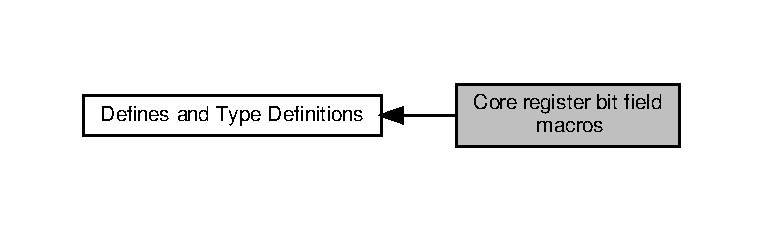
\includegraphics[width=350pt]{group___c_m_s_i_s__core__bitfield}
\end{center}
\end{figure}
\subsection*{Definicje}
\begin{DoxyCompactItemize}
\item 
\#define \hyperlink{group___c_m_s_i_s__core__bitfield_ga286e3b913dbd236c7f48ea70c8821f4e}{\+\_\+\+V\+A\+L2\+F\+LD}(field,  value)~(((uint32\+\_\+t)(value) $<$$<$ field \#\# \+\_\+\+Pos) \& field \#\# \+\_\+\+Msk)
\begin{DoxyCompactList}\small\item\em Mask and shift a bit field value for use in a register bit range. \end{DoxyCompactList}\item 
\#define \hyperlink{group___c_m_s_i_s__core__bitfield_ga139b6e261c981f014f386927ca4a8444}{\+\_\+\+F\+L\+D2\+V\+AL}(field,  value)~(((uint32\+\_\+t)(value) \& field \#\# \+\_\+\+Msk) $>$$>$ field \#\# \+\_\+\+Pos)
\begin{DoxyCompactList}\small\item\em Mask and shift a register value to extract a bit filed value. \end{DoxyCompactList}\item 
\#define \hyperlink{group___c_m_s_i_s__core__bitfield_ga286e3b913dbd236c7f48ea70c8821f4e}{\+\_\+\+V\+A\+L2\+F\+LD}(field,  value)~(((uint32\+\_\+t)(value) $<$$<$ field \#\# \+\_\+\+Pos) \& field \#\# \+\_\+\+Msk)
\begin{DoxyCompactList}\small\item\em Mask and shift a bit field value for use in a register bit range. \end{DoxyCompactList}\item 
\#define \hyperlink{group___c_m_s_i_s__core__bitfield_ga139b6e261c981f014f386927ca4a8444}{\+\_\+\+F\+L\+D2\+V\+AL}(field,  value)~(((uint32\+\_\+t)(value) \& field \#\# \+\_\+\+Msk) $>$$>$ field \#\# \+\_\+\+Pos)
\begin{DoxyCompactList}\small\item\em Mask and shift a register value to extract a bit filed value. \end{DoxyCompactList}\item 
\#define \hyperlink{group___c_m_s_i_s__core__bitfield_ga286e3b913dbd236c7f48ea70c8821f4e}{\+\_\+\+V\+A\+L2\+F\+LD}(field,  value)~(((uint32\+\_\+t)(value) $<$$<$ field \#\# \+\_\+\+Pos) \& field \#\# \+\_\+\+Msk)
\begin{DoxyCompactList}\small\item\em Mask and shift a bit field value for use in a register bit range. \end{DoxyCompactList}\item 
\#define \hyperlink{group___c_m_s_i_s__core__bitfield_ga139b6e261c981f014f386927ca4a8444}{\+\_\+\+F\+L\+D2\+V\+AL}(field,  value)~(((uint32\+\_\+t)(value) \& field \#\# \+\_\+\+Msk) $>$$>$ field \#\# \+\_\+\+Pos)
\begin{DoxyCompactList}\small\item\em Mask and shift a register value to extract a bit filed value. \end{DoxyCompactList}\item 
\#define \hyperlink{group___c_m_s_i_s__core__bitfield_ga286e3b913dbd236c7f48ea70c8821f4e}{\+\_\+\+V\+A\+L2\+F\+LD}(field,  value)~(((uint32\+\_\+t)(value) $<$$<$ field \#\# \+\_\+\+Pos) \& field \#\# \+\_\+\+Msk)
\begin{DoxyCompactList}\small\item\em Mask and shift a bit field value for use in a register bit range. \end{DoxyCompactList}\item 
\#define \hyperlink{group___c_m_s_i_s__core__bitfield_ga139b6e261c981f014f386927ca4a8444}{\+\_\+\+F\+L\+D2\+V\+AL}(field,  value)~(((uint32\+\_\+t)(value) \& field \#\# \+\_\+\+Msk) $>$$>$ field \#\# \+\_\+\+Pos)
\begin{DoxyCompactList}\small\item\em Mask and shift a register value to extract a bit filed value. \end{DoxyCompactList}\item 
\#define \hyperlink{group___c_m_s_i_s__core__bitfield_ga286e3b913dbd236c7f48ea70c8821f4e}{\+\_\+\+V\+A\+L2\+F\+LD}(field,  value)~(((uint32\+\_\+t)(value) $<$$<$ field \#\# \+\_\+\+Pos) \& field \#\# \+\_\+\+Msk)
\begin{DoxyCompactList}\small\item\em Mask and shift a bit field value for use in a register bit range. \end{DoxyCompactList}\item 
\#define \hyperlink{group___c_m_s_i_s__core__bitfield_ga139b6e261c981f014f386927ca4a8444}{\+\_\+\+F\+L\+D2\+V\+AL}(field,  value)~(((uint32\+\_\+t)(value) \& field \#\# \+\_\+\+Msk) $>$$>$ field \#\# \+\_\+\+Pos)
\begin{DoxyCompactList}\small\item\em Mask and shift a register value to extract a bit filed value. \end{DoxyCompactList}\item 
\#define \hyperlink{group___c_m_s_i_s__core__bitfield_ga286e3b913dbd236c7f48ea70c8821f4e}{\+\_\+\+V\+A\+L2\+F\+LD}(field,  value)~(((uint32\+\_\+t)(value) $<$$<$ field \#\# \+\_\+\+Pos) \& field \#\# \+\_\+\+Msk)
\begin{DoxyCompactList}\small\item\em Mask and shift a bit field value for use in a register bit range. \end{DoxyCompactList}\item 
\#define \hyperlink{group___c_m_s_i_s__core__bitfield_ga139b6e261c981f014f386927ca4a8444}{\+\_\+\+F\+L\+D2\+V\+AL}(field,  value)~(((uint32\+\_\+t)(value) \& field \#\# \+\_\+\+Msk) $>$$>$ field \#\# \+\_\+\+Pos)
\begin{DoxyCompactList}\small\item\em Mask and shift a register value to extract a bit filed value. \end{DoxyCompactList}\item 
\#define \hyperlink{group___c_m_s_i_s__core__bitfield_ga286e3b913dbd236c7f48ea70c8821f4e}{\+\_\+\+V\+A\+L2\+F\+LD}(field,  value)~(((uint32\+\_\+t)(value) $<$$<$ field \#\# \+\_\+\+Pos) \& field \#\# \+\_\+\+Msk)
\begin{DoxyCompactList}\small\item\em Mask and shift a bit field value for use in a register bit range. \end{DoxyCompactList}\item 
\#define \hyperlink{group___c_m_s_i_s__core__bitfield_ga139b6e261c981f014f386927ca4a8444}{\+\_\+\+F\+L\+D2\+V\+AL}(field,  value)~(((uint32\+\_\+t)(value) \& field \#\# \+\_\+\+Msk) $>$$>$ field \#\# \+\_\+\+Pos)
\begin{DoxyCompactList}\small\item\em Mask and shift a register value to extract a bit filed value. \end{DoxyCompactList}\item 
\#define \hyperlink{group___c_m_s_i_s__core__bitfield_ga286e3b913dbd236c7f48ea70c8821f4e}{\+\_\+\+V\+A\+L2\+F\+LD}(field,  value)~(((uint32\+\_\+t)(value) $<$$<$ field \#\# \+\_\+\+Pos) \& field \#\# \+\_\+\+Msk)
\begin{DoxyCompactList}\small\item\em Mask and shift a bit field value for use in a register bit range. \end{DoxyCompactList}\item 
\#define \hyperlink{group___c_m_s_i_s__core__bitfield_ga139b6e261c981f014f386927ca4a8444}{\+\_\+\+F\+L\+D2\+V\+AL}(field,  value)~(((uint32\+\_\+t)(value) \& field \#\# \+\_\+\+Msk) $>$$>$ field \#\# \+\_\+\+Pos)
\begin{DoxyCompactList}\small\item\em Mask and shift a register value to extract a bit filed value. \end{DoxyCompactList}\item 
\#define \hyperlink{group___c_m_s_i_s__core__bitfield_ga286e3b913dbd236c7f48ea70c8821f4e}{\+\_\+\+V\+A\+L2\+F\+LD}(field,  value)~(((uint32\+\_\+t)(value) $<$$<$ field \#\# \+\_\+\+Pos) \& field \#\# \+\_\+\+Msk)
\begin{DoxyCompactList}\small\item\em Mask and shift a bit field value for use in a register bit range. \end{DoxyCompactList}\item 
\#define \hyperlink{group___c_m_s_i_s__core__bitfield_ga139b6e261c981f014f386927ca4a8444}{\+\_\+\+F\+L\+D2\+V\+AL}(field,  value)~(((uint32\+\_\+t)(value) \& field \#\# \+\_\+\+Msk) $>$$>$ field \#\# \+\_\+\+Pos)
\begin{DoxyCompactList}\small\item\em Mask and shift a register value to extract a bit filed value. \end{DoxyCompactList}\item 
\#define \hyperlink{group___c_m_s_i_s__core__bitfield_ga286e3b913dbd236c7f48ea70c8821f4e}{\+\_\+\+V\+A\+L2\+F\+LD}(field,  value)~(((uint32\+\_\+t)(value) $<$$<$ field \#\# \+\_\+\+Pos) \& field \#\# \+\_\+\+Msk)
\begin{DoxyCompactList}\small\item\em Mask and shift a bit field value for use in a register bit range. \end{DoxyCompactList}\item 
\#define \hyperlink{group___c_m_s_i_s__core__bitfield_ga139b6e261c981f014f386927ca4a8444}{\+\_\+\+F\+L\+D2\+V\+AL}(field,  value)~(((uint32\+\_\+t)(value) \& field \#\# \+\_\+\+Msk) $>$$>$ field \#\# \+\_\+\+Pos)
\begin{DoxyCompactList}\small\item\em Mask and shift a register value to extract a bit filed value. \end{DoxyCompactList}\item 
\#define \hyperlink{group___c_m_s_i_s__core__bitfield_ga286e3b913dbd236c7f48ea70c8821f4e}{\+\_\+\+V\+A\+L2\+F\+LD}(field,  value)~(((uint32\+\_\+t)(value) $<$$<$ field \#\# \+\_\+\+Pos) \& field \#\# \+\_\+\+Msk)
\begin{DoxyCompactList}\small\item\em Mask and shift a bit field value for use in a register bit range. \end{DoxyCompactList}\item 
\#define \hyperlink{group___c_m_s_i_s__core__bitfield_ga139b6e261c981f014f386927ca4a8444}{\+\_\+\+F\+L\+D2\+V\+AL}(field,  value)~(((uint32\+\_\+t)(value) \& field \#\# \+\_\+\+Msk) $>$$>$ field \#\# \+\_\+\+Pos)
\begin{DoxyCompactList}\small\item\em Mask and shift a register value to extract a bit filed value. \end{DoxyCompactList}\item 
\#define \hyperlink{group___c_m_s_i_s__core__bitfield_ga286e3b913dbd236c7f48ea70c8821f4e}{\+\_\+\+V\+A\+L2\+F\+LD}(field,  value)~(((uint32\+\_\+t)(value) $<$$<$ field \#\# \+\_\+\+Pos) \& field \#\# \+\_\+\+Msk)
\begin{DoxyCompactList}\small\item\em Mask and shift a bit field value for use in a register bit range. \end{DoxyCompactList}\item 
\#define \hyperlink{group___c_m_s_i_s__core__bitfield_ga139b6e261c981f014f386927ca4a8444}{\+\_\+\+F\+L\+D2\+V\+AL}(field,  value)~(((uint32\+\_\+t)(value) \& field \#\# \+\_\+\+Msk) $>$$>$ field \#\# \+\_\+\+Pos)
\begin{DoxyCompactList}\small\item\em Mask and shift a register value to extract a bit filed value. \end{DoxyCompactList}\end{DoxyCompactItemize}


\subsection{Opis szczegółowy}
Macros for use with bit field definitions (xxx\+\_\+\+Pos, xxx\+\_\+\+Msk). 



\subsection{Dokumentacja definicji}
\mbox{\Hypertarget{group___c_m_s_i_s__core__bitfield_ga139b6e261c981f014f386927ca4a8444}\label{group___c_m_s_i_s__core__bitfield_ga139b6e261c981f014f386927ca4a8444}} 
\index{Core register bit field macros@{Core register bit field macros}!\+\_\+\+F\+L\+D2\+V\+AL@{\+\_\+\+F\+L\+D2\+V\+AL}}
\index{\+\_\+\+F\+L\+D2\+V\+AL@{\+\_\+\+F\+L\+D2\+V\+AL}!Core register bit field macros@{Core register bit field macros}}
\subsubsection{\texorpdfstring{\+\_\+\+F\+L\+D2\+V\+AL}{\_FLD2VAL}\hspace{0.1cm}{\footnotesize\ttfamily [1/12]}}
{\footnotesize\ttfamily \#define \+\_\+\+F\+L\+D2\+V\+AL(\begin{DoxyParamCaption}\item[{}]{field,  }\item[{}]{value }\end{DoxyParamCaption})~(((uint32\+\_\+t)(value) \& field \#\# \+\_\+\+Msk) $>$$>$ field \#\# \+\_\+\+Pos)}



Mask and shift a register value to extract a bit filed value. 


\begin{DoxyParams}[1]{Parametry}
\mbox{\tt in}  & {\em field} & Name of the register bit field. \\
\hline
\mbox{\tt in}  & {\em value} & Value of register. This parameter is interpreted as an uint32\+\_\+t type. \\
\hline
\end{DoxyParams}
\begin{DoxyReturn}{Zwraca}
Masked and shifted bit field value. 
\end{DoxyReturn}


Definicja w linii 521 pliku core\+\_\+cm0.\+h.

\mbox{\Hypertarget{group___c_m_s_i_s__core__bitfield_ga139b6e261c981f014f386927ca4a8444}\label{group___c_m_s_i_s__core__bitfield_ga139b6e261c981f014f386927ca4a8444}} 
\index{Core register bit field macros@{Core register bit field macros}!\+\_\+\+F\+L\+D2\+V\+AL@{\+\_\+\+F\+L\+D2\+V\+AL}}
\index{\+\_\+\+F\+L\+D2\+V\+AL@{\+\_\+\+F\+L\+D2\+V\+AL}!Core register bit field macros@{Core register bit field macros}}
\subsubsection{\texorpdfstring{\+\_\+\+F\+L\+D2\+V\+AL}{\_FLD2VAL}\hspace{0.1cm}{\footnotesize\ttfamily [2/12]}}
{\footnotesize\ttfamily \#define \+\_\+\+F\+L\+D2\+V\+AL(\begin{DoxyParamCaption}\item[{}]{field,  }\item[{}]{value }\end{DoxyParamCaption})~(((uint32\+\_\+t)(value) \& field \#\# \+\_\+\+Msk) $>$$>$ field \#\# \+\_\+\+Pos)}



Mask and shift a register value to extract a bit filed value. 


\begin{DoxyParams}[1]{Parametry}
\mbox{\tt in}  & {\em field} & Name of the register bit field. \\
\hline
\mbox{\tt in}  & {\em value} & Value of register. This parameter is interpreted as an uint32\+\_\+t type. \\
\hline
\end{DoxyParams}
\begin{DoxyReturn}{Zwraca}
Masked and shifted bit field value. 
\end{DoxyReturn}


Definicja w linii 547 pliku core\+\_\+cm1.\+h.

\mbox{\Hypertarget{group___c_m_s_i_s__core__bitfield_ga139b6e261c981f014f386927ca4a8444}\label{group___c_m_s_i_s__core__bitfield_ga139b6e261c981f014f386927ca4a8444}} 
\index{Core register bit field macros@{Core register bit field macros}!\+\_\+\+F\+L\+D2\+V\+AL@{\+\_\+\+F\+L\+D2\+V\+AL}}
\index{\+\_\+\+F\+L\+D2\+V\+AL@{\+\_\+\+F\+L\+D2\+V\+AL}!Core register bit field macros@{Core register bit field macros}}
\subsubsection{\texorpdfstring{\+\_\+\+F\+L\+D2\+V\+AL}{\_FLD2VAL}\hspace{0.1cm}{\footnotesize\ttfamily [3/12]}}
{\footnotesize\ttfamily \#define \+\_\+\+F\+L\+D2\+V\+AL(\begin{DoxyParamCaption}\item[{}]{field,  }\item[{}]{value }\end{DoxyParamCaption})~(((uint32\+\_\+t)(value) \& field \#\# \+\_\+\+Msk) $>$$>$ field \#\# \+\_\+\+Pos)}



Mask and shift a register value to extract a bit filed value. 


\begin{DoxyParams}[1]{Parametry}
\mbox{\tt in}  & {\em field} & Name of the register bit field. \\
\hline
\mbox{\tt in}  & {\em value} & Value of register. This parameter is interpreted as an uint32\+\_\+t type. \\
\hline
\end{DoxyParams}
\begin{DoxyReturn}{Zwraca}
Masked and shifted bit field value. 
\end{DoxyReturn}


Definicja w linii 635 pliku core\+\_\+cm0plus.\+h.

\mbox{\Hypertarget{group___c_m_s_i_s__core__bitfield_ga139b6e261c981f014f386927ca4a8444}\label{group___c_m_s_i_s__core__bitfield_ga139b6e261c981f014f386927ca4a8444}} 
\index{Core register bit field macros@{Core register bit field macros}!\+\_\+\+F\+L\+D2\+V\+AL@{\+\_\+\+F\+L\+D2\+V\+AL}}
\index{\+\_\+\+F\+L\+D2\+V\+AL@{\+\_\+\+F\+L\+D2\+V\+AL}!Core register bit field macros@{Core register bit field macros}}
\subsubsection{\texorpdfstring{\+\_\+\+F\+L\+D2\+V\+AL}{\_FLD2VAL}\hspace{0.1cm}{\footnotesize\ttfamily [4/12]}}
{\footnotesize\ttfamily \#define \+\_\+\+F\+L\+D2\+V\+AL(\begin{DoxyParamCaption}\item[{}]{field,  }\item[{}]{value }\end{DoxyParamCaption})~(((uint32\+\_\+t)(value) \& field \#\# \+\_\+\+Msk) $>$$>$ field \#\# \+\_\+\+Pos)}



Mask and shift a register value to extract a bit filed value. 


\begin{DoxyParams}[1]{Parametry}
\mbox{\tt in}  & {\em field} & Name of the register bit field. \\
\hline
\mbox{\tt in}  & {\em value} & Value of register. This parameter is interpreted as an uint32\+\_\+t type. \\
\hline
\end{DoxyParams}
\begin{DoxyReturn}{Zwraca}
Masked and shifted bit field value. 
\end{DoxyReturn}


Definicja w linii 644 pliku core\+\_\+sc000.\+h.

\mbox{\Hypertarget{group___c_m_s_i_s__core__bitfield_ga139b6e261c981f014f386927ca4a8444}\label{group___c_m_s_i_s__core__bitfield_ga139b6e261c981f014f386927ca4a8444}} 
\index{Core register bit field macros@{Core register bit field macros}!\+\_\+\+F\+L\+D2\+V\+AL@{\+\_\+\+F\+L\+D2\+V\+AL}}
\index{\+\_\+\+F\+L\+D2\+V\+AL@{\+\_\+\+F\+L\+D2\+V\+AL}!Core register bit field macros@{Core register bit field macros}}
\subsubsection{\texorpdfstring{\+\_\+\+F\+L\+D2\+V\+AL}{\_FLD2VAL}\hspace{0.1cm}{\footnotesize\ttfamily [5/12]}}
{\footnotesize\ttfamily \#define \+\_\+\+F\+L\+D2\+V\+AL(\begin{DoxyParamCaption}\item[{}]{field,  }\item[{}]{value }\end{DoxyParamCaption})~(((uint32\+\_\+t)(value) \& field \#\# \+\_\+\+Msk) $>$$>$ field \#\# \+\_\+\+Pos)}



Mask and shift a register value to extract a bit filed value. 


\begin{DoxyParams}[1]{Parametry}
\mbox{\tt in}  & {\em field} & Name of the register bit field. \\
\hline
\mbox{\tt in}  & {\em value} & Value of register. This parameter is interpreted as an uint32\+\_\+t type. \\
\hline
\end{DoxyParams}
\begin{DoxyReturn}{Zwraca}
Masked and shifted bit field value. 
\end{DoxyReturn}


Definicja w linii 1100 pliku core\+\_\+armv8mbl.\+h.

\mbox{\Hypertarget{group___c_m_s_i_s__core__bitfield_ga139b6e261c981f014f386927ca4a8444}\label{group___c_m_s_i_s__core__bitfield_ga139b6e261c981f014f386927ca4a8444}} 
\index{Core register bit field macros@{Core register bit field macros}!\+\_\+\+F\+L\+D2\+V\+AL@{\+\_\+\+F\+L\+D2\+V\+AL}}
\index{\+\_\+\+F\+L\+D2\+V\+AL@{\+\_\+\+F\+L\+D2\+V\+AL}!Core register bit field macros@{Core register bit field macros}}
\subsubsection{\texorpdfstring{\+\_\+\+F\+L\+D2\+V\+AL}{\_FLD2VAL}\hspace{0.1cm}{\footnotesize\ttfamily [6/12]}}
{\footnotesize\ttfamily \#define \+\_\+\+F\+L\+D2\+V\+AL(\begin{DoxyParamCaption}\item[{}]{field,  }\item[{}]{value }\end{DoxyParamCaption})~(((uint32\+\_\+t)(value) \& field \#\# \+\_\+\+Msk) $>$$>$ field \#\# \+\_\+\+Pos)}



Mask and shift a register value to extract a bit filed value. 


\begin{DoxyParams}[1]{Parametry}
\mbox{\tt in}  & {\em field} & Name of the register bit field. \\
\hline
\mbox{\tt in}  & {\em value} & Value of register. This parameter is interpreted as an uint32\+\_\+t type. \\
\hline
\end{DoxyParams}
\begin{DoxyReturn}{Zwraca}
Masked and shifted bit field value. 
\end{DoxyReturn}


Definicja w linii 1175 pliku core\+\_\+cm23.\+h.

\mbox{\Hypertarget{group___c_m_s_i_s__core__bitfield_ga139b6e261c981f014f386927ca4a8444}\label{group___c_m_s_i_s__core__bitfield_ga139b6e261c981f014f386927ca4a8444}} 
\index{Core register bit field macros@{Core register bit field macros}!\+\_\+\+F\+L\+D2\+V\+AL@{\+\_\+\+F\+L\+D2\+V\+AL}}
\index{\+\_\+\+F\+L\+D2\+V\+AL@{\+\_\+\+F\+L\+D2\+V\+AL}!Core register bit field macros@{Core register bit field macros}}
\subsubsection{\texorpdfstring{\+\_\+\+F\+L\+D2\+V\+AL}{\_FLD2VAL}\hspace{0.1cm}{\footnotesize\ttfamily [7/12]}}
{\footnotesize\ttfamily \#define \+\_\+\+F\+L\+D2\+V\+AL(\begin{DoxyParamCaption}\item[{}]{field,  }\item[{}]{value }\end{DoxyParamCaption})~(((uint32\+\_\+t)(value) \& field \#\# \+\_\+\+Msk) $>$$>$ field \#\# \+\_\+\+Pos)}



Mask and shift a register value to extract a bit filed value. 


\begin{DoxyParams}[1]{Parametry}
\mbox{\tt in}  & {\em field} & Name of the register bit field. \\
\hline
\mbox{\tt in}  & {\em value} & Value of register. This parameter is interpreted as an uint32\+\_\+t type. \\
\hline
\end{DoxyParams}
\begin{DoxyReturn}{Zwraca}
Masked and shifted bit field value. 
\end{DoxyReturn}


Definicja w linii 1350 pliku core\+\_\+sc300.\+h.

\mbox{\Hypertarget{group___c_m_s_i_s__core__bitfield_ga139b6e261c981f014f386927ca4a8444}\label{group___c_m_s_i_s__core__bitfield_ga139b6e261c981f014f386927ca4a8444}} 
\index{Core register bit field macros@{Core register bit field macros}!\+\_\+\+F\+L\+D2\+V\+AL@{\+\_\+\+F\+L\+D2\+V\+AL}}
\index{\+\_\+\+F\+L\+D2\+V\+AL@{\+\_\+\+F\+L\+D2\+V\+AL}!Core register bit field macros@{Core register bit field macros}}
\subsubsection{\texorpdfstring{\+\_\+\+F\+L\+D2\+V\+AL}{\_FLD2VAL}\hspace{0.1cm}{\footnotesize\ttfamily [8/12]}}
{\footnotesize\ttfamily \#define \+\_\+\+F\+L\+D2\+V\+AL(\begin{DoxyParamCaption}\item[{}]{field,  }\item[{}]{value }\end{DoxyParamCaption})~(((uint32\+\_\+t)(value) \& field \#\# \+\_\+\+Msk) $>$$>$ field \#\# \+\_\+\+Pos)}



Mask and shift a register value to extract a bit filed value. 


\begin{DoxyParams}[1]{Parametry}
\mbox{\tt in}  & {\em field} & Name of the register bit field. \\
\hline
\mbox{\tt in}  & {\em value} & Value of register. This parameter is interpreted as an uint32\+\_\+t type. \\
\hline
\end{DoxyParams}
\begin{DoxyReturn}{Zwraca}
Masked and shifted bit field value. 
\end{DoxyReturn}


Definicja w linii 1370 pliku core\+\_\+cm3.\+h.

\mbox{\Hypertarget{group___c_m_s_i_s__core__bitfield_ga139b6e261c981f014f386927ca4a8444}\label{group___c_m_s_i_s__core__bitfield_ga139b6e261c981f014f386927ca4a8444}} 
\index{Core register bit field macros@{Core register bit field macros}!\+\_\+\+F\+L\+D2\+V\+AL@{\+\_\+\+F\+L\+D2\+V\+AL}}
\index{\+\_\+\+F\+L\+D2\+V\+AL@{\+\_\+\+F\+L\+D2\+V\+AL}!Core register bit field macros@{Core register bit field macros}}
\subsubsection{\texorpdfstring{\+\_\+\+F\+L\+D2\+V\+AL}{\_FLD2VAL}\hspace{0.1cm}{\footnotesize\ttfamily [9/12]}}
{\footnotesize\ttfamily \#define \+\_\+\+F\+L\+D2\+V\+AL(\begin{DoxyParamCaption}\item[{}]{field,  }\item[{}]{value }\end{DoxyParamCaption})~(((uint32\+\_\+t)(value) \& field \#\# \+\_\+\+Msk) $>$$>$ field \#\# \+\_\+\+Pos)}



Mask and shift a register value to extract a bit filed value. 


\begin{DoxyParams}[1]{Parametry}
\mbox{\tt in}  & {\em field} & Name of the register bit field. \\
\hline
\mbox{\tt in}  & {\em value} & Value of register. This parameter is interpreted as an uint32\+\_\+t type. \\
\hline
\end{DoxyParams}
\begin{DoxyReturn}{Zwraca}
Masked and shifted bit field value. 
\end{DoxyReturn}


Definicja w linii 1541 pliku core\+\_\+cm4.\+h.

\mbox{\Hypertarget{group___c_m_s_i_s__core__bitfield_ga139b6e261c981f014f386927ca4a8444}\label{group___c_m_s_i_s__core__bitfield_ga139b6e261c981f014f386927ca4a8444}} 
\index{Core register bit field macros@{Core register bit field macros}!\+\_\+\+F\+L\+D2\+V\+AL@{\+\_\+\+F\+L\+D2\+V\+AL}}
\index{\+\_\+\+F\+L\+D2\+V\+AL@{\+\_\+\+F\+L\+D2\+V\+AL}!Core register bit field macros@{Core register bit field macros}}
\subsubsection{\texorpdfstring{\+\_\+\+F\+L\+D2\+V\+AL}{\_FLD2VAL}\hspace{0.1cm}{\footnotesize\ttfamily [10/12]}}
{\footnotesize\ttfamily \#define \+\_\+\+F\+L\+D2\+V\+AL(\begin{DoxyParamCaption}\item[{}]{field,  }\item[{}]{value }\end{DoxyParamCaption})~(((uint32\+\_\+t)(value) \& field \#\# \+\_\+\+Msk) $>$$>$ field \#\# \+\_\+\+Pos)}



Mask and shift a register value to extract a bit filed value. 


\begin{DoxyParams}[1]{Parametry}
\mbox{\tt in}  & {\em field} & Name of the register bit field. \\
\hline
\mbox{\tt in}  & {\em value} & Value of register. This parameter is interpreted as an uint32\+\_\+t type. \\
\hline
\end{DoxyParams}
\begin{DoxyReturn}{Zwraca}
Masked and shifted bit field value. 
\end{DoxyReturn}


Definicja w linii 1749 pliku core\+\_\+cm7.\+h.

\mbox{\Hypertarget{group___c_m_s_i_s__core__bitfield_ga139b6e261c981f014f386927ca4a8444}\label{group___c_m_s_i_s__core__bitfield_ga139b6e261c981f014f386927ca4a8444}} 
\index{Core register bit field macros@{Core register bit field macros}!\+\_\+\+F\+L\+D2\+V\+AL@{\+\_\+\+F\+L\+D2\+V\+AL}}
\index{\+\_\+\+F\+L\+D2\+V\+AL@{\+\_\+\+F\+L\+D2\+V\+AL}!Core register bit field macros@{Core register bit field macros}}
\subsubsection{\texorpdfstring{\+\_\+\+F\+L\+D2\+V\+AL}{\_FLD2VAL}\hspace{0.1cm}{\footnotesize\ttfamily [11/12]}}
{\footnotesize\ttfamily \#define \+\_\+\+F\+L\+D2\+V\+AL(\begin{DoxyParamCaption}\item[{}]{field,  }\item[{}]{value }\end{DoxyParamCaption})~(((uint32\+\_\+t)(value) \& field \#\# \+\_\+\+Msk) $>$$>$ field \#\# \+\_\+\+Pos)}



Mask and shift a register value to extract a bit filed value. 


\begin{DoxyParams}[1]{Parametry}
\mbox{\tt in}  & {\em field} & Name of the register bit field. \\
\hline
\mbox{\tt in}  & {\em value} & Value of register. This parameter is interpreted as an uint32\+\_\+t type. \\
\hline
\end{DoxyParams}
\begin{DoxyReturn}{Zwraca}
Masked and shifted bit field value. 
\end{DoxyReturn}


Definicja w linii 1960 pliku core\+\_\+armv8mml.\+h.

\mbox{\Hypertarget{group___c_m_s_i_s__core__bitfield_ga139b6e261c981f014f386927ca4a8444}\label{group___c_m_s_i_s__core__bitfield_ga139b6e261c981f014f386927ca4a8444}} 
\index{Core register bit field macros@{Core register bit field macros}!\+\_\+\+F\+L\+D2\+V\+AL@{\+\_\+\+F\+L\+D2\+V\+AL}}
\index{\+\_\+\+F\+L\+D2\+V\+AL@{\+\_\+\+F\+L\+D2\+V\+AL}!Core register bit field macros@{Core register bit field macros}}
\subsubsection{\texorpdfstring{\+\_\+\+F\+L\+D2\+V\+AL}{\_FLD2VAL}\hspace{0.1cm}{\footnotesize\ttfamily [12/12]}}
{\footnotesize\ttfamily \#define \+\_\+\+F\+L\+D2\+V\+AL(\begin{DoxyParamCaption}\item[{}]{field,  }\item[{}]{value }\end{DoxyParamCaption})~(((uint32\+\_\+t)(value) \& field \#\# \+\_\+\+Msk) $>$$>$ field \#\# \+\_\+\+Pos)}



Mask and shift a register value to extract a bit filed value. 


\begin{DoxyParams}[1]{Parametry}
\mbox{\tt in}  & {\em field} & Name of the register bit field. \\
\hline
\mbox{\tt in}  & {\em value} & Value of register. This parameter is interpreted as an uint32\+\_\+t type. \\
\hline
\end{DoxyParams}
\begin{DoxyReturn}{Zwraca}
Masked and shifted bit field value. 
\end{DoxyReturn}


Definicja w linii 2035 pliku core\+\_\+cm33.\+h.

\mbox{\Hypertarget{group___c_m_s_i_s__core__bitfield_ga286e3b913dbd236c7f48ea70c8821f4e}\label{group___c_m_s_i_s__core__bitfield_ga286e3b913dbd236c7f48ea70c8821f4e}} 
\index{Core register bit field macros@{Core register bit field macros}!\+\_\+\+V\+A\+L2\+F\+LD@{\+\_\+\+V\+A\+L2\+F\+LD}}
\index{\+\_\+\+V\+A\+L2\+F\+LD@{\+\_\+\+V\+A\+L2\+F\+LD}!Core register bit field macros@{Core register bit field macros}}
\subsubsection{\texorpdfstring{\+\_\+\+V\+A\+L2\+F\+LD}{\_VAL2FLD}\hspace{0.1cm}{\footnotesize\ttfamily [1/12]}}
{\footnotesize\ttfamily \#define \+\_\+\+V\+A\+L2\+F\+LD(\begin{DoxyParamCaption}\item[{}]{field,  }\item[{}]{value }\end{DoxyParamCaption})~(((uint32\+\_\+t)(value) $<$$<$ field \#\# \+\_\+\+Pos) \& field \#\# \+\_\+\+Msk)}



Mask and shift a bit field value for use in a register bit range. 


\begin{DoxyParams}[1]{Parametry}
\mbox{\tt in}  & {\em field} & Name of the register bit field. \\
\hline
\mbox{\tt in}  & {\em value} & Value of the bit field. This parameter is interpreted as an uint32\+\_\+t type. \\
\hline
\end{DoxyParams}
\begin{DoxyReturn}{Zwraca}
Masked and shifted value. 
\end{DoxyReturn}


Definicja w linii 513 pliku core\+\_\+cm0.\+h.

\mbox{\Hypertarget{group___c_m_s_i_s__core__bitfield_ga286e3b913dbd236c7f48ea70c8821f4e}\label{group___c_m_s_i_s__core__bitfield_ga286e3b913dbd236c7f48ea70c8821f4e}} 
\index{Core register bit field macros@{Core register bit field macros}!\+\_\+\+V\+A\+L2\+F\+LD@{\+\_\+\+V\+A\+L2\+F\+LD}}
\index{\+\_\+\+V\+A\+L2\+F\+LD@{\+\_\+\+V\+A\+L2\+F\+LD}!Core register bit field macros@{Core register bit field macros}}
\subsubsection{\texorpdfstring{\+\_\+\+V\+A\+L2\+F\+LD}{\_VAL2FLD}\hspace{0.1cm}{\footnotesize\ttfamily [2/12]}}
{\footnotesize\ttfamily \#define \+\_\+\+V\+A\+L2\+F\+LD(\begin{DoxyParamCaption}\item[{}]{field,  }\item[{}]{value }\end{DoxyParamCaption})~(((uint32\+\_\+t)(value) $<$$<$ field \#\# \+\_\+\+Pos) \& field \#\# \+\_\+\+Msk)}



Mask and shift a bit field value for use in a register bit range. 


\begin{DoxyParams}[1]{Parametry}
\mbox{\tt in}  & {\em field} & Name of the register bit field. \\
\hline
\mbox{\tt in}  & {\em value} & Value of the bit field. This parameter is interpreted as an uint32\+\_\+t type. \\
\hline
\end{DoxyParams}
\begin{DoxyReturn}{Zwraca}
Masked and shifted value. 
\end{DoxyReturn}


Definicja w linii 539 pliku core\+\_\+cm1.\+h.

\mbox{\Hypertarget{group___c_m_s_i_s__core__bitfield_ga286e3b913dbd236c7f48ea70c8821f4e}\label{group___c_m_s_i_s__core__bitfield_ga286e3b913dbd236c7f48ea70c8821f4e}} 
\index{Core register bit field macros@{Core register bit field macros}!\+\_\+\+V\+A\+L2\+F\+LD@{\+\_\+\+V\+A\+L2\+F\+LD}}
\index{\+\_\+\+V\+A\+L2\+F\+LD@{\+\_\+\+V\+A\+L2\+F\+LD}!Core register bit field macros@{Core register bit field macros}}
\subsubsection{\texorpdfstring{\+\_\+\+V\+A\+L2\+F\+LD}{\_VAL2FLD}\hspace{0.1cm}{\footnotesize\ttfamily [3/12]}}
{\footnotesize\ttfamily \#define \+\_\+\+V\+A\+L2\+F\+LD(\begin{DoxyParamCaption}\item[{}]{field,  }\item[{}]{value }\end{DoxyParamCaption})~(((uint32\+\_\+t)(value) $<$$<$ field \#\# \+\_\+\+Pos) \& field \#\# \+\_\+\+Msk)}



Mask and shift a bit field value for use in a register bit range. 


\begin{DoxyParams}[1]{Parametry}
\mbox{\tt in}  & {\em field} & Name of the register bit field. \\
\hline
\mbox{\tt in}  & {\em value} & Value of the bit field. This parameter is interpreted as an uint32\+\_\+t type. \\
\hline
\end{DoxyParams}
\begin{DoxyReturn}{Zwraca}
Masked and shifted value. 
\end{DoxyReturn}


Definicja w linii 627 pliku core\+\_\+cm0plus.\+h.

\mbox{\Hypertarget{group___c_m_s_i_s__core__bitfield_ga286e3b913dbd236c7f48ea70c8821f4e}\label{group___c_m_s_i_s__core__bitfield_ga286e3b913dbd236c7f48ea70c8821f4e}} 
\index{Core register bit field macros@{Core register bit field macros}!\+\_\+\+V\+A\+L2\+F\+LD@{\+\_\+\+V\+A\+L2\+F\+LD}}
\index{\+\_\+\+V\+A\+L2\+F\+LD@{\+\_\+\+V\+A\+L2\+F\+LD}!Core register bit field macros@{Core register bit field macros}}
\subsubsection{\texorpdfstring{\+\_\+\+V\+A\+L2\+F\+LD}{\_VAL2FLD}\hspace{0.1cm}{\footnotesize\ttfamily [4/12]}}
{\footnotesize\ttfamily \#define \+\_\+\+V\+A\+L2\+F\+LD(\begin{DoxyParamCaption}\item[{}]{field,  }\item[{}]{value }\end{DoxyParamCaption})~(((uint32\+\_\+t)(value) $<$$<$ field \#\# \+\_\+\+Pos) \& field \#\# \+\_\+\+Msk)}



Mask and shift a bit field value for use in a register bit range. 


\begin{DoxyParams}[1]{Parametry}
\mbox{\tt in}  & {\em field} & Name of the register bit field. \\
\hline
\mbox{\tt in}  & {\em value} & Value of the bit field. This parameter is interpreted as an uint32\+\_\+t type. \\
\hline
\end{DoxyParams}
\begin{DoxyReturn}{Zwraca}
Masked and shifted value. 
\end{DoxyReturn}


Definicja w linii 636 pliku core\+\_\+sc000.\+h.

\mbox{\Hypertarget{group___c_m_s_i_s__core__bitfield_ga286e3b913dbd236c7f48ea70c8821f4e}\label{group___c_m_s_i_s__core__bitfield_ga286e3b913dbd236c7f48ea70c8821f4e}} 
\index{Core register bit field macros@{Core register bit field macros}!\+\_\+\+V\+A\+L2\+F\+LD@{\+\_\+\+V\+A\+L2\+F\+LD}}
\index{\+\_\+\+V\+A\+L2\+F\+LD@{\+\_\+\+V\+A\+L2\+F\+LD}!Core register bit field macros@{Core register bit field macros}}
\subsubsection{\texorpdfstring{\+\_\+\+V\+A\+L2\+F\+LD}{\_VAL2FLD}\hspace{0.1cm}{\footnotesize\ttfamily [5/12]}}
{\footnotesize\ttfamily \#define \+\_\+\+V\+A\+L2\+F\+LD(\begin{DoxyParamCaption}\item[{}]{field,  }\item[{}]{value }\end{DoxyParamCaption})~(((uint32\+\_\+t)(value) $<$$<$ field \#\# \+\_\+\+Pos) \& field \#\# \+\_\+\+Msk)}



Mask and shift a bit field value for use in a register bit range. 


\begin{DoxyParams}[1]{Parametry}
\mbox{\tt in}  & {\em field} & Name of the register bit field. \\
\hline
\mbox{\tt in}  & {\em value} & Value of the bit field. This parameter is interpreted as an uint32\+\_\+t type. \\
\hline
\end{DoxyParams}
\begin{DoxyReturn}{Zwraca}
Masked and shifted value. 
\end{DoxyReturn}


Definicja w linii 1092 pliku core\+\_\+armv8mbl.\+h.

\mbox{\Hypertarget{group___c_m_s_i_s__core__bitfield_ga286e3b913dbd236c7f48ea70c8821f4e}\label{group___c_m_s_i_s__core__bitfield_ga286e3b913dbd236c7f48ea70c8821f4e}} 
\index{Core register bit field macros@{Core register bit field macros}!\+\_\+\+V\+A\+L2\+F\+LD@{\+\_\+\+V\+A\+L2\+F\+LD}}
\index{\+\_\+\+V\+A\+L2\+F\+LD@{\+\_\+\+V\+A\+L2\+F\+LD}!Core register bit field macros@{Core register bit field macros}}
\subsubsection{\texorpdfstring{\+\_\+\+V\+A\+L2\+F\+LD}{\_VAL2FLD}\hspace{0.1cm}{\footnotesize\ttfamily [6/12]}}
{\footnotesize\ttfamily \#define \+\_\+\+V\+A\+L2\+F\+LD(\begin{DoxyParamCaption}\item[{}]{field,  }\item[{}]{value }\end{DoxyParamCaption})~(((uint32\+\_\+t)(value) $<$$<$ field \#\# \+\_\+\+Pos) \& field \#\# \+\_\+\+Msk)}



Mask and shift a bit field value for use in a register bit range. 


\begin{DoxyParams}[1]{Parametry}
\mbox{\tt in}  & {\em field} & Name of the register bit field. \\
\hline
\mbox{\tt in}  & {\em value} & Value of the bit field. This parameter is interpreted as an uint32\+\_\+t type. \\
\hline
\end{DoxyParams}
\begin{DoxyReturn}{Zwraca}
Masked and shifted value. 
\end{DoxyReturn}


Definicja w linii 1167 pliku core\+\_\+cm23.\+h.

\mbox{\Hypertarget{group___c_m_s_i_s__core__bitfield_ga286e3b913dbd236c7f48ea70c8821f4e}\label{group___c_m_s_i_s__core__bitfield_ga286e3b913dbd236c7f48ea70c8821f4e}} 
\index{Core register bit field macros@{Core register bit field macros}!\+\_\+\+V\+A\+L2\+F\+LD@{\+\_\+\+V\+A\+L2\+F\+LD}}
\index{\+\_\+\+V\+A\+L2\+F\+LD@{\+\_\+\+V\+A\+L2\+F\+LD}!Core register bit field macros@{Core register bit field macros}}
\subsubsection{\texorpdfstring{\+\_\+\+V\+A\+L2\+F\+LD}{\_VAL2FLD}\hspace{0.1cm}{\footnotesize\ttfamily [7/12]}}
{\footnotesize\ttfamily \#define \+\_\+\+V\+A\+L2\+F\+LD(\begin{DoxyParamCaption}\item[{}]{field,  }\item[{}]{value }\end{DoxyParamCaption})~(((uint32\+\_\+t)(value) $<$$<$ field \#\# \+\_\+\+Pos) \& field \#\# \+\_\+\+Msk)}



Mask and shift a bit field value for use in a register bit range. 


\begin{DoxyParams}[1]{Parametry}
\mbox{\tt in}  & {\em field} & Name of the register bit field. \\
\hline
\mbox{\tt in}  & {\em value} & Value of the bit field. This parameter is interpreted as an uint32\+\_\+t type. \\
\hline
\end{DoxyParams}
\begin{DoxyReturn}{Zwraca}
Masked and shifted value. 
\end{DoxyReturn}


Definicja w linii 1342 pliku core\+\_\+sc300.\+h.

\mbox{\Hypertarget{group___c_m_s_i_s__core__bitfield_ga286e3b913dbd236c7f48ea70c8821f4e}\label{group___c_m_s_i_s__core__bitfield_ga286e3b913dbd236c7f48ea70c8821f4e}} 
\index{Core register bit field macros@{Core register bit field macros}!\+\_\+\+V\+A\+L2\+F\+LD@{\+\_\+\+V\+A\+L2\+F\+LD}}
\index{\+\_\+\+V\+A\+L2\+F\+LD@{\+\_\+\+V\+A\+L2\+F\+LD}!Core register bit field macros@{Core register bit field macros}}
\subsubsection{\texorpdfstring{\+\_\+\+V\+A\+L2\+F\+LD}{\_VAL2FLD}\hspace{0.1cm}{\footnotesize\ttfamily [8/12]}}
{\footnotesize\ttfamily \#define \+\_\+\+V\+A\+L2\+F\+LD(\begin{DoxyParamCaption}\item[{}]{field,  }\item[{}]{value }\end{DoxyParamCaption})~(((uint32\+\_\+t)(value) $<$$<$ field \#\# \+\_\+\+Pos) \& field \#\# \+\_\+\+Msk)}



Mask and shift a bit field value for use in a register bit range. 


\begin{DoxyParams}[1]{Parametry}
\mbox{\tt in}  & {\em field} & Name of the register bit field. \\
\hline
\mbox{\tt in}  & {\em value} & Value of the bit field. This parameter is interpreted as an uint32\+\_\+t type. \\
\hline
\end{DoxyParams}
\begin{DoxyReturn}{Zwraca}
Masked and shifted value. 
\end{DoxyReturn}


Definicja w linii 1362 pliku core\+\_\+cm3.\+h.

\mbox{\Hypertarget{group___c_m_s_i_s__core__bitfield_ga286e3b913dbd236c7f48ea70c8821f4e}\label{group___c_m_s_i_s__core__bitfield_ga286e3b913dbd236c7f48ea70c8821f4e}} 
\index{Core register bit field macros@{Core register bit field macros}!\+\_\+\+V\+A\+L2\+F\+LD@{\+\_\+\+V\+A\+L2\+F\+LD}}
\index{\+\_\+\+V\+A\+L2\+F\+LD@{\+\_\+\+V\+A\+L2\+F\+LD}!Core register bit field macros@{Core register bit field macros}}
\subsubsection{\texorpdfstring{\+\_\+\+V\+A\+L2\+F\+LD}{\_VAL2FLD}\hspace{0.1cm}{\footnotesize\ttfamily [9/12]}}
{\footnotesize\ttfamily \#define \+\_\+\+V\+A\+L2\+F\+LD(\begin{DoxyParamCaption}\item[{}]{field,  }\item[{}]{value }\end{DoxyParamCaption})~(((uint32\+\_\+t)(value) $<$$<$ field \#\# \+\_\+\+Pos) \& field \#\# \+\_\+\+Msk)}



Mask and shift a bit field value for use in a register bit range. 


\begin{DoxyParams}[1]{Parametry}
\mbox{\tt in}  & {\em field} & Name of the register bit field. \\
\hline
\mbox{\tt in}  & {\em value} & Value of the bit field. This parameter is interpreted as an uint32\+\_\+t type. \\
\hline
\end{DoxyParams}
\begin{DoxyReturn}{Zwraca}
Masked and shifted value. 
\end{DoxyReturn}


Definicja w linii 1533 pliku core\+\_\+cm4.\+h.

\mbox{\Hypertarget{group___c_m_s_i_s__core__bitfield_ga286e3b913dbd236c7f48ea70c8821f4e}\label{group___c_m_s_i_s__core__bitfield_ga286e3b913dbd236c7f48ea70c8821f4e}} 
\index{Core register bit field macros@{Core register bit field macros}!\+\_\+\+V\+A\+L2\+F\+LD@{\+\_\+\+V\+A\+L2\+F\+LD}}
\index{\+\_\+\+V\+A\+L2\+F\+LD@{\+\_\+\+V\+A\+L2\+F\+LD}!Core register bit field macros@{Core register bit field macros}}
\subsubsection{\texorpdfstring{\+\_\+\+V\+A\+L2\+F\+LD}{\_VAL2FLD}\hspace{0.1cm}{\footnotesize\ttfamily [10/12]}}
{\footnotesize\ttfamily \#define \+\_\+\+V\+A\+L2\+F\+LD(\begin{DoxyParamCaption}\item[{}]{field,  }\item[{}]{value }\end{DoxyParamCaption})~(((uint32\+\_\+t)(value) $<$$<$ field \#\# \+\_\+\+Pos) \& field \#\# \+\_\+\+Msk)}



Mask and shift a bit field value for use in a register bit range. 


\begin{DoxyParams}[1]{Parametry}
\mbox{\tt in}  & {\em field} & Name of the register bit field. \\
\hline
\mbox{\tt in}  & {\em value} & Value of the bit field. This parameter is interpreted as an uint32\+\_\+t type. \\
\hline
\end{DoxyParams}
\begin{DoxyReturn}{Zwraca}
Masked and shifted value. 
\end{DoxyReturn}


Definicja w linii 1741 pliku core\+\_\+cm7.\+h.

\mbox{\Hypertarget{group___c_m_s_i_s__core__bitfield_ga286e3b913dbd236c7f48ea70c8821f4e}\label{group___c_m_s_i_s__core__bitfield_ga286e3b913dbd236c7f48ea70c8821f4e}} 
\index{Core register bit field macros@{Core register bit field macros}!\+\_\+\+V\+A\+L2\+F\+LD@{\+\_\+\+V\+A\+L2\+F\+LD}}
\index{\+\_\+\+V\+A\+L2\+F\+LD@{\+\_\+\+V\+A\+L2\+F\+LD}!Core register bit field macros@{Core register bit field macros}}
\subsubsection{\texorpdfstring{\+\_\+\+V\+A\+L2\+F\+LD}{\_VAL2FLD}\hspace{0.1cm}{\footnotesize\ttfamily [11/12]}}
{\footnotesize\ttfamily \#define \+\_\+\+V\+A\+L2\+F\+LD(\begin{DoxyParamCaption}\item[{}]{field,  }\item[{}]{value }\end{DoxyParamCaption})~(((uint32\+\_\+t)(value) $<$$<$ field \#\# \+\_\+\+Pos) \& field \#\# \+\_\+\+Msk)}



Mask and shift a bit field value for use in a register bit range. 


\begin{DoxyParams}[1]{Parametry}
\mbox{\tt in}  & {\em field} & Name of the register bit field. \\
\hline
\mbox{\tt in}  & {\em value} & Value of the bit field. This parameter is interpreted as an uint32\+\_\+t type. \\
\hline
\end{DoxyParams}
\begin{DoxyReturn}{Zwraca}
Masked and shifted value. 
\end{DoxyReturn}


Definicja w linii 1952 pliku core\+\_\+armv8mml.\+h.

\mbox{\Hypertarget{group___c_m_s_i_s__core__bitfield_ga286e3b913dbd236c7f48ea70c8821f4e}\label{group___c_m_s_i_s__core__bitfield_ga286e3b913dbd236c7f48ea70c8821f4e}} 
\index{Core register bit field macros@{Core register bit field macros}!\+\_\+\+V\+A\+L2\+F\+LD@{\+\_\+\+V\+A\+L2\+F\+LD}}
\index{\+\_\+\+V\+A\+L2\+F\+LD@{\+\_\+\+V\+A\+L2\+F\+LD}!Core register bit field macros@{Core register bit field macros}}
\subsubsection{\texorpdfstring{\+\_\+\+V\+A\+L2\+F\+LD}{\_VAL2FLD}\hspace{0.1cm}{\footnotesize\ttfamily [12/12]}}
{\footnotesize\ttfamily \#define \+\_\+\+V\+A\+L2\+F\+LD(\begin{DoxyParamCaption}\item[{}]{field,  }\item[{}]{value }\end{DoxyParamCaption})~(((uint32\+\_\+t)(value) $<$$<$ field \#\# \+\_\+\+Pos) \& field \#\# \+\_\+\+Msk)}



Mask and shift a bit field value for use in a register bit range. 


\begin{DoxyParams}[1]{Parametry}
\mbox{\tt in}  & {\em field} & Name of the register bit field. \\
\hline
\mbox{\tt in}  & {\em value} & Value of the bit field. This parameter is interpreted as an uint32\+\_\+t type. \\
\hline
\end{DoxyParams}
\begin{DoxyReturn}{Zwraca}
Masked and shifted value. 
\end{DoxyReturn}


Definicja w linii 2027 pliku core\+\_\+cm33.\+h.


\hypertarget{group___c_m_s_i_s__core__base}{}\section{Core Definitions}
\label{group___c_m_s_i_s__core__base}\index{Core Definitions@{Core Definitions}}


Definitions for base addresses, unions, and structures.  


Diagram współpracy dla Core Definitions\+:\nopagebreak
\begin{figure}[H]
\begin{center}
\leavevmode
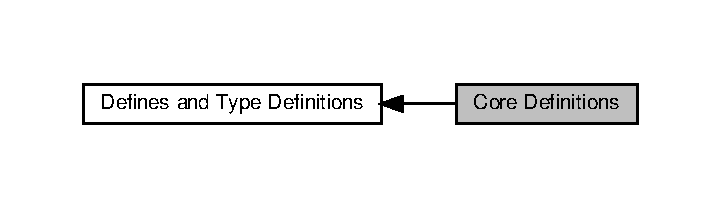
\includegraphics[width=346pt]{group___c_m_s_i_s__core__base}
\end{center}
\end{figure}
\subsection*{Definicje}
\begin{DoxyCompactItemize}
\item 
\#define \hyperlink{group___c_m_s_i_s__core__base_ga3c14ed93192c8d9143322bbf77ebf770}{S\+C\+S\+\_\+\+B\+A\+SE}~(0x\+E000\+E000\+U\+L)
\item 
\#define \hyperlink{group___c_m_s_i_s__core__base_gafdab534f961bf8935eb456cb7700dcd2}{D\+W\+T\+\_\+\+B\+A\+SE}~(0x\+E0001000\+U\+L)
\item 
\#define \hyperlink{group___c_m_s_i_s__core__base_ga2b1eeff850a7e418844ca847145a1a68}{T\+P\+I\+\_\+\+B\+A\+SE}~(0x\+E0040000\+U\+L)
\item 
\#define \hyperlink{group___c_m_s_i_s__core__base_ga680604dbcda9e9b31a1639fcffe5230b}{Core\+Debug\+\_\+\+B\+A\+SE}~(0x\+E000\+E\+D\+F0\+U\+L)
\item 
\#define \hyperlink{group___c_m_s_i_s__core__base_ga58effaac0b93006b756d33209e814646}{Sys\+Tick\+\_\+\+B\+A\+SE}~(\hyperlink{group___c_m_s_i_s__core__base_ga3c14ed93192c8d9143322bbf77ebf770}{S\+C\+S\+\_\+\+B\+A\+SE} +  0x0010\+U\+L)
\item 
\#define \hyperlink{group___c_m_s_i_s__core__base_gaa0288691785a5f868238e0468b39523d}{N\+V\+I\+C\+\_\+\+B\+A\+SE}~(\hyperlink{group___c_m_s_i_s__core__base_ga3c14ed93192c8d9143322bbf77ebf770}{S\+C\+S\+\_\+\+B\+A\+SE} +  0x0100\+U\+L)
\item 
\#define \hyperlink{group___c_m_s_i_s__core__base_gad55a7ddb8d4b2398b0c1cfec76c0d9fd}{S\+C\+B\+\_\+\+B\+A\+SE}~(\hyperlink{group___c_m_s_i_s__core__base_ga3c14ed93192c8d9143322bbf77ebf770}{S\+C\+S\+\_\+\+B\+A\+SE} +  0x0\+D00\+U\+L)
\item 
\#define \hyperlink{group___c_m_s_i_s__core__base_gaaaf6477c2bde2f00f99e3c2fd1060b01}{S\+CB}~((\hyperlink{struct_s_c_b___type}{S\+C\+B\+\_\+\+Type}       $\ast$)     \hyperlink{group___c_m_s_i_s__core__base_gad55a7ddb8d4b2398b0c1cfec76c0d9fd}{S\+C\+B\+\_\+\+B\+A\+SE}         )
\item 
\#define \hyperlink{group___c_m_s_i_s__core__base_gacd96c53beeaff8f603fcda425eb295de}{Sys\+Tick}~((\hyperlink{struct_sys_tick___type}{Sys\+Tick\+\_\+\+Type}   $\ast$)     \hyperlink{group___c_m_s_i_s__core__base_ga58effaac0b93006b756d33209e814646}{Sys\+Tick\+\_\+\+B\+A\+SE}     )
\item 
\#define \hyperlink{group___c_m_s_i_s__core__base_gac8e97e8ce56ae9f57da1363a937f8a17}{N\+V\+IC}~((\hyperlink{struct_n_v_i_c___type}{N\+V\+I\+C\+\_\+\+Type}      $\ast$)     \hyperlink{group___c_m_s_i_s__core__base_gaa0288691785a5f868238e0468b39523d}{N\+V\+I\+C\+\_\+\+B\+A\+SE}        )
\item 
\#define \hyperlink{group___c_m_s_i_s__core__base_gabbe5a060185e1d5afa3f85b14e10a6ce}{D\+WT}~((\hyperlink{struct_d_w_t___type}{D\+W\+T\+\_\+\+Type}       $\ast$)     \hyperlink{group___c_m_s_i_s__core__base_gafdab534f961bf8935eb456cb7700dcd2}{D\+W\+T\+\_\+\+B\+A\+SE}         )
\item 
\#define \hyperlink{group___c_m_s_i_s__core__base_ga8b4dd00016aed25a0ea54e9a9acd1239}{T\+PI}~((\hyperlink{struct_t_p_i___type}{T\+P\+I\+\_\+\+Type}       $\ast$)     \hyperlink{group___c_m_s_i_s__core__base_ga2b1eeff850a7e418844ca847145a1a68}{T\+P\+I\+\_\+\+B\+A\+SE}         )
\item 
\#define \hyperlink{group___c_m_s_i_s__core__base_gab6e30a2b802d9021619dbb0be7f5d63d}{Core\+Debug}~((\hyperlink{struct_core_debug___type}{Core\+Debug\+\_\+\+Type} $\ast$)     \hyperlink{group___c_m_s_i_s__core__base_ga680604dbcda9e9b31a1639fcffe5230b}{Core\+Debug\+\_\+\+B\+A\+SE}   )
\item 
\#define \hyperlink{group___c_m_s_i_s__core__base_ga3c14ed93192c8d9143322bbf77ebf770}{S\+C\+S\+\_\+\+B\+A\+SE}~(0x\+E000\+E000\+U\+L)
\item 
\#define \hyperlink{group___c_m_s_i_s__core__base_gadd76251e412a195ec0a8f47227a8359e}{I\+T\+M\+\_\+\+B\+A\+SE}~(0x\+E0000000\+U\+L)
\item 
\#define \hyperlink{group___c_m_s_i_s__core__base_gafdab534f961bf8935eb456cb7700dcd2}{D\+W\+T\+\_\+\+B\+A\+SE}~(0x\+E0001000\+U\+L)
\item 
\#define \hyperlink{group___c_m_s_i_s__core__base_ga2b1eeff850a7e418844ca847145a1a68}{T\+P\+I\+\_\+\+B\+A\+SE}~(0x\+E0040000\+U\+L)
\item 
\#define \hyperlink{group___c_m_s_i_s__core__base_ga680604dbcda9e9b31a1639fcffe5230b}{Core\+Debug\+\_\+\+B\+A\+SE}~(0x\+E000\+E\+D\+F0\+U\+L)
\item 
\#define \hyperlink{group___c_m_s_i_s__core__base_ga58effaac0b93006b756d33209e814646}{Sys\+Tick\+\_\+\+B\+A\+SE}~(\hyperlink{group___c_m_s_i_s__core__base_ga3c14ed93192c8d9143322bbf77ebf770}{S\+C\+S\+\_\+\+B\+A\+SE} +  0x0010\+U\+L)
\item 
\#define \hyperlink{group___c_m_s_i_s__core__base_gaa0288691785a5f868238e0468b39523d}{N\+V\+I\+C\+\_\+\+B\+A\+SE}~(\hyperlink{group___c_m_s_i_s__core__base_ga3c14ed93192c8d9143322bbf77ebf770}{S\+C\+S\+\_\+\+B\+A\+SE} +  0x0100\+U\+L)
\item 
\#define \hyperlink{group___c_m_s_i_s__core__base_gad55a7ddb8d4b2398b0c1cfec76c0d9fd}{S\+C\+B\+\_\+\+B\+A\+SE}~(\hyperlink{group___c_m_s_i_s__core__base_ga3c14ed93192c8d9143322bbf77ebf770}{S\+C\+S\+\_\+\+B\+A\+SE} +  0x0\+D00\+U\+L)
\item 
\#define \hyperlink{group___c_m_s_i_s__core__base_ga9fe0cd2eef83a8adad94490d9ecca63f}{S\+Cn\+S\+CB}~((\hyperlink{struct_s_cn_s_c_b___type}{S\+Cn\+S\+C\+B\+\_\+\+Type}    $\ast$)     \hyperlink{group___c_m_s_i_s__core__base_ga3c14ed93192c8d9143322bbf77ebf770}{S\+C\+S\+\_\+\+B\+A\+SE}         )
\item 
\#define \hyperlink{group___c_m_s_i_s__core__base_gaaaf6477c2bde2f00f99e3c2fd1060b01}{S\+CB}~((\hyperlink{struct_s_c_b___type}{S\+C\+B\+\_\+\+Type}       $\ast$)     \hyperlink{group___c_m_s_i_s__core__base_gad55a7ddb8d4b2398b0c1cfec76c0d9fd}{S\+C\+B\+\_\+\+B\+A\+SE}         )
\item 
\#define \hyperlink{group___c_m_s_i_s__core__base_gacd96c53beeaff8f603fcda425eb295de}{Sys\+Tick}~((\hyperlink{struct_sys_tick___type}{Sys\+Tick\+\_\+\+Type}   $\ast$)     \hyperlink{group___c_m_s_i_s__core__base_ga58effaac0b93006b756d33209e814646}{Sys\+Tick\+\_\+\+B\+A\+SE}     )
\item 
\#define \hyperlink{group___c_m_s_i_s__core__base_gac8e97e8ce56ae9f57da1363a937f8a17}{N\+V\+IC}~((\hyperlink{struct_n_v_i_c___type}{N\+V\+I\+C\+\_\+\+Type}      $\ast$)     \hyperlink{group___c_m_s_i_s__core__base_gaa0288691785a5f868238e0468b39523d}{N\+V\+I\+C\+\_\+\+B\+A\+SE}        )
\item 
\#define \hyperlink{group___c_m_s_i_s__core__base_gabae7cdf882def602cb787bb039ff6a43}{I\+TM}~((\hyperlink{struct_i_t_m___type}{I\+T\+M\+\_\+\+Type}       $\ast$)     \hyperlink{group___c_m_s_i_s__core__base_gadd76251e412a195ec0a8f47227a8359e}{I\+T\+M\+\_\+\+B\+A\+SE}         )
\item 
\#define \hyperlink{group___c_m_s_i_s__core__base_gabbe5a060185e1d5afa3f85b14e10a6ce}{D\+WT}~((\hyperlink{struct_d_w_t___type}{D\+W\+T\+\_\+\+Type}       $\ast$)     \hyperlink{group___c_m_s_i_s__core__base_gafdab534f961bf8935eb456cb7700dcd2}{D\+W\+T\+\_\+\+B\+A\+SE}         )
\item 
\#define \hyperlink{group___c_m_s_i_s__core__base_ga8b4dd00016aed25a0ea54e9a9acd1239}{T\+PI}~((\hyperlink{struct_t_p_i___type}{T\+P\+I\+\_\+\+Type}       $\ast$)     \hyperlink{group___c_m_s_i_s__core__base_ga2b1eeff850a7e418844ca847145a1a68}{T\+P\+I\+\_\+\+B\+A\+SE}         )
\item 
\#define \hyperlink{group___c_m_s_i_s__core__base_gab6e30a2b802d9021619dbb0be7f5d63d}{Core\+Debug}~((\hyperlink{struct_core_debug___type}{Core\+Debug\+\_\+\+Type} $\ast$)     \hyperlink{group___c_m_s_i_s__core__base_ga680604dbcda9e9b31a1639fcffe5230b}{Core\+Debug\+\_\+\+B\+A\+SE}   )
\item 
\#define \hyperlink{group___c_m_s_i_s__core__base_ga4dcad4027118c098c07bcd575f1fbb28}{F\+P\+U\+\_\+\+B\+A\+SE}~(\hyperlink{group___c_m_s_i_s__core__base_ga3c14ed93192c8d9143322bbf77ebf770}{S\+C\+S\+\_\+\+B\+A\+SE} +  0x0\+F30\+U\+L)
\item 
\#define \hyperlink{group___c_m_s_i_s__core__base_gabc7c93f2594e85ece1e1a24f10591428}{F\+PU}~((\hyperlink{struct_f_p_u___type}{F\+P\+U\+\_\+\+Type}       $\ast$)     \hyperlink{group___c_m_s_i_s__core__base_ga4dcad4027118c098c07bcd575f1fbb28}{F\+P\+U\+\_\+\+B\+A\+SE}         )
\item 
\#define \hyperlink{group___c_m_s_i_s__core__base_ga3c14ed93192c8d9143322bbf77ebf770}{S\+C\+S\+\_\+\+B\+A\+SE}~(0x\+E000\+E000\+U\+L)
\item 
\#define \hyperlink{group___c_m_s_i_s__core__base_ga58effaac0b93006b756d33209e814646}{Sys\+Tick\+\_\+\+B\+A\+SE}~(\hyperlink{group___c_m_s_i_s__core__base_ga3c14ed93192c8d9143322bbf77ebf770}{S\+C\+S\+\_\+\+B\+A\+SE} +  0x0010\+U\+L)
\item 
\#define \hyperlink{group___c_m_s_i_s__core__base_gaa0288691785a5f868238e0468b39523d}{N\+V\+I\+C\+\_\+\+B\+A\+SE}~(\hyperlink{group___c_m_s_i_s__core__base_ga3c14ed93192c8d9143322bbf77ebf770}{S\+C\+S\+\_\+\+B\+A\+SE} +  0x0100\+U\+L)
\item 
\#define \hyperlink{group___c_m_s_i_s__core__base_gad55a7ddb8d4b2398b0c1cfec76c0d9fd}{S\+C\+B\+\_\+\+B\+A\+SE}~(\hyperlink{group___c_m_s_i_s__core__base_ga3c14ed93192c8d9143322bbf77ebf770}{S\+C\+S\+\_\+\+B\+A\+SE} +  0x0\+D00\+U\+L)
\item 
\#define \hyperlink{group___c_m_s_i_s__core__base_gaaaf6477c2bde2f00f99e3c2fd1060b01}{S\+CB}~((\hyperlink{struct_s_c_b___type}{S\+C\+B\+\_\+\+Type}       $\ast$)     \hyperlink{group___c_m_s_i_s__core__base_gad55a7ddb8d4b2398b0c1cfec76c0d9fd}{S\+C\+B\+\_\+\+B\+A\+SE}      )
\item 
\#define \hyperlink{group___c_m_s_i_s__core__base_gacd96c53beeaff8f603fcda425eb295de}{Sys\+Tick}~((\hyperlink{struct_sys_tick___type}{Sys\+Tick\+\_\+\+Type}   $\ast$)     \hyperlink{group___c_m_s_i_s__core__base_ga58effaac0b93006b756d33209e814646}{Sys\+Tick\+\_\+\+B\+A\+SE}  )
\item 
\#define \hyperlink{group___c_m_s_i_s__core__base_gac8e97e8ce56ae9f57da1363a937f8a17}{N\+V\+IC}~((\hyperlink{struct_n_v_i_c___type}{N\+V\+I\+C\+\_\+\+Type}      $\ast$)     \hyperlink{group___c_m_s_i_s__core__base_gaa0288691785a5f868238e0468b39523d}{N\+V\+I\+C\+\_\+\+B\+A\+SE}     )
\item 
\#define \hyperlink{group___c_m_s_i_s__core__base_ga3c14ed93192c8d9143322bbf77ebf770}{S\+C\+S\+\_\+\+B\+A\+SE}~(0x\+E000\+E000\+U\+L)
\item 
\#define \hyperlink{group___c_m_s_i_s__core__base_ga58effaac0b93006b756d33209e814646}{Sys\+Tick\+\_\+\+B\+A\+SE}~(\hyperlink{group___c_m_s_i_s__core__base_ga3c14ed93192c8d9143322bbf77ebf770}{S\+C\+S\+\_\+\+B\+A\+SE} +  0x0010\+U\+L)
\item 
\#define \hyperlink{group___c_m_s_i_s__core__base_gaa0288691785a5f868238e0468b39523d}{N\+V\+I\+C\+\_\+\+B\+A\+SE}~(\hyperlink{group___c_m_s_i_s__core__base_ga3c14ed93192c8d9143322bbf77ebf770}{S\+C\+S\+\_\+\+B\+A\+SE} +  0x0100\+U\+L)
\item 
\#define \hyperlink{group___c_m_s_i_s__core__base_gad55a7ddb8d4b2398b0c1cfec76c0d9fd}{S\+C\+B\+\_\+\+B\+A\+SE}~(\hyperlink{group___c_m_s_i_s__core__base_ga3c14ed93192c8d9143322bbf77ebf770}{S\+C\+S\+\_\+\+B\+A\+SE} +  0x0\+D00\+U\+L)
\item 
\#define \hyperlink{group___c_m_s_i_s__core__base_gaaaf6477c2bde2f00f99e3c2fd1060b01}{S\+CB}~((\hyperlink{struct_s_c_b___type}{S\+C\+B\+\_\+\+Type}       $\ast$)     \hyperlink{group___c_m_s_i_s__core__base_gad55a7ddb8d4b2398b0c1cfec76c0d9fd}{S\+C\+B\+\_\+\+B\+A\+SE}      )
\item 
\#define \hyperlink{group___c_m_s_i_s__core__base_gacd96c53beeaff8f603fcda425eb295de}{Sys\+Tick}~((\hyperlink{struct_sys_tick___type}{Sys\+Tick\+\_\+\+Type}   $\ast$)     \hyperlink{group___c_m_s_i_s__core__base_ga58effaac0b93006b756d33209e814646}{Sys\+Tick\+\_\+\+B\+A\+SE}  )
\item 
\#define \hyperlink{group___c_m_s_i_s__core__base_gac8e97e8ce56ae9f57da1363a937f8a17}{N\+V\+IC}~((\hyperlink{struct_n_v_i_c___type}{N\+V\+I\+C\+\_\+\+Type}      $\ast$)     \hyperlink{group___c_m_s_i_s__core__base_gaa0288691785a5f868238e0468b39523d}{N\+V\+I\+C\+\_\+\+B\+A\+SE}     )
\item 
\#define \hyperlink{group___c_m_s_i_s__core__base_ga3c14ed93192c8d9143322bbf77ebf770}{S\+C\+S\+\_\+\+B\+A\+SE}~(0x\+E000\+E000\+U\+L)
\item 
\#define \hyperlink{group___c_m_s_i_s__core__base_ga58effaac0b93006b756d33209e814646}{Sys\+Tick\+\_\+\+B\+A\+SE}~(\hyperlink{group___c_m_s_i_s__core__base_ga3c14ed93192c8d9143322bbf77ebf770}{S\+C\+S\+\_\+\+B\+A\+SE} +  0x0010\+U\+L)
\item 
\#define \hyperlink{group___c_m_s_i_s__core__base_gaa0288691785a5f868238e0468b39523d}{N\+V\+I\+C\+\_\+\+B\+A\+SE}~(\hyperlink{group___c_m_s_i_s__core__base_ga3c14ed93192c8d9143322bbf77ebf770}{S\+C\+S\+\_\+\+B\+A\+SE} +  0x0100\+U\+L)
\item 
\#define \hyperlink{group___c_m_s_i_s__core__base_gad55a7ddb8d4b2398b0c1cfec76c0d9fd}{S\+C\+B\+\_\+\+B\+A\+SE}~(\hyperlink{group___c_m_s_i_s__core__base_ga3c14ed93192c8d9143322bbf77ebf770}{S\+C\+S\+\_\+\+B\+A\+SE} +  0x0\+D00\+U\+L)
\item 
\#define \hyperlink{group___c_m_s_i_s__core__base_ga9fe0cd2eef83a8adad94490d9ecca63f}{S\+Cn\+S\+CB}~((\hyperlink{struct_s_cn_s_c_b___type}{S\+Cn\+S\+C\+B\+\_\+\+Type}    $\ast$)     \hyperlink{group___c_m_s_i_s__core__base_ga3c14ed93192c8d9143322bbf77ebf770}{S\+C\+S\+\_\+\+B\+A\+SE}      )
\item 
\#define \hyperlink{group___c_m_s_i_s__core__base_gaaaf6477c2bde2f00f99e3c2fd1060b01}{S\+CB}~((\hyperlink{struct_s_c_b___type}{S\+C\+B\+\_\+\+Type}       $\ast$)     \hyperlink{group___c_m_s_i_s__core__base_gad55a7ddb8d4b2398b0c1cfec76c0d9fd}{S\+C\+B\+\_\+\+B\+A\+SE}      )
\item 
\#define \hyperlink{group___c_m_s_i_s__core__base_gacd96c53beeaff8f603fcda425eb295de}{Sys\+Tick}~((\hyperlink{struct_sys_tick___type}{Sys\+Tick\+\_\+\+Type}   $\ast$)     \hyperlink{group___c_m_s_i_s__core__base_ga58effaac0b93006b756d33209e814646}{Sys\+Tick\+\_\+\+B\+A\+SE}  )
\item 
\#define \hyperlink{group___c_m_s_i_s__core__base_gac8e97e8ce56ae9f57da1363a937f8a17}{N\+V\+IC}~((\hyperlink{struct_n_v_i_c___type}{N\+V\+I\+C\+\_\+\+Type}      $\ast$)     \hyperlink{group___c_m_s_i_s__core__base_gaa0288691785a5f868238e0468b39523d}{N\+V\+I\+C\+\_\+\+B\+A\+SE}     )
\item 
\#define \hyperlink{group___c_m_s_i_s__core__base_ga3c14ed93192c8d9143322bbf77ebf770}{S\+C\+S\+\_\+\+B\+A\+SE}~(0x\+E000\+E000\+U\+L)
\item 
\#define \hyperlink{group___c_m_s_i_s__core__base_gafdab534f961bf8935eb456cb7700dcd2}{D\+W\+T\+\_\+\+B\+A\+SE}~(0x\+E0001000\+U\+L)
\item 
\#define \hyperlink{group___c_m_s_i_s__core__base_ga2b1eeff850a7e418844ca847145a1a68}{T\+P\+I\+\_\+\+B\+A\+SE}~(0x\+E0040000\+U\+L)
\item 
\#define \hyperlink{group___c_m_s_i_s__core__base_ga680604dbcda9e9b31a1639fcffe5230b}{Core\+Debug\+\_\+\+B\+A\+SE}~(0x\+E000\+E\+D\+F0\+U\+L)
\item 
\#define \hyperlink{group___c_m_s_i_s__core__base_ga58effaac0b93006b756d33209e814646}{Sys\+Tick\+\_\+\+B\+A\+SE}~(\hyperlink{group___c_m_s_i_s__core__base_ga3c14ed93192c8d9143322bbf77ebf770}{S\+C\+S\+\_\+\+B\+A\+SE} +  0x0010\+U\+L)
\item 
\#define \hyperlink{group___c_m_s_i_s__core__base_gaa0288691785a5f868238e0468b39523d}{N\+V\+I\+C\+\_\+\+B\+A\+SE}~(\hyperlink{group___c_m_s_i_s__core__base_ga3c14ed93192c8d9143322bbf77ebf770}{S\+C\+S\+\_\+\+B\+A\+SE} +  0x0100\+U\+L)
\item 
\#define \hyperlink{group___c_m_s_i_s__core__base_gad55a7ddb8d4b2398b0c1cfec76c0d9fd}{S\+C\+B\+\_\+\+B\+A\+SE}~(\hyperlink{group___c_m_s_i_s__core__base_ga3c14ed93192c8d9143322bbf77ebf770}{S\+C\+S\+\_\+\+B\+A\+SE} +  0x0\+D00\+U\+L)
\item 
\#define \hyperlink{group___c_m_s_i_s__core__base_gaaaf6477c2bde2f00f99e3c2fd1060b01}{S\+CB}~((\hyperlink{struct_s_c_b___type}{S\+C\+B\+\_\+\+Type}       $\ast$)     \hyperlink{group___c_m_s_i_s__core__base_gad55a7ddb8d4b2398b0c1cfec76c0d9fd}{S\+C\+B\+\_\+\+B\+A\+SE}         )
\item 
\#define \hyperlink{group___c_m_s_i_s__core__base_gacd96c53beeaff8f603fcda425eb295de}{Sys\+Tick}~((\hyperlink{struct_sys_tick___type}{Sys\+Tick\+\_\+\+Type}   $\ast$)     \hyperlink{group___c_m_s_i_s__core__base_ga58effaac0b93006b756d33209e814646}{Sys\+Tick\+\_\+\+B\+A\+SE}     )
\item 
\#define \hyperlink{group___c_m_s_i_s__core__base_gac8e97e8ce56ae9f57da1363a937f8a17}{N\+V\+IC}~((\hyperlink{struct_n_v_i_c___type}{N\+V\+I\+C\+\_\+\+Type}      $\ast$)     \hyperlink{group___c_m_s_i_s__core__base_gaa0288691785a5f868238e0468b39523d}{N\+V\+I\+C\+\_\+\+B\+A\+SE}        )
\item 
\#define \hyperlink{group___c_m_s_i_s__core__base_gabbe5a060185e1d5afa3f85b14e10a6ce}{D\+WT}~((\hyperlink{struct_d_w_t___type}{D\+W\+T\+\_\+\+Type}       $\ast$)     \hyperlink{group___c_m_s_i_s__core__base_gafdab534f961bf8935eb456cb7700dcd2}{D\+W\+T\+\_\+\+B\+A\+SE}         )
\item 
\#define \hyperlink{group___c_m_s_i_s__core__base_ga8b4dd00016aed25a0ea54e9a9acd1239}{T\+PI}~((\hyperlink{struct_t_p_i___type}{T\+P\+I\+\_\+\+Type}       $\ast$)     \hyperlink{group___c_m_s_i_s__core__base_ga2b1eeff850a7e418844ca847145a1a68}{T\+P\+I\+\_\+\+B\+A\+SE}         )
\item 
\#define \hyperlink{group___c_m_s_i_s__core__base_gab6e30a2b802d9021619dbb0be7f5d63d}{Core\+Debug}~((\hyperlink{struct_core_debug___type}{Core\+Debug\+\_\+\+Type} $\ast$)     \hyperlink{group___c_m_s_i_s__core__base_ga680604dbcda9e9b31a1639fcffe5230b}{Core\+Debug\+\_\+\+B\+A\+SE}   )
\item 
\#define \hyperlink{group___c_m_s_i_s__core__base_ga3c14ed93192c8d9143322bbf77ebf770}{S\+C\+S\+\_\+\+B\+A\+SE}~(0x\+E000\+E000\+U\+L)
\item 
\#define \hyperlink{group___c_m_s_i_s__core__base_gadd76251e412a195ec0a8f47227a8359e}{I\+T\+M\+\_\+\+B\+A\+SE}~(0x\+E0000000\+U\+L)
\item 
\#define \hyperlink{group___c_m_s_i_s__core__base_gafdab534f961bf8935eb456cb7700dcd2}{D\+W\+T\+\_\+\+B\+A\+SE}~(0x\+E0001000\+U\+L)
\item 
\#define \hyperlink{group___c_m_s_i_s__core__base_ga2b1eeff850a7e418844ca847145a1a68}{T\+P\+I\+\_\+\+B\+A\+SE}~(0x\+E0040000\+U\+L)
\item 
\#define \hyperlink{group___c_m_s_i_s__core__base_ga680604dbcda9e9b31a1639fcffe5230b}{Core\+Debug\+\_\+\+B\+A\+SE}~(0x\+E000\+E\+D\+F0\+U\+L)
\item 
\#define \hyperlink{group___c_m_s_i_s__core__base_ga58effaac0b93006b756d33209e814646}{Sys\+Tick\+\_\+\+B\+A\+SE}~(\hyperlink{group___c_m_s_i_s__core__base_ga3c14ed93192c8d9143322bbf77ebf770}{S\+C\+S\+\_\+\+B\+A\+SE} +  0x0010\+U\+L)
\item 
\#define \hyperlink{group___c_m_s_i_s__core__base_gaa0288691785a5f868238e0468b39523d}{N\+V\+I\+C\+\_\+\+B\+A\+SE}~(\hyperlink{group___c_m_s_i_s__core__base_ga3c14ed93192c8d9143322bbf77ebf770}{S\+C\+S\+\_\+\+B\+A\+SE} +  0x0100\+U\+L)
\item 
\#define \hyperlink{group___c_m_s_i_s__core__base_gad55a7ddb8d4b2398b0c1cfec76c0d9fd}{S\+C\+B\+\_\+\+B\+A\+SE}~(\hyperlink{group___c_m_s_i_s__core__base_ga3c14ed93192c8d9143322bbf77ebf770}{S\+C\+S\+\_\+\+B\+A\+SE} +  0x0\+D00\+U\+L)
\item 
\#define \hyperlink{group___c_m_s_i_s__core__base_ga9fe0cd2eef83a8adad94490d9ecca63f}{S\+Cn\+S\+CB}~((\hyperlink{struct_s_cn_s_c_b___type}{S\+Cn\+S\+C\+B\+\_\+\+Type}    $\ast$)     \hyperlink{group___c_m_s_i_s__core__base_ga3c14ed93192c8d9143322bbf77ebf770}{S\+C\+S\+\_\+\+B\+A\+SE}      )
\item 
\#define \hyperlink{group___c_m_s_i_s__core__base_gaaaf6477c2bde2f00f99e3c2fd1060b01}{S\+CB}~((\hyperlink{struct_s_c_b___type}{S\+C\+B\+\_\+\+Type}       $\ast$)     \hyperlink{group___c_m_s_i_s__core__base_gad55a7ddb8d4b2398b0c1cfec76c0d9fd}{S\+C\+B\+\_\+\+B\+A\+SE}      )
\item 
\#define \hyperlink{group___c_m_s_i_s__core__base_gacd96c53beeaff8f603fcda425eb295de}{Sys\+Tick}~((\hyperlink{struct_sys_tick___type}{Sys\+Tick\+\_\+\+Type}   $\ast$)     \hyperlink{group___c_m_s_i_s__core__base_ga58effaac0b93006b756d33209e814646}{Sys\+Tick\+\_\+\+B\+A\+SE}  )
\item 
\#define \hyperlink{group___c_m_s_i_s__core__base_gac8e97e8ce56ae9f57da1363a937f8a17}{N\+V\+IC}~((\hyperlink{struct_n_v_i_c___type}{N\+V\+I\+C\+\_\+\+Type}      $\ast$)     \hyperlink{group___c_m_s_i_s__core__base_gaa0288691785a5f868238e0468b39523d}{N\+V\+I\+C\+\_\+\+B\+A\+SE}     )
\item 
\#define \hyperlink{group___c_m_s_i_s__core__base_gabae7cdf882def602cb787bb039ff6a43}{I\+TM}~((\hyperlink{struct_i_t_m___type}{I\+T\+M\+\_\+\+Type}       $\ast$)     \hyperlink{group___c_m_s_i_s__core__base_gadd76251e412a195ec0a8f47227a8359e}{I\+T\+M\+\_\+\+B\+A\+SE}      )
\item 
\#define \hyperlink{group___c_m_s_i_s__core__base_gabbe5a060185e1d5afa3f85b14e10a6ce}{D\+WT}~((\hyperlink{struct_d_w_t___type}{D\+W\+T\+\_\+\+Type}       $\ast$)     \hyperlink{group___c_m_s_i_s__core__base_gafdab534f961bf8935eb456cb7700dcd2}{D\+W\+T\+\_\+\+B\+A\+SE}      )
\item 
\#define \hyperlink{group___c_m_s_i_s__core__base_ga8b4dd00016aed25a0ea54e9a9acd1239}{T\+PI}~((\hyperlink{struct_t_p_i___type}{T\+P\+I\+\_\+\+Type}       $\ast$)     \hyperlink{group___c_m_s_i_s__core__base_ga2b1eeff850a7e418844ca847145a1a68}{T\+P\+I\+\_\+\+B\+A\+SE}      )
\item 
\#define \hyperlink{group___c_m_s_i_s__core__base_gab6e30a2b802d9021619dbb0be7f5d63d}{Core\+Debug}~((\hyperlink{struct_core_debug___type}{Core\+Debug\+\_\+\+Type} $\ast$)     \hyperlink{group___c_m_s_i_s__core__base_ga680604dbcda9e9b31a1639fcffe5230b}{Core\+Debug\+\_\+\+B\+A\+SE})
\item 
\#define \hyperlink{group___c_m_s_i_s__core__base_ga3c14ed93192c8d9143322bbf77ebf770}{S\+C\+S\+\_\+\+B\+A\+SE}~(0x\+E000\+E000\+U\+L)
\item 
\#define \hyperlink{group___c_m_s_i_s__core__base_gadd76251e412a195ec0a8f47227a8359e}{I\+T\+M\+\_\+\+B\+A\+SE}~(0x\+E0000000\+U\+L)
\item 
\#define \hyperlink{group___c_m_s_i_s__core__base_gafdab534f961bf8935eb456cb7700dcd2}{D\+W\+T\+\_\+\+B\+A\+SE}~(0x\+E0001000\+U\+L)
\item 
\#define \hyperlink{group___c_m_s_i_s__core__base_ga2b1eeff850a7e418844ca847145a1a68}{T\+P\+I\+\_\+\+B\+A\+SE}~(0x\+E0040000\+U\+L)
\item 
\#define \hyperlink{group___c_m_s_i_s__core__base_ga680604dbcda9e9b31a1639fcffe5230b}{Core\+Debug\+\_\+\+B\+A\+SE}~(0x\+E000\+E\+D\+F0\+U\+L)
\item 
\#define \hyperlink{group___c_m_s_i_s__core__base_ga58effaac0b93006b756d33209e814646}{Sys\+Tick\+\_\+\+B\+A\+SE}~(\hyperlink{group___c_m_s_i_s__core__base_ga3c14ed93192c8d9143322bbf77ebf770}{S\+C\+S\+\_\+\+B\+A\+SE} +  0x0010\+U\+L)
\item 
\#define \hyperlink{group___c_m_s_i_s__core__base_gaa0288691785a5f868238e0468b39523d}{N\+V\+I\+C\+\_\+\+B\+A\+SE}~(\hyperlink{group___c_m_s_i_s__core__base_ga3c14ed93192c8d9143322bbf77ebf770}{S\+C\+S\+\_\+\+B\+A\+SE} +  0x0100\+U\+L)
\item 
\#define \hyperlink{group___c_m_s_i_s__core__base_gad55a7ddb8d4b2398b0c1cfec76c0d9fd}{S\+C\+B\+\_\+\+B\+A\+SE}~(\hyperlink{group___c_m_s_i_s__core__base_ga3c14ed93192c8d9143322bbf77ebf770}{S\+C\+S\+\_\+\+B\+A\+SE} +  0x0\+D00\+U\+L)
\item 
\#define \hyperlink{group___c_m_s_i_s__core__base_ga9fe0cd2eef83a8adad94490d9ecca63f}{S\+Cn\+S\+CB}~((\hyperlink{struct_s_cn_s_c_b___type}{S\+Cn\+S\+C\+B\+\_\+\+Type}    $\ast$)     \hyperlink{group___c_m_s_i_s__core__base_ga3c14ed93192c8d9143322bbf77ebf770}{S\+C\+S\+\_\+\+B\+A\+SE}         )
\item 
\#define \hyperlink{group___c_m_s_i_s__core__base_gaaaf6477c2bde2f00f99e3c2fd1060b01}{S\+CB}~((\hyperlink{struct_s_c_b___type}{S\+C\+B\+\_\+\+Type}       $\ast$)     \hyperlink{group___c_m_s_i_s__core__base_gad55a7ddb8d4b2398b0c1cfec76c0d9fd}{S\+C\+B\+\_\+\+B\+A\+SE}         )
\item 
\#define \hyperlink{group___c_m_s_i_s__core__base_gacd96c53beeaff8f603fcda425eb295de}{Sys\+Tick}~((\hyperlink{struct_sys_tick___type}{Sys\+Tick\+\_\+\+Type}   $\ast$)     \hyperlink{group___c_m_s_i_s__core__base_ga58effaac0b93006b756d33209e814646}{Sys\+Tick\+\_\+\+B\+A\+SE}     )
\item 
\#define \hyperlink{group___c_m_s_i_s__core__base_gac8e97e8ce56ae9f57da1363a937f8a17}{N\+V\+IC}~((\hyperlink{struct_n_v_i_c___type}{N\+V\+I\+C\+\_\+\+Type}      $\ast$)     \hyperlink{group___c_m_s_i_s__core__base_gaa0288691785a5f868238e0468b39523d}{N\+V\+I\+C\+\_\+\+B\+A\+SE}        )
\item 
\#define \hyperlink{group___c_m_s_i_s__core__base_gabae7cdf882def602cb787bb039ff6a43}{I\+TM}~((\hyperlink{struct_i_t_m___type}{I\+T\+M\+\_\+\+Type}       $\ast$)     \hyperlink{group___c_m_s_i_s__core__base_gadd76251e412a195ec0a8f47227a8359e}{I\+T\+M\+\_\+\+B\+A\+SE}         )
\item 
\#define \hyperlink{group___c_m_s_i_s__core__base_gabbe5a060185e1d5afa3f85b14e10a6ce}{D\+WT}~((\hyperlink{struct_d_w_t___type}{D\+W\+T\+\_\+\+Type}       $\ast$)     \hyperlink{group___c_m_s_i_s__core__base_gafdab534f961bf8935eb456cb7700dcd2}{D\+W\+T\+\_\+\+B\+A\+SE}         )
\item 
\#define \hyperlink{group___c_m_s_i_s__core__base_ga8b4dd00016aed25a0ea54e9a9acd1239}{T\+PI}~((\hyperlink{struct_t_p_i___type}{T\+P\+I\+\_\+\+Type}       $\ast$)     \hyperlink{group___c_m_s_i_s__core__base_ga2b1eeff850a7e418844ca847145a1a68}{T\+P\+I\+\_\+\+B\+A\+SE}         )
\item 
\#define \hyperlink{group___c_m_s_i_s__core__base_gab6e30a2b802d9021619dbb0be7f5d63d}{Core\+Debug}~((\hyperlink{struct_core_debug___type}{Core\+Debug\+\_\+\+Type} $\ast$)     \hyperlink{group___c_m_s_i_s__core__base_ga680604dbcda9e9b31a1639fcffe5230b}{Core\+Debug\+\_\+\+B\+A\+SE}   )
\item 
\#define \hyperlink{group___c_m_s_i_s__core__base_ga4dcad4027118c098c07bcd575f1fbb28}{F\+P\+U\+\_\+\+B\+A\+SE}~(\hyperlink{group___c_m_s_i_s__core__base_ga3c14ed93192c8d9143322bbf77ebf770}{S\+C\+S\+\_\+\+B\+A\+SE} +  0x0\+F30\+U\+L)
\item 
\#define \hyperlink{group___c_m_s_i_s__core__base_gabc7c93f2594e85ece1e1a24f10591428}{F\+PU}~((\hyperlink{struct_f_p_u___type}{F\+P\+U\+\_\+\+Type}       $\ast$)     \hyperlink{group___c_m_s_i_s__core__base_ga4dcad4027118c098c07bcd575f1fbb28}{F\+P\+U\+\_\+\+B\+A\+SE}         )
\item 
\#define \hyperlink{group___c_m_s_i_s__core__base_ga3c14ed93192c8d9143322bbf77ebf770}{S\+C\+S\+\_\+\+B\+A\+SE}~(0x\+E000\+E000\+U\+L)
\item 
\#define \hyperlink{group___c_m_s_i_s__core__base_gadd76251e412a195ec0a8f47227a8359e}{I\+T\+M\+\_\+\+B\+A\+SE}~(0x\+E0000000\+U\+L)
\item 
\#define \hyperlink{group___c_m_s_i_s__core__base_gafdab534f961bf8935eb456cb7700dcd2}{D\+W\+T\+\_\+\+B\+A\+SE}~(0x\+E0001000\+U\+L)
\item 
\#define \hyperlink{group___c_m_s_i_s__core__base_ga2b1eeff850a7e418844ca847145a1a68}{T\+P\+I\+\_\+\+B\+A\+SE}~(0x\+E0040000\+U\+L)
\item 
\#define \hyperlink{group___c_m_s_i_s__core__base_ga680604dbcda9e9b31a1639fcffe5230b}{Core\+Debug\+\_\+\+B\+A\+SE}~(0x\+E000\+E\+D\+F0\+U\+L)
\item 
\#define \hyperlink{group___c_m_s_i_s__core__base_ga58effaac0b93006b756d33209e814646}{Sys\+Tick\+\_\+\+B\+A\+SE}~(\hyperlink{group___c_m_s_i_s__core__base_ga3c14ed93192c8d9143322bbf77ebf770}{S\+C\+S\+\_\+\+B\+A\+SE} +  0x0010\+U\+L)
\item 
\#define \hyperlink{group___c_m_s_i_s__core__base_gaa0288691785a5f868238e0468b39523d}{N\+V\+I\+C\+\_\+\+B\+A\+SE}~(\hyperlink{group___c_m_s_i_s__core__base_ga3c14ed93192c8d9143322bbf77ebf770}{S\+C\+S\+\_\+\+B\+A\+SE} +  0x0100\+U\+L)
\item 
\#define \hyperlink{group___c_m_s_i_s__core__base_gad55a7ddb8d4b2398b0c1cfec76c0d9fd}{S\+C\+B\+\_\+\+B\+A\+SE}~(\hyperlink{group___c_m_s_i_s__core__base_ga3c14ed93192c8d9143322bbf77ebf770}{S\+C\+S\+\_\+\+B\+A\+SE} +  0x0\+D00\+U\+L)
\item 
\#define \hyperlink{group___c_m_s_i_s__core__base_ga9fe0cd2eef83a8adad94490d9ecca63f}{S\+Cn\+S\+CB}~((\hyperlink{struct_s_cn_s_c_b___type}{S\+Cn\+S\+C\+B\+\_\+\+Type}    $\ast$)     \hyperlink{group___c_m_s_i_s__core__base_ga3c14ed93192c8d9143322bbf77ebf770}{S\+C\+S\+\_\+\+B\+A\+SE}      )
\item 
\#define \hyperlink{group___c_m_s_i_s__core__base_gaaaf6477c2bde2f00f99e3c2fd1060b01}{S\+CB}~((\hyperlink{struct_s_c_b___type}{S\+C\+B\+\_\+\+Type}       $\ast$)     \hyperlink{group___c_m_s_i_s__core__base_gad55a7ddb8d4b2398b0c1cfec76c0d9fd}{S\+C\+B\+\_\+\+B\+A\+SE}      )
\item 
\#define \hyperlink{group___c_m_s_i_s__core__base_gacd96c53beeaff8f603fcda425eb295de}{Sys\+Tick}~((\hyperlink{struct_sys_tick___type}{Sys\+Tick\+\_\+\+Type}   $\ast$)     \hyperlink{group___c_m_s_i_s__core__base_ga58effaac0b93006b756d33209e814646}{Sys\+Tick\+\_\+\+B\+A\+SE}  )
\item 
\#define \hyperlink{group___c_m_s_i_s__core__base_gac8e97e8ce56ae9f57da1363a937f8a17}{N\+V\+IC}~((\hyperlink{struct_n_v_i_c___type}{N\+V\+I\+C\+\_\+\+Type}      $\ast$)     \hyperlink{group___c_m_s_i_s__core__base_gaa0288691785a5f868238e0468b39523d}{N\+V\+I\+C\+\_\+\+B\+A\+SE}     )
\item 
\#define \hyperlink{group___c_m_s_i_s__core__base_gabae7cdf882def602cb787bb039ff6a43}{I\+TM}~((\hyperlink{struct_i_t_m___type}{I\+T\+M\+\_\+\+Type}       $\ast$)     \hyperlink{group___c_m_s_i_s__core__base_gadd76251e412a195ec0a8f47227a8359e}{I\+T\+M\+\_\+\+B\+A\+SE}      )
\item 
\#define \hyperlink{group___c_m_s_i_s__core__base_gabbe5a060185e1d5afa3f85b14e10a6ce}{D\+WT}~((\hyperlink{struct_d_w_t___type}{D\+W\+T\+\_\+\+Type}       $\ast$)     \hyperlink{group___c_m_s_i_s__core__base_gafdab534f961bf8935eb456cb7700dcd2}{D\+W\+T\+\_\+\+B\+A\+SE}      )
\item 
\#define \hyperlink{group___c_m_s_i_s__core__base_ga8b4dd00016aed25a0ea54e9a9acd1239}{T\+PI}~((\hyperlink{struct_t_p_i___type}{T\+P\+I\+\_\+\+Type}       $\ast$)     \hyperlink{group___c_m_s_i_s__core__base_ga2b1eeff850a7e418844ca847145a1a68}{T\+P\+I\+\_\+\+B\+A\+SE}      )
\item 
\#define \hyperlink{group___c_m_s_i_s__core__base_gab6e30a2b802d9021619dbb0be7f5d63d}{Core\+Debug}~((\hyperlink{struct_core_debug___type}{Core\+Debug\+\_\+\+Type} $\ast$)     \hyperlink{group___c_m_s_i_s__core__base_ga680604dbcda9e9b31a1639fcffe5230b}{Core\+Debug\+\_\+\+B\+A\+SE})
\item 
\#define \hyperlink{group___c_m_s_i_s__core__base_ga4dcad4027118c098c07bcd575f1fbb28}{F\+P\+U\+\_\+\+B\+A\+SE}~(\hyperlink{group___c_m_s_i_s__core__base_ga3c14ed93192c8d9143322bbf77ebf770}{S\+C\+S\+\_\+\+B\+A\+SE} +  0x0\+F30\+U\+L)
\item 
\#define \hyperlink{group___c_m_s_i_s__core__base_gabc7c93f2594e85ece1e1a24f10591428}{F\+PU}~((\hyperlink{struct_f_p_u___type}{F\+P\+U\+\_\+\+Type}       $\ast$)     \hyperlink{group___c_m_s_i_s__core__base_ga4dcad4027118c098c07bcd575f1fbb28}{F\+P\+U\+\_\+\+B\+A\+SE}      )
\item 
\#define \hyperlink{group___c_m_s_i_s__core__base_ga3c14ed93192c8d9143322bbf77ebf770}{S\+C\+S\+\_\+\+B\+A\+SE}~(0x\+E000\+E000\+U\+L)
\item 
\#define \hyperlink{group___c_m_s_i_s__core__base_gadd76251e412a195ec0a8f47227a8359e}{I\+T\+M\+\_\+\+B\+A\+SE}~(0x\+E0000000\+U\+L)
\item 
\#define \hyperlink{group___c_m_s_i_s__core__base_gafdab534f961bf8935eb456cb7700dcd2}{D\+W\+T\+\_\+\+B\+A\+SE}~(0x\+E0001000\+U\+L)
\item 
\#define \hyperlink{group___c_m_s_i_s__core__base_ga2b1eeff850a7e418844ca847145a1a68}{T\+P\+I\+\_\+\+B\+A\+SE}~(0x\+E0040000\+U\+L)
\item 
\#define \hyperlink{group___c_m_s_i_s__core__base_ga680604dbcda9e9b31a1639fcffe5230b}{Core\+Debug\+\_\+\+B\+A\+SE}~(0x\+E000\+E\+D\+F0\+U\+L)
\item 
\#define \hyperlink{group___c_m_s_i_s__core__base_ga58effaac0b93006b756d33209e814646}{Sys\+Tick\+\_\+\+B\+A\+SE}~(\hyperlink{group___c_m_s_i_s__core__base_ga3c14ed93192c8d9143322bbf77ebf770}{S\+C\+S\+\_\+\+B\+A\+SE} +  0x0010\+U\+L)
\item 
\#define \hyperlink{group___c_m_s_i_s__core__base_gaa0288691785a5f868238e0468b39523d}{N\+V\+I\+C\+\_\+\+B\+A\+SE}~(\hyperlink{group___c_m_s_i_s__core__base_ga3c14ed93192c8d9143322bbf77ebf770}{S\+C\+S\+\_\+\+B\+A\+SE} +  0x0100\+U\+L)
\item 
\#define \hyperlink{group___c_m_s_i_s__core__base_gad55a7ddb8d4b2398b0c1cfec76c0d9fd}{S\+C\+B\+\_\+\+B\+A\+SE}~(\hyperlink{group___c_m_s_i_s__core__base_ga3c14ed93192c8d9143322bbf77ebf770}{S\+C\+S\+\_\+\+B\+A\+SE} +  0x0\+D00\+U\+L)
\item 
\#define \hyperlink{group___c_m_s_i_s__core__base_ga9fe0cd2eef83a8adad94490d9ecca63f}{S\+Cn\+S\+CB}~((\hyperlink{struct_s_cn_s_c_b___type}{S\+Cn\+S\+C\+B\+\_\+\+Type}    $\ast$)     \hyperlink{group___c_m_s_i_s__core__base_ga3c14ed93192c8d9143322bbf77ebf770}{S\+C\+S\+\_\+\+B\+A\+SE}      )
\item 
\#define \hyperlink{group___c_m_s_i_s__core__base_gaaaf6477c2bde2f00f99e3c2fd1060b01}{S\+CB}~((\hyperlink{struct_s_c_b___type}{S\+C\+B\+\_\+\+Type}       $\ast$)     \hyperlink{group___c_m_s_i_s__core__base_gad55a7ddb8d4b2398b0c1cfec76c0d9fd}{S\+C\+B\+\_\+\+B\+A\+SE}      )
\item 
\#define \hyperlink{group___c_m_s_i_s__core__base_gacd96c53beeaff8f603fcda425eb295de}{Sys\+Tick}~((\hyperlink{struct_sys_tick___type}{Sys\+Tick\+\_\+\+Type}   $\ast$)     \hyperlink{group___c_m_s_i_s__core__base_ga58effaac0b93006b756d33209e814646}{Sys\+Tick\+\_\+\+B\+A\+SE}  )
\item 
\#define \hyperlink{group___c_m_s_i_s__core__base_gac8e97e8ce56ae9f57da1363a937f8a17}{N\+V\+IC}~((\hyperlink{struct_n_v_i_c___type}{N\+V\+I\+C\+\_\+\+Type}      $\ast$)     \hyperlink{group___c_m_s_i_s__core__base_gaa0288691785a5f868238e0468b39523d}{N\+V\+I\+C\+\_\+\+B\+A\+SE}     )
\item 
\#define \hyperlink{group___c_m_s_i_s__core__base_gabae7cdf882def602cb787bb039ff6a43}{I\+TM}~((\hyperlink{struct_i_t_m___type}{I\+T\+M\+\_\+\+Type}       $\ast$)     \hyperlink{group___c_m_s_i_s__core__base_gadd76251e412a195ec0a8f47227a8359e}{I\+T\+M\+\_\+\+B\+A\+SE}      )
\item 
\#define \hyperlink{group___c_m_s_i_s__core__base_gabbe5a060185e1d5afa3f85b14e10a6ce}{D\+WT}~((\hyperlink{struct_d_w_t___type}{D\+W\+T\+\_\+\+Type}       $\ast$)     \hyperlink{group___c_m_s_i_s__core__base_gafdab534f961bf8935eb456cb7700dcd2}{D\+W\+T\+\_\+\+B\+A\+SE}      )
\item 
\#define \hyperlink{group___c_m_s_i_s__core__base_ga8b4dd00016aed25a0ea54e9a9acd1239}{T\+PI}~((\hyperlink{struct_t_p_i___type}{T\+P\+I\+\_\+\+Type}       $\ast$)     \hyperlink{group___c_m_s_i_s__core__base_ga2b1eeff850a7e418844ca847145a1a68}{T\+P\+I\+\_\+\+B\+A\+SE}      )
\item 
\#define \hyperlink{group___c_m_s_i_s__core__base_gab6e30a2b802d9021619dbb0be7f5d63d}{Core\+Debug}~((\hyperlink{struct_core_debug___type}{Core\+Debug\+\_\+\+Type} $\ast$)     \hyperlink{group___c_m_s_i_s__core__base_ga680604dbcda9e9b31a1639fcffe5230b}{Core\+Debug\+\_\+\+B\+A\+SE})
\item 
\#define \hyperlink{group___c_m_s_i_s__core__base_ga4dcad4027118c098c07bcd575f1fbb28}{F\+P\+U\+\_\+\+B\+A\+SE}~(\hyperlink{group___c_m_s_i_s__core__base_ga3c14ed93192c8d9143322bbf77ebf770}{S\+C\+S\+\_\+\+B\+A\+SE} +  0x0\+F30\+U\+L)
\item 
\#define \hyperlink{group___c_m_s_i_s__core__base_gabc7c93f2594e85ece1e1a24f10591428}{F\+PU}~((\hyperlink{struct_f_p_u___type}{F\+P\+U\+\_\+\+Type}       $\ast$)     \hyperlink{group___c_m_s_i_s__core__base_ga4dcad4027118c098c07bcd575f1fbb28}{F\+P\+U\+\_\+\+B\+A\+SE}      )
\item 
\#define \hyperlink{group___c_m_s_i_s__core__base_ga3c14ed93192c8d9143322bbf77ebf770}{S\+C\+S\+\_\+\+B\+A\+SE}~(0x\+E000\+E000\+U\+L)
\item 
\#define \hyperlink{group___c_m_s_i_s__core__base_ga58effaac0b93006b756d33209e814646}{Sys\+Tick\+\_\+\+B\+A\+SE}~(\hyperlink{group___c_m_s_i_s__core__base_ga3c14ed93192c8d9143322bbf77ebf770}{S\+C\+S\+\_\+\+B\+A\+SE} +  0x0010\+U\+L)
\item 
\#define \hyperlink{group___c_m_s_i_s__core__base_gaa0288691785a5f868238e0468b39523d}{N\+V\+I\+C\+\_\+\+B\+A\+SE}~(\hyperlink{group___c_m_s_i_s__core__base_ga3c14ed93192c8d9143322bbf77ebf770}{S\+C\+S\+\_\+\+B\+A\+SE} +  0x0100\+U\+L)
\item 
\#define \hyperlink{group___c_m_s_i_s__core__base_gad55a7ddb8d4b2398b0c1cfec76c0d9fd}{S\+C\+B\+\_\+\+B\+A\+SE}~(\hyperlink{group___c_m_s_i_s__core__base_ga3c14ed93192c8d9143322bbf77ebf770}{S\+C\+S\+\_\+\+B\+A\+SE} +  0x0\+D00\+U\+L)
\item 
\#define \hyperlink{group___c_m_s_i_s__core__base_ga9fe0cd2eef83a8adad94490d9ecca63f}{S\+Cn\+S\+CB}~((\hyperlink{struct_s_cn_s_c_b___type}{S\+Cn\+S\+C\+B\+\_\+\+Type}    $\ast$)     \hyperlink{group___c_m_s_i_s__core__base_ga3c14ed93192c8d9143322bbf77ebf770}{S\+C\+S\+\_\+\+B\+A\+SE}      )
\item 
\#define \hyperlink{group___c_m_s_i_s__core__base_gaaaf6477c2bde2f00f99e3c2fd1060b01}{S\+CB}~((\hyperlink{struct_s_c_b___type}{S\+C\+B\+\_\+\+Type}       $\ast$)     \hyperlink{group___c_m_s_i_s__core__base_gad55a7ddb8d4b2398b0c1cfec76c0d9fd}{S\+C\+B\+\_\+\+B\+A\+SE}      )
\item 
\#define \hyperlink{group___c_m_s_i_s__core__base_gacd96c53beeaff8f603fcda425eb295de}{Sys\+Tick}~((\hyperlink{struct_sys_tick___type}{Sys\+Tick\+\_\+\+Type}   $\ast$)     \hyperlink{group___c_m_s_i_s__core__base_ga58effaac0b93006b756d33209e814646}{Sys\+Tick\+\_\+\+B\+A\+SE}  )
\item 
\#define \hyperlink{group___c_m_s_i_s__core__base_gac8e97e8ce56ae9f57da1363a937f8a17}{N\+V\+IC}~((\hyperlink{struct_n_v_i_c___type}{N\+V\+I\+C\+\_\+\+Type}      $\ast$)     \hyperlink{group___c_m_s_i_s__core__base_gaa0288691785a5f868238e0468b39523d}{N\+V\+I\+C\+\_\+\+B\+A\+SE}     )
\item 
\#define \hyperlink{group___c_m_s_i_s__core__base_ga3c14ed93192c8d9143322bbf77ebf770}{S\+C\+S\+\_\+\+B\+A\+SE}~(0x\+E000\+E000\+U\+L)
\item 
\#define \hyperlink{group___c_m_s_i_s__core__base_gadd76251e412a195ec0a8f47227a8359e}{I\+T\+M\+\_\+\+B\+A\+SE}~(0x\+E0000000\+U\+L)
\item 
\#define \hyperlink{group___c_m_s_i_s__core__base_gafdab534f961bf8935eb456cb7700dcd2}{D\+W\+T\+\_\+\+B\+A\+SE}~(0x\+E0001000\+U\+L)
\item 
\#define \hyperlink{group___c_m_s_i_s__core__base_ga2b1eeff850a7e418844ca847145a1a68}{T\+P\+I\+\_\+\+B\+A\+SE}~(0x\+E0040000\+U\+L)
\item 
\#define \hyperlink{group___c_m_s_i_s__core__base_ga680604dbcda9e9b31a1639fcffe5230b}{Core\+Debug\+\_\+\+B\+A\+SE}~(0x\+E000\+E\+D\+F0\+U\+L)
\item 
\#define \hyperlink{group___c_m_s_i_s__core__base_ga58effaac0b93006b756d33209e814646}{Sys\+Tick\+\_\+\+B\+A\+SE}~(\hyperlink{group___c_m_s_i_s__core__base_ga3c14ed93192c8d9143322bbf77ebf770}{S\+C\+S\+\_\+\+B\+A\+SE} +  0x0010\+U\+L)
\item 
\#define \hyperlink{group___c_m_s_i_s__core__base_gaa0288691785a5f868238e0468b39523d}{N\+V\+I\+C\+\_\+\+B\+A\+SE}~(\hyperlink{group___c_m_s_i_s__core__base_ga3c14ed93192c8d9143322bbf77ebf770}{S\+C\+S\+\_\+\+B\+A\+SE} +  0x0100\+U\+L)
\item 
\#define \hyperlink{group___c_m_s_i_s__core__base_gad55a7ddb8d4b2398b0c1cfec76c0d9fd}{S\+C\+B\+\_\+\+B\+A\+SE}~(\hyperlink{group___c_m_s_i_s__core__base_ga3c14ed93192c8d9143322bbf77ebf770}{S\+C\+S\+\_\+\+B\+A\+SE} +  0x0\+D00\+U\+L)
\item 
\#define \hyperlink{group___c_m_s_i_s__core__base_ga9fe0cd2eef83a8adad94490d9ecca63f}{S\+Cn\+S\+CB}~((\hyperlink{struct_s_cn_s_c_b___type}{S\+Cn\+S\+C\+B\+\_\+\+Type}    $\ast$)     \hyperlink{group___c_m_s_i_s__core__base_ga3c14ed93192c8d9143322bbf77ebf770}{S\+C\+S\+\_\+\+B\+A\+SE}      )
\item 
\#define \hyperlink{group___c_m_s_i_s__core__base_gaaaf6477c2bde2f00f99e3c2fd1060b01}{S\+CB}~((\hyperlink{struct_s_c_b___type}{S\+C\+B\+\_\+\+Type}       $\ast$)     \hyperlink{group___c_m_s_i_s__core__base_gad55a7ddb8d4b2398b0c1cfec76c0d9fd}{S\+C\+B\+\_\+\+B\+A\+SE}      )
\item 
\#define \hyperlink{group___c_m_s_i_s__core__base_gacd96c53beeaff8f603fcda425eb295de}{Sys\+Tick}~((\hyperlink{struct_sys_tick___type}{Sys\+Tick\+\_\+\+Type}   $\ast$)     \hyperlink{group___c_m_s_i_s__core__base_ga58effaac0b93006b756d33209e814646}{Sys\+Tick\+\_\+\+B\+A\+SE}  )
\item 
\#define \hyperlink{group___c_m_s_i_s__core__base_gac8e97e8ce56ae9f57da1363a937f8a17}{N\+V\+IC}~((\hyperlink{struct_n_v_i_c___type}{N\+V\+I\+C\+\_\+\+Type}      $\ast$)     \hyperlink{group___c_m_s_i_s__core__base_gaa0288691785a5f868238e0468b39523d}{N\+V\+I\+C\+\_\+\+B\+A\+SE}     )
\item 
\#define \hyperlink{group___c_m_s_i_s__core__base_gabae7cdf882def602cb787bb039ff6a43}{I\+TM}~((\hyperlink{struct_i_t_m___type}{I\+T\+M\+\_\+\+Type}       $\ast$)     \hyperlink{group___c_m_s_i_s__core__base_gadd76251e412a195ec0a8f47227a8359e}{I\+T\+M\+\_\+\+B\+A\+SE}      )
\item 
\#define \hyperlink{group___c_m_s_i_s__core__base_gabbe5a060185e1d5afa3f85b14e10a6ce}{D\+WT}~((\hyperlink{struct_d_w_t___type}{D\+W\+T\+\_\+\+Type}       $\ast$)     \hyperlink{group___c_m_s_i_s__core__base_gafdab534f961bf8935eb456cb7700dcd2}{D\+W\+T\+\_\+\+B\+A\+SE}      )
\item 
\#define \hyperlink{group___c_m_s_i_s__core__base_ga8b4dd00016aed25a0ea54e9a9acd1239}{T\+PI}~((\hyperlink{struct_t_p_i___type}{T\+P\+I\+\_\+\+Type}       $\ast$)     \hyperlink{group___c_m_s_i_s__core__base_ga2b1eeff850a7e418844ca847145a1a68}{T\+P\+I\+\_\+\+B\+A\+SE}      )
\item 
\#define \hyperlink{group___c_m_s_i_s__core__base_gab6e30a2b802d9021619dbb0be7f5d63d}{Core\+Debug}~((\hyperlink{struct_core_debug___type}{Core\+Debug\+\_\+\+Type} $\ast$)     \hyperlink{group___c_m_s_i_s__core__base_ga680604dbcda9e9b31a1639fcffe5230b}{Core\+Debug\+\_\+\+B\+A\+SE})
\end{DoxyCompactItemize}


\subsection{Opis szczegółowy}
Definitions for base addresses, unions, and structures. 



\subsection{Dokumentacja definicji}
\mbox{\Hypertarget{group___c_m_s_i_s__core__base_gab6e30a2b802d9021619dbb0be7f5d63d}\label{group___c_m_s_i_s__core__base_gab6e30a2b802d9021619dbb0be7f5d63d}} 
\index{Core Definitions@{Core Definitions}!Core\+Debug@{Core\+Debug}}
\index{Core\+Debug@{Core\+Debug}!Core Definitions@{Core Definitions}}
\subsubsection{\texorpdfstring{Core\+Debug}{CoreDebug}\hspace{0.1cm}{\footnotesize\ttfamily [1/8]}}
{\footnotesize\ttfamily \#define Core\+Debug~((\hyperlink{struct_core_debug___type}{Core\+Debug\+\_\+\+Type} $\ast$)     \hyperlink{group___c_m_s_i_s__core__base_ga680604dbcda9e9b31a1639fcffe5230b}{Core\+Debug\+\_\+\+B\+A\+SE}   )}

Core Debug configuration struct 

Definicja w linii 1127 pliku core\+\_\+armv8mbl.\+h.

\mbox{\Hypertarget{group___c_m_s_i_s__core__base_gab6e30a2b802d9021619dbb0be7f5d63d}\label{group___c_m_s_i_s__core__base_gab6e30a2b802d9021619dbb0be7f5d63d}} 
\index{Core Definitions@{Core Definitions}!Core\+Debug@{Core\+Debug}}
\index{Core\+Debug@{Core\+Debug}!Core Definitions@{Core Definitions}}
\subsubsection{\texorpdfstring{Core\+Debug}{CoreDebug}\hspace{0.1cm}{\footnotesize\ttfamily [2/8]}}
{\footnotesize\ttfamily \#define Core\+Debug~((\hyperlink{struct_core_debug___type}{Core\+Debug\+\_\+\+Type} $\ast$)     \hyperlink{group___c_m_s_i_s__core__base_ga680604dbcda9e9b31a1639fcffe5230b}{Core\+Debug\+\_\+\+B\+A\+SE}   )}

Core Debug configuration struct 

Definicja w linii 1202 pliku core\+\_\+cm23.\+h.

\mbox{\Hypertarget{group___c_m_s_i_s__core__base_gab6e30a2b802d9021619dbb0be7f5d63d}\label{group___c_m_s_i_s__core__base_gab6e30a2b802d9021619dbb0be7f5d63d}} 
\index{Core Definitions@{Core Definitions}!Core\+Debug@{Core\+Debug}}
\index{Core\+Debug@{Core\+Debug}!Core Definitions@{Core Definitions}}
\subsubsection{\texorpdfstring{Core\+Debug}{CoreDebug}\hspace{0.1cm}{\footnotesize\ttfamily [3/8]}}
{\footnotesize\ttfamily \#define Core\+Debug~((\hyperlink{struct_core_debug___type}{Core\+Debug\+\_\+\+Type} $\ast$)     \hyperlink{group___c_m_s_i_s__core__base_ga680604dbcda9e9b31a1639fcffe5230b}{Core\+Debug\+\_\+\+B\+A\+SE})}

Core Debug configuration struct 

Definicja w linii 1379 pliku core\+\_\+sc300.\+h.

\mbox{\Hypertarget{group___c_m_s_i_s__core__base_gab6e30a2b802d9021619dbb0be7f5d63d}\label{group___c_m_s_i_s__core__base_gab6e30a2b802d9021619dbb0be7f5d63d}} 
\index{Core Definitions@{Core Definitions}!Core\+Debug@{Core\+Debug}}
\index{Core\+Debug@{Core\+Debug}!Core Definitions@{Core Definitions}}
\subsubsection{\texorpdfstring{Core\+Debug}{CoreDebug}\hspace{0.1cm}{\footnotesize\ttfamily [4/8]}}
{\footnotesize\ttfamily \#define Core\+Debug~((\hyperlink{struct_core_debug___type}{Core\+Debug\+\_\+\+Type} $\ast$)     \hyperlink{group___c_m_s_i_s__core__base_ga680604dbcda9e9b31a1639fcffe5230b}{Core\+Debug\+\_\+\+B\+A\+SE})}

Core Debug configuration struct 

Definicja w linii 1399 pliku core\+\_\+cm3.\+h.

\mbox{\Hypertarget{group___c_m_s_i_s__core__base_gab6e30a2b802d9021619dbb0be7f5d63d}\label{group___c_m_s_i_s__core__base_gab6e30a2b802d9021619dbb0be7f5d63d}} 
\index{Core Definitions@{Core Definitions}!Core\+Debug@{Core\+Debug}}
\index{Core\+Debug@{Core\+Debug}!Core Definitions@{Core Definitions}}
\subsubsection{\texorpdfstring{Core\+Debug}{CoreDebug}\hspace{0.1cm}{\footnotesize\ttfamily [5/8]}}
{\footnotesize\ttfamily \#define Core\+Debug~((\hyperlink{struct_core_debug___type}{Core\+Debug\+\_\+\+Type} $\ast$)     \hyperlink{group___c_m_s_i_s__core__base_ga680604dbcda9e9b31a1639fcffe5230b}{Core\+Debug\+\_\+\+B\+A\+SE})}

Core Debug configuration struct 

Definicja w linii 1570 pliku core\+\_\+cm4.\+h.

\mbox{\Hypertarget{group___c_m_s_i_s__core__base_gab6e30a2b802d9021619dbb0be7f5d63d}\label{group___c_m_s_i_s__core__base_gab6e30a2b802d9021619dbb0be7f5d63d}} 
\index{Core Definitions@{Core Definitions}!Core\+Debug@{Core\+Debug}}
\index{Core\+Debug@{Core\+Debug}!Core Definitions@{Core Definitions}}
\subsubsection{\texorpdfstring{Core\+Debug}{CoreDebug}\hspace{0.1cm}{\footnotesize\ttfamily [6/8]}}
{\footnotesize\ttfamily \#define Core\+Debug~((\hyperlink{struct_core_debug___type}{Core\+Debug\+\_\+\+Type} $\ast$)     \hyperlink{group___c_m_s_i_s__core__base_ga680604dbcda9e9b31a1639fcffe5230b}{Core\+Debug\+\_\+\+B\+A\+SE})}

Core Debug configuration struct 

Definicja w linii 1778 pliku core\+\_\+cm7.\+h.

\mbox{\Hypertarget{group___c_m_s_i_s__core__base_gab6e30a2b802d9021619dbb0be7f5d63d}\label{group___c_m_s_i_s__core__base_gab6e30a2b802d9021619dbb0be7f5d63d}} 
\index{Core Definitions@{Core Definitions}!Core\+Debug@{Core\+Debug}}
\index{Core\+Debug@{Core\+Debug}!Core Definitions@{Core Definitions}}
\subsubsection{\texorpdfstring{Core\+Debug}{CoreDebug}\hspace{0.1cm}{\footnotesize\ttfamily [7/8]}}
{\footnotesize\ttfamily \#define Core\+Debug~((\hyperlink{struct_core_debug___type}{Core\+Debug\+\_\+\+Type} $\ast$)     \hyperlink{group___c_m_s_i_s__core__base_ga680604dbcda9e9b31a1639fcffe5230b}{Core\+Debug\+\_\+\+B\+A\+SE}   )}

Core Debug configuration struct 

Definicja w linii 1989 pliku core\+\_\+armv8mml.\+h.

\mbox{\Hypertarget{group___c_m_s_i_s__core__base_gab6e30a2b802d9021619dbb0be7f5d63d}\label{group___c_m_s_i_s__core__base_gab6e30a2b802d9021619dbb0be7f5d63d}} 
\index{Core Definitions@{Core Definitions}!Core\+Debug@{Core\+Debug}}
\index{Core\+Debug@{Core\+Debug}!Core Definitions@{Core Definitions}}
\subsubsection{\texorpdfstring{Core\+Debug}{CoreDebug}\hspace{0.1cm}{\footnotesize\ttfamily [8/8]}}
{\footnotesize\ttfamily \#define Core\+Debug~((\hyperlink{struct_core_debug___type}{Core\+Debug\+\_\+\+Type} $\ast$)     \hyperlink{group___c_m_s_i_s__core__base_ga680604dbcda9e9b31a1639fcffe5230b}{Core\+Debug\+\_\+\+B\+A\+SE}   )}

Core Debug configuration struct 

Definicja w linii 2064 pliku core\+\_\+cm33.\+h.

\mbox{\Hypertarget{group___c_m_s_i_s__core__base_ga680604dbcda9e9b31a1639fcffe5230b}\label{group___c_m_s_i_s__core__base_ga680604dbcda9e9b31a1639fcffe5230b}} 
\index{Core Definitions@{Core Definitions}!Core\+Debug\+\_\+\+B\+A\+SE@{Core\+Debug\+\_\+\+B\+A\+SE}}
\index{Core\+Debug\+\_\+\+B\+A\+SE@{Core\+Debug\+\_\+\+B\+A\+SE}!Core Definitions@{Core Definitions}}
\subsubsection{\texorpdfstring{Core\+Debug\+\_\+\+B\+A\+SE}{CoreDebug\_BASE}\hspace{0.1cm}{\footnotesize\ttfamily [1/8]}}
{\footnotesize\ttfamily \#define Core\+Debug\+\_\+\+B\+A\+SE~(0x\+E000\+E\+D\+F0\+U\+L)}

Core Debug Base Address 

Definicja w linii 1116 pliku core\+\_\+armv8mbl.\+h.

\mbox{\Hypertarget{group___c_m_s_i_s__core__base_ga680604dbcda9e9b31a1639fcffe5230b}\label{group___c_m_s_i_s__core__base_ga680604dbcda9e9b31a1639fcffe5230b}} 
\index{Core Definitions@{Core Definitions}!Core\+Debug\+\_\+\+B\+A\+SE@{Core\+Debug\+\_\+\+B\+A\+SE}}
\index{Core\+Debug\+\_\+\+B\+A\+SE@{Core\+Debug\+\_\+\+B\+A\+SE}!Core Definitions@{Core Definitions}}
\subsubsection{\texorpdfstring{Core\+Debug\+\_\+\+B\+A\+SE}{CoreDebug\_BASE}\hspace{0.1cm}{\footnotesize\ttfamily [2/8]}}
{\footnotesize\ttfamily \#define Core\+Debug\+\_\+\+B\+A\+SE~(0x\+E000\+E\+D\+F0\+U\+L)}

Core Debug Base Address 

Definicja w linii 1191 pliku core\+\_\+cm23.\+h.

\mbox{\Hypertarget{group___c_m_s_i_s__core__base_ga680604dbcda9e9b31a1639fcffe5230b}\label{group___c_m_s_i_s__core__base_ga680604dbcda9e9b31a1639fcffe5230b}} 
\index{Core Definitions@{Core Definitions}!Core\+Debug\+\_\+\+B\+A\+SE@{Core\+Debug\+\_\+\+B\+A\+SE}}
\index{Core\+Debug\+\_\+\+B\+A\+SE@{Core\+Debug\+\_\+\+B\+A\+SE}!Core Definitions@{Core Definitions}}
\subsubsection{\texorpdfstring{Core\+Debug\+\_\+\+B\+A\+SE}{CoreDebug\_BASE}\hspace{0.1cm}{\footnotesize\ttfamily [3/8]}}
{\footnotesize\ttfamily \#define Core\+Debug\+\_\+\+B\+A\+SE~(0x\+E000\+E\+D\+F0\+U\+L)}

Core Debug Base Address 

Definicja w linii 1367 pliku core\+\_\+sc300.\+h.

\mbox{\Hypertarget{group___c_m_s_i_s__core__base_ga680604dbcda9e9b31a1639fcffe5230b}\label{group___c_m_s_i_s__core__base_ga680604dbcda9e9b31a1639fcffe5230b}} 
\index{Core Definitions@{Core Definitions}!Core\+Debug\+\_\+\+B\+A\+SE@{Core\+Debug\+\_\+\+B\+A\+SE}}
\index{Core\+Debug\+\_\+\+B\+A\+SE@{Core\+Debug\+\_\+\+B\+A\+SE}!Core Definitions@{Core Definitions}}
\subsubsection{\texorpdfstring{Core\+Debug\+\_\+\+B\+A\+SE}{CoreDebug\_BASE}\hspace{0.1cm}{\footnotesize\ttfamily [4/8]}}
{\footnotesize\ttfamily \#define Core\+Debug\+\_\+\+B\+A\+SE~(0x\+E000\+E\+D\+F0\+U\+L)}

Core Debug Base Address 

Definicja w linii 1387 pliku core\+\_\+cm3.\+h.

\mbox{\Hypertarget{group___c_m_s_i_s__core__base_ga680604dbcda9e9b31a1639fcffe5230b}\label{group___c_m_s_i_s__core__base_ga680604dbcda9e9b31a1639fcffe5230b}} 
\index{Core Definitions@{Core Definitions}!Core\+Debug\+\_\+\+B\+A\+SE@{Core\+Debug\+\_\+\+B\+A\+SE}}
\index{Core\+Debug\+\_\+\+B\+A\+SE@{Core\+Debug\+\_\+\+B\+A\+SE}!Core Definitions@{Core Definitions}}
\subsubsection{\texorpdfstring{Core\+Debug\+\_\+\+B\+A\+SE}{CoreDebug\_BASE}\hspace{0.1cm}{\footnotesize\ttfamily [5/8]}}
{\footnotesize\ttfamily \#define Core\+Debug\+\_\+\+B\+A\+SE~(0x\+E000\+E\+D\+F0\+U\+L)}

Core Debug Base Address 

Definicja w linii 1558 pliku core\+\_\+cm4.\+h.

\mbox{\Hypertarget{group___c_m_s_i_s__core__base_ga680604dbcda9e9b31a1639fcffe5230b}\label{group___c_m_s_i_s__core__base_ga680604dbcda9e9b31a1639fcffe5230b}} 
\index{Core Definitions@{Core Definitions}!Core\+Debug\+\_\+\+B\+A\+SE@{Core\+Debug\+\_\+\+B\+A\+SE}}
\index{Core\+Debug\+\_\+\+B\+A\+SE@{Core\+Debug\+\_\+\+B\+A\+SE}!Core Definitions@{Core Definitions}}
\subsubsection{\texorpdfstring{Core\+Debug\+\_\+\+B\+A\+SE}{CoreDebug\_BASE}\hspace{0.1cm}{\footnotesize\ttfamily [6/8]}}
{\footnotesize\ttfamily \#define Core\+Debug\+\_\+\+B\+A\+SE~(0x\+E000\+E\+D\+F0\+U\+L)}

Core Debug Base Address 

Definicja w linii 1766 pliku core\+\_\+cm7.\+h.

\mbox{\Hypertarget{group___c_m_s_i_s__core__base_ga680604dbcda9e9b31a1639fcffe5230b}\label{group___c_m_s_i_s__core__base_ga680604dbcda9e9b31a1639fcffe5230b}} 
\index{Core Definitions@{Core Definitions}!Core\+Debug\+\_\+\+B\+A\+SE@{Core\+Debug\+\_\+\+B\+A\+SE}}
\index{Core\+Debug\+\_\+\+B\+A\+SE@{Core\+Debug\+\_\+\+B\+A\+SE}!Core Definitions@{Core Definitions}}
\subsubsection{\texorpdfstring{Core\+Debug\+\_\+\+B\+A\+SE}{CoreDebug\_BASE}\hspace{0.1cm}{\footnotesize\ttfamily [7/8]}}
{\footnotesize\ttfamily \#define Core\+Debug\+\_\+\+B\+A\+SE~(0x\+E000\+E\+D\+F0\+U\+L)}

Core Debug Base Address 

Definicja w linii 1977 pliku core\+\_\+armv8mml.\+h.

\mbox{\Hypertarget{group___c_m_s_i_s__core__base_ga680604dbcda9e9b31a1639fcffe5230b}\label{group___c_m_s_i_s__core__base_ga680604dbcda9e9b31a1639fcffe5230b}} 
\index{Core Definitions@{Core Definitions}!Core\+Debug\+\_\+\+B\+A\+SE@{Core\+Debug\+\_\+\+B\+A\+SE}}
\index{Core\+Debug\+\_\+\+B\+A\+SE@{Core\+Debug\+\_\+\+B\+A\+SE}!Core Definitions@{Core Definitions}}
\subsubsection{\texorpdfstring{Core\+Debug\+\_\+\+B\+A\+SE}{CoreDebug\_BASE}\hspace{0.1cm}{\footnotesize\ttfamily [8/8]}}
{\footnotesize\ttfamily \#define Core\+Debug\+\_\+\+B\+A\+SE~(0x\+E000\+E\+D\+F0\+U\+L)}

Core Debug Base Address 

Definicja w linii 2052 pliku core\+\_\+cm33.\+h.

\mbox{\Hypertarget{group___c_m_s_i_s__core__base_gabbe5a060185e1d5afa3f85b14e10a6ce}\label{group___c_m_s_i_s__core__base_gabbe5a060185e1d5afa3f85b14e10a6ce}} 
\index{Core Definitions@{Core Definitions}!D\+WT@{D\+WT}}
\index{D\+WT@{D\+WT}!Core Definitions@{Core Definitions}}
\subsubsection{\texorpdfstring{D\+WT}{DWT}\hspace{0.1cm}{\footnotesize\ttfamily [1/8]}}
{\footnotesize\ttfamily \#define D\+WT~((\hyperlink{struct_d_w_t___type}{D\+W\+T\+\_\+\+Type}       $\ast$)     \hyperlink{group___c_m_s_i_s__core__base_gafdab534f961bf8935eb456cb7700dcd2}{D\+W\+T\+\_\+\+B\+A\+SE}         )}

D\+WT configuration struct 

Definicja w linii 1125 pliku core\+\_\+armv8mbl.\+h.

\mbox{\Hypertarget{group___c_m_s_i_s__core__base_gabbe5a060185e1d5afa3f85b14e10a6ce}\label{group___c_m_s_i_s__core__base_gabbe5a060185e1d5afa3f85b14e10a6ce}} 
\index{Core Definitions@{Core Definitions}!D\+WT@{D\+WT}}
\index{D\+WT@{D\+WT}!Core Definitions@{Core Definitions}}
\subsubsection{\texorpdfstring{D\+WT}{DWT}\hspace{0.1cm}{\footnotesize\ttfamily [2/8]}}
{\footnotesize\ttfamily \#define D\+WT~((\hyperlink{struct_d_w_t___type}{D\+W\+T\+\_\+\+Type}       $\ast$)     \hyperlink{group___c_m_s_i_s__core__base_gafdab534f961bf8935eb456cb7700dcd2}{D\+W\+T\+\_\+\+B\+A\+SE}         )}

D\+WT configuration struct 

Definicja w linii 1200 pliku core\+\_\+cm23.\+h.

\mbox{\Hypertarget{group___c_m_s_i_s__core__base_gabbe5a060185e1d5afa3f85b14e10a6ce}\label{group___c_m_s_i_s__core__base_gabbe5a060185e1d5afa3f85b14e10a6ce}} 
\index{Core Definitions@{Core Definitions}!D\+WT@{D\+WT}}
\index{D\+WT@{D\+WT}!Core Definitions@{Core Definitions}}
\subsubsection{\texorpdfstring{D\+WT}{DWT}\hspace{0.1cm}{\footnotesize\ttfamily [3/8]}}
{\footnotesize\ttfamily \#define D\+WT~((\hyperlink{struct_d_w_t___type}{D\+W\+T\+\_\+\+Type}       $\ast$)     \hyperlink{group___c_m_s_i_s__core__base_gafdab534f961bf8935eb456cb7700dcd2}{D\+W\+T\+\_\+\+B\+A\+SE}      )}

D\+WT configuration struct 

Definicja w linii 1377 pliku core\+\_\+sc300.\+h.

\mbox{\Hypertarget{group___c_m_s_i_s__core__base_gabbe5a060185e1d5afa3f85b14e10a6ce}\label{group___c_m_s_i_s__core__base_gabbe5a060185e1d5afa3f85b14e10a6ce}} 
\index{Core Definitions@{Core Definitions}!D\+WT@{D\+WT}}
\index{D\+WT@{D\+WT}!Core Definitions@{Core Definitions}}
\subsubsection{\texorpdfstring{D\+WT}{DWT}\hspace{0.1cm}{\footnotesize\ttfamily [4/8]}}
{\footnotesize\ttfamily \#define D\+WT~((\hyperlink{struct_d_w_t___type}{D\+W\+T\+\_\+\+Type}       $\ast$)     \hyperlink{group___c_m_s_i_s__core__base_gafdab534f961bf8935eb456cb7700dcd2}{D\+W\+T\+\_\+\+B\+A\+SE}      )}

D\+WT configuration struct 

Definicja w linii 1397 pliku core\+\_\+cm3.\+h.

\mbox{\Hypertarget{group___c_m_s_i_s__core__base_gabbe5a060185e1d5afa3f85b14e10a6ce}\label{group___c_m_s_i_s__core__base_gabbe5a060185e1d5afa3f85b14e10a6ce}} 
\index{Core Definitions@{Core Definitions}!D\+WT@{D\+WT}}
\index{D\+WT@{D\+WT}!Core Definitions@{Core Definitions}}
\subsubsection{\texorpdfstring{D\+WT}{DWT}\hspace{0.1cm}{\footnotesize\ttfamily [5/8]}}
{\footnotesize\ttfamily \#define D\+WT~((\hyperlink{struct_d_w_t___type}{D\+W\+T\+\_\+\+Type}       $\ast$)     \hyperlink{group___c_m_s_i_s__core__base_gafdab534f961bf8935eb456cb7700dcd2}{D\+W\+T\+\_\+\+B\+A\+SE}      )}

D\+WT configuration struct 

Definicja w linii 1568 pliku core\+\_\+cm4.\+h.

\mbox{\Hypertarget{group___c_m_s_i_s__core__base_gabbe5a060185e1d5afa3f85b14e10a6ce}\label{group___c_m_s_i_s__core__base_gabbe5a060185e1d5afa3f85b14e10a6ce}} 
\index{Core Definitions@{Core Definitions}!D\+WT@{D\+WT}}
\index{D\+WT@{D\+WT}!Core Definitions@{Core Definitions}}
\subsubsection{\texorpdfstring{D\+WT}{DWT}\hspace{0.1cm}{\footnotesize\ttfamily [6/8]}}
{\footnotesize\ttfamily \#define D\+WT~((\hyperlink{struct_d_w_t___type}{D\+W\+T\+\_\+\+Type}       $\ast$)     \hyperlink{group___c_m_s_i_s__core__base_gafdab534f961bf8935eb456cb7700dcd2}{D\+W\+T\+\_\+\+B\+A\+SE}      )}

D\+WT configuration struct 

Definicja w linii 1776 pliku core\+\_\+cm7.\+h.

\mbox{\Hypertarget{group___c_m_s_i_s__core__base_gabbe5a060185e1d5afa3f85b14e10a6ce}\label{group___c_m_s_i_s__core__base_gabbe5a060185e1d5afa3f85b14e10a6ce}} 
\index{Core Definitions@{Core Definitions}!D\+WT@{D\+WT}}
\index{D\+WT@{D\+WT}!Core Definitions@{Core Definitions}}
\subsubsection{\texorpdfstring{D\+WT}{DWT}\hspace{0.1cm}{\footnotesize\ttfamily [7/8]}}
{\footnotesize\ttfamily \#define D\+WT~((\hyperlink{struct_d_w_t___type}{D\+W\+T\+\_\+\+Type}       $\ast$)     \hyperlink{group___c_m_s_i_s__core__base_gafdab534f961bf8935eb456cb7700dcd2}{D\+W\+T\+\_\+\+B\+A\+SE}         )}

D\+WT configuration struct 

Definicja w linii 1987 pliku core\+\_\+armv8mml.\+h.

\mbox{\Hypertarget{group___c_m_s_i_s__core__base_gabbe5a060185e1d5afa3f85b14e10a6ce}\label{group___c_m_s_i_s__core__base_gabbe5a060185e1d5afa3f85b14e10a6ce}} 
\index{Core Definitions@{Core Definitions}!D\+WT@{D\+WT}}
\index{D\+WT@{D\+WT}!Core Definitions@{Core Definitions}}
\subsubsection{\texorpdfstring{D\+WT}{DWT}\hspace{0.1cm}{\footnotesize\ttfamily [8/8]}}
{\footnotesize\ttfamily \#define D\+WT~((\hyperlink{struct_d_w_t___type}{D\+W\+T\+\_\+\+Type}       $\ast$)     \hyperlink{group___c_m_s_i_s__core__base_gafdab534f961bf8935eb456cb7700dcd2}{D\+W\+T\+\_\+\+B\+A\+SE}         )}

D\+WT configuration struct 

Definicja w linii 2062 pliku core\+\_\+cm33.\+h.

\mbox{\Hypertarget{group___c_m_s_i_s__core__base_gafdab534f961bf8935eb456cb7700dcd2}\label{group___c_m_s_i_s__core__base_gafdab534f961bf8935eb456cb7700dcd2}} 
\index{Core Definitions@{Core Definitions}!D\+W\+T\+\_\+\+B\+A\+SE@{D\+W\+T\+\_\+\+B\+A\+SE}}
\index{D\+W\+T\+\_\+\+B\+A\+SE@{D\+W\+T\+\_\+\+B\+A\+SE}!Core Definitions@{Core Definitions}}
\subsubsection{\texorpdfstring{D\+W\+T\+\_\+\+B\+A\+SE}{DWT\_BASE}\hspace{0.1cm}{\footnotesize\ttfamily [1/8]}}
{\footnotesize\ttfamily \#define D\+W\+T\+\_\+\+B\+A\+SE~(0x\+E0001000\+U\+L)}

D\+WT Base Address 

Definicja w linii 1114 pliku core\+\_\+armv8mbl.\+h.

\mbox{\Hypertarget{group___c_m_s_i_s__core__base_gafdab534f961bf8935eb456cb7700dcd2}\label{group___c_m_s_i_s__core__base_gafdab534f961bf8935eb456cb7700dcd2}} 
\index{Core Definitions@{Core Definitions}!D\+W\+T\+\_\+\+B\+A\+SE@{D\+W\+T\+\_\+\+B\+A\+SE}}
\index{D\+W\+T\+\_\+\+B\+A\+SE@{D\+W\+T\+\_\+\+B\+A\+SE}!Core Definitions@{Core Definitions}}
\subsubsection{\texorpdfstring{D\+W\+T\+\_\+\+B\+A\+SE}{DWT\_BASE}\hspace{0.1cm}{\footnotesize\ttfamily [2/8]}}
{\footnotesize\ttfamily \#define D\+W\+T\+\_\+\+B\+A\+SE~(0x\+E0001000\+U\+L)}

D\+WT Base Address 

Definicja w linii 1189 pliku core\+\_\+cm23.\+h.

\mbox{\Hypertarget{group___c_m_s_i_s__core__base_gafdab534f961bf8935eb456cb7700dcd2}\label{group___c_m_s_i_s__core__base_gafdab534f961bf8935eb456cb7700dcd2}} 
\index{Core Definitions@{Core Definitions}!D\+W\+T\+\_\+\+B\+A\+SE@{D\+W\+T\+\_\+\+B\+A\+SE}}
\index{D\+W\+T\+\_\+\+B\+A\+SE@{D\+W\+T\+\_\+\+B\+A\+SE}!Core Definitions@{Core Definitions}}
\subsubsection{\texorpdfstring{D\+W\+T\+\_\+\+B\+A\+SE}{DWT\_BASE}\hspace{0.1cm}{\footnotesize\ttfamily [3/8]}}
{\footnotesize\ttfamily \#define D\+W\+T\+\_\+\+B\+A\+SE~(0x\+E0001000\+U\+L)}

D\+WT Base Address 

Definicja w linii 1365 pliku core\+\_\+sc300.\+h.

\mbox{\Hypertarget{group___c_m_s_i_s__core__base_gafdab534f961bf8935eb456cb7700dcd2}\label{group___c_m_s_i_s__core__base_gafdab534f961bf8935eb456cb7700dcd2}} 
\index{Core Definitions@{Core Definitions}!D\+W\+T\+\_\+\+B\+A\+SE@{D\+W\+T\+\_\+\+B\+A\+SE}}
\index{D\+W\+T\+\_\+\+B\+A\+SE@{D\+W\+T\+\_\+\+B\+A\+SE}!Core Definitions@{Core Definitions}}
\subsubsection{\texorpdfstring{D\+W\+T\+\_\+\+B\+A\+SE}{DWT\_BASE}\hspace{0.1cm}{\footnotesize\ttfamily [4/8]}}
{\footnotesize\ttfamily \#define D\+W\+T\+\_\+\+B\+A\+SE~(0x\+E0001000\+U\+L)}

D\+WT Base Address 

Definicja w linii 1385 pliku core\+\_\+cm3.\+h.

\mbox{\Hypertarget{group___c_m_s_i_s__core__base_gafdab534f961bf8935eb456cb7700dcd2}\label{group___c_m_s_i_s__core__base_gafdab534f961bf8935eb456cb7700dcd2}} 
\index{Core Definitions@{Core Definitions}!D\+W\+T\+\_\+\+B\+A\+SE@{D\+W\+T\+\_\+\+B\+A\+SE}}
\index{D\+W\+T\+\_\+\+B\+A\+SE@{D\+W\+T\+\_\+\+B\+A\+SE}!Core Definitions@{Core Definitions}}
\subsubsection{\texorpdfstring{D\+W\+T\+\_\+\+B\+A\+SE}{DWT\_BASE}\hspace{0.1cm}{\footnotesize\ttfamily [5/8]}}
{\footnotesize\ttfamily \#define D\+W\+T\+\_\+\+B\+A\+SE~(0x\+E0001000\+U\+L)}

D\+WT Base Address 

Definicja w linii 1556 pliku core\+\_\+cm4.\+h.

\mbox{\Hypertarget{group___c_m_s_i_s__core__base_gafdab534f961bf8935eb456cb7700dcd2}\label{group___c_m_s_i_s__core__base_gafdab534f961bf8935eb456cb7700dcd2}} 
\index{Core Definitions@{Core Definitions}!D\+W\+T\+\_\+\+B\+A\+SE@{D\+W\+T\+\_\+\+B\+A\+SE}}
\index{D\+W\+T\+\_\+\+B\+A\+SE@{D\+W\+T\+\_\+\+B\+A\+SE}!Core Definitions@{Core Definitions}}
\subsubsection{\texorpdfstring{D\+W\+T\+\_\+\+B\+A\+SE}{DWT\_BASE}\hspace{0.1cm}{\footnotesize\ttfamily [6/8]}}
{\footnotesize\ttfamily \#define D\+W\+T\+\_\+\+B\+A\+SE~(0x\+E0001000\+U\+L)}

D\+WT Base Address 

Definicja w linii 1764 pliku core\+\_\+cm7.\+h.

\mbox{\Hypertarget{group___c_m_s_i_s__core__base_gafdab534f961bf8935eb456cb7700dcd2}\label{group___c_m_s_i_s__core__base_gafdab534f961bf8935eb456cb7700dcd2}} 
\index{Core Definitions@{Core Definitions}!D\+W\+T\+\_\+\+B\+A\+SE@{D\+W\+T\+\_\+\+B\+A\+SE}}
\index{D\+W\+T\+\_\+\+B\+A\+SE@{D\+W\+T\+\_\+\+B\+A\+SE}!Core Definitions@{Core Definitions}}
\subsubsection{\texorpdfstring{D\+W\+T\+\_\+\+B\+A\+SE}{DWT\_BASE}\hspace{0.1cm}{\footnotesize\ttfamily [7/8]}}
{\footnotesize\ttfamily \#define D\+W\+T\+\_\+\+B\+A\+SE~(0x\+E0001000\+U\+L)}

D\+WT Base Address 

Definicja w linii 1975 pliku core\+\_\+armv8mml.\+h.

\mbox{\Hypertarget{group___c_m_s_i_s__core__base_gafdab534f961bf8935eb456cb7700dcd2}\label{group___c_m_s_i_s__core__base_gafdab534f961bf8935eb456cb7700dcd2}} 
\index{Core Definitions@{Core Definitions}!D\+W\+T\+\_\+\+B\+A\+SE@{D\+W\+T\+\_\+\+B\+A\+SE}}
\index{D\+W\+T\+\_\+\+B\+A\+SE@{D\+W\+T\+\_\+\+B\+A\+SE}!Core Definitions@{Core Definitions}}
\subsubsection{\texorpdfstring{D\+W\+T\+\_\+\+B\+A\+SE}{DWT\_BASE}\hspace{0.1cm}{\footnotesize\ttfamily [8/8]}}
{\footnotesize\ttfamily \#define D\+W\+T\+\_\+\+B\+A\+SE~(0x\+E0001000\+U\+L)}

D\+WT Base Address 

Definicja w linii 2050 pliku core\+\_\+cm33.\+h.

\mbox{\Hypertarget{group___c_m_s_i_s__core__base_gabc7c93f2594e85ece1e1a24f10591428}\label{group___c_m_s_i_s__core__base_gabc7c93f2594e85ece1e1a24f10591428}} 
\index{Core Definitions@{Core Definitions}!F\+PU@{F\+PU}}
\index{F\+PU@{F\+PU}!Core Definitions@{Core Definitions}}
\subsubsection{\texorpdfstring{F\+PU}{FPU}\hspace{0.1cm}{\footnotesize\ttfamily [1/4]}}
{\footnotesize\ttfamily \#define F\+PU~((\hyperlink{struct_f_p_u___type}{F\+P\+U\+\_\+\+Type}       $\ast$)     \hyperlink{group___c_m_s_i_s__core__base_ga4dcad4027118c098c07bcd575f1fbb28}{F\+P\+U\+\_\+\+B\+A\+SE}      )}

Floating Point Unit 

Definicja w linii 1578 pliku core\+\_\+cm4.\+h.

\mbox{\Hypertarget{group___c_m_s_i_s__core__base_gabc7c93f2594e85ece1e1a24f10591428}\label{group___c_m_s_i_s__core__base_gabc7c93f2594e85ece1e1a24f10591428}} 
\index{Core Definitions@{Core Definitions}!F\+PU@{F\+PU}}
\index{F\+PU@{F\+PU}!Core Definitions@{Core Definitions}}
\subsubsection{\texorpdfstring{F\+PU}{FPU}\hspace{0.1cm}{\footnotesize\ttfamily [2/4]}}
{\footnotesize\ttfamily \#define F\+PU~((\hyperlink{struct_f_p_u___type}{F\+P\+U\+\_\+\+Type}       $\ast$)     \hyperlink{group___c_m_s_i_s__core__base_ga4dcad4027118c098c07bcd575f1fbb28}{F\+P\+U\+\_\+\+B\+A\+SE}      )}

Floating Point Unit 

Definicja w linii 1786 pliku core\+\_\+cm7.\+h.

\mbox{\Hypertarget{group___c_m_s_i_s__core__base_gabc7c93f2594e85ece1e1a24f10591428}\label{group___c_m_s_i_s__core__base_gabc7c93f2594e85ece1e1a24f10591428}} 
\index{Core Definitions@{Core Definitions}!F\+PU@{F\+PU}}
\index{F\+PU@{F\+PU}!Core Definitions@{Core Definitions}}
\subsubsection{\texorpdfstring{F\+PU}{FPU}\hspace{0.1cm}{\footnotesize\ttfamily [3/4]}}
{\footnotesize\ttfamily \#define F\+PU~((\hyperlink{struct_f_p_u___type}{F\+P\+U\+\_\+\+Type}       $\ast$)     \hyperlink{group___c_m_s_i_s__core__base_ga4dcad4027118c098c07bcd575f1fbb28}{F\+P\+U\+\_\+\+B\+A\+SE}         )}

Floating Point Unit 

Definicja w linii 2002 pliku core\+\_\+armv8mml.\+h.

\mbox{\Hypertarget{group___c_m_s_i_s__core__base_gabc7c93f2594e85ece1e1a24f10591428}\label{group___c_m_s_i_s__core__base_gabc7c93f2594e85ece1e1a24f10591428}} 
\index{Core Definitions@{Core Definitions}!F\+PU@{F\+PU}}
\index{F\+PU@{F\+PU}!Core Definitions@{Core Definitions}}
\subsubsection{\texorpdfstring{F\+PU}{FPU}\hspace{0.1cm}{\footnotesize\ttfamily [4/4]}}
{\footnotesize\ttfamily \#define F\+PU~((\hyperlink{struct_f_p_u___type}{F\+P\+U\+\_\+\+Type}       $\ast$)     \hyperlink{group___c_m_s_i_s__core__base_ga4dcad4027118c098c07bcd575f1fbb28}{F\+P\+U\+\_\+\+B\+A\+SE}         )}

Floating Point Unit 

Definicja w linii 2077 pliku core\+\_\+cm33.\+h.

\mbox{\Hypertarget{group___c_m_s_i_s__core__base_ga4dcad4027118c098c07bcd575f1fbb28}\label{group___c_m_s_i_s__core__base_ga4dcad4027118c098c07bcd575f1fbb28}} 
\index{Core Definitions@{Core Definitions}!F\+P\+U\+\_\+\+B\+A\+SE@{F\+P\+U\+\_\+\+B\+A\+SE}}
\index{F\+P\+U\+\_\+\+B\+A\+SE@{F\+P\+U\+\_\+\+B\+A\+SE}!Core Definitions@{Core Definitions}}
\subsubsection{\texorpdfstring{F\+P\+U\+\_\+\+B\+A\+SE}{FPU\_BASE}\hspace{0.1cm}{\footnotesize\ttfamily [1/4]}}
{\footnotesize\ttfamily \#define F\+P\+U\+\_\+\+B\+A\+SE~(\hyperlink{group___c_m_s_i_s__core__base_ga3c14ed93192c8d9143322bbf77ebf770}{S\+C\+S\+\_\+\+B\+A\+SE} +  0x0\+F30\+U\+L)}

Floating Point Unit 

Definicja w linii 1577 pliku core\+\_\+cm4.\+h.

\mbox{\Hypertarget{group___c_m_s_i_s__core__base_ga4dcad4027118c098c07bcd575f1fbb28}\label{group___c_m_s_i_s__core__base_ga4dcad4027118c098c07bcd575f1fbb28}} 
\index{Core Definitions@{Core Definitions}!F\+P\+U\+\_\+\+B\+A\+SE@{F\+P\+U\+\_\+\+B\+A\+SE}}
\index{F\+P\+U\+\_\+\+B\+A\+SE@{F\+P\+U\+\_\+\+B\+A\+SE}!Core Definitions@{Core Definitions}}
\subsubsection{\texorpdfstring{F\+P\+U\+\_\+\+B\+A\+SE}{FPU\_BASE}\hspace{0.1cm}{\footnotesize\ttfamily [2/4]}}
{\footnotesize\ttfamily \#define F\+P\+U\+\_\+\+B\+A\+SE~(\hyperlink{group___c_m_s_i_s__core__base_ga3c14ed93192c8d9143322bbf77ebf770}{S\+C\+S\+\_\+\+B\+A\+SE} +  0x0\+F30\+U\+L)}

Floating Point Unit 

Definicja w linii 1785 pliku core\+\_\+cm7.\+h.

\mbox{\Hypertarget{group___c_m_s_i_s__core__base_ga4dcad4027118c098c07bcd575f1fbb28}\label{group___c_m_s_i_s__core__base_ga4dcad4027118c098c07bcd575f1fbb28}} 
\index{Core Definitions@{Core Definitions}!F\+P\+U\+\_\+\+B\+A\+SE@{F\+P\+U\+\_\+\+B\+A\+SE}}
\index{F\+P\+U\+\_\+\+B\+A\+SE@{F\+P\+U\+\_\+\+B\+A\+SE}!Core Definitions@{Core Definitions}}
\subsubsection{\texorpdfstring{F\+P\+U\+\_\+\+B\+A\+SE}{FPU\_BASE}\hspace{0.1cm}{\footnotesize\ttfamily [3/4]}}
{\footnotesize\ttfamily \#define F\+P\+U\+\_\+\+B\+A\+SE~(\hyperlink{group___c_m_s_i_s__core__base_ga3c14ed93192c8d9143322bbf77ebf770}{S\+C\+S\+\_\+\+B\+A\+SE} +  0x0\+F30\+U\+L)}

Floating Point Unit 

Definicja w linii 2001 pliku core\+\_\+armv8mml.\+h.

\mbox{\Hypertarget{group___c_m_s_i_s__core__base_ga4dcad4027118c098c07bcd575f1fbb28}\label{group___c_m_s_i_s__core__base_ga4dcad4027118c098c07bcd575f1fbb28}} 
\index{Core Definitions@{Core Definitions}!F\+P\+U\+\_\+\+B\+A\+SE@{F\+P\+U\+\_\+\+B\+A\+SE}}
\index{F\+P\+U\+\_\+\+B\+A\+SE@{F\+P\+U\+\_\+\+B\+A\+SE}!Core Definitions@{Core Definitions}}
\subsubsection{\texorpdfstring{F\+P\+U\+\_\+\+B\+A\+SE}{FPU\_BASE}\hspace{0.1cm}{\footnotesize\ttfamily [4/4]}}
{\footnotesize\ttfamily \#define F\+P\+U\+\_\+\+B\+A\+SE~(\hyperlink{group___c_m_s_i_s__core__base_ga3c14ed93192c8d9143322bbf77ebf770}{S\+C\+S\+\_\+\+B\+A\+SE} +  0x0\+F30\+U\+L)}

Floating Point Unit 

Definicja w linii 2076 pliku core\+\_\+cm33.\+h.

\mbox{\Hypertarget{group___c_m_s_i_s__core__base_gabae7cdf882def602cb787bb039ff6a43}\label{group___c_m_s_i_s__core__base_gabae7cdf882def602cb787bb039ff6a43}} 
\index{Core Definitions@{Core Definitions}!I\+TM@{I\+TM}}
\index{I\+TM@{I\+TM}!Core Definitions@{Core Definitions}}
\subsubsection{\texorpdfstring{I\+TM}{ITM}\hspace{0.1cm}{\footnotesize\ttfamily [1/6]}}
{\footnotesize\ttfamily \#define I\+TM~((\hyperlink{struct_i_t_m___type}{I\+T\+M\+\_\+\+Type}       $\ast$)     \hyperlink{group___c_m_s_i_s__core__base_gadd76251e412a195ec0a8f47227a8359e}{I\+T\+M\+\_\+\+B\+A\+SE}      )}

I\+TM configuration struct 

Definicja w linii 1376 pliku core\+\_\+sc300.\+h.

\mbox{\Hypertarget{group___c_m_s_i_s__core__base_gabae7cdf882def602cb787bb039ff6a43}\label{group___c_m_s_i_s__core__base_gabae7cdf882def602cb787bb039ff6a43}} 
\index{Core Definitions@{Core Definitions}!I\+TM@{I\+TM}}
\index{I\+TM@{I\+TM}!Core Definitions@{Core Definitions}}
\subsubsection{\texorpdfstring{I\+TM}{ITM}\hspace{0.1cm}{\footnotesize\ttfamily [2/6]}}
{\footnotesize\ttfamily \#define I\+TM~((\hyperlink{struct_i_t_m___type}{I\+T\+M\+\_\+\+Type}       $\ast$)     \hyperlink{group___c_m_s_i_s__core__base_gadd76251e412a195ec0a8f47227a8359e}{I\+T\+M\+\_\+\+B\+A\+SE}      )}

I\+TM configuration struct 

Definicja w linii 1396 pliku core\+\_\+cm3.\+h.

\mbox{\Hypertarget{group___c_m_s_i_s__core__base_gabae7cdf882def602cb787bb039ff6a43}\label{group___c_m_s_i_s__core__base_gabae7cdf882def602cb787bb039ff6a43}} 
\index{Core Definitions@{Core Definitions}!I\+TM@{I\+TM}}
\index{I\+TM@{I\+TM}!Core Definitions@{Core Definitions}}
\subsubsection{\texorpdfstring{I\+TM}{ITM}\hspace{0.1cm}{\footnotesize\ttfamily [3/6]}}
{\footnotesize\ttfamily \#define I\+TM~((\hyperlink{struct_i_t_m___type}{I\+T\+M\+\_\+\+Type}       $\ast$)     \hyperlink{group___c_m_s_i_s__core__base_gadd76251e412a195ec0a8f47227a8359e}{I\+T\+M\+\_\+\+B\+A\+SE}      )}

I\+TM configuration struct 

Definicja w linii 1567 pliku core\+\_\+cm4.\+h.

\mbox{\Hypertarget{group___c_m_s_i_s__core__base_gabae7cdf882def602cb787bb039ff6a43}\label{group___c_m_s_i_s__core__base_gabae7cdf882def602cb787bb039ff6a43}} 
\index{Core Definitions@{Core Definitions}!I\+TM@{I\+TM}}
\index{I\+TM@{I\+TM}!Core Definitions@{Core Definitions}}
\subsubsection{\texorpdfstring{I\+TM}{ITM}\hspace{0.1cm}{\footnotesize\ttfamily [4/6]}}
{\footnotesize\ttfamily \#define I\+TM~((\hyperlink{struct_i_t_m___type}{I\+T\+M\+\_\+\+Type}       $\ast$)     \hyperlink{group___c_m_s_i_s__core__base_gadd76251e412a195ec0a8f47227a8359e}{I\+T\+M\+\_\+\+B\+A\+SE}      )}

I\+TM configuration struct 

Definicja w linii 1775 pliku core\+\_\+cm7.\+h.

\mbox{\Hypertarget{group___c_m_s_i_s__core__base_gabae7cdf882def602cb787bb039ff6a43}\label{group___c_m_s_i_s__core__base_gabae7cdf882def602cb787bb039ff6a43}} 
\index{Core Definitions@{Core Definitions}!I\+TM@{I\+TM}}
\index{I\+TM@{I\+TM}!Core Definitions@{Core Definitions}}
\subsubsection{\texorpdfstring{I\+TM}{ITM}\hspace{0.1cm}{\footnotesize\ttfamily [5/6]}}
{\footnotesize\ttfamily \#define I\+TM~((\hyperlink{struct_i_t_m___type}{I\+T\+M\+\_\+\+Type}       $\ast$)     \hyperlink{group___c_m_s_i_s__core__base_gadd76251e412a195ec0a8f47227a8359e}{I\+T\+M\+\_\+\+B\+A\+SE}         )}

I\+TM configuration struct 

Definicja w linii 1986 pliku core\+\_\+armv8mml.\+h.

\mbox{\Hypertarget{group___c_m_s_i_s__core__base_gabae7cdf882def602cb787bb039ff6a43}\label{group___c_m_s_i_s__core__base_gabae7cdf882def602cb787bb039ff6a43}} 
\index{Core Definitions@{Core Definitions}!I\+TM@{I\+TM}}
\index{I\+TM@{I\+TM}!Core Definitions@{Core Definitions}}
\subsubsection{\texorpdfstring{I\+TM}{ITM}\hspace{0.1cm}{\footnotesize\ttfamily [6/6]}}
{\footnotesize\ttfamily \#define I\+TM~((\hyperlink{struct_i_t_m___type}{I\+T\+M\+\_\+\+Type}       $\ast$)     \hyperlink{group___c_m_s_i_s__core__base_gadd76251e412a195ec0a8f47227a8359e}{I\+T\+M\+\_\+\+B\+A\+SE}         )}

I\+TM configuration struct 

Definicja w linii 2061 pliku core\+\_\+cm33.\+h.

\mbox{\Hypertarget{group___c_m_s_i_s__core__base_gadd76251e412a195ec0a8f47227a8359e}\label{group___c_m_s_i_s__core__base_gadd76251e412a195ec0a8f47227a8359e}} 
\index{Core Definitions@{Core Definitions}!I\+T\+M\+\_\+\+B\+A\+SE@{I\+T\+M\+\_\+\+B\+A\+SE}}
\index{I\+T\+M\+\_\+\+B\+A\+SE@{I\+T\+M\+\_\+\+B\+A\+SE}!Core Definitions@{Core Definitions}}
\subsubsection{\texorpdfstring{I\+T\+M\+\_\+\+B\+A\+SE}{ITM\_BASE}\hspace{0.1cm}{\footnotesize\ttfamily [1/6]}}
{\footnotesize\ttfamily \#define I\+T\+M\+\_\+\+B\+A\+SE~(0x\+E0000000\+U\+L)}

I\+TM Base Address 

Definicja w linii 1364 pliku core\+\_\+sc300.\+h.

\mbox{\Hypertarget{group___c_m_s_i_s__core__base_gadd76251e412a195ec0a8f47227a8359e}\label{group___c_m_s_i_s__core__base_gadd76251e412a195ec0a8f47227a8359e}} 
\index{Core Definitions@{Core Definitions}!I\+T\+M\+\_\+\+B\+A\+SE@{I\+T\+M\+\_\+\+B\+A\+SE}}
\index{I\+T\+M\+\_\+\+B\+A\+SE@{I\+T\+M\+\_\+\+B\+A\+SE}!Core Definitions@{Core Definitions}}
\subsubsection{\texorpdfstring{I\+T\+M\+\_\+\+B\+A\+SE}{ITM\_BASE}\hspace{0.1cm}{\footnotesize\ttfamily [2/6]}}
{\footnotesize\ttfamily \#define I\+T\+M\+\_\+\+B\+A\+SE~(0x\+E0000000\+U\+L)}

I\+TM Base Address 

Definicja w linii 1384 pliku core\+\_\+cm3.\+h.

\mbox{\Hypertarget{group___c_m_s_i_s__core__base_gadd76251e412a195ec0a8f47227a8359e}\label{group___c_m_s_i_s__core__base_gadd76251e412a195ec0a8f47227a8359e}} 
\index{Core Definitions@{Core Definitions}!I\+T\+M\+\_\+\+B\+A\+SE@{I\+T\+M\+\_\+\+B\+A\+SE}}
\index{I\+T\+M\+\_\+\+B\+A\+SE@{I\+T\+M\+\_\+\+B\+A\+SE}!Core Definitions@{Core Definitions}}
\subsubsection{\texorpdfstring{I\+T\+M\+\_\+\+B\+A\+SE}{ITM\_BASE}\hspace{0.1cm}{\footnotesize\ttfamily [3/6]}}
{\footnotesize\ttfamily \#define I\+T\+M\+\_\+\+B\+A\+SE~(0x\+E0000000\+U\+L)}

I\+TM Base Address 

Definicja w linii 1555 pliku core\+\_\+cm4.\+h.

\mbox{\Hypertarget{group___c_m_s_i_s__core__base_gadd76251e412a195ec0a8f47227a8359e}\label{group___c_m_s_i_s__core__base_gadd76251e412a195ec0a8f47227a8359e}} 
\index{Core Definitions@{Core Definitions}!I\+T\+M\+\_\+\+B\+A\+SE@{I\+T\+M\+\_\+\+B\+A\+SE}}
\index{I\+T\+M\+\_\+\+B\+A\+SE@{I\+T\+M\+\_\+\+B\+A\+SE}!Core Definitions@{Core Definitions}}
\subsubsection{\texorpdfstring{I\+T\+M\+\_\+\+B\+A\+SE}{ITM\_BASE}\hspace{0.1cm}{\footnotesize\ttfamily [4/6]}}
{\footnotesize\ttfamily \#define I\+T\+M\+\_\+\+B\+A\+SE~(0x\+E0000000\+U\+L)}

I\+TM Base Address 

Definicja w linii 1763 pliku core\+\_\+cm7.\+h.

\mbox{\Hypertarget{group___c_m_s_i_s__core__base_gadd76251e412a195ec0a8f47227a8359e}\label{group___c_m_s_i_s__core__base_gadd76251e412a195ec0a8f47227a8359e}} 
\index{Core Definitions@{Core Definitions}!I\+T\+M\+\_\+\+B\+A\+SE@{I\+T\+M\+\_\+\+B\+A\+SE}}
\index{I\+T\+M\+\_\+\+B\+A\+SE@{I\+T\+M\+\_\+\+B\+A\+SE}!Core Definitions@{Core Definitions}}
\subsubsection{\texorpdfstring{I\+T\+M\+\_\+\+B\+A\+SE}{ITM\_BASE}\hspace{0.1cm}{\footnotesize\ttfamily [5/6]}}
{\footnotesize\ttfamily \#define I\+T\+M\+\_\+\+B\+A\+SE~(0x\+E0000000\+U\+L)}

I\+TM Base Address 

Definicja w linii 1974 pliku core\+\_\+armv8mml.\+h.

\mbox{\Hypertarget{group___c_m_s_i_s__core__base_gadd76251e412a195ec0a8f47227a8359e}\label{group___c_m_s_i_s__core__base_gadd76251e412a195ec0a8f47227a8359e}} 
\index{Core Definitions@{Core Definitions}!I\+T\+M\+\_\+\+B\+A\+SE@{I\+T\+M\+\_\+\+B\+A\+SE}}
\index{I\+T\+M\+\_\+\+B\+A\+SE@{I\+T\+M\+\_\+\+B\+A\+SE}!Core Definitions@{Core Definitions}}
\subsubsection{\texorpdfstring{I\+T\+M\+\_\+\+B\+A\+SE}{ITM\_BASE}\hspace{0.1cm}{\footnotesize\ttfamily [6/6]}}
{\footnotesize\ttfamily \#define I\+T\+M\+\_\+\+B\+A\+SE~(0x\+E0000000\+U\+L)}

I\+TM Base Address 

Definicja w linii 2049 pliku core\+\_\+cm33.\+h.

\mbox{\Hypertarget{group___c_m_s_i_s__core__base_gac8e97e8ce56ae9f57da1363a937f8a17}\label{group___c_m_s_i_s__core__base_gac8e97e8ce56ae9f57da1363a937f8a17}} 
\index{Core Definitions@{Core Definitions}!N\+V\+IC@{N\+V\+IC}}
\index{N\+V\+IC@{N\+V\+IC}!Core Definitions@{Core Definitions}}
\subsubsection{\texorpdfstring{N\+V\+IC}{NVIC}\hspace{0.1cm}{\footnotesize\ttfamily [1/12]}}
{\footnotesize\ttfamily \#define N\+V\+IC~((\hyperlink{struct_n_v_i_c___type}{N\+V\+I\+C\+\_\+\+Type}      $\ast$)     \hyperlink{group___c_m_s_i_s__core__base_gaa0288691785a5f868238e0468b39523d}{N\+V\+I\+C\+\_\+\+B\+A\+SE}     )}

N\+V\+IC configuration struct 

Definicja w linii 541 pliku core\+\_\+cm0.\+h.

\mbox{\Hypertarget{group___c_m_s_i_s__core__base_gac8e97e8ce56ae9f57da1363a937f8a17}\label{group___c_m_s_i_s__core__base_gac8e97e8ce56ae9f57da1363a937f8a17}} 
\index{Core Definitions@{Core Definitions}!N\+V\+IC@{N\+V\+IC}}
\index{N\+V\+IC@{N\+V\+IC}!Core Definitions@{Core Definitions}}
\subsubsection{\texorpdfstring{N\+V\+IC}{NVIC}\hspace{0.1cm}{\footnotesize\ttfamily [2/12]}}
{\footnotesize\ttfamily \#define N\+V\+IC~((\hyperlink{struct_n_v_i_c___type}{N\+V\+I\+C\+\_\+\+Type}      $\ast$)     \hyperlink{group___c_m_s_i_s__core__base_gaa0288691785a5f868238e0468b39523d}{N\+V\+I\+C\+\_\+\+B\+A\+SE}     )}

N\+V\+IC configuration struct 

Definicja w linii 568 pliku core\+\_\+cm1.\+h.

\mbox{\Hypertarget{group___c_m_s_i_s__core__base_gac8e97e8ce56ae9f57da1363a937f8a17}\label{group___c_m_s_i_s__core__base_gac8e97e8ce56ae9f57da1363a937f8a17}} 
\index{Core Definitions@{Core Definitions}!N\+V\+IC@{N\+V\+IC}}
\index{N\+V\+IC@{N\+V\+IC}!Core Definitions@{Core Definitions}}
\subsubsection{\texorpdfstring{N\+V\+IC}{NVIC}\hspace{0.1cm}{\footnotesize\ttfamily [3/12]}}
{\footnotesize\ttfamily \#define N\+V\+IC~((\hyperlink{struct_n_v_i_c___type}{N\+V\+I\+C\+\_\+\+Type}      $\ast$)     \hyperlink{group___c_m_s_i_s__core__base_gaa0288691785a5f868238e0468b39523d}{N\+V\+I\+C\+\_\+\+B\+A\+SE}     )}

N\+V\+IC configuration struct 

Definicja w linii 655 pliku core\+\_\+cm0plus.\+h.

\mbox{\Hypertarget{group___c_m_s_i_s__core__base_gac8e97e8ce56ae9f57da1363a937f8a17}\label{group___c_m_s_i_s__core__base_gac8e97e8ce56ae9f57da1363a937f8a17}} 
\index{Core Definitions@{Core Definitions}!N\+V\+IC@{N\+V\+IC}}
\index{N\+V\+IC@{N\+V\+IC}!Core Definitions@{Core Definitions}}
\subsubsection{\texorpdfstring{N\+V\+IC}{NVIC}\hspace{0.1cm}{\footnotesize\ttfamily [4/12]}}
{\footnotesize\ttfamily \#define N\+V\+IC~((\hyperlink{struct_n_v_i_c___type}{N\+V\+I\+C\+\_\+\+Type}      $\ast$)     \hyperlink{group___c_m_s_i_s__core__base_gaa0288691785a5f868238e0468b39523d}{N\+V\+I\+C\+\_\+\+B\+A\+SE}     )}

N\+V\+IC configuration struct 

Definicja w linii 665 pliku core\+\_\+sc000.\+h.

\mbox{\Hypertarget{group___c_m_s_i_s__core__base_gac8e97e8ce56ae9f57da1363a937f8a17}\label{group___c_m_s_i_s__core__base_gac8e97e8ce56ae9f57da1363a937f8a17}} 
\index{Core Definitions@{Core Definitions}!N\+V\+IC@{N\+V\+IC}}
\index{N\+V\+IC@{N\+V\+IC}!Core Definitions@{Core Definitions}}
\subsubsection{\texorpdfstring{N\+V\+IC}{NVIC}\hspace{0.1cm}{\footnotesize\ttfamily [5/12]}}
{\footnotesize\ttfamily \#define N\+V\+IC~((\hyperlink{struct_n_v_i_c___type}{N\+V\+I\+C\+\_\+\+Type}      $\ast$)     \hyperlink{group___c_m_s_i_s__core__base_gaa0288691785a5f868238e0468b39523d}{N\+V\+I\+C\+\_\+\+B\+A\+SE}        )}

N\+V\+IC configuration struct 

Definicja w linii 1124 pliku core\+\_\+armv8mbl.\+h.

\mbox{\Hypertarget{group___c_m_s_i_s__core__base_gac8e97e8ce56ae9f57da1363a937f8a17}\label{group___c_m_s_i_s__core__base_gac8e97e8ce56ae9f57da1363a937f8a17}} 
\index{Core Definitions@{Core Definitions}!N\+V\+IC@{N\+V\+IC}}
\index{N\+V\+IC@{N\+V\+IC}!Core Definitions@{Core Definitions}}
\subsubsection{\texorpdfstring{N\+V\+IC}{NVIC}\hspace{0.1cm}{\footnotesize\ttfamily [6/12]}}
{\footnotesize\ttfamily \#define N\+V\+IC~((\hyperlink{struct_n_v_i_c___type}{N\+V\+I\+C\+\_\+\+Type}      $\ast$)     \hyperlink{group___c_m_s_i_s__core__base_gaa0288691785a5f868238e0468b39523d}{N\+V\+I\+C\+\_\+\+B\+A\+SE}        )}

N\+V\+IC configuration struct 

Definicja w linii 1199 pliku core\+\_\+cm23.\+h.

\mbox{\Hypertarget{group___c_m_s_i_s__core__base_gac8e97e8ce56ae9f57da1363a937f8a17}\label{group___c_m_s_i_s__core__base_gac8e97e8ce56ae9f57da1363a937f8a17}} 
\index{Core Definitions@{Core Definitions}!N\+V\+IC@{N\+V\+IC}}
\index{N\+V\+IC@{N\+V\+IC}!Core Definitions@{Core Definitions}}
\subsubsection{\texorpdfstring{N\+V\+IC}{NVIC}\hspace{0.1cm}{\footnotesize\ttfamily [7/12]}}
{\footnotesize\ttfamily \#define N\+V\+IC~((\hyperlink{struct_n_v_i_c___type}{N\+V\+I\+C\+\_\+\+Type}      $\ast$)     \hyperlink{group___c_m_s_i_s__core__base_gaa0288691785a5f868238e0468b39523d}{N\+V\+I\+C\+\_\+\+B\+A\+SE}     )}

N\+V\+IC configuration struct 

Definicja w linii 1375 pliku core\+\_\+sc300.\+h.

\mbox{\Hypertarget{group___c_m_s_i_s__core__base_gac8e97e8ce56ae9f57da1363a937f8a17}\label{group___c_m_s_i_s__core__base_gac8e97e8ce56ae9f57da1363a937f8a17}} 
\index{Core Definitions@{Core Definitions}!N\+V\+IC@{N\+V\+IC}}
\index{N\+V\+IC@{N\+V\+IC}!Core Definitions@{Core Definitions}}
\subsubsection{\texorpdfstring{N\+V\+IC}{NVIC}\hspace{0.1cm}{\footnotesize\ttfamily [8/12]}}
{\footnotesize\ttfamily \#define N\+V\+IC~((\hyperlink{struct_n_v_i_c___type}{N\+V\+I\+C\+\_\+\+Type}      $\ast$)     \hyperlink{group___c_m_s_i_s__core__base_gaa0288691785a5f868238e0468b39523d}{N\+V\+I\+C\+\_\+\+B\+A\+SE}     )}

N\+V\+IC configuration struct 

Definicja w linii 1395 pliku core\+\_\+cm3.\+h.

\mbox{\Hypertarget{group___c_m_s_i_s__core__base_gac8e97e8ce56ae9f57da1363a937f8a17}\label{group___c_m_s_i_s__core__base_gac8e97e8ce56ae9f57da1363a937f8a17}} 
\index{Core Definitions@{Core Definitions}!N\+V\+IC@{N\+V\+IC}}
\index{N\+V\+IC@{N\+V\+IC}!Core Definitions@{Core Definitions}}
\subsubsection{\texorpdfstring{N\+V\+IC}{NVIC}\hspace{0.1cm}{\footnotesize\ttfamily [9/12]}}
{\footnotesize\ttfamily \#define N\+V\+IC~((\hyperlink{struct_n_v_i_c___type}{N\+V\+I\+C\+\_\+\+Type}      $\ast$)     \hyperlink{group___c_m_s_i_s__core__base_gaa0288691785a5f868238e0468b39523d}{N\+V\+I\+C\+\_\+\+B\+A\+SE}     )}

N\+V\+IC configuration struct 

Definicja w linii 1566 pliku core\+\_\+cm4.\+h.

\mbox{\Hypertarget{group___c_m_s_i_s__core__base_gac8e97e8ce56ae9f57da1363a937f8a17}\label{group___c_m_s_i_s__core__base_gac8e97e8ce56ae9f57da1363a937f8a17}} 
\index{Core Definitions@{Core Definitions}!N\+V\+IC@{N\+V\+IC}}
\index{N\+V\+IC@{N\+V\+IC}!Core Definitions@{Core Definitions}}
\subsubsection{\texorpdfstring{N\+V\+IC}{NVIC}\hspace{0.1cm}{\footnotesize\ttfamily [10/12]}}
{\footnotesize\ttfamily \#define N\+V\+IC~((\hyperlink{struct_n_v_i_c___type}{N\+V\+I\+C\+\_\+\+Type}      $\ast$)     \hyperlink{group___c_m_s_i_s__core__base_gaa0288691785a5f868238e0468b39523d}{N\+V\+I\+C\+\_\+\+B\+A\+SE}     )}

N\+V\+IC configuration struct 

Definicja w linii 1774 pliku core\+\_\+cm7.\+h.

\mbox{\Hypertarget{group___c_m_s_i_s__core__base_gac8e97e8ce56ae9f57da1363a937f8a17}\label{group___c_m_s_i_s__core__base_gac8e97e8ce56ae9f57da1363a937f8a17}} 
\index{Core Definitions@{Core Definitions}!N\+V\+IC@{N\+V\+IC}}
\index{N\+V\+IC@{N\+V\+IC}!Core Definitions@{Core Definitions}}
\subsubsection{\texorpdfstring{N\+V\+IC}{NVIC}\hspace{0.1cm}{\footnotesize\ttfamily [11/12]}}
{\footnotesize\ttfamily \#define N\+V\+IC~((\hyperlink{struct_n_v_i_c___type}{N\+V\+I\+C\+\_\+\+Type}      $\ast$)     \hyperlink{group___c_m_s_i_s__core__base_gaa0288691785a5f868238e0468b39523d}{N\+V\+I\+C\+\_\+\+B\+A\+SE}        )}

N\+V\+IC configuration struct 

Definicja w linii 1985 pliku core\+\_\+armv8mml.\+h.

\mbox{\Hypertarget{group___c_m_s_i_s__core__base_gac8e97e8ce56ae9f57da1363a937f8a17}\label{group___c_m_s_i_s__core__base_gac8e97e8ce56ae9f57da1363a937f8a17}} 
\index{Core Definitions@{Core Definitions}!N\+V\+IC@{N\+V\+IC}}
\index{N\+V\+IC@{N\+V\+IC}!Core Definitions@{Core Definitions}}
\subsubsection{\texorpdfstring{N\+V\+IC}{NVIC}\hspace{0.1cm}{\footnotesize\ttfamily [12/12]}}
{\footnotesize\ttfamily \#define N\+V\+IC~((\hyperlink{struct_n_v_i_c___type}{N\+V\+I\+C\+\_\+\+Type}      $\ast$)     \hyperlink{group___c_m_s_i_s__core__base_gaa0288691785a5f868238e0468b39523d}{N\+V\+I\+C\+\_\+\+B\+A\+SE}        )}

N\+V\+IC configuration struct 

Definicja w linii 2060 pliku core\+\_\+cm33.\+h.

\mbox{\Hypertarget{group___c_m_s_i_s__core__base_gaa0288691785a5f868238e0468b39523d}\label{group___c_m_s_i_s__core__base_gaa0288691785a5f868238e0468b39523d}} 
\index{Core Definitions@{Core Definitions}!N\+V\+I\+C\+\_\+\+B\+A\+SE@{N\+V\+I\+C\+\_\+\+B\+A\+SE}}
\index{N\+V\+I\+C\+\_\+\+B\+A\+SE@{N\+V\+I\+C\+\_\+\+B\+A\+SE}!Core Definitions@{Core Definitions}}
\subsubsection{\texorpdfstring{N\+V\+I\+C\+\_\+\+B\+A\+SE}{NVIC\_BASE}\hspace{0.1cm}{\footnotesize\ttfamily [1/12]}}
{\footnotesize\ttfamily \#define N\+V\+I\+C\+\_\+\+B\+A\+SE~(\hyperlink{group___c_m_s_i_s__core__base_ga3c14ed93192c8d9143322bbf77ebf770}{S\+C\+S\+\_\+\+B\+A\+SE} +  0x0100\+U\+L)}

N\+V\+IC Base Address 

Definicja w linii 536 pliku core\+\_\+cm0.\+h.

\mbox{\Hypertarget{group___c_m_s_i_s__core__base_gaa0288691785a5f868238e0468b39523d}\label{group___c_m_s_i_s__core__base_gaa0288691785a5f868238e0468b39523d}} 
\index{Core Definitions@{Core Definitions}!N\+V\+I\+C\+\_\+\+B\+A\+SE@{N\+V\+I\+C\+\_\+\+B\+A\+SE}}
\index{N\+V\+I\+C\+\_\+\+B\+A\+SE@{N\+V\+I\+C\+\_\+\+B\+A\+SE}!Core Definitions@{Core Definitions}}
\subsubsection{\texorpdfstring{N\+V\+I\+C\+\_\+\+B\+A\+SE}{NVIC\_BASE}\hspace{0.1cm}{\footnotesize\ttfamily [2/12]}}
{\footnotesize\ttfamily \#define N\+V\+I\+C\+\_\+\+B\+A\+SE~(\hyperlink{group___c_m_s_i_s__core__base_ga3c14ed93192c8d9143322bbf77ebf770}{S\+C\+S\+\_\+\+B\+A\+SE} +  0x0100\+U\+L)}

N\+V\+IC Base Address 

Definicja w linii 562 pliku core\+\_\+cm1.\+h.

\mbox{\Hypertarget{group___c_m_s_i_s__core__base_gaa0288691785a5f868238e0468b39523d}\label{group___c_m_s_i_s__core__base_gaa0288691785a5f868238e0468b39523d}} 
\index{Core Definitions@{Core Definitions}!N\+V\+I\+C\+\_\+\+B\+A\+SE@{N\+V\+I\+C\+\_\+\+B\+A\+SE}}
\index{N\+V\+I\+C\+\_\+\+B\+A\+SE@{N\+V\+I\+C\+\_\+\+B\+A\+SE}!Core Definitions@{Core Definitions}}
\subsubsection{\texorpdfstring{N\+V\+I\+C\+\_\+\+B\+A\+SE}{NVIC\_BASE}\hspace{0.1cm}{\footnotesize\ttfamily [3/12]}}
{\footnotesize\ttfamily \#define N\+V\+I\+C\+\_\+\+B\+A\+SE~(\hyperlink{group___c_m_s_i_s__core__base_ga3c14ed93192c8d9143322bbf77ebf770}{S\+C\+S\+\_\+\+B\+A\+SE} +  0x0100\+U\+L)}

N\+V\+IC Base Address 

Definicja w linii 650 pliku core\+\_\+cm0plus.\+h.

\mbox{\Hypertarget{group___c_m_s_i_s__core__base_gaa0288691785a5f868238e0468b39523d}\label{group___c_m_s_i_s__core__base_gaa0288691785a5f868238e0468b39523d}} 
\index{Core Definitions@{Core Definitions}!N\+V\+I\+C\+\_\+\+B\+A\+SE@{N\+V\+I\+C\+\_\+\+B\+A\+SE}}
\index{N\+V\+I\+C\+\_\+\+B\+A\+SE@{N\+V\+I\+C\+\_\+\+B\+A\+SE}!Core Definitions@{Core Definitions}}
\subsubsection{\texorpdfstring{N\+V\+I\+C\+\_\+\+B\+A\+SE}{NVIC\_BASE}\hspace{0.1cm}{\footnotesize\ttfamily [4/12]}}
{\footnotesize\ttfamily \#define N\+V\+I\+C\+\_\+\+B\+A\+SE~(\hyperlink{group___c_m_s_i_s__core__base_ga3c14ed93192c8d9143322bbf77ebf770}{S\+C\+S\+\_\+\+B\+A\+SE} +  0x0100\+U\+L)}

N\+V\+IC Base Address 

Definicja w linii 659 pliku core\+\_\+sc000.\+h.

\mbox{\Hypertarget{group___c_m_s_i_s__core__base_gaa0288691785a5f868238e0468b39523d}\label{group___c_m_s_i_s__core__base_gaa0288691785a5f868238e0468b39523d}} 
\index{Core Definitions@{Core Definitions}!N\+V\+I\+C\+\_\+\+B\+A\+SE@{N\+V\+I\+C\+\_\+\+B\+A\+SE}}
\index{N\+V\+I\+C\+\_\+\+B\+A\+SE@{N\+V\+I\+C\+\_\+\+B\+A\+SE}!Core Definitions@{Core Definitions}}
\subsubsection{\texorpdfstring{N\+V\+I\+C\+\_\+\+B\+A\+SE}{NVIC\_BASE}\hspace{0.1cm}{\footnotesize\ttfamily [5/12]}}
{\footnotesize\ttfamily \#define N\+V\+I\+C\+\_\+\+B\+A\+SE~(\hyperlink{group___c_m_s_i_s__core__base_ga3c14ed93192c8d9143322bbf77ebf770}{S\+C\+S\+\_\+\+B\+A\+SE} +  0x0100\+U\+L)}

N\+V\+IC Base Address 

Definicja w linii 1118 pliku core\+\_\+armv8mbl.\+h.

\mbox{\Hypertarget{group___c_m_s_i_s__core__base_gaa0288691785a5f868238e0468b39523d}\label{group___c_m_s_i_s__core__base_gaa0288691785a5f868238e0468b39523d}} 
\index{Core Definitions@{Core Definitions}!N\+V\+I\+C\+\_\+\+B\+A\+SE@{N\+V\+I\+C\+\_\+\+B\+A\+SE}}
\index{N\+V\+I\+C\+\_\+\+B\+A\+SE@{N\+V\+I\+C\+\_\+\+B\+A\+SE}!Core Definitions@{Core Definitions}}
\subsubsection{\texorpdfstring{N\+V\+I\+C\+\_\+\+B\+A\+SE}{NVIC\_BASE}\hspace{0.1cm}{\footnotesize\ttfamily [6/12]}}
{\footnotesize\ttfamily \#define N\+V\+I\+C\+\_\+\+B\+A\+SE~(\hyperlink{group___c_m_s_i_s__core__base_ga3c14ed93192c8d9143322bbf77ebf770}{S\+C\+S\+\_\+\+B\+A\+SE} +  0x0100\+U\+L)}

N\+V\+IC Base Address 

Definicja w linii 1193 pliku core\+\_\+cm23.\+h.

\mbox{\Hypertarget{group___c_m_s_i_s__core__base_gaa0288691785a5f868238e0468b39523d}\label{group___c_m_s_i_s__core__base_gaa0288691785a5f868238e0468b39523d}} 
\index{Core Definitions@{Core Definitions}!N\+V\+I\+C\+\_\+\+B\+A\+SE@{N\+V\+I\+C\+\_\+\+B\+A\+SE}}
\index{N\+V\+I\+C\+\_\+\+B\+A\+SE@{N\+V\+I\+C\+\_\+\+B\+A\+SE}!Core Definitions@{Core Definitions}}
\subsubsection{\texorpdfstring{N\+V\+I\+C\+\_\+\+B\+A\+SE}{NVIC\_BASE}\hspace{0.1cm}{\footnotesize\ttfamily [7/12]}}
{\footnotesize\ttfamily \#define N\+V\+I\+C\+\_\+\+B\+A\+SE~(\hyperlink{group___c_m_s_i_s__core__base_ga3c14ed93192c8d9143322bbf77ebf770}{S\+C\+S\+\_\+\+B\+A\+SE} +  0x0100\+U\+L)}

N\+V\+IC Base Address 

Definicja w linii 1369 pliku core\+\_\+sc300.\+h.

\mbox{\Hypertarget{group___c_m_s_i_s__core__base_gaa0288691785a5f868238e0468b39523d}\label{group___c_m_s_i_s__core__base_gaa0288691785a5f868238e0468b39523d}} 
\index{Core Definitions@{Core Definitions}!N\+V\+I\+C\+\_\+\+B\+A\+SE@{N\+V\+I\+C\+\_\+\+B\+A\+SE}}
\index{N\+V\+I\+C\+\_\+\+B\+A\+SE@{N\+V\+I\+C\+\_\+\+B\+A\+SE}!Core Definitions@{Core Definitions}}
\subsubsection{\texorpdfstring{N\+V\+I\+C\+\_\+\+B\+A\+SE}{NVIC\_BASE}\hspace{0.1cm}{\footnotesize\ttfamily [8/12]}}
{\footnotesize\ttfamily \#define N\+V\+I\+C\+\_\+\+B\+A\+SE~(\hyperlink{group___c_m_s_i_s__core__base_ga3c14ed93192c8d9143322bbf77ebf770}{S\+C\+S\+\_\+\+B\+A\+SE} +  0x0100\+U\+L)}

N\+V\+IC Base Address 

Definicja w linii 1389 pliku core\+\_\+cm3.\+h.

\mbox{\Hypertarget{group___c_m_s_i_s__core__base_gaa0288691785a5f868238e0468b39523d}\label{group___c_m_s_i_s__core__base_gaa0288691785a5f868238e0468b39523d}} 
\index{Core Definitions@{Core Definitions}!N\+V\+I\+C\+\_\+\+B\+A\+SE@{N\+V\+I\+C\+\_\+\+B\+A\+SE}}
\index{N\+V\+I\+C\+\_\+\+B\+A\+SE@{N\+V\+I\+C\+\_\+\+B\+A\+SE}!Core Definitions@{Core Definitions}}
\subsubsection{\texorpdfstring{N\+V\+I\+C\+\_\+\+B\+A\+SE}{NVIC\_BASE}\hspace{0.1cm}{\footnotesize\ttfamily [9/12]}}
{\footnotesize\ttfamily \#define N\+V\+I\+C\+\_\+\+B\+A\+SE~(\hyperlink{group___c_m_s_i_s__core__base_ga3c14ed93192c8d9143322bbf77ebf770}{S\+C\+S\+\_\+\+B\+A\+SE} +  0x0100\+U\+L)}

N\+V\+IC Base Address 

Definicja w linii 1560 pliku core\+\_\+cm4.\+h.

\mbox{\Hypertarget{group___c_m_s_i_s__core__base_gaa0288691785a5f868238e0468b39523d}\label{group___c_m_s_i_s__core__base_gaa0288691785a5f868238e0468b39523d}} 
\index{Core Definitions@{Core Definitions}!N\+V\+I\+C\+\_\+\+B\+A\+SE@{N\+V\+I\+C\+\_\+\+B\+A\+SE}}
\index{N\+V\+I\+C\+\_\+\+B\+A\+SE@{N\+V\+I\+C\+\_\+\+B\+A\+SE}!Core Definitions@{Core Definitions}}
\subsubsection{\texorpdfstring{N\+V\+I\+C\+\_\+\+B\+A\+SE}{NVIC\_BASE}\hspace{0.1cm}{\footnotesize\ttfamily [10/12]}}
{\footnotesize\ttfamily \#define N\+V\+I\+C\+\_\+\+B\+A\+SE~(\hyperlink{group___c_m_s_i_s__core__base_ga3c14ed93192c8d9143322bbf77ebf770}{S\+C\+S\+\_\+\+B\+A\+SE} +  0x0100\+U\+L)}

N\+V\+IC Base Address 

Definicja w linii 1768 pliku core\+\_\+cm7.\+h.

\mbox{\Hypertarget{group___c_m_s_i_s__core__base_gaa0288691785a5f868238e0468b39523d}\label{group___c_m_s_i_s__core__base_gaa0288691785a5f868238e0468b39523d}} 
\index{Core Definitions@{Core Definitions}!N\+V\+I\+C\+\_\+\+B\+A\+SE@{N\+V\+I\+C\+\_\+\+B\+A\+SE}}
\index{N\+V\+I\+C\+\_\+\+B\+A\+SE@{N\+V\+I\+C\+\_\+\+B\+A\+SE}!Core Definitions@{Core Definitions}}
\subsubsection{\texorpdfstring{N\+V\+I\+C\+\_\+\+B\+A\+SE}{NVIC\_BASE}\hspace{0.1cm}{\footnotesize\ttfamily [11/12]}}
{\footnotesize\ttfamily \#define N\+V\+I\+C\+\_\+\+B\+A\+SE~(\hyperlink{group___c_m_s_i_s__core__base_ga3c14ed93192c8d9143322bbf77ebf770}{S\+C\+S\+\_\+\+B\+A\+SE} +  0x0100\+U\+L)}

N\+V\+IC Base Address 

Definicja w linii 1979 pliku core\+\_\+armv8mml.\+h.

\mbox{\Hypertarget{group___c_m_s_i_s__core__base_gaa0288691785a5f868238e0468b39523d}\label{group___c_m_s_i_s__core__base_gaa0288691785a5f868238e0468b39523d}} 
\index{Core Definitions@{Core Definitions}!N\+V\+I\+C\+\_\+\+B\+A\+SE@{N\+V\+I\+C\+\_\+\+B\+A\+SE}}
\index{N\+V\+I\+C\+\_\+\+B\+A\+SE@{N\+V\+I\+C\+\_\+\+B\+A\+SE}!Core Definitions@{Core Definitions}}
\subsubsection{\texorpdfstring{N\+V\+I\+C\+\_\+\+B\+A\+SE}{NVIC\_BASE}\hspace{0.1cm}{\footnotesize\ttfamily [12/12]}}
{\footnotesize\ttfamily \#define N\+V\+I\+C\+\_\+\+B\+A\+SE~(\hyperlink{group___c_m_s_i_s__core__base_ga3c14ed93192c8d9143322bbf77ebf770}{S\+C\+S\+\_\+\+B\+A\+SE} +  0x0100\+U\+L)}

N\+V\+IC Base Address 

Definicja w linii 2054 pliku core\+\_\+cm33.\+h.

\mbox{\Hypertarget{group___c_m_s_i_s__core__base_gaaaf6477c2bde2f00f99e3c2fd1060b01}\label{group___c_m_s_i_s__core__base_gaaaf6477c2bde2f00f99e3c2fd1060b01}} 
\index{Core Definitions@{Core Definitions}!S\+CB@{S\+CB}}
\index{S\+CB@{S\+CB}!Core Definitions@{Core Definitions}}
\subsubsection{\texorpdfstring{S\+CB}{SCB}\hspace{0.1cm}{\footnotesize\ttfamily [1/12]}}
{\footnotesize\ttfamily \#define S\+CB~((\hyperlink{struct_s_c_b___type}{S\+C\+B\+\_\+\+Type}       $\ast$)     \hyperlink{group___c_m_s_i_s__core__base_gad55a7ddb8d4b2398b0c1cfec76c0d9fd}{S\+C\+B\+\_\+\+B\+A\+SE}      )}

S\+CB configuration struct 

Definicja w linii 539 pliku core\+\_\+cm0.\+h.

\mbox{\Hypertarget{group___c_m_s_i_s__core__base_gaaaf6477c2bde2f00f99e3c2fd1060b01}\label{group___c_m_s_i_s__core__base_gaaaf6477c2bde2f00f99e3c2fd1060b01}} 
\index{Core Definitions@{Core Definitions}!S\+CB@{S\+CB}}
\index{S\+CB@{S\+CB}!Core Definitions@{Core Definitions}}
\subsubsection{\texorpdfstring{S\+CB}{SCB}\hspace{0.1cm}{\footnotesize\ttfamily [2/12]}}
{\footnotesize\ttfamily \#define S\+CB~((\hyperlink{struct_s_c_b___type}{S\+C\+B\+\_\+\+Type}       $\ast$)     \hyperlink{group___c_m_s_i_s__core__base_gad55a7ddb8d4b2398b0c1cfec76c0d9fd}{S\+C\+B\+\_\+\+B\+A\+SE}      )}

S\+CB configuration struct 

Definicja w linii 566 pliku core\+\_\+cm1.\+h.

\mbox{\Hypertarget{group___c_m_s_i_s__core__base_gaaaf6477c2bde2f00f99e3c2fd1060b01}\label{group___c_m_s_i_s__core__base_gaaaf6477c2bde2f00f99e3c2fd1060b01}} 
\index{Core Definitions@{Core Definitions}!S\+CB@{S\+CB}}
\index{S\+CB@{S\+CB}!Core Definitions@{Core Definitions}}
\subsubsection{\texorpdfstring{S\+CB}{SCB}\hspace{0.1cm}{\footnotesize\ttfamily [3/12]}}
{\footnotesize\ttfamily \#define S\+CB~((\hyperlink{struct_s_c_b___type}{S\+C\+B\+\_\+\+Type}       $\ast$)     \hyperlink{group___c_m_s_i_s__core__base_gad55a7ddb8d4b2398b0c1cfec76c0d9fd}{S\+C\+B\+\_\+\+B\+A\+SE}      )}

S\+CB configuration struct 

Definicja w linii 653 pliku core\+\_\+cm0plus.\+h.

\mbox{\Hypertarget{group___c_m_s_i_s__core__base_gaaaf6477c2bde2f00f99e3c2fd1060b01}\label{group___c_m_s_i_s__core__base_gaaaf6477c2bde2f00f99e3c2fd1060b01}} 
\index{Core Definitions@{Core Definitions}!S\+CB@{S\+CB}}
\index{S\+CB@{S\+CB}!Core Definitions@{Core Definitions}}
\subsubsection{\texorpdfstring{S\+CB}{SCB}\hspace{0.1cm}{\footnotesize\ttfamily [4/12]}}
{\footnotesize\ttfamily \#define S\+CB~((\hyperlink{struct_s_c_b___type}{S\+C\+B\+\_\+\+Type}       $\ast$)     \hyperlink{group___c_m_s_i_s__core__base_gad55a7ddb8d4b2398b0c1cfec76c0d9fd}{S\+C\+B\+\_\+\+B\+A\+SE}      )}

S\+CB configuration struct 

Definicja w linii 663 pliku core\+\_\+sc000.\+h.

\mbox{\Hypertarget{group___c_m_s_i_s__core__base_gaaaf6477c2bde2f00f99e3c2fd1060b01}\label{group___c_m_s_i_s__core__base_gaaaf6477c2bde2f00f99e3c2fd1060b01}} 
\index{Core Definitions@{Core Definitions}!S\+CB@{S\+CB}}
\index{S\+CB@{S\+CB}!Core Definitions@{Core Definitions}}
\subsubsection{\texorpdfstring{S\+CB}{SCB}\hspace{0.1cm}{\footnotesize\ttfamily [5/12]}}
{\footnotesize\ttfamily \#define S\+CB~((\hyperlink{struct_s_c_b___type}{S\+C\+B\+\_\+\+Type}       $\ast$)     \hyperlink{group___c_m_s_i_s__core__base_gad55a7ddb8d4b2398b0c1cfec76c0d9fd}{S\+C\+B\+\_\+\+B\+A\+SE}         )}

S\+CB configuration struct 

Definicja w linii 1122 pliku core\+\_\+armv8mbl.\+h.

\mbox{\Hypertarget{group___c_m_s_i_s__core__base_gaaaf6477c2bde2f00f99e3c2fd1060b01}\label{group___c_m_s_i_s__core__base_gaaaf6477c2bde2f00f99e3c2fd1060b01}} 
\index{Core Definitions@{Core Definitions}!S\+CB@{S\+CB}}
\index{S\+CB@{S\+CB}!Core Definitions@{Core Definitions}}
\subsubsection{\texorpdfstring{S\+CB}{SCB}\hspace{0.1cm}{\footnotesize\ttfamily [6/12]}}
{\footnotesize\ttfamily \#define S\+CB~((\hyperlink{struct_s_c_b___type}{S\+C\+B\+\_\+\+Type}       $\ast$)     \hyperlink{group___c_m_s_i_s__core__base_gad55a7ddb8d4b2398b0c1cfec76c0d9fd}{S\+C\+B\+\_\+\+B\+A\+SE}         )}

S\+CB configuration struct 

Definicja w linii 1197 pliku core\+\_\+cm23.\+h.

\mbox{\Hypertarget{group___c_m_s_i_s__core__base_gaaaf6477c2bde2f00f99e3c2fd1060b01}\label{group___c_m_s_i_s__core__base_gaaaf6477c2bde2f00f99e3c2fd1060b01}} 
\index{Core Definitions@{Core Definitions}!S\+CB@{S\+CB}}
\index{S\+CB@{S\+CB}!Core Definitions@{Core Definitions}}
\subsubsection{\texorpdfstring{S\+CB}{SCB}\hspace{0.1cm}{\footnotesize\ttfamily [7/12]}}
{\footnotesize\ttfamily \#define S\+CB~((\hyperlink{struct_s_c_b___type}{S\+C\+B\+\_\+\+Type}       $\ast$)     \hyperlink{group___c_m_s_i_s__core__base_gad55a7ddb8d4b2398b0c1cfec76c0d9fd}{S\+C\+B\+\_\+\+B\+A\+SE}      )}

S\+CB configuration struct 

Definicja w linii 1373 pliku core\+\_\+sc300.\+h.

\mbox{\Hypertarget{group___c_m_s_i_s__core__base_gaaaf6477c2bde2f00f99e3c2fd1060b01}\label{group___c_m_s_i_s__core__base_gaaaf6477c2bde2f00f99e3c2fd1060b01}} 
\index{Core Definitions@{Core Definitions}!S\+CB@{S\+CB}}
\index{S\+CB@{S\+CB}!Core Definitions@{Core Definitions}}
\subsubsection{\texorpdfstring{S\+CB}{SCB}\hspace{0.1cm}{\footnotesize\ttfamily [8/12]}}
{\footnotesize\ttfamily \#define S\+CB~((\hyperlink{struct_s_c_b___type}{S\+C\+B\+\_\+\+Type}       $\ast$)     \hyperlink{group___c_m_s_i_s__core__base_gad55a7ddb8d4b2398b0c1cfec76c0d9fd}{S\+C\+B\+\_\+\+B\+A\+SE}      )}

S\+CB configuration struct 

Definicja w linii 1393 pliku core\+\_\+cm3.\+h.

\mbox{\Hypertarget{group___c_m_s_i_s__core__base_gaaaf6477c2bde2f00f99e3c2fd1060b01}\label{group___c_m_s_i_s__core__base_gaaaf6477c2bde2f00f99e3c2fd1060b01}} 
\index{Core Definitions@{Core Definitions}!S\+CB@{S\+CB}}
\index{S\+CB@{S\+CB}!Core Definitions@{Core Definitions}}
\subsubsection{\texorpdfstring{S\+CB}{SCB}\hspace{0.1cm}{\footnotesize\ttfamily [9/12]}}
{\footnotesize\ttfamily \#define S\+CB~((\hyperlink{struct_s_c_b___type}{S\+C\+B\+\_\+\+Type}       $\ast$)     \hyperlink{group___c_m_s_i_s__core__base_gad55a7ddb8d4b2398b0c1cfec76c0d9fd}{S\+C\+B\+\_\+\+B\+A\+SE}      )}

S\+CB configuration struct 

Definicja w linii 1564 pliku core\+\_\+cm4.\+h.

\mbox{\Hypertarget{group___c_m_s_i_s__core__base_gaaaf6477c2bde2f00f99e3c2fd1060b01}\label{group___c_m_s_i_s__core__base_gaaaf6477c2bde2f00f99e3c2fd1060b01}} 
\index{Core Definitions@{Core Definitions}!S\+CB@{S\+CB}}
\index{S\+CB@{S\+CB}!Core Definitions@{Core Definitions}}
\subsubsection{\texorpdfstring{S\+CB}{SCB}\hspace{0.1cm}{\footnotesize\ttfamily [10/12]}}
{\footnotesize\ttfamily \#define S\+CB~((\hyperlink{struct_s_c_b___type}{S\+C\+B\+\_\+\+Type}       $\ast$)     \hyperlink{group___c_m_s_i_s__core__base_gad55a7ddb8d4b2398b0c1cfec76c0d9fd}{S\+C\+B\+\_\+\+B\+A\+SE}      )}

S\+CB configuration struct 

Definicja w linii 1772 pliku core\+\_\+cm7.\+h.

\mbox{\Hypertarget{group___c_m_s_i_s__core__base_gaaaf6477c2bde2f00f99e3c2fd1060b01}\label{group___c_m_s_i_s__core__base_gaaaf6477c2bde2f00f99e3c2fd1060b01}} 
\index{Core Definitions@{Core Definitions}!S\+CB@{S\+CB}}
\index{S\+CB@{S\+CB}!Core Definitions@{Core Definitions}}
\subsubsection{\texorpdfstring{S\+CB}{SCB}\hspace{0.1cm}{\footnotesize\ttfamily [11/12]}}
{\footnotesize\ttfamily \#define S\+CB~((\hyperlink{struct_s_c_b___type}{S\+C\+B\+\_\+\+Type}       $\ast$)     \hyperlink{group___c_m_s_i_s__core__base_gad55a7ddb8d4b2398b0c1cfec76c0d9fd}{S\+C\+B\+\_\+\+B\+A\+SE}         )}

S\+CB configuration struct 

Definicja w linii 1983 pliku core\+\_\+armv8mml.\+h.

\mbox{\Hypertarget{group___c_m_s_i_s__core__base_gaaaf6477c2bde2f00f99e3c2fd1060b01}\label{group___c_m_s_i_s__core__base_gaaaf6477c2bde2f00f99e3c2fd1060b01}} 
\index{Core Definitions@{Core Definitions}!S\+CB@{S\+CB}}
\index{S\+CB@{S\+CB}!Core Definitions@{Core Definitions}}
\subsubsection{\texorpdfstring{S\+CB}{SCB}\hspace{0.1cm}{\footnotesize\ttfamily [12/12]}}
{\footnotesize\ttfamily \#define S\+CB~((\hyperlink{struct_s_c_b___type}{S\+C\+B\+\_\+\+Type}       $\ast$)     \hyperlink{group___c_m_s_i_s__core__base_gad55a7ddb8d4b2398b0c1cfec76c0d9fd}{S\+C\+B\+\_\+\+B\+A\+SE}         )}

S\+CB configuration struct 

Definicja w linii 2058 pliku core\+\_\+cm33.\+h.

\mbox{\Hypertarget{group___c_m_s_i_s__core__base_gad55a7ddb8d4b2398b0c1cfec76c0d9fd}\label{group___c_m_s_i_s__core__base_gad55a7ddb8d4b2398b0c1cfec76c0d9fd}} 
\index{Core Definitions@{Core Definitions}!S\+C\+B\+\_\+\+B\+A\+SE@{S\+C\+B\+\_\+\+B\+A\+SE}}
\index{S\+C\+B\+\_\+\+B\+A\+SE@{S\+C\+B\+\_\+\+B\+A\+SE}!Core Definitions@{Core Definitions}}
\subsubsection{\texorpdfstring{S\+C\+B\+\_\+\+B\+A\+SE}{SCB\_BASE}\hspace{0.1cm}{\footnotesize\ttfamily [1/12]}}
{\footnotesize\ttfamily \#define S\+C\+B\+\_\+\+B\+A\+SE~(\hyperlink{group___c_m_s_i_s__core__base_ga3c14ed93192c8d9143322bbf77ebf770}{S\+C\+S\+\_\+\+B\+A\+SE} +  0x0\+D00\+U\+L)}

System Control Block Base Address 

Definicja w linii 537 pliku core\+\_\+cm0.\+h.

\mbox{\Hypertarget{group___c_m_s_i_s__core__base_gad55a7ddb8d4b2398b0c1cfec76c0d9fd}\label{group___c_m_s_i_s__core__base_gad55a7ddb8d4b2398b0c1cfec76c0d9fd}} 
\index{Core Definitions@{Core Definitions}!S\+C\+B\+\_\+\+B\+A\+SE@{S\+C\+B\+\_\+\+B\+A\+SE}}
\index{S\+C\+B\+\_\+\+B\+A\+SE@{S\+C\+B\+\_\+\+B\+A\+SE}!Core Definitions@{Core Definitions}}
\subsubsection{\texorpdfstring{S\+C\+B\+\_\+\+B\+A\+SE}{SCB\_BASE}\hspace{0.1cm}{\footnotesize\ttfamily [2/12]}}
{\footnotesize\ttfamily \#define S\+C\+B\+\_\+\+B\+A\+SE~(\hyperlink{group___c_m_s_i_s__core__base_ga3c14ed93192c8d9143322bbf77ebf770}{S\+C\+S\+\_\+\+B\+A\+SE} +  0x0\+D00\+U\+L)}

System Control Block Base Address 

Definicja w linii 563 pliku core\+\_\+cm1.\+h.

\mbox{\Hypertarget{group___c_m_s_i_s__core__base_gad55a7ddb8d4b2398b0c1cfec76c0d9fd}\label{group___c_m_s_i_s__core__base_gad55a7ddb8d4b2398b0c1cfec76c0d9fd}} 
\index{Core Definitions@{Core Definitions}!S\+C\+B\+\_\+\+B\+A\+SE@{S\+C\+B\+\_\+\+B\+A\+SE}}
\index{S\+C\+B\+\_\+\+B\+A\+SE@{S\+C\+B\+\_\+\+B\+A\+SE}!Core Definitions@{Core Definitions}}
\subsubsection{\texorpdfstring{S\+C\+B\+\_\+\+B\+A\+SE}{SCB\_BASE}\hspace{0.1cm}{\footnotesize\ttfamily [3/12]}}
{\footnotesize\ttfamily \#define S\+C\+B\+\_\+\+B\+A\+SE~(\hyperlink{group___c_m_s_i_s__core__base_ga3c14ed93192c8d9143322bbf77ebf770}{S\+C\+S\+\_\+\+B\+A\+SE} +  0x0\+D00\+U\+L)}

System Control Block Base Address 

Definicja w linii 651 pliku core\+\_\+cm0plus.\+h.

\mbox{\Hypertarget{group___c_m_s_i_s__core__base_gad55a7ddb8d4b2398b0c1cfec76c0d9fd}\label{group___c_m_s_i_s__core__base_gad55a7ddb8d4b2398b0c1cfec76c0d9fd}} 
\index{Core Definitions@{Core Definitions}!S\+C\+B\+\_\+\+B\+A\+SE@{S\+C\+B\+\_\+\+B\+A\+SE}}
\index{S\+C\+B\+\_\+\+B\+A\+SE@{S\+C\+B\+\_\+\+B\+A\+SE}!Core Definitions@{Core Definitions}}
\subsubsection{\texorpdfstring{S\+C\+B\+\_\+\+B\+A\+SE}{SCB\_BASE}\hspace{0.1cm}{\footnotesize\ttfamily [4/12]}}
{\footnotesize\ttfamily \#define S\+C\+B\+\_\+\+B\+A\+SE~(\hyperlink{group___c_m_s_i_s__core__base_ga3c14ed93192c8d9143322bbf77ebf770}{S\+C\+S\+\_\+\+B\+A\+SE} +  0x0\+D00\+U\+L)}

System Control Block Base Address 

Definicja w linii 660 pliku core\+\_\+sc000.\+h.

\mbox{\Hypertarget{group___c_m_s_i_s__core__base_gad55a7ddb8d4b2398b0c1cfec76c0d9fd}\label{group___c_m_s_i_s__core__base_gad55a7ddb8d4b2398b0c1cfec76c0d9fd}} 
\index{Core Definitions@{Core Definitions}!S\+C\+B\+\_\+\+B\+A\+SE@{S\+C\+B\+\_\+\+B\+A\+SE}}
\index{S\+C\+B\+\_\+\+B\+A\+SE@{S\+C\+B\+\_\+\+B\+A\+SE}!Core Definitions@{Core Definitions}}
\subsubsection{\texorpdfstring{S\+C\+B\+\_\+\+B\+A\+SE}{SCB\_BASE}\hspace{0.1cm}{\footnotesize\ttfamily [5/12]}}
{\footnotesize\ttfamily \#define S\+C\+B\+\_\+\+B\+A\+SE~(\hyperlink{group___c_m_s_i_s__core__base_ga3c14ed93192c8d9143322bbf77ebf770}{S\+C\+S\+\_\+\+B\+A\+SE} +  0x0\+D00\+U\+L)}

System Control Block Base Address 

Definicja w linii 1119 pliku core\+\_\+armv8mbl.\+h.

\mbox{\Hypertarget{group___c_m_s_i_s__core__base_gad55a7ddb8d4b2398b0c1cfec76c0d9fd}\label{group___c_m_s_i_s__core__base_gad55a7ddb8d4b2398b0c1cfec76c0d9fd}} 
\index{Core Definitions@{Core Definitions}!S\+C\+B\+\_\+\+B\+A\+SE@{S\+C\+B\+\_\+\+B\+A\+SE}}
\index{S\+C\+B\+\_\+\+B\+A\+SE@{S\+C\+B\+\_\+\+B\+A\+SE}!Core Definitions@{Core Definitions}}
\subsubsection{\texorpdfstring{S\+C\+B\+\_\+\+B\+A\+SE}{SCB\_BASE}\hspace{0.1cm}{\footnotesize\ttfamily [6/12]}}
{\footnotesize\ttfamily \#define S\+C\+B\+\_\+\+B\+A\+SE~(\hyperlink{group___c_m_s_i_s__core__base_ga3c14ed93192c8d9143322bbf77ebf770}{S\+C\+S\+\_\+\+B\+A\+SE} +  0x0\+D00\+U\+L)}

System Control Block Base Address 

Definicja w linii 1194 pliku core\+\_\+cm23.\+h.

\mbox{\Hypertarget{group___c_m_s_i_s__core__base_gad55a7ddb8d4b2398b0c1cfec76c0d9fd}\label{group___c_m_s_i_s__core__base_gad55a7ddb8d4b2398b0c1cfec76c0d9fd}} 
\index{Core Definitions@{Core Definitions}!S\+C\+B\+\_\+\+B\+A\+SE@{S\+C\+B\+\_\+\+B\+A\+SE}}
\index{S\+C\+B\+\_\+\+B\+A\+SE@{S\+C\+B\+\_\+\+B\+A\+SE}!Core Definitions@{Core Definitions}}
\subsubsection{\texorpdfstring{S\+C\+B\+\_\+\+B\+A\+SE}{SCB\_BASE}\hspace{0.1cm}{\footnotesize\ttfamily [7/12]}}
{\footnotesize\ttfamily \#define S\+C\+B\+\_\+\+B\+A\+SE~(\hyperlink{group___c_m_s_i_s__core__base_ga3c14ed93192c8d9143322bbf77ebf770}{S\+C\+S\+\_\+\+B\+A\+SE} +  0x0\+D00\+U\+L)}

System Control Block Base Address 

Definicja w linii 1370 pliku core\+\_\+sc300.\+h.

\mbox{\Hypertarget{group___c_m_s_i_s__core__base_gad55a7ddb8d4b2398b0c1cfec76c0d9fd}\label{group___c_m_s_i_s__core__base_gad55a7ddb8d4b2398b0c1cfec76c0d9fd}} 
\index{Core Definitions@{Core Definitions}!S\+C\+B\+\_\+\+B\+A\+SE@{S\+C\+B\+\_\+\+B\+A\+SE}}
\index{S\+C\+B\+\_\+\+B\+A\+SE@{S\+C\+B\+\_\+\+B\+A\+SE}!Core Definitions@{Core Definitions}}
\subsubsection{\texorpdfstring{S\+C\+B\+\_\+\+B\+A\+SE}{SCB\_BASE}\hspace{0.1cm}{\footnotesize\ttfamily [8/12]}}
{\footnotesize\ttfamily \#define S\+C\+B\+\_\+\+B\+A\+SE~(\hyperlink{group___c_m_s_i_s__core__base_ga3c14ed93192c8d9143322bbf77ebf770}{S\+C\+S\+\_\+\+B\+A\+SE} +  0x0\+D00\+U\+L)}

System Control Block Base Address 

Definicja w linii 1390 pliku core\+\_\+cm3.\+h.

\mbox{\Hypertarget{group___c_m_s_i_s__core__base_gad55a7ddb8d4b2398b0c1cfec76c0d9fd}\label{group___c_m_s_i_s__core__base_gad55a7ddb8d4b2398b0c1cfec76c0d9fd}} 
\index{Core Definitions@{Core Definitions}!S\+C\+B\+\_\+\+B\+A\+SE@{S\+C\+B\+\_\+\+B\+A\+SE}}
\index{S\+C\+B\+\_\+\+B\+A\+SE@{S\+C\+B\+\_\+\+B\+A\+SE}!Core Definitions@{Core Definitions}}
\subsubsection{\texorpdfstring{S\+C\+B\+\_\+\+B\+A\+SE}{SCB\_BASE}\hspace{0.1cm}{\footnotesize\ttfamily [9/12]}}
{\footnotesize\ttfamily \#define S\+C\+B\+\_\+\+B\+A\+SE~(\hyperlink{group___c_m_s_i_s__core__base_ga3c14ed93192c8d9143322bbf77ebf770}{S\+C\+S\+\_\+\+B\+A\+SE} +  0x0\+D00\+U\+L)}

System Control Block Base Address 

Definicja w linii 1561 pliku core\+\_\+cm4.\+h.

\mbox{\Hypertarget{group___c_m_s_i_s__core__base_gad55a7ddb8d4b2398b0c1cfec76c0d9fd}\label{group___c_m_s_i_s__core__base_gad55a7ddb8d4b2398b0c1cfec76c0d9fd}} 
\index{Core Definitions@{Core Definitions}!S\+C\+B\+\_\+\+B\+A\+SE@{S\+C\+B\+\_\+\+B\+A\+SE}}
\index{S\+C\+B\+\_\+\+B\+A\+SE@{S\+C\+B\+\_\+\+B\+A\+SE}!Core Definitions@{Core Definitions}}
\subsubsection{\texorpdfstring{S\+C\+B\+\_\+\+B\+A\+SE}{SCB\_BASE}\hspace{0.1cm}{\footnotesize\ttfamily [10/12]}}
{\footnotesize\ttfamily \#define S\+C\+B\+\_\+\+B\+A\+SE~(\hyperlink{group___c_m_s_i_s__core__base_ga3c14ed93192c8d9143322bbf77ebf770}{S\+C\+S\+\_\+\+B\+A\+SE} +  0x0\+D00\+U\+L)}

System Control Block Base Address 

Definicja w linii 1769 pliku core\+\_\+cm7.\+h.

\mbox{\Hypertarget{group___c_m_s_i_s__core__base_gad55a7ddb8d4b2398b0c1cfec76c0d9fd}\label{group___c_m_s_i_s__core__base_gad55a7ddb8d4b2398b0c1cfec76c0d9fd}} 
\index{Core Definitions@{Core Definitions}!S\+C\+B\+\_\+\+B\+A\+SE@{S\+C\+B\+\_\+\+B\+A\+SE}}
\index{S\+C\+B\+\_\+\+B\+A\+SE@{S\+C\+B\+\_\+\+B\+A\+SE}!Core Definitions@{Core Definitions}}
\subsubsection{\texorpdfstring{S\+C\+B\+\_\+\+B\+A\+SE}{SCB\_BASE}\hspace{0.1cm}{\footnotesize\ttfamily [11/12]}}
{\footnotesize\ttfamily \#define S\+C\+B\+\_\+\+B\+A\+SE~(\hyperlink{group___c_m_s_i_s__core__base_ga3c14ed93192c8d9143322bbf77ebf770}{S\+C\+S\+\_\+\+B\+A\+SE} +  0x0\+D00\+U\+L)}

System Control Block Base Address 

Definicja w linii 1980 pliku core\+\_\+armv8mml.\+h.

\mbox{\Hypertarget{group___c_m_s_i_s__core__base_gad55a7ddb8d4b2398b0c1cfec76c0d9fd}\label{group___c_m_s_i_s__core__base_gad55a7ddb8d4b2398b0c1cfec76c0d9fd}} 
\index{Core Definitions@{Core Definitions}!S\+C\+B\+\_\+\+B\+A\+SE@{S\+C\+B\+\_\+\+B\+A\+SE}}
\index{S\+C\+B\+\_\+\+B\+A\+SE@{S\+C\+B\+\_\+\+B\+A\+SE}!Core Definitions@{Core Definitions}}
\subsubsection{\texorpdfstring{S\+C\+B\+\_\+\+B\+A\+SE}{SCB\_BASE}\hspace{0.1cm}{\footnotesize\ttfamily [12/12]}}
{\footnotesize\ttfamily \#define S\+C\+B\+\_\+\+B\+A\+SE~(\hyperlink{group___c_m_s_i_s__core__base_ga3c14ed93192c8d9143322bbf77ebf770}{S\+C\+S\+\_\+\+B\+A\+SE} +  0x0\+D00\+U\+L)}

System Control Block Base Address 

Definicja w linii 2055 pliku core\+\_\+cm33.\+h.

\mbox{\Hypertarget{group___c_m_s_i_s__core__base_ga9fe0cd2eef83a8adad94490d9ecca63f}\label{group___c_m_s_i_s__core__base_ga9fe0cd2eef83a8adad94490d9ecca63f}} 
\index{Core Definitions@{Core Definitions}!S\+Cn\+S\+CB@{S\+Cn\+S\+CB}}
\index{S\+Cn\+S\+CB@{S\+Cn\+S\+CB}!Core Definitions@{Core Definitions}}
\subsubsection{\texorpdfstring{S\+Cn\+S\+CB}{SCnSCB}\hspace{0.1cm}{\footnotesize\ttfamily [1/8]}}
{\footnotesize\ttfamily \#define S\+Cn\+S\+CB~((\hyperlink{struct_s_cn_s_c_b___type}{S\+Cn\+S\+C\+B\+\_\+\+Type}    $\ast$)     \hyperlink{group___c_m_s_i_s__core__base_ga3c14ed93192c8d9143322bbf77ebf770}{S\+C\+S\+\_\+\+B\+A\+SE}      )}

System control Register not in S\+CB 

Definicja w linii 565 pliku core\+\_\+cm1.\+h.

\mbox{\Hypertarget{group___c_m_s_i_s__core__base_ga9fe0cd2eef83a8adad94490d9ecca63f}\label{group___c_m_s_i_s__core__base_ga9fe0cd2eef83a8adad94490d9ecca63f}} 
\index{Core Definitions@{Core Definitions}!S\+Cn\+S\+CB@{S\+Cn\+S\+CB}}
\index{S\+Cn\+S\+CB@{S\+Cn\+S\+CB}!Core Definitions@{Core Definitions}}
\subsubsection{\texorpdfstring{S\+Cn\+S\+CB}{SCnSCB}\hspace{0.1cm}{\footnotesize\ttfamily [2/8]}}
{\footnotesize\ttfamily \#define S\+Cn\+S\+CB~((\hyperlink{struct_s_cn_s_c_b___type}{S\+Cn\+S\+C\+B\+\_\+\+Type}    $\ast$)     \hyperlink{group___c_m_s_i_s__core__base_ga3c14ed93192c8d9143322bbf77ebf770}{S\+C\+S\+\_\+\+B\+A\+SE}      )}

System control Register not in S\+CB 

Definicja w linii 662 pliku core\+\_\+sc000.\+h.

\mbox{\Hypertarget{group___c_m_s_i_s__core__base_ga9fe0cd2eef83a8adad94490d9ecca63f}\label{group___c_m_s_i_s__core__base_ga9fe0cd2eef83a8adad94490d9ecca63f}} 
\index{Core Definitions@{Core Definitions}!S\+Cn\+S\+CB@{S\+Cn\+S\+CB}}
\index{S\+Cn\+S\+CB@{S\+Cn\+S\+CB}!Core Definitions@{Core Definitions}}
\subsubsection{\texorpdfstring{S\+Cn\+S\+CB}{SCnSCB}\hspace{0.1cm}{\footnotesize\ttfamily [3/8]}}
{\footnotesize\ttfamily \#define S\+Cn\+S\+CB~((\hyperlink{struct_s_cn_s_c_b___type}{S\+Cn\+S\+C\+B\+\_\+\+Type}    $\ast$)     \hyperlink{group___c_m_s_i_s__core__base_ga3c14ed93192c8d9143322bbf77ebf770}{S\+C\+S\+\_\+\+B\+A\+SE}      )}

System control Register not in S\+CB 

Definicja w linii 1372 pliku core\+\_\+sc300.\+h.

\mbox{\Hypertarget{group___c_m_s_i_s__core__base_ga9fe0cd2eef83a8adad94490d9ecca63f}\label{group___c_m_s_i_s__core__base_ga9fe0cd2eef83a8adad94490d9ecca63f}} 
\index{Core Definitions@{Core Definitions}!S\+Cn\+S\+CB@{S\+Cn\+S\+CB}}
\index{S\+Cn\+S\+CB@{S\+Cn\+S\+CB}!Core Definitions@{Core Definitions}}
\subsubsection{\texorpdfstring{S\+Cn\+S\+CB}{SCnSCB}\hspace{0.1cm}{\footnotesize\ttfamily [4/8]}}
{\footnotesize\ttfamily \#define S\+Cn\+S\+CB~((\hyperlink{struct_s_cn_s_c_b___type}{S\+Cn\+S\+C\+B\+\_\+\+Type}    $\ast$)     \hyperlink{group___c_m_s_i_s__core__base_ga3c14ed93192c8d9143322bbf77ebf770}{S\+C\+S\+\_\+\+B\+A\+SE}      )}

System control Register not in S\+CB 

Definicja w linii 1392 pliku core\+\_\+cm3.\+h.

\mbox{\Hypertarget{group___c_m_s_i_s__core__base_ga9fe0cd2eef83a8adad94490d9ecca63f}\label{group___c_m_s_i_s__core__base_ga9fe0cd2eef83a8adad94490d9ecca63f}} 
\index{Core Definitions@{Core Definitions}!S\+Cn\+S\+CB@{S\+Cn\+S\+CB}}
\index{S\+Cn\+S\+CB@{S\+Cn\+S\+CB}!Core Definitions@{Core Definitions}}
\subsubsection{\texorpdfstring{S\+Cn\+S\+CB}{SCnSCB}\hspace{0.1cm}{\footnotesize\ttfamily [5/8]}}
{\footnotesize\ttfamily \#define S\+Cn\+S\+CB~((\hyperlink{struct_s_cn_s_c_b___type}{S\+Cn\+S\+C\+B\+\_\+\+Type}    $\ast$)     \hyperlink{group___c_m_s_i_s__core__base_ga3c14ed93192c8d9143322bbf77ebf770}{S\+C\+S\+\_\+\+B\+A\+SE}      )}

System control Register not in S\+CB 

Definicja w linii 1563 pliku core\+\_\+cm4.\+h.

\mbox{\Hypertarget{group___c_m_s_i_s__core__base_ga9fe0cd2eef83a8adad94490d9ecca63f}\label{group___c_m_s_i_s__core__base_ga9fe0cd2eef83a8adad94490d9ecca63f}} 
\index{Core Definitions@{Core Definitions}!S\+Cn\+S\+CB@{S\+Cn\+S\+CB}}
\index{S\+Cn\+S\+CB@{S\+Cn\+S\+CB}!Core Definitions@{Core Definitions}}
\subsubsection{\texorpdfstring{S\+Cn\+S\+CB}{SCnSCB}\hspace{0.1cm}{\footnotesize\ttfamily [6/8]}}
{\footnotesize\ttfamily \#define S\+Cn\+S\+CB~((\hyperlink{struct_s_cn_s_c_b___type}{S\+Cn\+S\+C\+B\+\_\+\+Type}    $\ast$)     \hyperlink{group___c_m_s_i_s__core__base_ga3c14ed93192c8d9143322bbf77ebf770}{S\+C\+S\+\_\+\+B\+A\+SE}      )}

System control Register not in S\+CB 

Definicja w linii 1771 pliku core\+\_\+cm7.\+h.

\mbox{\Hypertarget{group___c_m_s_i_s__core__base_ga9fe0cd2eef83a8adad94490d9ecca63f}\label{group___c_m_s_i_s__core__base_ga9fe0cd2eef83a8adad94490d9ecca63f}} 
\index{Core Definitions@{Core Definitions}!S\+Cn\+S\+CB@{S\+Cn\+S\+CB}}
\index{S\+Cn\+S\+CB@{S\+Cn\+S\+CB}!Core Definitions@{Core Definitions}}
\subsubsection{\texorpdfstring{S\+Cn\+S\+CB}{SCnSCB}\hspace{0.1cm}{\footnotesize\ttfamily [7/8]}}
{\footnotesize\ttfamily \#define S\+Cn\+S\+CB~((\hyperlink{struct_s_cn_s_c_b___type}{S\+Cn\+S\+C\+B\+\_\+\+Type}    $\ast$)     \hyperlink{group___c_m_s_i_s__core__base_ga3c14ed93192c8d9143322bbf77ebf770}{S\+C\+S\+\_\+\+B\+A\+SE}         )}

System control Register not in S\+CB 

Definicja w linii 1982 pliku core\+\_\+armv8mml.\+h.

\mbox{\Hypertarget{group___c_m_s_i_s__core__base_ga9fe0cd2eef83a8adad94490d9ecca63f}\label{group___c_m_s_i_s__core__base_ga9fe0cd2eef83a8adad94490d9ecca63f}} 
\index{Core Definitions@{Core Definitions}!S\+Cn\+S\+CB@{S\+Cn\+S\+CB}}
\index{S\+Cn\+S\+CB@{S\+Cn\+S\+CB}!Core Definitions@{Core Definitions}}
\subsubsection{\texorpdfstring{S\+Cn\+S\+CB}{SCnSCB}\hspace{0.1cm}{\footnotesize\ttfamily [8/8]}}
{\footnotesize\ttfamily \#define S\+Cn\+S\+CB~((\hyperlink{struct_s_cn_s_c_b___type}{S\+Cn\+S\+C\+B\+\_\+\+Type}    $\ast$)     \hyperlink{group___c_m_s_i_s__core__base_ga3c14ed93192c8d9143322bbf77ebf770}{S\+C\+S\+\_\+\+B\+A\+SE}         )}

System control Register not in S\+CB 

Definicja w linii 2057 pliku core\+\_\+cm33.\+h.

\mbox{\Hypertarget{group___c_m_s_i_s__core__base_ga3c14ed93192c8d9143322bbf77ebf770}\label{group___c_m_s_i_s__core__base_ga3c14ed93192c8d9143322bbf77ebf770}} 
\index{Core Definitions@{Core Definitions}!S\+C\+S\+\_\+\+B\+A\+SE@{S\+C\+S\+\_\+\+B\+A\+SE}}
\index{S\+C\+S\+\_\+\+B\+A\+SE@{S\+C\+S\+\_\+\+B\+A\+SE}!Core Definitions@{Core Definitions}}
\subsubsection{\texorpdfstring{S\+C\+S\+\_\+\+B\+A\+SE}{SCS\_BASE}\hspace{0.1cm}{\footnotesize\ttfamily [1/12]}}
{\footnotesize\ttfamily \#define S\+C\+S\+\_\+\+B\+A\+SE~(0x\+E000\+E000\+U\+L)}

System Control Space Base Address 

Definicja w linii 534 pliku core\+\_\+cm0.\+h.

\mbox{\Hypertarget{group___c_m_s_i_s__core__base_ga3c14ed93192c8d9143322bbf77ebf770}\label{group___c_m_s_i_s__core__base_ga3c14ed93192c8d9143322bbf77ebf770}} 
\index{Core Definitions@{Core Definitions}!S\+C\+S\+\_\+\+B\+A\+SE@{S\+C\+S\+\_\+\+B\+A\+SE}}
\index{S\+C\+S\+\_\+\+B\+A\+SE@{S\+C\+S\+\_\+\+B\+A\+SE}!Core Definitions@{Core Definitions}}
\subsubsection{\texorpdfstring{S\+C\+S\+\_\+\+B\+A\+SE}{SCS\_BASE}\hspace{0.1cm}{\footnotesize\ttfamily [2/12]}}
{\footnotesize\ttfamily \#define S\+C\+S\+\_\+\+B\+A\+SE~(0x\+E000\+E000\+U\+L)}

System Control Space Base Address 

Definicja w linii 560 pliku core\+\_\+cm1.\+h.

\mbox{\Hypertarget{group___c_m_s_i_s__core__base_ga3c14ed93192c8d9143322bbf77ebf770}\label{group___c_m_s_i_s__core__base_ga3c14ed93192c8d9143322bbf77ebf770}} 
\index{Core Definitions@{Core Definitions}!S\+C\+S\+\_\+\+B\+A\+SE@{S\+C\+S\+\_\+\+B\+A\+SE}}
\index{S\+C\+S\+\_\+\+B\+A\+SE@{S\+C\+S\+\_\+\+B\+A\+SE}!Core Definitions@{Core Definitions}}
\subsubsection{\texorpdfstring{S\+C\+S\+\_\+\+B\+A\+SE}{SCS\_BASE}\hspace{0.1cm}{\footnotesize\ttfamily [3/12]}}
{\footnotesize\ttfamily \#define S\+C\+S\+\_\+\+B\+A\+SE~(0x\+E000\+E000\+U\+L)}

System Control Space Base Address 

Definicja w linii 648 pliku core\+\_\+cm0plus.\+h.

\mbox{\Hypertarget{group___c_m_s_i_s__core__base_ga3c14ed93192c8d9143322bbf77ebf770}\label{group___c_m_s_i_s__core__base_ga3c14ed93192c8d9143322bbf77ebf770}} 
\index{Core Definitions@{Core Definitions}!S\+C\+S\+\_\+\+B\+A\+SE@{S\+C\+S\+\_\+\+B\+A\+SE}}
\index{S\+C\+S\+\_\+\+B\+A\+SE@{S\+C\+S\+\_\+\+B\+A\+SE}!Core Definitions@{Core Definitions}}
\subsubsection{\texorpdfstring{S\+C\+S\+\_\+\+B\+A\+SE}{SCS\_BASE}\hspace{0.1cm}{\footnotesize\ttfamily [4/12]}}
{\footnotesize\ttfamily \#define S\+C\+S\+\_\+\+B\+A\+SE~(0x\+E000\+E000\+U\+L)}

System Control Space Base Address 

Definicja w linii 657 pliku core\+\_\+sc000.\+h.

\mbox{\Hypertarget{group___c_m_s_i_s__core__base_ga3c14ed93192c8d9143322bbf77ebf770}\label{group___c_m_s_i_s__core__base_ga3c14ed93192c8d9143322bbf77ebf770}} 
\index{Core Definitions@{Core Definitions}!S\+C\+S\+\_\+\+B\+A\+SE@{S\+C\+S\+\_\+\+B\+A\+SE}}
\index{S\+C\+S\+\_\+\+B\+A\+SE@{S\+C\+S\+\_\+\+B\+A\+SE}!Core Definitions@{Core Definitions}}
\subsubsection{\texorpdfstring{S\+C\+S\+\_\+\+B\+A\+SE}{SCS\_BASE}\hspace{0.1cm}{\footnotesize\ttfamily [5/12]}}
{\footnotesize\ttfamily \#define S\+C\+S\+\_\+\+B\+A\+SE~(0x\+E000\+E000\+U\+L)}

System Control Space Base Address 

Definicja w linii 1113 pliku core\+\_\+armv8mbl.\+h.

\mbox{\Hypertarget{group___c_m_s_i_s__core__base_ga3c14ed93192c8d9143322bbf77ebf770}\label{group___c_m_s_i_s__core__base_ga3c14ed93192c8d9143322bbf77ebf770}} 
\index{Core Definitions@{Core Definitions}!S\+C\+S\+\_\+\+B\+A\+SE@{S\+C\+S\+\_\+\+B\+A\+SE}}
\index{S\+C\+S\+\_\+\+B\+A\+SE@{S\+C\+S\+\_\+\+B\+A\+SE}!Core Definitions@{Core Definitions}}
\subsubsection{\texorpdfstring{S\+C\+S\+\_\+\+B\+A\+SE}{SCS\_BASE}\hspace{0.1cm}{\footnotesize\ttfamily [6/12]}}
{\footnotesize\ttfamily \#define S\+C\+S\+\_\+\+B\+A\+SE~(0x\+E000\+E000\+U\+L)}

System Control Space Base Address 

Definicja w linii 1188 pliku core\+\_\+cm23.\+h.

\mbox{\Hypertarget{group___c_m_s_i_s__core__base_ga3c14ed93192c8d9143322bbf77ebf770}\label{group___c_m_s_i_s__core__base_ga3c14ed93192c8d9143322bbf77ebf770}} 
\index{Core Definitions@{Core Definitions}!S\+C\+S\+\_\+\+B\+A\+SE@{S\+C\+S\+\_\+\+B\+A\+SE}}
\index{S\+C\+S\+\_\+\+B\+A\+SE@{S\+C\+S\+\_\+\+B\+A\+SE}!Core Definitions@{Core Definitions}}
\subsubsection{\texorpdfstring{S\+C\+S\+\_\+\+B\+A\+SE}{SCS\_BASE}\hspace{0.1cm}{\footnotesize\ttfamily [7/12]}}
{\footnotesize\ttfamily \#define S\+C\+S\+\_\+\+B\+A\+SE~(0x\+E000\+E000\+U\+L)}

System Control Space Base Address 

Definicja w linii 1363 pliku core\+\_\+sc300.\+h.

\mbox{\Hypertarget{group___c_m_s_i_s__core__base_ga3c14ed93192c8d9143322bbf77ebf770}\label{group___c_m_s_i_s__core__base_ga3c14ed93192c8d9143322bbf77ebf770}} 
\index{Core Definitions@{Core Definitions}!S\+C\+S\+\_\+\+B\+A\+SE@{S\+C\+S\+\_\+\+B\+A\+SE}}
\index{S\+C\+S\+\_\+\+B\+A\+SE@{S\+C\+S\+\_\+\+B\+A\+SE}!Core Definitions@{Core Definitions}}
\subsubsection{\texorpdfstring{S\+C\+S\+\_\+\+B\+A\+SE}{SCS\_BASE}\hspace{0.1cm}{\footnotesize\ttfamily [8/12]}}
{\footnotesize\ttfamily \#define S\+C\+S\+\_\+\+B\+A\+SE~(0x\+E000\+E000\+U\+L)}

System Control Space Base Address 

Definicja w linii 1383 pliku core\+\_\+cm3.\+h.

\mbox{\Hypertarget{group___c_m_s_i_s__core__base_ga3c14ed93192c8d9143322bbf77ebf770}\label{group___c_m_s_i_s__core__base_ga3c14ed93192c8d9143322bbf77ebf770}} 
\index{Core Definitions@{Core Definitions}!S\+C\+S\+\_\+\+B\+A\+SE@{S\+C\+S\+\_\+\+B\+A\+SE}}
\index{S\+C\+S\+\_\+\+B\+A\+SE@{S\+C\+S\+\_\+\+B\+A\+SE}!Core Definitions@{Core Definitions}}
\subsubsection{\texorpdfstring{S\+C\+S\+\_\+\+B\+A\+SE}{SCS\_BASE}\hspace{0.1cm}{\footnotesize\ttfamily [9/12]}}
{\footnotesize\ttfamily \#define S\+C\+S\+\_\+\+B\+A\+SE~(0x\+E000\+E000\+U\+L)}

System Control Space Base Address 

Definicja w linii 1554 pliku core\+\_\+cm4.\+h.

\mbox{\Hypertarget{group___c_m_s_i_s__core__base_ga3c14ed93192c8d9143322bbf77ebf770}\label{group___c_m_s_i_s__core__base_ga3c14ed93192c8d9143322bbf77ebf770}} 
\index{Core Definitions@{Core Definitions}!S\+C\+S\+\_\+\+B\+A\+SE@{S\+C\+S\+\_\+\+B\+A\+SE}}
\index{S\+C\+S\+\_\+\+B\+A\+SE@{S\+C\+S\+\_\+\+B\+A\+SE}!Core Definitions@{Core Definitions}}
\subsubsection{\texorpdfstring{S\+C\+S\+\_\+\+B\+A\+SE}{SCS\_BASE}\hspace{0.1cm}{\footnotesize\ttfamily [10/12]}}
{\footnotesize\ttfamily \#define S\+C\+S\+\_\+\+B\+A\+SE~(0x\+E000\+E000\+U\+L)}

System Control Space Base Address 

Definicja w linii 1762 pliku core\+\_\+cm7.\+h.

\mbox{\Hypertarget{group___c_m_s_i_s__core__base_ga3c14ed93192c8d9143322bbf77ebf770}\label{group___c_m_s_i_s__core__base_ga3c14ed93192c8d9143322bbf77ebf770}} 
\index{Core Definitions@{Core Definitions}!S\+C\+S\+\_\+\+B\+A\+SE@{S\+C\+S\+\_\+\+B\+A\+SE}}
\index{S\+C\+S\+\_\+\+B\+A\+SE@{S\+C\+S\+\_\+\+B\+A\+SE}!Core Definitions@{Core Definitions}}
\subsubsection{\texorpdfstring{S\+C\+S\+\_\+\+B\+A\+SE}{SCS\_BASE}\hspace{0.1cm}{\footnotesize\ttfamily [11/12]}}
{\footnotesize\ttfamily \#define S\+C\+S\+\_\+\+B\+A\+SE~(0x\+E000\+E000\+U\+L)}

System Control Space Base Address 

Definicja w linii 1973 pliku core\+\_\+armv8mml.\+h.

\mbox{\Hypertarget{group___c_m_s_i_s__core__base_ga3c14ed93192c8d9143322bbf77ebf770}\label{group___c_m_s_i_s__core__base_ga3c14ed93192c8d9143322bbf77ebf770}} 
\index{Core Definitions@{Core Definitions}!S\+C\+S\+\_\+\+B\+A\+SE@{S\+C\+S\+\_\+\+B\+A\+SE}}
\index{S\+C\+S\+\_\+\+B\+A\+SE@{S\+C\+S\+\_\+\+B\+A\+SE}!Core Definitions@{Core Definitions}}
\subsubsection{\texorpdfstring{S\+C\+S\+\_\+\+B\+A\+SE}{SCS\_BASE}\hspace{0.1cm}{\footnotesize\ttfamily [12/12]}}
{\footnotesize\ttfamily \#define S\+C\+S\+\_\+\+B\+A\+SE~(0x\+E000\+E000\+U\+L)}

System Control Space Base Address 

Definicja w linii 2048 pliku core\+\_\+cm33.\+h.

\mbox{\Hypertarget{group___c_m_s_i_s__core__base_gacd96c53beeaff8f603fcda425eb295de}\label{group___c_m_s_i_s__core__base_gacd96c53beeaff8f603fcda425eb295de}} 
\index{Core Definitions@{Core Definitions}!Sys\+Tick@{Sys\+Tick}}
\index{Sys\+Tick@{Sys\+Tick}!Core Definitions@{Core Definitions}}
\subsubsection{\texorpdfstring{Sys\+Tick}{SysTick}\hspace{0.1cm}{\footnotesize\ttfamily [1/12]}}
{\footnotesize\ttfamily \#define Sys\+Tick~((\hyperlink{struct_sys_tick___type}{Sys\+Tick\+\_\+\+Type}   $\ast$)     \hyperlink{group___c_m_s_i_s__core__base_ga58effaac0b93006b756d33209e814646}{Sys\+Tick\+\_\+\+B\+A\+SE}  )}

Sys\+Tick configuration struct 

Definicja w linii 540 pliku core\+\_\+cm0.\+h.

\mbox{\Hypertarget{group___c_m_s_i_s__core__base_gacd96c53beeaff8f603fcda425eb295de}\label{group___c_m_s_i_s__core__base_gacd96c53beeaff8f603fcda425eb295de}} 
\index{Core Definitions@{Core Definitions}!Sys\+Tick@{Sys\+Tick}}
\index{Sys\+Tick@{Sys\+Tick}!Core Definitions@{Core Definitions}}
\subsubsection{\texorpdfstring{Sys\+Tick}{SysTick}\hspace{0.1cm}{\footnotesize\ttfamily [2/12]}}
{\footnotesize\ttfamily \#define Sys\+Tick~((\hyperlink{struct_sys_tick___type}{Sys\+Tick\+\_\+\+Type}   $\ast$)     \hyperlink{group___c_m_s_i_s__core__base_ga58effaac0b93006b756d33209e814646}{Sys\+Tick\+\_\+\+B\+A\+SE}  )}

Sys\+Tick configuration struct 

Definicja w linii 567 pliku core\+\_\+cm1.\+h.

\mbox{\Hypertarget{group___c_m_s_i_s__core__base_gacd96c53beeaff8f603fcda425eb295de}\label{group___c_m_s_i_s__core__base_gacd96c53beeaff8f603fcda425eb295de}} 
\index{Core Definitions@{Core Definitions}!Sys\+Tick@{Sys\+Tick}}
\index{Sys\+Tick@{Sys\+Tick}!Core Definitions@{Core Definitions}}
\subsubsection{\texorpdfstring{Sys\+Tick}{SysTick}\hspace{0.1cm}{\footnotesize\ttfamily [3/12]}}
{\footnotesize\ttfamily \#define Sys\+Tick~((\hyperlink{struct_sys_tick___type}{Sys\+Tick\+\_\+\+Type}   $\ast$)     \hyperlink{group___c_m_s_i_s__core__base_ga58effaac0b93006b756d33209e814646}{Sys\+Tick\+\_\+\+B\+A\+SE}  )}

Sys\+Tick configuration struct 

Definicja w linii 654 pliku core\+\_\+cm0plus.\+h.

\mbox{\Hypertarget{group___c_m_s_i_s__core__base_gacd96c53beeaff8f603fcda425eb295de}\label{group___c_m_s_i_s__core__base_gacd96c53beeaff8f603fcda425eb295de}} 
\index{Core Definitions@{Core Definitions}!Sys\+Tick@{Sys\+Tick}}
\index{Sys\+Tick@{Sys\+Tick}!Core Definitions@{Core Definitions}}
\subsubsection{\texorpdfstring{Sys\+Tick}{SysTick}\hspace{0.1cm}{\footnotesize\ttfamily [4/12]}}
{\footnotesize\ttfamily \#define Sys\+Tick~((\hyperlink{struct_sys_tick___type}{Sys\+Tick\+\_\+\+Type}   $\ast$)     \hyperlink{group___c_m_s_i_s__core__base_ga58effaac0b93006b756d33209e814646}{Sys\+Tick\+\_\+\+B\+A\+SE}  )}

Sys\+Tick configuration struct 

Definicja w linii 664 pliku core\+\_\+sc000.\+h.

\mbox{\Hypertarget{group___c_m_s_i_s__core__base_gacd96c53beeaff8f603fcda425eb295de}\label{group___c_m_s_i_s__core__base_gacd96c53beeaff8f603fcda425eb295de}} 
\index{Core Definitions@{Core Definitions}!Sys\+Tick@{Sys\+Tick}}
\index{Sys\+Tick@{Sys\+Tick}!Core Definitions@{Core Definitions}}
\subsubsection{\texorpdfstring{Sys\+Tick}{SysTick}\hspace{0.1cm}{\footnotesize\ttfamily [5/12]}}
{\footnotesize\ttfamily \#define Sys\+Tick~((\hyperlink{struct_sys_tick___type}{Sys\+Tick\+\_\+\+Type}   $\ast$)     \hyperlink{group___c_m_s_i_s__core__base_ga58effaac0b93006b756d33209e814646}{Sys\+Tick\+\_\+\+B\+A\+SE}     )}

Sys\+Tick configuration struct 

Definicja w linii 1123 pliku core\+\_\+armv8mbl.\+h.

\mbox{\Hypertarget{group___c_m_s_i_s__core__base_gacd96c53beeaff8f603fcda425eb295de}\label{group___c_m_s_i_s__core__base_gacd96c53beeaff8f603fcda425eb295de}} 
\index{Core Definitions@{Core Definitions}!Sys\+Tick@{Sys\+Tick}}
\index{Sys\+Tick@{Sys\+Tick}!Core Definitions@{Core Definitions}}
\subsubsection{\texorpdfstring{Sys\+Tick}{SysTick}\hspace{0.1cm}{\footnotesize\ttfamily [6/12]}}
{\footnotesize\ttfamily \#define Sys\+Tick~((\hyperlink{struct_sys_tick___type}{Sys\+Tick\+\_\+\+Type}   $\ast$)     \hyperlink{group___c_m_s_i_s__core__base_ga58effaac0b93006b756d33209e814646}{Sys\+Tick\+\_\+\+B\+A\+SE}     )}

Sys\+Tick configuration struct 

Definicja w linii 1198 pliku core\+\_\+cm23.\+h.

\mbox{\Hypertarget{group___c_m_s_i_s__core__base_gacd96c53beeaff8f603fcda425eb295de}\label{group___c_m_s_i_s__core__base_gacd96c53beeaff8f603fcda425eb295de}} 
\index{Core Definitions@{Core Definitions}!Sys\+Tick@{Sys\+Tick}}
\index{Sys\+Tick@{Sys\+Tick}!Core Definitions@{Core Definitions}}
\subsubsection{\texorpdfstring{Sys\+Tick}{SysTick}\hspace{0.1cm}{\footnotesize\ttfamily [7/12]}}
{\footnotesize\ttfamily \#define Sys\+Tick~((\hyperlink{struct_sys_tick___type}{Sys\+Tick\+\_\+\+Type}   $\ast$)     \hyperlink{group___c_m_s_i_s__core__base_ga58effaac0b93006b756d33209e814646}{Sys\+Tick\+\_\+\+B\+A\+SE}  )}

Sys\+Tick configuration struct 

Definicja w linii 1374 pliku core\+\_\+sc300.\+h.

\mbox{\Hypertarget{group___c_m_s_i_s__core__base_gacd96c53beeaff8f603fcda425eb295de}\label{group___c_m_s_i_s__core__base_gacd96c53beeaff8f603fcda425eb295de}} 
\index{Core Definitions@{Core Definitions}!Sys\+Tick@{Sys\+Tick}}
\index{Sys\+Tick@{Sys\+Tick}!Core Definitions@{Core Definitions}}
\subsubsection{\texorpdfstring{Sys\+Tick}{SysTick}\hspace{0.1cm}{\footnotesize\ttfamily [8/12]}}
{\footnotesize\ttfamily \#define Sys\+Tick~((\hyperlink{struct_sys_tick___type}{Sys\+Tick\+\_\+\+Type}   $\ast$)     \hyperlink{group___c_m_s_i_s__core__base_ga58effaac0b93006b756d33209e814646}{Sys\+Tick\+\_\+\+B\+A\+SE}  )}

Sys\+Tick configuration struct 

Definicja w linii 1394 pliku core\+\_\+cm3.\+h.

\mbox{\Hypertarget{group___c_m_s_i_s__core__base_gacd96c53beeaff8f603fcda425eb295de}\label{group___c_m_s_i_s__core__base_gacd96c53beeaff8f603fcda425eb295de}} 
\index{Core Definitions@{Core Definitions}!Sys\+Tick@{Sys\+Tick}}
\index{Sys\+Tick@{Sys\+Tick}!Core Definitions@{Core Definitions}}
\subsubsection{\texorpdfstring{Sys\+Tick}{SysTick}\hspace{0.1cm}{\footnotesize\ttfamily [9/12]}}
{\footnotesize\ttfamily \#define Sys\+Tick~((\hyperlink{struct_sys_tick___type}{Sys\+Tick\+\_\+\+Type}   $\ast$)     \hyperlink{group___c_m_s_i_s__core__base_ga58effaac0b93006b756d33209e814646}{Sys\+Tick\+\_\+\+B\+A\+SE}  )}

Sys\+Tick configuration struct 

Definicja w linii 1565 pliku core\+\_\+cm4.\+h.

\mbox{\Hypertarget{group___c_m_s_i_s__core__base_gacd96c53beeaff8f603fcda425eb295de}\label{group___c_m_s_i_s__core__base_gacd96c53beeaff8f603fcda425eb295de}} 
\index{Core Definitions@{Core Definitions}!Sys\+Tick@{Sys\+Tick}}
\index{Sys\+Tick@{Sys\+Tick}!Core Definitions@{Core Definitions}}
\subsubsection{\texorpdfstring{Sys\+Tick}{SysTick}\hspace{0.1cm}{\footnotesize\ttfamily [10/12]}}
{\footnotesize\ttfamily \#define Sys\+Tick~((\hyperlink{struct_sys_tick___type}{Sys\+Tick\+\_\+\+Type}   $\ast$)     \hyperlink{group___c_m_s_i_s__core__base_ga58effaac0b93006b756d33209e814646}{Sys\+Tick\+\_\+\+B\+A\+SE}  )}

Sys\+Tick configuration struct 

Definicja w linii 1773 pliku core\+\_\+cm7.\+h.

\mbox{\Hypertarget{group___c_m_s_i_s__core__base_gacd96c53beeaff8f603fcda425eb295de}\label{group___c_m_s_i_s__core__base_gacd96c53beeaff8f603fcda425eb295de}} 
\index{Core Definitions@{Core Definitions}!Sys\+Tick@{Sys\+Tick}}
\index{Sys\+Tick@{Sys\+Tick}!Core Definitions@{Core Definitions}}
\subsubsection{\texorpdfstring{Sys\+Tick}{SysTick}\hspace{0.1cm}{\footnotesize\ttfamily [11/12]}}
{\footnotesize\ttfamily \#define Sys\+Tick~((\hyperlink{struct_sys_tick___type}{Sys\+Tick\+\_\+\+Type}   $\ast$)     \hyperlink{group___c_m_s_i_s__core__base_ga58effaac0b93006b756d33209e814646}{Sys\+Tick\+\_\+\+B\+A\+SE}     )}

Sys\+Tick configuration struct 

Definicja w linii 1984 pliku core\+\_\+armv8mml.\+h.

\mbox{\Hypertarget{group___c_m_s_i_s__core__base_gacd96c53beeaff8f603fcda425eb295de}\label{group___c_m_s_i_s__core__base_gacd96c53beeaff8f603fcda425eb295de}} 
\index{Core Definitions@{Core Definitions}!Sys\+Tick@{Sys\+Tick}}
\index{Sys\+Tick@{Sys\+Tick}!Core Definitions@{Core Definitions}}
\subsubsection{\texorpdfstring{Sys\+Tick}{SysTick}\hspace{0.1cm}{\footnotesize\ttfamily [12/12]}}
{\footnotesize\ttfamily \#define Sys\+Tick~((\hyperlink{struct_sys_tick___type}{Sys\+Tick\+\_\+\+Type}   $\ast$)     \hyperlink{group___c_m_s_i_s__core__base_ga58effaac0b93006b756d33209e814646}{Sys\+Tick\+\_\+\+B\+A\+SE}     )}

Sys\+Tick configuration struct 

Definicja w linii 2059 pliku core\+\_\+cm33.\+h.

\mbox{\Hypertarget{group___c_m_s_i_s__core__base_ga58effaac0b93006b756d33209e814646}\label{group___c_m_s_i_s__core__base_ga58effaac0b93006b756d33209e814646}} 
\index{Core Definitions@{Core Definitions}!Sys\+Tick\+\_\+\+B\+A\+SE@{Sys\+Tick\+\_\+\+B\+A\+SE}}
\index{Sys\+Tick\+\_\+\+B\+A\+SE@{Sys\+Tick\+\_\+\+B\+A\+SE}!Core Definitions@{Core Definitions}}
\subsubsection{\texorpdfstring{Sys\+Tick\+\_\+\+B\+A\+SE}{SysTick\_BASE}\hspace{0.1cm}{\footnotesize\ttfamily [1/12]}}
{\footnotesize\ttfamily \#define Sys\+Tick\+\_\+\+B\+A\+SE~(\hyperlink{group___c_m_s_i_s__core__base_ga3c14ed93192c8d9143322bbf77ebf770}{S\+C\+S\+\_\+\+B\+A\+SE} +  0x0010\+U\+L)}

Sys\+Tick Base Address 

Definicja w linii 535 pliku core\+\_\+cm0.\+h.

\mbox{\Hypertarget{group___c_m_s_i_s__core__base_ga58effaac0b93006b756d33209e814646}\label{group___c_m_s_i_s__core__base_ga58effaac0b93006b756d33209e814646}} 
\index{Core Definitions@{Core Definitions}!Sys\+Tick\+\_\+\+B\+A\+SE@{Sys\+Tick\+\_\+\+B\+A\+SE}}
\index{Sys\+Tick\+\_\+\+B\+A\+SE@{Sys\+Tick\+\_\+\+B\+A\+SE}!Core Definitions@{Core Definitions}}
\subsubsection{\texorpdfstring{Sys\+Tick\+\_\+\+B\+A\+SE}{SysTick\_BASE}\hspace{0.1cm}{\footnotesize\ttfamily [2/12]}}
{\footnotesize\ttfamily \#define Sys\+Tick\+\_\+\+B\+A\+SE~(\hyperlink{group___c_m_s_i_s__core__base_ga3c14ed93192c8d9143322bbf77ebf770}{S\+C\+S\+\_\+\+B\+A\+SE} +  0x0010\+U\+L)}

Sys\+Tick Base Address 

Definicja w linii 561 pliku core\+\_\+cm1.\+h.

\mbox{\Hypertarget{group___c_m_s_i_s__core__base_ga58effaac0b93006b756d33209e814646}\label{group___c_m_s_i_s__core__base_ga58effaac0b93006b756d33209e814646}} 
\index{Core Definitions@{Core Definitions}!Sys\+Tick\+\_\+\+B\+A\+SE@{Sys\+Tick\+\_\+\+B\+A\+SE}}
\index{Sys\+Tick\+\_\+\+B\+A\+SE@{Sys\+Tick\+\_\+\+B\+A\+SE}!Core Definitions@{Core Definitions}}
\subsubsection{\texorpdfstring{Sys\+Tick\+\_\+\+B\+A\+SE}{SysTick\_BASE}\hspace{0.1cm}{\footnotesize\ttfamily [3/12]}}
{\footnotesize\ttfamily \#define Sys\+Tick\+\_\+\+B\+A\+SE~(\hyperlink{group___c_m_s_i_s__core__base_ga3c14ed93192c8d9143322bbf77ebf770}{S\+C\+S\+\_\+\+B\+A\+SE} +  0x0010\+U\+L)}

Sys\+Tick Base Address 

Definicja w linii 649 pliku core\+\_\+cm0plus.\+h.

\mbox{\Hypertarget{group___c_m_s_i_s__core__base_ga58effaac0b93006b756d33209e814646}\label{group___c_m_s_i_s__core__base_ga58effaac0b93006b756d33209e814646}} 
\index{Core Definitions@{Core Definitions}!Sys\+Tick\+\_\+\+B\+A\+SE@{Sys\+Tick\+\_\+\+B\+A\+SE}}
\index{Sys\+Tick\+\_\+\+B\+A\+SE@{Sys\+Tick\+\_\+\+B\+A\+SE}!Core Definitions@{Core Definitions}}
\subsubsection{\texorpdfstring{Sys\+Tick\+\_\+\+B\+A\+SE}{SysTick\_BASE}\hspace{0.1cm}{\footnotesize\ttfamily [4/12]}}
{\footnotesize\ttfamily \#define Sys\+Tick\+\_\+\+B\+A\+SE~(\hyperlink{group___c_m_s_i_s__core__base_ga3c14ed93192c8d9143322bbf77ebf770}{S\+C\+S\+\_\+\+B\+A\+SE} +  0x0010\+U\+L)}

Sys\+Tick Base Address 

Definicja w linii 658 pliku core\+\_\+sc000.\+h.

\mbox{\Hypertarget{group___c_m_s_i_s__core__base_ga58effaac0b93006b756d33209e814646}\label{group___c_m_s_i_s__core__base_ga58effaac0b93006b756d33209e814646}} 
\index{Core Definitions@{Core Definitions}!Sys\+Tick\+\_\+\+B\+A\+SE@{Sys\+Tick\+\_\+\+B\+A\+SE}}
\index{Sys\+Tick\+\_\+\+B\+A\+SE@{Sys\+Tick\+\_\+\+B\+A\+SE}!Core Definitions@{Core Definitions}}
\subsubsection{\texorpdfstring{Sys\+Tick\+\_\+\+B\+A\+SE}{SysTick\_BASE}\hspace{0.1cm}{\footnotesize\ttfamily [5/12]}}
{\footnotesize\ttfamily \#define Sys\+Tick\+\_\+\+B\+A\+SE~(\hyperlink{group___c_m_s_i_s__core__base_ga3c14ed93192c8d9143322bbf77ebf770}{S\+C\+S\+\_\+\+B\+A\+SE} +  0x0010\+U\+L)}

Sys\+Tick Base Address 

Definicja w linii 1117 pliku core\+\_\+armv8mbl.\+h.

\mbox{\Hypertarget{group___c_m_s_i_s__core__base_ga58effaac0b93006b756d33209e814646}\label{group___c_m_s_i_s__core__base_ga58effaac0b93006b756d33209e814646}} 
\index{Core Definitions@{Core Definitions}!Sys\+Tick\+\_\+\+B\+A\+SE@{Sys\+Tick\+\_\+\+B\+A\+SE}}
\index{Sys\+Tick\+\_\+\+B\+A\+SE@{Sys\+Tick\+\_\+\+B\+A\+SE}!Core Definitions@{Core Definitions}}
\subsubsection{\texorpdfstring{Sys\+Tick\+\_\+\+B\+A\+SE}{SysTick\_BASE}\hspace{0.1cm}{\footnotesize\ttfamily [6/12]}}
{\footnotesize\ttfamily \#define Sys\+Tick\+\_\+\+B\+A\+SE~(\hyperlink{group___c_m_s_i_s__core__base_ga3c14ed93192c8d9143322bbf77ebf770}{S\+C\+S\+\_\+\+B\+A\+SE} +  0x0010\+U\+L)}

Sys\+Tick Base Address 

Definicja w linii 1192 pliku core\+\_\+cm23.\+h.

\mbox{\Hypertarget{group___c_m_s_i_s__core__base_ga58effaac0b93006b756d33209e814646}\label{group___c_m_s_i_s__core__base_ga58effaac0b93006b756d33209e814646}} 
\index{Core Definitions@{Core Definitions}!Sys\+Tick\+\_\+\+B\+A\+SE@{Sys\+Tick\+\_\+\+B\+A\+SE}}
\index{Sys\+Tick\+\_\+\+B\+A\+SE@{Sys\+Tick\+\_\+\+B\+A\+SE}!Core Definitions@{Core Definitions}}
\subsubsection{\texorpdfstring{Sys\+Tick\+\_\+\+B\+A\+SE}{SysTick\_BASE}\hspace{0.1cm}{\footnotesize\ttfamily [7/12]}}
{\footnotesize\ttfamily \#define Sys\+Tick\+\_\+\+B\+A\+SE~(\hyperlink{group___c_m_s_i_s__core__base_ga3c14ed93192c8d9143322bbf77ebf770}{S\+C\+S\+\_\+\+B\+A\+SE} +  0x0010\+U\+L)}

Sys\+Tick Base Address 

Definicja w linii 1368 pliku core\+\_\+sc300.\+h.

\mbox{\Hypertarget{group___c_m_s_i_s__core__base_ga58effaac0b93006b756d33209e814646}\label{group___c_m_s_i_s__core__base_ga58effaac0b93006b756d33209e814646}} 
\index{Core Definitions@{Core Definitions}!Sys\+Tick\+\_\+\+B\+A\+SE@{Sys\+Tick\+\_\+\+B\+A\+SE}}
\index{Sys\+Tick\+\_\+\+B\+A\+SE@{Sys\+Tick\+\_\+\+B\+A\+SE}!Core Definitions@{Core Definitions}}
\subsubsection{\texorpdfstring{Sys\+Tick\+\_\+\+B\+A\+SE}{SysTick\_BASE}\hspace{0.1cm}{\footnotesize\ttfamily [8/12]}}
{\footnotesize\ttfamily \#define Sys\+Tick\+\_\+\+B\+A\+SE~(\hyperlink{group___c_m_s_i_s__core__base_ga3c14ed93192c8d9143322bbf77ebf770}{S\+C\+S\+\_\+\+B\+A\+SE} +  0x0010\+U\+L)}

Sys\+Tick Base Address 

Definicja w linii 1388 pliku core\+\_\+cm3.\+h.

\mbox{\Hypertarget{group___c_m_s_i_s__core__base_ga58effaac0b93006b756d33209e814646}\label{group___c_m_s_i_s__core__base_ga58effaac0b93006b756d33209e814646}} 
\index{Core Definitions@{Core Definitions}!Sys\+Tick\+\_\+\+B\+A\+SE@{Sys\+Tick\+\_\+\+B\+A\+SE}}
\index{Sys\+Tick\+\_\+\+B\+A\+SE@{Sys\+Tick\+\_\+\+B\+A\+SE}!Core Definitions@{Core Definitions}}
\subsubsection{\texorpdfstring{Sys\+Tick\+\_\+\+B\+A\+SE}{SysTick\_BASE}\hspace{0.1cm}{\footnotesize\ttfamily [9/12]}}
{\footnotesize\ttfamily \#define Sys\+Tick\+\_\+\+B\+A\+SE~(\hyperlink{group___c_m_s_i_s__core__base_ga3c14ed93192c8d9143322bbf77ebf770}{S\+C\+S\+\_\+\+B\+A\+SE} +  0x0010\+U\+L)}

Sys\+Tick Base Address 

Definicja w linii 1559 pliku core\+\_\+cm4.\+h.

\mbox{\Hypertarget{group___c_m_s_i_s__core__base_ga58effaac0b93006b756d33209e814646}\label{group___c_m_s_i_s__core__base_ga58effaac0b93006b756d33209e814646}} 
\index{Core Definitions@{Core Definitions}!Sys\+Tick\+\_\+\+B\+A\+SE@{Sys\+Tick\+\_\+\+B\+A\+SE}}
\index{Sys\+Tick\+\_\+\+B\+A\+SE@{Sys\+Tick\+\_\+\+B\+A\+SE}!Core Definitions@{Core Definitions}}
\subsubsection{\texorpdfstring{Sys\+Tick\+\_\+\+B\+A\+SE}{SysTick\_BASE}\hspace{0.1cm}{\footnotesize\ttfamily [10/12]}}
{\footnotesize\ttfamily \#define Sys\+Tick\+\_\+\+B\+A\+SE~(\hyperlink{group___c_m_s_i_s__core__base_ga3c14ed93192c8d9143322bbf77ebf770}{S\+C\+S\+\_\+\+B\+A\+SE} +  0x0010\+U\+L)}

Sys\+Tick Base Address 

Definicja w linii 1767 pliku core\+\_\+cm7.\+h.

\mbox{\Hypertarget{group___c_m_s_i_s__core__base_ga58effaac0b93006b756d33209e814646}\label{group___c_m_s_i_s__core__base_ga58effaac0b93006b756d33209e814646}} 
\index{Core Definitions@{Core Definitions}!Sys\+Tick\+\_\+\+B\+A\+SE@{Sys\+Tick\+\_\+\+B\+A\+SE}}
\index{Sys\+Tick\+\_\+\+B\+A\+SE@{Sys\+Tick\+\_\+\+B\+A\+SE}!Core Definitions@{Core Definitions}}
\subsubsection{\texorpdfstring{Sys\+Tick\+\_\+\+B\+A\+SE}{SysTick\_BASE}\hspace{0.1cm}{\footnotesize\ttfamily [11/12]}}
{\footnotesize\ttfamily \#define Sys\+Tick\+\_\+\+B\+A\+SE~(\hyperlink{group___c_m_s_i_s__core__base_ga3c14ed93192c8d9143322bbf77ebf770}{S\+C\+S\+\_\+\+B\+A\+SE} +  0x0010\+U\+L)}

Sys\+Tick Base Address 

Definicja w linii 1978 pliku core\+\_\+armv8mml.\+h.

\mbox{\Hypertarget{group___c_m_s_i_s__core__base_ga58effaac0b93006b756d33209e814646}\label{group___c_m_s_i_s__core__base_ga58effaac0b93006b756d33209e814646}} 
\index{Core Definitions@{Core Definitions}!Sys\+Tick\+\_\+\+B\+A\+SE@{Sys\+Tick\+\_\+\+B\+A\+SE}}
\index{Sys\+Tick\+\_\+\+B\+A\+SE@{Sys\+Tick\+\_\+\+B\+A\+SE}!Core Definitions@{Core Definitions}}
\subsubsection{\texorpdfstring{Sys\+Tick\+\_\+\+B\+A\+SE}{SysTick\_BASE}\hspace{0.1cm}{\footnotesize\ttfamily [12/12]}}
{\footnotesize\ttfamily \#define Sys\+Tick\+\_\+\+B\+A\+SE~(\hyperlink{group___c_m_s_i_s__core__base_ga3c14ed93192c8d9143322bbf77ebf770}{S\+C\+S\+\_\+\+B\+A\+SE} +  0x0010\+U\+L)}

Sys\+Tick Base Address 

Definicja w linii 2053 pliku core\+\_\+cm33.\+h.

\mbox{\Hypertarget{group___c_m_s_i_s__core__base_ga8b4dd00016aed25a0ea54e9a9acd1239}\label{group___c_m_s_i_s__core__base_ga8b4dd00016aed25a0ea54e9a9acd1239}} 
\index{Core Definitions@{Core Definitions}!T\+PI@{T\+PI}}
\index{T\+PI@{T\+PI}!Core Definitions@{Core Definitions}}
\subsubsection{\texorpdfstring{T\+PI}{TPI}\hspace{0.1cm}{\footnotesize\ttfamily [1/8]}}
{\footnotesize\ttfamily \#define T\+PI~((\hyperlink{struct_t_p_i___type}{T\+P\+I\+\_\+\+Type}       $\ast$)     \hyperlink{group___c_m_s_i_s__core__base_ga2b1eeff850a7e418844ca847145a1a68}{T\+P\+I\+\_\+\+B\+A\+SE}         )}

T\+PI configuration struct 

Definicja w linii 1126 pliku core\+\_\+armv8mbl.\+h.

\mbox{\Hypertarget{group___c_m_s_i_s__core__base_ga8b4dd00016aed25a0ea54e9a9acd1239}\label{group___c_m_s_i_s__core__base_ga8b4dd00016aed25a0ea54e9a9acd1239}} 
\index{Core Definitions@{Core Definitions}!T\+PI@{T\+PI}}
\index{T\+PI@{T\+PI}!Core Definitions@{Core Definitions}}
\subsubsection{\texorpdfstring{T\+PI}{TPI}\hspace{0.1cm}{\footnotesize\ttfamily [2/8]}}
{\footnotesize\ttfamily \#define T\+PI~((\hyperlink{struct_t_p_i___type}{T\+P\+I\+\_\+\+Type}       $\ast$)     \hyperlink{group___c_m_s_i_s__core__base_ga2b1eeff850a7e418844ca847145a1a68}{T\+P\+I\+\_\+\+B\+A\+SE}         )}

T\+PI configuration struct 

Definicja w linii 1201 pliku core\+\_\+cm23.\+h.

\mbox{\Hypertarget{group___c_m_s_i_s__core__base_ga8b4dd00016aed25a0ea54e9a9acd1239}\label{group___c_m_s_i_s__core__base_ga8b4dd00016aed25a0ea54e9a9acd1239}} 
\index{Core Definitions@{Core Definitions}!T\+PI@{T\+PI}}
\index{T\+PI@{T\+PI}!Core Definitions@{Core Definitions}}
\subsubsection{\texorpdfstring{T\+PI}{TPI}\hspace{0.1cm}{\footnotesize\ttfamily [3/8]}}
{\footnotesize\ttfamily \#define T\+PI~((\hyperlink{struct_t_p_i___type}{T\+P\+I\+\_\+\+Type}       $\ast$)     \hyperlink{group___c_m_s_i_s__core__base_ga2b1eeff850a7e418844ca847145a1a68}{T\+P\+I\+\_\+\+B\+A\+SE}      )}

T\+PI configuration struct 

Definicja w linii 1378 pliku core\+\_\+sc300.\+h.

\mbox{\Hypertarget{group___c_m_s_i_s__core__base_ga8b4dd00016aed25a0ea54e9a9acd1239}\label{group___c_m_s_i_s__core__base_ga8b4dd00016aed25a0ea54e9a9acd1239}} 
\index{Core Definitions@{Core Definitions}!T\+PI@{T\+PI}}
\index{T\+PI@{T\+PI}!Core Definitions@{Core Definitions}}
\subsubsection{\texorpdfstring{T\+PI}{TPI}\hspace{0.1cm}{\footnotesize\ttfamily [4/8]}}
{\footnotesize\ttfamily \#define T\+PI~((\hyperlink{struct_t_p_i___type}{T\+P\+I\+\_\+\+Type}       $\ast$)     \hyperlink{group___c_m_s_i_s__core__base_ga2b1eeff850a7e418844ca847145a1a68}{T\+P\+I\+\_\+\+B\+A\+SE}      )}

T\+PI configuration struct 

Definicja w linii 1398 pliku core\+\_\+cm3.\+h.

\mbox{\Hypertarget{group___c_m_s_i_s__core__base_ga8b4dd00016aed25a0ea54e9a9acd1239}\label{group___c_m_s_i_s__core__base_ga8b4dd00016aed25a0ea54e9a9acd1239}} 
\index{Core Definitions@{Core Definitions}!T\+PI@{T\+PI}}
\index{T\+PI@{T\+PI}!Core Definitions@{Core Definitions}}
\subsubsection{\texorpdfstring{T\+PI}{TPI}\hspace{0.1cm}{\footnotesize\ttfamily [5/8]}}
{\footnotesize\ttfamily \#define T\+PI~((\hyperlink{struct_t_p_i___type}{T\+P\+I\+\_\+\+Type}       $\ast$)     \hyperlink{group___c_m_s_i_s__core__base_ga2b1eeff850a7e418844ca847145a1a68}{T\+P\+I\+\_\+\+B\+A\+SE}      )}

T\+PI configuration struct 

Definicja w linii 1569 pliku core\+\_\+cm4.\+h.

\mbox{\Hypertarget{group___c_m_s_i_s__core__base_ga8b4dd00016aed25a0ea54e9a9acd1239}\label{group___c_m_s_i_s__core__base_ga8b4dd00016aed25a0ea54e9a9acd1239}} 
\index{Core Definitions@{Core Definitions}!T\+PI@{T\+PI}}
\index{T\+PI@{T\+PI}!Core Definitions@{Core Definitions}}
\subsubsection{\texorpdfstring{T\+PI}{TPI}\hspace{0.1cm}{\footnotesize\ttfamily [6/8]}}
{\footnotesize\ttfamily \#define T\+PI~((\hyperlink{struct_t_p_i___type}{T\+P\+I\+\_\+\+Type}       $\ast$)     \hyperlink{group___c_m_s_i_s__core__base_ga2b1eeff850a7e418844ca847145a1a68}{T\+P\+I\+\_\+\+B\+A\+SE}      )}

T\+PI configuration struct 

Definicja w linii 1777 pliku core\+\_\+cm7.\+h.

\mbox{\Hypertarget{group___c_m_s_i_s__core__base_ga8b4dd00016aed25a0ea54e9a9acd1239}\label{group___c_m_s_i_s__core__base_ga8b4dd00016aed25a0ea54e9a9acd1239}} 
\index{Core Definitions@{Core Definitions}!T\+PI@{T\+PI}}
\index{T\+PI@{T\+PI}!Core Definitions@{Core Definitions}}
\subsubsection{\texorpdfstring{T\+PI}{TPI}\hspace{0.1cm}{\footnotesize\ttfamily [7/8]}}
{\footnotesize\ttfamily \#define T\+PI~((\hyperlink{struct_t_p_i___type}{T\+P\+I\+\_\+\+Type}       $\ast$)     \hyperlink{group___c_m_s_i_s__core__base_ga2b1eeff850a7e418844ca847145a1a68}{T\+P\+I\+\_\+\+B\+A\+SE}         )}

T\+PI configuration struct 

Definicja w linii 1988 pliku core\+\_\+armv8mml.\+h.

\mbox{\Hypertarget{group___c_m_s_i_s__core__base_ga8b4dd00016aed25a0ea54e9a9acd1239}\label{group___c_m_s_i_s__core__base_ga8b4dd00016aed25a0ea54e9a9acd1239}} 
\index{Core Definitions@{Core Definitions}!T\+PI@{T\+PI}}
\index{T\+PI@{T\+PI}!Core Definitions@{Core Definitions}}
\subsubsection{\texorpdfstring{T\+PI}{TPI}\hspace{0.1cm}{\footnotesize\ttfamily [8/8]}}
{\footnotesize\ttfamily \#define T\+PI~((\hyperlink{struct_t_p_i___type}{T\+P\+I\+\_\+\+Type}       $\ast$)     \hyperlink{group___c_m_s_i_s__core__base_ga2b1eeff850a7e418844ca847145a1a68}{T\+P\+I\+\_\+\+B\+A\+SE}         )}

T\+PI configuration struct 

Definicja w linii 2063 pliku core\+\_\+cm33.\+h.

\mbox{\Hypertarget{group___c_m_s_i_s__core__base_ga2b1eeff850a7e418844ca847145a1a68}\label{group___c_m_s_i_s__core__base_ga2b1eeff850a7e418844ca847145a1a68}} 
\index{Core Definitions@{Core Definitions}!T\+P\+I\+\_\+\+B\+A\+SE@{T\+P\+I\+\_\+\+B\+A\+SE}}
\index{T\+P\+I\+\_\+\+B\+A\+SE@{T\+P\+I\+\_\+\+B\+A\+SE}!Core Definitions@{Core Definitions}}
\subsubsection{\texorpdfstring{T\+P\+I\+\_\+\+B\+A\+SE}{TPI\_BASE}\hspace{0.1cm}{\footnotesize\ttfamily [1/8]}}
{\footnotesize\ttfamily \#define T\+P\+I\+\_\+\+B\+A\+SE~(0x\+E0040000\+U\+L)}

T\+PI Base Address 

Definicja w linii 1115 pliku core\+\_\+armv8mbl.\+h.

\mbox{\Hypertarget{group___c_m_s_i_s__core__base_ga2b1eeff850a7e418844ca847145a1a68}\label{group___c_m_s_i_s__core__base_ga2b1eeff850a7e418844ca847145a1a68}} 
\index{Core Definitions@{Core Definitions}!T\+P\+I\+\_\+\+B\+A\+SE@{T\+P\+I\+\_\+\+B\+A\+SE}}
\index{T\+P\+I\+\_\+\+B\+A\+SE@{T\+P\+I\+\_\+\+B\+A\+SE}!Core Definitions@{Core Definitions}}
\subsubsection{\texorpdfstring{T\+P\+I\+\_\+\+B\+A\+SE}{TPI\_BASE}\hspace{0.1cm}{\footnotesize\ttfamily [2/8]}}
{\footnotesize\ttfamily \#define T\+P\+I\+\_\+\+B\+A\+SE~(0x\+E0040000\+U\+L)}

T\+PI Base Address 

Definicja w linii 1190 pliku core\+\_\+cm23.\+h.

\mbox{\Hypertarget{group___c_m_s_i_s__core__base_ga2b1eeff850a7e418844ca847145a1a68}\label{group___c_m_s_i_s__core__base_ga2b1eeff850a7e418844ca847145a1a68}} 
\index{Core Definitions@{Core Definitions}!T\+P\+I\+\_\+\+B\+A\+SE@{T\+P\+I\+\_\+\+B\+A\+SE}}
\index{T\+P\+I\+\_\+\+B\+A\+SE@{T\+P\+I\+\_\+\+B\+A\+SE}!Core Definitions@{Core Definitions}}
\subsubsection{\texorpdfstring{T\+P\+I\+\_\+\+B\+A\+SE}{TPI\_BASE}\hspace{0.1cm}{\footnotesize\ttfamily [3/8]}}
{\footnotesize\ttfamily \#define T\+P\+I\+\_\+\+B\+A\+SE~(0x\+E0040000\+U\+L)}

T\+PI Base Address 

Definicja w linii 1366 pliku core\+\_\+sc300.\+h.

\mbox{\Hypertarget{group___c_m_s_i_s__core__base_ga2b1eeff850a7e418844ca847145a1a68}\label{group___c_m_s_i_s__core__base_ga2b1eeff850a7e418844ca847145a1a68}} 
\index{Core Definitions@{Core Definitions}!T\+P\+I\+\_\+\+B\+A\+SE@{T\+P\+I\+\_\+\+B\+A\+SE}}
\index{T\+P\+I\+\_\+\+B\+A\+SE@{T\+P\+I\+\_\+\+B\+A\+SE}!Core Definitions@{Core Definitions}}
\subsubsection{\texorpdfstring{T\+P\+I\+\_\+\+B\+A\+SE}{TPI\_BASE}\hspace{0.1cm}{\footnotesize\ttfamily [4/8]}}
{\footnotesize\ttfamily \#define T\+P\+I\+\_\+\+B\+A\+SE~(0x\+E0040000\+U\+L)}

T\+PI Base Address 

Definicja w linii 1386 pliku core\+\_\+cm3.\+h.

\mbox{\Hypertarget{group___c_m_s_i_s__core__base_ga2b1eeff850a7e418844ca847145a1a68}\label{group___c_m_s_i_s__core__base_ga2b1eeff850a7e418844ca847145a1a68}} 
\index{Core Definitions@{Core Definitions}!T\+P\+I\+\_\+\+B\+A\+SE@{T\+P\+I\+\_\+\+B\+A\+SE}}
\index{T\+P\+I\+\_\+\+B\+A\+SE@{T\+P\+I\+\_\+\+B\+A\+SE}!Core Definitions@{Core Definitions}}
\subsubsection{\texorpdfstring{T\+P\+I\+\_\+\+B\+A\+SE}{TPI\_BASE}\hspace{0.1cm}{\footnotesize\ttfamily [5/8]}}
{\footnotesize\ttfamily \#define T\+P\+I\+\_\+\+B\+A\+SE~(0x\+E0040000\+U\+L)}

T\+PI Base Address 

Definicja w linii 1557 pliku core\+\_\+cm4.\+h.

\mbox{\Hypertarget{group___c_m_s_i_s__core__base_ga2b1eeff850a7e418844ca847145a1a68}\label{group___c_m_s_i_s__core__base_ga2b1eeff850a7e418844ca847145a1a68}} 
\index{Core Definitions@{Core Definitions}!T\+P\+I\+\_\+\+B\+A\+SE@{T\+P\+I\+\_\+\+B\+A\+SE}}
\index{T\+P\+I\+\_\+\+B\+A\+SE@{T\+P\+I\+\_\+\+B\+A\+SE}!Core Definitions@{Core Definitions}}
\subsubsection{\texorpdfstring{T\+P\+I\+\_\+\+B\+A\+SE}{TPI\_BASE}\hspace{0.1cm}{\footnotesize\ttfamily [6/8]}}
{\footnotesize\ttfamily \#define T\+P\+I\+\_\+\+B\+A\+SE~(0x\+E0040000\+U\+L)}

T\+PI Base Address 

Definicja w linii 1765 pliku core\+\_\+cm7.\+h.

\mbox{\Hypertarget{group___c_m_s_i_s__core__base_ga2b1eeff850a7e418844ca847145a1a68}\label{group___c_m_s_i_s__core__base_ga2b1eeff850a7e418844ca847145a1a68}} 
\index{Core Definitions@{Core Definitions}!T\+P\+I\+\_\+\+B\+A\+SE@{T\+P\+I\+\_\+\+B\+A\+SE}}
\index{T\+P\+I\+\_\+\+B\+A\+SE@{T\+P\+I\+\_\+\+B\+A\+SE}!Core Definitions@{Core Definitions}}
\subsubsection{\texorpdfstring{T\+P\+I\+\_\+\+B\+A\+SE}{TPI\_BASE}\hspace{0.1cm}{\footnotesize\ttfamily [7/8]}}
{\footnotesize\ttfamily \#define T\+P\+I\+\_\+\+B\+A\+SE~(0x\+E0040000\+U\+L)}

T\+PI Base Address 

Definicja w linii 1976 pliku core\+\_\+armv8mml.\+h.

\mbox{\Hypertarget{group___c_m_s_i_s__core__base_ga2b1eeff850a7e418844ca847145a1a68}\label{group___c_m_s_i_s__core__base_ga2b1eeff850a7e418844ca847145a1a68}} 
\index{Core Definitions@{Core Definitions}!T\+P\+I\+\_\+\+B\+A\+SE@{T\+P\+I\+\_\+\+B\+A\+SE}}
\index{T\+P\+I\+\_\+\+B\+A\+SE@{T\+P\+I\+\_\+\+B\+A\+SE}!Core Definitions@{Core Definitions}}
\subsubsection{\texorpdfstring{T\+P\+I\+\_\+\+B\+A\+SE}{TPI\_BASE}\hspace{0.1cm}{\footnotesize\ttfamily [8/8]}}
{\footnotesize\ttfamily \#define T\+P\+I\+\_\+\+B\+A\+SE~(0x\+E0040000\+U\+L)}

T\+PI Base Address 

Definicja w linii 2051 pliku core\+\_\+cm33.\+h.


\hypertarget{group___c_m_s_i_s___core___function_interface}{}\section{Functions and Instructions Reference}
\label{group___c_m_s_i_s___core___function_interface}\index{Functions and Instructions Reference@{Functions and Instructions Reference}}
Diagram współpracy dla Functions and Instructions Reference\+:\nopagebreak
\begin{figure}[H]
\begin{center}
\leavevmode
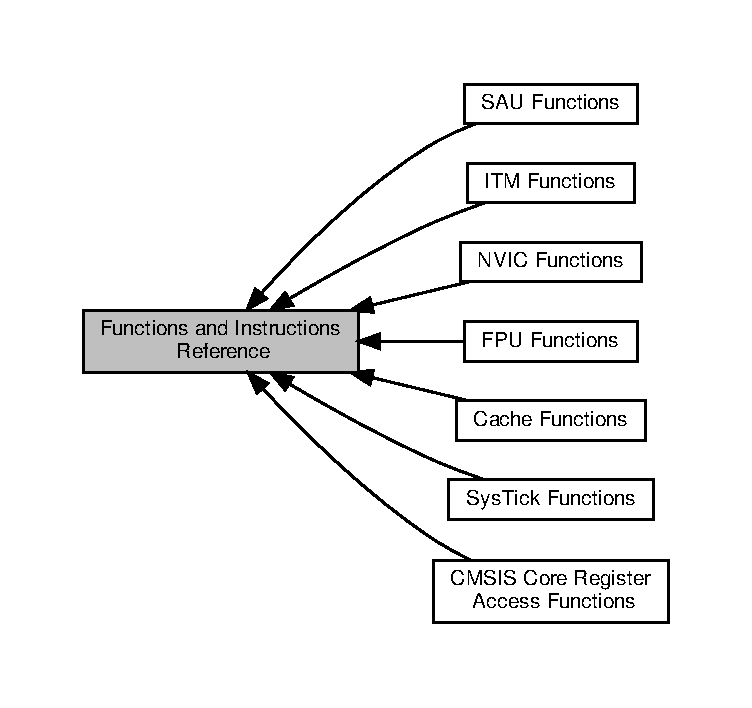
\includegraphics[width=350pt]{group___c_m_s_i_s___core___function_interface}
\end{center}
\end{figure}
\subsection*{Moduły}
\begin{DoxyCompactItemize}
\item 
\hyperlink{group___c_m_s_i_s___core___reg_acc_functions}{C\+M\+S\+I\+S Core Register Access Functions}
\item 
\hyperlink{group___c_m_s_i_s___core___n_v_i_c_functions}{N\+V\+I\+C Functions}
\begin{DoxyCompactList}\small\item\em Functions that manage interrupts and exceptions via the N\+V\+IC. \end{DoxyCompactList}\item 
\hyperlink{group___c_m_s_i_s___core___fpu_functions}{F\+P\+U Functions}
\begin{DoxyCompactList}\small\item\em Function that provides F\+PU type. \end{DoxyCompactList}\item 
\hyperlink{group___c_m_s_i_s___core___s_a_u_functions}{S\+A\+U Functions}
\begin{DoxyCompactList}\small\item\em Functions that configure the S\+AU. \end{DoxyCompactList}\item 
\hyperlink{group___c_m_s_i_s___core___sys_tick_functions}{Sys\+Tick Functions}
\begin{DoxyCompactList}\small\item\em Functions that configure the System. \end{DoxyCompactList}\item 
\hyperlink{group___c_m_s_i_s__core___debug_functions}{I\+T\+M Functions}
\begin{DoxyCompactList}\small\item\em Functions that access the I\+TM debug interface. \end{DoxyCompactList}\item 
\hyperlink{group___c_m_s_i_s___core___cache_functions}{Cache Functions}
\begin{DoxyCompactList}\small\item\em Functions that configure Instruction and Data cache. \end{DoxyCompactList}\end{DoxyCompactItemize}


\subsection{Opis szczegółowy}

\hypertarget{group___c_m_s_i_s___core___n_v_i_c_functions}{}\section{N\+V\+IC Functions}
\label{group___c_m_s_i_s___core___n_v_i_c_functions}\index{N\+V\+I\+C Functions@{N\+V\+I\+C Functions}}


Functions that manage interrupts and exceptions via the N\+V\+IC.  


Diagram współpracy dla N\+V\+IC Functions\+:\nopagebreak
\begin{figure}[H]
\begin{center}
\leavevmode
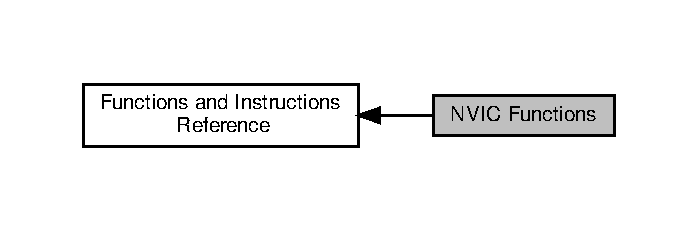
\includegraphics[width=335pt]{group___c_m_s_i_s___core___n_v_i_c_functions}
\end{center}
\end{figure}
\subsection*{Definicje}
\begin{DoxyCompactItemize}
\item 
\#define \hyperlink{group___c_m_s_i_s___core___n_v_i_c_functions_ga0e798d5aec68cdd8263db86a76df788f}{N\+V\+I\+C\+\_\+\+Set\+Priority\+Grouping}~\hyperlink{group___c_m_s_i_s___core___n_v_i_c_functions_gafc94dcbaee03e4746ade1f5bb9aaa56d}{\+\_\+\+\_\+\+N\+V\+I\+C\+\_\+\+Set\+Priority\+Grouping}
\item 
\#define \hyperlink{group___c_m_s_i_s___core___n_v_i_c_functions_ga4eeb9214f2264fc23c34ad5de2d3fa11}{N\+V\+I\+C\+\_\+\+Get\+Priority\+Grouping}~\hyperlink{group___c_m_s_i_s___core___n_v_i_c_functions_ga9b894af672df4373eb637f8288845c05}{\+\_\+\+\_\+\+N\+V\+I\+C\+\_\+\+Get\+Priority\+Grouping}
\item 
\#define \hyperlink{group___c_m_s_i_s___core___n_v_i_c_functions_ga57b3064413dbc7459d9646020fdd8bef}{N\+V\+I\+C\+\_\+\+Enable\+I\+RQ}~\hyperlink{group___c_m_s_i_s___core___n_v_i_c_functions_ga71227e1376cde11eda03fcb62f1b33ea}{\+\_\+\+\_\+\+N\+V\+I\+C\+\_\+\+Enable\+I\+RQ}
\item 
\#define \hyperlink{group___c_m_s_i_s___core___n_v_i_c_functions_ga857de13232ec65dd15087eaa15bc4a69}{N\+V\+I\+C\+\_\+\+Get\+Enable\+I\+RQ}~\hyperlink{group___c_m_s_i_s___core___n_v_i_c_functions_gaaeb5e7cc0eaad4e2817272e7bf742083}{\+\_\+\+\_\+\+N\+V\+I\+C\+\_\+\+Get\+Enable\+I\+RQ}
\item 
\#define \hyperlink{group___c_m_s_i_s___core___n_v_i_c_functions_ga73b4e251f59cab4e9a5e234aac02ae57}{N\+V\+I\+C\+\_\+\+Disable\+I\+RQ}~\hyperlink{group___c_m_s_i_s___core___n_v_i_c_functions_gae016e4c1986312044ee768806537d52f}{\+\_\+\+\_\+\+N\+V\+I\+C\+\_\+\+Disable\+I\+RQ}
\item 
\#define \hyperlink{group___c_m_s_i_s___core___n_v_i_c_functions_gac608957a239466e9e0cbc30aa64feb3b}{N\+V\+I\+C\+\_\+\+Get\+Pending\+I\+RQ}~\hyperlink{group___c_m_s_i_s___core___n_v_i_c_functions_ga5a92ca5fa801ad7adb92be7257ab9694}{\+\_\+\+\_\+\+N\+V\+I\+C\+\_\+\+Get\+Pending\+I\+RQ}
\item 
\#define \hyperlink{group___c_m_s_i_s___core___n_v_i_c_functions_ga2b47e2e52cf5c48a5c3348636434b3ac}{N\+V\+I\+C\+\_\+\+Set\+Pending\+I\+RQ}~\hyperlink{group___c_m_s_i_s___core___n_v_i_c_functions_gaabefdd4b790b9a7308929938c0c1e1ad}{\+\_\+\+\_\+\+N\+V\+I\+C\+\_\+\+Set\+Pending\+I\+RQ}
\item 
\#define \hyperlink{group___c_m_s_i_s___core___n_v_i_c_functions_ga590cf113000a079b1f0ea3dcd5b5316c}{N\+V\+I\+C\+\_\+\+Clear\+Pending\+I\+RQ}~\hyperlink{group___c_m_s_i_s___core___n_v_i_c_functions_ga562a86dbdf14827d0fee8fdafb04d191}{\+\_\+\+\_\+\+N\+V\+I\+C\+\_\+\+Clear\+Pending\+I\+RQ}
\item 
\#define \hyperlink{group___c_m_s_i_s___core___n_v_i_c_functions_ga58ad3f352f832235ab3b192ff4745320}{N\+V\+I\+C\+\_\+\+Get\+Active}~\hyperlink{group___c_m_s_i_s___core___n_v_i_c_functions_gaa2837003c28c45abf193fe5e8d27f593}{\+\_\+\+\_\+\+N\+V\+I\+C\+\_\+\+Get\+Active}
\item 
\#define \hyperlink{group___c_m_s_i_s___core___n_v_i_c_functions_gae0e9d0e2f7b6133828c71b57d4941c35}{N\+V\+I\+C\+\_\+\+Set\+Priority}~\hyperlink{group___c_m_s_i_s___core___n_v_i_c_functions_ga505338e23563a9c074910fb14e7d45fd}{\+\_\+\+\_\+\+N\+V\+I\+C\+\_\+\+Set\+Priority}
\item 
\#define \hyperlink{group___c_m_s_i_s___core___n_v_i_c_functions_gaf59b9d0a791d2157abb319753953eceb}{N\+V\+I\+C\+\_\+\+Get\+Priority}~\hyperlink{group___c_m_s_i_s___core___n_v_i_c_functions_gaeb9dc99c8e7700668813144261b0bc73}{\+\_\+\+\_\+\+N\+V\+I\+C\+\_\+\+Get\+Priority}
\item 
\#define \hyperlink{group___c_m_s_i_s___core___n_v_i_c_functions_ga6aa0367d3642575610476bf0366f0c48}{N\+V\+I\+C\+\_\+\+System\+Reset}~\hyperlink{group___c_m_s_i_s___core___n_v_i_c_functions_ga0d9aa2d30fa54b41eb780c16e35b676c}{\+\_\+\+\_\+\+N\+V\+I\+C\+\_\+\+System\+Reset}
\item 
\#define \hyperlink{group___c_m_s_i_s___core___n_v_i_c_functions_ga804af63bb4c4c317387897431814775d}{N\+V\+I\+C\+\_\+\+Set\+Vector}~\hyperlink{group___c_m_s_i_s___core___n_v_i_c_functions_ga0df355460bc1783d58f9d72ee4884208}{\+\_\+\+\_\+\+N\+V\+I\+C\+\_\+\+Set\+Vector}
\item 
\#define \hyperlink{group___c_m_s_i_s___core___n_v_i_c_functions_ga955eb1c33a3dcc62af11a8385e8c0fc8}{N\+V\+I\+C\+\_\+\+Get\+Vector}~\hyperlink{group___c_m_s_i_s___core___n_v_i_c_functions_ga44b665d2afb708121d9b10c76ff00ee5}{\+\_\+\+\_\+\+N\+V\+I\+C\+\_\+\+Get\+Vector}
\item 
\#define \hyperlink{group___c_m_s_i_s___core___n_v_i_c_functions_ga8045d905a5ca57437d8e6f71ffcb6df5}{N\+V\+I\+C\+\_\+\+U\+S\+E\+R\+\_\+\+I\+R\+Q\+\_\+\+O\+F\+F\+S\+ET}~16
\item 
\#define \hyperlink{group___c_m_s_i_s___core___n_v_i_c_functions_gabaa62910bf89acc186ae998c611e64ab}{F\+N\+C\+\_\+\+R\+E\+T\+U\+RN}~(0x\+F\+E\+F\+F\+F\+F\+F\+F\+U\+L)     /$\ast$ bit \mbox{[}0\mbox{]} ignored when processing a branch                             $\ast$/
\item 
\#define \hyperlink{group___c_m_s_i_s___core___n_v_i_c_functions_ga99e0c1c19f050880a8bd827a7f420bec}{E\+X\+C\+\_\+\+R\+E\+T\+U\+R\+N\+\_\+\+P\+R\+E\+F\+IX}~(0x\+F\+F000000\+U\+L)     /$\ast$ bits \mbox{[}31\+:24\mbox{]} set to indicate an E\+X\+C\+\_\+\+R\+E\+T\+U\+R\+N value                     $\ast$/
\item 
\#define \hyperlink{group___c_m_s_i_s___core___n_v_i_c_functions_ga88711355d0196b1ffeb18c33e2c95360}{E\+X\+C\+\_\+\+R\+E\+T\+U\+R\+N\+\_\+S}~(0x00000040\+U\+L)     /$\ast$ bit \mbox{[}6\mbox{]} stack used to push registers\+: 0=\+Non-\/secure 1=\+Secure          $\ast$/
\item 
\#define \hyperlink{group___c_m_s_i_s___core___n_v_i_c_functions_ga0a0f2c03b4aef2c02bdae044bda1324b}{E\+X\+C\+\_\+\+R\+E\+T\+U\+R\+N\+\_\+\+D\+C\+RS}~(0x00000020\+U\+L)     /$\ast$ bit \mbox{[}5\mbox{]} stacking rules for called registers\+: 0=skipped 1=saved       $\ast$/
\item 
\#define \hyperlink{group___c_m_s_i_s___core___n_v_i_c_functions_ga342b51c3eec59822bf206e24ef881a9e}{E\+X\+C\+\_\+\+R\+E\+T\+U\+R\+N\+\_\+\+F\+T\+Y\+PE}~(0x00000010\+U\+L)     /$\ast$ bit \mbox{[}4\mbox{]} allocate stack for floating-\/point context\+: 0=done 1=skipped  $\ast$/
\item 
\#define \hyperlink{group___c_m_s_i_s___core___n_v_i_c_functions_gabb65f847769a7807395b2739cc9702d0}{E\+X\+C\+\_\+\+R\+E\+T\+U\+R\+N\+\_\+\+M\+O\+DE}~(0x00000008\+U\+L)     /$\ast$ bit \mbox{[}3\mbox{]} processor mode for return\+: 0=\+Handler mode 1=\+Thread mode      $\ast$/
\item 
\#define \hyperlink{group___c_m_s_i_s___core___n_v_i_c_functions_ga686922b26c29eac540f53a6213627466}{E\+X\+C\+\_\+\+R\+E\+T\+U\+R\+N\+\_\+\+S\+P\+S\+EL}~(0x00000002\+U\+L)     /$\ast$ bit \mbox{[}1\mbox{]} stack pointer used to restore context\+: 0=\+M\+S\+P 1=\+P\+S\+P           $\ast$/
\item 
\#define \hyperlink{group___c_m_s_i_s___core___n_v_i_c_functions_gac939dbf69d3063c76a28516a4ae84db7}{E\+X\+C\+\_\+\+R\+E\+T\+U\+R\+N\+\_\+\+ES}~(0x00000001\+U\+L)     /$\ast$ bit \mbox{[}0\mbox{]} security state exception was taken to\+: 0=\+Non-\/secure 1=\+Secure $\ast$/
\item 
\#define \hyperlink{group___c_m_s_i_s___core___n_v_i_c_functions_ga7d1b21b2d863ccd9e23a3295b3173155}{E\+X\+C\+\_\+\+I\+N\+T\+E\+G\+R\+I\+T\+Y\+\_\+\+S\+I\+G\+N\+A\+T\+U\+RE}~(0x\+F\+E\+F\+A125\+B\+U\+L)     /$\ast$ Value for processors without floating-\/point extension                $\ast$/
\item 
\#define \hyperlink{group___c_m_s_i_s___core___n_v_i_c_functions_ga53c75b28823441c6153269f0ecbed878}{\+\_\+\+B\+I\+T\+\_\+\+S\+H\+I\+FT}(I\+R\+Qn)~(  ((((uint32\+\_\+t)(int32\+\_\+t)(I\+R\+Qn))         )      \&  0x03\+U\+L) $\ast$ 8\+U\+L)
\item 
\#define \hyperlink{group___c_m_s_i_s___core___n_v_i_c_functions_gaee4f7eb5d7e770ad51489dbceabb1755}{\+\_\+\+S\+H\+P\+\_\+\+I\+DX}(I\+R\+Qn)~( (((((uint32\+\_\+t)(int32\+\_\+t)(I\+R\+Qn)) \& 0x0\+F\+U\+L)-\/8\+U\+L) $>$$>$    2\+U\+L)      )
\item 
\#define \hyperlink{group___c_m_s_i_s___core___n_v_i_c_functions_ga370ec4b1751a6a889d849747df3763a9}{\+\_\+\+I\+P\+\_\+\+I\+DX}(I\+R\+Qn)~(   (((uint32\+\_\+t)(int32\+\_\+t)(I\+R\+Qn))                $>$$>$    2\+U\+L)      )
\item 
\#define \hyperlink{group___c_m_s_i_s___core___n_v_i_c_functions_ga6834dd8c9c59394f1b544b57665293a4}{\+\_\+\+\_\+\+N\+V\+I\+C\+\_\+\+Set\+Priority\+Grouping}(\hyperlink{main_8c_aa6aba27bc1a89db9e350b50bbf881f57}{X})~(void)(\hyperlink{main_8c_aa6aba27bc1a89db9e350b50bbf881f57}{X})
\item 
\#define \hyperlink{group___c_m_s_i_s___core___n_v_i_c_functions_gae1de06155d072758b3453edb07d12459}{\+\_\+\+\_\+\+N\+V\+I\+C\+\_\+\+Get\+Priority\+Grouping}()~(0\+U)
\begin{DoxyCompactList}\small\item\em Get Priority Grouping. \end{DoxyCompactList}\item 
\#define \hyperlink{group___c_m_s_i_s___core___n_v_i_c_functions_ga0e798d5aec68cdd8263db86a76df788f}{N\+V\+I\+C\+\_\+\+Set\+Priority\+Grouping}~\hyperlink{group___c_m_s_i_s___core___n_v_i_c_functions_gafc94dcbaee03e4746ade1f5bb9aaa56d}{\+\_\+\+\_\+\+N\+V\+I\+C\+\_\+\+Set\+Priority\+Grouping}
\item 
\#define \hyperlink{group___c_m_s_i_s___core___n_v_i_c_functions_ga4eeb9214f2264fc23c34ad5de2d3fa11}{N\+V\+I\+C\+\_\+\+Get\+Priority\+Grouping}~\hyperlink{group___c_m_s_i_s___core___n_v_i_c_functions_ga9b894af672df4373eb637f8288845c05}{\+\_\+\+\_\+\+N\+V\+I\+C\+\_\+\+Get\+Priority\+Grouping}
\item 
\#define \hyperlink{group___c_m_s_i_s___core___n_v_i_c_functions_ga57b3064413dbc7459d9646020fdd8bef}{N\+V\+I\+C\+\_\+\+Enable\+I\+RQ}~\hyperlink{group___c_m_s_i_s___core___n_v_i_c_functions_ga71227e1376cde11eda03fcb62f1b33ea}{\+\_\+\+\_\+\+N\+V\+I\+C\+\_\+\+Enable\+I\+RQ}
\item 
\#define \hyperlink{group___c_m_s_i_s___core___n_v_i_c_functions_ga857de13232ec65dd15087eaa15bc4a69}{N\+V\+I\+C\+\_\+\+Get\+Enable\+I\+RQ}~\hyperlink{group___c_m_s_i_s___core___n_v_i_c_functions_gaaeb5e7cc0eaad4e2817272e7bf742083}{\+\_\+\+\_\+\+N\+V\+I\+C\+\_\+\+Get\+Enable\+I\+RQ}
\item 
\#define \hyperlink{group___c_m_s_i_s___core___n_v_i_c_functions_ga73b4e251f59cab4e9a5e234aac02ae57}{N\+V\+I\+C\+\_\+\+Disable\+I\+RQ}~\hyperlink{group___c_m_s_i_s___core___n_v_i_c_functions_gae016e4c1986312044ee768806537d52f}{\+\_\+\+\_\+\+N\+V\+I\+C\+\_\+\+Disable\+I\+RQ}
\item 
\#define \hyperlink{group___c_m_s_i_s___core___n_v_i_c_functions_gac608957a239466e9e0cbc30aa64feb3b}{N\+V\+I\+C\+\_\+\+Get\+Pending\+I\+RQ}~\hyperlink{group___c_m_s_i_s___core___n_v_i_c_functions_ga5a92ca5fa801ad7adb92be7257ab9694}{\+\_\+\+\_\+\+N\+V\+I\+C\+\_\+\+Get\+Pending\+I\+RQ}
\item 
\#define \hyperlink{group___c_m_s_i_s___core___n_v_i_c_functions_ga2b47e2e52cf5c48a5c3348636434b3ac}{N\+V\+I\+C\+\_\+\+Set\+Pending\+I\+RQ}~\hyperlink{group___c_m_s_i_s___core___n_v_i_c_functions_gaabefdd4b790b9a7308929938c0c1e1ad}{\+\_\+\+\_\+\+N\+V\+I\+C\+\_\+\+Set\+Pending\+I\+RQ}
\item 
\#define \hyperlink{group___c_m_s_i_s___core___n_v_i_c_functions_ga590cf113000a079b1f0ea3dcd5b5316c}{N\+V\+I\+C\+\_\+\+Clear\+Pending\+I\+RQ}~\hyperlink{group___c_m_s_i_s___core___n_v_i_c_functions_ga562a86dbdf14827d0fee8fdafb04d191}{\+\_\+\+\_\+\+N\+V\+I\+C\+\_\+\+Clear\+Pending\+I\+RQ}
\item 
\#define \hyperlink{group___c_m_s_i_s___core___n_v_i_c_functions_ga58ad3f352f832235ab3b192ff4745320}{N\+V\+I\+C\+\_\+\+Get\+Active}~\hyperlink{group___c_m_s_i_s___core___n_v_i_c_functions_gaa2837003c28c45abf193fe5e8d27f593}{\+\_\+\+\_\+\+N\+V\+I\+C\+\_\+\+Get\+Active}
\item 
\#define \hyperlink{group___c_m_s_i_s___core___n_v_i_c_functions_gae0e9d0e2f7b6133828c71b57d4941c35}{N\+V\+I\+C\+\_\+\+Set\+Priority}~\hyperlink{group___c_m_s_i_s___core___n_v_i_c_functions_ga505338e23563a9c074910fb14e7d45fd}{\+\_\+\+\_\+\+N\+V\+I\+C\+\_\+\+Set\+Priority}
\item 
\#define \hyperlink{group___c_m_s_i_s___core___n_v_i_c_functions_gaf59b9d0a791d2157abb319753953eceb}{N\+V\+I\+C\+\_\+\+Get\+Priority}~\hyperlink{group___c_m_s_i_s___core___n_v_i_c_functions_gaeb9dc99c8e7700668813144261b0bc73}{\+\_\+\+\_\+\+N\+V\+I\+C\+\_\+\+Get\+Priority}
\item 
\#define \hyperlink{group___c_m_s_i_s___core___n_v_i_c_functions_ga6aa0367d3642575610476bf0366f0c48}{N\+V\+I\+C\+\_\+\+System\+Reset}~\hyperlink{group___c_m_s_i_s___core___n_v_i_c_functions_ga0d9aa2d30fa54b41eb780c16e35b676c}{\+\_\+\+\_\+\+N\+V\+I\+C\+\_\+\+System\+Reset}
\item 
\#define \hyperlink{group___c_m_s_i_s___core___n_v_i_c_functions_ga804af63bb4c4c317387897431814775d}{N\+V\+I\+C\+\_\+\+Set\+Vector}~\hyperlink{group___c_m_s_i_s___core___n_v_i_c_functions_ga0df355460bc1783d58f9d72ee4884208}{\+\_\+\+\_\+\+N\+V\+I\+C\+\_\+\+Set\+Vector}
\item 
\#define \hyperlink{group___c_m_s_i_s___core___n_v_i_c_functions_ga955eb1c33a3dcc62af11a8385e8c0fc8}{N\+V\+I\+C\+\_\+\+Get\+Vector}~\hyperlink{group___c_m_s_i_s___core___n_v_i_c_functions_ga44b665d2afb708121d9b10c76ff00ee5}{\+\_\+\+\_\+\+N\+V\+I\+C\+\_\+\+Get\+Vector}
\item 
\#define \hyperlink{group___c_m_s_i_s___core___n_v_i_c_functions_ga8045d905a5ca57437d8e6f71ffcb6df5}{N\+V\+I\+C\+\_\+\+U\+S\+E\+R\+\_\+\+I\+R\+Q\+\_\+\+O\+F\+F\+S\+ET}~16
\item 
\#define \hyperlink{group___c_m_s_i_s___core___n_v_i_c_functions_gabaa62910bf89acc186ae998c611e64ab}{F\+N\+C\+\_\+\+R\+E\+T\+U\+RN}~(0x\+F\+E\+F\+F\+F\+F\+F\+F\+U\+L)     /$\ast$ bit \mbox{[}0\mbox{]} ignored when processing a branch                             $\ast$/
\item 
\#define \hyperlink{group___c_m_s_i_s___core___n_v_i_c_functions_ga99e0c1c19f050880a8bd827a7f420bec}{E\+X\+C\+\_\+\+R\+E\+T\+U\+R\+N\+\_\+\+P\+R\+E\+F\+IX}~(0x\+F\+F000000\+U\+L)     /$\ast$ bits \mbox{[}31\+:24\mbox{]} set to indicate an E\+X\+C\+\_\+\+R\+E\+T\+U\+R\+N value                     $\ast$/
\item 
\#define \hyperlink{group___c_m_s_i_s___core___n_v_i_c_functions_ga88711355d0196b1ffeb18c33e2c95360}{E\+X\+C\+\_\+\+R\+E\+T\+U\+R\+N\+\_\+S}~(0x00000040\+U\+L)     /$\ast$ bit \mbox{[}6\mbox{]} stack used to push registers\+: 0=\+Non-\/secure 1=\+Secure          $\ast$/
\item 
\#define \hyperlink{group___c_m_s_i_s___core___n_v_i_c_functions_ga0a0f2c03b4aef2c02bdae044bda1324b}{E\+X\+C\+\_\+\+R\+E\+T\+U\+R\+N\+\_\+\+D\+C\+RS}~(0x00000020\+U\+L)     /$\ast$ bit \mbox{[}5\mbox{]} stacking rules for called registers\+: 0=skipped 1=saved       $\ast$/
\item 
\#define \hyperlink{group___c_m_s_i_s___core___n_v_i_c_functions_ga342b51c3eec59822bf206e24ef881a9e}{E\+X\+C\+\_\+\+R\+E\+T\+U\+R\+N\+\_\+\+F\+T\+Y\+PE}~(0x00000010\+U\+L)     /$\ast$ bit \mbox{[}4\mbox{]} allocate stack for floating-\/point context\+: 0=done 1=skipped  $\ast$/
\item 
\#define \hyperlink{group___c_m_s_i_s___core___n_v_i_c_functions_gabb65f847769a7807395b2739cc9702d0}{E\+X\+C\+\_\+\+R\+E\+T\+U\+R\+N\+\_\+\+M\+O\+DE}~(0x00000008\+U\+L)     /$\ast$ bit \mbox{[}3\mbox{]} processor mode for return\+: 0=\+Handler mode 1=\+Thread mode      $\ast$/
\item 
\#define \hyperlink{group___c_m_s_i_s___core___n_v_i_c_functions_ga686922b26c29eac540f53a6213627466}{E\+X\+C\+\_\+\+R\+E\+T\+U\+R\+N\+\_\+\+S\+P\+S\+EL}~(0x00000002\+U\+L)     /$\ast$ bit \mbox{[}1\mbox{]} stack pointer used to restore context\+: 0=\+M\+S\+P 1=\+P\+S\+P           $\ast$/
\item 
\#define \hyperlink{group___c_m_s_i_s___core___n_v_i_c_functions_gac939dbf69d3063c76a28516a4ae84db7}{E\+X\+C\+\_\+\+R\+E\+T\+U\+R\+N\+\_\+\+ES}~(0x00000001\+U\+L)     /$\ast$ bit \mbox{[}0\mbox{]} security state exception was taken to\+: 0=\+Non-\/secure 1=\+Secure $\ast$/
\item 
\#define \hyperlink{group___c_m_s_i_s___core___n_v_i_c_functions_ga7d1b21b2d863ccd9e23a3295b3173155}{E\+X\+C\+\_\+\+I\+N\+T\+E\+G\+R\+I\+T\+Y\+\_\+\+S\+I\+G\+N\+A\+T\+U\+RE}~(0x\+F\+E\+F\+A125\+B\+U\+L)     /$\ast$ Value for processors without floating-\/point extension                $\ast$/
\item 
\#define \hyperlink{group___c_m_s_i_s___core___n_v_i_c_functions_ga0e798d5aec68cdd8263db86a76df788f}{N\+V\+I\+C\+\_\+\+Set\+Priority\+Grouping}~\hyperlink{group___c_m_s_i_s___core___n_v_i_c_functions_gafc94dcbaee03e4746ade1f5bb9aaa56d}{\+\_\+\+\_\+\+N\+V\+I\+C\+\_\+\+Set\+Priority\+Grouping}
\item 
\#define \hyperlink{group___c_m_s_i_s___core___n_v_i_c_functions_ga4eeb9214f2264fc23c34ad5de2d3fa11}{N\+V\+I\+C\+\_\+\+Get\+Priority\+Grouping}~\hyperlink{group___c_m_s_i_s___core___n_v_i_c_functions_ga9b894af672df4373eb637f8288845c05}{\+\_\+\+\_\+\+N\+V\+I\+C\+\_\+\+Get\+Priority\+Grouping}
\item 
\#define \hyperlink{group___c_m_s_i_s___core___n_v_i_c_functions_ga57b3064413dbc7459d9646020fdd8bef}{N\+V\+I\+C\+\_\+\+Enable\+I\+RQ}~\hyperlink{group___c_m_s_i_s___core___n_v_i_c_functions_ga71227e1376cde11eda03fcb62f1b33ea}{\+\_\+\+\_\+\+N\+V\+I\+C\+\_\+\+Enable\+I\+RQ}
\item 
\#define \hyperlink{group___c_m_s_i_s___core___n_v_i_c_functions_ga857de13232ec65dd15087eaa15bc4a69}{N\+V\+I\+C\+\_\+\+Get\+Enable\+I\+RQ}~\hyperlink{group___c_m_s_i_s___core___n_v_i_c_functions_gaaeb5e7cc0eaad4e2817272e7bf742083}{\+\_\+\+\_\+\+N\+V\+I\+C\+\_\+\+Get\+Enable\+I\+RQ}
\item 
\#define \hyperlink{group___c_m_s_i_s___core___n_v_i_c_functions_ga73b4e251f59cab4e9a5e234aac02ae57}{N\+V\+I\+C\+\_\+\+Disable\+I\+RQ}~\hyperlink{group___c_m_s_i_s___core___n_v_i_c_functions_gae016e4c1986312044ee768806537d52f}{\+\_\+\+\_\+\+N\+V\+I\+C\+\_\+\+Disable\+I\+RQ}
\item 
\#define \hyperlink{group___c_m_s_i_s___core___n_v_i_c_functions_gac608957a239466e9e0cbc30aa64feb3b}{N\+V\+I\+C\+\_\+\+Get\+Pending\+I\+RQ}~\hyperlink{group___c_m_s_i_s___core___n_v_i_c_functions_ga5a92ca5fa801ad7adb92be7257ab9694}{\+\_\+\+\_\+\+N\+V\+I\+C\+\_\+\+Get\+Pending\+I\+RQ}
\item 
\#define \hyperlink{group___c_m_s_i_s___core___n_v_i_c_functions_ga2b47e2e52cf5c48a5c3348636434b3ac}{N\+V\+I\+C\+\_\+\+Set\+Pending\+I\+RQ}~\hyperlink{group___c_m_s_i_s___core___n_v_i_c_functions_gaabefdd4b790b9a7308929938c0c1e1ad}{\+\_\+\+\_\+\+N\+V\+I\+C\+\_\+\+Set\+Pending\+I\+RQ}
\item 
\#define \hyperlink{group___c_m_s_i_s___core___n_v_i_c_functions_ga590cf113000a079b1f0ea3dcd5b5316c}{N\+V\+I\+C\+\_\+\+Clear\+Pending\+I\+RQ}~\hyperlink{group___c_m_s_i_s___core___n_v_i_c_functions_ga562a86dbdf14827d0fee8fdafb04d191}{\+\_\+\+\_\+\+N\+V\+I\+C\+\_\+\+Clear\+Pending\+I\+RQ}
\item 
\#define \hyperlink{group___c_m_s_i_s___core___n_v_i_c_functions_gae0e9d0e2f7b6133828c71b57d4941c35}{N\+V\+I\+C\+\_\+\+Set\+Priority}~\hyperlink{group___c_m_s_i_s___core___n_v_i_c_functions_ga505338e23563a9c074910fb14e7d45fd}{\+\_\+\+\_\+\+N\+V\+I\+C\+\_\+\+Set\+Priority}
\item 
\#define \hyperlink{group___c_m_s_i_s___core___n_v_i_c_functions_gaf59b9d0a791d2157abb319753953eceb}{N\+V\+I\+C\+\_\+\+Get\+Priority}~\hyperlink{group___c_m_s_i_s___core___n_v_i_c_functions_gaeb9dc99c8e7700668813144261b0bc73}{\+\_\+\+\_\+\+N\+V\+I\+C\+\_\+\+Get\+Priority}
\item 
\#define \hyperlink{group___c_m_s_i_s___core___n_v_i_c_functions_ga6aa0367d3642575610476bf0366f0c48}{N\+V\+I\+C\+\_\+\+System\+Reset}~\hyperlink{group___c_m_s_i_s___core___n_v_i_c_functions_ga0d9aa2d30fa54b41eb780c16e35b676c}{\+\_\+\+\_\+\+N\+V\+I\+C\+\_\+\+System\+Reset}
\item 
\#define \hyperlink{group___c_m_s_i_s___core___n_v_i_c_functions_ga804af63bb4c4c317387897431814775d}{N\+V\+I\+C\+\_\+\+Set\+Vector}~\hyperlink{group___c_m_s_i_s___core___n_v_i_c_functions_ga0df355460bc1783d58f9d72ee4884208}{\+\_\+\+\_\+\+N\+V\+I\+C\+\_\+\+Set\+Vector}
\item 
\#define \hyperlink{group___c_m_s_i_s___core___n_v_i_c_functions_ga955eb1c33a3dcc62af11a8385e8c0fc8}{N\+V\+I\+C\+\_\+\+Get\+Vector}~\hyperlink{group___c_m_s_i_s___core___n_v_i_c_functions_ga44b665d2afb708121d9b10c76ff00ee5}{\+\_\+\+\_\+\+N\+V\+I\+C\+\_\+\+Get\+Vector}
\item 
\#define \hyperlink{group___c_m_s_i_s___core___n_v_i_c_functions_ga8045d905a5ca57437d8e6f71ffcb6df5}{N\+V\+I\+C\+\_\+\+U\+S\+E\+R\+\_\+\+I\+R\+Q\+\_\+\+O\+F\+F\+S\+ET}~16
\item 
\#define \hyperlink{group___c_m_s_i_s___core___n_v_i_c_functions_gaa6fa2b10f756385433e08522d9e4632f}{E\+X\+C\+\_\+\+R\+E\+T\+U\+R\+N\+\_\+\+H\+A\+N\+D\+L\+ER}~(0x\+F\+F\+F\+F\+F\+F\+F1\+U\+L)     /$\ast$ return to Handler mode, uses M\+S\+P after return                               $\ast$/
\item 
\#define \hyperlink{group___c_m_s_i_s___core___n_v_i_c_functions_gaea4703101b5e679f695e231f7ee72331}{E\+X\+C\+\_\+\+R\+E\+T\+U\+R\+N\+\_\+\+T\+H\+R\+E\+A\+D\+\_\+\+M\+SP}~(0x\+F\+F\+F\+F\+F\+F\+F9\+U\+L)     /$\ast$ return to Thread mode, uses M\+S\+P after return                                $\ast$/
\item 
\#define \hyperlink{group___c_m_s_i_s___core___n_v_i_c_functions_ga9998daf0fbdf31dbc8f81cd604b58175}{E\+X\+C\+\_\+\+R\+E\+T\+U\+R\+N\+\_\+\+T\+H\+R\+E\+A\+D\+\_\+\+P\+SP}~(0x\+F\+F\+F\+F\+F\+F\+F\+D\+U\+L)     /$\ast$ return to Thread mode, uses P\+S\+P after return                                $\ast$/
\item 
\#define \hyperlink{group___c_m_s_i_s___core___n_v_i_c_functions_ga53c75b28823441c6153269f0ecbed878}{\+\_\+\+B\+I\+T\+\_\+\+S\+H\+I\+FT}(I\+R\+Qn)~(  ((((uint32\+\_\+t)(int32\+\_\+t)(I\+R\+Qn))         )      \&  0x03\+U\+L) $\ast$ 8\+U\+L)
\item 
\#define \hyperlink{group___c_m_s_i_s___core___n_v_i_c_functions_gaee4f7eb5d7e770ad51489dbceabb1755}{\+\_\+\+S\+H\+P\+\_\+\+I\+DX}(I\+R\+Qn)~( (((((uint32\+\_\+t)(int32\+\_\+t)(I\+R\+Qn)) \& 0x0\+F\+U\+L)-\/8\+U\+L) $>$$>$    2\+U\+L)      )
\item 
\#define \hyperlink{group___c_m_s_i_s___core___n_v_i_c_functions_ga370ec4b1751a6a889d849747df3763a9}{\+\_\+\+I\+P\+\_\+\+I\+DX}(I\+R\+Qn)~(   (((uint32\+\_\+t)(int32\+\_\+t)(I\+R\+Qn))                $>$$>$    2\+U\+L)      )
\item 
\#define \hyperlink{group___c_m_s_i_s___core___n_v_i_c_functions_ga6834dd8c9c59394f1b544b57665293a4}{\+\_\+\+\_\+\+N\+V\+I\+C\+\_\+\+Set\+Priority\+Grouping}(\hyperlink{main_8c_aa6aba27bc1a89db9e350b50bbf881f57}{X})~(void)(\hyperlink{main_8c_aa6aba27bc1a89db9e350b50bbf881f57}{X})
\item 
\#define \hyperlink{group___c_m_s_i_s___core___n_v_i_c_functions_gab2072fe50f6d7cd208f6768919f59fae}{\+\_\+\+\_\+\+N\+V\+I\+C\+\_\+\+Get\+Priority\+Grouping}()~(0\+U)
\item 
\#define \hyperlink{group___c_m_s_i_s___core___n_v_i_c_functions_ga0e798d5aec68cdd8263db86a76df788f}{N\+V\+I\+C\+\_\+\+Set\+Priority\+Grouping}~\hyperlink{group___c_m_s_i_s___core___n_v_i_c_functions_gafc94dcbaee03e4746ade1f5bb9aaa56d}{\+\_\+\+\_\+\+N\+V\+I\+C\+\_\+\+Set\+Priority\+Grouping}
\item 
\#define \hyperlink{group___c_m_s_i_s___core___n_v_i_c_functions_ga4eeb9214f2264fc23c34ad5de2d3fa11}{N\+V\+I\+C\+\_\+\+Get\+Priority\+Grouping}~\hyperlink{group___c_m_s_i_s___core___n_v_i_c_functions_ga9b894af672df4373eb637f8288845c05}{\+\_\+\+\_\+\+N\+V\+I\+C\+\_\+\+Get\+Priority\+Grouping}
\item 
\#define \hyperlink{group___c_m_s_i_s___core___n_v_i_c_functions_ga57b3064413dbc7459d9646020fdd8bef}{N\+V\+I\+C\+\_\+\+Enable\+I\+RQ}~\hyperlink{group___c_m_s_i_s___core___n_v_i_c_functions_ga71227e1376cde11eda03fcb62f1b33ea}{\+\_\+\+\_\+\+N\+V\+I\+C\+\_\+\+Enable\+I\+RQ}
\item 
\#define \hyperlink{group___c_m_s_i_s___core___n_v_i_c_functions_ga857de13232ec65dd15087eaa15bc4a69}{N\+V\+I\+C\+\_\+\+Get\+Enable\+I\+RQ}~\hyperlink{group___c_m_s_i_s___core___n_v_i_c_functions_gaaeb5e7cc0eaad4e2817272e7bf742083}{\+\_\+\+\_\+\+N\+V\+I\+C\+\_\+\+Get\+Enable\+I\+RQ}
\item 
\#define \hyperlink{group___c_m_s_i_s___core___n_v_i_c_functions_ga73b4e251f59cab4e9a5e234aac02ae57}{N\+V\+I\+C\+\_\+\+Disable\+I\+RQ}~\hyperlink{group___c_m_s_i_s___core___n_v_i_c_functions_gae016e4c1986312044ee768806537d52f}{\+\_\+\+\_\+\+N\+V\+I\+C\+\_\+\+Disable\+I\+RQ}
\item 
\#define \hyperlink{group___c_m_s_i_s___core___n_v_i_c_functions_gac608957a239466e9e0cbc30aa64feb3b}{N\+V\+I\+C\+\_\+\+Get\+Pending\+I\+RQ}~\hyperlink{group___c_m_s_i_s___core___n_v_i_c_functions_ga5a92ca5fa801ad7adb92be7257ab9694}{\+\_\+\+\_\+\+N\+V\+I\+C\+\_\+\+Get\+Pending\+I\+RQ}
\item 
\#define \hyperlink{group___c_m_s_i_s___core___n_v_i_c_functions_ga2b47e2e52cf5c48a5c3348636434b3ac}{N\+V\+I\+C\+\_\+\+Set\+Pending\+I\+RQ}~\hyperlink{group___c_m_s_i_s___core___n_v_i_c_functions_gaabefdd4b790b9a7308929938c0c1e1ad}{\+\_\+\+\_\+\+N\+V\+I\+C\+\_\+\+Set\+Pending\+I\+RQ}
\item 
\#define \hyperlink{group___c_m_s_i_s___core___n_v_i_c_functions_ga590cf113000a079b1f0ea3dcd5b5316c}{N\+V\+I\+C\+\_\+\+Clear\+Pending\+I\+RQ}~\hyperlink{group___c_m_s_i_s___core___n_v_i_c_functions_ga562a86dbdf14827d0fee8fdafb04d191}{\+\_\+\+\_\+\+N\+V\+I\+C\+\_\+\+Clear\+Pending\+I\+RQ}
\item 
\#define \hyperlink{group___c_m_s_i_s___core___n_v_i_c_functions_gae0e9d0e2f7b6133828c71b57d4941c35}{N\+V\+I\+C\+\_\+\+Set\+Priority}~\hyperlink{group___c_m_s_i_s___core___n_v_i_c_functions_ga505338e23563a9c074910fb14e7d45fd}{\+\_\+\+\_\+\+N\+V\+I\+C\+\_\+\+Set\+Priority}
\item 
\#define \hyperlink{group___c_m_s_i_s___core___n_v_i_c_functions_gaf59b9d0a791d2157abb319753953eceb}{N\+V\+I\+C\+\_\+\+Get\+Priority}~\hyperlink{group___c_m_s_i_s___core___n_v_i_c_functions_gaeb9dc99c8e7700668813144261b0bc73}{\+\_\+\+\_\+\+N\+V\+I\+C\+\_\+\+Get\+Priority}
\item 
\#define \hyperlink{group___c_m_s_i_s___core___n_v_i_c_functions_ga6aa0367d3642575610476bf0366f0c48}{N\+V\+I\+C\+\_\+\+System\+Reset}~\hyperlink{group___c_m_s_i_s___core___n_v_i_c_functions_ga0d9aa2d30fa54b41eb780c16e35b676c}{\+\_\+\+\_\+\+N\+V\+I\+C\+\_\+\+System\+Reset}
\item 
\#define \hyperlink{group___c_m_s_i_s___core___n_v_i_c_functions_ga804af63bb4c4c317387897431814775d}{N\+V\+I\+C\+\_\+\+Set\+Vector}~\hyperlink{group___c_m_s_i_s___core___n_v_i_c_functions_ga0df355460bc1783d58f9d72ee4884208}{\+\_\+\+\_\+\+N\+V\+I\+C\+\_\+\+Set\+Vector}
\item 
\#define \hyperlink{group___c_m_s_i_s___core___n_v_i_c_functions_ga955eb1c33a3dcc62af11a8385e8c0fc8}{N\+V\+I\+C\+\_\+\+Get\+Vector}~\hyperlink{group___c_m_s_i_s___core___n_v_i_c_functions_ga44b665d2afb708121d9b10c76ff00ee5}{\+\_\+\+\_\+\+N\+V\+I\+C\+\_\+\+Get\+Vector}
\item 
\#define \hyperlink{group___c_m_s_i_s___core___n_v_i_c_functions_ga8045d905a5ca57437d8e6f71ffcb6df5}{N\+V\+I\+C\+\_\+\+U\+S\+E\+R\+\_\+\+I\+R\+Q\+\_\+\+O\+F\+F\+S\+ET}~16
\item 
\#define \hyperlink{group___c_m_s_i_s___core___n_v_i_c_functions_gaa6fa2b10f756385433e08522d9e4632f}{E\+X\+C\+\_\+\+R\+E\+T\+U\+R\+N\+\_\+\+H\+A\+N\+D\+L\+ER}~(0x\+F\+F\+F\+F\+F\+F\+F1\+U\+L)     /$\ast$ return to Handler mode, uses M\+S\+P after return                               $\ast$/
\item 
\#define \hyperlink{group___c_m_s_i_s___core___n_v_i_c_functions_gaea4703101b5e679f695e231f7ee72331}{E\+X\+C\+\_\+\+R\+E\+T\+U\+R\+N\+\_\+\+T\+H\+R\+E\+A\+D\+\_\+\+M\+SP}~(0x\+F\+F\+F\+F\+F\+F\+F9\+U\+L)     /$\ast$ return to Thread mode, uses M\+S\+P after return                                $\ast$/
\item 
\#define \hyperlink{group___c_m_s_i_s___core___n_v_i_c_functions_ga9998daf0fbdf31dbc8f81cd604b58175}{E\+X\+C\+\_\+\+R\+E\+T\+U\+R\+N\+\_\+\+T\+H\+R\+E\+A\+D\+\_\+\+P\+SP}~(0x\+F\+F\+F\+F\+F\+F\+F\+D\+U\+L)     /$\ast$ return to Thread mode, uses P\+S\+P after return                                $\ast$/
\item 
\#define \hyperlink{group___c_m_s_i_s___core___n_v_i_c_functions_ga53c75b28823441c6153269f0ecbed878}{\+\_\+\+B\+I\+T\+\_\+\+S\+H\+I\+FT}(I\+R\+Qn)~(  ((((uint32\+\_\+t)(int32\+\_\+t)(I\+R\+Qn))         )      \&  0x03\+U\+L) $\ast$ 8\+U\+L)
\item 
\#define \hyperlink{group___c_m_s_i_s___core___n_v_i_c_functions_gaee4f7eb5d7e770ad51489dbceabb1755}{\+\_\+\+S\+H\+P\+\_\+\+I\+DX}(I\+R\+Qn)~( (((((uint32\+\_\+t)(int32\+\_\+t)(I\+R\+Qn)) \& 0x0\+F\+U\+L)-\/8\+U\+L) $>$$>$    2\+U\+L)      )
\item 
\#define \hyperlink{group___c_m_s_i_s___core___n_v_i_c_functions_ga370ec4b1751a6a889d849747df3763a9}{\+\_\+\+I\+P\+\_\+\+I\+DX}(I\+R\+Qn)~(   (((uint32\+\_\+t)(int32\+\_\+t)(I\+R\+Qn))                $>$$>$    2\+U\+L)      )
\item 
\#define \hyperlink{group___c_m_s_i_s___core___n_v_i_c_functions_ga6834dd8c9c59394f1b544b57665293a4}{\+\_\+\+\_\+\+N\+V\+I\+C\+\_\+\+Set\+Priority\+Grouping}(\hyperlink{main_8c_aa6aba27bc1a89db9e350b50bbf881f57}{X})~(void)(\hyperlink{main_8c_aa6aba27bc1a89db9e350b50bbf881f57}{X})
\item 
\#define \hyperlink{group___c_m_s_i_s___core___n_v_i_c_functions_gab2072fe50f6d7cd208f6768919f59fae}{\+\_\+\+\_\+\+N\+V\+I\+C\+\_\+\+Get\+Priority\+Grouping}()~(0\+U)
\item 
\#define \hyperlink{group___c_m_s_i_s___core___n_v_i_c_functions_ga0e798d5aec68cdd8263db86a76df788f}{N\+V\+I\+C\+\_\+\+Set\+Priority\+Grouping}~\hyperlink{group___c_m_s_i_s___core___n_v_i_c_functions_gafc94dcbaee03e4746ade1f5bb9aaa56d}{\+\_\+\+\_\+\+N\+V\+I\+C\+\_\+\+Set\+Priority\+Grouping}
\item 
\#define \hyperlink{group___c_m_s_i_s___core___n_v_i_c_functions_ga4eeb9214f2264fc23c34ad5de2d3fa11}{N\+V\+I\+C\+\_\+\+Get\+Priority\+Grouping}~\hyperlink{group___c_m_s_i_s___core___n_v_i_c_functions_ga9b894af672df4373eb637f8288845c05}{\+\_\+\+\_\+\+N\+V\+I\+C\+\_\+\+Get\+Priority\+Grouping}
\item 
\#define \hyperlink{group___c_m_s_i_s___core___n_v_i_c_functions_ga57b3064413dbc7459d9646020fdd8bef}{N\+V\+I\+C\+\_\+\+Enable\+I\+RQ}~\hyperlink{group___c_m_s_i_s___core___n_v_i_c_functions_ga71227e1376cde11eda03fcb62f1b33ea}{\+\_\+\+\_\+\+N\+V\+I\+C\+\_\+\+Enable\+I\+RQ}
\item 
\#define \hyperlink{group___c_m_s_i_s___core___n_v_i_c_functions_ga857de13232ec65dd15087eaa15bc4a69}{N\+V\+I\+C\+\_\+\+Get\+Enable\+I\+RQ}~\hyperlink{group___c_m_s_i_s___core___n_v_i_c_functions_gaaeb5e7cc0eaad4e2817272e7bf742083}{\+\_\+\+\_\+\+N\+V\+I\+C\+\_\+\+Get\+Enable\+I\+RQ}
\item 
\#define \hyperlink{group___c_m_s_i_s___core___n_v_i_c_functions_ga73b4e251f59cab4e9a5e234aac02ae57}{N\+V\+I\+C\+\_\+\+Disable\+I\+RQ}~\hyperlink{group___c_m_s_i_s___core___n_v_i_c_functions_gae016e4c1986312044ee768806537d52f}{\+\_\+\+\_\+\+N\+V\+I\+C\+\_\+\+Disable\+I\+RQ}
\item 
\#define \hyperlink{group___c_m_s_i_s___core___n_v_i_c_functions_gac608957a239466e9e0cbc30aa64feb3b}{N\+V\+I\+C\+\_\+\+Get\+Pending\+I\+RQ}~\hyperlink{group___c_m_s_i_s___core___n_v_i_c_functions_ga5a92ca5fa801ad7adb92be7257ab9694}{\+\_\+\+\_\+\+N\+V\+I\+C\+\_\+\+Get\+Pending\+I\+RQ}
\item 
\#define \hyperlink{group___c_m_s_i_s___core___n_v_i_c_functions_ga2b47e2e52cf5c48a5c3348636434b3ac}{N\+V\+I\+C\+\_\+\+Set\+Pending\+I\+RQ}~\hyperlink{group___c_m_s_i_s___core___n_v_i_c_functions_gaabefdd4b790b9a7308929938c0c1e1ad}{\+\_\+\+\_\+\+N\+V\+I\+C\+\_\+\+Set\+Pending\+I\+RQ}
\item 
\#define \hyperlink{group___c_m_s_i_s___core___n_v_i_c_functions_ga590cf113000a079b1f0ea3dcd5b5316c}{N\+V\+I\+C\+\_\+\+Clear\+Pending\+I\+RQ}~\hyperlink{group___c_m_s_i_s___core___n_v_i_c_functions_ga562a86dbdf14827d0fee8fdafb04d191}{\+\_\+\+\_\+\+N\+V\+I\+C\+\_\+\+Clear\+Pending\+I\+RQ}
\item 
\#define \hyperlink{group___c_m_s_i_s___core___n_v_i_c_functions_gae0e9d0e2f7b6133828c71b57d4941c35}{N\+V\+I\+C\+\_\+\+Set\+Priority}~\hyperlink{group___c_m_s_i_s___core___n_v_i_c_functions_ga505338e23563a9c074910fb14e7d45fd}{\+\_\+\+\_\+\+N\+V\+I\+C\+\_\+\+Set\+Priority}
\item 
\#define \hyperlink{group___c_m_s_i_s___core___n_v_i_c_functions_gaf59b9d0a791d2157abb319753953eceb}{N\+V\+I\+C\+\_\+\+Get\+Priority}~\hyperlink{group___c_m_s_i_s___core___n_v_i_c_functions_gaeb9dc99c8e7700668813144261b0bc73}{\+\_\+\+\_\+\+N\+V\+I\+C\+\_\+\+Get\+Priority}
\item 
\#define \hyperlink{group___c_m_s_i_s___core___n_v_i_c_functions_ga6aa0367d3642575610476bf0366f0c48}{N\+V\+I\+C\+\_\+\+System\+Reset}~\hyperlink{group___c_m_s_i_s___core___n_v_i_c_functions_ga0d9aa2d30fa54b41eb780c16e35b676c}{\+\_\+\+\_\+\+N\+V\+I\+C\+\_\+\+System\+Reset}
\item 
\#define \hyperlink{group___c_m_s_i_s___core___n_v_i_c_functions_ga804af63bb4c4c317387897431814775d}{N\+V\+I\+C\+\_\+\+Set\+Vector}~\hyperlink{group___c_m_s_i_s___core___n_v_i_c_functions_ga0df355460bc1783d58f9d72ee4884208}{\+\_\+\+\_\+\+N\+V\+I\+C\+\_\+\+Set\+Vector}
\item 
\#define \hyperlink{group___c_m_s_i_s___core___n_v_i_c_functions_ga955eb1c33a3dcc62af11a8385e8c0fc8}{N\+V\+I\+C\+\_\+\+Get\+Vector}~\hyperlink{group___c_m_s_i_s___core___n_v_i_c_functions_ga44b665d2afb708121d9b10c76ff00ee5}{\+\_\+\+\_\+\+N\+V\+I\+C\+\_\+\+Get\+Vector}
\item 
\#define \hyperlink{group___c_m_s_i_s___core___n_v_i_c_functions_ga8045d905a5ca57437d8e6f71ffcb6df5}{N\+V\+I\+C\+\_\+\+U\+S\+E\+R\+\_\+\+I\+R\+Q\+\_\+\+O\+F\+F\+S\+ET}~16
\item 
\#define \hyperlink{group___c_m_s_i_s___core___n_v_i_c_functions_gaa6fa2b10f756385433e08522d9e4632f}{E\+X\+C\+\_\+\+R\+E\+T\+U\+R\+N\+\_\+\+H\+A\+N\+D\+L\+ER}~(0x\+F\+F\+F\+F\+F\+F\+F1\+U\+L)     /$\ast$ return to Handler mode, uses M\+S\+P after return                               $\ast$/
\item 
\#define \hyperlink{group___c_m_s_i_s___core___n_v_i_c_functions_gaea4703101b5e679f695e231f7ee72331}{E\+X\+C\+\_\+\+R\+E\+T\+U\+R\+N\+\_\+\+T\+H\+R\+E\+A\+D\+\_\+\+M\+SP}~(0x\+F\+F\+F\+F\+F\+F\+F9\+U\+L)     /$\ast$ return to Thread mode, uses M\+S\+P after return                                $\ast$/
\item 
\#define \hyperlink{group___c_m_s_i_s___core___n_v_i_c_functions_ga9998daf0fbdf31dbc8f81cd604b58175}{E\+X\+C\+\_\+\+R\+E\+T\+U\+R\+N\+\_\+\+T\+H\+R\+E\+A\+D\+\_\+\+P\+SP}~(0x\+F\+F\+F\+F\+F\+F\+F\+D\+U\+L)     /$\ast$ return to Thread mode, uses P\+S\+P after return                                $\ast$/
\item 
\#define \hyperlink{group___c_m_s_i_s___core___n_v_i_c_functions_ga53c75b28823441c6153269f0ecbed878}{\+\_\+\+B\+I\+T\+\_\+\+S\+H\+I\+FT}(I\+R\+Qn)~(  ((((uint32\+\_\+t)(int32\+\_\+t)(I\+R\+Qn))         )      \&  0x03\+U\+L) $\ast$ 8\+U\+L)
\item 
\#define \hyperlink{group___c_m_s_i_s___core___n_v_i_c_functions_gaee4f7eb5d7e770ad51489dbceabb1755}{\+\_\+\+S\+H\+P\+\_\+\+I\+DX}(I\+R\+Qn)~( (((((uint32\+\_\+t)(int32\+\_\+t)(I\+R\+Qn)) \& 0x0\+F\+U\+L)-\/8\+U\+L) $>$$>$    2\+U\+L)      )
\item 
\#define \hyperlink{group___c_m_s_i_s___core___n_v_i_c_functions_ga370ec4b1751a6a889d849747df3763a9}{\+\_\+\+I\+P\+\_\+\+I\+DX}(I\+R\+Qn)~(   (((uint32\+\_\+t)(int32\+\_\+t)(I\+R\+Qn))                $>$$>$    2\+U\+L)      )
\item 
\#define \hyperlink{group___c_m_s_i_s___core___n_v_i_c_functions_ga6834dd8c9c59394f1b544b57665293a4}{\+\_\+\+\_\+\+N\+V\+I\+C\+\_\+\+Set\+Priority\+Grouping}(\hyperlink{main_8c_aa6aba27bc1a89db9e350b50bbf881f57}{X})~(void)(\hyperlink{main_8c_aa6aba27bc1a89db9e350b50bbf881f57}{X})
\item 
\#define \hyperlink{group___c_m_s_i_s___core___n_v_i_c_functions_gab2072fe50f6d7cd208f6768919f59fae}{\+\_\+\+\_\+\+N\+V\+I\+C\+\_\+\+Get\+Priority\+Grouping}()~(0\+U)
\item 
\#define \hyperlink{group___c_m_s_i_s___core___n_v_i_c_functions_ga57b3064413dbc7459d9646020fdd8bef}{N\+V\+I\+C\+\_\+\+Enable\+I\+RQ}~\hyperlink{group___c_m_s_i_s___core___n_v_i_c_functions_ga71227e1376cde11eda03fcb62f1b33ea}{\+\_\+\+\_\+\+N\+V\+I\+C\+\_\+\+Enable\+I\+RQ}
\item 
\#define \hyperlink{group___c_m_s_i_s___core___n_v_i_c_functions_ga857de13232ec65dd15087eaa15bc4a69}{N\+V\+I\+C\+\_\+\+Get\+Enable\+I\+RQ}~\hyperlink{group___c_m_s_i_s___core___n_v_i_c_functions_gaaeb5e7cc0eaad4e2817272e7bf742083}{\+\_\+\+\_\+\+N\+V\+I\+C\+\_\+\+Get\+Enable\+I\+RQ}
\item 
\#define \hyperlink{group___c_m_s_i_s___core___n_v_i_c_functions_ga73b4e251f59cab4e9a5e234aac02ae57}{N\+V\+I\+C\+\_\+\+Disable\+I\+RQ}~\hyperlink{group___c_m_s_i_s___core___n_v_i_c_functions_gae016e4c1986312044ee768806537d52f}{\+\_\+\+\_\+\+N\+V\+I\+C\+\_\+\+Disable\+I\+RQ}
\item 
\#define \hyperlink{group___c_m_s_i_s___core___n_v_i_c_functions_gac608957a239466e9e0cbc30aa64feb3b}{N\+V\+I\+C\+\_\+\+Get\+Pending\+I\+RQ}~\hyperlink{group___c_m_s_i_s___core___n_v_i_c_functions_ga5a92ca5fa801ad7adb92be7257ab9694}{\+\_\+\+\_\+\+N\+V\+I\+C\+\_\+\+Get\+Pending\+I\+RQ}
\item 
\#define \hyperlink{group___c_m_s_i_s___core___n_v_i_c_functions_ga2b47e2e52cf5c48a5c3348636434b3ac}{N\+V\+I\+C\+\_\+\+Set\+Pending\+I\+RQ}~\hyperlink{group___c_m_s_i_s___core___n_v_i_c_functions_gaabefdd4b790b9a7308929938c0c1e1ad}{\+\_\+\+\_\+\+N\+V\+I\+C\+\_\+\+Set\+Pending\+I\+RQ}
\item 
\#define \hyperlink{group___c_m_s_i_s___core___n_v_i_c_functions_ga590cf113000a079b1f0ea3dcd5b5316c}{N\+V\+I\+C\+\_\+\+Clear\+Pending\+I\+RQ}~\hyperlink{group___c_m_s_i_s___core___n_v_i_c_functions_ga562a86dbdf14827d0fee8fdafb04d191}{\+\_\+\+\_\+\+N\+V\+I\+C\+\_\+\+Clear\+Pending\+I\+RQ}
\item 
\#define \hyperlink{group___c_m_s_i_s___core___n_v_i_c_functions_ga58ad3f352f832235ab3b192ff4745320}{N\+V\+I\+C\+\_\+\+Get\+Active}~\hyperlink{group___c_m_s_i_s___core___n_v_i_c_functions_gaa2837003c28c45abf193fe5e8d27f593}{\+\_\+\+\_\+\+N\+V\+I\+C\+\_\+\+Get\+Active}
\item 
\#define \hyperlink{group___c_m_s_i_s___core___n_v_i_c_functions_gae0e9d0e2f7b6133828c71b57d4941c35}{N\+V\+I\+C\+\_\+\+Set\+Priority}~\hyperlink{group___c_m_s_i_s___core___n_v_i_c_functions_ga505338e23563a9c074910fb14e7d45fd}{\+\_\+\+\_\+\+N\+V\+I\+C\+\_\+\+Set\+Priority}
\item 
\#define \hyperlink{group___c_m_s_i_s___core___n_v_i_c_functions_gaf59b9d0a791d2157abb319753953eceb}{N\+V\+I\+C\+\_\+\+Get\+Priority}~\hyperlink{group___c_m_s_i_s___core___n_v_i_c_functions_gaeb9dc99c8e7700668813144261b0bc73}{\+\_\+\+\_\+\+N\+V\+I\+C\+\_\+\+Get\+Priority}
\item 
\#define \hyperlink{group___c_m_s_i_s___core___n_v_i_c_functions_ga6aa0367d3642575610476bf0366f0c48}{N\+V\+I\+C\+\_\+\+System\+Reset}~\hyperlink{group___c_m_s_i_s___core___n_v_i_c_functions_ga0d9aa2d30fa54b41eb780c16e35b676c}{\+\_\+\+\_\+\+N\+V\+I\+C\+\_\+\+System\+Reset}
\item 
\#define \hyperlink{group___c_m_s_i_s___core___n_v_i_c_functions_ga804af63bb4c4c317387897431814775d}{N\+V\+I\+C\+\_\+\+Set\+Vector}~\hyperlink{group___c_m_s_i_s___core___n_v_i_c_functions_ga0df355460bc1783d58f9d72ee4884208}{\+\_\+\+\_\+\+N\+V\+I\+C\+\_\+\+Set\+Vector}
\item 
\#define \hyperlink{group___c_m_s_i_s___core___n_v_i_c_functions_ga955eb1c33a3dcc62af11a8385e8c0fc8}{N\+V\+I\+C\+\_\+\+Get\+Vector}~\hyperlink{group___c_m_s_i_s___core___n_v_i_c_functions_ga44b665d2afb708121d9b10c76ff00ee5}{\+\_\+\+\_\+\+N\+V\+I\+C\+\_\+\+Get\+Vector}
\item 
\#define \hyperlink{group___c_m_s_i_s___core___n_v_i_c_functions_ga8045d905a5ca57437d8e6f71ffcb6df5}{N\+V\+I\+C\+\_\+\+U\+S\+E\+R\+\_\+\+I\+R\+Q\+\_\+\+O\+F\+F\+S\+ET}~16
\item 
\#define \hyperlink{group___c_m_s_i_s___core___n_v_i_c_functions_gabaa62910bf89acc186ae998c611e64ab}{F\+N\+C\+\_\+\+R\+E\+T\+U\+RN}~(0x\+F\+E\+F\+F\+F\+F\+F\+F\+U\+L)     /$\ast$ bit \mbox{[}0\mbox{]} ignored when processing a branch                             $\ast$/
\item 
\#define \hyperlink{group___c_m_s_i_s___core___n_v_i_c_functions_ga99e0c1c19f050880a8bd827a7f420bec}{E\+X\+C\+\_\+\+R\+E\+T\+U\+R\+N\+\_\+\+P\+R\+E\+F\+IX}~(0x\+F\+F000000\+U\+L)     /$\ast$ bits \mbox{[}31\+:24\mbox{]} set to indicate an E\+X\+C\+\_\+\+R\+E\+T\+U\+R\+N value                     $\ast$/
\item 
\#define \hyperlink{group___c_m_s_i_s___core___n_v_i_c_functions_ga88711355d0196b1ffeb18c33e2c95360}{E\+X\+C\+\_\+\+R\+E\+T\+U\+R\+N\+\_\+S}~(0x00000040\+U\+L)     /$\ast$ bit \mbox{[}6\mbox{]} stack used to push registers\+: 0=\+Non-\/secure 1=\+Secure          $\ast$/
\item 
\#define \hyperlink{group___c_m_s_i_s___core___n_v_i_c_functions_ga0a0f2c03b4aef2c02bdae044bda1324b}{E\+X\+C\+\_\+\+R\+E\+T\+U\+R\+N\+\_\+\+D\+C\+RS}~(0x00000020\+U\+L)     /$\ast$ bit \mbox{[}5\mbox{]} stacking rules for called registers\+: 0=skipped 1=saved       $\ast$/
\item 
\#define \hyperlink{group___c_m_s_i_s___core___n_v_i_c_functions_ga342b51c3eec59822bf206e24ef881a9e}{E\+X\+C\+\_\+\+R\+E\+T\+U\+R\+N\+\_\+\+F\+T\+Y\+PE}~(0x00000010\+U\+L)     /$\ast$ bit \mbox{[}4\mbox{]} allocate stack for floating-\/point context\+: 0=done 1=skipped  $\ast$/
\item 
\#define \hyperlink{group___c_m_s_i_s___core___n_v_i_c_functions_gabb65f847769a7807395b2739cc9702d0}{E\+X\+C\+\_\+\+R\+E\+T\+U\+R\+N\+\_\+\+M\+O\+DE}~(0x00000008\+U\+L)     /$\ast$ bit \mbox{[}3\mbox{]} processor mode for return\+: 0=\+Handler mode 1=\+Thread mode      $\ast$/
\item 
\#define \hyperlink{group___c_m_s_i_s___core___n_v_i_c_functions_ga686922b26c29eac540f53a6213627466}{E\+X\+C\+\_\+\+R\+E\+T\+U\+R\+N\+\_\+\+S\+P\+S\+EL}~(0x00000002\+U\+L)     /$\ast$ bit \mbox{[}1\mbox{]} stack pointer used to restore context\+: 0=\+M\+S\+P 1=\+P\+S\+P           $\ast$/
\item 
\#define \hyperlink{group___c_m_s_i_s___core___n_v_i_c_functions_gac939dbf69d3063c76a28516a4ae84db7}{E\+X\+C\+\_\+\+R\+E\+T\+U\+R\+N\+\_\+\+ES}~(0x00000001\+U\+L)     /$\ast$ bit \mbox{[}0\mbox{]} security state exception was taken to\+: 0=\+Non-\/secure 1=\+Secure $\ast$/
\item 
\#define \hyperlink{group___c_m_s_i_s___core___n_v_i_c_functions_ga7d1b21b2d863ccd9e23a3295b3173155}{E\+X\+C\+\_\+\+I\+N\+T\+E\+G\+R\+I\+T\+Y\+\_\+\+S\+I\+G\+N\+A\+T\+U\+RE}~(0x\+F\+E\+F\+A125\+B\+U\+L)     /$\ast$ Value for processors without floating-\/point extension                $\ast$/
\item 
\#define \hyperlink{group___c_m_s_i_s___core___n_v_i_c_functions_ga53c75b28823441c6153269f0ecbed878}{\+\_\+\+B\+I\+T\+\_\+\+S\+H\+I\+FT}(I\+R\+Qn)~(  ((((uint32\+\_\+t)(int32\+\_\+t)(I\+R\+Qn))         )      \&  0x03\+U\+L) $\ast$ 8\+U\+L)
\item 
\#define \hyperlink{group___c_m_s_i_s___core___n_v_i_c_functions_gaee4f7eb5d7e770ad51489dbceabb1755}{\+\_\+\+S\+H\+P\+\_\+\+I\+DX}(I\+R\+Qn)~( (((((uint32\+\_\+t)(int32\+\_\+t)(I\+R\+Qn)) \& 0x0\+F\+U\+L)-\/8\+U\+L) $>$$>$    2\+U\+L)      )
\item 
\#define \hyperlink{group___c_m_s_i_s___core___n_v_i_c_functions_ga370ec4b1751a6a889d849747df3763a9}{\+\_\+\+I\+P\+\_\+\+I\+DX}(I\+R\+Qn)~(   (((uint32\+\_\+t)(int32\+\_\+t)(I\+R\+Qn))                $>$$>$    2\+U\+L)      )
\item 
\#define \hyperlink{group___c_m_s_i_s___core___n_v_i_c_functions_ga6834dd8c9c59394f1b544b57665293a4}{\+\_\+\+\_\+\+N\+V\+I\+C\+\_\+\+Set\+Priority\+Grouping}(\hyperlink{main_8c_aa6aba27bc1a89db9e350b50bbf881f57}{X})~(void)(\hyperlink{main_8c_aa6aba27bc1a89db9e350b50bbf881f57}{X})
\item 
\#define \hyperlink{group___c_m_s_i_s___core___n_v_i_c_functions_gab2072fe50f6d7cd208f6768919f59fae}{\+\_\+\+\_\+\+N\+V\+I\+C\+\_\+\+Get\+Priority\+Grouping}()~(0\+U)
\item 
\#define \hyperlink{group___c_m_s_i_s___core___n_v_i_c_functions_ga0e798d5aec68cdd8263db86a76df788f}{N\+V\+I\+C\+\_\+\+Set\+Priority\+Grouping}~\hyperlink{group___c_m_s_i_s___core___n_v_i_c_functions_gafc94dcbaee03e4746ade1f5bb9aaa56d}{\+\_\+\+\_\+\+N\+V\+I\+C\+\_\+\+Set\+Priority\+Grouping}
\item 
\#define \hyperlink{group___c_m_s_i_s___core___n_v_i_c_functions_ga4eeb9214f2264fc23c34ad5de2d3fa11}{N\+V\+I\+C\+\_\+\+Get\+Priority\+Grouping}~\hyperlink{group___c_m_s_i_s___core___n_v_i_c_functions_ga9b894af672df4373eb637f8288845c05}{\+\_\+\+\_\+\+N\+V\+I\+C\+\_\+\+Get\+Priority\+Grouping}
\item 
\#define \hyperlink{group___c_m_s_i_s___core___n_v_i_c_functions_ga57b3064413dbc7459d9646020fdd8bef}{N\+V\+I\+C\+\_\+\+Enable\+I\+RQ}~\hyperlink{group___c_m_s_i_s___core___n_v_i_c_functions_ga71227e1376cde11eda03fcb62f1b33ea}{\+\_\+\+\_\+\+N\+V\+I\+C\+\_\+\+Enable\+I\+RQ}
\item 
\#define \hyperlink{group___c_m_s_i_s___core___n_v_i_c_functions_ga857de13232ec65dd15087eaa15bc4a69}{N\+V\+I\+C\+\_\+\+Get\+Enable\+I\+RQ}~\hyperlink{group___c_m_s_i_s___core___n_v_i_c_functions_gaaeb5e7cc0eaad4e2817272e7bf742083}{\+\_\+\+\_\+\+N\+V\+I\+C\+\_\+\+Get\+Enable\+I\+RQ}
\item 
\#define \hyperlink{group___c_m_s_i_s___core___n_v_i_c_functions_ga73b4e251f59cab4e9a5e234aac02ae57}{N\+V\+I\+C\+\_\+\+Disable\+I\+RQ}~\hyperlink{group___c_m_s_i_s___core___n_v_i_c_functions_gae016e4c1986312044ee768806537d52f}{\+\_\+\+\_\+\+N\+V\+I\+C\+\_\+\+Disable\+I\+RQ}
\item 
\#define \hyperlink{group___c_m_s_i_s___core___n_v_i_c_functions_gac608957a239466e9e0cbc30aa64feb3b}{N\+V\+I\+C\+\_\+\+Get\+Pending\+I\+RQ}~\hyperlink{group___c_m_s_i_s___core___n_v_i_c_functions_ga5a92ca5fa801ad7adb92be7257ab9694}{\+\_\+\+\_\+\+N\+V\+I\+C\+\_\+\+Get\+Pending\+I\+RQ}
\item 
\#define \hyperlink{group___c_m_s_i_s___core___n_v_i_c_functions_ga2b47e2e52cf5c48a5c3348636434b3ac}{N\+V\+I\+C\+\_\+\+Set\+Pending\+I\+RQ}~\hyperlink{group___c_m_s_i_s___core___n_v_i_c_functions_gaabefdd4b790b9a7308929938c0c1e1ad}{\+\_\+\+\_\+\+N\+V\+I\+C\+\_\+\+Set\+Pending\+I\+RQ}
\item 
\#define \hyperlink{group___c_m_s_i_s___core___n_v_i_c_functions_ga590cf113000a079b1f0ea3dcd5b5316c}{N\+V\+I\+C\+\_\+\+Clear\+Pending\+I\+RQ}~\hyperlink{group___c_m_s_i_s___core___n_v_i_c_functions_ga562a86dbdf14827d0fee8fdafb04d191}{\+\_\+\+\_\+\+N\+V\+I\+C\+\_\+\+Clear\+Pending\+I\+RQ}
\item 
\#define \hyperlink{group___c_m_s_i_s___core___n_v_i_c_functions_ga58ad3f352f832235ab3b192ff4745320}{N\+V\+I\+C\+\_\+\+Get\+Active}~\hyperlink{group___c_m_s_i_s___core___n_v_i_c_functions_gaa2837003c28c45abf193fe5e8d27f593}{\+\_\+\+\_\+\+N\+V\+I\+C\+\_\+\+Get\+Active}
\item 
\#define \hyperlink{group___c_m_s_i_s___core___n_v_i_c_functions_gae0e9d0e2f7b6133828c71b57d4941c35}{N\+V\+I\+C\+\_\+\+Set\+Priority}~\hyperlink{group___c_m_s_i_s___core___n_v_i_c_functions_ga505338e23563a9c074910fb14e7d45fd}{\+\_\+\+\_\+\+N\+V\+I\+C\+\_\+\+Set\+Priority}
\item 
\#define \hyperlink{group___c_m_s_i_s___core___n_v_i_c_functions_gaf59b9d0a791d2157abb319753953eceb}{N\+V\+I\+C\+\_\+\+Get\+Priority}~\hyperlink{group___c_m_s_i_s___core___n_v_i_c_functions_gaeb9dc99c8e7700668813144261b0bc73}{\+\_\+\+\_\+\+N\+V\+I\+C\+\_\+\+Get\+Priority}
\item 
\#define \hyperlink{group___c_m_s_i_s___core___n_v_i_c_functions_ga6aa0367d3642575610476bf0366f0c48}{N\+V\+I\+C\+\_\+\+System\+Reset}~\hyperlink{group___c_m_s_i_s___core___n_v_i_c_functions_ga0d9aa2d30fa54b41eb780c16e35b676c}{\+\_\+\+\_\+\+N\+V\+I\+C\+\_\+\+System\+Reset}
\item 
\#define \hyperlink{group___c_m_s_i_s___core___n_v_i_c_functions_ga804af63bb4c4c317387897431814775d}{N\+V\+I\+C\+\_\+\+Set\+Vector}~\hyperlink{group___c_m_s_i_s___core___n_v_i_c_functions_ga0df355460bc1783d58f9d72ee4884208}{\+\_\+\+\_\+\+N\+V\+I\+C\+\_\+\+Set\+Vector}
\item 
\#define \hyperlink{group___c_m_s_i_s___core___n_v_i_c_functions_ga955eb1c33a3dcc62af11a8385e8c0fc8}{N\+V\+I\+C\+\_\+\+Get\+Vector}~\hyperlink{group___c_m_s_i_s___core___n_v_i_c_functions_ga44b665d2afb708121d9b10c76ff00ee5}{\+\_\+\+\_\+\+N\+V\+I\+C\+\_\+\+Get\+Vector}
\item 
\#define \hyperlink{group___c_m_s_i_s___core___n_v_i_c_functions_ga8045d905a5ca57437d8e6f71ffcb6df5}{N\+V\+I\+C\+\_\+\+U\+S\+E\+R\+\_\+\+I\+R\+Q\+\_\+\+O\+F\+F\+S\+ET}~16
\item 
\#define \hyperlink{group___c_m_s_i_s___core___n_v_i_c_functions_gaa6fa2b10f756385433e08522d9e4632f}{E\+X\+C\+\_\+\+R\+E\+T\+U\+R\+N\+\_\+\+H\+A\+N\+D\+L\+ER}~(0x\+F\+F\+F\+F\+F\+F\+F1\+U\+L)     /$\ast$ return to Handler mode, uses M\+S\+P after return                               $\ast$/
\item 
\#define \hyperlink{group___c_m_s_i_s___core___n_v_i_c_functions_gaea4703101b5e679f695e231f7ee72331}{E\+X\+C\+\_\+\+R\+E\+T\+U\+R\+N\+\_\+\+T\+H\+R\+E\+A\+D\+\_\+\+M\+SP}~(0x\+F\+F\+F\+F\+F\+F\+F9\+U\+L)     /$\ast$ return to Thread mode, uses M\+S\+P after return                                $\ast$/
\item 
\#define \hyperlink{group___c_m_s_i_s___core___n_v_i_c_functions_ga9998daf0fbdf31dbc8f81cd604b58175}{E\+X\+C\+\_\+\+R\+E\+T\+U\+R\+N\+\_\+\+T\+H\+R\+E\+A\+D\+\_\+\+P\+SP}~(0x\+F\+F\+F\+F\+F\+F\+F\+D\+U\+L)     /$\ast$ return to Thread mode, uses P\+S\+P after return                                $\ast$/
\item 
\#define \hyperlink{group___c_m_s_i_s___core___n_v_i_c_functions_ga0e798d5aec68cdd8263db86a76df788f}{N\+V\+I\+C\+\_\+\+Set\+Priority\+Grouping}~\hyperlink{group___c_m_s_i_s___core___n_v_i_c_functions_gafc94dcbaee03e4746ade1f5bb9aaa56d}{\+\_\+\+\_\+\+N\+V\+I\+C\+\_\+\+Set\+Priority\+Grouping}
\item 
\#define \hyperlink{group___c_m_s_i_s___core___n_v_i_c_functions_ga4eeb9214f2264fc23c34ad5de2d3fa11}{N\+V\+I\+C\+\_\+\+Get\+Priority\+Grouping}~\hyperlink{group___c_m_s_i_s___core___n_v_i_c_functions_ga9b894af672df4373eb637f8288845c05}{\+\_\+\+\_\+\+N\+V\+I\+C\+\_\+\+Get\+Priority\+Grouping}
\item 
\#define \hyperlink{group___c_m_s_i_s___core___n_v_i_c_functions_ga57b3064413dbc7459d9646020fdd8bef}{N\+V\+I\+C\+\_\+\+Enable\+I\+RQ}~\hyperlink{group___c_m_s_i_s___core___n_v_i_c_functions_ga71227e1376cde11eda03fcb62f1b33ea}{\+\_\+\+\_\+\+N\+V\+I\+C\+\_\+\+Enable\+I\+RQ}
\item 
\#define \hyperlink{group___c_m_s_i_s___core___n_v_i_c_functions_ga857de13232ec65dd15087eaa15bc4a69}{N\+V\+I\+C\+\_\+\+Get\+Enable\+I\+RQ}~\hyperlink{group___c_m_s_i_s___core___n_v_i_c_functions_gaaeb5e7cc0eaad4e2817272e7bf742083}{\+\_\+\+\_\+\+N\+V\+I\+C\+\_\+\+Get\+Enable\+I\+RQ}
\item 
\#define \hyperlink{group___c_m_s_i_s___core___n_v_i_c_functions_ga73b4e251f59cab4e9a5e234aac02ae57}{N\+V\+I\+C\+\_\+\+Disable\+I\+RQ}~\hyperlink{group___c_m_s_i_s___core___n_v_i_c_functions_gae016e4c1986312044ee768806537d52f}{\+\_\+\+\_\+\+N\+V\+I\+C\+\_\+\+Disable\+I\+RQ}
\item 
\#define \hyperlink{group___c_m_s_i_s___core___n_v_i_c_functions_gac608957a239466e9e0cbc30aa64feb3b}{N\+V\+I\+C\+\_\+\+Get\+Pending\+I\+RQ}~\hyperlink{group___c_m_s_i_s___core___n_v_i_c_functions_ga5a92ca5fa801ad7adb92be7257ab9694}{\+\_\+\+\_\+\+N\+V\+I\+C\+\_\+\+Get\+Pending\+I\+RQ}
\item 
\#define \hyperlink{group___c_m_s_i_s___core___n_v_i_c_functions_ga2b47e2e52cf5c48a5c3348636434b3ac}{N\+V\+I\+C\+\_\+\+Set\+Pending\+I\+RQ}~\hyperlink{group___c_m_s_i_s___core___n_v_i_c_functions_gaabefdd4b790b9a7308929938c0c1e1ad}{\+\_\+\+\_\+\+N\+V\+I\+C\+\_\+\+Set\+Pending\+I\+RQ}
\item 
\#define \hyperlink{group___c_m_s_i_s___core___n_v_i_c_functions_ga590cf113000a079b1f0ea3dcd5b5316c}{N\+V\+I\+C\+\_\+\+Clear\+Pending\+I\+RQ}~\hyperlink{group___c_m_s_i_s___core___n_v_i_c_functions_ga562a86dbdf14827d0fee8fdafb04d191}{\+\_\+\+\_\+\+N\+V\+I\+C\+\_\+\+Clear\+Pending\+I\+RQ}
\item 
\#define \hyperlink{group___c_m_s_i_s___core___n_v_i_c_functions_ga58ad3f352f832235ab3b192ff4745320}{N\+V\+I\+C\+\_\+\+Get\+Active}~\hyperlink{group___c_m_s_i_s___core___n_v_i_c_functions_gaa2837003c28c45abf193fe5e8d27f593}{\+\_\+\+\_\+\+N\+V\+I\+C\+\_\+\+Get\+Active}
\item 
\#define \hyperlink{group___c_m_s_i_s___core___n_v_i_c_functions_gae0e9d0e2f7b6133828c71b57d4941c35}{N\+V\+I\+C\+\_\+\+Set\+Priority}~\hyperlink{group___c_m_s_i_s___core___n_v_i_c_functions_ga505338e23563a9c074910fb14e7d45fd}{\+\_\+\+\_\+\+N\+V\+I\+C\+\_\+\+Set\+Priority}
\item 
\#define \hyperlink{group___c_m_s_i_s___core___n_v_i_c_functions_gaf59b9d0a791d2157abb319753953eceb}{N\+V\+I\+C\+\_\+\+Get\+Priority}~\hyperlink{group___c_m_s_i_s___core___n_v_i_c_functions_gaeb9dc99c8e7700668813144261b0bc73}{\+\_\+\+\_\+\+N\+V\+I\+C\+\_\+\+Get\+Priority}
\item 
\#define \hyperlink{group___c_m_s_i_s___core___n_v_i_c_functions_ga6aa0367d3642575610476bf0366f0c48}{N\+V\+I\+C\+\_\+\+System\+Reset}~\hyperlink{group___c_m_s_i_s___core___n_v_i_c_functions_ga0d9aa2d30fa54b41eb780c16e35b676c}{\+\_\+\+\_\+\+N\+V\+I\+C\+\_\+\+System\+Reset}
\item 
\#define \hyperlink{group___c_m_s_i_s___core___n_v_i_c_functions_ga804af63bb4c4c317387897431814775d}{N\+V\+I\+C\+\_\+\+Set\+Vector}~\hyperlink{group___c_m_s_i_s___core___n_v_i_c_functions_ga0df355460bc1783d58f9d72ee4884208}{\+\_\+\+\_\+\+N\+V\+I\+C\+\_\+\+Set\+Vector}
\item 
\#define \hyperlink{group___c_m_s_i_s___core___n_v_i_c_functions_ga955eb1c33a3dcc62af11a8385e8c0fc8}{N\+V\+I\+C\+\_\+\+Get\+Vector}~\hyperlink{group___c_m_s_i_s___core___n_v_i_c_functions_ga44b665d2afb708121d9b10c76ff00ee5}{\+\_\+\+\_\+\+N\+V\+I\+C\+\_\+\+Get\+Vector}
\item 
\#define \hyperlink{group___c_m_s_i_s___core___n_v_i_c_functions_ga8045d905a5ca57437d8e6f71ffcb6df5}{N\+V\+I\+C\+\_\+\+U\+S\+E\+R\+\_\+\+I\+R\+Q\+\_\+\+O\+F\+F\+S\+ET}~16
\item 
\#define \hyperlink{group___c_m_s_i_s___core___n_v_i_c_functions_gabaa62910bf89acc186ae998c611e64ab}{F\+N\+C\+\_\+\+R\+E\+T\+U\+RN}~(0x\+F\+E\+F\+F\+F\+F\+F\+F\+U\+L)     /$\ast$ bit \mbox{[}0\mbox{]} ignored when processing a branch                             $\ast$/
\item 
\#define \hyperlink{group___c_m_s_i_s___core___n_v_i_c_functions_ga99e0c1c19f050880a8bd827a7f420bec}{E\+X\+C\+\_\+\+R\+E\+T\+U\+R\+N\+\_\+\+P\+R\+E\+F\+IX}~(0x\+F\+F000000\+U\+L)     /$\ast$ bits \mbox{[}31\+:24\mbox{]} set to indicate an E\+X\+C\+\_\+\+R\+E\+T\+U\+R\+N value                     $\ast$/
\item 
\#define \hyperlink{group___c_m_s_i_s___core___n_v_i_c_functions_ga88711355d0196b1ffeb18c33e2c95360}{E\+X\+C\+\_\+\+R\+E\+T\+U\+R\+N\+\_\+S}~(0x00000040\+U\+L)     /$\ast$ bit \mbox{[}6\mbox{]} stack used to push registers\+: 0=\+Non-\/secure 1=\+Secure          $\ast$/
\item 
\#define \hyperlink{group___c_m_s_i_s___core___n_v_i_c_functions_ga0a0f2c03b4aef2c02bdae044bda1324b}{E\+X\+C\+\_\+\+R\+E\+T\+U\+R\+N\+\_\+\+D\+C\+RS}~(0x00000020\+U\+L)     /$\ast$ bit \mbox{[}5\mbox{]} stacking rules for called registers\+: 0=skipped 1=saved       $\ast$/
\item 
\#define \hyperlink{group___c_m_s_i_s___core___n_v_i_c_functions_ga342b51c3eec59822bf206e24ef881a9e}{E\+X\+C\+\_\+\+R\+E\+T\+U\+R\+N\+\_\+\+F\+T\+Y\+PE}~(0x00000010\+U\+L)     /$\ast$ bit \mbox{[}4\mbox{]} allocate stack for floating-\/point context\+: 0=done 1=skipped  $\ast$/
\item 
\#define \hyperlink{group___c_m_s_i_s___core___n_v_i_c_functions_gabb65f847769a7807395b2739cc9702d0}{E\+X\+C\+\_\+\+R\+E\+T\+U\+R\+N\+\_\+\+M\+O\+DE}~(0x00000008\+U\+L)     /$\ast$ bit \mbox{[}3\mbox{]} processor mode for return\+: 0=\+Handler mode 1=\+Thread mode      $\ast$/
\item 
\#define \hyperlink{group___c_m_s_i_s___core___n_v_i_c_functions_ga686922b26c29eac540f53a6213627466}{E\+X\+C\+\_\+\+R\+E\+T\+U\+R\+N\+\_\+\+S\+P\+S\+EL}~(0x00000002\+U\+L)     /$\ast$ bit \mbox{[}1\mbox{]} stack pointer used to restore context\+: 0=\+M\+S\+P 1=\+P\+S\+P           $\ast$/
\item 
\#define \hyperlink{group___c_m_s_i_s___core___n_v_i_c_functions_gac939dbf69d3063c76a28516a4ae84db7}{E\+X\+C\+\_\+\+R\+E\+T\+U\+R\+N\+\_\+\+ES}~(0x00000001\+U\+L)     /$\ast$ bit \mbox{[}0\mbox{]} security state exception was taken to\+: 0=\+Non-\/secure 1=\+Secure $\ast$/
\item 
\#define \hyperlink{group___c_m_s_i_s___core___n_v_i_c_functions_ga7d1b21b2d863ccd9e23a3295b3173155}{E\+X\+C\+\_\+\+I\+N\+T\+E\+G\+R\+I\+T\+Y\+\_\+\+S\+I\+G\+N\+A\+T\+U\+RE}~(0x\+F\+E\+F\+A125\+B\+U\+L)     /$\ast$ Value for processors without floating-\/point extension                $\ast$/
\item 
\#define \hyperlink{group___c_m_s_i_s___core___n_v_i_c_functions_ga0e798d5aec68cdd8263db86a76df788f}{N\+V\+I\+C\+\_\+\+Set\+Priority\+Grouping}~\hyperlink{group___c_m_s_i_s___core___n_v_i_c_functions_gafc94dcbaee03e4746ade1f5bb9aaa56d}{\+\_\+\+\_\+\+N\+V\+I\+C\+\_\+\+Set\+Priority\+Grouping}
\item 
\#define \hyperlink{group___c_m_s_i_s___core___n_v_i_c_functions_ga4eeb9214f2264fc23c34ad5de2d3fa11}{N\+V\+I\+C\+\_\+\+Get\+Priority\+Grouping}~\hyperlink{group___c_m_s_i_s___core___n_v_i_c_functions_ga9b894af672df4373eb637f8288845c05}{\+\_\+\+\_\+\+N\+V\+I\+C\+\_\+\+Get\+Priority\+Grouping}
\item 
\#define \hyperlink{group___c_m_s_i_s___core___n_v_i_c_functions_ga57b3064413dbc7459d9646020fdd8bef}{N\+V\+I\+C\+\_\+\+Enable\+I\+RQ}~\hyperlink{group___c_m_s_i_s___core___n_v_i_c_functions_ga71227e1376cde11eda03fcb62f1b33ea}{\+\_\+\+\_\+\+N\+V\+I\+C\+\_\+\+Enable\+I\+RQ}
\item 
\#define \hyperlink{group___c_m_s_i_s___core___n_v_i_c_functions_ga857de13232ec65dd15087eaa15bc4a69}{N\+V\+I\+C\+\_\+\+Get\+Enable\+I\+RQ}~\hyperlink{group___c_m_s_i_s___core___n_v_i_c_functions_gaaeb5e7cc0eaad4e2817272e7bf742083}{\+\_\+\+\_\+\+N\+V\+I\+C\+\_\+\+Get\+Enable\+I\+RQ}
\item 
\#define \hyperlink{group___c_m_s_i_s___core___n_v_i_c_functions_ga73b4e251f59cab4e9a5e234aac02ae57}{N\+V\+I\+C\+\_\+\+Disable\+I\+RQ}~\hyperlink{group___c_m_s_i_s___core___n_v_i_c_functions_gae016e4c1986312044ee768806537d52f}{\+\_\+\+\_\+\+N\+V\+I\+C\+\_\+\+Disable\+I\+RQ}
\item 
\#define \hyperlink{group___c_m_s_i_s___core___n_v_i_c_functions_gac608957a239466e9e0cbc30aa64feb3b}{N\+V\+I\+C\+\_\+\+Get\+Pending\+I\+RQ}~\hyperlink{group___c_m_s_i_s___core___n_v_i_c_functions_ga5a92ca5fa801ad7adb92be7257ab9694}{\+\_\+\+\_\+\+N\+V\+I\+C\+\_\+\+Get\+Pending\+I\+RQ}
\item 
\#define \hyperlink{group___c_m_s_i_s___core___n_v_i_c_functions_ga2b47e2e52cf5c48a5c3348636434b3ac}{N\+V\+I\+C\+\_\+\+Set\+Pending\+I\+RQ}~\hyperlink{group___c_m_s_i_s___core___n_v_i_c_functions_gaabefdd4b790b9a7308929938c0c1e1ad}{\+\_\+\+\_\+\+N\+V\+I\+C\+\_\+\+Set\+Pending\+I\+RQ}
\item 
\#define \hyperlink{group___c_m_s_i_s___core___n_v_i_c_functions_ga590cf113000a079b1f0ea3dcd5b5316c}{N\+V\+I\+C\+\_\+\+Clear\+Pending\+I\+RQ}~\hyperlink{group___c_m_s_i_s___core___n_v_i_c_functions_ga562a86dbdf14827d0fee8fdafb04d191}{\+\_\+\+\_\+\+N\+V\+I\+C\+\_\+\+Clear\+Pending\+I\+RQ}
\item 
\#define \hyperlink{group___c_m_s_i_s___core___n_v_i_c_functions_ga58ad3f352f832235ab3b192ff4745320}{N\+V\+I\+C\+\_\+\+Get\+Active}~\hyperlink{group___c_m_s_i_s___core___n_v_i_c_functions_gaa2837003c28c45abf193fe5e8d27f593}{\+\_\+\+\_\+\+N\+V\+I\+C\+\_\+\+Get\+Active}
\item 
\#define \hyperlink{group___c_m_s_i_s___core___n_v_i_c_functions_gae0e9d0e2f7b6133828c71b57d4941c35}{N\+V\+I\+C\+\_\+\+Set\+Priority}~\hyperlink{group___c_m_s_i_s___core___n_v_i_c_functions_ga505338e23563a9c074910fb14e7d45fd}{\+\_\+\+\_\+\+N\+V\+I\+C\+\_\+\+Set\+Priority}
\item 
\#define \hyperlink{group___c_m_s_i_s___core___n_v_i_c_functions_gaf59b9d0a791d2157abb319753953eceb}{N\+V\+I\+C\+\_\+\+Get\+Priority}~\hyperlink{group___c_m_s_i_s___core___n_v_i_c_functions_gaeb9dc99c8e7700668813144261b0bc73}{\+\_\+\+\_\+\+N\+V\+I\+C\+\_\+\+Get\+Priority}
\item 
\#define \hyperlink{group___c_m_s_i_s___core___n_v_i_c_functions_ga6aa0367d3642575610476bf0366f0c48}{N\+V\+I\+C\+\_\+\+System\+Reset}~\hyperlink{group___c_m_s_i_s___core___n_v_i_c_functions_ga0d9aa2d30fa54b41eb780c16e35b676c}{\+\_\+\+\_\+\+N\+V\+I\+C\+\_\+\+System\+Reset}
\item 
\#define \hyperlink{group___c_m_s_i_s___core___n_v_i_c_functions_ga804af63bb4c4c317387897431814775d}{N\+V\+I\+C\+\_\+\+Set\+Vector}~\hyperlink{group___c_m_s_i_s___core___n_v_i_c_functions_ga0df355460bc1783d58f9d72ee4884208}{\+\_\+\+\_\+\+N\+V\+I\+C\+\_\+\+Set\+Vector}
\item 
\#define \hyperlink{group___c_m_s_i_s___core___n_v_i_c_functions_ga955eb1c33a3dcc62af11a8385e8c0fc8}{N\+V\+I\+C\+\_\+\+Get\+Vector}~\hyperlink{group___c_m_s_i_s___core___n_v_i_c_functions_ga44b665d2afb708121d9b10c76ff00ee5}{\+\_\+\+\_\+\+N\+V\+I\+C\+\_\+\+Get\+Vector}
\item 
\#define \hyperlink{group___c_m_s_i_s___core___n_v_i_c_functions_ga8045d905a5ca57437d8e6f71ffcb6df5}{N\+V\+I\+C\+\_\+\+U\+S\+E\+R\+\_\+\+I\+R\+Q\+\_\+\+O\+F\+F\+S\+ET}~16
\item 
\#define \hyperlink{group___c_m_s_i_s___core___n_v_i_c_functions_gaa6fa2b10f756385433e08522d9e4632f}{E\+X\+C\+\_\+\+R\+E\+T\+U\+R\+N\+\_\+\+H\+A\+N\+D\+L\+ER}~(0x\+F\+F\+F\+F\+F\+F\+F1\+U\+L)     /$\ast$ return to Handler mode, uses M\+S\+P after return                               $\ast$/
\item 
\#define \hyperlink{group___c_m_s_i_s___core___n_v_i_c_functions_gaea4703101b5e679f695e231f7ee72331}{E\+X\+C\+\_\+\+R\+E\+T\+U\+R\+N\+\_\+\+T\+H\+R\+E\+A\+D\+\_\+\+M\+SP}~(0x\+F\+F\+F\+F\+F\+F\+F9\+U\+L)     /$\ast$ return to Thread mode, uses M\+S\+P after return                                $\ast$/
\item 
\#define \hyperlink{group___c_m_s_i_s___core___n_v_i_c_functions_ga9998daf0fbdf31dbc8f81cd604b58175}{E\+X\+C\+\_\+\+R\+E\+T\+U\+R\+N\+\_\+\+T\+H\+R\+E\+A\+D\+\_\+\+P\+SP}~(0x\+F\+F\+F\+F\+F\+F\+F\+D\+U\+L)     /$\ast$ return to Thread mode, uses P\+S\+P after return                                $\ast$/
\item 
\#define \hyperlink{group___c_m_s_i_s___core___n_v_i_c_functions_ga3aa6648e1c3c09fbab1f543b9dcffc3a}{E\+X\+C\+\_\+\+R\+E\+T\+U\+R\+N\+\_\+\+H\+A\+N\+D\+L\+E\+R\+\_\+\+F\+PU}~(0x\+F\+F\+F\+F\+F\+F\+E1\+U\+L)     /$\ast$ return to Handler mode, uses M\+S\+P after return, restore floating-\/point state $\ast$/
\item 
\#define \hyperlink{group___c_m_s_i_s___core___n_v_i_c_functions_gaad4cb3b34fd4264ccfae1fbbc75a3431}{E\+X\+C\+\_\+\+R\+E\+T\+U\+R\+N\+\_\+\+T\+H\+R\+E\+A\+D\+\_\+\+M\+S\+P\+\_\+\+F\+PU}~(0x\+F\+F\+F\+F\+F\+F\+E9\+U\+L)     /$\ast$ return to Thread mode, uses M\+S\+P after return, restore floating-\/point state  $\ast$/
\item 
\#define \hyperlink{group___c_m_s_i_s___core___n_v_i_c_functions_gadd2299e1d3a79c90b610c6b6f4cadb95}{E\+X\+C\+\_\+\+R\+E\+T\+U\+R\+N\+\_\+\+T\+H\+R\+E\+A\+D\+\_\+\+P\+S\+P\+\_\+\+F\+PU}~(0x\+F\+F\+F\+F\+F\+F\+E\+D\+U\+L)     /$\ast$ return to Thread mode, uses P\+S\+P after return, restore floating-\/point state  $\ast$/
\item 
\#define \hyperlink{group___c_m_s_i_s___core___n_v_i_c_functions_ga0e798d5aec68cdd8263db86a76df788f}{N\+V\+I\+C\+\_\+\+Set\+Priority\+Grouping}~\hyperlink{group___c_m_s_i_s___core___n_v_i_c_functions_gafc94dcbaee03e4746ade1f5bb9aaa56d}{\+\_\+\+\_\+\+N\+V\+I\+C\+\_\+\+Set\+Priority\+Grouping}
\item 
\#define \hyperlink{group___c_m_s_i_s___core___n_v_i_c_functions_ga4eeb9214f2264fc23c34ad5de2d3fa11}{N\+V\+I\+C\+\_\+\+Get\+Priority\+Grouping}~\hyperlink{group___c_m_s_i_s___core___n_v_i_c_functions_ga9b894af672df4373eb637f8288845c05}{\+\_\+\+\_\+\+N\+V\+I\+C\+\_\+\+Get\+Priority\+Grouping}
\item 
\#define \hyperlink{group___c_m_s_i_s___core___n_v_i_c_functions_ga57b3064413dbc7459d9646020fdd8bef}{N\+V\+I\+C\+\_\+\+Enable\+I\+RQ}~\hyperlink{group___c_m_s_i_s___core___n_v_i_c_functions_ga71227e1376cde11eda03fcb62f1b33ea}{\+\_\+\+\_\+\+N\+V\+I\+C\+\_\+\+Enable\+I\+RQ}
\item 
\#define \hyperlink{group___c_m_s_i_s___core___n_v_i_c_functions_ga857de13232ec65dd15087eaa15bc4a69}{N\+V\+I\+C\+\_\+\+Get\+Enable\+I\+RQ}~\hyperlink{group___c_m_s_i_s___core___n_v_i_c_functions_gaaeb5e7cc0eaad4e2817272e7bf742083}{\+\_\+\+\_\+\+N\+V\+I\+C\+\_\+\+Get\+Enable\+I\+RQ}
\item 
\#define \hyperlink{group___c_m_s_i_s___core___n_v_i_c_functions_ga73b4e251f59cab4e9a5e234aac02ae57}{N\+V\+I\+C\+\_\+\+Disable\+I\+RQ}~\hyperlink{group___c_m_s_i_s___core___n_v_i_c_functions_gae016e4c1986312044ee768806537d52f}{\+\_\+\+\_\+\+N\+V\+I\+C\+\_\+\+Disable\+I\+RQ}
\item 
\#define \hyperlink{group___c_m_s_i_s___core___n_v_i_c_functions_gac608957a239466e9e0cbc30aa64feb3b}{N\+V\+I\+C\+\_\+\+Get\+Pending\+I\+RQ}~\hyperlink{group___c_m_s_i_s___core___n_v_i_c_functions_ga5a92ca5fa801ad7adb92be7257ab9694}{\+\_\+\+\_\+\+N\+V\+I\+C\+\_\+\+Get\+Pending\+I\+RQ}
\item 
\#define \hyperlink{group___c_m_s_i_s___core___n_v_i_c_functions_ga2b47e2e52cf5c48a5c3348636434b3ac}{N\+V\+I\+C\+\_\+\+Set\+Pending\+I\+RQ}~\hyperlink{group___c_m_s_i_s___core___n_v_i_c_functions_gaabefdd4b790b9a7308929938c0c1e1ad}{\+\_\+\+\_\+\+N\+V\+I\+C\+\_\+\+Set\+Pending\+I\+RQ}
\item 
\#define \hyperlink{group___c_m_s_i_s___core___n_v_i_c_functions_ga590cf113000a079b1f0ea3dcd5b5316c}{N\+V\+I\+C\+\_\+\+Clear\+Pending\+I\+RQ}~\hyperlink{group___c_m_s_i_s___core___n_v_i_c_functions_ga562a86dbdf14827d0fee8fdafb04d191}{\+\_\+\+\_\+\+N\+V\+I\+C\+\_\+\+Clear\+Pending\+I\+RQ}
\item 
\#define \hyperlink{group___c_m_s_i_s___core___n_v_i_c_functions_ga58ad3f352f832235ab3b192ff4745320}{N\+V\+I\+C\+\_\+\+Get\+Active}~\hyperlink{group___c_m_s_i_s___core___n_v_i_c_functions_gaa2837003c28c45abf193fe5e8d27f593}{\+\_\+\+\_\+\+N\+V\+I\+C\+\_\+\+Get\+Active}
\item 
\#define \hyperlink{group___c_m_s_i_s___core___n_v_i_c_functions_gae0e9d0e2f7b6133828c71b57d4941c35}{N\+V\+I\+C\+\_\+\+Set\+Priority}~\hyperlink{group___c_m_s_i_s___core___n_v_i_c_functions_ga505338e23563a9c074910fb14e7d45fd}{\+\_\+\+\_\+\+N\+V\+I\+C\+\_\+\+Set\+Priority}
\item 
\#define \hyperlink{group___c_m_s_i_s___core___n_v_i_c_functions_gaf59b9d0a791d2157abb319753953eceb}{N\+V\+I\+C\+\_\+\+Get\+Priority}~\hyperlink{group___c_m_s_i_s___core___n_v_i_c_functions_gaeb9dc99c8e7700668813144261b0bc73}{\+\_\+\+\_\+\+N\+V\+I\+C\+\_\+\+Get\+Priority}
\item 
\#define \hyperlink{group___c_m_s_i_s___core___n_v_i_c_functions_ga6aa0367d3642575610476bf0366f0c48}{N\+V\+I\+C\+\_\+\+System\+Reset}~\hyperlink{group___c_m_s_i_s___core___n_v_i_c_functions_ga0d9aa2d30fa54b41eb780c16e35b676c}{\+\_\+\+\_\+\+N\+V\+I\+C\+\_\+\+System\+Reset}
\item 
\#define \hyperlink{group___c_m_s_i_s___core___n_v_i_c_functions_ga804af63bb4c4c317387897431814775d}{N\+V\+I\+C\+\_\+\+Set\+Vector}~\hyperlink{group___c_m_s_i_s___core___n_v_i_c_functions_ga0df355460bc1783d58f9d72ee4884208}{\+\_\+\+\_\+\+N\+V\+I\+C\+\_\+\+Set\+Vector}
\item 
\#define \hyperlink{group___c_m_s_i_s___core___n_v_i_c_functions_ga955eb1c33a3dcc62af11a8385e8c0fc8}{N\+V\+I\+C\+\_\+\+Get\+Vector}~\hyperlink{group___c_m_s_i_s___core___n_v_i_c_functions_ga44b665d2afb708121d9b10c76ff00ee5}{\+\_\+\+\_\+\+N\+V\+I\+C\+\_\+\+Get\+Vector}
\item 
\#define \hyperlink{group___c_m_s_i_s___core___n_v_i_c_functions_ga8045d905a5ca57437d8e6f71ffcb6df5}{N\+V\+I\+C\+\_\+\+U\+S\+E\+R\+\_\+\+I\+R\+Q\+\_\+\+O\+F\+F\+S\+ET}~16
\item 
\#define \hyperlink{group___c_m_s_i_s___core___n_v_i_c_functions_gaa6fa2b10f756385433e08522d9e4632f}{E\+X\+C\+\_\+\+R\+E\+T\+U\+R\+N\+\_\+\+H\+A\+N\+D\+L\+ER}~(0x\+F\+F\+F\+F\+F\+F\+F1\+U\+L)     /$\ast$ return to Handler mode, uses M\+S\+P after return                               $\ast$/
\item 
\#define \hyperlink{group___c_m_s_i_s___core___n_v_i_c_functions_gaea4703101b5e679f695e231f7ee72331}{E\+X\+C\+\_\+\+R\+E\+T\+U\+R\+N\+\_\+\+T\+H\+R\+E\+A\+D\+\_\+\+M\+SP}~(0x\+F\+F\+F\+F\+F\+F\+F9\+U\+L)     /$\ast$ return to Thread mode, uses M\+S\+P after return                                $\ast$/
\item 
\#define \hyperlink{group___c_m_s_i_s___core___n_v_i_c_functions_ga9998daf0fbdf31dbc8f81cd604b58175}{E\+X\+C\+\_\+\+R\+E\+T\+U\+R\+N\+\_\+\+T\+H\+R\+E\+A\+D\+\_\+\+P\+SP}~(0x\+F\+F\+F\+F\+F\+F\+F\+D\+U\+L)     /$\ast$ return to Thread mode, uses P\+S\+P after return                                $\ast$/
\item 
\#define \hyperlink{group___c_m_s_i_s___core___n_v_i_c_functions_ga3aa6648e1c3c09fbab1f543b9dcffc3a}{E\+X\+C\+\_\+\+R\+E\+T\+U\+R\+N\+\_\+\+H\+A\+N\+D\+L\+E\+R\+\_\+\+F\+PU}~(0x\+F\+F\+F\+F\+F\+F\+E1\+U\+L)     /$\ast$ return to Handler mode, uses M\+S\+P after return, restore floating-\/point state $\ast$/
\item 
\#define \hyperlink{group___c_m_s_i_s___core___n_v_i_c_functions_gaad4cb3b34fd4264ccfae1fbbc75a3431}{E\+X\+C\+\_\+\+R\+E\+T\+U\+R\+N\+\_\+\+T\+H\+R\+E\+A\+D\+\_\+\+M\+S\+P\+\_\+\+F\+PU}~(0x\+F\+F\+F\+F\+F\+F\+E9\+U\+L)     /$\ast$ return to Thread mode, uses M\+S\+P after return, restore floating-\/point state  $\ast$/
\item 
\#define \hyperlink{group___c_m_s_i_s___core___n_v_i_c_functions_gadd2299e1d3a79c90b610c6b6f4cadb95}{E\+X\+C\+\_\+\+R\+E\+T\+U\+R\+N\+\_\+\+T\+H\+R\+E\+A\+D\+\_\+\+P\+S\+P\+\_\+\+F\+PU}~(0x\+F\+F\+F\+F\+F\+F\+E\+D\+U\+L)     /$\ast$ return to Thread mode, uses P\+S\+P after return, restore floating-\/point state  $\ast$/
\item 
\#define \hyperlink{group___c_m_s_i_s___core___n_v_i_c_functions_ga57b3064413dbc7459d9646020fdd8bef}{N\+V\+I\+C\+\_\+\+Enable\+I\+RQ}~\hyperlink{group___c_m_s_i_s___core___n_v_i_c_functions_ga71227e1376cde11eda03fcb62f1b33ea}{\+\_\+\+\_\+\+N\+V\+I\+C\+\_\+\+Enable\+I\+RQ}
\item 
\#define \hyperlink{group___c_m_s_i_s___core___n_v_i_c_functions_ga857de13232ec65dd15087eaa15bc4a69}{N\+V\+I\+C\+\_\+\+Get\+Enable\+I\+RQ}~\hyperlink{group___c_m_s_i_s___core___n_v_i_c_functions_gaaeb5e7cc0eaad4e2817272e7bf742083}{\+\_\+\+\_\+\+N\+V\+I\+C\+\_\+\+Get\+Enable\+I\+RQ}
\item 
\#define \hyperlink{group___c_m_s_i_s___core___n_v_i_c_functions_ga73b4e251f59cab4e9a5e234aac02ae57}{N\+V\+I\+C\+\_\+\+Disable\+I\+RQ}~\hyperlink{group___c_m_s_i_s___core___n_v_i_c_functions_gae016e4c1986312044ee768806537d52f}{\+\_\+\+\_\+\+N\+V\+I\+C\+\_\+\+Disable\+I\+RQ}
\item 
\#define \hyperlink{group___c_m_s_i_s___core___n_v_i_c_functions_gac608957a239466e9e0cbc30aa64feb3b}{N\+V\+I\+C\+\_\+\+Get\+Pending\+I\+RQ}~\hyperlink{group___c_m_s_i_s___core___n_v_i_c_functions_ga5a92ca5fa801ad7adb92be7257ab9694}{\+\_\+\+\_\+\+N\+V\+I\+C\+\_\+\+Get\+Pending\+I\+RQ}
\item 
\#define \hyperlink{group___c_m_s_i_s___core___n_v_i_c_functions_ga2b47e2e52cf5c48a5c3348636434b3ac}{N\+V\+I\+C\+\_\+\+Set\+Pending\+I\+RQ}~\hyperlink{group___c_m_s_i_s___core___n_v_i_c_functions_gaabefdd4b790b9a7308929938c0c1e1ad}{\+\_\+\+\_\+\+N\+V\+I\+C\+\_\+\+Set\+Pending\+I\+RQ}
\item 
\#define \hyperlink{group___c_m_s_i_s___core___n_v_i_c_functions_ga590cf113000a079b1f0ea3dcd5b5316c}{N\+V\+I\+C\+\_\+\+Clear\+Pending\+I\+RQ}~\hyperlink{group___c_m_s_i_s___core___n_v_i_c_functions_ga562a86dbdf14827d0fee8fdafb04d191}{\+\_\+\+\_\+\+N\+V\+I\+C\+\_\+\+Clear\+Pending\+I\+RQ}
\item 
\#define \hyperlink{group___c_m_s_i_s___core___n_v_i_c_functions_gae0e9d0e2f7b6133828c71b57d4941c35}{N\+V\+I\+C\+\_\+\+Set\+Priority}~\hyperlink{group___c_m_s_i_s___core___n_v_i_c_functions_ga505338e23563a9c074910fb14e7d45fd}{\+\_\+\+\_\+\+N\+V\+I\+C\+\_\+\+Set\+Priority}
\item 
\#define \hyperlink{group___c_m_s_i_s___core___n_v_i_c_functions_gaf59b9d0a791d2157abb319753953eceb}{N\+V\+I\+C\+\_\+\+Get\+Priority}~\hyperlink{group___c_m_s_i_s___core___n_v_i_c_functions_gaeb9dc99c8e7700668813144261b0bc73}{\+\_\+\+\_\+\+N\+V\+I\+C\+\_\+\+Get\+Priority}
\item 
\#define \hyperlink{group___c_m_s_i_s___core___n_v_i_c_functions_ga6aa0367d3642575610476bf0366f0c48}{N\+V\+I\+C\+\_\+\+System\+Reset}~\hyperlink{group___c_m_s_i_s___core___n_v_i_c_functions_ga0d9aa2d30fa54b41eb780c16e35b676c}{\+\_\+\+\_\+\+N\+V\+I\+C\+\_\+\+System\+Reset}
\item 
\#define \hyperlink{group___c_m_s_i_s___core___n_v_i_c_functions_ga804af63bb4c4c317387897431814775d}{N\+V\+I\+C\+\_\+\+Set\+Vector}~\hyperlink{group___c_m_s_i_s___core___n_v_i_c_functions_ga0df355460bc1783d58f9d72ee4884208}{\+\_\+\+\_\+\+N\+V\+I\+C\+\_\+\+Set\+Vector}
\item 
\#define \hyperlink{group___c_m_s_i_s___core___n_v_i_c_functions_ga955eb1c33a3dcc62af11a8385e8c0fc8}{N\+V\+I\+C\+\_\+\+Get\+Vector}~\hyperlink{group___c_m_s_i_s___core___n_v_i_c_functions_ga44b665d2afb708121d9b10c76ff00ee5}{\+\_\+\+\_\+\+N\+V\+I\+C\+\_\+\+Get\+Vector}
\item 
\#define \hyperlink{group___c_m_s_i_s___core___n_v_i_c_functions_ga8045d905a5ca57437d8e6f71ffcb6df5}{N\+V\+I\+C\+\_\+\+U\+S\+E\+R\+\_\+\+I\+R\+Q\+\_\+\+O\+F\+F\+S\+ET}~16
\item 
\#define \hyperlink{group___c_m_s_i_s___core___n_v_i_c_functions_gaa6fa2b10f756385433e08522d9e4632f}{E\+X\+C\+\_\+\+R\+E\+T\+U\+R\+N\+\_\+\+H\+A\+N\+D\+L\+ER}~(0x\+F\+F\+F\+F\+F\+F\+F1\+U\+L)     /$\ast$ return to Handler mode, uses M\+S\+P after return                               $\ast$/
\item 
\#define \hyperlink{group___c_m_s_i_s___core___n_v_i_c_functions_gaea4703101b5e679f695e231f7ee72331}{E\+X\+C\+\_\+\+R\+E\+T\+U\+R\+N\+\_\+\+T\+H\+R\+E\+A\+D\+\_\+\+M\+SP}~(0x\+F\+F\+F\+F\+F\+F\+F9\+U\+L)     /$\ast$ return to Thread mode, uses M\+S\+P after return                                $\ast$/
\item 
\#define \hyperlink{group___c_m_s_i_s___core___n_v_i_c_functions_ga9998daf0fbdf31dbc8f81cd604b58175}{E\+X\+C\+\_\+\+R\+E\+T\+U\+R\+N\+\_\+\+T\+H\+R\+E\+A\+D\+\_\+\+P\+SP}~(0x\+F\+F\+F\+F\+F\+F\+F\+D\+U\+L)     /$\ast$ return to Thread mode, uses P\+S\+P after return                                $\ast$/
\item 
\#define \hyperlink{group___c_m_s_i_s___core___n_v_i_c_functions_ga53c75b28823441c6153269f0ecbed878}{\+\_\+\+B\+I\+T\+\_\+\+S\+H\+I\+FT}(I\+R\+Qn)~(  ((((uint32\+\_\+t)(int32\+\_\+t)(I\+R\+Qn))         )      \&  0x03\+U\+L) $\ast$ 8\+U\+L)
\item 
\#define \hyperlink{group___c_m_s_i_s___core___n_v_i_c_functions_gaee4f7eb5d7e770ad51489dbceabb1755}{\+\_\+\+S\+H\+P\+\_\+\+I\+DX}(I\+R\+Qn)~( (((((uint32\+\_\+t)(int32\+\_\+t)(I\+R\+Qn)) \& 0x0\+F\+U\+L)-\/8\+U\+L) $>$$>$    2\+U\+L)      )
\item 
\#define \hyperlink{group___c_m_s_i_s___core___n_v_i_c_functions_ga370ec4b1751a6a889d849747df3763a9}{\+\_\+\+I\+P\+\_\+\+I\+DX}(I\+R\+Qn)~(   (((uint32\+\_\+t)(int32\+\_\+t)(I\+R\+Qn))                $>$$>$    2\+U\+L)      )
\item 
\#define \hyperlink{group___c_m_s_i_s___core___n_v_i_c_functions_ga0e798d5aec68cdd8263db86a76df788f}{N\+V\+I\+C\+\_\+\+Set\+Priority\+Grouping}~\hyperlink{group___c_m_s_i_s___core___n_v_i_c_functions_gafc94dcbaee03e4746ade1f5bb9aaa56d}{\+\_\+\+\_\+\+N\+V\+I\+C\+\_\+\+Set\+Priority\+Grouping}
\item 
\#define \hyperlink{group___c_m_s_i_s___core___n_v_i_c_functions_ga4eeb9214f2264fc23c34ad5de2d3fa11}{N\+V\+I\+C\+\_\+\+Get\+Priority\+Grouping}~\hyperlink{group___c_m_s_i_s___core___n_v_i_c_functions_ga9b894af672df4373eb637f8288845c05}{\+\_\+\+\_\+\+N\+V\+I\+C\+\_\+\+Get\+Priority\+Grouping}
\item 
\#define \hyperlink{group___c_m_s_i_s___core___n_v_i_c_functions_ga57b3064413dbc7459d9646020fdd8bef}{N\+V\+I\+C\+\_\+\+Enable\+I\+RQ}~\hyperlink{group___c_m_s_i_s___core___n_v_i_c_functions_ga71227e1376cde11eda03fcb62f1b33ea}{\+\_\+\+\_\+\+N\+V\+I\+C\+\_\+\+Enable\+I\+RQ}
\item 
\#define \hyperlink{group___c_m_s_i_s___core___n_v_i_c_functions_ga857de13232ec65dd15087eaa15bc4a69}{N\+V\+I\+C\+\_\+\+Get\+Enable\+I\+RQ}~\hyperlink{group___c_m_s_i_s___core___n_v_i_c_functions_gaaeb5e7cc0eaad4e2817272e7bf742083}{\+\_\+\+\_\+\+N\+V\+I\+C\+\_\+\+Get\+Enable\+I\+RQ}
\item 
\#define \hyperlink{group___c_m_s_i_s___core___n_v_i_c_functions_ga73b4e251f59cab4e9a5e234aac02ae57}{N\+V\+I\+C\+\_\+\+Disable\+I\+RQ}~\hyperlink{group___c_m_s_i_s___core___n_v_i_c_functions_gae016e4c1986312044ee768806537d52f}{\+\_\+\+\_\+\+N\+V\+I\+C\+\_\+\+Disable\+I\+RQ}
\item 
\#define \hyperlink{group___c_m_s_i_s___core___n_v_i_c_functions_gac608957a239466e9e0cbc30aa64feb3b}{N\+V\+I\+C\+\_\+\+Get\+Pending\+I\+RQ}~\hyperlink{group___c_m_s_i_s___core___n_v_i_c_functions_ga5a92ca5fa801ad7adb92be7257ab9694}{\+\_\+\+\_\+\+N\+V\+I\+C\+\_\+\+Get\+Pending\+I\+RQ}
\item 
\#define \hyperlink{group___c_m_s_i_s___core___n_v_i_c_functions_ga2b47e2e52cf5c48a5c3348636434b3ac}{N\+V\+I\+C\+\_\+\+Set\+Pending\+I\+RQ}~\hyperlink{group___c_m_s_i_s___core___n_v_i_c_functions_gaabefdd4b790b9a7308929938c0c1e1ad}{\+\_\+\+\_\+\+N\+V\+I\+C\+\_\+\+Set\+Pending\+I\+RQ}
\item 
\#define \hyperlink{group___c_m_s_i_s___core___n_v_i_c_functions_ga590cf113000a079b1f0ea3dcd5b5316c}{N\+V\+I\+C\+\_\+\+Clear\+Pending\+I\+RQ}~\hyperlink{group___c_m_s_i_s___core___n_v_i_c_functions_ga562a86dbdf14827d0fee8fdafb04d191}{\+\_\+\+\_\+\+N\+V\+I\+C\+\_\+\+Clear\+Pending\+I\+RQ}
\item 
\#define \hyperlink{group___c_m_s_i_s___core___n_v_i_c_functions_ga58ad3f352f832235ab3b192ff4745320}{N\+V\+I\+C\+\_\+\+Get\+Active}~\hyperlink{group___c_m_s_i_s___core___n_v_i_c_functions_gaa2837003c28c45abf193fe5e8d27f593}{\+\_\+\+\_\+\+N\+V\+I\+C\+\_\+\+Get\+Active}
\item 
\#define \hyperlink{group___c_m_s_i_s___core___n_v_i_c_functions_gae0e9d0e2f7b6133828c71b57d4941c35}{N\+V\+I\+C\+\_\+\+Set\+Priority}~\hyperlink{group___c_m_s_i_s___core___n_v_i_c_functions_ga505338e23563a9c074910fb14e7d45fd}{\+\_\+\+\_\+\+N\+V\+I\+C\+\_\+\+Set\+Priority}
\item 
\#define \hyperlink{group___c_m_s_i_s___core___n_v_i_c_functions_gaf59b9d0a791d2157abb319753953eceb}{N\+V\+I\+C\+\_\+\+Get\+Priority}~\hyperlink{group___c_m_s_i_s___core___n_v_i_c_functions_gaeb9dc99c8e7700668813144261b0bc73}{\+\_\+\+\_\+\+N\+V\+I\+C\+\_\+\+Get\+Priority}
\item 
\#define \hyperlink{group___c_m_s_i_s___core___n_v_i_c_functions_ga6aa0367d3642575610476bf0366f0c48}{N\+V\+I\+C\+\_\+\+System\+Reset}~\hyperlink{group___c_m_s_i_s___core___n_v_i_c_functions_ga0d9aa2d30fa54b41eb780c16e35b676c}{\+\_\+\+\_\+\+N\+V\+I\+C\+\_\+\+System\+Reset}
\item 
\#define \hyperlink{group___c_m_s_i_s___core___n_v_i_c_functions_ga804af63bb4c4c317387897431814775d}{N\+V\+I\+C\+\_\+\+Set\+Vector}~\hyperlink{group___c_m_s_i_s___core___n_v_i_c_functions_ga0df355460bc1783d58f9d72ee4884208}{\+\_\+\+\_\+\+N\+V\+I\+C\+\_\+\+Set\+Vector}
\item 
\#define \hyperlink{group___c_m_s_i_s___core___n_v_i_c_functions_ga955eb1c33a3dcc62af11a8385e8c0fc8}{N\+V\+I\+C\+\_\+\+Get\+Vector}~\hyperlink{group___c_m_s_i_s___core___n_v_i_c_functions_ga44b665d2afb708121d9b10c76ff00ee5}{\+\_\+\+\_\+\+N\+V\+I\+C\+\_\+\+Get\+Vector}
\item 
\#define \hyperlink{group___c_m_s_i_s___core___n_v_i_c_functions_ga8045d905a5ca57437d8e6f71ffcb6df5}{N\+V\+I\+C\+\_\+\+U\+S\+E\+R\+\_\+\+I\+R\+Q\+\_\+\+O\+F\+F\+S\+ET}~16
\item 
\#define \hyperlink{group___c_m_s_i_s___core___n_v_i_c_functions_gaa6fa2b10f756385433e08522d9e4632f}{E\+X\+C\+\_\+\+R\+E\+T\+U\+R\+N\+\_\+\+H\+A\+N\+D\+L\+ER}~(0x\+F\+F\+F\+F\+F\+F\+F1\+U\+L)     /$\ast$ return to Handler mode, uses M\+S\+P after return                               $\ast$/
\item 
\#define \hyperlink{group___c_m_s_i_s___core___n_v_i_c_functions_gaea4703101b5e679f695e231f7ee72331}{E\+X\+C\+\_\+\+R\+E\+T\+U\+R\+N\+\_\+\+T\+H\+R\+E\+A\+D\+\_\+\+M\+SP}~(0x\+F\+F\+F\+F\+F\+F\+F9\+U\+L)     /$\ast$ return to Thread mode, uses M\+S\+P after return                                $\ast$/
\item 
\#define \hyperlink{group___c_m_s_i_s___core___n_v_i_c_functions_ga9998daf0fbdf31dbc8f81cd604b58175}{E\+X\+C\+\_\+\+R\+E\+T\+U\+R\+N\+\_\+\+T\+H\+R\+E\+A\+D\+\_\+\+P\+SP}~(0x\+F\+F\+F\+F\+F\+F\+F\+D\+U\+L)     /$\ast$ return to Thread mode, uses P\+S\+P after return                                $\ast$/
\end{DoxyCompactItemize}
\subsection*{Funkcje}
\begin{DoxyCompactItemize}
\item 
\hyperlink{cmsis__iccarm_8h_aba87361bfad2ae52cfe2f40c1a1dbf9c}{\+\_\+\+\_\+\+S\+T\+A\+T\+I\+C\+\_\+\+I\+N\+L\+I\+NE} void \hyperlink{group___c_m_s_i_s___core___n_v_i_c_functions_ga71227e1376cde11eda03fcb62f1b33ea}{\+\_\+\+\_\+\+N\+V\+I\+C\+\_\+\+Enable\+I\+RQ} (\hyperlink{group___peripheral__interrupt__number__definition_ga7e1129cd8a196f4284d41db3e82ad5c8}{I\+R\+Qn\+\_\+\+Type} I\+R\+Qn)
\begin{DoxyCompactList}\small\item\em Enable Interrupt. \end{DoxyCompactList}\item 
\hyperlink{cmsis__iccarm_8h_aba87361bfad2ae52cfe2f40c1a1dbf9c}{\+\_\+\+\_\+\+S\+T\+A\+T\+I\+C\+\_\+\+I\+N\+L\+I\+NE} uint32\+\_\+t \hyperlink{group___c_m_s_i_s___core___n_v_i_c_functions_gaaeb5e7cc0eaad4e2817272e7bf742083}{\+\_\+\+\_\+\+N\+V\+I\+C\+\_\+\+Get\+Enable\+I\+RQ} (\hyperlink{group___peripheral__interrupt__number__definition_ga7e1129cd8a196f4284d41db3e82ad5c8}{I\+R\+Qn\+\_\+\+Type} I\+R\+Qn)
\begin{DoxyCompactList}\small\item\em Get Interrupt Enable status. \end{DoxyCompactList}\item 
\hyperlink{cmsis__iccarm_8h_aba87361bfad2ae52cfe2f40c1a1dbf9c}{\+\_\+\+\_\+\+S\+T\+A\+T\+I\+C\+\_\+\+I\+N\+L\+I\+NE} void \hyperlink{group___c_m_s_i_s___core___n_v_i_c_functions_gae016e4c1986312044ee768806537d52f}{\+\_\+\+\_\+\+N\+V\+I\+C\+\_\+\+Disable\+I\+RQ} (\hyperlink{group___peripheral__interrupt__number__definition_ga7e1129cd8a196f4284d41db3e82ad5c8}{I\+R\+Qn\+\_\+\+Type} I\+R\+Qn)
\begin{DoxyCompactList}\small\item\em Disable Interrupt. \end{DoxyCompactList}\item 
\hyperlink{cmsis__iccarm_8h_aba87361bfad2ae52cfe2f40c1a1dbf9c}{\+\_\+\+\_\+\+S\+T\+A\+T\+I\+C\+\_\+\+I\+N\+L\+I\+NE} uint32\+\_\+t \hyperlink{group___c_m_s_i_s___core___n_v_i_c_functions_ga5a92ca5fa801ad7adb92be7257ab9694}{\+\_\+\+\_\+\+N\+V\+I\+C\+\_\+\+Get\+Pending\+I\+RQ} (\hyperlink{group___peripheral__interrupt__number__definition_ga7e1129cd8a196f4284d41db3e82ad5c8}{I\+R\+Qn\+\_\+\+Type} I\+R\+Qn)
\begin{DoxyCompactList}\small\item\em Get Pending Interrupt. \end{DoxyCompactList}\item 
\hyperlink{cmsis__iccarm_8h_aba87361bfad2ae52cfe2f40c1a1dbf9c}{\+\_\+\+\_\+\+S\+T\+A\+T\+I\+C\+\_\+\+I\+N\+L\+I\+NE} void \hyperlink{group___c_m_s_i_s___core___n_v_i_c_functions_gaabefdd4b790b9a7308929938c0c1e1ad}{\+\_\+\+\_\+\+N\+V\+I\+C\+\_\+\+Set\+Pending\+I\+RQ} (\hyperlink{group___peripheral__interrupt__number__definition_ga7e1129cd8a196f4284d41db3e82ad5c8}{I\+R\+Qn\+\_\+\+Type} I\+R\+Qn)
\begin{DoxyCompactList}\small\item\em Set Pending Interrupt. \end{DoxyCompactList}\item 
\hyperlink{cmsis__iccarm_8h_aba87361bfad2ae52cfe2f40c1a1dbf9c}{\+\_\+\+\_\+\+S\+T\+A\+T\+I\+C\+\_\+\+I\+N\+L\+I\+NE} void \hyperlink{group___c_m_s_i_s___core___n_v_i_c_functions_ga562a86dbdf14827d0fee8fdafb04d191}{\+\_\+\+\_\+\+N\+V\+I\+C\+\_\+\+Clear\+Pending\+I\+RQ} (\hyperlink{group___peripheral__interrupt__number__definition_ga7e1129cd8a196f4284d41db3e82ad5c8}{I\+R\+Qn\+\_\+\+Type} I\+R\+Qn)
\begin{DoxyCompactList}\small\item\em Clear Pending Interrupt. \end{DoxyCompactList}\item 
\hyperlink{cmsis__iccarm_8h_aba87361bfad2ae52cfe2f40c1a1dbf9c}{\+\_\+\+\_\+\+S\+T\+A\+T\+I\+C\+\_\+\+I\+N\+L\+I\+NE} uint32\+\_\+t \hyperlink{group___c_m_s_i_s___core___n_v_i_c_functions_gaa2837003c28c45abf193fe5e8d27f593}{\+\_\+\+\_\+\+N\+V\+I\+C\+\_\+\+Get\+Active} (\hyperlink{group___peripheral__interrupt__number__definition_ga7e1129cd8a196f4284d41db3e82ad5c8}{I\+R\+Qn\+\_\+\+Type} I\+R\+Qn)
\begin{DoxyCompactList}\small\item\em Get Active Interrupt. \end{DoxyCompactList}\item 
\hyperlink{cmsis__iccarm_8h_aba87361bfad2ae52cfe2f40c1a1dbf9c}{\+\_\+\+\_\+\+S\+T\+A\+T\+I\+C\+\_\+\+I\+N\+L\+I\+NE} void \hyperlink{group___c_m_s_i_s___core___n_v_i_c_functions_ga505338e23563a9c074910fb14e7d45fd}{\+\_\+\+\_\+\+N\+V\+I\+C\+\_\+\+Set\+Priority} (\hyperlink{group___peripheral__interrupt__number__definition_ga7e1129cd8a196f4284d41db3e82ad5c8}{I\+R\+Qn\+\_\+\+Type} I\+R\+Qn, uint32\+\_\+t priority)
\begin{DoxyCompactList}\small\item\em Set Interrupt Priority. \end{DoxyCompactList}\item 
\hyperlink{cmsis__iccarm_8h_aba87361bfad2ae52cfe2f40c1a1dbf9c}{\+\_\+\+\_\+\+S\+T\+A\+T\+I\+C\+\_\+\+I\+N\+L\+I\+NE} uint32\+\_\+t \hyperlink{group___c_m_s_i_s___core___n_v_i_c_functions_gaeb9dc99c8e7700668813144261b0bc73}{\+\_\+\+\_\+\+N\+V\+I\+C\+\_\+\+Get\+Priority} (\hyperlink{group___peripheral__interrupt__number__definition_ga7e1129cd8a196f4284d41db3e82ad5c8}{I\+R\+Qn\+\_\+\+Type} I\+R\+Qn)
\begin{DoxyCompactList}\small\item\em Get Interrupt Priority. \end{DoxyCompactList}\item 
\hyperlink{cmsis__iccarm_8h_aba87361bfad2ae52cfe2f40c1a1dbf9c}{\+\_\+\+\_\+\+S\+T\+A\+T\+I\+C\+\_\+\+I\+N\+L\+I\+NE} uint32\+\_\+t \hyperlink{group___c_m_s_i_s___core___n_v_i_c_functions_gadb94ac5d892b376e4f3555ae0418ebac}{N\+V\+I\+C\+\_\+\+Encode\+Priority} (uint32\+\_\+t Priority\+Group, uint32\+\_\+t Preempt\+Priority, uint32\+\_\+t Sub\+Priority)
\begin{DoxyCompactList}\small\item\em Encode Priority. \end{DoxyCompactList}\item 
\hyperlink{cmsis__iccarm_8h_aba87361bfad2ae52cfe2f40c1a1dbf9c}{\+\_\+\+\_\+\+S\+T\+A\+T\+I\+C\+\_\+\+I\+N\+L\+I\+NE} void \hyperlink{group___c_m_s_i_s___core___n_v_i_c_functions_ga3387607fd8a1a32cccd77d2ac672dd96}{N\+V\+I\+C\+\_\+\+Decode\+Priority} (uint32\+\_\+t Priority, uint32\+\_\+t Priority\+Group, uint32\+\_\+t $\ast$const p\+Preempt\+Priority, uint32\+\_\+t $\ast$const p\+Sub\+Priority)
\begin{DoxyCompactList}\small\item\em Decode Priority. \end{DoxyCompactList}\item 
\hyperlink{cmsis__iccarm_8h_aba87361bfad2ae52cfe2f40c1a1dbf9c}{\+\_\+\+\_\+\+S\+T\+A\+T\+I\+C\+\_\+\+I\+N\+L\+I\+NE} void \hyperlink{group___c_m_s_i_s___core___n_v_i_c_functions_ga0df355460bc1783d58f9d72ee4884208}{\+\_\+\+\_\+\+N\+V\+I\+C\+\_\+\+Set\+Vector} (\hyperlink{group___peripheral__interrupt__number__definition_ga7e1129cd8a196f4284d41db3e82ad5c8}{I\+R\+Qn\+\_\+\+Type} I\+R\+Qn, uint32\+\_\+t vector)
\begin{DoxyCompactList}\small\item\em Set Interrupt Vector. \end{DoxyCompactList}\item 
\hyperlink{cmsis__iccarm_8h_aba87361bfad2ae52cfe2f40c1a1dbf9c}{\+\_\+\+\_\+\+S\+T\+A\+T\+I\+C\+\_\+\+I\+N\+L\+I\+NE} uint32\+\_\+t \hyperlink{group___c_m_s_i_s___core___n_v_i_c_functions_ga44b665d2afb708121d9b10c76ff00ee5}{\+\_\+\+\_\+\+N\+V\+I\+C\+\_\+\+Get\+Vector} (\hyperlink{group___peripheral__interrupt__number__definition_ga7e1129cd8a196f4284d41db3e82ad5c8}{I\+R\+Qn\+\_\+\+Type} I\+R\+Qn)
\begin{DoxyCompactList}\small\item\em Get Interrupt Vector. \end{DoxyCompactList}\item 
\hyperlink{cmsis__iccarm_8h_a153a4a31b276a9758959580538720a51}{\+\_\+\+\_\+\+N\+O\+\_\+\+R\+E\+T\+U\+RN} \hyperlink{cmsis__iccarm_8h_aba87361bfad2ae52cfe2f40c1a1dbf9c}{\+\_\+\+\_\+\+S\+T\+A\+T\+I\+C\+\_\+\+I\+N\+L\+I\+NE} void \hyperlink{group___c_m_s_i_s___core___n_v_i_c_functions_ga0d9aa2d30fa54b41eb780c16e35b676c}{\+\_\+\+\_\+\+N\+V\+I\+C\+\_\+\+System\+Reset} (void)
\begin{DoxyCompactList}\small\item\em System Reset. \end{DoxyCompactList}\item 
\hyperlink{cmsis__iccarm_8h_aba87361bfad2ae52cfe2f40c1a1dbf9c}{\+\_\+\+\_\+\+S\+T\+A\+T\+I\+C\+\_\+\+I\+N\+L\+I\+NE} void \hyperlink{group___c_m_s_i_s___core___n_v_i_c_functions_gafc94dcbaee03e4746ade1f5bb9aaa56d}{\+\_\+\+\_\+\+N\+V\+I\+C\+\_\+\+Set\+Priority\+Grouping} (uint32\+\_\+t Priority\+Group)
\begin{DoxyCompactList}\small\item\em Set Priority Grouping. \end{DoxyCompactList}\item 
\hyperlink{cmsis__iccarm_8h_aba87361bfad2ae52cfe2f40c1a1dbf9c}{\+\_\+\+\_\+\+S\+T\+A\+T\+I\+C\+\_\+\+I\+N\+L\+I\+NE} uint32\+\_\+t \hyperlink{group___c_m_s_i_s___core___n_v_i_c_functions_ga9b894af672df4373eb637f8288845c05}{\+\_\+\+\_\+\+N\+V\+I\+C\+\_\+\+Get\+Priority\+Grouping} (void)
\begin{DoxyCompactList}\small\item\em Get Priority Grouping. \end{DoxyCompactList}\end{DoxyCompactItemize}


\subsection{Opis szczegółowy}
Functions that manage interrupts and exceptions via the N\+V\+IC. 



\subsection{Dokumentacja definicji}
\mbox{\Hypertarget{group___c_m_s_i_s___core___n_v_i_c_functions_gab2072fe50f6d7cd208f6768919f59fae}\label{group___c_m_s_i_s___core___n_v_i_c_functions_gab2072fe50f6d7cd208f6768919f59fae}} 
\index{N\+V\+I\+C Functions@{N\+V\+I\+C Functions}!\+\_\+\+\_\+\+N\+V\+I\+C\+\_\+\+Get\+Priority\+Grouping@{\+\_\+\+\_\+\+N\+V\+I\+C\+\_\+\+Get\+Priority\+Grouping}}
\index{\+\_\+\+\_\+\+N\+V\+I\+C\+\_\+\+Get\+Priority\+Grouping@{\+\_\+\+\_\+\+N\+V\+I\+C\+\_\+\+Get\+Priority\+Grouping}!N\+V\+I\+C Functions@{N\+V\+I\+C Functions}}
\subsubsection{\texorpdfstring{\+\_\+\+\_\+\+N\+V\+I\+C\+\_\+\+Get\+Priority\+Grouping}{\_\_NVIC\_GetPriorityGrouping}\hspace{0.1cm}{\footnotesize\ttfamily [1/5]}}
{\footnotesize\ttfamily \#define \+\_\+\+\_\+\+N\+V\+I\+C\+\_\+\+Get\+Priority\+Grouping(\begin{DoxyParamCaption}\item[{}]{void }\end{DoxyParamCaption})~(0\+U)}



Definicja w linii 615 pliku core\+\_\+cm0.\+h.

\mbox{\Hypertarget{group___c_m_s_i_s___core___n_v_i_c_functions_gab2072fe50f6d7cd208f6768919f59fae}\label{group___c_m_s_i_s___core___n_v_i_c_functions_gab2072fe50f6d7cd208f6768919f59fae}} 
\index{N\+V\+I\+C Functions@{N\+V\+I\+C Functions}!\+\_\+\+\_\+\+N\+V\+I\+C\+\_\+\+Get\+Priority\+Grouping@{\+\_\+\+\_\+\+N\+V\+I\+C\+\_\+\+Get\+Priority\+Grouping}}
\index{\+\_\+\+\_\+\+N\+V\+I\+C\+\_\+\+Get\+Priority\+Grouping@{\+\_\+\+\_\+\+N\+V\+I\+C\+\_\+\+Get\+Priority\+Grouping}!N\+V\+I\+C Functions@{N\+V\+I\+C Functions}}
\subsubsection{\texorpdfstring{\+\_\+\+\_\+\+N\+V\+I\+C\+\_\+\+Get\+Priority\+Grouping}{\_\_NVIC\_GetPriorityGrouping}\hspace{0.1cm}{\footnotesize\ttfamily [2/5]}}
{\footnotesize\ttfamily \#define \+\_\+\+\_\+\+N\+V\+I\+C\+\_\+\+Get\+Priority\+Grouping(\begin{DoxyParamCaption}\item[{}]{void }\end{DoxyParamCaption})~(0\+U)}



Definicja w linii 642 pliku core\+\_\+cm1.\+h.

\mbox{\Hypertarget{group___c_m_s_i_s___core___n_v_i_c_functions_gab2072fe50f6d7cd208f6768919f59fae}\label{group___c_m_s_i_s___core___n_v_i_c_functions_gab2072fe50f6d7cd208f6768919f59fae}} 
\index{N\+V\+I\+C Functions@{N\+V\+I\+C Functions}!\+\_\+\+\_\+\+N\+V\+I\+C\+\_\+\+Get\+Priority\+Grouping@{\+\_\+\+\_\+\+N\+V\+I\+C\+\_\+\+Get\+Priority\+Grouping}}
\index{\+\_\+\+\_\+\+N\+V\+I\+C\+\_\+\+Get\+Priority\+Grouping@{\+\_\+\+\_\+\+N\+V\+I\+C\+\_\+\+Get\+Priority\+Grouping}!N\+V\+I\+C Functions@{N\+V\+I\+C Functions}}
\subsubsection{\texorpdfstring{\+\_\+\+\_\+\+N\+V\+I\+C\+\_\+\+Get\+Priority\+Grouping}{\_\_NVIC\_GetPriorityGrouping}\hspace{0.1cm}{\footnotesize\ttfamily [3/5]}}
{\footnotesize\ttfamily \#define \+\_\+\+\_\+\+N\+V\+I\+C\+\_\+\+Get\+Priority\+Grouping(\begin{DoxyParamCaption}\item[{}]{void }\end{DoxyParamCaption})~(0\+U)}



Definicja w linii 733 pliku core\+\_\+cm0plus.\+h.

\mbox{\Hypertarget{group___c_m_s_i_s___core___n_v_i_c_functions_gae1de06155d072758b3453edb07d12459}\label{group___c_m_s_i_s___core___n_v_i_c_functions_gae1de06155d072758b3453edb07d12459}} 
\index{N\+V\+I\+C Functions@{N\+V\+I\+C Functions}!\+\_\+\+\_\+\+N\+V\+I\+C\+\_\+\+Get\+Priority\+Grouping@{\+\_\+\+\_\+\+N\+V\+I\+C\+\_\+\+Get\+Priority\+Grouping}}
\index{\+\_\+\+\_\+\+N\+V\+I\+C\+\_\+\+Get\+Priority\+Grouping@{\+\_\+\+\_\+\+N\+V\+I\+C\+\_\+\+Get\+Priority\+Grouping}!N\+V\+I\+C Functions@{N\+V\+I\+C Functions}}
\subsubsection{\texorpdfstring{\+\_\+\+\_\+\+N\+V\+I\+C\+\_\+\+Get\+Priority\+Grouping}{\_\_NVIC\_GetPriorityGrouping}\hspace{0.1cm}{\footnotesize\ttfamily [4/5]}}
{\footnotesize\ttfamily \hyperlink{cmsis__iccarm_8h_aba87361bfad2ae52cfe2f40c1a1dbf9c}{\+\_\+\+\_\+\+S\+T\+A\+T\+I\+C\+\_\+\+I\+N\+L\+I\+NE} uint32\+\_\+t \+\_\+\+\_\+\+N\+V\+I\+C\+\_\+\+Get\+Priority\+Grouping(\begin{DoxyParamCaption}\item[{}]{void }\end{DoxyParamCaption})~(0\+U)}



Get Priority Grouping. 

Reads the priority grouping field from the N\+V\+IC Interrupt Controller. \begin{DoxyReturn}{Zwraca}
Priority grouping field (S\+C\+B-\/$>$A\+I\+R\+CR \mbox{[}10\+:8\mbox{]} P\+R\+I\+G\+R\+O\+UP field). 
\end{DoxyReturn}


Definicja w linii 1244 pliku core\+\_\+armv8mbl.\+h.

\mbox{\Hypertarget{group___c_m_s_i_s___core___n_v_i_c_functions_gab2072fe50f6d7cd208f6768919f59fae}\label{group___c_m_s_i_s___core___n_v_i_c_functions_gab2072fe50f6d7cd208f6768919f59fae}} 
\index{N\+V\+I\+C Functions@{N\+V\+I\+C Functions}!\+\_\+\+\_\+\+N\+V\+I\+C\+\_\+\+Get\+Priority\+Grouping@{\+\_\+\+\_\+\+N\+V\+I\+C\+\_\+\+Get\+Priority\+Grouping}}
\index{\+\_\+\+\_\+\+N\+V\+I\+C\+\_\+\+Get\+Priority\+Grouping@{\+\_\+\+\_\+\+N\+V\+I\+C\+\_\+\+Get\+Priority\+Grouping}!N\+V\+I\+C Functions@{N\+V\+I\+C Functions}}
\subsubsection{\texorpdfstring{\+\_\+\+\_\+\+N\+V\+I\+C\+\_\+\+Get\+Priority\+Grouping}{\_\_NVIC\_GetPriorityGrouping}\hspace{0.1cm}{\footnotesize\ttfamily [5/5]}}
{\footnotesize\ttfamily \#define \+\_\+\+\_\+\+N\+V\+I\+C\+\_\+\+Get\+Priority\+Grouping(\begin{DoxyParamCaption}\item[{}]{void }\end{DoxyParamCaption})~(0\+U)}



Definicja w linii 1319 pliku core\+\_\+cm23.\+h.

\mbox{\Hypertarget{group___c_m_s_i_s___core___n_v_i_c_functions_ga6834dd8c9c59394f1b544b57665293a4}\label{group___c_m_s_i_s___core___n_v_i_c_functions_ga6834dd8c9c59394f1b544b57665293a4}} 
\index{N\+V\+I\+C Functions@{N\+V\+I\+C Functions}!\+\_\+\+\_\+\+N\+V\+I\+C\+\_\+\+Set\+Priority\+Grouping@{\+\_\+\+\_\+\+N\+V\+I\+C\+\_\+\+Set\+Priority\+Grouping}}
\index{\+\_\+\+\_\+\+N\+V\+I\+C\+\_\+\+Set\+Priority\+Grouping@{\+\_\+\+\_\+\+N\+V\+I\+C\+\_\+\+Set\+Priority\+Grouping}!N\+V\+I\+C Functions@{N\+V\+I\+C Functions}}
\subsubsection{\texorpdfstring{\+\_\+\+\_\+\+N\+V\+I\+C\+\_\+\+Set\+Priority\+Grouping}{\_\_NVIC\_SetPriorityGrouping}\hspace{0.1cm}{\footnotesize\ttfamily [1/5]}}
{\footnotesize\ttfamily \#define \+\_\+\+\_\+\+N\+V\+I\+C\+\_\+\+Set\+Priority\+Grouping(\begin{DoxyParamCaption}\item[{}]{\hyperlink{main_8c_aa6aba27bc1a89db9e350b50bbf881f57}{X} }\end{DoxyParamCaption})~(void)(\hyperlink{main_8c_aa6aba27bc1a89db9e350b50bbf881f57}{X})}



Definicja w linii 614 pliku core\+\_\+cm0.\+h.

\mbox{\Hypertarget{group___c_m_s_i_s___core___n_v_i_c_functions_ga6834dd8c9c59394f1b544b57665293a4}\label{group___c_m_s_i_s___core___n_v_i_c_functions_ga6834dd8c9c59394f1b544b57665293a4}} 
\index{N\+V\+I\+C Functions@{N\+V\+I\+C Functions}!\+\_\+\+\_\+\+N\+V\+I\+C\+\_\+\+Set\+Priority\+Grouping@{\+\_\+\+\_\+\+N\+V\+I\+C\+\_\+\+Set\+Priority\+Grouping}}
\index{\+\_\+\+\_\+\+N\+V\+I\+C\+\_\+\+Set\+Priority\+Grouping@{\+\_\+\+\_\+\+N\+V\+I\+C\+\_\+\+Set\+Priority\+Grouping}!N\+V\+I\+C Functions@{N\+V\+I\+C Functions}}
\subsubsection{\texorpdfstring{\+\_\+\+\_\+\+N\+V\+I\+C\+\_\+\+Set\+Priority\+Grouping}{\_\_NVIC\_SetPriorityGrouping}\hspace{0.1cm}{\footnotesize\ttfamily [2/5]}}
{\footnotesize\ttfamily \#define \+\_\+\+\_\+\+N\+V\+I\+C\+\_\+\+Set\+Priority\+Grouping(\begin{DoxyParamCaption}\item[{}]{\hyperlink{main_8c_aa6aba27bc1a89db9e350b50bbf881f57}{X} }\end{DoxyParamCaption})~(void)(\hyperlink{main_8c_aa6aba27bc1a89db9e350b50bbf881f57}{X})}



Definicja w linii 641 pliku core\+\_\+cm1.\+h.

\mbox{\Hypertarget{group___c_m_s_i_s___core___n_v_i_c_functions_ga6834dd8c9c59394f1b544b57665293a4}\label{group___c_m_s_i_s___core___n_v_i_c_functions_ga6834dd8c9c59394f1b544b57665293a4}} 
\index{N\+V\+I\+C Functions@{N\+V\+I\+C Functions}!\+\_\+\+\_\+\+N\+V\+I\+C\+\_\+\+Set\+Priority\+Grouping@{\+\_\+\+\_\+\+N\+V\+I\+C\+\_\+\+Set\+Priority\+Grouping}}
\index{\+\_\+\+\_\+\+N\+V\+I\+C\+\_\+\+Set\+Priority\+Grouping@{\+\_\+\+\_\+\+N\+V\+I\+C\+\_\+\+Set\+Priority\+Grouping}!N\+V\+I\+C Functions@{N\+V\+I\+C Functions}}
\subsubsection{\texorpdfstring{\+\_\+\+\_\+\+N\+V\+I\+C\+\_\+\+Set\+Priority\+Grouping}{\_\_NVIC\_SetPriorityGrouping}\hspace{0.1cm}{\footnotesize\ttfamily [3/5]}}
{\footnotesize\ttfamily \#define \+\_\+\+\_\+\+N\+V\+I\+C\+\_\+\+Set\+Priority\+Grouping(\begin{DoxyParamCaption}\item[{}]{\hyperlink{main_8c_aa6aba27bc1a89db9e350b50bbf881f57}{X} }\end{DoxyParamCaption})~(void)(\hyperlink{main_8c_aa6aba27bc1a89db9e350b50bbf881f57}{X})}



Definicja w linii 732 pliku core\+\_\+cm0plus.\+h.

\mbox{\Hypertarget{group___c_m_s_i_s___core___n_v_i_c_functions_ga6834dd8c9c59394f1b544b57665293a4}\label{group___c_m_s_i_s___core___n_v_i_c_functions_ga6834dd8c9c59394f1b544b57665293a4}} 
\index{N\+V\+I\+C Functions@{N\+V\+I\+C Functions}!\+\_\+\+\_\+\+N\+V\+I\+C\+\_\+\+Set\+Priority\+Grouping@{\+\_\+\+\_\+\+N\+V\+I\+C\+\_\+\+Set\+Priority\+Grouping}}
\index{\+\_\+\+\_\+\+N\+V\+I\+C\+\_\+\+Set\+Priority\+Grouping@{\+\_\+\+\_\+\+N\+V\+I\+C\+\_\+\+Set\+Priority\+Grouping}!N\+V\+I\+C Functions@{N\+V\+I\+C Functions}}
\subsubsection{\texorpdfstring{\+\_\+\+\_\+\+N\+V\+I\+C\+\_\+\+Set\+Priority\+Grouping}{\_\_NVIC\_SetPriorityGrouping}\hspace{0.1cm}{\footnotesize\ttfamily [4/5]}}
{\footnotesize\ttfamily \#define \+\_\+\+\_\+\+N\+V\+I\+C\+\_\+\+Set\+Priority\+Grouping(\begin{DoxyParamCaption}\item[{}]{\hyperlink{main_8c_aa6aba27bc1a89db9e350b50bbf881f57}{X} }\end{DoxyParamCaption})~(void)(\hyperlink{main_8c_aa6aba27bc1a89db9e350b50bbf881f57}{X})}



Definicja w linii 1243 pliku core\+\_\+armv8mbl.\+h.

\mbox{\Hypertarget{group___c_m_s_i_s___core___n_v_i_c_functions_ga6834dd8c9c59394f1b544b57665293a4}\label{group___c_m_s_i_s___core___n_v_i_c_functions_ga6834dd8c9c59394f1b544b57665293a4}} 
\index{N\+V\+I\+C Functions@{N\+V\+I\+C Functions}!\+\_\+\+\_\+\+N\+V\+I\+C\+\_\+\+Set\+Priority\+Grouping@{\+\_\+\+\_\+\+N\+V\+I\+C\+\_\+\+Set\+Priority\+Grouping}}
\index{\+\_\+\+\_\+\+N\+V\+I\+C\+\_\+\+Set\+Priority\+Grouping@{\+\_\+\+\_\+\+N\+V\+I\+C\+\_\+\+Set\+Priority\+Grouping}!N\+V\+I\+C Functions@{N\+V\+I\+C Functions}}
\subsubsection{\texorpdfstring{\+\_\+\+\_\+\+N\+V\+I\+C\+\_\+\+Set\+Priority\+Grouping}{\_\_NVIC\_SetPriorityGrouping}\hspace{0.1cm}{\footnotesize\ttfamily [5/5]}}
{\footnotesize\ttfamily \#define \+\_\+\+\_\+\+N\+V\+I\+C\+\_\+\+Set\+Priority\+Grouping(\begin{DoxyParamCaption}\item[{}]{\hyperlink{main_8c_aa6aba27bc1a89db9e350b50bbf881f57}{X} }\end{DoxyParamCaption})~(void)(\hyperlink{main_8c_aa6aba27bc1a89db9e350b50bbf881f57}{X})}



Definicja w linii 1318 pliku core\+\_\+cm23.\+h.

\mbox{\Hypertarget{group___c_m_s_i_s___core___n_v_i_c_functions_ga53c75b28823441c6153269f0ecbed878}\label{group___c_m_s_i_s___core___n_v_i_c_functions_ga53c75b28823441c6153269f0ecbed878}} 
\index{N\+V\+I\+C Functions@{N\+V\+I\+C Functions}!\+\_\+\+B\+I\+T\+\_\+\+S\+H\+I\+FT@{\+\_\+\+B\+I\+T\+\_\+\+S\+H\+I\+FT}}
\index{\+\_\+\+B\+I\+T\+\_\+\+S\+H\+I\+FT@{\+\_\+\+B\+I\+T\+\_\+\+S\+H\+I\+FT}!N\+V\+I\+C Functions@{N\+V\+I\+C Functions}}
\subsubsection{\texorpdfstring{\+\_\+\+B\+I\+T\+\_\+\+S\+H\+I\+FT}{\_BIT\_SHIFT}\hspace{0.1cm}{\footnotesize\ttfamily [1/6]}}
{\footnotesize\ttfamily \#define \+\_\+\+B\+I\+T\+\_\+\+S\+H\+I\+FT(\begin{DoxyParamCaption}\item[{}]{I\+R\+Qn }\end{DoxyParamCaption})~(  ((((uint32\+\_\+t)(int32\+\_\+t)(I\+R\+Qn))         )      \&  0x03\+U\+L) $\ast$ 8\+U\+L)}



Definicja w linii 610 pliku core\+\_\+cm0.\+h.

\mbox{\Hypertarget{group___c_m_s_i_s___core___n_v_i_c_functions_ga53c75b28823441c6153269f0ecbed878}\label{group___c_m_s_i_s___core___n_v_i_c_functions_ga53c75b28823441c6153269f0ecbed878}} 
\index{N\+V\+I\+C Functions@{N\+V\+I\+C Functions}!\+\_\+\+B\+I\+T\+\_\+\+S\+H\+I\+FT@{\+\_\+\+B\+I\+T\+\_\+\+S\+H\+I\+FT}}
\index{\+\_\+\+B\+I\+T\+\_\+\+S\+H\+I\+FT@{\+\_\+\+B\+I\+T\+\_\+\+S\+H\+I\+FT}!N\+V\+I\+C Functions@{N\+V\+I\+C Functions}}
\subsubsection{\texorpdfstring{\+\_\+\+B\+I\+T\+\_\+\+S\+H\+I\+FT}{\_BIT\_SHIFT}\hspace{0.1cm}{\footnotesize\ttfamily [2/6]}}
{\footnotesize\ttfamily \#define \+\_\+\+B\+I\+T\+\_\+\+S\+H\+I\+FT(\begin{DoxyParamCaption}\item[{}]{I\+R\+Qn }\end{DoxyParamCaption})~(  ((((uint32\+\_\+t)(int32\+\_\+t)(I\+R\+Qn))         )      \&  0x03\+U\+L) $\ast$ 8\+U\+L)}



Definicja w linii 637 pliku core\+\_\+cm1.\+h.

\mbox{\Hypertarget{group___c_m_s_i_s___core___n_v_i_c_functions_ga53c75b28823441c6153269f0ecbed878}\label{group___c_m_s_i_s___core___n_v_i_c_functions_ga53c75b28823441c6153269f0ecbed878}} 
\index{N\+V\+I\+C Functions@{N\+V\+I\+C Functions}!\+\_\+\+B\+I\+T\+\_\+\+S\+H\+I\+FT@{\+\_\+\+B\+I\+T\+\_\+\+S\+H\+I\+FT}}
\index{\+\_\+\+B\+I\+T\+\_\+\+S\+H\+I\+FT@{\+\_\+\+B\+I\+T\+\_\+\+S\+H\+I\+FT}!N\+V\+I\+C Functions@{N\+V\+I\+C Functions}}
\subsubsection{\texorpdfstring{\+\_\+\+B\+I\+T\+\_\+\+S\+H\+I\+FT}{\_BIT\_SHIFT}\hspace{0.1cm}{\footnotesize\ttfamily [3/6]}}
{\footnotesize\ttfamily \#define \+\_\+\+B\+I\+T\+\_\+\+S\+H\+I\+FT(\begin{DoxyParamCaption}\item[{}]{I\+R\+Qn }\end{DoxyParamCaption})~(  ((((uint32\+\_\+t)(int32\+\_\+t)(I\+R\+Qn))         )      \&  0x03\+U\+L) $\ast$ 8\+U\+L)}



Definicja w linii 728 pliku core\+\_\+cm0plus.\+h.

\mbox{\Hypertarget{group___c_m_s_i_s___core___n_v_i_c_functions_ga53c75b28823441c6153269f0ecbed878}\label{group___c_m_s_i_s___core___n_v_i_c_functions_ga53c75b28823441c6153269f0ecbed878}} 
\index{N\+V\+I\+C Functions@{N\+V\+I\+C Functions}!\+\_\+\+B\+I\+T\+\_\+\+S\+H\+I\+FT@{\+\_\+\+B\+I\+T\+\_\+\+S\+H\+I\+FT}}
\index{\+\_\+\+B\+I\+T\+\_\+\+S\+H\+I\+FT@{\+\_\+\+B\+I\+T\+\_\+\+S\+H\+I\+FT}!N\+V\+I\+C Functions@{N\+V\+I\+C Functions}}
\subsubsection{\texorpdfstring{\+\_\+\+B\+I\+T\+\_\+\+S\+H\+I\+FT}{\_BIT\_SHIFT}\hspace{0.1cm}{\footnotesize\ttfamily [4/6]}}
{\footnotesize\ttfamily \#define \+\_\+\+B\+I\+T\+\_\+\+S\+H\+I\+FT(\begin{DoxyParamCaption}\item[{}]{I\+R\+Qn }\end{DoxyParamCaption})~(  ((((uint32\+\_\+t)(int32\+\_\+t)(I\+R\+Qn))         )      \&  0x03\+U\+L) $\ast$ 8\+U\+L)}



Definicja w linii 738 pliku core\+\_\+sc000.\+h.

\mbox{\Hypertarget{group___c_m_s_i_s___core___n_v_i_c_functions_ga53c75b28823441c6153269f0ecbed878}\label{group___c_m_s_i_s___core___n_v_i_c_functions_ga53c75b28823441c6153269f0ecbed878}} 
\index{N\+V\+I\+C Functions@{N\+V\+I\+C Functions}!\+\_\+\+B\+I\+T\+\_\+\+S\+H\+I\+FT@{\+\_\+\+B\+I\+T\+\_\+\+S\+H\+I\+FT}}
\index{\+\_\+\+B\+I\+T\+\_\+\+S\+H\+I\+FT@{\+\_\+\+B\+I\+T\+\_\+\+S\+H\+I\+FT}!N\+V\+I\+C Functions@{N\+V\+I\+C Functions}}
\subsubsection{\texorpdfstring{\+\_\+\+B\+I\+T\+\_\+\+S\+H\+I\+FT}{\_BIT\_SHIFT}\hspace{0.1cm}{\footnotesize\ttfamily [5/6]}}
{\footnotesize\ttfamily \#define \+\_\+\+B\+I\+T\+\_\+\+S\+H\+I\+FT(\begin{DoxyParamCaption}\item[{}]{I\+R\+Qn }\end{DoxyParamCaption})~(  ((((uint32\+\_\+t)(int32\+\_\+t)(I\+R\+Qn))         )      \&  0x03\+U\+L) $\ast$ 8\+U\+L)}



Definicja w linii 1239 pliku core\+\_\+armv8mbl.\+h.

\mbox{\Hypertarget{group___c_m_s_i_s___core___n_v_i_c_functions_ga53c75b28823441c6153269f0ecbed878}\label{group___c_m_s_i_s___core___n_v_i_c_functions_ga53c75b28823441c6153269f0ecbed878}} 
\index{N\+V\+I\+C Functions@{N\+V\+I\+C Functions}!\+\_\+\+B\+I\+T\+\_\+\+S\+H\+I\+FT@{\+\_\+\+B\+I\+T\+\_\+\+S\+H\+I\+FT}}
\index{\+\_\+\+B\+I\+T\+\_\+\+S\+H\+I\+FT@{\+\_\+\+B\+I\+T\+\_\+\+S\+H\+I\+FT}!N\+V\+I\+C Functions@{N\+V\+I\+C Functions}}
\subsubsection{\texorpdfstring{\+\_\+\+B\+I\+T\+\_\+\+S\+H\+I\+FT}{\_BIT\_SHIFT}\hspace{0.1cm}{\footnotesize\ttfamily [6/6]}}
{\footnotesize\ttfamily \#define \+\_\+\+B\+I\+T\+\_\+\+S\+H\+I\+FT(\begin{DoxyParamCaption}\item[{}]{I\+R\+Qn }\end{DoxyParamCaption})~(  ((((uint32\+\_\+t)(int32\+\_\+t)(I\+R\+Qn))         )      \&  0x03\+U\+L) $\ast$ 8\+U\+L)}



Definicja w linii 1314 pliku core\+\_\+cm23.\+h.

\mbox{\Hypertarget{group___c_m_s_i_s___core___n_v_i_c_functions_ga370ec4b1751a6a889d849747df3763a9}\label{group___c_m_s_i_s___core___n_v_i_c_functions_ga370ec4b1751a6a889d849747df3763a9}} 
\index{N\+V\+I\+C Functions@{N\+V\+I\+C Functions}!\+\_\+\+I\+P\+\_\+\+I\+DX@{\+\_\+\+I\+P\+\_\+\+I\+DX}}
\index{\+\_\+\+I\+P\+\_\+\+I\+DX@{\+\_\+\+I\+P\+\_\+\+I\+DX}!N\+V\+I\+C Functions@{N\+V\+I\+C Functions}}
\subsubsection{\texorpdfstring{\+\_\+\+I\+P\+\_\+\+I\+DX}{\_IP\_IDX}\hspace{0.1cm}{\footnotesize\ttfamily [1/6]}}
{\footnotesize\ttfamily \#define \+\_\+\+I\+P\+\_\+\+I\+DX(\begin{DoxyParamCaption}\item[{}]{I\+R\+Qn }\end{DoxyParamCaption})~(   (((uint32\+\_\+t)(int32\+\_\+t)(I\+R\+Qn))                $>$$>$    2\+U\+L)      )}



Definicja w linii 612 pliku core\+\_\+cm0.\+h.

\mbox{\Hypertarget{group___c_m_s_i_s___core___n_v_i_c_functions_ga370ec4b1751a6a889d849747df3763a9}\label{group___c_m_s_i_s___core___n_v_i_c_functions_ga370ec4b1751a6a889d849747df3763a9}} 
\index{N\+V\+I\+C Functions@{N\+V\+I\+C Functions}!\+\_\+\+I\+P\+\_\+\+I\+DX@{\+\_\+\+I\+P\+\_\+\+I\+DX}}
\index{\+\_\+\+I\+P\+\_\+\+I\+DX@{\+\_\+\+I\+P\+\_\+\+I\+DX}!N\+V\+I\+C Functions@{N\+V\+I\+C Functions}}
\subsubsection{\texorpdfstring{\+\_\+\+I\+P\+\_\+\+I\+DX}{\_IP\_IDX}\hspace{0.1cm}{\footnotesize\ttfamily [2/6]}}
{\footnotesize\ttfamily \#define \+\_\+\+I\+P\+\_\+\+I\+DX(\begin{DoxyParamCaption}\item[{}]{I\+R\+Qn }\end{DoxyParamCaption})~(   (((uint32\+\_\+t)(int32\+\_\+t)(I\+R\+Qn))                $>$$>$    2\+U\+L)      )}



Definicja w linii 639 pliku core\+\_\+cm1.\+h.

\mbox{\Hypertarget{group___c_m_s_i_s___core___n_v_i_c_functions_ga370ec4b1751a6a889d849747df3763a9}\label{group___c_m_s_i_s___core___n_v_i_c_functions_ga370ec4b1751a6a889d849747df3763a9}} 
\index{N\+V\+I\+C Functions@{N\+V\+I\+C Functions}!\+\_\+\+I\+P\+\_\+\+I\+DX@{\+\_\+\+I\+P\+\_\+\+I\+DX}}
\index{\+\_\+\+I\+P\+\_\+\+I\+DX@{\+\_\+\+I\+P\+\_\+\+I\+DX}!N\+V\+I\+C Functions@{N\+V\+I\+C Functions}}
\subsubsection{\texorpdfstring{\+\_\+\+I\+P\+\_\+\+I\+DX}{\_IP\_IDX}\hspace{0.1cm}{\footnotesize\ttfamily [3/6]}}
{\footnotesize\ttfamily \#define \+\_\+\+I\+P\+\_\+\+I\+DX(\begin{DoxyParamCaption}\item[{}]{I\+R\+Qn }\end{DoxyParamCaption})~(   (((uint32\+\_\+t)(int32\+\_\+t)(I\+R\+Qn))                $>$$>$    2\+U\+L)      )}



Definicja w linii 730 pliku core\+\_\+cm0plus.\+h.

\mbox{\Hypertarget{group___c_m_s_i_s___core___n_v_i_c_functions_ga370ec4b1751a6a889d849747df3763a9}\label{group___c_m_s_i_s___core___n_v_i_c_functions_ga370ec4b1751a6a889d849747df3763a9}} 
\index{N\+V\+I\+C Functions@{N\+V\+I\+C Functions}!\+\_\+\+I\+P\+\_\+\+I\+DX@{\+\_\+\+I\+P\+\_\+\+I\+DX}}
\index{\+\_\+\+I\+P\+\_\+\+I\+DX@{\+\_\+\+I\+P\+\_\+\+I\+DX}!N\+V\+I\+C Functions@{N\+V\+I\+C Functions}}
\subsubsection{\texorpdfstring{\+\_\+\+I\+P\+\_\+\+I\+DX}{\_IP\_IDX}\hspace{0.1cm}{\footnotesize\ttfamily [4/6]}}
{\footnotesize\ttfamily \#define \+\_\+\+I\+P\+\_\+\+I\+DX(\begin{DoxyParamCaption}\item[{}]{I\+R\+Qn }\end{DoxyParamCaption})~(   (((uint32\+\_\+t)(int32\+\_\+t)(I\+R\+Qn))                $>$$>$    2\+U\+L)      )}



Definicja w linii 740 pliku core\+\_\+sc000.\+h.

\mbox{\Hypertarget{group___c_m_s_i_s___core___n_v_i_c_functions_ga370ec4b1751a6a889d849747df3763a9}\label{group___c_m_s_i_s___core___n_v_i_c_functions_ga370ec4b1751a6a889d849747df3763a9}} 
\index{N\+V\+I\+C Functions@{N\+V\+I\+C Functions}!\+\_\+\+I\+P\+\_\+\+I\+DX@{\+\_\+\+I\+P\+\_\+\+I\+DX}}
\index{\+\_\+\+I\+P\+\_\+\+I\+DX@{\+\_\+\+I\+P\+\_\+\+I\+DX}!N\+V\+I\+C Functions@{N\+V\+I\+C Functions}}
\subsubsection{\texorpdfstring{\+\_\+\+I\+P\+\_\+\+I\+DX}{\_IP\_IDX}\hspace{0.1cm}{\footnotesize\ttfamily [5/6]}}
{\footnotesize\ttfamily \#define \+\_\+\+I\+P\+\_\+\+I\+DX(\begin{DoxyParamCaption}\item[{}]{I\+R\+Qn }\end{DoxyParamCaption})~(   (((uint32\+\_\+t)(int32\+\_\+t)(I\+R\+Qn))                $>$$>$    2\+U\+L)      )}



Definicja w linii 1241 pliku core\+\_\+armv8mbl.\+h.

\mbox{\Hypertarget{group___c_m_s_i_s___core___n_v_i_c_functions_ga370ec4b1751a6a889d849747df3763a9}\label{group___c_m_s_i_s___core___n_v_i_c_functions_ga370ec4b1751a6a889d849747df3763a9}} 
\index{N\+V\+I\+C Functions@{N\+V\+I\+C Functions}!\+\_\+\+I\+P\+\_\+\+I\+DX@{\+\_\+\+I\+P\+\_\+\+I\+DX}}
\index{\+\_\+\+I\+P\+\_\+\+I\+DX@{\+\_\+\+I\+P\+\_\+\+I\+DX}!N\+V\+I\+C Functions@{N\+V\+I\+C Functions}}
\subsubsection{\texorpdfstring{\+\_\+\+I\+P\+\_\+\+I\+DX}{\_IP\_IDX}\hspace{0.1cm}{\footnotesize\ttfamily [6/6]}}
{\footnotesize\ttfamily \#define \+\_\+\+I\+P\+\_\+\+I\+DX(\begin{DoxyParamCaption}\item[{}]{I\+R\+Qn }\end{DoxyParamCaption})~(   (((uint32\+\_\+t)(int32\+\_\+t)(I\+R\+Qn))                $>$$>$    2\+U\+L)      )}



Definicja w linii 1316 pliku core\+\_\+cm23.\+h.

\mbox{\Hypertarget{group___c_m_s_i_s___core___n_v_i_c_functions_gaee4f7eb5d7e770ad51489dbceabb1755}\label{group___c_m_s_i_s___core___n_v_i_c_functions_gaee4f7eb5d7e770ad51489dbceabb1755}} 
\index{N\+V\+I\+C Functions@{N\+V\+I\+C Functions}!\+\_\+\+S\+H\+P\+\_\+\+I\+DX@{\+\_\+\+S\+H\+P\+\_\+\+I\+DX}}
\index{\+\_\+\+S\+H\+P\+\_\+\+I\+DX@{\+\_\+\+S\+H\+P\+\_\+\+I\+DX}!N\+V\+I\+C Functions@{N\+V\+I\+C Functions}}
\subsubsection{\texorpdfstring{\+\_\+\+S\+H\+P\+\_\+\+I\+DX}{\_SHP\_IDX}\hspace{0.1cm}{\footnotesize\ttfamily [1/6]}}
{\footnotesize\ttfamily \#define \+\_\+\+S\+H\+P\+\_\+\+I\+DX(\begin{DoxyParamCaption}\item[{}]{I\+R\+Qn }\end{DoxyParamCaption})~( (((((uint32\+\_\+t)(int32\+\_\+t)(I\+R\+Qn)) \& 0x0\+F\+U\+L)-\/8\+U\+L) $>$$>$    2\+U\+L)      )}



Definicja w linii 611 pliku core\+\_\+cm0.\+h.

\mbox{\Hypertarget{group___c_m_s_i_s___core___n_v_i_c_functions_gaee4f7eb5d7e770ad51489dbceabb1755}\label{group___c_m_s_i_s___core___n_v_i_c_functions_gaee4f7eb5d7e770ad51489dbceabb1755}} 
\index{N\+V\+I\+C Functions@{N\+V\+I\+C Functions}!\+\_\+\+S\+H\+P\+\_\+\+I\+DX@{\+\_\+\+S\+H\+P\+\_\+\+I\+DX}}
\index{\+\_\+\+S\+H\+P\+\_\+\+I\+DX@{\+\_\+\+S\+H\+P\+\_\+\+I\+DX}!N\+V\+I\+C Functions@{N\+V\+I\+C Functions}}
\subsubsection{\texorpdfstring{\+\_\+\+S\+H\+P\+\_\+\+I\+DX}{\_SHP\_IDX}\hspace{0.1cm}{\footnotesize\ttfamily [2/6]}}
{\footnotesize\ttfamily \#define \+\_\+\+S\+H\+P\+\_\+\+I\+DX(\begin{DoxyParamCaption}\item[{}]{I\+R\+Qn }\end{DoxyParamCaption})~( (((((uint32\+\_\+t)(int32\+\_\+t)(I\+R\+Qn)) \& 0x0\+F\+U\+L)-\/8\+U\+L) $>$$>$    2\+U\+L)      )}



Definicja w linii 638 pliku core\+\_\+cm1.\+h.

\mbox{\Hypertarget{group___c_m_s_i_s___core___n_v_i_c_functions_gaee4f7eb5d7e770ad51489dbceabb1755}\label{group___c_m_s_i_s___core___n_v_i_c_functions_gaee4f7eb5d7e770ad51489dbceabb1755}} 
\index{N\+V\+I\+C Functions@{N\+V\+I\+C Functions}!\+\_\+\+S\+H\+P\+\_\+\+I\+DX@{\+\_\+\+S\+H\+P\+\_\+\+I\+DX}}
\index{\+\_\+\+S\+H\+P\+\_\+\+I\+DX@{\+\_\+\+S\+H\+P\+\_\+\+I\+DX}!N\+V\+I\+C Functions@{N\+V\+I\+C Functions}}
\subsubsection{\texorpdfstring{\+\_\+\+S\+H\+P\+\_\+\+I\+DX}{\_SHP\_IDX}\hspace{0.1cm}{\footnotesize\ttfamily [3/6]}}
{\footnotesize\ttfamily \#define \+\_\+\+S\+H\+P\+\_\+\+I\+DX(\begin{DoxyParamCaption}\item[{}]{I\+R\+Qn }\end{DoxyParamCaption})~( (((((uint32\+\_\+t)(int32\+\_\+t)(I\+R\+Qn)) \& 0x0\+F\+U\+L)-\/8\+U\+L) $>$$>$    2\+U\+L)      )}



Definicja w linii 729 pliku core\+\_\+cm0plus.\+h.

\mbox{\Hypertarget{group___c_m_s_i_s___core___n_v_i_c_functions_gaee4f7eb5d7e770ad51489dbceabb1755}\label{group___c_m_s_i_s___core___n_v_i_c_functions_gaee4f7eb5d7e770ad51489dbceabb1755}} 
\index{N\+V\+I\+C Functions@{N\+V\+I\+C Functions}!\+\_\+\+S\+H\+P\+\_\+\+I\+DX@{\+\_\+\+S\+H\+P\+\_\+\+I\+DX}}
\index{\+\_\+\+S\+H\+P\+\_\+\+I\+DX@{\+\_\+\+S\+H\+P\+\_\+\+I\+DX}!N\+V\+I\+C Functions@{N\+V\+I\+C Functions}}
\subsubsection{\texorpdfstring{\+\_\+\+S\+H\+P\+\_\+\+I\+DX}{\_SHP\_IDX}\hspace{0.1cm}{\footnotesize\ttfamily [4/6]}}
{\footnotesize\ttfamily \#define \+\_\+\+S\+H\+P\+\_\+\+I\+DX(\begin{DoxyParamCaption}\item[{}]{I\+R\+Qn }\end{DoxyParamCaption})~( (((((uint32\+\_\+t)(int32\+\_\+t)(I\+R\+Qn)) \& 0x0\+F\+U\+L)-\/8\+U\+L) $>$$>$    2\+U\+L)      )}



Definicja w linii 739 pliku core\+\_\+sc000.\+h.

\mbox{\Hypertarget{group___c_m_s_i_s___core___n_v_i_c_functions_gaee4f7eb5d7e770ad51489dbceabb1755}\label{group___c_m_s_i_s___core___n_v_i_c_functions_gaee4f7eb5d7e770ad51489dbceabb1755}} 
\index{N\+V\+I\+C Functions@{N\+V\+I\+C Functions}!\+\_\+\+S\+H\+P\+\_\+\+I\+DX@{\+\_\+\+S\+H\+P\+\_\+\+I\+DX}}
\index{\+\_\+\+S\+H\+P\+\_\+\+I\+DX@{\+\_\+\+S\+H\+P\+\_\+\+I\+DX}!N\+V\+I\+C Functions@{N\+V\+I\+C Functions}}
\subsubsection{\texorpdfstring{\+\_\+\+S\+H\+P\+\_\+\+I\+DX}{\_SHP\_IDX}\hspace{0.1cm}{\footnotesize\ttfamily [5/6]}}
{\footnotesize\ttfamily \#define \+\_\+\+S\+H\+P\+\_\+\+I\+DX(\begin{DoxyParamCaption}\item[{}]{I\+R\+Qn }\end{DoxyParamCaption})~( (((((uint32\+\_\+t)(int32\+\_\+t)(I\+R\+Qn)) \& 0x0\+F\+U\+L)-\/8\+U\+L) $>$$>$    2\+U\+L)      )}



Definicja w linii 1240 pliku core\+\_\+armv8mbl.\+h.

\mbox{\Hypertarget{group___c_m_s_i_s___core___n_v_i_c_functions_gaee4f7eb5d7e770ad51489dbceabb1755}\label{group___c_m_s_i_s___core___n_v_i_c_functions_gaee4f7eb5d7e770ad51489dbceabb1755}} 
\index{N\+V\+I\+C Functions@{N\+V\+I\+C Functions}!\+\_\+\+S\+H\+P\+\_\+\+I\+DX@{\+\_\+\+S\+H\+P\+\_\+\+I\+DX}}
\index{\+\_\+\+S\+H\+P\+\_\+\+I\+DX@{\+\_\+\+S\+H\+P\+\_\+\+I\+DX}!N\+V\+I\+C Functions@{N\+V\+I\+C Functions}}
\subsubsection{\texorpdfstring{\+\_\+\+S\+H\+P\+\_\+\+I\+DX}{\_SHP\_IDX}\hspace{0.1cm}{\footnotesize\ttfamily [6/6]}}
{\footnotesize\ttfamily \#define \+\_\+\+S\+H\+P\+\_\+\+I\+DX(\begin{DoxyParamCaption}\item[{}]{I\+R\+Qn }\end{DoxyParamCaption})~( (((((uint32\+\_\+t)(int32\+\_\+t)(I\+R\+Qn)) \& 0x0\+F\+U\+L)-\/8\+U\+L) $>$$>$    2\+U\+L)      )}



Definicja w linii 1315 pliku core\+\_\+cm23.\+h.

\mbox{\Hypertarget{group___c_m_s_i_s___core___n_v_i_c_functions_ga7d1b21b2d863ccd9e23a3295b3173155}\label{group___c_m_s_i_s___core___n_v_i_c_functions_ga7d1b21b2d863ccd9e23a3295b3173155}} 
\index{N\+V\+I\+C Functions@{N\+V\+I\+C Functions}!E\+X\+C\+\_\+\+I\+N\+T\+E\+G\+R\+I\+T\+Y\+\_\+\+S\+I\+G\+N\+A\+T\+U\+RE@{E\+X\+C\+\_\+\+I\+N\+T\+E\+G\+R\+I\+T\+Y\+\_\+\+S\+I\+G\+N\+A\+T\+U\+RE}}
\index{E\+X\+C\+\_\+\+I\+N\+T\+E\+G\+R\+I\+T\+Y\+\_\+\+S\+I\+G\+N\+A\+T\+U\+RE@{E\+X\+C\+\_\+\+I\+N\+T\+E\+G\+R\+I\+T\+Y\+\_\+\+S\+I\+G\+N\+A\+T\+U\+RE}!N\+V\+I\+C Functions@{N\+V\+I\+C Functions}}
\subsubsection{\texorpdfstring{E\+X\+C\+\_\+\+I\+N\+T\+E\+G\+R\+I\+T\+Y\+\_\+\+S\+I\+G\+N\+A\+T\+U\+RE}{EXC\_INTEGRITY\_SIGNATURE}\hspace{0.1cm}{\footnotesize\ttfamily [1/4]}}
{\footnotesize\ttfamily \#define E\+X\+C\+\_\+\+I\+N\+T\+E\+G\+R\+I\+T\+Y\+\_\+\+S\+I\+G\+N\+A\+T\+U\+RE~(0x\+F\+E\+F\+A125\+B\+U\+L)     /$\ast$ Value for processors without floating-\/point extension                $\ast$/}



Definicja w linii 1233 pliku core\+\_\+armv8mbl.\+h.

\mbox{\Hypertarget{group___c_m_s_i_s___core___n_v_i_c_functions_ga7d1b21b2d863ccd9e23a3295b3173155}\label{group___c_m_s_i_s___core___n_v_i_c_functions_ga7d1b21b2d863ccd9e23a3295b3173155}} 
\index{N\+V\+I\+C Functions@{N\+V\+I\+C Functions}!E\+X\+C\+\_\+\+I\+N\+T\+E\+G\+R\+I\+T\+Y\+\_\+\+S\+I\+G\+N\+A\+T\+U\+RE@{E\+X\+C\+\_\+\+I\+N\+T\+E\+G\+R\+I\+T\+Y\+\_\+\+S\+I\+G\+N\+A\+T\+U\+RE}}
\index{E\+X\+C\+\_\+\+I\+N\+T\+E\+G\+R\+I\+T\+Y\+\_\+\+S\+I\+G\+N\+A\+T\+U\+RE@{E\+X\+C\+\_\+\+I\+N\+T\+E\+G\+R\+I\+T\+Y\+\_\+\+S\+I\+G\+N\+A\+T\+U\+RE}!N\+V\+I\+C Functions@{N\+V\+I\+C Functions}}
\subsubsection{\texorpdfstring{E\+X\+C\+\_\+\+I\+N\+T\+E\+G\+R\+I\+T\+Y\+\_\+\+S\+I\+G\+N\+A\+T\+U\+RE}{EXC\_INTEGRITY\_SIGNATURE}\hspace{0.1cm}{\footnotesize\ttfamily [2/4]}}
{\footnotesize\ttfamily \#define E\+X\+C\+\_\+\+I\+N\+T\+E\+G\+R\+I\+T\+Y\+\_\+\+S\+I\+G\+N\+A\+T\+U\+RE~(0x\+F\+E\+F\+A125\+B\+U\+L)     /$\ast$ Value for processors without floating-\/point extension                $\ast$/}



Definicja w linii 1308 pliku core\+\_\+cm23.\+h.

\mbox{\Hypertarget{group___c_m_s_i_s___core___n_v_i_c_functions_ga7d1b21b2d863ccd9e23a3295b3173155}\label{group___c_m_s_i_s___core___n_v_i_c_functions_ga7d1b21b2d863ccd9e23a3295b3173155}} 
\index{N\+V\+I\+C Functions@{N\+V\+I\+C Functions}!E\+X\+C\+\_\+\+I\+N\+T\+E\+G\+R\+I\+T\+Y\+\_\+\+S\+I\+G\+N\+A\+T\+U\+RE@{E\+X\+C\+\_\+\+I\+N\+T\+E\+G\+R\+I\+T\+Y\+\_\+\+S\+I\+G\+N\+A\+T\+U\+RE}}
\index{E\+X\+C\+\_\+\+I\+N\+T\+E\+G\+R\+I\+T\+Y\+\_\+\+S\+I\+G\+N\+A\+T\+U\+RE@{E\+X\+C\+\_\+\+I\+N\+T\+E\+G\+R\+I\+T\+Y\+\_\+\+S\+I\+G\+N\+A\+T\+U\+RE}!N\+V\+I\+C Functions@{N\+V\+I\+C Functions}}
\subsubsection{\texorpdfstring{E\+X\+C\+\_\+\+I\+N\+T\+E\+G\+R\+I\+T\+Y\+\_\+\+S\+I\+G\+N\+A\+T\+U\+RE}{EXC\_INTEGRITY\_SIGNATURE}\hspace{0.1cm}{\footnotesize\ttfamily [3/4]}}
{\footnotesize\ttfamily \#define E\+X\+C\+\_\+\+I\+N\+T\+E\+G\+R\+I\+T\+Y\+\_\+\+S\+I\+G\+N\+A\+T\+U\+RE~(0x\+F\+E\+F\+A125\+B\+U\+L)     /$\ast$ Value for processors without floating-\/point extension                $\ast$/}



Definicja w linii 2103 pliku core\+\_\+armv8mml.\+h.

\mbox{\Hypertarget{group___c_m_s_i_s___core___n_v_i_c_functions_ga7d1b21b2d863ccd9e23a3295b3173155}\label{group___c_m_s_i_s___core___n_v_i_c_functions_ga7d1b21b2d863ccd9e23a3295b3173155}} 
\index{N\+V\+I\+C Functions@{N\+V\+I\+C Functions}!E\+X\+C\+\_\+\+I\+N\+T\+E\+G\+R\+I\+T\+Y\+\_\+\+S\+I\+G\+N\+A\+T\+U\+RE@{E\+X\+C\+\_\+\+I\+N\+T\+E\+G\+R\+I\+T\+Y\+\_\+\+S\+I\+G\+N\+A\+T\+U\+RE}}
\index{E\+X\+C\+\_\+\+I\+N\+T\+E\+G\+R\+I\+T\+Y\+\_\+\+S\+I\+G\+N\+A\+T\+U\+RE@{E\+X\+C\+\_\+\+I\+N\+T\+E\+G\+R\+I\+T\+Y\+\_\+\+S\+I\+G\+N\+A\+T\+U\+RE}!N\+V\+I\+C Functions@{N\+V\+I\+C Functions}}
\subsubsection{\texorpdfstring{E\+X\+C\+\_\+\+I\+N\+T\+E\+G\+R\+I\+T\+Y\+\_\+\+S\+I\+G\+N\+A\+T\+U\+RE}{EXC\_INTEGRITY\_SIGNATURE}\hspace{0.1cm}{\footnotesize\ttfamily [4/4]}}
{\footnotesize\ttfamily \#define E\+X\+C\+\_\+\+I\+N\+T\+E\+G\+R\+I\+T\+Y\+\_\+\+S\+I\+G\+N\+A\+T\+U\+RE~(0x\+F\+E\+F\+A125\+B\+U\+L)     /$\ast$ Value for processors without floating-\/point extension                $\ast$/}



Definicja w linii 2178 pliku core\+\_\+cm33.\+h.

\mbox{\Hypertarget{group___c_m_s_i_s___core___n_v_i_c_functions_ga0a0f2c03b4aef2c02bdae044bda1324b}\label{group___c_m_s_i_s___core___n_v_i_c_functions_ga0a0f2c03b4aef2c02bdae044bda1324b}} 
\index{N\+V\+I\+C Functions@{N\+V\+I\+C Functions}!E\+X\+C\+\_\+\+R\+E\+T\+U\+R\+N\+\_\+\+D\+C\+RS@{E\+X\+C\+\_\+\+R\+E\+T\+U\+R\+N\+\_\+\+D\+C\+RS}}
\index{E\+X\+C\+\_\+\+R\+E\+T\+U\+R\+N\+\_\+\+D\+C\+RS@{E\+X\+C\+\_\+\+R\+E\+T\+U\+R\+N\+\_\+\+D\+C\+RS}!N\+V\+I\+C Functions@{N\+V\+I\+C Functions}}
\subsubsection{\texorpdfstring{E\+X\+C\+\_\+\+R\+E\+T\+U\+R\+N\+\_\+\+D\+C\+RS}{EXC\_RETURN\_DCRS}\hspace{0.1cm}{\footnotesize\ttfamily [1/4]}}
{\footnotesize\ttfamily \#define E\+X\+C\+\_\+\+R\+E\+T\+U\+R\+N\+\_\+\+D\+C\+RS~(0x00000020\+U\+L)     /$\ast$ bit \mbox{[}5\mbox{]} stacking rules for called registers\+: 0=skipped 1=saved       $\ast$/}



Definicja w linii 1223 pliku core\+\_\+armv8mbl.\+h.

\mbox{\Hypertarget{group___c_m_s_i_s___core___n_v_i_c_functions_ga0a0f2c03b4aef2c02bdae044bda1324b}\label{group___c_m_s_i_s___core___n_v_i_c_functions_ga0a0f2c03b4aef2c02bdae044bda1324b}} 
\index{N\+V\+I\+C Functions@{N\+V\+I\+C Functions}!E\+X\+C\+\_\+\+R\+E\+T\+U\+R\+N\+\_\+\+D\+C\+RS@{E\+X\+C\+\_\+\+R\+E\+T\+U\+R\+N\+\_\+\+D\+C\+RS}}
\index{E\+X\+C\+\_\+\+R\+E\+T\+U\+R\+N\+\_\+\+D\+C\+RS@{E\+X\+C\+\_\+\+R\+E\+T\+U\+R\+N\+\_\+\+D\+C\+RS}!N\+V\+I\+C Functions@{N\+V\+I\+C Functions}}
\subsubsection{\texorpdfstring{E\+X\+C\+\_\+\+R\+E\+T\+U\+R\+N\+\_\+\+D\+C\+RS}{EXC\_RETURN\_DCRS}\hspace{0.1cm}{\footnotesize\ttfamily [2/4]}}
{\footnotesize\ttfamily \#define E\+X\+C\+\_\+\+R\+E\+T\+U\+R\+N\+\_\+\+D\+C\+RS~(0x00000020\+U\+L)     /$\ast$ bit \mbox{[}5\mbox{]} stacking rules for called registers\+: 0=skipped 1=saved       $\ast$/}



Definicja w linii 1298 pliku core\+\_\+cm23.\+h.

\mbox{\Hypertarget{group___c_m_s_i_s___core___n_v_i_c_functions_ga0a0f2c03b4aef2c02bdae044bda1324b}\label{group___c_m_s_i_s___core___n_v_i_c_functions_ga0a0f2c03b4aef2c02bdae044bda1324b}} 
\index{N\+V\+I\+C Functions@{N\+V\+I\+C Functions}!E\+X\+C\+\_\+\+R\+E\+T\+U\+R\+N\+\_\+\+D\+C\+RS@{E\+X\+C\+\_\+\+R\+E\+T\+U\+R\+N\+\_\+\+D\+C\+RS}}
\index{E\+X\+C\+\_\+\+R\+E\+T\+U\+R\+N\+\_\+\+D\+C\+RS@{E\+X\+C\+\_\+\+R\+E\+T\+U\+R\+N\+\_\+\+D\+C\+RS}!N\+V\+I\+C Functions@{N\+V\+I\+C Functions}}
\subsubsection{\texorpdfstring{E\+X\+C\+\_\+\+R\+E\+T\+U\+R\+N\+\_\+\+D\+C\+RS}{EXC\_RETURN\_DCRS}\hspace{0.1cm}{\footnotesize\ttfamily [3/4]}}
{\footnotesize\ttfamily \#define E\+X\+C\+\_\+\+R\+E\+T\+U\+R\+N\+\_\+\+D\+C\+RS~(0x00000020\+U\+L)     /$\ast$ bit \mbox{[}5\mbox{]} stacking rules for called registers\+: 0=skipped 1=saved       $\ast$/}



Definicja w linii 2093 pliku core\+\_\+armv8mml.\+h.

\mbox{\Hypertarget{group___c_m_s_i_s___core___n_v_i_c_functions_ga0a0f2c03b4aef2c02bdae044bda1324b}\label{group___c_m_s_i_s___core___n_v_i_c_functions_ga0a0f2c03b4aef2c02bdae044bda1324b}} 
\index{N\+V\+I\+C Functions@{N\+V\+I\+C Functions}!E\+X\+C\+\_\+\+R\+E\+T\+U\+R\+N\+\_\+\+D\+C\+RS@{E\+X\+C\+\_\+\+R\+E\+T\+U\+R\+N\+\_\+\+D\+C\+RS}}
\index{E\+X\+C\+\_\+\+R\+E\+T\+U\+R\+N\+\_\+\+D\+C\+RS@{E\+X\+C\+\_\+\+R\+E\+T\+U\+R\+N\+\_\+\+D\+C\+RS}!N\+V\+I\+C Functions@{N\+V\+I\+C Functions}}
\subsubsection{\texorpdfstring{E\+X\+C\+\_\+\+R\+E\+T\+U\+R\+N\+\_\+\+D\+C\+RS}{EXC\_RETURN\_DCRS}\hspace{0.1cm}{\footnotesize\ttfamily [4/4]}}
{\footnotesize\ttfamily \#define E\+X\+C\+\_\+\+R\+E\+T\+U\+R\+N\+\_\+\+D\+C\+RS~(0x00000020\+U\+L)     /$\ast$ bit \mbox{[}5\mbox{]} stacking rules for called registers\+: 0=skipped 1=saved       $\ast$/}



Definicja w linii 2168 pliku core\+\_\+cm33.\+h.

\mbox{\Hypertarget{group___c_m_s_i_s___core___n_v_i_c_functions_gac939dbf69d3063c76a28516a4ae84db7}\label{group___c_m_s_i_s___core___n_v_i_c_functions_gac939dbf69d3063c76a28516a4ae84db7}} 
\index{N\+V\+I\+C Functions@{N\+V\+I\+C Functions}!E\+X\+C\+\_\+\+R\+E\+T\+U\+R\+N\+\_\+\+ES@{E\+X\+C\+\_\+\+R\+E\+T\+U\+R\+N\+\_\+\+ES}}
\index{E\+X\+C\+\_\+\+R\+E\+T\+U\+R\+N\+\_\+\+ES@{E\+X\+C\+\_\+\+R\+E\+T\+U\+R\+N\+\_\+\+ES}!N\+V\+I\+C Functions@{N\+V\+I\+C Functions}}
\subsubsection{\texorpdfstring{E\+X\+C\+\_\+\+R\+E\+T\+U\+R\+N\+\_\+\+ES}{EXC\_RETURN\_ES}\hspace{0.1cm}{\footnotesize\ttfamily [1/4]}}
{\footnotesize\ttfamily \#define E\+X\+C\+\_\+\+R\+E\+T\+U\+R\+N\+\_\+\+ES~(0x00000001\+U\+L)     /$\ast$ bit \mbox{[}0\mbox{]} security state exception was taken to\+: 0=\+Non-\/secure 1=\+Secure $\ast$/}



Definicja w linii 1227 pliku core\+\_\+armv8mbl.\+h.

\mbox{\Hypertarget{group___c_m_s_i_s___core___n_v_i_c_functions_gac939dbf69d3063c76a28516a4ae84db7}\label{group___c_m_s_i_s___core___n_v_i_c_functions_gac939dbf69d3063c76a28516a4ae84db7}} 
\index{N\+V\+I\+C Functions@{N\+V\+I\+C Functions}!E\+X\+C\+\_\+\+R\+E\+T\+U\+R\+N\+\_\+\+ES@{E\+X\+C\+\_\+\+R\+E\+T\+U\+R\+N\+\_\+\+ES}}
\index{E\+X\+C\+\_\+\+R\+E\+T\+U\+R\+N\+\_\+\+ES@{E\+X\+C\+\_\+\+R\+E\+T\+U\+R\+N\+\_\+\+ES}!N\+V\+I\+C Functions@{N\+V\+I\+C Functions}}
\subsubsection{\texorpdfstring{E\+X\+C\+\_\+\+R\+E\+T\+U\+R\+N\+\_\+\+ES}{EXC\_RETURN\_ES}\hspace{0.1cm}{\footnotesize\ttfamily [2/4]}}
{\footnotesize\ttfamily \#define E\+X\+C\+\_\+\+R\+E\+T\+U\+R\+N\+\_\+\+ES~(0x00000001\+U\+L)     /$\ast$ bit \mbox{[}0\mbox{]} security state exception was taken to\+: 0=\+Non-\/secure 1=\+Secure $\ast$/}



Definicja w linii 1302 pliku core\+\_\+cm23.\+h.

\mbox{\Hypertarget{group___c_m_s_i_s___core___n_v_i_c_functions_gac939dbf69d3063c76a28516a4ae84db7}\label{group___c_m_s_i_s___core___n_v_i_c_functions_gac939dbf69d3063c76a28516a4ae84db7}} 
\index{N\+V\+I\+C Functions@{N\+V\+I\+C Functions}!E\+X\+C\+\_\+\+R\+E\+T\+U\+R\+N\+\_\+\+ES@{E\+X\+C\+\_\+\+R\+E\+T\+U\+R\+N\+\_\+\+ES}}
\index{E\+X\+C\+\_\+\+R\+E\+T\+U\+R\+N\+\_\+\+ES@{E\+X\+C\+\_\+\+R\+E\+T\+U\+R\+N\+\_\+\+ES}!N\+V\+I\+C Functions@{N\+V\+I\+C Functions}}
\subsubsection{\texorpdfstring{E\+X\+C\+\_\+\+R\+E\+T\+U\+R\+N\+\_\+\+ES}{EXC\_RETURN\_ES}\hspace{0.1cm}{\footnotesize\ttfamily [3/4]}}
{\footnotesize\ttfamily \#define E\+X\+C\+\_\+\+R\+E\+T\+U\+R\+N\+\_\+\+ES~(0x00000001\+U\+L)     /$\ast$ bit \mbox{[}0\mbox{]} security state exception was taken to\+: 0=\+Non-\/secure 1=\+Secure $\ast$/}



Definicja w linii 2097 pliku core\+\_\+armv8mml.\+h.

\mbox{\Hypertarget{group___c_m_s_i_s___core___n_v_i_c_functions_gac939dbf69d3063c76a28516a4ae84db7}\label{group___c_m_s_i_s___core___n_v_i_c_functions_gac939dbf69d3063c76a28516a4ae84db7}} 
\index{N\+V\+I\+C Functions@{N\+V\+I\+C Functions}!E\+X\+C\+\_\+\+R\+E\+T\+U\+R\+N\+\_\+\+ES@{E\+X\+C\+\_\+\+R\+E\+T\+U\+R\+N\+\_\+\+ES}}
\index{E\+X\+C\+\_\+\+R\+E\+T\+U\+R\+N\+\_\+\+ES@{E\+X\+C\+\_\+\+R\+E\+T\+U\+R\+N\+\_\+\+ES}!N\+V\+I\+C Functions@{N\+V\+I\+C Functions}}
\subsubsection{\texorpdfstring{E\+X\+C\+\_\+\+R\+E\+T\+U\+R\+N\+\_\+\+ES}{EXC\_RETURN\_ES}\hspace{0.1cm}{\footnotesize\ttfamily [4/4]}}
{\footnotesize\ttfamily \#define E\+X\+C\+\_\+\+R\+E\+T\+U\+R\+N\+\_\+\+ES~(0x00000001\+U\+L)     /$\ast$ bit \mbox{[}0\mbox{]} security state exception was taken to\+: 0=\+Non-\/secure 1=\+Secure $\ast$/}



Definicja w linii 2172 pliku core\+\_\+cm33.\+h.

\mbox{\Hypertarget{group___c_m_s_i_s___core___n_v_i_c_functions_ga342b51c3eec59822bf206e24ef881a9e}\label{group___c_m_s_i_s___core___n_v_i_c_functions_ga342b51c3eec59822bf206e24ef881a9e}} 
\index{N\+V\+I\+C Functions@{N\+V\+I\+C Functions}!E\+X\+C\+\_\+\+R\+E\+T\+U\+R\+N\+\_\+\+F\+T\+Y\+PE@{E\+X\+C\+\_\+\+R\+E\+T\+U\+R\+N\+\_\+\+F\+T\+Y\+PE}}
\index{E\+X\+C\+\_\+\+R\+E\+T\+U\+R\+N\+\_\+\+F\+T\+Y\+PE@{E\+X\+C\+\_\+\+R\+E\+T\+U\+R\+N\+\_\+\+F\+T\+Y\+PE}!N\+V\+I\+C Functions@{N\+V\+I\+C Functions}}
\subsubsection{\texorpdfstring{E\+X\+C\+\_\+\+R\+E\+T\+U\+R\+N\+\_\+\+F\+T\+Y\+PE}{EXC\_RETURN\_FTYPE}\hspace{0.1cm}{\footnotesize\ttfamily [1/4]}}
{\footnotesize\ttfamily \#define E\+X\+C\+\_\+\+R\+E\+T\+U\+R\+N\+\_\+\+F\+T\+Y\+PE~(0x00000010\+U\+L)     /$\ast$ bit \mbox{[}4\mbox{]} allocate stack for floating-\/point context\+: 0=done 1=skipped  $\ast$/}



Definicja w linii 1224 pliku core\+\_\+armv8mbl.\+h.

\mbox{\Hypertarget{group___c_m_s_i_s___core___n_v_i_c_functions_ga342b51c3eec59822bf206e24ef881a9e}\label{group___c_m_s_i_s___core___n_v_i_c_functions_ga342b51c3eec59822bf206e24ef881a9e}} 
\index{N\+V\+I\+C Functions@{N\+V\+I\+C Functions}!E\+X\+C\+\_\+\+R\+E\+T\+U\+R\+N\+\_\+\+F\+T\+Y\+PE@{E\+X\+C\+\_\+\+R\+E\+T\+U\+R\+N\+\_\+\+F\+T\+Y\+PE}}
\index{E\+X\+C\+\_\+\+R\+E\+T\+U\+R\+N\+\_\+\+F\+T\+Y\+PE@{E\+X\+C\+\_\+\+R\+E\+T\+U\+R\+N\+\_\+\+F\+T\+Y\+PE}!N\+V\+I\+C Functions@{N\+V\+I\+C Functions}}
\subsubsection{\texorpdfstring{E\+X\+C\+\_\+\+R\+E\+T\+U\+R\+N\+\_\+\+F\+T\+Y\+PE}{EXC\_RETURN\_FTYPE}\hspace{0.1cm}{\footnotesize\ttfamily [2/4]}}
{\footnotesize\ttfamily \#define E\+X\+C\+\_\+\+R\+E\+T\+U\+R\+N\+\_\+\+F\+T\+Y\+PE~(0x00000010\+U\+L)     /$\ast$ bit \mbox{[}4\mbox{]} allocate stack for floating-\/point context\+: 0=done 1=skipped  $\ast$/}



Definicja w linii 1299 pliku core\+\_\+cm23.\+h.

\mbox{\Hypertarget{group___c_m_s_i_s___core___n_v_i_c_functions_ga342b51c3eec59822bf206e24ef881a9e}\label{group___c_m_s_i_s___core___n_v_i_c_functions_ga342b51c3eec59822bf206e24ef881a9e}} 
\index{N\+V\+I\+C Functions@{N\+V\+I\+C Functions}!E\+X\+C\+\_\+\+R\+E\+T\+U\+R\+N\+\_\+\+F\+T\+Y\+PE@{E\+X\+C\+\_\+\+R\+E\+T\+U\+R\+N\+\_\+\+F\+T\+Y\+PE}}
\index{E\+X\+C\+\_\+\+R\+E\+T\+U\+R\+N\+\_\+\+F\+T\+Y\+PE@{E\+X\+C\+\_\+\+R\+E\+T\+U\+R\+N\+\_\+\+F\+T\+Y\+PE}!N\+V\+I\+C Functions@{N\+V\+I\+C Functions}}
\subsubsection{\texorpdfstring{E\+X\+C\+\_\+\+R\+E\+T\+U\+R\+N\+\_\+\+F\+T\+Y\+PE}{EXC\_RETURN\_FTYPE}\hspace{0.1cm}{\footnotesize\ttfamily [3/4]}}
{\footnotesize\ttfamily \#define E\+X\+C\+\_\+\+R\+E\+T\+U\+R\+N\+\_\+\+F\+T\+Y\+PE~(0x00000010\+U\+L)     /$\ast$ bit \mbox{[}4\mbox{]} allocate stack for floating-\/point context\+: 0=done 1=skipped  $\ast$/}



Definicja w linii 2094 pliku core\+\_\+armv8mml.\+h.

\mbox{\Hypertarget{group___c_m_s_i_s___core___n_v_i_c_functions_ga342b51c3eec59822bf206e24ef881a9e}\label{group___c_m_s_i_s___core___n_v_i_c_functions_ga342b51c3eec59822bf206e24ef881a9e}} 
\index{N\+V\+I\+C Functions@{N\+V\+I\+C Functions}!E\+X\+C\+\_\+\+R\+E\+T\+U\+R\+N\+\_\+\+F\+T\+Y\+PE@{E\+X\+C\+\_\+\+R\+E\+T\+U\+R\+N\+\_\+\+F\+T\+Y\+PE}}
\index{E\+X\+C\+\_\+\+R\+E\+T\+U\+R\+N\+\_\+\+F\+T\+Y\+PE@{E\+X\+C\+\_\+\+R\+E\+T\+U\+R\+N\+\_\+\+F\+T\+Y\+PE}!N\+V\+I\+C Functions@{N\+V\+I\+C Functions}}
\subsubsection{\texorpdfstring{E\+X\+C\+\_\+\+R\+E\+T\+U\+R\+N\+\_\+\+F\+T\+Y\+PE}{EXC\_RETURN\_FTYPE}\hspace{0.1cm}{\footnotesize\ttfamily [4/4]}}
{\footnotesize\ttfamily \#define E\+X\+C\+\_\+\+R\+E\+T\+U\+R\+N\+\_\+\+F\+T\+Y\+PE~(0x00000010\+U\+L)     /$\ast$ bit \mbox{[}4\mbox{]} allocate stack for floating-\/point context\+: 0=done 1=skipped  $\ast$/}



Definicja w linii 2169 pliku core\+\_\+cm33.\+h.

\mbox{\Hypertarget{group___c_m_s_i_s___core___n_v_i_c_functions_gaa6fa2b10f756385433e08522d9e4632f}\label{group___c_m_s_i_s___core___n_v_i_c_functions_gaa6fa2b10f756385433e08522d9e4632f}} 
\index{N\+V\+I\+C Functions@{N\+V\+I\+C Functions}!E\+X\+C\+\_\+\+R\+E\+T\+U\+R\+N\+\_\+\+H\+A\+N\+D\+L\+ER@{E\+X\+C\+\_\+\+R\+E\+T\+U\+R\+N\+\_\+\+H\+A\+N\+D\+L\+ER}}
\index{E\+X\+C\+\_\+\+R\+E\+T\+U\+R\+N\+\_\+\+H\+A\+N\+D\+L\+ER@{E\+X\+C\+\_\+\+R\+E\+T\+U\+R\+N\+\_\+\+H\+A\+N\+D\+L\+ER}!N\+V\+I\+C Functions@{N\+V\+I\+C Functions}}
\subsubsection{\texorpdfstring{E\+X\+C\+\_\+\+R\+E\+T\+U\+R\+N\+\_\+\+H\+A\+N\+D\+L\+ER}{EXC\_RETURN\_HANDLER}\hspace{0.1cm}{\footnotesize\ttfamily [1/8]}}
{\footnotesize\ttfamily \#define E\+X\+C\+\_\+\+R\+E\+T\+U\+R\+N\+\_\+\+H\+A\+N\+D\+L\+ER~(0x\+F\+F\+F\+F\+F\+F\+F1\+U\+L)     /$\ast$ return to Handler mode, uses M\+S\+P after return                               $\ast$/}



Definicja w linii 603 pliku core\+\_\+cm0.\+h.

\mbox{\Hypertarget{group___c_m_s_i_s___core___n_v_i_c_functions_gaa6fa2b10f756385433e08522d9e4632f}\label{group___c_m_s_i_s___core___n_v_i_c_functions_gaa6fa2b10f756385433e08522d9e4632f}} 
\index{N\+V\+I\+C Functions@{N\+V\+I\+C Functions}!E\+X\+C\+\_\+\+R\+E\+T\+U\+R\+N\+\_\+\+H\+A\+N\+D\+L\+ER@{E\+X\+C\+\_\+\+R\+E\+T\+U\+R\+N\+\_\+\+H\+A\+N\+D\+L\+ER}}
\index{E\+X\+C\+\_\+\+R\+E\+T\+U\+R\+N\+\_\+\+H\+A\+N\+D\+L\+ER@{E\+X\+C\+\_\+\+R\+E\+T\+U\+R\+N\+\_\+\+H\+A\+N\+D\+L\+ER}!N\+V\+I\+C Functions@{N\+V\+I\+C Functions}}
\subsubsection{\texorpdfstring{E\+X\+C\+\_\+\+R\+E\+T\+U\+R\+N\+\_\+\+H\+A\+N\+D\+L\+ER}{EXC\_RETURN\_HANDLER}\hspace{0.1cm}{\footnotesize\ttfamily [2/8]}}
{\footnotesize\ttfamily \#define E\+X\+C\+\_\+\+R\+E\+T\+U\+R\+N\+\_\+\+H\+A\+N\+D\+L\+ER~(0x\+F\+F\+F\+F\+F\+F\+F1\+U\+L)     /$\ast$ return to Handler mode, uses M\+S\+P after return                               $\ast$/}



Definicja w linii 630 pliku core\+\_\+cm1.\+h.

\mbox{\Hypertarget{group___c_m_s_i_s___core___n_v_i_c_functions_gaa6fa2b10f756385433e08522d9e4632f}\label{group___c_m_s_i_s___core___n_v_i_c_functions_gaa6fa2b10f756385433e08522d9e4632f}} 
\index{N\+V\+I\+C Functions@{N\+V\+I\+C Functions}!E\+X\+C\+\_\+\+R\+E\+T\+U\+R\+N\+\_\+\+H\+A\+N\+D\+L\+ER@{E\+X\+C\+\_\+\+R\+E\+T\+U\+R\+N\+\_\+\+H\+A\+N\+D\+L\+ER}}
\index{E\+X\+C\+\_\+\+R\+E\+T\+U\+R\+N\+\_\+\+H\+A\+N\+D\+L\+ER@{E\+X\+C\+\_\+\+R\+E\+T\+U\+R\+N\+\_\+\+H\+A\+N\+D\+L\+ER}!N\+V\+I\+C Functions@{N\+V\+I\+C Functions}}
\subsubsection{\texorpdfstring{E\+X\+C\+\_\+\+R\+E\+T\+U\+R\+N\+\_\+\+H\+A\+N\+D\+L\+ER}{EXC\_RETURN\_HANDLER}\hspace{0.1cm}{\footnotesize\ttfamily [3/8]}}
{\footnotesize\ttfamily \#define E\+X\+C\+\_\+\+R\+E\+T\+U\+R\+N\+\_\+\+H\+A\+N\+D\+L\+ER~(0x\+F\+F\+F\+F\+F\+F\+F1\+U\+L)     /$\ast$ return to Handler mode, uses M\+S\+P after return                               $\ast$/}



Definicja w linii 721 pliku core\+\_\+cm0plus.\+h.

\mbox{\Hypertarget{group___c_m_s_i_s___core___n_v_i_c_functions_gaa6fa2b10f756385433e08522d9e4632f}\label{group___c_m_s_i_s___core___n_v_i_c_functions_gaa6fa2b10f756385433e08522d9e4632f}} 
\index{N\+V\+I\+C Functions@{N\+V\+I\+C Functions}!E\+X\+C\+\_\+\+R\+E\+T\+U\+R\+N\+\_\+\+H\+A\+N\+D\+L\+ER@{E\+X\+C\+\_\+\+R\+E\+T\+U\+R\+N\+\_\+\+H\+A\+N\+D\+L\+ER}}
\index{E\+X\+C\+\_\+\+R\+E\+T\+U\+R\+N\+\_\+\+H\+A\+N\+D\+L\+ER@{E\+X\+C\+\_\+\+R\+E\+T\+U\+R\+N\+\_\+\+H\+A\+N\+D\+L\+ER}!N\+V\+I\+C Functions@{N\+V\+I\+C Functions}}
\subsubsection{\texorpdfstring{E\+X\+C\+\_\+\+R\+E\+T\+U\+R\+N\+\_\+\+H\+A\+N\+D\+L\+ER}{EXC\_RETURN\_HANDLER}\hspace{0.1cm}{\footnotesize\ttfamily [4/8]}}
{\footnotesize\ttfamily \#define E\+X\+C\+\_\+\+R\+E\+T\+U\+R\+N\+\_\+\+H\+A\+N\+D\+L\+ER~(0x\+F\+F\+F\+F\+F\+F\+F1\+U\+L)     /$\ast$ return to Handler mode, uses M\+S\+P after return                               $\ast$/}



Definicja w linii 731 pliku core\+\_\+sc000.\+h.

\mbox{\Hypertarget{group___c_m_s_i_s___core___n_v_i_c_functions_gaa6fa2b10f756385433e08522d9e4632f}\label{group___c_m_s_i_s___core___n_v_i_c_functions_gaa6fa2b10f756385433e08522d9e4632f}} 
\index{N\+V\+I\+C Functions@{N\+V\+I\+C Functions}!E\+X\+C\+\_\+\+R\+E\+T\+U\+R\+N\+\_\+\+H\+A\+N\+D\+L\+ER@{E\+X\+C\+\_\+\+R\+E\+T\+U\+R\+N\+\_\+\+H\+A\+N\+D\+L\+ER}}
\index{E\+X\+C\+\_\+\+R\+E\+T\+U\+R\+N\+\_\+\+H\+A\+N\+D\+L\+ER@{E\+X\+C\+\_\+\+R\+E\+T\+U\+R\+N\+\_\+\+H\+A\+N\+D\+L\+ER}!N\+V\+I\+C Functions@{N\+V\+I\+C Functions}}
\subsubsection{\texorpdfstring{E\+X\+C\+\_\+\+R\+E\+T\+U\+R\+N\+\_\+\+H\+A\+N\+D\+L\+ER}{EXC\_RETURN\_HANDLER}\hspace{0.1cm}{\footnotesize\ttfamily [5/8]}}
{\footnotesize\ttfamily \#define E\+X\+C\+\_\+\+R\+E\+T\+U\+R\+N\+\_\+\+H\+A\+N\+D\+L\+ER~(0x\+F\+F\+F\+F\+F\+F\+F1\+U\+L)     /$\ast$ return to Handler mode, uses M\+S\+P after return                               $\ast$/}



Definicja w linii 1446 pliku core\+\_\+sc300.\+h.

\mbox{\Hypertarget{group___c_m_s_i_s___core___n_v_i_c_functions_gaa6fa2b10f756385433e08522d9e4632f}\label{group___c_m_s_i_s___core___n_v_i_c_functions_gaa6fa2b10f756385433e08522d9e4632f}} 
\index{N\+V\+I\+C Functions@{N\+V\+I\+C Functions}!E\+X\+C\+\_\+\+R\+E\+T\+U\+R\+N\+\_\+\+H\+A\+N\+D\+L\+ER@{E\+X\+C\+\_\+\+R\+E\+T\+U\+R\+N\+\_\+\+H\+A\+N\+D\+L\+ER}}
\index{E\+X\+C\+\_\+\+R\+E\+T\+U\+R\+N\+\_\+\+H\+A\+N\+D\+L\+ER@{E\+X\+C\+\_\+\+R\+E\+T\+U\+R\+N\+\_\+\+H\+A\+N\+D\+L\+ER}!N\+V\+I\+C Functions@{N\+V\+I\+C Functions}}
\subsubsection{\texorpdfstring{E\+X\+C\+\_\+\+R\+E\+T\+U\+R\+N\+\_\+\+H\+A\+N\+D\+L\+ER}{EXC\_RETURN\_HANDLER}\hspace{0.1cm}{\footnotesize\ttfamily [6/8]}}
{\footnotesize\ttfamily \#define E\+X\+C\+\_\+\+R\+E\+T\+U\+R\+N\+\_\+\+H\+A\+N\+D\+L\+ER~(0x\+F\+F\+F\+F\+F\+F\+F1\+U\+L)     /$\ast$ return to Handler mode, uses M\+S\+P after return                               $\ast$/}



Definicja w linii 1466 pliku core\+\_\+cm3.\+h.

\mbox{\Hypertarget{group___c_m_s_i_s___core___n_v_i_c_functions_gaa6fa2b10f756385433e08522d9e4632f}\label{group___c_m_s_i_s___core___n_v_i_c_functions_gaa6fa2b10f756385433e08522d9e4632f}} 
\index{N\+V\+I\+C Functions@{N\+V\+I\+C Functions}!E\+X\+C\+\_\+\+R\+E\+T\+U\+R\+N\+\_\+\+H\+A\+N\+D\+L\+ER@{E\+X\+C\+\_\+\+R\+E\+T\+U\+R\+N\+\_\+\+H\+A\+N\+D\+L\+ER}}
\index{E\+X\+C\+\_\+\+R\+E\+T\+U\+R\+N\+\_\+\+H\+A\+N\+D\+L\+ER@{E\+X\+C\+\_\+\+R\+E\+T\+U\+R\+N\+\_\+\+H\+A\+N\+D\+L\+ER}!N\+V\+I\+C Functions@{N\+V\+I\+C Functions}}
\subsubsection{\texorpdfstring{E\+X\+C\+\_\+\+R\+E\+T\+U\+R\+N\+\_\+\+H\+A\+N\+D\+L\+ER}{EXC\_RETURN\_HANDLER}\hspace{0.1cm}{\footnotesize\ttfamily [7/8]}}
{\footnotesize\ttfamily \#define E\+X\+C\+\_\+\+R\+E\+T\+U\+R\+N\+\_\+\+H\+A\+N\+D\+L\+ER~(0x\+F\+F\+F\+F\+F\+F\+F1\+U\+L)     /$\ast$ return to Handler mode, uses M\+S\+P after return                               $\ast$/}



Definicja w linii 1640 pliku core\+\_\+cm4.\+h.

\mbox{\Hypertarget{group___c_m_s_i_s___core___n_v_i_c_functions_gaa6fa2b10f756385433e08522d9e4632f}\label{group___c_m_s_i_s___core___n_v_i_c_functions_gaa6fa2b10f756385433e08522d9e4632f}} 
\index{N\+V\+I\+C Functions@{N\+V\+I\+C Functions}!E\+X\+C\+\_\+\+R\+E\+T\+U\+R\+N\+\_\+\+H\+A\+N\+D\+L\+ER@{E\+X\+C\+\_\+\+R\+E\+T\+U\+R\+N\+\_\+\+H\+A\+N\+D\+L\+ER}}
\index{E\+X\+C\+\_\+\+R\+E\+T\+U\+R\+N\+\_\+\+H\+A\+N\+D\+L\+ER@{E\+X\+C\+\_\+\+R\+E\+T\+U\+R\+N\+\_\+\+H\+A\+N\+D\+L\+ER}!N\+V\+I\+C Functions@{N\+V\+I\+C Functions}}
\subsubsection{\texorpdfstring{E\+X\+C\+\_\+\+R\+E\+T\+U\+R\+N\+\_\+\+H\+A\+N\+D\+L\+ER}{EXC\_RETURN\_HANDLER}\hspace{0.1cm}{\footnotesize\ttfamily [8/8]}}
{\footnotesize\ttfamily \#define E\+X\+C\+\_\+\+R\+E\+T\+U\+R\+N\+\_\+\+H\+A\+N\+D\+L\+ER~(0x\+F\+F\+F\+F\+F\+F\+F1\+U\+L)     /$\ast$ return to Handler mode, uses M\+S\+P after return                               $\ast$/}



Definicja w linii 1848 pliku core\+\_\+cm7.\+h.

\mbox{\Hypertarget{group___c_m_s_i_s___core___n_v_i_c_functions_ga3aa6648e1c3c09fbab1f543b9dcffc3a}\label{group___c_m_s_i_s___core___n_v_i_c_functions_ga3aa6648e1c3c09fbab1f543b9dcffc3a}} 
\index{N\+V\+I\+C Functions@{N\+V\+I\+C Functions}!E\+X\+C\+\_\+\+R\+E\+T\+U\+R\+N\+\_\+\+H\+A\+N\+D\+L\+E\+R\+\_\+\+F\+PU@{E\+X\+C\+\_\+\+R\+E\+T\+U\+R\+N\+\_\+\+H\+A\+N\+D\+L\+E\+R\+\_\+\+F\+PU}}
\index{E\+X\+C\+\_\+\+R\+E\+T\+U\+R\+N\+\_\+\+H\+A\+N\+D\+L\+E\+R\+\_\+\+F\+PU@{E\+X\+C\+\_\+\+R\+E\+T\+U\+R\+N\+\_\+\+H\+A\+N\+D\+L\+E\+R\+\_\+\+F\+PU}!N\+V\+I\+C Functions@{N\+V\+I\+C Functions}}
\subsubsection{\texorpdfstring{E\+X\+C\+\_\+\+R\+E\+T\+U\+R\+N\+\_\+\+H\+A\+N\+D\+L\+E\+R\+\_\+\+F\+PU}{EXC\_RETURN\_HANDLER\_FPU}\hspace{0.1cm}{\footnotesize\ttfamily [1/2]}}
{\footnotesize\ttfamily \#define E\+X\+C\+\_\+\+R\+E\+T\+U\+R\+N\+\_\+\+H\+A\+N\+D\+L\+E\+R\+\_\+\+F\+PU~(0x\+F\+F\+F\+F\+F\+F\+E1\+U\+L)     /$\ast$ return to Handler mode, uses M\+S\+P after return, restore floating-\/point state $\ast$/}



Definicja w linii 1643 pliku core\+\_\+cm4.\+h.

\mbox{\Hypertarget{group___c_m_s_i_s___core___n_v_i_c_functions_ga3aa6648e1c3c09fbab1f543b9dcffc3a}\label{group___c_m_s_i_s___core___n_v_i_c_functions_ga3aa6648e1c3c09fbab1f543b9dcffc3a}} 
\index{N\+V\+I\+C Functions@{N\+V\+I\+C Functions}!E\+X\+C\+\_\+\+R\+E\+T\+U\+R\+N\+\_\+\+H\+A\+N\+D\+L\+E\+R\+\_\+\+F\+PU@{E\+X\+C\+\_\+\+R\+E\+T\+U\+R\+N\+\_\+\+H\+A\+N\+D\+L\+E\+R\+\_\+\+F\+PU}}
\index{E\+X\+C\+\_\+\+R\+E\+T\+U\+R\+N\+\_\+\+H\+A\+N\+D\+L\+E\+R\+\_\+\+F\+PU@{E\+X\+C\+\_\+\+R\+E\+T\+U\+R\+N\+\_\+\+H\+A\+N\+D\+L\+E\+R\+\_\+\+F\+PU}!N\+V\+I\+C Functions@{N\+V\+I\+C Functions}}
\subsubsection{\texorpdfstring{E\+X\+C\+\_\+\+R\+E\+T\+U\+R\+N\+\_\+\+H\+A\+N\+D\+L\+E\+R\+\_\+\+F\+PU}{EXC\_RETURN\_HANDLER\_FPU}\hspace{0.1cm}{\footnotesize\ttfamily [2/2]}}
{\footnotesize\ttfamily \#define E\+X\+C\+\_\+\+R\+E\+T\+U\+R\+N\+\_\+\+H\+A\+N\+D\+L\+E\+R\+\_\+\+F\+PU~(0x\+F\+F\+F\+F\+F\+F\+E1\+U\+L)     /$\ast$ return to Handler mode, uses M\+S\+P after return, restore floating-\/point state $\ast$/}



Definicja w linii 1851 pliku core\+\_\+cm7.\+h.

\mbox{\Hypertarget{group___c_m_s_i_s___core___n_v_i_c_functions_gabb65f847769a7807395b2739cc9702d0}\label{group___c_m_s_i_s___core___n_v_i_c_functions_gabb65f847769a7807395b2739cc9702d0}} 
\index{N\+V\+I\+C Functions@{N\+V\+I\+C Functions}!E\+X\+C\+\_\+\+R\+E\+T\+U\+R\+N\+\_\+\+M\+O\+DE@{E\+X\+C\+\_\+\+R\+E\+T\+U\+R\+N\+\_\+\+M\+O\+DE}}
\index{E\+X\+C\+\_\+\+R\+E\+T\+U\+R\+N\+\_\+\+M\+O\+DE@{E\+X\+C\+\_\+\+R\+E\+T\+U\+R\+N\+\_\+\+M\+O\+DE}!N\+V\+I\+C Functions@{N\+V\+I\+C Functions}}
\subsubsection{\texorpdfstring{E\+X\+C\+\_\+\+R\+E\+T\+U\+R\+N\+\_\+\+M\+O\+DE}{EXC\_RETURN\_MODE}\hspace{0.1cm}{\footnotesize\ttfamily [1/4]}}
{\footnotesize\ttfamily \#define E\+X\+C\+\_\+\+R\+E\+T\+U\+R\+N\+\_\+\+M\+O\+DE~(0x00000008\+U\+L)     /$\ast$ bit \mbox{[}3\mbox{]} processor mode for return\+: 0=\+Handler mode 1=\+Thread mode      $\ast$/}



Definicja w linii 1225 pliku core\+\_\+armv8mbl.\+h.

\mbox{\Hypertarget{group___c_m_s_i_s___core___n_v_i_c_functions_gabb65f847769a7807395b2739cc9702d0}\label{group___c_m_s_i_s___core___n_v_i_c_functions_gabb65f847769a7807395b2739cc9702d0}} 
\index{N\+V\+I\+C Functions@{N\+V\+I\+C Functions}!E\+X\+C\+\_\+\+R\+E\+T\+U\+R\+N\+\_\+\+M\+O\+DE@{E\+X\+C\+\_\+\+R\+E\+T\+U\+R\+N\+\_\+\+M\+O\+DE}}
\index{E\+X\+C\+\_\+\+R\+E\+T\+U\+R\+N\+\_\+\+M\+O\+DE@{E\+X\+C\+\_\+\+R\+E\+T\+U\+R\+N\+\_\+\+M\+O\+DE}!N\+V\+I\+C Functions@{N\+V\+I\+C Functions}}
\subsubsection{\texorpdfstring{E\+X\+C\+\_\+\+R\+E\+T\+U\+R\+N\+\_\+\+M\+O\+DE}{EXC\_RETURN\_MODE}\hspace{0.1cm}{\footnotesize\ttfamily [2/4]}}
{\footnotesize\ttfamily \#define E\+X\+C\+\_\+\+R\+E\+T\+U\+R\+N\+\_\+\+M\+O\+DE~(0x00000008\+U\+L)     /$\ast$ bit \mbox{[}3\mbox{]} processor mode for return\+: 0=\+Handler mode 1=\+Thread mode      $\ast$/}



Definicja w linii 1300 pliku core\+\_\+cm23.\+h.

\mbox{\Hypertarget{group___c_m_s_i_s___core___n_v_i_c_functions_gabb65f847769a7807395b2739cc9702d0}\label{group___c_m_s_i_s___core___n_v_i_c_functions_gabb65f847769a7807395b2739cc9702d0}} 
\index{N\+V\+I\+C Functions@{N\+V\+I\+C Functions}!E\+X\+C\+\_\+\+R\+E\+T\+U\+R\+N\+\_\+\+M\+O\+DE@{E\+X\+C\+\_\+\+R\+E\+T\+U\+R\+N\+\_\+\+M\+O\+DE}}
\index{E\+X\+C\+\_\+\+R\+E\+T\+U\+R\+N\+\_\+\+M\+O\+DE@{E\+X\+C\+\_\+\+R\+E\+T\+U\+R\+N\+\_\+\+M\+O\+DE}!N\+V\+I\+C Functions@{N\+V\+I\+C Functions}}
\subsubsection{\texorpdfstring{E\+X\+C\+\_\+\+R\+E\+T\+U\+R\+N\+\_\+\+M\+O\+DE}{EXC\_RETURN\_MODE}\hspace{0.1cm}{\footnotesize\ttfamily [3/4]}}
{\footnotesize\ttfamily \#define E\+X\+C\+\_\+\+R\+E\+T\+U\+R\+N\+\_\+\+M\+O\+DE~(0x00000008\+U\+L)     /$\ast$ bit \mbox{[}3\mbox{]} processor mode for return\+: 0=\+Handler mode 1=\+Thread mode      $\ast$/}



Definicja w linii 2095 pliku core\+\_\+armv8mml.\+h.

\mbox{\Hypertarget{group___c_m_s_i_s___core___n_v_i_c_functions_gabb65f847769a7807395b2739cc9702d0}\label{group___c_m_s_i_s___core___n_v_i_c_functions_gabb65f847769a7807395b2739cc9702d0}} 
\index{N\+V\+I\+C Functions@{N\+V\+I\+C Functions}!E\+X\+C\+\_\+\+R\+E\+T\+U\+R\+N\+\_\+\+M\+O\+DE@{E\+X\+C\+\_\+\+R\+E\+T\+U\+R\+N\+\_\+\+M\+O\+DE}}
\index{E\+X\+C\+\_\+\+R\+E\+T\+U\+R\+N\+\_\+\+M\+O\+DE@{E\+X\+C\+\_\+\+R\+E\+T\+U\+R\+N\+\_\+\+M\+O\+DE}!N\+V\+I\+C Functions@{N\+V\+I\+C Functions}}
\subsubsection{\texorpdfstring{E\+X\+C\+\_\+\+R\+E\+T\+U\+R\+N\+\_\+\+M\+O\+DE}{EXC\_RETURN\_MODE}\hspace{0.1cm}{\footnotesize\ttfamily [4/4]}}
{\footnotesize\ttfamily \#define E\+X\+C\+\_\+\+R\+E\+T\+U\+R\+N\+\_\+\+M\+O\+DE~(0x00000008\+U\+L)     /$\ast$ bit \mbox{[}3\mbox{]} processor mode for return\+: 0=\+Handler mode 1=\+Thread mode      $\ast$/}



Definicja w linii 2170 pliku core\+\_\+cm33.\+h.

\mbox{\Hypertarget{group___c_m_s_i_s___core___n_v_i_c_functions_ga99e0c1c19f050880a8bd827a7f420bec}\label{group___c_m_s_i_s___core___n_v_i_c_functions_ga99e0c1c19f050880a8bd827a7f420bec}} 
\index{N\+V\+I\+C Functions@{N\+V\+I\+C Functions}!E\+X\+C\+\_\+\+R\+E\+T\+U\+R\+N\+\_\+\+P\+R\+E\+F\+IX@{E\+X\+C\+\_\+\+R\+E\+T\+U\+R\+N\+\_\+\+P\+R\+E\+F\+IX}}
\index{E\+X\+C\+\_\+\+R\+E\+T\+U\+R\+N\+\_\+\+P\+R\+E\+F\+IX@{E\+X\+C\+\_\+\+R\+E\+T\+U\+R\+N\+\_\+\+P\+R\+E\+F\+IX}!N\+V\+I\+C Functions@{N\+V\+I\+C Functions}}
\subsubsection{\texorpdfstring{E\+X\+C\+\_\+\+R\+E\+T\+U\+R\+N\+\_\+\+P\+R\+E\+F\+IX}{EXC\_RETURN\_PREFIX}\hspace{0.1cm}{\footnotesize\ttfamily [1/4]}}
{\footnotesize\ttfamily \#define E\+X\+C\+\_\+\+R\+E\+T\+U\+R\+N\+\_\+\+P\+R\+E\+F\+IX~(0x\+F\+F000000\+U\+L)     /$\ast$ bits \mbox{[}31\+:24\mbox{]} set to indicate an E\+X\+C\+\_\+\+R\+E\+T\+U\+R\+N value                     $\ast$/}



Definicja w linii 1221 pliku core\+\_\+armv8mbl.\+h.

\mbox{\Hypertarget{group___c_m_s_i_s___core___n_v_i_c_functions_ga99e0c1c19f050880a8bd827a7f420bec}\label{group___c_m_s_i_s___core___n_v_i_c_functions_ga99e0c1c19f050880a8bd827a7f420bec}} 
\index{N\+V\+I\+C Functions@{N\+V\+I\+C Functions}!E\+X\+C\+\_\+\+R\+E\+T\+U\+R\+N\+\_\+\+P\+R\+E\+F\+IX@{E\+X\+C\+\_\+\+R\+E\+T\+U\+R\+N\+\_\+\+P\+R\+E\+F\+IX}}
\index{E\+X\+C\+\_\+\+R\+E\+T\+U\+R\+N\+\_\+\+P\+R\+E\+F\+IX@{E\+X\+C\+\_\+\+R\+E\+T\+U\+R\+N\+\_\+\+P\+R\+E\+F\+IX}!N\+V\+I\+C Functions@{N\+V\+I\+C Functions}}
\subsubsection{\texorpdfstring{E\+X\+C\+\_\+\+R\+E\+T\+U\+R\+N\+\_\+\+P\+R\+E\+F\+IX}{EXC\_RETURN\_PREFIX}\hspace{0.1cm}{\footnotesize\ttfamily [2/4]}}
{\footnotesize\ttfamily \#define E\+X\+C\+\_\+\+R\+E\+T\+U\+R\+N\+\_\+\+P\+R\+E\+F\+IX~(0x\+F\+F000000\+U\+L)     /$\ast$ bits \mbox{[}31\+:24\mbox{]} set to indicate an E\+X\+C\+\_\+\+R\+E\+T\+U\+R\+N value                     $\ast$/}



Definicja w linii 1296 pliku core\+\_\+cm23.\+h.

\mbox{\Hypertarget{group___c_m_s_i_s___core___n_v_i_c_functions_ga99e0c1c19f050880a8bd827a7f420bec}\label{group___c_m_s_i_s___core___n_v_i_c_functions_ga99e0c1c19f050880a8bd827a7f420bec}} 
\index{N\+V\+I\+C Functions@{N\+V\+I\+C Functions}!E\+X\+C\+\_\+\+R\+E\+T\+U\+R\+N\+\_\+\+P\+R\+E\+F\+IX@{E\+X\+C\+\_\+\+R\+E\+T\+U\+R\+N\+\_\+\+P\+R\+E\+F\+IX}}
\index{E\+X\+C\+\_\+\+R\+E\+T\+U\+R\+N\+\_\+\+P\+R\+E\+F\+IX@{E\+X\+C\+\_\+\+R\+E\+T\+U\+R\+N\+\_\+\+P\+R\+E\+F\+IX}!N\+V\+I\+C Functions@{N\+V\+I\+C Functions}}
\subsubsection{\texorpdfstring{E\+X\+C\+\_\+\+R\+E\+T\+U\+R\+N\+\_\+\+P\+R\+E\+F\+IX}{EXC\_RETURN\_PREFIX}\hspace{0.1cm}{\footnotesize\ttfamily [3/4]}}
{\footnotesize\ttfamily \#define E\+X\+C\+\_\+\+R\+E\+T\+U\+R\+N\+\_\+\+P\+R\+E\+F\+IX~(0x\+F\+F000000\+U\+L)     /$\ast$ bits \mbox{[}31\+:24\mbox{]} set to indicate an E\+X\+C\+\_\+\+R\+E\+T\+U\+R\+N value                     $\ast$/}



Definicja w linii 2091 pliku core\+\_\+armv8mml.\+h.

\mbox{\Hypertarget{group___c_m_s_i_s___core___n_v_i_c_functions_ga99e0c1c19f050880a8bd827a7f420bec}\label{group___c_m_s_i_s___core___n_v_i_c_functions_ga99e0c1c19f050880a8bd827a7f420bec}} 
\index{N\+V\+I\+C Functions@{N\+V\+I\+C Functions}!E\+X\+C\+\_\+\+R\+E\+T\+U\+R\+N\+\_\+\+P\+R\+E\+F\+IX@{E\+X\+C\+\_\+\+R\+E\+T\+U\+R\+N\+\_\+\+P\+R\+E\+F\+IX}}
\index{E\+X\+C\+\_\+\+R\+E\+T\+U\+R\+N\+\_\+\+P\+R\+E\+F\+IX@{E\+X\+C\+\_\+\+R\+E\+T\+U\+R\+N\+\_\+\+P\+R\+E\+F\+IX}!N\+V\+I\+C Functions@{N\+V\+I\+C Functions}}
\subsubsection{\texorpdfstring{E\+X\+C\+\_\+\+R\+E\+T\+U\+R\+N\+\_\+\+P\+R\+E\+F\+IX}{EXC\_RETURN\_PREFIX}\hspace{0.1cm}{\footnotesize\ttfamily [4/4]}}
{\footnotesize\ttfamily \#define E\+X\+C\+\_\+\+R\+E\+T\+U\+R\+N\+\_\+\+P\+R\+E\+F\+IX~(0x\+F\+F000000\+U\+L)     /$\ast$ bits \mbox{[}31\+:24\mbox{]} set to indicate an E\+X\+C\+\_\+\+R\+E\+T\+U\+R\+N value                     $\ast$/}



Definicja w linii 2166 pliku core\+\_\+cm33.\+h.

\mbox{\Hypertarget{group___c_m_s_i_s___core___n_v_i_c_functions_ga88711355d0196b1ffeb18c33e2c95360}\label{group___c_m_s_i_s___core___n_v_i_c_functions_ga88711355d0196b1ffeb18c33e2c95360}} 
\index{N\+V\+I\+C Functions@{N\+V\+I\+C Functions}!E\+X\+C\+\_\+\+R\+E\+T\+U\+R\+N\+\_\+S@{E\+X\+C\+\_\+\+R\+E\+T\+U\+R\+N\+\_\+S}}
\index{E\+X\+C\+\_\+\+R\+E\+T\+U\+R\+N\+\_\+S@{E\+X\+C\+\_\+\+R\+E\+T\+U\+R\+N\+\_\+S}!N\+V\+I\+C Functions@{N\+V\+I\+C Functions}}
\subsubsection{\texorpdfstring{E\+X\+C\+\_\+\+R\+E\+T\+U\+R\+N\+\_\+S}{EXC\_RETURN\_S}\hspace{0.1cm}{\footnotesize\ttfamily [1/4]}}
{\footnotesize\ttfamily \#define E\+X\+C\+\_\+\+R\+E\+T\+U\+R\+N\+\_\+S~(0x00000040\+U\+L)     /$\ast$ bit \mbox{[}6\mbox{]} stack used to push registers\+: 0=\+Non-\/secure 1=\+Secure          $\ast$/}



Definicja w linii 1222 pliku core\+\_\+armv8mbl.\+h.

\mbox{\Hypertarget{group___c_m_s_i_s___core___n_v_i_c_functions_ga88711355d0196b1ffeb18c33e2c95360}\label{group___c_m_s_i_s___core___n_v_i_c_functions_ga88711355d0196b1ffeb18c33e2c95360}} 
\index{N\+V\+I\+C Functions@{N\+V\+I\+C Functions}!E\+X\+C\+\_\+\+R\+E\+T\+U\+R\+N\+\_\+S@{E\+X\+C\+\_\+\+R\+E\+T\+U\+R\+N\+\_\+S}}
\index{E\+X\+C\+\_\+\+R\+E\+T\+U\+R\+N\+\_\+S@{E\+X\+C\+\_\+\+R\+E\+T\+U\+R\+N\+\_\+S}!N\+V\+I\+C Functions@{N\+V\+I\+C Functions}}
\subsubsection{\texorpdfstring{E\+X\+C\+\_\+\+R\+E\+T\+U\+R\+N\+\_\+S}{EXC\_RETURN\_S}\hspace{0.1cm}{\footnotesize\ttfamily [2/4]}}
{\footnotesize\ttfamily \#define E\+X\+C\+\_\+\+R\+E\+T\+U\+R\+N\+\_\+S~(0x00000040\+U\+L)     /$\ast$ bit \mbox{[}6\mbox{]} stack used to push registers\+: 0=\+Non-\/secure 1=\+Secure          $\ast$/}



Definicja w linii 1297 pliku core\+\_\+cm23.\+h.

\mbox{\Hypertarget{group___c_m_s_i_s___core___n_v_i_c_functions_ga88711355d0196b1ffeb18c33e2c95360}\label{group___c_m_s_i_s___core___n_v_i_c_functions_ga88711355d0196b1ffeb18c33e2c95360}} 
\index{N\+V\+I\+C Functions@{N\+V\+I\+C Functions}!E\+X\+C\+\_\+\+R\+E\+T\+U\+R\+N\+\_\+S@{E\+X\+C\+\_\+\+R\+E\+T\+U\+R\+N\+\_\+S}}
\index{E\+X\+C\+\_\+\+R\+E\+T\+U\+R\+N\+\_\+S@{E\+X\+C\+\_\+\+R\+E\+T\+U\+R\+N\+\_\+S}!N\+V\+I\+C Functions@{N\+V\+I\+C Functions}}
\subsubsection{\texorpdfstring{E\+X\+C\+\_\+\+R\+E\+T\+U\+R\+N\+\_\+S}{EXC\_RETURN\_S}\hspace{0.1cm}{\footnotesize\ttfamily [3/4]}}
{\footnotesize\ttfamily \#define E\+X\+C\+\_\+\+R\+E\+T\+U\+R\+N\+\_\+S~(0x00000040\+U\+L)     /$\ast$ bit \mbox{[}6\mbox{]} stack used to push registers\+: 0=\+Non-\/secure 1=\+Secure          $\ast$/}



Definicja w linii 2092 pliku core\+\_\+armv8mml.\+h.

\mbox{\Hypertarget{group___c_m_s_i_s___core___n_v_i_c_functions_ga88711355d0196b1ffeb18c33e2c95360}\label{group___c_m_s_i_s___core___n_v_i_c_functions_ga88711355d0196b1ffeb18c33e2c95360}} 
\index{N\+V\+I\+C Functions@{N\+V\+I\+C Functions}!E\+X\+C\+\_\+\+R\+E\+T\+U\+R\+N\+\_\+S@{E\+X\+C\+\_\+\+R\+E\+T\+U\+R\+N\+\_\+S}}
\index{E\+X\+C\+\_\+\+R\+E\+T\+U\+R\+N\+\_\+S@{E\+X\+C\+\_\+\+R\+E\+T\+U\+R\+N\+\_\+S}!N\+V\+I\+C Functions@{N\+V\+I\+C Functions}}
\subsubsection{\texorpdfstring{E\+X\+C\+\_\+\+R\+E\+T\+U\+R\+N\+\_\+S}{EXC\_RETURN\_S}\hspace{0.1cm}{\footnotesize\ttfamily [4/4]}}
{\footnotesize\ttfamily \#define E\+X\+C\+\_\+\+R\+E\+T\+U\+R\+N\+\_\+S~(0x00000040\+U\+L)     /$\ast$ bit \mbox{[}6\mbox{]} stack used to push registers\+: 0=\+Non-\/secure 1=\+Secure          $\ast$/}



Definicja w linii 2167 pliku core\+\_\+cm33.\+h.

\mbox{\Hypertarget{group___c_m_s_i_s___core___n_v_i_c_functions_ga686922b26c29eac540f53a6213627466}\label{group___c_m_s_i_s___core___n_v_i_c_functions_ga686922b26c29eac540f53a6213627466}} 
\index{N\+V\+I\+C Functions@{N\+V\+I\+C Functions}!E\+X\+C\+\_\+\+R\+E\+T\+U\+R\+N\+\_\+\+S\+P\+S\+EL@{E\+X\+C\+\_\+\+R\+E\+T\+U\+R\+N\+\_\+\+S\+P\+S\+EL}}
\index{E\+X\+C\+\_\+\+R\+E\+T\+U\+R\+N\+\_\+\+S\+P\+S\+EL@{E\+X\+C\+\_\+\+R\+E\+T\+U\+R\+N\+\_\+\+S\+P\+S\+EL}!N\+V\+I\+C Functions@{N\+V\+I\+C Functions}}
\subsubsection{\texorpdfstring{E\+X\+C\+\_\+\+R\+E\+T\+U\+R\+N\+\_\+\+S\+P\+S\+EL}{EXC\_RETURN\_SPSEL}\hspace{0.1cm}{\footnotesize\ttfamily [1/4]}}
{\footnotesize\ttfamily \#define E\+X\+C\+\_\+\+R\+E\+T\+U\+R\+N\+\_\+\+S\+P\+S\+EL~(0x00000002\+U\+L)     /$\ast$ bit \mbox{[}1\mbox{]} stack pointer used to restore context\+: 0=\+M\+S\+P 1=\+P\+S\+P           $\ast$/}



Definicja w linii 1226 pliku core\+\_\+armv8mbl.\+h.

\mbox{\Hypertarget{group___c_m_s_i_s___core___n_v_i_c_functions_ga686922b26c29eac540f53a6213627466}\label{group___c_m_s_i_s___core___n_v_i_c_functions_ga686922b26c29eac540f53a6213627466}} 
\index{N\+V\+I\+C Functions@{N\+V\+I\+C Functions}!E\+X\+C\+\_\+\+R\+E\+T\+U\+R\+N\+\_\+\+S\+P\+S\+EL@{E\+X\+C\+\_\+\+R\+E\+T\+U\+R\+N\+\_\+\+S\+P\+S\+EL}}
\index{E\+X\+C\+\_\+\+R\+E\+T\+U\+R\+N\+\_\+\+S\+P\+S\+EL@{E\+X\+C\+\_\+\+R\+E\+T\+U\+R\+N\+\_\+\+S\+P\+S\+EL}!N\+V\+I\+C Functions@{N\+V\+I\+C Functions}}
\subsubsection{\texorpdfstring{E\+X\+C\+\_\+\+R\+E\+T\+U\+R\+N\+\_\+\+S\+P\+S\+EL}{EXC\_RETURN\_SPSEL}\hspace{0.1cm}{\footnotesize\ttfamily [2/4]}}
{\footnotesize\ttfamily \#define E\+X\+C\+\_\+\+R\+E\+T\+U\+R\+N\+\_\+\+S\+P\+S\+EL~(0x00000002\+U\+L)     /$\ast$ bit \mbox{[}1\mbox{]} stack pointer used to restore context\+: 0=\+M\+S\+P 1=\+P\+S\+P           $\ast$/}



Definicja w linii 1301 pliku core\+\_\+cm23.\+h.

\mbox{\Hypertarget{group___c_m_s_i_s___core___n_v_i_c_functions_ga686922b26c29eac540f53a6213627466}\label{group___c_m_s_i_s___core___n_v_i_c_functions_ga686922b26c29eac540f53a6213627466}} 
\index{N\+V\+I\+C Functions@{N\+V\+I\+C Functions}!E\+X\+C\+\_\+\+R\+E\+T\+U\+R\+N\+\_\+\+S\+P\+S\+EL@{E\+X\+C\+\_\+\+R\+E\+T\+U\+R\+N\+\_\+\+S\+P\+S\+EL}}
\index{E\+X\+C\+\_\+\+R\+E\+T\+U\+R\+N\+\_\+\+S\+P\+S\+EL@{E\+X\+C\+\_\+\+R\+E\+T\+U\+R\+N\+\_\+\+S\+P\+S\+EL}!N\+V\+I\+C Functions@{N\+V\+I\+C Functions}}
\subsubsection{\texorpdfstring{E\+X\+C\+\_\+\+R\+E\+T\+U\+R\+N\+\_\+\+S\+P\+S\+EL}{EXC\_RETURN\_SPSEL}\hspace{0.1cm}{\footnotesize\ttfamily [3/4]}}
{\footnotesize\ttfamily \#define E\+X\+C\+\_\+\+R\+E\+T\+U\+R\+N\+\_\+\+S\+P\+S\+EL~(0x00000002\+U\+L)     /$\ast$ bit \mbox{[}1\mbox{]} stack pointer used to restore context\+: 0=\+M\+S\+P 1=\+P\+S\+P           $\ast$/}



Definicja w linii 2096 pliku core\+\_\+armv8mml.\+h.

\mbox{\Hypertarget{group___c_m_s_i_s___core___n_v_i_c_functions_ga686922b26c29eac540f53a6213627466}\label{group___c_m_s_i_s___core___n_v_i_c_functions_ga686922b26c29eac540f53a6213627466}} 
\index{N\+V\+I\+C Functions@{N\+V\+I\+C Functions}!E\+X\+C\+\_\+\+R\+E\+T\+U\+R\+N\+\_\+\+S\+P\+S\+EL@{E\+X\+C\+\_\+\+R\+E\+T\+U\+R\+N\+\_\+\+S\+P\+S\+EL}}
\index{E\+X\+C\+\_\+\+R\+E\+T\+U\+R\+N\+\_\+\+S\+P\+S\+EL@{E\+X\+C\+\_\+\+R\+E\+T\+U\+R\+N\+\_\+\+S\+P\+S\+EL}!N\+V\+I\+C Functions@{N\+V\+I\+C Functions}}
\subsubsection{\texorpdfstring{E\+X\+C\+\_\+\+R\+E\+T\+U\+R\+N\+\_\+\+S\+P\+S\+EL}{EXC\_RETURN\_SPSEL}\hspace{0.1cm}{\footnotesize\ttfamily [4/4]}}
{\footnotesize\ttfamily \#define E\+X\+C\+\_\+\+R\+E\+T\+U\+R\+N\+\_\+\+S\+P\+S\+EL~(0x00000002\+U\+L)     /$\ast$ bit \mbox{[}1\mbox{]} stack pointer used to restore context\+: 0=\+M\+S\+P 1=\+P\+S\+P           $\ast$/}



Definicja w linii 2171 pliku core\+\_\+cm33.\+h.

\mbox{\Hypertarget{group___c_m_s_i_s___core___n_v_i_c_functions_gaea4703101b5e679f695e231f7ee72331}\label{group___c_m_s_i_s___core___n_v_i_c_functions_gaea4703101b5e679f695e231f7ee72331}} 
\index{N\+V\+I\+C Functions@{N\+V\+I\+C Functions}!E\+X\+C\+\_\+\+R\+E\+T\+U\+R\+N\+\_\+\+T\+H\+R\+E\+A\+D\+\_\+\+M\+SP@{E\+X\+C\+\_\+\+R\+E\+T\+U\+R\+N\+\_\+\+T\+H\+R\+E\+A\+D\+\_\+\+M\+SP}}
\index{E\+X\+C\+\_\+\+R\+E\+T\+U\+R\+N\+\_\+\+T\+H\+R\+E\+A\+D\+\_\+\+M\+SP@{E\+X\+C\+\_\+\+R\+E\+T\+U\+R\+N\+\_\+\+T\+H\+R\+E\+A\+D\+\_\+\+M\+SP}!N\+V\+I\+C Functions@{N\+V\+I\+C Functions}}
\subsubsection{\texorpdfstring{E\+X\+C\+\_\+\+R\+E\+T\+U\+R\+N\+\_\+\+T\+H\+R\+E\+A\+D\+\_\+\+M\+SP}{EXC\_RETURN\_THREAD\_MSP}\hspace{0.1cm}{\footnotesize\ttfamily [1/8]}}
{\footnotesize\ttfamily \#define E\+X\+C\+\_\+\+R\+E\+T\+U\+R\+N\+\_\+\+T\+H\+R\+E\+A\+D\+\_\+\+M\+SP~(0x\+F\+F\+F\+F\+F\+F\+F9\+U\+L)     /$\ast$ return to Thread mode, uses M\+S\+P after return                                $\ast$/}



Definicja w linii 604 pliku core\+\_\+cm0.\+h.

\mbox{\Hypertarget{group___c_m_s_i_s___core___n_v_i_c_functions_gaea4703101b5e679f695e231f7ee72331}\label{group___c_m_s_i_s___core___n_v_i_c_functions_gaea4703101b5e679f695e231f7ee72331}} 
\index{N\+V\+I\+C Functions@{N\+V\+I\+C Functions}!E\+X\+C\+\_\+\+R\+E\+T\+U\+R\+N\+\_\+\+T\+H\+R\+E\+A\+D\+\_\+\+M\+SP@{E\+X\+C\+\_\+\+R\+E\+T\+U\+R\+N\+\_\+\+T\+H\+R\+E\+A\+D\+\_\+\+M\+SP}}
\index{E\+X\+C\+\_\+\+R\+E\+T\+U\+R\+N\+\_\+\+T\+H\+R\+E\+A\+D\+\_\+\+M\+SP@{E\+X\+C\+\_\+\+R\+E\+T\+U\+R\+N\+\_\+\+T\+H\+R\+E\+A\+D\+\_\+\+M\+SP}!N\+V\+I\+C Functions@{N\+V\+I\+C Functions}}
\subsubsection{\texorpdfstring{E\+X\+C\+\_\+\+R\+E\+T\+U\+R\+N\+\_\+\+T\+H\+R\+E\+A\+D\+\_\+\+M\+SP}{EXC\_RETURN\_THREAD\_MSP}\hspace{0.1cm}{\footnotesize\ttfamily [2/8]}}
{\footnotesize\ttfamily \#define E\+X\+C\+\_\+\+R\+E\+T\+U\+R\+N\+\_\+\+T\+H\+R\+E\+A\+D\+\_\+\+M\+SP~(0x\+F\+F\+F\+F\+F\+F\+F9\+U\+L)     /$\ast$ return to Thread mode, uses M\+S\+P after return                                $\ast$/}



Definicja w linii 631 pliku core\+\_\+cm1.\+h.

\mbox{\Hypertarget{group___c_m_s_i_s___core___n_v_i_c_functions_gaea4703101b5e679f695e231f7ee72331}\label{group___c_m_s_i_s___core___n_v_i_c_functions_gaea4703101b5e679f695e231f7ee72331}} 
\index{N\+V\+I\+C Functions@{N\+V\+I\+C Functions}!E\+X\+C\+\_\+\+R\+E\+T\+U\+R\+N\+\_\+\+T\+H\+R\+E\+A\+D\+\_\+\+M\+SP@{E\+X\+C\+\_\+\+R\+E\+T\+U\+R\+N\+\_\+\+T\+H\+R\+E\+A\+D\+\_\+\+M\+SP}}
\index{E\+X\+C\+\_\+\+R\+E\+T\+U\+R\+N\+\_\+\+T\+H\+R\+E\+A\+D\+\_\+\+M\+SP@{E\+X\+C\+\_\+\+R\+E\+T\+U\+R\+N\+\_\+\+T\+H\+R\+E\+A\+D\+\_\+\+M\+SP}!N\+V\+I\+C Functions@{N\+V\+I\+C Functions}}
\subsubsection{\texorpdfstring{E\+X\+C\+\_\+\+R\+E\+T\+U\+R\+N\+\_\+\+T\+H\+R\+E\+A\+D\+\_\+\+M\+SP}{EXC\_RETURN\_THREAD\_MSP}\hspace{0.1cm}{\footnotesize\ttfamily [3/8]}}
{\footnotesize\ttfamily \#define E\+X\+C\+\_\+\+R\+E\+T\+U\+R\+N\+\_\+\+T\+H\+R\+E\+A\+D\+\_\+\+M\+SP~(0x\+F\+F\+F\+F\+F\+F\+F9\+U\+L)     /$\ast$ return to Thread mode, uses M\+S\+P after return                                $\ast$/}



Definicja w linii 722 pliku core\+\_\+cm0plus.\+h.

\mbox{\Hypertarget{group___c_m_s_i_s___core___n_v_i_c_functions_gaea4703101b5e679f695e231f7ee72331}\label{group___c_m_s_i_s___core___n_v_i_c_functions_gaea4703101b5e679f695e231f7ee72331}} 
\index{N\+V\+I\+C Functions@{N\+V\+I\+C Functions}!E\+X\+C\+\_\+\+R\+E\+T\+U\+R\+N\+\_\+\+T\+H\+R\+E\+A\+D\+\_\+\+M\+SP@{E\+X\+C\+\_\+\+R\+E\+T\+U\+R\+N\+\_\+\+T\+H\+R\+E\+A\+D\+\_\+\+M\+SP}}
\index{E\+X\+C\+\_\+\+R\+E\+T\+U\+R\+N\+\_\+\+T\+H\+R\+E\+A\+D\+\_\+\+M\+SP@{E\+X\+C\+\_\+\+R\+E\+T\+U\+R\+N\+\_\+\+T\+H\+R\+E\+A\+D\+\_\+\+M\+SP}!N\+V\+I\+C Functions@{N\+V\+I\+C Functions}}
\subsubsection{\texorpdfstring{E\+X\+C\+\_\+\+R\+E\+T\+U\+R\+N\+\_\+\+T\+H\+R\+E\+A\+D\+\_\+\+M\+SP}{EXC\_RETURN\_THREAD\_MSP}\hspace{0.1cm}{\footnotesize\ttfamily [4/8]}}
{\footnotesize\ttfamily \#define E\+X\+C\+\_\+\+R\+E\+T\+U\+R\+N\+\_\+\+T\+H\+R\+E\+A\+D\+\_\+\+M\+SP~(0x\+F\+F\+F\+F\+F\+F\+F9\+U\+L)     /$\ast$ return to Thread mode, uses M\+S\+P after return                                $\ast$/}



Definicja w linii 732 pliku core\+\_\+sc000.\+h.

\mbox{\Hypertarget{group___c_m_s_i_s___core___n_v_i_c_functions_gaea4703101b5e679f695e231f7ee72331}\label{group___c_m_s_i_s___core___n_v_i_c_functions_gaea4703101b5e679f695e231f7ee72331}} 
\index{N\+V\+I\+C Functions@{N\+V\+I\+C Functions}!E\+X\+C\+\_\+\+R\+E\+T\+U\+R\+N\+\_\+\+T\+H\+R\+E\+A\+D\+\_\+\+M\+SP@{E\+X\+C\+\_\+\+R\+E\+T\+U\+R\+N\+\_\+\+T\+H\+R\+E\+A\+D\+\_\+\+M\+SP}}
\index{E\+X\+C\+\_\+\+R\+E\+T\+U\+R\+N\+\_\+\+T\+H\+R\+E\+A\+D\+\_\+\+M\+SP@{E\+X\+C\+\_\+\+R\+E\+T\+U\+R\+N\+\_\+\+T\+H\+R\+E\+A\+D\+\_\+\+M\+SP}!N\+V\+I\+C Functions@{N\+V\+I\+C Functions}}
\subsubsection{\texorpdfstring{E\+X\+C\+\_\+\+R\+E\+T\+U\+R\+N\+\_\+\+T\+H\+R\+E\+A\+D\+\_\+\+M\+SP}{EXC\_RETURN\_THREAD\_MSP}\hspace{0.1cm}{\footnotesize\ttfamily [5/8]}}
{\footnotesize\ttfamily \#define E\+X\+C\+\_\+\+R\+E\+T\+U\+R\+N\+\_\+\+T\+H\+R\+E\+A\+D\+\_\+\+M\+SP~(0x\+F\+F\+F\+F\+F\+F\+F9\+U\+L)     /$\ast$ return to Thread mode, uses M\+S\+P after return                                $\ast$/}



Definicja w linii 1447 pliku core\+\_\+sc300.\+h.

\mbox{\Hypertarget{group___c_m_s_i_s___core___n_v_i_c_functions_gaea4703101b5e679f695e231f7ee72331}\label{group___c_m_s_i_s___core___n_v_i_c_functions_gaea4703101b5e679f695e231f7ee72331}} 
\index{N\+V\+I\+C Functions@{N\+V\+I\+C Functions}!E\+X\+C\+\_\+\+R\+E\+T\+U\+R\+N\+\_\+\+T\+H\+R\+E\+A\+D\+\_\+\+M\+SP@{E\+X\+C\+\_\+\+R\+E\+T\+U\+R\+N\+\_\+\+T\+H\+R\+E\+A\+D\+\_\+\+M\+SP}}
\index{E\+X\+C\+\_\+\+R\+E\+T\+U\+R\+N\+\_\+\+T\+H\+R\+E\+A\+D\+\_\+\+M\+SP@{E\+X\+C\+\_\+\+R\+E\+T\+U\+R\+N\+\_\+\+T\+H\+R\+E\+A\+D\+\_\+\+M\+SP}!N\+V\+I\+C Functions@{N\+V\+I\+C Functions}}
\subsubsection{\texorpdfstring{E\+X\+C\+\_\+\+R\+E\+T\+U\+R\+N\+\_\+\+T\+H\+R\+E\+A\+D\+\_\+\+M\+SP}{EXC\_RETURN\_THREAD\_MSP}\hspace{0.1cm}{\footnotesize\ttfamily [6/8]}}
{\footnotesize\ttfamily \#define E\+X\+C\+\_\+\+R\+E\+T\+U\+R\+N\+\_\+\+T\+H\+R\+E\+A\+D\+\_\+\+M\+SP~(0x\+F\+F\+F\+F\+F\+F\+F9\+U\+L)     /$\ast$ return to Thread mode, uses M\+S\+P after return                                $\ast$/}



Definicja w linii 1467 pliku core\+\_\+cm3.\+h.

\mbox{\Hypertarget{group___c_m_s_i_s___core___n_v_i_c_functions_gaea4703101b5e679f695e231f7ee72331}\label{group___c_m_s_i_s___core___n_v_i_c_functions_gaea4703101b5e679f695e231f7ee72331}} 
\index{N\+V\+I\+C Functions@{N\+V\+I\+C Functions}!E\+X\+C\+\_\+\+R\+E\+T\+U\+R\+N\+\_\+\+T\+H\+R\+E\+A\+D\+\_\+\+M\+SP@{E\+X\+C\+\_\+\+R\+E\+T\+U\+R\+N\+\_\+\+T\+H\+R\+E\+A\+D\+\_\+\+M\+SP}}
\index{E\+X\+C\+\_\+\+R\+E\+T\+U\+R\+N\+\_\+\+T\+H\+R\+E\+A\+D\+\_\+\+M\+SP@{E\+X\+C\+\_\+\+R\+E\+T\+U\+R\+N\+\_\+\+T\+H\+R\+E\+A\+D\+\_\+\+M\+SP}!N\+V\+I\+C Functions@{N\+V\+I\+C Functions}}
\subsubsection{\texorpdfstring{E\+X\+C\+\_\+\+R\+E\+T\+U\+R\+N\+\_\+\+T\+H\+R\+E\+A\+D\+\_\+\+M\+SP}{EXC\_RETURN\_THREAD\_MSP}\hspace{0.1cm}{\footnotesize\ttfamily [7/8]}}
{\footnotesize\ttfamily \#define E\+X\+C\+\_\+\+R\+E\+T\+U\+R\+N\+\_\+\+T\+H\+R\+E\+A\+D\+\_\+\+M\+SP~(0x\+F\+F\+F\+F\+F\+F\+F9\+U\+L)     /$\ast$ return to Thread mode, uses M\+S\+P after return                                $\ast$/}



Definicja w linii 1641 pliku core\+\_\+cm4.\+h.

\mbox{\Hypertarget{group___c_m_s_i_s___core___n_v_i_c_functions_gaea4703101b5e679f695e231f7ee72331}\label{group___c_m_s_i_s___core___n_v_i_c_functions_gaea4703101b5e679f695e231f7ee72331}} 
\index{N\+V\+I\+C Functions@{N\+V\+I\+C Functions}!E\+X\+C\+\_\+\+R\+E\+T\+U\+R\+N\+\_\+\+T\+H\+R\+E\+A\+D\+\_\+\+M\+SP@{E\+X\+C\+\_\+\+R\+E\+T\+U\+R\+N\+\_\+\+T\+H\+R\+E\+A\+D\+\_\+\+M\+SP}}
\index{E\+X\+C\+\_\+\+R\+E\+T\+U\+R\+N\+\_\+\+T\+H\+R\+E\+A\+D\+\_\+\+M\+SP@{E\+X\+C\+\_\+\+R\+E\+T\+U\+R\+N\+\_\+\+T\+H\+R\+E\+A\+D\+\_\+\+M\+SP}!N\+V\+I\+C Functions@{N\+V\+I\+C Functions}}
\subsubsection{\texorpdfstring{E\+X\+C\+\_\+\+R\+E\+T\+U\+R\+N\+\_\+\+T\+H\+R\+E\+A\+D\+\_\+\+M\+SP}{EXC\_RETURN\_THREAD\_MSP}\hspace{0.1cm}{\footnotesize\ttfamily [8/8]}}
{\footnotesize\ttfamily \#define E\+X\+C\+\_\+\+R\+E\+T\+U\+R\+N\+\_\+\+T\+H\+R\+E\+A\+D\+\_\+\+M\+SP~(0x\+F\+F\+F\+F\+F\+F\+F9\+U\+L)     /$\ast$ return to Thread mode, uses M\+S\+P after return                                $\ast$/}



Definicja w linii 1849 pliku core\+\_\+cm7.\+h.

\mbox{\Hypertarget{group___c_m_s_i_s___core___n_v_i_c_functions_gaad4cb3b34fd4264ccfae1fbbc75a3431}\label{group___c_m_s_i_s___core___n_v_i_c_functions_gaad4cb3b34fd4264ccfae1fbbc75a3431}} 
\index{N\+V\+I\+C Functions@{N\+V\+I\+C Functions}!E\+X\+C\+\_\+\+R\+E\+T\+U\+R\+N\+\_\+\+T\+H\+R\+E\+A\+D\+\_\+\+M\+S\+P\+\_\+\+F\+PU@{E\+X\+C\+\_\+\+R\+E\+T\+U\+R\+N\+\_\+\+T\+H\+R\+E\+A\+D\+\_\+\+M\+S\+P\+\_\+\+F\+PU}}
\index{E\+X\+C\+\_\+\+R\+E\+T\+U\+R\+N\+\_\+\+T\+H\+R\+E\+A\+D\+\_\+\+M\+S\+P\+\_\+\+F\+PU@{E\+X\+C\+\_\+\+R\+E\+T\+U\+R\+N\+\_\+\+T\+H\+R\+E\+A\+D\+\_\+\+M\+S\+P\+\_\+\+F\+PU}!N\+V\+I\+C Functions@{N\+V\+I\+C Functions}}
\subsubsection{\texorpdfstring{E\+X\+C\+\_\+\+R\+E\+T\+U\+R\+N\+\_\+\+T\+H\+R\+E\+A\+D\+\_\+\+M\+S\+P\+\_\+\+F\+PU}{EXC\_RETURN\_THREAD\_MSP\_FPU}\hspace{0.1cm}{\footnotesize\ttfamily [1/2]}}
{\footnotesize\ttfamily \#define E\+X\+C\+\_\+\+R\+E\+T\+U\+R\+N\+\_\+\+T\+H\+R\+E\+A\+D\+\_\+\+M\+S\+P\+\_\+\+F\+PU~(0x\+F\+F\+F\+F\+F\+F\+E9\+U\+L)     /$\ast$ return to Thread mode, uses M\+S\+P after return, restore floating-\/point state  $\ast$/}



Definicja w linii 1644 pliku core\+\_\+cm4.\+h.

\mbox{\Hypertarget{group___c_m_s_i_s___core___n_v_i_c_functions_gaad4cb3b34fd4264ccfae1fbbc75a3431}\label{group___c_m_s_i_s___core___n_v_i_c_functions_gaad4cb3b34fd4264ccfae1fbbc75a3431}} 
\index{N\+V\+I\+C Functions@{N\+V\+I\+C Functions}!E\+X\+C\+\_\+\+R\+E\+T\+U\+R\+N\+\_\+\+T\+H\+R\+E\+A\+D\+\_\+\+M\+S\+P\+\_\+\+F\+PU@{E\+X\+C\+\_\+\+R\+E\+T\+U\+R\+N\+\_\+\+T\+H\+R\+E\+A\+D\+\_\+\+M\+S\+P\+\_\+\+F\+PU}}
\index{E\+X\+C\+\_\+\+R\+E\+T\+U\+R\+N\+\_\+\+T\+H\+R\+E\+A\+D\+\_\+\+M\+S\+P\+\_\+\+F\+PU@{E\+X\+C\+\_\+\+R\+E\+T\+U\+R\+N\+\_\+\+T\+H\+R\+E\+A\+D\+\_\+\+M\+S\+P\+\_\+\+F\+PU}!N\+V\+I\+C Functions@{N\+V\+I\+C Functions}}
\subsubsection{\texorpdfstring{E\+X\+C\+\_\+\+R\+E\+T\+U\+R\+N\+\_\+\+T\+H\+R\+E\+A\+D\+\_\+\+M\+S\+P\+\_\+\+F\+PU}{EXC\_RETURN\_THREAD\_MSP\_FPU}\hspace{0.1cm}{\footnotesize\ttfamily [2/2]}}
{\footnotesize\ttfamily \#define E\+X\+C\+\_\+\+R\+E\+T\+U\+R\+N\+\_\+\+T\+H\+R\+E\+A\+D\+\_\+\+M\+S\+P\+\_\+\+F\+PU~(0x\+F\+F\+F\+F\+F\+F\+E9\+U\+L)     /$\ast$ return to Thread mode, uses M\+S\+P after return, restore floating-\/point state  $\ast$/}



Definicja w linii 1852 pliku core\+\_\+cm7.\+h.

\mbox{\Hypertarget{group___c_m_s_i_s___core___n_v_i_c_functions_ga9998daf0fbdf31dbc8f81cd604b58175}\label{group___c_m_s_i_s___core___n_v_i_c_functions_ga9998daf0fbdf31dbc8f81cd604b58175}} 
\index{N\+V\+I\+C Functions@{N\+V\+I\+C Functions}!E\+X\+C\+\_\+\+R\+E\+T\+U\+R\+N\+\_\+\+T\+H\+R\+E\+A\+D\+\_\+\+P\+SP@{E\+X\+C\+\_\+\+R\+E\+T\+U\+R\+N\+\_\+\+T\+H\+R\+E\+A\+D\+\_\+\+P\+SP}}
\index{E\+X\+C\+\_\+\+R\+E\+T\+U\+R\+N\+\_\+\+T\+H\+R\+E\+A\+D\+\_\+\+P\+SP@{E\+X\+C\+\_\+\+R\+E\+T\+U\+R\+N\+\_\+\+T\+H\+R\+E\+A\+D\+\_\+\+P\+SP}!N\+V\+I\+C Functions@{N\+V\+I\+C Functions}}
\subsubsection{\texorpdfstring{E\+X\+C\+\_\+\+R\+E\+T\+U\+R\+N\+\_\+\+T\+H\+R\+E\+A\+D\+\_\+\+P\+SP}{EXC\_RETURN\_THREAD\_PSP}\hspace{0.1cm}{\footnotesize\ttfamily [1/8]}}
{\footnotesize\ttfamily \#define E\+X\+C\+\_\+\+R\+E\+T\+U\+R\+N\+\_\+\+T\+H\+R\+E\+A\+D\+\_\+\+P\+SP~(0x\+F\+F\+F\+F\+F\+F\+F\+D\+U\+L)     /$\ast$ return to Thread mode, uses P\+S\+P after return                                $\ast$/}



Definicja w linii 605 pliku core\+\_\+cm0.\+h.

\mbox{\Hypertarget{group___c_m_s_i_s___core___n_v_i_c_functions_ga9998daf0fbdf31dbc8f81cd604b58175}\label{group___c_m_s_i_s___core___n_v_i_c_functions_ga9998daf0fbdf31dbc8f81cd604b58175}} 
\index{N\+V\+I\+C Functions@{N\+V\+I\+C Functions}!E\+X\+C\+\_\+\+R\+E\+T\+U\+R\+N\+\_\+\+T\+H\+R\+E\+A\+D\+\_\+\+P\+SP@{E\+X\+C\+\_\+\+R\+E\+T\+U\+R\+N\+\_\+\+T\+H\+R\+E\+A\+D\+\_\+\+P\+SP}}
\index{E\+X\+C\+\_\+\+R\+E\+T\+U\+R\+N\+\_\+\+T\+H\+R\+E\+A\+D\+\_\+\+P\+SP@{E\+X\+C\+\_\+\+R\+E\+T\+U\+R\+N\+\_\+\+T\+H\+R\+E\+A\+D\+\_\+\+P\+SP}!N\+V\+I\+C Functions@{N\+V\+I\+C Functions}}
\subsubsection{\texorpdfstring{E\+X\+C\+\_\+\+R\+E\+T\+U\+R\+N\+\_\+\+T\+H\+R\+E\+A\+D\+\_\+\+P\+SP}{EXC\_RETURN\_THREAD\_PSP}\hspace{0.1cm}{\footnotesize\ttfamily [2/8]}}
{\footnotesize\ttfamily \#define E\+X\+C\+\_\+\+R\+E\+T\+U\+R\+N\+\_\+\+T\+H\+R\+E\+A\+D\+\_\+\+P\+SP~(0x\+F\+F\+F\+F\+F\+F\+F\+D\+U\+L)     /$\ast$ return to Thread mode, uses P\+S\+P after return                                $\ast$/}



Definicja w linii 632 pliku core\+\_\+cm1.\+h.

\mbox{\Hypertarget{group___c_m_s_i_s___core___n_v_i_c_functions_ga9998daf0fbdf31dbc8f81cd604b58175}\label{group___c_m_s_i_s___core___n_v_i_c_functions_ga9998daf0fbdf31dbc8f81cd604b58175}} 
\index{N\+V\+I\+C Functions@{N\+V\+I\+C Functions}!E\+X\+C\+\_\+\+R\+E\+T\+U\+R\+N\+\_\+\+T\+H\+R\+E\+A\+D\+\_\+\+P\+SP@{E\+X\+C\+\_\+\+R\+E\+T\+U\+R\+N\+\_\+\+T\+H\+R\+E\+A\+D\+\_\+\+P\+SP}}
\index{E\+X\+C\+\_\+\+R\+E\+T\+U\+R\+N\+\_\+\+T\+H\+R\+E\+A\+D\+\_\+\+P\+SP@{E\+X\+C\+\_\+\+R\+E\+T\+U\+R\+N\+\_\+\+T\+H\+R\+E\+A\+D\+\_\+\+P\+SP}!N\+V\+I\+C Functions@{N\+V\+I\+C Functions}}
\subsubsection{\texorpdfstring{E\+X\+C\+\_\+\+R\+E\+T\+U\+R\+N\+\_\+\+T\+H\+R\+E\+A\+D\+\_\+\+P\+SP}{EXC\_RETURN\_THREAD\_PSP}\hspace{0.1cm}{\footnotesize\ttfamily [3/8]}}
{\footnotesize\ttfamily \#define E\+X\+C\+\_\+\+R\+E\+T\+U\+R\+N\+\_\+\+T\+H\+R\+E\+A\+D\+\_\+\+P\+SP~(0x\+F\+F\+F\+F\+F\+F\+F\+D\+U\+L)     /$\ast$ return to Thread mode, uses P\+S\+P after return                                $\ast$/}



Definicja w linii 723 pliku core\+\_\+cm0plus.\+h.

\mbox{\Hypertarget{group___c_m_s_i_s___core___n_v_i_c_functions_ga9998daf0fbdf31dbc8f81cd604b58175}\label{group___c_m_s_i_s___core___n_v_i_c_functions_ga9998daf0fbdf31dbc8f81cd604b58175}} 
\index{N\+V\+I\+C Functions@{N\+V\+I\+C Functions}!E\+X\+C\+\_\+\+R\+E\+T\+U\+R\+N\+\_\+\+T\+H\+R\+E\+A\+D\+\_\+\+P\+SP@{E\+X\+C\+\_\+\+R\+E\+T\+U\+R\+N\+\_\+\+T\+H\+R\+E\+A\+D\+\_\+\+P\+SP}}
\index{E\+X\+C\+\_\+\+R\+E\+T\+U\+R\+N\+\_\+\+T\+H\+R\+E\+A\+D\+\_\+\+P\+SP@{E\+X\+C\+\_\+\+R\+E\+T\+U\+R\+N\+\_\+\+T\+H\+R\+E\+A\+D\+\_\+\+P\+SP}!N\+V\+I\+C Functions@{N\+V\+I\+C Functions}}
\subsubsection{\texorpdfstring{E\+X\+C\+\_\+\+R\+E\+T\+U\+R\+N\+\_\+\+T\+H\+R\+E\+A\+D\+\_\+\+P\+SP}{EXC\_RETURN\_THREAD\_PSP}\hspace{0.1cm}{\footnotesize\ttfamily [4/8]}}
{\footnotesize\ttfamily \#define E\+X\+C\+\_\+\+R\+E\+T\+U\+R\+N\+\_\+\+T\+H\+R\+E\+A\+D\+\_\+\+P\+SP~(0x\+F\+F\+F\+F\+F\+F\+F\+D\+U\+L)     /$\ast$ return to Thread mode, uses P\+S\+P after return                                $\ast$/}



Definicja w linii 733 pliku core\+\_\+sc000.\+h.

\mbox{\Hypertarget{group___c_m_s_i_s___core___n_v_i_c_functions_ga9998daf0fbdf31dbc8f81cd604b58175}\label{group___c_m_s_i_s___core___n_v_i_c_functions_ga9998daf0fbdf31dbc8f81cd604b58175}} 
\index{N\+V\+I\+C Functions@{N\+V\+I\+C Functions}!E\+X\+C\+\_\+\+R\+E\+T\+U\+R\+N\+\_\+\+T\+H\+R\+E\+A\+D\+\_\+\+P\+SP@{E\+X\+C\+\_\+\+R\+E\+T\+U\+R\+N\+\_\+\+T\+H\+R\+E\+A\+D\+\_\+\+P\+SP}}
\index{E\+X\+C\+\_\+\+R\+E\+T\+U\+R\+N\+\_\+\+T\+H\+R\+E\+A\+D\+\_\+\+P\+SP@{E\+X\+C\+\_\+\+R\+E\+T\+U\+R\+N\+\_\+\+T\+H\+R\+E\+A\+D\+\_\+\+P\+SP}!N\+V\+I\+C Functions@{N\+V\+I\+C Functions}}
\subsubsection{\texorpdfstring{E\+X\+C\+\_\+\+R\+E\+T\+U\+R\+N\+\_\+\+T\+H\+R\+E\+A\+D\+\_\+\+P\+SP}{EXC\_RETURN\_THREAD\_PSP}\hspace{0.1cm}{\footnotesize\ttfamily [5/8]}}
{\footnotesize\ttfamily \#define E\+X\+C\+\_\+\+R\+E\+T\+U\+R\+N\+\_\+\+T\+H\+R\+E\+A\+D\+\_\+\+P\+SP~(0x\+F\+F\+F\+F\+F\+F\+F\+D\+U\+L)     /$\ast$ return to Thread mode, uses P\+S\+P after return                                $\ast$/}



Definicja w linii 1448 pliku core\+\_\+sc300.\+h.

\mbox{\Hypertarget{group___c_m_s_i_s___core___n_v_i_c_functions_ga9998daf0fbdf31dbc8f81cd604b58175}\label{group___c_m_s_i_s___core___n_v_i_c_functions_ga9998daf0fbdf31dbc8f81cd604b58175}} 
\index{N\+V\+I\+C Functions@{N\+V\+I\+C Functions}!E\+X\+C\+\_\+\+R\+E\+T\+U\+R\+N\+\_\+\+T\+H\+R\+E\+A\+D\+\_\+\+P\+SP@{E\+X\+C\+\_\+\+R\+E\+T\+U\+R\+N\+\_\+\+T\+H\+R\+E\+A\+D\+\_\+\+P\+SP}}
\index{E\+X\+C\+\_\+\+R\+E\+T\+U\+R\+N\+\_\+\+T\+H\+R\+E\+A\+D\+\_\+\+P\+SP@{E\+X\+C\+\_\+\+R\+E\+T\+U\+R\+N\+\_\+\+T\+H\+R\+E\+A\+D\+\_\+\+P\+SP}!N\+V\+I\+C Functions@{N\+V\+I\+C Functions}}
\subsubsection{\texorpdfstring{E\+X\+C\+\_\+\+R\+E\+T\+U\+R\+N\+\_\+\+T\+H\+R\+E\+A\+D\+\_\+\+P\+SP}{EXC\_RETURN\_THREAD\_PSP}\hspace{0.1cm}{\footnotesize\ttfamily [6/8]}}
{\footnotesize\ttfamily \#define E\+X\+C\+\_\+\+R\+E\+T\+U\+R\+N\+\_\+\+T\+H\+R\+E\+A\+D\+\_\+\+P\+SP~(0x\+F\+F\+F\+F\+F\+F\+F\+D\+U\+L)     /$\ast$ return to Thread mode, uses P\+S\+P after return                                $\ast$/}



Definicja w linii 1468 pliku core\+\_\+cm3.\+h.

\mbox{\Hypertarget{group___c_m_s_i_s___core___n_v_i_c_functions_ga9998daf0fbdf31dbc8f81cd604b58175}\label{group___c_m_s_i_s___core___n_v_i_c_functions_ga9998daf0fbdf31dbc8f81cd604b58175}} 
\index{N\+V\+I\+C Functions@{N\+V\+I\+C Functions}!E\+X\+C\+\_\+\+R\+E\+T\+U\+R\+N\+\_\+\+T\+H\+R\+E\+A\+D\+\_\+\+P\+SP@{E\+X\+C\+\_\+\+R\+E\+T\+U\+R\+N\+\_\+\+T\+H\+R\+E\+A\+D\+\_\+\+P\+SP}}
\index{E\+X\+C\+\_\+\+R\+E\+T\+U\+R\+N\+\_\+\+T\+H\+R\+E\+A\+D\+\_\+\+P\+SP@{E\+X\+C\+\_\+\+R\+E\+T\+U\+R\+N\+\_\+\+T\+H\+R\+E\+A\+D\+\_\+\+P\+SP}!N\+V\+I\+C Functions@{N\+V\+I\+C Functions}}
\subsubsection{\texorpdfstring{E\+X\+C\+\_\+\+R\+E\+T\+U\+R\+N\+\_\+\+T\+H\+R\+E\+A\+D\+\_\+\+P\+SP}{EXC\_RETURN\_THREAD\_PSP}\hspace{0.1cm}{\footnotesize\ttfamily [7/8]}}
{\footnotesize\ttfamily \#define E\+X\+C\+\_\+\+R\+E\+T\+U\+R\+N\+\_\+\+T\+H\+R\+E\+A\+D\+\_\+\+P\+SP~(0x\+F\+F\+F\+F\+F\+F\+F\+D\+U\+L)     /$\ast$ return to Thread mode, uses P\+S\+P after return                                $\ast$/}



Definicja w linii 1642 pliku core\+\_\+cm4.\+h.

\mbox{\Hypertarget{group___c_m_s_i_s___core___n_v_i_c_functions_ga9998daf0fbdf31dbc8f81cd604b58175}\label{group___c_m_s_i_s___core___n_v_i_c_functions_ga9998daf0fbdf31dbc8f81cd604b58175}} 
\index{N\+V\+I\+C Functions@{N\+V\+I\+C Functions}!E\+X\+C\+\_\+\+R\+E\+T\+U\+R\+N\+\_\+\+T\+H\+R\+E\+A\+D\+\_\+\+P\+SP@{E\+X\+C\+\_\+\+R\+E\+T\+U\+R\+N\+\_\+\+T\+H\+R\+E\+A\+D\+\_\+\+P\+SP}}
\index{E\+X\+C\+\_\+\+R\+E\+T\+U\+R\+N\+\_\+\+T\+H\+R\+E\+A\+D\+\_\+\+P\+SP@{E\+X\+C\+\_\+\+R\+E\+T\+U\+R\+N\+\_\+\+T\+H\+R\+E\+A\+D\+\_\+\+P\+SP}!N\+V\+I\+C Functions@{N\+V\+I\+C Functions}}
\subsubsection{\texorpdfstring{E\+X\+C\+\_\+\+R\+E\+T\+U\+R\+N\+\_\+\+T\+H\+R\+E\+A\+D\+\_\+\+P\+SP}{EXC\_RETURN\_THREAD\_PSP}\hspace{0.1cm}{\footnotesize\ttfamily [8/8]}}
{\footnotesize\ttfamily \#define E\+X\+C\+\_\+\+R\+E\+T\+U\+R\+N\+\_\+\+T\+H\+R\+E\+A\+D\+\_\+\+P\+SP~(0x\+F\+F\+F\+F\+F\+F\+F\+D\+U\+L)     /$\ast$ return to Thread mode, uses P\+S\+P after return                                $\ast$/}



Definicja w linii 1850 pliku core\+\_\+cm7.\+h.

\mbox{\Hypertarget{group___c_m_s_i_s___core___n_v_i_c_functions_gadd2299e1d3a79c90b610c6b6f4cadb95}\label{group___c_m_s_i_s___core___n_v_i_c_functions_gadd2299e1d3a79c90b610c6b6f4cadb95}} 
\index{N\+V\+I\+C Functions@{N\+V\+I\+C Functions}!E\+X\+C\+\_\+\+R\+E\+T\+U\+R\+N\+\_\+\+T\+H\+R\+E\+A\+D\+\_\+\+P\+S\+P\+\_\+\+F\+PU@{E\+X\+C\+\_\+\+R\+E\+T\+U\+R\+N\+\_\+\+T\+H\+R\+E\+A\+D\+\_\+\+P\+S\+P\+\_\+\+F\+PU}}
\index{E\+X\+C\+\_\+\+R\+E\+T\+U\+R\+N\+\_\+\+T\+H\+R\+E\+A\+D\+\_\+\+P\+S\+P\+\_\+\+F\+PU@{E\+X\+C\+\_\+\+R\+E\+T\+U\+R\+N\+\_\+\+T\+H\+R\+E\+A\+D\+\_\+\+P\+S\+P\+\_\+\+F\+PU}!N\+V\+I\+C Functions@{N\+V\+I\+C Functions}}
\subsubsection{\texorpdfstring{E\+X\+C\+\_\+\+R\+E\+T\+U\+R\+N\+\_\+\+T\+H\+R\+E\+A\+D\+\_\+\+P\+S\+P\+\_\+\+F\+PU}{EXC\_RETURN\_THREAD\_PSP\_FPU}\hspace{0.1cm}{\footnotesize\ttfamily [1/2]}}
{\footnotesize\ttfamily \#define E\+X\+C\+\_\+\+R\+E\+T\+U\+R\+N\+\_\+\+T\+H\+R\+E\+A\+D\+\_\+\+P\+S\+P\+\_\+\+F\+PU~(0x\+F\+F\+F\+F\+F\+F\+E\+D\+U\+L)     /$\ast$ return to Thread mode, uses P\+S\+P after return, restore floating-\/point state  $\ast$/}



Definicja w linii 1645 pliku core\+\_\+cm4.\+h.

\mbox{\Hypertarget{group___c_m_s_i_s___core___n_v_i_c_functions_gadd2299e1d3a79c90b610c6b6f4cadb95}\label{group___c_m_s_i_s___core___n_v_i_c_functions_gadd2299e1d3a79c90b610c6b6f4cadb95}} 
\index{N\+V\+I\+C Functions@{N\+V\+I\+C Functions}!E\+X\+C\+\_\+\+R\+E\+T\+U\+R\+N\+\_\+\+T\+H\+R\+E\+A\+D\+\_\+\+P\+S\+P\+\_\+\+F\+PU@{E\+X\+C\+\_\+\+R\+E\+T\+U\+R\+N\+\_\+\+T\+H\+R\+E\+A\+D\+\_\+\+P\+S\+P\+\_\+\+F\+PU}}
\index{E\+X\+C\+\_\+\+R\+E\+T\+U\+R\+N\+\_\+\+T\+H\+R\+E\+A\+D\+\_\+\+P\+S\+P\+\_\+\+F\+PU@{E\+X\+C\+\_\+\+R\+E\+T\+U\+R\+N\+\_\+\+T\+H\+R\+E\+A\+D\+\_\+\+P\+S\+P\+\_\+\+F\+PU}!N\+V\+I\+C Functions@{N\+V\+I\+C Functions}}
\subsubsection{\texorpdfstring{E\+X\+C\+\_\+\+R\+E\+T\+U\+R\+N\+\_\+\+T\+H\+R\+E\+A\+D\+\_\+\+P\+S\+P\+\_\+\+F\+PU}{EXC\_RETURN\_THREAD\_PSP\_FPU}\hspace{0.1cm}{\footnotesize\ttfamily [2/2]}}
{\footnotesize\ttfamily \#define E\+X\+C\+\_\+\+R\+E\+T\+U\+R\+N\+\_\+\+T\+H\+R\+E\+A\+D\+\_\+\+P\+S\+P\+\_\+\+F\+PU~(0x\+F\+F\+F\+F\+F\+F\+E\+D\+U\+L)     /$\ast$ return to Thread mode, uses P\+S\+P after return, restore floating-\/point state  $\ast$/}



Definicja w linii 1853 pliku core\+\_\+cm7.\+h.

\mbox{\Hypertarget{group___c_m_s_i_s___core___n_v_i_c_functions_gabaa62910bf89acc186ae998c611e64ab}\label{group___c_m_s_i_s___core___n_v_i_c_functions_gabaa62910bf89acc186ae998c611e64ab}} 
\index{N\+V\+I\+C Functions@{N\+V\+I\+C Functions}!F\+N\+C\+\_\+\+R\+E\+T\+U\+RN@{F\+N\+C\+\_\+\+R\+E\+T\+U\+RN}}
\index{F\+N\+C\+\_\+\+R\+E\+T\+U\+RN@{F\+N\+C\+\_\+\+R\+E\+T\+U\+RN}!N\+V\+I\+C Functions@{N\+V\+I\+C Functions}}
\subsubsection{\texorpdfstring{F\+N\+C\+\_\+\+R\+E\+T\+U\+RN}{FNC\_RETURN}\hspace{0.1cm}{\footnotesize\ttfamily [1/4]}}
{\footnotesize\ttfamily \#define F\+N\+C\+\_\+\+R\+E\+T\+U\+RN~(0x\+F\+E\+F\+F\+F\+F\+F\+F\+U\+L)     /$\ast$ bit \mbox{[}0\mbox{]} ignored when processing a branch                             $\ast$/}



Definicja w linii 1218 pliku core\+\_\+armv8mbl.\+h.

\mbox{\Hypertarget{group___c_m_s_i_s___core___n_v_i_c_functions_gabaa62910bf89acc186ae998c611e64ab}\label{group___c_m_s_i_s___core___n_v_i_c_functions_gabaa62910bf89acc186ae998c611e64ab}} 
\index{N\+V\+I\+C Functions@{N\+V\+I\+C Functions}!F\+N\+C\+\_\+\+R\+E\+T\+U\+RN@{F\+N\+C\+\_\+\+R\+E\+T\+U\+RN}}
\index{F\+N\+C\+\_\+\+R\+E\+T\+U\+RN@{F\+N\+C\+\_\+\+R\+E\+T\+U\+RN}!N\+V\+I\+C Functions@{N\+V\+I\+C Functions}}
\subsubsection{\texorpdfstring{F\+N\+C\+\_\+\+R\+E\+T\+U\+RN}{FNC\_RETURN}\hspace{0.1cm}{\footnotesize\ttfamily [2/4]}}
{\footnotesize\ttfamily \#define F\+N\+C\+\_\+\+R\+E\+T\+U\+RN~(0x\+F\+E\+F\+F\+F\+F\+F\+F\+U\+L)     /$\ast$ bit \mbox{[}0\mbox{]} ignored when processing a branch                             $\ast$/}



Definicja w linii 1293 pliku core\+\_\+cm23.\+h.

\mbox{\Hypertarget{group___c_m_s_i_s___core___n_v_i_c_functions_gabaa62910bf89acc186ae998c611e64ab}\label{group___c_m_s_i_s___core___n_v_i_c_functions_gabaa62910bf89acc186ae998c611e64ab}} 
\index{N\+V\+I\+C Functions@{N\+V\+I\+C Functions}!F\+N\+C\+\_\+\+R\+E\+T\+U\+RN@{F\+N\+C\+\_\+\+R\+E\+T\+U\+RN}}
\index{F\+N\+C\+\_\+\+R\+E\+T\+U\+RN@{F\+N\+C\+\_\+\+R\+E\+T\+U\+RN}!N\+V\+I\+C Functions@{N\+V\+I\+C Functions}}
\subsubsection{\texorpdfstring{F\+N\+C\+\_\+\+R\+E\+T\+U\+RN}{FNC\_RETURN}\hspace{0.1cm}{\footnotesize\ttfamily [3/4]}}
{\footnotesize\ttfamily \#define F\+N\+C\+\_\+\+R\+E\+T\+U\+RN~(0x\+F\+E\+F\+F\+F\+F\+F\+F\+U\+L)     /$\ast$ bit \mbox{[}0\mbox{]} ignored when processing a branch                             $\ast$/}



Definicja w linii 2088 pliku core\+\_\+armv8mml.\+h.

\mbox{\Hypertarget{group___c_m_s_i_s___core___n_v_i_c_functions_gabaa62910bf89acc186ae998c611e64ab}\label{group___c_m_s_i_s___core___n_v_i_c_functions_gabaa62910bf89acc186ae998c611e64ab}} 
\index{N\+V\+I\+C Functions@{N\+V\+I\+C Functions}!F\+N\+C\+\_\+\+R\+E\+T\+U\+RN@{F\+N\+C\+\_\+\+R\+E\+T\+U\+RN}}
\index{F\+N\+C\+\_\+\+R\+E\+T\+U\+RN@{F\+N\+C\+\_\+\+R\+E\+T\+U\+RN}!N\+V\+I\+C Functions@{N\+V\+I\+C Functions}}
\subsubsection{\texorpdfstring{F\+N\+C\+\_\+\+R\+E\+T\+U\+RN}{FNC\_RETURN}\hspace{0.1cm}{\footnotesize\ttfamily [4/4]}}
{\footnotesize\ttfamily \#define F\+N\+C\+\_\+\+R\+E\+T\+U\+RN~(0x\+F\+E\+F\+F\+F\+F\+F\+F\+U\+L)     /$\ast$ bit \mbox{[}0\mbox{]} ignored when processing a branch                             $\ast$/}



Definicja w linii 2163 pliku core\+\_\+cm33.\+h.

\mbox{\Hypertarget{group___c_m_s_i_s___core___n_v_i_c_functions_ga590cf113000a079b1f0ea3dcd5b5316c}\label{group___c_m_s_i_s___core___n_v_i_c_functions_ga590cf113000a079b1f0ea3dcd5b5316c}} 
\index{N\+V\+I\+C Functions@{N\+V\+I\+C Functions}!N\+V\+I\+C\+\_\+\+Clear\+Pending\+I\+RQ@{N\+V\+I\+C\+\_\+\+Clear\+Pending\+I\+RQ}}
\index{N\+V\+I\+C\+\_\+\+Clear\+Pending\+I\+RQ@{N\+V\+I\+C\+\_\+\+Clear\+Pending\+I\+RQ}!N\+V\+I\+C Functions@{N\+V\+I\+C Functions}}
\subsubsection{\texorpdfstring{N\+V\+I\+C\+\_\+\+Clear\+Pending\+I\+RQ}{NVIC\_ClearPendingIRQ}\hspace{0.1cm}{\footnotesize\ttfamily [1/12]}}
{\footnotesize\ttfamily \#define N\+V\+I\+C\+\_\+\+Clear\+Pending\+I\+RQ~\hyperlink{group___c_m_s_i_s___core___n_v_i_c_functions_ga562a86dbdf14827d0fee8fdafb04d191}{\+\_\+\+\_\+\+N\+V\+I\+C\+\_\+\+Clear\+Pending\+I\+RQ}}



Definicja w linii 582 pliku core\+\_\+cm0.\+h.

\mbox{\Hypertarget{group___c_m_s_i_s___core___n_v_i_c_functions_ga590cf113000a079b1f0ea3dcd5b5316c}\label{group___c_m_s_i_s___core___n_v_i_c_functions_ga590cf113000a079b1f0ea3dcd5b5316c}} 
\index{N\+V\+I\+C Functions@{N\+V\+I\+C Functions}!N\+V\+I\+C\+\_\+\+Clear\+Pending\+I\+RQ@{N\+V\+I\+C\+\_\+\+Clear\+Pending\+I\+RQ}}
\index{N\+V\+I\+C\+\_\+\+Clear\+Pending\+I\+RQ@{N\+V\+I\+C\+\_\+\+Clear\+Pending\+I\+RQ}!N\+V\+I\+C Functions@{N\+V\+I\+C Functions}}
\subsubsection{\texorpdfstring{N\+V\+I\+C\+\_\+\+Clear\+Pending\+I\+RQ}{NVIC\_ClearPendingIRQ}\hspace{0.1cm}{\footnotesize\ttfamily [2/12]}}
{\footnotesize\ttfamily \#define N\+V\+I\+C\+\_\+\+Clear\+Pending\+I\+RQ~\hyperlink{group___c_m_s_i_s___core___n_v_i_c_functions_ga562a86dbdf14827d0fee8fdafb04d191}{\+\_\+\+\_\+\+N\+V\+I\+C\+\_\+\+Clear\+Pending\+I\+RQ}}



Definicja w linii 609 pliku core\+\_\+cm1.\+h.

\mbox{\Hypertarget{group___c_m_s_i_s___core___n_v_i_c_functions_ga590cf113000a079b1f0ea3dcd5b5316c}\label{group___c_m_s_i_s___core___n_v_i_c_functions_ga590cf113000a079b1f0ea3dcd5b5316c}} 
\index{N\+V\+I\+C Functions@{N\+V\+I\+C Functions}!N\+V\+I\+C\+\_\+\+Clear\+Pending\+I\+RQ@{N\+V\+I\+C\+\_\+\+Clear\+Pending\+I\+RQ}}
\index{N\+V\+I\+C\+\_\+\+Clear\+Pending\+I\+RQ@{N\+V\+I\+C\+\_\+\+Clear\+Pending\+I\+RQ}!N\+V\+I\+C Functions@{N\+V\+I\+C Functions}}
\subsubsection{\texorpdfstring{N\+V\+I\+C\+\_\+\+Clear\+Pending\+I\+RQ}{NVIC\_ClearPendingIRQ}\hspace{0.1cm}{\footnotesize\ttfamily [3/12]}}
{\footnotesize\ttfamily \#define N\+V\+I\+C\+\_\+\+Clear\+Pending\+I\+RQ~\hyperlink{group___c_m_s_i_s___core___n_v_i_c_functions_ga562a86dbdf14827d0fee8fdafb04d191}{\+\_\+\+\_\+\+N\+V\+I\+C\+\_\+\+Clear\+Pending\+I\+RQ}}



Definicja w linii 700 pliku core\+\_\+cm0plus.\+h.

\mbox{\Hypertarget{group___c_m_s_i_s___core___n_v_i_c_functions_ga590cf113000a079b1f0ea3dcd5b5316c}\label{group___c_m_s_i_s___core___n_v_i_c_functions_ga590cf113000a079b1f0ea3dcd5b5316c}} 
\index{N\+V\+I\+C Functions@{N\+V\+I\+C Functions}!N\+V\+I\+C\+\_\+\+Clear\+Pending\+I\+RQ@{N\+V\+I\+C\+\_\+\+Clear\+Pending\+I\+RQ}}
\index{N\+V\+I\+C\+\_\+\+Clear\+Pending\+I\+RQ@{N\+V\+I\+C\+\_\+\+Clear\+Pending\+I\+RQ}!N\+V\+I\+C Functions@{N\+V\+I\+C Functions}}
\subsubsection{\texorpdfstring{N\+V\+I\+C\+\_\+\+Clear\+Pending\+I\+RQ}{NVIC\_ClearPendingIRQ}\hspace{0.1cm}{\footnotesize\ttfamily [4/12]}}
{\footnotesize\ttfamily \#define N\+V\+I\+C\+\_\+\+Clear\+Pending\+I\+RQ~\hyperlink{group___c_m_s_i_s___core___n_v_i_c_functions_ga562a86dbdf14827d0fee8fdafb04d191}{\+\_\+\+\_\+\+N\+V\+I\+C\+\_\+\+Clear\+Pending\+I\+RQ}}



Definicja w linii 710 pliku core\+\_\+sc000.\+h.

\mbox{\Hypertarget{group___c_m_s_i_s___core___n_v_i_c_functions_ga590cf113000a079b1f0ea3dcd5b5316c}\label{group___c_m_s_i_s___core___n_v_i_c_functions_ga590cf113000a079b1f0ea3dcd5b5316c}} 
\index{N\+V\+I\+C Functions@{N\+V\+I\+C Functions}!N\+V\+I\+C\+\_\+\+Clear\+Pending\+I\+RQ@{N\+V\+I\+C\+\_\+\+Clear\+Pending\+I\+RQ}}
\index{N\+V\+I\+C\+\_\+\+Clear\+Pending\+I\+RQ@{N\+V\+I\+C\+\_\+\+Clear\+Pending\+I\+RQ}!N\+V\+I\+C Functions@{N\+V\+I\+C Functions}}
\subsubsection{\texorpdfstring{N\+V\+I\+C\+\_\+\+Clear\+Pending\+I\+RQ}{NVIC\_ClearPendingIRQ}\hspace{0.1cm}{\footnotesize\ttfamily [5/12]}}
{\footnotesize\ttfamily \#define N\+V\+I\+C\+\_\+\+Clear\+Pending\+I\+RQ~\hyperlink{group___c_m_s_i_s___core___n_v_i_c_functions_ga562a86dbdf14827d0fee8fdafb04d191}{\+\_\+\+\_\+\+N\+V\+I\+C\+\_\+\+Clear\+Pending\+I\+RQ}}



Definicja w linii 1195 pliku core\+\_\+armv8mbl.\+h.

\mbox{\Hypertarget{group___c_m_s_i_s___core___n_v_i_c_functions_ga590cf113000a079b1f0ea3dcd5b5316c}\label{group___c_m_s_i_s___core___n_v_i_c_functions_ga590cf113000a079b1f0ea3dcd5b5316c}} 
\index{N\+V\+I\+C Functions@{N\+V\+I\+C Functions}!N\+V\+I\+C\+\_\+\+Clear\+Pending\+I\+RQ@{N\+V\+I\+C\+\_\+\+Clear\+Pending\+I\+RQ}}
\index{N\+V\+I\+C\+\_\+\+Clear\+Pending\+I\+RQ@{N\+V\+I\+C\+\_\+\+Clear\+Pending\+I\+RQ}!N\+V\+I\+C Functions@{N\+V\+I\+C Functions}}
\subsubsection{\texorpdfstring{N\+V\+I\+C\+\_\+\+Clear\+Pending\+I\+RQ}{NVIC\_ClearPendingIRQ}\hspace{0.1cm}{\footnotesize\ttfamily [6/12]}}
{\footnotesize\ttfamily \#define N\+V\+I\+C\+\_\+\+Clear\+Pending\+I\+RQ~\hyperlink{group___c_m_s_i_s___core___n_v_i_c_functions_ga562a86dbdf14827d0fee8fdafb04d191}{\+\_\+\+\_\+\+N\+V\+I\+C\+\_\+\+Clear\+Pending\+I\+RQ}}



Definicja w linii 1270 pliku core\+\_\+cm23.\+h.

\mbox{\Hypertarget{group___c_m_s_i_s___core___n_v_i_c_functions_ga590cf113000a079b1f0ea3dcd5b5316c}\label{group___c_m_s_i_s___core___n_v_i_c_functions_ga590cf113000a079b1f0ea3dcd5b5316c}} 
\index{N\+V\+I\+C Functions@{N\+V\+I\+C Functions}!N\+V\+I\+C\+\_\+\+Clear\+Pending\+I\+RQ@{N\+V\+I\+C\+\_\+\+Clear\+Pending\+I\+RQ}}
\index{N\+V\+I\+C\+\_\+\+Clear\+Pending\+I\+RQ@{N\+V\+I\+C\+\_\+\+Clear\+Pending\+I\+RQ}!N\+V\+I\+C Functions@{N\+V\+I\+C Functions}}
\subsubsection{\texorpdfstring{N\+V\+I\+C\+\_\+\+Clear\+Pending\+I\+RQ}{NVIC\_ClearPendingIRQ}\hspace{0.1cm}{\footnotesize\ttfamily [7/12]}}
{\footnotesize\ttfamily \#define N\+V\+I\+C\+\_\+\+Clear\+Pending\+I\+RQ~\hyperlink{group___c_m_s_i_s___core___n_v_i_c_functions_ga562a86dbdf14827d0fee8fdafb04d191}{\+\_\+\+\_\+\+N\+V\+I\+C\+\_\+\+Clear\+Pending\+I\+RQ}}



Definicja w linii 1425 pliku core\+\_\+sc300.\+h.

\mbox{\Hypertarget{group___c_m_s_i_s___core___n_v_i_c_functions_ga590cf113000a079b1f0ea3dcd5b5316c}\label{group___c_m_s_i_s___core___n_v_i_c_functions_ga590cf113000a079b1f0ea3dcd5b5316c}} 
\index{N\+V\+I\+C Functions@{N\+V\+I\+C Functions}!N\+V\+I\+C\+\_\+\+Clear\+Pending\+I\+RQ@{N\+V\+I\+C\+\_\+\+Clear\+Pending\+I\+RQ}}
\index{N\+V\+I\+C\+\_\+\+Clear\+Pending\+I\+RQ@{N\+V\+I\+C\+\_\+\+Clear\+Pending\+I\+RQ}!N\+V\+I\+C Functions@{N\+V\+I\+C Functions}}
\subsubsection{\texorpdfstring{N\+V\+I\+C\+\_\+\+Clear\+Pending\+I\+RQ}{NVIC\_ClearPendingIRQ}\hspace{0.1cm}{\footnotesize\ttfamily [8/12]}}
{\footnotesize\ttfamily \#define N\+V\+I\+C\+\_\+\+Clear\+Pending\+I\+RQ~\hyperlink{group___c_m_s_i_s___core___n_v_i_c_functions_ga562a86dbdf14827d0fee8fdafb04d191}{\+\_\+\+\_\+\+N\+V\+I\+C\+\_\+\+Clear\+Pending\+I\+RQ}}



Definicja w linii 1445 pliku core\+\_\+cm3.\+h.

\mbox{\Hypertarget{group___c_m_s_i_s___core___n_v_i_c_functions_ga590cf113000a079b1f0ea3dcd5b5316c}\label{group___c_m_s_i_s___core___n_v_i_c_functions_ga590cf113000a079b1f0ea3dcd5b5316c}} 
\index{N\+V\+I\+C Functions@{N\+V\+I\+C Functions}!N\+V\+I\+C\+\_\+\+Clear\+Pending\+I\+RQ@{N\+V\+I\+C\+\_\+\+Clear\+Pending\+I\+RQ}}
\index{N\+V\+I\+C\+\_\+\+Clear\+Pending\+I\+RQ@{N\+V\+I\+C\+\_\+\+Clear\+Pending\+I\+RQ}!N\+V\+I\+C Functions@{N\+V\+I\+C Functions}}
\subsubsection{\texorpdfstring{N\+V\+I\+C\+\_\+\+Clear\+Pending\+I\+RQ}{NVIC\_ClearPendingIRQ}\hspace{0.1cm}{\footnotesize\ttfamily [9/12]}}
{\footnotesize\ttfamily \#define N\+V\+I\+C\+\_\+\+Clear\+Pending\+I\+RQ~\hyperlink{group___c_m_s_i_s___core___n_v_i_c_functions_ga562a86dbdf14827d0fee8fdafb04d191}{\+\_\+\+\_\+\+N\+V\+I\+C\+\_\+\+Clear\+Pending\+I\+RQ}}



Definicja w linii 1619 pliku core\+\_\+cm4.\+h.

\mbox{\Hypertarget{group___c_m_s_i_s___core___n_v_i_c_functions_ga590cf113000a079b1f0ea3dcd5b5316c}\label{group___c_m_s_i_s___core___n_v_i_c_functions_ga590cf113000a079b1f0ea3dcd5b5316c}} 
\index{N\+V\+I\+C Functions@{N\+V\+I\+C Functions}!N\+V\+I\+C\+\_\+\+Clear\+Pending\+I\+RQ@{N\+V\+I\+C\+\_\+\+Clear\+Pending\+I\+RQ}}
\index{N\+V\+I\+C\+\_\+\+Clear\+Pending\+I\+RQ@{N\+V\+I\+C\+\_\+\+Clear\+Pending\+I\+RQ}!N\+V\+I\+C Functions@{N\+V\+I\+C Functions}}
\subsubsection{\texorpdfstring{N\+V\+I\+C\+\_\+\+Clear\+Pending\+I\+RQ}{NVIC\_ClearPendingIRQ}\hspace{0.1cm}{\footnotesize\ttfamily [10/12]}}
{\footnotesize\ttfamily \#define N\+V\+I\+C\+\_\+\+Clear\+Pending\+I\+RQ~\hyperlink{group___c_m_s_i_s___core___n_v_i_c_functions_ga562a86dbdf14827d0fee8fdafb04d191}{\+\_\+\+\_\+\+N\+V\+I\+C\+\_\+\+Clear\+Pending\+I\+RQ}}



Definicja w linii 1827 pliku core\+\_\+cm7.\+h.

\mbox{\Hypertarget{group___c_m_s_i_s___core___n_v_i_c_functions_ga590cf113000a079b1f0ea3dcd5b5316c}\label{group___c_m_s_i_s___core___n_v_i_c_functions_ga590cf113000a079b1f0ea3dcd5b5316c}} 
\index{N\+V\+I\+C Functions@{N\+V\+I\+C Functions}!N\+V\+I\+C\+\_\+\+Clear\+Pending\+I\+RQ@{N\+V\+I\+C\+\_\+\+Clear\+Pending\+I\+RQ}}
\index{N\+V\+I\+C\+\_\+\+Clear\+Pending\+I\+RQ@{N\+V\+I\+C\+\_\+\+Clear\+Pending\+I\+RQ}!N\+V\+I\+C Functions@{N\+V\+I\+C Functions}}
\subsubsection{\texorpdfstring{N\+V\+I\+C\+\_\+\+Clear\+Pending\+I\+RQ}{NVIC\_ClearPendingIRQ}\hspace{0.1cm}{\footnotesize\ttfamily [11/12]}}
{\footnotesize\ttfamily \#define N\+V\+I\+C\+\_\+\+Clear\+Pending\+I\+RQ~\hyperlink{group___c_m_s_i_s___core___n_v_i_c_functions_ga562a86dbdf14827d0fee8fdafb04d191}{\+\_\+\+\_\+\+N\+V\+I\+C\+\_\+\+Clear\+Pending\+I\+RQ}}



Definicja w linii 2065 pliku core\+\_\+armv8mml.\+h.

\mbox{\Hypertarget{group___c_m_s_i_s___core___n_v_i_c_functions_ga590cf113000a079b1f0ea3dcd5b5316c}\label{group___c_m_s_i_s___core___n_v_i_c_functions_ga590cf113000a079b1f0ea3dcd5b5316c}} 
\index{N\+V\+I\+C Functions@{N\+V\+I\+C Functions}!N\+V\+I\+C\+\_\+\+Clear\+Pending\+I\+RQ@{N\+V\+I\+C\+\_\+\+Clear\+Pending\+I\+RQ}}
\index{N\+V\+I\+C\+\_\+\+Clear\+Pending\+I\+RQ@{N\+V\+I\+C\+\_\+\+Clear\+Pending\+I\+RQ}!N\+V\+I\+C Functions@{N\+V\+I\+C Functions}}
\subsubsection{\texorpdfstring{N\+V\+I\+C\+\_\+\+Clear\+Pending\+I\+RQ}{NVIC\_ClearPendingIRQ}\hspace{0.1cm}{\footnotesize\ttfamily [12/12]}}
{\footnotesize\ttfamily \#define N\+V\+I\+C\+\_\+\+Clear\+Pending\+I\+RQ~\hyperlink{group___c_m_s_i_s___core___n_v_i_c_functions_ga562a86dbdf14827d0fee8fdafb04d191}{\+\_\+\+\_\+\+N\+V\+I\+C\+\_\+\+Clear\+Pending\+I\+RQ}}



Definicja w linii 2140 pliku core\+\_\+cm33.\+h.

\mbox{\Hypertarget{group___c_m_s_i_s___core___n_v_i_c_functions_ga73b4e251f59cab4e9a5e234aac02ae57}\label{group___c_m_s_i_s___core___n_v_i_c_functions_ga73b4e251f59cab4e9a5e234aac02ae57}} 
\index{N\+V\+I\+C Functions@{N\+V\+I\+C Functions}!N\+V\+I\+C\+\_\+\+Disable\+I\+RQ@{N\+V\+I\+C\+\_\+\+Disable\+I\+RQ}}
\index{N\+V\+I\+C\+\_\+\+Disable\+I\+RQ@{N\+V\+I\+C\+\_\+\+Disable\+I\+RQ}!N\+V\+I\+C Functions@{N\+V\+I\+C Functions}}
\subsubsection{\texorpdfstring{N\+V\+I\+C\+\_\+\+Disable\+I\+RQ}{NVIC\_DisableIRQ}\hspace{0.1cm}{\footnotesize\ttfamily [1/12]}}
{\footnotesize\ttfamily \#define N\+V\+I\+C\+\_\+\+Disable\+I\+RQ~\hyperlink{group___c_m_s_i_s___core___n_v_i_c_functions_gae016e4c1986312044ee768806537d52f}{\+\_\+\+\_\+\+N\+V\+I\+C\+\_\+\+Disable\+I\+RQ}}



Definicja w linii 579 pliku core\+\_\+cm0.\+h.

\mbox{\Hypertarget{group___c_m_s_i_s___core___n_v_i_c_functions_ga73b4e251f59cab4e9a5e234aac02ae57}\label{group___c_m_s_i_s___core___n_v_i_c_functions_ga73b4e251f59cab4e9a5e234aac02ae57}} 
\index{N\+V\+I\+C Functions@{N\+V\+I\+C Functions}!N\+V\+I\+C\+\_\+\+Disable\+I\+RQ@{N\+V\+I\+C\+\_\+\+Disable\+I\+RQ}}
\index{N\+V\+I\+C\+\_\+\+Disable\+I\+RQ@{N\+V\+I\+C\+\_\+\+Disable\+I\+RQ}!N\+V\+I\+C Functions@{N\+V\+I\+C Functions}}
\subsubsection{\texorpdfstring{N\+V\+I\+C\+\_\+\+Disable\+I\+RQ}{NVIC\_DisableIRQ}\hspace{0.1cm}{\footnotesize\ttfamily [2/12]}}
{\footnotesize\ttfamily \#define N\+V\+I\+C\+\_\+\+Disable\+I\+RQ~\hyperlink{group___c_m_s_i_s___core___n_v_i_c_functions_gae016e4c1986312044ee768806537d52f}{\+\_\+\+\_\+\+N\+V\+I\+C\+\_\+\+Disable\+I\+RQ}}



Definicja w linii 606 pliku core\+\_\+cm1.\+h.

\mbox{\Hypertarget{group___c_m_s_i_s___core___n_v_i_c_functions_ga73b4e251f59cab4e9a5e234aac02ae57}\label{group___c_m_s_i_s___core___n_v_i_c_functions_ga73b4e251f59cab4e9a5e234aac02ae57}} 
\index{N\+V\+I\+C Functions@{N\+V\+I\+C Functions}!N\+V\+I\+C\+\_\+\+Disable\+I\+RQ@{N\+V\+I\+C\+\_\+\+Disable\+I\+RQ}}
\index{N\+V\+I\+C\+\_\+\+Disable\+I\+RQ@{N\+V\+I\+C\+\_\+\+Disable\+I\+RQ}!N\+V\+I\+C Functions@{N\+V\+I\+C Functions}}
\subsubsection{\texorpdfstring{N\+V\+I\+C\+\_\+\+Disable\+I\+RQ}{NVIC\_DisableIRQ}\hspace{0.1cm}{\footnotesize\ttfamily [3/12]}}
{\footnotesize\ttfamily \#define N\+V\+I\+C\+\_\+\+Disable\+I\+RQ~\hyperlink{group___c_m_s_i_s___core___n_v_i_c_functions_gae016e4c1986312044ee768806537d52f}{\+\_\+\+\_\+\+N\+V\+I\+C\+\_\+\+Disable\+I\+RQ}}



Definicja w linii 697 pliku core\+\_\+cm0plus.\+h.

\mbox{\Hypertarget{group___c_m_s_i_s___core___n_v_i_c_functions_ga73b4e251f59cab4e9a5e234aac02ae57}\label{group___c_m_s_i_s___core___n_v_i_c_functions_ga73b4e251f59cab4e9a5e234aac02ae57}} 
\index{N\+V\+I\+C Functions@{N\+V\+I\+C Functions}!N\+V\+I\+C\+\_\+\+Disable\+I\+RQ@{N\+V\+I\+C\+\_\+\+Disable\+I\+RQ}}
\index{N\+V\+I\+C\+\_\+\+Disable\+I\+RQ@{N\+V\+I\+C\+\_\+\+Disable\+I\+RQ}!N\+V\+I\+C Functions@{N\+V\+I\+C Functions}}
\subsubsection{\texorpdfstring{N\+V\+I\+C\+\_\+\+Disable\+I\+RQ}{NVIC\_DisableIRQ}\hspace{0.1cm}{\footnotesize\ttfamily [4/12]}}
{\footnotesize\ttfamily \#define N\+V\+I\+C\+\_\+\+Disable\+I\+RQ~\hyperlink{group___c_m_s_i_s___core___n_v_i_c_functions_gae016e4c1986312044ee768806537d52f}{\+\_\+\+\_\+\+N\+V\+I\+C\+\_\+\+Disable\+I\+RQ}}



Definicja w linii 707 pliku core\+\_\+sc000.\+h.

\mbox{\Hypertarget{group___c_m_s_i_s___core___n_v_i_c_functions_ga73b4e251f59cab4e9a5e234aac02ae57}\label{group___c_m_s_i_s___core___n_v_i_c_functions_ga73b4e251f59cab4e9a5e234aac02ae57}} 
\index{N\+V\+I\+C Functions@{N\+V\+I\+C Functions}!N\+V\+I\+C\+\_\+\+Disable\+I\+RQ@{N\+V\+I\+C\+\_\+\+Disable\+I\+RQ}}
\index{N\+V\+I\+C\+\_\+\+Disable\+I\+RQ@{N\+V\+I\+C\+\_\+\+Disable\+I\+RQ}!N\+V\+I\+C Functions@{N\+V\+I\+C Functions}}
\subsubsection{\texorpdfstring{N\+V\+I\+C\+\_\+\+Disable\+I\+RQ}{NVIC\_DisableIRQ}\hspace{0.1cm}{\footnotesize\ttfamily [5/12]}}
{\footnotesize\ttfamily \#define N\+V\+I\+C\+\_\+\+Disable\+I\+RQ~\hyperlink{group___c_m_s_i_s___core___n_v_i_c_functions_gae016e4c1986312044ee768806537d52f}{\+\_\+\+\_\+\+N\+V\+I\+C\+\_\+\+Disable\+I\+RQ}}



Definicja w linii 1192 pliku core\+\_\+armv8mbl.\+h.

\mbox{\Hypertarget{group___c_m_s_i_s___core___n_v_i_c_functions_ga73b4e251f59cab4e9a5e234aac02ae57}\label{group___c_m_s_i_s___core___n_v_i_c_functions_ga73b4e251f59cab4e9a5e234aac02ae57}} 
\index{N\+V\+I\+C Functions@{N\+V\+I\+C Functions}!N\+V\+I\+C\+\_\+\+Disable\+I\+RQ@{N\+V\+I\+C\+\_\+\+Disable\+I\+RQ}}
\index{N\+V\+I\+C\+\_\+\+Disable\+I\+RQ@{N\+V\+I\+C\+\_\+\+Disable\+I\+RQ}!N\+V\+I\+C Functions@{N\+V\+I\+C Functions}}
\subsubsection{\texorpdfstring{N\+V\+I\+C\+\_\+\+Disable\+I\+RQ}{NVIC\_DisableIRQ}\hspace{0.1cm}{\footnotesize\ttfamily [6/12]}}
{\footnotesize\ttfamily \#define N\+V\+I\+C\+\_\+\+Disable\+I\+RQ~\hyperlink{group___c_m_s_i_s___core___n_v_i_c_functions_gae016e4c1986312044ee768806537d52f}{\+\_\+\+\_\+\+N\+V\+I\+C\+\_\+\+Disable\+I\+RQ}}



Definicja w linii 1267 pliku core\+\_\+cm23.\+h.

\mbox{\Hypertarget{group___c_m_s_i_s___core___n_v_i_c_functions_ga73b4e251f59cab4e9a5e234aac02ae57}\label{group___c_m_s_i_s___core___n_v_i_c_functions_ga73b4e251f59cab4e9a5e234aac02ae57}} 
\index{N\+V\+I\+C Functions@{N\+V\+I\+C Functions}!N\+V\+I\+C\+\_\+\+Disable\+I\+RQ@{N\+V\+I\+C\+\_\+\+Disable\+I\+RQ}}
\index{N\+V\+I\+C\+\_\+\+Disable\+I\+RQ@{N\+V\+I\+C\+\_\+\+Disable\+I\+RQ}!N\+V\+I\+C Functions@{N\+V\+I\+C Functions}}
\subsubsection{\texorpdfstring{N\+V\+I\+C\+\_\+\+Disable\+I\+RQ}{NVIC\_DisableIRQ}\hspace{0.1cm}{\footnotesize\ttfamily [7/12]}}
{\footnotesize\ttfamily \#define N\+V\+I\+C\+\_\+\+Disable\+I\+RQ~\hyperlink{group___c_m_s_i_s___core___n_v_i_c_functions_gae016e4c1986312044ee768806537d52f}{\+\_\+\+\_\+\+N\+V\+I\+C\+\_\+\+Disable\+I\+RQ}}



Definicja w linii 1422 pliku core\+\_\+sc300.\+h.

\mbox{\Hypertarget{group___c_m_s_i_s___core___n_v_i_c_functions_ga73b4e251f59cab4e9a5e234aac02ae57}\label{group___c_m_s_i_s___core___n_v_i_c_functions_ga73b4e251f59cab4e9a5e234aac02ae57}} 
\index{N\+V\+I\+C Functions@{N\+V\+I\+C Functions}!N\+V\+I\+C\+\_\+\+Disable\+I\+RQ@{N\+V\+I\+C\+\_\+\+Disable\+I\+RQ}}
\index{N\+V\+I\+C\+\_\+\+Disable\+I\+RQ@{N\+V\+I\+C\+\_\+\+Disable\+I\+RQ}!N\+V\+I\+C Functions@{N\+V\+I\+C Functions}}
\subsubsection{\texorpdfstring{N\+V\+I\+C\+\_\+\+Disable\+I\+RQ}{NVIC\_DisableIRQ}\hspace{0.1cm}{\footnotesize\ttfamily [8/12]}}
{\footnotesize\ttfamily \#define N\+V\+I\+C\+\_\+\+Disable\+I\+RQ~\hyperlink{group___c_m_s_i_s___core___n_v_i_c_functions_gae016e4c1986312044ee768806537d52f}{\+\_\+\+\_\+\+N\+V\+I\+C\+\_\+\+Disable\+I\+RQ}}



Definicja w linii 1442 pliku core\+\_\+cm3.\+h.

\mbox{\Hypertarget{group___c_m_s_i_s___core___n_v_i_c_functions_ga73b4e251f59cab4e9a5e234aac02ae57}\label{group___c_m_s_i_s___core___n_v_i_c_functions_ga73b4e251f59cab4e9a5e234aac02ae57}} 
\index{N\+V\+I\+C Functions@{N\+V\+I\+C Functions}!N\+V\+I\+C\+\_\+\+Disable\+I\+RQ@{N\+V\+I\+C\+\_\+\+Disable\+I\+RQ}}
\index{N\+V\+I\+C\+\_\+\+Disable\+I\+RQ@{N\+V\+I\+C\+\_\+\+Disable\+I\+RQ}!N\+V\+I\+C Functions@{N\+V\+I\+C Functions}}
\subsubsection{\texorpdfstring{N\+V\+I\+C\+\_\+\+Disable\+I\+RQ}{NVIC\_DisableIRQ}\hspace{0.1cm}{\footnotesize\ttfamily [9/12]}}
{\footnotesize\ttfamily \#define N\+V\+I\+C\+\_\+\+Disable\+I\+RQ~\hyperlink{group___c_m_s_i_s___core___n_v_i_c_functions_gae016e4c1986312044ee768806537d52f}{\+\_\+\+\_\+\+N\+V\+I\+C\+\_\+\+Disable\+I\+RQ}}



Definicja w linii 1616 pliku core\+\_\+cm4.\+h.

\mbox{\Hypertarget{group___c_m_s_i_s___core___n_v_i_c_functions_ga73b4e251f59cab4e9a5e234aac02ae57}\label{group___c_m_s_i_s___core___n_v_i_c_functions_ga73b4e251f59cab4e9a5e234aac02ae57}} 
\index{N\+V\+I\+C Functions@{N\+V\+I\+C Functions}!N\+V\+I\+C\+\_\+\+Disable\+I\+RQ@{N\+V\+I\+C\+\_\+\+Disable\+I\+RQ}}
\index{N\+V\+I\+C\+\_\+\+Disable\+I\+RQ@{N\+V\+I\+C\+\_\+\+Disable\+I\+RQ}!N\+V\+I\+C Functions@{N\+V\+I\+C Functions}}
\subsubsection{\texorpdfstring{N\+V\+I\+C\+\_\+\+Disable\+I\+RQ}{NVIC\_DisableIRQ}\hspace{0.1cm}{\footnotesize\ttfamily [10/12]}}
{\footnotesize\ttfamily \#define N\+V\+I\+C\+\_\+\+Disable\+I\+RQ~\hyperlink{group___c_m_s_i_s___core___n_v_i_c_functions_gae016e4c1986312044ee768806537d52f}{\+\_\+\+\_\+\+N\+V\+I\+C\+\_\+\+Disable\+I\+RQ}}



Definicja w linii 1824 pliku core\+\_\+cm7.\+h.

\mbox{\Hypertarget{group___c_m_s_i_s___core___n_v_i_c_functions_ga73b4e251f59cab4e9a5e234aac02ae57}\label{group___c_m_s_i_s___core___n_v_i_c_functions_ga73b4e251f59cab4e9a5e234aac02ae57}} 
\index{N\+V\+I\+C Functions@{N\+V\+I\+C Functions}!N\+V\+I\+C\+\_\+\+Disable\+I\+RQ@{N\+V\+I\+C\+\_\+\+Disable\+I\+RQ}}
\index{N\+V\+I\+C\+\_\+\+Disable\+I\+RQ@{N\+V\+I\+C\+\_\+\+Disable\+I\+RQ}!N\+V\+I\+C Functions@{N\+V\+I\+C Functions}}
\subsubsection{\texorpdfstring{N\+V\+I\+C\+\_\+\+Disable\+I\+RQ}{NVIC\_DisableIRQ}\hspace{0.1cm}{\footnotesize\ttfamily [11/12]}}
{\footnotesize\ttfamily \#define N\+V\+I\+C\+\_\+\+Disable\+I\+RQ~\hyperlink{group___c_m_s_i_s___core___n_v_i_c_functions_gae016e4c1986312044ee768806537d52f}{\+\_\+\+\_\+\+N\+V\+I\+C\+\_\+\+Disable\+I\+RQ}}



Definicja w linii 2062 pliku core\+\_\+armv8mml.\+h.

\mbox{\Hypertarget{group___c_m_s_i_s___core___n_v_i_c_functions_ga73b4e251f59cab4e9a5e234aac02ae57}\label{group___c_m_s_i_s___core___n_v_i_c_functions_ga73b4e251f59cab4e9a5e234aac02ae57}} 
\index{N\+V\+I\+C Functions@{N\+V\+I\+C Functions}!N\+V\+I\+C\+\_\+\+Disable\+I\+RQ@{N\+V\+I\+C\+\_\+\+Disable\+I\+RQ}}
\index{N\+V\+I\+C\+\_\+\+Disable\+I\+RQ@{N\+V\+I\+C\+\_\+\+Disable\+I\+RQ}!N\+V\+I\+C Functions@{N\+V\+I\+C Functions}}
\subsubsection{\texorpdfstring{N\+V\+I\+C\+\_\+\+Disable\+I\+RQ}{NVIC\_DisableIRQ}\hspace{0.1cm}{\footnotesize\ttfamily [12/12]}}
{\footnotesize\ttfamily \#define N\+V\+I\+C\+\_\+\+Disable\+I\+RQ~\hyperlink{group___c_m_s_i_s___core___n_v_i_c_functions_gae016e4c1986312044ee768806537d52f}{\+\_\+\+\_\+\+N\+V\+I\+C\+\_\+\+Disable\+I\+RQ}}



Definicja w linii 2137 pliku core\+\_\+cm33.\+h.

\mbox{\Hypertarget{group___c_m_s_i_s___core___n_v_i_c_functions_ga57b3064413dbc7459d9646020fdd8bef}\label{group___c_m_s_i_s___core___n_v_i_c_functions_ga57b3064413dbc7459d9646020fdd8bef}} 
\index{N\+V\+I\+C Functions@{N\+V\+I\+C Functions}!N\+V\+I\+C\+\_\+\+Enable\+I\+RQ@{N\+V\+I\+C\+\_\+\+Enable\+I\+RQ}}
\index{N\+V\+I\+C\+\_\+\+Enable\+I\+RQ@{N\+V\+I\+C\+\_\+\+Enable\+I\+RQ}!N\+V\+I\+C Functions@{N\+V\+I\+C Functions}}
\subsubsection{\texorpdfstring{N\+V\+I\+C\+\_\+\+Enable\+I\+RQ}{NVIC\_EnableIRQ}\hspace{0.1cm}{\footnotesize\ttfamily [1/12]}}
{\footnotesize\ttfamily \#define N\+V\+I\+C\+\_\+\+Enable\+I\+RQ~\hyperlink{group___c_m_s_i_s___core___n_v_i_c_functions_ga71227e1376cde11eda03fcb62f1b33ea}{\+\_\+\+\_\+\+N\+V\+I\+C\+\_\+\+Enable\+I\+RQ}}



Definicja w linii 577 pliku core\+\_\+cm0.\+h.

\mbox{\Hypertarget{group___c_m_s_i_s___core___n_v_i_c_functions_ga57b3064413dbc7459d9646020fdd8bef}\label{group___c_m_s_i_s___core___n_v_i_c_functions_ga57b3064413dbc7459d9646020fdd8bef}} 
\index{N\+V\+I\+C Functions@{N\+V\+I\+C Functions}!N\+V\+I\+C\+\_\+\+Enable\+I\+RQ@{N\+V\+I\+C\+\_\+\+Enable\+I\+RQ}}
\index{N\+V\+I\+C\+\_\+\+Enable\+I\+RQ@{N\+V\+I\+C\+\_\+\+Enable\+I\+RQ}!N\+V\+I\+C Functions@{N\+V\+I\+C Functions}}
\subsubsection{\texorpdfstring{N\+V\+I\+C\+\_\+\+Enable\+I\+RQ}{NVIC\_EnableIRQ}\hspace{0.1cm}{\footnotesize\ttfamily [2/12]}}
{\footnotesize\ttfamily \#define N\+V\+I\+C\+\_\+\+Enable\+I\+RQ~\hyperlink{group___c_m_s_i_s___core___n_v_i_c_functions_ga71227e1376cde11eda03fcb62f1b33ea}{\+\_\+\+\_\+\+N\+V\+I\+C\+\_\+\+Enable\+I\+RQ}}



Definicja w linii 604 pliku core\+\_\+cm1.\+h.

\mbox{\Hypertarget{group___c_m_s_i_s___core___n_v_i_c_functions_ga57b3064413dbc7459d9646020fdd8bef}\label{group___c_m_s_i_s___core___n_v_i_c_functions_ga57b3064413dbc7459d9646020fdd8bef}} 
\index{N\+V\+I\+C Functions@{N\+V\+I\+C Functions}!N\+V\+I\+C\+\_\+\+Enable\+I\+RQ@{N\+V\+I\+C\+\_\+\+Enable\+I\+RQ}}
\index{N\+V\+I\+C\+\_\+\+Enable\+I\+RQ@{N\+V\+I\+C\+\_\+\+Enable\+I\+RQ}!N\+V\+I\+C Functions@{N\+V\+I\+C Functions}}
\subsubsection{\texorpdfstring{N\+V\+I\+C\+\_\+\+Enable\+I\+RQ}{NVIC\_EnableIRQ}\hspace{0.1cm}{\footnotesize\ttfamily [3/12]}}
{\footnotesize\ttfamily \#define N\+V\+I\+C\+\_\+\+Enable\+I\+RQ~\hyperlink{group___c_m_s_i_s___core___n_v_i_c_functions_ga71227e1376cde11eda03fcb62f1b33ea}{\+\_\+\+\_\+\+N\+V\+I\+C\+\_\+\+Enable\+I\+RQ}}



Definicja w linii 695 pliku core\+\_\+cm0plus.\+h.

\mbox{\Hypertarget{group___c_m_s_i_s___core___n_v_i_c_functions_ga57b3064413dbc7459d9646020fdd8bef}\label{group___c_m_s_i_s___core___n_v_i_c_functions_ga57b3064413dbc7459d9646020fdd8bef}} 
\index{N\+V\+I\+C Functions@{N\+V\+I\+C Functions}!N\+V\+I\+C\+\_\+\+Enable\+I\+RQ@{N\+V\+I\+C\+\_\+\+Enable\+I\+RQ}}
\index{N\+V\+I\+C\+\_\+\+Enable\+I\+RQ@{N\+V\+I\+C\+\_\+\+Enable\+I\+RQ}!N\+V\+I\+C Functions@{N\+V\+I\+C Functions}}
\subsubsection{\texorpdfstring{N\+V\+I\+C\+\_\+\+Enable\+I\+RQ}{NVIC\_EnableIRQ}\hspace{0.1cm}{\footnotesize\ttfamily [4/12]}}
{\footnotesize\ttfamily \#define N\+V\+I\+C\+\_\+\+Enable\+I\+RQ~\hyperlink{group___c_m_s_i_s___core___n_v_i_c_functions_ga71227e1376cde11eda03fcb62f1b33ea}{\+\_\+\+\_\+\+N\+V\+I\+C\+\_\+\+Enable\+I\+RQ}}



Definicja w linii 705 pliku core\+\_\+sc000.\+h.

\mbox{\Hypertarget{group___c_m_s_i_s___core___n_v_i_c_functions_ga57b3064413dbc7459d9646020fdd8bef}\label{group___c_m_s_i_s___core___n_v_i_c_functions_ga57b3064413dbc7459d9646020fdd8bef}} 
\index{N\+V\+I\+C Functions@{N\+V\+I\+C Functions}!N\+V\+I\+C\+\_\+\+Enable\+I\+RQ@{N\+V\+I\+C\+\_\+\+Enable\+I\+RQ}}
\index{N\+V\+I\+C\+\_\+\+Enable\+I\+RQ@{N\+V\+I\+C\+\_\+\+Enable\+I\+RQ}!N\+V\+I\+C Functions@{N\+V\+I\+C Functions}}
\subsubsection{\texorpdfstring{N\+V\+I\+C\+\_\+\+Enable\+I\+RQ}{NVIC\_EnableIRQ}\hspace{0.1cm}{\footnotesize\ttfamily [5/12]}}
{\footnotesize\ttfamily \#define N\+V\+I\+C\+\_\+\+Enable\+I\+RQ~\hyperlink{group___c_m_s_i_s___core___n_v_i_c_functions_ga71227e1376cde11eda03fcb62f1b33ea}{\+\_\+\+\_\+\+N\+V\+I\+C\+\_\+\+Enable\+I\+RQ}}



Definicja w linii 1190 pliku core\+\_\+armv8mbl.\+h.

\mbox{\Hypertarget{group___c_m_s_i_s___core___n_v_i_c_functions_ga57b3064413dbc7459d9646020fdd8bef}\label{group___c_m_s_i_s___core___n_v_i_c_functions_ga57b3064413dbc7459d9646020fdd8bef}} 
\index{N\+V\+I\+C Functions@{N\+V\+I\+C Functions}!N\+V\+I\+C\+\_\+\+Enable\+I\+RQ@{N\+V\+I\+C\+\_\+\+Enable\+I\+RQ}}
\index{N\+V\+I\+C\+\_\+\+Enable\+I\+RQ@{N\+V\+I\+C\+\_\+\+Enable\+I\+RQ}!N\+V\+I\+C Functions@{N\+V\+I\+C Functions}}
\subsubsection{\texorpdfstring{N\+V\+I\+C\+\_\+\+Enable\+I\+RQ}{NVIC\_EnableIRQ}\hspace{0.1cm}{\footnotesize\ttfamily [6/12]}}
{\footnotesize\ttfamily \#define N\+V\+I\+C\+\_\+\+Enable\+I\+RQ~\hyperlink{group___c_m_s_i_s___core___n_v_i_c_functions_ga71227e1376cde11eda03fcb62f1b33ea}{\+\_\+\+\_\+\+N\+V\+I\+C\+\_\+\+Enable\+I\+RQ}}



Definicja w linii 1265 pliku core\+\_\+cm23.\+h.

\mbox{\Hypertarget{group___c_m_s_i_s___core___n_v_i_c_functions_ga57b3064413dbc7459d9646020fdd8bef}\label{group___c_m_s_i_s___core___n_v_i_c_functions_ga57b3064413dbc7459d9646020fdd8bef}} 
\index{N\+V\+I\+C Functions@{N\+V\+I\+C Functions}!N\+V\+I\+C\+\_\+\+Enable\+I\+RQ@{N\+V\+I\+C\+\_\+\+Enable\+I\+RQ}}
\index{N\+V\+I\+C\+\_\+\+Enable\+I\+RQ@{N\+V\+I\+C\+\_\+\+Enable\+I\+RQ}!N\+V\+I\+C Functions@{N\+V\+I\+C Functions}}
\subsubsection{\texorpdfstring{N\+V\+I\+C\+\_\+\+Enable\+I\+RQ}{NVIC\_EnableIRQ}\hspace{0.1cm}{\footnotesize\ttfamily [7/12]}}
{\footnotesize\ttfamily \#define N\+V\+I\+C\+\_\+\+Enable\+I\+RQ~\hyperlink{group___c_m_s_i_s___core___n_v_i_c_functions_ga71227e1376cde11eda03fcb62f1b33ea}{\+\_\+\+\_\+\+N\+V\+I\+C\+\_\+\+Enable\+I\+RQ}}



Definicja w linii 1420 pliku core\+\_\+sc300.\+h.

\mbox{\Hypertarget{group___c_m_s_i_s___core___n_v_i_c_functions_ga57b3064413dbc7459d9646020fdd8bef}\label{group___c_m_s_i_s___core___n_v_i_c_functions_ga57b3064413dbc7459d9646020fdd8bef}} 
\index{N\+V\+I\+C Functions@{N\+V\+I\+C Functions}!N\+V\+I\+C\+\_\+\+Enable\+I\+RQ@{N\+V\+I\+C\+\_\+\+Enable\+I\+RQ}}
\index{N\+V\+I\+C\+\_\+\+Enable\+I\+RQ@{N\+V\+I\+C\+\_\+\+Enable\+I\+RQ}!N\+V\+I\+C Functions@{N\+V\+I\+C Functions}}
\subsubsection{\texorpdfstring{N\+V\+I\+C\+\_\+\+Enable\+I\+RQ}{NVIC\_EnableIRQ}\hspace{0.1cm}{\footnotesize\ttfamily [8/12]}}
{\footnotesize\ttfamily \#define N\+V\+I\+C\+\_\+\+Enable\+I\+RQ~\hyperlink{group___c_m_s_i_s___core___n_v_i_c_functions_ga71227e1376cde11eda03fcb62f1b33ea}{\+\_\+\+\_\+\+N\+V\+I\+C\+\_\+\+Enable\+I\+RQ}}



Definicja w linii 1440 pliku core\+\_\+cm3.\+h.

\mbox{\Hypertarget{group___c_m_s_i_s___core___n_v_i_c_functions_ga57b3064413dbc7459d9646020fdd8bef}\label{group___c_m_s_i_s___core___n_v_i_c_functions_ga57b3064413dbc7459d9646020fdd8bef}} 
\index{N\+V\+I\+C Functions@{N\+V\+I\+C Functions}!N\+V\+I\+C\+\_\+\+Enable\+I\+RQ@{N\+V\+I\+C\+\_\+\+Enable\+I\+RQ}}
\index{N\+V\+I\+C\+\_\+\+Enable\+I\+RQ@{N\+V\+I\+C\+\_\+\+Enable\+I\+RQ}!N\+V\+I\+C Functions@{N\+V\+I\+C Functions}}
\subsubsection{\texorpdfstring{N\+V\+I\+C\+\_\+\+Enable\+I\+RQ}{NVIC\_EnableIRQ}\hspace{0.1cm}{\footnotesize\ttfamily [9/12]}}
{\footnotesize\ttfamily \#define N\+V\+I\+C\+\_\+\+Enable\+I\+RQ~\hyperlink{group___c_m_s_i_s___core___n_v_i_c_functions_ga71227e1376cde11eda03fcb62f1b33ea}{\+\_\+\+\_\+\+N\+V\+I\+C\+\_\+\+Enable\+I\+RQ}}



Definicja w linii 1614 pliku core\+\_\+cm4.\+h.

\mbox{\Hypertarget{group___c_m_s_i_s___core___n_v_i_c_functions_ga57b3064413dbc7459d9646020fdd8bef}\label{group___c_m_s_i_s___core___n_v_i_c_functions_ga57b3064413dbc7459d9646020fdd8bef}} 
\index{N\+V\+I\+C Functions@{N\+V\+I\+C Functions}!N\+V\+I\+C\+\_\+\+Enable\+I\+RQ@{N\+V\+I\+C\+\_\+\+Enable\+I\+RQ}}
\index{N\+V\+I\+C\+\_\+\+Enable\+I\+RQ@{N\+V\+I\+C\+\_\+\+Enable\+I\+RQ}!N\+V\+I\+C Functions@{N\+V\+I\+C Functions}}
\subsubsection{\texorpdfstring{N\+V\+I\+C\+\_\+\+Enable\+I\+RQ}{NVIC\_EnableIRQ}\hspace{0.1cm}{\footnotesize\ttfamily [10/12]}}
{\footnotesize\ttfamily \#define N\+V\+I\+C\+\_\+\+Enable\+I\+RQ~\hyperlink{group___c_m_s_i_s___core___n_v_i_c_functions_ga71227e1376cde11eda03fcb62f1b33ea}{\+\_\+\+\_\+\+N\+V\+I\+C\+\_\+\+Enable\+I\+RQ}}



Definicja w linii 1822 pliku core\+\_\+cm7.\+h.

\mbox{\Hypertarget{group___c_m_s_i_s___core___n_v_i_c_functions_ga57b3064413dbc7459d9646020fdd8bef}\label{group___c_m_s_i_s___core___n_v_i_c_functions_ga57b3064413dbc7459d9646020fdd8bef}} 
\index{N\+V\+I\+C Functions@{N\+V\+I\+C Functions}!N\+V\+I\+C\+\_\+\+Enable\+I\+RQ@{N\+V\+I\+C\+\_\+\+Enable\+I\+RQ}}
\index{N\+V\+I\+C\+\_\+\+Enable\+I\+RQ@{N\+V\+I\+C\+\_\+\+Enable\+I\+RQ}!N\+V\+I\+C Functions@{N\+V\+I\+C Functions}}
\subsubsection{\texorpdfstring{N\+V\+I\+C\+\_\+\+Enable\+I\+RQ}{NVIC\_EnableIRQ}\hspace{0.1cm}{\footnotesize\ttfamily [11/12]}}
{\footnotesize\ttfamily \#define N\+V\+I\+C\+\_\+\+Enable\+I\+RQ~\hyperlink{group___c_m_s_i_s___core___n_v_i_c_functions_ga71227e1376cde11eda03fcb62f1b33ea}{\+\_\+\+\_\+\+N\+V\+I\+C\+\_\+\+Enable\+I\+RQ}}



Definicja w linii 2060 pliku core\+\_\+armv8mml.\+h.

\mbox{\Hypertarget{group___c_m_s_i_s___core___n_v_i_c_functions_ga57b3064413dbc7459d9646020fdd8bef}\label{group___c_m_s_i_s___core___n_v_i_c_functions_ga57b3064413dbc7459d9646020fdd8bef}} 
\index{N\+V\+I\+C Functions@{N\+V\+I\+C Functions}!N\+V\+I\+C\+\_\+\+Enable\+I\+RQ@{N\+V\+I\+C\+\_\+\+Enable\+I\+RQ}}
\index{N\+V\+I\+C\+\_\+\+Enable\+I\+RQ@{N\+V\+I\+C\+\_\+\+Enable\+I\+RQ}!N\+V\+I\+C Functions@{N\+V\+I\+C Functions}}
\subsubsection{\texorpdfstring{N\+V\+I\+C\+\_\+\+Enable\+I\+RQ}{NVIC\_EnableIRQ}\hspace{0.1cm}{\footnotesize\ttfamily [12/12]}}
{\footnotesize\ttfamily \#define N\+V\+I\+C\+\_\+\+Enable\+I\+RQ~\hyperlink{group___c_m_s_i_s___core___n_v_i_c_functions_ga71227e1376cde11eda03fcb62f1b33ea}{\+\_\+\+\_\+\+N\+V\+I\+C\+\_\+\+Enable\+I\+RQ}}



Definicja w linii 2135 pliku core\+\_\+cm33.\+h.

\mbox{\Hypertarget{group___c_m_s_i_s___core___n_v_i_c_functions_ga58ad3f352f832235ab3b192ff4745320}\label{group___c_m_s_i_s___core___n_v_i_c_functions_ga58ad3f352f832235ab3b192ff4745320}} 
\index{N\+V\+I\+C Functions@{N\+V\+I\+C Functions}!N\+V\+I\+C\+\_\+\+Get\+Active@{N\+V\+I\+C\+\_\+\+Get\+Active}}
\index{N\+V\+I\+C\+\_\+\+Get\+Active@{N\+V\+I\+C\+\_\+\+Get\+Active}!N\+V\+I\+C Functions@{N\+V\+I\+C Functions}}
\subsubsection{\texorpdfstring{N\+V\+I\+C\+\_\+\+Get\+Active}{NVIC\_GetActive}\hspace{0.1cm}{\footnotesize\ttfamily [1/8]}}
{\footnotesize\ttfamily \#define N\+V\+I\+C\+\_\+\+Get\+Active~\hyperlink{group___c_m_s_i_s___core___n_v_i_c_functions_gaa2837003c28c45abf193fe5e8d27f593}{\+\_\+\+\_\+\+N\+V\+I\+C\+\_\+\+Get\+Active}}



Definicja w linii 1196 pliku core\+\_\+armv8mbl.\+h.

\mbox{\Hypertarget{group___c_m_s_i_s___core___n_v_i_c_functions_ga58ad3f352f832235ab3b192ff4745320}\label{group___c_m_s_i_s___core___n_v_i_c_functions_ga58ad3f352f832235ab3b192ff4745320}} 
\index{N\+V\+I\+C Functions@{N\+V\+I\+C Functions}!N\+V\+I\+C\+\_\+\+Get\+Active@{N\+V\+I\+C\+\_\+\+Get\+Active}}
\index{N\+V\+I\+C\+\_\+\+Get\+Active@{N\+V\+I\+C\+\_\+\+Get\+Active}!N\+V\+I\+C Functions@{N\+V\+I\+C Functions}}
\subsubsection{\texorpdfstring{N\+V\+I\+C\+\_\+\+Get\+Active}{NVIC\_GetActive}\hspace{0.1cm}{\footnotesize\ttfamily [2/8]}}
{\footnotesize\ttfamily \#define N\+V\+I\+C\+\_\+\+Get\+Active~\hyperlink{group___c_m_s_i_s___core___n_v_i_c_functions_gaa2837003c28c45abf193fe5e8d27f593}{\+\_\+\+\_\+\+N\+V\+I\+C\+\_\+\+Get\+Active}}



Definicja w linii 1271 pliku core\+\_\+cm23.\+h.

\mbox{\Hypertarget{group___c_m_s_i_s___core___n_v_i_c_functions_ga58ad3f352f832235ab3b192ff4745320}\label{group___c_m_s_i_s___core___n_v_i_c_functions_ga58ad3f352f832235ab3b192ff4745320}} 
\index{N\+V\+I\+C Functions@{N\+V\+I\+C Functions}!N\+V\+I\+C\+\_\+\+Get\+Active@{N\+V\+I\+C\+\_\+\+Get\+Active}}
\index{N\+V\+I\+C\+\_\+\+Get\+Active@{N\+V\+I\+C\+\_\+\+Get\+Active}!N\+V\+I\+C Functions@{N\+V\+I\+C Functions}}
\subsubsection{\texorpdfstring{N\+V\+I\+C\+\_\+\+Get\+Active}{NVIC\_GetActive}\hspace{0.1cm}{\footnotesize\ttfamily [3/8]}}
{\footnotesize\ttfamily \#define N\+V\+I\+C\+\_\+\+Get\+Active~\hyperlink{group___c_m_s_i_s___core___n_v_i_c_functions_gaa2837003c28c45abf193fe5e8d27f593}{\+\_\+\+\_\+\+N\+V\+I\+C\+\_\+\+Get\+Active}}



Definicja w linii 1426 pliku core\+\_\+sc300.\+h.

\mbox{\Hypertarget{group___c_m_s_i_s___core___n_v_i_c_functions_ga58ad3f352f832235ab3b192ff4745320}\label{group___c_m_s_i_s___core___n_v_i_c_functions_ga58ad3f352f832235ab3b192ff4745320}} 
\index{N\+V\+I\+C Functions@{N\+V\+I\+C Functions}!N\+V\+I\+C\+\_\+\+Get\+Active@{N\+V\+I\+C\+\_\+\+Get\+Active}}
\index{N\+V\+I\+C\+\_\+\+Get\+Active@{N\+V\+I\+C\+\_\+\+Get\+Active}!N\+V\+I\+C Functions@{N\+V\+I\+C Functions}}
\subsubsection{\texorpdfstring{N\+V\+I\+C\+\_\+\+Get\+Active}{NVIC\_GetActive}\hspace{0.1cm}{\footnotesize\ttfamily [4/8]}}
{\footnotesize\ttfamily \#define N\+V\+I\+C\+\_\+\+Get\+Active~\hyperlink{group___c_m_s_i_s___core___n_v_i_c_functions_gaa2837003c28c45abf193fe5e8d27f593}{\+\_\+\+\_\+\+N\+V\+I\+C\+\_\+\+Get\+Active}}



Definicja w linii 1446 pliku core\+\_\+cm3.\+h.

\mbox{\Hypertarget{group___c_m_s_i_s___core___n_v_i_c_functions_ga58ad3f352f832235ab3b192ff4745320}\label{group___c_m_s_i_s___core___n_v_i_c_functions_ga58ad3f352f832235ab3b192ff4745320}} 
\index{N\+V\+I\+C Functions@{N\+V\+I\+C Functions}!N\+V\+I\+C\+\_\+\+Get\+Active@{N\+V\+I\+C\+\_\+\+Get\+Active}}
\index{N\+V\+I\+C\+\_\+\+Get\+Active@{N\+V\+I\+C\+\_\+\+Get\+Active}!N\+V\+I\+C Functions@{N\+V\+I\+C Functions}}
\subsubsection{\texorpdfstring{N\+V\+I\+C\+\_\+\+Get\+Active}{NVIC\_GetActive}\hspace{0.1cm}{\footnotesize\ttfamily [5/8]}}
{\footnotesize\ttfamily \#define N\+V\+I\+C\+\_\+\+Get\+Active~\hyperlink{group___c_m_s_i_s___core___n_v_i_c_functions_gaa2837003c28c45abf193fe5e8d27f593}{\+\_\+\+\_\+\+N\+V\+I\+C\+\_\+\+Get\+Active}}



Definicja w linii 1620 pliku core\+\_\+cm4.\+h.

\mbox{\Hypertarget{group___c_m_s_i_s___core___n_v_i_c_functions_ga58ad3f352f832235ab3b192ff4745320}\label{group___c_m_s_i_s___core___n_v_i_c_functions_ga58ad3f352f832235ab3b192ff4745320}} 
\index{N\+V\+I\+C Functions@{N\+V\+I\+C Functions}!N\+V\+I\+C\+\_\+\+Get\+Active@{N\+V\+I\+C\+\_\+\+Get\+Active}}
\index{N\+V\+I\+C\+\_\+\+Get\+Active@{N\+V\+I\+C\+\_\+\+Get\+Active}!N\+V\+I\+C Functions@{N\+V\+I\+C Functions}}
\subsubsection{\texorpdfstring{N\+V\+I\+C\+\_\+\+Get\+Active}{NVIC\_GetActive}\hspace{0.1cm}{\footnotesize\ttfamily [6/8]}}
{\footnotesize\ttfamily \#define N\+V\+I\+C\+\_\+\+Get\+Active~\hyperlink{group___c_m_s_i_s___core___n_v_i_c_functions_gaa2837003c28c45abf193fe5e8d27f593}{\+\_\+\+\_\+\+N\+V\+I\+C\+\_\+\+Get\+Active}}



Definicja w linii 1828 pliku core\+\_\+cm7.\+h.

\mbox{\Hypertarget{group___c_m_s_i_s___core___n_v_i_c_functions_ga58ad3f352f832235ab3b192ff4745320}\label{group___c_m_s_i_s___core___n_v_i_c_functions_ga58ad3f352f832235ab3b192ff4745320}} 
\index{N\+V\+I\+C Functions@{N\+V\+I\+C Functions}!N\+V\+I\+C\+\_\+\+Get\+Active@{N\+V\+I\+C\+\_\+\+Get\+Active}}
\index{N\+V\+I\+C\+\_\+\+Get\+Active@{N\+V\+I\+C\+\_\+\+Get\+Active}!N\+V\+I\+C Functions@{N\+V\+I\+C Functions}}
\subsubsection{\texorpdfstring{N\+V\+I\+C\+\_\+\+Get\+Active}{NVIC\_GetActive}\hspace{0.1cm}{\footnotesize\ttfamily [7/8]}}
{\footnotesize\ttfamily \#define N\+V\+I\+C\+\_\+\+Get\+Active~\hyperlink{group___c_m_s_i_s___core___n_v_i_c_functions_gaa2837003c28c45abf193fe5e8d27f593}{\+\_\+\+\_\+\+N\+V\+I\+C\+\_\+\+Get\+Active}}



Definicja w linii 2066 pliku core\+\_\+armv8mml.\+h.

\mbox{\Hypertarget{group___c_m_s_i_s___core___n_v_i_c_functions_ga58ad3f352f832235ab3b192ff4745320}\label{group___c_m_s_i_s___core___n_v_i_c_functions_ga58ad3f352f832235ab3b192ff4745320}} 
\index{N\+V\+I\+C Functions@{N\+V\+I\+C Functions}!N\+V\+I\+C\+\_\+\+Get\+Active@{N\+V\+I\+C\+\_\+\+Get\+Active}}
\index{N\+V\+I\+C\+\_\+\+Get\+Active@{N\+V\+I\+C\+\_\+\+Get\+Active}!N\+V\+I\+C Functions@{N\+V\+I\+C Functions}}
\subsubsection{\texorpdfstring{N\+V\+I\+C\+\_\+\+Get\+Active}{NVIC\_GetActive}\hspace{0.1cm}{\footnotesize\ttfamily [8/8]}}
{\footnotesize\ttfamily \#define N\+V\+I\+C\+\_\+\+Get\+Active~\hyperlink{group___c_m_s_i_s___core___n_v_i_c_functions_gaa2837003c28c45abf193fe5e8d27f593}{\+\_\+\+\_\+\+N\+V\+I\+C\+\_\+\+Get\+Active}}



Definicja w linii 2141 pliku core\+\_\+cm33.\+h.

\mbox{\Hypertarget{group___c_m_s_i_s___core___n_v_i_c_functions_ga857de13232ec65dd15087eaa15bc4a69}\label{group___c_m_s_i_s___core___n_v_i_c_functions_ga857de13232ec65dd15087eaa15bc4a69}} 
\index{N\+V\+I\+C Functions@{N\+V\+I\+C Functions}!N\+V\+I\+C\+\_\+\+Get\+Enable\+I\+RQ@{N\+V\+I\+C\+\_\+\+Get\+Enable\+I\+RQ}}
\index{N\+V\+I\+C\+\_\+\+Get\+Enable\+I\+RQ@{N\+V\+I\+C\+\_\+\+Get\+Enable\+I\+RQ}!N\+V\+I\+C Functions@{N\+V\+I\+C Functions}}
\subsubsection{\texorpdfstring{N\+V\+I\+C\+\_\+\+Get\+Enable\+I\+RQ}{NVIC\_GetEnableIRQ}\hspace{0.1cm}{\footnotesize\ttfamily [1/12]}}
{\footnotesize\ttfamily \#define N\+V\+I\+C\+\_\+\+Get\+Enable\+I\+RQ~\hyperlink{group___c_m_s_i_s___core___n_v_i_c_functions_gaaeb5e7cc0eaad4e2817272e7bf742083}{\+\_\+\+\_\+\+N\+V\+I\+C\+\_\+\+Get\+Enable\+I\+RQ}}



Definicja w linii 578 pliku core\+\_\+cm0.\+h.

\mbox{\Hypertarget{group___c_m_s_i_s___core___n_v_i_c_functions_ga857de13232ec65dd15087eaa15bc4a69}\label{group___c_m_s_i_s___core___n_v_i_c_functions_ga857de13232ec65dd15087eaa15bc4a69}} 
\index{N\+V\+I\+C Functions@{N\+V\+I\+C Functions}!N\+V\+I\+C\+\_\+\+Get\+Enable\+I\+RQ@{N\+V\+I\+C\+\_\+\+Get\+Enable\+I\+RQ}}
\index{N\+V\+I\+C\+\_\+\+Get\+Enable\+I\+RQ@{N\+V\+I\+C\+\_\+\+Get\+Enable\+I\+RQ}!N\+V\+I\+C Functions@{N\+V\+I\+C Functions}}
\subsubsection{\texorpdfstring{N\+V\+I\+C\+\_\+\+Get\+Enable\+I\+RQ}{NVIC\_GetEnableIRQ}\hspace{0.1cm}{\footnotesize\ttfamily [2/12]}}
{\footnotesize\ttfamily \#define N\+V\+I\+C\+\_\+\+Get\+Enable\+I\+RQ~\hyperlink{group___c_m_s_i_s___core___n_v_i_c_functions_gaaeb5e7cc0eaad4e2817272e7bf742083}{\+\_\+\+\_\+\+N\+V\+I\+C\+\_\+\+Get\+Enable\+I\+RQ}}



Definicja w linii 605 pliku core\+\_\+cm1.\+h.

\mbox{\Hypertarget{group___c_m_s_i_s___core___n_v_i_c_functions_ga857de13232ec65dd15087eaa15bc4a69}\label{group___c_m_s_i_s___core___n_v_i_c_functions_ga857de13232ec65dd15087eaa15bc4a69}} 
\index{N\+V\+I\+C Functions@{N\+V\+I\+C Functions}!N\+V\+I\+C\+\_\+\+Get\+Enable\+I\+RQ@{N\+V\+I\+C\+\_\+\+Get\+Enable\+I\+RQ}}
\index{N\+V\+I\+C\+\_\+\+Get\+Enable\+I\+RQ@{N\+V\+I\+C\+\_\+\+Get\+Enable\+I\+RQ}!N\+V\+I\+C Functions@{N\+V\+I\+C Functions}}
\subsubsection{\texorpdfstring{N\+V\+I\+C\+\_\+\+Get\+Enable\+I\+RQ}{NVIC\_GetEnableIRQ}\hspace{0.1cm}{\footnotesize\ttfamily [3/12]}}
{\footnotesize\ttfamily \#define N\+V\+I\+C\+\_\+\+Get\+Enable\+I\+RQ~\hyperlink{group___c_m_s_i_s___core___n_v_i_c_functions_gaaeb5e7cc0eaad4e2817272e7bf742083}{\+\_\+\+\_\+\+N\+V\+I\+C\+\_\+\+Get\+Enable\+I\+RQ}}



Definicja w linii 696 pliku core\+\_\+cm0plus.\+h.

\mbox{\Hypertarget{group___c_m_s_i_s___core___n_v_i_c_functions_ga857de13232ec65dd15087eaa15bc4a69}\label{group___c_m_s_i_s___core___n_v_i_c_functions_ga857de13232ec65dd15087eaa15bc4a69}} 
\index{N\+V\+I\+C Functions@{N\+V\+I\+C Functions}!N\+V\+I\+C\+\_\+\+Get\+Enable\+I\+RQ@{N\+V\+I\+C\+\_\+\+Get\+Enable\+I\+RQ}}
\index{N\+V\+I\+C\+\_\+\+Get\+Enable\+I\+RQ@{N\+V\+I\+C\+\_\+\+Get\+Enable\+I\+RQ}!N\+V\+I\+C Functions@{N\+V\+I\+C Functions}}
\subsubsection{\texorpdfstring{N\+V\+I\+C\+\_\+\+Get\+Enable\+I\+RQ}{NVIC\_GetEnableIRQ}\hspace{0.1cm}{\footnotesize\ttfamily [4/12]}}
{\footnotesize\ttfamily \#define N\+V\+I\+C\+\_\+\+Get\+Enable\+I\+RQ~\hyperlink{group___c_m_s_i_s___core___n_v_i_c_functions_gaaeb5e7cc0eaad4e2817272e7bf742083}{\+\_\+\+\_\+\+N\+V\+I\+C\+\_\+\+Get\+Enable\+I\+RQ}}



Definicja w linii 706 pliku core\+\_\+sc000.\+h.

\mbox{\Hypertarget{group___c_m_s_i_s___core___n_v_i_c_functions_ga857de13232ec65dd15087eaa15bc4a69}\label{group___c_m_s_i_s___core___n_v_i_c_functions_ga857de13232ec65dd15087eaa15bc4a69}} 
\index{N\+V\+I\+C Functions@{N\+V\+I\+C Functions}!N\+V\+I\+C\+\_\+\+Get\+Enable\+I\+RQ@{N\+V\+I\+C\+\_\+\+Get\+Enable\+I\+RQ}}
\index{N\+V\+I\+C\+\_\+\+Get\+Enable\+I\+RQ@{N\+V\+I\+C\+\_\+\+Get\+Enable\+I\+RQ}!N\+V\+I\+C Functions@{N\+V\+I\+C Functions}}
\subsubsection{\texorpdfstring{N\+V\+I\+C\+\_\+\+Get\+Enable\+I\+RQ}{NVIC\_GetEnableIRQ}\hspace{0.1cm}{\footnotesize\ttfamily [5/12]}}
{\footnotesize\ttfamily \#define N\+V\+I\+C\+\_\+\+Get\+Enable\+I\+RQ~\hyperlink{group___c_m_s_i_s___core___n_v_i_c_functions_gaaeb5e7cc0eaad4e2817272e7bf742083}{\+\_\+\+\_\+\+N\+V\+I\+C\+\_\+\+Get\+Enable\+I\+RQ}}



Definicja w linii 1191 pliku core\+\_\+armv8mbl.\+h.

\mbox{\Hypertarget{group___c_m_s_i_s___core___n_v_i_c_functions_ga857de13232ec65dd15087eaa15bc4a69}\label{group___c_m_s_i_s___core___n_v_i_c_functions_ga857de13232ec65dd15087eaa15bc4a69}} 
\index{N\+V\+I\+C Functions@{N\+V\+I\+C Functions}!N\+V\+I\+C\+\_\+\+Get\+Enable\+I\+RQ@{N\+V\+I\+C\+\_\+\+Get\+Enable\+I\+RQ}}
\index{N\+V\+I\+C\+\_\+\+Get\+Enable\+I\+RQ@{N\+V\+I\+C\+\_\+\+Get\+Enable\+I\+RQ}!N\+V\+I\+C Functions@{N\+V\+I\+C Functions}}
\subsubsection{\texorpdfstring{N\+V\+I\+C\+\_\+\+Get\+Enable\+I\+RQ}{NVIC\_GetEnableIRQ}\hspace{0.1cm}{\footnotesize\ttfamily [6/12]}}
{\footnotesize\ttfamily \#define N\+V\+I\+C\+\_\+\+Get\+Enable\+I\+RQ~\hyperlink{group___c_m_s_i_s___core___n_v_i_c_functions_gaaeb5e7cc0eaad4e2817272e7bf742083}{\+\_\+\+\_\+\+N\+V\+I\+C\+\_\+\+Get\+Enable\+I\+RQ}}



Definicja w linii 1266 pliku core\+\_\+cm23.\+h.

\mbox{\Hypertarget{group___c_m_s_i_s___core___n_v_i_c_functions_ga857de13232ec65dd15087eaa15bc4a69}\label{group___c_m_s_i_s___core___n_v_i_c_functions_ga857de13232ec65dd15087eaa15bc4a69}} 
\index{N\+V\+I\+C Functions@{N\+V\+I\+C Functions}!N\+V\+I\+C\+\_\+\+Get\+Enable\+I\+RQ@{N\+V\+I\+C\+\_\+\+Get\+Enable\+I\+RQ}}
\index{N\+V\+I\+C\+\_\+\+Get\+Enable\+I\+RQ@{N\+V\+I\+C\+\_\+\+Get\+Enable\+I\+RQ}!N\+V\+I\+C Functions@{N\+V\+I\+C Functions}}
\subsubsection{\texorpdfstring{N\+V\+I\+C\+\_\+\+Get\+Enable\+I\+RQ}{NVIC\_GetEnableIRQ}\hspace{0.1cm}{\footnotesize\ttfamily [7/12]}}
{\footnotesize\ttfamily \#define N\+V\+I\+C\+\_\+\+Get\+Enable\+I\+RQ~\hyperlink{group___c_m_s_i_s___core___n_v_i_c_functions_gaaeb5e7cc0eaad4e2817272e7bf742083}{\+\_\+\+\_\+\+N\+V\+I\+C\+\_\+\+Get\+Enable\+I\+RQ}}



Definicja w linii 1421 pliku core\+\_\+sc300.\+h.

\mbox{\Hypertarget{group___c_m_s_i_s___core___n_v_i_c_functions_ga857de13232ec65dd15087eaa15bc4a69}\label{group___c_m_s_i_s___core___n_v_i_c_functions_ga857de13232ec65dd15087eaa15bc4a69}} 
\index{N\+V\+I\+C Functions@{N\+V\+I\+C Functions}!N\+V\+I\+C\+\_\+\+Get\+Enable\+I\+RQ@{N\+V\+I\+C\+\_\+\+Get\+Enable\+I\+RQ}}
\index{N\+V\+I\+C\+\_\+\+Get\+Enable\+I\+RQ@{N\+V\+I\+C\+\_\+\+Get\+Enable\+I\+RQ}!N\+V\+I\+C Functions@{N\+V\+I\+C Functions}}
\subsubsection{\texorpdfstring{N\+V\+I\+C\+\_\+\+Get\+Enable\+I\+RQ}{NVIC\_GetEnableIRQ}\hspace{0.1cm}{\footnotesize\ttfamily [8/12]}}
{\footnotesize\ttfamily \#define N\+V\+I\+C\+\_\+\+Get\+Enable\+I\+RQ~\hyperlink{group___c_m_s_i_s___core___n_v_i_c_functions_gaaeb5e7cc0eaad4e2817272e7bf742083}{\+\_\+\+\_\+\+N\+V\+I\+C\+\_\+\+Get\+Enable\+I\+RQ}}



Definicja w linii 1441 pliku core\+\_\+cm3.\+h.

\mbox{\Hypertarget{group___c_m_s_i_s___core___n_v_i_c_functions_ga857de13232ec65dd15087eaa15bc4a69}\label{group___c_m_s_i_s___core___n_v_i_c_functions_ga857de13232ec65dd15087eaa15bc4a69}} 
\index{N\+V\+I\+C Functions@{N\+V\+I\+C Functions}!N\+V\+I\+C\+\_\+\+Get\+Enable\+I\+RQ@{N\+V\+I\+C\+\_\+\+Get\+Enable\+I\+RQ}}
\index{N\+V\+I\+C\+\_\+\+Get\+Enable\+I\+RQ@{N\+V\+I\+C\+\_\+\+Get\+Enable\+I\+RQ}!N\+V\+I\+C Functions@{N\+V\+I\+C Functions}}
\subsubsection{\texorpdfstring{N\+V\+I\+C\+\_\+\+Get\+Enable\+I\+RQ}{NVIC\_GetEnableIRQ}\hspace{0.1cm}{\footnotesize\ttfamily [9/12]}}
{\footnotesize\ttfamily \#define N\+V\+I\+C\+\_\+\+Get\+Enable\+I\+RQ~\hyperlink{group___c_m_s_i_s___core___n_v_i_c_functions_gaaeb5e7cc0eaad4e2817272e7bf742083}{\+\_\+\+\_\+\+N\+V\+I\+C\+\_\+\+Get\+Enable\+I\+RQ}}



Definicja w linii 1615 pliku core\+\_\+cm4.\+h.

\mbox{\Hypertarget{group___c_m_s_i_s___core___n_v_i_c_functions_ga857de13232ec65dd15087eaa15bc4a69}\label{group___c_m_s_i_s___core___n_v_i_c_functions_ga857de13232ec65dd15087eaa15bc4a69}} 
\index{N\+V\+I\+C Functions@{N\+V\+I\+C Functions}!N\+V\+I\+C\+\_\+\+Get\+Enable\+I\+RQ@{N\+V\+I\+C\+\_\+\+Get\+Enable\+I\+RQ}}
\index{N\+V\+I\+C\+\_\+\+Get\+Enable\+I\+RQ@{N\+V\+I\+C\+\_\+\+Get\+Enable\+I\+RQ}!N\+V\+I\+C Functions@{N\+V\+I\+C Functions}}
\subsubsection{\texorpdfstring{N\+V\+I\+C\+\_\+\+Get\+Enable\+I\+RQ}{NVIC\_GetEnableIRQ}\hspace{0.1cm}{\footnotesize\ttfamily [10/12]}}
{\footnotesize\ttfamily \#define N\+V\+I\+C\+\_\+\+Get\+Enable\+I\+RQ~\hyperlink{group___c_m_s_i_s___core___n_v_i_c_functions_gaaeb5e7cc0eaad4e2817272e7bf742083}{\+\_\+\+\_\+\+N\+V\+I\+C\+\_\+\+Get\+Enable\+I\+RQ}}



Definicja w linii 1823 pliku core\+\_\+cm7.\+h.

\mbox{\Hypertarget{group___c_m_s_i_s___core___n_v_i_c_functions_ga857de13232ec65dd15087eaa15bc4a69}\label{group___c_m_s_i_s___core___n_v_i_c_functions_ga857de13232ec65dd15087eaa15bc4a69}} 
\index{N\+V\+I\+C Functions@{N\+V\+I\+C Functions}!N\+V\+I\+C\+\_\+\+Get\+Enable\+I\+RQ@{N\+V\+I\+C\+\_\+\+Get\+Enable\+I\+RQ}}
\index{N\+V\+I\+C\+\_\+\+Get\+Enable\+I\+RQ@{N\+V\+I\+C\+\_\+\+Get\+Enable\+I\+RQ}!N\+V\+I\+C Functions@{N\+V\+I\+C Functions}}
\subsubsection{\texorpdfstring{N\+V\+I\+C\+\_\+\+Get\+Enable\+I\+RQ}{NVIC\_GetEnableIRQ}\hspace{0.1cm}{\footnotesize\ttfamily [11/12]}}
{\footnotesize\ttfamily \#define N\+V\+I\+C\+\_\+\+Get\+Enable\+I\+RQ~\hyperlink{group___c_m_s_i_s___core___n_v_i_c_functions_gaaeb5e7cc0eaad4e2817272e7bf742083}{\+\_\+\+\_\+\+N\+V\+I\+C\+\_\+\+Get\+Enable\+I\+RQ}}



Definicja w linii 2061 pliku core\+\_\+armv8mml.\+h.

\mbox{\Hypertarget{group___c_m_s_i_s___core___n_v_i_c_functions_ga857de13232ec65dd15087eaa15bc4a69}\label{group___c_m_s_i_s___core___n_v_i_c_functions_ga857de13232ec65dd15087eaa15bc4a69}} 
\index{N\+V\+I\+C Functions@{N\+V\+I\+C Functions}!N\+V\+I\+C\+\_\+\+Get\+Enable\+I\+RQ@{N\+V\+I\+C\+\_\+\+Get\+Enable\+I\+RQ}}
\index{N\+V\+I\+C\+\_\+\+Get\+Enable\+I\+RQ@{N\+V\+I\+C\+\_\+\+Get\+Enable\+I\+RQ}!N\+V\+I\+C Functions@{N\+V\+I\+C Functions}}
\subsubsection{\texorpdfstring{N\+V\+I\+C\+\_\+\+Get\+Enable\+I\+RQ}{NVIC\_GetEnableIRQ}\hspace{0.1cm}{\footnotesize\ttfamily [12/12]}}
{\footnotesize\ttfamily \#define N\+V\+I\+C\+\_\+\+Get\+Enable\+I\+RQ~\hyperlink{group___c_m_s_i_s___core___n_v_i_c_functions_gaaeb5e7cc0eaad4e2817272e7bf742083}{\+\_\+\+\_\+\+N\+V\+I\+C\+\_\+\+Get\+Enable\+I\+RQ}}



Definicja w linii 2136 pliku core\+\_\+cm33.\+h.

\mbox{\Hypertarget{group___c_m_s_i_s___core___n_v_i_c_functions_gac608957a239466e9e0cbc30aa64feb3b}\label{group___c_m_s_i_s___core___n_v_i_c_functions_gac608957a239466e9e0cbc30aa64feb3b}} 
\index{N\+V\+I\+C Functions@{N\+V\+I\+C Functions}!N\+V\+I\+C\+\_\+\+Get\+Pending\+I\+RQ@{N\+V\+I\+C\+\_\+\+Get\+Pending\+I\+RQ}}
\index{N\+V\+I\+C\+\_\+\+Get\+Pending\+I\+RQ@{N\+V\+I\+C\+\_\+\+Get\+Pending\+I\+RQ}!N\+V\+I\+C Functions@{N\+V\+I\+C Functions}}
\subsubsection{\texorpdfstring{N\+V\+I\+C\+\_\+\+Get\+Pending\+I\+RQ}{NVIC\_GetPendingIRQ}\hspace{0.1cm}{\footnotesize\ttfamily [1/12]}}
{\footnotesize\ttfamily \#define N\+V\+I\+C\+\_\+\+Get\+Pending\+I\+RQ~\hyperlink{group___c_m_s_i_s___core___n_v_i_c_functions_ga5a92ca5fa801ad7adb92be7257ab9694}{\+\_\+\+\_\+\+N\+V\+I\+C\+\_\+\+Get\+Pending\+I\+RQ}}



Definicja w linii 580 pliku core\+\_\+cm0.\+h.

\mbox{\Hypertarget{group___c_m_s_i_s___core___n_v_i_c_functions_gac608957a239466e9e0cbc30aa64feb3b}\label{group___c_m_s_i_s___core___n_v_i_c_functions_gac608957a239466e9e0cbc30aa64feb3b}} 
\index{N\+V\+I\+C Functions@{N\+V\+I\+C Functions}!N\+V\+I\+C\+\_\+\+Get\+Pending\+I\+RQ@{N\+V\+I\+C\+\_\+\+Get\+Pending\+I\+RQ}}
\index{N\+V\+I\+C\+\_\+\+Get\+Pending\+I\+RQ@{N\+V\+I\+C\+\_\+\+Get\+Pending\+I\+RQ}!N\+V\+I\+C Functions@{N\+V\+I\+C Functions}}
\subsubsection{\texorpdfstring{N\+V\+I\+C\+\_\+\+Get\+Pending\+I\+RQ}{NVIC\_GetPendingIRQ}\hspace{0.1cm}{\footnotesize\ttfamily [2/12]}}
{\footnotesize\ttfamily \#define N\+V\+I\+C\+\_\+\+Get\+Pending\+I\+RQ~\hyperlink{group___c_m_s_i_s___core___n_v_i_c_functions_ga5a92ca5fa801ad7adb92be7257ab9694}{\+\_\+\+\_\+\+N\+V\+I\+C\+\_\+\+Get\+Pending\+I\+RQ}}



Definicja w linii 607 pliku core\+\_\+cm1.\+h.

\mbox{\Hypertarget{group___c_m_s_i_s___core___n_v_i_c_functions_gac608957a239466e9e0cbc30aa64feb3b}\label{group___c_m_s_i_s___core___n_v_i_c_functions_gac608957a239466e9e0cbc30aa64feb3b}} 
\index{N\+V\+I\+C Functions@{N\+V\+I\+C Functions}!N\+V\+I\+C\+\_\+\+Get\+Pending\+I\+RQ@{N\+V\+I\+C\+\_\+\+Get\+Pending\+I\+RQ}}
\index{N\+V\+I\+C\+\_\+\+Get\+Pending\+I\+RQ@{N\+V\+I\+C\+\_\+\+Get\+Pending\+I\+RQ}!N\+V\+I\+C Functions@{N\+V\+I\+C Functions}}
\subsubsection{\texorpdfstring{N\+V\+I\+C\+\_\+\+Get\+Pending\+I\+RQ}{NVIC\_GetPendingIRQ}\hspace{0.1cm}{\footnotesize\ttfamily [3/12]}}
{\footnotesize\ttfamily \#define N\+V\+I\+C\+\_\+\+Get\+Pending\+I\+RQ~\hyperlink{group___c_m_s_i_s___core___n_v_i_c_functions_ga5a92ca5fa801ad7adb92be7257ab9694}{\+\_\+\+\_\+\+N\+V\+I\+C\+\_\+\+Get\+Pending\+I\+RQ}}



Definicja w linii 698 pliku core\+\_\+cm0plus.\+h.

\mbox{\Hypertarget{group___c_m_s_i_s___core___n_v_i_c_functions_gac608957a239466e9e0cbc30aa64feb3b}\label{group___c_m_s_i_s___core___n_v_i_c_functions_gac608957a239466e9e0cbc30aa64feb3b}} 
\index{N\+V\+I\+C Functions@{N\+V\+I\+C Functions}!N\+V\+I\+C\+\_\+\+Get\+Pending\+I\+RQ@{N\+V\+I\+C\+\_\+\+Get\+Pending\+I\+RQ}}
\index{N\+V\+I\+C\+\_\+\+Get\+Pending\+I\+RQ@{N\+V\+I\+C\+\_\+\+Get\+Pending\+I\+RQ}!N\+V\+I\+C Functions@{N\+V\+I\+C Functions}}
\subsubsection{\texorpdfstring{N\+V\+I\+C\+\_\+\+Get\+Pending\+I\+RQ}{NVIC\_GetPendingIRQ}\hspace{0.1cm}{\footnotesize\ttfamily [4/12]}}
{\footnotesize\ttfamily \#define N\+V\+I\+C\+\_\+\+Get\+Pending\+I\+RQ~\hyperlink{group___c_m_s_i_s___core___n_v_i_c_functions_ga5a92ca5fa801ad7adb92be7257ab9694}{\+\_\+\+\_\+\+N\+V\+I\+C\+\_\+\+Get\+Pending\+I\+RQ}}



Definicja w linii 708 pliku core\+\_\+sc000.\+h.

\mbox{\Hypertarget{group___c_m_s_i_s___core___n_v_i_c_functions_gac608957a239466e9e0cbc30aa64feb3b}\label{group___c_m_s_i_s___core___n_v_i_c_functions_gac608957a239466e9e0cbc30aa64feb3b}} 
\index{N\+V\+I\+C Functions@{N\+V\+I\+C Functions}!N\+V\+I\+C\+\_\+\+Get\+Pending\+I\+RQ@{N\+V\+I\+C\+\_\+\+Get\+Pending\+I\+RQ}}
\index{N\+V\+I\+C\+\_\+\+Get\+Pending\+I\+RQ@{N\+V\+I\+C\+\_\+\+Get\+Pending\+I\+RQ}!N\+V\+I\+C Functions@{N\+V\+I\+C Functions}}
\subsubsection{\texorpdfstring{N\+V\+I\+C\+\_\+\+Get\+Pending\+I\+RQ}{NVIC\_GetPendingIRQ}\hspace{0.1cm}{\footnotesize\ttfamily [5/12]}}
{\footnotesize\ttfamily \#define N\+V\+I\+C\+\_\+\+Get\+Pending\+I\+RQ~\hyperlink{group___c_m_s_i_s___core___n_v_i_c_functions_ga5a92ca5fa801ad7adb92be7257ab9694}{\+\_\+\+\_\+\+N\+V\+I\+C\+\_\+\+Get\+Pending\+I\+RQ}}



Definicja w linii 1193 pliku core\+\_\+armv8mbl.\+h.

\mbox{\Hypertarget{group___c_m_s_i_s___core___n_v_i_c_functions_gac608957a239466e9e0cbc30aa64feb3b}\label{group___c_m_s_i_s___core___n_v_i_c_functions_gac608957a239466e9e0cbc30aa64feb3b}} 
\index{N\+V\+I\+C Functions@{N\+V\+I\+C Functions}!N\+V\+I\+C\+\_\+\+Get\+Pending\+I\+RQ@{N\+V\+I\+C\+\_\+\+Get\+Pending\+I\+RQ}}
\index{N\+V\+I\+C\+\_\+\+Get\+Pending\+I\+RQ@{N\+V\+I\+C\+\_\+\+Get\+Pending\+I\+RQ}!N\+V\+I\+C Functions@{N\+V\+I\+C Functions}}
\subsubsection{\texorpdfstring{N\+V\+I\+C\+\_\+\+Get\+Pending\+I\+RQ}{NVIC\_GetPendingIRQ}\hspace{0.1cm}{\footnotesize\ttfamily [6/12]}}
{\footnotesize\ttfamily \#define N\+V\+I\+C\+\_\+\+Get\+Pending\+I\+RQ~\hyperlink{group___c_m_s_i_s___core___n_v_i_c_functions_ga5a92ca5fa801ad7adb92be7257ab9694}{\+\_\+\+\_\+\+N\+V\+I\+C\+\_\+\+Get\+Pending\+I\+RQ}}



Definicja w linii 1268 pliku core\+\_\+cm23.\+h.

\mbox{\Hypertarget{group___c_m_s_i_s___core___n_v_i_c_functions_gac608957a239466e9e0cbc30aa64feb3b}\label{group___c_m_s_i_s___core___n_v_i_c_functions_gac608957a239466e9e0cbc30aa64feb3b}} 
\index{N\+V\+I\+C Functions@{N\+V\+I\+C Functions}!N\+V\+I\+C\+\_\+\+Get\+Pending\+I\+RQ@{N\+V\+I\+C\+\_\+\+Get\+Pending\+I\+RQ}}
\index{N\+V\+I\+C\+\_\+\+Get\+Pending\+I\+RQ@{N\+V\+I\+C\+\_\+\+Get\+Pending\+I\+RQ}!N\+V\+I\+C Functions@{N\+V\+I\+C Functions}}
\subsubsection{\texorpdfstring{N\+V\+I\+C\+\_\+\+Get\+Pending\+I\+RQ}{NVIC\_GetPendingIRQ}\hspace{0.1cm}{\footnotesize\ttfamily [7/12]}}
{\footnotesize\ttfamily \#define N\+V\+I\+C\+\_\+\+Get\+Pending\+I\+RQ~\hyperlink{group___c_m_s_i_s___core___n_v_i_c_functions_ga5a92ca5fa801ad7adb92be7257ab9694}{\+\_\+\+\_\+\+N\+V\+I\+C\+\_\+\+Get\+Pending\+I\+RQ}}



Definicja w linii 1423 pliku core\+\_\+sc300.\+h.

\mbox{\Hypertarget{group___c_m_s_i_s___core___n_v_i_c_functions_gac608957a239466e9e0cbc30aa64feb3b}\label{group___c_m_s_i_s___core___n_v_i_c_functions_gac608957a239466e9e0cbc30aa64feb3b}} 
\index{N\+V\+I\+C Functions@{N\+V\+I\+C Functions}!N\+V\+I\+C\+\_\+\+Get\+Pending\+I\+RQ@{N\+V\+I\+C\+\_\+\+Get\+Pending\+I\+RQ}}
\index{N\+V\+I\+C\+\_\+\+Get\+Pending\+I\+RQ@{N\+V\+I\+C\+\_\+\+Get\+Pending\+I\+RQ}!N\+V\+I\+C Functions@{N\+V\+I\+C Functions}}
\subsubsection{\texorpdfstring{N\+V\+I\+C\+\_\+\+Get\+Pending\+I\+RQ}{NVIC\_GetPendingIRQ}\hspace{0.1cm}{\footnotesize\ttfamily [8/12]}}
{\footnotesize\ttfamily \#define N\+V\+I\+C\+\_\+\+Get\+Pending\+I\+RQ~\hyperlink{group___c_m_s_i_s___core___n_v_i_c_functions_ga5a92ca5fa801ad7adb92be7257ab9694}{\+\_\+\+\_\+\+N\+V\+I\+C\+\_\+\+Get\+Pending\+I\+RQ}}



Definicja w linii 1443 pliku core\+\_\+cm3.\+h.

\mbox{\Hypertarget{group___c_m_s_i_s___core___n_v_i_c_functions_gac608957a239466e9e0cbc30aa64feb3b}\label{group___c_m_s_i_s___core___n_v_i_c_functions_gac608957a239466e9e0cbc30aa64feb3b}} 
\index{N\+V\+I\+C Functions@{N\+V\+I\+C Functions}!N\+V\+I\+C\+\_\+\+Get\+Pending\+I\+RQ@{N\+V\+I\+C\+\_\+\+Get\+Pending\+I\+RQ}}
\index{N\+V\+I\+C\+\_\+\+Get\+Pending\+I\+RQ@{N\+V\+I\+C\+\_\+\+Get\+Pending\+I\+RQ}!N\+V\+I\+C Functions@{N\+V\+I\+C Functions}}
\subsubsection{\texorpdfstring{N\+V\+I\+C\+\_\+\+Get\+Pending\+I\+RQ}{NVIC\_GetPendingIRQ}\hspace{0.1cm}{\footnotesize\ttfamily [9/12]}}
{\footnotesize\ttfamily \#define N\+V\+I\+C\+\_\+\+Get\+Pending\+I\+RQ~\hyperlink{group___c_m_s_i_s___core___n_v_i_c_functions_ga5a92ca5fa801ad7adb92be7257ab9694}{\+\_\+\+\_\+\+N\+V\+I\+C\+\_\+\+Get\+Pending\+I\+RQ}}



Definicja w linii 1617 pliku core\+\_\+cm4.\+h.

\mbox{\Hypertarget{group___c_m_s_i_s___core___n_v_i_c_functions_gac608957a239466e9e0cbc30aa64feb3b}\label{group___c_m_s_i_s___core___n_v_i_c_functions_gac608957a239466e9e0cbc30aa64feb3b}} 
\index{N\+V\+I\+C Functions@{N\+V\+I\+C Functions}!N\+V\+I\+C\+\_\+\+Get\+Pending\+I\+RQ@{N\+V\+I\+C\+\_\+\+Get\+Pending\+I\+RQ}}
\index{N\+V\+I\+C\+\_\+\+Get\+Pending\+I\+RQ@{N\+V\+I\+C\+\_\+\+Get\+Pending\+I\+RQ}!N\+V\+I\+C Functions@{N\+V\+I\+C Functions}}
\subsubsection{\texorpdfstring{N\+V\+I\+C\+\_\+\+Get\+Pending\+I\+RQ}{NVIC\_GetPendingIRQ}\hspace{0.1cm}{\footnotesize\ttfamily [10/12]}}
{\footnotesize\ttfamily \#define N\+V\+I\+C\+\_\+\+Get\+Pending\+I\+RQ~\hyperlink{group___c_m_s_i_s___core___n_v_i_c_functions_ga5a92ca5fa801ad7adb92be7257ab9694}{\+\_\+\+\_\+\+N\+V\+I\+C\+\_\+\+Get\+Pending\+I\+RQ}}



Definicja w linii 1825 pliku core\+\_\+cm7.\+h.

\mbox{\Hypertarget{group___c_m_s_i_s___core___n_v_i_c_functions_gac608957a239466e9e0cbc30aa64feb3b}\label{group___c_m_s_i_s___core___n_v_i_c_functions_gac608957a239466e9e0cbc30aa64feb3b}} 
\index{N\+V\+I\+C Functions@{N\+V\+I\+C Functions}!N\+V\+I\+C\+\_\+\+Get\+Pending\+I\+RQ@{N\+V\+I\+C\+\_\+\+Get\+Pending\+I\+RQ}}
\index{N\+V\+I\+C\+\_\+\+Get\+Pending\+I\+RQ@{N\+V\+I\+C\+\_\+\+Get\+Pending\+I\+RQ}!N\+V\+I\+C Functions@{N\+V\+I\+C Functions}}
\subsubsection{\texorpdfstring{N\+V\+I\+C\+\_\+\+Get\+Pending\+I\+RQ}{NVIC\_GetPendingIRQ}\hspace{0.1cm}{\footnotesize\ttfamily [11/12]}}
{\footnotesize\ttfamily \#define N\+V\+I\+C\+\_\+\+Get\+Pending\+I\+RQ~\hyperlink{group___c_m_s_i_s___core___n_v_i_c_functions_ga5a92ca5fa801ad7adb92be7257ab9694}{\+\_\+\+\_\+\+N\+V\+I\+C\+\_\+\+Get\+Pending\+I\+RQ}}



Definicja w linii 2063 pliku core\+\_\+armv8mml.\+h.

\mbox{\Hypertarget{group___c_m_s_i_s___core___n_v_i_c_functions_gac608957a239466e9e0cbc30aa64feb3b}\label{group___c_m_s_i_s___core___n_v_i_c_functions_gac608957a239466e9e0cbc30aa64feb3b}} 
\index{N\+V\+I\+C Functions@{N\+V\+I\+C Functions}!N\+V\+I\+C\+\_\+\+Get\+Pending\+I\+RQ@{N\+V\+I\+C\+\_\+\+Get\+Pending\+I\+RQ}}
\index{N\+V\+I\+C\+\_\+\+Get\+Pending\+I\+RQ@{N\+V\+I\+C\+\_\+\+Get\+Pending\+I\+RQ}!N\+V\+I\+C Functions@{N\+V\+I\+C Functions}}
\subsubsection{\texorpdfstring{N\+V\+I\+C\+\_\+\+Get\+Pending\+I\+RQ}{NVIC\_GetPendingIRQ}\hspace{0.1cm}{\footnotesize\ttfamily [12/12]}}
{\footnotesize\ttfamily \#define N\+V\+I\+C\+\_\+\+Get\+Pending\+I\+RQ~\hyperlink{group___c_m_s_i_s___core___n_v_i_c_functions_ga5a92ca5fa801ad7adb92be7257ab9694}{\+\_\+\+\_\+\+N\+V\+I\+C\+\_\+\+Get\+Pending\+I\+RQ}}



Definicja w linii 2138 pliku core\+\_\+cm33.\+h.

\mbox{\Hypertarget{group___c_m_s_i_s___core___n_v_i_c_functions_gaf59b9d0a791d2157abb319753953eceb}\label{group___c_m_s_i_s___core___n_v_i_c_functions_gaf59b9d0a791d2157abb319753953eceb}} 
\index{N\+V\+I\+C Functions@{N\+V\+I\+C Functions}!N\+V\+I\+C\+\_\+\+Get\+Priority@{N\+V\+I\+C\+\_\+\+Get\+Priority}}
\index{N\+V\+I\+C\+\_\+\+Get\+Priority@{N\+V\+I\+C\+\_\+\+Get\+Priority}!N\+V\+I\+C Functions@{N\+V\+I\+C Functions}}
\subsubsection{\texorpdfstring{N\+V\+I\+C\+\_\+\+Get\+Priority}{NVIC\_GetPriority}\hspace{0.1cm}{\footnotesize\ttfamily [1/12]}}
{\footnotesize\ttfamily \#define N\+V\+I\+C\+\_\+\+Get\+Priority~\hyperlink{group___c_m_s_i_s___core___n_v_i_c_functions_gaeb9dc99c8e7700668813144261b0bc73}{\+\_\+\+\_\+\+N\+V\+I\+C\+\_\+\+Get\+Priority}}



Definicja w linii 585 pliku core\+\_\+cm0.\+h.

\mbox{\Hypertarget{group___c_m_s_i_s___core___n_v_i_c_functions_gaf59b9d0a791d2157abb319753953eceb}\label{group___c_m_s_i_s___core___n_v_i_c_functions_gaf59b9d0a791d2157abb319753953eceb}} 
\index{N\+V\+I\+C Functions@{N\+V\+I\+C Functions}!N\+V\+I\+C\+\_\+\+Get\+Priority@{N\+V\+I\+C\+\_\+\+Get\+Priority}}
\index{N\+V\+I\+C\+\_\+\+Get\+Priority@{N\+V\+I\+C\+\_\+\+Get\+Priority}!N\+V\+I\+C Functions@{N\+V\+I\+C Functions}}
\subsubsection{\texorpdfstring{N\+V\+I\+C\+\_\+\+Get\+Priority}{NVIC\_GetPriority}\hspace{0.1cm}{\footnotesize\ttfamily [2/12]}}
{\footnotesize\ttfamily \#define N\+V\+I\+C\+\_\+\+Get\+Priority~\hyperlink{group___c_m_s_i_s___core___n_v_i_c_functions_gaeb9dc99c8e7700668813144261b0bc73}{\+\_\+\+\_\+\+N\+V\+I\+C\+\_\+\+Get\+Priority}}



Definicja w linii 612 pliku core\+\_\+cm1.\+h.

\mbox{\Hypertarget{group___c_m_s_i_s___core___n_v_i_c_functions_gaf59b9d0a791d2157abb319753953eceb}\label{group___c_m_s_i_s___core___n_v_i_c_functions_gaf59b9d0a791d2157abb319753953eceb}} 
\index{N\+V\+I\+C Functions@{N\+V\+I\+C Functions}!N\+V\+I\+C\+\_\+\+Get\+Priority@{N\+V\+I\+C\+\_\+\+Get\+Priority}}
\index{N\+V\+I\+C\+\_\+\+Get\+Priority@{N\+V\+I\+C\+\_\+\+Get\+Priority}!N\+V\+I\+C Functions@{N\+V\+I\+C Functions}}
\subsubsection{\texorpdfstring{N\+V\+I\+C\+\_\+\+Get\+Priority}{NVIC\_GetPriority}\hspace{0.1cm}{\footnotesize\ttfamily [3/12]}}
{\footnotesize\ttfamily \#define N\+V\+I\+C\+\_\+\+Get\+Priority~\hyperlink{group___c_m_s_i_s___core___n_v_i_c_functions_gaeb9dc99c8e7700668813144261b0bc73}{\+\_\+\+\_\+\+N\+V\+I\+C\+\_\+\+Get\+Priority}}



Definicja w linii 703 pliku core\+\_\+cm0plus.\+h.

\mbox{\Hypertarget{group___c_m_s_i_s___core___n_v_i_c_functions_gaf59b9d0a791d2157abb319753953eceb}\label{group___c_m_s_i_s___core___n_v_i_c_functions_gaf59b9d0a791d2157abb319753953eceb}} 
\index{N\+V\+I\+C Functions@{N\+V\+I\+C Functions}!N\+V\+I\+C\+\_\+\+Get\+Priority@{N\+V\+I\+C\+\_\+\+Get\+Priority}}
\index{N\+V\+I\+C\+\_\+\+Get\+Priority@{N\+V\+I\+C\+\_\+\+Get\+Priority}!N\+V\+I\+C Functions@{N\+V\+I\+C Functions}}
\subsubsection{\texorpdfstring{N\+V\+I\+C\+\_\+\+Get\+Priority}{NVIC\_GetPriority}\hspace{0.1cm}{\footnotesize\ttfamily [4/12]}}
{\footnotesize\ttfamily \#define N\+V\+I\+C\+\_\+\+Get\+Priority~\hyperlink{group___c_m_s_i_s___core___n_v_i_c_functions_gaeb9dc99c8e7700668813144261b0bc73}{\+\_\+\+\_\+\+N\+V\+I\+C\+\_\+\+Get\+Priority}}



Definicja w linii 713 pliku core\+\_\+sc000.\+h.

\mbox{\Hypertarget{group___c_m_s_i_s___core___n_v_i_c_functions_gaf59b9d0a791d2157abb319753953eceb}\label{group___c_m_s_i_s___core___n_v_i_c_functions_gaf59b9d0a791d2157abb319753953eceb}} 
\index{N\+V\+I\+C Functions@{N\+V\+I\+C Functions}!N\+V\+I\+C\+\_\+\+Get\+Priority@{N\+V\+I\+C\+\_\+\+Get\+Priority}}
\index{N\+V\+I\+C\+\_\+\+Get\+Priority@{N\+V\+I\+C\+\_\+\+Get\+Priority}!N\+V\+I\+C Functions@{N\+V\+I\+C Functions}}
\subsubsection{\texorpdfstring{N\+V\+I\+C\+\_\+\+Get\+Priority}{NVIC\_GetPriority}\hspace{0.1cm}{\footnotesize\ttfamily [5/12]}}
{\footnotesize\ttfamily \#define N\+V\+I\+C\+\_\+\+Get\+Priority~\hyperlink{group___c_m_s_i_s___core___n_v_i_c_functions_gaeb9dc99c8e7700668813144261b0bc73}{\+\_\+\+\_\+\+N\+V\+I\+C\+\_\+\+Get\+Priority}}



Definicja w linii 1198 pliku core\+\_\+armv8mbl.\+h.

\mbox{\Hypertarget{group___c_m_s_i_s___core___n_v_i_c_functions_gaf59b9d0a791d2157abb319753953eceb}\label{group___c_m_s_i_s___core___n_v_i_c_functions_gaf59b9d0a791d2157abb319753953eceb}} 
\index{N\+V\+I\+C Functions@{N\+V\+I\+C Functions}!N\+V\+I\+C\+\_\+\+Get\+Priority@{N\+V\+I\+C\+\_\+\+Get\+Priority}}
\index{N\+V\+I\+C\+\_\+\+Get\+Priority@{N\+V\+I\+C\+\_\+\+Get\+Priority}!N\+V\+I\+C Functions@{N\+V\+I\+C Functions}}
\subsubsection{\texorpdfstring{N\+V\+I\+C\+\_\+\+Get\+Priority}{NVIC\_GetPriority}\hspace{0.1cm}{\footnotesize\ttfamily [6/12]}}
{\footnotesize\ttfamily \#define N\+V\+I\+C\+\_\+\+Get\+Priority~\hyperlink{group___c_m_s_i_s___core___n_v_i_c_functions_gaeb9dc99c8e7700668813144261b0bc73}{\+\_\+\+\_\+\+N\+V\+I\+C\+\_\+\+Get\+Priority}}



Definicja w linii 1273 pliku core\+\_\+cm23.\+h.

\mbox{\Hypertarget{group___c_m_s_i_s___core___n_v_i_c_functions_gaf59b9d0a791d2157abb319753953eceb}\label{group___c_m_s_i_s___core___n_v_i_c_functions_gaf59b9d0a791d2157abb319753953eceb}} 
\index{N\+V\+I\+C Functions@{N\+V\+I\+C Functions}!N\+V\+I\+C\+\_\+\+Get\+Priority@{N\+V\+I\+C\+\_\+\+Get\+Priority}}
\index{N\+V\+I\+C\+\_\+\+Get\+Priority@{N\+V\+I\+C\+\_\+\+Get\+Priority}!N\+V\+I\+C Functions@{N\+V\+I\+C Functions}}
\subsubsection{\texorpdfstring{N\+V\+I\+C\+\_\+\+Get\+Priority}{NVIC\_GetPriority}\hspace{0.1cm}{\footnotesize\ttfamily [7/12]}}
{\footnotesize\ttfamily \#define N\+V\+I\+C\+\_\+\+Get\+Priority~\hyperlink{group___c_m_s_i_s___core___n_v_i_c_functions_gaeb9dc99c8e7700668813144261b0bc73}{\+\_\+\+\_\+\+N\+V\+I\+C\+\_\+\+Get\+Priority}}



Definicja w linii 1428 pliku core\+\_\+sc300.\+h.

\mbox{\Hypertarget{group___c_m_s_i_s___core___n_v_i_c_functions_gaf59b9d0a791d2157abb319753953eceb}\label{group___c_m_s_i_s___core___n_v_i_c_functions_gaf59b9d0a791d2157abb319753953eceb}} 
\index{N\+V\+I\+C Functions@{N\+V\+I\+C Functions}!N\+V\+I\+C\+\_\+\+Get\+Priority@{N\+V\+I\+C\+\_\+\+Get\+Priority}}
\index{N\+V\+I\+C\+\_\+\+Get\+Priority@{N\+V\+I\+C\+\_\+\+Get\+Priority}!N\+V\+I\+C Functions@{N\+V\+I\+C Functions}}
\subsubsection{\texorpdfstring{N\+V\+I\+C\+\_\+\+Get\+Priority}{NVIC\_GetPriority}\hspace{0.1cm}{\footnotesize\ttfamily [8/12]}}
{\footnotesize\ttfamily \#define N\+V\+I\+C\+\_\+\+Get\+Priority~\hyperlink{group___c_m_s_i_s___core___n_v_i_c_functions_gaeb9dc99c8e7700668813144261b0bc73}{\+\_\+\+\_\+\+N\+V\+I\+C\+\_\+\+Get\+Priority}}



Definicja w linii 1448 pliku core\+\_\+cm3.\+h.

\mbox{\Hypertarget{group___c_m_s_i_s___core___n_v_i_c_functions_gaf59b9d0a791d2157abb319753953eceb}\label{group___c_m_s_i_s___core___n_v_i_c_functions_gaf59b9d0a791d2157abb319753953eceb}} 
\index{N\+V\+I\+C Functions@{N\+V\+I\+C Functions}!N\+V\+I\+C\+\_\+\+Get\+Priority@{N\+V\+I\+C\+\_\+\+Get\+Priority}}
\index{N\+V\+I\+C\+\_\+\+Get\+Priority@{N\+V\+I\+C\+\_\+\+Get\+Priority}!N\+V\+I\+C Functions@{N\+V\+I\+C Functions}}
\subsubsection{\texorpdfstring{N\+V\+I\+C\+\_\+\+Get\+Priority}{NVIC\_GetPriority}\hspace{0.1cm}{\footnotesize\ttfamily [9/12]}}
{\footnotesize\ttfamily \#define N\+V\+I\+C\+\_\+\+Get\+Priority~\hyperlink{group___c_m_s_i_s___core___n_v_i_c_functions_gaeb9dc99c8e7700668813144261b0bc73}{\+\_\+\+\_\+\+N\+V\+I\+C\+\_\+\+Get\+Priority}}



Definicja w linii 1622 pliku core\+\_\+cm4.\+h.

\mbox{\Hypertarget{group___c_m_s_i_s___core___n_v_i_c_functions_gaf59b9d0a791d2157abb319753953eceb}\label{group___c_m_s_i_s___core___n_v_i_c_functions_gaf59b9d0a791d2157abb319753953eceb}} 
\index{N\+V\+I\+C Functions@{N\+V\+I\+C Functions}!N\+V\+I\+C\+\_\+\+Get\+Priority@{N\+V\+I\+C\+\_\+\+Get\+Priority}}
\index{N\+V\+I\+C\+\_\+\+Get\+Priority@{N\+V\+I\+C\+\_\+\+Get\+Priority}!N\+V\+I\+C Functions@{N\+V\+I\+C Functions}}
\subsubsection{\texorpdfstring{N\+V\+I\+C\+\_\+\+Get\+Priority}{NVIC\_GetPriority}\hspace{0.1cm}{\footnotesize\ttfamily [10/12]}}
{\footnotesize\ttfamily \#define N\+V\+I\+C\+\_\+\+Get\+Priority~\hyperlink{group___c_m_s_i_s___core___n_v_i_c_functions_gaeb9dc99c8e7700668813144261b0bc73}{\+\_\+\+\_\+\+N\+V\+I\+C\+\_\+\+Get\+Priority}}



Definicja w linii 1830 pliku core\+\_\+cm7.\+h.

\mbox{\Hypertarget{group___c_m_s_i_s___core___n_v_i_c_functions_gaf59b9d0a791d2157abb319753953eceb}\label{group___c_m_s_i_s___core___n_v_i_c_functions_gaf59b9d0a791d2157abb319753953eceb}} 
\index{N\+V\+I\+C Functions@{N\+V\+I\+C Functions}!N\+V\+I\+C\+\_\+\+Get\+Priority@{N\+V\+I\+C\+\_\+\+Get\+Priority}}
\index{N\+V\+I\+C\+\_\+\+Get\+Priority@{N\+V\+I\+C\+\_\+\+Get\+Priority}!N\+V\+I\+C Functions@{N\+V\+I\+C Functions}}
\subsubsection{\texorpdfstring{N\+V\+I\+C\+\_\+\+Get\+Priority}{NVIC\_GetPriority}\hspace{0.1cm}{\footnotesize\ttfamily [11/12]}}
{\footnotesize\ttfamily \#define N\+V\+I\+C\+\_\+\+Get\+Priority~\hyperlink{group___c_m_s_i_s___core___n_v_i_c_functions_gaeb9dc99c8e7700668813144261b0bc73}{\+\_\+\+\_\+\+N\+V\+I\+C\+\_\+\+Get\+Priority}}



Definicja w linii 2068 pliku core\+\_\+armv8mml.\+h.

\mbox{\Hypertarget{group___c_m_s_i_s___core___n_v_i_c_functions_gaf59b9d0a791d2157abb319753953eceb}\label{group___c_m_s_i_s___core___n_v_i_c_functions_gaf59b9d0a791d2157abb319753953eceb}} 
\index{N\+V\+I\+C Functions@{N\+V\+I\+C Functions}!N\+V\+I\+C\+\_\+\+Get\+Priority@{N\+V\+I\+C\+\_\+\+Get\+Priority}}
\index{N\+V\+I\+C\+\_\+\+Get\+Priority@{N\+V\+I\+C\+\_\+\+Get\+Priority}!N\+V\+I\+C Functions@{N\+V\+I\+C Functions}}
\subsubsection{\texorpdfstring{N\+V\+I\+C\+\_\+\+Get\+Priority}{NVIC\_GetPriority}\hspace{0.1cm}{\footnotesize\ttfamily [12/12]}}
{\footnotesize\ttfamily \#define N\+V\+I\+C\+\_\+\+Get\+Priority~\hyperlink{group___c_m_s_i_s___core___n_v_i_c_functions_gaeb9dc99c8e7700668813144261b0bc73}{\+\_\+\+\_\+\+N\+V\+I\+C\+\_\+\+Get\+Priority}}



Definicja w linii 2143 pliku core\+\_\+cm33.\+h.

\mbox{\Hypertarget{group___c_m_s_i_s___core___n_v_i_c_functions_ga4eeb9214f2264fc23c34ad5de2d3fa11}\label{group___c_m_s_i_s___core___n_v_i_c_functions_ga4eeb9214f2264fc23c34ad5de2d3fa11}} 
\index{N\+V\+I\+C Functions@{N\+V\+I\+C Functions}!N\+V\+I\+C\+\_\+\+Get\+Priority\+Grouping@{N\+V\+I\+C\+\_\+\+Get\+Priority\+Grouping}}
\index{N\+V\+I\+C\+\_\+\+Get\+Priority\+Grouping@{N\+V\+I\+C\+\_\+\+Get\+Priority\+Grouping}!N\+V\+I\+C Functions@{N\+V\+I\+C Functions}}
\subsubsection{\texorpdfstring{N\+V\+I\+C\+\_\+\+Get\+Priority\+Grouping}{NVIC\_GetPriorityGrouping}\hspace{0.1cm}{\footnotesize\ttfamily [1/10]}}
{\footnotesize\ttfamily \#define N\+V\+I\+C\+\_\+\+Get\+Priority\+Grouping~\hyperlink{group___c_m_s_i_s___core___n_v_i_c_functions_ga9b894af672df4373eb637f8288845c05}{\+\_\+\+\_\+\+N\+V\+I\+C\+\_\+\+Get\+Priority\+Grouping}}



Definicja w linii 576 pliku core\+\_\+cm0.\+h.

\mbox{\Hypertarget{group___c_m_s_i_s___core___n_v_i_c_functions_ga4eeb9214f2264fc23c34ad5de2d3fa11}\label{group___c_m_s_i_s___core___n_v_i_c_functions_ga4eeb9214f2264fc23c34ad5de2d3fa11}} 
\index{N\+V\+I\+C Functions@{N\+V\+I\+C Functions}!N\+V\+I\+C\+\_\+\+Get\+Priority\+Grouping@{N\+V\+I\+C\+\_\+\+Get\+Priority\+Grouping}}
\index{N\+V\+I\+C\+\_\+\+Get\+Priority\+Grouping@{N\+V\+I\+C\+\_\+\+Get\+Priority\+Grouping}!N\+V\+I\+C Functions@{N\+V\+I\+C Functions}}
\subsubsection{\texorpdfstring{N\+V\+I\+C\+\_\+\+Get\+Priority\+Grouping}{NVIC\_GetPriorityGrouping}\hspace{0.1cm}{\footnotesize\ttfamily [2/10]}}
{\footnotesize\ttfamily \#define N\+V\+I\+C\+\_\+\+Get\+Priority\+Grouping~\hyperlink{group___c_m_s_i_s___core___n_v_i_c_functions_ga9b894af672df4373eb637f8288845c05}{\+\_\+\+\_\+\+N\+V\+I\+C\+\_\+\+Get\+Priority\+Grouping}}



Definicja w linii 603 pliku core\+\_\+cm1.\+h.

\mbox{\Hypertarget{group___c_m_s_i_s___core___n_v_i_c_functions_ga4eeb9214f2264fc23c34ad5de2d3fa11}\label{group___c_m_s_i_s___core___n_v_i_c_functions_ga4eeb9214f2264fc23c34ad5de2d3fa11}} 
\index{N\+V\+I\+C Functions@{N\+V\+I\+C Functions}!N\+V\+I\+C\+\_\+\+Get\+Priority\+Grouping@{N\+V\+I\+C\+\_\+\+Get\+Priority\+Grouping}}
\index{N\+V\+I\+C\+\_\+\+Get\+Priority\+Grouping@{N\+V\+I\+C\+\_\+\+Get\+Priority\+Grouping}!N\+V\+I\+C Functions@{N\+V\+I\+C Functions}}
\subsubsection{\texorpdfstring{N\+V\+I\+C\+\_\+\+Get\+Priority\+Grouping}{NVIC\_GetPriorityGrouping}\hspace{0.1cm}{\footnotesize\ttfamily [3/10]}}
{\footnotesize\ttfamily \#define N\+V\+I\+C\+\_\+\+Get\+Priority\+Grouping~\hyperlink{group___c_m_s_i_s___core___n_v_i_c_functions_ga9b894af672df4373eb637f8288845c05}{\+\_\+\+\_\+\+N\+V\+I\+C\+\_\+\+Get\+Priority\+Grouping}}



Definicja w linii 694 pliku core\+\_\+cm0plus.\+h.

\mbox{\Hypertarget{group___c_m_s_i_s___core___n_v_i_c_functions_ga4eeb9214f2264fc23c34ad5de2d3fa11}\label{group___c_m_s_i_s___core___n_v_i_c_functions_ga4eeb9214f2264fc23c34ad5de2d3fa11}} 
\index{N\+V\+I\+C Functions@{N\+V\+I\+C Functions}!N\+V\+I\+C\+\_\+\+Get\+Priority\+Grouping@{N\+V\+I\+C\+\_\+\+Get\+Priority\+Grouping}}
\index{N\+V\+I\+C\+\_\+\+Get\+Priority\+Grouping@{N\+V\+I\+C\+\_\+\+Get\+Priority\+Grouping}!N\+V\+I\+C Functions@{N\+V\+I\+C Functions}}
\subsubsection{\texorpdfstring{N\+V\+I\+C\+\_\+\+Get\+Priority\+Grouping}{NVIC\_GetPriorityGrouping}\hspace{0.1cm}{\footnotesize\ttfamily [4/10]}}
{\footnotesize\ttfamily \#define N\+V\+I\+C\+\_\+\+Get\+Priority\+Grouping~\hyperlink{group___c_m_s_i_s___core___n_v_i_c_functions_ga9b894af672df4373eb637f8288845c05}{\+\_\+\+\_\+\+N\+V\+I\+C\+\_\+\+Get\+Priority\+Grouping}}



Definicja w linii 1189 pliku core\+\_\+armv8mbl.\+h.

\mbox{\Hypertarget{group___c_m_s_i_s___core___n_v_i_c_functions_ga4eeb9214f2264fc23c34ad5de2d3fa11}\label{group___c_m_s_i_s___core___n_v_i_c_functions_ga4eeb9214f2264fc23c34ad5de2d3fa11}} 
\index{N\+V\+I\+C Functions@{N\+V\+I\+C Functions}!N\+V\+I\+C\+\_\+\+Get\+Priority\+Grouping@{N\+V\+I\+C\+\_\+\+Get\+Priority\+Grouping}}
\index{N\+V\+I\+C\+\_\+\+Get\+Priority\+Grouping@{N\+V\+I\+C\+\_\+\+Get\+Priority\+Grouping}!N\+V\+I\+C Functions@{N\+V\+I\+C Functions}}
\subsubsection{\texorpdfstring{N\+V\+I\+C\+\_\+\+Get\+Priority\+Grouping}{NVIC\_GetPriorityGrouping}\hspace{0.1cm}{\footnotesize\ttfamily [5/10]}}
{\footnotesize\ttfamily \#define N\+V\+I\+C\+\_\+\+Get\+Priority\+Grouping~\hyperlink{group___c_m_s_i_s___core___n_v_i_c_functions_ga9b894af672df4373eb637f8288845c05}{\+\_\+\+\_\+\+N\+V\+I\+C\+\_\+\+Get\+Priority\+Grouping}}



Definicja w linii 1419 pliku core\+\_\+sc300.\+h.

\mbox{\Hypertarget{group___c_m_s_i_s___core___n_v_i_c_functions_ga4eeb9214f2264fc23c34ad5de2d3fa11}\label{group___c_m_s_i_s___core___n_v_i_c_functions_ga4eeb9214f2264fc23c34ad5de2d3fa11}} 
\index{N\+V\+I\+C Functions@{N\+V\+I\+C Functions}!N\+V\+I\+C\+\_\+\+Get\+Priority\+Grouping@{N\+V\+I\+C\+\_\+\+Get\+Priority\+Grouping}}
\index{N\+V\+I\+C\+\_\+\+Get\+Priority\+Grouping@{N\+V\+I\+C\+\_\+\+Get\+Priority\+Grouping}!N\+V\+I\+C Functions@{N\+V\+I\+C Functions}}
\subsubsection{\texorpdfstring{N\+V\+I\+C\+\_\+\+Get\+Priority\+Grouping}{NVIC\_GetPriorityGrouping}\hspace{0.1cm}{\footnotesize\ttfamily [6/10]}}
{\footnotesize\ttfamily \#define N\+V\+I\+C\+\_\+\+Get\+Priority\+Grouping~\hyperlink{group___c_m_s_i_s___core___n_v_i_c_functions_ga9b894af672df4373eb637f8288845c05}{\+\_\+\+\_\+\+N\+V\+I\+C\+\_\+\+Get\+Priority\+Grouping}}



Definicja w linii 1439 pliku core\+\_\+cm3.\+h.

\mbox{\Hypertarget{group___c_m_s_i_s___core___n_v_i_c_functions_ga4eeb9214f2264fc23c34ad5de2d3fa11}\label{group___c_m_s_i_s___core___n_v_i_c_functions_ga4eeb9214f2264fc23c34ad5de2d3fa11}} 
\index{N\+V\+I\+C Functions@{N\+V\+I\+C Functions}!N\+V\+I\+C\+\_\+\+Get\+Priority\+Grouping@{N\+V\+I\+C\+\_\+\+Get\+Priority\+Grouping}}
\index{N\+V\+I\+C\+\_\+\+Get\+Priority\+Grouping@{N\+V\+I\+C\+\_\+\+Get\+Priority\+Grouping}!N\+V\+I\+C Functions@{N\+V\+I\+C Functions}}
\subsubsection{\texorpdfstring{N\+V\+I\+C\+\_\+\+Get\+Priority\+Grouping}{NVIC\_GetPriorityGrouping}\hspace{0.1cm}{\footnotesize\ttfamily [7/10]}}
{\footnotesize\ttfamily \#define N\+V\+I\+C\+\_\+\+Get\+Priority\+Grouping~\hyperlink{group___c_m_s_i_s___core___n_v_i_c_functions_ga9b894af672df4373eb637f8288845c05}{\+\_\+\+\_\+\+N\+V\+I\+C\+\_\+\+Get\+Priority\+Grouping}}



Definicja w linii 1613 pliku core\+\_\+cm4.\+h.

\mbox{\Hypertarget{group___c_m_s_i_s___core___n_v_i_c_functions_ga4eeb9214f2264fc23c34ad5de2d3fa11}\label{group___c_m_s_i_s___core___n_v_i_c_functions_ga4eeb9214f2264fc23c34ad5de2d3fa11}} 
\index{N\+V\+I\+C Functions@{N\+V\+I\+C Functions}!N\+V\+I\+C\+\_\+\+Get\+Priority\+Grouping@{N\+V\+I\+C\+\_\+\+Get\+Priority\+Grouping}}
\index{N\+V\+I\+C\+\_\+\+Get\+Priority\+Grouping@{N\+V\+I\+C\+\_\+\+Get\+Priority\+Grouping}!N\+V\+I\+C Functions@{N\+V\+I\+C Functions}}
\subsubsection{\texorpdfstring{N\+V\+I\+C\+\_\+\+Get\+Priority\+Grouping}{NVIC\_GetPriorityGrouping}\hspace{0.1cm}{\footnotesize\ttfamily [8/10]}}
{\footnotesize\ttfamily \#define N\+V\+I\+C\+\_\+\+Get\+Priority\+Grouping~\hyperlink{group___c_m_s_i_s___core___n_v_i_c_functions_ga9b894af672df4373eb637f8288845c05}{\+\_\+\+\_\+\+N\+V\+I\+C\+\_\+\+Get\+Priority\+Grouping}}



Definicja w linii 1821 pliku core\+\_\+cm7.\+h.

\mbox{\Hypertarget{group___c_m_s_i_s___core___n_v_i_c_functions_ga4eeb9214f2264fc23c34ad5de2d3fa11}\label{group___c_m_s_i_s___core___n_v_i_c_functions_ga4eeb9214f2264fc23c34ad5de2d3fa11}} 
\index{N\+V\+I\+C Functions@{N\+V\+I\+C Functions}!N\+V\+I\+C\+\_\+\+Get\+Priority\+Grouping@{N\+V\+I\+C\+\_\+\+Get\+Priority\+Grouping}}
\index{N\+V\+I\+C\+\_\+\+Get\+Priority\+Grouping@{N\+V\+I\+C\+\_\+\+Get\+Priority\+Grouping}!N\+V\+I\+C Functions@{N\+V\+I\+C Functions}}
\subsubsection{\texorpdfstring{N\+V\+I\+C\+\_\+\+Get\+Priority\+Grouping}{NVIC\_GetPriorityGrouping}\hspace{0.1cm}{\footnotesize\ttfamily [9/10]}}
{\footnotesize\ttfamily \#define N\+V\+I\+C\+\_\+\+Get\+Priority\+Grouping~\hyperlink{group___c_m_s_i_s___core___n_v_i_c_functions_ga9b894af672df4373eb637f8288845c05}{\+\_\+\+\_\+\+N\+V\+I\+C\+\_\+\+Get\+Priority\+Grouping}}



Definicja w linii 2059 pliku core\+\_\+armv8mml.\+h.

\mbox{\Hypertarget{group___c_m_s_i_s___core___n_v_i_c_functions_ga4eeb9214f2264fc23c34ad5de2d3fa11}\label{group___c_m_s_i_s___core___n_v_i_c_functions_ga4eeb9214f2264fc23c34ad5de2d3fa11}} 
\index{N\+V\+I\+C Functions@{N\+V\+I\+C Functions}!N\+V\+I\+C\+\_\+\+Get\+Priority\+Grouping@{N\+V\+I\+C\+\_\+\+Get\+Priority\+Grouping}}
\index{N\+V\+I\+C\+\_\+\+Get\+Priority\+Grouping@{N\+V\+I\+C\+\_\+\+Get\+Priority\+Grouping}!N\+V\+I\+C Functions@{N\+V\+I\+C Functions}}
\subsubsection{\texorpdfstring{N\+V\+I\+C\+\_\+\+Get\+Priority\+Grouping}{NVIC\_GetPriorityGrouping}\hspace{0.1cm}{\footnotesize\ttfamily [10/10]}}
{\footnotesize\ttfamily \#define N\+V\+I\+C\+\_\+\+Get\+Priority\+Grouping~\hyperlink{group___c_m_s_i_s___core___n_v_i_c_functions_ga9b894af672df4373eb637f8288845c05}{\+\_\+\+\_\+\+N\+V\+I\+C\+\_\+\+Get\+Priority\+Grouping}}



Definicja w linii 2134 pliku core\+\_\+cm33.\+h.

\mbox{\Hypertarget{group___c_m_s_i_s___core___n_v_i_c_functions_ga955eb1c33a3dcc62af11a8385e8c0fc8}\label{group___c_m_s_i_s___core___n_v_i_c_functions_ga955eb1c33a3dcc62af11a8385e8c0fc8}} 
\index{N\+V\+I\+C Functions@{N\+V\+I\+C Functions}!N\+V\+I\+C\+\_\+\+Get\+Vector@{N\+V\+I\+C\+\_\+\+Get\+Vector}}
\index{N\+V\+I\+C\+\_\+\+Get\+Vector@{N\+V\+I\+C\+\_\+\+Get\+Vector}!N\+V\+I\+C Functions@{N\+V\+I\+C Functions}}
\subsubsection{\texorpdfstring{N\+V\+I\+C\+\_\+\+Get\+Vector}{NVIC\_GetVector}\hspace{0.1cm}{\footnotesize\ttfamily [1/12]}}
{\footnotesize\ttfamily \#define N\+V\+I\+C\+\_\+\+Get\+Vector~\hyperlink{group___c_m_s_i_s___core___n_v_i_c_functions_ga44b665d2afb708121d9b10c76ff00ee5}{\+\_\+\+\_\+\+N\+V\+I\+C\+\_\+\+Get\+Vector}}



Definicja w linii 596 pliku core\+\_\+cm0.\+h.

\mbox{\Hypertarget{group___c_m_s_i_s___core___n_v_i_c_functions_ga955eb1c33a3dcc62af11a8385e8c0fc8}\label{group___c_m_s_i_s___core___n_v_i_c_functions_ga955eb1c33a3dcc62af11a8385e8c0fc8}} 
\index{N\+V\+I\+C Functions@{N\+V\+I\+C Functions}!N\+V\+I\+C\+\_\+\+Get\+Vector@{N\+V\+I\+C\+\_\+\+Get\+Vector}}
\index{N\+V\+I\+C\+\_\+\+Get\+Vector@{N\+V\+I\+C\+\_\+\+Get\+Vector}!N\+V\+I\+C Functions@{N\+V\+I\+C Functions}}
\subsubsection{\texorpdfstring{N\+V\+I\+C\+\_\+\+Get\+Vector}{NVIC\_GetVector}\hspace{0.1cm}{\footnotesize\ttfamily [2/12]}}
{\footnotesize\ttfamily \#define N\+V\+I\+C\+\_\+\+Get\+Vector~\hyperlink{group___c_m_s_i_s___core___n_v_i_c_functions_ga44b665d2afb708121d9b10c76ff00ee5}{\+\_\+\+\_\+\+N\+V\+I\+C\+\_\+\+Get\+Vector}}



Definicja w linii 623 pliku core\+\_\+cm1.\+h.

\mbox{\Hypertarget{group___c_m_s_i_s___core___n_v_i_c_functions_ga955eb1c33a3dcc62af11a8385e8c0fc8}\label{group___c_m_s_i_s___core___n_v_i_c_functions_ga955eb1c33a3dcc62af11a8385e8c0fc8}} 
\index{N\+V\+I\+C Functions@{N\+V\+I\+C Functions}!N\+V\+I\+C\+\_\+\+Get\+Vector@{N\+V\+I\+C\+\_\+\+Get\+Vector}}
\index{N\+V\+I\+C\+\_\+\+Get\+Vector@{N\+V\+I\+C\+\_\+\+Get\+Vector}!N\+V\+I\+C Functions@{N\+V\+I\+C Functions}}
\subsubsection{\texorpdfstring{N\+V\+I\+C\+\_\+\+Get\+Vector}{NVIC\_GetVector}\hspace{0.1cm}{\footnotesize\ttfamily [3/12]}}
{\footnotesize\ttfamily \#define N\+V\+I\+C\+\_\+\+Get\+Vector~\hyperlink{group___c_m_s_i_s___core___n_v_i_c_functions_ga44b665d2afb708121d9b10c76ff00ee5}{\+\_\+\+\_\+\+N\+V\+I\+C\+\_\+\+Get\+Vector}}



Definicja w linii 714 pliku core\+\_\+cm0plus.\+h.

\mbox{\Hypertarget{group___c_m_s_i_s___core___n_v_i_c_functions_ga955eb1c33a3dcc62af11a8385e8c0fc8}\label{group___c_m_s_i_s___core___n_v_i_c_functions_ga955eb1c33a3dcc62af11a8385e8c0fc8}} 
\index{N\+V\+I\+C Functions@{N\+V\+I\+C Functions}!N\+V\+I\+C\+\_\+\+Get\+Vector@{N\+V\+I\+C\+\_\+\+Get\+Vector}}
\index{N\+V\+I\+C\+\_\+\+Get\+Vector@{N\+V\+I\+C\+\_\+\+Get\+Vector}!N\+V\+I\+C Functions@{N\+V\+I\+C Functions}}
\subsubsection{\texorpdfstring{N\+V\+I\+C\+\_\+\+Get\+Vector}{NVIC\_GetVector}\hspace{0.1cm}{\footnotesize\ttfamily [4/12]}}
{\footnotesize\ttfamily \#define N\+V\+I\+C\+\_\+\+Get\+Vector~\hyperlink{group___c_m_s_i_s___core___n_v_i_c_functions_ga44b665d2afb708121d9b10c76ff00ee5}{\+\_\+\+\_\+\+N\+V\+I\+C\+\_\+\+Get\+Vector}}



Definicja w linii 724 pliku core\+\_\+sc000.\+h.

\mbox{\Hypertarget{group___c_m_s_i_s___core___n_v_i_c_functions_ga955eb1c33a3dcc62af11a8385e8c0fc8}\label{group___c_m_s_i_s___core___n_v_i_c_functions_ga955eb1c33a3dcc62af11a8385e8c0fc8}} 
\index{N\+V\+I\+C Functions@{N\+V\+I\+C Functions}!N\+V\+I\+C\+\_\+\+Get\+Vector@{N\+V\+I\+C\+\_\+\+Get\+Vector}}
\index{N\+V\+I\+C\+\_\+\+Get\+Vector@{N\+V\+I\+C\+\_\+\+Get\+Vector}!N\+V\+I\+C Functions@{N\+V\+I\+C Functions}}
\subsubsection{\texorpdfstring{N\+V\+I\+C\+\_\+\+Get\+Vector}{NVIC\_GetVector}\hspace{0.1cm}{\footnotesize\ttfamily [5/12]}}
{\footnotesize\ttfamily \#define N\+V\+I\+C\+\_\+\+Get\+Vector~\hyperlink{group___c_m_s_i_s___core___n_v_i_c_functions_ga44b665d2afb708121d9b10c76ff00ee5}{\+\_\+\+\_\+\+N\+V\+I\+C\+\_\+\+Get\+Vector}}



Definicja w linii 1209 pliku core\+\_\+armv8mbl.\+h.

\mbox{\Hypertarget{group___c_m_s_i_s___core___n_v_i_c_functions_ga955eb1c33a3dcc62af11a8385e8c0fc8}\label{group___c_m_s_i_s___core___n_v_i_c_functions_ga955eb1c33a3dcc62af11a8385e8c0fc8}} 
\index{N\+V\+I\+C Functions@{N\+V\+I\+C Functions}!N\+V\+I\+C\+\_\+\+Get\+Vector@{N\+V\+I\+C\+\_\+\+Get\+Vector}}
\index{N\+V\+I\+C\+\_\+\+Get\+Vector@{N\+V\+I\+C\+\_\+\+Get\+Vector}!N\+V\+I\+C Functions@{N\+V\+I\+C Functions}}
\subsubsection{\texorpdfstring{N\+V\+I\+C\+\_\+\+Get\+Vector}{NVIC\_GetVector}\hspace{0.1cm}{\footnotesize\ttfamily [6/12]}}
{\footnotesize\ttfamily \#define N\+V\+I\+C\+\_\+\+Get\+Vector~\hyperlink{group___c_m_s_i_s___core___n_v_i_c_functions_ga44b665d2afb708121d9b10c76ff00ee5}{\+\_\+\+\_\+\+N\+V\+I\+C\+\_\+\+Get\+Vector}}



Definicja w linii 1284 pliku core\+\_\+cm23.\+h.

\mbox{\Hypertarget{group___c_m_s_i_s___core___n_v_i_c_functions_ga955eb1c33a3dcc62af11a8385e8c0fc8}\label{group___c_m_s_i_s___core___n_v_i_c_functions_ga955eb1c33a3dcc62af11a8385e8c0fc8}} 
\index{N\+V\+I\+C Functions@{N\+V\+I\+C Functions}!N\+V\+I\+C\+\_\+\+Get\+Vector@{N\+V\+I\+C\+\_\+\+Get\+Vector}}
\index{N\+V\+I\+C\+\_\+\+Get\+Vector@{N\+V\+I\+C\+\_\+\+Get\+Vector}!N\+V\+I\+C Functions@{N\+V\+I\+C Functions}}
\subsubsection{\texorpdfstring{N\+V\+I\+C\+\_\+\+Get\+Vector}{NVIC\_GetVector}\hspace{0.1cm}{\footnotesize\ttfamily [7/12]}}
{\footnotesize\ttfamily \#define N\+V\+I\+C\+\_\+\+Get\+Vector~\hyperlink{group___c_m_s_i_s___core___n_v_i_c_functions_ga44b665d2afb708121d9b10c76ff00ee5}{\+\_\+\+\_\+\+N\+V\+I\+C\+\_\+\+Get\+Vector}}



Definicja w linii 1439 pliku core\+\_\+sc300.\+h.

\mbox{\Hypertarget{group___c_m_s_i_s___core___n_v_i_c_functions_ga955eb1c33a3dcc62af11a8385e8c0fc8}\label{group___c_m_s_i_s___core___n_v_i_c_functions_ga955eb1c33a3dcc62af11a8385e8c0fc8}} 
\index{N\+V\+I\+C Functions@{N\+V\+I\+C Functions}!N\+V\+I\+C\+\_\+\+Get\+Vector@{N\+V\+I\+C\+\_\+\+Get\+Vector}}
\index{N\+V\+I\+C\+\_\+\+Get\+Vector@{N\+V\+I\+C\+\_\+\+Get\+Vector}!N\+V\+I\+C Functions@{N\+V\+I\+C Functions}}
\subsubsection{\texorpdfstring{N\+V\+I\+C\+\_\+\+Get\+Vector}{NVIC\_GetVector}\hspace{0.1cm}{\footnotesize\ttfamily [8/12]}}
{\footnotesize\ttfamily \#define N\+V\+I\+C\+\_\+\+Get\+Vector~\hyperlink{group___c_m_s_i_s___core___n_v_i_c_functions_ga44b665d2afb708121d9b10c76ff00ee5}{\+\_\+\+\_\+\+N\+V\+I\+C\+\_\+\+Get\+Vector}}



Definicja w linii 1459 pliku core\+\_\+cm3.\+h.

\mbox{\Hypertarget{group___c_m_s_i_s___core___n_v_i_c_functions_ga955eb1c33a3dcc62af11a8385e8c0fc8}\label{group___c_m_s_i_s___core___n_v_i_c_functions_ga955eb1c33a3dcc62af11a8385e8c0fc8}} 
\index{N\+V\+I\+C Functions@{N\+V\+I\+C Functions}!N\+V\+I\+C\+\_\+\+Get\+Vector@{N\+V\+I\+C\+\_\+\+Get\+Vector}}
\index{N\+V\+I\+C\+\_\+\+Get\+Vector@{N\+V\+I\+C\+\_\+\+Get\+Vector}!N\+V\+I\+C Functions@{N\+V\+I\+C Functions}}
\subsubsection{\texorpdfstring{N\+V\+I\+C\+\_\+\+Get\+Vector}{NVIC\_GetVector}\hspace{0.1cm}{\footnotesize\ttfamily [9/12]}}
{\footnotesize\ttfamily \#define N\+V\+I\+C\+\_\+\+Get\+Vector~\hyperlink{group___c_m_s_i_s___core___n_v_i_c_functions_ga44b665d2afb708121d9b10c76ff00ee5}{\+\_\+\+\_\+\+N\+V\+I\+C\+\_\+\+Get\+Vector}}



Definicja w linii 1633 pliku core\+\_\+cm4.\+h.

\mbox{\Hypertarget{group___c_m_s_i_s___core___n_v_i_c_functions_ga955eb1c33a3dcc62af11a8385e8c0fc8}\label{group___c_m_s_i_s___core___n_v_i_c_functions_ga955eb1c33a3dcc62af11a8385e8c0fc8}} 
\index{N\+V\+I\+C Functions@{N\+V\+I\+C Functions}!N\+V\+I\+C\+\_\+\+Get\+Vector@{N\+V\+I\+C\+\_\+\+Get\+Vector}}
\index{N\+V\+I\+C\+\_\+\+Get\+Vector@{N\+V\+I\+C\+\_\+\+Get\+Vector}!N\+V\+I\+C Functions@{N\+V\+I\+C Functions}}
\subsubsection{\texorpdfstring{N\+V\+I\+C\+\_\+\+Get\+Vector}{NVIC\_GetVector}\hspace{0.1cm}{\footnotesize\ttfamily [10/12]}}
{\footnotesize\ttfamily \#define N\+V\+I\+C\+\_\+\+Get\+Vector~\hyperlink{group___c_m_s_i_s___core___n_v_i_c_functions_ga44b665d2afb708121d9b10c76ff00ee5}{\+\_\+\+\_\+\+N\+V\+I\+C\+\_\+\+Get\+Vector}}



Definicja w linii 1841 pliku core\+\_\+cm7.\+h.

\mbox{\Hypertarget{group___c_m_s_i_s___core___n_v_i_c_functions_ga955eb1c33a3dcc62af11a8385e8c0fc8}\label{group___c_m_s_i_s___core___n_v_i_c_functions_ga955eb1c33a3dcc62af11a8385e8c0fc8}} 
\index{N\+V\+I\+C Functions@{N\+V\+I\+C Functions}!N\+V\+I\+C\+\_\+\+Get\+Vector@{N\+V\+I\+C\+\_\+\+Get\+Vector}}
\index{N\+V\+I\+C\+\_\+\+Get\+Vector@{N\+V\+I\+C\+\_\+\+Get\+Vector}!N\+V\+I\+C Functions@{N\+V\+I\+C Functions}}
\subsubsection{\texorpdfstring{N\+V\+I\+C\+\_\+\+Get\+Vector}{NVIC\_GetVector}\hspace{0.1cm}{\footnotesize\ttfamily [11/12]}}
{\footnotesize\ttfamily \#define N\+V\+I\+C\+\_\+\+Get\+Vector~\hyperlink{group___c_m_s_i_s___core___n_v_i_c_functions_ga44b665d2afb708121d9b10c76ff00ee5}{\+\_\+\+\_\+\+N\+V\+I\+C\+\_\+\+Get\+Vector}}



Definicja w linii 2079 pliku core\+\_\+armv8mml.\+h.

\mbox{\Hypertarget{group___c_m_s_i_s___core___n_v_i_c_functions_ga955eb1c33a3dcc62af11a8385e8c0fc8}\label{group___c_m_s_i_s___core___n_v_i_c_functions_ga955eb1c33a3dcc62af11a8385e8c0fc8}} 
\index{N\+V\+I\+C Functions@{N\+V\+I\+C Functions}!N\+V\+I\+C\+\_\+\+Get\+Vector@{N\+V\+I\+C\+\_\+\+Get\+Vector}}
\index{N\+V\+I\+C\+\_\+\+Get\+Vector@{N\+V\+I\+C\+\_\+\+Get\+Vector}!N\+V\+I\+C Functions@{N\+V\+I\+C Functions}}
\subsubsection{\texorpdfstring{N\+V\+I\+C\+\_\+\+Get\+Vector}{NVIC\_GetVector}\hspace{0.1cm}{\footnotesize\ttfamily [12/12]}}
{\footnotesize\ttfamily \#define N\+V\+I\+C\+\_\+\+Get\+Vector~\hyperlink{group___c_m_s_i_s___core___n_v_i_c_functions_ga44b665d2afb708121d9b10c76ff00ee5}{\+\_\+\+\_\+\+N\+V\+I\+C\+\_\+\+Get\+Vector}}



Definicja w linii 2154 pliku core\+\_\+cm33.\+h.

\mbox{\Hypertarget{group___c_m_s_i_s___core___n_v_i_c_functions_ga2b47e2e52cf5c48a5c3348636434b3ac}\label{group___c_m_s_i_s___core___n_v_i_c_functions_ga2b47e2e52cf5c48a5c3348636434b3ac}} 
\index{N\+V\+I\+C Functions@{N\+V\+I\+C Functions}!N\+V\+I\+C\+\_\+\+Set\+Pending\+I\+RQ@{N\+V\+I\+C\+\_\+\+Set\+Pending\+I\+RQ}}
\index{N\+V\+I\+C\+\_\+\+Set\+Pending\+I\+RQ@{N\+V\+I\+C\+\_\+\+Set\+Pending\+I\+RQ}!N\+V\+I\+C Functions@{N\+V\+I\+C Functions}}
\subsubsection{\texorpdfstring{N\+V\+I\+C\+\_\+\+Set\+Pending\+I\+RQ}{NVIC\_SetPendingIRQ}\hspace{0.1cm}{\footnotesize\ttfamily [1/12]}}
{\footnotesize\ttfamily \#define N\+V\+I\+C\+\_\+\+Set\+Pending\+I\+RQ~\hyperlink{group___c_m_s_i_s___core___n_v_i_c_functions_gaabefdd4b790b9a7308929938c0c1e1ad}{\+\_\+\+\_\+\+N\+V\+I\+C\+\_\+\+Set\+Pending\+I\+RQ}}



Definicja w linii 581 pliku core\+\_\+cm0.\+h.

\mbox{\Hypertarget{group___c_m_s_i_s___core___n_v_i_c_functions_ga2b47e2e52cf5c48a5c3348636434b3ac}\label{group___c_m_s_i_s___core___n_v_i_c_functions_ga2b47e2e52cf5c48a5c3348636434b3ac}} 
\index{N\+V\+I\+C Functions@{N\+V\+I\+C Functions}!N\+V\+I\+C\+\_\+\+Set\+Pending\+I\+RQ@{N\+V\+I\+C\+\_\+\+Set\+Pending\+I\+RQ}}
\index{N\+V\+I\+C\+\_\+\+Set\+Pending\+I\+RQ@{N\+V\+I\+C\+\_\+\+Set\+Pending\+I\+RQ}!N\+V\+I\+C Functions@{N\+V\+I\+C Functions}}
\subsubsection{\texorpdfstring{N\+V\+I\+C\+\_\+\+Set\+Pending\+I\+RQ}{NVIC\_SetPendingIRQ}\hspace{0.1cm}{\footnotesize\ttfamily [2/12]}}
{\footnotesize\ttfamily \#define N\+V\+I\+C\+\_\+\+Set\+Pending\+I\+RQ~\hyperlink{group___c_m_s_i_s___core___n_v_i_c_functions_gaabefdd4b790b9a7308929938c0c1e1ad}{\+\_\+\+\_\+\+N\+V\+I\+C\+\_\+\+Set\+Pending\+I\+RQ}}



Definicja w linii 608 pliku core\+\_\+cm1.\+h.

\mbox{\Hypertarget{group___c_m_s_i_s___core___n_v_i_c_functions_ga2b47e2e52cf5c48a5c3348636434b3ac}\label{group___c_m_s_i_s___core___n_v_i_c_functions_ga2b47e2e52cf5c48a5c3348636434b3ac}} 
\index{N\+V\+I\+C Functions@{N\+V\+I\+C Functions}!N\+V\+I\+C\+\_\+\+Set\+Pending\+I\+RQ@{N\+V\+I\+C\+\_\+\+Set\+Pending\+I\+RQ}}
\index{N\+V\+I\+C\+\_\+\+Set\+Pending\+I\+RQ@{N\+V\+I\+C\+\_\+\+Set\+Pending\+I\+RQ}!N\+V\+I\+C Functions@{N\+V\+I\+C Functions}}
\subsubsection{\texorpdfstring{N\+V\+I\+C\+\_\+\+Set\+Pending\+I\+RQ}{NVIC\_SetPendingIRQ}\hspace{0.1cm}{\footnotesize\ttfamily [3/12]}}
{\footnotesize\ttfamily \#define N\+V\+I\+C\+\_\+\+Set\+Pending\+I\+RQ~\hyperlink{group___c_m_s_i_s___core___n_v_i_c_functions_gaabefdd4b790b9a7308929938c0c1e1ad}{\+\_\+\+\_\+\+N\+V\+I\+C\+\_\+\+Set\+Pending\+I\+RQ}}



Definicja w linii 699 pliku core\+\_\+cm0plus.\+h.

\mbox{\Hypertarget{group___c_m_s_i_s___core___n_v_i_c_functions_ga2b47e2e52cf5c48a5c3348636434b3ac}\label{group___c_m_s_i_s___core___n_v_i_c_functions_ga2b47e2e52cf5c48a5c3348636434b3ac}} 
\index{N\+V\+I\+C Functions@{N\+V\+I\+C Functions}!N\+V\+I\+C\+\_\+\+Set\+Pending\+I\+RQ@{N\+V\+I\+C\+\_\+\+Set\+Pending\+I\+RQ}}
\index{N\+V\+I\+C\+\_\+\+Set\+Pending\+I\+RQ@{N\+V\+I\+C\+\_\+\+Set\+Pending\+I\+RQ}!N\+V\+I\+C Functions@{N\+V\+I\+C Functions}}
\subsubsection{\texorpdfstring{N\+V\+I\+C\+\_\+\+Set\+Pending\+I\+RQ}{NVIC\_SetPendingIRQ}\hspace{0.1cm}{\footnotesize\ttfamily [4/12]}}
{\footnotesize\ttfamily \#define N\+V\+I\+C\+\_\+\+Set\+Pending\+I\+RQ~\hyperlink{group___c_m_s_i_s___core___n_v_i_c_functions_gaabefdd4b790b9a7308929938c0c1e1ad}{\+\_\+\+\_\+\+N\+V\+I\+C\+\_\+\+Set\+Pending\+I\+RQ}}



Definicja w linii 709 pliku core\+\_\+sc000.\+h.

\mbox{\Hypertarget{group___c_m_s_i_s___core___n_v_i_c_functions_ga2b47e2e52cf5c48a5c3348636434b3ac}\label{group___c_m_s_i_s___core___n_v_i_c_functions_ga2b47e2e52cf5c48a5c3348636434b3ac}} 
\index{N\+V\+I\+C Functions@{N\+V\+I\+C Functions}!N\+V\+I\+C\+\_\+\+Set\+Pending\+I\+RQ@{N\+V\+I\+C\+\_\+\+Set\+Pending\+I\+RQ}}
\index{N\+V\+I\+C\+\_\+\+Set\+Pending\+I\+RQ@{N\+V\+I\+C\+\_\+\+Set\+Pending\+I\+RQ}!N\+V\+I\+C Functions@{N\+V\+I\+C Functions}}
\subsubsection{\texorpdfstring{N\+V\+I\+C\+\_\+\+Set\+Pending\+I\+RQ}{NVIC\_SetPendingIRQ}\hspace{0.1cm}{\footnotesize\ttfamily [5/12]}}
{\footnotesize\ttfamily \#define N\+V\+I\+C\+\_\+\+Set\+Pending\+I\+RQ~\hyperlink{group___c_m_s_i_s___core___n_v_i_c_functions_gaabefdd4b790b9a7308929938c0c1e1ad}{\+\_\+\+\_\+\+N\+V\+I\+C\+\_\+\+Set\+Pending\+I\+RQ}}



Definicja w linii 1194 pliku core\+\_\+armv8mbl.\+h.

\mbox{\Hypertarget{group___c_m_s_i_s___core___n_v_i_c_functions_ga2b47e2e52cf5c48a5c3348636434b3ac}\label{group___c_m_s_i_s___core___n_v_i_c_functions_ga2b47e2e52cf5c48a5c3348636434b3ac}} 
\index{N\+V\+I\+C Functions@{N\+V\+I\+C Functions}!N\+V\+I\+C\+\_\+\+Set\+Pending\+I\+RQ@{N\+V\+I\+C\+\_\+\+Set\+Pending\+I\+RQ}}
\index{N\+V\+I\+C\+\_\+\+Set\+Pending\+I\+RQ@{N\+V\+I\+C\+\_\+\+Set\+Pending\+I\+RQ}!N\+V\+I\+C Functions@{N\+V\+I\+C Functions}}
\subsubsection{\texorpdfstring{N\+V\+I\+C\+\_\+\+Set\+Pending\+I\+RQ}{NVIC\_SetPendingIRQ}\hspace{0.1cm}{\footnotesize\ttfamily [6/12]}}
{\footnotesize\ttfamily \#define N\+V\+I\+C\+\_\+\+Set\+Pending\+I\+RQ~\hyperlink{group___c_m_s_i_s___core___n_v_i_c_functions_gaabefdd4b790b9a7308929938c0c1e1ad}{\+\_\+\+\_\+\+N\+V\+I\+C\+\_\+\+Set\+Pending\+I\+RQ}}



Definicja w linii 1269 pliku core\+\_\+cm23.\+h.

\mbox{\Hypertarget{group___c_m_s_i_s___core___n_v_i_c_functions_ga2b47e2e52cf5c48a5c3348636434b3ac}\label{group___c_m_s_i_s___core___n_v_i_c_functions_ga2b47e2e52cf5c48a5c3348636434b3ac}} 
\index{N\+V\+I\+C Functions@{N\+V\+I\+C Functions}!N\+V\+I\+C\+\_\+\+Set\+Pending\+I\+RQ@{N\+V\+I\+C\+\_\+\+Set\+Pending\+I\+RQ}}
\index{N\+V\+I\+C\+\_\+\+Set\+Pending\+I\+RQ@{N\+V\+I\+C\+\_\+\+Set\+Pending\+I\+RQ}!N\+V\+I\+C Functions@{N\+V\+I\+C Functions}}
\subsubsection{\texorpdfstring{N\+V\+I\+C\+\_\+\+Set\+Pending\+I\+RQ}{NVIC\_SetPendingIRQ}\hspace{0.1cm}{\footnotesize\ttfamily [7/12]}}
{\footnotesize\ttfamily \#define N\+V\+I\+C\+\_\+\+Set\+Pending\+I\+RQ~\hyperlink{group___c_m_s_i_s___core___n_v_i_c_functions_gaabefdd4b790b9a7308929938c0c1e1ad}{\+\_\+\+\_\+\+N\+V\+I\+C\+\_\+\+Set\+Pending\+I\+RQ}}



Definicja w linii 1424 pliku core\+\_\+sc300.\+h.

\mbox{\Hypertarget{group___c_m_s_i_s___core___n_v_i_c_functions_ga2b47e2e52cf5c48a5c3348636434b3ac}\label{group___c_m_s_i_s___core___n_v_i_c_functions_ga2b47e2e52cf5c48a5c3348636434b3ac}} 
\index{N\+V\+I\+C Functions@{N\+V\+I\+C Functions}!N\+V\+I\+C\+\_\+\+Set\+Pending\+I\+RQ@{N\+V\+I\+C\+\_\+\+Set\+Pending\+I\+RQ}}
\index{N\+V\+I\+C\+\_\+\+Set\+Pending\+I\+RQ@{N\+V\+I\+C\+\_\+\+Set\+Pending\+I\+RQ}!N\+V\+I\+C Functions@{N\+V\+I\+C Functions}}
\subsubsection{\texorpdfstring{N\+V\+I\+C\+\_\+\+Set\+Pending\+I\+RQ}{NVIC\_SetPendingIRQ}\hspace{0.1cm}{\footnotesize\ttfamily [8/12]}}
{\footnotesize\ttfamily \#define N\+V\+I\+C\+\_\+\+Set\+Pending\+I\+RQ~\hyperlink{group___c_m_s_i_s___core___n_v_i_c_functions_gaabefdd4b790b9a7308929938c0c1e1ad}{\+\_\+\+\_\+\+N\+V\+I\+C\+\_\+\+Set\+Pending\+I\+RQ}}



Definicja w linii 1444 pliku core\+\_\+cm3.\+h.

\mbox{\Hypertarget{group___c_m_s_i_s___core___n_v_i_c_functions_ga2b47e2e52cf5c48a5c3348636434b3ac}\label{group___c_m_s_i_s___core___n_v_i_c_functions_ga2b47e2e52cf5c48a5c3348636434b3ac}} 
\index{N\+V\+I\+C Functions@{N\+V\+I\+C Functions}!N\+V\+I\+C\+\_\+\+Set\+Pending\+I\+RQ@{N\+V\+I\+C\+\_\+\+Set\+Pending\+I\+RQ}}
\index{N\+V\+I\+C\+\_\+\+Set\+Pending\+I\+RQ@{N\+V\+I\+C\+\_\+\+Set\+Pending\+I\+RQ}!N\+V\+I\+C Functions@{N\+V\+I\+C Functions}}
\subsubsection{\texorpdfstring{N\+V\+I\+C\+\_\+\+Set\+Pending\+I\+RQ}{NVIC\_SetPendingIRQ}\hspace{0.1cm}{\footnotesize\ttfamily [9/12]}}
{\footnotesize\ttfamily \#define N\+V\+I\+C\+\_\+\+Set\+Pending\+I\+RQ~\hyperlink{group___c_m_s_i_s___core___n_v_i_c_functions_gaabefdd4b790b9a7308929938c0c1e1ad}{\+\_\+\+\_\+\+N\+V\+I\+C\+\_\+\+Set\+Pending\+I\+RQ}}



Definicja w linii 1618 pliku core\+\_\+cm4.\+h.

\mbox{\Hypertarget{group___c_m_s_i_s___core___n_v_i_c_functions_ga2b47e2e52cf5c48a5c3348636434b3ac}\label{group___c_m_s_i_s___core___n_v_i_c_functions_ga2b47e2e52cf5c48a5c3348636434b3ac}} 
\index{N\+V\+I\+C Functions@{N\+V\+I\+C Functions}!N\+V\+I\+C\+\_\+\+Set\+Pending\+I\+RQ@{N\+V\+I\+C\+\_\+\+Set\+Pending\+I\+RQ}}
\index{N\+V\+I\+C\+\_\+\+Set\+Pending\+I\+RQ@{N\+V\+I\+C\+\_\+\+Set\+Pending\+I\+RQ}!N\+V\+I\+C Functions@{N\+V\+I\+C Functions}}
\subsubsection{\texorpdfstring{N\+V\+I\+C\+\_\+\+Set\+Pending\+I\+RQ}{NVIC\_SetPendingIRQ}\hspace{0.1cm}{\footnotesize\ttfamily [10/12]}}
{\footnotesize\ttfamily \#define N\+V\+I\+C\+\_\+\+Set\+Pending\+I\+RQ~\hyperlink{group___c_m_s_i_s___core___n_v_i_c_functions_gaabefdd4b790b9a7308929938c0c1e1ad}{\+\_\+\+\_\+\+N\+V\+I\+C\+\_\+\+Set\+Pending\+I\+RQ}}



Definicja w linii 1826 pliku core\+\_\+cm7.\+h.

\mbox{\Hypertarget{group___c_m_s_i_s___core___n_v_i_c_functions_ga2b47e2e52cf5c48a5c3348636434b3ac}\label{group___c_m_s_i_s___core___n_v_i_c_functions_ga2b47e2e52cf5c48a5c3348636434b3ac}} 
\index{N\+V\+I\+C Functions@{N\+V\+I\+C Functions}!N\+V\+I\+C\+\_\+\+Set\+Pending\+I\+RQ@{N\+V\+I\+C\+\_\+\+Set\+Pending\+I\+RQ}}
\index{N\+V\+I\+C\+\_\+\+Set\+Pending\+I\+RQ@{N\+V\+I\+C\+\_\+\+Set\+Pending\+I\+RQ}!N\+V\+I\+C Functions@{N\+V\+I\+C Functions}}
\subsubsection{\texorpdfstring{N\+V\+I\+C\+\_\+\+Set\+Pending\+I\+RQ}{NVIC\_SetPendingIRQ}\hspace{0.1cm}{\footnotesize\ttfamily [11/12]}}
{\footnotesize\ttfamily \#define N\+V\+I\+C\+\_\+\+Set\+Pending\+I\+RQ~\hyperlink{group___c_m_s_i_s___core___n_v_i_c_functions_gaabefdd4b790b9a7308929938c0c1e1ad}{\+\_\+\+\_\+\+N\+V\+I\+C\+\_\+\+Set\+Pending\+I\+RQ}}



Definicja w linii 2064 pliku core\+\_\+armv8mml.\+h.

\mbox{\Hypertarget{group___c_m_s_i_s___core___n_v_i_c_functions_ga2b47e2e52cf5c48a5c3348636434b3ac}\label{group___c_m_s_i_s___core___n_v_i_c_functions_ga2b47e2e52cf5c48a5c3348636434b3ac}} 
\index{N\+V\+I\+C Functions@{N\+V\+I\+C Functions}!N\+V\+I\+C\+\_\+\+Set\+Pending\+I\+RQ@{N\+V\+I\+C\+\_\+\+Set\+Pending\+I\+RQ}}
\index{N\+V\+I\+C\+\_\+\+Set\+Pending\+I\+RQ@{N\+V\+I\+C\+\_\+\+Set\+Pending\+I\+RQ}!N\+V\+I\+C Functions@{N\+V\+I\+C Functions}}
\subsubsection{\texorpdfstring{N\+V\+I\+C\+\_\+\+Set\+Pending\+I\+RQ}{NVIC\_SetPendingIRQ}\hspace{0.1cm}{\footnotesize\ttfamily [12/12]}}
{\footnotesize\ttfamily \#define N\+V\+I\+C\+\_\+\+Set\+Pending\+I\+RQ~\hyperlink{group___c_m_s_i_s___core___n_v_i_c_functions_gaabefdd4b790b9a7308929938c0c1e1ad}{\+\_\+\+\_\+\+N\+V\+I\+C\+\_\+\+Set\+Pending\+I\+RQ}}



Definicja w linii 2139 pliku core\+\_\+cm33.\+h.

\mbox{\Hypertarget{group___c_m_s_i_s___core___n_v_i_c_functions_gae0e9d0e2f7b6133828c71b57d4941c35}\label{group___c_m_s_i_s___core___n_v_i_c_functions_gae0e9d0e2f7b6133828c71b57d4941c35}} 
\index{N\+V\+I\+C Functions@{N\+V\+I\+C Functions}!N\+V\+I\+C\+\_\+\+Set\+Priority@{N\+V\+I\+C\+\_\+\+Set\+Priority}}
\index{N\+V\+I\+C\+\_\+\+Set\+Priority@{N\+V\+I\+C\+\_\+\+Set\+Priority}!N\+V\+I\+C Functions@{N\+V\+I\+C Functions}}
\subsubsection{\texorpdfstring{N\+V\+I\+C\+\_\+\+Set\+Priority}{NVIC\_SetPriority}\hspace{0.1cm}{\footnotesize\ttfamily [1/12]}}
{\footnotesize\ttfamily \#define N\+V\+I\+C\+\_\+\+Set\+Priority~\hyperlink{group___c_m_s_i_s___core___n_v_i_c_functions_ga505338e23563a9c074910fb14e7d45fd}{\+\_\+\+\_\+\+N\+V\+I\+C\+\_\+\+Set\+Priority}}



Definicja w linii 584 pliku core\+\_\+cm0.\+h.

\mbox{\Hypertarget{group___c_m_s_i_s___core___n_v_i_c_functions_gae0e9d0e2f7b6133828c71b57d4941c35}\label{group___c_m_s_i_s___core___n_v_i_c_functions_gae0e9d0e2f7b6133828c71b57d4941c35}} 
\index{N\+V\+I\+C Functions@{N\+V\+I\+C Functions}!N\+V\+I\+C\+\_\+\+Set\+Priority@{N\+V\+I\+C\+\_\+\+Set\+Priority}}
\index{N\+V\+I\+C\+\_\+\+Set\+Priority@{N\+V\+I\+C\+\_\+\+Set\+Priority}!N\+V\+I\+C Functions@{N\+V\+I\+C Functions}}
\subsubsection{\texorpdfstring{N\+V\+I\+C\+\_\+\+Set\+Priority}{NVIC\_SetPriority}\hspace{0.1cm}{\footnotesize\ttfamily [2/12]}}
{\footnotesize\ttfamily \#define N\+V\+I\+C\+\_\+\+Set\+Priority~\hyperlink{group___c_m_s_i_s___core___n_v_i_c_functions_ga505338e23563a9c074910fb14e7d45fd}{\+\_\+\+\_\+\+N\+V\+I\+C\+\_\+\+Set\+Priority}}



Definicja w linii 611 pliku core\+\_\+cm1.\+h.

\mbox{\Hypertarget{group___c_m_s_i_s___core___n_v_i_c_functions_gae0e9d0e2f7b6133828c71b57d4941c35}\label{group___c_m_s_i_s___core___n_v_i_c_functions_gae0e9d0e2f7b6133828c71b57d4941c35}} 
\index{N\+V\+I\+C Functions@{N\+V\+I\+C Functions}!N\+V\+I\+C\+\_\+\+Set\+Priority@{N\+V\+I\+C\+\_\+\+Set\+Priority}}
\index{N\+V\+I\+C\+\_\+\+Set\+Priority@{N\+V\+I\+C\+\_\+\+Set\+Priority}!N\+V\+I\+C Functions@{N\+V\+I\+C Functions}}
\subsubsection{\texorpdfstring{N\+V\+I\+C\+\_\+\+Set\+Priority}{NVIC\_SetPriority}\hspace{0.1cm}{\footnotesize\ttfamily [3/12]}}
{\footnotesize\ttfamily \#define N\+V\+I\+C\+\_\+\+Set\+Priority~\hyperlink{group___c_m_s_i_s___core___n_v_i_c_functions_ga505338e23563a9c074910fb14e7d45fd}{\+\_\+\+\_\+\+N\+V\+I\+C\+\_\+\+Set\+Priority}}



Definicja w linii 702 pliku core\+\_\+cm0plus.\+h.

\mbox{\Hypertarget{group___c_m_s_i_s___core___n_v_i_c_functions_gae0e9d0e2f7b6133828c71b57d4941c35}\label{group___c_m_s_i_s___core___n_v_i_c_functions_gae0e9d0e2f7b6133828c71b57d4941c35}} 
\index{N\+V\+I\+C Functions@{N\+V\+I\+C Functions}!N\+V\+I\+C\+\_\+\+Set\+Priority@{N\+V\+I\+C\+\_\+\+Set\+Priority}}
\index{N\+V\+I\+C\+\_\+\+Set\+Priority@{N\+V\+I\+C\+\_\+\+Set\+Priority}!N\+V\+I\+C Functions@{N\+V\+I\+C Functions}}
\subsubsection{\texorpdfstring{N\+V\+I\+C\+\_\+\+Set\+Priority}{NVIC\_SetPriority}\hspace{0.1cm}{\footnotesize\ttfamily [4/12]}}
{\footnotesize\ttfamily \#define N\+V\+I\+C\+\_\+\+Set\+Priority~\hyperlink{group___c_m_s_i_s___core___n_v_i_c_functions_ga505338e23563a9c074910fb14e7d45fd}{\+\_\+\+\_\+\+N\+V\+I\+C\+\_\+\+Set\+Priority}}



Definicja w linii 712 pliku core\+\_\+sc000.\+h.

\mbox{\Hypertarget{group___c_m_s_i_s___core___n_v_i_c_functions_gae0e9d0e2f7b6133828c71b57d4941c35}\label{group___c_m_s_i_s___core___n_v_i_c_functions_gae0e9d0e2f7b6133828c71b57d4941c35}} 
\index{N\+V\+I\+C Functions@{N\+V\+I\+C Functions}!N\+V\+I\+C\+\_\+\+Set\+Priority@{N\+V\+I\+C\+\_\+\+Set\+Priority}}
\index{N\+V\+I\+C\+\_\+\+Set\+Priority@{N\+V\+I\+C\+\_\+\+Set\+Priority}!N\+V\+I\+C Functions@{N\+V\+I\+C Functions}}
\subsubsection{\texorpdfstring{N\+V\+I\+C\+\_\+\+Set\+Priority}{NVIC\_SetPriority}\hspace{0.1cm}{\footnotesize\ttfamily [5/12]}}
{\footnotesize\ttfamily \#define N\+V\+I\+C\+\_\+\+Set\+Priority~\hyperlink{group___c_m_s_i_s___core___n_v_i_c_functions_ga505338e23563a9c074910fb14e7d45fd}{\+\_\+\+\_\+\+N\+V\+I\+C\+\_\+\+Set\+Priority}}



Definicja w linii 1197 pliku core\+\_\+armv8mbl.\+h.

\mbox{\Hypertarget{group___c_m_s_i_s___core___n_v_i_c_functions_gae0e9d0e2f7b6133828c71b57d4941c35}\label{group___c_m_s_i_s___core___n_v_i_c_functions_gae0e9d0e2f7b6133828c71b57d4941c35}} 
\index{N\+V\+I\+C Functions@{N\+V\+I\+C Functions}!N\+V\+I\+C\+\_\+\+Set\+Priority@{N\+V\+I\+C\+\_\+\+Set\+Priority}}
\index{N\+V\+I\+C\+\_\+\+Set\+Priority@{N\+V\+I\+C\+\_\+\+Set\+Priority}!N\+V\+I\+C Functions@{N\+V\+I\+C Functions}}
\subsubsection{\texorpdfstring{N\+V\+I\+C\+\_\+\+Set\+Priority}{NVIC\_SetPriority}\hspace{0.1cm}{\footnotesize\ttfamily [6/12]}}
{\footnotesize\ttfamily \#define N\+V\+I\+C\+\_\+\+Set\+Priority~\hyperlink{group___c_m_s_i_s___core___n_v_i_c_functions_ga505338e23563a9c074910fb14e7d45fd}{\+\_\+\+\_\+\+N\+V\+I\+C\+\_\+\+Set\+Priority}}



Definicja w linii 1272 pliku core\+\_\+cm23.\+h.

\mbox{\Hypertarget{group___c_m_s_i_s___core___n_v_i_c_functions_gae0e9d0e2f7b6133828c71b57d4941c35}\label{group___c_m_s_i_s___core___n_v_i_c_functions_gae0e9d0e2f7b6133828c71b57d4941c35}} 
\index{N\+V\+I\+C Functions@{N\+V\+I\+C Functions}!N\+V\+I\+C\+\_\+\+Set\+Priority@{N\+V\+I\+C\+\_\+\+Set\+Priority}}
\index{N\+V\+I\+C\+\_\+\+Set\+Priority@{N\+V\+I\+C\+\_\+\+Set\+Priority}!N\+V\+I\+C Functions@{N\+V\+I\+C Functions}}
\subsubsection{\texorpdfstring{N\+V\+I\+C\+\_\+\+Set\+Priority}{NVIC\_SetPriority}\hspace{0.1cm}{\footnotesize\ttfamily [7/12]}}
{\footnotesize\ttfamily \#define N\+V\+I\+C\+\_\+\+Set\+Priority~\hyperlink{group___c_m_s_i_s___core___n_v_i_c_functions_ga505338e23563a9c074910fb14e7d45fd}{\+\_\+\+\_\+\+N\+V\+I\+C\+\_\+\+Set\+Priority}}



Definicja w linii 1427 pliku core\+\_\+sc300.\+h.

\mbox{\Hypertarget{group___c_m_s_i_s___core___n_v_i_c_functions_gae0e9d0e2f7b6133828c71b57d4941c35}\label{group___c_m_s_i_s___core___n_v_i_c_functions_gae0e9d0e2f7b6133828c71b57d4941c35}} 
\index{N\+V\+I\+C Functions@{N\+V\+I\+C Functions}!N\+V\+I\+C\+\_\+\+Set\+Priority@{N\+V\+I\+C\+\_\+\+Set\+Priority}}
\index{N\+V\+I\+C\+\_\+\+Set\+Priority@{N\+V\+I\+C\+\_\+\+Set\+Priority}!N\+V\+I\+C Functions@{N\+V\+I\+C Functions}}
\subsubsection{\texorpdfstring{N\+V\+I\+C\+\_\+\+Set\+Priority}{NVIC\_SetPriority}\hspace{0.1cm}{\footnotesize\ttfamily [8/12]}}
{\footnotesize\ttfamily \#define N\+V\+I\+C\+\_\+\+Set\+Priority~\hyperlink{group___c_m_s_i_s___core___n_v_i_c_functions_ga505338e23563a9c074910fb14e7d45fd}{\+\_\+\+\_\+\+N\+V\+I\+C\+\_\+\+Set\+Priority}}



Definicja w linii 1447 pliku core\+\_\+cm3.\+h.

\mbox{\Hypertarget{group___c_m_s_i_s___core___n_v_i_c_functions_gae0e9d0e2f7b6133828c71b57d4941c35}\label{group___c_m_s_i_s___core___n_v_i_c_functions_gae0e9d0e2f7b6133828c71b57d4941c35}} 
\index{N\+V\+I\+C Functions@{N\+V\+I\+C Functions}!N\+V\+I\+C\+\_\+\+Set\+Priority@{N\+V\+I\+C\+\_\+\+Set\+Priority}}
\index{N\+V\+I\+C\+\_\+\+Set\+Priority@{N\+V\+I\+C\+\_\+\+Set\+Priority}!N\+V\+I\+C Functions@{N\+V\+I\+C Functions}}
\subsubsection{\texorpdfstring{N\+V\+I\+C\+\_\+\+Set\+Priority}{NVIC\_SetPriority}\hspace{0.1cm}{\footnotesize\ttfamily [9/12]}}
{\footnotesize\ttfamily \#define N\+V\+I\+C\+\_\+\+Set\+Priority~\hyperlink{group___c_m_s_i_s___core___n_v_i_c_functions_ga505338e23563a9c074910fb14e7d45fd}{\+\_\+\+\_\+\+N\+V\+I\+C\+\_\+\+Set\+Priority}}



Definicja w linii 1621 pliku core\+\_\+cm4.\+h.

\mbox{\Hypertarget{group___c_m_s_i_s___core___n_v_i_c_functions_gae0e9d0e2f7b6133828c71b57d4941c35}\label{group___c_m_s_i_s___core___n_v_i_c_functions_gae0e9d0e2f7b6133828c71b57d4941c35}} 
\index{N\+V\+I\+C Functions@{N\+V\+I\+C Functions}!N\+V\+I\+C\+\_\+\+Set\+Priority@{N\+V\+I\+C\+\_\+\+Set\+Priority}}
\index{N\+V\+I\+C\+\_\+\+Set\+Priority@{N\+V\+I\+C\+\_\+\+Set\+Priority}!N\+V\+I\+C Functions@{N\+V\+I\+C Functions}}
\subsubsection{\texorpdfstring{N\+V\+I\+C\+\_\+\+Set\+Priority}{NVIC\_SetPriority}\hspace{0.1cm}{\footnotesize\ttfamily [10/12]}}
{\footnotesize\ttfamily \#define N\+V\+I\+C\+\_\+\+Set\+Priority~\hyperlink{group___c_m_s_i_s___core___n_v_i_c_functions_ga505338e23563a9c074910fb14e7d45fd}{\+\_\+\+\_\+\+N\+V\+I\+C\+\_\+\+Set\+Priority}}



Definicja w linii 1829 pliku core\+\_\+cm7.\+h.

\mbox{\Hypertarget{group___c_m_s_i_s___core___n_v_i_c_functions_gae0e9d0e2f7b6133828c71b57d4941c35}\label{group___c_m_s_i_s___core___n_v_i_c_functions_gae0e9d0e2f7b6133828c71b57d4941c35}} 
\index{N\+V\+I\+C Functions@{N\+V\+I\+C Functions}!N\+V\+I\+C\+\_\+\+Set\+Priority@{N\+V\+I\+C\+\_\+\+Set\+Priority}}
\index{N\+V\+I\+C\+\_\+\+Set\+Priority@{N\+V\+I\+C\+\_\+\+Set\+Priority}!N\+V\+I\+C Functions@{N\+V\+I\+C Functions}}
\subsubsection{\texorpdfstring{N\+V\+I\+C\+\_\+\+Set\+Priority}{NVIC\_SetPriority}\hspace{0.1cm}{\footnotesize\ttfamily [11/12]}}
{\footnotesize\ttfamily \#define N\+V\+I\+C\+\_\+\+Set\+Priority~\hyperlink{group___c_m_s_i_s___core___n_v_i_c_functions_ga505338e23563a9c074910fb14e7d45fd}{\+\_\+\+\_\+\+N\+V\+I\+C\+\_\+\+Set\+Priority}}



Definicja w linii 2067 pliku core\+\_\+armv8mml.\+h.

\mbox{\Hypertarget{group___c_m_s_i_s___core___n_v_i_c_functions_gae0e9d0e2f7b6133828c71b57d4941c35}\label{group___c_m_s_i_s___core___n_v_i_c_functions_gae0e9d0e2f7b6133828c71b57d4941c35}} 
\index{N\+V\+I\+C Functions@{N\+V\+I\+C Functions}!N\+V\+I\+C\+\_\+\+Set\+Priority@{N\+V\+I\+C\+\_\+\+Set\+Priority}}
\index{N\+V\+I\+C\+\_\+\+Set\+Priority@{N\+V\+I\+C\+\_\+\+Set\+Priority}!N\+V\+I\+C Functions@{N\+V\+I\+C Functions}}
\subsubsection{\texorpdfstring{N\+V\+I\+C\+\_\+\+Set\+Priority}{NVIC\_SetPriority}\hspace{0.1cm}{\footnotesize\ttfamily [12/12]}}
{\footnotesize\ttfamily \#define N\+V\+I\+C\+\_\+\+Set\+Priority~\hyperlink{group___c_m_s_i_s___core___n_v_i_c_functions_ga505338e23563a9c074910fb14e7d45fd}{\+\_\+\+\_\+\+N\+V\+I\+C\+\_\+\+Set\+Priority}}



Definicja w linii 2142 pliku core\+\_\+cm33.\+h.

\mbox{\Hypertarget{group___c_m_s_i_s___core___n_v_i_c_functions_ga0e798d5aec68cdd8263db86a76df788f}\label{group___c_m_s_i_s___core___n_v_i_c_functions_ga0e798d5aec68cdd8263db86a76df788f}} 
\index{N\+V\+I\+C Functions@{N\+V\+I\+C Functions}!N\+V\+I\+C\+\_\+\+Set\+Priority\+Grouping@{N\+V\+I\+C\+\_\+\+Set\+Priority\+Grouping}}
\index{N\+V\+I\+C\+\_\+\+Set\+Priority\+Grouping@{N\+V\+I\+C\+\_\+\+Set\+Priority\+Grouping}!N\+V\+I\+C Functions@{N\+V\+I\+C Functions}}
\subsubsection{\texorpdfstring{N\+V\+I\+C\+\_\+\+Set\+Priority\+Grouping}{NVIC\_SetPriorityGrouping}\hspace{0.1cm}{\footnotesize\ttfamily [1/10]}}
{\footnotesize\ttfamily \#define N\+V\+I\+C\+\_\+\+Set\+Priority\+Grouping~\hyperlink{group___c_m_s_i_s___core___n_v_i_c_functions_gafc94dcbaee03e4746ade1f5bb9aaa56d}{\+\_\+\+\_\+\+N\+V\+I\+C\+\_\+\+Set\+Priority\+Grouping}}



Definicja w linii 575 pliku core\+\_\+cm0.\+h.

\mbox{\Hypertarget{group___c_m_s_i_s___core___n_v_i_c_functions_ga0e798d5aec68cdd8263db86a76df788f}\label{group___c_m_s_i_s___core___n_v_i_c_functions_ga0e798d5aec68cdd8263db86a76df788f}} 
\index{N\+V\+I\+C Functions@{N\+V\+I\+C Functions}!N\+V\+I\+C\+\_\+\+Set\+Priority\+Grouping@{N\+V\+I\+C\+\_\+\+Set\+Priority\+Grouping}}
\index{N\+V\+I\+C\+\_\+\+Set\+Priority\+Grouping@{N\+V\+I\+C\+\_\+\+Set\+Priority\+Grouping}!N\+V\+I\+C Functions@{N\+V\+I\+C Functions}}
\subsubsection{\texorpdfstring{N\+V\+I\+C\+\_\+\+Set\+Priority\+Grouping}{NVIC\_SetPriorityGrouping}\hspace{0.1cm}{\footnotesize\ttfamily [2/10]}}
{\footnotesize\ttfamily \#define N\+V\+I\+C\+\_\+\+Set\+Priority\+Grouping~\hyperlink{group___c_m_s_i_s___core___n_v_i_c_functions_gafc94dcbaee03e4746ade1f5bb9aaa56d}{\+\_\+\+\_\+\+N\+V\+I\+C\+\_\+\+Set\+Priority\+Grouping}}



Definicja w linii 602 pliku core\+\_\+cm1.\+h.

\mbox{\Hypertarget{group___c_m_s_i_s___core___n_v_i_c_functions_ga0e798d5aec68cdd8263db86a76df788f}\label{group___c_m_s_i_s___core___n_v_i_c_functions_ga0e798d5aec68cdd8263db86a76df788f}} 
\index{N\+V\+I\+C Functions@{N\+V\+I\+C Functions}!N\+V\+I\+C\+\_\+\+Set\+Priority\+Grouping@{N\+V\+I\+C\+\_\+\+Set\+Priority\+Grouping}}
\index{N\+V\+I\+C\+\_\+\+Set\+Priority\+Grouping@{N\+V\+I\+C\+\_\+\+Set\+Priority\+Grouping}!N\+V\+I\+C Functions@{N\+V\+I\+C Functions}}
\subsubsection{\texorpdfstring{N\+V\+I\+C\+\_\+\+Set\+Priority\+Grouping}{NVIC\_SetPriorityGrouping}\hspace{0.1cm}{\footnotesize\ttfamily [3/10]}}
{\footnotesize\ttfamily \#define N\+V\+I\+C\+\_\+\+Set\+Priority\+Grouping~\hyperlink{group___c_m_s_i_s___core___n_v_i_c_functions_gafc94dcbaee03e4746ade1f5bb9aaa56d}{\+\_\+\+\_\+\+N\+V\+I\+C\+\_\+\+Set\+Priority\+Grouping}}



Definicja w linii 693 pliku core\+\_\+cm0plus.\+h.

\mbox{\Hypertarget{group___c_m_s_i_s___core___n_v_i_c_functions_ga0e798d5aec68cdd8263db86a76df788f}\label{group___c_m_s_i_s___core___n_v_i_c_functions_ga0e798d5aec68cdd8263db86a76df788f}} 
\index{N\+V\+I\+C Functions@{N\+V\+I\+C Functions}!N\+V\+I\+C\+\_\+\+Set\+Priority\+Grouping@{N\+V\+I\+C\+\_\+\+Set\+Priority\+Grouping}}
\index{N\+V\+I\+C\+\_\+\+Set\+Priority\+Grouping@{N\+V\+I\+C\+\_\+\+Set\+Priority\+Grouping}!N\+V\+I\+C Functions@{N\+V\+I\+C Functions}}
\subsubsection{\texorpdfstring{N\+V\+I\+C\+\_\+\+Set\+Priority\+Grouping}{NVIC\_SetPriorityGrouping}\hspace{0.1cm}{\footnotesize\ttfamily [4/10]}}
{\footnotesize\ttfamily \#define N\+V\+I\+C\+\_\+\+Set\+Priority\+Grouping~\hyperlink{group___c_m_s_i_s___core___n_v_i_c_functions_gafc94dcbaee03e4746ade1f5bb9aaa56d}{\+\_\+\+\_\+\+N\+V\+I\+C\+\_\+\+Set\+Priority\+Grouping}}



Definicja w linii 1188 pliku core\+\_\+armv8mbl.\+h.

\mbox{\Hypertarget{group___c_m_s_i_s___core___n_v_i_c_functions_ga0e798d5aec68cdd8263db86a76df788f}\label{group___c_m_s_i_s___core___n_v_i_c_functions_ga0e798d5aec68cdd8263db86a76df788f}} 
\index{N\+V\+I\+C Functions@{N\+V\+I\+C Functions}!N\+V\+I\+C\+\_\+\+Set\+Priority\+Grouping@{N\+V\+I\+C\+\_\+\+Set\+Priority\+Grouping}}
\index{N\+V\+I\+C\+\_\+\+Set\+Priority\+Grouping@{N\+V\+I\+C\+\_\+\+Set\+Priority\+Grouping}!N\+V\+I\+C Functions@{N\+V\+I\+C Functions}}
\subsubsection{\texorpdfstring{N\+V\+I\+C\+\_\+\+Set\+Priority\+Grouping}{NVIC\_SetPriorityGrouping}\hspace{0.1cm}{\footnotesize\ttfamily [5/10]}}
{\footnotesize\ttfamily \#define N\+V\+I\+C\+\_\+\+Set\+Priority\+Grouping~\hyperlink{group___c_m_s_i_s___core___n_v_i_c_functions_gafc94dcbaee03e4746ade1f5bb9aaa56d}{\+\_\+\+\_\+\+N\+V\+I\+C\+\_\+\+Set\+Priority\+Grouping}}



Definicja w linii 1418 pliku core\+\_\+sc300.\+h.

\mbox{\Hypertarget{group___c_m_s_i_s___core___n_v_i_c_functions_ga0e798d5aec68cdd8263db86a76df788f}\label{group___c_m_s_i_s___core___n_v_i_c_functions_ga0e798d5aec68cdd8263db86a76df788f}} 
\index{N\+V\+I\+C Functions@{N\+V\+I\+C Functions}!N\+V\+I\+C\+\_\+\+Set\+Priority\+Grouping@{N\+V\+I\+C\+\_\+\+Set\+Priority\+Grouping}}
\index{N\+V\+I\+C\+\_\+\+Set\+Priority\+Grouping@{N\+V\+I\+C\+\_\+\+Set\+Priority\+Grouping}!N\+V\+I\+C Functions@{N\+V\+I\+C Functions}}
\subsubsection{\texorpdfstring{N\+V\+I\+C\+\_\+\+Set\+Priority\+Grouping}{NVIC\_SetPriorityGrouping}\hspace{0.1cm}{\footnotesize\ttfamily [6/10]}}
{\footnotesize\ttfamily \#define N\+V\+I\+C\+\_\+\+Set\+Priority\+Grouping~\hyperlink{group___c_m_s_i_s___core___n_v_i_c_functions_gafc94dcbaee03e4746ade1f5bb9aaa56d}{\+\_\+\+\_\+\+N\+V\+I\+C\+\_\+\+Set\+Priority\+Grouping}}



Definicja w linii 1438 pliku core\+\_\+cm3.\+h.

\mbox{\Hypertarget{group___c_m_s_i_s___core___n_v_i_c_functions_ga0e798d5aec68cdd8263db86a76df788f}\label{group___c_m_s_i_s___core___n_v_i_c_functions_ga0e798d5aec68cdd8263db86a76df788f}} 
\index{N\+V\+I\+C Functions@{N\+V\+I\+C Functions}!N\+V\+I\+C\+\_\+\+Set\+Priority\+Grouping@{N\+V\+I\+C\+\_\+\+Set\+Priority\+Grouping}}
\index{N\+V\+I\+C\+\_\+\+Set\+Priority\+Grouping@{N\+V\+I\+C\+\_\+\+Set\+Priority\+Grouping}!N\+V\+I\+C Functions@{N\+V\+I\+C Functions}}
\subsubsection{\texorpdfstring{N\+V\+I\+C\+\_\+\+Set\+Priority\+Grouping}{NVIC\_SetPriorityGrouping}\hspace{0.1cm}{\footnotesize\ttfamily [7/10]}}
{\footnotesize\ttfamily \#define N\+V\+I\+C\+\_\+\+Set\+Priority\+Grouping~\hyperlink{group___c_m_s_i_s___core___n_v_i_c_functions_gafc94dcbaee03e4746ade1f5bb9aaa56d}{\+\_\+\+\_\+\+N\+V\+I\+C\+\_\+\+Set\+Priority\+Grouping}}



Definicja w linii 1612 pliku core\+\_\+cm4.\+h.

\mbox{\Hypertarget{group___c_m_s_i_s___core___n_v_i_c_functions_ga0e798d5aec68cdd8263db86a76df788f}\label{group___c_m_s_i_s___core___n_v_i_c_functions_ga0e798d5aec68cdd8263db86a76df788f}} 
\index{N\+V\+I\+C Functions@{N\+V\+I\+C Functions}!N\+V\+I\+C\+\_\+\+Set\+Priority\+Grouping@{N\+V\+I\+C\+\_\+\+Set\+Priority\+Grouping}}
\index{N\+V\+I\+C\+\_\+\+Set\+Priority\+Grouping@{N\+V\+I\+C\+\_\+\+Set\+Priority\+Grouping}!N\+V\+I\+C Functions@{N\+V\+I\+C Functions}}
\subsubsection{\texorpdfstring{N\+V\+I\+C\+\_\+\+Set\+Priority\+Grouping}{NVIC\_SetPriorityGrouping}\hspace{0.1cm}{\footnotesize\ttfamily [8/10]}}
{\footnotesize\ttfamily \#define N\+V\+I\+C\+\_\+\+Set\+Priority\+Grouping~\hyperlink{group___c_m_s_i_s___core___n_v_i_c_functions_gafc94dcbaee03e4746ade1f5bb9aaa56d}{\+\_\+\+\_\+\+N\+V\+I\+C\+\_\+\+Set\+Priority\+Grouping}}



Definicja w linii 1820 pliku core\+\_\+cm7.\+h.

\mbox{\Hypertarget{group___c_m_s_i_s___core___n_v_i_c_functions_ga0e798d5aec68cdd8263db86a76df788f}\label{group___c_m_s_i_s___core___n_v_i_c_functions_ga0e798d5aec68cdd8263db86a76df788f}} 
\index{N\+V\+I\+C Functions@{N\+V\+I\+C Functions}!N\+V\+I\+C\+\_\+\+Set\+Priority\+Grouping@{N\+V\+I\+C\+\_\+\+Set\+Priority\+Grouping}}
\index{N\+V\+I\+C\+\_\+\+Set\+Priority\+Grouping@{N\+V\+I\+C\+\_\+\+Set\+Priority\+Grouping}!N\+V\+I\+C Functions@{N\+V\+I\+C Functions}}
\subsubsection{\texorpdfstring{N\+V\+I\+C\+\_\+\+Set\+Priority\+Grouping}{NVIC\_SetPriorityGrouping}\hspace{0.1cm}{\footnotesize\ttfamily [9/10]}}
{\footnotesize\ttfamily \#define N\+V\+I\+C\+\_\+\+Set\+Priority\+Grouping~\hyperlink{group___c_m_s_i_s___core___n_v_i_c_functions_gafc94dcbaee03e4746ade1f5bb9aaa56d}{\+\_\+\+\_\+\+N\+V\+I\+C\+\_\+\+Set\+Priority\+Grouping}}



Definicja w linii 2058 pliku core\+\_\+armv8mml.\+h.

\mbox{\Hypertarget{group___c_m_s_i_s___core___n_v_i_c_functions_ga0e798d5aec68cdd8263db86a76df788f}\label{group___c_m_s_i_s___core___n_v_i_c_functions_ga0e798d5aec68cdd8263db86a76df788f}} 
\index{N\+V\+I\+C Functions@{N\+V\+I\+C Functions}!N\+V\+I\+C\+\_\+\+Set\+Priority\+Grouping@{N\+V\+I\+C\+\_\+\+Set\+Priority\+Grouping}}
\index{N\+V\+I\+C\+\_\+\+Set\+Priority\+Grouping@{N\+V\+I\+C\+\_\+\+Set\+Priority\+Grouping}!N\+V\+I\+C Functions@{N\+V\+I\+C Functions}}
\subsubsection{\texorpdfstring{N\+V\+I\+C\+\_\+\+Set\+Priority\+Grouping}{NVIC\_SetPriorityGrouping}\hspace{0.1cm}{\footnotesize\ttfamily [10/10]}}
{\footnotesize\ttfamily \#define N\+V\+I\+C\+\_\+\+Set\+Priority\+Grouping~\hyperlink{group___c_m_s_i_s___core___n_v_i_c_functions_gafc94dcbaee03e4746ade1f5bb9aaa56d}{\+\_\+\+\_\+\+N\+V\+I\+C\+\_\+\+Set\+Priority\+Grouping}}



Definicja w linii 2133 pliku core\+\_\+cm33.\+h.

\mbox{\Hypertarget{group___c_m_s_i_s___core___n_v_i_c_functions_ga804af63bb4c4c317387897431814775d}\label{group___c_m_s_i_s___core___n_v_i_c_functions_ga804af63bb4c4c317387897431814775d}} 
\index{N\+V\+I\+C Functions@{N\+V\+I\+C Functions}!N\+V\+I\+C\+\_\+\+Set\+Vector@{N\+V\+I\+C\+\_\+\+Set\+Vector}}
\index{N\+V\+I\+C\+\_\+\+Set\+Vector@{N\+V\+I\+C\+\_\+\+Set\+Vector}!N\+V\+I\+C Functions@{N\+V\+I\+C Functions}}
\subsubsection{\texorpdfstring{N\+V\+I\+C\+\_\+\+Set\+Vector}{NVIC\_SetVector}\hspace{0.1cm}{\footnotesize\ttfamily [1/12]}}
{\footnotesize\ttfamily \#define N\+V\+I\+C\+\_\+\+Set\+Vector~\hyperlink{group___c_m_s_i_s___core___n_v_i_c_functions_ga0df355460bc1783d58f9d72ee4884208}{\+\_\+\+\_\+\+N\+V\+I\+C\+\_\+\+Set\+Vector}}



Definicja w linii 595 pliku core\+\_\+cm0.\+h.

\mbox{\Hypertarget{group___c_m_s_i_s___core___n_v_i_c_functions_ga804af63bb4c4c317387897431814775d}\label{group___c_m_s_i_s___core___n_v_i_c_functions_ga804af63bb4c4c317387897431814775d}} 
\index{N\+V\+I\+C Functions@{N\+V\+I\+C Functions}!N\+V\+I\+C\+\_\+\+Set\+Vector@{N\+V\+I\+C\+\_\+\+Set\+Vector}}
\index{N\+V\+I\+C\+\_\+\+Set\+Vector@{N\+V\+I\+C\+\_\+\+Set\+Vector}!N\+V\+I\+C Functions@{N\+V\+I\+C Functions}}
\subsubsection{\texorpdfstring{N\+V\+I\+C\+\_\+\+Set\+Vector}{NVIC\_SetVector}\hspace{0.1cm}{\footnotesize\ttfamily [2/12]}}
{\footnotesize\ttfamily \#define N\+V\+I\+C\+\_\+\+Set\+Vector~\hyperlink{group___c_m_s_i_s___core___n_v_i_c_functions_ga0df355460bc1783d58f9d72ee4884208}{\+\_\+\+\_\+\+N\+V\+I\+C\+\_\+\+Set\+Vector}}



Definicja w linii 622 pliku core\+\_\+cm1.\+h.

\mbox{\Hypertarget{group___c_m_s_i_s___core___n_v_i_c_functions_ga804af63bb4c4c317387897431814775d}\label{group___c_m_s_i_s___core___n_v_i_c_functions_ga804af63bb4c4c317387897431814775d}} 
\index{N\+V\+I\+C Functions@{N\+V\+I\+C Functions}!N\+V\+I\+C\+\_\+\+Set\+Vector@{N\+V\+I\+C\+\_\+\+Set\+Vector}}
\index{N\+V\+I\+C\+\_\+\+Set\+Vector@{N\+V\+I\+C\+\_\+\+Set\+Vector}!N\+V\+I\+C Functions@{N\+V\+I\+C Functions}}
\subsubsection{\texorpdfstring{N\+V\+I\+C\+\_\+\+Set\+Vector}{NVIC\_SetVector}\hspace{0.1cm}{\footnotesize\ttfamily [3/12]}}
{\footnotesize\ttfamily \#define N\+V\+I\+C\+\_\+\+Set\+Vector~\hyperlink{group___c_m_s_i_s___core___n_v_i_c_functions_ga0df355460bc1783d58f9d72ee4884208}{\+\_\+\+\_\+\+N\+V\+I\+C\+\_\+\+Set\+Vector}}



Definicja w linii 713 pliku core\+\_\+cm0plus.\+h.

\mbox{\Hypertarget{group___c_m_s_i_s___core___n_v_i_c_functions_ga804af63bb4c4c317387897431814775d}\label{group___c_m_s_i_s___core___n_v_i_c_functions_ga804af63bb4c4c317387897431814775d}} 
\index{N\+V\+I\+C Functions@{N\+V\+I\+C Functions}!N\+V\+I\+C\+\_\+\+Set\+Vector@{N\+V\+I\+C\+\_\+\+Set\+Vector}}
\index{N\+V\+I\+C\+\_\+\+Set\+Vector@{N\+V\+I\+C\+\_\+\+Set\+Vector}!N\+V\+I\+C Functions@{N\+V\+I\+C Functions}}
\subsubsection{\texorpdfstring{N\+V\+I\+C\+\_\+\+Set\+Vector}{NVIC\_SetVector}\hspace{0.1cm}{\footnotesize\ttfamily [4/12]}}
{\footnotesize\ttfamily \#define N\+V\+I\+C\+\_\+\+Set\+Vector~\hyperlink{group___c_m_s_i_s___core___n_v_i_c_functions_ga0df355460bc1783d58f9d72ee4884208}{\+\_\+\+\_\+\+N\+V\+I\+C\+\_\+\+Set\+Vector}}



Definicja w linii 723 pliku core\+\_\+sc000.\+h.

\mbox{\Hypertarget{group___c_m_s_i_s___core___n_v_i_c_functions_ga804af63bb4c4c317387897431814775d}\label{group___c_m_s_i_s___core___n_v_i_c_functions_ga804af63bb4c4c317387897431814775d}} 
\index{N\+V\+I\+C Functions@{N\+V\+I\+C Functions}!N\+V\+I\+C\+\_\+\+Set\+Vector@{N\+V\+I\+C\+\_\+\+Set\+Vector}}
\index{N\+V\+I\+C\+\_\+\+Set\+Vector@{N\+V\+I\+C\+\_\+\+Set\+Vector}!N\+V\+I\+C Functions@{N\+V\+I\+C Functions}}
\subsubsection{\texorpdfstring{N\+V\+I\+C\+\_\+\+Set\+Vector}{NVIC\_SetVector}\hspace{0.1cm}{\footnotesize\ttfamily [5/12]}}
{\footnotesize\ttfamily \#define N\+V\+I\+C\+\_\+\+Set\+Vector~\hyperlink{group___c_m_s_i_s___core___n_v_i_c_functions_ga0df355460bc1783d58f9d72ee4884208}{\+\_\+\+\_\+\+N\+V\+I\+C\+\_\+\+Set\+Vector}}



Definicja w linii 1208 pliku core\+\_\+armv8mbl.\+h.

\mbox{\Hypertarget{group___c_m_s_i_s___core___n_v_i_c_functions_ga804af63bb4c4c317387897431814775d}\label{group___c_m_s_i_s___core___n_v_i_c_functions_ga804af63bb4c4c317387897431814775d}} 
\index{N\+V\+I\+C Functions@{N\+V\+I\+C Functions}!N\+V\+I\+C\+\_\+\+Set\+Vector@{N\+V\+I\+C\+\_\+\+Set\+Vector}}
\index{N\+V\+I\+C\+\_\+\+Set\+Vector@{N\+V\+I\+C\+\_\+\+Set\+Vector}!N\+V\+I\+C Functions@{N\+V\+I\+C Functions}}
\subsubsection{\texorpdfstring{N\+V\+I\+C\+\_\+\+Set\+Vector}{NVIC\_SetVector}\hspace{0.1cm}{\footnotesize\ttfamily [6/12]}}
{\footnotesize\ttfamily \#define N\+V\+I\+C\+\_\+\+Set\+Vector~\hyperlink{group___c_m_s_i_s___core___n_v_i_c_functions_ga0df355460bc1783d58f9d72ee4884208}{\+\_\+\+\_\+\+N\+V\+I\+C\+\_\+\+Set\+Vector}}



Definicja w linii 1283 pliku core\+\_\+cm23.\+h.

\mbox{\Hypertarget{group___c_m_s_i_s___core___n_v_i_c_functions_ga804af63bb4c4c317387897431814775d}\label{group___c_m_s_i_s___core___n_v_i_c_functions_ga804af63bb4c4c317387897431814775d}} 
\index{N\+V\+I\+C Functions@{N\+V\+I\+C Functions}!N\+V\+I\+C\+\_\+\+Set\+Vector@{N\+V\+I\+C\+\_\+\+Set\+Vector}}
\index{N\+V\+I\+C\+\_\+\+Set\+Vector@{N\+V\+I\+C\+\_\+\+Set\+Vector}!N\+V\+I\+C Functions@{N\+V\+I\+C Functions}}
\subsubsection{\texorpdfstring{N\+V\+I\+C\+\_\+\+Set\+Vector}{NVIC\_SetVector}\hspace{0.1cm}{\footnotesize\ttfamily [7/12]}}
{\footnotesize\ttfamily \#define N\+V\+I\+C\+\_\+\+Set\+Vector~\hyperlink{group___c_m_s_i_s___core___n_v_i_c_functions_ga0df355460bc1783d58f9d72ee4884208}{\+\_\+\+\_\+\+N\+V\+I\+C\+\_\+\+Set\+Vector}}



Definicja w linii 1438 pliku core\+\_\+sc300.\+h.

\mbox{\Hypertarget{group___c_m_s_i_s___core___n_v_i_c_functions_ga804af63bb4c4c317387897431814775d}\label{group___c_m_s_i_s___core___n_v_i_c_functions_ga804af63bb4c4c317387897431814775d}} 
\index{N\+V\+I\+C Functions@{N\+V\+I\+C Functions}!N\+V\+I\+C\+\_\+\+Set\+Vector@{N\+V\+I\+C\+\_\+\+Set\+Vector}}
\index{N\+V\+I\+C\+\_\+\+Set\+Vector@{N\+V\+I\+C\+\_\+\+Set\+Vector}!N\+V\+I\+C Functions@{N\+V\+I\+C Functions}}
\subsubsection{\texorpdfstring{N\+V\+I\+C\+\_\+\+Set\+Vector}{NVIC\_SetVector}\hspace{0.1cm}{\footnotesize\ttfamily [8/12]}}
{\footnotesize\ttfamily \#define N\+V\+I\+C\+\_\+\+Set\+Vector~\hyperlink{group___c_m_s_i_s___core___n_v_i_c_functions_ga0df355460bc1783d58f9d72ee4884208}{\+\_\+\+\_\+\+N\+V\+I\+C\+\_\+\+Set\+Vector}}



Definicja w linii 1458 pliku core\+\_\+cm3.\+h.

\mbox{\Hypertarget{group___c_m_s_i_s___core___n_v_i_c_functions_ga804af63bb4c4c317387897431814775d}\label{group___c_m_s_i_s___core___n_v_i_c_functions_ga804af63bb4c4c317387897431814775d}} 
\index{N\+V\+I\+C Functions@{N\+V\+I\+C Functions}!N\+V\+I\+C\+\_\+\+Set\+Vector@{N\+V\+I\+C\+\_\+\+Set\+Vector}}
\index{N\+V\+I\+C\+\_\+\+Set\+Vector@{N\+V\+I\+C\+\_\+\+Set\+Vector}!N\+V\+I\+C Functions@{N\+V\+I\+C Functions}}
\subsubsection{\texorpdfstring{N\+V\+I\+C\+\_\+\+Set\+Vector}{NVIC\_SetVector}\hspace{0.1cm}{\footnotesize\ttfamily [9/12]}}
{\footnotesize\ttfamily \#define N\+V\+I\+C\+\_\+\+Set\+Vector~\hyperlink{group___c_m_s_i_s___core___n_v_i_c_functions_ga0df355460bc1783d58f9d72ee4884208}{\+\_\+\+\_\+\+N\+V\+I\+C\+\_\+\+Set\+Vector}}



Definicja w linii 1632 pliku core\+\_\+cm4.\+h.

\mbox{\Hypertarget{group___c_m_s_i_s___core___n_v_i_c_functions_ga804af63bb4c4c317387897431814775d}\label{group___c_m_s_i_s___core___n_v_i_c_functions_ga804af63bb4c4c317387897431814775d}} 
\index{N\+V\+I\+C Functions@{N\+V\+I\+C Functions}!N\+V\+I\+C\+\_\+\+Set\+Vector@{N\+V\+I\+C\+\_\+\+Set\+Vector}}
\index{N\+V\+I\+C\+\_\+\+Set\+Vector@{N\+V\+I\+C\+\_\+\+Set\+Vector}!N\+V\+I\+C Functions@{N\+V\+I\+C Functions}}
\subsubsection{\texorpdfstring{N\+V\+I\+C\+\_\+\+Set\+Vector}{NVIC\_SetVector}\hspace{0.1cm}{\footnotesize\ttfamily [10/12]}}
{\footnotesize\ttfamily \#define N\+V\+I\+C\+\_\+\+Set\+Vector~\hyperlink{group___c_m_s_i_s___core___n_v_i_c_functions_ga0df355460bc1783d58f9d72ee4884208}{\+\_\+\+\_\+\+N\+V\+I\+C\+\_\+\+Set\+Vector}}



Definicja w linii 1840 pliku core\+\_\+cm7.\+h.

\mbox{\Hypertarget{group___c_m_s_i_s___core___n_v_i_c_functions_ga804af63bb4c4c317387897431814775d}\label{group___c_m_s_i_s___core___n_v_i_c_functions_ga804af63bb4c4c317387897431814775d}} 
\index{N\+V\+I\+C Functions@{N\+V\+I\+C Functions}!N\+V\+I\+C\+\_\+\+Set\+Vector@{N\+V\+I\+C\+\_\+\+Set\+Vector}}
\index{N\+V\+I\+C\+\_\+\+Set\+Vector@{N\+V\+I\+C\+\_\+\+Set\+Vector}!N\+V\+I\+C Functions@{N\+V\+I\+C Functions}}
\subsubsection{\texorpdfstring{N\+V\+I\+C\+\_\+\+Set\+Vector}{NVIC\_SetVector}\hspace{0.1cm}{\footnotesize\ttfamily [11/12]}}
{\footnotesize\ttfamily \#define N\+V\+I\+C\+\_\+\+Set\+Vector~\hyperlink{group___c_m_s_i_s___core___n_v_i_c_functions_ga0df355460bc1783d58f9d72ee4884208}{\+\_\+\+\_\+\+N\+V\+I\+C\+\_\+\+Set\+Vector}}



Definicja w linii 2078 pliku core\+\_\+armv8mml.\+h.

\mbox{\Hypertarget{group___c_m_s_i_s___core___n_v_i_c_functions_ga804af63bb4c4c317387897431814775d}\label{group___c_m_s_i_s___core___n_v_i_c_functions_ga804af63bb4c4c317387897431814775d}} 
\index{N\+V\+I\+C Functions@{N\+V\+I\+C Functions}!N\+V\+I\+C\+\_\+\+Set\+Vector@{N\+V\+I\+C\+\_\+\+Set\+Vector}}
\index{N\+V\+I\+C\+\_\+\+Set\+Vector@{N\+V\+I\+C\+\_\+\+Set\+Vector}!N\+V\+I\+C Functions@{N\+V\+I\+C Functions}}
\subsubsection{\texorpdfstring{N\+V\+I\+C\+\_\+\+Set\+Vector}{NVIC\_SetVector}\hspace{0.1cm}{\footnotesize\ttfamily [12/12]}}
{\footnotesize\ttfamily \#define N\+V\+I\+C\+\_\+\+Set\+Vector~\hyperlink{group___c_m_s_i_s___core___n_v_i_c_functions_ga0df355460bc1783d58f9d72ee4884208}{\+\_\+\+\_\+\+N\+V\+I\+C\+\_\+\+Set\+Vector}}



Definicja w linii 2153 pliku core\+\_\+cm33.\+h.

\mbox{\Hypertarget{group___c_m_s_i_s___core___n_v_i_c_functions_ga6aa0367d3642575610476bf0366f0c48}\label{group___c_m_s_i_s___core___n_v_i_c_functions_ga6aa0367d3642575610476bf0366f0c48}} 
\index{N\+V\+I\+C Functions@{N\+V\+I\+C Functions}!N\+V\+I\+C\+\_\+\+System\+Reset@{N\+V\+I\+C\+\_\+\+System\+Reset}}
\index{N\+V\+I\+C\+\_\+\+System\+Reset@{N\+V\+I\+C\+\_\+\+System\+Reset}!N\+V\+I\+C Functions@{N\+V\+I\+C Functions}}
\subsubsection{\texorpdfstring{N\+V\+I\+C\+\_\+\+System\+Reset}{NVIC\_SystemReset}\hspace{0.1cm}{\footnotesize\ttfamily [1/12]}}
{\footnotesize\ttfamily \#define N\+V\+I\+C\+\_\+\+System\+Reset~\hyperlink{group___c_m_s_i_s___core___n_v_i_c_functions_ga0d9aa2d30fa54b41eb780c16e35b676c}{\+\_\+\+\_\+\+N\+V\+I\+C\+\_\+\+System\+Reset}}



Definicja w linii 586 pliku core\+\_\+cm0.\+h.

\mbox{\Hypertarget{group___c_m_s_i_s___core___n_v_i_c_functions_ga6aa0367d3642575610476bf0366f0c48}\label{group___c_m_s_i_s___core___n_v_i_c_functions_ga6aa0367d3642575610476bf0366f0c48}} 
\index{N\+V\+I\+C Functions@{N\+V\+I\+C Functions}!N\+V\+I\+C\+\_\+\+System\+Reset@{N\+V\+I\+C\+\_\+\+System\+Reset}}
\index{N\+V\+I\+C\+\_\+\+System\+Reset@{N\+V\+I\+C\+\_\+\+System\+Reset}!N\+V\+I\+C Functions@{N\+V\+I\+C Functions}}
\subsubsection{\texorpdfstring{N\+V\+I\+C\+\_\+\+System\+Reset}{NVIC\_SystemReset}\hspace{0.1cm}{\footnotesize\ttfamily [2/12]}}
{\footnotesize\ttfamily \#define N\+V\+I\+C\+\_\+\+System\+Reset~\hyperlink{group___c_m_s_i_s___core___n_v_i_c_functions_ga0d9aa2d30fa54b41eb780c16e35b676c}{\+\_\+\+\_\+\+N\+V\+I\+C\+\_\+\+System\+Reset}}



Definicja w linii 613 pliku core\+\_\+cm1.\+h.

\mbox{\Hypertarget{group___c_m_s_i_s___core___n_v_i_c_functions_ga6aa0367d3642575610476bf0366f0c48}\label{group___c_m_s_i_s___core___n_v_i_c_functions_ga6aa0367d3642575610476bf0366f0c48}} 
\index{N\+V\+I\+C Functions@{N\+V\+I\+C Functions}!N\+V\+I\+C\+\_\+\+System\+Reset@{N\+V\+I\+C\+\_\+\+System\+Reset}}
\index{N\+V\+I\+C\+\_\+\+System\+Reset@{N\+V\+I\+C\+\_\+\+System\+Reset}!N\+V\+I\+C Functions@{N\+V\+I\+C Functions}}
\subsubsection{\texorpdfstring{N\+V\+I\+C\+\_\+\+System\+Reset}{NVIC\_SystemReset}\hspace{0.1cm}{\footnotesize\ttfamily [3/12]}}
{\footnotesize\ttfamily \#define N\+V\+I\+C\+\_\+\+System\+Reset~\hyperlink{group___c_m_s_i_s___core___n_v_i_c_functions_ga0d9aa2d30fa54b41eb780c16e35b676c}{\+\_\+\+\_\+\+N\+V\+I\+C\+\_\+\+System\+Reset}}



Definicja w linii 704 pliku core\+\_\+cm0plus.\+h.

\mbox{\Hypertarget{group___c_m_s_i_s___core___n_v_i_c_functions_ga6aa0367d3642575610476bf0366f0c48}\label{group___c_m_s_i_s___core___n_v_i_c_functions_ga6aa0367d3642575610476bf0366f0c48}} 
\index{N\+V\+I\+C Functions@{N\+V\+I\+C Functions}!N\+V\+I\+C\+\_\+\+System\+Reset@{N\+V\+I\+C\+\_\+\+System\+Reset}}
\index{N\+V\+I\+C\+\_\+\+System\+Reset@{N\+V\+I\+C\+\_\+\+System\+Reset}!N\+V\+I\+C Functions@{N\+V\+I\+C Functions}}
\subsubsection{\texorpdfstring{N\+V\+I\+C\+\_\+\+System\+Reset}{NVIC\_SystemReset}\hspace{0.1cm}{\footnotesize\ttfamily [4/12]}}
{\footnotesize\ttfamily \#define N\+V\+I\+C\+\_\+\+System\+Reset~\hyperlink{group___c_m_s_i_s___core___n_v_i_c_functions_ga0d9aa2d30fa54b41eb780c16e35b676c}{\+\_\+\+\_\+\+N\+V\+I\+C\+\_\+\+System\+Reset}}



Definicja w linii 714 pliku core\+\_\+sc000.\+h.

\mbox{\Hypertarget{group___c_m_s_i_s___core___n_v_i_c_functions_ga6aa0367d3642575610476bf0366f0c48}\label{group___c_m_s_i_s___core___n_v_i_c_functions_ga6aa0367d3642575610476bf0366f0c48}} 
\index{N\+V\+I\+C Functions@{N\+V\+I\+C Functions}!N\+V\+I\+C\+\_\+\+System\+Reset@{N\+V\+I\+C\+\_\+\+System\+Reset}}
\index{N\+V\+I\+C\+\_\+\+System\+Reset@{N\+V\+I\+C\+\_\+\+System\+Reset}!N\+V\+I\+C Functions@{N\+V\+I\+C Functions}}
\subsubsection{\texorpdfstring{N\+V\+I\+C\+\_\+\+System\+Reset}{NVIC\_SystemReset}\hspace{0.1cm}{\footnotesize\ttfamily [5/12]}}
{\footnotesize\ttfamily \#define N\+V\+I\+C\+\_\+\+System\+Reset~\hyperlink{group___c_m_s_i_s___core___n_v_i_c_functions_ga0d9aa2d30fa54b41eb780c16e35b676c}{\+\_\+\+\_\+\+N\+V\+I\+C\+\_\+\+System\+Reset}}



Definicja w linii 1199 pliku core\+\_\+armv8mbl.\+h.

\mbox{\Hypertarget{group___c_m_s_i_s___core___n_v_i_c_functions_ga6aa0367d3642575610476bf0366f0c48}\label{group___c_m_s_i_s___core___n_v_i_c_functions_ga6aa0367d3642575610476bf0366f0c48}} 
\index{N\+V\+I\+C Functions@{N\+V\+I\+C Functions}!N\+V\+I\+C\+\_\+\+System\+Reset@{N\+V\+I\+C\+\_\+\+System\+Reset}}
\index{N\+V\+I\+C\+\_\+\+System\+Reset@{N\+V\+I\+C\+\_\+\+System\+Reset}!N\+V\+I\+C Functions@{N\+V\+I\+C Functions}}
\subsubsection{\texorpdfstring{N\+V\+I\+C\+\_\+\+System\+Reset}{NVIC\_SystemReset}\hspace{0.1cm}{\footnotesize\ttfamily [6/12]}}
{\footnotesize\ttfamily \#define N\+V\+I\+C\+\_\+\+System\+Reset~\hyperlink{group___c_m_s_i_s___core___n_v_i_c_functions_ga0d9aa2d30fa54b41eb780c16e35b676c}{\+\_\+\+\_\+\+N\+V\+I\+C\+\_\+\+System\+Reset}}



Definicja w linii 1274 pliku core\+\_\+cm23.\+h.

\mbox{\Hypertarget{group___c_m_s_i_s___core___n_v_i_c_functions_ga6aa0367d3642575610476bf0366f0c48}\label{group___c_m_s_i_s___core___n_v_i_c_functions_ga6aa0367d3642575610476bf0366f0c48}} 
\index{N\+V\+I\+C Functions@{N\+V\+I\+C Functions}!N\+V\+I\+C\+\_\+\+System\+Reset@{N\+V\+I\+C\+\_\+\+System\+Reset}}
\index{N\+V\+I\+C\+\_\+\+System\+Reset@{N\+V\+I\+C\+\_\+\+System\+Reset}!N\+V\+I\+C Functions@{N\+V\+I\+C Functions}}
\subsubsection{\texorpdfstring{N\+V\+I\+C\+\_\+\+System\+Reset}{NVIC\_SystemReset}\hspace{0.1cm}{\footnotesize\ttfamily [7/12]}}
{\footnotesize\ttfamily \#define N\+V\+I\+C\+\_\+\+System\+Reset~\hyperlink{group___c_m_s_i_s___core___n_v_i_c_functions_ga0d9aa2d30fa54b41eb780c16e35b676c}{\+\_\+\+\_\+\+N\+V\+I\+C\+\_\+\+System\+Reset}}



Definicja w linii 1429 pliku core\+\_\+sc300.\+h.

\mbox{\Hypertarget{group___c_m_s_i_s___core___n_v_i_c_functions_ga6aa0367d3642575610476bf0366f0c48}\label{group___c_m_s_i_s___core___n_v_i_c_functions_ga6aa0367d3642575610476bf0366f0c48}} 
\index{N\+V\+I\+C Functions@{N\+V\+I\+C Functions}!N\+V\+I\+C\+\_\+\+System\+Reset@{N\+V\+I\+C\+\_\+\+System\+Reset}}
\index{N\+V\+I\+C\+\_\+\+System\+Reset@{N\+V\+I\+C\+\_\+\+System\+Reset}!N\+V\+I\+C Functions@{N\+V\+I\+C Functions}}
\subsubsection{\texorpdfstring{N\+V\+I\+C\+\_\+\+System\+Reset}{NVIC\_SystemReset}\hspace{0.1cm}{\footnotesize\ttfamily [8/12]}}
{\footnotesize\ttfamily \#define N\+V\+I\+C\+\_\+\+System\+Reset~\hyperlink{group___c_m_s_i_s___core___n_v_i_c_functions_ga0d9aa2d30fa54b41eb780c16e35b676c}{\+\_\+\+\_\+\+N\+V\+I\+C\+\_\+\+System\+Reset}}



Definicja w linii 1449 pliku core\+\_\+cm3.\+h.

\mbox{\Hypertarget{group___c_m_s_i_s___core___n_v_i_c_functions_ga6aa0367d3642575610476bf0366f0c48}\label{group___c_m_s_i_s___core___n_v_i_c_functions_ga6aa0367d3642575610476bf0366f0c48}} 
\index{N\+V\+I\+C Functions@{N\+V\+I\+C Functions}!N\+V\+I\+C\+\_\+\+System\+Reset@{N\+V\+I\+C\+\_\+\+System\+Reset}}
\index{N\+V\+I\+C\+\_\+\+System\+Reset@{N\+V\+I\+C\+\_\+\+System\+Reset}!N\+V\+I\+C Functions@{N\+V\+I\+C Functions}}
\subsubsection{\texorpdfstring{N\+V\+I\+C\+\_\+\+System\+Reset}{NVIC\_SystemReset}\hspace{0.1cm}{\footnotesize\ttfamily [9/12]}}
{\footnotesize\ttfamily \#define N\+V\+I\+C\+\_\+\+System\+Reset~\hyperlink{group___c_m_s_i_s___core___n_v_i_c_functions_ga0d9aa2d30fa54b41eb780c16e35b676c}{\+\_\+\+\_\+\+N\+V\+I\+C\+\_\+\+System\+Reset}}



Definicja w linii 1623 pliku core\+\_\+cm4.\+h.

\mbox{\Hypertarget{group___c_m_s_i_s___core___n_v_i_c_functions_ga6aa0367d3642575610476bf0366f0c48}\label{group___c_m_s_i_s___core___n_v_i_c_functions_ga6aa0367d3642575610476bf0366f0c48}} 
\index{N\+V\+I\+C Functions@{N\+V\+I\+C Functions}!N\+V\+I\+C\+\_\+\+System\+Reset@{N\+V\+I\+C\+\_\+\+System\+Reset}}
\index{N\+V\+I\+C\+\_\+\+System\+Reset@{N\+V\+I\+C\+\_\+\+System\+Reset}!N\+V\+I\+C Functions@{N\+V\+I\+C Functions}}
\subsubsection{\texorpdfstring{N\+V\+I\+C\+\_\+\+System\+Reset}{NVIC\_SystemReset}\hspace{0.1cm}{\footnotesize\ttfamily [10/12]}}
{\footnotesize\ttfamily \#define N\+V\+I\+C\+\_\+\+System\+Reset~\hyperlink{group___c_m_s_i_s___core___n_v_i_c_functions_ga0d9aa2d30fa54b41eb780c16e35b676c}{\+\_\+\+\_\+\+N\+V\+I\+C\+\_\+\+System\+Reset}}



Definicja w linii 1831 pliku core\+\_\+cm7.\+h.

\mbox{\Hypertarget{group___c_m_s_i_s___core___n_v_i_c_functions_ga6aa0367d3642575610476bf0366f0c48}\label{group___c_m_s_i_s___core___n_v_i_c_functions_ga6aa0367d3642575610476bf0366f0c48}} 
\index{N\+V\+I\+C Functions@{N\+V\+I\+C Functions}!N\+V\+I\+C\+\_\+\+System\+Reset@{N\+V\+I\+C\+\_\+\+System\+Reset}}
\index{N\+V\+I\+C\+\_\+\+System\+Reset@{N\+V\+I\+C\+\_\+\+System\+Reset}!N\+V\+I\+C Functions@{N\+V\+I\+C Functions}}
\subsubsection{\texorpdfstring{N\+V\+I\+C\+\_\+\+System\+Reset}{NVIC\_SystemReset}\hspace{0.1cm}{\footnotesize\ttfamily [11/12]}}
{\footnotesize\ttfamily \#define N\+V\+I\+C\+\_\+\+System\+Reset~\hyperlink{group___c_m_s_i_s___core___n_v_i_c_functions_ga0d9aa2d30fa54b41eb780c16e35b676c}{\+\_\+\+\_\+\+N\+V\+I\+C\+\_\+\+System\+Reset}}



Definicja w linii 2069 pliku core\+\_\+armv8mml.\+h.

\mbox{\Hypertarget{group___c_m_s_i_s___core___n_v_i_c_functions_ga6aa0367d3642575610476bf0366f0c48}\label{group___c_m_s_i_s___core___n_v_i_c_functions_ga6aa0367d3642575610476bf0366f0c48}} 
\index{N\+V\+I\+C Functions@{N\+V\+I\+C Functions}!N\+V\+I\+C\+\_\+\+System\+Reset@{N\+V\+I\+C\+\_\+\+System\+Reset}}
\index{N\+V\+I\+C\+\_\+\+System\+Reset@{N\+V\+I\+C\+\_\+\+System\+Reset}!N\+V\+I\+C Functions@{N\+V\+I\+C Functions}}
\subsubsection{\texorpdfstring{N\+V\+I\+C\+\_\+\+System\+Reset}{NVIC\_SystemReset}\hspace{0.1cm}{\footnotesize\ttfamily [12/12]}}
{\footnotesize\ttfamily \#define N\+V\+I\+C\+\_\+\+System\+Reset~\hyperlink{group___c_m_s_i_s___core___n_v_i_c_functions_ga0d9aa2d30fa54b41eb780c16e35b676c}{\+\_\+\+\_\+\+N\+V\+I\+C\+\_\+\+System\+Reset}}



Definicja w linii 2144 pliku core\+\_\+cm33.\+h.

\mbox{\Hypertarget{group___c_m_s_i_s___core___n_v_i_c_functions_ga8045d905a5ca57437d8e6f71ffcb6df5}\label{group___c_m_s_i_s___core___n_v_i_c_functions_ga8045d905a5ca57437d8e6f71ffcb6df5}} 
\index{N\+V\+I\+C Functions@{N\+V\+I\+C Functions}!N\+V\+I\+C\+\_\+\+U\+S\+E\+R\+\_\+\+I\+R\+Q\+\_\+\+O\+F\+F\+S\+ET@{N\+V\+I\+C\+\_\+\+U\+S\+E\+R\+\_\+\+I\+R\+Q\+\_\+\+O\+F\+F\+S\+ET}}
\index{N\+V\+I\+C\+\_\+\+U\+S\+E\+R\+\_\+\+I\+R\+Q\+\_\+\+O\+F\+F\+S\+ET@{N\+V\+I\+C\+\_\+\+U\+S\+E\+R\+\_\+\+I\+R\+Q\+\_\+\+O\+F\+F\+S\+ET}!N\+V\+I\+C Functions@{N\+V\+I\+C Functions}}
\subsubsection{\texorpdfstring{N\+V\+I\+C\+\_\+\+U\+S\+E\+R\+\_\+\+I\+R\+Q\+\_\+\+O\+F\+F\+S\+ET}{NVIC\_USER\_IRQ\_OFFSET}\hspace{0.1cm}{\footnotesize\ttfamily [1/12]}}
{\footnotesize\ttfamily \#define N\+V\+I\+C\+\_\+\+U\+S\+E\+R\+\_\+\+I\+R\+Q\+\_\+\+O\+F\+F\+S\+ET~16}



Definicja w linii 599 pliku core\+\_\+cm0.\+h.

\mbox{\Hypertarget{group___c_m_s_i_s___core___n_v_i_c_functions_ga8045d905a5ca57437d8e6f71ffcb6df5}\label{group___c_m_s_i_s___core___n_v_i_c_functions_ga8045d905a5ca57437d8e6f71ffcb6df5}} 
\index{N\+V\+I\+C Functions@{N\+V\+I\+C Functions}!N\+V\+I\+C\+\_\+\+U\+S\+E\+R\+\_\+\+I\+R\+Q\+\_\+\+O\+F\+F\+S\+ET@{N\+V\+I\+C\+\_\+\+U\+S\+E\+R\+\_\+\+I\+R\+Q\+\_\+\+O\+F\+F\+S\+ET}}
\index{N\+V\+I\+C\+\_\+\+U\+S\+E\+R\+\_\+\+I\+R\+Q\+\_\+\+O\+F\+F\+S\+ET@{N\+V\+I\+C\+\_\+\+U\+S\+E\+R\+\_\+\+I\+R\+Q\+\_\+\+O\+F\+F\+S\+ET}!N\+V\+I\+C Functions@{N\+V\+I\+C Functions}}
\subsubsection{\texorpdfstring{N\+V\+I\+C\+\_\+\+U\+S\+E\+R\+\_\+\+I\+R\+Q\+\_\+\+O\+F\+F\+S\+ET}{NVIC\_USER\_IRQ\_OFFSET}\hspace{0.1cm}{\footnotesize\ttfamily [2/12]}}
{\footnotesize\ttfamily \#define N\+V\+I\+C\+\_\+\+U\+S\+E\+R\+\_\+\+I\+R\+Q\+\_\+\+O\+F\+F\+S\+ET~16}



Definicja w linii 626 pliku core\+\_\+cm1.\+h.

\mbox{\Hypertarget{group___c_m_s_i_s___core___n_v_i_c_functions_ga8045d905a5ca57437d8e6f71ffcb6df5}\label{group___c_m_s_i_s___core___n_v_i_c_functions_ga8045d905a5ca57437d8e6f71ffcb6df5}} 
\index{N\+V\+I\+C Functions@{N\+V\+I\+C Functions}!N\+V\+I\+C\+\_\+\+U\+S\+E\+R\+\_\+\+I\+R\+Q\+\_\+\+O\+F\+F\+S\+ET@{N\+V\+I\+C\+\_\+\+U\+S\+E\+R\+\_\+\+I\+R\+Q\+\_\+\+O\+F\+F\+S\+ET}}
\index{N\+V\+I\+C\+\_\+\+U\+S\+E\+R\+\_\+\+I\+R\+Q\+\_\+\+O\+F\+F\+S\+ET@{N\+V\+I\+C\+\_\+\+U\+S\+E\+R\+\_\+\+I\+R\+Q\+\_\+\+O\+F\+F\+S\+ET}!N\+V\+I\+C Functions@{N\+V\+I\+C Functions}}
\subsubsection{\texorpdfstring{N\+V\+I\+C\+\_\+\+U\+S\+E\+R\+\_\+\+I\+R\+Q\+\_\+\+O\+F\+F\+S\+ET}{NVIC\_USER\_IRQ\_OFFSET}\hspace{0.1cm}{\footnotesize\ttfamily [3/12]}}
{\footnotesize\ttfamily \#define N\+V\+I\+C\+\_\+\+U\+S\+E\+R\+\_\+\+I\+R\+Q\+\_\+\+O\+F\+F\+S\+ET~16}



Definicja w linii 717 pliku core\+\_\+cm0plus.\+h.

\mbox{\Hypertarget{group___c_m_s_i_s___core___n_v_i_c_functions_ga8045d905a5ca57437d8e6f71ffcb6df5}\label{group___c_m_s_i_s___core___n_v_i_c_functions_ga8045d905a5ca57437d8e6f71ffcb6df5}} 
\index{N\+V\+I\+C Functions@{N\+V\+I\+C Functions}!N\+V\+I\+C\+\_\+\+U\+S\+E\+R\+\_\+\+I\+R\+Q\+\_\+\+O\+F\+F\+S\+ET@{N\+V\+I\+C\+\_\+\+U\+S\+E\+R\+\_\+\+I\+R\+Q\+\_\+\+O\+F\+F\+S\+ET}}
\index{N\+V\+I\+C\+\_\+\+U\+S\+E\+R\+\_\+\+I\+R\+Q\+\_\+\+O\+F\+F\+S\+ET@{N\+V\+I\+C\+\_\+\+U\+S\+E\+R\+\_\+\+I\+R\+Q\+\_\+\+O\+F\+F\+S\+ET}!N\+V\+I\+C Functions@{N\+V\+I\+C Functions}}
\subsubsection{\texorpdfstring{N\+V\+I\+C\+\_\+\+U\+S\+E\+R\+\_\+\+I\+R\+Q\+\_\+\+O\+F\+F\+S\+ET}{NVIC\_USER\_IRQ\_OFFSET}\hspace{0.1cm}{\footnotesize\ttfamily [4/12]}}
{\footnotesize\ttfamily \#define N\+V\+I\+C\+\_\+\+U\+S\+E\+R\+\_\+\+I\+R\+Q\+\_\+\+O\+F\+F\+S\+ET~16}



Definicja w linii 727 pliku core\+\_\+sc000.\+h.

\mbox{\Hypertarget{group___c_m_s_i_s___core___n_v_i_c_functions_ga8045d905a5ca57437d8e6f71ffcb6df5}\label{group___c_m_s_i_s___core___n_v_i_c_functions_ga8045d905a5ca57437d8e6f71ffcb6df5}} 
\index{N\+V\+I\+C Functions@{N\+V\+I\+C Functions}!N\+V\+I\+C\+\_\+\+U\+S\+E\+R\+\_\+\+I\+R\+Q\+\_\+\+O\+F\+F\+S\+ET@{N\+V\+I\+C\+\_\+\+U\+S\+E\+R\+\_\+\+I\+R\+Q\+\_\+\+O\+F\+F\+S\+ET}}
\index{N\+V\+I\+C\+\_\+\+U\+S\+E\+R\+\_\+\+I\+R\+Q\+\_\+\+O\+F\+F\+S\+ET@{N\+V\+I\+C\+\_\+\+U\+S\+E\+R\+\_\+\+I\+R\+Q\+\_\+\+O\+F\+F\+S\+ET}!N\+V\+I\+C Functions@{N\+V\+I\+C Functions}}
\subsubsection{\texorpdfstring{N\+V\+I\+C\+\_\+\+U\+S\+E\+R\+\_\+\+I\+R\+Q\+\_\+\+O\+F\+F\+S\+ET}{NVIC\_USER\_IRQ\_OFFSET}\hspace{0.1cm}{\footnotesize\ttfamily [5/12]}}
{\footnotesize\ttfamily \#define N\+V\+I\+C\+\_\+\+U\+S\+E\+R\+\_\+\+I\+R\+Q\+\_\+\+O\+F\+F\+S\+ET~16}



Definicja w linii 1212 pliku core\+\_\+armv8mbl.\+h.

\mbox{\Hypertarget{group___c_m_s_i_s___core___n_v_i_c_functions_ga8045d905a5ca57437d8e6f71ffcb6df5}\label{group___c_m_s_i_s___core___n_v_i_c_functions_ga8045d905a5ca57437d8e6f71ffcb6df5}} 
\index{N\+V\+I\+C Functions@{N\+V\+I\+C Functions}!N\+V\+I\+C\+\_\+\+U\+S\+E\+R\+\_\+\+I\+R\+Q\+\_\+\+O\+F\+F\+S\+ET@{N\+V\+I\+C\+\_\+\+U\+S\+E\+R\+\_\+\+I\+R\+Q\+\_\+\+O\+F\+F\+S\+ET}}
\index{N\+V\+I\+C\+\_\+\+U\+S\+E\+R\+\_\+\+I\+R\+Q\+\_\+\+O\+F\+F\+S\+ET@{N\+V\+I\+C\+\_\+\+U\+S\+E\+R\+\_\+\+I\+R\+Q\+\_\+\+O\+F\+F\+S\+ET}!N\+V\+I\+C Functions@{N\+V\+I\+C Functions}}
\subsubsection{\texorpdfstring{N\+V\+I\+C\+\_\+\+U\+S\+E\+R\+\_\+\+I\+R\+Q\+\_\+\+O\+F\+F\+S\+ET}{NVIC\_USER\_IRQ\_OFFSET}\hspace{0.1cm}{\footnotesize\ttfamily [6/12]}}
{\footnotesize\ttfamily \#define N\+V\+I\+C\+\_\+\+U\+S\+E\+R\+\_\+\+I\+R\+Q\+\_\+\+O\+F\+F\+S\+ET~16}



Definicja w linii 1287 pliku core\+\_\+cm23.\+h.

\mbox{\Hypertarget{group___c_m_s_i_s___core___n_v_i_c_functions_ga8045d905a5ca57437d8e6f71ffcb6df5}\label{group___c_m_s_i_s___core___n_v_i_c_functions_ga8045d905a5ca57437d8e6f71ffcb6df5}} 
\index{N\+V\+I\+C Functions@{N\+V\+I\+C Functions}!N\+V\+I\+C\+\_\+\+U\+S\+E\+R\+\_\+\+I\+R\+Q\+\_\+\+O\+F\+F\+S\+ET@{N\+V\+I\+C\+\_\+\+U\+S\+E\+R\+\_\+\+I\+R\+Q\+\_\+\+O\+F\+F\+S\+ET}}
\index{N\+V\+I\+C\+\_\+\+U\+S\+E\+R\+\_\+\+I\+R\+Q\+\_\+\+O\+F\+F\+S\+ET@{N\+V\+I\+C\+\_\+\+U\+S\+E\+R\+\_\+\+I\+R\+Q\+\_\+\+O\+F\+F\+S\+ET}!N\+V\+I\+C Functions@{N\+V\+I\+C Functions}}
\subsubsection{\texorpdfstring{N\+V\+I\+C\+\_\+\+U\+S\+E\+R\+\_\+\+I\+R\+Q\+\_\+\+O\+F\+F\+S\+ET}{NVIC\_USER\_IRQ\_OFFSET}\hspace{0.1cm}{\footnotesize\ttfamily [7/12]}}
{\footnotesize\ttfamily \#define N\+V\+I\+C\+\_\+\+U\+S\+E\+R\+\_\+\+I\+R\+Q\+\_\+\+O\+F\+F\+S\+ET~16}



Definicja w linii 1442 pliku core\+\_\+sc300.\+h.

\mbox{\Hypertarget{group___c_m_s_i_s___core___n_v_i_c_functions_ga8045d905a5ca57437d8e6f71ffcb6df5}\label{group___c_m_s_i_s___core___n_v_i_c_functions_ga8045d905a5ca57437d8e6f71ffcb6df5}} 
\index{N\+V\+I\+C Functions@{N\+V\+I\+C Functions}!N\+V\+I\+C\+\_\+\+U\+S\+E\+R\+\_\+\+I\+R\+Q\+\_\+\+O\+F\+F\+S\+ET@{N\+V\+I\+C\+\_\+\+U\+S\+E\+R\+\_\+\+I\+R\+Q\+\_\+\+O\+F\+F\+S\+ET}}
\index{N\+V\+I\+C\+\_\+\+U\+S\+E\+R\+\_\+\+I\+R\+Q\+\_\+\+O\+F\+F\+S\+ET@{N\+V\+I\+C\+\_\+\+U\+S\+E\+R\+\_\+\+I\+R\+Q\+\_\+\+O\+F\+F\+S\+ET}!N\+V\+I\+C Functions@{N\+V\+I\+C Functions}}
\subsubsection{\texorpdfstring{N\+V\+I\+C\+\_\+\+U\+S\+E\+R\+\_\+\+I\+R\+Q\+\_\+\+O\+F\+F\+S\+ET}{NVIC\_USER\_IRQ\_OFFSET}\hspace{0.1cm}{\footnotesize\ttfamily [8/12]}}
{\footnotesize\ttfamily \#define N\+V\+I\+C\+\_\+\+U\+S\+E\+R\+\_\+\+I\+R\+Q\+\_\+\+O\+F\+F\+S\+ET~16}



Definicja w linii 1462 pliku core\+\_\+cm3.\+h.

\mbox{\Hypertarget{group___c_m_s_i_s___core___n_v_i_c_functions_ga8045d905a5ca57437d8e6f71ffcb6df5}\label{group___c_m_s_i_s___core___n_v_i_c_functions_ga8045d905a5ca57437d8e6f71ffcb6df5}} 
\index{N\+V\+I\+C Functions@{N\+V\+I\+C Functions}!N\+V\+I\+C\+\_\+\+U\+S\+E\+R\+\_\+\+I\+R\+Q\+\_\+\+O\+F\+F\+S\+ET@{N\+V\+I\+C\+\_\+\+U\+S\+E\+R\+\_\+\+I\+R\+Q\+\_\+\+O\+F\+F\+S\+ET}}
\index{N\+V\+I\+C\+\_\+\+U\+S\+E\+R\+\_\+\+I\+R\+Q\+\_\+\+O\+F\+F\+S\+ET@{N\+V\+I\+C\+\_\+\+U\+S\+E\+R\+\_\+\+I\+R\+Q\+\_\+\+O\+F\+F\+S\+ET}!N\+V\+I\+C Functions@{N\+V\+I\+C Functions}}
\subsubsection{\texorpdfstring{N\+V\+I\+C\+\_\+\+U\+S\+E\+R\+\_\+\+I\+R\+Q\+\_\+\+O\+F\+F\+S\+ET}{NVIC\_USER\_IRQ\_OFFSET}\hspace{0.1cm}{\footnotesize\ttfamily [9/12]}}
{\footnotesize\ttfamily \#define N\+V\+I\+C\+\_\+\+U\+S\+E\+R\+\_\+\+I\+R\+Q\+\_\+\+O\+F\+F\+S\+ET~16}



Definicja w linii 1636 pliku core\+\_\+cm4.\+h.

\mbox{\Hypertarget{group___c_m_s_i_s___core___n_v_i_c_functions_ga8045d905a5ca57437d8e6f71ffcb6df5}\label{group___c_m_s_i_s___core___n_v_i_c_functions_ga8045d905a5ca57437d8e6f71ffcb6df5}} 
\index{N\+V\+I\+C Functions@{N\+V\+I\+C Functions}!N\+V\+I\+C\+\_\+\+U\+S\+E\+R\+\_\+\+I\+R\+Q\+\_\+\+O\+F\+F\+S\+ET@{N\+V\+I\+C\+\_\+\+U\+S\+E\+R\+\_\+\+I\+R\+Q\+\_\+\+O\+F\+F\+S\+ET}}
\index{N\+V\+I\+C\+\_\+\+U\+S\+E\+R\+\_\+\+I\+R\+Q\+\_\+\+O\+F\+F\+S\+ET@{N\+V\+I\+C\+\_\+\+U\+S\+E\+R\+\_\+\+I\+R\+Q\+\_\+\+O\+F\+F\+S\+ET}!N\+V\+I\+C Functions@{N\+V\+I\+C Functions}}
\subsubsection{\texorpdfstring{N\+V\+I\+C\+\_\+\+U\+S\+E\+R\+\_\+\+I\+R\+Q\+\_\+\+O\+F\+F\+S\+ET}{NVIC\_USER\_IRQ\_OFFSET}\hspace{0.1cm}{\footnotesize\ttfamily [10/12]}}
{\footnotesize\ttfamily \#define N\+V\+I\+C\+\_\+\+U\+S\+E\+R\+\_\+\+I\+R\+Q\+\_\+\+O\+F\+F\+S\+ET~16}



Definicja w linii 1844 pliku core\+\_\+cm7.\+h.

\mbox{\Hypertarget{group___c_m_s_i_s___core___n_v_i_c_functions_ga8045d905a5ca57437d8e6f71ffcb6df5}\label{group___c_m_s_i_s___core___n_v_i_c_functions_ga8045d905a5ca57437d8e6f71ffcb6df5}} 
\index{N\+V\+I\+C Functions@{N\+V\+I\+C Functions}!N\+V\+I\+C\+\_\+\+U\+S\+E\+R\+\_\+\+I\+R\+Q\+\_\+\+O\+F\+F\+S\+ET@{N\+V\+I\+C\+\_\+\+U\+S\+E\+R\+\_\+\+I\+R\+Q\+\_\+\+O\+F\+F\+S\+ET}}
\index{N\+V\+I\+C\+\_\+\+U\+S\+E\+R\+\_\+\+I\+R\+Q\+\_\+\+O\+F\+F\+S\+ET@{N\+V\+I\+C\+\_\+\+U\+S\+E\+R\+\_\+\+I\+R\+Q\+\_\+\+O\+F\+F\+S\+ET}!N\+V\+I\+C Functions@{N\+V\+I\+C Functions}}
\subsubsection{\texorpdfstring{N\+V\+I\+C\+\_\+\+U\+S\+E\+R\+\_\+\+I\+R\+Q\+\_\+\+O\+F\+F\+S\+ET}{NVIC\_USER\_IRQ\_OFFSET}\hspace{0.1cm}{\footnotesize\ttfamily [11/12]}}
{\footnotesize\ttfamily \#define N\+V\+I\+C\+\_\+\+U\+S\+E\+R\+\_\+\+I\+R\+Q\+\_\+\+O\+F\+F\+S\+ET~16}



Definicja w linii 2082 pliku core\+\_\+armv8mml.\+h.

\mbox{\Hypertarget{group___c_m_s_i_s___core___n_v_i_c_functions_ga8045d905a5ca57437d8e6f71ffcb6df5}\label{group___c_m_s_i_s___core___n_v_i_c_functions_ga8045d905a5ca57437d8e6f71ffcb6df5}} 
\index{N\+V\+I\+C Functions@{N\+V\+I\+C Functions}!N\+V\+I\+C\+\_\+\+U\+S\+E\+R\+\_\+\+I\+R\+Q\+\_\+\+O\+F\+F\+S\+ET@{N\+V\+I\+C\+\_\+\+U\+S\+E\+R\+\_\+\+I\+R\+Q\+\_\+\+O\+F\+F\+S\+ET}}
\index{N\+V\+I\+C\+\_\+\+U\+S\+E\+R\+\_\+\+I\+R\+Q\+\_\+\+O\+F\+F\+S\+ET@{N\+V\+I\+C\+\_\+\+U\+S\+E\+R\+\_\+\+I\+R\+Q\+\_\+\+O\+F\+F\+S\+ET}!N\+V\+I\+C Functions@{N\+V\+I\+C Functions}}
\subsubsection{\texorpdfstring{N\+V\+I\+C\+\_\+\+U\+S\+E\+R\+\_\+\+I\+R\+Q\+\_\+\+O\+F\+F\+S\+ET}{NVIC\_USER\_IRQ\_OFFSET}\hspace{0.1cm}{\footnotesize\ttfamily [12/12]}}
{\footnotesize\ttfamily \#define N\+V\+I\+C\+\_\+\+U\+S\+E\+R\+\_\+\+I\+R\+Q\+\_\+\+O\+F\+F\+S\+ET~16}



Definicja w linii 2157 pliku core\+\_\+cm33.\+h.



\subsection{Dokumentacja funkcji}
\mbox{\Hypertarget{group___c_m_s_i_s___core___n_v_i_c_functions_ga562a86dbdf14827d0fee8fdafb04d191}\label{group___c_m_s_i_s___core___n_v_i_c_functions_ga562a86dbdf14827d0fee8fdafb04d191}} 
\index{N\+V\+I\+C Functions@{N\+V\+I\+C Functions}!\+\_\+\+\_\+\+N\+V\+I\+C\+\_\+\+Clear\+Pending\+I\+RQ@{\+\_\+\+\_\+\+N\+V\+I\+C\+\_\+\+Clear\+Pending\+I\+RQ}}
\index{\+\_\+\+\_\+\+N\+V\+I\+C\+\_\+\+Clear\+Pending\+I\+RQ@{\+\_\+\+\_\+\+N\+V\+I\+C\+\_\+\+Clear\+Pending\+I\+RQ}!N\+V\+I\+C Functions@{N\+V\+I\+C Functions}}
\subsubsection{\texorpdfstring{\+\_\+\+\_\+\+N\+V\+I\+C\+\_\+\+Clear\+Pending\+I\+R\+Q()}{\_\_NVIC\_ClearPendingIRQ()}}
{\footnotesize\ttfamily \hyperlink{cmsis__iccarm_8h_aba87361bfad2ae52cfe2f40c1a1dbf9c}{\+\_\+\+\_\+\+S\+T\+A\+T\+I\+C\+\_\+\+I\+N\+L\+I\+NE} void \+\_\+\+\_\+\+N\+V\+I\+C\+\_\+\+Clear\+Pending\+I\+RQ (\begin{DoxyParamCaption}\item[{\hyperlink{group___peripheral__interrupt__number__definition_ga7e1129cd8a196f4284d41db3e82ad5c8}{I\+R\+Qn\+\_\+\+Type}}]{I\+R\+Qn }\end{DoxyParamCaption})}



Clear Pending Interrupt. 

Clears the pending bit of a device specific interrupt in the N\+V\+IC pending register. 
\begin{DoxyParams}[1]{Parametry}
\mbox{\tt in}  & {\em I\+R\+Qn} & Device specific interrupt number. \\
\hline
\end{DoxyParams}
\begin{DoxyNote}{Nota}
I\+R\+Qn must not be negative. 
\end{DoxyNote}


Definicja w linii 1341 pliku core\+\_\+armv8mbl.\+h.

\mbox{\Hypertarget{group___c_m_s_i_s___core___n_v_i_c_functions_gae016e4c1986312044ee768806537d52f}\label{group___c_m_s_i_s___core___n_v_i_c_functions_gae016e4c1986312044ee768806537d52f}} 
\index{N\+V\+I\+C Functions@{N\+V\+I\+C Functions}!\+\_\+\+\_\+\+N\+V\+I\+C\+\_\+\+Disable\+I\+RQ@{\+\_\+\+\_\+\+N\+V\+I\+C\+\_\+\+Disable\+I\+RQ}}
\index{\+\_\+\+\_\+\+N\+V\+I\+C\+\_\+\+Disable\+I\+RQ@{\+\_\+\+\_\+\+N\+V\+I\+C\+\_\+\+Disable\+I\+RQ}!N\+V\+I\+C Functions@{N\+V\+I\+C Functions}}
\subsubsection{\texorpdfstring{\+\_\+\+\_\+\+N\+V\+I\+C\+\_\+\+Disable\+I\+R\+Q()}{\_\_NVIC\_DisableIRQ()}}
{\footnotesize\ttfamily \hyperlink{cmsis__iccarm_8h_aba87361bfad2ae52cfe2f40c1a1dbf9c}{\+\_\+\+\_\+\+S\+T\+A\+T\+I\+C\+\_\+\+I\+N\+L\+I\+NE} void \+\_\+\+\_\+\+N\+V\+I\+C\+\_\+\+Disable\+I\+RQ (\begin{DoxyParamCaption}\item[{\hyperlink{group___peripheral__interrupt__number__definition_ga7e1129cd8a196f4284d41db3e82ad5c8}{I\+R\+Qn\+\_\+\+Type}}]{I\+R\+Qn }\end{DoxyParamCaption})}



Disable Interrupt. 

Disables a device specific interrupt in the N\+V\+IC interrupt controller. 
\begin{DoxyParams}[1]{Parametry}
\mbox{\tt in}  & {\em I\+R\+Qn} & Device specific interrupt number. \\
\hline
\end{DoxyParams}
\begin{DoxyNote}{Nota}
I\+R\+Qn must not be negative. 
\end{DoxyNote}


Definicja w linii 1288 pliku core\+\_\+armv8mbl.\+h.

\mbox{\Hypertarget{group___c_m_s_i_s___core___n_v_i_c_functions_ga71227e1376cde11eda03fcb62f1b33ea}\label{group___c_m_s_i_s___core___n_v_i_c_functions_ga71227e1376cde11eda03fcb62f1b33ea}} 
\index{N\+V\+I\+C Functions@{N\+V\+I\+C Functions}!\+\_\+\+\_\+\+N\+V\+I\+C\+\_\+\+Enable\+I\+RQ@{\+\_\+\+\_\+\+N\+V\+I\+C\+\_\+\+Enable\+I\+RQ}}
\index{\+\_\+\+\_\+\+N\+V\+I\+C\+\_\+\+Enable\+I\+RQ@{\+\_\+\+\_\+\+N\+V\+I\+C\+\_\+\+Enable\+I\+RQ}!N\+V\+I\+C Functions@{N\+V\+I\+C Functions}}
\subsubsection{\texorpdfstring{\+\_\+\+\_\+\+N\+V\+I\+C\+\_\+\+Enable\+I\+R\+Q()}{\_\_NVIC\_EnableIRQ()}}
{\footnotesize\ttfamily \hyperlink{cmsis__iccarm_8h_aba87361bfad2ae52cfe2f40c1a1dbf9c}{\+\_\+\+\_\+\+S\+T\+A\+T\+I\+C\+\_\+\+I\+N\+L\+I\+NE} void \+\_\+\+\_\+\+N\+V\+I\+C\+\_\+\+Enable\+I\+RQ (\begin{DoxyParamCaption}\item[{\hyperlink{group___peripheral__interrupt__number__definition_ga7e1129cd8a196f4284d41db3e82ad5c8}{I\+R\+Qn\+\_\+\+Type}}]{I\+R\+Qn }\end{DoxyParamCaption})}



Enable Interrupt. 

Enables a device specific interrupt in the N\+V\+IC interrupt controller. 
\begin{DoxyParams}[1]{Parametry}
\mbox{\tt in}  & {\em I\+R\+Qn} & Device specific interrupt number. \\
\hline
\end{DoxyParams}
\begin{DoxyNote}{Nota}
I\+R\+Qn must not be negative. 
\end{DoxyNote}


Definicja w linii 1252 pliku core\+\_\+armv8mbl.\+h.

\mbox{\Hypertarget{group___c_m_s_i_s___core___n_v_i_c_functions_gaa2837003c28c45abf193fe5e8d27f593}\label{group___c_m_s_i_s___core___n_v_i_c_functions_gaa2837003c28c45abf193fe5e8d27f593}} 
\index{N\+V\+I\+C Functions@{N\+V\+I\+C Functions}!\+\_\+\+\_\+\+N\+V\+I\+C\+\_\+\+Get\+Active@{\+\_\+\+\_\+\+N\+V\+I\+C\+\_\+\+Get\+Active}}
\index{\+\_\+\+\_\+\+N\+V\+I\+C\+\_\+\+Get\+Active@{\+\_\+\+\_\+\+N\+V\+I\+C\+\_\+\+Get\+Active}!N\+V\+I\+C Functions@{N\+V\+I\+C Functions}}
\subsubsection{\texorpdfstring{\+\_\+\+\_\+\+N\+V\+I\+C\+\_\+\+Get\+Active()}{\_\_NVIC\_GetActive()}}
{\footnotesize\ttfamily \hyperlink{cmsis__iccarm_8h_aba87361bfad2ae52cfe2f40c1a1dbf9c}{\+\_\+\+\_\+\+S\+T\+A\+T\+I\+C\+\_\+\+I\+N\+L\+I\+NE} uint32\+\_\+t \+\_\+\+\_\+\+N\+V\+I\+C\+\_\+\+Get\+Active (\begin{DoxyParamCaption}\item[{\hyperlink{group___peripheral__interrupt__number__definition_ga7e1129cd8a196f4284d41db3e82ad5c8}{I\+R\+Qn\+\_\+\+Type}}]{I\+R\+Qn }\end{DoxyParamCaption})}



Get Active Interrupt. 

Reads the active register in the N\+V\+IC and returns the active bit for the device specific interrupt. 
\begin{DoxyParams}[1]{Parametry}
\mbox{\tt in}  & {\em I\+R\+Qn} & Device specific interrupt number. \\
\hline
\end{DoxyParams}
\begin{DoxyReturn}{Zwraca}
0 Interrupt status is not active. 

1 Interrupt status is active. 
\end{DoxyReturn}
\begin{DoxyNote}{Nota}
I\+R\+Qn must not be negative. 
\end{DoxyNote}


Definicja w linii 1358 pliku core\+\_\+armv8mbl.\+h.

\mbox{\Hypertarget{group___c_m_s_i_s___core___n_v_i_c_functions_gaaeb5e7cc0eaad4e2817272e7bf742083}\label{group___c_m_s_i_s___core___n_v_i_c_functions_gaaeb5e7cc0eaad4e2817272e7bf742083}} 
\index{N\+V\+I\+C Functions@{N\+V\+I\+C Functions}!\+\_\+\+\_\+\+N\+V\+I\+C\+\_\+\+Get\+Enable\+I\+RQ@{\+\_\+\+\_\+\+N\+V\+I\+C\+\_\+\+Get\+Enable\+I\+RQ}}
\index{\+\_\+\+\_\+\+N\+V\+I\+C\+\_\+\+Get\+Enable\+I\+RQ@{\+\_\+\+\_\+\+N\+V\+I\+C\+\_\+\+Get\+Enable\+I\+RQ}!N\+V\+I\+C Functions@{N\+V\+I\+C Functions}}
\subsubsection{\texorpdfstring{\+\_\+\+\_\+\+N\+V\+I\+C\+\_\+\+Get\+Enable\+I\+R\+Q()}{\_\_NVIC\_GetEnableIRQ()}}
{\footnotesize\ttfamily \hyperlink{cmsis__iccarm_8h_aba87361bfad2ae52cfe2f40c1a1dbf9c}{\+\_\+\+\_\+\+S\+T\+A\+T\+I\+C\+\_\+\+I\+N\+L\+I\+NE} uint32\+\_\+t \+\_\+\+\_\+\+N\+V\+I\+C\+\_\+\+Get\+Enable\+I\+RQ (\begin{DoxyParamCaption}\item[{\hyperlink{group___peripheral__interrupt__number__definition_ga7e1129cd8a196f4284d41db3e82ad5c8}{I\+R\+Qn\+\_\+\+Type}}]{I\+R\+Qn }\end{DoxyParamCaption})}



Get Interrupt Enable status. 

Returns a device specific interrupt enable status from the N\+V\+IC interrupt controller. 
\begin{DoxyParams}[1]{Parametry}
\mbox{\tt in}  & {\em I\+R\+Qn} & Device specific interrupt number. \\
\hline
\end{DoxyParams}
\begin{DoxyReturn}{Zwraca}
0 Interrupt is not enabled. 

1 Interrupt is enabled. 
\end{DoxyReturn}
\begin{DoxyNote}{Nota}
I\+R\+Qn must not be negative. 
\end{DoxyNote}


Definicja w linii 1269 pliku core\+\_\+armv8mbl.\+h.

\mbox{\Hypertarget{group___c_m_s_i_s___core___n_v_i_c_functions_ga5a92ca5fa801ad7adb92be7257ab9694}\label{group___c_m_s_i_s___core___n_v_i_c_functions_ga5a92ca5fa801ad7adb92be7257ab9694}} 
\index{N\+V\+I\+C Functions@{N\+V\+I\+C Functions}!\+\_\+\+\_\+\+N\+V\+I\+C\+\_\+\+Get\+Pending\+I\+RQ@{\+\_\+\+\_\+\+N\+V\+I\+C\+\_\+\+Get\+Pending\+I\+RQ}}
\index{\+\_\+\+\_\+\+N\+V\+I\+C\+\_\+\+Get\+Pending\+I\+RQ@{\+\_\+\+\_\+\+N\+V\+I\+C\+\_\+\+Get\+Pending\+I\+RQ}!N\+V\+I\+C Functions@{N\+V\+I\+C Functions}}
\subsubsection{\texorpdfstring{\+\_\+\+\_\+\+N\+V\+I\+C\+\_\+\+Get\+Pending\+I\+R\+Q()}{\_\_NVIC\_GetPendingIRQ()}}
{\footnotesize\ttfamily \hyperlink{cmsis__iccarm_8h_aba87361bfad2ae52cfe2f40c1a1dbf9c}{\+\_\+\+\_\+\+S\+T\+A\+T\+I\+C\+\_\+\+I\+N\+L\+I\+NE} uint32\+\_\+t \+\_\+\+\_\+\+N\+V\+I\+C\+\_\+\+Get\+Pending\+I\+RQ (\begin{DoxyParamCaption}\item[{\hyperlink{group___peripheral__interrupt__number__definition_ga7e1129cd8a196f4284d41db3e82ad5c8}{I\+R\+Qn\+\_\+\+Type}}]{I\+R\+Qn }\end{DoxyParamCaption})}



Get Pending Interrupt. 

Reads the N\+V\+IC pending register and returns the pending bit for the specified device specific interrupt. 
\begin{DoxyParams}[1]{Parametry}
\mbox{\tt in}  & {\em I\+R\+Qn} & Device specific interrupt number. \\
\hline
\end{DoxyParams}
\begin{DoxyReturn}{Zwraca}
0 Interrupt status is not pending. 

1 Interrupt status is pending. 
\end{DoxyReturn}
\begin{DoxyNote}{Nota}
I\+R\+Qn must not be negative. 
\end{DoxyNote}


Definicja w linii 1307 pliku core\+\_\+armv8mbl.\+h.

\mbox{\Hypertarget{group___c_m_s_i_s___core___n_v_i_c_functions_gaeb9dc99c8e7700668813144261b0bc73}\label{group___c_m_s_i_s___core___n_v_i_c_functions_gaeb9dc99c8e7700668813144261b0bc73}} 
\index{N\+V\+I\+C Functions@{N\+V\+I\+C Functions}!\+\_\+\+\_\+\+N\+V\+I\+C\+\_\+\+Get\+Priority@{\+\_\+\+\_\+\+N\+V\+I\+C\+\_\+\+Get\+Priority}}
\index{\+\_\+\+\_\+\+N\+V\+I\+C\+\_\+\+Get\+Priority@{\+\_\+\+\_\+\+N\+V\+I\+C\+\_\+\+Get\+Priority}!N\+V\+I\+C Functions@{N\+V\+I\+C Functions}}
\subsubsection{\texorpdfstring{\+\_\+\+\_\+\+N\+V\+I\+C\+\_\+\+Get\+Priority()}{\_\_NVIC\_GetPriority()}}
{\footnotesize\ttfamily \hyperlink{cmsis__iccarm_8h_aba87361bfad2ae52cfe2f40c1a1dbf9c}{\+\_\+\+\_\+\+S\+T\+A\+T\+I\+C\+\_\+\+I\+N\+L\+I\+NE} uint32\+\_\+t \+\_\+\+\_\+\+N\+V\+I\+C\+\_\+\+Get\+Priority (\begin{DoxyParamCaption}\item[{\hyperlink{group___peripheral__interrupt__number__definition_ga7e1129cd8a196f4284d41db3e82ad5c8}{I\+R\+Qn\+\_\+\+Type}}]{I\+R\+Qn }\end{DoxyParamCaption})}



Get Interrupt Priority. 

Reads the priority of a device specific interrupt or a processor exception. The interrupt number can be positive to specify a device specific interrupt, or negative to specify a processor exception. 
\begin{DoxyParams}[1]{Parametry}
\mbox{\tt in}  & {\em I\+R\+Qn} & Interrupt number. \\
\hline
\end{DoxyParams}
\begin{DoxyReturn}{Zwraca}
Interrupt Priority. Value is aligned automatically to the implemented priority bits of the microcontroller. 
\end{DoxyReturn}


Definicja w linii 1471 pliku core\+\_\+armv8mbl.\+h.

\mbox{\Hypertarget{group___c_m_s_i_s___core___n_v_i_c_functions_ga9b894af672df4373eb637f8288845c05}\label{group___c_m_s_i_s___core___n_v_i_c_functions_ga9b894af672df4373eb637f8288845c05}} 
\index{N\+V\+I\+C Functions@{N\+V\+I\+C Functions}!\+\_\+\+\_\+\+N\+V\+I\+C\+\_\+\+Get\+Priority\+Grouping@{\+\_\+\+\_\+\+N\+V\+I\+C\+\_\+\+Get\+Priority\+Grouping}}
\index{\+\_\+\+\_\+\+N\+V\+I\+C\+\_\+\+Get\+Priority\+Grouping@{\+\_\+\+\_\+\+N\+V\+I\+C\+\_\+\+Get\+Priority\+Grouping}!N\+V\+I\+C Functions@{N\+V\+I\+C Functions}}
\subsubsection{\texorpdfstring{\+\_\+\+\_\+\+N\+V\+I\+C\+\_\+\+Get\+Priority\+Grouping()}{\_\_NVIC\_GetPriorityGrouping()}}
{\footnotesize\ttfamily \hyperlink{cmsis__iccarm_8h_aba87361bfad2ae52cfe2f40c1a1dbf9c}{\+\_\+\+\_\+\+S\+T\+A\+T\+I\+C\+\_\+\+I\+N\+L\+I\+NE} uint32\+\_\+t \+\_\+\+\_\+\+N\+V\+I\+C\+\_\+\+Get\+Priority\+Grouping (\begin{DoxyParamCaption}\item[{void}]{ }\end{DoxyParamCaption})}



Get Priority Grouping. 

Reads the priority grouping field from the N\+V\+IC Interrupt Controller. \begin{DoxyReturn}{Zwraca}
Priority grouping field (S\+C\+B-\/$>$A\+I\+R\+CR \mbox{[}10\+:8\mbox{]} P\+R\+I\+G\+R\+O\+UP field). 
\end{DoxyReturn}


Definicja w linii 2135 pliku core\+\_\+armv8mml.\+h.

\mbox{\Hypertarget{group___c_m_s_i_s___core___n_v_i_c_functions_ga44b665d2afb708121d9b10c76ff00ee5}\label{group___c_m_s_i_s___core___n_v_i_c_functions_ga44b665d2afb708121d9b10c76ff00ee5}} 
\index{N\+V\+I\+C Functions@{N\+V\+I\+C Functions}!\+\_\+\+\_\+\+N\+V\+I\+C\+\_\+\+Get\+Vector@{\+\_\+\+\_\+\+N\+V\+I\+C\+\_\+\+Get\+Vector}}
\index{\+\_\+\+\_\+\+N\+V\+I\+C\+\_\+\+Get\+Vector@{\+\_\+\+\_\+\+N\+V\+I\+C\+\_\+\+Get\+Vector}!N\+V\+I\+C Functions@{N\+V\+I\+C Functions}}
\subsubsection{\texorpdfstring{\+\_\+\+\_\+\+N\+V\+I\+C\+\_\+\+Get\+Vector()}{\_\_NVIC\_GetVector()}}
{\footnotesize\ttfamily \hyperlink{cmsis__iccarm_8h_aba87361bfad2ae52cfe2f40c1a1dbf9c}{\+\_\+\+\_\+\+S\+T\+A\+T\+I\+C\+\_\+\+I\+N\+L\+I\+NE} uint32\+\_\+t \+\_\+\+\_\+\+N\+V\+I\+C\+\_\+\+Get\+Vector (\begin{DoxyParamCaption}\item[{\hyperlink{group___peripheral__interrupt__number__definition_ga7e1129cd8a196f4284d41db3e82ad5c8}{I\+R\+Qn\+\_\+\+Type}}]{I\+R\+Qn }\end{DoxyParamCaption})}



Get Interrupt Vector. 

Reads an interrupt vector from interrupt vector table. The interrupt number can be positive to specify a device specific interrupt, or negative to specify a processor exception. 
\begin{DoxyParams}[1]{Parametry}
\mbox{\tt in}  & {\em I\+R\+Qn} & Interrupt number. \\
\hline
\end{DoxyParams}
\begin{DoxyReturn}{Zwraca}
Address of interrupt handler function 
\end{DoxyReturn}


Definicja w linii 1566 pliku core\+\_\+armv8mbl.\+h.

\mbox{\Hypertarget{group___c_m_s_i_s___core___n_v_i_c_functions_gaabefdd4b790b9a7308929938c0c1e1ad}\label{group___c_m_s_i_s___core___n_v_i_c_functions_gaabefdd4b790b9a7308929938c0c1e1ad}} 
\index{N\+V\+I\+C Functions@{N\+V\+I\+C Functions}!\+\_\+\+\_\+\+N\+V\+I\+C\+\_\+\+Set\+Pending\+I\+RQ@{\+\_\+\+\_\+\+N\+V\+I\+C\+\_\+\+Set\+Pending\+I\+RQ}}
\index{\+\_\+\+\_\+\+N\+V\+I\+C\+\_\+\+Set\+Pending\+I\+RQ@{\+\_\+\+\_\+\+N\+V\+I\+C\+\_\+\+Set\+Pending\+I\+RQ}!N\+V\+I\+C Functions@{N\+V\+I\+C Functions}}
\subsubsection{\texorpdfstring{\+\_\+\+\_\+\+N\+V\+I\+C\+\_\+\+Set\+Pending\+I\+R\+Q()}{\_\_NVIC\_SetPendingIRQ()}}
{\footnotesize\ttfamily \hyperlink{cmsis__iccarm_8h_aba87361bfad2ae52cfe2f40c1a1dbf9c}{\+\_\+\+\_\+\+S\+T\+A\+T\+I\+C\+\_\+\+I\+N\+L\+I\+NE} void \+\_\+\+\_\+\+N\+V\+I\+C\+\_\+\+Set\+Pending\+I\+RQ (\begin{DoxyParamCaption}\item[{\hyperlink{group___peripheral__interrupt__number__definition_ga7e1129cd8a196f4284d41db3e82ad5c8}{I\+R\+Qn\+\_\+\+Type}}]{I\+R\+Qn }\end{DoxyParamCaption})}



Set Pending Interrupt. 

Sets the pending bit of a device specific interrupt in the N\+V\+IC pending register. 
\begin{DoxyParams}[1]{Parametry}
\mbox{\tt in}  & {\em I\+R\+Qn} & Device specific interrupt number. \\
\hline
\end{DoxyParams}
\begin{DoxyNote}{Nota}
I\+R\+Qn must not be negative. 
\end{DoxyNote}


Definicja w linii 1326 pliku core\+\_\+armv8mbl.\+h.

\mbox{\Hypertarget{group___c_m_s_i_s___core___n_v_i_c_functions_ga505338e23563a9c074910fb14e7d45fd}\label{group___c_m_s_i_s___core___n_v_i_c_functions_ga505338e23563a9c074910fb14e7d45fd}} 
\index{N\+V\+I\+C Functions@{N\+V\+I\+C Functions}!\+\_\+\+\_\+\+N\+V\+I\+C\+\_\+\+Set\+Priority@{\+\_\+\+\_\+\+N\+V\+I\+C\+\_\+\+Set\+Priority}}
\index{\+\_\+\+\_\+\+N\+V\+I\+C\+\_\+\+Set\+Priority@{\+\_\+\+\_\+\+N\+V\+I\+C\+\_\+\+Set\+Priority}!N\+V\+I\+C Functions@{N\+V\+I\+C Functions}}
\subsubsection{\texorpdfstring{\+\_\+\+\_\+\+N\+V\+I\+C\+\_\+\+Set\+Priority()}{\_\_NVIC\_SetPriority()}}
{\footnotesize\ttfamily \hyperlink{cmsis__iccarm_8h_aba87361bfad2ae52cfe2f40c1a1dbf9c}{\+\_\+\+\_\+\+S\+T\+A\+T\+I\+C\+\_\+\+I\+N\+L\+I\+NE} void \+\_\+\+\_\+\+N\+V\+I\+C\+\_\+\+Set\+Priority (\begin{DoxyParamCaption}\item[{\hyperlink{group___peripheral__interrupt__number__definition_ga7e1129cd8a196f4284d41db3e82ad5c8}{I\+R\+Qn\+\_\+\+Type}}]{I\+R\+Qn,  }\item[{uint32\+\_\+t}]{priority }\end{DoxyParamCaption})}



Set Interrupt Priority. 

Sets the priority of a device specific interrupt or a processor exception. The interrupt number can be positive to specify a device specific interrupt, or negative to specify a processor exception. 
\begin{DoxyParams}[1]{Parametry}
\mbox{\tt in}  & {\em I\+R\+Qn} & Interrupt number. \\
\hline
\mbox{\tt in}  & {\em priority} & Priority to set. \\
\hline
\end{DoxyParams}
\begin{DoxyNote}{Nota}
The priority cannot be set for every processor exception. 
\end{DoxyNote}


Definicja w linii 1447 pliku core\+\_\+armv8mbl.\+h.

\mbox{\Hypertarget{group___c_m_s_i_s___core___n_v_i_c_functions_gafc94dcbaee03e4746ade1f5bb9aaa56d}\label{group___c_m_s_i_s___core___n_v_i_c_functions_gafc94dcbaee03e4746ade1f5bb9aaa56d}} 
\index{N\+V\+I\+C Functions@{N\+V\+I\+C Functions}!\+\_\+\+\_\+\+N\+V\+I\+C\+\_\+\+Set\+Priority\+Grouping@{\+\_\+\+\_\+\+N\+V\+I\+C\+\_\+\+Set\+Priority\+Grouping}}
\index{\+\_\+\+\_\+\+N\+V\+I\+C\+\_\+\+Set\+Priority\+Grouping@{\+\_\+\+\_\+\+N\+V\+I\+C\+\_\+\+Set\+Priority\+Grouping}!N\+V\+I\+C Functions@{N\+V\+I\+C Functions}}
\subsubsection{\texorpdfstring{\+\_\+\+\_\+\+N\+V\+I\+C\+\_\+\+Set\+Priority\+Grouping()}{\_\_NVIC\_SetPriorityGrouping()}}
{\footnotesize\ttfamily \hyperlink{cmsis__iccarm_8h_aba87361bfad2ae52cfe2f40c1a1dbf9c}{\+\_\+\+\_\+\+S\+T\+A\+T\+I\+C\+\_\+\+I\+N\+L\+I\+NE} void \+\_\+\+\_\+\+N\+V\+I\+C\+\_\+\+Set\+Priority\+Grouping (\begin{DoxyParamCaption}\item[{uint32\+\_\+t}]{Priority\+Group }\end{DoxyParamCaption})}



Set Priority Grouping. 

Sets the priority grouping field using the required unlock sequence. The parameter Priority\+Group is assigned to the field S\+C\+B-\/$>$A\+I\+R\+CR \mbox{[}10\+:8\mbox{]} P\+R\+I\+G\+R\+O\+UP field. Only values from 0..7 are used. In case of a conflict between priority grouping and available priority bits (\+\_\+\+\_\+\+N\+V\+I\+C\+\_\+\+P\+R\+I\+O\+\_\+\+B\+I\+TS), the smallest possible priority group is set. 
\begin{DoxyParams}[1]{Parametry}
\mbox{\tt in}  & {\em Priority\+Group} & Priority grouping field. \\
\hline
\end{DoxyParams}


Definicja w linii 2116 pliku core\+\_\+armv8mml.\+h.

\mbox{\Hypertarget{group___c_m_s_i_s___core___n_v_i_c_functions_ga0df355460bc1783d58f9d72ee4884208}\label{group___c_m_s_i_s___core___n_v_i_c_functions_ga0df355460bc1783d58f9d72ee4884208}} 
\index{N\+V\+I\+C Functions@{N\+V\+I\+C Functions}!\+\_\+\+\_\+\+N\+V\+I\+C\+\_\+\+Set\+Vector@{\+\_\+\+\_\+\+N\+V\+I\+C\+\_\+\+Set\+Vector}}
\index{\+\_\+\+\_\+\+N\+V\+I\+C\+\_\+\+Set\+Vector@{\+\_\+\+\_\+\+N\+V\+I\+C\+\_\+\+Set\+Vector}!N\+V\+I\+C Functions@{N\+V\+I\+C Functions}}
\subsubsection{\texorpdfstring{\+\_\+\+\_\+\+N\+V\+I\+C\+\_\+\+Set\+Vector()}{\_\_NVIC\_SetVector()}}
{\footnotesize\ttfamily \hyperlink{cmsis__iccarm_8h_aba87361bfad2ae52cfe2f40c1a1dbf9c}{\+\_\+\+\_\+\+S\+T\+A\+T\+I\+C\+\_\+\+I\+N\+L\+I\+NE} void \+\_\+\+\_\+\+N\+V\+I\+C\+\_\+\+Set\+Vector (\begin{DoxyParamCaption}\item[{\hyperlink{group___peripheral__interrupt__number__definition_ga7e1129cd8a196f4284d41db3e82ad5c8}{I\+R\+Qn\+\_\+\+Type}}]{I\+R\+Qn,  }\item[{uint32\+\_\+t}]{vector }\end{DoxyParamCaption})}



Set Interrupt Vector. 

Sets an interrupt vector in S\+R\+AM based interrupt vector table. The interrupt number can be positive to specify a device specific interrupt, or negative to specify a processor exception. V\+T\+OR must been relocated to S\+R\+AM before. If V\+T\+OR is not present address 0 must be mapped to S\+R\+AM. 
\begin{DoxyParams}[1]{Parametry}
\mbox{\tt in}  & {\em I\+R\+Qn} & Interrupt number \\
\hline
\mbox{\tt in}  & {\em vector} & Address of interrupt handler function\\
\hline
\end{DoxyParams}
Sets an interrupt vector in S\+R\+AM based interrupt vector table. The interrupt number can be positive to specify a device specific interrupt, or negative to specify a processor exception. V\+T\+OR must been relocated to S\+R\+AM before. 
\begin{DoxyParams}[1]{Parametry}
\mbox{\tt in}  & {\em I\+R\+Qn} & Interrupt number \\
\hline
\mbox{\tt in}  & {\em vector} & Address of interrupt handler function\\
\hline
\end{DoxyParams}
Sets an interrupt vector in S\+R\+AM based interrupt vector table. The interrupt number can be positive to specify a device specific interrupt, or negative to specify a processor exception. Address 0 must be mapped to S\+R\+AM. 
\begin{DoxyParams}[1]{Parametry}
\mbox{\tt in}  & {\em I\+R\+Qn} & Interrupt number \\
\hline
\mbox{\tt in}  & {\em vector} & Address of interrupt handler function \\
\hline
\end{DoxyParams}


Definicja w linii 1547 pliku core\+\_\+armv8mbl.\+h.

\mbox{\Hypertarget{group___c_m_s_i_s___core___n_v_i_c_functions_ga0d9aa2d30fa54b41eb780c16e35b676c}\label{group___c_m_s_i_s___core___n_v_i_c_functions_ga0d9aa2d30fa54b41eb780c16e35b676c}} 
\index{N\+V\+I\+C Functions@{N\+V\+I\+C Functions}!\+\_\+\+\_\+\+N\+V\+I\+C\+\_\+\+System\+Reset@{\+\_\+\+\_\+\+N\+V\+I\+C\+\_\+\+System\+Reset}}
\index{\+\_\+\+\_\+\+N\+V\+I\+C\+\_\+\+System\+Reset@{\+\_\+\+\_\+\+N\+V\+I\+C\+\_\+\+System\+Reset}!N\+V\+I\+C Functions@{N\+V\+I\+C Functions}}
\subsubsection{\texorpdfstring{\+\_\+\+\_\+\+N\+V\+I\+C\+\_\+\+System\+Reset()}{\_\_NVIC\_SystemReset()}}
{\footnotesize\ttfamily \hyperlink{cmsis__iccarm_8h_a153a4a31b276a9758959580538720a51}{\+\_\+\+\_\+\+N\+O\+\_\+\+R\+E\+T\+U\+RN} \hyperlink{cmsis__iccarm_8h_aba87361bfad2ae52cfe2f40c1a1dbf9c}{\+\_\+\+\_\+\+S\+T\+A\+T\+I\+C\+\_\+\+I\+N\+L\+I\+NE} void \+\_\+\+\_\+\+N\+V\+I\+C\+\_\+\+System\+Reset (\begin{DoxyParamCaption}\item[{void}]{ }\end{DoxyParamCaption})}



System Reset. 

Initiates a system reset request to reset the M\+CU. 

Definicja w linii 1581 pliku core\+\_\+armv8mbl.\+h.

\mbox{\Hypertarget{group___c_m_s_i_s___core___n_v_i_c_functions_ga3387607fd8a1a32cccd77d2ac672dd96}\label{group___c_m_s_i_s___core___n_v_i_c_functions_ga3387607fd8a1a32cccd77d2ac672dd96}} 
\index{N\+V\+I\+C Functions@{N\+V\+I\+C Functions}!N\+V\+I\+C\+\_\+\+Decode\+Priority@{N\+V\+I\+C\+\_\+\+Decode\+Priority}}
\index{N\+V\+I\+C\+\_\+\+Decode\+Priority@{N\+V\+I\+C\+\_\+\+Decode\+Priority}!N\+V\+I\+C Functions@{N\+V\+I\+C Functions}}
\subsubsection{\texorpdfstring{N\+V\+I\+C\+\_\+\+Decode\+Priority()}{NVIC\_DecodePriority()}}
{\footnotesize\ttfamily \hyperlink{cmsis__iccarm_8h_aba87361bfad2ae52cfe2f40c1a1dbf9c}{\+\_\+\+\_\+\+S\+T\+A\+T\+I\+C\+\_\+\+I\+N\+L\+I\+NE} void N\+V\+I\+C\+\_\+\+Decode\+Priority (\begin{DoxyParamCaption}\item[{uint32\+\_\+t}]{Priority,  }\item[{uint32\+\_\+t}]{Priority\+Group,  }\item[{uint32\+\_\+t $\ast$const}]{p\+Preempt\+Priority,  }\item[{uint32\+\_\+t $\ast$const}]{p\+Sub\+Priority }\end{DoxyParamCaption})}



Decode Priority. 

Decodes an interrupt priority value with a given priority group to preemptive priority value and subpriority value. In case of a conflict between priority grouping and available priority bits (\+\_\+\+\_\+\+N\+V\+I\+C\+\_\+\+P\+R\+I\+O\+\_\+\+B\+I\+TS) the smallest possible priority group is set. 
\begin{DoxyParams}[1]{Parametry}
\mbox{\tt in}  & {\em Priority} & Priority value, which can be retrieved with the function \hyperlink{group___c_m_s_i_s___core___n_v_i_c_functions_gaf59b9d0a791d2157abb319753953eceb}{N\+V\+I\+C\+\_\+\+Get\+Priority()}. \\
\hline
\mbox{\tt in}  & {\em Priority\+Group} & Used priority group. \\
\hline
\mbox{\tt out}  & {\em p\+Preempt\+Priority} & Preemptive priority value (starting from 0). \\
\hline
\mbox{\tt out}  & {\em p\+Sub\+Priority} & Subpriority value (starting from 0). \\
\hline
\end{DoxyParams}


Definicja w linii 1523 pliku core\+\_\+armv8mbl.\+h.

\mbox{\Hypertarget{group___c_m_s_i_s___core___n_v_i_c_functions_gadb94ac5d892b376e4f3555ae0418ebac}\label{group___c_m_s_i_s___core___n_v_i_c_functions_gadb94ac5d892b376e4f3555ae0418ebac}} 
\index{N\+V\+I\+C Functions@{N\+V\+I\+C Functions}!N\+V\+I\+C\+\_\+\+Encode\+Priority@{N\+V\+I\+C\+\_\+\+Encode\+Priority}}
\index{N\+V\+I\+C\+\_\+\+Encode\+Priority@{N\+V\+I\+C\+\_\+\+Encode\+Priority}!N\+V\+I\+C Functions@{N\+V\+I\+C Functions}}
\subsubsection{\texorpdfstring{N\+V\+I\+C\+\_\+\+Encode\+Priority()}{NVIC\_EncodePriority()}}
{\footnotesize\ttfamily \hyperlink{cmsis__iccarm_8h_aba87361bfad2ae52cfe2f40c1a1dbf9c}{\+\_\+\+\_\+\+S\+T\+A\+T\+I\+C\+\_\+\+I\+N\+L\+I\+NE} uint32\+\_\+t N\+V\+I\+C\+\_\+\+Encode\+Priority (\begin{DoxyParamCaption}\item[{uint32\+\_\+t}]{Priority\+Group,  }\item[{uint32\+\_\+t}]{Preempt\+Priority,  }\item[{uint32\+\_\+t}]{Sub\+Priority }\end{DoxyParamCaption})}



Encode Priority. 

Encodes the priority for an interrupt with the given priority group, preemptive priority value, and subpriority value. In case of a conflict between priority grouping and available priority bits (\+\_\+\+\_\+\+N\+V\+I\+C\+\_\+\+P\+R\+I\+O\+\_\+\+B\+I\+TS), the smallest possible priority group is set. 
\begin{DoxyParams}[1]{Parametry}
\mbox{\tt in}  & {\em Priority\+Group} & Used priority group. \\
\hline
\mbox{\tt in}  & {\em Preempt\+Priority} & Preemptive priority value (starting from 0). \\
\hline
\mbox{\tt in}  & {\em Sub\+Priority} & Subpriority value (starting from 0). \\
\hline
\end{DoxyParams}
\begin{DoxyReturn}{Zwraca}
Encoded priority. Value can be used in the function \hyperlink{group___c_m_s_i_s___core___n_v_i_c_functions_gae0e9d0e2f7b6133828c71b57d4941c35}{N\+V\+I\+C\+\_\+\+Set\+Priority()}. 
\end{DoxyReturn}


Definicja w linii 1496 pliku core\+\_\+armv8mbl.\+h.


\hypertarget{group___c_m_s_i_s___core___fpu_functions}{}\section{F\+PU Functions}
\label{group___c_m_s_i_s___core___fpu_functions}\index{F\+P\+U Functions@{F\+P\+U Functions}}


Function that provides F\+PU type.  


Diagram współpracy dla F\+PU Functions\+:\nopagebreak
\begin{figure}[H]
\begin{center}
\leavevmode
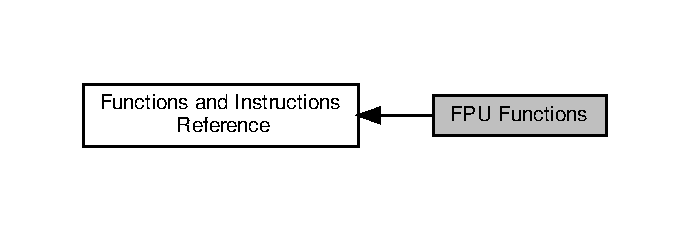
\includegraphics[width=331pt]{group___c_m_s_i_s___core___fpu_functions}
\end{center}
\end{figure}
\subsection*{Funkcje}
\begin{DoxyCompactItemize}
\item 
\hyperlink{cmsis__iccarm_8h_aba87361bfad2ae52cfe2f40c1a1dbf9c}{\+\_\+\+\_\+\+S\+T\+A\+T\+I\+C\+\_\+\+I\+N\+L\+I\+NE} uint32\+\_\+t \hyperlink{group___c_m_s_i_s___core___fpu_functions_ga6bcad99ce80a0e7e4ddc6f2379081756}{S\+C\+B\+\_\+\+Get\+F\+P\+U\+Type} (void)
\begin{DoxyCompactList}\small\item\em get F\+PU type \end{DoxyCompactList}\end{DoxyCompactItemize}


\subsection{Opis szczegółowy}
Function that provides F\+PU type. 



\subsection{Dokumentacja funkcji}
\mbox{\Hypertarget{group___c_m_s_i_s___core___fpu_functions_ga6bcad99ce80a0e7e4ddc6f2379081756}\label{group___c_m_s_i_s___core___fpu_functions_ga6bcad99ce80a0e7e4ddc6f2379081756}} 
\index{F\+P\+U Functions@{F\+P\+U Functions}!S\+C\+B\+\_\+\+Get\+F\+P\+U\+Type@{S\+C\+B\+\_\+\+Get\+F\+P\+U\+Type}}
\index{S\+C\+B\+\_\+\+Get\+F\+P\+U\+Type@{S\+C\+B\+\_\+\+Get\+F\+P\+U\+Type}!F\+P\+U Functions@{F\+P\+U Functions}}
\subsubsection{\texorpdfstring{S\+C\+B\+\_\+\+Get\+F\+P\+U\+Type()}{SCB\_GetFPUType()}}
{\footnotesize\ttfamily \hyperlink{cmsis__iccarm_8h_aba87361bfad2ae52cfe2f40c1a1dbf9c}{\+\_\+\+\_\+\+S\+T\+A\+T\+I\+C\+\_\+\+I\+N\+L\+I\+NE} uint32\+\_\+t S\+C\+B\+\_\+\+Get\+F\+P\+U\+Type (\begin{DoxyParamCaption}\item[{void}]{ }\end{DoxyParamCaption})}



get F\+PU type 

returns the F\+PU type \begin{DoxyReturn}{Zwraca}

\begin{DoxyItemize}
\item {\bfseries 0}\+: No F\+PU
\item {\bfseries 1}\+: Single precision F\+PU
\item {\bfseries 2}\+: Double + Single precision F\+PU 
\end{DoxyItemize}
\end{DoxyReturn}


Definicja w linii 1791 pliku core\+\_\+armv8mbl.\+h.


\hypertarget{group___c_m_s_i_s___core___s_a_u_functions}{}\section{S\+AU Functions}
\label{group___c_m_s_i_s___core___s_a_u_functions}\index{S\+A\+U Functions@{S\+A\+U Functions}}


Functions that configure the S\+AU.  


Diagram współpracy dla S\+AU Functions\+:\nopagebreak
\begin{figure}[H]
\begin{center}
\leavevmode
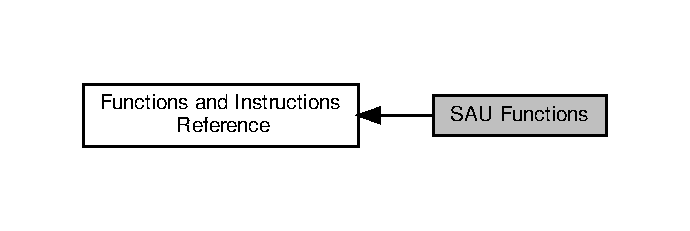
\includegraphics[width=331pt]{group___c_m_s_i_s___core___s_a_u_functions}
\end{center}
\end{figure}
Functions that configure the S\+AU. 


\hypertarget{group___c_m_s_i_s___core___sys_tick_functions}{}\section{Sys\+Tick Functions}
\label{group___c_m_s_i_s___core___sys_tick_functions}\index{Sys\+Tick Functions@{Sys\+Tick Functions}}


Functions that configure the System.  


Diagram współpracy dla Sys\+Tick Functions\+:\nopagebreak
\begin{figure}[H]
\begin{center}
\leavevmode
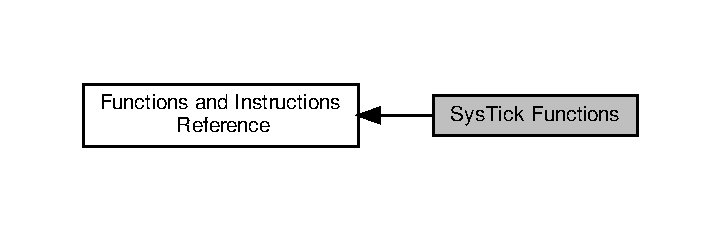
\includegraphics[width=346pt]{group___c_m_s_i_s___core___sys_tick_functions}
\end{center}
\end{figure}
Functions that configure the System. 


\hypertarget{group___c_m_s_i_s___s_cn_s_c_b}{}\section{System Controls not in S\+CB (S\+Cn\+S\+CB)}
\label{group___c_m_s_i_s___s_cn_s_c_b}\index{System Controls not in S\+C\+B (\+S\+Cn\+S\+C\+B)@{System Controls not in S\+C\+B (\+S\+Cn\+S\+C\+B)}}


Type definitions for the System Control and ID Register not in the S\+CB.  


Diagram współpracy dla System Controls not in S\+CB (S\+Cn\+S\+CB)\+:\nopagebreak
\begin{figure}[H]
\begin{center}
\leavevmode
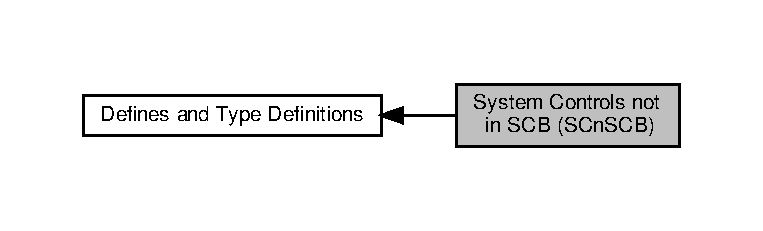
\includegraphics[width=350pt]{group___c_m_s_i_s___s_cn_s_c_b}
\end{center}
\end{figure}
\subsection*{Komponenty}
\begin{DoxyCompactItemize}
\item 
struct \hyperlink{struct_s_cn_s_c_b___type}{S\+Cn\+S\+C\+B\+\_\+\+Type}
\begin{DoxyCompactList}\small\item\em Structure type to access the System Control and ID Register not in the S\+CB. \end{DoxyCompactList}\end{DoxyCompactItemize}
\subsection*{Definicje}
\begin{DoxyCompactItemize}
\item 
\#define \hyperlink{group___c_m_s_i_s___s_cn_s_c_b_ga0777ddf379af50f9ca41d40573bfffc5}{S\+Cn\+S\+C\+B\+\_\+\+I\+C\+T\+R\+\_\+\+I\+N\+T\+L\+I\+N\+E\+S\+N\+U\+M\+\_\+\+Pos}~0U
\item 
\#define \hyperlink{group___c_m_s_i_s___s_cn_s_c_b_ga3efa0f5210051464e1034b19fc7b33c7}{S\+Cn\+S\+C\+B\+\_\+\+I\+C\+T\+R\+\_\+\+I\+N\+T\+L\+I\+N\+E\+S\+N\+U\+M\+\_\+\+Msk}~(0x\+F\+U\+L /$\ast$$<$$<$ S\+Cn\+S\+C\+B\+\_\+\+I\+C\+T\+R\+\_\+\+I\+N\+T\+L\+I\+N\+E\+S\+N\+U\+M\+\_\+\+Pos$\ast$/)
\item 
\#define \hyperlink{group___c_m_s_i_s___s_cn_s_c_b_gae4360bc2810b8486ccf74e7a853e1458}{S\+Cn\+S\+C\+B\+\_\+\+A\+C\+T\+L\+R\+\_\+\+I\+T\+C\+M\+U\+A\+E\+N\+\_\+\+Pos}~4U
\item 
\#define \hyperlink{group___c_m_s_i_s___s_cn_s_c_b_ga034b71340cb2e5455624b715d70cb36b}{S\+Cn\+S\+C\+B\+\_\+\+A\+C\+T\+L\+R\+\_\+\+I\+T\+C\+M\+U\+A\+E\+N\+\_\+\+Msk}~(1\+U\+L $<$$<$ S\+Cn\+S\+C\+B\+\_\+\+A\+C\+T\+L\+R\+\_\+\+I\+T\+C\+M\+U\+A\+E\+N\+\_\+\+Pos)
\item 
\#define \hyperlink{group___c_m_s_i_s___s_cn_s_c_b_gad5d71c0786cdb8a28f322b545d218aa7}{S\+Cn\+S\+C\+B\+\_\+\+A\+C\+T\+L\+R\+\_\+\+I\+T\+C\+M\+L\+A\+E\+N\+\_\+\+Pos}~3U
\item 
\#define \hyperlink{group___c_m_s_i_s___s_cn_s_c_b_ga96ed7dd2124586ddd816973d665d2014}{S\+Cn\+S\+C\+B\+\_\+\+A\+C\+T\+L\+R\+\_\+\+I\+T\+C\+M\+L\+A\+E\+N\+\_\+\+Msk}~(1\+U\+L $<$$<$ S\+Cn\+S\+C\+B\+\_\+\+A\+C\+T\+L\+R\+\_\+\+I\+T\+C\+M\+L\+A\+E\+N\+\_\+\+Pos)
\item 
\#define \hyperlink{group___c_m_s_i_s___s_cn_s_c_b_ga0777ddf379af50f9ca41d40573bfffc5}{S\+Cn\+S\+C\+B\+\_\+\+I\+C\+T\+R\+\_\+\+I\+N\+T\+L\+I\+N\+E\+S\+N\+U\+M\+\_\+\+Pos}~0U
\item 
\#define \hyperlink{group___c_m_s_i_s___s_cn_s_c_b_ga3efa0f5210051464e1034b19fc7b33c7}{S\+Cn\+S\+C\+B\+\_\+\+I\+C\+T\+R\+\_\+\+I\+N\+T\+L\+I\+N\+E\+S\+N\+U\+M\+\_\+\+Msk}~(0x\+F\+U\+L /$\ast$$<$$<$ S\+Cn\+S\+C\+B\+\_\+\+I\+C\+T\+R\+\_\+\+I\+N\+T\+L\+I\+N\+E\+S\+N\+U\+M\+\_\+\+Pos$\ast$/)
\item 
\#define \hyperlink{group___c_m_s_i_s___s_cn_s_c_b_gaab395870643a0bee78906bb15ca5bd02}{S\+Cn\+S\+C\+B\+\_\+\+A\+C\+T\+L\+R\+\_\+\+D\+I\+S\+F\+O\+L\+D\+\_\+\+Pos}~2U
\item 
\#define \hyperlink{group___c_m_s_i_s___s_cn_s_c_b_gaa9dd2d4a2350499188f438d0aa9fd982}{S\+Cn\+S\+C\+B\+\_\+\+A\+C\+T\+L\+R\+\_\+\+D\+I\+S\+F\+O\+L\+D\+\_\+\+Msk}~(1\+U\+L $<$$<$ S\+Cn\+S\+C\+B\+\_\+\+A\+C\+T\+L\+R\+\_\+\+D\+I\+S\+F\+O\+L\+D\+\_\+\+Pos)
\item 
\#define \hyperlink{group___c_m_s_i_s___s_cn_s_c_b_gafa2eb37493c0f8dae77cde81ecf80f77}{S\+Cn\+S\+C\+B\+\_\+\+A\+C\+T\+L\+R\+\_\+\+D\+I\+S\+D\+E\+F\+W\+B\+U\+F\+\_\+\+Pos}~1U
\item 
\#define \hyperlink{group___c_m_s_i_s___s_cn_s_c_b_ga6cda7b7219232a008ec52cc8e89d5d08}{S\+Cn\+S\+C\+B\+\_\+\+A\+C\+T\+L\+R\+\_\+\+D\+I\+S\+D\+E\+F\+W\+B\+U\+F\+\_\+\+Msk}~(1\+U\+L $<$$<$ S\+Cn\+S\+C\+B\+\_\+\+A\+C\+T\+L\+R\+\_\+\+D\+I\+S\+D\+E\+F\+W\+B\+U\+F\+\_\+\+Pos)
\item 
\#define \hyperlink{group___c_m_s_i_s___s_cn_s_c_b_gaaa3e79f5ead4a32c0ea742b2a9ffc0cd}{S\+Cn\+S\+C\+B\+\_\+\+A\+C\+T\+L\+R\+\_\+\+D\+I\+S\+M\+C\+Y\+C\+I\+N\+T\+\_\+\+Pos}~0U
\item 
\#define \hyperlink{group___c_m_s_i_s___s_cn_s_c_b_ga2a2818f0489ad10b6ea2964e899d4cbc}{S\+Cn\+S\+C\+B\+\_\+\+A\+C\+T\+L\+R\+\_\+\+D\+I\+S\+M\+C\+Y\+C\+I\+N\+T\+\_\+\+Msk}~(1\+U\+L /$\ast$$<$$<$ S\+Cn\+S\+C\+B\+\_\+\+A\+C\+T\+L\+R\+\_\+\+D\+I\+S\+M\+C\+Y\+C\+I\+N\+T\+\_\+\+Pos$\ast$/)
\item 
\#define \hyperlink{group___c_m_s_i_s___s_cn_s_c_b_ga0777ddf379af50f9ca41d40573bfffc5}{S\+Cn\+S\+C\+B\+\_\+\+I\+C\+T\+R\+\_\+\+I\+N\+T\+L\+I\+N\+E\+S\+N\+U\+M\+\_\+\+Pos}~0U
\item 
\#define \hyperlink{group___c_m_s_i_s___s_cn_s_c_b_ga3efa0f5210051464e1034b19fc7b33c7}{S\+Cn\+S\+C\+B\+\_\+\+I\+C\+T\+R\+\_\+\+I\+N\+T\+L\+I\+N\+E\+S\+N\+U\+M\+\_\+\+Msk}~(0x\+F\+U\+L /$\ast$$<$$<$ S\+Cn\+S\+C\+B\+\_\+\+I\+C\+T\+R\+\_\+\+I\+N\+T\+L\+I\+N\+E\+S\+N\+U\+M\+\_\+\+Pos$\ast$/)
\item 
\#define \hyperlink{group___c_m_s_i_s___s_cn_s_c_b_ga0777ddf379af50f9ca41d40573bfffc5}{S\+Cn\+S\+C\+B\+\_\+\+I\+C\+T\+R\+\_\+\+I\+N\+T\+L\+I\+N\+E\+S\+N\+U\+M\+\_\+\+Pos}~0U
\item 
\#define \hyperlink{group___c_m_s_i_s___s_cn_s_c_b_ga3efa0f5210051464e1034b19fc7b33c7}{S\+Cn\+S\+C\+B\+\_\+\+I\+C\+T\+R\+\_\+\+I\+N\+T\+L\+I\+N\+E\+S\+N\+U\+M\+\_\+\+Msk}~(0x\+F\+U\+L /$\ast$$<$$<$ S\+Cn\+S\+C\+B\+\_\+\+I\+C\+T\+R\+\_\+\+I\+N\+T\+L\+I\+N\+E\+S\+N\+U\+M\+\_\+\+Pos$\ast$/)
\item 
\#define \hyperlink{group___c_m_s_i_s___s_cn_s_c_b_gaff0b57464c60fea8182b903676f8de49}{S\+Cn\+S\+C\+B\+\_\+\+A\+C\+T\+L\+R\+\_\+\+D\+I\+S\+O\+O\+F\+P\+\_\+\+Pos}~9U
\item 
\#define \hyperlink{group___c_m_s_i_s___s_cn_s_c_b_ga1ecd6adafa43464d7097b132c19e8640}{S\+Cn\+S\+C\+B\+\_\+\+A\+C\+T\+L\+R\+\_\+\+D\+I\+S\+O\+O\+F\+P\+\_\+\+Msk}~(1\+U\+L $<$$<$ S\+Cn\+S\+C\+B\+\_\+\+A\+C\+T\+L\+R\+\_\+\+D\+I\+S\+O\+O\+F\+P\+\_\+\+Pos)
\item 
\#define \hyperlink{group___c_m_s_i_s___s_cn_s_c_b_gaa194809383bc72ecf3416d85709281d7}{S\+Cn\+S\+C\+B\+\_\+\+A\+C\+T\+L\+R\+\_\+\+D\+I\+S\+F\+P\+C\+A\+\_\+\+Pos}~8U
\item 
\#define \hyperlink{group___c_m_s_i_s___s_cn_s_c_b_ga10d5aa4a196dcde6f476016ece2c1b69}{S\+Cn\+S\+C\+B\+\_\+\+A\+C\+T\+L\+R\+\_\+\+D\+I\+S\+F\+P\+C\+A\+\_\+\+Msk}~(1\+U\+L $<$$<$ S\+Cn\+S\+C\+B\+\_\+\+A\+C\+T\+L\+R\+\_\+\+D\+I\+S\+F\+P\+C\+A\+\_\+\+Pos)
\item 
\#define \hyperlink{group___c_m_s_i_s___s_cn_s_c_b_gaab395870643a0bee78906bb15ca5bd02}{S\+Cn\+S\+C\+B\+\_\+\+A\+C\+T\+L\+R\+\_\+\+D\+I\+S\+F\+O\+L\+D\+\_\+\+Pos}~2U
\item 
\#define \hyperlink{group___c_m_s_i_s___s_cn_s_c_b_gaa9dd2d4a2350499188f438d0aa9fd982}{S\+Cn\+S\+C\+B\+\_\+\+A\+C\+T\+L\+R\+\_\+\+D\+I\+S\+F\+O\+L\+D\+\_\+\+Msk}~(1\+U\+L $<$$<$ S\+Cn\+S\+C\+B\+\_\+\+A\+C\+T\+L\+R\+\_\+\+D\+I\+S\+F\+O\+L\+D\+\_\+\+Pos)
\item 
\#define \hyperlink{group___c_m_s_i_s___s_cn_s_c_b_gafa2eb37493c0f8dae77cde81ecf80f77}{S\+Cn\+S\+C\+B\+\_\+\+A\+C\+T\+L\+R\+\_\+\+D\+I\+S\+D\+E\+F\+W\+B\+U\+F\+\_\+\+Pos}~1U
\item 
\#define \hyperlink{group___c_m_s_i_s___s_cn_s_c_b_ga6cda7b7219232a008ec52cc8e89d5d08}{S\+Cn\+S\+C\+B\+\_\+\+A\+C\+T\+L\+R\+\_\+\+D\+I\+S\+D\+E\+F\+W\+B\+U\+F\+\_\+\+Msk}~(1\+U\+L $<$$<$ S\+Cn\+S\+C\+B\+\_\+\+A\+C\+T\+L\+R\+\_\+\+D\+I\+S\+D\+E\+F\+W\+B\+U\+F\+\_\+\+Pos)
\item 
\#define \hyperlink{group___c_m_s_i_s___s_cn_s_c_b_gaaa3e79f5ead4a32c0ea742b2a9ffc0cd}{S\+Cn\+S\+C\+B\+\_\+\+A\+C\+T\+L\+R\+\_\+\+D\+I\+S\+M\+C\+Y\+C\+I\+N\+T\+\_\+\+Pos}~0U
\item 
\#define \hyperlink{group___c_m_s_i_s___s_cn_s_c_b_ga2a2818f0489ad10b6ea2964e899d4cbc}{S\+Cn\+S\+C\+B\+\_\+\+A\+C\+T\+L\+R\+\_\+\+D\+I\+S\+M\+C\+Y\+C\+I\+N\+T\+\_\+\+Msk}~(1\+U\+L /$\ast$$<$$<$ S\+Cn\+S\+C\+B\+\_\+\+A\+C\+T\+L\+R\+\_\+\+D\+I\+S\+M\+C\+Y\+C\+I\+N\+T\+\_\+\+Pos$\ast$/)
\item 
\#define \hyperlink{group___c_m_s_i_s___s_cn_s_c_b_ga0777ddf379af50f9ca41d40573bfffc5}{S\+Cn\+S\+C\+B\+\_\+\+I\+C\+T\+R\+\_\+\+I\+N\+T\+L\+I\+N\+E\+S\+N\+U\+M\+\_\+\+Pos}~0U
\item 
\#define \hyperlink{group___c_m_s_i_s___s_cn_s_c_b_ga3efa0f5210051464e1034b19fc7b33c7}{S\+Cn\+S\+C\+B\+\_\+\+I\+C\+T\+R\+\_\+\+I\+N\+T\+L\+I\+N\+E\+S\+N\+U\+M\+\_\+\+Msk}~(0x\+F\+U\+L /$\ast$$<$$<$ S\+Cn\+S\+C\+B\+\_\+\+I\+C\+T\+R\+\_\+\+I\+N\+T\+L\+I\+N\+E\+S\+N\+U\+M\+\_\+\+Pos$\ast$/)
\item 
\#define \hyperlink{group___c_m_s_i_s___s_cn_s_c_b_ga5f888e0ebc18cc2d99976405777c142f}{S\+Cn\+S\+C\+B\+\_\+\+A\+C\+T\+L\+R\+\_\+\+D\+I\+S\+I\+T\+M\+A\+T\+B\+F\+L\+U\+S\+H\+\_\+\+Pos}~12U
\item 
\#define \hyperlink{group___c_m_s_i_s___s_cn_s_c_b_ga46b16a03b408184720134ef42203ac2e}{S\+Cn\+S\+C\+B\+\_\+\+A\+C\+T\+L\+R\+\_\+\+D\+I\+S\+I\+T\+M\+A\+T\+B\+F\+L\+U\+S\+H\+\_\+\+Msk}~(1\+U\+L $<$$<$ S\+Cn\+S\+C\+B\+\_\+\+A\+C\+T\+L\+R\+\_\+\+D\+I\+S\+I\+T\+M\+A\+T\+B\+F\+L\+U\+S\+H\+\_\+\+Pos)
\item 
\#define \hyperlink{group___c_m_s_i_s___s_cn_s_c_b_ga1bffb5e05053d15cbe42fbe87d225dcb}{S\+Cn\+S\+C\+B\+\_\+\+A\+C\+T\+L\+R\+\_\+\+D\+I\+S\+R\+A\+M\+O\+D\+E\+\_\+\+Pos}~11U
\item 
\#define \hyperlink{group___c_m_s_i_s___s_cn_s_c_b_ga436fc1bd011b15c9585bb3ace5332ce3}{S\+Cn\+S\+C\+B\+\_\+\+A\+C\+T\+L\+R\+\_\+\+D\+I\+S\+R\+A\+M\+O\+D\+E\+\_\+\+Msk}~(1\+U\+L $<$$<$ S\+Cn\+S\+C\+B\+\_\+\+A\+C\+T\+L\+R\+\_\+\+D\+I\+S\+R\+A\+M\+O\+D\+E\+\_\+\+Pos)
\item 
\#define \hyperlink{group___c_m_s_i_s___s_cn_s_c_b_gaa743743f5af93d6ece74a426b355ab70}{S\+Cn\+S\+C\+B\+\_\+\+A\+C\+T\+L\+R\+\_\+\+F\+P\+E\+X\+C\+O\+D\+I\+S\+\_\+\+Pos}~10U
\item 
\#define \hyperlink{group___c_m_s_i_s___s_cn_s_c_b_gadd12baaeeea3220b03867e4b8a1432aa}{S\+Cn\+S\+C\+B\+\_\+\+A\+C\+T\+L\+R\+\_\+\+F\+P\+E\+X\+C\+O\+D\+I\+S\+\_\+\+Msk}~(1\+U\+L $<$$<$ S\+Cn\+S\+C\+B\+\_\+\+A\+C\+T\+L\+R\+\_\+\+F\+P\+E\+X\+C\+O\+D\+I\+S\+\_\+\+Pos)
\item 
\#define \hyperlink{group___c_m_s_i_s___s_cn_s_c_b_gaab395870643a0bee78906bb15ca5bd02}{S\+Cn\+S\+C\+B\+\_\+\+A\+C\+T\+L\+R\+\_\+\+D\+I\+S\+F\+O\+L\+D\+\_\+\+Pos}~2U
\item 
\#define \hyperlink{group___c_m_s_i_s___s_cn_s_c_b_gaa9dd2d4a2350499188f438d0aa9fd982}{S\+Cn\+S\+C\+B\+\_\+\+A\+C\+T\+L\+R\+\_\+\+D\+I\+S\+F\+O\+L\+D\+\_\+\+Msk}~(1\+U\+L $<$$<$ S\+Cn\+S\+C\+B\+\_\+\+A\+C\+T\+L\+R\+\_\+\+D\+I\+S\+F\+O\+L\+D\+\_\+\+Pos)
\item 
\#define \hyperlink{group___c_m_s_i_s___s_cn_s_c_b_gaaa3e79f5ead4a32c0ea742b2a9ffc0cd}{S\+Cn\+S\+C\+B\+\_\+\+A\+C\+T\+L\+R\+\_\+\+D\+I\+S\+M\+C\+Y\+C\+I\+N\+T\+\_\+\+Pos}~0U
\item 
\#define \hyperlink{group___c_m_s_i_s___s_cn_s_c_b_ga2a2818f0489ad10b6ea2964e899d4cbc}{S\+Cn\+S\+C\+B\+\_\+\+A\+C\+T\+L\+R\+\_\+\+D\+I\+S\+M\+C\+Y\+C\+I\+N\+T\+\_\+\+Msk}~(1\+U\+L /$\ast$$<$$<$ S\+Cn\+S\+C\+B\+\_\+\+A\+C\+T\+L\+R\+\_\+\+D\+I\+S\+M\+C\+Y\+C\+I\+N\+T\+\_\+\+Pos$\ast$/)
\item 
\#define \hyperlink{group___c_m_s_i_s___s_cn_s_c_b_gaaa3e79f5ead4a32c0ea742b2a9ffc0cd}{S\+Cn\+S\+C\+B\+\_\+\+A\+C\+T\+L\+R\+\_\+\+D\+I\+S\+M\+C\+Y\+C\+I\+N\+T\+\_\+\+Pos}~0U
\item 
\#define \hyperlink{group___c_m_s_i_s___s_cn_s_c_b_ga2a2818f0489ad10b6ea2964e899d4cbc}{S\+Cn\+S\+C\+B\+\_\+\+A\+C\+T\+L\+R\+\_\+\+D\+I\+S\+M\+C\+Y\+C\+I\+N\+T\+\_\+\+Msk}~(1\+U\+L /$\ast$$<$$<$ S\+Cn\+S\+C\+B\+\_\+\+A\+C\+T\+L\+R\+\_\+\+D\+I\+S\+M\+C\+Y\+C\+I\+N\+T\+\_\+\+Pos$\ast$/)
\item 
\#define \hyperlink{group___c_m_s_i_s___s_cn_s_c_b_ga0777ddf379af50f9ca41d40573bfffc5}{S\+Cn\+S\+C\+B\+\_\+\+I\+C\+T\+R\+\_\+\+I\+N\+T\+L\+I\+N\+E\+S\+N\+U\+M\+\_\+\+Pos}~0U
\item 
\#define \hyperlink{group___c_m_s_i_s___s_cn_s_c_b_ga3efa0f5210051464e1034b19fc7b33c7}{S\+Cn\+S\+C\+B\+\_\+\+I\+C\+T\+R\+\_\+\+I\+N\+T\+L\+I\+N\+E\+S\+N\+U\+M\+\_\+\+Msk}~(0x\+F\+U\+L /$\ast$$<$$<$ S\+Cn\+S\+C\+B\+\_\+\+I\+C\+T\+R\+\_\+\+I\+N\+T\+L\+I\+N\+E\+S\+N\+U\+M\+\_\+\+Pos$\ast$/)
\end{DoxyCompactItemize}


\subsection{Opis szczegółowy}
Type definitions for the System Control and ID Register not in the S\+CB. 



\subsection{Dokumentacja definicji}
\mbox{\Hypertarget{group___c_m_s_i_s___s_cn_s_c_b_ga6cda7b7219232a008ec52cc8e89d5d08}\label{group___c_m_s_i_s___s_cn_s_c_b_ga6cda7b7219232a008ec52cc8e89d5d08}} 
\index{System Controls not in S\+C\+B (\+S\+Cn\+S\+C\+B)@{System Controls not in S\+C\+B (\+S\+Cn\+S\+C\+B)}!S\+Cn\+S\+C\+B\+\_\+\+A\+C\+T\+L\+R\+\_\+\+D\+I\+S\+D\+E\+F\+W\+B\+U\+F\+\_\+\+Msk@{S\+Cn\+S\+C\+B\+\_\+\+A\+C\+T\+L\+R\+\_\+\+D\+I\+S\+D\+E\+F\+W\+B\+U\+F\+\_\+\+Msk}}
\index{S\+Cn\+S\+C\+B\+\_\+\+A\+C\+T\+L\+R\+\_\+\+D\+I\+S\+D\+E\+F\+W\+B\+U\+F\+\_\+\+Msk@{S\+Cn\+S\+C\+B\+\_\+\+A\+C\+T\+L\+R\+\_\+\+D\+I\+S\+D\+E\+F\+W\+B\+U\+F\+\_\+\+Msk}!System Controls not in S\+C\+B (\+S\+Cn\+S\+C\+B)@{System Controls not in S\+C\+B (\+S\+Cn\+S\+C\+B)}}
\subsubsection{\texorpdfstring{S\+Cn\+S\+C\+B\+\_\+\+A\+C\+T\+L\+R\+\_\+\+D\+I\+S\+D\+E\+F\+W\+B\+U\+F\+\_\+\+Msk}{SCnSCB\_ACTLR\_DISDEFWBUF\_Msk}\hspace{0.1cm}{\footnotesize\ttfamily [1/2]}}
{\footnotesize\ttfamily \#define S\+Cn\+S\+C\+B\+\_\+\+A\+C\+T\+L\+R\+\_\+\+D\+I\+S\+D\+E\+F\+W\+B\+U\+F\+\_\+\+Msk~(1\+U\+L $<$$<$ S\+Cn\+S\+C\+B\+\_\+\+A\+C\+T\+L\+R\+\_\+\+D\+I\+S\+D\+E\+F\+W\+B\+U\+F\+\_\+\+Pos)}

A\+C\+T\+LR\+: D\+I\+S\+D\+E\+F\+W\+B\+UF Mask 

Definicja w linii 676 pliku core\+\_\+cm3.\+h.

\mbox{\Hypertarget{group___c_m_s_i_s___s_cn_s_c_b_ga6cda7b7219232a008ec52cc8e89d5d08}\label{group___c_m_s_i_s___s_cn_s_c_b_ga6cda7b7219232a008ec52cc8e89d5d08}} 
\index{System Controls not in S\+C\+B (\+S\+Cn\+S\+C\+B)@{System Controls not in S\+C\+B (\+S\+Cn\+S\+C\+B)}!S\+Cn\+S\+C\+B\+\_\+\+A\+C\+T\+L\+R\+\_\+\+D\+I\+S\+D\+E\+F\+W\+B\+U\+F\+\_\+\+Msk@{S\+Cn\+S\+C\+B\+\_\+\+A\+C\+T\+L\+R\+\_\+\+D\+I\+S\+D\+E\+F\+W\+B\+U\+F\+\_\+\+Msk}}
\index{S\+Cn\+S\+C\+B\+\_\+\+A\+C\+T\+L\+R\+\_\+\+D\+I\+S\+D\+E\+F\+W\+B\+U\+F\+\_\+\+Msk@{S\+Cn\+S\+C\+B\+\_\+\+A\+C\+T\+L\+R\+\_\+\+D\+I\+S\+D\+E\+F\+W\+B\+U\+F\+\_\+\+Msk}!System Controls not in S\+C\+B (\+S\+Cn\+S\+C\+B)@{System Controls not in S\+C\+B (\+S\+Cn\+S\+C\+B)}}
\subsubsection{\texorpdfstring{S\+Cn\+S\+C\+B\+\_\+\+A\+C\+T\+L\+R\+\_\+\+D\+I\+S\+D\+E\+F\+W\+B\+U\+F\+\_\+\+Msk}{SCnSCB\_ACTLR\_DISDEFWBUF\_Msk}\hspace{0.1cm}{\footnotesize\ttfamily [2/2]}}
{\footnotesize\ttfamily \#define S\+Cn\+S\+C\+B\+\_\+\+A\+C\+T\+L\+R\+\_\+\+D\+I\+S\+D\+E\+F\+W\+B\+U\+F\+\_\+\+Msk~(1\+U\+L $<$$<$ S\+Cn\+S\+C\+B\+\_\+\+A\+C\+T\+L\+R\+\_\+\+D\+I\+S\+D\+E\+F\+W\+B\+U\+F\+\_\+\+Pos)}

A\+C\+T\+LR\+: D\+I\+S\+D\+E\+F\+W\+B\+UF Mask 

Definicja w linii 741 pliku core\+\_\+cm4.\+h.

\mbox{\Hypertarget{group___c_m_s_i_s___s_cn_s_c_b_gafa2eb37493c0f8dae77cde81ecf80f77}\label{group___c_m_s_i_s___s_cn_s_c_b_gafa2eb37493c0f8dae77cde81ecf80f77}} 
\index{System Controls not in S\+C\+B (\+S\+Cn\+S\+C\+B)@{System Controls not in S\+C\+B (\+S\+Cn\+S\+C\+B)}!S\+Cn\+S\+C\+B\+\_\+\+A\+C\+T\+L\+R\+\_\+\+D\+I\+S\+D\+E\+F\+W\+B\+U\+F\+\_\+\+Pos@{S\+Cn\+S\+C\+B\+\_\+\+A\+C\+T\+L\+R\+\_\+\+D\+I\+S\+D\+E\+F\+W\+B\+U\+F\+\_\+\+Pos}}
\index{S\+Cn\+S\+C\+B\+\_\+\+A\+C\+T\+L\+R\+\_\+\+D\+I\+S\+D\+E\+F\+W\+B\+U\+F\+\_\+\+Pos@{S\+Cn\+S\+C\+B\+\_\+\+A\+C\+T\+L\+R\+\_\+\+D\+I\+S\+D\+E\+F\+W\+B\+U\+F\+\_\+\+Pos}!System Controls not in S\+C\+B (\+S\+Cn\+S\+C\+B)@{System Controls not in S\+C\+B (\+S\+Cn\+S\+C\+B)}}
\subsubsection{\texorpdfstring{S\+Cn\+S\+C\+B\+\_\+\+A\+C\+T\+L\+R\+\_\+\+D\+I\+S\+D\+E\+F\+W\+B\+U\+F\+\_\+\+Pos}{SCnSCB\_ACTLR\_DISDEFWBUF\_Pos}\hspace{0.1cm}{\footnotesize\ttfamily [1/2]}}
{\footnotesize\ttfamily \#define S\+Cn\+S\+C\+B\+\_\+\+A\+C\+T\+L\+R\+\_\+\+D\+I\+S\+D\+E\+F\+W\+B\+U\+F\+\_\+\+Pos~1U}

A\+C\+T\+LR\+: D\+I\+S\+D\+E\+F\+W\+B\+UF Position 

Definicja w linii 675 pliku core\+\_\+cm3.\+h.

\mbox{\Hypertarget{group___c_m_s_i_s___s_cn_s_c_b_gafa2eb37493c0f8dae77cde81ecf80f77}\label{group___c_m_s_i_s___s_cn_s_c_b_gafa2eb37493c0f8dae77cde81ecf80f77}} 
\index{System Controls not in S\+C\+B (\+S\+Cn\+S\+C\+B)@{System Controls not in S\+C\+B (\+S\+Cn\+S\+C\+B)}!S\+Cn\+S\+C\+B\+\_\+\+A\+C\+T\+L\+R\+\_\+\+D\+I\+S\+D\+E\+F\+W\+B\+U\+F\+\_\+\+Pos@{S\+Cn\+S\+C\+B\+\_\+\+A\+C\+T\+L\+R\+\_\+\+D\+I\+S\+D\+E\+F\+W\+B\+U\+F\+\_\+\+Pos}}
\index{S\+Cn\+S\+C\+B\+\_\+\+A\+C\+T\+L\+R\+\_\+\+D\+I\+S\+D\+E\+F\+W\+B\+U\+F\+\_\+\+Pos@{S\+Cn\+S\+C\+B\+\_\+\+A\+C\+T\+L\+R\+\_\+\+D\+I\+S\+D\+E\+F\+W\+B\+U\+F\+\_\+\+Pos}!System Controls not in S\+C\+B (\+S\+Cn\+S\+C\+B)@{System Controls not in S\+C\+B (\+S\+Cn\+S\+C\+B)}}
\subsubsection{\texorpdfstring{S\+Cn\+S\+C\+B\+\_\+\+A\+C\+T\+L\+R\+\_\+\+D\+I\+S\+D\+E\+F\+W\+B\+U\+F\+\_\+\+Pos}{SCnSCB\_ACTLR\_DISDEFWBUF\_Pos}\hspace{0.1cm}{\footnotesize\ttfamily [2/2]}}
{\footnotesize\ttfamily \#define S\+Cn\+S\+C\+B\+\_\+\+A\+C\+T\+L\+R\+\_\+\+D\+I\+S\+D\+E\+F\+W\+B\+U\+F\+\_\+\+Pos~1U}

A\+C\+T\+LR\+: D\+I\+S\+D\+E\+F\+W\+B\+UF Position 

Definicja w linii 740 pliku core\+\_\+cm4.\+h.

\mbox{\Hypertarget{group___c_m_s_i_s___s_cn_s_c_b_gaa9dd2d4a2350499188f438d0aa9fd982}\label{group___c_m_s_i_s___s_cn_s_c_b_gaa9dd2d4a2350499188f438d0aa9fd982}} 
\index{System Controls not in S\+C\+B (\+S\+Cn\+S\+C\+B)@{System Controls not in S\+C\+B (\+S\+Cn\+S\+C\+B)}!S\+Cn\+S\+C\+B\+\_\+\+A\+C\+T\+L\+R\+\_\+\+D\+I\+S\+F\+O\+L\+D\+\_\+\+Msk@{S\+Cn\+S\+C\+B\+\_\+\+A\+C\+T\+L\+R\+\_\+\+D\+I\+S\+F\+O\+L\+D\+\_\+\+Msk}}
\index{S\+Cn\+S\+C\+B\+\_\+\+A\+C\+T\+L\+R\+\_\+\+D\+I\+S\+F\+O\+L\+D\+\_\+\+Msk@{S\+Cn\+S\+C\+B\+\_\+\+A\+C\+T\+L\+R\+\_\+\+D\+I\+S\+F\+O\+L\+D\+\_\+\+Msk}!System Controls not in S\+C\+B (\+S\+Cn\+S\+C\+B)@{System Controls not in S\+C\+B (\+S\+Cn\+S\+C\+B)}}
\subsubsection{\texorpdfstring{S\+Cn\+S\+C\+B\+\_\+\+A\+C\+T\+L\+R\+\_\+\+D\+I\+S\+F\+O\+L\+D\+\_\+\+Msk}{SCnSCB\_ACTLR\_DISFOLD\_Msk}\hspace{0.1cm}{\footnotesize\ttfamily [1/3]}}
{\footnotesize\ttfamily \#define S\+Cn\+S\+C\+B\+\_\+\+A\+C\+T\+L\+R\+\_\+\+D\+I\+S\+F\+O\+L\+D\+\_\+\+Msk~(1\+U\+L $<$$<$ S\+Cn\+S\+C\+B\+\_\+\+A\+C\+T\+L\+R\+\_\+\+D\+I\+S\+F\+O\+L\+D\+\_\+\+Pos)}

A\+C\+T\+LR\+: D\+I\+S\+F\+O\+LD Mask 

Definicja w linii 673 pliku core\+\_\+cm3.\+h.

\mbox{\Hypertarget{group___c_m_s_i_s___s_cn_s_c_b_gaa9dd2d4a2350499188f438d0aa9fd982}\label{group___c_m_s_i_s___s_cn_s_c_b_gaa9dd2d4a2350499188f438d0aa9fd982}} 
\index{System Controls not in S\+C\+B (\+S\+Cn\+S\+C\+B)@{System Controls not in S\+C\+B (\+S\+Cn\+S\+C\+B)}!S\+Cn\+S\+C\+B\+\_\+\+A\+C\+T\+L\+R\+\_\+\+D\+I\+S\+F\+O\+L\+D\+\_\+\+Msk@{S\+Cn\+S\+C\+B\+\_\+\+A\+C\+T\+L\+R\+\_\+\+D\+I\+S\+F\+O\+L\+D\+\_\+\+Msk}}
\index{S\+Cn\+S\+C\+B\+\_\+\+A\+C\+T\+L\+R\+\_\+\+D\+I\+S\+F\+O\+L\+D\+\_\+\+Msk@{S\+Cn\+S\+C\+B\+\_\+\+A\+C\+T\+L\+R\+\_\+\+D\+I\+S\+F\+O\+L\+D\+\_\+\+Msk}!System Controls not in S\+C\+B (\+S\+Cn\+S\+C\+B)@{System Controls not in S\+C\+B (\+S\+Cn\+S\+C\+B)}}
\subsubsection{\texorpdfstring{S\+Cn\+S\+C\+B\+\_\+\+A\+C\+T\+L\+R\+\_\+\+D\+I\+S\+F\+O\+L\+D\+\_\+\+Msk}{SCnSCB\_ACTLR\_DISFOLD\_Msk}\hspace{0.1cm}{\footnotesize\ttfamily [2/3]}}
{\footnotesize\ttfamily \#define S\+Cn\+S\+C\+B\+\_\+\+A\+C\+T\+L\+R\+\_\+\+D\+I\+S\+F\+O\+L\+D\+\_\+\+Msk~(1\+U\+L $<$$<$ S\+Cn\+S\+C\+B\+\_\+\+A\+C\+T\+L\+R\+\_\+\+D\+I\+S\+F\+O\+L\+D\+\_\+\+Pos)}

A\+C\+T\+LR\+: D\+I\+S\+F\+O\+LD Mask 

Definicja w linii 738 pliku core\+\_\+cm4.\+h.

\mbox{\Hypertarget{group___c_m_s_i_s___s_cn_s_c_b_gaa9dd2d4a2350499188f438d0aa9fd982}\label{group___c_m_s_i_s___s_cn_s_c_b_gaa9dd2d4a2350499188f438d0aa9fd982}} 
\index{System Controls not in S\+C\+B (\+S\+Cn\+S\+C\+B)@{System Controls not in S\+C\+B (\+S\+Cn\+S\+C\+B)}!S\+Cn\+S\+C\+B\+\_\+\+A\+C\+T\+L\+R\+\_\+\+D\+I\+S\+F\+O\+L\+D\+\_\+\+Msk@{S\+Cn\+S\+C\+B\+\_\+\+A\+C\+T\+L\+R\+\_\+\+D\+I\+S\+F\+O\+L\+D\+\_\+\+Msk}}
\index{S\+Cn\+S\+C\+B\+\_\+\+A\+C\+T\+L\+R\+\_\+\+D\+I\+S\+F\+O\+L\+D\+\_\+\+Msk@{S\+Cn\+S\+C\+B\+\_\+\+A\+C\+T\+L\+R\+\_\+\+D\+I\+S\+F\+O\+L\+D\+\_\+\+Msk}!System Controls not in S\+C\+B (\+S\+Cn\+S\+C\+B)@{System Controls not in S\+C\+B (\+S\+Cn\+S\+C\+B)}}
\subsubsection{\texorpdfstring{S\+Cn\+S\+C\+B\+\_\+\+A\+C\+T\+L\+R\+\_\+\+D\+I\+S\+F\+O\+L\+D\+\_\+\+Msk}{SCnSCB\_ACTLR\_DISFOLD\_Msk}\hspace{0.1cm}{\footnotesize\ttfamily [3/3]}}
{\footnotesize\ttfamily \#define S\+Cn\+S\+C\+B\+\_\+\+A\+C\+T\+L\+R\+\_\+\+D\+I\+S\+F\+O\+L\+D\+\_\+\+Msk~(1\+U\+L $<$$<$ S\+Cn\+S\+C\+B\+\_\+\+A\+C\+T\+L\+R\+\_\+\+D\+I\+S\+F\+O\+L\+D\+\_\+\+Pos)}

A\+C\+T\+LR\+: D\+I\+S\+F\+O\+LD Mask 

Definicja w linii 943 pliku core\+\_\+cm7.\+h.

\mbox{\Hypertarget{group___c_m_s_i_s___s_cn_s_c_b_gaab395870643a0bee78906bb15ca5bd02}\label{group___c_m_s_i_s___s_cn_s_c_b_gaab395870643a0bee78906bb15ca5bd02}} 
\index{System Controls not in S\+C\+B (\+S\+Cn\+S\+C\+B)@{System Controls not in S\+C\+B (\+S\+Cn\+S\+C\+B)}!S\+Cn\+S\+C\+B\+\_\+\+A\+C\+T\+L\+R\+\_\+\+D\+I\+S\+F\+O\+L\+D\+\_\+\+Pos@{S\+Cn\+S\+C\+B\+\_\+\+A\+C\+T\+L\+R\+\_\+\+D\+I\+S\+F\+O\+L\+D\+\_\+\+Pos}}
\index{S\+Cn\+S\+C\+B\+\_\+\+A\+C\+T\+L\+R\+\_\+\+D\+I\+S\+F\+O\+L\+D\+\_\+\+Pos@{S\+Cn\+S\+C\+B\+\_\+\+A\+C\+T\+L\+R\+\_\+\+D\+I\+S\+F\+O\+L\+D\+\_\+\+Pos}!System Controls not in S\+C\+B (\+S\+Cn\+S\+C\+B)@{System Controls not in S\+C\+B (\+S\+Cn\+S\+C\+B)}}
\subsubsection{\texorpdfstring{S\+Cn\+S\+C\+B\+\_\+\+A\+C\+T\+L\+R\+\_\+\+D\+I\+S\+F\+O\+L\+D\+\_\+\+Pos}{SCnSCB\_ACTLR\_DISFOLD\_Pos}\hspace{0.1cm}{\footnotesize\ttfamily [1/3]}}
{\footnotesize\ttfamily \#define S\+Cn\+S\+C\+B\+\_\+\+A\+C\+T\+L\+R\+\_\+\+D\+I\+S\+F\+O\+L\+D\+\_\+\+Pos~2U}

A\+C\+T\+LR\+: D\+I\+S\+F\+O\+LD Position 

Definicja w linii 672 pliku core\+\_\+cm3.\+h.

\mbox{\Hypertarget{group___c_m_s_i_s___s_cn_s_c_b_gaab395870643a0bee78906bb15ca5bd02}\label{group___c_m_s_i_s___s_cn_s_c_b_gaab395870643a0bee78906bb15ca5bd02}} 
\index{System Controls not in S\+C\+B (\+S\+Cn\+S\+C\+B)@{System Controls not in S\+C\+B (\+S\+Cn\+S\+C\+B)}!S\+Cn\+S\+C\+B\+\_\+\+A\+C\+T\+L\+R\+\_\+\+D\+I\+S\+F\+O\+L\+D\+\_\+\+Pos@{S\+Cn\+S\+C\+B\+\_\+\+A\+C\+T\+L\+R\+\_\+\+D\+I\+S\+F\+O\+L\+D\+\_\+\+Pos}}
\index{S\+Cn\+S\+C\+B\+\_\+\+A\+C\+T\+L\+R\+\_\+\+D\+I\+S\+F\+O\+L\+D\+\_\+\+Pos@{S\+Cn\+S\+C\+B\+\_\+\+A\+C\+T\+L\+R\+\_\+\+D\+I\+S\+F\+O\+L\+D\+\_\+\+Pos}!System Controls not in S\+C\+B (\+S\+Cn\+S\+C\+B)@{System Controls not in S\+C\+B (\+S\+Cn\+S\+C\+B)}}
\subsubsection{\texorpdfstring{S\+Cn\+S\+C\+B\+\_\+\+A\+C\+T\+L\+R\+\_\+\+D\+I\+S\+F\+O\+L\+D\+\_\+\+Pos}{SCnSCB\_ACTLR\_DISFOLD\_Pos}\hspace{0.1cm}{\footnotesize\ttfamily [2/3]}}
{\footnotesize\ttfamily \#define S\+Cn\+S\+C\+B\+\_\+\+A\+C\+T\+L\+R\+\_\+\+D\+I\+S\+F\+O\+L\+D\+\_\+\+Pos~2U}

A\+C\+T\+LR\+: D\+I\+S\+F\+O\+LD Position 

Definicja w linii 737 pliku core\+\_\+cm4.\+h.

\mbox{\Hypertarget{group___c_m_s_i_s___s_cn_s_c_b_gaab395870643a0bee78906bb15ca5bd02}\label{group___c_m_s_i_s___s_cn_s_c_b_gaab395870643a0bee78906bb15ca5bd02}} 
\index{System Controls not in S\+C\+B (\+S\+Cn\+S\+C\+B)@{System Controls not in S\+C\+B (\+S\+Cn\+S\+C\+B)}!S\+Cn\+S\+C\+B\+\_\+\+A\+C\+T\+L\+R\+\_\+\+D\+I\+S\+F\+O\+L\+D\+\_\+\+Pos@{S\+Cn\+S\+C\+B\+\_\+\+A\+C\+T\+L\+R\+\_\+\+D\+I\+S\+F\+O\+L\+D\+\_\+\+Pos}}
\index{S\+Cn\+S\+C\+B\+\_\+\+A\+C\+T\+L\+R\+\_\+\+D\+I\+S\+F\+O\+L\+D\+\_\+\+Pos@{S\+Cn\+S\+C\+B\+\_\+\+A\+C\+T\+L\+R\+\_\+\+D\+I\+S\+F\+O\+L\+D\+\_\+\+Pos}!System Controls not in S\+C\+B (\+S\+Cn\+S\+C\+B)@{System Controls not in S\+C\+B (\+S\+Cn\+S\+C\+B)}}
\subsubsection{\texorpdfstring{S\+Cn\+S\+C\+B\+\_\+\+A\+C\+T\+L\+R\+\_\+\+D\+I\+S\+F\+O\+L\+D\+\_\+\+Pos}{SCnSCB\_ACTLR\_DISFOLD\_Pos}\hspace{0.1cm}{\footnotesize\ttfamily [3/3]}}
{\footnotesize\ttfamily \#define S\+Cn\+S\+C\+B\+\_\+\+A\+C\+T\+L\+R\+\_\+\+D\+I\+S\+F\+O\+L\+D\+\_\+\+Pos~2U}

A\+C\+T\+LR\+: D\+I\+S\+F\+O\+LD Position 

Definicja w linii 942 pliku core\+\_\+cm7.\+h.

\mbox{\Hypertarget{group___c_m_s_i_s___s_cn_s_c_b_ga10d5aa4a196dcde6f476016ece2c1b69}\label{group___c_m_s_i_s___s_cn_s_c_b_ga10d5aa4a196dcde6f476016ece2c1b69}} 
\index{System Controls not in S\+C\+B (\+S\+Cn\+S\+C\+B)@{System Controls not in S\+C\+B (\+S\+Cn\+S\+C\+B)}!S\+Cn\+S\+C\+B\+\_\+\+A\+C\+T\+L\+R\+\_\+\+D\+I\+S\+F\+P\+C\+A\+\_\+\+Msk@{S\+Cn\+S\+C\+B\+\_\+\+A\+C\+T\+L\+R\+\_\+\+D\+I\+S\+F\+P\+C\+A\+\_\+\+Msk}}
\index{S\+Cn\+S\+C\+B\+\_\+\+A\+C\+T\+L\+R\+\_\+\+D\+I\+S\+F\+P\+C\+A\+\_\+\+Msk@{S\+Cn\+S\+C\+B\+\_\+\+A\+C\+T\+L\+R\+\_\+\+D\+I\+S\+F\+P\+C\+A\+\_\+\+Msk}!System Controls not in S\+C\+B (\+S\+Cn\+S\+C\+B)@{System Controls not in S\+C\+B (\+S\+Cn\+S\+C\+B)}}
\subsubsection{\texorpdfstring{S\+Cn\+S\+C\+B\+\_\+\+A\+C\+T\+L\+R\+\_\+\+D\+I\+S\+F\+P\+C\+A\+\_\+\+Msk}{SCnSCB\_ACTLR\_DISFPCA\_Msk}}
{\footnotesize\ttfamily \#define S\+Cn\+S\+C\+B\+\_\+\+A\+C\+T\+L\+R\+\_\+\+D\+I\+S\+F\+P\+C\+A\+\_\+\+Msk~(1\+U\+L $<$$<$ S\+Cn\+S\+C\+B\+\_\+\+A\+C\+T\+L\+R\+\_\+\+D\+I\+S\+F\+P\+C\+A\+\_\+\+Pos)}

A\+C\+T\+LR\+: D\+I\+S\+F\+P\+CA Mask 

Definicja w linii 735 pliku core\+\_\+cm4.\+h.

\mbox{\Hypertarget{group___c_m_s_i_s___s_cn_s_c_b_gaa194809383bc72ecf3416d85709281d7}\label{group___c_m_s_i_s___s_cn_s_c_b_gaa194809383bc72ecf3416d85709281d7}} 
\index{System Controls not in S\+C\+B (\+S\+Cn\+S\+C\+B)@{System Controls not in S\+C\+B (\+S\+Cn\+S\+C\+B)}!S\+Cn\+S\+C\+B\+\_\+\+A\+C\+T\+L\+R\+\_\+\+D\+I\+S\+F\+P\+C\+A\+\_\+\+Pos@{S\+Cn\+S\+C\+B\+\_\+\+A\+C\+T\+L\+R\+\_\+\+D\+I\+S\+F\+P\+C\+A\+\_\+\+Pos}}
\index{S\+Cn\+S\+C\+B\+\_\+\+A\+C\+T\+L\+R\+\_\+\+D\+I\+S\+F\+P\+C\+A\+\_\+\+Pos@{S\+Cn\+S\+C\+B\+\_\+\+A\+C\+T\+L\+R\+\_\+\+D\+I\+S\+F\+P\+C\+A\+\_\+\+Pos}!System Controls not in S\+C\+B (\+S\+Cn\+S\+C\+B)@{System Controls not in S\+C\+B (\+S\+Cn\+S\+C\+B)}}
\subsubsection{\texorpdfstring{S\+Cn\+S\+C\+B\+\_\+\+A\+C\+T\+L\+R\+\_\+\+D\+I\+S\+F\+P\+C\+A\+\_\+\+Pos}{SCnSCB\_ACTLR\_DISFPCA\_Pos}}
{\footnotesize\ttfamily \#define S\+Cn\+S\+C\+B\+\_\+\+A\+C\+T\+L\+R\+\_\+\+D\+I\+S\+F\+P\+C\+A\+\_\+\+Pos~8U}

A\+C\+T\+LR\+: D\+I\+S\+F\+P\+CA Position 

Definicja w linii 734 pliku core\+\_\+cm4.\+h.

\mbox{\Hypertarget{group___c_m_s_i_s___s_cn_s_c_b_ga46b16a03b408184720134ef42203ac2e}\label{group___c_m_s_i_s___s_cn_s_c_b_ga46b16a03b408184720134ef42203ac2e}} 
\index{System Controls not in S\+C\+B (\+S\+Cn\+S\+C\+B)@{System Controls not in S\+C\+B (\+S\+Cn\+S\+C\+B)}!S\+Cn\+S\+C\+B\+\_\+\+A\+C\+T\+L\+R\+\_\+\+D\+I\+S\+I\+T\+M\+A\+T\+B\+F\+L\+U\+S\+H\+\_\+\+Msk@{S\+Cn\+S\+C\+B\+\_\+\+A\+C\+T\+L\+R\+\_\+\+D\+I\+S\+I\+T\+M\+A\+T\+B\+F\+L\+U\+S\+H\+\_\+\+Msk}}
\index{S\+Cn\+S\+C\+B\+\_\+\+A\+C\+T\+L\+R\+\_\+\+D\+I\+S\+I\+T\+M\+A\+T\+B\+F\+L\+U\+S\+H\+\_\+\+Msk@{S\+Cn\+S\+C\+B\+\_\+\+A\+C\+T\+L\+R\+\_\+\+D\+I\+S\+I\+T\+M\+A\+T\+B\+F\+L\+U\+S\+H\+\_\+\+Msk}!System Controls not in S\+C\+B (\+S\+Cn\+S\+C\+B)@{System Controls not in S\+C\+B (\+S\+Cn\+S\+C\+B)}}
\subsubsection{\texorpdfstring{S\+Cn\+S\+C\+B\+\_\+\+A\+C\+T\+L\+R\+\_\+\+D\+I\+S\+I\+T\+M\+A\+T\+B\+F\+L\+U\+S\+H\+\_\+\+Msk}{SCnSCB\_ACTLR\_DISITMATBFLUSH\_Msk}}
{\footnotesize\ttfamily \#define S\+Cn\+S\+C\+B\+\_\+\+A\+C\+T\+L\+R\+\_\+\+D\+I\+S\+I\+T\+M\+A\+T\+B\+F\+L\+U\+S\+H\+\_\+\+Msk~(1\+U\+L $<$$<$ S\+Cn\+S\+C\+B\+\_\+\+A\+C\+T\+L\+R\+\_\+\+D\+I\+S\+I\+T\+M\+A\+T\+B\+F\+L\+U\+S\+H\+\_\+\+Pos)}

A\+C\+T\+LR\+: D\+I\+S\+I\+T\+M\+A\+T\+B\+F\+L\+U\+SH Mask 

Definicja w linii 934 pliku core\+\_\+cm7.\+h.

\mbox{\Hypertarget{group___c_m_s_i_s___s_cn_s_c_b_ga5f888e0ebc18cc2d99976405777c142f}\label{group___c_m_s_i_s___s_cn_s_c_b_ga5f888e0ebc18cc2d99976405777c142f}} 
\index{System Controls not in S\+C\+B (\+S\+Cn\+S\+C\+B)@{System Controls not in S\+C\+B (\+S\+Cn\+S\+C\+B)}!S\+Cn\+S\+C\+B\+\_\+\+A\+C\+T\+L\+R\+\_\+\+D\+I\+S\+I\+T\+M\+A\+T\+B\+F\+L\+U\+S\+H\+\_\+\+Pos@{S\+Cn\+S\+C\+B\+\_\+\+A\+C\+T\+L\+R\+\_\+\+D\+I\+S\+I\+T\+M\+A\+T\+B\+F\+L\+U\+S\+H\+\_\+\+Pos}}
\index{S\+Cn\+S\+C\+B\+\_\+\+A\+C\+T\+L\+R\+\_\+\+D\+I\+S\+I\+T\+M\+A\+T\+B\+F\+L\+U\+S\+H\+\_\+\+Pos@{S\+Cn\+S\+C\+B\+\_\+\+A\+C\+T\+L\+R\+\_\+\+D\+I\+S\+I\+T\+M\+A\+T\+B\+F\+L\+U\+S\+H\+\_\+\+Pos}!System Controls not in S\+C\+B (\+S\+Cn\+S\+C\+B)@{System Controls not in S\+C\+B (\+S\+Cn\+S\+C\+B)}}
\subsubsection{\texorpdfstring{S\+Cn\+S\+C\+B\+\_\+\+A\+C\+T\+L\+R\+\_\+\+D\+I\+S\+I\+T\+M\+A\+T\+B\+F\+L\+U\+S\+H\+\_\+\+Pos}{SCnSCB\_ACTLR\_DISITMATBFLUSH\_Pos}}
{\footnotesize\ttfamily \#define S\+Cn\+S\+C\+B\+\_\+\+A\+C\+T\+L\+R\+\_\+\+D\+I\+S\+I\+T\+M\+A\+T\+B\+F\+L\+U\+S\+H\+\_\+\+Pos~12U}

A\+C\+T\+LR\+: D\+I\+S\+I\+T\+M\+A\+T\+B\+F\+L\+U\+SH Position 

Definicja w linii 933 pliku core\+\_\+cm7.\+h.

\mbox{\Hypertarget{group___c_m_s_i_s___s_cn_s_c_b_ga2a2818f0489ad10b6ea2964e899d4cbc}\label{group___c_m_s_i_s___s_cn_s_c_b_ga2a2818f0489ad10b6ea2964e899d4cbc}} 
\index{System Controls not in S\+C\+B (\+S\+Cn\+S\+C\+B)@{System Controls not in S\+C\+B (\+S\+Cn\+S\+C\+B)}!S\+Cn\+S\+C\+B\+\_\+\+A\+C\+T\+L\+R\+\_\+\+D\+I\+S\+M\+C\+Y\+C\+I\+N\+T\+\_\+\+Msk@{S\+Cn\+S\+C\+B\+\_\+\+A\+C\+T\+L\+R\+\_\+\+D\+I\+S\+M\+C\+Y\+C\+I\+N\+T\+\_\+\+Msk}}
\index{S\+Cn\+S\+C\+B\+\_\+\+A\+C\+T\+L\+R\+\_\+\+D\+I\+S\+M\+C\+Y\+C\+I\+N\+T\+\_\+\+Msk@{S\+Cn\+S\+C\+B\+\_\+\+A\+C\+T\+L\+R\+\_\+\+D\+I\+S\+M\+C\+Y\+C\+I\+N\+T\+\_\+\+Msk}!System Controls not in S\+C\+B (\+S\+Cn\+S\+C\+B)@{System Controls not in S\+C\+B (\+S\+Cn\+S\+C\+B)}}
\subsubsection{\texorpdfstring{S\+Cn\+S\+C\+B\+\_\+\+A\+C\+T\+L\+R\+\_\+\+D\+I\+S\+M\+C\+Y\+C\+I\+N\+T\+\_\+\+Msk}{SCnSCB\_ACTLR\_DISMCYCINT\_Msk}\hspace{0.1cm}{\footnotesize\ttfamily [1/4]}}
{\footnotesize\ttfamily \#define S\+Cn\+S\+C\+B\+\_\+\+A\+C\+T\+L\+R\+\_\+\+D\+I\+S\+M\+C\+Y\+C\+I\+N\+T\+\_\+\+Msk~(1\+U\+L /$\ast$$<$$<$ S\+Cn\+S\+C\+B\+\_\+\+A\+C\+T\+L\+R\+\_\+\+D\+I\+S\+M\+C\+Y\+C\+I\+N\+T\+\_\+\+Pos$\ast$/)}

A\+C\+T\+LR\+: D\+I\+S\+M\+C\+Y\+C\+I\+NT Mask 

Definicja w linii 468 pliku core\+\_\+sc000.\+h.

\mbox{\Hypertarget{group___c_m_s_i_s___s_cn_s_c_b_ga2a2818f0489ad10b6ea2964e899d4cbc}\label{group___c_m_s_i_s___s_cn_s_c_b_ga2a2818f0489ad10b6ea2964e899d4cbc}} 
\index{System Controls not in S\+C\+B (\+S\+Cn\+S\+C\+B)@{System Controls not in S\+C\+B (\+S\+Cn\+S\+C\+B)}!S\+Cn\+S\+C\+B\+\_\+\+A\+C\+T\+L\+R\+\_\+\+D\+I\+S\+M\+C\+Y\+C\+I\+N\+T\+\_\+\+Msk@{S\+Cn\+S\+C\+B\+\_\+\+A\+C\+T\+L\+R\+\_\+\+D\+I\+S\+M\+C\+Y\+C\+I\+N\+T\+\_\+\+Msk}}
\index{S\+Cn\+S\+C\+B\+\_\+\+A\+C\+T\+L\+R\+\_\+\+D\+I\+S\+M\+C\+Y\+C\+I\+N\+T\+\_\+\+Msk@{S\+Cn\+S\+C\+B\+\_\+\+A\+C\+T\+L\+R\+\_\+\+D\+I\+S\+M\+C\+Y\+C\+I\+N\+T\+\_\+\+Msk}!System Controls not in S\+C\+B (\+S\+Cn\+S\+C\+B)@{System Controls not in S\+C\+B (\+S\+Cn\+S\+C\+B)}}
\subsubsection{\texorpdfstring{S\+Cn\+S\+C\+B\+\_\+\+A\+C\+T\+L\+R\+\_\+\+D\+I\+S\+M\+C\+Y\+C\+I\+N\+T\+\_\+\+Msk}{SCnSCB\_ACTLR\_DISMCYCINT\_Msk}\hspace{0.1cm}{\footnotesize\ttfamily [2/4]}}
{\footnotesize\ttfamily \#define S\+Cn\+S\+C\+B\+\_\+\+A\+C\+T\+L\+R\+\_\+\+D\+I\+S\+M\+C\+Y\+C\+I\+N\+T\+\_\+\+Msk~(1\+U\+L /$\ast$$<$$<$ S\+Cn\+S\+C\+B\+\_\+\+A\+C\+T\+L\+R\+\_\+\+D\+I\+S\+M\+C\+Y\+C\+I\+N\+T\+\_\+\+Pos$\ast$/)}

A\+C\+T\+LR\+: D\+I\+S\+M\+C\+Y\+C\+I\+NT Mask 

Definicja w linii 679 pliku core\+\_\+cm3.\+h.

\mbox{\Hypertarget{group___c_m_s_i_s___s_cn_s_c_b_ga2a2818f0489ad10b6ea2964e899d4cbc}\label{group___c_m_s_i_s___s_cn_s_c_b_ga2a2818f0489ad10b6ea2964e899d4cbc}} 
\index{System Controls not in S\+C\+B (\+S\+Cn\+S\+C\+B)@{System Controls not in S\+C\+B (\+S\+Cn\+S\+C\+B)}!S\+Cn\+S\+C\+B\+\_\+\+A\+C\+T\+L\+R\+\_\+\+D\+I\+S\+M\+C\+Y\+C\+I\+N\+T\+\_\+\+Msk@{S\+Cn\+S\+C\+B\+\_\+\+A\+C\+T\+L\+R\+\_\+\+D\+I\+S\+M\+C\+Y\+C\+I\+N\+T\+\_\+\+Msk}}
\index{S\+Cn\+S\+C\+B\+\_\+\+A\+C\+T\+L\+R\+\_\+\+D\+I\+S\+M\+C\+Y\+C\+I\+N\+T\+\_\+\+Msk@{S\+Cn\+S\+C\+B\+\_\+\+A\+C\+T\+L\+R\+\_\+\+D\+I\+S\+M\+C\+Y\+C\+I\+N\+T\+\_\+\+Msk}!System Controls not in S\+C\+B (\+S\+Cn\+S\+C\+B)@{System Controls not in S\+C\+B (\+S\+Cn\+S\+C\+B)}}
\subsubsection{\texorpdfstring{S\+Cn\+S\+C\+B\+\_\+\+A\+C\+T\+L\+R\+\_\+\+D\+I\+S\+M\+C\+Y\+C\+I\+N\+T\+\_\+\+Msk}{SCnSCB\_ACTLR\_DISMCYCINT\_Msk}\hspace{0.1cm}{\footnotesize\ttfamily [3/4]}}
{\footnotesize\ttfamily \#define S\+Cn\+S\+C\+B\+\_\+\+A\+C\+T\+L\+R\+\_\+\+D\+I\+S\+M\+C\+Y\+C\+I\+N\+T\+\_\+\+Msk~(1\+U\+L /$\ast$$<$$<$ S\+Cn\+S\+C\+B\+\_\+\+A\+C\+T\+L\+R\+\_\+\+D\+I\+S\+M\+C\+Y\+C\+I\+N\+T\+\_\+\+Pos$\ast$/)}

A\+C\+T\+LR\+: D\+I\+S\+M\+C\+Y\+C\+I\+NT Mask 

Definicja w linii 744 pliku core\+\_\+cm4.\+h.

\mbox{\Hypertarget{group___c_m_s_i_s___s_cn_s_c_b_ga2a2818f0489ad10b6ea2964e899d4cbc}\label{group___c_m_s_i_s___s_cn_s_c_b_ga2a2818f0489ad10b6ea2964e899d4cbc}} 
\index{System Controls not in S\+C\+B (\+S\+Cn\+S\+C\+B)@{System Controls not in S\+C\+B (\+S\+Cn\+S\+C\+B)}!S\+Cn\+S\+C\+B\+\_\+\+A\+C\+T\+L\+R\+\_\+\+D\+I\+S\+M\+C\+Y\+C\+I\+N\+T\+\_\+\+Msk@{S\+Cn\+S\+C\+B\+\_\+\+A\+C\+T\+L\+R\+\_\+\+D\+I\+S\+M\+C\+Y\+C\+I\+N\+T\+\_\+\+Msk}}
\index{S\+Cn\+S\+C\+B\+\_\+\+A\+C\+T\+L\+R\+\_\+\+D\+I\+S\+M\+C\+Y\+C\+I\+N\+T\+\_\+\+Msk@{S\+Cn\+S\+C\+B\+\_\+\+A\+C\+T\+L\+R\+\_\+\+D\+I\+S\+M\+C\+Y\+C\+I\+N\+T\+\_\+\+Msk}!System Controls not in S\+C\+B (\+S\+Cn\+S\+C\+B)@{System Controls not in S\+C\+B (\+S\+Cn\+S\+C\+B)}}
\subsubsection{\texorpdfstring{S\+Cn\+S\+C\+B\+\_\+\+A\+C\+T\+L\+R\+\_\+\+D\+I\+S\+M\+C\+Y\+C\+I\+N\+T\+\_\+\+Msk}{SCnSCB\_ACTLR\_DISMCYCINT\_Msk}\hspace{0.1cm}{\footnotesize\ttfamily [4/4]}}
{\footnotesize\ttfamily \#define S\+Cn\+S\+C\+B\+\_\+\+A\+C\+T\+L\+R\+\_\+\+D\+I\+S\+M\+C\+Y\+C\+I\+N\+T\+\_\+\+Msk~(1\+U\+L /$\ast$$<$$<$ S\+Cn\+S\+C\+B\+\_\+\+A\+C\+T\+L\+R\+\_\+\+D\+I\+S\+M\+C\+Y\+C\+I\+N\+T\+\_\+\+Pos$\ast$/)}

A\+C\+T\+LR\+: D\+I\+S\+M\+C\+Y\+C\+I\+NT Mask 

Definicja w linii 946 pliku core\+\_\+cm7.\+h.

\mbox{\Hypertarget{group___c_m_s_i_s___s_cn_s_c_b_gaaa3e79f5ead4a32c0ea742b2a9ffc0cd}\label{group___c_m_s_i_s___s_cn_s_c_b_gaaa3e79f5ead4a32c0ea742b2a9ffc0cd}} 
\index{System Controls not in S\+C\+B (\+S\+Cn\+S\+C\+B)@{System Controls not in S\+C\+B (\+S\+Cn\+S\+C\+B)}!S\+Cn\+S\+C\+B\+\_\+\+A\+C\+T\+L\+R\+\_\+\+D\+I\+S\+M\+C\+Y\+C\+I\+N\+T\+\_\+\+Pos@{S\+Cn\+S\+C\+B\+\_\+\+A\+C\+T\+L\+R\+\_\+\+D\+I\+S\+M\+C\+Y\+C\+I\+N\+T\+\_\+\+Pos}}
\index{S\+Cn\+S\+C\+B\+\_\+\+A\+C\+T\+L\+R\+\_\+\+D\+I\+S\+M\+C\+Y\+C\+I\+N\+T\+\_\+\+Pos@{S\+Cn\+S\+C\+B\+\_\+\+A\+C\+T\+L\+R\+\_\+\+D\+I\+S\+M\+C\+Y\+C\+I\+N\+T\+\_\+\+Pos}!System Controls not in S\+C\+B (\+S\+Cn\+S\+C\+B)@{System Controls not in S\+C\+B (\+S\+Cn\+S\+C\+B)}}
\subsubsection{\texorpdfstring{S\+Cn\+S\+C\+B\+\_\+\+A\+C\+T\+L\+R\+\_\+\+D\+I\+S\+M\+C\+Y\+C\+I\+N\+T\+\_\+\+Pos}{SCnSCB\_ACTLR\_DISMCYCINT\_Pos}\hspace{0.1cm}{\footnotesize\ttfamily [1/4]}}
{\footnotesize\ttfamily \#define S\+Cn\+S\+C\+B\+\_\+\+A\+C\+T\+L\+R\+\_\+\+D\+I\+S\+M\+C\+Y\+C\+I\+N\+T\+\_\+\+Pos~0U}

A\+C\+T\+LR\+: D\+I\+S\+M\+C\+Y\+C\+I\+NT Position 

Definicja w linii 467 pliku core\+\_\+sc000.\+h.

\mbox{\Hypertarget{group___c_m_s_i_s___s_cn_s_c_b_gaaa3e79f5ead4a32c0ea742b2a9ffc0cd}\label{group___c_m_s_i_s___s_cn_s_c_b_gaaa3e79f5ead4a32c0ea742b2a9ffc0cd}} 
\index{System Controls not in S\+C\+B (\+S\+Cn\+S\+C\+B)@{System Controls not in S\+C\+B (\+S\+Cn\+S\+C\+B)}!S\+Cn\+S\+C\+B\+\_\+\+A\+C\+T\+L\+R\+\_\+\+D\+I\+S\+M\+C\+Y\+C\+I\+N\+T\+\_\+\+Pos@{S\+Cn\+S\+C\+B\+\_\+\+A\+C\+T\+L\+R\+\_\+\+D\+I\+S\+M\+C\+Y\+C\+I\+N\+T\+\_\+\+Pos}}
\index{S\+Cn\+S\+C\+B\+\_\+\+A\+C\+T\+L\+R\+\_\+\+D\+I\+S\+M\+C\+Y\+C\+I\+N\+T\+\_\+\+Pos@{S\+Cn\+S\+C\+B\+\_\+\+A\+C\+T\+L\+R\+\_\+\+D\+I\+S\+M\+C\+Y\+C\+I\+N\+T\+\_\+\+Pos}!System Controls not in S\+C\+B (\+S\+Cn\+S\+C\+B)@{System Controls not in S\+C\+B (\+S\+Cn\+S\+C\+B)}}
\subsubsection{\texorpdfstring{S\+Cn\+S\+C\+B\+\_\+\+A\+C\+T\+L\+R\+\_\+\+D\+I\+S\+M\+C\+Y\+C\+I\+N\+T\+\_\+\+Pos}{SCnSCB\_ACTLR\_DISMCYCINT\_Pos}\hspace{0.1cm}{\footnotesize\ttfamily [2/4]}}
{\footnotesize\ttfamily \#define S\+Cn\+S\+C\+B\+\_\+\+A\+C\+T\+L\+R\+\_\+\+D\+I\+S\+M\+C\+Y\+C\+I\+N\+T\+\_\+\+Pos~0U}

A\+C\+T\+LR\+: D\+I\+S\+M\+C\+Y\+C\+I\+NT Position 

Definicja w linii 678 pliku core\+\_\+cm3.\+h.

\mbox{\Hypertarget{group___c_m_s_i_s___s_cn_s_c_b_gaaa3e79f5ead4a32c0ea742b2a9ffc0cd}\label{group___c_m_s_i_s___s_cn_s_c_b_gaaa3e79f5ead4a32c0ea742b2a9ffc0cd}} 
\index{System Controls not in S\+C\+B (\+S\+Cn\+S\+C\+B)@{System Controls not in S\+C\+B (\+S\+Cn\+S\+C\+B)}!S\+Cn\+S\+C\+B\+\_\+\+A\+C\+T\+L\+R\+\_\+\+D\+I\+S\+M\+C\+Y\+C\+I\+N\+T\+\_\+\+Pos@{S\+Cn\+S\+C\+B\+\_\+\+A\+C\+T\+L\+R\+\_\+\+D\+I\+S\+M\+C\+Y\+C\+I\+N\+T\+\_\+\+Pos}}
\index{S\+Cn\+S\+C\+B\+\_\+\+A\+C\+T\+L\+R\+\_\+\+D\+I\+S\+M\+C\+Y\+C\+I\+N\+T\+\_\+\+Pos@{S\+Cn\+S\+C\+B\+\_\+\+A\+C\+T\+L\+R\+\_\+\+D\+I\+S\+M\+C\+Y\+C\+I\+N\+T\+\_\+\+Pos}!System Controls not in S\+C\+B (\+S\+Cn\+S\+C\+B)@{System Controls not in S\+C\+B (\+S\+Cn\+S\+C\+B)}}
\subsubsection{\texorpdfstring{S\+Cn\+S\+C\+B\+\_\+\+A\+C\+T\+L\+R\+\_\+\+D\+I\+S\+M\+C\+Y\+C\+I\+N\+T\+\_\+\+Pos}{SCnSCB\_ACTLR\_DISMCYCINT\_Pos}\hspace{0.1cm}{\footnotesize\ttfamily [3/4]}}
{\footnotesize\ttfamily \#define S\+Cn\+S\+C\+B\+\_\+\+A\+C\+T\+L\+R\+\_\+\+D\+I\+S\+M\+C\+Y\+C\+I\+N\+T\+\_\+\+Pos~0U}

A\+C\+T\+LR\+: D\+I\+S\+M\+C\+Y\+C\+I\+NT Position 

Definicja w linii 743 pliku core\+\_\+cm4.\+h.

\mbox{\Hypertarget{group___c_m_s_i_s___s_cn_s_c_b_gaaa3e79f5ead4a32c0ea742b2a9ffc0cd}\label{group___c_m_s_i_s___s_cn_s_c_b_gaaa3e79f5ead4a32c0ea742b2a9ffc0cd}} 
\index{System Controls not in S\+C\+B (\+S\+Cn\+S\+C\+B)@{System Controls not in S\+C\+B (\+S\+Cn\+S\+C\+B)}!S\+Cn\+S\+C\+B\+\_\+\+A\+C\+T\+L\+R\+\_\+\+D\+I\+S\+M\+C\+Y\+C\+I\+N\+T\+\_\+\+Pos@{S\+Cn\+S\+C\+B\+\_\+\+A\+C\+T\+L\+R\+\_\+\+D\+I\+S\+M\+C\+Y\+C\+I\+N\+T\+\_\+\+Pos}}
\index{S\+Cn\+S\+C\+B\+\_\+\+A\+C\+T\+L\+R\+\_\+\+D\+I\+S\+M\+C\+Y\+C\+I\+N\+T\+\_\+\+Pos@{S\+Cn\+S\+C\+B\+\_\+\+A\+C\+T\+L\+R\+\_\+\+D\+I\+S\+M\+C\+Y\+C\+I\+N\+T\+\_\+\+Pos}!System Controls not in S\+C\+B (\+S\+Cn\+S\+C\+B)@{System Controls not in S\+C\+B (\+S\+Cn\+S\+C\+B)}}
\subsubsection{\texorpdfstring{S\+Cn\+S\+C\+B\+\_\+\+A\+C\+T\+L\+R\+\_\+\+D\+I\+S\+M\+C\+Y\+C\+I\+N\+T\+\_\+\+Pos}{SCnSCB\_ACTLR\_DISMCYCINT\_Pos}\hspace{0.1cm}{\footnotesize\ttfamily [4/4]}}
{\footnotesize\ttfamily \#define S\+Cn\+S\+C\+B\+\_\+\+A\+C\+T\+L\+R\+\_\+\+D\+I\+S\+M\+C\+Y\+C\+I\+N\+T\+\_\+\+Pos~0U}

A\+C\+T\+LR\+: D\+I\+S\+M\+C\+Y\+C\+I\+NT Position 

Definicja w linii 945 pliku core\+\_\+cm7.\+h.

\mbox{\Hypertarget{group___c_m_s_i_s___s_cn_s_c_b_ga1ecd6adafa43464d7097b132c19e8640}\label{group___c_m_s_i_s___s_cn_s_c_b_ga1ecd6adafa43464d7097b132c19e8640}} 
\index{System Controls not in S\+C\+B (\+S\+Cn\+S\+C\+B)@{System Controls not in S\+C\+B (\+S\+Cn\+S\+C\+B)}!S\+Cn\+S\+C\+B\+\_\+\+A\+C\+T\+L\+R\+\_\+\+D\+I\+S\+O\+O\+F\+P\+\_\+\+Msk@{S\+Cn\+S\+C\+B\+\_\+\+A\+C\+T\+L\+R\+\_\+\+D\+I\+S\+O\+O\+F\+P\+\_\+\+Msk}}
\index{S\+Cn\+S\+C\+B\+\_\+\+A\+C\+T\+L\+R\+\_\+\+D\+I\+S\+O\+O\+F\+P\+\_\+\+Msk@{S\+Cn\+S\+C\+B\+\_\+\+A\+C\+T\+L\+R\+\_\+\+D\+I\+S\+O\+O\+F\+P\+\_\+\+Msk}!System Controls not in S\+C\+B (\+S\+Cn\+S\+C\+B)@{System Controls not in S\+C\+B (\+S\+Cn\+S\+C\+B)}}
\subsubsection{\texorpdfstring{S\+Cn\+S\+C\+B\+\_\+\+A\+C\+T\+L\+R\+\_\+\+D\+I\+S\+O\+O\+F\+P\+\_\+\+Msk}{SCnSCB\_ACTLR\_DISOOFP\_Msk}}
{\footnotesize\ttfamily \#define S\+Cn\+S\+C\+B\+\_\+\+A\+C\+T\+L\+R\+\_\+\+D\+I\+S\+O\+O\+F\+P\+\_\+\+Msk~(1\+U\+L $<$$<$ S\+Cn\+S\+C\+B\+\_\+\+A\+C\+T\+L\+R\+\_\+\+D\+I\+S\+O\+O\+F\+P\+\_\+\+Pos)}

A\+C\+T\+LR\+: D\+I\+S\+O\+O\+FP Mask 

Definicja w linii 732 pliku core\+\_\+cm4.\+h.

\mbox{\Hypertarget{group___c_m_s_i_s___s_cn_s_c_b_gaff0b57464c60fea8182b903676f8de49}\label{group___c_m_s_i_s___s_cn_s_c_b_gaff0b57464c60fea8182b903676f8de49}} 
\index{System Controls not in S\+C\+B (\+S\+Cn\+S\+C\+B)@{System Controls not in S\+C\+B (\+S\+Cn\+S\+C\+B)}!S\+Cn\+S\+C\+B\+\_\+\+A\+C\+T\+L\+R\+\_\+\+D\+I\+S\+O\+O\+F\+P\+\_\+\+Pos@{S\+Cn\+S\+C\+B\+\_\+\+A\+C\+T\+L\+R\+\_\+\+D\+I\+S\+O\+O\+F\+P\+\_\+\+Pos}}
\index{S\+Cn\+S\+C\+B\+\_\+\+A\+C\+T\+L\+R\+\_\+\+D\+I\+S\+O\+O\+F\+P\+\_\+\+Pos@{S\+Cn\+S\+C\+B\+\_\+\+A\+C\+T\+L\+R\+\_\+\+D\+I\+S\+O\+O\+F\+P\+\_\+\+Pos}!System Controls not in S\+C\+B (\+S\+Cn\+S\+C\+B)@{System Controls not in S\+C\+B (\+S\+Cn\+S\+C\+B)}}
\subsubsection{\texorpdfstring{S\+Cn\+S\+C\+B\+\_\+\+A\+C\+T\+L\+R\+\_\+\+D\+I\+S\+O\+O\+F\+P\+\_\+\+Pos}{SCnSCB\_ACTLR\_DISOOFP\_Pos}}
{\footnotesize\ttfamily \#define S\+Cn\+S\+C\+B\+\_\+\+A\+C\+T\+L\+R\+\_\+\+D\+I\+S\+O\+O\+F\+P\+\_\+\+Pos~9U}

A\+C\+T\+LR\+: D\+I\+S\+O\+O\+FP Position 

Definicja w linii 731 pliku core\+\_\+cm4.\+h.

\mbox{\Hypertarget{group___c_m_s_i_s___s_cn_s_c_b_ga436fc1bd011b15c9585bb3ace5332ce3}\label{group___c_m_s_i_s___s_cn_s_c_b_ga436fc1bd011b15c9585bb3ace5332ce3}} 
\index{System Controls not in S\+C\+B (\+S\+Cn\+S\+C\+B)@{System Controls not in S\+C\+B (\+S\+Cn\+S\+C\+B)}!S\+Cn\+S\+C\+B\+\_\+\+A\+C\+T\+L\+R\+\_\+\+D\+I\+S\+R\+A\+M\+O\+D\+E\+\_\+\+Msk@{S\+Cn\+S\+C\+B\+\_\+\+A\+C\+T\+L\+R\+\_\+\+D\+I\+S\+R\+A\+M\+O\+D\+E\+\_\+\+Msk}}
\index{S\+Cn\+S\+C\+B\+\_\+\+A\+C\+T\+L\+R\+\_\+\+D\+I\+S\+R\+A\+M\+O\+D\+E\+\_\+\+Msk@{S\+Cn\+S\+C\+B\+\_\+\+A\+C\+T\+L\+R\+\_\+\+D\+I\+S\+R\+A\+M\+O\+D\+E\+\_\+\+Msk}!System Controls not in S\+C\+B (\+S\+Cn\+S\+C\+B)@{System Controls not in S\+C\+B (\+S\+Cn\+S\+C\+B)}}
\subsubsection{\texorpdfstring{S\+Cn\+S\+C\+B\+\_\+\+A\+C\+T\+L\+R\+\_\+\+D\+I\+S\+R\+A\+M\+O\+D\+E\+\_\+\+Msk}{SCnSCB\_ACTLR\_DISRAMODE\_Msk}}
{\footnotesize\ttfamily \#define S\+Cn\+S\+C\+B\+\_\+\+A\+C\+T\+L\+R\+\_\+\+D\+I\+S\+R\+A\+M\+O\+D\+E\+\_\+\+Msk~(1\+U\+L $<$$<$ S\+Cn\+S\+C\+B\+\_\+\+A\+C\+T\+L\+R\+\_\+\+D\+I\+S\+R\+A\+M\+O\+D\+E\+\_\+\+Pos)}

A\+C\+T\+LR\+: D\+I\+S\+R\+A\+M\+O\+DE Mask 

Definicja w linii 937 pliku core\+\_\+cm7.\+h.

\mbox{\Hypertarget{group___c_m_s_i_s___s_cn_s_c_b_ga1bffb5e05053d15cbe42fbe87d225dcb}\label{group___c_m_s_i_s___s_cn_s_c_b_ga1bffb5e05053d15cbe42fbe87d225dcb}} 
\index{System Controls not in S\+C\+B (\+S\+Cn\+S\+C\+B)@{System Controls not in S\+C\+B (\+S\+Cn\+S\+C\+B)}!S\+Cn\+S\+C\+B\+\_\+\+A\+C\+T\+L\+R\+\_\+\+D\+I\+S\+R\+A\+M\+O\+D\+E\+\_\+\+Pos@{S\+Cn\+S\+C\+B\+\_\+\+A\+C\+T\+L\+R\+\_\+\+D\+I\+S\+R\+A\+M\+O\+D\+E\+\_\+\+Pos}}
\index{S\+Cn\+S\+C\+B\+\_\+\+A\+C\+T\+L\+R\+\_\+\+D\+I\+S\+R\+A\+M\+O\+D\+E\+\_\+\+Pos@{S\+Cn\+S\+C\+B\+\_\+\+A\+C\+T\+L\+R\+\_\+\+D\+I\+S\+R\+A\+M\+O\+D\+E\+\_\+\+Pos}!System Controls not in S\+C\+B (\+S\+Cn\+S\+C\+B)@{System Controls not in S\+C\+B (\+S\+Cn\+S\+C\+B)}}
\subsubsection{\texorpdfstring{S\+Cn\+S\+C\+B\+\_\+\+A\+C\+T\+L\+R\+\_\+\+D\+I\+S\+R\+A\+M\+O\+D\+E\+\_\+\+Pos}{SCnSCB\_ACTLR\_DISRAMODE\_Pos}}
{\footnotesize\ttfamily \#define S\+Cn\+S\+C\+B\+\_\+\+A\+C\+T\+L\+R\+\_\+\+D\+I\+S\+R\+A\+M\+O\+D\+E\+\_\+\+Pos~11U}

A\+C\+T\+LR\+: D\+I\+S\+R\+A\+M\+O\+DE Position 

Definicja w linii 936 pliku core\+\_\+cm7.\+h.

\mbox{\Hypertarget{group___c_m_s_i_s___s_cn_s_c_b_gadd12baaeeea3220b03867e4b8a1432aa}\label{group___c_m_s_i_s___s_cn_s_c_b_gadd12baaeeea3220b03867e4b8a1432aa}} 
\index{System Controls not in S\+C\+B (\+S\+Cn\+S\+C\+B)@{System Controls not in S\+C\+B (\+S\+Cn\+S\+C\+B)}!S\+Cn\+S\+C\+B\+\_\+\+A\+C\+T\+L\+R\+\_\+\+F\+P\+E\+X\+C\+O\+D\+I\+S\+\_\+\+Msk@{S\+Cn\+S\+C\+B\+\_\+\+A\+C\+T\+L\+R\+\_\+\+F\+P\+E\+X\+C\+O\+D\+I\+S\+\_\+\+Msk}}
\index{S\+Cn\+S\+C\+B\+\_\+\+A\+C\+T\+L\+R\+\_\+\+F\+P\+E\+X\+C\+O\+D\+I\+S\+\_\+\+Msk@{S\+Cn\+S\+C\+B\+\_\+\+A\+C\+T\+L\+R\+\_\+\+F\+P\+E\+X\+C\+O\+D\+I\+S\+\_\+\+Msk}!System Controls not in S\+C\+B (\+S\+Cn\+S\+C\+B)@{System Controls not in S\+C\+B (\+S\+Cn\+S\+C\+B)}}
\subsubsection{\texorpdfstring{S\+Cn\+S\+C\+B\+\_\+\+A\+C\+T\+L\+R\+\_\+\+F\+P\+E\+X\+C\+O\+D\+I\+S\+\_\+\+Msk}{SCnSCB\_ACTLR\_FPEXCODIS\_Msk}}
{\footnotesize\ttfamily \#define S\+Cn\+S\+C\+B\+\_\+\+A\+C\+T\+L\+R\+\_\+\+F\+P\+E\+X\+C\+O\+D\+I\+S\+\_\+\+Msk~(1\+U\+L $<$$<$ S\+Cn\+S\+C\+B\+\_\+\+A\+C\+T\+L\+R\+\_\+\+F\+P\+E\+X\+C\+O\+D\+I\+S\+\_\+\+Pos)}

A\+C\+T\+LR\+: F\+P\+E\+X\+C\+O\+D\+IS Mask 

Definicja w linii 940 pliku core\+\_\+cm7.\+h.

\mbox{\Hypertarget{group___c_m_s_i_s___s_cn_s_c_b_gaa743743f5af93d6ece74a426b355ab70}\label{group___c_m_s_i_s___s_cn_s_c_b_gaa743743f5af93d6ece74a426b355ab70}} 
\index{System Controls not in S\+C\+B (\+S\+Cn\+S\+C\+B)@{System Controls not in S\+C\+B (\+S\+Cn\+S\+C\+B)}!S\+Cn\+S\+C\+B\+\_\+\+A\+C\+T\+L\+R\+\_\+\+F\+P\+E\+X\+C\+O\+D\+I\+S\+\_\+\+Pos@{S\+Cn\+S\+C\+B\+\_\+\+A\+C\+T\+L\+R\+\_\+\+F\+P\+E\+X\+C\+O\+D\+I\+S\+\_\+\+Pos}}
\index{S\+Cn\+S\+C\+B\+\_\+\+A\+C\+T\+L\+R\+\_\+\+F\+P\+E\+X\+C\+O\+D\+I\+S\+\_\+\+Pos@{S\+Cn\+S\+C\+B\+\_\+\+A\+C\+T\+L\+R\+\_\+\+F\+P\+E\+X\+C\+O\+D\+I\+S\+\_\+\+Pos}!System Controls not in S\+C\+B (\+S\+Cn\+S\+C\+B)@{System Controls not in S\+C\+B (\+S\+Cn\+S\+C\+B)}}
\subsubsection{\texorpdfstring{S\+Cn\+S\+C\+B\+\_\+\+A\+C\+T\+L\+R\+\_\+\+F\+P\+E\+X\+C\+O\+D\+I\+S\+\_\+\+Pos}{SCnSCB\_ACTLR\_FPEXCODIS\_Pos}}
{\footnotesize\ttfamily \#define S\+Cn\+S\+C\+B\+\_\+\+A\+C\+T\+L\+R\+\_\+\+F\+P\+E\+X\+C\+O\+D\+I\+S\+\_\+\+Pos~10U}

A\+C\+T\+LR\+: F\+P\+E\+X\+C\+O\+D\+IS Position 

Definicja w linii 939 pliku core\+\_\+cm7.\+h.

\mbox{\Hypertarget{group___c_m_s_i_s___s_cn_s_c_b_ga96ed7dd2124586ddd816973d665d2014}\label{group___c_m_s_i_s___s_cn_s_c_b_ga96ed7dd2124586ddd816973d665d2014}} 
\index{System Controls not in S\+C\+B (\+S\+Cn\+S\+C\+B)@{System Controls not in S\+C\+B (\+S\+Cn\+S\+C\+B)}!S\+Cn\+S\+C\+B\+\_\+\+A\+C\+T\+L\+R\+\_\+\+I\+T\+C\+M\+L\+A\+E\+N\+\_\+\+Msk@{S\+Cn\+S\+C\+B\+\_\+\+A\+C\+T\+L\+R\+\_\+\+I\+T\+C\+M\+L\+A\+E\+N\+\_\+\+Msk}}
\index{S\+Cn\+S\+C\+B\+\_\+\+A\+C\+T\+L\+R\+\_\+\+I\+T\+C\+M\+L\+A\+E\+N\+\_\+\+Msk@{S\+Cn\+S\+C\+B\+\_\+\+A\+C\+T\+L\+R\+\_\+\+I\+T\+C\+M\+L\+A\+E\+N\+\_\+\+Msk}!System Controls not in S\+C\+B (\+S\+Cn\+S\+C\+B)@{System Controls not in S\+C\+B (\+S\+Cn\+S\+C\+B)}}
\subsubsection{\texorpdfstring{S\+Cn\+S\+C\+B\+\_\+\+A\+C\+T\+L\+R\+\_\+\+I\+T\+C\+M\+L\+A\+E\+N\+\_\+\+Msk}{SCnSCB\_ACTLR\_ITCMLAEN\_Msk}}
{\footnotesize\ttfamily \#define S\+Cn\+S\+C\+B\+\_\+\+A\+C\+T\+L\+R\+\_\+\+I\+T\+C\+M\+L\+A\+E\+N\+\_\+\+Msk~(1\+U\+L $<$$<$ S\+Cn\+S\+C\+B\+\_\+\+A\+C\+T\+L\+R\+\_\+\+I\+T\+C\+M\+L\+A\+E\+N\+\_\+\+Pos)}

A\+C\+T\+LR\+: Instruction T\+CM Lower Alias Enable Mask 

Definicja w linii 459 pliku core\+\_\+cm1.\+h.

\mbox{\Hypertarget{group___c_m_s_i_s___s_cn_s_c_b_gad5d71c0786cdb8a28f322b545d218aa7}\label{group___c_m_s_i_s___s_cn_s_c_b_gad5d71c0786cdb8a28f322b545d218aa7}} 
\index{System Controls not in S\+C\+B (\+S\+Cn\+S\+C\+B)@{System Controls not in S\+C\+B (\+S\+Cn\+S\+C\+B)}!S\+Cn\+S\+C\+B\+\_\+\+A\+C\+T\+L\+R\+\_\+\+I\+T\+C\+M\+L\+A\+E\+N\+\_\+\+Pos@{S\+Cn\+S\+C\+B\+\_\+\+A\+C\+T\+L\+R\+\_\+\+I\+T\+C\+M\+L\+A\+E\+N\+\_\+\+Pos}}
\index{S\+Cn\+S\+C\+B\+\_\+\+A\+C\+T\+L\+R\+\_\+\+I\+T\+C\+M\+L\+A\+E\+N\+\_\+\+Pos@{S\+Cn\+S\+C\+B\+\_\+\+A\+C\+T\+L\+R\+\_\+\+I\+T\+C\+M\+L\+A\+E\+N\+\_\+\+Pos}!System Controls not in S\+C\+B (\+S\+Cn\+S\+C\+B)@{System Controls not in S\+C\+B (\+S\+Cn\+S\+C\+B)}}
\subsubsection{\texorpdfstring{S\+Cn\+S\+C\+B\+\_\+\+A\+C\+T\+L\+R\+\_\+\+I\+T\+C\+M\+L\+A\+E\+N\+\_\+\+Pos}{SCnSCB\_ACTLR\_ITCMLAEN\_Pos}}
{\footnotesize\ttfamily \#define S\+Cn\+S\+C\+B\+\_\+\+A\+C\+T\+L\+R\+\_\+\+I\+T\+C\+M\+L\+A\+E\+N\+\_\+\+Pos~3U}

A\+C\+T\+LR\+: Instruction T\+CM Lower Alias Enable Position 

Definicja w linii 458 pliku core\+\_\+cm1.\+h.

\mbox{\Hypertarget{group___c_m_s_i_s___s_cn_s_c_b_ga034b71340cb2e5455624b715d70cb36b}\label{group___c_m_s_i_s___s_cn_s_c_b_ga034b71340cb2e5455624b715d70cb36b}} 
\index{System Controls not in S\+C\+B (\+S\+Cn\+S\+C\+B)@{System Controls not in S\+C\+B (\+S\+Cn\+S\+C\+B)}!S\+Cn\+S\+C\+B\+\_\+\+A\+C\+T\+L\+R\+\_\+\+I\+T\+C\+M\+U\+A\+E\+N\+\_\+\+Msk@{S\+Cn\+S\+C\+B\+\_\+\+A\+C\+T\+L\+R\+\_\+\+I\+T\+C\+M\+U\+A\+E\+N\+\_\+\+Msk}}
\index{S\+Cn\+S\+C\+B\+\_\+\+A\+C\+T\+L\+R\+\_\+\+I\+T\+C\+M\+U\+A\+E\+N\+\_\+\+Msk@{S\+Cn\+S\+C\+B\+\_\+\+A\+C\+T\+L\+R\+\_\+\+I\+T\+C\+M\+U\+A\+E\+N\+\_\+\+Msk}!System Controls not in S\+C\+B (\+S\+Cn\+S\+C\+B)@{System Controls not in S\+C\+B (\+S\+Cn\+S\+C\+B)}}
\subsubsection{\texorpdfstring{S\+Cn\+S\+C\+B\+\_\+\+A\+C\+T\+L\+R\+\_\+\+I\+T\+C\+M\+U\+A\+E\+N\+\_\+\+Msk}{SCnSCB\_ACTLR\_ITCMUAEN\_Msk}}
{\footnotesize\ttfamily \#define S\+Cn\+S\+C\+B\+\_\+\+A\+C\+T\+L\+R\+\_\+\+I\+T\+C\+M\+U\+A\+E\+N\+\_\+\+Msk~(1\+U\+L $<$$<$ S\+Cn\+S\+C\+B\+\_\+\+A\+C\+T\+L\+R\+\_\+\+I\+T\+C\+M\+U\+A\+E\+N\+\_\+\+Pos)}

A\+C\+T\+LR\+: Instruction T\+CM Upper Alias Enable Mask 

Definicja w linii 456 pliku core\+\_\+cm1.\+h.

\mbox{\Hypertarget{group___c_m_s_i_s___s_cn_s_c_b_gae4360bc2810b8486ccf74e7a853e1458}\label{group___c_m_s_i_s___s_cn_s_c_b_gae4360bc2810b8486ccf74e7a853e1458}} 
\index{System Controls not in S\+C\+B (\+S\+Cn\+S\+C\+B)@{System Controls not in S\+C\+B (\+S\+Cn\+S\+C\+B)}!S\+Cn\+S\+C\+B\+\_\+\+A\+C\+T\+L\+R\+\_\+\+I\+T\+C\+M\+U\+A\+E\+N\+\_\+\+Pos@{S\+Cn\+S\+C\+B\+\_\+\+A\+C\+T\+L\+R\+\_\+\+I\+T\+C\+M\+U\+A\+E\+N\+\_\+\+Pos}}
\index{S\+Cn\+S\+C\+B\+\_\+\+A\+C\+T\+L\+R\+\_\+\+I\+T\+C\+M\+U\+A\+E\+N\+\_\+\+Pos@{S\+Cn\+S\+C\+B\+\_\+\+A\+C\+T\+L\+R\+\_\+\+I\+T\+C\+M\+U\+A\+E\+N\+\_\+\+Pos}!System Controls not in S\+C\+B (\+S\+Cn\+S\+C\+B)@{System Controls not in S\+C\+B (\+S\+Cn\+S\+C\+B)}}
\subsubsection{\texorpdfstring{S\+Cn\+S\+C\+B\+\_\+\+A\+C\+T\+L\+R\+\_\+\+I\+T\+C\+M\+U\+A\+E\+N\+\_\+\+Pos}{SCnSCB\_ACTLR\_ITCMUAEN\_Pos}}
{\footnotesize\ttfamily \#define S\+Cn\+S\+C\+B\+\_\+\+A\+C\+T\+L\+R\+\_\+\+I\+T\+C\+M\+U\+A\+E\+N\+\_\+\+Pos~4U}

A\+C\+T\+LR\+: Instruction T\+CM Upper Alias Enable Position 

Definicja w linii 455 pliku core\+\_\+cm1.\+h.

\mbox{\Hypertarget{group___c_m_s_i_s___s_cn_s_c_b_ga3efa0f5210051464e1034b19fc7b33c7}\label{group___c_m_s_i_s___s_cn_s_c_b_ga3efa0f5210051464e1034b19fc7b33c7}} 
\index{System Controls not in S\+C\+B (\+S\+Cn\+S\+C\+B)@{System Controls not in S\+C\+B (\+S\+Cn\+S\+C\+B)}!S\+Cn\+S\+C\+B\+\_\+\+I\+C\+T\+R\+\_\+\+I\+N\+T\+L\+I\+N\+E\+S\+N\+U\+M\+\_\+\+Msk@{S\+Cn\+S\+C\+B\+\_\+\+I\+C\+T\+R\+\_\+\+I\+N\+T\+L\+I\+N\+E\+S\+N\+U\+M\+\_\+\+Msk}}
\index{S\+Cn\+S\+C\+B\+\_\+\+I\+C\+T\+R\+\_\+\+I\+N\+T\+L\+I\+N\+E\+S\+N\+U\+M\+\_\+\+Msk@{S\+Cn\+S\+C\+B\+\_\+\+I\+C\+T\+R\+\_\+\+I\+N\+T\+L\+I\+N\+E\+S\+N\+U\+M\+\_\+\+Msk}!System Controls not in S\+C\+B (\+S\+Cn\+S\+C\+B)@{System Controls not in S\+C\+B (\+S\+Cn\+S\+C\+B)}}
\subsubsection{\texorpdfstring{S\+Cn\+S\+C\+B\+\_\+\+I\+C\+T\+R\+\_\+\+I\+N\+T\+L\+I\+N\+E\+S\+N\+U\+M\+\_\+\+Msk}{SCnSCB\_ICTR\_INTLINESNUM\_Msk}\hspace{0.1cm}{\footnotesize\ttfamily [1/6]}}
{\footnotesize\ttfamily \#define S\+Cn\+S\+C\+B\+\_\+\+I\+C\+T\+R\+\_\+\+I\+N\+T\+L\+I\+N\+E\+S\+N\+U\+M\+\_\+\+Msk~(0x\+F\+U\+L /$\ast$$<$$<$ S\+Cn\+S\+C\+B\+\_\+\+I\+C\+T\+R\+\_\+\+I\+N\+T\+L\+I\+N\+E\+S\+N\+U\+M\+\_\+\+Pos$\ast$/)}

I\+C\+TR\+: I\+N\+T\+L\+I\+N\+E\+S\+N\+UM Mask 

Definicja w linii 661 pliku core\+\_\+sc300.\+h.

\mbox{\Hypertarget{group___c_m_s_i_s___s_cn_s_c_b_ga3efa0f5210051464e1034b19fc7b33c7}\label{group___c_m_s_i_s___s_cn_s_c_b_ga3efa0f5210051464e1034b19fc7b33c7}} 
\index{System Controls not in S\+C\+B (\+S\+Cn\+S\+C\+B)@{System Controls not in S\+C\+B (\+S\+Cn\+S\+C\+B)}!S\+Cn\+S\+C\+B\+\_\+\+I\+C\+T\+R\+\_\+\+I\+N\+T\+L\+I\+N\+E\+S\+N\+U\+M\+\_\+\+Msk@{S\+Cn\+S\+C\+B\+\_\+\+I\+C\+T\+R\+\_\+\+I\+N\+T\+L\+I\+N\+E\+S\+N\+U\+M\+\_\+\+Msk}}
\index{S\+Cn\+S\+C\+B\+\_\+\+I\+C\+T\+R\+\_\+\+I\+N\+T\+L\+I\+N\+E\+S\+N\+U\+M\+\_\+\+Msk@{S\+Cn\+S\+C\+B\+\_\+\+I\+C\+T\+R\+\_\+\+I\+N\+T\+L\+I\+N\+E\+S\+N\+U\+M\+\_\+\+Msk}!System Controls not in S\+C\+B (\+S\+Cn\+S\+C\+B)@{System Controls not in S\+C\+B (\+S\+Cn\+S\+C\+B)}}
\subsubsection{\texorpdfstring{S\+Cn\+S\+C\+B\+\_\+\+I\+C\+T\+R\+\_\+\+I\+N\+T\+L\+I\+N\+E\+S\+N\+U\+M\+\_\+\+Msk}{SCnSCB\_ICTR\_INTLINESNUM\_Msk}\hspace{0.1cm}{\footnotesize\ttfamily [2/6]}}
{\footnotesize\ttfamily \#define S\+Cn\+S\+C\+B\+\_\+\+I\+C\+T\+R\+\_\+\+I\+N\+T\+L\+I\+N\+E\+S\+N\+U\+M\+\_\+\+Msk~(0x\+F\+U\+L /$\ast$$<$$<$ S\+Cn\+S\+C\+B\+\_\+\+I\+C\+T\+R\+\_\+\+I\+N\+T\+L\+I\+N\+E\+S\+N\+U\+M\+\_\+\+Pos$\ast$/)}

I\+C\+TR\+: I\+N\+T\+L\+I\+N\+E\+S\+N\+UM Mask 

Definicja w linii 668 pliku core\+\_\+cm3.\+h.

\mbox{\Hypertarget{group___c_m_s_i_s___s_cn_s_c_b_ga3efa0f5210051464e1034b19fc7b33c7}\label{group___c_m_s_i_s___s_cn_s_c_b_ga3efa0f5210051464e1034b19fc7b33c7}} 
\index{System Controls not in S\+C\+B (\+S\+Cn\+S\+C\+B)@{System Controls not in S\+C\+B (\+S\+Cn\+S\+C\+B)}!S\+Cn\+S\+C\+B\+\_\+\+I\+C\+T\+R\+\_\+\+I\+N\+T\+L\+I\+N\+E\+S\+N\+U\+M\+\_\+\+Msk@{S\+Cn\+S\+C\+B\+\_\+\+I\+C\+T\+R\+\_\+\+I\+N\+T\+L\+I\+N\+E\+S\+N\+U\+M\+\_\+\+Msk}}
\index{S\+Cn\+S\+C\+B\+\_\+\+I\+C\+T\+R\+\_\+\+I\+N\+T\+L\+I\+N\+E\+S\+N\+U\+M\+\_\+\+Msk@{S\+Cn\+S\+C\+B\+\_\+\+I\+C\+T\+R\+\_\+\+I\+N\+T\+L\+I\+N\+E\+S\+N\+U\+M\+\_\+\+Msk}!System Controls not in S\+C\+B (\+S\+Cn\+S\+C\+B)@{System Controls not in S\+C\+B (\+S\+Cn\+S\+C\+B)}}
\subsubsection{\texorpdfstring{S\+Cn\+S\+C\+B\+\_\+\+I\+C\+T\+R\+\_\+\+I\+N\+T\+L\+I\+N\+E\+S\+N\+U\+M\+\_\+\+Msk}{SCnSCB\_ICTR\_INTLINESNUM\_Msk}\hspace{0.1cm}{\footnotesize\ttfamily [3/6]}}
{\footnotesize\ttfamily \#define S\+Cn\+S\+C\+B\+\_\+\+I\+C\+T\+R\+\_\+\+I\+N\+T\+L\+I\+N\+E\+S\+N\+U\+M\+\_\+\+Msk~(0x\+F\+U\+L /$\ast$$<$$<$ S\+Cn\+S\+C\+B\+\_\+\+I\+C\+T\+R\+\_\+\+I\+N\+T\+L\+I\+N\+E\+S\+N\+U\+M\+\_\+\+Pos$\ast$/)}

I\+C\+TR\+: I\+N\+T\+L\+I\+N\+E\+S\+N\+UM Mask 

Definicja w linii 728 pliku core\+\_\+cm4.\+h.

\mbox{\Hypertarget{group___c_m_s_i_s___s_cn_s_c_b_ga3efa0f5210051464e1034b19fc7b33c7}\label{group___c_m_s_i_s___s_cn_s_c_b_ga3efa0f5210051464e1034b19fc7b33c7}} 
\index{System Controls not in S\+C\+B (\+S\+Cn\+S\+C\+B)@{System Controls not in S\+C\+B (\+S\+Cn\+S\+C\+B)}!S\+Cn\+S\+C\+B\+\_\+\+I\+C\+T\+R\+\_\+\+I\+N\+T\+L\+I\+N\+E\+S\+N\+U\+M\+\_\+\+Msk@{S\+Cn\+S\+C\+B\+\_\+\+I\+C\+T\+R\+\_\+\+I\+N\+T\+L\+I\+N\+E\+S\+N\+U\+M\+\_\+\+Msk}}
\index{S\+Cn\+S\+C\+B\+\_\+\+I\+C\+T\+R\+\_\+\+I\+N\+T\+L\+I\+N\+E\+S\+N\+U\+M\+\_\+\+Msk@{S\+Cn\+S\+C\+B\+\_\+\+I\+C\+T\+R\+\_\+\+I\+N\+T\+L\+I\+N\+E\+S\+N\+U\+M\+\_\+\+Msk}!System Controls not in S\+C\+B (\+S\+Cn\+S\+C\+B)@{System Controls not in S\+C\+B (\+S\+Cn\+S\+C\+B)}}
\subsubsection{\texorpdfstring{S\+Cn\+S\+C\+B\+\_\+\+I\+C\+T\+R\+\_\+\+I\+N\+T\+L\+I\+N\+E\+S\+N\+U\+M\+\_\+\+Msk}{SCnSCB\_ICTR\_INTLINESNUM\_Msk}\hspace{0.1cm}{\footnotesize\ttfamily [4/6]}}
{\footnotesize\ttfamily \#define S\+Cn\+S\+C\+B\+\_\+\+I\+C\+T\+R\+\_\+\+I\+N\+T\+L\+I\+N\+E\+S\+N\+U\+M\+\_\+\+Msk~(0x\+F\+U\+L /$\ast$$<$$<$ S\+Cn\+S\+C\+B\+\_\+\+I\+C\+T\+R\+\_\+\+I\+N\+T\+L\+I\+N\+E\+S\+N\+U\+M\+\_\+\+Pos$\ast$/)}

I\+C\+TR\+: I\+N\+T\+L\+I\+N\+E\+S\+N\+UM Mask 

Definicja w linii 930 pliku core\+\_\+cm7.\+h.

\mbox{\Hypertarget{group___c_m_s_i_s___s_cn_s_c_b_ga3efa0f5210051464e1034b19fc7b33c7}\label{group___c_m_s_i_s___s_cn_s_c_b_ga3efa0f5210051464e1034b19fc7b33c7}} 
\index{System Controls not in S\+C\+B (\+S\+Cn\+S\+C\+B)@{System Controls not in S\+C\+B (\+S\+Cn\+S\+C\+B)}!S\+Cn\+S\+C\+B\+\_\+\+I\+C\+T\+R\+\_\+\+I\+N\+T\+L\+I\+N\+E\+S\+N\+U\+M\+\_\+\+Msk@{S\+Cn\+S\+C\+B\+\_\+\+I\+C\+T\+R\+\_\+\+I\+N\+T\+L\+I\+N\+E\+S\+N\+U\+M\+\_\+\+Msk}}
\index{S\+Cn\+S\+C\+B\+\_\+\+I\+C\+T\+R\+\_\+\+I\+N\+T\+L\+I\+N\+E\+S\+N\+U\+M\+\_\+\+Msk@{S\+Cn\+S\+C\+B\+\_\+\+I\+C\+T\+R\+\_\+\+I\+N\+T\+L\+I\+N\+E\+S\+N\+U\+M\+\_\+\+Msk}!System Controls not in S\+C\+B (\+S\+Cn\+S\+C\+B)@{System Controls not in S\+C\+B (\+S\+Cn\+S\+C\+B)}}
\subsubsection{\texorpdfstring{S\+Cn\+S\+C\+B\+\_\+\+I\+C\+T\+R\+\_\+\+I\+N\+T\+L\+I\+N\+E\+S\+N\+U\+M\+\_\+\+Msk}{SCnSCB\_ICTR\_INTLINESNUM\_Msk}\hspace{0.1cm}{\footnotesize\ttfamily [5/6]}}
{\footnotesize\ttfamily \#define S\+Cn\+S\+C\+B\+\_\+\+I\+C\+T\+R\+\_\+\+I\+N\+T\+L\+I\+N\+E\+S\+N\+U\+M\+\_\+\+Msk~(0x\+F\+U\+L /$\ast$$<$$<$ S\+Cn\+S\+C\+B\+\_\+\+I\+C\+T\+R\+\_\+\+I\+N\+T\+L\+I\+N\+E\+S\+N\+U\+M\+\_\+\+Pos$\ast$/)}

I\+C\+TR\+: I\+N\+T\+L\+I\+N\+E\+S\+N\+UM Mask 

Definicja w linii 1019 pliku core\+\_\+cm33.\+h.

\mbox{\Hypertarget{group___c_m_s_i_s___s_cn_s_c_b_ga3efa0f5210051464e1034b19fc7b33c7}\label{group___c_m_s_i_s___s_cn_s_c_b_ga3efa0f5210051464e1034b19fc7b33c7}} 
\index{System Controls not in S\+C\+B (\+S\+Cn\+S\+C\+B)@{System Controls not in S\+C\+B (\+S\+Cn\+S\+C\+B)}!S\+Cn\+S\+C\+B\+\_\+\+I\+C\+T\+R\+\_\+\+I\+N\+T\+L\+I\+N\+E\+S\+N\+U\+M\+\_\+\+Msk@{S\+Cn\+S\+C\+B\+\_\+\+I\+C\+T\+R\+\_\+\+I\+N\+T\+L\+I\+N\+E\+S\+N\+U\+M\+\_\+\+Msk}}
\index{S\+Cn\+S\+C\+B\+\_\+\+I\+C\+T\+R\+\_\+\+I\+N\+T\+L\+I\+N\+E\+S\+N\+U\+M\+\_\+\+Msk@{S\+Cn\+S\+C\+B\+\_\+\+I\+C\+T\+R\+\_\+\+I\+N\+T\+L\+I\+N\+E\+S\+N\+U\+M\+\_\+\+Msk}!System Controls not in S\+C\+B (\+S\+Cn\+S\+C\+B)@{System Controls not in S\+C\+B (\+S\+Cn\+S\+C\+B)}}
\subsubsection{\texorpdfstring{S\+Cn\+S\+C\+B\+\_\+\+I\+C\+T\+R\+\_\+\+I\+N\+T\+L\+I\+N\+E\+S\+N\+U\+M\+\_\+\+Msk}{SCnSCB\_ICTR\_INTLINESNUM\_Msk}\hspace{0.1cm}{\footnotesize\ttfamily [6/6]}}
{\footnotesize\ttfamily \#define S\+Cn\+S\+C\+B\+\_\+\+I\+C\+T\+R\+\_\+\+I\+N\+T\+L\+I\+N\+E\+S\+N\+U\+M\+\_\+\+Msk~(0x\+F\+U\+L /$\ast$$<$$<$ S\+Cn\+S\+C\+B\+\_\+\+I\+C\+T\+R\+\_\+\+I\+N\+T\+L\+I\+N\+E\+S\+N\+U\+M\+\_\+\+Pos$\ast$/)}

I\+C\+TR\+: I\+N\+T\+L\+I\+N\+E\+S\+N\+UM Mask 

Definicja w linii 1019 pliku core\+\_\+armv8mml.\+h.

\mbox{\Hypertarget{group___c_m_s_i_s___s_cn_s_c_b_ga0777ddf379af50f9ca41d40573bfffc5}\label{group___c_m_s_i_s___s_cn_s_c_b_ga0777ddf379af50f9ca41d40573bfffc5}} 
\index{System Controls not in S\+C\+B (\+S\+Cn\+S\+C\+B)@{System Controls not in S\+C\+B (\+S\+Cn\+S\+C\+B)}!S\+Cn\+S\+C\+B\+\_\+\+I\+C\+T\+R\+\_\+\+I\+N\+T\+L\+I\+N\+E\+S\+N\+U\+M\+\_\+\+Pos@{S\+Cn\+S\+C\+B\+\_\+\+I\+C\+T\+R\+\_\+\+I\+N\+T\+L\+I\+N\+E\+S\+N\+U\+M\+\_\+\+Pos}}
\index{S\+Cn\+S\+C\+B\+\_\+\+I\+C\+T\+R\+\_\+\+I\+N\+T\+L\+I\+N\+E\+S\+N\+U\+M\+\_\+\+Pos@{S\+Cn\+S\+C\+B\+\_\+\+I\+C\+T\+R\+\_\+\+I\+N\+T\+L\+I\+N\+E\+S\+N\+U\+M\+\_\+\+Pos}!System Controls not in S\+C\+B (\+S\+Cn\+S\+C\+B)@{System Controls not in S\+C\+B (\+S\+Cn\+S\+C\+B)}}
\subsubsection{\texorpdfstring{S\+Cn\+S\+C\+B\+\_\+\+I\+C\+T\+R\+\_\+\+I\+N\+T\+L\+I\+N\+E\+S\+N\+U\+M\+\_\+\+Pos}{SCnSCB\_ICTR\_INTLINESNUM\_Pos}\hspace{0.1cm}{\footnotesize\ttfamily [1/6]}}
{\footnotesize\ttfamily \#define S\+Cn\+S\+C\+B\+\_\+\+I\+C\+T\+R\+\_\+\+I\+N\+T\+L\+I\+N\+E\+S\+N\+U\+M\+\_\+\+Pos~0U}

I\+C\+TR\+: I\+N\+T\+L\+I\+N\+E\+S\+N\+UM Position 

Definicja w linii 660 pliku core\+\_\+sc300.\+h.

\mbox{\Hypertarget{group___c_m_s_i_s___s_cn_s_c_b_ga0777ddf379af50f9ca41d40573bfffc5}\label{group___c_m_s_i_s___s_cn_s_c_b_ga0777ddf379af50f9ca41d40573bfffc5}} 
\index{System Controls not in S\+C\+B (\+S\+Cn\+S\+C\+B)@{System Controls not in S\+C\+B (\+S\+Cn\+S\+C\+B)}!S\+Cn\+S\+C\+B\+\_\+\+I\+C\+T\+R\+\_\+\+I\+N\+T\+L\+I\+N\+E\+S\+N\+U\+M\+\_\+\+Pos@{S\+Cn\+S\+C\+B\+\_\+\+I\+C\+T\+R\+\_\+\+I\+N\+T\+L\+I\+N\+E\+S\+N\+U\+M\+\_\+\+Pos}}
\index{S\+Cn\+S\+C\+B\+\_\+\+I\+C\+T\+R\+\_\+\+I\+N\+T\+L\+I\+N\+E\+S\+N\+U\+M\+\_\+\+Pos@{S\+Cn\+S\+C\+B\+\_\+\+I\+C\+T\+R\+\_\+\+I\+N\+T\+L\+I\+N\+E\+S\+N\+U\+M\+\_\+\+Pos}!System Controls not in S\+C\+B (\+S\+Cn\+S\+C\+B)@{System Controls not in S\+C\+B (\+S\+Cn\+S\+C\+B)}}
\subsubsection{\texorpdfstring{S\+Cn\+S\+C\+B\+\_\+\+I\+C\+T\+R\+\_\+\+I\+N\+T\+L\+I\+N\+E\+S\+N\+U\+M\+\_\+\+Pos}{SCnSCB\_ICTR\_INTLINESNUM\_Pos}\hspace{0.1cm}{\footnotesize\ttfamily [2/6]}}
{\footnotesize\ttfamily \#define S\+Cn\+S\+C\+B\+\_\+\+I\+C\+T\+R\+\_\+\+I\+N\+T\+L\+I\+N\+E\+S\+N\+U\+M\+\_\+\+Pos~0U}

I\+C\+TR\+: I\+N\+T\+L\+I\+N\+E\+S\+N\+UM Position 

Definicja w linii 667 pliku core\+\_\+cm3.\+h.

\mbox{\Hypertarget{group___c_m_s_i_s___s_cn_s_c_b_ga0777ddf379af50f9ca41d40573bfffc5}\label{group___c_m_s_i_s___s_cn_s_c_b_ga0777ddf379af50f9ca41d40573bfffc5}} 
\index{System Controls not in S\+C\+B (\+S\+Cn\+S\+C\+B)@{System Controls not in S\+C\+B (\+S\+Cn\+S\+C\+B)}!S\+Cn\+S\+C\+B\+\_\+\+I\+C\+T\+R\+\_\+\+I\+N\+T\+L\+I\+N\+E\+S\+N\+U\+M\+\_\+\+Pos@{S\+Cn\+S\+C\+B\+\_\+\+I\+C\+T\+R\+\_\+\+I\+N\+T\+L\+I\+N\+E\+S\+N\+U\+M\+\_\+\+Pos}}
\index{S\+Cn\+S\+C\+B\+\_\+\+I\+C\+T\+R\+\_\+\+I\+N\+T\+L\+I\+N\+E\+S\+N\+U\+M\+\_\+\+Pos@{S\+Cn\+S\+C\+B\+\_\+\+I\+C\+T\+R\+\_\+\+I\+N\+T\+L\+I\+N\+E\+S\+N\+U\+M\+\_\+\+Pos}!System Controls not in S\+C\+B (\+S\+Cn\+S\+C\+B)@{System Controls not in S\+C\+B (\+S\+Cn\+S\+C\+B)}}
\subsubsection{\texorpdfstring{S\+Cn\+S\+C\+B\+\_\+\+I\+C\+T\+R\+\_\+\+I\+N\+T\+L\+I\+N\+E\+S\+N\+U\+M\+\_\+\+Pos}{SCnSCB\_ICTR\_INTLINESNUM\_Pos}\hspace{0.1cm}{\footnotesize\ttfamily [3/6]}}
{\footnotesize\ttfamily \#define S\+Cn\+S\+C\+B\+\_\+\+I\+C\+T\+R\+\_\+\+I\+N\+T\+L\+I\+N\+E\+S\+N\+U\+M\+\_\+\+Pos~0U}

I\+C\+TR\+: I\+N\+T\+L\+I\+N\+E\+S\+N\+UM Position 

Definicja w linii 727 pliku core\+\_\+cm4.\+h.

\mbox{\Hypertarget{group___c_m_s_i_s___s_cn_s_c_b_ga0777ddf379af50f9ca41d40573bfffc5}\label{group___c_m_s_i_s___s_cn_s_c_b_ga0777ddf379af50f9ca41d40573bfffc5}} 
\index{System Controls not in S\+C\+B (\+S\+Cn\+S\+C\+B)@{System Controls not in S\+C\+B (\+S\+Cn\+S\+C\+B)}!S\+Cn\+S\+C\+B\+\_\+\+I\+C\+T\+R\+\_\+\+I\+N\+T\+L\+I\+N\+E\+S\+N\+U\+M\+\_\+\+Pos@{S\+Cn\+S\+C\+B\+\_\+\+I\+C\+T\+R\+\_\+\+I\+N\+T\+L\+I\+N\+E\+S\+N\+U\+M\+\_\+\+Pos}}
\index{S\+Cn\+S\+C\+B\+\_\+\+I\+C\+T\+R\+\_\+\+I\+N\+T\+L\+I\+N\+E\+S\+N\+U\+M\+\_\+\+Pos@{S\+Cn\+S\+C\+B\+\_\+\+I\+C\+T\+R\+\_\+\+I\+N\+T\+L\+I\+N\+E\+S\+N\+U\+M\+\_\+\+Pos}!System Controls not in S\+C\+B (\+S\+Cn\+S\+C\+B)@{System Controls not in S\+C\+B (\+S\+Cn\+S\+C\+B)}}
\subsubsection{\texorpdfstring{S\+Cn\+S\+C\+B\+\_\+\+I\+C\+T\+R\+\_\+\+I\+N\+T\+L\+I\+N\+E\+S\+N\+U\+M\+\_\+\+Pos}{SCnSCB\_ICTR\_INTLINESNUM\_Pos}\hspace{0.1cm}{\footnotesize\ttfamily [4/6]}}
{\footnotesize\ttfamily \#define S\+Cn\+S\+C\+B\+\_\+\+I\+C\+T\+R\+\_\+\+I\+N\+T\+L\+I\+N\+E\+S\+N\+U\+M\+\_\+\+Pos~0U}

I\+C\+TR\+: I\+N\+T\+L\+I\+N\+E\+S\+N\+UM Position 

Definicja w linii 929 pliku core\+\_\+cm7.\+h.

\mbox{\Hypertarget{group___c_m_s_i_s___s_cn_s_c_b_ga0777ddf379af50f9ca41d40573bfffc5}\label{group___c_m_s_i_s___s_cn_s_c_b_ga0777ddf379af50f9ca41d40573bfffc5}} 
\index{System Controls not in S\+C\+B (\+S\+Cn\+S\+C\+B)@{System Controls not in S\+C\+B (\+S\+Cn\+S\+C\+B)}!S\+Cn\+S\+C\+B\+\_\+\+I\+C\+T\+R\+\_\+\+I\+N\+T\+L\+I\+N\+E\+S\+N\+U\+M\+\_\+\+Pos@{S\+Cn\+S\+C\+B\+\_\+\+I\+C\+T\+R\+\_\+\+I\+N\+T\+L\+I\+N\+E\+S\+N\+U\+M\+\_\+\+Pos}}
\index{S\+Cn\+S\+C\+B\+\_\+\+I\+C\+T\+R\+\_\+\+I\+N\+T\+L\+I\+N\+E\+S\+N\+U\+M\+\_\+\+Pos@{S\+Cn\+S\+C\+B\+\_\+\+I\+C\+T\+R\+\_\+\+I\+N\+T\+L\+I\+N\+E\+S\+N\+U\+M\+\_\+\+Pos}!System Controls not in S\+C\+B (\+S\+Cn\+S\+C\+B)@{System Controls not in S\+C\+B (\+S\+Cn\+S\+C\+B)}}
\subsubsection{\texorpdfstring{S\+Cn\+S\+C\+B\+\_\+\+I\+C\+T\+R\+\_\+\+I\+N\+T\+L\+I\+N\+E\+S\+N\+U\+M\+\_\+\+Pos}{SCnSCB\_ICTR\_INTLINESNUM\_Pos}\hspace{0.1cm}{\footnotesize\ttfamily [5/6]}}
{\footnotesize\ttfamily \#define S\+Cn\+S\+C\+B\+\_\+\+I\+C\+T\+R\+\_\+\+I\+N\+T\+L\+I\+N\+E\+S\+N\+U\+M\+\_\+\+Pos~0U}

I\+C\+TR\+: I\+N\+T\+L\+I\+N\+E\+S\+N\+UM Position 

Definicja w linii 1018 pliku core\+\_\+armv8mml.\+h.

\mbox{\Hypertarget{group___c_m_s_i_s___s_cn_s_c_b_ga0777ddf379af50f9ca41d40573bfffc5}\label{group___c_m_s_i_s___s_cn_s_c_b_ga0777ddf379af50f9ca41d40573bfffc5}} 
\index{System Controls not in S\+C\+B (\+S\+Cn\+S\+C\+B)@{System Controls not in S\+C\+B (\+S\+Cn\+S\+C\+B)}!S\+Cn\+S\+C\+B\+\_\+\+I\+C\+T\+R\+\_\+\+I\+N\+T\+L\+I\+N\+E\+S\+N\+U\+M\+\_\+\+Pos@{S\+Cn\+S\+C\+B\+\_\+\+I\+C\+T\+R\+\_\+\+I\+N\+T\+L\+I\+N\+E\+S\+N\+U\+M\+\_\+\+Pos}}
\index{S\+Cn\+S\+C\+B\+\_\+\+I\+C\+T\+R\+\_\+\+I\+N\+T\+L\+I\+N\+E\+S\+N\+U\+M\+\_\+\+Pos@{S\+Cn\+S\+C\+B\+\_\+\+I\+C\+T\+R\+\_\+\+I\+N\+T\+L\+I\+N\+E\+S\+N\+U\+M\+\_\+\+Pos}!System Controls not in S\+C\+B (\+S\+Cn\+S\+C\+B)@{System Controls not in S\+C\+B (\+S\+Cn\+S\+C\+B)}}
\subsubsection{\texorpdfstring{S\+Cn\+S\+C\+B\+\_\+\+I\+C\+T\+R\+\_\+\+I\+N\+T\+L\+I\+N\+E\+S\+N\+U\+M\+\_\+\+Pos}{SCnSCB\_ICTR\_INTLINESNUM\_Pos}\hspace{0.1cm}{\footnotesize\ttfamily [6/6]}}
{\footnotesize\ttfamily \#define S\+Cn\+S\+C\+B\+\_\+\+I\+C\+T\+R\+\_\+\+I\+N\+T\+L\+I\+N\+E\+S\+N\+U\+M\+\_\+\+Pos~0U}

I\+C\+TR\+: I\+N\+T\+L\+I\+N\+E\+S\+N\+UM Position 

Definicja w linii 1018 pliku core\+\_\+cm33.\+h.


\hypertarget{group___c_m_s_i_s___i_t_m}{}\section{Instrumentation Trace Macrocell (I\+TM)}
\label{group___c_m_s_i_s___i_t_m}\index{Instrumentation Trace Macrocell (\+I\+T\+M)@{Instrumentation Trace Macrocell (\+I\+T\+M)}}


Type definitions for the Instrumentation Trace Macrocell (I\+TM)  


Diagram współpracy dla Instrumentation Trace Macrocell (I\+TM)\+:\nopagebreak
\begin{figure}[H]
\begin{center}
\leavevmode
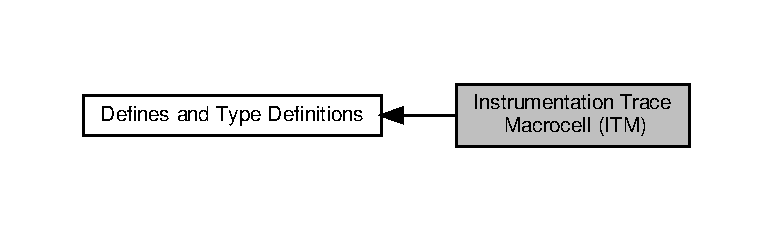
\includegraphics[width=350pt]{group___c_m_s_i_s___i_t_m}
\end{center}
\end{figure}
\subsection*{Komponenty}
\begin{DoxyCompactItemize}
\item 
struct \hyperlink{struct_i_t_m___type}{I\+T\+M\+\_\+\+Type}
\begin{DoxyCompactList}\small\item\em Structure type to access the Instrumentation Trace Macrocell Register (I\+TM). \end{DoxyCompactList}\end{DoxyCompactItemize}
\subsection*{Definicje}
\begin{DoxyCompactItemize}
\item 
\#define \hyperlink{group___c_m_s_i_s___i_t_m_gafd9ed85f36233685f182cc249621e025}{I\+T\+M\+\_\+\+S\+T\+I\+M\+\_\+\+D\+I\+S\+A\+B\+L\+E\+D\+\_\+\+Pos}~1U
\item 
\#define \hyperlink{group___c_m_s_i_s___i_t_m_ga9d8f821bdad48c7b4a02f11ebf2c8852}{I\+T\+M\+\_\+\+S\+T\+I\+M\+\_\+\+D\+I\+S\+A\+B\+L\+E\+D\+\_\+\+Msk}~(0x1\+U\+L $<$$<$ I\+T\+M\+\_\+\+S\+T\+I\+M\+\_\+\+D\+I\+S\+A\+B\+L\+E\+D\+\_\+\+Pos)
\item 
\#define \hyperlink{group___c_m_s_i_s___i_t_m_gaa79f3a59d15d810d48d924c0ca4ae0b9}{I\+T\+M\+\_\+\+S\+T\+I\+M\+\_\+\+F\+I\+F\+O\+R\+E\+A\+D\+Y\+\_\+\+Pos}~0U
\item 
\#define \hyperlink{group___c_m_s_i_s___i_t_m_ga73dc88e3338b4ef9a81e53a1d2c5ae83}{I\+T\+M\+\_\+\+S\+T\+I\+M\+\_\+\+F\+I\+F\+O\+R\+E\+A\+D\+Y\+\_\+\+Msk}~(0x1\+U\+L /$\ast$$<$$<$ I\+T\+M\+\_\+\+S\+T\+I\+M\+\_\+\+F\+I\+F\+O\+R\+E\+A\+D\+Y\+\_\+\+Pos$\ast$/)
\item 
\#define \hyperlink{group___c_m_s_i_s___i_t_m_ga7abe5e590d1611599df87a1884a352e8}{I\+T\+M\+\_\+\+T\+P\+R\+\_\+\+P\+R\+I\+V\+M\+A\+S\+K\+\_\+\+Pos}~0U
\item 
\#define \hyperlink{group___c_m_s_i_s___i_t_m_ga168e089d882df325a387aab3a802a46b}{I\+T\+M\+\_\+\+T\+P\+R\+\_\+\+P\+R\+I\+V\+M\+A\+S\+K\+\_\+\+Msk}~(0x\+F\+U\+L /$\ast$$<$$<$ I\+T\+M\+\_\+\+T\+P\+R\+\_\+\+P\+R\+I\+V\+M\+A\+S\+K\+\_\+\+Pos$\ast$/)
\item 
\#define \hyperlink{group___c_m_s_i_s___i_t_m_ga9174ad4a36052c377cef4e6aba2ed484}{I\+T\+M\+\_\+\+T\+C\+R\+\_\+\+B\+U\+S\+Y\+\_\+\+Pos}~23U
\item 
\#define \hyperlink{group___c_m_s_i_s___i_t_m_ga43ad7cf33de12f2ef3a412d4f354c60f}{I\+T\+M\+\_\+\+T\+C\+R\+\_\+\+B\+U\+S\+Y\+\_\+\+Msk}~(1\+U\+L $<$$<$ I\+T\+M\+\_\+\+T\+C\+R\+\_\+\+B\+U\+S\+Y\+\_\+\+Pos)
\item 
\#define \hyperlink{group___c_m_s_i_s___i_t_m_ga113bf41ed31584360ad7d865e5e0ace7}{I\+T\+M\+\_\+\+T\+C\+R\+\_\+\+T\+R\+A\+C\+E\+B\+U\+S\+I\+D\+\_\+\+Pos}~16U
\item 
\#define \hyperlink{group___c_m_s_i_s___i_t_m_gac014c7345304ed245b642eb9d6e9a302}{I\+T\+M\+\_\+\+T\+C\+R\+\_\+\+T\+R\+A\+C\+E\+B\+U\+S\+I\+D\+\_\+\+Msk}~(0x7\+F\+U\+L $<$$<$ I\+T\+M\+\_\+\+T\+C\+R\+\_\+\+T\+R\+A\+C\+E\+B\+U\+S\+I\+D\+\_\+\+Pos)
\item 
\#define \hyperlink{group___c_m_s_i_s___i_t_m_ga96c7c7cbc0d98426c408090b41f583f1}{I\+T\+M\+\_\+\+T\+C\+R\+\_\+\+G\+T\+S\+F\+R\+E\+Q\+\_\+\+Pos}~10U
\item 
\#define \hyperlink{group___c_m_s_i_s___i_t_m_gade862cf009827f7f6748fc44c541b067}{I\+T\+M\+\_\+\+T\+C\+R\+\_\+\+G\+T\+S\+F\+R\+E\+Q\+\_\+\+Msk}~(3\+U\+L $<$$<$ I\+T\+M\+\_\+\+T\+C\+R\+\_\+\+G\+T\+S\+F\+R\+E\+Q\+\_\+\+Pos)
\item 
\#define \hyperlink{group___c_m_s_i_s___i_t_m_gaa39e93e22d56e5e9edaf866b1171ac4f}{I\+T\+M\+\_\+\+T\+C\+R\+\_\+\+T\+S\+P\+R\+E\+S\+C\+A\+L\+E\+\_\+\+Pos}~8U
\item 
\#define \hyperlink{group___c_m_s_i_s___i_t_m_ga3e8651ecde89295bcc6e248a1b7393d6}{I\+T\+M\+\_\+\+T\+C\+R\+\_\+\+T\+S\+P\+R\+E\+S\+C\+A\+L\+E\+\_\+\+Msk}~(3\+U\+L $<$$<$ I\+T\+M\+\_\+\+T\+C\+R\+\_\+\+T\+S\+P\+R\+E\+S\+C\+A\+L\+E\+\_\+\+Pos)
\item 
\#define \hyperlink{group___c_m_s_i_s___i_t_m_gad74ca6140644b572eadbf21e870d24b9}{I\+T\+M\+\_\+\+T\+C\+R\+\_\+\+S\+T\+A\+L\+L\+E\+N\+A\+\_\+\+Pos}~5U
\item 
\#define \hyperlink{group___c_m_s_i_s___i_t_m_ga724f0560593042670b49e2f9a6483b6f}{I\+T\+M\+\_\+\+T\+C\+R\+\_\+\+S\+T\+A\+L\+L\+E\+N\+A\+\_\+\+Msk}~(1\+U\+L $<$$<$ I\+T\+M\+\_\+\+T\+C\+R\+\_\+\+S\+T\+A\+L\+L\+E\+N\+A\+\_\+\+Pos)
\item 
\#define \hyperlink{group___c_m_s_i_s___i_t_m_ga7a380f0c8078f6560051406583ecd6a5}{I\+T\+M\+\_\+\+T\+C\+R\+\_\+\+S\+W\+O\+E\+N\+A\+\_\+\+Pos}~4U
\item 
\#define \hyperlink{group___c_m_s_i_s___i_t_m_ga97476cb65bab16a328b35f81fd02010a}{I\+T\+M\+\_\+\+T\+C\+R\+\_\+\+S\+W\+O\+E\+N\+A\+\_\+\+Msk}~(1\+U\+L $<$$<$ I\+T\+M\+\_\+\+T\+C\+R\+\_\+\+S\+W\+O\+E\+N\+A\+\_\+\+Pos)
\item 
\#define \hyperlink{group___c_m_s_i_s___i_t_m_ga30e83ebb33aa766070fe3d1f27ae820e}{I\+T\+M\+\_\+\+T\+C\+R\+\_\+\+D\+W\+T\+E\+N\+A\+\_\+\+Pos}~3U
\item 
\#define \hyperlink{group___c_m_s_i_s___i_t_m_ga98ea1c596d43d3633a202f9ee746cf70}{I\+T\+M\+\_\+\+T\+C\+R\+\_\+\+D\+W\+T\+E\+N\+A\+\_\+\+Msk}~(1\+U\+L $<$$<$ I\+T\+M\+\_\+\+T\+C\+R\+\_\+\+D\+W\+T\+E\+N\+A\+\_\+\+Pos)
\item 
\#define \hyperlink{group___c_m_s_i_s___i_t_m_gaa93a1147a39fc63980d299231252a30e}{I\+T\+M\+\_\+\+T\+C\+R\+\_\+\+S\+Y\+N\+C\+E\+N\+A\+\_\+\+Pos}~2U
\item 
\#define \hyperlink{group___c_m_s_i_s___i_t_m_gac89b74a78701c25b442105d7fe2bbefb}{I\+T\+M\+\_\+\+T\+C\+R\+\_\+\+S\+Y\+N\+C\+E\+N\+A\+\_\+\+Msk}~(1\+U\+L $<$$<$ I\+T\+M\+\_\+\+T\+C\+R\+\_\+\+S\+Y\+N\+C\+E\+N\+A\+\_\+\+Pos)
\item 
\#define \hyperlink{group___c_m_s_i_s___i_t_m_ga5aa381845f810114ab519b90753922a1}{I\+T\+M\+\_\+\+T\+C\+R\+\_\+\+T\+S\+E\+N\+A\+\_\+\+Pos}~1U
\item 
\#define \hyperlink{group___c_m_s_i_s___i_t_m_ga436b2e8fa24328f48f2da31c00fc9e65}{I\+T\+M\+\_\+\+T\+C\+R\+\_\+\+T\+S\+E\+N\+A\+\_\+\+Msk}~(1\+U\+L $<$$<$ I\+T\+M\+\_\+\+T\+C\+R\+\_\+\+T\+S\+E\+N\+A\+\_\+\+Pos)
\item 
\#define \hyperlink{group___c_m_s_i_s___i_t_m_ga3286b86004bce7ffe17ee269f87f8d9d}{I\+T\+M\+\_\+\+T\+C\+R\+\_\+\+I\+T\+M\+E\+N\+A\+\_\+\+Pos}~0U
\item 
\#define \hyperlink{group___c_m_s_i_s___i_t_m_ga7dd53e3bff24ac09d94e61cb595cb2d9}{I\+T\+M\+\_\+\+T\+C\+R\+\_\+\+I\+T\+M\+E\+N\+A\+\_\+\+Msk}~(1\+U\+L /$\ast$$<$$<$ I\+T\+M\+\_\+\+T\+C\+R\+\_\+\+I\+T\+M\+E\+N\+A\+\_\+\+Pos$\ast$/)
\item 
\#define \hyperlink{group___c_m_s_i_s___i_t_m_ga04d3f842ad48f6a9127b4cecc963e1d7}{I\+T\+M\+\_\+\+I\+W\+R\+\_\+\+A\+T\+V\+A\+L\+I\+D\+M\+\_\+\+Pos}~0U
\item 
\#define \hyperlink{group___c_m_s_i_s___i_t_m_ga67b969f8f04ed15886727788f0e2ffd7}{I\+T\+M\+\_\+\+I\+W\+R\+\_\+\+A\+T\+V\+A\+L\+I\+D\+M\+\_\+\+Msk}~(1\+U\+L /$\ast$$<$$<$ I\+T\+M\+\_\+\+I\+W\+R\+\_\+\+A\+T\+V\+A\+L\+I\+D\+M\+\_\+\+Pos$\ast$/)
\item 
\#define \hyperlink{group___c_m_s_i_s___i_t_m_ga259edfd1d2e877a62e06d7a240df97f4}{I\+T\+M\+\_\+\+I\+R\+R\+\_\+\+A\+T\+R\+E\+A\+D\+Y\+M\+\_\+\+Pos}~0U
\item 
\#define \hyperlink{group___c_m_s_i_s___i_t_m_ga3dbc3e15f5bde2669cd8121a1fe419b9}{I\+T\+M\+\_\+\+I\+R\+R\+\_\+\+A\+T\+R\+E\+A\+D\+Y\+M\+\_\+\+Msk}~(1\+U\+L /$\ast$$<$$<$ I\+T\+M\+\_\+\+I\+R\+R\+\_\+\+A\+T\+R\+E\+A\+D\+Y\+M\+\_\+\+Pos$\ast$/)
\item 
\#define \hyperlink{group___c_m_s_i_s___i_t_m_ga08de02bf32caf48aaa29f7c68ff5d755}{I\+T\+M\+\_\+\+I\+M\+C\+R\+\_\+\+I\+N\+T\+E\+G\+R\+A\+T\+I\+O\+N\+\_\+\+Pos}~0U
\item 
\#define \hyperlink{group___c_m_s_i_s___i_t_m_ga8838bd3dd04c1a6be97cd946364a3fd2}{I\+T\+M\+\_\+\+I\+M\+C\+R\+\_\+\+I\+N\+T\+E\+G\+R\+A\+T\+I\+O\+N\+\_\+\+Msk}~(1\+U\+L /$\ast$$<$$<$ I\+T\+M\+\_\+\+I\+M\+C\+R\+\_\+\+I\+N\+T\+E\+G\+R\+A\+T\+I\+O\+N\+\_\+\+Pos$\ast$/)
\item 
\#define \hyperlink{group___c_m_s_i_s___i_t_m_gabfae3e570edc8759597311ed6dfb478e}{I\+T\+M\+\_\+\+L\+S\+R\+\_\+\+Byte\+Acc\+\_\+\+Pos}~2U
\item 
\#define \hyperlink{group___c_m_s_i_s___i_t_m_ga91f492b2891bb8b7eac5b58de7b220f4}{I\+T\+M\+\_\+\+L\+S\+R\+\_\+\+Byte\+Acc\+\_\+\+Msk}~(1\+U\+L $<$$<$ I\+T\+M\+\_\+\+L\+S\+R\+\_\+\+Byte\+Acc\+\_\+\+Pos)
\item 
\#define \hyperlink{group___c_m_s_i_s___i_t_m_ga144a49e12b83ad9809fdd2769094fdc0}{I\+T\+M\+\_\+\+L\+S\+R\+\_\+\+Access\+\_\+\+Pos}~1U
\item 
\#define \hyperlink{group___c_m_s_i_s___i_t_m_gac8ae69f11c0311da226c0c8ec40b3d37}{I\+T\+M\+\_\+\+L\+S\+R\+\_\+\+Access\+\_\+\+Msk}~(1\+U\+L $<$$<$ I\+T\+M\+\_\+\+L\+S\+R\+\_\+\+Access\+\_\+\+Pos)
\item 
\#define \hyperlink{group___c_m_s_i_s___i_t_m_gaf5740689cf14564d3f3fd91299b6c88d}{I\+T\+M\+\_\+\+L\+S\+R\+\_\+\+Present\+\_\+\+Pos}~0U
\item 
\#define \hyperlink{group___c_m_s_i_s___i_t_m_gaa5bc2a7f5f1d69ff819531f5508bb017}{I\+T\+M\+\_\+\+L\+S\+R\+\_\+\+Present\+\_\+\+Msk}~(1\+U\+L /$\ast$$<$$<$ I\+T\+M\+\_\+\+L\+S\+R\+\_\+\+Present\+\_\+\+Pos$\ast$/)
\item 
\#define \hyperlink{group___c_m_s_i_s___i_t_m_ga7abe5e590d1611599df87a1884a352e8}{I\+T\+M\+\_\+\+T\+P\+R\+\_\+\+P\+R\+I\+V\+M\+A\+S\+K\+\_\+\+Pos}~0U
\item 
\#define \hyperlink{group___c_m_s_i_s___i_t_m_ga168e089d882df325a387aab3a802a46b}{I\+T\+M\+\_\+\+T\+P\+R\+\_\+\+P\+R\+I\+V\+M\+A\+S\+K\+\_\+\+Msk}~(0x\+F\+F\+F\+F\+F\+F\+F\+F\+U\+L /$\ast$$<$$<$ I\+T\+M\+\_\+\+T\+P\+R\+\_\+\+P\+R\+I\+V\+M\+A\+S\+K\+\_\+\+Pos$\ast$/)
\item 
\#define \hyperlink{group___c_m_s_i_s___i_t_m_ga9174ad4a36052c377cef4e6aba2ed484}{I\+T\+M\+\_\+\+T\+C\+R\+\_\+\+B\+U\+S\+Y\+\_\+\+Pos}~23U
\item 
\#define \hyperlink{group___c_m_s_i_s___i_t_m_ga43ad7cf33de12f2ef3a412d4f354c60f}{I\+T\+M\+\_\+\+T\+C\+R\+\_\+\+B\+U\+S\+Y\+\_\+\+Msk}~(1\+U\+L $<$$<$ I\+T\+M\+\_\+\+T\+C\+R\+\_\+\+B\+U\+S\+Y\+\_\+\+Pos)
\item 
\#define \hyperlink{group___c_m_s_i_s___i_t_m_gaca0281de867f33114aac0636f7ce65d3}{I\+T\+M\+\_\+\+T\+C\+R\+\_\+\+Trace\+Bus\+I\+D\+\_\+\+Pos}~16U
\item 
\#define \hyperlink{group___c_m_s_i_s___i_t_m_ga60c20bd9649d1da5a2be8e656ba19a60}{I\+T\+M\+\_\+\+T\+C\+R\+\_\+\+Trace\+Bus\+I\+D\+\_\+\+Msk}~(0x7\+F\+U\+L $<$$<$ I\+T\+M\+\_\+\+T\+C\+R\+\_\+\+Trace\+Bus\+I\+D\+\_\+\+Pos)
\item 
\#define \hyperlink{group___c_m_s_i_s___i_t_m_ga96c7c7cbc0d98426c408090b41f583f1}{I\+T\+M\+\_\+\+T\+C\+R\+\_\+\+G\+T\+S\+F\+R\+E\+Q\+\_\+\+Pos}~10U
\item 
\#define \hyperlink{group___c_m_s_i_s___i_t_m_gade862cf009827f7f6748fc44c541b067}{I\+T\+M\+\_\+\+T\+C\+R\+\_\+\+G\+T\+S\+F\+R\+E\+Q\+\_\+\+Msk}~(3\+U\+L $<$$<$ I\+T\+M\+\_\+\+T\+C\+R\+\_\+\+G\+T\+S\+F\+R\+E\+Q\+\_\+\+Pos)
\item 
\#define \hyperlink{group___c_m_s_i_s___i_t_m_gad7bc9ee1732032c6e0de035f0978e473}{I\+T\+M\+\_\+\+T\+C\+R\+\_\+\+T\+S\+Prescale\+\_\+\+Pos}~8U
\item 
\#define \hyperlink{group___c_m_s_i_s___i_t_m_ga7a723f71bfb0204c264d8dbe8cc7ae52}{I\+T\+M\+\_\+\+T\+C\+R\+\_\+\+T\+S\+Prescale\+\_\+\+Msk}~(3\+U\+L $<$$<$ I\+T\+M\+\_\+\+T\+C\+R\+\_\+\+T\+S\+Prescale\+\_\+\+Pos)
\item 
\#define \hyperlink{group___c_m_s_i_s___i_t_m_ga7a380f0c8078f6560051406583ecd6a5}{I\+T\+M\+\_\+\+T\+C\+R\+\_\+\+S\+W\+O\+E\+N\+A\+\_\+\+Pos}~4U
\item 
\#define \hyperlink{group___c_m_s_i_s___i_t_m_ga97476cb65bab16a328b35f81fd02010a}{I\+T\+M\+\_\+\+T\+C\+R\+\_\+\+S\+W\+O\+E\+N\+A\+\_\+\+Msk}~(1\+U\+L $<$$<$ I\+T\+M\+\_\+\+T\+C\+R\+\_\+\+S\+W\+O\+E\+N\+A\+\_\+\+Pos)
\item 
\#define \hyperlink{group___c_m_s_i_s___i_t_m_ga30e83ebb33aa766070fe3d1f27ae820e}{I\+T\+M\+\_\+\+T\+C\+R\+\_\+\+D\+W\+T\+E\+N\+A\+\_\+\+Pos}~3U
\item 
\#define \hyperlink{group___c_m_s_i_s___i_t_m_ga98ea1c596d43d3633a202f9ee746cf70}{I\+T\+M\+\_\+\+T\+C\+R\+\_\+\+D\+W\+T\+E\+N\+A\+\_\+\+Msk}~(1\+U\+L $<$$<$ I\+T\+M\+\_\+\+T\+C\+R\+\_\+\+D\+W\+T\+E\+N\+A\+\_\+\+Pos)
\item 
\#define \hyperlink{group___c_m_s_i_s___i_t_m_gaa93a1147a39fc63980d299231252a30e}{I\+T\+M\+\_\+\+T\+C\+R\+\_\+\+S\+Y\+N\+C\+E\+N\+A\+\_\+\+Pos}~2U
\item 
\#define \hyperlink{group___c_m_s_i_s___i_t_m_gac89b74a78701c25b442105d7fe2bbefb}{I\+T\+M\+\_\+\+T\+C\+R\+\_\+\+S\+Y\+N\+C\+E\+N\+A\+\_\+\+Msk}~(1\+U\+L $<$$<$ I\+T\+M\+\_\+\+T\+C\+R\+\_\+\+S\+Y\+N\+C\+E\+N\+A\+\_\+\+Pos)
\item 
\#define \hyperlink{group___c_m_s_i_s___i_t_m_ga5aa381845f810114ab519b90753922a1}{I\+T\+M\+\_\+\+T\+C\+R\+\_\+\+T\+S\+E\+N\+A\+\_\+\+Pos}~1U
\item 
\#define \hyperlink{group___c_m_s_i_s___i_t_m_ga436b2e8fa24328f48f2da31c00fc9e65}{I\+T\+M\+\_\+\+T\+C\+R\+\_\+\+T\+S\+E\+N\+A\+\_\+\+Msk}~(1\+U\+L $<$$<$ I\+T\+M\+\_\+\+T\+C\+R\+\_\+\+T\+S\+E\+N\+A\+\_\+\+Pos)
\item 
\#define \hyperlink{group___c_m_s_i_s___i_t_m_ga3286b86004bce7ffe17ee269f87f8d9d}{I\+T\+M\+\_\+\+T\+C\+R\+\_\+\+I\+T\+M\+E\+N\+A\+\_\+\+Pos}~0U
\item 
\#define \hyperlink{group___c_m_s_i_s___i_t_m_ga7dd53e3bff24ac09d94e61cb595cb2d9}{I\+T\+M\+\_\+\+T\+C\+R\+\_\+\+I\+T\+M\+E\+N\+A\+\_\+\+Msk}~(1\+U\+L /$\ast$$<$$<$ I\+T\+M\+\_\+\+T\+C\+R\+\_\+\+I\+T\+M\+E\+N\+A\+\_\+\+Pos$\ast$/)
\item 
\#define \hyperlink{group___c_m_s_i_s___i_t_m_ga04d3f842ad48f6a9127b4cecc963e1d7}{I\+T\+M\+\_\+\+I\+W\+R\+\_\+\+A\+T\+V\+A\+L\+I\+D\+M\+\_\+\+Pos}~0U
\item 
\#define \hyperlink{group___c_m_s_i_s___i_t_m_ga67b969f8f04ed15886727788f0e2ffd7}{I\+T\+M\+\_\+\+I\+W\+R\+\_\+\+A\+T\+V\+A\+L\+I\+D\+M\+\_\+\+Msk}~(1\+U\+L /$\ast$$<$$<$ I\+T\+M\+\_\+\+I\+W\+R\+\_\+\+A\+T\+V\+A\+L\+I\+D\+M\+\_\+\+Pos$\ast$/)
\item 
\#define \hyperlink{group___c_m_s_i_s___i_t_m_ga259edfd1d2e877a62e06d7a240df97f4}{I\+T\+M\+\_\+\+I\+R\+R\+\_\+\+A\+T\+R\+E\+A\+D\+Y\+M\+\_\+\+Pos}~0U
\item 
\#define \hyperlink{group___c_m_s_i_s___i_t_m_ga3dbc3e15f5bde2669cd8121a1fe419b9}{I\+T\+M\+\_\+\+I\+R\+R\+\_\+\+A\+T\+R\+E\+A\+D\+Y\+M\+\_\+\+Msk}~(1\+U\+L /$\ast$$<$$<$ I\+T\+M\+\_\+\+I\+R\+R\+\_\+\+A\+T\+R\+E\+A\+D\+Y\+M\+\_\+\+Pos$\ast$/)
\item 
\#define \hyperlink{group___c_m_s_i_s___i_t_m_ga08de02bf32caf48aaa29f7c68ff5d755}{I\+T\+M\+\_\+\+I\+M\+C\+R\+\_\+\+I\+N\+T\+E\+G\+R\+A\+T\+I\+O\+N\+\_\+\+Pos}~0U
\item 
\#define \hyperlink{group___c_m_s_i_s___i_t_m_ga8838bd3dd04c1a6be97cd946364a3fd2}{I\+T\+M\+\_\+\+I\+M\+C\+R\+\_\+\+I\+N\+T\+E\+G\+R\+A\+T\+I\+O\+N\+\_\+\+Msk}~(1\+U\+L /$\ast$$<$$<$ I\+T\+M\+\_\+\+I\+M\+C\+R\+\_\+\+I\+N\+T\+E\+G\+R\+A\+T\+I\+O\+N\+\_\+\+Pos$\ast$/)
\item 
\#define \hyperlink{group___c_m_s_i_s___i_t_m_gabfae3e570edc8759597311ed6dfb478e}{I\+T\+M\+\_\+\+L\+S\+R\+\_\+\+Byte\+Acc\+\_\+\+Pos}~2U
\item 
\#define \hyperlink{group___c_m_s_i_s___i_t_m_ga91f492b2891bb8b7eac5b58de7b220f4}{I\+T\+M\+\_\+\+L\+S\+R\+\_\+\+Byte\+Acc\+\_\+\+Msk}~(1\+U\+L $<$$<$ I\+T\+M\+\_\+\+L\+S\+R\+\_\+\+Byte\+Acc\+\_\+\+Pos)
\item 
\#define \hyperlink{group___c_m_s_i_s___i_t_m_ga144a49e12b83ad9809fdd2769094fdc0}{I\+T\+M\+\_\+\+L\+S\+R\+\_\+\+Access\+\_\+\+Pos}~1U
\item 
\#define \hyperlink{group___c_m_s_i_s___i_t_m_gac8ae69f11c0311da226c0c8ec40b3d37}{I\+T\+M\+\_\+\+L\+S\+R\+\_\+\+Access\+\_\+\+Msk}~(1\+U\+L $<$$<$ I\+T\+M\+\_\+\+L\+S\+R\+\_\+\+Access\+\_\+\+Pos)
\item 
\#define \hyperlink{group___c_m_s_i_s___i_t_m_gaf5740689cf14564d3f3fd91299b6c88d}{I\+T\+M\+\_\+\+L\+S\+R\+\_\+\+Present\+\_\+\+Pos}~0U
\item 
\#define \hyperlink{group___c_m_s_i_s___i_t_m_gaa5bc2a7f5f1d69ff819531f5508bb017}{I\+T\+M\+\_\+\+L\+S\+R\+\_\+\+Present\+\_\+\+Msk}~(1\+U\+L /$\ast$$<$$<$ I\+T\+M\+\_\+\+L\+S\+R\+\_\+\+Present\+\_\+\+Pos$\ast$/)
\item 
\#define \hyperlink{group___c_m_s_i_s___i_t_m_gafd9ed85f36233685f182cc249621e025}{I\+T\+M\+\_\+\+S\+T\+I\+M\+\_\+\+D\+I\+S\+A\+B\+L\+E\+D\+\_\+\+Pos}~1U
\item 
\#define \hyperlink{group___c_m_s_i_s___i_t_m_ga9d8f821bdad48c7b4a02f11ebf2c8852}{I\+T\+M\+\_\+\+S\+T\+I\+M\+\_\+\+D\+I\+S\+A\+B\+L\+E\+D\+\_\+\+Msk}~(0x1\+U\+L $<$$<$ I\+T\+M\+\_\+\+S\+T\+I\+M\+\_\+\+D\+I\+S\+A\+B\+L\+E\+D\+\_\+\+Pos)
\item 
\#define \hyperlink{group___c_m_s_i_s___i_t_m_gaa79f3a59d15d810d48d924c0ca4ae0b9}{I\+T\+M\+\_\+\+S\+T\+I\+M\+\_\+\+F\+I\+F\+O\+R\+E\+A\+D\+Y\+\_\+\+Pos}~0U
\item 
\#define \hyperlink{group___c_m_s_i_s___i_t_m_ga73dc88e3338b4ef9a81e53a1d2c5ae83}{I\+T\+M\+\_\+\+S\+T\+I\+M\+\_\+\+F\+I\+F\+O\+R\+E\+A\+D\+Y\+\_\+\+Msk}~(0x1\+U\+L /$\ast$$<$$<$ I\+T\+M\+\_\+\+S\+T\+I\+M\+\_\+\+F\+I\+F\+O\+R\+E\+A\+D\+Y\+\_\+\+Pos$\ast$/)
\item 
\#define \hyperlink{group___c_m_s_i_s___i_t_m_ga7abe5e590d1611599df87a1884a352e8}{I\+T\+M\+\_\+\+T\+P\+R\+\_\+\+P\+R\+I\+V\+M\+A\+S\+K\+\_\+\+Pos}~0U
\item 
\#define \hyperlink{group___c_m_s_i_s___i_t_m_ga168e089d882df325a387aab3a802a46b}{I\+T\+M\+\_\+\+T\+P\+R\+\_\+\+P\+R\+I\+V\+M\+A\+S\+K\+\_\+\+Msk}~(0x\+F\+F\+F\+F\+F\+F\+F\+F\+U\+L /$\ast$$<$$<$ I\+T\+M\+\_\+\+T\+P\+R\+\_\+\+P\+R\+I\+V\+M\+A\+S\+K\+\_\+\+Pos$\ast$/)
\item 
\#define \hyperlink{group___c_m_s_i_s___i_t_m_ga9174ad4a36052c377cef4e6aba2ed484}{I\+T\+M\+\_\+\+T\+C\+R\+\_\+\+B\+U\+S\+Y\+\_\+\+Pos}~23U
\item 
\#define \hyperlink{group___c_m_s_i_s___i_t_m_ga43ad7cf33de12f2ef3a412d4f354c60f}{I\+T\+M\+\_\+\+T\+C\+R\+\_\+\+B\+U\+S\+Y\+\_\+\+Msk}~(1\+U\+L $<$$<$ I\+T\+M\+\_\+\+T\+C\+R\+\_\+\+B\+U\+S\+Y\+\_\+\+Pos)
\item 
\#define \hyperlink{group___c_m_s_i_s___i_t_m_ga113bf41ed31584360ad7d865e5e0ace7}{I\+T\+M\+\_\+\+T\+C\+R\+\_\+\+T\+R\+A\+C\+E\+B\+U\+S\+I\+D\+\_\+\+Pos}~16U
\item 
\#define \hyperlink{group___c_m_s_i_s___i_t_m_gac014c7345304ed245b642eb9d6e9a302}{I\+T\+M\+\_\+\+T\+C\+R\+\_\+\+T\+R\+A\+C\+E\+B\+U\+S\+I\+D\+\_\+\+Msk}~(0x7\+F\+U\+L $<$$<$ I\+T\+M\+\_\+\+T\+C\+R\+\_\+\+T\+R\+A\+C\+E\+B\+U\+S\+I\+D\+\_\+\+Pos)
\item 
\#define \hyperlink{group___c_m_s_i_s___i_t_m_ga96c7c7cbc0d98426c408090b41f583f1}{I\+T\+M\+\_\+\+T\+C\+R\+\_\+\+G\+T\+S\+F\+R\+E\+Q\+\_\+\+Pos}~10U
\item 
\#define \hyperlink{group___c_m_s_i_s___i_t_m_gade862cf009827f7f6748fc44c541b067}{I\+T\+M\+\_\+\+T\+C\+R\+\_\+\+G\+T\+S\+F\+R\+E\+Q\+\_\+\+Msk}~(3\+U\+L $<$$<$ I\+T\+M\+\_\+\+T\+C\+R\+\_\+\+G\+T\+S\+F\+R\+E\+Q\+\_\+\+Pos)
\item 
\#define \hyperlink{group___c_m_s_i_s___i_t_m_gaa39e93e22d56e5e9edaf866b1171ac4f}{I\+T\+M\+\_\+\+T\+C\+R\+\_\+\+T\+S\+P\+R\+E\+S\+C\+A\+L\+E\+\_\+\+Pos}~8U
\item 
\#define \hyperlink{group___c_m_s_i_s___i_t_m_ga3e8651ecde89295bcc6e248a1b7393d6}{I\+T\+M\+\_\+\+T\+C\+R\+\_\+\+T\+S\+P\+R\+E\+S\+C\+A\+L\+E\+\_\+\+Msk}~(3\+U\+L $<$$<$ I\+T\+M\+\_\+\+T\+C\+R\+\_\+\+T\+S\+P\+R\+E\+S\+C\+A\+L\+E\+\_\+\+Pos)
\item 
\#define \hyperlink{group___c_m_s_i_s___i_t_m_gad74ca6140644b572eadbf21e870d24b9}{I\+T\+M\+\_\+\+T\+C\+R\+\_\+\+S\+T\+A\+L\+L\+E\+N\+A\+\_\+\+Pos}~5U
\item 
\#define \hyperlink{group___c_m_s_i_s___i_t_m_ga724f0560593042670b49e2f9a6483b6f}{I\+T\+M\+\_\+\+T\+C\+R\+\_\+\+S\+T\+A\+L\+L\+E\+N\+A\+\_\+\+Msk}~(1\+U\+L $<$$<$ I\+T\+M\+\_\+\+T\+C\+R\+\_\+\+S\+T\+A\+L\+L\+E\+N\+A\+\_\+\+Pos)
\item 
\#define \hyperlink{group___c_m_s_i_s___i_t_m_ga7a380f0c8078f6560051406583ecd6a5}{I\+T\+M\+\_\+\+T\+C\+R\+\_\+\+S\+W\+O\+E\+N\+A\+\_\+\+Pos}~4U
\item 
\#define \hyperlink{group___c_m_s_i_s___i_t_m_ga97476cb65bab16a328b35f81fd02010a}{I\+T\+M\+\_\+\+T\+C\+R\+\_\+\+S\+W\+O\+E\+N\+A\+\_\+\+Msk}~(1\+U\+L $<$$<$ I\+T\+M\+\_\+\+T\+C\+R\+\_\+\+S\+W\+O\+E\+N\+A\+\_\+\+Pos)
\item 
\#define \hyperlink{group___c_m_s_i_s___i_t_m_ga30e83ebb33aa766070fe3d1f27ae820e}{I\+T\+M\+\_\+\+T\+C\+R\+\_\+\+D\+W\+T\+E\+N\+A\+\_\+\+Pos}~3U
\item 
\#define \hyperlink{group___c_m_s_i_s___i_t_m_ga98ea1c596d43d3633a202f9ee746cf70}{I\+T\+M\+\_\+\+T\+C\+R\+\_\+\+D\+W\+T\+E\+N\+A\+\_\+\+Msk}~(1\+U\+L $<$$<$ I\+T\+M\+\_\+\+T\+C\+R\+\_\+\+D\+W\+T\+E\+N\+A\+\_\+\+Pos)
\item 
\#define \hyperlink{group___c_m_s_i_s___i_t_m_gaa93a1147a39fc63980d299231252a30e}{I\+T\+M\+\_\+\+T\+C\+R\+\_\+\+S\+Y\+N\+C\+E\+N\+A\+\_\+\+Pos}~2U
\item 
\#define \hyperlink{group___c_m_s_i_s___i_t_m_gac89b74a78701c25b442105d7fe2bbefb}{I\+T\+M\+\_\+\+T\+C\+R\+\_\+\+S\+Y\+N\+C\+E\+N\+A\+\_\+\+Msk}~(1\+U\+L $<$$<$ I\+T\+M\+\_\+\+T\+C\+R\+\_\+\+S\+Y\+N\+C\+E\+N\+A\+\_\+\+Pos)
\item 
\#define \hyperlink{group___c_m_s_i_s___i_t_m_ga5aa381845f810114ab519b90753922a1}{I\+T\+M\+\_\+\+T\+C\+R\+\_\+\+T\+S\+E\+N\+A\+\_\+\+Pos}~1U
\item 
\#define \hyperlink{group___c_m_s_i_s___i_t_m_ga436b2e8fa24328f48f2da31c00fc9e65}{I\+T\+M\+\_\+\+T\+C\+R\+\_\+\+T\+S\+E\+N\+A\+\_\+\+Msk}~(1\+U\+L $<$$<$ I\+T\+M\+\_\+\+T\+C\+R\+\_\+\+T\+S\+E\+N\+A\+\_\+\+Pos)
\item 
\#define \hyperlink{group___c_m_s_i_s___i_t_m_ga3286b86004bce7ffe17ee269f87f8d9d}{I\+T\+M\+\_\+\+T\+C\+R\+\_\+\+I\+T\+M\+E\+N\+A\+\_\+\+Pos}~0U
\item 
\#define \hyperlink{group___c_m_s_i_s___i_t_m_ga7dd53e3bff24ac09d94e61cb595cb2d9}{I\+T\+M\+\_\+\+T\+C\+R\+\_\+\+I\+T\+M\+E\+N\+A\+\_\+\+Msk}~(1\+U\+L /$\ast$$<$$<$ I\+T\+M\+\_\+\+T\+C\+R\+\_\+\+I\+T\+M\+E\+N\+A\+\_\+\+Pos$\ast$/)
\item 
\#define \hyperlink{group___c_m_s_i_s___i_t_m_ga04d3f842ad48f6a9127b4cecc963e1d7}{I\+T\+M\+\_\+\+I\+W\+R\+\_\+\+A\+T\+V\+A\+L\+I\+D\+M\+\_\+\+Pos}~0U
\item 
\#define \hyperlink{group___c_m_s_i_s___i_t_m_ga67b969f8f04ed15886727788f0e2ffd7}{I\+T\+M\+\_\+\+I\+W\+R\+\_\+\+A\+T\+V\+A\+L\+I\+D\+M\+\_\+\+Msk}~(1\+U\+L /$\ast$$<$$<$ I\+T\+M\+\_\+\+I\+W\+R\+\_\+\+A\+T\+V\+A\+L\+I\+D\+M\+\_\+\+Pos$\ast$/)
\item 
\#define \hyperlink{group___c_m_s_i_s___i_t_m_ga259edfd1d2e877a62e06d7a240df97f4}{I\+T\+M\+\_\+\+I\+R\+R\+\_\+\+A\+T\+R\+E\+A\+D\+Y\+M\+\_\+\+Pos}~0U
\item 
\#define \hyperlink{group___c_m_s_i_s___i_t_m_ga3dbc3e15f5bde2669cd8121a1fe419b9}{I\+T\+M\+\_\+\+I\+R\+R\+\_\+\+A\+T\+R\+E\+A\+D\+Y\+M\+\_\+\+Msk}~(1\+U\+L /$\ast$$<$$<$ I\+T\+M\+\_\+\+I\+R\+R\+\_\+\+A\+T\+R\+E\+A\+D\+Y\+M\+\_\+\+Pos$\ast$/)
\item 
\#define \hyperlink{group___c_m_s_i_s___i_t_m_ga08de02bf32caf48aaa29f7c68ff5d755}{I\+T\+M\+\_\+\+I\+M\+C\+R\+\_\+\+I\+N\+T\+E\+G\+R\+A\+T\+I\+O\+N\+\_\+\+Pos}~0U
\item 
\#define \hyperlink{group___c_m_s_i_s___i_t_m_ga8838bd3dd04c1a6be97cd946364a3fd2}{I\+T\+M\+\_\+\+I\+M\+C\+R\+\_\+\+I\+N\+T\+E\+G\+R\+A\+T\+I\+O\+N\+\_\+\+Msk}~(1\+U\+L /$\ast$$<$$<$ I\+T\+M\+\_\+\+I\+M\+C\+R\+\_\+\+I\+N\+T\+E\+G\+R\+A\+T\+I\+O\+N\+\_\+\+Pos$\ast$/)
\item 
\#define \hyperlink{group___c_m_s_i_s___i_t_m_gabfae3e570edc8759597311ed6dfb478e}{I\+T\+M\+\_\+\+L\+S\+R\+\_\+\+Byte\+Acc\+\_\+\+Pos}~2U
\item 
\#define \hyperlink{group___c_m_s_i_s___i_t_m_ga91f492b2891bb8b7eac5b58de7b220f4}{I\+T\+M\+\_\+\+L\+S\+R\+\_\+\+Byte\+Acc\+\_\+\+Msk}~(1\+U\+L $<$$<$ I\+T\+M\+\_\+\+L\+S\+R\+\_\+\+Byte\+Acc\+\_\+\+Pos)
\item 
\#define \hyperlink{group___c_m_s_i_s___i_t_m_ga144a49e12b83ad9809fdd2769094fdc0}{I\+T\+M\+\_\+\+L\+S\+R\+\_\+\+Access\+\_\+\+Pos}~1U
\item 
\#define \hyperlink{group___c_m_s_i_s___i_t_m_gac8ae69f11c0311da226c0c8ec40b3d37}{I\+T\+M\+\_\+\+L\+S\+R\+\_\+\+Access\+\_\+\+Msk}~(1\+U\+L $<$$<$ I\+T\+M\+\_\+\+L\+S\+R\+\_\+\+Access\+\_\+\+Pos)
\item 
\#define \hyperlink{group___c_m_s_i_s___i_t_m_gaf5740689cf14564d3f3fd91299b6c88d}{I\+T\+M\+\_\+\+L\+S\+R\+\_\+\+Present\+\_\+\+Pos}~0U
\item 
\#define \hyperlink{group___c_m_s_i_s___i_t_m_gaa5bc2a7f5f1d69ff819531f5508bb017}{I\+T\+M\+\_\+\+L\+S\+R\+\_\+\+Present\+\_\+\+Msk}~(1\+U\+L /$\ast$$<$$<$ I\+T\+M\+\_\+\+L\+S\+R\+\_\+\+Present\+\_\+\+Pos$\ast$/)
\item 
\#define \hyperlink{group___c_m_s_i_s___i_t_m_ga7abe5e590d1611599df87a1884a352e8}{I\+T\+M\+\_\+\+T\+P\+R\+\_\+\+P\+R\+I\+V\+M\+A\+S\+K\+\_\+\+Pos}~0U
\item 
\#define \hyperlink{group___c_m_s_i_s___i_t_m_ga168e089d882df325a387aab3a802a46b}{I\+T\+M\+\_\+\+T\+P\+R\+\_\+\+P\+R\+I\+V\+M\+A\+S\+K\+\_\+\+Msk}~(0x\+F\+F\+F\+F\+F\+F\+F\+F\+U\+L /$\ast$$<$$<$ I\+T\+M\+\_\+\+T\+P\+R\+\_\+\+P\+R\+I\+V\+M\+A\+S\+K\+\_\+\+Pos$\ast$/)
\item 
\#define \hyperlink{group___c_m_s_i_s___i_t_m_ga9174ad4a36052c377cef4e6aba2ed484}{I\+T\+M\+\_\+\+T\+C\+R\+\_\+\+B\+U\+S\+Y\+\_\+\+Pos}~23U
\item 
\#define \hyperlink{group___c_m_s_i_s___i_t_m_ga43ad7cf33de12f2ef3a412d4f354c60f}{I\+T\+M\+\_\+\+T\+C\+R\+\_\+\+B\+U\+S\+Y\+\_\+\+Msk}~(1\+U\+L $<$$<$ I\+T\+M\+\_\+\+T\+C\+R\+\_\+\+B\+U\+S\+Y\+\_\+\+Pos)
\item 
\#define \hyperlink{group___c_m_s_i_s___i_t_m_gaca0281de867f33114aac0636f7ce65d3}{I\+T\+M\+\_\+\+T\+C\+R\+\_\+\+Trace\+Bus\+I\+D\+\_\+\+Pos}~16U
\item 
\#define \hyperlink{group___c_m_s_i_s___i_t_m_ga60c20bd9649d1da5a2be8e656ba19a60}{I\+T\+M\+\_\+\+T\+C\+R\+\_\+\+Trace\+Bus\+I\+D\+\_\+\+Msk}~(0x7\+F\+U\+L $<$$<$ I\+T\+M\+\_\+\+T\+C\+R\+\_\+\+Trace\+Bus\+I\+D\+\_\+\+Pos)
\item 
\#define \hyperlink{group___c_m_s_i_s___i_t_m_ga96c7c7cbc0d98426c408090b41f583f1}{I\+T\+M\+\_\+\+T\+C\+R\+\_\+\+G\+T\+S\+F\+R\+E\+Q\+\_\+\+Pos}~10U
\item 
\#define \hyperlink{group___c_m_s_i_s___i_t_m_gade862cf009827f7f6748fc44c541b067}{I\+T\+M\+\_\+\+T\+C\+R\+\_\+\+G\+T\+S\+F\+R\+E\+Q\+\_\+\+Msk}~(3\+U\+L $<$$<$ I\+T\+M\+\_\+\+T\+C\+R\+\_\+\+G\+T\+S\+F\+R\+E\+Q\+\_\+\+Pos)
\item 
\#define \hyperlink{group___c_m_s_i_s___i_t_m_gad7bc9ee1732032c6e0de035f0978e473}{I\+T\+M\+\_\+\+T\+C\+R\+\_\+\+T\+S\+Prescale\+\_\+\+Pos}~8U
\item 
\#define \hyperlink{group___c_m_s_i_s___i_t_m_ga7a723f71bfb0204c264d8dbe8cc7ae52}{I\+T\+M\+\_\+\+T\+C\+R\+\_\+\+T\+S\+Prescale\+\_\+\+Msk}~(3\+U\+L $<$$<$ I\+T\+M\+\_\+\+T\+C\+R\+\_\+\+T\+S\+Prescale\+\_\+\+Pos)
\item 
\#define \hyperlink{group___c_m_s_i_s___i_t_m_ga7a380f0c8078f6560051406583ecd6a5}{I\+T\+M\+\_\+\+T\+C\+R\+\_\+\+S\+W\+O\+E\+N\+A\+\_\+\+Pos}~4U
\item 
\#define \hyperlink{group___c_m_s_i_s___i_t_m_ga97476cb65bab16a328b35f81fd02010a}{I\+T\+M\+\_\+\+T\+C\+R\+\_\+\+S\+W\+O\+E\+N\+A\+\_\+\+Msk}~(1\+U\+L $<$$<$ I\+T\+M\+\_\+\+T\+C\+R\+\_\+\+S\+W\+O\+E\+N\+A\+\_\+\+Pos)
\item 
\#define \hyperlink{group___c_m_s_i_s___i_t_m_ga30e83ebb33aa766070fe3d1f27ae820e}{I\+T\+M\+\_\+\+T\+C\+R\+\_\+\+D\+W\+T\+E\+N\+A\+\_\+\+Pos}~3U
\item 
\#define \hyperlink{group___c_m_s_i_s___i_t_m_ga98ea1c596d43d3633a202f9ee746cf70}{I\+T\+M\+\_\+\+T\+C\+R\+\_\+\+D\+W\+T\+E\+N\+A\+\_\+\+Msk}~(1\+U\+L $<$$<$ I\+T\+M\+\_\+\+T\+C\+R\+\_\+\+D\+W\+T\+E\+N\+A\+\_\+\+Pos)
\item 
\#define \hyperlink{group___c_m_s_i_s___i_t_m_gaa93a1147a39fc63980d299231252a30e}{I\+T\+M\+\_\+\+T\+C\+R\+\_\+\+S\+Y\+N\+C\+E\+N\+A\+\_\+\+Pos}~2U
\item 
\#define \hyperlink{group___c_m_s_i_s___i_t_m_gac89b74a78701c25b442105d7fe2bbefb}{I\+T\+M\+\_\+\+T\+C\+R\+\_\+\+S\+Y\+N\+C\+E\+N\+A\+\_\+\+Msk}~(1\+U\+L $<$$<$ I\+T\+M\+\_\+\+T\+C\+R\+\_\+\+S\+Y\+N\+C\+E\+N\+A\+\_\+\+Pos)
\item 
\#define \hyperlink{group___c_m_s_i_s___i_t_m_ga5aa381845f810114ab519b90753922a1}{I\+T\+M\+\_\+\+T\+C\+R\+\_\+\+T\+S\+E\+N\+A\+\_\+\+Pos}~1U
\item 
\#define \hyperlink{group___c_m_s_i_s___i_t_m_ga436b2e8fa24328f48f2da31c00fc9e65}{I\+T\+M\+\_\+\+T\+C\+R\+\_\+\+T\+S\+E\+N\+A\+\_\+\+Msk}~(1\+U\+L $<$$<$ I\+T\+M\+\_\+\+T\+C\+R\+\_\+\+T\+S\+E\+N\+A\+\_\+\+Pos)
\item 
\#define \hyperlink{group___c_m_s_i_s___i_t_m_ga3286b86004bce7ffe17ee269f87f8d9d}{I\+T\+M\+\_\+\+T\+C\+R\+\_\+\+I\+T\+M\+E\+N\+A\+\_\+\+Pos}~0U
\item 
\#define \hyperlink{group___c_m_s_i_s___i_t_m_ga7dd53e3bff24ac09d94e61cb595cb2d9}{I\+T\+M\+\_\+\+T\+C\+R\+\_\+\+I\+T\+M\+E\+N\+A\+\_\+\+Msk}~(1\+U\+L /$\ast$$<$$<$ I\+T\+M\+\_\+\+T\+C\+R\+\_\+\+I\+T\+M\+E\+N\+A\+\_\+\+Pos$\ast$/)
\item 
\#define \hyperlink{group___c_m_s_i_s___i_t_m_ga04d3f842ad48f6a9127b4cecc963e1d7}{I\+T\+M\+\_\+\+I\+W\+R\+\_\+\+A\+T\+V\+A\+L\+I\+D\+M\+\_\+\+Pos}~0U
\item 
\#define \hyperlink{group___c_m_s_i_s___i_t_m_ga67b969f8f04ed15886727788f0e2ffd7}{I\+T\+M\+\_\+\+I\+W\+R\+\_\+\+A\+T\+V\+A\+L\+I\+D\+M\+\_\+\+Msk}~(1\+U\+L /$\ast$$<$$<$ I\+T\+M\+\_\+\+I\+W\+R\+\_\+\+A\+T\+V\+A\+L\+I\+D\+M\+\_\+\+Pos$\ast$/)
\item 
\#define \hyperlink{group___c_m_s_i_s___i_t_m_ga259edfd1d2e877a62e06d7a240df97f4}{I\+T\+M\+\_\+\+I\+R\+R\+\_\+\+A\+T\+R\+E\+A\+D\+Y\+M\+\_\+\+Pos}~0U
\item 
\#define \hyperlink{group___c_m_s_i_s___i_t_m_ga3dbc3e15f5bde2669cd8121a1fe419b9}{I\+T\+M\+\_\+\+I\+R\+R\+\_\+\+A\+T\+R\+E\+A\+D\+Y\+M\+\_\+\+Msk}~(1\+U\+L /$\ast$$<$$<$ I\+T\+M\+\_\+\+I\+R\+R\+\_\+\+A\+T\+R\+E\+A\+D\+Y\+M\+\_\+\+Pos$\ast$/)
\item 
\#define \hyperlink{group___c_m_s_i_s___i_t_m_ga08de02bf32caf48aaa29f7c68ff5d755}{I\+T\+M\+\_\+\+I\+M\+C\+R\+\_\+\+I\+N\+T\+E\+G\+R\+A\+T\+I\+O\+N\+\_\+\+Pos}~0U
\item 
\#define \hyperlink{group___c_m_s_i_s___i_t_m_ga8838bd3dd04c1a6be97cd946364a3fd2}{I\+T\+M\+\_\+\+I\+M\+C\+R\+\_\+\+I\+N\+T\+E\+G\+R\+A\+T\+I\+O\+N\+\_\+\+Msk}~(1\+U\+L /$\ast$$<$$<$ I\+T\+M\+\_\+\+I\+M\+C\+R\+\_\+\+I\+N\+T\+E\+G\+R\+A\+T\+I\+O\+N\+\_\+\+Pos$\ast$/)
\item 
\#define \hyperlink{group___c_m_s_i_s___i_t_m_gabfae3e570edc8759597311ed6dfb478e}{I\+T\+M\+\_\+\+L\+S\+R\+\_\+\+Byte\+Acc\+\_\+\+Pos}~2U
\item 
\#define \hyperlink{group___c_m_s_i_s___i_t_m_ga91f492b2891bb8b7eac5b58de7b220f4}{I\+T\+M\+\_\+\+L\+S\+R\+\_\+\+Byte\+Acc\+\_\+\+Msk}~(1\+U\+L $<$$<$ I\+T\+M\+\_\+\+L\+S\+R\+\_\+\+Byte\+Acc\+\_\+\+Pos)
\item 
\#define \hyperlink{group___c_m_s_i_s___i_t_m_ga144a49e12b83ad9809fdd2769094fdc0}{I\+T\+M\+\_\+\+L\+S\+R\+\_\+\+Access\+\_\+\+Pos}~1U
\item 
\#define \hyperlink{group___c_m_s_i_s___i_t_m_gac8ae69f11c0311da226c0c8ec40b3d37}{I\+T\+M\+\_\+\+L\+S\+R\+\_\+\+Access\+\_\+\+Msk}~(1\+U\+L $<$$<$ I\+T\+M\+\_\+\+L\+S\+R\+\_\+\+Access\+\_\+\+Pos)
\item 
\#define \hyperlink{group___c_m_s_i_s___i_t_m_gaf5740689cf14564d3f3fd91299b6c88d}{I\+T\+M\+\_\+\+L\+S\+R\+\_\+\+Present\+\_\+\+Pos}~0U
\item 
\#define \hyperlink{group___c_m_s_i_s___i_t_m_gaa5bc2a7f5f1d69ff819531f5508bb017}{I\+T\+M\+\_\+\+L\+S\+R\+\_\+\+Present\+\_\+\+Msk}~(1\+U\+L /$\ast$$<$$<$ I\+T\+M\+\_\+\+L\+S\+R\+\_\+\+Present\+\_\+\+Pos$\ast$/)
\item 
\#define \hyperlink{group___c_m_s_i_s___i_t_m_ga7abe5e590d1611599df87a1884a352e8}{I\+T\+M\+\_\+\+T\+P\+R\+\_\+\+P\+R\+I\+V\+M\+A\+S\+K\+\_\+\+Pos}~0U
\item 
\#define \hyperlink{group___c_m_s_i_s___i_t_m_ga168e089d882df325a387aab3a802a46b}{I\+T\+M\+\_\+\+T\+P\+R\+\_\+\+P\+R\+I\+V\+M\+A\+S\+K\+\_\+\+Msk}~(0x\+F\+F\+F\+F\+F\+F\+F\+F\+U\+L /$\ast$$<$$<$ I\+T\+M\+\_\+\+T\+P\+R\+\_\+\+P\+R\+I\+V\+M\+A\+S\+K\+\_\+\+Pos$\ast$/)
\item 
\#define \hyperlink{group___c_m_s_i_s___i_t_m_ga9174ad4a36052c377cef4e6aba2ed484}{I\+T\+M\+\_\+\+T\+C\+R\+\_\+\+B\+U\+S\+Y\+\_\+\+Pos}~23U
\item 
\#define \hyperlink{group___c_m_s_i_s___i_t_m_ga43ad7cf33de12f2ef3a412d4f354c60f}{I\+T\+M\+\_\+\+T\+C\+R\+\_\+\+B\+U\+S\+Y\+\_\+\+Msk}~(1\+U\+L $<$$<$ I\+T\+M\+\_\+\+T\+C\+R\+\_\+\+B\+U\+S\+Y\+\_\+\+Pos)
\item 
\#define \hyperlink{group___c_m_s_i_s___i_t_m_gaca0281de867f33114aac0636f7ce65d3}{I\+T\+M\+\_\+\+T\+C\+R\+\_\+\+Trace\+Bus\+I\+D\+\_\+\+Pos}~16U
\item 
\#define \hyperlink{group___c_m_s_i_s___i_t_m_ga60c20bd9649d1da5a2be8e656ba19a60}{I\+T\+M\+\_\+\+T\+C\+R\+\_\+\+Trace\+Bus\+I\+D\+\_\+\+Msk}~(0x7\+F\+U\+L $<$$<$ I\+T\+M\+\_\+\+T\+C\+R\+\_\+\+Trace\+Bus\+I\+D\+\_\+\+Pos)
\item 
\#define \hyperlink{group___c_m_s_i_s___i_t_m_ga96c7c7cbc0d98426c408090b41f583f1}{I\+T\+M\+\_\+\+T\+C\+R\+\_\+\+G\+T\+S\+F\+R\+E\+Q\+\_\+\+Pos}~10U
\item 
\#define \hyperlink{group___c_m_s_i_s___i_t_m_gade862cf009827f7f6748fc44c541b067}{I\+T\+M\+\_\+\+T\+C\+R\+\_\+\+G\+T\+S\+F\+R\+E\+Q\+\_\+\+Msk}~(3\+U\+L $<$$<$ I\+T\+M\+\_\+\+T\+C\+R\+\_\+\+G\+T\+S\+F\+R\+E\+Q\+\_\+\+Pos)
\item 
\#define \hyperlink{group___c_m_s_i_s___i_t_m_gad7bc9ee1732032c6e0de035f0978e473}{I\+T\+M\+\_\+\+T\+C\+R\+\_\+\+T\+S\+Prescale\+\_\+\+Pos}~8U
\item 
\#define \hyperlink{group___c_m_s_i_s___i_t_m_ga7a723f71bfb0204c264d8dbe8cc7ae52}{I\+T\+M\+\_\+\+T\+C\+R\+\_\+\+T\+S\+Prescale\+\_\+\+Msk}~(3\+U\+L $<$$<$ I\+T\+M\+\_\+\+T\+C\+R\+\_\+\+T\+S\+Prescale\+\_\+\+Pos)
\item 
\#define \hyperlink{group___c_m_s_i_s___i_t_m_ga7a380f0c8078f6560051406583ecd6a5}{I\+T\+M\+\_\+\+T\+C\+R\+\_\+\+S\+W\+O\+E\+N\+A\+\_\+\+Pos}~4U
\item 
\#define \hyperlink{group___c_m_s_i_s___i_t_m_ga97476cb65bab16a328b35f81fd02010a}{I\+T\+M\+\_\+\+T\+C\+R\+\_\+\+S\+W\+O\+E\+N\+A\+\_\+\+Msk}~(1\+U\+L $<$$<$ I\+T\+M\+\_\+\+T\+C\+R\+\_\+\+S\+W\+O\+E\+N\+A\+\_\+\+Pos)
\item 
\#define \hyperlink{group___c_m_s_i_s___i_t_m_ga30e83ebb33aa766070fe3d1f27ae820e}{I\+T\+M\+\_\+\+T\+C\+R\+\_\+\+D\+W\+T\+E\+N\+A\+\_\+\+Pos}~3U
\item 
\#define \hyperlink{group___c_m_s_i_s___i_t_m_ga98ea1c596d43d3633a202f9ee746cf70}{I\+T\+M\+\_\+\+T\+C\+R\+\_\+\+D\+W\+T\+E\+N\+A\+\_\+\+Msk}~(1\+U\+L $<$$<$ I\+T\+M\+\_\+\+T\+C\+R\+\_\+\+D\+W\+T\+E\+N\+A\+\_\+\+Pos)
\item 
\#define \hyperlink{group___c_m_s_i_s___i_t_m_gaa93a1147a39fc63980d299231252a30e}{I\+T\+M\+\_\+\+T\+C\+R\+\_\+\+S\+Y\+N\+C\+E\+N\+A\+\_\+\+Pos}~2U
\item 
\#define \hyperlink{group___c_m_s_i_s___i_t_m_gac89b74a78701c25b442105d7fe2bbefb}{I\+T\+M\+\_\+\+T\+C\+R\+\_\+\+S\+Y\+N\+C\+E\+N\+A\+\_\+\+Msk}~(1\+U\+L $<$$<$ I\+T\+M\+\_\+\+T\+C\+R\+\_\+\+S\+Y\+N\+C\+E\+N\+A\+\_\+\+Pos)
\item 
\#define \hyperlink{group___c_m_s_i_s___i_t_m_ga5aa381845f810114ab519b90753922a1}{I\+T\+M\+\_\+\+T\+C\+R\+\_\+\+T\+S\+E\+N\+A\+\_\+\+Pos}~1U
\item 
\#define \hyperlink{group___c_m_s_i_s___i_t_m_ga436b2e8fa24328f48f2da31c00fc9e65}{I\+T\+M\+\_\+\+T\+C\+R\+\_\+\+T\+S\+E\+N\+A\+\_\+\+Msk}~(1\+U\+L $<$$<$ I\+T\+M\+\_\+\+T\+C\+R\+\_\+\+T\+S\+E\+N\+A\+\_\+\+Pos)
\item 
\#define \hyperlink{group___c_m_s_i_s___i_t_m_ga3286b86004bce7ffe17ee269f87f8d9d}{I\+T\+M\+\_\+\+T\+C\+R\+\_\+\+I\+T\+M\+E\+N\+A\+\_\+\+Pos}~0U
\item 
\#define \hyperlink{group___c_m_s_i_s___i_t_m_ga7dd53e3bff24ac09d94e61cb595cb2d9}{I\+T\+M\+\_\+\+T\+C\+R\+\_\+\+I\+T\+M\+E\+N\+A\+\_\+\+Msk}~(1\+U\+L /$\ast$$<$$<$ I\+T\+M\+\_\+\+T\+C\+R\+\_\+\+I\+T\+M\+E\+N\+A\+\_\+\+Pos$\ast$/)
\item 
\#define \hyperlink{group___c_m_s_i_s___i_t_m_ga04d3f842ad48f6a9127b4cecc963e1d7}{I\+T\+M\+\_\+\+I\+W\+R\+\_\+\+A\+T\+V\+A\+L\+I\+D\+M\+\_\+\+Pos}~0U
\item 
\#define \hyperlink{group___c_m_s_i_s___i_t_m_ga67b969f8f04ed15886727788f0e2ffd7}{I\+T\+M\+\_\+\+I\+W\+R\+\_\+\+A\+T\+V\+A\+L\+I\+D\+M\+\_\+\+Msk}~(1\+U\+L /$\ast$$<$$<$ I\+T\+M\+\_\+\+I\+W\+R\+\_\+\+A\+T\+V\+A\+L\+I\+D\+M\+\_\+\+Pos$\ast$/)
\item 
\#define \hyperlink{group___c_m_s_i_s___i_t_m_ga259edfd1d2e877a62e06d7a240df97f4}{I\+T\+M\+\_\+\+I\+R\+R\+\_\+\+A\+T\+R\+E\+A\+D\+Y\+M\+\_\+\+Pos}~0U
\item 
\#define \hyperlink{group___c_m_s_i_s___i_t_m_ga3dbc3e15f5bde2669cd8121a1fe419b9}{I\+T\+M\+\_\+\+I\+R\+R\+\_\+\+A\+T\+R\+E\+A\+D\+Y\+M\+\_\+\+Msk}~(1\+U\+L /$\ast$$<$$<$ I\+T\+M\+\_\+\+I\+R\+R\+\_\+\+A\+T\+R\+E\+A\+D\+Y\+M\+\_\+\+Pos$\ast$/)
\item 
\#define \hyperlink{group___c_m_s_i_s___i_t_m_ga08de02bf32caf48aaa29f7c68ff5d755}{I\+T\+M\+\_\+\+I\+M\+C\+R\+\_\+\+I\+N\+T\+E\+G\+R\+A\+T\+I\+O\+N\+\_\+\+Pos}~0U
\item 
\#define \hyperlink{group___c_m_s_i_s___i_t_m_ga8838bd3dd04c1a6be97cd946364a3fd2}{I\+T\+M\+\_\+\+I\+M\+C\+R\+\_\+\+I\+N\+T\+E\+G\+R\+A\+T\+I\+O\+N\+\_\+\+Msk}~(1\+U\+L /$\ast$$<$$<$ I\+T\+M\+\_\+\+I\+M\+C\+R\+\_\+\+I\+N\+T\+E\+G\+R\+A\+T\+I\+O\+N\+\_\+\+Pos$\ast$/)
\item 
\#define \hyperlink{group___c_m_s_i_s___i_t_m_gabfae3e570edc8759597311ed6dfb478e}{I\+T\+M\+\_\+\+L\+S\+R\+\_\+\+Byte\+Acc\+\_\+\+Pos}~2U
\item 
\#define \hyperlink{group___c_m_s_i_s___i_t_m_ga91f492b2891bb8b7eac5b58de7b220f4}{I\+T\+M\+\_\+\+L\+S\+R\+\_\+\+Byte\+Acc\+\_\+\+Msk}~(1\+U\+L $<$$<$ I\+T\+M\+\_\+\+L\+S\+R\+\_\+\+Byte\+Acc\+\_\+\+Pos)
\item 
\#define \hyperlink{group___c_m_s_i_s___i_t_m_ga144a49e12b83ad9809fdd2769094fdc0}{I\+T\+M\+\_\+\+L\+S\+R\+\_\+\+Access\+\_\+\+Pos}~1U
\item 
\#define \hyperlink{group___c_m_s_i_s___i_t_m_gac8ae69f11c0311da226c0c8ec40b3d37}{I\+T\+M\+\_\+\+L\+S\+R\+\_\+\+Access\+\_\+\+Msk}~(1\+U\+L $<$$<$ I\+T\+M\+\_\+\+L\+S\+R\+\_\+\+Access\+\_\+\+Pos)
\item 
\#define \hyperlink{group___c_m_s_i_s___i_t_m_gaf5740689cf14564d3f3fd91299b6c88d}{I\+T\+M\+\_\+\+L\+S\+R\+\_\+\+Present\+\_\+\+Pos}~0U
\item 
\#define \hyperlink{group___c_m_s_i_s___i_t_m_gaa5bc2a7f5f1d69ff819531f5508bb017}{I\+T\+M\+\_\+\+L\+S\+R\+\_\+\+Present\+\_\+\+Msk}~(1\+U\+L /$\ast$$<$$<$ I\+T\+M\+\_\+\+L\+S\+R\+\_\+\+Present\+\_\+\+Pos$\ast$/)
\item 
\#define \hyperlink{group___c_m_s_i_s___i_t_m_ga7abe5e590d1611599df87a1884a352e8}{I\+T\+M\+\_\+\+T\+P\+R\+\_\+\+P\+R\+I\+V\+M\+A\+S\+K\+\_\+\+Pos}~0U
\item 
\#define \hyperlink{group___c_m_s_i_s___i_t_m_ga168e089d882df325a387aab3a802a46b}{I\+T\+M\+\_\+\+T\+P\+R\+\_\+\+P\+R\+I\+V\+M\+A\+S\+K\+\_\+\+Msk}~(0x\+F\+U\+L /$\ast$$<$$<$ I\+T\+M\+\_\+\+T\+P\+R\+\_\+\+P\+R\+I\+V\+M\+A\+S\+K\+\_\+\+Pos$\ast$/)
\item 
\#define \hyperlink{group___c_m_s_i_s___i_t_m_ga9174ad4a36052c377cef4e6aba2ed484}{I\+T\+M\+\_\+\+T\+C\+R\+\_\+\+B\+U\+S\+Y\+\_\+\+Pos}~23U
\item 
\#define \hyperlink{group___c_m_s_i_s___i_t_m_ga43ad7cf33de12f2ef3a412d4f354c60f}{I\+T\+M\+\_\+\+T\+C\+R\+\_\+\+B\+U\+S\+Y\+\_\+\+Msk}~(1\+U\+L $<$$<$ I\+T\+M\+\_\+\+T\+C\+R\+\_\+\+B\+U\+S\+Y\+\_\+\+Pos)
\item 
\#define \hyperlink{group___c_m_s_i_s___i_t_m_gaca0281de867f33114aac0636f7ce65d3}{I\+T\+M\+\_\+\+T\+C\+R\+\_\+\+Trace\+Bus\+I\+D\+\_\+\+Pos}~16U
\item 
\#define \hyperlink{group___c_m_s_i_s___i_t_m_ga60c20bd9649d1da5a2be8e656ba19a60}{I\+T\+M\+\_\+\+T\+C\+R\+\_\+\+Trace\+Bus\+I\+D\+\_\+\+Msk}~(0x7\+F\+U\+L $<$$<$ I\+T\+M\+\_\+\+T\+C\+R\+\_\+\+Trace\+Bus\+I\+D\+\_\+\+Pos)
\item 
\#define \hyperlink{group___c_m_s_i_s___i_t_m_ga96c7c7cbc0d98426c408090b41f583f1}{I\+T\+M\+\_\+\+T\+C\+R\+\_\+\+G\+T\+S\+F\+R\+E\+Q\+\_\+\+Pos}~10U
\item 
\#define \hyperlink{group___c_m_s_i_s___i_t_m_gade862cf009827f7f6748fc44c541b067}{I\+T\+M\+\_\+\+T\+C\+R\+\_\+\+G\+T\+S\+F\+R\+E\+Q\+\_\+\+Msk}~(3\+U\+L $<$$<$ I\+T\+M\+\_\+\+T\+C\+R\+\_\+\+G\+T\+S\+F\+R\+E\+Q\+\_\+\+Pos)
\item 
\#define \hyperlink{group___c_m_s_i_s___i_t_m_gad7bc9ee1732032c6e0de035f0978e473}{I\+T\+M\+\_\+\+T\+C\+R\+\_\+\+T\+S\+Prescale\+\_\+\+Pos}~8U
\item 
\#define \hyperlink{group___c_m_s_i_s___i_t_m_ga7a723f71bfb0204c264d8dbe8cc7ae52}{I\+T\+M\+\_\+\+T\+C\+R\+\_\+\+T\+S\+Prescale\+\_\+\+Msk}~(3\+U\+L $<$$<$ I\+T\+M\+\_\+\+T\+C\+R\+\_\+\+T\+S\+Prescale\+\_\+\+Pos)
\item 
\#define \hyperlink{group___c_m_s_i_s___i_t_m_ga7a380f0c8078f6560051406583ecd6a5}{I\+T\+M\+\_\+\+T\+C\+R\+\_\+\+S\+W\+O\+E\+N\+A\+\_\+\+Pos}~4U
\item 
\#define \hyperlink{group___c_m_s_i_s___i_t_m_ga97476cb65bab16a328b35f81fd02010a}{I\+T\+M\+\_\+\+T\+C\+R\+\_\+\+S\+W\+O\+E\+N\+A\+\_\+\+Msk}~(1\+U\+L $<$$<$ I\+T\+M\+\_\+\+T\+C\+R\+\_\+\+S\+W\+O\+E\+N\+A\+\_\+\+Pos)
\item 
\#define \hyperlink{group___c_m_s_i_s___i_t_m_ga30e83ebb33aa766070fe3d1f27ae820e}{I\+T\+M\+\_\+\+T\+C\+R\+\_\+\+D\+W\+T\+E\+N\+A\+\_\+\+Pos}~3U
\item 
\#define \hyperlink{group___c_m_s_i_s___i_t_m_ga98ea1c596d43d3633a202f9ee746cf70}{I\+T\+M\+\_\+\+T\+C\+R\+\_\+\+D\+W\+T\+E\+N\+A\+\_\+\+Msk}~(1\+U\+L $<$$<$ I\+T\+M\+\_\+\+T\+C\+R\+\_\+\+D\+W\+T\+E\+N\+A\+\_\+\+Pos)
\item 
\#define \hyperlink{group___c_m_s_i_s___i_t_m_gaa93a1147a39fc63980d299231252a30e}{I\+T\+M\+\_\+\+T\+C\+R\+\_\+\+S\+Y\+N\+C\+E\+N\+A\+\_\+\+Pos}~2U
\item 
\#define \hyperlink{group___c_m_s_i_s___i_t_m_gac89b74a78701c25b442105d7fe2bbefb}{I\+T\+M\+\_\+\+T\+C\+R\+\_\+\+S\+Y\+N\+C\+E\+N\+A\+\_\+\+Msk}~(1\+U\+L $<$$<$ I\+T\+M\+\_\+\+T\+C\+R\+\_\+\+S\+Y\+N\+C\+E\+N\+A\+\_\+\+Pos)
\item 
\#define \hyperlink{group___c_m_s_i_s___i_t_m_ga5aa381845f810114ab519b90753922a1}{I\+T\+M\+\_\+\+T\+C\+R\+\_\+\+T\+S\+E\+N\+A\+\_\+\+Pos}~1U
\item 
\#define \hyperlink{group___c_m_s_i_s___i_t_m_ga436b2e8fa24328f48f2da31c00fc9e65}{I\+T\+M\+\_\+\+T\+C\+R\+\_\+\+T\+S\+E\+N\+A\+\_\+\+Msk}~(1\+U\+L $<$$<$ I\+T\+M\+\_\+\+T\+C\+R\+\_\+\+T\+S\+E\+N\+A\+\_\+\+Pos)
\item 
\#define \hyperlink{group___c_m_s_i_s___i_t_m_ga3286b86004bce7ffe17ee269f87f8d9d}{I\+T\+M\+\_\+\+T\+C\+R\+\_\+\+I\+T\+M\+E\+N\+A\+\_\+\+Pos}~0U
\item 
\#define \hyperlink{group___c_m_s_i_s___i_t_m_ga7dd53e3bff24ac09d94e61cb595cb2d9}{I\+T\+M\+\_\+\+T\+C\+R\+\_\+\+I\+T\+M\+E\+N\+A\+\_\+\+Msk}~(1\+U\+L /$\ast$$<$$<$ I\+T\+M\+\_\+\+T\+C\+R\+\_\+\+I\+T\+M\+E\+N\+A\+\_\+\+Pos$\ast$/)
\item 
\#define \hyperlink{group___c_m_s_i_s___i_t_m_ga04d3f842ad48f6a9127b4cecc963e1d7}{I\+T\+M\+\_\+\+I\+W\+R\+\_\+\+A\+T\+V\+A\+L\+I\+D\+M\+\_\+\+Pos}~0U
\item 
\#define \hyperlink{group___c_m_s_i_s___i_t_m_ga67b969f8f04ed15886727788f0e2ffd7}{I\+T\+M\+\_\+\+I\+W\+R\+\_\+\+A\+T\+V\+A\+L\+I\+D\+M\+\_\+\+Msk}~(1\+U\+L /$\ast$$<$$<$ I\+T\+M\+\_\+\+I\+W\+R\+\_\+\+A\+T\+V\+A\+L\+I\+D\+M\+\_\+\+Pos$\ast$/)
\item 
\#define \hyperlink{group___c_m_s_i_s___i_t_m_ga259edfd1d2e877a62e06d7a240df97f4}{I\+T\+M\+\_\+\+I\+R\+R\+\_\+\+A\+T\+R\+E\+A\+D\+Y\+M\+\_\+\+Pos}~0U
\item 
\#define \hyperlink{group___c_m_s_i_s___i_t_m_ga3dbc3e15f5bde2669cd8121a1fe419b9}{I\+T\+M\+\_\+\+I\+R\+R\+\_\+\+A\+T\+R\+E\+A\+D\+Y\+M\+\_\+\+Msk}~(1\+U\+L /$\ast$$<$$<$ I\+T\+M\+\_\+\+I\+R\+R\+\_\+\+A\+T\+R\+E\+A\+D\+Y\+M\+\_\+\+Pos$\ast$/)
\item 
\#define \hyperlink{group___c_m_s_i_s___i_t_m_ga08de02bf32caf48aaa29f7c68ff5d755}{I\+T\+M\+\_\+\+I\+M\+C\+R\+\_\+\+I\+N\+T\+E\+G\+R\+A\+T\+I\+O\+N\+\_\+\+Pos}~0U
\item 
\#define \hyperlink{group___c_m_s_i_s___i_t_m_ga8838bd3dd04c1a6be97cd946364a3fd2}{I\+T\+M\+\_\+\+I\+M\+C\+R\+\_\+\+I\+N\+T\+E\+G\+R\+A\+T\+I\+O\+N\+\_\+\+Msk}~(1\+U\+L /$\ast$$<$$<$ I\+T\+M\+\_\+\+I\+M\+C\+R\+\_\+\+I\+N\+T\+E\+G\+R\+A\+T\+I\+O\+N\+\_\+\+Pos$\ast$/)
\item 
\#define \hyperlink{group___c_m_s_i_s___i_t_m_gabfae3e570edc8759597311ed6dfb478e}{I\+T\+M\+\_\+\+L\+S\+R\+\_\+\+Byte\+Acc\+\_\+\+Pos}~2U
\item 
\#define \hyperlink{group___c_m_s_i_s___i_t_m_ga91f492b2891bb8b7eac5b58de7b220f4}{I\+T\+M\+\_\+\+L\+S\+R\+\_\+\+Byte\+Acc\+\_\+\+Msk}~(1\+U\+L $<$$<$ I\+T\+M\+\_\+\+L\+S\+R\+\_\+\+Byte\+Acc\+\_\+\+Pos)
\item 
\#define \hyperlink{group___c_m_s_i_s___i_t_m_ga144a49e12b83ad9809fdd2769094fdc0}{I\+T\+M\+\_\+\+L\+S\+R\+\_\+\+Access\+\_\+\+Pos}~1U
\item 
\#define \hyperlink{group___c_m_s_i_s___i_t_m_gac8ae69f11c0311da226c0c8ec40b3d37}{I\+T\+M\+\_\+\+L\+S\+R\+\_\+\+Access\+\_\+\+Msk}~(1\+U\+L $<$$<$ I\+T\+M\+\_\+\+L\+S\+R\+\_\+\+Access\+\_\+\+Pos)
\item 
\#define \hyperlink{group___c_m_s_i_s___i_t_m_gaf5740689cf14564d3f3fd91299b6c88d}{I\+T\+M\+\_\+\+L\+S\+R\+\_\+\+Present\+\_\+\+Pos}~0U
\item 
\#define \hyperlink{group___c_m_s_i_s___i_t_m_gaa5bc2a7f5f1d69ff819531f5508bb017}{I\+T\+M\+\_\+\+L\+S\+R\+\_\+\+Present\+\_\+\+Msk}~(1\+U\+L /$\ast$$<$$<$ I\+T\+M\+\_\+\+L\+S\+R\+\_\+\+Present\+\_\+\+Pos$\ast$/)
\end{DoxyCompactItemize}


\subsection{Opis szczegółowy}
Type definitions for the Instrumentation Trace Macrocell (I\+TM) 



\subsection{Dokumentacja definicji}
\mbox{\Hypertarget{group___c_m_s_i_s___i_t_m_ga8838bd3dd04c1a6be97cd946364a3fd2}\label{group___c_m_s_i_s___i_t_m_ga8838bd3dd04c1a6be97cd946364a3fd2}} 
\index{Instrumentation Trace Macrocell (\+I\+T\+M)@{Instrumentation Trace Macrocell (\+I\+T\+M)}!I\+T\+M\+\_\+\+I\+M\+C\+R\+\_\+\+I\+N\+T\+E\+G\+R\+A\+T\+I\+O\+N\+\_\+\+Msk@{I\+T\+M\+\_\+\+I\+M\+C\+R\+\_\+\+I\+N\+T\+E\+G\+R\+A\+T\+I\+O\+N\+\_\+\+Msk}}
\index{I\+T\+M\+\_\+\+I\+M\+C\+R\+\_\+\+I\+N\+T\+E\+G\+R\+A\+T\+I\+O\+N\+\_\+\+Msk@{I\+T\+M\+\_\+\+I\+M\+C\+R\+\_\+\+I\+N\+T\+E\+G\+R\+A\+T\+I\+O\+N\+\_\+\+Msk}!Instrumentation Trace Macrocell (\+I\+T\+M)@{Instrumentation Trace Macrocell (\+I\+T\+M)}}
\subsubsection{\texorpdfstring{I\+T\+M\+\_\+\+I\+M\+C\+R\+\_\+\+I\+N\+T\+E\+G\+R\+A\+T\+I\+O\+N\+\_\+\+Msk}{ITM\_IMCR\_INTEGRATION\_Msk}\hspace{0.1cm}{\footnotesize\ttfamily [1/6]}}
{\footnotesize\ttfamily \#define I\+T\+M\+\_\+\+I\+M\+C\+R\+\_\+\+I\+N\+T\+E\+G\+R\+A\+T\+I\+O\+N\+\_\+\+Msk~(1\+U\+L /$\ast$$<$$<$ I\+T\+M\+\_\+\+I\+M\+C\+R\+\_\+\+I\+N\+T\+E\+G\+R\+A\+T\+I\+O\+N\+\_\+\+Pos$\ast$/)}

I\+TM I\+M\+CR\+: I\+N\+T\+E\+G\+R\+A\+T\+I\+ON Mask 

Definicja w linii 806 pliku core\+\_\+sc300.\+h.

\mbox{\Hypertarget{group___c_m_s_i_s___i_t_m_ga8838bd3dd04c1a6be97cd946364a3fd2}\label{group___c_m_s_i_s___i_t_m_ga8838bd3dd04c1a6be97cd946364a3fd2}} 
\index{Instrumentation Trace Macrocell (\+I\+T\+M)@{Instrumentation Trace Macrocell (\+I\+T\+M)}!I\+T\+M\+\_\+\+I\+M\+C\+R\+\_\+\+I\+N\+T\+E\+G\+R\+A\+T\+I\+O\+N\+\_\+\+Msk@{I\+T\+M\+\_\+\+I\+M\+C\+R\+\_\+\+I\+N\+T\+E\+G\+R\+A\+T\+I\+O\+N\+\_\+\+Msk}}
\index{I\+T\+M\+\_\+\+I\+M\+C\+R\+\_\+\+I\+N\+T\+E\+G\+R\+A\+T\+I\+O\+N\+\_\+\+Msk@{I\+T\+M\+\_\+\+I\+M\+C\+R\+\_\+\+I\+N\+T\+E\+G\+R\+A\+T\+I\+O\+N\+\_\+\+Msk}!Instrumentation Trace Macrocell (\+I\+T\+M)@{Instrumentation Trace Macrocell (\+I\+T\+M)}}
\subsubsection{\texorpdfstring{I\+T\+M\+\_\+\+I\+M\+C\+R\+\_\+\+I\+N\+T\+E\+G\+R\+A\+T\+I\+O\+N\+\_\+\+Msk}{ITM\_IMCR\_INTEGRATION\_Msk}\hspace{0.1cm}{\footnotesize\ttfamily [2/6]}}
{\footnotesize\ttfamily \#define I\+T\+M\+\_\+\+I\+M\+C\+R\+\_\+\+I\+N\+T\+E\+G\+R\+A\+T\+I\+O\+N\+\_\+\+Msk~(1\+U\+L /$\ast$$<$$<$ I\+T\+M\+\_\+\+I\+M\+C\+R\+\_\+\+I\+N\+T\+E\+G\+R\+A\+T\+I\+O\+N\+\_\+\+Pos$\ast$/)}

I\+TM I\+M\+CR\+: I\+N\+T\+E\+G\+R\+A\+T\+I\+ON Mask 

Definicja w linii 824 pliku core\+\_\+cm3.\+h.

\mbox{\Hypertarget{group___c_m_s_i_s___i_t_m_ga8838bd3dd04c1a6be97cd946364a3fd2}\label{group___c_m_s_i_s___i_t_m_ga8838bd3dd04c1a6be97cd946364a3fd2}} 
\index{Instrumentation Trace Macrocell (\+I\+T\+M)@{Instrumentation Trace Macrocell (\+I\+T\+M)}!I\+T\+M\+\_\+\+I\+M\+C\+R\+\_\+\+I\+N\+T\+E\+G\+R\+A\+T\+I\+O\+N\+\_\+\+Msk@{I\+T\+M\+\_\+\+I\+M\+C\+R\+\_\+\+I\+N\+T\+E\+G\+R\+A\+T\+I\+O\+N\+\_\+\+Msk}}
\index{I\+T\+M\+\_\+\+I\+M\+C\+R\+\_\+\+I\+N\+T\+E\+G\+R\+A\+T\+I\+O\+N\+\_\+\+Msk@{I\+T\+M\+\_\+\+I\+M\+C\+R\+\_\+\+I\+N\+T\+E\+G\+R\+A\+T\+I\+O\+N\+\_\+\+Msk}!Instrumentation Trace Macrocell (\+I\+T\+M)@{Instrumentation Trace Macrocell (\+I\+T\+M)}}
\subsubsection{\texorpdfstring{I\+T\+M\+\_\+\+I\+M\+C\+R\+\_\+\+I\+N\+T\+E\+G\+R\+A\+T\+I\+O\+N\+\_\+\+Msk}{ITM\_IMCR\_INTEGRATION\_Msk}\hspace{0.1cm}{\footnotesize\ttfamily [3/6]}}
{\footnotesize\ttfamily \#define I\+T\+M\+\_\+\+I\+M\+C\+R\+\_\+\+I\+N\+T\+E\+G\+R\+A\+T\+I\+O\+N\+\_\+\+Msk~(1\+U\+L /$\ast$$<$$<$ I\+T\+M\+\_\+\+I\+M\+C\+R\+\_\+\+I\+N\+T\+E\+G\+R\+A\+T\+I\+O\+N\+\_\+\+Pos$\ast$/)}

I\+TM I\+M\+CR\+: I\+N\+T\+E\+G\+R\+A\+T\+I\+ON Mask 

Definicja w linii 889 pliku core\+\_\+cm4.\+h.

\mbox{\Hypertarget{group___c_m_s_i_s___i_t_m_ga8838bd3dd04c1a6be97cd946364a3fd2}\label{group___c_m_s_i_s___i_t_m_ga8838bd3dd04c1a6be97cd946364a3fd2}} 
\index{Instrumentation Trace Macrocell (\+I\+T\+M)@{Instrumentation Trace Macrocell (\+I\+T\+M)}!I\+T\+M\+\_\+\+I\+M\+C\+R\+\_\+\+I\+N\+T\+E\+G\+R\+A\+T\+I\+O\+N\+\_\+\+Msk@{I\+T\+M\+\_\+\+I\+M\+C\+R\+\_\+\+I\+N\+T\+E\+G\+R\+A\+T\+I\+O\+N\+\_\+\+Msk}}
\index{I\+T\+M\+\_\+\+I\+M\+C\+R\+\_\+\+I\+N\+T\+E\+G\+R\+A\+T\+I\+O\+N\+\_\+\+Msk@{I\+T\+M\+\_\+\+I\+M\+C\+R\+\_\+\+I\+N\+T\+E\+G\+R\+A\+T\+I\+O\+N\+\_\+\+Msk}!Instrumentation Trace Macrocell (\+I\+T\+M)@{Instrumentation Trace Macrocell (\+I\+T\+M)}}
\subsubsection{\texorpdfstring{I\+T\+M\+\_\+\+I\+M\+C\+R\+\_\+\+I\+N\+T\+E\+G\+R\+A\+T\+I\+O\+N\+\_\+\+Msk}{ITM\_IMCR\_INTEGRATION\_Msk}\hspace{0.1cm}{\footnotesize\ttfamily [4/6]}}
{\footnotesize\ttfamily \#define I\+T\+M\+\_\+\+I\+M\+C\+R\+\_\+\+I\+N\+T\+E\+G\+R\+A\+T\+I\+O\+N\+\_\+\+Msk~(1\+U\+L /$\ast$$<$$<$ I\+T\+M\+\_\+\+I\+M\+C\+R\+\_\+\+I\+N\+T\+E\+G\+R\+A\+T\+I\+O\+N\+\_\+\+Pos$\ast$/)}

I\+TM I\+M\+CR\+: I\+N\+T\+E\+G\+R\+A\+T\+I\+ON Mask 

Definicja w linii 1091 pliku core\+\_\+cm7.\+h.

\mbox{\Hypertarget{group___c_m_s_i_s___i_t_m_ga8838bd3dd04c1a6be97cd946364a3fd2}\label{group___c_m_s_i_s___i_t_m_ga8838bd3dd04c1a6be97cd946364a3fd2}} 
\index{Instrumentation Trace Macrocell (\+I\+T\+M)@{Instrumentation Trace Macrocell (\+I\+T\+M)}!I\+T\+M\+\_\+\+I\+M\+C\+R\+\_\+\+I\+N\+T\+E\+G\+R\+A\+T\+I\+O\+N\+\_\+\+Msk@{I\+T\+M\+\_\+\+I\+M\+C\+R\+\_\+\+I\+N\+T\+E\+G\+R\+A\+T\+I\+O\+N\+\_\+\+Msk}}
\index{I\+T\+M\+\_\+\+I\+M\+C\+R\+\_\+\+I\+N\+T\+E\+G\+R\+A\+T\+I\+O\+N\+\_\+\+Msk@{I\+T\+M\+\_\+\+I\+M\+C\+R\+\_\+\+I\+N\+T\+E\+G\+R\+A\+T\+I\+O\+N\+\_\+\+Msk}!Instrumentation Trace Macrocell (\+I\+T\+M)@{Instrumentation Trace Macrocell (\+I\+T\+M)}}
\subsubsection{\texorpdfstring{I\+T\+M\+\_\+\+I\+M\+C\+R\+\_\+\+I\+N\+T\+E\+G\+R\+A\+T\+I\+O\+N\+\_\+\+Msk}{ITM\_IMCR\_INTEGRATION\_Msk}\hspace{0.1cm}{\footnotesize\ttfamily [5/6]}}
{\footnotesize\ttfamily \#define I\+T\+M\+\_\+\+I\+M\+C\+R\+\_\+\+I\+N\+T\+E\+G\+R\+A\+T\+I\+O\+N\+\_\+\+Msk~(1\+U\+L /$\ast$$<$$<$ I\+T\+M\+\_\+\+I\+M\+C\+R\+\_\+\+I\+N\+T\+E\+G\+R\+A\+T\+I\+O\+N\+\_\+\+Pos$\ast$/)}

I\+TM I\+M\+CR\+: I\+N\+T\+E\+G\+R\+A\+T\+I\+ON Mask 

Definicja w linii 1176 pliku core\+\_\+armv8mml.\+h.

\mbox{\Hypertarget{group___c_m_s_i_s___i_t_m_ga8838bd3dd04c1a6be97cd946364a3fd2}\label{group___c_m_s_i_s___i_t_m_ga8838bd3dd04c1a6be97cd946364a3fd2}} 
\index{Instrumentation Trace Macrocell (\+I\+T\+M)@{Instrumentation Trace Macrocell (\+I\+T\+M)}!I\+T\+M\+\_\+\+I\+M\+C\+R\+\_\+\+I\+N\+T\+E\+G\+R\+A\+T\+I\+O\+N\+\_\+\+Msk@{I\+T\+M\+\_\+\+I\+M\+C\+R\+\_\+\+I\+N\+T\+E\+G\+R\+A\+T\+I\+O\+N\+\_\+\+Msk}}
\index{I\+T\+M\+\_\+\+I\+M\+C\+R\+\_\+\+I\+N\+T\+E\+G\+R\+A\+T\+I\+O\+N\+\_\+\+Msk@{I\+T\+M\+\_\+\+I\+M\+C\+R\+\_\+\+I\+N\+T\+E\+G\+R\+A\+T\+I\+O\+N\+\_\+\+Msk}!Instrumentation Trace Macrocell (\+I\+T\+M)@{Instrumentation Trace Macrocell (\+I\+T\+M)}}
\subsubsection{\texorpdfstring{I\+T\+M\+\_\+\+I\+M\+C\+R\+\_\+\+I\+N\+T\+E\+G\+R\+A\+T\+I\+O\+N\+\_\+\+Msk}{ITM\_IMCR\_INTEGRATION\_Msk}\hspace{0.1cm}{\footnotesize\ttfamily [6/6]}}
{\footnotesize\ttfamily \#define I\+T\+M\+\_\+\+I\+M\+C\+R\+\_\+\+I\+N\+T\+E\+G\+R\+A\+T\+I\+O\+N\+\_\+\+Msk~(1\+U\+L /$\ast$$<$$<$ I\+T\+M\+\_\+\+I\+M\+C\+R\+\_\+\+I\+N\+T\+E\+G\+R\+A\+T\+I\+O\+N\+\_\+\+Pos$\ast$/)}

I\+TM I\+M\+CR\+: I\+N\+T\+E\+G\+R\+A\+T\+I\+ON Mask 

Definicja w linii 1176 pliku core\+\_\+cm33.\+h.

\mbox{\Hypertarget{group___c_m_s_i_s___i_t_m_ga08de02bf32caf48aaa29f7c68ff5d755}\label{group___c_m_s_i_s___i_t_m_ga08de02bf32caf48aaa29f7c68ff5d755}} 
\index{Instrumentation Trace Macrocell (\+I\+T\+M)@{Instrumentation Trace Macrocell (\+I\+T\+M)}!I\+T\+M\+\_\+\+I\+M\+C\+R\+\_\+\+I\+N\+T\+E\+G\+R\+A\+T\+I\+O\+N\+\_\+\+Pos@{I\+T\+M\+\_\+\+I\+M\+C\+R\+\_\+\+I\+N\+T\+E\+G\+R\+A\+T\+I\+O\+N\+\_\+\+Pos}}
\index{I\+T\+M\+\_\+\+I\+M\+C\+R\+\_\+\+I\+N\+T\+E\+G\+R\+A\+T\+I\+O\+N\+\_\+\+Pos@{I\+T\+M\+\_\+\+I\+M\+C\+R\+\_\+\+I\+N\+T\+E\+G\+R\+A\+T\+I\+O\+N\+\_\+\+Pos}!Instrumentation Trace Macrocell (\+I\+T\+M)@{Instrumentation Trace Macrocell (\+I\+T\+M)}}
\subsubsection{\texorpdfstring{I\+T\+M\+\_\+\+I\+M\+C\+R\+\_\+\+I\+N\+T\+E\+G\+R\+A\+T\+I\+O\+N\+\_\+\+Pos}{ITM\_IMCR\_INTEGRATION\_Pos}\hspace{0.1cm}{\footnotesize\ttfamily [1/6]}}
{\footnotesize\ttfamily \#define I\+T\+M\+\_\+\+I\+M\+C\+R\+\_\+\+I\+N\+T\+E\+G\+R\+A\+T\+I\+O\+N\+\_\+\+Pos~0U}

I\+TM I\+M\+CR\+: I\+N\+T\+E\+G\+R\+A\+T\+I\+ON Position 

Definicja w linii 805 pliku core\+\_\+sc300.\+h.

\mbox{\Hypertarget{group___c_m_s_i_s___i_t_m_ga08de02bf32caf48aaa29f7c68ff5d755}\label{group___c_m_s_i_s___i_t_m_ga08de02bf32caf48aaa29f7c68ff5d755}} 
\index{Instrumentation Trace Macrocell (\+I\+T\+M)@{Instrumentation Trace Macrocell (\+I\+T\+M)}!I\+T\+M\+\_\+\+I\+M\+C\+R\+\_\+\+I\+N\+T\+E\+G\+R\+A\+T\+I\+O\+N\+\_\+\+Pos@{I\+T\+M\+\_\+\+I\+M\+C\+R\+\_\+\+I\+N\+T\+E\+G\+R\+A\+T\+I\+O\+N\+\_\+\+Pos}}
\index{I\+T\+M\+\_\+\+I\+M\+C\+R\+\_\+\+I\+N\+T\+E\+G\+R\+A\+T\+I\+O\+N\+\_\+\+Pos@{I\+T\+M\+\_\+\+I\+M\+C\+R\+\_\+\+I\+N\+T\+E\+G\+R\+A\+T\+I\+O\+N\+\_\+\+Pos}!Instrumentation Trace Macrocell (\+I\+T\+M)@{Instrumentation Trace Macrocell (\+I\+T\+M)}}
\subsubsection{\texorpdfstring{I\+T\+M\+\_\+\+I\+M\+C\+R\+\_\+\+I\+N\+T\+E\+G\+R\+A\+T\+I\+O\+N\+\_\+\+Pos}{ITM\_IMCR\_INTEGRATION\_Pos}\hspace{0.1cm}{\footnotesize\ttfamily [2/6]}}
{\footnotesize\ttfamily \#define I\+T\+M\+\_\+\+I\+M\+C\+R\+\_\+\+I\+N\+T\+E\+G\+R\+A\+T\+I\+O\+N\+\_\+\+Pos~0U}

I\+TM I\+M\+CR\+: I\+N\+T\+E\+G\+R\+A\+T\+I\+ON Position 

Definicja w linii 823 pliku core\+\_\+cm3.\+h.

\mbox{\Hypertarget{group___c_m_s_i_s___i_t_m_ga08de02bf32caf48aaa29f7c68ff5d755}\label{group___c_m_s_i_s___i_t_m_ga08de02bf32caf48aaa29f7c68ff5d755}} 
\index{Instrumentation Trace Macrocell (\+I\+T\+M)@{Instrumentation Trace Macrocell (\+I\+T\+M)}!I\+T\+M\+\_\+\+I\+M\+C\+R\+\_\+\+I\+N\+T\+E\+G\+R\+A\+T\+I\+O\+N\+\_\+\+Pos@{I\+T\+M\+\_\+\+I\+M\+C\+R\+\_\+\+I\+N\+T\+E\+G\+R\+A\+T\+I\+O\+N\+\_\+\+Pos}}
\index{I\+T\+M\+\_\+\+I\+M\+C\+R\+\_\+\+I\+N\+T\+E\+G\+R\+A\+T\+I\+O\+N\+\_\+\+Pos@{I\+T\+M\+\_\+\+I\+M\+C\+R\+\_\+\+I\+N\+T\+E\+G\+R\+A\+T\+I\+O\+N\+\_\+\+Pos}!Instrumentation Trace Macrocell (\+I\+T\+M)@{Instrumentation Trace Macrocell (\+I\+T\+M)}}
\subsubsection{\texorpdfstring{I\+T\+M\+\_\+\+I\+M\+C\+R\+\_\+\+I\+N\+T\+E\+G\+R\+A\+T\+I\+O\+N\+\_\+\+Pos}{ITM\_IMCR\_INTEGRATION\_Pos}\hspace{0.1cm}{\footnotesize\ttfamily [3/6]}}
{\footnotesize\ttfamily \#define I\+T\+M\+\_\+\+I\+M\+C\+R\+\_\+\+I\+N\+T\+E\+G\+R\+A\+T\+I\+O\+N\+\_\+\+Pos~0U}

I\+TM I\+M\+CR\+: I\+N\+T\+E\+G\+R\+A\+T\+I\+ON Position 

Definicja w linii 888 pliku core\+\_\+cm4.\+h.

\mbox{\Hypertarget{group___c_m_s_i_s___i_t_m_ga08de02bf32caf48aaa29f7c68ff5d755}\label{group___c_m_s_i_s___i_t_m_ga08de02bf32caf48aaa29f7c68ff5d755}} 
\index{Instrumentation Trace Macrocell (\+I\+T\+M)@{Instrumentation Trace Macrocell (\+I\+T\+M)}!I\+T\+M\+\_\+\+I\+M\+C\+R\+\_\+\+I\+N\+T\+E\+G\+R\+A\+T\+I\+O\+N\+\_\+\+Pos@{I\+T\+M\+\_\+\+I\+M\+C\+R\+\_\+\+I\+N\+T\+E\+G\+R\+A\+T\+I\+O\+N\+\_\+\+Pos}}
\index{I\+T\+M\+\_\+\+I\+M\+C\+R\+\_\+\+I\+N\+T\+E\+G\+R\+A\+T\+I\+O\+N\+\_\+\+Pos@{I\+T\+M\+\_\+\+I\+M\+C\+R\+\_\+\+I\+N\+T\+E\+G\+R\+A\+T\+I\+O\+N\+\_\+\+Pos}!Instrumentation Trace Macrocell (\+I\+T\+M)@{Instrumentation Trace Macrocell (\+I\+T\+M)}}
\subsubsection{\texorpdfstring{I\+T\+M\+\_\+\+I\+M\+C\+R\+\_\+\+I\+N\+T\+E\+G\+R\+A\+T\+I\+O\+N\+\_\+\+Pos}{ITM\_IMCR\_INTEGRATION\_Pos}\hspace{0.1cm}{\footnotesize\ttfamily [4/6]}}
{\footnotesize\ttfamily \#define I\+T\+M\+\_\+\+I\+M\+C\+R\+\_\+\+I\+N\+T\+E\+G\+R\+A\+T\+I\+O\+N\+\_\+\+Pos~0U}

I\+TM I\+M\+CR\+: I\+N\+T\+E\+G\+R\+A\+T\+I\+ON Position 

Definicja w linii 1090 pliku core\+\_\+cm7.\+h.

\mbox{\Hypertarget{group___c_m_s_i_s___i_t_m_ga08de02bf32caf48aaa29f7c68ff5d755}\label{group___c_m_s_i_s___i_t_m_ga08de02bf32caf48aaa29f7c68ff5d755}} 
\index{Instrumentation Trace Macrocell (\+I\+T\+M)@{Instrumentation Trace Macrocell (\+I\+T\+M)}!I\+T\+M\+\_\+\+I\+M\+C\+R\+\_\+\+I\+N\+T\+E\+G\+R\+A\+T\+I\+O\+N\+\_\+\+Pos@{I\+T\+M\+\_\+\+I\+M\+C\+R\+\_\+\+I\+N\+T\+E\+G\+R\+A\+T\+I\+O\+N\+\_\+\+Pos}}
\index{I\+T\+M\+\_\+\+I\+M\+C\+R\+\_\+\+I\+N\+T\+E\+G\+R\+A\+T\+I\+O\+N\+\_\+\+Pos@{I\+T\+M\+\_\+\+I\+M\+C\+R\+\_\+\+I\+N\+T\+E\+G\+R\+A\+T\+I\+O\+N\+\_\+\+Pos}!Instrumentation Trace Macrocell (\+I\+T\+M)@{Instrumentation Trace Macrocell (\+I\+T\+M)}}
\subsubsection{\texorpdfstring{I\+T\+M\+\_\+\+I\+M\+C\+R\+\_\+\+I\+N\+T\+E\+G\+R\+A\+T\+I\+O\+N\+\_\+\+Pos}{ITM\_IMCR\_INTEGRATION\_Pos}\hspace{0.1cm}{\footnotesize\ttfamily [5/6]}}
{\footnotesize\ttfamily \#define I\+T\+M\+\_\+\+I\+M\+C\+R\+\_\+\+I\+N\+T\+E\+G\+R\+A\+T\+I\+O\+N\+\_\+\+Pos~0U}

I\+TM I\+M\+CR\+: I\+N\+T\+E\+G\+R\+A\+T\+I\+ON Position 

Definicja w linii 1175 pliku core\+\_\+armv8mml.\+h.

\mbox{\Hypertarget{group___c_m_s_i_s___i_t_m_ga08de02bf32caf48aaa29f7c68ff5d755}\label{group___c_m_s_i_s___i_t_m_ga08de02bf32caf48aaa29f7c68ff5d755}} 
\index{Instrumentation Trace Macrocell (\+I\+T\+M)@{Instrumentation Trace Macrocell (\+I\+T\+M)}!I\+T\+M\+\_\+\+I\+M\+C\+R\+\_\+\+I\+N\+T\+E\+G\+R\+A\+T\+I\+O\+N\+\_\+\+Pos@{I\+T\+M\+\_\+\+I\+M\+C\+R\+\_\+\+I\+N\+T\+E\+G\+R\+A\+T\+I\+O\+N\+\_\+\+Pos}}
\index{I\+T\+M\+\_\+\+I\+M\+C\+R\+\_\+\+I\+N\+T\+E\+G\+R\+A\+T\+I\+O\+N\+\_\+\+Pos@{I\+T\+M\+\_\+\+I\+M\+C\+R\+\_\+\+I\+N\+T\+E\+G\+R\+A\+T\+I\+O\+N\+\_\+\+Pos}!Instrumentation Trace Macrocell (\+I\+T\+M)@{Instrumentation Trace Macrocell (\+I\+T\+M)}}
\subsubsection{\texorpdfstring{I\+T\+M\+\_\+\+I\+M\+C\+R\+\_\+\+I\+N\+T\+E\+G\+R\+A\+T\+I\+O\+N\+\_\+\+Pos}{ITM\_IMCR\_INTEGRATION\_Pos}\hspace{0.1cm}{\footnotesize\ttfamily [6/6]}}
{\footnotesize\ttfamily \#define I\+T\+M\+\_\+\+I\+M\+C\+R\+\_\+\+I\+N\+T\+E\+G\+R\+A\+T\+I\+O\+N\+\_\+\+Pos~0U}

I\+TM I\+M\+CR\+: I\+N\+T\+E\+G\+R\+A\+T\+I\+ON Position 

Definicja w linii 1175 pliku core\+\_\+cm33.\+h.

\mbox{\Hypertarget{group___c_m_s_i_s___i_t_m_ga3dbc3e15f5bde2669cd8121a1fe419b9}\label{group___c_m_s_i_s___i_t_m_ga3dbc3e15f5bde2669cd8121a1fe419b9}} 
\index{Instrumentation Trace Macrocell (\+I\+T\+M)@{Instrumentation Trace Macrocell (\+I\+T\+M)}!I\+T\+M\+\_\+\+I\+R\+R\+\_\+\+A\+T\+R\+E\+A\+D\+Y\+M\+\_\+\+Msk@{I\+T\+M\+\_\+\+I\+R\+R\+\_\+\+A\+T\+R\+E\+A\+D\+Y\+M\+\_\+\+Msk}}
\index{I\+T\+M\+\_\+\+I\+R\+R\+\_\+\+A\+T\+R\+E\+A\+D\+Y\+M\+\_\+\+Msk@{I\+T\+M\+\_\+\+I\+R\+R\+\_\+\+A\+T\+R\+E\+A\+D\+Y\+M\+\_\+\+Msk}!Instrumentation Trace Macrocell (\+I\+T\+M)@{Instrumentation Trace Macrocell (\+I\+T\+M)}}
\subsubsection{\texorpdfstring{I\+T\+M\+\_\+\+I\+R\+R\+\_\+\+A\+T\+R\+E\+A\+D\+Y\+M\+\_\+\+Msk}{ITM\_IRR\_ATREADYM\_Msk}\hspace{0.1cm}{\footnotesize\ttfamily [1/6]}}
{\footnotesize\ttfamily \#define I\+T\+M\+\_\+\+I\+R\+R\+\_\+\+A\+T\+R\+E\+A\+D\+Y\+M\+\_\+\+Msk~(1\+U\+L /$\ast$$<$$<$ I\+T\+M\+\_\+\+I\+R\+R\+\_\+\+A\+T\+R\+E\+A\+D\+Y\+M\+\_\+\+Pos$\ast$/)}

I\+TM I\+RR\+: A\+T\+R\+E\+A\+D\+YM Mask 

Definicja w linii 802 pliku core\+\_\+sc300.\+h.

\mbox{\Hypertarget{group___c_m_s_i_s___i_t_m_ga3dbc3e15f5bde2669cd8121a1fe419b9}\label{group___c_m_s_i_s___i_t_m_ga3dbc3e15f5bde2669cd8121a1fe419b9}} 
\index{Instrumentation Trace Macrocell (\+I\+T\+M)@{Instrumentation Trace Macrocell (\+I\+T\+M)}!I\+T\+M\+\_\+\+I\+R\+R\+\_\+\+A\+T\+R\+E\+A\+D\+Y\+M\+\_\+\+Msk@{I\+T\+M\+\_\+\+I\+R\+R\+\_\+\+A\+T\+R\+E\+A\+D\+Y\+M\+\_\+\+Msk}}
\index{I\+T\+M\+\_\+\+I\+R\+R\+\_\+\+A\+T\+R\+E\+A\+D\+Y\+M\+\_\+\+Msk@{I\+T\+M\+\_\+\+I\+R\+R\+\_\+\+A\+T\+R\+E\+A\+D\+Y\+M\+\_\+\+Msk}!Instrumentation Trace Macrocell (\+I\+T\+M)@{Instrumentation Trace Macrocell (\+I\+T\+M)}}
\subsubsection{\texorpdfstring{I\+T\+M\+\_\+\+I\+R\+R\+\_\+\+A\+T\+R\+E\+A\+D\+Y\+M\+\_\+\+Msk}{ITM\_IRR\_ATREADYM\_Msk}\hspace{0.1cm}{\footnotesize\ttfamily [2/6]}}
{\footnotesize\ttfamily \#define I\+T\+M\+\_\+\+I\+R\+R\+\_\+\+A\+T\+R\+E\+A\+D\+Y\+M\+\_\+\+Msk~(1\+U\+L /$\ast$$<$$<$ I\+T\+M\+\_\+\+I\+R\+R\+\_\+\+A\+T\+R\+E\+A\+D\+Y\+M\+\_\+\+Pos$\ast$/)}

I\+TM I\+RR\+: A\+T\+R\+E\+A\+D\+YM Mask 

Definicja w linii 820 pliku core\+\_\+cm3.\+h.

\mbox{\Hypertarget{group___c_m_s_i_s___i_t_m_ga3dbc3e15f5bde2669cd8121a1fe419b9}\label{group___c_m_s_i_s___i_t_m_ga3dbc3e15f5bde2669cd8121a1fe419b9}} 
\index{Instrumentation Trace Macrocell (\+I\+T\+M)@{Instrumentation Trace Macrocell (\+I\+T\+M)}!I\+T\+M\+\_\+\+I\+R\+R\+\_\+\+A\+T\+R\+E\+A\+D\+Y\+M\+\_\+\+Msk@{I\+T\+M\+\_\+\+I\+R\+R\+\_\+\+A\+T\+R\+E\+A\+D\+Y\+M\+\_\+\+Msk}}
\index{I\+T\+M\+\_\+\+I\+R\+R\+\_\+\+A\+T\+R\+E\+A\+D\+Y\+M\+\_\+\+Msk@{I\+T\+M\+\_\+\+I\+R\+R\+\_\+\+A\+T\+R\+E\+A\+D\+Y\+M\+\_\+\+Msk}!Instrumentation Trace Macrocell (\+I\+T\+M)@{Instrumentation Trace Macrocell (\+I\+T\+M)}}
\subsubsection{\texorpdfstring{I\+T\+M\+\_\+\+I\+R\+R\+\_\+\+A\+T\+R\+E\+A\+D\+Y\+M\+\_\+\+Msk}{ITM\_IRR\_ATREADYM\_Msk}\hspace{0.1cm}{\footnotesize\ttfamily [3/6]}}
{\footnotesize\ttfamily \#define I\+T\+M\+\_\+\+I\+R\+R\+\_\+\+A\+T\+R\+E\+A\+D\+Y\+M\+\_\+\+Msk~(1\+U\+L /$\ast$$<$$<$ I\+T\+M\+\_\+\+I\+R\+R\+\_\+\+A\+T\+R\+E\+A\+D\+Y\+M\+\_\+\+Pos$\ast$/)}

I\+TM I\+RR\+: A\+T\+R\+E\+A\+D\+YM Mask 

Definicja w linii 885 pliku core\+\_\+cm4.\+h.

\mbox{\Hypertarget{group___c_m_s_i_s___i_t_m_ga3dbc3e15f5bde2669cd8121a1fe419b9}\label{group___c_m_s_i_s___i_t_m_ga3dbc3e15f5bde2669cd8121a1fe419b9}} 
\index{Instrumentation Trace Macrocell (\+I\+T\+M)@{Instrumentation Trace Macrocell (\+I\+T\+M)}!I\+T\+M\+\_\+\+I\+R\+R\+\_\+\+A\+T\+R\+E\+A\+D\+Y\+M\+\_\+\+Msk@{I\+T\+M\+\_\+\+I\+R\+R\+\_\+\+A\+T\+R\+E\+A\+D\+Y\+M\+\_\+\+Msk}}
\index{I\+T\+M\+\_\+\+I\+R\+R\+\_\+\+A\+T\+R\+E\+A\+D\+Y\+M\+\_\+\+Msk@{I\+T\+M\+\_\+\+I\+R\+R\+\_\+\+A\+T\+R\+E\+A\+D\+Y\+M\+\_\+\+Msk}!Instrumentation Trace Macrocell (\+I\+T\+M)@{Instrumentation Trace Macrocell (\+I\+T\+M)}}
\subsubsection{\texorpdfstring{I\+T\+M\+\_\+\+I\+R\+R\+\_\+\+A\+T\+R\+E\+A\+D\+Y\+M\+\_\+\+Msk}{ITM\_IRR\_ATREADYM\_Msk}\hspace{0.1cm}{\footnotesize\ttfamily [4/6]}}
{\footnotesize\ttfamily \#define I\+T\+M\+\_\+\+I\+R\+R\+\_\+\+A\+T\+R\+E\+A\+D\+Y\+M\+\_\+\+Msk~(1\+U\+L /$\ast$$<$$<$ I\+T\+M\+\_\+\+I\+R\+R\+\_\+\+A\+T\+R\+E\+A\+D\+Y\+M\+\_\+\+Pos$\ast$/)}

I\+TM I\+RR\+: A\+T\+R\+E\+A\+D\+YM Mask 

Definicja w linii 1087 pliku core\+\_\+cm7.\+h.

\mbox{\Hypertarget{group___c_m_s_i_s___i_t_m_ga3dbc3e15f5bde2669cd8121a1fe419b9}\label{group___c_m_s_i_s___i_t_m_ga3dbc3e15f5bde2669cd8121a1fe419b9}} 
\index{Instrumentation Trace Macrocell (\+I\+T\+M)@{Instrumentation Trace Macrocell (\+I\+T\+M)}!I\+T\+M\+\_\+\+I\+R\+R\+\_\+\+A\+T\+R\+E\+A\+D\+Y\+M\+\_\+\+Msk@{I\+T\+M\+\_\+\+I\+R\+R\+\_\+\+A\+T\+R\+E\+A\+D\+Y\+M\+\_\+\+Msk}}
\index{I\+T\+M\+\_\+\+I\+R\+R\+\_\+\+A\+T\+R\+E\+A\+D\+Y\+M\+\_\+\+Msk@{I\+T\+M\+\_\+\+I\+R\+R\+\_\+\+A\+T\+R\+E\+A\+D\+Y\+M\+\_\+\+Msk}!Instrumentation Trace Macrocell (\+I\+T\+M)@{Instrumentation Trace Macrocell (\+I\+T\+M)}}
\subsubsection{\texorpdfstring{I\+T\+M\+\_\+\+I\+R\+R\+\_\+\+A\+T\+R\+E\+A\+D\+Y\+M\+\_\+\+Msk}{ITM\_IRR\_ATREADYM\_Msk}\hspace{0.1cm}{\footnotesize\ttfamily [5/6]}}
{\footnotesize\ttfamily \#define I\+T\+M\+\_\+\+I\+R\+R\+\_\+\+A\+T\+R\+E\+A\+D\+Y\+M\+\_\+\+Msk~(1\+U\+L /$\ast$$<$$<$ I\+T\+M\+\_\+\+I\+R\+R\+\_\+\+A\+T\+R\+E\+A\+D\+Y\+M\+\_\+\+Pos$\ast$/)}

I\+TM I\+RR\+: A\+T\+R\+E\+A\+D\+YM Mask 

Definicja w linii 1172 pliku core\+\_\+cm33.\+h.

\mbox{\Hypertarget{group___c_m_s_i_s___i_t_m_ga3dbc3e15f5bde2669cd8121a1fe419b9}\label{group___c_m_s_i_s___i_t_m_ga3dbc3e15f5bde2669cd8121a1fe419b9}} 
\index{Instrumentation Trace Macrocell (\+I\+T\+M)@{Instrumentation Trace Macrocell (\+I\+T\+M)}!I\+T\+M\+\_\+\+I\+R\+R\+\_\+\+A\+T\+R\+E\+A\+D\+Y\+M\+\_\+\+Msk@{I\+T\+M\+\_\+\+I\+R\+R\+\_\+\+A\+T\+R\+E\+A\+D\+Y\+M\+\_\+\+Msk}}
\index{I\+T\+M\+\_\+\+I\+R\+R\+\_\+\+A\+T\+R\+E\+A\+D\+Y\+M\+\_\+\+Msk@{I\+T\+M\+\_\+\+I\+R\+R\+\_\+\+A\+T\+R\+E\+A\+D\+Y\+M\+\_\+\+Msk}!Instrumentation Trace Macrocell (\+I\+T\+M)@{Instrumentation Trace Macrocell (\+I\+T\+M)}}
\subsubsection{\texorpdfstring{I\+T\+M\+\_\+\+I\+R\+R\+\_\+\+A\+T\+R\+E\+A\+D\+Y\+M\+\_\+\+Msk}{ITM\_IRR\_ATREADYM\_Msk}\hspace{0.1cm}{\footnotesize\ttfamily [6/6]}}
{\footnotesize\ttfamily \#define I\+T\+M\+\_\+\+I\+R\+R\+\_\+\+A\+T\+R\+E\+A\+D\+Y\+M\+\_\+\+Msk~(1\+U\+L /$\ast$$<$$<$ I\+T\+M\+\_\+\+I\+R\+R\+\_\+\+A\+T\+R\+E\+A\+D\+Y\+M\+\_\+\+Pos$\ast$/)}

I\+TM I\+RR\+: A\+T\+R\+E\+A\+D\+YM Mask 

Definicja w linii 1172 pliku core\+\_\+armv8mml.\+h.

\mbox{\Hypertarget{group___c_m_s_i_s___i_t_m_ga259edfd1d2e877a62e06d7a240df97f4}\label{group___c_m_s_i_s___i_t_m_ga259edfd1d2e877a62e06d7a240df97f4}} 
\index{Instrumentation Trace Macrocell (\+I\+T\+M)@{Instrumentation Trace Macrocell (\+I\+T\+M)}!I\+T\+M\+\_\+\+I\+R\+R\+\_\+\+A\+T\+R\+E\+A\+D\+Y\+M\+\_\+\+Pos@{I\+T\+M\+\_\+\+I\+R\+R\+\_\+\+A\+T\+R\+E\+A\+D\+Y\+M\+\_\+\+Pos}}
\index{I\+T\+M\+\_\+\+I\+R\+R\+\_\+\+A\+T\+R\+E\+A\+D\+Y\+M\+\_\+\+Pos@{I\+T\+M\+\_\+\+I\+R\+R\+\_\+\+A\+T\+R\+E\+A\+D\+Y\+M\+\_\+\+Pos}!Instrumentation Trace Macrocell (\+I\+T\+M)@{Instrumentation Trace Macrocell (\+I\+T\+M)}}
\subsubsection{\texorpdfstring{I\+T\+M\+\_\+\+I\+R\+R\+\_\+\+A\+T\+R\+E\+A\+D\+Y\+M\+\_\+\+Pos}{ITM\_IRR\_ATREADYM\_Pos}\hspace{0.1cm}{\footnotesize\ttfamily [1/6]}}
{\footnotesize\ttfamily \#define I\+T\+M\+\_\+\+I\+R\+R\+\_\+\+A\+T\+R\+E\+A\+D\+Y\+M\+\_\+\+Pos~0U}

I\+TM I\+RR\+: A\+T\+R\+E\+A\+D\+YM Position 

Definicja w linii 801 pliku core\+\_\+sc300.\+h.

\mbox{\Hypertarget{group___c_m_s_i_s___i_t_m_ga259edfd1d2e877a62e06d7a240df97f4}\label{group___c_m_s_i_s___i_t_m_ga259edfd1d2e877a62e06d7a240df97f4}} 
\index{Instrumentation Trace Macrocell (\+I\+T\+M)@{Instrumentation Trace Macrocell (\+I\+T\+M)}!I\+T\+M\+\_\+\+I\+R\+R\+\_\+\+A\+T\+R\+E\+A\+D\+Y\+M\+\_\+\+Pos@{I\+T\+M\+\_\+\+I\+R\+R\+\_\+\+A\+T\+R\+E\+A\+D\+Y\+M\+\_\+\+Pos}}
\index{I\+T\+M\+\_\+\+I\+R\+R\+\_\+\+A\+T\+R\+E\+A\+D\+Y\+M\+\_\+\+Pos@{I\+T\+M\+\_\+\+I\+R\+R\+\_\+\+A\+T\+R\+E\+A\+D\+Y\+M\+\_\+\+Pos}!Instrumentation Trace Macrocell (\+I\+T\+M)@{Instrumentation Trace Macrocell (\+I\+T\+M)}}
\subsubsection{\texorpdfstring{I\+T\+M\+\_\+\+I\+R\+R\+\_\+\+A\+T\+R\+E\+A\+D\+Y\+M\+\_\+\+Pos}{ITM\_IRR\_ATREADYM\_Pos}\hspace{0.1cm}{\footnotesize\ttfamily [2/6]}}
{\footnotesize\ttfamily \#define I\+T\+M\+\_\+\+I\+R\+R\+\_\+\+A\+T\+R\+E\+A\+D\+Y\+M\+\_\+\+Pos~0U}

I\+TM I\+RR\+: A\+T\+R\+E\+A\+D\+YM Position 

Definicja w linii 819 pliku core\+\_\+cm3.\+h.

\mbox{\Hypertarget{group___c_m_s_i_s___i_t_m_ga259edfd1d2e877a62e06d7a240df97f4}\label{group___c_m_s_i_s___i_t_m_ga259edfd1d2e877a62e06d7a240df97f4}} 
\index{Instrumentation Trace Macrocell (\+I\+T\+M)@{Instrumentation Trace Macrocell (\+I\+T\+M)}!I\+T\+M\+\_\+\+I\+R\+R\+\_\+\+A\+T\+R\+E\+A\+D\+Y\+M\+\_\+\+Pos@{I\+T\+M\+\_\+\+I\+R\+R\+\_\+\+A\+T\+R\+E\+A\+D\+Y\+M\+\_\+\+Pos}}
\index{I\+T\+M\+\_\+\+I\+R\+R\+\_\+\+A\+T\+R\+E\+A\+D\+Y\+M\+\_\+\+Pos@{I\+T\+M\+\_\+\+I\+R\+R\+\_\+\+A\+T\+R\+E\+A\+D\+Y\+M\+\_\+\+Pos}!Instrumentation Trace Macrocell (\+I\+T\+M)@{Instrumentation Trace Macrocell (\+I\+T\+M)}}
\subsubsection{\texorpdfstring{I\+T\+M\+\_\+\+I\+R\+R\+\_\+\+A\+T\+R\+E\+A\+D\+Y\+M\+\_\+\+Pos}{ITM\_IRR\_ATREADYM\_Pos}\hspace{0.1cm}{\footnotesize\ttfamily [3/6]}}
{\footnotesize\ttfamily \#define I\+T\+M\+\_\+\+I\+R\+R\+\_\+\+A\+T\+R\+E\+A\+D\+Y\+M\+\_\+\+Pos~0U}

I\+TM I\+RR\+: A\+T\+R\+E\+A\+D\+YM Position 

Definicja w linii 884 pliku core\+\_\+cm4.\+h.

\mbox{\Hypertarget{group___c_m_s_i_s___i_t_m_ga259edfd1d2e877a62e06d7a240df97f4}\label{group___c_m_s_i_s___i_t_m_ga259edfd1d2e877a62e06d7a240df97f4}} 
\index{Instrumentation Trace Macrocell (\+I\+T\+M)@{Instrumentation Trace Macrocell (\+I\+T\+M)}!I\+T\+M\+\_\+\+I\+R\+R\+\_\+\+A\+T\+R\+E\+A\+D\+Y\+M\+\_\+\+Pos@{I\+T\+M\+\_\+\+I\+R\+R\+\_\+\+A\+T\+R\+E\+A\+D\+Y\+M\+\_\+\+Pos}}
\index{I\+T\+M\+\_\+\+I\+R\+R\+\_\+\+A\+T\+R\+E\+A\+D\+Y\+M\+\_\+\+Pos@{I\+T\+M\+\_\+\+I\+R\+R\+\_\+\+A\+T\+R\+E\+A\+D\+Y\+M\+\_\+\+Pos}!Instrumentation Trace Macrocell (\+I\+T\+M)@{Instrumentation Trace Macrocell (\+I\+T\+M)}}
\subsubsection{\texorpdfstring{I\+T\+M\+\_\+\+I\+R\+R\+\_\+\+A\+T\+R\+E\+A\+D\+Y\+M\+\_\+\+Pos}{ITM\_IRR\_ATREADYM\_Pos}\hspace{0.1cm}{\footnotesize\ttfamily [4/6]}}
{\footnotesize\ttfamily \#define I\+T\+M\+\_\+\+I\+R\+R\+\_\+\+A\+T\+R\+E\+A\+D\+Y\+M\+\_\+\+Pos~0U}

I\+TM I\+RR\+: A\+T\+R\+E\+A\+D\+YM Position 

Definicja w linii 1086 pliku core\+\_\+cm7.\+h.

\mbox{\Hypertarget{group___c_m_s_i_s___i_t_m_ga259edfd1d2e877a62e06d7a240df97f4}\label{group___c_m_s_i_s___i_t_m_ga259edfd1d2e877a62e06d7a240df97f4}} 
\index{Instrumentation Trace Macrocell (\+I\+T\+M)@{Instrumentation Trace Macrocell (\+I\+T\+M)}!I\+T\+M\+\_\+\+I\+R\+R\+\_\+\+A\+T\+R\+E\+A\+D\+Y\+M\+\_\+\+Pos@{I\+T\+M\+\_\+\+I\+R\+R\+\_\+\+A\+T\+R\+E\+A\+D\+Y\+M\+\_\+\+Pos}}
\index{I\+T\+M\+\_\+\+I\+R\+R\+\_\+\+A\+T\+R\+E\+A\+D\+Y\+M\+\_\+\+Pos@{I\+T\+M\+\_\+\+I\+R\+R\+\_\+\+A\+T\+R\+E\+A\+D\+Y\+M\+\_\+\+Pos}!Instrumentation Trace Macrocell (\+I\+T\+M)@{Instrumentation Trace Macrocell (\+I\+T\+M)}}
\subsubsection{\texorpdfstring{I\+T\+M\+\_\+\+I\+R\+R\+\_\+\+A\+T\+R\+E\+A\+D\+Y\+M\+\_\+\+Pos}{ITM\_IRR\_ATREADYM\_Pos}\hspace{0.1cm}{\footnotesize\ttfamily [5/6]}}
{\footnotesize\ttfamily \#define I\+T\+M\+\_\+\+I\+R\+R\+\_\+\+A\+T\+R\+E\+A\+D\+Y\+M\+\_\+\+Pos~0U}

I\+TM I\+RR\+: A\+T\+R\+E\+A\+D\+YM Position 

Definicja w linii 1171 pliku core\+\_\+cm33.\+h.

\mbox{\Hypertarget{group___c_m_s_i_s___i_t_m_ga259edfd1d2e877a62e06d7a240df97f4}\label{group___c_m_s_i_s___i_t_m_ga259edfd1d2e877a62e06d7a240df97f4}} 
\index{Instrumentation Trace Macrocell (\+I\+T\+M)@{Instrumentation Trace Macrocell (\+I\+T\+M)}!I\+T\+M\+\_\+\+I\+R\+R\+\_\+\+A\+T\+R\+E\+A\+D\+Y\+M\+\_\+\+Pos@{I\+T\+M\+\_\+\+I\+R\+R\+\_\+\+A\+T\+R\+E\+A\+D\+Y\+M\+\_\+\+Pos}}
\index{I\+T\+M\+\_\+\+I\+R\+R\+\_\+\+A\+T\+R\+E\+A\+D\+Y\+M\+\_\+\+Pos@{I\+T\+M\+\_\+\+I\+R\+R\+\_\+\+A\+T\+R\+E\+A\+D\+Y\+M\+\_\+\+Pos}!Instrumentation Trace Macrocell (\+I\+T\+M)@{Instrumentation Trace Macrocell (\+I\+T\+M)}}
\subsubsection{\texorpdfstring{I\+T\+M\+\_\+\+I\+R\+R\+\_\+\+A\+T\+R\+E\+A\+D\+Y\+M\+\_\+\+Pos}{ITM\_IRR\_ATREADYM\_Pos}\hspace{0.1cm}{\footnotesize\ttfamily [6/6]}}
{\footnotesize\ttfamily \#define I\+T\+M\+\_\+\+I\+R\+R\+\_\+\+A\+T\+R\+E\+A\+D\+Y\+M\+\_\+\+Pos~0U}

I\+TM I\+RR\+: A\+T\+R\+E\+A\+D\+YM Position 

Definicja w linii 1171 pliku core\+\_\+armv8mml.\+h.

\mbox{\Hypertarget{group___c_m_s_i_s___i_t_m_ga67b969f8f04ed15886727788f0e2ffd7}\label{group___c_m_s_i_s___i_t_m_ga67b969f8f04ed15886727788f0e2ffd7}} 
\index{Instrumentation Trace Macrocell (\+I\+T\+M)@{Instrumentation Trace Macrocell (\+I\+T\+M)}!I\+T\+M\+\_\+\+I\+W\+R\+\_\+\+A\+T\+V\+A\+L\+I\+D\+M\+\_\+\+Msk@{I\+T\+M\+\_\+\+I\+W\+R\+\_\+\+A\+T\+V\+A\+L\+I\+D\+M\+\_\+\+Msk}}
\index{I\+T\+M\+\_\+\+I\+W\+R\+\_\+\+A\+T\+V\+A\+L\+I\+D\+M\+\_\+\+Msk@{I\+T\+M\+\_\+\+I\+W\+R\+\_\+\+A\+T\+V\+A\+L\+I\+D\+M\+\_\+\+Msk}!Instrumentation Trace Macrocell (\+I\+T\+M)@{Instrumentation Trace Macrocell (\+I\+T\+M)}}
\subsubsection{\texorpdfstring{I\+T\+M\+\_\+\+I\+W\+R\+\_\+\+A\+T\+V\+A\+L\+I\+D\+M\+\_\+\+Msk}{ITM\_IWR\_ATVALIDM\_Msk}\hspace{0.1cm}{\footnotesize\ttfamily [1/6]}}
{\footnotesize\ttfamily \#define I\+T\+M\+\_\+\+I\+W\+R\+\_\+\+A\+T\+V\+A\+L\+I\+D\+M\+\_\+\+Msk~(1\+U\+L /$\ast$$<$$<$ I\+T\+M\+\_\+\+I\+W\+R\+\_\+\+A\+T\+V\+A\+L\+I\+D\+M\+\_\+\+Pos$\ast$/)}

I\+TM I\+WR\+: A\+T\+V\+A\+L\+I\+DM Mask 

Definicja w linii 798 pliku core\+\_\+sc300.\+h.

\mbox{\Hypertarget{group___c_m_s_i_s___i_t_m_ga67b969f8f04ed15886727788f0e2ffd7}\label{group___c_m_s_i_s___i_t_m_ga67b969f8f04ed15886727788f0e2ffd7}} 
\index{Instrumentation Trace Macrocell (\+I\+T\+M)@{Instrumentation Trace Macrocell (\+I\+T\+M)}!I\+T\+M\+\_\+\+I\+W\+R\+\_\+\+A\+T\+V\+A\+L\+I\+D\+M\+\_\+\+Msk@{I\+T\+M\+\_\+\+I\+W\+R\+\_\+\+A\+T\+V\+A\+L\+I\+D\+M\+\_\+\+Msk}}
\index{I\+T\+M\+\_\+\+I\+W\+R\+\_\+\+A\+T\+V\+A\+L\+I\+D\+M\+\_\+\+Msk@{I\+T\+M\+\_\+\+I\+W\+R\+\_\+\+A\+T\+V\+A\+L\+I\+D\+M\+\_\+\+Msk}!Instrumentation Trace Macrocell (\+I\+T\+M)@{Instrumentation Trace Macrocell (\+I\+T\+M)}}
\subsubsection{\texorpdfstring{I\+T\+M\+\_\+\+I\+W\+R\+\_\+\+A\+T\+V\+A\+L\+I\+D\+M\+\_\+\+Msk}{ITM\_IWR\_ATVALIDM\_Msk}\hspace{0.1cm}{\footnotesize\ttfamily [2/6]}}
{\footnotesize\ttfamily \#define I\+T\+M\+\_\+\+I\+W\+R\+\_\+\+A\+T\+V\+A\+L\+I\+D\+M\+\_\+\+Msk~(1\+U\+L /$\ast$$<$$<$ I\+T\+M\+\_\+\+I\+W\+R\+\_\+\+A\+T\+V\+A\+L\+I\+D\+M\+\_\+\+Pos$\ast$/)}

I\+TM I\+WR\+: A\+T\+V\+A\+L\+I\+DM Mask 

Definicja w linii 816 pliku core\+\_\+cm3.\+h.

\mbox{\Hypertarget{group___c_m_s_i_s___i_t_m_ga67b969f8f04ed15886727788f0e2ffd7}\label{group___c_m_s_i_s___i_t_m_ga67b969f8f04ed15886727788f0e2ffd7}} 
\index{Instrumentation Trace Macrocell (\+I\+T\+M)@{Instrumentation Trace Macrocell (\+I\+T\+M)}!I\+T\+M\+\_\+\+I\+W\+R\+\_\+\+A\+T\+V\+A\+L\+I\+D\+M\+\_\+\+Msk@{I\+T\+M\+\_\+\+I\+W\+R\+\_\+\+A\+T\+V\+A\+L\+I\+D\+M\+\_\+\+Msk}}
\index{I\+T\+M\+\_\+\+I\+W\+R\+\_\+\+A\+T\+V\+A\+L\+I\+D\+M\+\_\+\+Msk@{I\+T\+M\+\_\+\+I\+W\+R\+\_\+\+A\+T\+V\+A\+L\+I\+D\+M\+\_\+\+Msk}!Instrumentation Trace Macrocell (\+I\+T\+M)@{Instrumentation Trace Macrocell (\+I\+T\+M)}}
\subsubsection{\texorpdfstring{I\+T\+M\+\_\+\+I\+W\+R\+\_\+\+A\+T\+V\+A\+L\+I\+D\+M\+\_\+\+Msk}{ITM\_IWR\_ATVALIDM\_Msk}\hspace{0.1cm}{\footnotesize\ttfamily [3/6]}}
{\footnotesize\ttfamily \#define I\+T\+M\+\_\+\+I\+W\+R\+\_\+\+A\+T\+V\+A\+L\+I\+D\+M\+\_\+\+Msk~(1\+U\+L /$\ast$$<$$<$ I\+T\+M\+\_\+\+I\+W\+R\+\_\+\+A\+T\+V\+A\+L\+I\+D\+M\+\_\+\+Pos$\ast$/)}

I\+TM I\+WR\+: A\+T\+V\+A\+L\+I\+DM Mask 

Definicja w linii 881 pliku core\+\_\+cm4.\+h.

\mbox{\Hypertarget{group___c_m_s_i_s___i_t_m_ga67b969f8f04ed15886727788f0e2ffd7}\label{group___c_m_s_i_s___i_t_m_ga67b969f8f04ed15886727788f0e2ffd7}} 
\index{Instrumentation Trace Macrocell (\+I\+T\+M)@{Instrumentation Trace Macrocell (\+I\+T\+M)}!I\+T\+M\+\_\+\+I\+W\+R\+\_\+\+A\+T\+V\+A\+L\+I\+D\+M\+\_\+\+Msk@{I\+T\+M\+\_\+\+I\+W\+R\+\_\+\+A\+T\+V\+A\+L\+I\+D\+M\+\_\+\+Msk}}
\index{I\+T\+M\+\_\+\+I\+W\+R\+\_\+\+A\+T\+V\+A\+L\+I\+D\+M\+\_\+\+Msk@{I\+T\+M\+\_\+\+I\+W\+R\+\_\+\+A\+T\+V\+A\+L\+I\+D\+M\+\_\+\+Msk}!Instrumentation Trace Macrocell (\+I\+T\+M)@{Instrumentation Trace Macrocell (\+I\+T\+M)}}
\subsubsection{\texorpdfstring{I\+T\+M\+\_\+\+I\+W\+R\+\_\+\+A\+T\+V\+A\+L\+I\+D\+M\+\_\+\+Msk}{ITM\_IWR\_ATVALIDM\_Msk}\hspace{0.1cm}{\footnotesize\ttfamily [4/6]}}
{\footnotesize\ttfamily \#define I\+T\+M\+\_\+\+I\+W\+R\+\_\+\+A\+T\+V\+A\+L\+I\+D\+M\+\_\+\+Msk~(1\+U\+L /$\ast$$<$$<$ I\+T\+M\+\_\+\+I\+W\+R\+\_\+\+A\+T\+V\+A\+L\+I\+D\+M\+\_\+\+Pos$\ast$/)}

I\+TM I\+WR\+: A\+T\+V\+A\+L\+I\+DM Mask 

Definicja w linii 1083 pliku core\+\_\+cm7.\+h.

\mbox{\Hypertarget{group___c_m_s_i_s___i_t_m_ga67b969f8f04ed15886727788f0e2ffd7}\label{group___c_m_s_i_s___i_t_m_ga67b969f8f04ed15886727788f0e2ffd7}} 
\index{Instrumentation Trace Macrocell (\+I\+T\+M)@{Instrumentation Trace Macrocell (\+I\+T\+M)}!I\+T\+M\+\_\+\+I\+W\+R\+\_\+\+A\+T\+V\+A\+L\+I\+D\+M\+\_\+\+Msk@{I\+T\+M\+\_\+\+I\+W\+R\+\_\+\+A\+T\+V\+A\+L\+I\+D\+M\+\_\+\+Msk}}
\index{I\+T\+M\+\_\+\+I\+W\+R\+\_\+\+A\+T\+V\+A\+L\+I\+D\+M\+\_\+\+Msk@{I\+T\+M\+\_\+\+I\+W\+R\+\_\+\+A\+T\+V\+A\+L\+I\+D\+M\+\_\+\+Msk}!Instrumentation Trace Macrocell (\+I\+T\+M)@{Instrumentation Trace Macrocell (\+I\+T\+M)}}
\subsubsection{\texorpdfstring{I\+T\+M\+\_\+\+I\+W\+R\+\_\+\+A\+T\+V\+A\+L\+I\+D\+M\+\_\+\+Msk}{ITM\_IWR\_ATVALIDM\_Msk}\hspace{0.1cm}{\footnotesize\ttfamily [5/6]}}
{\footnotesize\ttfamily \#define I\+T\+M\+\_\+\+I\+W\+R\+\_\+\+A\+T\+V\+A\+L\+I\+D\+M\+\_\+\+Msk~(1\+U\+L /$\ast$$<$$<$ I\+T\+M\+\_\+\+I\+W\+R\+\_\+\+A\+T\+V\+A\+L\+I\+D\+M\+\_\+\+Pos$\ast$/)}

I\+TM I\+WR\+: A\+T\+V\+A\+L\+I\+DM Mask 

Definicja w linii 1168 pliku core\+\_\+cm33.\+h.

\mbox{\Hypertarget{group___c_m_s_i_s___i_t_m_ga67b969f8f04ed15886727788f0e2ffd7}\label{group___c_m_s_i_s___i_t_m_ga67b969f8f04ed15886727788f0e2ffd7}} 
\index{Instrumentation Trace Macrocell (\+I\+T\+M)@{Instrumentation Trace Macrocell (\+I\+T\+M)}!I\+T\+M\+\_\+\+I\+W\+R\+\_\+\+A\+T\+V\+A\+L\+I\+D\+M\+\_\+\+Msk@{I\+T\+M\+\_\+\+I\+W\+R\+\_\+\+A\+T\+V\+A\+L\+I\+D\+M\+\_\+\+Msk}}
\index{I\+T\+M\+\_\+\+I\+W\+R\+\_\+\+A\+T\+V\+A\+L\+I\+D\+M\+\_\+\+Msk@{I\+T\+M\+\_\+\+I\+W\+R\+\_\+\+A\+T\+V\+A\+L\+I\+D\+M\+\_\+\+Msk}!Instrumentation Trace Macrocell (\+I\+T\+M)@{Instrumentation Trace Macrocell (\+I\+T\+M)}}
\subsubsection{\texorpdfstring{I\+T\+M\+\_\+\+I\+W\+R\+\_\+\+A\+T\+V\+A\+L\+I\+D\+M\+\_\+\+Msk}{ITM\_IWR\_ATVALIDM\_Msk}\hspace{0.1cm}{\footnotesize\ttfamily [6/6]}}
{\footnotesize\ttfamily \#define I\+T\+M\+\_\+\+I\+W\+R\+\_\+\+A\+T\+V\+A\+L\+I\+D\+M\+\_\+\+Msk~(1\+U\+L /$\ast$$<$$<$ I\+T\+M\+\_\+\+I\+W\+R\+\_\+\+A\+T\+V\+A\+L\+I\+D\+M\+\_\+\+Pos$\ast$/)}

I\+TM I\+WR\+: A\+T\+V\+A\+L\+I\+DM Mask 

Definicja w linii 1168 pliku core\+\_\+armv8mml.\+h.

\mbox{\Hypertarget{group___c_m_s_i_s___i_t_m_ga04d3f842ad48f6a9127b4cecc963e1d7}\label{group___c_m_s_i_s___i_t_m_ga04d3f842ad48f6a9127b4cecc963e1d7}} 
\index{Instrumentation Trace Macrocell (\+I\+T\+M)@{Instrumentation Trace Macrocell (\+I\+T\+M)}!I\+T\+M\+\_\+\+I\+W\+R\+\_\+\+A\+T\+V\+A\+L\+I\+D\+M\+\_\+\+Pos@{I\+T\+M\+\_\+\+I\+W\+R\+\_\+\+A\+T\+V\+A\+L\+I\+D\+M\+\_\+\+Pos}}
\index{I\+T\+M\+\_\+\+I\+W\+R\+\_\+\+A\+T\+V\+A\+L\+I\+D\+M\+\_\+\+Pos@{I\+T\+M\+\_\+\+I\+W\+R\+\_\+\+A\+T\+V\+A\+L\+I\+D\+M\+\_\+\+Pos}!Instrumentation Trace Macrocell (\+I\+T\+M)@{Instrumentation Trace Macrocell (\+I\+T\+M)}}
\subsubsection{\texorpdfstring{I\+T\+M\+\_\+\+I\+W\+R\+\_\+\+A\+T\+V\+A\+L\+I\+D\+M\+\_\+\+Pos}{ITM\_IWR\_ATVALIDM\_Pos}\hspace{0.1cm}{\footnotesize\ttfamily [1/6]}}
{\footnotesize\ttfamily \#define I\+T\+M\+\_\+\+I\+W\+R\+\_\+\+A\+T\+V\+A\+L\+I\+D\+M\+\_\+\+Pos~0U}

I\+TM I\+WR\+: A\+T\+V\+A\+L\+I\+DM Position 

Definicja w linii 797 pliku core\+\_\+sc300.\+h.

\mbox{\Hypertarget{group___c_m_s_i_s___i_t_m_ga04d3f842ad48f6a9127b4cecc963e1d7}\label{group___c_m_s_i_s___i_t_m_ga04d3f842ad48f6a9127b4cecc963e1d7}} 
\index{Instrumentation Trace Macrocell (\+I\+T\+M)@{Instrumentation Trace Macrocell (\+I\+T\+M)}!I\+T\+M\+\_\+\+I\+W\+R\+\_\+\+A\+T\+V\+A\+L\+I\+D\+M\+\_\+\+Pos@{I\+T\+M\+\_\+\+I\+W\+R\+\_\+\+A\+T\+V\+A\+L\+I\+D\+M\+\_\+\+Pos}}
\index{I\+T\+M\+\_\+\+I\+W\+R\+\_\+\+A\+T\+V\+A\+L\+I\+D\+M\+\_\+\+Pos@{I\+T\+M\+\_\+\+I\+W\+R\+\_\+\+A\+T\+V\+A\+L\+I\+D\+M\+\_\+\+Pos}!Instrumentation Trace Macrocell (\+I\+T\+M)@{Instrumentation Trace Macrocell (\+I\+T\+M)}}
\subsubsection{\texorpdfstring{I\+T\+M\+\_\+\+I\+W\+R\+\_\+\+A\+T\+V\+A\+L\+I\+D\+M\+\_\+\+Pos}{ITM\_IWR\_ATVALIDM\_Pos}\hspace{0.1cm}{\footnotesize\ttfamily [2/6]}}
{\footnotesize\ttfamily \#define I\+T\+M\+\_\+\+I\+W\+R\+\_\+\+A\+T\+V\+A\+L\+I\+D\+M\+\_\+\+Pos~0U}

I\+TM I\+WR\+: A\+T\+V\+A\+L\+I\+DM Position 

Definicja w linii 815 pliku core\+\_\+cm3.\+h.

\mbox{\Hypertarget{group___c_m_s_i_s___i_t_m_ga04d3f842ad48f6a9127b4cecc963e1d7}\label{group___c_m_s_i_s___i_t_m_ga04d3f842ad48f6a9127b4cecc963e1d7}} 
\index{Instrumentation Trace Macrocell (\+I\+T\+M)@{Instrumentation Trace Macrocell (\+I\+T\+M)}!I\+T\+M\+\_\+\+I\+W\+R\+\_\+\+A\+T\+V\+A\+L\+I\+D\+M\+\_\+\+Pos@{I\+T\+M\+\_\+\+I\+W\+R\+\_\+\+A\+T\+V\+A\+L\+I\+D\+M\+\_\+\+Pos}}
\index{I\+T\+M\+\_\+\+I\+W\+R\+\_\+\+A\+T\+V\+A\+L\+I\+D\+M\+\_\+\+Pos@{I\+T\+M\+\_\+\+I\+W\+R\+\_\+\+A\+T\+V\+A\+L\+I\+D\+M\+\_\+\+Pos}!Instrumentation Trace Macrocell (\+I\+T\+M)@{Instrumentation Trace Macrocell (\+I\+T\+M)}}
\subsubsection{\texorpdfstring{I\+T\+M\+\_\+\+I\+W\+R\+\_\+\+A\+T\+V\+A\+L\+I\+D\+M\+\_\+\+Pos}{ITM\_IWR\_ATVALIDM\_Pos}\hspace{0.1cm}{\footnotesize\ttfamily [3/6]}}
{\footnotesize\ttfamily \#define I\+T\+M\+\_\+\+I\+W\+R\+\_\+\+A\+T\+V\+A\+L\+I\+D\+M\+\_\+\+Pos~0U}

I\+TM I\+WR\+: A\+T\+V\+A\+L\+I\+DM Position 

Definicja w linii 880 pliku core\+\_\+cm4.\+h.

\mbox{\Hypertarget{group___c_m_s_i_s___i_t_m_ga04d3f842ad48f6a9127b4cecc963e1d7}\label{group___c_m_s_i_s___i_t_m_ga04d3f842ad48f6a9127b4cecc963e1d7}} 
\index{Instrumentation Trace Macrocell (\+I\+T\+M)@{Instrumentation Trace Macrocell (\+I\+T\+M)}!I\+T\+M\+\_\+\+I\+W\+R\+\_\+\+A\+T\+V\+A\+L\+I\+D\+M\+\_\+\+Pos@{I\+T\+M\+\_\+\+I\+W\+R\+\_\+\+A\+T\+V\+A\+L\+I\+D\+M\+\_\+\+Pos}}
\index{I\+T\+M\+\_\+\+I\+W\+R\+\_\+\+A\+T\+V\+A\+L\+I\+D\+M\+\_\+\+Pos@{I\+T\+M\+\_\+\+I\+W\+R\+\_\+\+A\+T\+V\+A\+L\+I\+D\+M\+\_\+\+Pos}!Instrumentation Trace Macrocell (\+I\+T\+M)@{Instrumentation Trace Macrocell (\+I\+T\+M)}}
\subsubsection{\texorpdfstring{I\+T\+M\+\_\+\+I\+W\+R\+\_\+\+A\+T\+V\+A\+L\+I\+D\+M\+\_\+\+Pos}{ITM\_IWR\_ATVALIDM\_Pos}\hspace{0.1cm}{\footnotesize\ttfamily [4/6]}}
{\footnotesize\ttfamily \#define I\+T\+M\+\_\+\+I\+W\+R\+\_\+\+A\+T\+V\+A\+L\+I\+D\+M\+\_\+\+Pos~0U}

I\+TM I\+WR\+: A\+T\+V\+A\+L\+I\+DM Position 

Definicja w linii 1082 pliku core\+\_\+cm7.\+h.

\mbox{\Hypertarget{group___c_m_s_i_s___i_t_m_ga04d3f842ad48f6a9127b4cecc963e1d7}\label{group___c_m_s_i_s___i_t_m_ga04d3f842ad48f6a9127b4cecc963e1d7}} 
\index{Instrumentation Trace Macrocell (\+I\+T\+M)@{Instrumentation Trace Macrocell (\+I\+T\+M)}!I\+T\+M\+\_\+\+I\+W\+R\+\_\+\+A\+T\+V\+A\+L\+I\+D\+M\+\_\+\+Pos@{I\+T\+M\+\_\+\+I\+W\+R\+\_\+\+A\+T\+V\+A\+L\+I\+D\+M\+\_\+\+Pos}}
\index{I\+T\+M\+\_\+\+I\+W\+R\+\_\+\+A\+T\+V\+A\+L\+I\+D\+M\+\_\+\+Pos@{I\+T\+M\+\_\+\+I\+W\+R\+\_\+\+A\+T\+V\+A\+L\+I\+D\+M\+\_\+\+Pos}!Instrumentation Trace Macrocell (\+I\+T\+M)@{Instrumentation Trace Macrocell (\+I\+T\+M)}}
\subsubsection{\texorpdfstring{I\+T\+M\+\_\+\+I\+W\+R\+\_\+\+A\+T\+V\+A\+L\+I\+D\+M\+\_\+\+Pos}{ITM\_IWR\_ATVALIDM\_Pos}\hspace{0.1cm}{\footnotesize\ttfamily [5/6]}}
{\footnotesize\ttfamily \#define I\+T\+M\+\_\+\+I\+W\+R\+\_\+\+A\+T\+V\+A\+L\+I\+D\+M\+\_\+\+Pos~0U}

I\+TM I\+WR\+: A\+T\+V\+A\+L\+I\+DM Position 

Definicja w linii 1167 pliku core\+\_\+cm33.\+h.

\mbox{\Hypertarget{group___c_m_s_i_s___i_t_m_ga04d3f842ad48f6a9127b4cecc963e1d7}\label{group___c_m_s_i_s___i_t_m_ga04d3f842ad48f6a9127b4cecc963e1d7}} 
\index{Instrumentation Trace Macrocell (\+I\+T\+M)@{Instrumentation Trace Macrocell (\+I\+T\+M)}!I\+T\+M\+\_\+\+I\+W\+R\+\_\+\+A\+T\+V\+A\+L\+I\+D\+M\+\_\+\+Pos@{I\+T\+M\+\_\+\+I\+W\+R\+\_\+\+A\+T\+V\+A\+L\+I\+D\+M\+\_\+\+Pos}}
\index{I\+T\+M\+\_\+\+I\+W\+R\+\_\+\+A\+T\+V\+A\+L\+I\+D\+M\+\_\+\+Pos@{I\+T\+M\+\_\+\+I\+W\+R\+\_\+\+A\+T\+V\+A\+L\+I\+D\+M\+\_\+\+Pos}!Instrumentation Trace Macrocell (\+I\+T\+M)@{Instrumentation Trace Macrocell (\+I\+T\+M)}}
\subsubsection{\texorpdfstring{I\+T\+M\+\_\+\+I\+W\+R\+\_\+\+A\+T\+V\+A\+L\+I\+D\+M\+\_\+\+Pos}{ITM\_IWR\_ATVALIDM\_Pos}\hspace{0.1cm}{\footnotesize\ttfamily [6/6]}}
{\footnotesize\ttfamily \#define I\+T\+M\+\_\+\+I\+W\+R\+\_\+\+A\+T\+V\+A\+L\+I\+D\+M\+\_\+\+Pos~0U}

I\+TM I\+WR\+: A\+T\+V\+A\+L\+I\+DM Position 

Definicja w linii 1167 pliku core\+\_\+armv8mml.\+h.

\mbox{\Hypertarget{group___c_m_s_i_s___i_t_m_gac8ae69f11c0311da226c0c8ec40b3d37}\label{group___c_m_s_i_s___i_t_m_gac8ae69f11c0311da226c0c8ec40b3d37}} 
\index{Instrumentation Trace Macrocell (\+I\+T\+M)@{Instrumentation Trace Macrocell (\+I\+T\+M)}!I\+T\+M\+\_\+\+L\+S\+R\+\_\+\+Access\+\_\+\+Msk@{I\+T\+M\+\_\+\+L\+S\+R\+\_\+\+Access\+\_\+\+Msk}}
\index{I\+T\+M\+\_\+\+L\+S\+R\+\_\+\+Access\+\_\+\+Msk@{I\+T\+M\+\_\+\+L\+S\+R\+\_\+\+Access\+\_\+\+Msk}!Instrumentation Trace Macrocell (\+I\+T\+M)@{Instrumentation Trace Macrocell (\+I\+T\+M)}}
\subsubsection{\texorpdfstring{I\+T\+M\+\_\+\+L\+S\+R\+\_\+\+Access\+\_\+\+Msk}{ITM\_LSR\_Access\_Msk}\hspace{0.1cm}{\footnotesize\ttfamily [1/6]}}
{\footnotesize\ttfamily \#define I\+T\+M\+\_\+\+L\+S\+R\+\_\+\+Access\+\_\+\+Msk~(1\+U\+L $<$$<$ I\+T\+M\+\_\+\+L\+S\+R\+\_\+\+Access\+\_\+\+Pos)}

I\+TM L\+SR\+: Access Mask 

Definicja w linii 813 pliku core\+\_\+sc300.\+h.

\mbox{\Hypertarget{group___c_m_s_i_s___i_t_m_gac8ae69f11c0311da226c0c8ec40b3d37}\label{group___c_m_s_i_s___i_t_m_gac8ae69f11c0311da226c0c8ec40b3d37}} 
\index{Instrumentation Trace Macrocell (\+I\+T\+M)@{Instrumentation Trace Macrocell (\+I\+T\+M)}!I\+T\+M\+\_\+\+L\+S\+R\+\_\+\+Access\+\_\+\+Msk@{I\+T\+M\+\_\+\+L\+S\+R\+\_\+\+Access\+\_\+\+Msk}}
\index{I\+T\+M\+\_\+\+L\+S\+R\+\_\+\+Access\+\_\+\+Msk@{I\+T\+M\+\_\+\+L\+S\+R\+\_\+\+Access\+\_\+\+Msk}!Instrumentation Trace Macrocell (\+I\+T\+M)@{Instrumentation Trace Macrocell (\+I\+T\+M)}}
\subsubsection{\texorpdfstring{I\+T\+M\+\_\+\+L\+S\+R\+\_\+\+Access\+\_\+\+Msk}{ITM\_LSR\_Access\_Msk}\hspace{0.1cm}{\footnotesize\ttfamily [2/6]}}
{\footnotesize\ttfamily \#define I\+T\+M\+\_\+\+L\+S\+R\+\_\+\+Access\+\_\+\+Msk~(1\+U\+L $<$$<$ I\+T\+M\+\_\+\+L\+S\+R\+\_\+\+Access\+\_\+\+Pos)}

I\+TM L\+SR\+: Access Mask 

Definicja w linii 831 pliku core\+\_\+cm3.\+h.

\mbox{\Hypertarget{group___c_m_s_i_s___i_t_m_gac8ae69f11c0311da226c0c8ec40b3d37}\label{group___c_m_s_i_s___i_t_m_gac8ae69f11c0311da226c0c8ec40b3d37}} 
\index{Instrumentation Trace Macrocell (\+I\+T\+M)@{Instrumentation Trace Macrocell (\+I\+T\+M)}!I\+T\+M\+\_\+\+L\+S\+R\+\_\+\+Access\+\_\+\+Msk@{I\+T\+M\+\_\+\+L\+S\+R\+\_\+\+Access\+\_\+\+Msk}}
\index{I\+T\+M\+\_\+\+L\+S\+R\+\_\+\+Access\+\_\+\+Msk@{I\+T\+M\+\_\+\+L\+S\+R\+\_\+\+Access\+\_\+\+Msk}!Instrumentation Trace Macrocell (\+I\+T\+M)@{Instrumentation Trace Macrocell (\+I\+T\+M)}}
\subsubsection{\texorpdfstring{I\+T\+M\+\_\+\+L\+S\+R\+\_\+\+Access\+\_\+\+Msk}{ITM\_LSR\_Access\_Msk}\hspace{0.1cm}{\footnotesize\ttfamily [3/6]}}
{\footnotesize\ttfamily \#define I\+T\+M\+\_\+\+L\+S\+R\+\_\+\+Access\+\_\+\+Msk~(1\+U\+L $<$$<$ I\+T\+M\+\_\+\+L\+S\+R\+\_\+\+Access\+\_\+\+Pos)}

I\+TM L\+SR\+: Access Mask 

Definicja w linii 896 pliku core\+\_\+cm4.\+h.

\mbox{\Hypertarget{group___c_m_s_i_s___i_t_m_gac8ae69f11c0311da226c0c8ec40b3d37}\label{group___c_m_s_i_s___i_t_m_gac8ae69f11c0311da226c0c8ec40b3d37}} 
\index{Instrumentation Trace Macrocell (\+I\+T\+M)@{Instrumentation Trace Macrocell (\+I\+T\+M)}!I\+T\+M\+\_\+\+L\+S\+R\+\_\+\+Access\+\_\+\+Msk@{I\+T\+M\+\_\+\+L\+S\+R\+\_\+\+Access\+\_\+\+Msk}}
\index{I\+T\+M\+\_\+\+L\+S\+R\+\_\+\+Access\+\_\+\+Msk@{I\+T\+M\+\_\+\+L\+S\+R\+\_\+\+Access\+\_\+\+Msk}!Instrumentation Trace Macrocell (\+I\+T\+M)@{Instrumentation Trace Macrocell (\+I\+T\+M)}}
\subsubsection{\texorpdfstring{I\+T\+M\+\_\+\+L\+S\+R\+\_\+\+Access\+\_\+\+Msk}{ITM\_LSR\_Access\_Msk}\hspace{0.1cm}{\footnotesize\ttfamily [4/6]}}
{\footnotesize\ttfamily \#define I\+T\+M\+\_\+\+L\+S\+R\+\_\+\+Access\+\_\+\+Msk~(1\+U\+L $<$$<$ I\+T\+M\+\_\+\+L\+S\+R\+\_\+\+Access\+\_\+\+Pos)}

I\+TM L\+SR\+: Access Mask 

Definicja w linii 1098 pliku core\+\_\+cm7.\+h.

\mbox{\Hypertarget{group___c_m_s_i_s___i_t_m_gac8ae69f11c0311da226c0c8ec40b3d37}\label{group___c_m_s_i_s___i_t_m_gac8ae69f11c0311da226c0c8ec40b3d37}} 
\index{Instrumentation Trace Macrocell (\+I\+T\+M)@{Instrumentation Trace Macrocell (\+I\+T\+M)}!I\+T\+M\+\_\+\+L\+S\+R\+\_\+\+Access\+\_\+\+Msk@{I\+T\+M\+\_\+\+L\+S\+R\+\_\+\+Access\+\_\+\+Msk}}
\index{I\+T\+M\+\_\+\+L\+S\+R\+\_\+\+Access\+\_\+\+Msk@{I\+T\+M\+\_\+\+L\+S\+R\+\_\+\+Access\+\_\+\+Msk}!Instrumentation Trace Macrocell (\+I\+T\+M)@{Instrumentation Trace Macrocell (\+I\+T\+M)}}
\subsubsection{\texorpdfstring{I\+T\+M\+\_\+\+L\+S\+R\+\_\+\+Access\+\_\+\+Msk}{ITM\_LSR\_Access\_Msk}\hspace{0.1cm}{\footnotesize\ttfamily [5/6]}}
{\footnotesize\ttfamily \#define I\+T\+M\+\_\+\+L\+S\+R\+\_\+\+Access\+\_\+\+Msk~(1\+U\+L $<$$<$ I\+T\+M\+\_\+\+L\+S\+R\+\_\+\+Access\+\_\+\+Pos)}

I\+TM L\+SR\+: Access Mask 

Definicja w linii 1183 pliku core\+\_\+armv8mml.\+h.

\mbox{\Hypertarget{group___c_m_s_i_s___i_t_m_gac8ae69f11c0311da226c0c8ec40b3d37}\label{group___c_m_s_i_s___i_t_m_gac8ae69f11c0311da226c0c8ec40b3d37}} 
\index{Instrumentation Trace Macrocell (\+I\+T\+M)@{Instrumentation Trace Macrocell (\+I\+T\+M)}!I\+T\+M\+\_\+\+L\+S\+R\+\_\+\+Access\+\_\+\+Msk@{I\+T\+M\+\_\+\+L\+S\+R\+\_\+\+Access\+\_\+\+Msk}}
\index{I\+T\+M\+\_\+\+L\+S\+R\+\_\+\+Access\+\_\+\+Msk@{I\+T\+M\+\_\+\+L\+S\+R\+\_\+\+Access\+\_\+\+Msk}!Instrumentation Trace Macrocell (\+I\+T\+M)@{Instrumentation Trace Macrocell (\+I\+T\+M)}}
\subsubsection{\texorpdfstring{I\+T\+M\+\_\+\+L\+S\+R\+\_\+\+Access\+\_\+\+Msk}{ITM\_LSR\_Access\_Msk}\hspace{0.1cm}{\footnotesize\ttfamily [6/6]}}
{\footnotesize\ttfamily \#define I\+T\+M\+\_\+\+L\+S\+R\+\_\+\+Access\+\_\+\+Msk~(1\+U\+L $<$$<$ I\+T\+M\+\_\+\+L\+S\+R\+\_\+\+Access\+\_\+\+Pos)}

I\+TM L\+SR\+: Access Mask 

Definicja w linii 1183 pliku core\+\_\+cm33.\+h.

\mbox{\Hypertarget{group___c_m_s_i_s___i_t_m_ga144a49e12b83ad9809fdd2769094fdc0}\label{group___c_m_s_i_s___i_t_m_ga144a49e12b83ad9809fdd2769094fdc0}} 
\index{Instrumentation Trace Macrocell (\+I\+T\+M)@{Instrumentation Trace Macrocell (\+I\+T\+M)}!I\+T\+M\+\_\+\+L\+S\+R\+\_\+\+Access\+\_\+\+Pos@{I\+T\+M\+\_\+\+L\+S\+R\+\_\+\+Access\+\_\+\+Pos}}
\index{I\+T\+M\+\_\+\+L\+S\+R\+\_\+\+Access\+\_\+\+Pos@{I\+T\+M\+\_\+\+L\+S\+R\+\_\+\+Access\+\_\+\+Pos}!Instrumentation Trace Macrocell (\+I\+T\+M)@{Instrumentation Trace Macrocell (\+I\+T\+M)}}
\subsubsection{\texorpdfstring{I\+T\+M\+\_\+\+L\+S\+R\+\_\+\+Access\+\_\+\+Pos}{ITM\_LSR\_Access\_Pos}\hspace{0.1cm}{\footnotesize\ttfamily [1/6]}}
{\footnotesize\ttfamily \#define I\+T\+M\+\_\+\+L\+S\+R\+\_\+\+Access\+\_\+\+Pos~1U}

I\+TM L\+SR\+: Access Position 

Definicja w linii 812 pliku core\+\_\+sc300.\+h.

\mbox{\Hypertarget{group___c_m_s_i_s___i_t_m_ga144a49e12b83ad9809fdd2769094fdc0}\label{group___c_m_s_i_s___i_t_m_ga144a49e12b83ad9809fdd2769094fdc0}} 
\index{Instrumentation Trace Macrocell (\+I\+T\+M)@{Instrumentation Trace Macrocell (\+I\+T\+M)}!I\+T\+M\+\_\+\+L\+S\+R\+\_\+\+Access\+\_\+\+Pos@{I\+T\+M\+\_\+\+L\+S\+R\+\_\+\+Access\+\_\+\+Pos}}
\index{I\+T\+M\+\_\+\+L\+S\+R\+\_\+\+Access\+\_\+\+Pos@{I\+T\+M\+\_\+\+L\+S\+R\+\_\+\+Access\+\_\+\+Pos}!Instrumentation Trace Macrocell (\+I\+T\+M)@{Instrumentation Trace Macrocell (\+I\+T\+M)}}
\subsubsection{\texorpdfstring{I\+T\+M\+\_\+\+L\+S\+R\+\_\+\+Access\+\_\+\+Pos}{ITM\_LSR\_Access\_Pos}\hspace{0.1cm}{\footnotesize\ttfamily [2/6]}}
{\footnotesize\ttfamily \#define I\+T\+M\+\_\+\+L\+S\+R\+\_\+\+Access\+\_\+\+Pos~1U}

I\+TM L\+SR\+: Access Position 

Definicja w linii 830 pliku core\+\_\+cm3.\+h.

\mbox{\Hypertarget{group___c_m_s_i_s___i_t_m_ga144a49e12b83ad9809fdd2769094fdc0}\label{group___c_m_s_i_s___i_t_m_ga144a49e12b83ad9809fdd2769094fdc0}} 
\index{Instrumentation Trace Macrocell (\+I\+T\+M)@{Instrumentation Trace Macrocell (\+I\+T\+M)}!I\+T\+M\+\_\+\+L\+S\+R\+\_\+\+Access\+\_\+\+Pos@{I\+T\+M\+\_\+\+L\+S\+R\+\_\+\+Access\+\_\+\+Pos}}
\index{I\+T\+M\+\_\+\+L\+S\+R\+\_\+\+Access\+\_\+\+Pos@{I\+T\+M\+\_\+\+L\+S\+R\+\_\+\+Access\+\_\+\+Pos}!Instrumentation Trace Macrocell (\+I\+T\+M)@{Instrumentation Trace Macrocell (\+I\+T\+M)}}
\subsubsection{\texorpdfstring{I\+T\+M\+\_\+\+L\+S\+R\+\_\+\+Access\+\_\+\+Pos}{ITM\_LSR\_Access\_Pos}\hspace{0.1cm}{\footnotesize\ttfamily [3/6]}}
{\footnotesize\ttfamily \#define I\+T\+M\+\_\+\+L\+S\+R\+\_\+\+Access\+\_\+\+Pos~1U}

I\+TM L\+SR\+: Access Position 

Definicja w linii 895 pliku core\+\_\+cm4.\+h.

\mbox{\Hypertarget{group___c_m_s_i_s___i_t_m_ga144a49e12b83ad9809fdd2769094fdc0}\label{group___c_m_s_i_s___i_t_m_ga144a49e12b83ad9809fdd2769094fdc0}} 
\index{Instrumentation Trace Macrocell (\+I\+T\+M)@{Instrumentation Trace Macrocell (\+I\+T\+M)}!I\+T\+M\+\_\+\+L\+S\+R\+\_\+\+Access\+\_\+\+Pos@{I\+T\+M\+\_\+\+L\+S\+R\+\_\+\+Access\+\_\+\+Pos}}
\index{I\+T\+M\+\_\+\+L\+S\+R\+\_\+\+Access\+\_\+\+Pos@{I\+T\+M\+\_\+\+L\+S\+R\+\_\+\+Access\+\_\+\+Pos}!Instrumentation Trace Macrocell (\+I\+T\+M)@{Instrumentation Trace Macrocell (\+I\+T\+M)}}
\subsubsection{\texorpdfstring{I\+T\+M\+\_\+\+L\+S\+R\+\_\+\+Access\+\_\+\+Pos}{ITM\_LSR\_Access\_Pos}\hspace{0.1cm}{\footnotesize\ttfamily [4/6]}}
{\footnotesize\ttfamily \#define I\+T\+M\+\_\+\+L\+S\+R\+\_\+\+Access\+\_\+\+Pos~1U}

I\+TM L\+SR\+: Access Position 

Definicja w linii 1097 pliku core\+\_\+cm7.\+h.

\mbox{\Hypertarget{group___c_m_s_i_s___i_t_m_ga144a49e12b83ad9809fdd2769094fdc0}\label{group___c_m_s_i_s___i_t_m_ga144a49e12b83ad9809fdd2769094fdc0}} 
\index{Instrumentation Trace Macrocell (\+I\+T\+M)@{Instrumentation Trace Macrocell (\+I\+T\+M)}!I\+T\+M\+\_\+\+L\+S\+R\+\_\+\+Access\+\_\+\+Pos@{I\+T\+M\+\_\+\+L\+S\+R\+\_\+\+Access\+\_\+\+Pos}}
\index{I\+T\+M\+\_\+\+L\+S\+R\+\_\+\+Access\+\_\+\+Pos@{I\+T\+M\+\_\+\+L\+S\+R\+\_\+\+Access\+\_\+\+Pos}!Instrumentation Trace Macrocell (\+I\+T\+M)@{Instrumentation Trace Macrocell (\+I\+T\+M)}}
\subsubsection{\texorpdfstring{I\+T\+M\+\_\+\+L\+S\+R\+\_\+\+Access\+\_\+\+Pos}{ITM\_LSR\_Access\_Pos}\hspace{0.1cm}{\footnotesize\ttfamily [5/6]}}
{\footnotesize\ttfamily \#define I\+T\+M\+\_\+\+L\+S\+R\+\_\+\+Access\+\_\+\+Pos~1U}

I\+TM L\+SR\+: Access Position 

Definicja w linii 1182 pliku core\+\_\+armv8mml.\+h.

\mbox{\Hypertarget{group___c_m_s_i_s___i_t_m_ga144a49e12b83ad9809fdd2769094fdc0}\label{group___c_m_s_i_s___i_t_m_ga144a49e12b83ad9809fdd2769094fdc0}} 
\index{Instrumentation Trace Macrocell (\+I\+T\+M)@{Instrumentation Trace Macrocell (\+I\+T\+M)}!I\+T\+M\+\_\+\+L\+S\+R\+\_\+\+Access\+\_\+\+Pos@{I\+T\+M\+\_\+\+L\+S\+R\+\_\+\+Access\+\_\+\+Pos}}
\index{I\+T\+M\+\_\+\+L\+S\+R\+\_\+\+Access\+\_\+\+Pos@{I\+T\+M\+\_\+\+L\+S\+R\+\_\+\+Access\+\_\+\+Pos}!Instrumentation Trace Macrocell (\+I\+T\+M)@{Instrumentation Trace Macrocell (\+I\+T\+M)}}
\subsubsection{\texorpdfstring{I\+T\+M\+\_\+\+L\+S\+R\+\_\+\+Access\+\_\+\+Pos}{ITM\_LSR\_Access\_Pos}\hspace{0.1cm}{\footnotesize\ttfamily [6/6]}}
{\footnotesize\ttfamily \#define I\+T\+M\+\_\+\+L\+S\+R\+\_\+\+Access\+\_\+\+Pos~1U}

I\+TM L\+SR\+: Access Position 

Definicja w linii 1182 pliku core\+\_\+cm33.\+h.

\mbox{\Hypertarget{group___c_m_s_i_s___i_t_m_ga91f492b2891bb8b7eac5b58de7b220f4}\label{group___c_m_s_i_s___i_t_m_ga91f492b2891bb8b7eac5b58de7b220f4}} 
\index{Instrumentation Trace Macrocell (\+I\+T\+M)@{Instrumentation Trace Macrocell (\+I\+T\+M)}!I\+T\+M\+\_\+\+L\+S\+R\+\_\+\+Byte\+Acc\+\_\+\+Msk@{I\+T\+M\+\_\+\+L\+S\+R\+\_\+\+Byte\+Acc\+\_\+\+Msk}}
\index{I\+T\+M\+\_\+\+L\+S\+R\+\_\+\+Byte\+Acc\+\_\+\+Msk@{I\+T\+M\+\_\+\+L\+S\+R\+\_\+\+Byte\+Acc\+\_\+\+Msk}!Instrumentation Trace Macrocell (\+I\+T\+M)@{Instrumentation Trace Macrocell (\+I\+T\+M)}}
\subsubsection{\texorpdfstring{I\+T\+M\+\_\+\+L\+S\+R\+\_\+\+Byte\+Acc\+\_\+\+Msk}{ITM\_LSR\_ByteAcc\_Msk}\hspace{0.1cm}{\footnotesize\ttfamily [1/6]}}
{\footnotesize\ttfamily \#define I\+T\+M\+\_\+\+L\+S\+R\+\_\+\+Byte\+Acc\+\_\+\+Msk~(1\+U\+L $<$$<$ I\+T\+M\+\_\+\+L\+S\+R\+\_\+\+Byte\+Acc\+\_\+\+Pos)}

I\+TM L\+SR\+: Byte\+Acc Mask 

Definicja w linii 810 pliku core\+\_\+sc300.\+h.

\mbox{\Hypertarget{group___c_m_s_i_s___i_t_m_ga91f492b2891bb8b7eac5b58de7b220f4}\label{group___c_m_s_i_s___i_t_m_ga91f492b2891bb8b7eac5b58de7b220f4}} 
\index{Instrumentation Trace Macrocell (\+I\+T\+M)@{Instrumentation Trace Macrocell (\+I\+T\+M)}!I\+T\+M\+\_\+\+L\+S\+R\+\_\+\+Byte\+Acc\+\_\+\+Msk@{I\+T\+M\+\_\+\+L\+S\+R\+\_\+\+Byte\+Acc\+\_\+\+Msk}}
\index{I\+T\+M\+\_\+\+L\+S\+R\+\_\+\+Byte\+Acc\+\_\+\+Msk@{I\+T\+M\+\_\+\+L\+S\+R\+\_\+\+Byte\+Acc\+\_\+\+Msk}!Instrumentation Trace Macrocell (\+I\+T\+M)@{Instrumentation Trace Macrocell (\+I\+T\+M)}}
\subsubsection{\texorpdfstring{I\+T\+M\+\_\+\+L\+S\+R\+\_\+\+Byte\+Acc\+\_\+\+Msk}{ITM\_LSR\_ByteAcc\_Msk}\hspace{0.1cm}{\footnotesize\ttfamily [2/6]}}
{\footnotesize\ttfamily \#define I\+T\+M\+\_\+\+L\+S\+R\+\_\+\+Byte\+Acc\+\_\+\+Msk~(1\+U\+L $<$$<$ I\+T\+M\+\_\+\+L\+S\+R\+\_\+\+Byte\+Acc\+\_\+\+Pos)}

I\+TM L\+SR\+: Byte\+Acc Mask 

Definicja w linii 828 pliku core\+\_\+cm3.\+h.

\mbox{\Hypertarget{group___c_m_s_i_s___i_t_m_ga91f492b2891bb8b7eac5b58de7b220f4}\label{group___c_m_s_i_s___i_t_m_ga91f492b2891bb8b7eac5b58de7b220f4}} 
\index{Instrumentation Trace Macrocell (\+I\+T\+M)@{Instrumentation Trace Macrocell (\+I\+T\+M)}!I\+T\+M\+\_\+\+L\+S\+R\+\_\+\+Byte\+Acc\+\_\+\+Msk@{I\+T\+M\+\_\+\+L\+S\+R\+\_\+\+Byte\+Acc\+\_\+\+Msk}}
\index{I\+T\+M\+\_\+\+L\+S\+R\+\_\+\+Byte\+Acc\+\_\+\+Msk@{I\+T\+M\+\_\+\+L\+S\+R\+\_\+\+Byte\+Acc\+\_\+\+Msk}!Instrumentation Trace Macrocell (\+I\+T\+M)@{Instrumentation Trace Macrocell (\+I\+T\+M)}}
\subsubsection{\texorpdfstring{I\+T\+M\+\_\+\+L\+S\+R\+\_\+\+Byte\+Acc\+\_\+\+Msk}{ITM\_LSR\_ByteAcc\_Msk}\hspace{0.1cm}{\footnotesize\ttfamily [3/6]}}
{\footnotesize\ttfamily \#define I\+T\+M\+\_\+\+L\+S\+R\+\_\+\+Byte\+Acc\+\_\+\+Msk~(1\+U\+L $<$$<$ I\+T\+M\+\_\+\+L\+S\+R\+\_\+\+Byte\+Acc\+\_\+\+Pos)}

I\+TM L\+SR\+: Byte\+Acc Mask 

Definicja w linii 893 pliku core\+\_\+cm4.\+h.

\mbox{\Hypertarget{group___c_m_s_i_s___i_t_m_ga91f492b2891bb8b7eac5b58de7b220f4}\label{group___c_m_s_i_s___i_t_m_ga91f492b2891bb8b7eac5b58de7b220f4}} 
\index{Instrumentation Trace Macrocell (\+I\+T\+M)@{Instrumentation Trace Macrocell (\+I\+T\+M)}!I\+T\+M\+\_\+\+L\+S\+R\+\_\+\+Byte\+Acc\+\_\+\+Msk@{I\+T\+M\+\_\+\+L\+S\+R\+\_\+\+Byte\+Acc\+\_\+\+Msk}}
\index{I\+T\+M\+\_\+\+L\+S\+R\+\_\+\+Byte\+Acc\+\_\+\+Msk@{I\+T\+M\+\_\+\+L\+S\+R\+\_\+\+Byte\+Acc\+\_\+\+Msk}!Instrumentation Trace Macrocell (\+I\+T\+M)@{Instrumentation Trace Macrocell (\+I\+T\+M)}}
\subsubsection{\texorpdfstring{I\+T\+M\+\_\+\+L\+S\+R\+\_\+\+Byte\+Acc\+\_\+\+Msk}{ITM\_LSR\_ByteAcc\_Msk}\hspace{0.1cm}{\footnotesize\ttfamily [4/6]}}
{\footnotesize\ttfamily \#define I\+T\+M\+\_\+\+L\+S\+R\+\_\+\+Byte\+Acc\+\_\+\+Msk~(1\+U\+L $<$$<$ I\+T\+M\+\_\+\+L\+S\+R\+\_\+\+Byte\+Acc\+\_\+\+Pos)}

I\+TM L\+SR\+: Byte\+Acc Mask 

Definicja w linii 1095 pliku core\+\_\+cm7.\+h.

\mbox{\Hypertarget{group___c_m_s_i_s___i_t_m_ga91f492b2891bb8b7eac5b58de7b220f4}\label{group___c_m_s_i_s___i_t_m_ga91f492b2891bb8b7eac5b58de7b220f4}} 
\index{Instrumentation Trace Macrocell (\+I\+T\+M)@{Instrumentation Trace Macrocell (\+I\+T\+M)}!I\+T\+M\+\_\+\+L\+S\+R\+\_\+\+Byte\+Acc\+\_\+\+Msk@{I\+T\+M\+\_\+\+L\+S\+R\+\_\+\+Byte\+Acc\+\_\+\+Msk}}
\index{I\+T\+M\+\_\+\+L\+S\+R\+\_\+\+Byte\+Acc\+\_\+\+Msk@{I\+T\+M\+\_\+\+L\+S\+R\+\_\+\+Byte\+Acc\+\_\+\+Msk}!Instrumentation Trace Macrocell (\+I\+T\+M)@{Instrumentation Trace Macrocell (\+I\+T\+M)}}
\subsubsection{\texorpdfstring{I\+T\+M\+\_\+\+L\+S\+R\+\_\+\+Byte\+Acc\+\_\+\+Msk}{ITM\_LSR\_ByteAcc\_Msk}\hspace{0.1cm}{\footnotesize\ttfamily [5/6]}}
{\footnotesize\ttfamily \#define I\+T\+M\+\_\+\+L\+S\+R\+\_\+\+Byte\+Acc\+\_\+\+Msk~(1\+U\+L $<$$<$ I\+T\+M\+\_\+\+L\+S\+R\+\_\+\+Byte\+Acc\+\_\+\+Pos)}

I\+TM L\+SR\+: Byte\+Acc Mask 

Definicja w linii 1180 pliku core\+\_\+armv8mml.\+h.

\mbox{\Hypertarget{group___c_m_s_i_s___i_t_m_ga91f492b2891bb8b7eac5b58de7b220f4}\label{group___c_m_s_i_s___i_t_m_ga91f492b2891bb8b7eac5b58de7b220f4}} 
\index{Instrumentation Trace Macrocell (\+I\+T\+M)@{Instrumentation Trace Macrocell (\+I\+T\+M)}!I\+T\+M\+\_\+\+L\+S\+R\+\_\+\+Byte\+Acc\+\_\+\+Msk@{I\+T\+M\+\_\+\+L\+S\+R\+\_\+\+Byte\+Acc\+\_\+\+Msk}}
\index{I\+T\+M\+\_\+\+L\+S\+R\+\_\+\+Byte\+Acc\+\_\+\+Msk@{I\+T\+M\+\_\+\+L\+S\+R\+\_\+\+Byte\+Acc\+\_\+\+Msk}!Instrumentation Trace Macrocell (\+I\+T\+M)@{Instrumentation Trace Macrocell (\+I\+T\+M)}}
\subsubsection{\texorpdfstring{I\+T\+M\+\_\+\+L\+S\+R\+\_\+\+Byte\+Acc\+\_\+\+Msk}{ITM\_LSR\_ByteAcc\_Msk}\hspace{0.1cm}{\footnotesize\ttfamily [6/6]}}
{\footnotesize\ttfamily \#define I\+T\+M\+\_\+\+L\+S\+R\+\_\+\+Byte\+Acc\+\_\+\+Msk~(1\+U\+L $<$$<$ I\+T\+M\+\_\+\+L\+S\+R\+\_\+\+Byte\+Acc\+\_\+\+Pos)}

I\+TM L\+SR\+: Byte\+Acc Mask 

Definicja w linii 1180 pliku core\+\_\+cm33.\+h.

\mbox{\Hypertarget{group___c_m_s_i_s___i_t_m_gabfae3e570edc8759597311ed6dfb478e}\label{group___c_m_s_i_s___i_t_m_gabfae3e570edc8759597311ed6dfb478e}} 
\index{Instrumentation Trace Macrocell (\+I\+T\+M)@{Instrumentation Trace Macrocell (\+I\+T\+M)}!I\+T\+M\+\_\+\+L\+S\+R\+\_\+\+Byte\+Acc\+\_\+\+Pos@{I\+T\+M\+\_\+\+L\+S\+R\+\_\+\+Byte\+Acc\+\_\+\+Pos}}
\index{I\+T\+M\+\_\+\+L\+S\+R\+\_\+\+Byte\+Acc\+\_\+\+Pos@{I\+T\+M\+\_\+\+L\+S\+R\+\_\+\+Byte\+Acc\+\_\+\+Pos}!Instrumentation Trace Macrocell (\+I\+T\+M)@{Instrumentation Trace Macrocell (\+I\+T\+M)}}
\subsubsection{\texorpdfstring{I\+T\+M\+\_\+\+L\+S\+R\+\_\+\+Byte\+Acc\+\_\+\+Pos}{ITM\_LSR\_ByteAcc\_Pos}\hspace{0.1cm}{\footnotesize\ttfamily [1/6]}}
{\footnotesize\ttfamily \#define I\+T\+M\+\_\+\+L\+S\+R\+\_\+\+Byte\+Acc\+\_\+\+Pos~2U}

I\+TM L\+SR\+: Byte\+Acc Position 

Definicja w linii 809 pliku core\+\_\+sc300.\+h.

\mbox{\Hypertarget{group___c_m_s_i_s___i_t_m_gabfae3e570edc8759597311ed6dfb478e}\label{group___c_m_s_i_s___i_t_m_gabfae3e570edc8759597311ed6dfb478e}} 
\index{Instrumentation Trace Macrocell (\+I\+T\+M)@{Instrumentation Trace Macrocell (\+I\+T\+M)}!I\+T\+M\+\_\+\+L\+S\+R\+\_\+\+Byte\+Acc\+\_\+\+Pos@{I\+T\+M\+\_\+\+L\+S\+R\+\_\+\+Byte\+Acc\+\_\+\+Pos}}
\index{I\+T\+M\+\_\+\+L\+S\+R\+\_\+\+Byte\+Acc\+\_\+\+Pos@{I\+T\+M\+\_\+\+L\+S\+R\+\_\+\+Byte\+Acc\+\_\+\+Pos}!Instrumentation Trace Macrocell (\+I\+T\+M)@{Instrumentation Trace Macrocell (\+I\+T\+M)}}
\subsubsection{\texorpdfstring{I\+T\+M\+\_\+\+L\+S\+R\+\_\+\+Byte\+Acc\+\_\+\+Pos}{ITM\_LSR\_ByteAcc\_Pos}\hspace{0.1cm}{\footnotesize\ttfamily [2/6]}}
{\footnotesize\ttfamily \#define I\+T\+M\+\_\+\+L\+S\+R\+\_\+\+Byte\+Acc\+\_\+\+Pos~2U}

I\+TM L\+SR\+: Byte\+Acc Position 

Definicja w linii 827 pliku core\+\_\+cm3.\+h.

\mbox{\Hypertarget{group___c_m_s_i_s___i_t_m_gabfae3e570edc8759597311ed6dfb478e}\label{group___c_m_s_i_s___i_t_m_gabfae3e570edc8759597311ed6dfb478e}} 
\index{Instrumentation Trace Macrocell (\+I\+T\+M)@{Instrumentation Trace Macrocell (\+I\+T\+M)}!I\+T\+M\+\_\+\+L\+S\+R\+\_\+\+Byte\+Acc\+\_\+\+Pos@{I\+T\+M\+\_\+\+L\+S\+R\+\_\+\+Byte\+Acc\+\_\+\+Pos}}
\index{I\+T\+M\+\_\+\+L\+S\+R\+\_\+\+Byte\+Acc\+\_\+\+Pos@{I\+T\+M\+\_\+\+L\+S\+R\+\_\+\+Byte\+Acc\+\_\+\+Pos}!Instrumentation Trace Macrocell (\+I\+T\+M)@{Instrumentation Trace Macrocell (\+I\+T\+M)}}
\subsubsection{\texorpdfstring{I\+T\+M\+\_\+\+L\+S\+R\+\_\+\+Byte\+Acc\+\_\+\+Pos}{ITM\_LSR\_ByteAcc\_Pos}\hspace{0.1cm}{\footnotesize\ttfamily [3/6]}}
{\footnotesize\ttfamily \#define I\+T\+M\+\_\+\+L\+S\+R\+\_\+\+Byte\+Acc\+\_\+\+Pos~2U}

I\+TM L\+SR\+: Byte\+Acc Position 

Definicja w linii 892 pliku core\+\_\+cm4.\+h.

\mbox{\Hypertarget{group___c_m_s_i_s___i_t_m_gabfae3e570edc8759597311ed6dfb478e}\label{group___c_m_s_i_s___i_t_m_gabfae3e570edc8759597311ed6dfb478e}} 
\index{Instrumentation Trace Macrocell (\+I\+T\+M)@{Instrumentation Trace Macrocell (\+I\+T\+M)}!I\+T\+M\+\_\+\+L\+S\+R\+\_\+\+Byte\+Acc\+\_\+\+Pos@{I\+T\+M\+\_\+\+L\+S\+R\+\_\+\+Byte\+Acc\+\_\+\+Pos}}
\index{I\+T\+M\+\_\+\+L\+S\+R\+\_\+\+Byte\+Acc\+\_\+\+Pos@{I\+T\+M\+\_\+\+L\+S\+R\+\_\+\+Byte\+Acc\+\_\+\+Pos}!Instrumentation Trace Macrocell (\+I\+T\+M)@{Instrumentation Trace Macrocell (\+I\+T\+M)}}
\subsubsection{\texorpdfstring{I\+T\+M\+\_\+\+L\+S\+R\+\_\+\+Byte\+Acc\+\_\+\+Pos}{ITM\_LSR\_ByteAcc\_Pos}\hspace{0.1cm}{\footnotesize\ttfamily [4/6]}}
{\footnotesize\ttfamily \#define I\+T\+M\+\_\+\+L\+S\+R\+\_\+\+Byte\+Acc\+\_\+\+Pos~2U}

I\+TM L\+SR\+: Byte\+Acc Position 

Definicja w linii 1094 pliku core\+\_\+cm7.\+h.

\mbox{\Hypertarget{group___c_m_s_i_s___i_t_m_gabfae3e570edc8759597311ed6dfb478e}\label{group___c_m_s_i_s___i_t_m_gabfae3e570edc8759597311ed6dfb478e}} 
\index{Instrumentation Trace Macrocell (\+I\+T\+M)@{Instrumentation Trace Macrocell (\+I\+T\+M)}!I\+T\+M\+\_\+\+L\+S\+R\+\_\+\+Byte\+Acc\+\_\+\+Pos@{I\+T\+M\+\_\+\+L\+S\+R\+\_\+\+Byte\+Acc\+\_\+\+Pos}}
\index{I\+T\+M\+\_\+\+L\+S\+R\+\_\+\+Byte\+Acc\+\_\+\+Pos@{I\+T\+M\+\_\+\+L\+S\+R\+\_\+\+Byte\+Acc\+\_\+\+Pos}!Instrumentation Trace Macrocell (\+I\+T\+M)@{Instrumentation Trace Macrocell (\+I\+T\+M)}}
\subsubsection{\texorpdfstring{I\+T\+M\+\_\+\+L\+S\+R\+\_\+\+Byte\+Acc\+\_\+\+Pos}{ITM\_LSR\_ByteAcc\_Pos}\hspace{0.1cm}{\footnotesize\ttfamily [5/6]}}
{\footnotesize\ttfamily \#define I\+T\+M\+\_\+\+L\+S\+R\+\_\+\+Byte\+Acc\+\_\+\+Pos~2U}

I\+TM L\+SR\+: Byte\+Acc Position 

Definicja w linii 1179 pliku core\+\_\+armv8mml.\+h.

\mbox{\Hypertarget{group___c_m_s_i_s___i_t_m_gabfae3e570edc8759597311ed6dfb478e}\label{group___c_m_s_i_s___i_t_m_gabfae3e570edc8759597311ed6dfb478e}} 
\index{Instrumentation Trace Macrocell (\+I\+T\+M)@{Instrumentation Trace Macrocell (\+I\+T\+M)}!I\+T\+M\+\_\+\+L\+S\+R\+\_\+\+Byte\+Acc\+\_\+\+Pos@{I\+T\+M\+\_\+\+L\+S\+R\+\_\+\+Byte\+Acc\+\_\+\+Pos}}
\index{I\+T\+M\+\_\+\+L\+S\+R\+\_\+\+Byte\+Acc\+\_\+\+Pos@{I\+T\+M\+\_\+\+L\+S\+R\+\_\+\+Byte\+Acc\+\_\+\+Pos}!Instrumentation Trace Macrocell (\+I\+T\+M)@{Instrumentation Trace Macrocell (\+I\+T\+M)}}
\subsubsection{\texorpdfstring{I\+T\+M\+\_\+\+L\+S\+R\+\_\+\+Byte\+Acc\+\_\+\+Pos}{ITM\_LSR\_ByteAcc\_Pos}\hspace{0.1cm}{\footnotesize\ttfamily [6/6]}}
{\footnotesize\ttfamily \#define I\+T\+M\+\_\+\+L\+S\+R\+\_\+\+Byte\+Acc\+\_\+\+Pos~2U}

I\+TM L\+SR\+: Byte\+Acc Position 

Definicja w linii 1179 pliku core\+\_\+cm33.\+h.

\mbox{\Hypertarget{group___c_m_s_i_s___i_t_m_gaa5bc2a7f5f1d69ff819531f5508bb017}\label{group___c_m_s_i_s___i_t_m_gaa5bc2a7f5f1d69ff819531f5508bb017}} 
\index{Instrumentation Trace Macrocell (\+I\+T\+M)@{Instrumentation Trace Macrocell (\+I\+T\+M)}!I\+T\+M\+\_\+\+L\+S\+R\+\_\+\+Present\+\_\+\+Msk@{I\+T\+M\+\_\+\+L\+S\+R\+\_\+\+Present\+\_\+\+Msk}}
\index{I\+T\+M\+\_\+\+L\+S\+R\+\_\+\+Present\+\_\+\+Msk@{I\+T\+M\+\_\+\+L\+S\+R\+\_\+\+Present\+\_\+\+Msk}!Instrumentation Trace Macrocell (\+I\+T\+M)@{Instrumentation Trace Macrocell (\+I\+T\+M)}}
\subsubsection{\texorpdfstring{I\+T\+M\+\_\+\+L\+S\+R\+\_\+\+Present\+\_\+\+Msk}{ITM\_LSR\_Present\_Msk}\hspace{0.1cm}{\footnotesize\ttfamily [1/6]}}
{\footnotesize\ttfamily \#define I\+T\+M\+\_\+\+L\+S\+R\+\_\+\+Present\+\_\+\+Msk~(1\+U\+L /$\ast$$<$$<$ I\+T\+M\+\_\+\+L\+S\+R\+\_\+\+Present\+\_\+\+Pos$\ast$/)}

I\+TM L\+SR\+: Present Mask 

Definicja w linii 816 pliku core\+\_\+sc300.\+h.

\mbox{\Hypertarget{group___c_m_s_i_s___i_t_m_gaa5bc2a7f5f1d69ff819531f5508bb017}\label{group___c_m_s_i_s___i_t_m_gaa5bc2a7f5f1d69ff819531f5508bb017}} 
\index{Instrumentation Trace Macrocell (\+I\+T\+M)@{Instrumentation Trace Macrocell (\+I\+T\+M)}!I\+T\+M\+\_\+\+L\+S\+R\+\_\+\+Present\+\_\+\+Msk@{I\+T\+M\+\_\+\+L\+S\+R\+\_\+\+Present\+\_\+\+Msk}}
\index{I\+T\+M\+\_\+\+L\+S\+R\+\_\+\+Present\+\_\+\+Msk@{I\+T\+M\+\_\+\+L\+S\+R\+\_\+\+Present\+\_\+\+Msk}!Instrumentation Trace Macrocell (\+I\+T\+M)@{Instrumentation Trace Macrocell (\+I\+T\+M)}}
\subsubsection{\texorpdfstring{I\+T\+M\+\_\+\+L\+S\+R\+\_\+\+Present\+\_\+\+Msk}{ITM\_LSR\_Present\_Msk}\hspace{0.1cm}{\footnotesize\ttfamily [2/6]}}
{\footnotesize\ttfamily \#define I\+T\+M\+\_\+\+L\+S\+R\+\_\+\+Present\+\_\+\+Msk~(1\+U\+L /$\ast$$<$$<$ I\+T\+M\+\_\+\+L\+S\+R\+\_\+\+Present\+\_\+\+Pos$\ast$/)}

I\+TM L\+SR\+: Present Mask 

Definicja w linii 834 pliku core\+\_\+cm3.\+h.

\mbox{\Hypertarget{group___c_m_s_i_s___i_t_m_gaa5bc2a7f5f1d69ff819531f5508bb017}\label{group___c_m_s_i_s___i_t_m_gaa5bc2a7f5f1d69ff819531f5508bb017}} 
\index{Instrumentation Trace Macrocell (\+I\+T\+M)@{Instrumentation Trace Macrocell (\+I\+T\+M)}!I\+T\+M\+\_\+\+L\+S\+R\+\_\+\+Present\+\_\+\+Msk@{I\+T\+M\+\_\+\+L\+S\+R\+\_\+\+Present\+\_\+\+Msk}}
\index{I\+T\+M\+\_\+\+L\+S\+R\+\_\+\+Present\+\_\+\+Msk@{I\+T\+M\+\_\+\+L\+S\+R\+\_\+\+Present\+\_\+\+Msk}!Instrumentation Trace Macrocell (\+I\+T\+M)@{Instrumentation Trace Macrocell (\+I\+T\+M)}}
\subsubsection{\texorpdfstring{I\+T\+M\+\_\+\+L\+S\+R\+\_\+\+Present\+\_\+\+Msk}{ITM\_LSR\_Present\_Msk}\hspace{0.1cm}{\footnotesize\ttfamily [3/6]}}
{\footnotesize\ttfamily \#define I\+T\+M\+\_\+\+L\+S\+R\+\_\+\+Present\+\_\+\+Msk~(1\+U\+L /$\ast$$<$$<$ I\+T\+M\+\_\+\+L\+S\+R\+\_\+\+Present\+\_\+\+Pos$\ast$/)}

I\+TM L\+SR\+: Present Mask 

Definicja w linii 899 pliku core\+\_\+cm4.\+h.

\mbox{\Hypertarget{group___c_m_s_i_s___i_t_m_gaa5bc2a7f5f1d69ff819531f5508bb017}\label{group___c_m_s_i_s___i_t_m_gaa5bc2a7f5f1d69ff819531f5508bb017}} 
\index{Instrumentation Trace Macrocell (\+I\+T\+M)@{Instrumentation Trace Macrocell (\+I\+T\+M)}!I\+T\+M\+\_\+\+L\+S\+R\+\_\+\+Present\+\_\+\+Msk@{I\+T\+M\+\_\+\+L\+S\+R\+\_\+\+Present\+\_\+\+Msk}}
\index{I\+T\+M\+\_\+\+L\+S\+R\+\_\+\+Present\+\_\+\+Msk@{I\+T\+M\+\_\+\+L\+S\+R\+\_\+\+Present\+\_\+\+Msk}!Instrumentation Trace Macrocell (\+I\+T\+M)@{Instrumentation Trace Macrocell (\+I\+T\+M)}}
\subsubsection{\texorpdfstring{I\+T\+M\+\_\+\+L\+S\+R\+\_\+\+Present\+\_\+\+Msk}{ITM\_LSR\_Present\_Msk}\hspace{0.1cm}{\footnotesize\ttfamily [4/6]}}
{\footnotesize\ttfamily \#define I\+T\+M\+\_\+\+L\+S\+R\+\_\+\+Present\+\_\+\+Msk~(1\+U\+L /$\ast$$<$$<$ I\+T\+M\+\_\+\+L\+S\+R\+\_\+\+Present\+\_\+\+Pos$\ast$/)}

I\+TM L\+SR\+: Present Mask 

Definicja w linii 1101 pliku core\+\_\+cm7.\+h.

\mbox{\Hypertarget{group___c_m_s_i_s___i_t_m_gaa5bc2a7f5f1d69ff819531f5508bb017}\label{group___c_m_s_i_s___i_t_m_gaa5bc2a7f5f1d69ff819531f5508bb017}} 
\index{Instrumentation Trace Macrocell (\+I\+T\+M)@{Instrumentation Trace Macrocell (\+I\+T\+M)}!I\+T\+M\+\_\+\+L\+S\+R\+\_\+\+Present\+\_\+\+Msk@{I\+T\+M\+\_\+\+L\+S\+R\+\_\+\+Present\+\_\+\+Msk}}
\index{I\+T\+M\+\_\+\+L\+S\+R\+\_\+\+Present\+\_\+\+Msk@{I\+T\+M\+\_\+\+L\+S\+R\+\_\+\+Present\+\_\+\+Msk}!Instrumentation Trace Macrocell (\+I\+T\+M)@{Instrumentation Trace Macrocell (\+I\+T\+M)}}
\subsubsection{\texorpdfstring{I\+T\+M\+\_\+\+L\+S\+R\+\_\+\+Present\+\_\+\+Msk}{ITM\_LSR\_Present\_Msk}\hspace{0.1cm}{\footnotesize\ttfamily [5/6]}}
{\footnotesize\ttfamily \#define I\+T\+M\+\_\+\+L\+S\+R\+\_\+\+Present\+\_\+\+Msk~(1\+U\+L /$\ast$$<$$<$ I\+T\+M\+\_\+\+L\+S\+R\+\_\+\+Present\+\_\+\+Pos$\ast$/)}

I\+TM L\+SR\+: Present Mask 

Definicja w linii 1186 pliku core\+\_\+armv8mml.\+h.

\mbox{\Hypertarget{group___c_m_s_i_s___i_t_m_gaa5bc2a7f5f1d69ff819531f5508bb017}\label{group___c_m_s_i_s___i_t_m_gaa5bc2a7f5f1d69ff819531f5508bb017}} 
\index{Instrumentation Trace Macrocell (\+I\+T\+M)@{Instrumentation Trace Macrocell (\+I\+T\+M)}!I\+T\+M\+\_\+\+L\+S\+R\+\_\+\+Present\+\_\+\+Msk@{I\+T\+M\+\_\+\+L\+S\+R\+\_\+\+Present\+\_\+\+Msk}}
\index{I\+T\+M\+\_\+\+L\+S\+R\+\_\+\+Present\+\_\+\+Msk@{I\+T\+M\+\_\+\+L\+S\+R\+\_\+\+Present\+\_\+\+Msk}!Instrumentation Trace Macrocell (\+I\+T\+M)@{Instrumentation Trace Macrocell (\+I\+T\+M)}}
\subsubsection{\texorpdfstring{I\+T\+M\+\_\+\+L\+S\+R\+\_\+\+Present\+\_\+\+Msk}{ITM\_LSR\_Present\_Msk}\hspace{0.1cm}{\footnotesize\ttfamily [6/6]}}
{\footnotesize\ttfamily \#define I\+T\+M\+\_\+\+L\+S\+R\+\_\+\+Present\+\_\+\+Msk~(1\+U\+L /$\ast$$<$$<$ I\+T\+M\+\_\+\+L\+S\+R\+\_\+\+Present\+\_\+\+Pos$\ast$/)}

I\+TM L\+SR\+: Present Mask 

Definicja w linii 1186 pliku core\+\_\+cm33.\+h.

\mbox{\Hypertarget{group___c_m_s_i_s___i_t_m_gaf5740689cf14564d3f3fd91299b6c88d}\label{group___c_m_s_i_s___i_t_m_gaf5740689cf14564d3f3fd91299b6c88d}} 
\index{Instrumentation Trace Macrocell (\+I\+T\+M)@{Instrumentation Trace Macrocell (\+I\+T\+M)}!I\+T\+M\+\_\+\+L\+S\+R\+\_\+\+Present\+\_\+\+Pos@{I\+T\+M\+\_\+\+L\+S\+R\+\_\+\+Present\+\_\+\+Pos}}
\index{I\+T\+M\+\_\+\+L\+S\+R\+\_\+\+Present\+\_\+\+Pos@{I\+T\+M\+\_\+\+L\+S\+R\+\_\+\+Present\+\_\+\+Pos}!Instrumentation Trace Macrocell (\+I\+T\+M)@{Instrumentation Trace Macrocell (\+I\+T\+M)}}
\subsubsection{\texorpdfstring{I\+T\+M\+\_\+\+L\+S\+R\+\_\+\+Present\+\_\+\+Pos}{ITM\_LSR\_Present\_Pos}\hspace{0.1cm}{\footnotesize\ttfamily [1/6]}}
{\footnotesize\ttfamily \#define I\+T\+M\+\_\+\+L\+S\+R\+\_\+\+Present\+\_\+\+Pos~0U}

I\+TM L\+SR\+: Present Position 

Definicja w linii 815 pliku core\+\_\+sc300.\+h.

\mbox{\Hypertarget{group___c_m_s_i_s___i_t_m_gaf5740689cf14564d3f3fd91299b6c88d}\label{group___c_m_s_i_s___i_t_m_gaf5740689cf14564d3f3fd91299b6c88d}} 
\index{Instrumentation Trace Macrocell (\+I\+T\+M)@{Instrumentation Trace Macrocell (\+I\+T\+M)}!I\+T\+M\+\_\+\+L\+S\+R\+\_\+\+Present\+\_\+\+Pos@{I\+T\+M\+\_\+\+L\+S\+R\+\_\+\+Present\+\_\+\+Pos}}
\index{I\+T\+M\+\_\+\+L\+S\+R\+\_\+\+Present\+\_\+\+Pos@{I\+T\+M\+\_\+\+L\+S\+R\+\_\+\+Present\+\_\+\+Pos}!Instrumentation Trace Macrocell (\+I\+T\+M)@{Instrumentation Trace Macrocell (\+I\+T\+M)}}
\subsubsection{\texorpdfstring{I\+T\+M\+\_\+\+L\+S\+R\+\_\+\+Present\+\_\+\+Pos}{ITM\_LSR\_Present\_Pos}\hspace{0.1cm}{\footnotesize\ttfamily [2/6]}}
{\footnotesize\ttfamily \#define I\+T\+M\+\_\+\+L\+S\+R\+\_\+\+Present\+\_\+\+Pos~0U}

I\+TM L\+SR\+: Present Position 

Definicja w linii 833 pliku core\+\_\+cm3.\+h.

\mbox{\Hypertarget{group___c_m_s_i_s___i_t_m_gaf5740689cf14564d3f3fd91299b6c88d}\label{group___c_m_s_i_s___i_t_m_gaf5740689cf14564d3f3fd91299b6c88d}} 
\index{Instrumentation Trace Macrocell (\+I\+T\+M)@{Instrumentation Trace Macrocell (\+I\+T\+M)}!I\+T\+M\+\_\+\+L\+S\+R\+\_\+\+Present\+\_\+\+Pos@{I\+T\+M\+\_\+\+L\+S\+R\+\_\+\+Present\+\_\+\+Pos}}
\index{I\+T\+M\+\_\+\+L\+S\+R\+\_\+\+Present\+\_\+\+Pos@{I\+T\+M\+\_\+\+L\+S\+R\+\_\+\+Present\+\_\+\+Pos}!Instrumentation Trace Macrocell (\+I\+T\+M)@{Instrumentation Trace Macrocell (\+I\+T\+M)}}
\subsubsection{\texorpdfstring{I\+T\+M\+\_\+\+L\+S\+R\+\_\+\+Present\+\_\+\+Pos}{ITM\_LSR\_Present\_Pos}\hspace{0.1cm}{\footnotesize\ttfamily [3/6]}}
{\footnotesize\ttfamily \#define I\+T\+M\+\_\+\+L\+S\+R\+\_\+\+Present\+\_\+\+Pos~0U}

I\+TM L\+SR\+: Present Position 

Definicja w linii 898 pliku core\+\_\+cm4.\+h.

\mbox{\Hypertarget{group___c_m_s_i_s___i_t_m_gaf5740689cf14564d3f3fd91299b6c88d}\label{group___c_m_s_i_s___i_t_m_gaf5740689cf14564d3f3fd91299b6c88d}} 
\index{Instrumentation Trace Macrocell (\+I\+T\+M)@{Instrumentation Trace Macrocell (\+I\+T\+M)}!I\+T\+M\+\_\+\+L\+S\+R\+\_\+\+Present\+\_\+\+Pos@{I\+T\+M\+\_\+\+L\+S\+R\+\_\+\+Present\+\_\+\+Pos}}
\index{I\+T\+M\+\_\+\+L\+S\+R\+\_\+\+Present\+\_\+\+Pos@{I\+T\+M\+\_\+\+L\+S\+R\+\_\+\+Present\+\_\+\+Pos}!Instrumentation Trace Macrocell (\+I\+T\+M)@{Instrumentation Trace Macrocell (\+I\+T\+M)}}
\subsubsection{\texorpdfstring{I\+T\+M\+\_\+\+L\+S\+R\+\_\+\+Present\+\_\+\+Pos}{ITM\_LSR\_Present\_Pos}\hspace{0.1cm}{\footnotesize\ttfamily [4/6]}}
{\footnotesize\ttfamily \#define I\+T\+M\+\_\+\+L\+S\+R\+\_\+\+Present\+\_\+\+Pos~0U}

I\+TM L\+SR\+: Present Position 

Definicja w linii 1100 pliku core\+\_\+cm7.\+h.

\mbox{\Hypertarget{group___c_m_s_i_s___i_t_m_gaf5740689cf14564d3f3fd91299b6c88d}\label{group___c_m_s_i_s___i_t_m_gaf5740689cf14564d3f3fd91299b6c88d}} 
\index{Instrumentation Trace Macrocell (\+I\+T\+M)@{Instrumentation Trace Macrocell (\+I\+T\+M)}!I\+T\+M\+\_\+\+L\+S\+R\+\_\+\+Present\+\_\+\+Pos@{I\+T\+M\+\_\+\+L\+S\+R\+\_\+\+Present\+\_\+\+Pos}}
\index{I\+T\+M\+\_\+\+L\+S\+R\+\_\+\+Present\+\_\+\+Pos@{I\+T\+M\+\_\+\+L\+S\+R\+\_\+\+Present\+\_\+\+Pos}!Instrumentation Trace Macrocell (\+I\+T\+M)@{Instrumentation Trace Macrocell (\+I\+T\+M)}}
\subsubsection{\texorpdfstring{I\+T\+M\+\_\+\+L\+S\+R\+\_\+\+Present\+\_\+\+Pos}{ITM\_LSR\_Present\_Pos}\hspace{0.1cm}{\footnotesize\ttfamily [5/6]}}
{\footnotesize\ttfamily \#define I\+T\+M\+\_\+\+L\+S\+R\+\_\+\+Present\+\_\+\+Pos~0U}

I\+TM L\+SR\+: Present Position 

Definicja w linii 1185 pliku core\+\_\+armv8mml.\+h.

\mbox{\Hypertarget{group___c_m_s_i_s___i_t_m_gaf5740689cf14564d3f3fd91299b6c88d}\label{group___c_m_s_i_s___i_t_m_gaf5740689cf14564d3f3fd91299b6c88d}} 
\index{Instrumentation Trace Macrocell (\+I\+T\+M)@{Instrumentation Trace Macrocell (\+I\+T\+M)}!I\+T\+M\+\_\+\+L\+S\+R\+\_\+\+Present\+\_\+\+Pos@{I\+T\+M\+\_\+\+L\+S\+R\+\_\+\+Present\+\_\+\+Pos}}
\index{I\+T\+M\+\_\+\+L\+S\+R\+\_\+\+Present\+\_\+\+Pos@{I\+T\+M\+\_\+\+L\+S\+R\+\_\+\+Present\+\_\+\+Pos}!Instrumentation Trace Macrocell (\+I\+T\+M)@{Instrumentation Trace Macrocell (\+I\+T\+M)}}
\subsubsection{\texorpdfstring{I\+T\+M\+\_\+\+L\+S\+R\+\_\+\+Present\+\_\+\+Pos}{ITM\_LSR\_Present\_Pos}\hspace{0.1cm}{\footnotesize\ttfamily [6/6]}}
{\footnotesize\ttfamily \#define I\+T\+M\+\_\+\+L\+S\+R\+\_\+\+Present\+\_\+\+Pos~0U}

I\+TM L\+SR\+: Present Position 

Definicja w linii 1185 pliku core\+\_\+cm33.\+h.

\mbox{\Hypertarget{group___c_m_s_i_s___i_t_m_ga9d8f821bdad48c7b4a02f11ebf2c8852}\label{group___c_m_s_i_s___i_t_m_ga9d8f821bdad48c7b4a02f11ebf2c8852}} 
\index{Instrumentation Trace Macrocell (\+I\+T\+M)@{Instrumentation Trace Macrocell (\+I\+T\+M)}!I\+T\+M\+\_\+\+S\+T\+I\+M\+\_\+\+D\+I\+S\+A\+B\+L\+E\+D\+\_\+\+Msk@{I\+T\+M\+\_\+\+S\+T\+I\+M\+\_\+\+D\+I\+S\+A\+B\+L\+E\+D\+\_\+\+Msk}}
\index{I\+T\+M\+\_\+\+S\+T\+I\+M\+\_\+\+D\+I\+S\+A\+B\+L\+E\+D\+\_\+\+Msk@{I\+T\+M\+\_\+\+S\+T\+I\+M\+\_\+\+D\+I\+S\+A\+B\+L\+E\+D\+\_\+\+Msk}!Instrumentation Trace Macrocell (\+I\+T\+M)@{Instrumentation Trace Macrocell (\+I\+T\+M)}}
\subsubsection{\texorpdfstring{I\+T\+M\+\_\+\+S\+T\+I\+M\+\_\+\+D\+I\+S\+A\+B\+L\+E\+D\+\_\+\+Msk}{ITM\_STIM\_DISABLED\_Msk}\hspace{0.1cm}{\footnotesize\ttfamily [1/2]}}
{\footnotesize\ttfamily \#define I\+T\+M\+\_\+\+S\+T\+I\+M\+\_\+\+D\+I\+S\+A\+B\+L\+E\+D\+\_\+\+Msk~(0x1\+U\+L $<$$<$ I\+T\+M\+\_\+\+S\+T\+I\+M\+\_\+\+D\+I\+S\+A\+B\+L\+E\+D\+\_\+\+Pos)}

I\+TM S\+T\+IM\+: D\+I\+S\+A\+B\+L\+ED Mask 

Definicja w linii 1126 pliku core\+\_\+cm33.\+h.

\mbox{\Hypertarget{group___c_m_s_i_s___i_t_m_ga9d8f821bdad48c7b4a02f11ebf2c8852}\label{group___c_m_s_i_s___i_t_m_ga9d8f821bdad48c7b4a02f11ebf2c8852}} 
\index{Instrumentation Trace Macrocell (\+I\+T\+M)@{Instrumentation Trace Macrocell (\+I\+T\+M)}!I\+T\+M\+\_\+\+S\+T\+I\+M\+\_\+\+D\+I\+S\+A\+B\+L\+E\+D\+\_\+\+Msk@{I\+T\+M\+\_\+\+S\+T\+I\+M\+\_\+\+D\+I\+S\+A\+B\+L\+E\+D\+\_\+\+Msk}}
\index{I\+T\+M\+\_\+\+S\+T\+I\+M\+\_\+\+D\+I\+S\+A\+B\+L\+E\+D\+\_\+\+Msk@{I\+T\+M\+\_\+\+S\+T\+I\+M\+\_\+\+D\+I\+S\+A\+B\+L\+E\+D\+\_\+\+Msk}!Instrumentation Trace Macrocell (\+I\+T\+M)@{Instrumentation Trace Macrocell (\+I\+T\+M)}}
\subsubsection{\texorpdfstring{I\+T\+M\+\_\+\+S\+T\+I\+M\+\_\+\+D\+I\+S\+A\+B\+L\+E\+D\+\_\+\+Msk}{ITM\_STIM\_DISABLED\_Msk}\hspace{0.1cm}{\footnotesize\ttfamily [2/2]}}
{\footnotesize\ttfamily \#define I\+T\+M\+\_\+\+S\+T\+I\+M\+\_\+\+D\+I\+S\+A\+B\+L\+E\+D\+\_\+\+Msk~(0x1\+U\+L $<$$<$ I\+T\+M\+\_\+\+S\+T\+I\+M\+\_\+\+D\+I\+S\+A\+B\+L\+E\+D\+\_\+\+Pos)}

I\+TM S\+T\+IM\+: D\+I\+S\+A\+B\+L\+ED Mask 

Definicja w linii 1126 pliku core\+\_\+armv8mml.\+h.

\mbox{\Hypertarget{group___c_m_s_i_s___i_t_m_gafd9ed85f36233685f182cc249621e025}\label{group___c_m_s_i_s___i_t_m_gafd9ed85f36233685f182cc249621e025}} 
\index{Instrumentation Trace Macrocell (\+I\+T\+M)@{Instrumentation Trace Macrocell (\+I\+T\+M)}!I\+T\+M\+\_\+\+S\+T\+I\+M\+\_\+\+D\+I\+S\+A\+B\+L\+E\+D\+\_\+\+Pos@{I\+T\+M\+\_\+\+S\+T\+I\+M\+\_\+\+D\+I\+S\+A\+B\+L\+E\+D\+\_\+\+Pos}}
\index{I\+T\+M\+\_\+\+S\+T\+I\+M\+\_\+\+D\+I\+S\+A\+B\+L\+E\+D\+\_\+\+Pos@{I\+T\+M\+\_\+\+S\+T\+I\+M\+\_\+\+D\+I\+S\+A\+B\+L\+E\+D\+\_\+\+Pos}!Instrumentation Trace Macrocell (\+I\+T\+M)@{Instrumentation Trace Macrocell (\+I\+T\+M)}}
\subsubsection{\texorpdfstring{I\+T\+M\+\_\+\+S\+T\+I\+M\+\_\+\+D\+I\+S\+A\+B\+L\+E\+D\+\_\+\+Pos}{ITM\_STIM\_DISABLED\_Pos}\hspace{0.1cm}{\footnotesize\ttfamily [1/2]}}
{\footnotesize\ttfamily \#define I\+T\+M\+\_\+\+S\+T\+I\+M\+\_\+\+D\+I\+S\+A\+B\+L\+E\+D\+\_\+\+Pos~1U}

I\+TM S\+T\+IM\+: D\+I\+S\+A\+B\+L\+ED Position 

Definicja w linii 1125 pliku core\+\_\+armv8mml.\+h.

\mbox{\Hypertarget{group___c_m_s_i_s___i_t_m_gafd9ed85f36233685f182cc249621e025}\label{group___c_m_s_i_s___i_t_m_gafd9ed85f36233685f182cc249621e025}} 
\index{Instrumentation Trace Macrocell (\+I\+T\+M)@{Instrumentation Trace Macrocell (\+I\+T\+M)}!I\+T\+M\+\_\+\+S\+T\+I\+M\+\_\+\+D\+I\+S\+A\+B\+L\+E\+D\+\_\+\+Pos@{I\+T\+M\+\_\+\+S\+T\+I\+M\+\_\+\+D\+I\+S\+A\+B\+L\+E\+D\+\_\+\+Pos}}
\index{I\+T\+M\+\_\+\+S\+T\+I\+M\+\_\+\+D\+I\+S\+A\+B\+L\+E\+D\+\_\+\+Pos@{I\+T\+M\+\_\+\+S\+T\+I\+M\+\_\+\+D\+I\+S\+A\+B\+L\+E\+D\+\_\+\+Pos}!Instrumentation Trace Macrocell (\+I\+T\+M)@{Instrumentation Trace Macrocell (\+I\+T\+M)}}
\subsubsection{\texorpdfstring{I\+T\+M\+\_\+\+S\+T\+I\+M\+\_\+\+D\+I\+S\+A\+B\+L\+E\+D\+\_\+\+Pos}{ITM\_STIM\_DISABLED\_Pos}\hspace{0.1cm}{\footnotesize\ttfamily [2/2]}}
{\footnotesize\ttfamily \#define I\+T\+M\+\_\+\+S\+T\+I\+M\+\_\+\+D\+I\+S\+A\+B\+L\+E\+D\+\_\+\+Pos~1U}

I\+TM S\+T\+IM\+: D\+I\+S\+A\+B\+L\+ED Position 

Definicja w linii 1125 pliku core\+\_\+cm33.\+h.

\mbox{\Hypertarget{group___c_m_s_i_s___i_t_m_ga73dc88e3338b4ef9a81e53a1d2c5ae83}\label{group___c_m_s_i_s___i_t_m_ga73dc88e3338b4ef9a81e53a1d2c5ae83}} 
\index{Instrumentation Trace Macrocell (\+I\+T\+M)@{Instrumentation Trace Macrocell (\+I\+T\+M)}!I\+T\+M\+\_\+\+S\+T\+I\+M\+\_\+\+F\+I\+F\+O\+R\+E\+A\+D\+Y\+\_\+\+Msk@{I\+T\+M\+\_\+\+S\+T\+I\+M\+\_\+\+F\+I\+F\+O\+R\+E\+A\+D\+Y\+\_\+\+Msk}}
\index{I\+T\+M\+\_\+\+S\+T\+I\+M\+\_\+\+F\+I\+F\+O\+R\+E\+A\+D\+Y\+\_\+\+Msk@{I\+T\+M\+\_\+\+S\+T\+I\+M\+\_\+\+F\+I\+F\+O\+R\+E\+A\+D\+Y\+\_\+\+Msk}!Instrumentation Trace Macrocell (\+I\+T\+M)@{Instrumentation Trace Macrocell (\+I\+T\+M)}}
\subsubsection{\texorpdfstring{I\+T\+M\+\_\+\+S\+T\+I\+M\+\_\+\+F\+I\+F\+O\+R\+E\+A\+D\+Y\+\_\+\+Msk}{ITM\_STIM\_FIFOREADY\_Msk}\hspace{0.1cm}{\footnotesize\ttfamily [1/2]}}
{\footnotesize\ttfamily \#define I\+T\+M\+\_\+\+S\+T\+I\+M\+\_\+\+F\+I\+F\+O\+R\+E\+A\+D\+Y\+\_\+\+Msk~(0x1\+U\+L /$\ast$$<$$<$ I\+T\+M\+\_\+\+S\+T\+I\+M\+\_\+\+F\+I\+F\+O\+R\+E\+A\+D\+Y\+\_\+\+Pos$\ast$/)}

I\+TM S\+T\+IM\+: F\+I\+F\+O\+R\+E\+A\+DY Mask 

Definicja w linii 1129 pliku core\+\_\+armv8mml.\+h.

\mbox{\Hypertarget{group___c_m_s_i_s___i_t_m_ga73dc88e3338b4ef9a81e53a1d2c5ae83}\label{group___c_m_s_i_s___i_t_m_ga73dc88e3338b4ef9a81e53a1d2c5ae83}} 
\index{Instrumentation Trace Macrocell (\+I\+T\+M)@{Instrumentation Trace Macrocell (\+I\+T\+M)}!I\+T\+M\+\_\+\+S\+T\+I\+M\+\_\+\+F\+I\+F\+O\+R\+E\+A\+D\+Y\+\_\+\+Msk@{I\+T\+M\+\_\+\+S\+T\+I\+M\+\_\+\+F\+I\+F\+O\+R\+E\+A\+D\+Y\+\_\+\+Msk}}
\index{I\+T\+M\+\_\+\+S\+T\+I\+M\+\_\+\+F\+I\+F\+O\+R\+E\+A\+D\+Y\+\_\+\+Msk@{I\+T\+M\+\_\+\+S\+T\+I\+M\+\_\+\+F\+I\+F\+O\+R\+E\+A\+D\+Y\+\_\+\+Msk}!Instrumentation Trace Macrocell (\+I\+T\+M)@{Instrumentation Trace Macrocell (\+I\+T\+M)}}
\subsubsection{\texorpdfstring{I\+T\+M\+\_\+\+S\+T\+I\+M\+\_\+\+F\+I\+F\+O\+R\+E\+A\+D\+Y\+\_\+\+Msk}{ITM\_STIM\_FIFOREADY\_Msk}\hspace{0.1cm}{\footnotesize\ttfamily [2/2]}}
{\footnotesize\ttfamily \#define I\+T\+M\+\_\+\+S\+T\+I\+M\+\_\+\+F\+I\+F\+O\+R\+E\+A\+D\+Y\+\_\+\+Msk~(0x1\+U\+L /$\ast$$<$$<$ I\+T\+M\+\_\+\+S\+T\+I\+M\+\_\+\+F\+I\+F\+O\+R\+E\+A\+D\+Y\+\_\+\+Pos$\ast$/)}

I\+TM S\+T\+IM\+: F\+I\+F\+O\+R\+E\+A\+DY Mask 

Definicja w linii 1129 pliku core\+\_\+cm33.\+h.

\mbox{\Hypertarget{group___c_m_s_i_s___i_t_m_gaa79f3a59d15d810d48d924c0ca4ae0b9}\label{group___c_m_s_i_s___i_t_m_gaa79f3a59d15d810d48d924c0ca4ae0b9}} 
\index{Instrumentation Trace Macrocell (\+I\+T\+M)@{Instrumentation Trace Macrocell (\+I\+T\+M)}!I\+T\+M\+\_\+\+S\+T\+I\+M\+\_\+\+F\+I\+F\+O\+R\+E\+A\+D\+Y\+\_\+\+Pos@{I\+T\+M\+\_\+\+S\+T\+I\+M\+\_\+\+F\+I\+F\+O\+R\+E\+A\+D\+Y\+\_\+\+Pos}}
\index{I\+T\+M\+\_\+\+S\+T\+I\+M\+\_\+\+F\+I\+F\+O\+R\+E\+A\+D\+Y\+\_\+\+Pos@{I\+T\+M\+\_\+\+S\+T\+I\+M\+\_\+\+F\+I\+F\+O\+R\+E\+A\+D\+Y\+\_\+\+Pos}!Instrumentation Trace Macrocell (\+I\+T\+M)@{Instrumentation Trace Macrocell (\+I\+T\+M)}}
\subsubsection{\texorpdfstring{I\+T\+M\+\_\+\+S\+T\+I\+M\+\_\+\+F\+I\+F\+O\+R\+E\+A\+D\+Y\+\_\+\+Pos}{ITM\_STIM\_FIFOREADY\_Pos}\hspace{0.1cm}{\footnotesize\ttfamily [1/2]}}
{\footnotesize\ttfamily \#define I\+T\+M\+\_\+\+S\+T\+I\+M\+\_\+\+F\+I\+F\+O\+R\+E\+A\+D\+Y\+\_\+\+Pos~0U}

I\+TM S\+T\+IM\+: F\+I\+F\+O\+R\+E\+A\+DY Position 

Definicja w linii 1128 pliku core\+\_\+cm33.\+h.

\mbox{\Hypertarget{group___c_m_s_i_s___i_t_m_gaa79f3a59d15d810d48d924c0ca4ae0b9}\label{group___c_m_s_i_s___i_t_m_gaa79f3a59d15d810d48d924c0ca4ae0b9}} 
\index{Instrumentation Trace Macrocell (\+I\+T\+M)@{Instrumentation Trace Macrocell (\+I\+T\+M)}!I\+T\+M\+\_\+\+S\+T\+I\+M\+\_\+\+F\+I\+F\+O\+R\+E\+A\+D\+Y\+\_\+\+Pos@{I\+T\+M\+\_\+\+S\+T\+I\+M\+\_\+\+F\+I\+F\+O\+R\+E\+A\+D\+Y\+\_\+\+Pos}}
\index{I\+T\+M\+\_\+\+S\+T\+I\+M\+\_\+\+F\+I\+F\+O\+R\+E\+A\+D\+Y\+\_\+\+Pos@{I\+T\+M\+\_\+\+S\+T\+I\+M\+\_\+\+F\+I\+F\+O\+R\+E\+A\+D\+Y\+\_\+\+Pos}!Instrumentation Trace Macrocell (\+I\+T\+M)@{Instrumentation Trace Macrocell (\+I\+T\+M)}}
\subsubsection{\texorpdfstring{I\+T\+M\+\_\+\+S\+T\+I\+M\+\_\+\+F\+I\+F\+O\+R\+E\+A\+D\+Y\+\_\+\+Pos}{ITM\_STIM\_FIFOREADY\_Pos}\hspace{0.1cm}{\footnotesize\ttfamily [2/2]}}
{\footnotesize\ttfamily \#define I\+T\+M\+\_\+\+S\+T\+I\+M\+\_\+\+F\+I\+F\+O\+R\+E\+A\+D\+Y\+\_\+\+Pos~0U}

I\+TM S\+T\+IM\+: F\+I\+F\+O\+R\+E\+A\+DY Position 

Definicja w linii 1128 pliku core\+\_\+armv8mml.\+h.

\mbox{\Hypertarget{group___c_m_s_i_s___i_t_m_ga43ad7cf33de12f2ef3a412d4f354c60f}\label{group___c_m_s_i_s___i_t_m_ga43ad7cf33de12f2ef3a412d4f354c60f}} 
\index{Instrumentation Trace Macrocell (\+I\+T\+M)@{Instrumentation Trace Macrocell (\+I\+T\+M)}!I\+T\+M\+\_\+\+T\+C\+R\+\_\+\+B\+U\+S\+Y\+\_\+\+Msk@{I\+T\+M\+\_\+\+T\+C\+R\+\_\+\+B\+U\+S\+Y\+\_\+\+Msk}}
\index{I\+T\+M\+\_\+\+T\+C\+R\+\_\+\+B\+U\+S\+Y\+\_\+\+Msk@{I\+T\+M\+\_\+\+T\+C\+R\+\_\+\+B\+U\+S\+Y\+\_\+\+Msk}!Instrumentation Trace Macrocell (\+I\+T\+M)@{Instrumentation Trace Macrocell (\+I\+T\+M)}}
\subsubsection{\texorpdfstring{I\+T\+M\+\_\+\+T\+C\+R\+\_\+\+B\+U\+S\+Y\+\_\+\+Msk}{ITM\_TCR\_BUSY\_Msk}\hspace{0.1cm}{\footnotesize\ttfamily [1/6]}}
{\footnotesize\ttfamily \#define I\+T\+M\+\_\+\+T\+C\+R\+\_\+\+B\+U\+S\+Y\+\_\+\+Msk~(1\+U\+L $<$$<$ I\+T\+M\+\_\+\+T\+C\+R\+\_\+\+B\+U\+S\+Y\+\_\+\+Pos)}

I\+TM T\+CR\+: B\+U\+SY Mask 

Definicja w linii 770 pliku core\+\_\+sc300.\+h.

\mbox{\Hypertarget{group___c_m_s_i_s___i_t_m_ga43ad7cf33de12f2ef3a412d4f354c60f}\label{group___c_m_s_i_s___i_t_m_ga43ad7cf33de12f2ef3a412d4f354c60f}} 
\index{Instrumentation Trace Macrocell (\+I\+T\+M)@{Instrumentation Trace Macrocell (\+I\+T\+M)}!I\+T\+M\+\_\+\+T\+C\+R\+\_\+\+B\+U\+S\+Y\+\_\+\+Msk@{I\+T\+M\+\_\+\+T\+C\+R\+\_\+\+B\+U\+S\+Y\+\_\+\+Msk}}
\index{I\+T\+M\+\_\+\+T\+C\+R\+\_\+\+B\+U\+S\+Y\+\_\+\+Msk@{I\+T\+M\+\_\+\+T\+C\+R\+\_\+\+B\+U\+S\+Y\+\_\+\+Msk}!Instrumentation Trace Macrocell (\+I\+T\+M)@{Instrumentation Trace Macrocell (\+I\+T\+M)}}
\subsubsection{\texorpdfstring{I\+T\+M\+\_\+\+T\+C\+R\+\_\+\+B\+U\+S\+Y\+\_\+\+Msk}{ITM\_TCR\_BUSY\_Msk}\hspace{0.1cm}{\footnotesize\ttfamily [2/6]}}
{\footnotesize\ttfamily \#define I\+T\+M\+\_\+\+T\+C\+R\+\_\+\+B\+U\+S\+Y\+\_\+\+Msk~(1\+U\+L $<$$<$ I\+T\+M\+\_\+\+T\+C\+R\+\_\+\+B\+U\+S\+Y\+\_\+\+Pos)}

I\+TM T\+CR\+: B\+U\+SY Mask 

Definicja w linii 788 pliku core\+\_\+cm3.\+h.

\mbox{\Hypertarget{group___c_m_s_i_s___i_t_m_ga43ad7cf33de12f2ef3a412d4f354c60f}\label{group___c_m_s_i_s___i_t_m_ga43ad7cf33de12f2ef3a412d4f354c60f}} 
\index{Instrumentation Trace Macrocell (\+I\+T\+M)@{Instrumentation Trace Macrocell (\+I\+T\+M)}!I\+T\+M\+\_\+\+T\+C\+R\+\_\+\+B\+U\+S\+Y\+\_\+\+Msk@{I\+T\+M\+\_\+\+T\+C\+R\+\_\+\+B\+U\+S\+Y\+\_\+\+Msk}}
\index{I\+T\+M\+\_\+\+T\+C\+R\+\_\+\+B\+U\+S\+Y\+\_\+\+Msk@{I\+T\+M\+\_\+\+T\+C\+R\+\_\+\+B\+U\+S\+Y\+\_\+\+Msk}!Instrumentation Trace Macrocell (\+I\+T\+M)@{Instrumentation Trace Macrocell (\+I\+T\+M)}}
\subsubsection{\texorpdfstring{I\+T\+M\+\_\+\+T\+C\+R\+\_\+\+B\+U\+S\+Y\+\_\+\+Msk}{ITM\_TCR\_BUSY\_Msk}\hspace{0.1cm}{\footnotesize\ttfamily [3/6]}}
{\footnotesize\ttfamily \#define I\+T\+M\+\_\+\+T\+C\+R\+\_\+\+B\+U\+S\+Y\+\_\+\+Msk~(1\+U\+L $<$$<$ I\+T\+M\+\_\+\+T\+C\+R\+\_\+\+B\+U\+S\+Y\+\_\+\+Pos)}

I\+TM T\+CR\+: B\+U\+SY Mask 

Definicja w linii 853 pliku core\+\_\+cm4.\+h.

\mbox{\Hypertarget{group___c_m_s_i_s___i_t_m_ga43ad7cf33de12f2ef3a412d4f354c60f}\label{group___c_m_s_i_s___i_t_m_ga43ad7cf33de12f2ef3a412d4f354c60f}} 
\index{Instrumentation Trace Macrocell (\+I\+T\+M)@{Instrumentation Trace Macrocell (\+I\+T\+M)}!I\+T\+M\+\_\+\+T\+C\+R\+\_\+\+B\+U\+S\+Y\+\_\+\+Msk@{I\+T\+M\+\_\+\+T\+C\+R\+\_\+\+B\+U\+S\+Y\+\_\+\+Msk}}
\index{I\+T\+M\+\_\+\+T\+C\+R\+\_\+\+B\+U\+S\+Y\+\_\+\+Msk@{I\+T\+M\+\_\+\+T\+C\+R\+\_\+\+B\+U\+S\+Y\+\_\+\+Msk}!Instrumentation Trace Macrocell (\+I\+T\+M)@{Instrumentation Trace Macrocell (\+I\+T\+M)}}
\subsubsection{\texorpdfstring{I\+T\+M\+\_\+\+T\+C\+R\+\_\+\+B\+U\+S\+Y\+\_\+\+Msk}{ITM\_TCR\_BUSY\_Msk}\hspace{0.1cm}{\footnotesize\ttfamily [4/6]}}
{\footnotesize\ttfamily \#define I\+T\+M\+\_\+\+T\+C\+R\+\_\+\+B\+U\+S\+Y\+\_\+\+Msk~(1\+U\+L $<$$<$ I\+T\+M\+\_\+\+T\+C\+R\+\_\+\+B\+U\+S\+Y\+\_\+\+Pos)}

I\+TM T\+CR\+: B\+U\+SY Mask 

Definicja w linii 1055 pliku core\+\_\+cm7.\+h.

\mbox{\Hypertarget{group___c_m_s_i_s___i_t_m_ga43ad7cf33de12f2ef3a412d4f354c60f}\label{group___c_m_s_i_s___i_t_m_ga43ad7cf33de12f2ef3a412d4f354c60f}} 
\index{Instrumentation Trace Macrocell (\+I\+T\+M)@{Instrumentation Trace Macrocell (\+I\+T\+M)}!I\+T\+M\+\_\+\+T\+C\+R\+\_\+\+B\+U\+S\+Y\+\_\+\+Msk@{I\+T\+M\+\_\+\+T\+C\+R\+\_\+\+B\+U\+S\+Y\+\_\+\+Msk}}
\index{I\+T\+M\+\_\+\+T\+C\+R\+\_\+\+B\+U\+S\+Y\+\_\+\+Msk@{I\+T\+M\+\_\+\+T\+C\+R\+\_\+\+B\+U\+S\+Y\+\_\+\+Msk}!Instrumentation Trace Macrocell (\+I\+T\+M)@{Instrumentation Trace Macrocell (\+I\+T\+M)}}
\subsubsection{\texorpdfstring{I\+T\+M\+\_\+\+T\+C\+R\+\_\+\+B\+U\+S\+Y\+\_\+\+Msk}{ITM\_TCR\_BUSY\_Msk}\hspace{0.1cm}{\footnotesize\ttfamily [5/6]}}
{\footnotesize\ttfamily \#define I\+T\+M\+\_\+\+T\+C\+R\+\_\+\+B\+U\+S\+Y\+\_\+\+Msk~(1\+U\+L $<$$<$ I\+T\+M\+\_\+\+T\+C\+R\+\_\+\+B\+U\+S\+Y\+\_\+\+Pos)}

I\+TM T\+CR\+: B\+U\+SY Mask 

Definicja w linii 1137 pliku core\+\_\+armv8mml.\+h.

\mbox{\Hypertarget{group___c_m_s_i_s___i_t_m_ga43ad7cf33de12f2ef3a412d4f354c60f}\label{group___c_m_s_i_s___i_t_m_ga43ad7cf33de12f2ef3a412d4f354c60f}} 
\index{Instrumentation Trace Macrocell (\+I\+T\+M)@{Instrumentation Trace Macrocell (\+I\+T\+M)}!I\+T\+M\+\_\+\+T\+C\+R\+\_\+\+B\+U\+S\+Y\+\_\+\+Msk@{I\+T\+M\+\_\+\+T\+C\+R\+\_\+\+B\+U\+S\+Y\+\_\+\+Msk}}
\index{I\+T\+M\+\_\+\+T\+C\+R\+\_\+\+B\+U\+S\+Y\+\_\+\+Msk@{I\+T\+M\+\_\+\+T\+C\+R\+\_\+\+B\+U\+S\+Y\+\_\+\+Msk}!Instrumentation Trace Macrocell (\+I\+T\+M)@{Instrumentation Trace Macrocell (\+I\+T\+M)}}
\subsubsection{\texorpdfstring{I\+T\+M\+\_\+\+T\+C\+R\+\_\+\+B\+U\+S\+Y\+\_\+\+Msk}{ITM\_TCR\_BUSY\_Msk}\hspace{0.1cm}{\footnotesize\ttfamily [6/6]}}
{\footnotesize\ttfamily \#define I\+T\+M\+\_\+\+T\+C\+R\+\_\+\+B\+U\+S\+Y\+\_\+\+Msk~(1\+U\+L $<$$<$ I\+T\+M\+\_\+\+T\+C\+R\+\_\+\+B\+U\+S\+Y\+\_\+\+Pos)}

I\+TM T\+CR\+: B\+U\+SY Mask 

Definicja w linii 1137 pliku core\+\_\+cm33.\+h.

\mbox{\Hypertarget{group___c_m_s_i_s___i_t_m_ga9174ad4a36052c377cef4e6aba2ed484}\label{group___c_m_s_i_s___i_t_m_ga9174ad4a36052c377cef4e6aba2ed484}} 
\index{Instrumentation Trace Macrocell (\+I\+T\+M)@{Instrumentation Trace Macrocell (\+I\+T\+M)}!I\+T\+M\+\_\+\+T\+C\+R\+\_\+\+B\+U\+S\+Y\+\_\+\+Pos@{I\+T\+M\+\_\+\+T\+C\+R\+\_\+\+B\+U\+S\+Y\+\_\+\+Pos}}
\index{I\+T\+M\+\_\+\+T\+C\+R\+\_\+\+B\+U\+S\+Y\+\_\+\+Pos@{I\+T\+M\+\_\+\+T\+C\+R\+\_\+\+B\+U\+S\+Y\+\_\+\+Pos}!Instrumentation Trace Macrocell (\+I\+T\+M)@{Instrumentation Trace Macrocell (\+I\+T\+M)}}
\subsubsection{\texorpdfstring{I\+T\+M\+\_\+\+T\+C\+R\+\_\+\+B\+U\+S\+Y\+\_\+\+Pos}{ITM\_TCR\_BUSY\_Pos}\hspace{0.1cm}{\footnotesize\ttfamily [1/6]}}
{\footnotesize\ttfamily \#define I\+T\+M\+\_\+\+T\+C\+R\+\_\+\+B\+U\+S\+Y\+\_\+\+Pos~23U}

I\+TM T\+CR\+: B\+U\+SY Position 

Definicja w linii 769 pliku core\+\_\+sc300.\+h.

\mbox{\Hypertarget{group___c_m_s_i_s___i_t_m_ga9174ad4a36052c377cef4e6aba2ed484}\label{group___c_m_s_i_s___i_t_m_ga9174ad4a36052c377cef4e6aba2ed484}} 
\index{Instrumentation Trace Macrocell (\+I\+T\+M)@{Instrumentation Trace Macrocell (\+I\+T\+M)}!I\+T\+M\+\_\+\+T\+C\+R\+\_\+\+B\+U\+S\+Y\+\_\+\+Pos@{I\+T\+M\+\_\+\+T\+C\+R\+\_\+\+B\+U\+S\+Y\+\_\+\+Pos}}
\index{I\+T\+M\+\_\+\+T\+C\+R\+\_\+\+B\+U\+S\+Y\+\_\+\+Pos@{I\+T\+M\+\_\+\+T\+C\+R\+\_\+\+B\+U\+S\+Y\+\_\+\+Pos}!Instrumentation Trace Macrocell (\+I\+T\+M)@{Instrumentation Trace Macrocell (\+I\+T\+M)}}
\subsubsection{\texorpdfstring{I\+T\+M\+\_\+\+T\+C\+R\+\_\+\+B\+U\+S\+Y\+\_\+\+Pos}{ITM\_TCR\_BUSY\_Pos}\hspace{0.1cm}{\footnotesize\ttfamily [2/6]}}
{\footnotesize\ttfamily \#define I\+T\+M\+\_\+\+T\+C\+R\+\_\+\+B\+U\+S\+Y\+\_\+\+Pos~23U}

I\+TM T\+CR\+: B\+U\+SY Position 

Definicja w linii 787 pliku core\+\_\+cm3.\+h.

\mbox{\Hypertarget{group___c_m_s_i_s___i_t_m_ga9174ad4a36052c377cef4e6aba2ed484}\label{group___c_m_s_i_s___i_t_m_ga9174ad4a36052c377cef4e6aba2ed484}} 
\index{Instrumentation Trace Macrocell (\+I\+T\+M)@{Instrumentation Trace Macrocell (\+I\+T\+M)}!I\+T\+M\+\_\+\+T\+C\+R\+\_\+\+B\+U\+S\+Y\+\_\+\+Pos@{I\+T\+M\+\_\+\+T\+C\+R\+\_\+\+B\+U\+S\+Y\+\_\+\+Pos}}
\index{I\+T\+M\+\_\+\+T\+C\+R\+\_\+\+B\+U\+S\+Y\+\_\+\+Pos@{I\+T\+M\+\_\+\+T\+C\+R\+\_\+\+B\+U\+S\+Y\+\_\+\+Pos}!Instrumentation Trace Macrocell (\+I\+T\+M)@{Instrumentation Trace Macrocell (\+I\+T\+M)}}
\subsubsection{\texorpdfstring{I\+T\+M\+\_\+\+T\+C\+R\+\_\+\+B\+U\+S\+Y\+\_\+\+Pos}{ITM\_TCR\_BUSY\_Pos}\hspace{0.1cm}{\footnotesize\ttfamily [3/6]}}
{\footnotesize\ttfamily \#define I\+T\+M\+\_\+\+T\+C\+R\+\_\+\+B\+U\+S\+Y\+\_\+\+Pos~23U}

I\+TM T\+CR\+: B\+U\+SY Position 

Definicja w linii 852 pliku core\+\_\+cm4.\+h.

\mbox{\Hypertarget{group___c_m_s_i_s___i_t_m_ga9174ad4a36052c377cef4e6aba2ed484}\label{group___c_m_s_i_s___i_t_m_ga9174ad4a36052c377cef4e6aba2ed484}} 
\index{Instrumentation Trace Macrocell (\+I\+T\+M)@{Instrumentation Trace Macrocell (\+I\+T\+M)}!I\+T\+M\+\_\+\+T\+C\+R\+\_\+\+B\+U\+S\+Y\+\_\+\+Pos@{I\+T\+M\+\_\+\+T\+C\+R\+\_\+\+B\+U\+S\+Y\+\_\+\+Pos}}
\index{I\+T\+M\+\_\+\+T\+C\+R\+\_\+\+B\+U\+S\+Y\+\_\+\+Pos@{I\+T\+M\+\_\+\+T\+C\+R\+\_\+\+B\+U\+S\+Y\+\_\+\+Pos}!Instrumentation Trace Macrocell (\+I\+T\+M)@{Instrumentation Trace Macrocell (\+I\+T\+M)}}
\subsubsection{\texorpdfstring{I\+T\+M\+\_\+\+T\+C\+R\+\_\+\+B\+U\+S\+Y\+\_\+\+Pos}{ITM\_TCR\_BUSY\_Pos}\hspace{0.1cm}{\footnotesize\ttfamily [4/6]}}
{\footnotesize\ttfamily \#define I\+T\+M\+\_\+\+T\+C\+R\+\_\+\+B\+U\+S\+Y\+\_\+\+Pos~23U}

I\+TM T\+CR\+: B\+U\+SY Position 

Definicja w linii 1054 pliku core\+\_\+cm7.\+h.

\mbox{\Hypertarget{group___c_m_s_i_s___i_t_m_ga9174ad4a36052c377cef4e6aba2ed484}\label{group___c_m_s_i_s___i_t_m_ga9174ad4a36052c377cef4e6aba2ed484}} 
\index{Instrumentation Trace Macrocell (\+I\+T\+M)@{Instrumentation Trace Macrocell (\+I\+T\+M)}!I\+T\+M\+\_\+\+T\+C\+R\+\_\+\+B\+U\+S\+Y\+\_\+\+Pos@{I\+T\+M\+\_\+\+T\+C\+R\+\_\+\+B\+U\+S\+Y\+\_\+\+Pos}}
\index{I\+T\+M\+\_\+\+T\+C\+R\+\_\+\+B\+U\+S\+Y\+\_\+\+Pos@{I\+T\+M\+\_\+\+T\+C\+R\+\_\+\+B\+U\+S\+Y\+\_\+\+Pos}!Instrumentation Trace Macrocell (\+I\+T\+M)@{Instrumentation Trace Macrocell (\+I\+T\+M)}}
\subsubsection{\texorpdfstring{I\+T\+M\+\_\+\+T\+C\+R\+\_\+\+B\+U\+S\+Y\+\_\+\+Pos}{ITM\_TCR\_BUSY\_Pos}\hspace{0.1cm}{\footnotesize\ttfamily [5/6]}}
{\footnotesize\ttfamily \#define I\+T\+M\+\_\+\+T\+C\+R\+\_\+\+B\+U\+S\+Y\+\_\+\+Pos~23U}

I\+TM T\+CR\+: B\+U\+SY Position 

Definicja w linii 1136 pliku core\+\_\+cm33.\+h.

\mbox{\Hypertarget{group___c_m_s_i_s___i_t_m_ga9174ad4a36052c377cef4e6aba2ed484}\label{group___c_m_s_i_s___i_t_m_ga9174ad4a36052c377cef4e6aba2ed484}} 
\index{Instrumentation Trace Macrocell (\+I\+T\+M)@{Instrumentation Trace Macrocell (\+I\+T\+M)}!I\+T\+M\+\_\+\+T\+C\+R\+\_\+\+B\+U\+S\+Y\+\_\+\+Pos@{I\+T\+M\+\_\+\+T\+C\+R\+\_\+\+B\+U\+S\+Y\+\_\+\+Pos}}
\index{I\+T\+M\+\_\+\+T\+C\+R\+\_\+\+B\+U\+S\+Y\+\_\+\+Pos@{I\+T\+M\+\_\+\+T\+C\+R\+\_\+\+B\+U\+S\+Y\+\_\+\+Pos}!Instrumentation Trace Macrocell (\+I\+T\+M)@{Instrumentation Trace Macrocell (\+I\+T\+M)}}
\subsubsection{\texorpdfstring{I\+T\+M\+\_\+\+T\+C\+R\+\_\+\+B\+U\+S\+Y\+\_\+\+Pos}{ITM\_TCR\_BUSY\_Pos}\hspace{0.1cm}{\footnotesize\ttfamily [6/6]}}
{\footnotesize\ttfamily \#define I\+T\+M\+\_\+\+T\+C\+R\+\_\+\+B\+U\+S\+Y\+\_\+\+Pos~23U}

I\+TM T\+CR\+: B\+U\+SY Position 

Definicja w linii 1136 pliku core\+\_\+armv8mml.\+h.

\mbox{\Hypertarget{group___c_m_s_i_s___i_t_m_ga98ea1c596d43d3633a202f9ee746cf70}\label{group___c_m_s_i_s___i_t_m_ga98ea1c596d43d3633a202f9ee746cf70}} 
\index{Instrumentation Trace Macrocell (\+I\+T\+M)@{Instrumentation Trace Macrocell (\+I\+T\+M)}!I\+T\+M\+\_\+\+T\+C\+R\+\_\+\+D\+W\+T\+E\+N\+A\+\_\+\+Msk@{I\+T\+M\+\_\+\+T\+C\+R\+\_\+\+D\+W\+T\+E\+N\+A\+\_\+\+Msk}}
\index{I\+T\+M\+\_\+\+T\+C\+R\+\_\+\+D\+W\+T\+E\+N\+A\+\_\+\+Msk@{I\+T\+M\+\_\+\+T\+C\+R\+\_\+\+D\+W\+T\+E\+N\+A\+\_\+\+Msk}!Instrumentation Trace Macrocell (\+I\+T\+M)@{Instrumentation Trace Macrocell (\+I\+T\+M)}}
\subsubsection{\texorpdfstring{I\+T\+M\+\_\+\+T\+C\+R\+\_\+\+D\+W\+T\+E\+N\+A\+\_\+\+Msk}{ITM\_TCR\_DWTENA\_Msk}\hspace{0.1cm}{\footnotesize\ttfamily [1/6]}}
{\footnotesize\ttfamily \#define I\+T\+M\+\_\+\+T\+C\+R\+\_\+\+D\+W\+T\+E\+N\+A\+\_\+\+Msk~(1\+U\+L $<$$<$ I\+T\+M\+\_\+\+T\+C\+R\+\_\+\+D\+W\+T\+E\+N\+A\+\_\+\+Pos)}

I\+TM T\+CR\+: D\+W\+T\+E\+NA Mask 

Definicja w linii 785 pliku core\+\_\+sc300.\+h.

\mbox{\Hypertarget{group___c_m_s_i_s___i_t_m_ga98ea1c596d43d3633a202f9ee746cf70}\label{group___c_m_s_i_s___i_t_m_ga98ea1c596d43d3633a202f9ee746cf70}} 
\index{Instrumentation Trace Macrocell (\+I\+T\+M)@{Instrumentation Trace Macrocell (\+I\+T\+M)}!I\+T\+M\+\_\+\+T\+C\+R\+\_\+\+D\+W\+T\+E\+N\+A\+\_\+\+Msk@{I\+T\+M\+\_\+\+T\+C\+R\+\_\+\+D\+W\+T\+E\+N\+A\+\_\+\+Msk}}
\index{I\+T\+M\+\_\+\+T\+C\+R\+\_\+\+D\+W\+T\+E\+N\+A\+\_\+\+Msk@{I\+T\+M\+\_\+\+T\+C\+R\+\_\+\+D\+W\+T\+E\+N\+A\+\_\+\+Msk}!Instrumentation Trace Macrocell (\+I\+T\+M)@{Instrumentation Trace Macrocell (\+I\+T\+M)}}
\subsubsection{\texorpdfstring{I\+T\+M\+\_\+\+T\+C\+R\+\_\+\+D\+W\+T\+E\+N\+A\+\_\+\+Msk}{ITM\_TCR\_DWTENA\_Msk}\hspace{0.1cm}{\footnotesize\ttfamily [2/6]}}
{\footnotesize\ttfamily \#define I\+T\+M\+\_\+\+T\+C\+R\+\_\+\+D\+W\+T\+E\+N\+A\+\_\+\+Msk~(1\+U\+L $<$$<$ I\+T\+M\+\_\+\+T\+C\+R\+\_\+\+D\+W\+T\+E\+N\+A\+\_\+\+Pos)}

I\+TM T\+CR\+: D\+W\+T\+E\+NA Mask 

Definicja w linii 803 pliku core\+\_\+cm3.\+h.

\mbox{\Hypertarget{group___c_m_s_i_s___i_t_m_ga98ea1c596d43d3633a202f9ee746cf70}\label{group___c_m_s_i_s___i_t_m_ga98ea1c596d43d3633a202f9ee746cf70}} 
\index{Instrumentation Trace Macrocell (\+I\+T\+M)@{Instrumentation Trace Macrocell (\+I\+T\+M)}!I\+T\+M\+\_\+\+T\+C\+R\+\_\+\+D\+W\+T\+E\+N\+A\+\_\+\+Msk@{I\+T\+M\+\_\+\+T\+C\+R\+\_\+\+D\+W\+T\+E\+N\+A\+\_\+\+Msk}}
\index{I\+T\+M\+\_\+\+T\+C\+R\+\_\+\+D\+W\+T\+E\+N\+A\+\_\+\+Msk@{I\+T\+M\+\_\+\+T\+C\+R\+\_\+\+D\+W\+T\+E\+N\+A\+\_\+\+Msk}!Instrumentation Trace Macrocell (\+I\+T\+M)@{Instrumentation Trace Macrocell (\+I\+T\+M)}}
\subsubsection{\texorpdfstring{I\+T\+M\+\_\+\+T\+C\+R\+\_\+\+D\+W\+T\+E\+N\+A\+\_\+\+Msk}{ITM\_TCR\_DWTENA\_Msk}\hspace{0.1cm}{\footnotesize\ttfamily [3/6]}}
{\footnotesize\ttfamily \#define I\+T\+M\+\_\+\+T\+C\+R\+\_\+\+D\+W\+T\+E\+N\+A\+\_\+\+Msk~(1\+U\+L $<$$<$ I\+T\+M\+\_\+\+T\+C\+R\+\_\+\+D\+W\+T\+E\+N\+A\+\_\+\+Pos)}

I\+TM T\+CR\+: D\+W\+T\+E\+NA Mask 

Definicja w linii 868 pliku core\+\_\+cm4.\+h.

\mbox{\Hypertarget{group___c_m_s_i_s___i_t_m_ga98ea1c596d43d3633a202f9ee746cf70}\label{group___c_m_s_i_s___i_t_m_ga98ea1c596d43d3633a202f9ee746cf70}} 
\index{Instrumentation Trace Macrocell (\+I\+T\+M)@{Instrumentation Trace Macrocell (\+I\+T\+M)}!I\+T\+M\+\_\+\+T\+C\+R\+\_\+\+D\+W\+T\+E\+N\+A\+\_\+\+Msk@{I\+T\+M\+\_\+\+T\+C\+R\+\_\+\+D\+W\+T\+E\+N\+A\+\_\+\+Msk}}
\index{I\+T\+M\+\_\+\+T\+C\+R\+\_\+\+D\+W\+T\+E\+N\+A\+\_\+\+Msk@{I\+T\+M\+\_\+\+T\+C\+R\+\_\+\+D\+W\+T\+E\+N\+A\+\_\+\+Msk}!Instrumentation Trace Macrocell (\+I\+T\+M)@{Instrumentation Trace Macrocell (\+I\+T\+M)}}
\subsubsection{\texorpdfstring{I\+T\+M\+\_\+\+T\+C\+R\+\_\+\+D\+W\+T\+E\+N\+A\+\_\+\+Msk}{ITM\_TCR\_DWTENA\_Msk}\hspace{0.1cm}{\footnotesize\ttfamily [4/6]}}
{\footnotesize\ttfamily \#define I\+T\+M\+\_\+\+T\+C\+R\+\_\+\+D\+W\+T\+E\+N\+A\+\_\+\+Msk~(1\+U\+L $<$$<$ I\+T\+M\+\_\+\+T\+C\+R\+\_\+\+D\+W\+T\+E\+N\+A\+\_\+\+Pos)}

I\+TM T\+CR\+: D\+W\+T\+E\+NA Mask 

Definicja w linii 1070 pliku core\+\_\+cm7.\+h.

\mbox{\Hypertarget{group___c_m_s_i_s___i_t_m_ga98ea1c596d43d3633a202f9ee746cf70}\label{group___c_m_s_i_s___i_t_m_ga98ea1c596d43d3633a202f9ee746cf70}} 
\index{Instrumentation Trace Macrocell (\+I\+T\+M)@{Instrumentation Trace Macrocell (\+I\+T\+M)}!I\+T\+M\+\_\+\+T\+C\+R\+\_\+\+D\+W\+T\+E\+N\+A\+\_\+\+Msk@{I\+T\+M\+\_\+\+T\+C\+R\+\_\+\+D\+W\+T\+E\+N\+A\+\_\+\+Msk}}
\index{I\+T\+M\+\_\+\+T\+C\+R\+\_\+\+D\+W\+T\+E\+N\+A\+\_\+\+Msk@{I\+T\+M\+\_\+\+T\+C\+R\+\_\+\+D\+W\+T\+E\+N\+A\+\_\+\+Msk}!Instrumentation Trace Macrocell (\+I\+T\+M)@{Instrumentation Trace Macrocell (\+I\+T\+M)}}
\subsubsection{\texorpdfstring{I\+T\+M\+\_\+\+T\+C\+R\+\_\+\+D\+W\+T\+E\+N\+A\+\_\+\+Msk}{ITM\_TCR\_DWTENA\_Msk}\hspace{0.1cm}{\footnotesize\ttfamily [5/6]}}
{\footnotesize\ttfamily \#define I\+T\+M\+\_\+\+T\+C\+R\+\_\+\+D\+W\+T\+E\+N\+A\+\_\+\+Msk~(1\+U\+L $<$$<$ I\+T\+M\+\_\+\+T\+C\+R\+\_\+\+D\+W\+T\+E\+N\+A\+\_\+\+Pos)}

I\+TM T\+CR\+: D\+W\+T\+E\+NA Mask 

Definicja w linii 1155 pliku core\+\_\+armv8mml.\+h.

\mbox{\Hypertarget{group___c_m_s_i_s___i_t_m_ga98ea1c596d43d3633a202f9ee746cf70}\label{group___c_m_s_i_s___i_t_m_ga98ea1c596d43d3633a202f9ee746cf70}} 
\index{Instrumentation Trace Macrocell (\+I\+T\+M)@{Instrumentation Trace Macrocell (\+I\+T\+M)}!I\+T\+M\+\_\+\+T\+C\+R\+\_\+\+D\+W\+T\+E\+N\+A\+\_\+\+Msk@{I\+T\+M\+\_\+\+T\+C\+R\+\_\+\+D\+W\+T\+E\+N\+A\+\_\+\+Msk}}
\index{I\+T\+M\+\_\+\+T\+C\+R\+\_\+\+D\+W\+T\+E\+N\+A\+\_\+\+Msk@{I\+T\+M\+\_\+\+T\+C\+R\+\_\+\+D\+W\+T\+E\+N\+A\+\_\+\+Msk}!Instrumentation Trace Macrocell (\+I\+T\+M)@{Instrumentation Trace Macrocell (\+I\+T\+M)}}
\subsubsection{\texorpdfstring{I\+T\+M\+\_\+\+T\+C\+R\+\_\+\+D\+W\+T\+E\+N\+A\+\_\+\+Msk}{ITM\_TCR\_DWTENA\_Msk}\hspace{0.1cm}{\footnotesize\ttfamily [6/6]}}
{\footnotesize\ttfamily \#define I\+T\+M\+\_\+\+T\+C\+R\+\_\+\+D\+W\+T\+E\+N\+A\+\_\+\+Msk~(1\+U\+L $<$$<$ I\+T\+M\+\_\+\+T\+C\+R\+\_\+\+D\+W\+T\+E\+N\+A\+\_\+\+Pos)}

I\+TM T\+CR\+: D\+W\+T\+E\+NA Mask 

Definicja w linii 1155 pliku core\+\_\+cm33.\+h.

\mbox{\Hypertarget{group___c_m_s_i_s___i_t_m_ga30e83ebb33aa766070fe3d1f27ae820e}\label{group___c_m_s_i_s___i_t_m_ga30e83ebb33aa766070fe3d1f27ae820e}} 
\index{Instrumentation Trace Macrocell (\+I\+T\+M)@{Instrumentation Trace Macrocell (\+I\+T\+M)}!I\+T\+M\+\_\+\+T\+C\+R\+\_\+\+D\+W\+T\+E\+N\+A\+\_\+\+Pos@{I\+T\+M\+\_\+\+T\+C\+R\+\_\+\+D\+W\+T\+E\+N\+A\+\_\+\+Pos}}
\index{I\+T\+M\+\_\+\+T\+C\+R\+\_\+\+D\+W\+T\+E\+N\+A\+\_\+\+Pos@{I\+T\+M\+\_\+\+T\+C\+R\+\_\+\+D\+W\+T\+E\+N\+A\+\_\+\+Pos}!Instrumentation Trace Macrocell (\+I\+T\+M)@{Instrumentation Trace Macrocell (\+I\+T\+M)}}
\subsubsection{\texorpdfstring{I\+T\+M\+\_\+\+T\+C\+R\+\_\+\+D\+W\+T\+E\+N\+A\+\_\+\+Pos}{ITM\_TCR\_DWTENA\_Pos}\hspace{0.1cm}{\footnotesize\ttfamily [1/6]}}
{\footnotesize\ttfamily \#define I\+T\+M\+\_\+\+T\+C\+R\+\_\+\+D\+W\+T\+E\+N\+A\+\_\+\+Pos~3U}

I\+TM T\+CR\+: D\+W\+T\+E\+NA Position 

Definicja w linii 784 pliku core\+\_\+sc300.\+h.

\mbox{\Hypertarget{group___c_m_s_i_s___i_t_m_ga30e83ebb33aa766070fe3d1f27ae820e}\label{group___c_m_s_i_s___i_t_m_ga30e83ebb33aa766070fe3d1f27ae820e}} 
\index{Instrumentation Trace Macrocell (\+I\+T\+M)@{Instrumentation Trace Macrocell (\+I\+T\+M)}!I\+T\+M\+\_\+\+T\+C\+R\+\_\+\+D\+W\+T\+E\+N\+A\+\_\+\+Pos@{I\+T\+M\+\_\+\+T\+C\+R\+\_\+\+D\+W\+T\+E\+N\+A\+\_\+\+Pos}}
\index{I\+T\+M\+\_\+\+T\+C\+R\+\_\+\+D\+W\+T\+E\+N\+A\+\_\+\+Pos@{I\+T\+M\+\_\+\+T\+C\+R\+\_\+\+D\+W\+T\+E\+N\+A\+\_\+\+Pos}!Instrumentation Trace Macrocell (\+I\+T\+M)@{Instrumentation Trace Macrocell (\+I\+T\+M)}}
\subsubsection{\texorpdfstring{I\+T\+M\+\_\+\+T\+C\+R\+\_\+\+D\+W\+T\+E\+N\+A\+\_\+\+Pos}{ITM\_TCR\_DWTENA\_Pos}\hspace{0.1cm}{\footnotesize\ttfamily [2/6]}}
{\footnotesize\ttfamily \#define I\+T\+M\+\_\+\+T\+C\+R\+\_\+\+D\+W\+T\+E\+N\+A\+\_\+\+Pos~3U}

I\+TM T\+CR\+: D\+W\+T\+E\+NA Position 

Definicja w linii 802 pliku core\+\_\+cm3.\+h.

\mbox{\Hypertarget{group___c_m_s_i_s___i_t_m_ga30e83ebb33aa766070fe3d1f27ae820e}\label{group___c_m_s_i_s___i_t_m_ga30e83ebb33aa766070fe3d1f27ae820e}} 
\index{Instrumentation Trace Macrocell (\+I\+T\+M)@{Instrumentation Trace Macrocell (\+I\+T\+M)}!I\+T\+M\+\_\+\+T\+C\+R\+\_\+\+D\+W\+T\+E\+N\+A\+\_\+\+Pos@{I\+T\+M\+\_\+\+T\+C\+R\+\_\+\+D\+W\+T\+E\+N\+A\+\_\+\+Pos}}
\index{I\+T\+M\+\_\+\+T\+C\+R\+\_\+\+D\+W\+T\+E\+N\+A\+\_\+\+Pos@{I\+T\+M\+\_\+\+T\+C\+R\+\_\+\+D\+W\+T\+E\+N\+A\+\_\+\+Pos}!Instrumentation Trace Macrocell (\+I\+T\+M)@{Instrumentation Trace Macrocell (\+I\+T\+M)}}
\subsubsection{\texorpdfstring{I\+T\+M\+\_\+\+T\+C\+R\+\_\+\+D\+W\+T\+E\+N\+A\+\_\+\+Pos}{ITM\_TCR\_DWTENA\_Pos}\hspace{0.1cm}{\footnotesize\ttfamily [3/6]}}
{\footnotesize\ttfamily \#define I\+T\+M\+\_\+\+T\+C\+R\+\_\+\+D\+W\+T\+E\+N\+A\+\_\+\+Pos~3U}

I\+TM T\+CR\+: D\+W\+T\+E\+NA Position 

Definicja w linii 867 pliku core\+\_\+cm4.\+h.

\mbox{\Hypertarget{group___c_m_s_i_s___i_t_m_ga30e83ebb33aa766070fe3d1f27ae820e}\label{group___c_m_s_i_s___i_t_m_ga30e83ebb33aa766070fe3d1f27ae820e}} 
\index{Instrumentation Trace Macrocell (\+I\+T\+M)@{Instrumentation Trace Macrocell (\+I\+T\+M)}!I\+T\+M\+\_\+\+T\+C\+R\+\_\+\+D\+W\+T\+E\+N\+A\+\_\+\+Pos@{I\+T\+M\+\_\+\+T\+C\+R\+\_\+\+D\+W\+T\+E\+N\+A\+\_\+\+Pos}}
\index{I\+T\+M\+\_\+\+T\+C\+R\+\_\+\+D\+W\+T\+E\+N\+A\+\_\+\+Pos@{I\+T\+M\+\_\+\+T\+C\+R\+\_\+\+D\+W\+T\+E\+N\+A\+\_\+\+Pos}!Instrumentation Trace Macrocell (\+I\+T\+M)@{Instrumentation Trace Macrocell (\+I\+T\+M)}}
\subsubsection{\texorpdfstring{I\+T\+M\+\_\+\+T\+C\+R\+\_\+\+D\+W\+T\+E\+N\+A\+\_\+\+Pos}{ITM\_TCR\_DWTENA\_Pos}\hspace{0.1cm}{\footnotesize\ttfamily [4/6]}}
{\footnotesize\ttfamily \#define I\+T\+M\+\_\+\+T\+C\+R\+\_\+\+D\+W\+T\+E\+N\+A\+\_\+\+Pos~3U}

I\+TM T\+CR\+: D\+W\+T\+E\+NA Position 

Definicja w linii 1069 pliku core\+\_\+cm7.\+h.

\mbox{\Hypertarget{group___c_m_s_i_s___i_t_m_ga30e83ebb33aa766070fe3d1f27ae820e}\label{group___c_m_s_i_s___i_t_m_ga30e83ebb33aa766070fe3d1f27ae820e}} 
\index{Instrumentation Trace Macrocell (\+I\+T\+M)@{Instrumentation Trace Macrocell (\+I\+T\+M)}!I\+T\+M\+\_\+\+T\+C\+R\+\_\+\+D\+W\+T\+E\+N\+A\+\_\+\+Pos@{I\+T\+M\+\_\+\+T\+C\+R\+\_\+\+D\+W\+T\+E\+N\+A\+\_\+\+Pos}}
\index{I\+T\+M\+\_\+\+T\+C\+R\+\_\+\+D\+W\+T\+E\+N\+A\+\_\+\+Pos@{I\+T\+M\+\_\+\+T\+C\+R\+\_\+\+D\+W\+T\+E\+N\+A\+\_\+\+Pos}!Instrumentation Trace Macrocell (\+I\+T\+M)@{Instrumentation Trace Macrocell (\+I\+T\+M)}}
\subsubsection{\texorpdfstring{I\+T\+M\+\_\+\+T\+C\+R\+\_\+\+D\+W\+T\+E\+N\+A\+\_\+\+Pos}{ITM\_TCR\_DWTENA\_Pos}\hspace{0.1cm}{\footnotesize\ttfamily [5/6]}}
{\footnotesize\ttfamily \#define I\+T\+M\+\_\+\+T\+C\+R\+\_\+\+D\+W\+T\+E\+N\+A\+\_\+\+Pos~3U}

I\+TM T\+CR\+: D\+W\+T\+E\+NA Position 

Definicja w linii 1154 pliku core\+\_\+armv8mml.\+h.

\mbox{\Hypertarget{group___c_m_s_i_s___i_t_m_ga30e83ebb33aa766070fe3d1f27ae820e}\label{group___c_m_s_i_s___i_t_m_ga30e83ebb33aa766070fe3d1f27ae820e}} 
\index{Instrumentation Trace Macrocell (\+I\+T\+M)@{Instrumentation Trace Macrocell (\+I\+T\+M)}!I\+T\+M\+\_\+\+T\+C\+R\+\_\+\+D\+W\+T\+E\+N\+A\+\_\+\+Pos@{I\+T\+M\+\_\+\+T\+C\+R\+\_\+\+D\+W\+T\+E\+N\+A\+\_\+\+Pos}}
\index{I\+T\+M\+\_\+\+T\+C\+R\+\_\+\+D\+W\+T\+E\+N\+A\+\_\+\+Pos@{I\+T\+M\+\_\+\+T\+C\+R\+\_\+\+D\+W\+T\+E\+N\+A\+\_\+\+Pos}!Instrumentation Trace Macrocell (\+I\+T\+M)@{Instrumentation Trace Macrocell (\+I\+T\+M)}}
\subsubsection{\texorpdfstring{I\+T\+M\+\_\+\+T\+C\+R\+\_\+\+D\+W\+T\+E\+N\+A\+\_\+\+Pos}{ITM\_TCR\_DWTENA\_Pos}\hspace{0.1cm}{\footnotesize\ttfamily [6/6]}}
{\footnotesize\ttfamily \#define I\+T\+M\+\_\+\+T\+C\+R\+\_\+\+D\+W\+T\+E\+N\+A\+\_\+\+Pos~3U}

I\+TM T\+CR\+: D\+W\+T\+E\+NA Position 

Definicja w linii 1154 pliku core\+\_\+cm33.\+h.

\mbox{\Hypertarget{group___c_m_s_i_s___i_t_m_gade862cf009827f7f6748fc44c541b067}\label{group___c_m_s_i_s___i_t_m_gade862cf009827f7f6748fc44c541b067}} 
\index{Instrumentation Trace Macrocell (\+I\+T\+M)@{Instrumentation Trace Macrocell (\+I\+T\+M)}!I\+T\+M\+\_\+\+T\+C\+R\+\_\+\+G\+T\+S\+F\+R\+E\+Q\+\_\+\+Msk@{I\+T\+M\+\_\+\+T\+C\+R\+\_\+\+G\+T\+S\+F\+R\+E\+Q\+\_\+\+Msk}}
\index{I\+T\+M\+\_\+\+T\+C\+R\+\_\+\+G\+T\+S\+F\+R\+E\+Q\+\_\+\+Msk@{I\+T\+M\+\_\+\+T\+C\+R\+\_\+\+G\+T\+S\+F\+R\+E\+Q\+\_\+\+Msk}!Instrumentation Trace Macrocell (\+I\+T\+M)@{Instrumentation Trace Macrocell (\+I\+T\+M)}}
\subsubsection{\texorpdfstring{I\+T\+M\+\_\+\+T\+C\+R\+\_\+\+G\+T\+S\+F\+R\+E\+Q\+\_\+\+Msk}{ITM\_TCR\_GTSFREQ\_Msk}\hspace{0.1cm}{\footnotesize\ttfamily [1/6]}}
{\footnotesize\ttfamily \#define I\+T\+M\+\_\+\+T\+C\+R\+\_\+\+G\+T\+S\+F\+R\+E\+Q\+\_\+\+Msk~(3\+U\+L $<$$<$ I\+T\+M\+\_\+\+T\+C\+R\+\_\+\+G\+T\+S\+F\+R\+E\+Q\+\_\+\+Pos)}

I\+TM T\+CR\+: Global timestamp frequency Mask 

Definicja w linii 776 pliku core\+\_\+sc300.\+h.

\mbox{\Hypertarget{group___c_m_s_i_s___i_t_m_gade862cf009827f7f6748fc44c541b067}\label{group___c_m_s_i_s___i_t_m_gade862cf009827f7f6748fc44c541b067}} 
\index{Instrumentation Trace Macrocell (\+I\+T\+M)@{Instrumentation Trace Macrocell (\+I\+T\+M)}!I\+T\+M\+\_\+\+T\+C\+R\+\_\+\+G\+T\+S\+F\+R\+E\+Q\+\_\+\+Msk@{I\+T\+M\+\_\+\+T\+C\+R\+\_\+\+G\+T\+S\+F\+R\+E\+Q\+\_\+\+Msk}}
\index{I\+T\+M\+\_\+\+T\+C\+R\+\_\+\+G\+T\+S\+F\+R\+E\+Q\+\_\+\+Msk@{I\+T\+M\+\_\+\+T\+C\+R\+\_\+\+G\+T\+S\+F\+R\+E\+Q\+\_\+\+Msk}!Instrumentation Trace Macrocell (\+I\+T\+M)@{Instrumentation Trace Macrocell (\+I\+T\+M)}}
\subsubsection{\texorpdfstring{I\+T\+M\+\_\+\+T\+C\+R\+\_\+\+G\+T\+S\+F\+R\+E\+Q\+\_\+\+Msk}{ITM\_TCR\_GTSFREQ\_Msk}\hspace{0.1cm}{\footnotesize\ttfamily [2/6]}}
{\footnotesize\ttfamily \#define I\+T\+M\+\_\+\+T\+C\+R\+\_\+\+G\+T\+S\+F\+R\+E\+Q\+\_\+\+Msk~(3\+U\+L $<$$<$ I\+T\+M\+\_\+\+T\+C\+R\+\_\+\+G\+T\+S\+F\+R\+E\+Q\+\_\+\+Pos)}

I\+TM T\+CR\+: Global timestamp frequency Mask 

Definicja w linii 794 pliku core\+\_\+cm3.\+h.

\mbox{\Hypertarget{group___c_m_s_i_s___i_t_m_gade862cf009827f7f6748fc44c541b067}\label{group___c_m_s_i_s___i_t_m_gade862cf009827f7f6748fc44c541b067}} 
\index{Instrumentation Trace Macrocell (\+I\+T\+M)@{Instrumentation Trace Macrocell (\+I\+T\+M)}!I\+T\+M\+\_\+\+T\+C\+R\+\_\+\+G\+T\+S\+F\+R\+E\+Q\+\_\+\+Msk@{I\+T\+M\+\_\+\+T\+C\+R\+\_\+\+G\+T\+S\+F\+R\+E\+Q\+\_\+\+Msk}}
\index{I\+T\+M\+\_\+\+T\+C\+R\+\_\+\+G\+T\+S\+F\+R\+E\+Q\+\_\+\+Msk@{I\+T\+M\+\_\+\+T\+C\+R\+\_\+\+G\+T\+S\+F\+R\+E\+Q\+\_\+\+Msk}!Instrumentation Trace Macrocell (\+I\+T\+M)@{Instrumentation Trace Macrocell (\+I\+T\+M)}}
\subsubsection{\texorpdfstring{I\+T\+M\+\_\+\+T\+C\+R\+\_\+\+G\+T\+S\+F\+R\+E\+Q\+\_\+\+Msk}{ITM\_TCR\_GTSFREQ\_Msk}\hspace{0.1cm}{\footnotesize\ttfamily [3/6]}}
{\footnotesize\ttfamily \#define I\+T\+M\+\_\+\+T\+C\+R\+\_\+\+G\+T\+S\+F\+R\+E\+Q\+\_\+\+Msk~(3\+U\+L $<$$<$ I\+T\+M\+\_\+\+T\+C\+R\+\_\+\+G\+T\+S\+F\+R\+E\+Q\+\_\+\+Pos)}

I\+TM T\+CR\+: Global timestamp frequency Mask 

Definicja w linii 859 pliku core\+\_\+cm4.\+h.

\mbox{\Hypertarget{group___c_m_s_i_s___i_t_m_gade862cf009827f7f6748fc44c541b067}\label{group___c_m_s_i_s___i_t_m_gade862cf009827f7f6748fc44c541b067}} 
\index{Instrumentation Trace Macrocell (\+I\+T\+M)@{Instrumentation Trace Macrocell (\+I\+T\+M)}!I\+T\+M\+\_\+\+T\+C\+R\+\_\+\+G\+T\+S\+F\+R\+E\+Q\+\_\+\+Msk@{I\+T\+M\+\_\+\+T\+C\+R\+\_\+\+G\+T\+S\+F\+R\+E\+Q\+\_\+\+Msk}}
\index{I\+T\+M\+\_\+\+T\+C\+R\+\_\+\+G\+T\+S\+F\+R\+E\+Q\+\_\+\+Msk@{I\+T\+M\+\_\+\+T\+C\+R\+\_\+\+G\+T\+S\+F\+R\+E\+Q\+\_\+\+Msk}!Instrumentation Trace Macrocell (\+I\+T\+M)@{Instrumentation Trace Macrocell (\+I\+T\+M)}}
\subsubsection{\texorpdfstring{I\+T\+M\+\_\+\+T\+C\+R\+\_\+\+G\+T\+S\+F\+R\+E\+Q\+\_\+\+Msk}{ITM\_TCR\_GTSFREQ\_Msk}\hspace{0.1cm}{\footnotesize\ttfamily [4/6]}}
{\footnotesize\ttfamily \#define I\+T\+M\+\_\+\+T\+C\+R\+\_\+\+G\+T\+S\+F\+R\+E\+Q\+\_\+\+Msk~(3\+U\+L $<$$<$ I\+T\+M\+\_\+\+T\+C\+R\+\_\+\+G\+T\+S\+F\+R\+E\+Q\+\_\+\+Pos)}

I\+TM T\+CR\+: Global timestamp frequency Mask 

Definicja w linii 1061 pliku core\+\_\+cm7.\+h.

\mbox{\Hypertarget{group___c_m_s_i_s___i_t_m_gade862cf009827f7f6748fc44c541b067}\label{group___c_m_s_i_s___i_t_m_gade862cf009827f7f6748fc44c541b067}} 
\index{Instrumentation Trace Macrocell (\+I\+T\+M)@{Instrumentation Trace Macrocell (\+I\+T\+M)}!I\+T\+M\+\_\+\+T\+C\+R\+\_\+\+G\+T\+S\+F\+R\+E\+Q\+\_\+\+Msk@{I\+T\+M\+\_\+\+T\+C\+R\+\_\+\+G\+T\+S\+F\+R\+E\+Q\+\_\+\+Msk}}
\index{I\+T\+M\+\_\+\+T\+C\+R\+\_\+\+G\+T\+S\+F\+R\+E\+Q\+\_\+\+Msk@{I\+T\+M\+\_\+\+T\+C\+R\+\_\+\+G\+T\+S\+F\+R\+E\+Q\+\_\+\+Msk}!Instrumentation Trace Macrocell (\+I\+T\+M)@{Instrumentation Trace Macrocell (\+I\+T\+M)}}
\subsubsection{\texorpdfstring{I\+T\+M\+\_\+\+T\+C\+R\+\_\+\+G\+T\+S\+F\+R\+E\+Q\+\_\+\+Msk}{ITM\_TCR\_GTSFREQ\_Msk}\hspace{0.1cm}{\footnotesize\ttfamily [5/6]}}
{\footnotesize\ttfamily \#define I\+T\+M\+\_\+\+T\+C\+R\+\_\+\+G\+T\+S\+F\+R\+E\+Q\+\_\+\+Msk~(3\+U\+L $<$$<$ I\+T\+M\+\_\+\+T\+C\+R\+\_\+\+G\+T\+S\+F\+R\+E\+Q\+\_\+\+Pos)}

I\+TM T\+CR\+: Global timestamp frequency Mask 

Definicja w linii 1143 pliku core\+\_\+armv8mml.\+h.

\mbox{\Hypertarget{group___c_m_s_i_s___i_t_m_gade862cf009827f7f6748fc44c541b067}\label{group___c_m_s_i_s___i_t_m_gade862cf009827f7f6748fc44c541b067}} 
\index{Instrumentation Trace Macrocell (\+I\+T\+M)@{Instrumentation Trace Macrocell (\+I\+T\+M)}!I\+T\+M\+\_\+\+T\+C\+R\+\_\+\+G\+T\+S\+F\+R\+E\+Q\+\_\+\+Msk@{I\+T\+M\+\_\+\+T\+C\+R\+\_\+\+G\+T\+S\+F\+R\+E\+Q\+\_\+\+Msk}}
\index{I\+T\+M\+\_\+\+T\+C\+R\+\_\+\+G\+T\+S\+F\+R\+E\+Q\+\_\+\+Msk@{I\+T\+M\+\_\+\+T\+C\+R\+\_\+\+G\+T\+S\+F\+R\+E\+Q\+\_\+\+Msk}!Instrumentation Trace Macrocell (\+I\+T\+M)@{Instrumentation Trace Macrocell (\+I\+T\+M)}}
\subsubsection{\texorpdfstring{I\+T\+M\+\_\+\+T\+C\+R\+\_\+\+G\+T\+S\+F\+R\+E\+Q\+\_\+\+Msk}{ITM\_TCR\_GTSFREQ\_Msk}\hspace{0.1cm}{\footnotesize\ttfamily [6/6]}}
{\footnotesize\ttfamily \#define I\+T\+M\+\_\+\+T\+C\+R\+\_\+\+G\+T\+S\+F\+R\+E\+Q\+\_\+\+Msk~(3\+U\+L $<$$<$ I\+T\+M\+\_\+\+T\+C\+R\+\_\+\+G\+T\+S\+F\+R\+E\+Q\+\_\+\+Pos)}

I\+TM T\+CR\+: Global timestamp frequency Mask 

Definicja w linii 1143 pliku core\+\_\+cm33.\+h.

\mbox{\Hypertarget{group___c_m_s_i_s___i_t_m_ga96c7c7cbc0d98426c408090b41f583f1}\label{group___c_m_s_i_s___i_t_m_ga96c7c7cbc0d98426c408090b41f583f1}} 
\index{Instrumentation Trace Macrocell (\+I\+T\+M)@{Instrumentation Trace Macrocell (\+I\+T\+M)}!I\+T\+M\+\_\+\+T\+C\+R\+\_\+\+G\+T\+S\+F\+R\+E\+Q\+\_\+\+Pos@{I\+T\+M\+\_\+\+T\+C\+R\+\_\+\+G\+T\+S\+F\+R\+E\+Q\+\_\+\+Pos}}
\index{I\+T\+M\+\_\+\+T\+C\+R\+\_\+\+G\+T\+S\+F\+R\+E\+Q\+\_\+\+Pos@{I\+T\+M\+\_\+\+T\+C\+R\+\_\+\+G\+T\+S\+F\+R\+E\+Q\+\_\+\+Pos}!Instrumentation Trace Macrocell (\+I\+T\+M)@{Instrumentation Trace Macrocell (\+I\+T\+M)}}
\subsubsection{\texorpdfstring{I\+T\+M\+\_\+\+T\+C\+R\+\_\+\+G\+T\+S\+F\+R\+E\+Q\+\_\+\+Pos}{ITM\_TCR\_GTSFREQ\_Pos}\hspace{0.1cm}{\footnotesize\ttfamily [1/6]}}
{\footnotesize\ttfamily \#define I\+T\+M\+\_\+\+T\+C\+R\+\_\+\+G\+T\+S\+F\+R\+E\+Q\+\_\+\+Pos~10U}

I\+TM T\+CR\+: Global timestamp frequency Position 

Definicja w linii 775 pliku core\+\_\+sc300.\+h.

\mbox{\Hypertarget{group___c_m_s_i_s___i_t_m_ga96c7c7cbc0d98426c408090b41f583f1}\label{group___c_m_s_i_s___i_t_m_ga96c7c7cbc0d98426c408090b41f583f1}} 
\index{Instrumentation Trace Macrocell (\+I\+T\+M)@{Instrumentation Trace Macrocell (\+I\+T\+M)}!I\+T\+M\+\_\+\+T\+C\+R\+\_\+\+G\+T\+S\+F\+R\+E\+Q\+\_\+\+Pos@{I\+T\+M\+\_\+\+T\+C\+R\+\_\+\+G\+T\+S\+F\+R\+E\+Q\+\_\+\+Pos}}
\index{I\+T\+M\+\_\+\+T\+C\+R\+\_\+\+G\+T\+S\+F\+R\+E\+Q\+\_\+\+Pos@{I\+T\+M\+\_\+\+T\+C\+R\+\_\+\+G\+T\+S\+F\+R\+E\+Q\+\_\+\+Pos}!Instrumentation Trace Macrocell (\+I\+T\+M)@{Instrumentation Trace Macrocell (\+I\+T\+M)}}
\subsubsection{\texorpdfstring{I\+T\+M\+\_\+\+T\+C\+R\+\_\+\+G\+T\+S\+F\+R\+E\+Q\+\_\+\+Pos}{ITM\_TCR\_GTSFREQ\_Pos}\hspace{0.1cm}{\footnotesize\ttfamily [2/6]}}
{\footnotesize\ttfamily \#define I\+T\+M\+\_\+\+T\+C\+R\+\_\+\+G\+T\+S\+F\+R\+E\+Q\+\_\+\+Pos~10U}

I\+TM T\+CR\+: Global timestamp frequency Position 

Definicja w linii 793 pliku core\+\_\+cm3.\+h.

\mbox{\Hypertarget{group___c_m_s_i_s___i_t_m_ga96c7c7cbc0d98426c408090b41f583f1}\label{group___c_m_s_i_s___i_t_m_ga96c7c7cbc0d98426c408090b41f583f1}} 
\index{Instrumentation Trace Macrocell (\+I\+T\+M)@{Instrumentation Trace Macrocell (\+I\+T\+M)}!I\+T\+M\+\_\+\+T\+C\+R\+\_\+\+G\+T\+S\+F\+R\+E\+Q\+\_\+\+Pos@{I\+T\+M\+\_\+\+T\+C\+R\+\_\+\+G\+T\+S\+F\+R\+E\+Q\+\_\+\+Pos}}
\index{I\+T\+M\+\_\+\+T\+C\+R\+\_\+\+G\+T\+S\+F\+R\+E\+Q\+\_\+\+Pos@{I\+T\+M\+\_\+\+T\+C\+R\+\_\+\+G\+T\+S\+F\+R\+E\+Q\+\_\+\+Pos}!Instrumentation Trace Macrocell (\+I\+T\+M)@{Instrumentation Trace Macrocell (\+I\+T\+M)}}
\subsubsection{\texorpdfstring{I\+T\+M\+\_\+\+T\+C\+R\+\_\+\+G\+T\+S\+F\+R\+E\+Q\+\_\+\+Pos}{ITM\_TCR\_GTSFREQ\_Pos}\hspace{0.1cm}{\footnotesize\ttfamily [3/6]}}
{\footnotesize\ttfamily \#define I\+T\+M\+\_\+\+T\+C\+R\+\_\+\+G\+T\+S\+F\+R\+E\+Q\+\_\+\+Pos~10U}

I\+TM T\+CR\+: Global timestamp frequency Position 

Definicja w linii 858 pliku core\+\_\+cm4.\+h.

\mbox{\Hypertarget{group___c_m_s_i_s___i_t_m_ga96c7c7cbc0d98426c408090b41f583f1}\label{group___c_m_s_i_s___i_t_m_ga96c7c7cbc0d98426c408090b41f583f1}} 
\index{Instrumentation Trace Macrocell (\+I\+T\+M)@{Instrumentation Trace Macrocell (\+I\+T\+M)}!I\+T\+M\+\_\+\+T\+C\+R\+\_\+\+G\+T\+S\+F\+R\+E\+Q\+\_\+\+Pos@{I\+T\+M\+\_\+\+T\+C\+R\+\_\+\+G\+T\+S\+F\+R\+E\+Q\+\_\+\+Pos}}
\index{I\+T\+M\+\_\+\+T\+C\+R\+\_\+\+G\+T\+S\+F\+R\+E\+Q\+\_\+\+Pos@{I\+T\+M\+\_\+\+T\+C\+R\+\_\+\+G\+T\+S\+F\+R\+E\+Q\+\_\+\+Pos}!Instrumentation Trace Macrocell (\+I\+T\+M)@{Instrumentation Trace Macrocell (\+I\+T\+M)}}
\subsubsection{\texorpdfstring{I\+T\+M\+\_\+\+T\+C\+R\+\_\+\+G\+T\+S\+F\+R\+E\+Q\+\_\+\+Pos}{ITM\_TCR\_GTSFREQ\_Pos}\hspace{0.1cm}{\footnotesize\ttfamily [4/6]}}
{\footnotesize\ttfamily \#define I\+T\+M\+\_\+\+T\+C\+R\+\_\+\+G\+T\+S\+F\+R\+E\+Q\+\_\+\+Pos~10U}

I\+TM T\+CR\+: Global timestamp frequency Position 

Definicja w linii 1060 pliku core\+\_\+cm7.\+h.

\mbox{\Hypertarget{group___c_m_s_i_s___i_t_m_ga96c7c7cbc0d98426c408090b41f583f1}\label{group___c_m_s_i_s___i_t_m_ga96c7c7cbc0d98426c408090b41f583f1}} 
\index{Instrumentation Trace Macrocell (\+I\+T\+M)@{Instrumentation Trace Macrocell (\+I\+T\+M)}!I\+T\+M\+\_\+\+T\+C\+R\+\_\+\+G\+T\+S\+F\+R\+E\+Q\+\_\+\+Pos@{I\+T\+M\+\_\+\+T\+C\+R\+\_\+\+G\+T\+S\+F\+R\+E\+Q\+\_\+\+Pos}}
\index{I\+T\+M\+\_\+\+T\+C\+R\+\_\+\+G\+T\+S\+F\+R\+E\+Q\+\_\+\+Pos@{I\+T\+M\+\_\+\+T\+C\+R\+\_\+\+G\+T\+S\+F\+R\+E\+Q\+\_\+\+Pos}!Instrumentation Trace Macrocell (\+I\+T\+M)@{Instrumentation Trace Macrocell (\+I\+T\+M)}}
\subsubsection{\texorpdfstring{I\+T\+M\+\_\+\+T\+C\+R\+\_\+\+G\+T\+S\+F\+R\+E\+Q\+\_\+\+Pos}{ITM\_TCR\_GTSFREQ\_Pos}\hspace{0.1cm}{\footnotesize\ttfamily [5/6]}}
{\footnotesize\ttfamily \#define I\+T\+M\+\_\+\+T\+C\+R\+\_\+\+G\+T\+S\+F\+R\+E\+Q\+\_\+\+Pos~10U}

I\+TM T\+CR\+: Global timestamp frequency Position 

Definicja w linii 1142 pliku core\+\_\+cm33.\+h.

\mbox{\Hypertarget{group___c_m_s_i_s___i_t_m_ga96c7c7cbc0d98426c408090b41f583f1}\label{group___c_m_s_i_s___i_t_m_ga96c7c7cbc0d98426c408090b41f583f1}} 
\index{Instrumentation Trace Macrocell (\+I\+T\+M)@{Instrumentation Trace Macrocell (\+I\+T\+M)}!I\+T\+M\+\_\+\+T\+C\+R\+\_\+\+G\+T\+S\+F\+R\+E\+Q\+\_\+\+Pos@{I\+T\+M\+\_\+\+T\+C\+R\+\_\+\+G\+T\+S\+F\+R\+E\+Q\+\_\+\+Pos}}
\index{I\+T\+M\+\_\+\+T\+C\+R\+\_\+\+G\+T\+S\+F\+R\+E\+Q\+\_\+\+Pos@{I\+T\+M\+\_\+\+T\+C\+R\+\_\+\+G\+T\+S\+F\+R\+E\+Q\+\_\+\+Pos}!Instrumentation Trace Macrocell (\+I\+T\+M)@{Instrumentation Trace Macrocell (\+I\+T\+M)}}
\subsubsection{\texorpdfstring{I\+T\+M\+\_\+\+T\+C\+R\+\_\+\+G\+T\+S\+F\+R\+E\+Q\+\_\+\+Pos}{ITM\_TCR\_GTSFREQ\_Pos}\hspace{0.1cm}{\footnotesize\ttfamily [6/6]}}
{\footnotesize\ttfamily \#define I\+T\+M\+\_\+\+T\+C\+R\+\_\+\+G\+T\+S\+F\+R\+E\+Q\+\_\+\+Pos~10U}

I\+TM T\+CR\+: Global timestamp frequency Position 

Definicja w linii 1142 pliku core\+\_\+armv8mml.\+h.

\mbox{\Hypertarget{group___c_m_s_i_s___i_t_m_ga7dd53e3bff24ac09d94e61cb595cb2d9}\label{group___c_m_s_i_s___i_t_m_ga7dd53e3bff24ac09d94e61cb595cb2d9}} 
\index{Instrumentation Trace Macrocell (\+I\+T\+M)@{Instrumentation Trace Macrocell (\+I\+T\+M)}!I\+T\+M\+\_\+\+T\+C\+R\+\_\+\+I\+T\+M\+E\+N\+A\+\_\+\+Msk@{I\+T\+M\+\_\+\+T\+C\+R\+\_\+\+I\+T\+M\+E\+N\+A\+\_\+\+Msk}}
\index{I\+T\+M\+\_\+\+T\+C\+R\+\_\+\+I\+T\+M\+E\+N\+A\+\_\+\+Msk@{I\+T\+M\+\_\+\+T\+C\+R\+\_\+\+I\+T\+M\+E\+N\+A\+\_\+\+Msk}!Instrumentation Trace Macrocell (\+I\+T\+M)@{Instrumentation Trace Macrocell (\+I\+T\+M)}}
\subsubsection{\texorpdfstring{I\+T\+M\+\_\+\+T\+C\+R\+\_\+\+I\+T\+M\+E\+N\+A\+\_\+\+Msk}{ITM\_TCR\_ITMENA\_Msk}\hspace{0.1cm}{\footnotesize\ttfamily [1/6]}}
{\footnotesize\ttfamily \#define I\+T\+M\+\_\+\+T\+C\+R\+\_\+\+I\+T\+M\+E\+N\+A\+\_\+\+Msk~(1\+U\+L /$\ast$$<$$<$ I\+T\+M\+\_\+\+T\+C\+R\+\_\+\+I\+T\+M\+E\+N\+A\+\_\+\+Pos$\ast$/)}

I\+TM T\+CR\+: I\+TM Enable bit Mask 

Definicja w linii 794 pliku core\+\_\+sc300.\+h.

\mbox{\Hypertarget{group___c_m_s_i_s___i_t_m_ga7dd53e3bff24ac09d94e61cb595cb2d9}\label{group___c_m_s_i_s___i_t_m_ga7dd53e3bff24ac09d94e61cb595cb2d9}} 
\index{Instrumentation Trace Macrocell (\+I\+T\+M)@{Instrumentation Trace Macrocell (\+I\+T\+M)}!I\+T\+M\+\_\+\+T\+C\+R\+\_\+\+I\+T\+M\+E\+N\+A\+\_\+\+Msk@{I\+T\+M\+\_\+\+T\+C\+R\+\_\+\+I\+T\+M\+E\+N\+A\+\_\+\+Msk}}
\index{I\+T\+M\+\_\+\+T\+C\+R\+\_\+\+I\+T\+M\+E\+N\+A\+\_\+\+Msk@{I\+T\+M\+\_\+\+T\+C\+R\+\_\+\+I\+T\+M\+E\+N\+A\+\_\+\+Msk}!Instrumentation Trace Macrocell (\+I\+T\+M)@{Instrumentation Trace Macrocell (\+I\+T\+M)}}
\subsubsection{\texorpdfstring{I\+T\+M\+\_\+\+T\+C\+R\+\_\+\+I\+T\+M\+E\+N\+A\+\_\+\+Msk}{ITM\_TCR\_ITMENA\_Msk}\hspace{0.1cm}{\footnotesize\ttfamily [2/6]}}
{\footnotesize\ttfamily \#define I\+T\+M\+\_\+\+T\+C\+R\+\_\+\+I\+T\+M\+E\+N\+A\+\_\+\+Msk~(1\+U\+L /$\ast$$<$$<$ I\+T\+M\+\_\+\+T\+C\+R\+\_\+\+I\+T\+M\+E\+N\+A\+\_\+\+Pos$\ast$/)}

I\+TM T\+CR\+: I\+TM Enable bit Mask 

Definicja w linii 812 pliku core\+\_\+cm3.\+h.

\mbox{\Hypertarget{group___c_m_s_i_s___i_t_m_ga7dd53e3bff24ac09d94e61cb595cb2d9}\label{group___c_m_s_i_s___i_t_m_ga7dd53e3bff24ac09d94e61cb595cb2d9}} 
\index{Instrumentation Trace Macrocell (\+I\+T\+M)@{Instrumentation Trace Macrocell (\+I\+T\+M)}!I\+T\+M\+\_\+\+T\+C\+R\+\_\+\+I\+T\+M\+E\+N\+A\+\_\+\+Msk@{I\+T\+M\+\_\+\+T\+C\+R\+\_\+\+I\+T\+M\+E\+N\+A\+\_\+\+Msk}}
\index{I\+T\+M\+\_\+\+T\+C\+R\+\_\+\+I\+T\+M\+E\+N\+A\+\_\+\+Msk@{I\+T\+M\+\_\+\+T\+C\+R\+\_\+\+I\+T\+M\+E\+N\+A\+\_\+\+Msk}!Instrumentation Trace Macrocell (\+I\+T\+M)@{Instrumentation Trace Macrocell (\+I\+T\+M)}}
\subsubsection{\texorpdfstring{I\+T\+M\+\_\+\+T\+C\+R\+\_\+\+I\+T\+M\+E\+N\+A\+\_\+\+Msk}{ITM\_TCR\_ITMENA\_Msk}\hspace{0.1cm}{\footnotesize\ttfamily [3/6]}}
{\footnotesize\ttfamily \#define I\+T\+M\+\_\+\+T\+C\+R\+\_\+\+I\+T\+M\+E\+N\+A\+\_\+\+Msk~(1\+U\+L /$\ast$$<$$<$ I\+T\+M\+\_\+\+T\+C\+R\+\_\+\+I\+T\+M\+E\+N\+A\+\_\+\+Pos$\ast$/)}

I\+TM T\+CR\+: I\+TM Enable bit Mask 

Definicja w linii 877 pliku core\+\_\+cm4.\+h.

\mbox{\Hypertarget{group___c_m_s_i_s___i_t_m_ga7dd53e3bff24ac09d94e61cb595cb2d9}\label{group___c_m_s_i_s___i_t_m_ga7dd53e3bff24ac09d94e61cb595cb2d9}} 
\index{Instrumentation Trace Macrocell (\+I\+T\+M)@{Instrumentation Trace Macrocell (\+I\+T\+M)}!I\+T\+M\+\_\+\+T\+C\+R\+\_\+\+I\+T\+M\+E\+N\+A\+\_\+\+Msk@{I\+T\+M\+\_\+\+T\+C\+R\+\_\+\+I\+T\+M\+E\+N\+A\+\_\+\+Msk}}
\index{I\+T\+M\+\_\+\+T\+C\+R\+\_\+\+I\+T\+M\+E\+N\+A\+\_\+\+Msk@{I\+T\+M\+\_\+\+T\+C\+R\+\_\+\+I\+T\+M\+E\+N\+A\+\_\+\+Msk}!Instrumentation Trace Macrocell (\+I\+T\+M)@{Instrumentation Trace Macrocell (\+I\+T\+M)}}
\subsubsection{\texorpdfstring{I\+T\+M\+\_\+\+T\+C\+R\+\_\+\+I\+T\+M\+E\+N\+A\+\_\+\+Msk}{ITM\_TCR\_ITMENA\_Msk}\hspace{0.1cm}{\footnotesize\ttfamily [4/6]}}
{\footnotesize\ttfamily \#define I\+T\+M\+\_\+\+T\+C\+R\+\_\+\+I\+T\+M\+E\+N\+A\+\_\+\+Msk~(1\+U\+L /$\ast$$<$$<$ I\+T\+M\+\_\+\+T\+C\+R\+\_\+\+I\+T\+M\+E\+N\+A\+\_\+\+Pos$\ast$/)}

I\+TM T\+CR\+: I\+TM Enable bit Mask 

Definicja w linii 1079 pliku core\+\_\+cm7.\+h.

\mbox{\Hypertarget{group___c_m_s_i_s___i_t_m_ga7dd53e3bff24ac09d94e61cb595cb2d9}\label{group___c_m_s_i_s___i_t_m_ga7dd53e3bff24ac09d94e61cb595cb2d9}} 
\index{Instrumentation Trace Macrocell (\+I\+T\+M)@{Instrumentation Trace Macrocell (\+I\+T\+M)}!I\+T\+M\+\_\+\+T\+C\+R\+\_\+\+I\+T\+M\+E\+N\+A\+\_\+\+Msk@{I\+T\+M\+\_\+\+T\+C\+R\+\_\+\+I\+T\+M\+E\+N\+A\+\_\+\+Msk}}
\index{I\+T\+M\+\_\+\+T\+C\+R\+\_\+\+I\+T\+M\+E\+N\+A\+\_\+\+Msk@{I\+T\+M\+\_\+\+T\+C\+R\+\_\+\+I\+T\+M\+E\+N\+A\+\_\+\+Msk}!Instrumentation Trace Macrocell (\+I\+T\+M)@{Instrumentation Trace Macrocell (\+I\+T\+M)}}
\subsubsection{\texorpdfstring{I\+T\+M\+\_\+\+T\+C\+R\+\_\+\+I\+T\+M\+E\+N\+A\+\_\+\+Msk}{ITM\_TCR\_ITMENA\_Msk}\hspace{0.1cm}{\footnotesize\ttfamily [5/6]}}
{\footnotesize\ttfamily \#define I\+T\+M\+\_\+\+T\+C\+R\+\_\+\+I\+T\+M\+E\+N\+A\+\_\+\+Msk~(1\+U\+L /$\ast$$<$$<$ I\+T\+M\+\_\+\+T\+C\+R\+\_\+\+I\+T\+M\+E\+N\+A\+\_\+\+Pos$\ast$/)}

I\+TM T\+CR\+: I\+TM Enable bit Mask 

Definicja w linii 1164 pliku core\+\_\+armv8mml.\+h.

\mbox{\Hypertarget{group___c_m_s_i_s___i_t_m_ga7dd53e3bff24ac09d94e61cb595cb2d9}\label{group___c_m_s_i_s___i_t_m_ga7dd53e3bff24ac09d94e61cb595cb2d9}} 
\index{Instrumentation Trace Macrocell (\+I\+T\+M)@{Instrumentation Trace Macrocell (\+I\+T\+M)}!I\+T\+M\+\_\+\+T\+C\+R\+\_\+\+I\+T\+M\+E\+N\+A\+\_\+\+Msk@{I\+T\+M\+\_\+\+T\+C\+R\+\_\+\+I\+T\+M\+E\+N\+A\+\_\+\+Msk}}
\index{I\+T\+M\+\_\+\+T\+C\+R\+\_\+\+I\+T\+M\+E\+N\+A\+\_\+\+Msk@{I\+T\+M\+\_\+\+T\+C\+R\+\_\+\+I\+T\+M\+E\+N\+A\+\_\+\+Msk}!Instrumentation Trace Macrocell (\+I\+T\+M)@{Instrumentation Trace Macrocell (\+I\+T\+M)}}
\subsubsection{\texorpdfstring{I\+T\+M\+\_\+\+T\+C\+R\+\_\+\+I\+T\+M\+E\+N\+A\+\_\+\+Msk}{ITM\_TCR\_ITMENA\_Msk}\hspace{0.1cm}{\footnotesize\ttfamily [6/6]}}
{\footnotesize\ttfamily \#define I\+T\+M\+\_\+\+T\+C\+R\+\_\+\+I\+T\+M\+E\+N\+A\+\_\+\+Msk~(1\+U\+L /$\ast$$<$$<$ I\+T\+M\+\_\+\+T\+C\+R\+\_\+\+I\+T\+M\+E\+N\+A\+\_\+\+Pos$\ast$/)}

I\+TM T\+CR\+: I\+TM Enable bit Mask 

Definicja w linii 1164 pliku core\+\_\+cm33.\+h.

\mbox{\Hypertarget{group___c_m_s_i_s___i_t_m_ga3286b86004bce7ffe17ee269f87f8d9d}\label{group___c_m_s_i_s___i_t_m_ga3286b86004bce7ffe17ee269f87f8d9d}} 
\index{Instrumentation Trace Macrocell (\+I\+T\+M)@{Instrumentation Trace Macrocell (\+I\+T\+M)}!I\+T\+M\+\_\+\+T\+C\+R\+\_\+\+I\+T\+M\+E\+N\+A\+\_\+\+Pos@{I\+T\+M\+\_\+\+T\+C\+R\+\_\+\+I\+T\+M\+E\+N\+A\+\_\+\+Pos}}
\index{I\+T\+M\+\_\+\+T\+C\+R\+\_\+\+I\+T\+M\+E\+N\+A\+\_\+\+Pos@{I\+T\+M\+\_\+\+T\+C\+R\+\_\+\+I\+T\+M\+E\+N\+A\+\_\+\+Pos}!Instrumentation Trace Macrocell (\+I\+T\+M)@{Instrumentation Trace Macrocell (\+I\+T\+M)}}
\subsubsection{\texorpdfstring{I\+T\+M\+\_\+\+T\+C\+R\+\_\+\+I\+T\+M\+E\+N\+A\+\_\+\+Pos}{ITM\_TCR\_ITMENA\_Pos}\hspace{0.1cm}{\footnotesize\ttfamily [1/6]}}
{\footnotesize\ttfamily \#define I\+T\+M\+\_\+\+T\+C\+R\+\_\+\+I\+T\+M\+E\+N\+A\+\_\+\+Pos~0U}

I\+TM T\+CR\+: I\+TM Enable bit Position 

Definicja w linii 793 pliku core\+\_\+sc300.\+h.

\mbox{\Hypertarget{group___c_m_s_i_s___i_t_m_ga3286b86004bce7ffe17ee269f87f8d9d}\label{group___c_m_s_i_s___i_t_m_ga3286b86004bce7ffe17ee269f87f8d9d}} 
\index{Instrumentation Trace Macrocell (\+I\+T\+M)@{Instrumentation Trace Macrocell (\+I\+T\+M)}!I\+T\+M\+\_\+\+T\+C\+R\+\_\+\+I\+T\+M\+E\+N\+A\+\_\+\+Pos@{I\+T\+M\+\_\+\+T\+C\+R\+\_\+\+I\+T\+M\+E\+N\+A\+\_\+\+Pos}}
\index{I\+T\+M\+\_\+\+T\+C\+R\+\_\+\+I\+T\+M\+E\+N\+A\+\_\+\+Pos@{I\+T\+M\+\_\+\+T\+C\+R\+\_\+\+I\+T\+M\+E\+N\+A\+\_\+\+Pos}!Instrumentation Trace Macrocell (\+I\+T\+M)@{Instrumentation Trace Macrocell (\+I\+T\+M)}}
\subsubsection{\texorpdfstring{I\+T\+M\+\_\+\+T\+C\+R\+\_\+\+I\+T\+M\+E\+N\+A\+\_\+\+Pos}{ITM\_TCR\_ITMENA\_Pos}\hspace{0.1cm}{\footnotesize\ttfamily [2/6]}}
{\footnotesize\ttfamily \#define I\+T\+M\+\_\+\+T\+C\+R\+\_\+\+I\+T\+M\+E\+N\+A\+\_\+\+Pos~0U}

I\+TM T\+CR\+: I\+TM Enable bit Position 

Definicja w linii 811 pliku core\+\_\+cm3.\+h.

\mbox{\Hypertarget{group___c_m_s_i_s___i_t_m_ga3286b86004bce7ffe17ee269f87f8d9d}\label{group___c_m_s_i_s___i_t_m_ga3286b86004bce7ffe17ee269f87f8d9d}} 
\index{Instrumentation Trace Macrocell (\+I\+T\+M)@{Instrumentation Trace Macrocell (\+I\+T\+M)}!I\+T\+M\+\_\+\+T\+C\+R\+\_\+\+I\+T\+M\+E\+N\+A\+\_\+\+Pos@{I\+T\+M\+\_\+\+T\+C\+R\+\_\+\+I\+T\+M\+E\+N\+A\+\_\+\+Pos}}
\index{I\+T\+M\+\_\+\+T\+C\+R\+\_\+\+I\+T\+M\+E\+N\+A\+\_\+\+Pos@{I\+T\+M\+\_\+\+T\+C\+R\+\_\+\+I\+T\+M\+E\+N\+A\+\_\+\+Pos}!Instrumentation Trace Macrocell (\+I\+T\+M)@{Instrumentation Trace Macrocell (\+I\+T\+M)}}
\subsubsection{\texorpdfstring{I\+T\+M\+\_\+\+T\+C\+R\+\_\+\+I\+T\+M\+E\+N\+A\+\_\+\+Pos}{ITM\_TCR\_ITMENA\_Pos}\hspace{0.1cm}{\footnotesize\ttfamily [3/6]}}
{\footnotesize\ttfamily \#define I\+T\+M\+\_\+\+T\+C\+R\+\_\+\+I\+T\+M\+E\+N\+A\+\_\+\+Pos~0U}

I\+TM T\+CR\+: I\+TM Enable bit Position 

Definicja w linii 876 pliku core\+\_\+cm4.\+h.

\mbox{\Hypertarget{group___c_m_s_i_s___i_t_m_ga3286b86004bce7ffe17ee269f87f8d9d}\label{group___c_m_s_i_s___i_t_m_ga3286b86004bce7ffe17ee269f87f8d9d}} 
\index{Instrumentation Trace Macrocell (\+I\+T\+M)@{Instrumentation Trace Macrocell (\+I\+T\+M)}!I\+T\+M\+\_\+\+T\+C\+R\+\_\+\+I\+T\+M\+E\+N\+A\+\_\+\+Pos@{I\+T\+M\+\_\+\+T\+C\+R\+\_\+\+I\+T\+M\+E\+N\+A\+\_\+\+Pos}}
\index{I\+T\+M\+\_\+\+T\+C\+R\+\_\+\+I\+T\+M\+E\+N\+A\+\_\+\+Pos@{I\+T\+M\+\_\+\+T\+C\+R\+\_\+\+I\+T\+M\+E\+N\+A\+\_\+\+Pos}!Instrumentation Trace Macrocell (\+I\+T\+M)@{Instrumentation Trace Macrocell (\+I\+T\+M)}}
\subsubsection{\texorpdfstring{I\+T\+M\+\_\+\+T\+C\+R\+\_\+\+I\+T\+M\+E\+N\+A\+\_\+\+Pos}{ITM\_TCR\_ITMENA\_Pos}\hspace{0.1cm}{\footnotesize\ttfamily [4/6]}}
{\footnotesize\ttfamily \#define I\+T\+M\+\_\+\+T\+C\+R\+\_\+\+I\+T\+M\+E\+N\+A\+\_\+\+Pos~0U}

I\+TM T\+CR\+: I\+TM Enable bit Position 

Definicja w linii 1078 pliku core\+\_\+cm7.\+h.

\mbox{\Hypertarget{group___c_m_s_i_s___i_t_m_ga3286b86004bce7ffe17ee269f87f8d9d}\label{group___c_m_s_i_s___i_t_m_ga3286b86004bce7ffe17ee269f87f8d9d}} 
\index{Instrumentation Trace Macrocell (\+I\+T\+M)@{Instrumentation Trace Macrocell (\+I\+T\+M)}!I\+T\+M\+\_\+\+T\+C\+R\+\_\+\+I\+T\+M\+E\+N\+A\+\_\+\+Pos@{I\+T\+M\+\_\+\+T\+C\+R\+\_\+\+I\+T\+M\+E\+N\+A\+\_\+\+Pos}}
\index{I\+T\+M\+\_\+\+T\+C\+R\+\_\+\+I\+T\+M\+E\+N\+A\+\_\+\+Pos@{I\+T\+M\+\_\+\+T\+C\+R\+\_\+\+I\+T\+M\+E\+N\+A\+\_\+\+Pos}!Instrumentation Trace Macrocell (\+I\+T\+M)@{Instrumentation Trace Macrocell (\+I\+T\+M)}}
\subsubsection{\texorpdfstring{I\+T\+M\+\_\+\+T\+C\+R\+\_\+\+I\+T\+M\+E\+N\+A\+\_\+\+Pos}{ITM\_TCR\_ITMENA\_Pos}\hspace{0.1cm}{\footnotesize\ttfamily [5/6]}}
{\footnotesize\ttfamily \#define I\+T\+M\+\_\+\+T\+C\+R\+\_\+\+I\+T\+M\+E\+N\+A\+\_\+\+Pos~0U}

I\+TM T\+CR\+: I\+TM Enable bit Position 

Definicja w linii 1163 pliku core\+\_\+armv8mml.\+h.

\mbox{\Hypertarget{group___c_m_s_i_s___i_t_m_ga3286b86004bce7ffe17ee269f87f8d9d}\label{group___c_m_s_i_s___i_t_m_ga3286b86004bce7ffe17ee269f87f8d9d}} 
\index{Instrumentation Trace Macrocell (\+I\+T\+M)@{Instrumentation Trace Macrocell (\+I\+T\+M)}!I\+T\+M\+\_\+\+T\+C\+R\+\_\+\+I\+T\+M\+E\+N\+A\+\_\+\+Pos@{I\+T\+M\+\_\+\+T\+C\+R\+\_\+\+I\+T\+M\+E\+N\+A\+\_\+\+Pos}}
\index{I\+T\+M\+\_\+\+T\+C\+R\+\_\+\+I\+T\+M\+E\+N\+A\+\_\+\+Pos@{I\+T\+M\+\_\+\+T\+C\+R\+\_\+\+I\+T\+M\+E\+N\+A\+\_\+\+Pos}!Instrumentation Trace Macrocell (\+I\+T\+M)@{Instrumentation Trace Macrocell (\+I\+T\+M)}}
\subsubsection{\texorpdfstring{I\+T\+M\+\_\+\+T\+C\+R\+\_\+\+I\+T\+M\+E\+N\+A\+\_\+\+Pos}{ITM\_TCR\_ITMENA\_Pos}\hspace{0.1cm}{\footnotesize\ttfamily [6/6]}}
{\footnotesize\ttfamily \#define I\+T\+M\+\_\+\+T\+C\+R\+\_\+\+I\+T\+M\+E\+N\+A\+\_\+\+Pos~0U}

I\+TM T\+CR\+: I\+TM Enable bit Position 

Definicja w linii 1163 pliku core\+\_\+cm33.\+h.

\mbox{\Hypertarget{group___c_m_s_i_s___i_t_m_ga724f0560593042670b49e2f9a6483b6f}\label{group___c_m_s_i_s___i_t_m_ga724f0560593042670b49e2f9a6483b6f}} 
\index{Instrumentation Trace Macrocell (\+I\+T\+M)@{Instrumentation Trace Macrocell (\+I\+T\+M)}!I\+T\+M\+\_\+\+T\+C\+R\+\_\+\+S\+T\+A\+L\+L\+E\+N\+A\+\_\+\+Msk@{I\+T\+M\+\_\+\+T\+C\+R\+\_\+\+S\+T\+A\+L\+L\+E\+N\+A\+\_\+\+Msk}}
\index{I\+T\+M\+\_\+\+T\+C\+R\+\_\+\+S\+T\+A\+L\+L\+E\+N\+A\+\_\+\+Msk@{I\+T\+M\+\_\+\+T\+C\+R\+\_\+\+S\+T\+A\+L\+L\+E\+N\+A\+\_\+\+Msk}!Instrumentation Trace Macrocell (\+I\+T\+M)@{Instrumentation Trace Macrocell (\+I\+T\+M)}}
\subsubsection{\texorpdfstring{I\+T\+M\+\_\+\+T\+C\+R\+\_\+\+S\+T\+A\+L\+L\+E\+N\+A\+\_\+\+Msk}{ITM\_TCR\_STALLENA\_Msk}\hspace{0.1cm}{\footnotesize\ttfamily [1/2]}}
{\footnotesize\ttfamily \#define I\+T\+M\+\_\+\+T\+C\+R\+\_\+\+S\+T\+A\+L\+L\+E\+N\+A\+\_\+\+Msk~(1\+U\+L $<$$<$ I\+T\+M\+\_\+\+T\+C\+R\+\_\+\+S\+T\+A\+L\+L\+E\+N\+A\+\_\+\+Pos)}

I\+TM T\+CR\+: S\+T\+A\+L\+L\+E\+NA Mask 

Definicja w linii 1149 pliku core\+\_\+armv8mml.\+h.

\mbox{\Hypertarget{group___c_m_s_i_s___i_t_m_ga724f0560593042670b49e2f9a6483b6f}\label{group___c_m_s_i_s___i_t_m_ga724f0560593042670b49e2f9a6483b6f}} 
\index{Instrumentation Trace Macrocell (\+I\+T\+M)@{Instrumentation Trace Macrocell (\+I\+T\+M)}!I\+T\+M\+\_\+\+T\+C\+R\+\_\+\+S\+T\+A\+L\+L\+E\+N\+A\+\_\+\+Msk@{I\+T\+M\+\_\+\+T\+C\+R\+\_\+\+S\+T\+A\+L\+L\+E\+N\+A\+\_\+\+Msk}}
\index{I\+T\+M\+\_\+\+T\+C\+R\+\_\+\+S\+T\+A\+L\+L\+E\+N\+A\+\_\+\+Msk@{I\+T\+M\+\_\+\+T\+C\+R\+\_\+\+S\+T\+A\+L\+L\+E\+N\+A\+\_\+\+Msk}!Instrumentation Trace Macrocell (\+I\+T\+M)@{Instrumentation Trace Macrocell (\+I\+T\+M)}}
\subsubsection{\texorpdfstring{I\+T\+M\+\_\+\+T\+C\+R\+\_\+\+S\+T\+A\+L\+L\+E\+N\+A\+\_\+\+Msk}{ITM\_TCR\_STALLENA\_Msk}\hspace{0.1cm}{\footnotesize\ttfamily [2/2]}}
{\footnotesize\ttfamily \#define I\+T\+M\+\_\+\+T\+C\+R\+\_\+\+S\+T\+A\+L\+L\+E\+N\+A\+\_\+\+Msk~(1\+U\+L $<$$<$ I\+T\+M\+\_\+\+T\+C\+R\+\_\+\+S\+T\+A\+L\+L\+E\+N\+A\+\_\+\+Pos)}

I\+TM T\+CR\+: S\+T\+A\+L\+L\+E\+NA Mask 

Definicja w linii 1149 pliku core\+\_\+cm33.\+h.

\mbox{\Hypertarget{group___c_m_s_i_s___i_t_m_gad74ca6140644b572eadbf21e870d24b9}\label{group___c_m_s_i_s___i_t_m_gad74ca6140644b572eadbf21e870d24b9}} 
\index{Instrumentation Trace Macrocell (\+I\+T\+M)@{Instrumentation Trace Macrocell (\+I\+T\+M)}!I\+T\+M\+\_\+\+T\+C\+R\+\_\+\+S\+T\+A\+L\+L\+E\+N\+A\+\_\+\+Pos@{I\+T\+M\+\_\+\+T\+C\+R\+\_\+\+S\+T\+A\+L\+L\+E\+N\+A\+\_\+\+Pos}}
\index{I\+T\+M\+\_\+\+T\+C\+R\+\_\+\+S\+T\+A\+L\+L\+E\+N\+A\+\_\+\+Pos@{I\+T\+M\+\_\+\+T\+C\+R\+\_\+\+S\+T\+A\+L\+L\+E\+N\+A\+\_\+\+Pos}!Instrumentation Trace Macrocell (\+I\+T\+M)@{Instrumentation Trace Macrocell (\+I\+T\+M)}}
\subsubsection{\texorpdfstring{I\+T\+M\+\_\+\+T\+C\+R\+\_\+\+S\+T\+A\+L\+L\+E\+N\+A\+\_\+\+Pos}{ITM\_TCR\_STALLENA\_Pos}\hspace{0.1cm}{\footnotesize\ttfamily [1/2]}}
{\footnotesize\ttfamily \#define I\+T\+M\+\_\+\+T\+C\+R\+\_\+\+S\+T\+A\+L\+L\+E\+N\+A\+\_\+\+Pos~5U}

I\+TM T\+CR\+: S\+T\+A\+L\+L\+E\+NA Position 

Definicja w linii 1148 pliku core\+\_\+cm33.\+h.

\mbox{\Hypertarget{group___c_m_s_i_s___i_t_m_gad74ca6140644b572eadbf21e870d24b9}\label{group___c_m_s_i_s___i_t_m_gad74ca6140644b572eadbf21e870d24b9}} 
\index{Instrumentation Trace Macrocell (\+I\+T\+M)@{Instrumentation Trace Macrocell (\+I\+T\+M)}!I\+T\+M\+\_\+\+T\+C\+R\+\_\+\+S\+T\+A\+L\+L\+E\+N\+A\+\_\+\+Pos@{I\+T\+M\+\_\+\+T\+C\+R\+\_\+\+S\+T\+A\+L\+L\+E\+N\+A\+\_\+\+Pos}}
\index{I\+T\+M\+\_\+\+T\+C\+R\+\_\+\+S\+T\+A\+L\+L\+E\+N\+A\+\_\+\+Pos@{I\+T\+M\+\_\+\+T\+C\+R\+\_\+\+S\+T\+A\+L\+L\+E\+N\+A\+\_\+\+Pos}!Instrumentation Trace Macrocell (\+I\+T\+M)@{Instrumentation Trace Macrocell (\+I\+T\+M)}}
\subsubsection{\texorpdfstring{I\+T\+M\+\_\+\+T\+C\+R\+\_\+\+S\+T\+A\+L\+L\+E\+N\+A\+\_\+\+Pos}{ITM\_TCR\_STALLENA\_Pos}\hspace{0.1cm}{\footnotesize\ttfamily [2/2]}}
{\footnotesize\ttfamily \#define I\+T\+M\+\_\+\+T\+C\+R\+\_\+\+S\+T\+A\+L\+L\+E\+N\+A\+\_\+\+Pos~5U}

I\+TM T\+CR\+: S\+T\+A\+L\+L\+E\+NA Position 

Definicja w linii 1148 pliku core\+\_\+armv8mml.\+h.

\mbox{\Hypertarget{group___c_m_s_i_s___i_t_m_ga97476cb65bab16a328b35f81fd02010a}\label{group___c_m_s_i_s___i_t_m_ga97476cb65bab16a328b35f81fd02010a}} 
\index{Instrumentation Trace Macrocell (\+I\+T\+M)@{Instrumentation Trace Macrocell (\+I\+T\+M)}!I\+T\+M\+\_\+\+T\+C\+R\+\_\+\+S\+W\+O\+E\+N\+A\+\_\+\+Msk@{I\+T\+M\+\_\+\+T\+C\+R\+\_\+\+S\+W\+O\+E\+N\+A\+\_\+\+Msk}}
\index{I\+T\+M\+\_\+\+T\+C\+R\+\_\+\+S\+W\+O\+E\+N\+A\+\_\+\+Msk@{I\+T\+M\+\_\+\+T\+C\+R\+\_\+\+S\+W\+O\+E\+N\+A\+\_\+\+Msk}!Instrumentation Trace Macrocell (\+I\+T\+M)@{Instrumentation Trace Macrocell (\+I\+T\+M)}}
\subsubsection{\texorpdfstring{I\+T\+M\+\_\+\+T\+C\+R\+\_\+\+S\+W\+O\+E\+N\+A\+\_\+\+Msk}{ITM\_TCR\_SWOENA\_Msk}\hspace{0.1cm}{\footnotesize\ttfamily [1/6]}}
{\footnotesize\ttfamily \#define I\+T\+M\+\_\+\+T\+C\+R\+\_\+\+S\+W\+O\+E\+N\+A\+\_\+\+Msk~(1\+U\+L $<$$<$ I\+T\+M\+\_\+\+T\+C\+R\+\_\+\+S\+W\+O\+E\+N\+A\+\_\+\+Pos)}

I\+TM T\+CR\+: S\+W\+O\+E\+NA Mask 

Definicja w linii 782 pliku core\+\_\+sc300.\+h.

\mbox{\Hypertarget{group___c_m_s_i_s___i_t_m_ga97476cb65bab16a328b35f81fd02010a}\label{group___c_m_s_i_s___i_t_m_ga97476cb65bab16a328b35f81fd02010a}} 
\index{Instrumentation Trace Macrocell (\+I\+T\+M)@{Instrumentation Trace Macrocell (\+I\+T\+M)}!I\+T\+M\+\_\+\+T\+C\+R\+\_\+\+S\+W\+O\+E\+N\+A\+\_\+\+Msk@{I\+T\+M\+\_\+\+T\+C\+R\+\_\+\+S\+W\+O\+E\+N\+A\+\_\+\+Msk}}
\index{I\+T\+M\+\_\+\+T\+C\+R\+\_\+\+S\+W\+O\+E\+N\+A\+\_\+\+Msk@{I\+T\+M\+\_\+\+T\+C\+R\+\_\+\+S\+W\+O\+E\+N\+A\+\_\+\+Msk}!Instrumentation Trace Macrocell (\+I\+T\+M)@{Instrumentation Trace Macrocell (\+I\+T\+M)}}
\subsubsection{\texorpdfstring{I\+T\+M\+\_\+\+T\+C\+R\+\_\+\+S\+W\+O\+E\+N\+A\+\_\+\+Msk}{ITM\_TCR\_SWOENA\_Msk}\hspace{0.1cm}{\footnotesize\ttfamily [2/6]}}
{\footnotesize\ttfamily \#define I\+T\+M\+\_\+\+T\+C\+R\+\_\+\+S\+W\+O\+E\+N\+A\+\_\+\+Msk~(1\+U\+L $<$$<$ I\+T\+M\+\_\+\+T\+C\+R\+\_\+\+S\+W\+O\+E\+N\+A\+\_\+\+Pos)}

I\+TM T\+CR\+: S\+W\+O\+E\+NA Mask 

Definicja w linii 800 pliku core\+\_\+cm3.\+h.

\mbox{\Hypertarget{group___c_m_s_i_s___i_t_m_ga97476cb65bab16a328b35f81fd02010a}\label{group___c_m_s_i_s___i_t_m_ga97476cb65bab16a328b35f81fd02010a}} 
\index{Instrumentation Trace Macrocell (\+I\+T\+M)@{Instrumentation Trace Macrocell (\+I\+T\+M)}!I\+T\+M\+\_\+\+T\+C\+R\+\_\+\+S\+W\+O\+E\+N\+A\+\_\+\+Msk@{I\+T\+M\+\_\+\+T\+C\+R\+\_\+\+S\+W\+O\+E\+N\+A\+\_\+\+Msk}}
\index{I\+T\+M\+\_\+\+T\+C\+R\+\_\+\+S\+W\+O\+E\+N\+A\+\_\+\+Msk@{I\+T\+M\+\_\+\+T\+C\+R\+\_\+\+S\+W\+O\+E\+N\+A\+\_\+\+Msk}!Instrumentation Trace Macrocell (\+I\+T\+M)@{Instrumentation Trace Macrocell (\+I\+T\+M)}}
\subsubsection{\texorpdfstring{I\+T\+M\+\_\+\+T\+C\+R\+\_\+\+S\+W\+O\+E\+N\+A\+\_\+\+Msk}{ITM\_TCR\_SWOENA\_Msk}\hspace{0.1cm}{\footnotesize\ttfamily [3/6]}}
{\footnotesize\ttfamily \#define I\+T\+M\+\_\+\+T\+C\+R\+\_\+\+S\+W\+O\+E\+N\+A\+\_\+\+Msk~(1\+U\+L $<$$<$ I\+T\+M\+\_\+\+T\+C\+R\+\_\+\+S\+W\+O\+E\+N\+A\+\_\+\+Pos)}

I\+TM T\+CR\+: S\+W\+O\+E\+NA Mask 

Definicja w linii 865 pliku core\+\_\+cm4.\+h.

\mbox{\Hypertarget{group___c_m_s_i_s___i_t_m_ga97476cb65bab16a328b35f81fd02010a}\label{group___c_m_s_i_s___i_t_m_ga97476cb65bab16a328b35f81fd02010a}} 
\index{Instrumentation Trace Macrocell (\+I\+T\+M)@{Instrumentation Trace Macrocell (\+I\+T\+M)}!I\+T\+M\+\_\+\+T\+C\+R\+\_\+\+S\+W\+O\+E\+N\+A\+\_\+\+Msk@{I\+T\+M\+\_\+\+T\+C\+R\+\_\+\+S\+W\+O\+E\+N\+A\+\_\+\+Msk}}
\index{I\+T\+M\+\_\+\+T\+C\+R\+\_\+\+S\+W\+O\+E\+N\+A\+\_\+\+Msk@{I\+T\+M\+\_\+\+T\+C\+R\+\_\+\+S\+W\+O\+E\+N\+A\+\_\+\+Msk}!Instrumentation Trace Macrocell (\+I\+T\+M)@{Instrumentation Trace Macrocell (\+I\+T\+M)}}
\subsubsection{\texorpdfstring{I\+T\+M\+\_\+\+T\+C\+R\+\_\+\+S\+W\+O\+E\+N\+A\+\_\+\+Msk}{ITM\_TCR\_SWOENA\_Msk}\hspace{0.1cm}{\footnotesize\ttfamily [4/6]}}
{\footnotesize\ttfamily \#define I\+T\+M\+\_\+\+T\+C\+R\+\_\+\+S\+W\+O\+E\+N\+A\+\_\+\+Msk~(1\+U\+L $<$$<$ I\+T\+M\+\_\+\+T\+C\+R\+\_\+\+S\+W\+O\+E\+N\+A\+\_\+\+Pos)}

I\+TM T\+CR\+: S\+W\+O\+E\+NA Mask 

Definicja w linii 1067 pliku core\+\_\+cm7.\+h.

\mbox{\Hypertarget{group___c_m_s_i_s___i_t_m_ga97476cb65bab16a328b35f81fd02010a}\label{group___c_m_s_i_s___i_t_m_ga97476cb65bab16a328b35f81fd02010a}} 
\index{Instrumentation Trace Macrocell (\+I\+T\+M)@{Instrumentation Trace Macrocell (\+I\+T\+M)}!I\+T\+M\+\_\+\+T\+C\+R\+\_\+\+S\+W\+O\+E\+N\+A\+\_\+\+Msk@{I\+T\+M\+\_\+\+T\+C\+R\+\_\+\+S\+W\+O\+E\+N\+A\+\_\+\+Msk}}
\index{I\+T\+M\+\_\+\+T\+C\+R\+\_\+\+S\+W\+O\+E\+N\+A\+\_\+\+Msk@{I\+T\+M\+\_\+\+T\+C\+R\+\_\+\+S\+W\+O\+E\+N\+A\+\_\+\+Msk}!Instrumentation Trace Macrocell (\+I\+T\+M)@{Instrumentation Trace Macrocell (\+I\+T\+M)}}
\subsubsection{\texorpdfstring{I\+T\+M\+\_\+\+T\+C\+R\+\_\+\+S\+W\+O\+E\+N\+A\+\_\+\+Msk}{ITM\_TCR\_SWOENA\_Msk}\hspace{0.1cm}{\footnotesize\ttfamily [5/6]}}
{\footnotesize\ttfamily \#define I\+T\+M\+\_\+\+T\+C\+R\+\_\+\+S\+W\+O\+E\+N\+A\+\_\+\+Msk~(1\+U\+L $<$$<$ I\+T\+M\+\_\+\+T\+C\+R\+\_\+\+S\+W\+O\+E\+N\+A\+\_\+\+Pos)}

I\+TM T\+CR\+: S\+W\+O\+E\+NA Mask 

Definicja w linii 1152 pliku core\+\_\+armv8mml.\+h.

\mbox{\Hypertarget{group___c_m_s_i_s___i_t_m_ga97476cb65bab16a328b35f81fd02010a}\label{group___c_m_s_i_s___i_t_m_ga97476cb65bab16a328b35f81fd02010a}} 
\index{Instrumentation Trace Macrocell (\+I\+T\+M)@{Instrumentation Trace Macrocell (\+I\+T\+M)}!I\+T\+M\+\_\+\+T\+C\+R\+\_\+\+S\+W\+O\+E\+N\+A\+\_\+\+Msk@{I\+T\+M\+\_\+\+T\+C\+R\+\_\+\+S\+W\+O\+E\+N\+A\+\_\+\+Msk}}
\index{I\+T\+M\+\_\+\+T\+C\+R\+\_\+\+S\+W\+O\+E\+N\+A\+\_\+\+Msk@{I\+T\+M\+\_\+\+T\+C\+R\+\_\+\+S\+W\+O\+E\+N\+A\+\_\+\+Msk}!Instrumentation Trace Macrocell (\+I\+T\+M)@{Instrumentation Trace Macrocell (\+I\+T\+M)}}
\subsubsection{\texorpdfstring{I\+T\+M\+\_\+\+T\+C\+R\+\_\+\+S\+W\+O\+E\+N\+A\+\_\+\+Msk}{ITM\_TCR\_SWOENA\_Msk}\hspace{0.1cm}{\footnotesize\ttfamily [6/6]}}
{\footnotesize\ttfamily \#define I\+T\+M\+\_\+\+T\+C\+R\+\_\+\+S\+W\+O\+E\+N\+A\+\_\+\+Msk~(1\+U\+L $<$$<$ I\+T\+M\+\_\+\+T\+C\+R\+\_\+\+S\+W\+O\+E\+N\+A\+\_\+\+Pos)}

I\+TM T\+CR\+: S\+W\+O\+E\+NA Mask 

Definicja w linii 1152 pliku core\+\_\+cm33.\+h.

\mbox{\Hypertarget{group___c_m_s_i_s___i_t_m_ga7a380f0c8078f6560051406583ecd6a5}\label{group___c_m_s_i_s___i_t_m_ga7a380f0c8078f6560051406583ecd6a5}} 
\index{Instrumentation Trace Macrocell (\+I\+T\+M)@{Instrumentation Trace Macrocell (\+I\+T\+M)}!I\+T\+M\+\_\+\+T\+C\+R\+\_\+\+S\+W\+O\+E\+N\+A\+\_\+\+Pos@{I\+T\+M\+\_\+\+T\+C\+R\+\_\+\+S\+W\+O\+E\+N\+A\+\_\+\+Pos}}
\index{I\+T\+M\+\_\+\+T\+C\+R\+\_\+\+S\+W\+O\+E\+N\+A\+\_\+\+Pos@{I\+T\+M\+\_\+\+T\+C\+R\+\_\+\+S\+W\+O\+E\+N\+A\+\_\+\+Pos}!Instrumentation Trace Macrocell (\+I\+T\+M)@{Instrumentation Trace Macrocell (\+I\+T\+M)}}
\subsubsection{\texorpdfstring{I\+T\+M\+\_\+\+T\+C\+R\+\_\+\+S\+W\+O\+E\+N\+A\+\_\+\+Pos}{ITM\_TCR\_SWOENA\_Pos}\hspace{0.1cm}{\footnotesize\ttfamily [1/6]}}
{\footnotesize\ttfamily \#define I\+T\+M\+\_\+\+T\+C\+R\+\_\+\+S\+W\+O\+E\+N\+A\+\_\+\+Pos~4U}

I\+TM T\+CR\+: S\+W\+O\+E\+NA Position 

Definicja w linii 781 pliku core\+\_\+sc300.\+h.

\mbox{\Hypertarget{group___c_m_s_i_s___i_t_m_ga7a380f0c8078f6560051406583ecd6a5}\label{group___c_m_s_i_s___i_t_m_ga7a380f0c8078f6560051406583ecd6a5}} 
\index{Instrumentation Trace Macrocell (\+I\+T\+M)@{Instrumentation Trace Macrocell (\+I\+T\+M)}!I\+T\+M\+\_\+\+T\+C\+R\+\_\+\+S\+W\+O\+E\+N\+A\+\_\+\+Pos@{I\+T\+M\+\_\+\+T\+C\+R\+\_\+\+S\+W\+O\+E\+N\+A\+\_\+\+Pos}}
\index{I\+T\+M\+\_\+\+T\+C\+R\+\_\+\+S\+W\+O\+E\+N\+A\+\_\+\+Pos@{I\+T\+M\+\_\+\+T\+C\+R\+\_\+\+S\+W\+O\+E\+N\+A\+\_\+\+Pos}!Instrumentation Trace Macrocell (\+I\+T\+M)@{Instrumentation Trace Macrocell (\+I\+T\+M)}}
\subsubsection{\texorpdfstring{I\+T\+M\+\_\+\+T\+C\+R\+\_\+\+S\+W\+O\+E\+N\+A\+\_\+\+Pos}{ITM\_TCR\_SWOENA\_Pos}\hspace{0.1cm}{\footnotesize\ttfamily [2/6]}}
{\footnotesize\ttfamily \#define I\+T\+M\+\_\+\+T\+C\+R\+\_\+\+S\+W\+O\+E\+N\+A\+\_\+\+Pos~4U}

I\+TM T\+CR\+: S\+W\+O\+E\+NA Position 

Definicja w linii 799 pliku core\+\_\+cm3.\+h.

\mbox{\Hypertarget{group___c_m_s_i_s___i_t_m_ga7a380f0c8078f6560051406583ecd6a5}\label{group___c_m_s_i_s___i_t_m_ga7a380f0c8078f6560051406583ecd6a5}} 
\index{Instrumentation Trace Macrocell (\+I\+T\+M)@{Instrumentation Trace Macrocell (\+I\+T\+M)}!I\+T\+M\+\_\+\+T\+C\+R\+\_\+\+S\+W\+O\+E\+N\+A\+\_\+\+Pos@{I\+T\+M\+\_\+\+T\+C\+R\+\_\+\+S\+W\+O\+E\+N\+A\+\_\+\+Pos}}
\index{I\+T\+M\+\_\+\+T\+C\+R\+\_\+\+S\+W\+O\+E\+N\+A\+\_\+\+Pos@{I\+T\+M\+\_\+\+T\+C\+R\+\_\+\+S\+W\+O\+E\+N\+A\+\_\+\+Pos}!Instrumentation Trace Macrocell (\+I\+T\+M)@{Instrumentation Trace Macrocell (\+I\+T\+M)}}
\subsubsection{\texorpdfstring{I\+T\+M\+\_\+\+T\+C\+R\+\_\+\+S\+W\+O\+E\+N\+A\+\_\+\+Pos}{ITM\_TCR\_SWOENA\_Pos}\hspace{0.1cm}{\footnotesize\ttfamily [3/6]}}
{\footnotesize\ttfamily \#define I\+T\+M\+\_\+\+T\+C\+R\+\_\+\+S\+W\+O\+E\+N\+A\+\_\+\+Pos~4U}

I\+TM T\+CR\+: S\+W\+O\+E\+NA Position 

Definicja w linii 864 pliku core\+\_\+cm4.\+h.

\mbox{\Hypertarget{group___c_m_s_i_s___i_t_m_ga7a380f0c8078f6560051406583ecd6a5}\label{group___c_m_s_i_s___i_t_m_ga7a380f0c8078f6560051406583ecd6a5}} 
\index{Instrumentation Trace Macrocell (\+I\+T\+M)@{Instrumentation Trace Macrocell (\+I\+T\+M)}!I\+T\+M\+\_\+\+T\+C\+R\+\_\+\+S\+W\+O\+E\+N\+A\+\_\+\+Pos@{I\+T\+M\+\_\+\+T\+C\+R\+\_\+\+S\+W\+O\+E\+N\+A\+\_\+\+Pos}}
\index{I\+T\+M\+\_\+\+T\+C\+R\+\_\+\+S\+W\+O\+E\+N\+A\+\_\+\+Pos@{I\+T\+M\+\_\+\+T\+C\+R\+\_\+\+S\+W\+O\+E\+N\+A\+\_\+\+Pos}!Instrumentation Trace Macrocell (\+I\+T\+M)@{Instrumentation Trace Macrocell (\+I\+T\+M)}}
\subsubsection{\texorpdfstring{I\+T\+M\+\_\+\+T\+C\+R\+\_\+\+S\+W\+O\+E\+N\+A\+\_\+\+Pos}{ITM\_TCR\_SWOENA\_Pos}\hspace{0.1cm}{\footnotesize\ttfamily [4/6]}}
{\footnotesize\ttfamily \#define I\+T\+M\+\_\+\+T\+C\+R\+\_\+\+S\+W\+O\+E\+N\+A\+\_\+\+Pos~4U}

I\+TM T\+CR\+: S\+W\+O\+E\+NA Position 

Definicja w linii 1066 pliku core\+\_\+cm7.\+h.

\mbox{\Hypertarget{group___c_m_s_i_s___i_t_m_ga7a380f0c8078f6560051406583ecd6a5}\label{group___c_m_s_i_s___i_t_m_ga7a380f0c8078f6560051406583ecd6a5}} 
\index{Instrumentation Trace Macrocell (\+I\+T\+M)@{Instrumentation Trace Macrocell (\+I\+T\+M)}!I\+T\+M\+\_\+\+T\+C\+R\+\_\+\+S\+W\+O\+E\+N\+A\+\_\+\+Pos@{I\+T\+M\+\_\+\+T\+C\+R\+\_\+\+S\+W\+O\+E\+N\+A\+\_\+\+Pos}}
\index{I\+T\+M\+\_\+\+T\+C\+R\+\_\+\+S\+W\+O\+E\+N\+A\+\_\+\+Pos@{I\+T\+M\+\_\+\+T\+C\+R\+\_\+\+S\+W\+O\+E\+N\+A\+\_\+\+Pos}!Instrumentation Trace Macrocell (\+I\+T\+M)@{Instrumentation Trace Macrocell (\+I\+T\+M)}}
\subsubsection{\texorpdfstring{I\+T\+M\+\_\+\+T\+C\+R\+\_\+\+S\+W\+O\+E\+N\+A\+\_\+\+Pos}{ITM\_TCR\_SWOENA\_Pos}\hspace{0.1cm}{\footnotesize\ttfamily [5/6]}}
{\footnotesize\ttfamily \#define I\+T\+M\+\_\+\+T\+C\+R\+\_\+\+S\+W\+O\+E\+N\+A\+\_\+\+Pos~4U}

I\+TM T\+CR\+: S\+W\+O\+E\+NA Position 

Definicja w linii 1151 pliku core\+\_\+armv8mml.\+h.

\mbox{\Hypertarget{group___c_m_s_i_s___i_t_m_ga7a380f0c8078f6560051406583ecd6a5}\label{group___c_m_s_i_s___i_t_m_ga7a380f0c8078f6560051406583ecd6a5}} 
\index{Instrumentation Trace Macrocell (\+I\+T\+M)@{Instrumentation Trace Macrocell (\+I\+T\+M)}!I\+T\+M\+\_\+\+T\+C\+R\+\_\+\+S\+W\+O\+E\+N\+A\+\_\+\+Pos@{I\+T\+M\+\_\+\+T\+C\+R\+\_\+\+S\+W\+O\+E\+N\+A\+\_\+\+Pos}}
\index{I\+T\+M\+\_\+\+T\+C\+R\+\_\+\+S\+W\+O\+E\+N\+A\+\_\+\+Pos@{I\+T\+M\+\_\+\+T\+C\+R\+\_\+\+S\+W\+O\+E\+N\+A\+\_\+\+Pos}!Instrumentation Trace Macrocell (\+I\+T\+M)@{Instrumentation Trace Macrocell (\+I\+T\+M)}}
\subsubsection{\texorpdfstring{I\+T\+M\+\_\+\+T\+C\+R\+\_\+\+S\+W\+O\+E\+N\+A\+\_\+\+Pos}{ITM\_TCR\_SWOENA\_Pos}\hspace{0.1cm}{\footnotesize\ttfamily [6/6]}}
{\footnotesize\ttfamily \#define I\+T\+M\+\_\+\+T\+C\+R\+\_\+\+S\+W\+O\+E\+N\+A\+\_\+\+Pos~4U}

I\+TM T\+CR\+: S\+W\+O\+E\+NA Position 

Definicja w linii 1151 pliku core\+\_\+cm33.\+h.

\mbox{\Hypertarget{group___c_m_s_i_s___i_t_m_gac89b74a78701c25b442105d7fe2bbefb}\label{group___c_m_s_i_s___i_t_m_gac89b74a78701c25b442105d7fe2bbefb}} 
\index{Instrumentation Trace Macrocell (\+I\+T\+M)@{Instrumentation Trace Macrocell (\+I\+T\+M)}!I\+T\+M\+\_\+\+T\+C\+R\+\_\+\+S\+Y\+N\+C\+E\+N\+A\+\_\+\+Msk@{I\+T\+M\+\_\+\+T\+C\+R\+\_\+\+S\+Y\+N\+C\+E\+N\+A\+\_\+\+Msk}}
\index{I\+T\+M\+\_\+\+T\+C\+R\+\_\+\+S\+Y\+N\+C\+E\+N\+A\+\_\+\+Msk@{I\+T\+M\+\_\+\+T\+C\+R\+\_\+\+S\+Y\+N\+C\+E\+N\+A\+\_\+\+Msk}!Instrumentation Trace Macrocell (\+I\+T\+M)@{Instrumentation Trace Macrocell (\+I\+T\+M)}}
\subsubsection{\texorpdfstring{I\+T\+M\+\_\+\+T\+C\+R\+\_\+\+S\+Y\+N\+C\+E\+N\+A\+\_\+\+Msk}{ITM\_TCR\_SYNCENA\_Msk}\hspace{0.1cm}{\footnotesize\ttfamily [1/6]}}
{\footnotesize\ttfamily \#define I\+T\+M\+\_\+\+T\+C\+R\+\_\+\+S\+Y\+N\+C\+E\+N\+A\+\_\+\+Msk~(1\+U\+L $<$$<$ I\+T\+M\+\_\+\+T\+C\+R\+\_\+\+S\+Y\+N\+C\+E\+N\+A\+\_\+\+Pos)}

I\+TM T\+CR\+: S\+Y\+N\+C\+E\+NA Mask 

Definicja w linii 788 pliku core\+\_\+sc300.\+h.

\mbox{\Hypertarget{group___c_m_s_i_s___i_t_m_gac89b74a78701c25b442105d7fe2bbefb}\label{group___c_m_s_i_s___i_t_m_gac89b74a78701c25b442105d7fe2bbefb}} 
\index{Instrumentation Trace Macrocell (\+I\+T\+M)@{Instrumentation Trace Macrocell (\+I\+T\+M)}!I\+T\+M\+\_\+\+T\+C\+R\+\_\+\+S\+Y\+N\+C\+E\+N\+A\+\_\+\+Msk@{I\+T\+M\+\_\+\+T\+C\+R\+\_\+\+S\+Y\+N\+C\+E\+N\+A\+\_\+\+Msk}}
\index{I\+T\+M\+\_\+\+T\+C\+R\+\_\+\+S\+Y\+N\+C\+E\+N\+A\+\_\+\+Msk@{I\+T\+M\+\_\+\+T\+C\+R\+\_\+\+S\+Y\+N\+C\+E\+N\+A\+\_\+\+Msk}!Instrumentation Trace Macrocell (\+I\+T\+M)@{Instrumentation Trace Macrocell (\+I\+T\+M)}}
\subsubsection{\texorpdfstring{I\+T\+M\+\_\+\+T\+C\+R\+\_\+\+S\+Y\+N\+C\+E\+N\+A\+\_\+\+Msk}{ITM\_TCR\_SYNCENA\_Msk}\hspace{0.1cm}{\footnotesize\ttfamily [2/6]}}
{\footnotesize\ttfamily \#define I\+T\+M\+\_\+\+T\+C\+R\+\_\+\+S\+Y\+N\+C\+E\+N\+A\+\_\+\+Msk~(1\+U\+L $<$$<$ I\+T\+M\+\_\+\+T\+C\+R\+\_\+\+S\+Y\+N\+C\+E\+N\+A\+\_\+\+Pos)}

I\+TM T\+CR\+: S\+Y\+N\+C\+E\+NA Mask 

Definicja w linii 806 pliku core\+\_\+cm3.\+h.

\mbox{\Hypertarget{group___c_m_s_i_s___i_t_m_gac89b74a78701c25b442105d7fe2bbefb}\label{group___c_m_s_i_s___i_t_m_gac89b74a78701c25b442105d7fe2bbefb}} 
\index{Instrumentation Trace Macrocell (\+I\+T\+M)@{Instrumentation Trace Macrocell (\+I\+T\+M)}!I\+T\+M\+\_\+\+T\+C\+R\+\_\+\+S\+Y\+N\+C\+E\+N\+A\+\_\+\+Msk@{I\+T\+M\+\_\+\+T\+C\+R\+\_\+\+S\+Y\+N\+C\+E\+N\+A\+\_\+\+Msk}}
\index{I\+T\+M\+\_\+\+T\+C\+R\+\_\+\+S\+Y\+N\+C\+E\+N\+A\+\_\+\+Msk@{I\+T\+M\+\_\+\+T\+C\+R\+\_\+\+S\+Y\+N\+C\+E\+N\+A\+\_\+\+Msk}!Instrumentation Trace Macrocell (\+I\+T\+M)@{Instrumentation Trace Macrocell (\+I\+T\+M)}}
\subsubsection{\texorpdfstring{I\+T\+M\+\_\+\+T\+C\+R\+\_\+\+S\+Y\+N\+C\+E\+N\+A\+\_\+\+Msk}{ITM\_TCR\_SYNCENA\_Msk}\hspace{0.1cm}{\footnotesize\ttfamily [3/6]}}
{\footnotesize\ttfamily \#define I\+T\+M\+\_\+\+T\+C\+R\+\_\+\+S\+Y\+N\+C\+E\+N\+A\+\_\+\+Msk~(1\+U\+L $<$$<$ I\+T\+M\+\_\+\+T\+C\+R\+\_\+\+S\+Y\+N\+C\+E\+N\+A\+\_\+\+Pos)}

I\+TM T\+CR\+: S\+Y\+N\+C\+E\+NA Mask 

Definicja w linii 871 pliku core\+\_\+cm4.\+h.

\mbox{\Hypertarget{group___c_m_s_i_s___i_t_m_gac89b74a78701c25b442105d7fe2bbefb}\label{group___c_m_s_i_s___i_t_m_gac89b74a78701c25b442105d7fe2bbefb}} 
\index{Instrumentation Trace Macrocell (\+I\+T\+M)@{Instrumentation Trace Macrocell (\+I\+T\+M)}!I\+T\+M\+\_\+\+T\+C\+R\+\_\+\+S\+Y\+N\+C\+E\+N\+A\+\_\+\+Msk@{I\+T\+M\+\_\+\+T\+C\+R\+\_\+\+S\+Y\+N\+C\+E\+N\+A\+\_\+\+Msk}}
\index{I\+T\+M\+\_\+\+T\+C\+R\+\_\+\+S\+Y\+N\+C\+E\+N\+A\+\_\+\+Msk@{I\+T\+M\+\_\+\+T\+C\+R\+\_\+\+S\+Y\+N\+C\+E\+N\+A\+\_\+\+Msk}!Instrumentation Trace Macrocell (\+I\+T\+M)@{Instrumentation Trace Macrocell (\+I\+T\+M)}}
\subsubsection{\texorpdfstring{I\+T\+M\+\_\+\+T\+C\+R\+\_\+\+S\+Y\+N\+C\+E\+N\+A\+\_\+\+Msk}{ITM\_TCR\_SYNCENA\_Msk}\hspace{0.1cm}{\footnotesize\ttfamily [4/6]}}
{\footnotesize\ttfamily \#define I\+T\+M\+\_\+\+T\+C\+R\+\_\+\+S\+Y\+N\+C\+E\+N\+A\+\_\+\+Msk~(1\+U\+L $<$$<$ I\+T\+M\+\_\+\+T\+C\+R\+\_\+\+S\+Y\+N\+C\+E\+N\+A\+\_\+\+Pos)}

I\+TM T\+CR\+: S\+Y\+N\+C\+E\+NA Mask 

Definicja w linii 1073 pliku core\+\_\+cm7.\+h.

\mbox{\Hypertarget{group___c_m_s_i_s___i_t_m_gac89b74a78701c25b442105d7fe2bbefb}\label{group___c_m_s_i_s___i_t_m_gac89b74a78701c25b442105d7fe2bbefb}} 
\index{Instrumentation Trace Macrocell (\+I\+T\+M)@{Instrumentation Trace Macrocell (\+I\+T\+M)}!I\+T\+M\+\_\+\+T\+C\+R\+\_\+\+S\+Y\+N\+C\+E\+N\+A\+\_\+\+Msk@{I\+T\+M\+\_\+\+T\+C\+R\+\_\+\+S\+Y\+N\+C\+E\+N\+A\+\_\+\+Msk}}
\index{I\+T\+M\+\_\+\+T\+C\+R\+\_\+\+S\+Y\+N\+C\+E\+N\+A\+\_\+\+Msk@{I\+T\+M\+\_\+\+T\+C\+R\+\_\+\+S\+Y\+N\+C\+E\+N\+A\+\_\+\+Msk}!Instrumentation Trace Macrocell (\+I\+T\+M)@{Instrumentation Trace Macrocell (\+I\+T\+M)}}
\subsubsection{\texorpdfstring{I\+T\+M\+\_\+\+T\+C\+R\+\_\+\+S\+Y\+N\+C\+E\+N\+A\+\_\+\+Msk}{ITM\_TCR\_SYNCENA\_Msk}\hspace{0.1cm}{\footnotesize\ttfamily [5/6]}}
{\footnotesize\ttfamily \#define I\+T\+M\+\_\+\+T\+C\+R\+\_\+\+S\+Y\+N\+C\+E\+N\+A\+\_\+\+Msk~(1\+U\+L $<$$<$ I\+T\+M\+\_\+\+T\+C\+R\+\_\+\+S\+Y\+N\+C\+E\+N\+A\+\_\+\+Pos)}

I\+TM T\+CR\+: S\+Y\+N\+C\+E\+NA Mask 

Definicja w linii 1158 pliku core\+\_\+cm33.\+h.

\mbox{\Hypertarget{group___c_m_s_i_s___i_t_m_gac89b74a78701c25b442105d7fe2bbefb}\label{group___c_m_s_i_s___i_t_m_gac89b74a78701c25b442105d7fe2bbefb}} 
\index{Instrumentation Trace Macrocell (\+I\+T\+M)@{Instrumentation Trace Macrocell (\+I\+T\+M)}!I\+T\+M\+\_\+\+T\+C\+R\+\_\+\+S\+Y\+N\+C\+E\+N\+A\+\_\+\+Msk@{I\+T\+M\+\_\+\+T\+C\+R\+\_\+\+S\+Y\+N\+C\+E\+N\+A\+\_\+\+Msk}}
\index{I\+T\+M\+\_\+\+T\+C\+R\+\_\+\+S\+Y\+N\+C\+E\+N\+A\+\_\+\+Msk@{I\+T\+M\+\_\+\+T\+C\+R\+\_\+\+S\+Y\+N\+C\+E\+N\+A\+\_\+\+Msk}!Instrumentation Trace Macrocell (\+I\+T\+M)@{Instrumentation Trace Macrocell (\+I\+T\+M)}}
\subsubsection{\texorpdfstring{I\+T\+M\+\_\+\+T\+C\+R\+\_\+\+S\+Y\+N\+C\+E\+N\+A\+\_\+\+Msk}{ITM\_TCR\_SYNCENA\_Msk}\hspace{0.1cm}{\footnotesize\ttfamily [6/6]}}
{\footnotesize\ttfamily \#define I\+T\+M\+\_\+\+T\+C\+R\+\_\+\+S\+Y\+N\+C\+E\+N\+A\+\_\+\+Msk~(1\+U\+L $<$$<$ I\+T\+M\+\_\+\+T\+C\+R\+\_\+\+S\+Y\+N\+C\+E\+N\+A\+\_\+\+Pos)}

I\+TM T\+CR\+: S\+Y\+N\+C\+E\+NA Mask 

Definicja w linii 1158 pliku core\+\_\+armv8mml.\+h.

\mbox{\Hypertarget{group___c_m_s_i_s___i_t_m_gaa93a1147a39fc63980d299231252a30e}\label{group___c_m_s_i_s___i_t_m_gaa93a1147a39fc63980d299231252a30e}} 
\index{Instrumentation Trace Macrocell (\+I\+T\+M)@{Instrumentation Trace Macrocell (\+I\+T\+M)}!I\+T\+M\+\_\+\+T\+C\+R\+\_\+\+S\+Y\+N\+C\+E\+N\+A\+\_\+\+Pos@{I\+T\+M\+\_\+\+T\+C\+R\+\_\+\+S\+Y\+N\+C\+E\+N\+A\+\_\+\+Pos}}
\index{I\+T\+M\+\_\+\+T\+C\+R\+\_\+\+S\+Y\+N\+C\+E\+N\+A\+\_\+\+Pos@{I\+T\+M\+\_\+\+T\+C\+R\+\_\+\+S\+Y\+N\+C\+E\+N\+A\+\_\+\+Pos}!Instrumentation Trace Macrocell (\+I\+T\+M)@{Instrumentation Trace Macrocell (\+I\+T\+M)}}
\subsubsection{\texorpdfstring{I\+T\+M\+\_\+\+T\+C\+R\+\_\+\+S\+Y\+N\+C\+E\+N\+A\+\_\+\+Pos}{ITM\_TCR\_SYNCENA\_Pos}\hspace{0.1cm}{\footnotesize\ttfamily [1/6]}}
{\footnotesize\ttfamily \#define I\+T\+M\+\_\+\+T\+C\+R\+\_\+\+S\+Y\+N\+C\+E\+N\+A\+\_\+\+Pos~2U}

I\+TM T\+CR\+: S\+Y\+N\+C\+E\+NA Position 

Definicja w linii 787 pliku core\+\_\+sc300.\+h.

\mbox{\Hypertarget{group___c_m_s_i_s___i_t_m_gaa93a1147a39fc63980d299231252a30e}\label{group___c_m_s_i_s___i_t_m_gaa93a1147a39fc63980d299231252a30e}} 
\index{Instrumentation Trace Macrocell (\+I\+T\+M)@{Instrumentation Trace Macrocell (\+I\+T\+M)}!I\+T\+M\+\_\+\+T\+C\+R\+\_\+\+S\+Y\+N\+C\+E\+N\+A\+\_\+\+Pos@{I\+T\+M\+\_\+\+T\+C\+R\+\_\+\+S\+Y\+N\+C\+E\+N\+A\+\_\+\+Pos}}
\index{I\+T\+M\+\_\+\+T\+C\+R\+\_\+\+S\+Y\+N\+C\+E\+N\+A\+\_\+\+Pos@{I\+T\+M\+\_\+\+T\+C\+R\+\_\+\+S\+Y\+N\+C\+E\+N\+A\+\_\+\+Pos}!Instrumentation Trace Macrocell (\+I\+T\+M)@{Instrumentation Trace Macrocell (\+I\+T\+M)}}
\subsubsection{\texorpdfstring{I\+T\+M\+\_\+\+T\+C\+R\+\_\+\+S\+Y\+N\+C\+E\+N\+A\+\_\+\+Pos}{ITM\_TCR\_SYNCENA\_Pos}\hspace{0.1cm}{\footnotesize\ttfamily [2/6]}}
{\footnotesize\ttfamily \#define I\+T\+M\+\_\+\+T\+C\+R\+\_\+\+S\+Y\+N\+C\+E\+N\+A\+\_\+\+Pos~2U}

I\+TM T\+CR\+: S\+Y\+N\+C\+E\+NA Position 

Definicja w linii 805 pliku core\+\_\+cm3.\+h.

\mbox{\Hypertarget{group___c_m_s_i_s___i_t_m_gaa93a1147a39fc63980d299231252a30e}\label{group___c_m_s_i_s___i_t_m_gaa93a1147a39fc63980d299231252a30e}} 
\index{Instrumentation Trace Macrocell (\+I\+T\+M)@{Instrumentation Trace Macrocell (\+I\+T\+M)}!I\+T\+M\+\_\+\+T\+C\+R\+\_\+\+S\+Y\+N\+C\+E\+N\+A\+\_\+\+Pos@{I\+T\+M\+\_\+\+T\+C\+R\+\_\+\+S\+Y\+N\+C\+E\+N\+A\+\_\+\+Pos}}
\index{I\+T\+M\+\_\+\+T\+C\+R\+\_\+\+S\+Y\+N\+C\+E\+N\+A\+\_\+\+Pos@{I\+T\+M\+\_\+\+T\+C\+R\+\_\+\+S\+Y\+N\+C\+E\+N\+A\+\_\+\+Pos}!Instrumentation Trace Macrocell (\+I\+T\+M)@{Instrumentation Trace Macrocell (\+I\+T\+M)}}
\subsubsection{\texorpdfstring{I\+T\+M\+\_\+\+T\+C\+R\+\_\+\+S\+Y\+N\+C\+E\+N\+A\+\_\+\+Pos}{ITM\_TCR\_SYNCENA\_Pos}\hspace{0.1cm}{\footnotesize\ttfamily [3/6]}}
{\footnotesize\ttfamily \#define I\+T\+M\+\_\+\+T\+C\+R\+\_\+\+S\+Y\+N\+C\+E\+N\+A\+\_\+\+Pos~2U}

I\+TM T\+CR\+: S\+Y\+N\+C\+E\+NA Position 

Definicja w linii 870 pliku core\+\_\+cm4.\+h.

\mbox{\Hypertarget{group___c_m_s_i_s___i_t_m_gaa93a1147a39fc63980d299231252a30e}\label{group___c_m_s_i_s___i_t_m_gaa93a1147a39fc63980d299231252a30e}} 
\index{Instrumentation Trace Macrocell (\+I\+T\+M)@{Instrumentation Trace Macrocell (\+I\+T\+M)}!I\+T\+M\+\_\+\+T\+C\+R\+\_\+\+S\+Y\+N\+C\+E\+N\+A\+\_\+\+Pos@{I\+T\+M\+\_\+\+T\+C\+R\+\_\+\+S\+Y\+N\+C\+E\+N\+A\+\_\+\+Pos}}
\index{I\+T\+M\+\_\+\+T\+C\+R\+\_\+\+S\+Y\+N\+C\+E\+N\+A\+\_\+\+Pos@{I\+T\+M\+\_\+\+T\+C\+R\+\_\+\+S\+Y\+N\+C\+E\+N\+A\+\_\+\+Pos}!Instrumentation Trace Macrocell (\+I\+T\+M)@{Instrumentation Trace Macrocell (\+I\+T\+M)}}
\subsubsection{\texorpdfstring{I\+T\+M\+\_\+\+T\+C\+R\+\_\+\+S\+Y\+N\+C\+E\+N\+A\+\_\+\+Pos}{ITM\_TCR\_SYNCENA\_Pos}\hspace{0.1cm}{\footnotesize\ttfamily [4/6]}}
{\footnotesize\ttfamily \#define I\+T\+M\+\_\+\+T\+C\+R\+\_\+\+S\+Y\+N\+C\+E\+N\+A\+\_\+\+Pos~2U}

I\+TM T\+CR\+: S\+Y\+N\+C\+E\+NA Position 

Definicja w linii 1072 pliku core\+\_\+cm7.\+h.

\mbox{\Hypertarget{group___c_m_s_i_s___i_t_m_gaa93a1147a39fc63980d299231252a30e}\label{group___c_m_s_i_s___i_t_m_gaa93a1147a39fc63980d299231252a30e}} 
\index{Instrumentation Trace Macrocell (\+I\+T\+M)@{Instrumentation Trace Macrocell (\+I\+T\+M)}!I\+T\+M\+\_\+\+T\+C\+R\+\_\+\+S\+Y\+N\+C\+E\+N\+A\+\_\+\+Pos@{I\+T\+M\+\_\+\+T\+C\+R\+\_\+\+S\+Y\+N\+C\+E\+N\+A\+\_\+\+Pos}}
\index{I\+T\+M\+\_\+\+T\+C\+R\+\_\+\+S\+Y\+N\+C\+E\+N\+A\+\_\+\+Pos@{I\+T\+M\+\_\+\+T\+C\+R\+\_\+\+S\+Y\+N\+C\+E\+N\+A\+\_\+\+Pos}!Instrumentation Trace Macrocell (\+I\+T\+M)@{Instrumentation Trace Macrocell (\+I\+T\+M)}}
\subsubsection{\texorpdfstring{I\+T\+M\+\_\+\+T\+C\+R\+\_\+\+S\+Y\+N\+C\+E\+N\+A\+\_\+\+Pos}{ITM\_TCR\_SYNCENA\_Pos}\hspace{0.1cm}{\footnotesize\ttfamily [5/6]}}
{\footnotesize\ttfamily \#define I\+T\+M\+\_\+\+T\+C\+R\+\_\+\+S\+Y\+N\+C\+E\+N\+A\+\_\+\+Pos~2U}

I\+TM T\+CR\+: S\+Y\+N\+C\+E\+NA Position 

Definicja w linii 1157 pliku core\+\_\+armv8mml.\+h.

\mbox{\Hypertarget{group___c_m_s_i_s___i_t_m_gaa93a1147a39fc63980d299231252a30e}\label{group___c_m_s_i_s___i_t_m_gaa93a1147a39fc63980d299231252a30e}} 
\index{Instrumentation Trace Macrocell (\+I\+T\+M)@{Instrumentation Trace Macrocell (\+I\+T\+M)}!I\+T\+M\+\_\+\+T\+C\+R\+\_\+\+S\+Y\+N\+C\+E\+N\+A\+\_\+\+Pos@{I\+T\+M\+\_\+\+T\+C\+R\+\_\+\+S\+Y\+N\+C\+E\+N\+A\+\_\+\+Pos}}
\index{I\+T\+M\+\_\+\+T\+C\+R\+\_\+\+S\+Y\+N\+C\+E\+N\+A\+\_\+\+Pos@{I\+T\+M\+\_\+\+T\+C\+R\+\_\+\+S\+Y\+N\+C\+E\+N\+A\+\_\+\+Pos}!Instrumentation Trace Macrocell (\+I\+T\+M)@{Instrumentation Trace Macrocell (\+I\+T\+M)}}
\subsubsection{\texorpdfstring{I\+T\+M\+\_\+\+T\+C\+R\+\_\+\+S\+Y\+N\+C\+E\+N\+A\+\_\+\+Pos}{ITM\_TCR\_SYNCENA\_Pos}\hspace{0.1cm}{\footnotesize\ttfamily [6/6]}}
{\footnotesize\ttfamily \#define I\+T\+M\+\_\+\+T\+C\+R\+\_\+\+S\+Y\+N\+C\+E\+N\+A\+\_\+\+Pos~2U}

I\+TM T\+CR\+: S\+Y\+N\+C\+E\+NA Position 

Definicja w linii 1157 pliku core\+\_\+cm33.\+h.

\mbox{\Hypertarget{group___c_m_s_i_s___i_t_m_ga60c20bd9649d1da5a2be8e656ba19a60}\label{group___c_m_s_i_s___i_t_m_ga60c20bd9649d1da5a2be8e656ba19a60}} 
\index{Instrumentation Trace Macrocell (\+I\+T\+M)@{Instrumentation Trace Macrocell (\+I\+T\+M)}!I\+T\+M\+\_\+\+T\+C\+R\+\_\+\+Trace\+Bus\+I\+D\+\_\+\+Msk@{I\+T\+M\+\_\+\+T\+C\+R\+\_\+\+Trace\+Bus\+I\+D\+\_\+\+Msk}}
\index{I\+T\+M\+\_\+\+T\+C\+R\+\_\+\+Trace\+Bus\+I\+D\+\_\+\+Msk@{I\+T\+M\+\_\+\+T\+C\+R\+\_\+\+Trace\+Bus\+I\+D\+\_\+\+Msk}!Instrumentation Trace Macrocell (\+I\+T\+M)@{Instrumentation Trace Macrocell (\+I\+T\+M)}}
\subsubsection{\texorpdfstring{I\+T\+M\+\_\+\+T\+C\+R\+\_\+\+Trace\+Bus\+I\+D\+\_\+\+Msk}{ITM\_TCR\_TraceBusID\_Msk}\hspace{0.1cm}{\footnotesize\ttfamily [1/4]}}
{\footnotesize\ttfamily \#define I\+T\+M\+\_\+\+T\+C\+R\+\_\+\+Trace\+Bus\+I\+D\+\_\+\+Msk~(0x7\+F\+U\+L $<$$<$ I\+T\+M\+\_\+\+T\+C\+R\+\_\+\+Trace\+Bus\+I\+D\+\_\+\+Pos)}

I\+TM T\+CR\+: A\+T\+B\+ID Mask 

Definicja w linii 773 pliku core\+\_\+sc300.\+h.

\mbox{\Hypertarget{group___c_m_s_i_s___i_t_m_ga60c20bd9649d1da5a2be8e656ba19a60}\label{group___c_m_s_i_s___i_t_m_ga60c20bd9649d1da5a2be8e656ba19a60}} 
\index{Instrumentation Trace Macrocell (\+I\+T\+M)@{Instrumentation Trace Macrocell (\+I\+T\+M)}!I\+T\+M\+\_\+\+T\+C\+R\+\_\+\+Trace\+Bus\+I\+D\+\_\+\+Msk@{I\+T\+M\+\_\+\+T\+C\+R\+\_\+\+Trace\+Bus\+I\+D\+\_\+\+Msk}}
\index{I\+T\+M\+\_\+\+T\+C\+R\+\_\+\+Trace\+Bus\+I\+D\+\_\+\+Msk@{I\+T\+M\+\_\+\+T\+C\+R\+\_\+\+Trace\+Bus\+I\+D\+\_\+\+Msk}!Instrumentation Trace Macrocell (\+I\+T\+M)@{Instrumentation Trace Macrocell (\+I\+T\+M)}}
\subsubsection{\texorpdfstring{I\+T\+M\+\_\+\+T\+C\+R\+\_\+\+Trace\+Bus\+I\+D\+\_\+\+Msk}{ITM\_TCR\_TraceBusID\_Msk}\hspace{0.1cm}{\footnotesize\ttfamily [2/4]}}
{\footnotesize\ttfamily \#define I\+T\+M\+\_\+\+T\+C\+R\+\_\+\+Trace\+Bus\+I\+D\+\_\+\+Msk~(0x7\+F\+U\+L $<$$<$ I\+T\+M\+\_\+\+T\+C\+R\+\_\+\+Trace\+Bus\+I\+D\+\_\+\+Pos)}

I\+TM T\+CR\+: A\+T\+B\+ID Mask 

Definicja w linii 791 pliku core\+\_\+cm3.\+h.

\mbox{\Hypertarget{group___c_m_s_i_s___i_t_m_ga60c20bd9649d1da5a2be8e656ba19a60}\label{group___c_m_s_i_s___i_t_m_ga60c20bd9649d1da5a2be8e656ba19a60}} 
\index{Instrumentation Trace Macrocell (\+I\+T\+M)@{Instrumentation Trace Macrocell (\+I\+T\+M)}!I\+T\+M\+\_\+\+T\+C\+R\+\_\+\+Trace\+Bus\+I\+D\+\_\+\+Msk@{I\+T\+M\+\_\+\+T\+C\+R\+\_\+\+Trace\+Bus\+I\+D\+\_\+\+Msk}}
\index{I\+T\+M\+\_\+\+T\+C\+R\+\_\+\+Trace\+Bus\+I\+D\+\_\+\+Msk@{I\+T\+M\+\_\+\+T\+C\+R\+\_\+\+Trace\+Bus\+I\+D\+\_\+\+Msk}!Instrumentation Trace Macrocell (\+I\+T\+M)@{Instrumentation Trace Macrocell (\+I\+T\+M)}}
\subsubsection{\texorpdfstring{I\+T\+M\+\_\+\+T\+C\+R\+\_\+\+Trace\+Bus\+I\+D\+\_\+\+Msk}{ITM\_TCR\_TraceBusID\_Msk}\hspace{0.1cm}{\footnotesize\ttfamily [3/4]}}
{\footnotesize\ttfamily \#define I\+T\+M\+\_\+\+T\+C\+R\+\_\+\+Trace\+Bus\+I\+D\+\_\+\+Msk~(0x7\+F\+U\+L $<$$<$ I\+T\+M\+\_\+\+T\+C\+R\+\_\+\+Trace\+Bus\+I\+D\+\_\+\+Pos)}

I\+TM T\+CR\+: A\+T\+B\+ID Mask 

Definicja w linii 856 pliku core\+\_\+cm4.\+h.

\mbox{\Hypertarget{group___c_m_s_i_s___i_t_m_ga60c20bd9649d1da5a2be8e656ba19a60}\label{group___c_m_s_i_s___i_t_m_ga60c20bd9649d1da5a2be8e656ba19a60}} 
\index{Instrumentation Trace Macrocell (\+I\+T\+M)@{Instrumentation Trace Macrocell (\+I\+T\+M)}!I\+T\+M\+\_\+\+T\+C\+R\+\_\+\+Trace\+Bus\+I\+D\+\_\+\+Msk@{I\+T\+M\+\_\+\+T\+C\+R\+\_\+\+Trace\+Bus\+I\+D\+\_\+\+Msk}}
\index{I\+T\+M\+\_\+\+T\+C\+R\+\_\+\+Trace\+Bus\+I\+D\+\_\+\+Msk@{I\+T\+M\+\_\+\+T\+C\+R\+\_\+\+Trace\+Bus\+I\+D\+\_\+\+Msk}!Instrumentation Trace Macrocell (\+I\+T\+M)@{Instrumentation Trace Macrocell (\+I\+T\+M)}}
\subsubsection{\texorpdfstring{I\+T\+M\+\_\+\+T\+C\+R\+\_\+\+Trace\+Bus\+I\+D\+\_\+\+Msk}{ITM\_TCR\_TraceBusID\_Msk}\hspace{0.1cm}{\footnotesize\ttfamily [4/4]}}
{\footnotesize\ttfamily \#define I\+T\+M\+\_\+\+T\+C\+R\+\_\+\+Trace\+Bus\+I\+D\+\_\+\+Msk~(0x7\+F\+U\+L $<$$<$ I\+T\+M\+\_\+\+T\+C\+R\+\_\+\+Trace\+Bus\+I\+D\+\_\+\+Pos)}

I\+TM T\+CR\+: A\+T\+B\+ID Mask 

Definicja w linii 1058 pliku core\+\_\+cm7.\+h.

\mbox{\Hypertarget{group___c_m_s_i_s___i_t_m_gac014c7345304ed245b642eb9d6e9a302}\label{group___c_m_s_i_s___i_t_m_gac014c7345304ed245b642eb9d6e9a302}} 
\index{Instrumentation Trace Macrocell (\+I\+T\+M)@{Instrumentation Trace Macrocell (\+I\+T\+M)}!I\+T\+M\+\_\+\+T\+C\+R\+\_\+\+T\+R\+A\+C\+E\+B\+U\+S\+I\+D\+\_\+\+Msk@{I\+T\+M\+\_\+\+T\+C\+R\+\_\+\+T\+R\+A\+C\+E\+B\+U\+S\+I\+D\+\_\+\+Msk}}
\index{I\+T\+M\+\_\+\+T\+C\+R\+\_\+\+T\+R\+A\+C\+E\+B\+U\+S\+I\+D\+\_\+\+Msk@{I\+T\+M\+\_\+\+T\+C\+R\+\_\+\+T\+R\+A\+C\+E\+B\+U\+S\+I\+D\+\_\+\+Msk}!Instrumentation Trace Macrocell (\+I\+T\+M)@{Instrumentation Trace Macrocell (\+I\+T\+M)}}
\subsubsection{\texorpdfstring{I\+T\+M\+\_\+\+T\+C\+R\+\_\+\+T\+R\+A\+C\+E\+B\+U\+S\+I\+D\+\_\+\+Msk}{ITM\_TCR\_TRACEBUSID\_Msk}\hspace{0.1cm}{\footnotesize\ttfamily [1/2]}}
{\footnotesize\ttfamily \#define I\+T\+M\+\_\+\+T\+C\+R\+\_\+\+T\+R\+A\+C\+E\+B\+U\+S\+I\+D\+\_\+\+Msk~(0x7\+F\+U\+L $<$$<$ I\+T\+M\+\_\+\+T\+C\+R\+\_\+\+T\+R\+A\+C\+E\+B\+U\+S\+I\+D\+\_\+\+Pos)}

I\+TM T\+CR\+: A\+T\+B\+ID Mask 

Definicja w linii 1140 pliku core\+\_\+cm33.\+h.

\mbox{\Hypertarget{group___c_m_s_i_s___i_t_m_gac014c7345304ed245b642eb9d6e9a302}\label{group___c_m_s_i_s___i_t_m_gac014c7345304ed245b642eb9d6e9a302}} 
\index{Instrumentation Trace Macrocell (\+I\+T\+M)@{Instrumentation Trace Macrocell (\+I\+T\+M)}!I\+T\+M\+\_\+\+T\+C\+R\+\_\+\+T\+R\+A\+C\+E\+B\+U\+S\+I\+D\+\_\+\+Msk@{I\+T\+M\+\_\+\+T\+C\+R\+\_\+\+T\+R\+A\+C\+E\+B\+U\+S\+I\+D\+\_\+\+Msk}}
\index{I\+T\+M\+\_\+\+T\+C\+R\+\_\+\+T\+R\+A\+C\+E\+B\+U\+S\+I\+D\+\_\+\+Msk@{I\+T\+M\+\_\+\+T\+C\+R\+\_\+\+T\+R\+A\+C\+E\+B\+U\+S\+I\+D\+\_\+\+Msk}!Instrumentation Trace Macrocell (\+I\+T\+M)@{Instrumentation Trace Macrocell (\+I\+T\+M)}}
\subsubsection{\texorpdfstring{I\+T\+M\+\_\+\+T\+C\+R\+\_\+\+T\+R\+A\+C\+E\+B\+U\+S\+I\+D\+\_\+\+Msk}{ITM\_TCR\_TRACEBUSID\_Msk}\hspace{0.1cm}{\footnotesize\ttfamily [2/2]}}
{\footnotesize\ttfamily \#define I\+T\+M\+\_\+\+T\+C\+R\+\_\+\+T\+R\+A\+C\+E\+B\+U\+S\+I\+D\+\_\+\+Msk~(0x7\+F\+U\+L $<$$<$ I\+T\+M\+\_\+\+T\+C\+R\+\_\+\+T\+R\+A\+C\+E\+B\+U\+S\+I\+D\+\_\+\+Pos)}

I\+TM T\+CR\+: A\+T\+B\+ID Mask 

Definicja w linii 1140 pliku core\+\_\+armv8mml.\+h.

\mbox{\Hypertarget{group___c_m_s_i_s___i_t_m_gaca0281de867f33114aac0636f7ce65d3}\label{group___c_m_s_i_s___i_t_m_gaca0281de867f33114aac0636f7ce65d3}} 
\index{Instrumentation Trace Macrocell (\+I\+T\+M)@{Instrumentation Trace Macrocell (\+I\+T\+M)}!I\+T\+M\+\_\+\+T\+C\+R\+\_\+\+Trace\+Bus\+I\+D\+\_\+\+Pos@{I\+T\+M\+\_\+\+T\+C\+R\+\_\+\+Trace\+Bus\+I\+D\+\_\+\+Pos}}
\index{I\+T\+M\+\_\+\+T\+C\+R\+\_\+\+Trace\+Bus\+I\+D\+\_\+\+Pos@{I\+T\+M\+\_\+\+T\+C\+R\+\_\+\+Trace\+Bus\+I\+D\+\_\+\+Pos}!Instrumentation Trace Macrocell (\+I\+T\+M)@{Instrumentation Trace Macrocell (\+I\+T\+M)}}
\subsubsection{\texorpdfstring{I\+T\+M\+\_\+\+T\+C\+R\+\_\+\+Trace\+Bus\+I\+D\+\_\+\+Pos}{ITM\_TCR\_TraceBusID\_Pos}\hspace{0.1cm}{\footnotesize\ttfamily [1/4]}}
{\footnotesize\ttfamily \#define I\+T\+M\+\_\+\+T\+C\+R\+\_\+\+Trace\+Bus\+I\+D\+\_\+\+Pos~16U}

I\+TM T\+CR\+: A\+T\+B\+ID Position 

Definicja w linii 772 pliku core\+\_\+sc300.\+h.

\mbox{\Hypertarget{group___c_m_s_i_s___i_t_m_gaca0281de867f33114aac0636f7ce65d3}\label{group___c_m_s_i_s___i_t_m_gaca0281de867f33114aac0636f7ce65d3}} 
\index{Instrumentation Trace Macrocell (\+I\+T\+M)@{Instrumentation Trace Macrocell (\+I\+T\+M)}!I\+T\+M\+\_\+\+T\+C\+R\+\_\+\+Trace\+Bus\+I\+D\+\_\+\+Pos@{I\+T\+M\+\_\+\+T\+C\+R\+\_\+\+Trace\+Bus\+I\+D\+\_\+\+Pos}}
\index{I\+T\+M\+\_\+\+T\+C\+R\+\_\+\+Trace\+Bus\+I\+D\+\_\+\+Pos@{I\+T\+M\+\_\+\+T\+C\+R\+\_\+\+Trace\+Bus\+I\+D\+\_\+\+Pos}!Instrumentation Trace Macrocell (\+I\+T\+M)@{Instrumentation Trace Macrocell (\+I\+T\+M)}}
\subsubsection{\texorpdfstring{I\+T\+M\+\_\+\+T\+C\+R\+\_\+\+Trace\+Bus\+I\+D\+\_\+\+Pos}{ITM\_TCR\_TraceBusID\_Pos}\hspace{0.1cm}{\footnotesize\ttfamily [2/4]}}
{\footnotesize\ttfamily \#define I\+T\+M\+\_\+\+T\+C\+R\+\_\+\+Trace\+Bus\+I\+D\+\_\+\+Pos~16U}

I\+TM T\+CR\+: A\+T\+B\+ID Position 

Definicja w linii 790 pliku core\+\_\+cm3.\+h.

\mbox{\Hypertarget{group___c_m_s_i_s___i_t_m_gaca0281de867f33114aac0636f7ce65d3}\label{group___c_m_s_i_s___i_t_m_gaca0281de867f33114aac0636f7ce65d3}} 
\index{Instrumentation Trace Macrocell (\+I\+T\+M)@{Instrumentation Trace Macrocell (\+I\+T\+M)}!I\+T\+M\+\_\+\+T\+C\+R\+\_\+\+Trace\+Bus\+I\+D\+\_\+\+Pos@{I\+T\+M\+\_\+\+T\+C\+R\+\_\+\+Trace\+Bus\+I\+D\+\_\+\+Pos}}
\index{I\+T\+M\+\_\+\+T\+C\+R\+\_\+\+Trace\+Bus\+I\+D\+\_\+\+Pos@{I\+T\+M\+\_\+\+T\+C\+R\+\_\+\+Trace\+Bus\+I\+D\+\_\+\+Pos}!Instrumentation Trace Macrocell (\+I\+T\+M)@{Instrumentation Trace Macrocell (\+I\+T\+M)}}
\subsubsection{\texorpdfstring{I\+T\+M\+\_\+\+T\+C\+R\+\_\+\+Trace\+Bus\+I\+D\+\_\+\+Pos}{ITM\_TCR\_TraceBusID\_Pos}\hspace{0.1cm}{\footnotesize\ttfamily [3/4]}}
{\footnotesize\ttfamily \#define I\+T\+M\+\_\+\+T\+C\+R\+\_\+\+Trace\+Bus\+I\+D\+\_\+\+Pos~16U}

I\+TM T\+CR\+: A\+T\+B\+ID Position 

Definicja w linii 855 pliku core\+\_\+cm4.\+h.

\mbox{\Hypertarget{group___c_m_s_i_s___i_t_m_gaca0281de867f33114aac0636f7ce65d3}\label{group___c_m_s_i_s___i_t_m_gaca0281de867f33114aac0636f7ce65d3}} 
\index{Instrumentation Trace Macrocell (\+I\+T\+M)@{Instrumentation Trace Macrocell (\+I\+T\+M)}!I\+T\+M\+\_\+\+T\+C\+R\+\_\+\+Trace\+Bus\+I\+D\+\_\+\+Pos@{I\+T\+M\+\_\+\+T\+C\+R\+\_\+\+Trace\+Bus\+I\+D\+\_\+\+Pos}}
\index{I\+T\+M\+\_\+\+T\+C\+R\+\_\+\+Trace\+Bus\+I\+D\+\_\+\+Pos@{I\+T\+M\+\_\+\+T\+C\+R\+\_\+\+Trace\+Bus\+I\+D\+\_\+\+Pos}!Instrumentation Trace Macrocell (\+I\+T\+M)@{Instrumentation Trace Macrocell (\+I\+T\+M)}}
\subsubsection{\texorpdfstring{I\+T\+M\+\_\+\+T\+C\+R\+\_\+\+Trace\+Bus\+I\+D\+\_\+\+Pos}{ITM\_TCR\_TraceBusID\_Pos}\hspace{0.1cm}{\footnotesize\ttfamily [4/4]}}
{\footnotesize\ttfamily \#define I\+T\+M\+\_\+\+T\+C\+R\+\_\+\+Trace\+Bus\+I\+D\+\_\+\+Pos~16U}

I\+TM T\+CR\+: A\+T\+B\+ID Position 

Definicja w linii 1057 pliku core\+\_\+cm7.\+h.

\mbox{\Hypertarget{group___c_m_s_i_s___i_t_m_ga113bf41ed31584360ad7d865e5e0ace7}\label{group___c_m_s_i_s___i_t_m_ga113bf41ed31584360ad7d865e5e0ace7}} 
\index{Instrumentation Trace Macrocell (\+I\+T\+M)@{Instrumentation Trace Macrocell (\+I\+T\+M)}!I\+T\+M\+\_\+\+T\+C\+R\+\_\+\+T\+R\+A\+C\+E\+B\+U\+S\+I\+D\+\_\+\+Pos@{I\+T\+M\+\_\+\+T\+C\+R\+\_\+\+T\+R\+A\+C\+E\+B\+U\+S\+I\+D\+\_\+\+Pos}}
\index{I\+T\+M\+\_\+\+T\+C\+R\+\_\+\+T\+R\+A\+C\+E\+B\+U\+S\+I\+D\+\_\+\+Pos@{I\+T\+M\+\_\+\+T\+C\+R\+\_\+\+T\+R\+A\+C\+E\+B\+U\+S\+I\+D\+\_\+\+Pos}!Instrumentation Trace Macrocell (\+I\+T\+M)@{Instrumentation Trace Macrocell (\+I\+T\+M)}}
\subsubsection{\texorpdfstring{I\+T\+M\+\_\+\+T\+C\+R\+\_\+\+T\+R\+A\+C\+E\+B\+U\+S\+I\+D\+\_\+\+Pos}{ITM\_TCR\_TRACEBUSID\_Pos}\hspace{0.1cm}{\footnotesize\ttfamily [1/2]}}
{\footnotesize\ttfamily \#define I\+T\+M\+\_\+\+T\+C\+R\+\_\+\+T\+R\+A\+C\+E\+B\+U\+S\+I\+D\+\_\+\+Pos~16U}

I\+TM T\+CR\+: A\+T\+B\+ID Position 

Definicja w linii 1139 pliku core\+\_\+cm33.\+h.

\mbox{\Hypertarget{group___c_m_s_i_s___i_t_m_ga113bf41ed31584360ad7d865e5e0ace7}\label{group___c_m_s_i_s___i_t_m_ga113bf41ed31584360ad7d865e5e0ace7}} 
\index{Instrumentation Trace Macrocell (\+I\+T\+M)@{Instrumentation Trace Macrocell (\+I\+T\+M)}!I\+T\+M\+\_\+\+T\+C\+R\+\_\+\+T\+R\+A\+C\+E\+B\+U\+S\+I\+D\+\_\+\+Pos@{I\+T\+M\+\_\+\+T\+C\+R\+\_\+\+T\+R\+A\+C\+E\+B\+U\+S\+I\+D\+\_\+\+Pos}}
\index{I\+T\+M\+\_\+\+T\+C\+R\+\_\+\+T\+R\+A\+C\+E\+B\+U\+S\+I\+D\+\_\+\+Pos@{I\+T\+M\+\_\+\+T\+C\+R\+\_\+\+T\+R\+A\+C\+E\+B\+U\+S\+I\+D\+\_\+\+Pos}!Instrumentation Trace Macrocell (\+I\+T\+M)@{Instrumentation Trace Macrocell (\+I\+T\+M)}}
\subsubsection{\texorpdfstring{I\+T\+M\+\_\+\+T\+C\+R\+\_\+\+T\+R\+A\+C\+E\+B\+U\+S\+I\+D\+\_\+\+Pos}{ITM\_TCR\_TRACEBUSID\_Pos}\hspace{0.1cm}{\footnotesize\ttfamily [2/2]}}
{\footnotesize\ttfamily \#define I\+T\+M\+\_\+\+T\+C\+R\+\_\+\+T\+R\+A\+C\+E\+B\+U\+S\+I\+D\+\_\+\+Pos~16U}

I\+TM T\+CR\+: A\+T\+B\+ID Position 

Definicja w linii 1139 pliku core\+\_\+armv8mml.\+h.

\mbox{\Hypertarget{group___c_m_s_i_s___i_t_m_ga436b2e8fa24328f48f2da31c00fc9e65}\label{group___c_m_s_i_s___i_t_m_ga436b2e8fa24328f48f2da31c00fc9e65}} 
\index{Instrumentation Trace Macrocell (\+I\+T\+M)@{Instrumentation Trace Macrocell (\+I\+T\+M)}!I\+T\+M\+\_\+\+T\+C\+R\+\_\+\+T\+S\+E\+N\+A\+\_\+\+Msk@{I\+T\+M\+\_\+\+T\+C\+R\+\_\+\+T\+S\+E\+N\+A\+\_\+\+Msk}}
\index{I\+T\+M\+\_\+\+T\+C\+R\+\_\+\+T\+S\+E\+N\+A\+\_\+\+Msk@{I\+T\+M\+\_\+\+T\+C\+R\+\_\+\+T\+S\+E\+N\+A\+\_\+\+Msk}!Instrumentation Trace Macrocell (\+I\+T\+M)@{Instrumentation Trace Macrocell (\+I\+T\+M)}}
\subsubsection{\texorpdfstring{I\+T\+M\+\_\+\+T\+C\+R\+\_\+\+T\+S\+E\+N\+A\+\_\+\+Msk}{ITM\_TCR\_TSENA\_Msk}\hspace{0.1cm}{\footnotesize\ttfamily [1/6]}}
{\footnotesize\ttfamily \#define I\+T\+M\+\_\+\+T\+C\+R\+\_\+\+T\+S\+E\+N\+A\+\_\+\+Msk~(1\+U\+L $<$$<$ I\+T\+M\+\_\+\+T\+C\+R\+\_\+\+T\+S\+E\+N\+A\+\_\+\+Pos)}

I\+TM T\+CR\+: T\+S\+E\+NA Mask 

Definicja w linii 791 pliku core\+\_\+sc300.\+h.

\mbox{\Hypertarget{group___c_m_s_i_s___i_t_m_ga436b2e8fa24328f48f2da31c00fc9e65}\label{group___c_m_s_i_s___i_t_m_ga436b2e8fa24328f48f2da31c00fc9e65}} 
\index{Instrumentation Trace Macrocell (\+I\+T\+M)@{Instrumentation Trace Macrocell (\+I\+T\+M)}!I\+T\+M\+\_\+\+T\+C\+R\+\_\+\+T\+S\+E\+N\+A\+\_\+\+Msk@{I\+T\+M\+\_\+\+T\+C\+R\+\_\+\+T\+S\+E\+N\+A\+\_\+\+Msk}}
\index{I\+T\+M\+\_\+\+T\+C\+R\+\_\+\+T\+S\+E\+N\+A\+\_\+\+Msk@{I\+T\+M\+\_\+\+T\+C\+R\+\_\+\+T\+S\+E\+N\+A\+\_\+\+Msk}!Instrumentation Trace Macrocell (\+I\+T\+M)@{Instrumentation Trace Macrocell (\+I\+T\+M)}}
\subsubsection{\texorpdfstring{I\+T\+M\+\_\+\+T\+C\+R\+\_\+\+T\+S\+E\+N\+A\+\_\+\+Msk}{ITM\_TCR\_TSENA\_Msk}\hspace{0.1cm}{\footnotesize\ttfamily [2/6]}}
{\footnotesize\ttfamily \#define I\+T\+M\+\_\+\+T\+C\+R\+\_\+\+T\+S\+E\+N\+A\+\_\+\+Msk~(1\+U\+L $<$$<$ I\+T\+M\+\_\+\+T\+C\+R\+\_\+\+T\+S\+E\+N\+A\+\_\+\+Pos)}

I\+TM T\+CR\+: T\+S\+E\+NA Mask 

Definicja w linii 809 pliku core\+\_\+cm3.\+h.

\mbox{\Hypertarget{group___c_m_s_i_s___i_t_m_ga436b2e8fa24328f48f2da31c00fc9e65}\label{group___c_m_s_i_s___i_t_m_ga436b2e8fa24328f48f2da31c00fc9e65}} 
\index{Instrumentation Trace Macrocell (\+I\+T\+M)@{Instrumentation Trace Macrocell (\+I\+T\+M)}!I\+T\+M\+\_\+\+T\+C\+R\+\_\+\+T\+S\+E\+N\+A\+\_\+\+Msk@{I\+T\+M\+\_\+\+T\+C\+R\+\_\+\+T\+S\+E\+N\+A\+\_\+\+Msk}}
\index{I\+T\+M\+\_\+\+T\+C\+R\+\_\+\+T\+S\+E\+N\+A\+\_\+\+Msk@{I\+T\+M\+\_\+\+T\+C\+R\+\_\+\+T\+S\+E\+N\+A\+\_\+\+Msk}!Instrumentation Trace Macrocell (\+I\+T\+M)@{Instrumentation Trace Macrocell (\+I\+T\+M)}}
\subsubsection{\texorpdfstring{I\+T\+M\+\_\+\+T\+C\+R\+\_\+\+T\+S\+E\+N\+A\+\_\+\+Msk}{ITM\_TCR\_TSENA\_Msk}\hspace{0.1cm}{\footnotesize\ttfamily [3/6]}}
{\footnotesize\ttfamily \#define I\+T\+M\+\_\+\+T\+C\+R\+\_\+\+T\+S\+E\+N\+A\+\_\+\+Msk~(1\+U\+L $<$$<$ I\+T\+M\+\_\+\+T\+C\+R\+\_\+\+T\+S\+E\+N\+A\+\_\+\+Pos)}

I\+TM T\+CR\+: T\+S\+E\+NA Mask 

Definicja w linii 874 pliku core\+\_\+cm4.\+h.

\mbox{\Hypertarget{group___c_m_s_i_s___i_t_m_ga436b2e8fa24328f48f2da31c00fc9e65}\label{group___c_m_s_i_s___i_t_m_ga436b2e8fa24328f48f2da31c00fc9e65}} 
\index{Instrumentation Trace Macrocell (\+I\+T\+M)@{Instrumentation Trace Macrocell (\+I\+T\+M)}!I\+T\+M\+\_\+\+T\+C\+R\+\_\+\+T\+S\+E\+N\+A\+\_\+\+Msk@{I\+T\+M\+\_\+\+T\+C\+R\+\_\+\+T\+S\+E\+N\+A\+\_\+\+Msk}}
\index{I\+T\+M\+\_\+\+T\+C\+R\+\_\+\+T\+S\+E\+N\+A\+\_\+\+Msk@{I\+T\+M\+\_\+\+T\+C\+R\+\_\+\+T\+S\+E\+N\+A\+\_\+\+Msk}!Instrumentation Trace Macrocell (\+I\+T\+M)@{Instrumentation Trace Macrocell (\+I\+T\+M)}}
\subsubsection{\texorpdfstring{I\+T\+M\+\_\+\+T\+C\+R\+\_\+\+T\+S\+E\+N\+A\+\_\+\+Msk}{ITM\_TCR\_TSENA\_Msk}\hspace{0.1cm}{\footnotesize\ttfamily [4/6]}}
{\footnotesize\ttfamily \#define I\+T\+M\+\_\+\+T\+C\+R\+\_\+\+T\+S\+E\+N\+A\+\_\+\+Msk~(1\+U\+L $<$$<$ I\+T\+M\+\_\+\+T\+C\+R\+\_\+\+T\+S\+E\+N\+A\+\_\+\+Pos)}

I\+TM T\+CR\+: T\+S\+E\+NA Mask 

Definicja w linii 1076 pliku core\+\_\+cm7.\+h.

\mbox{\Hypertarget{group___c_m_s_i_s___i_t_m_ga436b2e8fa24328f48f2da31c00fc9e65}\label{group___c_m_s_i_s___i_t_m_ga436b2e8fa24328f48f2da31c00fc9e65}} 
\index{Instrumentation Trace Macrocell (\+I\+T\+M)@{Instrumentation Trace Macrocell (\+I\+T\+M)}!I\+T\+M\+\_\+\+T\+C\+R\+\_\+\+T\+S\+E\+N\+A\+\_\+\+Msk@{I\+T\+M\+\_\+\+T\+C\+R\+\_\+\+T\+S\+E\+N\+A\+\_\+\+Msk}}
\index{I\+T\+M\+\_\+\+T\+C\+R\+\_\+\+T\+S\+E\+N\+A\+\_\+\+Msk@{I\+T\+M\+\_\+\+T\+C\+R\+\_\+\+T\+S\+E\+N\+A\+\_\+\+Msk}!Instrumentation Trace Macrocell (\+I\+T\+M)@{Instrumentation Trace Macrocell (\+I\+T\+M)}}
\subsubsection{\texorpdfstring{I\+T\+M\+\_\+\+T\+C\+R\+\_\+\+T\+S\+E\+N\+A\+\_\+\+Msk}{ITM\_TCR\_TSENA\_Msk}\hspace{0.1cm}{\footnotesize\ttfamily [5/6]}}
{\footnotesize\ttfamily \#define I\+T\+M\+\_\+\+T\+C\+R\+\_\+\+T\+S\+E\+N\+A\+\_\+\+Msk~(1\+U\+L $<$$<$ I\+T\+M\+\_\+\+T\+C\+R\+\_\+\+T\+S\+E\+N\+A\+\_\+\+Pos)}

I\+TM T\+CR\+: T\+S\+E\+NA Mask 

Definicja w linii 1161 pliku core\+\_\+cm33.\+h.

\mbox{\Hypertarget{group___c_m_s_i_s___i_t_m_ga436b2e8fa24328f48f2da31c00fc9e65}\label{group___c_m_s_i_s___i_t_m_ga436b2e8fa24328f48f2da31c00fc9e65}} 
\index{Instrumentation Trace Macrocell (\+I\+T\+M)@{Instrumentation Trace Macrocell (\+I\+T\+M)}!I\+T\+M\+\_\+\+T\+C\+R\+\_\+\+T\+S\+E\+N\+A\+\_\+\+Msk@{I\+T\+M\+\_\+\+T\+C\+R\+\_\+\+T\+S\+E\+N\+A\+\_\+\+Msk}}
\index{I\+T\+M\+\_\+\+T\+C\+R\+\_\+\+T\+S\+E\+N\+A\+\_\+\+Msk@{I\+T\+M\+\_\+\+T\+C\+R\+\_\+\+T\+S\+E\+N\+A\+\_\+\+Msk}!Instrumentation Trace Macrocell (\+I\+T\+M)@{Instrumentation Trace Macrocell (\+I\+T\+M)}}
\subsubsection{\texorpdfstring{I\+T\+M\+\_\+\+T\+C\+R\+\_\+\+T\+S\+E\+N\+A\+\_\+\+Msk}{ITM\_TCR\_TSENA\_Msk}\hspace{0.1cm}{\footnotesize\ttfamily [6/6]}}
{\footnotesize\ttfamily \#define I\+T\+M\+\_\+\+T\+C\+R\+\_\+\+T\+S\+E\+N\+A\+\_\+\+Msk~(1\+U\+L $<$$<$ I\+T\+M\+\_\+\+T\+C\+R\+\_\+\+T\+S\+E\+N\+A\+\_\+\+Pos)}

I\+TM T\+CR\+: T\+S\+E\+NA Mask 

Definicja w linii 1161 pliku core\+\_\+armv8mml.\+h.

\mbox{\Hypertarget{group___c_m_s_i_s___i_t_m_ga5aa381845f810114ab519b90753922a1}\label{group___c_m_s_i_s___i_t_m_ga5aa381845f810114ab519b90753922a1}} 
\index{Instrumentation Trace Macrocell (\+I\+T\+M)@{Instrumentation Trace Macrocell (\+I\+T\+M)}!I\+T\+M\+\_\+\+T\+C\+R\+\_\+\+T\+S\+E\+N\+A\+\_\+\+Pos@{I\+T\+M\+\_\+\+T\+C\+R\+\_\+\+T\+S\+E\+N\+A\+\_\+\+Pos}}
\index{I\+T\+M\+\_\+\+T\+C\+R\+\_\+\+T\+S\+E\+N\+A\+\_\+\+Pos@{I\+T\+M\+\_\+\+T\+C\+R\+\_\+\+T\+S\+E\+N\+A\+\_\+\+Pos}!Instrumentation Trace Macrocell (\+I\+T\+M)@{Instrumentation Trace Macrocell (\+I\+T\+M)}}
\subsubsection{\texorpdfstring{I\+T\+M\+\_\+\+T\+C\+R\+\_\+\+T\+S\+E\+N\+A\+\_\+\+Pos}{ITM\_TCR\_TSENA\_Pos}\hspace{0.1cm}{\footnotesize\ttfamily [1/6]}}
{\footnotesize\ttfamily \#define I\+T\+M\+\_\+\+T\+C\+R\+\_\+\+T\+S\+E\+N\+A\+\_\+\+Pos~1U}

I\+TM T\+CR\+: T\+S\+E\+NA Position 

Definicja w linii 790 pliku core\+\_\+sc300.\+h.

\mbox{\Hypertarget{group___c_m_s_i_s___i_t_m_ga5aa381845f810114ab519b90753922a1}\label{group___c_m_s_i_s___i_t_m_ga5aa381845f810114ab519b90753922a1}} 
\index{Instrumentation Trace Macrocell (\+I\+T\+M)@{Instrumentation Trace Macrocell (\+I\+T\+M)}!I\+T\+M\+\_\+\+T\+C\+R\+\_\+\+T\+S\+E\+N\+A\+\_\+\+Pos@{I\+T\+M\+\_\+\+T\+C\+R\+\_\+\+T\+S\+E\+N\+A\+\_\+\+Pos}}
\index{I\+T\+M\+\_\+\+T\+C\+R\+\_\+\+T\+S\+E\+N\+A\+\_\+\+Pos@{I\+T\+M\+\_\+\+T\+C\+R\+\_\+\+T\+S\+E\+N\+A\+\_\+\+Pos}!Instrumentation Trace Macrocell (\+I\+T\+M)@{Instrumentation Trace Macrocell (\+I\+T\+M)}}
\subsubsection{\texorpdfstring{I\+T\+M\+\_\+\+T\+C\+R\+\_\+\+T\+S\+E\+N\+A\+\_\+\+Pos}{ITM\_TCR\_TSENA\_Pos}\hspace{0.1cm}{\footnotesize\ttfamily [2/6]}}
{\footnotesize\ttfamily \#define I\+T\+M\+\_\+\+T\+C\+R\+\_\+\+T\+S\+E\+N\+A\+\_\+\+Pos~1U}

I\+TM T\+CR\+: T\+S\+E\+NA Position 

Definicja w linii 808 pliku core\+\_\+cm3.\+h.

\mbox{\Hypertarget{group___c_m_s_i_s___i_t_m_ga5aa381845f810114ab519b90753922a1}\label{group___c_m_s_i_s___i_t_m_ga5aa381845f810114ab519b90753922a1}} 
\index{Instrumentation Trace Macrocell (\+I\+T\+M)@{Instrumentation Trace Macrocell (\+I\+T\+M)}!I\+T\+M\+\_\+\+T\+C\+R\+\_\+\+T\+S\+E\+N\+A\+\_\+\+Pos@{I\+T\+M\+\_\+\+T\+C\+R\+\_\+\+T\+S\+E\+N\+A\+\_\+\+Pos}}
\index{I\+T\+M\+\_\+\+T\+C\+R\+\_\+\+T\+S\+E\+N\+A\+\_\+\+Pos@{I\+T\+M\+\_\+\+T\+C\+R\+\_\+\+T\+S\+E\+N\+A\+\_\+\+Pos}!Instrumentation Trace Macrocell (\+I\+T\+M)@{Instrumentation Trace Macrocell (\+I\+T\+M)}}
\subsubsection{\texorpdfstring{I\+T\+M\+\_\+\+T\+C\+R\+\_\+\+T\+S\+E\+N\+A\+\_\+\+Pos}{ITM\_TCR\_TSENA\_Pos}\hspace{0.1cm}{\footnotesize\ttfamily [3/6]}}
{\footnotesize\ttfamily \#define I\+T\+M\+\_\+\+T\+C\+R\+\_\+\+T\+S\+E\+N\+A\+\_\+\+Pos~1U}

I\+TM T\+CR\+: T\+S\+E\+NA Position 

Definicja w linii 873 pliku core\+\_\+cm4.\+h.

\mbox{\Hypertarget{group___c_m_s_i_s___i_t_m_ga5aa381845f810114ab519b90753922a1}\label{group___c_m_s_i_s___i_t_m_ga5aa381845f810114ab519b90753922a1}} 
\index{Instrumentation Trace Macrocell (\+I\+T\+M)@{Instrumentation Trace Macrocell (\+I\+T\+M)}!I\+T\+M\+\_\+\+T\+C\+R\+\_\+\+T\+S\+E\+N\+A\+\_\+\+Pos@{I\+T\+M\+\_\+\+T\+C\+R\+\_\+\+T\+S\+E\+N\+A\+\_\+\+Pos}}
\index{I\+T\+M\+\_\+\+T\+C\+R\+\_\+\+T\+S\+E\+N\+A\+\_\+\+Pos@{I\+T\+M\+\_\+\+T\+C\+R\+\_\+\+T\+S\+E\+N\+A\+\_\+\+Pos}!Instrumentation Trace Macrocell (\+I\+T\+M)@{Instrumentation Trace Macrocell (\+I\+T\+M)}}
\subsubsection{\texorpdfstring{I\+T\+M\+\_\+\+T\+C\+R\+\_\+\+T\+S\+E\+N\+A\+\_\+\+Pos}{ITM\_TCR\_TSENA\_Pos}\hspace{0.1cm}{\footnotesize\ttfamily [4/6]}}
{\footnotesize\ttfamily \#define I\+T\+M\+\_\+\+T\+C\+R\+\_\+\+T\+S\+E\+N\+A\+\_\+\+Pos~1U}

I\+TM T\+CR\+: T\+S\+E\+NA Position 

Definicja w linii 1075 pliku core\+\_\+cm7.\+h.

\mbox{\Hypertarget{group___c_m_s_i_s___i_t_m_ga5aa381845f810114ab519b90753922a1}\label{group___c_m_s_i_s___i_t_m_ga5aa381845f810114ab519b90753922a1}} 
\index{Instrumentation Trace Macrocell (\+I\+T\+M)@{Instrumentation Trace Macrocell (\+I\+T\+M)}!I\+T\+M\+\_\+\+T\+C\+R\+\_\+\+T\+S\+E\+N\+A\+\_\+\+Pos@{I\+T\+M\+\_\+\+T\+C\+R\+\_\+\+T\+S\+E\+N\+A\+\_\+\+Pos}}
\index{I\+T\+M\+\_\+\+T\+C\+R\+\_\+\+T\+S\+E\+N\+A\+\_\+\+Pos@{I\+T\+M\+\_\+\+T\+C\+R\+\_\+\+T\+S\+E\+N\+A\+\_\+\+Pos}!Instrumentation Trace Macrocell (\+I\+T\+M)@{Instrumentation Trace Macrocell (\+I\+T\+M)}}
\subsubsection{\texorpdfstring{I\+T\+M\+\_\+\+T\+C\+R\+\_\+\+T\+S\+E\+N\+A\+\_\+\+Pos}{ITM\_TCR\_TSENA\_Pos}\hspace{0.1cm}{\footnotesize\ttfamily [5/6]}}
{\footnotesize\ttfamily \#define I\+T\+M\+\_\+\+T\+C\+R\+\_\+\+T\+S\+E\+N\+A\+\_\+\+Pos~1U}

I\+TM T\+CR\+: T\+S\+E\+NA Position 

Definicja w linii 1160 pliku core\+\_\+cm33.\+h.

\mbox{\Hypertarget{group___c_m_s_i_s___i_t_m_ga5aa381845f810114ab519b90753922a1}\label{group___c_m_s_i_s___i_t_m_ga5aa381845f810114ab519b90753922a1}} 
\index{Instrumentation Trace Macrocell (\+I\+T\+M)@{Instrumentation Trace Macrocell (\+I\+T\+M)}!I\+T\+M\+\_\+\+T\+C\+R\+\_\+\+T\+S\+E\+N\+A\+\_\+\+Pos@{I\+T\+M\+\_\+\+T\+C\+R\+\_\+\+T\+S\+E\+N\+A\+\_\+\+Pos}}
\index{I\+T\+M\+\_\+\+T\+C\+R\+\_\+\+T\+S\+E\+N\+A\+\_\+\+Pos@{I\+T\+M\+\_\+\+T\+C\+R\+\_\+\+T\+S\+E\+N\+A\+\_\+\+Pos}!Instrumentation Trace Macrocell (\+I\+T\+M)@{Instrumentation Trace Macrocell (\+I\+T\+M)}}
\subsubsection{\texorpdfstring{I\+T\+M\+\_\+\+T\+C\+R\+\_\+\+T\+S\+E\+N\+A\+\_\+\+Pos}{ITM\_TCR\_TSENA\_Pos}\hspace{0.1cm}{\footnotesize\ttfamily [6/6]}}
{\footnotesize\ttfamily \#define I\+T\+M\+\_\+\+T\+C\+R\+\_\+\+T\+S\+E\+N\+A\+\_\+\+Pos~1U}

I\+TM T\+CR\+: T\+S\+E\+NA Position 

Definicja w linii 1160 pliku core\+\_\+armv8mml.\+h.

\mbox{\Hypertarget{group___c_m_s_i_s___i_t_m_ga7a723f71bfb0204c264d8dbe8cc7ae52}\label{group___c_m_s_i_s___i_t_m_ga7a723f71bfb0204c264d8dbe8cc7ae52}} 
\index{Instrumentation Trace Macrocell (\+I\+T\+M)@{Instrumentation Trace Macrocell (\+I\+T\+M)}!I\+T\+M\+\_\+\+T\+C\+R\+\_\+\+T\+S\+Prescale\+\_\+\+Msk@{I\+T\+M\+\_\+\+T\+C\+R\+\_\+\+T\+S\+Prescale\+\_\+\+Msk}}
\index{I\+T\+M\+\_\+\+T\+C\+R\+\_\+\+T\+S\+Prescale\+\_\+\+Msk@{I\+T\+M\+\_\+\+T\+C\+R\+\_\+\+T\+S\+Prescale\+\_\+\+Msk}!Instrumentation Trace Macrocell (\+I\+T\+M)@{Instrumentation Trace Macrocell (\+I\+T\+M)}}
\subsubsection{\texorpdfstring{I\+T\+M\+\_\+\+T\+C\+R\+\_\+\+T\+S\+Prescale\+\_\+\+Msk}{ITM\_TCR\_TSPrescale\_Msk}\hspace{0.1cm}{\footnotesize\ttfamily [1/4]}}
{\footnotesize\ttfamily \#define I\+T\+M\+\_\+\+T\+C\+R\+\_\+\+T\+S\+Prescale\+\_\+\+Msk~(3\+U\+L $<$$<$ I\+T\+M\+\_\+\+T\+C\+R\+\_\+\+T\+S\+Prescale\+\_\+\+Pos)}

I\+TM T\+CR\+: T\+S\+Prescale Mask 

Definicja w linii 779 pliku core\+\_\+sc300.\+h.

\mbox{\Hypertarget{group___c_m_s_i_s___i_t_m_ga7a723f71bfb0204c264d8dbe8cc7ae52}\label{group___c_m_s_i_s___i_t_m_ga7a723f71bfb0204c264d8dbe8cc7ae52}} 
\index{Instrumentation Trace Macrocell (\+I\+T\+M)@{Instrumentation Trace Macrocell (\+I\+T\+M)}!I\+T\+M\+\_\+\+T\+C\+R\+\_\+\+T\+S\+Prescale\+\_\+\+Msk@{I\+T\+M\+\_\+\+T\+C\+R\+\_\+\+T\+S\+Prescale\+\_\+\+Msk}}
\index{I\+T\+M\+\_\+\+T\+C\+R\+\_\+\+T\+S\+Prescale\+\_\+\+Msk@{I\+T\+M\+\_\+\+T\+C\+R\+\_\+\+T\+S\+Prescale\+\_\+\+Msk}!Instrumentation Trace Macrocell (\+I\+T\+M)@{Instrumentation Trace Macrocell (\+I\+T\+M)}}
\subsubsection{\texorpdfstring{I\+T\+M\+\_\+\+T\+C\+R\+\_\+\+T\+S\+Prescale\+\_\+\+Msk}{ITM\_TCR\_TSPrescale\_Msk}\hspace{0.1cm}{\footnotesize\ttfamily [2/4]}}
{\footnotesize\ttfamily \#define I\+T\+M\+\_\+\+T\+C\+R\+\_\+\+T\+S\+Prescale\+\_\+\+Msk~(3\+U\+L $<$$<$ I\+T\+M\+\_\+\+T\+C\+R\+\_\+\+T\+S\+Prescale\+\_\+\+Pos)}

I\+TM T\+CR\+: T\+S\+Prescale Mask 

Definicja w linii 797 pliku core\+\_\+cm3.\+h.

\mbox{\Hypertarget{group___c_m_s_i_s___i_t_m_ga7a723f71bfb0204c264d8dbe8cc7ae52}\label{group___c_m_s_i_s___i_t_m_ga7a723f71bfb0204c264d8dbe8cc7ae52}} 
\index{Instrumentation Trace Macrocell (\+I\+T\+M)@{Instrumentation Trace Macrocell (\+I\+T\+M)}!I\+T\+M\+\_\+\+T\+C\+R\+\_\+\+T\+S\+Prescale\+\_\+\+Msk@{I\+T\+M\+\_\+\+T\+C\+R\+\_\+\+T\+S\+Prescale\+\_\+\+Msk}}
\index{I\+T\+M\+\_\+\+T\+C\+R\+\_\+\+T\+S\+Prescale\+\_\+\+Msk@{I\+T\+M\+\_\+\+T\+C\+R\+\_\+\+T\+S\+Prescale\+\_\+\+Msk}!Instrumentation Trace Macrocell (\+I\+T\+M)@{Instrumentation Trace Macrocell (\+I\+T\+M)}}
\subsubsection{\texorpdfstring{I\+T\+M\+\_\+\+T\+C\+R\+\_\+\+T\+S\+Prescale\+\_\+\+Msk}{ITM\_TCR\_TSPrescale\_Msk}\hspace{0.1cm}{\footnotesize\ttfamily [3/4]}}
{\footnotesize\ttfamily \#define I\+T\+M\+\_\+\+T\+C\+R\+\_\+\+T\+S\+Prescale\+\_\+\+Msk~(3\+U\+L $<$$<$ I\+T\+M\+\_\+\+T\+C\+R\+\_\+\+T\+S\+Prescale\+\_\+\+Pos)}

I\+TM T\+CR\+: T\+S\+Prescale Mask 

Definicja w linii 862 pliku core\+\_\+cm4.\+h.

\mbox{\Hypertarget{group___c_m_s_i_s___i_t_m_ga7a723f71bfb0204c264d8dbe8cc7ae52}\label{group___c_m_s_i_s___i_t_m_ga7a723f71bfb0204c264d8dbe8cc7ae52}} 
\index{Instrumentation Trace Macrocell (\+I\+T\+M)@{Instrumentation Trace Macrocell (\+I\+T\+M)}!I\+T\+M\+\_\+\+T\+C\+R\+\_\+\+T\+S\+Prescale\+\_\+\+Msk@{I\+T\+M\+\_\+\+T\+C\+R\+\_\+\+T\+S\+Prescale\+\_\+\+Msk}}
\index{I\+T\+M\+\_\+\+T\+C\+R\+\_\+\+T\+S\+Prescale\+\_\+\+Msk@{I\+T\+M\+\_\+\+T\+C\+R\+\_\+\+T\+S\+Prescale\+\_\+\+Msk}!Instrumentation Trace Macrocell (\+I\+T\+M)@{Instrumentation Trace Macrocell (\+I\+T\+M)}}
\subsubsection{\texorpdfstring{I\+T\+M\+\_\+\+T\+C\+R\+\_\+\+T\+S\+Prescale\+\_\+\+Msk}{ITM\_TCR\_TSPrescale\_Msk}\hspace{0.1cm}{\footnotesize\ttfamily [4/4]}}
{\footnotesize\ttfamily \#define I\+T\+M\+\_\+\+T\+C\+R\+\_\+\+T\+S\+Prescale\+\_\+\+Msk~(3\+U\+L $<$$<$ I\+T\+M\+\_\+\+T\+C\+R\+\_\+\+T\+S\+Prescale\+\_\+\+Pos)}

I\+TM T\+CR\+: T\+S\+Prescale Mask 

Definicja w linii 1064 pliku core\+\_\+cm7.\+h.

\mbox{\Hypertarget{group___c_m_s_i_s___i_t_m_ga3e8651ecde89295bcc6e248a1b7393d6}\label{group___c_m_s_i_s___i_t_m_ga3e8651ecde89295bcc6e248a1b7393d6}} 
\index{Instrumentation Trace Macrocell (\+I\+T\+M)@{Instrumentation Trace Macrocell (\+I\+T\+M)}!I\+T\+M\+\_\+\+T\+C\+R\+\_\+\+T\+S\+P\+R\+E\+S\+C\+A\+L\+E\+\_\+\+Msk@{I\+T\+M\+\_\+\+T\+C\+R\+\_\+\+T\+S\+P\+R\+E\+S\+C\+A\+L\+E\+\_\+\+Msk}}
\index{I\+T\+M\+\_\+\+T\+C\+R\+\_\+\+T\+S\+P\+R\+E\+S\+C\+A\+L\+E\+\_\+\+Msk@{I\+T\+M\+\_\+\+T\+C\+R\+\_\+\+T\+S\+P\+R\+E\+S\+C\+A\+L\+E\+\_\+\+Msk}!Instrumentation Trace Macrocell (\+I\+T\+M)@{Instrumentation Trace Macrocell (\+I\+T\+M)}}
\subsubsection{\texorpdfstring{I\+T\+M\+\_\+\+T\+C\+R\+\_\+\+T\+S\+P\+R\+E\+S\+C\+A\+L\+E\+\_\+\+Msk}{ITM\_TCR\_TSPRESCALE\_Msk}\hspace{0.1cm}{\footnotesize\ttfamily [1/2]}}
{\footnotesize\ttfamily \#define I\+T\+M\+\_\+\+T\+C\+R\+\_\+\+T\+S\+P\+R\+E\+S\+C\+A\+L\+E\+\_\+\+Msk~(3\+U\+L $<$$<$ I\+T\+M\+\_\+\+T\+C\+R\+\_\+\+T\+S\+P\+R\+E\+S\+C\+A\+L\+E\+\_\+\+Pos)}

I\+TM T\+CR\+: T\+S\+P\+R\+E\+S\+C\+A\+LE Mask 

Definicja w linii 1146 pliku core\+\_\+armv8mml.\+h.

\mbox{\Hypertarget{group___c_m_s_i_s___i_t_m_ga3e8651ecde89295bcc6e248a1b7393d6}\label{group___c_m_s_i_s___i_t_m_ga3e8651ecde89295bcc6e248a1b7393d6}} 
\index{Instrumentation Trace Macrocell (\+I\+T\+M)@{Instrumentation Trace Macrocell (\+I\+T\+M)}!I\+T\+M\+\_\+\+T\+C\+R\+\_\+\+T\+S\+P\+R\+E\+S\+C\+A\+L\+E\+\_\+\+Msk@{I\+T\+M\+\_\+\+T\+C\+R\+\_\+\+T\+S\+P\+R\+E\+S\+C\+A\+L\+E\+\_\+\+Msk}}
\index{I\+T\+M\+\_\+\+T\+C\+R\+\_\+\+T\+S\+P\+R\+E\+S\+C\+A\+L\+E\+\_\+\+Msk@{I\+T\+M\+\_\+\+T\+C\+R\+\_\+\+T\+S\+P\+R\+E\+S\+C\+A\+L\+E\+\_\+\+Msk}!Instrumentation Trace Macrocell (\+I\+T\+M)@{Instrumentation Trace Macrocell (\+I\+T\+M)}}
\subsubsection{\texorpdfstring{I\+T\+M\+\_\+\+T\+C\+R\+\_\+\+T\+S\+P\+R\+E\+S\+C\+A\+L\+E\+\_\+\+Msk}{ITM\_TCR\_TSPRESCALE\_Msk}\hspace{0.1cm}{\footnotesize\ttfamily [2/2]}}
{\footnotesize\ttfamily \#define I\+T\+M\+\_\+\+T\+C\+R\+\_\+\+T\+S\+P\+R\+E\+S\+C\+A\+L\+E\+\_\+\+Msk~(3\+U\+L $<$$<$ I\+T\+M\+\_\+\+T\+C\+R\+\_\+\+T\+S\+P\+R\+E\+S\+C\+A\+L\+E\+\_\+\+Pos)}

I\+TM T\+CR\+: T\+S\+P\+R\+E\+S\+C\+A\+LE Mask 

Definicja w linii 1146 pliku core\+\_\+cm33.\+h.

\mbox{\Hypertarget{group___c_m_s_i_s___i_t_m_gad7bc9ee1732032c6e0de035f0978e473}\label{group___c_m_s_i_s___i_t_m_gad7bc9ee1732032c6e0de035f0978e473}} 
\index{Instrumentation Trace Macrocell (\+I\+T\+M)@{Instrumentation Trace Macrocell (\+I\+T\+M)}!I\+T\+M\+\_\+\+T\+C\+R\+\_\+\+T\+S\+Prescale\+\_\+\+Pos@{I\+T\+M\+\_\+\+T\+C\+R\+\_\+\+T\+S\+Prescale\+\_\+\+Pos}}
\index{I\+T\+M\+\_\+\+T\+C\+R\+\_\+\+T\+S\+Prescale\+\_\+\+Pos@{I\+T\+M\+\_\+\+T\+C\+R\+\_\+\+T\+S\+Prescale\+\_\+\+Pos}!Instrumentation Trace Macrocell (\+I\+T\+M)@{Instrumentation Trace Macrocell (\+I\+T\+M)}}
\subsubsection{\texorpdfstring{I\+T\+M\+\_\+\+T\+C\+R\+\_\+\+T\+S\+Prescale\+\_\+\+Pos}{ITM\_TCR\_TSPrescale\_Pos}\hspace{0.1cm}{\footnotesize\ttfamily [1/4]}}
{\footnotesize\ttfamily \#define I\+T\+M\+\_\+\+T\+C\+R\+\_\+\+T\+S\+Prescale\+\_\+\+Pos~8U}

I\+TM T\+CR\+: T\+S\+Prescale Position 

Definicja w linii 778 pliku core\+\_\+sc300.\+h.

\mbox{\Hypertarget{group___c_m_s_i_s___i_t_m_gad7bc9ee1732032c6e0de035f0978e473}\label{group___c_m_s_i_s___i_t_m_gad7bc9ee1732032c6e0de035f0978e473}} 
\index{Instrumentation Trace Macrocell (\+I\+T\+M)@{Instrumentation Trace Macrocell (\+I\+T\+M)}!I\+T\+M\+\_\+\+T\+C\+R\+\_\+\+T\+S\+Prescale\+\_\+\+Pos@{I\+T\+M\+\_\+\+T\+C\+R\+\_\+\+T\+S\+Prescale\+\_\+\+Pos}}
\index{I\+T\+M\+\_\+\+T\+C\+R\+\_\+\+T\+S\+Prescale\+\_\+\+Pos@{I\+T\+M\+\_\+\+T\+C\+R\+\_\+\+T\+S\+Prescale\+\_\+\+Pos}!Instrumentation Trace Macrocell (\+I\+T\+M)@{Instrumentation Trace Macrocell (\+I\+T\+M)}}
\subsubsection{\texorpdfstring{I\+T\+M\+\_\+\+T\+C\+R\+\_\+\+T\+S\+Prescale\+\_\+\+Pos}{ITM\_TCR\_TSPrescale\_Pos}\hspace{0.1cm}{\footnotesize\ttfamily [2/4]}}
{\footnotesize\ttfamily \#define I\+T\+M\+\_\+\+T\+C\+R\+\_\+\+T\+S\+Prescale\+\_\+\+Pos~8U}

I\+TM T\+CR\+: T\+S\+Prescale Position 

Definicja w linii 796 pliku core\+\_\+cm3.\+h.

\mbox{\Hypertarget{group___c_m_s_i_s___i_t_m_gad7bc9ee1732032c6e0de035f0978e473}\label{group___c_m_s_i_s___i_t_m_gad7bc9ee1732032c6e0de035f0978e473}} 
\index{Instrumentation Trace Macrocell (\+I\+T\+M)@{Instrumentation Trace Macrocell (\+I\+T\+M)}!I\+T\+M\+\_\+\+T\+C\+R\+\_\+\+T\+S\+Prescale\+\_\+\+Pos@{I\+T\+M\+\_\+\+T\+C\+R\+\_\+\+T\+S\+Prescale\+\_\+\+Pos}}
\index{I\+T\+M\+\_\+\+T\+C\+R\+\_\+\+T\+S\+Prescale\+\_\+\+Pos@{I\+T\+M\+\_\+\+T\+C\+R\+\_\+\+T\+S\+Prescale\+\_\+\+Pos}!Instrumentation Trace Macrocell (\+I\+T\+M)@{Instrumentation Trace Macrocell (\+I\+T\+M)}}
\subsubsection{\texorpdfstring{I\+T\+M\+\_\+\+T\+C\+R\+\_\+\+T\+S\+Prescale\+\_\+\+Pos}{ITM\_TCR\_TSPrescale\_Pos}\hspace{0.1cm}{\footnotesize\ttfamily [3/4]}}
{\footnotesize\ttfamily \#define I\+T\+M\+\_\+\+T\+C\+R\+\_\+\+T\+S\+Prescale\+\_\+\+Pos~8U}

I\+TM T\+CR\+: T\+S\+Prescale Position 

Definicja w linii 861 pliku core\+\_\+cm4.\+h.

\mbox{\Hypertarget{group___c_m_s_i_s___i_t_m_gad7bc9ee1732032c6e0de035f0978e473}\label{group___c_m_s_i_s___i_t_m_gad7bc9ee1732032c6e0de035f0978e473}} 
\index{Instrumentation Trace Macrocell (\+I\+T\+M)@{Instrumentation Trace Macrocell (\+I\+T\+M)}!I\+T\+M\+\_\+\+T\+C\+R\+\_\+\+T\+S\+Prescale\+\_\+\+Pos@{I\+T\+M\+\_\+\+T\+C\+R\+\_\+\+T\+S\+Prescale\+\_\+\+Pos}}
\index{I\+T\+M\+\_\+\+T\+C\+R\+\_\+\+T\+S\+Prescale\+\_\+\+Pos@{I\+T\+M\+\_\+\+T\+C\+R\+\_\+\+T\+S\+Prescale\+\_\+\+Pos}!Instrumentation Trace Macrocell (\+I\+T\+M)@{Instrumentation Trace Macrocell (\+I\+T\+M)}}
\subsubsection{\texorpdfstring{I\+T\+M\+\_\+\+T\+C\+R\+\_\+\+T\+S\+Prescale\+\_\+\+Pos}{ITM\_TCR\_TSPrescale\_Pos}\hspace{0.1cm}{\footnotesize\ttfamily [4/4]}}
{\footnotesize\ttfamily \#define I\+T\+M\+\_\+\+T\+C\+R\+\_\+\+T\+S\+Prescale\+\_\+\+Pos~8U}

I\+TM T\+CR\+: T\+S\+Prescale Position 

Definicja w linii 1063 pliku core\+\_\+cm7.\+h.

\mbox{\Hypertarget{group___c_m_s_i_s___i_t_m_gaa39e93e22d56e5e9edaf866b1171ac4f}\label{group___c_m_s_i_s___i_t_m_gaa39e93e22d56e5e9edaf866b1171ac4f}} 
\index{Instrumentation Trace Macrocell (\+I\+T\+M)@{Instrumentation Trace Macrocell (\+I\+T\+M)}!I\+T\+M\+\_\+\+T\+C\+R\+\_\+\+T\+S\+P\+R\+E\+S\+C\+A\+L\+E\+\_\+\+Pos@{I\+T\+M\+\_\+\+T\+C\+R\+\_\+\+T\+S\+P\+R\+E\+S\+C\+A\+L\+E\+\_\+\+Pos}}
\index{I\+T\+M\+\_\+\+T\+C\+R\+\_\+\+T\+S\+P\+R\+E\+S\+C\+A\+L\+E\+\_\+\+Pos@{I\+T\+M\+\_\+\+T\+C\+R\+\_\+\+T\+S\+P\+R\+E\+S\+C\+A\+L\+E\+\_\+\+Pos}!Instrumentation Trace Macrocell (\+I\+T\+M)@{Instrumentation Trace Macrocell (\+I\+T\+M)}}
\subsubsection{\texorpdfstring{I\+T\+M\+\_\+\+T\+C\+R\+\_\+\+T\+S\+P\+R\+E\+S\+C\+A\+L\+E\+\_\+\+Pos}{ITM\_TCR\_TSPRESCALE\_Pos}\hspace{0.1cm}{\footnotesize\ttfamily [1/2]}}
{\footnotesize\ttfamily \#define I\+T\+M\+\_\+\+T\+C\+R\+\_\+\+T\+S\+P\+R\+E\+S\+C\+A\+L\+E\+\_\+\+Pos~8U}

I\+TM T\+CR\+: T\+S\+P\+R\+E\+S\+C\+A\+LE Position 

Definicja w linii 1145 pliku core\+\_\+armv8mml.\+h.

\mbox{\Hypertarget{group___c_m_s_i_s___i_t_m_gaa39e93e22d56e5e9edaf866b1171ac4f}\label{group___c_m_s_i_s___i_t_m_gaa39e93e22d56e5e9edaf866b1171ac4f}} 
\index{Instrumentation Trace Macrocell (\+I\+T\+M)@{Instrumentation Trace Macrocell (\+I\+T\+M)}!I\+T\+M\+\_\+\+T\+C\+R\+\_\+\+T\+S\+P\+R\+E\+S\+C\+A\+L\+E\+\_\+\+Pos@{I\+T\+M\+\_\+\+T\+C\+R\+\_\+\+T\+S\+P\+R\+E\+S\+C\+A\+L\+E\+\_\+\+Pos}}
\index{I\+T\+M\+\_\+\+T\+C\+R\+\_\+\+T\+S\+P\+R\+E\+S\+C\+A\+L\+E\+\_\+\+Pos@{I\+T\+M\+\_\+\+T\+C\+R\+\_\+\+T\+S\+P\+R\+E\+S\+C\+A\+L\+E\+\_\+\+Pos}!Instrumentation Trace Macrocell (\+I\+T\+M)@{Instrumentation Trace Macrocell (\+I\+T\+M)}}
\subsubsection{\texorpdfstring{I\+T\+M\+\_\+\+T\+C\+R\+\_\+\+T\+S\+P\+R\+E\+S\+C\+A\+L\+E\+\_\+\+Pos}{ITM\_TCR\_TSPRESCALE\_Pos}\hspace{0.1cm}{\footnotesize\ttfamily [2/2]}}
{\footnotesize\ttfamily \#define I\+T\+M\+\_\+\+T\+C\+R\+\_\+\+T\+S\+P\+R\+E\+S\+C\+A\+L\+E\+\_\+\+Pos~8U}

I\+TM T\+CR\+: T\+S\+P\+R\+E\+S\+C\+A\+LE Position 

Definicja w linii 1145 pliku core\+\_\+cm33.\+h.

\mbox{\Hypertarget{group___c_m_s_i_s___i_t_m_ga168e089d882df325a387aab3a802a46b}\label{group___c_m_s_i_s___i_t_m_ga168e089d882df325a387aab3a802a46b}} 
\index{Instrumentation Trace Macrocell (\+I\+T\+M)@{Instrumentation Trace Macrocell (\+I\+T\+M)}!I\+T\+M\+\_\+\+T\+P\+R\+\_\+\+P\+R\+I\+V\+M\+A\+S\+K\+\_\+\+Msk@{I\+T\+M\+\_\+\+T\+P\+R\+\_\+\+P\+R\+I\+V\+M\+A\+S\+K\+\_\+\+Msk}}
\index{I\+T\+M\+\_\+\+T\+P\+R\+\_\+\+P\+R\+I\+V\+M\+A\+S\+K\+\_\+\+Msk@{I\+T\+M\+\_\+\+T\+P\+R\+\_\+\+P\+R\+I\+V\+M\+A\+S\+K\+\_\+\+Msk}!Instrumentation Trace Macrocell (\+I\+T\+M)@{Instrumentation Trace Macrocell (\+I\+T\+M)}}
\subsubsection{\texorpdfstring{I\+T\+M\+\_\+\+T\+P\+R\+\_\+\+P\+R\+I\+V\+M\+A\+S\+K\+\_\+\+Msk}{ITM\_TPR\_PRIVMASK\_Msk}\hspace{0.1cm}{\footnotesize\ttfamily [1/6]}}
{\footnotesize\ttfamily \#define I\+T\+M\+\_\+\+T\+P\+R\+\_\+\+P\+R\+I\+V\+M\+A\+S\+K\+\_\+\+Msk~(0x\+F\+U\+L /$\ast$$<$$<$ I\+T\+M\+\_\+\+T\+P\+R\+\_\+\+P\+R\+I\+V\+M\+A\+S\+K\+\_\+\+Pos$\ast$/)}

I\+TM T\+PR\+: P\+R\+I\+V\+M\+A\+SK Mask 

Definicja w linii 766 pliku core\+\_\+sc300.\+h.

\mbox{\Hypertarget{group___c_m_s_i_s___i_t_m_ga168e089d882df325a387aab3a802a46b}\label{group___c_m_s_i_s___i_t_m_ga168e089d882df325a387aab3a802a46b}} 
\index{Instrumentation Trace Macrocell (\+I\+T\+M)@{Instrumentation Trace Macrocell (\+I\+T\+M)}!I\+T\+M\+\_\+\+T\+P\+R\+\_\+\+P\+R\+I\+V\+M\+A\+S\+K\+\_\+\+Msk@{I\+T\+M\+\_\+\+T\+P\+R\+\_\+\+P\+R\+I\+V\+M\+A\+S\+K\+\_\+\+Msk}}
\index{I\+T\+M\+\_\+\+T\+P\+R\+\_\+\+P\+R\+I\+V\+M\+A\+S\+K\+\_\+\+Msk@{I\+T\+M\+\_\+\+T\+P\+R\+\_\+\+P\+R\+I\+V\+M\+A\+S\+K\+\_\+\+Msk}!Instrumentation Trace Macrocell (\+I\+T\+M)@{Instrumentation Trace Macrocell (\+I\+T\+M)}}
\subsubsection{\texorpdfstring{I\+T\+M\+\_\+\+T\+P\+R\+\_\+\+P\+R\+I\+V\+M\+A\+S\+K\+\_\+\+Msk}{ITM\_TPR\_PRIVMASK\_Msk}\hspace{0.1cm}{\footnotesize\ttfamily [2/6]}}
{\footnotesize\ttfamily \#define I\+T\+M\+\_\+\+T\+P\+R\+\_\+\+P\+R\+I\+V\+M\+A\+S\+K\+\_\+\+Msk~(0x\+F\+F\+F\+F\+F\+F\+F\+F\+U\+L /$\ast$$<$$<$ I\+T\+M\+\_\+\+T\+P\+R\+\_\+\+P\+R\+I\+V\+M\+A\+S\+K\+\_\+\+Pos$\ast$/)}

I\+TM T\+PR\+: P\+R\+I\+V\+M\+A\+SK Mask 

Definicja w linii 784 pliku core\+\_\+cm3.\+h.

\mbox{\Hypertarget{group___c_m_s_i_s___i_t_m_ga168e089d882df325a387aab3a802a46b}\label{group___c_m_s_i_s___i_t_m_ga168e089d882df325a387aab3a802a46b}} 
\index{Instrumentation Trace Macrocell (\+I\+T\+M)@{Instrumentation Trace Macrocell (\+I\+T\+M)}!I\+T\+M\+\_\+\+T\+P\+R\+\_\+\+P\+R\+I\+V\+M\+A\+S\+K\+\_\+\+Msk@{I\+T\+M\+\_\+\+T\+P\+R\+\_\+\+P\+R\+I\+V\+M\+A\+S\+K\+\_\+\+Msk}}
\index{I\+T\+M\+\_\+\+T\+P\+R\+\_\+\+P\+R\+I\+V\+M\+A\+S\+K\+\_\+\+Msk@{I\+T\+M\+\_\+\+T\+P\+R\+\_\+\+P\+R\+I\+V\+M\+A\+S\+K\+\_\+\+Msk}!Instrumentation Trace Macrocell (\+I\+T\+M)@{Instrumentation Trace Macrocell (\+I\+T\+M)}}
\subsubsection{\texorpdfstring{I\+T\+M\+\_\+\+T\+P\+R\+\_\+\+P\+R\+I\+V\+M\+A\+S\+K\+\_\+\+Msk}{ITM\_TPR\_PRIVMASK\_Msk}\hspace{0.1cm}{\footnotesize\ttfamily [3/6]}}
{\footnotesize\ttfamily \#define I\+T\+M\+\_\+\+T\+P\+R\+\_\+\+P\+R\+I\+V\+M\+A\+S\+K\+\_\+\+Msk~(0x\+F\+F\+F\+F\+F\+F\+F\+F\+U\+L /$\ast$$<$$<$ I\+T\+M\+\_\+\+T\+P\+R\+\_\+\+P\+R\+I\+V\+M\+A\+S\+K\+\_\+\+Pos$\ast$/)}

I\+TM T\+PR\+: P\+R\+I\+V\+M\+A\+SK Mask 

Definicja w linii 849 pliku core\+\_\+cm4.\+h.

\mbox{\Hypertarget{group___c_m_s_i_s___i_t_m_ga168e089d882df325a387aab3a802a46b}\label{group___c_m_s_i_s___i_t_m_ga168e089d882df325a387aab3a802a46b}} 
\index{Instrumentation Trace Macrocell (\+I\+T\+M)@{Instrumentation Trace Macrocell (\+I\+T\+M)}!I\+T\+M\+\_\+\+T\+P\+R\+\_\+\+P\+R\+I\+V\+M\+A\+S\+K\+\_\+\+Msk@{I\+T\+M\+\_\+\+T\+P\+R\+\_\+\+P\+R\+I\+V\+M\+A\+S\+K\+\_\+\+Msk}}
\index{I\+T\+M\+\_\+\+T\+P\+R\+\_\+\+P\+R\+I\+V\+M\+A\+S\+K\+\_\+\+Msk@{I\+T\+M\+\_\+\+T\+P\+R\+\_\+\+P\+R\+I\+V\+M\+A\+S\+K\+\_\+\+Msk}!Instrumentation Trace Macrocell (\+I\+T\+M)@{Instrumentation Trace Macrocell (\+I\+T\+M)}}
\subsubsection{\texorpdfstring{I\+T\+M\+\_\+\+T\+P\+R\+\_\+\+P\+R\+I\+V\+M\+A\+S\+K\+\_\+\+Msk}{ITM\_TPR\_PRIVMASK\_Msk}\hspace{0.1cm}{\footnotesize\ttfamily [4/6]}}
{\footnotesize\ttfamily \#define I\+T\+M\+\_\+\+T\+P\+R\+\_\+\+P\+R\+I\+V\+M\+A\+S\+K\+\_\+\+Msk~(0x\+F\+F\+F\+F\+F\+F\+F\+F\+U\+L /$\ast$$<$$<$ I\+T\+M\+\_\+\+T\+P\+R\+\_\+\+P\+R\+I\+V\+M\+A\+S\+K\+\_\+\+Pos$\ast$/)}

I\+TM T\+PR\+: P\+R\+I\+V\+M\+A\+SK Mask 

Definicja w linii 1051 pliku core\+\_\+cm7.\+h.

\mbox{\Hypertarget{group___c_m_s_i_s___i_t_m_ga168e089d882df325a387aab3a802a46b}\label{group___c_m_s_i_s___i_t_m_ga168e089d882df325a387aab3a802a46b}} 
\index{Instrumentation Trace Macrocell (\+I\+T\+M)@{Instrumentation Trace Macrocell (\+I\+T\+M)}!I\+T\+M\+\_\+\+T\+P\+R\+\_\+\+P\+R\+I\+V\+M\+A\+S\+K\+\_\+\+Msk@{I\+T\+M\+\_\+\+T\+P\+R\+\_\+\+P\+R\+I\+V\+M\+A\+S\+K\+\_\+\+Msk}}
\index{I\+T\+M\+\_\+\+T\+P\+R\+\_\+\+P\+R\+I\+V\+M\+A\+S\+K\+\_\+\+Msk@{I\+T\+M\+\_\+\+T\+P\+R\+\_\+\+P\+R\+I\+V\+M\+A\+S\+K\+\_\+\+Msk}!Instrumentation Trace Macrocell (\+I\+T\+M)@{Instrumentation Trace Macrocell (\+I\+T\+M)}}
\subsubsection{\texorpdfstring{I\+T\+M\+\_\+\+T\+P\+R\+\_\+\+P\+R\+I\+V\+M\+A\+S\+K\+\_\+\+Msk}{ITM\_TPR\_PRIVMASK\_Msk}\hspace{0.1cm}{\footnotesize\ttfamily [5/6]}}
{\footnotesize\ttfamily \#define I\+T\+M\+\_\+\+T\+P\+R\+\_\+\+P\+R\+I\+V\+M\+A\+S\+K\+\_\+\+Msk~(0x\+F\+F\+F\+F\+F\+F\+F\+F\+U\+L /$\ast$$<$$<$ I\+T\+M\+\_\+\+T\+P\+R\+\_\+\+P\+R\+I\+V\+M\+A\+S\+K\+\_\+\+Pos$\ast$/)}

I\+TM T\+PR\+: P\+R\+I\+V\+M\+A\+SK Mask 

Definicja w linii 1133 pliku core\+\_\+cm33.\+h.

\mbox{\Hypertarget{group___c_m_s_i_s___i_t_m_ga168e089d882df325a387aab3a802a46b}\label{group___c_m_s_i_s___i_t_m_ga168e089d882df325a387aab3a802a46b}} 
\index{Instrumentation Trace Macrocell (\+I\+T\+M)@{Instrumentation Trace Macrocell (\+I\+T\+M)}!I\+T\+M\+\_\+\+T\+P\+R\+\_\+\+P\+R\+I\+V\+M\+A\+S\+K\+\_\+\+Msk@{I\+T\+M\+\_\+\+T\+P\+R\+\_\+\+P\+R\+I\+V\+M\+A\+S\+K\+\_\+\+Msk}}
\index{I\+T\+M\+\_\+\+T\+P\+R\+\_\+\+P\+R\+I\+V\+M\+A\+S\+K\+\_\+\+Msk@{I\+T\+M\+\_\+\+T\+P\+R\+\_\+\+P\+R\+I\+V\+M\+A\+S\+K\+\_\+\+Msk}!Instrumentation Trace Macrocell (\+I\+T\+M)@{Instrumentation Trace Macrocell (\+I\+T\+M)}}
\subsubsection{\texorpdfstring{I\+T\+M\+\_\+\+T\+P\+R\+\_\+\+P\+R\+I\+V\+M\+A\+S\+K\+\_\+\+Msk}{ITM\_TPR\_PRIVMASK\_Msk}\hspace{0.1cm}{\footnotesize\ttfamily [6/6]}}
{\footnotesize\ttfamily \#define I\+T\+M\+\_\+\+T\+P\+R\+\_\+\+P\+R\+I\+V\+M\+A\+S\+K\+\_\+\+Msk~(0x\+F\+U\+L /$\ast$$<$$<$ I\+T\+M\+\_\+\+T\+P\+R\+\_\+\+P\+R\+I\+V\+M\+A\+S\+K\+\_\+\+Pos$\ast$/)}

I\+TM T\+PR\+: P\+R\+I\+V\+M\+A\+SK Mask 

Definicja w linii 1133 pliku core\+\_\+armv8mml.\+h.

\mbox{\Hypertarget{group___c_m_s_i_s___i_t_m_ga7abe5e590d1611599df87a1884a352e8}\label{group___c_m_s_i_s___i_t_m_ga7abe5e590d1611599df87a1884a352e8}} 
\index{Instrumentation Trace Macrocell (\+I\+T\+M)@{Instrumentation Trace Macrocell (\+I\+T\+M)}!I\+T\+M\+\_\+\+T\+P\+R\+\_\+\+P\+R\+I\+V\+M\+A\+S\+K\+\_\+\+Pos@{I\+T\+M\+\_\+\+T\+P\+R\+\_\+\+P\+R\+I\+V\+M\+A\+S\+K\+\_\+\+Pos}}
\index{I\+T\+M\+\_\+\+T\+P\+R\+\_\+\+P\+R\+I\+V\+M\+A\+S\+K\+\_\+\+Pos@{I\+T\+M\+\_\+\+T\+P\+R\+\_\+\+P\+R\+I\+V\+M\+A\+S\+K\+\_\+\+Pos}!Instrumentation Trace Macrocell (\+I\+T\+M)@{Instrumentation Trace Macrocell (\+I\+T\+M)}}
\subsubsection{\texorpdfstring{I\+T\+M\+\_\+\+T\+P\+R\+\_\+\+P\+R\+I\+V\+M\+A\+S\+K\+\_\+\+Pos}{ITM\_TPR\_PRIVMASK\_Pos}\hspace{0.1cm}{\footnotesize\ttfamily [1/6]}}
{\footnotesize\ttfamily \#define I\+T\+M\+\_\+\+T\+P\+R\+\_\+\+P\+R\+I\+V\+M\+A\+S\+K\+\_\+\+Pos~0U}

I\+TM T\+PR\+: P\+R\+I\+V\+M\+A\+SK Position 

Definicja w linii 765 pliku core\+\_\+sc300.\+h.

\mbox{\Hypertarget{group___c_m_s_i_s___i_t_m_ga7abe5e590d1611599df87a1884a352e8}\label{group___c_m_s_i_s___i_t_m_ga7abe5e590d1611599df87a1884a352e8}} 
\index{Instrumentation Trace Macrocell (\+I\+T\+M)@{Instrumentation Trace Macrocell (\+I\+T\+M)}!I\+T\+M\+\_\+\+T\+P\+R\+\_\+\+P\+R\+I\+V\+M\+A\+S\+K\+\_\+\+Pos@{I\+T\+M\+\_\+\+T\+P\+R\+\_\+\+P\+R\+I\+V\+M\+A\+S\+K\+\_\+\+Pos}}
\index{I\+T\+M\+\_\+\+T\+P\+R\+\_\+\+P\+R\+I\+V\+M\+A\+S\+K\+\_\+\+Pos@{I\+T\+M\+\_\+\+T\+P\+R\+\_\+\+P\+R\+I\+V\+M\+A\+S\+K\+\_\+\+Pos}!Instrumentation Trace Macrocell (\+I\+T\+M)@{Instrumentation Trace Macrocell (\+I\+T\+M)}}
\subsubsection{\texorpdfstring{I\+T\+M\+\_\+\+T\+P\+R\+\_\+\+P\+R\+I\+V\+M\+A\+S\+K\+\_\+\+Pos}{ITM\_TPR\_PRIVMASK\_Pos}\hspace{0.1cm}{\footnotesize\ttfamily [2/6]}}
{\footnotesize\ttfamily \#define I\+T\+M\+\_\+\+T\+P\+R\+\_\+\+P\+R\+I\+V\+M\+A\+S\+K\+\_\+\+Pos~0U}

I\+TM T\+PR\+: P\+R\+I\+V\+M\+A\+SK Position 

Definicja w linii 783 pliku core\+\_\+cm3.\+h.

\mbox{\Hypertarget{group___c_m_s_i_s___i_t_m_ga7abe5e590d1611599df87a1884a352e8}\label{group___c_m_s_i_s___i_t_m_ga7abe5e590d1611599df87a1884a352e8}} 
\index{Instrumentation Trace Macrocell (\+I\+T\+M)@{Instrumentation Trace Macrocell (\+I\+T\+M)}!I\+T\+M\+\_\+\+T\+P\+R\+\_\+\+P\+R\+I\+V\+M\+A\+S\+K\+\_\+\+Pos@{I\+T\+M\+\_\+\+T\+P\+R\+\_\+\+P\+R\+I\+V\+M\+A\+S\+K\+\_\+\+Pos}}
\index{I\+T\+M\+\_\+\+T\+P\+R\+\_\+\+P\+R\+I\+V\+M\+A\+S\+K\+\_\+\+Pos@{I\+T\+M\+\_\+\+T\+P\+R\+\_\+\+P\+R\+I\+V\+M\+A\+S\+K\+\_\+\+Pos}!Instrumentation Trace Macrocell (\+I\+T\+M)@{Instrumentation Trace Macrocell (\+I\+T\+M)}}
\subsubsection{\texorpdfstring{I\+T\+M\+\_\+\+T\+P\+R\+\_\+\+P\+R\+I\+V\+M\+A\+S\+K\+\_\+\+Pos}{ITM\_TPR\_PRIVMASK\_Pos}\hspace{0.1cm}{\footnotesize\ttfamily [3/6]}}
{\footnotesize\ttfamily \#define I\+T\+M\+\_\+\+T\+P\+R\+\_\+\+P\+R\+I\+V\+M\+A\+S\+K\+\_\+\+Pos~0U}

I\+TM T\+PR\+: P\+R\+I\+V\+M\+A\+SK Position 

Definicja w linii 848 pliku core\+\_\+cm4.\+h.

\mbox{\Hypertarget{group___c_m_s_i_s___i_t_m_ga7abe5e590d1611599df87a1884a352e8}\label{group___c_m_s_i_s___i_t_m_ga7abe5e590d1611599df87a1884a352e8}} 
\index{Instrumentation Trace Macrocell (\+I\+T\+M)@{Instrumentation Trace Macrocell (\+I\+T\+M)}!I\+T\+M\+\_\+\+T\+P\+R\+\_\+\+P\+R\+I\+V\+M\+A\+S\+K\+\_\+\+Pos@{I\+T\+M\+\_\+\+T\+P\+R\+\_\+\+P\+R\+I\+V\+M\+A\+S\+K\+\_\+\+Pos}}
\index{I\+T\+M\+\_\+\+T\+P\+R\+\_\+\+P\+R\+I\+V\+M\+A\+S\+K\+\_\+\+Pos@{I\+T\+M\+\_\+\+T\+P\+R\+\_\+\+P\+R\+I\+V\+M\+A\+S\+K\+\_\+\+Pos}!Instrumentation Trace Macrocell (\+I\+T\+M)@{Instrumentation Trace Macrocell (\+I\+T\+M)}}
\subsubsection{\texorpdfstring{I\+T\+M\+\_\+\+T\+P\+R\+\_\+\+P\+R\+I\+V\+M\+A\+S\+K\+\_\+\+Pos}{ITM\_TPR\_PRIVMASK\_Pos}\hspace{0.1cm}{\footnotesize\ttfamily [4/6]}}
{\footnotesize\ttfamily \#define I\+T\+M\+\_\+\+T\+P\+R\+\_\+\+P\+R\+I\+V\+M\+A\+S\+K\+\_\+\+Pos~0U}

I\+TM T\+PR\+: P\+R\+I\+V\+M\+A\+SK Position 

Definicja w linii 1050 pliku core\+\_\+cm7.\+h.

\mbox{\Hypertarget{group___c_m_s_i_s___i_t_m_ga7abe5e590d1611599df87a1884a352e8}\label{group___c_m_s_i_s___i_t_m_ga7abe5e590d1611599df87a1884a352e8}} 
\index{Instrumentation Trace Macrocell (\+I\+T\+M)@{Instrumentation Trace Macrocell (\+I\+T\+M)}!I\+T\+M\+\_\+\+T\+P\+R\+\_\+\+P\+R\+I\+V\+M\+A\+S\+K\+\_\+\+Pos@{I\+T\+M\+\_\+\+T\+P\+R\+\_\+\+P\+R\+I\+V\+M\+A\+S\+K\+\_\+\+Pos}}
\index{I\+T\+M\+\_\+\+T\+P\+R\+\_\+\+P\+R\+I\+V\+M\+A\+S\+K\+\_\+\+Pos@{I\+T\+M\+\_\+\+T\+P\+R\+\_\+\+P\+R\+I\+V\+M\+A\+S\+K\+\_\+\+Pos}!Instrumentation Trace Macrocell (\+I\+T\+M)@{Instrumentation Trace Macrocell (\+I\+T\+M)}}
\subsubsection{\texorpdfstring{I\+T\+M\+\_\+\+T\+P\+R\+\_\+\+P\+R\+I\+V\+M\+A\+S\+K\+\_\+\+Pos}{ITM\_TPR\_PRIVMASK\_Pos}\hspace{0.1cm}{\footnotesize\ttfamily [5/6]}}
{\footnotesize\ttfamily \#define I\+T\+M\+\_\+\+T\+P\+R\+\_\+\+P\+R\+I\+V\+M\+A\+S\+K\+\_\+\+Pos~0U}

I\+TM T\+PR\+: P\+R\+I\+V\+M\+A\+SK Position 

Definicja w linii 1132 pliku core\+\_\+cm33.\+h.

\mbox{\Hypertarget{group___c_m_s_i_s___i_t_m_ga7abe5e590d1611599df87a1884a352e8}\label{group___c_m_s_i_s___i_t_m_ga7abe5e590d1611599df87a1884a352e8}} 
\index{Instrumentation Trace Macrocell (\+I\+T\+M)@{Instrumentation Trace Macrocell (\+I\+T\+M)}!I\+T\+M\+\_\+\+T\+P\+R\+\_\+\+P\+R\+I\+V\+M\+A\+S\+K\+\_\+\+Pos@{I\+T\+M\+\_\+\+T\+P\+R\+\_\+\+P\+R\+I\+V\+M\+A\+S\+K\+\_\+\+Pos}}
\index{I\+T\+M\+\_\+\+T\+P\+R\+\_\+\+P\+R\+I\+V\+M\+A\+S\+K\+\_\+\+Pos@{I\+T\+M\+\_\+\+T\+P\+R\+\_\+\+P\+R\+I\+V\+M\+A\+S\+K\+\_\+\+Pos}!Instrumentation Trace Macrocell (\+I\+T\+M)@{Instrumentation Trace Macrocell (\+I\+T\+M)}}
\subsubsection{\texorpdfstring{I\+T\+M\+\_\+\+T\+P\+R\+\_\+\+P\+R\+I\+V\+M\+A\+S\+K\+\_\+\+Pos}{ITM\_TPR\_PRIVMASK\_Pos}\hspace{0.1cm}{\footnotesize\ttfamily [6/6]}}
{\footnotesize\ttfamily \#define I\+T\+M\+\_\+\+T\+P\+R\+\_\+\+P\+R\+I\+V\+M\+A\+S\+K\+\_\+\+Pos~0U}

I\+TM T\+PR\+: P\+R\+I\+V\+M\+A\+SK Position 

Definicja w linii 1132 pliku core\+\_\+armv8mml.\+h.


\hypertarget{group___c_m_s_i_s___f_p_u}{}\section{Floating Point Unit (F\+PU)}
\label{group___c_m_s_i_s___f_p_u}\index{Floating Point Unit (\+F\+P\+U)@{Floating Point Unit (\+F\+P\+U)}}


Type definitions for the Floating Point Unit (F\+PU)  


Diagram współpracy dla Floating Point Unit (F\+PU)\+:\nopagebreak
\begin{figure}[H]
\begin{center}
\leavevmode
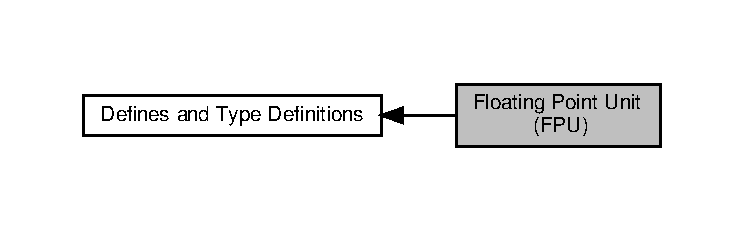
\includegraphics[width=350pt]{group___c_m_s_i_s___f_p_u}
\end{center}
\end{figure}
\subsection*{Komponenty}
\begin{DoxyCompactItemize}
\item 
struct \hyperlink{struct_f_p_u___type}{F\+P\+U\+\_\+\+Type}
\begin{DoxyCompactList}\small\item\em Structure type to access the Floating Point Unit (F\+PU). \end{DoxyCompactList}\end{DoxyCompactItemize}
\subsection*{Definicje}
\begin{DoxyCompactItemize}
\item 
\#define \hyperlink{group___c_m_s_i_s___f_p_u_ga4228a923ddf665f868e56b4b9e9bff7b}{F\+P\+U\+\_\+\+F\+P\+C\+C\+R\+\_\+\+A\+S\+P\+E\+N\+\_\+\+Pos}~31U
\item 
\#define \hyperlink{group___c_m_s_i_s___f_p_u_ga309886ff6bbd25cb13c061c6683c6c0c}{F\+P\+U\+\_\+\+F\+P\+C\+C\+R\+\_\+\+A\+S\+P\+E\+N\+\_\+\+Msk}~(1\+U\+L $<$$<$ F\+P\+U\+\_\+\+F\+P\+C\+C\+R\+\_\+\+A\+S\+P\+E\+N\+\_\+\+Pos)
\item 
\#define \hyperlink{group___c_m_s_i_s___f_p_u_gac7d70e051fe759ad8fed83bf5b5aebc1}{F\+P\+U\+\_\+\+F\+P\+C\+C\+R\+\_\+\+L\+S\+P\+E\+N\+\_\+\+Pos}~30U
\item 
\#define \hyperlink{group___c_m_s_i_s___f_p_u_gaf4ab19de45df6522dd882bc116f938e9}{F\+P\+U\+\_\+\+F\+P\+C\+C\+R\+\_\+\+L\+S\+P\+E\+N\+\_\+\+Msk}~(1\+U\+L $<$$<$ F\+P\+U\+\_\+\+F\+P\+C\+C\+R\+\_\+\+L\+S\+P\+E\+N\+\_\+\+Pos)
\item 
\#define \hyperlink{group___c_m_s_i_s___f_p_u_ga705368bf3c52b5bb4edfbcb3e2631e1c}{F\+P\+U\+\_\+\+F\+P\+C\+C\+R\+\_\+\+L\+S\+P\+E\+N\+S\+\_\+\+Pos}~29U
\item 
\#define \hyperlink{group___c_m_s_i_s___f_p_u_ga73afcf0fe09c69e9625e11035cabb1c0}{F\+P\+U\+\_\+\+F\+P\+C\+C\+R\+\_\+\+L\+S\+P\+E\+N\+S\+\_\+\+Msk}~(1\+U\+L $<$$<$ F\+P\+U\+\_\+\+F\+P\+C\+C\+R\+\_\+\+L\+S\+P\+E\+N\+S\+\_\+\+Pos)
\item 
\#define \hyperlink{group___c_m_s_i_s___f_p_u_ga0b97b2fdac794f4fddab1e4342e0c104}{F\+P\+U\+\_\+\+F\+P\+C\+C\+R\+\_\+\+C\+L\+R\+O\+N\+R\+E\+T\+\_\+\+Pos}~28U
\item 
\#define \hyperlink{group___c_m_s_i_s___f_p_u_gadedc12ec237657721a613c6f47abed6f}{F\+P\+U\+\_\+\+F\+P\+C\+C\+R\+\_\+\+C\+L\+R\+O\+N\+R\+E\+T\+\_\+\+Msk}~(1\+U\+L $<$$<$ F\+P\+U\+\_\+\+F\+P\+C\+C\+R\+\_\+\+C\+L\+R\+O\+N\+R\+E\+T\+\_\+\+Pos)
\item 
\#define \hyperlink{group___c_m_s_i_s___f_p_u_gabb18ccf9d1b0a4bef3b0823f18eb96ba}{F\+P\+U\+\_\+\+F\+P\+C\+C\+R\+\_\+\+C\+L\+R\+O\+N\+R\+E\+T\+S\+\_\+\+Pos}~27U
\item 
\#define \hyperlink{group___c_m_s_i_s___f_p_u_ga103d932807c15250d96711952878eeb2}{F\+P\+U\+\_\+\+F\+P\+C\+C\+R\+\_\+\+C\+L\+R\+O\+N\+R\+E\+T\+S\+\_\+\+Msk}~(1\+U\+L $<$$<$ F\+P\+U\+\_\+\+F\+P\+C\+C\+R\+\_\+\+C\+L\+R\+O\+N\+R\+E\+T\+S\+\_\+\+Pos)
\item 
\#define \hyperlink{group___c_m_s_i_s___f_p_u_ga624474f408fde177df519460775a74a1}{F\+P\+U\+\_\+\+F\+P\+C\+C\+R\+\_\+\+T\+S\+\_\+\+Pos}~26U
\item 
\#define \hyperlink{group___c_m_s_i_s___f_p_u_ga1377a5dfb4b9c6b18e379ac15e0dc23e}{F\+P\+U\+\_\+\+F\+P\+C\+C\+R\+\_\+\+T\+S\+\_\+\+Msk}~(1\+U\+L $<$$<$ F\+P\+U\+\_\+\+F\+P\+C\+C\+R\+\_\+\+T\+S\+\_\+\+Pos)
\item 
\#define \hyperlink{group___c_m_s_i_s___f_p_u_gac48b42e143b93411977dcb9086a5e4e4}{F\+P\+U\+\_\+\+F\+P\+C\+C\+R\+\_\+\+U\+F\+R\+D\+Y\+\_\+\+Pos}~10U
\item 
\#define \hyperlink{group___c_m_s_i_s___f_p_u_ga97c610927aab580cac3fb166f080b6a6}{F\+P\+U\+\_\+\+F\+P\+C\+C\+R\+\_\+\+U\+F\+R\+D\+Y\+\_\+\+Msk}~(1\+U\+L $<$$<$ F\+P\+U\+\_\+\+F\+P\+C\+C\+R\+\_\+\+U\+F\+R\+D\+Y\+\_\+\+Pos)
\item 
\#define \hyperlink{group___c_m_s_i_s___f_p_u_gac90e551e3cfda27c089bf381acba5aa0}{F\+P\+U\+\_\+\+F\+P\+C\+C\+R\+\_\+\+S\+P\+L\+I\+M\+V\+I\+O\+L\+\_\+\+Pos}~9U
\item 
\#define \hyperlink{group___c_m_s_i_s___f_p_u_gaa5e511cae62f922a9a91af0972f7a5e6}{F\+P\+U\+\_\+\+F\+P\+C\+C\+R\+\_\+\+S\+P\+L\+I\+M\+V\+I\+O\+L\+\_\+\+Msk}~(1\+U\+L $<$$<$ F\+P\+U\+\_\+\+F\+P\+C\+C\+R\+\_\+\+S\+P\+L\+I\+M\+V\+I\+O\+L\+\_\+\+Pos)
\item 
\#define \hyperlink{group___c_m_s_i_s___f_p_u_gae0a4effc79209d821ded517c2be326ba}{F\+P\+U\+\_\+\+F\+P\+C\+C\+R\+\_\+\+M\+O\+N\+R\+D\+Y\+\_\+\+Pos}~8U
\item 
\#define \hyperlink{group___c_m_s_i_s___f_p_u_ga42067729a887081cf56b8fe1029be7a1}{F\+P\+U\+\_\+\+F\+P\+C\+C\+R\+\_\+\+M\+O\+N\+R\+D\+Y\+\_\+\+Msk}~(1\+U\+L $<$$<$ F\+P\+U\+\_\+\+F\+P\+C\+C\+R\+\_\+\+M\+O\+N\+R\+D\+Y\+\_\+\+Pos)
\item 
\#define \hyperlink{group___c_m_s_i_s___f_p_u_ga571354f040a9372c0ad0cb87e296ea7d}{F\+P\+U\+\_\+\+F\+P\+C\+C\+R\+\_\+\+S\+F\+R\+D\+Y\+\_\+\+Pos}~7U
\item 
\#define \hyperlink{group___c_m_s_i_s___f_p_u_ga419a1e5609bbedf94f518c72214bddbc}{F\+P\+U\+\_\+\+F\+P\+C\+C\+R\+\_\+\+S\+F\+R\+D\+Y\+\_\+\+Msk}~(1\+U\+L $<$$<$ F\+P\+U\+\_\+\+F\+P\+C\+C\+R\+\_\+\+S\+F\+R\+D\+Y\+\_\+\+Pos)
\item 
\#define \hyperlink{group___c_m_s_i_s___f_p_u_ga6d633920f92c3ce4133d769701619b17}{F\+P\+U\+\_\+\+F\+P\+C\+C\+R\+\_\+\+B\+F\+R\+D\+Y\+\_\+\+Pos}~6U
\item 
\#define \hyperlink{group___c_m_s_i_s___f_p_u_gad349eb1323d8399d54a04c0bfd520cb2}{F\+P\+U\+\_\+\+F\+P\+C\+C\+R\+\_\+\+B\+F\+R\+D\+Y\+\_\+\+Msk}~(1\+U\+L $<$$<$ F\+P\+U\+\_\+\+F\+P\+C\+C\+R\+\_\+\+B\+F\+R\+D\+Y\+\_\+\+Pos)
\item 
\#define \hyperlink{group___c_m_s_i_s___f_p_u_gaccdb481211629f9440431439231187f1}{F\+P\+U\+\_\+\+F\+P\+C\+C\+R\+\_\+\+M\+M\+R\+D\+Y\+\_\+\+Pos}~5U
\item 
\#define \hyperlink{group___c_m_s_i_s___f_p_u_gadedfaec9fdd07261573e823a4dcfb5c4}{F\+P\+U\+\_\+\+F\+P\+C\+C\+R\+\_\+\+M\+M\+R\+D\+Y\+\_\+\+Msk}~(1\+U\+L $<$$<$ F\+P\+U\+\_\+\+F\+P\+C\+C\+R\+\_\+\+M\+M\+R\+D\+Y\+\_\+\+Pos)
\item 
\#define \hyperlink{group___c_m_s_i_s___f_p_u_gab12733991487acc2da41ca300fe36fb6}{F\+P\+U\+\_\+\+F\+P\+C\+C\+R\+\_\+\+H\+F\+R\+D\+Y\+\_\+\+Pos}~4U
\item 
\#define \hyperlink{group___c_m_s_i_s___f_p_u_gaf4beaa279abff34828344bd594fff8a1}{F\+P\+U\+\_\+\+F\+P\+C\+C\+R\+\_\+\+H\+F\+R\+D\+Y\+\_\+\+Msk}~(1\+U\+L $<$$<$ F\+P\+U\+\_\+\+F\+P\+C\+C\+R\+\_\+\+H\+F\+R\+D\+Y\+\_\+\+Pos)
\item 
\#define \hyperlink{group___c_m_s_i_s___f_p_u_ga0937d64c42374200af44b22e5b49fd26}{F\+P\+U\+\_\+\+F\+P\+C\+C\+R\+\_\+\+T\+H\+R\+E\+A\+D\+\_\+\+Pos}~3U
\item 
\#define \hyperlink{group___c_m_s_i_s___f_p_u_ga8d18cd88336d63d4b1810383aa8da700}{F\+P\+U\+\_\+\+F\+P\+C\+C\+R\+\_\+\+T\+H\+R\+E\+A\+D\+\_\+\+Msk}~(1\+U\+L $<$$<$ F\+P\+U\+\_\+\+F\+P\+C\+C\+R\+\_\+\+T\+H\+R\+E\+A\+D\+\_\+\+Pos)
\item 
\#define \hyperlink{group___c_m_s_i_s___f_p_u_ga4123d3881e5342251f559cec19e23b4e}{F\+P\+U\+\_\+\+F\+P\+C\+C\+R\+\_\+\+S\+\_\+\+Pos}~2U
\item 
\#define \hyperlink{group___c_m_s_i_s___f_p_u_ga47d3d3b29514c7d7581cfcc304368cea}{F\+P\+U\+\_\+\+F\+P\+C\+C\+R\+\_\+\+S\+\_\+\+Msk}~(1\+U\+L $<$$<$ F\+P\+U\+\_\+\+F\+P\+C\+C\+R\+\_\+\+S\+\_\+\+Pos)
\item 
\#define \hyperlink{group___c_m_s_i_s___f_p_u_gaea663104375ce6be15470e3db294c92d}{F\+P\+U\+\_\+\+F\+P\+C\+C\+R\+\_\+\+U\+S\+E\+R\+\_\+\+Pos}~1U
\item 
\#define \hyperlink{group___c_m_s_i_s___f_p_u_ga2eb70427eeaa7344196219cf5a8620a4}{F\+P\+U\+\_\+\+F\+P\+C\+C\+R\+\_\+\+U\+S\+E\+R\+\_\+\+Msk}~(1\+U\+L $<$$<$ F\+P\+U\+\_\+\+F\+P\+C\+C\+R\+\_\+\+U\+S\+E\+R\+\_\+\+Pos)
\item 
\#define \hyperlink{group___c_m_s_i_s___f_p_u_ga803bf3f6d15b04deaad0801bee5b35ed}{F\+P\+U\+\_\+\+F\+P\+C\+C\+R\+\_\+\+L\+S\+P\+A\+C\+T\+\_\+\+Pos}~0U
\item 
\#define \hyperlink{group___c_m_s_i_s___f_p_u_ga86e7c2fa52ba65c3b535dfa33f2586eb}{F\+P\+U\+\_\+\+F\+P\+C\+C\+R\+\_\+\+L\+S\+P\+A\+C\+T\+\_\+\+Msk}~(1\+U\+L /$\ast$$<$$<$ F\+P\+U\+\_\+\+F\+P\+C\+C\+R\+\_\+\+L\+S\+P\+A\+C\+T\+\_\+\+Pos$\ast$/)
\item 
\#define \hyperlink{group___c_m_s_i_s___f_p_u_gaf45377b7e45be8517ddbcf2028b80ae7}{F\+P\+U\+\_\+\+F\+P\+C\+A\+R\+\_\+\+A\+D\+D\+R\+E\+S\+S\+\_\+\+Pos}~3U
\item 
\#define \hyperlink{group___c_m_s_i_s___f_p_u_ga517d89370c81325c5387b9c3085ac554}{F\+P\+U\+\_\+\+F\+P\+C\+A\+R\+\_\+\+A\+D\+D\+R\+E\+S\+S\+\_\+\+Msk}~(0x1\+F\+F\+F\+F\+F\+F\+F\+U\+L $<$$<$ F\+P\+U\+\_\+\+F\+P\+C\+A\+R\+\_\+\+A\+D\+D\+R\+E\+S\+S\+\_\+\+Pos)
\item 
\#define \hyperlink{group___c_m_s_i_s___f_p_u_ga138f54bc002629ab3e4de814c58abb29}{F\+P\+U\+\_\+\+F\+P\+D\+S\+C\+R\+\_\+\+A\+H\+P\+\_\+\+Pos}~26U
\item 
\#define \hyperlink{group___c_m_s_i_s___f_p_u_gab2789cebebda5fda8c4e9d87e24f32be}{F\+P\+U\+\_\+\+F\+P\+D\+S\+C\+R\+\_\+\+A\+H\+P\+\_\+\+Msk}~(1\+U\+L $<$$<$ F\+P\+U\+\_\+\+F\+P\+D\+S\+C\+R\+\_\+\+A\+H\+P\+\_\+\+Pos)
\item 
\#define \hyperlink{group___c_m_s_i_s___f_p_u_ga41776b80fa450ef2ea6d3fee89aa35f2}{F\+P\+U\+\_\+\+F\+P\+D\+S\+C\+R\+\_\+\+D\+N\+\_\+\+Pos}~25U
\item 
\#define \hyperlink{group___c_m_s_i_s___f_p_u_ga40c2d4a297ca2ceffe174703a4ad17f6}{F\+P\+U\+\_\+\+F\+P\+D\+S\+C\+R\+\_\+\+D\+N\+\_\+\+Msk}~(1\+U\+L $<$$<$ F\+P\+U\+\_\+\+F\+P\+D\+S\+C\+R\+\_\+\+D\+N\+\_\+\+Pos)
\item 
\#define \hyperlink{group___c_m_s_i_s___f_p_u_gab3c2fc96e312ba47b902d5f80d9b8575}{F\+P\+U\+\_\+\+F\+P\+D\+S\+C\+R\+\_\+\+F\+Z\+\_\+\+Pos}~24U
\item 
\#define \hyperlink{group___c_m_s_i_s___f_p_u_gaae7d901442d4af97c6d22939cffc8ad9}{F\+P\+U\+\_\+\+F\+P\+D\+S\+C\+R\+\_\+\+F\+Z\+\_\+\+Msk}~(1\+U\+L $<$$<$ F\+P\+U\+\_\+\+F\+P\+D\+S\+C\+R\+\_\+\+F\+Z\+\_\+\+Pos)
\item 
\#define \hyperlink{group___c_m_s_i_s___f_p_u_ga7aeedf36be8f170dd3e276028e8e29ed}{F\+P\+U\+\_\+\+F\+P\+D\+S\+C\+R\+\_\+\+R\+Mode\+\_\+\+Pos}~22U
\item 
\#define \hyperlink{group___c_m_s_i_s___f_p_u_ga449beb50211f8e97df6b2640c82c4741}{F\+P\+U\+\_\+\+F\+P\+D\+S\+C\+R\+\_\+\+R\+Mode\+\_\+\+Msk}~(3\+U\+L $<$$<$ F\+P\+U\+\_\+\+F\+P\+D\+S\+C\+R\+\_\+\+R\+Mode\+\_\+\+Pos)
\item 
\#define \hyperlink{group___c_m_s_i_s___f_p_u_ga1ebcc9076f08013f0ea814540df03e82}{F\+P\+U\+\_\+\+M\+V\+F\+R0\+\_\+\+F\+P\+\_\+rounding\+\_\+modes\+\_\+\+Pos}~28U
\item 
\#define \hyperlink{group___c_m_s_i_s___f_p_u_gae6dc9339ac72227d5d54360bb9fbef1b}{F\+P\+U\+\_\+\+M\+V\+F\+R0\+\_\+\+F\+P\+\_\+rounding\+\_\+modes\+\_\+\+Msk}~(0x\+F\+U\+L $<$$<$ F\+P\+U\+\_\+\+M\+V\+F\+R0\+\_\+\+F\+P\+\_\+rounding\+\_\+modes\+\_\+\+Pos)
\item 
\#define \hyperlink{group___c_m_s_i_s___f_p_u_gabbf83a918536ebf10889cee71a0404c7}{F\+P\+U\+\_\+\+M\+V\+F\+R0\+\_\+\+Short\+\_\+vectors\+\_\+\+Pos}~24U
\item 
\#define \hyperlink{group___c_m_s_i_s___f_p_u_gabf261a72023fdfc64f32c6b21d55c5b9}{F\+P\+U\+\_\+\+M\+V\+F\+R0\+\_\+\+Short\+\_\+vectors\+\_\+\+Msk}~(0x\+F\+U\+L $<$$<$ F\+P\+U\+\_\+\+M\+V\+F\+R0\+\_\+\+Short\+\_\+vectors\+\_\+\+Pos)
\item 
\#define \hyperlink{group___c_m_s_i_s___f_p_u_ga176c85453ba03257bf263adec05f7344}{F\+P\+U\+\_\+\+M\+V\+F\+R0\+\_\+\+Square\+\_\+root\+\_\+\+Pos}~20U
\item 
\#define \hyperlink{group___c_m_s_i_s___f_p_u_ga3ec0bfec1640bdaf9dff027f275b446d}{F\+P\+U\+\_\+\+M\+V\+F\+R0\+\_\+\+Square\+\_\+root\+\_\+\+Msk}~(0x\+F\+U\+L $<$$<$ F\+P\+U\+\_\+\+M\+V\+F\+R0\+\_\+\+Square\+\_\+root\+\_\+\+Pos)
\item 
\#define \hyperlink{group___c_m_s_i_s___f_p_u_ga167be203091e6cc7d00ad40ca48c4396}{F\+P\+U\+\_\+\+M\+V\+F\+R0\+\_\+\+Divide\+\_\+\+Pos}~16U
\item 
\#define \hyperlink{group___c_m_s_i_s___f_p_u_gaeb7370768c6cdf06f8a15c86c6102ed2}{F\+P\+U\+\_\+\+M\+V\+F\+R0\+\_\+\+Divide\+\_\+\+Msk}~(0x\+F\+U\+L $<$$<$ F\+P\+U\+\_\+\+M\+V\+F\+R0\+\_\+\+Divide\+\_\+\+Pos)
\item 
\#define \hyperlink{group___c_m_s_i_s___f_p_u_ga5c0715c41c4470f8bb0b6dcd34707f1c}{F\+P\+U\+\_\+\+M\+V\+F\+R0\+\_\+\+F\+P\+\_\+excep\+\_\+trapping\+\_\+\+Pos}~12U
\item 
\#define \hyperlink{group___c_m_s_i_s___f_p_u_ga29bbddd679e821e050699fda23e6c85e}{F\+P\+U\+\_\+\+M\+V\+F\+R0\+\_\+\+F\+P\+\_\+excep\+\_\+trapping\+\_\+\+Msk}~(0x\+F\+U\+L $<$$<$ F\+P\+U\+\_\+\+M\+V\+F\+R0\+\_\+\+F\+P\+\_\+excep\+\_\+trapping\+\_\+\+Pos)
\item 
\#define \hyperlink{group___c_m_s_i_s___f_p_u_ga461e26147be0c39402a78cb6249e8f84}{F\+P\+U\+\_\+\+M\+V\+F\+R0\+\_\+\+Double\+\_\+precision\+\_\+\+Pos}~8U
\item 
\#define \hyperlink{group___c_m_s_i_s___f_p_u_ga3f2c8c6c759ffe70f548a165602ea901}{F\+P\+U\+\_\+\+M\+V\+F\+R0\+\_\+\+Double\+\_\+precision\+\_\+\+Msk}~(0x\+F\+U\+L $<$$<$ F\+P\+U\+\_\+\+M\+V\+F\+R0\+\_\+\+Double\+\_\+precision\+\_\+\+Pos)
\item 
\#define \hyperlink{group___c_m_s_i_s___f_p_u_ga1b4e9fe31992b1495c7a158747d42571}{F\+P\+U\+\_\+\+M\+V\+F\+R0\+\_\+\+Single\+\_\+precision\+\_\+\+Pos}~4U
\item 
\#define \hyperlink{group___c_m_s_i_s___f_p_u_ga95008f205c9d25e4ffebdbdc50d5ae44}{F\+P\+U\+\_\+\+M\+V\+F\+R0\+\_\+\+Single\+\_\+precision\+\_\+\+Msk}~(0x\+F\+U\+L $<$$<$ F\+P\+U\+\_\+\+M\+V\+F\+R0\+\_\+\+Single\+\_\+precision\+\_\+\+Pos)
\item 
\#define \hyperlink{group___c_m_s_i_s___f_p_u_gaa1de44af3e3162c8c176a57564611618}{F\+P\+U\+\_\+\+M\+V\+F\+R0\+\_\+\+A\+\_\+\+S\+I\+M\+D\+\_\+registers\+\_\+\+Pos}~0U
\item 
\#define \hyperlink{group___c_m_s_i_s___f_p_u_ga118f13f9562805356e92b5ad52573021}{F\+P\+U\+\_\+\+M\+V\+F\+R0\+\_\+\+A\+\_\+\+S\+I\+M\+D\+\_\+registers\+\_\+\+Msk}~(0x\+F\+U\+L /$\ast$$<$$<$ F\+P\+U\+\_\+\+M\+V\+F\+R0\+\_\+\+A\+\_\+\+S\+I\+M\+D\+\_\+registers\+\_\+\+Pos$\ast$/)
\item 
\#define \hyperlink{group___c_m_s_i_s___f_p_u_ga68c53771f02f4c73122a7b40796549cc}{F\+P\+U\+\_\+\+M\+V\+F\+R1\+\_\+\+F\+P\+\_\+fused\+\_\+\+M\+A\+C\+\_\+\+Pos}~28U
\item 
\#define \hyperlink{group___c_m_s_i_s___f_p_u_gaf5129ab18948ff573a1ab29f0be47bc2}{F\+P\+U\+\_\+\+M\+V\+F\+R1\+\_\+\+F\+P\+\_\+fused\+\_\+\+M\+A\+C\+\_\+\+Msk}~(0x\+F\+U\+L $<$$<$ F\+P\+U\+\_\+\+M\+V\+F\+R1\+\_\+\+F\+P\+\_\+fused\+\_\+\+M\+A\+C\+\_\+\+Pos)
\item 
\#define \hyperlink{group___c_m_s_i_s___f_p_u_ga02ceac0abcbdc8670633056bec005bfd}{F\+P\+U\+\_\+\+M\+V\+F\+R1\+\_\+\+F\+P\+\_\+\+H\+P\+F\+P\+\_\+\+Pos}~24U
\item 
\#define \hyperlink{group___c_m_s_i_s___f_p_u_gafe29dd327ed3b723b3f01759568e116d}{F\+P\+U\+\_\+\+M\+V\+F\+R1\+\_\+\+F\+P\+\_\+\+H\+P\+F\+P\+\_\+\+Msk}~(0x\+F\+U\+L $<$$<$ F\+P\+U\+\_\+\+M\+V\+F\+R1\+\_\+\+F\+P\+\_\+\+H\+P\+F\+P\+\_\+\+Pos)
\item 
\#define \hyperlink{group___c_m_s_i_s___f_p_u_gae34d7ce42e50e2f1ea3e654fd3ba690a}{F\+P\+U\+\_\+\+M\+V\+F\+R1\+\_\+\+D\+\_\+\+Na\+N\+\_\+mode\+\_\+\+Pos}~4U
\item 
\#define \hyperlink{group___c_m_s_i_s___f_p_u_gad6af7c4632dba5a417307d456fe9b8a7}{F\+P\+U\+\_\+\+M\+V\+F\+R1\+\_\+\+D\+\_\+\+Na\+N\+\_\+mode\+\_\+\+Msk}~(0x\+F\+U\+L $<$$<$ F\+P\+U\+\_\+\+M\+V\+F\+R1\+\_\+\+D\+\_\+\+Na\+N\+\_\+mode\+\_\+\+Pos)
\item 
\#define \hyperlink{group___c_m_s_i_s___f_p_u_ga7faa5bfa85036f8511793234cbbc2409}{F\+P\+U\+\_\+\+M\+V\+F\+R1\+\_\+\+Ft\+Z\+\_\+mode\+\_\+\+Pos}~0U
\item 
\#define \hyperlink{group___c_m_s_i_s___f_p_u_gac566bde39a7afcceffbb21d830c269c1}{F\+P\+U\+\_\+\+M\+V\+F\+R1\+\_\+\+Ft\+Z\+\_\+mode\+\_\+\+Msk}~(0x\+F\+U\+L /$\ast$$<$$<$ F\+P\+U\+\_\+\+M\+V\+F\+R1\+\_\+\+Ft\+Z\+\_\+mode\+\_\+\+Pos$\ast$/)
\item 
\#define \hyperlink{group___c_m_s_i_s___f_p_u_ga4228a923ddf665f868e56b4b9e9bff7b}{F\+P\+U\+\_\+\+F\+P\+C\+C\+R\+\_\+\+A\+S\+P\+E\+N\+\_\+\+Pos}~31U
\item 
\#define \hyperlink{group___c_m_s_i_s___f_p_u_ga309886ff6bbd25cb13c061c6683c6c0c}{F\+P\+U\+\_\+\+F\+P\+C\+C\+R\+\_\+\+A\+S\+P\+E\+N\+\_\+\+Msk}~(1\+U\+L $<$$<$ F\+P\+U\+\_\+\+F\+P\+C\+C\+R\+\_\+\+A\+S\+P\+E\+N\+\_\+\+Pos)
\item 
\#define \hyperlink{group___c_m_s_i_s___f_p_u_gac7d70e051fe759ad8fed83bf5b5aebc1}{F\+P\+U\+\_\+\+F\+P\+C\+C\+R\+\_\+\+L\+S\+P\+E\+N\+\_\+\+Pos}~30U
\item 
\#define \hyperlink{group___c_m_s_i_s___f_p_u_gaf4ab19de45df6522dd882bc116f938e9}{F\+P\+U\+\_\+\+F\+P\+C\+C\+R\+\_\+\+L\+S\+P\+E\+N\+\_\+\+Msk}~(1\+U\+L $<$$<$ F\+P\+U\+\_\+\+F\+P\+C\+C\+R\+\_\+\+L\+S\+P\+E\+N\+\_\+\+Pos)
\item 
\#define \hyperlink{group___c_m_s_i_s___f_p_u_ga705368bf3c52b5bb4edfbcb3e2631e1c}{F\+P\+U\+\_\+\+F\+P\+C\+C\+R\+\_\+\+L\+S\+P\+E\+N\+S\+\_\+\+Pos}~29U
\item 
\#define \hyperlink{group___c_m_s_i_s___f_p_u_ga73afcf0fe09c69e9625e11035cabb1c0}{F\+P\+U\+\_\+\+F\+P\+C\+C\+R\+\_\+\+L\+S\+P\+E\+N\+S\+\_\+\+Msk}~(1\+U\+L $<$$<$ F\+P\+U\+\_\+\+F\+P\+C\+C\+R\+\_\+\+L\+S\+P\+E\+N\+S\+\_\+\+Pos)
\item 
\#define \hyperlink{group___c_m_s_i_s___f_p_u_ga0b97b2fdac794f4fddab1e4342e0c104}{F\+P\+U\+\_\+\+F\+P\+C\+C\+R\+\_\+\+C\+L\+R\+O\+N\+R\+E\+T\+\_\+\+Pos}~28U
\item 
\#define \hyperlink{group___c_m_s_i_s___f_p_u_gadedc12ec237657721a613c6f47abed6f}{F\+P\+U\+\_\+\+F\+P\+C\+C\+R\+\_\+\+C\+L\+R\+O\+N\+R\+E\+T\+\_\+\+Msk}~(1\+U\+L $<$$<$ F\+P\+U\+\_\+\+F\+P\+C\+C\+R\+\_\+\+C\+L\+R\+O\+N\+R\+E\+T\+\_\+\+Pos)
\item 
\#define \hyperlink{group___c_m_s_i_s___f_p_u_gabb18ccf9d1b0a4bef3b0823f18eb96ba}{F\+P\+U\+\_\+\+F\+P\+C\+C\+R\+\_\+\+C\+L\+R\+O\+N\+R\+E\+T\+S\+\_\+\+Pos}~27U
\item 
\#define \hyperlink{group___c_m_s_i_s___f_p_u_ga103d932807c15250d96711952878eeb2}{F\+P\+U\+\_\+\+F\+P\+C\+C\+R\+\_\+\+C\+L\+R\+O\+N\+R\+E\+T\+S\+\_\+\+Msk}~(1\+U\+L $<$$<$ F\+P\+U\+\_\+\+F\+P\+C\+C\+R\+\_\+\+C\+L\+R\+O\+N\+R\+E\+T\+S\+\_\+\+Pos)
\item 
\#define \hyperlink{group___c_m_s_i_s___f_p_u_ga624474f408fde177df519460775a74a1}{F\+P\+U\+\_\+\+F\+P\+C\+C\+R\+\_\+\+T\+S\+\_\+\+Pos}~26U
\item 
\#define \hyperlink{group___c_m_s_i_s___f_p_u_ga1377a5dfb4b9c6b18e379ac15e0dc23e}{F\+P\+U\+\_\+\+F\+P\+C\+C\+R\+\_\+\+T\+S\+\_\+\+Msk}~(1\+U\+L $<$$<$ F\+P\+U\+\_\+\+F\+P\+C\+C\+R\+\_\+\+T\+S\+\_\+\+Pos)
\item 
\#define \hyperlink{group___c_m_s_i_s___f_p_u_gac48b42e143b93411977dcb9086a5e4e4}{F\+P\+U\+\_\+\+F\+P\+C\+C\+R\+\_\+\+U\+F\+R\+D\+Y\+\_\+\+Pos}~10U
\item 
\#define \hyperlink{group___c_m_s_i_s___f_p_u_ga97c610927aab580cac3fb166f080b6a6}{F\+P\+U\+\_\+\+F\+P\+C\+C\+R\+\_\+\+U\+F\+R\+D\+Y\+\_\+\+Msk}~(1\+U\+L $<$$<$ F\+P\+U\+\_\+\+F\+P\+C\+C\+R\+\_\+\+U\+F\+R\+D\+Y\+\_\+\+Pos)
\item 
\#define \hyperlink{group___c_m_s_i_s___f_p_u_gac90e551e3cfda27c089bf381acba5aa0}{F\+P\+U\+\_\+\+F\+P\+C\+C\+R\+\_\+\+S\+P\+L\+I\+M\+V\+I\+O\+L\+\_\+\+Pos}~9U
\item 
\#define \hyperlink{group___c_m_s_i_s___f_p_u_gaa5e511cae62f922a9a91af0972f7a5e6}{F\+P\+U\+\_\+\+F\+P\+C\+C\+R\+\_\+\+S\+P\+L\+I\+M\+V\+I\+O\+L\+\_\+\+Msk}~(1\+U\+L $<$$<$ F\+P\+U\+\_\+\+F\+P\+C\+C\+R\+\_\+\+S\+P\+L\+I\+M\+V\+I\+O\+L\+\_\+\+Pos)
\item 
\#define \hyperlink{group___c_m_s_i_s___f_p_u_gae0a4effc79209d821ded517c2be326ba}{F\+P\+U\+\_\+\+F\+P\+C\+C\+R\+\_\+\+M\+O\+N\+R\+D\+Y\+\_\+\+Pos}~8U
\item 
\#define \hyperlink{group___c_m_s_i_s___f_p_u_ga42067729a887081cf56b8fe1029be7a1}{F\+P\+U\+\_\+\+F\+P\+C\+C\+R\+\_\+\+M\+O\+N\+R\+D\+Y\+\_\+\+Msk}~(1\+U\+L $<$$<$ F\+P\+U\+\_\+\+F\+P\+C\+C\+R\+\_\+\+M\+O\+N\+R\+D\+Y\+\_\+\+Pos)
\item 
\#define \hyperlink{group___c_m_s_i_s___f_p_u_ga571354f040a9372c0ad0cb87e296ea7d}{F\+P\+U\+\_\+\+F\+P\+C\+C\+R\+\_\+\+S\+F\+R\+D\+Y\+\_\+\+Pos}~7U
\item 
\#define \hyperlink{group___c_m_s_i_s___f_p_u_ga419a1e5609bbedf94f518c72214bddbc}{F\+P\+U\+\_\+\+F\+P\+C\+C\+R\+\_\+\+S\+F\+R\+D\+Y\+\_\+\+Msk}~(1\+U\+L $<$$<$ F\+P\+U\+\_\+\+F\+P\+C\+C\+R\+\_\+\+S\+F\+R\+D\+Y\+\_\+\+Pos)
\item 
\#define \hyperlink{group___c_m_s_i_s___f_p_u_ga6d633920f92c3ce4133d769701619b17}{F\+P\+U\+\_\+\+F\+P\+C\+C\+R\+\_\+\+B\+F\+R\+D\+Y\+\_\+\+Pos}~6U
\item 
\#define \hyperlink{group___c_m_s_i_s___f_p_u_gad349eb1323d8399d54a04c0bfd520cb2}{F\+P\+U\+\_\+\+F\+P\+C\+C\+R\+\_\+\+B\+F\+R\+D\+Y\+\_\+\+Msk}~(1\+U\+L $<$$<$ F\+P\+U\+\_\+\+F\+P\+C\+C\+R\+\_\+\+B\+F\+R\+D\+Y\+\_\+\+Pos)
\item 
\#define \hyperlink{group___c_m_s_i_s___f_p_u_gaccdb481211629f9440431439231187f1}{F\+P\+U\+\_\+\+F\+P\+C\+C\+R\+\_\+\+M\+M\+R\+D\+Y\+\_\+\+Pos}~5U
\item 
\#define \hyperlink{group___c_m_s_i_s___f_p_u_gadedfaec9fdd07261573e823a4dcfb5c4}{F\+P\+U\+\_\+\+F\+P\+C\+C\+R\+\_\+\+M\+M\+R\+D\+Y\+\_\+\+Msk}~(1\+U\+L $<$$<$ F\+P\+U\+\_\+\+F\+P\+C\+C\+R\+\_\+\+M\+M\+R\+D\+Y\+\_\+\+Pos)
\item 
\#define \hyperlink{group___c_m_s_i_s___f_p_u_gab12733991487acc2da41ca300fe36fb6}{F\+P\+U\+\_\+\+F\+P\+C\+C\+R\+\_\+\+H\+F\+R\+D\+Y\+\_\+\+Pos}~4U
\item 
\#define \hyperlink{group___c_m_s_i_s___f_p_u_gaf4beaa279abff34828344bd594fff8a1}{F\+P\+U\+\_\+\+F\+P\+C\+C\+R\+\_\+\+H\+F\+R\+D\+Y\+\_\+\+Msk}~(1\+U\+L $<$$<$ F\+P\+U\+\_\+\+F\+P\+C\+C\+R\+\_\+\+H\+F\+R\+D\+Y\+\_\+\+Pos)
\item 
\#define \hyperlink{group___c_m_s_i_s___f_p_u_ga0937d64c42374200af44b22e5b49fd26}{F\+P\+U\+\_\+\+F\+P\+C\+C\+R\+\_\+\+T\+H\+R\+E\+A\+D\+\_\+\+Pos}~3U
\item 
\#define \hyperlink{group___c_m_s_i_s___f_p_u_ga8d18cd88336d63d4b1810383aa8da700}{F\+P\+U\+\_\+\+F\+P\+C\+C\+R\+\_\+\+T\+H\+R\+E\+A\+D\+\_\+\+Msk}~(1\+U\+L $<$$<$ F\+P\+U\+\_\+\+F\+P\+C\+C\+R\+\_\+\+T\+H\+R\+E\+A\+D\+\_\+\+Pos)
\item 
\#define \hyperlink{group___c_m_s_i_s___f_p_u_ga4123d3881e5342251f559cec19e23b4e}{F\+P\+U\+\_\+\+F\+P\+C\+C\+R\+\_\+\+S\+\_\+\+Pos}~2U
\item 
\#define \hyperlink{group___c_m_s_i_s___f_p_u_ga47d3d3b29514c7d7581cfcc304368cea}{F\+P\+U\+\_\+\+F\+P\+C\+C\+R\+\_\+\+S\+\_\+\+Msk}~(1\+U\+L $<$$<$ F\+P\+U\+\_\+\+F\+P\+C\+C\+R\+\_\+\+S\+\_\+\+Pos)
\item 
\#define \hyperlink{group___c_m_s_i_s___f_p_u_gaea663104375ce6be15470e3db294c92d}{F\+P\+U\+\_\+\+F\+P\+C\+C\+R\+\_\+\+U\+S\+E\+R\+\_\+\+Pos}~1U
\item 
\#define \hyperlink{group___c_m_s_i_s___f_p_u_ga2eb70427eeaa7344196219cf5a8620a4}{F\+P\+U\+\_\+\+F\+P\+C\+C\+R\+\_\+\+U\+S\+E\+R\+\_\+\+Msk}~(1\+U\+L $<$$<$ F\+P\+U\+\_\+\+F\+P\+C\+C\+R\+\_\+\+U\+S\+E\+R\+\_\+\+Pos)
\item 
\#define \hyperlink{group___c_m_s_i_s___f_p_u_ga803bf3f6d15b04deaad0801bee5b35ed}{F\+P\+U\+\_\+\+F\+P\+C\+C\+R\+\_\+\+L\+S\+P\+A\+C\+T\+\_\+\+Pos}~0U
\item 
\#define \hyperlink{group___c_m_s_i_s___f_p_u_ga86e7c2fa52ba65c3b535dfa33f2586eb}{F\+P\+U\+\_\+\+F\+P\+C\+C\+R\+\_\+\+L\+S\+P\+A\+C\+T\+\_\+\+Msk}~(1\+U\+L /$\ast$$<$$<$ F\+P\+U\+\_\+\+F\+P\+C\+C\+R\+\_\+\+L\+S\+P\+A\+C\+T\+\_\+\+Pos$\ast$/)
\item 
\#define \hyperlink{group___c_m_s_i_s___f_p_u_gaf45377b7e45be8517ddbcf2028b80ae7}{F\+P\+U\+\_\+\+F\+P\+C\+A\+R\+\_\+\+A\+D\+D\+R\+E\+S\+S\+\_\+\+Pos}~3U
\item 
\#define \hyperlink{group___c_m_s_i_s___f_p_u_ga517d89370c81325c5387b9c3085ac554}{F\+P\+U\+\_\+\+F\+P\+C\+A\+R\+\_\+\+A\+D\+D\+R\+E\+S\+S\+\_\+\+Msk}~(0x1\+F\+F\+F\+F\+F\+F\+F\+U\+L $<$$<$ F\+P\+U\+\_\+\+F\+P\+C\+A\+R\+\_\+\+A\+D\+D\+R\+E\+S\+S\+\_\+\+Pos)
\item 
\#define \hyperlink{group___c_m_s_i_s___f_p_u_ga138f54bc002629ab3e4de814c58abb29}{F\+P\+U\+\_\+\+F\+P\+D\+S\+C\+R\+\_\+\+A\+H\+P\+\_\+\+Pos}~26U
\item 
\#define \hyperlink{group___c_m_s_i_s___f_p_u_gab2789cebebda5fda8c4e9d87e24f32be}{F\+P\+U\+\_\+\+F\+P\+D\+S\+C\+R\+\_\+\+A\+H\+P\+\_\+\+Msk}~(1\+U\+L $<$$<$ F\+P\+U\+\_\+\+F\+P\+D\+S\+C\+R\+\_\+\+A\+H\+P\+\_\+\+Pos)
\item 
\#define \hyperlink{group___c_m_s_i_s___f_p_u_ga41776b80fa450ef2ea6d3fee89aa35f2}{F\+P\+U\+\_\+\+F\+P\+D\+S\+C\+R\+\_\+\+D\+N\+\_\+\+Pos}~25U
\item 
\#define \hyperlink{group___c_m_s_i_s___f_p_u_ga40c2d4a297ca2ceffe174703a4ad17f6}{F\+P\+U\+\_\+\+F\+P\+D\+S\+C\+R\+\_\+\+D\+N\+\_\+\+Msk}~(1\+U\+L $<$$<$ F\+P\+U\+\_\+\+F\+P\+D\+S\+C\+R\+\_\+\+D\+N\+\_\+\+Pos)
\item 
\#define \hyperlink{group___c_m_s_i_s___f_p_u_gab3c2fc96e312ba47b902d5f80d9b8575}{F\+P\+U\+\_\+\+F\+P\+D\+S\+C\+R\+\_\+\+F\+Z\+\_\+\+Pos}~24U
\item 
\#define \hyperlink{group___c_m_s_i_s___f_p_u_gaae7d901442d4af97c6d22939cffc8ad9}{F\+P\+U\+\_\+\+F\+P\+D\+S\+C\+R\+\_\+\+F\+Z\+\_\+\+Msk}~(1\+U\+L $<$$<$ F\+P\+U\+\_\+\+F\+P\+D\+S\+C\+R\+\_\+\+F\+Z\+\_\+\+Pos)
\item 
\#define \hyperlink{group___c_m_s_i_s___f_p_u_ga7aeedf36be8f170dd3e276028e8e29ed}{F\+P\+U\+\_\+\+F\+P\+D\+S\+C\+R\+\_\+\+R\+Mode\+\_\+\+Pos}~22U
\item 
\#define \hyperlink{group___c_m_s_i_s___f_p_u_ga449beb50211f8e97df6b2640c82c4741}{F\+P\+U\+\_\+\+F\+P\+D\+S\+C\+R\+\_\+\+R\+Mode\+\_\+\+Msk}~(3\+U\+L $<$$<$ F\+P\+U\+\_\+\+F\+P\+D\+S\+C\+R\+\_\+\+R\+Mode\+\_\+\+Pos)
\item 
\#define \hyperlink{group___c_m_s_i_s___f_p_u_ga1ebcc9076f08013f0ea814540df03e82}{F\+P\+U\+\_\+\+M\+V\+F\+R0\+\_\+\+F\+P\+\_\+rounding\+\_\+modes\+\_\+\+Pos}~28U
\item 
\#define \hyperlink{group___c_m_s_i_s___f_p_u_gae6dc9339ac72227d5d54360bb9fbef1b}{F\+P\+U\+\_\+\+M\+V\+F\+R0\+\_\+\+F\+P\+\_\+rounding\+\_\+modes\+\_\+\+Msk}~(0x\+F\+U\+L $<$$<$ F\+P\+U\+\_\+\+M\+V\+F\+R0\+\_\+\+F\+P\+\_\+rounding\+\_\+modes\+\_\+\+Pos)
\item 
\#define \hyperlink{group___c_m_s_i_s___f_p_u_gabbf83a918536ebf10889cee71a0404c7}{F\+P\+U\+\_\+\+M\+V\+F\+R0\+\_\+\+Short\+\_\+vectors\+\_\+\+Pos}~24U
\item 
\#define \hyperlink{group___c_m_s_i_s___f_p_u_gabf261a72023fdfc64f32c6b21d55c5b9}{F\+P\+U\+\_\+\+M\+V\+F\+R0\+\_\+\+Short\+\_\+vectors\+\_\+\+Msk}~(0x\+F\+U\+L $<$$<$ F\+P\+U\+\_\+\+M\+V\+F\+R0\+\_\+\+Short\+\_\+vectors\+\_\+\+Pos)
\item 
\#define \hyperlink{group___c_m_s_i_s___f_p_u_ga176c85453ba03257bf263adec05f7344}{F\+P\+U\+\_\+\+M\+V\+F\+R0\+\_\+\+Square\+\_\+root\+\_\+\+Pos}~20U
\item 
\#define \hyperlink{group___c_m_s_i_s___f_p_u_ga3ec0bfec1640bdaf9dff027f275b446d}{F\+P\+U\+\_\+\+M\+V\+F\+R0\+\_\+\+Square\+\_\+root\+\_\+\+Msk}~(0x\+F\+U\+L $<$$<$ F\+P\+U\+\_\+\+M\+V\+F\+R0\+\_\+\+Square\+\_\+root\+\_\+\+Pos)
\item 
\#define \hyperlink{group___c_m_s_i_s___f_p_u_ga167be203091e6cc7d00ad40ca48c4396}{F\+P\+U\+\_\+\+M\+V\+F\+R0\+\_\+\+Divide\+\_\+\+Pos}~16U
\item 
\#define \hyperlink{group___c_m_s_i_s___f_p_u_gaeb7370768c6cdf06f8a15c86c6102ed2}{F\+P\+U\+\_\+\+M\+V\+F\+R0\+\_\+\+Divide\+\_\+\+Msk}~(0x\+F\+U\+L $<$$<$ F\+P\+U\+\_\+\+M\+V\+F\+R0\+\_\+\+Divide\+\_\+\+Pos)
\item 
\#define \hyperlink{group___c_m_s_i_s___f_p_u_ga5c0715c41c4470f8bb0b6dcd34707f1c}{F\+P\+U\+\_\+\+M\+V\+F\+R0\+\_\+\+F\+P\+\_\+excep\+\_\+trapping\+\_\+\+Pos}~12U
\item 
\#define \hyperlink{group___c_m_s_i_s___f_p_u_ga29bbddd679e821e050699fda23e6c85e}{F\+P\+U\+\_\+\+M\+V\+F\+R0\+\_\+\+F\+P\+\_\+excep\+\_\+trapping\+\_\+\+Msk}~(0x\+F\+U\+L $<$$<$ F\+P\+U\+\_\+\+M\+V\+F\+R0\+\_\+\+F\+P\+\_\+excep\+\_\+trapping\+\_\+\+Pos)
\item 
\#define \hyperlink{group___c_m_s_i_s___f_p_u_ga461e26147be0c39402a78cb6249e8f84}{F\+P\+U\+\_\+\+M\+V\+F\+R0\+\_\+\+Double\+\_\+precision\+\_\+\+Pos}~8U
\item 
\#define \hyperlink{group___c_m_s_i_s___f_p_u_ga3f2c8c6c759ffe70f548a165602ea901}{F\+P\+U\+\_\+\+M\+V\+F\+R0\+\_\+\+Double\+\_\+precision\+\_\+\+Msk}~(0x\+F\+U\+L $<$$<$ F\+P\+U\+\_\+\+M\+V\+F\+R0\+\_\+\+Double\+\_\+precision\+\_\+\+Pos)
\item 
\#define \hyperlink{group___c_m_s_i_s___f_p_u_ga1b4e9fe31992b1495c7a158747d42571}{F\+P\+U\+\_\+\+M\+V\+F\+R0\+\_\+\+Single\+\_\+precision\+\_\+\+Pos}~4U
\item 
\#define \hyperlink{group___c_m_s_i_s___f_p_u_ga95008f205c9d25e4ffebdbdc50d5ae44}{F\+P\+U\+\_\+\+M\+V\+F\+R0\+\_\+\+Single\+\_\+precision\+\_\+\+Msk}~(0x\+F\+U\+L $<$$<$ F\+P\+U\+\_\+\+M\+V\+F\+R0\+\_\+\+Single\+\_\+precision\+\_\+\+Pos)
\item 
\#define \hyperlink{group___c_m_s_i_s___f_p_u_gaa1de44af3e3162c8c176a57564611618}{F\+P\+U\+\_\+\+M\+V\+F\+R0\+\_\+\+A\+\_\+\+S\+I\+M\+D\+\_\+registers\+\_\+\+Pos}~0U
\item 
\#define \hyperlink{group___c_m_s_i_s___f_p_u_ga118f13f9562805356e92b5ad52573021}{F\+P\+U\+\_\+\+M\+V\+F\+R0\+\_\+\+A\+\_\+\+S\+I\+M\+D\+\_\+registers\+\_\+\+Msk}~(0x\+F\+U\+L /$\ast$$<$$<$ F\+P\+U\+\_\+\+M\+V\+F\+R0\+\_\+\+A\+\_\+\+S\+I\+M\+D\+\_\+registers\+\_\+\+Pos$\ast$/)
\item 
\#define \hyperlink{group___c_m_s_i_s___f_p_u_ga68c53771f02f4c73122a7b40796549cc}{F\+P\+U\+\_\+\+M\+V\+F\+R1\+\_\+\+F\+P\+\_\+fused\+\_\+\+M\+A\+C\+\_\+\+Pos}~28U
\item 
\#define \hyperlink{group___c_m_s_i_s___f_p_u_gaf5129ab18948ff573a1ab29f0be47bc2}{F\+P\+U\+\_\+\+M\+V\+F\+R1\+\_\+\+F\+P\+\_\+fused\+\_\+\+M\+A\+C\+\_\+\+Msk}~(0x\+F\+U\+L $<$$<$ F\+P\+U\+\_\+\+M\+V\+F\+R1\+\_\+\+F\+P\+\_\+fused\+\_\+\+M\+A\+C\+\_\+\+Pos)
\item 
\#define \hyperlink{group___c_m_s_i_s___f_p_u_ga02ceac0abcbdc8670633056bec005bfd}{F\+P\+U\+\_\+\+M\+V\+F\+R1\+\_\+\+F\+P\+\_\+\+H\+P\+F\+P\+\_\+\+Pos}~24U
\item 
\#define \hyperlink{group___c_m_s_i_s___f_p_u_gafe29dd327ed3b723b3f01759568e116d}{F\+P\+U\+\_\+\+M\+V\+F\+R1\+\_\+\+F\+P\+\_\+\+H\+P\+F\+P\+\_\+\+Msk}~(0x\+F\+U\+L $<$$<$ F\+P\+U\+\_\+\+M\+V\+F\+R1\+\_\+\+F\+P\+\_\+\+H\+P\+F\+P\+\_\+\+Pos)
\item 
\#define \hyperlink{group___c_m_s_i_s___f_p_u_gae34d7ce42e50e2f1ea3e654fd3ba690a}{F\+P\+U\+\_\+\+M\+V\+F\+R1\+\_\+\+D\+\_\+\+Na\+N\+\_\+mode\+\_\+\+Pos}~4U
\item 
\#define \hyperlink{group___c_m_s_i_s___f_p_u_gad6af7c4632dba5a417307d456fe9b8a7}{F\+P\+U\+\_\+\+M\+V\+F\+R1\+\_\+\+D\+\_\+\+Na\+N\+\_\+mode\+\_\+\+Msk}~(0x\+F\+U\+L $<$$<$ F\+P\+U\+\_\+\+M\+V\+F\+R1\+\_\+\+D\+\_\+\+Na\+N\+\_\+mode\+\_\+\+Pos)
\item 
\#define \hyperlink{group___c_m_s_i_s___f_p_u_ga7faa5bfa85036f8511793234cbbc2409}{F\+P\+U\+\_\+\+M\+V\+F\+R1\+\_\+\+Ft\+Z\+\_\+mode\+\_\+\+Pos}~0U
\item 
\#define \hyperlink{group___c_m_s_i_s___f_p_u_gac566bde39a7afcceffbb21d830c269c1}{F\+P\+U\+\_\+\+M\+V\+F\+R1\+\_\+\+Ft\+Z\+\_\+mode\+\_\+\+Msk}~(0x\+F\+U\+L /$\ast$$<$$<$ F\+P\+U\+\_\+\+M\+V\+F\+R1\+\_\+\+Ft\+Z\+\_\+mode\+\_\+\+Pos$\ast$/)
\item 
\#define \hyperlink{group___c_m_s_i_s___f_p_u_ga4228a923ddf665f868e56b4b9e9bff7b}{F\+P\+U\+\_\+\+F\+P\+C\+C\+R\+\_\+\+A\+S\+P\+E\+N\+\_\+\+Pos}~31U
\item 
\#define \hyperlink{group___c_m_s_i_s___f_p_u_ga309886ff6bbd25cb13c061c6683c6c0c}{F\+P\+U\+\_\+\+F\+P\+C\+C\+R\+\_\+\+A\+S\+P\+E\+N\+\_\+\+Msk}~(1\+U\+L $<$$<$ F\+P\+U\+\_\+\+F\+P\+C\+C\+R\+\_\+\+A\+S\+P\+E\+N\+\_\+\+Pos)
\item 
\#define \hyperlink{group___c_m_s_i_s___f_p_u_gac7d70e051fe759ad8fed83bf5b5aebc1}{F\+P\+U\+\_\+\+F\+P\+C\+C\+R\+\_\+\+L\+S\+P\+E\+N\+\_\+\+Pos}~30U
\item 
\#define \hyperlink{group___c_m_s_i_s___f_p_u_gaf4ab19de45df6522dd882bc116f938e9}{F\+P\+U\+\_\+\+F\+P\+C\+C\+R\+\_\+\+L\+S\+P\+E\+N\+\_\+\+Msk}~(1\+U\+L $<$$<$ F\+P\+U\+\_\+\+F\+P\+C\+C\+R\+\_\+\+L\+S\+P\+E\+N\+\_\+\+Pos)
\item 
\#define \hyperlink{group___c_m_s_i_s___f_p_u_gae0a4effc79209d821ded517c2be326ba}{F\+P\+U\+\_\+\+F\+P\+C\+C\+R\+\_\+\+M\+O\+N\+R\+D\+Y\+\_\+\+Pos}~8U
\item 
\#define \hyperlink{group___c_m_s_i_s___f_p_u_ga42067729a887081cf56b8fe1029be7a1}{F\+P\+U\+\_\+\+F\+P\+C\+C\+R\+\_\+\+M\+O\+N\+R\+D\+Y\+\_\+\+Msk}~(1\+U\+L $<$$<$ F\+P\+U\+\_\+\+F\+P\+C\+C\+R\+\_\+\+M\+O\+N\+R\+D\+Y\+\_\+\+Pos)
\item 
\#define \hyperlink{group___c_m_s_i_s___f_p_u_ga6d633920f92c3ce4133d769701619b17}{F\+P\+U\+\_\+\+F\+P\+C\+C\+R\+\_\+\+B\+F\+R\+D\+Y\+\_\+\+Pos}~6U
\item 
\#define \hyperlink{group___c_m_s_i_s___f_p_u_gad349eb1323d8399d54a04c0bfd520cb2}{F\+P\+U\+\_\+\+F\+P\+C\+C\+R\+\_\+\+B\+F\+R\+D\+Y\+\_\+\+Msk}~(1\+U\+L $<$$<$ F\+P\+U\+\_\+\+F\+P\+C\+C\+R\+\_\+\+B\+F\+R\+D\+Y\+\_\+\+Pos)
\item 
\#define \hyperlink{group___c_m_s_i_s___f_p_u_gaccdb481211629f9440431439231187f1}{F\+P\+U\+\_\+\+F\+P\+C\+C\+R\+\_\+\+M\+M\+R\+D\+Y\+\_\+\+Pos}~5U
\item 
\#define \hyperlink{group___c_m_s_i_s___f_p_u_gadedfaec9fdd07261573e823a4dcfb5c4}{F\+P\+U\+\_\+\+F\+P\+C\+C\+R\+\_\+\+M\+M\+R\+D\+Y\+\_\+\+Msk}~(1\+U\+L $<$$<$ F\+P\+U\+\_\+\+F\+P\+C\+C\+R\+\_\+\+M\+M\+R\+D\+Y\+\_\+\+Pos)
\item 
\#define \hyperlink{group___c_m_s_i_s___f_p_u_gab12733991487acc2da41ca300fe36fb6}{F\+P\+U\+\_\+\+F\+P\+C\+C\+R\+\_\+\+H\+F\+R\+D\+Y\+\_\+\+Pos}~4U
\item 
\#define \hyperlink{group___c_m_s_i_s___f_p_u_gaf4beaa279abff34828344bd594fff8a1}{F\+P\+U\+\_\+\+F\+P\+C\+C\+R\+\_\+\+H\+F\+R\+D\+Y\+\_\+\+Msk}~(1\+U\+L $<$$<$ F\+P\+U\+\_\+\+F\+P\+C\+C\+R\+\_\+\+H\+F\+R\+D\+Y\+\_\+\+Pos)
\item 
\#define \hyperlink{group___c_m_s_i_s___f_p_u_ga0937d64c42374200af44b22e5b49fd26}{F\+P\+U\+\_\+\+F\+P\+C\+C\+R\+\_\+\+T\+H\+R\+E\+A\+D\+\_\+\+Pos}~3U
\item 
\#define \hyperlink{group___c_m_s_i_s___f_p_u_ga8d18cd88336d63d4b1810383aa8da700}{F\+P\+U\+\_\+\+F\+P\+C\+C\+R\+\_\+\+T\+H\+R\+E\+A\+D\+\_\+\+Msk}~(1\+U\+L $<$$<$ F\+P\+U\+\_\+\+F\+P\+C\+C\+R\+\_\+\+T\+H\+R\+E\+A\+D\+\_\+\+Pos)
\item 
\#define \hyperlink{group___c_m_s_i_s___f_p_u_gaea663104375ce6be15470e3db294c92d}{F\+P\+U\+\_\+\+F\+P\+C\+C\+R\+\_\+\+U\+S\+E\+R\+\_\+\+Pos}~1U
\item 
\#define \hyperlink{group___c_m_s_i_s___f_p_u_ga2eb70427eeaa7344196219cf5a8620a4}{F\+P\+U\+\_\+\+F\+P\+C\+C\+R\+\_\+\+U\+S\+E\+R\+\_\+\+Msk}~(1\+U\+L $<$$<$ F\+P\+U\+\_\+\+F\+P\+C\+C\+R\+\_\+\+U\+S\+E\+R\+\_\+\+Pos)
\item 
\#define \hyperlink{group___c_m_s_i_s___f_p_u_ga803bf3f6d15b04deaad0801bee5b35ed}{F\+P\+U\+\_\+\+F\+P\+C\+C\+R\+\_\+\+L\+S\+P\+A\+C\+T\+\_\+\+Pos}~0U
\item 
\#define \hyperlink{group___c_m_s_i_s___f_p_u_ga86e7c2fa52ba65c3b535dfa33f2586eb}{F\+P\+U\+\_\+\+F\+P\+C\+C\+R\+\_\+\+L\+S\+P\+A\+C\+T\+\_\+\+Msk}~(1\+U\+L /$\ast$$<$$<$ F\+P\+U\+\_\+\+F\+P\+C\+C\+R\+\_\+\+L\+S\+P\+A\+C\+T\+\_\+\+Pos$\ast$/)
\item 
\#define \hyperlink{group___c_m_s_i_s___f_p_u_gaf45377b7e45be8517ddbcf2028b80ae7}{F\+P\+U\+\_\+\+F\+P\+C\+A\+R\+\_\+\+A\+D\+D\+R\+E\+S\+S\+\_\+\+Pos}~3U
\item 
\#define \hyperlink{group___c_m_s_i_s___f_p_u_ga517d89370c81325c5387b9c3085ac554}{F\+P\+U\+\_\+\+F\+P\+C\+A\+R\+\_\+\+A\+D\+D\+R\+E\+S\+S\+\_\+\+Msk}~(0x1\+F\+F\+F\+F\+F\+F\+F\+U\+L $<$$<$ F\+P\+U\+\_\+\+F\+P\+C\+A\+R\+\_\+\+A\+D\+D\+R\+E\+S\+S\+\_\+\+Pos)
\item 
\#define \hyperlink{group___c_m_s_i_s___f_p_u_ga138f54bc002629ab3e4de814c58abb29}{F\+P\+U\+\_\+\+F\+P\+D\+S\+C\+R\+\_\+\+A\+H\+P\+\_\+\+Pos}~26U
\item 
\#define \hyperlink{group___c_m_s_i_s___f_p_u_gab2789cebebda5fda8c4e9d87e24f32be}{F\+P\+U\+\_\+\+F\+P\+D\+S\+C\+R\+\_\+\+A\+H\+P\+\_\+\+Msk}~(1\+U\+L $<$$<$ F\+P\+U\+\_\+\+F\+P\+D\+S\+C\+R\+\_\+\+A\+H\+P\+\_\+\+Pos)
\item 
\#define \hyperlink{group___c_m_s_i_s___f_p_u_ga41776b80fa450ef2ea6d3fee89aa35f2}{F\+P\+U\+\_\+\+F\+P\+D\+S\+C\+R\+\_\+\+D\+N\+\_\+\+Pos}~25U
\item 
\#define \hyperlink{group___c_m_s_i_s___f_p_u_ga40c2d4a297ca2ceffe174703a4ad17f6}{F\+P\+U\+\_\+\+F\+P\+D\+S\+C\+R\+\_\+\+D\+N\+\_\+\+Msk}~(1\+U\+L $<$$<$ F\+P\+U\+\_\+\+F\+P\+D\+S\+C\+R\+\_\+\+D\+N\+\_\+\+Pos)
\item 
\#define \hyperlink{group___c_m_s_i_s___f_p_u_gab3c2fc96e312ba47b902d5f80d9b8575}{F\+P\+U\+\_\+\+F\+P\+D\+S\+C\+R\+\_\+\+F\+Z\+\_\+\+Pos}~24U
\item 
\#define \hyperlink{group___c_m_s_i_s___f_p_u_gaae7d901442d4af97c6d22939cffc8ad9}{F\+P\+U\+\_\+\+F\+P\+D\+S\+C\+R\+\_\+\+F\+Z\+\_\+\+Msk}~(1\+U\+L $<$$<$ F\+P\+U\+\_\+\+F\+P\+D\+S\+C\+R\+\_\+\+F\+Z\+\_\+\+Pos)
\item 
\#define \hyperlink{group___c_m_s_i_s___f_p_u_ga7aeedf36be8f170dd3e276028e8e29ed}{F\+P\+U\+\_\+\+F\+P\+D\+S\+C\+R\+\_\+\+R\+Mode\+\_\+\+Pos}~22U
\item 
\#define \hyperlink{group___c_m_s_i_s___f_p_u_ga449beb50211f8e97df6b2640c82c4741}{F\+P\+U\+\_\+\+F\+P\+D\+S\+C\+R\+\_\+\+R\+Mode\+\_\+\+Msk}~(3\+U\+L $<$$<$ F\+P\+U\+\_\+\+F\+P\+D\+S\+C\+R\+\_\+\+R\+Mode\+\_\+\+Pos)
\item 
\#define \hyperlink{group___c_m_s_i_s___f_p_u_ga1ebcc9076f08013f0ea814540df03e82}{F\+P\+U\+\_\+\+M\+V\+F\+R0\+\_\+\+F\+P\+\_\+rounding\+\_\+modes\+\_\+\+Pos}~28U
\item 
\#define \hyperlink{group___c_m_s_i_s___f_p_u_gae6dc9339ac72227d5d54360bb9fbef1b}{F\+P\+U\+\_\+\+M\+V\+F\+R0\+\_\+\+F\+P\+\_\+rounding\+\_\+modes\+\_\+\+Msk}~(0x\+F\+U\+L $<$$<$ F\+P\+U\+\_\+\+M\+V\+F\+R0\+\_\+\+F\+P\+\_\+rounding\+\_\+modes\+\_\+\+Pos)
\item 
\#define \hyperlink{group___c_m_s_i_s___f_p_u_gabbf83a918536ebf10889cee71a0404c7}{F\+P\+U\+\_\+\+M\+V\+F\+R0\+\_\+\+Short\+\_\+vectors\+\_\+\+Pos}~24U
\item 
\#define \hyperlink{group___c_m_s_i_s___f_p_u_gabf261a72023fdfc64f32c6b21d55c5b9}{F\+P\+U\+\_\+\+M\+V\+F\+R0\+\_\+\+Short\+\_\+vectors\+\_\+\+Msk}~(0x\+F\+U\+L $<$$<$ F\+P\+U\+\_\+\+M\+V\+F\+R0\+\_\+\+Short\+\_\+vectors\+\_\+\+Pos)
\item 
\#define \hyperlink{group___c_m_s_i_s___f_p_u_ga176c85453ba03257bf263adec05f7344}{F\+P\+U\+\_\+\+M\+V\+F\+R0\+\_\+\+Square\+\_\+root\+\_\+\+Pos}~20U
\item 
\#define \hyperlink{group___c_m_s_i_s___f_p_u_ga3ec0bfec1640bdaf9dff027f275b446d}{F\+P\+U\+\_\+\+M\+V\+F\+R0\+\_\+\+Square\+\_\+root\+\_\+\+Msk}~(0x\+F\+U\+L $<$$<$ F\+P\+U\+\_\+\+M\+V\+F\+R0\+\_\+\+Square\+\_\+root\+\_\+\+Pos)
\item 
\#define \hyperlink{group___c_m_s_i_s___f_p_u_ga167be203091e6cc7d00ad40ca48c4396}{F\+P\+U\+\_\+\+M\+V\+F\+R0\+\_\+\+Divide\+\_\+\+Pos}~16U
\item 
\#define \hyperlink{group___c_m_s_i_s___f_p_u_gaeb7370768c6cdf06f8a15c86c6102ed2}{F\+P\+U\+\_\+\+M\+V\+F\+R0\+\_\+\+Divide\+\_\+\+Msk}~(0x\+F\+U\+L $<$$<$ F\+P\+U\+\_\+\+M\+V\+F\+R0\+\_\+\+Divide\+\_\+\+Pos)
\item 
\#define \hyperlink{group___c_m_s_i_s___f_p_u_ga5c0715c41c4470f8bb0b6dcd34707f1c}{F\+P\+U\+\_\+\+M\+V\+F\+R0\+\_\+\+F\+P\+\_\+excep\+\_\+trapping\+\_\+\+Pos}~12U
\item 
\#define \hyperlink{group___c_m_s_i_s___f_p_u_ga29bbddd679e821e050699fda23e6c85e}{F\+P\+U\+\_\+\+M\+V\+F\+R0\+\_\+\+F\+P\+\_\+excep\+\_\+trapping\+\_\+\+Msk}~(0x\+F\+U\+L $<$$<$ F\+P\+U\+\_\+\+M\+V\+F\+R0\+\_\+\+F\+P\+\_\+excep\+\_\+trapping\+\_\+\+Pos)
\item 
\#define \hyperlink{group___c_m_s_i_s___f_p_u_ga461e26147be0c39402a78cb6249e8f84}{F\+P\+U\+\_\+\+M\+V\+F\+R0\+\_\+\+Double\+\_\+precision\+\_\+\+Pos}~8U
\item 
\#define \hyperlink{group___c_m_s_i_s___f_p_u_ga3f2c8c6c759ffe70f548a165602ea901}{F\+P\+U\+\_\+\+M\+V\+F\+R0\+\_\+\+Double\+\_\+precision\+\_\+\+Msk}~(0x\+F\+U\+L $<$$<$ F\+P\+U\+\_\+\+M\+V\+F\+R0\+\_\+\+Double\+\_\+precision\+\_\+\+Pos)
\item 
\#define \hyperlink{group___c_m_s_i_s___f_p_u_ga1b4e9fe31992b1495c7a158747d42571}{F\+P\+U\+\_\+\+M\+V\+F\+R0\+\_\+\+Single\+\_\+precision\+\_\+\+Pos}~4U
\item 
\#define \hyperlink{group___c_m_s_i_s___f_p_u_ga95008f205c9d25e4ffebdbdc50d5ae44}{F\+P\+U\+\_\+\+M\+V\+F\+R0\+\_\+\+Single\+\_\+precision\+\_\+\+Msk}~(0x\+F\+U\+L $<$$<$ F\+P\+U\+\_\+\+M\+V\+F\+R0\+\_\+\+Single\+\_\+precision\+\_\+\+Pos)
\item 
\#define \hyperlink{group___c_m_s_i_s___f_p_u_gaa1de44af3e3162c8c176a57564611618}{F\+P\+U\+\_\+\+M\+V\+F\+R0\+\_\+\+A\+\_\+\+S\+I\+M\+D\+\_\+registers\+\_\+\+Pos}~0U
\item 
\#define \hyperlink{group___c_m_s_i_s___f_p_u_ga118f13f9562805356e92b5ad52573021}{F\+P\+U\+\_\+\+M\+V\+F\+R0\+\_\+\+A\+\_\+\+S\+I\+M\+D\+\_\+registers\+\_\+\+Msk}~(0x\+F\+U\+L /$\ast$$<$$<$ F\+P\+U\+\_\+\+M\+V\+F\+R0\+\_\+\+A\+\_\+\+S\+I\+M\+D\+\_\+registers\+\_\+\+Pos$\ast$/)
\item 
\#define \hyperlink{group___c_m_s_i_s___f_p_u_ga68c53771f02f4c73122a7b40796549cc}{F\+P\+U\+\_\+\+M\+V\+F\+R1\+\_\+\+F\+P\+\_\+fused\+\_\+\+M\+A\+C\+\_\+\+Pos}~28U
\item 
\#define \hyperlink{group___c_m_s_i_s___f_p_u_gaf5129ab18948ff573a1ab29f0be47bc2}{F\+P\+U\+\_\+\+M\+V\+F\+R1\+\_\+\+F\+P\+\_\+fused\+\_\+\+M\+A\+C\+\_\+\+Msk}~(0x\+F\+U\+L $<$$<$ F\+P\+U\+\_\+\+M\+V\+F\+R1\+\_\+\+F\+P\+\_\+fused\+\_\+\+M\+A\+C\+\_\+\+Pos)
\item 
\#define \hyperlink{group___c_m_s_i_s___f_p_u_ga02ceac0abcbdc8670633056bec005bfd}{F\+P\+U\+\_\+\+M\+V\+F\+R1\+\_\+\+F\+P\+\_\+\+H\+P\+F\+P\+\_\+\+Pos}~24U
\item 
\#define \hyperlink{group___c_m_s_i_s___f_p_u_gafe29dd327ed3b723b3f01759568e116d}{F\+P\+U\+\_\+\+M\+V\+F\+R1\+\_\+\+F\+P\+\_\+\+H\+P\+F\+P\+\_\+\+Msk}~(0x\+F\+U\+L $<$$<$ F\+P\+U\+\_\+\+M\+V\+F\+R1\+\_\+\+F\+P\+\_\+\+H\+P\+F\+P\+\_\+\+Pos)
\item 
\#define \hyperlink{group___c_m_s_i_s___f_p_u_gae34d7ce42e50e2f1ea3e654fd3ba690a}{F\+P\+U\+\_\+\+M\+V\+F\+R1\+\_\+\+D\+\_\+\+Na\+N\+\_\+mode\+\_\+\+Pos}~4U
\item 
\#define \hyperlink{group___c_m_s_i_s___f_p_u_gad6af7c4632dba5a417307d456fe9b8a7}{F\+P\+U\+\_\+\+M\+V\+F\+R1\+\_\+\+D\+\_\+\+Na\+N\+\_\+mode\+\_\+\+Msk}~(0x\+F\+U\+L $<$$<$ F\+P\+U\+\_\+\+M\+V\+F\+R1\+\_\+\+D\+\_\+\+Na\+N\+\_\+mode\+\_\+\+Pos)
\item 
\#define \hyperlink{group___c_m_s_i_s___f_p_u_ga7faa5bfa85036f8511793234cbbc2409}{F\+P\+U\+\_\+\+M\+V\+F\+R1\+\_\+\+Ft\+Z\+\_\+mode\+\_\+\+Pos}~0U
\item 
\#define \hyperlink{group___c_m_s_i_s___f_p_u_gac566bde39a7afcceffbb21d830c269c1}{F\+P\+U\+\_\+\+M\+V\+F\+R1\+\_\+\+Ft\+Z\+\_\+mode\+\_\+\+Msk}~(0x\+F\+U\+L /$\ast$$<$$<$ F\+P\+U\+\_\+\+M\+V\+F\+R1\+\_\+\+Ft\+Z\+\_\+mode\+\_\+\+Pos$\ast$/)
\item 
\#define \hyperlink{group___c_m_s_i_s___f_p_u_ga4228a923ddf665f868e56b4b9e9bff7b}{F\+P\+U\+\_\+\+F\+P\+C\+C\+R\+\_\+\+A\+S\+P\+E\+N\+\_\+\+Pos}~31U
\item 
\#define \hyperlink{group___c_m_s_i_s___f_p_u_ga309886ff6bbd25cb13c061c6683c6c0c}{F\+P\+U\+\_\+\+F\+P\+C\+C\+R\+\_\+\+A\+S\+P\+E\+N\+\_\+\+Msk}~(1\+U\+L $<$$<$ F\+P\+U\+\_\+\+F\+P\+C\+C\+R\+\_\+\+A\+S\+P\+E\+N\+\_\+\+Pos)
\item 
\#define \hyperlink{group___c_m_s_i_s___f_p_u_gac7d70e051fe759ad8fed83bf5b5aebc1}{F\+P\+U\+\_\+\+F\+P\+C\+C\+R\+\_\+\+L\+S\+P\+E\+N\+\_\+\+Pos}~30U
\item 
\#define \hyperlink{group___c_m_s_i_s___f_p_u_gaf4ab19de45df6522dd882bc116f938e9}{F\+P\+U\+\_\+\+F\+P\+C\+C\+R\+\_\+\+L\+S\+P\+E\+N\+\_\+\+Msk}~(1\+U\+L $<$$<$ F\+P\+U\+\_\+\+F\+P\+C\+C\+R\+\_\+\+L\+S\+P\+E\+N\+\_\+\+Pos)
\item 
\#define \hyperlink{group___c_m_s_i_s___f_p_u_gae0a4effc79209d821ded517c2be326ba}{F\+P\+U\+\_\+\+F\+P\+C\+C\+R\+\_\+\+M\+O\+N\+R\+D\+Y\+\_\+\+Pos}~8U
\item 
\#define \hyperlink{group___c_m_s_i_s___f_p_u_ga42067729a887081cf56b8fe1029be7a1}{F\+P\+U\+\_\+\+F\+P\+C\+C\+R\+\_\+\+M\+O\+N\+R\+D\+Y\+\_\+\+Msk}~(1\+U\+L $<$$<$ F\+P\+U\+\_\+\+F\+P\+C\+C\+R\+\_\+\+M\+O\+N\+R\+D\+Y\+\_\+\+Pos)
\item 
\#define \hyperlink{group___c_m_s_i_s___f_p_u_ga6d633920f92c3ce4133d769701619b17}{F\+P\+U\+\_\+\+F\+P\+C\+C\+R\+\_\+\+B\+F\+R\+D\+Y\+\_\+\+Pos}~6U
\item 
\#define \hyperlink{group___c_m_s_i_s___f_p_u_gad349eb1323d8399d54a04c0bfd520cb2}{F\+P\+U\+\_\+\+F\+P\+C\+C\+R\+\_\+\+B\+F\+R\+D\+Y\+\_\+\+Msk}~(1\+U\+L $<$$<$ F\+P\+U\+\_\+\+F\+P\+C\+C\+R\+\_\+\+B\+F\+R\+D\+Y\+\_\+\+Pos)
\item 
\#define \hyperlink{group___c_m_s_i_s___f_p_u_gaccdb481211629f9440431439231187f1}{F\+P\+U\+\_\+\+F\+P\+C\+C\+R\+\_\+\+M\+M\+R\+D\+Y\+\_\+\+Pos}~5U
\item 
\#define \hyperlink{group___c_m_s_i_s___f_p_u_gadedfaec9fdd07261573e823a4dcfb5c4}{F\+P\+U\+\_\+\+F\+P\+C\+C\+R\+\_\+\+M\+M\+R\+D\+Y\+\_\+\+Msk}~(1\+U\+L $<$$<$ F\+P\+U\+\_\+\+F\+P\+C\+C\+R\+\_\+\+M\+M\+R\+D\+Y\+\_\+\+Pos)
\item 
\#define \hyperlink{group___c_m_s_i_s___f_p_u_gab12733991487acc2da41ca300fe36fb6}{F\+P\+U\+\_\+\+F\+P\+C\+C\+R\+\_\+\+H\+F\+R\+D\+Y\+\_\+\+Pos}~4U
\item 
\#define \hyperlink{group___c_m_s_i_s___f_p_u_gaf4beaa279abff34828344bd594fff8a1}{F\+P\+U\+\_\+\+F\+P\+C\+C\+R\+\_\+\+H\+F\+R\+D\+Y\+\_\+\+Msk}~(1\+U\+L $<$$<$ F\+P\+U\+\_\+\+F\+P\+C\+C\+R\+\_\+\+H\+F\+R\+D\+Y\+\_\+\+Pos)
\item 
\#define \hyperlink{group___c_m_s_i_s___f_p_u_ga0937d64c42374200af44b22e5b49fd26}{F\+P\+U\+\_\+\+F\+P\+C\+C\+R\+\_\+\+T\+H\+R\+E\+A\+D\+\_\+\+Pos}~3U
\item 
\#define \hyperlink{group___c_m_s_i_s___f_p_u_ga8d18cd88336d63d4b1810383aa8da700}{F\+P\+U\+\_\+\+F\+P\+C\+C\+R\+\_\+\+T\+H\+R\+E\+A\+D\+\_\+\+Msk}~(1\+U\+L $<$$<$ F\+P\+U\+\_\+\+F\+P\+C\+C\+R\+\_\+\+T\+H\+R\+E\+A\+D\+\_\+\+Pos)
\item 
\#define \hyperlink{group___c_m_s_i_s___f_p_u_gaea663104375ce6be15470e3db294c92d}{F\+P\+U\+\_\+\+F\+P\+C\+C\+R\+\_\+\+U\+S\+E\+R\+\_\+\+Pos}~1U
\item 
\#define \hyperlink{group___c_m_s_i_s___f_p_u_ga2eb70427eeaa7344196219cf5a8620a4}{F\+P\+U\+\_\+\+F\+P\+C\+C\+R\+\_\+\+U\+S\+E\+R\+\_\+\+Msk}~(1\+U\+L $<$$<$ F\+P\+U\+\_\+\+F\+P\+C\+C\+R\+\_\+\+U\+S\+E\+R\+\_\+\+Pos)
\item 
\#define \hyperlink{group___c_m_s_i_s___f_p_u_ga803bf3f6d15b04deaad0801bee5b35ed}{F\+P\+U\+\_\+\+F\+P\+C\+C\+R\+\_\+\+L\+S\+P\+A\+C\+T\+\_\+\+Pos}~0U
\item 
\#define \hyperlink{group___c_m_s_i_s___f_p_u_ga86e7c2fa52ba65c3b535dfa33f2586eb}{F\+P\+U\+\_\+\+F\+P\+C\+C\+R\+\_\+\+L\+S\+P\+A\+C\+T\+\_\+\+Msk}~(1\+U\+L /$\ast$$<$$<$ F\+P\+U\+\_\+\+F\+P\+C\+C\+R\+\_\+\+L\+S\+P\+A\+C\+T\+\_\+\+Pos$\ast$/)
\item 
\#define \hyperlink{group___c_m_s_i_s___f_p_u_gaf45377b7e45be8517ddbcf2028b80ae7}{F\+P\+U\+\_\+\+F\+P\+C\+A\+R\+\_\+\+A\+D\+D\+R\+E\+S\+S\+\_\+\+Pos}~3U
\item 
\#define \hyperlink{group___c_m_s_i_s___f_p_u_ga517d89370c81325c5387b9c3085ac554}{F\+P\+U\+\_\+\+F\+P\+C\+A\+R\+\_\+\+A\+D\+D\+R\+E\+S\+S\+\_\+\+Msk}~(0x1\+F\+F\+F\+F\+F\+F\+F\+U\+L $<$$<$ F\+P\+U\+\_\+\+F\+P\+C\+A\+R\+\_\+\+A\+D\+D\+R\+E\+S\+S\+\_\+\+Pos)
\item 
\#define \hyperlink{group___c_m_s_i_s___f_p_u_ga138f54bc002629ab3e4de814c58abb29}{F\+P\+U\+\_\+\+F\+P\+D\+S\+C\+R\+\_\+\+A\+H\+P\+\_\+\+Pos}~26U
\item 
\#define \hyperlink{group___c_m_s_i_s___f_p_u_gab2789cebebda5fda8c4e9d87e24f32be}{F\+P\+U\+\_\+\+F\+P\+D\+S\+C\+R\+\_\+\+A\+H\+P\+\_\+\+Msk}~(1\+U\+L $<$$<$ F\+P\+U\+\_\+\+F\+P\+D\+S\+C\+R\+\_\+\+A\+H\+P\+\_\+\+Pos)
\item 
\#define \hyperlink{group___c_m_s_i_s___f_p_u_ga41776b80fa450ef2ea6d3fee89aa35f2}{F\+P\+U\+\_\+\+F\+P\+D\+S\+C\+R\+\_\+\+D\+N\+\_\+\+Pos}~25U
\item 
\#define \hyperlink{group___c_m_s_i_s___f_p_u_ga40c2d4a297ca2ceffe174703a4ad17f6}{F\+P\+U\+\_\+\+F\+P\+D\+S\+C\+R\+\_\+\+D\+N\+\_\+\+Msk}~(1\+U\+L $<$$<$ F\+P\+U\+\_\+\+F\+P\+D\+S\+C\+R\+\_\+\+D\+N\+\_\+\+Pos)
\item 
\#define \hyperlink{group___c_m_s_i_s___f_p_u_gab3c2fc96e312ba47b902d5f80d9b8575}{F\+P\+U\+\_\+\+F\+P\+D\+S\+C\+R\+\_\+\+F\+Z\+\_\+\+Pos}~24U
\item 
\#define \hyperlink{group___c_m_s_i_s___f_p_u_gaae7d901442d4af97c6d22939cffc8ad9}{F\+P\+U\+\_\+\+F\+P\+D\+S\+C\+R\+\_\+\+F\+Z\+\_\+\+Msk}~(1\+U\+L $<$$<$ F\+P\+U\+\_\+\+F\+P\+D\+S\+C\+R\+\_\+\+F\+Z\+\_\+\+Pos)
\item 
\#define \hyperlink{group___c_m_s_i_s___f_p_u_ga7aeedf36be8f170dd3e276028e8e29ed}{F\+P\+U\+\_\+\+F\+P\+D\+S\+C\+R\+\_\+\+R\+Mode\+\_\+\+Pos}~22U
\item 
\#define \hyperlink{group___c_m_s_i_s___f_p_u_ga449beb50211f8e97df6b2640c82c4741}{F\+P\+U\+\_\+\+F\+P\+D\+S\+C\+R\+\_\+\+R\+Mode\+\_\+\+Msk}~(3\+U\+L $<$$<$ F\+P\+U\+\_\+\+F\+P\+D\+S\+C\+R\+\_\+\+R\+Mode\+\_\+\+Pos)
\item 
\#define \hyperlink{group___c_m_s_i_s___f_p_u_ga1ebcc9076f08013f0ea814540df03e82}{F\+P\+U\+\_\+\+M\+V\+F\+R0\+\_\+\+F\+P\+\_\+rounding\+\_\+modes\+\_\+\+Pos}~28U
\item 
\#define \hyperlink{group___c_m_s_i_s___f_p_u_gae6dc9339ac72227d5d54360bb9fbef1b}{F\+P\+U\+\_\+\+M\+V\+F\+R0\+\_\+\+F\+P\+\_\+rounding\+\_\+modes\+\_\+\+Msk}~(0x\+F\+U\+L $<$$<$ F\+P\+U\+\_\+\+M\+V\+F\+R0\+\_\+\+F\+P\+\_\+rounding\+\_\+modes\+\_\+\+Pos)
\item 
\#define \hyperlink{group___c_m_s_i_s___f_p_u_gabbf83a918536ebf10889cee71a0404c7}{F\+P\+U\+\_\+\+M\+V\+F\+R0\+\_\+\+Short\+\_\+vectors\+\_\+\+Pos}~24U
\item 
\#define \hyperlink{group___c_m_s_i_s___f_p_u_gabf261a72023fdfc64f32c6b21d55c5b9}{F\+P\+U\+\_\+\+M\+V\+F\+R0\+\_\+\+Short\+\_\+vectors\+\_\+\+Msk}~(0x\+F\+U\+L $<$$<$ F\+P\+U\+\_\+\+M\+V\+F\+R0\+\_\+\+Short\+\_\+vectors\+\_\+\+Pos)
\item 
\#define \hyperlink{group___c_m_s_i_s___f_p_u_ga176c85453ba03257bf263adec05f7344}{F\+P\+U\+\_\+\+M\+V\+F\+R0\+\_\+\+Square\+\_\+root\+\_\+\+Pos}~20U
\item 
\#define \hyperlink{group___c_m_s_i_s___f_p_u_ga3ec0bfec1640bdaf9dff027f275b446d}{F\+P\+U\+\_\+\+M\+V\+F\+R0\+\_\+\+Square\+\_\+root\+\_\+\+Msk}~(0x\+F\+U\+L $<$$<$ F\+P\+U\+\_\+\+M\+V\+F\+R0\+\_\+\+Square\+\_\+root\+\_\+\+Pos)
\item 
\#define \hyperlink{group___c_m_s_i_s___f_p_u_ga167be203091e6cc7d00ad40ca48c4396}{F\+P\+U\+\_\+\+M\+V\+F\+R0\+\_\+\+Divide\+\_\+\+Pos}~16U
\item 
\#define \hyperlink{group___c_m_s_i_s___f_p_u_gaeb7370768c6cdf06f8a15c86c6102ed2}{F\+P\+U\+\_\+\+M\+V\+F\+R0\+\_\+\+Divide\+\_\+\+Msk}~(0x\+F\+U\+L $<$$<$ F\+P\+U\+\_\+\+M\+V\+F\+R0\+\_\+\+Divide\+\_\+\+Pos)
\item 
\#define \hyperlink{group___c_m_s_i_s___f_p_u_ga5c0715c41c4470f8bb0b6dcd34707f1c}{F\+P\+U\+\_\+\+M\+V\+F\+R0\+\_\+\+F\+P\+\_\+excep\+\_\+trapping\+\_\+\+Pos}~12U
\item 
\#define \hyperlink{group___c_m_s_i_s___f_p_u_ga29bbddd679e821e050699fda23e6c85e}{F\+P\+U\+\_\+\+M\+V\+F\+R0\+\_\+\+F\+P\+\_\+excep\+\_\+trapping\+\_\+\+Msk}~(0x\+F\+U\+L $<$$<$ F\+P\+U\+\_\+\+M\+V\+F\+R0\+\_\+\+F\+P\+\_\+excep\+\_\+trapping\+\_\+\+Pos)
\item 
\#define \hyperlink{group___c_m_s_i_s___f_p_u_ga461e26147be0c39402a78cb6249e8f84}{F\+P\+U\+\_\+\+M\+V\+F\+R0\+\_\+\+Double\+\_\+precision\+\_\+\+Pos}~8U
\item 
\#define \hyperlink{group___c_m_s_i_s___f_p_u_ga3f2c8c6c759ffe70f548a165602ea901}{F\+P\+U\+\_\+\+M\+V\+F\+R0\+\_\+\+Double\+\_\+precision\+\_\+\+Msk}~(0x\+F\+U\+L $<$$<$ F\+P\+U\+\_\+\+M\+V\+F\+R0\+\_\+\+Double\+\_\+precision\+\_\+\+Pos)
\item 
\#define \hyperlink{group___c_m_s_i_s___f_p_u_ga1b4e9fe31992b1495c7a158747d42571}{F\+P\+U\+\_\+\+M\+V\+F\+R0\+\_\+\+Single\+\_\+precision\+\_\+\+Pos}~4U
\item 
\#define \hyperlink{group___c_m_s_i_s___f_p_u_ga95008f205c9d25e4ffebdbdc50d5ae44}{F\+P\+U\+\_\+\+M\+V\+F\+R0\+\_\+\+Single\+\_\+precision\+\_\+\+Msk}~(0x\+F\+U\+L $<$$<$ F\+P\+U\+\_\+\+M\+V\+F\+R0\+\_\+\+Single\+\_\+precision\+\_\+\+Pos)
\item 
\#define \hyperlink{group___c_m_s_i_s___f_p_u_gaa1de44af3e3162c8c176a57564611618}{F\+P\+U\+\_\+\+M\+V\+F\+R0\+\_\+\+A\+\_\+\+S\+I\+M\+D\+\_\+registers\+\_\+\+Pos}~0U
\item 
\#define \hyperlink{group___c_m_s_i_s___f_p_u_ga118f13f9562805356e92b5ad52573021}{F\+P\+U\+\_\+\+M\+V\+F\+R0\+\_\+\+A\+\_\+\+S\+I\+M\+D\+\_\+registers\+\_\+\+Msk}~(0x\+F\+U\+L /$\ast$$<$$<$ F\+P\+U\+\_\+\+M\+V\+F\+R0\+\_\+\+A\+\_\+\+S\+I\+M\+D\+\_\+registers\+\_\+\+Pos$\ast$/)
\item 
\#define \hyperlink{group___c_m_s_i_s___f_p_u_ga68c53771f02f4c73122a7b40796549cc}{F\+P\+U\+\_\+\+M\+V\+F\+R1\+\_\+\+F\+P\+\_\+fused\+\_\+\+M\+A\+C\+\_\+\+Pos}~28U
\item 
\#define \hyperlink{group___c_m_s_i_s___f_p_u_gaf5129ab18948ff573a1ab29f0be47bc2}{F\+P\+U\+\_\+\+M\+V\+F\+R1\+\_\+\+F\+P\+\_\+fused\+\_\+\+M\+A\+C\+\_\+\+Msk}~(0x\+F\+U\+L $<$$<$ F\+P\+U\+\_\+\+M\+V\+F\+R1\+\_\+\+F\+P\+\_\+fused\+\_\+\+M\+A\+C\+\_\+\+Pos)
\item 
\#define \hyperlink{group___c_m_s_i_s___f_p_u_ga02ceac0abcbdc8670633056bec005bfd}{F\+P\+U\+\_\+\+M\+V\+F\+R1\+\_\+\+F\+P\+\_\+\+H\+P\+F\+P\+\_\+\+Pos}~24U
\item 
\#define \hyperlink{group___c_m_s_i_s___f_p_u_gafe29dd327ed3b723b3f01759568e116d}{F\+P\+U\+\_\+\+M\+V\+F\+R1\+\_\+\+F\+P\+\_\+\+H\+P\+F\+P\+\_\+\+Msk}~(0x\+F\+U\+L $<$$<$ F\+P\+U\+\_\+\+M\+V\+F\+R1\+\_\+\+F\+P\+\_\+\+H\+P\+F\+P\+\_\+\+Pos)
\item 
\#define \hyperlink{group___c_m_s_i_s___f_p_u_gae34d7ce42e50e2f1ea3e654fd3ba690a}{F\+P\+U\+\_\+\+M\+V\+F\+R1\+\_\+\+D\+\_\+\+Na\+N\+\_\+mode\+\_\+\+Pos}~4U
\item 
\#define \hyperlink{group___c_m_s_i_s___f_p_u_gad6af7c4632dba5a417307d456fe9b8a7}{F\+P\+U\+\_\+\+M\+V\+F\+R1\+\_\+\+D\+\_\+\+Na\+N\+\_\+mode\+\_\+\+Msk}~(0x\+F\+U\+L $<$$<$ F\+P\+U\+\_\+\+M\+V\+F\+R1\+\_\+\+D\+\_\+\+Na\+N\+\_\+mode\+\_\+\+Pos)
\item 
\#define \hyperlink{group___c_m_s_i_s___f_p_u_ga7faa5bfa85036f8511793234cbbc2409}{F\+P\+U\+\_\+\+M\+V\+F\+R1\+\_\+\+Ft\+Z\+\_\+mode\+\_\+\+Pos}~0U
\item 
\#define \hyperlink{group___c_m_s_i_s___f_p_u_gac566bde39a7afcceffbb21d830c269c1}{F\+P\+U\+\_\+\+M\+V\+F\+R1\+\_\+\+Ft\+Z\+\_\+mode\+\_\+\+Msk}~(0x\+F\+U\+L /$\ast$$<$$<$ F\+P\+U\+\_\+\+M\+V\+F\+R1\+\_\+\+Ft\+Z\+\_\+mode\+\_\+\+Pos$\ast$/)
\end{DoxyCompactItemize}


\subsection{Opis szczegółowy}
Type definitions for the Floating Point Unit (F\+PU) 



\subsection{Dokumentacja definicji}
\mbox{\Hypertarget{group___c_m_s_i_s___f_p_u_ga517d89370c81325c5387b9c3085ac554}\label{group___c_m_s_i_s___f_p_u_ga517d89370c81325c5387b9c3085ac554}} 
\index{Floating Point Unit (\+F\+P\+U)@{Floating Point Unit (\+F\+P\+U)}!F\+P\+U\+\_\+\+F\+P\+C\+A\+R\+\_\+\+A\+D\+D\+R\+E\+S\+S\+\_\+\+Msk@{F\+P\+U\+\_\+\+F\+P\+C\+A\+R\+\_\+\+A\+D\+D\+R\+E\+S\+S\+\_\+\+Msk}}
\index{F\+P\+U\+\_\+\+F\+P\+C\+A\+R\+\_\+\+A\+D\+D\+R\+E\+S\+S\+\_\+\+Msk@{F\+P\+U\+\_\+\+F\+P\+C\+A\+R\+\_\+\+A\+D\+D\+R\+E\+S\+S\+\_\+\+Msk}!Floating Point Unit (\+F\+P\+U)@{Floating Point Unit (\+F\+P\+U)}}
\subsubsection{\texorpdfstring{F\+P\+U\+\_\+\+F\+P\+C\+A\+R\+\_\+\+A\+D\+D\+R\+E\+S\+S\+\_\+\+Msk}{FPU\_FPCAR\_ADDRESS\_Msk}\hspace{0.1cm}{\footnotesize\ttfamily [1/4]}}
{\footnotesize\ttfamily \#define F\+P\+U\+\_\+\+F\+P\+C\+A\+R\+\_\+\+A\+D\+D\+R\+E\+S\+S\+\_\+\+Msk~(0x1\+F\+F\+F\+F\+F\+F\+F\+U\+L $<$$<$ F\+P\+U\+\_\+\+F\+P\+C\+A\+R\+\_\+\+A\+D\+D\+R\+E\+S\+S\+\_\+\+Pos)}

F\+P\+C\+AR\+: A\+D\+D\+R\+E\+SS bit Mask 

Definicja w linii 1359 pliku core\+\_\+cm4.\+h.

\mbox{\Hypertarget{group___c_m_s_i_s___f_p_u_ga517d89370c81325c5387b9c3085ac554}\label{group___c_m_s_i_s___f_p_u_ga517d89370c81325c5387b9c3085ac554}} 
\index{Floating Point Unit (\+F\+P\+U)@{Floating Point Unit (\+F\+P\+U)}!F\+P\+U\+\_\+\+F\+P\+C\+A\+R\+\_\+\+A\+D\+D\+R\+E\+S\+S\+\_\+\+Msk@{F\+P\+U\+\_\+\+F\+P\+C\+A\+R\+\_\+\+A\+D\+D\+R\+E\+S\+S\+\_\+\+Msk}}
\index{F\+P\+U\+\_\+\+F\+P\+C\+A\+R\+\_\+\+A\+D\+D\+R\+E\+S\+S\+\_\+\+Msk@{F\+P\+U\+\_\+\+F\+P\+C\+A\+R\+\_\+\+A\+D\+D\+R\+E\+S\+S\+\_\+\+Msk}!Floating Point Unit (\+F\+P\+U)@{Floating Point Unit (\+F\+P\+U)}}
\subsubsection{\texorpdfstring{F\+P\+U\+\_\+\+F\+P\+C\+A\+R\+\_\+\+A\+D\+D\+R\+E\+S\+S\+\_\+\+Msk}{FPU\_FPCAR\_ADDRESS\_Msk}\hspace{0.1cm}{\footnotesize\ttfamily [2/4]}}
{\footnotesize\ttfamily \#define F\+P\+U\+\_\+\+F\+P\+C\+A\+R\+\_\+\+A\+D\+D\+R\+E\+S\+S\+\_\+\+Msk~(0x1\+F\+F\+F\+F\+F\+F\+F\+U\+L $<$$<$ F\+P\+U\+\_\+\+F\+P\+C\+A\+R\+\_\+\+A\+D\+D\+R\+E\+S\+S\+\_\+\+Pos)}

F\+P\+C\+AR\+: A\+D\+D\+R\+E\+SS bit Mask 

Definicja w linii 1565 pliku core\+\_\+cm7.\+h.

\mbox{\Hypertarget{group___c_m_s_i_s___f_p_u_ga517d89370c81325c5387b9c3085ac554}\label{group___c_m_s_i_s___f_p_u_ga517d89370c81325c5387b9c3085ac554}} 
\index{Floating Point Unit (\+F\+P\+U)@{Floating Point Unit (\+F\+P\+U)}!F\+P\+U\+\_\+\+F\+P\+C\+A\+R\+\_\+\+A\+D\+D\+R\+E\+S\+S\+\_\+\+Msk@{F\+P\+U\+\_\+\+F\+P\+C\+A\+R\+\_\+\+A\+D\+D\+R\+E\+S\+S\+\_\+\+Msk}}
\index{F\+P\+U\+\_\+\+F\+P\+C\+A\+R\+\_\+\+A\+D\+D\+R\+E\+S\+S\+\_\+\+Msk@{F\+P\+U\+\_\+\+F\+P\+C\+A\+R\+\_\+\+A\+D\+D\+R\+E\+S\+S\+\_\+\+Msk}!Floating Point Unit (\+F\+P\+U)@{Floating Point Unit (\+F\+P\+U)}}
\subsubsection{\texorpdfstring{F\+P\+U\+\_\+\+F\+P\+C\+A\+R\+\_\+\+A\+D\+D\+R\+E\+S\+S\+\_\+\+Msk}{FPU\_FPCAR\_ADDRESS\_Msk}\hspace{0.1cm}{\footnotesize\ttfamily [3/4]}}
{\footnotesize\ttfamily \#define F\+P\+U\+\_\+\+F\+P\+C\+A\+R\+\_\+\+A\+D\+D\+R\+E\+S\+S\+\_\+\+Msk~(0x1\+F\+F\+F\+F\+F\+F\+F\+U\+L $<$$<$ F\+P\+U\+\_\+\+F\+P\+C\+A\+R\+\_\+\+A\+D\+D\+R\+E\+S\+S\+\_\+\+Pos)}

F\+P\+C\+AR\+: A\+D\+D\+R\+E\+SS bit Mask 

Definicja w linii 1749 pliku core\+\_\+armv8mml.\+h.

\mbox{\Hypertarget{group___c_m_s_i_s___f_p_u_ga517d89370c81325c5387b9c3085ac554}\label{group___c_m_s_i_s___f_p_u_ga517d89370c81325c5387b9c3085ac554}} 
\index{Floating Point Unit (\+F\+P\+U)@{Floating Point Unit (\+F\+P\+U)}!F\+P\+U\+\_\+\+F\+P\+C\+A\+R\+\_\+\+A\+D\+D\+R\+E\+S\+S\+\_\+\+Msk@{F\+P\+U\+\_\+\+F\+P\+C\+A\+R\+\_\+\+A\+D\+D\+R\+E\+S\+S\+\_\+\+Msk}}
\index{F\+P\+U\+\_\+\+F\+P\+C\+A\+R\+\_\+\+A\+D\+D\+R\+E\+S\+S\+\_\+\+Msk@{F\+P\+U\+\_\+\+F\+P\+C\+A\+R\+\_\+\+A\+D\+D\+R\+E\+S\+S\+\_\+\+Msk}!Floating Point Unit (\+F\+P\+U)@{Floating Point Unit (\+F\+P\+U)}}
\subsubsection{\texorpdfstring{F\+P\+U\+\_\+\+F\+P\+C\+A\+R\+\_\+\+A\+D\+D\+R\+E\+S\+S\+\_\+\+Msk}{FPU\_FPCAR\_ADDRESS\_Msk}\hspace{0.1cm}{\footnotesize\ttfamily [4/4]}}
{\footnotesize\ttfamily \#define F\+P\+U\+\_\+\+F\+P\+C\+A\+R\+\_\+\+A\+D\+D\+R\+E\+S\+S\+\_\+\+Msk~(0x1\+F\+F\+F\+F\+F\+F\+F\+U\+L $<$$<$ F\+P\+U\+\_\+\+F\+P\+C\+A\+R\+\_\+\+A\+D\+D\+R\+E\+S\+S\+\_\+\+Pos)}

F\+P\+C\+AR\+: A\+D\+D\+R\+E\+SS bit Mask 

Definicja w linii 1824 pliku core\+\_\+cm33.\+h.

\mbox{\Hypertarget{group___c_m_s_i_s___f_p_u_gaf45377b7e45be8517ddbcf2028b80ae7}\label{group___c_m_s_i_s___f_p_u_gaf45377b7e45be8517ddbcf2028b80ae7}} 
\index{Floating Point Unit (\+F\+P\+U)@{Floating Point Unit (\+F\+P\+U)}!F\+P\+U\+\_\+\+F\+P\+C\+A\+R\+\_\+\+A\+D\+D\+R\+E\+S\+S\+\_\+\+Pos@{F\+P\+U\+\_\+\+F\+P\+C\+A\+R\+\_\+\+A\+D\+D\+R\+E\+S\+S\+\_\+\+Pos}}
\index{F\+P\+U\+\_\+\+F\+P\+C\+A\+R\+\_\+\+A\+D\+D\+R\+E\+S\+S\+\_\+\+Pos@{F\+P\+U\+\_\+\+F\+P\+C\+A\+R\+\_\+\+A\+D\+D\+R\+E\+S\+S\+\_\+\+Pos}!Floating Point Unit (\+F\+P\+U)@{Floating Point Unit (\+F\+P\+U)}}
\subsubsection{\texorpdfstring{F\+P\+U\+\_\+\+F\+P\+C\+A\+R\+\_\+\+A\+D\+D\+R\+E\+S\+S\+\_\+\+Pos}{FPU\_FPCAR\_ADDRESS\_Pos}\hspace{0.1cm}{\footnotesize\ttfamily [1/4]}}
{\footnotesize\ttfamily \#define F\+P\+U\+\_\+\+F\+P\+C\+A\+R\+\_\+\+A\+D\+D\+R\+E\+S\+S\+\_\+\+Pos~3U}

F\+P\+C\+AR\+: A\+D\+D\+R\+E\+SS bit Position 

Definicja w linii 1358 pliku core\+\_\+cm4.\+h.

\mbox{\Hypertarget{group___c_m_s_i_s___f_p_u_gaf45377b7e45be8517ddbcf2028b80ae7}\label{group___c_m_s_i_s___f_p_u_gaf45377b7e45be8517ddbcf2028b80ae7}} 
\index{Floating Point Unit (\+F\+P\+U)@{Floating Point Unit (\+F\+P\+U)}!F\+P\+U\+\_\+\+F\+P\+C\+A\+R\+\_\+\+A\+D\+D\+R\+E\+S\+S\+\_\+\+Pos@{F\+P\+U\+\_\+\+F\+P\+C\+A\+R\+\_\+\+A\+D\+D\+R\+E\+S\+S\+\_\+\+Pos}}
\index{F\+P\+U\+\_\+\+F\+P\+C\+A\+R\+\_\+\+A\+D\+D\+R\+E\+S\+S\+\_\+\+Pos@{F\+P\+U\+\_\+\+F\+P\+C\+A\+R\+\_\+\+A\+D\+D\+R\+E\+S\+S\+\_\+\+Pos}!Floating Point Unit (\+F\+P\+U)@{Floating Point Unit (\+F\+P\+U)}}
\subsubsection{\texorpdfstring{F\+P\+U\+\_\+\+F\+P\+C\+A\+R\+\_\+\+A\+D\+D\+R\+E\+S\+S\+\_\+\+Pos}{FPU\_FPCAR\_ADDRESS\_Pos}\hspace{0.1cm}{\footnotesize\ttfamily [2/4]}}
{\footnotesize\ttfamily \#define F\+P\+U\+\_\+\+F\+P\+C\+A\+R\+\_\+\+A\+D\+D\+R\+E\+S\+S\+\_\+\+Pos~3U}

F\+P\+C\+AR\+: A\+D\+D\+R\+E\+SS bit Position 

Definicja w linii 1564 pliku core\+\_\+cm7.\+h.

\mbox{\Hypertarget{group___c_m_s_i_s___f_p_u_gaf45377b7e45be8517ddbcf2028b80ae7}\label{group___c_m_s_i_s___f_p_u_gaf45377b7e45be8517ddbcf2028b80ae7}} 
\index{Floating Point Unit (\+F\+P\+U)@{Floating Point Unit (\+F\+P\+U)}!F\+P\+U\+\_\+\+F\+P\+C\+A\+R\+\_\+\+A\+D\+D\+R\+E\+S\+S\+\_\+\+Pos@{F\+P\+U\+\_\+\+F\+P\+C\+A\+R\+\_\+\+A\+D\+D\+R\+E\+S\+S\+\_\+\+Pos}}
\index{F\+P\+U\+\_\+\+F\+P\+C\+A\+R\+\_\+\+A\+D\+D\+R\+E\+S\+S\+\_\+\+Pos@{F\+P\+U\+\_\+\+F\+P\+C\+A\+R\+\_\+\+A\+D\+D\+R\+E\+S\+S\+\_\+\+Pos}!Floating Point Unit (\+F\+P\+U)@{Floating Point Unit (\+F\+P\+U)}}
\subsubsection{\texorpdfstring{F\+P\+U\+\_\+\+F\+P\+C\+A\+R\+\_\+\+A\+D\+D\+R\+E\+S\+S\+\_\+\+Pos}{FPU\_FPCAR\_ADDRESS\_Pos}\hspace{0.1cm}{\footnotesize\ttfamily [3/4]}}
{\footnotesize\ttfamily \#define F\+P\+U\+\_\+\+F\+P\+C\+A\+R\+\_\+\+A\+D\+D\+R\+E\+S\+S\+\_\+\+Pos~3U}

F\+P\+C\+AR\+: A\+D\+D\+R\+E\+SS bit Position 

Definicja w linii 1748 pliku core\+\_\+armv8mml.\+h.

\mbox{\Hypertarget{group___c_m_s_i_s___f_p_u_gaf45377b7e45be8517ddbcf2028b80ae7}\label{group___c_m_s_i_s___f_p_u_gaf45377b7e45be8517ddbcf2028b80ae7}} 
\index{Floating Point Unit (\+F\+P\+U)@{Floating Point Unit (\+F\+P\+U)}!F\+P\+U\+\_\+\+F\+P\+C\+A\+R\+\_\+\+A\+D\+D\+R\+E\+S\+S\+\_\+\+Pos@{F\+P\+U\+\_\+\+F\+P\+C\+A\+R\+\_\+\+A\+D\+D\+R\+E\+S\+S\+\_\+\+Pos}}
\index{F\+P\+U\+\_\+\+F\+P\+C\+A\+R\+\_\+\+A\+D\+D\+R\+E\+S\+S\+\_\+\+Pos@{F\+P\+U\+\_\+\+F\+P\+C\+A\+R\+\_\+\+A\+D\+D\+R\+E\+S\+S\+\_\+\+Pos}!Floating Point Unit (\+F\+P\+U)@{Floating Point Unit (\+F\+P\+U)}}
\subsubsection{\texorpdfstring{F\+P\+U\+\_\+\+F\+P\+C\+A\+R\+\_\+\+A\+D\+D\+R\+E\+S\+S\+\_\+\+Pos}{FPU\_FPCAR\_ADDRESS\_Pos}\hspace{0.1cm}{\footnotesize\ttfamily [4/4]}}
{\footnotesize\ttfamily \#define F\+P\+U\+\_\+\+F\+P\+C\+A\+R\+\_\+\+A\+D\+D\+R\+E\+S\+S\+\_\+\+Pos~3U}

F\+P\+C\+AR\+: A\+D\+D\+R\+E\+SS bit Position 

Definicja w linii 1823 pliku core\+\_\+cm33.\+h.

\mbox{\Hypertarget{group___c_m_s_i_s___f_p_u_ga309886ff6bbd25cb13c061c6683c6c0c}\label{group___c_m_s_i_s___f_p_u_ga309886ff6bbd25cb13c061c6683c6c0c}} 
\index{Floating Point Unit (\+F\+P\+U)@{Floating Point Unit (\+F\+P\+U)}!F\+P\+U\+\_\+\+F\+P\+C\+C\+R\+\_\+\+A\+S\+P\+E\+N\+\_\+\+Msk@{F\+P\+U\+\_\+\+F\+P\+C\+C\+R\+\_\+\+A\+S\+P\+E\+N\+\_\+\+Msk}}
\index{F\+P\+U\+\_\+\+F\+P\+C\+C\+R\+\_\+\+A\+S\+P\+E\+N\+\_\+\+Msk@{F\+P\+U\+\_\+\+F\+P\+C\+C\+R\+\_\+\+A\+S\+P\+E\+N\+\_\+\+Msk}!Floating Point Unit (\+F\+P\+U)@{Floating Point Unit (\+F\+P\+U)}}
\subsubsection{\texorpdfstring{F\+P\+U\+\_\+\+F\+P\+C\+C\+R\+\_\+\+A\+S\+P\+E\+N\+\_\+\+Msk}{FPU\_FPCCR\_ASPEN\_Msk}\hspace{0.1cm}{\footnotesize\ttfamily [1/4]}}
{\footnotesize\ttfamily \#define F\+P\+U\+\_\+\+F\+P\+C\+C\+R\+\_\+\+A\+S\+P\+E\+N\+\_\+\+Msk~(1\+U\+L $<$$<$ F\+P\+U\+\_\+\+F\+P\+C\+C\+R\+\_\+\+A\+S\+P\+E\+N\+\_\+\+Pos)}

F\+P\+C\+CR\+: A\+S\+P\+EN bit Mask 

Definicja w linii 1331 pliku core\+\_\+cm4.\+h.

\mbox{\Hypertarget{group___c_m_s_i_s___f_p_u_ga309886ff6bbd25cb13c061c6683c6c0c}\label{group___c_m_s_i_s___f_p_u_ga309886ff6bbd25cb13c061c6683c6c0c}} 
\index{Floating Point Unit (\+F\+P\+U)@{Floating Point Unit (\+F\+P\+U)}!F\+P\+U\+\_\+\+F\+P\+C\+C\+R\+\_\+\+A\+S\+P\+E\+N\+\_\+\+Msk@{F\+P\+U\+\_\+\+F\+P\+C\+C\+R\+\_\+\+A\+S\+P\+E\+N\+\_\+\+Msk}}
\index{F\+P\+U\+\_\+\+F\+P\+C\+C\+R\+\_\+\+A\+S\+P\+E\+N\+\_\+\+Msk@{F\+P\+U\+\_\+\+F\+P\+C\+C\+R\+\_\+\+A\+S\+P\+E\+N\+\_\+\+Msk}!Floating Point Unit (\+F\+P\+U)@{Floating Point Unit (\+F\+P\+U)}}
\subsubsection{\texorpdfstring{F\+P\+U\+\_\+\+F\+P\+C\+C\+R\+\_\+\+A\+S\+P\+E\+N\+\_\+\+Msk}{FPU\_FPCCR\_ASPEN\_Msk}\hspace{0.1cm}{\footnotesize\ttfamily [2/4]}}
{\footnotesize\ttfamily \#define F\+P\+U\+\_\+\+F\+P\+C\+C\+R\+\_\+\+A\+S\+P\+E\+N\+\_\+\+Msk~(1\+U\+L $<$$<$ F\+P\+U\+\_\+\+F\+P\+C\+C\+R\+\_\+\+A\+S\+P\+E\+N\+\_\+\+Pos)}

F\+P\+C\+CR\+: A\+S\+P\+EN bit Mask 

Definicja w linii 1537 pliku core\+\_\+cm7.\+h.

\mbox{\Hypertarget{group___c_m_s_i_s___f_p_u_ga309886ff6bbd25cb13c061c6683c6c0c}\label{group___c_m_s_i_s___f_p_u_ga309886ff6bbd25cb13c061c6683c6c0c}} 
\index{Floating Point Unit (\+F\+P\+U)@{Floating Point Unit (\+F\+P\+U)}!F\+P\+U\+\_\+\+F\+P\+C\+C\+R\+\_\+\+A\+S\+P\+E\+N\+\_\+\+Msk@{F\+P\+U\+\_\+\+F\+P\+C\+C\+R\+\_\+\+A\+S\+P\+E\+N\+\_\+\+Msk}}
\index{F\+P\+U\+\_\+\+F\+P\+C\+C\+R\+\_\+\+A\+S\+P\+E\+N\+\_\+\+Msk@{F\+P\+U\+\_\+\+F\+P\+C\+C\+R\+\_\+\+A\+S\+P\+E\+N\+\_\+\+Msk}!Floating Point Unit (\+F\+P\+U)@{Floating Point Unit (\+F\+P\+U)}}
\subsubsection{\texorpdfstring{F\+P\+U\+\_\+\+F\+P\+C\+C\+R\+\_\+\+A\+S\+P\+E\+N\+\_\+\+Msk}{FPU\_FPCCR\_ASPEN\_Msk}\hspace{0.1cm}{\footnotesize\ttfamily [3/4]}}
{\footnotesize\ttfamily \#define F\+P\+U\+\_\+\+F\+P\+C\+C\+R\+\_\+\+A\+S\+P\+E\+N\+\_\+\+Msk~(1\+U\+L $<$$<$ F\+P\+U\+\_\+\+F\+P\+C\+C\+R\+\_\+\+A\+S\+P\+E\+N\+\_\+\+Pos)}

F\+P\+C\+CR\+: A\+S\+P\+EN bit Mask 

Definicja w linii 1697 pliku core\+\_\+armv8mml.\+h.

\mbox{\Hypertarget{group___c_m_s_i_s___f_p_u_ga309886ff6bbd25cb13c061c6683c6c0c}\label{group___c_m_s_i_s___f_p_u_ga309886ff6bbd25cb13c061c6683c6c0c}} 
\index{Floating Point Unit (\+F\+P\+U)@{Floating Point Unit (\+F\+P\+U)}!F\+P\+U\+\_\+\+F\+P\+C\+C\+R\+\_\+\+A\+S\+P\+E\+N\+\_\+\+Msk@{F\+P\+U\+\_\+\+F\+P\+C\+C\+R\+\_\+\+A\+S\+P\+E\+N\+\_\+\+Msk}}
\index{F\+P\+U\+\_\+\+F\+P\+C\+C\+R\+\_\+\+A\+S\+P\+E\+N\+\_\+\+Msk@{F\+P\+U\+\_\+\+F\+P\+C\+C\+R\+\_\+\+A\+S\+P\+E\+N\+\_\+\+Msk}!Floating Point Unit (\+F\+P\+U)@{Floating Point Unit (\+F\+P\+U)}}
\subsubsection{\texorpdfstring{F\+P\+U\+\_\+\+F\+P\+C\+C\+R\+\_\+\+A\+S\+P\+E\+N\+\_\+\+Msk}{FPU\_FPCCR\_ASPEN\_Msk}\hspace{0.1cm}{\footnotesize\ttfamily [4/4]}}
{\footnotesize\ttfamily \#define F\+P\+U\+\_\+\+F\+P\+C\+C\+R\+\_\+\+A\+S\+P\+E\+N\+\_\+\+Msk~(1\+U\+L $<$$<$ F\+P\+U\+\_\+\+F\+P\+C\+C\+R\+\_\+\+A\+S\+P\+E\+N\+\_\+\+Pos)}

F\+P\+C\+CR\+: A\+S\+P\+EN bit Mask 

Definicja w linii 1772 pliku core\+\_\+cm33.\+h.

\mbox{\Hypertarget{group___c_m_s_i_s___f_p_u_ga4228a923ddf665f868e56b4b9e9bff7b}\label{group___c_m_s_i_s___f_p_u_ga4228a923ddf665f868e56b4b9e9bff7b}} 
\index{Floating Point Unit (\+F\+P\+U)@{Floating Point Unit (\+F\+P\+U)}!F\+P\+U\+\_\+\+F\+P\+C\+C\+R\+\_\+\+A\+S\+P\+E\+N\+\_\+\+Pos@{F\+P\+U\+\_\+\+F\+P\+C\+C\+R\+\_\+\+A\+S\+P\+E\+N\+\_\+\+Pos}}
\index{F\+P\+U\+\_\+\+F\+P\+C\+C\+R\+\_\+\+A\+S\+P\+E\+N\+\_\+\+Pos@{F\+P\+U\+\_\+\+F\+P\+C\+C\+R\+\_\+\+A\+S\+P\+E\+N\+\_\+\+Pos}!Floating Point Unit (\+F\+P\+U)@{Floating Point Unit (\+F\+P\+U)}}
\subsubsection{\texorpdfstring{F\+P\+U\+\_\+\+F\+P\+C\+C\+R\+\_\+\+A\+S\+P\+E\+N\+\_\+\+Pos}{FPU\_FPCCR\_ASPEN\_Pos}\hspace{0.1cm}{\footnotesize\ttfamily [1/4]}}
{\footnotesize\ttfamily \#define F\+P\+U\+\_\+\+F\+P\+C\+C\+R\+\_\+\+A\+S\+P\+E\+N\+\_\+\+Pos~31U}

F\+P\+C\+CR\+: A\+S\+P\+EN bit Position 

Definicja w linii 1330 pliku core\+\_\+cm4.\+h.

\mbox{\Hypertarget{group___c_m_s_i_s___f_p_u_ga4228a923ddf665f868e56b4b9e9bff7b}\label{group___c_m_s_i_s___f_p_u_ga4228a923ddf665f868e56b4b9e9bff7b}} 
\index{Floating Point Unit (\+F\+P\+U)@{Floating Point Unit (\+F\+P\+U)}!F\+P\+U\+\_\+\+F\+P\+C\+C\+R\+\_\+\+A\+S\+P\+E\+N\+\_\+\+Pos@{F\+P\+U\+\_\+\+F\+P\+C\+C\+R\+\_\+\+A\+S\+P\+E\+N\+\_\+\+Pos}}
\index{F\+P\+U\+\_\+\+F\+P\+C\+C\+R\+\_\+\+A\+S\+P\+E\+N\+\_\+\+Pos@{F\+P\+U\+\_\+\+F\+P\+C\+C\+R\+\_\+\+A\+S\+P\+E\+N\+\_\+\+Pos}!Floating Point Unit (\+F\+P\+U)@{Floating Point Unit (\+F\+P\+U)}}
\subsubsection{\texorpdfstring{F\+P\+U\+\_\+\+F\+P\+C\+C\+R\+\_\+\+A\+S\+P\+E\+N\+\_\+\+Pos}{FPU\_FPCCR\_ASPEN\_Pos}\hspace{0.1cm}{\footnotesize\ttfamily [2/4]}}
{\footnotesize\ttfamily \#define F\+P\+U\+\_\+\+F\+P\+C\+C\+R\+\_\+\+A\+S\+P\+E\+N\+\_\+\+Pos~31U}

F\+P\+C\+CR\+: A\+S\+P\+EN bit Position 

Definicja w linii 1536 pliku core\+\_\+cm7.\+h.

\mbox{\Hypertarget{group___c_m_s_i_s___f_p_u_ga4228a923ddf665f868e56b4b9e9bff7b}\label{group___c_m_s_i_s___f_p_u_ga4228a923ddf665f868e56b4b9e9bff7b}} 
\index{Floating Point Unit (\+F\+P\+U)@{Floating Point Unit (\+F\+P\+U)}!F\+P\+U\+\_\+\+F\+P\+C\+C\+R\+\_\+\+A\+S\+P\+E\+N\+\_\+\+Pos@{F\+P\+U\+\_\+\+F\+P\+C\+C\+R\+\_\+\+A\+S\+P\+E\+N\+\_\+\+Pos}}
\index{F\+P\+U\+\_\+\+F\+P\+C\+C\+R\+\_\+\+A\+S\+P\+E\+N\+\_\+\+Pos@{F\+P\+U\+\_\+\+F\+P\+C\+C\+R\+\_\+\+A\+S\+P\+E\+N\+\_\+\+Pos}!Floating Point Unit (\+F\+P\+U)@{Floating Point Unit (\+F\+P\+U)}}
\subsubsection{\texorpdfstring{F\+P\+U\+\_\+\+F\+P\+C\+C\+R\+\_\+\+A\+S\+P\+E\+N\+\_\+\+Pos}{FPU\_FPCCR\_ASPEN\_Pos}\hspace{0.1cm}{\footnotesize\ttfamily [3/4]}}
{\footnotesize\ttfamily \#define F\+P\+U\+\_\+\+F\+P\+C\+C\+R\+\_\+\+A\+S\+P\+E\+N\+\_\+\+Pos~31U}

F\+P\+C\+CR\+: A\+S\+P\+EN bit Position 

Definicja w linii 1696 pliku core\+\_\+armv8mml.\+h.

\mbox{\Hypertarget{group___c_m_s_i_s___f_p_u_ga4228a923ddf665f868e56b4b9e9bff7b}\label{group___c_m_s_i_s___f_p_u_ga4228a923ddf665f868e56b4b9e9bff7b}} 
\index{Floating Point Unit (\+F\+P\+U)@{Floating Point Unit (\+F\+P\+U)}!F\+P\+U\+\_\+\+F\+P\+C\+C\+R\+\_\+\+A\+S\+P\+E\+N\+\_\+\+Pos@{F\+P\+U\+\_\+\+F\+P\+C\+C\+R\+\_\+\+A\+S\+P\+E\+N\+\_\+\+Pos}}
\index{F\+P\+U\+\_\+\+F\+P\+C\+C\+R\+\_\+\+A\+S\+P\+E\+N\+\_\+\+Pos@{F\+P\+U\+\_\+\+F\+P\+C\+C\+R\+\_\+\+A\+S\+P\+E\+N\+\_\+\+Pos}!Floating Point Unit (\+F\+P\+U)@{Floating Point Unit (\+F\+P\+U)}}
\subsubsection{\texorpdfstring{F\+P\+U\+\_\+\+F\+P\+C\+C\+R\+\_\+\+A\+S\+P\+E\+N\+\_\+\+Pos}{FPU\_FPCCR\_ASPEN\_Pos}\hspace{0.1cm}{\footnotesize\ttfamily [4/4]}}
{\footnotesize\ttfamily \#define F\+P\+U\+\_\+\+F\+P\+C\+C\+R\+\_\+\+A\+S\+P\+E\+N\+\_\+\+Pos~31U}

F\+P\+C\+CR\+: A\+S\+P\+EN bit Position 

Definicja w linii 1771 pliku core\+\_\+cm33.\+h.

\mbox{\Hypertarget{group___c_m_s_i_s___f_p_u_gad349eb1323d8399d54a04c0bfd520cb2}\label{group___c_m_s_i_s___f_p_u_gad349eb1323d8399d54a04c0bfd520cb2}} 
\index{Floating Point Unit (\+F\+P\+U)@{Floating Point Unit (\+F\+P\+U)}!F\+P\+U\+\_\+\+F\+P\+C\+C\+R\+\_\+\+B\+F\+R\+D\+Y\+\_\+\+Msk@{F\+P\+U\+\_\+\+F\+P\+C\+C\+R\+\_\+\+B\+F\+R\+D\+Y\+\_\+\+Msk}}
\index{F\+P\+U\+\_\+\+F\+P\+C\+C\+R\+\_\+\+B\+F\+R\+D\+Y\+\_\+\+Msk@{F\+P\+U\+\_\+\+F\+P\+C\+C\+R\+\_\+\+B\+F\+R\+D\+Y\+\_\+\+Msk}!Floating Point Unit (\+F\+P\+U)@{Floating Point Unit (\+F\+P\+U)}}
\subsubsection{\texorpdfstring{F\+P\+U\+\_\+\+F\+P\+C\+C\+R\+\_\+\+B\+F\+R\+D\+Y\+\_\+\+Msk}{FPU\_FPCCR\_BFRDY\_Msk}\hspace{0.1cm}{\footnotesize\ttfamily [1/4]}}
{\footnotesize\ttfamily \#define F\+P\+U\+\_\+\+F\+P\+C\+C\+R\+\_\+\+B\+F\+R\+D\+Y\+\_\+\+Msk~(1\+U\+L $<$$<$ F\+P\+U\+\_\+\+F\+P\+C\+C\+R\+\_\+\+B\+F\+R\+D\+Y\+\_\+\+Pos)}

F\+P\+C\+CR\+: B\+F\+R\+DY bit Mask 

Definicja w linii 1340 pliku core\+\_\+cm4.\+h.

\mbox{\Hypertarget{group___c_m_s_i_s___f_p_u_gad349eb1323d8399d54a04c0bfd520cb2}\label{group___c_m_s_i_s___f_p_u_gad349eb1323d8399d54a04c0bfd520cb2}} 
\index{Floating Point Unit (\+F\+P\+U)@{Floating Point Unit (\+F\+P\+U)}!F\+P\+U\+\_\+\+F\+P\+C\+C\+R\+\_\+\+B\+F\+R\+D\+Y\+\_\+\+Msk@{F\+P\+U\+\_\+\+F\+P\+C\+C\+R\+\_\+\+B\+F\+R\+D\+Y\+\_\+\+Msk}}
\index{F\+P\+U\+\_\+\+F\+P\+C\+C\+R\+\_\+\+B\+F\+R\+D\+Y\+\_\+\+Msk@{F\+P\+U\+\_\+\+F\+P\+C\+C\+R\+\_\+\+B\+F\+R\+D\+Y\+\_\+\+Msk}!Floating Point Unit (\+F\+P\+U)@{Floating Point Unit (\+F\+P\+U)}}
\subsubsection{\texorpdfstring{F\+P\+U\+\_\+\+F\+P\+C\+C\+R\+\_\+\+B\+F\+R\+D\+Y\+\_\+\+Msk}{FPU\_FPCCR\_BFRDY\_Msk}\hspace{0.1cm}{\footnotesize\ttfamily [2/4]}}
{\footnotesize\ttfamily \#define F\+P\+U\+\_\+\+F\+P\+C\+C\+R\+\_\+\+B\+F\+R\+D\+Y\+\_\+\+Msk~(1\+U\+L $<$$<$ F\+P\+U\+\_\+\+F\+P\+C\+C\+R\+\_\+\+B\+F\+R\+D\+Y\+\_\+\+Pos)}

F\+P\+C\+CR\+: B\+F\+R\+DY bit Mask 

Definicja w linii 1546 pliku core\+\_\+cm7.\+h.

\mbox{\Hypertarget{group___c_m_s_i_s___f_p_u_gad349eb1323d8399d54a04c0bfd520cb2}\label{group___c_m_s_i_s___f_p_u_gad349eb1323d8399d54a04c0bfd520cb2}} 
\index{Floating Point Unit (\+F\+P\+U)@{Floating Point Unit (\+F\+P\+U)}!F\+P\+U\+\_\+\+F\+P\+C\+C\+R\+\_\+\+B\+F\+R\+D\+Y\+\_\+\+Msk@{F\+P\+U\+\_\+\+F\+P\+C\+C\+R\+\_\+\+B\+F\+R\+D\+Y\+\_\+\+Msk}}
\index{F\+P\+U\+\_\+\+F\+P\+C\+C\+R\+\_\+\+B\+F\+R\+D\+Y\+\_\+\+Msk@{F\+P\+U\+\_\+\+F\+P\+C\+C\+R\+\_\+\+B\+F\+R\+D\+Y\+\_\+\+Msk}!Floating Point Unit (\+F\+P\+U)@{Floating Point Unit (\+F\+P\+U)}}
\subsubsection{\texorpdfstring{F\+P\+U\+\_\+\+F\+P\+C\+C\+R\+\_\+\+B\+F\+R\+D\+Y\+\_\+\+Msk}{FPU\_FPCCR\_BFRDY\_Msk}\hspace{0.1cm}{\footnotesize\ttfamily [3/4]}}
{\footnotesize\ttfamily \#define F\+P\+U\+\_\+\+F\+P\+C\+C\+R\+\_\+\+B\+F\+R\+D\+Y\+\_\+\+Msk~(1\+U\+L $<$$<$ F\+P\+U\+\_\+\+F\+P\+C\+C\+R\+\_\+\+B\+F\+R\+D\+Y\+\_\+\+Pos)}

F\+P\+C\+CR\+: B\+F\+R\+DY bit Mask 

Definicja w linii 1727 pliku core\+\_\+armv8mml.\+h.

\mbox{\Hypertarget{group___c_m_s_i_s___f_p_u_gad349eb1323d8399d54a04c0bfd520cb2}\label{group___c_m_s_i_s___f_p_u_gad349eb1323d8399d54a04c0bfd520cb2}} 
\index{Floating Point Unit (\+F\+P\+U)@{Floating Point Unit (\+F\+P\+U)}!F\+P\+U\+\_\+\+F\+P\+C\+C\+R\+\_\+\+B\+F\+R\+D\+Y\+\_\+\+Msk@{F\+P\+U\+\_\+\+F\+P\+C\+C\+R\+\_\+\+B\+F\+R\+D\+Y\+\_\+\+Msk}}
\index{F\+P\+U\+\_\+\+F\+P\+C\+C\+R\+\_\+\+B\+F\+R\+D\+Y\+\_\+\+Msk@{F\+P\+U\+\_\+\+F\+P\+C\+C\+R\+\_\+\+B\+F\+R\+D\+Y\+\_\+\+Msk}!Floating Point Unit (\+F\+P\+U)@{Floating Point Unit (\+F\+P\+U)}}
\subsubsection{\texorpdfstring{F\+P\+U\+\_\+\+F\+P\+C\+C\+R\+\_\+\+B\+F\+R\+D\+Y\+\_\+\+Msk}{FPU\_FPCCR\_BFRDY\_Msk}\hspace{0.1cm}{\footnotesize\ttfamily [4/4]}}
{\footnotesize\ttfamily \#define F\+P\+U\+\_\+\+F\+P\+C\+C\+R\+\_\+\+B\+F\+R\+D\+Y\+\_\+\+Msk~(1\+U\+L $<$$<$ F\+P\+U\+\_\+\+F\+P\+C\+C\+R\+\_\+\+B\+F\+R\+D\+Y\+\_\+\+Pos)}

F\+P\+C\+CR\+: B\+F\+R\+DY bit Mask 

Definicja w linii 1802 pliku core\+\_\+cm33.\+h.

\mbox{\Hypertarget{group___c_m_s_i_s___f_p_u_ga6d633920f92c3ce4133d769701619b17}\label{group___c_m_s_i_s___f_p_u_ga6d633920f92c3ce4133d769701619b17}} 
\index{Floating Point Unit (\+F\+P\+U)@{Floating Point Unit (\+F\+P\+U)}!F\+P\+U\+\_\+\+F\+P\+C\+C\+R\+\_\+\+B\+F\+R\+D\+Y\+\_\+\+Pos@{F\+P\+U\+\_\+\+F\+P\+C\+C\+R\+\_\+\+B\+F\+R\+D\+Y\+\_\+\+Pos}}
\index{F\+P\+U\+\_\+\+F\+P\+C\+C\+R\+\_\+\+B\+F\+R\+D\+Y\+\_\+\+Pos@{F\+P\+U\+\_\+\+F\+P\+C\+C\+R\+\_\+\+B\+F\+R\+D\+Y\+\_\+\+Pos}!Floating Point Unit (\+F\+P\+U)@{Floating Point Unit (\+F\+P\+U)}}
\subsubsection{\texorpdfstring{F\+P\+U\+\_\+\+F\+P\+C\+C\+R\+\_\+\+B\+F\+R\+D\+Y\+\_\+\+Pos}{FPU\_FPCCR\_BFRDY\_Pos}\hspace{0.1cm}{\footnotesize\ttfamily [1/4]}}
{\footnotesize\ttfamily \#define F\+P\+U\+\_\+\+F\+P\+C\+C\+R\+\_\+\+B\+F\+R\+D\+Y\+\_\+\+Pos~6U}

F\+P\+C\+CR\+: B\+F\+R\+DY Position 

Definicja w linii 1339 pliku core\+\_\+cm4.\+h.

\mbox{\Hypertarget{group___c_m_s_i_s___f_p_u_ga6d633920f92c3ce4133d769701619b17}\label{group___c_m_s_i_s___f_p_u_ga6d633920f92c3ce4133d769701619b17}} 
\index{Floating Point Unit (\+F\+P\+U)@{Floating Point Unit (\+F\+P\+U)}!F\+P\+U\+\_\+\+F\+P\+C\+C\+R\+\_\+\+B\+F\+R\+D\+Y\+\_\+\+Pos@{F\+P\+U\+\_\+\+F\+P\+C\+C\+R\+\_\+\+B\+F\+R\+D\+Y\+\_\+\+Pos}}
\index{F\+P\+U\+\_\+\+F\+P\+C\+C\+R\+\_\+\+B\+F\+R\+D\+Y\+\_\+\+Pos@{F\+P\+U\+\_\+\+F\+P\+C\+C\+R\+\_\+\+B\+F\+R\+D\+Y\+\_\+\+Pos}!Floating Point Unit (\+F\+P\+U)@{Floating Point Unit (\+F\+P\+U)}}
\subsubsection{\texorpdfstring{F\+P\+U\+\_\+\+F\+P\+C\+C\+R\+\_\+\+B\+F\+R\+D\+Y\+\_\+\+Pos}{FPU\_FPCCR\_BFRDY\_Pos}\hspace{0.1cm}{\footnotesize\ttfamily [2/4]}}
{\footnotesize\ttfamily \#define F\+P\+U\+\_\+\+F\+P\+C\+C\+R\+\_\+\+B\+F\+R\+D\+Y\+\_\+\+Pos~6U}

F\+P\+C\+CR\+: B\+F\+R\+DY Position 

Definicja w linii 1545 pliku core\+\_\+cm7.\+h.

\mbox{\Hypertarget{group___c_m_s_i_s___f_p_u_ga6d633920f92c3ce4133d769701619b17}\label{group___c_m_s_i_s___f_p_u_ga6d633920f92c3ce4133d769701619b17}} 
\index{Floating Point Unit (\+F\+P\+U)@{Floating Point Unit (\+F\+P\+U)}!F\+P\+U\+\_\+\+F\+P\+C\+C\+R\+\_\+\+B\+F\+R\+D\+Y\+\_\+\+Pos@{F\+P\+U\+\_\+\+F\+P\+C\+C\+R\+\_\+\+B\+F\+R\+D\+Y\+\_\+\+Pos}}
\index{F\+P\+U\+\_\+\+F\+P\+C\+C\+R\+\_\+\+B\+F\+R\+D\+Y\+\_\+\+Pos@{F\+P\+U\+\_\+\+F\+P\+C\+C\+R\+\_\+\+B\+F\+R\+D\+Y\+\_\+\+Pos}!Floating Point Unit (\+F\+P\+U)@{Floating Point Unit (\+F\+P\+U)}}
\subsubsection{\texorpdfstring{F\+P\+U\+\_\+\+F\+P\+C\+C\+R\+\_\+\+B\+F\+R\+D\+Y\+\_\+\+Pos}{FPU\_FPCCR\_BFRDY\_Pos}\hspace{0.1cm}{\footnotesize\ttfamily [3/4]}}
{\footnotesize\ttfamily \#define F\+P\+U\+\_\+\+F\+P\+C\+C\+R\+\_\+\+B\+F\+R\+D\+Y\+\_\+\+Pos~6U}

F\+P\+C\+CR\+: B\+F\+R\+DY Position 

Definicja w linii 1726 pliku core\+\_\+armv8mml.\+h.

\mbox{\Hypertarget{group___c_m_s_i_s___f_p_u_ga6d633920f92c3ce4133d769701619b17}\label{group___c_m_s_i_s___f_p_u_ga6d633920f92c3ce4133d769701619b17}} 
\index{Floating Point Unit (\+F\+P\+U)@{Floating Point Unit (\+F\+P\+U)}!F\+P\+U\+\_\+\+F\+P\+C\+C\+R\+\_\+\+B\+F\+R\+D\+Y\+\_\+\+Pos@{F\+P\+U\+\_\+\+F\+P\+C\+C\+R\+\_\+\+B\+F\+R\+D\+Y\+\_\+\+Pos}}
\index{F\+P\+U\+\_\+\+F\+P\+C\+C\+R\+\_\+\+B\+F\+R\+D\+Y\+\_\+\+Pos@{F\+P\+U\+\_\+\+F\+P\+C\+C\+R\+\_\+\+B\+F\+R\+D\+Y\+\_\+\+Pos}!Floating Point Unit (\+F\+P\+U)@{Floating Point Unit (\+F\+P\+U)}}
\subsubsection{\texorpdfstring{F\+P\+U\+\_\+\+F\+P\+C\+C\+R\+\_\+\+B\+F\+R\+D\+Y\+\_\+\+Pos}{FPU\_FPCCR\_BFRDY\_Pos}\hspace{0.1cm}{\footnotesize\ttfamily [4/4]}}
{\footnotesize\ttfamily \#define F\+P\+U\+\_\+\+F\+P\+C\+C\+R\+\_\+\+B\+F\+R\+D\+Y\+\_\+\+Pos~6U}

F\+P\+C\+CR\+: B\+F\+R\+DY Position 

Definicja w linii 1801 pliku core\+\_\+cm33.\+h.

\mbox{\Hypertarget{group___c_m_s_i_s___f_p_u_gadedc12ec237657721a613c6f47abed6f}\label{group___c_m_s_i_s___f_p_u_gadedc12ec237657721a613c6f47abed6f}} 
\index{Floating Point Unit (\+F\+P\+U)@{Floating Point Unit (\+F\+P\+U)}!F\+P\+U\+\_\+\+F\+P\+C\+C\+R\+\_\+\+C\+L\+R\+O\+N\+R\+E\+T\+\_\+\+Msk@{F\+P\+U\+\_\+\+F\+P\+C\+C\+R\+\_\+\+C\+L\+R\+O\+N\+R\+E\+T\+\_\+\+Msk}}
\index{F\+P\+U\+\_\+\+F\+P\+C\+C\+R\+\_\+\+C\+L\+R\+O\+N\+R\+E\+T\+\_\+\+Msk@{F\+P\+U\+\_\+\+F\+P\+C\+C\+R\+\_\+\+C\+L\+R\+O\+N\+R\+E\+T\+\_\+\+Msk}!Floating Point Unit (\+F\+P\+U)@{Floating Point Unit (\+F\+P\+U)}}
\subsubsection{\texorpdfstring{F\+P\+U\+\_\+\+F\+P\+C\+C\+R\+\_\+\+C\+L\+R\+O\+N\+R\+E\+T\+\_\+\+Msk}{FPU\_FPCCR\_CLRONRET\_Msk}\hspace{0.1cm}{\footnotesize\ttfamily [1/2]}}
{\footnotesize\ttfamily \#define F\+P\+U\+\_\+\+F\+P\+C\+C\+R\+\_\+\+C\+L\+R\+O\+N\+R\+E\+T\+\_\+\+Msk~(1\+U\+L $<$$<$ F\+P\+U\+\_\+\+F\+P\+C\+C\+R\+\_\+\+C\+L\+R\+O\+N\+R\+E\+T\+\_\+\+Pos)}

F\+P\+C\+CR\+: C\+L\+R\+O\+N\+R\+ET bit Mask 

Definicja w linii 1706 pliku core\+\_\+armv8mml.\+h.

\mbox{\Hypertarget{group___c_m_s_i_s___f_p_u_gadedc12ec237657721a613c6f47abed6f}\label{group___c_m_s_i_s___f_p_u_gadedc12ec237657721a613c6f47abed6f}} 
\index{Floating Point Unit (\+F\+P\+U)@{Floating Point Unit (\+F\+P\+U)}!F\+P\+U\+\_\+\+F\+P\+C\+C\+R\+\_\+\+C\+L\+R\+O\+N\+R\+E\+T\+\_\+\+Msk@{F\+P\+U\+\_\+\+F\+P\+C\+C\+R\+\_\+\+C\+L\+R\+O\+N\+R\+E\+T\+\_\+\+Msk}}
\index{F\+P\+U\+\_\+\+F\+P\+C\+C\+R\+\_\+\+C\+L\+R\+O\+N\+R\+E\+T\+\_\+\+Msk@{F\+P\+U\+\_\+\+F\+P\+C\+C\+R\+\_\+\+C\+L\+R\+O\+N\+R\+E\+T\+\_\+\+Msk}!Floating Point Unit (\+F\+P\+U)@{Floating Point Unit (\+F\+P\+U)}}
\subsubsection{\texorpdfstring{F\+P\+U\+\_\+\+F\+P\+C\+C\+R\+\_\+\+C\+L\+R\+O\+N\+R\+E\+T\+\_\+\+Msk}{FPU\_FPCCR\_CLRONRET\_Msk}\hspace{0.1cm}{\footnotesize\ttfamily [2/2]}}
{\footnotesize\ttfamily \#define F\+P\+U\+\_\+\+F\+P\+C\+C\+R\+\_\+\+C\+L\+R\+O\+N\+R\+E\+T\+\_\+\+Msk~(1\+U\+L $<$$<$ F\+P\+U\+\_\+\+F\+P\+C\+C\+R\+\_\+\+C\+L\+R\+O\+N\+R\+E\+T\+\_\+\+Pos)}

F\+P\+C\+CR\+: C\+L\+R\+O\+N\+R\+ET bit Mask 

Definicja w linii 1781 pliku core\+\_\+cm33.\+h.

\mbox{\Hypertarget{group___c_m_s_i_s___f_p_u_ga0b97b2fdac794f4fddab1e4342e0c104}\label{group___c_m_s_i_s___f_p_u_ga0b97b2fdac794f4fddab1e4342e0c104}} 
\index{Floating Point Unit (\+F\+P\+U)@{Floating Point Unit (\+F\+P\+U)}!F\+P\+U\+\_\+\+F\+P\+C\+C\+R\+\_\+\+C\+L\+R\+O\+N\+R\+E\+T\+\_\+\+Pos@{F\+P\+U\+\_\+\+F\+P\+C\+C\+R\+\_\+\+C\+L\+R\+O\+N\+R\+E\+T\+\_\+\+Pos}}
\index{F\+P\+U\+\_\+\+F\+P\+C\+C\+R\+\_\+\+C\+L\+R\+O\+N\+R\+E\+T\+\_\+\+Pos@{F\+P\+U\+\_\+\+F\+P\+C\+C\+R\+\_\+\+C\+L\+R\+O\+N\+R\+E\+T\+\_\+\+Pos}!Floating Point Unit (\+F\+P\+U)@{Floating Point Unit (\+F\+P\+U)}}
\subsubsection{\texorpdfstring{F\+P\+U\+\_\+\+F\+P\+C\+C\+R\+\_\+\+C\+L\+R\+O\+N\+R\+E\+T\+\_\+\+Pos}{FPU\_FPCCR\_CLRONRET\_Pos}\hspace{0.1cm}{\footnotesize\ttfamily [1/2]}}
{\footnotesize\ttfamily \#define F\+P\+U\+\_\+\+F\+P\+C\+C\+R\+\_\+\+C\+L\+R\+O\+N\+R\+E\+T\+\_\+\+Pos~28U}

F\+P\+C\+CR\+: C\+L\+R\+O\+N\+R\+ET Position 

Definicja w linii 1705 pliku core\+\_\+armv8mml.\+h.

\mbox{\Hypertarget{group___c_m_s_i_s___f_p_u_ga0b97b2fdac794f4fddab1e4342e0c104}\label{group___c_m_s_i_s___f_p_u_ga0b97b2fdac794f4fddab1e4342e0c104}} 
\index{Floating Point Unit (\+F\+P\+U)@{Floating Point Unit (\+F\+P\+U)}!F\+P\+U\+\_\+\+F\+P\+C\+C\+R\+\_\+\+C\+L\+R\+O\+N\+R\+E\+T\+\_\+\+Pos@{F\+P\+U\+\_\+\+F\+P\+C\+C\+R\+\_\+\+C\+L\+R\+O\+N\+R\+E\+T\+\_\+\+Pos}}
\index{F\+P\+U\+\_\+\+F\+P\+C\+C\+R\+\_\+\+C\+L\+R\+O\+N\+R\+E\+T\+\_\+\+Pos@{F\+P\+U\+\_\+\+F\+P\+C\+C\+R\+\_\+\+C\+L\+R\+O\+N\+R\+E\+T\+\_\+\+Pos}!Floating Point Unit (\+F\+P\+U)@{Floating Point Unit (\+F\+P\+U)}}
\subsubsection{\texorpdfstring{F\+P\+U\+\_\+\+F\+P\+C\+C\+R\+\_\+\+C\+L\+R\+O\+N\+R\+E\+T\+\_\+\+Pos}{FPU\_FPCCR\_CLRONRET\_Pos}\hspace{0.1cm}{\footnotesize\ttfamily [2/2]}}
{\footnotesize\ttfamily \#define F\+P\+U\+\_\+\+F\+P\+C\+C\+R\+\_\+\+C\+L\+R\+O\+N\+R\+E\+T\+\_\+\+Pos~28U}

F\+P\+C\+CR\+: C\+L\+R\+O\+N\+R\+ET Position 

Definicja w linii 1780 pliku core\+\_\+cm33.\+h.

\mbox{\Hypertarget{group___c_m_s_i_s___f_p_u_ga103d932807c15250d96711952878eeb2}\label{group___c_m_s_i_s___f_p_u_ga103d932807c15250d96711952878eeb2}} 
\index{Floating Point Unit (\+F\+P\+U)@{Floating Point Unit (\+F\+P\+U)}!F\+P\+U\+\_\+\+F\+P\+C\+C\+R\+\_\+\+C\+L\+R\+O\+N\+R\+E\+T\+S\+\_\+\+Msk@{F\+P\+U\+\_\+\+F\+P\+C\+C\+R\+\_\+\+C\+L\+R\+O\+N\+R\+E\+T\+S\+\_\+\+Msk}}
\index{F\+P\+U\+\_\+\+F\+P\+C\+C\+R\+\_\+\+C\+L\+R\+O\+N\+R\+E\+T\+S\+\_\+\+Msk@{F\+P\+U\+\_\+\+F\+P\+C\+C\+R\+\_\+\+C\+L\+R\+O\+N\+R\+E\+T\+S\+\_\+\+Msk}!Floating Point Unit (\+F\+P\+U)@{Floating Point Unit (\+F\+P\+U)}}
\subsubsection{\texorpdfstring{F\+P\+U\+\_\+\+F\+P\+C\+C\+R\+\_\+\+C\+L\+R\+O\+N\+R\+E\+T\+S\+\_\+\+Msk}{FPU\_FPCCR\_CLRONRETS\_Msk}\hspace{0.1cm}{\footnotesize\ttfamily [1/2]}}
{\footnotesize\ttfamily \#define F\+P\+U\+\_\+\+F\+P\+C\+C\+R\+\_\+\+C\+L\+R\+O\+N\+R\+E\+T\+S\+\_\+\+Msk~(1\+U\+L $<$$<$ F\+P\+U\+\_\+\+F\+P\+C\+C\+R\+\_\+\+C\+L\+R\+O\+N\+R\+E\+T\+S\+\_\+\+Pos)}

F\+P\+C\+CR\+: C\+L\+R\+O\+N\+R\+E\+TS bit Mask 

Definicja w linii 1709 pliku core\+\_\+armv8mml.\+h.

\mbox{\Hypertarget{group___c_m_s_i_s___f_p_u_ga103d932807c15250d96711952878eeb2}\label{group___c_m_s_i_s___f_p_u_ga103d932807c15250d96711952878eeb2}} 
\index{Floating Point Unit (\+F\+P\+U)@{Floating Point Unit (\+F\+P\+U)}!F\+P\+U\+\_\+\+F\+P\+C\+C\+R\+\_\+\+C\+L\+R\+O\+N\+R\+E\+T\+S\+\_\+\+Msk@{F\+P\+U\+\_\+\+F\+P\+C\+C\+R\+\_\+\+C\+L\+R\+O\+N\+R\+E\+T\+S\+\_\+\+Msk}}
\index{F\+P\+U\+\_\+\+F\+P\+C\+C\+R\+\_\+\+C\+L\+R\+O\+N\+R\+E\+T\+S\+\_\+\+Msk@{F\+P\+U\+\_\+\+F\+P\+C\+C\+R\+\_\+\+C\+L\+R\+O\+N\+R\+E\+T\+S\+\_\+\+Msk}!Floating Point Unit (\+F\+P\+U)@{Floating Point Unit (\+F\+P\+U)}}
\subsubsection{\texorpdfstring{F\+P\+U\+\_\+\+F\+P\+C\+C\+R\+\_\+\+C\+L\+R\+O\+N\+R\+E\+T\+S\+\_\+\+Msk}{FPU\_FPCCR\_CLRONRETS\_Msk}\hspace{0.1cm}{\footnotesize\ttfamily [2/2]}}
{\footnotesize\ttfamily \#define F\+P\+U\+\_\+\+F\+P\+C\+C\+R\+\_\+\+C\+L\+R\+O\+N\+R\+E\+T\+S\+\_\+\+Msk~(1\+U\+L $<$$<$ F\+P\+U\+\_\+\+F\+P\+C\+C\+R\+\_\+\+C\+L\+R\+O\+N\+R\+E\+T\+S\+\_\+\+Pos)}

F\+P\+C\+CR\+: C\+L\+R\+O\+N\+R\+E\+TS bit Mask 

Definicja w linii 1784 pliku core\+\_\+cm33.\+h.

\mbox{\Hypertarget{group___c_m_s_i_s___f_p_u_gabb18ccf9d1b0a4bef3b0823f18eb96ba}\label{group___c_m_s_i_s___f_p_u_gabb18ccf9d1b0a4bef3b0823f18eb96ba}} 
\index{Floating Point Unit (\+F\+P\+U)@{Floating Point Unit (\+F\+P\+U)}!F\+P\+U\+\_\+\+F\+P\+C\+C\+R\+\_\+\+C\+L\+R\+O\+N\+R\+E\+T\+S\+\_\+\+Pos@{F\+P\+U\+\_\+\+F\+P\+C\+C\+R\+\_\+\+C\+L\+R\+O\+N\+R\+E\+T\+S\+\_\+\+Pos}}
\index{F\+P\+U\+\_\+\+F\+P\+C\+C\+R\+\_\+\+C\+L\+R\+O\+N\+R\+E\+T\+S\+\_\+\+Pos@{F\+P\+U\+\_\+\+F\+P\+C\+C\+R\+\_\+\+C\+L\+R\+O\+N\+R\+E\+T\+S\+\_\+\+Pos}!Floating Point Unit (\+F\+P\+U)@{Floating Point Unit (\+F\+P\+U)}}
\subsubsection{\texorpdfstring{F\+P\+U\+\_\+\+F\+P\+C\+C\+R\+\_\+\+C\+L\+R\+O\+N\+R\+E\+T\+S\+\_\+\+Pos}{FPU\_FPCCR\_CLRONRETS\_Pos}\hspace{0.1cm}{\footnotesize\ttfamily [1/2]}}
{\footnotesize\ttfamily \#define F\+P\+U\+\_\+\+F\+P\+C\+C\+R\+\_\+\+C\+L\+R\+O\+N\+R\+E\+T\+S\+\_\+\+Pos~27U}

F\+P\+C\+CR\+: C\+L\+R\+O\+N\+R\+E\+TS Position 

Definicja w linii 1708 pliku core\+\_\+armv8mml.\+h.

\mbox{\Hypertarget{group___c_m_s_i_s___f_p_u_gabb18ccf9d1b0a4bef3b0823f18eb96ba}\label{group___c_m_s_i_s___f_p_u_gabb18ccf9d1b0a4bef3b0823f18eb96ba}} 
\index{Floating Point Unit (\+F\+P\+U)@{Floating Point Unit (\+F\+P\+U)}!F\+P\+U\+\_\+\+F\+P\+C\+C\+R\+\_\+\+C\+L\+R\+O\+N\+R\+E\+T\+S\+\_\+\+Pos@{F\+P\+U\+\_\+\+F\+P\+C\+C\+R\+\_\+\+C\+L\+R\+O\+N\+R\+E\+T\+S\+\_\+\+Pos}}
\index{F\+P\+U\+\_\+\+F\+P\+C\+C\+R\+\_\+\+C\+L\+R\+O\+N\+R\+E\+T\+S\+\_\+\+Pos@{F\+P\+U\+\_\+\+F\+P\+C\+C\+R\+\_\+\+C\+L\+R\+O\+N\+R\+E\+T\+S\+\_\+\+Pos}!Floating Point Unit (\+F\+P\+U)@{Floating Point Unit (\+F\+P\+U)}}
\subsubsection{\texorpdfstring{F\+P\+U\+\_\+\+F\+P\+C\+C\+R\+\_\+\+C\+L\+R\+O\+N\+R\+E\+T\+S\+\_\+\+Pos}{FPU\_FPCCR\_CLRONRETS\_Pos}\hspace{0.1cm}{\footnotesize\ttfamily [2/2]}}
{\footnotesize\ttfamily \#define F\+P\+U\+\_\+\+F\+P\+C\+C\+R\+\_\+\+C\+L\+R\+O\+N\+R\+E\+T\+S\+\_\+\+Pos~27U}

F\+P\+C\+CR\+: C\+L\+R\+O\+N\+R\+E\+TS Position 

Definicja w linii 1783 pliku core\+\_\+cm33.\+h.

\mbox{\Hypertarget{group___c_m_s_i_s___f_p_u_gaf4beaa279abff34828344bd594fff8a1}\label{group___c_m_s_i_s___f_p_u_gaf4beaa279abff34828344bd594fff8a1}} 
\index{Floating Point Unit (\+F\+P\+U)@{Floating Point Unit (\+F\+P\+U)}!F\+P\+U\+\_\+\+F\+P\+C\+C\+R\+\_\+\+H\+F\+R\+D\+Y\+\_\+\+Msk@{F\+P\+U\+\_\+\+F\+P\+C\+C\+R\+\_\+\+H\+F\+R\+D\+Y\+\_\+\+Msk}}
\index{F\+P\+U\+\_\+\+F\+P\+C\+C\+R\+\_\+\+H\+F\+R\+D\+Y\+\_\+\+Msk@{F\+P\+U\+\_\+\+F\+P\+C\+C\+R\+\_\+\+H\+F\+R\+D\+Y\+\_\+\+Msk}!Floating Point Unit (\+F\+P\+U)@{Floating Point Unit (\+F\+P\+U)}}
\subsubsection{\texorpdfstring{F\+P\+U\+\_\+\+F\+P\+C\+C\+R\+\_\+\+H\+F\+R\+D\+Y\+\_\+\+Msk}{FPU\_FPCCR\_HFRDY\_Msk}\hspace{0.1cm}{\footnotesize\ttfamily [1/4]}}
{\footnotesize\ttfamily \#define F\+P\+U\+\_\+\+F\+P\+C\+C\+R\+\_\+\+H\+F\+R\+D\+Y\+\_\+\+Msk~(1\+U\+L $<$$<$ F\+P\+U\+\_\+\+F\+P\+C\+C\+R\+\_\+\+H\+F\+R\+D\+Y\+\_\+\+Pos)}

F\+P\+C\+CR\+: H\+F\+R\+DY bit Mask 

Definicja w linii 1346 pliku core\+\_\+cm4.\+h.

\mbox{\Hypertarget{group___c_m_s_i_s___f_p_u_gaf4beaa279abff34828344bd594fff8a1}\label{group___c_m_s_i_s___f_p_u_gaf4beaa279abff34828344bd594fff8a1}} 
\index{Floating Point Unit (\+F\+P\+U)@{Floating Point Unit (\+F\+P\+U)}!F\+P\+U\+\_\+\+F\+P\+C\+C\+R\+\_\+\+H\+F\+R\+D\+Y\+\_\+\+Msk@{F\+P\+U\+\_\+\+F\+P\+C\+C\+R\+\_\+\+H\+F\+R\+D\+Y\+\_\+\+Msk}}
\index{F\+P\+U\+\_\+\+F\+P\+C\+C\+R\+\_\+\+H\+F\+R\+D\+Y\+\_\+\+Msk@{F\+P\+U\+\_\+\+F\+P\+C\+C\+R\+\_\+\+H\+F\+R\+D\+Y\+\_\+\+Msk}!Floating Point Unit (\+F\+P\+U)@{Floating Point Unit (\+F\+P\+U)}}
\subsubsection{\texorpdfstring{F\+P\+U\+\_\+\+F\+P\+C\+C\+R\+\_\+\+H\+F\+R\+D\+Y\+\_\+\+Msk}{FPU\_FPCCR\_HFRDY\_Msk}\hspace{0.1cm}{\footnotesize\ttfamily [2/4]}}
{\footnotesize\ttfamily \#define F\+P\+U\+\_\+\+F\+P\+C\+C\+R\+\_\+\+H\+F\+R\+D\+Y\+\_\+\+Msk~(1\+U\+L $<$$<$ F\+P\+U\+\_\+\+F\+P\+C\+C\+R\+\_\+\+H\+F\+R\+D\+Y\+\_\+\+Pos)}

F\+P\+C\+CR\+: H\+F\+R\+DY bit Mask 

Definicja w linii 1552 pliku core\+\_\+cm7.\+h.

\mbox{\Hypertarget{group___c_m_s_i_s___f_p_u_gaf4beaa279abff34828344bd594fff8a1}\label{group___c_m_s_i_s___f_p_u_gaf4beaa279abff34828344bd594fff8a1}} 
\index{Floating Point Unit (\+F\+P\+U)@{Floating Point Unit (\+F\+P\+U)}!F\+P\+U\+\_\+\+F\+P\+C\+C\+R\+\_\+\+H\+F\+R\+D\+Y\+\_\+\+Msk@{F\+P\+U\+\_\+\+F\+P\+C\+C\+R\+\_\+\+H\+F\+R\+D\+Y\+\_\+\+Msk}}
\index{F\+P\+U\+\_\+\+F\+P\+C\+C\+R\+\_\+\+H\+F\+R\+D\+Y\+\_\+\+Msk@{F\+P\+U\+\_\+\+F\+P\+C\+C\+R\+\_\+\+H\+F\+R\+D\+Y\+\_\+\+Msk}!Floating Point Unit (\+F\+P\+U)@{Floating Point Unit (\+F\+P\+U)}}
\subsubsection{\texorpdfstring{F\+P\+U\+\_\+\+F\+P\+C\+C\+R\+\_\+\+H\+F\+R\+D\+Y\+\_\+\+Msk}{FPU\_FPCCR\_HFRDY\_Msk}\hspace{0.1cm}{\footnotesize\ttfamily [3/4]}}
{\footnotesize\ttfamily \#define F\+P\+U\+\_\+\+F\+P\+C\+C\+R\+\_\+\+H\+F\+R\+D\+Y\+\_\+\+Msk~(1\+U\+L $<$$<$ F\+P\+U\+\_\+\+F\+P\+C\+C\+R\+\_\+\+H\+F\+R\+D\+Y\+\_\+\+Pos)}

F\+P\+C\+CR\+: H\+F\+R\+DY bit Mask 

Definicja w linii 1733 pliku core\+\_\+armv8mml.\+h.

\mbox{\Hypertarget{group___c_m_s_i_s___f_p_u_gaf4beaa279abff34828344bd594fff8a1}\label{group___c_m_s_i_s___f_p_u_gaf4beaa279abff34828344bd594fff8a1}} 
\index{Floating Point Unit (\+F\+P\+U)@{Floating Point Unit (\+F\+P\+U)}!F\+P\+U\+\_\+\+F\+P\+C\+C\+R\+\_\+\+H\+F\+R\+D\+Y\+\_\+\+Msk@{F\+P\+U\+\_\+\+F\+P\+C\+C\+R\+\_\+\+H\+F\+R\+D\+Y\+\_\+\+Msk}}
\index{F\+P\+U\+\_\+\+F\+P\+C\+C\+R\+\_\+\+H\+F\+R\+D\+Y\+\_\+\+Msk@{F\+P\+U\+\_\+\+F\+P\+C\+C\+R\+\_\+\+H\+F\+R\+D\+Y\+\_\+\+Msk}!Floating Point Unit (\+F\+P\+U)@{Floating Point Unit (\+F\+P\+U)}}
\subsubsection{\texorpdfstring{F\+P\+U\+\_\+\+F\+P\+C\+C\+R\+\_\+\+H\+F\+R\+D\+Y\+\_\+\+Msk}{FPU\_FPCCR\_HFRDY\_Msk}\hspace{0.1cm}{\footnotesize\ttfamily [4/4]}}
{\footnotesize\ttfamily \#define F\+P\+U\+\_\+\+F\+P\+C\+C\+R\+\_\+\+H\+F\+R\+D\+Y\+\_\+\+Msk~(1\+U\+L $<$$<$ F\+P\+U\+\_\+\+F\+P\+C\+C\+R\+\_\+\+H\+F\+R\+D\+Y\+\_\+\+Pos)}

F\+P\+C\+CR\+: H\+F\+R\+DY bit Mask 

Definicja w linii 1808 pliku core\+\_\+cm33.\+h.

\mbox{\Hypertarget{group___c_m_s_i_s___f_p_u_gab12733991487acc2da41ca300fe36fb6}\label{group___c_m_s_i_s___f_p_u_gab12733991487acc2da41ca300fe36fb6}} 
\index{Floating Point Unit (\+F\+P\+U)@{Floating Point Unit (\+F\+P\+U)}!F\+P\+U\+\_\+\+F\+P\+C\+C\+R\+\_\+\+H\+F\+R\+D\+Y\+\_\+\+Pos@{F\+P\+U\+\_\+\+F\+P\+C\+C\+R\+\_\+\+H\+F\+R\+D\+Y\+\_\+\+Pos}}
\index{F\+P\+U\+\_\+\+F\+P\+C\+C\+R\+\_\+\+H\+F\+R\+D\+Y\+\_\+\+Pos@{F\+P\+U\+\_\+\+F\+P\+C\+C\+R\+\_\+\+H\+F\+R\+D\+Y\+\_\+\+Pos}!Floating Point Unit (\+F\+P\+U)@{Floating Point Unit (\+F\+P\+U)}}
\subsubsection{\texorpdfstring{F\+P\+U\+\_\+\+F\+P\+C\+C\+R\+\_\+\+H\+F\+R\+D\+Y\+\_\+\+Pos}{FPU\_FPCCR\_HFRDY\_Pos}\hspace{0.1cm}{\footnotesize\ttfamily [1/4]}}
{\footnotesize\ttfamily \#define F\+P\+U\+\_\+\+F\+P\+C\+C\+R\+\_\+\+H\+F\+R\+D\+Y\+\_\+\+Pos~4U}

F\+P\+C\+CR\+: H\+F\+R\+DY Position 

Definicja w linii 1345 pliku core\+\_\+cm4.\+h.

\mbox{\Hypertarget{group___c_m_s_i_s___f_p_u_gab12733991487acc2da41ca300fe36fb6}\label{group___c_m_s_i_s___f_p_u_gab12733991487acc2da41ca300fe36fb6}} 
\index{Floating Point Unit (\+F\+P\+U)@{Floating Point Unit (\+F\+P\+U)}!F\+P\+U\+\_\+\+F\+P\+C\+C\+R\+\_\+\+H\+F\+R\+D\+Y\+\_\+\+Pos@{F\+P\+U\+\_\+\+F\+P\+C\+C\+R\+\_\+\+H\+F\+R\+D\+Y\+\_\+\+Pos}}
\index{F\+P\+U\+\_\+\+F\+P\+C\+C\+R\+\_\+\+H\+F\+R\+D\+Y\+\_\+\+Pos@{F\+P\+U\+\_\+\+F\+P\+C\+C\+R\+\_\+\+H\+F\+R\+D\+Y\+\_\+\+Pos}!Floating Point Unit (\+F\+P\+U)@{Floating Point Unit (\+F\+P\+U)}}
\subsubsection{\texorpdfstring{F\+P\+U\+\_\+\+F\+P\+C\+C\+R\+\_\+\+H\+F\+R\+D\+Y\+\_\+\+Pos}{FPU\_FPCCR\_HFRDY\_Pos}\hspace{0.1cm}{\footnotesize\ttfamily [2/4]}}
{\footnotesize\ttfamily \#define F\+P\+U\+\_\+\+F\+P\+C\+C\+R\+\_\+\+H\+F\+R\+D\+Y\+\_\+\+Pos~4U}

F\+P\+C\+CR\+: H\+F\+R\+DY Position 

Definicja w linii 1551 pliku core\+\_\+cm7.\+h.

\mbox{\Hypertarget{group___c_m_s_i_s___f_p_u_gab12733991487acc2da41ca300fe36fb6}\label{group___c_m_s_i_s___f_p_u_gab12733991487acc2da41ca300fe36fb6}} 
\index{Floating Point Unit (\+F\+P\+U)@{Floating Point Unit (\+F\+P\+U)}!F\+P\+U\+\_\+\+F\+P\+C\+C\+R\+\_\+\+H\+F\+R\+D\+Y\+\_\+\+Pos@{F\+P\+U\+\_\+\+F\+P\+C\+C\+R\+\_\+\+H\+F\+R\+D\+Y\+\_\+\+Pos}}
\index{F\+P\+U\+\_\+\+F\+P\+C\+C\+R\+\_\+\+H\+F\+R\+D\+Y\+\_\+\+Pos@{F\+P\+U\+\_\+\+F\+P\+C\+C\+R\+\_\+\+H\+F\+R\+D\+Y\+\_\+\+Pos}!Floating Point Unit (\+F\+P\+U)@{Floating Point Unit (\+F\+P\+U)}}
\subsubsection{\texorpdfstring{F\+P\+U\+\_\+\+F\+P\+C\+C\+R\+\_\+\+H\+F\+R\+D\+Y\+\_\+\+Pos}{FPU\_FPCCR\_HFRDY\_Pos}\hspace{0.1cm}{\footnotesize\ttfamily [3/4]}}
{\footnotesize\ttfamily \#define F\+P\+U\+\_\+\+F\+P\+C\+C\+R\+\_\+\+H\+F\+R\+D\+Y\+\_\+\+Pos~4U}

F\+P\+C\+CR\+: H\+F\+R\+DY Position 

Definicja w linii 1732 pliku core\+\_\+armv8mml.\+h.

\mbox{\Hypertarget{group___c_m_s_i_s___f_p_u_gab12733991487acc2da41ca300fe36fb6}\label{group___c_m_s_i_s___f_p_u_gab12733991487acc2da41ca300fe36fb6}} 
\index{Floating Point Unit (\+F\+P\+U)@{Floating Point Unit (\+F\+P\+U)}!F\+P\+U\+\_\+\+F\+P\+C\+C\+R\+\_\+\+H\+F\+R\+D\+Y\+\_\+\+Pos@{F\+P\+U\+\_\+\+F\+P\+C\+C\+R\+\_\+\+H\+F\+R\+D\+Y\+\_\+\+Pos}}
\index{F\+P\+U\+\_\+\+F\+P\+C\+C\+R\+\_\+\+H\+F\+R\+D\+Y\+\_\+\+Pos@{F\+P\+U\+\_\+\+F\+P\+C\+C\+R\+\_\+\+H\+F\+R\+D\+Y\+\_\+\+Pos}!Floating Point Unit (\+F\+P\+U)@{Floating Point Unit (\+F\+P\+U)}}
\subsubsection{\texorpdfstring{F\+P\+U\+\_\+\+F\+P\+C\+C\+R\+\_\+\+H\+F\+R\+D\+Y\+\_\+\+Pos}{FPU\_FPCCR\_HFRDY\_Pos}\hspace{0.1cm}{\footnotesize\ttfamily [4/4]}}
{\footnotesize\ttfamily \#define F\+P\+U\+\_\+\+F\+P\+C\+C\+R\+\_\+\+H\+F\+R\+D\+Y\+\_\+\+Pos~4U}

F\+P\+C\+CR\+: H\+F\+R\+DY Position 

Definicja w linii 1807 pliku core\+\_\+cm33.\+h.

\mbox{\Hypertarget{group___c_m_s_i_s___f_p_u_ga86e7c2fa52ba65c3b535dfa33f2586eb}\label{group___c_m_s_i_s___f_p_u_ga86e7c2fa52ba65c3b535dfa33f2586eb}} 
\index{Floating Point Unit (\+F\+P\+U)@{Floating Point Unit (\+F\+P\+U)}!F\+P\+U\+\_\+\+F\+P\+C\+C\+R\+\_\+\+L\+S\+P\+A\+C\+T\+\_\+\+Msk@{F\+P\+U\+\_\+\+F\+P\+C\+C\+R\+\_\+\+L\+S\+P\+A\+C\+T\+\_\+\+Msk}}
\index{F\+P\+U\+\_\+\+F\+P\+C\+C\+R\+\_\+\+L\+S\+P\+A\+C\+T\+\_\+\+Msk@{F\+P\+U\+\_\+\+F\+P\+C\+C\+R\+\_\+\+L\+S\+P\+A\+C\+T\+\_\+\+Msk}!Floating Point Unit (\+F\+P\+U)@{Floating Point Unit (\+F\+P\+U)}}
\subsubsection{\texorpdfstring{F\+P\+U\+\_\+\+F\+P\+C\+C\+R\+\_\+\+L\+S\+P\+A\+C\+T\+\_\+\+Msk}{FPU\_FPCCR\_LSPACT\_Msk}\hspace{0.1cm}{\footnotesize\ttfamily [1/4]}}
{\footnotesize\ttfamily \#define F\+P\+U\+\_\+\+F\+P\+C\+C\+R\+\_\+\+L\+S\+P\+A\+C\+T\+\_\+\+Msk~(1\+U\+L /$\ast$$<$$<$ F\+P\+U\+\_\+\+F\+P\+C\+C\+R\+\_\+\+L\+S\+P\+A\+C\+T\+\_\+\+Pos$\ast$/)}

F\+P\+C\+CR\+: Lazy state preservation active bit Mask 

Definicja w linii 1355 pliku core\+\_\+cm4.\+h.

\mbox{\Hypertarget{group___c_m_s_i_s___f_p_u_ga86e7c2fa52ba65c3b535dfa33f2586eb}\label{group___c_m_s_i_s___f_p_u_ga86e7c2fa52ba65c3b535dfa33f2586eb}} 
\index{Floating Point Unit (\+F\+P\+U)@{Floating Point Unit (\+F\+P\+U)}!F\+P\+U\+\_\+\+F\+P\+C\+C\+R\+\_\+\+L\+S\+P\+A\+C\+T\+\_\+\+Msk@{F\+P\+U\+\_\+\+F\+P\+C\+C\+R\+\_\+\+L\+S\+P\+A\+C\+T\+\_\+\+Msk}}
\index{F\+P\+U\+\_\+\+F\+P\+C\+C\+R\+\_\+\+L\+S\+P\+A\+C\+T\+\_\+\+Msk@{F\+P\+U\+\_\+\+F\+P\+C\+C\+R\+\_\+\+L\+S\+P\+A\+C\+T\+\_\+\+Msk}!Floating Point Unit (\+F\+P\+U)@{Floating Point Unit (\+F\+P\+U)}}
\subsubsection{\texorpdfstring{F\+P\+U\+\_\+\+F\+P\+C\+C\+R\+\_\+\+L\+S\+P\+A\+C\+T\+\_\+\+Msk}{FPU\_FPCCR\_LSPACT\_Msk}\hspace{0.1cm}{\footnotesize\ttfamily [2/4]}}
{\footnotesize\ttfamily \#define F\+P\+U\+\_\+\+F\+P\+C\+C\+R\+\_\+\+L\+S\+P\+A\+C\+T\+\_\+\+Msk~(1\+U\+L /$\ast$$<$$<$ F\+P\+U\+\_\+\+F\+P\+C\+C\+R\+\_\+\+L\+S\+P\+A\+C\+T\+\_\+\+Pos$\ast$/)}

F\+P\+C\+CR\+: Lazy state preservation active bit Mask 

Definicja w linii 1561 pliku core\+\_\+cm7.\+h.

\mbox{\Hypertarget{group___c_m_s_i_s___f_p_u_ga86e7c2fa52ba65c3b535dfa33f2586eb}\label{group___c_m_s_i_s___f_p_u_ga86e7c2fa52ba65c3b535dfa33f2586eb}} 
\index{Floating Point Unit (\+F\+P\+U)@{Floating Point Unit (\+F\+P\+U)}!F\+P\+U\+\_\+\+F\+P\+C\+C\+R\+\_\+\+L\+S\+P\+A\+C\+T\+\_\+\+Msk@{F\+P\+U\+\_\+\+F\+P\+C\+C\+R\+\_\+\+L\+S\+P\+A\+C\+T\+\_\+\+Msk}}
\index{F\+P\+U\+\_\+\+F\+P\+C\+C\+R\+\_\+\+L\+S\+P\+A\+C\+T\+\_\+\+Msk@{F\+P\+U\+\_\+\+F\+P\+C\+C\+R\+\_\+\+L\+S\+P\+A\+C\+T\+\_\+\+Msk}!Floating Point Unit (\+F\+P\+U)@{Floating Point Unit (\+F\+P\+U)}}
\subsubsection{\texorpdfstring{F\+P\+U\+\_\+\+F\+P\+C\+C\+R\+\_\+\+L\+S\+P\+A\+C\+T\+\_\+\+Msk}{FPU\_FPCCR\_LSPACT\_Msk}\hspace{0.1cm}{\footnotesize\ttfamily [3/4]}}
{\footnotesize\ttfamily \#define F\+P\+U\+\_\+\+F\+P\+C\+C\+R\+\_\+\+L\+S\+P\+A\+C\+T\+\_\+\+Msk~(1\+U\+L /$\ast$$<$$<$ F\+P\+U\+\_\+\+F\+P\+C\+C\+R\+\_\+\+L\+S\+P\+A\+C\+T\+\_\+\+Pos$\ast$/)}

F\+P\+C\+CR\+: Lazy state preservation active bit Mask 

Definicja w linii 1745 pliku core\+\_\+armv8mml.\+h.

\mbox{\Hypertarget{group___c_m_s_i_s___f_p_u_ga86e7c2fa52ba65c3b535dfa33f2586eb}\label{group___c_m_s_i_s___f_p_u_ga86e7c2fa52ba65c3b535dfa33f2586eb}} 
\index{Floating Point Unit (\+F\+P\+U)@{Floating Point Unit (\+F\+P\+U)}!F\+P\+U\+\_\+\+F\+P\+C\+C\+R\+\_\+\+L\+S\+P\+A\+C\+T\+\_\+\+Msk@{F\+P\+U\+\_\+\+F\+P\+C\+C\+R\+\_\+\+L\+S\+P\+A\+C\+T\+\_\+\+Msk}}
\index{F\+P\+U\+\_\+\+F\+P\+C\+C\+R\+\_\+\+L\+S\+P\+A\+C\+T\+\_\+\+Msk@{F\+P\+U\+\_\+\+F\+P\+C\+C\+R\+\_\+\+L\+S\+P\+A\+C\+T\+\_\+\+Msk}!Floating Point Unit (\+F\+P\+U)@{Floating Point Unit (\+F\+P\+U)}}
\subsubsection{\texorpdfstring{F\+P\+U\+\_\+\+F\+P\+C\+C\+R\+\_\+\+L\+S\+P\+A\+C\+T\+\_\+\+Msk}{FPU\_FPCCR\_LSPACT\_Msk}\hspace{0.1cm}{\footnotesize\ttfamily [4/4]}}
{\footnotesize\ttfamily \#define F\+P\+U\+\_\+\+F\+P\+C\+C\+R\+\_\+\+L\+S\+P\+A\+C\+T\+\_\+\+Msk~(1\+U\+L /$\ast$$<$$<$ F\+P\+U\+\_\+\+F\+P\+C\+C\+R\+\_\+\+L\+S\+P\+A\+C\+T\+\_\+\+Pos$\ast$/)}

F\+P\+C\+CR\+: Lazy state preservation active bit Mask 

Definicja w linii 1820 pliku core\+\_\+cm33.\+h.

\mbox{\Hypertarget{group___c_m_s_i_s___f_p_u_ga803bf3f6d15b04deaad0801bee5b35ed}\label{group___c_m_s_i_s___f_p_u_ga803bf3f6d15b04deaad0801bee5b35ed}} 
\index{Floating Point Unit (\+F\+P\+U)@{Floating Point Unit (\+F\+P\+U)}!F\+P\+U\+\_\+\+F\+P\+C\+C\+R\+\_\+\+L\+S\+P\+A\+C\+T\+\_\+\+Pos@{F\+P\+U\+\_\+\+F\+P\+C\+C\+R\+\_\+\+L\+S\+P\+A\+C\+T\+\_\+\+Pos}}
\index{F\+P\+U\+\_\+\+F\+P\+C\+C\+R\+\_\+\+L\+S\+P\+A\+C\+T\+\_\+\+Pos@{F\+P\+U\+\_\+\+F\+P\+C\+C\+R\+\_\+\+L\+S\+P\+A\+C\+T\+\_\+\+Pos}!Floating Point Unit (\+F\+P\+U)@{Floating Point Unit (\+F\+P\+U)}}
\subsubsection{\texorpdfstring{F\+P\+U\+\_\+\+F\+P\+C\+C\+R\+\_\+\+L\+S\+P\+A\+C\+T\+\_\+\+Pos}{FPU\_FPCCR\_LSPACT\_Pos}\hspace{0.1cm}{\footnotesize\ttfamily [1/4]}}
{\footnotesize\ttfamily \#define F\+P\+U\+\_\+\+F\+P\+C\+C\+R\+\_\+\+L\+S\+P\+A\+C\+T\+\_\+\+Pos~0U}

F\+P\+C\+CR\+: Lazy state preservation active bit Position 

Definicja w linii 1354 pliku core\+\_\+cm4.\+h.

\mbox{\Hypertarget{group___c_m_s_i_s___f_p_u_ga803bf3f6d15b04deaad0801bee5b35ed}\label{group___c_m_s_i_s___f_p_u_ga803bf3f6d15b04deaad0801bee5b35ed}} 
\index{Floating Point Unit (\+F\+P\+U)@{Floating Point Unit (\+F\+P\+U)}!F\+P\+U\+\_\+\+F\+P\+C\+C\+R\+\_\+\+L\+S\+P\+A\+C\+T\+\_\+\+Pos@{F\+P\+U\+\_\+\+F\+P\+C\+C\+R\+\_\+\+L\+S\+P\+A\+C\+T\+\_\+\+Pos}}
\index{F\+P\+U\+\_\+\+F\+P\+C\+C\+R\+\_\+\+L\+S\+P\+A\+C\+T\+\_\+\+Pos@{F\+P\+U\+\_\+\+F\+P\+C\+C\+R\+\_\+\+L\+S\+P\+A\+C\+T\+\_\+\+Pos}!Floating Point Unit (\+F\+P\+U)@{Floating Point Unit (\+F\+P\+U)}}
\subsubsection{\texorpdfstring{F\+P\+U\+\_\+\+F\+P\+C\+C\+R\+\_\+\+L\+S\+P\+A\+C\+T\+\_\+\+Pos}{FPU\_FPCCR\_LSPACT\_Pos}\hspace{0.1cm}{\footnotesize\ttfamily [2/4]}}
{\footnotesize\ttfamily \#define F\+P\+U\+\_\+\+F\+P\+C\+C\+R\+\_\+\+L\+S\+P\+A\+C\+T\+\_\+\+Pos~0U}

F\+P\+C\+CR\+: Lazy state preservation active bit Position 

Definicja w linii 1560 pliku core\+\_\+cm7.\+h.

\mbox{\Hypertarget{group___c_m_s_i_s___f_p_u_ga803bf3f6d15b04deaad0801bee5b35ed}\label{group___c_m_s_i_s___f_p_u_ga803bf3f6d15b04deaad0801bee5b35ed}} 
\index{Floating Point Unit (\+F\+P\+U)@{Floating Point Unit (\+F\+P\+U)}!F\+P\+U\+\_\+\+F\+P\+C\+C\+R\+\_\+\+L\+S\+P\+A\+C\+T\+\_\+\+Pos@{F\+P\+U\+\_\+\+F\+P\+C\+C\+R\+\_\+\+L\+S\+P\+A\+C\+T\+\_\+\+Pos}}
\index{F\+P\+U\+\_\+\+F\+P\+C\+C\+R\+\_\+\+L\+S\+P\+A\+C\+T\+\_\+\+Pos@{F\+P\+U\+\_\+\+F\+P\+C\+C\+R\+\_\+\+L\+S\+P\+A\+C\+T\+\_\+\+Pos}!Floating Point Unit (\+F\+P\+U)@{Floating Point Unit (\+F\+P\+U)}}
\subsubsection{\texorpdfstring{F\+P\+U\+\_\+\+F\+P\+C\+C\+R\+\_\+\+L\+S\+P\+A\+C\+T\+\_\+\+Pos}{FPU\_FPCCR\_LSPACT\_Pos}\hspace{0.1cm}{\footnotesize\ttfamily [3/4]}}
{\footnotesize\ttfamily \#define F\+P\+U\+\_\+\+F\+P\+C\+C\+R\+\_\+\+L\+S\+P\+A\+C\+T\+\_\+\+Pos~0U}

F\+P\+C\+CR\+: Lazy state preservation active bit Position 

Definicja w linii 1744 pliku core\+\_\+armv8mml.\+h.

\mbox{\Hypertarget{group___c_m_s_i_s___f_p_u_ga803bf3f6d15b04deaad0801bee5b35ed}\label{group___c_m_s_i_s___f_p_u_ga803bf3f6d15b04deaad0801bee5b35ed}} 
\index{Floating Point Unit (\+F\+P\+U)@{Floating Point Unit (\+F\+P\+U)}!F\+P\+U\+\_\+\+F\+P\+C\+C\+R\+\_\+\+L\+S\+P\+A\+C\+T\+\_\+\+Pos@{F\+P\+U\+\_\+\+F\+P\+C\+C\+R\+\_\+\+L\+S\+P\+A\+C\+T\+\_\+\+Pos}}
\index{F\+P\+U\+\_\+\+F\+P\+C\+C\+R\+\_\+\+L\+S\+P\+A\+C\+T\+\_\+\+Pos@{F\+P\+U\+\_\+\+F\+P\+C\+C\+R\+\_\+\+L\+S\+P\+A\+C\+T\+\_\+\+Pos}!Floating Point Unit (\+F\+P\+U)@{Floating Point Unit (\+F\+P\+U)}}
\subsubsection{\texorpdfstring{F\+P\+U\+\_\+\+F\+P\+C\+C\+R\+\_\+\+L\+S\+P\+A\+C\+T\+\_\+\+Pos}{FPU\_FPCCR\_LSPACT\_Pos}\hspace{0.1cm}{\footnotesize\ttfamily [4/4]}}
{\footnotesize\ttfamily \#define F\+P\+U\+\_\+\+F\+P\+C\+C\+R\+\_\+\+L\+S\+P\+A\+C\+T\+\_\+\+Pos~0U}

F\+P\+C\+CR\+: Lazy state preservation active bit Position 

Definicja w linii 1819 pliku core\+\_\+cm33.\+h.

\mbox{\Hypertarget{group___c_m_s_i_s___f_p_u_gaf4ab19de45df6522dd882bc116f938e9}\label{group___c_m_s_i_s___f_p_u_gaf4ab19de45df6522dd882bc116f938e9}} 
\index{Floating Point Unit (\+F\+P\+U)@{Floating Point Unit (\+F\+P\+U)}!F\+P\+U\+\_\+\+F\+P\+C\+C\+R\+\_\+\+L\+S\+P\+E\+N\+\_\+\+Msk@{F\+P\+U\+\_\+\+F\+P\+C\+C\+R\+\_\+\+L\+S\+P\+E\+N\+\_\+\+Msk}}
\index{F\+P\+U\+\_\+\+F\+P\+C\+C\+R\+\_\+\+L\+S\+P\+E\+N\+\_\+\+Msk@{F\+P\+U\+\_\+\+F\+P\+C\+C\+R\+\_\+\+L\+S\+P\+E\+N\+\_\+\+Msk}!Floating Point Unit (\+F\+P\+U)@{Floating Point Unit (\+F\+P\+U)}}
\subsubsection{\texorpdfstring{F\+P\+U\+\_\+\+F\+P\+C\+C\+R\+\_\+\+L\+S\+P\+E\+N\+\_\+\+Msk}{FPU\_FPCCR\_LSPEN\_Msk}\hspace{0.1cm}{\footnotesize\ttfamily [1/4]}}
{\footnotesize\ttfamily \#define F\+P\+U\+\_\+\+F\+P\+C\+C\+R\+\_\+\+L\+S\+P\+E\+N\+\_\+\+Msk~(1\+U\+L $<$$<$ F\+P\+U\+\_\+\+F\+P\+C\+C\+R\+\_\+\+L\+S\+P\+E\+N\+\_\+\+Pos)}

F\+P\+C\+CR\+: L\+S\+P\+EN bit Mask 

Definicja w linii 1334 pliku core\+\_\+cm4.\+h.

\mbox{\Hypertarget{group___c_m_s_i_s___f_p_u_gaf4ab19de45df6522dd882bc116f938e9}\label{group___c_m_s_i_s___f_p_u_gaf4ab19de45df6522dd882bc116f938e9}} 
\index{Floating Point Unit (\+F\+P\+U)@{Floating Point Unit (\+F\+P\+U)}!F\+P\+U\+\_\+\+F\+P\+C\+C\+R\+\_\+\+L\+S\+P\+E\+N\+\_\+\+Msk@{F\+P\+U\+\_\+\+F\+P\+C\+C\+R\+\_\+\+L\+S\+P\+E\+N\+\_\+\+Msk}}
\index{F\+P\+U\+\_\+\+F\+P\+C\+C\+R\+\_\+\+L\+S\+P\+E\+N\+\_\+\+Msk@{F\+P\+U\+\_\+\+F\+P\+C\+C\+R\+\_\+\+L\+S\+P\+E\+N\+\_\+\+Msk}!Floating Point Unit (\+F\+P\+U)@{Floating Point Unit (\+F\+P\+U)}}
\subsubsection{\texorpdfstring{F\+P\+U\+\_\+\+F\+P\+C\+C\+R\+\_\+\+L\+S\+P\+E\+N\+\_\+\+Msk}{FPU\_FPCCR\_LSPEN\_Msk}\hspace{0.1cm}{\footnotesize\ttfamily [2/4]}}
{\footnotesize\ttfamily \#define F\+P\+U\+\_\+\+F\+P\+C\+C\+R\+\_\+\+L\+S\+P\+E\+N\+\_\+\+Msk~(1\+U\+L $<$$<$ F\+P\+U\+\_\+\+F\+P\+C\+C\+R\+\_\+\+L\+S\+P\+E\+N\+\_\+\+Pos)}

F\+P\+C\+CR\+: L\+S\+P\+EN bit Mask 

Definicja w linii 1540 pliku core\+\_\+cm7.\+h.

\mbox{\Hypertarget{group___c_m_s_i_s___f_p_u_gaf4ab19de45df6522dd882bc116f938e9}\label{group___c_m_s_i_s___f_p_u_gaf4ab19de45df6522dd882bc116f938e9}} 
\index{Floating Point Unit (\+F\+P\+U)@{Floating Point Unit (\+F\+P\+U)}!F\+P\+U\+\_\+\+F\+P\+C\+C\+R\+\_\+\+L\+S\+P\+E\+N\+\_\+\+Msk@{F\+P\+U\+\_\+\+F\+P\+C\+C\+R\+\_\+\+L\+S\+P\+E\+N\+\_\+\+Msk}}
\index{F\+P\+U\+\_\+\+F\+P\+C\+C\+R\+\_\+\+L\+S\+P\+E\+N\+\_\+\+Msk@{F\+P\+U\+\_\+\+F\+P\+C\+C\+R\+\_\+\+L\+S\+P\+E\+N\+\_\+\+Msk}!Floating Point Unit (\+F\+P\+U)@{Floating Point Unit (\+F\+P\+U)}}
\subsubsection{\texorpdfstring{F\+P\+U\+\_\+\+F\+P\+C\+C\+R\+\_\+\+L\+S\+P\+E\+N\+\_\+\+Msk}{FPU\_FPCCR\_LSPEN\_Msk}\hspace{0.1cm}{\footnotesize\ttfamily [3/4]}}
{\footnotesize\ttfamily \#define F\+P\+U\+\_\+\+F\+P\+C\+C\+R\+\_\+\+L\+S\+P\+E\+N\+\_\+\+Msk~(1\+U\+L $<$$<$ F\+P\+U\+\_\+\+F\+P\+C\+C\+R\+\_\+\+L\+S\+P\+E\+N\+\_\+\+Pos)}

F\+P\+C\+CR\+: L\+S\+P\+EN bit Mask 

Definicja w linii 1700 pliku core\+\_\+armv8mml.\+h.

\mbox{\Hypertarget{group___c_m_s_i_s___f_p_u_gaf4ab19de45df6522dd882bc116f938e9}\label{group___c_m_s_i_s___f_p_u_gaf4ab19de45df6522dd882bc116f938e9}} 
\index{Floating Point Unit (\+F\+P\+U)@{Floating Point Unit (\+F\+P\+U)}!F\+P\+U\+\_\+\+F\+P\+C\+C\+R\+\_\+\+L\+S\+P\+E\+N\+\_\+\+Msk@{F\+P\+U\+\_\+\+F\+P\+C\+C\+R\+\_\+\+L\+S\+P\+E\+N\+\_\+\+Msk}}
\index{F\+P\+U\+\_\+\+F\+P\+C\+C\+R\+\_\+\+L\+S\+P\+E\+N\+\_\+\+Msk@{F\+P\+U\+\_\+\+F\+P\+C\+C\+R\+\_\+\+L\+S\+P\+E\+N\+\_\+\+Msk}!Floating Point Unit (\+F\+P\+U)@{Floating Point Unit (\+F\+P\+U)}}
\subsubsection{\texorpdfstring{F\+P\+U\+\_\+\+F\+P\+C\+C\+R\+\_\+\+L\+S\+P\+E\+N\+\_\+\+Msk}{FPU\_FPCCR\_LSPEN\_Msk}\hspace{0.1cm}{\footnotesize\ttfamily [4/4]}}
{\footnotesize\ttfamily \#define F\+P\+U\+\_\+\+F\+P\+C\+C\+R\+\_\+\+L\+S\+P\+E\+N\+\_\+\+Msk~(1\+U\+L $<$$<$ F\+P\+U\+\_\+\+F\+P\+C\+C\+R\+\_\+\+L\+S\+P\+E\+N\+\_\+\+Pos)}

F\+P\+C\+CR\+: L\+S\+P\+EN bit Mask 

Definicja w linii 1775 pliku core\+\_\+cm33.\+h.

\mbox{\Hypertarget{group___c_m_s_i_s___f_p_u_gac7d70e051fe759ad8fed83bf5b5aebc1}\label{group___c_m_s_i_s___f_p_u_gac7d70e051fe759ad8fed83bf5b5aebc1}} 
\index{Floating Point Unit (\+F\+P\+U)@{Floating Point Unit (\+F\+P\+U)}!F\+P\+U\+\_\+\+F\+P\+C\+C\+R\+\_\+\+L\+S\+P\+E\+N\+\_\+\+Pos@{F\+P\+U\+\_\+\+F\+P\+C\+C\+R\+\_\+\+L\+S\+P\+E\+N\+\_\+\+Pos}}
\index{F\+P\+U\+\_\+\+F\+P\+C\+C\+R\+\_\+\+L\+S\+P\+E\+N\+\_\+\+Pos@{F\+P\+U\+\_\+\+F\+P\+C\+C\+R\+\_\+\+L\+S\+P\+E\+N\+\_\+\+Pos}!Floating Point Unit (\+F\+P\+U)@{Floating Point Unit (\+F\+P\+U)}}
\subsubsection{\texorpdfstring{F\+P\+U\+\_\+\+F\+P\+C\+C\+R\+\_\+\+L\+S\+P\+E\+N\+\_\+\+Pos}{FPU\_FPCCR\_LSPEN\_Pos}\hspace{0.1cm}{\footnotesize\ttfamily [1/4]}}
{\footnotesize\ttfamily \#define F\+P\+U\+\_\+\+F\+P\+C\+C\+R\+\_\+\+L\+S\+P\+E\+N\+\_\+\+Pos~30U}

F\+P\+C\+CR\+: L\+S\+P\+EN Position 

Definicja w linii 1333 pliku core\+\_\+cm4.\+h.

\mbox{\Hypertarget{group___c_m_s_i_s___f_p_u_gac7d70e051fe759ad8fed83bf5b5aebc1}\label{group___c_m_s_i_s___f_p_u_gac7d70e051fe759ad8fed83bf5b5aebc1}} 
\index{Floating Point Unit (\+F\+P\+U)@{Floating Point Unit (\+F\+P\+U)}!F\+P\+U\+\_\+\+F\+P\+C\+C\+R\+\_\+\+L\+S\+P\+E\+N\+\_\+\+Pos@{F\+P\+U\+\_\+\+F\+P\+C\+C\+R\+\_\+\+L\+S\+P\+E\+N\+\_\+\+Pos}}
\index{F\+P\+U\+\_\+\+F\+P\+C\+C\+R\+\_\+\+L\+S\+P\+E\+N\+\_\+\+Pos@{F\+P\+U\+\_\+\+F\+P\+C\+C\+R\+\_\+\+L\+S\+P\+E\+N\+\_\+\+Pos}!Floating Point Unit (\+F\+P\+U)@{Floating Point Unit (\+F\+P\+U)}}
\subsubsection{\texorpdfstring{F\+P\+U\+\_\+\+F\+P\+C\+C\+R\+\_\+\+L\+S\+P\+E\+N\+\_\+\+Pos}{FPU\_FPCCR\_LSPEN\_Pos}\hspace{0.1cm}{\footnotesize\ttfamily [2/4]}}
{\footnotesize\ttfamily \#define F\+P\+U\+\_\+\+F\+P\+C\+C\+R\+\_\+\+L\+S\+P\+E\+N\+\_\+\+Pos~30U}

F\+P\+C\+CR\+: L\+S\+P\+EN Position 

Definicja w linii 1539 pliku core\+\_\+cm7.\+h.

\mbox{\Hypertarget{group___c_m_s_i_s___f_p_u_gac7d70e051fe759ad8fed83bf5b5aebc1}\label{group___c_m_s_i_s___f_p_u_gac7d70e051fe759ad8fed83bf5b5aebc1}} 
\index{Floating Point Unit (\+F\+P\+U)@{Floating Point Unit (\+F\+P\+U)}!F\+P\+U\+\_\+\+F\+P\+C\+C\+R\+\_\+\+L\+S\+P\+E\+N\+\_\+\+Pos@{F\+P\+U\+\_\+\+F\+P\+C\+C\+R\+\_\+\+L\+S\+P\+E\+N\+\_\+\+Pos}}
\index{F\+P\+U\+\_\+\+F\+P\+C\+C\+R\+\_\+\+L\+S\+P\+E\+N\+\_\+\+Pos@{F\+P\+U\+\_\+\+F\+P\+C\+C\+R\+\_\+\+L\+S\+P\+E\+N\+\_\+\+Pos}!Floating Point Unit (\+F\+P\+U)@{Floating Point Unit (\+F\+P\+U)}}
\subsubsection{\texorpdfstring{F\+P\+U\+\_\+\+F\+P\+C\+C\+R\+\_\+\+L\+S\+P\+E\+N\+\_\+\+Pos}{FPU\_FPCCR\_LSPEN\_Pos}\hspace{0.1cm}{\footnotesize\ttfamily [3/4]}}
{\footnotesize\ttfamily \#define F\+P\+U\+\_\+\+F\+P\+C\+C\+R\+\_\+\+L\+S\+P\+E\+N\+\_\+\+Pos~30U}

F\+P\+C\+CR\+: L\+S\+P\+EN Position 

Definicja w linii 1699 pliku core\+\_\+armv8mml.\+h.

\mbox{\Hypertarget{group___c_m_s_i_s___f_p_u_gac7d70e051fe759ad8fed83bf5b5aebc1}\label{group___c_m_s_i_s___f_p_u_gac7d70e051fe759ad8fed83bf5b5aebc1}} 
\index{Floating Point Unit (\+F\+P\+U)@{Floating Point Unit (\+F\+P\+U)}!F\+P\+U\+\_\+\+F\+P\+C\+C\+R\+\_\+\+L\+S\+P\+E\+N\+\_\+\+Pos@{F\+P\+U\+\_\+\+F\+P\+C\+C\+R\+\_\+\+L\+S\+P\+E\+N\+\_\+\+Pos}}
\index{F\+P\+U\+\_\+\+F\+P\+C\+C\+R\+\_\+\+L\+S\+P\+E\+N\+\_\+\+Pos@{F\+P\+U\+\_\+\+F\+P\+C\+C\+R\+\_\+\+L\+S\+P\+E\+N\+\_\+\+Pos}!Floating Point Unit (\+F\+P\+U)@{Floating Point Unit (\+F\+P\+U)}}
\subsubsection{\texorpdfstring{F\+P\+U\+\_\+\+F\+P\+C\+C\+R\+\_\+\+L\+S\+P\+E\+N\+\_\+\+Pos}{FPU\_FPCCR\_LSPEN\_Pos}\hspace{0.1cm}{\footnotesize\ttfamily [4/4]}}
{\footnotesize\ttfamily \#define F\+P\+U\+\_\+\+F\+P\+C\+C\+R\+\_\+\+L\+S\+P\+E\+N\+\_\+\+Pos~30U}

F\+P\+C\+CR\+: L\+S\+P\+EN Position 

Definicja w linii 1774 pliku core\+\_\+cm33.\+h.

\mbox{\Hypertarget{group___c_m_s_i_s___f_p_u_ga73afcf0fe09c69e9625e11035cabb1c0}\label{group___c_m_s_i_s___f_p_u_ga73afcf0fe09c69e9625e11035cabb1c0}} 
\index{Floating Point Unit (\+F\+P\+U)@{Floating Point Unit (\+F\+P\+U)}!F\+P\+U\+\_\+\+F\+P\+C\+C\+R\+\_\+\+L\+S\+P\+E\+N\+S\+\_\+\+Msk@{F\+P\+U\+\_\+\+F\+P\+C\+C\+R\+\_\+\+L\+S\+P\+E\+N\+S\+\_\+\+Msk}}
\index{F\+P\+U\+\_\+\+F\+P\+C\+C\+R\+\_\+\+L\+S\+P\+E\+N\+S\+\_\+\+Msk@{F\+P\+U\+\_\+\+F\+P\+C\+C\+R\+\_\+\+L\+S\+P\+E\+N\+S\+\_\+\+Msk}!Floating Point Unit (\+F\+P\+U)@{Floating Point Unit (\+F\+P\+U)}}
\subsubsection{\texorpdfstring{F\+P\+U\+\_\+\+F\+P\+C\+C\+R\+\_\+\+L\+S\+P\+E\+N\+S\+\_\+\+Msk}{FPU\_FPCCR\_LSPENS\_Msk}\hspace{0.1cm}{\footnotesize\ttfamily [1/2]}}
{\footnotesize\ttfamily \#define F\+P\+U\+\_\+\+F\+P\+C\+C\+R\+\_\+\+L\+S\+P\+E\+N\+S\+\_\+\+Msk~(1\+U\+L $<$$<$ F\+P\+U\+\_\+\+F\+P\+C\+C\+R\+\_\+\+L\+S\+P\+E\+N\+S\+\_\+\+Pos)}

F\+P\+C\+CR\+: L\+S\+P\+E\+NS bit Mask 

Definicja w linii 1703 pliku core\+\_\+armv8mml.\+h.

\mbox{\Hypertarget{group___c_m_s_i_s___f_p_u_ga73afcf0fe09c69e9625e11035cabb1c0}\label{group___c_m_s_i_s___f_p_u_ga73afcf0fe09c69e9625e11035cabb1c0}} 
\index{Floating Point Unit (\+F\+P\+U)@{Floating Point Unit (\+F\+P\+U)}!F\+P\+U\+\_\+\+F\+P\+C\+C\+R\+\_\+\+L\+S\+P\+E\+N\+S\+\_\+\+Msk@{F\+P\+U\+\_\+\+F\+P\+C\+C\+R\+\_\+\+L\+S\+P\+E\+N\+S\+\_\+\+Msk}}
\index{F\+P\+U\+\_\+\+F\+P\+C\+C\+R\+\_\+\+L\+S\+P\+E\+N\+S\+\_\+\+Msk@{F\+P\+U\+\_\+\+F\+P\+C\+C\+R\+\_\+\+L\+S\+P\+E\+N\+S\+\_\+\+Msk}!Floating Point Unit (\+F\+P\+U)@{Floating Point Unit (\+F\+P\+U)}}
\subsubsection{\texorpdfstring{F\+P\+U\+\_\+\+F\+P\+C\+C\+R\+\_\+\+L\+S\+P\+E\+N\+S\+\_\+\+Msk}{FPU\_FPCCR\_LSPENS\_Msk}\hspace{0.1cm}{\footnotesize\ttfamily [2/2]}}
{\footnotesize\ttfamily \#define F\+P\+U\+\_\+\+F\+P\+C\+C\+R\+\_\+\+L\+S\+P\+E\+N\+S\+\_\+\+Msk~(1\+U\+L $<$$<$ F\+P\+U\+\_\+\+F\+P\+C\+C\+R\+\_\+\+L\+S\+P\+E\+N\+S\+\_\+\+Pos)}

F\+P\+C\+CR\+: L\+S\+P\+E\+NS bit Mask 

Definicja w linii 1778 pliku core\+\_\+cm33.\+h.

\mbox{\Hypertarget{group___c_m_s_i_s___f_p_u_ga705368bf3c52b5bb4edfbcb3e2631e1c}\label{group___c_m_s_i_s___f_p_u_ga705368bf3c52b5bb4edfbcb3e2631e1c}} 
\index{Floating Point Unit (\+F\+P\+U)@{Floating Point Unit (\+F\+P\+U)}!F\+P\+U\+\_\+\+F\+P\+C\+C\+R\+\_\+\+L\+S\+P\+E\+N\+S\+\_\+\+Pos@{F\+P\+U\+\_\+\+F\+P\+C\+C\+R\+\_\+\+L\+S\+P\+E\+N\+S\+\_\+\+Pos}}
\index{F\+P\+U\+\_\+\+F\+P\+C\+C\+R\+\_\+\+L\+S\+P\+E\+N\+S\+\_\+\+Pos@{F\+P\+U\+\_\+\+F\+P\+C\+C\+R\+\_\+\+L\+S\+P\+E\+N\+S\+\_\+\+Pos}!Floating Point Unit (\+F\+P\+U)@{Floating Point Unit (\+F\+P\+U)}}
\subsubsection{\texorpdfstring{F\+P\+U\+\_\+\+F\+P\+C\+C\+R\+\_\+\+L\+S\+P\+E\+N\+S\+\_\+\+Pos}{FPU\_FPCCR\_LSPENS\_Pos}\hspace{0.1cm}{\footnotesize\ttfamily [1/2]}}
{\footnotesize\ttfamily \#define F\+P\+U\+\_\+\+F\+P\+C\+C\+R\+\_\+\+L\+S\+P\+E\+N\+S\+\_\+\+Pos~29U}

F\+P\+C\+CR\+: L\+S\+P\+E\+NS Position 

Definicja w linii 1702 pliku core\+\_\+armv8mml.\+h.

\mbox{\Hypertarget{group___c_m_s_i_s___f_p_u_ga705368bf3c52b5bb4edfbcb3e2631e1c}\label{group___c_m_s_i_s___f_p_u_ga705368bf3c52b5bb4edfbcb3e2631e1c}} 
\index{Floating Point Unit (\+F\+P\+U)@{Floating Point Unit (\+F\+P\+U)}!F\+P\+U\+\_\+\+F\+P\+C\+C\+R\+\_\+\+L\+S\+P\+E\+N\+S\+\_\+\+Pos@{F\+P\+U\+\_\+\+F\+P\+C\+C\+R\+\_\+\+L\+S\+P\+E\+N\+S\+\_\+\+Pos}}
\index{F\+P\+U\+\_\+\+F\+P\+C\+C\+R\+\_\+\+L\+S\+P\+E\+N\+S\+\_\+\+Pos@{F\+P\+U\+\_\+\+F\+P\+C\+C\+R\+\_\+\+L\+S\+P\+E\+N\+S\+\_\+\+Pos}!Floating Point Unit (\+F\+P\+U)@{Floating Point Unit (\+F\+P\+U)}}
\subsubsection{\texorpdfstring{F\+P\+U\+\_\+\+F\+P\+C\+C\+R\+\_\+\+L\+S\+P\+E\+N\+S\+\_\+\+Pos}{FPU\_FPCCR\_LSPENS\_Pos}\hspace{0.1cm}{\footnotesize\ttfamily [2/2]}}
{\footnotesize\ttfamily \#define F\+P\+U\+\_\+\+F\+P\+C\+C\+R\+\_\+\+L\+S\+P\+E\+N\+S\+\_\+\+Pos~29U}

F\+P\+C\+CR\+: L\+S\+P\+E\+NS Position 

Definicja w linii 1777 pliku core\+\_\+cm33.\+h.

\mbox{\Hypertarget{group___c_m_s_i_s___f_p_u_gadedfaec9fdd07261573e823a4dcfb5c4}\label{group___c_m_s_i_s___f_p_u_gadedfaec9fdd07261573e823a4dcfb5c4}} 
\index{Floating Point Unit (\+F\+P\+U)@{Floating Point Unit (\+F\+P\+U)}!F\+P\+U\+\_\+\+F\+P\+C\+C\+R\+\_\+\+M\+M\+R\+D\+Y\+\_\+\+Msk@{F\+P\+U\+\_\+\+F\+P\+C\+C\+R\+\_\+\+M\+M\+R\+D\+Y\+\_\+\+Msk}}
\index{F\+P\+U\+\_\+\+F\+P\+C\+C\+R\+\_\+\+M\+M\+R\+D\+Y\+\_\+\+Msk@{F\+P\+U\+\_\+\+F\+P\+C\+C\+R\+\_\+\+M\+M\+R\+D\+Y\+\_\+\+Msk}!Floating Point Unit (\+F\+P\+U)@{Floating Point Unit (\+F\+P\+U)}}
\subsubsection{\texorpdfstring{F\+P\+U\+\_\+\+F\+P\+C\+C\+R\+\_\+\+M\+M\+R\+D\+Y\+\_\+\+Msk}{FPU\_FPCCR\_MMRDY\_Msk}\hspace{0.1cm}{\footnotesize\ttfamily [1/4]}}
{\footnotesize\ttfamily \#define F\+P\+U\+\_\+\+F\+P\+C\+C\+R\+\_\+\+M\+M\+R\+D\+Y\+\_\+\+Msk~(1\+U\+L $<$$<$ F\+P\+U\+\_\+\+F\+P\+C\+C\+R\+\_\+\+M\+M\+R\+D\+Y\+\_\+\+Pos)}

F\+P\+C\+CR\+: M\+M\+R\+DY bit Mask 

Definicja w linii 1343 pliku core\+\_\+cm4.\+h.

\mbox{\Hypertarget{group___c_m_s_i_s___f_p_u_gadedfaec9fdd07261573e823a4dcfb5c4}\label{group___c_m_s_i_s___f_p_u_gadedfaec9fdd07261573e823a4dcfb5c4}} 
\index{Floating Point Unit (\+F\+P\+U)@{Floating Point Unit (\+F\+P\+U)}!F\+P\+U\+\_\+\+F\+P\+C\+C\+R\+\_\+\+M\+M\+R\+D\+Y\+\_\+\+Msk@{F\+P\+U\+\_\+\+F\+P\+C\+C\+R\+\_\+\+M\+M\+R\+D\+Y\+\_\+\+Msk}}
\index{F\+P\+U\+\_\+\+F\+P\+C\+C\+R\+\_\+\+M\+M\+R\+D\+Y\+\_\+\+Msk@{F\+P\+U\+\_\+\+F\+P\+C\+C\+R\+\_\+\+M\+M\+R\+D\+Y\+\_\+\+Msk}!Floating Point Unit (\+F\+P\+U)@{Floating Point Unit (\+F\+P\+U)}}
\subsubsection{\texorpdfstring{F\+P\+U\+\_\+\+F\+P\+C\+C\+R\+\_\+\+M\+M\+R\+D\+Y\+\_\+\+Msk}{FPU\_FPCCR\_MMRDY\_Msk}\hspace{0.1cm}{\footnotesize\ttfamily [2/4]}}
{\footnotesize\ttfamily \#define F\+P\+U\+\_\+\+F\+P\+C\+C\+R\+\_\+\+M\+M\+R\+D\+Y\+\_\+\+Msk~(1\+U\+L $<$$<$ F\+P\+U\+\_\+\+F\+P\+C\+C\+R\+\_\+\+M\+M\+R\+D\+Y\+\_\+\+Pos)}

F\+P\+C\+CR\+: M\+M\+R\+DY bit Mask 

Definicja w linii 1549 pliku core\+\_\+cm7.\+h.

\mbox{\Hypertarget{group___c_m_s_i_s___f_p_u_gadedfaec9fdd07261573e823a4dcfb5c4}\label{group___c_m_s_i_s___f_p_u_gadedfaec9fdd07261573e823a4dcfb5c4}} 
\index{Floating Point Unit (\+F\+P\+U)@{Floating Point Unit (\+F\+P\+U)}!F\+P\+U\+\_\+\+F\+P\+C\+C\+R\+\_\+\+M\+M\+R\+D\+Y\+\_\+\+Msk@{F\+P\+U\+\_\+\+F\+P\+C\+C\+R\+\_\+\+M\+M\+R\+D\+Y\+\_\+\+Msk}}
\index{F\+P\+U\+\_\+\+F\+P\+C\+C\+R\+\_\+\+M\+M\+R\+D\+Y\+\_\+\+Msk@{F\+P\+U\+\_\+\+F\+P\+C\+C\+R\+\_\+\+M\+M\+R\+D\+Y\+\_\+\+Msk}!Floating Point Unit (\+F\+P\+U)@{Floating Point Unit (\+F\+P\+U)}}
\subsubsection{\texorpdfstring{F\+P\+U\+\_\+\+F\+P\+C\+C\+R\+\_\+\+M\+M\+R\+D\+Y\+\_\+\+Msk}{FPU\_FPCCR\_MMRDY\_Msk}\hspace{0.1cm}{\footnotesize\ttfamily [3/4]}}
{\footnotesize\ttfamily \#define F\+P\+U\+\_\+\+F\+P\+C\+C\+R\+\_\+\+M\+M\+R\+D\+Y\+\_\+\+Msk~(1\+U\+L $<$$<$ F\+P\+U\+\_\+\+F\+P\+C\+C\+R\+\_\+\+M\+M\+R\+D\+Y\+\_\+\+Pos)}

F\+P\+C\+CR\+: M\+M\+R\+DY bit Mask 

Definicja w linii 1730 pliku core\+\_\+armv8mml.\+h.

\mbox{\Hypertarget{group___c_m_s_i_s___f_p_u_gadedfaec9fdd07261573e823a4dcfb5c4}\label{group___c_m_s_i_s___f_p_u_gadedfaec9fdd07261573e823a4dcfb5c4}} 
\index{Floating Point Unit (\+F\+P\+U)@{Floating Point Unit (\+F\+P\+U)}!F\+P\+U\+\_\+\+F\+P\+C\+C\+R\+\_\+\+M\+M\+R\+D\+Y\+\_\+\+Msk@{F\+P\+U\+\_\+\+F\+P\+C\+C\+R\+\_\+\+M\+M\+R\+D\+Y\+\_\+\+Msk}}
\index{F\+P\+U\+\_\+\+F\+P\+C\+C\+R\+\_\+\+M\+M\+R\+D\+Y\+\_\+\+Msk@{F\+P\+U\+\_\+\+F\+P\+C\+C\+R\+\_\+\+M\+M\+R\+D\+Y\+\_\+\+Msk}!Floating Point Unit (\+F\+P\+U)@{Floating Point Unit (\+F\+P\+U)}}
\subsubsection{\texorpdfstring{F\+P\+U\+\_\+\+F\+P\+C\+C\+R\+\_\+\+M\+M\+R\+D\+Y\+\_\+\+Msk}{FPU\_FPCCR\_MMRDY\_Msk}\hspace{0.1cm}{\footnotesize\ttfamily [4/4]}}
{\footnotesize\ttfamily \#define F\+P\+U\+\_\+\+F\+P\+C\+C\+R\+\_\+\+M\+M\+R\+D\+Y\+\_\+\+Msk~(1\+U\+L $<$$<$ F\+P\+U\+\_\+\+F\+P\+C\+C\+R\+\_\+\+M\+M\+R\+D\+Y\+\_\+\+Pos)}

F\+P\+C\+CR\+: M\+M\+R\+DY bit Mask 

Definicja w linii 1805 pliku core\+\_\+cm33.\+h.

\mbox{\Hypertarget{group___c_m_s_i_s___f_p_u_gaccdb481211629f9440431439231187f1}\label{group___c_m_s_i_s___f_p_u_gaccdb481211629f9440431439231187f1}} 
\index{Floating Point Unit (\+F\+P\+U)@{Floating Point Unit (\+F\+P\+U)}!F\+P\+U\+\_\+\+F\+P\+C\+C\+R\+\_\+\+M\+M\+R\+D\+Y\+\_\+\+Pos@{F\+P\+U\+\_\+\+F\+P\+C\+C\+R\+\_\+\+M\+M\+R\+D\+Y\+\_\+\+Pos}}
\index{F\+P\+U\+\_\+\+F\+P\+C\+C\+R\+\_\+\+M\+M\+R\+D\+Y\+\_\+\+Pos@{F\+P\+U\+\_\+\+F\+P\+C\+C\+R\+\_\+\+M\+M\+R\+D\+Y\+\_\+\+Pos}!Floating Point Unit (\+F\+P\+U)@{Floating Point Unit (\+F\+P\+U)}}
\subsubsection{\texorpdfstring{F\+P\+U\+\_\+\+F\+P\+C\+C\+R\+\_\+\+M\+M\+R\+D\+Y\+\_\+\+Pos}{FPU\_FPCCR\_MMRDY\_Pos}\hspace{0.1cm}{\footnotesize\ttfamily [1/4]}}
{\footnotesize\ttfamily \#define F\+P\+U\+\_\+\+F\+P\+C\+C\+R\+\_\+\+M\+M\+R\+D\+Y\+\_\+\+Pos~5U}

F\+P\+C\+CR\+: M\+M\+R\+DY Position 

Definicja w linii 1342 pliku core\+\_\+cm4.\+h.

\mbox{\Hypertarget{group___c_m_s_i_s___f_p_u_gaccdb481211629f9440431439231187f1}\label{group___c_m_s_i_s___f_p_u_gaccdb481211629f9440431439231187f1}} 
\index{Floating Point Unit (\+F\+P\+U)@{Floating Point Unit (\+F\+P\+U)}!F\+P\+U\+\_\+\+F\+P\+C\+C\+R\+\_\+\+M\+M\+R\+D\+Y\+\_\+\+Pos@{F\+P\+U\+\_\+\+F\+P\+C\+C\+R\+\_\+\+M\+M\+R\+D\+Y\+\_\+\+Pos}}
\index{F\+P\+U\+\_\+\+F\+P\+C\+C\+R\+\_\+\+M\+M\+R\+D\+Y\+\_\+\+Pos@{F\+P\+U\+\_\+\+F\+P\+C\+C\+R\+\_\+\+M\+M\+R\+D\+Y\+\_\+\+Pos}!Floating Point Unit (\+F\+P\+U)@{Floating Point Unit (\+F\+P\+U)}}
\subsubsection{\texorpdfstring{F\+P\+U\+\_\+\+F\+P\+C\+C\+R\+\_\+\+M\+M\+R\+D\+Y\+\_\+\+Pos}{FPU\_FPCCR\_MMRDY\_Pos}\hspace{0.1cm}{\footnotesize\ttfamily [2/4]}}
{\footnotesize\ttfamily \#define F\+P\+U\+\_\+\+F\+P\+C\+C\+R\+\_\+\+M\+M\+R\+D\+Y\+\_\+\+Pos~5U}

F\+P\+C\+CR\+: M\+M\+R\+DY Position 

Definicja w linii 1548 pliku core\+\_\+cm7.\+h.

\mbox{\Hypertarget{group___c_m_s_i_s___f_p_u_gaccdb481211629f9440431439231187f1}\label{group___c_m_s_i_s___f_p_u_gaccdb481211629f9440431439231187f1}} 
\index{Floating Point Unit (\+F\+P\+U)@{Floating Point Unit (\+F\+P\+U)}!F\+P\+U\+\_\+\+F\+P\+C\+C\+R\+\_\+\+M\+M\+R\+D\+Y\+\_\+\+Pos@{F\+P\+U\+\_\+\+F\+P\+C\+C\+R\+\_\+\+M\+M\+R\+D\+Y\+\_\+\+Pos}}
\index{F\+P\+U\+\_\+\+F\+P\+C\+C\+R\+\_\+\+M\+M\+R\+D\+Y\+\_\+\+Pos@{F\+P\+U\+\_\+\+F\+P\+C\+C\+R\+\_\+\+M\+M\+R\+D\+Y\+\_\+\+Pos}!Floating Point Unit (\+F\+P\+U)@{Floating Point Unit (\+F\+P\+U)}}
\subsubsection{\texorpdfstring{F\+P\+U\+\_\+\+F\+P\+C\+C\+R\+\_\+\+M\+M\+R\+D\+Y\+\_\+\+Pos}{FPU\_FPCCR\_MMRDY\_Pos}\hspace{0.1cm}{\footnotesize\ttfamily [3/4]}}
{\footnotesize\ttfamily \#define F\+P\+U\+\_\+\+F\+P\+C\+C\+R\+\_\+\+M\+M\+R\+D\+Y\+\_\+\+Pos~5U}

F\+P\+C\+CR\+: M\+M\+R\+DY Position 

Definicja w linii 1729 pliku core\+\_\+armv8mml.\+h.

\mbox{\Hypertarget{group___c_m_s_i_s___f_p_u_gaccdb481211629f9440431439231187f1}\label{group___c_m_s_i_s___f_p_u_gaccdb481211629f9440431439231187f1}} 
\index{Floating Point Unit (\+F\+P\+U)@{Floating Point Unit (\+F\+P\+U)}!F\+P\+U\+\_\+\+F\+P\+C\+C\+R\+\_\+\+M\+M\+R\+D\+Y\+\_\+\+Pos@{F\+P\+U\+\_\+\+F\+P\+C\+C\+R\+\_\+\+M\+M\+R\+D\+Y\+\_\+\+Pos}}
\index{F\+P\+U\+\_\+\+F\+P\+C\+C\+R\+\_\+\+M\+M\+R\+D\+Y\+\_\+\+Pos@{F\+P\+U\+\_\+\+F\+P\+C\+C\+R\+\_\+\+M\+M\+R\+D\+Y\+\_\+\+Pos}!Floating Point Unit (\+F\+P\+U)@{Floating Point Unit (\+F\+P\+U)}}
\subsubsection{\texorpdfstring{F\+P\+U\+\_\+\+F\+P\+C\+C\+R\+\_\+\+M\+M\+R\+D\+Y\+\_\+\+Pos}{FPU\_FPCCR\_MMRDY\_Pos}\hspace{0.1cm}{\footnotesize\ttfamily [4/4]}}
{\footnotesize\ttfamily \#define F\+P\+U\+\_\+\+F\+P\+C\+C\+R\+\_\+\+M\+M\+R\+D\+Y\+\_\+\+Pos~5U}

F\+P\+C\+CR\+: M\+M\+R\+DY Position 

Definicja w linii 1804 pliku core\+\_\+cm33.\+h.

\mbox{\Hypertarget{group___c_m_s_i_s___f_p_u_ga42067729a887081cf56b8fe1029be7a1}\label{group___c_m_s_i_s___f_p_u_ga42067729a887081cf56b8fe1029be7a1}} 
\index{Floating Point Unit (\+F\+P\+U)@{Floating Point Unit (\+F\+P\+U)}!F\+P\+U\+\_\+\+F\+P\+C\+C\+R\+\_\+\+M\+O\+N\+R\+D\+Y\+\_\+\+Msk@{F\+P\+U\+\_\+\+F\+P\+C\+C\+R\+\_\+\+M\+O\+N\+R\+D\+Y\+\_\+\+Msk}}
\index{F\+P\+U\+\_\+\+F\+P\+C\+C\+R\+\_\+\+M\+O\+N\+R\+D\+Y\+\_\+\+Msk@{F\+P\+U\+\_\+\+F\+P\+C\+C\+R\+\_\+\+M\+O\+N\+R\+D\+Y\+\_\+\+Msk}!Floating Point Unit (\+F\+P\+U)@{Floating Point Unit (\+F\+P\+U)}}
\subsubsection{\texorpdfstring{F\+P\+U\+\_\+\+F\+P\+C\+C\+R\+\_\+\+M\+O\+N\+R\+D\+Y\+\_\+\+Msk}{FPU\_FPCCR\_MONRDY\_Msk}\hspace{0.1cm}{\footnotesize\ttfamily [1/4]}}
{\footnotesize\ttfamily \#define F\+P\+U\+\_\+\+F\+P\+C\+C\+R\+\_\+\+M\+O\+N\+R\+D\+Y\+\_\+\+Msk~(1\+U\+L $<$$<$ F\+P\+U\+\_\+\+F\+P\+C\+C\+R\+\_\+\+M\+O\+N\+R\+D\+Y\+\_\+\+Pos)}

F\+P\+C\+CR\+: M\+O\+N\+R\+DY bit Mask 

Definicja w linii 1337 pliku core\+\_\+cm4.\+h.

\mbox{\Hypertarget{group___c_m_s_i_s___f_p_u_ga42067729a887081cf56b8fe1029be7a1}\label{group___c_m_s_i_s___f_p_u_ga42067729a887081cf56b8fe1029be7a1}} 
\index{Floating Point Unit (\+F\+P\+U)@{Floating Point Unit (\+F\+P\+U)}!F\+P\+U\+\_\+\+F\+P\+C\+C\+R\+\_\+\+M\+O\+N\+R\+D\+Y\+\_\+\+Msk@{F\+P\+U\+\_\+\+F\+P\+C\+C\+R\+\_\+\+M\+O\+N\+R\+D\+Y\+\_\+\+Msk}}
\index{F\+P\+U\+\_\+\+F\+P\+C\+C\+R\+\_\+\+M\+O\+N\+R\+D\+Y\+\_\+\+Msk@{F\+P\+U\+\_\+\+F\+P\+C\+C\+R\+\_\+\+M\+O\+N\+R\+D\+Y\+\_\+\+Msk}!Floating Point Unit (\+F\+P\+U)@{Floating Point Unit (\+F\+P\+U)}}
\subsubsection{\texorpdfstring{F\+P\+U\+\_\+\+F\+P\+C\+C\+R\+\_\+\+M\+O\+N\+R\+D\+Y\+\_\+\+Msk}{FPU\_FPCCR\_MONRDY\_Msk}\hspace{0.1cm}{\footnotesize\ttfamily [2/4]}}
{\footnotesize\ttfamily \#define F\+P\+U\+\_\+\+F\+P\+C\+C\+R\+\_\+\+M\+O\+N\+R\+D\+Y\+\_\+\+Msk~(1\+U\+L $<$$<$ F\+P\+U\+\_\+\+F\+P\+C\+C\+R\+\_\+\+M\+O\+N\+R\+D\+Y\+\_\+\+Pos)}

F\+P\+C\+CR\+: M\+O\+N\+R\+DY bit Mask 

Definicja w linii 1543 pliku core\+\_\+cm7.\+h.

\mbox{\Hypertarget{group___c_m_s_i_s___f_p_u_ga42067729a887081cf56b8fe1029be7a1}\label{group___c_m_s_i_s___f_p_u_ga42067729a887081cf56b8fe1029be7a1}} 
\index{Floating Point Unit (\+F\+P\+U)@{Floating Point Unit (\+F\+P\+U)}!F\+P\+U\+\_\+\+F\+P\+C\+C\+R\+\_\+\+M\+O\+N\+R\+D\+Y\+\_\+\+Msk@{F\+P\+U\+\_\+\+F\+P\+C\+C\+R\+\_\+\+M\+O\+N\+R\+D\+Y\+\_\+\+Msk}}
\index{F\+P\+U\+\_\+\+F\+P\+C\+C\+R\+\_\+\+M\+O\+N\+R\+D\+Y\+\_\+\+Msk@{F\+P\+U\+\_\+\+F\+P\+C\+C\+R\+\_\+\+M\+O\+N\+R\+D\+Y\+\_\+\+Msk}!Floating Point Unit (\+F\+P\+U)@{Floating Point Unit (\+F\+P\+U)}}
\subsubsection{\texorpdfstring{F\+P\+U\+\_\+\+F\+P\+C\+C\+R\+\_\+\+M\+O\+N\+R\+D\+Y\+\_\+\+Msk}{FPU\_FPCCR\_MONRDY\_Msk}\hspace{0.1cm}{\footnotesize\ttfamily [3/4]}}
{\footnotesize\ttfamily \#define F\+P\+U\+\_\+\+F\+P\+C\+C\+R\+\_\+\+M\+O\+N\+R\+D\+Y\+\_\+\+Msk~(1\+U\+L $<$$<$ F\+P\+U\+\_\+\+F\+P\+C\+C\+R\+\_\+\+M\+O\+N\+R\+D\+Y\+\_\+\+Pos)}

F\+P\+C\+CR\+: M\+O\+N\+R\+DY bit Mask 

Definicja w linii 1721 pliku core\+\_\+armv8mml.\+h.

\mbox{\Hypertarget{group___c_m_s_i_s___f_p_u_ga42067729a887081cf56b8fe1029be7a1}\label{group___c_m_s_i_s___f_p_u_ga42067729a887081cf56b8fe1029be7a1}} 
\index{Floating Point Unit (\+F\+P\+U)@{Floating Point Unit (\+F\+P\+U)}!F\+P\+U\+\_\+\+F\+P\+C\+C\+R\+\_\+\+M\+O\+N\+R\+D\+Y\+\_\+\+Msk@{F\+P\+U\+\_\+\+F\+P\+C\+C\+R\+\_\+\+M\+O\+N\+R\+D\+Y\+\_\+\+Msk}}
\index{F\+P\+U\+\_\+\+F\+P\+C\+C\+R\+\_\+\+M\+O\+N\+R\+D\+Y\+\_\+\+Msk@{F\+P\+U\+\_\+\+F\+P\+C\+C\+R\+\_\+\+M\+O\+N\+R\+D\+Y\+\_\+\+Msk}!Floating Point Unit (\+F\+P\+U)@{Floating Point Unit (\+F\+P\+U)}}
\subsubsection{\texorpdfstring{F\+P\+U\+\_\+\+F\+P\+C\+C\+R\+\_\+\+M\+O\+N\+R\+D\+Y\+\_\+\+Msk}{FPU\_FPCCR\_MONRDY\_Msk}\hspace{0.1cm}{\footnotesize\ttfamily [4/4]}}
{\footnotesize\ttfamily \#define F\+P\+U\+\_\+\+F\+P\+C\+C\+R\+\_\+\+M\+O\+N\+R\+D\+Y\+\_\+\+Msk~(1\+U\+L $<$$<$ F\+P\+U\+\_\+\+F\+P\+C\+C\+R\+\_\+\+M\+O\+N\+R\+D\+Y\+\_\+\+Pos)}

F\+P\+C\+CR\+: M\+O\+N\+R\+DY bit Mask 

Definicja w linii 1796 pliku core\+\_\+cm33.\+h.

\mbox{\Hypertarget{group___c_m_s_i_s___f_p_u_gae0a4effc79209d821ded517c2be326ba}\label{group___c_m_s_i_s___f_p_u_gae0a4effc79209d821ded517c2be326ba}} 
\index{Floating Point Unit (\+F\+P\+U)@{Floating Point Unit (\+F\+P\+U)}!F\+P\+U\+\_\+\+F\+P\+C\+C\+R\+\_\+\+M\+O\+N\+R\+D\+Y\+\_\+\+Pos@{F\+P\+U\+\_\+\+F\+P\+C\+C\+R\+\_\+\+M\+O\+N\+R\+D\+Y\+\_\+\+Pos}}
\index{F\+P\+U\+\_\+\+F\+P\+C\+C\+R\+\_\+\+M\+O\+N\+R\+D\+Y\+\_\+\+Pos@{F\+P\+U\+\_\+\+F\+P\+C\+C\+R\+\_\+\+M\+O\+N\+R\+D\+Y\+\_\+\+Pos}!Floating Point Unit (\+F\+P\+U)@{Floating Point Unit (\+F\+P\+U)}}
\subsubsection{\texorpdfstring{F\+P\+U\+\_\+\+F\+P\+C\+C\+R\+\_\+\+M\+O\+N\+R\+D\+Y\+\_\+\+Pos}{FPU\_FPCCR\_MONRDY\_Pos}\hspace{0.1cm}{\footnotesize\ttfamily [1/4]}}
{\footnotesize\ttfamily \#define F\+P\+U\+\_\+\+F\+P\+C\+C\+R\+\_\+\+M\+O\+N\+R\+D\+Y\+\_\+\+Pos~8U}

F\+P\+C\+CR\+: M\+O\+N\+R\+DY Position 

Definicja w linii 1336 pliku core\+\_\+cm4.\+h.

\mbox{\Hypertarget{group___c_m_s_i_s___f_p_u_gae0a4effc79209d821ded517c2be326ba}\label{group___c_m_s_i_s___f_p_u_gae0a4effc79209d821ded517c2be326ba}} 
\index{Floating Point Unit (\+F\+P\+U)@{Floating Point Unit (\+F\+P\+U)}!F\+P\+U\+\_\+\+F\+P\+C\+C\+R\+\_\+\+M\+O\+N\+R\+D\+Y\+\_\+\+Pos@{F\+P\+U\+\_\+\+F\+P\+C\+C\+R\+\_\+\+M\+O\+N\+R\+D\+Y\+\_\+\+Pos}}
\index{F\+P\+U\+\_\+\+F\+P\+C\+C\+R\+\_\+\+M\+O\+N\+R\+D\+Y\+\_\+\+Pos@{F\+P\+U\+\_\+\+F\+P\+C\+C\+R\+\_\+\+M\+O\+N\+R\+D\+Y\+\_\+\+Pos}!Floating Point Unit (\+F\+P\+U)@{Floating Point Unit (\+F\+P\+U)}}
\subsubsection{\texorpdfstring{F\+P\+U\+\_\+\+F\+P\+C\+C\+R\+\_\+\+M\+O\+N\+R\+D\+Y\+\_\+\+Pos}{FPU\_FPCCR\_MONRDY\_Pos}\hspace{0.1cm}{\footnotesize\ttfamily [2/4]}}
{\footnotesize\ttfamily \#define F\+P\+U\+\_\+\+F\+P\+C\+C\+R\+\_\+\+M\+O\+N\+R\+D\+Y\+\_\+\+Pos~8U}

F\+P\+C\+CR\+: M\+O\+N\+R\+DY Position 

Definicja w linii 1542 pliku core\+\_\+cm7.\+h.

\mbox{\Hypertarget{group___c_m_s_i_s___f_p_u_gae0a4effc79209d821ded517c2be326ba}\label{group___c_m_s_i_s___f_p_u_gae0a4effc79209d821ded517c2be326ba}} 
\index{Floating Point Unit (\+F\+P\+U)@{Floating Point Unit (\+F\+P\+U)}!F\+P\+U\+\_\+\+F\+P\+C\+C\+R\+\_\+\+M\+O\+N\+R\+D\+Y\+\_\+\+Pos@{F\+P\+U\+\_\+\+F\+P\+C\+C\+R\+\_\+\+M\+O\+N\+R\+D\+Y\+\_\+\+Pos}}
\index{F\+P\+U\+\_\+\+F\+P\+C\+C\+R\+\_\+\+M\+O\+N\+R\+D\+Y\+\_\+\+Pos@{F\+P\+U\+\_\+\+F\+P\+C\+C\+R\+\_\+\+M\+O\+N\+R\+D\+Y\+\_\+\+Pos}!Floating Point Unit (\+F\+P\+U)@{Floating Point Unit (\+F\+P\+U)}}
\subsubsection{\texorpdfstring{F\+P\+U\+\_\+\+F\+P\+C\+C\+R\+\_\+\+M\+O\+N\+R\+D\+Y\+\_\+\+Pos}{FPU\_FPCCR\_MONRDY\_Pos}\hspace{0.1cm}{\footnotesize\ttfamily [3/4]}}
{\footnotesize\ttfamily \#define F\+P\+U\+\_\+\+F\+P\+C\+C\+R\+\_\+\+M\+O\+N\+R\+D\+Y\+\_\+\+Pos~8U}

F\+P\+C\+CR\+: M\+O\+N\+R\+DY Position 

Definicja w linii 1720 pliku core\+\_\+armv8mml.\+h.

\mbox{\Hypertarget{group___c_m_s_i_s___f_p_u_gae0a4effc79209d821ded517c2be326ba}\label{group___c_m_s_i_s___f_p_u_gae0a4effc79209d821ded517c2be326ba}} 
\index{Floating Point Unit (\+F\+P\+U)@{Floating Point Unit (\+F\+P\+U)}!F\+P\+U\+\_\+\+F\+P\+C\+C\+R\+\_\+\+M\+O\+N\+R\+D\+Y\+\_\+\+Pos@{F\+P\+U\+\_\+\+F\+P\+C\+C\+R\+\_\+\+M\+O\+N\+R\+D\+Y\+\_\+\+Pos}}
\index{F\+P\+U\+\_\+\+F\+P\+C\+C\+R\+\_\+\+M\+O\+N\+R\+D\+Y\+\_\+\+Pos@{F\+P\+U\+\_\+\+F\+P\+C\+C\+R\+\_\+\+M\+O\+N\+R\+D\+Y\+\_\+\+Pos}!Floating Point Unit (\+F\+P\+U)@{Floating Point Unit (\+F\+P\+U)}}
\subsubsection{\texorpdfstring{F\+P\+U\+\_\+\+F\+P\+C\+C\+R\+\_\+\+M\+O\+N\+R\+D\+Y\+\_\+\+Pos}{FPU\_FPCCR\_MONRDY\_Pos}\hspace{0.1cm}{\footnotesize\ttfamily [4/4]}}
{\footnotesize\ttfamily \#define F\+P\+U\+\_\+\+F\+P\+C\+C\+R\+\_\+\+M\+O\+N\+R\+D\+Y\+\_\+\+Pos~8U}

F\+P\+C\+CR\+: M\+O\+N\+R\+DY Position 

Definicja w linii 1795 pliku core\+\_\+cm33.\+h.

\mbox{\Hypertarget{group___c_m_s_i_s___f_p_u_ga47d3d3b29514c7d7581cfcc304368cea}\label{group___c_m_s_i_s___f_p_u_ga47d3d3b29514c7d7581cfcc304368cea}} 
\index{Floating Point Unit (\+F\+P\+U)@{Floating Point Unit (\+F\+P\+U)}!F\+P\+U\+\_\+\+F\+P\+C\+C\+R\+\_\+\+S\+\_\+\+Msk@{F\+P\+U\+\_\+\+F\+P\+C\+C\+R\+\_\+\+S\+\_\+\+Msk}}
\index{F\+P\+U\+\_\+\+F\+P\+C\+C\+R\+\_\+\+S\+\_\+\+Msk@{F\+P\+U\+\_\+\+F\+P\+C\+C\+R\+\_\+\+S\+\_\+\+Msk}!Floating Point Unit (\+F\+P\+U)@{Floating Point Unit (\+F\+P\+U)}}
\subsubsection{\texorpdfstring{F\+P\+U\+\_\+\+F\+P\+C\+C\+R\+\_\+\+S\+\_\+\+Msk}{FPU\_FPCCR\_S\_Msk}\hspace{0.1cm}{\footnotesize\ttfamily [1/2]}}
{\footnotesize\ttfamily \#define F\+P\+U\+\_\+\+F\+P\+C\+C\+R\+\_\+\+S\+\_\+\+Msk~(1\+U\+L $<$$<$ F\+P\+U\+\_\+\+F\+P\+C\+C\+R\+\_\+\+S\+\_\+\+Pos)}

F\+P\+C\+CR\+: Security status of the FP context bit Mask 

Definicja w linii 1739 pliku core\+\_\+armv8mml.\+h.

\mbox{\Hypertarget{group___c_m_s_i_s___f_p_u_ga47d3d3b29514c7d7581cfcc304368cea}\label{group___c_m_s_i_s___f_p_u_ga47d3d3b29514c7d7581cfcc304368cea}} 
\index{Floating Point Unit (\+F\+P\+U)@{Floating Point Unit (\+F\+P\+U)}!F\+P\+U\+\_\+\+F\+P\+C\+C\+R\+\_\+\+S\+\_\+\+Msk@{F\+P\+U\+\_\+\+F\+P\+C\+C\+R\+\_\+\+S\+\_\+\+Msk}}
\index{F\+P\+U\+\_\+\+F\+P\+C\+C\+R\+\_\+\+S\+\_\+\+Msk@{F\+P\+U\+\_\+\+F\+P\+C\+C\+R\+\_\+\+S\+\_\+\+Msk}!Floating Point Unit (\+F\+P\+U)@{Floating Point Unit (\+F\+P\+U)}}
\subsubsection{\texorpdfstring{F\+P\+U\+\_\+\+F\+P\+C\+C\+R\+\_\+\+S\+\_\+\+Msk}{FPU\_FPCCR\_S\_Msk}\hspace{0.1cm}{\footnotesize\ttfamily [2/2]}}
{\footnotesize\ttfamily \#define F\+P\+U\+\_\+\+F\+P\+C\+C\+R\+\_\+\+S\+\_\+\+Msk~(1\+U\+L $<$$<$ F\+P\+U\+\_\+\+F\+P\+C\+C\+R\+\_\+\+S\+\_\+\+Pos)}

F\+P\+C\+CR\+: Security status of the FP context bit Mask 

Definicja w linii 1814 pliku core\+\_\+cm33.\+h.

\mbox{\Hypertarget{group___c_m_s_i_s___f_p_u_ga4123d3881e5342251f559cec19e23b4e}\label{group___c_m_s_i_s___f_p_u_ga4123d3881e5342251f559cec19e23b4e}} 
\index{Floating Point Unit (\+F\+P\+U)@{Floating Point Unit (\+F\+P\+U)}!F\+P\+U\+\_\+\+F\+P\+C\+C\+R\+\_\+\+S\+\_\+\+Pos@{F\+P\+U\+\_\+\+F\+P\+C\+C\+R\+\_\+\+S\+\_\+\+Pos}}
\index{F\+P\+U\+\_\+\+F\+P\+C\+C\+R\+\_\+\+S\+\_\+\+Pos@{F\+P\+U\+\_\+\+F\+P\+C\+C\+R\+\_\+\+S\+\_\+\+Pos}!Floating Point Unit (\+F\+P\+U)@{Floating Point Unit (\+F\+P\+U)}}
\subsubsection{\texorpdfstring{F\+P\+U\+\_\+\+F\+P\+C\+C\+R\+\_\+\+S\+\_\+\+Pos}{FPU\_FPCCR\_S\_Pos}\hspace{0.1cm}{\footnotesize\ttfamily [1/2]}}
{\footnotesize\ttfamily \#define F\+P\+U\+\_\+\+F\+P\+C\+C\+R\+\_\+\+S\+\_\+\+Pos~2U}

F\+P\+C\+CR\+: Security status of the FP context bit Position 

Definicja w linii 1738 pliku core\+\_\+armv8mml.\+h.

\mbox{\Hypertarget{group___c_m_s_i_s___f_p_u_ga4123d3881e5342251f559cec19e23b4e}\label{group___c_m_s_i_s___f_p_u_ga4123d3881e5342251f559cec19e23b4e}} 
\index{Floating Point Unit (\+F\+P\+U)@{Floating Point Unit (\+F\+P\+U)}!F\+P\+U\+\_\+\+F\+P\+C\+C\+R\+\_\+\+S\+\_\+\+Pos@{F\+P\+U\+\_\+\+F\+P\+C\+C\+R\+\_\+\+S\+\_\+\+Pos}}
\index{F\+P\+U\+\_\+\+F\+P\+C\+C\+R\+\_\+\+S\+\_\+\+Pos@{F\+P\+U\+\_\+\+F\+P\+C\+C\+R\+\_\+\+S\+\_\+\+Pos}!Floating Point Unit (\+F\+P\+U)@{Floating Point Unit (\+F\+P\+U)}}
\subsubsection{\texorpdfstring{F\+P\+U\+\_\+\+F\+P\+C\+C\+R\+\_\+\+S\+\_\+\+Pos}{FPU\_FPCCR\_S\_Pos}\hspace{0.1cm}{\footnotesize\ttfamily [2/2]}}
{\footnotesize\ttfamily \#define F\+P\+U\+\_\+\+F\+P\+C\+C\+R\+\_\+\+S\+\_\+\+Pos~2U}

F\+P\+C\+CR\+: Security status of the FP context bit Position 

Definicja w linii 1813 pliku core\+\_\+cm33.\+h.

\mbox{\Hypertarget{group___c_m_s_i_s___f_p_u_ga419a1e5609bbedf94f518c72214bddbc}\label{group___c_m_s_i_s___f_p_u_ga419a1e5609bbedf94f518c72214bddbc}} 
\index{Floating Point Unit (\+F\+P\+U)@{Floating Point Unit (\+F\+P\+U)}!F\+P\+U\+\_\+\+F\+P\+C\+C\+R\+\_\+\+S\+F\+R\+D\+Y\+\_\+\+Msk@{F\+P\+U\+\_\+\+F\+P\+C\+C\+R\+\_\+\+S\+F\+R\+D\+Y\+\_\+\+Msk}}
\index{F\+P\+U\+\_\+\+F\+P\+C\+C\+R\+\_\+\+S\+F\+R\+D\+Y\+\_\+\+Msk@{F\+P\+U\+\_\+\+F\+P\+C\+C\+R\+\_\+\+S\+F\+R\+D\+Y\+\_\+\+Msk}!Floating Point Unit (\+F\+P\+U)@{Floating Point Unit (\+F\+P\+U)}}
\subsubsection{\texorpdfstring{F\+P\+U\+\_\+\+F\+P\+C\+C\+R\+\_\+\+S\+F\+R\+D\+Y\+\_\+\+Msk}{FPU\_FPCCR\_SFRDY\_Msk}\hspace{0.1cm}{\footnotesize\ttfamily [1/2]}}
{\footnotesize\ttfamily \#define F\+P\+U\+\_\+\+F\+P\+C\+C\+R\+\_\+\+S\+F\+R\+D\+Y\+\_\+\+Msk~(1\+U\+L $<$$<$ F\+P\+U\+\_\+\+F\+P\+C\+C\+R\+\_\+\+S\+F\+R\+D\+Y\+\_\+\+Pos)}

F\+P\+C\+CR\+: S\+F\+R\+DY bit Mask 

Definicja w linii 1724 pliku core\+\_\+armv8mml.\+h.

\mbox{\Hypertarget{group___c_m_s_i_s___f_p_u_ga419a1e5609bbedf94f518c72214bddbc}\label{group___c_m_s_i_s___f_p_u_ga419a1e5609bbedf94f518c72214bddbc}} 
\index{Floating Point Unit (\+F\+P\+U)@{Floating Point Unit (\+F\+P\+U)}!F\+P\+U\+\_\+\+F\+P\+C\+C\+R\+\_\+\+S\+F\+R\+D\+Y\+\_\+\+Msk@{F\+P\+U\+\_\+\+F\+P\+C\+C\+R\+\_\+\+S\+F\+R\+D\+Y\+\_\+\+Msk}}
\index{F\+P\+U\+\_\+\+F\+P\+C\+C\+R\+\_\+\+S\+F\+R\+D\+Y\+\_\+\+Msk@{F\+P\+U\+\_\+\+F\+P\+C\+C\+R\+\_\+\+S\+F\+R\+D\+Y\+\_\+\+Msk}!Floating Point Unit (\+F\+P\+U)@{Floating Point Unit (\+F\+P\+U)}}
\subsubsection{\texorpdfstring{F\+P\+U\+\_\+\+F\+P\+C\+C\+R\+\_\+\+S\+F\+R\+D\+Y\+\_\+\+Msk}{FPU\_FPCCR\_SFRDY\_Msk}\hspace{0.1cm}{\footnotesize\ttfamily [2/2]}}
{\footnotesize\ttfamily \#define F\+P\+U\+\_\+\+F\+P\+C\+C\+R\+\_\+\+S\+F\+R\+D\+Y\+\_\+\+Msk~(1\+U\+L $<$$<$ F\+P\+U\+\_\+\+F\+P\+C\+C\+R\+\_\+\+S\+F\+R\+D\+Y\+\_\+\+Pos)}

F\+P\+C\+CR\+: S\+F\+R\+DY bit Mask 

Definicja w linii 1799 pliku core\+\_\+cm33.\+h.

\mbox{\Hypertarget{group___c_m_s_i_s___f_p_u_ga571354f040a9372c0ad0cb87e296ea7d}\label{group___c_m_s_i_s___f_p_u_ga571354f040a9372c0ad0cb87e296ea7d}} 
\index{Floating Point Unit (\+F\+P\+U)@{Floating Point Unit (\+F\+P\+U)}!F\+P\+U\+\_\+\+F\+P\+C\+C\+R\+\_\+\+S\+F\+R\+D\+Y\+\_\+\+Pos@{F\+P\+U\+\_\+\+F\+P\+C\+C\+R\+\_\+\+S\+F\+R\+D\+Y\+\_\+\+Pos}}
\index{F\+P\+U\+\_\+\+F\+P\+C\+C\+R\+\_\+\+S\+F\+R\+D\+Y\+\_\+\+Pos@{F\+P\+U\+\_\+\+F\+P\+C\+C\+R\+\_\+\+S\+F\+R\+D\+Y\+\_\+\+Pos}!Floating Point Unit (\+F\+P\+U)@{Floating Point Unit (\+F\+P\+U)}}
\subsubsection{\texorpdfstring{F\+P\+U\+\_\+\+F\+P\+C\+C\+R\+\_\+\+S\+F\+R\+D\+Y\+\_\+\+Pos}{FPU\_FPCCR\_SFRDY\_Pos}\hspace{0.1cm}{\footnotesize\ttfamily [1/2]}}
{\footnotesize\ttfamily \#define F\+P\+U\+\_\+\+F\+P\+C\+C\+R\+\_\+\+S\+F\+R\+D\+Y\+\_\+\+Pos~7U}

F\+P\+C\+CR\+: S\+F\+R\+DY Position 

Definicja w linii 1723 pliku core\+\_\+armv8mml.\+h.

\mbox{\Hypertarget{group___c_m_s_i_s___f_p_u_ga571354f040a9372c0ad0cb87e296ea7d}\label{group___c_m_s_i_s___f_p_u_ga571354f040a9372c0ad0cb87e296ea7d}} 
\index{Floating Point Unit (\+F\+P\+U)@{Floating Point Unit (\+F\+P\+U)}!F\+P\+U\+\_\+\+F\+P\+C\+C\+R\+\_\+\+S\+F\+R\+D\+Y\+\_\+\+Pos@{F\+P\+U\+\_\+\+F\+P\+C\+C\+R\+\_\+\+S\+F\+R\+D\+Y\+\_\+\+Pos}}
\index{F\+P\+U\+\_\+\+F\+P\+C\+C\+R\+\_\+\+S\+F\+R\+D\+Y\+\_\+\+Pos@{F\+P\+U\+\_\+\+F\+P\+C\+C\+R\+\_\+\+S\+F\+R\+D\+Y\+\_\+\+Pos}!Floating Point Unit (\+F\+P\+U)@{Floating Point Unit (\+F\+P\+U)}}
\subsubsection{\texorpdfstring{F\+P\+U\+\_\+\+F\+P\+C\+C\+R\+\_\+\+S\+F\+R\+D\+Y\+\_\+\+Pos}{FPU\_FPCCR\_SFRDY\_Pos}\hspace{0.1cm}{\footnotesize\ttfamily [2/2]}}
{\footnotesize\ttfamily \#define F\+P\+U\+\_\+\+F\+P\+C\+C\+R\+\_\+\+S\+F\+R\+D\+Y\+\_\+\+Pos~7U}

F\+P\+C\+CR\+: S\+F\+R\+DY Position 

Definicja w linii 1798 pliku core\+\_\+cm33.\+h.

\mbox{\Hypertarget{group___c_m_s_i_s___f_p_u_gaa5e511cae62f922a9a91af0972f7a5e6}\label{group___c_m_s_i_s___f_p_u_gaa5e511cae62f922a9a91af0972f7a5e6}} 
\index{Floating Point Unit (\+F\+P\+U)@{Floating Point Unit (\+F\+P\+U)}!F\+P\+U\+\_\+\+F\+P\+C\+C\+R\+\_\+\+S\+P\+L\+I\+M\+V\+I\+O\+L\+\_\+\+Msk@{F\+P\+U\+\_\+\+F\+P\+C\+C\+R\+\_\+\+S\+P\+L\+I\+M\+V\+I\+O\+L\+\_\+\+Msk}}
\index{F\+P\+U\+\_\+\+F\+P\+C\+C\+R\+\_\+\+S\+P\+L\+I\+M\+V\+I\+O\+L\+\_\+\+Msk@{F\+P\+U\+\_\+\+F\+P\+C\+C\+R\+\_\+\+S\+P\+L\+I\+M\+V\+I\+O\+L\+\_\+\+Msk}!Floating Point Unit (\+F\+P\+U)@{Floating Point Unit (\+F\+P\+U)}}
\subsubsection{\texorpdfstring{F\+P\+U\+\_\+\+F\+P\+C\+C\+R\+\_\+\+S\+P\+L\+I\+M\+V\+I\+O\+L\+\_\+\+Msk}{FPU\_FPCCR\_SPLIMVIOL\_Msk}\hspace{0.1cm}{\footnotesize\ttfamily [1/2]}}
{\footnotesize\ttfamily \#define F\+P\+U\+\_\+\+F\+P\+C\+C\+R\+\_\+\+S\+P\+L\+I\+M\+V\+I\+O\+L\+\_\+\+Msk~(1\+U\+L $<$$<$ F\+P\+U\+\_\+\+F\+P\+C\+C\+R\+\_\+\+S\+P\+L\+I\+M\+V\+I\+O\+L\+\_\+\+Pos)}

F\+P\+C\+CR\+: S\+P\+L\+I\+M\+V\+I\+OL bit Mask 

Definicja w linii 1718 pliku core\+\_\+armv8mml.\+h.

\mbox{\Hypertarget{group___c_m_s_i_s___f_p_u_gaa5e511cae62f922a9a91af0972f7a5e6}\label{group___c_m_s_i_s___f_p_u_gaa5e511cae62f922a9a91af0972f7a5e6}} 
\index{Floating Point Unit (\+F\+P\+U)@{Floating Point Unit (\+F\+P\+U)}!F\+P\+U\+\_\+\+F\+P\+C\+C\+R\+\_\+\+S\+P\+L\+I\+M\+V\+I\+O\+L\+\_\+\+Msk@{F\+P\+U\+\_\+\+F\+P\+C\+C\+R\+\_\+\+S\+P\+L\+I\+M\+V\+I\+O\+L\+\_\+\+Msk}}
\index{F\+P\+U\+\_\+\+F\+P\+C\+C\+R\+\_\+\+S\+P\+L\+I\+M\+V\+I\+O\+L\+\_\+\+Msk@{F\+P\+U\+\_\+\+F\+P\+C\+C\+R\+\_\+\+S\+P\+L\+I\+M\+V\+I\+O\+L\+\_\+\+Msk}!Floating Point Unit (\+F\+P\+U)@{Floating Point Unit (\+F\+P\+U)}}
\subsubsection{\texorpdfstring{F\+P\+U\+\_\+\+F\+P\+C\+C\+R\+\_\+\+S\+P\+L\+I\+M\+V\+I\+O\+L\+\_\+\+Msk}{FPU\_FPCCR\_SPLIMVIOL\_Msk}\hspace{0.1cm}{\footnotesize\ttfamily [2/2]}}
{\footnotesize\ttfamily \#define F\+P\+U\+\_\+\+F\+P\+C\+C\+R\+\_\+\+S\+P\+L\+I\+M\+V\+I\+O\+L\+\_\+\+Msk~(1\+U\+L $<$$<$ F\+P\+U\+\_\+\+F\+P\+C\+C\+R\+\_\+\+S\+P\+L\+I\+M\+V\+I\+O\+L\+\_\+\+Pos)}

F\+P\+C\+CR\+: S\+P\+L\+I\+M\+V\+I\+OL bit Mask 

Definicja w linii 1793 pliku core\+\_\+cm33.\+h.

\mbox{\Hypertarget{group___c_m_s_i_s___f_p_u_gac90e551e3cfda27c089bf381acba5aa0}\label{group___c_m_s_i_s___f_p_u_gac90e551e3cfda27c089bf381acba5aa0}} 
\index{Floating Point Unit (\+F\+P\+U)@{Floating Point Unit (\+F\+P\+U)}!F\+P\+U\+\_\+\+F\+P\+C\+C\+R\+\_\+\+S\+P\+L\+I\+M\+V\+I\+O\+L\+\_\+\+Pos@{F\+P\+U\+\_\+\+F\+P\+C\+C\+R\+\_\+\+S\+P\+L\+I\+M\+V\+I\+O\+L\+\_\+\+Pos}}
\index{F\+P\+U\+\_\+\+F\+P\+C\+C\+R\+\_\+\+S\+P\+L\+I\+M\+V\+I\+O\+L\+\_\+\+Pos@{F\+P\+U\+\_\+\+F\+P\+C\+C\+R\+\_\+\+S\+P\+L\+I\+M\+V\+I\+O\+L\+\_\+\+Pos}!Floating Point Unit (\+F\+P\+U)@{Floating Point Unit (\+F\+P\+U)}}
\subsubsection{\texorpdfstring{F\+P\+U\+\_\+\+F\+P\+C\+C\+R\+\_\+\+S\+P\+L\+I\+M\+V\+I\+O\+L\+\_\+\+Pos}{FPU\_FPCCR\_SPLIMVIOL\_Pos}\hspace{0.1cm}{\footnotesize\ttfamily [1/2]}}
{\footnotesize\ttfamily \#define F\+P\+U\+\_\+\+F\+P\+C\+C\+R\+\_\+\+S\+P\+L\+I\+M\+V\+I\+O\+L\+\_\+\+Pos~9U}

F\+P\+C\+CR\+: S\+P\+L\+I\+M\+V\+I\+OL Position 

Definicja w linii 1717 pliku core\+\_\+armv8mml.\+h.

\mbox{\Hypertarget{group___c_m_s_i_s___f_p_u_gac90e551e3cfda27c089bf381acba5aa0}\label{group___c_m_s_i_s___f_p_u_gac90e551e3cfda27c089bf381acba5aa0}} 
\index{Floating Point Unit (\+F\+P\+U)@{Floating Point Unit (\+F\+P\+U)}!F\+P\+U\+\_\+\+F\+P\+C\+C\+R\+\_\+\+S\+P\+L\+I\+M\+V\+I\+O\+L\+\_\+\+Pos@{F\+P\+U\+\_\+\+F\+P\+C\+C\+R\+\_\+\+S\+P\+L\+I\+M\+V\+I\+O\+L\+\_\+\+Pos}}
\index{F\+P\+U\+\_\+\+F\+P\+C\+C\+R\+\_\+\+S\+P\+L\+I\+M\+V\+I\+O\+L\+\_\+\+Pos@{F\+P\+U\+\_\+\+F\+P\+C\+C\+R\+\_\+\+S\+P\+L\+I\+M\+V\+I\+O\+L\+\_\+\+Pos}!Floating Point Unit (\+F\+P\+U)@{Floating Point Unit (\+F\+P\+U)}}
\subsubsection{\texorpdfstring{F\+P\+U\+\_\+\+F\+P\+C\+C\+R\+\_\+\+S\+P\+L\+I\+M\+V\+I\+O\+L\+\_\+\+Pos}{FPU\_FPCCR\_SPLIMVIOL\_Pos}\hspace{0.1cm}{\footnotesize\ttfamily [2/2]}}
{\footnotesize\ttfamily \#define F\+P\+U\+\_\+\+F\+P\+C\+C\+R\+\_\+\+S\+P\+L\+I\+M\+V\+I\+O\+L\+\_\+\+Pos~9U}

F\+P\+C\+CR\+: S\+P\+L\+I\+M\+V\+I\+OL Position 

Definicja w linii 1792 pliku core\+\_\+cm33.\+h.

\mbox{\Hypertarget{group___c_m_s_i_s___f_p_u_ga8d18cd88336d63d4b1810383aa8da700}\label{group___c_m_s_i_s___f_p_u_ga8d18cd88336d63d4b1810383aa8da700}} 
\index{Floating Point Unit (\+F\+P\+U)@{Floating Point Unit (\+F\+P\+U)}!F\+P\+U\+\_\+\+F\+P\+C\+C\+R\+\_\+\+T\+H\+R\+E\+A\+D\+\_\+\+Msk@{F\+P\+U\+\_\+\+F\+P\+C\+C\+R\+\_\+\+T\+H\+R\+E\+A\+D\+\_\+\+Msk}}
\index{F\+P\+U\+\_\+\+F\+P\+C\+C\+R\+\_\+\+T\+H\+R\+E\+A\+D\+\_\+\+Msk@{F\+P\+U\+\_\+\+F\+P\+C\+C\+R\+\_\+\+T\+H\+R\+E\+A\+D\+\_\+\+Msk}!Floating Point Unit (\+F\+P\+U)@{Floating Point Unit (\+F\+P\+U)}}
\subsubsection{\texorpdfstring{F\+P\+U\+\_\+\+F\+P\+C\+C\+R\+\_\+\+T\+H\+R\+E\+A\+D\+\_\+\+Msk}{FPU\_FPCCR\_THREAD\_Msk}\hspace{0.1cm}{\footnotesize\ttfamily [1/4]}}
{\footnotesize\ttfamily \#define F\+P\+U\+\_\+\+F\+P\+C\+C\+R\+\_\+\+T\+H\+R\+E\+A\+D\+\_\+\+Msk~(1\+U\+L $<$$<$ F\+P\+U\+\_\+\+F\+P\+C\+C\+R\+\_\+\+T\+H\+R\+E\+A\+D\+\_\+\+Pos)}

F\+P\+C\+CR\+: processor mode active bit Mask 

Definicja w linii 1349 pliku core\+\_\+cm4.\+h.

\mbox{\Hypertarget{group___c_m_s_i_s___f_p_u_ga8d18cd88336d63d4b1810383aa8da700}\label{group___c_m_s_i_s___f_p_u_ga8d18cd88336d63d4b1810383aa8da700}} 
\index{Floating Point Unit (\+F\+P\+U)@{Floating Point Unit (\+F\+P\+U)}!F\+P\+U\+\_\+\+F\+P\+C\+C\+R\+\_\+\+T\+H\+R\+E\+A\+D\+\_\+\+Msk@{F\+P\+U\+\_\+\+F\+P\+C\+C\+R\+\_\+\+T\+H\+R\+E\+A\+D\+\_\+\+Msk}}
\index{F\+P\+U\+\_\+\+F\+P\+C\+C\+R\+\_\+\+T\+H\+R\+E\+A\+D\+\_\+\+Msk@{F\+P\+U\+\_\+\+F\+P\+C\+C\+R\+\_\+\+T\+H\+R\+E\+A\+D\+\_\+\+Msk}!Floating Point Unit (\+F\+P\+U)@{Floating Point Unit (\+F\+P\+U)}}
\subsubsection{\texorpdfstring{F\+P\+U\+\_\+\+F\+P\+C\+C\+R\+\_\+\+T\+H\+R\+E\+A\+D\+\_\+\+Msk}{FPU\_FPCCR\_THREAD\_Msk}\hspace{0.1cm}{\footnotesize\ttfamily [2/4]}}
{\footnotesize\ttfamily \#define F\+P\+U\+\_\+\+F\+P\+C\+C\+R\+\_\+\+T\+H\+R\+E\+A\+D\+\_\+\+Msk~(1\+U\+L $<$$<$ F\+P\+U\+\_\+\+F\+P\+C\+C\+R\+\_\+\+T\+H\+R\+E\+A\+D\+\_\+\+Pos)}

F\+P\+C\+CR\+: processor mode active bit Mask 

Definicja w linii 1555 pliku core\+\_\+cm7.\+h.

\mbox{\Hypertarget{group___c_m_s_i_s___f_p_u_ga8d18cd88336d63d4b1810383aa8da700}\label{group___c_m_s_i_s___f_p_u_ga8d18cd88336d63d4b1810383aa8da700}} 
\index{Floating Point Unit (\+F\+P\+U)@{Floating Point Unit (\+F\+P\+U)}!F\+P\+U\+\_\+\+F\+P\+C\+C\+R\+\_\+\+T\+H\+R\+E\+A\+D\+\_\+\+Msk@{F\+P\+U\+\_\+\+F\+P\+C\+C\+R\+\_\+\+T\+H\+R\+E\+A\+D\+\_\+\+Msk}}
\index{F\+P\+U\+\_\+\+F\+P\+C\+C\+R\+\_\+\+T\+H\+R\+E\+A\+D\+\_\+\+Msk@{F\+P\+U\+\_\+\+F\+P\+C\+C\+R\+\_\+\+T\+H\+R\+E\+A\+D\+\_\+\+Msk}!Floating Point Unit (\+F\+P\+U)@{Floating Point Unit (\+F\+P\+U)}}
\subsubsection{\texorpdfstring{F\+P\+U\+\_\+\+F\+P\+C\+C\+R\+\_\+\+T\+H\+R\+E\+A\+D\+\_\+\+Msk}{FPU\_FPCCR\_THREAD\_Msk}\hspace{0.1cm}{\footnotesize\ttfamily [3/4]}}
{\footnotesize\ttfamily \#define F\+P\+U\+\_\+\+F\+P\+C\+C\+R\+\_\+\+T\+H\+R\+E\+A\+D\+\_\+\+Msk~(1\+U\+L $<$$<$ F\+P\+U\+\_\+\+F\+P\+C\+C\+R\+\_\+\+T\+H\+R\+E\+A\+D\+\_\+\+Pos)}

F\+P\+C\+CR\+: processor mode active bit Mask 

Definicja w linii 1736 pliku core\+\_\+armv8mml.\+h.

\mbox{\Hypertarget{group___c_m_s_i_s___f_p_u_ga8d18cd88336d63d4b1810383aa8da700}\label{group___c_m_s_i_s___f_p_u_ga8d18cd88336d63d4b1810383aa8da700}} 
\index{Floating Point Unit (\+F\+P\+U)@{Floating Point Unit (\+F\+P\+U)}!F\+P\+U\+\_\+\+F\+P\+C\+C\+R\+\_\+\+T\+H\+R\+E\+A\+D\+\_\+\+Msk@{F\+P\+U\+\_\+\+F\+P\+C\+C\+R\+\_\+\+T\+H\+R\+E\+A\+D\+\_\+\+Msk}}
\index{F\+P\+U\+\_\+\+F\+P\+C\+C\+R\+\_\+\+T\+H\+R\+E\+A\+D\+\_\+\+Msk@{F\+P\+U\+\_\+\+F\+P\+C\+C\+R\+\_\+\+T\+H\+R\+E\+A\+D\+\_\+\+Msk}!Floating Point Unit (\+F\+P\+U)@{Floating Point Unit (\+F\+P\+U)}}
\subsubsection{\texorpdfstring{F\+P\+U\+\_\+\+F\+P\+C\+C\+R\+\_\+\+T\+H\+R\+E\+A\+D\+\_\+\+Msk}{FPU\_FPCCR\_THREAD\_Msk}\hspace{0.1cm}{\footnotesize\ttfamily [4/4]}}
{\footnotesize\ttfamily \#define F\+P\+U\+\_\+\+F\+P\+C\+C\+R\+\_\+\+T\+H\+R\+E\+A\+D\+\_\+\+Msk~(1\+U\+L $<$$<$ F\+P\+U\+\_\+\+F\+P\+C\+C\+R\+\_\+\+T\+H\+R\+E\+A\+D\+\_\+\+Pos)}

F\+P\+C\+CR\+: processor mode active bit Mask 

Definicja w linii 1811 pliku core\+\_\+cm33.\+h.

\mbox{\Hypertarget{group___c_m_s_i_s___f_p_u_ga0937d64c42374200af44b22e5b49fd26}\label{group___c_m_s_i_s___f_p_u_ga0937d64c42374200af44b22e5b49fd26}} 
\index{Floating Point Unit (\+F\+P\+U)@{Floating Point Unit (\+F\+P\+U)}!F\+P\+U\+\_\+\+F\+P\+C\+C\+R\+\_\+\+T\+H\+R\+E\+A\+D\+\_\+\+Pos@{F\+P\+U\+\_\+\+F\+P\+C\+C\+R\+\_\+\+T\+H\+R\+E\+A\+D\+\_\+\+Pos}}
\index{F\+P\+U\+\_\+\+F\+P\+C\+C\+R\+\_\+\+T\+H\+R\+E\+A\+D\+\_\+\+Pos@{F\+P\+U\+\_\+\+F\+P\+C\+C\+R\+\_\+\+T\+H\+R\+E\+A\+D\+\_\+\+Pos}!Floating Point Unit (\+F\+P\+U)@{Floating Point Unit (\+F\+P\+U)}}
\subsubsection{\texorpdfstring{F\+P\+U\+\_\+\+F\+P\+C\+C\+R\+\_\+\+T\+H\+R\+E\+A\+D\+\_\+\+Pos}{FPU\_FPCCR\_THREAD\_Pos}\hspace{0.1cm}{\footnotesize\ttfamily [1/4]}}
{\footnotesize\ttfamily \#define F\+P\+U\+\_\+\+F\+P\+C\+C\+R\+\_\+\+T\+H\+R\+E\+A\+D\+\_\+\+Pos~3U}

F\+P\+C\+CR\+: processor mode bit Position 

Definicja w linii 1348 pliku core\+\_\+cm4.\+h.

\mbox{\Hypertarget{group___c_m_s_i_s___f_p_u_ga0937d64c42374200af44b22e5b49fd26}\label{group___c_m_s_i_s___f_p_u_ga0937d64c42374200af44b22e5b49fd26}} 
\index{Floating Point Unit (\+F\+P\+U)@{Floating Point Unit (\+F\+P\+U)}!F\+P\+U\+\_\+\+F\+P\+C\+C\+R\+\_\+\+T\+H\+R\+E\+A\+D\+\_\+\+Pos@{F\+P\+U\+\_\+\+F\+P\+C\+C\+R\+\_\+\+T\+H\+R\+E\+A\+D\+\_\+\+Pos}}
\index{F\+P\+U\+\_\+\+F\+P\+C\+C\+R\+\_\+\+T\+H\+R\+E\+A\+D\+\_\+\+Pos@{F\+P\+U\+\_\+\+F\+P\+C\+C\+R\+\_\+\+T\+H\+R\+E\+A\+D\+\_\+\+Pos}!Floating Point Unit (\+F\+P\+U)@{Floating Point Unit (\+F\+P\+U)}}
\subsubsection{\texorpdfstring{F\+P\+U\+\_\+\+F\+P\+C\+C\+R\+\_\+\+T\+H\+R\+E\+A\+D\+\_\+\+Pos}{FPU\_FPCCR\_THREAD\_Pos}\hspace{0.1cm}{\footnotesize\ttfamily [2/4]}}
{\footnotesize\ttfamily \#define F\+P\+U\+\_\+\+F\+P\+C\+C\+R\+\_\+\+T\+H\+R\+E\+A\+D\+\_\+\+Pos~3U}

F\+P\+C\+CR\+: processor mode bit Position 

Definicja w linii 1554 pliku core\+\_\+cm7.\+h.

\mbox{\Hypertarget{group___c_m_s_i_s___f_p_u_ga0937d64c42374200af44b22e5b49fd26}\label{group___c_m_s_i_s___f_p_u_ga0937d64c42374200af44b22e5b49fd26}} 
\index{Floating Point Unit (\+F\+P\+U)@{Floating Point Unit (\+F\+P\+U)}!F\+P\+U\+\_\+\+F\+P\+C\+C\+R\+\_\+\+T\+H\+R\+E\+A\+D\+\_\+\+Pos@{F\+P\+U\+\_\+\+F\+P\+C\+C\+R\+\_\+\+T\+H\+R\+E\+A\+D\+\_\+\+Pos}}
\index{F\+P\+U\+\_\+\+F\+P\+C\+C\+R\+\_\+\+T\+H\+R\+E\+A\+D\+\_\+\+Pos@{F\+P\+U\+\_\+\+F\+P\+C\+C\+R\+\_\+\+T\+H\+R\+E\+A\+D\+\_\+\+Pos}!Floating Point Unit (\+F\+P\+U)@{Floating Point Unit (\+F\+P\+U)}}
\subsubsection{\texorpdfstring{F\+P\+U\+\_\+\+F\+P\+C\+C\+R\+\_\+\+T\+H\+R\+E\+A\+D\+\_\+\+Pos}{FPU\_FPCCR\_THREAD\_Pos}\hspace{0.1cm}{\footnotesize\ttfamily [3/4]}}
{\footnotesize\ttfamily \#define F\+P\+U\+\_\+\+F\+P\+C\+C\+R\+\_\+\+T\+H\+R\+E\+A\+D\+\_\+\+Pos~3U}

F\+P\+C\+CR\+: processor mode bit Position 

Definicja w linii 1735 pliku core\+\_\+armv8mml.\+h.

\mbox{\Hypertarget{group___c_m_s_i_s___f_p_u_ga0937d64c42374200af44b22e5b49fd26}\label{group___c_m_s_i_s___f_p_u_ga0937d64c42374200af44b22e5b49fd26}} 
\index{Floating Point Unit (\+F\+P\+U)@{Floating Point Unit (\+F\+P\+U)}!F\+P\+U\+\_\+\+F\+P\+C\+C\+R\+\_\+\+T\+H\+R\+E\+A\+D\+\_\+\+Pos@{F\+P\+U\+\_\+\+F\+P\+C\+C\+R\+\_\+\+T\+H\+R\+E\+A\+D\+\_\+\+Pos}}
\index{F\+P\+U\+\_\+\+F\+P\+C\+C\+R\+\_\+\+T\+H\+R\+E\+A\+D\+\_\+\+Pos@{F\+P\+U\+\_\+\+F\+P\+C\+C\+R\+\_\+\+T\+H\+R\+E\+A\+D\+\_\+\+Pos}!Floating Point Unit (\+F\+P\+U)@{Floating Point Unit (\+F\+P\+U)}}
\subsubsection{\texorpdfstring{F\+P\+U\+\_\+\+F\+P\+C\+C\+R\+\_\+\+T\+H\+R\+E\+A\+D\+\_\+\+Pos}{FPU\_FPCCR\_THREAD\_Pos}\hspace{0.1cm}{\footnotesize\ttfamily [4/4]}}
{\footnotesize\ttfamily \#define F\+P\+U\+\_\+\+F\+P\+C\+C\+R\+\_\+\+T\+H\+R\+E\+A\+D\+\_\+\+Pos~3U}

F\+P\+C\+CR\+: processor mode bit Position 

Definicja w linii 1810 pliku core\+\_\+cm33.\+h.

\mbox{\Hypertarget{group___c_m_s_i_s___f_p_u_ga1377a5dfb4b9c6b18e379ac15e0dc23e}\label{group___c_m_s_i_s___f_p_u_ga1377a5dfb4b9c6b18e379ac15e0dc23e}} 
\index{Floating Point Unit (\+F\+P\+U)@{Floating Point Unit (\+F\+P\+U)}!F\+P\+U\+\_\+\+F\+P\+C\+C\+R\+\_\+\+T\+S\+\_\+\+Msk@{F\+P\+U\+\_\+\+F\+P\+C\+C\+R\+\_\+\+T\+S\+\_\+\+Msk}}
\index{F\+P\+U\+\_\+\+F\+P\+C\+C\+R\+\_\+\+T\+S\+\_\+\+Msk@{F\+P\+U\+\_\+\+F\+P\+C\+C\+R\+\_\+\+T\+S\+\_\+\+Msk}!Floating Point Unit (\+F\+P\+U)@{Floating Point Unit (\+F\+P\+U)}}
\subsubsection{\texorpdfstring{F\+P\+U\+\_\+\+F\+P\+C\+C\+R\+\_\+\+T\+S\+\_\+\+Msk}{FPU\_FPCCR\_TS\_Msk}\hspace{0.1cm}{\footnotesize\ttfamily [1/2]}}
{\footnotesize\ttfamily \#define F\+P\+U\+\_\+\+F\+P\+C\+C\+R\+\_\+\+T\+S\+\_\+\+Msk~(1\+U\+L $<$$<$ F\+P\+U\+\_\+\+F\+P\+C\+C\+R\+\_\+\+T\+S\+\_\+\+Pos)}

F\+P\+C\+CR\+: TS bit Mask 

Definicja w linii 1712 pliku core\+\_\+armv8mml.\+h.

\mbox{\Hypertarget{group___c_m_s_i_s___f_p_u_ga1377a5dfb4b9c6b18e379ac15e0dc23e}\label{group___c_m_s_i_s___f_p_u_ga1377a5dfb4b9c6b18e379ac15e0dc23e}} 
\index{Floating Point Unit (\+F\+P\+U)@{Floating Point Unit (\+F\+P\+U)}!F\+P\+U\+\_\+\+F\+P\+C\+C\+R\+\_\+\+T\+S\+\_\+\+Msk@{F\+P\+U\+\_\+\+F\+P\+C\+C\+R\+\_\+\+T\+S\+\_\+\+Msk}}
\index{F\+P\+U\+\_\+\+F\+P\+C\+C\+R\+\_\+\+T\+S\+\_\+\+Msk@{F\+P\+U\+\_\+\+F\+P\+C\+C\+R\+\_\+\+T\+S\+\_\+\+Msk}!Floating Point Unit (\+F\+P\+U)@{Floating Point Unit (\+F\+P\+U)}}
\subsubsection{\texorpdfstring{F\+P\+U\+\_\+\+F\+P\+C\+C\+R\+\_\+\+T\+S\+\_\+\+Msk}{FPU\_FPCCR\_TS\_Msk}\hspace{0.1cm}{\footnotesize\ttfamily [2/2]}}
{\footnotesize\ttfamily \#define F\+P\+U\+\_\+\+F\+P\+C\+C\+R\+\_\+\+T\+S\+\_\+\+Msk~(1\+U\+L $<$$<$ F\+P\+U\+\_\+\+F\+P\+C\+C\+R\+\_\+\+T\+S\+\_\+\+Pos)}

F\+P\+C\+CR\+: TS bit Mask 

Definicja w linii 1787 pliku core\+\_\+cm33.\+h.

\mbox{\Hypertarget{group___c_m_s_i_s___f_p_u_ga624474f408fde177df519460775a74a1}\label{group___c_m_s_i_s___f_p_u_ga624474f408fde177df519460775a74a1}} 
\index{Floating Point Unit (\+F\+P\+U)@{Floating Point Unit (\+F\+P\+U)}!F\+P\+U\+\_\+\+F\+P\+C\+C\+R\+\_\+\+T\+S\+\_\+\+Pos@{F\+P\+U\+\_\+\+F\+P\+C\+C\+R\+\_\+\+T\+S\+\_\+\+Pos}}
\index{F\+P\+U\+\_\+\+F\+P\+C\+C\+R\+\_\+\+T\+S\+\_\+\+Pos@{F\+P\+U\+\_\+\+F\+P\+C\+C\+R\+\_\+\+T\+S\+\_\+\+Pos}!Floating Point Unit (\+F\+P\+U)@{Floating Point Unit (\+F\+P\+U)}}
\subsubsection{\texorpdfstring{F\+P\+U\+\_\+\+F\+P\+C\+C\+R\+\_\+\+T\+S\+\_\+\+Pos}{FPU\_FPCCR\_TS\_Pos}\hspace{0.1cm}{\footnotesize\ttfamily [1/2]}}
{\footnotesize\ttfamily \#define F\+P\+U\+\_\+\+F\+P\+C\+C\+R\+\_\+\+T\+S\+\_\+\+Pos~26U}

F\+P\+C\+CR\+: TS Position 

Definicja w linii 1711 pliku core\+\_\+armv8mml.\+h.

\mbox{\Hypertarget{group___c_m_s_i_s___f_p_u_ga624474f408fde177df519460775a74a1}\label{group___c_m_s_i_s___f_p_u_ga624474f408fde177df519460775a74a1}} 
\index{Floating Point Unit (\+F\+P\+U)@{Floating Point Unit (\+F\+P\+U)}!F\+P\+U\+\_\+\+F\+P\+C\+C\+R\+\_\+\+T\+S\+\_\+\+Pos@{F\+P\+U\+\_\+\+F\+P\+C\+C\+R\+\_\+\+T\+S\+\_\+\+Pos}}
\index{F\+P\+U\+\_\+\+F\+P\+C\+C\+R\+\_\+\+T\+S\+\_\+\+Pos@{F\+P\+U\+\_\+\+F\+P\+C\+C\+R\+\_\+\+T\+S\+\_\+\+Pos}!Floating Point Unit (\+F\+P\+U)@{Floating Point Unit (\+F\+P\+U)}}
\subsubsection{\texorpdfstring{F\+P\+U\+\_\+\+F\+P\+C\+C\+R\+\_\+\+T\+S\+\_\+\+Pos}{FPU\_FPCCR\_TS\_Pos}\hspace{0.1cm}{\footnotesize\ttfamily [2/2]}}
{\footnotesize\ttfamily \#define F\+P\+U\+\_\+\+F\+P\+C\+C\+R\+\_\+\+T\+S\+\_\+\+Pos~26U}

F\+P\+C\+CR\+: TS Position 

Definicja w linii 1786 pliku core\+\_\+cm33.\+h.

\mbox{\Hypertarget{group___c_m_s_i_s___f_p_u_ga97c610927aab580cac3fb166f080b6a6}\label{group___c_m_s_i_s___f_p_u_ga97c610927aab580cac3fb166f080b6a6}} 
\index{Floating Point Unit (\+F\+P\+U)@{Floating Point Unit (\+F\+P\+U)}!F\+P\+U\+\_\+\+F\+P\+C\+C\+R\+\_\+\+U\+F\+R\+D\+Y\+\_\+\+Msk@{F\+P\+U\+\_\+\+F\+P\+C\+C\+R\+\_\+\+U\+F\+R\+D\+Y\+\_\+\+Msk}}
\index{F\+P\+U\+\_\+\+F\+P\+C\+C\+R\+\_\+\+U\+F\+R\+D\+Y\+\_\+\+Msk@{F\+P\+U\+\_\+\+F\+P\+C\+C\+R\+\_\+\+U\+F\+R\+D\+Y\+\_\+\+Msk}!Floating Point Unit (\+F\+P\+U)@{Floating Point Unit (\+F\+P\+U)}}
\subsubsection{\texorpdfstring{F\+P\+U\+\_\+\+F\+P\+C\+C\+R\+\_\+\+U\+F\+R\+D\+Y\+\_\+\+Msk}{FPU\_FPCCR\_UFRDY\_Msk}\hspace{0.1cm}{\footnotesize\ttfamily [1/2]}}
{\footnotesize\ttfamily \#define F\+P\+U\+\_\+\+F\+P\+C\+C\+R\+\_\+\+U\+F\+R\+D\+Y\+\_\+\+Msk~(1\+U\+L $<$$<$ F\+P\+U\+\_\+\+F\+P\+C\+C\+R\+\_\+\+U\+F\+R\+D\+Y\+\_\+\+Pos)}

F\+P\+C\+CR\+: U\+F\+R\+DY bit Mask 

Definicja w linii 1715 pliku core\+\_\+armv8mml.\+h.

\mbox{\Hypertarget{group___c_m_s_i_s___f_p_u_ga97c610927aab580cac3fb166f080b6a6}\label{group___c_m_s_i_s___f_p_u_ga97c610927aab580cac3fb166f080b6a6}} 
\index{Floating Point Unit (\+F\+P\+U)@{Floating Point Unit (\+F\+P\+U)}!F\+P\+U\+\_\+\+F\+P\+C\+C\+R\+\_\+\+U\+F\+R\+D\+Y\+\_\+\+Msk@{F\+P\+U\+\_\+\+F\+P\+C\+C\+R\+\_\+\+U\+F\+R\+D\+Y\+\_\+\+Msk}}
\index{F\+P\+U\+\_\+\+F\+P\+C\+C\+R\+\_\+\+U\+F\+R\+D\+Y\+\_\+\+Msk@{F\+P\+U\+\_\+\+F\+P\+C\+C\+R\+\_\+\+U\+F\+R\+D\+Y\+\_\+\+Msk}!Floating Point Unit (\+F\+P\+U)@{Floating Point Unit (\+F\+P\+U)}}
\subsubsection{\texorpdfstring{F\+P\+U\+\_\+\+F\+P\+C\+C\+R\+\_\+\+U\+F\+R\+D\+Y\+\_\+\+Msk}{FPU\_FPCCR\_UFRDY\_Msk}\hspace{0.1cm}{\footnotesize\ttfamily [2/2]}}
{\footnotesize\ttfamily \#define F\+P\+U\+\_\+\+F\+P\+C\+C\+R\+\_\+\+U\+F\+R\+D\+Y\+\_\+\+Msk~(1\+U\+L $<$$<$ F\+P\+U\+\_\+\+F\+P\+C\+C\+R\+\_\+\+U\+F\+R\+D\+Y\+\_\+\+Pos)}

F\+P\+C\+CR\+: U\+F\+R\+DY bit Mask 

Definicja w linii 1790 pliku core\+\_\+cm33.\+h.

\mbox{\Hypertarget{group___c_m_s_i_s___f_p_u_gac48b42e143b93411977dcb9086a5e4e4}\label{group___c_m_s_i_s___f_p_u_gac48b42e143b93411977dcb9086a5e4e4}} 
\index{Floating Point Unit (\+F\+P\+U)@{Floating Point Unit (\+F\+P\+U)}!F\+P\+U\+\_\+\+F\+P\+C\+C\+R\+\_\+\+U\+F\+R\+D\+Y\+\_\+\+Pos@{F\+P\+U\+\_\+\+F\+P\+C\+C\+R\+\_\+\+U\+F\+R\+D\+Y\+\_\+\+Pos}}
\index{F\+P\+U\+\_\+\+F\+P\+C\+C\+R\+\_\+\+U\+F\+R\+D\+Y\+\_\+\+Pos@{F\+P\+U\+\_\+\+F\+P\+C\+C\+R\+\_\+\+U\+F\+R\+D\+Y\+\_\+\+Pos}!Floating Point Unit (\+F\+P\+U)@{Floating Point Unit (\+F\+P\+U)}}
\subsubsection{\texorpdfstring{F\+P\+U\+\_\+\+F\+P\+C\+C\+R\+\_\+\+U\+F\+R\+D\+Y\+\_\+\+Pos}{FPU\_FPCCR\_UFRDY\_Pos}\hspace{0.1cm}{\footnotesize\ttfamily [1/2]}}
{\footnotesize\ttfamily \#define F\+P\+U\+\_\+\+F\+P\+C\+C\+R\+\_\+\+U\+F\+R\+D\+Y\+\_\+\+Pos~10U}

F\+P\+C\+CR\+: U\+F\+R\+DY Position 

Definicja w linii 1714 pliku core\+\_\+armv8mml.\+h.

\mbox{\Hypertarget{group___c_m_s_i_s___f_p_u_gac48b42e143b93411977dcb9086a5e4e4}\label{group___c_m_s_i_s___f_p_u_gac48b42e143b93411977dcb9086a5e4e4}} 
\index{Floating Point Unit (\+F\+P\+U)@{Floating Point Unit (\+F\+P\+U)}!F\+P\+U\+\_\+\+F\+P\+C\+C\+R\+\_\+\+U\+F\+R\+D\+Y\+\_\+\+Pos@{F\+P\+U\+\_\+\+F\+P\+C\+C\+R\+\_\+\+U\+F\+R\+D\+Y\+\_\+\+Pos}}
\index{F\+P\+U\+\_\+\+F\+P\+C\+C\+R\+\_\+\+U\+F\+R\+D\+Y\+\_\+\+Pos@{F\+P\+U\+\_\+\+F\+P\+C\+C\+R\+\_\+\+U\+F\+R\+D\+Y\+\_\+\+Pos}!Floating Point Unit (\+F\+P\+U)@{Floating Point Unit (\+F\+P\+U)}}
\subsubsection{\texorpdfstring{F\+P\+U\+\_\+\+F\+P\+C\+C\+R\+\_\+\+U\+F\+R\+D\+Y\+\_\+\+Pos}{FPU\_FPCCR\_UFRDY\_Pos}\hspace{0.1cm}{\footnotesize\ttfamily [2/2]}}
{\footnotesize\ttfamily \#define F\+P\+U\+\_\+\+F\+P\+C\+C\+R\+\_\+\+U\+F\+R\+D\+Y\+\_\+\+Pos~10U}

F\+P\+C\+CR\+: U\+F\+R\+DY Position 

Definicja w linii 1789 pliku core\+\_\+cm33.\+h.

\mbox{\Hypertarget{group___c_m_s_i_s___f_p_u_ga2eb70427eeaa7344196219cf5a8620a4}\label{group___c_m_s_i_s___f_p_u_ga2eb70427eeaa7344196219cf5a8620a4}} 
\index{Floating Point Unit (\+F\+P\+U)@{Floating Point Unit (\+F\+P\+U)}!F\+P\+U\+\_\+\+F\+P\+C\+C\+R\+\_\+\+U\+S\+E\+R\+\_\+\+Msk@{F\+P\+U\+\_\+\+F\+P\+C\+C\+R\+\_\+\+U\+S\+E\+R\+\_\+\+Msk}}
\index{F\+P\+U\+\_\+\+F\+P\+C\+C\+R\+\_\+\+U\+S\+E\+R\+\_\+\+Msk@{F\+P\+U\+\_\+\+F\+P\+C\+C\+R\+\_\+\+U\+S\+E\+R\+\_\+\+Msk}!Floating Point Unit (\+F\+P\+U)@{Floating Point Unit (\+F\+P\+U)}}
\subsubsection{\texorpdfstring{F\+P\+U\+\_\+\+F\+P\+C\+C\+R\+\_\+\+U\+S\+E\+R\+\_\+\+Msk}{FPU\_FPCCR\_USER\_Msk}\hspace{0.1cm}{\footnotesize\ttfamily [1/4]}}
{\footnotesize\ttfamily \#define F\+P\+U\+\_\+\+F\+P\+C\+C\+R\+\_\+\+U\+S\+E\+R\+\_\+\+Msk~(1\+U\+L $<$$<$ F\+P\+U\+\_\+\+F\+P\+C\+C\+R\+\_\+\+U\+S\+E\+R\+\_\+\+Pos)}

F\+P\+C\+CR\+: privilege level bit Mask 

Definicja w linii 1352 pliku core\+\_\+cm4.\+h.

\mbox{\Hypertarget{group___c_m_s_i_s___f_p_u_ga2eb70427eeaa7344196219cf5a8620a4}\label{group___c_m_s_i_s___f_p_u_ga2eb70427eeaa7344196219cf5a8620a4}} 
\index{Floating Point Unit (\+F\+P\+U)@{Floating Point Unit (\+F\+P\+U)}!F\+P\+U\+\_\+\+F\+P\+C\+C\+R\+\_\+\+U\+S\+E\+R\+\_\+\+Msk@{F\+P\+U\+\_\+\+F\+P\+C\+C\+R\+\_\+\+U\+S\+E\+R\+\_\+\+Msk}}
\index{F\+P\+U\+\_\+\+F\+P\+C\+C\+R\+\_\+\+U\+S\+E\+R\+\_\+\+Msk@{F\+P\+U\+\_\+\+F\+P\+C\+C\+R\+\_\+\+U\+S\+E\+R\+\_\+\+Msk}!Floating Point Unit (\+F\+P\+U)@{Floating Point Unit (\+F\+P\+U)}}
\subsubsection{\texorpdfstring{F\+P\+U\+\_\+\+F\+P\+C\+C\+R\+\_\+\+U\+S\+E\+R\+\_\+\+Msk}{FPU\_FPCCR\_USER\_Msk}\hspace{0.1cm}{\footnotesize\ttfamily [2/4]}}
{\footnotesize\ttfamily \#define F\+P\+U\+\_\+\+F\+P\+C\+C\+R\+\_\+\+U\+S\+E\+R\+\_\+\+Msk~(1\+U\+L $<$$<$ F\+P\+U\+\_\+\+F\+P\+C\+C\+R\+\_\+\+U\+S\+E\+R\+\_\+\+Pos)}

F\+P\+C\+CR\+: privilege level bit Mask 

Definicja w linii 1558 pliku core\+\_\+cm7.\+h.

\mbox{\Hypertarget{group___c_m_s_i_s___f_p_u_ga2eb70427eeaa7344196219cf5a8620a4}\label{group___c_m_s_i_s___f_p_u_ga2eb70427eeaa7344196219cf5a8620a4}} 
\index{Floating Point Unit (\+F\+P\+U)@{Floating Point Unit (\+F\+P\+U)}!F\+P\+U\+\_\+\+F\+P\+C\+C\+R\+\_\+\+U\+S\+E\+R\+\_\+\+Msk@{F\+P\+U\+\_\+\+F\+P\+C\+C\+R\+\_\+\+U\+S\+E\+R\+\_\+\+Msk}}
\index{F\+P\+U\+\_\+\+F\+P\+C\+C\+R\+\_\+\+U\+S\+E\+R\+\_\+\+Msk@{F\+P\+U\+\_\+\+F\+P\+C\+C\+R\+\_\+\+U\+S\+E\+R\+\_\+\+Msk}!Floating Point Unit (\+F\+P\+U)@{Floating Point Unit (\+F\+P\+U)}}
\subsubsection{\texorpdfstring{F\+P\+U\+\_\+\+F\+P\+C\+C\+R\+\_\+\+U\+S\+E\+R\+\_\+\+Msk}{FPU\_FPCCR\_USER\_Msk}\hspace{0.1cm}{\footnotesize\ttfamily [3/4]}}
{\footnotesize\ttfamily \#define F\+P\+U\+\_\+\+F\+P\+C\+C\+R\+\_\+\+U\+S\+E\+R\+\_\+\+Msk~(1\+U\+L $<$$<$ F\+P\+U\+\_\+\+F\+P\+C\+C\+R\+\_\+\+U\+S\+E\+R\+\_\+\+Pos)}

F\+P\+C\+CR\+: privilege level bit Mask 

Definicja w linii 1742 pliku core\+\_\+armv8mml.\+h.

\mbox{\Hypertarget{group___c_m_s_i_s___f_p_u_ga2eb70427eeaa7344196219cf5a8620a4}\label{group___c_m_s_i_s___f_p_u_ga2eb70427eeaa7344196219cf5a8620a4}} 
\index{Floating Point Unit (\+F\+P\+U)@{Floating Point Unit (\+F\+P\+U)}!F\+P\+U\+\_\+\+F\+P\+C\+C\+R\+\_\+\+U\+S\+E\+R\+\_\+\+Msk@{F\+P\+U\+\_\+\+F\+P\+C\+C\+R\+\_\+\+U\+S\+E\+R\+\_\+\+Msk}}
\index{F\+P\+U\+\_\+\+F\+P\+C\+C\+R\+\_\+\+U\+S\+E\+R\+\_\+\+Msk@{F\+P\+U\+\_\+\+F\+P\+C\+C\+R\+\_\+\+U\+S\+E\+R\+\_\+\+Msk}!Floating Point Unit (\+F\+P\+U)@{Floating Point Unit (\+F\+P\+U)}}
\subsubsection{\texorpdfstring{F\+P\+U\+\_\+\+F\+P\+C\+C\+R\+\_\+\+U\+S\+E\+R\+\_\+\+Msk}{FPU\_FPCCR\_USER\_Msk}\hspace{0.1cm}{\footnotesize\ttfamily [4/4]}}
{\footnotesize\ttfamily \#define F\+P\+U\+\_\+\+F\+P\+C\+C\+R\+\_\+\+U\+S\+E\+R\+\_\+\+Msk~(1\+U\+L $<$$<$ F\+P\+U\+\_\+\+F\+P\+C\+C\+R\+\_\+\+U\+S\+E\+R\+\_\+\+Pos)}

F\+P\+C\+CR\+: privilege level bit Mask 

Definicja w linii 1817 pliku core\+\_\+cm33.\+h.

\mbox{\Hypertarget{group___c_m_s_i_s___f_p_u_gaea663104375ce6be15470e3db294c92d}\label{group___c_m_s_i_s___f_p_u_gaea663104375ce6be15470e3db294c92d}} 
\index{Floating Point Unit (\+F\+P\+U)@{Floating Point Unit (\+F\+P\+U)}!F\+P\+U\+\_\+\+F\+P\+C\+C\+R\+\_\+\+U\+S\+E\+R\+\_\+\+Pos@{F\+P\+U\+\_\+\+F\+P\+C\+C\+R\+\_\+\+U\+S\+E\+R\+\_\+\+Pos}}
\index{F\+P\+U\+\_\+\+F\+P\+C\+C\+R\+\_\+\+U\+S\+E\+R\+\_\+\+Pos@{F\+P\+U\+\_\+\+F\+P\+C\+C\+R\+\_\+\+U\+S\+E\+R\+\_\+\+Pos}!Floating Point Unit (\+F\+P\+U)@{Floating Point Unit (\+F\+P\+U)}}
\subsubsection{\texorpdfstring{F\+P\+U\+\_\+\+F\+P\+C\+C\+R\+\_\+\+U\+S\+E\+R\+\_\+\+Pos}{FPU\_FPCCR\_USER\_Pos}\hspace{0.1cm}{\footnotesize\ttfamily [1/4]}}
{\footnotesize\ttfamily \#define F\+P\+U\+\_\+\+F\+P\+C\+C\+R\+\_\+\+U\+S\+E\+R\+\_\+\+Pos~1U}

F\+P\+C\+CR\+: privilege level bit Position 

Definicja w linii 1351 pliku core\+\_\+cm4.\+h.

\mbox{\Hypertarget{group___c_m_s_i_s___f_p_u_gaea663104375ce6be15470e3db294c92d}\label{group___c_m_s_i_s___f_p_u_gaea663104375ce6be15470e3db294c92d}} 
\index{Floating Point Unit (\+F\+P\+U)@{Floating Point Unit (\+F\+P\+U)}!F\+P\+U\+\_\+\+F\+P\+C\+C\+R\+\_\+\+U\+S\+E\+R\+\_\+\+Pos@{F\+P\+U\+\_\+\+F\+P\+C\+C\+R\+\_\+\+U\+S\+E\+R\+\_\+\+Pos}}
\index{F\+P\+U\+\_\+\+F\+P\+C\+C\+R\+\_\+\+U\+S\+E\+R\+\_\+\+Pos@{F\+P\+U\+\_\+\+F\+P\+C\+C\+R\+\_\+\+U\+S\+E\+R\+\_\+\+Pos}!Floating Point Unit (\+F\+P\+U)@{Floating Point Unit (\+F\+P\+U)}}
\subsubsection{\texorpdfstring{F\+P\+U\+\_\+\+F\+P\+C\+C\+R\+\_\+\+U\+S\+E\+R\+\_\+\+Pos}{FPU\_FPCCR\_USER\_Pos}\hspace{0.1cm}{\footnotesize\ttfamily [2/4]}}
{\footnotesize\ttfamily \#define F\+P\+U\+\_\+\+F\+P\+C\+C\+R\+\_\+\+U\+S\+E\+R\+\_\+\+Pos~1U}

F\+P\+C\+CR\+: privilege level bit Position 

Definicja w linii 1557 pliku core\+\_\+cm7.\+h.

\mbox{\Hypertarget{group___c_m_s_i_s___f_p_u_gaea663104375ce6be15470e3db294c92d}\label{group___c_m_s_i_s___f_p_u_gaea663104375ce6be15470e3db294c92d}} 
\index{Floating Point Unit (\+F\+P\+U)@{Floating Point Unit (\+F\+P\+U)}!F\+P\+U\+\_\+\+F\+P\+C\+C\+R\+\_\+\+U\+S\+E\+R\+\_\+\+Pos@{F\+P\+U\+\_\+\+F\+P\+C\+C\+R\+\_\+\+U\+S\+E\+R\+\_\+\+Pos}}
\index{F\+P\+U\+\_\+\+F\+P\+C\+C\+R\+\_\+\+U\+S\+E\+R\+\_\+\+Pos@{F\+P\+U\+\_\+\+F\+P\+C\+C\+R\+\_\+\+U\+S\+E\+R\+\_\+\+Pos}!Floating Point Unit (\+F\+P\+U)@{Floating Point Unit (\+F\+P\+U)}}
\subsubsection{\texorpdfstring{F\+P\+U\+\_\+\+F\+P\+C\+C\+R\+\_\+\+U\+S\+E\+R\+\_\+\+Pos}{FPU\_FPCCR\_USER\_Pos}\hspace{0.1cm}{\footnotesize\ttfamily [3/4]}}
{\footnotesize\ttfamily \#define F\+P\+U\+\_\+\+F\+P\+C\+C\+R\+\_\+\+U\+S\+E\+R\+\_\+\+Pos~1U}

F\+P\+C\+CR\+: privilege level bit Position 

Definicja w linii 1741 pliku core\+\_\+armv8mml.\+h.

\mbox{\Hypertarget{group___c_m_s_i_s___f_p_u_gaea663104375ce6be15470e3db294c92d}\label{group___c_m_s_i_s___f_p_u_gaea663104375ce6be15470e3db294c92d}} 
\index{Floating Point Unit (\+F\+P\+U)@{Floating Point Unit (\+F\+P\+U)}!F\+P\+U\+\_\+\+F\+P\+C\+C\+R\+\_\+\+U\+S\+E\+R\+\_\+\+Pos@{F\+P\+U\+\_\+\+F\+P\+C\+C\+R\+\_\+\+U\+S\+E\+R\+\_\+\+Pos}}
\index{F\+P\+U\+\_\+\+F\+P\+C\+C\+R\+\_\+\+U\+S\+E\+R\+\_\+\+Pos@{F\+P\+U\+\_\+\+F\+P\+C\+C\+R\+\_\+\+U\+S\+E\+R\+\_\+\+Pos}!Floating Point Unit (\+F\+P\+U)@{Floating Point Unit (\+F\+P\+U)}}
\subsubsection{\texorpdfstring{F\+P\+U\+\_\+\+F\+P\+C\+C\+R\+\_\+\+U\+S\+E\+R\+\_\+\+Pos}{FPU\_FPCCR\_USER\_Pos}\hspace{0.1cm}{\footnotesize\ttfamily [4/4]}}
{\footnotesize\ttfamily \#define F\+P\+U\+\_\+\+F\+P\+C\+C\+R\+\_\+\+U\+S\+E\+R\+\_\+\+Pos~1U}

F\+P\+C\+CR\+: privilege level bit Position 

Definicja w linii 1816 pliku core\+\_\+cm33.\+h.

\mbox{\Hypertarget{group___c_m_s_i_s___f_p_u_gab2789cebebda5fda8c4e9d87e24f32be}\label{group___c_m_s_i_s___f_p_u_gab2789cebebda5fda8c4e9d87e24f32be}} 
\index{Floating Point Unit (\+F\+P\+U)@{Floating Point Unit (\+F\+P\+U)}!F\+P\+U\+\_\+\+F\+P\+D\+S\+C\+R\+\_\+\+A\+H\+P\+\_\+\+Msk@{F\+P\+U\+\_\+\+F\+P\+D\+S\+C\+R\+\_\+\+A\+H\+P\+\_\+\+Msk}}
\index{F\+P\+U\+\_\+\+F\+P\+D\+S\+C\+R\+\_\+\+A\+H\+P\+\_\+\+Msk@{F\+P\+U\+\_\+\+F\+P\+D\+S\+C\+R\+\_\+\+A\+H\+P\+\_\+\+Msk}!Floating Point Unit (\+F\+P\+U)@{Floating Point Unit (\+F\+P\+U)}}
\subsubsection{\texorpdfstring{F\+P\+U\+\_\+\+F\+P\+D\+S\+C\+R\+\_\+\+A\+H\+P\+\_\+\+Msk}{FPU\_FPDSCR\_AHP\_Msk}\hspace{0.1cm}{\footnotesize\ttfamily [1/4]}}
{\footnotesize\ttfamily \#define F\+P\+U\+\_\+\+F\+P\+D\+S\+C\+R\+\_\+\+A\+H\+P\+\_\+\+Msk~(1\+U\+L $<$$<$ F\+P\+U\+\_\+\+F\+P\+D\+S\+C\+R\+\_\+\+A\+H\+P\+\_\+\+Pos)}

F\+P\+D\+S\+CR\+: A\+HP bit Mask 

Definicja w linii 1363 pliku core\+\_\+cm4.\+h.

\mbox{\Hypertarget{group___c_m_s_i_s___f_p_u_gab2789cebebda5fda8c4e9d87e24f32be}\label{group___c_m_s_i_s___f_p_u_gab2789cebebda5fda8c4e9d87e24f32be}} 
\index{Floating Point Unit (\+F\+P\+U)@{Floating Point Unit (\+F\+P\+U)}!F\+P\+U\+\_\+\+F\+P\+D\+S\+C\+R\+\_\+\+A\+H\+P\+\_\+\+Msk@{F\+P\+U\+\_\+\+F\+P\+D\+S\+C\+R\+\_\+\+A\+H\+P\+\_\+\+Msk}}
\index{F\+P\+U\+\_\+\+F\+P\+D\+S\+C\+R\+\_\+\+A\+H\+P\+\_\+\+Msk@{F\+P\+U\+\_\+\+F\+P\+D\+S\+C\+R\+\_\+\+A\+H\+P\+\_\+\+Msk}!Floating Point Unit (\+F\+P\+U)@{Floating Point Unit (\+F\+P\+U)}}
\subsubsection{\texorpdfstring{F\+P\+U\+\_\+\+F\+P\+D\+S\+C\+R\+\_\+\+A\+H\+P\+\_\+\+Msk}{FPU\_FPDSCR\_AHP\_Msk}\hspace{0.1cm}{\footnotesize\ttfamily [2/4]}}
{\footnotesize\ttfamily \#define F\+P\+U\+\_\+\+F\+P\+D\+S\+C\+R\+\_\+\+A\+H\+P\+\_\+\+Msk~(1\+U\+L $<$$<$ F\+P\+U\+\_\+\+F\+P\+D\+S\+C\+R\+\_\+\+A\+H\+P\+\_\+\+Pos)}

F\+P\+D\+S\+CR\+: A\+HP bit Mask 

Definicja w linii 1569 pliku core\+\_\+cm7.\+h.

\mbox{\Hypertarget{group___c_m_s_i_s___f_p_u_gab2789cebebda5fda8c4e9d87e24f32be}\label{group___c_m_s_i_s___f_p_u_gab2789cebebda5fda8c4e9d87e24f32be}} 
\index{Floating Point Unit (\+F\+P\+U)@{Floating Point Unit (\+F\+P\+U)}!F\+P\+U\+\_\+\+F\+P\+D\+S\+C\+R\+\_\+\+A\+H\+P\+\_\+\+Msk@{F\+P\+U\+\_\+\+F\+P\+D\+S\+C\+R\+\_\+\+A\+H\+P\+\_\+\+Msk}}
\index{F\+P\+U\+\_\+\+F\+P\+D\+S\+C\+R\+\_\+\+A\+H\+P\+\_\+\+Msk@{F\+P\+U\+\_\+\+F\+P\+D\+S\+C\+R\+\_\+\+A\+H\+P\+\_\+\+Msk}!Floating Point Unit (\+F\+P\+U)@{Floating Point Unit (\+F\+P\+U)}}
\subsubsection{\texorpdfstring{F\+P\+U\+\_\+\+F\+P\+D\+S\+C\+R\+\_\+\+A\+H\+P\+\_\+\+Msk}{FPU\_FPDSCR\_AHP\_Msk}\hspace{0.1cm}{\footnotesize\ttfamily [3/4]}}
{\footnotesize\ttfamily \#define F\+P\+U\+\_\+\+F\+P\+D\+S\+C\+R\+\_\+\+A\+H\+P\+\_\+\+Msk~(1\+U\+L $<$$<$ F\+P\+U\+\_\+\+F\+P\+D\+S\+C\+R\+\_\+\+A\+H\+P\+\_\+\+Pos)}

F\+P\+D\+S\+CR\+: A\+HP bit Mask 

Definicja w linii 1753 pliku core\+\_\+armv8mml.\+h.

\mbox{\Hypertarget{group___c_m_s_i_s___f_p_u_gab2789cebebda5fda8c4e9d87e24f32be}\label{group___c_m_s_i_s___f_p_u_gab2789cebebda5fda8c4e9d87e24f32be}} 
\index{Floating Point Unit (\+F\+P\+U)@{Floating Point Unit (\+F\+P\+U)}!F\+P\+U\+\_\+\+F\+P\+D\+S\+C\+R\+\_\+\+A\+H\+P\+\_\+\+Msk@{F\+P\+U\+\_\+\+F\+P\+D\+S\+C\+R\+\_\+\+A\+H\+P\+\_\+\+Msk}}
\index{F\+P\+U\+\_\+\+F\+P\+D\+S\+C\+R\+\_\+\+A\+H\+P\+\_\+\+Msk@{F\+P\+U\+\_\+\+F\+P\+D\+S\+C\+R\+\_\+\+A\+H\+P\+\_\+\+Msk}!Floating Point Unit (\+F\+P\+U)@{Floating Point Unit (\+F\+P\+U)}}
\subsubsection{\texorpdfstring{F\+P\+U\+\_\+\+F\+P\+D\+S\+C\+R\+\_\+\+A\+H\+P\+\_\+\+Msk}{FPU\_FPDSCR\_AHP\_Msk}\hspace{0.1cm}{\footnotesize\ttfamily [4/4]}}
{\footnotesize\ttfamily \#define F\+P\+U\+\_\+\+F\+P\+D\+S\+C\+R\+\_\+\+A\+H\+P\+\_\+\+Msk~(1\+U\+L $<$$<$ F\+P\+U\+\_\+\+F\+P\+D\+S\+C\+R\+\_\+\+A\+H\+P\+\_\+\+Pos)}

F\+P\+D\+S\+CR\+: A\+HP bit Mask 

Definicja w linii 1828 pliku core\+\_\+cm33.\+h.

\mbox{\Hypertarget{group___c_m_s_i_s___f_p_u_ga138f54bc002629ab3e4de814c58abb29}\label{group___c_m_s_i_s___f_p_u_ga138f54bc002629ab3e4de814c58abb29}} 
\index{Floating Point Unit (\+F\+P\+U)@{Floating Point Unit (\+F\+P\+U)}!F\+P\+U\+\_\+\+F\+P\+D\+S\+C\+R\+\_\+\+A\+H\+P\+\_\+\+Pos@{F\+P\+U\+\_\+\+F\+P\+D\+S\+C\+R\+\_\+\+A\+H\+P\+\_\+\+Pos}}
\index{F\+P\+U\+\_\+\+F\+P\+D\+S\+C\+R\+\_\+\+A\+H\+P\+\_\+\+Pos@{F\+P\+U\+\_\+\+F\+P\+D\+S\+C\+R\+\_\+\+A\+H\+P\+\_\+\+Pos}!Floating Point Unit (\+F\+P\+U)@{Floating Point Unit (\+F\+P\+U)}}
\subsubsection{\texorpdfstring{F\+P\+U\+\_\+\+F\+P\+D\+S\+C\+R\+\_\+\+A\+H\+P\+\_\+\+Pos}{FPU\_FPDSCR\_AHP\_Pos}\hspace{0.1cm}{\footnotesize\ttfamily [1/4]}}
{\footnotesize\ttfamily \#define F\+P\+U\+\_\+\+F\+P\+D\+S\+C\+R\+\_\+\+A\+H\+P\+\_\+\+Pos~26U}

F\+P\+D\+S\+CR\+: A\+HP bit Position 

Definicja w linii 1362 pliku core\+\_\+cm4.\+h.

\mbox{\Hypertarget{group___c_m_s_i_s___f_p_u_ga138f54bc002629ab3e4de814c58abb29}\label{group___c_m_s_i_s___f_p_u_ga138f54bc002629ab3e4de814c58abb29}} 
\index{Floating Point Unit (\+F\+P\+U)@{Floating Point Unit (\+F\+P\+U)}!F\+P\+U\+\_\+\+F\+P\+D\+S\+C\+R\+\_\+\+A\+H\+P\+\_\+\+Pos@{F\+P\+U\+\_\+\+F\+P\+D\+S\+C\+R\+\_\+\+A\+H\+P\+\_\+\+Pos}}
\index{F\+P\+U\+\_\+\+F\+P\+D\+S\+C\+R\+\_\+\+A\+H\+P\+\_\+\+Pos@{F\+P\+U\+\_\+\+F\+P\+D\+S\+C\+R\+\_\+\+A\+H\+P\+\_\+\+Pos}!Floating Point Unit (\+F\+P\+U)@{Floating Point Unit (\+F\+P\+U)}}
\subsubsection{\texorpdfstring{F\+P\+U\+\_\+\+F\+P\+D\+S\+C\+R\+\_\+\+A\+H\+P\+\_\+\+Pos}{FPU\_FPDSCR\_AHP\_Pos}\hspace{0.1cm}{\footnotesize\ttfamily [2/4]}}
{\footnotesize\ttfamily \#define F\+P\+U\+\_\+\+F\+P\+D\+S\+C\+R\+\_\+\+A\+H\+P\+\_\+\+Pos~26U}

F\+P\+D\+S\+CR\+: A\+HP bit Position 

Definicja w linii 1568 pliku core\+\_\+cm7.\+h.

\mbox{\Hypertarget{group___c_m_s_i_s___f_p_u_ga138f54bc002629ab3e4de814c58abb29}\label{group___c_m_s_i_s___f_p_u_ga138f54bc002629ab3e4de814c58abb29}} 
\index{Floating Point Unit (\+F\+P\+U)@{Floating Point Unit (\+F\+P\+U)}!F\+P\+U\+\_\+\+F\+P\+D\+S\+C\+R\+\_\+\+A\+H\+P\+\_\+\+Pos@{F\+P\+U\+\_\+\+F\+P\+D\+S\+C\+R\+\_\+\+A\+H\+P\+\_\+\+Pos}}
\index{F\+P\+U\+\_\+\+F\+P\+D\+S\+C\+R\+\_\+\+A\+H\+P\+\_\+\+Pos@{F\+P\+U\+\_\+\+F\+P\+D\+S\+C\+R\+\_\+\+A\+H\+P\+\_\+\+Pos}!Floating Point Unit (\+F\+P\+U)@{Floating Point Unit (\+F\+P\+U)}}
\subsubsection{\texorpdfstring{F\+P\+U\+\_\+\+F\+P\+D\+S\+C\+R\+\_\+\+A\+H\+P\+\_\+\+Pos}{FPU\_FPDSCR\_AHP\_Pos}\hspace{0.1cm}{\footnotesize\ttfamily [3/4]}}
{\footnotesize\ttfamily \#define F\+P\+U\+\_\+\+F\+P\+D\+S\+C\+R\+\_\+\+A\+H\+P\+\_\+\+Pos~26U}

F\+P\+D\+S\+CR\+: A\+HP bit Position 

Definicja w linii 1752 pliku core\+\_\+armv8mml.\+h.

\mbox{\Hypertarget{group___c_m_s_i_s___f_p_u_ga138f54bc002629ab3e4de814c58abb29}\label{group___c_m_s_i_s___f_p_u_ga138f54bc002629ab3e4de814c58abb29}} 
\index{Floating Point Unit (\+F\+P\+U)@{Floating Point Unit (\+F\+P\+U)}!F\+P\+U\+\_\+\+F\+P\+D\+S\+C\+R\+\_\+\+A\+H\+P\+\_\+\+Pos@{F\+P\+U\+\_\+\+F\+P\+D\+S\+C\+R\+\_\+\+A\+H\+P\+\_\+\+Pos}}
\index{F\+P\+U\+\_\+\+F\+P\+D\+S\+C\+R\+\_\+\+A\+H\+P\+\_\+\+Pos@{F\+P\+U\+\_\+\+F\+P\+D\+S\+C\+R\+\_\+\+A\+H\+P\+\_\+\+Pos}!Floating Point Unit (\+F\+P\+U)@{Floating Point Unit (\+F\+P\+U)}}
\subsubsection{\texorpdfstring{F\+P\+U\+\_\+\+F\+P\+D\+S\+C\+R\+\_\+\+A\+H\+P\+\_\+\+Pos}{FPU\_FPDSCR\_AHP\_Pos}\hspace{0.1cm}{\footnotesize\ttfamily [4/4]}}
{\footnotesize\ttfamily \#define F\+P\+U\+\_\+\+F\+P\+D\+S\+C\+R\+\_\+\+A\+H\+P\+\_\+\+Pos~26U}

F\+P\+D\+S\+CR\+: A\+HP bit Position 

Definicja w linii 1827 pliku core\+\_\+cm33.\+h.

\mbox{\Hypertarget{group___c_m_s_i_s___f_p_u_ga40c2d4a297ca2ceffe174703a4ad17f6}\label{group___c_m_s_i_s___f_p_u_ga40c2d4a297ca2ceffe174703a4ad17f6}} 
\index{Floating Point Unit (\+F\+P\+U)@{Floating Point Unit (\+F\+P\+U)}!F\+P\+U\+\_\+\+F\+P\+D\+S\+C\+R\+\_\+\+D\+N\+\_\+\+Msk@{F\+P\+U\+\_\+\+F\+P\+D\+S\+C\+R\+\_\+\+D\+N\+\_\+\+Msk}}
\index{F\+P\+U\+\_\+\+F\+P\+D\+S\+C\+R\+\_\+\+D\+N\+\_\+\+Msk@{F\+P\+U\+\_\+\+F\+P\+D\+S\+C\+R\+\_\+\+D\+N\+\_\+\+Msk}!Floating Point Unit (\+F\+P\+U)@{Floating Point Unit (\+F\+P\+U)}}
\subsubsection{\texorpdfstring{F\+P\+U\+\_\+\+F\+P\+D\+S\+C\+R\+\_\+\+D\+N\+\_\+\+Msk}{FPU\_FPDSCR\_DN\_Msk}\hspace{0.1cm}{\footnotesize\ttfamily [1/4]}}
{\footnotesize\ttfamily \#define F\+P\+U\+\_\+\+F\+P\+D\+S\+C\+R\+\_\+\+D\+N\+\_\+\+Msk~(1\+U\+L $<$$<$ F\+P\+U\+\_\+\+F\+P\+D\+S\+C\+R\+\_\+\+D\+N\+\_\+\+Pos)}

F\+P\+D\+S\+CR\+: DN bit Mask 

Definicja w linii 1366 pliku core\+\_\+cm4.\+h.

\mbox{\Hypertarget{group___c_m_s_i_s___f_p_u_ga40c2d4a297ca2ceffe174703a4ad17f6}\label{group___c_m_s_i_s___f_p_u_ga40c2d4a297ca2ceffe174703a4ad17f6}} 
\index{Floating Point Unit (\+F\+P\+U)@{Floating Point Unit (\+F\+P\+U)}!F\+P\+U\+\_\+\+F\+P\+D\+S\+C\+R\+\_\+\+D\+N\+\_\+\+Msk@{F\+P\+U\+\_\+\+F\+P\+D\+S\+C\+R\+\_\+\+D\+N\+\_\+\+Msk}}
\index{F\+P\+U\+\_\+\+F\+P\+D\+S\+C\+R\+\_\+\+D\+N\+\_\+\+Msk@{F\+P\+U\+\_\+\+F\+P\+D\+S\+C\+R\+\_\+\+D\+N\+\_\+\+Msk}!Floating Point Unit (\+F\+P\+U)@{Floating Point Unit (\+F\+P\+U)}}
\subsubsection{\texorpdfstring{F\+P\+U\+\_\+\+F\+P\+D\+S\+C\+R\+\_\+\+D\+N\+\_\+\+Msk}{FPU\_FPDSCR\_DN\_Msk}\hspace{0.1cm}{\footnotesize\ttfamily [2/4]}}
{\footnotesize\ttfamily \#define F\+P\+U\+\_\+\+F\+P\+D\+S\+C\+R\+\_\+\+D\+N\+\_\+\+Msk~(1\+U\+L $<$$<$ F\+P\+U\+\_\+\+F\+P\+D\+S\+C\+R\+\_\+\+D\+N\+\_\+\+Pos)}

F\+P\+D\+S\+CR\+: DN bit Mask 

Definicja w linii 1572 pliku core\+\_\+cm7.\+h.

\mbox{\Hypertarget{group___c_m_s_i_s___f_p_u_ga40c2d4a297ca2ceffe174703a4ad17f6}\label{group___c_m_s_i_s___f_p_u_ga40c2d4a297ca2ceffe174703a4ad17f6}} 
\index{Floating Point Unit (\+F\+P\+U)@{Floating Point Unit (\+F\+P\+U)}!F\+P\+U\+\_\+\+F\+P\+D\+S\+C\+R\+\_\+\+D\+N\+\_\+\+Msk@{F\+P\+U\+\_\+\+F\+P\+D\+S\+C\+R\+\_\+\+D\+N\+\_\+\+Msk}}
\index{F\+P\+U\+\_\+\+F\+P\+D\+S\+C\+R\+\_\+\+D\+N\+\_\+\+Msk@{F\+P\+U\+\_\+\+F\+P\+D\+S\+C\+R\+\_\+\+D\+N\+\_\+\+Msk}!Floating Point Unit (\+F\+P\+U)@{Floating Point Unit (\+F\+P\+U)}}
\subsubsection{\texorpdfstring{F\+P\+U\+\_\+\+F\+P\+D\+S\+C\+R\+\_\+\+D\+N\+\_\+\+Msk}{FPU\_FPDSCR\_DN\_Msk}\hspace{0.1cm}{\footnotesize\ttfamily [3/4]}}
{\footnotesize\ttfamily \#define F\+P\+U\+\_\+\+F\+P\+D\+S\+C\+R\+\_\+\+D\+N\+\_\+\+Msk~(1\+U\+L $<$$<$ F\+P\+U\+\_\+\+F\+P\+D\+S\+C\+R\+\_\+\+D\+N\+\_\+\+Pos)}

F\+P\+D\+S\+CR\+: DN bit Mask 

Definicja w linii 1756 pliku core\+\_\+armv8mml.\+h.

\mbox{\Hypertarget{group___c_m_s_i_s___f_p_u_ga40c2d4a297ca2ceffe174703a4ad17f6}\label{group___c_m_s_i_s___f_p_u_ga40c2d4a297ca2ceffe174703a4ad17f6}} 
\index{Floating Point Unit (\+F\+P\+U)@{Floating Point Unit (\+F\+P\+U)}!F\+P\+U\+\_\+\+F\+P\+D\+S\+C\+R\+\_\+\+D\+N\+\_\+\+Msk@{F\+P\+U\+\_\+\+F\+P\+D\+S\+C\+R\+\_\+\+D\+N\+\_\+\+Msk}}
\index{F\+P\+U\+\_\+\+F\+P\+D\+S\+C\+R\+\_\+\+D\+N\+\_\+\+Msk@{F\+P\+U\+\_\+\+F\+P\+D\+S\+C\+R\+\_\+\+D\+N\+\_\+\+Msk}!Floating Point Unit (\+F\+P\+U)@{Floating Point Unit (\+F\+P\+U)}}
\subsubsection{\texorpdfstring{F\+P\+U\+\_\+\+F\+P\+D\+S\+C\+R\+\_\+\+D\+N\+\_\+\+Msk}{FPU\_FPDSCR\_DN\_Msk}\hspace{0.1cm}{\footnotesize\ttfamily [4/4]}}
{\footnotesize\ttfamily \#define F\+P\+U\+\_\+\+F\+P\+D\+S\+C\+R\+\_\+\+D\+N\+\_\+\+Msk~(1\+U\+L $<$$<$ F\+P\+U\+\_\+\+F\+P\+D\+S\+C\+R\+\_\+\+D\+N\+\_\+\+Pos)}

F\+P\+D\+S\+CR\+: DN bit Mask 

Definicja w linii 1831 pliku core\+\_\+cm33.\+h.

\mbox{\Hypertarget{group___c_m_s_i_s___f_p_u_ga41776b80fa450ef2ea6d3fee89aa35f2}\label{group___c_m_s_i_s___f_p_u_ga41776b80fa450ef2ea6d3fee89aa35f2}} 
\index{Floating Point Unit (\+F\+P\+U)@{Floating Point Unit (\+F\+P\+U)}!F\+P\+U\+\_\+\+F\+P\+D\+S\+C\+R\+\_\+\+D\+N\+\_\+\+Pos@{F\+P\+U\+\_\+\+F\+P\+D\+S\+C\+R\+\_\+\+D\+N\+\_\+\+Pos}}
\index{F\+P\+U\+\_\+\+F\+P\+D\+S\+C\+R\+\_\+\+D\+N\+\_\+\+Pos@{F\+P\+U\+\_\+\+F\+P\+D\+S\+C\+R\+\_\+\+D\+N\+\_\+\+Pos}!Floating Point Unit (\+F\+P\+U)@{Floating Point Unit (\+F\+P\+U)}}
\subsubsection{\texorpdfstring{F\+P\+U\+\_\+\+F\+P\+D\+S\+C\+R\+\_\+\+D\+N\+\_\+\+Pos}{FPU\_FPDSCR\_DN\_Pos}\hspace{0.1cm}{\footnotesize\ttfamily [1/4]}}
{\footnotesize\ttfamily \#define F\+P\+U\+\_\+\+F\+P\+D\+S\+C\+R\+\_\+\+D\+N\+\_\+\+Pos~25U}

F\+P\+D\+S\+CR\+: DN bit Position 

Definicja w linii 1365 pliku core\+\_\+cm4.\+h.

\mbox{\Hypertarget{group___c_m_s_i_s___f_p_u_ga41776b80fa450ef2ea6d3fee89aa35f2}\label{group___c_m_s_i_s___f_p_u_ga41776b80fa450ef2ea6d3fee89aa35f2}} 
\index{Floating Point Unit (\+F\+P\+U)@{Floating Point Unit (\+F\+P\+U)}!F\+P\+U\+\_\+\+F\+P\+D\+S\+C\+R\+\_\+\+D\+N\+\_\+\+Pos@{F\+P\+U\+\_\+\+F\+P\+D\+S\+C\+R\+\_\+\+D\+N\+\_\+\+Pos}}
\index{F\+P\+U\+\_\+\+F\+P\+D\+S\+C\+R\+\_\+\+D\+N\+\_\+\+Pos@{F\+P\+U\+\_\+\+F\+P\+D\+S\+C\+R\+\_\+\+D\+N\+\_\+\+Pos}!Floating Point Unit (\+F\+P\+U)@{Floating Point Unit (\+F\+P\+U)}}
\subsubsection{\texorpdfstring{F\+P\+U\+\_\+\+F\+P\+D\+S\+C\+R\+\_\+\+D\+N\+\_\+\+Pos}{FPU\_FPDSCR\_DN\_Pos}\hspace{0.1cm}{\footnotesize\ttfamily [2/4]}}
{\footnotesize\ttfamily \#define F\+P\+U\+\_\+\+F\+P\+D\+S\+C\+R\+\_\+\+D\+N\+\_\+\+Pos~25U}

F\+P\+D\+S\+CR\+: DN bit Position 

Definicja w linii 1571 pliku core\+\_\+cm7.\+h.

\mbox{\Hypertarget{group___c_m_s_i_s___f_p_u_ga41776b80fa450ef2ea6d3fee89aa35f2}\label{group___c_m_s_i_s___f_p_u_ga41776b80fa450ef2ea6d3fee89aa35f2}} 
\index{Floating Point Unit (\+F\+P\+U)@{Floating Point Unit (\+F\+P\+U)}!F\+P\+U\+\_\+\+F\+P\+D\+S\+C\+R\+\_\+\+D\+N\+\_\+\+Pos@{F\+P\+U\+\_\+\+F\+P\+D\+S\+C\+R\+\_\+\+D\+N\+\_\+\+Pos}}
\index{F\+P\+U\+\_\+\+F\+P\+D\+S\+C\+R\+\_\+\+D\+N\+\_\+\+Pos@{F\+P\+U\+\_\+\+F\+P\+D\+S\+C\+R\+\_\+\+D\+N\+\_\+\+Pos}!Floating Point Unit (\+F\+P\+U)@{Floating Point Unit (\+F\+P\+U)}}
\subsubsection{\texorpdfstring{F\+P\+U\+\_\+\+F\+P\+D\+S\+C\+R\+\_\+\+D\+N\+\_\+\+Pos}{FPU\_FPDSCR\_DN\_Pos}\hspace{0.1cm}{\footnotesize\ttfamily [3/4]}}
{\footnotesize\ttfamily \#define F\+P\+U\+\_\+\+F\+P\+D\+S\+C\+R\+\_\+\+D\+N\+\_\+\+Pos~25U}

F\+P\+D\+S\+CR\+: DN bit Position 

Definicja w linii 1755 pliku core\+\_\+armv8mml.\+h.

\mbox{\Hypertarget{group___c_m_s_i_s___f_p_u_ga41776b80fa450ef2ea6d3fee89aa35f2}\label{group___c_m_s_i_s___f_p_u_ga41776b80fa450ef2ea6d3fee89aa35f2}} 
\index{Floating Point Unit (\+F\+P\+U)@{Floating Point Unit (\+F\+P\+U)}!F\+P\+U\+\_\+\+F\+P\+D\+S\+C\+R\+\_\+\+D\+N\+\_\+\+Pos@{F\+P\+U\+\_\+\+F\+P\+D\+S\+C\+R\+\_\+\+D\+N\+\_\+\+Pos}}
\index{F\+P\+U\+\_\+\+F\+P\+D\+S\+C\+R\+\_\+\+D\+N\+\_\+\+Pos@{F\+P\+U\+\_\+\+F\+P\+D\+S\+C\+R\+\_\+\+D\+N\+\_\+\+Pos}!Floating Point Unit (\+F\+P\+U)@{Floating Point Unit (\+F\+P\+U)}}
\subsubsection{\texorpdfstring{F\+P\+U\+\_\+\+F\+P\+D\+S\+C\+R\+\_\+\+D\+N\+\_\+\+Pos}{FPU\_FPDSCR\_DN\_Pos}\hspace{0.1cm}{\footnotesize\ttfamily [4/4]}}
{\footnotesize\ttfamily \#define F\+P\+U\+\_\+\+F\+P\+D\+S\+C\+R\+\_\+\+D\+N\+\_\+\+Pos~25U}

F\+P\+D\+S\+CR\+: DN bit Position 

Definicja w linii 1830 pliku core\+\_\+cm33.\+h.

\mbox{\Hypertarget{group___c_m_s_i_s___f_p_u_gaae7d901442d4af97c6d22939cffc8ad9}\label{group___c_m_s_i_s___f_p_u_gaae7d901442d4af97c6d22939cffc8ad9}} 
\index{Floating Point Unit (\+F\+P\+U)@{Floating Point Unit (\+F\+P\+U)}!F\+P\+U\+\_\+\+F\+P\+D\+S\+C\+R\+\_\+\+F\+Z\+\_\+\+Msk@{F\+P\+U\+\_\+\+F\+P\+D\+S\+C\+R\+\_\+\+F\+Z\+\_\+\+Msk}}
\index{F\+P\+U\+\_\+\+F\+P\+D\+S\+C\+R\+\_\+\+F\+Z\+\_\+\+Msk@{F\+P\+U\+\_\+\+F\+P\+D\+S\+C\+R\+\_\+\+F\+Z\+\_\+\+Msk}!Floating Point Unit (\+F\+P\+U)@{Floating Point Unit (\+F\+P\+U)}}
\subsubsection{\texorpdfstring{F\+P\+U\+\_\+\+F\+P\+D\+S\+C\+R\+\_\+\+F\+Z\+\_\+\+Msk}{FPU\_FPDSCR\_FZ\_Msk}\hspace{0.1cm}{\footnotesize\ttfamily [1/4]}}
{\footnotesize\ttfamily \#define F\+P\+U\+\_\+\+F\+P\+D\+S\+C\+R\+\_\+\+F\+Z\+\_\+\+Msk~(1\+U\+L $<$$<$ F\+P\+U\+\_\+\+F\+P\+D\+S\+C\+R\+\_\+\+F\+Z\+\_\+\+Pos)}

F\+P\+D\+S\+CR\+: FZ bit Mask 

Definicja w linii 1369 pliku core\+\_\+cm4.\+h.

\mbox{\Hypertarget{group___c_m_s_i_s___f_p_u_gaae7d901442d4af97c6d22939cffc8ad9}\label{group___c_m_s_i_s___f_p_u_gaae7d901442d4af97c6d22939cffc8ad9}} 
\index{Floating Point Unit (\+F\+P\+U)@{Floating Point Unit (\+F\+P\+U)}!F\+P\+U\+\_\+\+F\+P\+D\+S\+C\+R\+\_\+\+F\+Z\+\_\+\+Msk@{F\+P\+U\+\_\+\+F\+P\+D\+S\+C\+R\+\_\+\+F\+Z\+\_\+\+Msk}}
\index{F\+P\+U\+\_\+\+F\+P\+D\+S\+C\+R\+\_\+\+F\+Z\+\_\+\+Msk@{F\+P\+U\+\_\+\+F\+P\+D\+S\+C\+R\+\_\+\+F\+Z\+\_\+\+Msk}!Floating Point Unit (\+F\+P\+U)@{Floating Point Unit (\+F\+P\+U)}}
\subsubsection{\texorpdfstring{F\+P\+U\+\_\+\+F\+P\+D\+S\+C\+R\+\_\+\+F\+Z\+\_\+\+Msk}{FPU\_FPDSCR\_FZ\_Msk}\hspace{0.1cm}{\footnotesize\ttfamily [2/4]}}
{\footnotesize\ttfamily \#define F\+P\+U\+\_\+\+F\+P\+D\+S\+C\+R\+\_\+\+F\+Z\+\_\+\+Msk~(1\+U\+L $<$$<$ F\+P\+U\+\_\+\+F\+P\+D\+S\+C\+R\+\_\+\+F\+Z\+\_\+\+Pos)}

F\+P\+D\+S\+CR\+: FZ bit Mask 

Definicja w linii 1575 pliku core\+\_\+cm7.\+h.

\mbox{\Hypertarget{group___c_m_s_i_s___f_p_u_gaae7d901442d4af97c6d22939cffc8ad9}\label{group___c_m_s_i_s___f_p_u_gaae7d901442d4af97c6d22939cffc8ad9}} 
\index{Floating Point Unit (\+F\+P\+U)@{Floating Point Unit (\+F\+P\+U)}!F\+P\+U\+\_\+\+F\+P\+D\+S\+C\+R\+\_\+\+F\+Z\+\_\+\+Msk@{F\+P\+U\+\_\+\+F\+P\+D\+S\+C\+R\+\_\+\+F\+Z\+\_\+\+Msk}}
\index{F\+P\+U\+\_\+\+F\+P\+D\+S\+C\+R\+\_\+\+F\+Z\+\_\+\+Msk@{F\+P\+U\+\_\+\+F\+P\+D\+S\+C\+R\+\_\+\+F\+Z\+\_\+\+Msk}!Floating Point Unit (\+F\+P\+U)@{Floating Point Unit (\+F\+P\+U)}}
\subsubsection{\texorpdfstring{F\+P\+U\+\_\+\+F\+P\+D\+S\+C\+R\+\_\+\+F\+Z\+\_\+\+Msk}{FPU\_FPDSCR\_FZ\_Msk}\hspace{0.1cm}{\footnotesize\ttfamily [3/4]}}
{\footnotesize\ttfamily \#define F\+P\+U\+\_\+\+F\+P\+D\+S\+C\+R\+\_\+\+F\+Z\+\_\+\+Msk~(1\+U\+L $<$$<$ F\+P\+U\+\_\+\+F\+P\+D\+S\+C\+R\+\_\+\+F\+Z\+\_\+\+Pos)}

F\+P\+D\+S\+CR\+: FZ bit Mask 

Definicja w linii 1759 pliku core\+\_\+armv8mml.\+h.

\mbox{\Hypertarget{group___c_m_s_i_s___f_p_u_gaae7d901442d4af97c6d22939cffc8ad9}\label{group___c_m_s_i_s___f_p_u_gaae7d901442d4af97c6d22939cffc8ad9}} 
\index{Floating Point Unit (\+F\+P\+U)@{Floating Point Unit (\+F\+P\+U)}!F\+P\+U\+\_\+\+F\+P\+D\+S\+C\+R\+\_\+\+F\+Z\+\_\+\+Msk@{F\+P\+U\+\_\+\+F\+P\+D\+S\+C\+R\+\_\+\+F\+Z\+\_\+\+Msk}}
\index{F\+P\+U\+\_\+\+F\+P\+D\+S\+C\+R\+\_\+\+F\+Z\+\_\+\+Msk@{F\+P\+U\+\_\+\+F\+P\+D\+S\+C\+R\+\_\+\+F\+Z\+\_\+\+Msk}!Floating Point Unit (\+F\+P\+U)@{Floating Point Unit (\+F\+P\+U)}}
\subsubsection{\texorpdfstring{F\+P\+U\+\_\+\+F\+P\+D\+S\+C\+R\+\_\+\+F\+Z\+\_\+\+Msk}{FPU\_FPDSCR\_FZ\_Msk}\hspace{0.1cm}{\footnotesize\ttfamily [4/4]}}
{\footnotesize\ttfamily \#define F\+P\+U\+\_\+\+F\+P\+D\+S\+C\+R\+\_\+\+F\+Z\+\_\+\+Msk~(1\+U\+L $<$$<$ F\+P\+U\+\_\+\+F\+P\+D\+S\+C\+R\+\_\+\+F\+Z\+\_\+\+Pos)}

F\+P\+D\+S\+CR\+: FZ bit Mask 

Definicja w linii 1834 pliku core\+\_\+cm33.\+h.

\mbox{\Hypertarget{group___c_m_s_i_s___f_p_u_gab3c2fc96e312ba47b902d5f80d9b8575}\label{group___c_m_s_i_s___f_p_u_gab3c2fc96e312ba47b902d5f80d9b8575}} 
\index{Floating Point Unit (\+F\+P\+U)@{Floating Point Unit (\+F\+P\+U)}!F\+P\+U\+\_\+\+F\+P\+D\+S\+C\+R\+\_\+\+F\+Z\+\_\+\+Pos@{F\+P\+U\+\_\+\+F\+P\+D\+S\+C\+R\+\_\+\+F\+Z\+\_\+\+Pos}}
\index{F\+P\+U\+\_\+\+F\+P\+D\+S\+C\+R\+\_\+\+F\+Z\+\_\+\+Pos@{F\+P\+U\+\_\+\+F\+P\+D\+S\+C\+R\+\_\+\+F\+Z\+\_\+\+Pos}!Floating Point Unit (\+F\+P\+U)@{Floating Point Unit (\+F\+P\+U)}}
\subsubsection{\texorpdfstring{F\+P\+U\+\_\+\+F\+P\+D\+S\+C\+R\+\_\+\+F\+Z\+\_\+\+Pos}{FPU\_FPDSCR\_FZ\_Pos}\hspace{0.1cm}{\footnotesize\ttfamily [1/4]}}
{\footnotesize\ttfamily \#define F\+P\+U\+\_\+\+F\+P\+D\+S\+C\+R\+\_\+\+F\+Z\+\_\+\+Pos~24U}

F\+P\+D\+S\+CR\+: FZ bit Position 

Definicja w linii 1368 pliku core\+\_\+cm4.\+h.

\mbox{\Hypertarget{group___c_m_s_i_s___f_p_u_gab3c2fc96e312ba47b902d5f80d9b8575}\label{group___c_m_s_i_s___f_p_u_gab3c2fc96e312ba47b902d5f80d9b8575}} 
\index{Floating Point Unit (\+F\+P\+U)@{Floating Point Unit (\+F\+P\+U)}!F\+P\+U\+\_\+\+F\+P\+D\+S\+C\+R\+\_\+\+F\+Z\+\_\+\+Pos@{F\+P\+U\+\_\+\+F\+P\+D\+S\+C\+R\+\_\+\+F\+Z\+\_\+\+Pos}}
\index{F\+P\+U\+\_\+\+F\+P\+D\+S\+C\+R\+\_\+\+F\+Z\+\_\+\+Pos@{F\+P\+U\+\_\+\+F\+P\+D\+S\+C\+R\+\_\+\+F\+Z\+\_\+\+Pos}!Floating Point Unit (\+F\+P\+U)@{Floating Point Unit (\+F\+P\+U)}}
\subsubsection{\texorpdfstring{F\+P\+U\+\_\+\+F\+P\+D\+S\+C\+R\+\_\+\+F\+Z\+\_\+\+Pos}{FPU\_FPDSCR\_FZ\_Pos}\hspace{0.1cm}{\footnotesize\ttfamily [2/4]}}
{\footnotesize\ttfamily \#define F\+P\+U\+\_\+\+F\+P\+D\+S\+C\+R\+\_\+\+F\+Z\+\_\+\+Pos~24U}

F\+P\+D\+S\+CR\+: FZ bit Position 

Definicja w linii 1574 pliku core\+\_\+cm7.\+h.

\mbox{\Hypertarget{group___c_m_s_i_s___f_p_u_gab3c2fc96e312ba47b902d5f80d9b8575}\label{group___c_m_s_i_s___f_p_u_gab3c2fc96e312ba47b902d5f80d9b8575}} 
\index{Floating Point Unit (\+F\+P\+U)@{Floating Point Unit (\+F\+P\+U)}!F\+P\+U\+\_\+\+F\+P\+D\+S\+C\+R\+\_\+\+F\+Z\+\_\+\+Pos@{F\+P\+U\+\_\+\+F\+P\+D\+S\+C\+R\+\_\+\+F\+Z\+\_\+\+Pos}}
\index{F\+P\+U\+\_\+\+F\+P\+D\+S\+C\+R\+\_\+\+F\+Z\+\_\+\+Pos@{F\+P\+U\+\_\+\+F\+P\+D\+S\+C\+R\+\_\+\+F\+Z\+\_\+\+Pos}!Floating Point Unit (\+F\+P\+U)@{Floating Point Unit (\+F\+P\+U)}}
\subsubsection{\texorpdfstring{F\+P\+U\+\_\+\+F\+P\+D\+S\+C\+R\+\_\+\+F\+Z\+\_\+\+Pos}{FPU\_FPDSCR\_FZ\_Pos}\hspace{0.1cm}{\footnotesize\ttfamily [3/4]}}
{\footnotesize\ttfamily \#define F\+P\+U\+\_\+\+F\+P\+D\+S\+C\+R\+\_\+\+F\+Z\+\_\+\+Pos~24U}

F\+P\+D\+S\+CR\+: FZ bit Position 

Definicja w linii 1758 pliku core\+\_\+armv8mml.\+h.

\mbox{\Hypertarget{group___c_m_s_i_s___f_p_u_gab3c2fc96e312ba47b902d5f80d9b8575}\label{group___c_m_s_i_s___f_p_u_gab3c2fc96e312ba47b902d5f80d9b8575}} 
\index{Floating Point Unit (\+F\+P\+U)@{Floating Point Unit (\+F\+P\+U)}!F\+P\+U\+\_\+\+F\+P\+D\+S\+C\+R\+\_\+\+F\+Z\+\_\+\+Pos@{F\+P\+U\+\_\+\+F\+P\+D\+S\+C\+R\+\_\+\+F\+Z\+\_\+\+Pos}}
\index{F\+P\+U\+\_\+\+F\+P\+D\+S\+C\+R\+\_\+\+F\+Z\+\_\+\+Pos@{F\+P\+U\+\_\+\+F\+P\+D\+S\+C\+R\+\_\+\+F\+Z\+\_\+\+Pos}!Floating Point Unit (\+F\+P\+U)@{Floating Point Unit (\+F\+P\+U)}}
\subsubsection{\texorpdfstring{F\+P\+U\+\_\+\+F\+P\+D\+S\+C\+R\+\_\+\+F\+Z\+\_\+\+Pos}{FPU\_FPDSCR\_FZ\_Pos}\hspace{0.1cm}{\footnotesize\ttfamily [4/4]}}
{\footnotesize\ttfamily \#define F\+P\+U\+\_\+\+F\+P\+D\+S\+C\+R\+\_\+\+F\+Z\+\_\+\+Pos~24U}

F\+P\+D\+S\+CR\+: FZ bit Position 

Definicja w linii 1833 pliku core\+\_\+cm33.\+h.

\mbox{\Hypertarget{group___c_m_s_i_s___f_p_u_ga449beb50211f8e97df6b2640c82c4741}\label{group___c_m_s_i_s___f_p_u_ga449beb50211f8e97df6b2640c82c4741}} 
\index{Floating Point Unit (\+F\+P\+U)@{Floating Point Unit (\+F\+P\+U)}!F\+P\+U\+\_\+\+F\+P\+D\+S\+C\+R\+\_\+\+R\+Mode\+\_\+\+Msk@{F\+P\+U\+\_\+\+F\+P\+D\+S\+C\+R\+\_\+\+R\+Mode\+\_\+\+Msk}}
\index{F\+P\+U\+\_\+\+F\+P\+D\+S\+C\+R\+\_\+\+R\+Mode\+\_\+\+Msk@{F\+P\+U\+\_\+\+F\+P\+D\+S\+C\+R\+\_\+\+R\+Mode\+\_\+\+Msk}!Floating Point Unit (\+F\+P\+U)@{Floating Point Unit (\+F\+P\+U)}}
\subsubsection{\texorpdfstring{F\+P\+U\+\_\+\+F\+P\+D\+S\+C\+R\+\_\+\+R\+Mode\+\_\+\+Msk}{FPU\_FPDSCR\_RMode\_Msk}\hspace{0.1cm}{\footnotesize\ttfamily [1/4]}}
{\footnotesize\ttfamily \#define F\+P\+U\+\_\+\+F\+P\+D\+S\+C\+R\+\_\+\+R\+Mode\+\_\+\+Msk~(3\+U\+L $<$$<$ F\+P\+U\+\_\+\+F\+P\+D\+S\+C\+R\+\_\+\+R\+Mode\+\_\+\+Pos)}

F\+P\+D\+S\+CR\+: R\+Mode bit Mask 

Definicja w linii 1372 pliku core\+\_\+cm4.\+h.

\mbox{\Hypertarget{group___c_m_s_i_s___f_p_u_ga449beb50211f8e97df6b2640c82c4741}\label{group___c_m_s_i_s___f_p_u_ga449beb50211f8e97df6b2640c82c4741}} 
\index{Floating Point Unit (\+F\+P\+U)@{Floating Point Unit (\+F\+P\+U)}!F\+P\+U\+\_\+\+F\+P\+D\+S\+C\+R\+\_\+\+R\+Mode\+\_\+\+Msk@{F\+P\+U\+\_\+\+F\+P\+D\+S\+C\+R\+\_\+\+R\+Mode\+\_\+\+Msk}}
\index{F\+P\+U\+\_\+\+F\+P\+D\+S\+C\+R\+\_\+\+R\+Mode\+\_\+\+Msk@{F\+P\+U\+\_\+\+F\+P\+D\+S\+C\+R\+\_\+\+R\+Mode\+\_\+\+Msk}!Floating Point Unit (\+F\+P\+U)@{Floating Point Unit (\+F\+P\+U)}}
\subsubsection{\texorpdfstring{F\+P\+U\+\_\+\+F\+P\+D\+S\+C\+R\+\_\+\+R\+Mode\+\_\+\+Msk}{FPU\_FPDSCR\_RMode\_Msk}\hspace{0.1cm}{\footnotesize\ttfamily [2/4]}}
{\footnotesize\ttfamily \#define F\+P\+U\+\_\+\+F\+P\+D\+S\+C\+R\+\_\+\+R\+Mode\+\_\+\+Msk~(3\+U\+L $<$$<$ F\+P\+U\+\_\+\+F\+P\+D\+S\+C\+R\+\_\+\+R\+Mode\+\_\+\+Pos)}

F\+P\+D\+S\+CR\+: R\+Mode bit Mask 

Definicja w linii 1578 pliku core\+\_\+cm7.\+h.

\mbox{\Hypertarget{group___c_m_s_i_s___f_p_u_ga449beb50211f8e97df6b2640c82c4741}\label{group___c_m_s_i_s___f_p_u_ga449beb50211f8e97df6b2640c82c4741}} 
\index{Floating Point Unit (\+F\+P\+U)@{Floating Point Unit (\+F\+P\+U)}!F\+P\+U\+\_\+\+F\+P\+D\+S\+C\+R\+\_\+\+R\+Mode\+\_\+\+Msk@{F\+P\+U\+\_\+\+F\+P\+D\+S\+C\+R\+\_\+\+R\+Mode\+\_\+\+Msk}}
\index{F\+P\+U\+\_\+\+F\+P\+D\+S\+C\+R\+\_\+\+R\+Mode\+\_\+\+Msk@{F\+P\+U\+\_\+\+F\+P\+D\+S\+C\+R\+\_\+\+R\+Mode\+\_\+\+Msk}!Floating Point Unit (\+F\+P\+U)@{Floating Point Unit (\+F\+P\+U)}}
\subsubsection{\texorpdfstring{F\+P\+U\+\_\+\+F\+P\+D\+S\+C\+R\+\_\+\+R\+Mode\+\_\+\+Msk}{FPU\_FPDSCR\_RMode\_Msk}\hspace{0.1cm}{\footnotesize\ttfamily [3/4]}}
{\footnotesize\ttfamily \#define F\+P\+U\+\_\+\+F\+P\+D\+S\+C\+R\+\_\+\+R\+Mode\+\_\+\+Msk~(3\+U\+L $<$$<$ F\+P\+U\+\_\+\+F\+P\+D\+S\+C\+R\+\_\+\+R\+Mode\+\_\+\+Pos)}

F\+P\+D\+S\+CR\+: R\+Mode bit Mask 

Definicja w linii 1762 pliku core\+\_\+armv8mml.\+h.

\mbox{\Hypertarget{group___c_m_s_i_s___f_p_u_ga449beb50211f8e97df6b2640c82c4741}\label{group___c_m_s_i_s___f_p_u_ga449beb50211f8e97df6b2640c82c4741}} 
\index{Floating Point Unit (\+F\+P\+U)@{Floating Point Unit (\+F\+P\+U)}!F\+P\+U\+\_\+\+F\+P\+D\+S\+C\+R\+\_\+\+R\+Mode\+\_\+\+Msk@{F\+P\+U\+\_\+\+F\+P\+D\+S\+C\+R\+\_\+\+R\+Mode\+\_\+\+Msk}}
\index{F\+P\+U\+\_\+\+F\+P\+D\+S\+C\+R\+\_\+\+R\+Mode\+\_\+\+Msk@{F\+P\+U\+\_\+\+F\+P\+D\+S\+C\+R\+\_\+\+R\+Mode\+\_\+\+Msk}!Floating Point Unit (\+F\+P\+U)@{Floating Point Unit (\+F\+P\+U)}}
\subsubsection{\texorpdfstring{F\+P\+U\+\_\+\+F\+P\+D\+S\+C\+R\+\_\+\+R\+Mode\+\_\+\+Msk}{FPU\_FPDSCR\_RMode\_Msk}\hspace{0.1cm}{\footnotesize\ttfamily [4/4]}}
{\footnotesize\ttfamily \#define F\+P\+U\+\_\+\+F\+P\+D\+S\+C\+R\+\_\+\+R\+Mode\+\_\+\+Msk~(3\+U\+L $<$$<$ F\+P\+U\+\_\+\+F\+P\+D\+S\+C\+R\+\_\+\+R\+Mode\+\_\+\+Pos)}

F\+P\+D\+S\+CR\+: R\+Mode bit Mask 

Definicja w linii 1837 pliku core\+\_\+cm33.\+h.

\mbox{\Hypertarget{group___c_m_s_i_s___f_p_u_ga7aeedf36be8f170dd3e276028e8e29ed}\label{group___c_m_s_i_s___f_p_u_ga7aeedf36be8f170dd3e276028e8e29ed}} 
\index{Floating Point Unit (\+F\+P\+U)@{Floating Point Unit (\+F\+P\+U)}!F\+P\+U\+\_\+\+F\+P\+D\+S\+C\+R\+\_\+\+R\+Mode\+\_\+\+Pos@{F\+P\+U\+\_\+\+F\+P\+D\+S\+C\+R\+\_\+\+R\+Mode\+\_\+\+Pos}}
\index{F\+P\+U\+\_\+\+F\+P\+D\+S\+C\+R\+\_\+\+R\+Mode\+\_\+\+Pos@{F\+P\+U\+\_\+\+F\+P\+D\+S\+C\+R\+\_\+\+R\+Mode\+\_\+\+Pos}!Floating Point Unit (\+F\+P\+U)@{Floating Point Unit (\+F\+P\+U)}}
\subsubsection{\texorpdfstring{F\+P\+U\+\_\+\+F\+P\+D\+S\+C\+R\+\_\+\+R\+Mode\+\_\+\+Pos}{FPU\_FPDSCR\_RMode\_Pos}\hspace{0.1cm}{\footnotesize\ttfamily [1/4]}}
{\footnotesize\ttfamily \#define F\+P\+U\+\_\+\+F\+P\+D\+S\+C\+R\+\_\+\+R\+Mode\+\_\+\+Pos~22U}

F\+P\+D\+S\+CR\+: R\+Mode bit Position 

Definicja w linii 1371 pliku core\+\_\+cm4.\+h.

\mbox{\Hypertarget{group___c_m_s_i_s___f_p_u_ga7aeedf36be8f170dd3e276028e8e29ed}\label{group___c_m_s_i_s___f_p_u_ga7aeedf36be8f170dd3e276028e8e29ed}} 
\index{Floating Point Unit (\+F\+P\+U)@{Floating Point Unit (\+F\+P\+U)}!F\+P\+U\+\_\+\+F\+P\+D\+S\+C\+R\+\_\+\+R\+Mode\+\_\+\+Pos@{F\+P\+U\+\_\+\+F\+P\+D\+S\+C\+R\+\_\+\+R\+Mode\+\_\+\+Pos}}
\index{F\+P\+U\+\_\+\+F\+P\+D\+S\+C\+R\+\_\+\+R\+Mode\+\_\+\+Pos@{F\+P\+U\+\_\+\+F\+P\+D\+S\+C\+R\+\_\+\+R\+Mode\+\_\+\+Pos}!Floating Point Unit (\+F\+P\+U)@{Floating Point Unit (\+F\+P\+U)}}
\subsubsection{\texorpdfstring{F\+P\+U\+\_\+\+F\+P\+D\+S\+C\+R\+\_\+\+R\+Mode\+\_\+\+Pos}{FPU\_FPDSCR\_RMode\_Pos}\hspace{0.1cm}{\footnotesize\ttfamily [2/4]}}
{\footnotesize\ttfamily \#define F\+P\+U\+\_\+\+F\+P\+D\+S\+C\+R\+\_\+\+R\+Mode\+\_\+\+Pos~22U}

F\+P\+D\+S\+CR\+: R\+Mode bit Position 

Definicja w linii 1577 pliku core\+\_\+cm7.\+h.

\mbox{\Hypertarget{group___c_m_s_i_s___f_p_u_ga7aeedf36be8f170dd3e276028e8e29ed}\label{group___c_m_s_i_s___f_p_u_ga7aeedf36be8f170dd3e276028e8e29ed}} 
\index{Floating Point Unit (\+F\+P\+U)@{Floating Point Unit (\+F\+P\+U)}!F\+P\+U\+\_\+\+F\+P\+D\+S\+C\+R\+\_\+\+R\+Mode\+\_\+\+Pos@{F\+P\+U\+\_\+\+F\+P\+D\+S\+C\+R\+\_\+\+R\+Mode\+\_\+\+Pos}}
\index{F\+P\+U\+\_\+\+F\+P\+D\+S\+C\+R\+\_\+\+R\+Mode\+\_\+\+Pos@{F\+P\+U\+\_\+\+F\+P\+D\+S\+C\+R\+\_\+\+R\+Mode\+\_\+\+Pos}!Floating Point Unit (\+F\+P\+U)@{Floating Point Unit (\+F\+P\+U)}}
\subsubsection{\texorpdfstring{F\+P\+U\+\_\+\+F\+P\+D\+S\+C\+R\+\_\+\+R\+Mode\+\_\+\+Pos}{FPU\_FPDSCR\_RMode\_Pos}\hspace{0.1cm}{\footnotesize\ttfamily [3/4]}}
{\footnotesize\ttfamily \#define F\+P\+U\+\_\+\+F\+P\+D\+S\+C\+R\+\_\+\+R\+Mode\+\_\+\+Pos~22U}

F\+P\+D\+S\+CR\+: R\+Mode bit Position 

Definicja w linii 1761 pliku core\+\_\+armv8mml.\+h.

\mbox{\Hypertarget{group___c_m_s_i_s___f_p_u_ga7aeedf36be8f170dd3e276028e8e29ed}\label{group___c_m_s_i_s___f_p_u_ga7aeedf36be8f170dd3e276028e8e29ed}} 
\index{Floating Point Unit (\+F\+P\+U)@{Floating Point Unit (\+F\+P\+U)}!F\+P\+U\+\_\+\+F\+P\+D\+S\+C\+R\+\_\+\+R\+Mode\+\_\+\+Pos@{F\+P\+U\+\_\+\+F\+P\+D\+S\+C\+R\+\_\+\+R\+Mode\+\_\+\+Pos}}
\index{F\+P\+U\+\_\+\+F\+P\+D\+S\+C\+R\+\_\+\+R\+Mode\+\_\+\+Pos@{F\+P\+U\+\_\+\+F\+P\+D\+S\+C\+R\+\_\+\+R\+Mode\+\_\+\+Pos}!Floating Point Unit (\+F\+P\+U)@{Floating Point Unit (\+F\+P\+U)}}
\subsubsection{\texorpdfstring{F\+P\+U\+\_\+\+F\+P\+D\+S\+C\+R\+\_\+\+R\+Mode\+\_\+\+Pos}{FPU\_FPDSCR\_RMode\_Pos}\hspace{0.1cm}{\footnotesize\ttfamily [4/4]}}
{\footnotesize\ttfamily \#define F\+P\+U\+\_\+\+F\+P\+D\+S\+C\+R\+\_\+\+R\+Mode\+\_\+\+Pos~22U}

F\+P\+D\+S\+CR\+: R\+Mode bit Position 

Definicja w linii 1836 pliku core\+\_\+cm33.\+h.

\mbox{\Hypertarget{group___c_m_s_i_s___f_p_u_ga118f13f9562805356e92b5ad52573021}\label{group___c_m_s_i_s___f_p_u_ga118f13f9562805356e92b5ad52573021}} 
\index{Floating Point Unit (\+F\+P\+U)@{Floating Point Unit (\+F\+P\+U)}!F\+P\+U\+\_\+\+M\+V\+F\+R0\+\_\+\+A\+\_\+\+S\+I\+M\+D\+\_\+registers\+\_\+\+Msk@{F\+P\+U\+\_\+\+M\+V\+F\+R0\+\_\+\+A\+\_\+\+S\+I\+M\+D\+\_\+registers\+\_\+\+Msk}}
\index{F\+P\+U\+\_\+\+M\+V\+F\+R0\+\_\+\+A\+\_\+\+S\+I\+M\+D\+\_\+registers\+\_\+\+Msk@{F\+P\+U\+\_\+\+M\+V\+F\+R0\+\_\+\+A\+\_\+\+S\+I\+M\+D\+\_\+registers\+\_\+\+Msk}!Floating Point Unit (\+F\+P\+U)@{Floating Point Unit (\+F\+P\+U)}}
\subsubsection{\texorpdfstring{F\+P\+U\+\_\+\+M\+V\+F\+R0\+\_\+\+A\+\_\+\+S\+I\+M\+D\+\_\+registers\+\_\+\+Msk}{FPU\_MVFR0\_A\_SIMD\_registers\_Msk}\hspace{0.1cm}{\footnotesize\ttfamily [1/4]}}
{\footnotesize\ttfamily \#define F\+P\+U\+\_\+\+M\+V\+F\+R0\+\_\+\+A\+\_\+\+S\+I\+M\+D\+\_\+registers\+\_\+\+Msk~(0x\+F\+U\+L /$\ast$$<$$<$ F\+P\+U\+\_\+\+M\+V\+F\+R0\+\_\+\+A\+\_\+\+S\+I\+M\+D\+\_\+registers\+\_\+\+Pos$\ast$/)}

M\+V\+F\+R0\+: A\+\_\+\+S\+I\+MD registers bits Mask 

Definicja w linii 1397 pliku core\+\_\+cm4.\+h.

\mbox{\Hypertarget{group___c_m_s_i_s___f_p_u_ga118f13f9562805356e92b5ad52573021}\label{group___c_m_s_i_s___f_p_u_ga118f13f9562805356e92b5ad52573021}} 
\index{Floating Point Unit (\+F\+P\+U)@{Floating Point Unit (\+F\+P\+U)}!F\+P\+U\+\_\+\+M\+V\+F\+R0\+\_\+\+A\+\_\+\+S\+I\+M\+D\+\_\+registers\+\_\+\+Msk@{F\+P\+U\+\_\+\+M\+V\+F\+R0\+\_\+\+A\+\_\+\+S\+I\+M\+D\+\_\+registers\+\_\+\+Msk}}
\index{F\+P\+U\+\_\+\+M\+V\+F\+R0\+\_\+\+A\+\_\+\+S\+I\+M\+D\+\_\+registers\+\_\+\+Msk@{F\+P\+U\+\_\+\+M\+V\+F\+R0\+\_\+\+A\+\_\+\+S\+I\+M\+D\+\_\+registers\+\_\+\+Msk}!Floating Point Unit (\+F\+P\+U)@{Floating Point Unit (\+F\+P\+U)}}
\subsubsection{\texorpdfstring{F\+P\+U\+\_\+\+M\+V\+F\+R0\+\_\+\+A\+\_\+\+S\+I\+M\+D\+\_\+registers\+\_\+\+Msk}{FPU\_MVFR0\_A\_SIMD\_registers\_Msk}\hspace{0.1cm}{\footnotesize\ttfamily [2/4]}}
{\footnotesize\ttfamily \#define F\+P\+U\+\_\+\+M\+V\+F\+R0\+\_\+\+A\+\_\+\+S\+I\+M\+D\+\_\+registers\+\_\+\+Msk~(0x\+F\+U\+L /$\ast$$<$$<$ F\+P\+U\+\_\+\+M\+V\+F\+R0\+\_\+\+A\+\_\+\+S\+I\+M\+D\+\_\+registers\+\_\+\+Pos$\ast$/)}

M\+V\+F\+R0\+: A\+\_\+\+S\+I\+MD registers bits Mask 

Definicja w linii 1603 pliku core\+\_\+cm7.\+h.

\mbox{\Hypertarget{group___c_m_s_i_s___f_p_u_ga118f13f9562805356e92b5ad52573021}\label{group___c_m_s_i_s___f_p_u_ga118f13f9562805356e92b5ad52573021}} 
\index{Floating Point Unit (\+F\+P\+U)@{Floating Point Unit (\+F\+P\+U)}!F\+P\+U\+\_\+\+M\+V\+F\+R0\+\_\+\+A\+\_\+\+S\+I\+M\+D\+\_\+registers\+\_\+\+Msk@{F\+P\+U\+\_\+\+M\+V\+F\+R0\+\_\+\+A\+\_\+\+S\+I\+M\+D\+\_\+registers\+\_\+\+Msk}}
\index{F\+P\+U\+\_\+\+M\+V\+F\+R0\+\_\+\+A\+\_\+\+S\+I\+M\+D\+\_\+registers\+\_\+\+Msk@{F\+P\+U\+\_\+\+M\+V\+F\+R0\+\_\+\+A\+\_\+\+S\+I\+M\+D\+\_\+registers\+\_\+\+Msk}!Floating Point Unit (\+F\+P\+U)@{Floating Point Unit (\+F\+P\+U)}}
\subsubsection{\texorpdfstring{F\+P\+U\+\_\+\+M\+V\+F\+R0\+\_\+\+A\+\_\+\+S\+I\+M\+D\+\_\+registers\+\_\+\+Msk}{FPU\_MVFR0\_A\_SIMD\_registers\_Msk}\hspace{0.1cm}{\footnotesize\ttfamily [3/4]}}
{\footnotesize\ttfamily \#define F\+P\+U\+\_\+\+M\+V\+F\+R0\+\_\+\+A\+\_\+\+S\+I\+M\+D\+\_\+registers\+\_\+\+Msk~(0x\+F\+U\+L /$\ast$$<$$<$ F\+P\+U\+\_\+\+M\+V\+F\+R0\+\_\+\+A\+\_\+\+S\+I\+M\+D\+\_\+registers\+\_\+\+Pos$\ast$/)}

M\+V\+F\+R0\+: A\+\_\+\+S\+I\+MD registers bits Mask 

Definicja w linii 1787 pliku core\+\_\+armv8mml.\+h.

\mbox{\Hypertarget{group___c_m_s_i_s___f_p_u_ga118f13f9562805356e92b5ad52573021}\label{group___c_m_s_i_s___f_p_u_ga118f13f9562805356e92b5ad52573021}} 
\index{Floating Point Unit (\+F\+P\+U)@{Floating Point Unit (\+F\+P\+U)}!F\+P\+U\+\_\+\+M\+V\+F\+R0\+\_\+\+A\+\_\+\+S\+I\+M\+D\+\_\+registers\+\_\+\+Msk@{F\+P\+U\+\_\+\+M\+V\+F\+R0\+\_\+\+A\+\_\+\+S\+I\+M\+D\+\_\+registers\+\_\+\+Msk}}
\index{F\+P\+U\+\_\+\+M\+V\+F\+R0\+\_\+\+A\+\_\+\+S\+I\+M\+D\+\_\+registers\+\_\+\+Msk@{F\+P\+U\+\_\+\+M\+V\+F\+R0\+\_\+\+A\+\_\+\+S\+I\+M\+D\+\_\+registers\+\_\+\+Msk}!Floating Point Unit (\+F\+P\+U)@{Floating Point Unit (\+F\+P\+U)}}
\subsubsection{\texorpdfstring{F\+P\+U\+\_\+\+M\+V\+F\+R0\+\_\+\+A\+\_\+\+S\+I\+M\+D\+\_\+registers\+\_\+\+Msk}{FPU\_MVFR0\_A\_SIMD\_registers\_Msk}\hspace{0.1cm}{\footnotesize\ttfamily [4/4]}}
{\footnotesize\ttfamily \#define F\+P\+U\+\_\+\+M\+V\+F\+R0\+\_\+\+A\+\_\+\+S\+I\+M\+D\+\_\+registers\+\_\+\+Msk~(0x\+F\+U\+L /$\ast$$<$$<$ F\+P\+U\+\_\+\+M\+V\+F\+R0\+\_\+\+A\+\_\+\+S\+I\+M\+D\+\_\+registers\+\_\+\+Pos$\ast$/)}

M\+V\+F\+R0\+: A\+\_\+\+S\+I\+MD registers bits Mask 

Definicja w linii 1862 pliku core\+\_\+cm33.\+h.

\mbox{\Hypertarget{group___c_m_s_i_s___f_p_u_gaa1de44af3e3162c8c176a57564611618}\label{group___c_m_s_i_s___f_p_u_gaa1de44af3e3162c8c176a57564611618}} 
\index{Floating Point Unit (\+F\+P\+U)@{Floating Point Unit (\+F\+P\+U)}!F\+P\+U\+\_\+\+M\+V\+F\+R0\+\_\+\+A\+\_\+\+S\+I\+M\+D\+\_\+registers\+\_\+\+Pos@{F\+P\+U\+\_\+\+M\+V\+F\+R0\+\_\+\+A\+\_\+\+S\+I\+M\+D\+\_\+registers\+\_\+\+Pos}}
\index{F\+P\+U\+\_\+\+M\+V\+F\+R0\+\_\+\+A\+\_\+\+S\+I\+M\+D\+\_\+registers\+\_\+\+Pos@{F\+P\+U\+\_\+\+M\+V\+F\+R0\+\_\+\+A\+\_\+\+S\+I\+M\+D\+\_\+registers\+\_\+\+Pos}!Floating Point Unit (\+F\+P\+U)@{Floating Point Unit (\+F\+P\+U)}}
\subsubsection{\texorpdfstring{F\+P\+U\+\_\+\+M\+V\+F\+R0\+\_\+\+A\+\_\+\+S\+I\+M\+D\+\_\+registers\+\_\+\+Pos}{FPU\_MVFR0\_A\_SIMD\_registers\_Pos}\hspace{0.1cm}{\footnotesize\ttfamily [1/4]}}
{\footnotesize\ttfamily \#define F\+P\+U\+\_\+\+M\+V\+F\+R0\+\_\+\+A\+\_\+\+S\+I\+M\+D\+\_\+registers\+\_\+\+Pos~0U}

M\+V\+F\+R0\+: A\+\_\+\+S\+I\+MD registers bits Position 

Definicja w linii 1396 pliku core\+\_\+cm4.\+h.

\mbox{\Hypertarget{group___c_m_s_i_s___f_p_u_gaa1de44af3e3162c8c176a57564611618}\label{group___c_m_s_i_s___f_p_u_gaa1de44af3e3162c8c176a57564611618}} 
\index{Floating Point Unit (\+F\+P\+U)@{Floating Point Unit (\+F\+P\+U)}!F\+P\+U\+\_\+\+M\+V\+F\+R0\+\_\+\+A\+\_\+\+S\+I\+M\+D\+\_\+registers\+\_\+\+Pos@{F\+P\+U\+\_\+\+M\+V\+F\+R0\+\_\+\+A\+\_\+\+S\+I\+M\+D\+\_\+registers\+\_\+\+Pos}}
\index{F\+P\+U\+\_\+\+M\+V\+F\+R0\+\_\+\+A\+\_\+\+S\+I\+M\+D\+\_\+registers\+\_\+\+Pos@{F\+P\+U\+\_\+\+M\+V\+F\+R0\+\_\+\+A\+\_\+\+S\+I\+M\+D\+\_\+registers\+\_\+\+Pos}!Floating Point Unit (\+F\+P\+U)@{Floating Point Unit (\+F\+P\+U)}}
\subsubsection{\texorpdfstring{F\+P\+U\+\_\+\+M\+V\+F\+R0\+\_\+\+A\+\_\+\+S\+I\+M\+D\+\_\+registers\+\_\+\+Pos}{FPU\_MVFR0\_A\_SIMD\_registers\_Pos}\hspace{0.1cm}{\footnotesize\ttfamily [2/4]}}
{\footnotesize\ttfamily \#define F\+P\+U\+\_\+\+M\+V\+F\+R0\+\_\+\+A\+\_\+\+S\+I\+M\+D\+\_\+registers\+\_\+\+Pos~0U}

M\+V\+F\+R0\+: A\+\_\+\+S\+I\+MD registers bits Position 

Definicja w linii 1602 pliku core\+\_\+cm7.\+h.

\mbox{\Hypertarget{group___c_m_s_i_s___f_p_u_gaa1de44af3e3162c8c176a57564611618}\label{group___c_m_s_i_s___f_p_u_gaa1de44af3e3162c8c176a57564611618}} 
\index{Floating Point Unit (\+F\+P\+U)@{Floating Point Unit (\+F\+P\+U)}!F\+P\+U\+\_\+\+M\+V\+F\+R0\+\_\+\+A\+\_\+\+S\+I\+M\+D\+\_\+registers\+\_\+\+Pos@{F\+P\+U\+\_\+\+M\+V\+F\+R0\+\_\+\+A\+\_\+\+S\+I\+M\+D\+\_\+registers\+\_\+\+Pos}}
\index{F\+P\+U\+\_\+\+M\+V\+F\+R0\+\_\+\+A\+\_\+\+S\+I\+M\+D\+\_\+registers\+\_\+\+Pos@{F\+P\+U\+\_\+\+M\+V\+F\+R0\+\_\+\+A\+\_\+\+S\+I\+M\+D\+\_\+registers\+\_\+\+Pos}!Floating Point Unit (\+F\+P\+U)@{Floating Point Unit (\+F\+P\+U)}}
\subsubsection{\texorpdfstring{F\+P\+U\+\_\+\+M\+V\+F\+R0\+\_\+\+A\+\_\+\+S\+I\+M\+D\+\_\+registers\+\_\+\+Pos}{FPU\_MVFR0\_A\_SIMD\_registers\_Pos}\hspace{0.1cm}{\footnotesize\ttfamily [3/4]}}
{\footnotesize\ttfamily \#define F\+P\+U\+\_\+\+M\+V\+F\+R0\+\_\+\+A\+\_\+\+S\+I\+M\+D\+\_\+registers\+\_\+\+Pos~0U}

M\+V\+F\+R0\+: A\+\_\+\+S\+I\+MD registers bits Position 

Definicja w linii 1786 pliku core\+\_\+armv8mml.\+h.

\mbox{\Hypertarget{group___c_m_s_i_s___f_p_u_gaa1de44af3e3162c8c176a57564611618}\label{group___c_m_s_i_s___f_p_u_gaa1de44af3e3162c8c176a57564611618}} 
\index{Floating Point Unit (\+F\+P\+U)@{Floating Point Unit (\+F\+P\+U)}!F\+P\+U\+\_\+\+M\+V\+F\+R0\+\_\+\+A\+\_\+\+S\+I\+M\+D\+\_\+registers\+\_\+\+Pos@{F\+P\+U\+\_\+\+M\+V\+F\+R0\+\_\+\+A\+\_\+\+S\+I\+M\+D\+\_\+registers\+\_\+\+Pos}}
\index{F\+P\+U\+\_\+\+M\+V\+F\+R0\+\_\+\+A\+\_\+\+S\+I\+M\+D\+\_\+registers\+\_\+\+Pos@{F\+P\+U\+\_\+\+M\+V\+F\+R0\+\_\+\+A\+\_\+\+S\+I\+M\+D\+\_\+registers\+\_\+\+Pos}!Floating Point Unit (\+F\+P\+U)@{Floating Point Unit (\+F\+P\+U)}}
\subsubsection{\texorpdfstring{F\+P\+U\+\_\+\+M\+V\+F\+R0\+\_\+\+A\+\_\+\+S\+I\+M\+D\+\_\+registers\+\_\+\+Pos}{FPU\_MVFR0\_A\_SIMD\_registers\_Pos}\hspace{0.1cm}{\footnotesize\ttfamily [4/4]}}
{\footnotesize\ttfamily \#define F\+P\+U\+\_\+\+M\+V\+F\+R0\+\_\+\+A\+\_\+\+S\+I\+M\+D\+\_\+registers\+\_\+\+Pos~0U}

M\+V\+F\+R0\+: A\+\_\+\+S\+I\+MD registers bits Position 

Definicja w linii 1861 pliku core\+\_\+cm33.\+h.

\mbox{\Hypertarget{group___c_m_s_i_s___f_p_u_gaeb7370768c6cdf06f8a15c86c6102ed2}\label{group___c_m_s_i_s___f_p_u_gaeb7370768c6cdf06f8a15c86c6102ed2}} 
\index{Floating Point Unit (\+F\+P\+U)@{Floating Point Unit (\+F\+P\+U)}!F\+P\+U\+\_\+\+M\+V\+F\+R0\+\_\+\+Divide\+\_\+\+Msk@{F\+P\+U\+\_\+\+M\+V\+F\+R0\+\_\+\+Divide\+\_\+\+Msk}}
\index{F\+P\+U\+\_\+\+M\+V\+F\+R0\+\_\+\+Divide\+\_\+\+Msk@{F\+P\+U\+\_\+\+M\+V\+F\+R0\+\_\+\+Divide\+\_\+\+Msk}!Floating Point Unit (\+F\+P\+U)@{Floating Point Unit (\+F\+P\+U)}}
\subsubsection{\texorpdfstring{F\+P\+U\+\_\+\+M\+V\+F\+R0\+\_\+\+Divide\+\_\+\+Msk}{FPU\_MVFR0\_Divide\_Msk}\hspace{0.1cm}{\footnotesize\ttfamily [1/4]}}
{\footnotesize\ttfamily \#define F\+P\+U\+\_\+\+M\+V\+F\+R0\+\_\+\+Divide\+\_\+\+Msk~(0x\+F\+U\+L $<$$<$ F\+P\+U\+\_\+\+M\+V\+F\+R0\+\_\+\+Divide\+\_\+\+Pos)}

M\+V\+F\+R0\+: Divide bits Mask 

Definicja w linii 1385 pliku core\+\_\+cm4.\+h.

\mbox{\Hypertarget{group___c_m_s_i_s___f_p_u_gaeb7370768c6cdf06f8a15c86c6102ed2}\label{group___c_m_s_i_s___f_p_u_gaeb7370768c6cdf06f8a15c86c6102ed2}} 
\index{Floating Point Unit (\+F\+P\+U)@{Floating Point Unit (\+F\+P\+U)}!F\+P\+U\+\_\+\+M\+V\+F\+R0\+\_\+\+Divide\+\_\+\+Msk@{F\+P\+U\+\_\+\+M\+V\+F\+R0\+\_\+\+Divide\+\_\+\+Msk}}
\index{F\+P\+U\+\_\+\+M\+V\+F\+R0\+\_\+\+Divide\+\_\+\+Msk@{F\+P\+U\+\_\+\+M\+V\+F\+R0\+\_\+\+Divide\+\_\+\+Msk}!Floating Point Unit (\+F\+P\+U)@{Floating Point Unit (\+F\+P\+U)}}
\subsubsection{\texorpdfstring{F\+P\+U\+\_\+\+M\+V\+F\+R0\+\_\+\+Divide\+\_\+\+Msk}{FPU\_MVFR0\_Divide\_Msk}\hspace{0.1cm}{\footnotesize\ttfamily [2/4]}}
{\footnotesize\ttfamily \#define F\+P\+U\+\_\+\+M\+V\+F\+R0\+\_\+\+Divide\+\_\+\+Msk~(0x\+F\+U\+L $<$$<$ F\+P\+U\+\_\+\+M\+V\+F\+R0\+\_\+\+Divide\+\_\+\+Pos)}

M\+V\+F\+R0\+: Divide bits Mask 

Definicja w linii 1591 pliku core\+\_\+cm7.\+h.

\mbox{\Hypertarget{group___c_m_s_i_s___f_p_u_gaeb7370768c6cdf06f8a15c86c6102ed2}\label{group___c_m_s_i_s___f_p_u_gaeb7370768c6cdf06f8a15c86c6102ed2}} 
\index{Floating Point Unit (\+F\+P\+U)@{Floating Point Unit (\+F\+P\+U)}!F\+P\+U\+\_\+\+M\+V\+F\+R0\+\_\+\+Divide\+\_\+\+Msk@{F\+P\+U\+\_\+\+M\+V\+F\+R0\+\_\+\+Divide\+\_\+\+Msk}}
\index{F\+P\+U\+\_\+\+M\+V\+F\+R0\+\_\+\+Divide\+\_\+\+Msk@{F\+P\+U\+\_\+\+M\+V\+F\+R0\+\_\+\+Divide\+\_\+\+Msk}!Floating Point Unit (\+F\+P\+U)@{Floating Point Unit (\+F\+P\+U)}}
\subsubsection{\texorpdfstring{F\+P\+U\+\_\+\+M\+V\+F\+R0\+\_\+\+Divide\+\_\+\+Msk}{FPU\_MVFR0\_Divide\_Msk}\hspace{0.1cm}{\footnotesize\ttfamily [3/4]}}
{\footnotesize\ttfamily \#define F\+P\+U\+\_\+\+M\+V\+F\+R0\+\_\+\+Divide\+\_\+\+Msk~(0x\+F\+U\+L $<$$<$ F\+P\+U\+\_\+\+M\+V\+F\+R0\+\_\+\+Divide\+\_\+\+Pos)}

M\+V\+F\+R0\+: Divide bits Mask 

Definicja w linii 1775 pliku core\+\_\+armv8mml.\+h.

\mbox{\Hypertarget{group___c_m_s_i_s___f_p_u_gaeb7370768c6cdf06f8a15c86c6102ed2}\label{group___c_m_s_i_s___f_p_u_gaeb7370768c6cdf06f8a15c86c6102ed2}} 
\index{Floating Point Unit (\+F\+P\+U)@{Floating Point Unit (\+F\+P\+U)}!F\+P\+U\+\_\+\+M\+V\+F\+R0\+\_\+\+Divide\+\_\+\+Msk@{F\+P\+U\+\_\+\+M\+V\+F\+R0\+\_\+\+Divide\+\_\+\+Msk}}
\index{F\+P\+U\+\_\+\+M\+V\+F\+R0\+\_\+\+Divide\+\_\+\+Msk@{F\+P\+U\+\_\+\+M\+V\+F\+R0\+\_\+\+Divide\+\_\+\+Msk}!Floating Point Unit (\+F\+P\+U)@{Floating Point Unit (\+F\+P\+U)}}
\subsubsection{\texorpdfstring{F\+P\+U\+\_\+\+M\+V\+F\+R0\+\_\+\+Divide\+\_\+\+Msk}{FPU\_MVFR0\_Divide\_Msk}\hspace{0.1cm}{\footnotesize\ttfamily [4/4]}}
{\footnotesize\ttfamily \#define F\+P\+U\+\_\+\+M\+V\+F\+R0\+\_\+\+Divide\+\_\+\+Msk~(0x\+F\+U\+L $<$$<$ F\+P\+U\+\_\+\+M\+V\+F\+R0\+\_\+\+Divide\+\_\+\+Pos)}

M\+V\+F\+R0\+: Divide bits Mask 

Definicja w linii 1850 pliku core\+\_\+cm33.\+h.

\mbox{\Hypertarget{group___c_m_s_i_s___f_p_u_ga167be203091e6cc7d00ad40ca48c4396}\label{group___c_m_s_i_s___f_p_u_ga167be203091e6cc7d00ad40ca48c4396}} 
\index{Floating Point Unit (\+F\+P\+U)@{Floating Point Unit (\+F\+P\+U)}!F\+P\+U\+\_\+\+M\+V\+F\+R0\+\_\+\+Divide\+\_\+\+Pos@{F\+P\+U\+\_\+\+M\+V\+F\+R0\+\_\+\+Divide\+\_\+\+Pos}}
\index{F\+P\+U\+\_\+\+M\+V\+F\+R0\+\_\+\+Divide\+\_\+\+Pos@{F\+P\+U\+\_\+\+M\+V\+F\+R0\+\_\+\+Divide\+\_\+\+Pos}!Floating Point Unit (\+F\+P\+U)@{Floating Point Unit (\+F\+P\+U)}}
\subsubsection{\texorpdfstring{F\+P\+U\+\_\+\+M\+V\+F\+R0\+\_\+\+Divide\+\_\+\+Pos}{FPU\_MVFR0\_Divide\_Pos}\hspace{0.1cm}{\footnotesize\ttfamily [1/4]}}
{\footnotesize\ttfamily \#define F\+P\+U\+\_\+\+M\+V\+F\+R0\+\_\+\+Divide\+\_\+\+Pos~16U}

M\+V\+F\+R0\+: Divide bits Position 

Definicja w linii 1384 pliku core\+\_\+cm4.\+h.

\mbox{\Hypertarget{group___c_m_s_i_s___f_p_u_ga167be203091e6cc7d00ad40ca48c4396}\label{group___c_m_s_i_s___f_p_u_ga167be203091e6cc7d00ad40ca48c4396}} 
\index{Floating Point Unit (\+F\+P\+U)@{Floating Point Unit (\+F\+P\+U)}!F\+P\+U\+\_\+\+M\+V\+F\+R0\+\_\+\+Divide\+\_\+\+Pos@{F\+P\+U\+\_\+\+M\+V\+F\+R0\+\_\+\+Divide\+\_\+\+Pos}}
\index{F\+P\+U\+\_\+\+M\+V\+F\+R0\+\_\+\+Divide\+\_\+\+Pos@{F\+P\+U\+\_\+\+M\+V\+F\+R0\+\_\+\+Divide\+\_\+\+Pos}!Floating Point Unit (\+F\+P\+U)@{Floating Point Unit (\+F\+P\+U)}}
\subsubsection{\texorpdfstring{F\+P\+U\+\_\+\+M\+V\+F\+R0\+\_\+\+Divide\+\_\+\+Pos}{FPU\_MVFR0\_Divide\_Pos}\hspace{0.1cm}{\footnotesize\ttfamily [2/4]}}
{\footnotesize\ttfamily \#define F\+P\+U\+\_\+\+M\+V\+F\+R0\+\_\+\+Divide\+\_\+\+Pos~16U}

M\+V\+F\+R0\+: Divide bits Position 

Definicja w linii 1590 pliku core\+\_\+cm7.\+h.

\mbox{\Hypertarget{group___c_m_s_i_s___f_p_u_ga167be203091e6cc7d00ad40ca48c4396}\label{group___c_m_s_i_s___f_p_u_ga167be203091e6cc7d00ad40ca48c4396}} 
\index{Floating Point Unit (\+F\+P\+U)@{Floating Point Unit (\+F\+P\+U)}!F\+P\+U\+\_\+\+M\+V\+F\+R0\+\_\+\+Divide\+\_\+\+Pos@{F\+P\+U\+\_\+\+M\+V\+F\+R0\+\_\+\+Divide\+\_\+\+Pos}}
\index{F\+P\+U\+\_\+\+M\+V\+F\+R0\+\_\+\+Divide\+\_\+\+Pos@{F\+P\+U\+\_\+\+M\+V\+F\+R0\+\_\+\+Divide\+\_\+\+Pos}!Floating Point Unit (\+F\+P\+U)@{Floating Point Unit (\+F\+P\+U)}}
\subsubsection{\texorpdfstring{F\+P\+U\+\_\+\+M\+V\+F\+R0\+\_\+\+Divide\+\_\+\+Pos}{FPU\_MVFR0\_Divide\_Pos}\hspace{0.1cm}{\footnotesize\ttfamily [3/4]}}
{\footnotesize\ttfamily \#define F\+P\+U\+\_\+\+M\+V\+F\+R0\+\_\+\+Divide\+\_\+\+Pos~16U}

M\+V\+F\+R0\+: Divide bits Position 

Definicja w linii 1774 pliku core\+\_\+armv8mml.\+h.

\mbox{\Hypertarget{group___c_m_s_i_s___f_p_u_ga167be203091e6cc7d00ad40ca48c4396}\label{group___c_m_s_i_s___f_p_u_ga167be203091e6cc7d00ad40ca48c4396}} 
\index{Floating Point Unit (\+F\+P\+U)@{Floating Point Unit (\+F\+P\+U)}!F\+P\+U\+\_\+\+M\+V\+F\+R0\+\_\+\+Divide\+\_\+\+Pos@{F\+P\+U\+\_\+\+M\+V\+F\+R0\+\_\+\+Divide\+\_\+\+Pos}}
\index{F\+P\+U\+\_\+\+M\+V\+F\+R0\+\_\+\+Divide\+\_\+\+Pos@{F\+P\+U\+\_\+\+M\+V\+F\+R0\+\_\+\+Divide\+\_\+\+Pos}!Floating Point Unit (\+F\+P\+U)@{Floating Point Unit (\+F\+P\+U)}}
\subsubsection{\texorpdfstring{F\+P\+U\+\_\+\+M\+V\+F\+R0\+\_\+\+Divide\+\_\+\+Pos}{FPU\_MVFR0\_Divide\_Pos}\hspace{0.1cm}{\footnotesize\ttfamily [4/4]}}
{\footnotesize\ttfamily \#define F\+P\+U\+\_\+\+M\+V\+F\+R0\+\_\+\+Divide\+\_\+\+Pos~16U}

M\+V\+F\+R0\+: Divide bits Position 

Definicja w linii 1849 pliku core\+\_\+cm33.\+h.

\mbox{\Hypertarget{group___c_m_s_i_s___f_p_u_ga3f2c8c6c759ffe70f548a165602ea901}\label{group___c_m_s_i_s___f_p_u_ga3f2c8c6c759ffe70f548a165602ea901}} 
\index{Floating Point Unit (\+F\+P\+U)@{Floating Point Unit (\+F\+P\+U)}!F\+P\+U\+\_\+\+M\+V\+F\+R0\+\_\+\+Double\+\_\+precision\+\_\+\+Msk@{F\+P\+U\+\_\+\+M\+V\+F\+R0\+\_\+\+Double\+\_\+precision\+\_\+\+Msk}}
\index{F\+P\+U\+\_\+\+M\+V\+F\+R0\+\_\+\+Double\+\_\+precision\+\_\+\+Msk@{F\+P\+U\+\_\+\+M\+V\+F\+R0\+\_\+\+Double\+\_\+precision\+\_\+\+Msk}!Floating Point Unit (\+F\+P\+U)@{Floating Point Unit (\+F\+P\+U)}}
\subsubsection{\texorpdfstring{F\+P\+U\+\_\+\+M\+V\+F\+R0\+\_\+\+Double\+\_\+precision\+\_\+\+Msk}{FPU\_MVFR0\_Double\_precision\_Msk}\hspace{0.1cm}{\footnotesize\ttfamily [1/4]}}
{\footnotesize\ttfamily \#define F\+P\+U\+\_\+\+M\+V\+F\+R0\+\_\+\+Double\+\_\+precision\+\_\+\+Msk~(0x\+F\+U\+L $<$$<$ F\+P\+U\+\_\+\+M\+V\+F\+R0\+\_\+\+Double\+\_\+precision\+\_\+\+Pos)}

M\+V\+F\+R0\+: Double-\/precision bits Mask 

Definicja w linii 1391 pliku core\+\_\+cm4.\+h.

\mbox{\Hypertarget{group___c_m_s_i_s___f_p_u_ga3f2c8c6c759ffe70f548a165602ea901}\label{group___c_m_s_i_s___f_p_u_ga3f2c8c6c759ffe70f548a165602ea901}} 
\index{Floating Point Unit (\+F\+P\+U)@{Floating Point Unit (\+F\+P\+U)}!F\+P\+U\+\_\+\+M\+V\+F\+R0\+\_\+\+Double\+\_\+precision\+\_\+\+Msk@{F\+P\+U\+\_\+\+M\+V\+F\+R0\+\_\+\+Double\+\_\+precision\+\_\+\+Msk}}
\index{F\+P\+U\+\_\+\+M\+V\+F\+R0\+\_\+\+Double\+\_\+precision\+\_\+\+Msk@{F\+P\+U\+\_\+\+M\+V\+F\+R0\+\_\+\+Double\+\_\+precision\+\_\+\+Msk}!Floating Point Unit (\+F\+P\+U)@{Floating Point Unit (\+F\+P\+U)}}
\subsubsection{\texorpdfstring{F\+P\+U\+\_\+\+M\+V\+F\+R0\+\_\+\+Double\+\_\+precision\+\_\+\+Msk}{FPU\_MVFR0\_Double\_precision\_Msk}\hspace{0.1cm}{\footnotesize\ttfamily [2/4]}}
{\footnotesize\ttfamily \#define F\+P\+U\+\_\+\+M\+V\+F\+R0\+\_\+\+Double\+\_\+precision\+\_\+\+Msk~(0x\+F\+U\+L $<$$<$ F\+P\+U\+\_\+\+M\+V\+F\+R0\+\_\+\+Double\+\_\+precision\+\_\+\+Pos)}

M\+V\+F\+R0\+: Double-\/precision bits Mask 

Definicja w linii 1597 pliku core\+\_\+cm7.\+h.

\mbox{\Hypertarget{group___c_m_s_i_s___f_p_u_ga3f2c8c6c759ffe70f548a165602ea901}\label{group___c_m_s_i_s___f_p_u_ga3f2c8c6c759ffe70f548a165602ea901}} 
\index{Floating Point Unit (\+F\+P\+U)@{Floating Point Unit (\+F\+P\+U)}!F\+P\+U\+\_\+\+M\+V\+F\+R0\+\_\+\+Double\+\_\+precision\+\_\+\+Msk@{F\+P\+U\+\_\+\+M\+V\+F\+R0\+\_\+\+Double\+\_\+precision\+\_\+\+Msk}}
\index{F\+P\+U\+\_\+\+M\+V\+F\+R0\+\_\+\+Double\+\_\+precision\+\_\+\+Msk@{F\+P\+U\+\_\+\+M\+V\+F\+R0\+\_\+\+Double\+\_\+precision\+\_\+\+Msk}!Floating Point Unit (\+F\+P\+U)@{Floating Point Unit (\+F\+P\+U)}}
\subsubsection{\texorpdfstring{F\+P\+U\+\_\+\+M\+V\+F\+R0\+\_\+\+Double\+\_\+precision\+\_\+\+Msk}{FPU\_MVFR0\_Double\_precision\_Msk}\hspace{0.1cm}{\footnotesize\ttfamily [3/4]}}
{\footnotesize\ttfamily \#define F\+P\+U\+\_\+\+M\+V\+F\+R0\+\_\+\+Double\+\_\+precision\+\_\+\+Msk~(0x\+F\+U\+L $<$$<$ F\+P\+U\+\_\+\+M\+V\+F\+R0\+\_\+\+Double\+\_\+precision\+\_\+\+Pos)}

M\+V\+F\+R0\+: Double-\/precision bits Mask 

Definicja w linii 1781 pliku core\+\_\+armv8mml.\+h.

\mbox{\Hypertarget{group___c_m_s_i_s___f_p_u_ga3f2c8c6c759ffe70f548a165602ea901}\label{group___c_m_s_i_s___f_p_u_ga3f2c8c6c759ffe70f548a165602ea901}} 
\index{Floating Point Unit (\+F\+P\+U)@{Floating Point Unit (\+F\+P\+U)}!F\+P\+U\+\_\+\+M\+V\+F\+R0\+\_\+\+Double\+\_\+precision\+\_\+\+Msk@{F\+P\+U\+\_\+\+M\+V\+F\+R0\+\_\+\+Double\+\_\+precision\+\_\+\+Msk}}
\index{F\+P\+U\+\_\+\+M\+V\+F\+R0\+\_\+\+Double\+\_\+precision\+\_\+\+Msk@{F\+P\+U\+\_\+\+M\+V\+F\+R0\+\_\+\+Double\+\_\+precision\+\_\+\+Msk}!Floating Point Unit (\+F\+P\+U)@{Floating Point Unit (\+F\+P\+U)}}
\subsubsection{\texorpdfstring{F\+P\+U\+\_\+\+M\+V\+F\+R0\+\_\+\+Double\+\_\+precision\+\_\+\+Msk}{FPU\_MVFR0\_Double\_precision\_Msk}\hspace{0.1cm}{\footnotesize\ttfamily [4/4]}}
{\footnotesize\ttfamily \#define F\+P\+U\+\_\+\+M\+V\+F\+R0\+\_\+\+Double\+\_\+precision\+\_\+\+Msk~(0x\+F\+U\+L $<$$<$ F\+P\+U\+\_\+\+M\+V\+F\+R0\+\_\+\+Double\+\_\+precision\+\_\+\+Pos)}

M\+V\+F\+R0\+: Double-\/precision bits Mask 

Definicja w linii 1856 pliku core\+\_\+cm33.\+h.

\mbox{\Hypertarget{group___c_m_s_i_s___f_p_u_ga461e26147be0c39402a78cb6249e8f84}\label{group___c_m_s_i_s___f_p_u_ga461e26147be0c39402a78cb6249e8f84}} 
\index{Floating Point Unit (\+F\+P\+U)@{Floating Point Unit (\+F\+P\+U)}!F\+P\+U\+\_\+\+M\+V\+F\+R0\+\_\+\+Double\+\_\+precision\+\_\+\+Pos@{F\+P\+U\+\_\+\+M\+V\+F\+R0\+\_\+\+Double\+\_\+precision\+\_\+\+Pos}}
\index{F\+P\+U\+\_\+\+M\+V\+F\+R0\+\_\+\+Double\+\_\+precision\+\_\+\+Pos@{F\+P\+U\+\_\+\+M\+V\+F\+R0\+\_\+\+Double\+\_\+precision\+\_\+\+Pos}!Floating Point Unit (\+F\+P\+U)@{Floating Point Unit (\+F\+P\+U)}}
\subsubsection{\texorpdfstring{F\+P\+U\+\_\+\+M\+V\+F\+R0\+\_\+\+Double\+\_\+precision\+\_\+\+Pos}{FPU\_MVFR0\_Double\_precision\_Pos}\hspace{0.1cm}{\footnotesize\ttfamily [1/4]}}
{\footnotesize\ttfamily \#define F\+P\+U\+\_\+\+M\+V\+F\+R0\+\_\+\+Double\+\_\+precision\+\_\+\+Pos~8U}

M\+V\+F\+R0\+: Double-\/precision bits Position 

Definicja w linii 1390 pliku core\+\_\+cm4.\+h.

\mbox{\Hypertarget{group___c_m_s_i_s___f_p_u_ga461e26147be0c39402a78cb6249e8f84}\label{group___c_m_s_i_s___f_p_u_ga461e26147be0c39402a78cb6249e8f84}} 
\index{Floating Point Unit (\+F\+P\+U)@{Floating Point Unit (\+F\+P\+U)}!F\+P\+U\+\_\+\+M\+V\+F\+R0\+\_\+\+Double\+\_\+precision\+\_\+\+Pos@{F\+P\+U\+\_\+\+M\+V\+F\+R0\+\_\+\+Double\+\_\+precision\+\_\+\+Pos}}
\index{F\+P\+U\+\_\+\+M\+V\+F\+R0\+\_\+\+Double\+\_\+precision\+\_\+\+Pos@{F\+P\+U\+\_\+\+M\+V\+F\+R0\+\_\+\+Double\+\_\+precision\+\_\+\+Pos}!Floating Point Unit (\+F\+P\+U)@{Floating Point Unit (\+F\+P\+U)}}
\subsubsection{\texorpdfstring{F\+P\+U\+\_\+\+M\+V\+F\+R0\+\_\+\+Double\+\_\+precision\+\_\+\+Pos}{FPU\_MVFR0\_Double\_precision\_Pos}\hspace{0.1cm}{\footnotesize\ttfamily [2/4]}}
{\footnotesize\ttfamily \#define F\+P\+U\+\_\+\+M\+V\+F\+R0\+\_\+\+Double\+\_\+precision\+\_\+\+Pos~8U}

M\+V\+F\+R0\+: Double-\/precision bits Position 

Definicja w linii 1596 pliku core\+\_\+cm7.\+h.

\mbox{\Hypertarget{group___c_m_s_i_s___f_p_u_ga461e26147be0c39402a78cb6249e8f84}\label{group___c_m_s_i_s___f_p_u_ga461e26147be0c39402a78cb6249e8f84}} 
\index{Floating Point Unit (\+F\+P\+U)@{Floating Point Unit (\+F\+P\+U)}!F\+P\+U\+\_\+\+M\+V\+F\+R0\+\_\+\+Double\+\_\+precision\+\_\+\+Pos@{F\+P\+U\+\_\+\+M\+V\+F\+R0\+\_\+\+Double\+\_\+precision\+\_\+\+Pos}}
\index{F\+P\+U\+\_\+\+M\+V\+F\+R0\+\_\+\+Double\+\_\+precision\+\_\+\+Pos@{F\+P\+U\+\_\+\+M\+V\+F\+R0\+\_\+\+Double\+\_\+precision\+\_\+\+Pos}!Floating Point Unit (\+F\+P\+U)@{Floating Point Unit (\+F\+P\+U)}}
\subsubsection{\texorpdfstring{F\+P\+U\+\_\+\+M\+V\+F\+R0\+\_\+\+Double\+\_\+precision\+\_\+\+Pos}{FPU\_MVFR0\_Double\_precision\_Pos}\hspace{0.1cm}{\footnotesize\ttfamily [3/4]}}
{\footnotesize\ttfamily \#define F\+P\+U\+\_\+\+M\+V\+F\+R0\+\_\+\+Double\+\_\+precision\+\_\+\+Pos~8U}

M\+V\+F\+R0\+: Double-\/precision bits Position 

Definicja w linii 1780 pliku core\+\_\+armv8mml.\+h.

\mbox{\Hypertarget{group___c_m_s_i_s___f_p_u_ga461e26147be0c39402a78cb6249e8f84}\label{group___c_m_s_i_s___f_p_u_ga461e26147be0c39402a78cb6249e8f84}} 
\index{Floating Point Unit (\+F\+P\+U)@{Floating Point Unit (\+F\+P\+U)}!F\+P\+U\+\_\+\+M\+V\+F\+R0\+\_\+\+Double\+\_\+precision\+\_\+\+Pos@{F\+P\+U\+\_\+\+M\+V\+F\+R0\+\_\+\+Double\+\_\+precision\+\_\+\+Pos}}
\index{F\+P\+U\+\_\+\+M\+V\+F\+R0\+\_\+\+Double\+\_\+precision\+\_\+\+Pos@{F\+P\+U\+\_\+\+M\+V\+F\+R0\+\_\+\+Double\+\_\+precision\+\_\+\+Pos}!Floating Point Unit (\+F\+P\+U)@{Floating Point Unit (\+F\+P\+U)}}
\subsubsection{\texorpdfstring{F\+P\+U\+\_\+\+M\+V\+F\+R0\+\_\+\+Double\+\_\+precision\+\_\+\+Pos}{FPU\_MVFR0\_Double\_precision\_Pos}\hspace{0.1cm}{\footnotesize\ttfamily [4/4]}}
{\footnotesize\ttfamily \#define F\+P\+U\+\_\+\+M\+V\+F\+R0\+\_\+\+Double\+\_\+precision\+\_\+\+Pos~8U}

M\+V\+F\+R0\+: Double-\/precision bits Position 

Definicja w linii 1855 pliku core\+\_\+cm33.\+h.

\mbox{\Hypertarget{group___c_m_s_i_s___f_p_u_ga29bbddd679e821e050699fda23e6c85e}\label{group___c_m_s_i_s___f_p_u_ga29bbddd679e821e050699fda23e6c85e}} 
\index{Floating Point Unit (\+F\+P\+U)@{Floating Point Unit (\+F\+P\+U)}!F\+P\+U\+\_\+\+M\+V\+F\+R0\+\_\+\+F\+P\+\_\+excep\+\_\+trapping\+\_\+\+Msk@{F\+P\+U\+\_\+\+M\+V\+F\+R0\+\_\+\+F\+P\+\_\+excep\+\_\+trapping\+\_\+\+Msk}}
\index{F\+P\+U\+\_\+\+M\+V\+F\+R0\+\_\+\+F\+P\+\_\+excep\+\_\+trapping\+\_\+\+Msk@{F\+P\+U\+\_\+\+M\+V\+F\+R0\+\_\+\+F\+P\+\_\+excep\+\_\+trapping\+\_\+\+Msk}!Floating Point Unit (\+F\+P\+U)@{Floating Point Unit (\+F\+P\+U)}}
\subsubsection{\texorpdfstring{F\+P\+U\+\_\+\+M\+V\+F\+R0\+\_\+\+F\+P\+\_\+excep\+\_\+trapping\+\_\+\+Msk}{FPU\_MVFR0\_FP\_excep\_trapping\_Msk}\hspace{0.1cm}{\footnotesize\ttfamily [1/4]}}
{\footnotesize\ttfamily \#define F\+P\+U\+\_\+\+M\+V\+F\+R0\+\_\+\+F\+P\+\_\+excep\+\_\+trapping\+\_\+\+Msk~(0x\+F\+U\+L $<$$<$ F\+P\+U\+\_\+\+M\+V\+F\+R0\+\_\+\+F\+P\+\_\+excep\+\_\+trapping\+\_\+\+Pos)}

M\+V\+F\+R0\+: FP exception trapping bits Mask 

Definicja w linii 1388 pliku core\+\_\+cm4.\+h.

\mbox{\Hypertarget{group___c_m_s_i_s___f_p_u_ga29bbddd679e821e050699fda23e6c85e}\label{group___c_m_s_i_s___f_p_u_ga29bbddd679e821e050699fda23e6c85e}} 
\index{Floating Point Unit (\+F\+P\+U)@{Floating Point Unit (\+F\+P\+U)}!F\+P\+U\+\_\+\+M\+V\+F\+R0\+\_\+\+F\+P\+\_\+excep\+\_\+trapping\+\_\+\+Msk@{F\+P\+U\+\_\+\+M\+V\+F\+R0\+\_\+\+F\+P\+\_\+excep\+\_\+trapping\+\_\+\+Msk}}
\index{F\+P\+U\+\_\+\+M\+V\+F\+R0\+\_\+\+F\+P\+\_\+excep\+\_\+trapping\+\_\+\+Msk@{F\+P\+U\+\_\+\+M\+V\+F\+R0\+\_\+\+F\+P\+\_\+excep\+\_\+trapping\+\_\+\+Msk}!Floating Point Unit (\+F\+P\+U)@{Floating Point Unit (\+F\+P\+U)}}
\subsubsection{\texorpdfstring{F\+P\+U\+\_\+\+M\+V\+F\+R0\+\_\+\+F\+P\+\_\+excep\+\_\+trapping\+\_\+\+Msk}{FPU\_MVFR0\_FP\_excep\_trapping\_Msk}\hspace{0.1cm}{\footnotesize\ttfamily [2/4]}}
{\footnotesize\ttfamily \#define F\+P\+U\+\_\+\+M\+V\+F\+R0\+\_\+\+F\+P\+\_\+excep\+\_\+trapping\+\_\+\+Msk~(0x\+F\+U\+L $<$$<$ F\+P\+U\+\_\+\+M\+V\+F\+R0\+\_\+\+F\+P\+\_\+excep\+\_\+trapping\+\_\+\+Pos)}

M\+V\+F\+R0\+: FP exception trapping bits Mask 

Definicja w linii 1594 pliku core\+\_\+cm7.\+h.

\mbox{\Hypertarget{group___c_m_s_i_s___f_p_u_ga29bbddd679e821e050699fda23e6c85e}\label{group___c_m_s_i_s___f_p_u_ga29bbddd679e821e050699fda23e6c85e}} 
\index{Floating Point Unit (\+F\+P\+U)@{Floating Point Unit (\+F\+P\+U)}!F\+P\+U\+\_\+\+M\+V\+F\+R0\+\_\+\+F\+P\+\_\+excep\+\_\+trapping\+\_\+\+Msk@{F\+P\+U\+\_\+\+M\+V\+F\+R0\+\_\+\+F\+P\+\_\+excep\+\_\+trapping\+\_\+\+Msk}}
\index{F\+P\+U\+\_\+\+M\+V\+F\+R0\+\_\+\+F\+P\+\_\+excep\+\_\+trapping\+\_\+\+Msk@{F\+P\+U\+\_\+\+M\+V\+F\+R0\+\_\+\+F\+P\+\_\+excep\+\_\+trapping\+\_\+\+Msk}!Floating Point Unit (\+F\+P\+U)@{Floating Point Unit (\+F\+P\+U)}}
\subsubsection{\texorpdfstring{F\+P\+U\+\_\+\+M\+V\+F\+R0\+\_\+\+F\+P\+\_\+excep\+\_\+trapping\+\_\+\+Msk}{FPU\_MVFR0\_FP\_excep\_trapping\_Msk}\hspace{0.1cm}{\footnotesize\ttfamily [3/4]}}
{\footnotesize\ttfamily \#define F\+P\+U\+\_\+\+M\+V\+F\+R0\+\_\+\+F\+P\+\_\+excep\+\_\+trapping\+\_\+\+Msk~(0x\+F\+U\+L $<$$<$ F\+P\+U\+\_\+\+M\+V\+F\+R0\+\_\+\+F\+P\+\_\+excep\+\_\+trapping\+\_\+\+Pos)}

M\+V\+F\+R0\+: FP exception trapping bits Mask 

Definicja w linii 1778 pliku core\+\_\+armv8mml.\+h.

\mbox{\Hypertarget{group___c_m_s_i_s___f_p_u_ga29bbddd679e821e050699fda23e6c85e}\label{group___c_m_s_i_s___f_p_u_ga29bbddd679e821e050699fda23e6c85e}} 
\index{Floating Point Unit (\+F\+P\+U)@{Floating Point Unit (\+F\+P\+U)}!F\+P\+U\+\_\+\+M\+V\+F\+R0\+\_\+\+F\+P\+\_\+excep\+\_\+trapping\+\_\+\+Msk@{F\+P\+U\+\_\+\+M\+V\+F\+R0\+\_\+\+F\+P\+\_\+excep\+\_\+trapping\+\_\+\+Msk}}
\index{F\+P\+U\+\_\+\+M\+V\+F\+R0\+\_\+\+F\+P\+\_\+excep\+\_\+trapping\+\_\+\+Msk@{F\+P\+U\+\_\+\+M\+V\+F\+R0\+\_\+\+F\+P\+\_\+excep\+\_\+trapping\+\_\+\+Msk}!Floating Point Unit (\+F\+P\+U)@{Floating Point Unit (\+F\+P\+U)}}
\subsubsection{\texorpdfstring{F\+P\+U\+\_\+\+M\+V\+F\+R0\+\_\+\+F\+P\+\_\+excep\+\_\+trapping\+\_\+\+Msk}{FPU\_MVFR0\_FP\_excep\_trapping\_Msk}\hspace{0.1cm}{\footnotesize\ttfamily [4/4]}}
{\footnotesize\ttfamily \#define F\+P\+U\+\_\+\+M\+V\+F\+R0\+\_\+\+F\+P\+\_\+excep\+\_\+trapping\+\_\+\+Msk~(0x\+F\+U\+L $<$$<$ F\+P\+U\+\_\+\+M\+V\+F\+R0\+\_\+\+F\+P\+\_\+excep\+\_\+trapping\+\_\+\+Pos)}

M\+V\+F\+R0\+: FP exception trapping bits Mask 

Definicja w linii 1853 pliku core\+\_\+cm33.\+h.

\mbox{\Hypertarget{group___c_m_s_i_s___f_p_u_ga5c0715c41c4470f8bb0b6dcd34707f1c}\label{group___c_m_s_i_s___f_p_u_ga5c0715c41c4470f8bb0b6dcd34707f1c}} 
\index{Floating Point Unit (\+F\+P\+U)@{Floating Point Unit (\+F\+P\+U)}!F\+P\+U\+\_\+\+M\+V\+F\+R0\+\_\+\+F\+P\+\_\+excep\+\_\+trapping\+\_\+\+Pos@{F\+P\+U\+\_\+\+M\+V\+F\+R0\+\_\+\+F\+P\+\_\+excep\+\_\+trapping\+\_\+\+Pos}}
\index{F\+P\+U\+\_\+\+M\+V\+F\+R0\+\_\+\+F\+P\+\_\+excep\+\_\+trapping\+\_\+\+Pos@{F\+P\+U\+\_\+\+M\+V\+F\+R0\+\_\+\+F\+P\+\_\+excep\+\_\+trapping\+\_\+\+Pos}!Floating Point Unit (\+F\+P\+U)@{Floating Point Unit (\+F\+P\+U)}}
\subsubsection{\texorpdfstring{F\+P\+U\+\_\+\+M\+V\+F\+R0\+\_\+\+F\+P\+\_\+excep\+\_\+trapping\+\_\+\+Pos}{FPU\_MVFR0\_FP\_excep\_trapping\_Pos}\hspace{0.1cm}{\footnotesize\ttfamily [1/4]}}
{\footnotesize\ttfamily \#define F\+P\+U\+\_\+\+M\+V\+F\+R0\+\_\+\+F\+P\+\_\+excep\+\_\+trapping\+\_\+\+Pos~12U}

M\+V\+F\+R0\+: FP exception trapping bits Position 

Definicja w linii 1387 pliku core\+\_\+cm4.\+h.

\mbox{\Hypertarget{group___c_m_s_i_s___f_p_u_ga5c0715c41c4470f8bb0b6dcd34707f1c}\label{group___c_m_s_i_s___f_p_u_ga5c0715c41c4470f8bb0b6dcd34707f1c}} 
\index{Floating Point Unit (\+F\+P\+U)@{Floating Point Unit (\+F\+P\+U)}!F\+P\+U\+\_\+\+M\+V\+F\+R0\+\_\+\+F\+P\+\_\+excep\+\_\+trapping\+\_\+\+Pos@{F\+P\+U\+\_\+\+M\+V\+F\+R0\+\_\+\+F\+P\+\_\+excep\+\_\+trapping\+\_\+\+Pos}}
\index{F\+P\+U\+\_\+\+M\+V\+F\+R0\+\_\+\+F\+P\+\_\+excep\+\_\+trapping\+\_\+\+Pos@{F\+P\+U\+\_\+\+M\+V\+F\+R0\+\_\+\+F\+P\+\_\+excep\+\_\+trapping\+\_\+\+Pos}!Floating Point Unit (\+F\+P\+U)@{Floating Point Unit (\+F\+P\+U)}}
\subsubsection{\texorpdfstring{F\+P\+U\+\_\+\+M\+V\+F\+R0\+\_\+\+F\+P\+\_\+excep\+\_\+trapping\+\_\+\+Pos}{FPU\_MVFR0\_FP\_excep\_trapping\_Pos}\hspace{0.1cm}{\footnotesize\ttfamily [2/4]}}
{\footnotesize\ttfamily \#define F\+P\+U\+\_\+\+M\+V\+F\+R0\+\_\+\+F\+P\+\_\+excep\+\_\+trapping\+\_\+\+Pos~12U}

M\+V\+F\+R0\+: FP exception trapping bits Position 

Definicja w linii 1593 pliku core\+\_\+cm7.\+h.

\mbox{\Hypertarget{group___c_m_s_i_s___f_p_u_ga5c0715c41c4470f8bb0b6dcd34707f1c}\label{group___c_m_s_i_s___f_p_u_ga5c0715c41c4470f8bb0b6dcd34707f1c}} 
\index{Floating Point Unit (\+F\+P\+U)@{Floating Point Unit (\+F\+P\+U)}!F\+P\+U\+\_\+\+M\+V\+F\+R0\+\_\+\+F\+P\+\_\+excep\+\_\+trapping\+\_\+\+Pos@{F\+P\+U\+\_\+\+M\+V\+F\+R0\+\_\+\+F\+P\+\_\+excep\+\_\+trapping\+\_\+\+Pos}}
\index{F\+P\+U\+\_\+\+M\+V\+F\+R0\+\_\+\+F\+P\+\_\+excep\+\_\+trapping\+\_\+\+Pos@{F\+P\+U\+\_\+\+M\+V\+F\+R0\+\_\+\+F\+P\+\_\+excep\+\_\+trapping\+\_\+\+Pos}!Floating Point Unit (\+F\+P\+U)@{Floating Point Unit (\+F\+P\+U)}}
\subsubsection{\texorpdfstring{F\+P\+U\+\_\+\+M\+V\+F\+R0\+\_\+\+F\+P\+\_\+excep\+\_\+trapping\+\_\+\+Pos}{FPU\_MVFR0\_FP\_excep\_trapping\_Pos}\hspace{0.1cm}{\footnotesize\ttfamily [3/4]}}
{\footnotesize\ttfamily \#define F\+P\+U\+\_\+\+M\+V\+F\+R0\+\_\+\+F\+P\+\_\+excep\+\_\+trapping\+\_\+\+Pos~12U}

M\+V\+F\+R0\+: FP exception trapping bits Position 

Definicja w linii 1777 pliku core\+\_\+armv8mml.\+h.

\mbox{\Hypertarget{group___c_m_s_i_s___f_p_u_ga5c0715c41c4470f8bb0b6dcd34707f1c}\label{group___c_m_s_i_s___f_p_u_ga5c0715c41c4470f8bb0b6dcd34707f1c}} 
\index{Floating Point Unit (\+F\+P\+U)@{Floating Point Unit (\+F\+P\+U)}!F\+P\+U\+\_\+\+M\+V\+F\+R0\+\_\+\+F\+P\+\_\+excep\+\_\+trapping\+\_\+\+Pos@{F\+P\+U\+\_\+\+M\+V\+F\+R0\+\_\+\+F\+P\+\_\+excep\+\_\+trapping\+\_\+\+Pos}}
\index{F\+P\+U\+\_\+\+M\+V\+F\+R0\+\_\+\+F\+P\+\_\+excep\+\_\+trapping\+\_\+\+Pos@{F\+P\+U\+\_\+\+M\+V\+F\+R0\+\_\+\+F\+P\+\_\+excep\+\_\+trapping\+\_\+\+Pos}!Floating Point Unit (\+F\+P\+U)@{Floating Point Unit (\+F\+P\+U)}}
\subsubsection{\texorpdfstring{F\+P\+U\+\_\+\+M\+V\+F\+R0\+\_\+\+F\+P\+\_\+excep\+\_\+trapping\+\_\+\+Pos}{FPU\_MVFR0\_FP\_excep\_trapping\_Pos}\hspace{0.1cm}{\footnotesize\ttfamily [4/4]}}
{\footnotesize\ttfamily \#define F\+P\+U\+\_\+\+M\+V\+F\+R0\+\_\+\+F\+P\+\_\+excep\+\_\+trapping\+\_\+\+Pos~12U}

M\+V\+F\+R0\+: FP exception trapping bits Position 

Definicja w linii 1852 pliku core\+\_\+cm33.\+h.

\mbox{\Hypertarget{group___c_m_s_i_s___f_p_u_gae6dc9339ac72227d5d54360bb9fbef1b}\label{group___c_m_s_i_s___f_p_u_gae6dc9339ac72227d5d54360bb9fbef1b}} 
\index{Floating Point Unit (\+F\+P\+U)@{Floating Point Unit (\+F\+P\+U)}!F\+P\+U\+\_\+\+M\+V\+F\+R0\+\_\+\+F\+P\+\_\+rounding\+\_\+modes\+\_\+\+Msk@{F\+P\+U\+\_\+\+M\+V\+F\+R0\+\_\+\+F\+P\+\_\+rounding\+\_\+modes\+\_\+\+Msk}}
\index{F\+P\+U\+\_\+\+M\+V\+F\+R0\+\_\+\+F\+P\+\_\+rounding\+\_\+modes\+\_\+\+Msk@{F\+P\+U\+\_\+\+M\+V\+F\+R0\+\_\+\+F\+P\+\_\+rounding\+\_\+modes\+\_\+\+Msk}!Floating Point Unit (\+F\+P\+U)@{Floating Point Unit (\+F\+P\+U)}}
\subsubsection{\texorpdfstring{F\+P\+U\+\_\+\+M\+V\+F\+R0\+\_\+\+F\+P\+\_\+rounding\+\_\+modes\+\_\+\+Msk}{FPU\_MVFR0\_FP\_rounding\_modes\_Msk}\hspace{0.1cm}{\footnotesize\ttfamily [1/4]}}
{\footnotesize\ttfamily \#define F\+P\+U\+\_\+\+M\+V\+F\+R0\+\_\+\+F\+P\+\_\+rounding\+\_\+modes\+\_\+\+Msk~(0x\+F\+U\+L $<$$<$ F\+P\+U\+\_\+\+M\+V\+F\+R0\+\_\+\+F\+P\+\_\+rounding\+\_\+modes\+\_\+\+Pos)}

M\+V\+F\+R0\+: FP rounding modes bits Mask 

Definicja w linii 1376 pliku core\+\_\+cm4.\+h.

\mbox{\Hypertarget{group___c_m_s_i_s___f_p_u_gae6dc9339ac72227d5d54360bb9fbef1b}\label{group___c_m_s_i_s___f_p_u_gae6dc9339ac72227d5d54360bb9fbef1b}} 
\index{Floating Point Unit (\+F\+P\+U)@{Floating Point Unit (\+F\+P\+U)}!F\+P\+U\+\_\+\+M\+V\+F\+R0\+\_\+\+F\+P\+\_\+rounding\+\_\+modes\+\_\+\+Msk@{F\+P\+U\+\_\+\+M\+V\+F\+R0\+\_\+\+F\+P\+\_\+rounding\+\_\+modes\+\_\+\+Msk}}
\index{F\+P\+U\+\_\+\+M\+V\+F\+R0\+\_\+\+F\+P\+\_\+rounding\+\_\+modes\+\_\+\+Msk@{F\+P\+U\+\_\+\+M\+V\+F\+R0\+\_\+\+F\+P\+\_\+rounding\+\_\+modes\+\_\+\+Msk}!Floating Point Unit (\+F\+P\+U)@{Floating Point Unit (\+F\+P\+U)}}
\subsubsection{\texorpdfstring{F\+P\+U\+\_\+\+M\+V\+F\+R0\+\_\+\+F\+P\+\_\+rounding\+\_\+modes\+\_\+\+Msk}{FPU\_MVFR0\_FP\_rounding\_modes\_Msk}\hspace{0.1cm}{\footnotesize\ttfamily [2/4]}}
{\footnotesize\ttfamily \#define F\+P\+U\+\_\+\+M\+V\+F\+R0\+\_\+\+F\+P\+\_\+rounding\+\_\+modes\+\_\+\+Msk~(0x\+F\+U\+L $<$$<$ F\+P\+U\+\_\+\+M\+V\+F\+R0\+\_\+\+F\+P\+\_\+rounding\+\_\+modes\+\_\+\+Pos)}

M\+V\+F\+R0\+: FP rounding modes bits Mask 

Definicja w linii 1582 pliku core\+\_\+cm7.\+h.

\mbox{\Hypertarget{group___c_m_s_i_s___f_p_u_gae6dc9339ac72227d5d54360bb9fbef1b}\label{group___c_m_s_i_s___f_p_u_gae6dc9339ac72227d5d54360bb9fbef1b}} 
\index{Floating Point Unit (\+F\+P\+U)@{Floating Point Unit (\+F\+P\+U)}!F\+P\+U\+\_\+\+M\+V\+F\+R0\+\_\+\+F\+P\+\_\+rounding\+\_\+modes\+\_\+\+Msk@{F\+P\+U\+\_\+\+M\+V\+F\+R0\+\_\+\+F\+P\+\_\+rounding\+\_\+modes\+\_\+\+Msk}}
\index{F\+P\+U\+\_\+\+M\+V\+F\+R0\+\_\+\+F\+P\+\_\+rounding\+\_\+modes\+\_\+\+Msk@{F\+P\+U\+\_\+\+M\+V\+F\+R0\+\_\+\+F\+P\+\_\+rounding\+\_\+modes\+\_\+\+Msk}!Floating Point Unit (\+F\+P\+U)@{Floating Point Unit (\+F\+P\+U)}}
\subsubsection{\texorpdfstring{F\+P\+U\+\_\+\+M\+V\+F\+R0\+\_\+\+F\+P\+\_\+rounding\+\_\+modes\+\_\+\+Msk}{FPU\_MVFR0\_FP\_rounding\_modes\_Msk}\hspace{0.1cm}{\footnotesize\ttfamily [3/4]}}
{\footnotesize\ttfamily \#define F\+P\+U\+\_\+\+M\+V\+F\+R0\+\_\+\+F\+P\+\_\+rounding\+\_\+modes\+\_\+\+Msk~(0x\+F\+U\+L $<$$<$ F\+P\+U\+\_\+\+M\+V\+F\+R0\+\_\+\+F\+P\+\_\+rounding\+\_\+modes\+\_\+\+Pos)}

M\+V\+F\+R0\+: FP rounding modes bits Mask 

Definicja w linii 1766 pliku core\+\_\+armv8mml.\+h.

\mbox{\Hypertarget{group___c_m_s_i_s___f_p_u_gae6dc9339ac72227d5d54360bb9fbef1b}\label{group___c_m_s_i_s___f_p_u_gae6dc9339ac72227d5d54360bb9fbef1b}} 
\index{Floating Point Unit (\+F\+P\+U)@{Floating Point Unit (\+F\+P\+U)}!F\+P\+U\+\_\+\+M\+V\+F\+R0\+\_\+\+F\+P\+\_\+rounding\+\_\+modes\+\_\+\+Msk@{F\+P\+U\+\_\+\+M\+V\+F\+R0\+\_\+\+F\+P\+\_\+rounding\+\_\+modes\+\_\+\+Msk}}
\index{F\+P\+U\+\_\+\+M\+V\+F\+R0\+\_\+\+F\+P\+\_\+rounding\+\_\+modes\+\_\+\+Msk@{F\+P\+U\+\_\+\+M\+V\+F\+R0\+\_\+\+F\+P\+\_\+rounding\+\_\+modes\+\_\+\+Msk}!Floating Point Unit (\+F\+P\+U)@{Floating Point Unit (\+F\+P\+U)}}
\subsubsection{\texorpdfstring{F\+P\+U\+\_\+\+M\+V\+F\+R0\+\_\+\+F\+P\+\_\+rounding\+\_\+modes\+\_\+\+Msk}{FPU\_MVFR0\_FP\_rounding\_modes\_Msk}\hspace{0.1cm}{\footnotesize\ttfamily [4/4]}}
{\footnotesize\ttfamily \#define F\+P\+U\+\_\+\+M\+V\+F\+R0\+\_\+\+F\+P\+\_\+rounding\+\_\+modes\+\_\+\+Msk~(0x\+F\+U\+L $<$$<$ F\+P\+U\+\_\+\+M\+V\+F\+R0\+\_\+\+F\+P\+\_\+rounding\+\_\+modes\+\_\+\+Pos)}

M\+V\+F\+R0\+: FP rounding modes bits Mask 

Definicja w linii 1841 pliku core\+\_\+cm33.\+h.

\mbox{\Hypertarget{group___c_m_s_i_s___f_p_u_ga1ebcc9076f08013f0ea814540df03e82}\label{group___c_m_s_i_s___f_p_u_ga1ebcc9076f08013f0ea814540df03e82}} 
\index{Floating Point Unit (\+F\+P\+U)@{Floating Point Unit (\+F\+P\+U)}!F\+P\+U\+\_\+\+M\+V\+F\+R0\+\_\+\+F\+P\+\_\+rounding\+\_\+modes\+\_\+\+Pos@{F\+P\+U\+\_\+\+M\+V\+F\+R0\+\_\+\+F\+P\+\_\+rounding\+\_\+modes\+\_\+\+Pos}}
\index{F\+P\+U\+\_\+\+M\+V\+F\+R0\+\_\+\+F\+P\+\_\+rounding\+\_\+modes\+\_\+\+Pos@{F\+P\+U\+\_\+\+M\+V\+F\+R0\+\_\+\+F\+P\+\_\+rounding\+\_\+modes\+\_\+\+Pos}!Floating Point Unit (\+F\+P\+U)@{Floating Point Unit (\+F\+P\+U)}}
\subsubsection{\texorpdfstring{F\+P\+U\+\_\+\+M\+V\+F\+R0\+\_\+\+F\+P\+\_\+rounding\+\_\+modes\+\_\+\+Pos}{FPU\_MVFR0\_FP\_rounding\_modes\_Pos}\hspace{0.1cm}{\footnotesize\ttfamily [1/4]}}
{\footnotesize\ttfamily \#define F\+P\+U\+\_\+\+M\+V\+F\+R0\+\_\+\+F\+P\+\_\+rounding\+\_\+modes\+\_\+\+Pos~28U}

M\+V\+F\+R0\+: FP rounding modes bits Position 

Definicja w linii 1375 pliku core\+\_\+cm4.\+h.

\mbox{\Hypertarget{group___c_m_s_i_s___f_p_u_ga1ebcc9076f08013f0ea814540df03e82}\label{group___c_m_s_i_s___f_p_u_ga1ebcc9076f08013f0ea814540df03e82}} 
\index{Floating Point Unit (\+F\+P\+U)@{Floating Point Unit (\+F\+P\+U)}!F\+P\+U\+\_\+\+M\+V\+F\+R0\+\_\+\+F\+P\+\_\+rounding\+\_\+modes\+\_\+\+Pos@{F\+P\+U\+\_\+\+M\+V\+F\+R0\+\_\+\+F\+P\+\_\+rounding\+\_\+modes\+\_\+\+Pos}}
\index{F\+P\+U\+\_\+\+M\+V\+F\+R0\+\_\+\+F\+P\+\_\+rounding\+\_\+modes\+\_\+\+Pos@{F\+P\+U\+\_\+\+M\+V\+F\+R0\+\_\+\+F\+P\+\_\+rounding\+\_\+modes\+\_\+\+Pos}!Floating Point Unit (\+F\+P\+U)@{Floating Point Unit (\+F\+P\+U)}}
\subsubsection{\texorpdfstring{F\+P\+U\+\_\+\+M\+V\+F\+R0\+\_\+\+F\+P\+\_\+rounding\+\_\+modes\+\_\+\+Pos}{FPU\_MVFR0\_FP\_rounding\_modes\_Pos}\hspace{0.1cm}{\footnotesize\ttfamily [2/4]}}
{\footnotesize\ttfamily \#define F\+P\+U\+\_\+\+M\+V\+F\+R0\+\_\+\+F\+P\+\_\+rounding\+\_\+modes\+\_\+\+Pos~28U}

M\+V\+F\+R0\+: FP rounding modes bits Position 

Definicja w linii 1581 pliku core\+\_\+cm7.\+h.

\mbox{\Hypertarget{group___c_m_s_i_s___f_p_u_ga1ebcc9076f08013f0ea814540df03e82}\label{group___c_m_s_i_s___f_p_u_ga1ebcc9076f08013f0ea814540df03e82}} 
\index{Floating Point Unit (\+F\+P\+U)@{Floating Point Unit (\+F\+P\+U)}!F\+P\+U\+\_\+\+M\+V\+F\+R0\+\_\+\+F\+P\+\_\+rounding\+\_\+modes\+\_\+\+Pos@{F\+P\+U\+\_\+\+M\+V\+F\+R0\+\_\+\+F\+P\+\_\+rounding\+\_\+modes\+\_\+\+Pos}}
\index{F\+P\+U\+\_\+\+M\+V\+F\+R0\+\_\+\+F\+P\+\_\+rounding\+\_\+modes\+\_\+\+Pos@{F\+P\+U\+\_\+\+M\+V\+F\+R0\+\_\+\+F\+P\+\_\+rounding\+\_\+modes\+\_\+\+Pos}!Floating Point Unit (\+F\+P\+U)@{Floating Point Unit (\+F\+P\+U)}}
\subsubsection{\texorpdfstring{F\+P\+U\+\_\+\+M\+V\+F\+R0\+\_\+\+F\+P\+\_\+rounding\+\_\+modes\+\_\+\+Pos}{FPU\_MVFR0\_FP\_rounding\_modes\_Pos}\hspace{0.1cm}{\footnotesize\ttfamily [3/4]}}
{\footnotesize\ttfamily \#define F\+P\+U\+\_\+\+M\+V\+F\+R0\+\_\+\+F\+P\+\_\+rounding\+\_\+modes\+\_\+\+Pos~28U}

M\+V\+F\+R0\+: FP rounding modes bits Position 

Definicja w linii 1765 pliku core\+\_\+armv8mml.\+h.

\mbox{\Hypertarget{group___c_m_s_i_s___f_p_u_ga1ebcc9076f08013f0ea814540df03e82}\label{group___c_m_s_i_s___f_p_u_ga1ebcc9076f08013f0ea814540df03e82}} 
\index{Floating Point Unit (\+F\+P\+U)@{Floating Point Unit (\+F\+P\+U)}!F\+P\+U\+\_\+\+M\+V\+F\+R0\+\_\+\+F\+P\+\_\+rounding\+\_\+modes\+\_\+\+Pos@{F\+P\+U\+\_\+\+M\+V\+F\+R0\+\_\+\+F\+P\+\_\+rounding\+\_\+modes\+\_\+\+Pos}}
\index{F\+P\+U\+\_\+\+M\+V\+F\+R0\+\_\+\+F\+P\+\_\+rounding\+\_\+modes\+\_\+\+Pos@{F\+P\+U\+\_\+\+M\+V\+F\+R0\+\_\+\+F\+P\+\_\+rounding\+\_\+modes\+\_\+\+Pos}!Floating Point Unit (\+F\+P\+U)@{Floating Point Unit (\+F\+P\+U)}}
\subsubsection{\texorpdfstring{F\+P\+U\+\_\+\+M\+V\+F\+R0\+\_\+\+F\+P\+\_\+rounding\+\_\+modes\+\_\+\+Pos}{FPU\_MVFR0\_FP\_rounding\_modes\_Pos}\hspace{0.1cm}{\footnotesize\ttfamily [4/4]}}
{\footnotesize\ttfamily \#define F\+P\+U\+\_\+\+M\+V\+F\+R0\+\_\+\+F\+P\+\_\+rounding\+\_\+modes\+\_\+\+Pos~28U}

M\+V\+F\+R0\+: FP rounding modes bits Position 

Definicja w linii 1840 pliku core\+\_\+cm33.\+h.

\mbox{\Hypertarget{group___c_m_s_i_s___f_p_u_gabf261a72023fdfc64f32c6b21d55c5b9}\label{group___c_m_s_i_s___f_p_u_gabf261a72023fdfc64f32c6b21d55c5b9}} 
\index{Floating Point Unit (\+F\+P\+U)@{Floating Point Unit (\+F\+P\+U)}!F\+P\+U\+\_\+\+M\+V\+F\+R0\+\_\+\+Short\+\_\+vectors\+\_\+\+Msk@{F\+P\+U\+\_\+\+M\+V\+F\+R0\+\_\+\+Short\+\_\+vectors\+\_\+\+Msk}}
\index{F\+P\+U\+\_\+\+M\+V\+F\+R0\+\_\+\+Short\+\_\+vectors\+\_\+\+Msk@{F\+P\+U\+\_\+\+M\+V\+F\+R0\+\_\+\+Short\+\_\+vectors\+\_\+\+Msk}!Floating Point Unit (\+F\+P\+U)@{Floating Point Unit (\+F\+P\+U)}}
\subsubsection{\texorpdfstring{F\+P\+U\+\_\+\+M\+V\+F\+R0\+\_\+\+Short\+\_\+vectors\+\_\+\+Msk}{FPU\_MVFR0\_Short\_vectors\_Msk}\hspace{0.1cm}{\footnotesize\ttfamily [1/4]}}
{\footnotesize\ttfamily \#define F\+P\+U\+\_\+\+M\+V\+F\+R0\+\_\+\+Short\+\_\+vectors\+\_\+\+Msk~(0x\+F\+U\+L $<$$<$ F\+P\+U\+\_\+\+M\+V\+F\+R0\+\_\+\+Short\+\_\+vectors\+\_\+\+Pos)}

M\+V\+F\+R0\+: Short vectors bits Mask 

Definicja w linii 1379 pliku core\+\_\+cm4.\+h.

\mbox{\Hypertarget{group___c_m_s_i_s___f_p_u_gabf261a72023fdfc64f32c6b21d55c5b9}\label{group___c_m_s_i_s___f_p_u_gabf261a72023fdfc64f32c6b21d55c5b9}} 
\index{Floating Point Unit (\+F\+P\+U)@{Floating Point Unit (\+F\+P\+U)}!F\+P\+U\+\_\+\+M\+V\+F\+R0\+\_\+\+Short\+\_\+vectors\+\_\+\+Msk@{F\+P\+U\+\_\+\+M\+V\+F\+R0\+\_\+\+Short\+\_\+vectors\+\_\+\+Msk}}
\index{F\+P\+U\+\_\+\+M\+V\+F\+R0\+\_\+\+Short\+\_\+vectors\+\_\+\+Msk@{F\+P\+U\+\_\+\+M\+V\+F\+R0\+\_\+\+Short\+\_\+vectors\+\_\+\+Msk}!Floating Point Unit (\+F\+P\+U)@{Floating Point Unit (\+F\+P\+U)}}
\subsubsection{\texorpdfstring{F\+P\+U\+\_\+\+M\+V\+F\+R0\+\_\+\+Short\+\_\+vectors\+\_\+\+Msk}{FPU\_MVFR0\_Short\_vectors\_Msk}\hspace{0.1cm}{\footnotesize\ttfamily [2/4]}}
{\footnotesize\ttfamily \#define F\+P\+U\+\_\+\+M\+V\+F\+R0\+\_\+\+Short\+\_\+vectors\+\_\+\+Msk~(0x\+F\+U\+L $<$$<$ F\+P\+U\+\_\+\+M\+V\+F\+R0\+\_\+\+Short\+\_\+vectors\+\_\+\+Pos)}

M\+V\+F\+R0\+: Short vectors bits Mask 

Definicja w linii 1585 pliku core\+\_\+cm7.\+h.

\mbox{\Hypertarget{group___c_m_s_i_s___f_p_u_gabf261a72023fdfc64f32c6b21d55c5b9}\label{group___c_m_s_i_s___f_p_u_gabf261a72023fdfc64f32c6b21d55c5b9}} 
\index{Floating Point Unit (\+F\+P\+U)@{Floating Point Unit (\+F\+P\+U)}!F\+P\+U\+\_\+\+M\+V\+F\+R0\+\_\+\+Short\+\_\+vectors\+\_\+\+Msk@{F\+P\+U\+\_\+\+M\+V\+F\+R0\+\_\+\+Short\+\_\+vectors\+\_\+\+Msk}}
\index{F\+P\+U\+\_\+\+M\+V\+F\+R0\+\_\+\+Short\+\_\+vectors\+\_\+\+Msk@{F\+P\+U\+\_\+\+M\+V\+F\+R0\+\_\+\+Short\+\_\+vectors\+\_\+\+Msk}!Floating Point Unit (\+F\+P\+U)@{Floating Point Unit (\+F\+P\+U)}}
\subsubsection{\texorpdfstring{F\+P\+U\+\_\+\+M\+V\+F\+R0\+\_\+\+Short\+\_\+vectors\+\_\+\+Msk}{FPU\_MVFR0\_Short\_vectors\_Msk}\hspace{0.1cm}{\footnotesize\ttfamily [3/4]}}
{\footnotesize\ttfamily \#define F\+P\+U\+\_\+\+M\+V\+F\+R0\+\_\+\+Short\+\_\+vectors\+\_\+\+Msk~(0x\+F\+U\+L $<$$<$ F\+P\+U\+\_\+\+M\+V\+F\+R0\+\_\+\+Short\+\_\+vectors\+\_\+\+Pos)}

M\+V\+F\+R0\+: Short vectors bits Mask 

Definicja w linii 1769 pliku core\+\_\+armv8mml.\+h.

\mbox{\Hypertarget{group___c_m_s_i_s___f_p_u_gabf261a72023fdfc64f32c6b21d55c5b9}\label{group___c_m_s_i_s___f_p_u_gabf261a72023fdfc64f32c6b21d55c5b9}} 
\index{Floating Point Unit (\+F\+P\+U)@{Floating Point Unit (\+F\+P\+U)}!F\+P\+U\+\_\+\+M\+V\+F\+R0\+\_\+\+Short\+\_\+vectors\+\_\+\+Msk@{F\+P\+U\+\_\+\+M\+V\+F\+R0\+\_\+\+Short\+\_\+vectors\+\_\+\+Msk}}
\index{F\+P\+U\+\_\+\+M\+V\+F\+R0\+\_\+\+Short\+\_\+vectors\+\_\+\+Msk@{F\+P\+U\+\_\+\+M\+V\+F\+R0\+\_\+\+Short\+\_\+vectors\+\_\+\+Msk}!Floating Point Unit (\+F\+P\+U)@{Floating Point Unit (\+F\+P\+U)}}
\subsubsection{\texorpdfstring{F\+P\+U\+\_\+\+M\+V\+F\+R0\+\_\+\+Short\+\_\+vectors\+\_\+\+Msk}{FPU\_MVFR0\_Short\_vectors\_Msk}\hspace{0.1cm}{\footnotesize\ttfamily [4/4]}}
{\footnotesize\ttfamily \#define F\+P\+U\+\_\+\+M\+V\+F\+R0\+\_\+\+Short\+\_\+vectors\+\_\+\+Msk~(0x\+F\+U\+L $<$$<$ F\+P\+U\+\_\+\+M\+V\+F\+R0\+\_\+\+Short\+\_\+vectors\+\_\+\+Pos)}

M\+V\+F\+R0\+: Short vectors bits Mask 

Definicja w linii 1844 pliku core\+\_\+cm33.\+h.

\mbox{\Hypertarget{group___c_m_s_i_s___f_p_u_gabbf83a918536ebf10889cee71a0404c7}\label{group___c_m_s_i_s___f_p_u_gabbf83a918536ebf10889cee71a0404c7}} 
\index{Floating Point Unit (\+F\+P\+U)@{Floating Point Unit (\+F\+P\+U)}!F\+P\+U\+\_\+\+M\+V\+F\+R0\+\_\+\+Short\+\_\+vectors\+\_\+\+Pos@{F\+P\+U\+\_\+\+M\+V\+F\+R0\+\_\+\+Short\+\_\+vectors\+\_\+\+Pos}}
\index{F\+P\+U\+\_\+\+M\+V\+F\+R0\+\_\+\+Short\+\_\+vectors\+\_\+\+Pos@{F\+P\+U\+\_\+\+M\+V\+F\+R0\+\_\+\+Short\+\_\+vectors\+\_\+\+Pos}!Floating Point Unit (\+F\+P\+U)@{Floating Point Unit (\+F\+P\+U)}}
\subsubsection{\texorpdfstring{F\+P\+U\+\_\+\+M\+V\+F\+R0\+\_\+\+Short\+\_\+vectors\+\_\+\+Pos}{FPU\_MVFR0\_Short\_vectors\_Pos}\hspace{0.1cm}{\footnotesize\ttfamily [1/4]}}
{\footnotesize\ttfamily \#define F\+P\+U\+\_\+\+M\+V\+F\+R0\+\_\+\+Short\+\_\+vectors\+\_\+\+Pos~24U}

M\+V\+F\+R0\+: Short vectors bits Position 

Definicja w linii 1378 pliku core\+\_\+cm4.\+h.

\mbox{\Hypertarget{group___c_m_s_i_s___f_p_u_gabbf83a918536ebf10889cee71a0404c7}\label{group___c_m_s_i_s___f_p_u_gabbf83a918536ebf10889cee71a0404c7}} 
\index{Floating Point Unit (\+F\+P\+U)@{Floating Point Unit (\+F\+P\+U)}!F\+P\+U\+\_\+\+M\+V\+F\+R0\+\_\+\+Short\+\_\+vectors\+\_\+\+Pos@{F\+P\+U\+\_\+\+M\+V\+F\+R0\+\_\+\+Short\+\_\+vectors\+\_\+\+Pos}}
\index{F\+P\+U\+\_\+\+M\+V\+F\+R0\+\_\+\+Short\+\_\+vectors\+\_\+\+Pos@{F\+P\+U\+\_\+\+M\+V\+F\+R0\+\_\+\+Short\+\_\+vectors\+\_\+\+Pos}!Floating Point Unit (\+F\+P\+U)@{Floating Point Unit (\+F\+P\+U)}}
\subsubsection{\texorpdfstring{F\+P\+U\+\_\+\+M\+V\+F\+R0\+\_\+\+Short\+\_\+vectors\+\_\+\+Pos}{FPU\_MVFR0\_Short\_vectors\_Pos}\hspace{0.1cm}{\footnotesize\ttfamily [2/4]}}
{\footnotesize\ttfamily \#define F\+P\+U\+\_\+\+M\+V\+F\+R0\+\_\+\+Short\+\_\+vectors\+\_\+\+Pos~24U}

M\+V\+F\+R0\+: Short vectors bits Position 

Definicja w linii 1584 pliku core\+\_\+cm7.\+h.

\mbox{\Hypertarget{group___c_m_s_i_s___f_p_u_gabbf83a918536ebf10889cee71a0404c7}\label{group___c_m_s_i_s___f_p_u_gabbf83a918536ebf10889cee71a0404c7}} 
\index{Floating Point Unit (\+F\+P\+U)@{Floating Point Unit (\+F\+P\+U)}!F\+P\+U\+\_\+\+M\+V\+F\+R0\+\_\+\+Short\+\_\+vectors\+\_\+\+Pos@{F\+P\+U\+\_\+\+M\+V\+F\+R0\+\_\+\+Short\+\_\+vectors\+\_\+\+Pos}}
\index{F\+P\+U\+\_\+\+M\+V\+F\+R0\+\_\+\+Short\+\_\+vectors\+\_\+\+Pos@{F\+P\+U\+\_\+\+M\+V\+F\+R0\+\_\+\+Short\+\_\+vectors\+\_\+\+Pos}!Floating Point Unit (\+F\+P\+U)@{Floating Point Unit (\+F\+P\+U)}}
\subsubsection{\texorpdfstring{F\+P\+U\+\_\+\+M\+V\+F\+R0\+\_\+\+Short\+\_\+vectors\+\_\+\+Pos}{FPU\_MVFR0\_Short\_vectors\_Pos}\hspace{0.1cm}{\footnotesize\ttfamily [3/4]}}
{\footnotesize\ttfamily \#define F\+P\+U\+\_\+\+M\+V\+F\+R0\+\_\+\+Short\+\_\+vectors\+\_\+\+Pos~24U}

M\+V\+F\+R0\+: Short vectors bits Position 

Definicja w linii 1768 pliku core\+\_\+armv8mml.\+h.

\mbox{\Hypertarget{group___c_m_s_i_s___f_p_u_gabbf83a918536ebf10889cee71a0404c7}\label{group___c_m_s_i_s___f_p_u_gabbf83a918536ebf10889cee71a0404c7}} 
\index{Floating Point Unit (\+F\+P\+U)@{Floating Point Unit (\+F\+P\+U)}!F\+P\+U\+\_\+\+M\+V\+F\+R0\+\_\+\+Short\+\_\+vectors\+\_\+\+Pos@{F\+P\+U\+\_\+\+M\+V\+F\+R0\+\_\+\+Short\+\_\+vectors\+\_\+\+Pos}}
\index{F\+P\+U\+\_\+\+M\+V\+F\+R0\+\_\+\+Short\+\_\+vectors\+\_\+\+Pos@{F\+P\+U\+\_\+\+M\+V\+F\+R0\+\_\+\+Short\+\_\+vectors\+\_\+\+Pos}!Floating Point Unit (\+F\+P\+U)@{Floating Point Unit (\+F\+P\+U)}}
\subsubsection{\texorpdfstring{F\+P\+U\+\_\+\+M\+V\+F\+R0\+\_\+\+Short\+\_\+vectors\+\_\+\+Pos}{FPU\_MVFR0\_Short\_vectors\_Pos}\hspace{0.1cm}{\footnotesize\ttfamily [4/4]}}
{\footnotesize\ttfamily \#define F\+P\+U\+\_\+\+M\+V\+F\+R0\+\_\+\+Short\+\_\+vectors\+\_\+\+Pos~24U}

M\+V\+F\+R0\+: Short vectors bits Position 

Definicja w linii 1843 pliku core\+\_\+cm33.\+h.

\mbox{\Hypertarget{group___c_m_s_i_s___f_p_u_ga95008f205c9d25e4ffebdbdc50d5ae44}\label{group___c_m_s_i_s___f_p_u_ga95008f205c9d25e4ffebdbdc50d5ae44}} 
\index{Floating Point Unit (\+F\+P\+U)@{Floating Point Unit (\+F\+P\+U)}!F\+P\+U\+\_\+\+M\+V\+F\+R0\+\_\+\+Single\+\_\+precision\+\_\+\+Msk@{F\+P\+U\+\_\+\+M\+V\+F\+R0\+\_\+\+Single\+\_\+precision\+\_\+\+Msk}}
\index{F\+P\+U\+\_\+\+M\+V\+F\+R0\+\_\+\+Single\+\_\+precision\+\_\+\+Msk@{F\+P\+U\+\_\+\+M\+V\+F\+R0\+\_\+\+Single\+\_\+precision\+\_\+\+Msk}!Floating Point Unit (\+F\+P\+U)@{Floating Point Unit (\+F\+P\+U)}}
\subsubsection{\texorpdfstring{F\+P\+U\+\_\+\+M\+V\+F\+R0\+\_\+\+Single\+\_\+precision\+\_\+\+Msk}{FPU\_MVFR0\_Single\_precision\_Msk}\hspace{0.1cm}{\footnotesize\ttfamily [1/4]}}
{\footnotesize\ttfamily \#define F\+P\+U\+\_\+\+M\+V\+F\+R0\+\_\+\+Single\+\_\+precision\+\_\+\+Msk~(0x\+F\+U\+L $<$$<$ F\+P\+U\+\_\+\+M\+V\+F\+R0\+\_\+\+Single\+\_\+precision\+\_\+\+Pos)}

M\+V\+F\+R0\+: Single-\/precision bits Mask 

Definicja w linii 1394 pliku core\+\_\+cm4.\+h.

\mbox{\Hypertarget{group___c_m_s_i_s___f_p_u_ga95008f205c9d25e4ffebdbdc50d5ae44}\label{group___c_m_s_i_s___f_p_u_ga95008f205c9d25e4ffebdbdc50d5ae44}} 
\index{Floating Point Unit (\+F\+P\+U)@{Floating Point Unit (\+F\+P\+U)}!F\+P\+U\+\_\+\+M\+V\+F\+R0\+\_\+\+Single\+\_\+precision\+\_\+\+Msk@{F\+P\+U\+\_\+\+M\+V\+F\+R0\+\_\+\+Single\+\_\+precision\+\_\+\+Msk}}
\index{F\+P\+U\+\_\+\+M\+V\+F\+R0\+\_\+\+Single\+\_\+precision\+\_\+\+Msk@{F\+P\+U\+\_\+\+M\+V\+F\+R0\+\_\+\+Single\+\_\+precision\+\_\+\+Msk}!Floating Point Unit (\+F\+P\+U)@{Floating Point Unit (\+F\+P\+U)}}
\subsubsection{\texorpdfstring{F\+P\+U\+\_\+\+M\+V\+F\+R0\+\_\+\+Single\+\_\+precision\+\_\+\+Msk}{FPU\_MVFR0\_Single\_precision\_Msk}\hspace{0.1cm}{\footnotesize\ttfamily [2/4]}}
{\footnotesize\ttfamily \#define F\+P\+U\+\_\+\+M\+V\+F\+R0\+\_\+\+Single\+\_\+precision\+\_\+\+Msk~(0x\+F\+U\+L $<$$<$ F\+P\+U\+\_\+\+M\+V\+F\+R0\+\_\+\+Single\+\_\+precision\+\_\+\+Pos)}

M\+V\+F\+R0\+: Single-\/precision bits Mask 

Definicja w linii 1600 pliku core\+\_\+cm7.\+h.

\mbox{\Hypertarget{group___c_m_s_i_s___f_p_u_ga95008f205c9d25e4ffebdbdc50d5ae44}\label{group___c_m_s_i_s___f_p_u_ga95008f205c9d25e4ffebdbdc50d5ae44}} 
\index{Floating Point Unit (\+F\+P\+U)@{Floating Point Unit (\+F\+P\+U)}!F\+P\+U\+\_\+\+M\+V\+F\+R0\+\_\+\+Single\+\_\+precision\+\_\+\+Msk@{F\+P\+U\+\_\+\+M\+V\+F\+R0\+\_\+\+Single\+\_\+precision\+\_\+\+Msk}}
\index{F\+P\+U\+\_\+\+M\+V\+F\+R0\+\_\+\+Single\+\_\+precision\+\_\+\+Msk@{F\+P\+U\+\_\+\+M\+V\+F\+R0\+\_\+\+Single\+\_\+precision\+\_\+\+Msk}!Floating Point Unit (\+F\+P\+U)@{Floating Point Unit (\+F\+P\+U)}}
\subsubsection{\texorpdfstring{F\+P\+U\+\_\+\+M\+V\+F\+R0\+\_\+\+Single\+\_\+precision\+\_\+\+Msk}{FPU\_MVFR0\_Single\_precision\_Msk}\hspace{0.1cm}{\footnotesize\ttfamily [3/4]}}
{\footnotesize\ttfamily \#define F\+P\+U\+\_\+\+M\+V\+F\+R0\+\_\+\+Single\+\_\+precision\+\_\+\+Msk~(0x\+F\+U\+L $<$$<$ F\+P\+U\+\_\+\+M\+V\+F\+R0\+\_\+\+Single\+\_\+precision\+\_\+\+Pos)}

M\+V\+F\+R0\+: Single-\/precision bits Mask 

Definicja w linii 1784 pliku core\+\_\+armv8mml.\+h.

\mbox{\Hypertarget{group___c_m_s_i_s___f_p_u_ga95008f205c9d25e4ffebdbdc50d5ae44}\label{group___c_m_s_i_s___f_p_u_ga95008f205c9d25e4ffebdbdc50d5ae44}} 
\index{Floating Point Unit (\+F\+P\+U)@{Floating Point Unit (\+F\+P\+U)}!F\+P\+U\+\_\+\+M\+V\+F\+R0\+\_\+\+Single\+\_\+precision\+\_\+\+Msk@{F\+P\+U\+\_\+\+M\+V\+F\+R0\+\_\+\+Single\+\_\+precision\+\_\+\+Msk}}
\index{F\+P\+U\+\_\+\+M\+V\+F\+R0\+\_\+\+Single\+\_\+precision\+\_\+\+Msk@{F\+P\+U\+\_\+\+M\+V\+F\+R0\+\_\+\+Single\+\_\+precision\+\_\+\+Msk}!Floating Point Unit (\+F\+P\+U)@{Floating Point Unit (\+F\+P\+U)}}
\subsubsection{\texorpdfstring{F\+P\+U\+\_\+\+M\+V\+F\+R0\+\_\+\+Single\+\_\+precision\+\_\+\+Msk}{FPU\_MVFR0\_Single\_precision\_Msk}\hspace{0.1cm}{\footnotesize\ttfamily [4/4]}}
{\footnotesize\ttfamily \#define F\+P\+U\+\_\+\+M\+V\+F\+R0\+\_\+\+Single\+\_\+precision\+\_\+\+Msk~(0x\+F\+U\+L $<$$<$ F\+P\+U\+\_\+\+M\+V\+F\+R0\+\_\+\+Single\+\_\+precision\+\_\+\+Pos)}

M\+V\+F\+R0\+: Single-\/precision bits Mask 

Definicja w linii 1859 pliku core\+\_\+cm33.\+h.

\mbox{\Hypertarget{group___c_m_s_i_s___f_p_u_ga1b4e9fe31992b1495c7a158747d42571}\label{group___c_m_s_i_s___f_p_u_ga1b4e9fe31992b1495c7a158747d42571}} 
\index{Floating Point Unit (\+F\+P\+U)@{Floating Point Unit (\+F\+P\+U)}!F\+P\+U\+\_\+\+M\+V\+F\+R0\+\_\+\+Single\+\_\+precision\+\_\+\+Pos@{F\+P\+U\+\_\+\+M\+V\+F\+R0\+\_\+\+Single\+\_\+precision\+\_\+\+Pos}}
\index{F\+P\+U\+\_\+\+M\+V\+F\+R0\+\_\+\+Single\+\_\+precision\+\_\+\+Pos@{F\+P\+U\+\_\+\+M\+V\+F\+R0\+\_\+\+Single\+\_\+precision\+\_\+\+Pos}!Floating Point Unit (\+F\+P\+U)@{Floating Point Unit (\+F\+P\+U)}}
\subsubsection{\texorpdfstring{F\+P\+U\+\_\+\+M\+V\+F\+R0\+\_\+\+Single\+\_\+precision\+\_\+\+Pos}{FPU\_MVFR0\_Single\_precision\_Pos}\hspace{0.1cm}{\footnotesize\ttfamily [1/4]}}
{\footnotesize\ttfamily \#define F\+P\+U\+\_\+\+M\+V\+F\+R0\+\_\+\+Single\+\_\+precision\+\_\+\+Pos~4U}

M\+V\+F\+R0\+: Single-\/precision bits Position 

Definicja w linii 1393 pliku core\+\_\+cm4.\+h.

\mbox{\Hypertarget{group___c_m_s_i_s___f_p_u_ga1b4e9fe31992b1495c7a158747d42571}\label{group___c_m_s_i_s___f_p_u_ga1b4e9fe31992b1495c7a158747d42571}} 
\index{Floating Point Unit (\+F\+P\+U)@{Floating Point Unit (\+F\+P\+U)}!F\+P\+U\+\_\+\+M\+V\+F\+R0\+\_\+\+Single\+\_\+precision\+\_\+\+Pos@{F\+P\+U\+\_\+\+M\+V\+F\+R0\+\_\+\+Single\+\_\+precision\+\_\+\+Pos}}
\index{F\+P\+U\+\_\+\+M\+V\+F\+R0\+\_\+\+Single\+\_\+precision\+\_\+\+Pos@{F\+P\+U\+\_\+\+M\+V\+F\+R0\+\_\+\+Single\+\_\+precision\+\_\+\+Pos}!Floating Point Unit (\+F\+P\+U)@{Floating Point Unit (\+F\+P\+U)}}
\subsubsection{\texorpdfstring{F\+P\+U\+\_\+\+M\+V\+F\+R0\+\_\+\+Single\+\_\+precision\+\_\+\+Pos}{FPU\_MVFR0\_Single\_precision\_Pos}\hspace{0.1cm}{\footnotesize\ttfamily [2/4]}}
{\footnotesize\ttfamily \#define F\+P\+U\+\_\+\+M\+V\+F\+R0\+\_\+\+Single\+\_\+precision\+\_\+\+Pos~4U}

M\+V\+F\+R0\+: Single-\/precision bits Position 

Definicja w linii 1599 pliku core\+\_\+cm7.\+h.

\mbox{\Hypertarget{group___c_m_s_i_s___f_p_u_ga1b4e9fe31992b1495c7a158747d42571}\label{group___c_m_s_i_s___f_p_u_ga1b4e9fe31992b1495c7a158747d42571}} 
\index{Floating Point Unit (\+F\+P\+U)@{Floating Point Unit (\+F\+P\+U)}!F\+P\+U\+\_\+\+M\+V\+F\+R0\+\_\+\+Single\+\_\+precision\+\_\+\+Pos@{F\+P\+U\+\_\+\+M\+V\+F\+R0\+\_\+\+Single\+\_\+precision\+\_\+\+Pos}}
\index{F\+P\+U\+\_\+\+M\+V\+F\+R0\+\_\+\+Single\+\_\+precision\+\_\+\+Pos@{F\+P\+U\+\_\+\+M\+V\+F\+R0\+\_\+\+Single\+\_\+precision\+\_\+\+Pos}!Floating Point Unit (\+F\+P\+U)@{Floating Point Unit (\+F\+P\+U)}}
\subsubsection{\texorpdfstring{F\+P\+U\+\_\+\+M\+V\+F\+R0\+\_\+\+Single\+\_\+precision\+\_\+\+Pos}{FPU\_MVFR0\_Single\_precision\_Pos}\hspace{0.1cm}{\footnotesize\ttfamily [3/4]}}
{\footnotesize\ttfamily \#define F\+P\+U\+\_\+\+M\+V\+F\+R0\+\_\+\+Single\+\_\+precision\+\_\+\+Pos~4U}

M\+V\+F\+R0\+: Single-\/precision bits Position 

Definicja w linii 1783 pliku core\+\_\+armv8mml.\+h.

\mbox{\Hypertarget{group___c_m_s_i_s___f_p_u_ga1b4e9fe31992b1495c7a158747d42571}\label{group___c_m_s_i_s___f_p_u_ga1b4e9fe31992b1495c7a158747d42571}} 
\index{Floating Point Unit (\+F\+P\+U)@{Floating Point Unit (\+F\+P\+U)}!F\+P\+U\+\_\+\+M\+V\+F\+R0\+\_\+\+Single\+\_\+precision\+\_\+\+Pos@{F\+P\+U\+\_\+\+M\+V\+F\+R0\+\_\+\+Single\+\_\+precision\+\_\+\+Pos}}
\index{F\+P\+U\+\_\+\+M\+V\+F\+R0\+\_\+\+Single\+\_\+precision\+\_\+\+Pos@{F\+P\+U\+\_\+\+M\+V\+F\+R0\+\_\+\+Single\+\_\+precision\+\_\+\+Pos}!Floating Point Unit (\+F\+P\+U)@{Floating Point Unit (\+F\+P\+U)}}
\subsubsection{\texorpdfstring{F\+P\+U\+\_\+\+M\+V\+F\+R0\+\_\+\+Single\+\_\+precision\+\_\+\+Pos}{FPU\_MVFR0\_Single\_precision\_Pos}\hspace{0.1cm}{\footnotesize\ttfamily [4/4]}}
{\footnotesize\ttfamily \#define F\+P\+U\+\_\+\+M\+V\+F\+R0\+\_\+\+Single\+\_\+precision\+\_\+\+Pos~4U}

M\+V\+F\+R0\+: Single-\/precision bits Position 

Definicja w linii 1858 pliku core\+\_\+cm33.\+h.

\mbox{\Hypertarget{group___c_m_s_i_s___f_p_u_ga3ec0bfec1640bdaf9dff027f275b446d}\label{group___c_m_s_i_s___f_p_u_ga3ec0bfec1640bdaf9dff027f275b446d}} 
\index{Floating Point Unit (\+F\+P\+U)@{Floating Point Unit (\+F\+P\+U)}!F\+P\+U\+\_\+\+M\+V\+F\+R0\+\_\+\+Square\+\_\+root\+\_\+\+Msk@{F\+P\+U\+\_\+\+M\+V\+F\+R0\+\_\+\+Square\+\_\+root\+\_\+\+Msk}}
\index{F\+P\+U\+\_\+\+M\+V\+F\+R0\+\_\+\+Square\+\_\+root\+\_\+\+Msk@{F\+P\+U\+\_\+\+M\+V\+F\+R0\+\_\+\+Square\+\_\+root\+\_\+\+Msk}!Floating Point Unit (\+F\+P\+U)@{Floating Point Unit (\+F\+P\+U)}}
\subsubsection{\texorpdfstring{F\+P\+U\+\_\+\+M\+V\+F\+R0\+\_\+\+Square\+\_\+root\+\_\+\+Msk}{FPU\_MVFR0\_Square\_root\_Msk}\hspace{0.1cm}{\footnotesize\ttfamily [1/4]}}
{\footnotesize\ttfamily \#define F\+P\+U\+\_\+\+M\+V\+F\+R0\+\_\+\+Square\+\_\+root\+\_\+\+Msk~(0x\+F\+U\+L $<$$<$ F\+P\+U\+\_\+\+M\+V\+F\+R0\+\_\+\+Square\+\_\+root\+\_\+\+Pos)}

M\+V\+F\+R0\+: Square root bits Mask 

Definicja w linii 1382 pliku core\+\_\+cm4.\+h.

\mbox{\Hypertarget{group___c_m_s_i_s___f_p_u_ga3ec0bfec1640bdaf9dff027f275b446d}\label{group___c_m_s_i_s___f_p_u_ga3ec0bfec1640bdaf9dff027f275b446d}} 
\index{Floating Point Unit (\+F\+P\+U)@{Floating Point Unit (\+F\+P\+U)}!F\+P\+U\+\_\+\+M\+V\+F\+R0\+\_\+\+Square\+\_\+root\+\_\+\+Msk@{F\+P\+U\+\_\+\+M\+V\+F\+R0\+\_\+\+Square\+\_\+root\+\_\+\+Msk}}
\index{F\+P\+U\+\_\+\+M\+V\+F\+R0\+\_\+\+Square\+\_\+root\+\_\+\+Msk@{F\+P\+U\+\_\+\+M\+V\+F\+R0\+\_\+\+Square\+\_\+root\+\_\+\+Msk}!Floating Point Unit (\+F\+P\+U)@{Floating Point Unit (\+F\+P\+U)}}
\subsubsection{\texorpdfstring{F\+P\+U\+\_\+\+M\+V\+F\+R0\+\_\+\+Square\+\_\+root\+\_\+\+Msk}{FPU\_MVFR0\_Square\_root\_Msk}\hspace{0.1cm}{\footnotesize\ttfamily [2/4]}}
{\footnotesize\ttfamily \#define F\+P\+U\+\_\+\+M\+V\+F\+R0\+\_\+\+Square\+\_\+root\+\_\+\+Msk~(0x\+F\+U\+L $<$$<$ F\+P\+U\+\_\+\+M\+V\+F\+R0\+\_\+\+Square\+\_\+root\+\_\+\+Pos)}

M\+V\+F\+R0\+: Square root bits Mask 

Definicja w linii 1588 pliku core\+\_\+cm7.\+h.

\mbox{\Hypertarget{group___c_m_s_i_s___f_p_u_ga3ec0bfec1640bdaf9dff027f275b446d}\label{group___c_m_s_i_s___f_p_u_ga3ec0bfec1640bdaf9dff027f275b446d}} 
\index{Floating Point Unit (\+F\+P\+U)@{Floating Point Unit (\+F\+P\+U)}!F\+P\+U\+\_\+\+M\+V\+F\+R0\+\_\+\+Square\+\_\+root\+\_\+\+Msk@{F\+P\+U\+\_\+\+M\+V\+F\+R0\+\_\+\+Square\+\_\+root\+\_\+\+Msk}}
\index{F\+P\+U\+\_\+\+M\+V\+F\+R0\+\_\+\+Square\+\_\+root\+\_\+\+Msk@{F\+P\+U\+\_\+\+M\+V\+F\+R0\+\_\+\+Square\+\_\+root\+\_\+\+Msk}!Floating Point Unit (\+F\+P\+U)@{Floating Point Unit (\+F\+P\+U)}}
\subsubsection{\texorpdfstring{F\+P\+U\+\_\+\+M\+V\+F\+R0\+\_\+\+Square\+\_\+root\+\_\+\+Msk}{FPU\_MVFR0\_Square\_root\_Msk}\hspace{0.1cm}{\footnotesize\ttfamily [3/4]}}
{\footnotesize\ttfamily \#define F\+P\+U\+\_\+\+M\+V\+F\+R0\+\_\+\+Square\+\_\+root\+\_\+\+Msk~(0x\+F\+U\+L $<$$<$ F\+P\+U\+\_\+\+M\+V\+F\+R0\+\_\+\+Square\+\_\+root\+\_\+\+Pos)}

M\+V\+F\+R0\+: Square root bits Mask 

Definicja w linii 1772 pliku core\+\_\+armv8mml.\+h.

\mbox{\Hypertarget{group___c_m_s_i_s___f_p_u_ga3ec0bfec1640bdaf9dff027f275b446d}\label{group___c_m_s_i_s___f_p_u_ga3ec0bfec1640bdaf9dff027f275b446d}} 
\index{Floating Point Unit (\+F\+P\+U)@{Floating Point Unit (\+F\+P\+U)}!F\+P\+U\+\_\+\+M\+V\+F\+R0\+\_\+\+Square\+\_\+root\+\_\+\+Msk@{F\+P\+U\+\_\+\+M\+V\+F\+R0\+\_\+\+Square\+\_\+root\+\_\+\+Msk}}
\index{F\+P\+U\+\_\+\+M\+V\+F\+R0\+\_\+\+Square\+\_\+root\+\_\+\+Msk@{F\+P\+U\+\_\+\+M\+V\+F\+R0\+\_\+\+Square\+\_\+root\+\_\+\+Msk}!Floating Point Unit (\+F\+P\+U)@{Floating Point Unit (\+F\+P\+U)}}
\subsubsection{\texorpdfstring{F\+P\+U\+\_\+\+M\+V\+F\+R0\+\_\+\+Square\+\_\+root\+\_\+\+Msk}{FPU\_MVFR0\_Square\_root\_Msk}\hspace{0.1cm}{\footnotesize\ttfamily [4/4]}}
{\footnotesize\ttfamily \#define F\+P\+U\+\_\+\+M\+V\+F\+R0\+\_\+\+Square\+\_\+root\+\_\+\+Msk~(0x\+F\+U\+L $<$$<$ F\+P\+U\+\_\+\+M\+V\+F\+R0\+\_\+\+Square\+\_\+root\+\_\+\+Pos)}

M\+V\+F\+R0\+: Square root bits Mask 

Definicja w linii 1847 pliku core\+\_\+cm33.\+h.

\mbox{\Hypertarget{group___c_m_s_i_s___f_p_u_ga176c85453ba03257bf263adec05f7344}\label{group___c_m_s_i_s___f_p_u_ga176c85453ba03257bf263adec05f7344}} 
\index{Floating Point Unit (\+F\+P\+U)@{Floating Point Unit (\+F\+P\+U)}!F\+P\+U\+\_\+\+M\+V\+F\+R0\+\_\+\+Square\+\_\+root\+\_\+\+Pos@{F\+P\+U\+\_\+\+M\+V\+F\+R0\+\_\+\+Square\+\_\+root\+\_\+\+Pos}}
\index{F\+P\+U\+\_\+\+M\+V\+F\+R0\+\_\+\+Square\+\_\+root\+\_\+\+Pos@{F\+P\+U\+\_\+\+M\+V\+F\+R0\+\_\+\+Square\+\_\+root\+\_\+\+Pos}!Floating Point Unit (\+F\+P\+U)@{Floating Point Unit (\+F\+P\+U)}}
\subsubsection{\texorpdfstring{F\+P\+U\+\_\+\+M\+V\+F\+R0\+\_\+\+Square\+\_\+root\+\_\+\+Pos}{FPU\_MVFR0\_Square\_root\_Pos}\hspace{0.1cm}{\footnotesize\ttfamily [1/4]}}
{\footnotesize\ttfamily \#define F\+P\+U\+\_\+\+M\+V\+F\+R0\+\_\+\+Square\+\_\+root\+\_\+\+Pos~20U}

M\+V\+F\+R0\+: Square root bits Position 

Definicja w linii 1381 pliku core\+\_\+cm4.\+h.

\mbox{\Hypertarget{group___c_m_s_i_s___f_p_u_ga176c85453ba03257bf263adec05f7344}\label{group___c_m_s_i_s___f_p_u_ga176c85453ba03257bf263adec05f7344}} 
\index{Floating Point Unit (\+F\+P\+U)@{Floating Point Unit (\+F\+P\+U)}!F\+P\+U\+\_\+\+M\+V\+F\+R0\+\_\+\+Square\+\_\+root\+\_\+\+Pos@{F\+P\+U\+\_\+\+M\+V\+F\+R0\+\_\+\+Square\+\_\+root\+\_\+\+Pos}}
\index{F\+P\+U\+\_\+\+M\+V\+F\+R0\+\_\+\+Square\+\_\+root\+\_\+\+Pos@{F\+P\+U\+\_\+\+M\+V\+F\+R0\+\_\+\+Square\+\_\+root\+\_\+\+Pos}!Floating Point Unit (\+F\+P\+U)@{Floating Point Unit (\+F\+P\+U)}}
\subsubsection{\texorpdfstring{F\+P\+U\+\_\+\+M\+V\+F\+R0\+\_\+\+Square\+\_\+root\+\_\+\+Pos}{FPU\_MVFR0\_Square\_root\_Pos}\hspace{0.1cm}{\footnotesize\ttfamily [2/4]}}
{\footnotesize\ttfamily \#define F\+P\+U\+\_\+\+M\+V\+F\+R0\+\_\+\+Square\+\_\+root\+\_\+\+Pos~20U}

M\+V\+F\+R0\+: Square root bits Position 

Definicja w linii 1587 pliku core\+\_\+cm7.\+h.

\mbox{\Hypertarget{group___c_m_s_i_s___f_p_u_ga176c85453ba03257bf263adec05f7344}\label{group___c_m_s_i_s___f_p_u_ga176c85453ba03257bf263adec05f7344}} 
\index{Floating Point Unit (\+F\+P\+U)@{Floating Point Unit (\+F\+P\+U)}!F\+P\+U\+\_\+\+M\+V\+F\+R0\+\_\+\+Square\+\_\+root\+\_\+\+Pos@{F\+P\+U\+\_\+\+M\+V\+F\+R0\+\_\+\+Square\+\_\+root\+\_\+\+Pos}}
\index{F\+P\+U\+\_\+\+M\+V\+F\+R0\+\_\+\+Square\+\_\+root\+\_\+\+Pos@{F\+P\+U\+\_\+\+M\+V\+F\+R0\+\_\+\+Square\+\_\+root\+\_\+\+Pos}!Floating Point Unit (\+F\+P\+U)@{Floating Point Unit (\+F\+P\+U)}}
\subsubsection{\texorpdfstring{F\+P\+U\+\_\+\+M\+V\+F\+R0\+\_\+\+Square\+\_\+root\+\_\+\+Pos}{FPU\_MVFR0\_Square\_root\_Pos}\hspace{0.1cm}{\footnotesize\ttfamily [3/4]}}
{\footnotesize\ttfamily \#define F\+P\+U\+\_\+\+M\+V\+F\+R0\+\_\+\+Square\+\_\+root\+\_\+\+Pos~20U}

M\+V\+F\+R0\+: Square root bits Position 

Definicja w linii 1771 pliku core\+\_\+armv8mml.\+h.

\mbox{\Hypertarget{group___c_m_s_i_s___f_p_u_ga176c85453ba03257bf263adec05f7344}\label{group___c_m_s_i_s___f_p_u_ga176c85453ba03257bf263adec05f7344}} 
\index{Floating Point Unit (\+F\+P\+U)@{Floating Point Unit (\+F\+P\+U)}!F\+P\+U\+\_\+\+M\+V\+F\+R0\+\_\+\+Square\+\_\+root\+\_\+\+Pos@{F\+P\+U\+\_\+\+M\+V\+F\+R0\+\_\+\+Square\+\_\+root\+\_\+\+Pos}}
\index{F\+P\+U\+\_\+\+M\+V\+F\+R0\+\_\+\+Square\+\_\+root\+\_\+\+Pos@{F\+P\+U\+\_\+\+M\+V\+F\+R0\+\_\+\+Square\+\_\+root\+\_\+\+Pos}!Floating Point Unit (\+F\+P\+U)@{Floating Point Unit (\+F\+P\+U)}}
\subsubsection{\texorpdfstring{F\+P\+U\+\_\+\+M\+V\+F\+R0\+\_\+\+Square\+\_\+root\+\_\+\+Pos}{FPU\_MVFR0\_Square\_root\_Pos}\hspace{0.1cm}{\footnotesize\ttfamily [4/4]}}
{\footnotesize\ttfamily \#define F\+P\+U\+\_\+\+M\+V\+F\+R0\+\_\+\+Square\+\_\+root\+\_\+\+Pos~20U}

M\+V\+F\+R0\+: Square root bits Position 

Definicja w linii 1846 pliku core\+\_\+cm33.\+h.

\mbox{\Hypertarget{group___c_m_s_i_s___f_p_u_gad6af7c4632dba5a417307d456fe9b8a7}\label{group___c_m_s_i_s___f_p_u_gad6af7c4632dba5a417307d456fe9b8a7}} 
\index{Floating Point Unit (\+F\+P\+U)@{Floating Point Unit (\+F\+P\+U)}!F\+P\+U\+\_\+\+M\+V\+F\+R1\+\_\+\+D\+\_\+\+Na\+N\+\_\+mode\+\_\+\+Msk@{F\+P\+U\+\_\+\+M\+V\+F\+R1\+\_\+\+D\+\_\+\+Na\+N\+\_\+mode\+\_\+\+Msk}}
\index{F\+P\+U\+\_\+\+M\+V\+F\+R1\+\_\+\+D\+\_\+\+Na\+N\+\_\+mode\+\_\+\+Msk@{F\+P\+U\+\_\+\+M\+V\+F\+R1\+\_\+\+D\+\_\+\+Na\+N\+\_\+mode\+\_\+\+Msk}!Floating Point Unit (\+F\+P\+U)@{Floating Point Unit (\+F\+P\+U)}}
\subsubsection{\texorpdfstring{F\+P\+U\+\_\+\+M\+V\+F\+R1\+\_\+\+D\+\_\+\+Na\+N\+\_\+mode\+\_\+\+Msk}{FPU\_MVFR1\_D\_NaN\_mode\_Msk}\hspace{0.1cm}{\footnotesize\ttfamily [1/4]}}
{\footnotesize\ttfamily \#define F\+P\+U\+\_\+\+M\+V\+F\+R1\+\_\+\+D\+\_\+\+Na\+N\+\_\+mode\+\_\+\+Msk~(0x\+F\+U\+L $<$$<$ F\+P\+U\+\_\+\+M\+V\+F\+R1\+\_\+\+D\+\_\+\+Na\+N\+\_\+mode\+\_\+\+Pos)}

M\+V\+F\+R1\+: D\+\_\+\+NaN mode bits Mask 

Definicja w linii 1407 pliku core\+\_\+cm4.\+h.

\mbox{\Hypertarget{group___c_m_s_i_s___f_p_u_gad6af7c4632dba5a417307d456fe9b8a7}\label{group___c_m_s_i_s___f_p_u_gad6af7c4632dba5a417307d456fe9b8a7}} 
\index{Floating Point Unit (\+F\+P\+U)@{Floating Point Unit (\+F\+P\+U)}!F\+P\+U\+\_\+\+M\+V\+F\+R1\+\_\+\+D\+\_\+\+Na\+N\+\_\+mode\+\_\+\+Msk@{F\+P\+U\+\_\+\+M\+V\+F\+R1\+\_\+\+D\+\_\+\+Na\+N\+\_\+mode\+\_\+\+Msk}}
\index{F\+P\+U\+\_\+\+M\+V\+F\+R1\+\_\+\+D\+\_\+\+Na\+N\+\_\+mode\+\_\+\+Msk@{F\+P\+U\+\_\+\+M\+V\+F\+R1\+\_\+\+D\+\_\+\+Na\+N\+\_\+mode\+\_\+\+Msk}!Floating Point Unit (\+F\+P\+U)@{Floating Point Unit (\+F\+P\+U)}}
\subsubsection{\texorpdfstring{F\+P\+U\+\_\+\+M\+V\+F\+R1\+\_\+\+D\+\_\+\+Na\+N\+\_\+mode\+\_\+\+Msk}{FPU\_MVFR1\_D\_NaN\_mode\_Msk}\hspace{0.1cm}{\footnotesize\ttfamily [2/4]}}
{\footnotesize\ttfamily \#define F\+P\+U\+\_\+\+M\+V\+F\+R1\+\_\+\+D\+\_\+\+Na\+N\+\_\+mode\+\_\+\+Msk~(0x\+F\+U\+L $<$$<$ F\+P\+U\+\_\+\+M\+V\+F\+R1\+\_\+\+D\+\_\+\+Na\+N\+\_\+mode\+\_\+\+Pos)}

M\+V\+F\+R1\+: D\+\_\+\+NaN mode bits Mask 

Definicja w linii 1613 pliku core\+\_\+cm7.\+h.

\mbox{\Hypertarget{group___c_m_s_i_s___f_p_u_gad6af7c4632dba5a417307d456fe9b8a7}\label{group___c_m_s_i_s___f_p_u_gad6af7c4632dba5a417307d456fe9b8a7}} 
\index{Floating Point Unit (\+F\+P\+U)@{Floating Point Unit (\+F\+P\+U)}!F\+P\+U\+\_\+\+M\+V\+F\+R1\+\_\+\+D\+\_\+\+Na\+N\+\_\+mode\+\_\+\+Msk@{F\+P\+U\+\_\+\+M\+V\+F\+R1\+\_\+\+D\+\_\+\+Na\+N\+\_\+mode\+\_\+\+Msk}}
\index{F\+P\+U\+\_\+\+M\+V\+F\+R1\+\_\+\+D\+\_\+\+Na\+N\+\_\+mode\+\_\+\+Msk@{F\+P\+U\+\_\+\+M\+V\+F\+R1\+\_\+\+D\+\_\+\+Na\+N\+\_\+mode\+\_\+\+Msk}!Floating Point Unit (\+F\+P\+U)@{Floating Point Unit (\+F\+P\+U)}}
\subsubsection{\texorpdfstring{F\+P\+U\+\_\+\+M\+V\+F\+R1\+\_\+\+D\+\_\+\+Na\+N\+\_\+mode\+\_\+\+Msk}{FPU\_MVFR1\_D\_NaN\_mode\_Msk}\hspace{0.1cm}{\footnotesize\ttfamily [3/4]}}
{\footnotesize\ttfamily \#define F\+P\+U\+\_\+\+M\+V\+F\+R1\+\_\+\+D\+\_\+\+Na\+N\+\_\+mode\+\_\+\+Msk~(0x\+F\+U\+L $<$$<$ F\+P\+U\+\_\+\+M\+V\+F\+R1\+\_\+\+D\+\_\+\+Na\+N\+\_\+mode\+\_\+\+Pos)}

M\+V\+F\+R1\+: D\+\_\+\+NaN mode bits Mask 

Definicja w linii 1797 pliku core\+\_\+armv8mml.\+h.

\mbox{\Hypertarget{group___c_m_s_i_s___f_p_u_gad6af7c4632dba5a417307d456fe9b8a7}\label{group___c_m_s_i_s___f_p_u_gad6af7c4632dba5a417307d456fe9b8a7}} 
\index{Floating Point Unit (\+F\+P\+U)@{Floating Point Unit (\+F\+P\+U)}!F\+P\+U\+\_\+\+M\+V\+F\+R1\+\_\+\+D\+\_\+\+Na\+N\+\_\+mode\+\_\+\+Msk@{F\+P\+U\+\_\+\+M\+V\+F\+R1\+\_\+\+D\+\_\+\+Na\+N\+\_\+mode\+\_\+\+Msk}}
\index{F\+P\+U\+\_\+\+M\+V\+F\+R1\+\_\+\+D\+\_\+\+Na\+N\+\_\+mode\+\_\+\+Msk@{F\+P\+U\+\_\+\+M\+V\+F\+R1\+\_\+\+D\+\_\+\+Na\+N\+\_\+mode\+\_\+\+Msk}!Floating Point Unit (\+F\+P\+U)@{Floating Point Unit (\+F\+P\+U)}}
\subsubsection{\texorpdfstring{F\+P\+U\+\_\+\+M\+V\+F\+R1\+\_\+\+D\+\_\+\+Na\+N\+\_\+mode\+\_\+\+Msk}{FPU\_MVFR1\_D\_NaN\_mode\_Msk}\hspace{0.1cm}{\footnotesize\ttfamily [4/4]}}
{\footnotesize\ttfamily \#define F\+P\+U\+\_\+\+M\+V\+F\+R1\+\_\+\+D\+\_\+\+Na\+N\+\_\+mode\+\_\+\+Msk~(0x\+F\+U\+L $<$$<$ F\+P\+U\+\_\+\+M\+V\+F\+R1\+\_\+\+D\+\_\+\+Na\+N\+\_\+mode\+\_\+\+Pos)}

M\+V\+F\+R1\+: D\+\_\+\+NaN mode bits Mask 

Definicja w linii 1872 pliku core\+\_\+cm33.\+h.

\mbox{\Hypertarget{group___c_m_s_i_s___f_p_u_gae34d7ce42e50e2f1ea3e654fd3ba690a}\label{group___c_m_s_i_s___f_p_u_gae34d7ce42e50e2f1ea3e654fd3ba690a}} 
\index{Floating Point Unit (\+F\+P\+U)@{Floating Point Unit (\+F\+P\+U)}!F\+P\+U\+\_\+\+M\+V\+F\+R1\+\_\+\+D\+\_\+\+Na\+N\+\_\+mode\+\_\+\+Pos@{F\+P\+U\+\_\+\+M\+V\+F\+R1\+\_\+\+D\+\_\+\+Na\+N\+\_\+mode\+\_\+\+Pos}}
\index{F\+P\+U\+\_\+\+M\+V\+F\+R1\+\_\+\+D\+\_\+\+Na\+N\+\_\+mode\+\_\+\+Pos@{F\+P\+U\+\_\+\+M\+V\+F\+R1\+\_\+\+D\+\_\+\+Na\+N\+\_\+mode\+\_\+\+Pos}!Floating Point Unit (\+F\+P\+U)@{Floating Point Unit (\+F\+P\+U)}}
\subsubsection{\texorpdfstring{F\+P\+U\+\_\+\+M\+V\+F\+R1\+\_\+\+D\+\_\+\+Na\+N\+\_\+mode\+\_\+\+Pos}{FPU\_MVFR1\_D\_NaN\_mode\_Pos}\hspace{0.1cm}{\footnotesize\ttfamily [1/4]}}
{\footnotesize\ttfamily \#define F\+P\+U\+\_\+\+M\+V\+F\+R1\+\_\+\+D\+\_\+\+Na\+N\+\_\+mode\+\_\+\+Pos~4U}

M\+V\+F\+R1\+: D\+\_\+\+NaN mode bits Position 

Definicja w linii 1406 pliku core\+\_\+cm4.\+h.

\mbox{\Hypertarget{group___c_m_s_i_s___f_p_u_gae34d7ce42e50e2f1ea3e654fd3ba690a}\label{group___c_m_s_i_s___f_p_u_gae34d7ce42e50e2f1ea3e654fd3ba690a}} 
\index{Floating Point Unit (\+F\+P\+U)@{Floating Point Unit (\+F\+P\+U)}!F\+P\+U\+\_\+\+M\+V\+F\+R1\+\_\+\+D\+\_\+\+Na\+N\+\_\+mode\+\_\+\+Pos@{F\+P\+U\+\_\+\+M\+V\+F\+R1\+\_\+\+D\+\_\+\+Na\+N\+\_\+mode\+\_\+\+Pos}}
\index{F\+P\+U\+\_\+\+M\+V\+F\+R1\+\_\+\+D\+\_\+\+Na\+N\+\_\+mode\+\_\+\+Pos@{F\+P\+U\+\_\+\+M\+V\+F\+R1\+\_\+\+D\+\_\+\+Na\+N\+\_\+mode\+\_\+\+Pos}!Floating Point Unit (\+F\+P\+U)@{Floating Point Unit (\+F\+P\+U)}}
\subsubsection{\texorpdfstring{F\+P\+U\+\_\+\+M\+V\+F\+R1\+\_\+\+D\+\_\+\+Na\+N\+\_\+mode\+\_\+\+Pos}{FPU\_MVFR1\_D\_NaN\_mode\_Pos}\hspace{0.1cm}{\footnotesize\ttfamily [2/4]}}
{\footnotesize\ttfamily \#define F\+P\+U\+\_\+\+M\+V\+F\+R1\+\_\+\+D\+\_\+\+Na\+N\+\_\+mode\+\_\+\+Pos~4U}

M\+V\+F\+R1\+: D\+\_\+\+NaN mode bits Position 

Definicja w linii 1612 pliku core\+\_\+cm7.\+h.

\mbox{\Hypertarget{group___c_m_s_i_s___f_p_u_gae34d7ce42e50e2f1ea3e654fd3ba690a}\label{group___c_m_s_i_s___f_p_u_gae34d7ce42e50e2f1ea3e654fd3ba690a}} 
\index{Floating Point Unit (\+F\+P\+U)@{Floating Point Unit (\+F\+P\+U)}!F\+P\+U\+\_\+\+M\+V\+F\+R1\+\_\+\+D\+\_\+\+Na\+N\+\_\+mode\+\_\+\+Pos@{F\+P\+U\+\_\+\+M\+V\+F\+R1\+\_\+\+D\+\_\+\+Na\+N\+\_\+mode\+\_\+\+Pos}}
\index{F\+P\+U\+\_\+\+M\+V\+F\+R1\+\_\+\+D\+\_\+\+Na\+N\+\_\+mode\+\_\+\+Pos@{F\+P\+U\+\_\+\+M\+V\+F\+R1\+\_\+\+D\+\_\+\+Na\+N\+\_\+mode\+\_\+\+Pos}!Floating Point Unit (\+F\+P\+U)@{Floating Point Unit (\+F\+P\+U)}}
\subsubsection{\texorpdfstring{F\+P\+U\+\_\+\+M\+V\+F\+R1\+\_\+\+D\+\_\+\+Na\+N\+\_\+mode\+\_\+\+Pos}{FPU\_MVFR1\_D\_NaN\_mode\_Pos}\hspace{0.1cm}{\footnotesize\ttfamily [3/4]}}
{\footnotesize\ttfamily \#define F\+P\+U\+\_\+\+M\+V\+F\+R1\+\_\+\+D\+\_\+\+Na\+N\+\_\+mode\+\_\+\+Pos~4U}

M\+V\+F\+R1\+: D\+\_\+\+NaN mode bits Position 

Definicja w linii 1796 pliku core\+\_\+armv8mml.\+h.

\mbox{\Hypertarget{group___c_m_s_i_s___f_p_u_gae34d7ce42e50e2f1ea3e654fd3ba690a}\label{group___c_m_s_i_s___f_p_u_gae34d7ce42e50e2f1ea3e654fd3ba690a}} 
\index{Floating Point Unit (\+F\+P\+U)@{Floating Point Unit (\+F\+P\+U)}!F\+P\+U\+\_\+\+M\+V\+F\+R1\+\_\+\+D\+\_\+\+Na\+N\+\_\+mode\+\_\+\+Pos@{F\+P\+U\+\_\+\+M\+V\+F\+R1\+\_\+\+D\+\_\+\+Na\+N\+\_\+mode\+\_\+\+Pos}}
\index{F\+P\+U\+\_\+\+M\+V\+F\+R1\+\_\+\+D\+\_\+\+Na\+N\+\_\+mode\+\_\+\+Pos@{F\+P\+U\+\_\+\+M\+V\+F\+R1\+\_\+\+D\+\_\+\+Na\+N\+\_\+mode\+\_\+\+Pos}!Floating Point Unit (\+F\+P\+U)@{Floating Point Unit (\+F\+P\+U)}}
\subsubsection{\texorpdfstring{F\+P\+U\+\_\+\+M\+V\+F\+R1\+\_\+\+D\+\_\+\+Na\+N\+\_\+mode\+\_\+\+Pos}{FPU\_MVFR1\_D\_NaN\_mode\_Pos}\hspace{0.1cm}{\footnotesize\ttfamily [4/4]}}
{\footnotesize\ttfamily \#define F\+P\+U\+\_\+\+M\+V\+F\+R1\+\_\+\+D\+\_\+\+Na\+N\+\_\+mode\+\_\+\+Pos~4U}

M\+V\+F\+R1\+: D\+\_\+\+NaN mode bits Position 

Definicja w linii 1871 pliku core\+\_\+cm33.\+h.

\mbox{\Hypertarget{group___c_m_s_i_s___f_p_u_gaf5129ab18948ff573a1ab29f0be47bc2}\label{group___c_m_s_i_s___f_p_u_gaf5129ab18948ff573a1ab29f0be47bc2}} 
\index{Floating Point Unit (\+F\+P\+U)@{Floating Point Unit (\+F\+P\+U)}!F\+P\+U\+\_\+\+M\+V\+F\+R1\+\_\+\+F\+P\+\_\+fused\+\_\+\+M\+A\+C\+\_\+\+Msk@{F\+P\+U\+\_\+\+M\+V\+F\+R1\+\_\+\+F\+P\+\_\+fused\+\_\+\+M\+A\+C\+\_\+\+Msk}}
\index{F\+P\+U\+\_\+\+M\+V\+F\+R1\+\_\+\+F\+P\+\_\+fused\+\_\+\+M\+A\+C\+\_\+\+Msk@{F\+P\+U\+\_\+\+M\+V\+F\+R1\+\_\+\+F\+P\+\_\+fused\+\_\+\+M\+A\+C\+\_\+\+Msk}!Floating Point Unit (\+F\+P\+U)@{Floating Point Unit (\+F\+P\+U)}}
\subsubsection{\texorpdfstring{F\+P\+U\+\_\+\+M\+V\+F\+R1\+\_\+\+F\+P\+\_\+fused\+\_\+\+M\+A\+C\+\_\+\+Msk}{FPU\_MVFR1\_FP\_fused\_MAC\_Msk}\hspace{0.1cm}{\footnotesize\ttfamily [1/4]}}
{\footnotesize\ttfamily \#define F\+P\+U\+\_\+\+M\+V\+F\+R1\+\_\+\+F\+P\+\_\+fused\+\_\+\+M\+A\+C\+\_\+\+Msk~(0x\+F\+U\+L $<$$<$ F\+P\+U\+\_\+\+M\+V\+F\+R1\+\_\+\+F\+P\+\_\+fused\+\_\+\+M\+A\+C\+\_\+\+Pos)}

M\+V\+F\+R1\+: FP fused M\+AC bits Mask 

Definicja w linii 1401 pliku core\+\_\+cm4.\+h.

\mbox{\Hypertarget{group___c_m_s_i_s___f_p_u_gaf5129ab18948ff573a1ab29f0be47bc2}\label{group___c_m_s_i_s___f_p_u_gaf5129ab18948ff573a1ab29f0be47bc2}} 
\index{Floating Point Unit (\+F\+P\+U)@{Floating Point Unit (\+F\+P\+U)}!F\+P\+U\+\_\+\+M\+V\+F\+R1\+\_\+\+F\+P\+\_\+fused\+\_\+\+M\+A\+C\+\_\+\+Msk@{F\+P\+U\+\_\+\+M\+V\+F\+R1\+\_\+\+F\+P\+\_\+fused\+\_\+\+M\+A\+C\+\_\+\+Msk}}
\index{F\+P\+U\+\_\+\+M\+V\+F\+R1\+\_\+\+F\+P\+\_\+fused\+\_\+\+M\+A\+C\+\_\+\+Msk@{F\+P\+U\+\_\+\+M\+V\+F\+R1\+\_\+\+F\+P\+\_\+fused\+\_\+\+M\+A\+C\+\_\+\+Msk}!Floating Point Unit (\+F\+P\+U)@{Floating Point Unit (\+F\+P\+U)}}
\subsubsection{\texorpdfstring{F\+P\+U\+\_\+\+M\+V\+F\+R1\+\_\+\+F\+P\+\_\+fused\+\_\+\+M\+A\+C\+\_\+\+Msk}{FPU\_MVFR1\_FP\_fused\_MAC\_Msk}\hspace{0.1cm}{\footnotesize\ttfamily [2/4]}}
{\footnotesize\ttfamily \#define F\+P\+U\+\_\+\+M\+V\+F\+R1\+\_\+\+F\+P\+\_\+fused\+\_\+\+M\+A\+C\+\_\+\+Msk~(0x\+F\+U\+L $<$$<$ F\+P\+U\+\_\+\+M\+V\+F\+R1\+\_\+\+F\+P\+\_\+fused\+\_\+\+M\+A\+C\+\_\+\+Pos)}

M\+V\+F\+R1\+: FP fused M\+AC bits Mask 

Definicja w linii 1607 pliku core\+\_\+cm7.\+h.

\mbox{\Hypertarget{group___c_m_s_i_s___f_p_u_gaf5129ab18948ff573a1ab29f0be47bc2}\label{group___c_m_s_i_s___f_p_u_gaf5129ab18948ff573a1ab29f0be47bc2}} 
\index{Floating Point Unit (\+F\+P\+U)@{Floating Point Unit (\+F\+P\+U)}!F\+P\+U\+\_\+\+M\+V\+F\+R1\+\_\+\+F\+P\+\_\+fused\+\_\+\+M\+A\+C\+\_\+\+Msk@{F\+P\+U\+\_\+\+M\+V\+F\+R1\+\_\+\+F\+P\+\_\+fused\+\_\+\+M\+A\+C\+\_\+\+Msk}}
\index{F\+P\+U\+\_\+\+M\+V\+F\+R1\+\_\+\+F\+P\+\_\+fused\+\_\+\+M\+A\+C\+\_\+\+Msk@{F\+P\+U\+\_\+\+M\+V\+F\+R1\+\_\+\+F\+P\+\_\+fused\+\_\+\+M\+A\+C\+\_\+\+Msk}!Floating Point Unit (\+F\+P\+U)@{Floating Point Unit (\+F\+P\+U)}}
\subsubsection{\texorpdfstring{F\+P\+U\+\_\+\+M\+V\+F\+R1\+\_\+\+F\+P\+\_\+fused\+\_\+\+M\+A\+C\+\_\+\+Msk}{FPU\_MVFR1\_FP\_fused\_MAC\_Msk}\hspace{0.1cm}{\footnotesize\ttfamily [3/4]}}
{\footnotesize\ttfamily \#define F\+P\+U\+\_\+\+M\+V\+F\+R1\+\_\+\+F\+P\+\_\+fused\+\_\+\+M\+A\+C\+\_\+\+Msk~(0x\+F\+U\+L $<$$<$ F\+P\+U\+\_\+\+M\+V\+F\+R1\+\_\+\+F\+P\+\_\+fused\+\_\+\+M\+A\+C\+\_\+\+Pos)}

M\+V\+F\+R1\+: FP fused M\+AC bits Mask 

Definicja w linii 1791 pliku core\+\_\+armv8mml.\+h.

\mbox{\Hypertarget{group___c_m_s_i_s___f_p_u_gaf5129ab18948ff573a1ab29f0be47bc2}\label{group___c_m_s_i_s___f_p_u_gaf5129ab18948ff573a1ab29f0be47bc2}} 
\index{Floating Point Unit (\+F\+P\+U)@{Floating Point Unit (\+F\+P\+U)}!F\+P\+U\+\_\+\+M\+V\+F\+R1\+\_\+\+F\+P\+\_\+fused\+\_\+\+M\+A\+C\+\_\+\+Msk@{F\+P\+U\+\_\+\+M\+V\+F\+R1\+\_\+\+F\+P\+\_\+fused\+\_\+\+M\+A\+C\+\_\+\+Msk}}
\index{F\+P\+U\+\_\+\+M\+V\+F\+R1\+\_\+\+F\+P\+\_\+fused\+\_\+\+M\+A\+C\+\_\+\+Msk@{F\+P\+U\+\_\+\+M\+V\+F\+R1\+\_\+\+F\+P\+\_\+fused\+\_\+\+M\+A\+C\+\_\+\+Msk}!Floating Point Unit (\+F\+P\+U)@{Floating Point Unit (\+F\+P\+U)}}
\subsubsection{\texorpdfstring{F\+P\+U\+\_\+\+M\+V\+F\+R1\+\_\+\+F\+P\+\_\+fused\+\_\+\+M\+A\+C\+\_\+\+Msk}{FPU\_MVFR1\_FP\_fused\_MAC\_Msk}\hspace{0.1cm}{\footnotesize\ttfamily [4/4]}}
{\footnotesize\ttfamily \#define F\+P\+U\+\_\+\+M\+V\+F\+R1\+\_\+\+F\+P\+\_\+fused\+\_\+\+M\+A\+C\+\_\+\+Msk~(0x\+F\+U\+L $<$$<$ F\+P\+U\+\_\+\+M\+V\+F\+R1\+\_\+\+F\+P\+\_\+fused\+\_\+\+M\+A\+C\+\_\+\+Pos)}

M\+V\+F\+R1\+: FP fused M\+AC bits Mask 

Definicja w linii 1866 pliku core\+\_\+cm33.\+h.

\mbox{\Hypertarget{group___c_m_s_i_s___f_p_u_ga68c53771f02f4c73122a7b40796549cc}\label{group___c_m_s_i_s___f_p_u_ga68c53771f02f4c73122a7b40796549cc}} 
\index{Floating Point Unit (\+F\+P\+U)@{Floating Point Unit (\+F\+P\+U)}!F\+P\+U\+\_\+\+M\+V\+F\+R1\+\_\+\+F\+P\+\_\+fused\+\_\+\+M\+A\+C\+\_\+\+Pos@{F\+P\+U\+\_\+\+M\+V\+F\+R1\+\_\+\+F\+P\+\_\+fused\+\_\+\+M\+A\+C\+\_\+\+Pos}}
\index{F\+P\+U\+\_\+\+M\+V\+F\+R1\+\_\+\+F\+P\+\_\+fused\+\_\+\+M\+A\+C\+\_\+\+Pos@{F\+P\+U\+\_\+\+M\+V\+F\+R1\+\_\+\+F\+P\+\_\+fused\+\_\+\+M\+A\+C\+\_\+\+Pos}!Floating Point Unit (\+F\+P\+U)@{Floating Point Unit (\+F\+P\+U)}}
\subsubsection{\texorpdfstring{F\+P\+U\+\_\+\+M\+V\+F\+R1\+\_\+\+F\+P\+\_\+fused\+\_\+\+M\+A\+C\+\_\+\+Pos}{FPU\_MVFR1\_FP\_fused\_MAC\_Pos}\hspace{0.1cm}{\footnotesize\ttfamily [1/4]}}
{\footnotesize\ttfamily \#define F\+P\+U\+\_\+\+M\+V\+F\+R1\+\_\+\+F\+P\+\_\+fused\+\_\+\+M\+A\+C\+\_\+\+Pos~28U}

M\+V\+F\+R1\+: FP fused M\+AC bits Position 

Definicja w linii 1400 pliku core\+\_\+cm4.\+h.

\mbox{\Hypertarget{group___c_m_s_i_s___f_p_u_ga68c53771f02f4c73122a7b40796549cc}\label{group___c_m_s_i_s___f_p_u_ga68c53771f02f4c73122a7b40796549cc}} 
\index{Floating Point Unit (\+F\+P\+U)@{Floating Point Unit (\+F\+P\+U)}!F\+P\+U\+\_\+\+M\+V\+F\+R1\+\_\+\+F\+P\+\_\+fused\+\_\+\+M\+A\+C\+\_\+\+Pos@{F\+P\+U\+\_\+\+M\+V\+F\+R1\+\_\+\+F\+P\+\_\+fused\+\_\+\+M\+A\+C\+\_\+\+Pos}}
\index{F\+P\+U\+\_\+\+M\+V\+F\+R1\+\_\+\+F\+P\+\_\+fused\+\_\+\+M\+A\+C\+\_\+\+Pos@{F\+P\+U\+\_\+\+M\+V\+F\+R1\+\_\+\+F\+P\+\_\+fused\+\_\+\+M\+A\+C\+\_\+\+Pos}!Floating Point Unit (\+F\+P\+U)@{Floating Point Unit (\+F\+P\+U)}}
\subsubsection{\texorpdfstring{F\+P\+U\+\_\+\+M\+V\+F\+R1\+\_\+\+F\+P\+\_\+fused\+\_\+\+M\+A\+C\+\_\+\+Pos}{FPU\_MVFR1\_FP\_fused\_MAC\_Pos}\hspace{0.1cm}{\footnotesize\ttfamily [2/4]}}
{\footnotesize\ttfamily \#define F\+P\+U\+\_\+\+M\+V\+F\+R1\+\_\+\+F\+P\+\_\+fused\+\_\+\+M\+A\+C\+\_\+\+Pos~28U}

M\+V\+F\+R1\+: FP fused M\+AC bits Position 

Definicja w linii 1606 pliku core\+\_\+cm7.\+h.

\mbox{\Hypertarget{group___c_m_s_i_s___f_p_u_ga68c53771f02f4c73122a7b40796549cc}\label{group___c_m_s_i_s___f_p_u_ga68c53771f02f4c73122a7b40796549cc}} 
\index{Floating Point Unit (\+F\+P\+U)@{Floating Point Unit (\+F\+P\+U)}!F\+P\+U\+\_\+\+M\+V\+F\+R1\+\_\+\+F\+P\+\_\+fused\+\_\+\+M\+A\+C\+\_\+\+Pos@{F\+P\+U\+\_\+\+M\+V\+F\+R1\+\_\+\+F\+P\+\_\+fused\+\_\+\+M\+A\+C\+\_\+\+Pos}}
\index{F\+P\+U\+\_\+\+M\+V\+F\+R1\+\_\+\+F\+P\+\_\+fused\+\_\+\+M\+A\+C\+\_\+\+Pos@{F\+P\+U\+\_\+\+M\+V\+F\+R1\+\_\+\+F\+P\+\_\+fused\+\_\+\+M\+A\+C\+\_\+\+Pos}!Floating Point Unit (\+F\+P\+U)@{Floating Point Unit (\+F\+P\+U)}}
\subsubsection{\texorpdfstring{F\+P\+U\+\_\+\+M\+V\+F\+R1\+\_\+\+F\+P\+\_\+fused\+\_\+\+M\+A\+C\+\_\+\+Pos}{FPU\_MVFR1\_FP\_fused\_MAC\_Pos}\hspace{0.1cm}{\footnotesize\ttfamily [3/4]}}
{\footnotesize\ttfamily \#define F\+P\+U\+\_\+\+M\+V\+F\+R1\+\_\+\+F\+P\+\_\+fused\+\_\+\+M\+A\+C\+\_\+\+Pos~28U}

M\+V\+F\+R1\+: FP fused M\+AC bits Position 

Definicja w linii 1790 pliku core\+\_\+armv8mml.\+h.

\mbox{\Hypertarget{group___c_m_s_i_s___f_p_u_ga68c53771f02f4c73122a7b40796549cc}\label{group___c_m_s_i_s___f_p_u_ga68c53771f02f4c73122a7b40796549cc}} 
\index{Floating Point Unit (\+F\+P\+U)@{Floating Point Unit (\+F\+P\+U)}!F\+P\+U\+\_\+\+M\+V\+F\+R1\+\_\+\+F\+P\+\_\+fused\+\_\+\+M\+A\+C\+\_\+\+Pos@{F\+P\+U\+\_\+\+M\+V\+F\+R1\+\_\+\+F\+P\+\_\+fused\+\_\+\+M\+A\+C\+\_\+\+Pos}}
\index{F\+P\+U\+\_\+\+M\+V\+F\+R1\+\_\+\+F\+P\+\_\+fused\+\_\+\+M\+A\+C\+\_\+\+Pos@{F\+P\+U\+\_\+\+M\+V\+F\+R1\+\_\+\+F\+P\+\_\+fused\+\_\+\+M\+A\+C\+\_\+\+Pos}!Floating Point Unit (\+F\+P\+U)@{Floating Point Unit (\+F\+P\+U)}}
\subsubsection{\texorpdfstring{F\+P\+U\+\_\+\+M\+V\+F\+R1\+\_\+\+F\+P\+\_\+fused\+\_\+\+M\+A\+C\+\_\+\+Pos}{FPU\_MVFR1\_FP\_fused\_MAC\_Pos}\hspace{0.1cm}{\footnotesize\ttfamily [4/4]}}
{\footnotesize\ttfamily \#define F\+P\+U\+\_\+\+M\+V\+F\+R1\+\_\+\+F\+P\+\_\+fused\+\_\+\+M\+A\+C\+\_\+\+Pos~28U}

M\+V\+F\+R1\+: FP fused M\+AC bits Position 

Definicja w linii 1865 pliku core\+\_\+cm33.\+h.

\mbox{\Hypertarget{group___c_m_s_i_s___f_p_u_gafe29dd327ed3b723b3f01759568e116d}\label{group___c_m_s_i_s___f_p_u_gafe29dd327ed3b723b3f01759568e116d}} 
\index{Floating Point Unit (\+F\+P\+U)@{Floating Point Unit (\+F\+P\+U)}!F\+P\+U\+\_\+\+M\+V\+F\+R1\+\_\+\+F\+P\+\_\+\+H\+P\+F\+P\+\_\+\+Msk@{F\+P\+U\+\_\+\+M\+V\+F\+R1\+\_\+\+F\+P\+\_\+\+H\+P\+F\+P\+\_\+\+Msk}}
\index{F\+P\+U\+\_\+\+M\+V\+F\+R1\+\_\+\+F\+P\+\_\+\+H\+P\+F\+P\+\_\+\+Msk@{F\+P\+U\+\_\+\+M\+V\+F\+R1\+\_\+\+F\+P\+\_\+\+H\+P\+F\+P\+\_\+\+Msk}!Floating Point Unit (\+F\+P\+U)@{Floating Point Unit (\+F\+P\+U)}}
\subsubsection{\texorpdfstring{F\+P\+U\+\_\+\+M\+V\+F\+R1\+\_\+\+F\+P\+\_\+\+H\+P\+F\+P\+\_\+\+Msk}{FPU\_MVFR1\_FP\_HPFP\_Msk}\hspace{0.1cm}{\footnotesize\ttfamily [1/4]}}
{\footnotesize\ttfamily \#define F\+P\+U\+\_\+\+M\+V\+F\+R1\+\_\+\+F\+P\+\_\+\+H\+P\+F\+P\+\_\+\+Msk~(0x\+F\+U\+L $<$$<$ F\+P\+U\+\_\+\+M\+V\+F\+R1\+\_\+\+F\+P\+\_\+\+H\+P\+F\+P\+\_\+\+Pos)}

M\+V\+F\+R1\+: FP H\+P\+FP bits Mask 

Definicja w linii 1404 pliku core\+\_\+cm4.\+h.

\mbox{\Hypertarget{group___c_m_s_i_s___f_p_u_gafe29dd327ed3b723b3f01759568e116d}\label{group___c_m_s_i_s___f_p_u_gafe29dd327ed3b723b3f01759568e116d}} 
\index{Floating Point Unit (\+F\+P\+U)@{Floating Point Unit (\+F\+P\+U)}!F\+P\+U\+\_\+\+M\+V\+F\+R1\+\_\+\+F\+P\+\_\+\+H\+P\+F\+P\+\_\+\+Msk@{F\+P\+U\+\_\+\+M\+V\+F\+R1\+\_\+\+F\+P\+\_\+\+H\+P\+F\+P\+\_\+\+Msk}}
\index{F\+P\+U\+\_\+\+M\+V\+F\+R1\+\_\+\+F\+P\+\_\+\+H\+P\+F\+P\+\_\+\+Msk@{F\+P\+U\+\_\+\+M\+V\+F\+R1\+\_\+\+F\+P\+\_\+\+H\+P\+F\+P\+\_\+\+Msk}!Floating Point Unit (\+F\+P\+U)@{Floating Point Unit (\+F\+P\+U)}}
\subsubsection{\texorpdfstring{F\+P\+U\+\_\+\+M\+V\+F\+R1\+\_\+\+F\+P\+\_\+\+H\+P\+F\+P\+\_\+\+Msk}{FPU\_MVFR1\_FP\_HPFP\_Msk}\hspace{0.1cm}{\footnotesize\ttfamily [2/4]}}
{\footnotesize\ttfamily \#define F\+P\+U\+\_\+\+M\+V\+F\+R1\+\_\+\+F\+P\+\_\+\+H\+P\+F\+P\+\_\+\+Msk~(0x\+F\+U\+L $<$$<$ F\+P\+U\+\_\+\+M\+V\+F\+R1\+\_\+\+F\+P\+\_\+\+H\+P\+F\+P\+\_\+\+Pos)}

M\+V\+F\+R1\+: FP H\+P\+FP bits Mask 

Definicja w linii 1610 pliku core\+\_\+cm7.\+h.

\mbox{\Hypertarget{group___c_m_s_i_s___f_p_u_gafe29dd327ed3b723b3f01759568e116d}\label{group___c_m_s_i_s___f_p_u_gafe29dd327ed3b723b3f01759568e116d}} 
\index{Floating Point Unit (\+F\+P\+U)@{Floating Point Unit (\+F\+P\+U)}!F\+P\+U\+\_\+\+M\+V\+F\+R1\+\_\+\+F\+P\+\_\+\+H\+P\+F\+P\+\_\+\+Msk@{F\+P\+U\+\_\+\+M\+V\+F\+R1\+\_\+\+F\+P\+\_\+\+H\+P\+F\+P\+\_\+\+Msk}}
\index{F\+P\+U\+\_\+\+M\+V\+F\+R1\+\_\+\+F\+P\+\_\+\+H\+P\+F\+P\+\_\+\+Msk@{F\+P\+U\+\_\+\+M\+V\+F\+R1\+\_\+\+F\+P\+\_\+\+H\+P\+F\+P\+\_\+\+Msk}!Floating Point Unit (\+F\+P\+U)@{Floating Point Unit (\+F\+P\+U)}}
\subsubsection{\texorpdfstring{F\+P\+U\+\_\+\+M\+V\+F\+R1\+\_\+\+F\+P\+\_\+\+H\+P\+F\+P\+\_\+\+Msk}{FPU\_MVFR1\_FP\_HPFP\_Msk}\hspace{0.1cm}{\footnotesize\ttfamily [3/4]}}
{\footnotesize\ttfamily \#define F\+P\+U\+\_\+\+M\+V\+F\+R1\+\_\+\+F\+P\+\_\+\+H\+P\+F\+P\+\_\+\+Msk~(0x\+F\+U\+L $<$$<$ F\+P\+U\+\_\+\+M\+V\+F\+R1\+\_\+\+F\+P\+\_\+\+H\+P\+F\+P\+\_\+\+Pos)}

M\+V\+F\+R1\+: FP H\+P\+FP bits Mask 

Definicja w linii 1794 pliku core\+\_\+armv8mml.\+h.

\mbox{\Hypertarget{group___c_m_s_i_s___f_p_u_gafe29dd327ed3b723b3f01759568e116d}\label{group___c_m_s_i_s___f_p_u_gafe29dd327ed3b723b3f01759568e116d}} 
\index{Floating Point Unit (\+F\+P\+U)@{Floating Point Unit (\+F\+P\+U)}!F\+P\+U\+\_\+\+M\+V\+F\+R1\+\_\+\+F\+P\+\_\+\+H\+P\+F\+P\+\_\+\+Msk@{F\+P\+U\+\_\+\+M\+V\+F\+R1\+\_\+\+F\+P\+\_\+\+H\+P\+F\+P\+\_\+\+Msk}}
\index{F\+P\+U\+\_\+\+M\+V\+F\+R1\+\_\+\+F\+P\+\_\+\+H\+P\+F\+P\+\_\+\+Msk@{F\+P\+U\+\_\+\+M\+V\+F\+R1\+\_\+\+F\+P\+\_\+\+H\+P\+F\+P\+\_\+\+Msk}!Floating Point Unit (\+F\+P\+U)@{Floating Point Unit (\+F\+P\+U)}}
\subsubsection{\texorpdfstring{F\+P\+U\+\_\+\+M\+V\+F\+R1\+\_\+\+F\+P\+\_\+\+H\+P\+F\+P\+\_\+\+Msk}{FPU\_MVFR1\_FP\_HPFP\_Msk}\hspace{0.1cm}{\footnotesize\ttfamily [4/4]}}
{\footnotesize\ttfamily \#define F\+P\+U\+\_\+\+M\+V\+F\+R1\+\_\+\+F\+P\+\_\+\+H\+P\+F\+P\+\_\+\+Msk~(0x\+F\+U\+L $<$$<$ F\+P\+U\+\_\+\+M\+V\+F\+R1\+\_\+\+F\+P\+\_\+\+H\+P\+F\+P\+\_\+\+Pos)}

M\+V\+F\+R1\+: FP H\+P\+FP bits Mask 

Definicja w linii 1869 pliku core\+\_\+cm33.\+h.

\mbox{\Hypertarget{group___c_m_s_i_s___f_p_u_ga02ceac0abcbdc8670633056bec005bfd}\label{group___c_m_s_i_s___f_p_u_ga02ceac0abcbdc8670633056bec005bfd}} 
\index{Floating Point Unit (\+F\+P\+U)@{Floating Point Unit (\+F\+P\+U)}!F\+P\+U\+\_\+\+M\+V\+F\+R1\+\_\+\+F\+P\+\_\+\+H\+P\+F\+P\+\_\+\+Pos@{F\+P\+U\+\_\+\+M\+V\+F\+R1\+\_\+\+F\+P\+\_\+\+H\+P\+F\+P\+\_\+\+Pos}}
\index{F\+P\+U\+\_\+\+M\+V\+F\+R1\+\_\+\+F\+P\+\_\+\+H\+P\+F\+P\+\_\+\+Pos@{F\+P\+U\+\_\+\+M\+V\+F\+R1\+\_\+\+F\+P\+\_\+\+H\+P\+F\+P\+\_\+\+Pos}!Floating Point Unit (\+F\+P\+U)@{Floating Point Unit (\+F\+P\+U)}}
\subsubsection{\texorpdfstring{F\+P\+U\+\_\+\+M\+V\+F\+R1\+\_\+\+F\+P\+\_\+\+H\+P\+F\+P\+\_\+\+Pos}{FPU\_MVFR1\_FP\_HPFP\_Pos}\hspace{0.1cm}{\footnotesize\ttfamily [1/4]}}
{\footnotesize\ttfamily \#define F\+P\+U\+\_\+\+M\+V\+F\+R1\+\_\+\+F\+P\+\_\+\+H\+P\+F\+P\+\_\+\+Pos~24U}

M\+V\+F\+R1\+: FP H\+P\+FP bits Position 

Definicja w linii 1403 pliku core\+\_\+cm4.\+h.

\mbox{\Hypertarget{group___c_m_s_i_s___f_p_u_ga02ceac0abcbdc8670633056bec005bfd}\label{group___c_m_s_i_s___f_p_u_ga02ceac0abcbdc8670633056bec005bfd}} 
\index{Floating Point Unit (\+F\+P\+U)@{Floating Point Unit (\+F\+P\+U)}!F\+P\+U\+\_\+\+M\+V\+F\+R1\+\_\+\+F\+P\+\_\+\+H\+P\+F\+P\+\_\+\+Pos@{F\+P\+U\+\_\+\+M\+V\+F\+R1\+\_\+\+F\+P\+\_\+\+H\+P\+F\+P\+\_\+\+Pos}}
\index{F\+P\+U\+\_\+\+M\+V\+F\+R1\+\_\+\+F\+P\+\_\+\+H\+P\+F\+P\+\_\+\+Pos@{F\+P\+U\+\_\+\+M\+V\+F\+R1\+\_\+\+F\+P\+\_\+\+H\+P\+F\+P\+\_\+\+Pos}!Floating Point Unit (\+F\+P\+U)@{Floating Point Unit (\+F\+P\+U)}}
\subsubsection{\texorpdfstring{F\+P\+U\+\_\+\+M\+V\+F\+R1\+\_\+\+F\+P\+\_\+\+H\+P\+F\+P\+\_\+\+Pos}{FPU\_MVFR1\_FP\_HPFP\_Pos}\hspace{0.1cm}{\footnotesize\ttfamily [2/4]}}
{\footnotesize\ttfamily \#define F\+P\+U\+\_\+\+M\+V\+F\+R1\+\_\+\+F\+P\+\_\+\+H\+P\+F\+P\+\_\+\+Pos~24U}

M\+V\+F\+R1\+: FP H\+P\+FP bits Position 

Definicja w linii 1609 pliku core\+\_\+cm7.\+h.

\mbox{\Hypertarget{group___c_m_s_i_s___f_p_u_ga02ceac0abcbdc8670633056bec005bfd}\label{group___c_m_s_i_s___f_p_u_ga02ceac0abcbdc8670633056bec005bfd}} 
\index{Floating Point Unit (\+F\+P\+U)@{Floating Point Unit (\+F\+P\+U)}!F\+P\+U\+\_\+\+M\+V\+F\+R1\+\_\+\+F\+P\+\_\+\+H\+P\+F\+P\+\_\+\+Pos@{F\+P\+U\+\_\+\+M\+V\+F\+R1\+\_\+\+F\+P\+\_\+\+H\+P\+F\+P\+\_\+\+Pos}}
\index{F\+P\+U\+\_\+\+M\+V\+F\+R1\+\_\+\+F\+P\+\_\+\+H\+P\+F\+P\+\_\+\+Pos@{F\+P\+U\+\_\+\+M\+V\+F\+R1\+\_\+\+F\+P\+\_\+\+H\+P\+F\+P\+\_\+\+Pos}!Floating Point Unit (\+F\+P\+U)@{Floating Point Unit (\+F\+P\+U)}}
\subsubsection{\texorpdfstring{F\+P\+U\+\_\+\+M\+V\+F\+R1\+\_\+\+F\+P\+\_\+\+H\+P\+F\+P\+\_\+\+Pos}{FPU\_MVFR1\_FP\_HPFP\_Pos}\hspace{0.1cm}{\footnotesize\ttfamily [3/4]}}
{\footnotesize\ttfamily \#define F\+P\+U\+\_\+\+M\+V\+F\+R1\+\_\+\+F\+P\+\_\+\+H\+P\+F\+P\+\_\+\+Pos~24U}

M\+V\+F\+R1\+: FP H\+P\+FP bits Position 

Definicja w linii 1793 pliku core\+\_\+armv8mml.\+h.

\mbox{\Hypertarget{group___c_m_s_i_s___f_p_u_ga02ceac0abcbdc8670633056bec005bfd}\label{group___c_m_s_i_s___f_p_u_ga02ceac0abcbdc8670633056bec005bfd}} 
\index{Floating Point Unit (\+F\+P\+U)@{Floating Point Unit (\+F\+P\+U)}!F\+P\+U\+\_\+\+M\+V\+F\+R1\+\_\+\+F\+P\+\_\+\+H\+P\+F\+P\+\_\+\+Pos@{F\+P\+U\+\_\+\+M\+V\+F\+R1\+\_\+\+F\+P\+\_\+\+H\+P\+F\+P\+\_\+\+Pos}}
\index{F\+P\+U\+\_\+\+M\+V\+F\+R1\+\_\+\+F\+P\+\_\+\+H\+P\+F\+P\+\_\+\+Pos@{F\+P\+U\+\_\+\+M\+V\+F\+R1\+\_\+\+F\+P\+\_\+\+H\+P\+F\+P\+\_\+\+Pos}!Floating Point Unit (\+F\+P\+U)@{Floating Point Unit (\+F\+P\+U)}}
\subsubsection{\texorpdfstring{F\+P\+U\+\_\+\+M\+V\+F\+R1\+\_\+\+F\+P\+\_\+\+H\+P\+F\+P\+\_\+\+Pos}{FPU\_MVFR1\_FP\_HPFP\_Pos}\hspace{0.1cm}{\footnotesize\ttfamily [4/4]}}
{\footnotesize\ttfamily \#define F\+P\+U\+\_\+\+M\+V\+F\+R1\+\_\+\+F\+P\+\_\+\+H\+P\+F\+P\+\_\+\+Pos~24U}

M\+V\+F\+R1\+: FP H\+P\+FP bits Position 

Definicja w linii 1868 pliku core\+\_\+cm33.\+h.

\mbox{\Hypertarget{group___c_m_s_i_s___f_p_u_gac566bde39a7afcceffbb21d830c269c1}\label{group___c_m_s_i_s___f_p_u_gac566bde39a7afcceffbb21d830c269c1}} 
\index{Floating Point Unit (\+F\+P\+U)@{Floating Point Unit (\+F\+P\+U)}!F\+P\+U\+\_\+\+M\+V\+F\+R1\+\_\+\+Ft\+Z\+\_\+mode\+\_\+\+Msk@{F\+P\+U\+\_\+\+M\+V\+F\+R1\+\_\+\+Ft\+Z\+\_\+mode\+\_\+\+Msk}}
\index{F\+P\+U\+\_\+\+M\+V\+F\+R1\+\_\+\+Ft\+Z\+\_\+mode\+\_\+\+Msk@{F\+P\+U\+\_\+\+M\+V\+F\+R1\+\_\+\+Ft\+Z\+\_\+mode\+\_\+\+Msk}!Floating Point Unit (\+F\+P\+U)@{Floating Point Unit (\+F\+P\+U)}}
\subsubsection{\texorpdfstring{F\+P\+U\+\_\+\+M\+V\+F\+R1\+\_\+\+Ft\+Z\+\_\+mode\+\_\+\+Msk}{FPU\_MVFR1\_FtZ\_mode\_Msk}\hspace{0.1cm}{\footnotesize\ttfamily [1/4]}}
{\footnotesize\ttfamily \#define F\+P\+U\+\_\+\+M\+V\+F\+R1\+\_\+\+Ft\+Z\+\_\+mode\+\_\+\+Msk~(0x\+F\+U\+L /$\ast$$<$$<$ F\+P\+U\+\_\+\+M\+V\+F\+R1\+\_\+\+Ft\+Z\+\_\+mode\+\_\+\+Pos$\ast$/)}

M\+V\+F\+R1\+: FtZ mode bits Mask 

Definicja w linii 1410 pliku core\+\_\+cm4.\+h.

\mbox{\Hypertarget{group___c_m_s_i_s___f_p_u_gac566bde39a7afcceffbb21d830c269c1}\label{group___c_m_s_i_s___f_p_u_gac566bde39a7afcceffbb21d830c269c1}} 
\index{Floating Point Unit (\+F\+P\+U)@{Floating Point Unit (\+F\+P\+U)}!F\+P\+U\+\_\+\+M\+V\+F\+R1\+\_\+\+Ft\+Z\+\_\+mode\+\_\+\+Msk@{F\+P\+U\+\_\+\+M\+V\+F\+R1\+\_\+\+Ft\+Z\+\_\+mode\+\_\+\+Msk}}
\index{F\+P\+U\+\_\+\+M\+V\+F\+R1\+\_\+\+Ft\+Z\+\_\+mode\+\_\+\+Msk@{F\+P\+U\+\_\+\+M\+V\+F\+R1\+\_\+\+Ft\+Z\+\_\+mode\+\_\+\+Msk}!Floating Point Unit (\+F\+P\+U)@{Floating Point Unit (\+F\+P\+U)}}
\subsubsection{\texorpdfstring{F\+P\+U\+\_\+\+M\+V\+F\+R1\+\_\+\+Ft\+Z\+\_\+mode\+\_\+\+Msk}{FPU\_MVFR1\_FtZ\_mode\_Msk}\hspace{0.1cm}{\footnotesize\ttfamily [2/4]}}
{\footnotesize\ttfamily \#define F\+P\+U\+\_\+\+M\+V\+F\+R1\+\_\+\+Ft\+Z\+\_\+mode\+\_\+\+Msk~(0x\+F\+U\+L /$\ast$$<$$<$ F\+P\+U\+\_\+\+M\+V\+F\+R1\+\_\+\+Ft\+Z\+\_\+mode\+\_\+\+Pos$\ast$/)}

M\+V\+F\+R1\+: FtZ mode bits Mask 

Definicja w linii 1616 pliku core\+\_\+cm7.\+h.

\mbox{\Hypertarget{group___c_m_s_i_s___f_p_u_gac566bde39a7afcceffbb21d830c269c1}\label{group___c_m_s_i_s___f_p_u_gac566bde39a7afcceffbb21d830c269c1}} 
\index{Floating Point Unit (\+F\+P\+U)@{Floating Point Unit (\+F\+P\+U)}!F\+P\+U\+\_\+\+M\+V\+F\+R1\+\_\+\+Ft\+Z\+\_\+mode\+\_\+\+Msk@{F\+P\+U\+\_\+\+M\+V\+F\+R1\+\_\+\+Ft\+Z\+\_\+mode\+\_\+\+Msk}}
\index{F\+P\+U\+\_\+\+M\+V\+F\+R1\+\_\+\+Ft\+Z\+\_\+mode\+\_\+\+Msk@{F\+P\+U\+\_\+\+M\+V\+F\+R1\+\_\+\+Ft\+Z\+\_\+mode\+\_\+\+Msk}!Floating Point Unit (\+F\+P\+U)@{Floating Point Unit (\+F\+P\+U)}}
\subsubsection{\texorpdfstring{F\+P\+U\+\_\+\+M\+V\+F\+R1\+\_\+\+Ft\+Z\+\_\+mode\+\_\+\+Msk}{FPU\_MVFR1\_FtZ\_mode\_Msk}\hspace{0.1cm}{\footnotesize\ttfamily [3/4]}}
{\footnotesize\ttfamily \#define F\+P\+U\+\_\+\+M\+V\+F\+R1\+\_\+\+Ft\+Z\+\_\+mode\+\_\+\+Msk~(0x\+F\+U\+L /$\ast$$<$$<$ F\+P\+U\+\_\+\+M\+V\+F\+R1\+\_\+\+Ft\+Z\+\_\+mode\+\_\+\+Pos$\ast$/)}

M\+V\+F\+R1\+: FtZ mode bits Mask 

Definicja w linii 1800 pliku core\+\_\+armv8mml.\+h.

\mbox{\Hypertarget{group___c_m_s_i_s___f_p_u_gac566bde39a7afcceffbb21d830c269c1}\label{group___c_m_s_i_s___f_p_u_gac566bde39a7afcceffbb21d830c269c1}} 
\index{Floating Point Unit (\+F\+P\+U)@{Floating Point Unit (\+F\+P\+U)}!F\+P\+U\+\_\+\+M\+V\+F\+R1\+\_\+\+Ft\+Z\+\_\+mode\+\_\+\+Msk@{F\+P\+U\+\_\+\+M\+V\+F\+R1\+\_\+\+Ft\+Z\+\_\+mode\+\_\+\+Msk}}
\index{F\+P\+U\+\_\+\+M\+V\+F\+R1\+\_\+\+Ft\+Z\+\_\+mode\+\_\+\+Msk@{F\+P\+U\+\_\+\+M\+V\+F\+R1\+\_\+\+Ft\+Z\+\_\+mode\+\_\+\+Msk}!Floating Point Unit (\+F\+P\+U)@{Floating Point Unit (\+F\+P\+U)}}
\subsubsection{\texorpdfstring{F\+P\+U\+\_\+\+M\+V\+F\+R1\+\_\+\+Ft\+Z\+\_\+mode\+\_\+\+Msk}{FPU\_MVFR1\_FtZ\_mode\_Msk}\hspace{0.1cm}{\footnotesize\ttfamily [4/4]}}
{\footnotesize\ttfamily \#define F\+P\+U\+\_\+\+M\+V\+F\+R1\+\_\+\+Ft\+Z\+\_\+mode\+\_\+\+Msk~(0x\+F\+U\+L /$\ast$$<$$<$ F\+P\+U\+\_\+\+M\+V\+F\+R1\+\_\+\+Ft\+Z\+\_\+mode\+\_\+\+Pos$\ast$/)}

M\+V\+F\+R1\+: FtZ mode bits Mask 

Definicja w linii 1875 pliku core\+\_\+cm33.\+h.

\mbox{\Hypertarget{group___c_m_s_i_s___f_p_u_ga7faa5bfa85036f8511793234cbbc2409}\label{group___c_m_s_i_s___f_p_u_ga7faa5bfa85036f8511793234cbbc2409}} 
\index{Floating Point Unit (\+F\+P\+U)@{Floating Point Unit (\+F\+P\+U)}!F\+P\+U\+\_\+\+M\+V\+F\+R1\+\_\+\+Ft\+Z\+\_\+mode\+\_\+\+Pos@{F\+P\+U\+\_\+\+M\+V\+F\+R1\+\_\+\+Ft\+Z\+\_\+mode\+\_\+\+Pos}}
\index{F\+P\+U\+\_\+\+M\+V\+F\+R1\+\_\+\+Ft\+Z\+\_\+mode\+\_\+\+Pos@{F\+P\+U\+\_\+\+M\+V\+F\+R1\+\_\+\+Ft\+Z\+\_\+mode\+\_\+\+Pos}!Floating Point Unit (\+F\+P\+U)@{Floating Point Unit (\+F\+P\+U)}}
\subsubsection{\texorpdfstring{F\+P\+U\+\_\+\+M\+V\+F\+R1\+\_\+\+Ft\+Z\+\_\+mode\+\_\+\+Pos}{FPU\_MVFR1\_FtZ\_mode\_Pos}\hspace{0.1cm}{\footnotesize\ttfamily [1/4]}}
{\footnotesize\ttfamily \#define F\+P\+U\+\_\+\+M\+V\+F\+R1\+\_\+\+Ft\+Z\+\_\+mode\+\_\+\+Pos~0U}

M\+V\+F\+R1\+: FtZ mode bits Position 

Definicja w linii 1409 pliku core\+\_\+cm4.\+h.

\mbox{\Hypertarget{group___c_m_s_i_s___f_p_u_ga7faa5bfa85036f8511793234cbbc2409}\label{group___c_m_s_i_s___f_p_u_ga7faa5bfa85036f8511793234cbbc2409}} 
\index{Floating Point Unit (\+F\+P\+U)@{Floating Point Unit (\+F\+P\+U)}!F\+P\+U\+\_\+\+M\+V\+F\+R1\+\_\+\+Ft\+Z\+\_\+mode\+\_\+\+Pos@{F\+P\+U\+\_\+\+M\+V\+F\+R1\+\_\+\+Ft\+Z\+\_\+mode\+\_\+\+Pos}}
\index{F\+P\+U\+\_\+\+M\+V\+F\+R1\+\_\+\+Ft\+Z\+\_\+mode\+\_\+\+Pos@{F\+P\+U\+\_\+\+M\+V\+F\+R1\+\_\+\+Ft\+Z\+\_\+mode\+\_\+\+Pos}!Floating Point Unit (\+F\+P\+U)@{Floating Point Unit (\+F\+P\+U)}}
\subsubsection{\texorpdfstring{F\+P\+U\+\_\+\+M\+V\+F\+R1\+\_\+\+Ft\+Z\+\_\+mode\+\_\+\+Pos}{FPU\_MVFR1\_FtZ\_mode\_Pos}\hspace{0.1cm}{\footnotesize\ttfamily [2/4]}}
{\footnotesize\ttfamily \#define F\+P\+U\+\_\+\+M\+V\+F\+R1\+\_\+\+Ft\+Z\+\_\+mode\+\_\+\+Pos~0U}

M\+V\+F\+R1\+: FtZ mode bits Position 

Definicja w linii 1615 pliku core\+\_\+cm7.\+h.

\mbox{\Hypertarget{group___c_m_s_i_s___f_p_u_ga7faa5bfa85036f8511793234cbbc2409}\label{group___c_m_s_i_s___f_p_u_ga7faa5bfa85036f8511793234cbbc2409}} 
\index{Floating Point Unit (\+F\+P\+U)@{Floating Point Unit (\+F\+P\+U)}!F\+P\+U\+\_\+\+M\+V\+F\+R1\+\_\+\+Ft\+Z\+\_\+mode\+\_\+\+Pos@{F\+P\+U\+\_\+\+M\+V\+F\+R1\+\_\+\+Ft\+Z\+\_\+mode\+\_\+\+Pos}}
\index{F\+P\+U\+\_\+\+M\+V\+F\+R1\+\_\+\+Ft\+Z\+\_\+mode\+\_\+\+Pos@{F\+P\+U\+\_\+\+M\+V\+F\+R1\+\_\+\+Ft\+Z\+\_\+mode\+\_\+\+Pos}!Floating Point Unit (\+F\+P\+U)@{Floating Point Unit (\+F\+P\+U)}}
\subsubsection{\texorpdfstring{F\+P\+U\+\_\+\+M\+V\+F\+R1\+\_\+\+Ft\+Z\+\_\+mode\+\_\+\+Pos}{FPU\_MVFR1\_FtZ\_mode\_Pos}\hspace{0.1cm}{\footnotesize\ttfamily [3/4]}}
{\footnotesize\ttfamily \#define F\+P\+U\+\_\+\+M\+V\+F\+R1\+\_\+\+Ft\+Z\+\_\+mode\+\_\+\+Pos~0U}

M\+V\+F\+R1\+: FtZ mode bits Position 

Definicja w linii 1799 pliku core\+\_\+armv8mml.\+h.

\mbox{\Hypertarget{group___c_m_s_i_s___f_p_u_ga7faa5bfa85036f8511793234cbbc2409}\label{group___c_m_s_i_s___f_p_u_ga7faa5bfa85036f8511793234cbbc2409}} 
\index{Floating Point Unit (\+F\+P\+U)@{Floating Point Unit (\+F\+P\+U)}!F\+P\+U\+\_\+\+M\+V\+F\+R1\+\_\+\+Ft\+Z\+\_\+mode\+\_\+\+Pos@{F\+P\+U\+\_\+\+M\+V\+F\+R1\+\_\+\+Ft\+Z\+\_\+mode\+\_\+\+Pos}}
\index{F\+P\+U\+\_\+\+M\+V\+F\+R1\+\_\+\+Ft\+Z\+\_\+mode\+\_\+\+Pos@{F\+P\+U\+\_\+\+M\+V\+F\+R1\+\_\+\+Ft\+Z\+\_\+mode\+\_\+\+Pos}!Floating Point Unit (\+F\+P\+U)@{Floating Point Unit (\+F\+P\+U)}}
\subsubsection{\texorpdfstring{F\+P\+U\+\_\+\+M\+V\+F\+R1\+\_\+\+Ft\+Z\+\_\+mode\+\_\+\+Pos}{FPU\_MVFR1\_FtZ\_mode\_Pos}\hspace{0.1cm}{\footnotesize\ttfamily [4/4]}}
{\footnotesize\ttfamily \#define F\+P\+U\+\_\+\+M\+V\+F\+R1\+\_\+\+Ft\+Z\+\_\+mode\+\_\+\+Pos~0U}

M\+V\+F\+R1\+: FtZ mode bits Position 

Definicja w linii 1874 pliku core\+\_\+cm33.\+h.


\hypertarget{group___c_m_s_i_s__core___debug_functions}{}\section{I\+TM Functions}
\label{group___c_m_s_i_s__core___debug_functions}\index{I\+T\+M Functions@{I\+T\+M Functions}}


Functions that access the I\+TM debug interface.  


Diagram współpracy dla I\+TM Functions\+:\nopagebreak
\begin{figure}[H]
\begin{center}
\leavevmode
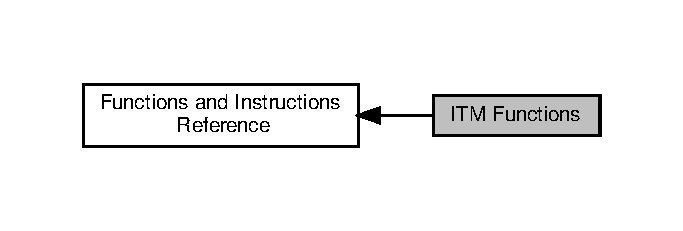
\includegraphics[width=328pt]{group___c_m_s_i_s__core___debug_functions}
\end{center}
\end{figure}
\subsection*{Definicje}
\begin{DoxyCompactItemize}
\item 
\#define \hyperlink{group___c_m_s_i_s__core___debug_functions_gaa822cb398ee022b59e9e6c5d7bbb228a}{I\+T\+M\+\_\+\+R\+X\+B\+U\+F\+F\+E\+R\+\_\+\+E\+M\+P\+TY}~((int32\+\_\+t)0x5\+A\+A55\+A\+A5\+U)
\item 
\#define \hyperlink{group___c_m_s_i_s__core___debug_functions_gaa822cb398ee022b59e9e6c5d7bbb228a}{I\+T\+M\+\_\+\+R\+X\+B\+U\+F\+F\+E\+R\+\_\+\+E\+M\+P\+TY}~((int32\+\_\+t)0x5\+A\+A55\+A\+A5\+U)
\item 
\#define \hyperlink{group___c_m_s_i_s__core___debug_functions_gaa822cb398ee022b59e9e6c5d7bbb228a}{I\+T\+M\+\_\+\+R\+X\+B\+U\+F\+F\+E\+R\+\_\+\+E\+M\+P\+TY}~((int32\+\_\+t)0x5\+A\+A55\+A\+A5\+U)
\item 
\#define \hyperlink{group___c_m_s_i_s__core___debug_functions_gaa822cb398ee022b59e9e6c5d7bbb228a}{I\+T\+M\+\_\+\+R\+X\+B\+U\+F\+F\+E\+R\+\_\+\+E\+M\+P\+TY}~((int32\+\_\+t)0x5\+A\+A55\+A\+A5\+U)
\item 
\#define \hyperlink{group___c_m_s_i_s__core___debug_functions_gaa822cb398ee022b59e9e6c5d7bbb228a}{I\+T\+M\+\_\+\+R\+X\+B\+U\+F\+F\+E\+R\+\_\+\+E\+M\+P\+TY}~((int32\+\_\+t)0x5\+A\+A55\+A\+A5\+U)
\item 
\#define \hyperlink{group___c_m_s_i_s__core___debug_functions_gaa822cb398ee022b59e9e6c5d7bbb228a}{I\+T\+M\+\_\+\+R\+X\+B\+U\+F\+F\+E\+R\+\_\+\+E\+M\+P\+TY}~((int32\+\_\+t)0x5\+A\+A55\+A\+A5\+U)
\end{DoxyCompactItemize}
\subsection*{Funkcje}
\begin{DoxyCompactItemize}
\item 
\hyperlink{cmsis__iccarm_8h_aba87361bfad2ae52cfe2f40c1a1dbf9c}{\+\_\+\+\_\+\+S\+T\+A\+T\+I\+C\+\_\+\+I\+N\+L\+I\+NE} uint32\+\_\+t \hyperlink{group___c_m_s_i_s__core___debug_functions_gac90a497bd64286b84552c2c553d3419e}{I\+T\+M\+\_\+\+Send\+Char} (uint32\+\_\+t ch)
\begin{DoxyCompactList}\small\item\em I\+TM Send Character. \end{DoxyCompactList}\item 
\hyperlink{cmsis__iccarm_8h_aba87361bfad2ae52cfe2f40c1a1dbf9c}{\+\_\+\+\_\+\+S\+T\+A\+T\+I\+C\+\_\+\+I\+N\+L\+I\+NE} int32\+\_\+t \hyperlink{group___c_m_s_i_s__core___debug_functions_gac3ee2c30a1ac4ed34c8a866a17decd53}{I\+T\+M\+\_\+\+Receive\+Char} (void)
\begin{DoxyCompactList}\small\item\em I\+TM Receive Character. \end{DoxyCompactList}\item 
\hyperlink{cmsis__iccarm_8h_aba87361bfad2ae52cfe2f40c1a1dbf9c}{\+\_\+\+\_\+\+S\+T\+A\+T\+I\+C\+\_\+\+I\+N\+L\+I\+NE} int32\+\_\+t \hyperlink{group___c_m_s_i_s__core___debug_functions_gae61ce9ca5917735325cd93b0fb21dd29}{I\+T\+M\+\_\+\+Check\+Char} (void)
\begin{DoxyCompactList}\small\item\em I\+TM Check Character. \end{DoxyCompactList}\end{DoxyCompactItemize}
\subsection*{Zmienne}
\begin{DoxyCompactItemize}
\item 
volatile int32\+\_\+t \hyperlink{group___c_m_s_i_s__core___debug_functions_ga12e68e55a7badc271b948d6c7230b2a8}{I\+T\+M\+\_\+\+Rx\+Buffer}
\item 
volatile int32\+\_\+t \hyperlink{group___c_m_s_i_s__core___debug_functions_ga12e68e55a7badc271b948d6c7230b2a8}{I\+T\+M\+\_\+\+Rx\+Buffer}
\item 
volatile int32\+\_\+t \hyperlink{group___c_m_s_i_s__core___debug_functions_ga12e68e55a7badc271b948d6c7230b2a8}{I\+T\+M\+\_\+\+Rx\+Buffer}
\item 
volatile int32\+\_\+t \hyperlink{group___c_m_s_i_s__core___debug_functions_ga12e68e55a7badc271b948d6c7230b2a8}{I\+T\+M\+\_\+\+Rx\+Buffer}
\item 
volatile int32\+\_\+t \hyperlink{group___c_m_s_i_s__core___debug_functions_ga12e68e55a7badc271b948d6c7230b2a8}{I\+T\+M\+\_\+\+Rx\+Buffer}
\item 
volatile int32\+\_\+t \hyperlink{group___c_m_s_i_s__core___debug_functions_ga12e68e55a7badc271b948d6c7230b2a8}{I\+T\+M\+\_\+\+Rx\+Buffer}
\end{DoxyCompactItemize}


\subsection{Opis szczegółowy}
Functions that access the I\+TM debug interface. 



\subsection{Dokumentacja definicji}
\mbox{\Hypertarget{group___c_m_s_i_s__core___debug_functions_gaa822cb398ee022b59e9e6c5d7bbb228a}\label{group___c_m_s_i_s__core___debug_functions_gaa822cb398ee022b59e9e6c5d7bbb228a}} 
\index{I\+T\+M Functions@{I\+T\+M Functions}!I\+T\+M\+\_\+\+R\+X\+B\+U\+F\+F\+E\+R\+\_\+\+E\+M\+P\+TY@{I\+T\+M\+\_\+\+R\+X\+B\+U\+F\+F\+E\+R\+\_\+\+E\+M\+P\+TY}}
\index{I\+T\+M\+\_\+\+R\+X\+B\+U\+F\+F\+E\+R\+\_\+\+E\+M\+P\+TY@{I\+T\+M\+\_\+\+R\+X\+B\+U\+F\+F\+E\+R\+\_\+\+E\+M\+P\+TY}!I\+T\+M Functions@{I\+T\+M Functions}}
\subsubsection{\texorpdfstring{I\+T\+M\+\_\+\+R\+X\+B\+U\+F\+F\+E\+R\+\_\+\+E\+M\+P\+TY}{ITM\_RXBUFFER\_EMPTY}\hspace{0.1cm}{\footnotesize\ttfamily [1/6]}}
{\footnotesize\ttfamily \#define I\+T\+M\+\_\+\+R\+X\+B\+U\+F\+F\+E\+R\+\_\+\+E\+M\+P\+TY~((int32\+\_\+t)0x5\+A\+A55\+A\+A5\+U)}

Value identifying \hyperlink{group___c_m_s_i_s__core___debug_functions_ga12e68e55a7badc271b948d6c7230b2a8}{I\+T\+M\+\_\+\+Rx\+Buffer} is ready for next character. 

Definicja w linii 1839 pliku core\+\_\+sc300.\+h.

\mbox{\Hypertarget{group___c_m_s_i_s__core___debug_functions_gaa822cb398ee022b59e9e6c5d7bbb228a}\label{group___c_m_s_i_s__core___debug_functions_gaa822cb398ee022b59e9e6c5d7bbb228a}} 
\index{I\+T\+M Functions@{I\+T\+M Functions}!I\+T\+M\+\_\+\+R\+X\+B\+U\+F\+F\+E\+R\+\_\+\+E\+M\+P\+TY@{I\+T\+M\+\_\+\+R\+X\+B\+U\+F\+F\+E\+R\+\_\+\+E\+M\+P\+TY}}
\index{I\+T\+M\+\_\+\+R\+X\+B\+U\+F\+F\+E\+R\+\_\+\+E\+M\+P\+TY@{I\+T\+M\+\_\+\+R\+X\+B\+U\+F\+F\+E\+R\+\_\+\+E\+M\+P\+TY}!I\+T\+M Functions@{I\+T\+M Functions}}
\subsubsection{\texorpdfstring{I\+T\+M\+\_\+\+R\+X\+B\+U\+F\+F\+E\+R\+\_\+\+E\+M\+P\+TY}{ITM\_RXBUFFER\_EMPTY}\hspace{0.1cm}{\footnotesize\ttfamily [2/6]}}
{\footnotesize\ttfamily \#define I\+T\+M\+\_\+\+R\+X\+B\+U\+F\+F\+E\+R\+\_\+\+E\+M\+P\+TY~((int32\+\_\+t)0x5\+A\+A55\+A\+A5\+U)}

Value identifying \hyperlink{group___c_m_s_i_s__core___debug_functions_ga12e68e55a7badc271b948d6c7230b2a8}{I\+T\+M\+\_\+\+Rx\+Buffer} is ready for next character. 

Definicja w linii 1865 pliku core\+\_\+cm3.\+h.

\mbox{\Hypertarget{group___c_m_s_i_s__core___debug_functions_gaa822cb398ee022b59e9e6c5d7bbb228a}\label{group___c_m_s_i_s__core___debug_functions_gaa822cb398ee022b59e9e6c5d7bbb228a}} 
\index{I\+T\+M Functions@{I\+T\+M Functions}!I\+T\+M\+\_\+\+R\+X\+B\+U\+F\+F\+E\+R\+\_\+\+E\+M\+P\+TY@{I\+T\+M\+\_\+\+R\+X\+B\+U\+F\+F\+E\+R\+\_\+\+E\+M\+P\+TY}}
\index{I\+T\+M\+\_\+\+R\+X\+B\+U\+F\+F\+E\+R\+\_\+\+E\+M\+P\+TY@{I\+T\+M\+\_\+\+R\+X\+B\+U\+F\+F\+E\+R\+\_\+\+E\+M\+P\+TY}!I\+T\+M Functions@{I\+T\+M Functions}}
\subsubsection{\texorpdfstring{I\+T\+M\+\_\+\+R\+X\+B\+U\+F\+F\+E\+R\+\_\+\+E\+M\+P\+TY}{ITM\_RXBUFFER\_EMPTY}\hspace{0.1cm}{\footnotesize\ttfamily [3/6]}}
{\footnotesize\ttfamily \#define I\+T\+M\+\_\+\+R\+X\+B\+U\+F\+F\+E\+R\+\_\+\+E\+M\+P\+TY~((int32\+\_\+t)0x5\+A\+A55\+A\+A5\+U)}

Value identifying \hyperlink{group___c_m_s_i_s__core___debug_functions_ga12e68e55a7badc271b948d6c7230b2a8}{I\+T\+M\+\_\+\+Rx\+Buffer} is ready for next character. 

Definicja w linii 2053 pliku core\+\_\+cm4.\+h.

\mbox{\Hypertarget{group___c_m_s_i_s__core___debug_functions_gaa822cb398ee022b59e9e6c5d7bbb228a}\label{group___c_m_s_i_s__core___debug_functions_gaa822cb398ee022b59e9e6c5d7bbb228a}} 
\index{I\+T\+M Functions@{I\+T\+M Functions}!I\+T\+M\+\_\+\+R\+X\+B\+U\+F\+F\+E\+R\+\_\+\+E\+M\+P\+TY@{I\+T\+M\+\_\+\+R\+X\+B\+U\+F\+F\+E\+R\+\_\+\+E\+M\+P\+TY}}
\index{I\+T\+M\+\_\+\+R\+X\+B\+U\+F\+F\+E\+R\+\_\+\+E\+M\+P\+TY@{I\+T\+M\+\_\+\+R\+X\+B\+U\+F\+F\+E\+R\+\_\+\+E\+M\+P\+TY}!I\+T\+M Functions@{I\+T\+M Functions}}
\subsubsection{\texorpdfstring{I\+T\+M\+\_\+\+R\+X\+B\+U\+F\+F\+E\+R\+\_\+\+E\+M\+P\+TY}{ITM\_RXBUFFER\_EMPTY}\hspace{0.1cm}{\footnotesize\ttfamily [4/6]}}
{\footnotesize\ttfamily \#define I\+T\+M\+\_\+\+R\+X\+B\+U\+F\+F\+E\+R\+\_\+\+E\+M\+P\+TY~((int32\+\_\+t)0x5\+A\+A55\+A\+A5\+U)}

Value identifying \hyperlink{group___c_m_s_i_s__core___debug_functions_ga12e68e55a7badc271b948d6c7230b2a8}{I\+T\+M\+\_\+\+Rx\+Buffer} is ready for next character. 

Definicja w linii 2595 pliku core\+\_\+cm7.\+h.

\mbox{\Hypertarget{group___c_m_s_i_s__core___debug_functions_gaa822cb398ee022b59e9e6c5d7bbb228a}\label{group___c_m_s_i_s__core___debug_functions_gaa822cb398ee022b59e9e6c5d7bbb228a}} 
\index{I\+T\+M Functions@{I\+T\+M Functions}!I\+T\+M\+\_\+\+R\+X\+B\+U\+F\+F\+E\+R\+\_\+\+E\+M\+P\+TY@{I\+T\+M\+\_\+\+R\+X\+B\+U\+F\+F\+E\+R\+\_\+\+E\+M\+P\+TY}}
\index{I\+T\+M\+\_\+\+R\+X\+B\+U\+F\+F\+E\+R\+\_\+\+E\+M\+P\+TY@{I\+T\+M\+\_\+\+R\+X\+B\+U\+F\+F\+E\+R\+\_\+\+E\+M\+P\+TY}!I\+T\+M Functions@{I\+T\+M Functions}}
\subsubsection{\texorpdfstring{I\+T\+M\+\_\+\+R\+X\+B\+U\+F\+F\+E\+R\+\_\+\+E\+M\+P\+TY}{ITM\_RXBUFFER\_EMPTY}\hspace{0.1cm}{\footnotesize\ttfamily [5/6]}}
{\footnotesize\ttfamily \#define I\+T\+M\+\_\+\+R\+X\+B\+U\+F\+F\+E\+R\+\_\+\+E\+M\+P\+TY~((int32\+\_\+t)0x5\+A\+A55\+A\+A5\+U)}

Value identifying \hyperlink{group___c_m_s_i_s__core___debug_functions_ga12e68e55a7badc271b948d6c7230b2a8}{I\+T\+M\+\_\+\+Rx\+Buffer} is ready for next character. 

Definicja w linii 2851 pliku core\+\_\+armv8mml.\+h.

\mbox{\Hypertarget{group___c_m_s_i_s__core___debug_functions_gaa822cb398ee022b59e9e6c5d7bbb228a}\label{group___c_m_s_i_s__core___debug_functions_gaa822cb398ee022b59e9e6c5d7bbb228a}} 
\index{I\+T\+M Functions@{I\+T\+M Functions}!I\+T\+M\+\_\+\+R\+X\+B\+U\+F\+F\+E\+R\+\_\+\+E\+M\+P\+TY@{I\+T\+M\+\_\+\+R\+X\+B\+U\+F\+F\+E\+R\+\_\+\+E\+M\+P\+TY}}
\index{I\+T\+M\+\_\+\+R\+X\+B\+U\+F\+F\+E\+R\+\_\+\+E\+M\+P\+TY@{I\+T\+M\+\_\+\+R\+X\+B\+U\+F\+F\+E\+R\+\_\+\+E\+M\+P\+TY}!I\+T\+M Functions@{I\+T\+M Functions}}
\subsubsection{\texorpdfstring{I\+T\+M\+\_\+\+R\+X\+B\+U\+F\+F\+E\+R\+\_\+\+E\+M\+P\+TY}{ITM\_RXBUFFER\_EMPTY}\hspace{0.1cm}{\footnotesize\ttfamily [6/6]}}
{\footnotesize\ttfamily \#define I\+T\+M\+\_\+\+R\+X\+B\+U\+F\+F\+E\+R\+\_\+\+E\+M\+P\+TY~((int32\+\_\+t)0x5\+A\+A55\+A\+A5\+U)}

Value identifying \hyperlink{group___c_m_s_i_s__core___debug_functions_ga12e68e55a7badc271b948d6c7230b2a8}{I\+T\+M\+\_\+\+Rx\+Buffer} is ready for next character. 

Definicja w linii 2926 pliku core\+\_\+cm33.\+h.



\subsection{Dokumentacja funkcji}
\mbox{\Hypertarget{group___c_m_s_i_s__core___debug_functions_gae61ce9ca5917735325cd93b0fb21dd29}\label{group___c_m_s_i_s__core___debug_functions_gae61ce9ca5917735325cd93b0fb21dd29}} 
\index{I\+T\+M Functions@{I\+T\+M Functions}!I\+T\+M\+\_\+\+Check\+Char@{I\+T\+M\+\_\+\+Check\+Char}}
\index{I\+T\+M\+\_\+\+Check\+Char@{I\+T\+M\+\_\+\+Check\+Char}!I\+T\+M Functions@{I\+T\+M Functions}}
\subsubsection{\texorpdfstring{I\+T\+M\+\_\+\+Check\+Char()}{ITM\_CheckChar()}}
{\footnotesize\ttfamily \hyperlink{cmsis__iccarm_8h_aba87361bfad2ae52cfe2f40c1a1dbf9c}{\+\_\+\+\_\+\+S\+T\+A\+T\+I\+C\+\_\+\+I\+N\+L\+I\+NE} int32\+\_\+t I\+T\+M\+\_\+\+Check\+Char (\begin{DoxyParamCaption}\item[{void}]{ }\end{DoxyParamCaption})}



I\+TM Check Character. 

Checks whether a character is pending for reading in the variable \hyperlink{group___c_m_s_i_s__core___debug_functions_ga12e68e55a7badc271b948d6c7230b2a8}{I\+T\+M\+\_\+\+Rx\+Buffer}. \begin{DoxyReturn}{Zwraca}
0 No character available. 

1 Character available. 
\end{DoxyReturn}


Definicja w linii 2903 pliku core\+\_\+armv8mml.\+h.

\mbox{\Hypertarget{group___c_m_s_i_s__core___debug_functions_gac3ee2c30a1ac4ed34c8a866a17decd53}\label{group___c_m_s_i_s__core___debug_functions_gac3ee2c30a1ac4ed34c8a866a17decd53}} 
\index{I\+T\+M Functions@{I\+T\+M Functions}!I\+T\+M\+\_\+\+Receive\+Char@{I\+T\+M\+\_\+\+Receive\+Char}}
\index{I\+T\+M\+\_\+\+Receive\+Char@{I\+T\+M\+\_\+\+Receive\+Char}!I\+T\+M Functions@{I\+T\+M Functions}}
\subsubsection{\texorpdfstring{I\+T\+M\+\_\+\+Receive\+Char()}{ITM\_ReceiveChar()}}
{\footnotesize\ttfamily \hyperlink{cmsis__iccarm_8h_aba87361bfad2ae52cfe2f40c1a1dbf9c}{\+\_\+\+\_\+\+S\+T\+A\+T\+I\+C\+\_\+\+I\+N\+L\+I\+NE} int32\+\_\+t I\+T\+M\+\_\+\+Receive\+Char (\begin{DoxyParamCaption}\item[{void}]{ }\end{DoxyParamCaption})}



I\+TM Receive Character. 

Inputs a character via the external variable \hyperlink{group___c_m_s_i_s__core___debug_functions_ga12e68e55a7badc271b948d6c7230b2a8}{I\+T\+M\+\_\+\+Rx\+Buffer}. \begin{DoxyReturn}{Zwraca}
Received character. 

-\/1 No character pending. 
\end{DoxyReturn}


Definicja w linii 2883 pliku core\+\_\+armv8mml.\+h.

\mbox{\Hypertarget{group___c_m_s_i_s__core___debug_functions_gac90a497bd64286b84552c2c553d3419e}\label{group___c_m_s_i_s__core___debug_functions_gac90a497bd64286b84552c2c553d3419e}} 
\index{I\+T\+M Functions@{I\+T\+M Functions}!I\+T\+M\+\_\+\+Send\+Char@{I\+T\+M\+\_\+\+Send\+Char}}
\index{I\+T\+M\+\_\+\+Send\+Char@{I\+T\+M\+\_\+\+Send\+Char}!I\+T\+M Functions@{I\+T\+M Functions}}
\subsubsection{\texorpdfstring{I\+T\+M\+\_\+\+Send\+Char()}{ITM\_SendChar()}}
{\footnotesize\ttfamily \hyperlink{cmsis__iccarm_8h_aba87361bfad2ae52cfe2f40c1a1dbf9c}{\+\_\+\+\_\+\+S\+T\+A\+T\+I\+C\+\_\+\+I\+N\+L\+I\+NE} uint32\+\_\+t I\+T\+M\+\_\+\+Send\+Char (\begin{DoxyParamCaption}\item[{uint32\+\_\+t}]{ch }\end{DoxyParamCaption})}



I\+TM Send Character. 

Transmits a character via the I\+TM channel 0, and \begin{DoxyItemize}
\item Just returns when no debugger is connected that has booked the output. \item Is blocking when a debugger is connected, but the previous character sent has not been transmitted. 
\begin{DoxyParams}[1]{Parametry}
\mbox{\tt in}  & {\em ch} & Character to transmit. \\
\hline
\end{DoxyParams}
\begin{DoxyReturn}{Zwraca}
Character to transmit. 
\end{DoxyReturn}
\end{DoxyItemize}


Definicja w linii 2862 pliku core\+\_\+armv8mml.\+h.



\subsection{Dokumentacja zmiennych}
\mbox{\Hypertarget{group___c_m_s_i_s__core___debug_functions_ga12e68e55a7badc271b948d6c7230b2a8}\label{group___c_m_s_i_s__core___debug_functions_ga12e68e55a7badc271b948d6c7230b2a8}} 
\index{I\+T\+M Functions@{I\+T\+M Functions}!I\+T\+M\+\_\+\+Rx\+Buffer@{I\+T\+M\+\_\+\+Rx\+Buffer}}
\index{I\+T\+M\+\_\+\+Rx\+Buffer@{I\+T\+M\+\_\+\+Rx\+Buffer}!I\+T\+M Functions@{I\+T\+M Functions}}
\subsubsection{\texorpdfstring{I\+T\+M\+\_\+\+Rx\+Buffer}{ITM\_RxBuffer}\hspace{0.1cm}{\footnotesize\ttfamily [1/6]}}
{\footnotesize\ttfamily volatile int32\+\_\+t I\+T\+M\+\_\+\+Rx\+Buffer}

External variable to receive characters. \mbox{\Hypertarget{group___c_m_s_i_s__core___debug_functions_ga12e68e55a7badc271b948d6c7230b2a8}\label{group___c_m_s_i_s__core___debug_functions_ga12e68e55a7badc271b948d6c7230b2a8}} 
\index{I\+T\+M Functions@{I\+T\+M Functions}!I\+T\+M\+\_\+\+Rx\+Buffer@{I\+T\+M\+\_\+\+Rx\+Buffer}}
\index{I\+T\+M\+\_\+\+Rx\+Buffer@{I\+T\+M\+\_\+\+Rx\+Buffer}!I\+T\+M Functions@{I\+T\+M Functions}}
\subsubsection{\texorpdfstring{I\+T\+M\+\_\+\+Rx\+Buffer}{ITM\_RxBuffer}\hspace{0.1cm}{\footnotesize\ttfamily [2/6]}}
{\footnotesize\ttfamily volatile int32\+\_\+t I\+T\+M\+\_\+\+Rx\+Buffer}

External variable to receive characters. \mbox{\Hypertarget{group___c_m_s_i_s__core___debug_functions_ga12e68e55a7badc271b948d6c7230b2a8}\label{group___c_m_s_i_s__core___debug_functions_ga12e68e55a7badc271b948d6c7230b2a8}} 
\index{I\+T\+M Functions@{I\+T\+M Functions}!I\+T\+M\+\_\+\+Rx\+Buffer@{I\+T\+M\+\_\+\+Rx\+Buffer}}
\index{I\+T\+M\+\_\+\+Rx\+Buffer@{I\+T\+M\+\_\+\+Rx\+Buffer}!I\+T\+M Functions@{I\+T\+M Functions}}
\subsubsection{\texorpdfstring{I\+T\+M\+\_\+\+Rx\+Buffer}{ITM\_RxBuffer}\hspace{0.1cm}{\footnotesize\ttfamily [3/6]}}
{\footnotesize\ttfamily volatile int32\+\_\+t I\+T\+M\+\_\+\+Rx\+Buffer}

External variable to receive characters. \mbox{\Hypertarget{group___c_m_s_i_s__core___debug_functions_ga12e68e55a7badc271b948d6c7230b2a8}\label{group___c_m_s_i_s__core___debug_functions_ga12e68e55a7badc271b948d6c7230b2a8}} 
\index{I\+T\+M Functions@{I\+T\+M Functions}!I\+T\+M\+\_\+\+Rx\+Buffer@{I\+T\+M\+\_\+\+Rx\+Buffer}}
\index{I\+T\+M\+\_\+\+Rx\+Buffer@{I\+T\+M\+\_\+\+Rx\+Buffer}!I\+T\+M Functions@{I\+T\+M Functions}}
\subsubsection{\texorpdfstring{I\+T\+M\+\_\+\+Rx\+Buffer}{ITM\_RxBuffer}\hspace{0.1cm}{\footnotesize\ttfamily [4/6]}}
{\footnotesize\ttfamily volatile int32\+\_\+t I\+T\+M\+\_\+\+Rx\+Buffer}

External variable to receive characters. \mbox{\Hypertarget{group___c_m_s_i_s__core___debug_functions_ga12e68e55a7badc271b948d6c7230b2a8}\label{group___c_m_s_i_s__core___debug_functions_ga12e68e55a7badc271b948d6c7230b2a8}} 
\index{I\+T\+M Functions@{I\+T\+M Functions}!I\+T\+M\+\_\+\+Rx\+Buffer@{I\+T\+M\+\_\+\+Rx\+Buffer}}
\index{I\+T\+M\+\_\+\+Rx\+Buffer@{I\+T\+M\+\_\+\+Rx\+Buffer}!I\+T\+M Functions@{I\+T\+M Functions}}
\subsubsection{\texorpdfstring{I\+T\+M\+\_\+\+Rx\+Buffer}{ITM\_RxBuffer}\hspace{0.1cm}{\footnotesize\ttfamily [5/6]}}
{\footnotesize\ttfamily volatile int32\+\_\+t I\+T\+M\+\_\+\+Rx\+Buffer}

External variable to receive characters. \mbox{\Hypertarget{group___c_m_s_i_s__core___debug_functions_ga12e68e55a7badc271b948d6c7230b2a8}\label{group___c_m_s_i_s__core___debug_functions_ga12e68e55a7badc271b948d6c7230b2a8}} 
\index{I\+T\+M Functions@{I\+T\+M Functions}!I\+T\+M\+\_\+\+Rx\+Buffer@{I\+T\+M\+\_\+\+Rx\+Buffer}}
\index{I\+T\+M\+\_\+\+Rx\+Buffer@{I\+T\+M\+\_\+\+Rx\+Buffer}!I\+T\+M Functions@{I\+T\+M Functions}}
\subsubsection{\texorpdfstring{I\+T\+M\+\_\+\+Rx\+Buffer}{ITM\_RxBuffer}\hspace{0.1cm}{\footnotesize\ttfamily [6/6]}}
{\footnotesize\ttfamily volatile int32\+\_\+t I\+T\+M\+\_\+\+Rx\+Buffer}

External variable to receive characters. 
\hypertarget{group___c_m_s_i_s___core___cache_functions}{}\section{Cache Functions}
\label{group___c_m_s_i_s___core___cache_functions}\index{Cache Functions@{Cache Functions}}


Functions that configure Instruction and Data cache.  


Diagram współpracy dla Cache Functions\+:\nopagebreak
\begin{figure}[H]
\begin{center}
\leavevmode
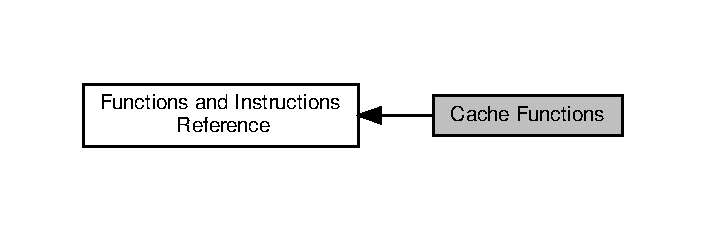
\includegraphics[width=339pt]{group___c_m_s_i_s___core___cache_functions}
\end{center}
\end{figure}
\subsection*{Definicje}
\begin{DoxyCompactItemize}
\item 
\#define \hyperlink{group___c_m_s_i_s___core___cache_functions_ga3d672529cd193537fe2a0141931c6ad9}{C\+C\+S\+I\+D\+R\+\_\+\+W\+A\+YS}(x)~(((x) \& \hyperlink{group___c_m_s_i_s___s_c_b_gae093c4c635dad43845967512fa87173a}{S\+C\+B\+\_\+\+C\+C\+S\+I\+D\+R\+\_\+\+A\+S\+S\+O\+C\+I\+A\+T\+I\+V\+I\+T\+Y\+\_\+\+Msk}) $>$$>$ \hyperlink{group___c_m_s_i_s___s_c_b_gae67f2f83976b819fb3039fc35cfef0fb}{S\+C\+B\+\_\+\+C\+C\+S\+I\+D\+R\+\_\+\+A\+S\+S\+O\+C\+I\+A\+T\+I\+V\+I\+T\+Y\+\_\+\+Pos})
\item 
\#define \hyperlink{group___c_m_s_i_s___core___cache_functions_gaf20feee7c52fee32b48ee0d2ceaaf932}{C\+C\+S\+I\+D\+R\+\_\+\+S\+E\+TS}(x)~(((x) \& \hyperlink{group___c_m_s_i_s___s_c_b_ga47d1f01185d7a039334031008386c5a8}{S\+C\+B\+\_\+\+C\+C\+S\+I\+D\+R\+\_\+\+N\+U\+M\+S\+E\+T\+S\+\_\+\+Msk}      ) $>$$>$ \hyperlink{group___c_m_s_i_s___s_c_b_ga1028d2c238f74d2aa021f53ffbe8d7ab}{S\+C\+B\+\_\+\+C\+C\+S\+I\+D\+R\+\_\+\+N\+U\+M\+S\+E\+T\+S\+\_\+\+Pos}      )
\end{DoxyCompactItemize}
\subsection*{Funkcje}
\begin{DoxyCompactItemize}
\item 
\hyperlink{cmsis__iccarm_8h_aba87361bfad2ae52cfe2f40c1a1dbf9c}{\+\_\+\+\_\+\+S\+T\+A\+T\+I\+C\+\_\+\+I\+N\+L\+I\+NE} void \hyperlink{group___c_m_s_i_s___core___cache_functions_gaf9e7c6c8e16ada1f95e5bf5a03505b68}{S\+C\+B\+\_\+\+Enable\+I\+Cache} (void)
\begin{DoxyCompactList}\small\item\em Enable I-\/\+Cache. \end{DoxyCompactList}\item 
\hyperlink{cmsis__iccarm_8h_aba87361bfad2ae52cfe2f40c1a1dbf9c}{\+\_\+\+\_\+\+S\+T\+A\+T\+I\+C\+\_\+\+I\+N\+L\+I\+NE} void \hyperlink{group___c_m_s_i_s___core___cache_functions_gaba757390852f95b3ac2d8638c717d8d8}{S\+C\+B\+\_\+\+Disable\+I\+Cache} (void)
\begin{DoxyCompactList}\small\item\em Disable I-\/\+Cache. \end{DoxyCompactList}\item 
\hyperlink{cmsis__iccarm_8h_aba87361bfad2ae52cfe2f40c1a1dbf9c}{\+\_\+\+\_\+\+S\+T\+A\+T\+I\+C\+\_\+\+I\+N\+L\+I\+NE} void \hyperlink{group___c_m_s_i_s___core___cache_functions_ga50d373a785edd782c5de5a3b55e30ff3}{S\+C\+B\+\_\+\+Invalidate\+I\+Cache} (void)
\begin{DoxyCompactList}\small\item\em Invalidate I-\/\+Cache. \end{DoxyCompactList}\item 
\hyperlink{cmsis__iccarm_8h_aba87361bfad2ae52cfe2f40c1a1dbf9c}{\+\_\+\+\_\+\+S\+T\+A\+T\+I\+C\+\_\+\+I\+N\+L\+I\+NE} void \hyperlink{group___c_m_s_i_s___core___cache_functions_ga63aa640d9006021a796a5dcf9c7180b6}{S\+C\+B\+\_\+\+Enable\+D\+Cache} (void)
\begin{DoxyCompactList}\small\item\em Enable D-\/\+Cache. \end{DoxyCompactList}\item 
\hyperlink{cmsis__iccarm_8h_aba87361bfad2ae52cfe2f40c1a1dbf9c}{\+\_\+\+\_\+\+S\+T\+A\+T\+I\+C\+\_\+\+I\+N\+L\+I\+NE} void \hyperlink{group___c_m_s_i_s___core___cache_functions_ga6468170f90d270caab8116e7a4f0b5fe}{S\+C\+B\+\_\+\+Disable\+D\+Cache} (void)
\begin{DoxyCompactList}\small\item\em Disable D-\/\+Cache. \end{DoxyCompactList}\item 
\hyperlink{cmsis__iccarm_8h_aba87361bfad2ae52cfe2f40c1a1dbf9c}{\+\_\+\+\_\+\+S\+T\+A\+T\+I\+C\+\_\+\+I\+N\+L\+I\+NE} void \hyperlink{group___c_m_s_i_s___core___cache_functions_gace2d30db08887d0bdb818b8a785a5ce6}{S\+C\+B\+\_\+\+Invalidate\+D\+Cache} (void)
\begin{DoxyCompactList}\small\item\em Invalidate D-\/\+Cache. \end{DoxyCompactList}\item 
\hyperlink{cmsis__iccarm_8h_aba87361bfad2ae52cfe2f40c1a1dbf9c}{\+\_\+\+\_\+\+S\+T\+A\+T\+I\+C\+\_\+\+I\+N\+L\+I\+NE} void \hyperlink{group___c_m_s_i_s___core___cache_functions_ga55583e3065c6eabca204b8b89b121c4c}{S\+C\+B\+\_\+\+Clean\+D\+Cache} (void)
\begin{DoxyCompactList}\small\item\em Clean D-\/\+Cache. \end{DoxyCompactList}\item 
\hyperlink{cmsis__iccarm_8h_aba87361bfad2ae52cfe2f40c1a1dbf9c}{\+\_\+\+\_\+\+S\+T\+A\+T\+I\+C\+\_\+\+I\+N\+L\+I\+NE} void \hyperlink{group___c_m_s_i_s___core___cache_functions_ga1b741def9e3b2ca97dc9ea49b8ce505c}{S\+C\+B\+\_\+\+Clean\+Invalidate\+D\+Cache} (void)
\begin{DoxyCompactList}\small\item\em Clean \& Invalidate D-\/\+Cache. \end{DoxyCompactList}\item 
\hyperlink{cmsis__iccarm_8h_aba87361bfad2ae52cfe2f40c1a1dbf9c}{\+\_\+\+\_\+\+S\+T\+A\+T\+I\+C\+\_\+\+I\+N\+L\+I\+NE} void \hyperlink{group___c_m_s_i_s___core___cache_functions_ga503ef7ef58c0773defd15a82f6336c09}{S\+C\+B\+\_\+\+Invalidate\+D\+Cache\+\_\+by\+\_\+\+Addr} (uint32\+\_\+t $\ast$addr, int32\+\_\+t dsize)
\begin{DoxyCompactList}\small\item\em D-\/\+Cache Invalidate by address. \end{DoxyCompactList}\item 
\hyperlink{cmsis__iccarm_8h_aba87361bfad2ae52cfe2f40c1a1dbf9c}{\+\_\+\+\_\+\+S\+T\+A\+T\+I\+C\+\_\+\+I\+N\+L\+I\+NE} void \hyperlink{group___c_m_s_i_s___core___cache_functions_ga696fadbf7b9cc71dad42fab61873a40d}{S\+C\+B\+\_\+\+Clean\+D\+Cache\+\_\+by\+\_\+\+Addr} (uint32\+\_\+t $\ast$addr, int32\+\_\+t dsize)
\begin{DoxyCompactList}\small\item\em D-\/\+Cache Clean by address. \end{DoxyCompactList}\item 
\hyperlink{cmsis__iccarm_8h_aba87361bfad2ae52cfe2f40c1a1dbf9c}{\+\_\+\+\_\+\+S\+T\+A\+T\+I\+C\+\_\+\+I\+N\+L\+I\+NE} void \hyperlink{group___c_m_s_i_s___core___cache_functions_ga630131b2572eaa16b569ed364dfc895e}{S\+C\+B\+\_\+\+Clean\+Invalidate\+D\+Cache\+\_\+by\+\_\+\+Addr} (uint32\+\_\+t $\ast$addr, int32\+\_\+t dsize)
\begin{DoxyCompactList}\small\item\em D-\/\+Cache Clean and Invalidate by address. \end{DoxyCompactList}\end{DoxyCompactItemize}


\subsection{Opis szczegółowy}
Functions that configure Instruction and Data cache. 



\subsection{Dokumentacja definicji}
\mbox{\Hypertarget{group___c_m_s_i_s___core___cache_functions_gaf20feee7c52fee32b48ee0d2ceaaf932}\label{group___c_m_s_i_s___core___cache_functions_gaf20feee7c52fee32b48ee0d2ceaaf932}} 
\index{Cache Functions@{Cache Functions}!C\+C\+S\+I\+D\+R\+\_\+\+S\+E\+TS@{C\+C\+S\+I\+D\+R\+\_\+\+S\+E\+TS}}
\index{C\+C\+S\+I\+D\+R\+\_\+\+S\+E\+TS@{C\+C\+S\+I\+D\+R\+\_\+\+S\+E\+TS}!Cache Functions@{Cache Functions}}
\subsubsection{\texorpdfstring{C\+C\+S\+I\+D\+R\+\_\+\+S\+E\+TS}{CCSIDR\_SETS}}
{\footnotesize\ttfamily \#define C\+C\+S\+I\+D\+R\+\_\+\+S\+E\+TS(\begin{DoxyParamCaption}\item[{}]{x }\end{DoxyParamCaption})~(((x) \& \hyperlink{group___c_m_s_i_s___s_c_b_ga47d1f01185d7a039334031008386c5a8}{S\+C\+B\+\_\+\+C\+C\+S\+I\+D\+R\+\_\+\+N\+U\+M\+S\+E\+T\+S\+\_\+\+Msk}      ) $>$$>$ \hyperlink{group___c_m_s_i_s___s_c_b_ga1028d2c238f74d2aa021f53ffbe8d7ab}{S\+C\+B\+\_\+\+C\+C\+S\+I\+D\+R\+\_\+\+N\+U\+M\+S\+E\+T\+S\+\_\+\+Pos}      )}



Definicja w linii 2222 pliku core\+\_\+cm7.\+h.

\mbox{\Hypertarget{group___c_m_s_i_s___core___cache_functions_ga3d672529cd193537fe2a0141931c6ad9}\label{group___c_m_s_i_s___core___cache_functions_ga3d672529cd193537fe2a0141931c6ad9}} 
\index{Cache Functions@{Cache Functions}!C\+C\+S\+I\+D\+R\+\_\+\+W\+A\+YS@{C\+C\+S\+I\+D\+R\+\_\+\+W\+A\+YS}}
\index{C\+C\+S\+I\+D\+R\+\_\+\+W\+A\+YS@{C\+C\+S\+I\+D\+R\+\_\+\+W\+A\+YS}!Cache Functions@{Cache Functions}}
\subsubsection{\texorpdfstring{C\+C\+S\+I\+D\+R\+\_\+\+W\+A\+YS}{CCSIDR\_WAYS}}
{\footnotesize\ttfamily \#define C\+C\+S\+I\+D\+R\+\_\+\+W\+A\+YS(\begin{DoxyParamCaption}\item[{}]{x }\end{DoxyParamCaption})~(((x) \& \hyperlink{group___c_m_s_i_s___s_c_b_gae093c4c635dad43845967512fa87173a}{S\+C\+B\+\_\+\+C\+C\+S\+I\+D\+R\+\_\+\+A\+S\+S\+O\+C\+I\+A\+T\+I\+V\+I\+T\+Y\+\_\+\+Msk}) $>$$>$ \hyperlink{group___c_m_s_i_s___s_c_b_gae67f2f83976b819fb3039fc35cfef0fb}{S\+C\+B\+\_\+\+C\+C\+S\+I\+D\+R\+\_\+\+A\+S\+S\+O\+C\+I\+A\+T\+I\+V\+I\+T\+Y\+\_\+\+Pos})}



Definicja w linii 2221 pliku core\+\_\+cm7.\+h.



\subsection{Dokumentacja funkcji}
\mbox{\Hypertarget{group___c_m_s_i_s___core___cache_functions_ga55583e3065c6eabca204b8b89b121c4c}\label{group___c_m_s_i_s___core___cache_functions_ga55583e3065c6eabca204b8b89b121c4c}} 
\index{Cache Functions@{Cache Functions}!S\+C\+B\+\_\+\+Clean\+D\+Cache@{S\+C\+B\+\_\+\+Clean\+D\+Cache}}
\index{S\+C\+B\+\_\+\+Clean\+D\+Cache@{S\+C\+B\+\_\+\+Clean\+D\+Cache}!Cache Functions@{Cache Functions}}
\subsubsection{\texorpdfstring{S\+C\+B\+\_\+\+Clean\+D\+Cache()}{SCB\_CleanDCache()}}
{\footnotesize\ttfamily \hyperlink{cmsis__iccarm_8h_aba87361bfad2ae52cfe2f40c1a1dbf9c}{\+\_\+\+\_\+\+S\+T\+A\+T\+I\+C\+\_\+\+I\+N\+L\+I\+NE} void S\+C\+B\+\_\+\+Clean\+D\+Cache (\begin{DoxyParamCaption}\item[{void}]{ }\end{DoxyParamCaption})}



Clean D-\/\+Cache. 

Cleans D-\/\+Cache 

Definicja w linii 2392 pliku core\+\_\+cm7.\+h.

\mbox{\Hypertarget{group___c_m_s_i_s___core___cache_functions_ga696fadbf7b9cc71dad42fab61873a40d}\label{group___c_m_s_i_s___core___cache_functions_ga696fadbf7b9cc71dad42fab61873a40d}} 
\index{Cache Functions@{Cache Functions}!S\+C\+B\+\_\+\+Clean\+D\+Cache\+\_\+by\+\_\+\+Addr@{S\+C\+B\+\_\+\+Clean\+D\+Cache\+\_\+by\+\_\+\+Addr}}
\index{S\+C\+B\+\_\+\+Clean\+D\+Cache\+\_\+by\+\_\+\+Addr@{S\+C\+B\+\_\+\+Clean\+D\+Cache\+\_\+by\+\_\+\+Addr}!Cache Functions@{Cache Functions}}
\subsubsection{\texorpdfstring{S\+C\+B\+\_\+\+Clean\+D\+Cache\+\_\+by\+\_\+\+Addr()}{SCB\_CleanDCache\_by\_Addr()}}
{\footnotesize\ttfamily \hyperlink{cmsis__iccarm_8h_aba87361bfad2ae52cfe2f40c1a1dbf9c}{\+\_\+\+\_\+\+S\+T\+A\+T\+I\+C\+\_\+\+I\+N\+L\+I\+NE} void S\+C\+B\+\_\+\+Clean\+D\+Cache\+\_\+by\+\_\+\+Addr (\begin{DoxyParamCaption}\item[{uint32\+\_\+t $\ast$}]{addr,  }\item[{int32\+\_\+t}]{dsize }\end{DoxyParamCaption})}



D-\/\+Cache Clean by address. 

Cleans D-\/\+Cache for the given address 
\begin{DoxyParams}[1]{Parametry}
\mbox{\tt in}  & {\em addr} & address (aligned to 32-\/byte boundary) \\
\hline
\mbox{\tt in}  & {\em dsize} & size of memory block (in number of bytes) \\
\hline
\end{DoxyParams}


Definicja w linii 2491 pliku core\+\_\+cm7.\+h.

\mbox{\Hypertarget{group___c_m_s_i_s___core___cache_functions_ga1b741def9e3b2ca97dc9ea49b8ce505c}\label{group___c_m_s_i_s___core___cache_functions_ga1b741def9e3b2ca97dc9ea49b8ce505c}} 
\index{Cache Functions@{Cache Functions}!S\+C\+B\+\_\+\+Clean\+Invalidate\+D\+Cache@{S\+C\+B\+\_\+\+Clean\+Invalidate\+D\+Cache}}
\index{S\+C\+B\+\_\+\+Clean\+Invalidate\+D\+Cache@{S\+C\+B\+\_\+\+Clean\+Invalidate\+D\+Cache}!Cache Functions@{Cache Functions}}
\subsubsection{\texorpdfstring{S\+C\+B\+\_\+\+Clean\+Invalidate\+D\+Cache()}{SCB\_CleanInvalidateDCache()}}
{\footnotesize\ttfamily \hyperlink{cmsis__iccarm_8h_aba87361bfad2ae52cfe2f40c1a1dbf9c}{\+\_\+\+\_\+\+S\+T\+A\+T\+I\+C\+\_\+\+I\+N\+L\+I\+NE} void S\+C\+B\+\_\+\+Clean\+Invalidate\+D\+Cache (\begin{DoxyParamCaption}\item[{void}]{ }\end{DoxyParamCaption})}



Clean \& Invalidate D-\/\+Cache. 

Cleans and Invalidates D-\/\+Cache 

Definicja w linii 2427 pliku core\+\_\+cm7.\+h.

\mbox{\Hypertarget{group___c_m_s_i_s___core___cache_functions_ga630131b2572eaa16b569ed364dfc895e}\label{group___c_m_s_i_s___core___cache_functions_ga630131b2572eaa16b569ed364dfc895e}} 
\index{Cache Functions@{Cache Functions}!S\+C\+B\+\_\+\+Clean\+Invalidate\+D\+Cache\+\_\+by\+\_\+\+Addr@{S\+C\+B\+\_\+\+Clean\+Invalidate\+D\+Cache\+\_\+by\+\_\+\+Addr}}
\index{S\+C\+B\+\_\+\+Clean\+Invalidate\+D\+Cache\+\_\+by\+\_\+\+Addr@{S\+C\+B\+\_\+\+Clean\+Invalidate\+D\+Cache\+\_\+by\+\_\+\+Addr}!Cache Functions@{Cache Functions}}
\subsubsection{\texorpdfstring{S\+C\+B\+\_\+\+Clean\+Invalidate\+D\+Cache\+\_\+by\+\_\+\+Addr()}{SCB\_CleanInvalidateDCache\_by\_Addr()}}
{\footnotesize\ttfamily \hyperlink{cmsis__iccarm_8h_aba87361bfad2ae52cfe2f40c1a1dbf9c}{\+\_\+\+\_\+\+S\+T\+A\+T\+I\+C\+\_\+\+I\+N\+L\+I\+NE} void S\+C\+B\+\_\+\+Clean\+Invalidate\+D\+Cache\+\_\+by\+\_\+\+Addr (\begin{DoxyParamCaption}\item[{uint32\+\_\+t $\ast$}]{addr,  }\item[{int32\+\_\+t}]{dsize }\end{DoxyParamCaption})}



D-\/\+Cache Clean and Invalidate by address. 

Cleans and invalidates D\+\_\+\+Cache for the given address 
\begin{DoxyParams}[1]{Parametry}
\mbox{\tt in}  & {\em addr} & address (aligned to 32-\/byte boundary) \\
\hline
\mbox{\tt in}  & {\em dsize} & size of memory block (in number of bytes) \\
\hline
\end{DoxyParams}


Definicja w linii 2518 pliku core\+\_\+cm7.\+h.

\mbox{\Hypertarget{group___c_m_s_i_s___core___cache_functions_ga6468170f90d270caab8116e7a4f0b5fe}\label{group___c_m_s_i_s___core___cache_functions_ga6468170f90d270caab8116e7a4f0b5fe}} 
\index{Cache Functions@{Cache Functions}!S\+C\+B\+\_\+\+Disable\+D\+Cache@{S\+C\+B\+\_\+\+Disable\+D\+Cache}}
\index{S\+C\+B\+\_\+\+Disable\+D\+Cache@{S\+C\+B\+\_\+\+Disable\+D\+Cache}!Cache Functions@{Cache Functions}}
\subsubsection{\texorpdfstring{S\+C\+B\+\_\+\+Disable\+D\+Cache()}{SCB\_DisableDCache()}}
{\footnotesize\ttfamily \hyperlink{cmsis__iccarm_8h_aba87361bfad2ae52cfe2f40c1a1dbf9c}{\+\_\+\+\_\+\+S\+T\+A\+T\+I\+C\+\_\+\+I\+N\+L\+I\+NE} void S\+C\+B\+\_\+\+Disable\+D\+Cache (\begin{DoxyParamCaption}\item[{void}]{ }\end{DoxyParamCaption})}



Disable D-\/\+Cache. 

Turns off D-\/\+Cache 

Definicja w linii 2319 pliku core\+\_\+cm7.\+h.

\mbox{\Hypertarget{group___c_m_s_i_s___core___cache_functions_gaba757390852f95b3ac2d8638c717d8d8}\label{group___c_m_s_i_s___core___cache_functions_gaba757390852f95b3ac2d8638c717d8d8}} 
\index{Cache Functions@{Cache Functions}!S\+C\+B\+\_\+\+Disable\+I\+Cache@{S\+C\+B\+\_\+\+Disable\+I\+Cache}}
\index{S\+C\+B\+\_\+\+Disable\+I\+Cache@{S\+C\+B\+\_\+\+Disable\+I\+Cache}!Cache Functions@{Cache Functions}}
\subsubsection{\texorpdfstring{S\+C\+B\+\_\+\+Disable\+I\+Cache()}{SCB\_DisableICache()}}
{\footnotesize\ttfamily \hyperlink{cmsis__iccarm_8h_aba87361bfad2ae52cfe2f40c1a1dbf9c}{\+\_\+\+\_\+\+S\+T\+A\+T\+I\+C\+\_\+\+I\+N\+L\+I\+NE} void S\+C\+B\+\_\+\+Disable\+I\+Cache (\begin{DoxyParamCaption}\item[{void}]{ }\end{DoxyParamCaption})}



Disable I-\/\+Cache. 

Turns off I-\/\+Cache 

Definicja w linii 2248 pliku core\+\_\+cm7.\+h.

\mbox{\Hypertarget{group___c_m_s_i_s___core___cache_functions_ga63aa640d9006021a796a5dcf9c7180b6}\label{group___c_m_s_i_s___core___cache_functions_ga63aa640d9006021a796a5dcf9c7180b6}} 
\index{Cache Functions@{Cache Functions}!S\+C\+B\+\_\+\+Enable\+D\+Cache@{S\+C\+B\+\_\+\+Enable\+D\+Cache}}
\index{S\+C\+B\+\_\+\+Enable\+D\+Cache@{S\+C\+B\+\_\+\+Enable\+D\+Cache}!Cache Functions@{Cache Functions}}
\subsubsection{\texorpdfstring{S\+C\+B\+\_\+\+Enable\+D\+Cache()}{SCB\_EnableDCache()}}
{\footnotesize\ttfamily \hyperlink{cmsis__iccarm_8h_aba87361bfad2ae52cfe2f40c1a1dbf9c}{\+\_\+\+\_\+\+S\+T\+A\+T\+I\+C\+\_\+\+I\+N\+L\+I\+NE} void S\+C\+B\+\_\+\+Enable\+D\+Cache (\begin{DoxyParamCaption}\item[{void}]{ }\end{DoxyParamCaption})}



Enable D-\/\+Cache. 

Turns on D-\/\+Cache 

Definicja w linii 2281 pliku core\+\_\+cm7.\+h.

\mbox{\Hypertarget{group___c_m_s_i_s___core___cache_functions_gaf9e7c6c8e16ada1f95e5bf5a03505b68}\label{group___c_m_s_i_s___core___cache_functions_gaf9e7c6c8e16ada1f95e5bf5a03505b68}} 
\index{Cache Functions@{Cache Functions}!S\+C\+B\+\_\+\+Enable\+I\+Cache@{S\+C\+B\+\_\+\+Enable\+I\+Cache}}
\index{S\+C\+B\+\_\+\+Enable\+I\+Cache@{S\+C\+B\+\_\+\+Enable\+I\+Cache}!Cache Functions@{Cache Functions}}
\subsubsection{\texorpdfstring{S\+C\+B\+\_\+\+Enable\+I\+Cache()}{SCB\_EnableICache()}}
{\footnotesize\ttfamily \hyperlink{cmsis__iccarm_8h_aba87361bfad2ae52cfe2f40c1a1dbf9c}{\+\_\+\+\_\+\+S\+T\+A\+T\+I\+C\+\_\+\+I\+N\+L\+I\+NE} void S\+C\+B\+\_\+\+Enable\+I\+Cache (\begin{DoxyParamCaption}\item[{void}]{ }\end{DoxyParamCaption})}



Enable I-\/\+Cache. 

Turns on I-\/\+Cache 

Definicja w linii 2229 pliku core\+\_\+cm7.\+h.

\mbox{\Hypertarget{group___c_m_s_i_s___core___cache_functions_gace2d30db08887d0bdb818b8a785a5ce6}\label{group___c_m_s_i_s___core___cache_functions_gace2d30db08887d0bdb818b8a785a5ce6}} 
\index{Cache Functions@{Cache Functions}!S\+C\+B\+\_\+\+Invalidate\+D\+Cache@{S\+C\+B\+\_\+\+Invalidate\+D\+Cache}}
\index{S\+C\+B\+\_\+\+Invalidate\+D\+Cache@{S\+C\+B\+\_\+\+Invalidate\+D\+Cache}!Cache Functions@{Cache Functions}}
\subsubsection{\texorpdfstring{S\+C\+B\+\_\+\+Invalidate\+D\+Cache()}{SCB\_InvalidateDCache()}}
{\footnotesize\ttfamily \hyperlink{cmsis__iccarm_8h_aba87361bfad2ae52cfe2f40c1a1dbf9c}{\+\_\+\+\_\+\+S\+T\+A\+T\+I\+C\+\_\+\+I\+N\+L\+I\+NE} void S\+C\+B\+\_\+\+Invalidate\+D\+Cache (\begin{DoxyParamCaption}\item[{void}]{ }\end{DoxyParamCaption})}



Invalidate D-\/\+Cache. 

Invalidates D-\/\+Cache 

Definicja w linii 2357 pliku core\+\_\+cm7.\+h.

\mbox{\Hypertarget{group___c_m_s_i_s___core___cache_functions_ga503ef7ef58c0773defd15a82f6336c09}\label{group___c_m_s_i_s___core___cache_functions_ga503ef7ef58c0773defd15a82f6336c09}} 
\index{Cache Functions@{Cache Functions}!S\+C\+B\+\_\+\+Invalidate\+D\+Cache\+\_\+by\+\_\+\+Addr@{S\+C\+B\+\_\+\+Invalidate\+D\+Cache\+\_\+by\+\_\+\+Addr}}
\index{S\+C\+B\+\_\+\+Invalidate\+D\+Cache\+\_\+by\+\_\+\+Addr@{S\+C\+B\+\_\+\+Invalidate\+D\+Cache\+\_\+by\+\_\+\+Addr}!Cache Functions@{Cache Functions}}
\subsubsection{\texorpdfstring{S\+C\+B\+\_\+\+Invalidate\+D\+Cache\+\_\+by\+\_\+\+Addr()}{SCB\_InvalidateDCache\_by\_Addr()}}
{\footnotesize\ttfamily \hyperlink{cmsis__iccarm_8h_aba87361bfad2ae52cfe2f40c1a1dbf9c}{\+\_\+\+\_\+\+S\+T\+A\+T\+I\+C\+\_\+\+I\+N\+L\+I\+NE} void S\+C\+B\+\_\+\+Invalidate\+D\+Cache\+\_\+by\+\_\+\+Addr (\begin{DoxyParamCaption}\item[{uint32\+\_\+t $\ast$}]{addr,  }\item[{int32\+\_\+t}]{dsize }\end{DoxyParamCaption})}



D-\/\+Cache Invalidate by address. 

Invalidates D-\/\+Cache for the given address 
\begin{DoxyParams}[1]{Parametry}
\mbox{\tt in}  & {\em addr} & address (aligned to 32-\/byte boundary) \\
\hline
\mbox{\tt in}  & {\em dsize} & size of memory block (in number of bytes) \\
\hline
\end{DoxyParams}


Definicja w linii 2464 pliku core\+\_\+cm7.\+h.

\mbox{\Hypertarget{group___c_m_s_i_s___core___cache_functions_ga50d373a785edd782c5de5a3b55e30ff3}\label{group___c_m_s_i_s___core___cache_functions_ga50d373a785edd782c5de5a3b55e30ff3}} 
\index{Cache Functions@{Cache Functions}!S\+C\+B\+\_\+\+Invalidate\+I\+Cache@{S\+C\+B\+\_\+\+Invalidate\+I\+Cache}}
\index{S\+C\+B\+\_\+\+Invalidate\+I\+Cache@{S\+C\+B\+\_\+\+Invalidate\+I\+Cache}!Cache Functions@{Cache Functions}}
\subsubsection{\texorpdfstring{S\+C\+B\+\_\+\+Invalidate\+I\+Cache()}{SCB\_InvalidateICache()}}
{\footnotesize\ttfamily \hyperlink{cmsis__iccarm_8h_aba87361bfad2ae52cfe2f40c1a1dbf9c}{\+\_\+\+\_\+\+S\+T\+A\+T\+I\+C\+\_\+\+I\+N\+L\+I\+NE} void S\+C\+B\+\_\+\+Invalidate\+I\+Cache (\begin{DoxyParamCaption}\item[{void}]{ }\end{DoxyParamCaption})}



Invalidate I-\/\+Cache. 

Invalidates I-\/\+Cache 

Definicja w linii 2265 pliku core\+\_\+cm7.\+h.


\hypertarget{group___h_a_l___a_e_s___aliased___defines}{}\section{H\+AL C\+R\+YP Aliased Defines maintained for legacy purpose}
\label{group___h_a_l___a_e_s___aliased___defines}\index{H\+A\+L C\+R\+Y\+P Aliased Defines maintained for legacy purpose@{H\+A\+L C\+R\+Y\+P Aliased Defines maintained for legacy purpose}}
\subsection*{Definicje}
\begin{DoxyCompactItemize}
\item 
\#define \hyperlink{group___h_a_l___a_e_s___aliased___defines_gaa1ce46da0d4fb33de4f2c64e490cd7d7}{A\+E\+S\+\_\+\+F\+L\+A\+G\+\_\+\+R\+D\+E\+RR}~C\+R\+Y\+P\+\_\+\+F\+L\+A\+G\+\_\+\+R\+D\+E\+RR
\item 
\#define \hyperlink{group___h_a_l___a_e_s___aliased___defines_gac59b45431f2eff8a134d780d9e6b108a}{A\+E\+S\+\_\+\+F\+L\+A\+G\+\_\+\+W\+R\+E\+RR}~C\+R\+Y\+P\+\_\+\+F\+L\+A\+G\+\_\+\+W\+R\+E\+RR
\item 
\#define \hyperlink{group___h_a_l___a_e_s___aliased___defines_gafaf949de7991fdd5029ca6e50e52058b}{A\+E\+S\+\_\+\+C\+L\+E\+A\+R\+F\+L\+A\+G\+\_\+\+C\+CF}~C\+R\+Y\+P\+\_\+\+C\+L\+E\+A\+R\+F\+L\+A\+G\+\_\+\+C\+CF
\item 
\#define \hyperlink{group___h_a_l___a_e_s___aliased___defines_gaa7e307ec1428844c43578317b8978f69}{A\+E\+S\+\_\+\+C\+L\+E\+A\+R\+F\+L\+A\+G\+\_\+\+R\+D\+E\+RR}~C\+R\+Y\+P\+\_\+\+C\+L\+E\+A\+R\+F\+L\+A\+G\+\_\+\+R\+D\+E\+RR
\item 
\#define \hyperlink{group___h_a_l___a_e_s___aliased___defines_gaf098d55b0c28233a8314e3defebc12e6}{A\+E\+S\+\_\+\+C\+L\+E\+A\+R\+F\+L\+A\+G\+\_\+\+W\+R\+E\+RR}~C\+R\+Y\+P\+\_\+\+C\+L\+E\+A\+R\+F\+L\+A\+G\+\_\+\+W\+R\+E\+RR
\end{DoxyCompactItemize}


\subsection{Opis szczegółowy}


\subsection{Dokumentacja definicji}
\mbox{\Hypertarget{group___h_a_l___a_e_s___aliased___defines_gafaf949de7991fdd5029ca6e50e52058b}\label{group___h_a_l___a_e_s___aliased___defines_gafaf949de7991fdd5029ca6e50e52058b}} 
\index{H\+A\+L C\+R\+Y\+P Aliased Defines maintained for legacy purpose@{H\+A\+L C\+R\+Y\+P Aliased Defines maintained for legacy purpose}!A\+E\+S\+\_\+\+C\+L\+E\+A\+R\+F\+L\+A\+G\+\_\+\+C\+CF@{A\+E\+S\+\_\+\+C\+L\+E\+A\+R\+F\+L\+A\+G\+\_\+\+C\+CF}}
\index{A\+E\+S\+\_\+\+C\+L\+E\+A\+R\+F\+L\+A\+G\+\_\+\+C\+CF@{A\+E\+S\+\_\+\+C\+L\+E\+A\+R\+F\+L\+A\+G\+\_\+\+C\+CF}!H\+A\+L C\+R\+Y\+P Aliased Defines maintained for legacy purpose@{H\+A\+L C\+R\+Y\+P Aliased Defines maintained for legacy purpose}}
\subsubsection{\texorpdfstring{A\+E\+S\+\_\+\+C\+L\+E\+A\+R\+F\+L\+A\+G\+\_\+\+C\+CF}{AES\_CLEARFLAG\_CCF}}
{\footnotesize\ttfamily \#define A\+E\+S\+\_\+\+C\+L\+E\+A\+R\+F\+L\+A\+G\+\_\+\+C\+CF~C\+R\+Y\+P\+\_\+\+C\+L\+E\+A\+R\+F\+L\+A\+G\+\_\+\+C\+CF}



Definicja w linii 38 pliku stm32\+\_\+hal\+\_\+legacy.\+h.

\mbox{\Hypertarget{group___h_a_l___a_e_s___aliased___defines_gaa7e307ec1428844c43578317b8978f69}\label{group___h_a_l___a_e_s___aliased___defines_gaa7e307ec1428844c43578317b8978f69}} 
\index{H\+A\+L C\+R\+Y\+P Aliased Defines maintained for legacy purpose@{H\+A\+L C\+R\+Y\+P Aliased Defines maintained for legacy purpose}!A\+E\+S\+\_\+\+C\+L\+E\+A\+R\+F\+L\+A\+G\+\_\+\+R\+D\+E\+RR@{A\+E\+S\+\_\+\+C\+L\+E\+A\+R\+F\+L\+A\+G\+\_\+\+R\+D\+E\+RR}}
\index{A\+E\+S\+\_\+\+C\+L\+E\+A\+R\+F\+L\+A\+G\+\_\+\+R\+D\+E\+RR@{A\+E\+S\+\_\+\+C\+L\+E\+A\+R\+F\+L\+A\+G\+\_\+\+R\+D\+E\+RR}!H\+A\+L C\+R\+Y\+P Aliased Defines maintained for legacy purpose@{H\+A\+L C\+R\+Y\+P Aliased Defines maintained for legacy purpose}}
\subsubsection{\texorpdfstring{A\+E\+S\+\_\+\+C\+L\+E\+A\+R\+F\+L\+A\+G\+\_\+\+R\+D\+E\+RR}{AES\_CLEARFLAG\_RDERR}}
{\footnotesize\ttfamily \#define A\+E\+S\+\_\+\+C\+L\+E\+A\+R\+F\+L\+A\+G\+\_\+\+R\+D\+E\+RR~C\+R\+Y\+P\+\_\+\+C\+L\+E\+A\+R\+F\+L\+A\+G\+\_\+\+R\+D\+E\+RR}



Definicja w linii 39 pliku stm32\+\_\+hal\+\_\+legacy.\+h.

\mbox{\Hypertarget{group___h_a_l___a_e_s___aliased___defines_gaf098d55b0c28233a8314e3defebc12e6}\label{group___h_a_l___a_e_s___aliased___defines_gaf098d55b0c28233a8314e3defebc12e6}} 
\index{H\+A\+L C\+R\+Y\+P Aliased Defines maintained for legacy purpose@{H\+A\+L C\+R\+Y\+P Aliased Defines maintained for legacy purpose}!A\+E\+S\+\_\+\+C\+L\+E\+A\+R\+F\+L\+A\+G\+\_\+\+W\+R\+E\+RR@{A\+E\+S\+\_\+\+C\+L\+E\+A\+R\+F\+L\+A\+G\+\_\+\+W\+R\+E\+RR}}
\index{A\+E\+S\+\_\+\+C\+L\+E\+A\+R\+F\+L\+A\+G\+\_\+\+W\+R\+E\+RR@{A\+E\+S\+\_\+\+C\+L\+E\+A\+R\+F\+L\+A\+G\+\_\+\+W\+R\+E\+RR}!H\+A\+L C\+R\+Y\+P Aliased Defines maintained for legacy purpose@{H\+A\+L C\+R\+Y\+P Aliased Defines maintained for legacy purpose}}
\subsubsection{\texorpdfstring{A\+E\+S\+\_\+\+C\+L\+E\+A\+R\+F\+L\+A\+G\+\_\+\+W\+R\+E\+RR}{AES\_CLEARFLAG\_WRERR}}
{\footnotesize\ttfamily \#define A\+E\+S\+\_\+\+C\+L\+E\+A\+R\+F\+L\+A\+G\+\_\+\+W\+R\+E\+RR~C\+R\+Y\+P\+\_\+\+C\+L\+E\+A\+R\+F\+L\+A\+G\+\_\+\+W\+R\+E\+RR}



Definicja w linii 40 pliku stm32\+\_\+hal\+\_\+legacy.\+h.

\mbox{\Hypertarget{group___h_a_l___a_e_s___aliased___defines_gaa1ce46da0d4fb33de4f2c64e490cd7d7}\label{group___h_a_l___a_e_s___aliased___defines_gaa1ce46da0d4fb33de4f2c64e490cd7d7}} 
\index{H\+A\+L C\+R\+Y\+P Aliased Defines maintained for legacy purpose@{H\+A\+L C\+R\+Y\+P Aliased Defines maintained for legacy purpose}!A\+E\+S\+\_\+\+F\+L\+A\+G\+\_\+\+R\+D\+E\+RR@{A\+E\+S\+\_\+\+F\+L\+A\+G\+\_\+\+R\+D\+E\+RR}}
\index{A\+E\+S\+\_\+\+F\+L\+A\+G\+\_\+\+R\+D\+E\+RR@{A\+E\+S\+\_\+\+F\+L\+A\+G\+\_\+\+R\+D\+E\+RR}!H\+A\+L C\+R\+Y\+P Aliased Defines maintained for legacy purpose@{H\+A\+L C\+R\+Y\+P Aliased Defines maintained for legacy purpose}}
\subsubsection{\texorpdfstring{A\+E\+S\+\_\+\+F\+L\+A\+G\+\_\+\+R\+D\+E\+RR}{AES\_FLAG\_RDERR}}
{\footnotesize\ttfamily \#define A\+E\+S\+\_\+\+F\+L\+A\+G\+\_\+\+R\+D\+E\+RR~C\+R\+Y\+P\+\_\+\+F\+L\+A\+G\+\_\+\+R\+D\+E\+RR}



Definicja w linii 36 pliku stm32\+\_\+hal\+\_\+legacy.\+h.

\mbox{\Hypertarget{group___h_a_l___a_e_s___aliased___defines_gac59b45431f2eff8a134d780d9e6b108a}\label{group___h_a_l___a_e_s___aliased___defines_gac59b45431f2eff8a134d780d9e6b108a}} 
\index{H\+A\+L C\+R\+Y\+P Aliased Defines maintained for legacy purpose@{H\+A\+L C\+R\+Y\+P Aliased Defines maintained for legacy purpose}!A\+E\+S\+\_\+\+F\+L\+A\+G\+\_\+\+W\+R\+E\+RR@{A\+E\+S\+\_\+\+F\+L\+A\+G\+\_\+\+W\+R\+E\+RR}}
\index{A\+E\+S\+\_\+\+F\+L\+A\+G\+\_\+\+W\+R\+E\+RR@{A\+E\+S\+\_\+\+F\+L\+A\+G\+\_\+\+W\+R\+E\+RR}!H\+A\+L C\+R\+Y\+P Aliased Defines maintained for legacy purpose@{H\+A\+L C\+R\+Y\+P Aliased Defines maintained for legacy purpose}}
\subsubsection{\texorpdfstring{A\+E\+S\+\_\+\+F\+L\+A\+G\+\_\+\+W\+R\+E\+RR}{AES\_FLAG\_WRERR}}
{\footnotesize\ttfamily \#define A\+E\+S\+\_\+\+F\+L\+A\+G\+\_\+\+W\+R\+E\+RR~C\+R\+Y\+P\+\_\+\+F\+L\+A\+G\+\_\+\+W\+R\+E\+RR}



Definicja w linii 37 pliku stm32\+\_\+hal\+\_\+legacy.\+h.


\hypertarget{group___h_a_l___a_d_c___aliased___defines}{}\section{H\+AL A\+DC Aliased Defines maintained for legacy purpose}
\label{group___h_a_l___a_d_c___aliased___defines}\index{H\+A\+L A\+D\+C Aliased Defines maintained for legacy purpose@{H\+A\+L A\+D\+C Aliased Defines maintained for legacy purpose}}
\subsection*{Definicje}
\begin{DoxyCompactItemize}
\item 
\#define \hyperlink{group___h_a_l___a_d_c___aliased___defines_ga6d328c588ea6f273ca698d48441a2a71}{A\+D\+C\+\_\+\+R\+E\+S\+O\+L\+U\+T\+I\+O\+N12b}~A\+D\+C\+\_\+\+R\+E\+S\+O\+L\+U\+T\+I\+O\+N\+\_\+12B
\item 
\#define \hyperlink{group___h_a_l___a_d_c___aliased___defines_gaa695d7ca46602fd4317d5f6a7a2ee071}{A\+D\+C\+\_\+\+R\+E\+S\+O\+L\+U\+T\+I\+O\+N10b}~A\+D\+C\+\_\+\+R\+E\+S\+O\+L\+U\+T\+I\+O\+N\+\_\+10B
\item 
\#define \hyperlink{group___h_a_l___a_d_c___aliased___defines_ga96b87d1645b3ae2e4af88daa006decc4}{A\+D\+C\+\_\+\+R\+E\+S\+O\+L\+U\+T\+I\+O\+N8b}~A\+D\+C\+\_\+\+R\+E\+S\+O\+L\+U\+T\+I\+O\+N\+\_\+8B
\item 
\#define \hyperlink{group___h_a_l___a_d_c___aliased___defines_gaeaba9f99d20e7305507044f975925622}{A\+D\+C\+\_\+\+R\+E\+S\+O\+L\+U\+T\+I\+O\+N6b}~A\+D\+C\+\_\+\+R\+E\+S\+O\+L\+U\+T\+I\+O\+N\+\_\+6B
\item 
\#define \hyperlink{group___h_a_l___a_d_c___aliased___defines_ga46d2fd3222a716456b74ad881eb34039}{O\+V\+R\+\_\+\+D\+A\+T\+A\+\_\+\+O\+V\+E\+R\+W\+R\+I\+T\+T\+EN}~A\+D\+C\+\_\+\+O\+V\+R\+\_\+\+D\+A\+T\+A\+\_\+\+O\+V\+E\+R\+W\+R\+I\+T\+T\+EN
\item 
\#define \hyperlink{group___h_a_l___a_d_c___aliased___defines_ga1fb9c5eb49053187ac90c0af92662be6}{O\+V\+R\+\_\+\+D\+A\+T\+A\+\_\+\+P\+R\+E\+S\+E\+R\+V\+ED}~A\+D\+C\+\_\+\+O\+V\+R\+\_\+\+D\+A\+T\+A\+\_\+\+P\+R\+E\+S\+E\+R\+V\+ED
\item 
\#define \hyperlink{group___h_a_l___a_d_c___aliased___defines_ga8160cf13a85d797ef96972174a863945}{E\+O\+C\+\_\+\+S\+I\+N\+G\+L\+E\+\_\+\+C\+O\+NV}~A\+D\+C\+\_\+\+E\+O\+C\+\_\+\+S\+I\+N\+G\+L\+E\+\_\+\+C\+O\+NV
\item 
\#define \hyperlink{group___h_a_l___a_d_c___aliased___defines_gac7022f73c8906a37c7faf511bc720dda}{E\+O\+C\+\_\+\+S\+E\+Q\+\_\+\+C\+O\+NV}~A\+D\+C\+\_\+\+E\+O\+C\+\_\+\+S\+E\+Q\+\_\+\+C\+O\+NV
\item 
\#define \hyperlink{group___h_a_l___a_d_c___aliased___defines_ga503236c97697e9135a9d1c2c88cac7c9}{E\+O\+C\+\_\+\+S\+I\+N\+G\+L\+E\+\_\+\+S\+E\+Q\+\_\+\+C\+O\+NV}~A\+D\+C\+\_\+\+E\+O\+C\+\_\+\+S\+I\+N\+G\+L\+E\+\_\+\+S\+E\+Q\+\_\+\+C\+O\+NV
\item 
\#define \hyperlink{group___h_a_l___a_d_c___aliased___defines_ga37bac62f24a8600f62d0d35683a0a4de}{R\+E\+G\+U\+L\+A\+R\+\_\+\+G\+R\+O\+UP}~A\+D\+C\+\_\+\+R\+E\+G\+U\+L\+A\+R\+\_\+\+G\+R\+O\+UP
\item 
\#define \hyperlink{group___h_a_l___a_d_c___aliased___defines_gaa5d1cfe7b35cb724d898622cbd6b7894}{I\+N\+J\+E\+C\+T\+E\+D\+\_\+\+G\+R\+O\+UP}~A\+D\+C\+\_\+\+I\+N\+J\+E\+C\+T\+E\+D\+\_\+\+G\+R\+O\+UP
\item 
\#define \hyperlink{group___h_a_l___a_d_c___aliased___defines_ga1e691aaec563e444d3965d5d98d1c47b}{R\+E\+G\+U\+L\+A\+R\+\_\+\+I\+N\+J\+E\+C\+T\+E\+D\+\_\+\+G\+R\+O\+UP}~A\+D\+C\+\_\+\+R\+E\+G\+U\+L\+A\+R\+\_\+\+I\+N\+J\+E\+C\+T\+E\+D\+\_\+\+G\+R\+O\+UP
\item 
\#define \hyperlink{group___h_a_l___a_d_c___aliased___defines_ga21fdc6d3f5ae5c030acc0f5518fbea4a}{A\+W\+D\+\_\+\+E\+V\+E\+NT}~A\+D\+C\+\_\+\+A\+W\+D\+\_\+\+E\+V\+E\+NT
\item 
\#define \hyperlink{group___h_a_l___a_d_c___aliased___defines_ga1429af679941d537c64f7004430fdf54}{A\+W\+D1\+\_\+\+E\+V\+E\+NT}~A\+D\+C\+\_\+\+A\+W\+D1\+\_\+\+E\+V\+E\+NT
\item 
\#define \hyperlink{group___h_a_l___a_d_c___aliased___defines_ga04d97e3fb4776a8fae622cf88b442687}{A\+W\+D2\+\_\+\+E\+V\+E\+NT}~A\+D\+C\+\_\+\+A\+W\+D2\+\_\+\+E\+V\+E\+NT
\item 
\#define \hyperlink{group___h_a_l___a_d_c___aliased___defines_gabb3f690eef894c37c3f2c49e1d8c6c06}{A\+W\+D3\+\_\+\+E\+V\+E\+NT}~A\+D\+C\+\_\+\+A\+W\+D3\+\_\+\+E\+V\+E\+NT
\item 
\#define \hyperlink{group___h_a_l___a_d_c___aliased___defines_gaf63a166dce844ba44197109fe3a3d02f}{O\+V\+R\+\_\+\+E\+V\+E\+NT}~A\+D\+C\+\_\+\+O\+V\+R\+\_\+\+E\+V\+E\+NT
\item 
\#define \hyperlink{group___h_a_l___a_d_c___aliased___defines_gae63ff704e73ca97890da8a07e141bb96}{J\+Q\+O\+V\+F\+\_\+\+E\+V\+E\+NT}~A\+D\+C\+\_\+\+J\+Q\+O\+V\+F\+\_\+\+E\+V\+E\+NT
\item 
\#define \hyperlink{group___h_a_l___a_d_c___aliased___defines_gac9dcdba2096f6b3adab742b8b1a256c2}{A\+L\+L\+\_\+\+C\+H\+A\+N\+N\+E\+LS}~A\+D\+C\+\_\+\+A\+L\+L\+\_\+\+C\+H\+A\+N\+N\+E\+LS
\item 
\#define \hyperlink{group___h_a_l___a_d_c___aliased___defines_ga9480bc25f45fc189111dba13103c404e}{R\+E\+G\+U\+L\+A\+R\+\_\+\+C\+H\+A\+N\+N\+E\+LS}~A\+D\+C\+\_\+\+R\+E\+G\+U\+L\+A\+R\+\_\+\+C\+H\+A\+N\+N\+E\+LS
\item 
\#define \hyperlink{group___h_a_l___a_d_c___aliased___defines_ga458eefd477e1e06e313716de162b7d0f}{I\+N\+J\+E\+C\+T\+E\+D\+\_\+\+C\+H\+A\+N\+N\+E\+LS}~A\+D\+C\+\_\+\+I\+N\+J\+E\+C\+T\+E\+D\+\_\+\+C\+H\+A\+N\+N\+E\+LS
\item 
\#define \hyperlink{group___h_a_l___a_d_c___aliased___defines_ga48929ac8156ee0ea52c25ad3ec9fed11}{S\+Y\+S\+C\+F\+G\+\_\+\+F\+L\+A\+G\+\_\+\+S\+E\+N\+S\+O\+R\+\_\+\+A\+DC}~A\+D\+C\+\_\+\+F\+L\+A\+G\+\_\+\+S\+E\+N\+S\+OR
\item 
\#define \hyperlink{group___h_a_l___a_d_c___aliased___defines_gaa7f5151463037ce60032a869f3e71665}{S\+Y\+S\+C\+F\+G\+\_\+\+F\+L\+A\+G\+\_\+\+V\+R\+E\+F\+\_\+\+A\+DC}~A\+D\+C\+\_\+\+F\+L\+A\+G\+\_\+\+V\+R\+E\+F\+I\+NT
\item 
\#define \hyperlink{group___h_a_l___a_d_c___aliased___defines_gaaf80e00044e185957328f1d59bacdf37}{A\+D\+C\+\_\+\+C\+L\+O\+C\+K\+P\+R\+E\+S\+C\+A\+L\+E\+R\+\_\+\+P\+C\+L\+K\+\_\+\+D\+I\+V1}~A\+D\+C\+\_\+\+C\+L\+O\+C\+K\+\_\+\+S\+Y\+N\+C\+\_\+\+P\+C\+L\+K\+\_\+\+D\+I\+V1
\item 
\#define \hyperlink{group___h_a_l___a_d_c___aliased___defines_ga058aa1143f9f7f123362039c9efcf4cb}{A\+D\+C\+\_\+\+C\+L\+O\+C\+K\+P\+R\+E\+S\+C\+A\+L\+E\+R\+\_\+\+P\+C\+L\+K\+\_\+\+D\+I\+V2}~A\+D\+C\+\_\+\+C\+L\+O\+C\+K\+\_\+\+S\+Y\+N\+C\+\_\+\+P\+C\+L\+K\+\_\+\+D\+I\+V2
\item 
\#define \hyperlink{group___h_a_l___a_d_c___aliased___defines_ga98bc3d5a9f7e069183a205c8458a6645}{A\+D\+C\+\_\+\+C\+L\+O\+C\+K\+P\+R\+E\+S\+C\+A\+L\+E\+R\+\_\+\+P\+C\+L\+K\+\_\+\+D\+I\+V4}~A\+D\+C\+\_\+\+C\+L\+O\+C\+K\+\_\+\+S\+Y\+N\+C\+\_\+\+P\+C\+L\+K\+\_\+\+D\+I\+V4
\item 
\#define \hyperlink{group___h_a_l___a_d_c___aliased___defines_gae5cbf680825b9ccaa02bdbab9217f550}{A\+D\+C\+\_\+\+C\+L\+O\+C\+K\+P\+R\+E\+S\+C\+A\+L\+E\+R\+\_\+\+P\+C\+L\+K\+\_\+\+D\+I\+V6}~A\+D\+C\+\_\+\+C\+L\+O\+C\+K\+\_\+\+S\+Y\+N\+C\+\_\+\+P\+C\+L\+K\+\_\+\+D\+I\+V6
\item 
\#define \hyperlink{group___h_a_l___a_d_c___aliased___defines_ga93ccda8f421de00a2aa5b0b19b665393}{A\+D\+C\+\_\+\+C\+L\+O\+C\+K\+P\+R\+E\+S\+C\+A\+L\+E\+R\+\_\+\+P\+C\+L\+K\+\_\+\+D\+I\+V8}~A\+D\+C\+\_\+\+C\+L\+O\+C\+K\+\_\+\+S\+Y\+N\+C\+\_\+\+P\+C\+L\+K\+\_\+\+D\+I\+V8
\item 
\#define \hyperlink{group___h_a_l___a_d_c___aliased___defines_ga72d7fcd1d65274786de2b3ccd6b853c4}{A\+D\+C\+\_\+\+E\+X\+T\+E\+R\+N\+A\+L\+T\+R\+I\+G0\+\_\+\+T6\+\_\+\+T\+R\+GO}~A\+D\+C\+\_\+\+E\+X\+T\+E\+R\+N\+A\+L\+T\+R\+I\+G\+C\+O\+N\+V\+\_\+\+T6\+\_\+\+T\+R\+GO
\item 
\#define \hyperlink{group___h_a_l___a_d_c___aliased___defines_gab001be8f7abe45ddf92a476a65c6dd50}{A\+D\+C\+\_\+\+E\+X\+T\+E\+R\+N\+A\+L\+T\+R\+I\+G1\+\_\+\+T21\+\_\+\+C\+C2}~A\+D\+C\+\_\+\+E\+X\+T\+E\+R\+N\+A\+L\+T\+R\+I\+G\+C\+O\+N\+V\+\_\+\+T21\+\_\+\+C\+C2
\item 
\#define \hyperlink{group___h_a_l___a_d_c___aliased___defines_gaad24eb6d74f2e4396d59afc4c715a053}{A\+D\+C\+\_\+\+E\+X\+T\+E\+R\+N\+A\+L\+T\+R\+I\+G2\+\_\+\+T2\+\_\+\+T\+R\+GO}~A\+D\+C\+\_\+\+E\+X\+T\+E\+R\+N\+A\+L\+T\+R\+I\+G\+C\+O\+N\+V\+\_\+\+T2\+\_\+\+T\+R\+GO
\item 
\#define \hyperlink{group___h_a_l___a_d_c___aliased___defines_gaa0f8054b3363d13a190ee0d366363575}{A\+D\+C\+\_\+\+E\+X\+T\+E\+R\+N\+A\+L\+T\+R\+I\+G3\+\_\+\+T2\+\_\+\+C\+C4}~A\+D\+C\+\_\+\+E\+X\+T\+E\+R\+N\+A\+L\+T\+R\+I\+G\+C\+O\+N\+V\+\_\+\+T2\+\_\+\+C\+C4
\item 
\#define \hyperlink{group___h_a_l___a_d_c___aliased___defines_ga671cb20b99d24f3c9923ac7777e5f84e}{A\+D\+C\+\_\+\+E\+X\+T\+E\+R\+N\+A\+L\+T\+R\+I\+G4\+\_\+\+T22\+\_\+\+T\+R\+GO}~A\+D\+C\+\_\+\+E\+X\+T\+E\+R\+N\+A\+L\+T\+R\+I\+G\+C\+O\+N\+V\+\_\+\+T22\+\_\+\+T\+R\+GO
\item 
\#define \hyperlink{group___h_a_l___a_d_c___aliased___defines_ga54407c5dc446f7d5425d8ac135bee69e}{A\+D\+C\+\_\+\+E\+X\+T\+E\+R\+N\+A\+L\+T\+R\+I\+G7\+\_\+\+E\+X\+T\+\_\+\+I\+T11}~A\+D\+C\+\_\+\+E\+X\+T\+E\+R\+N\+A\+L\+T\+R\+I\+G\+C\+O\+N\+V\+\_\+\+E\+X\+T\+\_\+\+I\+T11
\item 
\#define \hyperlink{group___h_a_l___a_d_c___aliased___defines_gae507056750621dbc26572874e89ef791}{A\+D\+C\+\_\+\+C\+L\+O\+C\+K\+\_\+\+A\+S\+Y\+NC}~A\+D\+C\+\_\+\+C\+L\+O\+C\+K\+\_\+\+A\+S\+Y\+N\+C\+\_\+\+D\+I\+V1
\item 
\#define \hyperlink{group___h_a_l___a_d_c___aliased___defines_ga324129b8c65e1f89b0002c31297935eb}{A\+D\+C\+\_\+\+E\+X\+T\+E\+R\+N\+A\+L\+T\+R\+I\+G\+\_\+\+E\+D\+G\+E\+\_\+\+N\+O\+NE}~A\+D\+C\+\_\+\+E\+X\+T\+E\+R\+N\+A\+L\+T\+R\+I\+G\+C\+O\+N\+V\+E\+D\+G\+E\+\_\+\+N\+O\+NE
\item 
\#define \hyperlink{group___h_a_l___a_d_c___aliased___defines_ga7955225cafbadae21be3c9eaaab4bd58}{A\+D\+C\+\_\+\+E\+X\+T\+E\+R\+N\+A\+L\+T\+R\+I\+G\+\_\+\+E\+D\+G\+E\+\_\+\+R\+I\+S\+I\+NG}~A\+D\+C\+\_\+\+E\+X\+T\+E\+R\+N\+A\+L\+T\+R\+I\+G\+C\+O\+N\+V\+E\+D\+G\+E\+\_\+\+R\+I\+S\+I\+NG
\item 
\#define \hyperlink{group___h_a_l___a_d_c___aliased___defines_ga0b539c9290d819da8932016f4a4ca2a1}{A\+D\+C\+\_\+\+E\+X\+T\+E\+R\+N\+A\+L\+T\+R\+I\+G\+\_\+\+E\+D\+G\+E\+\_\+\+F\+A\+L\+L\+I\+NG}~A\+D\+C\+\_\+\+E\+X\+T\+E\+R\+N\+A\+L\+T\+R\+I\+G\+C\+O\+N\+V\+E\+D\+G\+E\+\_\+\+F\+A\+L\+L\+I\+NG
\item 
\#define \hyperlink{group___h_a_l___a_d_c___aliased___defines_gaa0c1b4c780d8091fd60f2624ceb2f3a4}{A\+D\+C\+\_\+\+E\+X\+T\+E\+R\+N\+A\+L\+T\+R\+I\+G\+\_\+\+E\+D\+G\+E\+\_\+\+R\+I\+S\+I\+N\+G\+F\+A\+L\+L\+I\+NG}~A\+D\+C\+\_\+\+E\+X\+T\+E\+R\+N\+A\+L\+T\+R\+I\+G\+C\+O\+N\+V\+E\+D\+G\+E\+\_\+\+R\+I\+S\+I\+N\+G\+F\+A\+L\+L\+I\+NG
\item 
\#define \hyperlink{group___h_a_l___a_d_c___aliased___defines_ga5a51fc2613e4af9bd780b00878393cc0}{A\+D\+C\+\_\+\+S\+A\+M\+P\+L\+E\+T\+I\+M\+E\+\_\+2\+C\+Y\+C\+L\+E\+\_\+5}~A\+D\+C\+\_\+\+S\+A\+M\+P\+L\+E\+T\+I\+M\+E\+\_\+2\+C\+Y\+C\+L\+E\+S\+\_\+5
\item 
\#define \hyperlink{group___h_a_l___a_d_c___aliased___defines_ga3bfd5015d60e3116e55ff81e6627f041}{H\+A\+L\+\_\+\+A\+D\+C\+\_\+\+S\+T\+A\+T\+E\+\_\+\+B\+U\+S\+Y\+\_\+\+R\+EG}~H\+A\+L\+\_\+\+A\+D\+C\+\_\+\+S\+T\+A\+T\+E\+\_\+\+R\+E\+G\+\_\+\+B\+U\+SY
\item 
\#define \hyperlink{group___h_a_l___a_d_c___aliased___defines_ga9dc7360fd46380f3149e09780cd8f4b4}{H\+A\+L\+\_\+\+A\+D\+C\+\_\+\+S\+T\+A\+T\+E\+\_\+\+B\+U\+S\+Y\+\_\+\+I\+NJ}~H\+A\+L\+\_\+\+A\+D\+C\+\_\+\+S\+T\+A\+T\+E\+\_\+\+I\+N\+J\+\_\+\+B\+U\+SY
\item 
\#define \hyperlink{group___h_a_l___a_d_c___aliased___defines_ga12555d013385a39ef776f1177420033c}{H\+A\+L\+\_\+\+A\+D\+C\+\_\+\+S\+T\+A\+T\+E\+\_\+\+E\+O\+C\+\_\+\+R\+EG}~H\+A\+L\+\_\+\+A\+D\+C\+\_\+\+S\+T\+A\+T\+E\+\_\+\+R\+E\+G\+\_\+\+E\+OC
\item 
\#define \hyperlink{group___h_a_l___a_d_c___aliased___defines_ga2d1ddc7f0311b8faf6266a3e3c005c28}{H\+A\+L\+\_\+\+A\+D\+C\+\_\+\+S\+T\+A\+T\+E\+\_\+\+E\+O\+C\+\_\+\+I\+NJ}~H\+A\+L\+\_\+\+A\+D\+C\+\_\+\+S\+T\+A\+T\+E\+\_\+\+I\+N\+J\+\_\+\+E\+OC
\item 
\#define \hyperlink{group___h_a_l___a_d_c___aliased___defines_ga83e3447e639d1a9019732255700ac23a}{H\+A\+L\+\_\+\+A\+D\+C\+\_\+\+S\+T\+A\+T\+E\+\_\+\+E\+R\+R\+OR}~H\+A\+L\+\_\+\+A\+D\+C\+\_\+\+S\+T\+A\+T\+E\+\_\+\+E\+R\+R\+O\+R\+\_\+\+I\+N\+T\+E\+R\+N\+AL
\item 
\#define \hyperlink{group___h_a_l___a_d_c___aliased___defines_ga063cc0bfc15747a4c96d2868273a4516}{H\+A\+L\+\_\+\+A\+D\+C\+\_\+\+S\+T\+A\+T\+E\+\_\+\+B\+U\+SY}~H\+A\+L\+\_\+\+A\+D\+C\+\_\+\+S\+T\+A\+T\+E\+\_\+\+B\+U\+S\+Y\+\_\+\+I\+N\+T\+E\+R\+N\+AL
\item 
\#define \hyperlink{group___h_a_l___a_d_c___aliased___defines_ga3147b9039ee1bc08da805d57a5136cd1}{H\+A\+L\+\_\+\+A\+D\+C\+\_\+\+S\+T\+A\+T\+E\+\_\+\+A\+WD}~H\+A\+L\+\_\+\+A\+D\+C\+\_\+\+S\+T\+A\+T\+E\+\_\+\+A\+W\+D1
\end{DoxyCompactItemize}


\subsection{Opis szczegółowy}


\subsection{Dokumentacja definicji}
\mbox{\Hypertarget{group___h_a_l___a_d_c___aliased___defines_gae507056750621dbc26572874e89ef791}\label{group___h_a_l___a_d_c___aliased___defines_gae507056750621dbc26572874e89ef791}} 
\index{H\+A\+L A\+D\+C Aliased Defines maintained for legacy purpose@{H\+A\+L A\+D\+C Aliased Defines maintained for legacy purpose}!A\+D\+C\+\_\+\+C\+L\+O\+C\+K\+\_\+\+A\+S\+Y\+NC@{A\+D\+C\+\_\+\+C\+L\+O\+C\+K\+\_\+\+A\+S\+Y\+NC}}
\index{A\+D\+C\+\_\+\+C\+L\+O\+C\+K\+\_\+\+A\+S\+Y\+NC@{A\+D\+C\+\_\+\+C\+L\+O\+C\+K\+\_\+\+A\+S\+Y\+NC}!H\+A\+L A\+D\+C Aliased Defines maintained for legacy purpose@{H\+A\+L A\+D\+C Aliased Defines maintained for legacy purpose}}
\subsubsection{\texorpdfstring{A\+D\+C\+\_\+\+C\+L\+O\+C\+K\+\_\+\+A\+S\+Y\+NC}{ADC\_CLOCK\_ASYNC}}
{\footnotesize\ttfamily \#define A\+D\+C\+\_\+\+C\+L\+O\+C\+K\+\_\+\+A\+S\+Y\+NC~A\+D\+C\+\_\+\+C\+L\+O\+C\+K\+\_\+\+A\+S\+Y\+N\+C\+\_\+\+D\+I\+V1}



Definicja w linii 83 pliku stm32\+\_\+hal\+\_\+legacy.\+h.

\mbox{\Hypertarget{group___h_a_l___a_d_c___aliased___defines_gaaf80e00044e185957328f1d59bacdf37}\label{group___h_a_l___a_d_c___aliased___defines_gaaf80e00044e185957328f1d59bacdf37}} 
\index{H\+A\+L A\+D\+C Aliased Defines maintained for legacy purpose@{H\+A\+L A\+D\+C Aliased Defines maintained for legacy purpose}!A\+D\+C\+\_\+\+C\+L\+O\+C\+K\+P\+R\+E\+S\+C\+A\+L\+E\+R\+\_\+\+P\+C\+L\+K\+\_\+\+D\+I\+V1@{A\+D\+C\+\_\+\+C\+L\+O\+C\+K\+P\+R\+E\+S\+C\+A\+L\+E\+R\+\_\+\+P\+C\+L\+K\+\_\+\+D\+I\+V1}}
\index{A\+D\+C\+\_\+\+C\+L\+O\+C\+K\+P\+R\+E\+S\+C\+A\+L\+E\+R\+\_\+\+P\+C\+L\+K\+\_\+\+D\+I\+V1@{A\+D\+C\+\_\+\+C\+L\+O\+C\+K\+P\+R\+E\+S\+C\+A\+L\+E\+R\+\_\+\+P\+C\+L\+K\+\_\+\+D\+I\+V1}!H\+A\+L A\+D\+C Aliased Defines maintained for legacy purpose@{H\+A\+L A\+D\+C Aliased Defines maintained for legacy purpose}}
\subsubsection{\texorpdfstring{A\+D\+C\+\_\+\+C\+L\+O\+C\+K\+P\+R\+E\+S\+C\+A\+L\+E\+R\+\_\+\+P\+C\+L\+K\+\_\+\+D\+I\+V1}{ADC\_CLOCKPRESCALER\_PCLK\_DIV1}}
{\footnotesize\ttfamily \#define A\+D\+C\+\_\+\+C\+L\+O\+C\+K\+P\+R\+E\+S\+C\+A\+L\+E\+R\+\_\+\+P\+C\+L\+K\+\_\+\+D\+I\+V1~A\+D\+C\+\_\+\+C\+L\+O\+C\+K\+\_\+\+S\+Y\+N\+C\+\_\+\+P\+C\+L\+K\+\_\+\+D\+I\+V1}



Definicja w linii 72 pliku stm32\+\_\+hal\+\_\+legacy.\+h.

\mbox{\Hypertarget{group___h_a_l___a_d_c___aliased___defines_ga058aa1143f9f7f123362039c9efcf4cb}\label{group___h_a_l___a_d_c___aliased___defines_ga058aa1143f9f7f123362039c9efcf4cb}} 
\index{H\+A\+L A\+D\+C Aliased Defines maintained for legacy purpose@{H\+A\+L A\+D\+C Aliased Defines maintained for legacy purpose}!A\+D\+C\+\_\+\+C\+L\+O\+C\+K\+P\+R\+E\+S\+C\+A\+L\+E\+R\+\_\+\+P\+C\+L\+K\+\_\+\+D\+I\+V2@{A\+D\+C\+\_\+\+C\+L\+O\+C\+K\+P\+R\+E\+S\+C\+A\+L\+E\+R\+\_\+\+P\+C\+L\+K\+\_\+\+D\+I\+V2}}
\index{A\+D\+C\+\_\+\+C\+L\+O\+C\+K\+P\+R\+E\+S\+C\+A\+L\+E\+R\+\_\+\+P\+C\+L\+K\+\_\+\+D\+I\+V2@{A\+D\+C\+\_\+\+C\+L\+O\+C\+K\+P\+R\+E\+S\+C\+A\+L\+E\+R\+\_\+\+P\+C\+L\+K\+\_\+\+D\+I\+V2}!H\+A\+L A\+D\+C Aliased Defines maintained for legacy purpose@{H\+A\+L A\+D\+C Aliased Defines maintained for legacy purpose}}
\subsubsection{\texorpdfstring{A\+D\+C\+\_\+\+C\+L\+O\+C\+K\+P\+R\+E\+S\+C\+A\+L\+E\+R\+\_\+\+P\+C\+L\+K\+\_\+\+D\+I\+V2}{ADC\_CLOCKPRESCALER\_PCLK\_DIV2}}
{\footnotesize\ttfamily \#define A\+D\+C\+\_\+\+C\+L\+O\+C\+K\+P\+R\+E\+S\+C\+A\+L\+E\+R\+\_\+\+P\+C\+L\+K\+\_\+\+D\+I\+V2~A\+D\+C\+\_\+\+C\+L\+O\+C\+K\+\_\+\+S\+Y\+N\+C\+\_\+\+P\+C\+L\+K\+\_\+\+D\+I\+V2}



Definicja w linii 73 pliku stm32\+\_\+hal\+\_\+legacy.\+h.

\mbox{\Hypertarget{group___h_a_l___a_d_c___aliased___defines_ga98bc3d5a9f7e069183a205c8458a6645}\label{group___h_a_l___a_d_c___aliased___defines_ga98bc3d5a9f7e069183a205c8458a6645}} 
\index{H\+A\+L A\+D\+C Aliased Defines maintained for legacy purpose@{H\+A\+L A\+D\+C Aliased Defines maintained for legacy purpose}!A\+D\+C\+\_\+\+C\+L\+O\+C\+K\+P\+R\+E\+S\+C\+A\+L\+E\+R\+\_\+\+P\+C\+L\+K\+\_\+\+D\+I\+V4@{A\+D\+C\+\_\+\+C\+L\+O\+C\+K\+P\+R\+E\+S\+C\+A\+L\+E\+R\+\_\+\+P\+C\+L\+K\+\_\+\+D\+I\+V4}}
\index{A\+D\+C\+\_\+\+C\+L\+O\+C\+K\+P\+R\+E\+S\+C\+A\+L\+E\+R\+\_\+\+P\+C\+L\+K\+\_\+\+D\+I\+V4@{A\+D\+C\+\_\+\+C\+L\+O\+C\+K\+P\+R\+E\+S\+C\+A\+L\+E\+R\+\_\+\+P\+C\+L\+K\+\_\+\+D\+I\+V4}!H\+A\+L A\+D\+C Aliased Defines maintained for legacy purpose@{H\+A\+L A\+D\+C Aliased Defines maintained for legacy purpose}}
\subsubsection{\texorpdfstring{A\+D\+C\+\_\+\+C\+L\+O\+C\+K\+P\+R\+E\+S\+C\+A\+L\+E\+R\+\_\+\+P\+C\+L\+K\+\_\+\+D\+I\+V4}{ADC\_CLOCKPRESCALER\_PCLK\_DIV4}}
{\footnotesize\ttfamily \#define A\+D\+C\+\_\+\+C\+L\+O\+C\+K\+P\+R\+E\+S\+C\+A\+L\+E\+R\+\_\+\+P\+C\+L\+K\+\_\+\+D\+I\+V4~A\+D\+C\+\_\+\+C\+L\+O\+C\+K\+\_\+\+S\+Y\+N\+C\+\_\+\+P\+C\+L\+K\+\_\+\+D\+I\+V4}



Definicja w linii 74 pliku stm32\+\_\+hal\+\_\+legacy.\+h.

\mbox{\Hypertarget{group___h_a_l___a_d_c___aliased___defines_gae5cbf680825b9ccaa02bdbab9217f550}\label{group___h_a_l___a_d_c___aliased___defines_gae5cbf680825b9ccaa02bdbab9217f550}} 
\index{H\+A\+L A\+D\+C Aliased Defines maintained for legacy purpose@{H\+A\+L A\+D\+C Aliased Defines maintained for legacy purpose}!A\+D\+C\+\_\+\+C\+L\+O\+C\+K\+P\+R\+E\+S\+C\+A\+L\+E\+R\+\_\+\+P\+C\+L\+K\+\_\+\+D\+I\+V6@{A\+D\+C\+\_\+\+C\+L\+O\+C\+K\+P\+R\+E\+S\+C\+A\+L\+E\+R\+\_\+\+P\+C\+L\+K\+\_\+\+D\+I\+V6}}
\index{A\+D\+C\+\_\+\+C\+L\+O\+C\+K\+P\+R\+E\+S\+C\+A\+L\+E\+R\+\_\+\+P\+C\+L\+K\+\_\+\+D\+I\+V6@{A\+D\+C\+\_\+\+C\+L\+O\+C\+K\+P\+R\+E\+S\+C\+A\+L\+E\+R\+\_\+\+P\+C\+L\+K\+\_\+\+D\+I\+V6}!H\+A\+L A\+D\+C Aliased Defines maintained for legacy purpose@{H\+A\+L A\+D\+C Aliased Defines maintained for legacy purpose}}
\subsubsection{\texorpdfstring{A\+D\+C\+\_\+\+C\+L\+O\+C\+K\+P\+R\+E\+S\+C\+A\+L\+E\+R\+\_\+\+P\+C\+L\+K\+\_\+\+D\+I\+V6}{ADC\_CLOCKPRESCALER\_PCLK\_DIV6}}
{\footnotesize\ttfamily \#define A\+D\+C\+\_\+\+C\+L\+O\+C\+K\+P\+R\+E\+S\+C\+A\+L\+E\+R\+\_\+\+P\+C\+L\+K\+\_\+\+D\+I\+V6~A\+D\+C\+\_\+\+C\+L\+O\+C\+K\+\_\+\+S\+Y\+N\+C\+\_\+\+P\+C\+L\+K\+\_\+\+D\+I\+V6}



Definicja w linii 75 pliku stm32\+\_\+hal\+\_\+legacy.\+h.

\mbox{\Hypertarget{group___h_a_l___a_d_c___aliased___defines_ga93ccda8f421de00a2aa5b0b19b665393}\label{group___h_a_l___a_d_c___aliased___defines_ga93ccda8f421de00a2aa5b0b19b665393}} 
\index{H\+A\+L A\+D\+C Aliased Defines maintained for legacy purpose@{H\+A\+L A\+D\+C Aliased Defines maintained for legacy purpose}!A\+D\+C\+\_\+\+C\+L\+O\+C\+K\+P\+R\+E\+S\+C\+A\+L\+E\+R\+\_\+\+P\+C\+L\+K\+\_\+\+D\+I\+V8@{A\+D\+C\+\_\+\+C\+L\+O\+C\+K\+P\+R\+E\+S\+C\+A\+L\+E\+R\+\_\+\+P\+C\+L\+K\+\_\+\+D\+I\+V8}}
\index{A\+D\+C\+\_\+\+C\+L\+O\+C\+K\+P\+R\+E\+S\+C\+A\+L\+E\+R\+\_\+\+P\+C\+L\+K\+\_\+\+D\+I\+V8@{A\+D\+C\+\_\+\+C\+L\+O\+C\+K\+P\+R\+E\+S\+C\+A\+L\+E\+R\+\_\+\+P\+C\+L\+K\+\_\+\+D\+I\+V8}!H\+A\+L A\+D\+C Aliased Defines maintained for legacy purpose@{H\+A\+L A\+D\+C Aliased Defines maintained for legacy purpose}}
\subsubsection{\texorpdfstring{A\+D\+C\+\_\+\+C\+L\+O\+C\+K\+P\+R\+E\+S\+C\+A\+L\+E\+R\+\_\+\+P\+C\+L\+K\+\_\+\+D\+I\+V8}{ADC\_CLOCKPRESCALER\_PCLK\_DIV8}}
{\footnotesize\ttfamily \#define A\+D\+C\+\_\+\+C\+L\+O\+C\+K\+P\+R\+E\+S\+C\+A\+L\+E\+R\+\_\+\+P\+C\+L\+K\+\_\+\+D\+I\+V8~A\+D\+C\+\_\+\+C\+L\+O\+C\+K\+\_\+\+S\+Y\+N\+C\+\_\+\+P\+C\+L\+K\+\_\+\+D\+I\+V8}



Definicja w linii 76 pliku stm32\+\_\+hal\+\_\+legacy.\+h.

\mbox{\Hypertarget{group___h_a_l___a_d_c___aliased___defines_ga72d7fcd1d65274786de2b3ccd6b853c4}\label{group___h_a_l___a_d_c___aliased___defines_ga72d7fcd1d65274786de2b3ccd6b853c4}} 
\index{H\+A\+L A\+D\+C Aliased Defines maintained for legacy purpose@{H\+A\+L A\+D\+C Aliased Defines maintained for legacy purpose}!A\+D\+C\+\_\+\+E\+X\+T\+E\+R\+N\+A\+L\+T\+R\+I\+G0\+\_\+\+T6\+\_\+\+T\+R\+GO@{A\+D\+C\+\_\+\+E\+X\+T\+E\+R\+N\+A\+L\+T\+R\+I\+G0\+\_\+\+T6\+\_\+\+T\+R\+GO}}
\index{A\+D\+C\+\_\+\+E\+X\+T\+E\+R\+N\+A\+L\+T\+R\+I\+G0\+\_\+\+T6\+\_\+\+T\+R\+GO@{A\+D\+C\+\_\+\+E\+X\+T\+E\+R\+N\+A\+L\+T\+R\+I\+G0\+\_\+\+T6\+\_\+\+T\+R\+GO}!H\+A\+L A\+D\+C Aliased Defines maintained for legacy purpose@{H\+A\+L A\+D\+C Aliased Defines maintained for legacy purpose}}
\subsubsection{\texorpdfstring{A\+D\+C\+\_\+\+E\+X\+T\+E\+R\+N\+A\+L\+T\+R\+I\+G0\+\_\+\+T6\+\_\+\+T\+R\+GO}{ADC\_EXTERNALTRIG0\_T6\_TRGO}}
{\footnotesize\ttfamily \#define A\+D\+C\+\_\+\+E\+X\+T\+E\+R\+N\+A\+L\+T\+R\+I\+G0\+\_\+\+T6\+\_\+\+T\+R\+GO~A\+D\+C\+\_\+\+E\+X\+T\+E\+R\+N\+A\+L\+T\+R\+I\+G\+C\+O\+N\+V\+\_\+\+T6\+\_\+\+T\+R\+GO}



Definicja w linii 77 pliku stm32\+\_\+hal\+\_\+legacy.\+h.

\mbox{\Hypertarget{group___h_a_l___a_d_c___aliased___defines_gab001be8f7abe45ddf92a476a65c6dd50}\label{group___h_a_l___a_d_c___aliased___defines_gab001be8f7abe45ddf92a476a65c6dd50}} 
\index{H\+A\+L A\+D\+C Aliased Defines maintained for legacy purpose@{H\+A\+L A\+D\+C Aliased Defines maintained for legacy purpose}!A\+D\+C\+\_\+\+E\+X\+T\+E\+R\+N\+A\+L\+T\+R\+I\+G1\+\_\+\+T21\+\_\+\+C\+C2@{A\+D\+C\+\_\+\+E\+X\+T\+E\+R\+N\+A\+L\+T\+R\+I\+G1\+\_\+\+T21\+\_\+\+C\+C2}}
\index{A\+D\+C\+\_\+\+E\+X\+T\+E\+R\+N\+A\+L\+T\+R\+I\+G1\+\_\+\+T21\+\_\+\+C\+C2@{A\+D\+C\+\_\+\+E\+X\+T\+E\+R\+N\+A\+L\+T\+R\+I\+G1\+\_\+\+T21\+\_\+\+C\+C2}!H\+A\+L A\+D\+C Aliased Defines maintained for legacy purpose@{H\+A\+L A\+D\+C Aliased Defines maintained for legacy purpose}}
\subsubsection{\texorpdfstring{A\+D\+C\+\_\+\+E\+X\+T\+E\+R\+N\+A\+L\+T\+R\+I\+G1\+\_\+\+T21\+\_\+\+C\+C2}{ADC\_EXTERNALTRIG1\_T21\_CC2}}
{\footnotesize\ttfamily \#define A\+D\+C\+\_\+\+E\+X\+T\+E\+R\+N\+A\+L\+T\+R\+I\+G1\+\_\+\+T21\+\_\+\+C\+C2~A\+D\+C\+\_\+\+E\+X\+T\+E\+R\+N\+A\+L\+T\+R\+I\+G\+C\+O\+N\+V\+\_\+\+T21\+\_\+\+C\+C2}



Definicja w linii 78 pliku stm32\+\_\+hal\+\_\+legacy.\+h.

\mbox{\Hypertarget{group___h_a_l___a_d_c___aliased___defines_gaad24eb6d74f2e4396d59afc4c715a053}\label{group___h_a_l___a_d_c___aliased___defines_gaad24eb6d74f2e4396d59afc4c715a053}} 
\index{H\+A\+L A\+D\+C Aliased Defines maintained for legacy purpose@{H\+A\+L A\+D\+C Aliased Defines maintained for legacy purpose}!A\+D\+C\+\_\+\+E\+X\+T\+E\+R\+N\+A\+L\+T\+R\+I\+G2\+\_\+\+T2\+\_\+\+T\+R\+GO@{A\+D\+C\+\_\+\+E\+X\+T\+E\+R\+N\+A\+L\+T\+R\+I\+G2\+\_\+\+T2\+\_\+\+T\+R\+GO}}
\index{A\+D\+C\+\_\+\+E\+X\+T\+E\+R\+N\+A\+L\+T\+R\+I\+G2\+\_\+\+T2\+\_\+\+T\+R\+GO@{A\+D\+C\+\_\+\+E\+X\+T\+E\+R\+N\+A\+L\+T\+R\+I\+G2\+\_\+\+T2\+\_\+\+T\+R\+GO}!H\+A\+L A\+D\+C Aliased Defines maintained for legacy purpose@{H\+A\+L A\+D\+C Aliased Defines maintained for legacy purpose}}
\subsubsection{\texorpdfstring{A\+D\+C\+\_\+\+E\+X\+T\+E\+R\+N\+A\+L\+T\+R\+I\+G2\+\_\+\+T2\+\_\+\+T\+R\+GO}{ADC\_EXTERNALTRIG2\_T2\_TRGO}}
{\footnotesize\ttfamily \#define A\+D\+C\+\_\+\+E\+X\+T\+E\+R\+N\+A\+L\+T\+R\+I\+G2\+\_\+\+T2\+\_\+\+T\+R\+GO~A\+D\+C\+\_\+\+E\+X\+T\+E\+R\+N\+A\+L\+T\+R\+I\+G\+C\+O\+N\+V\+\_\+\+T2\+\_\+\+T\+R\+GO}



Definicja w linii 79 pliku stm32\+\_\+hal\+\_\+legacy.\+h.

\mbox{\Hypertarget{group___h_a_l___a_d_c___aliased___defines_gaa0f8054b3363d13a190ee0d366363575}\label{group___h_a_l___a_d_c___aliased___defines_gaa0f8054b3363d13a190ee0d366363575}} 
\index{H\+A\+L A\+D\+C Aliased Defines maintained for legacy purpose@{H\+A\+L A\+D\+C Aliased Defines maintained for legacy purpose}!A\+D\+C\+\_\+\+E\+X\+T\+E\+R\+N\+A\+L\+T\+R\+I\+G3\+\_\+\+T2\+\_\+\+C\+C4@{A\+D\+C\+\_\+\+E\+X\+T\+E\+R\+N\+A\+L\+T\+R\+I\+G3\+\_\+\+T2\+\_\+\+C\+C4}}
\index{A\+D\+C\+\_\+\+E\+X\+T\+E\+R\+N\+A\+L\+T\+R\+I\+G3\+\_\+\+T2\+\_\+\+C\+C4@{A\+D\+C\+\_\+\+E\+X\+T\+E\+R\+N\+A\+L\+T\+R\+I\+G3\+\_\+\+T2\+\_\+\+C\+C4}!H\+A\+L A\+D\+C Aliased Defines maintained for legacy purpose@{H\+A\+L A\+D\+C Aliased Defines maintained for legacy purpose}}
\subsubsection{\texorpdfstring{A\+D\+C\+\_\+\+E\+X\+T\+E\+R\+N\+A\+L\+T\+R\+I\+G3\+\_\+\+T2\+\_\+\+C\+C4}{ADC\_EXTERNALTRIG3\_T2\_CC4}}
{\footnotesize\ttfamily \#define A\+D\+C\+\_\+\+E\+X\+T\+E\+R\+N\+A\+L\+T\+R\+I\+G3\+\_\+\+T2\+\_\+\+C\+C4~A\+D\+C\+\_\+\+E\+X\+T\+E\+R\+N\+A\+L\+T\+R\+I\+G\+C\+O\+N\+V\+\_\+\+T2\+\_\+\+C\+C4}



Definicja w linii 80 pliku stm32\+\_\+hal\+\_\+legacy.\+h.

\mbox{\Hypertarget{group___h_a_l___a_d_c___aliased___defines_ga671cb20b99d24f3c9923ac7777e5f84e}\label{group___h_a_l___a_d_c___aliased___defines_ga671cb20b99d24f3c9923ac7777e5f84e}} 
\index{H\+A\+L A\+D\+C Aliased Defines maintained for legacy purpose@{H\+A\+L A\+D\+C Aliased Defines maintained for legacy purpose}!A\+D\+C\+\_\+\+E\+X\+T\+E\+R\+N\+A\+L\+T\+R\+I\+G4\+\_\+\+T22\+\_\+\+T\+R\+GO@{A\+D\+C\+\_\+\+E\+X\+T\+E\+R\+N\+A\+L\+T\+R\+I\+G4\+\_\+\+T22\+\_\+\+T\+R\+GO}}
\index{A\+D\+C\+\_\+\+E\+X\+T\+E\+R\+N\+A\+L\+T\+R\+I\+G4\+\_\+\+T22\+\_\+\+T\+R\+GO@{A\+D\+C\+\_\+\+E\+X\+T\+E\+R\+N\+A\+L\+T\+R\+I\+G4\+\_\+\+T22\+\_\+\+T\+R\+GO}!H\+A\+L A\+D\+C Aliased Defines maintained for legacy purpose@{H\+A\+L A\+D\+C Aliased Defines maintained for legacy purpose}}
\subsubsection{\texorpdfstring{A\+D\+C\+\_\+\+E\+X\+T\+E\+R\+N\+A\+L\+T\+R\+I\+G4\+\_\+\+T22\+\_\+\+T\+R\+GO}{ADC\_EXTERNALTRIG4\_T22\_TRGO}}
{\footnotesize\ttfamily \#define A\+D\+C\+\_\+\+E\+X\+T\+E\+R\+N\+A\+L\+T\+R\+I\+G4\+\_\+\+T22\+\_\+\+T\+R\+GO~A\+D\+C\+\_\+\+E\+X\+T\+E\+R\+N\+A\+L\+T\+R\+I\+G\+C\+O\+N\+V\+\_\+\+T22\+\_\+\+T\+R\+GO}



Definicja w linii 81 pliku stm32\+\_\+hal\+\_\+legacy.\+h.

\mbox{\Hypertarget{group___h_a_l___a_d_c___aliased___defines_ga54407c5dc446f7d5425d8ac135bee69e}\label{group___h_a_l___a_d_c___aliased___defines_ga54407c5dc446f7d5425d8ac135bee69e}} 
\index{H\+A\+L A\+D\+C Aliased Defines maintained for legacy purpose@{H\+A\+L A\+D\+C Aliased Defines maintained for legacy purpose}!A\+D\+C\+\_\+\+E\+X\+T\+E\+R\+N\+A\+L\+T\+R\+I\+G7\+\_\+\+E\+X\+T\+\_\+\+I\+T11@{A\+D\+C\+\_\+\+E\+X\+T\+E\+R\+N\+A\+L\+T\+R\+I\+G7\+\_\+\+E\+X\+T\+\_\+\+I\+T11}}
\index{A\+D\+C\+\_\+\+E\+X\+T\+E\+R\+N\+A\+L\+T\+R\+I\+G7\+\_\+\+E\+X\+T\+\_\+\+I\+T11@{A\+D\+C\+\_\+\+E\+X\+T\+E\+R\+N\+A\+L\+T\+R\+I\+G7\+\_\+\+E\+X\+T\+\_\+\+I\+T11}!H\+A\+L A\+D\+C Aliased Defines maintained for legacy purpose@{H\+A\+L A\+D\+C Aliased Defines maintained for legacy purpose}}
\subsubsection{\texorpdfstring{A\+D\+C\+\_\+\+E\+X\+T\+E\+R\+N\+A\+L\+T\+R\+I\+G7\+\_\+\+E\+X\+T\+\_\+\+I\+T11}{ADC\_EXTERNALTRIG7\_EXT\_IT11}}
{\footnotesize\ttfamily \#define A\+D\+C\+\_\+\+E\+X\+T\+E\+R\+N\+A\+L\+T\+R\+I\+G7\+\_\+\+E\+X\+T\+\_\+\+I\+T11~A\+D\+C\+\_\+\+E\+X\+T\+E\+R\+N\+A\+L\+T\+R\+I\+G\+C\+O\+N\+V\+\_\+\+E\+X\+T\+\_\+\+I\+T11}



Definicja w linii 82 pliku stm32\+\_\+hal\+\_\+legacy.\+h.

\mbox{\Hypertarget{group___h_a_l___a_d_c___aliased___defines_ga0b539c9290d819da8932016f4a4ca2a1}\label{group___h_a_l___a_d_c___aliased___defines_ga0b539c9290d819da8932016f4a4ca2a1}} 
\index{H\+A\+L A\+D\+C Aliased Defines maintained for legacy purpose@{H\+A\+L A\+D\+C Aliased Defines maintained for legacy purpose}!A\+D\+C\+\_\+\+E\+X\+T\+E\+R\+N\+A\+L\+T\+R\+I\+G\+\_\+\+E\+D\+G\+E\+\_\+\+F\+A\+L\+L\+I\+NG@{A\+D\+C\+\_\+\+E\+X\+T\+E\+R\+N\+A\+L\+T\+R\+I\+G\+\_\+\+E\+D\+G\+E\+\_\+\+F\+A\+L\+L\+I\+NG}}
\index{A\+D\+C\+\_\+\+E\+X\+T\+E\+R\+N\+A\+L\+T\+R\+I\+G\+\_\+\+E\+D\+G\+E\+\_\+\+F\+A\+L\+L\+I\+NG@{A\+D\+C\+\_\+\+E\+X\+T\+E\+R\+N\+A\+L\+T\+R\+I\+G\+\_\+\+E\+D\+G\+E\+\_\+\+F\+A\+L\+L\+I\+NG}!H\+A\+L A\+D\+C Aliased Defines maintained for legacy purpose@{H\+A\+L A\+D\+C Aliased Defines maintained for legacy purpose}}
\subsubsection{\texorpdfstring{A\+D\+C\+\_\+\+E\+X\+T\+E\+R\+N\+A\+L\+T\+R\+I\+G\+\_\+\+E\+D\+G\+E\+\_\+\+F\+A\+L\+L\+I\+NG}{ADC\_EXTERNALTRIG\_EDGE\_FALLING}}
{\footnotesize\ttfamily \#define A\+D\+C\+\_\+\+E\+X\+T\+E\+R\+N\+A\+L\+T\+R\+I\+G\+\_\+\+E\+D\+G\+E\+\_\+\+F\+A\+L\+L\+I\+NG~A\+D\+C\+\_\+\+E\+X\+T\+E\+R\+N\+A\+L\+T\+R\+I\+G\+C\+O\+N\+V\+E\+D\+G\+E\+\_\+\+F\+A\+L\+L\+I\+NG}



Definicja w linii 86 pliku stm32\+\_\+hal\+\_\+legacy.\+h.

\mbox{\Hypertarget{group___h_a_l___a_d_c___aliased___defines_ga324129b8c65e1f89b0002c31297935eb}\label{group___h_a_l___a_d_c___aliased___defines_ga324129b8c65e1f89b0002c31297935eb}} 
\index{H\+A\+L A\+D\+C Aliased Defines maintained for legacy purpose@{H\+A\+L A\+D\+C Aliased Defines maintained for legacy purpose}!A\+D\+C\+\_\+\+E\+X\+T\+E\+R\+N\+A\+L\+T\+R\+I\+G\+\_\+\+E\+D\+G\+E\+\_\+\+N\+O\+NE@{A\+D\+C\+\_\+\+E\+X\+T\+E\+R\+N\+A\+L\+T\+R\+I\+G\+\_\+\+E\+D\+G\+E\+\_\+\+N\+O\+NE}}
\index{A\+D\+C\+\_\+\+E\+X\+T\+E\+R\+N\+A\+L\+T\+R\+I\+G\+\_\+\+E\+D\+G\+E\+\_\+\+N\+O\+NE@{A\+D\+C\+\_\+\+E\+X\+T\+E\+R\+N\+A\+L\+T\+R\+I\+G\+\_\+\+E\+D\+G\+E\+\_\+\+N\+O\+NE}!H\+A\+L A\+D\+C Aliased Defines maintained for legacy purpose@{H\+A\+L A\+D\+C Aliased Defines maintained for legacy purpose}}
\subsubsection{\texorpdfstring{A\+D\+C\+\_\+\+E\+X\+T\+E\+R\+N\+A\+L\+T\+R\+I\+G\+\_\+\+E\+D\+G\+E\+\_\+\+N\+O\+NE}{ADC\_EXTERNALTRIG\_EDGE\_NONE}}
{\footnotesize\ttfamily \#define A\+D\+C\+\_\+\+E\+X\+T\+E\+R\+N\+A\+L\+T\+R\+I\+G\+\_\+\+E\+D\+G\+E\+\_\+\+N\+O\+NE~A\+D\+C\+\_\+\+E\+X\+T\+E\+R\+N\+A\+L\+T\+R\+I\+G\+C\+O\+N\+V\+E\+D\+G\+E\+\_\+\+N\+O\+NE}



Definicja w linii 84 pliku stm32\+\_\+hal\+\_\+legacy.\+h.

\mbox{\Hypertarget{group___h_a_l___a_d_c___aliased___defines_ga7955225cafbadae21be3c9eaaab4bd58}\label{group___h_a_l___a_d_c___aliased___defines_ga7955225cafbadae21be3c9eaaab4bd58}} 
\index{H\+A\+L A\+D\+C Aliased Defines maintained for legacy purpose@{H\+A\+L A\+D\+C Aliased Defines maintained for legacy purpose}!A\+D\+C\+\_\+\+E\+X\+T\+E\+R\+N\+A\+L\+T\+R\+I\+G\+\_\+\+E\+D\+G\+E\+\_\+\+R\+I\+S\+I\+NG@{A\+D\+C\+\_\+\+E\+X\+T\+E\+R\+N\+A\+L\+T\+R\+I\+G\+\_\+\+E\+D\+G\+E\+\_\+\+R\+I\+S\+I\+NG}}
\index{A\+D\+C\+\_\+\+E\+X\+T\+E\+R\+N\+A\+L\+T\+R\+I\+G\+\_\+\+E\+D\+G\+E\+\_\+\+R\+I\+S\+I\+NG@{A\+D\+C\+\_\+\+E\+X\+T\+E\+R\+N\+A\+L\+T\+R\+I\+G\+\_\+\+E\+D\+G\+E\+\_\+\+R\+I\+S\+I\+NG}!H\+A\+L A\+D\+C Aliased Defines maintained for legacy purpose@{H\+A\+L A\+D\+C Aliased Defines maintained for legacy purpose}}
\subsubsection{\texorpdfstring{A\+D\+C\+\_\+\+E\+X\+T\+E\+R\+N\+A\+L\+T\+R\+I\+G\+\_\+\+E\+D\+G\+E\+\_\+\+R\+I\+S\+I\+NG}{ADC\_EXTERNALTRIG\_EDGE\_RISING}}
{\footnotesize\ttfamily \#define A\+D\+C\+\_\+\+E\+X\+T\+E\+R\+N\+A\+L\+T\+R\+I\+G\+\_\+\+E\+D\+G\+E\+\_\+\+R\+I\+S\+I\+NG~A\+D\+C\+\_\+\+E\+X\+T\+E\+R\+N\+A\+L\+T\+R\+I\+G\+C\+O\+N\+V\+E\+D\+G\+E\+\_\+\+R\+I\+S\+I\+NG}



Definicja w linii 85 pliku stm32\+\_\+hal\+\_\+legacy.\+h.

\mbox{\Hypertarget{group___h_a_l___a_d_c___aliased___defines_gaa0c1b4c780d8091fd60f2624ceb2f3a4}\label{group___h_a_l___a_d_c___aliased___defines_gaa0c1b4c780d8091fd60f2624ceb2f3a4}} 
\index{H\+A\+L A\+D\+C Aliased Defines maintained for legacy purpose@{H\+A\+L A\+D\+C Aliased Defines maintained for legacy purpose}!A\+D\+C\+\_\+\+E\+X\+T\+E\+R\+N\+A\+L\+T\+R\+I\+G\+\_\+\+E\+D\+G\+E\+\_\+\+R\+I\+S\+I\+N\+G\+F\+A\+L\+L\+I\+NG@{A\+D\+C\+\_\+\+E\+X\+T\+E\+R\+N\+A\+L\+T\+R\+I\+G\+\_\+\+E\+D\+G\+E\+\_\+\+R\+I\+S\+I\+N\+G\+F\+A\+L\+L\+I\+NG}}
\index{A\+D\+C\+\_\+\+E\+X\+T\+E\+R\+N\+A\+L\+T\+R\+I\+G\+\_\+\+E\+D\+G\+E\+\_\+\+R\+I\+S\+I\+N\+G\+F\+A\+L\+L\+I\+NG@{A\+D\+C\+\_\+\+E\+X\+T\+E\+R\+N\+A\+L\+T\+R\+I\+G\+\_\+\+E\+D\+G\+E\+\_\+\+R\+I\+S\+I\+N\+G\+F\+A\+L\+L\+I\+NG}!H\+A\+L A\+D\+C Aliased Defines maintained for legacy purpose@{H\+A\+L A\+D\+C Aliased Defines maintained for legacy purpose}}
\subsubsection{\texorpdfstring{A\+D\+C\+\_\+\+E\+X\+T\+E\+R\+N\+A\+L\+T\+R\+I\+G\+\_\+\+E\+D\+G\+E\+\_\+\+R\+I\+S\+I\+N\+G\+F\+A\+L\+L\+I\+NG}{ADC\_EXTERNALTRIG\_EDGE\_RISINGFALLING}}
{\footnotesize\ttfamily \#define A\+D\+C\+\_\+\+E\+X\+T\+E\+R\+N\+A\+L\+T\+R\+I\+G\+\_\+\+E\+D\+G\+E\+\_\+\+R\+I\+S\+I\+N\+G\+F\+A\+L\+L\+I\+NG~A\+D\+C\+\_\+\+E\+X\+T\+E\+R\+N\+A\+L\+T\+R\+I\+G\+C\+O\+N\+V\+E\+D\+G\+E\+\_\+\+R\+I\+S\+I\+N\+G\+F\+A\+L\+L\+I\+NG}



Definicja w linii 87 pliku stm32\+\_\+hal\+\_\+legacy.\+h.

\mbox{\Hypertarget{group___h_a_l___a_d_c___aliased___defines_gaa695d7ca46602fd4317d5f6a7a2ee071}\label{group___h_a_l___a_d_c___aliased___defines_gaa695d7ca46602fd4317d5f6a7a2ee071}} 
\index{H\+A\+L A\+D\+C Aliased Defines maintained for legacy purpose@{H\+A\+L A\+D\+C Aliased Defines maintained for legacy purpose}!A\+D\+C\+\_\+\+R\+E\+S\+O\+L\+U\+T\+I\+O\+N10b@{A\+D\+C\+\_\+\+R\+E\+S\+O\+L\+U\+T\+I\+O\+N10b}}
\index{A\+D\+C\+\_\+\+R\+E\+S\+O\+L\+U\+T\+I\+O\+N10b@{A\+D\+C\+\_\+\+R\+E\+S\+O\+L\+U\+T\+I\+O\+N10b}!H\+A\+L A\+D\+C Aliased Defines maintained for legacy purpose@{H\+A\+L A\+D\+C Aliased Defines maintained for legacy purpose}}
\subsubsection{\texorpdfstring{A\+D\+C\+\_\+\+R\+E\+S\+O\+L\+U\+T\+I\+O\+N10b}{ADC\_RESOLUTION10b}}
{\footnotesize\ttfamily \#define A\+D\+C\+\_\+\+R\+E\+S\+O\+L\+U\+T\+I\+O\+N10b~A\+D\+C\+\_\+\+R\+E\+S\+O\+L\+U\+T\+I\+O\+N\+\_\+10B}



Definicja w linii 50 pliku stm32\+\_\+hal\+\_\+legacy.\+h.

\mbox{\Hypertarget{group___h_a_l___a_d_c___aliased___defines_ga6d328c588ea6f273ca698d48441a2a71}\label{group___h_a_l___a_d_c___aliased___defines_ga6d328c588ea6f273ca698d48441a2a71}} 
\index{H\+A\+L A\+D\+C Aliased Defines maintained for legacy purpose@{H\+A\+L A\+D\+C Aliased Defines maintained for legacy purpose}!A\+D\+C\+\_\+\+R\+E\+S\+O\+L\+U\+T\+I\+O\+N12b@{A\+D\+C\+\_\+\+R\+E\+S\+O\+L\+U\+T\+I\+O\+N12b}}
\index{A\+D\+C\+\_\+\+R\+E\+S\+O\+L\+U\+T\+I\+O\+N12b@{A\+D\+C\+\_\+\+R\+E\+S\+O\+L\+U\+T\+I\+O\+N12b}!H\+A\+L A\+D\+C Aliased Defines maintained for legacy purpose@{H\+A\+L A\+D\+C Aliased Defines maintained for legacy purpose}}
\subsubsection{\texorpdfstring{A\+D\+C\+\_\+\+R\+E\+S\+O\+L\+U\+T\+I\+O\+N12b}{ADC\_RESOLUTION12b}}
{\footnotesize\ttfamily \#define A\+D\+C\+\_\+\+R\+E\+S\+O\+L\+U\+T\+I\+O\+N12b~A\+D\+C\+\_\+\+R\+E\+S\+O\+L\+U\+T\+I\+O\+N\+\_\+12B}



Definicja w linii 49 pliku stm32\+\_\+hal\+\_\+legacy.\+h.

\mbox{\Hypertarget{group___h_a_l___a_d_c___aliased___defines_gaeaba9f99d20e7305507044f975925622}\label{group___h_a_l___a_d_c___aliased___defines_gaeaba9f99d20e7305507044f975925622}} 
\index{H\+A\+L A\+D\+C Aliased Defines maintained for legacy purpose@{H\+A\+L A\+D\+C Aliased Defines maintained for legacy purpose}!A\+D\+C\+\_\+\+R\+E\+S\+O\+L\+U\+T\+I\+O\+N6b@{A\+D\+C\+\_\+\+R\+E\+S\+O\+L\+U\+T\+I\+O\+N6b}}
\index{A\+D\+C\+\_\+\+R\+E\+S\+O\+L\+U\+T\+I\+O\+N6b@{A\+D\+C\+\_\+\+R\+E\+S\+O\+L\+U\+T\+I\+O\+N6b}!H\+A\+L A\+D\+C Aliased Defines maintained for legacy purpose@{H\+A\+L A\+D\+C Aliased Defines maintained for legacy purpose}}
\subsubsection{\texorpdfstring{A\+D\+C\+\_\+\+R\+E\+S\+O\+L\+U\+T\+I\+O\+N6b}{ADC\_RESOLUTION6b}}
{\footnotesize\ttfamily \#define A\+D\+C\+\_\+\+R\+E\+S\+O\+L\+U\+T\+I\+O\+N6b~A\+D\+C\+\_\+\+R\+E\+S\+O\+L\+U\+T\+I\+O\+N\+\_\+6B}



Definicja w linii 52 pliku stm32\+\_\+hal\+\_\+legacy.\+h.

\mbox{\Hypertarget{group___h_a_l___a_d_c___aliased___defines_ga96b87d1645b3ae2e4af88daa006decc4}\label{group___h_a_l___a_d_c___aliased___defines_ga96b87d1645b3ae2e4af88daa006decc4}} 
\index{H\+A\+L A\+D\+C Aliased Defines maintained for legacy purpose@{H\+A\+L A\+D\+C Aliased Defines maintained for legacy purpose}!A\+D\+C\+\_\+\+R\+E\+S\+O\+L\+U\+T\+I\+O\+N8b@{A\+D\+C\+\_\+\+R\+E\+S\+O\+L\+U\+T\+I\+O\+N8b}}
\index{A\+D\+C\+\_\+\+R\+E\+S\+O\+L\+U\+T\+I\+O\+N8b@{A\+D\+C\+\_\+\+R\+E\+S\+O\+L\+U\+T\+I\+O\+N8b}!H\+A\+L A\+D\+C Aliased Defines maintained for legacy purpose@{H\+A\+L A\+D\+C Aliased Defines maintained for legacy purpose}}
\subsubsection{\texorpdfstring{A\+D\+C\+\_\+\+R\+E\+S\+O\+L\+U\+T\+I\+O\+N8b}{ADC\_RESOLUTION8b}}
{\footnotesize\ttfamily \#define A\+D\+C\+\_\+\+R\+E\+S\+O\+L\+U\+T\+I\+O\+N8b~A\+D\+C\+\_\+\+R\+E\+S\+O\+L\+U\+T\+I\+O\+N\+\_\+8B}



Definicja w linii 51 pliku stm32\+\_\+hal\+\_\+legacy.\+h.

\mbox{\Hypertarget{group___h_a_l___a_d_c___aliased___defines_ga5a51fc2613e4af9bd780b00878393cc0}\label{group___h_a_l___a_d_c___aliased___defines_ga5a51fc2613e4af9bd780b00878393cc0}} 
\index{H\+A\+L A\+D\+C Aliased Defines maintained for legacy purpose@{H\+A\+L A\+D\+C Aliased Defines maintained for legacy purpose}!A\+D\+C\+\_\+\+S\+A\+M\+P\+L\+E\+T\+I\+M\+E\+\_\+2\+C\+Y\+C\+L\+E\+\_\+5@{A\+D\+C\+\_\+\+S\+A\+M\+P\+L\+E\+T\+I\+M\+E\+\_\+2\+C\+Y\+C\+L\+E\+\_\+5}}
\index{A\+D\+C\+\_\+\+S\+A\+M\+P\+L\+E\+T\+I\+M\+E\+\_\+2\+C\+Y\+C\+L\+E\+\_\+5@{A\+D\+C\+\_\+\+S\+A\+M\+P\+L\+E\+T\+I\+M\+E\+\_\+2\+C\+Y\+C\+L\+E\+\_\+5}!H\+A\+L A\+D\+C Aliased Defines maintained for legacy purpose@{H\+A\+L A\+D\+C Aliased Defines maintained for legacy purpose}}
\subsubsection{\texorpdfstring{A\+D\+C\+\_\+\+S\+A\+M\+P\+L\+E\+T\+I\+M\+E\+\_\+2\+C\+Y\+C\+L\+E\+\_\+5}{ADC\_SAMPLETIME\_2CYCLE\_5}}
{\footnotesize\ttfamily \#define A\+D\+C\+\_\+\+S\+A\+M\+P\+L\+E\+T\+I\+M\+E\+\_\+2\+C\+Y\+C\+L\+E\+\_\+5~A\+D\+C\+\_\+\+S\+A\+M\+P\+L\+E\+T\+I\+M\+E\+\_\+2\+C\+Y\+C\+L\+E\+S\+\_\+5}



Definicja w linii 88 pliku stm32\+\_\+hal\+\_\+legacy.\+h.

\mbox{\Hypertarget{group___h_a_l___a_d_c___aliased___defines_gac9dcdba2096f6b3adab742b8b1a256c2}\label{group___h_a_l___a_d_c___aliased___defines_gac9dcdba2096f6b3adab742b8b1a256c2}} 
\index{H\+A\+L A\+D\+C Aliased Defines maintained for legacy purpose@{H\+A\+L A\+D\+C Aliased Defines maintained for legacy purpose}!A\+L\+L\+\_\+\+C\+H\+A\+N\+N\+E\+LS@{A\+L\+L\+\_\+\+C\+H\+A\+N\+N\+E\+LS}}
\index{A\+L\+L\+\_\+\+C\+H\+A\+N\+N\+E\+LS@{A\+L\+L\+\_\+\+C\+H\+A\+N\+N\+E\+LS}!H\+A\+L A\+D\+C Aliased Defines maintained for legacy purpose@{H\+A\+L A\+D\+C Aliased Defines maintained for legacy purpose}}
\subsubsection{\texorpdfstring{A\+L\+L\+\_\+\+C\+H\+A\+N\+N\+E\+LS}{ALL\_CHANNELS}}
{\footnotesize\ttfamily \#define A\+L\+L\+\_\+\+C\+H\+A\+N\+N\+E\+LS~A\+D\+C\+\_\+\+A\+L\+L\+\_\+\+C\+H\+A\+N\+N\+E\+LS}



Definicja w linii 67 pliku stm32\+\_\+hal\+\_\+legacy.\+h.

\mbox{\Hypertarget{group___h_a_l___a_d_c___aliased___defines_ga1429af679941d537c64f7004430fdf54}\label{group___h_a_l___a_d_c___aliased___defines_ga1429af679941d537c64f7004430fdf54}} 
\index{H\+A\+L A\+D\+C Aliased Defines maintained for legacy purpose@{H\+A\+L A\+D\+C Aliased Defines maintained for legacy purpose}!A\+W\+D1\+\_\+\+E\+V\+E\+NT@{A\+W\+D1\+\_\+\+E\+V\+E\+NT}}
\index{A\+W\+D1\+\_\+\+E\+V\+E\+NT@{A\+W\+D1\+\_\+\+E\+V\+E\+NT}!H\+A\+L A\+D\+C Aliased Defines maintained for legacy purpose@{H\+A\+L A\+D\+C Aliased Defines maintained for legacy purpose}}
\subsubsection{\texorpdfstring{A\+W\+D1\+\_\+\+E\+V\+E\+NT}{AWD1\_EVENT}}
{\footnotesize\ttfamily \#define A\+W\+D1\+\_\+\+E\+V\+E\+NT~A\+D\+C\+\_\+\+A\+W\+D1\+\_\+\+E\+V\+E\+NT}



Definicja w linii 62 pliku stm32\+\_\+hal\+\_\+legacy.\+h.

\mbox{\Hypertarget{group___h_a_l___a_d_c___aliased___defines_ga04d97e3fb4776a8fae622cf88b442687}\label{group___h_a_l___a_d_c___aliased___defines_ga04d97e3fb4776a8fae622cf88b442687}} 
\index{H\+A\+L A\+D\+C Aliased Defines maintained for legacy purpose@{H\+A\+L A\+D\+C Aliased Defines maintained for legacy purpose}!A\+W\+D2\+\_\+\+E\+V\+E\+NT@{A\+W\+D2\+\_\+\+E\+V\+E\+NT}}
\index{A\+W\+D2\+\_\+\+E\+V\+E\+NT@{A\+W\+D2\+\_\+\+E\+V\+E\+NT}!H\+A\+L A\+D\+C Aliased Defines maintained for legacy purpose@{H\+A\+L A\+D\+C Aliased Defines maintained for legacy purpose}}
\subsubsection{\texorpdfstring{A\+W\+D2\+\_\+\+E\+V\+E\+NT}{AWD2\_EVENT}}
{\footnotesize\ttfamily \#define A\+W\+D2\+\_\+\+E\+V\+E\+NT~A\+D\+C\+\_\+\+A\+W\+D2\+\_\+\+E\+V\+E\+NT}



Definicja w linii 63 pliku stm32\+\_\+hal\+\_\+legacy.\+h.

\mbox{\Hypertarget{group___h_a_l___a_d_c___aliased___defines_gabb3f690eef894c37c3f2c49e1d8c6c06}\label{group___h_a_l___a_d_c___aliased___defines_gabb3f690eef894c37c3f2c49e1d8c6c06}} 
\index{H\+A\+L A\+D\+C Aliased Defines maintained for legacy purpose@{H\+A\+L A\+D\+C Aliased Defines maintained for legacy purpose}!A\+W\+D3\+\_\+\+E\+V\+E\+NT@{A\+W\+D3\+\_\+\+E\+V\+E\+NT}}
\index{A\+W\+D3\+\_\+\+E\+V\+E\+NT@{A\+W\+D3\+\_\+\+E\+V\+E\+NT}!H\+A\+L A\+D\+C Aliased Defines maintained for legacy purpose@{H\+A\+L A\+D\+C Aliased Defines maintained for legacy purpose}}
\subsubsection{\texorpdfstring{A\+W\+D3\+\_\+\+E\+V\+E\+NT}{AWD3\_EVENT}}
{\footnotesize\ttfamily \#define A\+W\+D3\+\_\+\+E\+V\+E\+NT~A\+D\+C\+\_\+\+A\+W\+D3\+\_\+\+E\+V\+E\+NT}



Definicja w linii 64 pliku stm32\+\_\+hal\+\_\+legacy.\+h.

\mbox{\Hypertarget{group___h_a_l___a_d_c___aliased___defines_ga21fdc6d3f5ae5c030acc0f5518fbea4a}\label{group___h_a_l___a_d_c___aliased___defines_ga21fdc6d3f5ae5c030acc0f5518fbea4a}} 
\index{H\+A\+L A\+D\+C Aliased Defines maintained for legacy purpose@{H\+A\+L A\+D\+C Aliased Defines maintained for legacy purpose}!A\+W\+D\+\_\+\+E\+V\+E\+NT@{A\+W\+D\+\_\+\+E\+V\+E\+NT}}
\index{A\+W\+D\+\_\+\+E\+V\+E\+NT@{A\+W\+D\+\_\+\+E\+V\+E\+NT}!H\+A\+L A\+D\+C Aliased Defines maintained for legacy purpose@{H\+A\+L A\+D\+C Aliased Defines maintained for legacy purpose}}
\subsubsection{\texorpdfstring{A\+W\+D\+\_\+\+E\+V\+E\+NT}{AWD\_EVENT}}
{\footnotesize\ttfamily \#define A\+W\+D\+\_\+\+E\+V\+E\+NT~A\+D\+C\+\_\+\+A\+W\+D\+\_\+\+E\+V\+E\+NT}



Definicja w linii 61 pliku stm32\+\_\+hal\+\_\+legacy.\+h.

\mbox{\Hypertarget{group___h_a_l___a_d_c___aliased___defines_gac7022f73c8906a37c7faf511bc720dda}\label{group___h_a_l___a_d_c___aliased___defines_gac7022f73c8906a37c7faf511bc720dda}} 
\index{H\+A\+L A\+D\+C Aliased Defines maintained for legacy purpose@{H\+A\+L A\+D\+C Aliased Defines maintained for legacy purpose}!E\+O\+C\+\_\+\+S\+E\+Q\+\_\+\+C\+O\+NV@{E\+O\+C\+\_\+\+S\+E\+Q\+\_\+\+C\+O\+NV}}
\index{E\+O\+C\+\_\+\+S\+E\+Q\+\_\+\+C\+O\+NV@{E\+O\+C\+\_\+\+S\+E\+Q\+\_\+\+C\+O\+NV}!H\+A\+L A\+D\+C Aliased Defines maintained for legacy purpose@{H\+A\+L A\+D\+C Aliased Defines maintained for legacy purpose}}
\subsubsection{\texorpdfstring{E\+O\+C\+\_\+\+S\+E\+Q\+\_\+\+C\+O\+NV}{EOC\_SEQ\_CONV}}
{\footnotesize\ttfamily \#define E\+O\+C\+\_\+\+S\+E\+Q\+\_\+\+C\+O\+NV~A\+D\+C\+\_\+\+E\+O\+C\+\_\+\+S\+E\+Q\+\_\+\+C\+O\+NV}



Definicja w linii 56 pliku stm32\+\_\+hal\+\_\+legacy.\+h.

\mbox{\Hypertarget{group___h_a_l___a_d_c___aliased___defines_ga8160cf13a85d797ef96972174a863945}\label{group___h_a_l___a_d_c___aliased___defines_ga8160cf13a85d797ef96972174a863945}} 
\index{H\+A\+L A\+D\+C Aliased Defines maintained for legacy purpose@{H\+A\+L A\+D\+C Aliased Defines maintained for legacy purpose}!E\+O\+C\+\_\+\+S\+I\+N\+G\+L\+E\+\_\+\+C\+O\+NV@{E\+O\+C\+\_\+\+S\+I\+N\+G\+L\+E\+\_\+\+C\+O\+NV}}
\index{E\+O\+C\+\_\+\+S\+I\+N\+G\+L\+E\+\_\+\+C\+O\+NV@{E\+O\+C\+\_\+\+S\+I\+N\+G\+L\+E\+\_\+\+C\+O\+NV}!H\+A\+L A\+D\+C Aliased Defines maintained for legacy purpose@{H\+A\+L A\+D\+C Aliased Defines maintained for legacy purpose}}
\subsubsection{\texorpdfstring{E\+O\+C\+\_\+\+S\+I\+N\+G\+L\+E\+\_\+\+C\+O\+NV}{EOC\_SINGLE\_CONV}}
{\footnotesize\ttfamily \#define E\+O\+C\+\_\+\+S\+I\+N\+G\+L\+E\+\_\+\+C\+O\+NV~A\+D\+C\+\_\+\+E\+O\+C\+\_\+\+S\+I\+N\+G\+L\+E\+\_\+\+C\+O\+NV}



Definicja w linii 55 pliku stm32\+\_\+hal\+\_\+legacy.\+h.

\mbox{\Hypertarget{group___h_a_l___a_d_c___aliased___defines_ga503236c97697e9135a9d1c2c88cac7c9}\label{group___h_a_l___a_d_c___aliased___defines_ga503236c97697e9135a9d1c2c88cac7c9}} 
\index{H\+A\+L A\+D\+C Aliased Defines maintained for legacy purpose@{H\+A\+L A\+D\+C Aliased Defines maintained for legacy purpose}!E\+O\+C\+\_\+\+S\+I\+N\+G\+L\+E\+\_\+\+S\+E\+Q\+\_\+\+C\+O\+NV@{E\+O\+C\+\_\+\+S\+I\+N\+G\+L\+E\+\_\+\+S\+E\+Q\+\_\+\+C\+O\+NV}}
\index{E\+O\+C\+\_\+\+S\+I\+N\+G\+L\+E\+\_\+\+S\+E\+Q\+\_\+\+C\+O\+NV@{E\+O\+C\+\_\+\+S\+I\+N\+G\+L\+E\+\_\+\+S\+E\+Q\+\_\+\+C\+O\+NV}!H\+A\+L A\+D\+C Aliased Defines maintained for legacy purpose@{H\+A\+L A\+D\+C Aliased Defines maintained for legacy purpose}}
\subsubsection{\texorpdfstring{E\+O\+C\+\_\+\+S\+I\+N\+G\+L\+E\+\_\+\+S\+E\+Q\+\_\+\+C\+O\+NV}{EOC\_SINGLE\_SEQ\_CONV}}
{\footnotesize\ttfamily \#define E\+O\+C\+\_\+\+S\+I\+N\+G\+L\+E\+\_\+\+S\+E\+Q\+\_\+\+C\+O\+NV~A\+D\+C\+\_\+\+E\+O\+C\+\_\+\+S\+I\+N\+G\+L\+E\+\_\+\+S\+E\+Q\+\_\+\+C\+O\+NV}



Definicja w linii 57 pliku stm32\+\_\+hal\+\_\+legacy.\+h.

\mbox{\Hypertarget{group___h_a_l___a_d_c___aliased___defines_ga3147b9039ee1bc08da805d57a5136cd1}\label{group___h_a_l___a_d_c___aliased___defines_ga3147b9039ee1bc08da805d57a5136cd1}} 
\index{H\+A\+L A\+D\+C Aliased Defines maintained for legacy purpose@{H\+A\+L A\+D\+C Aliased Defines maintained for legacy purpose}!H\+A\+L\+\_\+\+A\+D\+C\+\_\+\+S\+T\+A\+T\+E\+\_\+\+A\+WD@{H\+A\+L\+\_\+\+A\+D\+C\+\_\+\+S\+T\+A\+T\+E\+\_\+\+A\+WD}}
\index{H\+A\+L\+\_\+\+A\+D\+C\+\_\+\+S\+T\+A\+T\+E\+\_\+\+A\+WD@{H\+A\+L\+\_\+\+A\+D\+C\+\_\+\+S\+T\+A\+T\+E\+\_\+\+A\+WD}!H\+A\+L A\+D\+C Aliased Defines maintained for legacy purpose@{H\+A\+L A\+D\+C Aliased Defines maintained for legacy purpose}}
\subsubsection{\texorpdfstring{H\+A\+L\+\_\+\+A\+D\+C\+\_\+\+S\+T\+A\+T\+E\+\_\+\+A\+WD}{HAL\_ADC\_STATE\_AWD}}
{\footnotesize\ttfamily \#define H\+A\+L\+\_\+\+A\+D\+C\+\_\+\+S\+T\+A\+T\+E\+\_\+\+A\+WD~H\+A\+L\+\_\+\+A\+D\+C\+\_\+\+S\+T\+A\+T\+E\+\_\+\+A\+W\+D1}



Definicja w linii 96 pliku stm32\+\_\+hal\+\_\+legacy.\+h.

\mbox{\Hypertarget{group___h_a_l___a_d_c___aliased___defines_ga063cc0bfc15747a4c96d2868273a4516}\label{group___h_a_l___a_d_c___aliased___defines_ga063cc0bfc15747a4c96d2868273a4516}} 
\index{H\+A\+L A\+D\+C Aliased Defines maintained for legacy purpose@{H\+A\+L A\+D\+C Aliased Defines maintained for legacy purpose}!H\+A\+L\+\_\+\+A\+D\+C\+\_\+\+S\+T\+A\+T\+E\+\_\+\+B\+U\+SY@{H\+A\+L\+\_\+\+A\+D\+C\+\_\+\+S\+T\+A\+T\+E\+\_\+\+B\+U\+SY}}
\index{H\+A\+L\+\_\+\+A\+D\+C\+\_\+\+S\+T\+A\+T\+E\+\_\+\+B\+U\+SY@{H\+A\+L\+\_\+\+A\+D\+C\+\_\+\+S\+T\+A\+T\+E\+\_\+\+B\+U\+SY}!H\+A\+L A\+D\+C Aliased Defines maintained for legacy purpose@{H\+A\+L A\+D\+C Aliased Defines maintained for legacy purpose}}
\subsubsection{\texorpdfstring{H\+A\+L\+\_\+\+A\+D\+C\+\_\+\+S\+T\+A\+T\+E\+\_\+\+B\+U\+SY}{HAL\_ADC\_STATE\_BUSY}}
{\footnotesize\ttfamily \#define H\+A\+L\+\_\+\+A\+D\+C\+\_\+\+S\+T\+A\+T\+E\+\_\+\+B\+U\+SY~H\+A\+L\+\_\+\+A\+D\+C\+\_\+\+S\+T\+A\+T\+E\+\_\+\+B\+U\+S\+Y\+\_\+\+I\+N\+T\+E\+R\+N\+AL}



Definicja w linii 95 pliku stm32\+\_\+hal\+\_\+legacy.\+h.

\mbox{\Hypertarget{group___h_a_l___a_d_c___aliased___defines_ga9dc7360fd46380f3149e09780cd8f4b4}\label{group___h_a_l___a_d_c___aliased___defines_ga9dc7360fd46380f3149e09780cd8f4b4}} 
\index{H\+A\+L A\+D\+C Aliased Defines maintained for legacy purpose@{H\+A\+L A\+D\+C Aliased Defines maintained for legacy purpose}!H\+A\+L\+\_\+\+A\+D\+C\+\_\+\+S\+T\+A\+T\+E\+\_\+\+B\+U\+S\+Y\+\_\+\+I\+NJ@{H\+A\+L\+\_\+\+A\+D\+C\+\_\+\+S\+T\+A\+T\+E\+\_\+\+B\+U\+S\+Y\+\_\+\+I\+NJ}}
\index{H\+A\+L\+\_\+\+A\+D\+C\+\_\+\+S\+T\+A\+T\+E\+\_\+\+B\+U\+S\+Y\+\_\+\+I\+NJ@{H\+A\+L\+\_\+\+A\+D\+C\+\_\+\+S\+T\+A\+T\+E\+\_\+\+B\+U\+S\+Y\+\_\+\+I\+NJ}!H\+A\+L A\+D\+C Aliased Defines maintained for legacy purpose@{H\+A\+L A\+D\+C Aliased Defines maintained for legacy purpose}}
\subsubsection{\texorpdfstring{H\+A\+L\+\_\+\+A\+D\+C\+\_\+\+S\+T\+A\+T\+E\+\_\+\+B\+U\+S\+Y\+\_\+\+I\+NJ}{HAL\_ADC\_STATE\_BUSY\_INJ}}
{\footnotesize\ttfamily \#define H\+A\+L\+\_\+\+A\+D\+C\+\_\+\+S\+T\+A\+T\+E\+\_\+\+B\+U\+S\+Y\+\_\+\+I\+NJ~H\+A\+L\+\_\+\+A\+D\+C\+\_\+\+S\+T\+A\+T\+E\+\_\+\+I\+N\+J\+\_\+\+B\+U\+SY}



Definicja w linii 91 pliku stm32\+\_\+hal\+\_\+legacy.\+h.

\mbox{\Hypertarget{group___h_a_l___a_d_c___aliased___defines_ga3bfd5015d60e3116e55ff81e6627f041}\label{group___h_a_l___a_d_c___aliased___defines_ga3bfd5015d60e3116e55ff81e6627f041}} 
\index{H\+A\+L A\+D\+C Aliased Defines maintained for legacy purpose@{H\+A\+L A\+D\+C Aliased Defines maintained for legacy purpose}!H\+A\+L\+\_\+\+A\+D\+C\+\_\+\+S\+T\+A\+T\+E\+\_\+\+B\+U\+S\+Y\+\_\+\+R\+EG@{H\+A\+L\+\_\+\+A\+D\+C\+\_\+\+S\+T\+A\+T\+E\+\_\+\+B\+U\+S\+Y\+\_\+\+R\+EG}}
\index{H\+A\+L\+\_\+\+A\+D\+C\+\_\+\+S\+T\+A\+T\+E\+\_\+\+B\+U\+S\+Y\+\_\+\+R\+EG@{H\+A\+L\+\_\+\+A\+D\+C\+\_\+\+S\+T\+A\+T\+E\+\_\+\+B\+U\+S\+Y\+\_\+\+R\+EG}!H\+A\+L A\+D\+C Aliased Defines maintained for legacy purpose@{H\+A\+L A\+D\+C Aliased Defines maintained for legacy purpose}}
\subsubsection{\texorpdfstring{H\+A\+L\+\_\+\+A\+D\+C\+\_\+\+S\+T\+A\+T\+E\+\_\+\+B\+U\+S\+Y\+\_\+\+R\+EG}{HAL\_ADC\_STATE\_BUSY\_REG}}
{\footnotesize\ttfamily \#define H\+A\+L\+\_\+\+A\+D\+C\+\_\+\+S\+T\+A\+T\+E\+\_\+\+B\+U\+S\+Y\+\_\+\+R\+EG~H\+A\+L\+\_\+\+A\+D\+C\+\_\+\+S\+T\+A\+T\+E\+\_\+\+R\+E\+G\+\_\+\+B\+U\+SY}



Definicja w linii 90 pliku stm32\+\_\+hal\+\_\+legacy.\+h.

\mbox{\Hypertarget{group___h_a_l___a_d_c___aliased___defines_ga2d1ddc7f0311b8faf6266a3e3c005c28}\label{group___h_a_l___a_d_c___aliased___defines_ga2d1ddc7f0311b8faf6266a3e3c005c28}} 
\index{H\+A\+L A\+D\+C Aliased Defines maintained for legacy purpose@{H\+A\+L A\+D\+C Aliased Defines maintained for legacy purpose}!H\+A\+L\+\_\+\+A\+D\+C\+\_\+\+S\+T\+A\+T\+E\+\_\+\+E\+O\+C\+\_\+\+I\+NJ@{H\+A\+L\+\_\+\+A\+D\+C\+\_\+\+S\+T\+A\+T\+E\+\_\+\+E\+O\+C\+\_\+\+I\+NJ}}
\index{H\+A\+L\+\_\+\+A\+D\+C\+\_\+\+S\+T\+A\+T\+E\+\_\+\+E\+O\+C\+\_\+\+I\+NJ@{H\+A\+L\+\_\+\+A\+D\+C\+\_\+\+S\+T\+A\+T\+E\+\_\+\+E\+O\+C\+\_\+\+I\+NJ}!H\+A\+L A\+D\+C Aliased Defines maintained for legacy purpose@{H\+A\+L A\+D\+C Aliased Defines maintained for legacy purpose}}
\subsubsection{\texorpdfstring{H\+A\+L\+\_\+\+A\+D\+C\+\_\+\+S\+T\+A\+T\+E\+\_\+\+E\+O\+C\+\_\+\+I\+NJ}{HAL\_ADC\_STATE\_EOC\_INJ}}
{\footnotesize\ttfamily \#define H\+A\+L\+\_\+\+A\+D\+C\+\_\+\+S\+T\+A\+T\+E\+\_\+\+E\+O\+C\+\_\+\+I\+NJ~H\+A\+L\+\_\+\+A\+D\+C\+\_\+\+S\+T\+A\+T\+E\+\_\+\+I\+N\+J\+\_\+\+E\+OC}



Definicja w linii 93 pliku stm32\+\_\+hal\+\_\+legacy.\+h.

\mbox{\Hypertarget{group___h_a_l___a_d_c___aliased___defines_ga12555d013385a39ef776f1177420033c}\label{group___h_a_l___a_d_c___aliased___defines_ga12555d013385a39ef776f1177420033c}} 
\index{H\+A\+L A\+D\+C Aliased Defines maintained for legacy purpose@{H\+A\+L A\+D\+C Aliased Defines maintained for legacy purpose}!H\+A\+L\+\_\+\+A\+D\+C\+\_\+\+S\+T\+A\+T\+E\+\_\+\+E\+O\+C\+\_\+\+R\+EG@{H\+A\+L\+\_\+\+A\+D\+C\+\_\+\+S\+T\+A\+T\+E\+\_\+\+E\+O\+C\+\_\+\+R\+EG}}
\index{H\+A\+L\+\_\+\+A\+D\+C\+\_\+\+S\+T\+A\+T\+E\+\_\+\+E\+O\+C\+\_\+\+R\+EG@{H\+A\+L\+\_\+\+A\+D\+C\+\_\+\+S\+T\+A\+T\+E\+\_\+\+E\+O\+C\+\_\+\+R\+EG}!H\+A\+L A\+D\+C Aliased Defines maintained for legacy purpose@{H\+A\+L A\+D\+C Aliased Defines maintained for legacy purpose}}
\subsubsection{\texorpdfstring{H\+A\+L\+\_\+\+A\+D\+C\+\_\+\+S\+T\+A\+T\+E\+\_\+\+E\+O\+C\+\_\+\+R\+EG}{HAL\_ADC\_STATE\_EOC\_REG}}
{\footnotesize\ttfamily \#define H\+A\+L\+\_\+\+A\+D\+C\+\_\+\+S\+T\+A\+T\+E\+\_\+\+E\+O\+C\+\_\+\+R\+EG~H\+A\+L\+\_\+\+A\+D\+C\+\_\+\+S\+T\+A\+T\+E\+\_\+\+R\+E\+G\+\_\+\+E\+OC}



Definicja w linii 92 pliku stm32\+\_\+hal\+\_\+legacy.\+h.

\mbox{\Hypertarget{group___h_a_l___a_d_c___aliased___defines_ga83e3447e639d1a9019732255700ac23a}\label{group___h_a_l___a_d_c___aliased___defines_ga83e3447e639d1a9019732255700ac23a}} 
\index{H\+A\+L A\+D\+C Aliased Defines maintained for legacy purpose@{H\+A\+L A\+D\+C Aliased Defines maintained for legacy purpose}!H\+A\+L\+\_\+\+A\+D\+C\+\_\+\+S\+T\+A\+T\+E\+\_\+\+E\+R\+R\+OR@{H\+A\+L\+\_\+\+A\+D\+C\+\_\+\+S\+T\+A\+T\+E\+\_\+\+E\+R\+R\+OR}}
\index{H\+A\+L\+\_\+\+A\+D\+C\+\_\+\+S\+T\+A\+T\+E\+\_\+\+E\+R\+R\+OR@{H\+A\+L\+\_\+\+A\+D\+C\+\_\+\+S\+T\+A\+T\+E\+\_\+\+E\+R\+R\+OR}!H\+A\+L A\+D\+C Aliased Defines maintained for legacy purpose@{H\+A\+L A\+D\+C Aliased Defines maintained for legacy purpose}}
\subsubsection{\texorpdfstring{H\+A\+L\+\_\+\+A\+D\+C\+\_\+\+S\+T\+A\+T\+E\+\_\+\+E\+R\+R\+OR}{HAL\_ADC\_STATE\_ERROR}}
{\footnotesize\ttfamily \#define H\+A\+L\+\_\+\+A\+D\+C\+\_\+\+S\+T\+A\+T\+E\+\_\+\+E\+R\+R\+OR~H\+A\+L\+\_\+\+A\+D\+C\+\_\+\+S\+T\+A\+T\+E\+\_\+\+E\+R\+R\+O\+R\+\_\+\+I\+N\+T\+E\+R\+N\+AL}



Definicja w linii 94 pliku stm32\+\_\+hal\+\_\+legacy.\+h.

\mbox{\Hypertarget{group___h_a_l___a_d_c___aliased___defines_ga458eefd477e1e06e313716de162b7d0f}\label{group___h_a_l___a_d_c___aliased___defines_ga458eefd477e1e06e313716de162b7d0f}} 
\index{H\+A\+L A\+D\+C Aliased Defines maintained for legacy purpose@{H\+A\+L A\+D\+C Aliased Defines maintained for legacy purpose}!I\+N\+J\+E\+C\+T\+E\+D\+\_\+\+C\+H\+A\+N\+N\+E\+LS@{I\+N\+J\+E\+C\+T\+E\+D\+\_\+\+C\+H\+A\+N\+N\+E\+LS}}
\index{I\+N\+J\+E\+C\+T\+E\+D\+\_\+\+C\+H\+A\+N\+N\+E\+LS@{I\+N\+J\+E\+C\+T\+E\+D\+\_\+\+C\+H\+A\+N\+N\+E\+LS}!H\+A\+L A\+D\+C Aliased Defines maintained for legacy purpose@{H\+A\+L A\+D\+C Aliased Defines maintained for legacy purpose}}
\subsubsection{\texorpdfstring{I\+N\+J\+E\+C\+T\+E\+D\+\_\+\+C\+H\+A\+N\+N\+E\+LS}{INJECTED\_CHANNELS}}
{\footnotesize\ttfamily \#define I\+N\+J\+E\+C\+T\+E\+D\+\_\+\+C\+H\+A\+N\+N\+E\+LS~A\+D\+C\+\_\+\+I\+N\+J\+E\+C\+T\+E\+D\+\_\+\+C\+H\+A\+N\+N\+E\+LS}



Definicja w linii 69 pliku stm32\+\_\+hal\+\_\+legacy.\+h.

\mbox{\Hypertarget{group___h_a_l___a_d_c___aliased___defines_gaa5d1cfe7b35cb724d898622cbd6b7894}\label{group___h_a_l___a_d_c___aliased___defines_gaa5d1cfe7b35cb724d898622cbd6b7894}} 
\index{H\+A\+L A\+D\+C Aliased Defines maintained for legacy purpose@{H\+A\+L A\+D\+C Aliased Defines maintained for legacy purpose}!I\+N\+J\+E\+C\+T\+E\+D\+\_\+\+G\+R\+O\+UP@{I\+N\+J\+E\+C\+T\+E\+D\+\_\+\+G\+R\+O\+UP}}
\index{I\+N\+J\+E\+C\+T\+E\+D\+\_\+\+G\+R\+O\+UP@{I\+N\+J\+E\+C\+T\+E\+D\+\_\+\+G\+R\+O\+UP}!H\+A\+L A\+D\+C Aliased Defines maintained for legacy purpose@{H\+A\+L A\+D\+C Aliased Defines maintained for legacy purpose}}
\subsubsection{\texorpdfstring{I\+N\+J\+E\+C\+T\+E\+D\+\_\+\+G\+R\+O\+UP}{INJECTED\_GROUP}}
{\footnotesize\ttfamily \#define I\+N\+J\+E\+C\+T\+E\+D\+\_\+\+G\+R\+O\+UP~A\+D\+C\+\_\+\+I\+N\+J\+E\+C\+T\+E\+D\+\_\+\+G\+R\+O\+UP}



Definicja w linii 59 pliku stm32\+\_\+hal\+\_\+legacy.\+h.

\mbox{\Hypertarget{group___h_a_l___a_d_c___aliased___defines_gae63ff704e73ca97890da8a07e141bb96}\label{group___h_a_l___a_d_c___aliased___defines_gae63ff704e73ca97890da8a07e141bb96}} 
\index{H\+A\+L A\+D\+C Aliased Defines maintained for legacy purpose@{H\+A\+L A\+D\+C Aliased Defines maintained for legacy purpose}!J\+Q\+O\+V\+F\+\_\+\+E\+V\+E\+NT@{J\+Q\+O\+V\+F\+\_\+\+E\+V\+E\+NT}}
\index{J\+Q\+O\+V\+F\+\_\+\+E\+V\+E\+NT@{J\+Q\+O\+V\+F\+\_\+\+E\+V\+E\+NT}!H\+A\+L A\+D\+C Aliased Defines maintained for legacy purpose@{H\+A\+L A\+D\+C Aliased Defines maintained for legacy purpose}}
\subsubsection{\texorpdfstring{J\+Q\+O\+V\+F\+\_\+\+E\+V\+E\+NT}{JQOVF\_EVENT}}
{\footnotesize\ttfamily \#define J\+Q\+O\+V\+F\+\_\+\+E\+V\+E\+NT~A\+D\+C\+\_\+\+J\+Q\+O\+V\+F\+\_\+\+E\+V\+E\+NT}



Definicja w linii 66 pliku stm32\+\_\+hal\+\_\+legacy.\+h.

\mbox{\Hypertarget{group___h_a_l___a_d_c___aliased___defines_ga46d2fd3222a716456b74ad881eb34039}\label{group___h_a_l___a_d_c___aliased___defines_ga46d2fd3222a716456b74ad881eb34039}} 
\index{H\+A\+L A\+D\+C Aliased Defines maintained for legacy purpose@{H\+A\+L A\+D\+C Aliased Defines maintained for legacy purpose}!O\+V\+R\+\_\+\+D\+A\+T\+A\+\_\+\+O\+V\+E\+R\+W\+R\+I\+T\+T\+EN@{O\+V\+R\+\_\+\+D\+A\+T\+A\+\_\+\+O\+V\+E\+R\+W\+R\+I\+T\+T\+EN}}
\index{O\+V\+R\+\_\+\+D\+A\+T\+A\+\_\+\+O\+V\+E\+R\+W\+R\+I\+T\+T\+EN@{O\+V\+R\+\_\+\+D\+A\+T\+A\+\_\+\+O\+V\+E\+R\+W\+R\+I\+T\+T\+EN}!H\+A\+L A\+D\+C Aliased Defines maintained for legacy purpose@{H\+A\+L A\+D\+C Aliased Defines maintained for legacy purpose}}
\subsubsection{\texorpdfstring{O\+V\+R\+\_\+\+D\+A\+T\+A\+\_\+\+O\+V\+E\+R\+W\+R\+I\+T\+T\+EN}{OVR\_DATA\_OVERWRITTEN}}
{\footnotesize\ttfamily \#define O\+V\+R\+\_\+\+D\+A\+T\+A\+\_\+\+O\+V\+E\+R\+W\+R\+I\+T\+T\+EN~A\+D\+C\+\_\+\+O\+V\+R\+\_\+\+D\+A\+T\+A\+\_\+\+O\+V\+E\+R\+W\+R\+I\+T\+T\+EN}



Definicja w linii 53 pliku stm32\+\_\+hal\+\_\+legacy.\+h.

\mbox{\Hypertarget{group___h_a_l___a_d_c___aliased___defines_ga1fb9c5eb49053187ac90c0af92662be6}\label{group___h_a_l___a_d_c___aliased___defines_ga1fb9c5eb49053187ac90c0af92662be6}} 
\index{H\+A\+L A\+D\+C Aliased Defines maintained for legacy purpose@{H\+A\+L A\+D\+C Aliased Defines maintained for legacy purpose}!O\+V\+R\+\_\+\+D\+A\+T\+A\+\_\+\+P\+R\+E\+S\+E\+R\+V\+ED@{O\+V\+R\+\_\+\+D\+A\+T\+A\+\_\+\+P\+R\+E\+S\+E\+R\+V\+ED}}
\index{O\+V\+R\+\_\+\+D\+A\+T\+A\+\_\+\+P\+R\+E\+S\+E\+R\+V\+ED@{O\+V\+R\+\_\+\+D\+A\+T\+A\+\_\+\+P\+R\+E\+S\+E\+R\+V\+ED}!H\+A\+L A\+D\+C Aliased Defines maintained for legacy purpose@{H\+A\+L A\+D\+C Aliased Defines maintained for legacy purpose}}
\subsubsection{\texorpdfstring{O\+V\+R\+\_\+\+D\+A\+T\+A\+\_\+\+P\+R\+E\+S\+E\+R\+V\+ED}{OVR\_DATA\_PRESERVED}}
{\footnotesize\ttfamily \#define O\+V\+R\+\_\+\+D\+A\+T\+A\+\_\+\+P\+R\+E\+S\+E\+R\+V\+ED~A\+D\+C\+\_\+\+O\+V\+R\+\_\+\+D\+A\+T\+A\+\_\+\+P\+R\+E\+S\+E\+R\+V\+ED}



Definicja w linii 54 pliku stm32\+\_\+hal\+\_\+legacy.\+h.

\mbox{\Hypertarget{group___h_a_l___a_d_c___aliased___defines_gaf63a166dce844ba44197109fe3a3d02f}\label{group___h_a_l___a_d_c___aliased___defines_gaf63a166dce844ba44197109fe3a3d02f}} 
\index{H\+A\+L A\+D\+C Aliased Defines maintained for legacy purpose@{H\+A\+L A\+D\+C Aliased Defines maintained for legacy purpose}!O\+V\+R\+\_\+\+E\+V\+E\+NT@{O\+V\+R\+\_\+\+E\+V\+E\+NT}}
\index{O\+V\+R\+\_\+\+E\+V\+E\+NT@{O\+V\+R\+\_\+\+E\+V\+E\+NT}!H\+A\+L A\+D\+C Aliased Defines maintained for legacy purpose@{H\+A\+L A\+D\+C Aliased Defines maintained for legacy purpose}}
\subsubsection{\texorpdfstring{O\+V\+R\+\_\+\+E\+V\+E\+NT}{OVR\_EVENT}}
{\footnotesize\ttfamily \#define O\+V\+R\+\_\+\+E\+V\+E\+NT~A\+D\+C\+\_\+\+O\+V\+R\+\_\+\+E\+V\+E\+NT}



Definicja w linii 65 pliku stm32\+\_\+hal\+\_\+legacy.\+h.

\mbox{\Hypertarget{group___h_a_l___a_d_c___aliased___defines_ga9480bc25f45fc189111dba13103c404e}\label{group___h_a_l___a_d_c___aliased___defines_ga9480bc25f45fc189111dba13103c404e}} 
\index{H\+A\+L A\+D\+C Aliased Defines maintained for legacy purpose@{H\+A\+L A\+D\+C Aliased Defines maintained for legacy purpose}!R\+E\+G\+U\+L\+A\+R\+\_\+\+C\+H\+A\+N\+N\+E\+LS@{R\+E\+G\+U\+L\+A\+R\+\_\+\+C\+H\+A\+N\+N\+E\+LS}}
\index{R\+E\+G\+U\+L\+A\+R\+\_\+\+C\+H\+A\+N\+N\+E\+LS@{R\+E\+G\+U\+L\+A\+R\+\_\+\+C\+H\+A\+N\+N\+E\+LS}!H\+A\+L A\+D\+C Aliased Defines maintained for legacy purpose@{H\+A\+L A\+D\+C Aliased Defines maintained for legacy purpose}}
\subsubsection{\texorpdfstring{R\+E\+G\+U\+L\+A\+R\+\_\+\+C\+H\+A\+N\+N\+E\+LS}{REGULAR\_CHANNELS}}
{\footnotesize\ttfamily \#define R\+E\+G\+U\+L\+A\+R\+\_\+\+C\+H\+A\+N\+N\+E\+LS~A\+D\+C\+\_\+\+R\+E\+G\+U\+L\+A\+R\+\_\+\+C\+H\+A\+N\+N\+E\+LS}



Definicja w linii 68 pliku stm32\+\_\+hal\+\_\+legacy.\+h.

\mbox{\Hypertarget{group___h_a_l___a_d_c___aliased___defines_ga37bac62f24a8600f62d0d35683a0a4de}\label{group___h_a_l___a_d_c___aliased___defines_ga37bac62f24a8600f62d0d35683a0a4de}} 
\index{H\+A\+L A\+D\+C Aliased Defines maintained for legacy purpose@{H\+A\+L A\+D\+C Aliased Defines maintained for legacy purpose}!R\+E\+G\+U\+L\+A\+R\+\_\+\+G\+R\+O\+UP@{R\+E\+G\+U\+L\+A\+R\+\_\+\+G\+R\+O\+UP}}
\index{R\+E\+G\+U\+L\+A\+R\+\_\+\+G\+R\+O\+UP@{R\+E\+G\+U\+L\+A\+R\+\_\+\+G\+R\+O\+UP}!H\+A\+L A\+D\+C Aliased Defines maintained for legacy purpose@{H\+A\+L A\+D\+C Aliased Defines maintained for legacy purpose}}
\subsubsection{\texorpdfstring{R\+E\+G\+U\+L\+A\+R\+\_\+\+G\+R\+O\+UP}{REGULAR\_GROUP}}
{\footnotesize\ttfamily \#define R\+E\+G\+U\+L\+A\+R\+\_\+\+G\+R\+O\+UP~A\+D\+C\+\_\+\+R\+E\+G\+U\+L\+A\+R\+\_\+\+G\+R\+O\+UP}



Definicja w linii 58 pliku stm32\+\_\+hal\+\_\+legacy.\+h.

\mbox{\Hypertarget{group___h_a_l___a_d_c___aliased___defines_ga1e691aaec563e444d3965d5d98d1c47b}\label{group___h_a_l___a_d_c___aliased___defines_ga1e691aaec563e444d3965d5d98d1c47b}} 
\index{H\+A\+L A\+D\+C Aliased Defines maintained for legacy purpose@{H\+A\+L A\+D\+C Aliased Defines maintained for legacy purpose}!R\+E\+G\+U\+L\+A\+R\+\_\+\+I\+N\+J\+E\+C\+T\+E\+D\+\_\+\+G\+R\+O\+UP@{R\+E\+G\+U\+L\+A\+R\+\_\+\+I\+N\+J\+E\+C\+T\+E\+D\+\_\+\+G\+R\+O\+UP}}
\index{R\+E\+G\+U\+L\+A\+R\+\_\+\+I\+N\+J\+E\+C\+T\+E\+D\+\_\+\+G\+R\+O\+UP@{R\+E\+G\+U\+L\+A\+R\+\_\+\+I\+N\+J\+E\+C\+T\+E\+D\+\_\+\+G\+R\+O\+UP}!H\+A\+L A\+D\+C Aliased Defines maintained for legacy purpose@{H\+A\+L A\+D\+C Aliased Defines maintained for legacy purpose}}
\subsubsection{\texorpdfstring{R\+E\+G\+U\+L\+A\+R\+\_\+\+I\+N\+J\+E\+C\+T\+E\+D\+\_\+\+G\+R\+O\+UP}{REGULAR\_INJECTED\_GROUP}}
{\footnotesize\ttfamily \#define R\+E\+G\+U\+L\+A\+R\+\_\+\+I\+N\+J\+E\+C\+T\+E\+D\+\_\+\+G\+R\+O\+UP~A\+D\+C\+\_\+\+R\+E\+G\+U\+L\+A\+R\+\_\+\+I\+N\+J\+E\+C\+T\+E\+D\+\_\+\+G\+R\+O\+UP}



Definicja w linii 60 pliku stm32\+\_\+hal\+\_\+legacy.\+h.

\mbox{\Hypertarget{group___h_a_l___a_d_c___aliased___defines_ga48929ac8156ee0ea52c25ad3ec9fed11}\label{group___h_a_l___a_d_c___aliased___defines_ga48929ac8156ee0ea52c25ad3ec9fed11}} 
\index{H\+A\+L A\+D\+C Aliased Defines maintained for legacy purpose@{H\+A\+L A\+D\+C Aliased Defines maintained for legacy purpose}!S\+Y\+S\+C\+F\+G\+\_\+\+F\+L\+A\+G\+\_\+\+S\+E\+N\+S\+O\+R\+\_\+\+A\+DC@{S\+Y\+S\+C\+F\+G\+\_\+\+F\+L\+A\+G\+\_\+\+S\+E\+N\+S\+O\+R\+\_\+\+A\+DC}}
\index{S\+Y\+S\+C\+F\+G\+\_\+\+F\+L\+A\+G\+\_\+\+S\+E\+N\+S\+O\+R\+\_\+\+A\+DC@{S\+Y\+S\+C\+F\+G\+\_\+\+F\+L\+A\+G\+\_\+\+S\+E\+N\+S\+O\+R\+\_\+\+A\+DC}!H\+A\+L A\+D\+C Aliased Defines maintained for legacy purpose@{H\+A\+L A\+D\+C Aliased Defines maintained for legacy purpose}}
\subsubsection{\texorpdfstring{S\+Y\+S\+C\+F\+G\+\_\+\+F\+L\+A\+G\+\_\+\+S\+E\+N\+S\+O\+R\+\_\+\+A\+DC}{SYSCFG\_FLAG\_SENSOR\_ADC}}
{\footnotesize\ttfamily \#define S\+Y\+S\+C\+F\+G\+\_\+\+F\+L\+A\+G\+\_\+\+S\+E\+N\+S\+O\+R\+\_\+\+A\+DC~A\+D\+C\+\_\+\+F\+L\+A\+G\+\_\+\+S\+E\+N\+S\+OR}



Definicja w linii 70 pliku stm32\+\_\+hal\+\_\+legacy.\+h.

\mbox{\Hypertarget{group___h_a_l___a_d_c___aliased___defines_gaa7f5151463037ce60032a869f3e71665}\label{group___h_a_l___a_d_c___aliased___defines_gaa7f5151463037ce60032a869f3e71665}} 
\index{H\+A\+L A\+D\+C Aliased Defines maintained for legacy purpose@{H\+A\+L A\+D\+C Aliased Defines maintained for legacy purpose}!S\+Y\+S\+C\+F\+G\+\_\+\+F\+L\+A\+G\+\_\+\+V\+R\+E\+F\+\_\+\+A\+DC@{S\+Y\+S\+C\+F\+G\+\_\+\+F\+L\+A\+G\+\_\+\+V\+R\+E\+F\+\_\+\+A\+DC}}
\index{S\+Y\+S\+C\+F\+G\+\_\+\+F\+L\+A\+G\+\_\+\+V\+R\+E\+F\+\_\+\+A\+DC@{S\+Y\+S\+C\+F\+G\+\_\+\+F\+L\+A\+G\+\_\+\+V\+R\+E\+F\+\_\+\+A\+DC}!H\+A\+L A\+D\+C Aliased Defines maintained for legacy purpose@{H\+A\+L A\+D\+C Aliased Defines maintained for legacy purpose}}
\subsubsection{\texorpdfstring{S\+Y\+S\+C\+F\+G\+\_\+\+F\+L\+A\+G\+\_\+\+V\+R\+E\+F\+\_\+\+A\+DC}{SYSCFG\_FLAG\_VREF\_ADC}}
{\footnotesize\ttfamily \#define S\+Y\+S\+C\+F\+G\+\_\+\+F\+L\+A\+G\+\_\+\+V\+R\+E\+F\+\_\+\+A\+DC~A\+D\+C\+\_\+\+F\+L\+A\+G\+\_\+\+V\+R\+E\+F\+I\+NT}



Definicja w linii 71 pliku stm32\+\_\+hal\+\_\+legacy.\+h.


\hypertarget{group___h_a_l___c_e_c___aliased___defines}{}\section{H\+AL C\+EC Aliased Defines maintained for legacy purpose}
\label{group___h_a_l___c_e_c___aliased___defines}\index{H\+A\+L C\+E\+C Aliased Defines maintained for legacy purpose@{H\+A\+L C\+E\+C Aliased Defines maintained for legacy purpose}}
\subsection*{Definicje}
\begin{DoxyCompactItemize}
\item 
\#define \hyperlink{group___h_a_l___c_e_c___aliased___defines_ga15e21b2c6806222aa451549f7c0d902c}{\+\_\+\+\_\+\+H\+A\+L\+\_\+\+C\+E\+C\+\_\+\+G\+E\+T\+\_\+\+IT}~\+\_\+\+\_\+\+H\+A\+L\+\_\+\+C\+E\+C\+\_\+\+G\+E\+T\+\_\+\+F\+L\+AG
\end{DoxyCompactItemize}


\subsection{Opis szczegółowy}


\subsection{Dokumentacja definicji}
\mbox{\Hypertarget{group___h_a_l___c_e_c___aliased___defines_ga15e21b2c6806222aa451549f7c0d902c}\label{group___h_a_l___c_e_c___aliased___defines_ga15e21b2c6806222aa451549f7c0d902c}} 
\index{H\+A\+L C\+E\+C Aliased Defines maintained for legacy purpose@{H\+A\+L C\+E\+C Aliased Defines maintained for legacy purpose}!\+\_\+\+\_\+\+H\+A\+L\+\_\+\+C\+E\+C\+\_\+\+G\+E\+T\+\_\+\+IT@{\+\_\+\+\_\+\+H\+A\+L\+\_\+\+C\+E\+C\+\_\+\+G\+E\+T\+\_\+\+IT}}
\index{\+\_\+\+\_\+\+H\+A\+L\+\_\+\+C\+E\+C\+\_\+\+G\+E\+T\+\_\+\+IT@{\+\_\+\+\_\+\+H\+A\+L\+\_\+\+C\+E\+C\+\_\+\+G\+E\+T\+\_\+\+IT}!H\+A\+L C\+E\+C Aliased Defines maintained for legacy purpose@{H\+A\+L C\+E\+C Aliased Defines maintained for legacy purpose}}
\subsubsection{\texorpdfstring{\+\_\+\+\_\+\+H\+A\+L\+\_\+\+C\+E\+C\+\_\+\+G\+E\+T\+\_\+\+IT}{\_\_HAL\_CEC\_GET\_IT}}
{\footnotesize\ttfamily \#define \+\_\+\+\_\+\+H\+A\+L\+\_\+\+C\+E\+C\+\_\+\+G\+E\+T\+\_\+\+IT~\+\_\+\+\_\+\+H\+A\+L\+\_\+\+C\+E\+C\+\_\+\+G\+E\+T\+\_\+\+F\+L\+AG}



Definicja w linii 109 pliku stm32\+\_\+hal\+\_\+legacy.\+h.


\hypertarget{group___h_a_l___c_o_m_p___aliased___defines}{}\section{H\+AL C\+O\+MP Aliased Defines maintained for legacy purpose}
\label{group___h_a_l___c_o_m_p___aliased___defines}\index{H\+A\+L C\+O\+M\+P Aliased Defines maintained for legacy purpose@{H\+A\+L C\+O\+M\+P Aliased Defines maintained for legacy purpose}}
\subsection*{Definicje}
\begin{DoxyCompactItemize}
\item 
\#define \hyperlink{group___h_a_l___c_o_m_p___aliased___defines_gab9e0400639ad2179b63e519e08741c05}{C\+O\+M\+P\+\_\+\+W\+I\+N\+D\+O\+W\+M\+O\+D\+E\+\_\+\+D\+I\+S\+A\+B\+L\+ED}~C\+O\+M\+P\+\_\+\+W\+I\+N\+D\+O\+W\+M\+O\+D\+E\+\_\+\+D\+I\+S\+A\+B\+LE
\item 
\#define \hyperlink{group___h_a_l___c_o_m_p___aliased___defines_gab481c80a4a4235ca54d2dd39db70926c}{C\+O\+M\+P\+\_\+\+W\+I\+N\+D\+O\+W\+M\+O\+D\+E\+\_\+\+E\+N\+A\+B\+L\+ED}~C\+O\+M\+P\+\_\+\+W\+I\+N\+D\+O\+W\+M\+O\+D\+E\+\_\+\+E\+N\+A\+B\+LE
\item 
\#define \hyperlink{group___h_a_l___c_o_m_p___aliased___defines_gaa53df1592afaa8d2a7d2f417273a50a7}{C\+O\+M\+P\+\_\+\+E\+X\+T\+I\+\_\+\+L\+I\+N\+E\+\_\+\+C\+O\+M\+P1\+\_\+\+E\+V\+E\+NT}~C\+O\+M\+P\+\_\+\+E\+X\+T\+I\+\_\+\+L\+I\+N\+E\+\_\+\+C\+O\+M\+P1
\item 
\#define \hyperlink{group___h_a_l___c_o_m_p___aliased___defines_gae128dfe3b90b2c0e51cde7de5987f9ef}{C\+O\+M\+P\+\_\+\+E\+X\+T\+I\+\_\+\+L\+I\+N\+E\+\_\+\+C\+O\+M\+P2\+\_\+\+E\+V\+E\+NT}~C\+O\+M\+P\+\_\+\+E\+X\+T\+I\+\_\+\+L\+I\+N\+E\+\_\+\+C\+O\+M\+P2
\item 
\#define \hyperlink{group___h_a_l___c_o_m_p___aliased___defines_ga30c7118ab9b9cbfa8e40870ee9e747b6}{C\+O\+M\+P\+\_\+\+E\+X\+T\+I\+\_\+\+L\+I\+N\+E\+\_\+\+C\+O\+M\+P3\+\_\+\+E\+V\+E\+NT}~C\+O\+M\+P\+\_\+\+E\+X\+T\+I\+\_\+\+L\+I\+N\+E\+\_\+\+C\+O\+M\+P3
\item 
\#define \hyperlink{group___h_a_l___c_o_m_p___aliased___defines_ga7e682dbcdc2deedaa2b2854b7256b742}{C\+O\+M\+P\+\_\+\+E\+X\+T\+I\+\_\+\+L\+I\+N\+E\+\_\+\+C\+O\+M\+P4\+\_\+\+E\+V\+E\+NT}~C\+O\+M\+P\+\_\+\+E\+X\+T\+I\+\_\+\+L\+I\+N\+E\+\_\+\+C\+O\+M\+P4
\item 
\#define \hyperlink{group___h_a_l___c_o_m_p___aliased___defines_gad0def6714ebe83bd131d6f62f12bf6b7}{C\+O\+M\+P\+\_\+\+E\+X\+T\+I\+\_\+\+L\+I\+N\+E\+\_\+\+C\+O\+M\+P5\+\_\+\+E\+V\+E\+NT}~C\+O\+M\+P\+\_\+\+E\+X\+T\+I\+\_\+\+L\+I\+N\+E\+\_\+\+C\+O\+M\+P5
\item 
\#define \hyperlink{group___h_a_l___c_o_m_p___aliased___defines_ga92c1033ac0c380c9f879660af7c62616}{C\+O\+M\+P\+\_\+\+E\+X\+T\+I\+\_\+\+L\+I\+N\+E\+\_\+\+C\+O\+M\+P6\+\_\+\+E\+V\+E\+NT}~C\+O\+M\+P\+\_\+\+E\+X\+T\+I\+\_\+\+L\+I\+N\+E\+\_\+\+C\+O\+M\+P6
\item 
\#define \hyperlink{group___h_a_l___c_o_m_p___aliased___defines_ga7f18b1fe252971b1976e906c2c7d4be7}{C\+O\+M\+P\+\_\+\+E\+X\+T\+I\+\_\+\+L\+I\+N\+E\+\_\+\+C\+O\+M\+P7\+\_\+\+E\+V\+E\+NT}~C\+O\+M\+P\+\_\+\+E\+X\+T\+I\+\_\+\+L\+I\+N\+E\+\_\+\+C\+O\+M\+P7
\item 
\#define \hyperlink{group___h_a_l___c_o_m_p___aliased___defines_ga74dbd1a72efdaee104678a256383976f}{C\+O\+M\+P\+\_\+\+O\+U\+T\+P\+U\+T\+\_\+\+C\+O\+M\+P6\+T\+I\+M2\+O\+C\+R\+E\+F\+C\+LR}~C\+O\+M\+P\+\_\+\+O\+U\+T\+P\+U\+T\+\_\+\+C\+O\+M\+P6\+\_\+\+T\+I\+M2\+O\+C\+R\+E\+F\+C\+LR
\end{DoxyCompactItemize}


\subsection{Opis szczegółowy}


\subsection{Dokumentacja definicji}
\mbox{\Hypertarget{group___h_a_l___c_o_m_p___aliased___defines_gaa53df1592afaa8d2a7d2f417273a50a7}\label{group___h_a_l___c_o_m_p___aliased___defines_gaa53df1592afaa8d2a7d2f417273a50a7}} 
\index{H\+A\+L C\+O\+M\+P Aliased Defines maintained for legacy purpose@{H\+A\+L C\+O\+M\+P Aliased Defines maintained for legacy purpose}!C\+O\+M\+P\+\_\+\+E\+X\+T\+I\+\_\+\+L\+I\+N\+E\+\_\+\+C\+O\+M\+P1\+\_\+\+E\+V\+E\+NT@{C\+O\+M\+P\+\_\+\+E\+X\+T\+I\+\_\+\+L\+I\+N\+E\+\_\+\+C\+O\+M\+P1\+\_\+\+E\+V\+E\+NT}}
\index{C\+O\+M\+P\+\_\+\+E\+X\+T\+I\+\_\+\+L\+I\+N\+E\+\_\+\+C\+O\+M\+P1\+\_\+\+E\+V\+E\+NT@{C\+O\+M\+P\+\_\+\+E\+X\+T\+I\+\_\+\+L\+I\+N\+E\+\_\+\+C\+O\+M\+P1\+\_\+\+E\+V\+E\+NT}!H\+A\+L C\+O\+M\+P Aliased Defines maintained for legacy purpose@{H\+A\+L C\+O\+M\+P Aliased Defines maintained for legacy purpose}}
\subsubsection{\texorpdfstring{C\+O\+M\+P\+\_\+\+E\+X\+T\+I\+\_\+\+L\+I\+N\+E\+\_\+\+C\+O\+M\+P1\+\_\+\+E\+V\+E\+NT}{COMP\_EXTI\_LINE\_COMP1\_EVENT}}
{\footnotesize\ttfamily \#define C\+O\+M\+P\+\_\+\+E\+X\+T\+I\+\_\+\+L\+I\+N\+E\+\_\+\+C\+O\+M\+P1\+\_\+\+E\+V\+E\+NT~C\+O\+M\+P\+\_\+\+E\+X\+T\+I\+\_\+\+L\+I\+N\+E\+\_\+\+C\+O\+M\+P1}



Definicja w linii 120 pliku stm32\+\_\+hal\+\_\+legacy.\+h.

\mbox{\Hypertarget{group___h_a_l___c_o_m_p___aliased___defines_gae128dfe3b90b2c0e51cde7de5987f9ef}\label{group___h_a_l___c_o_m_p___aliased___defines_gae128dfe3b90b2c0e51cde7de5987f9ef}} 
\index{H\+A\+L C\+O\+M\+P Aliased Defines maintained for legacy purpose@{H\+A\+L C\+O\+M\+P Aliased Defines maintained for legacy purpose}!C\+O\+M\+P\+\_\+\+E\+X\+T\+I\+\_\+\+L\+I\+N\+E\+\_\+\+C\+O\+M\+P2\+\_\+\+E\+V\+E\+NT@{C\+O\+M\+P\+\_\+\+E\+X\+T\+I\+\_\+\+L\+I\+N\+E\+\_\+\+C\+O\+M\+P2\+\_\+\+E\+V\+E\+NT}}
\index{C\+O\+M\+P\+\_\+\+E\+X\+T\+I\+\_\+\+L\+I\+N\+E\+\_\+\+C\+O\+M\+P2\+\_\+\+E\+V\+E\+NT@{C\+O\+M\+P\+\_\+\+E\+X\+T\+I\+\_\+\+L\+I\+N\+E\+\_\+\+C\+O\+M\+P2\+\_\+\+E\+V\+E\+NT}!H\+A\+L C\+O\+M\+P Aliased Defines maintained for legacy purpose@{H\+A\+L C\+O\+M\+P Aliased Defines maintained for legacy purpose}}
\subsubsection{\texorpdfstring{C\+O\+M\+P\+\_\+\+E\+X\+T\+I\+\_\+\+L\+I\+N\+E\+\_\+\+C\+O\+M\+P2\+\_\+\+E\+V\+E\+NT}{COMP\_EXTI\_LINE\_COMP2\_EVENT}}
{\footnotesize\ttfamily \#define C\+O\+M\+P\+\_\+\+E\+X\+T\+I\+\_\+\+L\+I\+N\+E\+\_\+\+C\+O\+M\+P2\+\_\+\+E\+V\+E\+NT~C\+O\+M\+P\+\_\+\+E\+X\+T\+I\+\_\+\+L\+I\+N\+E\+\_\+\+C\+O\+M\+P2}



Definicja w linii 121 pliku stm32\+\_\+hal\+\_\+legacy.\+h.

\mbox{\Hypertarget{group___h_a_l___c_o_m_p___aliased___defines_ga30c7118ab9b9cbfa8e40870ee9e747b6}\label{group___h_a_l___c_o_m_p___aliased___defines_ga30c7118ab9b9cbfa8e40870ee9e747b6}} 
\index{H\+A\+L C\+O\+M\+P Aliased Defines maintained for legacy purpose@{H\+A\+L C\+O\+M\+P Aliased Defines maintained for legacy purpose}!C\+O\+M\+P\+\_\+\+E\+X\+T\+I\+\_\+\+L\+I\+N\+E\+\_\+\+C\+O\+M\+P3\+\_\+\+E\+V\+E\+NT@{C\+O\+M\+P\+\_\+\+E\+X\+T\+I\+\_\+\+L\+I\+N\+E\+\_\+\+C\+O\+M\+P3\+\_\+\+E\+V\+E\+NT}}
\index{C\+O\+M\+P\+\_\+\+E\+X\+T\+I\+\_\+\+L\+I\+N\+E\+\_\+\+C\+O\+M\+P3\+\_\+\+E\+V\+E\+NT@{C\+O\+M\+P\+\_\+\+E\+X\+T\+I\+\_\+\+L\+I\+N\+E\+\_\+\+C\+O\+M\+P3\+\_\+\+E\+V\+E\+NT}!H\+A\+L C\+O\+M\+P Aliased Defines maintained for legacy purpose@{H\+A\+L C\+O\+M\+P Aliased Defines maintained for legacy purpose}}
\subsubsection{\texorpdfstring{C\+O\+M\+P\+\_\+\+E\+X\+T\+I\+\_\+\+L\+I\+N\+E\+\_\+\+C\+O\+M\+P3\+\_\+\+E\+V\+E\+NT}{COMP\_EXTI\_LINE\_COMP3\_EVENT}}
{\footnotesize\ttfamily \#define C\+O\+M\+P\+\_\+\+E\+X\+T\+I\+\_\+\+L\+I\+N\+E\+\_\+\+C\+O\+M\+P3\+\_\+\+E\+V\+E\+NT~C\+O\+M\+P\+\_\+\+E\+X\+T\+I\+\_\+\+L\+I\+N\+E\+\_\+\+C\+O\+M\+P3}



Definicja w linii 122 pliku stm32\+\_\+hal\+\_\+legacy.\+h.

\mbox{\Hypertarget{group___h_a_l___c_o_m_p___aliased___defines_ga7e682dbcdc2deedaa2b2854b7256b742}\label{group___h_a_l___c_o_m_p___aliased___defines_ga7e682dbcdc2deedaa2b2854b7256b742}} 
\index{H\+A\+L C\+O\+M\+P Aliased Defines maintained for legacy purpose@{H\+A\+L C\+O\+M\+P Aliased Defines maintained for legacy purpose}!C\+O\+M\+P\+\_\+\+E\+X\+T\+I\+\_\+\+L\+I\+N\+E\+\_\+\+C\+O\+M\+P4\+\_\+\+E\+V\+E\+NT@{C\+O\+M\+P\+\_\+\+E\+X\+T\+I\+\_\+\+L\+I\+N\+E\+\_\+\+C\+O\+M\+P4\+\_\+\+E\+V\+E\+NT}}
\index{C\+O\+M\+P\+\_\+\+E\+X\+T\+I\+\_\+\+L\+I\+N\+E\+\_\+\+C\+O\+M\+P4\+\_\+\+E\+V\+E\+NT@{C\+O\+M\+P\+\_\+\+E\+X\+T\+I\+\_\+\+L\+I\+N\+E\+\_\+\+C\+O\+M\+P4\+\_\+\+E\+V\+E\+NT}!H\+A\+L C\+O\+M\+P Aliased Defines maintained for legacy purpose@{H\+A\+L C\+O\+M\+P Aliased Defines maintained for legacy purpose}}
\subsubsection{\texorpdfstring{C\+O\+M\+P\+\_\+\+E\+X\+T\+I\+\_\+\+L\+I\+N\+E\+\_\+\+C\+O\+M\+P4\+\_\+\+E\+V\+E\+NT}{COMP\_EXTI\_LINE\_COMP4\_EVENT}}
{\footnotesize\ttfamily \#define C\+O\+M\+P\+\_\+\+E\+X\+T\+I\+\_\+\+L\+I\+N\+E\+\_\+\+C\+O\+M\+P4\+\_\+\+E\+V\+E\+NT~C\+O\+M\+P\+\_\+\+E\+X\+T\+I\+\_\+\+L\+I\+N\+E\+\_\+\+C\+O\+M\+P4}



Definicja w linii 123 pliku stm32\+\_\+hal\+\_\+legacy.\+h.

\mbox{\Hypertarget{group___h_a_l___c_o_m_p___aliased___defines_gad0def6714ebe83bd131d6f62f12bf6b7}\label{group___h_a_l___c_o_m_p___aliased___defines_gad0def6714ebe83bd131d6f62f12bf6b7}} 
\index{H\+A\+L C\+O\+M\+P Aliased Defines maintained for legacy purpose@{H\+A\+L C\+O\+M\+P Aliased Defines maintained for legacy purpose}!C\+O\+M\+P\+\_\+\+E\+X\+T\+I\+\_\+\+L\+I\+N\+E\+\_\+\+C\+O\+M\+P5\+\_\+\+E\+V\+E\+NT@{C\+O\+M\+P\+\_\+\+E\+X\+T\+I\+\_\+\+L\+I\+N\+E\+\_\+\+C\+O\+M\+P5\+\_\+\+E\+V\+E\+NT}}
\index{C\+O\+M\+P\+\_\+\+E\+X\+T\+I\+\_\+\+L\+I\+N\+E\+\_\+\+C\+O\+M\+P5\+\_\+\+E\+V\+E\+NT@{C\+O\+M\+P\+\_\+\+E\+X\+T\+I\+\_\+\+L\+I\+N\+E\+\_\+\+C\+O\+M\+P5\+\_\+\+E\+V\+E\+NT}!H\+A\+L C\+O\+M\+P Aliased Defines maintained for legacy purpose@{H\+A\+L C\+O\+M\+P Aliased Defines maintained for legacy purpose}}
\subsubsection{\texorpdfstring{C\+O\+M\+P\+\_\+\+E\+X\+T\+I\+\_\+\+L\+I\+N\+E\+\_\+\+C\+O\+M\+P5\+\_\+\+E\+V\+E\+NT}{COMP\_EXTI\_LINE\_COMP5\_EVENT}}
{\footnotesize\ttfamily \#define C\+O\+M\+P\+\_\+\+E\+X\+T\+I\+\_\+\+L\+I\+N\+E\+\_\+\+C\+O\+M\+P5\+\_\+\+E\+V\+E\+NT~C\+O\+M\+P\+\_\+\+E\+X\+T\+I\+\_\+\+L\+I\+N\+E\+\_\+\+C\+O\+M\+P5}



Definicja w linii 124 pliku stm32\+\_\+hal\+\_\+legacy.\+h.

\mbox{\Hypertarget{group___h_a_l___c_o_m_p___aliased___defines_ga92c1033ac0c380c9f879660af7c62616}\label{group___h_a_l___c_o_m_p___aliased___defines_ga92c1033ac0c380c9f879660af7c62616}} 
\index{H\+A\+L C\+O\+M\+P Aliased Defines maintained for legacy purpose@{H\+A\+L C\+O\+M\+P Aliased Defines maintained for legacy purpose}!C\+O\+M\+P\+\_\+\+E\+X\+T\+I\+\_\+\+L\+I\+N\+E\+\_\+\+C\+O\+M\+P6\+\_\+\+E\+V\+E\+NT@{C\+O\+M\+P\+\_\+\+E\+X\+T\+I\+\_\+\+L\+I\+N\+E\+\_\+\+C\+O\+M\+P6\+\_\+\+E\+V\+E\+NT}}
\index{C\+O\+M\+P\+\_\+\+E\+X\+T\+I\+\_\+\+L\+I\+N\+E\+\_\+\+C\+O\+M\+P6\+\_\+\+E\+V\+E\+NT@{C\+O\+M\+P\+\_\+\+E\+X\+T\+I\+\_\+\+L\+I\+N\+E\+\_\+\+C\+O\+M\+P6\+\_\+\+E\+V\+E\+NT}!H\+A\+L C\+O\+M\+P Aliased Defines maintained for legacy purpose@{H\+A\+L C\+O\+M\+P Aliased Defines maintained for legacy purpose}}
\subsubsection{\texorpdfstring{C\+O\+M\+P\+\_\+\+E\+X\+T\+I\+\_\+\+L\+I\+N\+E\+\_\+\+C\+O\+M\+P6\+\_\+\+E\+V\+E\+NT}{COMP\_EXTI\_LINE\_COMP6\_EVENT}}
{\footnotesize\ttfamily \#define C\+O\+M\+P\+\_\+\+E\+X\+T\+I\+\_\+\+L\+I\+N\+E\+\_\+\+C\+O\+M\+P6\+\_\+\+E\+V\+E\+NT~C\+O\+M\+P\+\_\+\+E\+X\+T\+I\+\_\+\+L\+I\+N\+E\+\_\+\+C\+O\+M\+P6}



Definicja w linii 125 pliku stm32\+\_\+hal\+\_\+legacy.\+h.

\mbox{\Hypertarget{group___h_a_l___c_o_m_p___aliased___defines_ga7f18b1fe252971b1976e906c2c7d4be7}\label{group___h_a_l___c_o_m_p___aliased___defines_ga7f18b1fe252971b1976e906c2c7d4be7}} 
\index{H\+A\+L C\+O\+M\+P Aliased Defines maintained for legacy purpose@{H\+A\+L C\+O\+M\+P Aliased Defines maintained for legacy purpose}!C\+O\+M\+P\+\_\+\+E\+X\+T\+I\+\_\+\+L\+I\+N\+E\+\_\+\+C\+O\+M\+P7\+\_\+\+E\+V\+E\+NT@{C\+O\+M\+P\+\_\+\+E\+X\+T\+I\+\_\+\+L\+I\+N\+E\+\_\+\+C\+O\+M\+P7\+\_\+\+E\+V\+E\+NT}}
\index{C\+O\+M\+P\+\_\+\+E\+X\+T\+I\+\_\+\+L\+I\+N\+E\+\_\+\+C\+O\+M\+P7\+\_\+\+E\+V\+E\+NT@{C\+O\+M\+P\+\_\+\+E\+X\+T\+I\+\_\+\+L\+I\+N\+E\+\_\+\+C\+O\+M\+P7\+\_\+\+E\+V\+E\+NT}!H\+A\+L C\+O\+M\+P Aliased Defines maintained for legacy purpose@{H\+A\+L C\+O\+M\+P Aliased Defines maintained for legacy purpose}}
\subsubsection{\texorpdfstring{C\+O\+M\+P\+\_\+\+E\+X\+T\+I\+\_\+\+L\+I\+N\+E\+\_\+\+C\+O\+M\+P7\+\_\+\+E\+V\+E\+NT}{COMP\_EXTI\_LINE\_COMP7\_EVENT}}
{\footnotesize\ttfamily \#define C\+O\+M\+P\+\_\+\+E\+X\+T\+I\+\_\+\+L\+I\+N\+E\+\_\+\+C\+O\+M\+P7\+\_\+\+E\+V\+E\+NT~C\+O\+M\+P\+\_\+\+E\+X\+T\+I\+\_\+\+L\+I\+N\+E\+\_\+\+C\+O\+M\+P7}



Definicja w linii 126 pliku stm32\+\_\+hal\+\_\+legacy.\+h.

\mbox{\Hypertarget{group___h_a_l___c_o_m_p___aliased___defines_ga74dbd1a72efdaee104678a256383976f}\label{group___h_a_l___c_o_m_p___aliased___defines_ga74dbd1a72efdaee104678a256383976f}} 
\index{H\+A\+L C\+O\+M\+P Aliased Defines maintained for legacy purpose@{H\+A\+L C\+O\+M\+P Aliased Defines maintained for legacy purpose}!C\+O\+M\+P\+\_\+\+O\+U\+T\+P\+U\+T\+\_\+\+C\+O\+M\+P6\+T\+I\+M2\+O\+C\+R\+E\+F\+C\+LR@{C\+O\+M\+P\+\_\+\+O\+U\+T\+P\+U\+T\+\_\+\+C\+O\+M\+P6\+T\+I\+M2\+O\+C\+R\+E\+F\+C\+LR}}
\index{C\+O\+M\+P\+\_\+\+O\+U\+T\+P\+U\+T\+\_\+\+C\+O\+M\+P6\+T\+I\+M2\+O\+C\+R\+E\+F\+C\+LR@{C\+O\+M\+P\+\_\+\+O\+U\+T\+P\+U\+T\+\_\+\+C\+O\+M\+P6\+T\+I\+M2\+O\+C\+R\+E\+F\+C\+LR}!H\+A\+L C\+O\+M\+P Aliased Defines maintained for legacy purpose@{H\+A\+L C\+O\+M\+P Aliased Defines maintained for legacy purpose}}
\subsubsection{\texorpdfstring{C\+O\+M\+P\+\_\+\+O\+U\+T\+P\+U\+T\+\_\+\+C\+O\+M\+P6\+T\+I\+M2\+O\+C\+R\+E\+F\+C\+LR}{COMP\_OUTPUT\_COMP6TIM2OCREFCLR}}
{\footnotesize\ttfamily \#define C\+O\+M\+P\+\_\+\+O\+U\+T\+P\+U\+T\+\_\+\+C\+O\+M\+P6\+T\+I\+M2\+O\+C\+R\+E\+F\+C\+LR~C\+O\+M\+P\+\_\+\+O\+U\+T\+P\+U\+T\+\_\+\+C\+O\+M\+P6\+\_\+\+T\+I\+M2\+O\+C\+R\+E\+F\+C\+LR}



Definicja w linii 130 pliku stm32\+\_\+hal\+\_\+legacy.\+h.

\mbox{\Hypertarget{group___h_a_l___c_o_m_p___aliased___defines_gab9e0400639ad2179b63e519e08741c05}\label{group___h_a_l___c_o_m_p___aliased___defines_gab9e0400639ad2179b63e519e08741c05}} 
\index{H\+A\+L C\+O\+M\+P Aliased Defines maintained for legacy purpose@{H\+A\+L C\+O\+M\+P Aliased Defines maintained for legacy purpose}!C\+O\+M\+P\+\_\+\+W\+I\+N\+D\+O\+W\+M\+O\+D\+E\+\_\+\+D\+I\+S\+A\+B\+L\+ED@{C\+O\+M\+P\+\_\+\+W\+I\+N\+D\+O\+W\+M\+O\+D\+E\+\_\+\+D\+I\+S\+A\+B\+L\+ED}}
\index{C\+O\+M\+P\+\_\+\+W\+I\+N\+D\+O\+W\+M\+O\+D\+E\+\_\+\+D\+I\+S\+A\+B\+L\+ED@{C\+O\+M\+P\+\_\+\+W\+I\+N\+D\+O\+W\+M\+O\+D\+E\+\_\+\+D\+I\+S\+A\+B\+L\+ED}!H\+A\+L C\+O\+M\+P Aliased Defines maintained for legacy purpose@{H\+A\+L C\+O\+M\+P Aliased Defines maintained for legacy purpose}}
\subsubsection{\texorpdfstring{C\+O\+M\+P\+\_\+\+W\+I\+N\+D\+O\+W\+M\+O\+D\+E\+\_\+\+D\+I\+S\+A\+B\+L\+ED}{COMP\_WINDOWMODE\_DISABLED}}
{\footnotesize\ttfamily \#define C\+O\+M\+P\+\_\+\+W\+I\+N\+D\+O\+W\+M\+O\+D\+E\+\_\+\+D\+I\+S\+A\+B\+L\+ED~C\+O\+M\+P\+\_\+\+W\+I\+N\+D\+O\+W\+M\+O\+D\+E\+\_\+\+D\+I\+S\+A\+B\+LE}



Definicja w linii 118 pliku stm32\+\_\+hal\+\_\+legacy.\+h.

\mbox{\Hypertarget{group___h_a_l___c_o_m_p___aliased___defines_gab481c80a4a4235ca54d2dd39db70926c}\label{group___h_a_l___c_o_m_p___aliased___defines_gab481c80a4a4235ca54d2dd39db70926c}} 
\index{H\+A\+L C\+O\+M\+P Aliased Defines maintained for legacy purpose@{H\+A\+L C\+O\+M\+P Aliased Defines maintained for legacy purpose}!C\+O\+M\+P\+\_\+\+W\+I\+N\+D\+O\+W\+M\+O\+D\+E\+\_\+\+E\+N\+A\+B\+L\+ED@{C\+O\+M\+P\+\_\+\+W\+I\+N\+D\+O\+W\+M\+O\+D\+E\+\_\+\+E\+N\+A\+B\+L\+ED}}
\index{C\+O\+M\+P\+\_\+\+W\+I\+N\+D\+O\+W\+M\+O\+D\+E\+\_\+\+E\+N\+A\+B\+L\+ED@{C\+O\+M\+P\+\_\+\+W\+I\+N\+D\+O\+W\+M\+O\+D\+E\+\_\+\+E\+N\+A\+B\+L\+ED}!H\+A\+L C\+O\+M\+P Aliased Defines maintained for legacy purpose@{H\+A\+L C\+O\+M\+P Aliased Defines maintained for legacy purpose}}
\subsubsection{\texorpdfstring{C\+O\+M\+P\+\_\+\+W\+I\+N\+D\+O\+W\+M\+O\+D\+E\+\_\+\+E\+N\+A\+B\+L\+ED}{COMP\_WINDOWMODE\_ENABLED}}
{\footnotesize\ttfamily \#define C\+O\+M\+P\+\_\+\+W\+I\+N\+D\+O\+W\+M\+O\+D\+E\+\_\+\+E\+N\+A\+B\+L\+ED~C\+O\+M\+P\+\_\+\+W\+I\+N\+D\+O\+W\+M\+O\+D\+E\+\_\+\+E\+N\+A\+B\+LE}



Definicja w linii 119 pliku stm32\+\_\+hal\+\_\+legacy.\+h.


\hypertarget{group___h_a_l___c_o_r_t_e_x___aliased___defines}{}\section{H\+AL C\+O\+R\+T\+EX Aliased Defines maintained for legacy purpose}
\label{group___h_a_l___c_o_r_t_e_x___aliased___defines}\index{H\+A\+L C\+O\+R\+T\+E\+X Aliased Defines maintained for legacy purpose@{H\+A\+L C\+O\+R\+T\+E\+X Aliased Defines maintained for legacy purpose}}
\subsection*{Definicje}
\begin{DoxyCompactItemize}
\item 
\#define \hyperlink{group___h_a_l___c_o_r_t_e_x___aliased___defines_gac1aca630ce4888aa3febf24db3d9ce45}{\+\_\+\+\_\+\+H\+A\+L\+\_\+\+C\+O\+R\+T\+E\+X\+\_\+\+S\+Y\+S\+T\+I\+C\+K\+C\+L\+K\+\_\+\+C\+O\+N\+F\+IG}~\hyperlink{group___c_o_r_t_e_x___exported___functions___group2_ga3284dc8428996f5b6aa6b3b99e643788}{H\+A\+L\+\_\+\+S\+Y\+S\+T\+I\+C\+K\+\_\+\+C\+L\+K\+Source\+Config}
\end{DoxyCompactItemize}


\subsection{Opis szczegółowy}


\subsection{Dokumentacja definicji}
\mbox{\Hypertarget{group___h_a_l___c_o_r_t_e_x___aliased___defines_gac1aca630ce4888aa3febf24db3d9ce45}\label{group___h_a_l___c_o_r_t_e_x___aliased___defines_gac1aca630ce4888aa3febf24db3d9ce45}} 
\index{H\+A\+L C\+O\+R\+T\+E\+X Aliased Defines maintained for legacy purpose@{H\+A\+L C\+O\+R\+T\+E\+X Aliased Defines maintained for legacy purpose}!\+\_\+\+\_\+\+H\+A\+L\+\_\+\+C\+O\+R\+T\+E\+X\+\_\+\+S\+Y\+S\+T\+I\+C\+K\+C\+L\+K\+\_\+\+C\+O\+N\+F\+IG@{\+\_\+\+\_\+\+H\+A\+L\+\_\+\+C\+O\+R\+T\+E\+X\+\_\+\+S\+Y\+S\+T\+I\+C\+K\+C\+L\+K\+\_\+\+C\+O\+N\+F\+IG}}
\index{\+\_\+\+\_\+\+H\+A\+L\+\_\+\+C\+O\+R\+T\+E\+X\+\_\+\+S\+Y\+S\+T\+I\+C\+K\+C\+L\+K\+\_\+\+C\+O\+N\+F\+IG@{\+\_\+\+\_\+\+H\+A\+L\+\_\+\+C\+O\+R\+T\+E\+X\+\_\+\+S\+Y\+S\+T\+I\+C\+K\+C\+L\+K\+\_\+\+C\+O\+N\+F\+IG}!H\+A\+L C\+O\+R\+T\+E\+X Aliased Defines maintained for legacy purpose@{H\+A\+L C\+O\+R\+T\+E\+X Aliased Defines maintained for legacy purpose}}
\subsubsection{\texorpdfstring{\+\_\+\+\_\+\+H\+A\+L\+\_\+\+C\+O\+R\+T\+E\+X\+\_\+\+S\+Y\+S\+T\+I\+C\+K\+C\+L\+K\+\_\+\+C\+O\+N\+F\+IG}{\_\_HAL\_CORTEX\_SYSTICKCLK\_CONFIG}}
{\footnotesize\ttfamily \#define \+\_\+\+\_\+\+H\+A\+L\+\_\+\+C\+O\+R\+T\+E\+X\+\_\+\+S\+Y\+S\+T\+I\+C\+K\+C\+L\+K\+\_\+\+C\+O\+N\+F\+IG~\hyperlink{group___c_o_r_t_e_x___exported___functions___group2_ga3284dc8428996f5b6aa6b3b99e643788}{H\+A\+L\+\_\+\+S\+Y\+S\+T\+I\+C\+K\+\_\+\+C\+L\+K\+Source\+Config}}



Definicja w linii 209 pliku stm32\+\_\+hal\+\_\+legacy.\+h.


\hypertarget{group___h_a_l___c_r_c___aliased___defines}{}\section{H\+AL C\+RC Aliased Defines maintained for legacy purpose}
\label{group___h_a_l___c_r_c___aliased___defines}\index{H\+A\+L C\+R\+C Aliased Defines maintained for legacy purpose@{H\+A\+L C\+R\+C Aliased Defines maintained for legacy purpose}}
\subsection*{Definicje}
\begin{DoxyCompactItemize}
\item 
\#define \hyperlink{group___h_a_l___c_r_c___aliased___defines_ga4456415555c54059730c397003bdafd7}{C\+R\+C\+\_\+\+O\+U\+T\+P\+U\+T\+D\+A\+T\+A\+\_\+\+I\+N\+V\+E\+R\+S\+I\+O\+N\+\_\+\+D\+I\+S\+A\+B\+L\+ED}~C\+R\+C\+\_\+\+O\+U\+T\+P\+U\+T\+D\+A\+T\+A\+\_\+\+I\+N\+V\+E\+R\+S\+I\+O\+N\+\_\+\+D\+I\+S\+A\+B\+LE
\item 
\#define \hyperlink{group___h_a_l___c_r_c___aliased___defines_gac171805031f78ba980b4be8cc79a0911}{C\+R\+C\+\_\+\+O\+U\+T\+P\+U\+T\+D\+A\+T\+A\+\_\+\+I\+N\+V\+E\+R\+S\+I\+O\+N\+\_\+\+E\+N\+A\+B\+L\+ED}~C\+R\+C\+\_\+\+O\+U\+T\+P\+U\+T\+D\+A\+T\+A\+\_\+\+I\+N\+V\+E\+R\+S\+I\+O\+N\+\_\+\+E\+N\+A\+B\+LE
\end{DoxyCompactItemize}


\subsection{Opis szczegółowy}


\subsection{Dokumentacja definicji}
\mbox{\Hypertarget{group___h_a_l___c_r_c___aliased___defines_ga4456415555c54059730c397003bdafd7}\label{group___h_a_l___c_r_c___aliased___defines_ga4456415555c54059730c397003bdafd7}} 
\index{H\+A\+L C\+R\+C Aliased Defines maintained for legacy purpose@{H\+A\+L C\+R\+C Aliased Defines maintained for legacy purpose}!C\+R\+C\+\_\+\+O\+U\+T\+P\+U\+T\+D\+A\+T\+A\+\_\+\+I\+N\+V\+E\+R\+S\+I\+O\+N\+\_\+\+D\+I\+S\+A\+B\+L\+ED@{C\+R\+C\+\_\+\+O\+U\+T\+P\+U\+T\+D\+A\+T\+A\+\_\+\+I\+N\+V\+E\+R\+S\+I\+O\+N\+\_\+\+D\+I\+S\+A\+B\+L\+ED}}
\index{C\+R\+C\+\_\+\+O\+U\+T\+P\+U\+T\+D\+A\+T\+A\+\_\+\+I\+N\+V\+E\+R\+S\+I\+O\+N\+\_\+\+D\+I\+S\+A\+B\+L\+ED@{C\+R\+C\+\_\+\+O\+U\+T\+P\+U\+T\+D\+A\+T\+A\+\_\+\+I\+N\+V\+E\+R\+S\+I\+O\+N\+\_\+\+D\+I\+S\+A\+B\+L\+ED}!H\+A\+L C\+R\+C Aliased Defines maintained for legacy purpose@{H\+A\+L C\+R\+C Aliased Defines maintained for legacy purpose}}
\subsubsection{\texorpdfstring{C\+R\+C\+\_\+\+O\+U\+T\+P\+U\+T\+D\+A\+T\+A\+\_\+\+I\+N\+V\+E\+R\+S\+I\+O\+N\+\_\+\+D\+I\+S\+A\+B\+L\+ED}{CRC\_OUTPUTDATA\_INVERSION\_DISABLED}}
{\footnotesize\ttfamily \#define C\+R\+C\+\_\+\+O\+U\+T\+P\+U\+T\+D\+A\+T\+A\+\_\+\+I\+N\+V\+E\+R\+S\+I\+O\+N\+\_\+\+D\+I\+S\+A\+B\+L\+ED~C\+R\+C\+\_\+\+O\+U\+T\+P\+U\+T\+D\+A\+T\+A\+\_\+\+I\+N\+V\+E\+R\+S\+I\+O\+N\+\_\+\+D\+I\+S\+A\+B\+LE}



Definicja w linii 218 pliku stm32\+\_\+hal\+\_\+legacy.\+h.

\mbox{\Hypertarget{group___h_a_l___c_r_c___aliased___defines_gac171805031f78ba980b4be8cc79a0911}\label{group___h_a_l___c_r_c___aliased___defines_gac171805031f78ba980b4be8cc79a0911}} 
\index{H\+A\+L C\+R\+C Aliased Defines maintained for legacy purpose@{H\+A\+L C\+R\+C Aliased Defines maintained for legacy purpose}!C\+R\+C\+\_\+\+O\+U\+T\+P\+U\+T\+D\+A\+T\+A\+\_\+\+I\+N\+V\+E\+R\+S\+I\+O\+N\+\_\+\+E\+N\+A\+B\+L\+ED@{C\+R\+C\+\_\+\+O\+U\+T\+P\+U\+T\+D\+A\+T\+A\+\_\+\+I\+N\+V\+E\+R\+S\+I\+O\+N\+\_\+\+E\+N\+A\+B\+L\+ED}}
\index{C\+R\+C\+\_\+\+O\+U\+T\+P\+U\+T\+D\+A\+T\+A\+\_\+\+I\+N\+V\+E\+R\+S\+I\+O\+N\+\_\+\+E\+N\+A\+B\+L\+ED@{C\+R\+C\+\_\+\+O\+U\+T\+P\+U\+T\+D\+A\+T\+A\+\_\+\+I\+N\+V\+E\+R\+S\+I\+O\+N\+\_\+\+E\+N\+A\+B\+L\+ED}!H\+A\+L C\+R\+C Aliased Defines maintained for legacy purpose@{H\+A\+L C\+R\+C Aliased Defines maintained for legacy purpose}}
\subsubsection{\texorpdfstring{C\+R\+C\+\_\+\+O\+U\+T\+P\+U\+T\+D\+A\+T\+A\+\_\+\+I\+N\+V\+E\+R\+S\+I\+O\+N\+\_\+\+E\+N\+A\+B\+L\+ED}{CRC\_OUTPUTDATA\_INVERSION\_ENABLED}}
{\footnotesize\ttfamily \#define C\+R\+C\+\_\+\+O\+U\+T\+P\+U\+T\+D\+A\+T\+A\+\_\+\+I\+N\+V\+E\+R\+S\+I\+O\+N\+\_\+\+E\+N\+A\+B\+L\+ED~C\+R\+C\+\_\+\+O\+U\+T\+P\+U\+T\+D\+A\+T\+A\+\_\+\+I\+N\+V\+E\+R\+S\+I\+O\+N\+\_\+\+E\+N\+A\+B\+LE}



Definicja w linii 219 pliku stm32\+\_\+hal\+\_\+legacy.\+h.


\hypertarget{group___h_a_l___d_a_c___aliased___defines}{}\section{H\+AL D\+AC Aliased Defines maintained for legacy purpose}
\label{group___h_a_l___d_a_c___aliased___defines}\index{H\+A\+L D\+A\+C Aliased Defines maintained for legacy purpose@{H\+A\+L D\+A\+C Aliased Defines maintained for legacy purpose}}
\subsection*{Definicje}
\begin{DoxyCompactItemize}
\item 
\#define \hyperlink{group___h_a_l___d_a_c___aliased___defines_gacd0eabd250f1026912b0e3f7deecb2e7}{D\+A\+C1\+\_\+\+C\+H\+A\+N\+N\+E\+L\+\_\+1}~D\+A\+C\+\_\+\+C\+H\+A\+N\+N\+E\+L\+\_\+1
\item 
\#define \hyperlink{group___h_a_l___d_a_c___aliased___defines_ga6358f0c4cfc9a0e67a739bf6cf17870c}{D\+A\+C1\+\_\+\+C\+H\+A\+N\+N\+E\+L\+\_\+2}~D\+A\+C\+\_\+\+C\+H\+A\+N\+N\+E\+L\+\_\+2
\item 
\#define \hyperlink{group___h_a_l___d_a_c___aliased___defines_ga8d40044bd0865cdb12fea604852f2582}{D\+A\+C2\+\_\+\+C\+H\+A\+N\+N\+E\+L\+\_\+1}~D\+A\+C\+\_\+\+C\+H\+A\+N\+N\+E\+L\+\_\+1
\item 
\#define \hyperlink{group___h_a_l___d_a_c___aliased___defines_ga7e80010819867e162e936510093a4cef}{D\+A\+C\+\_\+\+W\+A\+V\+E\+\_\+\+N\+O\+NE}~0x00000000U
\item 
\#define \hyperlink{group___h_a_l___d_a_c___aliased___defines_ga4585a41ff6dfd14971119283f1d8045b}{D\+A\+C\+\_\+\+W\+A\+V\+E\+\_\+\+N\+O\+I\+SE}~D\+A\+C\+\_\+\+C\+R\+\_\+\+W\+A\+V\+E1\+\_\+0
\item 
\#define \hyperlink{group___h_a_l___d_a_c___aliased___defines_ga8340be3743135476cb33a7daf7e6ace5}{D\+A\+C\+\_\+\+W\+A\+V\+E\+\_\+\+T\+R\+I\+A\+N\+G\+LE}~D\+A\+C\+\_\+\+C\+R\+\_\+\+W\+A\+V\+E1\+\_\+1
\item 
\#define \hyperlink{group___h_a_l___d_a_c___aliased___defines_ga646bbf1bac854ad6c65dcd932dd97057}{D\+A\+C\+\_\+\+W\+A\+V\+E\+G\+E\+N\+E\+R\+A\+T\+I\+O\+N\+\_\+\+N\+O\+NE}~\hyperlink{group___h_a_l___d_a_c___aliased___defines_ga7e80010819867e162e936510093a4cef}{D\+A\+C\+\_\+\+W\+A\+V\+E\+\_\+\+N\+O\+NE}
\item 
\#define \hyperlink{group___h_a_l___d_a_c___aliased___defines_ga983df0b8c271df50b8d230f9cd79b28e}{D\+A\+C\+\_\+\+W\+A\+V\+E\+G\+E\+N\+E\+R\+A\+T\+I\+O\+N\+\_\+\+N\+O\+I\+SE}~\hyperlink{group___h_a_l___d_a_c___aliased___defines_ga4585a41ff6dfd14971119283f1d8045b}{D\+A\+C\+\_\+\+W\+A\+V\+E\+\_\+\+N\+O\+I\+SE}
\item 
\#define \hyperlink{group___h_a_l___d_a_c___aliased___defines_ga157dcc41215ec9a313621a1b3e5ba1ab}{D\+A\+C\+\_\+\+W\+A\+V\+E\+G\+E\+N\+E\+R\+A\+T\+I\+O\+N\+\_\+\+T\+R\+I\+A\+N\+G\+LE}~\hyperlink{group___h_a_l___d_a_c___aliased___defines_ga8340be3743135476cb33a7daf7e6ace5}{D\+A\+C\+\_\+\+W\+A\+V\+E\+\_\+\+T\+R\+I\+A\+N\+G\+LE}
\end{DoxyCompactItemize}


\subsection{Opis szczegółowy}


\subsection{Dokumentacja definicji}
\mbox{\Hypertarget{group___h_a_l___d_a_c___aliased___defines_gacd0eabd250f1026912b0e3f7deecb2e7}\label{group___h_a_l___d_a_c___aliased___defines_gacd0eabd250f1026912b0e3f7deecb2e7}} 
\index{H\+A\+L D\+A\+C Aliased Defines maintained for legacy purpose@{H\+A\+L D\+A\+C Aliased Defines maintained for legacy purpose}!D\+A\+C1\+\_\+\+C\+H\+A\+N\+N\+E\+L\+\_\+1@{D\+A\+C1\+\_\+\+C\+H\+A\+N\+N\+E\+L\+\_\+1}}
\index{D\+A\+C1\+\_\+\+C\+H\+A\+N\+N\+E\+L\+\_\+1@{D\+A\+C1\+\_\+\+C\+H\+A\+N\+N\+E\+L\+\_\+1}!H\+A\+L D\+A\+C Aliased Defines maintained for legacy purpose@{H\+A\+L D\+A\+C Aliased Defines maintained for legacy purpose}}
\subsubsection{\texorpdfstring{D\+A\+C1\+\_\+\+C\+H\+A\+N\+N\+E\+L\+\_\+1}{DAC1\_CHANNEL\_1}}
{\footnotesize\ttfamily \#define D\+A\+C1\+\_\+\+C\+H\+A\+N\+N\+E\+L\+\_\+1~D\+A\+C\+\_\+\+C\+H\+A\+N\+N\+E\+L\+\_\+1}



Definicja w linii 229 pliku stm32\+\_\+hal\+\_\+legacy.\+h.

\mbox{\Hypertarget{group___h_a_l___d_a_c___aliased___defines_ga6358f0c4cfc9a0e67a739bf6cf17870c}\label{group___h_a_l___d_a_c___aliased___defines_ga6358f0c4cfc9a0e67a739bf6cf17870c}} 
\index{H\+A\+L D\+A\+C Aliased Defines maintained for legacy purpose@{H\+A\+L D\+A\+C Aliased Defines maintained for legacy purpose}!D\+A\+C1\+\_\+\+C\+H\+A\+N\+N\+E\+L\+\_\+2@{D\+A\+C1\+\_\+\+C\+H\+A\+N\+N\+E\+L\+\_\+2}}
\index{D\+A\+C1\+\_\+\+C\+H\+A\+N\+N\+E\+L\+\_\+2@{D\+A\+C1\+\_\+\+C\+H\+A\+N\+N\+E\+L\+\_\+2}!H\+A\+L D\+A\+C Aliased Defines maintained for legacy purpose@{H\+A\+L D\+A\+C Aliased Defines maintained for legacy purpose}}
\subsubsection{\texorpdfstring{D\+A\+C1\+\_\+\+C\+H\+A\+N\+N\+E\+L\+\_\+2}{DAC1\_CHANNEL\_2}}
{\footnotesize\ttfamily \#define D\+A\+C1\+\_\+\+C\+H\+A\+N\+N\+E\+L\+\_\+2~D\+A\+C\+\_\+\+C\+H\+A\+N\+N\+E\+L\+\_\+2}



Definicja w linii 230 pliku stm32\+\_\+hal\+\_\+legacy.\+h.

\mbox{\Hypertarget{group___h_a_l___d_a_c___aliased___defines_ga8d40044bd0865cdb12fea604852f2582}\label{group___h_a_l___d_a_c___aliased___defines_ga8d40044bd0865cdb12fea604852f2582}} 
\index{H\+A\+L D\+A\+C Aliased Defines maintained for legacy purpose@{H\+A\+L D\+A\+C Aliased Defines maintained for legacy purpose}!D\+A\+C2\+\_\+\+C\+H\+A\+N\+N\+E\+L\+\_\+1@{D\+A\+C2\+\_\+\+C\+H\+A\+N\+N\+E\+L\+\_\+1}}
\index{D\+A\+C2\+\_\+\+C\+H\+A\+N\+N\+E\+L\+\_\+1@{D\+A\+C2\+\_\+\+C\+H\+A\+N\+N\+E\+L\+\_\+1}!H\+A\+L D\+A\+C Aliased Defines maintained for legacy purpose@{H\+A\+L D\+A\+C Aliased Defines maintained for legacy purpose}}
\subsubsection{\texorpdfstring{D\+A\+C2\+\_\+\+C\+H\+A\+N\+N\+E\+L\+\_\+1}{DAC2\_CHANNEL\_1}}
{\footnotesize\ttfamily \#define D\+A\+C2\+\_\+\+C\+H\+A\+N\+N\+E\+L\+\_\+1~D\+A\+C\+\_\+\+C\+H\+A\+N\+N\+E\+L\+\_\+1}



Definicja w linii 231 pliku stm32\+\_\+hal\+\_\+legacy.\+h.

\mbox{\Hypertarget{group___h_a_l___d_a_c___aliased___defines_ga4585a41ff6dfd14971119283f1d8045b}\label{group___h_a_l___d_a_c___aliased___defines_ga4585a41ff6dfd14971119283f1d8045b}} 
\index{H\+A\+L D\+A\+C Aliased Defines maintained for legacy purpose@{H\+A\+L D\+A\+C Aliased Defines maintained for legacy purpose}!D\+A\+C\+\_\+\+W\+A\+V\+E\+\_\+\+N\+O\+I\+SE@{D\+A\+C\+\_\+\+W\+A\+V\+E\+\_\+\+N\+O\+I\+SE}}
\index{D\+A\+C\+\_\+\+W\+A\+V\+E\+\_\+\+N\+O\+I\+SE@{D\+A\+C\+\_\+\+W\+A\+V\+E\+\_\+\+N\+O\+I\+SE}!H\+A\+L D\+A\+C Aliased Defines maintained for legacy purpose@{H\+A\+L D\+A\+C Aliased Defines maintained for legacy purpose}}
\subsubsection{\texorpdfstring{D\+A\+C\+\_\+\+W\+A\+V\+E\+\_\+\+N\+O\+I\+SE}{DAC\_WAVE\_NOISE}}
{\footnotesize\ttfamily \#define D\+A\+C\+\_\+\+W\+A\+V\+E\+\_\+\+N\+O\+I\+SE~D\+A\+C\+\_\+\+C\+R\+\_\+\+W\+A\+V\+E1\+\_\+0}



Definicja w linii 233 pliku stm32\+\_\+hal\+\_\+legacy.\+h.

\mbox{\Hypertarget{group___h_a_l___d_a_c___aliased___defines_ga7e80010819867e162e936510093a4cef}\label{group___h_a_l___d_a_c___aliased___defines_ga7e80010819867e162e936510093a4cef}} 
\index{H\+A\+L D\+A\+C Aliased Defines maintained for legacy purpose@{H\+A\+L D\+A\+C Aliased Defines maintained for legacy purpose}!D\+A\+C\+\_\+\+W\+A\+V\+E\+\_\+\+N\+O\+NE@{D\+A\+C\+\_\+\+W\+A\+V\+E\+\_\+\+N\+O\+NE}}
\index{D\+A\+C\+\_\+\+W\+A\+V\+E\+\_\+\+N\+O\+NE@{D\+A\+C\+\_\+\+W\+A\+V\+E\+\_\+\+N\+O\+NE}!H\+A\+L D\+A\+C Aliased Defines maintained for legacy purpose@{H\+A\+L D\+A\+C Aliased Defines maintained for legacy purpose}}
\subsubsection{\texorpdfstring{D\+A\+C\+\_\+\+W\+A\+V\+E\+\_\+\+N\+O\+NE}{DAC\_WAVE\_NONE}}
{\footnotesize\ttfamily \#define D\+A\+C\+\_\+\+W\+A\+V\+E\+\_\+\+N\+O\+NE~0x00000000U}



Definicja w linii 232 pliku stm32\+\_\+hal\+\_\+legacy.\+h.

\mbox{\Hypertarget{group___h_a_l___d_a_c___aliased___defines_ga8340be3743135476cb33a7daf7e6ace5}\label{group___h_a_l___d_a_c___aliased___defines_ga8340be3743135476cb33a7daf7e6ace5}} 
\index{H\+A\+L D\+A\+C Aliased Defines maintained for legacy purpose@{H\+A\+L D\+A\+C Aliased Defines maintained for legacy purpose}!D\+A\+C\+\_\+\+W\+A\+V\+E\+\_\+\+T\+R\+I\+A\+N\+G\+LE@{D\+A\+C\+\_\+\+W\+A\+V\+E\+\_\+\+T\+R\+I\+A\+N\+G\+LE}}
\index{D\+A\+C\+\_\+\+W\+A\+V\+E\+\_\+\+T\+R\+I\+A\+N\+G\+LE@{D\+A\+C\+\_\+\+W\+A\+V\+E\+\_\+\+T\+R\+I\+A\+N\+G\+LE}!H\+A\+L D\+A\+C Aliased Defines maintained for legacy purpose@{H\+A\+L D\+A\+C Aliased Defines maintained for legacy purpose}}
\subsubsection{\texorpdfstring{D\+A\+C\+\_\+\+W\+A\+V\+E\+\_\+\+T\+R\+I\+A\+N\+G\+LE}{DAC\_WAVE\_TRIANGLE}}
{\footnotesize\ttfamily \#define D\+A\+C\+\_\+\+W\+A\+V\+E\+\_\+\+T\+R\+I\+A\+N\+G\+LE~D\+A\+C\+\_\+\+C\+R\+\_\+\+W\+A\+V\+E1\+\_\+1}



Definicja w linii 234 pliku stm32\+\_\+hal\+\_\+legacy.\+h.

\mbox{\Hypertarget{group___h_a_l___d_a_c___aliased___defines_ga983df0b8c271df50b8d230f9cd79b28e}\label{group___h_a_l___d_a_c___aliased___defines_ga983df0b8c271df50b8d230f9cd79b28e}} 
\index{H\+A\+L D\+A\+C Aliased Defines maintained for legacy purpose@{H\+A\+L D\+A\+C Aliased Defines maintained for legacy purpose}!D\+A\+C\+\_\+\+W\+A\+V\+E\+G\+E\+N\+E\+R\+A\+T\+I\+O\+N\+\_\+\+N\+O\+I\+SE@{D\+A\+C\+\_\+\+W\+A\+V\+E\+G\+E\+N\+E\+R\+A\+T\+I\+O\+N\+\_\+\+N\+O\+I\+SE}}
\index{D\+A\+C\+\_\+\+W\+A\+V\+E\+G\+E\+N\+E\+R\+A\+T\+I\+O\+N\+\_\+\+N\+O\+I\+SE@{D\+A\+C\+\_\+\+W\+A\+V\+E\+G\+E\+N\+E\+R\+A\+T\+I\+O\+N\+\_\+\+N\+O\+I\+SE}!H\+A\+L D\+A\+C Aliased Defines maintained for legacy purpose@{H\+A\+L D\+A\+C Aliased Defines maintained for legacy purpose}}
\subsubsection{\texorpdfstring{D\+A\+C\+\_\+\+W\+A\+V\+E\+G\+E\+N\+E\+R\+A\+T\+I\+O\+N\+\_\+\+N\+O\+I\+SE}{DAC\_WAVEGENERATION\_NOISE}}
{\footnotesize\ttfamily \#define D\+A\+C\+\_\+\+W\+A\+V\+E\+G\+E\+N\+E\+R\+A\+T\+I\+O\+N\+\_\+\+N\+O\+I\+SE~\hyperlink{group___h_a_l___d_a_c___aliased___defines_ga4585a41ff6dfd14971119283f1d8045b}{D\+A\+C\+\_\+\+W\+A\+V\+E\+\_\+\+N\+O\+I\+SE}}



Definicja w linii 236 pliku stm32\+\_\+hal\+\_\+legacy.\+h.

\mbox{\Hypertarget{group___h_a_l___d_a_c___aliased___defines_ga646bbf1bac854ad6c65dcd932dd97057}\label{group___h_a_l___d_a_c___aliased___defines_ga646bbf1bac854ad6c65dcd932dd97057}} 
\index{H\+A\+L D\+A\+C Aliased Defines maintained for legacy purpose@{H\+A\+L D\+A\+C Aliased Defines maintained for legacy purpose}!D\+A\+C\+\_\+\+W\+A\+V\+E\+G\+E\+N\+E\+R\+A\+T\+I\+O\+N\+\_\+\+N\+O\+NE@{D\+A\+C\+\_\+\+W\+A\+V\+E\+G\+E\+N\+E\+R\+A\+T\+I\+O\+N\+\_\+\+N\+O\+NE}}
\index{D\+A\+C\+\_\+\+W\+A\+V\+E\+G\+E\+N\+E\+R\+A\+T\+I\+O\+N\+\_\+\+N\+O\+NE@{D\+A\+C\+\_\+\+W\+A\+V\+E\+G\+E\+N\+E\+R\+A\+T\+I\+O\+N\+\_\+\+N\+O\+NE}!H\+A\+L D\+A\+C Aliased Defines maintained for legacy purpose@{H\+A\+L D\+A\+C Aliased Defines maintained for legacy purpose}}
\subsubsection{\texorpdfstring{D\+A\+C\+\_\+\+W\+A\+V\+E\+G\+E\+N\+E\+R\+A\+T\+I\+O\+N\+\_\+\+N\+O\+NE}{DAC\_WAVEGENERATION\_NONE}}
{\footnotesize\ttfamily \#define D\+A\+C\+\_\+\+W\+A\+V\+E\+G\+E\+N\+E\+R\+A\+T\+I\+O\+N\+\_\+\+N\+O\+NE~\hyperlink{group___h_a_l___d_a_c___aliased___defines_ga7e80010819867e162e936510093a4cef}{D\+A\+C\+\_\+\+W\+A\+V\+E\+\_\+\+N\+O\+NE}}



Definicja w linii 235 pliku stm32\+\_\+hal\+\_\+legacy.\+h.

\mbox{\Hypertarget{group___h_a_l___d_a_c___aliased___defines_ga157dcc41215ec9a313621a1b3e5ba1ab}\label{group___h_a_l___d_a_c___aliased___defines_ga157dcc41215ec9a313621a1b3e5ba1ab}} 
\index{H\+A\+L D\+A\+C Aliased Defines maintained for legacy purpose@{H\+A\+L D\+A\+C Aliased Defines maintained for legacy purpose}!D\+A\+C\+\_\+\+W\+A\+V\+E\+G\+E\+N\+E\+R\+A\+T\+I\+O\+N\+\_\+\+T\+R\+I\+A\+N\+G\+LE@{D\+A\+C\+\_\+\+W\+A\+V\+E\+G\+E\+N\+E\+R\+A\+T\+I\+O\+N\+\_\+\+T\+R\+I\+A\+N\+G\+LE}}
\index{D\+A\+C\+\_\+\+W\+A\+V\+E\+G\+E\+N\+E\+R\+A\+T\+I\+O\+N\+\_\+\+T\+R\+I\+A\+N\+G\+LE@{D\+A\+C\+\_\+\+W\+A\+V\+E\+G\+E\+N\+E\+R\+A\+T\+I\+O\+N\+\_\+\+T\+R\+I\+A\+N\+G\+LE}!H\+A\+L D\+A\+C Aliased Defines maintained for legacy purpose@{H\+A\+L D\+A\+C Aliased Defines maintained for legacy purpose}}
\subsubsection{\texorpdfstring{D\+A\+C\+\_\+\+W\+A\+V\+E\+G\+E\+N\+E\+R\+A\+T\+I\+O\+N\+\_\+\+T\+R\+I\+A\+N\+G\+LE}{DAC\_WAVEGENERATION\_TRIANGLE}}
{\footnotesize\ttfamily \#define D\+A\+C\+\_\+\+W\+A\+V\+E\+G\+E\+N\+E\+R\+A\+T\+I\+O\+N\+\_\+\+T\+R\+I\+A\+N\+G\+LE~\hyperlink{group___h_a_l___d_a_c___aliased___defines_ga8340be3743135476cb33a7daf7e6ace5}{D\+A\+C\+\_\+\+W\+A\+V\+E\+\_\+\+T\+R\+I\+A\+N\+G\+LE}}



Definicja w linii 237 pliku stm32\+\_\+hal\+\_\+legacy.\+h.


\hypertarget{group___h_a_l___d_m_a___aliased___defines}{}\section{H\+AL D\+MA Aliased Defines maintained for legacy purpose}
\label{group___h_a_l___d_m_a___aliased___defines}\index{H\+A\+L D\+M\+A Aliased Defines maintained for legacy purpose@{H\+A\+L D\+M\+A Aliased Defines maintained for legacy purpose}}
\subsection*{Definicje}
\begin{DoxyCompactItemize}
\item 
\#define \hyperlink{group___h_a_l___d_m_a___aliased___defines_gab67dabe51720b5e84e798243b52428c7}{H\+A\+L\+\_\+\+R\+E\+M\+A\+P\+D\+M\+A\+\_\+\+A\+D\+C\+\_\+\+D\+M\+A\+\_\+\+C\+H2}~D\+M\+A\+\_\+\+R\+E\+M\+A\+P\+\_\+\+A\+D\+C\+\_\+\+D\+M\+A\+\_\+\+C\+H2
\item 
\#define \hyperlink{group___h_a_l___d_m_a___aliased___defines_ga9f990969f0752e658ca3b1ca5fef46b8}{H\+A\+L\+\_\+\+R\+E\+M\+A\+P\+D\+M\+A\+\_\+\+U\+S\+A\+R\+T1\+\_\+\+T\+X\+\_\+\+D\+M\+A\+\_\+\+C\+H4}~D\+M\+A\+\_\+\+R\+E\+M\+A\+P\+\_\+\+U\+S\+A\+R\+T1\+\_\+\+T\+X\+\_\+\+D\+M\+A\+\_\+\+C\+H4
\item 
\#define \hyperlink{group___h_a_l___d_m_a___aliased___defines_gaee098de174f870c95b0853e34dddd92b}{H\+A\+L\+\_\+\+R\+E\+M\+A\+P\+D\+M\+A\+\_\+\+U\+S\+A\+R\+T1\+\_\+\+R\+X\+\_\+\+D\+M\+A\+\_\+\+C\+H5}~D\+M\+A\+\_\+\+R\+E\+M\+A\+P\+\_\+\+U\+S\+A\+R\+T1\+\_\+\+R\+X\+\_\+\+D\+M\+A\+\_\+\+C\+H5
\item 
\#define \hyperlink{group___h_a_l___d_m_a___aliased___defines_ga4ff45d813656296b6f9226f333a22fc3}{H\+A\+L\+\_\+\+R\+E\+M\+A\+P\+D\+M\+A\+\_\+\+T\+I\+M16\+\_\+\+D\+M\+A\+\_\+\+C\+H4}~D\+M\+A\+\_\+\+R\+E\+M\+A\+P\+\_\+\+T\+I\+M16\+\_\+\+D\+M\+A\+\_\+\+C\+H4
\item 
\#define \hyperlink{group___h_a_l___d_m_a___aliased___defines_ga4f0dcd990b13d8fd3de0ed0bfd6be555}{H\+A\+L\+\_\+\+R\+E\+M\+A\+P\+D\+M\+A\+\_\+\+T\+I\+M17\+\_\+\+D\+M\+A\+\_\+\+C\+H2}~D\+M\+A\+\_\+\+R\+E\+M\+A\+P\+\_\+\+T\+I\+M17\+\_\+\+D\+M\+A\+\_\+\+C\+H2
\item 
\#define \hyperlink{group___h_a_l___d_m_a___aliased___defines_ga79d86fdf916efa7463e359ac4a404e29}{H\+A\+L\+\_\+\+R\+E\+M\+A\+P\+D\+M\+A\+\_\+\+U\+S\+A\+R\+T3\+\_\+\+D\+M\+A\+\_\+\+C\+H32}~D\+M\+A\+\_\+\+R\+E\+M\+A\+P\+\_\+\+U\+S\+A\+R\+T3\+\_\+\+D\+M\+A\+\_\+\+C\+H32
\item 
\#define \hyperlink{group___h_a_l___d_m_a___aliased___defines_ga982538686481944a0bb7277321303bee}{H\+A\+L\+\_\+\+R\+E\+M\+A\+P\+D\+M\+A\+\_\+\+T\+I\+M16\+\_\+\+D\+M\+A\+\_\+\+C\+H6}~D\+M\+A\+\_\+\+R\+E\+M\+A\+P\+\_\+\+T\+I\+M16\+\_\+\+D\+M\+A\+\_\+\+C\+H6
\item 
\#define \hyperlink{group___h_a_l___d_m_a___aliased___defines_ga5ff091f7f81537b41fe4bac1d0f7918b}{H\+A\+L\+\_\+\+R\+E\+M\+A\+P\+D\+M\+A\+\_\+\+T\+I\+M17\+\_\+\+D\+M\+A\+\_\+\+C\+H7}~D\+M\+A\+\_\+\+R\+E\+M\+A\+P\+\_\+\+T\+I\+M17\+\_\+\+D\+M\+A\+\_\+\+C\+H7
\item 
\#define \hyperlink{group___h_a_l___d_m_a___aliased___defines_ga6376d9fb648c5df3bbd41746b98cb986}{H\+A\+L\+\_\+\+R\+E\+M\+A\+P\+D\+M\+A\+\_\+\+S\+P\+I2\+\_\+\+D\+M\+A\+\_\+\+C\+H67}~D\+M\+A\+\_\+\+R\+E\+M\+A\+P\+\_\+\+S\+P\+I2\+\_\+\+D\+M\+A\+\_\+\+C\+H67
\item 
\#define \hyperlink{group___h_a_l___d_m_a___aliased___defines_gad932cab9ecf9c8d136b8421d8506a270}{H\+A\+L\+\_\+\+R\+E\+M\+A\+P\+D\+M\+A\+\_\+\+U\+S\+A\+R\+T2\+\_\+\+D\+M\+A\+\_\+\+C\+H67}~D\+M\+A\+\_\+\+R\+E\+M\+A\+P\+\_\+\+U\+S\+A\+R\+T2\+\_\+\+D\+M\+A\+\_\+\+C\+H67
\item 
\#define \hyperlink{group___h_a_l___d_m_a___aliased___defines_gac6bff9249f33d8a00757b024f7a14487}{H\+A\+L\+\_\+\+R\+E\+M\+A\+P\+D\+M\+A\+\_\+\+I2\+C1\+\_\+\+D\+M\+A\+\_\+\+C\+H76}~D\+M\+A\+\_\+\+R\+E\+M\+A\+P\+\_\+\+I2\+C1\+\_\+\+D\+M\+A\+\_\+\+C\+H76
\item 
\#define \hyperlink{group___h_a_l___d_m_a___aliased___defines_ga60ba973bcc155520e8b58deb73948d80}{H\+A\+L\+\_\+\+R\+E\+M\+A\+P\+D\+M\+A\+\_\+\+T\+I\+M1\+\_\+\+D\+M\+A\+\_\+\+C\+H6}~D\+M\+A\+\_\+\+R\+E\+M\+A\+P\+\_\+\+T\+I\+M1\+\_\+\+D\+M\+A\+\_\+\+C\+H6
\item 
\#define \hyperlink{group___h_a_l___d_m_a___aliased___defines_gac2e00fc0ee4dd4d3ffdbdae32d211a35}{H\+A\+L\+\_\+\+R\+E\+M\+A\+P\+D\+M\+A\+\_\+\+T\+I\+M2\+\_\+\+D\+M\+A\+\_\+\+C\+H7}~D\+M\+A\+\_\+\+R\+E\+M\+A\+P\+\_\+\+T\+I\+M2\+\_\+\+D\+M\+A\+\_\+\+C\+H7
\item 
\#define \hyperlink{group___h_a_l___d_m_a___aliased___defines_ga1159405ec3b5377790d12238aa48007e}{H\+A\+L\+\_\+\+R\+E\+M\+A\+P\+D\+M\+A\+\_\+\+T\+I\+M3\+\_\+\+D\+M\+A\+\_\+\+C\+H6}~D\+M\+A\+\_\+\+R\+E\+M\+A\+P\+\_\+\+T\+I\+M3\+\_\+\+D\+M\+A\+\_\+\+C\+H6
\item 
\#define \hyperlink{group___h_a_l___d_m_a___aliased___defines_gac6b3f25c675802ffa4bcabdd78a878b9}{I\+S\+\_\+\+H\+A\+L\+\_\+\+R\+E\+M\+A\+P\+D\+MA}~I\+S\+\_\+\+D\+M\+A\+\_\+\+R\+E\+M\+AP
\item 
\#define \hyperlink{group___h_a_l___d_m_a___aliased___defines_gabe3d38b912b94fa014e2bdf898804671}{\+\_\+\+\_\+\+H\+A\+L\+\_\+\+R\+E\+M\+A\+P\+D\+M\+A\+\_\+\+C\+H\+A\+N\+N\+E\+L\+\_\+\+E\+N\+A\+B\+LE}~\+\_\+\+\_\+\+H\+A\+L\+\_\+\+D\+M\+A\+\_\+\+R\+E\+M\+A\+P\+\_\+\+C\+H\+A\+N\+N\+E\+L\+\_\+\+E\+N\+A\+B\+LE
\item 
\#define \hyperlink{group___h_a_l___d_m_a___aliased___defines_ga6bdaf74acc4e075354d1d31bf5f69f06}{\+\_\+\+\_\+\+H\+A\+L\+\_\+\+R\+E\+M\+A\+P\+D\+M\+A\+\_\+\+C\+H\+A\+N\+N\+E\+L\+\_\+\+D\+I\+S\+A\+B\+LE}~\+\_\+\+\_\+\+H\+A\+L\+\_\+\+D\+M\+A\+\_\+\+R\+E\+M\+A\+P\+\_\+\+C\+H\+A\+N\+N\+E\+L\+\_\+\+D\+I\+S\+A\+B\+LE
\end{DoxyCompactItemize}


\subsection{Opis szczegółowy}


\subsection{Dokumentacja definicji}
\mbox{\Hypertarget{group___h_a_l___d_m_a___aliased___defines_ga6bdaf74acc4e075354d1d31bf5f69f06}\label{group___h_a_l___d_m_a___aliased___defines_ga6bdaf74acc4e075354d1d31bf5f69f06}} 
\index{H\+A\+L D\+M\+A Aliased Defines maintained for legacy purpose@{H\+A\+L D\+M\+A Aliased Defines maintained for legacy purpose}!\+\_\+\+\_\+\+H\+A\+L\+\_\+\+R\+E\+M\+A\+P\+D\+M\+A\+\_\+\+C\+H\+A\+N\+N\+E\+L\+\_\+\+D\+I\+S\+A\+B\+LE@{\+\_\+\+\_\+\+H\+A\+L\+\_\+\+R\+E\+M\+A\+P\+D\+M\+A\+\_\+\+C\+H\+A\+N\+N\+E\+L\+\_\+\+D\+I\+S\+A\+B\+LE}}
\index{\+\_\+\+\_\+\+H\+A\+L\+\_\+\+R\+E\+M\+A\+P\+D\+M\+A\+\_\+\+C\+H\+A\+N\+N\+E\+L\+\_\+\+D\+I\+S\+A\+B\+LE@{\+\_\+\+\_\+\+H\+A\+L\+\_\+\+R\+E\+M\+A\+P\+D\+M\+A\+\_\+\+C\+H\+A\+N\+N\+E\+L\+\_\+\+D\+I\+S\+A\+B\+LE}!H\+A\+L D\+M\+A Aliased Defines maintained for legacy purpose@{H\+A\+L D\+M\+A Aliased Defines maintained for legacy purpose}}
\subsubsection{\texorpdfstring{\+\_\+\+\_\+\+H\+A\+L\+\_\+\+R\+E\+M\+A\+P\+D\+M\+A\+\_\+\+C\+H\+A\+N\+N\+E\+L\+\_\+\+D\+I\+S\+A\+B\+LE}{\_\_HAL\_REMAPDMA\_CHANNEL\_DISABLE}}
{\footnotesize\ttfamily \#define \+\_\+\+\_\+\+H\+A\+L\+\_\+\+R\+E\+M\+A\+P\+D\+M\+A\+\_\+\+C\+H\+A\+N\+N\+E\+L\+\_\+\+D\+I\+S\+A\+B\+LE~\+\_\+\+\_\+\+H\+A\+L\+\_\+\+D\+M\+A\+\_\+\+R\+E\+M\+A\+P\+\_\+\+C\+H\+A\+N\+N\+E\+L\+\_\+\+D\+I\+S\+A\+B\+LE}



Definicja w linii 273 pliku stm32\+\_\+hal\+\_\+legacy.\+h.

\mbox{\Hypertarget{group___h_a_l___d_m_a___aliased___defines_gabe3d38b912b94fa014e2bdf898804671}\label{group___h_a_l___d_m_a___aliased___defines_gabe3d38b912b94fa014e2bdf898804671}} 
\index{H\+A\+L D\+M\+A Aliased Defines maintained for legacy purpose@{H\+A\+L D\+M\+A Aliased Defines maintained for legacy purpose}!\+\_\+\+\_\+\+H\+A\+L\+\_\+\+R\+E\+M\+A\+P\+D\+M\+A\+\_\+\+C\+H\+A\+N\+N\+E\+L\+\_\+\+E\+N\+A\+B\+LE@{\+\_\+\+\_\+\+H\+A\+L\+\_\+\+R\+E\+M\+A\+P\+D\+M\+A\+\_\+\+C\+H\+A\+N\+N\+E\+L\+\_\+\+E\+N\+A\+B\+LE}}
\index{\+\_\+\+\_\+\+H\+A\+L\+\_\+\+R\+E\+M\+A\+P\+D\+M\+A\+\_\+\+C\+H\+A\+N\+N\+E\+L\+\_\+\+E\+N\+A\+B\+LE@{\+\_\+\+\_\+\+H\+A\+L\+\_\+\+R\+E\+M\+A\+P\+D\+M\+A\+\_\+\+C\+H\+A\+N\+N\+E\+L\+\_\+\+E\+N\+A\+B\+LE}!H\+A\+L D\+M\+A Aliased Defines maintained for legacy purpose@{H\+A\+L D\+M\+A Aliased Defines maintained for legacy purpose}}
\subsubsection{\texorpdfstring{\+\_\+\+\_\+\+H\+A\+L\+\_\+\+R\+E\+M\+A\+P\+D\+M\+A\+\_\+\+C\+H\+A\+N\+N\+E\+L\+\_\+\+E\+N\+A\+B\+LE}{\_\_HAL\_REMAPDMA\_CHANNEL\_ENABLE}}
{\footnotesize\ttfamily \#define \+\_\+\+\_\+\+H\+A\+L\+\_\+\+R\+E\+M\+A\+P\+D\+M\+A\+\_\+\+C\+H\+A\+N\+N\+E\+L\+\_\+\+E\+N\+A\+B\+LE~\+\_\+\+\_\+\+H\+A\+L\+\_\+\+D\+M\+A\+\_\+\+R\+E\+M\+A\+P\+\_\+\+C\+H\+A\+N\+N\+E\+L\+\_\+\+E\+N\+A\+B\+LE}



Definicja w linii 272 pliku stm32\+\_\+hal\+\_\+legacy.\+h.

\mbox{\Hypertarget{group___h_a_l___d_m_a___aliased___defines_gab67dabe51720b5e84e798243b52428c7}\label{group___h_a_l___d_m_a___aliased___defines_gab67dabe51720b5e84e798243b52428c7}} 
\index{H\+A\+L D\+M\+A Aliased Defines maintained for legacy purpose@{H\+A\+L D\+M\+A Aliased Defines maintained for legacy purpose}!H\+A\+L\+\_\+\+R\+E\+M\+A\+P\+D\+M\+A\+\_\+\+A\+D\+C\+\_\+\+D\+M\+A\+\_\+\+C\+H2@{H\+A\+L\+\_\+\+R\+E\+M\+A\+P\+D\+M\+A\+\_\+\+A\+D\+C\+\_\+\+D\+M\+A\+\_\+\+C\+H2}}
\index{H\+A\+L\+\_\+\+R\+E\+M\+A\+P\+D\+M\+A\+\_\+\+A\+D\+C\+\_\+\+D\+M\+A\+\_\+\+C\+H2@{H\+A\+L\+\_\+\+R\+E\+M\+A\+P\+D\+M\+A\+\_\+\+A\+D\+C\+\_\+\+D\+M\+A\+\_\+\+C\+H2}!H\+A\+L D\+M\+A Aliased Defines maintained for legacy purpose@{H\+A\+L D\+M\+A Aliased Defines maintained for legacy purpose}}
\subsubsection{\texorpdfstring{H\+A\+L\+\_\+\+R\+E\+M\+A\+P\+D\+M\+A\+\_\+\+A\+D\+C\+\_\+\+D\+M\+A\+\_\+\+C\+H2}{HAL\_REMAPDMA\_ADC\_DMA\_CH2}}
{\footnotesize\ttfamily \#define H\+A\+L\+\_\+\+R\+E\+M\+A\+P\+D\+M\+A\+\_\+\+A\+D\+C\+\_\+\+D\+M\+A\+\_\+\+C\+H2~D\+M\+A\+\_\+\+R\+E\+M\+A\+P\+\_\+\+A\+D\+C\+\_\+\+D\+M\+A\+\_\+\+C\+H2}



Definicja w linii 256 pliku stm32\+\_\+hal\+\_\+legacy.\+h.

\mbox{\Hypertarget{group___h_a_l___d_m_a___aliased___defines_gac6bff9249f33d8a00757b024f7a14487}\label{group___h_a_l___d_m_a___aliased___defines_gac6bff9249f33d8a00757b024f7a14487}} 
\index{H\+A\+L D\+M\+A Aliased Defines maintained for legacy purpose@{H\+A\+L D\+M\+A Aliased Defines maintained for legacy purpose}!H\+A\+L\+\_\+\+R\+E\+M\+A\+P\+D\+M\+A\+\_\+\+I2\+C1\+\_\+\+D\+M\+A\+\_\+\+C\+H76@{H\+A\+L\+\_\+\+R\+E\+M\+A\+P\+D\+M\+A\+\_\+\+I2\+C1\+\_\+\+D\+M\+A\+\_\+\+C\+H76}}
\index{H\+A\+L\+\_\+\+R\+E\+M\+A\+P\+D\+M\+A\+\_\+\+I2\+C1\+\_\+\+D\+M\+A\+\_\+\+C\+H76@{H\+A\+L\+\_\+\+R\+E\+M\+A\+P\+D\+M\+A\+\_\+\+I2\+C1\+\_\+\+D\+M\+A\+\_\+\+C\+H76}!H\+A\+L D\+M\+A Aliased Defines maintained for legacy purpose@{H\+A\+L D\+M\+A Aliased Defines maintained for legacy purpose}}
\subsubsection{\texorpdfstring{H\+A\+L\+\_\+\+R\+E\+M\+A\+P\+D\+M\+A\+\_\+\+I2\+C1\+\_\+\+D\+M\+A\+\_\+\+C\+H76}{HAL\_REMAPDMA\_I2C1\_DMA\_CH76}}
{\footnotesize\ttfamily \#define H\+A\+L\+\_\+\+R\+E\+M\+A\+P\+D\+M\+A\+\_\+\+I2\+C1\+\_\+\+D\+M\+A\+\_\+\+C\+H76~D\+M\+A\+\_\+\+R\+E\+M\+A\+P\+\_\+\+I2\+C1\+\_\+\+D\+M\+A\+\_\+\+C\+H76}



Definicja w linii 266 pliku stm32\+\_\+hal\+\_\+legacy.\+h.

\mbox{\Hypertarget{group___h_a_l___d_m_a___aliased___defines_ga6376d9fb648c5df3bbd41746b98cb986}\label{group___h_a_l___d_m_a___aliased___defines_ga6376d9fb648c5df3bbd41746b98cb986}} 
\index{H\+A\+L D\+M\+A Aliased Defines maintained for legacy purpose@{H\+A\+L D\+M\+A Aliased Defines maintained for legacy purpose}!H\+A\+L\+\_\+\+R\+E\+M\+A\+P\+D\+M\+A\+\_\+\+S\+P\+I2\+\_\+\+D\+M\+A\+\_\+\+C\+H67@{H\+A\+L\+\_\+\+R\+E\+M\+A\+P\+D\+M\+A\+\_\+\+S\+P\+I2\+\_\+\+D\+M\+A\+\_\+\+C\+H67}}
\index{H\+A\+L\+\_\+\+R\+E\+M\+A\+P\+D\+M\+A\+\_\+\+S\+P\+I2\+\_\+\+D\+M\+A\+\_\+\+C\+H67@{H\+A\+L\+\_\+\+R\+E\+M\+A\+P\+D\+M\+A\+\_\+\+S\+P\+I2\+\_\+\+D\+M\+A\+\_\+\+C\+H67}!H\+A\+L D\+M\+A Aliased Defines maintained for legacy purpose@{H\+A\+L D\+M\+A Aliased Defines maintained for legacy purpose}}
\subsubsection{\texorpdfstring{H\+A\+L\+\_\+\+R\+E\+M\+A\+P\+D\+M\+A\+\_\+\+S\+P\+I2\+\_\+\+D\+M\+A\+\_\+\+C\+H67}{HAL\_REMAPDMA\_SPI2\_DMA\_CH67}}
{\footnotesize\ttfamily \#define H\+A\+L\+\_\+\+R\+E\+M\+A\+P\+D\+M\+A\+\_\+\+S\+P\+I2\+\_\+\+D\+M\+A\+\_\+\+C\+H67~D\+M\+A\+\_\+\+R\+E\+M\+A\+P\+\_\+\+S\+P\+I2\+\_\+\+D\+M\+A\+\_\+\+C\+H67}



Definicja w linii 264 pliku stm32\+\_\+hal\+\_\+legacy.\+h.

\mbox{\Hypertarget{group___h_a_l___d_m_a___aliased___defines_ga4ff45d813656296b6f9226f333a22fc3}\label{group___h_a_l___d_m_a___aliased___defines_ga4ff45d813656296b6f9226f333a22fc3}} 
\index{H\+A\+L D\+M\+A Aliased Defines maintained for legacy purpose@{H\+A\+L D\+M\+A Aliased Defines maintained for legacy purpose}!H\+A\+L\+\_\+\+R\+E\+M\+A\+P\+D\+M\+A\+\_\+\+T\+I\+M16\+\_\+\+D\+M\+A\+\_\+\+C\+H4@{H\+A\+L\+\_\+\+R\+E\+M\+A\+P\+D\+M\+A\+\_\+\+T\+I\+M16\+\_\+\+D\+M\+A\+\_\+\+C\+H4}}
\index{H\+A\+L\+\_\+\+R\+E\+M\+A\+P\+D\+M\+A\+\_\+\+T\+I\+M16\+\_\+\+D\+M\+A\+\_\+\+C\+H4@{H\+A\+L\+\_\+\+R\+E\+M\+A\+P\+D\+M\+A\+\_\+\+T\+I\+M16\+\_\+\+D\+M\+A\+\_\+\+C\+H4}!H\+A\+L D\+M\+A Aliased Defines maintained for legacy purpose@{H\+A\+L D\+M\+A Aliased Defines maintained for legacy purpose}}
\subsubsection{\texorpdfstring{H\+A\+L\+\_\+\+R\+E\+M\+A\+P\+D\+M\+A\+\_\+\+T\+I\+M16\+\_\+\+D\+M\+A\+\_\+\+C\+H4}{HAL\_REMAPDMA\_TIM16\_DMA\_CH4}}
{\footnotesize\ttfamily \#define H\+A\+L\+\_\+\+R\+E\+M\+A\+P\+D\+M\+A\+\_\+\+T\+I\+M16\+\_\+\+D\+M\+A\+\_\+\+C\+H4~D\+M\+A\+\_\+\+R\+E\+M\+A\+P\+\_\+\+T\+I\+M16\+\_\+\+D\+M\+A\+\_\+\+C\+H4}



Definicja w linii 259 pliku stm32\+\_\+hal\+\_\+legacy.\+h.

\mbox{\Hypertarget{group___h_a_l___d_m_a___aliased___defines_ga982538686481944a0bb7277321303bee}\label{group___h_a_l___d_m_a___aliased___defines_ga982538686481944a0bb7277321303bee}} 
\index{H\+A\+L D\+M\+A Aliased Defines maintained for legacy purpose@{H\+A\+L D\+M\+A Aliased Defines maintained for legacy purpose}!H\+A\+L\+\_\+\+R\+E\+M\+A\+P\+D\+M\+A\+\_\+\+T\+I\+M16\+\_\+\+D\+M\+A\+\_\+\+C\+H6@{H\+A\+L\+\_\+\+R\+E\+M\+A\+P\+D\+M\+A\+\_\+\+T\+I\+M16\+\_\+\+D\+M\+A\+\_\+\+C\+H6}}
\index{H\+A\+L\+\_\+\+R\+E\+M\+A\+P\+D\+M\+A\+\_\+\+T\+I\+M16\+\_\+\+D\+M\+A\+\_\+\+C\+H6@{H\+A\+L\+\_\+\+R\+E\+M\+A\+P\+D\+M\+A\+\_\+\+T\+I\+M16\+\_\+\+D\+M\+A\+\_\+\+C\+H6}!H\+A\+L D\+M\+A Aliased Defines maintained for legacy purpose@{H\+A\+L D\+M\+A Aliased Defines maintained for legacy purpose}}
\subsubsection{\texorpdfstring{H\+A\+L\+\_\+\+R\+E\+M\+A\+P\+D\+M\+A\+\_\+\+T\+I\+M16\+\_\+\+D\+M\+A\+\_\+\+C\+H6}{HAL\_REMAPDMA\_TIM16\_DMA\_CH6}}
{\footnotesize\ttfamily \#define H\+A\+L\+\_\+\+R\+E\+M\+A\+P\+D\+M\+A\+\_\+\+T\+I\+M16\+\_\+\+D\+M\+A\+\_\+\+C\+H6~D\+M\+A\+\_\+\+R\+E\+M\+A\+P\+\_\+\+T\+I\+M16\+\_\+\+D\+M\+A\+\_\+\+C\+H6}



Definicja w linii 262 pliku stm32\+\_\+hal\+\_\+legacy.\+h.

\mbox{\Hypertarget{group___h_a_l___d_m_a___aliased___defines_ga4f0dcd990b13d8fd3de0ed0bfd6be555}\label{group___h_a_l___d_m_a___aliased___defines_ga4f0dcd990b13d8fd3de0ed0bfd6be555}} 
\index{H\+A\+L D\+M\+A Aliased Defines maintained for legacy purpose@{H\+A\+L D\+M\+A Aliased Defines maintained for legacy purpose}!H\+A\+L\+\_\+\+R\+E\+M\+A\+P\+D\+M\+A\+\_\+\+T\+I\+M17\+\_\+\+D\+M\+A\+\_\+\+C\+H2@{H\+A\+L\+\_\+\+R\+E\+M\+A\+P\+D\+M\+A\+\_\+\+T\+I\+M17\+\_\+\+D\+M\+A\+\_\+\+C\+H2}}
\index{H\+A\+L\+\_\+\+R\+E\+M\+A\+P\+D\+M\+A\+\_\+\+T\+I\+M17\+\_\+\+D\+M\+A\+\_\+\+C\+H2@{H\+A\+L\+\_\+\+R\+E\+M\+A\+P\+D\+M\+A\+\_\+\+T\+I\+M17\+\_\+\+D\+M\+A\+\_\+\+C\+H2}!H\+A\+L D\+M\+A Aliased Defines maintained for legacy purpose@{H\+A\+L D\+M\+A Aliased Defines maintained for legacy purpose}}
\subsubsection{\texorpdfstring{H\+A\+L\+\_\+\+R\+E\+M\+A\+P\+D\+M\+A\+\_\+\+T\+I\+M17\+\_\+\+D\+M\+A\+\_\+\+C\+H2}{HAL\_REMAPDMA\_TIM17\_DMA\_CH2}}
{\footnotesize\ttfamily \#define H\+A\+L\+\_\+\+R\+E\+M\+A\+P\+D\+M\+A\+\_\+\+T\+I\+M17\+\_\+\+D\+M\+A\+\_\+\+C\+H2~D\+M\+A\+\_\+\+R\+E\+M\+A\+P\+\_\+\+T\+I\+M17\+\_\+\+D\+M\+A\+\_\+\+C\+H2}



Definicja w linii 260 pliku stm32\+\_\+hal\+\_\+legacy.\+h.

\mbox{\Hypertarget{group___h_a_l___d_m_a___aliased___defines_ga5ff091f7f81537b41fe4bac1d0f7918b}\label{group___h_a_l___d_m_a___aliased___defines_ga5ff091f7f81537b41fe4bac1d0f7918b}} 
\index{H\+A\+L D\+M\+A Aliased Defines maintained for legacy purpose@{H\+A\+L D\+M\+A Aliased Defines maintained for legacy purpose}!H\+A\+L\+\_\+\+R\+E\+M\+A\+P\+D\+M\+A\+\_\+\+T\+I\+M17\+\_\+\+D\+M\+A\+\_\+\+C\+H7@{H\+A\+L\+\_\+\+R\+E\+M\+A\+P\+D\+M\+A\+\_\+\+T\+I\+M17\+\_\+\+D\+M\+A\+\_\+\+C\+H7}}
\index{H\+A\+L\+\_\+\+R\+E\+M\+A\+P\+D\+M\+A\+\_\+\+T\+I\+M17\+\_\+\+D\+M\+A\+\_\+\+C\+H7@{H\+A\+L\+\_\+\+R\+E\+M\+A\+P\+D\+M\+A\+\_\+\+T\+I\+M17\+\_\+\+D\+M\+A\+\_\+\+C\+H7}!H\+A\+L D\+M\+A Aliased Defines maintained for legacy purpose@{H\+A\+L D\+M\+A Aliased Defines maintained for legacy purpose}}
\subsubsection{\texorpdfstring{H\+A\+L\+\_\+\+R\+E\+M\+A\+P\+D\+M\+A\+\_\+\+T\+I\+M17\+\_\+\+D\+M\+A\+\_\+\+C\+H7}{HAL\_REMAPDMA\_TIM17\_DMA\_CH7}}
{\footnotesize\ttfamily \#define H\+A\+L\+\_\+\+R\+E\+M\+A\+P\+D\+M\+A\+\_\+\+T\+I\+M17\+\_\+\+D\+M\+A\+\_\+\+C\+H7~D\+M\+A\+\_\+\+R\+E\+M\+A\+P\+\_\+\+T\+I\+M17\+\_\+\+D\+M\+A\+\_\+\+C\+H7}



Definicja w linii 263 pliku stm32\+\_\+hal\+\_\+legacy.\+h.

\mbox{\Hypertarget{group___h_a_l___d_m_a___aliased___defines_ga60ba973bcc155520e8b58deb73948d80}\label{group___h_a_l___d_m_a___aliased___defines_ga60ba973bcc155520e8b58deb73948d80}} 
\index{H\+A\+L D\+M\+A Aliased Defines maintained for legacy purpose@{H\+A\+L D\+M\+A Aliased Defines maintained for legacy purpose}!H\+A\+L\+\_\+\+R\+E\+M\+A\+P\+D\+M\+A\+\_\+\+T\+I\+M1\+\_\+\+D\+M\+A\+\_\+\+C\+H6@{H\+A\+L\+\_\+\+R\+E\+M\+A\+P\+D\+M\+A\+\_\+\+T\+I\+M1\+\_\+\+D\+M\+A\+\_\+\+C\+H6}}
\index{H\+A\+L\+\_\+\+R\+E\+M\+A\+P\+D\+M\+A\+\_\+\+T\+I\+M1\+\_\+\+D\+M\+A\+\_\+\+C\+H6@{H\+A\+L\+\_\+\+R\+E\+M\+A\+P\+D\+M\+A\+\_\+\+T\+I\+M1\+\_\+\+D\+M\+A\+\_\+\+C\+H6}!H\+A\+L D\+M\+A Aliased Defines maintained for legacy purpose@{H\+A\+L D\+M\+A Aliased Defines maintained for legacy purpose}}
\subsubsection{\texorpdfstring{H\+A\+L\+\_\+\+R\+E\+M\+A\+P\+D\+M\+A\+\_\+\+T\+I\+M1\+\_\+\+D\+M\+A\+\_\+\+C\+H6}{HAL\_REMAPDMA\_TIM1\_DMA\_CH6}}
{\footnotesize\ttfamily \#define H\+A\+L\+\_\+\+R\+E\+M\+A\+P\+D\+M\+A\+\_\+\+T\+I\+M1\+\_\+\+D\+M\+A\+\_\+\+C\+H6~D\+M\+A\+\_\+\+R\+E\+M\+A\+P\+\_\+\+T\+I\+M1\+\_\+\+D\+M\+A\+\_\+\+C\+H6}



Definicja w linii 267 pliku stm32\+\_\+hal\+\_\+legacy.\+h.

\mbox{\Hypertarget{group___h_a_l___d_m_a___aliased___defines_gac2e00fc0ee4dd4d3ffdbdae32d211a35}\label{group___h_a_l___d_m_a___aliased___defines_gac2e00fc0ee4dd4d3ffdbdae32d211a35}} 
\index{H\+A\+L D\+M\+A Aliased Defines maintained for legacy purpose@{H\+A\+L D\+M\+A Aliased Defines maintained for legacy purpose}!H\+A\+L\+\_\+\+R\+E\+M\+A\+P\+D\+M\+A\+\_\+\+T\+I\+M2\+\_\+\+D\+M\+A\+\_\+\+C\+H7@{H\+A\+L\+\_\+\+R\+E\+M\+A\+P\+D\+M\+A\+\_\+\+T\+I\+M2\+\_\+\+D\+M\+A\+\_\+\+C\+H7}}
\index{H\+A\+L\+\_\+\+R\+E\+M\+A\+P\+D\+M\+A\+\_\+\+T\+I\+M2\+\_\+\+D\+M\+A\+\_\+\+C\+H7@{H\+A\+L\+\_\+\+R\+E\+M\+A\+P\+D\+M\+A\+\_\+\+T\+I\+M2\+\_\+\+D\+M\+A\+\_\+\+C\+H7}!H\+A\+L D\+M\+A Aliased Defines maintained for legacy purpose@{H\+A\+L D\+M\+A Aliased Defines maintained for legacy purpose}}
\subsubsection{\texorpdfstring{H\+A\+L\+\_\+\+R\+E\+M\+A\+P\+D\+M\+A\+\_\+\+T\+I\+M2\+\_\+\+D\+M\+A\+\_\+\+C\+H7}{HAL\_REMAPDMA\_TIM2\_DMA\_CH7}}
{\footnotesize\ttfamily \#define H\+A\+L\+\_\+\+R\+E\+M\+A\+P\+D\+M\+A\+\_\+\+T\+I\+M2\+\_\+\+D\+M\+A\+\_\+\+C\+H7~D\+M\+A\+\_\+\+R\+E\+M\+A\+P\+\_\+\+T\+I\+M2\+\_\+\+D\+M\+A\+\_\+\+C\+H7}



Definicja w linii 268 pliku stm32\+\_\+hal\+\_\+legacy.\+h.

\mbox{\Hypertarget{group___h_a_l___d_m_a___aliased___defines_ga1159405ec3b5377790d12238aa48007e}\label{group___h_a_l___d_m_a___aliased___defines_ga1159405ec3b5377790d12238aa48007e}} 
\index{H\+A\+L D\+M\+A Aliased Defines maintained for legacy purpose@{H\+A\+L D\+M\+A Aliased Defines maintained for legacy purpose}!H\+A\+L\+\_\+\+R\+E\+M\+A\+P\+D\+M\+A\+\_\+\+T\+I\+M3\+\_\+\+D\+M\+A\+\_\+\+C\+H6@{H\+A\+L\+\_\+\+R\+E\+M\+A\+P\+D\+M\+A\+\_\+\+T\+I\+M3\+\_\+\+D\+M\+A\+\_\+\+C\+H6}}
\index{H\+A\+L\+\_\+\+R\+E\+M\+A\+P\+D\+M\+A\+\_\+\+T\+I\+M3\+\_\+\+D\+M\+A\+\_\+\+C\+H6@{H\+A\+L\+\_\+\+R\+E\+M\+A\+P\+D\+M\+A\+\_\+\+T\+I\+M3\+\_\+\+D\+M\+A\+\_\+\+C\+H6}!H\+A\+L D\+M\+A Aliased Defines maintained for legacy purpose@{H\+A\+L D\+M\+A Aliased Defines maintained for legacy purpose}}
\subsubsection{\texorpdfstring{H\+A\+L\+\_\+\+R\+E\+M\+A\+P\+D\+M\+A\+\_\+\+T\+I\+M3\+\_\+\+D\+M\+A\+\_\+\+C\+H6}{HAL\_REMAPDMA\_TIM3\_DMA\_CH6}}
{\footnotesize\ttfamily \#define H\+A\+L\+\_\+\+R\+E\+M\+A\+P\+D\+M\+A\+\_\+\+T\+I\+M3\+\_\+\+D\+M\+A\+\_\+\+C\+H6~D\+M\+A\+\_\+\+R\+E\+M\+A\+P\+\_\+\+T\+I\+M3\+\_\+\+D\+M\+A\+\_\+\+C\+H6}



Definicja w linii 269 pliku stm32\+\_\+hal\+\_\+legacy.\+h.

\mbox{\Hypertarget{group___h_a_l___d_m_a___aliased___defines_gaee098de174f870c95b0853e34dddd92b}\label{group___h_a_l___d_m_a___aliased___defines_gaee098de174f870c95b0853e34dddd92b}} 
\index{H\+A\+L D\+M\+A Aliased Defines maintained for legacy purpose@{H\+A\+L D\+M\+A Aliased Defines maintained for legacy purpose}!H\+A\+L\+\_\+\+R\+E\+M\+A\+P\+D\+M\+A\+\_\+\+U\+S\+A\+R\+T1\+\_\+\+R\+X\+\_\+\+D\+M\+A\+\_\+\+C\+H5@{H\+A\+L\+\_\+\+R\+E\+M\+A\+P\+D\+M\+A\+\_\+\+U\+S\+A\+R\+T1\+\_\+\+R\+X\+\_\+\+D\+M\+A\+\_\+\+C\+H5}}
\index{H\+A\+L\+\_\+\+R\+E\+M\+A\+P\+D\+M\+A\+\_\+\+U\+S\+A\+R\+T1\+\_\+\+R\+X\+\_\+\+D\+M\+A\+\_\+\+C\+H5@{H\+A\+L\+\_\+\+R\+E\+M\+A\+P\+D\+M\+A\+\_\+\+U\+S\+A\+R\+T1\+\_\+\+R\+X\+\_\+\+D\+M\+A\+\_\+\+C\+H5}!H\+A\+L D\+M\+A Aliased Defines maintained for legacy purpose@{H\+A\+L D\+M\+A Aliased Defines maintained for legacy purpose}}
\subsubsection{\texorpdfstring{H\+A\+L\+\_\+\+R\+E\+M\+A\+P\+D\+M\+A\+\_\+\+U\+S\+A\+R\+T1\+\_\+\+R\+X\+\_\+\+D\+M\+A\+\_\+\+C\+H5}{HAL\_REMAPDMA\_USART1\_RX\_DMA\_CH5}}
{\footnotesize\ttfamily \#define H\+A\+L\+\_\+\+R\+E\+M\+A\+P\+D\+M\+A\+\_\+\+U\+S\+A\+R\+T1\+\_\+\+R\+X\+\_\+\+D\+M\+A\+\_\+\+C\+H5~D\+M\+A\+\_\+\+R\+E\+M\+A\+P\+\_\+\+U\+S\+A\+R\+T1\+\_\+\+R\+X\+\_\+\+D\+M\+A\+\_\+\+C\+H5}



Definicja w linii 258 pliku stm32\+\_\+hal\+\_\+legacy.\+h.

\mbox{\Hypertarget{group___h_a_l___d_m_a___aliased___defines_ga9f990969f0752e658ca3b1ca5fef46b8}\label{group___h_a_l___d_m_a___aliased___defines_ga9f990969f0752e658ca3b1ca5fef46b8}} 
\index{H\+A\+L D\+M\+A Aliased Defines maintained for legacy purpose@{H\+A\+L D\+M\+A Aliased Defines maintained for legacy purpose}!H\+A\+L\+\_\+\+R\+E\+M\+A\+P\+D\+M\+A\+\_\+\+U\+S\+A\+R\+T1\+\_\+\+T\+X\+\_\+\+D\+M\+A\+\_\+\+C\+H4@{H\+A\+L\+\_\+\+R\+E\+M\+A\+P\+D\+M\+A\+\_\+\+U\+S\+A\+R\+T1\+\_\+\+T\+X\+\_\+\+D\+M\+A\+\_\+\+C\+H4}}
\index{H\+A\+L\+\_\+\+R\+E\+M\+A\+P\+D\+M\+A\+\_\+\+U\+S\+A\+R\+T1\+\_\+\+T\+X\+\_\+\+D\+M\+A\+\_\+\+C\+H4@{H\+A\+L\+\_\+\+R\+E\+M\+A\+P\+D\+M\+A\+\_\+\+U\+S\+A\+R\+T1\+\_\+\+T\+X\+\_\+\+D\+M\+A\+\_\+\+C\+H4}!H\+A\+L D\+M\+A Aliased Defines maintained for legacy purpose@{H\+A\+L D\+M\+A Aliased Defines maintained for legacy purpose}}
\subsubsection{\texorpdfstring{H\+A\+L\+\_\+\+R\+E\+M\+A\+P\+D\+M\+A\+\_\+\+U\+S\+A\+R\+T1\+\_\+\+T\+X\+\_\+\+D\+M\+A\+\_\+\+C\+H4}{HAL\_REMAPDMA\_USART1\_TX\_DMA\_CH4}}
{\footnotesize\ttfamily \#define H\+A\+L\+\_\+\+R\+E\+M\+A\+P\+D\+M\+A\+\_\+\+U\+S\+A\+R\+T1\+\_\+\+T\+X\+\_\+\+D\+M\+A\+\_\+\+C\+H4~D\+M\+A\+\_\+\+R\+E\+M\+A\+P\+\_\+\+U\+S\+A\+R\+T1\+\_\+\+T\+X\+\_\+\+D\+M\+A\+\_\+\+C\+H4}



Definicja w linii 257 pliku stm32\+\_\+hal\+\_\+legacy.\+h.

\mbox{\Hypertarget{group___h_a_l___d_m_a___aliased___defines_gad932cab9ecf9c8d136b8421d8506a270}\label{group___h_a_l___d_m_a___aliased___defines_gad932cab9ecf9c8d136b8421d8506a270}} 
\index{H\+A\+L D\+M\+A Aliased Defines maintained for legacy purpose@{H\+A\+L D\+M\+A Aliased Defines maintained for legacy purpose}!H\+A\+L\+\_\+\+R\+E\+M\+A\+P\+D\+M\+A\+\_\+\+U\+S\+A\+R\+T2\+\_\+\+D\+M\+A\+\_\+\+C\+H67@{H\+A\+L\+\_\+\+R\+E\+M\+A\+P\+D\+M\+A\+\_\+\+U\+S\+A\+R\+T2\+\_\+\+D\+M\+A\+\_\+\+C\+H67}}
\index{H\+A\+L\+\_\+\+R\+E\+M\+A\+P\+D\+M\+A\+\_\+\+U\+S\+A\+R\+T2\+\_\+\+D\+M\+A\+\_\+\+C\+H67@{H\+A\+L\+\_\+\+R\+E\+M\+A\+P\+D\+M\+A\+\_\+\+U\+S\+A\+R\+T2\+\_\+\+D\+M\+A\+\_\+\+C\+H67}!H\+A\+L D\+M\+A Aliased Defines maintained for legacy purpose@{H\+A\+L D\+M\+A Aliased Defines maintained for legacy purpose}}
\subsubsection{\texorpdfstring{H\+A\+L\+\_\+\+R\+E\+M\+A\+P\+D\+M\+A\+\_\+\+U\+S\+A\+R\+T2\+\_\+\+D\+M\+A\+\_\+\+C\+H67}{HAL\_REMAPDMA\_USART2\_DMA\_CH67}}
{\footnotesize\ttfamily \#define H\+A\+L\+\_\+\+R\+E\+M\+A\+P\+D\+M\+A\+\_\+\+U\+S\+A\+R\+T2\+\_\+\+D\+M\+A\+\_\+\+C\+H67~D\+M\+A\+\_\+\+R\+E\+M\+A\+P\+\_\+\+U\+S\+A\+R\+T2\+\_\+\+D\+M\+A\+\_\+\+C\+H67}



Definicja w linii 265 pliku stm32\+\_\+hal\+\_\+legacy.\+h.

\mbox{\Hypertarget{group___h_a_l___d_m_a___aliased___defines_ga79d86fdf916efa7463e359ac4a404e29}\label{group___h_a_l___d_m_a___aliased___defines_ga79d86fdf916efa7463e359ac4a404e29}} 
\index{H\+A\+L D\+M\+A Aliased Defines maintained for legacy purpose@{H\+A\+L D\+M\+A Aliased Defines maintained for legacy purpose}!H\+A\+L\+\_\+\+R\+E\+M\+A\+P\+D\+M\+A\+\_\+\+U\+S\+A\+R\+T3\+\_\+\+D\+M\+A\+\_\+\+C\+H32@{H\+A\+L\+\_\+\+R\+E\+M\+A\+P\+D\+M\+A\+\_\+\+U\+S\+A\+R\+T3\+\_\+\+D\+M\+A\+\_\+\+C\+H32}}
\index{H\+A\+L\+\_\+\+R\+E\+M\+A\+P\+D\+M\+A\+\_\+\+U\+S\+A\+R\+T3\+\_\+\+D\+M\+A\+\_\+\+C\+H32@{H\+A\+L\+\_\+\+R\+E\+M\+A\+P\+D\+M\+A\+\_\+\+U\+S\+A\+R\+T3\+\_\+\+D\+M\+A\+\_\+\+C\+H32}!H\+A\+L D\+M\+A Aliased Defines maintained for legacy purpose@{H\+A\+L D\+M\+A Aliased Defines maintained for legacy purpose}}
\subsubsection{\texorpdfstring{H\+A\+L\+\_\+\+R\+E\+M\+A\+P\+D\+M\+A\+\_\+\+U\+S\+A\+R\+T3\+\_\+\+D\+M\+A\+\_\+\+C\+H32}{HAL\_REMAPDMA\_USART3\_DMA\_CH32}}
{\footnotesize\ttfamily \#define H\+A\+L\+\_\+\+R\+E\+M\+A\+P\+D\+M\+A\+\_\+\+U\+S\+A\+R\+T3\+\_\+\+D\+M\+A\+\_\+\+C\+H32~D\+M\+A\+\_\+\+R\+E\+M\+A\+P\+\_\+\+U\+S\+A\+R\+T3\+\_\+\+D\+M\+A\+\_\+\+C\+H32}



Definicja w linii 261 pliku stm32\+\_\+hal\+\_\+legacy.\+h.

\mbox{\Hypertarget{group___h_a_l___d_m_a___aliased___defines_gac6b3f25c675802ffa4bcabdd78a878b9}\label{group___h_a_l___d_m_a___aliased___defines_gac6b3f25c675802ffa4bcabdd78a878b9}} 
\index{H\+A\+L D\+M\+A Aliased Defines maintained for legacy purpose@{H\+A\+L D\+M\+A Aliased Defines maintained for legacy purpose}!I\+S\+\_\+\+H\+A\+L\+\_\+\+R\+E\+M\+A\+P\+D\+MA@{I\+S\+\_\+\+H\+A\+L\+\_\+\+R\+E\+M\+A\+P\+D\+MA}}
\index{I\+S\+\_\+\+H\+A\+L\+\_\+\+R\+E\+M\+A\+P\+D\+MA@{I\+S\+\_\+\+H\+A\+L\+\_\+\+R\+E\+M\+A\+P\+D\+MA}!H\+A\+L D\+M\+A Aliased Defines maintained for legacy purpose@{H\+A\+L D\+M\+A Aliased Defines maintained for legacy purpose}}
\subsubsection{\texorpdfstring{I\+S\+\_\+\+H\+A\+L\+\_\+\+R\+E\+M\+A\+P\+D\+MA}{IS\_HAL\_REMAPDMA}}
{\footnotesize\ttfamily \#define I\+S\+\_\+\+H\+A\+L\+\_\+\+R\+E\+M\+A\+P\+D\+MA~I\+S\+\_\+\+D\+M\+A\+\_\+\+R\+E\+M\+AP}



Definicja w linii 271 pliku stm32\+\_\+hal\+\_\+legacy.\+h.


\hypertarget{group___h_a_l___f_l_a_s_h___aliased___defines}{}\section{H\+AL F\+L\+A\+SH Aliased Defines maintained for legacy purpose}
\label{group___h_a_l___f_l_a_s_h___aliased___defines}\index{H\+A\+L F\+L\+A\+S\+H Aliased Defines maintained for legacy purpose@{H\+A\+L F\+L\+A\+S\+H Aliased Defines maintained for legacy purpose}}
\subsection*{Definicje}
\begin{DoxyCompactItemize}
\item 
\#define \hyperlink{group___h_a_l___f_l_a_s_h___aliased___defines_ga458b1d485bc541d4a9f2196881146026}{T\+Y\+P\+E\+P\+R\+O\+G\+R\+A\+M\+\_\+\+B\+Y\+TE}~\hyperlink{group___f_l_a_s_h___type___program_gac975d7139325057ed0069c6b55e4faed}{F\+L\+A\+S\+H\+\_\+\+T\+Y\+P\+E\+P\+R\+O\+G\+R\+A\+M\+\_\+\+B\+Y\+TE}
\item 
\#define \hyperlink{group___h_a_l___f_l_a_s_h___aliased___defines_ga7f3aba0ba4426991096af46fb513eb4a}{T\+Y\+P\+E\+P\+R\+O\+G\+R\+A\+M\+\_\+\+H\+A\+L\+F\+W\+O\+RD}~\hyperlink{group___f_l_a_s_h___type___program_ga2b607dfc2efd463a8530e327bc755582}{F\+L\+A\+S\+H\+\_\+\+T\+Y\+P\+E\+P\+R\+O\+G\+R\+A\+M\+\_\+\+H\+A\+L\+F\+W\+O\+RD}
\item 
\#define \hyperlink{group___h_a_l___f_l_a_s_h___aliased___defines_ga30d98b2839798f48f8a6e0289ab2677a}{T\+Y\+P\+E\+P\+R\+O\+G\+R\+A\+M\+\_\+\+W\+O\+RD}~\hyperlink{group___f_l_a_s_h___type___program_gadd25c6821539030ba6711e7c0d586c3e}{F\+L\+A\+S\+H\+\_\+\+T\+Y\+P\+E\+P\+R\+O\+G\+R\+A\+M\+\_\+\+W\+O\+RD}
\item 
\#define \hyperlink{group___h_a_l___f_l_a_s_h___aliased___defines_ga12da935a6f8f2870015e55ff8aa9a7b0}{T\+Y\+P\+E\+P\+R\+O\+G\+R\+A\+M\+\_\+\+D\+O\+U\+B\+L\+E\+W\+O\+RD}~\hyperlink{group___f_l_a_s_h___type___program_gabdc2b0b4d2e66c2be90fafbfbf1e225f}{F\+L\+A\+S\+H\+\_\+\+T\+Y\+P\+E\+P\+R\+O\+G\+R\+A\+M\+\_\+\+D\+O\+U\+B\+L\+E\+W\+O\+RD}
\item 
\#define \hyperlink{group___h_a_l___f_l_a_s_h___aliased___defines_ga35d1514adec0ccd2f93cfd47f844d9ee}{T\+Y\+P\+E\+E\+R\+A\+S\+E\+\_\+\+S\+E\+C\+T\+O\+RS}~\hyperlink{group___f_l_a_s_h_ex___type___erase_gaee700cbbc746cf72fca3ebf07ee20c4e}{F\+L\+A\+S\+H\+\_\+\+T\+Y\+P\+E\+E\+R\+A\+S\+E\+\_\+\+S\+E\+C\+T\+O\+RS}
\item 
\#define \hyperlink{group___h_a_l___f_l_a_s_h___aliased___defines_ga07a98a770e73711be26d0c9bef1c174c}{T\+Y\+P\+E\+E\+R\+A\+S\+E\+\_\+\+P\+A\+G\+ES}~F\+L\+A\+S\+H\+\_\+\+T\+Y\+P\+E\+E\+R\+A\+S\+E\+\_\+\+P\+A\+G\+ES
\item 
\#define \hyperlink{group___h_a_l___f_l_a_s_h___aliased___defines_ga75bd0c1de85562b5ca5369a7bb8d99d1}{T\+Y\+P\+E\+E\+R\+A\+S\+E\+\_\+\+P\+A\+G\+E\+E\+R\+A\+SE}~F\+L\+A\+S\+H\+\_\+\+T\+Y\+P\+E\+E\+R\+A\+S\+E\+\_\+\+P\+A\+G\+ES
\item 
\#define \hyperlink{group___h_a_l___f_l_a_s_h___aliased___defines_gad155d920d19e0d37f71a46dce3227209}{T\+Y\+P\+E\+E\+R\+A\+S\+E\+\_\+\+M\+A\+S\+S\+E\+R\+A\+SE}~\hyperlink{group___f_l_a_s_h_ex___type___erase_ga9bc03534e69c625e1b4f0f05c3852243}{F\+L\+A\+S\+H\+\_\+\+T\+Y\+P\+E\+E\+R\+A\+S\+E\+\_\+\+M\+A\+S\+S\+E\+R\+A\+SE}
\item 
\#define \hyperlink{group___h_a_l___f_l_a_s_h___aliased___defines_gafa6275edfe88cfcc063761a6394e475a}{W\+R\+P\+S\+T\+A\+T\+E\+\_\+\+D\+I\+S\+A\+B\+LE}~\hyperlink{group___f_l_a_s_h_ex___w_r_p___state_gaa34eb6205fe554f65a311ee974d5a4ab}{O\+B\+\_\+\+W\+R\+P\+S\+T\+A\+T\+E\+\_\+\+D\+I\+S\+A\+B\+LE}
\item 
\#define \hyperlink{group___h_a_l___f_l_a_s_h___aliased___defines_ga1a6d2287155d773e15bb4e5561913171}{W\+R\+P\+S\+T\+A\+T\+E\+\_\+\+E\+N\+A\+B\+LE}~\hyperlink{group___f_l_a_s_h_ex___w_r_p___state_ga9fc463145ab57616baa36d95523186a1}{O\+B\+\_\+\+W\+R\+P\+S\+T\+A\+T\+E\+\_\+\+E\+N\+A\+B\+LE}
\item 
\#define \hyperlink{group___h_a_l___f_l_a_s_h___aliased___defines_ga0c295495be438d4092e29488ac3ee897}{H\+A\+L\+\_\+\+F\+L\+A\+S\+H\+\_\+\+T\+I\+M\+E\+O\+U\+T\+\_\+\+V\+A\+L\+UE}~F\+L\+A\+S\+H\+\_\+\+T\+I\+M\+E\+O\+U\+T\+\_\+\+V\+A\+L\+UE
\item 
\#define \hyperlink{group___h_a_l___f_l_a_s_h___aliased___defines_ga1de788f8cf04b70320aaebf3388e638c}{O\+B\+E\+X\+\_\+\+P\+C\+R\+OP}~O\+P\+T\+I\+O\+N\+B\+Y\+T\+E\+\_\+\+P\+C\+R\+OP
\item 
\#define \hyperlink{group___h_a_l___f_l_a_s_h___aliased___defines_ga79284d41c929869394172fc526ff3d7e}{O\+B\+E\+X\+\_\+\+B\+O\+O\+T\+C\+O\+N\+F\+IG}~O\+P\+T\+I\+O\+N\+B\+Y\+T\+E\+\_\+\+B\+O\+O\+T\+C\+O\+N\+F\+IG
\item 
\#define \hyperlink{group___h_a_l___f_l_a_s_h___aliased___defines_ga09f7800119c1971e339df62f11beab14}{P\+C\+R\+O\+P\+S\+T\+A\+T\+E\+\_\+\+D\+I\+S\+A\+B\+LE}~O\+B\+\_\+\+P\+C\+R\+O\+P\+\_\+\+S\+T\+A\+T\+E\+\_\+\+D\+I\+S\+A\+B\+LE
\item 
\#define \hyperlink{group___h_a_l___f_l_a_s_h___aliased___defines_ga9e086afe58f178c3e86526666bedc217}{P\+C\+R\+O\+P\+S\+T\+A\+T\+E\+\_\+\+E\+N\+A\+B\+LE}~O\+B\+\_\+\+P\+C\+R\+O\+P\+\_\+\+S\+T\+A\+T\+E\+\_\+\+E\+N\+A\+B\+LE
\item 
\#define \hyperlink{group___h_a_l___f_l_a_s_h___aliased___defines_ga4b3d9b5629b76e57da896b4b7f95d3d7}{T\+Y\+P\+E\+E\+R\+A\+S\+E\+D\+A\+T\+A\+\_\+\+B\+Y\+TE}~F\+L\+A\+S\+H\+\_\+\+T\+Y\+P\+E\+E\+R\+A\+S\+E\+D\+A\+T\+A\+\_\+\+B\+Y\+TE
\item 
\#define \hyperlink{group___h_a_l___f_l_a_s_h___aliased___defines_gaaad85877529e61a7d77a294a9cf2d474}{T\+Y\+P\+E\+E\+R\+A\+S\+E\+D\+A\+T\+A\+\_\+\+H\+A\+L\+F\+W\+O\+RD}~F\+L\+A\+S\+H\+\_\+\+T\+Y\+P\+E\+E\+R\+A\+S\+E\+D\+A\+T\+A\+\_\+\+H\+A\+L\+F\+W\+O\+RD
\item 
\#define \hyperlink{group___h_a_l___f_l_a_s_h___aliased___defines_gaf4f4f8533550f97be0c26f73d57c7287}{T\+Y\+P\+E\+E\+R\+A\+S\+E\+D\+A\+T\+A\+\_\+\+W\+O\+RD}~F\+L\+A\+S\+H\+\_\+\+T\+Y\+P\+E\+E\+R\+A\+S\+E\+D\+A\+T\+A\+\_\+\+W\+O\+RD
\item 
\#define \hyperlink{group___h_a_l___f_l_a_s_h___aliased___defines_ga6864697548b848a7fc44453e1a2fb81c}{T\+Y\+P\+E\+P\+R\+O\+G\+R\+A\+M\+D\+A\+T\+A\+\_\+\+B\+Y\+TE}~F\+L\+A\+S\+H\+\_\+\+T\+Y\+P\+E\+P\+R\+O\+G\+R\+A\+M\+D\+A\+T\+A\+\_\+\+B\+Y\+TE
\item 
\#define \hyperlink{group___h_a_l___f_l_a_s_h___aliased___defines_ga0064d23e04c71357067fc6d55c4ef2d1}{T\+Y\+P\+E\+P\+R\+O\+G\+R\+A\+M\+D\+A\+T\+A\+\_\+\+H\+A\+L\+F\+W\+O\+RD}~F\+L\+A\+S\+H\+\_\+\+T\+Y\+P\+E\+P\+R\+O\+G\+R\+A\+M\+D\+A\+T\+A\+\_\+\+H\+A\+L\+F\+W\+O\+RD
\item 
\#define \hyperlink{group___h_a_l___f_l_a_s_h___aliased___defines_ga97f70e9304478e184521f9e9e209fb38}{T\+Y\+P\+E\+P\+R\+O\+G\+R\+A\+M\+D\+A\+T\+A\+\_\+\+W\+O\+RD}~F\+L\+A\+S\+H\+\_\+\+T\+Y\+P\+E\+P\+R\+O\+G\+R\+A\+M\+D\+A\+T\+A\+\_\+\+W\+O\+RD
\item 
\#define \hyperlink{group___h_a_l___f_l_a_s_h___aliased___defines_gabe017e7fb8bbfcb3e2c085ec36a74413}{T\+Y\+P\+E\+P\+R\+O\+G\+R\+A\+M\+D\+A\+T\+A\+\_\+\+F\+A\+S\+T\+B\+Y\+TE}~F\+L\+A\+S\+H\+\_\+\+T\+Y\+P\+E\+P\+R\+O\+G\+R\+A\+M\+D\+A\+T\+A\+\_\+\+F\+A\+S\+T\+B\+Y\+TE
\item 
\#define \hyperlink{group___h_a_l___f_l_a_s_h___aliased___defines_gaa7602be5fde7d3dfbc33cd647ade049f}{T\+Y\+P\+E\+P\+R\+O\+G\+R\+A\+M\+D\+A\+T\+A\+\_\+\+F\+A\+S\+T\+H\+A\+L\+F\+W\+O\+RD}~F\+L\+A\+S\+H\+\_\+\+T\+Y\+P\+E\+P\+R\+O\+G\+R\+A\+M\+D\+A\+T\+A\+\_\+\+F\+A\+S\+T\+H\+A\+L\+F\+W\+O\+RD
\item 
\#define \hyperlink{group___h_a_l___f_l_a_s_h___aliased___defines_ga871de63c00336d70644a300bc2a67f01}{T\+Y\+P\+E\+P\+R\+O\+G\+R\+A\+M\+D\+A\+T\+A\+\_\+\+F\+A\+S\+T\+W\+O\+RD}~F\+L\+A\+S\+H\+\_\+\+T\+Y\+P\+E\+P\+R\+O\+G\+R\+A\+M\+D\+A\+T\+A\+\_\+\+F\+A\+S\+T\+W\+O\+RD
\item 
\#define \hyperlink{group___h_a_l___f_l_a_s_h___aliased___defines_ga519adc2af3ba06a8f0548b6690050a89}{P\+A\+G\+E\+S\+I\+ZE}~F\+L\+A\+S\+H\+\_\+\+P\+A\+G\+E\+\_\+\+S\+I\+ZE
\item 
\#define \hyperlink{group___h_a_l___f_l_a_s_h___aliased___defines_ga07e4cba7de4bf96cfafa957245f9d06d}{T\+Y\+P\+E\+P\+R\+O\+G\+R\+A\+M\+\_\+\+F\+A\+S\+T\+B\+Y\+TE}~\hyperlink{group___f_l_a_s_h___type___program_gac975d7139325057ed0069c6b55e4faed}{F\+L\+A\+S\+H\+\_\+\+T\+Y\+P\+E\+P\+R\+O\+G\+R\+A\+M\+\_\+\+B\+Y\+TE}
\item 
\#define \hyperlink{group___h_a_l___f_l_a_s_h___aliased___defines_gad562e3d208ce464a19d5ec356e7f21ff}{T\+Y\+P\+E\+P\+R\+O\+G\+R\+A\+M\+\_\+\+F\+A\+S\+T\+H\+A\+L\+F\+W\+O\+RD}~\hyperlink{group___f_l_a_s_h___type___program_ga2b607dfc2efd463a8530e327bc755582}{F\+L\+A\+S\+H\+\_\+\+T\+Y\+P\+E\+P\+R\+O\+G\+R\+A\+M\+\_\+\+H\+A\+L\+F\+W\+O\+RD}
\item 
\#define \hyperlink{group___h_a_l___f_l_a_s_h___aliased___defines_ga1c170a7eba13377a1922bf6750b1f0ce}{T\+Y\+P\+E\+P\+R\+O\+G\+R\+A\+M\+\_\+\+F\+A\+S\+T\+W\+O\+RD}~\hyperlink{group___f_l_a_s_h___type___program_gadd25c6821539030ba6711e7c0d586c3e}{F\+L\+A\+S\+H\+\_\+\+T\+Y\+P\+E\+P\+R\+O\+G\+R\+A\+M\+\_\+\+W\+O\+RD}
\item 
\#define \hyperlink{group___h_a_l___f_l_a_s_h___aliased___defines_ga5a1b1ceafccd5ab37c7cfbebc9527329}{V\+O\+L\+T\+A\+G\+E\+\_\+\+R\+A\+N\+G\+E\+\_\+1}~\hyperlink{group___f_l_a_s_h_ex___voltage___range_ga5cadf49a63c968cde3b980e5139d398e}{F\+L\+A\+S\+H\+\_\+\+V\+O\+L\+T\+A\+G\+E\+\_\+\+R\+A\+N\+G\+E\+\_\+1}
\item 
\#define \hyperlink{group___h_a_l___f_l_a_s_h___aliased___defines_ga1c0639cea187d17c4dad607fe124a94f}{V\+O\+L\+T\+A\+G\+E\+\_\+\+R\+A\+N\+G\+E\+\_\+2}~\hyperlink{group___f_l_a_s_h_ex___voltage___range_gad047be2bc7aa9be946b5b0c6b3062ef3}{F\+L\+A\+S\+H\+\_\+\+V\+O\+L\+T\+A\+G\+E\+\_\+\+R\+A\+N\+G\+E\+\_\+2}
\item 
\#define \hyperlink{group___h_a_l___f_l_a_s_h___aliased___defines_ga45c6cc06a75f9dfd18e3d182cbe1387b}{V\+O\+L\+T\+A\+G\+E\+\_\+\+R\+A\+N\+G\+E\+\_\+3}~\hyperlink{group___f_l_a_s_h_ex___voltage___range_ga50950407a789684eec9216f49e0831a0}{F\+L\+A\+S\+H\+\_\+\+V\+O\+L\+T\+A\+G\+E\+\_\+\+R\+A\+N\+G\+E\+\_\+3}
\item 
\#define \hyperlink{group___h_a_l___f_l_a_s_h___aliased___defines_ga98497e19f090f03d71a1537fbcfebfe9}{V\+O\+L\+T\+A\+G\+E\+\_\+\+R\+A\+N\+G\+E\+\_\+4}~\hyperlink{group___f_l_a_s_h_ex___voltage___range_gabf8037a482f18815c5a67f287223a658}{F\+L\+A\+S\+H\+\_\+\+V\+O\+L\+T\+A\+G\+E\+\_\+\+R\+A\+N\+G\+E\+\_\+4}
\item 
\#define \hyperlink{group___h_a_l___f_l_a_s_h___aliased___defines_gae3b03b62939464528d8a52b034135ea2}{T\+Y\+P\+E\+P\+R\+O\+G\+R\+A\+M\+\_\+\+F\+A\+ST}~F\+L\+A\+S\+H\+\_\+\+T\+Y\+P\+E\+P\+R\+O\+G\+R\+A\+M\+\_\+\+F\+A\+ST
\item 
\#define \hyperlink{group___h_a_l___f_l_a_s_h___aliased___defines_gab52dbb436e471071f4700f9bafcb0cef}{T\+Y\+P\+E\+P\+R\+O\+G\+R\+A\+M\+\_\+\+F\+A\+S\+T\+\_\+\+A\+N\+D\+\_\+\+L\+A\+ST}~F\+L\+A\+S\+H\+\_\+\+T\+Y\+P\+E\+P\+R\+O\+G\+R\+A\+M\+\_\+\+F\+A\+S\+T\+\_\+\+A\+N\+D\+\_\+\+L\+A\+ST
\item 
\#define \hyperlink{group___h_a_l___f_l_a_s_h___aliased___defines_ga4d57e7a32711f223077cc45a55b4d333}{W\+R\+P\+A\+R\+E\+A\+\_\+\+B\+A\+N\+K1\+\_\+\+A\+R\+E\+AA}~O\+B\+\_\+\+W\+R\+P\+A\+R\+E\+A\+\_\+\+B\+A\+N\+K1\+\_\+\+A\+R\+E\+AA
\item 
\#define \hyperlink{group___h_a_l___f_l_a_s_h___aliased___defines_ga073be154a6602831a813316fa4fb17ca}{W\+R\+P\+A\+R\+E\+A\+\_\+\+B\+A\+N\+K1\+\_\+\+A\+R\+E\+AB}~O\+B\+\_\+\+W\+R\+P\+A\+R\+E\+A\+\_\+\+B\+A\+N\+K1\+\_\+\+A\+R\+E\+AB
\item 
\#define \hyperlink{group___h_a_l___f_l_a_s_h___aliased___defines_ga385f3bbec731cc31de0a8f83943f678c}{W\+R\+P\+A\+R\+E\+A\+\_\+\+B\+A\+N\+K2\+\_\+\+A\+R\+E\+AA}~O\+B\+\_\+\+W\+R\+P\+A\+R\+E\+A\+\_\+\+B\+A\+N\+K2\+\_\+\+A\+R\+E\+AA
\item 
\#define \hyperlink{group___h_a_l___f_l_a_s_h___aliased___defines_gad9e82d85eb324cdc5d4c5071a5b41dc6}{W\+R\+P\+A\+R\+E\+A\+\_\+\+B\+A\+N\+K2\+\_\+\+A\+R\+E\+AB}~O\+B\+\_\+\+W\+R\+P\+A\+R\+E\+A\+\_\+\+B\+A\+N\+K2\+\_\+\+A\+R\+E\+AB
\item 
\#define \hyperlink{group___h_a_l___f_l_a_s_h___aliased___defines_ga29ecb28c7e5de9b73778a4de74cdba4e}{I\+W\+D\+G\+\_\+\+S\+T\+D\+B\+Y\+\_\+\+F\+R\+E\+E\+ZE}~O\+B\+\_\+\+I\+W\+D\+G\+\_\+\+S\+T\+D\+B\+Y\+\_\+\+F\+R\+E\+E\+ZE
\item 
\#define \hyperlink{group___h_a_l___f_l_a_s_h___aliased___defines_ga24bb71bfed2d31ab1c89e2c14617a738}{I\+W\+D\+G\+\_\+\+S\+T\+D\+B\+Y\+\_\+\+A\+C\+T\+I\+VE}~O\+B\+\_\+\+I\+W\+D\+G\+\_\+\+S\+T\+D\+B\+Y\+\_\+\+R\+UN
\item 
\#define \hyperlink{group___h_a_l___f_l_a_s_h___aliased___defines_gafa9a4aaff8763eed2aaeae674dffd159}{I\+W\+D\+G\+\_\+\+S\+T\+O\+P\+\_\+\+F\+R\+E\+E\+ZE}~O\+B\+\_\+\+I\+W\+D\+G\+\_\+\+S\+T\+O\+P\+\_\+\+F\+R\+E\+E\+ZE
\item 
\#define \hyperlink{group___h_a_l___f_l_a_s_h___aliased___defines_gab00290e46777b5c22558554403dee8c4}{I\+W\+D\+G\+\_\+\+S\+T\+O\+P\+\_\+\+A\+C\+T\+I\+VE}~O\+B\+\_\+\+I\+W\+D\+G\+\_\+\+S\+T\+O\+P\+\_\+\+R\+UN
\item 
\#define \hyperlink{group___h_a_l___f_l_a_s_h___aliased___defines_ga12c2b55f5c37a54b5733d005ce82a0de}{F\+L\+A\+S\+H\+\_\+\+E\+R\+R\+O\+R\+\_\+\+N\+O\+NE}~\hyperlink{group___f_l_a_s_h___error___code_gae7fb9ee7198d393aba27ade3a9f50a70}{H\+A\+L\+\_\+\+F\+L\+A\+S\+H\+\_\+\+E\+R\+R\+O\+R\+\_\+\+N\+O\+NE}
\item 
\#define \hyperlink{group___h_a_l___f_l_a_s_h___aliased___defines_gac032c0eace095140c41d6b63b9292dc2}{F\+L\+A\+S\+H\+\_\+\+E\+R\+R\+O\+R\+\_\+\+RD}~\hyperlink{group___f_l_a_s_h___error___code_ga33008f2ad5085cd4158dd260fb2d124d}{H\+A\+L\+\_\+\+F\+L\+A\+S\+H\+\_\+\+E\+R\+R\+O\+R\+\_\+\+RD}
\item 
\#define \hyperlink{group___h_a_l___f_l_a_s_h___aliased___defines_gaf48b018af2eb334ed886221152b674c6}{F\+L\+A\+S\+H\+\_\+\+E\+R\+R\+O\+R\+\_\+\+PG}~H\+A\+L\+\_\+\+F\+L\+A\+S\+H\+\_\+\+E\+R\+R\+O\+R\+\_\+\+P\+R\+OG
\item 
\#define \hyperlink{group___h_a_l___f_l_a_s_h___aliased___defines_ga83c5d3706b564f740672468d1618186d}{F\+L\+A\+S\+H\+\_\+\+E\+R\+R\+O\+R\+\_\+\+P\+GP}~\hyperlink{group___f_l_a_s_h___error___code_ga7132ff3b7f45c0cfe818d61bdb01dc64}{H\+A\+L\+\_\+\+F\+L\+A\+S\+H\+\_\+\+E\+R\+R\+O\+R\+\_\+\+P\+GS}
\item 
\#define \hyperlink{group___h_a_l___f_l_a_s_h___aliased___defines_ga25f249bad0630be8d59b2e4fd5e83e63}{F\+L\+A\+S\+H\+\_\+\+E\+R\+R\+O\+R\+\_\+\+W\+RP}~\hyperlink{group___f_l_a_s_h___error___code_ga27e871d85f9311272098315bc3723075}{H\+A\+L\+\_\+\+F\+L\+A\+S\+H\+\_\+\+E\+R\+R\+O\+R\+\_\+\+W\+RP}
\item 
\#define \hyperlink{group___h_a_l___f_l_a_s_h___aliased___defines_ga88b48ae21a2c56004f16cf62246aa411}{F\+L\+A\+S\+H\+\_\+\+E\+R\+R\+O\+R\+\_\+\+O\+P\+TV}~H\+A\+L\+\_\+\+F\+L\+A\+S\+H\+\_\+\+E\+R\+R\+O\+R\+\_\+\+O\+P\+TV
\item 
\#define \hyperlink{group___h_a_l___f_l_a_s_h___aliased___defines_ga6bcc50c3baf4770eab5bb4bb6c8ca505}{F\+L\+A\+S\+H\+\_\+\+E\+R\+R\+O\+R\+\_\+\+O\+P\+T\+V\+U\+SR}~H\+A\+L\+\_\+\+F\+L\+A\+S\+H\+\_\+\+E\+R\+R\+O\+R\+\_\+\+O\+P\+T\+V\+U\+SR
\item 
\#define \hyperlink{group___h_a_l___f_l_a_s_h___aliased___defines_ga737128e267cde11757448a999b907a7c}{F\+L\+A\+S\+H\+\_\+\+E\+R\+R\+O\+R\+\_\+\+P\+R\+OG}~H\+A\+L\+\_\+\+F\+L\+A\+S\+H\+\_\+\+E\+R\+R\+O\+R\+\_\+\+P\+R\+OG
\item 
\#define \hyperlink{group___h_a_l___f_l_a_s_h___aliased___defines_ga7e6bf51847569d433bdb694bdb5ac0f7}{F\+L\+A\+S\+H\+\_\+\+E\+R\+R\+O\+R\+\_\+\+OP}~\hyperlink{group___f_l_a_s_h___error___code_gafa1433e0ca2366478928c04244310d44}{H\+A\+L\+\_\+\+F\+L\+A\+S\+H\+\_\+\+E\+R\+R\+O\+R\+\_\+\+O\+P\+E\+R\+A\+T\+I\+ON}
\item 
\#define \hyperlink{group___h_a_l___f_l_a_s_h___aliased___defines_ga3e610cf7bc499ea0e7eee1380a04f42d}{F\+L\+A\+S\+H\+\_\+\+E\+R\+R\+O\+R\+\_\+\+P\+GA}~\hyperlink{group___f_l_a_s_h___error___code_gad9f62b6567543610f667bce580550662}{H\+A\+L\+\_\+\+F\+L\+A\+S\+H\+\_\+\+E\+R\+R\+O\+R\+\_\+\+P\+GA}
\item 
\#define \hyperlink{group___h_a_l___f_l_a_s_h___aliased___defines_gac056ad0617d3beaf8cf2ffb0c87b7266}{F\+L\+A\+S\+H\+\_\+\+E\+R\+R\+O\+R\+\_\+\+S\+I\+ZE}~H\+A\+L\+\_\+\+F\+L\+A\+S\+H\+\_\+\+E\+R\+R\+O\+R\+\_\+\+S\+I\+ZE
\item 
\#define \hyperlink{group___h_a_l___f_l_a_s_h___aliased___defines_gaaa959c347779d59952fcb60d15dbe2b0}{F\+L\+A\+S\+H\+\_\+\+E\+R\+R\+O\+R\+\_\+\+S\+IZ}~H\+A\+L\+\_\+\+F\+L\+A\+S\+H\+\_\+\+E\+R\+R\+O\+R\+\_\+\+S\+I\+ZE
\item 
\#define \hyperlink{group___h_a_l___f_l_a_s_h___aliased___defines_ga578b6dd558f1d11d9791b3c63a61e14b}{F\+L\+A\+S\+H\+\_\+\+E\+R\+R\+O\+R\+\_\+\+P\+GS}~\hyperlink{group___f_l_a_s_h___error___code_ga7132ff3b7f45c0cfe818d61bdb01dc64}{H\+A\+L\+\_\+\+F\+L\+A\+S\+H\+\_\+\+E\+R\+R\+O\+R\+\_\+\+P\+GS}
\item 
\#define \hyperlink{group___h_a_l___f_l_a_s_h___aliased___defines_ga10229d78c25e0d944031910606462be1}{F\+L\+A\+S\+H\+\_\+\+E\+R\+R\+O\+R\+\_\+\+M\+IS}~H\+A\+L\+\_\+\+F\+L\+A\+S\+H\+\_\+\+E\+R\+R\+O\+R\+\_\+\+M\+IS
\item 
\#define \hyperlink{group___h_a_l___f_l_a_s_h___aliased___defines_gad20c28b002e14116facba21f02b0d1ba}{F\+L\+A\+S\+H\+\_\+\+E\+R\+R\+O\+R\+\_\+\+F\+A\+ST}~H\+A\+L\+\_\+\+F\+L\+A\+S\+H\+\_\+\+E\+R\+R\+O\+R\+\_\+\+F\+A\+ST
\item 
\#define \hyperlink{group___h_a_l___f_l_a_s_h___aliased___defines_ga9386eae0fe9e5b47720ad2378d27e743}{F\+L\+A\+S\+H\+\_\+\+E\+R\+R\+O\+R\+\_\+\+F\+W\+W\+E\+RR}~H\+A\+L\+\_\+\+F\+L\+A\+S\+H\+\_\+\+E\+R\+R\+O\+R\+\_\+\+F\+W\+W\+E\+RR
\item 
\#define \hyperlink{group___h_a_l___f_l_a_s_h___aliased___defines_ga987edd2bf3a39310a655473718d9b495}{F\+L\+A\+S\+H\+\_\+\+E\+R\+R\+O\+R\+\_\+\+N\+O\+T\+Z\+E\+RO}~H\+A\+L\+\_\+\+F\+L\+A\+S\+H\+\_\+\+E\+R\+R\+O\+R\+\_\+\+N\+O\+T\+Z\+E\+RO
\item 
\#define \hyperlink{group___h_a_l___f_l_a_s_h___aliased___defines_gaae29e90680573edfa4e11e07b2557f16}{F\+L\+A\+S\+H\+\_\+\+E\+R\+R\+O\+R\+\_\+\+O\+P\+E\+R\+A\+T\+I\+ON}~\hyperlink{group___f_l_a_s_h___error___code_gafa1433e0ca2366478928c04244310d44}{H\+A\+L\+\_\+\+F\+L\+A\+S\+H\+\_\+\+E\+R\+R\+O\+R\+\_\+\+O\+P\+E\+R\+A\+T\+I\+ON}
\item 
\#define \hyperlink{group___h_a_l___f_l_a_s_h___aliased___defines_gaf908de74b3e013ed30976d9e645354e2}{F\+L\+A\+S\+H\+\_\+\+E\+R\+R\+O\+R\+\_\+\+E\+RS}~H\+A\+L\+\_\+\+F\+L\+A\+S\+H\+\_\+\+E\+R\+R\+O\+R\+\_\+\+E\+RS
\item 
\#define \hyperlink{group___h_a_l___f_l_a_s_h___aliased___defines_gac332a5aa5da146e19f3c39067220f0f8}{O\+B\+\_\+\+W\+D\+G\+\_\+\+SW}~\hyperlink{group___f_l_a_s_h_ex___option___bytes___i_watchdog_ga5a357e232c955444c3f2ccb9a937ffce}{O\+B\+\_\+\+I\+W\+D\+G\+\_\+\+SW}
\item 
\#define \hyperlink{group___h_a_l___f_l_a_s_h___aliased___defines_gae9a94b5f21aaa5dd5558095fa684b5a3}{O\+B\+\_\+\+W\+D\+G\+\_\+\+HW}~\hyperlink{group___f_l_a_s_h_ex___option___bytes___i_watchdog_gadfcbfa963d79c339ec8e2d5a7734e47a}{O\+B\+\_\+\+I\+W\+D\+G\+\_\+\+HW}
\item 
\#define \hyperlink{group___h_a_l___f_l_a_s_h___aliased___defines_ga28d03f0c0e87570a3bc2faa4e720b8e3}{O\+B\+\_\+\+S\+D\+A\+D\+C12\+\_\+\+V\+D\+D\+\_\+\+M\+O\+N\+I\+T\+O\+R\+\_\+\+S\+ET}~O\+B\+\_\+\+S\+D\+A\+C\+D\+\_\+\+V\+D\+D\+\_\+\+M\+O\+N\+I\+T\+O\+R\+\_\+\+S\+ET
\item 
\#define \hyperlink{group___h_a_l___f_l_a_s_h___aliased___defines_ga330d35b134c5a576318103b718559b11}{O\+B\+\_\+\+S\+D\+A\+D\+C12\+\_\+\+V\+D\+D\+\_\+\+M\+O\+N\+I\+T\+O\+R\+\_\+\+R\+E\+S\+ET}~O\+B\+\_\+\+S\+D\+A\+C\+D\+\_\+\+V\+D\+D\+\_\+\+M\+O\+N\+I\+T\+O\+R\+\_\+\+R\+E\+S\+ET
\item 
\#define \hyperlink{group___h_a_l___f_l_a_s_h___aliased___defines_ga98952cd374b07146bb79583fd61ef6e6}{O\+B\+\_\+\+R\+A\+M\+\_\+\+P\+A\+R\+I\+T\+Y\+\_\+\+C\+H\+E\+C\+K\+\_\+\+S\+ET}~O\+B\+\_\+\+S\+R\+A\+M\+\_\+\+P\+A\+R\+I\+T\+Y\+\_\+\+S\+ET
\item 
\#define \hyperlink{group___h_a_l___f_l_a_s_h___aliased___defines_gab425a7c5a822ef819107a93463361bd9}{O\+B\+\_\+\+R\+A\+M\+\_\+\+P\+A\+R\+I\+T\+Y\+\_\+\+C\+H\+E\+C\+K\+\_\+\+R\+E\+S\+ET}~O\+B\+\_\+\+S\+R\+A\+M\+\_\+\+P\+A\+R\+I\+T\+Y\+\_\+\+R\+E\+S\+ET
\item 
\#define \hyperlink{group___h_a_l___f_l_a_s_h___aliased___defines_gafc1560626d243a2c9fbd72dbb65c8941}{I\+S\+\_\+\+O\+B\+\_\+\+S\+D\+A\+D\+C12\+\_\+\+V\+D\+D\+\_\+\+M\+O\+N\+I\+T\+OR}~I\+S\+\_\+\+O\+B\+\_\+\+S\+D\+A\+C\+D\+\_\+\+V\+D\+D\+\_\+\+M\+O\+N\+I\+T\+OR
\item 
\#define \hyperlink{group___h_a_l___f_l_a_s_h___aliased___defines_ga7339a05119a474a7bde67e9e500d38cb}{O\+B\+\_\+\+R\+D\+P\+\_\+\+L\+E\+V\+E\+L0}~\hyperlink{group___f_l_a_s_h_ex___option___bytes___read___protection_ga22c7871bda267a2844ab9ca9f7bd38e4}{O\+B\+\_\+\+R\+D\+P\+\_\+\+L\+E\+V\+E\+L\+\_\+0}
\item 
\#define \hyperlink{group___h_a_l___f_l_a_s_h___aliased___defines_ga7291ec039ae68ee1471af8ef3310d326}{O\+B\+\_\+\+R\+D\+P\+\_\+\+L\+E\+V\+E\+L1}~\hyperlink{group___f_l_a_s_h_ex___option___bytes___read___protection_ga778207f0d12d87bbff9d55e985aba5bc}{O\+B\+\_\+\+R\+D\+P\+\_\+\+L\+E\+V\+E\+L\+\_\+1}
\item 
\#define \hyperlink{group___h_a_l___f_l_a_s_h___aliased___defines_gae591fa55ccad5cc27b322a5fba9d6ca1}{O\+B\+\_\+\+R\+D\+P\+\_\+\+L\+E\+V\+E\+L2}~\hyperlink{group___f_l_a_s_h_ex___option___bytes___read___protection_ga2262afca565429ce2808d835c49e5ee6}{O\+B\+\_\+\+R\+D\+P\+\_\+\+L\+E\+V\+E\+L\+\_\+2}
\item 
\#define \hyperlink{group___h_a_l___f_l_a_s_h___aliased___defines_ga666d4ab8a89488eaf7d2182abea35d52}{O\+B\+\_\+\+B\+O\+O\+T\+\_\+\+E\+N\+T\+R\+Y\+\_\+\+F\+O\+R\+C\+E\+D\+\_\+\+N\+O\+NE}~O\+B\+\_\+\+B\+O\+O\+T\+\_\+\+L\+O\+C\+K\+\_\+\+D\+I\+S\+A\+B\+LE
\item 
\#define \hyperlink{group___h_a_l___f_l_a_s_h___aliased___defines_gaecdfae7720771db018195097858fff93}{O\+B\+\_\+\+B\+O\+O\+T\+\_\+\+E\+N\+T\+R\+Y\+\_\+\+F\+O\+R\+C\+E\+D\+\_\+\+F\+L\+A\+SH}~O\+B\+\_\+\+B\+O\+O\+T\+\_\+\+L\+O\+C\+K\+\_\+\+E\+N\+A\+B\+LE
\end{DoxyCompactItemize}


\subsection{Opis szczegółowy}


\subsection{Dokumentacja definicji}
\mbox{\Hypertarget{group___h_a_l___f_l_a_s_h___aliased___defines_gaf908de74b3e013ed30976d9e645354e2}\label{group___h_a_l___f_l_a_s_h___aliased___defines_gaf908de74b3e013ed30976d9e645354e2}} 
\index{H\+A\+L F\+L\+A\+S\+H Aliased Defines maintained for legacy purpose@{H\+A\+L F\+L\+A\+S\+H Aliased Defines maintained for legacy purpose}!F\+L\+A\+S\+H\+\_\+\+E\+R\+R\+O\+R\+\_\+\+E\+RS@{F\+L\+A\+S\+H\+\_\+\+E\+R\+R\+O\+R\+\_\+\+E\+RS}}
\index{F\+L\+A\+S\+H\+\_\+\+E\+R\+R\+O\+R\+\_\+\+E\+RS@{F\+L\+A\+S\+H\+\_\+\+E\+R\+R\+O\+R\+\_\+\+E\+RS}!H\+A\+L F\+L\+A\+S\+H Aliased Defines maintained for legacy purpose@{H\+A\+L F\+L\+A\+S\+H Aliased Defines maintained for legacy purpose}}
\subsubsection{\texorpdfstring{F\+L\+A\+S\+H\+\_\+\+E\+R\+R\+O\+R\+\_\+\+E\+RS}{FLASH\_ERROR\_ERS}}
{\footnotesize\ttfamily \#define F\+L\+A\+S\+H\+\_\+\+E\+R\+R\+O\+R\+\_\+\+E\+RS~H\+A\+L\+\_\+\+F\+L\+A\+S\+H\+\_\+\+E\+R\+R\+O\+R\+\_\+\+E\+RS}



Definicja w linii 450 pliku stm32\+\_\+hal\+\_\+legacy.\+h.

\mbox{\Hypertarget{group___h_a_l___f_l_a_s_h___aliased___defines_gad20c28b002e14116facba21f02b0d1ba}\label{group___h_a_l___f_l_a_s_h___aliased___defines_gad20c28b002e14116facba21f02b0d1ba}} 
\index{H\+A\+L F\+L\+A\+S\+H Aliased Defines maintained for legacy purpose@{H\+A\+L F\+L\+A\+S\+H Aliased Defines maintained for legacy purpose}!F\+L\+A\+S\+H\+\_\+\+E\+R\+R\+O\+R\+\_\+\+F\+A\+ST@{F\+L\+A\+S\+H\+\_\+\+E\+R\+R\+O\+R\+\_\+\+F\+A\+ST}}
\index{F\+L\+A\+S\+H\+\_\+\+E\+R\+R\+O\+R\+\_\+\+F\+A\+ST@{F\+L\+A\+S\+H\+\_\+\+E\+R\+R\+O\+R\+\_\+\+F\+A\+ST}!H\+A\+L F\+L\+A\+S\+H Aliased Defines maintained for legacy purpose@{H\+A\+L F\+L\+A\+S\+H Aliased Defines maintained for legacy purpose}}
\subsubsection{\texorpdfstring{F\+L\+A\+S\+H\+\_\+\+E\+R\+R\+O\+R\+\_\+\+F\+A\+ST}{FLASH\_ERROR\_FAST}}
{\footnotesize\ttfamily \#define F\+L\+A\+S\+H\+\_\+\+E\+R\+R\+O\+R\+\_\+\+F\+A\+ST~H\+A\+L\+\_\+\+F\+L\+A\+S\+H\+\_\+\+E\+R\+R\+O\+R\+\_\+\+F\+A\+ST}



Definicja w linii 446 pliku stm32\+\_\+hal\+\_\+legacy.\+h.

\mbox{\Hypertarget{group___h_a_l___f_l_a_s_h___aliased___defines_ga9386eae0fe9e5b47720ad2378d27e743}\label{group___h_a_l___f_l_a_s_h___aliased___defines_ga9386eae0fe9e5b47720ad2378d27e743}} 
\index{H\+A\+L F\+L\+A\+S\+H Aliased Defines maintained for legacy purpose@{H\+A\+L F\+L\+A\+S\+H Aliased Defines maintained for legacy purpose}!F\+L\+A\+S\+H\+\_\+\+E\+R\+R\+O\+R\+\_\+\+F\+W\+W\+E\+RR@{F\+L\+A\+S\+H\+\_\+\+E\+R\+R\+O\+R\+\_\+\+F\+W\+W\+E\+RR}}
\index{F\+L\+A\+S\+H\+\_\+\+E\+R\+R\+O\+R\+\_\+\+F\+W\+W\+E\+RR@{F\+L\+A\+S\+H\+\_\+\+E\+R\+R\+O\+R\+\_\+\+F\+W\+W\+E\+RR}!H\+A\+L F\+L\+A\+S\+H Aliased Defines maintained for legacy purpose@{H\+A\+L F\+L\+A\+S\+H Aliased Defines maintained for legacy purpose}}
\subsubsection{\texorpdfstring{F\+L\+A\+S\+H\+\_\+\+E\+R\+R\+O\+R\+\_\+\+F\+W\+W\+E\+RR}{FLASH\_ERROR\_FWWERR}}
{\footnotesize\ttfamily \#define F\+L\+A\+S\+H\+\_\+\+E\+R\+R\+O\+R\+\_\+\+F\+W\+W\+E\+RR~H\+A\+L\+\_\+\+F\+L\+A\+S\+H\+\_\+\+E\+R\+R\+O\+R\+\_\+\+F\+W\+W\+E\+RR}



Definicja w linii 447 pliku stm32\+\_\+hal\+\_\+legacy.\+h.

\mbox{\Hypertarget{group___h_a_l___f_l_a_s_h___aliased___defines_ga10229d78c25e0d944031910606462be1}\label{group___h_a_l___f_l_a_s_h___aliased___defines_ga10229d78c25e0d944031910606462be1}} 
\index{H\+A\+L F\+L\+A\+S\+H Aliased Defines maintained for legacy purpose@{H\+A\+L F\+L\+A\+S\+H Aliased Defines maintained for legacy purpose}!F\+L\+A\+S\+H\+\_\+\+E\+R\+R\+O\+R\+\_\+\+M\+IS@{F\+L\+A\+S\+H\+\_\+\+E\+R\+R\+O\+R\+\_\+\+M\+IS}}
\index{F\+L\+A\+S\+H\+\_\+\+E\+R\+R\+O\+R\+\_\+\+M\+IS@{F\+L\+A\+S\+H\+\_\+\+E\+R\+R\+O\+R\+\_\+\+M\+IS}!H\+A\+L F\+L\+A\+S\+H Aliased Defines maintained for legacy purpose@{H\+A\+L F\+L\+A\+S\+H Aliased Defines maintained for legacy purpose}}
\subsubsection{\texorpdfstring{F\+L\+A\+S\+H\+\_\+\+E\+R\+R\+O\+R\+\_\+\+M\+IS}{FLASH\_ERROR\_MIS}}
{\footnotesize\ttfamily \#define F\+L\+A\+S\+H\+\_\+\+E\+R\+R\+O\+R\+\_\+\+M\+IS~H\+A\+L\+\_\+\+F\+L\+A\+S\+H\+\_\+\+E\+R\+R\+O\+R\+\_\+\+M\+IS}



Definicja w linii 445 pliku stm32\+\_\+hal\+\_\+legacy.\+h.

\mbox{\Hypertarget{group___h_a_l___f_l_a_s_h___aliased___defines_ga12c2b55f5c37a54b5733d005ce82a0de}\label{group___h_a_l___f_l_a_s_h___aliased___defines_ga12c2b55f5c37a54b5733d005ce82a0de}} 
\index{H\+A\+L F\+L\+A\+S\+H Aliased Defines maintained for legacy purpose@{H\+A\+L F\+L\+A\+S\+H Aliased Defines maintained for legacy purpose}!F\+L\+A\+S\+H\+\_\+\+E\+R\+R\+O\+R\+\_\+\+N\+O\+NE@{F\+L\+A\+S\+H\+\_\+\+E\+R\+R\+O\+R\+\_\+\+N\+O\+NE}}
\index{F\+L\+A\+S\+H\+\_\+\+E\+R\+R\+O\+R\+\_\+\+N\+O\+NE@{F\+L\+A\+S\+H\+\_\+\+E\+R\+R\+O\+R\+\_\+\+N\+O\+NE}!H\+A\+L F\+L\+A\+S\+H Aliased Defines maintained for legacy purpose@{H\+A\+L F\+L\+A\+S\+H Aliased Defines maintained for legacy purpose}}
\subsubsection{\texorpdfstring{F\+L\+A\+S\+H\+\_\+\+E\+R\+R\+O\+R\+\_\+\+N\+O\+NE}{FLASH\_ERROR\_NONE}}
{\footnotesize\ttfamily \#define F\+L\+A\+S\+H\+\_\+\+E\+R\+R\+O\+R\+\_\+\+N\+O\+NE~\hyperlink{group___f_l_a_s_h___error___code_gae7fb9ee7198d393aba27ade3a9f50a70}{H\+A\+L\+\_\+\+F\+L\+A\+S\+H\+\_\+\+E\+R\+R\+O\+R\+\_\+\+N\+O\+NE}}



Definicja w linii 432 pliku stm32\+\_\+hal\+\_\+legacy.\+h.

\mbox{\Hypertarget{group___h_a_l___f_l_a_s_h___aliased___defines_ga987edd2bf3a39310a655473718d9b495}\label{group___h_a_l___f_l_a_s_h___aliased___defines_ga987edd2bf3a39310a655473718d9b495}} 
\index{H\+A\+L F\+L\+A\+S\+H Aliased Defines maintained for legacy purpose@{H\+A\+L F\+L\+A\+S\+H Aliased Defines maintained for legacy purpose}!F\+L\+A\+S\+H\+\_\+\+E\+R\+R\+O\+R\+\_\+\+N\+O\+T\+Z\+E\+RO@{F\+L\+A\+S\+H\+\_\+\+E\+R\+R\+O\+R\+\_\+\+N\+O\+T\+Z\+E\+RO}}
\index{F\+L\+A\+S\+H\+\_\+\+E\+R\+R\+O\+R\+\_\+\+N\+O\+T\+Z\+E\+RO@{F\+L\+A\+S\+H\+\_\+\+E\+R\+R\+O\+R\+\_\+\+N\+O\+T\+Z\+E\+RO}!H\+A\+L F\+L\+A\+S\+H Aliased Defines maintained for legacy purpose@{H\+A\+L F\+L\+A\+S\+H Aliased Defines maintained for legacy purpose}}
\subsubsection{\texorpdfstring{F\+L\+A\+S\+H\+\_\+\+E\+R\+R\+O\+R\+\_\+\+N\+O\+T\+Z\+E\+RO}{FLASH\_ERROR\_NOTZERO}}
{\footnotesize\ttfamily \#define F\+L\+A\+S\+H\+\_\+\+E\+R\+R\+O\+R\+\_\+\+N\+O\+T\+Z\+E\+RO~H\+A\+L\+\_\+\+F\+L\+A\+S\+H\+\_\+\+E\+R\+R\+O\+R\+\_\+\+N\+O\+T\+Z\+E\+RO}



Definicja w linii 448 pliku stm32\+\_\+hal\+\_\+legacy.\+h.

\mbox{\Hypertarget{group___h_a_l___f_l_a_s_h___aliased___defines_ga7e6bf51847569d433bdb694bdb5ac0f7}\label{group___h_a_l___f_l_a_s_h___aliased___defines_ga7e6bf51847569d433bdb694bdb5ac0f7}} 
\index{H\+A\+L F\+L\+A\+S\+H Aliased Defines maintained for legacy purpose@{H\+A\+L F\+L\+A\+S\+H Aliased Defines maintained for legacy purpose}!F\+L\+A\+S\+H\+\_\+\+E\+R\+R\+O\+R\+\_\+\+OP@{F\+L\+A\+S\+H\+\_\+\+E\+R\+R\+O\+R\+\_\+\+OP}}
\index{F\+L\+A\+S\+H\+\_\+\+E\+R\+R\+O\+R\+\_\+\+OP@{F\+L\+A\+S\+H\+\_\+\+E\+R\+R\+O\+R\+\_\+\+OP}!H\+A\+L F\+L\+A\+S\+H Aliased Defines maintained for legacy purpose@{H\+A\+L F\+L\+A\+S\+H Aliased Defines maintained for legacy purpose}}
\subsubsection{\texorpdfstring{F\+L\+A\+S\+H\+\_\+\+E\+R\+R\+O\+R\+\_\+\+OP}{FLASH\_ERROR\_OP}}
{\footnotesize\ttfamily \#define F\+L\+A\+S\+H\+\_\+\+E\+R\+R\+O\+R\+\_\+\+OP~\hyperlink{group___f_l_a_s_h___error___code_gafa1433e0ca2366478928c04244310d44}{H\+A\+L\+\_\+\+F\+L\+A\+S\+H\+\_\+\+E\+R\+R\+O\+R\+\_\+\+O\+P\+E\+R\+A\+T\+I\+ON}}



Definicja w linii 440 pliku stm32\+\_\+hal\+\_\+legacy.\+h.

\mbox{\Hypertarget{group___h_a_l___f_l_a_s_h___aliased___defines_gaae29e90680573edfa4e11e07b2557f16}\label{group___h_a_l___f_l_a_s_h___aliased___defines_gaae29e90680573edfa4e11e07b2557f16}} 
\index{H\+A\+L F\+L\+A\+S\+H Aliased Defines maintained for legacy purpose@{H\+A\+L F\+L\+A\+S\+H Aliased Defines maintained for legacy purpose}!F\+L\+A\+S\+H\+\_\+\+E\+R\+R\+O\+R\+\_\+\+O\+P\+E\+R\+A\+T\+I\+ON@{F\+L\+A\+S\+H\+\_\+\+E\+R\+R\+O\+R\+\_\+\+O\+P\+E\+R\+A\+T\+I\+ON}}
\index{F\+L\+A\+S\+H\+\_\+\+E\+R\+R\+O\+R\+\_\+\+O\+P\+E\+R\+A\+T\+I\+ON@{F\+L\+A\+S\+H\+\_\+\+E\+R\+R\+O\+R\+\_\+\+O\+P\+E\+R\+A\+T\+I\+ON}!H\+A\+L F\+L\+A\+S\+H Aliased Defines maintained for legacy purpose@{H\+A\+L F\+L\+A\+S\+H Aliased Defines maintained for legacy purpose}}
\subsubsection{\texorpdfstring{F\+L\+A\+S\+H\+\_\+\+E\+R\+R\+O\+R\+\_\+\+O\+P\+E\+R\+A\+T\+I\+ON}{FLASH\_ERROR\_OPERATION}}
{\footnotesize\ttfamily \#define F\+L\+A\+S\+H\+\_\+\+E\+R\+R\+O\+R\+\_\+\+O\+P\+E\+R\+A\+T\+I\+ON~\hyperlink{group___f_l_a_s_h___error___code_gafa1433e0ca2366478928c04244310d44}{H\+A\+L\+\_\+\+F\+L\+A\+S\+H\+\_\+\+E\+R\+R\+O\+R\+\_\+\+O\+P\+E\+R\+A\+T\+I\+ON}}



Definicja w linii 449 pliku stm32\+\_\+hal\+\_\+legacy.\+h.

\mbox{\Hypertarget{group___h_a_l___f_l_a_s_h___aliased___defines_ga88b48ae21a2c56004f16cf62246aa411}\label{group___h_a_l___f_l_a_s_h___aliased___defines_ga88b48ae21a2c56004f16cf62246aa411}} 
\index{H\+A\+L F\+L\+A\+S\+H Aliased Defines maintained for legacy purpose@{H\+A\+L F\+L\+A\+S\+H Aliased Defines maintained for legacy purpose}!F\+L\+A\+S\+H\+\_\+\+E\+R\+R\+O\+R\+\_\+\+O\+P\+TV@{F\+L\+A\+S\+H\+\_\+\+E\+R\+R\+O\+R\+\_\+\+O\+P\+TV}}
\index{F\+L\+A\+S\+H\+\_\+\+E\+R\+R\+O\+R\+\_\+\+O\+P\+TV@{F\+L\+A\+S\+H\+\_\+\+E\+R\+R\+O\+R\+\_\+\+O\+P\+TV}!H\+A\+L F\+L\+A\+S\+H Aliased Defines maintained for legacy purpose@{H\+A\+L F\+L\+A\+S\+H Aliased Defines maintained for legacy purpose}}
\subsubsection{\texorpdfstring{F\+L\+A\+S\+H\+\_\+\+E\+R\+R\+O\+R\+\_\+\+O\+P\+TV}{FLASH\_ERROR\_OPTV}}
{\footnotesize\ttfamily \#define F\+L\+A\+S\+H\+\_\+\+E\+R\+R\+O\+R\+\_\+\+O\+P\+TV~H\+A\+L\+\_\+\+F\+L\+A\+S\+H\+\_\+\+E\+R\+R\+O\+R\+\_\+\+O\+P\+TV}



Definicja w linii 437 pliku stm32\+\_\+hal\+\_\+legacy.\+h.

\mbox{\Hypertarget{group___h_a_l___f_l_a_s_h___aliased___defines_ga6bcc50c3baf4770eab5bb4bb6c8ca505}\label{group___h_a_l___f_l_a_s_h___aliased___defines_ga6bcc50c3baf4770eab5bb4bb6c8ca505}} 
\index{H\+A\+L F\+L\+A\+S\+H Aliased Defines maintained for legacy purpose@{H\+A\+L F\+L\+A\+S\+H Aliased Defines maintained for legacy purpose}!F\+L\+A\+S\+H\+\_\+\+E\+R\+R\+O\+R\+\_\+\+O\+P\+T\+V\+U\+SR@{F\+L\+A\+S\+H\+\_\+\+E\+R\+R\+O\+R\+\_\+\+O\+P\+T\+V\+U\+SR}}
\index{F\+L\+A\+S\+H\+\_\+\+E\+R\+R\+O\+R\+\_\+\+O\+P\+T\+V\+U\+SR@{F\+L\+A\+S\+H\+\_\+\+E\+R\+R\+O\+R\+\_\+\+O\+P\+T\+V\+U\+SR}!H\+A\+L F\+L\+A\+S\+H Aliased Defines maintained for legacy purpose@{H\+A\+L F\+L\+A\+S\+H Aliased Defines maintained for legacy purpose}}
\subsubsection{\texorpdfstring{F\+L\+A\+S\+H\+\_\+\+E\+R\+R\+O\+R\+\_\+\+O\+P\+T\+V\+U\+SR}{FLASH\_ERROR\_OPTVUSR}}
{\footnotesize\ttfamily \#define F\+L\+A\+S\+H\+\_\+\+E\+R\+R\+O\+R\+\_\+\+O\+P\+T\+V\+U\+SR~H\+A\+L\+\_\+\+F\+L\+A\+S\+H\+\_\+\+E\+R\+R\+O\+R\+\_\+\+O\+P\+T\+V\+U\+SR}



Definicja w linii 438 pliku stm32\+\_\+hal\+\_\+legacy.\+h.

\mbox{\Hypertarget{group___h_a_l___f_l_a_s_h___aliased___defines_gaf48b018af2eb334ed886221152b674c6}\label{group___h_a_l___f_l_a_s_h___aliased___defines_gaf48b018af2eb334ed886221152b674c6}} 
\index{H\+A\+L F\+L\+A\+S\+H Aliased Defines maintained for legacy purpose@{H\+A\+L F\+L\+A\+S\+H Aliased Defines maintained for legacy purpose}!F\+L\+A\+S\+H\+\_\+\+E\+R\+R\+O\+R\+\_\+\+PG@{F\+L\+A\+S\+H\+\_\+\+E\+R\+R\+O\+R\+\_\+\+PG}}
\index{F\+L\+A\+S\+H\+\_\+\+E\+R\+R\+O\+R\+\_\+\+PG@{F\+L\+A\+S\+H\+\_\+\+E\+R\+R\+O\+R\+\_\+\+PG}!H\+A\+L F\+L\+A\+S\+H Aliased Defines maintained for legacy purpose@{H\+A\+L F\+L\+A\+S\+H Aliased Defines maintained for legacy purpose}}
\subsubsection{\texorpdfstring{F\+L\+A\+S\+H\+\_\+\+E\+R\+R\+O\+R\+\_\+\+PG}{FLASH\_ERROR\_PG}}
{\footnotesize\ttfamily \#define F\+L\+A\+S\+H\+\_\+\+E\+R\+R\+O\+R\+\_\+\+PG~H\+A\+L\+\_\+\+F\+L\+A\+S\+H\+\_\+\+E\+R\+R\+O\+R\+\_\+\+P\+R\+OG}



Definicja w linii 434 pliku stm32\+\_\+hal\+\_\+legacy.\+h.

\mbox{\Hypertarget{group___h_a_l___f_l_a_s_h___aliased___defines_ga3e610cf7bc499ea0e7eee1380a04f42d}\label{group___h_a_l___f_l_a_s_h___aliased___defines_ga3e610cf7bc499ea0e7eee1380a04f42d}} 
\index{H\+A\+L F\+L\+A\+S\+H Aliased Defines maintained for legacy purpose@{H\+A\+L F\+L\+A\+S\+H Aliased Defines maintained for legacy purpose}!F\+L\+A\+S\+H\+\_\+\+E\+R\+R\+O\+R\+\_\+\+P\+GA@{F\+L\+A\+S\+H\+\_\+\+E\+R\+R\+O\+R\+\_\+\+P\+GA}}
\index{F\+L\+A\+S\+H\+\_\+\+E\+R\+R\+O\+R\+\_\+\+P\+GA@{F\+L\+A\+S\+H\+\_\+\+E\+R\+R\+O\+R\+\_\+\+P\+GA}!H\+A\+L F\+L\+A\+S\+H Aliased Defines maintained for legacy purpose@{H\+A\+L F\+L\+A\+S\+H Aliased Defines maintained for legacy purpose}}
\subsubsection{\texorpdfstring{F\+L\+A\+S\+H\+\_\+\+E\+R\+R\+O\+R\+\_\+\+P\+GA}{FLASH\_ERROR\_PGA}}
{\footnotesize\ttfamily \#define F\+L\+A\+S\+H\+\_\+\+E\+R\+R\+O\+R\+\_\+\+P\+GA~\hyperlink{group___f_l_a_s_h___error___code_gad9f62b6567543610f667bce580550662}{H\+A\+L\+\_\+\+F\+L\+A\+S\+H\+\_\+\+E\+R\+R\+O\+R\+\_\+\+P\+GA}}



Definicja w linii 441 pliku stm32\+\_\+hal\+\_\+legacy.\+h.

\mbox{\Hypertarget{group___h_a_l___f_l_a_s_h___aliased___defines_ga83c5d3706b564f740672468d1618186d}\label{group___h_a_l___f_l_a_s_h___aliased___defines_ga83c5d3706b564f740672468d1618186d}} 
\index{H\+A\+L F\+L\+A\+S\+H Aliased Defines maintained for legacy purpose@{H\+A\+L F\+L\+A\+S\+H Aliased Defines maintained for legacy purpose}!F\+L\+A\+S\+H\+\_\+\+E\+R\+R\+O\+R\+\_\+\+P\+GP@{F\+L\+A\+S\+H\+\_\+\+E\+R\+R\+O\+R\+\_\+\+P\+GP}}
\index{F\+L\+A\+S\+H\+\_\+\+E\+R\+R\+O\+R\+\_\+\+P\+GP@{F\+L\+A\+S\+H\+\_\+\+E\+R\+R\+O\+R\+\_\+\+P\+GP}!H\+A\+L F\+L\+A\+S\+H Aliased Defines maintained for legacy purpose@{H\+A\+L F\+L\+A\+S\+H Aliased Defines maintained for legacy purpose}}
\subsubsection{\texorpdfstring{F\+L\+A\+S\+H\+\_\+\+E\+R\+R\+O\+R\+\_\+\+P\+GP}{FLASH\_ERROR\_PGP}}
{\footnotesize\ttfamily \#define F\+L\+A\+S\+H\+\_\+\+E\+R\+R\+O\+R\+\_\+\+P\+GP~\hyperlink{group___f_l_a_s_h___error___code_ga7132ff3b7f45c0cfe818d61bdb01dc64}{H\+A\+L\+\_\+\+F\+L\+A\+S\+H\+\_\+\+E\+R\+R\+O\+R\+\_\+\+P\+GS}}



Definicja w linii 435 pliku stm32\+\_\+hal\+\_\+legacy.\+h.

\mbox{\Hypertarget{group___h_a_l___f_l_a_s_h___aliased___defines_ga578b6dd558f1d11d9791b3c63a61e14b}\label{group___h_a_l___f_l_a_s_h___aliased___defines_ga578b6dd558f1d11d9791b3c63a61e14b}} 
\index{H\+A\+L F\+L\+A\+S\+H Aliased Defines maintained for legacy purpose@{H\+A\+L F\+L\+A\+S\+H Aliased Defines maintained for legacy purpose}!F\+L\+A\+S\+H\+\_\+\+E\+R\+R\+O\+R\+\_\+\+P\+GS@{F\+L\+A\+S\+H\+\_\+\+E\+R\+R\+O\+R\+\_\+\+P\+GS}}
\index{F\+L\+A\+S\+H\+\_\+\+E\+R\+R\+O\+R\+\_\+\+P\+GS@{F\+L\+A\+S\+H\+\_\+\+E\+R\+R\+O\+R\+\_\+\+P\+GS}!H\+A\+L F\+L\+A\+S\+H Aliased Defines maintained for legacy purpose@{H\+A\+L F\+L\+A\+S\+H Aliased Defines maintained for legacy purpose}}
\subsubsection{\texorpdfstring{F\+L\+A\+S\+H\+\_\+\+E\+R\+R\+O\+R\+\_\+\+P\+GS}{FLASH\_ERROR\_PGS}}
{\footnotesize\ttfamily \#define F\+L\+A\+S\+H\+\_\+\+E\+R\+R\+O\+R\+\_\+\+P\+GS~\hyperlink{group___f_l_a_s_h___error___code_ga7132ff3b7f45c0cfe818d61bdb01dc64}{H\+A\+L\+\_\+\+F\+L\+A\+S\+H\+\_\+\+E\+R\+R\+O\+R\+\_\+\+P\+GS}}



Definicja w linii 444 pliku stm32\+\_\+hal\+\_\+legacy.\+h.

\mbox{\Hypertarget{group___h_a_l___f_l_a_s_h___aliased___defines_ga737128e267cde11757448a999b907a7c}\label{group___h_a_l___f_l_a_s_h___aliased___defines_ga737128e267cde11757448a999b907a7c}} 
\index{H\+A\+L F\+L\+A\+S\+H Aliased Defines maintained for legacy purpose@{H\+A\+L F\+L\+A\+S\+H Aliased Defines maintained for legacy purpose}!F\+L\+A\+S\+H\+\_\+\+E\+R\+R\+O\+R\+\_\+\+P\+R\+OG@{F\+L\+A\+S\+H\+\_\+\+E\+R\+R\+O\+R\+\_\+\+P\+R\+OG}}
\index{F\+L\+A\+S\+H\+\_\+\+E\+R\+R\+O\+R\+\_\+\+P\+R\+OG@{F\+L\+A\+S\+H\+\_\+\+E\+R\+R\+O\+R\+\_\+\+P\+R\+OG}!H\+A\+L F\+L\+A\+S\+H Aliased Defines maintained for legacy purpose@{H\+A\+L F\+L\+A\+S\+H Aliased Defines maintained for legacy purpose}}
\subsubsection{\texorpdfstring{F\+L\+A\+S\+H\+\_\+\+E\+R\+R\+O\+R\+\_\+\+P\+R\+OG}{FLASH\_ERROR\_PROG}}
{\footnotesize\ttfamily \#define F\+L\+A\+S\+H\+\_\+\+E\+R\+R\+O\+R\+\_\+\+P\+R\+OG~H\+A\+L\+\_\+\+F\+L\+A\+S\+H\+\_\+\+E\+R\+R\+O\+R\+\_\+\+P\+R\+OG}



Definicja w linii 439 pliku stm32\+\_\+hal\+\_\+legacy.\+h.

\mbox{\Hypertarget{group___h_a_l___f_l_a_s_h___aliased___defines_gac032c0eace095140c41d6b63b9292dc2}\label{group___h_a_l___f_l_a_s_h___aliased___defines_gac032c0eace095140c41d6b63b9292dc2}} 
\index{H\+A\+L F\+L\+A\+S\+H Aliased Defines maintained for legacy purpose@{H\+A\+L F\+L\+A\+S\+H Aliased Defines maintained for legacy purpose}!F\+L\+A\+S\+H\+\_\+\+E\+R\+R\+O\+R\+\_\+\+RD@{F\+L\+A\+S\+H\+\_\+\+E\+R\+R\+O\+R\+\_\+\+RD}}
\index{F\+L\+A\+S\+H\+\_\+\+E\+R\+R\+O\+R\+\_\+\+RD@{F\+L\+A\+S\+H\+\_\+\+E\+R\+R\+O\+R\+\_\+\+RD}!H\+A\+L F\+L\+A\+S\+H Aliased Defines maintained for legacy purpose@{H\+A\+L F\+L\+A\+S\+H Aliased Defines maintained for legacy purpose}}
\subsubsection{\texorpdfstring{F\+L\+A\+S\+H\+\_\+\+E\+R\+R\+O\+R\+\_\+\+RD}{FLASH\_ERROR\_RD}}
{\footnotesize\ttfamily \#define F\+L\+A\+S\+H\+\_\+\+E\+R\+R\+O\+R\+\_\+\+RD~\hyperlink{group___f_l_a_s_h___error___code_ga33008f2ad5085cd4158dd260fb2d124d}{H\+A\+L\+\_\+\+F\+L\+A\+S\+H\+\_\+\+E\+R\+R\+O\+R\+\_\+\+RD}}



Definicja w linii 433 pliku stm32\+\_\+hal\+\_\+legacy.\+h.

\mbox{\Hypertarget{group___h_a_l___f_l_a_s_h___aliased___defines_gaaa959c347779d59952fcb60d15dbe2b0}\label{group___h_a_l___f_l_a_s_h___aliased___defines_gaaa959c347779d59952fcb60d15dbe2b0}} 
\index{H\+A\+L F\+L\+A\+S\+H Aliased Defines maintained for legacy purpose@{H\+A\+L F\+L\+A\+S\+H Aliased Defines maintained for legacy purpose}!F\+L\+A\+S\+H\+\_\+\+E\+R\+R\+O\+R\+\_\+\+S\+IZ@{F\+L\+A\+S\+H\+\_\+\+E\+R\+R\+O\+R\+\_\+\+S\+IZ}}
\index{F\+L\+A\+S\+H\+\_\+\+E\+R\+R\+O\+R\+\_\+\+S\+IZ@{F\+L\+A\+S\+H\+\_\+\+E\+R\+R\+O\+R\+\_\+\+S\+IZ}!H\+A\+L F\+L\+A\+S\+H Aliased Defines maintained for legacy purpose@{H\+A\+L F\+L\+A\+S\+H Aliased Defines maintained for legacy purpose}}
\subsubsection{\texorpdfstring{F\+L\+A\+S\+H\+\_\+\+E\+R\+R\+O\+R\+\_\+\+S\+IZ}{FLASH\_ERROR\_SIZ}}
{\footnotesize\ttfamily \#define F\+L\+A\+S\+H\+\_\+\+E\+R\+R\+O\+R\+\_\+\+S\+IZ~H\+A\+L\+\_\+\+F\+L\+A\+S\+H\+\_\+\+E\+R\+R\+O\+R\+\_\+\+S\+I\+ZE}



Definicja w linii 443 pliku stm32\+\_\+hal\+\_\+legacy.\+h.

\mbox{\Hypertarget{group___h_a_l___f_l_a_s_h___aliased___defines_gac056ad0617d3beaf8cf2ffb0c87b7266}\label{group___h_a_l___f_l_a_s_h___aliased___defines_gac056ad0617d3beaf8cf2ffb0c87b7266}} 
\index{H\+A\+L F\+L\+A\+S\+H Aliased Defines maintained for legacy purpose@{H\+A\+L F\+L\+A\+S\+H Aliased Defines maintained for legacy purpose}!F\+L\+A\+S\+H\+\_\+\+E\+R\+R\+O\+R\+\_\+\+S\+I\+ZE@{F\+L\+A\+S\+H\+\_\+\+E\+R\+R\+O\+R\+\_\+\+S\+I\+ZE}}
\index{F\+L\+A\+S\+H\+\_\+\+E\+R\+R\+O\+R\+\_\+\+S\+I\+ZE@{F\+L\+A\+S\+H\+\_\+\+E\+R\+R\+O\+R\+\_\+\+S\+I\+ZE}!H\+A\+L F\+L\+A\+S\+H Aliased Defines maintained for legacy purpose@{H\+A\+L F\+L\+A\+S\+H Aliased Defines maintained for legacy purpose}}
\subsubsection{\texorpdfstring{F\+L\+A\+S\+H\+\_\+\+E\+R\+R\+O\+R\+\_\+\+S\+I\+ZE}{FLASH\_ERROR\_SIZE}}
{\footnotesize\ttfamily \#define F\+L\+A\+S\+H\+\_\+\+E\+R\+R\+O\+R\+\_\+\+S\+I\+ZE~H\+A\+L\+\_\+\+F\+L\+A\+S\+H\+\_\+\+E\+R\+R\+O\+R\+\_\+\+S\+I\+ZE}



Definicja w linii 442 pliku stm32\+\_\+hal\+\_\+legacy.\+h.

\mbox{\Hypertarget{group___h_a_l___f_l_a_s_h___aliased___defines_ga25f249bad0630be8d59b2e4fd5e83e63}\label{group___h_a_l___f_l_a_s_h___aliased___defines_ga25f249bad0630be8d59b2e4fd5e83e63}} 
\index{H\+A\+L F\+L\+A\+S\+H Aliased Defines maintained for legacy purpose@{H\+A\+L F\+L\+A\+S\+H Aliased Defines maintained for legacy purpose}!F\+L\+A\+S\+H\+\_\+\+E\+R\+R\+O\+R\+\_\+\+W\+RP@{F\+L\+A\+S\+H\+\_\+\+E\+R\+R\+O\+R\+\_\+\+W\+RP}}
\index{F\+L\+A\+S\+H\+\_\+\+E\+R\+R\+O\+R\+\_\+\+W\+RP@{F\+L\+A\+S\+H\+\_\+\+E\+R\+R\+O\+R\+\_\+\+W\+RP}!H\+A\+L F\+L\+A\+S\+H Aliased Defines maintained for legacy purpose@{H\+A\+L F\+L\+A\+S\+H Aliased Defines maintained for legacy purpose}}
\subsubsection{\texorpdfstring{F\+L\+A\+S\+H\+\_\+\+E\+R\+R\+O\+R\+\_\+\+W\+RP}{FLASH\_ERROR\_WRP}}
{\footnotesize\ttfamily \#define F\+L\+A\+S\+H\+\_\+\+E\+R\+R\+O\+R\+\_\+\+W\+RP~\hyperlink{group___f_l_a_s_h___error___code_ga27e871d85f9311272098315bc3723075}{H\+A\+L\+\_\+\+F\+L\+A\+S\+H\+\_\+\+E\+R\+R\+O\+R\+\_\+\+W\+RP}}



Definicja w linii 436 pliku stm32\+\_\+hal\+\_\+legacy.\+h.

\mbox{\Hypertarget{group___h_a_l___f_l_a_s_h___aliased___defines_ga0c295495be438d4092e29488ac3ee897}\label{group___h_a_l___f_l_a_s_h___aliased___defines_ga0c295495be438d4092e29488ac3ee897}} 
\index{H\+A\+L F\+L\+A\+S\+H Aliased Defines maintained for legacy purpose@{H\+A\+L F\+L\+A\+S\+H Aliased Defines maintained for legacy purpose}!H\+A\+L\+\_\+\+F\+L\+A\+S\+H\+\_\+\+T\+I\+M\+E\+O\+U\+T\+\_\+\+V\+A\+L\+UE@{H\+A\+L\+\_\+\+F\+L\+A\+S\+H\+\_\+\+T\+I\+M\+E\+O\+U\+T\+\_\+\+V\+A\+L\+UE}}
\index{H\+A\+L\+\_\+\+F\+L\+A\+S\+H\+\_\+\+T\+I\+M\+E\+O\+U\+T\+\_\+\+V\+A\+L\+UE@{H\+A\+L\+\_\+\+F\+L\+A\+S\+H\+\_\+\+T\+I\+M\+E\+O\+U\+T\+\_\+\+V\+A\+L\+UE}!H\+A\+L F\+L\+A\+S\+H Aliased Defines maintained for legacy purpose@{H\+A\+L F\+L\+A\+S\+H Aliased Defines maintained for legacy purpose}}
\subsubsection{\texorpdfstring{H\+A\+L\+\_\+\+F\+L\+A\+S\+H\+\_\+\+T\+I\+M\+E\+O\+U\+T\+\_\+\+V\+A\+L\+UE}{HAL\_FLASH\_TIMEOUT\_VALUE}}
{\footnotesize\ttfamily \#define H\+A\+L\+\_\+\+F\+L\+A\+S\+H\+\_\+\+T\+I\+M\+E\+O\+U\+T\+\_\+\+V\+A\+L\+UE~F\+L\+A\+S\+H\+\_\+\+T\+I\+M\+E\+O\+U\+T\+\_\+\+V\+A\+L\+UE}



Definicja w linii 400 pliku stm32\+\_\+hal\+\_\+legacy.\+h.

\mbox{\Hypertarget{group___h_a_l___f_l_a_s_h___aliased___defines_gafc1560626d243a2c9fbd72dbb65c8941}\label{group___h_a_l___f_l_a_s_h___aliased___defines_gafc1560626d243a2c9fbd72dbb65c8941}} 
\index{H\+A\+L F\+L\+A\+S\+H Aliased Defines maintained for legacy purpose@{H\+A\+L F\+L\+A\+S\+H Aliased Defines maintained for legacy purpose}!I\+S\+\_\+\+O\+B\+\_\+\+S\+D\+A\+D\+C12\+\_\+\+V\+D\+D\+\_\+\+M\+O\+N\+I\+T\+OR@{I\+S\+\_\+\+O\+B\+\_\+\+S\+D\+A\+D\+C12\+\_\+\+V\+D\+D\+\_\+\+M\+O\+N\+I\+T\+OR}}
\index{I\+S\+\_\+\+O\+B\+\_\+\+S\+D\+A\+D\+C12\+\_\+\+V\+D\+D\+\_\+\+M\+O\+N\+I\+T\+OR@{I\+S\+\_\+\+O\+B\+\_\+\+S\+D\+A\+D\+C12\+\_\+\+V\+D\+D\+\_\+\+M\+O\+N\+I\+T\+OR}!H\+A\+L F\+L\+A\+S\+H Aliased Defines maintained for legacy purpose@{H\+A\+L F\+L\+A\+S\+H Aliased Defines maintained for legacy purpose}}
\subsubsection{\texorpdfstring{I\+S\+\_\+\+O\+B\+\_\+\+S\+D\+A\+D\+C12\+\_\+\+V\+D\+D\+\_\+\+M\+O\+N\+I\+T\+OR}{IS\_OB\_SDADC12\_VDD\_MONITOR}}
{\footnotesize\ttfamily \#define I\+S\+\_\+\+O\+B\+\_\+\+S\+D\+A\+D\+C12\+\_\+\+V\+D\+D\+\_\+\+M\+O\+N\+I\+T\+OR~I\+S\+\_\+\+O\+B\+\_\+\+S\+D\+A\+C\+D\+\_\+\+V\+D\+D\+\_\+\+M\+O\+N\+I\+T\+OR}



Definicja w linii 457 pliku stm32\+\_\+hal\+\_\+legacy.\+h.

\mbox{\Hypertarget{group___h_a_l___f_l_a_s_h___aliased___defines_ga24bb71bfed2d31ab1c89e2c14617a738}\label{group___h_a_l___f_l_a_s_h___aliased___defines_ga24bb71bfed2d31ab1c89e2c14617a738}} 
\index{H\+A\+L F\+L\+A\+S\+H Aliased Defines maintained for legacy purpose@{H\+A\+L F\+L\+A\+S\+H Aliased Defines maintained for legacy purpose}!I\+W\+D\+G\+\_\+\+S\+T\+D\+B\+Y\+\_\+\+A\+C\+T\+I\+VE@{I\+W\+D\+G\+\_\+\+S\+T\+D\+B\+Y\+\_\+\+A\+C\+T\+I\+VE}}
\index{I\+W\+D\+G\+\_\+\+S\+T\+D\+B\+Y\+\_\+\+A\+C\+T\+I\+VE@{I\+W\+D\+G\+\_\+\+S\+T\+D\+B\+Y\+\_\+\+A\+C\+T\+I\+VE}!H\+A\+L F\+L\+A\+S\+H Aliased Defines maintained for legacy purpose@{H\+A\+L F\+L\+A\+S\+H Aliased Defines maintained for legacy purpose}}
\subsubsection{\texorpdfstring{I\+W\+D\+G\+\_\+\+S\+T\+D\+B\+Y\+\_\+\+A\+C\+T\+I\+VE}{IWDG\_STDBY\_ACTIVE}}
{\footnotesize\ttfamily \#define I\+W\+D\+G\+\_\+\+S\+T\+D\+B\+Y\+\_\+\+A\+C\+T\+I\+VE~O\+B\+\_\+\+I\+W\+D\+G\+\_\+\+S\+T\+D\+B\+Y\+\_\+\+R\+UN}



Definicja w linii 429 pliku stm32\+\_\+hal\+\_\+legacy.\+h.

\mbox{\Hypertarget{group___h_a_l___f_l_a_s_h___aliased___defines_ga29ecb28c7e5de9b73778a4de74cdba4e}\label{group___h_a_l___f_l_a_s_h___aliased___defines_ga29ecb28c7e5de9b73778a4de74cdba4e}} 
\index{H\+A\+L F\+L\+A\+S\+H Aliased Defines maintained for legacy purpose@{H\+A\+L F\+L\+A\+S\+H Aliased Defines maintained for legacy purpose}!I\+W\+D\+G\+\_\+\+S\+T\+D\+B\+Y\+\_\+\+F\+R\+E\+E\+ZE@{I\+W\+D\+G\+\_\+\+S\+T\+D\+B\+Y\+\_\+\+F\+R\+E\+E\+ZE}}
\index{I\+W\+D\+G\+\_\+\+S\+T\+D\+B\+Y\+\_\+\+F\+R\+E\+E\+ZE@{I\+W\+D\+G\+\_\+\+S\+T\+D\+B\+Y\+\_\+\+F\+R\+E\+E\+ZE}!H\+A\+L F\+L\+A\+S\+H Aliased Defines maintained for legacy purpose@{H\+A\+L F\+L\+A\+S\+H Aliased Defines maintained for legacy purpose}}
\subsubsection{\texorpdfstring{I\+W\+D\+G\+\_\+\+S\+T\+D\+B\+Y\+\_\+\+F\+R\+E\+E\+ZE}{IWDG\_STDBY\_FREEZE}}
{\footnotesize\ttfamily \#define I\+W\+D\+G\+\_\+\+S\+T\+D\+B\+Y\+\_\+\+F\+R\+E\+E\+ZE~O\+B\+\_\+\+I\+W\+D\+G\+\_\+\+S\+T\+D\+B\+Y\+\_\+\+F\+R\+E\+E\+ZE}



Definicja w linii 428 pliku stm32\+\_\+hal\+\_\+legacy.\+h.

\mbox{\Hypertarget{group___h_a_l___f_l_a_s_h___aliased___defines_gab00290e46777b5c22558554403dee8c4}\label{group___h_a_l___f_l_a_s_h___aliased___defines_gab00290e46777b5c22558554403dee8c4}} 
\index{H\+A\+L F\+L\+A\+S\+H Aliased Defines maintained for legacy purpose@{H\+A\+L F\+L\+A\+S\+H Aliased Defines maintained for legacy purpose}!I\+W\+D\+G\+\_\+\+S\+T\+O\+P\+\_\+\+A\+C\+T\+I\+VE@{I\+W\+D\+G\+\_\+\+S\+T\+O\+P\+\_\+\+A\+C\+T\+I\+VE}}
\index{I\+W\+D\+G\+\_\+\+S\+T\+O\+P\+\_\+\+A\+C\+T\+I\+VE@{I\+W\+D\+G\+\_\+\+S\+T\+O\+P\+\_\+\+A\+C\+T\+I\+VE}!H\+A\+L F\+L\+A\+S\+H Aliased Defines maintained for legacy purpose@{H\+A\+L F\+L\+A\+S\+H Aliased Defines maintained for legacy purpose}}
\subsubsection{\texorpdfstring{I\+W\+D\+G\+\_\+\+S\+T\+O\+P\+\_\+\+A\+C\+T\+I\+VE}{IWDG\_STOP\_ACTIVE}}
{\footnotesize\ttfamily \#define I\+W\+D\+G\+\_\+\+S\+T\+O\+P\+\_\+\+A\+C\+T\+I\+VE~O\+B\+\_\+\+I\+W\+D\+G\+\_\+\+S\+T\+O\+P\+\_\+\+R\+UN}



Definicja w linii 431 pliku stm32\+\_\+hal\+\_\+legacy.\+h.

\mbox{\Hypertarget{group___h_a_l___f_l_a_s_h___aliased___defines_gafa9a4aaff8763eed2aaeae674dffd159}\label{group___h_a_l___f_l_a_s_h___aliased___defines_gafa9a4aaff8763eed2aaeae674dffd159}} 
\index{H\+A\+L F\+L\+A\+S\+H Aliased Defines maintained for legacy purpose@{H\+A\+L F\+L\+A\+S\+H Aliased Defines maintained for legacy purpose}!I\+W\+D\+G\+\_\+\+S\+T\+O\+P\+\_\+\+F\+R\+E\+E\+ZE@{I\+W\+D\+G\+\_\+\+S\+T\+O\+P\+\_\+\+F\+R\+E\+E\+ZE}}
\index{I\+W\+D\+G\+\_\+\+S\+T\+O\+P\+\_\+\+F\+R\+E\+E\+ZE@{I\+W\+D\+G\+\_\+\+S\+T\+O\+P\+\_\+\+F\+R\+E\+E\+ZE}!H\+A\+L F\+L\+A\+S\+H Aliased Defines maintained for legacy purpose@{H\+A\+L F\+L\+A\+S\+H Aliased Defines maintained for legacy purpose}}
\subsubsection{\texorpdfstring{I\+W\+D\+G\+\_\+\+S\+T\+O\+P\+\_\+\+F\+R\+E\+E\+ZE}{IWDG\_STOP\_FREEZE}}
{\footnotesize\ttfamily \#define I\+W\+D\+G\+\_\+\+S\+T\+O\+P\+\_\+\+F\+R\+E\+E\+ZE~O\+B\+\_\+\+I\+W\+D\+G\+\_\+\+S\+T\+O\+P\+\_\+\+F\+R\+E\+E\+ZE}



Definicja w linii 430 pliku stm32\+\_\+hal\+\_\+legacy.\+h.

\mbox{\Hypertarget{group___h_a_l___f_l_a_s_h___aliased___defines_gaecdfae7720771db018195097858fff93}\label{group___h_a_l___f_l_a_s_h___aliased___defines_gaecdfae7720771db018195097858fff93}} 
\index{H\+A\+L F\+L\+A\+S\+H Aliased Defines maintained for legacy purpose@{H\+A\+L F\+L\+A\+S\+H Aliased Defines maintained for legacy purpose}!O\+B\+\_\+\+B\+O\+O\+T\+\_\+\+E\+N\+T\+R\+Y\+\_\+\+F\+O\+R\+C\+E\+D\+\_\+\+F\+L\+A\+SH@{O\+B\+\_\+\+B\+O\+O\+T\+\_\+\+E\+N\+T\+R\+Y\+\_\+\+F\+O\+R\+C\+E\+D\+\_\+\+F\+L\+A\+SH}}
\index{O\+B\+\_\+\+B\+O\+O\+T\+\_\+\+E\+N\+T\+R\+Y\+\_\+\+F\+O\+R\+C\+E\+D\+\_\+\+F\+L\+A\+SH@{O\+B\+\_\+\+B\+O\+O\+T\+\_\+\+E\+N\+T\+R\+Y\+\_\+\+F\+O\+R\+C\+E\+D\+\_\+\+F\+L\+A\+SH}!H\+A\+L F\+L\+A\+S\+H Aliased Defines maintained for legacy purpose@{H\+A\+L F\+L\+A\+S\+H Aliased Defines maintained for legacy purpose}}
\subsubsection{\texorpdfstring{O\+B\+\_\+\+B\+O\+O\+T\+\_\+\+E\+N\+T\+R\+Y\+\_\+\+F\+O\+R\+C\+E\+D\+\_\+\+F\+L\+A\+SH}{OB\_BOOT\_ENTRY\_FORCED\_FLASH}}
{\footnotesize\ttfamily \#define O\+B\+\_\+\+B\+O\+O\+T\+\_\+\+E\+N\+T\+R\+Y\+\_\+\+F\+O\+R\+C\+E\+D\+\_\+\+F\+L\+A\+SH~O\+B\+\_\+\+B\+O\+O\+T\+\_\+\+L\+O\+C\+K\+\_\+\+E\+N\+A\+B\+LE}



Definicja w linii 466 pliku stm32\+\_\+hal\+\_\+legacy.\+h.

\mbox{\Hypertarget{group___h_a_l___f_l_a_s_h___aliased___defines_ga666d4ab8a89488eaf7d2182abea35d52}\label{group___h_a_l___f_l_a_s_h___aliased___defines_ga666d4ab8a89488eaf7d2182abea35d52}} 
\index{H\+A\+L F\+L\+A\+S\+H Aliased Defines maintained for legacy purpose@{H\+A\+L F\+L\+A\+S\+H Aliased Defines maintained for legacy purpose}!O\+B\+\_\+\+B\+O\+O\+T\+\_\+\+E\+N\+T\+R\+Y\+\_\+\+F\+O\+R\+C\+E\+D\+\_\+\+N\+O\+NE@{O\+B\+\_\+\+B\+O\+O\+T\+\_\+\+E\+N\+T\+R\+Y\+\_\+\+F\+O\+R\+C\+E\+D\+\_\+\+N\+O\+NE}}
\index{O\+B\+\_\+\+B\+O\+O\+T\+\_\+\+E\+N\+T\+R\+Y\+\_\+\+F\+O\+R\+C\+E\+D\+\_\+\+N\+O\+NE@{O\+B\+\_\+\+B\+O\+O\+T\+\_\+\+E\+N\+T\+R\+Y\+\_\+\+F\+O\+R\+C\+E\+D\+\_\+\+N\+O\+NE}!H\+A\+L F\+L\+A\+S\+H Aliased Defines maintained for legacy purpose@{H\+A\+L F\+L\+A\+S\+H Aliased Defines maintained for legacy purpose}}
\subsubsection{\texorpdfstring{O\+B\+\_\+\+B\+O\+O\+T\+\_\+\+E\+N\+T\+R\+Y\+\_\+\+F\+O\+R\+C\+E\+D\+\_\+\+N\+O\+NE}{OB\_BOOT\_ENTRY\_FORCED\_NONE}}
{\footnotesize\ttfamily \#define O\+B\+\_\+\+B\+O\+O\+T\+\_\+\+E\+N\+T\+R\+Y\+\_\+\+F\+O\+R\+C\+E\+D\+\_\+\+N\+O\+NE~O\+B\+\_\+\+B\+O\+O\+T\+\_\+\+L\+O\+C\+K\+\_\+\+D\+I\+S\+A\+B\+LE}



Definicja w linii 465 pliku stm32\+\_\+hal\+\_\+legacy.\+h.

\mbox{\Hypertarget{group___h_a_l___f_l_a_s_h___aliased___defines_gab425a7c5a822ef819107a93463361bd9}\label{group___h_a_l___f_l_a_s_h___aliased___defines_gab425a7c5a822ef819107a93463361bd9}} 
\index{H\+A\+L F\+L\+A\+S\+H Aliased Defines maintained for legacy purpose@{H\+A\+L F\+L\+A\+S\+H Aliased Defines maintained for legacy purpose}!O\+B\+\_\+\+R\+A\+M\+\_\+\+P\+A\+R\+I\+T\+Y\+\_\+\+C\+H\+E\+C\+K\+\_\+\+R\+E\+S\+ET@{O\+B\+\_\+\+R\+A\+M\+\_\+\+P\+A\+R\+I\+T\+Y\+\_\+\+C\+H\+E\+C\+K\+\_\+\+R\+E\+S\+ET}}
\index{O\+B\+\_\+\+R\+A\+M\+\_\+\+P\+A\+R\+I\+T\+Y\+\_\+\+C\+H\+E\+C\+K\+\_\+\+R\+E\+S\+ET@{O\+B\+\_\+\+R\+A\+M\+\_\+\+P\+A\+R\+I\+T\+Y\+\_\+\+C\+H\+E\+C\+K\+\_\+\+R\+E\+S\+ET}!H\+A\+L F\+L\+A\+S\+H Aliased Defines maintained for legacy purpose@{H\+A\+L F\+L\+A\+S\+H Aliased Defines maintained for legacy purpose}}
\subsubsection{\texorpdfstring{O\+B\+\_\+\+R\+A\+M\+\_\+\+P\+A\+R\+I\+T\+Y\+\_\+\+C\+H\+E\+C\+K\+\_\+\+R\+E\+S\+ET}{OB\_RAM\_PARITY\_CHECK\_RESET}}
{\footnotesize\ttfamily \#define O\+B\+\_\+\+R\+A\+M\+\_\+\+P\+A\+R\+I\+T\+Y\+\_\+\+C\+H\+E\+C\+K\+\_\+\+R\+E\+S\+ET~O\+B\+\_\+\+S\+R\+A\+M\+\_\+\+P\+A\+R\+I\+T\+Y\+\_\+\+R\+E\+S\+ET}



Definicja w linii 456 pliku stm32\+\_\+hal\+\_\+legacy.\+h.

\mbox{\Hypertarget{group___h_a_l___f_l_a_s_h___aliased___defines_ga98952cd374b07146bb79583fd61ef6e6}\label{group___h_a_l___f_l_a_s_h___aliased___defines_ga98952cd374b07146bb79583fd61ef6e6}} 
\index{H\+A\+L F\+L\+A\+S\+H Aliased Defines maintained for legacy purpose@{H\+A\+L F\+L\+A\+S\+H Aliased Defines maintained for legacy purpose}!O\+B\+\_\+\+R\+A\+M\+\_\+\+P\+A\+R\+I\+T\+Y\+\_\+\+C\+H\+E\+C\+K\+\_\+\+S\+ET@{O\+B\+\_\+\+R\+A\+M\+\_\+\+P\+A\+R\+I\+T\+Y\+\_\+\+C\+H\+E\+C\+K\+\_\+\+S\+ET}}
\index{O\+B\+\_\+\+R\+A\+M\+\_\+\+P\+A\+R\+I\+T\+Y\+\_\+\+C\+H\+E\+C\+K\+\_\+\+S\+ET@{O\+B\+\_\+\+R\+A\+M\+\_\+\+P\+A\+R\+I\+T\+Y\+\_\+\+C\+H\+E\+C\+K\+\_\+\+S\+ET}!H\+A\+L F\+L\+A\+S\+H Aliased Defines maintained for legacy purpose@{H\+A\+L F\+L\+A\+S\+H Aliased Defines maintained for legacy purpose}}
\subsubsection{\texorpdfstring{O\+B\+\_\+\+R\+A\+M\+\_\+\+P\+A\+R\+I\+T\+Y\+\_\+\+C\+H\+E\+C\+K\+\_\+\+S\+ET}{OB\_RAM\_PARITY\_CHECK\_SET}}
{\footnotesize\ttfamily \#define O\+B\+\_\+\+R\+A\+M\+\_\+\+P\+A\+R\+I\+T\+Y\+\_\+\+C\+H\+E\+C\+K\+\_\+\+S\+ET~O\+B\+\_\+\+S\+R\+A\+M\+\_\+\+P\+A\+R\+I\+T\+Y\+\_\+\+S\+ET}



Definicja w linii 455 pliku stm32\+\_\+hal\+\_\+legacy.\+h.

\mbox{\Hypertarget{group___h_a_l___f_l_a_s_h___aliased___defines_ga7339a05119a474a7bde67e9e500d38cb}\label{group___h_a_l___f_l_a_s_h___aliased___defines_ga7339a05119a474a7bde67e9e500d38cb}} 
\index{H\+A\+L F\+L\+A\+S\+H Aliased Defines maintained for legacy purpose@{H\+A\+L F\+L\+A\+S\+H Aliased Defines maintained for legacy purpose}!O\+B\+\_\+\+R\+D\+P\+\_\+\+L\+E\+V\+E\+L0@{O\+B\+\_\+\+R\+D\+P\+\_\+\+L\+E\+V\+E\+L0}}
\index{O\+B\+\_\+\+R\+D\+P\+\_\+\+L\+E\+V\+E\+L0@{O\+B\+\_\+\+R\+D\+P\+\_\+\+L\+E\+V\+E\+L0}!H\+A\+L F\+L\+A\+S\+H Aliased Defines maintained for legacy purpose@{H\+A\+L F\+L\+A\+S\+H Aliased Defines maintained for legacy purpose}}
\subsubsection{\texorpdfstring{O\+B\+\_\+\+R\+D\+P\+\_\+\+L\+E\+V\+E\+L0}{OB\_RDP\_LEVEL0}}
{\footnotesize\ttfamily \#define O\+B\+\_\+\+R\+D\+P\+\_\+\+L\+E\+V\+E\+L0~\hyperlink{group___f_l_a_s_h_ex___option___bytes___read___protection_ga22c7871bda267a2844ab9ca9f7bd38e4}{O\+B\+\_\+\+R\+D\+P\+\_\+\+L\+E\+V\+E\+L\+\_\+0}}



Definicja w linii 458 pliku stm32\+\_\+hal\+\_\+legacy.\+h.

\mbox{\Hypertarget{group___h_a_l___f_l_a_s_h___aliased___defines_ga7291ec039ae68ee1471af8ef3310d326}\label{group___h_a_l___f_l_a_s_h___aliased___defines_ga7291ec039ae68ee1471af8ef3310d326}} 
\index{H\+A\+L F\+L\+A\+S\+H Aliased Defines maintained for legacy purpose@{H\+A\+L F\+L\+A\+S\+H Aliased Defines maintained for legacy purpose}!O\+B\+\_\+\+R\+D\+P\+\_\+\+L\+E\+V\+E\+L1@{O\+B\+\_\+\+R\+D\+P\+\_\+\+L\+E\+V\+E\+L1}}
\index{O\+B\+\_\+\+R\+D\+P\+\_\+\+L\+E\+V\+E\+L1@{O\+B\+\_\+\+R\+D\+P\+\_\+\+L\+E\+V\+E\+L1}!H\+A\+L F\+L\+A\+S\+H Aliased Defines maintained for legacy purpose@{H\+A\+L F\+L\+A\+S\+H Aliased Defines maintained for legacy purpose}}
\subsubsection{\texorpdfstring{O\+B\+\_\+\+R\+D\+P\+\_\+\+L\+E\+V\+E\+L1}{OB\_RDP\_LEVEL1}}
{\footnotesize\ttfamily \#define O\+B\+\_\+\+R\+D\+P\+\_\+\+L\+E\+V\+E\+L1~\hyperlink{group___f_l_a_s_h_ex___option___bytes___read___protection_ga778207f0d12d87bbff9d55e985aba5bc}{O\+B\+\_\+\+R\+D\+P\+\_\+\+L\+E\+V\+E\+L\+\_\+1}}



Definicja w linii 459 pliku stm32\+\_\+hal\+\_\+legacy.\+h.

\mbox{\Hypertarget{group___h_a_l___f_l_a_s_h___aliased___defines_gae591fa55ccad5cc27b322a5fba9d6ca1}\label{group___h_a_l___f_l_a_s_h___aliased___defines_gae591fa55ccad5cc27b322a5fba9d6ca1}} 
\index{H\+A\+L F\+L\+A\+S\+H Aliased Defines maintained for legacy purpose@{H\+A\+L F\+L\+A\+S\+H Aliased Defines maintained for legacy purpose}!O\+B\+\_\+\+R\+D\+P\+\_\+\+L\+E\+V\+E\+L2@{O\+B\+\_\+\+R\+D\+P\+\_\+\+L\+E\+V\+E\+L2}}
\index{O\+B\+\_\+\+R\+D\+P\+\_\+\+L\+E\+V\+E\+L2@{O\+B\+\_\+\+R\+D\+P\+\_\+\+L\+E\+V\+E\+L2}!H\+A\+L F\+L\+A\+S\+H Aliased Defines maintained for legacy purpose@{H\+A\+L F\+L\+A\+S\+H Aliased Defines maintained for legacy purpose}}
\subsubsection{\texorpdfstring{O\+B\+\_\+\+R\+D\+P\+\_\+\+L\+E\+V\+E\+L2}{OB\_RDP\_LEVEL2}}
{\footnotesize\ttfamily \#define O\+B\+\_\+\+R\+D\+P\+\_\+\+L\+E\+V\+E\+L2~\hyperlink{group___f_l_a_s_h_ex___option___bytes___read___protection_ga2262afca565429ce2808d835c49e5ee6}{O\+B\+\_\+\+R\+D\+P\+\_\+\+L\+E\+V\+E\+L\+\_\+2}}



Definicja w linii 460 pliku stm32\+\_\+hal\+\_\+legacy.\+h.

\mbox{\Hypertarget{group___h_a_l___f_l_a_s_h___aliased___defines_ga330d35b134c5a576318103b718559b11}\label{group___h_a_l___f_l_a_s_h___aliased___defines_ga330d35b134c5a576318103b718559b11}} 
\index{H\+A\+L F\+L\+A\+S\+H Aliased Defines maintained for legacy purpose@{H\+A\+L F\+L\+A\+S\+H Aliased Defines maintained for legacy purpose}!O\+B\+\_\+\+S\+D\+A\+D\+C12\+\_\+\+V\+D\+D\+\_\+\+M\+O\+N\+I\+T\+O\+R\+\_\+\+R\+E\+S\+ET@{O\+B\+\_\+\+S\+D\+A\+D\+C12\+\_\+\+V\+D\+D\+\_\+\+M\+O\+N\+I\+T\+O\+R\+\_\+\+R\+E\+S\+ET}}
\index{O\+B\+\_\+\+S\+D\+A\+D\+C12\+\_\+\+V\+D\+D\+\_\+\+M\+O\+N\+I\+T\+O\+R\+\_\+\+R\+E\+S\+ET@{O\+B\+\_\+\+S\+D\+A\+D\+C12\+\_\+\+V\+D\+D\+\_\+\+M\+O\+N\+I\+T\+O\+R\+\_\+\+R\+E\+S\+ET}!H\+A\+L F\+L\+A\+S\+H Aliased Defines maintained for legacy purpose@{H\+A\+L F\+L\+A\+S\+H Aliased Defines maintained for legacy purpose}}
\subsubsection{\texorpdfstring{O\+B\+\_\+\+S\+D\+A\+D\+C12\+\_\+\+V\+D\+D\+\_\+\+M\+O\+N\+I\+T\+O\+R\+\_\+\+R\+E\+S\+ET}{OB\_SDADC12\_VDD\_MONITOR\_RESET}}
{\footnotesize\ttfamily \#define O\+B\+\_\+\+S\+D\+A\+D\+C12\+\_\+\+V\+D\+D\+\_\+\+M\+O\+N\+I\+T\+O\+R\+\_\+\+R\+E\+S\+ET~O\+B\+\_\+\+S\+D\+A\+C\+D\+\_\+\+V\+D\+D\+\_\+\+M\+O\+N\+I\+T\+O\+R\+\_\+\+R\+E\+S\+ET}



Definicja w linii 454 pliku stm32\+\_\+hal\+\_\+legacy.\+h.

\mbox{\Hypertarget{group___h_a_l___f_l_a_s_h___aliased___defines_ga28d03f0c0e87570a3bc2faa4e720b8e3}\label{group___h_a_l___f_l_a_s_h___aliased___defines_ga28d03f0c0e87570a3bc2faa4e720b8e3}} 
\index{H\+A\+L F\+L\+A\+S\+H Aliased Defines maintained for legacy purpose@{H\+A\+L F\+L\+A\+S\+H Aliased Defines maintained for legacy purpose}!O\+B\+\_\+\+S\+D\+A\+D\+C12\+\_\+\+V\+D\+D\+\_\+\+M\+O\+N\+I\+T\+O\+R\+\_\+\+S\+ET@{O\+B\+\_\+\+S\+D\+A\+D\+C12\+\_\+\+V\+D\+D\+\_\+\+M\+O\+N\+I\+T\+O\+R\+\_\+\+S\+ET}}
\index{O\+B\+\_\+\+S\+D\+A\+D\+C12\+\_\+\+V\+D\+D\+\_\+\+M\+O\+N\+I\+T\+O\+R\+\_\+\+S\+ET@{O\+B\+\_\+\+S\+D\+A\+D\+C12\+\_\+\+V\+D\+D\+\_\+\+M\+O\+N\+I\+T\+O\+R\+\_\+\+S\+ET}!H\+A\+L F\+L\+A\+S\+H Aliased Defines maintained for legacy purpose@{H\+A\+L F\+L\+A\+S\+H Aliased Defines maintained for legacy purpose}}
\subsubsection{\texorpdfstring{O\+B\+\_\+\+S\+D\+A\+D\+C12\+\_\+\+V\+D\+D\+\_\+\+M\+O\+N\+I\+T\+O\+R\+\_\+\+S\+ET}{OB\_SDADC12\_VDD\_MONITOR\_SET}}
{\footnotesize\ttfamily \#define O\+B\+\_\+\+S\+D\+A\+D\+C12\+\_\+\+V\+D\+D\+\_\+\+M\+O\+N\+I\+T\+O\+R\+\_\+\+S\+ET~O\+B\+\_\+\+S\+D\+A\+C\+D\+\_\+\+V\+D\+D\+\_\+\+M\+O\+N\+I\+T\+O\+R\+\_\+\+S\+ET}



Definicja w linii 453 pliku stm32\+\_\+hal\+\_\+legacy.\+h.

\mbox{\Hypertarget{group___h_a_l___f_l_a_s_h___aliased___defines_gae9a94b5f21aaa5dd5558095fa684b5a3}\label{group___h_a_l___f_l_a_s_h___aliased___defines_gae9a94b5f21aaa5dd5558095fa684b5a3}} 
\index{H\+A\+L F\+L\+A\+S\+H Aliased Defines maintained for legacy purpose@{H\+A\+L F\+L\+A\+S\+H Aliased Defines maintained for legacy purpose}!O\+B\+\_\+\+W\+D\+G\+\_\+\+HW@{O\+B\+\_\+\+W\+D\+G\+\_\+\+HW}}
\index{O\+B\+\_\+\+W\+D\+G\+\_\+\+HW@{O\+B\+\_\+\+W\+D\+G\+\_\+\+HW}!H\+A\+L F\+L\+A\+S\+H Aliased Defines maintained for legacy purpose@{H\+A\+L F\+L\+A\+S\+H Aliased Defines maintained for legacy purpose}}
\subsubsection{\texorpdfstring{O\+B\+\_\+\+W\+D\+G\+\_\+\+HW}{OB\_WDG\_HW}}
{\footnotesize\ttfamily \#define O\+B\+\_\+\+W\+D\+G\+\_\+\+HW~\hyperlink{group___f_l_a_s_h_ex___option___bytes___i_watchdog_gadfcbfa963d79c339ec8e2d5a7734e47a}{O\+B\+\_\+\+I\+W\+D\+G\+\_\+\+HW}}



Definicja w linii 452 pliku stm32\+\_\+hal\+\_\+legacy.\+h.

\mbox{\Hypertarget{group___h_a_l___f_l_a_s_h___aliased___defines_gac332a5aa5da146e19f3c39067220f0f8}\label{group___h_a_l___f_l_a_s_h___aliased___defines_gac332a5aa5da146e19f3c39067220f0f8}} 
\index{H\+A\+L F\+L\+A\+S\+H Aliased Defines maintained for legacy purpose@{H\+A\+L F\+L\+A\+S\+H Aliased Defines maintained for legacy purpose}!O\+B\+\_\+\+W\+D\+G\+\_\+\+SW@{O\+B\+\_\+\+W\+D\+G\+\_\+\+SW}}
\index{O\+B\+\_\+\+W\+D\+G\+\_\+\+SW@{O\+B\+\_\+\+W\+D\+G\+\_\+\+SW}!H\+A\+L F\+L\+A\+S\+H Aliased Defines maintained for legacy purpose@{H\+A\+L F\+L\+A\+S\+H Aliased Defines maintained for legacy purpose}}
\subsubsection{\texorpdfstring{O\+B\+\_\+\+W\+D\+G\+\_\+\+SW}{OB\_WDG\_SW}}
{\footnotesize\ttfamily \#define O\+B\+\_\+\+W\+D\+G\+\_\+\+SW~\hyperlink{group___f_l_a_s_h_ex___option___bytes___i_watchdog_ga5a357e232c955444c3f2ccb9a937ffce}{O\+B\+\_\+\+I\+W\+D\+G\+\_\+\+SW}}



Definicja w linii 451 pliku stm32\+\_\+hal\+\_\+legacy.\+h.

\mbox{\Hypertarget{group___h_a_l___f_l_a_s_h___aliased___defines_ga79284d41c929869394172fc526ff3d7e}\label{group___h_a_l___f_l_a_s_h___aliased___defines_ga79284d41c929869394172fc526ff3d7e}} 
\index{H\+A\+L F\+L\+A\+S\+H Aliased Defines maintained for legacy purpose@{H\+A\+L F\+L\+A\+S\+H Aliased Defines maintained for legacy purpose}!O\+B\+E\+X\+\_\+\+B\+O\+O\+T\+C\+O\+N\+F\+IG@{O\+B\+E\+X\+\_\+\+B\+O\+O\+T\+C\+O\+N\+F\+IG}}
\index{O\+B\+E\+X\+\_\+\+B\+O\+O\+T\+C\+O\+N\+F\+IG@{O\+B\+E\+X\+\_\+\+B\+O\+O\+T\+C\+O\+N\+F\+IG}!H\+A\+L F\+L\+A\+S\+H Aliased Defines maintained for legacy purpose@{H\+A\+L F\+L\+A\+S\+H Aliased Defines maintained for legacy purpose}}
\subsubsection{\texorpdfstring{O\+B\+E\+X\+\_\+\+B\+O\+O\+T\+C\+O\+N\+F\+IG}{OBEX\_BOOTCONFIG}}
{\footnotesize\ttfamily \#define O\+B\+E\+X\+\_\+\+B\+O\+O\+T\+C\+O\+N\+F\+IG~O\+P\+T\+I\+O\+N\+B\+Y\+T\+E\+\_\+\+B\+O\+O\+T\+C\+O\+N\+F\+IG}



Definicja w linii 402 pliku stm32\+\_\+hal\+\_\+legacy.\+h.

\mbox{\Hypertarget{group___h_a_l___f_l_a_s_h___aliased___defines_ga1de788f8cf04b70320aaebf3388e638c}\label{group___h_a_l___f_l_a_s_h___aliased___defines_ga1de788f8cf04b70320aaebf3388e638c}} 
\index{H\+A\+L F\+L\+A\+S\+H Aliased Defines maintained for legacy purpose@{H\+A\+L F\+L\+A\+S\+H Aliased Defines maintained for legacy purpose}!O\+B\+E\+X\+\_\+\+P\+C\+R\+OP@{O\+B\+E\+X\+\_\+\+P\+C\+R\+OP}}
\index{O\+B\+E\+X\+\_\+\+P\+C\+R\+OP@{O\+B\+E\+X\+\_\+\+P\+C\+R\+OP}!H\+A\+L F\+L\+A\+S\+H Aliased Defines maintained for legacy purpose@{H\+A\+L F\+L\+A\+S\+H Aliased Defines maintained for legacy purpose}}
\subsubsection{\texorpdfstring{O\+B\+E\+X\+\_\+\+P\+C\+R\+OP}{OBEX\_PCROP}}
{\footnotesize\ttfamily \#define O\+B\+E\+X\+\_\+\+P\+C\+R\+OP~O\+P\+T\+I\+O\+N\+B\+Y\+T\+E\+\_\+\+P\+C\+R\+OP}



Definicja w linii 401 pliku stm32\+\_\+hal\+\_\+legacy.\+h.

\mbox{\Hypertarget{group___h_a_l___f_l_a_s_h___aliased___defines_ga519adc2af3ba06a8f0548b6690050a89}\label{group___h_a_l___f_l_a_s_h___aliased___defines_ga519adc2af3ba06a8f0548b6690050a89}} 
\index{H\+A\+L F\+L\+A\+S\+H Aliased Defines maintained for legacy purpose@{H\+A\+L F\+L\+A\+S\+H Aliased Defines maintained for legacy purpose}!P\+A\+G\+E\+S\+I\+ZE@{P\+A\+G\+E\+S\+I\+ZE}}
\index{P\+A\+G\+E\+S\+I\+ZE@{P\+A\+G\+E\+S\+I\+ZE}!H\+A\+L F\+L\+A\+S\+H Aliased Defines maintained for legacy purpose@{H\+A\+L F\+L\+A\+S\+H Aliased Defines maintained for legacy purpose}}
\subsubsection{\texorpdfstring{P\+A\+G\+E\+S\+I\+ZE}{PAGESIZE}}
{\footnotesize\ttfamily \#define P\+A\+G\+E\+S\+I\+ZE~F\+L\+A\+S\+H\+\_\+\+P\+A\+G\+E\+\_\+\+S\+I\+ZE}



Definicja w linii 414 pliku stm32\+\_\+hal\+\_\+legacy.\+h.

\mbox{\Hypertarget{group___h_a_l___f_l_a_s_h___aliased___defines_ga09f7800119c1971e339df62f11beab14}\label{group___h_a_l___f_l_a_s_h___aliased___defines_ga09f7800119c1971e339df62f11beab14}} 
\index{H\+A\+L F\+L\+A\+S\+H Aliased Defines maintained for legacy purpose@{H\+A\+L F\+L\+A\+S\+H Aliased Defines maintained for legacy purpose}!P\+C\+R\+O\+P\+S\+T\+A\+T\+E\+\_\+\+D\+I\+S\+A\+B\+LE@{P\+C\+R\+O\+P\+S\+T\+A\+T\+E\+\_\+\+D\+I\+S\+A\+B\+LE}}
\index{P\+C\+R\+O\+P\+S\+T\+A\+T\+E\+\_\+\+D\+I\+S\+A\+B\+LE@{P\+C\+R\+O\+P\+S\+T\+A\+T\+E\+\_\+\+D\+I\+S\+A\+B\+LE}!H\+A\+L F\+L\+A\+S\+H Aliased Defines maintained for legacy purpose@{H\+A\+L F\+L\+A\+S\+H Aliased Defines maintained for legacy purpose}}
\subsubsection{\texorpdfstring{P\+C\+R\+O\+P\+S\+T\+A\+T\+E\+\_\+\+D\+I\+S\+A\+B\+LE}{PCROPSTATE\_DISABLE}}
{\footnotesize\ttfamily \#define P\+C\+R\+O\+P\+S\+T\+A\+T\+E\+\_\+\+D\+I\+S\+A\+B\+LE~O\+B\+\_\+\+P\+C\+R\+O\+P\+\_\+\+S\+T\+A\+T\+E\+\_\+\+D\+I\+S\+A\+B\+LE}



Definicja w linii 403 pliku stm32\+\_\+hal\+\_\+legacy.\+h.

\mbox{\Hypertarget{group___h_a_l___f_l_a_s_h___aliased___defines_ga9e086afe58f178c3e86526666bedc217}\label{group___h_a_l___f_l_a_s_h___aliased___defines_ga9e086afe58f178c3e86526666bedc217}} 
\index{H\+A\+L F\+L\+A\+S\+H Aliased Defines maintained for legacy purpose@{H\+A\+L F\+L\+A\+S\+H Aliased Defines maintained for legacy purpose}!P\+C\+R\+O\+P\+S\+T\+A\+T\+E\+\_\+\+E\+N\+A\+B\+LE@{P\+C\+R\+O\+P\+S\+T\+A\+T\+E\+\_\+\+E\+N\+A\+B\+LE}}
\index{P\+C\+R\+O\+P\+S\+T\+A\+T\+E\+\_\+\+E\+N\+A\+B\+LE@{P\+C\+R\+O\+P\+S\+T\+A\+T\+E\+\_\+\+E\+N\+A\+B\+LE}!H\+A\+L F\+L\+A\+S\+H Aliased Defines maintained for legacy purpose@{H\+A\+L F\+L\+A\+S\+H Aliased Defines maintained for legacy purpose}}
\subsubsection{\texorpdfstring{P\+C\+R\+O\+P\+S\+T\+A\+T\+E\+\_\+\+E\+N\+A\+B\+LE}{PCROPSTATE\_ENABLE}}
{\footnotesize\ttfamily \#define P\+C\+R\+O\+P\+S\+T\+A\+T\+E\+\_\+\+E\+N\+A\+B\+LE~O\+B\+\_\+\+P\+C\+R\+O\+P\+\_\+\+S\+T\+A\+T\+E\+\_\+\+E\+N\+A\+B\+LE}



Definicja w linii 404 pliku stm32\+\_\+hal\+\_\+legacy.\+h.

\mbox{\Hypertarget{group___h_a_l___f_l_a_s_h___aliased___defines_gad155d920d19e0d37f71a46dce3227209}\label{group___h_a_l___f_l_a_s_h___aliased___defines_gad155d920d19e0d37f71a46dce3227209}} 
\index{H\+A\+L F\+L\+A\+S\+H Aliased Defines maintained for legacy purpose@{H\+A\+L F\+L\+A\+S\+H Aliased Defines maintained for legacy purpose}!T\+Y\+P\+E\+E\+R\+A\+S\+E\+\_\+\+M\+A\+S\+S\+E\+R\+A\+SE@{T\+Y\+P\+E\+E\+R\+A\+S\+E\+\_\+\+M\+A\+S\+S\+E\+R\+A\+SE}}
\index{T\+Y\+P\+E\+E\+R\+A\+S\+E\+\_\+\+M\+A\+S\+S\+E\+R\+A\+SE@{T\+Y\+P\+E\+E\+R\+A\+S\+E\+\_\+\+M\+A\+S\+S\+E\+R\+A\+SE}!H\+A\+L F\+L\+A\+S\+H Aliased Defines maintained for legacy purpose@{H\+A\+L F\+L\+A\+S\+H Aliased Defines maintained for legacy purpose}}
\subsubsection{\texorpdfstring{T\+Y\+P\+E\+E\+R\+A\+S\+E\+\_\+\+M\+A\+S\+S\+E\+R\+A\+SE}{TYPEERASE\_MASSERASE}}
{\footnotesize\ttfamily \#define T\+Y\+P\+E\+E\+R\+A\+S\+E\+\_\+\+M\+A\+S\+S\+E\+R\+A\+SE~\hyperlink{group___f_l_a_s_h_ex___type___erase_ga9bc03534e69c625e1b4f0f05c3852243}{F\+L\+A\+S\+H\+\_\+\+T\+Y\+P\+E\+E\+R\+A\+S\+E\+\_\+\+M\+A\+S\+S\+E\+R\+A\+SE}}



Definicja w linii 397 pliku stm32\+\_\+hal\+\_\+legacy.\+h.

\mbox{\Hypertarget{group___h_a_l___f_l_a_s_h___aliased___defines_ga75bd0c1de85562b5ca5369a7bb8d99d1}\label{group___h_a_l___f_l_a_s_h___aliased___defines_ga75bd0c1de85562b5ca5369a7bb8d99d1}} 
\index{H\+A\+L F\+L\+A\+S\+H Aliased Defines maintained for legacy purpose@{H\+A\+L F\+L\+A\+S\+H Aliased Defines maintained for legacy purpose}!T\+Y\+P\+E\+E\+R\+A\+S\+E\+\_\+\+P\+A\+G\+E\+E\+R\+A\+SE@{T\+Y\+P\+E\+E\+R\+A\+S\+E\+\_\+\+P\+A\+G\+E\+E\+R\+A\+SE}}
\index{T\+Y\+P\+E\+E\+R\+A\+S\+E\+\_\+\+P\+A\+G\+E\+E\+R\+A\+SE@{T\+Y\+P\+E\+E\+R\+A\+S\+E\+\_\+\+P\+A\+G\+E\+E\+R\+A\+SE}!H\+A\+L F\+L\+A\+S\+H Aliased Defines maintained for legacy purpose@{H\+A\+L F\+L\+A\+S\+H Aliased Defines maintained for legacy purpose}}
\subsubsection{\texorpdfstring{T\+Y\+P\+E\+E\+R\+A\+S\+E\+\_\+\+P\+A\+G\+E\+E\+R\+A\+SE}{TYPEERASE\_PAGEERASE}}
{\footnotesize\ttfamily \#define T\+Y\+P\+E\+E\+R\+A\+S\+E\+\_\+\+P\+A\+G\+E\+E\+R\+A\+SE~F\+L\+A\+S\+H\+\_\+\+T\+Y\+P\+E\+E\+R\+A\+S\+E\+\_\+\+P\+A\+G\+ES}



Definicja w linii 396 pliku stm32\+\_\+hal\+\_\+legacy.\+h.

\mbox{\Hypertarget{group___h_a_l___f_l_a_s_h___aliased___defines_ga07a98a770e73711be26d0c9bef1c174c}\label{group___h_a_l___f_l_a_s_h___aliased___defines_ga07a98a770e73711be26d0c9bef1c174c}} 
\index{H\+A\+L F\+L\+A\+S\+H Aliased Defines maintained for legacy purpose@{H\+A\+L F\+L\+A\+S\+H Aliased Defines maintained for legacy purpose}!T\+Y\+P\+E\+E\+R\+A\+S\+E\+\_\+\+P\+A\+G\+ES@{T\+Y\+P\+E\+E\+R\+A\+S\+E\+\_\+\+P\+A\+G\+ES}}
\index{T\+Y\+P\+E\+E\+R\+A\+S\+E\+\_\+\+P\+A\+G\+ES@{T\+Y\+P\+E\+E\+R\+A\+S\+E\+\_\+\+P\+A\+G\+ES}!H\+A\+L F\+L\+A\+S\+H Aliased Defines maintained for legacy purpose@{H\+A\+L F\+L\+A\+S\+H Aliased Defines maintained for legacy purpose}}
\subsubsection{\texorpdfstring{T\+Y\+P\+E\+E\+R\+A\+S\+E\+\_\+\+P\+A\+G\+ES}{TYPEERASE\_PAGES}}
{\footnotesize\ttfamily \#define T\+Y\+P\+E\+E\+R\+A\+S\+E\+\_\+\+P\+A\+G\+ES~F\+L\+A\+S\+H\+\_\+\+T\+Y\+P\+E\+E\+R\+A\+S\+E\+\_\+\+P\+A\+G\+ES}



Definicja w linii 395 pliku stm32\+\_\+hal\+\_\+legacy.\+h.

\mbox{\Hypertarget{group___h_a_l___f_l_a_s_h___aliased___defines_ga35d1514adec0ccd2f93cfd47f844d9ee}\label{group___h_a_l___f_l_a_s_h___aliased___defines_ga35d1514adec0ccd2f93cfd47f844d9ee}} 
\index{H\+A\+L F\+L\+A\+S\+H Aliased Defines maintained for legacy purpose@{H\+A\+L F\+L\+A\+S\+H Aliased Defines maintained for legacy purpose}!T\+Y\+P\+E\+E\+R\+A\+S\+E\+\_\+\+S\+E\+C\+T\+O\+RS@{T\+Y\+P\+E\+E\+R\+A\+S\+E\+\_\+\+S\+E\+C\+T\+O\+RS}}
\index{T\+Y\+P\+E\+E\+R\+A\+S\+E\+\_\+\+S\+E\+C\+T\+O\+RS@{T\+Y\+P\+E\+E\+R\+A\+S\+E\+\_\+\+S\+E\+C\+T\+O\+RS}!H\+A\+L F\+L\+A\+S\+H Aliased Defines maintained for legacy purpose@{H\+A\+L F\+L\+A\+S\+H Aliased Defines maintained for legacy purpose}}
\subsubsection{\texorpdfstring{T\+Y\+P\+E\+E\+R\+A\+S\+E\+\_\+\+S\+E\+C\+T\+O\+RS}{TYPEERASE\_SECTORS}}
{\footnotesize\ttfamily \#define T\+Y\+P\+E\+E\+R\+A\+S\+E\+\_\+\+S\+E\+C\+T\+O\+RS~\hyperlink{group___f_l_a_s_h_ex___type___erase_gaee700cbbc746cf72fca3ebf07ee20c4e}{F\+L\+A\+S\+H\+\_\+\+T\+Y\+P\+E\+E\+R\+A\+S\+E\+\_\+\+S\+E\+C\+T\+O\+RS}}



Definicja w linii 394 pliku stm32\+\_\+hal\+\_\+legacy.\+h.

\mbox{\Hypertarget{group___h_a_l___f_l_a_s_h___aliased___defines_ga4b3d9b5629b76e57da896b4b7f95d3d7}\label{group___h_a_l___f_l_a_s_h___aliased___defines_ga4b3d9b5629b76e57da896b4b7f95d3d7}} 
\index{H\+A\+L F\+L\+A\+S\+H Aliased Defines maintained for legacy purpose@{H\+A\+L F\+L\+A\+S\+H Aliased Defines maintained for legacy purpose}!T\+Y\+P\+E\+E\+R\+A\+S\+E\+D\+A\+T\+A\+\_\+\+B\+Y\+TE@{T\+Y\+P\+E\+E\+R\+A\+S\+E\+D\+A\+T\+A\+\_\+\+B\+Y\+TE}}
\index{T\+Y\+P\+E\+E\+R\+A\+S\+E\+D\+A\+T\+A\+\_\+\+B\+Y\+TE@{T\+Y\+P\+E\+E\+R\+A\+S\+E\+D\+A\+T\+A\+\_\+\+B\+Y\+TE}!H\+A\+L F\+L\+A\+S\+H Aliased Defines maintained for legacy purpose@{H\+A\+L F\+L\+A\+S\+H Aliased Defines maintained for legacy purpose}}
\subsubsection{\texorpdfstring{T\+Y\+P\+E\+E\+R\+A\+S\+E\+D\+A\+T\+A\+\_\+\+B\+Y\+TE}{TYPEERASEDATA\_BYTE}}
{\footnotesize\ttfamily \#define T\+Y\+P\+E\+E\+R\+A\+S\+E\+D\+A\+T\+A\+\_\+\+B\+Y\+TE~F\+L\+A\+S\+H\+\_\+\+T\+Y\+P\+E\+E\+R\+A\+S\+E\+D\+A\+T\+A\+\_\+\+B\+Y\+TE}



Definicja w linii 405 pliku stm32\+\_\+hal\+\_\+legacy.\+h.

\mbox{\Hypertarget{group___h_a_l___f_l_a_s_h___aliased___defines_gaaad85877529e61a7d77a294a9cf2d474}\label{group___h_a_l___f_l_a_s_h___aliased___defines_gaaad85877529e61a7d77a294a9cf2d474}} 
\index{H\+A\+L F\+L\+A\+S\+H Aliased Defines maintained for legacy purpose@{H\+A\+L F\+L\+A\+S\+H Aliased Defines maintained for legacy purpose}!T\+Y\+P\+E\+E\+R\+A\+S\+E\+D\+A\+T\+A\+\_\+\+H\+A\+L\+F\+W\+O\+RD@{T\+Y\+P\+E\+E\+R\+A\+S\+E\+D\+A\+T\+A\+\_\+\+H\+A\+L\+F\+W\+O\+RD}}
\index{T\+Y\+P\+E\+E\+R\+A\+S\+E\+D\+A\+T\+A\+\_\+\+H\+A\+L\+F\+W\+O\+RD@{T\+Y\+P\+E\+E\+R\+A\+S\+E\+D\+A\+T\+A\+\_\+\+H\+A\+L\+F\+W\+O\+RD}!H\+A\+L F\+L\+A\+S\+H Aliased Defines maintained for legacy purpose@{H\+A\+L F\+L\+A\+S\+H Aliased Defines maintained for legacy purpose}}
\subsubsection{\texorpdfstring{T\+Y\+P\+E\+E\+R\+A\+S\+E\+D\+A\+T\+A\+\_\+\+H\+A\+L\+F\+W\+O\+RD}{TYPEERASEDATA\_HALFWORD}}
{\footnotesize\ttfamily \#define T\+Y\+P\+E\+E\+R\+A\+S\+E\+D\+A\+T\+A\+\_\+\+H\+A\+L\+F\+W\+O\+RD~F\+L\+A\+S\+H\+\_\+\+T\+Y\+P\+E\+E\+R\+A\+S\+E\+D\+A\+T\+A\+\_\+\+H\+A\+L\+F\+W\+O\+RD}



Definicja w linii 406 pliku stm32\+\_\+hal\+\_\+legacy.\+h.

\mbox{\Hypertarget{group___h_a_l___f_l_a_s_h___aliased___defines_gaf4f4f8533550f97be0c26f73d57c7287}\label{group___h_a_l___f_l_a_s_h___aliased___defines_gaf4f4f8533550f97be0c26f73d57c7287}} 
\index{H\+A\+L F\+L\+A\+S\+H Aliased Defines maintained for legacy purpose@{H\+A\+L F\+L\+A\+S\+H Aliased Defines maintained for legacy purpose}!T\+Y\+P\+E\+E\+R\+A\+S\+E\+D\+A\+T\+A\+\_\+\+W\+O\+RD@{T\+Y\+P\+E\+E\+R\+A\+S\+E\+D\+A\+T\+A\+\_\+\+W\+O\+RD}}
\index{T\+Y\+P\+E\+E\+R\+A\+S\+E\+D\+A\+T\+A\+\_\+\+W\+O\+RD@{T\+Y\+P\+E\+E\+R\+A\+S\+E\+D\+A\+T\+A\+\_\+\+W\+O\+RD}!H\+A\+L F\+L\+A\+S\+H Aliased Defines maintained for legacy purpose@{H\+A\+L F\+L\+A\+S\+H Aliased Defines maintained for legacy purpose}}
\subsubsection{\texorpdfstring{T\+Y\+P\+E\+E\+R\+A\+S\+E\+D\+A\+T\+A\+\_\+\+W\+O\+RD}{TYPEERASEDATA\_WORD}}
{\footnotesize\ttfamily \#define T\+Y\+P\+E\+E\+R\+A\+S\+E\+D\+A\+T\+A\+\_\+\+W\+O\+RD~F\+L\+A\+S\+H\+\_\+\+T\+Y\+P\+E\+E\+R\+A\+S\+E\+D\+A\+T\+A\+\_\+\+W\+O\+RD}



Definicja w linii 407 pliku stm32\+\_\+hal\+\_\+legacy.\+h.

\mbox{\Hypertarget{group___h_a_l___f_l_a_s_h___aliased___defines_ga458b1d485bc541d4a9f2196881146026}\label{group___h_a_l___f_l_a_s_h___aliased___defines_ga458b1d485bc541d4a9f2196881146026}} 
\index{H\+A\+L F\+L\+A\+S\+H Aliased Defines maintained for legacy purpose@{H\+A\+L F\+L\+A\+S\+H Aliased Defines maintained for legacy purpose}!T\+Y\+P\+E\+P\+R\+O\+G\+R\+A\+M\+\_\+\+B\+Y\+TE@{T\+Y\+P\+E\+P\+R\+O\+G\+R\+A\+M\+\_\+\+B\+Y\+TE}}
\index{T\+Y\+P\+E\+P\+R\+O\+G\+R\+A\+M\+\_\+\+B\+Y\+TE@{T\+Y\+P\+E\+P\+R\+O\+G\+R\+A\+M\+\_\+\+B\+Y\+TE}!H\+A\+L F\+L\+A\+S\+H Aliased Defines maintained for legacy purpose@{H\+A\+L F\+L\+A\+S\+H Aliased Defines maintained for legacy purpose}}
\subsubsection{\texorpdfstring{T\+Y\+P\+E\+P\+R\+O\+G\+R\+A\+M\+\_\+\+B\+Y\+TE}{TYPEPROGRAM\_BYTE}}
{\footnotesize\ttfamily \#define T\+Y\+P\+E\+P\+R\+O\+G\+R\+A\+M\+\_\+\+B\+Y\+TE~\hyperlink{group___f_l_a_s_h___type___program_gac975d7139325057ed0069c6b55e4faed}{F\+L\+A\+S\+H\+\_\+\+T\+Y\+P\+E\+P\+R\+O\+G\+R\+A\+M\+\_\+\+B\+Y\+TE}}



Definicja w linii 390 pliku stm32\+\_\+hal\+\_\+legacy.\+h.

\mbox{\Hypertarget{group___h_a_l___f_l_a_s_h___aliased___defines_ga12da935a6f8f2870015e55ff8aa9a7b0}\label{group___h_a_l___f_l_a_s_h___aliased___defines_ga12da935a6f8f2870015e55ff8aa9a7b0}} 
\index{H\+A\+L F\+L\+A\+S\+H Aliased Defines maintained for legacy purpose@{H\+A\+L F\+L\+A\+S\+H Aliased Defines maintained for legacy purpose}!T\+Y\+P\+E\+P\+R\+O\+G\+R\+A\+M\+\_\+\+D\+O\+U\+B\+L\+E\+W\+O\+RD@{T\+Y\+P\+E\+P\+R\+O\+G\+R\+A\+M\+\_\+\+D\+O\+U\+B\+L\+E\+W\+O\+RD}}
\index{T\+Y\+P\+E\+P\+R\+O\+G\+R\+A\+M\+\_\+\+D\+O\+U\+B\+L\+E\+W\+O\+RD@{T\+Y\+P\+E\+P\+R\+O\+G\+R\+A\+M\+\_\+\+D\+O\+U\+B\+L\+E\+W\+O\+RD}!H\+A\+L F\+L\+A\+S\+H Aliased Defines maintained for legacy purpose@{H\+A\+L F\+L\+A\+S\+H Aliased Defines maintained for legacy purpose}}
\subsubsection{\texorpdfstring{T\+Y\+P\+E\+P\+R\+O\+G\+R\+A\+M\+\_\+\+D\+O\+U\+B\+L\+E\+W\+O\+RD}{TYPEPROGRAM\_DOUBLEWORD}}
{\footnotesize\ttfamily \#define T\+Y\+P\+E\+P\+R\+O\+G\+R\+A\+M\+\_\+\+D\+O\+U\+B\+L\+E\+W\+O\+RD~\hyperlink{group___f_l_a_s_h___type___program_gabdc2b0b4d2e66c2be90fafbfbf1e225f}{F\+L\+A\+S\+H\+\_\+\+T\+Y\+P\+E\+P\+R\+O\+G\+R\+A\+M\+\_\+\+D\+O\+U\+B\+L\+E\+W\+O\+RD}}



Definicja w linii 393 pliku stm32\+\_\+hal\+\_\+legacy.\+h.

\mbox{\Hypertarget{group___h_a_l___f_l_a_s_h___aliased___defines_gae3b03b62939464528d8a52b034135ea2}\label{group___h_a_l___f_l_a_s_h___aliased___defines_gae3b03b62939464528d8a52b034135ea2}} 
\index{H\+A\+L F\+L\+A\+S\+H Aliased Defines maintained for legacy purpose@{H\+A\+L F\+L\+A\+S\+H Aliased Defines maintained for legacy purpose}!T\+Y\+P\+E\+P\+R\+O\+G\+R\+A\+M\+\_\+\+F\+A\+ST@{T\+Y\+P\+E\+P\+R\+O\+G\+R\+A\+M\+\_\+\+F\+A\+ST}}
\index{T\+Y\+P\+E\+P\+R\+O\+G\+R\+A\+M\+\_\+\+F\+A\+ST@{T\+Y\+P\+E\+P\+R\+O\+G\+R\+A\+M\+\_\+\+F\+A\+ST}!H\+A\+L F\+L\+A\+S\+H Aliased Defines maintained for legacy purpose@{H\+A\+L F\+L\+A\+S\+H Aliased Defines maintained for legacy purpose}}
\subsubsection{\texorpdfstring{T\+Y\+P\+E\+P\+R\+O\+G\+R\+A\+M\+\_\+\+F\+A\+ST}{TYPEPROGRAM\_FAST}}
{\footnotesize\ttfamily \#define T\+Y\+P\+E\+P\+R\+O\+G\+R\+A\+M\+\_\+\+F\+A\+ST~F\+L\+A\+S\+H\+\_\+\+T\+Y\+P\+E\+P\+R\+O\+G\+R\+A\+M\+\_\+\+F\+A\+ST}



Definicja w linii 422 pliku stm32\+\_\+hal\+\_\+legacy.\+h.

\mbox{\Hypertarget{group___h_a_l___f_l_a_s_h___aliased___defines_gab52dbb436e471071f4700f9bafcb0cef}\label{group___h_a_l___f_l_a_s_h___aliased___defines_gab52dbb436e471071f4700f9bafcb0cef}} 
\index{H\+A\+L F\+L\+A\+S\+H Aliased Defines maintained for legacy purpose@{H\+A\+L F\+L\+A\+S\+H Aliased Defines maintained for legacy purpose}!T\+Y\+P\+E\+P\+R\+O\+G\+R\+A\+M\+\_\+\+F\+A\+S\+T\+\_\+\+A\+N\+D\+\_\+\+L\+A\+ST@{T\+Y\+P\+E\+P\+R\+O\+G\+R\+A\+M\+\_\+\+F\+A\+S\+T\+\_\+\+A\+N\+D\+\_\+\+L\+A\+ST}}
\index{T\+Y\+P\+E\+P\+R\+O\+G\+R\+A\+M\+\_\+\+F\+A\+S\+T\+\_\+\+A\+N\+D\+\_\+\+L\+A\+ST@{T\+Y\+P\+E\+P\+R\+O\+G\+R\+A\+M\+\_\+\+F\+A\+S\+T\+\_\+\+A\+N\+D\+\_\+\+L\+A\+ST}!H\+A\+L F\+L\+A\+S\+H Aliased Defines maintained for legacy purpose@{H\+A\+L F\+L\+A\+S\+H Aliased Defines maintained for legacy purpose}}
\subsubsection{\texorpdfstring{T\+Y\+P\+E\+P\+R\+O\+G\+R\+A\+M\+\_\+\+F\+A\+S\+T\+\_\+\+A\+N\+D\+\_\+\+L\+A\+ST}{TYPEPROGRAM\_FAST\_AND\_LAST}}
{\footnotesize\ttfamily \#define T\+Y\+P\+E\+P\+R\+O\+G\+R\+A\+M\+\_\+\+F\+A\+S\+T\+\_\+\+A\+N\+D\+\_\+\+L\+A\+ST~F\+L\+A\+S\+H\+\_\+\+T\+Y\+P\+E\+P\+R\+O\+G\+R\+A\+M\+\_\+\+F\+A\+S\+T\+\_\+\+A\+N\+D\+\_\+\+L\+A\+ST}



Definicja w linii 423 pliku stm32\+\_\+hal\+\_\+legacy.\+h.

\mbox{\Hypertarget{group___h_a_l___f_l_a_s_h___aliased___defines_ga07e4cba7de4bf96cfafa957245f9d06d}\label{group___h_a_l___f_l_a_s_h___aliased___defines_ga07e4cba7de4bf96cfafa957245f9d06d}} 
\index{H\+A\+L F\+L\+A\+S\+H Aliased Defines maintained for legacy purpose@{H\+A\+L F\+L\+A\+S\+H Aliased Defines maintained for legacy purpose}!T\+Y\+P\+E\+P\+R\+O\+G\+R\+A\+M\+\_\+\+F\+A\+S\+T\+B\+Y\+TE@{T\+Y\+P\+E\+P\+R\+O\+G\+R\+A\+M\+\_\+\+F\+A\+S\+T\+B\+Y\+TE}}
\index{T\+Y\+P\+E\+P\+R\+O\+G\+R\+A\+M\+\_\+\+F\+A\+S\+T\+B\+Y\+TE@{T\+Y\+P\+E\+P\+R\+O\+G\+R\+A\+M\+\_\+\+F\+A\+S\+T\+B\+Y\+TE}!H\+A\+L F\+L\+A\+S\+H Aliased Defines maintained for legacy purpose@{H\+A\+L F\+L\+A\+S\+H Aliased Defines maintained for legacy purpose}}
\subsubsection{\texorpdfstring{T\+Y\+P\+E\+P\+R\+O\+G\+R\+A\+M\+\_\+\+F\+A\+S\+T\+B\+Y\+TE}{TYPEPROGRAM\_FASTBYTE}}
{\footnotesize\ttfamily \#define T\+Y\+P\+E\+P\+R\+O\+G\+R\+A\+M\+\_\+\+F\+A\+S\+T\+B\+Y\+TE~\hyperlink{group___f_l_a_s_h___type___program_gac975d7139325057ed0069c6b55e4faed}{F\+L\+A\+S\+H\+\_\+\+T\+Y\+P\+E\+P\+R\+O\+G\+R\+A\+M\+\_\+\+B\+Y\+TE}}



Definicja w linii 415 pliku stm32\+\_\+hal\+\_\+legacy.\+h.

\mbox{\Hypertarget{group___h_a_l___f_l_a_s_h___aliased___defines_gad562e3d208ce464a19d5ec356e7f21ff}\label{group___h_a_l___f_l_a_s_h___aliased___defines_gad562e3d208ce464a19d5ec356e7f21ff}} 
\index{H\+A\+L F\+L\+A\+S\+H Aliased Defines maintained for legacy purpose@{H\+A\+L F\+L\+A\+S\+H Aliased Defines maintained for legacy purpose}!T\+Y\+P\+E\+P\+R\+O\+G\+R\+A\+M\+\_\+\+F\+A\+S\+T\+H\+A\+L\+F\+W\+O\+RD@{T\+Y\+P\+E\+P\+R\+O\+G\+R\+A\+M\+\_\+\+F\+A\+S\+T\+H\+A\+L\+F\+W\+O\+RD}}
\index{T\+Y\+P\+E\+P\+R\+O\+G\+R\+A\+M\+\_\+\+F\+A\+S\+T\+H\+A\+L\+F\+W\+O\+RD@{T\+Y\+P\+E\+P\+R\+O\+G\+R\+A\+M\+\_\+\+F\+A\+S\+T\+H\+A\+L\+F\+W\+O\+RD}!H\+A\+L F\+L\+A\+S\+H Aliased Defines maintained for legacy purpose@{H\+A\+L F\+L\+A\+S\+H Aliased Defines maintained for legacy purpose}}
\subsubsection{\texorpdfstring{T\+Y\+P\+E\+P\+R\+O\+G\+R\+A\+M\+\_\+\+F\+A\+S\+T\+H\+A\+L\+F\+W\+O\+RD}{TYPEPROGRAM\_FASTHALFWORD}}
{\footnotesize\ttfamily \#define T\+Y\+P\+E\+P\+R\+O\+G\+R\+A\+M\+\_\+\+F\+A\+S\+T\+H\+A\+L\+F\+W\+O\+RD~\hyperlink{group___f_l_a_s_h___type___program_ga2b607dfc2efd463a8530e327bc755582}{F\+L\+A\+S\+H\+\_\+\+T\+Y\+P\+E\+P\+R\+O\+G\+R\+A\+M\+\_\+\+H\+A\+L\+F\+W\+O\+RD}}



Definicja w linii 416 pliku stm32\+\_\+hal\+\_\+legacy.\+h.

\mbox{\Hypertarget{group___h_a_l___f_l_a_s_h___aliased___defines_ga1c170a7eba13377a1922bf6750b1f0ce}\label{group___h_a_l___f_l_a_s_h___aliased___defines_ga1c170a7eba13377a1922bf6750b1f0ce}} 
\index{H\+A\+L F\+L\+A\+S\+H Aliased Defines maintained for legacy purpose@{H\+A\+L F\+L\+A\+S\+H Aliased Defines maintained for legacy purpose}!T\+Y\+P\+E\+P\+R\+O\+G\+R\+A\+M\+\_\+\+F\+A\+S\+T\+W\+O\+RD@{T\+Y\+P\+E\+P\+R\+O\+G\+R\+A\+M\+\_\+\+F\+A\+S\+T\+W\+O\+RD}}
\index{T\+Y\+P\+E\+P\+R\+O\+G\+R\+A\+M\+\_\+\+F\+A\+S\+T\+W\+O\+RD@{T\+Y\+P\+E\+P\+R\+O\+G\+R\+A\+M\+\_\+\+F\+A\+S\+T\+W\+O\+RD}!H\+A\+L F\+L\+A\+S\+H Aliased Defines maintained for legacy purpose@{H\+A\+L F\+L\+A\+S\+H Aliased Defines maintained for legacy purpose}}
\subsubsection{\texorpdfstring{T\+Y\+P\+E\+P\+R\+O\+G\+R\+A\+M\+\_\+\+F\+A\+S\+T\+W\+O\+RD}{TYPEPROGRAM\_FASTWORD}}
{\footnotesize\ttfamily \#define T\+Y\+P\+E\+P\+R\+O\+G\+R\+A\+M\+\_\+\+F\+A\+S\+T\+W\+O\+RD~\hyperlink{group___f_l_a_s_h___type___program_gadd25c6821539030ba6711e7c0d586c3e}{F\+L\+A\+S\+H\+\_\+\+T\+Y\+P\+E\+P\+R\+O\+G\+R\+A\+M\+\_\+\+W\+O\+RD}}



Definicja w linii 417 pliku stm32\+\_\+hal\+\_\+legacy.\+h.

\mbox{\Hypertarget{group___h_a_l___f_l_a_s_h___aliased___defines_ga7f3aba0ba4426991096af46fb513eb4a}\label{group___h_a_l___f_l_a_s_h___aliased___defines_ga7f3aba0ba4426991096af46fb513eb4a}} 
\index{H\+A\+L F\+L\+A\+S\+H Aliased Defines maintained for legacy purpose@{H\+A\+L F\+L\+A\+S\+H Aliased Defines maintained for legacy purpose}!T\+Y\+P\+E\+P\+R\+O\+G\+R\+A\+M\+\_\+\+H\+A\+L\+F\+W\+O\+RD@{T\+Y\+P\+E\+P\+R\+O\+G\+R\+A\+M\+\_\+\+H\+A\+L\+F\+W\+O\+RD}}
\index{T\+Y\+P\+E\+P\+R\+O\+G\+R\+A\+M\+\_\+\+H\+A\+L\+F\+W\+O\+RD@{T\+Y\+P\+E\+P\+R\+O\+G\+R\+A\+M\+\_\+\+H\+A\+L\+F\+W\+O\+RD}!H\+A\+L F\+L\+A\+S\+H Aliased Defines maintained for legacy purpose@{H\+A\+L F\+L\+A\+S\+H Aliased Defines maintained for legacy purpose}}
\subsubsection{\texorpdfstring{T\+Y\+P\+E\+P\+R\+O\+G\+R\+A\+M\+\_\+\+H\+A\+L\+F\+W\+O\+RD}{TYPEPROGRAM\_HALFWORD}}
{\footnotesize\ttfamily \#define T\+Y\+P\+E\+P\+R\+O\+G\+R\+A\+M\+\_\+\+H\+A\+L\+F\+W\+O\+RD~\hyperlink{group___f_l_a_s_h___type___program_ga2b607dfc2efd463a8530e327bc755582}{F\+L\+A\+S\+H\+\_\+\+T\+Y\+P\+E\+P\+R\+O\+G\+R\+A\+M\+\_\+\+H\+A\+L\+F\+W\+O\+RD}}



Definicja w linii 391 pliku stm32\+\_\+hal\+\_\+legacy.\+h.

\mbox{\Hypertarget{group___h_a_l___f_l_a_s_h___aliased___defines_ga30d98b2839798f48f8a6e0289ab2677a}\label{group___h_a_l___f_l_a_s_h___aliased___defines_ga30d98b2839798f48f8a6e0289ab2677a}} 
\index{H\+A\+L F\+L\+A\+S\+H Aliased Defines maintained for legacy purpose@{H\+A\+L F\+L\+A\+S\+H Aliased Defines maintained for legacy purpose}!T\+Y\+P\+E\+P\+R\+O\+G\+R\+A\+M\+\_\+\+W\+O\+RD@{T\+Y\+P\+E\+P\+R\+O\+G\+R\+A\+M\+\_\+\+W\+O\+RD}}
\index{T\+Y\+P\+E\+P\+R\+O\+G\+R\+A\+M\+\_\+\+W\+O\+RD@{T\+Y\+P\+E\+P\+R\+O\+G\+R\+A\+M\+\_\+\+W\+O\+RD}!H\+A\+L F\+L\+A\+S\+H Aliased Defines maintained for legacy purpose@{H\+A\+L F\+L\+A\+S\+H Aliased Defines maintained for legacy purpose}}
\subsubsection{\texorpdfstring{T\+Y\+P\+E\+P\+R\+O\+G\+R\+A\+M\+\_\+\+W\+O\+RD}{TYPEPROGRAM\_WORD}}
{\footnotesize\ttfamily \#define T\+Y\+P\+E\+P\+R\+O\+G\+R\+A\+M\+\_\+\+W\+O\+RD~\hyperlink{group___f_l_a_s_h___type___program_gadd25c6821539030ba6711e7c0d586c3e}{F\+L\+A\+S\+H\+\_\+\+T\+Y\+P\+E\+P\+R\+O\+G\+R\+A\+M\+\_\+\+W\+O\+RD}}



Definicja w linii 392 pliku stm32\+\_\+hal\+\_\+legacy.\+h.

\mbox{\Hypertarget{group___h_a_l___f_l_a_s_h___aliased___defines_ga6864697548b848a7fc44453e1a2fb81c}\label{group___h_a_l___f_l_a_s_h___aliased___defines_ga6864697548b848a7fc44453e1a2fb81c}} 
\index{H\+A\+L F\+L\+A\+S\+H Aliased Defines maintained for legacy purpose@{H\+A\+L F\+L\+A\+S\+H Aliased Defines maintained for legacy purpose}!T\+Y\+P\+E\+P\+R\+O\+G\+R\+A\+M\+D\+A\+T\+A\+\_\+\+B\+Y\+TE@{T\+Y\+P\+E\+P\+R\+O\+G\+R\+A\+M\+D\+A\+T\+A\+\_\+\+B\+Y\+TE}}
\index{T\+Y\+P\+E\+P\+R\+O\+G\+R\+A\+M\+D\+A\+T\+A\+\_\+\+B\+Y\+TE@{T\+Y\+P\+E\+P\+R\+O\+G\+R\+A\+M\+D\+A\+T\+A\+\_\+\+B\+Y\+TE}!H\+A\+L F\+L\+A\+S\+H Aliased Defines maintained for legacy purpose@{H\+A\+L F\+L\+A\+S\+H Aliased Defines maintained for legacy purpose}}
\subsubsection{\texorpdfstring{T\+Y\+P\+E\+P\+R\+O\+G\+R\+A\+M\+D\+A\+T\+A\+\_\+\+B\+Y\+TE}{TYPEPROGRAMDATA\_BYTE}}
{\footnotesize\ttfamily \#define T\+Y\+P\+E\+P\+R\+O\+G\+R\+A\+M\+D\+A\+T\+A\+\_\+\+B\+Y\+TE~F\+L\+A\+S\+H\+\_\+\+T\+Y\+P\+E\+P\+R\+O\+G\+R\+A\+M\+D\+A\+T\+A\+\_\+\+B\+Y\+TE}



Definicja w linii 408 pliku stm32\+\_\+hal\+\_\+legacy.\+h.

\mbox{\Hypertarget{group___h_a_l___f_l_a_s_h___aliased___defines_gabe017e7fb8bbfcb3e2c085ec36a74413}\label{group___h_a_l___f_l_a_s_h___aliased___defines_gabe017e7fb8bbfcb3e2c085ec36a74413}} 
\index{H\+A\+L F\+L\+A\+S\+H Aliased Defines maintained for legacy purpose@{H\+A\+L F\+L\+A\+S\+H Aliased Defines maintained for legacy purpose}!T\+Y\+P\+E\+P\+R\+O\+G\+R\+A\+M\+D\+A\+T\+A\+\_\+\+F\+A\+S\+T\+B\+Y\+TE@{T\+Y\+P\+E\+P\+R\+O\+G\+R\+A\+M\+D\+A\+T\+A\+\_\+\+F\+A\+S\+T\+B\+Y\+TE}}
\index{T\+Y\+P\+E\+P\+R\+O\+G\+R\+A\+M\+D\+A\+T\+A\+\_\+\+F\+A\+S\+T\+B\+Y\+TE@{T\+Y\+P\+E\+P\+R\+O\+G\+R\+A\+M\+D\+A\+T\+A\+\_\+\+F\+A\+S\+T\+B\+Y\+TE}!H\+A\+L F\+L\+A\+S\+H Aliased Defines maintained for legacy purpose@{H\+A\+L F\+L\+A\+S\+H Aliased Defines maintained for legacy purpose}}
\subsubsection{\texorpdfstring{T\+Y\+P\+E\+P\+R\+O\+G\+R\+A\+M\+D\+A\+T\+A\+\_\+\+F\+A\+S\+T\+B\+Y\+TE}{TYPEPROGRAMDATA\_FASTBYTE}}
{\footnotesize\ttfamily \#define T\+Y\+P\+E\+P\+R\+O\+G\+R\+A\+M\+D\+A\+T\+A\+\_\+\+F\+A\+S\+T\+B\+Y\+TE~F\+L\+A\+S\+H\+\_\+\+T\+Y\+P\+E\+P\+R\+O\+G\+R\+A\+M\+D\+A\+T\+A\+\_\+\+F\+A\+S\+T\+B\+Y\+TE}



Definicja w linii 411 pliku stm32\+\_\+hal\+\_\+legacy.\+h.

\mbox{\Hypertarget{group___h_a_l___f_l_a_s_h___aliased___defines_gaa7602be5fde7d3dfbc33cd647ade049f}\label{group___h_a_l___f_l_a_s_h___aliased___defines_gaa7602be5fde7d3dfbc33cd647ade049f}} 
\index{H\+A\+L F\+L\+A\+S\+H Aliased Defines maintained for legacy purpose@{H\+A\+L F\+L\+A\+S\+H Aliased Defines maintained for legacy purpose}!T\+Y\+P\+E\+P\+R\+O\+G\+R\+A\+M\+D\+A\+T\+A\+\_\+\+F\+A\+S\+T\+H\+A\+L\+F\+W\+O\+RD@{T\+Y\+P\+E\+P\+R\+O\+G\+R\+A\+M\+D\+A\+T\+A\+\_\+\+F\+A\+S\+T\+H\+A\+L\+F\+W\+O\+RD}}
\index{T\+Y\+P\+E\+P\+R\+O\+G\+R\+A\+M\+D\+A\+T\+A\+\_\+\+F\+A\+S\+T\+H\+A\+L\+F\+W\+O\+RD@{T\+Y\+P\+E\+P\+R\+O\+G\+R\+A\+M\+D\+A\+T\+A\+\_\+\+F\+A\+S\+T\+H\+A\+L\+F\+W\+O\+RD}!H\+A\+L F\+L\+A\+S\+H Aliased Defines maintained for legacy purpose@{H\+A\+L F\+L\+A\+S\+H Aliased Defines maintained for legacy purpose}}
\subsubsection{\texorpdfstring{T\+Y\+P\+E\+P\+R\+O\+G\+R\+A\+M\+D\+A\+T\+A\+\_\+\+F\+A\+S\+T\+H\+A\+L\+F\+W\+O\+RD}{TYPEPROGRAMDATA\_FASTHALFWORD}}
{\footnotesize\ttfamily \#define T\+Y\+P\+E\+P\+R\+O\+G\+R\+A\+M\+D\+A\+T\+A\+\_\+\+F\+A\+S\+T\+H\+A\+L\+F\+W\+O\+RD~F\+L\+A\+S\+H\+\_\+\+T\+Y\+P\+E\+P\+R\+O\+G\+R\+A\+M\+D\+A\+T\+A\+\_\+\+F\+A\+S\+T\+H\+A\+L\+F\+W\+O\+RD}



Definicja w linii 412 pliku stm32\+\_\+hal\+\_\+legacy.\+h.

\mbox{\Hypertarget{group___h_a_l___f_l_a_s_h___aliased___defines_ga871de63c00336d70644a300bc2a67f01}\label{group___h_a_l___f_l_a_s_h___aliased___defines_ga871de63c00336d70644a300bc2a67f01}} 
\index{H\+A\+L F\+L\+A\+S\+H Aliased Defines maintained for legacy purpose@{H\+A\+L F\+L\+A\+S\+H Aliased Defines maintained for legacy purpose}!T\+Y\+P\+E\+P\+R\+O\+G\+R\+A\+M\+D\+A\+T\+A\+\_\+\+F\+A\+S\+T\+W\+O\+RD@{T\+Y\+P\+E\+P\+R\+O\+G\+R\+A\+M\+D\+A\+T\+A\+\_\+\+F\+A\+S\+T\+W\+O\+RD}}
\index{T\+Y\+P\+E\+P\+R\+O\+G\+R\+A\+M\+D\+A\+T\+A\+\_\+\+F\+A\+S\+T\+W\+O\+RD@{T\+Y\+P\+E\+P\+R\+O\+G\+R\+A\+M\+D\+A\+T\+A\+\_\+\+F\+A\+S\+T\+W\+O\+RD}!H\+A\+L F\+L\+A\+S\+H Aliased Defines maintained for legacy purpose@{H\+A\+L F\+L\+A\+S\+H Aliased Defines maintained for legacy purpose}}
\subsubsection{\texorpdfstring{T\+Y\+P\+E\+P\+R\+O\+G\+R\+A\+M\+D\+A\+T\+A\+\_\+\+F\+A\+S\+T\+W\+O\+RD}{TYPEPROGRAMDATA\_FASTWORD}}
{\footnotesize\ttfamily \#define T\+Y\+P\+E\+P\+R\+O\+G\+R\+A\+M\+D\+A\+T\+A\+\_\+\+F\+A\+S\+T\+W\+O\+RD~F\+L\+A\+S\+H\+\_\+\+T\+Y\+P\+E\+P\+R\+O\+G\+R\+A\+M\+D\+A\+T\+A\+\_\+\+F\+A\+S\+T\+W\+O\+RD}



Definicja w linii 413 pliku stm32\+\_\+hal\+\_\+legacy.\+h.

\mbox{\Hypertarget{group___h_a_l___f_l_a_s_h___aliased___defines_ga0064d23e04c71357067fc6d55c4ef2d1}\label{group___h_a_l___f_l_a_s_h___aliased___defines_ga0064d23e04c71357067fc6d55c4ef2d1}} 
\index{H\+A\+L F\+L\+A\+S\+H Aliased Defines maintained for legacy purpose@{H\+A\+L F\+L\+A\+S\+H Aliased Defines maintained for legacy purpose}!T\+Y\+P\+E\+P\+R\+O\+G\+R\+A\+M\+D\+A\+T\+A\+\_\+\+H\+A\+L\+F\+W\+O\+RD@{T\+Y\+P\+E\+P\+R\+O\+G\+R\+A\+M\+D\+A\+T\+A\+\_\+\+H\+A\+L\+F\+W\+O\+RD}}
\index{T\+Y\+P\+E\+P\+R\+O\+G\+R\+A\+M\+D\+A\+T\+A\+\_\+\+H\+A\+L\+F\+W\+O\+RD@{T\+Y\+P\+E\+P\+R\+O\+G\+R\+A\+M\+D\+A\+T\+A\+\_\+\+H\+A\+L\+F\+W\+O\+RD}!H\+A\+L F\+L\+A\+S\+H Aliased Defines maintained for legacy purpose@{H\+A\+L F\+L\+A\+S\+H Aliased Defines maintained for legacy purpose}}
\subsubsection{\texorpdfstring{T\+Y\+P\+E\+P\+R\+O\+G\+R\+A\+M\+D\+A\+T\+A\+\_\+\+H\+A\+L\+F\+W\+O\+RD}{TYPEPROGRAMDATA\_HALFWORD}}
{\footnotesize\ttfamily \#define T\+Y\+P\+E\+P\+R\+O\+G\+R\+A\+M\+D\+A\+T\+A\+\_\+\+H\+A\+L\+F\+W\+O\+RD~F\+L\+A\+S\+H\+\_\+\+T\+Y\+P\+E\+P\+R\+O\+G\+R\+A\+M\+D\+A\+T\+A\+\_\+\+H\+A\+L\+F\+W\+O\+RD}



Definicja w linii 409 pliku stm32\+\_\+hal\+\_\+legacy.\+h.

\mbox{\Hypertarget{group___h_a_l___f_l_a_s_h___aliased___defines_ga97f70e9304478e184521f9e9e209fb38}\label{group___h_a_l___f_l_a_s_h___aliased___defines_ga97f70e9304478e184521f9e9e209fb38}} 
\index{H\+A\+L F\+L\+A\+S\+H Aliased Defines maintained for legacy purpose@{H\+A\+L F\+L\+A\+S\+H Aliased Defines maintained for legacy purpose}!T\+Y\+P\+E\+P\+R\+O\+G\+R\+A\+M\+D\+A\+T\+A\+\_\+\+W\+O\+RD@{T\+Y\+P\+E\+P\+R\+O\+G\+R\+A\+M\+D\+A\+T\+A\+\_\+\+W\+O\+RD}}
\index{T\+Y\+P\+E\+P\+R\+O\+G\+R\+A\+M\+D\+A\+T\+A\+\_\+\+W\+O\+RD@{T\+Y\+P\+E\+P\+R\+O\+G\+R\+A\+M\+D\+A\+T\+A\+\_\+\+W\+O\+RD}!H\+A\+L F\+L\+A\+S\+H Aliased Defines maintained for legacy purpose@{H\+A\+L F\+L\+A\+S\+H Aliased Defines maintained for legacy purpose}}
\subsubsection{\texorpdfstring{T\+Y\+P\+E\+P\+R\+O\+G\+R\+A\+M\+D\+A\+T\+A\+\_\+\+W\+O\+RD}{TYPEPROGRAMDATA\_WORD}}
{\footnotesize\ttfamily \#define T\+Y\+P\+E\+P\+R\+O\+G\+R\+A\+M\+D\+A\+T\+A\+\_\+\+W\+O\+RD~F\+L\+A\+S\+H\+\_\+\+T\+Y\+P\+E\+P\+R\+O\+G\+R\+A\+M\+D\+A\+T\+A\+\_\+\+W\+O\+RD}



Definicja w linii 410 pliku stm32\+\_\+hal\+\_\+legacy.\+h.

\mbox{\Hypertarget{group___h_a_l___f_l_a_s_h___aliased___defines_ga5a1b1ceafccd5ab37c7cfbebc9527329}\label{group___h_a_l___f_l_a_s_h___aliased___defines_ga5a1b1ceafccd5ab37c7cfbebc9527329}} 
\index{H\+A\+L F\+L\+A\+S\+H Aliased Defines maintained for legacy purpose@{H\+A\+L F\+L\+A\+S\+H Aliased Defines maintained for legacy purpose}!V\+O\+L\+T\+A\+G\+E\+\_\+\+R\+A\+N\+G\+E\+\_\+1@{V\+O\+L\+T\+A\+G\+E\+\_\+\+R\+A\+N\+G\+E\+\_\+1}}
\index{V\+O\+L\+T\+A\+G\+E\+\_\+\+R\+A\+N\+G\+E\+\_\+1@{V\+O\+L\+T\+A\+G\+E\+\_\+\+R\+A\+N\+G\+E\+\_\+1}!H\+A\+L F\+L\+A\+S\+H Aliased Defines maintained for legacy purpose@{H\+A\+L F\+L\+A\+S\+H Aliased Defines maintained for legacy purpose}}
\subsubsection{\texorpdfstring{V\+O\+L\+T\+A\+G\+E\+\_\+\+R\+A\+N\+G\+E\+\_\+1}{VOLTAGE\_RANGE\_1}}
{\footnotesize\ttfamily \#define V\+O\+L\+T\+A\+G\+E\+\_\+\+R\+A\+N\+G\+E\+\_\+1~\hyperlink{group___f_l_a_s_h_ex___voltage___range_ga5cadf49a63c968cde3b980e5139d398e}{F\+L\+A\+S\+H\+\_\+\+V\+O\+L\+T\+A\+G\+E\+\_\+\+R\+A\+N\+G\+E\+\_\+1}}



Definicja w linii 418 pliku stm32\+\_\+hal\+\_\+legacy.\+h.

\mbox{\Hypertarget{group___h_a_l___f_l_a_s_h___aliased___defines_ga1c0639cea187d17c4dad607fe124a94f}\label{group___h_a_l___f_l_a_s_h___aliased___defines_ga1c0639cea187d17c4dad607fe124a94f}} 
\index{H\+A\+L F\+L\+A\+S\+H Aliased Defines maintained for legacy purpose@{H\+A\+L F\+L\+A\+S\+H Aliased Defines maintained for legacy purpose}!V\+O\+L\+T\+A\+G\+E\+\_\+\+R\+A\+N\+G\+E\+\_\+2@{V\+O\+L\+T\+A\+G\+E\+\_\+\+R\+A\+N\+G\+E\+\_\+2}}
\index{V\+O\+L\+T\+A\+G\+E\+\_\+\+R\+A\+N\+G\+E\+\_\+2@{V\+O\+L\+T\+A\+G\+E\+\_\+\+R\+A\+N\+G\+E\+\_\+2}!H\+A\+L F\+L\+A\+S\+H Aliased Defines maintained for legacy purpose@{H\+A\+L F\+L\+A\+S\+H Aliased Defines maintained for legacy purpose}}
\subsubsection{\texorpdfstring{V\+O\+L\+T\+A\+G\+E\+\_\+\+R\+A\+N\+G\+E\+\_\+2}{VOLTAGE\_RANGE\_2}}
{\footnotesize\ttfamily \#define V\+O\+L\+T\+A\+G\+E\+\_\+\+R\+A\+N\+G\+E\+\_\+2~\hyperlink{group___f_l_a_s_h_ex___voltage___range_gad047be2bc7aa9be946b5b0c6b3062ef3}{F\+L\+A\+S\+H\+\_\+\+V\+O\+L\+T\+A\+G\+E\+\_\+\+R\+A\+N\+G\+E\+\_\+2}}



Definicja w linii 419 pliku stm32\+\_\+hal\+\_\+legacy.\+h.

\mbox{\Hypertarget{group___h_a_l___f_l_a_s_h___aliased___defines_ga45c6cc06a75f9dfd18e3d182cbe1387b}\label{group___h_a_l___f_l_a_s_h___aliased___defines_ga45c6cc06a75f9dfd18e3d182cbe1387b}} 
\index{H\+A\+L F\+L\+A\+S\+H Aliased Defines maintained for legacy purpose@{H\+A\+L F\+L\+A\+S\+H Aliased Defines maintained for legacy purpose}!V\+O\+L\+T\+A\+G\+E\+\_\+\+R\+A\+N\+G\+E\+\_\+3@{V\+O\+L\+T\+A\+G\+E\+\_\+\+R\+A\+N\+G\+E\+\_\+3}}
\index{V\+O\+L\+T\+A\+G\+E\+\_\+\+R\+A\+N\+G\+E\+\_\+3@{V\+O\+L\+T\+A\+G\+E\+\_\+\+R\+A\+N\+G\+E\+\_\+3}!H\+A\+L F\+L\+A\+S\+H Aliased Defines maintained for legacy purpose@{H\+A\+L F\+L\+A\+S\+H Aliased Defines maintained for legacy purpose}}
\subsubsection{\texorpdfstring{V\+O\+L\+T\+A\+G\+E\+\_\+\+R\+A\+N\+G\+E\+\_\+3}{VOLTAGE\_RANGE\_3}}
{\footnotesize\ttfamily \#define V\+O\+L\+T\+A\+G\+E\+\_\+\+R\+A\+N\+G\+E\+\_\+3~\hyperlink{group___f_l_a_s_h_ex___voltage___range_ga50950407a789684eec9216f49e0831a0}{F\+L\+A\+S\+H\+\_\+\+V\+O\+L\+T\+A\+G\+E\+\_\+\+R\+A\+N\+G\+E\+\_\+3}}



Definicja w linii 420 pliku stm32\+\_\+hal\+\_\+legacy.\+h.

\mbox{\Hypertarget{group___h_a_l___f_l_a_s_h___aliased___defines_ga98497e19f090f03d71a1537fbcfebfe9}\label{group___h_a_l___f_l_a_s_h___aliased___defines_ga98497e19f090f03d71a1537fbcfebfe9}} 
\index{H\+A\+L F\+L\+A\+S\+H Aliased Defines maintained for legacy purpose@{H\+A\+L F\+L\+A\+S\+H Aliased Defines maintained for legacy purpose}!V\+O\+L\+T\+A\+G\+E\+\_\+\+R\+A\+N\+G\+E\+\_\+4@{V\+O\+L\+T\+A\+G\+E\+\_\+\+R\+A\+N\+G\+E\+\_\+4}}
\index{V\+O\+L\+T\+A\+G\+E\+\_\+\+R\+A\+N\+G\+E\+\_\+4@{V\+O\+L\+T\+A\+G\+E\+\_\+\+R\+A\+N\+G\+E\+\_\+4}!H\+A\+L F\+L\+A\+S\+H Aliased Defines maintained for legacy purpose@{H\+A\+L F\+L\+A\+S\+H Aliased Defines maintained for legacy purpose}}
\subsubsection{\texorpdfstring{V\+O\+L\+T\+A\+G\+E\+\_\+\+R\+A\+N\+G\+E\+\_\+4}{VOLTAGE\_RANGE\_4}}
{\footnotesize\ttfamily \#define V\+O\+L\+T\+A\+G\+E\+\_\+\+R\+A\+N\+G\+E\+\_\+4~\hyperlink{group___f_l_a_s_h_ex___voltage___range_gabf8037a482f18815c5a67f287223a658}{F\+L\+A\+S\+H\+\_\+\+V\+O\+L\+T\+A\+G\+E\+\_\+\+R\+A\+N\+G\+E\+\_\+4}}



Definicja w linii 421 pliku stm32\+\_\+hal\+\_\+legacy.\+h.

\mbox{\Hypertarget{group___h_a_l___f_l_a_s_h___aliased___defines_ga4d57e7a32711f223077cc45a55b4d333}\label{group___h_a_l___f_l_a_s_h___aliased___defines_ga4d57e7a32711f223077cc45a55b4d333}} 
\index{H\+A\+L F\+L\+A\+S\+H Aliased Defines maintained for legacy purpose@{H\+A\+L F\+L\+A\+S\+H Aliased Defines maintained for legacy purpose}!W\+R\+P\+A\+R\+E\+A\+\_\+\+B\+A\+N\+K1\+\_\+\+A\+R\+E\+AA@{W\+R\+P\+A\+R\+E\+A\+\_\+\+B\+A\+N\+K1\+\_\+\+A\+R\+E\+AA}}
\index{W\+R\+P\+A\+R\+E\+A\+\_\+\+B\+A\+N\+K1\+\_\+\+A\+R\+E\+AA@{W\+R\+P\+A\+R\+E\+A\+\_\+\+B\+A\+N\+K1\+\_\+\+A\+R\+E\+AA}!H\+A\+L F\+L\+A\+S\+H Aliased Defines maintained for legacy purpose@{H\+A\+L F\+L\+A\+S\+H Aliased Defines maintained for legacy purpose}}
\subsubsection{\texorpdfstring{W\+R\+P\+A\+R\+E\+A\+\_\+\+B\+A\+N\+K1\+\_\+\+A\+R\+E\+AA}{WRPAREA\_BANK1\_AREAA}}
{\footnotesize\ttfamily \#define W\+R\+P\+A\+R\+E\+A\+\_\+\+B\+A\+N\+K1\+\_\+\+A\+R\+E\+AA~O\+B\+\_\+\+W\+R\+P\+A\+R\+E\+A\+\_\+\+B\+A\+N\+K1\+\_\+\+A\+R\+E\+AA}



Definicja w linii 424 pliku stm32\+\_\+hal\+\_\+legacy.\+h.

\mbox{\Hypertarget{group___h_a_l___f_l_a_s_h___aliased___defines_ga073be154a6602831a813316fa4fb17ca}\label{group___h_a_l___f_l_a_s_h___aliased___defines_ga073be154a6602831a813316fa4fb17ca}} 
\index{H\+A\+L F\+L\+A\+S\+H Aliased Defines maintained for legacy purpose@{H\+A\+L F\+L\+A\+S\+H Aliased Defines maintained for legacy purpose}!W\+R\+P\+A\+R\+E\+A\+\_\+\+B\+A\+N\+K1\+\_\+\+A\+R\+E\+AB@{W\+R\+P\+A\+R\+E\+A\+\_\+\+B\+A\+N\+K1\+\_\+\+A\+R\+E\+AB}}
\index{W\+R\+P\+A\+R\+E\+A\+\_\+\+B\+A\+N\+K1\+\_\+\+A\+R\+E\+AB@{W\+R\+P\+A\+R\+E\+A\+\_\+\+B\+A\+N\+K1\+\_\+\+A\+R\+E\+AB}!H\+A\+L F\+L\+A\+S\+H Aliased Defines maintained for legacy purpose@{H\+A\+L F\+L\+A\+S\+H Aliased Defines maintained for legacy purpose}}
\subsubsection{\texorpdfstring{W\+R\+P\+A\+R\+E\+A\+\_\+\+B\+A\+N\+K1\+\_\+\+A\+R\+E\+AB}{WRPAREA\_BANK1\_AREAB}}
{\footnotesize\ttfamily \#define W\+R\+P\+A\+R\+E\+A\+\_\+\+B\+A\+N\+K1\+\_\+\+A\+R\+E\+AB~O\+B\+\_\+\+W\+R\+P\+A\+R\+E\+A\+\_\+\+B\+A\+N\+K1\+\_\+\+A\+R\+E\+AB}



Definicja w linii 425 pliku stm32\+\_\+hal\+\_\+legacy.\+h.

\mbox{\Hypertarget{group___h_a_l___f_l_a_s_h___aliased___defines_ga385f3bbec731cc31de0a8f83943f678c}\label{group___h_a_l___f_l_a_s_h___aliased___defines_ga385f3bbec731cc31de0a8f83943f678c}} 
\index{H\+A\+L F\+L\+A\+S\+H Aliased Defines maintained for legacy purpose@{H\+A\+L F\+L\+A\+S\+H Aliased Defines maintained for legacy purpose}!W\+R\+P\+A\+R\+E\+A\+\_\+\+B\+A\+N\+K2\+\_\+\+A\+R\+E\+AA@{W\+R\+P\+A\+R\+E\+A\+\_\+\+B\+A\+N\+K2\+\_\+\+A\+R\+E\+AA}}
\index{W\+R\+P\+A\+R\+E\+A\+\_\+\+B\+A\+N\+K2\+\_\+\+A\+R\+E\+AA@{W\+R\+P\+A\+R\+E\+A\+\_\+\+B\+A\+N\+K2\+\_\+\+A\+R\+E\+AA}!H\+A\+L F\+L\+A\+S\+H Aliased Defines maintained for legacy purpose@{H\+A\+L F\+L\+A\+S\+H Aliased Defines maintained for legacy purpose}}
\subsubsection{\texorpdfstring{W\+R\+P\+A\+R\+E\+A\+\_\+\+B\+A\+N\+K2\+\_\+\+A\+R\+E\+AA}{WRPAREA\_BANK2\_AREAA}}
{\footnotesize\ttfamily \#define W\+R\+P\+A\+R\+E\+A\+\_\+\+B\+A\+N\+K2\+\_\+\+A\+R\+E\+AA~O\+B\+\_\+\+W\+R\+P\+A\+R\+E\+A\+\_\+\+B\+A\+N\+K2\+\_\+\+A\+R\+E\+AA}



Definicja w linii 426 pliku stm32\+\_\+hal\+\_\+legacy.\+h.

\mbox{\Hypertarget{group___h_a_l___f_l_a_s_h___aliased___defines_gad9e82d85eb324cdc5d4c5071a5b41dc6}\label{group___h_a_l___f_l_a_s_h___aliased___defines_gad9e82d85eb324cdc5d4c5071a5b41dc6}} 
\index{H\+A\+L F\+L\+A\+S\+H Aliased Defines maintained for legacy purpose@{H\+A\+L F\+L\+A\+S\+H Aliased Defines maintained for legacy purpose}!W\+R\+P\+A\+R\+E\+A\+\_\+\+B\+A\+N\+K2\+\_\+\+A\+R\+E\+AB@{W\+R\+P\+A\+R\+E\+A\+\_\+\+B\+A\+N\+K2\+\_\+\+A\+R\+E\+AB}}
\index{W\+R\+P\+A\+R\+E\+A\+\_\+\+B\+A\+N\+K2\+\_\+\+A\+R\+E\+AB@{W\+R\+P\+A\+R\+E\+A\+\_\+\+B\+A\+N\+K2\+\_\+\+A\+R\+E\+AB}!H\+A\+L F\+L\+A\+S\+H Aliased Defines maintained for legacy purpose@{H\+A\+L F\+L\+A\+S\+H Aliased Defines maintained for legacy purpose}}
\subsubsection{\texorpdfstring{W\+R\+P\+A\+R\+E\+A\+\_\+\+B\+A\+N\+K2\+\_\+\+A\+R\+E\+AB}{WRPAREA\_BANK2\_AREAB}}
{\footnotesize\ttfamily \#define W\+R\+P\+A\+R\+E\+A\+\_\+\+B\+A\+N\+K2\+\_\+\+A\+R\+E\+AB~O\+B\+\_\+\+W\+R\+P\+A\+R\+E\+A\+\_\+\+B\+A\+N\+K2\+\_\+\+A\+R\+E\+AB}



Definicja w linii 427 pliku stm32\+\_\+hal\+\_\+legacy.\+h.

\mbox{\Hypertarget{group___h_a_l___f_l_a_s_h___aliased___defines_gafa6275edfe88cfcc063761a6394e475a}\label{group___h_a_l___f_l_a_s_h___aliased___defines_gafa6275edfe88cfcc063761a6394e475a}} 
\index{H\+A\+L F\+L\+A\+S\+H Aliased Defines maintained for legacy purpose@{H\+A\+L F\+L\+A\+S\+H Aliased Defines maintained for legacy purpose}!W\+R\+P\+S\+T\+A\+T\+E\+\_\+\+D\+I\+S\+A\+B\+LE@{W\+R\+P\+S\+T\+A\+T\+E\+\_\+\+D\+I\+S\+A\+B\+LE}}
\index{W\+R\+P\+S\+T\+A\+T\+E\+\_\+\+D\+I\+S\+A\+B\+LE@{W\+R\+P\+S\+T\+A\+T\+E\+\_\+\+D\+I\+S\+A\+B\+LE}!H\+A\+L F\+L\+A\+S\+H Aliased Defines maintained for legacy purpose@{H\+A\+L F\+L\+A\+S\+H Aliased Defines maintained for legacy purpose}}
\subsubsection{\texorpdfstring{W\+R\+P\+S\+T\+A\+T\+E\+\_\+\+D\+I\+S\+A\+B\+LE}{WRPSTATE\_DISABLE}}
{\footnotesize\ttfamily \#define W\+R\+P\+S\+T\+A\+T\+E\+\_\+\+D\+I\+S\+A\+B\+LE~\hyperlink{group___f_l_a_s_h_ex___w_r_p___state_gaa34eb6205fe554f65a311ee974d5a4ab}{O\+B\+\_\+\+W\+R\+P\+S\+T\+A\+T\+E\+\_\+\+D\+I\+S\+A\+B\+LE}}



Definicja w linii 398 pliku stm32\+\_\+hal\+\_\+legacy.\+h.

\mbox{\Hypertarget{group___h_a_l___f_l_a_s_h___aliased___defines_ga1a6d2287155d773e15bb4e5561913171}\label{group___h_a_l___f_l_a_s_h___aliased___defines_ga1a6d2287155d773e15bb4e5561913171}} 
\index{H\+A\+L F\+L\+A\+S\+H Aliased Defines maintained for legacy purpose@{H\+A\+L F\+L\+A\+S\+H Aliased Defines maintained for legacy purpose}!W\+R\+P\+S\+T\+A\+T\+E\+\_\+\+E\+N\+A\+B\+LE@{W\+R\+P\+S\+T\+A\+T\+E\+\_\+\+E\+N\+A\+B\+LE}}
\index{W\+R\+P\+S\+T\+A\+T\+E\+\_\+\+E\+N\+A\+B\+LE@{W\+R\+P\+S\+T\+A\+T\+E\+\_\+\+E\+N\+A\+B\+LE}!H\+A\+L F\+L\+A\+S\+H Aliased Defines maintained for legacy purpose@{H\+A\+L F\+L\+A\+S\+H Aliased Defines maintained for legacy purpose}}
\subsubsection{\texorpdfstring{W\+R\+P\+S\+T\+A\+T\+E\+\_\+\+E\+N\+A\+B\+LE}{WRPSTATE\_ENABLE}}
{\footnotesize\ttfamily \#define W\+R\+P\+S\+T\+A\+T\+E\+\_\+\+E\+N\+A\+B\+LE~\hyperlink{group___f_l_a_s_h_ex___w_r_p___state_ga9fc463145ab57616baa36d95523186a1}{O\+B\+\_\+\+W\+R\+P\+S\+T\+A\+T\+E\+\_\+\+E\+N\+A\+B\+LE}}



Definicja w linii 399 pliku stm32\+\_\+hal\+\_\+legacy.\+h.


\hypertarget{group___h_a_l___j_p_e_g___aliased___macros}{}\section{H\+AL J\+P\+EG Aliased Macros maintained for legacy purpose}
\label{group___h_a_l___j_p_e_g___aliased___macros}\index{H\+A\+L J\+P\+E\+G Aliased Macros maintained for legacy purpose@{H\+A\+L J\+P\+E\+G Aliased Macros maintained for legacy purpose}}

\hypertarget{group___h_a_l___s_y_s_c_f_g___aliased___defines}{}\section{H\+AL S\+Y\+S\+C\+FG Aliased Defines maintained for legacy purpose}
\label{group___h_a_l___s_y_s_c_f_g___aliased___defines}\index{H\+A\+L S\+Y\+S\+C\+F\+G Aliased Defines maintained for legacy purpose@{H\+A\+L S\+Y\+S\+C\+F\+G Aliased Defines maintained for legacy purpose}}
\subsection*{Definicje}
\begin{DoxyCompactItemize}
\item 
\#define \hyperlink{group___h_a_l___s_y_s_c_f_g___aliased___defines_gab49ca938ca8481b3bd783423f840c1bd}{H\+A\+L\+\_\+\+S\+Y\+S\+C\+F\+G\+\_\+\+F\+A\+S\+T\+M\+O\+D\+E\+P\+L\+U\+S\+\_\+\+I2\+C\+\_\+\+P\+A9}~I2\+C\+\_\+\+F\+A\+S\+T\+M\+O\+D\+E\+P\+L\+U\+S\+\_\+\+P\+A9
\item 
\#define \hyperlink{group___h_a_l___s_y_s_c_f_g___aliased___defines_ga51ca865a9860b7a43fbb46fb768e3657}{H\+A\+L\+\_\+\+S\+Y\+S\+C\+F\+G\+\_\+\+F\+A\+S\+T\+M\+O\+D\+E\+P\+L\+U\+S\+\_\+\+I2\+C\+\_\+\+P\+A10}~I2\+C\+\_\+\+F\+A\+S\+T\+M\+O\+D\+E\+P\+L\+U\+S\+\_\+\+P\+A10
\item 
\#define \hyperlink{group___h_a_l___s_y_s_c_f_g___aliased___defines_ga615cfdee08ad61f7b1581775e4e0385e}{H\+A\+L\+\_\+\+S\+Y\+S\+C\+F\+G\+\_\+\+F\+A\+S\+T\+M\+O\+D\+E\+P\+L\+U\+S\+\_\+\+I2\+C\+\_\+\+P\+B6}~I2\+C\+\_\+\+F\+A\+S\+T\+M\+O\+D\+E\+P\+L\+U\+S\+\_\+\+P\+B6
\item 
\#define \hyperlink{group___h_a_l___s_y_s_c_f_g___aliased___defines_gaacdf5fce976c3d425f3aac760f4dc90d}{H\+A\+L\+\_\+\+S\+Y\+S\+C\+F\+G\+\_\+\+F\+A\+S\+T\+M\+O\+D\+E\+P\+L\+U\+S\+\_\+\+I2\+C\+\_\+\+P\+B7}~I2\+C\+\_\+\+F\+A\+S\+T\+M\+O\+D\+E\+P\+L\+U\+S\+\_\+\+P\+B7
\item 
\#define \hyperlink{group___h_a_l___s_y_s_c_f_g___aliased___defines_gad8342aebd8090a8777d84165d5726b62}{H\+A\+L\+\_\+\+S\+Y\+S\+C\+F\+G\+\_\+\+F\+A\+S\+T\+M\+O\+D\+E\+P\+L\+U\+S\+\_\+\+I2\+C\+\_\+\+P\+B8}~I2\+C\+\_\+\+F\+A\+S\+T\+M\+O\+D\+E\+P\+L\+U\+S\+\_\+\+P\+B8
\item 
\#define \hyperlink{group___h_a_l___s_y_s_c_f_g___aliased___defines_ga8ace04770933b1fbf1b0e28abd6f3a25}{H\+A\+L\+\_\+\+S\+Y\+S\+C\+F\+G\+\_\+\+F\+A\+S\+T\+M\+O\+D\+E\+P\+L\+U\+S\+\_\+\+I2\+C\+\_\+\+P\+B9}~I2\+C\+\_\+\+F\+A\+S\+T\+M\+O\+D\+E\+P\+L\+U\+S\+\_\+\+P\+B9
\item 
\#define \hyperlink{group___h_a_l___s_y_s_c_f_g___aliased___defines_gad982b1937d6178bc74b6f95e3d343ab1}{H\+A\+L\+\_\+\+S\+Y\+S\+C\+F\+G\+\_\+\+F\+A\+S\+T\+M\+O\+D\+E\+P\+L\+U\+S\+\_\+\+I2\+C1}~I2\+C\+\_\+\+F\+A\+S\+T\+M\+O\+D\+E\+P\+L\+U\+S\+\_\+\+I2\+C1
\item 
\#define \hyperlink{group___h_a_l___s_y_s_c_f_g___aliased___defines_gaa415be62939648ababfdce87dea7c8d4}{H\+A\+L\+\_\+\+S\+Y\+S\+C\+F\+G\+\_\+\+F\+A\+S\+T\+M\+O\+D\+E\+P\+L\+U\+S\+\_\+\+I2\+C2}~I2\+C\+\_\+\+F\+A\+S\+T\+M\+O\+D\+E\+P\+L\+U\+S\+\_\+\+I2\+C2
\item 
\#define \hyperlink{group___h_a_l___s_y_s_c_f_g___aliased___defines_ga3347764cd910d40c261ffcfa150b0912}{H\+A\+L\+\_\+\+S\+Y\+S\+C\+F\+G\+\_\+\+F\+A\+S\+T\+M\+O\+D\+E\+P\+L\+U\+S\+\_\+\+I2\+C3}~I2\+C\+\_\+\+F\+A\+S\+T\+M\+O\+D\+E\+P\+L\+U\+S\+\_\+\+I2\+C3
\end{DoxyCompactItemize}


\subsection{Opis szczegółowy}


\subsection{Dokumentacja definicji}
\mbox{\Hypertarget{group___h_a_l___s_y_s_c_f_g___aliased___defines_gad982b1937d6178bc74b6f95e3d343ab1}\label{group___h_a_l___s_y_s_c_f_g___aliased___defines_gad982b1937d6178bc74b6f95e3d343ab1}} 
\index{H\+A\+L S\+Y\+S\+C\+F\+G Aliased Defines maintained for legacy purpose@{H\+A\+L S\+Y\+S\+C\+F\+G Aliased Defines maintained for legacy purpose}!H\+A\+L\+\_\+\+S\+Y\+S\+C\+F\+G\+\_\+\+F\+A\+S\+T\+M\+O\+D\+E\+P\+L\+U\+S\+\_\+\+I2\+C1@{H\+A\+L\+\_\+\+S\+Y\+S\+C\+F\+G\+\_\+\+F\+A\+S\+T\+M\+O\+D\+E\+P\+L\+U\+S\+\_\+\+I2\+C1}}
\index{H\+A\+L\+\_\+\+S\+Y\+S\+C\+F\+G\+\_\+\+F\+A\+S\+T\+M\+O\+D\+E\+P\+L\+U\+S\+\_\+\+I2\+C1@{H\+A\+L\+\_\+\+S\+Y\+S\+C\+F\+G\+\_\+\+F\+A\+S\+T\+M\+O\+D\+E\+P\+L\+U\+S\+\_\+\+I2\+C1}!H\+A\+L S\+Y\+S\+C\+F\+G Aliased Defines maintained for legacy purpose@{H\+A\+L S\+Y\+S\+C\+F\+G Aliased Defines maintained for legacy purpose}}
\subsubsection{\texorpdfstring{H\+A\+L\+\_\+\+S\+Y\+S\+C\+F\+G\+\_\+\+F\+A\+S\+T\+M\+O\+D\+E\+P\+L\+U\+S\+\_\+\+I2\+C1}{HAL\_SYSCFG\_FASTMODEPLUS\_I2C1}}
{\footnotesize\ttfamily \#define H\+A\+L\+\_\+\+S\+Y\+S\+C\+F\+G\+\_\+\+F\+A\+S\+T\+M\+O\+D\+E\+P\+L\+U\+S\+\_\+\+I2\+C1~I2\+C\+\_\+\+F\+A\+S\+T\+M\+O\+D\+E\+P\+L\+U\+S\+\_\+\+I2\+C1}



Definicja w linii 510 pliku stm32\+\_\+hal\+\_\+legacy.\+h.

\mbox{\Hypertarget{group___h_a_l___s_y_s_c_f_g___aliased___defines_gaa415be62939648ababfdce87dea7c8d4}\label{group___h_a_l___s_y_s_c_f_g___aliased___defines_gaa415be62939648ababfdce87dea7c8d4}} 
\index{H\+A\+L S\+Y\+S\+C\+F\+G Aliased Defines maintained for legacy purpose@{H\+A\+L S\+Y\+S\+C\+F\+G Aliased Defines maintained for legacy purpose}!H\+A\+L\+\_\+\+S\+Y\+S\+C\+F\+G\+\_\+\+F\+A\+S\+T\+M\+O\+D\+E\+P\+L\+U\+S\+\_\+\+I2\+C2@{H\+A\+L\+\_\+\+S\+Y\+S\+C\+F\+G\+\_\+\+F\+A\+S\+T\+M\+O\+D\+E\+P\+L\+U\+S\+\_\+\+I2\+C2}}
\index{H\+A\+L\+\_\+\+S\+Y\+S\+C\+F\+G\+\_\+\+F\+A\+S\+T\+M\+O\+D\+E\+P\+L\+U\+S\+\_\+\+I2\+C2@{H\+A\+L\+\_\+\+S\+Y\+S\+C\+F\+G\+\_\+\+F\+A\+S\+T\+M\+O\+D\+E\+P\+L\+U\+S\+\_\+\+I2\+C2}!H\+A\+L S\+Y\+S\+C\+F\+G Aliased Defines maintained for legacy purpose@{H\+A\+L S\+Y\+S\+C\+F\+G Aliased Defines maintained for legacy purpose}}
\subsubsection{\texorpdfstring{H\+A\+L\+\_\+\+S\+Y\+S\+C\+F\+G\+\_\+\+F\+A\+S\+T\+M\+O\+D\+E\+P\+L\+U\+S\+\_\+\+I2\+C2}{HAL\_SYSCFG\_FASTMODEPLUS\_I2C2}}
{\footnotesize\ttfamily \#define H\+A\+L\+\_\+\+S\+Y\+S\+C\+F\+G\+\_\+\+F\+A\+S\+T\+M\+O\+D\+E\+P\+L\+U\+S\+\_\+\+I2\+C2~I2\+C\+\_\+\+F\+A\+S\+T\+M\+O\+D\+E\+P\+L\+U\+S\+\_\+\+I2\+C2}



Definicja w linii 511 pliku stm32\+\_\+hal\+\_\+legacy.\+h.

\mbox{\Hypertarget{group___h_a_l___s_y_s_c_f_g___aliased___defines_ga3347764cd910d40c261ffcfa150b0912}\label{group___h_a_l___s_y_s_c_f_g___aliased___defines_ga3347764cd910d40c261ffcfa150b0912}} 
\index{H\+A\+L S\+Y\+S\+C\+F\+G Aliased Defines maintained for legacy purpose@{H\+A\+L S\+Y\+S\+C\+F\+G Aliased Defines maintained for legacy purpose}!H\+A\+L\+\_\+\+S\+Y\+S\+C\+F\+G\+\_\+\+F\+A\+S\+T\+M\+O\+D\+E\+P\+L\+U\+S\+\_\+\+I2\+C3@{H\+A\+L\+\_\+\+S\+Y\+S\+C\+F\+G\+\_\+\+F\+A\+S\+T\+M\+O\+D\+E\+P\+L\+U\+S\+\_\+\+I2\+C3}}
\index{H\+A\+L\+\_\+\+S\+Y\+S\+C\+F\+G\+\_\+\+F\+A\+S\+T\+M\+O\+D\+E\+P\+L\+U\+S\+\_\+\+I2\+C3@{H\+A\+L\+\_\+\+S\+Y\+S\+C\+F\+G\+\_\+\+F\+A\+S\+T\+M\+O\+D\+E\+P\+L\+U\+S\+\_\+\+I2\+C3}!H\+A\+L S\+Y\+S\+C\+F\+G Aliased Defines maintained for legacy purpose@{H\+A\+L S\+Y\+S\+C\+F\+G Aliased Defines maintained for legacy purpose}}
\subsubsection{\texorpdfstring{H\+A\+L\+\_\+\+S\+Y\+S\+C\+F\+G\+\_\+\+F\+A\+S\+T\+M\+O\+D\+E\+P\+L\+U\+S\+\_\+\+I2\+C3}{HAL\_SYSCFG\_FASTMODEPLUS\_I2C3}}
{\footnotesize\ttfamily \#define H\+A\+L\+\_\+\+S\+Y\+S\+C\+F\+G\+\_\+\+F\+A\+S\+T\+M\+O\+D\+E\+P\+L\+U\+S\+\_\+\+I2\+C3~I2\+C\+\_\+\+F\+A\+S\+T\+M\+O\+D\+E\+P\+L\+U\+S\+\_\+\+I2\+C3}



Definicja w linii 512 pliku stm32\+\_\+hal\+\_\+legacy.\+h.

\mbox{\Hypertarget{group___h_a_l___s_y_s_c_f_g___aliased___defines_ga51ca865a9860b7a43fbb46fb768e3657}\label{group___h_a_l___s_y_s_c_f_g___aliased___defines_ga51ca865a9860b7a43fbb46fb768e3657}} 
\index{H\+A\+L S\+Y\+S\+C\+F\+G Aliased Defines maintained for legacy purpose@{H\+A\+L S\+Y\+S\+C\+F\+G Aliased Defines maintained for legacy purpose}!H\+A\+L\+\_\+\+S\+Y\+S\+C\+F\+G\+\_\+\+F\+A\+S\+T\+M\+O\+D\+E\+P\+L\+U\+S\+\_\+\+I2\+C\+\_\+\+P\+A10@{H\+A\+L\+\_\+\+S\+Y\+S\+C\+F\+G\+\_\+\+F\+A\+S\+T\+M\+O\+D\+E\+P\+L\+U\+S\+\_\+\+I2\+C\+\_\+\+P\+A10}}
\index{H\+A\+L\+\_\+\+S\+Y\+S\+C\+F\+G\+\_\+\+F\+A\+S\+T\+M\+O\+D\+E\+P\+L\+U\+S\+\_\+\+I2\+C\+\_\+\+P\+A10@{H\+A\+L\+\_\+\+S\+Y\+S\+C\+F\+G\+\_\+\+F\+A\+S\+T\+M\+O\+D\+E\+P\+L\+U\+S\+\_\+\+I2\+C\+\_\+\+P\+A10}!H\+A\+L S\+Y\+S\+C\+F\+G Aliased Defines maintained for legacy purpose@{H\+A\+L S\+Y\+S\+C\+F\+G Aliased Defines maintained for legacy purpose}}
\subsubsection{\texorpdfstring{H\+A\+L\+\_\+\+S\+Y\+S\+C\+F\+G\+\_\+\+F\+A\+S\+T\+M\+O\+D\+E\+P\+L\+U\+S\+\_\+\+I2\+C\+\_\+\+P\+A10}{HAL\_SYSCFG\_FASTMODEPLUS\_I2C\_PA10}}
{\footnotesize\ttfamily \#define H\+A\+L\+\_\+\+S\+Y\+S\+C\+F\+G\+\_\+\+F\+A\+S\+T\+M\+O\+D\+E\+P\+L\+U\+S\+\_\+\+I2\+C\+\_\+\+P\+A10~I2\+C\+\_\+\+F\+A\+S\+T\+M\+O\+D\+E\+P\+L\+U\+S\+\_\+\+P\+A10}



Definicja w linii 505 pliku stm32\+\_\+hal\+\_\+legacy.\+h.

\mbox{\Hypertarget{group___h_a_l___s_y_s_c_f_g___aliased___defines_gab49ca938ca8481b3bd783423f840c1bd}\label{group___h_a_l___s_y_s_c_f_g___aliased___defines_gab49ca938ca8481b3bd783423f840c1bd}} 
\index{H\+A\+L S\+Y\+S\+C\+F\+G Aliased Defines maintained for legacy purpose@{H\+A\+L S\+Y\+S\+C\+F\+G Aliased Defines maintained for legacy purpose}!H\+A\+L\+\_\+\+S\+Y\+S\+C\+F\+G\+\_\+\+F\+A\+S\+T\+M\+O\+D\+E\+P\+L\+U\+S\+\_\+\+I2\+C\+\_\+\+P\+A9@{H\+A\+L\+\_\+\+S\+Y\+S\+C\+F\+G\+\_\+\+F\+A\+S\+T\+M\+O\+D\+E\+P\+L\+U\+S\+\_\+\+I2\+C\+\_\+\+P\+A9}}
\index{H\+A\+L\+\_\+\+S\+Y\+S\+C\+F\+G\+\_\+\+F\+A\+S\+T\+M\+O\+D\+E\+P\+L\+U\+S\+\_\+\+I2\+C\+\_\+\+P\+A9@{H\+A\+L\+\_\+\+S\+Y\+S\+C\+F\+G\+\_\+\+F\+A\+S\+T\+M\+O\+D\+E\+P\+L\+U\+S\+\_\+\+I2\+C\+\_\+\+P\+A9}!H\+A\+L S\+Y\+S\+C\+F\+G Aliased Defines maintained for legacy purpose@{H\+A\+L S\+Y\+S\+C\+F\+G Aliased Defines maintained for legacy purpose}}
\subsubsection{\texorpdfstring{H\+A\+L\+\_\+\+S\+Y\+S\+C\+F\+G\+\_\+\+F\+A\+S\+T\+M\+O\+D\+E\+P\+L\+U\+S\+\_\+\+I2\+C\+\_\+\+P\+A9}{HAL\_SYSCFG\_FASTMODEPLUS\_I2C\_PA9}}
{\footnotesize\ttfamily \#define H\+A\+L\+\_\+\+S\+Y\+S\+C\+F\+G\+\_\+\+F\+A\+S\+T\+M\+O\+D\+E\+P\+L\+U\+S\+\_\+\+I2\+C\+\_\+\+P\+A9~I2\+C\+\_\+\+F\+A\+S\+T\+M\+O\+D\+E\+P\+L\+U\+S\+\_\+\+P\+A9}



Definicja w linii 504 pliku stm32\+\_\+hal\+\_\+legacy.\+h.

\mbox{\Hypertarget{group___h_a_l___s_y_s_c_f_g___aliased___defines_ga615cfdee08ad61f7b1581775e4e0385e}\label{group___h_a_l___s_y_s_c_f_g___aliased___defines_ga615cfdee08ad61f7b1581775e4e0385e}} 
\index{H\+A\+L S\+Y\+S\+C\+F\+G Aliased Defines maintained for legacy purpose@{H\+A\+L S\+Y\+S\+C\+F\+G Aliased Defines maintained for legacy purpose}!H\+A\+L\+\_\+\+S\+Y\+S\+C\+F\+G\+\_\+\+F\+A\+S\+T\+M\+O\+D\+E\+P\+L\+U\+S\+\_\+\+I2\+C\+\_\+\+P\+B6@{H\+A\+L\+\_\+\+S\+Y\+S\+C\+F\+G\+\_\+\+F\+A\+S\+T\+M\+O\+D\+E\+P\+L\+U\+S\+\_\+\+I2\+C\+\_\+\+P\+B6}}
\index{H\+A\+L\+\_\+\+S\+Y\+S\+C\+F\+G\+\_\+\+F\+A\+S\+T\+M\+O\+D\+E\+P\+L\+U\+S\+\_\+\+I2\+C\+\_\+\+P\+B6@{H\+A\+L\+\_\+\+S\+Y\+S\+C\+F\+G\+\_\+\+F\+A\+S\+T\+M\+O\+D\+E\+P\+L\+U\+S\+\_\+\+I2\+C\+\_\+\+P\+B6}!H\+A\+L S\+Y\+S\+C\+F\+G Aliased Defines maintained for legacy purpose@{H\+A\+L S\+Y\+S\+C\+F\+G Aliased Defines maintained for legacy purpose}}
\subsubsection{\texorpdfstring{H\+A\+L\+\_\+\+S\+Y\+S\+C\+F\+G\+\_\+\+F\+A\+S\+T\+M\+O\+D\+E\+P\+L\+U\+S\+\_\+\+I2\+C\+\_\+\+P\+B6}{HAL\_SYSCFG\_FASTMODEPLUS\_I2C\_PB6}}
{\footnotesize\ttfamily \#define H\+A\+L\+\_\+\+S\+Y\+S\+C\+F\+G\+\_\+\+F\+A\+S\+T\+M\+O\+D\+E\+P\+L\+U\+S\+\_\+\+I2\+C\+\_\+\+P\+B6~I2\+C\+\_\+\+F\+A\+S\+T\+M\+O\+D\+E\+P\+L\+U\+S\+\_\+\+P\+B6}



Definicja w linii 506 pliku stm32\+\_\+hal\+\_\+legacy.\+h.

\mbox{\Hypertarget{group___h_a_l___s_y_s_c_f_g___aliased___defines_gaacdf5fce976c3d425f3aac760f4dc90d}\label{group___h_a_l___s_y_s_c_f_g___aliased___defines_gaacdf5fce976c3d425f3aac760f4dc90d}} 
\index{H\+A\+L S\+Y\+S\+C\+F\+G Aliased Defines maintained for legacy purpose@{H\+A\+L S\+Y\+S\+C\+F\+G Aliased Defines maintained for legacy purpose}!H\+A\+L\+\_\+\+S\+Y\+S\+C\+F\+G\+\_\+\+F\+A\+S\+T\+M\+O\+D\+E\+P\+L\+U\+S\+\_\+\+I2\+C\+\_\+\+P\+B7@{H\+A\+L\+\_\+\+S\+Y\+S\+C\+F\+G\+\_\+\+F\+A\+S\+T\+M\+O\+D\+E\+P\+L\+U\+S\+\_\+\+I2\+C\+\_\+\+P\+B7}}
\index{H\+A\+L\+\_\+\+S\+Y\+S\+C\+F\+G\+\_\+\+F\+A\+S\+T\+M\+O\+D\+E\+P\+L\+U\+S\+\_\+\+I2\+C\+\_\+\+P\+B7@{H\+A\+L\+\_\+\+S\+Y\+S\+C\+F\+G\+\_\+\+F\+A\+S\+T\+M\+O\+D\+E\+P\+L\+U\+S\+\_\+\+I2\+C\+\_\+\+P\+B7}!H\+A\+L S\+Y\+S\+C\+F\+G Aliased Defines maintained for legacy purpose@{H\+A\+L S\+Y\+S\+C\+F\+G Aliased Defines maintained for legacy purpose}}
\subsubsection{\texorpdfstring{H\+A\+L\+\_\+\+S\+Y\+S\+C\+F\+G\+\_\+\+F\+A\+S\+T\+M\+O\+D\+E\+P\+L\+U\+S\+\_\+\+I2\+C\+\_\+\+P\+B7}{HAL\_SYSCFG\_FASTMODEPLUS\_I2C\_PB7}}
{\footnotesize\ttfamily \#define H\+A\+L\+\_\+\+S\+Y\+S\+C\+F\+G\+\_\+\+F\+A\+S\+T\+M\+O\+D\+E\+P\+L\+U\+S\+\_\+\+I2\+C\+\_\+\+P\+B7~I2\+C\+\_\+\+F\+A\+S\+T\+M\+O\+D\+E\+P\+L\+U\+S\+\_\+\+P\+B7}



Definicja w linii 507 pliku stm32\+\_\+hal\+\_\+legacy.\+h.

\mbox{\Hypertarget{group___h_a_l___s_y_s_c_f_g___aliased___defines_gad8342aebd8090a8777d84165d5726b62}\label{group___h_a_l___s_y_s_c_f_g___aliased___defines_gad8342aebd8090a8777d84165d5726b62}} 
\index{H\+A\+L S\+Y\+S\+C\+F\+G Aliased Defines maintained for legacy purpose@{H\+A\+L S\+Y\+S\+C\+F\+G Aliased Defines maintained for legacy purpose}!H\+A\+L\+\_\+\+S\+Y\+S\+C\+F\+G\+\_\+\+F\+A\+S\+T\+M\+O\+D\+E\+P\+L\+U\+S\+\_\+\+I2\+C\+\_\+\+P\+B8@{H\+A\+L\+\_\+\+S\+Y\+S\+C\+F\+G\+\_\+\+F\+A\+S\+T\+M\+O\+D\+E\+P\+L\+U\+S\+\_\+\+I2\+C\+\_\+\+P\+B8}}
\index{H\+A\+L\+\_\+\+S\+Y\+S\+C\+F\+G\+\_\+\+F\+A\+S\+T\+M\+O\+D\+E\+P\+L\+U\+S\+\_\+\+I2\+C\+\_\+\+P\+B8@{H\+A\+L\+\_\+\+S\+Y\+S\+C\+F\+G\+\_\+\+F\+A\+S\+T\+M\+O\+D\+E\+P\+L\+U\+S\+\_\+\+I2\+C\+\_\+\+P\+B8}!H\+A\+L S\+Y\+S\+C\+F\+G Aliased Defines maintained for legacy purpose@{H\+A\+L S\+Y\+S\+C\+F\+G Aliased Defines maintained for legacy purpose}}
\subsubsection{\texorpdfstring{H\+A\+L\+\_\+\+S\+Y\+S\+C\+F\+G\+\_\+\+F\+A\+S\+T\+M\+O\+D\+E\+P\+L\+U\+S\+\_\+\+I2\+C\+\_\+\+P\+B8}{HAL\_SYSCFG\_FASTMODEPLUS\_I2C\_PB8}}
{\footnotesize\ttfamily \#define H\+A\+L\+\_\+\+S\+Y\+S\+C\+F\+G\+\_\+\+F\+A\+S\+T\+M\+O\+D\+E\+P\+L\+U\+S\+\_\+\+I2\+C\+\_\+\+P\+B8~I2\+C\+\_\+\+F\+A\+S\+T\+M\+O\+D\+E\+P\+L\+U\+S\+\_\+\+P\+B8}



Definicja w linii 508 pliku stm32\+\_\+hal\+\_\+legacy.\+h.

\mbox{\Hypertarget{group___h_a_l___s_y_s_c_f_g___aliased___defines_ga8ace04770933b1fbf1b0e28abd6f3a25}\label{group___h_a_l___s_y_s_c_f_g___aliased___defines_ga8ace04770933b1fbf1b0e28abd6f3a25}} 
\index{H\+A\+L S\+Y\+S\+C\+F\+G Aliased Defines maintained for legacy purpose@{H\+A\+L S\+Y\+S\+C\+F\+G Aliased Defines maintained for legacy purpose}!H\+A\+L\+\_\+\+S\+Y\+S\+C\+F\+G\+\_\+\+F\+A\+S\+T\+M\+O\+D\+E\+P\+L\+U\+S\+\_\+\+I2\+C\+\_\+\+P\+B9@{H\+A\+L\+\_\+\+S\+Y\+S\+C\+F\+G\+\_\+\+F\+A\+S\+T\+M\+O\+D\+E\+P\+L\+U\+S\+\_\+\+I2\+C\+\_\+\+P\+B9}}
\index{H\+A\+L\+\_\+\+S\+Y\+S\+C\+F\+G\+\_\+\+F\+A\+S\+T\+M\+O\+D\+E\+P\+L\+U\+S\+\_\+\+I2\+C\+\_\+\+P\+B9@{H\+A\+L\+\_\+\+S\+Y\+S\+C\+F\+G\+\_\+\+F\+A\+S\+T\+M\+O\+D\+E\+P\+L\+U\+S\+\_\+\+I2\+C\+\_\+\+P\+B9}!H\+A\+L S\+Y\+S\+C\+F\+G Aliased Defines maintained for legacy purpose@{H\+A\+L S\+Y\+S\+C\+F\+G Aliased Defines maintained for legacy purpose}}
\subsubsection{\texorpdfstring{H\+A\+L\+\_\+\+S\+Y\+S\+C\+F\+G\+\_\+\+F\+A\+S\+T\+M\+O\+D\+E\+P\+L\+U\+S\+\_\+\+I2\+C\+\_\+\+P\+B9}{HAL\_SYSCFG\_FASTMODEPLUS\_I2C\_PB9}}
{\footnotesize\ttfamily \#define H\+A\+L\+\_\+\+S\+Y\+S\+C\+F\+G\+\_\+\+F\+A\+S\+T\+M\+O\+D\+E\+P\+L\+U\+S\+\_\+\+I2\+C\+\_\+\+P\+B9~I2\+C\+\_\+\+F\+A\+S\+T\+M\+O\+D\+E\+P\+L\+U\+S\+\_\+\+P\+B9}



Definicja w linii 509 pliku stm32\+\_\+hal\+\_\+legacy.\+h.


\hypertarget{group___l_l___f_m_c___aliased___defines}{}\section{LL F\+MC Aliased Defines maintained for compatibility purpose}
\label{group___l_l___f_m_c___aliased___defines}\index{L\+L F\+M\+C Aliased Defines maintained for compatibility purpose@{L\+L F\+M\+C Aliased Defines maintained for compatibility purpose}}

\hypertarget{group___l_l___f_s_m_c___aliased___defines}{}\section{LL F\+S\+MC Aliased Defines maintained for legacy purpose}
\label{group___l_l___f_s_m_c___aliased___defines}\index{L\+L F\+S\+M\+C Aliased Defines maintained for legacy purpose@{L\+L F\+S\+M\+C Aliased Defines maintained for legacy purpose}}
\subsection*{Definicje}
\begin{DoxyCompactItemize}
\item 
\#define \hyperlink{group___l_l___f_s_m_c___aliased___defines_ga792cb73ad3d11cf9cc5931525ae4d27f}{F\+S\+M\+C\+\_\+\+N\+O\+R\+S\+R\+A\+M\+\_\+\+T\+Y\+P\+E\+D\+EF}~F\+S\+M\+C\+\_\+\+N\+O\+R\+S\+R\+A\+M\+\_\+\+Type\+Def
\item 
\#define \hyperlink{group___l_l___f_s_m_c___aliased___defines_ga1590fe5b4e4d991c76d263dc8bc35943}{F\+S\+M\+C\+\_\+\+N\+O\+R\+S\+R\+A\+M\+\_\+\+E\+X\+T\+E\+N\+D\+E\+D\+\_\+\+T\+Y\+P\+E\+D\+EF}~F\+S\+M\+C\+\_\+\+N\+O\+R\+S\+R\+A\+M\+\_\+\+E\+X\+T\+E\+N\+D\+E\+D\+\_\+\+Type\+Def
\end{DoxyCompactItemize}


\subsection{Opis szczegółowy}


\subsection{Dokumentacja definicji}
\mbox{\Hypertarget{group___l_l___f_s_m_c___aliased___defines_ga1590fe5b4e4d991c76d263dc8bc35943}\label{group___l_l___f_s_m_c___aliased___defines_ga1590fe5b4e4d991c76d263dc8bc35943}} 
\index{L\+L F\+S\+M\+C Aliased Defines maintained for legacy purpose@{L\+L F\+S\+M\+C Aliased Defines maintained for legacy purpose}!F\+S\+M\+C\+\_\+\+N\+O\+R\+S\+R\+A\+M\+\_\+\+E\+X\+T\+E\+N\+D\+E\+D\+\_\+\+T\+Y\+P\+E\+D\+EF@{F\+S\+M\+C\+\_\+\+N\+O\+R\+S\+R\+A\+M\+\_\+\+E\+X\+T\+E\+N\+D\+E\+D\+\_\+\+T\+Y\+P\+E\+D\+EF}}
\index{F\+S\+M\+C\+\_\+\+N\+O\+R\+S\+R\+A\+M\+\_\+\+E\+X\+T\+E\+N\+D\+E\+D\+\_\+\+T\+Y\+P\+E\+D\+EF@{F\+S\+M\+C\+\_\+\+N\+O\+R\+S\+R\+A\+M\+\_\+\+E\+X\+T\+E\+N\+D\+E\+D\+\_\+\+T\+Y\+P\+E\+D\+EF}!L\+L F\+S\+M\+C Aliased Defines maintained for legacy purpose@{L\+L F\+S\+M\+C Aliased Defines maintained for legacy purpose}}
\subsubsection{\texorpdfstring{F\+S\+M\+C\+\_\+\+N\+O\+R\+S\+R\+A\+M\+\_\+\+E\+X\+T\+E\+N\+D\+E\+D\+\_\+\+T\+Y\+P\+E\+D\+EF}{FSMC\_NORSRAM\_EXTENDED\_TYPEDEF}}
{\footnotesize\ttfamily \#define F\+S\+M\+C\+\_\+\+N\+O\+R\+S\+R\+A\+M\+\_\+\+E\+X\+T\+E\+N\+D\+E\+D\+\_\+\+T\+Y\+P\+E\+D\+EF~F\+S\+M\+C\+\_\+\+N\+O\+R\+S\+R\+A\+M\+\_\+\+E\+X\+T\+E\+N\+D\+E\+D\+\_\+\+Type\+Def}



Definicja w linii 548 pliku stm32\+\_\+hal\+\_\+legacy.\+h.

\mbox{\Hypertarget{group___l_l___f_s_m_c___aliased___defines_ga792cb73ad3d11cf9cc5931525ae4d27f}\label{group___l_l___f_s_m_c___aliased___defines_ga792cb73ad3d11cf9cc5931525ae4d27f}} 
\index{L\+L F\+S\+M\+C Aliased Defines maintained for legacy purpose@{L\+L F\+S\+M\+C Aliased Defines maintained for legacy purpose}!F\+S\+M\+C\+\_\+\+N\+O\+R\+S\+R\+A\+M\+\_\+\+T\+Y\+P\+E\+D\+EF@{F\+S\+M\+C\+\_\+\+N\+O\+R\+S\+R\+A\+M\+\_\+\+T\+Y\+P\+E\+D\+EF}}
\index{F\+S\+M\+C\+\_\+\+N\+O\+R\+S\+R\+A\+M\+\_\+\+T\+Y\+P\+E\+D\+EF@{F\+S\+M\+C\+\_\+\+N\+O\+R\+S\+R\+A\+M\+\_\+\+T\+Y\+P\+E\+D\+EF}!L\+L F\+S\+M\+C Aliased Defines maintained for legacy purpose@{L\+L F\+S\+M\+C Aliased Defines maintained for legacy purpose}}
\subsubsection{\texorpdfstring{F\+S\+M\+C\+\_\+\+N\+O\+R\+S\+R\+A\+M\+\_\+\+T\+Y\+P\+E\+D\+EF}{FSMC\_NORSRAM\_TYPEDEF}}
{\footnotesize\ttfamily \#define F\+S\+M\+C\+\_\+\+N\+O\+R\+S\+R\+A\+M\+\_\+\+T\+Y\+P\+E\+D\+EF~F\+S\+M\+C\+\_\+\+N\+O\+R\+S\+R\+A\+M\+\_\+\+Type\+Def}



Definicja w linii 547 pliku stm32\+\_\+hal\+\_\+legacy.\+h.


\hypertarget{group___h_a_l___g_p_i_o___aliased___macros}{}\section{H\+AL G\+P\+IO Aliased Macros maintained for legacy purpose}
\label{group___h_a_l___g_p_i_o___aliased___macros}\index{H\+A\+L G\+P\+I\+O Aliased Macros maintained for legacy purpose@{H\+A\+L G\+P\+I\+O Aliased Macros maintained for legacy purpose}}
\subsection*{Definicje}
\begin{DoxyCompactItemize}
\item 
\#define \hyperlink{group___h_a_l___g_p_i_o___aliased___macros_ga519fafd507db0341f56b24e6f5509561}{G\+E\+T\+\_\+\+G\+P\+I\+O\+\_\+\+S\+O\+U\+R\+CE}~G\+P\+I\+O\+\_\+\+G\+E\+T\+\_\+\+I\+N\+D\+EX
\item 
\#define \hyperlink{group___h_a_l___g_p_i_o___aliased___macros_ga1c140fcfc79bb7185eed044b05792d70}{G\+E\+T\+\_\+\+G\+P\+I\+O\+\_\+\+I\+N\+D\+EX}~G\+P\+I\+O\+\_\+\+G\+E\+T\+\_\+\+I\+N\+D\+EX
\item 
\#define \hyperlink{group___h_a_l___g_p_i_o___aliased___macros_gab7abf9473a43a0b3d2c494d9946ef5ab}{G\+P\+I\+O\+\_\+\+A\+F0\+\_\+\+L\+P\+T\+IM}~G\+P\+I\+O\+\_\+\+A\+F0\+\_\+\+L\+P\+T\+I\+M1
\item 
\#define \hyperlink{group___h_a_l___g_p_i_o___aliased___macros_ga4dd6c2f7aa06ea43dd9e6fe568c34e60}{G\+P\+I\+O\+\_\+\+A\+F1\+\_\+\+L\+P\+T\+IM}~G\+P\+I\+O\+\_\+\+A\+F1\+\_\+\+L\+P\+T\+I\+M1
\item 
\#define \hyperlink{group___h_a_l___g_p_i_o___aliased___macros_ga93742854899db59892aa438ce7c8a2d6}{G\+P\+I\+O\+\_\+\+A\+F2\+\_\+\+L\+P\+T\+IM}~G\+P\+I\+O\+\_\+\+A\+F2\+\_\+\+L\+P\+T\+I\+M1
\item 
\#define \hyperlink{group___h_a_l___g_p_i_o___aliased___macros_ga9c9e931dff3a4678b468c65b16f6f87e}{G\+P\+I\+O\+\_\+\+A\+F6\+\_\+\+D\+F\+S\+DM}~G\+P\+I\+O\+\_\+\+A\+F6\+\_\+\+D\+F\+S\+D\+M1
\end{DoxyCompactItemize}


\subsection{Opis szczegółowy}


\subsection{Dokumentacja definicji}
\mbox{\Hypertarget{group___h_a_l___g_p_i_o___aliased___macros_ga1c140fcfc79bb7185eed044b05792d70}\label{group___h_a_l___g_p_i_o___aliased___macros_ga1c140fcfc79bb7185eed044b05792d70}} 
\index{H\+A\+L G\+P\+I\+O Aliased Macros maintained for legacy purpose@{H\+A\+L G\+P\+I\+O Aliased Macros maintained for legacy purpose}!G\+E\+T\+\_\+\+G\+P\+I\+O\+\_\+\+I\+N\+D\+EX@{G\+E\+T\+\_\+\+G\+P\+I\+O\+\_\+\+I\+N\+D\+EX}}
\index{G\+E\+T\+\_\+\+G\+P\+I\+O\+\_\+\+I\+N\+D\+EX@{G\+E\+T\+\_\+\+G\+P\+I\+O\+\_\+\+I\+N\+D\+EX}!H\+A\+L G\+P\+I\+O Aliased Macros maintained for legacy purpose@{H\+A\+L G\+P\+I\+O Aliased Macros maintained for legacy purpose}}
\subsubsection{\texorpdfstring{G\+E\+T\+\_\+\+G\+P\+I\+O\+\_\+\+I\+N\+D\+EX}{GET\_GPIO\_INDEX}}
{\footnotesize\ttfamily \#define G\+E\+T\+\_\+\+G\+P\+I\+O\+\_\+\+I\+N\+D\+EX~G\+P\+I\+O\+\_\+\+G\+E\+T\+\_\+\+I\+N\+D\+EX}



Definicja w linii 557 pliku stm32\+\_\+hal\+\_\+legacy.\+h.

\mbox{\Hypertarget{group___h_a_l___g_p_i_o___aliased___macros_ga519fafd507db0341f56b24e6f5509561}\label{group___h_a_l___g_p_i_o___aliased___macros_ga519fafd507db0341f56b24e6f5509561}} 
\index{H\+A\+L G\+P\+I\+O Aliased Macros maintained for legacy purpose@{H\+A\+L G\+P\+I\+O Aliased Macros maintained for legacy purpose}!G\+E\+T\+\_\+\+G\+P\+I\+O\+\_\+\+S\+O\+U\+R\+CE@{G\+E\+T\+\_\+\+G\+P\+I\+O\+\_\+\+S\+O\+U\+R\+CE}}
\index{G\+E\+T\+\_\+\+G\+P\+I\+O\+\_\+\+S\+O\+U\+R\+CE@{G\+E\+T\+\_\+\+G\+P\+I\+O\+\_\+\+S\+O\+U\+R\+CE}!H\+A\+L G\+P\+I\+O Aliased Macros maintained for legacy purpose@{H\+A\+L G\+P\+I\+O Aliased Macros maintained for legacy purpose}}
\subsubsection{\texorpdfstring{G\+E\+T\+\_\+\+G\+P\+I\+O\+\_\+\+S\+O\+U\+R\+CE}{GET\_GPIO\_SOURCE}}
{\footnotesize\ttfamily \#define G\+E\+T\+\_\+\+G\+P\+I\+O\+\_\+\+S\+O\+U\+R\+CE~G\+P\+I\+O\+\_\+\+G\+E\+T\+\_\+\+I\+N\+D\+EX}



Definicja w linii 556 pliku stm32\+\_\+hal\+\_\+legacy.\+h.

\mbox{\Hypertarget{group___h_a_l___g_p_i_o___aliased___macros_gab7abf9473a43a0b3d2c494d9946ef5ab}\label{group___h_a_l___g_p_i_o___aliased___macros_gab7abf9473a43a0b3d2c494d9946ef5ab}} 
\index{H\+A\+L G\+P\+I\+O Aliased Macros maintained for legacy purpose@{H\+A\+L G\+P\+I\+O Aliased Macros maintained for legacy purpose}!G\+P\+I\+O\+\_\+\+A\+F0\+\_\+\+L\+P\+T\+IM@{G\+P\+I\+O\+\_\+\+A\+F0\+\_\+\+L\+P\+T\+IM}}
\index{G\+P\+I\+O\+\_\+\+A\+F0\+\_\+\+L\+P\+T\+IM@{G\+P\+I\+O\+\_\+\+A\+F0\+\_\+\+L\+P\+T\+IM}!H\+A\+L G\+P\+I\+O Aliased Macros maintained for legacy purpose@{H\+A\+L G\+P\+I\+O Aliased Macros maintained for legacy purpose}}
\subsubsection{\texorpdfstring{G\+P\+I\+O\+\_\+\+A\+F0\+\_\+\+L\+P\+T\+IM}{GPIO\_AF0\_LPTIM}}
{\footnotesize\ttfamily \#define G\+P\+I\+O\+\_\+\+A\+F0\+\_\+\+L\+P\+T\+IM~G\+P\+I\+O\+\_\+\+A\+F0\+\_\+\+L\+P\+T\+I\+M1}



Definicja w linii 590 pliku stm32\+\_\+hal\+\_\+legacy.\+h.

\mbox{\Hypertarget{group___h_a_l___g_p_i_o___aliased___macros_ga4dd6c2f7aa06ea43dd9e6fe568c34e60}\label{group___h_a_l___g_p_i_o___aliased___macros_ga4dd6c2f7aa06ea43dd9e6fe568c34e60}} 
\index{H\+A\+L G\+P\+I\+O Aliased Macros maintained for legacy purpose@{H\+A\+L G\+P\+I\+O Aliased Macros maintained for legacy purpose}!G\+P\+I\+O\+\_\+\+A\+F1\+\_\+\+L\+P\+T\+IM@{G\+P\+I\+O\+\_\+\+A\+F1\+\_\+\+L\+P\+T\+IM}}
\index{G\+P\+I\+O\+\_\+\+A\+F1\+\_\+\+L\+P\+T\+IM@{G\+P\+I\+O\+\_\+\+A\+F1\+\_\+\+L\+P\+T\+IM}!H\+A\+L G\+P\+I\+O Aliased Macros maintained for legacy purpose@{H\+A\+L G\+P\+I\+O Aliased Macros maintained for legacy purpose}}
\subsubsection{\texorpdfstring{G\+P\+I\+O\+\_\+\+A\+F1\+\_\+\+L\+P\+T\+IM}{GPIO\_AF1\_LPTIM}}
{\footnotesize\ttfamily \#define G\+P\+I\+O\+\_\+\+A\+F1\+\_\+\+L\+P\+T\+IM~G\+P\+I\+O\+\_\+\+A\+F1\+\_\+\+L\+P\+T\+I\+M1}



Definicja w linii 591 pliku stm32\+\_\+hal\+\_\+legacy.\+h.

\mbox{\Hypertarget{group___h_a_l___g_p_i_o___aliased___macros_ga93742854899db59892aa438ce7c8a2d6}\label{group___h_a_l___g_p_i_o___aliased___macros_ga93742854899db59892aa438ce7c8a2d6}} 
\index{H\+A\+L G\+P\+I\+O Aliased Macros maintained for legacy purpose@{H\+A\+L G\+P\+I\+O Aliased Macros maintained for legacy purpose}!G\+P\+I\+O\+\_\+\+A\+F2\+\_\+\+L\+P\+T\+IM@{G\+P\+I\+O\+\_\+\+A\+F2\+\_\+\+L\+P\+T\+IM}}
\index{G\+P\+I\+O\+\_\+\+A\+F2\+\_\+\+L\+P\+T\+IM@{G\+P\+I\+O\+\_\+\+A\+F2\+\_\+\+L\+P\+T\+IM}!H\+A\+L G\+P\+I\+O Aliased Macros maintained for legacy purpose@{H\+A\+L G\+P\+I\+O Aliased Macros maintained for legacy purpose}}
\subsubsection{\texorpdfstring{G\+P\+I\+O\+\_\+\+A\+F2\+\_\+\+L\+P\+T\+IM}{GPIO\_AF2\_LPTIM}}
{\footnotesize\ttfamily \#define G\+P\+I\+O\+\_\+\+A\+F2\+\_\+\+L\+P\+T\+IM~G\+P\+I\+O\+\_\+\+A\+F2\+\_\+\+L\+P\+T\+I\+M1}



Definicja w linii 592 pliku stm32\+\_\+hal\+\_\+legacy.\+h.

\mbox{\Hypertarget{group___h_a_l___g_p_i_o___aliased___macros_ga9c9e931dff3a4678b468c65b16f6f87e}\label{group___h_a_l___g_p_i_o___aliased___macros_ga9c9e931dff3a4678b468c65b16f6f87e}} 
\index{H\+A\+L G\+P\+I\+O Aliased Macros maintained for legacy purpose@{H\+A\+L G\+P\+I\+O Aliased Macros maintained for legacy purpose}!G\+P\+I\+O\+\_\+\+A\+F6\+\_\+\+D\+F\+S\+DM@{G\+P\+I\+O\+\_\+\+A\+F6\+\_\+\+D\+F\+S\+DM}}
\index{G\+P\+I\+O\+\_\+\+A\+F6\+\_\+\+D\+F\+S\+DM@{G\+P\+I\+O\+\_\+\+A\+F6\+\_\+\+D\+F\+S\+DM}!H\+A\+L G\+P\+I\+O Aliased Macros maintained for legacy purpose@{H\+A\+L G\+P\+I\+O Aliased Macros maintained for legacy purpose}}
\subsubsection{\texorpdfstring{G\+P\+I\+O\+\_\+\+A\+F6\+\_\+\+D\+F\+S\+DM}{GPIO\_AF6\_DFSDM}}
{\footnotesize\ttfamily \#define G\+P\+I\+O\+\_\+\+A\+F6\+\_\+\+D\+F\+S\+DM~G\+P\+I\+O\+\_\+\+A\+F6\+\_\+\+D\+F\+S\+D\+M1}



Definicja w linii 614 pliku stm32\+\_\+hal\+\_\+legacy.\+h.


\hypertarget{group___h_a_l___h_r_t_i_m___aliased___macros}{}\section{H\+AL H\+R\+T\+IM Aliased Macros maintained for legacy purpose}
\label{group___h_a_l___h_r_t_i_m___aliased___macros}\index{H\+A\+L H\+R\+T\+I\+M Aliased Macros maintained for legacy purpose@{H\+A\+L H\+R\+T\+I\+M Aliased Macros maintained for legacy purpose}}
\subsection*{Definicje}
\begin{DoxyCompactItemize}
\item 
\#define \hyperlink{group___h_a_l___h_r_t_i_m___aliased___macros_gaf8ea73c0eb91b7d7da248b14d6f82710}{H\+R\+T\+I\+M\+\_\+\+T\+I\+M\+D\+E\+L\+A\+Y\+E\+D\+P\+R\+O\+T\+E\+C\+T\+I\+O\+N\+\_\+\+D\+I\+S\+A\+B\+L\+ED}~H\+R\+T\+I\+M\+\_\+\+T\+I\+M\+E\+R\+\_\+\+A\+\_\+\+B\+\_\+\+C\+\_\+\+D\+E\+L\+A\+Y\+E\+D\+P\+R\+O\+T\+E\+C\+T\+I\+O\+N\+\_\+\+D\+I\+S\+A\+B\+L\+ED
\item 
\#define \hyperlink{group___h_a_l___h_r_t_i_m___aliased___macros_ga0ccedae4619a41d435a4c1913496a2c4}{H\+R\+T\+I\+M\+\_\+\+T\+I\+M\+D\+E\+L\+A\+Y\+E\+D\+P\+R\+O\+T\+E\+C\+T\+I\+O\+N\+\_\+\+D\+E\+L\+A\+Y\+E\+D\+O\+U\+T1\+\_\+\+E\+E\+V68}~H\+R\+T\+I\+M\+\_\+\+T\+I\+M\+E\+R\+\_\+\+A\+\_\+\+B\+\_\+\+C\+\_\+\+D\+E\+L\+A\+Y\+E\+D\+P\+R\+O\+T\+E\+C\+T\+I\+O\+N\+\_\+\+D\+E\+L\+A\+Y\+E\+D\+O\+U\+T1\+\_\+\+E\+E\+V6
\item 
\#define \hyperlink{group___h_a_l___h_r_t_i_m___aliased___macros_ga15dc628c952535647b1c510f046fb635}{H\+R\+T\+I\+M\+\_\+\+T\+I\+M\+D\+E\+L\+A\+Y\+E\+D\+P\+R\+O\+T\+E\+C\+T\+I\+O\+N\+\_\+\+D\+E\+L\+A\+Y\+E\+D\+O\+U\+T2\+\_\+\+E\+E\+V68}~H\+R\+T\+I\+M\+\_\+\+T\+I\+M\+E\+R\+\_\+\+A\+\_\+\+B\+\_\+\+C\+\_\+\+D\+E\+L\+A\+Y\+E\+D\+P\+R\+O\+T\+E\+C\+T\+I\+O\+N\+\_\+\+D\+E\+L\+A\+Y\+E\+D\+O\+U\+T2\+\_\+\+E\+E\+V6
\item 
\#define \hyperlink{group___h_a_l___h_r_t_i_m___aliased___macros_ga2bc2fb991e73a9ef622d0de1933079e5}{H\+R\+T\+I\+M\+\_\+\+T\+I\+M\+D\+E\+L\+A\+Y\+E\+D\+P\+R\+O\+T\+E\+C\+T\+I\+O\+N\+\_\+\+D\+E\+L\+A\+Y\+E\+D\+B\+O\+T\+H\+\_\+\+E\+E\+V68}~H\+R\+T\+I\+M\+\_\+\+T\+I\+M\+E\+R\+\_\+\+A\+\_\+\+B\+\_\+\+C\+\_\+\+D\+E\+L\+A\+Y\+E\+D\+P\+R\+O\+T\+E\+C\+T\+I\+O\+N\+\_\+\+D\+E\+L\+A\+Y\+E\+D\+B\+O\+T\+H\+\_\+\+E\+E\+V6
\item 
\#define \hyperlink{group___h_a_l___h_r_t_i_m___aliased___macros_gacc9d18290b90bd3ba98bc6aade450b32}{H\+R\+T\+I\+M\+\_\+\+T\+I\+M\+D\+E\+L\+A\+Y\+E\+D\+P\+R\+O\+T\+E\+C\+T\+I\+O\+N\+\_\+\+B\+A\+L\+A\+N\+C\+E\+D\+\_\+\+E\+E\+V68}~H\+R\+T\+I\+M\+\_\+\+T\+I\+M\+E\+R\+\_\+\+A\+\_\+\+B\+\_\+\+C\+\_\+\+D\+E\+L\+A\+Y\+E\+D\+P\+R\+O\+T\+E\+C\+T\+I\+O\+N\+\_\+\+B\+A\+L\+A\+N\+C\+E\+D\+\_\+\+E\+E\+V6
\item 
\#define \hyperlink{group___h_a_l___h_r_t_i_m___aliased___macros_gaf2fa730ef2ff94596dc103780c6ea28a}{H\+R\+T\+I\+M\+\_\+\+T\+I\+M\+D\+E\+L\+A\+Y\+E\+D\+P\+R\+O\+T\+E\+C\+T\+I\+O\+N\+\_\+\+D\+E\+L\+A\+Y\+E\+D\+O\+U\+T1\+\_\+\+D\+E\+E\+V79}~H\+R\+T\+I\+M\+\_\+\+T\+I\+M\+E\+R\+\_\+\+A\+\_\+\+B\+\_\+\+C\+\_\+\+D\+E\+L\+A\+Y\+E\+D\+P\+R\+O\+T\+E\+C\+T\+I\+O\+N\+\_\+\+D\+E\+L\+A\+Y\+E\+D\+O\+U\+T1\+\_\+\+D\+E\+E\+V7
\item 
\#define \hyperlink{group___h_a_l___h_r_t_i_m___aliased___macros_ga8facb4c8782a5539246df190451ebf91}{H\+R\+T\+I\+M\+\_\+\+T\+I\+M\+D\+E\+L\+A\+Y\+E\+D\+P\+R\+O\+T\+E\+C\+T\+I\+O\+N\+\_\+\+D\+E\+L\+A\+Y\+E\+D\+O\+U\+T2\+\_\+\+D\+E\+E\+V79}~H\+R\+T\+I\+M\+\_\+\+T\+I\+M\+E\+R\+\_\+\+A\+\_\+\+B\+\_\+\+C\+\_\+\+D\+E\+L\+A\+Y\+E\+D\+P\+R\+O\+T\+E\+C\+T\+I\+O\+N\+\_\+\+D\+E\+L\+A\+Y\+E\+D\+O\+U\+T2\+\_\+\+D\+E\+E\+V7
\item 
\#define \hyperlink{group___h_a_l___h_r_t_i_m___aliased___macros_ga81abc6daa4a2456ca1428c3fe1796e52}{H\+R\+T\+I\+M\+\_\+\+T\+I\+M\+D\+E\+L\+A\+Y\+E\+D\+P\+R\+O\+T\+E\+C\+T\+I\+O\+N\+\_\+\+D\+E\+L\+A\+Y\+E\+D\+B\+O\+T\+H\+\_\+\+E\+E\+V79}~H\+R\+T\+I\+M\+\_\+\+T\+I\+M\+E\+R\+\_\+\+A\+\_\+\+B\+\_\+\+C\+\_\+\+D\+E\+L\+A\+Y\+E\+D\+P\+R\+O\+T\+E\+C\+T\+I\+O\+N\+\_\+\+D\+E\+L\+A\+Y\+E\+D\+B\+O\+T\+H\+\_\+\+E\+E\+V7
\item 
\#define \hyperlink{group___h_a_l___h_r_t_i_m___aliased___macros_gad90cefe9f64cf5f3efe38213706b4f94}{H\+R\+T\+I\+M\+\_\+\+T\+I\+M\+D\+E\+L\+A\+Y\+E\+D\+P\+R\+O\+T\+E\+C\+T\+I\+O\+N\+\_\+\+B\+A\+L\+A\+N\+C\+E\+D\+\_\+\+E\+E\+V79}~H\+R\+T\+I\+M\+\_\+\+T\+I\+M\+E\+R\+\_\+\+A\+\_\+\+B\+\_\+\+C\+\_\+\+D\+E\+L\+A\+Y\+E\+D\+P\+R\+O\+T\+E\+C\+T\+I\+O\+N\+\_\+\+B\+A\+L\+A\+N\+C\+E\+D\+\_\+\+E\+E\+V7
\item 
\#define \hyperlink{group___h_a_l___h_r_t_i_m___aliased___macros_gaa11c36c62453d27a8dd6db62917fb463}{\+\_\+\+\_\+\+H\+A\+L\+\_\+\+H\+R\+T\+I\+M\+\_\+\+Set\+Counter}~\+\_\+\+\_\+\+H\+A\+L\+\_\+\+H\+R\+T\+I\+M\+\_\+\+S\+E\+T\+C\+O\+U\+N\+T\+ER
\item 
\#define \hyperlink{group___h_a_l___h_r_t_i_m___aliased___macros_ga884c22338dec011ab9e4055589c6cd01}{\+\_\+\+\_\+\+H\+A\+L\+\_\+\+H\+R\+T\+I\+M\+\_\+\+Get\+Counter}~\+\_\+\+\_\+\+H\+A\+L\+\_\+\+H\+R\+T\+I\+M\+\_\+\+G\+E\+T\+C\+O\+U\+N\+T\+ER
\item 
\#define \hyperlink{group___h_a_l___h_r_t_i_m___aliased___macros_ga3e6ec773e1fd492d3cc4e9ff84054675}{\+\_\+\+\_\+\+H\+A\+L\+\_\+\+H\+R\+T\+I\+M\+\_\+\+Set\+Period}~\+\_\+\+\_\+\+H\+A\+L\+\_\+\+H\+R\+T\+I\+M\+\_\+\+S\+E\+T\+P\+E\+R\+I\+OD
\item 
\#define \hyperlink{group___h_a_l___h_r_t_i_m___aliased___macros_ga6ca57b361c0d23cb29ed29beddb189a4}{\+\_\+\+\_\+\+H\+A\+L\+\_\+\+H\+R\+T\+I\+M\+\_\+\+Get\+Period}~\+\_\+\+\_\+\+H\+A\+L\+\_\+\+H\+R\+T\+I\+M\+\_\+\+G\+E\+T\+P\+E\+R\+I\+OD
\item 
\#define \hyperlink{group___h_a_l___h_r_t_i_m___aliased___macros_gab5a9ad347b90b2128c7d4fe100758b7d}{\+\_\+\+\_\+\+H\+A\+L\+\_\+\+H\+R\+T\+I\+M\+\_\+\+Set\+Clock\+Prescaler}~\+\_\+\+\_\+\+H\+A\+L\+\_\+\+H\+R\+T\+I\+M\+\_\+\+S\+E\+T\+C\+L\+O\+C\+K\+P\+R\+E\+S\+C\+A\+L\+ER
\item 
\#define \hyperlink{group___h_a_l___h_r_t_i_m___aliased___macros_ga2647242e720056855c36153ef4c19d86}{\+\_\+\+\_\+\+H\+A\+L\+\_\+\+H\+R\+T\+I\+M\+\_\+\+Get\+Clock\+Prescaler}~\+\_\+\+\_\+\+H\+A\+L\+\_\+\+H\+R\+T\+I\+M\+\_\+\+G\+E\+T\+C\+L\+O\+C\+K\+P\+R\+E\+S\+C\+A\+L\+ER
\item 
\#define \hyperlink{group___h_a_l___h_r_t_i_m___aliased___macros_ga3a834f00e6fc6eb601cf28f3ecca47d9}{\+\_\+\+\_\+\+H\+A\+L\+\_\+\+H\+R\+T\+I\+M\+\_\+\+Set\+Compare}~\+\_\+\+\_\+\+H\+A\+L\+\_\+\+H\+R\+T\+I\+M\+\_\+\+S\+E\+T\+C\+O\+M\+P\+A\+RE
\item 
\#define \hyperlink{group___h_a_l___h_r_t_i_m___aliased___macros_ga7db344eedd73f9ceccd648e9d43e6ed7}{\+\_\+\+\_\+\+H\+A\+L\+\_\+\+H\+R\+T\+I\+M\+\_\+\+Get\+Compare}~\+\_\+\+\_\+\+H\+A\+L\+\_\+\+H\+R\+T\+I\+M\+\_\+\+G\+E\+T\+C\+O\+M\+P\+A\+RE
\end{DoxyCompactItemize}


\subsection{Opis szczegółowy}


\subsection{Dokumentacja definicji}
\mbox{\Hypertarget{group___h_a_l___h_r_t_i_m___aliased___macros_ga2647242e720056855c36153ef4c19d86}\label{group___h_a_l___h_r_t_i_m___aliased___macros_ga2647242e720056855c36153ef4c19d86}} 
\index{H\+A\+L H\+R\+T\+I\+M Aliased Macros maintained for legacy purpose@{H\+A\+L H\+R\+T\+I\+M Aliased Macros maintained for legacy purpose}!\+\_\+\+\_\+\+H\+A\+L\+\_\+\+H\+R\+T\+I\+M\+\_\+\+Get\+Clock\+Prescaler@{\+\_\+\+\_\+\+H\+A\+L\+\_\+\+H\+R\+T\+I\+M\+\_\+\+Get\+Clock\+Prescaler}}
\index{\+\_\+\+\_\+\+H\+A\+L\+\_\+\+H\+R\+T\+I\+M\+\_\+\+Get\+Clock\+Prescaler@{\+\_\+\+\_\+\+H\+A\+L\+\_\+\+H\+R\+T\+I\+M\+\_\+\+Get\+Clock\+Prescaler}!H\+A\+L H\+R\+T\+I\+M Aliased Macros maintained for legacy purpose@{H\+A\+L H\+R\+T\+I\+M Aliased Macros maintained for legacy purpose}}
\subsubsection{\texorpdfstring{\+\_\+\+\_\+\+H\+A\+L\+\_\+\+H\+R\+T\+I\+M\+\_\+\+Get\+Clock\+Prescaler}{\_\_HAL\_HRTIM\_GetClockPrescaler}}
{\footnotesize\ttfamily \#define \+\_\+\+\_\+\+H\+A\+L\+\_\+\+H\+R\+T\+I\+M\+\_\+\+Get\+Clock\+Prescaler~\+\_\+\+\_\+\+H\+A\+L\+\_\+\+H\+R\+T\+I\+M\+\_\+\+G\+E\+T\+C\+L\+O\+C\+K\+P\+R\+E\+S\+C\+A\+L\+ER}



Definicja w linii 637 pliku stm32\+\_\+hal\+\_\+legacy.\+h.

\mbox{\Hypertarget{group___h_a_l___h_r_t_i_m___aliased___macros_ga7db344eedd73f9ceccd648e9d43e6ed7}\label{group___h_a_l___h_r_t_i_m___aliased___macros_ga7db344eedd73f9ceccd648e9d43e6ed7}} 
\index{H\+A\+L H\+R\+T\+I\+M Aliased Macros maintained for legacy purpose@{H\+A\+L H\+R\+T\+I\+M Aliased Macros maintained for legacy purpose}!\+\_\+\+\_\+\+H\+A\+L\+\_\+\+H\+R\+T\+I\+M\+\_\+\+Get\+Compare@{\+\_\+\+\_\+\+H\+A\+L\+\_\+\+H\+R\+T\+I\+M\+\_\+\+Get\+Compare}}
\index{\+\_\+\+\_\+\+H\+A\+L\+\_\+\+H\+R\+T\+I\+M\+\_\+\+Get\+Compare@{\+\_\+\+\_\+\+H\+A\+L\+\_\+\+H\+R\+T\+I\+M\+\_\+\+Get\+Compare}!H\+A\+L H\+R\+T\+I\+M Aliased Macros maintained for legacy purpose@{H\+A\+L H\+R\+T\+I\+M Aliased Macros maintained for legacy purpose}}
\subsubsection{\texorpdfstring{\+\_\+\+\_\+\+H\+A\+L\+\_\+\+H\+R\+T\+I\+M\+\_\+\+Get\+Compare}{\_\_HAL\_HRTIM\_GetCompare}}
{\footnotesize\ttfamily \#define \+\_\+\+\_\+\+H\+A\+L\+\_\+\+H\+R\+T\+I\+M\+\_\+\+Get\+Compare~\+\_\+\+\_\+\+H\+A\+L\+\_\+\+H\+R\+T\+I\+M\+\_\+\+G\+E\+T\+C\+O\+M\+P\+A\+RE}



Definicja w linii 639 pliku stm32\+\_\+hal\+\_\+legacy.\+h.

\mbox{\Hypertarget{group___h_a_l___h_r_t_i_m___aliased___macros_ga884c22338dec011ab9e4055589c6cd01}\label{group___h_a_l___h_r_t_i_m___aliased___macros_ga884c22338dec011ab9e4055589c6cd01}} 
\index{H\+A\+L H\+R\+T\+I\+M Aliased Macros maintained for legacy purpose@{H\+A\+L H\+R\+T\+I\+M Aliased Macros maintained for legacy purpose}!\+\_\+\+\_\+\+H\+A\+L\+\_\+\+H\+R\+T\+I\+M\+\_\+\+Get\+Counter@{\+\_\+\+\_\+\+H\+A\+L\+\_\+\+H\+R\+T\+I\+M\+\_\+\+Get\+Counter}}
\index{\+\_\+\+\_\+\+H\+A\+L\+\_\+\+H\+R\+T\+I\+M\+\_\+\+Get\+Counter@{\+\_\+\+\_\+\+H\+A\+L\+\_\+\+H\+R\+T\+I\+M\+\_\+\+Get\+Counter}!H\+A\+L H\+R\+T\+I\+M Aliased Macros maintained for legacy purpose@{H\+A\+L H\+R\+T\+I\+M Aliased Macros maintained for legacy purpose}}
\subsubsection{\texorpdfstring{\+\_\+\+\_\+\+H\+A\+L\+\_\+\+H\+R\+T\+I\+M\+\_\+\+Get\+Counter}{\_\_HAL\_HRTIM\_GetCounter}}
{\footnotesize\ttfamily \#define \+\_\+\+\_\+\+H\+A\+L\+\_\+\+H\+R\+T\+I\+M\+\_\+\+Get\+Counter~\+\_\+\+\_\+\+H\+A\+L\+\_\+\+H\+R\+T\+I\+M\+\_\+\+G\+E\+T\+C\+O\+U\+N\+T\+ER}



Definicja w linii 633 pliku stm32\+\_\+hal\+\_\+legacy.\+h.

\mbox{\Hypertarget{group___h_a_l___h_r_t_i_m___aliased___macros_ga6ca57b361c0d23cb29ed29beddb189a4}\label{group___h_a_l___h_r_t_i_m___aliased___macros_ga6ca57b361c0d23cb29ed29beddb189a4}} 
\index{H\+A\+L H\+R\+T\+I\+M Aliased Macros maintained for legacy purpose@{H\+A\+L H\+R\+T\+I\+M Aliased Macros maintained for legacy purpose}!\+\_\+\+\_\+\+H\+A\+L\+\_\+\+H\+R\+T\+I\+M\+\_\+\+Get\+Period@{\+\_\+\+\_\+\+H\+A\+L\+\_\+\+H\+R\+T\+I\+M\+\_\+\+Get\+Period}}
\index{\+\_\+\+\_\+\+H\+A\+L\+\_\+\+H\+R\+T\+I\+M\+\_\+\+Get\+Period@{\+\_\+\+\_\+\+H\+A\+L\+\_\+\+H\+R\+T\+I\+M\+\_\+\+Get\+Period}!H\+A\+L H\+R\+T\+I\+M Aliased Macros maintained for legacy purpose@{H\+A\+L H\+R\+T\+I\+M Aliased Macros maintained for legacy purpose}}
\subsubsection{\texorpdfstring{\+\_\+\+\_\+\+H\+A\+L\+\_\+\+H\+R\+T\+I\+M\+\_\+\+Get\+Period}{\_\_HAL\_HRTIM\_GetPeriod}}
{\footnotesize\ttfamily \#define \+\_\+\+\_\+\+H\+A\+L\+\_\+\+H\+R\+T\+I\+M\+\_\+\+Get\+Period~\+\_\+\+\_\+\+H\+A\+L\+\_\+\+H\+R\+T\+I\+M\+\_\+\+G\+E\+T\+P\+E\+R\+I\+OD}



Definicja w linii 635 pliku stm32\+\_\+hal\+\_\+legacy.\+h.

\mbox{\Hypertarget{group___h_a_l___h_r_t_i_m___aliased___macros_gab5a9ad347b90b2128c7d4fe100758b7d}\label{group___h_a_l___h_r_t_i_m___aliased___macros_gab5a9ad347b90b2128c7d4fe100758b7d}} 
\index{H\+A\+L H\+R\+T\+I\+M Aliased Macros maintained for legacy purpose@{H\+A\+L H\+R\+T\+I\+M Aliased Macros maintained for legacy purpose}!\+\_\+\+\_\+\+H\+A\+L\+\_\+\+H\+R\+T\+I\+M\+\_\+\+Set\+Clock\+Prescaler@{\+\_\+\+\_\+\+H\+A\+L\+\_\+\+H\+R\+T\+I\+M\+\_\+\+Set\+Clock\+Prescaler}}
\index{\+\_\+\+\_\+\+H\+A\+L\+\_\+\+H\+R\+T\+I\+M\+\_\+\+Set\+Clock\+Prescaler@{\+\_\+\+\_\+\+H\+A\+L\+\_\+\+H\+R\+T\+I\+M\+\_\+\+Set\+Clock\+Prescaler}!H\+A\+L H\+R\+T\+I\+M Aliased Macros maintained for legacy purpose@{H\+A\+L H\+R\+T\+I\+M Aliased Macros maintained for legacy purpose}}
\subsubsection{\texorpdfstring{\+\_\+\+\_\+\+H\+A\+L\+\_\+\+H\+R\+T\+I\+M\+\_\+\+Set\+Clock\+Prescaler}{\_\_HAL\_HRTIM\_SetClockPrescaler}}
{\footnotesize\ttfamily \#define \+\_\+\+\_\+\+H\+A\+L\+\_\+\+H\+R\+T\+I\+M\+\_\+\+Set\+Clock\+Prescaler~\+\_\+\+\_\+\+H\+A\+L\+\_\+\+H\+R\+T\+I\+M\+\_\+\+S\+E\+T\+C\+L\+O\+C\+K\+P\+R\+E\+S\+C\+A\+L\+ER}



Definicja w linii 636 pliku stm32\+\_\+hal\+\_\+legacy.\+h.

\mbox{\Hypertarget{group___h_a_l___h_r_t_i_m___aliased___macros_ga3a834f00e6fc6eb601cf28f3ecca47d9}\label{group___h_a_l___h_r_t_i_m___aliased___macros_ga3a834f00e6fc6eb601cf28f3ecca47d9}} 
\index{H\+A\+L H\+R\+T\+I\+M Aliased Macros maintained for legacy purpose@{H\+A\+L H\+R\+T\+I\+M Aliased Macros maintained for legacy purpose}!\+\_\+\+\_\+\+H\+A\+L\+\_\+\+H\+R\+T\+I\+M\+\_\+\+Set\+Compare@{\+\_\+\+\_\+\+H\+A\+L\+\_\+\+H\+R\+T\+I\+M\+\_\+\+Set\+Compare}}
\index{\+\_\+\+\_\+\+H\+A\+L\+\_\+\+H\+R\+T\+I\+M\+\_\+\+Set\+Compare@{\+\_\+\+\_\+\+H\+A\+L\+\_\+\+H\+R\+T\+I\+M\+\_\+\+Set\+Compare}!H\+A\+L H\+R\+T\+I\+M Aliased Macros maintained for legacy purpose@{H\+A\+L H\+R\+T\+I\+M Aliased Macros maintained for legacy purpose}}
\subsubsection{\texorpdfstring{\+\_\+\+\_\+\+H\+A\+L\+\_\+\+H\+R\+T\+I\+M\+\_\+\+Set\+Compare}{\_\_HAL\_HRTIM\_SetCompare}}
{\footnotesize\ttfamily \#define \+\_\+\+\_\+\+H\+A\+L\+\_\+\+H\+R\+T\+I\+M\+\_\+\+Set\+Compare~\+\_\+\+\_\+\+H\+A\+L\+\_\+\+H\+R\+T\+I\+M\+\_\+\+S\+E\+T\+C\+O\+M\+P\+A\+RE}



Definicja w linii 638 pliku stm32\+\_\+hal\+\_\+legacy.\+h.

\mbox{\Hypertarget{group___h_a_l___h_r_t_i_m___aliased___macros_gaa11c36c62453d27a8dd6db62917fb463}\label{group___h_a_l___h_r_t_i_m___aliased___macros_gaa11c36c62453d27a8dd6db62917fb463}} 
\index{H\+A\+L H\+R\+T\+I\+M Aliased Macros maintained for legacy purpose@{H\+A\+L H\+R\+T\+I\+M Aliased Macros maintained for legacy purpose}!\+\_\+\+\_\+\+H\+A\+L\+\_\+\+H\+R\+T\+I\+M\+\_\+\+Set\+Counter@{\+\_\+\+\_\+\+H\+A\+L\+\_\+\+H\+R\+T\+I\+M\+\_\+\+Set\+Counter}}
\index{\+\_\+\+\_\+\+H\+A\+L\+\_\+\+H\+R\+T\+I\+M\+\_\+\+Set\+Counter@{\+\_\+\+\_\+\+H\+A\+L\+\_\+\+H\+R\+T\+I\+M\+\_\+\+Set\+Counter}!H\+A\+L H\+R\+T\+I\+M Aliased Macros maintained for legacy purpose@{H\+A\+L H\+R\+T\+I\+M Aliased Macros maintained for legacy purpose}}
\subsubsection{\texorpdfstring{\+\_\+\+\_\+\+H\+A\+L\+\_\+\+H\+R\+T\+I\+M\+\_\+\+Set\+Counter}{\_\_HAL\_HRTIM\_SetCounter}}
{\footnotesize\ttfamily \#define \+\_\+\+\_\+\+H\+A\+L\+\_\+\+H\+R\+T\+I\+M\+\_\+\+Set\+Counter~\+\_\+\+\_\+\+H\+A\+L\+\_\+\+H\+R\+T\+I\+M\+\_\+\+S\+E\+T\+C\+O\+U\+N\+T\+ER}



Definicja w linii 632 pliku stm32\+\_\+hal\+\_\+legacy.\+h.

\mbox{\Hypertarget{group___h_a_l___h_r_t_i_m___aliased___macros_ga3e6ec773e1fd492d3cc4e9ff84054675}\label{group___h_a_l___h_r_t_i_m___aliased___macros_ga3e6ec773e1fd492d3cc4e9ff84054675}} 
\index{H\+A\+L H\+R\+T\+I\+M Aliased Macros maintained for legacy purpose@{H\+A\+L H\+R\+T\+I\+M Aliased Macros maintained for legacy purpose}!\+\_\+\+\_\+\+H\+A\+L\+\_\+\+H\+R\+T\+I\+M\+\_\+\+Set\+Period@{\+\_\+\+\_\+\+H\+A\+L\+\_\+\+H\+R\+T\+I\+M\+\_\+\+Set\+Period}}
\index{\+\_\+\+\_\+\+H\+A\+L\+\_\+\+H\+R\+T\+I\+M\+\_\+\+Set\+Period@{\+\_\+\+\_\+\+H\+A\+L\+\_\+\+H\+R\+T\+I\+M\+\_\+\+Set\+Period}!H\+A\+L H\+R\+T\+I\+M Aliased Macros maintained for legacy purpose@{H\+A\+L H\+R\+T\+I\+M Aliased Macros maintained for legacy purpose}}
\subsubsection{\texorpdfstring{\+\_\+\+\_\+\+H\+A\+L\+\_\+\+H\+R\+T\+I\+M\+\_\+\+Set\+Period}{\_\_HAL\_HRTIM\_SetPeriod}}
{\footnotesize\ttfamily \#define \+\_\+\+\_\+\+H\+A\+L\+\_\+\+H\+R\+T\+I\+M\+\_\+\+Set\+Period~\+\_\+\+\_\+\+H\+A\+L\+\_\+\+H\+R\+T\+I\+M\+\_\+\+S\+E\+T\+P\+E\+R\+I\+OD}



Definicja w linii 634 pliku stm32\+\_\+hal\+\_\+legacy.\+h.

\mbox{\Hypertarget{group___h_a_l___h_r_t_i_m___aliased___macros_gacc9d18290b90bd3ba98bc6aade450b32}\label{group___h_a_l___h_r_t_i_m___aliased___macros_gacc9d18290b90bd3ba98bc6aade450b32}} 
\index{H\+A\+L H\+R\+T\+I\+M Aliased Macros maintained for legacy purpose@{H\+A\+L H\+R\+T\+I\+M Aliased Macros maintained for legacy purpose}!H\+R\+T\+I\+M\+\_\+\+T\+I\+M\+D\+E\+L\+A\+Y\+E\+D\+P\+R\+O\+T\+E\+C\+T\+I\+O\+N\+\_\+\+B\+A\+L\+A\+N\+C\+E\+D\+\_\+\+E\+E\+V68@{H\+R\+T\+I\+M\+\_\+\+T\+I\+M\+D\+E\+L\+A\+Y\+E\+D\+P\+R\+O\+T\+E\+C\+T\+I\+O\+N\+\_\+\+B\+A\+L\+A\+N\+C\+E\+D\+\_\+\+E\+E\+V68}}
\index{H\+R\+T\+I\+M\+\_\+\+T\+I\+M\+D\+E\+L\+A\+Y\+E\+D\+P\+R\+O\+T\+E\+C\+T\+I\+O\+N\+\_\+\+B\+A\+L\+A\+N\+C\+E\+D\+\_\+\+E\+E\+V68@{H\+R\+T\+I\+M\+\_\+\+T\+I\+M\+D\+E\+L\+A\+Y\+E\+D\+P\+R\+O\+T\+E\+C\+T\+I\+O\+N\+\_\+\+B\+A\+L\+A\+N\+C\+E\+D\+\_\+\+E\+E\+V68}!H\+A\+L H\+R\+T\+I\+M Aliased Macros maintained for legacy purpose@{H\+A\+L H\+R\+T\+I\+M Aliased Macros maintained for legacy purpose}}
\subsubsection{\texorpdfstring{H\+R\+T\+I\+M\+\_\+\+T\+I\+M\+D\+E\+L\+A\+Y\+E\+D\+P\+R\+O\+T\+E\+C\+T\+I\+O\+N\+\_\+\+B\+A\+L\+A\+N\+C\+E\+D\+\_\+\+E\+E\+V68}{HRTIM\_TIMDELAYEDPROTECTION\_BALANCED\_EEV68}}
{\footnotesize\ttfamily \#define H\+R\+T\+I\+M\+\_\+\+T\+I\+M\+D\+E\+L\+A\+Y\+E\+D\+P\+R\+O\+T\+E\+C\+T\+I\+O\+N\+\_\+\+B\+A\+L\+A\+N\+C\+E\+D\+\_\+\+E\+E\+V68~H\+R\+T\+I\+M\+\_\+\+T\+I\+M\+E\+R\+\_\+\+A\+\_\+\+B\+\_\+\+C\+\_\+\+D\+E\+L\+A\+Y\+E\+D\+P\+R\+O\+T\+E\+C\+T\+I\+O\+N\+\_\+\+B\+A\+L\+A\+N\+C\+E\+D\+\_\+\+E\+E\+V6}



Definicja w linii 626 pliku stm32\+\_\+hal\+\_\+legacy.\+h.

\mbox{\Hypertarget{group___h_a_l___h_r_t_i_m___aliased___macros_gad90cefe9f64cf5f3efe38213706b4f94}\label{group___h_a_l___h_r_t_i_m___aliased___macros_gad90cefe9f64cf5f3efe38213706b4f94}} 
\index{H\+A\+L H\+R\+T\+I\+M Aliased Macros maintained for legacy purpose@{H\+A\+L H\+R\+T\+I\+M Aliased Macros maintained for legacy purpose}!H\+R\+T\+I\+M\+\_\+\+T\+I\+M\+D\+E\+L\+A\+Y\+E\+D\+P\+R\+O\+T\+E\+C\+T\+I\+O\+N\+\_\+\+B\+A\+L\+A\+N\+C\+E\+D\+\_\+\+E\+E\+V79@{H\+R\+T\+I\+M\+\_\+\+T\+I\+M\+D\+E\+L\+A\+Y\+E\+D\+P\+R\+O\+T\+E\+C\+T\+I\+O\+N\+\_\+\+B\+A\+L\+A\+N\+C\+E\+D\+\_\+\+E\+E\+V79}}
\index{H\+R\+T\+I\+M\+\_\+\+T\+I\+M\+D\+E\+L\+A\+Y\+E\+D\+P\+R\+O\+T\+E\+C\+T\+I\+O\+N\+\_\+\+B\+A\+L\+A\+N\+C\+E\+D\+\_\+\+E\+E\+V79@{H\+R\+T\+I\+M\+\_\+\+T\+I\+M\+D\+E\+L\+A\+Y\+E\+D\+P\+R\+O\+T\+E\+C\+T\+I\+O\+N\+\_\+\+B\+A\+L\+A\+N\+C\+E\+D\+\_\+\+E\+E\+V79}!H\+A\+L H\+R\+T\+I\+M Aliased Macros maintained for legacy purpose@{H\+A\+L H\+R\+T\+I\+M Aliased Macros maintained for legacy purpose}}
\subsubsection{\texorpdfstring{H\+R\+T\+I\+M\+\_\+\+T\+I\+M\+D\+E\+L\+A\+Y\+E\+D\+P\+R\+O\+T\+E\+C\+T\+I\+O\+N\+\_\+\+B\+A\+L\+A\+N\+C\+E\+D\+\_\+\+E\+E\+V79}{HRTIM\_TIMDELAYEDPROTECTION\_BALANCED\_EEV79}}
{\footnotesize\ttfamily \#define H\+R\+T\+I\+M\+\_\+\+T\+I\+M\+D\+E\+L\+A\+Y\+E\+D\+P\+R\+O\+T\+E\+C\+T\+I\+O\+N\+\_\+\+B\+A\+L\+A\+N\+C\+E\+D\+\_\+\+E\+E\+V79~H\+R\+T\+I\+M\+\_\+\+T\+I\+M\+E\+R\+\_\+\+A\+\_\+\+B\+\_\+\+C\+\_\+\+D\+E\+L\+A\+Y\+E\+D\+P\+R\+O\+T\+E\+C\+T\+I\+O\+N\+\_\+\+B\+A\+L\+A\+N\+C\+E\+D\+\_\+\+E\+E\+V7}



Definicja w linii 630 pliku stm32\+\_\+hal\+\_\+legacy.\+h.

\mbox{\Hypertarget{group___h_a_l___h_r_t_i_m___aliased___macros_ga2bc2fb991e73a9ef622d0de1933079e5}\label{group___h_a_l___h_r_t_i_m___aliased___macros_ga2bc2fb991e73a9ef622d0de1933079e5}} 
\index{H\+A\+L H\+R\+T\+I\+M Aliased Macros maintained for legacy purpose@{H\+A\+L H\+R\+T\+I\+M Aliased Macros maintained for legacy purpose}!H\+R\+T\+I\+M\+\_\+\+T\+I\+M\+D\+E\+L\+A\+Y\+E\+D\+P\+R\+O\+T\+E\+C\+T\+I\+O\+N\+\_\+\+D\+E\+L\+A\+Y\+E\+D\+B\+O\+T\+H\+\_\+\+E\+E\+V68@{H\+R\+T\+I\+M\+\_\+\+T\+I\+M\+D\+E\+L\+A\+Y\+E\+D\+P\+R\+O\+T\+E\+C\+T\+I\+O\+N\+\_\+\+D\+E\+L\+A\+Y\+E\+D\+B\+O\+T\+H\+\_\+\+E\+E\+V68}}
\index{H\+R\+T\+I\+M\+\_\+\+T\+I\+M\+D\+E\+L\+A\+Y\+E\+D\+P\+R\+O\+T\+E\+C\+T\+I\+O\+N\+\_\+\+D\+E\+L\+A\+Y\+E\+D\+B\+O\+T\+H\+\_\+\+E\+E\+V68@{H\+R\+T\+I\+M\+\_\+\+T\+I\+M\+D\+E\+L\+A\+Y\+E\+D\+P\+R\+O\+T\+E\+C\+T\+I\+O\+N\+\_\+\+D\+E\+L\+A\+Y\+E\+D\+B\+O\+T\+H\+\_\+\+E\+E\+V68}!H\+A\+L H\+R\+T\+I\+M Aliased Macros maintained for legacy purpose@{H\+A\+L H\+R\+T\+I\+M Aliased Macros maintained for legacy purpose}}
\subsubsection{\texorpdfstring{H\+R\+T\+I\+M\+\_\+\+T\+I\+M\+D\+E\+L\+A\+Y\+E\+D\+P\+R\+O\+T\+E\+C\+T\+I\+O\+N\+\_\+\+D\+E\+L\+A\+Y\+E\+D\+B\+O\+T\+H\+\_\+\+E\+E\+V68}{HRTIM\_TIMDELAYEDPROTECTION\_DELAYEDBOTH\_EEV68}}
{\footnotesize\ttfamily \#define H\+R\+T\+I\+M\+\_\+\+T\+I\+M\+D\+E\+L\+A\+Y\+E\+D\+P\+R\+O\+T\+E\+C\+T\+I\+O\+N\+\_\+\+D\+E\+L\+A\+Y\+E\+D\+B\+O\+T\+H\+\_\+\+E\+E\+V68~H\+R\+T\+I\+M\+\_\+\+T\+I\+M\+E\+R\+\_\+\+A\+\_\+\+B\+\_\+\+C\+\_\+\+D\+E\+L\+A\+Y\+E\+D\+P\+R\+O\+T\+E\+C\+T\+I\+O\+N\+\_\+\+D\+E\+L\+A\+Y\+E\+D\+B\+O\+T\+H\+\_\+\+E\+E\+V6}



Definicja w linii 625 pliku stm32\+\_\+hal\+\_\+legacy.\+h.

\mbox{\Hypertarget{group___h_a_l___h_r_t_i_m___aliased___macros_ga81abc6daa4a2456ca1428c3fe1796e52}\label{group___h_a_l___h_r_t_i_m___aliased___macros_ga81abc6daa4a2456ca1428c3fe1796e52}} 
\index{H\+A\+L H\+R\+T\+I\+M Aliased Macros maintained for legacy purpose@{H\+A\+L H\+R\+T\+I\+M Aliased Macros maintained for legacy purpose}!H\+R\+T\+I\+M\+\_\+\+T\+I\+M\+D\+E\+L\+A\+Y\+E\+D\+P\+R\+O\+T\+E\+C\+T\+I\+O\+N\+\_\+\+D\+E\+L\+A\+Y\+E\+D\+B\+O\+T\+H\+\_\+\+E\+E\+V79@{H\+R\+T\+I\+M\+\_\+\+T\+I\+M\+D\+E\+L\+A\+Y\+E\+D\+P\+R\+O\+T\+E\+C\+T\+I\+O\+N\+\_\+\+D\+E\+L\+A\+Y\+E\+D\+B\+O\+T\+H\+\_\+\+E\+E\+V79}}
\index{H\+R\+T\+I\+M\+\_\+\+T\+I\+M\+D\+E\+L\+A\+Y\+E\+D\+P\+R\+O\+T\+E\+C\+T\+I\+O\+N\+\_\+\+D\+E\+L\+A\+Y\+E\+D\+B\+O\+T\+H\+\_\+\+E\+E\+V79@{H\+R\+T\+I\+M\+\_\+\+T\+I\+M\+D\+E\+L\+A\+Y\+E\+D\+P\+R\+O\+T\+E\+C\+T\+I\+O\+N\+\_\+\+D\+E\+L\+A\+Y\+E\+D\+B\+O\+T\+H\+\_\+\+E\+E\+V79}!H\+A\+L H\+R\+T\+I\+M Aliased Macros maintained for legacy purpose@{H\+A\+L H\+R\+T\+I\+M Aliased Macros maintained for legacy purpose}}
\subsubsection{\texorpdfstring{H\+R\+T\+I\+M\+\_\+\+T\+I\+M\+D\+E\+L\+A\+Y\+E\+D\+P\+R\+O\+T\+E\+C\+T\+I\+O\+N\+\_\+\+D\+E\+L\+A\+Y\+E\+D\+B\+O\+T\+H\+\_\+\+E\+E\+V79}{HRTIM\_TIMDELAYEDPROTECTION\_DELAYEDBOTH\_EEV79}}
{\footnotesize\ttfamily \#define H\+R\+T\+I\+M\+\_\+\+T\+I\+M\+D\+E\+L\+A\+Y\+E\+D\+P\+R\+O\+T\+E\+C\+T\+I\+O\+N\+\_\+\+D\+E\+L\+A\+Y\+E\+D\+B\+O\+T\+H\+\_\+\+E\+E\+V79~H\+R\+T\+I\+M\+\_\+\+T\+I\+M\+E\+R\+\_\+\+A\+\_\+\+B\+\_\+\+C\+\_\+\+D\+E\+L\+A\+Y\+E\+D\+P\+R\+O\+T\+E\+C\+T\+I\+O\+N\+\_\+\+D\+E\+L\+A\+Y\+E\+D\+B\+O\+T\+H\+\_\+\+E\+E\+V7}



Definicja w linii 629 pliku stm32\+\_\+hal\+\_\+legacy.\+h.

\mbox{\Hypertarget{group___h_a_l___h_r_t_i_m___aliased___macros_gaf2fa730ef2ff94596dc103780c6ea28a}\label{group___h_a_l___h_r_t_i_m___aliased___macros_gaf2fa730ef2ff94596dc103780c6ea28a}} 
\index{H\+A\+L H\+R\+T\+I\+M Aliased Macros maintained for legacy purpose@{H\+A\+L H\+R\+T\+I\+M Aliased Macros maintained for legacy purpose}!H\+R\+T\+I\+M\+\_\+\+T\+I\+M\+D\+E\+L\+A\+Y\+E\+D\+P\+R\+O\+T\+E\+C\+T\+I\+O\+N\+\_\+\+D\+E\+L\+A\+Y\+E\+D\+O\+U\+T1\+\_\+\+D\+E\+E\+V79@{H\+R\+T\+I\+M\+\_\+\+T\+I\+M\+D\+E\+L\+A\+Y\+E\+D\+P\+R\+O\+T\+E\+C\+T\+I\+O\+N\+\_\+\+D\+E\+L\+A\+Y\+E\+D\+O\+U\+T1\+\_\+\+D\+E\+E\+V79}}
\index{H\+R\+T\+I\+M\+\_\+\+T\+I\+M\+D\+E\+L\+A\+Y\+E\+D\+P\+R\+O\+T\+E\+C\+T\+I\+O\+N\+\_\+\+D\+E\+L\+A\+Y\+E\+D\+O\+U\+T1\+\_\+\+D\+E\+E\+V79@{H\+R\+T\+I\+M\+\_\+\+T\+I\+M\+D\+E\+L\+A\+Y\+E\+D\+P\+R\+O\+T\+E\+C\+T\+I\+O\+N\+\_\+\+D\+E\+L\+A\+Y\+E\+D\+O\+U\+T1\+\_\+\+D\+E\+E\+V79}!H\+A\+L H\+R\+T\+I\+M Aliased Macros maintained for legacy purpose@{H\+A\+L H\+R\+T\+I\+M Aliased Macros maintained for legacy purpose}}
\subsubsection{\texorpdfstring{H\+R\+T\+I\+M\+\_\+\+T\+I\+M\+D\+E\+L\+A\+Y\+E\+D\+P\+R\+O\+T\+E\+C\+T\+I\+O\+N\+\_\+\+D\+E\+L\+A\+Y\+E\+D\+O\+U\+T1\+\_\+\+D\+E\+E\+V79}{HRTIM\_TIMDELAYEDPROTECTION\_DELAYEDOUT1\_DEEV79}}
{\footnotesize\ttfamily \#define H\+R\+T\+I\+M\+\_\+\+T\+I\+M\+D\+E\+L\+A\+Y\+E\+D\+P\+R\+O\+T\+E\+C\+T\+I\+O\+N\+\_\+\+D\+E\+L\+A\+Y\+E\+D\+O\+U\+T1\+\_\+\+D\+E\+E\+V79~H\+R\+T\+I\+M\+\_\+\+T\+I\+M\+E\+R\+\_\+\+A\+\_\+\+B\+\_\+\+C\+\_\+\+D\+E\+L\+A\+Y\+E\+D\+P\+R\+O\+T\+E\+C\+T\+I\+O\+N\+\_\+\+D\+E\+L\+A\+Y\+E\+D\+O\+U\+T1\+\_\+\+D\+E\+E\+V7}



Definicja w linii 627 pliku stm32\+\_\+hal\+\_\+legacy.\+h.

\mbox{\Hypertarget{group___h_a_l___h_r_t_i_m___aliased___macros_ga0ccedae4619a41d435a4c1913496a2c4}\label{group___h_a_l___h_r_t_i_m___aliased___macros_ga0ccedae4619a41d435a4c1913496a2c4}} 
\index{H\+A\+L H\+R\+T\+I\+M Aliased Macros maintained for legacy purpose@{H\+A\+L H\+R\+T\+I\+M Aliased Macros maintained for legacy purpose}!H\+R\+T\+I\+M\+\_\+\+T\+I\+M\+D\+E\+L\+A\+Y\+E\+D\+P\+R\+O\+T\+E\+C\+T\+I\+O\+N\+\_\+\+D\+E\+L\+A\+Y\+E\+D\+O\+U\+T1\+\_\+\+E\+E\+V68@{H\+R\+T\+I\+M\+\_\+\+T\+I\+M\+D\+E\+L\+A\+Y\+E\+D\+P\+R\+O\+T\+E\+C\+T\+I\+O\+N\+\_\+\+D\+E\+L\+A\+Y\+E\+D\+O\+U\+T1\+\_\+\+E\+E\+V68}}
\index{H\+R\+T\+I\+M\+\_\+\+T\+I\+M\+D\+E\+L\+A\+Y\+E\+D\+P\+R\+O\+T\+E\+C\+T\+I\+O\+N\+\_\+\+D\+E\+L\+A\+Y\+E\+D\+O\+U\+T1\+\_\+\+E\+E\+V68@{H\+R\+T\+I\+M\+\_\+\+T\+I\+M\+D\+E\+L\+A\+Y\+E\+D\+P\+R\+O\+T\+E\+C\+T\+I\+O\+N\+\_\+\+D\+E\+L\+A\+Y\+E\+D\+O\+U\+T1\+\_\+\+E\+E\+V68}!H\+A\+L H\+R\+T\+I\+M Aliased Macros maintained for legacy purpose@{H\+A\+L H\+R\+T\+I\+M Aliased Macros maintained for legacy purpose}}
\subsubsection{\texorpdfstring{H\+R\+T\+I\+M\+\_\+\+T\+I\+M\+D\+E\+L\+A\+Y\+E\+D\+P\+R\+O\+T\+E\+C\+T\+I\+O\+N\+\_\+\+D\+E\+L\+A\+Y\+E\+D\+O\+U\+T1\+\_\+\+E\+E\+V68}{HRTIM\_TIMDELAYEDPROTECTION\_DELAYEDOUT1\_EEV68}}
{\footnotesize\ttfamily \#define H\+R\+T\+I\+M\+\_\+\+T\+I\+M\+D\+E\+L\+A\+Y\+E\+D\+P\+R\+O\+T\+E\+C\+T\+I\+O\+N\+\_\+\+D\+E\+L\+A\+Y\+E\+D\+O\+U\+T1\+\_\+\+E\+E\+V68~H\+R\+T\+I\+M\+\_\+\+T\+I\+M\+E\+R\+\_\+\+A\+\_\+\+B\+\_\+\+C\+\_\+\+D\+E\+L\+A\+Y\+E\+D\+P\+R\+O\+T\+E\+C\+T\+I\+O\+N\+\_\+\+D\+E\+L\+A\+Y\+E\+D\+O\+U\+T1\+\_\+\+E\+E\+V6}



Definicja w linii 623 pliku stm32\+\_\+hal\+\_\+legacy.\+h.

\mbox{\Hypertarget{group___h_a_l___h_r_t_i_m___aliased___macros_ga8facb4c8782a5539246df190451ebf91}\label{group___h_a_l___h_r_t_i_m___aliased___macros_ga8facb4c8782a5539246df190451ebf91}} 
\index{H\+A\+L H\+R\+T\+I\+M Aliased Macros maintained for legacy purpose@{H\+A\+L H\+R\+T\+I\+M Aliased Macros maintained for legacy purpose}!H\+R\+T\+I\+M\+\_\+\+T\+I\+M\+D\+E\+L\+A\+Y\+E\+D\+P\+R\+O\+T\+E\+C\+T\+I\+O\+N\+\_\+\+D\+E\+L\+A\+Y\+E\+D\+O\+U\+T2\+\_\+\+D\+E\+E\+V79@{H\+R\+T\+I\+M\+\_\+\+T\+I\+M\+D\+E\+L\+A\+Y\+E\+D\+P\+R\+O\+T\+E\+C\+T\+I\+O\+N\+\_\+\+D\+E\+L\+A\+Y\+E\+D\+O\+U\+T2\+\_\+\+D\+E\+E\+V79}}
\index{H\+R\+T\+I\+M\+\_\+\+T\+I\+M\+D\+E\+L\+A\+Y\+E\+D\+P\+R\+O\+T\+E\+C\+T\+I\+O\+N\+\_\+\+D\+E\+L\+A\+Y\+E\+D\+O\+U\+T2\+\_\+\+D\+E\+E\+V79@{H\+R\+T\+I\+M\+\_\+\+T\+I\+M\+D\+E\+L\+A\+Y\+E\+D\+P\+R\+O\+T\+E\+C\+T\+I\+O\+N\+\_\+\+D\+E\+L\+A\+Y\+E\+D\+O\+U\+T2\+\_\+\+D\+E\+E\+V79}!H\+A\+L H\+R\+T\+I\+M Aliased Macros maintained for legacy purpose@{H\+A\+L H\+R\+T\+I\+M Aliased Macros maintained for legacy purpose}}
\subsubsection{\texorpdfstring{H\+R\+T\+I\+M\+\_\+\+T\+I\+M\+D\+E\+L\+A\+Y\+E\+D\+P\+R\+O\+T\+E\+C\+T\+I\+O\+N\+\_\+\+D\+E\+L\+A\+Y\+E\+D\+O\+U\+T2\+\_\+\+D\+E\+E\+V79}{HRTIM\_TIMDELAYEDPROTECTION\_DELAYEDOUT2\_DEEV79}}
{\footnotesize\ttfamily \#define H\+R\+T\+I\+M\+\_\+\+T\+I\+M\+D\+E\+L\+A\+Y\+E\+D\+P\+R\+O\+T\+E\+C\+T\+I\+O\+N\+\_\+\+D\+E\+L\+A\+Y\+E\+D\+O\+U\+T2\+\_\+\+D\+E\+E\+V79~H\+R\+T\+I\+M\+\_\+\+T\+I\+M\+E\+R\+\_\+\+A\+\_\+\+B\+\_\+\+C\+\_\+\+D\+E\+L\+A\+Y\+E\+D\+P\+R\+O\+T\+E\+C\+T\+I\+O\+N\+\_\+\+D\+E\+L\+A\+Y\+E\+D\+O\+U\+T2\+\_\+\+D\+E\+E\+V7}



Definicja w linii 628 pliku stm32\+\_\+hal\+\_\+legacy.\+h.

\mbox{\Hypertarget{group___h_a_l___h_r_t_i_m___aliased___macros_ga15dc628c952535647b1c510f046fb635}\label{group___h_a_l___h_r_t_i_m___aliased___macros_ga15dc628c952535647b1c510f046fb635}} 
\index{H\+A\+L H\+R\+T\+I\+M Aliased Macros maintained for legacy purpose@{H\+A\+L H\+R\+T\+I\+M Aliased Macros maintained for legacy purpose}!H\+R\+T\+I\+M\+\_\+\+T\+I\+M\+D\+E\+L\+A\+Y\+E\+D\+P\+R\+O\+T\+E\+C\+T\+I\+O\+N\+\_\+\+D\+E\+L\+A\+Y\+E\+D\+O\+U\+T2\+\_\+\+E\+E\+V68@{H\+R\+T\+I\+M\+\_\+\+T\+I\+M\+D\+E\+L\+A\+Y\+E\+D\+P\+R\+O\+T\+E\+C\+T\+I\+O\+N\+\_\+\+D\+E\+L\+A\+Y\+E\+D\+O\+U\+T2\+\_\+\+E\+E\+V68}}
\index{H\+R\+T\+I\+M\+\_\+\+T\+I\+M\+D\+E\+L\+A\+Y\+E\+D\+P\+R\+O\+T\+E\+C\+T\+I\+O\+N\+\_\+\+D\+E\+L\+A\+Y\+E\+D\+O\+U\+T2\+\_\+\+E\+E\+V68@{H\+R\+T\+I\+M\+\_\+\+T\+I\+M\+D\+E\+L\+A\+Y\+E\+D\+P\+R\+O\+T\+E\+C\+T\+I\+O\+N\+\_\+\+D\+E\+L\+A\+Y\+E\+D\+O\+U\+T2\+\_\+\+E\+E\+V68}!H\+A\+L H\+R\+T\+I\+M Aliased Macros maintained for legacy purpose@{H\+A\+L H\+R\+T\+I\+M Aliased Macros maintained for legacy purpose}}
\subsubsection{\texorpdfstring{H\+R\+T\+I\+M\+\_\+\+T\+I\+M\+D\+E\+L\+A\+Y\+E\+D\+P\+R\+O\+T\+E\+C\+T\+I\+O\+N\+\_\+\+D\+E\+L\+A\+Y\+E\+D\+O\+U\+T2\+\_\+\+E\+E\+V68}{HRTIM\_TIMDELAYEDPROTECTION\_DELAYEDOUT2\_EEV68}}
{\footnotesize\ttfamily \#define H\+R\+T\+I\+M\+\_\+\+T\+I\+M\+D\+E\+L\+A\+Y\+E\+D\+P\+R\+O\+T\+E\+C\+T\+I\+O\+N\+\_\+\+D\+E\+L\+A\+Y\+E\+D\+O\+U\+T2\+\_\+\+E\+E\+V68~H\+R\+T\+I\+M\+\_\+\+T\+I\+M\+E\+R\+\_\+\+A\+\_\+\+B\+\_\+\+C\+\_\+\+D\+E\+L\+A\+Y\+E\+D\+P\+R\+O\+T\+E\+C\+T\+I\+O\+N\+\_\+\+D\+E\+L\+A\+Y\+E\+D\+O\+U\+T2\+\_\+\+E\+E\+V6}



Definicja w linii 624 pliku stm32\+\_\+hal\+\_\+legacy.\+h.

\mbox{\Hypertarget{group___h_a_l___h_r_t_i_m___aliased___macros_gaf8ea73c0eb91b7d7da248b14d6f82710}\label{group___h_a_l___h_r_t_i_m___aliased___macros_gaf8ea73c0eb91b7d7da248b14d6f82710}} 
\index{H\+A\+L H\+R\+T\+I\+M Aliased Macros maintained for legacy purpose@{H\+A\+L H\+R\+T\+I\+M Aliased Macros maintained for legacy purpose}!H\+R\+T\+I\+M\+\_\+\+T\+I\+M\+D\+E\+L\+A\+Y\+E\+D\+P\+R\+O\+T\+E\+C\+T\+I\+O\+N\+\_\+\+D\+I\+S\+A\+B\+L\+ED@{H\+R\+T\+I\+M\+\_\+\+T\+I\+M\+D\+E\+L\+A\+Y\+E\+D\+P\+R\+O\+T\+E\+C\+T\+I\+O\+N\+\_\+\+D\+I\+S\+A\+B\+L\+ED}}
\index{H\+R\+T\+I\+M\+\_\+\+T\+I\+M\+D\+E\+L\+A\+Y\+E\+D\+P\+R\+O\+T\+E\+C\+T\+I\+O\+N\+\_\+\+D\+I\+S\+A\+B\+L\+ED@{H\+R\+T\+I\+M\+\_\+\+T\+I\+M\+D\+E\+L\+A\+Y\+E\+D\+P\+R\+O\+T\+E\+C\+T\+I\+O\+N\+\_\+\+D\+I\+S\+A\+B\+L\+ED}!H\+A\+L H\+R\+T\+I\+M Aliased Macros maintained for legacy purpose@{H\+A\+L H\+R\+T\+I\+M Aliased Macros maintained for legacy purpose}}
\subsubsection{\texorpdfstring{H\+R\+T\+I\+M\+\_\+\+T\+I\+M\+D\+E\+L\+A\+Y\+E\+D\+P\+R\+O\+T\+E\+C\+T\+I\+O\+N\+\_\+\+D\+I\+S\+A\+B\+L\+ED}{HRTIM\_TIMDELAYEDPROTECTION\_DISABLED}}
{\footnotesize\ttfamily \#define H\+R\+T\+I\+M\+\_\+\+T\+I\+M\+D\+E\+L\+A\+Y\+E\+D\+P\+R\+O\+T\+E\+C\+T\+I\+O\+N\+\_\+\+D\+I\+S\+A\+B\+L\+ED~H\+R\+T\+I\+M\+\_\+\+T\+I\+M\+E\+R\+\_\+\+A\+\_\+\+B\+\_\+\+C\+\_\+\+D\+E\+L\+A\+Y\+E\+D\+P\+R\+O\+T\+E\+C\+T\+I\+O\+N\+\_\+\+D\+I\+S\+A\+B\+L\+ED}



Definicja w linii 622 pliku stm32\+\_\+hal\+\_\+legacy.\+h.


\hypertarget{group___h_a_l___i2_c___aliased___defines}{}\section{H\+AL I2C Aliased Defines maintained for legacy purpose}
\label{group___h_a_l___i2_c___aliased___defines}\index{H\+A\+L I2\+C Aliased Defines maintained for legacy purpose@{H\+A\+L I2\+C Aliased Defines maintained for legacy purpose}}
\subsection*{Definicje}
\begin{DoxyCompactItemize}
\item 
\#define \hyperlink{group___h_a_l___i2_c___aliased___defines_ga8772cb68ed61ea9b785c37548c557274}{I2\+C\+\_\+\+D\+U\+A\+L\+A\+D\+D\+R\+E\+S\+S\+\_\+\+D\+I\+S\+A\+B\+L\+ED}~\hyperlink{group___i2_c__dual__addressing__mode_gacb8f4a1fd543e5ef2c9e7711fc9b5a67}{I2\+C\+\_\+\+D\+U\+A\+L\+A\+D\+D\+R\+E\+S\+S\+\_\+\+D\+I\+S\+A\+B\+LE}
\item 
\#define \hyperlink{group___h_a_l___i2_c___aliased___defines_gab979000904ec1437b5741a6a24a9ac2e}{I2\+C\+\_\+\+D\+U\+A\+L\+A\+D\+D\+R\+E\+S\+S\+\_\+\+E\+N\+A\+B\+L\+ED}~\hyperlink{group___i2_c__dual__addressing__mode_gae33ff5305d9f38d857cff1774f481fab}{I2\+C\+\_\+\+D\+U\+A\+L\+A\+D\+D\+R\+E\+S\+S\+\_\+\+E\+N\+A\+B\+LE}
\item 
\#define \hyperlink{group___h_a_l___i2_c___aliased___defines_ga374e4771b33ac81e1f5602ab17224574}{I2\+C\+\_\+\+G\+E\+N\+E\+R\+A\+L\+C\+A\+L\+L\+\_\+\+D\+I\+S\+A\+B\+L\+ED}~\hyperlink{group___i2_c__general__call__addressing__mode_ga14918ea7d2b23cd67c66b49ebbf5c0a8}{I2\+C\+\_\+\+G\+E\+N\+E\+R\+A\+L\+C\+A\+L\+L\+\_\+\+D\+I\+S\+A\+B\+LE}
\item 
\#define \hyperlink{group___h_a_l___i2_c___aliased___defines_ga265e4666cb791e1f7ea601eccd6235b6}{I2\+C\+\_\+\+G\+E\+N\+E\+R\+A\+L\+C\+A\+L\+L\+\_\+\+E\+N\+A\+B\+L\+ED}~\hyperlink{group___i2_c__general__call__addressing__mode_ga5ec9ec869e4c78a597c5007c245c01a0}{I2\+C\+\_\+\+G\+E\+N\+E\+R\+A\+L\+C\+A\+L\+L\+\_\+\+E\+N\+A\+B\+LE}
\item 
\#define \hyperlink{group___h_a_l___i2_c___aliased___defines_ga2846329c0a2ba65a8f0cf0df3189e68f}{I2\+C\+\_\+\+N\+O\+S\+T\+R\+E\+T\+C\+H\+\_\+\+D\+I\+S\+A\+B\+L\+ED}~\hyperlink{group___i2_c__nostretch__mode_ga611deefe89e56fa65f853e6796f2cf66}{I2\+C\+\_\+\+N\+O\+S\+T\+R\+E\+T\+C\+H\+\_\+\+D\+I\+S\+A\+B\+LE}
\item 
\#define \hyperlink{group___h_a_l___i2_c___aliased___defines_gaf3dc97e6f247f434d4157e619ce53845}{I2\+C\+\_\+\+N\+O\+S\+T\+R\+E\+T\+C\+H\+\_\+\+E\+N\+A\+B\+L\+ED}~\hyperlink{group___i2_c__nostretch__mode_ga67ebace1182d99bb5d7968994c01c80e}{I2\+C\+\_\+\+N\+O\+S\+T\+R\+E\+T\+C\+H\+\_\+\+E\+N\+A\+B\+LE}
\item 
\#define \hyperlink{group___h_a_l___i2_c___aliased___defines_ga7973064ea58d45a45039db00febafe3e}{I2\+C\+\_\+\+A\+N\+A\+L\+O\+G\+F\+I\+L\+T\+E\+R\+\_\+\+E\+N\+A\+B\+L\+ED}~I2\+C\+\_\+\+A\+N\+A\+L\+O\+G\+F\+I\+L\+T\+E\+R\+\_\+\+E\+N\+A\+B\+LE
\item 
\#define \hyperlink{group___h_a_l___i2_c___aliased___defines_gaf6815582409fdb4db1e1e64ae65ca42d}{I2\+C\+\_\+\+A\+N\+A\+L\+O\+G\+F\+I\+L\+T\+E\+R\+\_\+\+D\+I\+S\+A\+B\+L\+ED}~I2\+C\+\_\+\+A\+N\+A\+L\+O\+G\+F\+I\+L\+T\+E\+R\+\_\+\+D\+I\+S\+A\+B\+LE
\end{DoxyCompactItemize}


\subsection{Opis szczegółowy}


\subsection{Dokumentacja definicji}
\mbox{\Hypertarget{group___h_a_l___i2_c___aliased___defines_gaf6815582409fdb4db1e1e64ae65ca42d}\label{group___h_a_l___i2_c___aliased___defines_gaf6815582409fdb4db1e1e64ae65ca42d}} 
\index{H\+A\+L I2\+C Aliased Defines maintained for legacy purpose@{H\+A\+L I2\+C Aliased Defines maintained for legacy purpose}!I2\+C\+\_\+\+A\+N\+A\+L\+O\+G\+F\+I\+L\+T\+E\+R\+\_\+\+D\+I\+S\+A\+B\+L\+ED@{I2\+C\+\_\+\+A\+N\+A\+L\+O\+G\+F\+I\+L\+T\+E\+R\+\_\+\+D\+I\+S\+A\+B\+L\+ED}}
\index{I2\+C\+\_\+\+A\+N\+A\+L\+O\+G\+F\+I\+L\+T\+E\+R\+\_\+\+D\+I\+S\+A\+B\+L\+ED@{I2\+C\+\_\+\+A\+N\+A\+L\+O\+G\+F\+I\+L\+T\+E\+R\+\_\+\+D\+I\+S\+A\+B\+L\+ED}!H\+A\+L I2\+C Aliased Defines maintained for legacy purpose@{H\+A\+L I2\+C Aliased Defines maintained for legacy purpose}}
\subsubsection{\texorpdfstring{I2\+C\+\_\+\+A\+N\+A\+L\+O\+G\+F\+I\+L\+T\+E\+R\+\_\+\+D\+I\+S\+A\+B\+L\+ED}{I2C\_ANALOGFILTER\_DISABLED}}
{\footnotesize\ttfamily \#define I2\+C\+\_\+\+A\+N\+A\+L\+O\+G\+F\+I\+L\+T\+E\+R\+\_\+\+D\+I\+S\+A\+B\+L\+ED~I2\+C\+\_\+\+A\+N\+A\+L\+O\+G\+F\+I\+L\+T\+E\+R\+\_\+\+D\+I\+S\+A\+B\+LE}



Definicja w linii 833 pliku stm32\+\_\+hal\+\_\+legacy.\+h.

\mbox{\Hypertarget{group___h_a_l___i2_c___aliased___defines_ga7973064ea58d45a45039db00febafe3e}\label{group___h_a_l___i2_c___aliased___defines_ga7973064ea58d45a45039db00febafe3e}} 
\index{H\+A\+L I2\+C Aliased Defines maintained for legacy purpose@{H\+A\+L I2\+C Aliased Defines maintained for legacy purpose}!I2\+C\+\_\+\+A\+N\+A\+L\+O\+G\+F\+I\+L\+T\+E\+R\+\_\+\+E\+N\+A\+B\+L\+ED@{I2\+C\+\_\+\+A\+N\+A\+L\+O\+G\+F\+I\+L\+T\+E\+R\+\_\+\+E\+N\+A\+B\+L\+ED}}
\index{I2\+C\+\_\+\+A\+N\+A\+L\+O\+G\+F\+I\+L\+T\+E\+R\+\_\+\+E\+N\+A\+B\+L\+ED@{I2\+C\+\_\+\+A\+N\+A\+L\+O\+G\+F\+I\+L\+T\+E\+R\+\_\+\+E\+N\+A\+B\+L\+ED}!H\+A\+L I2\+C Aliased Defines maintained for legacy purpose@{H\+A\+L I2\+C Aliased Defines maintained for legacy purpose}}
\subsubsection{\texorpdfstring{I2\+C\+\_\+\+A\+N\+A\+L\+O\+G\+F\+I\+L\+T\+E\+R\+\_\+\+E\+N\+A\+B\+L\+ED}{I2C\_ANALOGFILTER\_ENABLED}}
{\footnotesize\ttfamily \#define I2\+C\+\_\+\+A\+N\+A\+L\+O\+G\+F\+I\+L\+T\+E\+R\+\_\+\+E\+N\+A\+B\+L\+ED~I2\+C\+\_\+\+A\+N\+A\+L\+O\+G\+F\+I\+L\+T\+E\+R\+\_\+\+E\+N\+A\+B\+LE}



Definicja w linii 832 pliku stm32\+\_\+hal\+\_\+legacy.\+h.

\mbox{\Hypertarget{group___h_a_l___i2_c___aliased___defines_ga8772cb68ed61ea9b785c37548c557274}\label{group___h_a_l___i2_c___aliased___defines_ga8772cb68ed61ea9b785c37548c557274}} 
\index{H\+A\+L I2\+C Aliased Defines maintained for legacy purpose@{H\+A\+L I2\+C Aliased Defines maintained for legacy purpose}!I2\+C\+\_\+\+D\+U\+A\+L\+A\+D\+D\+R\+E\+S\+S\+\_\+\+D\+I\+S\+A\+B\+L\+ED@{I2\+C\+\_\+\+D\+U\+A\+L\+A\+D\+D\+R\+E\+S\+S\+\_\+\+D\+I\+S\+A\+B\+L\+ED}}
\index{I2\+C\+\_\+\+D\+U\+A\+L\+A\+D\+D\+R\+E\+S\+S\+\_\+\+D\+I\+S\+A\+B\+L\+ED@{I2\+C\+\_\+\+D\+U\+A\+L\+A\+D\+D\+R\+E\+S\+S\+\_\+\+D\+I\+S\+A\+B\+L\+ED}!H\+A\+L I2\+C Aliased Defines maintained for legacy purpose@{H\+A\+L I2\+C Aliased Defines maintained for legacy purpose}}
\subsubsection{\texorpdfstring{I2\+C\+\_\+\+D\+U\+A\+L\+A\+D\+D\+R\+E\+S\+S\+\_\+\+D\+I\+S\+A\+B\+L\+ED}{I2C\_DUALADDRESS\_DISABLED}}
{\footnotesize\ttfamily \#define I2\+C\+\_\+\+D\+U\+A\+L\+A\+D\+D\+R\+E\+S\+S\+\_\+\+D\+I\+S\+A\+B\+L\+ED~\hyperlink{group___i2_c__dual__addressing__mode_gacb8f4a1fd543e5ef2c9e7711fc9b5a67}{I2\+C\+\_\+\+D\+U\+A\+L\+A\+D\+D\+R\+E\+S\+S\+\_\+\+D\+I\+S\+A\+B\+LE}}



Definicja w linii 826 pliku stm32\+\_\+hal\+\_\+legacy.\+h.

\mbox{\Hypertarget{group___h_a_l___i2_c___aliased___defines_gab979000904ec1437b5741a6a24a9ac2e}\label{group___h_a_l___i2_c___aliased___defines_gab979000904ec1437b5741a6a24a9ac2e}} 
\index{H\+A\+L I2\+C Aliased Defines maintained for legacy purpose@{H\+A\+L I2\+C Aliased Defines maintained for legacy purpose}!I2\+C\+\_\+\+D\+U\+A\+L\+A\+D\+D\+R\+E\+S\+S\+\_\+\+E\+N\+A\+B\+L\+ED@{I2\+C\+\_\+\+D\+U\+A\+L\+A\+D\+D\+R\+E\+S\+S\+\_\+\+E\+N\+A\+B\+L\+ED}}
\index{I2\+C\+\_\+\+D\+U\+A\+L\+A\+D\+D\+R\+E\+S\+S\+\_\+\+E\+N\+A\+B\+L\+ED@{I2\+C\+\_\+\+D\+U\+A\+L\+A\+D\+D\+R\+E\+S\+S\+\_\+\+E\+N\+A\+B\+L\+ED}!H\+A\+L I2\+C Aliased Defines maintained for legacy purpose@{H\+A\+L I2\+C Aliased Defines maintained for legacy purpose}}
\subsubsection{\texorpdfstring{I2\+C\+\_\+\+D\+U\+A\+L\+A\+D\+D\+R\+E\+S\+S\+\_\+\+E\+N\+A\+B\+L\+ED}{I2C\_DUALADDRESS\_ENABLED}}
{\footnotesize\ttfamily \#define I2\+C\+\_\+\+D\+U\+A\+L\+A\+D\+D\+R\+E\+S\+S\+\_\+\+E\+N\+A\+B\+L\+ED~\hyperlink{group___i2_c__dual__addressing__mode_gae33ff5305d9f38d857cff1774f481fab}{I2\+C\+\_\+\+D\+U\+A\+L\+A\+D\+D\+R\+E\+S\+S\+\_\+\+E\+N\+A\+B\+LE}}



Definicja w linii 827 pliku stm32\+\_\+hal\+\_\+legacy.\+h.

\mbox{\Hypertarget{group___h_a_l___i2_c___aliased___defines_ga374e4771b33ac81e1f5602ab17224574}\label{group___h_a_l___i2_c___aliased___defines_ga374e4771b33ac81e1f5602ab17224574}} 
\index{H\+A\+L I2\+C Aliased Defines maintained for legacy purpose@{H\+A\+L I2\+C Aliased Defines maintained for legacy purpose}!I2\+C\+\_\+\+G\+E\+N\+E\+R\+A\+L\+C\+A\+L\+L\+\_\+\+D\+I\+S\+A\+B\+L\+ED@{I2\+C\+\_\+\+G\+E\+N\+E\+R\+A\+L\+C\+A\+L\+L\+\_\+\+D\+I\+S\+A\+B\+L\+ED}}
\index{I2\+C\+\_\+\+G\+E\+N\+E\+R\+A\+L\+C\+A\+L\+L\+\_\+\+D\+I\+S\+A\+B\+L\+ED@{I2\+C\+\_\+\+G\+E\+N\+E\+R\+A\+L\+C\+A\+L\+L\+\_\+\+D\+I\+S\+A\+B\+L\+ED}!H\+A\+L I2\+C Aliased Defines maintained for legacy purpose@{H\+A\+L I2\+C Aliased Defines maintained for legacy purpose}}
\subsubsection{\texorpdfstring{I2\+C\+\_\+\+G\+E\+N\+E\+R\+A\+L\+C\+A\+L\+L\+\_\+\+D\+I\+S\+A\+B\+L\+ED}{I2C\_GENERALCALL\_DISABLED}}
{\footnotesize\ttfamily \#define I2\+C\+\_\+\+G\+E\+N\+E\+R\+A\+L\+C\+A\+L\+L\+\_\+\+D\+I\+S\+A\+B\+L\+ED~\hyperlink{group___i2_c__general__call__addressing__mode_ga14918ea7d2b23cd67c66b49ebbf5c0a8}{I2\+C\+\_\+\+G\+E\+N\+E\+R\+A\+L\+C\+A\+L\+L\+\_\+\+D\+I\+S\+A\+B\+LE}}



Definicja w linii 828 pliku stm32\+\_\+hal\+\_\+legacy.\+h.

\mbox{\Hypertarget{group___h_a_l___i2_c___aliased___defines_ga265e4666cb791e1f7ea601eccd6235b6}\label{group___h_a_l___i2_c___aliased___defines_ga265e4666cb791e1f7ea601eccd6235b6}} 
\index{H\+A\+L I2\+C Aliased Defines maintained for legacy purpose@{H\+A\+L I2\+C Aliased Defines maintained for legacy purpose}!I2\+C\+\_\+\+G\+E\+N\+E\+R\+A\+L\+C\+A\+L\+L\+\_\+\+E\+N\+A\+B\+L\+ED@{I2\+C\+\_\+\+G\+E\+N\+E\+R\+A\+L\+C\+A\+L\+L\+\_\+\+E\+N\+A\+B\+L\+ED}}
\index{I2\+C\+\_\+\+G\+E\+N\+E\+R\+A\+L\+C\+A\+L\+L\+\_\+\+E\+N\+A\+B\+L\+ED@{I2\+C\+\_\+\+G\+E\+N\+E\+R\+A\+L\+C\+A\+L\+L\+\_\+\+E\+N\+A\+B\+L\+ED}!H\+A\+L I2\+C Aliased Defines maintained for legacy purpose@{H\+A\+L I2\+C Aliased Defines maintained for legacy purpose}}
\subsubsection{\texorpdfstring{I2\+C\+\_\+\+G\+E\+N\+E\+R\+A\+L\+C\+A\+L\+L\+\_\+\+E\+N\+A\+B\+L\+ED}{I2C\_GENERALCALL\_ENABLED}}
{\footnotesize\ttfamily \#define I2\+C\+\_\+\+G\+E\+N\+E\+R\+A\+L\+C\+A\+L\+L\+\_\+\+E\+N\+A\+B\+L\+ED~\hyperlink{group___i2_c__general__call__addressing__mode_ga5ec9ec869e4c78a597c5007c245c01a0}{I2\+C\+\_\+\+G\+E\+N\+E\+R\+A\+L\+C\+A\+L\+L\+\_\+\+E\+N\+A\+B\+LE}}



Definicja w linii 829 pliku stm32\+\_\+hal\+\_\+legacy.\+h.

\mbox{\Hypertarget{group___h_a_l___i2_c___aliased___defines_ga2846329c0a2ba65a8f0cf0df3189e68f}\label{group___h_a_l___i2_c___aliased___defines_ga2846329c0a2ba65a8f0cf0df3189e68f}} 
\index{H\+A\+L I2\+C Aliased Defines maintained for legacy purpose@{H\+A\+L I2\+C Aliased Defines maintained for legacy purpose}!I2\+C\+\_\+\+N\+O\+S\+T\+R\+E\+T\+C\+H\+\_\+\+D\+I\+S\+A\+B\+L\+ED@{I2\+C\+\_\+\+N\+O\+S\+T\+R\+E\+T\+C\+H\+\_\+\+D\+I\+S\+A\+B\+L\+ED}}
\index{I2\+C\+\_\+\+N\+O\+S\+T\+R\+E\+T\+C\+H\+\_\+\+D\+I\+S\+A\+B\+L\+ED@{I2\+C\+\_\+\+N\+O\+S\+T\+R\+E\+T\+C\+H\+\_\+\+D\+I\+S\+A\+B\+L\+ED}!H\+A\+L I2\+C Aliased Defines maintained for legacy purpose@{H\+A\+L I2\+C Aliased Defines maintained for legacy purpose}}
\subsubsection{\texorpdfstring{I2\+C\+\_\+\+N\+O\+S\+T\+R\+E\+T\+C\+H\+\_\+\+D\+I\+S\+A\+B\+L\+ED}{I2C\_NOSTRETCH\_DISABLED}}
{\footnotesize\ttfamily \#define I2\+C\+\_\+\+N\+O\+S\+T\+R\+E\+T\+C\+H\+\_\+\+D\+I\+S\+A\+B\+L\+ED~\hyperlink{group___i2_c__nostretch__mode_ga611deefe89e56fa65f853e6796f2cf66}{I2\+C\+\_\+\+N\+O\+S\+T\+R\+E\+T\+C\+H\+\_\+\+D\+I\+S\+A\+B\+LE}}



Definicja w linii 830 pliku stm32\+\_\+hal\+\_\+legacy.\+h.

\mbox{\Hypertarget{group___h_a_l___i2_c___aliased___defines_gaf3dc97e6f247f434d4157e619ce53845}\label{group___h_a_l___i2_c___aliased___defines_gaf3dc97e6f247f434d4157e619ce53845}} 
\index{H\+A\+L I2\+C Aliased Defines maintained for legacy purpose@{H\+A\+L I2\+C Aliased Defines maintained for legacy purpose}!I2\+C\+\_\+\+N\+O\+S\+T\+R\+E\+T\+C\+H\+\_\+\+E\+N\+A\+B\+L\+ED@{I2\+C\+\_\+\+N\+O\+S\+T\+R\+E\+T\+C\+H\+\_\+\+E\+N\+A\+B\+L\+ED}}
\index{I2\+C\+\_\+\+N\+O\+S\+T\+R\+E\+T\+C\+H\+\_\+\+E\+N\+A\+B\+L\+ED@{I2\+C\+\_\+\+N\+O\+S\+T\+R\+E\+T\+C\+H\+\_\+\+E\+N\+A\+B\+L\+ED}!H\+A\+L I2\+C Aliased Defines maintained for legacy purpose@{H\+A\+L I2\+C Aliased Defines maintained for legacy purpose}}
\subsubsection{\texorpdfstring{I2\+C\+\_\+\+N\+O\+S\+T\+R\+E\+T\+C\+H\+\_\+\+E\+N\+A\+B\+L\+ED}{I2C\_NOSTRETCH\_ENABLED}}
{\footnotesize\ttfamily \#define I2\+C\+\_\+\+N\+O\+S\+T\+R\+E\+T\+C\+H\+\_\+\+E\+N\+A\+B\+L\+ED~\hyperlink{group___i2_c__nostretch__mode_ga67ebace1182d99bb5d7968994c01c80e}{I2\+C\+\_\+\+N\+O\+S\+T\+R\+E\+T\+C\+H\+\_\+\+E\+N\+A\+B\+LE}}



Definicja w linii 831 pliku stm32\+\_\+hal\+\_\+legacy.\+h.


\hypertarget{group___h_a_l___i_r_d_a___aliased___defines}{}\section{H\+AL I\+R\+DA Aliased Defines maintained for legacy purpose}
\label{group___h_a_l___i_r_d_a___aliased___defines}\index{H\+A\+L I\+R\+D\+A Aliased Defines maintained for legacy purpose@{H\+A\+L I\+R\+D\+A Aliased Defines maintained for legacy purpose}}
\subsection*{Definicje}
\begin{DoxyCompactItemize}
\item 
\#define \hyperlink{group___h_a_l___i_r_d_a___aliased___defines_ga6f70dd7c72bca98600a31c076319d651}{I\+R\+D\+A\+\_\+\+O\+N\+E\+\_\+\+B\+I\+T\+\_\+\+S\+A\+M\+P\+L\+E\+\_\+\+D\+I\+S\+A\+B\+L\+ED}~I\+R\+D\+A\+\_\+\+O\+N\+E\+\_\+\+B\+I\+T\+\_\+\+S\+A\+M\+P\+L\+E\+\_\+\+D\+I\+S\+A\+B\+LE
\item 
\#define \hyperlink{group___h_a_l___i_r_d_a___aliased___defines_gae1d975f79449d0fa7881f280ec5c403e}{I\+R\+D\+A\+\_\+\+O\+N\+E\+\_\+\+B\+I\+T\+\_\+\+S\+A\+M\+P\+L\+E\+\_\+\+E\+N\+A\+B\+L\+ED}~I\+R\+D\+A\+\_\+\+O\+N\+E\+\_\+\+B\+I\+T\+\_\+\+S\+A\+M\+P\+L\+E\+\_\+\+E\+N\+A\+B\+LE
\end{DoxyCompactItemize}


\subsection{Opis szczegółowy}


\subsection{Dokumentacja definicji}
\mbox{\Hypertarget{group___h_a_l___i_r_d_a___aliased___defines_ga6f70dd7c72bca98600a31c076319d651}\label{group___h_a_l___i_r_d_a___aliased___defines_ga6f70dd7c72bca98600a31c076319d651}} 
\index{H\+A\+L I\+R\+D\+A Aliased Defines maintained for legacy purpose@{H\+A\+L I\+R\+D\+A Aliased Defines maintained for legacy purpose}!I\+R\+D\+A\+\_\+\+O\+N\+E\+\_\+\+B\+I\+T\+\_\+\+S\+A\+M\+P\+L\+E\+\_\+\+D\+I\+S\+A\+B\+L\+ED@{I\+R\+D\+A\+\_\+\+O\+N\+E\+\_\+\+B\+I\+T\+\_\+\+S\+A\+M\+P\+L\+E\+\_\+\+D\+I\+S\+A\+B\+L\+ED}}
\index{I\+R\+D\+A\+\_\+\+O\+N\+E\+\_\+\+B\+I\+T\+\_\+\+S\+A\+M\+P\+L\+E\+\_\+\+D\+I\+S\+A\+B\+L\+ED@{I\+R\+D\+A\+\_\+\+O\+N\+E\+\_\+\+B\+I\+T\+\_\+\+S\+A\+M\+P\+L\+E\+\_\+\+D\+I\+S\+A\+B\+L\+ED}!H\+A\+L I\+R\+D\+A Aliased Defines maintained for legacy purpose@{H\+A\+L I\+R\+D\+A Aliased Defines maintained for legacy purpose}}
\subsubsection{\texorpdfstring{I\+R\+D\+A\+\_\+\+O\+N\+E\+\_\+\+B\+I\+T\+\_\+\+S\+A\+M\+P\+L\+E\+\_\+\+D\+I\+S\+A\+B\+L\+ED}{IRDA\_ONE\_BIT\_SAMPLE\_DISABLED}}
{\footnotesize\ttfamily \#define I\+R\+D\+A\+\_\+\+O\+N\+E\+\_\+\+B\+I\+T\+\_\+\+S\+A\+M\+P\+L\+E\+\_\+\+D\+I\+S\+A\+B\+L\+ED~I\+R\+D\+A\+\_\+\+O\+N\+E\+\_\+\+B\+I\+T\+\_\+\+S\+A\+M\+P\+L\+E\+\_\+\+D\+I\+S\+A\+B\+LE}



Definicja w linii 849 pliku stm32\+\_\+hal\+\_\+legacy.\+h.

\mbox{\Hypertarget{group___h_a_l___i_r_d_a___aliased___defines_gae1d975f79449d0fa7881f280ec5c403e}\label{group___h_a_l___i_r_d_a___aliased___defines_gae1d975f79449d0fa7881f280ec5c403e}} 
\index{H\+A\+L I\+R\+D\+A Aliased Defines maintained for legacy purpose@{H\+A\+L I\+R\+D\+A Aliased Defines maintained for legacy purpose}!I\+R\+D\+A\+\_\+\+O\+N\+E\+\_\+\+B\+I\+T\+\_\+\+S\+A\+M\+P\+L\+E\+\_\+\+E\+N\+A\+B\+L\+ED@{I\+R\+D\+A\+\_\+\+O\+N\+E\+\_\+\+B\+I\+T\+\_\+\+S\+A\+M\+P\+L\+E\+\_\+\+E\+N\+A\+B\+L\+ED}}
\index{I\+R\+D\+A\+\_\+\+O\+N\+E\+\_\+\+B\+I\+T\+\_\+\+S\+A\+M\+P\+L\+E\+\_\+\+E\+N\+A\+B\+L\+ED@{I\+R\+D\+A\+\_\+\+O\+N\+E\+\_\+\+B\+I\+T\+\_\+\+S\+A\+M\+P\+L\+E\+\_\+\+E\+N\+A\+B\+L\+ED}!H\+A\+L I\+R\+D\+A Aliased Defines maintained for legacy purpose@{H\+A\+L I\+R\+D\+A Aliased Defines maintained for legacy purpose}}
\subsubsection{\texorpdfstring{I\+R\+D\+A\+\_\+\+O\+N\+E\+\_\+\+B\+I\+T\+\_\+\+S\+A\+M\+P\+L\+E\+\_\+\+E\+N\+A\+B\+L\+ED}{IRDA\_ONE\_BIT\_SAMPLE\_ENABLED}}
{\footnotesize\ttfamily \#define I\+R\+D\+A\+\_\+\+O\+N\+E\+\_\+\+B\+I\+T\+\_\+\+S\+A\+M\+P\+L\+E\+\_\+\+E\+N\+A\+B\+L\+ED~I\+R\+D\+A\+\_\+\+O\+N\+E\+\_\+\+B\+I\+T\+\_\+\+S\+A\+M\+P\+L\+E\+\_\+\+E\+N\+A\+B\+LE}



Definicja w linii 850 pliku stm32\+\_\+hal\+\_\+legacy.\+h.


\hypertarget{group___h_a_l___i_w_d_g___aliased___defines}{}\section{H\+AL I\+W\+DG Aliased Defines maintained for legacy purpose}
\label{group___h_a_l___i_w_d_g___aliased___defines}\index{H\+A\+L I\+W\+D\+G Aliased Defines maintained for legacy purpose@{H\+A\+L I\+W\+D\+G Aliased Defines maintained for legacy purpose}}
\subsection*{Definicje}
\begin{DoxyCompactItemize}
\item 
\#define \hyperlink{group___h_a_l___i_w_d_g___aliased___defines_ga830a9a1bad16c7043c86545f4c159a50}{K\+R\+\_\+\+K\+E\+Y\+\_\+\+R\+E\+L\+O\+AD}~I\+W\+D\+G\+\_\+\+K\+E\+Y\+\_\+\+R\+E\+L\+O\+AD
\item 
\#define \hyperlink{group___h_a_l___i_w_d_g___aliased___defines_gaeaa0dd2da3f9d0cce0d708cfff1df545}{K\+R\+\_\+\+K\+E\+Y\+\_\+\+E\+N\+A\+B\+LE}~I\+W\+D\+G\+\_\+\+K\+E\+Y\+\_\+\+E\+N\+A\+B\+LE
\item 
\#define \hyperlink{group___h_a_l___i_w_d_g___aliased___defines_gadf1ad39b6aa3d426f6e7fbf29d088aa5}{K\+R\+\_\+\+K\+E\+Y\+\_\+\+E\+WA}~I\+W\+D\+G\+\_\+\+K\+E\+Y\+\_\+\+W\+R\+I\+T\+E\+\_\+\+A\+C\+C\+E\+S\+S\+\_\+\+E\+N\+A\+B\+LE
\item 
\#define \hyperlink{group___h_a_l___i_w_d_g___aliased___defines_gae9cf62ac0d5eda2dd2417c280237e446}{K\+R\+\_\+\+K\+E\+Y\+\_\+\+D\+WA}~I\+W\+D\+G\+\_\+\+K\+E\+Y\+\_\+\+W\+R\+I\+T\+E\+\_\+\+A\+C\+C\+E\+S\+S\+\_\+\+D\+I\+S\+A\+B\+LE
\end{DoxyCompactItemize}


\subsection{Opis szczegółowy}


\subsection{Dokumentacja definicji}
\mbox{\Hypertarget{group___h_a_l___i_w_d_g___aliased___defines_gae9cf62ac0d5eda2dd2417c280237e446}\label{group___h_a_l___i_w_d_g___aliased___defines_gae9cf62ac0d5eda2dd2417c280237e446}} 
\index{H\+A\+L I\+W\+D\+G Aliased Defines maintained for legacy purpose@{H\+A\+L I\+W\+D\+G Aliased Defines maintained for legacy purpose}!K\+R\+\_\+\+K\+E\+Y\+\_\+\+D\+WA@{K\+R\+\_\+\+K\+E\+Y\+\_\+\+D\+WA}}
\index{K\+R\+\_\+\+K\+E\+Y\+\_\+\+D\+WA@{K\+R\+\_\+\+K\+E\+Y\+\_\+\+D\+WA}!H\+A\+L I\+W\+D\+G Aliased Defines maintained for legacy purpose@{H\+A\+L I\+W\+D\+G Aliased Defines maintained for legacy purpose}}
\subsubsection{\texorpdfstring{K\+R\+\_\+\+K\+E\+Y\+\_\+\+D\+WA}{KR\_KEY\_DWA}}
{\footnotesize\ttfamily \#define K\+R\+\_\+\+K\+E\+Y\+\_\+\+D\+WA~I\+W\+D\+G\+\_\+\+K\+E\+Y\+\_\+\+W\+R\+I\+T\+E\+\_\+\+A\+C\+C\+E\+S\+S\+\_\+\+D\+I\+S\+A\+B\+LE}



Definicja w linii 862 pliku stm32\+\_\+hal\+\_\+legacy.\+h.

\mbox{\Hypertarget{group___h_a_l___i_w_d_g___aliased___defines_gaeaa0dd2da3f9d0cce0d708cfff1df545}\label{group___h_a_l___i_w_d_g___aliased___defines_gaeaa0dd2da3f9d0cce0d708cfff1df545}} 
\index{H\+A\+L I\+W\+D\+G Aliased Defines maintained for legacy purpose@{H\+A\+L I\+W\+D\+G Aliased Defines maintained for legacy purpose}!K\+R\+\_\+\+K\+E\+Y\+\_\+\+E\+N\+A\+B\+LE@{K\+R\+\_\+\+K\+E\+Y\+\_\+\+E\+N\+A\+B\+LE}}
\index{K\+R\+\_\+\+K\+E\+Y\+\_\+\+E\+N\+A\+B\+LE@{K\+R\+\_\+\+K\+E\+Y\+\_\+\+E\+N\+A\+B\+LE}!H\+A\+L I\+W\+D\+G Aliased Defines maintained for legacy purpose@{H\+A\+L I\+W\+D\+G Aliased Defines maintained for legacy purpose}}
\subsubsection{\texorpdfstring{K\+R\+\_\+\+K\+E\+Y\+\_\+\+E\+N\+A\+B\+LE}{KR\_KEY\_ENABLE}}
{\footnotesize\ttfamily \#define K\+R\+\_\+\+K\+E\+Y\+\_\+\+E\+N\+A\+B\+LE~I\+W\+D\+G\+\_\+\+K\+E\+Y\+\_\+\+E\+N\+A\+B\+LE}



Definicja w linii 860 pliku stm32\+\_\+hal\+\_\+legacy.\+h.

\mbox{\Hypertarget{group___h_a_l___i_w_d_g___aliased___defines_gadf1ad39b6aa3d426f6e7fbf29d088aa5}\label{group___h_a_l___i_w_d_g___aliased___defines_gadf1ad39b6aa3d426f6e7fbf29d088aa5}} 
\index{H\+A\+L I\+W\+D\+G Aliased Defines maintained for legacy purpose@{H\+A\+L I\+W\+D\+G Aliased Defines maintained for legacy purpose}!K\+R\+\_\+\+K\+E\+Y\+\_\+\+E\+WA@{K\+R\+\_\+\+K\+E\+Y\+\_\+\+E\+WA}}
\index{K\+R\+\_\+\+K\+E\+Y\+\_\+\+E\+WA@{K\+R\+\_\+\+K\+E\+Y\+\_\+\+E\+WA}!H\+A\+L I\+W\+D\+G Aliased Defines maintained for legacy purpose@{H\+A\+L I\+W\+D\+G Aliased Defines maintained for legacy purpose}}
\subsubsection{\texorpdfstring{K\+R\+\_\+\+K\+E\+Y\+\_\+\+E\+WA}{KR\_KEY\_EWA}}
{\footnotesize\ttfamily \#define K\+R\+\_\+\+K\+E\+Y\+\_\+\+E\+WA~I\+W\+D\+G\+\_\+\+K\+E\+Y\+\_\+\+W\+R\+I\+T\+E\+\_\+\+A\+C\+C\+E\+S\+S\+\_\+\+E\+N\+A\+B\+LE}



Definicja w linii 861 pliku stm32\+\_\+hal\+\_\+legacy.\+h.

\mbox{\Hypertarget{group___h_a_l___i_w_d_g___aliased___defines_ga830a9a1bad16c7043c86545f4c159a50}\label{group___h_a_l___i_w_d_g___aliased___defines_ga830a9a1bad16c7043c86545f4c159a50}} 
\index{H\+A\+L I\+W\+D\+G Aliased Defines maintained for legacy purpose@{H\+A\+L I\+W\+D\+G Aliased Defines maintained for legacy purpose}!K\+R\+\_\+\+K\+E\+Y\+\_\+\+R\+E\+L\+O\+AD@{K\+R\+\_\+\+K\+E\+Y\+\_\+\+R\+E\+L\+O\+AD}}
\index{K\+R\+\_\+\+K\+E\+Y\+\_\+\+R\+E\+L\+O\+AD@{K\+R\+\_\+\+K\+E\+Y\+\_\+\+R\+E\+L\+O\+AD}!H\+A\+L I\+W\+D\+G Aliased Defines maintained for legacy purpose@{H\+A\+L I\+W\+D\+G Aliased Defines maintained for legacy purpose}}
\subsubsection{\texorpdfstring{K\+R\+\_\+\+K\+E\+Y\+\_\+\+R\+E\+L\+O\+AD}{KR\_KEY\_RELOAD}}
{\footnotesize\ttfamily \#define K\+R\+\_\+\+K\+E\+Y\+\_\+\+R\+E\+L\+O\+AD~I\+W\+D\+G\+\_\+\+K\+E\+Y\+\_\+\+R\+E\+L\+O\+AD}



Definicja w linii 859 pliku stm32\+\_\+hal\+\_\+legacy.\+h.


\hypertarget{group___h_a_l___l_p_t_i_m___aliased___defines}{}\section{H\+AL L\+P\+T\+IM Aliased Defines maintained for legacy purpose}
\label{group___h_a_l___l_p_t_i_m___aliased___defines}\index{H\+A\+L L\+P\+T\+I\+M Aliased Defines maintained for legacy purpose@{H\+A\+L L\+P\+T\+I\+M Aliased Defines maintained for legacy purpose}}
\subsection*{Definicje}
\begin{DoxyCompactItemize}
\item 
\#define \hyperlink{group___h_a_l___l_p_t_i_m___aliased___defines_gafdb10b009398575734c5178aac14b142}{L\+P\+T\+I\+M\+\_\+\+C\+L\+O\+C\+K\+S\+A\+M\+P\+L\+E\+T\+I\+M\+E\+\_\+\+D\+I\+R\+E\+C\+T\+T\+R\+A\+N\+S\+I\+S\+T\+I\+ON}~L\+P\+T\+I\+M\+\_\+\+C\+L\+O\+C\+K\+S\+A\+M\+P\+L\+E\+T\+I\+M\+E\+\_\+\+D\+I\+R\+E\+C\+T\+T\+R\+A\+N\+S\+I\+T\+I\+ON
\item 
\#define \hyperlink{group___h_a_l___l_p_t_i_m___aliased___defines_ga49d2594a7e995275422b120c52af4208}{L\+P\+T\+I\+M\+\_\+\+C\+L\+O\+C\+K\+S\+A\+M\+P\+L\+E\+T\+I\+M\+E\+\_\+2\+T\+R\+A\+N\+S\+I\+S\+T\+I\+O\+NS}~L\+P\+T\+I\+M\+\_\+\+C\+L\+O\+C\+K\+S\+A\+M\+P\+L\+E\+T\+I\+M\+E\+\_\+2\+T\+R\+A\+N\+S\+I\+T\+I\+O\+NS
\item 
\#define \hyperlink{group___h_a_l___l_p_t_i_m___aliased___defines_ga9307914c57875ea6ee6d02653b1f301b}{L\+P\+T\+I\+M\+\_\+\+C\+L\+O\+C\+K\+S\+A\+M\+P\+L\+E\+T\+I\+M\+E\+\_\+4\+T\+R\+A\+N\+S\+I\+S\+T\+I\+O\+NS}~L\+P\+T\+I\+M\+\_\+\+C\+L\+O\+C\+K\+S\+A\+M\+P\+L\+E\+T\+I\+M\+E\+\_\+4\+T\+R\+A\+N\+S\+I\+T\+I\+O\+NS
\item 
\#define \hyperlink{group___h_a_l___l_p_t_i_m___aliased___defines_ga3d2f9912092f5a206324a7111cf4074f}{L\+P\+T\+I\+M\+\_\+\+C\+L\+O\+C\+K\+S\+A\+M\+P\+L\+E\+T\+I\+M\+E\+\_\+8\+T\+R\+A\+N\+S\+I\+S\+T\+I\+O\+NS}~L\+P\+T\+I\+M\+\_\+\+C\+L\+O\+C\+K\+S\+A\+M\+P\+L\+E\+T\+I\+M\+E\+\_\+8\+T\+R\+A\+N\+S\+I\+T\+I\+O\+NS
\item 
\#define \hyperlink{group___h_a_l___l_p_t_i_m___aliased___defines_gae63e785e207abad35b7927bcf17b6136}{L\+P\+T\+I\+M\+\_\+\+C\+L\+O\+C\+K\+P\+O\+L\+A\+R\+I\+T\+Y\+\_\+\+R\+I\+S\+I\+N\+G\+E\+D\+GE}~L\+P\+T\+I\+M\+\_\+\+C\+L\+O\+C\+K\+P\+O\+L\+A\+R\+I\+T\+Y\+\_\+\+R\+I\+S\+I\+NG
\item 
\#define \hyperlink{group___h_a_l___l_p_t_i_m___aliased___defines_ga135a25bdd31397065f1fc31df3527f63}{L\+P\+T\+I\+M\+\_\+\+C\+L\+O\+C\+K\+P\+O\+L\+A\+R\+I\+T\+Y\+\_\+\+F\+A\+L\+L\+I\+N\+G\+E\+D\+GE}~L\+P\+T\+I\+M\+\_\+\+C\+L\+O\+C\+K\+P\+O\+L\+A\+R\+I\+T\+Y\+\_\+\+F\+A\+L\+L\+I\+NG
\item 
\#define \hyperlink{group___h_a_l___l_p_t_i_m___aliased___defines_gabc1f42481e4ab583e9d197ff38c93871}{L\+P\+T\+I\+M\+\_\+\+C\+L\+O\+C\+K\+P\+O\+L\+A\+R\+I\+T\+Y\+\_\+\+B\+O\+T\+H\+E\+D\+G\+ES}~L\+P\+T\+I\+M\+\_\+\+C\+L\+O\+C\+K\+P\+O\+L\+A\+R\+I\+T\+Y\+\_\+\+R\+I\+S\+I\+N\+G\+\_\+\+F\+A\+L\+L\+I\+NG
\item 
\#define \hyperlink{group___h_a_l___l_p_t_i_m___aliased___defines_gac5bc86549874c69c811a5cca277e994d}{L\+P\+T\+I\+M\+\_\+\+T\+R\+I\+G\+S\+A\+M\+P\+L\+E\+T\+I\+M\+E\+\_\+\+D\+I\+R\+E\+C\+T\+T\+R\+A\+N\+S\+I\+S\+T\+I\+ON}~L\+P\+T\+I\+M\+\_\+\+T\+R\+I\+G\+S\+A\+M\+P\+L\+E\+T\+I\+M\+E\+\_\+\+D\+I\+R\+E\+C\+T\+T\+R\+A\+N\+S\+I\+T\+I\+ON
\item 
\#define \hyperlink{group___h_a_l___l_p_t_i_m___aliased___defines_ga064ebb4bef8533495f233405b0124154}{L\+P\+T\+I\+M\+\_\+\+T\+R\+I\+G\+S\+A\+M\+P\+L\+E\+T\+I\+M\+E\+\_\+2\+T\+R\+A\+N\+S\+I\+S\+T\+I\+O\+NS}~L\+P\+T\+I\+M\+\_\+\+T\+R\+I\+G\+S\+A\+M\+P\+L\+E\+T\+I\+M\+E\+\_\+2\+T\+R\+A\+N\+S\+I\+T\+I\+O\+NS
\item 
\#define \hyperlink{group___h_a_l___l_p_t_i_m___aliased___defines_ga1378b21822817efcc982321b8d4fd43b}{L\+P\+T\+I\+M\+\_\+\+T\+R\+I\+G\+S\+A\+M\+P\+L\+E\+T\+I\+M\+E\+\_\+4\+T\+R\+A\+N\+S\+I\+S\+T\+I\+O\+NS}~L\+P\+T\+I\+M\+\_\+\+T\+R\+I\+G\+S\+A\+M\+P\+L\+E\+T\+I\+M\+E\+\_\+4\+T\+R\+A\+N\+S\+I\+T\+I\+O\+NS
\item 
\#define \hyperlink{group___h_a_l___l_p_t_i_m___aliased___defines_ga0ccedeec75232b9b367ed66618e99f03}{L\+P\+T\+I\+M\+\_\+\+T\+R\+I\+G\+S\+A\+M\+P\+L\+E\+T\+I\+M\+E\+\_\+8\+T\+R\+A\+N\+S\+I\+S\+T\+I\+O\+NS}~L\+P\+T\+I\+M\+\_\+\+T\+R\+I\+G\+S\+A\+M\+P\+L\+E\+T\+I\+M\+E\+\_\+8\+T\+R\+A\+N\+S\+I\+T\+I\+O\+NS
\item 
\#define \hyperlink{group___h_a_l___l_p_t_i_m___aliased___defines_gaec4cd82bdedd75361451197f6a980611}{L\+P\+T\+I\+M\+\_\+\+T\+R\+I\+G\+S\+A\+M\+P\+L\+E\+T\+I\+M\+E\+\_\+2\+T\+R\+A\+N\+S\+I\+T\+I\+ON}~L\+P\+T\+I\+M\+\_\+\+T\+R\+I\+G\+S\+A\+M\+P\+L\+E\+T\+I\+M\+E\+\_\+2\+T\+R\+A\+N\+S\+I\+T\+I\+O\+NS
\item 
\#define \hyperlink{group___h_a_l___l_p_t_i_m___aliased___defines_gaeaa42d9ce35665034a147ea178bae0e9}{L\+P\+T\+I\+M\+\_\+\+T\+R\+I\+G\+S\+A\+M\+P\+L\+E\+T\+I\+M\+E\+\_\+4\+T\+R\+A\+N\+S\+I\+T\+I\+ON}~L\+P\+T\+I\+M\+\_\+\+T\+R\+I\+G\+S\+A\+M\+P\+L\+E\+T\+I\+M\+E\+\_\+4\+T\+R\+A\+N\+S\+I\+T\+I\+O\+NS
\item 
\#define \hyperlink{group___h_a_l___l_p_t_i_m___aliased___defines_ga6a8ba91e773bad9196923ae44d8865d3}{L\+P\+T\+I\+M\+\_\+\+T\+R\+I\+G\+S\+A\+M\+P\+L\+E\+T\+I\+M\+E\+\_\+8\+T\+R\+A\+N\+S\+I\+T\+I\+ON}~L\+P\+T\+I\+M\+\_\+\+T\+R\+I\+G\+S\+A\+M\+P\+L\+E\+T\+I\+M\+E\+\_\+8\+T\+R\+A\+N\+S\+I\+T\+I\+O\+NS
\end{DoxyCompactItemize}


\subsection{Opis szczegółowy}


\subsection{Dokumentacja definicji}
\mbox{\Hypertarget{group___h_a_l___l_p_t_i_m___aliased___defines_gabc1f42481e4ab583e9d197ff38c93871}\label{group___h_a_l___l_p_t_i_m___aliased___defines_gabc1f42481e4ab583e9d197ff38c93871}} 
\index{H\+A\+L L\+P\+T\+I\+M Aliased Defines maintained for legacy purpose@{H\+A\+L L\+P\+T\+I\+M Aliased Defines maintained for legacy purpose}!L\+P\+T\+I\+M\+\_\+\+C\+L\+O\+C\+K\+P\+O\+L\+A\+R\+I\+T\+Y\+\_\+\+B\+O\+T\+H\+E\+D\+G\+ES@{L\+P\+T\+I\+M\+\_\+\+C\+L\+O\+C\+K\+P\+O\+L\+A\+R\+I\+T\+Y\+\_\+\+B\+O\+T\+H\+E\+D\+G\+ES}}
\index{L\+P\+T\+I\+M\+\_\+\+C\+L\+O\+C\+K\+P\+O\+L\+A\+R\+I\+T\+Y\+\_\+\+B\+O\+T\+H\+E\+D\+G\+ES@{L\+P\+T\+I\+M\+\_\+\+C\+L\+O\+C\+K\+P\+O\+L\+A\+R\+I\+T\+Y\+\_\+\+B\+O\+T\+H\+E\+D\+G\+ES}!H\+A\+L L\+P\+T\+I\+M Aliased Defines maintained for legacy purpose@{H\+A\+L L\+P\+T\+I\+M Aliased Defines maintained for legacy purpose}}
\subsubsection{\texorpdfstring{L\+P\+T\+I\+M\+\_\+\+C\+L\+O\+C\+K\+P\+O\+L\+A\+R\+I\+T\+Y\+\_\+\+B\+O\+T\+H\+E\+D\+G\+ES}{LPTIM\_CLOCKPOLARITY\_BOTHEDGES}}
{\footnotesize\ttfamily \#define L\+P\+T\+I\+M\+\_\+\+C\+L\+O\+C\+K\+P\+O\+L\+A\+R\+I\+T\+Y\+\_\+\+B\+O\+T\+H\+E\+D\+G\+ES~L\+P\+T\+I\+M\+\_\+\+C\+L\+O\+C\+K\+P\+O\+L\+A\+R\+I\+T\+Y\+\_\+\+R\+I\+S\+I\+N\+G\+\_\+\+F\+A\+L\+L\+I\+NG}



Definicja w linii 878 pliku stm32\+\_\+hal\+\_\+legacy.\+h.

\mbox{\Hypertarget{group___h_a_l___l_p_t_i_m___aliased___defines_ga135a25bdd31397065f1fc31df3527f63}\label{group___h_a_l___l_p_t_i_m___aliased___defines_ga135a25bdd31397065f1fc31df3527f63}} 
\index{H\+A\+L L\+P\+T\+I\+M Aliased Defines maintained for legacy purpose@{H\+A\+L L\+P\+T\+I\+M Aliased Defines maintained for legacy purpose}!L\+P\+T\+I\+M\+\_\+\+C\+L\+O\+C\+K\+P\+O\+L\+A\+R\+I\+T\+Y\+\_\+\+F\+A\+L\+L\+I\+N\+G\+E\+D\+GE@{L\+P\+T\+I\+M\+\_\+\+C\+L\+O\+C\+K\+P\+O\+L\+A\+R\+I\+T\+Y\+\_\+\+F\+A\+L\+L\+I\+N\+G\+E\+D\+GE}}
\index{L\+P\+T\+I\+M\+\_\+\+C\+L\+O\+C\+K\+P\+O\+L\+A\+R\+I\+T\+Y\+\_\+\+F\+A\+L\+L\+I\+N\+G\+E\+D\+GE@{L\+P\+T\+I\+M\+\_\+\+C\+L\+O\+C\+K\+P\+O\+L\+A\+R\+I\+T\+Y\+\_\+\+F\+A\+L\+L\+I\+N\+G\+E\+D\+GE}!H\+A\+L L\+P\+T\+I\+M Aliased Defines maintained for legacy purpose@{H\+A\+L L\+P\+T\+I\+M Aliased Defines maintained for legacy purpose}}
\subsubsection{\texorpdfstring{L\+P\+T\+I\+M\+\_\+\+C\+L\+O\+C\+K\+P\+O\+L\+A\+R\+I\+T\+Y\+\_\+\+F\+A\+L\+L\+I\+N\+G\+E\+D\+GE}{LPTIM\_CLOCKPOLARITY\_FALLINGEDGE}}
{\footnotesize\ttfamily \#define L\+P\+T\+I\+M\+\_\+\+C\+L\+O\+C\+K\+P\+O\+L\+A\+R\+I\+T\+Y\+\_\+\+F\+A\+L\+L\+I\+N\+G\+E\+D\+GE~L\+P\+T\+I\+M\+\_\+\+C\+L\+O\+C\+K\+P\+O\+L\+A\+R\+I\+T\+Y\+\_\+\+F\+A\+L\+L\+I\+NG}



Definicja w linii 877 pliku stm32\+\_\+hal\+\_\+legacy.\+h.

\mbox{\Hypertarget{group___h_a_l___l_p_t_i_m___aliased___defines_gae63e785e207abad35b7927bcf17b6136}\label{group___h_a_l___l_p_t_i_m___aliased___defines_gae63e785e207abad35b7927bcf17b6136}} 
\index{H\+A\+L L\+P\+T\+I\+M Aliased Defines maintained for legacy purpose@{H\+A\+L L\+P\+T\+I\+M Aliased Defines maintained for legacy purpose}!L\+P\+T\+I\+M\+\_\+\+C\+L\+O\+C\+K\+P\+O\+L\+A\+R\+I\+T\+Y\+\_\+\+R\+I\+S\+I\+N\+G\+E\+D\+GE@{L\+P\+T\+I\+M\+\_\+\+C\+L\+O\+C\+K\+P\+O\+L\+A\+R\+I\+T\+Y\+\_\+\+R\+I\+S\+I\+N\+G\+E\+D\+GE}}
\index{L\+P\+T\+I\+M\+\_\+\+C\+L\+O\+C\+K\+P\+O\+L\+A\+R\+I\+T\+Y\+\_\+\+R\+I\+S\+I\+N\+G\+E\+D\+GE@{L\+P\+T\+I\+M\+\_\+\+C\+L\+O\+C\+K\+P\+O\+L\+A\+R\+I\+T\+Y\+\_\+\+R\+I\+S\+I\+N\+G\+E\+D\+GE}!H\+A\+L L\+P\+T\+I\+M Aliased Defines maintained for legacy purpose@{H\+A\+L L\+P\+T\+I\+M Aliased Defines maintained for legacy purpose}}
\subsubsection{\texorpdfstring{L\+P\+T\+I\+M\+\_\+\+C\+L\+O\+C\+K\+P\+O\+L\+A\+R\+I\+T\+Y\+\_\+\+R\+I\+S\+I\+N\+G\+E\+D\+GE}{LPTIM\_CLOCKPOLARITY\_RISINGEDGE}}
{\footnotesize\ttfamily \#define L\+P\+T\+I\+M\+\_\+\+C\+L\+O\+C\+K\+P\+O\+L\+A\+R\+I\+T\+Y\+\_\+\+R\+I\+S\+I\+N\+G\+E\+D\+GE~L\+P\+T\+I\+M\+\_\+\+C\+L\+O\+C\+K\+P\+O\+L\+A\+R\+I\+T\+Y\+\_\+\+R\+I\+S\+I\+NG}



Definicja w linii 876 pliku stm32\+\_\+hal\+\_\+legacy.\+h.

\mbox{\Hypertarget{group___h_a_l___l_p_t_i_m___aliased___defines_ga49d2594a7e995275422b120c52af4208}\label{group___h_a_l___l_p_t_i_m___aliased___defines_ga49d2594a7e995275422b120c52af4208}} 
\index{H\+A\+L L\+P\+T\+I\+M Aliased Defines maintained for legacy purpose@{H\+A\+L L\+P\+T\+I\+M Aliased Defines maintained for legacy purpose}!L\+P\+T\+I\+M\+\_\+\+C\+L\+O\+C\+K\+S\+A\+M\+P\+L\+E\+T\+I\+M\+E\+\_\+2\+T\+R\+A\+N\+S\+I\+S\+T\+I\+O\+NS@{L\+P\+T\+I\+M\+\_\+\+C\+L\+O\+C\+K\+S\+A\+M\+P\+L\+E\+T\+I\+M\+E\+\_\+2\+T\+R\+A\+N\+S\+I\+S\+T\+I\+O\+NS}}
\index{L\+P\+T\+I\+M\+\_\+\+C\+L\+O\+C\+K\+S\+A\+M\+P\+L\+E\+T\+I\+M\+E\+\_\+2\+T\+R\+A\+N\+S\+I\+S\+T\+I\+O\+NS@{L\+P\+T\+I\+M\+\_\+\+C\+L\+O\+C\+K\+S\+A\+M\+P\+L\+E\+T\+I\+M\+E\+\_\+2\+T\+R\+A\+N\+S\+I\+S\+T\+I\+O\+NS}!H\+A\+L L\+P\+T\+I\+M Aliased Defines maintained for legacy purpose@{H\+A\+L L\+P\+T\+I\+M Aliased Defines maintained for legacy purpose}}
\subsubsection{\texorpdfstring{L\+P\+T\+I\+M\+\_\+\+C\+L\+O\+C\+K\+S\+A\+M\+P\+L\+E\+T\+I\+M\+E\+\_\+2\+T\+R\+A\+N\+S\+I\+S\+T\+I\+O\+NS}{LPTIM\_CLOCKSAMPLETIME\_2TRANSISTIONS}}
{\footnotesize\ttfamily \#define L\+P\+T\+I\+M\+\_\+\+C\+L\+O\+C\+K\+S\+A\+M\+P\+L\+E\+T\+I\+M\+E\+\_\+2\+T\+R\+A\+N\+S\+I\+S\+T\+I\+O\+NS~L\+P\+T\+I\+M\+\_\+\+C\+L\+O\+C\+K\+S\+A\+M\+P\+L\+E\+T\+I\+M\+E\+\_\+2\+T\+R\+A\+N\+S\+I\+T\+I\+O\+NS}



Definicja w linii 872 pliku stm32\+\_\+hal\+\_\+legacy.\+h.

\mbox{\Hypertarget{group___h_a_l___l_p_t_i_m___aliased___defines_ga9307914c57875ea6ee6d02653b1f301b}\label{group___h_a_l___l_p_t_i_m___aliased___defines_ga9307914c57875ea6ee6d02653b1f301b}} 
\index{H\+A\+L L\+P\+T\+I\+M Aliased Defines maintained for legacy purpose@{H\+A\+L L\+P\+T\+I\+M Aliased Defines maintained for legacy purpose}!L\+P\+T\+I\+M\+\_\+\+C\+L\+O\+C\+K\+S\+A\+M\+P\+L\+E\+T\+I\+M\+E\+\_\+4\+T\+R\+A\+N\+S\+I\+S\+T\+I\+O\+NS@{L\+P\+T\+I\+M\+\_\+\+C\+L\+O\+C\+K\+S\+A\+M\+P\+L\+E\+T\+I\+M\+E\+\_\+4\+T\+R\+A\+N\+S\+I\+S\+T\+I\+O\+NS}}
\index{L\+P\+T\+I\+M\+\_\+\+C\+L\+O\+C\+K\+S\+A\+M\+P\+L\+E\+T\+I\+M\+E\+\_\+4\+T\+R\+A\+N\+S\+I\+S\+T\+I\+O\+NS@{L\+P\+T\+I\+M\+\_\+\+C\+L\+O\+C\+K\+S\+A\+M\+P\+L\+E\+T\+I\+M\+E\+\_\+4\+T\+R\+A\+N\+S\+I\+S\+T\+I\+O\+NS}!H\+A\+L L\+P\+T\+I\+M Aliased Defines maintained for legacy purpose@{H\+A\+L L\+P\+T\+I\+M Aliased Defines maintained for legacy purpose}}
\subsubsection{\texorpdfstring{L\+P\+T\+I\+M\+\_\+\+C\+L\+O\+C\+K\+S\+A\+M\+P\+L\+E\+T\+I\+M\+E\+\_\+4\+T\+R\+A\+N\+S\+I\+S\+T\+I\+O\+NS}{LPTIM\_CLOCKSAMPLETIME\_4TRANSISTIONS}}
{\footnotesize\ttfamily \#define L\+P\+T\+I\+M\+\_\+\+C\+L\+O\+C\+K\+S\+A\+M\+P\+L\+E\+T\+I\+M\+E\+\_\+4\+T\+R\+A\+N\+S\+I\+S\+T\+I\+O\+NS~L\+P\+T\+I\+M\+\_\+\+C\+L\+O\+C\+K\+S\+A\+M\+P\+L\+E\+T\+I\+M\+E\+\_\+4\+T\+R\+A\+N\+S\+I\+T\+I\+O\+NS}



Definicja w linii 873 pliku stm32\+\_\+hal\+\_\+legacy.\+h.

\mbox{\Hypertarget{group___h_a_l___l_p_t_i_m___aliased___defines_ga3d2f9912092f5a206324a7111cf4074f}\label{group___h_a_l___l_p_t_i_m___aliased___defines_ga3d2f9912092f5a206324a7111cf4074f}} 
\index{H\+A\+L L\+P\+T\+I\+M Aliased Defines maintained for legacy purpose@{H\+A\+L L\+P\+T\+I\+M Aliased Defines maintained for legacy purpose}!L\+P\+T\+I\+M\+\_\+\+C\+L\+O\+C\+K\+S\+A\+M\+P\+L\+E\+T\+I\+M\+E\+\_\+8\+T\+R\+A\+N\+S\+I\+S\+T\+I\+O\+NS@{L\+P\+T\+I\+M\+\_\+\+C\+L\+O\+C\+K\+S\+A\+M\+P\+L\+E\+T\+I\+M\+E\+\_\+8\+T\+R\+A\+N\+S\+I\+S\+T\+I\+O\+NS}}
\index{L\+P\+T\+I\+M\+\_\+\+C\+L\+O\+C\+K\+S\+A\+M\+P\+L\+E\+T\+I\+M\+E\+\_\+8\+T\+R\+A\+N\+S\+I\+S\+T\+I\+O\+NS@{L\+P\+T\+I\+M\+\_\+\+C\+L\+O\+C\+K\+S\+A\+M\+P\+L\+E\+T\+I\+M\+E\+\_\+8\+T\+R\+A\+N\+S\+I\+S\+T\+I\+O\+NS}!H\+A\+L L\+P\+T\+I\+M Aliased Defines maintained for legacy purpose@{H\+A\+L L\+P\+T\+I\+M Aliased Defines maintained for legacy purpose}}
\subsubsection{\texorpdfstring{L\+P\+T\+I\+M\+\_\+\+C\+L\+O\+C\+K\+S\+A\+M\+P\+L\+E\+T\+I\+M\+E\+\_\+8\+T\+R\+A\+N\+S\+I\+S\+T\+I\+O\+NS}{LPTIM\_CLOCKSAMPLETIME\_8TRANSISTIONS}}
{\footnotesize\ttfamily \#define L\+P\+T\+I\+M\+\_\+\+C\+L\+O\+C\+K\+S\+A\+M\+P\+L\+E\+T\+I\+M\+E\+\_\+8\+T\+R\+A\+N\+S\+I\+S\+T\+I\+O\+NS~L\+P\+T\+I\+M\+\_\+\+C\+L\+O\+C\+K\+S\+A\+M\+P\+L\+E\+T\+I\+M\+E\+\_\+8\+T\+R\+A\+N\+S\+I\+T\+I\+O\+NS}



Definicja w linii 874 pliku stm32\+\_\+hal\+\_\+legacy.\+h.

\mbox{\Hypertarget{group___h_a_l___l_p_t_i_m___aliased___defines_gafdb10b009398575734c5178aac14b142}\label{group___h_a_l___l_p_t_i_m___aliased___defines_gafdb10b009398575734c5178aac14b142}} 
\index{H\+A\+L L\+P\+T\+I\+M Aliased Defines maintained for legacy purpose@{H\+A\+L L\+P\+T\+I\+M Aliased Defines maintained for legacy purpose}!L\+P\+T\+I\+M\+\_\+\+C\+L\+O\+C\+K\+S\+A\+M\+P\+L\+E\+T\+I\+M\+E\+\_\+\+D\+I\+R\+E\+C\+T\+T\+R\+A\+N\+S\+I\+S\+T\+I\+ON@{L\+P\+T\+I\+M\+\_\+\+C\+L\+O\+C\+K\+S\+A\+M\+P\+L\+E\+T\+I\+M\+E\+\_\+\+D\+I\+R\+E\+C\+T\+T\+R\+A\+N\+S\+I\+S\+T\+I\+ON}}
\index{L\+P\+T\+I\+M\+\_\+\+C\+L\+O\+C\+K\+S\+A\+M\+P\+L\+E\+T\+I\+M\+E\+\_\+\+D\+I\+R\+E\+C\+T\+T\+R\+A\+N\+S\+I\+S\+T\+I\+ON@{L\+P\+T\+I\+M\+\_\+\+C\+L\+O\+C\+K\+S\+A\+M\+P\+L\+E\+T\+I\+M\+E\+\_\+\+D\+I\+R\+E\+C\+T\+T\+R\+A\+N\+S\+I\+S\+T\+I\+ON}!H\+A\+L L\+P\+T\+I\+M Aliased Defines maintained for legacy purpose@{H\+A\+L L\+P\+T\+I\+M Aliased Defines maintained for legacy purpose}}
\subsubsection{\texorpdfstring{L\+P\+T\+I\+M\+\_\+\+C\+L\+O\+C\+K\+S\+A\+M\+P\+L\+E\+T\+I\+M\+E\+\_\+\+D\+I\+R\+E\+C\+T\+T\+R\+A\+N\+S\+I\+S\+T\+I\+ON}{LPTIM\_CLOCKSAMPLETIME\_DIRECTTRANSISTION}}
{\footnotesize\ttfamily \#define L\+P\+T\+I\+M\+\_\+\+C\+L\+O\+C\+K\+S\+A\+M\+P\+L\+E\+T\+I\+M\+E\+\_\+\+D\+I\+R\+E\+C\+T\+T\+R\+A\+N\+S\+I\+S\+T\+I\+ON~L\+P\+T\+I\+M\+\_\+\+C\+L\+O\+C\+K\+S\+A\+M\+P\+L\+E\+T\+I\+M\+E\+\_\+\+D\+I\+R\+E\+C\+T\+T\+R\+A\+N\+S\+I\+T\+I\+ON}



Definicja w linii 871 pliku stm32\+\_\+hal\+\_\+legacy.\+h.

\mbox{\Hypertarget{group___h_a_l___l_p_t_i_m___aliased___defines_ga064ebb4bef8533495f233405b0124154}\label{group___h_a_l___l_p_t_i_m___aliased___defines_ga064ebb4bef8533495f233405b0124154}} 
\index{H\+A\+L L\+P\+T\+I\+M Aliased Defines maintained for legacy purpose@{H\+A\+L L\+P\+T\+I\+M Aliased Defines maintained for legacy purpose}!L\+P\+T\+I\+M\+\_\+\+T\+R\+I\+G\+S\+A\+M\+P\+L\+E\+T\+I\+M\+E\+\_\+2\+T\+R\+A\+N\+S\+I\+S\+T\+I\+O\+NS@{L\+P\+T\+I\+M\+\_\+\+T\+R\+I\+G\+S\+A\+M\+P\+L\+E\+T\+I\+M\+E\+\_\+2\+T\+R\+A\+N\+S\+I\+S\+T\+I\+O\+NS}}
\index{L\+P\+T\+I\+M\+\_\+\+T\+R\+I\+G\+S\+A\+M\+P\+L\+E\+T\+I\+M\+E\+\_\+2\+T\+R\+A\+N\+S\+I\+S\+T\+I\+O\+NS@{L\+P\+T\+I\+M\+\_\+\+T\+R\+I\+G\+S\+A\+M\+P\+L\+E\+T\+I\+M\+E\+\_\+2\+T\+R\+A\+N\+S\+I\+S\+T\+I\+O\+NS}!H\+A\+L L\+P\+T\+I\+M Aliased Defines maintained for legacy purpose@{H\+A\+L L\+P\+T\+I\+M Aliased Defines maintained for legacy purpose}}
\subsubsection{\texorpdfstring{L\+P\+T\+I\+M\+\_\+\+T\+R\+I\+G\+S\+A\+M\+P\+L\+E\+T\+I\+M\+E\+\_\+2\+T\+R\+A\+N\+S\+I\+S\+T\+I\+O\+NS}{LPTIM\_TRIGSAMPLETIME\_2TRANSISTIONS}}
{\footnotesize\ttfamily \#define L\+P\+T\+I\+M\+\_\+\+T\+R\+I\+G\+S\+A\+M\+P\+L\+E\+T\+I\+M\+E\+\_\+2\+T\+R\+A\+N\+S\+I\+S\+T\+I\+O\+NS~L\+P\+T\+I\+M\+\_\+\+T\+R\+I\+G\+S\+A\+M\+P\+L\+E\+T\+I\+M\+E\+\_\+2\+T\+R\+A\+N\+S\+I\+T\+I\+O\+NS}



Definicja w linii 881 pliku stm32\+\_\+hal\+\_\+legacy.\+h.

\mbox{\Hypertarget{group___h_a_l___l_p_t_i_m___aliased___defines_gaec4cd82bdedd75361451197f6a980611}\label{group___h_a_l___l_p_t_i_m___aliased___defines_gaec4cd82bdedd75361451197f6a980611}} 
\index{H\+A\+L L\+P\+T\+I\+M Aliased Defines maintained for legacy purpose@{H\+A\+L L\+P\+T\+I\+M Aliased Defines maintained for legacy purpose}!L\+P\+T\+I\+M\+\_\+\+T\+R\+I\+G\+S\+A\+M\+P\+L\+E\+T\+I\+M\+E\+\_\+2\+T\+R\+A\+N\+S\+I\+T\+I\+ON@{L\+P\+T\+I\+M\+\_\+\+T\+R\+I\+G\+S\+A\+M\+P\+L\+E\+T\+I\+M\+E\+\_\+2\+T\+R\+A\+N\+S\+I\+T\+I\+ON}}
\index{L\+P\+T\+I\+M\+\_\+\+T\+R\+I\+G\+S\+A\+M\+P\+L\+E\+T\+I\+M\+E\+\_\+2\+T\+R\+A\+N\+S\+I\+T\+I\+ON@{L\+P\+T\+I\+M\+\_\+\+T\+R\+I\+G\+S\+A\+M\+P\+L\+E\+T\+I\+M\+E\+\_\+2\+T\+R\+A\+N\+S\+I\+T\+I\+ON}!H\+A\+L L\+P\+T\+I\+M Aliased Defines maintained for legacy purpose@{H\+A\+L L\+P\+T\+I\+M Aliased Defines maintained for legacy purpose}}
\subsubsection{\texorpdfstring{L\+P\+T\+I\+M\+\_\+\+T\+R\+I\+G\+S\+A\+M\+P\+L\+E\+T\+I\+M\+E\+\_\+2\+T\+R\+A\+N\+S\+I\+T\+I\+ON}{LPTIM\_TRIGSAMPLETIME\_2TRANSITION}}
{\footnotesize\ttfamily \#define L\+P\+T\+I\+M\+\_\+\+T\+R\+I\+G\+S\+A\+M\+P\+L\+E\+T\+I\+M\+E\+\_\+2\+T\+R\+A\+N\+S\+I\+T\+I\+ON~L\+P\+T\+I\+M\+\_\+\+T\+R\+I\+G\+S\+A\+M\+P\+L\+E\+T\+I\+M\+E\+\_\+2\+T\+R\+A\+N\+S\+I\+T\+I\+O\+NS}



Definicja w linii 887 pliku stm32\+\_\+hal\+\_\+legacy.\+h.

\mbox{\Hypertarget{group___h_a_l___l_p_t_i_m___aliased___defines_ga1378b21822817efcc982321b8d4fd43b}\label{group___h_a_l___l_p_t_i_m___aliased___defines_ga1378b21822817efcc982321b8d4fd43b}} 
\index{H\+A\+L L\+P\+T\+I\+M Aliased Defines maintained for legacy purpose@{H\+A\+L L\+P\+T\+I\+M Aliased Defines maintained for legacy purpose}!L\+P\+T\+I\+M\+\_\+\+T\+R\+I\+G\+S\+A\+M\+P\+L\+E\+T\+I\+M\+E\+\_\+4\+T\+R\+A\+N\+S\+I\+S\+T\+I\+O\+NS@{L\+P\+T\+I\+M\+\_\+\+T\+R\+I\+G\+S\+A\+M\+P\+L\+E\+T\+I\+M\+E\+\_\+4\+T\+R\+A\+N\+S\+I\+S\+T\+I\+O\+NS}}
\index{L\+P\+T\+I\+M\+\_\+\+T\+R\+I\+G\+S\+A\+M\+P\+L\+E\+T\+I\+M\+E\+\_\+4\+T\+R\+A\+N\+S\+I\+S\+T\+I\+O\+NS@{L\+P\+T\+I\+M\+\_\+\+T\+R\+I\+G\+S\+A\+M\+P\+L\+E\+T\+I\+M\+E\+\_\+4\+T\+R\+A\+N\+S\+I\+S\+T\+I\+O\+NS}!H\+A\+L L\+P\+T\+I\+M Aliased Defines maintained for legacy purpose@{H\+A\+L L\+P\+T\+I\+M Aliased Defines maintained for legacy purpose}}
\subsubsection{\texorpdfstring{L\+P\+T\+I\+M\+\_\+\+T\+R\+I\+G\+S\+A\+M\+P\+L\+E\+T\+I\+M\+E\+\_\+4\+T\+R\+A\+N\+S\+I\+S\+T\+I\+O\+NS}{LPTIM\_TRIGSAMPLETIME\_4TRANSISTIONS}}
{\footnotesize\ttfamily \#define L\+P\+T\+I\+M\+\_\+\+T\+R\+I\+G\+S\+A\+M\+P\+L\+E\+T\+I\+M\+E\+\_\+4\+T\+R\+A\+N\+S\+I\+S\+T\+I\+O\+NS~L\+P\+T\+I\+M\+\_\+\+T\+R\+I\+G\+S\+A\+M\+P\+L\+E\+T\+I\+M\+E\+\_\+4\+T\+R\+A\+N\+S\+I\+T\+I\+O\+NS}



Definicja w linii 882 pliku stm32\+\_\+hal\+\_\+legacy.\+h.

\mbox{\Hypertarget{group___h_a_l___l_p_t_i_m___aliased___defines_gaeaa42d9ce35665034a147ea178bae0e9}\label{group___h_a_l___l_p_t_i_m___aliased___defines_gaeaa42d9ce35665034a147ea178bae0e9}} 
\index{H\+A\+L L\+P\+T\+I\+M Aliased Defines maintained for legacy purpose@{H\+A\+L L\+P\+T\+I\+M Aliased Defines maintained for legacy purpose}!L\+P\+T\+I\+M\+\_\+\+T\+R\+I\+G\+S\+A\+M\+P\+L\+E\+T\+I\+M\+E\+\_\+4\+T\+R\+A\+N\+S\+I\+T\+I\+ON@{L\+P\+T\+I\+M\+\_\+\+T\+R\+I\+G\+S\+A\+M\+P\+L\+E\+T\+I\+M\+E\+\_\+4\+T\+R\+A\+N\+S\+I\+T\+I\+ON}}
\index{L\+P\+T\+I\+M\+\_\+\+T\+R\+I\+G\+S\+A\+M\+P\+L\+E\+T\+I\+M\+E\+\_\+4\+T\+R\+A\+N\+S\+I\+T\+I\+ON@{L\+P\+T\+I\+M\+\_\+\+T\+R\+I\+G\+S\+A\+M\+P\+L\+E\+T\+I\+M\+E\+\_\+4\+T\+R\+A\+N\+S\+I\+T\+I\+ON}!H\+A\+L L\+P\+T\+I\+M Aliased Defines maintained for legacy purpose@{H\+A\+L L\+P\+T\+I\+M Aliased Defines maintained for legacy purpose}}
\subsubsection{\texorpdfstring{L\+P\+T\+I\+M\+\_\+\+T\+R\+I\+G\+S\+A\+M\+P\+L\+E\+T\+I\+M\+E\+\_\+4\+T\+R\+A\+N\+S\+I\+T\+I\+ON}{LPTIM\_TRIGSAMPLETIME\_4TRANSITION}}
{\footnotesize\ttfamily \#define L\+P\+T\+I\+M\+\_\+\+T\+R\+I\+G\+S\+A\+M\+P\+L\+E\+T\+I\+M\+E\+\_\+4\+T\+R\+A\+N\+S\+I\+T\+I\+ON~L\+P\+T\+I\+M\+\_\+\+T\+R\+I\+G\+S\+A\+M\+P\+L\+E\+T\+I\+M\+E\+\_\+4\+T\+R\+A\+N\+S\+I\+T\+I\+O\+NS}



Definicja w linii 888 pliku stm32\+\_\+hal\+\_\+legacy.\+h.

\mbox{\Hypertarget{group___h_a_l___l_p_t_i_m___aliased___defines_ga0ccedeec75232b9b367ed66618e99f03}\label{group___h_a_l___l_p_t_i_m___aliased___defines_ga0ccedeec75232b9b367ed66618e99f03}} 
\index{H\+A\+L L\+P\+T\+I\+M Aliased Defines maintained for legacy purpose@{H\+A\+L L\+P\+T\+I\+M Aliased Defines maintained for legacy purpose}!L\+P\+T\+I\+M\+\_\+\+T\+R\+I\+G\+S\+A\+M\+P\+L\+E\+T\+I\+M\+E\+\_\+8\+T\+R\+A\+N\+S\+I\+S\+T\+I\+O\+NS@{L\+P\+T\+I\+M\+\_\+\+T\+R\+I\+G\+S\+A\+M\+P\+L\+E\+T\+I\+M\+E\+\_\+8\+T\+R\+A\+N\+S\+I\+S\+T\+I\+O\+NS}}
\index{L\+P\+T\+I\+M\+\_\+\+T\+R\+I\+G\+S\+A\+M\+P\+L\+E\+T\+I\+M\+E\+\_\+8\+T\+R\+A\+N\+S\+I\+S\+T\+I\+O\+NS@{L\+P\+T\+I\+M\+\_\+\+T\+R\+I\+G\+S\+A\+M\+P\+L\+E\+T\+I\+M\+E\+\_\+8\+T\+R\+A\+N\+S\+I\+S\+T\+I\+O\+NS}!H\+A\+L L\+P\+T\+I\+M Aliased Defines maintained for legacy purpose@{H\+A\+L L\+P\+T\+I\+M Aliased Defines maintained for legacy purpose}}
\subsubsection{\texorpdfstring{L\+P\+T\+I\+M\+\_\+\+T\+R\+I\+G\+S\+A\+M\+P\+L\+E\+T\+I\+M\+E\+\_\+8\+T\+R\+A\+N\+S\+I\+S\+T\+I\+O\+NS}{LPTIM\_TRIGSAMPLETIME\_8TRANSISTIONS}}
{\footnotesize\ttfamily \#define L\+P\+T\+I\+M\+\_\+\+T\+R\+I\+G\+S\+A\+M\+P\+L\+E\+T\+I\+M\+E\+\_\+8\+T\+R\+A\+N\+S\+I\+S\+T\+I\+O\+NS~L\+P\+T\+I\+M\+\_\+\+T\+R\+I\+G\+S\+A\+M\+P\+L\+E\+T\+I\+M\+E\+\_\+8\+T\+R\+A\+N\+S\+I\+T\+I\+O\+NS}



Definicja w linii 883 pliku stm32\+\_\+hal\+\_\+legacy.\+h.

\mbox{\Hypertarget{group___h_a_l___l_p_t_i_m___aliased___defines_ga6a8ba91e773bad9196923ae44d8865d3}\label{group___h_a_l___l_p_t_i_m___aliased___defines_ga6a8ba91e773bad9196923ae44d8865d3}} 
\index{H\+A\+L L\+P\+T\+I\+M Aliased Defines maintained for legacy purpose@{H\+A\+L L\+P\+T\+I\+M Aliased Defines maintained for legacy purpose}!L\+P\+T\+I\+M\+\_\+\+T\+R\+I\+G\+S\+A\+M\+P\+L\+E\+T\+I\+M\+E\+\_\+8\+T\+R\+A\+N\+S\+I\+T\+I\+ON@{L\+P\+T\+I\+M\+\_\+\+T\+R\+I\+G\+S\+A\+M\+P\+L\+E\+T\+I\+M\+E\+\_\+8\+T\+R\+A\+N\+S\+I\+T\+I\+ON}}
\index{L\+P\+T\+I\+M\+\_\+\+T\+R\+I\+G\+S\+A\+M\+P\+L\+E\+T\+I\+M\+E\+\_\+8\+T\+R\+A\+N\+S\+I\+T\+I\+ON@{L\+P\+T\+I\+M\+\_\+\+T\+R\+I\+G\+S\+A\+M\+P\+L\+E\+T\+I\+M\+E\+\_\+8\+T\+R\+A\+N\+S\+I\+T\+I\+ON}!H\+A\+L L\+P\+T\+I\+M Aliased Defines maintained for legacy purpose@{H\+A\+L L\+P\+T\+I\+M Aliased Defines maintained for legacy purpose}}
\subsubsection{\texorpdfstring{L\+P\+T\+I\+M\+\_\+\+T\+R\+I\+G\+S\+A\+M\+P\+L\+E\+T\+I\+M\+E\+\_\+8\+T\+R\+A\+N\+S\+I\+T\+I\+ON}{LPTIM\_TRIGSAMPLETIME\_8TRANSITION}}
{\footnotesize\ttfamily \#define L\+P\+T\+I\+M\+\_\+\+T\+R\+I\+G\+S\+A\+M\+P\+L\+E\+T\+I\+M\+E\+\_\+8\+T\+R\+A\+N\+S\+I\+T\+I\+ON~L\+P\+T\+I\+M\+\_\+\+T\+R\+I\+G\+S\+A\+M\+P\+L\+E\+T\+I\+M\+E\+\_\+8\+T\+R\+A\+N\+S\+I\+T\+I\+O\+NS}



Definicja w linii 889 pliku stm32\+\_\+hal\+\_\+legacy.\+h.

\mbox{\Hypertarget{group___h_a_l___l_p_t_i_m___aliased___defines_gac5bc86549874c69c811a5cca277e994d}\label{group___h_a_l___l_p_t_i_m___aliased___defines_gac5bc86549874c69c811a5cca277e994d}} 
\index{H\+A\+L L\+P\+T\+I\+M Aliased Defines maintained for legacy purpose@{H\+A\+L L\+P\+T\+I\+M Aliased Defines maintained for legacy purpose}!L\+P\+T\+I\+M\+\_\+\+T\+R\+I\+G\+S\+A\+M\+P\+L\+E\+T\+I\+M\+E\+\_\+\+D\+I\+R\+E\+C\+T\+T\+R\+A\+N\+S\+I\+S\+T\+I\+ON@{L\+P\+T\+I\+M\+\_\+\+T\+R\+I\+G\+S\+A\+M\+P\+L\+E\+T\+I\+M\+E\+\_\+\+D\+I\+R\+E\+C\+T\+T\+R\+A\+N\+S\+I\+S\+T\+I\+ON}}
\index{L\+P\+T\+I\+M\+\_\+\+T\+R\+I\+G\+S\+A\+M\+P\+L\+E\+T\+I\+M\+E\+\_\+\+D\+I\+R\+E\+C\+T\+T\+R\+A\+N\+S\+I\+S\+T\+I\+ON@{L\+P\+T\+I\+M\+\_\+\+T\+R\+I\+G\+S\+A\+M\+P\+L\+E\+T\+I\+M\+E\+\_\+\+D\+I\+R\+E\+C\+T\+T\+R\+A\+N\+S\+I\+S\+T\+I\+ON}!H\+A\+L L\+P\+T\+I\+M Aliased Defines maintained for legacy purpose@{H\+A\+L L\+P\+T\+I\+M Aliased Defines maintained for legacy purpose}}
\subsubsection{\texorpdfstring{L\+P\+T\+I\+M\+\_\+\+T\+R\+I\+G\+S\+A\+M\+P\+L\+E\+T\+I\+M\+E\+\_\+\+D\+I\+R\+E\+C\+T\+T\+R\+A\+N\+S\+I\+S\+T\+I\+ON}{LPTIM\_TRIGSAMPLETIME\_DIRECTTRANSISTION}}
{\footnotesize\ttfamily \#define L\+P\+T\+I\+M\+\_\+\+T\+R\+I\+G\+S\+A\+M\+P\+L\+E\+T\+I\+M\+E\+\_\+\+D\+I\+R\+E\+C\+T\+T\+R\+A\+N\+S\+I\+S\+T\+I\+ON~L\+P\+T\+I\+M\+\_\+\+T\+R\+I\+G\+S\+A\+M\+P\+L\+E\+T\+I\+M\+E\+\_\+\+D\+I\+R\+E\+C\+T\+T\+R\+A\+N\+S\+I\+T\+I\+ON}



Definicja w linii 880 pliku stm32\+\_\+hal\+\_\+legacy.\+h.


\hypertarget{group___h_a_l___n_a_n_d___aliased___defines}{}\section{H\+AL N\+A\+ND Aliased Defines maintained for legacy purpose}
\label{group___h_a_l___n_a_n_d___aliased___defines}\index{H\+A\+L N\+A\+N\+D Aliased Defines maintained for legacy purpose@{H\+A\+L N\+A\+N\+D Aliased Defines maintained for legacy purpose}}
\subsection*{Definicje}
\begin{DoxyCompactItemize}
\item 
\#define \hyperlink{group___h_a_l___n_a_n_d___aliased___defines_ga042b596f4c19c36ccc75780341b36439}{H\+A\+L\+\_\+\+N\+A\+N\+D\+\_\+\+Read\+\_\+\+Page}~H\+A\+L\+\_\+\+N\+A\+N\+D\+\_\+\+Read\+\_\+\+Page\+\_\+8b
\item 
\#define \hyperlink{group___h_a_l___n_a_n_d___aliased___defines_gae90b404d2ee2c8b4b82b949a129b2e61}{H\+A\+L\+\_\+\+N\+A\+N\+D\+\_\+\+Write\+\_\+\+Page}~H\+A\+L\+\_\+\+N\+A\+N\+D\+\_\+\+Write\+\_\+\+Page\+\_\+8b
\item 
\#define \hyperlink{group___h_a_l___n_a_n_d___aliased___defines_gac185e8ab0a9ca5a4d67d1cde47c881c4}{H\+A\+L\+\_\+\+N\+A\+N\+D\+\_\+\+Read\+\_\+\+Spare\+Area}~H\+A\+L\+\_\+\+N\+A\+N\+D\+\_\+\+Read\+\_\+\+Spare\+Area\+\_\+8b
\item 
\#define \hyperlink{group___h_a_l___n_a_n_d___aliased___defines_ga6f54130ce2531ca52862006428e50e9d}{H\+A\+L\+\_\+\+N\+A\+N\+D\+\_\+\+Write\+\_\+\+Spare\+Area}~H\+A\+L\+\_\+\+N\+A\+N\+D\+\_\+\+Write\+\_\+\+Spare\+Area\+\_\+8b
\item 
\#define \hyperlink{group___h_a_l___n_a_n_d___aliased___defines_gab3708b27e7380fc5270b5196b71b93aa}{N\+A\+N\+D\+\_\+\+Address\+Typedef}~N\+A\+N\+D\+\_\+\+Address\+Type\+Def
\item 
\#define \hyperlink{group___h_a_l___n_a_n_d___aliased___defines_gaeaae78138cfccceb8668c896eb8fb634}{\+\_\+\+\_\+\+A\+R\+R\+A\+Y\+\_\+\+A\+D\+D\+R\+E\+SS}~A\+R\+R\+A\+Y\+\_\+\+A\+D\+D\+R\+E\+SS
\item 
\#define \hyperlink{group___h_a_l___n_a_n_d___aliased___defines_ga1e95b9f6b605085f2b0ad95794841a7b}{\+\_\+\+\_\+\+A\+D\+D\+R\+\_\+1st\+\_\+\+C\+Y\+C\+LE}~A\+D\+D\+R\+\_\+1\+S\+T\+\_\+\+C\+Y\+C\+LE
\item 
\#define \hyperlink{group___h_a_l___n_a_n_d___aliased___defines_gaa1477fe89e780f7da3e780d29a97a9b1}{\+\_\+\+\_\+\+A\+D\+D\+R\+\_\+2nd\+\_\+\+C\+Y\+C\+LE}~A\+D\+D\+R\+\_\+2\+N\+D\+\_\+\+C\+Y\+C\+LE
\item 
\#define \hyperlink{group___h_a_l___n_a_n_d___aliased___defines_ga4316e40c7905baa397537633d191fa31}{\+\_\+\+\_\+\+A\+D\+D\+R\+\_\+3rd\+\_\+\+C\+Y\+C\+LE}~A\+D\+D\+R\+\_\+3\+R\+D\+\_\+\+C\+Y\+C\+LE
\item 
\#define \hyperlink{group___h_a_l___n_a_n_d___aliased___defines_ga012bb903469430b21f4bbca8ce3c7654}{\+\_\+\+\_\+\+A\+D\+D\+R\+\_\+4th\+\_\+\+C\+Y\+C\+LE}~A\+D\+D\+R\+\_\+4\+T\+H\+\_\+\+C\+Y\+C\+LE
\end{DoxyCompactItemize}


\subsection{Opis szczegółowy}


\subsection{Dokumentacja definicji}
\mbox{\Hypertarget{group___h_a_l___n_a_n_d___aliased___defines_ga1e95b9f6b605085f2b0ad95794841a7b}\label{group___h_a_l___n_a_n_d___aliased___defines_ga1e95b9f6b605085f2b0ad95794841a7b}} 
\index{H\+A\+L N\+A\+N\+D Aliased Defines maintained for legacy purpose@{H\+A\+L N\+A\+N\+D Aliased Defines maintained for legacy purpose}!\+\_\+\+\_\+\+A\+D\+D\+R\+\_\+1st\+\_\+\+C\+Y\+C\+LE@{\+\_\+\+\_\+\+A\+D\+D\+R\+\_\+1st\+\_\+\+C\+Y\+C\+LE}}
\index{\+\_\+\+\_\+\+A\+D\+D\+R\+\_\+1st\+\_\+\+C\+Y\+C\+LE@{\+\_\+\+\_\+\+A\+D\+D\+R\+\_\+1st\+\_\+\+C\+Y\+C\+LE}!H\+A\+L N\+A\+N\+D Aliased Defines maintained for legacy purpose@{H\+A\+L N\+A\+N\+D Aliased Defines maintained for legacy purpose}}
\subsubsection{\texorpdfstring{\+\_\+\+\_\+\+A\+D\+D\+R\+\_\+1st\+\_\+\+C\+Y\+C\+LE}{\_\_ADDR\_1st\_CYCLE}}
{\footnotesize\ttfamily \#define \+\_\+\+\_\+\+A\+D\+D\+R\+\_\+1st\+\_\+\+C\+Y\+C\+LE~A\+D\+D\+R\+\_\+1\+S\+T\+\_\+\+C\+Y\+C\+LE}



Definicja w linii 906 pliku stm32\+\_\+hal\+\_\+legacy.\+h.

\mbox{\Hypertarget{group___h_a_l___n_a_n_d___aliased___defines_gaa1477fe89e780f7da3e780d29a97a9b1}\label{group___h_a_l___n_a_n_d___aliased___defines_gaa1477fe89e780f7da3e780d29a97a9b1}} 
\index{H\+A\+L N\+A\+N\+D Aliased Defines maintained for legacy purpose@{H\+A\+L N\+A\+N\+D Aliased Defines maintained for legacy purpose}!\+\_\+\+\_\+\+A\+D\+D\+R\+\_\+2nd\+\_\+\+C\+Y\+C\+LE@{\+\_\+\+\_\+\+A\+D\+D\+R\+\_\+2nd\+\_\+\+C\+Y\+C\+LE}}
\index{\+\_\+\+\_\+\+A\+D\+D\+R\+\_\+2nd\+\_\+\+C\+Y\+C\+LE@{\+\_\+\+\_\+\+A\+D\+D\+R\+\_\+2nd\+\_\+\+C\+Y\+C\+LE}!H\+A\+L N\+A\+N\+D Aliased Defines maintained for legacy purpose@{H\+A\+L N\+A\+N\+D Aliased Defines maintained for legacy purpose}}
\subsubsection{\texorpdfstring{\+\_\+\+\_\+\+A\+D\+D\+R\+\_\+2nd\+\_\+\+C\+Y\+C\+LE}{\_\_ADDR\_2nd\_CYCLE}}
{\footnotesize\ttfamily \#define \+\_\+\+\_\+\+A\+D\+D\+R\+\_\+2nd\+\_\+\+C\+Y\+C\+LE~A\+D\+D\+R\+\_\+2\+N\+D\+\_\+\+C\+Y\+C\+LE}



Definicja w linii 907 pliku stm32\+\_\+hal\+\_\+legacy.\+h.

\mbox{\Hypertarget{group___h_a_l___n_a_n_d___aliased___defines_ga4316e40c7905baa397537633d191fa31}\label{group___h_a_l___n_a_n_d___aliased___defines_ga4316e40c7905baa397537633d191fa31}} 
\index{H\+A\+L N\+A\+N\+D Aliased Defines maintained for legacy purpose@{H\+A\+L N\+A\+N\+D Aliased Defines maintained for legacy purpose}!\+\_\+\+\_\+\+A\+D\+D\+R\+\_\+3rd\+\_\+\+C\+Y\+C\+LE@{\+\_\+\+\_\+\+A\+D\+D\+R\+\_\+3rd\+\_\+\+C\+Y\+C\+LE}}
\index{\+\_\+\+\_\+\+A\+D\+D\+R\+\_\+3rd\+\_\+\+C\+Y\+C\+LE@{\+\_\+\+\_\+\+A\+D\+D\+R\+\_\+3rd\+\_\+\+C\+Y\+C\+LE}!H\+A\+L N\+A\+N\+D Aliased Defines maintained for legacy purpose@{H\+A\+L N\+A\+N\+D Aliased Defines maintained for legacy purpose}}
\subsubsection{\texorpdfstring{\+\_\+\+\_\+\+A\+D\+D\+R\+\_\+3rd\+\_\+\+C\+Y\+C\+LE}{\_\_ADDR\_3rd\_CYCLE}}
{\footnotesize\ttfamily \#define \+\_\+\+\_\+\+A\+D\+D\+R\+\_\+3rd\+\_\+\+C\+Y\+C\+LE~A\+D\+D\+R\+\_\+3\+R\+D\+\_\+\+C\+Y\+C\+LE}



Definicja w linii 908 pliku stm32\+\_\+hal\+\_\+legacy.\+h.

\mbox{\Hypertarget{group___h_a_l___n_a_n_d___aliased___defines_ga012bb903469430b21f4bbca8ce3c7654}\label{group___h_a_l___n_a_n_d___aliased___defines_ga012bb903469430b21f4bbca8ce3c7654}} 
\index{H\+A\+L N\+A\+N\+D Aliased Defines maintained for legacy purpose@{H\+A\+L N\+A\+N\+D Aliased Defines maintained for legacy purpose}!\+\_\+\+\_\+\+A\+D\+D\+R\+\_\+4th\+\_\+\+C\+Y\+C\+LE@{\+\_\+\+\_\+\+A\+D\+D\+R\+\_\+4th\+\_\+\+C\+Y\+C\+LE}}
\index{\+\_\+\+\_\+\+A\+D\+D\+R\+\_\+4th\+\_\+\+C\+Y\+C\+LE@{\+\_\+\+\_\+\+A\+D\+D\+R\+\_\+4th\+\_\+\+C\+Y\+C\+LE}!H\+A\+L N\+A\+N\+D Aliased Defines maintained for legacy purpose@{H\+A\+L N\+A\+N\+D Aliased Defines maintained for legacy purpose}}
\subsubsection{\texorpdfstring{\+\_\+\+\_\+\+A\+D\+D\+R\+\_\+4th\+\_\+\+C\+Y\+C\+LE}{\_\_ADDR\_4th\_CYCLE}}
{\footnotesize\ttfamily \#define \+\_\+\+\_\+\+A\+D\+D\+R\+\_\+4th\+\_\+\+C\+Y\+C\+LE~A\+D\+D\+R\+\_\+4\+T\+H\+\_\+\+C\+Y\+C\+LE}



Definicja w linii 909 pliku stm32\+\_\+hal\+\_\+legacy.\+h.

\mbox{\Hypertarget{group___h_a_l___n_a_n_d___aliased___defines_gaeaae78138cfccceb8668c896eb8fb634}\label{group___h_a_l___n_a_n_d___aliased___defines_gaeaae78138cfccceb8668c896eb8fb634}} 
\index{H\+A\+L N\+A\+N\+D Aliased Defines maintained for legacy purpose@{H\+A\+L N\+A\+N\+D Aliased Defines maintained for legacy purpose}!\+\_\+\+\_\+\+A\+R\+R\+A\+Y\+\_\+\+A\+D\+D\+R\+E\+SS@{\+\_\+\+\_\+\+A\+R\+R\+A\+Y\+\_\+\+A\+D\+D\+R\+E\+SS}}
\index{\+\_\+\+\_\+\+A\+R\+R\+A\+Y\+\_\+\+A\+D\+D\+R\+E\+SS@{\+\_\+\+\_\+\+A\+R\+R\+A\+Y\+\_\+\+A\+D\+D\+R\+E\+SS}!H\+A\+L N\+A\+N\+D Aliased Defines maintained for legacy purpose@{H\+A\+L N\+A\+N\+D Aliased Defines maintained for legacy purpose}}
\subsubsection{\texorpdfstring{\+\_\+\+\_\+\+A\+R\+R\+A\+Y\+\_\+\+A\+D\+D\+R\+E\+SS}{\_\_ARRAY\_ADDRESS}}
{\footnotesize\ttfamily \#define \+\_\+\+\_\+\+A\+R\+R\+A\+Y\+\_\+\+A\+D\+D\+R\+E\+SS~A\+R\+R\+A\+Y\+\_\+\+A\+D\+D\+R\+E\+SS}



Definicja w linii 905 pliku stm32\+\_\+hal\+\_\+legacy.\+h.

\mbox{\Hypertarget{group___h_a_l___n_a_n_d___aliased___defines_ga042b596f4c19c36ccc75780341b36439}\label{group___h_a_l___n_a_n_d___aliased___defines_ga042b596f4c19c36ccc75780341b36439}} 
\index{H\+A\+L N\+A\+N\+D Aliased Defines maintained for legacy purpose@{H\+A\+L N\+A\+N\+D Aliased Defines maintained for legacy purpose}!H\+A\+L\+\_\+\+N\+A\+N\+D\+\_\+\+Read\+\_\+\+Page@{H\+A\+L\+\_\+\+N\+A\+N\+D\+\_\+\+Read\+\_\+\+Page}}
\index{H\+A\+L\+\_\+\+N\+A\+N\+D\+\_\+\+Read\+\_\+\+Page@{H\+A\+L\+\_\+\+N\+A\+N\+D\+\_\+\+Read\+\_\+\+Page}!H\+A\+L N\+A\+N\+D Aliased Defines maintained for legacy purpose@{H\+A\+L N\+A\+N\+D Aliased Defines maintained for legacy purpose}}
\subsubsection{\texorpdfstring{H\+A\+L\+\_\+\+N\+A\+N\+D\+\_\+\+Read\+\_\+\+Page}{HAL\_NAND\_Read\_Page}}
{\footnotesize\ttfamily \#define H\+A\+L\+\_\+\+N\+A\+N\+D\+\_\+\+Read\+\_\+\+Page~H\+A\+L\+\_\+\+N\+A\+N\+D\+\_\+\+Read\+\_\+\+Page\+\_\+8b}



Definicja w linii 898 pliku stm32\+\_\+hal\+\_\+legacy.\+h.

\mbox{\Hypertarget{group___h_a_l___n_a_n_d___aliased___defines_gac185e8ab0a9ca5a4d67d1cde47c881c4}\label{group___h_a_l___n_a_n_d___aliased___defines_gac185e8ab0a9ca5a4d67d1cde47c881c4}} 
\index{H\+A\+L N\+A\+N\+D Aliased Defines maintained for legacy purpose@{H\+A\+L N\+A\+N\+D Aliased Defines maintained for legacy purpose}!H\+A\+L\+\_\+\+N\+A\+N\+D\+\_\+\+Read\+\_\+\+Spare\+Area@{H\+A\+L\+\_\+\+N\+A\+N\+D\+\_\+\+Read\+\_\+\+Spare\+Area}}
\index{H\+A\+L\+\_\+\+N\+A\+N\+D\+\_\+\+Read\+\_\+\+Spare\+Area@{H\+A\+L\+\_\+\+N\+A\+N\+D\+\_\+\+Read\+\_\+\+Spare\+Area}!H\+A\+L N\+A\+N\+D Aliased Defines maintained for legacy purpose@{H\+A\+L N\+A\+N\+D Aliased Defines maintained for legacy purpose}}
\subsubsection{\texorpdfstring{H\+A\+L\+\_\+\+N\+A\+N\+D\+\_\+\+Read\+\_\+\+Spare\+Area}{HAL\_NAND\_Read\_SpareArea}}
{\footnotesize\ttfamily \#define H\+A\+L\+\_\+\+N\+A\+N\+D\+\_\+\+Read\+\_\+\+Spare\+Area~H\+A\+L\+\_\+\+N\+A\+N\+D\+\_\+\+Read\+\_\+\+Spare\+Area\+\_\+8b}



Definicja w linii 900 pliku stm32\+\_\+hal\+\_\+legacy.\+h.

\mbox{\Hypertarget{group___h_a_l___n_a_n_d___aliased___defines_gae90b404d2ee2c8b4b82b949a129b2e61}\label{group___h_a_l___n_a_n_d___aliased___defines_gae90b404d2ee2c8b4b82b949a129b2e61}} 
\index{H\+A\+L N\+A\+N\+D Aliased Defines maintained for legacy purpose@{H\+A\+L N\+A\+N\+D Aliased Defines maintained for legacy purpose}!H\+A\+L\+\_\+\+N\+A\+N\+D\+\_\+\+Write\+\_\+\+Page@{H\+A\+L\+\_\+\+N\+A\+N\+D\+\_\+\+Write\+\_\+\+Page}}
\index{H\+A\+L\+\_\+\+N\+A\+N\+D\+\_\+\+Write\+\_\+\+Page@{H\+A\+L\+\_\+\+N\+A\+N\+D\+\_\+\+Write\+\_\+\+Page}!H\+A\+L N\+A\+N\+D Aliased Defines maintained for legacy purpose@{H\+A\+L N\+A\+N\+D Aliased Defines maintained for legacy purpose}}
\subsubsection{\texorpdfstring{H\+A\+L\+\_\+\+N\+A\+N\+D\+\_\+\+Write\+\_\+\+Page}{HAL\_NAND\_Write\_Page}}
{\footnotesize\ttfamily \#define H\+A\+L\+\_\+\+N\+A\+N\+D\+\_\+\+Write\+\_\+\+Page~H\+A\+L\+\_\+\+N\+A\+N\+D\+\_\+\+Write\+\_\+\+Page\+\_\+8b}



Definicja w linii 899 pliku stm32\+\_\+hal\+\_\+legacy.\+h.

\mbox{\Hypertarget{group___h_a_l___n_a_n_d___aliased___defines_ga6f54130ce2531ca52862006428e50e9d}\label{group___h_a_l___n_a_n_d___aliased___defines_ga6f54130ce2531ca52862006428e50e9d}} 
\index{H\+A\+L N\+A\+N\+D Aliased Defines maintained for legacy purpose@{H\+A\+L N\+A\+N\+D Aliased Defines maintained for legacy purpose}!H\+A\+L\+\_\+\+N\+A\+N\+D\+\_\+\+Write\+\_\+\+Spare\+Area@{H\+A\+L\+\_\+\+N\+A\+N\+D\+\_\+\+Write\+\_\+\+Spare\+Area}}
\index{H\+A\+L\+\_\+\+N\+A\+N\+D\+\_\+\+Write\+\_\+\+Spare\+Area@{H\+A\+L\+\_\+\+N\+A\+N\+D\+\_\+\+Write\+\_\+\+Spare\+Area}!H\+A\+L N\+A\+N\+D Aliased Defines maintained for legacy purpose@{H\+A\+L N\+A\+N\+D Aliased Defines maintained for legacy purpose}}
\subsubsection{\texorpdfstring{H\+A\+L\+\_\+\+N\+A\+N\+D\+\_\+\+Write\+\_\+\+Spare\+Area}{HAL\_NAND\_Write\_SpareArea}}
{\footnotesize\ttfamily \#define H\+A\+L\+\_\+\+N\+A\+N\+D\+\_\+\+Write\+\_\+\+Spare\+Area~H\+A\+L\+\_\+\+N\+A\+N\+D\+\_\+\+Write\+\_\+\+Spare\+Area\+\_\+8b}



Definicja w linii 901 pliku stm32\+\_\+hal\+\_\+legacy.\+h.

\mbox{\Hypertarget{group___h_a_l___n_a_n_d___aliased___defines_gab3708b27e7380fc5270b5196b71b93aa}\label{group___h_a_l___n_a_n_d___aliased___defines_gab3708b27e7380fc5270b5196b71b93aa}} 
\index{H\+A\+L N\+A\+N\+D Aliased Defines maintained for legacy purpose@{H\+A\+L N\+A\+N\+D Aliased Defines maintained for legacy purpose}!N\+A\+N\+D\+\_\+\+Address\+Typedef@{N\+A\+N\+D\+\_\+\+Address\+Typedef}}
\index{N\+A\+N\+D\+\_\+\+Address\+Typedef@{N\+A\+N\+D\+\_\+\+Address\+Typedef}!H\+A\+L N\+A\+N\+D Aliased Defines maintained for legacy purpose@{H\+A\+L N\+A\+N\+D Aliased Defines maintained for legacy purpose}}
\subsubsection{\texorpdfstring{N\+A\+N\+D\+\_\+\+Address\+Typedef}{NAND\_AddressTypedef}}
{\footnotesize\ttfamily \#define N\+A\+N\+D\+\_\+\+Address\+Typedef~N\+A\+N\+D\+\_\+\+Address\+Type\+Def}



Definicja w linii 903 pliku stm32\+\_\+hal\+\_\+legacy.\+h.


\hypertarget{group___h_a_l___n_o_r___aliased___defines}{}\section{H\+AL N\+OR Aliased Defines maintained for legacy purpose}
\label{group___h_a_l___n_o_r___aliased___defines}\index{H\+A\+L N\+O\+R Aliased Defines maintained for legacy purpose@{H\+A\+L N\+O\+R Aliased Defines maintained for legacy purpose}}
\subsection*{Definicje}
\begin{DoxyCompactItemize}
\item 
\#define \hyperlink{group___h_a_l___n_o_r___aliased___defines_ga279519672efdd52720bbf3b701c03286}{N\+O\+R\+\_\+\+Status\+Typedef}~H\+A\+L\+\_\+\+N\+O\+R\+\_\+\+Status\+Type\+Def
\item 
\#define \hyperlink{group___h_a_l___n_o_r___aliased___defines_ga5f4df82c08207d51443ddd3516510578}{N\+O\+R\+\_\+\+S\+U\+C\+C\+E\+SS}~H\+A\+L\+\_\+\+N\+O\+R\+\_\+\+S\+T\+A\+T\+U\+S\+\_\+\+S\+U\+C\+C\+E\+SS
\item 
\#define \hyperlink{group___h_a_l___n_o_r___aliased___defines_gac80642cc21e52c08c95cad9bbb1bfe7a}{N\+O\+R\+\_\+\+O\+N\+G\+O\+I\+NG}~H\+A\+L\+\_\+\+N\+O\+R\+\_\+\+S\+T\+A\+T\+U\+S\+\_\+\+O\+N\+G\+O\+I\+NG
\item 
\#define \hyperlink{group___h_a_l___n_o_r___aliased___defines_gab9f3025f50c2dcddae291485261981b0}{N\+O\+R\+\_\+\+E\+R\+R\+OR}~H\+A\+L\+\_\+\+N\+O\+R\+\_\+\+S\+T\+A\+T\+U\+S\+\_\+\+E\+R\+R\+OR
\item 
\#define \hyperlink{group___h_a_l___n_o_r___aliased___defines_ga3b0bf7d05266f4dfb03d8dcb2093ab07}{N\+O\+R\+\_\+\+T\+I\+M\+E\+O\+UT}~H\+A\+L\+\_\+\+N\+O\+R\+\_\+\+S\+T\+A\+T\+U\+S\+\_\+\+T\+I\+M\+E\+O\+UT
\item 
\#define \hyperlink{group___h_a_l___n_o_r___aliased___defines_ga7b65a23e48189016e4f22ba4b84773ad}{\+\_\+\+\_\+\+N\+O\+R\+\_\+\+W\+R\+I\+TE}~N\+O\+R\+\_\+\+W\+R\+I\+TE
\item 
\#define \hyperlink{group___h_a_l___n_o_r___aliased___defines_ga0fbcfd18de611ae4687a6bc41f427249}{\+\_\+\+\_\+\+N\+O\+R\+\_\+\+A\+D\+D\+R\+\_\+\+S\+H\+I\+FT}~N\+O\+R\+\_\+\+A\+D\+D\+R\+\_\+\+S\+H\+I\+FT
\end{DoxyCompactItemize}


\subsection{Opis szczegółowy}


\subsection{Dokumentacja definicji}
\mbox{\Hypertarget{group___h_a_l___n_o_r___aliased___defines_ga0fbcfd18de611ae4687a6bc41f427249}\label{group___h_a_l___n_o_r___aliased___defines_ga0fbcfd18de611ae4687a6bc41f427249}} 
\index{H\+A\+L N\+O\+R Aliased Defines maintained for legacy purpose@{H\+A\+L N\+O\+R Aliased Defines maintained for legacy purpose}!\+\_\+\+\_\+\+N\+O\+R\+\_\+\+A\+D\+D\+R\+\_\+\+S\+H\+I\+FT@{\+\_\+\+\_\+\+N\+O\+R\+\_\+\+A\+D\+D\+R\+\_\+\+S\+H\+I\+FT}}
\index{\+\_\+\+\_\+\+N\+O\+R\+\_\+\+A\+D\+D\+R\+\_\+\+S\+H\+I\+FT@{\+\_\+\+\_\+\+N\+O\+R\+\_\+\+A\+D\+D\+R\+\_\+\+S\+H\+I\+FT}!H\+A\+L N\+O\+R Aliased Defines maintained for legacy purpose@{H\+A\+L N\+O\+R Aliased Defines maintained for legacy purpose}}
\subsubsection{\texorpdfstring{\+\_\+\+\_\+\+N\+O\+R\+\_\+\+A\+D\+D\+R\+\_\+\+S\+H\+I\+FT}{\_\_NOR\_ADDR\_SHIFT}}
{\footnotesize\ttfamily \#define \+\_\+\+\_\+\+N\+O\+R\+\_\+\+A\+D\+D\+R\+\_\+\+S\+H\+I\+FT~N\+O\+R\+\_\+\+A\+D\+D\+R\+\_\+\+S\+H\+I\+FT}



Definicja w linii 924 pliku stm32\+\_\+hal\+\_\+legacy.\+h.

\mbox{\Hypertarget{group___h_a_l___n_o_r___aliased___defines_ga7b65a23e48189016e4f22ba4b84773ad}\label{group___h_a_l___n_o_r___aliased___defines_ga7b65a23e48189016e4f22ba4b84773ad}} 
\index{H\+A\+L N\+O\+R Aliased Defines maintained for legacy purpose@{H\+A\+L N\+O\+R Aliased Defines maintained for legacy purpose}!\+\_\+\+\_\+\+N\+O\+R\+\_\+\+W\+R\+I\+TE@{\+\_\+\+\_\+\+N\+O\+R\+\_\+\+W\+R\+I\+TE}}
\index{\+\_\+\+\_\+\+N\+O\+R\+\_\+\+W\+R\+I\+TE@{\+\_\+\+\_\+\+N\+O\+R\+\_\+\+W\+R\+I\+TE}!H\+A\+L N\+O\+R Aliased Defines maintained for legacy purpose@{H\+A\+L N\+O\+R Aliased Defines maintained for legacy purpose}}
\subsubsection{\texorpdfstring{\+\_\+\+\_\+\+N\+O\+R\+\_\+\+W\+R\+I\+TE}{\_\_NOR\_WRITE}}
{\footnotesize\ttfamily \#define \+\_\+\+\_\+\+N\+O\+R\+\_\+\+W\+R\+I\+TE~N\+O\+R\+\_\+\+W\+R\+I\+TE}



Definicja w linii 923 pliku stm32\+\_\+hal\+\_\+legacy.\+h.

\mbox{\Hypertarget{group___h_a_l___n_o_r___aliased___defines_gab9f3025f50c2dcddae291485261981b0}\label{group___h_a_l___n_o_r___aliased___defines_gab9f3025f50c2dcddae291485261981b0}} 
\index{H\+A\+L N\+O\+R Aliased Defines maintained for legacy purpose@{H\+A\+L N\+O\+R Aliased Defines maintained for legacy purpose}!N\+O\+R\+\_\+\+E\+R\+R\+OR@{N\+O\+R\+\_\+\+E\+R\+R\+OR}}
\index{N\+O\+R\+\_\+\+E\+R\+R\+OR@{N\+O\+R\+\_\+\+E\+R\+R\+OR}!H\+A\+L N\+O\+R Aliased Defines maintained for legacy purpose@{H\+A\+L N\+O\+R Aliased Defines maintained for legacy purpose}}
\subsubsection{\texorpdfstring{N\+O\+R\+\_\+\+E\+R\+R\+OR}{NOR\_ERROR}}
{\footnotesize\ttfamily \#define N\+O\+R\+\_\+\+E\+R\+R\+OR~H\+A\+L\+\_\+\+N\+O\+R\+\_\+\+S\+T\+A\+T\+U\+S\+\_\+\+E\+R\+R\+OR}



Definicja w linii 920 pliku stm32\+\_\+hal\+\_\+legacy.\+h.

\mbox{\Hypertarget{group___h_a_l___n_o_r___aliased___defines_gac80642cc21e52c08c95cad9bbb1bfe7a}\label{group___h_a_l___n_o_r___aliased___defines_gac80642cc21e52c08c95cad9bbb1bfe7a}} 
\index{H\+A\+L N\+O\+R Aliased Defines maintained for legacy purpose@{H\+A\+L N\+O\+R Aliased Defines maintained for legacy purpose}!N\+O\+R\+\_\+\+O\+N\+G\+O\+I\+NG@{N\+O\+R\+\_\+\+O\+N\+G\+O\+I\+NG}}
\index{N\+O\+R\+\_\+\+O\+N\+G\+O\+I\+NG@{N\+O\+R\+\_\+\+O\+N\+G\+O\+I\+NG}!H\+A\+L N\+O\+R Aliased Defines maintained for legacy purpose@{H\+A\+L N\+O\+R Aliased Defines maintained for legacy purpose}}
\subsubsection{\texorpdfstring{N\+O\+R\+\_\+\+O\+N\+G\+O\+I\+NG}{NOR\_ONGOING}}
{\footnotesize\ttfamily \#define N\+O\+R\+\_\+\+O\+N\+G\+O\+I\+NG~H\+A\+L\+\_\+\+N\+O\+R\+\_\+\+S\+T\+A\+T\+U\+S\+\_\+\+O\+N\+G\+O\+I\+NG}



Definicja w linii 919 pliku stm32\+\_\+hal\+\_\+legacy.\+h.

\mbox{\Hypertarget{group___h_a_l___n_o_r___aliased___defines_ga279519672efdd52720bbf3b701c03286}\label{group___h_a_l___n_o_r___aliased___defines_ga279519672efdd52720bbf3b701c03286}} 
\index{H\+A\+L N\+O\+R Aliased Defines maintained for legacy purpose@{H\+A\+L N\+O\+R Aliased Defines maintained for legacy purpose}!N\+O\+R\+\_\+\+Status\+Typedef@{N\+O\+R\+\_\+\+Status\+Typedef}}
\index{N\+O\+R\+\_\+\+Status\+Typedef@{N\+O\+R\+\_\+\+Status\+Typedef}!H\+A\+L N\+O\+R Aliased Defines maintained for legacy purpose@{H\+A\+L N\+O\+R Aliased Defines maintained for legacy purpose}}
\subsubsection{\texorpdfstring{N\+O\+R\+\_\+\+Status\+Typedef}{NOR\_StatusTypedef}}
{\footnotesize\ttfamily \#define N\+O\+R\+\_\+\+Status\+Typedef~H\+A\+L\+\_\+\+N\+O\+R\+\_\+\+Status\+Type\+Def}



Definicja w linii 917 pliku stm32\+\_\+hal\+\_\+legacy.\+h.

\mbox{\Hypertarget{group___h_a_l___n_o_r___aliased___defines_ga5f4df82c08207d51443ddd3516510578}\label{group___h_a_l___n_o_r___aliased___defines_ga5f4df82c08207d51443ddd3516510578}} 
\index{H\+A\+L N\+O\+R Aliased Defines maintained for legacy purpose@{H\+A\+L N\+O\+R Aliased Defines maintained for legacy purpose}!N\+O\+R\+\_\+\+S\+U\+C\+C\+E\+SS@{N\+O\+R\+\_\+\+S\+U\+C\+C\+E\+SS}}
\index{N\+O\+R\+\_\+\+S\+U\+C\+C\+E\+SS@{N\+O\+R\+\_\+\+S\+U\+C\+C\+E\+SS}!H\+A\+L N\+O\+R Aliased Defines maintained for legacy purpose@{H\+A\+L N\+O\+R Aliased Defines maintained for legacy purpose}}
\subsubsection{\texorpdfstring{N\+O\+R\+\_\+\+S\+U\+C\+C\+E\+SS}{NOR\_SUCCESS}}
{\footnotesize\ttfamily \#define N\+O\+R\+\_\+\+S\+U\+C\+C\+E\+SS~H\+A\+L\+\_\+\+N\+O\+R\+\_\+\+S\+T\+A\+T\+U\+S\+\_\+\+S\+U\+C\+C\+E\+SS}



Definicja w linii 918 pliku stm32\+\_\+hal\+\_\+legacy.\+h.

\mbox{\Hypertarget{group___h_a_l___n_o_r___aliased___defines_ga3b0bf7d05266f4dfb03d8dcb2093ab07}\label{group___h_a_l___n_o_r___aliased___defines_ga3b0bf7d05266f4dfb03d8dcb2093ab07}} 
\index{H\+A\+L N\+O\+R Aliased Defines maintained for legacy purpose@{H\+A\+L N\+O\+R Aliased Defines maintained for legacy purpose}!N\+O\+R\+\_\+\+T\+I\+M\+E\+O\+UT@{N\+O\+R\+\_\+\+T\+I\+M\+E\+O\+UT}}
\index{N\+O\+R\+\_\+\+T\+I\+M\+E\+O\+UT@{N\+O\+R\+\_\+\+T\+I\+M\+E\+O\+UT}!H\+A\+L N\+O\+R Aliased Defines maintained for legacy purpose@{H\+A\+L N\+O\+R Aliased Defines maintained for legacy purpose}}
\subsubsection{\texorpdfstring{N\+O\+R\+\_\+\+T\+I\+M\+E\+O\+UT}{NOR\_TIMEOUT}}
{\footnotesize\ttfamily \#define N\+O\+R\+\_\+\+T\+I\+M\+E\+O\+UT~H\+A\+L\+\_\+\+N\+O\+R\+\_\+\+S\+T\+A\+T\+U\+S\+\_\+\+T\+I\+M\+E\+O\+UT}



Definicja w linii 921 pliku stm32\+\_\+hal\+\_\+legacy.\+h.


\hypertarget{group___h_a_l___o_p_a_m_p___aliased___defines}{}\section{H\+AL O\+P\+A\+MP Aliased Defines maintained for legacy purpose}
\label{group___h_a_l___o_p_a_m_p___aliased___defines}\index{H\+A\+L O\+P\+A\+M\+P Aliased Defines maintained for legacy purpose@{H\+A\+L O\+P\+A\+M\+P Aliased Defines maintained for legacy purpose}}
\subsection*{Definicje}
\begin{DoxyCompactItemize}
\item 
\#define \hyperlink{group___h_a_l___o_p_a_m_p___aliased___defines_ga0c8a66d4ef4f3e5ddff93741d59730a9}{O\+P\+A\+M\+P\+\_\+\+N\+O\+N\+I\+N\+V\+E\+R\+T\+I\+N\+G\+I\+N\+P\+U\+T\+\_\+\+V\+P0}~O\+P\+A\+M\+P\+\_\+\+N\+O\+N\+I\+N\+V\+E\+R\+T\+I\+N\+G\+I\+N\+P\+U\+T\+\_\+\+I\+O0
\item 
\#define \hyperlink{group___h_a_l___o_p_a_m_p___aliased___defines_ga2373d73432511331d18e850f2cbcb637}{O\+P\+A\+M\+P\+\_\+\+N\+O\+N\+I\+N\+V\+E\+R\+T\+I\+N\+G\+I\+N\+P\+U\+T\+\_\+\+V\+P1}~O\+P\+A\+M\+P\+\_\+\+N\+O\+N\+I\+N\+V\+E\+R\+T\+I\+N\+G\+I\+N\+P\+U\+T\+\_\+\+I\+O1
\item 
\#define \hyperlink{group___h_a_l___o_p_a_m_p___aliased___defines_gaefe0c48289b99fc2a72078562ab1bbce}{O\+P\+A\+M\+P\+\_\+\+N\+O\+N\+I\+N\+V\+E\+R\+T\+I\+N\+G\+I\+N\+P\+U\+T\+\_\+\+V\+P2}~O\+P\+A\+M\+P\+\_\+\+N\+O\+N\+I\+N\+V\+E\+R\+T\+I\+N\+G\+I\+N\+P\+U\+T\+\_\+\+I\+O2
\item 
\#define \hyperlink{group___h_a_l___o_p_a_m_p___aliased___defines_ga45a66909e6190a2cef2b6cb1a623ef3e}{O\+P\+A\+M\+P\+\_\+\+N\+O\+N\+I\+N\+V\+E\+R\+T\+I\+N\+G\+I\+N\+P\+U\+T\+\_\+\+V\+P3}~O\+P\+A\+M\+P\+\_\+\+N\+O\+N\+I\+N\+V\+E\+R\+T\+I\+N\+G\+I\+N\+P\+U\+T\+\_\+\+I\+O3
\item 
\#define \hyperlink{group___h_a_l___o_p_a_m_p___aliased___defines_ga0ca7da83e2be923743de9b1fa58e0b01}{O\+P\+A\+M\+P\+\_\+\+S\+E\+C\+\_\+\+N\+O\+N\+I\+N\+V\+E\+R\+T\+I\+N\+G\+I\+N\+P\+U\+T\+\_\+\+V\+P0}~O\+P\+A\+M\+P\+\_\+\+S\+E\+C\+\_\+\+N\+O\+N\+I\+N\+V\+E\+R\+T\+I\+N\+G\+I\+N\+P\+U\+T\+\_\+\+I\+O0
\item 
\#define \hyperlink{group___h_a_l___o_p_a_m_p___aliased___defines_ga044a5996a702fe67bd404674d6ce2890}{O\+P\+A\+M\+P\+\_\+\+S\+E\+C\+\_\+\+N\+O\+N\+I\+N\+V\+E\+R\+T\+I\+N\+G\+I\+N\+P\+U\+T\+\_\+\+V\+P1}~O\+P\+A\+M\+P\+\_\+\+S\+E\+C\+\_\+\+N\+O\+N\+I\+N\+V\+E\+R\+T\+I\+N\+G\+I\+N\+P\+U\+T\+\_\+\+I\+O1
\item 
\#define \hyperlink{group___h_a_l___o_p_a_m_p___aliased___defines_ga99d279a0ad7e685d456f454d4eb90c02}{O\+P\+A\+M\+P\+\_\+\+S\+E\+C\+\_\+\+N\+O\+N\+I\+N\+V\+E\+R\+T\+I\+N\+G\+I\+N\+P\+U\+T\+\_\+\+V\+P2}~O\+P\+A\+M\+P\+\_\+\+S\+E\+C\+\_\+\+N\+O\+N\+I\+N\+V\+E\+R\+T\+I\+N\+G\+I\+N\+P\+U\+T\+\_\+\+I\+O2
\item 
\#define \hyperlink{group___h_a_l___o_p_a_m_p___aliased___defines_gac8152b9a1e42f8513a907918f2db651b}{O\+P\+A\+M\+P\+\_\+\+S\+E\+C\+\_\+\+N\+O\+N\+I\+N\+V\+E\+R\+T\+I\+N\+G\+I\+N\+P\+U\+T\+\_\+\+V\+P3}~O\+P\+A\+M\+P\+\_\+\+S\+E\+C\+\_\+\+N\+O\+N\+I\+N\+V\+E\+R\+T\+I\+N\+G\+I\+N\+P\+U\+T\+\_\+\+I\+O3
\item 
\#define \hyperlink{group___h_a_l___o_p_a_m_p___aliased___defines_gaa6ab36e92c4c9e5f08a766d722cc12e2}{O\+P\+A\+M\+P\+\_\+\+I\+N\+V\+E\+R\+T\+I\+N\+G\+I\+N\+P\+U\+T\+\_\+\+V\+M0}~O\+P\+A\+M\+P\+\_\+\+I\+N\+V\+E\+R\+T\+I\+N\+G\+I\+N\+P\+U\+T\+\_\+\+I\+O0
\item 
\#define \hyperlink{group___h_a_l___o_p_a_m_p___aliased___defines_ga1d73eb5e8d6e1c4e22cbdd896586375a}{O\+P\+A\+M\+P\+\_\+\+I\+N\+V\+E\+R\+T\+I\+N\+G\+I\+N\+P\+U\+T\+\_\+\+V\+M1}~O\+P\+A\+M\+P\+\_\+\+I\+N\+V\+E\+R\+T\+I\+N\+G\+I\+N\+P\+U\+T\+\_\+\+I\+O1
\item 
\#define \hyperlink{group___h_a_l___o_p_a_m_p___aliased___defines_ga16004eef1f4113ba471e24cd51570a78}{I\+O\+P\+A\+M\+P\+\_\+\+I\+N\+V\+E\+R\+T\+I\+N\+G\+I\+N\+P\+U\+T\+\_\+\+V\+M0}~O\+P\+A\+M\+P\+\_\+\+I\+N\+V\+E\+R\+T\+I\+N\+G\+I\+N\+P\+U\+T\+\_\+\+I\+O0
\item 
\#define \hyperlink{group___h_a_l___o_p_a_m_p___aliased___defines_ga375723a55ef087438b5614070f7daab6}{I\+O\+P\+A\+M\+P\+\_\+\+I\+N\+V\+E\+R\+T\+I\+N\+G\+I\+N\+P\+U\+T\+\_\+\+V\+M1}~O\+P\+A\+M\+P\+\_\+\+I\+N\+V\+E\+R\+T\+I\+N\+G\+I\+N\+P\+U\+T\+\_\+\+I\+O1
\item 
\#define \hyperlink{group___h_a_l___o_p_a_m_p___aliased___defines_ga2deb27c0ae55e51ce5e529b8ca12a5bf}{O\+P\+A\+M\+P\+\_\+\+S\+E\+C\+\_\+\+I\+N\+V\+E\+R\+T\+I\+N\+G\+I\+N\+P\+U\+T\+\_\+\+V\+M0}~O\+P\+A\+M\+P\+\_\+\+S\+E\+C\+\_\+\+I\+N\+V\+E\+R\+T\+I\+N\+G\+I\+N\+P\+U\+T\+\_\+\+I\+O0
\item 
\#define \hyperlink{group___h_a_l___o_p_a_m_p___aliased___defines_ga64e070f02a3a612aa9307cd3d7be8cb9}{O\+P\+A\+M\+P\+\_\+\+S\+E\+C\+\_\+\+I\+N\+V\+E\+R\+T\+I\+N\+G\+I\+N\+P\+U\+T\+\_\+\+V\+M1}~O\+P\+A\+M\+P\+\_\+\+S\+E\+C\+\_\+\+I\+N\+V\+E\+R\+T\+I\+N\+G\+I\+N\+P\+U\+T\+\_\+\+I\+O1
\item 
\#define \hyperlink{group___h_a_l___o_p_a_m_p___aliased___defines_gafe28bec51c15b3c50797e6cb12e271bc}{O\+P\+A\+M\+P\+\_\+\+I\+N\+V\+E\+R\+T\+I\+N\+G\+I\+N\+P\+U\+T\+\_\+\+V\+I\+NM}~O\+P\+A\+M\+P\+\_\+\+S\+E\+C\+\_\+\+I\+N\+V\+E\+R\+T\+I\+N\+G\+I\+N\+P\+U\+T\+\_\+\+I\+O1
\item 
\#define \hyperlink{group___h_a_l___o_p_a_m_p___aliased___defines_gae834f2fc0846277de623320d541d2b83}{O\+P\+A\+M\+P\+\_\+\+P\+G\+A\+C\+O\+N\+N\+E\+C\+T\+\_\+\+NO}~O\+P\+A\+M\+P\+\_\+\+P\+G\+A\+\_\+\+C\+O\+N\+N\+E\+C\+T\+\_\+\+I\+N\+V\+E\+R\+T\+I\+N\+G\+I\+N\+P\+U\+T\+\_\+\+NO
\item 
\#define \hyperlink{group___h_a_l___o_p_a_m_p___aliased___defines_gad9238e09b6c72142f797d4a0cccef921}{O\+P\+A\+M\+P\+\_\+\+P\+G\+A\+C\+O\+N\+N\+E\+C\+T\+\_\+\+V\+M0}~O\+P\+A\+M\+P\+\_\+\+P\+G\+A\+\_\+\+C\+O\+N\+N\+E\+C\+T\+\_\+\+I\+N\+V\+E\+R\+T\+I\+N\+G\+I\+N\+P\+U\+T\+\_\+\+I\+O0
\item 
\#define \hyperlink{group___h_a_l___o_p_a_m_p___aliased___defines_ga8a371a8519c5350bba225e66b4d82ef1}{O\+P\+A\+M\+P\+\_\+\+P\+G\+A\+C\+O\+N\+N\+E\+C\+T\+\_\+\+V\+M1}~O\+P\+A\+M\+P\+\_\+\+P\+G\+A\+\_\+\+C\+O\+N\+N\+E\+C\+T\+\_\+\+I\+N\+V\+E\+R\+T\+I\+N\+G\+I\+N\+P\+U\+T\+\_\+\+I\+O1
\end{DoxyCompactItemize}


\subsection{Opis szczegółowy}


\subsection{Dokumentacja definicji}
\mbox{\Hypertarget{group___h_a_l___o_p_a_m_p___aliased___defines_ga16004eef1f4113ba471e24cd51570a78}\label{group___h_a_l___o_p_a_m_p___aliased___defines_ga16004eef1f4113ba471e24cd51570a78}} 
\index{H\+A\+L O\+P\+A\+M\+P Aliased Defines maintained for legacy purpose@{H\+A\+L O\+P\+A\+M\+P Aliased Defines maintained for legacy purpose}!I\+O\+P\+A\+M\+P\+\_\+\+I\+N\+V\+E\+R\+T\+I\+N\+G\+I\+N\+P\+U\+T\+\_\+\+V\+M0@{I\+O\+P\+A\+M\+P\+\_\+\+I\+N\+V\+E\+R\+T\+I\+N\+G\+I\+N\+P\+U\+T\+\_\+\+V\+M0}}
\index{I\+O\+P\+A\+M\+P\+\_\+\+I\+N\+V\+E\+R\+T\+I\+N\+G\+I\+N\+P\+U\+T\+\_\+\+V\+M0@{I\+O\+P\+A\+M\+P\+\_\+\+I\+N\+V\+E\+R\+T\+I\+N\+G\+I\+N\+P\+U\+T\+\_\+\+V\+M0}!H\+A\+L O\+P\+A\+M\+P Aliased Defines maintained for legacy purpose@{H\+A\+L O\+P\+A\+M\+P Aliased Defines maintained for legacy purpose}}
\subsubsection{\texorpdfstring{I\+O\+P\+A\+M\+P\+\_\+\+I\+N\+V\+E\+R\+T\+I\+N\+G\+I\+N\+P\+U\+T\+\_\+\+V\+M0}{IOPAMP\_INVERTINGINPUT\_VM0}}
{\footnotesize\ttfamily \#define I\+O\+P\+A\+M\+P\+\_\+\+I\+N\+V\+E\+R\+T\+I\+N\+G\+I\+N\+P\+U\+T\+\_\+\+V\+M0~O\+P\+A\+M\+P\+\_\+\+I\+N\+V\+E\+R\+T\+I\+N\+G\+I\+N\+P\+U\+T\+\_\+\+I\+O0}



Definicja w linii 946 pliku stm32\+\_\+hal\+\_\+legacy.\+h.

\mbox{\Hypertarget{group___h_a_l___o_p_a_m_p___aliased___defines_ga375723a55ef087438b5614070f7daab6}\label{group___h_a_l___o_p_a_m_p___aliased___defines_ga375723a55ef087438b5614070f7daab6}} 
\index{H\+A\+L O\+P\+A\+M\+P Aliased Defines maintained for legacy purpose@{H\+A\+L O\+P\+A\+M\+P Aliased Defines maintained for legacy purpose}!I\+O\+P\+A\+M\+P\+\_\+\+I\+N\+V\+E\+R\+T\+I\+N\+G\+I\+N\+P\+U\+T\+\_\+\+V\+M1@{I\+O\+P\+A\+M\+P\+\_\+\+I\+N\+V\+E\+R\+T\+I\+N\+G\+I\+N\+P\+U\+T\+\_\+\+V\+M1}}
\index{I\+O\+P\+A\+M\+P\+\_\+\+I\+N\+V\+E\+R\+T\+I\+N\+G\+I\+N\+P\+U\+T\+\_\+\+V\+M1@{I\+O\+P\+A\+M\+P\+\_\+\+I\+N\+V\+E\+R\+T\+I\+N\+G\+I\+N\+P\+U\+T\+\_\+\+V\+M1}!H\+A\+L O\+P\+A\+M\+P Aliased Defines maintained for legacy purpose@{H\+A\+L O\+P\+A\+M\+P Aliased Defines maintained for legacy purpose}}
\subsubsection{\texorpdfstring{I\+O\+P\+A\+M\+P\+\_\+\+I\+N\+V\+E\+R\+T\+I\+N\+G\+I\+N\+P\+U\+T\+\_\+\+V\+M1}{IOPAMP\_INVERTINGINPUT\_VM1}}
{\footnotesize\ttfamily \#define I\+O\+P\+A\+M\+P\+\_\+\+I\+N\+V\+E\+R\+T\+I\+N\+G\+I\+N\+P\+U\+T\+\_\+\+V\+M1~O\+P\+A\+M\+P\+\_\+\+I\+N\+V\+E\+R\+T\+I\+N\+G\+I\+N\+P\+U\+T\+\_\+\+I\+O1}



Definicja w linii 947 pliku stm32\+\_\+hal\+\_\+legacy.\+h.

\mbox{\Hypertarget{group___h_a_l___o_p_a_m_p___aliased___defines_gafe28bec51c15b3c50797e6cb12e271bc}\label{group___h_a_l___o_p_a_m_p___aliased___defines_gafe28bec51c15b3c50797e6cb12e271bc}} 
\index{H\+A\+L O\+P\+A\+M\+P Aliased Defines maintained for legacy purpose@{H\+A\+L O\+P\+A\+M\+P Aliased Defines maintained for legacy purpose}!O\+P\+A\+M\+P\+\_\+\+I\+N\+V\+E\+R\+T\+I\+N\+G\+I\+N\+P\+U\+T\+\_\+\+V\+I\+NM@{O\+P\+A\+M\+P\+\_\+\+I\+N\+V\+E\+R\+T\+I\+N\+G\+I\+N\+P\+U\+T\+\_\+\+V\+I\+NM}}
\index{O\+P\+A\+M\+P\+\_\+\+I\+N\+V\+E\+R\+T\+I\+N\+G\+I\+N\+P\+U\+T\+\_\+\+V\+I\+NM@{O\+P\+A\+M\+P\+\_\+\+I\+N\+V\+E\+R\+T\+I\+N\+G\+I\+N\+P\+U\+T\+\_\+\+V\+I\+NM}!H\+A\+L O\+P\+A\+M\+P Aliased Defines maintained for legacy purpose@{H\+A\+L O\+P\+A\+M\+P Aliased Defines maintained for legacy purpose}}
\subsubsection{\texorpdfstring{O\+P\+A\+M\+P\+\_\+\+I\+N\+V\+E\+R\+T\+I\+N\+G\+I\+N\+P\+U\+T\+\_\+\+V\+I\+NM}{OPAMP\_INVERTINGINPUT\_VINM}}
{\footnotesize\ttfamily \#define O\+P\+A\+M\+P\+\_\+\+I\+N\+V\+E\+R\+T\+I\+N\+G\+I\+N\+P\+U\+T\+\_\+\+V\+I\+NM~O\+P\+A\+M\+P\+\_\+\+S\+E\+C\+\_\+\+I\+N\+V\+E\+R\+T\+I\+N\+G\+I\+N\+P\+U\+T\+\_\+\+I\+O1}



Definicja w linii 952 pliku stm32\+\_\+hal\+\_\+legacy.\+h.

\mbox{\Hypertarget{group___h_a_l___o_p_a_m_p___aliased___defines_gaa6ab36e92c4c9e5f08a766d722cc12e2}\label{group___h_a_l___o_p_a_m_p___aliased___defines_gaa6ab36e92c4c9e5f08a766d722cc12e2}} 
\index{H\+A\+L O\+P\+A\+M\+P Aliased Defines maintained for legacy purpose@{H\+A\+L O\+P\+A\+M\+P Aliased Defines maintained for legacy purpose}!O\+P\+A\+M\+P\+\_\+\+I\+N\+V\+E\+R\+T\+I\+N\+G\+I\+N\+P\+U\+T\+\_\+\+V\+M0@{O\+P\+A\+M\+P\+\_\+\+I\+N\+V\+E\+R\+T\+I\+N\+G\+I\+N\+P\+U\+T\+\_\+\+V\+M0}}
\index{O\+P\+A\+M\+P\+\_\+\+I\+N\+V\+E\+R\+T\+I\+N\+G\+I\+N\+P\+U\+T\+\_\+\+V\+M0@{O\+P\+A\+M\+P\+\_\+\+I\+N\+V\+E\+R\+T\+I\+N\+G\+I\+N\+P\+U\+T\+\_\+\+V\+M0}!H\+A\+L O\+P\+A\+M\+P Aliased Defines maintained for legacy purpose@{H\+A\+L O\+P\+A\+M\+P Aliased Defines maintained for legacy purpose}}
\subsubsection{\texorpdfstring{O\+P\+A\+M\+P\+\_\+\+I\+N\+V\+E\+R\+T\+I\+N\+G\+I\+N\+P\+U\+T\+\_\+\+V\+M0}{OPAMP\_INVERTINGINPUT\_VM0}}
{\footnotesize\ttfamily \#define O\+P\+A\+M\+P\+\_\+\+I\+N\+V\+E\+R\+T\+I\+N\+G\+I\+N\+P\+U\+T\+\_\+\+V\+M0~O\+P\+A\+M\+P\+\_\+\+I\+N\+V\+E\+R\+T\+I\+N\+G\+I\+N\+P\+U\+T\+\_\+\+I\+O0}



Definicja w linii 943 pliku stm32\+\_\+hal\+\_\+legacy.\+h.

\mbox{\Hypertarget{group___h_a_l___o_p_a_m_p___aliased___defines_ga1d73eb5e8d6e1c4e22cbdd896586375a}\label{group___h_a_l___o_p_a_m_p___aliased___defines_ga1d73eb5e8d6e1c4e22cbdd896586375a}} 
\index{H\+A\+L O\+P\+A\+M\+P Aliased Defines maintained for legacy purpose@{H\+A\+L O\+P\+A\+M\+P Aliased Defines maintained for legacy purpose}!O\+P\+A\+M\+P\+\_\+\+I\+N\+V\+E\+R\+T\+I\+N\+G\+I\+N\+P\+U\+T\+\_\+\+V\+M1@{O\+P\+A\+M\+P\+\_\+\+I\+N\+V\+E\+R\+T\+I\+N\+G\+I\+N\+P\+U\+T\+\_\+\+V\+M1}}
\index{O\+P\+A\+M\+P\+\_\+\+I\+N\+V\+E\+R\+T\+I\+N\+G\+I\+N\+P\+U\+T\+\_\+\+V\+M1@{O\+P\+A\+M\+P\+\_\+\+I\+N\+V\+E\+R\+T\+I\+N\+G\+I\+N\+P\+U\+T\+\_\+\+V\+M1}!H\+A\+L O\+P\+A\+M\+P Aliased Defines maintained for legacy purpose@{H\+A\+L O\+P\+A\+M\+P Aliased Defines maintained for legacy purpose}}
\subsubsection{\texorpdfstring{O\+P\+A\+M\+P\+\_\+\+I\+N\+V\+E\+R\+T\+I\+N\+G\+I\+N\+P\+U\+T\+\_\+\+V\+M1}{OPAMP\_INVERTINGINPUT\_VM1}}
{\footnotesize\ttfamily \#define O\+P\+A\+M\+P\+\_\+\+I\+N\+V\+E\+R\+T\+I\+N\+G\+I\+N\+P\+U\+T\+\_\+\+V\+M1~O\+P\+A\+M\+P\+\_\+\+I\+N\+V\+E\+R\+T\+I\+N\+G\+I\+N\+P\+U\+T\+\_\+\+I\+O1}



Definicja w linii 944 pliku stm32\+\_\+hal\+\_\+legacy.\+h.

\mbox{\Hypertarget{group___h_a_l___o_p_a_m_p___aliased___defines_ga0c8a66d4ef4f3e5ddff93741d59730a9}\label{group___h_a_l___o_p_a_m_p___aliased___defines_ga0c8a66d4ef4f3e5ddff93741d59730a9}} 
\index{H\+A\+L O\+P\+A\+M\+P Aliased Defines maintained for legacy purpose@{H\+A\+L O\+P\+A\+M\+P Aliased Defines maintained for legacy purpose}!O\+P\+A\+M\+P\+\_\+\+N\+O\+N\+I\+N\+V\+E\+R\+T\+I\+N\+G\+I\+N\+P\+U\+T\+\_\+\+V\+P0@{O\+P\+A\+M\+P\+\_\+\+N\+O\+N\+I\+N\+V\+E\+R\+T\+I\+N\+G\+I\+N\+P\+U\+T\+\_\+\+V\+P0}}
\index{O\+P\+A\+M\+P\+\_\+\+N\+O\+N\+I\+N\+V\+E\+R\+T\+I\+N\+G\+I\+N\+P\+U\+T\+\_\+\+V\+P0@{O\+P\+A\+M\+P\+\_\+\+N\+O\+N\+I\+N\+V\+E\+R\+T\+I\+N\+G\+I\+N\+P\+U\+T\+\_\+\+V\+P0}!H\+A\+L O\+P\+A\+M\+P Aliased Defines maintained for legacy purpose@{H\+A\+L O\+P\+A\+M\+P Aliased Defines maintained for legacy purpose}}
\subsubsection{\texorpdfstring{O\+P\+A\+M\+P\+\_\+\+N\+O\+N\+I\+N\+V\+E\+R\+T\+I\+N\+G\+I\+N\+P\+U\+T\+\_\+\+V\+P0}{OPAMP\_NONINVERTINGINPUT\_VP0}}
{\footnotesize\ttfamily \#define O\+P\+A\+M\+P\+\_\+\+N\+O\+N\+I\+N\+V\+E\+R\+T\+I\+N\+G\+I\+N\+P\+U\+T\+\_\+\+V\+P0~O\+P\+A\+M\+P\+\_\+\+N\+O\+N\+I\+N\+V\+E\+R\+T\+I\+N\+G\+I\+N\+P\+U\+T\+\_\+\+I\+O0}



Definicja w linii 933 pliku stm32\+\_\+hal\+\_\+legacy.\+h.

\mbox{\Hypertarget{group___h_a_l___o_p_a_m_p___aliased___defines_ga2373d73432511331d18e850f2cbcb637}\label{group___h_a_l___o_p_a_m_p___aliased___defines_ga2373d73432511331d18e850f2cbcb637}} 
\index{H\+A\+L O\+P\+A\+M\+P Aliased Defines maintained for legacy purpose@{H\+A\+L O\+P\+A\+M\+P Aliased Defines maintained for legacy purpose}!O\+P\+A\+M\+P\+\_\+\+N\+O\+N\+I\+N\+V\+E\+R\+T\+I\+N\+G\+I\+N\+P\+U\+T\+\_\+\+V\+P1@{O\+P\+A\+M\+P\+\_\+\+N\+O\+N\+I\+N\+V\+E\+R\+T\+I\+N\+G\+I\+N\+P\+U\+T\+\_\+\+V\+P1}}
\index{O\+P\+A\+M\+P\+\_\+\+N\+O\+N\+I\+N\+V\+E\+R\+T\+I\+N\+G\+I\+N\+P\+U\+T\+\_\+\+V\+P1@{O\+P\+A\+M\+P\+\_\+\+N\+O\+N\+I\+N\+V\+E\+R\+T\+I\+N\+G\+I\+N\+P\+U\+T\+\_\+\+V\+P1}!H\+A\+L O\+P\+A\+M\+P Aliased Defines maintained for legacy purpose@{H\+A\+L O\+P\+A\+M\+P Aliased Defines maintained for legacy purpose}}
\subsubsection{\texorpdfstring{O\+P\+A\+M\+P\+\_\+\+N\+O\+N\+I\+N\+V\+E\+R\+T\+I\+N\+G\+I\+N\+P\+U\+T\+\_\+\+V\+P1}{OPAMP\_NONINVERTINGINPUT\_VP1}}
{\footnotesize\ttfamily \#define O\+P\+A\+M\+P\+\_\+\+N\+O\+N\+I\+N\+V\+E\+R\+T\+I\+N\+G\+I\+N\+P\+U\+T\+\_\+\+V\+P1~O\+P\+A\+M\+P\+\_\+\+N\+O\+N\+I\+N\+V\+E\+R\+T\+I\+N\+G\+I\+N\+P\+U\+T\+\_\+\+I\+O1}



Definicja w linii 934 pliku stm32\+\_\+hal\+\_\+legacy.\+h.

\mbox{\Hypertarget{group___h_a_l___o_p_a_m_p___aliased___defines_gaefe0c48289b99fc2a72078562ab1bbce}\label{group___h_a_l___o_p_a_m_p___aliased___defines_gaefe0c48289b99fc2a72078562ab1bbce}} 
\index{H\+A\+L O\+P\+A\+M\+P Aliased Defines maintained for legacy purpose@{H\+A\+L O\+P\+A\+M\+P Aliased Defines maintained for legacy purpose}!O\+P\+A\+M\+P\+\_\+\+N\+O\+N\+I\+N\+V\+E\+R\+T\+I\+N\+G\+I\+N\+P\+U\+T\+\_\+\+V\+P2@{O\+P\+A\+M\+P\+\_\+\+N\+O\+N\+I\+N\+V\+E\+R\+T\+I\+N\+G\+I\+N\+P\+U\+T\+\_\+\+V\+P2}}
\index{O\+P\+A\+M\+P\+\_\+\+N\+O\+N\+I\+N\+V\+E\+R\+T\+I\+N\+G\+I\+N\+P\+U\+T\+\_\+\+V\+P2@{O\+P\+A\+M\+P\+\_\+\+N\+O\+N\+I\+N\+V\+E\+R\+T\+I\+N\+G\+I\+N\+P\+U\+T\+\_\+\+V\+P2}!H\+A\+L O\+P\+A\+M\+P Aliased Defines maintained for legacy purpose@{H\+A\+L O\+P\+A\+M\+P Aliased Defines maintained for legacy purpose}}
\subsubsection{\texorpdfstring{O\+P\+A\+M\+P\+\_\+\+N\+O\+N\+I\+N\+V\+E\+R\+T\+I\+N\+G\+I\+N\+P\+U\+T\+\_\+\+V\+P2}{OPAMP\_NONINVERTINGINPUT\_VP2}}
{\footnotesize\ttfamily \#define O\+P\+A\+M\+P\+\_\+\+N\+O\+N\+I\+N\+V\+E\+R\+T\+I\+N\+G\+I\+N\+P\+U\+T\+\_\+\+V\+P2~O\+P\+A\+M\+P\+\_\+\+N\+O\+N\+I\+N\+V\+E\+R\+T\+I\+N\+G\+I\+N\+P\+U\+T\+\_\+\+I\+O2}



Definicja w linii 935 pliku stm32\+\_\+hal\+\_\+legacy.\+h.

\mbox{\Hypertarget{group___h_a_l___o_p_a_m_p___aliased___defines_ga45a66909e6190a2cef2b6cb1a623ef3e}\label{group___h_a_l___o_p_a_m_p___aliased___defines_ga45a66909e6190a2cef2b6cb1a623ef3e}} 
\index{H\+A\+L O\+P\+A\+M\+P Aliased Defines maintained for legacy purpose@{H\+A\+L O\+P\+A\+M\+P Aliased Defines maintained for legacy purpose}!O\+P\+A\+M\+P\+\_\+\+N\+O\+N\+I\+N\+V\+E\+R\+T\+I\+N\+G\+I\+N\+P\+U\+T\+\_\+\+V\+P3@{O\+P\+A\+M\+P\+\_\+\+N\+O\+N\+I\+N\+V\+E\+R\+T\+I\+N\+G\+I\+N\+P\+U\+T\+\_\+\+V\+P3}}
\index{O\+P\+A\+M\+P\+\_\+\+N\+O\+N\+I\+N\+V\+E\+R\+T\+I\+N\+G\+I\+N\+P\+U\+T\+\_\+\+V\+P3@{O\+P\+A\+M\+P\+\_\+\+N\+O\+N\+I\+N\+V\+E\+R\+T\+I\+N\+G\+I\+N\+P\+U\+T\+\_\+\+V\+P3}!H\+A\+L O\+P\+A\+M\+P Aliased Defines maintained for legacy purpose@{H\+A\+L O\+P\+A\+M\+P Aliased Defines maintained for legacy purpose}}
\subsubsection{\texorpdfstring{O\+P\+A\+M\+P\+\_\+\+N\+O\+N\+I\+N\+V\+E\+R\+T\+I\+N\+G\+I\+N\+P\+U\+T\+\_\+\+V\+P3}{OPAMP\_NONINVERTINGINPUT\_VP3}}
{\footnotesize\ttfamily \#define O\+P\+A\+M\+P\+\_\+\+N\+O\+N\+I\+N\+V\+E\+R\+T\+I\+N\+G\+I\+N\+P\+U\+T\+\_\+\+V\+P3~O\+P\+A\+M\+P\+\_\+\+N\+O\+N\+I\+N\+V\+E\+R\+T\+I\+N\+G\+I\+N\+P\+U\+T\+\_\+\+I\+O3}



Definicja w linii 936 pliku stm32\+\_\+hal\+\_\+legacy.\+h.

\mbox{\Hypertarget{group___h_a_l___o_p_a_m_p___aliased___defines_gae834f2fc0846277de623320d541d2b83}\label{group___h_a_l___o_p_a_m_p___aliased___defines_gae834f2fc0846277de623320d541d2b83}} 
\index{H\+A\+L O\+P\+A\+M\+P Aliased Defines maintained for legacy purpose@{H\+A\+L O\+P\+A\+M\+P Aliased Defines maintained for legacy purpose}!O\+P\+A\+M\+P\+\_\+\+P\+G\+A\+C\+O\+N\+N\+E\+C\+T\+\_\+\+NO@{O\+P\+A\+M\+P\+\_\+\+P\+G\+A\+C\+O\+N\+N\+E\+C\+T\+\_\+\+NO}}
\index{O\+P\+A\+M\+P\+\_\+\+P\+G\+A\+C\+O\+N\+N\+E\+C\+T\+\_\+\+NO@{O\+P\+A\+M\+P\+\_\+\+P\+G\+A\+C\+O\+N\+N\+E\+C\+T\+\_\+\+NO}!H\+A\+L O\+P\+A\+M\+P Aliased Defines maintained for legacy purpose@{H\+A\+L O\+P\+A\+M\+P Aliased Defines maintained for legacy purpose}}
\subsubsection{\texorpdfstring{O\+P\+A\+M\+P\+\_\+\+P\+G\+A\+C\+O\+N\+N\+E\+C\+T\+\_\+\+NO}{OPAMP\_PGACONNECT\_NO}}
{\footnotesize\ttfamily \#define O\+P\+A\+M\+P\+\_\+\+P\+G\+A\+C\+O\+N\+N\+E\+C\+T\+\_\+\+NO~O\+P\+A\+M\+P\+\_\+\+P\+G\+A\+\_\+\+C\+O\+N\+N\+E\+C\+T\+\_\+\+I\+N\+V\+E\+R\+T\+I\+N\+G\+I\+N\+P\+U\+T\+\_\+\+NO}



Definicja w linii 954 pliku stm32\+\_\+hal\+\_\+legacy.\+h.

\mbox{\Hypertarget{group___h_a_l___o_p_a_m_p___aliased___defines_gad9238e09b6c72142f797d4a0cccef921}\label{group___h_a_l___o_p_a_m_p___aliased___defines_gad9238e09b6c72142f797d4a0cccef921}} 
\index{H\+A\+L O\+P\+A\+M\+P Aliased Defines maintained for legacy purpose@{H\+A\+L O\+P\+A\+M\+P Aliased Defines maintained for legacy purpose}!O\+P\+A\+M\+P\+\_\+\+P\+G\+A\+C\+O\+N\+N\+E\+C\+T\+\_\+\+V\+M0@{O\+P\+A\+M\+P\+\_\+\+P\+G\+A\+C\+O\+N\+N\+E\+C\+T\+\_\+\+V\+M0}}
\index{O\+P\+A\+M\+P\+\_\+\+P\+G\+A\+C\+O\+N\+N\+E\+C\+T\+\_\+\+V\+M0@{O\+P\+A\+M\+P\+\_\+\+P\+G\+A\+C\+O\+N\+N\+E\+C\+T\+\_\+\+V\+M0}!H\+A\+L O\+P\+A\+M\+P Aliased Defines maintained for legacy purpose@{H\+A\+L O\+P\+A\+M\+P Aliased Defines maintained for legacy purpose}}
\subsubsection{\texorpdfstring{O\+P\+A\+M\+P\+\_\+\+P\+G\+A\+C\+O\+N\+N\+E\+C\+T\+\_\+\+V\+M0}{OPAMP\_PGACONNECT\_VM0}}
{\footnotesize\ttfamily \#define O\+P\+A\+M\+P\+\_\+\+P\+G\+A\+C\+O\+N\+N\+E\+C\+T\+\_\+\+V\+M0~O\+P\+A\+M\+P\+\_\+\+P\+G\+A\+\_\+\+C\+O\+N\+N\+E\+C\+T\+\_\+\+I\+N\+V\+E\+R\+T\+I\+N\+G\+I\+N\+P\+U\+T\+\_\+\+I\+O0}



Definicja w linii 955 pliku stm32\+\_\+hal\+\_\+legacy.\+h.

\mbox{\Hypertarget{group___h_a_l___o_p_a_m_p___aliased___defines_ga8a371a8519c5350bba225e66b4d82ef1}\label{group___h_a_l___o_p_a_m_p___aliased___defines_ga8a371a8519c5350bba225e66b4d82ef1}} 
\index{H\+A\+L O\+P\+A\+M\+P Aliased Defines maintained for legacy purpose@{H\+A\+L O\+P\+A\+M\+P Aliased Defines maintained for legacy purpose}!O\+P\+A\+M\+P\+\_\+\+P\+G\+A\+C\+O\+N\+N\+E\+C\+T\+\_\+\+V\+M1@{O\+P\+A\+M\+P\+\_\+\+P\+G\+A\+C\+O\+N\+N\+E\+C\+T\+\_\+\+V\+M1}}
\index{O\+P\+A\+M\+P\+\_\+\+P\+G\+A\+C\+O\+N\+N\+E\+C\+T\+\_\+\+V\+M1@{O\+P\+A\+M\+P\+\_\+\+P\+G\+A\+C\+O\+N\+N\+E\+C\+T\+\_\+\+V\+M1}!H\+A\+L O\+P\+A\+M\+P Aliased Defines maintained for legacy purpose@{H\+A\+L O\+P\+A\+M\+P Aliased Defines maintained for legacy purpose}}
\subsubsection{\texorpdfstring{O\+P\+A\+M\+P\+\_\+\+P\+G\+A\+C\+O\+N\+N\+E\+C\+T\+\_\+\+V\+M1}{OPAMP\_PGACONNECT\_VM1}}
{\footnotesize\ttfamily \#define O\+P\+A\+M\+P\+\_\+\+P\+G\+A\+C\+O\+N\+N\+E\+C\+T\+\_\+\+V\+M1~O\+P\+A\+M\+P\+\_\+\+P\+G\+A\+\_\+\+C\+O\+N\+N\+E\+C\+T\+\_\+\+I\+N\+V\+E\+R\+T\+I\+N\+G\+I\+N\+P\+U\+T\+\_\+\+I\+O1}



Definicja w linii 956 pliku stm32\+\_\+hal\+\_\+legacy.\+h.

\mbox{\Hypertarget{group___h_a_l___o_p_a_m_p___aliased___defines_ga2deb27c0ae55e51ce5e529b8ca12a5bf}\label{group___h_a_l___o_p_a_m_p___aliased___defines_ga2deb27c0ae55e51ce5e529b8ca12a5bf}} 
\index{H\+A\+L O\+P\+A\+M\+P Aliased Defines maintained for legacy purpose@{H\+A\+L O\+P\+A\+M\+P Aliased Defines maintained for legacy purpose}!O\+P\+A\+M\+P\+\_\+\+S\+E\+C\+\_\+\+I\+N\+V\+E\+R\+T\+I\+N\+G\+I\+N\+P\+U\+T\+\_\+\+V\+M0@{O\+P\+A\+M\+P\+\_\+\+S\+E\+C\+\_\+\+I\+N\+V\+E\+R\+T\+I\+N\+G\+I\+N\+P\+U\+T\+\_\+\+V\+M0}}
\index{O\+P\+A\+M\+P\+\_\+\+S\+E\+C\+\_\+\+I\+N\+V\+E\+R\+T\+I\+N\+G\+I\+N\+P\+U\+T\+\_\+\+V\+M0@{O\+P\+A\+M\+P\+\_\+\+S\+E\+C\+\_\+\+I\+N\+V\+E\+R\+T\+I\+N\+G\+I\+N\+P\+U\+T\+\_\+\+V\+M0}!H\+A\+L O\+P\+A\+M\+P Aliased Defines maintained for legacy purpose@{H\+A\+L O\+P\+A\+M\+P Aliased Defines maintained for legacy purpose}}
\subsubsection{\texorpdfstring{O\+P\+A\+M\+P\+\_\+\+S\+E\+C\+\_\+\+I\+N\+V\+E\+R\+T\+I\+N\+G\+I\+N\+P\+U\+T\+\_\+\+V\+M0}{OPAMP\_SEC\_INVERTINGINPUT\_VM0}}
{\footnotesize\ttfamily \#define O\+P\+A\+M\+P\+\_\+\+S\+E\+C\+\_\+\+I\+N\+V\+E\+R\+T\+I\+N\+G\+I\+N\+P\+U\+T\+\_\+\+V\+M0~O\+P\+A\+M\+P\+\_\+\+S\+E\+C\+\_\+\+I\+N\+V\+E\+R\+T\+I\+N\+G\+I\+N\+P\+U\+T\+\_\+\+I\+O0}



Definicja w linii 949 pliku stm32\+\_\+hal\+\_\+legacy.\+h.

\mbox{\Hypertarget{group___h_a_l___o_p_a_m_p___aliased___defines_ga64e070f02a3a612aa9307cd3d7be8cb9}\label{group___h_a_l___o_p_a_m_p___aliased___defines_ga64e070f02a3a612aa9307cd3d7be8cb9}} 
\index{H\+A\+L O\+P\+A\+M\+P Aliased Defines maintained for legacy purpose@{H\+A\+L O\+P\+A\+M\+P Aliased Defines maintained for legacy purpose}!O\+P\+A\+M\+P\+\_\+\+S\+E\+C\+\_\+\+I\+N\+V\+E\+R\+T\+I\+N\+G\+I\+N\+P\+U\+T\+\_\+\+V\+M1@{O\+P\+A\+M\+P\+\_\+\+S\+E\+C\+\_\+\+I\+N\+V\+E\+R\+T\+I\+N\+G\+I\+N\+P\+U\+T\+\_\+\+V\+M1}}
\index{O\+P\+A\+M\+P\+\_\+\+S\+E\+C\+\_\+\+I\+N\+V\+E\+R\+T\+I\+N\+G\+I\+N\+P\+U\+T\+\_\+\+V\+M1@{O\+P\+A\+M\+P\+\_\+\+S\+E\+C\+\_\+\+I\+N\+V\+E\+R\+T\+I\+N\+G\+I\+N\+P\+U\+T\+\_\+\+V\+M1}!H\+A\+L O\+P\+A\+M\+P Aliased Defines maintained for legacy purpose@{H\+A\+L O\+P\+A\+M\+P Aliased Defines maintained for legacy purpose}}
\subsubsection{\texorpdfstring{O\+P\+A\+M\+P\+\_\+\+S\+E\+C\+\_\+\+I\+N\+V\+E\+R\+T\+I\+N\+G\+I\+N\+P\+U\+T\+\_\+\+V\+M1}{OPAMP\_SEC\_INVERTINGINPUT\_VM1}}
{\footnotesize\ttfamily \#define O\+P\+A\+M\+P\+\_\+\+S\+E\+C\+\_\+\+I\+N\+V\+E\+R\+T\+I\+N\+G\+I\+N\+P\+U\+T\+\_\+\+V\+M1~O\+P\+A\+M\+P\+\_\+\+S\+E\+C\+\_\+\+I\+N\+V\+E\+R\+T\+I\+N\+G\+I\+N\+P\+U\+T\+\_\+\+I\+O1}



Definicja w linii 950 pliku stm32\+\_\+hal\+\_\+legacy.\+h.

\mbox{\Hypertarget{group___h_a_l___o_p_a_m_p___aliased___defines_ga0ca7da83e2be923743de9b1fa58e0b01}\label{group___h_a_l___o_p_a_m_p___aliased___defines_ga0ca7da83e2be923743de9b1fa58e0b01}} 
\index{H\+A\+L O\+P\+A\+M\+P Aliased Defines maintained for legacy purpose@{H\+A\+L O\+P\+A\+M\+P Aliased Defines maintained for legacy purpose}!O\+P\+A\+M\+P\+\_\+\+S\+E\+C\+\_\+\+N\+O\+N\+I\+N\+V\+E\+R\+T\+I\+N\+G\+I\+N\+P\+U\+T\+\_\+\+V\+P0@{O\+P\+A\+M\+P\+\_\+\+S\+E\+C\+\_\+\+N\+O\+N\+I\+N\+V\+E\+R\+T\+I\+N\+G\+I\+N\+P\+U\+T\+\_\+\+V\+P0}}
\index{O\+P\+A\+M\+P\+\_\+\+S\+E\+C\+\_\+\+N\+O\+N\+I\+N\+V\+E\+R\+T\+I\+N\+G\+I\+N\+P\+U\+T\+\_\+\+V\+P0@{O\+P\+A\+M\+P\+\_\+\+S\+E\+C\+\_\+\+N\+O\+N\+I\+N\+V\+E\+R\+T\+I\+N\+G\+I\+N\+P\+U\+T\+\_\+\+V\+P0}!H\+A\+L O\+P\+A\+M\+P Aliased Defines maintained for legacy purpose@{H\+A\+L O\+P\+A\+M\+P Aliased Defines maintained for legacy purpose}}
\subsubsection{\texorpdfstring{O\+P\+A\+M\+P\+\_\+\+S\+E\+C\+\_\+\+N\+O\+N\+I\+N\+V\+E\+R\+T\+I\+N\+G\+I\+N\+P\+U\+T\+\_\+\+V\+P0}{OPAMP\_SEC\_NONINVERTINGINPUT\_VP0}}
{\footnotesize\ttfamily \#define O\+P\+A\+M\+P\+\_\+\+S\+E\+C\+\_\+\+N\+O\+N\+I\+N\+V\+E\+R\+T\+I\+N\+G\+I\+N\+P\+U\+T\+\_\+\+V\+P0~O\+P\+A\+M\+P\+\_\+\+S\+E\+C\+\_\+\+N\+O\+N\+I\+N\+V\+E\+R\+T\+I\+N\+G\+I\+N\+P\+U\+T\+\_\+\+I\+O0}



Definicja w linii 938 pliku stm32\+\_\+hal\+\_\+legacy.\+h.

\mbox{\Hypertarget{group___h_a_l___o_p_a_m_p___aliased___defines_ga044a5996a702fe67bd404674d6ce2890}\label{group___h_a_l___o_p_a_m_p___aliased___defines_ga044a5996a702fe67bd404674d6ce2890}} 
\index{H\+A\+L O\+P\+A\+M\+P Aliased Defines maintained for legacy purpose@{H\+A\+L O\+P\+A\+M\+P Aliased Defines maintained for legacy purpose}!O\+P\+A\+M\+P\+\_\+\+S\+E\+C\+\_\+\+N\+O\+N\+I\+N\+V\+E\+R\+T\+I\+N\+G\+I\+N\+P\+U\+T\+\_\+\+V\+P1@{O\+P\+A\+M\+P\+\_\+\+S\+E\+C\+\_\+\+N\+O\+N\+I\+N\+V\+E\+R\+T\+I\+N\+G\+I\+N\+P\+U\+T\+\_\+\+V\+P1}}
\index{O\+P\+A\+M\+P\+\_\+\+S\+E\+C\+\_\+\+N\+O\+N\+I\+N\+V\+E\+R\+T\+I\+N\+G\+I\+N\+P\+U\+T\+\_\+\+V\+P1@{O\+P\+A\+M\+P\+\_\+\+S\+E\+C\+\_\+\+N\+O\+N\+I\+N\+V\+E\+R\+T\+I\+N\+G\+I\+N\+P\+U\+T\+\_\+\+V\+P1}!H\+A\+L O\+P\+A\+M\+P Aliased Defines maintained for legacy purpose@{H\+A\+L O\+P\+A\+M\+P Aliased Defines maintained for legacy purpose}}
\subsubsection{\texorpdfstring{O\+P\+A\+M\+P\+\_\+\+S\+E\+C\+\_\+\+N\+O\+N\+I\+N\+V\+E\+R\+T\+I\+N\+G\+I\+N\+P\+U\+T\+\_\+\+V\+P1}{OPAMP\_SEC\_NONINVERTINGINPUT\_VP1}}
{\footnotesize\ttfamily \#define O\+P\+A\+M\+P\+\_\+\+S\+E\+C\+\_\+\+N\+O\+N\+I\+N\+V\+E\+R\+T\+I\+N\+G\+I\+N\+P\+U\+T\+\_\+\+V\+P1~O\+P\+A\+M\+P\+\_\+\+S\+E\+C\+\_\+\+N\+O\+N\+I\+N\+V\+E\+R\+T\+I\+N\+G\+I\+N\+P\+U\+T\+\_\+\+I\+O1}



Definicja w linii 939 pliku stm32\+\_\+hal\+\_\+legacy.\+h.

\mbox{\Hypertarget{group___h_a_l___o_p_a_m_p___aliased___defines_ga99d279a0ad7e685d456f454d4eb90c02}\label{group___h_a_l___o_p_a_m_p___aliased___defines_ga99d279a0ad7e685d456f454d4eb90c02}} 
\index{H\+A\+L O\+P\+A\+M\+P Aliased Defines maintained for legacy purpose@{H\+A\+L O\+P\+A\+M\+P Aliased Defines maintained for legacy purpose}!O\+P\+A\+M\+P\+\_\+\+S\+E\+C\+\_\+\+N\+O\+N\+I\+N\+V\+E\+R\+T\+I\+N\+G\+I\+N\+P\+U\+T\+\_\+\+V\+P2@{O\+P\+A\+M\+P\+\_\+\+S\+E\+C\+\_\+\+N\+O\+N\+I\+N\+V\+E\+R\+T\+I\+N\+G\+I\+N\+P\+U\+T\+\_\+\+V\+P2}}
\index{O\+P\+A\+M\+P\+\_\+\+S\+E\+C\+\_\+\+N\+O\+N\+I\+N\+V\+E\+R\+T\+I\+N\+G\+I\+N\+P\+U\+T\+\_\+\+V\+P2@{O\+P\+A\+M\+P\+\_\+\+S\+E\+C\+\_\+\+N\+O\+N\+I\+N\+V\+E\+R\+T\+I\+N\+G\+I\+N\+P\+U\+T\+\_\+\+V\+P2}!H\+A\+L O\+P\+A\+M\+P Aliased Defines maintained for legacy purpose@{H\+A\+L O\+P\+A\+M\+P Aliased Defines maintained for legacy purpose}}
\subsubsection{\texorpdfstring{O\+P\+A\+M\+P\+\_\+\+S\+E\+C\+\_\+\+N\+O\+N\+I\+N\+V\+E\+R\+T\+I\+N\+G\+I\+N\+P\+U\+T\+\_\+\+V\+P2}{OPAMP\_SEC\_NONINVERTINGINPUT\_VP2}}
{\footnotesize\ttfamily \#define O\+P\+A\+M\+P\+\_\+\+S\+E\+C\+\_\+\+N\+O\+N\+I\+N\+V\+E\+R\+T\+I\+N\+G\+I\+N\+P\+U\+T\+\_\+\+V\+P2~O\+P\+A\+M\+P\+\_\+\+S\+E\+C\+\_\+\+N\+O\+N\+I\+N\+V\+E\+R\+T\+I\+N\+G\+I\+N\+P\+U\+T\+\_\+\+I\+O2}



Definicja w linii 940 pliku stm32\+\_\+hal\+\_\+legacy.\+h.

\mbox{\Hypertarget{group___h_a_l___o_p_a_m_p___aliased___defines_gac8152b9a1e42f8513a907918f2db651b}\label{group___h_a_l___o_p_a_m_p___aliased___defines_gac8152b9a1e42f8513a907918f2db651b}} 
\index{H\+A\+L O\+P\+A\+M\+P Aliased Defines maintained for legacy purpose@{H\+A\+L O\+P\+A\+M\+P Aliased Defines maintained for legacy purpose}!O\+P\+A\+M\+P\+\_\+\+S\+E\+C\+\_\+\+N\+O\+N\+I\+N\+V\+E\+R\+T\+I\+N\+G\+I\+N\+P\+U\+T\+\_\+\+V\+P3@{O\+P\+A\+M\+P\+\_\+\+S\+E\+C\+\_\+\+N\+O\+N\+I\+N\+V\+E\+R\+T\+I\+N\+G\+I\+N\+P\+U\+T\+\_\+\+V\+P3}}
\index{O\+P\+A\+M\+P\+\_\+\+S\+E\+C\+\_\+\+N\+O\+N\+I\+N\+V\+E\+R\+T\+I\+N\+G\+I\+N\+P\+U\+T\+\_\+\+V\+P3@{O\+P\+A\+M\+P\+\_\+\+S\+E\+C\+\_\+\+N\+O\+N\+I\+N\+V\+E\+R\+T\+I\+N\+G\+I\+N\+P\+U\+T\+\_\+\+V\+P3}!H\+A\+L O\+P\+A\+M\+P Aliased Defines maintained for legacy purpose@{H\+A\+L O\+P\+A\+M\+P Aliased Defines maintained for legacy purpose}}
\subsubsection{\texorpdfstring{O\+P\+A\+M\+P\+\_\+\+S\+E\+C\+\_\+\+N\+O\+N\+I\+N\+V\+E\+R\+T\+I\+N\+G\+I\+N\+P\+U\+T\+\_\+\+V\+P3}{OPAMP\_SEC\_NONINVERTINGINPUT\_VP3}}
{\footnotesize\ttfamily \#define O\+P\+A\+M\+P\+\_\+\+S\+E\+C\+\_\+\+N\+O\+N\+I\+N\+V\+E\+R\+T\+I\+N\+G\+I\+N\+P\+U\+T\+\_\+\+V\+P3~O\+P\+A\+M\+P\+\_\+\+S\+E\+C\+\_\+\+N\+O\+N\+I\+N\+V\+E\+R\+T\+I\+N\+G\+I\+N\+P\+U\+T\+\_\+\+I\+O3}



Definicja w linii 941 pliku stm32\+\_\+hal\+\_\+legacy.\+h.


\hypertarget{group___h_a_l___i2_s___aliased___defines}{}\section{H\+AL I2S Aliased Defines maintained for legacy purpose}
\label{group___h_a_l___i2_s___aliased___defines}\index{H\+A\+L I2\+S Aliased Defines maintained for legacy purpose@{H\+A\+L I2\+S Aliased Defines maintained for legacy purpose}}
\subsection*{Definicje}
\begin{DoxyCompactItemize}
\item 
\#define \hyperlink{group___h_a_l___i2_s___aliased___defines_ga589f7a2d1f758277adfd369c2a3e4188}{I2\+S\+\_\+\+S\+T\+A\+N\+D\+A\+R\+D\+\_\+\+P\+H\+I\+L\+L\+I\+PS}~I2\+S\+\_\+\+S\+T\+A\+N\+D\+A\+R\+D\+\_\+\+P\+H\+I\+L\+I\+PS
\end{DoxyCompactItemize}


\subsection{Opis szczegółowy}


\subsection{Dokumentacja definicji}
\mbox{\Hypertarget{group___h_a_l___i2_s___aliased___defines_ga589f7a2d1f758277adfd369c2a3e4188}\label{group___h_a_l___i2_s___aliased___defines_ga589f7a2d1f758277adfd369c2a3e4188}} 
\index{H\+A\+L I2\+S Aliased Defines maintained for legacy purpose@{H\+A\+L I2\+S Aliased Defines maintained for legacy purpose}!I2\+S\+\_\+\+S\+T\+A\+N\+D\+A\+R\+D\+\_\+\+P\+H\+I\+L\+L\+I\+PS@{I2\+S\+\_\+\+S\+T\+A\+N\+D\+A\+R\+D\+\_\+\+P\+H\+I\+L\+L\+I\+PS}}
\index{I2\+S\+\_\+\+S\+T\+A\+N\+D\+A\+R\+D\+\_\+\+P\+H\+I\+L\+L\+I\+PS@{I2\+S\+\_\+\+S\+T\+A\+N\+D\+A\+R\+D\+\_\+\+P\+H\+I\+L\+L\+I\+PS}!H\+A\+L I2\+S Aliased Defines maintained for legacy purpose@{H\+A\+L I2\+S Aliased Defines maintained for legacy purpose}}
\subsubsection{\texorpdfstring{I2\+S\+\_\+\+S\+T\+A\+N\+D\+A\+R\+D\+\_\+\+P\+H\+I\+L\+L\+I\+PS}{I2S\_STANDARD\_PHILLIPS}}
{\footnotesize\ttfamily \#define I2\+S\+\_\+\+S\+T\+A\+N\+D\+A\+R\+D\+\_\+\+P\+H\+I\+L\+L\+I\+PS~I2\+S\+\_\+\+S\+T\+A\+N\+D\+A\+R\+D\+\_\+\+P\+H\+I\+L\+I\+PS}



Definicja w linii 971 pliku stm32\+\_\+hal\+\_\+legacy.\+h.


\hypertarget{group___h_a_l___p_c_c_a_r_d___aliased___defines}{}\section{H\+AL P\+C\+C\+A\+RD Aliased Defines maintained for legacy purpose}
\label{group___h_a_l___p_c_c_a_r_d___aliased___defines}\index{H\+A\+L P\+C\+C\+A\+R\+D Aliased Defines maintained for legacy purpose@{H\+A\+L P\+C\+C\+A\+R\+D Aliased Defines maintained for legacy purpose}}
\subsection*{Definicje}
\begin{DoxyCompactItemize}
\item 
\#define \hyperlink{group___h_a_l___p_c_c_a_r_d___aliased___defines_ga1e379206d5b5ca5c74846be8101d7b2f}{C\+F\+\_\+\+D\+A\+TA}~A\+T\+A\+\_\+\+D\+A\+TA
\item 
\#define \hyperlink{group___h_a_l___p_c_c_a_r_d___aliased___defines_gaf937a59264a458c704f4707793810f57}{C\+F\+\_\+\+S\+E\+C\+T\+O\+R\+\_\+\+C\+O\+U\+NT}~A\+T\+A\+\_\+\+S\+E\+C\+T\+O\+R\+\_\+\+C\+O\+U\+NT
\item 
\#define \hyperlink{group___h_a_l___p_c_c_a_r_d___aliased___defines_ga7389836c216283b17320cfe74f8f12fa}{C\+F\+\_\+\+S\+E\+C\+T\+O\+R\+\_\+\+N\+U\+M\+B\+ER}~A\+T\+A\+\_\+\+S\+E\+C\+T\+O\+R\+\_\+\+N\+U\+M\+B\+ER
\item 
\#define \hyperlink{group___h_a_l___p_c_c_a_r_d___aliased___defines_gad632388e8f6b11fcb0f25eff8d507e20}{C\+F\+\_\+\+C\+Y\+L\+I\+N\+D\+E\+R\+\_\+\+L\+OW}~A\+T\+A\+\_\+\+C\+Y\+L\+I\+N\+D\+E\+R\+\_\+\+L\+OW
\item 
\#define \hyperlink{group___h_a_l___p_c_c_a_r_d___aliased___defines_ga43bb6343f981ac88b0b5598c72bccd83}{C\+F\+\_\+\+C\+Y\+L\+I\+N\+D\+E\+R\+\_\+\+H\+I\+GH}~A\+T\+A\+\_\+\+C\+Y\+L\+I\+N\+D\+E\+R\+\_\+\+H\+I\+GH
\item 
\#define \hyperlink{group___h_a_l___p_c_c_a_r_d___aliased___defines_gaceaabc796a845eb796bb2cc345f4bd04}{C\+F\+\_\+\+C\+A\+R\+D\+\_\+\+H\+E\+AD}~A\+T\+A\+\_\+\+C\+A\+R\+D\+\_\+\+H\+E\+AD
\item 
\#define \hyperlink{group___h_a_l___p_c_c_a_r_d___aliased___defines_ga389faeb4c87e15bd7a5534b8b983d973}{C\+F\+\_\+\+S\+T\+A\+T\+U\+S\+\_\+\+C\+MD}~A\+T\+A\+\_\+\+S\+T\+A\+T\+U\+S\+\_\+\+C\+MD
\item 
\#define \hyperlink{group___h_a_l___p_c_c_a_r_d___aliased___defines_ga08ffd51015a7ea6cd10e15e664e9870e}{C\+F\+\_\+\+S\+T\+A\+T\+U\+S\+\_\+\+C\+M\+D\+\_\+\+A\+L\+T\+E\+R\+N\+A\+TE}~A\+T\+A\+\_\+\+S\+T\+A\+T\+U\+S\+\_\+\+C\+M\+D\+\_\+\+A\+L\+T\+E\+R\+N\+A\+TE
\item 
\#define \hyperlink{group___h_a_l___p_c_c_a_r_d___aliased___defines_gaf18f5166dd0d0152033945d9d223fda0}{C\+F\+\_\+\+C\+O\+M\+M\+O\+N\+\_\+\+D\+A\+T\+A\+\_\+\+A\+R\+EA}~A\+T\+A\+\_\+\+C\+O\+M\+M\+O\+N\+\_\+\+D\+A\+T\+A\+\_\+\+A\+R\+EA
\item 
\#define \hyperlink{group___h_a_l___p_c_c_a_r_d___aliased___defines_ga75cde56e16d0b780d938df584abbfd99}{C\+F\+\_\+\+R\+E\+A\+D\+\_\+\+S\+E\+C\+T\+O\+R\+\_\+\+C\+MD}~A\+T\+A\+\_\+\+R\+E\+A\+D\+\_\+\+S\+E\+C\+T\+O\+R\+\_\+\+C\+MD
\item 
\#define \hyperlink{group___h_a_l___p_c_c_a_r_d___aliased___defines_ga8d78bcf3fd4df3c59d3b58c2e9587082}{C\+F\+\_\+\+W\+R\+I\+T\+E\+\_\+\+S\+E\+C\+T\+O\+R\+\_\+\+C\+MD}~A\+T\+A\+\_\+\+W\+R\+I\+T\+E\+\_\+\+S\+E\+C\+T\+O\+R\+\_\+\+C\+MD
\item 
\#define \hyperlink{group___h_a_l___p_c_c_a_r_d___aliased___defines_gacc942fb15ebc321378fa4c0cd2b7cdde}{C\+F\+\_\+\+E\+R\+A\+S\+E\+\_\+\+S\+E\+C\+T\+O\+R\+\_\+\+C\+MD}~A\+T\+A\+\_\+\+E\+R\+A\+S\+E\+\_\+\+S\+E\+C\+T\+O\+R\+\_\+\+C\+MD
\item 
\#define \hyperlink{group___h_a_l___p_c_c_a_r_d___aliased___defines_ga93bc172b08e255eb36b60a7c66ce318b}{C\+F\+\_\+\+I\+D\+E\+N\+T\+I\+F\+Y\+\_\+\+C\+MD}~A\+T\+A\+\_\+\+I\+D\+E\+N\+T\+I\+F\+Y\+\_\+\+C\+MD
\item 
\#define \hyperlink{group___h_a_l___p_c_c_a_r_d___aliased___defines_ga93e46d977fc27c9288156eb21819d6e7}{P\+C\+C\+A\+R\+D\+\_\+\+Status\+Typedef}~H\+A\+L\+\_\+\+P\+C\+C\+A\+R\+D\+\_\+\+Status\+Type\+Def
\item 
\#define \hyperlink{group___h_a_l___p_c_c_a_r_d___aliased___defines_gafc1ae843cb9eb6a85eaa4e0288bffe56}{P\+C\+C\+A\+R\+D\+\_\+\+S\+U\+C\+C\+E\+SS}~H\+A\+L\+\_\+\+P\+C\+C\+A\+R\+D\+\_\+\+S\+T\+A\+T\+U\+S\+\_\+\+S\+U\+C\+C\+E\+SS
\item 
\#define \hyperlink{group___h_a_l___p_c_c_a_r_d___aliased___defines_ga85d55fedbb9639c9dc9fa91a73cc3c7e}{P\+C\+C\+A\+R\+D\+\_\+\+O\+N\+G\+O\+I\+NG}~H\+A\+L\+\_\+\+P\+C\+C\+A\+R\+D\+\_\+\+S\+T\+A\+T\+U\+S\+\_\+\+O\+N\+G\+O\+I\+NG
\item 
\#define \hyperlink{group___h_a_l___p_c_c_a_r_d___aliased___defines_gaf60d802224c0c8b695e35d8dc678aa60}{P\+C\+C\+A\+R\+D\+\_\+\+E\+R\+R\+OR}~H\+A\+L\+\_\+\+P\+C\+C\+A\+R\+D\+\_\+\+S\+T\+A\+T\+U\+S\+\_\+\+E\+R\+R\+OR
\item 
\#define \hyperlink{group___h_a_l___p_c_c_a_r_d___aliased___defines_gae83adf7b05e929d55697cffeeea86776}{P\+C\+C\+A\+R\+D\+\_\+\+T\+I\+M\+E\+O\+UT}~H\+A\+L\+\_\+\+P\+C\+C\+A\+R\+D\+\_\+\+S\+T\+A\+T\+U\+S\+\_\+\+T\+I\+M\+E\+O\+UT
\end{DoxyCompactItemize}


\subsection{Opis szczegółowy}


\subsection{Dokumentacja definicji}
\mbox{\Hypertarget{group___h_a_l___p_c_c_a_r_d___aliased___defines_gaceaabc796a845eb796bb2cc345f4bd04}\label{group___h_a_l___p_c_c_a_r_d___aliased___defines_gaceaabc796a845eb796bb2cc345f4bd04}} 
\index{H\+A\+L P\+C\+C\+A\+R\+D Aliased Defines maintained for legacy purpose@{H\+A\+L P\+C\+C\+A\+R\+D Aliased Defines maintained for legacy purpose}!C\+F\+\_\+\+C\+A\+R\+D\+\_\+\+H\+E\+AD@{C\+F\+\_\+\+C\+A\+R\+D\+\_\+\+H\+E\+AD}}
\index{C\+F\+\_\+\+C\+A\+R\+D\+\_\+\+H\+E\+AD@{C\+F\+\_\+\+C\+A\+R\+D\+\_\+\+H\+E\+AD}!H\+A\+L P\+C\+C\+A\+R\+D Aliased Defines maintained for legacy purpose@{H\+A\+L P\+C\+C\+A\+R\+D Aliased Defines maintained for legacy purpose}}
\subsubsection{\texorpdfstring{C\+F\+\_\+\+C\+A\+R\+D\+\_\+\+H\+E\+AD}{CF\_CARD\_HEAD}}
{\footnotesize\ttfamily \#define C\+F\+\_\+\+C\+A\+R\+D\+\_\+\+H\+E\+AD~A\+T\+A\+\_\+\+C\+A\+R\+D\+\_\+\+H\+E\+AD}



Definicja w linii 998 pliku stm32\+\_\+hal\+\_\+legacy.\+h.

\mbox{\Hypertarget{group___h_a_l___p_c_c_a_r_d___aliased___defines_gaf18f5166dd0d0152033945d9d223fda0}\label{group___h_a_l___p_c_c_a_r_d___aliased___defines_gaf18f5166dd0d0152033945d9d223fda0}} 
\index{H\+A\+L P\+C\+C\+A\+R\+D Aliased Defines maintained for legacy purpose@{H\+A\+L P\+C\+C\+A\+R\+D Aliased Defines maintained for legacy purpose}!C\+F\+\_\+\+C\+O\+M\+M\+O\+N\+\_\+\+D\+A\+T\+A\+\_\+\+A\+R\+EA@{C\+F\+\_\+\+C\+O\+M\+M\+O\+N\+\_\+\+D\+A\+T\+A\+\_\+\+A\+R\+EA}}
\index{C\+F\+\_\+\+C\+O\+M\+M\+O\+N\+\_\+\+D\+A\+T\+A\+\_\+\+A\+R\+EA@{C\+F\+\_\+\+C\+O\+M\+M\+O\+N\+\_\+\+D\+A\+T\+A\+\_\+\+A\+R\+EA}!H\+A\+L P\+C\+C\+A\+R\+D Aliased Defines maintained for legacy purpose@{H\+A\+L P\+C\+C\+A\+R\+D Aliased Defines maintained for legacy purpose}}
\subsubsection{\texorpdfstring{C\+F\+\_\+\+C\+O\+M\+M\+O\+N\+\_\+\+D\+A\+T\+A\+\_\+\+A\+R\+EA}{CF\_COMMON\_DATA\_AREA}}
{\footnotesize\ttfamily \#define C\+F\+\_\+\+C\+O\+M\+M\+O\+N\+\_\+\+D\+A\+T\+A\+\_\+\+A\+R\+EA~A\+T\+A\+\_\+\+C\+O\+M\+M\+O\+N\+\_\+\+D\+A\+T\+A\+\_\+\+A\+R\+EA}



Definicja w linii 1001 pliku stm32\+\_\+hal\+\_\+legacy.\+h.

\mbox{\Hypertarget{group___h_a_l___p_c_c_a_r_d___aliased___defines_ga43bb6343f981ac88b0b5598c72bccd83}\label{group___h_a_l___p_c_c_a_r_d___aliased___defines_ga43bb6343f981ac88b0b5598c72bccd83}} 
\index{H\+A\+L P\+C\+C\+A\+R\+D Aliased Defines maintained for legacy purpose@{H\+A\+L P\+C\+C\+A\+R\+D Aliased Defines maintained for legacy purpose}!C\+F\+\_\+\+C\+Y\+L\+I\+N\+D\+E\+R\+\_\+\+H\+I\+GH@{C\+F\+\_\+\+C\+Y\+L\+I\+N\+D\+E\+R\+\_\+\+H\+I\+GH}}
\index{C\+F\+\_\+\+C\+Y\+L\+I\+N\+D\+E\+R\+\_\+\+H\+I\+GH@{C\+F\+\_\+\+C\+Y\+L\+I\+N\+D\+E\+R\+\_\+\+H\+I\+GH}!H\+A\+L P\+C\+C\+A\+R\+D Aliased Defines maintained for legacy purpose@{H\+A\+L P\+C\+C\+A\+R\+D Aliased Defines maintained for legacy purpose}}
\subsubsection{\texorpdfstring{C\+F\+\_\+\+C\+Y\+L\+I\+N\+D\+E\+R\+\_\+\+H\+I\+GH}{CF\_CYLINDER\_HIGH}}
{\footnotesize\ttfamily \#define C\+F\+\_\+\+C\+Y\+L\+I\+N\+D\+E\+R\+\_\+\+H\+I\+GH~A\+T\+A\+\_\+\+C\+Y\+L\+I\+N\+D\+E\+R\+\_\+\+H\+I\+GH}



Definicja w linii 997 pliku stm32\+\_\+hal\+\_\+legacy.\+h.

\mbox{\Hypertarget{group___h_a_l___p_c_c_a_r_d___aliased___defines_gad632388e8f6b11fcb0f25eff8d507e20}\label{group___h_a_l___p_c_c_a_r_d___aliased___defines_gad632388e8f6b11fcb0f25eff8d507e20}} 
\index{H\+A\+L P\+C\+C\+A\+R\+D Aliased Defines maintained for legacy purpose@{H\+A\+L P\+C\+C\+A\+R\+D Aliased Defines maintained for legacy purpose}!C\+F\+\_\+\+C\+Y\+L\+I\+N\+D\+E\+R\+\_\+\+L\+OW@{C\+F\+\_\+\+C\+Y\+L\+I\+N\+D\+E\+R\+\_\+\+L\+OW}}
\index{C\+F\+\_\+\+C\+Y\+L\+I\+N\+D\+E\+R\+\_\+\+L\+OW@{C\+F\+\_\+\+C\+Y\+L\+I\+N\+D\+E\+R\+\_\+\+L\+OW}!H\+A\+L P\+C\+C\+A\+R\+D Aliased Defines maintained for legacy purpose@{H\+A\+L P\+C\+C\+A\+R\+D Aliased Defines maintained for legacy purpose}}
\subsubsection{\texorpdfstring{C\+F\+\_\+\+C\+Y\+L\+I\+N\+D\+E\+R\+\_\+\+L\+OW}{CF\_CYLINDER\_LOW}}
{\footnotesize\ttfamily \#define C\+F\+\_\+\+C\+Y\+L\+I\+N\+D\+E\+R\+\_\+\+L\+OW~A\+T\+A\+\_\+\+C\+Y\+L\+I\+N\+D\+E\+R\+\_\+\+L\+OW}



Definicja w linii 996 pliku stm32\+\_\+hal\+\_\+legacy.\+h.

\mbox{\Hypertarget{group___h_a_l___p_c_c_a_r_d___aliased___defines_ga1e379206d5b5ca5c74846be8101d7b2f}\label{group___h_a_l___p_c_c_a_r_d___aliased___defines_ga1e379206d5b5ca5c74846be8101d7b2f}} 
\index{H\+A\+L P\+C\+C\+A\+R\+D Aliased Defines maintained for legacy purpose@{H\+A\+L P\+C\+C\+A\+R\+D Aliased Defines maintained for legacy purpose}!C\+F\+\_\+\+D\+A\+TA@{C\+F\+\_\+\+D\+A\+TA}}
\index{C\+F\+\_\+\+D\+A\+TA@{C\+F\+\_\+\+D\+A\+TA}!H\+A\+L P\+C\+C\+A\+R\+D Aliased Defines maintained for legacy purpose@{H\+A\+L P\+C\+C\+A\+R\+D Aliased Defines maintained for legacy purpose}}
\subsubsection{\texorpdfstring{C\+F\+\_\+\+D\+A\+TA}{CF\_DATA}}
{\footnotesize\ttfamily \#define C\+F\+\_\+\+D\+A\+TA~A\+T\+A\+\_\+\+D\+A\+TA}



Definicja w linii 993 pliku stm32\+\_\+hal\+\_\+legacy.\+h.

\mbox{\Hypertarget{group___h_a_l___p_c_c_a_r_d___aliased___defines_gacc942fb15ebc321378fa4c0cd2b7cdde}\label{group___h_a_l___p_c_c_a_r_d___aliased___defines_gacc942fb15ebc321378fa4c0cd2b7cdde}} 
\index{H\+A\+L P\+C\+C\+A\+R\+D Aliased Defines maintained for legacy purpose@{H\+A\+L P\+C\+C\+A\+R\+D Aliased Defines maintained for legacy purpose}!C\+F\+\_\+\+E\+R\+A\+S\+E\+\_\+\+S\+E\+C\+T\+O\+R\+\_\+\+C\+MD@{C\+F\+\_\+\+E\+R\+A\+S\+E\+\_\+\+S\+E\+C\+T\+O\+R\+\_\+\+C\+MD}}
\index{C\+F\+\_\+\+E\+R\+A\+S\+E\+\_\+\+S\+E\+C\+T\+O\+R\+\_\+\+C\+MD@{C\+F\+\_\+\+E\+R\+A\+S\+E\+\_\+\+S\+E\+C\+T\+O\+R\+\_\+\+C\+MD}!H\+A\+L P\+C\+C\+A\+R\+D Aliased Defines maintained for legacy purpose@{H\+A\+L P\+C\+C\+A\+R\+D Aliased Defines maintained for legacy purpose}}
\subsubsection{\texorpdfstring{C\+F\+\_\+\+E\+R\+A\+S\+E\+\_\+\+S\+E\+C\+T\+O\+R\+\_\+\+C\+MD}{CF\_ERASE\_SECTOR\_CMD}}
{\footnotesize\ttfamily \#define C\+F\+\_\+\+E\+R\+A\+S\+E\+\_\+\+S\+E\+C\+T\+O\+R\+\_\+\+C\+MD~A\+T\+A\+\_\+\+E\+R\+A\+S\+E\+\_\+\+S\+E\+C\+T\+O\+R\+\_\+\+C\+MD}



Definicja w linii 1006 pliku stm32\+\_\+hal\+\_\+legacy.\+h.

\mbox{\Hypertarget{group___h_a_l___p_c_c_a_r_d___aliased___defines_ga93bc172b08e255eb36b60a7c66ce318b}\label{group___h_a_l___p_c_c_a_r_d___aliased___defines_ga93bc172b08e255eb36b60a7c66ce318b}} 
\index{H\+A\+L P\+C\+C\+A\+R\+D Aliased Defines maintained for legacy purpose@{H\+A\+L P\+C\+C\+A\+R\+D Aliased Defines maintained for legacy purpose}!C\+F\+\_\+\+I\+D\+E\+N\+T\+I\+F\+Y\+\_\+\+C\+MD@{C\+F\+\_\+\+I\+D\+E\+N\+T\+I\+F\+Y\+\_\+\+C\+MD}}
\index{C\+F\+\_\+\+I\+D\+E\+N\+T\+I\+F\+Y\+\_\+\+C\+MD@{C\+F\+\_\+\+I\+D\+E\+N\+T\+I\+F\+Y\+\_\+\+C\+MD}!H\+A\+L P\+C\+C\+A\+R\+D Aliased Defines maintained for legacy purpose@{H\+A\+L P\+C\+C\+A\+R\+D Aliased Defines maintained for legacy purpose}}
\subsubsection{\texorpdfstring{C\+F\+\_\+\+I\+D\+E\+N\+T\+I\+F\+Y\+\_\+\+C\+MD}{CF\_IDENTIFY\_CMD}}
{\footnotesize\ttfamily \#define C\+F\+\_\+\+I\+D\+E\+N\+T\+I\+F\+Y\+\_\+\+C\+MD~A\+T\+A\+\_\+\+I\+D\+E\+N\+T\+I\+F\+Y\+\_\+\+C\+MD}



Definicja w linii 1007 pliku stm32\+\_\+hal\+\_\+legacy.\+h.

\mbox{\Hypertarget{group___h_a_l___p_c_c_a_r_d___aliased___defines_ga75cde56e16d0b780d938df584abbfd99}\label{group___h_a_l___p_c_c_a_r_d___aliased___defines_ga75cde56e16d0b780d938df584abbfd99}} 
\index{H\+A\+L P\+C\+C\+A\+R\+D Aliased Defines maintained for legacy purpose@{H\+A\+L P\+C\+C\+A\+R\+D Aliased Defines maintained for legacy purpose}!C\+F\+\_\+\+R\+E\+A\+D\+\_\+\+S\+E\+C\+T\+O\+R\+\_\+\+C\+MD@{C\+F\+\_\+\+R\+E\+A\+D\+\_\+\+S\+E\+C\+T\+O\+R\+\_\+\+C\+MD}}
\index{C\+F\+\_\+\+R\+E\+A\+D\+\_\+\+S\+E\+C\+T\+O\+R\+\_\+\+C\+MD@{C\+F\+\_\+\+R\+E\+A\+D\+\_\+\+S\+E\+C\+T\+O\+R\+\_\+\+C\+MD}!H\+A\+L P\+C\+C\+A\+R\+D Aliased Defines maintained for legacy purpose@{H\+A\+L P\+C\+C\+A\+R\+D Aliased Defines maintained for legacy purpose}}
\subsubsection{\texorpdfstring{C\+F\+\_\+\+R\+E\+A\+D\+\_\+\+S\+E\+C\+T\+O\+R\+\_\+\+C\+MD}{CF\_READ\_SECTOR\_CMD}}
{\footnotesize\ttfamily \#define C\+F\+\_\+\+R\+E\+A\+D\+\_\+\+S\+E\+C\+T\+O\+R\+\_\+\+C\+MD~A\+T\+A\+\_\+\+R\+E\+A\+D\+\_\+\+S\+E\+C\+T\+O\+R\+\_\+\+C\+MD}



Definicja w linii 1004 pliku stm32\+\_\+hal\+\_\+legacy.\+h.

\mbox{\Hypertarget{group___h_a_l___p_c_c_a_r_d___aliased___defines_gaf937a59264a458c704f4707793810f57}\label{group___h_a_l___p_c_c_a_r_d___aliased___defines_gaf937a59264a458c704f4707793810f57}} 
\index{H\+A\+L P\+C\+C\+A\+R\+D Aliased Defines maintained for legacy purpose@{H\+A\+L P\+C\+C\+A\+R\+D Aliased Defines maintained for legacy purpose}!C\+F\+\_\+\+S\+E\+C\+T\+O\+R\+\_\+\+C\+O\+U\+NT@{C\+F\+\_\+\+S\+E\+C\+T\+O\+R\+\_\+\+C\+O\+U\+NT}}
\index{C\+F\+\_\+\+S\+E\+C\+T\+O\+R\+\_\+\+C\+O\+U\+NT@{C\+F\+\_\+\+S\+E\+C\+T\+O\+R\+\_\+\+C\+O\+U\+NT}!H\+A\+L P\+C\+C\+A\+R\+D Aliased Defines maintained for legacy purpose@{H\+A\+L P\+C\+C\+A\+R\+D Aliased Defines maintained for legacy purpose}}
\subsubsection{\texorpdfstring{C\+F\+\_\+\+S\+E\+C\+T\+O\+R\+\_\+\+C\+O\+U\+NT}{CF\_SECTOR\_COUNT}}
{\footnotesize\ttfamily \#define C\+F\+\_\+\+S\+E\+C\+T\+O\+R\+\_\+\+C\+O\+U\+NT~A\+T\+A\+\_\+\+S\+E\+C\+T\+O\+R\+\_\+\+C\+O\+U\+NT}



Definicja w linii 994 pliku stm32\+\_\+hal\+\_\+legacy.\+h.

\mbox{\Hypertarget{group___h_a_l___p_c_c_a_r_d___aliased___defines_ga7389836c216283b17320cfe74f8f12fa}\label{group___h_a_l___p_c_c_a_r_d___aliased___defines_ga7389836c216283b17320cfe74f8f12fa}} 
\index{H\+A\+L P\+C\+C\+A\+R\+D Aliased Defines maintained for legacy purpose@{H\+A\+L P\+C\+C\+A\+R\+D Aliased Defines maintained for legacy purpose}!C\+F\+\_\+\+S\+E\+C\+T\+O\+R\+\_\+\+N\+U\+M\+B\+ER@{C\+F\+\_\+\+S\+E\+C\+T\+O\+R\+\_\+\+N\+U\+M\+B\+ER}}
\index{C\+F\+\_\+\+S\+E\+C\+T\+O\+R\+\_\+\+N\+U\+M\+B\+ER@{C\+F\+\_\+\+S\+E\+C\+T\+O\+R\+\_\+\+N\+U\+M\+B\+ER}!H\+A\+L P\+C\+C\+A\+R\+D Aliased Defines maintained for legacy purpose@{H\+A\+L P\+C\+C\+A\+R\+D Aliased Defines maintained for legacy purpose}}
\subsubsection{\texorpdfstring{C\+F\+\_\+\+S\+E\+C\+T\+O\+R\+\_\+\+N\+U\+M\+B\+ER}{CF\_SECTOR\_NUMBER}}
{\footnotesize\ttfamily \#define C\+F\+\_\+\+S\+E\+C\+T\+O\+R\+\_\+\+N\+U\+M\+B\+ER~A\+T\+A\+\_\+\+S\+E\+C\+T\+O\+R\+\_\+\+N\+U\+M\+B\+ER}



Definicja w linii 995 pliku stm32\+\_\+hal\+\_\+legacy.\+h.

\mbox{\Hypertarget{group___h_a_l___p_c_c_a_r_d___aliased___defines_ga389faeb4c87e15bd7a5534b8b983d973}\label{group___h_a_l___p_c_c_a_r_d___aliased___defines_ga389faeb4c87e15bd7a5534b8b983d973}} 
\index{H\+A\+L P\+C\+C\+A\+R\+D Aliased Defines maintained for legacy purpose@{H\+A\+L P\+C\+C\+A\+R\+D Aliased Defines maintained for legacy purpose}!C\+F\+\_\+\+S\+T\+A\+T\+U\+S\+\_\+\+C\+MD@{C\+F\+\_\+\+S\+T\+A\+T\+U\+S\+\_\+\+C\+MD}}
\index{C\+F\+\_\+\+S\+T\+A\+T\+U\+S\+\_\+\+C\+MD@{C\+F\+\_\+\+S\+T\+A\+T\+U\+S\+\_\+\+C\+MD}!H\+A\+L P\+C\+C\+A\+R\+D Aliased Defines maintained for legacy purpose@{H\+A\+L P\+C\+C\+A\+R\+D Aliased Defines maintained for legacy purpose}}
\subsubsection{\texorpdfstring{C\+F\+\_\+\+S\+T\+A\+T\+U\+S\+\_\+\+C\+MD}{CF\_STATUS\_CMD}}
{\footnotesize\ttfamily \#define C\+F\+\_\+\+S\+T\+A\+T\+U\+S\+\_\+\+C\+MD~A\+T\+A\+\_\+\+S\+T\+A\+T\+U\+S\+\_\+\+C\+MD}



Definicja w linii 999 pliku stm32\+\_\+hal\+\_\+legacy.\+h.

\mbox{\Hypertarget{group___h_a_l___p_c_c_a_r_d___aliased___defines_ga08ffd51015a7ea6cd10e15e664e9870e}\label{group___h_a_l___p_c_c_a_r_d___aliased___defines_ga08ffd51015a7ea6cd10e15e664e9870e}} 
\index{H\+A\+L P\+C\+C\+A\+R\+D Aliased Defines maintained for legacy purpose@{H\+A\+L P\+C\+C\+A\+R\+D Aliased Defines maintained for legacy purpose}!C\+F\+\_\+\+S\+T\+A\+T\+U\+S\+\_\+\+C\+M\+D\+\_\+\+A\+L\+T\+E\+R\+N\+A\+TE@{C\+F\+\_\+\+S\+T\+A\+T\+U\+S\+\_\+\+C\+M\+D\+\_\+\+A\+L\+T\+E\+R\+N\+A\+TE}}
\index{C\+F\+\_\+\+S\+T\+A\+T\+U\+S\+\_\+\+C\+M\+D\+\_\+\+A\+L\+T\+E\+R\+N\+A\+TE@{C\+F\+\_\+\+S\+T\+A\+T\+U\+S\+\_\+\+C\+M\+D\+\_\+\+A\+L\+T\+E\+R\+N\+A\+TE}!H\+A\+L P\+C\+C\+A\+R\+D Aliased Defines maintained for legacy purpose@{H\+A\+L P\+C\+C\+A\+R\+D Aliased Defines maintained for legacy purpose}}
\subsubsection{\texorpdfstring{C\+F\+\_\+\+S\+T\+A\+T\+U\+S\+\_\+\+C\+M\+D\+\_\+\+A\+L\+T\+E\+R\+N\+A\+TE}{CF\_STATUS\_CMD\_ALTERNATE}}
{\footnotesize\ttfamily \#define C\+F\+\_\+\+S\+T\+A\+T\+U\+S\+\_\+\+C\+M\+D\+\_\+\+A\+L\+T\+E\+R\+N\+A\+TE~A\+T\+A\+\_\+\+S\+T\+A\+T\+U\+S\+\_\+\+C\+M\+D\+\_\+\+A\+L\+T\+E\+R\+N\+A\+TE}



Definicja w linii 1000 pliku stm32\+\_\+hal\+\_\+legacy.\+h.

\mbox{\Hypertarget{group___h_a_l___p_c_c_a_r_d___aliased___defines_ga8d78bcf3fd4df3c59d3b58c2e9587082}\label{group___h_a_l___p_c_c_a_r_d___aliased___defines_ga8d78bcf3fd4df3c59d3b58c2e9587082}} 
\index{H\+A\+L P\+C\+C\+A\+R\+D Aliased Defines maintained for legacy purpose@{H\+A\+L P\+C\+C\+A\+R\+D Aliased Defines maintained for legacy purpose}!C\+F\+\_\+\+W\+R\+I\+T\+E\+\_\+\+S\+E\+C\+T\+O\+R\+\_\+\+C\+MD@{C\+F\+\_\+\+W\+R\+I\+T\+E\+\_\+\+S\+E\+C\+T\+O\+R\+\_\+\+C\+MD}}
\index{C\+F\+\_\+\+W\+R\+I\+T\+E\+\_\+\+S\+E\+C\+T\+O\+R\+\_\+\+C\+MD@{C\+F\+\_\+\+W\+R\+I\+T\+E\+\_\+\+S\+E\+C\+T\+O\+R\+\_\+\+C\+MD}!H\+A\+L P\+C\+C\+A\+R\+D Aliased Defines maintained for legacy purpose@{H\+A\+L P\+C\+C\+A\+R\+D Aliased Defines maintained for legacy purpose}}
\subsubsection{\texorpdfstring{C\+F\+\_\+\+W\+R\+I\+T\+E\+\_\+\+S\+E\+C\+T\+O\+R\+\_\+\+C\+MD}{CF\_WRITE\_SECTOR\_CMD}}
{\footnotesize\ttfamily \#define C\+F\+\_\+\+W\+R\+I\+T\+E\+\_\+\+S\+E\+C\+T\+O\+R\+\_\+\+C\+MD~A\+T\+A\+\_\+\+W\+R\+I\+T\+E\+\_\+\+S\+E\+C\+T\+O\+R\+\_\+\+C\+MD}



Definicja w linii 1005 pliku stm32\+\_\+hal\+\_\+legacy.\+h.

\mbox{\Hypertarget{group___h_a_l___p_c_c_a_r_d___aliased___defines_gaf60d802224c0c8b695e35d8dc678aa60}\label{group___h_a_l___p_c_c_a_r_d___aliased___defines_gaf60d802224c0c8b695e35d8dc678aa60}} 
\index{H\+A\+L P\+C\+C\+A\+R\+D Aliased Defines maintained for legacy purpose@{H\+A\+L P\+C\+C\+A\+R\+D Aliased Defines maintained for legacy purpose}!P\+C\+C\+A\+R\+D\+\_\+\+E\+R\+R\+OR@{P\+C\+C\+A\+R\+D\+\_\+\+E\+R\+R\+OR}}
\index{P\+C\+C\+A\+R\+D\+\_\+\+E\+R\+R\+OR@{P\+C\+C\+A\+R\+D\+\_\+\+E\+R\+R\+OR}!H\+A\+L P\+C\+C\+A\+R\+D Aliased Defines maintained for legacy purpose@{H\+A\+L P\+C\+C\+A\+R\+D Aliased Defines maintained for legacy purpose}}
\subsubsection{\texorpdfstring{P\+C\+C\+A\+R\+D\+\_\+\+E\+R\+R\+OR}{PCCARD\_ERROR}}
{\footnotesize\ttfamily \#define P\+C\+C\+A\+R\+D\+\_\+\+E\+R\+R\+OR~H\+A\+L\+\_\+\+P\+C\+C\+A\+R\+D\+\_\+\+S\+T\+A\+T\+U\+S\+\_\+\+E\+R\+R\+OR}



Definicja w linii 1012 pliku stm32\+\_\+hal\+\_\+legacy.\+h.

\mbox{\Hypertarget{group___h_a_l___p_c_c_a_r_d___aliased___defines_ga85d55fedbb9639c9dc9fa91a73cc3c7e}\label{group___h_a_l___p_c_c_a_r_d___aliased___defines_ga85d55fedbb9639c9dc9fa91a73cc3c7e}} 
\index{H\+A\+L P\+C\+C\+A\+R\+D Aliased Defines maintained for legacy purpose@{H\+A\+L P\+C\+C\+A\+R\+D Aliased Defines maintained for legacy purpose}!P\+C\+C\+A\+R\+D\+\_\+\+O\+N\+G\+O\+I\+NG@{P\+C\+C\+A\+R\+D\+\_\+\+O\+N\+G\+O\+I\+NG}}
\index{P\+C\+C\+A\+R\+D\+\_\+\+O\+N\+G\+O\+I\+NG@{P\+C\+C\+A\+R\+D\+\_\+\+O\+N\+G\+O\+I\+NG}!H\+A\+L P\+C\+C\+A\+R\+D Aliased Defines maintained for legacy purpose@{H\+A\+L P\+C\+C\+A\+R\+D Aliased Defines maintained for legacy purpose}}
\subsubsection{\texorpdfstring{P\+C\+C\+A\+R\+D\+\_\+\+O\+N\+G\+O\+I\+NG}{PCCARD\_ONGOING}}
{\footnotesize\ttfamily \#define P\+C\+C\+A\+R\+D\+\_\+\+O\+N\+G\+O\+I\+NG~H\+A\+L\+\_\+\+P\+C\+C\+A\+R\+D\+\_\+\+S\+T\+A\+T\+U\+S\+\_\+\+O\+N\+G\+O\+I\+NG}



Definicja w linii 1011 pliku stm32\+\_\+hal\+\_\+legacy.\+h.

\mbox{\Hypertarget{group___h_a_l___p_c_c_a_r_d___aliased___defines_ga93e46d977fc27c9288156eb21819d6e7}\label{group___h_a_l___p_c_c_a_r_d___aliased___defines_ga93e46d977fc27c9288156eb21819d6e7}} 
\index{H\+A\+L P\+C\+C\+A\+R\+D Aliased Defines maintained for legacy purpose@{H\+A\+L P\+C\+C\+A\+R\+D Aliased Defines maintained for legacy purpose}!P\+C\+C\+A\+R\+D\+\_\+\+Status\+Typedef@{P\+C\+C\+A\+R\+D\+\_\+\+Status\+Typedef}}
\index{P\+C\+C\+A\+R\+D\+\_\+\+Status\+Typedef@{P\+C\+C\+A\+R\+D\+\_\+\+Status\+Typedef}!H\+A\+L P\+C\+C\+A\+R\+D Aliased Defines maintained for legacy purpose@{H\+A\+L P\+C\+C\+A\+R\+D Aliased Defines maintained for legacy purpose}}
\subsubsection{\texorpdfstring{P\+C\+C\+A\+R\+D\+\_\+\+Status\+Typedef}{PCCARD\_StatusTypedef}}
{\footnotesize\ttfamily \#define P\+C\+C\+A\+R\+D\+\_\+\+Status\+Typedef~H\+A\+L\+\_\+\+P\+C\+C\+A\+R\+D\+\_\+\+Status\+Type\+Def}



Definicja w linii 1009 pliku stm32\+\_\+hal\+\_\+legacy.\+h.

\mbox{\Hypertarget{group___h_a_l___p_c_c_a_r_d___aliased___defines_gafc1ae843cb9eb6a85eaa4e0288bffe56}\label{group___h_a_l___p_c_c_a_r_d___aliased___defines_gafc1ae843cb9eb6a85eaa4e0288bffe56}} 
\index{H\+A\+L P\+C\+C\+A\+R\+D Aliased Defines maintained for legacy purpose@{H\+A\+L P\+C\+C\+A\+R\+D Aliased Defines maintained for legacy purpose}!P\+C\+C\+A\+R\+D\+\_\+\+S\+U\+C\+C\+E\+SS@{P\+C\+C\+A\+R\+D\+\_\+\+S\+U\+C\+C\+E\+SS}}
\index{P\+C\+C\+A\+R\+D\+\_\+\+S\+U\+C\+C\+E\+SS@{P\+C\+C\+A\+R\+D\+\_\+\+S\+U\+C\+C\+E\+SS}!H\+A\+L P\+C\+C\+A\+R\+D Aliased Defines maintained for legacy purpose@{H\+A\+L P\+C\+C\+A\+R\+D Aliased Defines maintained for legacy purpose}}
\subsubsection{\texorpdfstring{P\+C\+C\+A\+R\+D\+\_\+\+S\+U\+C\+C\+E\+SS}{PCCARD\_SUCCESS}}
{\footnotesize\ttfamily \#define P\+C\+C\+A\+R\+D\+\_\+\+S\+U\+C\+C\+E\+SS~H\+A\+L\+\_\+\+P\+C\+C\+A\+R\+D\+\_\+\+S\+T\+A\+T\+U\+S\+\_\+\+S\+U\+C\+C\+E\+SS}



Definicja w linii 1010 pliku stm32\+\_\+hal\+\_\+legacy.\+h.

\mbox{\Hypertarget{group___h_a_l___p_c_c_a_r_d___aliased___defines_gae83adf7b05e929d55697cffeeea86776}\label{group___h_a_l___p_c_c_a_r_d___aliased___defines_gae83adf7b05e929d55697cffeeea86776}} 
\index{H\+A\+L P\+C\+C\+A\+R\+D Aliased Defines maintained for legacy purpose@{H\+A\+L P\+C\+C\+A\+R\+D Aliased Defines maintained for legacy purpose}!P\+C\+C\+A\+R\+D\+\_\+\+T\+I\+M\+E\+O\+UT@{P\+C\+C\+A\+R\+D\+\_\+\+T\+I\+M\+E\+O\+UT}}
\index{P\+C\+C\+A\+R\+D\+\_\+\+T\+I\+M\+E\+O\+UT@{P\+C\+C\+A\+R\+D\+\_\+\+T\+I\+M\+E\+O\+UT}!H\+A\+L P\+C\+C\+A\+R\+D Aliased Defines maintained for legacy purpose@{H\+A\+L P\+C\+C\+A\+R\+D Aliased Defines maintained for legacy purpose}}
\subsubsection{\texorpdfstring{P\+C\+C\+A\+R\+D\+\_\+\+T\+I\+M\+E\+O\+UT}{PCCARD\_TIMEOUT}}
{\footnotesize\ttfamily \#define P\+C\+C\+A\+R\+D\+\_\+\+T\+I\+M\+E\+O\+UT~H\+A\+L\+\_\+\+P\+C\+C\+A\+R\+D\+\_\+\+S\+T\+A\+T\+U\+S\+\_\+\+T\+I\+M\+E\+O\+UT}



Definicja w linii 1013 pliku stm32\+\_\+hal\+\_\+legacy.\+h.


\hypertarget{group___h_a_l___r_t_c___aliased___defines}{}\section{H\+AL R\+TC Aliased Defines maintained for legacy purpose}
\label{group___h_a_l___r_t_c___aliased___defines}\index{H\+A\+L R\+T\+C Aliased Defines maintained for legacy purpose@{H\+A\+L R\+T\+C Aliased Defines maintained for legacy purpose}}
\subsection*{Definicje}
\begin{DoxyCompactItemize}
\item 
\#define \hyperlink{group___h_a_l___r_t_c___aliased___defines_ga1adf0882a1368a3cef0edc34dcf8d34e}{F\+O\+R\+M\+A\+T\+\_\+\+B\+IN}~R\+T\+C\+\_\+\+F\+O\+R\+M\+A\+T\+\_\+\+B\+IN
\item 
\#define \hyperlink{group___h_a_l___r_t_c___aliased___defines_ga950fc88b539cc9a8cf66aab2ee860fe1}{F\+O\+R\+M\+A\+T\+\_\+\+B\+CD}~R\+T\+C\+\_\+\+F\+O\+R\+M\+A\+T\+\_\+\+B\+CD
\item 
\#define \hyperlink{group___h_a_l___r_t_c___aliased___defines_ga242adf20d2422fd1ae7715b8acd82623}{R\+T\+C\+\_\+\+A\+L\+A\+R\+M\+S\+U\+B\+S\+E\+C\+O\+N\+D\+M\+A\+S\+K\+\_\+\+None}~R\+T\+C\+\_\+\+A\+L\+A\+R\+M\+S\+U\+B\+S\+E\+C\+O\+N\+D\+M\+A\+S\+K\+\_\+\+N\+O\+NE
\item 
\#define \hyperlink{group___h_a_l___r_t_c___aliased___defines_ga55d9466b1ec35bce5df17af28e142014}{R\+T\+C\+\_\+\+T\+A\+M\+P\+E\+R\+E\+R\+A\+S\+E\+B\+A\+C\+K\+U\+P\+\_\+\+D\+I\+S\+A\+B\+L\+ED}~R\+T\+C\+\_\+\+T\+A\+M\+P\+E\+R\+\_\+\+E\+R\+A\+S\+E\+\_\+\+B\+A\+C\+K\+U\+P\+\_\+\+D\+I\+S\+A\+B\+LE
\item 
\#define \hyperlink{group___h_a_l___r_t_c___aliased___defines_gad032982f8c14ffd4864df3ebfee45f70}{R\+T\+C\+\_\+\+T\+A\+M\+P\+E\+R\+M\+A\+S\+K\+\_\+\+F\+L\+A\+G\+\_\+\+D\+I\+S\+A\+B\+L\+ED}~R\+T\+C\+\_\+\+T\+A\+M\+P\+E\+R\+M\+A\+S\+K\+\_\+\+F\+L\+A\+G\+\_\+\+D\+I\+S\+A\+B\+LE
\item 
\#define \hyperlink{group___h_a_l___r_t_c___aliased___defines_gac03d2b586cb1c5c471697b57864e7bc8}{R\+T\+C\+\_\+\+T\+A\+M\+P\+E\+R\+M\+A\+S\+K\+\_\+\+F\+L\+A\+G\+\_\+\+E\+N\+A\+B\+L\+ED}~R\+T\+C\+\_\+\+T\+A\+M\+P\+E\+R\+M\+A\+S\+K\+\_\+\+F\+L\+A\+G\+\_\+\+E\+N\+A\+B\+LE
\item 
\#define \hyperlink{group___h_a_l___r_t_c___aliased___defines_ga968bde232135b78ff974d5523890860d}{R\+T\+C\+\_\+\+M\+A\+S\+K\+T\+A\+M\+P\+E\+R\+F\+L\+A\+G\+\_\+\+D\+I\+S\+A\+B\+L\+ED}~R\+T\+C\+\_\+\+T\+A\+M\+P\+E\+R\+M\+A\+S\+K\+\_\+\+F\+L\+A\+G\+\_\+\+D\+I\+S\+A\+B\+LE
\item 
\#define \hyperlink{group___h_a_l___r_t_c___aliased___defines_gab9424e57ef6067b1d7f5030ee45192d5}{R\+T\+C\+\_\+\+M\+A\+S\+K\+T\+A\+M\+P\+E\+R\+F\+L\+A\+G\+\_\+\+E\+N\+A\+B\+L\+ED}~R\+T\+C\+\_\+\+T\+A\+M\+P\+E\+R\+M\+A\+S\+K\+\_\+\+F\+L\+A\+G\+\_\+\+E\+N\+A\+B\+LE
\item 
\#define \hyperlink{group___h_a_l___r_t_c___aliased___defines_ga4a78a492baabe7132ddfcf94cf7805c0}{R\+T\+C\+\_\+\+T\+A\+M\+P\+E\+R\+E\+R\+A\+S\+E\+B\+A\+C\+K\+U\+P\+\_\+\+E\+N\+A\+B\+L\+ED}~R\+T\+C\+\_\+\+T\+A\+M\+P\+E\+R\+\_\+\+E\+R\+A\+S\+E\+\_\+\+B\+A\+C\+K\+U\+P\+\_\+\+E\+N\+A\+B\+LE
\item 
\#define \hyperlink{group___h_a_l___r_t_c___aliased___defines_gad52c576aeb40eeeed3274e6a8c5cf83a}{R\+T\+C\+\_\+\+T\+A\+M\+P\+E\+R1\+\_\+2\+\_\+\+I\+N\+T\+E\+R\+R\+U\+PT}~R\+T\+C\+\_\+\+A\+L\+L\+\_\+\+T\+A\+M\+P\+E\+R\+\_\+\+I\+N\+T\+E\+R\+R\+U\+PT
\item 
\#define \hyperlink{group___h_a_l___r_t_c___aliased___defines_ga30a97d2cbfeca6b663b9f116e13c511a}{R\+T\+C\+\_\+\+T\+A\+M\+P\+E\+R1\+\_\+2\+\_\+3\+\_\+\+I\+N\+T\+E\+R\+R\+U\+PT}~R\+T\+C\+\_\+\+A\+L\+L\+\_\+\+T\+A\+M\+P\+E\+R\+\_\+\+I\+N\+T\+E\+R\+R\+U\+PT
\item 
\#define \hyperlink{group___h_a_l___r_t_c___aliased___defines_ga86b6c9d9b06b1ab23722bf02799adfca}{R\+T\+C\+\_\+\+T\+I\+M\+E\+S\+T\+A\+M\+P\+P\+I\+N\+\_\+\+P\+C13}~R\+T\+C\+\_\+\+T\+I\+M\+E\+S\+T\+A\+M\+P\+P\+I\+N\+\_\+\+D\+E\+F\+A\+U\+LT
\item 
\#define \hyperlink{group___h_a_l___r_t_c___aliased___defines_ga8d806818f1fcdaf744042a19563a8052}{R\+T\+C\+\_\+\+T\+I\+M\+E\+S\+T\+A\+M\+P\+P\+I\+N\+\_\+\+P\+A0}~R\+T\+C\+\_\+\+T\+I\+M\+E\+S\+T\+A\+M\+P\+P\+I\+N\+\_\+\+P\+O\+S1
\item 
\#define \hyperlink{group___h_a_l___r_t_c___aliased___defines_ga06c626929730d0b055830978be00b438}{R\+T\+C\+\_\+\+T\+I\+M\+E\+S\+T\+A\+M\+P\+P\+I\+N\+\_\+\+P\+I8}~R\+T\+C\+\_\+\+T\+I\+M\+E\+S\+T\+A\+M\+P\+P\+I\+N\+\_\+\+P\+O\+S1
\item 
\#define \hyperlink{group___h_a_l___r_t_c___aliased___defines_ga8bed03c3348ec3005e7b80e73fd13cc0}{R\+T\+C\+\_\+\+T\+I\+M\+E\+S\+T\+A\+M\+P\+P\+I\+N\+\_\+\+P\+C1}~R\+T\+C\+\_\+\+T\+I\+M\+E\+S\+T\+A\+M\+P\+P\+I\+N\+\_\+\+P\+O\+S2
\item 
\#define \hyperlink{group___h_a_l___r_t_c___aliased___defines_ga677d55aef2a7915a4a75befab8a5abaf}{R\+T\+C\+\_\+\+O\+U\+T\+P\+U\+T\+\_\+\+R\+E\+M\+A\+P\+\_\+\+P\+C13}~R\+T\+C\+\_\+\+O\+U\+T\+P\+U\+T\+\_\+\+R\+E\+M\+A\+P\+\_\+\+N\+O\+NE
\item 
\#define \hyperlink{group___h_a_l___r_t_c___aliased___defines_gac67309963a2eaf95230e716c8e3f0377}{R\+T\+C\+\_\+\+O\+U\+T\+P\+U\+T\+\_\+\+R\+E\+M\+A\+P\+\_\+\+P\+B14}~R\+T\+C\+\_\+\+O\+U\+T\+P\+U\+T\+\_\+\+R\+E\+M\+A\+P\+\_\+\+P\+O\+S1
\item 
\#define \hyperlink{group___h_a_l___r_t_c___aliased___defines_gae3219018581da1cc5687fe218d3f2a2d}{R\+T\+C\+\_\+\+O\+U\+T\+P\+U\+T\+\_\+\+R\+E\+M\+A\+P\+\_\+\+P\+B2}~R\+T\+C\+\_\+\+O\+U\+T\+P\+U\+T\+\_\+\+R\+E\+M\+A\+P\+\_\+\+P\+O\+S1
\item 
\#define \hyperlink{group___h_a_l___r_t_c___aliased___defines_ga203603ca0741ea3f23beca505a121351}{R\+T\+C\+\_\+\+T\+A\+M\+P\+E\+R\+P\+I\+N\+\_\+\+P\+C13}~R\+T\+C\+\_\+\+T\+A\+M\+P\+E\+R\+P\+I\+N\+\_\+\+D\+E\+F\+A\+U\+LT
\item 
\#define \hyperlink{group___h_a_l___r_t_c___aliased___defines_ga0eddec9c4aeae415fe983c2940a45a9d}{R\+T\+C\+\_\+\+T\+A\+M\+P\+E\+R\+P\+I\+N\+\_\+\+P\+A0}~R\+T\+C\+\_\+\+T\+A\+M\+P\+E\+R\+P\+I\+N\+\_\+\+P\+O\+S1
\item 
\#define \hyperlink{group___h_a_l___r_t_c___aliased___defines_ga281fbac5fa3ba4677a329635519f2bb5}{R\+T\+C\+\_\+\+T\+A\+M\+P\+E\+R\+P\+I\+N\+\_\+\+P\+I8}~R\+T\+C\+\_\+\+T\+A\+M\+P\+E\+R\+P\+I\+N\+\_\+\+P\+O\+S1
\end{DoxyCompactItemize}


\subsection{Opis szczegółowy}


\subsection{Dokumentacja definicji}
\mbox{\Hypertarget{group___h_a_l___r_t_c___aliased___defines_ga950fc88b539cc9a8cf66aab2ee860fe1}\label{group___h_a_l___r_t_c___aliased___defines_ga950fc88b539cc9a8cf66aab2ee860fe1}} 
\index{H\+A\+L R\+T\+C Aliased Defines maintained for legacy purpose@{H\+A\+L R\+T\+C Aliased Defines maintained for legacy purpose}!F\+O\+R\+M\+A\+T\+\_\+\+B\+CD@{F\+O\+R\+M\+A\+T\+\_\+\+B\+CD}}
\index{F\+O\+R\+M\+A\+T\+\_\+\+B\+CD@{F\+O\+R\+M\+A\+T\+\_\+\+B\+CD}!H\+A\+L R\+T\+C Aliased Defines maintained for legacy purpose@{H\+A\+L R\+T\+C Aliased Defines maintained for legacy purpose}}
\subsubsection{\texorpdfstring{F\+O\+R\+M\+A\+T\+\_\+\+B\+CD}{FORMAT\_BCD}}
{\footnotesize\ttfamily \#define F\+O\+R\+M\+A\+T\+\_\+\+B\+CD~R\+T\+C\+\_\+\+F\+O\+R\+M\+A\+T\+\_\+\+B\+CD}



Definicja w linii 1023 pliku stm32\+\_\+hal\+\_\+legacy.\+h.

\mbox{\Hypertarget{group___h_a_l___r_t_c___aliased___defines_ga1adf0882a1368a3cef0edc34dcf8d34e}\label{group___h_a_l___r_t_c___aliased___defines_ga1adf0882a1368a3cef0edc34dcf8d34e}} 
\index{H\+A\+L R\+T\+C Aliased Defines maintained for legacy purpose@{H\+A\+L R\+T\+C Aliased Defines maintained for legacy purpose}!F\+O\+R\+M\+A\+T\+\_\+\+B\+IN@{F\+O\+R\+M\+A\+T\+\_\+\+B\+IN}}
\index{F\+O\+R\+M\+A\+T\+\_\+\+B\+IN@{F\+O\+R\+M\+A\+T\+\_\+\+B\+IN}!H\+A\+L R\+T\+C Aliased Defines maintained for legacy purpose@{H\+A\+L R\+T\+C Aliased Defines maintained for legacy purpose}}
\subsubsection{\texorpdfstring{F\+O\+R\+M\+A\+T\+\_\+\+B\+IN}{FORMAT\_BIN}}
{\footnotesize\ttfamily \#define F\+O\+R\+M\+A\+T\+\_\+\+B\+IN~R\+T\+C\+\_\+\+F\+O\+R\+M\+A\+T\+\_\+\+B\+IN}



Definicja w linii 1022 pliku stm32\+\_\+hal\+\_\+legacy.\+h.

\mbox{\Hypertarget{group___h_a_l___r_t_c___aliased___defines_ga242adf20d2422fd1ae7715b8acd82623}\label{group___h_a_l___r_t_c___aliased___defines_ga242adf20d2422fd1ae7715b8acd82623}} 
\index{H\+A\+L R\+T\+C Aliased Defines maintained for legacy purpose@{H\+A\+L R\+T\+C Aliased Defines maintained for legacy purpose}!R\+T\+C\+\_\+\+A\+L\+A\+R\+M\+S\+U\+B\+S\+E\+C\+O\+N\+D\+M\+A\+S\+K\+\_\+\+None@{R\+T\+C\+\_\+\+A\+L\+A\+R\+M\+S\+U\+B\+S\+E\+C\+O\+N\+D\+M\+A\+S\+K\+\_\+\+None}}
\index{R\+T\+C\+\_\+\+A\+L\+A\+R\+M\+S\+U\+B\+S\+E\+C\+O\+N\+D\+M\+A\+S\+K\+\_\+\+None@{R\+T\+C\+\_\+\+A\+L\+A\+R\+M\+S\+U\+B\+S\+E\+C\+O\+N\+D\+M\+A\+S\+K\+\_\+\+None}!H\+A\+L R\+T\+C Aliased Defines maintained for legacy purpose@{H\+A\+L R\+T\+C Aliased Defines maintained for legacy purpose}}
\subsubsection{\texorpdfstring{R\+T\+C\+\_\+\+A\+L\+A\+R\+M\+S\+U\+B\+S\+E\+C\+O\+N\+D\+M\+A\+S\+K\+\_\+\+None}{RTC\_ALARMSUBSECONDMASK\_None}}
{\footnotesize\ttfamily \#define R\+T\+C\+\_\+\+A\+L\+A\+R\+M\+S\+U\+B\+S\+E\+C\+O\+N\+D\+M\+A\+S\+K\+\_\+\+None~R\+T\+C\+\_\+\+A\+L\+A\+R\+M\+S\+U\+B\+S\+E\+C\+O\+N\+D\+M\+A\+S\+K\+\_\+\+N\+O\+NE}



Definicja w linii 1025 pliku stm32\+\_\+hal\+\_\+legacy.\+h.

\mbox{\Hypertarget{group___h_a_l___r_t_c___aliased___defines_ga968bde232135b78ff974d5523890860d}\label{group___h_a_l___r_t_c___aliased___defines_ga968bde232135b78ff974d5523890860d}} 
\index{H\+A\+L R\+T\+C Aliased Defines maintained for legacy purpose@{H\+A\+L R\+T\+C Aliased Defines maintained for legacy purpose}!R\+T\+C\+\_\+\+M\+A\+S\+K\+T\+A\+M\+P\+E\+R\+F\+L\+A\+G\+\_\+\+D\+I\+S\+A\+B\+L\+ED@{R\+T\+C\+\_\+\+M\+A\+S\+K\+T\+A\+M\+P\+E\+R\+F\+L\+A\+G\+\_\+\+D\+I\+S\+A\+B\+L\+ED}}
\index{R\+T\+C\+\_\+\+M\+A\+S\+K\+T\+A\+M\+P\+E\+R\+F\+L\+A\+G\+\_\+\+D\+I\+S\+A\+B\+L\+ED@{R\+T\+C\+\_\+\+M\+A\+S\+K\+T\+A\+M\+P\+E\+R\+F\+L\+A\+G\+\_\+\+D\+I\+S\+A\+B\+L\+ED}!H\+A\+L R\+T\+C Aliased Defines maintained for legacy purpose@{H\+A\+L R\+T\+C Aliased Defines maintained for legacy purpose}}
\subsubsection{\texorpdfstring{R\+T\+C\+\_\+\+M\+A\+S\+K\+T\+A\+M\+P\+E\+R\+F\+L\+A\+G\+\_\+\+D\+I\+S\+A\+B\+L\+ED}{RTC\_MASKTAMPERFLAG\_DISABLED}}
{\footnotesize\ttfamily \#define R\+T\+C\+\_\+\+M\+A\+S\+K\+T\+A\+M\+P\+E\+R\+F\+L\+A\+G\+\_\+\+D\+I\+S\+A\+B\+L\+ED~R\+T\+C\+\_\+\+T\+A\+M\+P\+E\+R\+M\+A\+S\+K\+\_\+\+F\+L\+A\+G\+\_\+\+D\+I\+S\+A\+B\+LE}



Definicja w linii 1030 pliku stm32\+\_\+hal\+\_\+legacy.\+h.

\mbox{\Hypertarget{group___h_a_l___r_t_c___aliased___defines_gab9424e57ef6067b1d7f5030ee45192d5}\label{group___h_a_l___r_t_c___aliased___defines_gab9424e57ef6067b1d7f5030ee45192d5}} 
\index{H\+A\+L R\+T\+C Aliased Defines maintained for legacy purpose@{H\+A\+L R\+T\+C Aliased Defines maintained for legacy purpose}!R\+T\+C\+\_\+\+M\+A\+S\+K\+T\+A\+M\+P\+E\+R\+F\+L\+A\+G\+\_\+\+E\+N\+A\+B\+L\+ED@{R\+T\+C\+\_\+\+M\+A\+S\+K\+T\+A\+M\+P\+E\+R\+F\+L\+A\+G\+\_\+\+E\+N\+A\+B\+L\+ED}}
\index{R\+T\+C\+\_\+\+M\+A\+S\+K\+T\+A\+M\+P\+E\+R\+F\+L\+A\+G\+\_\+\+E\+N\+A\+B\+L\+ED@{R\+T\+C\+\_\+\+M\+A\+S\+K\+T\+A\+M\+P\+E\+R\+F\+L\+A\+G\+\_\+\+E\+N\+A\+B\+L\+ED}!H\+A\+L R\+T\+C Aliased Defines maintained for legacy purpose@{H\+A\+L R\+T\+C Aliased Defines maintained for legacy purpose}}
\subsubsection{\texorpdfstring{R\+T\+C\+\_\+\+M\+A\+S\+K\+T\+A\+M\+P\+E\+R\+F\+L\+A\+G\+\_\+\+E\+N\+A\+B\+L\+ED}{RTC\_MASKTAMPERFLAG\_ENABLED}}
{\footnotesize\ttfamily \#define R\+T\+C\+\_\+\+M\+A\+S\+K\+T\+A\+M\+P\+E\+R\+F\+L\+A\+G\+\_\+\+E\+N\+A\+B\+L\+ED~R\+T\+C\+\_\+\+T\+A\+M\+P\+E\+R\+M\+A\+S\+K\+\_\+\+F\+L\+A\+G\+\_\+\+E\+N\+A\+B\+LE}



Definicja w linii 1031 pliku stm32\+\_\+hal\+\_\+legacy.\+h.

\mbox{\Hypertarget{group___h_a_l___r_t_c___aliased___defines_gac67309963a2eaf95230e716c8e3f0377}\label{group___h_a_l___r_t_c___aliased___defines_gac67309963a2eaf95230e716c8e3f0377}} 
\index{H\+A\+L R\+T\+C Aliased Defines maintained for legacy purpose@{H\+A\+L R\+T\+C Aliased Defines maintained for legacy purpose}!R\+T\+C\+\_\+\+O\+U\+T\+P\+U\+T\+\_\+\+R\+E\+M\+A\+P\+\_\+\+P\+B14@{R\+T\+C\+\_\+\+O\+U\+T\+P\+U\+T\+\_\+\+R\+E\+M\+A\+P\+\_\+\+P\+B14}}
\index{R\+T\+C\+\_\+\+O\+U\+T\+P\+U\+T\+\_\+\+R\+E\+M\+A\+P\+\_\+\+P\+B14@{R\+T\+C\+\_\+\+O\+U\+T\+P\+U\+T\+\_\+\+R\+E\+M\+A\+P\+\_\+\+P\+B14}!H\+A\+L R\+T\+C Aliased Defines maintained for legacy purpose@{H\+A\+L R\+T\+C Aliased Defines maintained for legacy purpose}}
\subsubsection{\texorpdfstring{R\+T\+C\+\_\+\+O\+U\+T\+P\+U\+T\+\_\+\+R\+E\+M\+A\+P\+\_\+\+P\+B14}{RTC\_OUTPUT\_REMAP\_PB14}}
{\footnotesize\ttfamily \#define R\+T\+C\+\_\+\+O\+U\+T\+P\+U\+T\+\_\+\+R\+E\+M\+A\+P\+\_\+\+P\+B14~R\+T\+C\+\_\+\+O\+U\+T\+P\+U\+T\+\_\+\+R\+E\+M\+A\+P\+\_\+\+P\+O\+S1}



Definicja w linii 1042 pliku stm32\+\_\+hal\+\_\+legacy.\+h.

\mbox{\Hypertarget{group___h_a_l___r_t_c___aliased___defines_gae3219018581da1cc5687fe218d3f2a2d}\label{group___h_a_l___r_t_c___aliased___defines_gae3219018581da1cc5687fe218d3f2a2d}} 
\index{H\+A\+L R\+T\+C Aliased Defines maintained for legacy purpose@{H\+A\+L R\+T\+C Aliased Defines maintained for legacy purpose}!R\+T\+C\+\_\+\+O\+U\+T\+P\+U\+T\+\_\+\+R\+E\+M\+A\+P\+\_\+\+P\+B2@{R\+T\+C\+\_\+\+O\+U\+T\+P\+U\+T\+\_\+\+R\+E\+M\+A\+P\+\_\+\+P\+B2}}
\index{R\+T\+C\+\_\+\+O\+U\+T\+P\+U\+T\+\_\+\+R\+E\+M\+A\+P\+\_\+\+P\+B2@{R\+T\+C\+\_\+\+O\+U\+T\+P\+U\+T\+\_\+\+R\+E\+M\+A\+P\+\_\+\+P\+B2}!H\+A\+L R\+T\+C Aliased Defines maintained for legacy purpose@{H\+A\+L R\+T\+C Aliased Defines maintained for legacy purpose}}
\subsubsection{\texorpdfstring{R\+T\+C\+\_\+\+O\+U\+T\+P\+U\+T\+\_\+\+R\+E\+M\+A\+P\+\_\+\+P\+B2}{RTC\_OUTPUT\_REMAP\_PB2}}
{\footnotesize\ttfamily \#define R\+T\+C\+\_\+\+O\+U\+T\+P\+U\+T\+\_\+\+R\+E\+M\+A\+P\+\_\+\+P\+B2~R\+T\+C\+\_\+\+O\+U\+T\+P\+U\+T\+\_\+\+R\+E\+M\+A\+P\+\_\+\+P\+O\+S1}



Definicja w linii 1043 pliku stm32\+\_\+hal\+\_\+legacy.\+h.

\mbox{\Hypertarget{group___h_a_l___r_t_c___aliased___defines_ga677d55aef2a7915a4a75befab8a5abaf}\label{group___h_a_l___r_t_c___aliased___defines_ga677d55aef2a7915a4a75befab8a5abaf}} 
\index{H\+A\+L R\+T\+C Aliased Defines maintained for legacy purpose@{H\+A\+L R\+T\+C Aliased Defines maintained for legacy purpose}!R\+T\+C\+\_\+\+O\+U\+T\+P\+U\+T\+\_\+\+R\+E\+M\+A\+P\+\_\+\+P\+C13@{R\+T\+C\+\_\+\+O\+U\+T\+P\+U\+T\+\_\+\+R\+E\+M\+A\+P\+\_\+\+P\+C13}}
\index{R\+T\+C\+\_\+\+O\+U\+T\+P\+U\+T\+\_\+\+R\+E\+M\+A\+P\+\_\+\+P\+C13@{R\+T\+C\+\_\+\+O\+U\+T\+P\+U\+T\+\_\+\+R\+E\+M\+A\+P\+\_\+\+P\+C13}!H\+A\+L R\+T\+C Aliased Defines maintained for legacy purpose@{H\+A\+L R\+T\+C Aliased Defines maintained for legacy purpose}}
\subsubsection{\texorpdfstring{R\+T\+C\+\_\+\+O\+U\+T\+P\+U\+T\+\_\+\+R\+E\+M\+A\+P\+\_\+\+P\+C13}{RTC\_OUTPUT\_REMAP\_PC13}}
{\footnotesize\ttfamily \#define R\+T\+C\+\_\+\+O\+U\+T\+P\+U\+T\+\_\+\+R\+E\+M\+A\+P\+\_\+\+P\+C13~R\+T\+C\+\_\+\+O\+U\+T\+P\+U\+T\+\_\+\+R\+E\+M\+A\+P\+\_\+\+N\+O\+NE}



Definicja w linii 1041 pliku stm32\+\_\+hal\+\_\+legacy.\+h.

\mbox{\Hypertarget{group___h_a_l___r_t_c___aliased___defines_ga30a97d2cbfeca6b663b9f116e13c511a}\label{group___h_a_l___r_t_c___aliased___defines_ga30a97d2cbfeca6b663b9f116e13c511a}} 
\index{H\+A\+L R\+T\+C Aliased Defines maintained for legacy purpose@{H\+A\+L R\+T\+C Aliased Defines maintained for legacy purpose}!R\+T\+C\+\_\+\+T\+A\+M\+P\+E\+R1\+\_\+2\+\_\+3\+\_\+\+I\+N\+T\+E\+R\+R\+U\+PT@{R\+T\+C\+\_\+\+T\+A\+M\+P\+E\+R1\+\_\+2\+\_\+3\+\_\+\+I\+N\+T\+E\+R\+R\+U\+PT}}
\index{R\+T\+C\+\_\+\+T\+A\+M\+P\+E\+R1\+\_\+2\+\_\+3\+\_\+\+I\+N\+T\+E\+R\+R\+U\+PT@{R\+T\+C\+\_\+\+T\+A\+M\+P\+E\+R1\+\_\+2\+\_\+3\+\_\+\+I\+N\+T\+E\+R\+R\+U\+PT}!H\+A\+L R\+T\+C Aliased Defines maintained for legacy purpose@{H\+A\+L R\+T\+C Aliased Defines maintained for legacy purpose}}
\subsubsection{\texorpdfstring{R\+T\+C\+\_\+\+T\+A\+M\+P\+E\+R1\+\_\+2\+\_\+3\+\_\+\+I\+N\+T\+E\+R\+R\+U\+PT}{RTC\_TAMPER1\_2\_3\_INTERRUPT}}
{\footnotesize\ttfamily \#define R\+T\+C\+\_\+\+T\+A\+M\+P\+E\+R1\+\_\+2\+\_\+3\+\_\+\+I\+N\+T\+E\+R\+R\+U\+PT~R\+T\+C\+\_\+\+A\+L\+L\+\_\+\+T\+A\+M\+P\+E\+R\+\_\+\+I\+N\+T\+E\+R\+R\+U\+PT}



Definicja w linii 1034 pliku stm32\+\_\+hal\+\_\+legacy.\+h.

\mbox{\Hypertarget{group___h_a_l___r_t_c___aliased___defines_gad52c576aeb40eeeed3274e6a8c5cf83a}\label{group___h_a_l___r_t_c___aliased___defines_gad52c576aeb40eeeed3274e6a8c5cf83a}} 
\index{H\+A\+L R\+T\+C Aliased Defines maintained for legacy purpose@{H\+A\+L R\+T\+C Aliased Defines maintained for legacy purpose}!R\+T\+C\+\_\+\+T\+A\+M\+P\+E\+R1\+\_\+2\+\_\+\+I\+N\+T\+E\+R\+R\+U\+PT@{R\+T\+C\+\_\+\+T\+A\+M\+P\+E\+R1\+\_\+2\+\_\+\+I\+N\+T\+E\+R\+R\+U\+PT}}
\index{R\+T\+C\+\_\+\+T\+A\+M\+P\+E\+R1\+\_\+2\+\_\+\+I\+N\+T\+E\+R\+R\+U\+PT@{R\+T\+C\+\_\+\+T\+A\+M\+P\+E\+R1\+\_\+2\+\_\+\+I\+N\+T\+E\+R\+R\+U\+PT}!H\+A\+L R\+T\+C Aliased Defines maintained for legacy purpose@{H\+A\+L R\+T\+C Aliased Defines maintained for legacy purpose}}
\subsubsection{\texorpdfstring{R\+T\+C\+\_\+\+T\+A\+M\+P\+E\+R1\+\_\+2\+\_\+\+I\+N\+T\+E\+R\+R\+U\+PT}{RTC\_TAMPER1\_2\_INTERRUPT}}
{\footnotesize\ttfamily \#define R\+T\+C\+\_\+\+T\+A\+M\+P\+E\+R1\+\_\+2\+\_\+\+I\+N\+T\+E\+R\+R\+U\+PT~R\+T\+C\+\_\+\+A\+L\+L\+\_\+\+T\+A\+M\+P\+E\+R\+\_\+\+I\+N\+T\+E\+R\+R\+U\+PT}



Definicja w linii 1033 pliku stm32\+\_\+hal\+\_\+legacy.\+h.

\mbox{\Hypertarget{group___h_a_l___r_t_c___aliased___defines_ga55d9466b1ec35bce5df17af28e142014}\label{group___h_a_l___r_t_c___aliased___defines_ga55d9466b1ec35bce5df17af28e142014}} 
\index{H\+A\+L R\+T\+C Aliased Defines maintained for legacy purpose@{H\+A\+L R\+T\+C Aliased Defines maintained for legacy purpose}!R\+T\+C\+\_\+\+T\+A\+M\+P\+E\+R\+E\+R\+A\+S\+E\+B\+A\+C\+K\+U\+P\+\_\+\+D\+I\+S\+A\+B\+L\+ED@{R\+T\+C\+\_\+\+T\+A\+M\+P\+E\+R\+E\+R\+A\+S\+E\+B\+A\+C\+K\+U\+P\+\_\+\+D\+I\+S\+A\+B\+L\+ED}}
\index{R\+T\+C\+\_\+\+T\+A\+M\+P\+E\+R\+E\+R\+A\+S\+E\+B\+A\+C\+K\+U\+P\+\_\+\+D\+I\+S\+A\+B\+L\+ED@{R\+T\+C\+\_\+\+T\+A\+M\+P\+E\+R\+E\+R\+A\+S\+E\+B\+A\+C\+K\+U\+P\+\_\+\+D\+I\+S\+A\+B\+L\+ED}!H\+A\+L R\+T\+C Aliased Defines maintained for legacy purpose@{H\+A\+L R\+T\+C Aliased Defines maintained for legacy purpose}}
\subsubsection{\texorpdfstring{R\+T\+C\+\_\+\+T\+A\+M\+P\+E\+R\+E\+R\+A\+S\+E\+B\+A\+C\+K\+U\+P\+\_\+\+D\+I\+S\+A\+B\+L\+ED}{RTC\_TAMPERERASEBACKUP\_DISABLED}}
{\footnotesize\ttfamily \#define R\+T\+C\+\_\+\+T\+A\+M\+P\+E\+R\+E\+R\+A\+S\+E\+B\+A\+C\+K\+U\+P\+\_\+\+D\+I\+S\+A\+B\+L\+ED~R\+T\+C\+\_\+\+T\+A\+M\+P\+E\+R\+\_\+\+E\+R\+A\+S\+E\+\_\+\+B\+A\+C\+K\+U\+P\+\_\+\+D\+I\+S\+A\+B\+LE}



Definicja w linii 1026 pliku stm32\+\_\+hal\+\_\+legacy.\+h.

\mbox{\Hypertarget{group___h_a_l___r_t_c___aliased___defines_ga4a78a492baabe7132ddfcf94cf7805c0}\label{group___h_a_l___r_t_c___aliased___defines_ga4a78a492baabe7132ddfcf94cf7805c0}} 
\index{H\+A\+L R\+T\+C Aliased Defines maintained for legacy purpose@{H\+A\+L R\+T\+C Aliased Defines maintained for legacy purpose}!R\+T\+C\+\_\+\+T\+A\+M\+P\+E\+R\+E\+R\+A\+S\+E\+B\+A\+C\+K\+U\+P\+\_\+\+E\+N\+A\+B\+L\+ED@{R\+T\+C\+\_\+\+T\+A\+M\+P\+E\+R\+E\+R\+A\+S\+E\+B\+A\+C\+K\+U\+P\+\_\+\+E\+N\+A\+B\+L\+ED}}
\index{R\+T\+C\+\_\+\+T\+A\+M\+P\+E\+R\+E\+R\+A\+S\+E\+B\+A\+C\+K\+U\+P\+\_\+\+E\+N\+A\+B\+L\+ED@{R\+T\+C\+\_\+\+T\+A\+M\+P\+E\+R\+E\+R\+A\+S\+E\+B\+A\+C\+K\+U\+P\+\_\+\+E\+N\+A\+B\+L\+ED}!H\+A\+L R\+T\+C Aliased Defines maintained for legacy purpose@{H\+A\+L R\+T\+C Aliased Defines maintained for legacy purpose}}
\subsubsection{\texorpdfstring{R\+T\+C\+\_\+\+T\+A\+M\+P\+E\+R\+E\+R\+A\+S\+E\+B\+A\+C\+K\+U\+P\+\_\+\+E\+N\+A\+B\+L\+ED}{RTC\_TAMPERERASEBACKUP\_ENABLED}}
{\footnotesize\ttfamily \#define R\+T\+C\+\_\+\+T\+A\+M\+P\+E\+R\+E\+R\+A\+S\+E\+B\+A\+C\+K\+U\+P\+\_\+\+E\+N\+A\+B\+L\+ED~R\+T\+C\+\_\+\+T\+A\+M\+P\+E\+R\+\_\+\+E\+R\+A\+S\+E\+\_\+\+B\+A\+C\+K\+U\+P\+\_\+\+E\+N\+A\+B\+LE}



Definicja w linii 1032 pliku stm32\+\_\+hal\+\_\+legacy.\+h.

\mbox{\Hypertarget{group___h_a_l___r_t_c___aliased___defines_gad032982f8c14ffd4864df3ebfee45f70}\label{group___h_a_l___r_t_c___aliased___defines_gad032982f8c14ffd4864df3ebfee45f70}} 
\index{H\+A\+L R\+T\+C Aliased Defines maintained for legacy purpose@{H\+A\+L R\+T\+C Aliased Defines maintained for legacy purpose}!R\+T\+C\+\_\+\+T\+A\+M\+P\+E\+R\+M\+A\+S\+K\+\_\+\+F\+L\+A\+G\+\_\+\+D\+I\+S\+A\+B\+L\+ED@{R\+T\+C\+\_\+\+T\+A\+M\+P\+E\+R\+M\+A\+S\+K\+\_\+\+F\+L\+A\+G\+\_\+\+D\+I\+S\+A\+B\+L\+ED}}
\index{R\+T\+C\+\_\+\+T\+A\+M\+P\+E\+R\+M\+A\+S\+K\+\_\+\+F\+L\+A\+G\+\_\+\+D\+I\+S\+A\+B\+L\+ED@{R\+T\+C\+\_\+\+T\+A\+M\+P\+E\+R\+M\+A\+S\+K\+\_\+\+F\+L\+A\+G\+\_\+\+D\+I\+S\+A\+B\+L\+ED}!H\+A\+L R\+T\+C Aliased Defines maintained for legacy purpose@{H\+A\+L R\+T\+C Aliased Defines maintained for legacy purpose}}
\subsubsection{\texorpdfstring{R\+T\+C\+\_\+\+T\+A\+M\+P\+E\+R\+M\+A\+S\+K\+\_\+\+F\+L\+A\+G\+\_\+\+D\+I\+S\+A\+B\+L\+ED}{RTC\_TAMPERMASK\_FLAG\_DISABLED}}
{\footnotesize\ttfamily \#define R\+T\+C\+\_\+\+T\+A\+M\+P\+E\+R\+M\+A\+S\+K\+\_\+\+F\+L\+A\+G\+\_\+\+D\+I\+S\+A\+B\+L\+ED~R\+T\+C\+\_\+\+T\+A\+M\+P\+E\+R\+M\+A\+S\+K\+\_\+\+F\+L\+A\+G\+\_\+\+D\+I\+S\+A\+B\+LE}



Definicja w linii 1027 pliku stm32\+\_\+hal\+\_\+legacy.\+h.

\mbox{\Hypertarget{group___h_a_l___r_t_c___aliased___defines_gac03d2b586cb1c5c471697b57864e7bc8}\label{group___h_a_l___r_t_c___aliased___defines_gac03d2b586cb1c5c471697b57864e7bc8}} 
\index{H\+A\+L R\+T\+C Aliased Defines maintained for legacy purpose@{H\+A\+L R\+T\+C Aliased Defines maintained for legacy purpose}!R\+T\+C\+\_\+\+T\+A\+M\+P\+E\+R\+M\+A\+S\+K\+\_\+\+F\+L\+A\+G\+\_\+\+E\+N\+A\+B\+L\+ED@{R\+T\+C\+\_\+\+T\+A\+M\+P\+E\+R\+M\+A\+S\+K\+\_\+\+F\+L\+A\+G\+\_\+\+E\+N\+A\+B\+L\+ED}}
\index{R\+T\+C\+\_\+\+T\+A\+M\+P\+E\+R\+M\+A\+S\+K\+\_\+\+F\+L\+A\+G\+\_\+\+E\+N\+A\+B\+L\+ED@{R\+T\+C\+\_\+\+T\+A\+M\+P\+E\+R\+M\+A\+S\+K\+\_\+\+F\+L\+A\+G\+\_\+\+E\+N\+A\+B\+L\+ED}!H\+A\+L R\+T\+C Aliased Defines maintained for legacy purpose@{H\+A\+L R\+T\+C Aliased Defines maintained for legacy purpose}}
\subsubsection{\texorpdfstring{R\+T\+C\+\_\+\+T\+A\+M\+P\+E\+R\+M\+A\+S\+K\+\_\+\+F\+L\+A\+G\+\_\+\+E\+N\+A\+B\+L\+ED}{RTC\_TAMPERMASK\_FLAG\_ENABLED}}
{\footnotesize\ttfamily \#define R\+T\+C\+\_\+\+T\+A\+M\+P\+E\+R\+M\+A\+S\+K\+\_\+\+F\+L\+A\+G\+\_\+\+E\+N\+A\+B\+L\+ED~R\+T\+C\+\_\+\+T\+A\+M\+P\+E\+R\+M\+A\+S\+K\+\_\+\+F\+L\+A\+G\+\_\+\+E\+N\+A\+B\+LE}



Definicja w linii 1028 pliku stm32\+\_\+hal\+\_\+legacy.\+h.

\mbox{\Hypertarget{group___h_a_l___r_t_c___aliased___defines_ga0eddec9c4aeae415fe983c2940a45a9d}\label{group___h_a_l___r_t_c___aliased___defines_ga0eddec9c4aeae415fe983c2940a45a9d}} 
\index{H\+A\+L R\+T\+C Aliased Defines maintained for legacy purpose@{H\+A\+L R\+T\+C Aliased Defines maintained for legacy purpose}!R\+T\+C\+\_\+\+T\+A\+M\+P\+E\+R\+P\+I\+N\+\_\+\+P\+A0@{R\+T\+C\+\_\+\+T\+A\+M\+P\+E\+R\+P\+I\+N\+\_\+\+P\+A0}}
\index{R\+T\+C\+\_\+\+T\+A\+M\+P\+E\+R\+P\+I\+N\+\_\+\+P\+A0@{R\+T\+C\+\_\+\+T\+A\+M\+P\+E\+R\+P\+I\+N\+\_\+\+P\+A0}!H\+A\+L R\+T\+C Aliased Defines maintained for legacy purpose@{H\+A\+L R\+T\+C Aliased Defines maintained for legacy purpose}}
\subsubsection{\texorpdfstring{R\+T\+C\+\_\+\+T\+A\+M\+P\+E\+R\+P\+I\+N\+\_\+\+P\+A0}{RTC\_TAMPERPIN\_PA0}}
{\footnotesize\ttfamily \#define R\+T\+C\+\_\+\+T\+A\+M\+P\+E\+R\+P\+I\+N\+\_\+\+P\+A0~R\+T\+C\+\_\+\+T\+A\+M\+P\+E\+R\+P\+I\+N\+\_\+\+P\+O\+S1}



Definicja w linii 1046 pliku stm32\+\_\+hal\+\_\+legacy.\+h.

\mbox{\Hypertarget{group___h_a_l___r_t_c___aliased___defines_ga203603ca0741ea3f23beca505a121351}\label{group___h_a_l___r_t_c___aliased___defines_ga203603ca0741ea3f23beca505a121351}} 
\index{H\+A\+L R\+T\+C Aliased Defines maintained for legacy purpose@{H\+A\+L R\+T\+C Aliased Defines maintained for legacy purpose}!R\+T\+C\+\_\+\+T\+A\+M\+P\+E\+R\+P\+I\+N\+\_\+\+P\+C13@{R\+T\+C\+\_\+\+T\+A\+M\+P\+E\+R\+P\+I\+N\+\_\+\+P\+C13}}
\index{R\+T\+C\+\_\+\+T\+A\+M\+P\+E\+R\+P\+I\+N\+\_\+\+P\+C13@{R\+T\+C\+\_\+\+T\+A\+M\+P\+E\+R\+P\+I\+N\+\_\+\+P\+C13}!H\+A\+L R\+T\+C Aliased Defines maintained for legacy purpose@{H\+A\+L R\+T\+C Aliased Defines maintained for legacy purpose}}
\subsubsection{\texorpdfstring{R\+T\+C\+\_\+\+T\+A\+M\+P\+E\+R\+P\+I\+N\+\_\+\+P\+C13}{RTC\_TAMPERPIN\_PC13}}
{\footnotesize\ttfamily \#define R\+T\+C\+\_\+\+T\+A\+M\+P\+E\+R\+P\+I\+N\+\_\+\+P\+C13~R\+T\+C\+\_\+\+T\+A\+M\+P\+E\+R\+P\+I\+N\+\_\+\+D\+E\+F\+A\+U\+LT}



Definicja w linii 1045 pliku stm32\+\_\+hal\+\_\+legacy.\+h.

\mbox{\Hypertarget{group___h_a_l___r_t_c___aliased___defines_ga281fbac5fa3ba4677a329635519f2bb5}\label{group___h_a_l___r_t_c___aliased___defines_ga281fbac5fa3ba4677a329635519f2bb5}} 
\index{H\+A\+L R\+T\+C Aliased Defines maintained for legacy purpose@{H\+A\+L R\+T\+C Aliased Defines maintained for legacy purpose}!R\+T\+C\+\_\+\+T\+A\+M\+P\+E\+R\+P\+I\+N\+\_\+\+P\+I8@{R\+T\+C\+\_\+\+T\+A\+M\+P\+E\+R\+P\+I\+N\+\_\+\+P\+I8}}
\index{R\+T\+C\+\_\+\+T\+A\+M\+P\+E\+R\+P\+I\+N\+\_\+\+P\+I8@{R\+T\+C\+\_\+\+T\+A\+M\+P\+E\+R\+P\+I\+N\+\_\+\+P\+I8}!H\+A\+L R\+T\+C Aliased Defines maintained for legacy purpose@{H\+A\+L R\+T\+C Aliased Defines maintained for legacy purpose}}
\subsubsection{\texorpdfstring{R\+T\+C\+\_\+\+T\+A\+M\+P\+E\+R\+P\+I\+N\+\_\+\+P\+I8}{RTC\_TAMPERPIN\_PI8}}
{\footnotesize\ttfamily \#define R\+T\+C\+\_\+\+T\+A\+M\+P\+E\+R\+P\+I\+N\+\_\+\+P\+I8~R\+T\+C\+\_\+\+T\+A\+M\+P\+E\+R\+P\+I\+N\+\_\+\+P\+O\+S1}



Definicja w linii 1047 pliku stm32\+\_\+hal\+\_\+legacy.\+h.

\mbox{\Hypertarget{group___h_a_l___r_t_c___aliased___defines_ga8d806818f1fcdaf744042a19563a8052}\label{group___h_a_l___r_t_c___aliased___defines_ga8d806818f1fcdaf744042a19563a8052}} 
\index{H\+A\+L R\+T\+C Aliased Defines maintained for legacy purpose@{H\+A\+L R\+T\+C Aliased Defines maintained for legacy purpose}!R\+T\+C\+\_\+\+T\+I\+M\+E\+S\+T\+A\+M\+P\+P\+I\+N\+\_\+\+P\+A0@{R\+T\+C\+\_\+\+T\+I\+M\+E\+S\+T\+A\+M\+P\+P\+I\+N\+\_\+\+P\+A0}}
\index{R\+T\+C\+\_\+\+T\+I\+M\+E\+S\+T\+A\+M\+P\+P\+I\+N\+\_\+\+P\+A0@{R\+T\+C\+\_\+\+T\+I\+M\+E\+S\+T\+A\+M\+P\+P\+I\+N\+\_\+\+P\+A0}!H\+A\+L R\+T\+C Aliased Defines maintained for legacy purpose@{H\+A\+L R\+T\+C Aliased Defines maintained for legacy purpose}}
\subsubsection{\texorpdfstring{R\+T\+C\+\_\+\+T\+I\+M\+E\+S\+T\+A\+M\+P\+P\+I\+N\+\_\+\+P\+A0}{RTC\_TIMESTAMPPIN\_PA0}}
{\footnotesize\ttfamily \#define R\+T\+C\+\_\+\+T\+I\+M\+E\+S\+T\+A\+M\+P\+P\+I\+N\+\_\+\+P\+A0~R\+T\+C\+\_\+\+T\+I\+M\+E\+S\+T\+A\+M\+P\+P\+I\+N\+\_\+\+P\+O\+S1}



Definicja w linii 1037 pliku stm32\+\_\+hal\+\_\+legacy.\+h.

\mbox{\Hypertarget{group___h_a_l___r_t_c___aliased___defines_ga8bed03c3348ec3005e7b80e73fd13cc0}\label{group___h_a_l___r_t_c___aliased___defines_ga8bed03c3348ec3005e7b80e73fd13cc0}} 
\index{H\+A\+L R\+T\+C Aliased Defines maintained for legacy purpose@{H\+A\+L R\+T\+C Aliased Defines maintained for legacy purpose}!R\+T\+C\+\_\+\+T\+I\+M\+E\+S\+T\+A\+M\+P\+P\+I\+N\+\_\+\+P\+C1@{R\+T\+C\+\_\+\+T\+I\+M\+E\+S\+T\+A\+M\+P\+P\+I\+N\+\_\+\+P\+C1}}
\index{R\+T\+C\+\_\+\+T\+I\+M\+E\+S\+T\+A\+M\+P\+P\+I\+N\+\_\+\+P\+C1@{R\+T\+C\+\_\+\+T\+I\+M\+E\+S\+T\+A\+M\+P\+P\+I\+N\+\_\+\+P\+C1}!H\+A\+L R\+T\+C Aliased Defines maintained for legacy purpose@{H\+A\+L R\+T\+C Aliased Defines maintained for legacy purpose}}
\subsubsection{\texorpdfstring{R\+T\+C\+\_\+\+T\+I\+M\+E\+S\+T\+A\+M\+P\+P\+I\+N\+\_\+\+P\+C1}{RTC\_TIMESTAMPPIN\_PC1}}
{\footnotesize\ttfamily \#define R\+T\+C\+\_\+\+T\+I\+M\+E\+S\+T\+A\+M\+P\+P\+I\+N\+\_\+\+P\+C1~R\+T\+C\+\_\+\+T\+I\+M\+E\+S\+T\+A\+M\+P\+P\+I\+N\+\_\+\+P\+O\+S2}



Definicja w linii 1039 pliku stm32\+\_\+hal\+\_\+legacy.\+h.

\mbox{\Hypertarget{group___h_a_l___r_t_c___aliased___defines_ga86b6c9d9b06b1ab23722bf02799adfca}\label{group___h_a_l___r_t_c___aliased___defines_ga86b6c9d9b06b1ab23722bf02799adfca}} 
\index{H\+A\+L R\+T\+C Aliased Defines maintained for legacy purpose@{H\+A\+L R\+T\+C Aliased Defines maintained for legacy purpose}!R\+T\+C\+\_\+\+T\+I\+M\+E\+S\+T\+A\+M\+P\+P\+I\+N\+\_\+\+P\+C13@{R\+T\+C\+\_\+\+T\+I\+M\+E\+S\+T\+A\+M\+P\+P\+I\+N\+\_\+\+P\+C13}}
\index{R\+T\+C\+\_\+\+T\+I\+M\+E\+S\+T\+A\+M\+P\+P\+I\+N\+\_\+\+P\+C13@{R\+T\+C\+\_\+\+T\+I\+M\+E\+S\+T\+A\+M\+P\+P\+I\+N\+\_\+\+P\+C13}!H\+A\+L R\+T\+C Aliased Defines maintained for legacy purpose@{H\+A\+L R\+T\+C Aliased Defines maintained for legacy purpose}}
\subsubsection{\texorpdfstring{R\+T\+C\+\_\+\+T\+I\+M\+E\+S\+T\+A\+M\+P\+P\+I\+N\+\_\+\+P\+C13}{RTC\_TIMESTAMPPIN\_PC13}}
{\footnotesize\ttfamily \#define R\+T\+C\+\_\+\+T\+I\+M\+E\+S\+T\+A\+M\+P\+P\+I\+N\+\_\+\+P\+C13~R\+T\+C\+\_\+\+T\+I\+M\+E\+S\+T\+A\+M\+P\+P\+I\+N\+\_\+\+D\+E\+F\+A\+U\+LT}



Definicja w linii 1036 pliku stm32\+\_\+hal\+\_\+legacy.\+h.

\mbox{\Hypertarget{group___h_a_l___r_t_c___aliased___defines_ga06c626929730d0b055830978be00b438}\label{group___h_a_l___r_t_c___aliased___defines_ga06c626929730d0b055830978be00b438}} 
\index{H\+A\+L R\+T\+C Aliased Defines maintained for legacy purpose@{H\+A\+L R\+T\+C Aliased Defines maintained for legacy purpose}!R\+T\+C\+\_\+\+T\+I\+M\+E\+S\+T\+A\+M\+P\+P\+I\+N\+\_\+\+P\+I8@{R\+T\+C\+\_\+\+T\+I\+M\+E\+S\+T\+A\+M\+P\+P\+I\+N\+\_\+\+P\+I8}}
\index{R\+T\+C\+\_\+\+T\+I\+M\+E\+S\+T\+A\+M\+P\+P\+I\+N\+\_\+\+P\+I8@{R\+T\+C\+\_\+\+T\+I\+M\+E\+S\+T\+A\+M\+P\+P\+I\+N\+\_\+\+P\+I8}!H\+A\+L R\+T\+C Aliased Defines maintained for legacy purpose@{H\+A\+L R\+T\+C Aliased Defines maintained for legacy purpose}}
\subsubsection{\texorpdfstring{R\+T\+C\+\_\+\+T\+I\+M\+E\+S\+T\+A\+M\+P\+P\+I\+N\+\_\+\+P\+I8}{RTC\_TIMESTAMPPIN\_PI8}}
{\footnotesize\ttfamily \#define R\+T\+C\+\_\+\+T\+I\+M\+E\+S\+T\+A\+M\+P\+P\+I\+N\+\_\+\+P\+I8~R\+T\+C\+\_\+\+T\+I\+M\+E\+S\+T\+A\+M\+P\+P\+I\+N\+\_\+\+P\+O\+S1}



Definicja w linii 1038 pliku stm32\+\_\+hal\+\_\+legacy.\+h.


\hypertarget{group___h_a_l___s_m_a_r_t_c_a_r_d___aliased___defines}{}\section{H\+AL S\+M\+A\+R\+T\+C\+A\+RD Aliased Defines maintained for legacy purpose}
\label{group___h_a_l___s_m_a_r_t_c_a_r_d___aliased___defines}\index{H\+A\+L S\+M\+A\+R\+T\+C\+A\+R\+D Aliased Defines maintained for legacy purpose@{H\+A\+L S\+M\+A\+R\+T\+C\+A\+R\+D Aliased Defines maintained for legacy purpose}}
\subsection*{Definicje}
\begin{DoxyCompactItemize}
\item 
\#define \hyperlink{group___h_a_l___s_m_a_r_t_c_a_r_d___aliased___defines_gacfa3faf135d8fb291f6b1db598e29110}{S\+M\+A\+R\+T\+C\+A\+R\+D\+\_\+\+N\+A\+C\+K\+\_\+\+E\+N\+A\+B\+L\+ED}~S\+M\+A\+R\+T\+C\+A\+R\+D\+\_\+\+N\+A\+C\+K\+\_\+\+E\+N\+A\+B\+LE
\item 
\#define \hyperlink{group___h_a_l___s_m_a_r_t_c_a_r_d___aliased___defines_gae04c68df21068299eac9bf3590b68986}{S\+M\+A\+R\+T\+C\+A\+R\+D\+\_\+\+N\+A\+C\+K\+\_\+\+D\+I\+S\+A\+B\+L\+ED}~S\+M\+A\+R\+T\+C\+A\+R\+D\+\_\+\+N\+A\+C\+K\+\_\+\+D\+I\+S\+A\+B\+LE
\item 
\#define \hyperlink{group___h_a_l___s_m_a_r_t_c_a_r_d___aliased___defines_ga634f0b5cfe240462c3c195cac2569c1e}{S\+M\+A\+R\+T\+C\+A\+R\+D\+\_\+\+O\+N\+E\+B\+I\+T\+\_\+\+S\+A\+M\+P\+L\+I\+N\+G\+\_\+\+D\+I\+S\+A\+B\+L\+ED}~S\+M\+A\+R\+T\+C\+A\+R\+D\+\_\+\+O\+N\+E\+\_\+\+B\+I\+T\+\_\+\+S\+A\+M\+P\+L\+E\+\_\+\+D\+I\+S\+A\+B\+LE
\item 
\#define \hyperlink{group___h_a_l___s_m_a_r_t_c_a_r_d___aliased___defines_ga192982a823e7f6af6258b4169581cceb}{S\+M\+A\+R\+T\+C\+A\+R\+D\+\_\+\+O\+N\+E\+B\+I\+T\+\_\+\+S\+A\+M\+P\+L\+I\+N\+G\+\_\+\+E\+N\+A\+B\+L\+ED}~S\+M\+A\+R\+T\+C\+A\+R\+D\+\_\+\+O\+N\+E\+\_\+\+B\+I\+T\+\_\+\+S\+A\+M\+P\+L\+E\+\_\+\+E\+N\+A\+B\+LE
\item 
\#define \hyperlink{group___h_a_l___s_m_a_r_t_c_a_r_d___aliased___defines_gae2073389fc305d129f5afc0563e6f904}{S\+M\+A\+R\+T\+C\+A\+R\+D\+\_\+\+O\+N\+E\+B\+I\+T\+\_\+\+S\+A\+M\+P\+L\+I\+N\+G\+\_\+\+D\+I\+S\+A\+B\+LE}~S\+M\+A\+R\+T\+C\+A\+R\+D\+\_\+\+O\+N\+E\+\_\+\+B\+I\+T\+\_\+\+S\+A\+M\+P\+L\+E\+\_\+\+D\+I\+S\+A\+B\+LE
\item 
\#define \hyperlink{group___h_a_l___s_m_a_r_t_c_a_r_d___aliased___defines_ga6b1003bcf592f95747053f3413b99c56}{S\+M\+A\+R\+T\+C\+A\+R\+D\+\_\+\+O\+N\+E\+B\+I\+T\+\_\+\+S\+A\+M\+P\+L\+I\+N\+G\+\_\+\+E\+N\+A\+B\+LE}~S\+M\+A\+R\+T\+C\+A\+R\+D\+\_\+\+O\+N\+E\+\_\+\+B\+I\+T\+\_\+\+S\+A\+M\+P\+L\+E\+\_\+\+E\+N\+A\+B\+LE
\item 
\#define \hyperlink{group___h_a_l___s_m_a_r_t_c_a_r_d___aliased___defines_ga210ac6ce433eba815aa4f60c28585cef}{S\+M\+A\+R\+T\+C\+A\+R\+D\+\_\+\+T\+I\+M\+E\+O\+U\+T\+\_\+\+D\+I\+S\+A\+B\+L\+ED}~S\+M\+A\+R\+T\+C\+A\+R\+D\+\_\+\+T\+I\+M\+E\+O\+U\+T\+\_\+\+D\+I\+S\+A\+B\+LE
\item 
\#define \hyperlink{group___h_a_l___s_m_a_r_t_c_a_r_d___aliased___defines_ga9b647335af6422a6e012aceb7c82cfdb}{S\+M\+A\+R\+T\+C\+A\+R\+D\+\_\+\+T\+I\+M\+E\+O\+U\+T\+\_\+\+E\+N\+A\+B\+L\+ED}~S\+M\+A\+R\+T\+C\+A\+R\+D\+\_\+\+T\+I\+M\+E\+O\+U\+T\+\_\+\+E\+N\+A\+B\+LE
\item 
\#define \hyperlink{group___h_a_l___s_m_a_r_t_c_a_r_d___aliased___defines_ga1e078e6865628a2967aac6ade7be429e}{S\+M\+A\+R\+T\+C\+A\+R\+D\+\_\+\+L\+A\+S\+T\+B\+I\+T\+\_\+\+D\+I\+S\+A\+B\+L\+ED}~S\+M\+A\+R\+T\+C\+A\+R\+D\+\_\+\+L\+A\+S\+T\+B\+I\+T\+\_\+\+D\+I\+S\+A\+B\+LE
\item 
\#define \hyperlink{group___h_a_l___s_m_a_r_t_c_a_r_d___aliased___defines_ga8855da1a5c89e98586045ec22bdedb29}{S\+M\+A\+R\+T\+C\+A\+R\+D\+\_\+\+L\+A\+S\+T\+B\+I\+T\+\_\+\+E\+N\+A\+B\+L\+ED}~S\+M\+A\+R\+T\+C\+A\+R\+D\+\_\+\+L\+A\+S\+T\+B\+I\+T\+\_\+\+E\+N\+A\+B\+LE
\end{DoxyCompactItemize}


\subsection{Opis szczegółowy}


\subsection{Dokumentacja definicji}
\mbox{\Hypertarget{group___h_a_l___s_m_a_r_t_c_a_r_d___aliased___defines_ga1e078e6865628a2967aac6ade7be429e}\label{group___h_a_l___s_m_a_r_t_c_a_r_d___aliased___defines_ga1e078e6865628a2967aac6ade7be429e}} 
\index{H\+A\+L S\+M\+A\+R\+T\+C\+A\+R\+D Aliased Defines maintained for legacy purpose@{H\+A\+L S\+M\+A\+R\+T\+C\+A\+R\+D Aliased Defines maintained for legacy purpose}!S\+M\+A\+R\+T\+C\+A\+R\+D\+\_\+\+L\+A\+S\+T\+B\+I\+T\+\_\+\+D\+I\+S\+A\+B\+L\+ED@{S\+M\+A\+R\+T\+C\+A\+R\+D\+\_\+\+L\+A\+S\+T\+B\+I\+T\+\_\+\+D\+I\+S\+A\+B\+L\+ED}}
\index{S\+M\+A\+R\+T\+C\+A\+R\+D\+\_\+\+L\+A\+S\+T\+B\+I\+T\+\_\+\+D\+I\+S\+A\+B\+L\+ED@{S\+M\+A\+R\+T\+C\+A\+R\+D\+\_\+\+L\+A\+S\+T\+B\+I\+T\+\_\+\+D\+I\+S\+A\+B\+L\+ED}!H\+A\+L S\+M\+A\+R\+T\+C\+A\+R\+D Aliased Defines maintained for legacy purpose@{H\+A\+L S\+M\+A\+R\+T\+C\+A\+R\+D Aliased Defines maintained for legacy purpose}}
\subsubsection{\texorpdfstring{S\+M\+A\+R\+T\+C\+A\+R\+D\+\_\+\+L\+A\+S\+T\+B\+I\+T\+\_\+\+D\+I\+S\+A\+B\+L\+ED}{SMARTCARD\_LASTBIT\_DISABLED}}
{\footnotesize\ttfamily \#define S\+M\+A\+R\+T\+C\+A\+R\+D\+\_\+\+L\+A\+S\+T\+B\+I\+T\+\_\+\+D\+I\+S\+A\+B\+L\+ED~S\+M\+A\+R\+T\+C\+A\+R\+D\+\_\+\+L\+A\+S\+T\+B\+I\+T\+\_\+\+D\+I\+S\+A\+B\+LE}



Definicja w linii 1078 pliku stm32\+\_\+hal\+\_\+legacy.\+h.

\mbox{\Hypertarget{group___h_a_l___s_m_a_r_t_c_a_r_d___aliased___defines_ga8855da1a5c89e98586045ec22bdedb29}\label{group___h_a_l___s_m_a_r_t_c_a_r_d___aliased___defines_ga8855da1a5c89e98586045ec22bdedb29}} 
\index{H\+A\+L S\+M\+A\+R\+T\+C\+A\+R\+D Aliased Defines maintained for legacy purpose@{H\+A\+L S\+M\+A\+R\+T\+C\+A\+R\+D Aliased Defines maintained for legacy purpose}!S\+M\+A\+R\+T\+C\+A\+R\+D\+\_\+\+L\+A\+S\+T\+B\+I\+T\+\_\+\+E\+N\+A\+B\+L\+ED@{S\+M\+A\+R\+T\+C\+A\+R\+D\+\_\+\+L\+A\+S\+T\+B\+I\+T\+\_\+\+E\+N\+A\+B\+L\+ED}}
\index{S\+M\+A\+R\+T\+C\+A\+R\+D\+\_\+\+L\+A\+S\+T\+B\+I\+T\+\_\+\+E\+N\+A\+B\+L\+ED@{S\+M\+A\+R\+T\+C\+A\+R\+D\+\_\+\+L\+A\+S\+T\+B\+I\+T\+\_\+\+E\+N\+A\+B\+L\+ED}!H\+A\+L S\+M\+A\+R\+T\+C\+A\+R\+D Aliased Defines maintained for legacy purpose@{H\+A\+L S\+M\+A\+R\+T\+C\+A\+R\+D Aliased Defines maintained for legacy purpose}}
\subsubsection{\texorpdfstring{S\+M\+A\+R\+T\+C\+A\+R\+D\+\_\+\+L\+A\+S\+T\+B\+I\+T\+\_\+\+E\+N\+A\+B\+L\+ED}{SMARTCARD\_LASTBIT\_ENABLED}}
{\footnotesize\ttfamily \#define S\+M\+A\+R\+T\+C\+A\+R\+D\+\_\+\+L\+A\+S\+T\+B\+I\+T\+\_\+\+E\+N\+A\+B\+L\+ED~S\+M\+A\+R\+T\+C\+A\+R\+D\+\_\+\+L\+A\+S\+T\+B\+I\+T\+\_\+\+E\+N\+A\+B\+LE}



Definicja w linii 1079 pliku stm32\+\_\+hal\+\_\+legacy.\+h.

\mbox{\Hypertarget{group___h_a_l___s_m_a_r_t_c_a_r_d___aliased___defines_gae04c68df21068299eac9bf3590b68986}\label{group___h_a_l___s_m_a_r_t_c_a_r_d___aliased___defines_gae04c68df21068299eac9bf3590b68986}} 
\index{H\+A\+L S\+M\+A\+R\+T\+C\+A\+R\+D Aliased Defines maintained for legacy purpose@{H\+A\+L S\+M\+A\+R\+T\+C\+A\+R\+D Aliased Defines maintained for legacy purpose}!S\+M\+A\+R\+T\+C\+A\+R\+D\+\_\+\+N\+A\+C\+K\+\_\+\+D\+I\+S\+A\+B\+L\+ED@{S\+M\+A\+R\+T\+C\+A\+R\+D\+\_\+\+N\+A\+C\+K\+\_\+\+D\+I\+S\+A\+B\+L\+ED}}
\index{S\+M\+A\+R\+T\+C\+A\+R\+D\+\_\+\+N\+A\+C\+K\+\_\+\+D\+I\+S\+A\+B\+L\+ED@{S\+M\+A\+R\+T\+C\+A\+R\+D\+\_\+\+N\+A\+C\+K\+\_\+\+D\+I\+S\+A\+B\+L\+ED}!H\+A\+L S\+M\+A\+R\+T\+C\+A\+R\+D Aliased Defines maintained for legacy purpose@{H\+A\+L S\+M\+A\+R\+T\+C\+A\+R\+D Aliased Defines maintained for legacy purpose}}
\subsubsection{\texorpdfstring{S\+M\+A\+R\+T\+C\+A\+R\+D\+\_\+\+N\+A\+C\+K\+\_\+\+D\+I\+S\+A\+B\+L\+ED}{SMARTCARD\_NACK\_DISABLED}}
{\footnotesize\ttfamily \#define S\+M\+A\+R\+T\+C\+A\+R\+D\+\_\+\+N\+A\+C\+K\+\_\+\+D\+I\+S\+A\+B\+L\+ED~S\+M\+A\+R\+T\+C\+A\+R\+D\+\_\+\+N\+A\+C\+K\+\_\+\+D\+I\+S\+A\+B\+LE}



Definicja w linii 1068 pliku stm32\+\_\+hal\+\_\+legacy.\+h.

\mbox{\Hypertarget{group___h_a_l___s_m_a_r_t_c_a_r_d___aliased___defines_gacfa3faf135d8fb291f6b1db598e29110}\label{group___h_a_l___s_m_a_r_t_c_a_r_d___aliased___defines_gacfa3faf135d8fb291f6b1db598e29110}} 
\index{H\+A\+L S\+M\+A\+R\+T\+C\+A\+R\+D Aliased Defines maintained for legacy purpose@{H\+A\+L S\+M\+A\+R\+T\+C\+A\+R\+D Aliased Defines maintained for legacy purpose}!S\+M\+A\+R\+T\+C\+A\+R\+D\+\_\+\+N\+A\+C\+K\+\_\+\+E\+N\+A\+B\+L\+ED@{S\+M\+A\+R\+T\+C\+A\+R\+D\+\_\+\+N\+A\+C\+K\+\_\+\+E\+N\+A\+B\+L\+ED}}
\index{S\+M\+A\+R\+T\+C\+A\+R\+D\+\_\+\+N\+A\+C\+K\+\_\+\+E\+N\+A\+B\+L\+ED@{S\+M\+A\+R\+T\+C\+A\+R\+D\+\_\+\+N\+A\+C\+K\+\_\+\+E\+N\+A\+B\+L\+ED}!H\+A\+L S\+M\+A\+R\+T\+C\+A\+R\+D Aliased Defines maintained for legacy purpose@{H\+A\+L S\+M\+A\+R\+T\+C\+A\+R\+D Aliased Defines maintained for legacy purpose}}
\subsubsection{\texorpdfstring{S\+M\+A\+R\+T\+C\+A\+R\+D\+\_\+\+N\+A\+C\+K\+\_\+\+E\+N\+A\+B\+L\+ED}{SMARTCARD\_NACK\_ENABLED}}
{\footnotesize\ttfamily \#define S\+M\+A\+R\+T\+C\+A\+R\+D\+\_\+\+N\+A\+C\+K\+\_\+\+E\+N\+A\+B\+L\+ED~S\+M\+A\+R\+T\+C\+A\+R\+D\+\_\+\+N\+A\+C\+K\+\_\+\+E\+N\+A\+B\+LE}



Definicja w linii 1067 pliku stm32\+\_\+hal\+\_\+legacy.\+h.

\mbox{\Hypertarget{group___h_a_l___s_m_a_r_t_c_a_r_d___aliased___defines_gae2073389fc305d129f5afc0563e6f904}\label{group___h_a_l___s_m_a_r_t_c_a_r_d___aliased___defines_gae2073389fc305d129f5afc0563e6f904}} 
\index{H\+A\+L S\+M\+A\+R\+T\+C\+A\+R\+D Aliased Defines maintained for legacy purpose@{H\+A\+L S\+M\+A\+R\+T\+C\+A\+R\+D Aliased Defines maintained for legacy purpose}!S\+M\+A\+R\+T\+C\+A\+R\+D\+\_\+\+O\+N\+E\+B\+I\+T\+\_\+\+S\+A\+M\+P\+L\+I\+N\+G\+\_\+\+D\+I\+S\+A\+B\+LE@{S\+M\+A\+R\+T\+C\+A\+R\+D\+\_\+\+O\+N\+E\+B\+I\+T\+\_\+\+S\+A\+M\+P\+L\+I\+N\+G\+\_\+\+D\+I\+S\+A\+B\+LE}}
\index{S\+M\+A\+R\+T\+C\+A\+R\+D\+\_\+\+O\+N\+E\+B\+I\+T\+\_\+\+S\+A\+M\+P\+L\+I\+N\+G\+\_\+\+D\+I\+S\+A\+B\+LE@{S\+M\+A\+R\+T\+C\+A\+R\+D\+\_\+\+O\+N\+E\+B\+I\+T\+\_\+\+S\+A\+M\+P\+L\+I\+N\+G\+\_\+\+D\+I\+S\+A\+B\+LE}!H\+A\+L S\+M\+A\+R\+T\+C\+A\+R\+D Aliased Defines maintained for legacy purpose@{H\+A\+L S\+M\+A\+R\+T\+C\+A\+R\+D Aliased Defines maintained for legacy purpose}}
\subsubsection{\texorpdfstring{S\+M\+A\+R\+T\+C\+A\+R\+D\+\_\+\+O\+N\+E\+B\+I\+T\+\_\+\+S\+A\+M\+P\+L\+I\+N\+G\+\_\+\+D\+I\+S\+A\+B\+LE}{SMARTCARD\_ONEBIT\_SAMPLING\_DISABLE}}
{\footnotesize\ttfamily \#define S\+M\+A\+R\+T\+C\+A\+R\+D\+\_\+\+O\+N\+E\+B\+I\+T\+\_\+\+S\+A\+M\+P\+L\+I\+N\+G\+\_\+\+D\+I\+S\+A\+B\+LE~S\+M\+A\+R\+T\+C\+A\+R\+D\+\_\+\+O\+N\+E\+\_\+\+B\+I\+T\+\_\+\+S\+A\+M\+P\+L\+E\+\_\+\+D\+I\+S\+A\+B\+LE}



Definicja w linii 1072 pliku stm32\+\_\+hal\+\_\+legacy.\+h.

\mbox{\Hypertarget{group___h_a_l___s_m_a_r_t_c_a_r_d___aliased___defines_ga634f0b5cfe240462c3c195cac2569c1e}\label{group___h_a_l___s_m_a_r_t_c_a_r_d___aliased___defines_ga634f0b5cfe240462c3c195cac2569c1e}} 
\index{H\+A\+L S\+M\+A\+R\+T\+C\+A\+R\+D Aliased Defines maintained for legacy purpose@{H\+A\+L S\+M\+A\+R\+T\+C\+A\+R\+D Aliased Defines maintained for legacy purpose}!S\+M\+A\+R\+T\+C\+A\+R\+D\+\_\+\+O\+N\+E\+B\+I\+T\+\_\+\+S\+A\+M\+P\+L\+I\+N\+G\+\_\+\+D\+I\+S\+A\+B\+L\+ED@{S\+M\+A\+R\+T\+C\+A\+R\+D\+\_\+\+O\+N\+E\+B\+I\+T\+\_\+\+S\+A\+M\+P\+L\+I\+N\+G\+\_\+\+D\+I\+S\+A\+B\+L\+ED}}
\index{S\+M\+A\+R\+T\+C\+A\+R\+D\+\_\+\+O\+N\+E\+B\+I\+T\+\_\+\+S\+A\+M\+P\+L\+I\+N\+G\+\_\+\+D\+I\+S\+A\+B\+L\+ED@{S\+M\+A\+R\+T\+C\+A\+R\+D\+\_\+\+O\+N\+E\+B\+I\+T\+\_\+\+S\+A\+M\+P\+L\+I\+N\+G\+\_\+\+D\+I\+S\+A\+B\+L\+ED}!H\+A\+L S\+M\+A\+R\+T\+C\+A\+R\+D Aliased Defines maintained for legacy purpose@{H\+A\+L S\+M\+A\+R\+T\+C\+A\+R\+D Aliased Defines maintained for legacy purpose}}
\subsubsection{\texorpdfstring{S\+M\+A\+R\+T\+C\+A\+R\+D\+\_\+\+O\+N\+E\+B\+I\+T\+\_\+\+S\+A\+M\+P\+L\+I\+N\+G\+\_\+\+D\+I\+S\+A\+B\+L\+ED}{SMARTCARD\_ONEBIT\_SAMPLING\_DISABLED}}
{\footnotesize\ttfamily \#define S\+M\+A\+R\+T\+C\+A\+R\+D\+\_\+\+O\+N\+E\+B\+I\+T\+\_\+\+S\+A\+M\+P\+L\+I\+N\+G\+\_\+\+D\+I\+S\+A\+B\+L\+ED~S\+M\+A\+R\+T\+C\+A\+R\+D\+\_\+\+O\+N\+E\+\_\+\+B\+I\+T\+\_\+\+S\+A\+M\+P\+L\+E\+\_\+\+D\+I\+S\+A\+B\+LE}



Definicja w linii 1070 pliku stm32\+\_\+hal\+\_\+legacy.\+h.

\mbox{\Hypertarget{group___h_a_l___s_m_a_r_t_c_a_r_d___aliased___defines_ga6b1003bcf592f95747053f3413b99c56}\label{group___h_a_l___s_m_a_r_t_c_a_r_d___aliased___defines_ga6b1003bcf592f95747053f3413b99c56}} 
\index{H\+A\+L S\+M\+A\+R\+T\+C\+A\+R\+D Aliased Defines maintained for legacy purpose@{H\+A\+L S\+M\+A\+R\+T\+C\+A\+R\+D Aliased Defines maintained for legacy purpose}!S\+M\+A\+R\+T\+C\+A\+R\+D\+\_\+\+O\+N\+E\+B\+I\+T\+\_\+\+S\+A\+M\+P\+L\+I\+N\+G\+\_\+\+E\+N\+A\+B\+LE@{S\+M\+A\+R\+T\+C\+A\+R\+D\+\_\+\+O\+N\+E\+B\+I\+T\+\_\+\+S\+A\+M\+P\+L\+I\+N\+G\+\_\+\+E\+N\+A\+B\+LE}}
\index{S\+M\+A\+R\+T\+C\+A\+R\+D\+\_\+\+O\+N\+E\+B\+I\+T\+\_\+\+S\+A\+M\+P\+L\+I\+N\+G\+\_\+\+E\+N\+A\+B\+LE@{S\+M\+A\+R\+T\+C\+A\+R\+D\+\_\+\+O\+N\+E\+B\+I\+T\+\_\+\+S\+A\+M\+P\+L\+I\+N\+G\+\_\+\+E\+N\+A\+B\+LE}!H\+A\+L S\+M\+A\+R\+T\+C\+A\+R\+D Aliased Defines maintained for legacy purpose@{H\+A\+L S\+M\+A\+R\+T\+C\+A\+R\+D Aliased Defines maintained for legacy purpose}}
\subsubsection{\texorpdfstring{S\+M\+A\+R\+T\+C\+A\+R\+D\+\_\+\+O\+N\+E\+B\+I\+T\+\_\+\+S\+A\+M\+P\+L\+I\+N\+G\+\_\+\+E\+N\+A\+B\+LE}{SMARTCARD\_ONEBIT\_SAMPLING\_ENABLE}}
{\footnotesize\ttfamily \#define S\+M\+A\+R\+T\+C\+A\+R\+D\+\_\+\+O\+N\+E\+B\+I\+T\+\_\+\+S\+A\+M\+P\+L\+I\+N\+G\+\_\+\+E\+N\+A\+B\+LE~S\+M\+A\+R\+T\+C\+A\+R\+D\+\_\+\+O\+N\+E\+\_\+\+B\+I\+T\+\_\+\+S\+A\+M\+P\+L\+E\+\_\+\+E\+N\+A\+B\+LE}



Definicja w linii 1073 pliku stm32\+\_\+hal\+\_\+legacy.\+h.

\mbox{\Hypertarget{group___h_a_l___s_m_a_r_t_c_a_r_d___aliased___defines_ga192982a823e7f6af6258b4169581cceb}\label{group___h_a_l___s_m_a_r_t_c_a_r_d___aliased___defines_ga192982a823e7f6af6258b4169581cceb}} 
\index{H\+A\+L S\+M\+A\+R\+T\+C\+A\+R\+D Aliased Defines maintained for legacy purpose@{H\+A\+L S\+M\+A\+R\+T\+C\+A\+R\+D Aliased Defines maintained for legacy purpose}!S\+M\+A\+R\+T\+C\+A\+R\+D\+\_\+\+O\+N\+E\+B\+I\+T\+\_\+\+S\+A\+M\+P\+L\+I\+N\+G\+\_\+\+E\+N\+A\+B\+L\+ED@{S\+M\+A\+R\+T\+C\+A\+R\+D\+\_\+\+O\+N\+E\+B\+I\+T\+\_\+\+S\+A\+M\+P\+L\+I\+N\+G\+\_\+\+E\+N\+A\+B\+L\+ED}}
\index{S\+M\+A\+R\+T\+C\+A\+R\+D\+\_\+\+O\+N\+E\+B\+I\+T\+\_\+\+S\+A\+M\+P\+L\+I\+N\+G\+\_\+\+E\+N\+A\+B\+L\+ED@{S\+M\+A\+R\+T\+C\+A\+R\+D\+\_\+\+O\+N\+E\+B\+I\+T\+\_\+\+S\+A\+M\+P\+L\+I\+N\+G\+\_\+\+E\+N\+A\+B\+L\+ED}!H\+A\+L S\+M\+A\+R\+T\+C\+A\+R\+D Aliased Defines maintained for legacy purpose@{H\+A\+L S\+M\+A\+R\+T\+C\+A\+R\+D Aliased Defines maintained for legacy purpose}}
\subsubsection{\texorpdfstring{S\+M\+A\+R\+T\+C\+A\+R\+D\+\_\+\+O\+N\+E\+B\+I\+T\+\_\+\+S\+A\+M\+P\+L\+I\+N\+G\+\_\+\+E\+N\+A\+B\+L\+ED}{SMARTCARD\_ONEBIT\_SAMPLING\_ENABLED}}
{\footnotesize\ttfamily \#define S\+M\+A\+R\+T\+C\+A\+R\+D\+\_\+\+O\+N\+E\+B\+I\+T\+\_\+\+S\+A\+M\+P\+L\+I\+N\+G\+\_\+\+E\+N\+A\+B\+L\+ED~S\+M\+A\+R\+T\+C\+A\+R\+D\+\_\+\+O\+N\+E\+\_\+\+B\+I\+T\+\_\+\+S\+A\+M\+P\+L\+E\+\_\+\+E\+N\+A\+B\+LE}



Definicja w linii 1071 pliku stm32\+\_\+hal\+\_\+legacy.\+h.

\mbox{\Hypertarget{group___h_a_l___s_m_a_r_t_c_a_r_d___aliased___defines_ga210ac6ce433eba815aa4f60c28585cef}\label{group___h_a_l___s_m_a_r_t_c_a_r_d___aliased___defines_ga210ac6ce433eba815aa4f60c28585cef}} 
\index{H\+A\+L S\+M\+A\+R\+T\+C\+A\+R\+D Aliased Defines maintained for legacy purpose@{H\+A\+L S\+M\+A\+R\+T\+C\+A\+R\+D Aliased Defines maintained for legacy purpose}!S\+M\+A\+R\+T\+C\+A\+R\+D\+\_\+\+T\+I\+M\+E\+O\+U\+T\+\_\+\+D\+I\+S\+A\+B\+L\+ED@{S\+M\+A\+R\+T\+C\+A\+R\+D\+\_\+\+T\+I\+M\+E\+O\+U\+T\+\_\+\+D\+I\+S\+A\+B\+L\+ED}}
\index{S\+M\+A\+R\+T\+C\+A\+R\+D\+\_\+\+T\+I\+M\+E\+O\+U\+T\+\_\+\+D\+I\+S\+A\+B\+L\+ED@{S\+M\+A\+R\+T\+C\+A\+R\+D\+\_\+\+T\+I\+M\+E\+O\+U\+T\+\_\+\+D\+I\+S\+A\+B\+L\+ED}!H\+A\+L S\+M\+A\+R\+T\+C\+A\+R\+D Aliased Defines maintained for legacy purpose@{H\+A\+L S\+M\+A\+R\+T\+C\+A\+R\+D Aliased Defines maintained for legacy purpose}}
\subsubsection{\texorpdfstring{S\+M\+A\+R\+T\+C\+A\+R\+D\+\_\+\+T\+I\+M\+E\+O\+U\+T\+\_\+\+D\+I\+S\+A\+B\+L\+ED}{SMARTCARD\_TIMEOUT\_DISABLED}}
{\footnotesize\ttfamily \#define S\+M\+A\+R\+T\+C\+A\+R\+D\+\_\+\+T\+I\+M\+E\+O\+U\+T\+\_\+\+D\+I\+S\+A\+B\+L\+ED~S\+M\+A\+R\+T\+C\+A\+R\+D\+\_\+\+T\+I\+M\+E\+O\+U\+T\+\_\+\+D\+I\+S\+A\+B\+LE}



Definicja w linii 1075 pliku stm32\+\_\+hal\+\_\+legacy.\+h.

\mbox{\Hypertarget{group___h_a_l___s_m_a_r_t_c_a_r_d___aliased___defines_ga9b647335af6422a6e012aceb7c82cfdb}\label{group___h_a_l___s_m_a_r_t_c_a_r_d___aliased___defines_ga9b647335af6422a6e012aceb7c82cfdb}} 
\index{H\+A\+L S\+M\+A\+R\+T\+C\+A\+R\+D Aliased Defines maintained for legacy purpose@{H\+A\+L S\+M\+A\+R\+T\+C\+A\+R\+D Aliased Defines maintained for legacy purpose}!S\+M\+A\+R\+T\+C\+A\+R\+D\+\_\+\+T\+I\+M\+E\+O\+U\+T\+\_\+\+E\+N\+A\+B\+L\+ED@{S\+M\+A\+R\+T\+C\+A\+R\+D\+\_\+\+T\+I\+M\+E\+O\+U\+T\+\_\+\+E\+N\+A\+B\+L\+ED}}
\index{S\+M\+A\+R\+T\+C\+A\+R\+D\+\_\+\+T\+I\+M\+E\+O\+U\+T\+\_\+\+E\+N\+A\+B\+L\+ED@{S\+M\+A\+R\+T\+C\+A\+R\+D\+\_\+\+T\+I\+M\+E\+O\+U\+T\+\_\+\+E\+N\+A\+B\+L\+ED}!H\+A\+L S\+M\+A\+R\+T\+C\+A\+R\+D Aliased Defines maintained for legacy purpose@{H\+A\+L S\+M\+A\+R\+T\+C\+A\+R\+D Aliased Defines maintained for legacy purpose}}
\subsubsection{\texorpdfstring{S\+M\+A\+R\+T\+C\+A\+R\+D\+\_\+\+T\+I\+M\+E\+O\+U\+T\+\_\+\+E\+N\+A\+B\+L\+ED}{SMARTCARD\_TIMEOUT\_ENABLED}}
{\footnotesize\ttfamily \#define S\+M\+A\+R\+T\+C\+A\+R\+D\+\_\+\+T\+I\+M\+E\+O\+U\+T\+\_\+\+E\+N\+A\+B\+L\+ED~S\+M\+A\+R\+T\+C\+A\+R\+D\+\_\+\+T\+I\+M\+E\+O\+U\+T\+\_\+\+E\+N\+A\+B\+LE}



Definicja w linii 1076 pliku stm32\+\_\+hal\+\_\+legacy.\+h.


\hypertarget{group___h_a_l___s_m_b_u_s___aliased___defines}{}\section{H\+AL S\+M\+B\+US Aliased Defines maintained for legacy purpose}
\label{group___h_a_l___s_m_b_u_s___aliased___defines}\index{H\+A\+L S\+M\+B\+U\+S Aliased Defines maintained for legacy purpose@{H\+A\+L S\+M\+B\+U\+S Aliased Defines maintained for legacy purpose}}
\subsection*{Definicje}
\begin{DoxyCompactItemize}
\item 
\#define \hyperlink{group___h_a_l___s_m_b_u_s___aliased___defines_gaddbad34ded349c11686df6c08aa6471a}{S\+M\+B\+U\+S\+\_\+\+D\+U\+A\+L\+A\+D\+D\+R\+E\+S\+S\+\_\+\+D\+I\+S\+A\+B\+L\+ED}~S\+M\+B\+U\+S\+\_\+\+D\+U\+A\+L\+A\+D\+D\+R\+E\+S\+S\+\_\+\+D\+I\+S\+A\+B\+LE
\item 
\#define \hyperlink{group___h_a_l___s_m_b_u_s___aliased___defines_ga40e0af7474fce8b9658f0bb0bd5dcdb5}{S\+M\+B\+U\+S\+\_\+\+D\+U\+A\+L\+A\+D\+D\+R\+E\+S\+S\+\_\+\+E\+N\+A\+B\+L\+ED}~S\+M\+B\+U\+S\+\_\+\+D\+U\+A\+L\+A\+D\+D\+R\+E\+S\+S\+\_\+\+E\+N\+A\+B\+LE
\item 
\#define \hyperlink{group___h_a_l___s_m_b_u_s___aliased___defines_gac6c7ef3413e8533e140fda0f1c882a0e}{S\+M\+B\+U\+S\+\_\+\+G\+E\+N\+E\+R\+A\+L\+C\+A\+L\+L\+\_\+\+D\+I\+S\+A\+B\+L\+ED}~S\+M\+B\+U\+S\+\_\+\+G\+E\+N\+E\+R\+A\+L\+C\+A\+L\+L\+\_\+\+D\+I\+S\+A\+B\+LE
\item 
\#define \hyperlink{group___h_a_l___s_m_b_u_s___aliased___defines_ga395828b6264255bd2a51c17f3b473fea}{S\+M\+B\+U\+S\+\_\+\+G\+E\+N\+E\+R\+A\+L\+C\+A\+L\+L\+\_\+\+E\+N\+A\+B\+L\+ED}~S\+M\+B\+U\+S\+\_\+\+G\+E\+N\+E\+R\+A\+L\+C\+A\+L\+L\+\_\+\+E\+N\+A\+B\+LE
\item 
\#define \hyperlink{group___h_a_l___s_m_b_u_s___aliased___defines_ga4fd6421c8f8dbb020249f49dd45a786e}{S\+M\+B\+U\+S\+\_\+\+N\+O\+S\+T\+R\+E\+T\+C\+H\+\_\+\+D\+I\+S\+A\+B\+L\+ED}~S\+M\+B\+U\+S\+\_\+\+N\+O\+S\+T\+R\+E\+T\+C\+H\+\_\+\+D\+I\+S\+A\+B\+LE
\item 
\#define \hyperlink{group___h_a_l___s_m_b_u_s___aliased___defines_gac13cdfb033be4b09e90f8d65745d48c2}{S\+M\+B\+U\+S\+\_\+\+N\+O\+S\+T\+R\+E\+T\+C\+H\+\_\+\+E\+N\+A\+B\+L\+ED}~S\+M\+B\+U\+S\+\_\+\+N\+O\+S\+T\+R\+E\+T\+C\+H\+\_\+\+E\+N\+A\+B\+LE
\item 
\#define \hyperlink{group___h_a_l___s_m_b_u_s___aliased___defines_gaf636bd945246ff29d4e35ee3be6f1f6d}{S\+M\+B\+U\+S\+\_\+\+A\+N\+A\+L\+O\+G\+F\+I\+L\+T\+E\+R\+\_\+\+E\+N\+A\+B\+L\+ED}~S\+M\+B\+U\+S\+\_\+\+A\+N\+A\+L\+O\+G\+F\+I\+L\+T\+E\+R\+\_\+\+E\+N\+A\+B\+LE
\item 
\#define \hyperlink{group___h_a_l___s_m_b_u_s___aliased___defines_ga2af661132b3a2cd8c964dc2104f8223d}{S\+M\+B\+U\+S\+\_\+\+A\+N\+A\+L\+O\+G\+F\+I\+L\+T\+E\+R\+\_\+\+D\+I\+S\+A\+B\+L\+ED}~S\+M\+B\+U\+S\+\_\+\+A\+N\+A\+L\+O\+G\+F\+I\+L\+T\+E\+R\+\_\+\+D\+I\+S\+A\+B\+LE
\item 
\#define \hyperlink{group___h_a_l___s_m_b_u_s___aliased___defines_ga8f509e1a8b4bbcd2f687f066e8dafffb}{S\+M\+B\+U\+S\+\_\+\+P\+E\+C\+\_\+\+D\+I\+S\+A\+B\+L\+ED}~S\+M\+B\+U\+S\+\_\+\+P\+E\+C\+\_\+\+D\+I\+S\+A\+B\+LE
\item 
\#define \hyperlink{group___h_a_l___s_m_b_u_s___aliased___defines_ga446c885b16518a909013c12085584e21}{S\+M\+B\+U\+S\+\_\+\+P\+E\+C\+\_\+\+E\+N\+A\+B\+L\+ED}~S\+M\+B\+U\+S\+\_\+\+P\+E\+C\+\_\+\+E\+N\+A\+B\+LE
\item 
\#define \hyperlink{group___h_a_l___s_m_b_u_s___aliased___defines_ga76b21c836a3097828fdb6635777414ae}{H\+A\+L\+\_\+\+S\+M\+B\+U\+S\+\_\+\+S\+T\+A\+T\+E\+\_\+\+S\+L\+A\+V\+E\+\_\+\+L\+I\+S\+T\+EN}~H\+A\+L\+\_\+\+S\+M\+B\+U\+S\+\_\+\+S\+T\+A\+T\+E\+\_\+\+L\+I\+S\+T\+EN
\end{DoxyCompactItemize}


\subsection{Opis szczegółowy}


\subsection{Dokumentacja definicji}
\mbox{\Hypertarget{group___h_a_l___s_m_b_u_s___aliased___defines_ga76b21c836a3097828fdb6635777414ae}\label{group___h_a_l___s_m_b_u_s___aliased___defines_ga76b21c836a3097828fdb6635777414ae}} 
\index{H\+A\+L S\+M\+B\+U\+S Aliased Defines maintained for legacy purpose@{H\+A\+L S\+M\+B\+U\+S Aliased Defines maintained for legacy purpose}!H\+A\+L\+\_\+\+S\+M\+B\+U\+S\+\_\+\+S\+T\+A\+T\+E\+\_\+\+S\+L\+A\+V\+E\+\_\+\+L\+I\+S\+T\+EN@{H\+A\+L\+\_\+\+S\+M\+B\+U\+S\+\_\+\+S\+T\+A\+T\+E\+\_\+\+S\+L\+A\+V\+E\+\_\+\+L\+I\+S\+T\+EN}}
\index{H\+A\+L\+\_\+\+S\+M\+B\+U\+S\+\_\+\+S\+T\+A\+T\+E\+\_\+\+S\+L\+A\+V\+E\+\_\+\+L\+I\+S\+T\+EN@{H\+A\+L\+\_\+\+S\+M\+B\+U\+S\+\_\+\+S\+T\+A\+T\+E\+\_\+\+S\+L\+A\+V\+E\+\_\+\+L\+I\+S\+T\+EN}!H\+A\+L S\+M\+B\+U\+S Aliased Defines maintained for legacy purpose@{H\+A\+L S\+M\+B\+U\+S Aliased Defines maintained for legacy purpose}}
\subsubsection{\texorpdfstring{H\+A\+L\+\_\+\+S\+M\+B\+U\+S\+\_\+\+S\+T\+A\+T\+E\+\_\+\+S\+L\+A\+V\+E\+\_\+\+L\+I\+S\+T\+EN}{HAL\_SMBUS\_STATE\_SLAVE\_LISTEN}}
{\footnotesize\ttfamily \#define H\+A\+L\+\_\+\+S\+M\+B\+U\+S\+\_\+\+S\+T\+A\+T\+E\+\_\+\+S\+L\+A\+V\+E\+\_\+\+L\+I\+S\+T\+EN~H\+A\+L\+\_\+\+S\+M\+B\+U\+S\+\_\+\+S\+T\+A\+T\+E\+\_\+\+L\+I\+S\+T\+EN}



Definicja w linii 1098 pliku stm32\+\_\+hal\+\_\+legacy.\+h.

\mbox{\Hypertarget{group___h_a_l___s_m_b_u_s___aliased___defines_ga2af661132b3a2cd8c964dc2104f8223d}\label{group___h_a_l___s_m_b_u_s___aliased___defines_ga2af661132b3a2cd8c964dc2104f8223d}} 
\index{H\+A\+L S\+M\+B\+U\+S Aliased Defines maintained for legacy purpose@{H\+A\+L S\+M\+B\+U\+S Aliased Defines maintained for legacy purpose}!S\+M\+B\+U\+S\+\_\+\+A\+N\+A\+L\+O\+G\+F\+I\+L\+T\+E\+R\+\_\+\+D\+I\+S\+A\+B\+L\+ED@{S\+M\+B\+U\+S\+\_\+\+A\+N\+A\+L\+O\+G\+F\+I\+L\+T\+E\+R\+\_\+\+D\+I\+S\+A\+B\+L\+ED}}
\index{S\+M\+B\+U\+S\+\_\+\+A\+N\+A\+L\+O\+G\+F\+I\+L\+T\+E\+R\+\_\+\+D\+I\+S\+A\+B\+L\+ED@{S\+M\+B\+U\+S\+\_\+\+A\+N\+A\+L\+O\+G\+F\+I\+L\+T\+E\+R\+\_\+\+D\+I\+S\+A\+B\+L\+ED}!H\+A\+L S\+M\+B\+U\+S Aliased Defines maintained for legacy purpose@{H\+A\+L S\+M\+B\+U\+S Aliased Defines maintained for legacy purpose}}
\subsubsection{\texorpdfstring{S\+M\+B\+U\+S\+\_\+\+A\+N\+A\+L\+O\+G\+F\+I\+L\+T\+E\+R\+\_\+\+D\+I\+S\+A\+B\+L\+ED}{SMBUS\_ANALOGFILTER\_DISABLED}}
{\footnotesize\ttfamily \#define S\+M\+B\+U\+S\+\_\+\+A\+N\+A\+L\+O\+G\+F\+I\+L\+T\+E\+R\+\_\+\+D\+I\+S\+A\+B\+L\+ED~S\+M\+B\+U\+S\+\_\+\+A\+N\+A\+L\+O\+G\+F\+I\+L\+T\+E\+R\+\_\+\+D\+I\+S\+A\+B\+LE}



Definicja w linii 1095 pliku stm32\+\_\+hal\+\_\+legacy.\+h.

\mbox{\Hypertarget{group___h_a_l___s_m_b_u_s___aliased___defines_gaf636bd945246ff29d4e35ee3be6f1f6d}\label{group___h_a_l___s_m_b_u_s___aliased___defines_gaf636bd945246ff29d4e35ee3be6f1f6d}} 
\index{H\+A\+L S\+M\+B\+U\+S Aliased Defines maintained for legacy purpose@{H\+A\+L S\+M\+B\+U\+S Aliased Defines maintained for legacy purpose}!S\+M\+B\+U\+S\+\_\+\+A\+N\+A\+L\+O\+G\+F\+I\+L\+T\+E\+R\+\_\+\+E\+N\+A\+B\+L\+ED@{S\+M\+B\+U\+S\+\_\+\+A\+N\+A\+L\+O\+G\+F\+I\+L\+T\+E\+R\+\_\+\+E\+N\+A\+B\+L\+ED}}
\index{S\+M\+B\+U\+S\+\_\+\+A\+N\+A\+L\+O\+G\+F\+I\+L\+T\+E\+R\+\_\+\+E\+N\+A\+B\+L\+ED@{S\+M\+B\+U\+S\+\_\+\+A\+N\+A\+L\+O\+G\+F\+I\+L\+T\+E\+R\+\_\+\+E\+N\+A\+B\+L\+ED}!H\+A\+L S\+M\+B\+U\+S Aliased Defines maintained for legacy purpose@{H\+A\+L S\+M\+B\+U\+S Aliased Defines maintained for legacy purpose}}
\subsubsection{\texorpdfstring{S\+M\+B\+U\+S\+\_\+\+A\+N\+A\+L\+O\+G\+F\+I\+L\+T\+E\+R\+\_\+\+E\+N\+A\+B\+L\+ED}{SMBUS\_ANALOGFILTER\_ENABLED}}
{\footnotesize\ttfamily \#define S\+M\+B\+U\+S\+\_\+\+A\+N\+A\+L\+O\+G\+F\+I\+L\+T\+E\+R\+\_\+\+E\+N\+A\+B\+L\+ED~S\+M\+B\+U\+S\+\_\+\+A\+N\+A\+L\+O\+G\+F\+I\+L\+T\+E\+R\+\_\+\+E\+N\+A\+B\+LE}



Definicja w linii 1094 pliku stm32\+\_\+hal\+\_\+legacy.\+h.

\mbox{\Hypertarget{group___h_a_l___s_m_b_u_s___aliased___defines_gaddbad34ded349c11686df6c08aa6471a}\label{group___h_a_l___s_m_b_u_s___aliased___defines_gaddbad34ded349c11686df6c08aa6471a}} 
\index{H\+A\+L S\+M\+B\+U\+S Aliased Defines maintained for legacy purpose@{H\+A\+L S\+M\+B\+U\+S Aliased Defines maintained for legacy purpose}!S\+M\+B\+U\+S\+\_\+\+D\+U\+A\+L\+A\+D\+D\+R\+E\+S\+S\+\_\+\+D\+I\+S\+A\+B\+L\+ED@{S\+M\+B\+U\+S\+\_\+\+D\+U\+A\+L\+A\+D\+D\+R\+E\+S\+S\+\_\+\+D\+I\+S\+A\+B\+L\+ED}}
\index{S\+M\+B\+U\+S\+\_\+\+D\+U\+A\+L\+A\+D\+D\+R\+E\+S\+S\+\_\+\+D\+I\+S\+A\+B\+L\+ED@{S\+M\+B\+U\+S\+\_\+\+D\+U\+A\+L\+A\+D\+D\+R\+E\+S\+S\+\_\+\+D\+I\+S\+A\+B\+L\+ED}!H\+A\+L S\+M\+B\+U\+S Aliased Defines maintained for legacy purpose@{H\+A\+L S\+M\+B\+U\+S Aliased Defines maintained for legacy purpose}}
\subsubsection{\texorpdfstring{S\+M\+B\+U\+S\+\_\+\+D\+U\+A\+L\+A\+D\+D\+R\+E\+S\+S\+\_\+\+D\+I\+S\+A\+B\+L\+ED}{SMBUS\_DUALADDRESS\_DISABLED}}
{\footnotesize\ttfamily \#define S\+M\+B\+U\+S\+\_\+\+D\+U\+A\+L\+A\+D\+D\+R\+E\+S\+S\+\_\+\+D\+I\+S\+A\+B\+L\+ED~S\+M\+B\+U\+S\+\_\+\+D\+U\+A\+L\+A\+D\+D\+R\+E\+S\+S\+\_\+\+D\+I\+S\+A\+B\+LE}



Definicja w linii 1088 pliku stm32\+\_\+hal\+\_\+legacy.\+h.

\mbox{\Hypertarget{group___h_a_l___s_m_b_u_s___aliased___defines_ga40e0af7474fce8b9658f0bb0bd5dcdb5}\label{group___h_a_l___s_m_b_u_s___aliased___defines_ga40e0af7474fce8b9658f0bb0bd5dcdb5}} 
\index{H\+A\+L S\+M\+B\+U\+S Aliased Defines maintained for legacy purpose@{H\+A\+L S\+M\+B\+U\+S Aliased Defines maintained for legacy purpose}!S\+M\+B\+U\+S\+\_\+\+D\+U\+A\+L\+A\+D\+D\+R\+E\+S\+S\+\_\+\+E\+N\+A\+B\+L\+ED@{S\+M\+B\+U\+S\+\_\+\+D\+U\+A\+L\+A\+D\+D\+R\+E\+S\+S\+\_\+\+E\+N\+A\+B\+L\+ED}}
\index{S\+M\+B\+U\+S\+\_\+\+D\+U\+A\+L\+A\+D\+D\+R\+E\+S\+S\+\_\+\+E\+N\+A\+B\+L\+ED@{S\+M\+B\+U\+S\+\_\+\+D\+U\+A\+L\+A\+D\+D\+R\+E\+S\+S\+\_\+\+E\+N\+A\+B\+L\+ED}!H\+A\+L S\+M\+B\+U\+S Aliased Defines maintained for legacy purpose@{H\+A\+L S\+M\+B\+U\+S Aliased Defines maintained for legacy purpose}}
\subsubsection{\texorpdfstring{S\+M\+B\+U\+S\+\_\+\+D\+U\+A\+L\+A\+D\+D\+R\+E\+S\+S\+\_\+\+E\+N\+A\+B\+L\+ED}{SMBUS\_DUALADDRESS\_ENABLED}}
{\footnotesize\ttfamily \#define S\+M\+B\+U\+S\+\_\+\+D\+U\+A\+L\+A\+D\+D\+R\+E\+S\+S\+\_\+\+E\+N\+A\+B\+L\+ED~S\+M\+B\+U\+S\+\_\+\+D\+U\+A\+L\+A\+D\+D\+R\+E\+S\+S\+\_\+\+E\+N\+A\+B\+LE}



Definicja w linii 1089 pliku stm32\+\_\+hal\+\_\+legacy.\+h.

\mbox{\Hypertarget{group___h_a_l___s_m_b_u_s___aliased___defines_gac6c7ef3413e8533e140fda0f1c882a0e}\label{group___h_a_l___s_m_b_u_s___aliased___defines_gac6c7ef3413e8533e140fda0f1c882a0e}} 
\index{H\+A\+L S\+M\+B\+U\+S Aliased Defines maintained for legacy purpose@{H\+A\+L S\+M\+B\+U\+S Aliased Defines maintained for legacy purpose}!S\+M\+B\+U\+S\+\_\+\+G\+E\+N\+E\+R\+A\+L\+C\+A\+L\+L\+\_\+\+D\+I\+S\+A\+B\+L\+ED@{S\+M\+B\+U\+S\+\_\+\+G\+E\+N\+E\+R\+A\+L\+C\+A\+L\+L\+\_\+\+D\+I\+S\+A\+B\+L\+ED}}
\index{S\+M\+B\+U\+S\+\_\+\+G\+E\+N\+E\+R\+A\+L\+C\+A\+L\+L\+\_\+\+D\+I\+S\+A\+B\+L\+ED@{S\+M\+B\+U\+S\+\_\+\+G\+E\+N\+E\+R\+A\+L\+C\+A\+L\+L\+\_\+\+D\+I\+S\+A\+B\+L\+ED}!H\+A\+L S\+M\+B\+U\+S Aliased Defines maintained for legacy purpose@{H\+A\+L S\+M\+B\+U\+S Aliased Defines maintained for legacy purpose}}
\subsubsection{\texorpdfstring{S\+M\+B\+U\+S\+\_\+\+G\+E\+N\+E\+R\+A\+L\+C\+A\+L\+L\+\_\+\+D\+I\+S\+A\+B\+L\+ED}{SMBUS\_GENERALCALL\_DISABLED}}
{\footnotesize\ttfamily \#define S\+M\+B\+U\+S\+\_\+\+G\+E\+N\+E\+R\+A\+L\+C\+A\+L\+L\+\_\+\+D\+I\+S\+A\+B\+L\+ED~S\+M\+B\+U\+S\+\_\+\+G\+E\+N\+E\+R\+A\+L\+C\+A\+L\+L\+\_\+\+D\+I\+S\+A\+B\+LE}



Definicja w linii 1090 pliku stm32\+\_\+hal\+\_\+legacy.\+h.

\mbox{\Hypertarget{group___h_a_l___s_m_b_u_s___aliased___defines_ga395828b6264255bd2a51c17f3b473fea}\label{group___h_a_l___s_m_b_u_s___aliased___defines_ga395828b6264255bd2a51c17f3b473fea}} 
\index{H\+A\+L S\+M\+B\+U\+S Aliased Defines maintained for legacy purpose@{H\+A\+L S\+M\+B\+U\+S Aliased Defines maintained for legacy purpose}!S\+M\+B\+U\+S\+\_\+\+G\+E\+N\+E\+R\+A\+L\+C\+A\+L\+L\+\_\+\+E\+N\+A\+B\+L\+ED@{S\+M\+B\+U\+S\+\_\+\+G\+E\+N\+E\+R\+A\+L\+C\+A\+L\+L\+\_\+\+E\+N\+A\+B\+L\+ED}}
\index{S\+M\+B\+U\+S\+\_\+\+G\+E\+N\+E\+R\+A\+L\+C\+A\+L\+L\+\_\+\+E\+N\+A\+B\+L\+ED@{S\+M\+B\+U\+S\+\_\+\+G\+E\+N\+E\+R\+A\+L\+C\+A\+L\+L\+\_\+\+E\+N\+A\+B\+L\+ED}!H\+A\+L S\+M\+B\+U\+S Aliased Defines maintained for legacy purpose@{H\+A\+L S\+M\+B\+U\+S Aliased Defines maintained for legacy purpose}}
\subsubsection{\texorpdfstring{S\+M\+B\+U\+S\+\_\+\+G\+E\+N\+E\+R\+A\+L\+C\+A\+L\+L\+\_\+\+E\+N\+A\+B\+L\+ED}{SMBUS\_GENERALCALL\_ENABLED}}
{\footnotesize\ttfamily \#define S\+M\+B\+U\+S\+\_\+\+G\+E\+N\+E\+R\+A\+L\+C\+A\+L\+L\+\_\+\+E\+N\+A\+B\+L\+ED~S\+M\+B\+U\+S\+\_\+\+G\+E\+N\+E\+R\+A\+L\+C\+A\+L\+L\+\_\+\+E\+N\+A\+B\+LE}



Definicja w linii 1091 pliku stm32\+\_\+hal\+\_\+legacy.\+h.

\mbox{\Hypertarget{group___h_a_l___s_m_b_u_s___aliased___defines_ga4fd6421c8f8dbb020249f49dd45a786e}\label{group___h_a_l___s_m_b_u_s___aliased___defines_ga4fd6421c8f8dbb020249f49dd45a786e}} 
\index{H\+A\+L S\+M\+B\+U\+S Aliased Defines maintained for legacy purpose@{H\+A\+L S\+M\+B\+U\+S Aliased Defines maintained for legacy purpose}!S\+M\+B\+U\+S\+\_\+\+N\+O\+S\+T\+R\+E\+T\+C\+H\+\_\+\+D\+I\+S\+A\+B\+L\+ED@{S\+M\+B\+U\+S\+\_\+\+N\+O\+S\+T\+R\+E\+T\+C\+H\+\_\+\+D\+I\+S\+A\+B\+L\+ED}}
\index{S\+M\+B\+U\+S\+\_\+\+N\+O\+S\+T\+R\+E\+T\+C\+H\+\_\+\+D\+I\+S\+A\+B\+L\+ED@{S\+M\+B\+U\+S\+\_\+\+N\+O\+S\+T\+R\+E\+T\+C\+H\+\_\+\+D\+I\+S\+A\+B\+L\+ED}!H\+A\+L S\+M\+B\+U\+S Aliased Defines maintained for legacy purpose@{H\+A\+L S\+M\+B\+U\+S Aliased Defines maintained for legacy purpose}}
\subsubsection{\texorpdfstring{S\+M\+B\+U\+S\+\_\+\+N\+O\+S\+T\+R\+E\+T\+C\+H\+\_\+\+D\+I\+S\+A\+B\+L\+ED}{SMBUS\_NOSTRETCH\_DISABLED}}
{\footnotesize\ttfamily \#define S\+M\+B\+U\+S\+\_\+\+N\+O\+S\+T\+R\+E\+T\+C\+H\+\_\+\+D\+I\+S\+A\+B\+L\+ED~S\+M\+B\+U\+S\+\_\+\+N\+O\+S\+T\+R\+E\+T\+C\+H\+\_\+\+D\+I\+S\+A\+B\+LE}



Definicja w linii 1092 pliku stm32\+\_\+hal\+\_\+legacy.\+h.

\mbox{\Hypertarget{group___h_a_l___s_m_b_u_s___aliased___defines_gac13cdfb033be4b09e90f8d65745d48c2}\label{group___h_a_l___s_m_b_u_s___aliased___defines_gac13cdfb033be4b09e90f8d65745d48c2}} 
\index{H\+A\+L S\+M\+B\+U\+S Aliased Defines maintained for legacy purpose@{H\+A\+L S\+M\+B\+U\+S Aliased Defines maintained for legacy purpose}!S\+M\+B\+U\+S\+\_\+\+N\+O\+S\+T\+R\+E\+T\+C\+H\+\_\+\+E\+N\+A\+B\+L\+ED@{S\+M\+B\+U\+S\+\_\+\+N\+O\+S\+T\+R\+E\+T\+C\+H\+\_\+\+E\+N\+A\+B\+L\+ED}}
\index{S\+M\+B\+U\+S\+\_\+\+N\+O\+S\+T\+R\+E\+T\+C\+H\+\_\+\+E\+N\+A\+B\+L\+ED@{S\+M\+B\+U\+S\+\_\+\+N\+O\+S\+T\+R\+E\+T\+C\+H\+\_\+\+E\+N\+A\+B\+L\+ED}!H\+A\+L S\+M\+B\+U\+S Aliased Defines maintained for legacy purpose@{H\+A\+L S\+M\+B\+U\+S Aliased Defines maintained for legacy purpose}}
\subsubsection{\texorpdfstring{S\+M\+B\+U\+S\+\_\+\+N\+O\+S\+T\+R\+E\+T\+C\+H\+\_\+\+E\+N\+A\+B\+L\+ED}{SMBUS\_NOSTRETCH\_ENABLED}}
{\footnotesize\ttfamily \#define S\+M\+B\+U\+S\+\_\+\+N\+O\+S\+T\+R\+E\+T\+C\+H\+\_\+\+E\+N\+A\+B\+L\+ED~S\+M\+B\+U\+S\+\_\+\+N\+O\+S\+T\+R\+E\+T\+C\+H\+\_\+\+E\+N\+A\+B\+LE}



Definicja w linii 1093 pliku stm32\+\_\+hal\+\_\+legacy.\+h.

\mbox{\Hypertarget{group___h_a_l___s_m_b_u_s___aliased___defines_ga8f509e1a8b4bbcd2f687f066e8dafffb}\label{group___h_a_l___s_m_b_u_s___aliased___defines_ga8f509e1a8b4bbcd2f687f066e8dafffb}} 
\index{H\+A\+L S\+M\+B\+U\+S Aliased Defines maintained for legacy purpose@{H\+A\+L S\+M\+B\+U\+S Aliased Defines maintained for legacy purpose}!S\+M\+B\+U\+S\+\_\+\+P\+E\+C\+\_\+\+D\+I\+S\+A\+B\+L\+ED@{S\+M\+B\+U\+S\+\_\+\+P\+E\+C\+\_\+\+D\+I\+S\+A\+B\+L\+ED}}
\index{S\+M\+B\+U\+S\+\_\+\+P\+E\+C\+\_\+\+D\+I\+S\+A\+B\+L\+ED@{S\+M\+B\+U\+S\+\_\+\+P\+E\+C\+\_\+\+D\+I\+S\+A\+B\+L\+ED}!H\+A\+L S\+M\+B\+U\+S Aliased Defines maintained for legacy purpose@{H\+A\+L S\+M\+B\+U\+S Aliased Defines maintained for legacy purpose}}
\subsubsection{\texorpdfstring{S\+M\+B\+U\+S\+\_\+\+P\+E\+C\+\_\+\+D\+I\+S\+A\+B\+L\+ED}{SMBUS\_PEC\_DISABLED}}
{\footnotesize\ttfamily \#define S\+M\+B\+U\+S\+\_\+\+P\+E\+C\+\_\+\+D\+I\+S\+A\+B\+L\+ED~S\+M\+B\+U\+S\+\_\+\+P\+E\+C\+\_\+\+D\+I\+S\+A\+B\+LE}



Definicja w linii 1096 pliku stm32\+\_\+hal\+\_\+legacy.\+h.

\mbox{\Hypertarget{group___h_a_l___s_m_b_u_s___aliased___defines_ga446c885b16518a909013c12085584e21}\label{group___h_a_l___s_m_b_u_s___aliased___defines_ga446c885b16518a909013c12085584e21}} 
\index{H\+A\+L S\+M\+B\+U\+S Aliased Defines maintained for legacy purpose@{H\+A\+L S\+M\+B\+U\+S Aliased Defines maintained for legacy purpose}!S\+M\+B\+U\+S\+\_\+\+P\+E\+C\+\_\+\+E\+N\+A\+B\+L\+ED@{S\+M\+B\+U\+S\+\_\+\+P\+E\+C\+\_\+\+E\+N\+A\+B\+L\+ED}}
\index{S\+M\+B\+U\+S\+\_\+\+P\+E\+C\+\_\+\+E\+N\+A\+B\+L\+ED@{S\+M\+B\+U\+S\+\_\+\+P\+E\+C\+\_\+\+E\+N\+A\+B\+L\+ED}!H\+A\+L S\+M\+B\+U\+S Aliased Defines maintained for legacy purpose@{H\+A\+L S\+M\+B\+U\+S Aliased Defines maintained for legacy purpose}}
\subsubsection{\texorpdfstring{S\+M\+B\+U\+S\+\_\+\+P\+E\+C\+\_\+\+E\+N\+A\+B\+L\+ED}{SMBUS\_PEC\_ENABLED}}
{\footnotesize\ttfamily \#define S\+M\+B\+U\+S\+\_\+\+P\+E\+C\+\_\+\+E\+N\+A\+B\+L\+ED~S\+M\+B\+U\+S\+\_\+\+P\+E\+C\+\_\+\+E\+N\+A\+B\+LE}



Definicja w linii 1097 pliku stm32\+\_\+hal\+\_\+legacy.\+h.


\hypertarget{group___h_a_l___s_p_i___aliased___defines}{}\section{H\+AL S\+PI Aliased Defines maintained for legacy purpose}
\label{group___h_a_l___s_p_i___aliased___defines}\index{H\+A\+L S\+P\+I Aliased Defines maintained for legacy purpose@{H\+A\+L S\+P\+I Aliased Defines maintained for legacy purpose}}
\subsection*{Definicje}
\begin{DoxyCompactItemize}
\item 
\#define \hyperlink{group___h_a_l___s_p_i___aliased___defines_ga609b88c83bda8bbb4ba9a7f673c034a2}{S\+P\+I\+\_\+\+T\+I\+M\+O\+D\+E\+\_\+\+D\+I\+S\+A\+B\+L\+ED}~\hyperlink{group___s_p_i___t_i__mode_gaffbf066ee656a4d56b75fa721a2eabcd}{S\+P\+I\+\_\+\+T\+I\+M\+O\+D\+E\+\_\+\+D\+I\+S\+A\+B\+LE}
\item 
\#define \hyperlink{group___h_a_l___s_p_i___aliased___defines_ga18e6aa4b66deab2bb37a7ada4f9e89ee}{S\+P\+I\+\_\+\+T\+I\+M\+O\+D\+E\+\_\+\+E\+N\+A\+B\+L\+ED}~\hyperlink{group___s_p_i___t_i__mode_ga8b31d4b25f951edd1dfd7cf6d4387517}{S\+P\+I\+\_\+\+T\+I\+M\+O\+D\+E\+\_\+\+E\+N\+A\+B\+LE}
\item 
\#define \hyperlink{group___h_a_l___s_p_i___aliased___defines_ga8b6d5ee09247d44354bf099a44a8e00c}{S\+P\+I\+\_\+\+C\+R\+C\+C\+A\+L\+C\+U\+L\+A\+T\+I\+O\+N\+\_\+\+D\+I\+S\+A\+B\+L\+ED}~\hyperlink{group___s_p_i___c_r_c___calculation_ga9cd586b66473d7f207103a443280820e}{S\+P\+I\+\_\+\+C\+R\+C\+C\+A\+L\+C\+U\+L\+A\+T\+I\+O\+N\+\_\+\+D\+I\+S\+A\+B\+LE}
\item 
\#define \hyperlink{group___h_a_l___s_p_i___aliased___defines_gae5a75572823d5dd97c6d1117902c47a1}{S\+P\+I\+\_\+\+C\+R\+C\+C\+A\+L\+C\+U\+L\+A\+T\+I\+O\+N\+\_\+\+E\+N\+A\+B\+L\+ED}~\hyperlink{group___s_p_i___c_r_c___calculation_ga431d368997c9c41e8923cbcd41b00123}{S\+P\+I\+\_\+\+C\+R\+C\+C\+A\+L\+C\+U\+L\+A\+T\+I\+O\+N\+\_\+\+E\+N\+A\+B\+LE}
\item 
\#define \hyperlink{group___h_a_l___s_p_i___aliased___defines_ga7b740c1df3416560df8ced2a55c0e65c}{S\+P\+I\+\_\+\+N\+S\+S\+\_\+\+P\+U\+L\+S\+E\+\_\+\+D\+I\+S\+A\+B\+L\+ED}~S\+P\+I\+\_\+\+N\+S\+S\+\_\+\+P\+U\+L\+S\+E\+\_\+\+D\+I\+S\+A\+B\+LE
\item 
\#define \hyperlink{group___h_a_l___s_p_i___aliased___defines_gafde578b0ee1d235743693a73045abc14}{S\+P\+I\+\_\+\+N\+S\+S\+\_\+\+P\+U\+L\+S\+E\+\_\+\+E\+N\+A\+B\+L\+ED}~S\+P\+I\+\_\+\+N\+S\+S\+\_\+\+P\+U\+L\+S\+E\+\_\+\+E\+N\+A\+B\+LE
\end{DoxyCompactItemize}


\subsection{Opis szczegółowy}


\subsection{Dokumentacja definicji}
\mbox{\Hypertarget{group___h_a_l___s_p_i___aliased___defines_ga8b6d5ee09247d44354bf099a44a8e00c}\label{group___h_a_l___s_p_i___aliased___defines_ga8b6d5ee09247d44354bf099a44a8e00c}} 
\index{H\+A\+L S\+P\+I Aliased Defines maintained for legacy purpose@{H\+A\+L S\+P\+I Aliased Defines maintained for legacy purpose}!S\+P\+I\+\_\+\+C\+R\+C\+C\+A\+L\+C\+U\+L\+A\+T\+I\+O\+N\+\_\+\+D\+I\+S\+A\+B\+L\+ED@{S\+P\+I\+\_\+\+C\+R\+C\+C\+A\+L\+C\+U\+L\+A\+T\+I\+O\+N\+\_\+\+D\+I\+S\+A\+B\+L\+ED}}
\index{S\+P\+I\+\_\+\+C\+R\+C\+C\+A\+L\+C\+U\+L\+A\+T\+I\+O\+N\+\_\+\+D\+I\+S\+A\+B\+L\+ED@{S\+P\+I\+\_\+\+C\+R\+C\+C\+A\+L\+C\+U\+L\+A\+T\+I\+O\+N\+\_\+\+D\+I\+S\+A\+B\+L\+ED}!H\+A\+L S\+P\+I Aliased Defines maintained for legacy purpose@{H\+A\+L S\+P\+I Aliased Defines maintained for legacy purpose}}
\subsubsection{\texorpdfstring{S\+P\+I\+\_\+\+C\+R\+C\+C\+A\+L\+C\+U\+L\+A\+T\+I\+O\+N\+\_\+\+D\+I\+S\+A\+B\+L\+ED}{SPI\_CRCCALCULATION\_DISABLED}}
{\footnotesize\ttfamily \#define S\+P\+I\+\_\+\+C\+R\+C\+C\+A\+L\+C\+U\+L\+A\+T\+I\+O\+N\+\_\+\+D\+I\+S\+A\+B\+L\+ED~\hyperlink{group___s_p_i___c_r_c___calculation_ga9cd586b66473d7f207103a443280820e}{S\+P\+I\+\_\+\+C\+R\+C\+C\+A\+L\+C\+U\+L\+A\+T\+I\+O\+N\+\_\+\+D\+I\+S\+A\+B\+LE}}



Definicja w linii 1109 pliku stm32\+\_\+hal\+\_\+legacy.\+h.

\mbox{\Hypertarget{group___h_a_l___s_p_i___aliased___defines_gae5a75572823d5dd97c6d1117902c47a1}\label{group___h_a_l___s_p_i___aliased___defines_gae5a75572823d5dd97c6d1117902c47a1}} 
\index{H\+A\+L S\+P\+I Aliased Defines maintained for legacy purpose@{H\+A\+L S\+P\+I Aliased Defines maintained for legacy purpose}!S\+P\+I\+\_\+\+C\+R\+C\+C\+A\+L\+C\+U\+L\+A\+T\+I\+O\+N\+\_\+\+E\+N\+A\+B\+L\+ED@{S\+P\+I\+\_\+\+C\+R\+C\+C\+A\+L\+C\+U\+L\+A\+T\+I\+O\+N\+\_\+\+E\+N\+A\+B\+L\+ED}}
\index{S\+P\+I\+\_\+\+C\+R\+C\+C\+A\+L\+C\+U\+L\+A\+T\+I\+O\+N\+\_\+\+E\+N\+A\+B\+L\+ED@{S\+P\+I\+\_\+\+C\+R\+C\+C\+A\+L\+C\+U\+L\+A\+T\+I\+O\+N\+\_\+\+E\+N\+A\+B\+L\+ED}!H\+A\+L S\+P\+I Aliased Defines maintained for legacy purpose@{H\+A\+L S\+P\+I Aliased Defines maintained for legacy purpose}}
\subsubsection{\texorpdfstring{S\+P\+I\+\_\+\+C\+R\+C\+C\+A\+L\+C\+U\+L\+A\+T\+I\+O\+N\+\_\+\+E\+N\+A\+B\+L\+ED}{SPI\_CRCCALCULATION\_ENABLED}}
{\footnotesize\ttfamily \#define S\+P\+I\+\_\+\+C\+R\+C\+C\+A\+L\+C\+U\+L\+A\+T\+I\+O\+N\+\_\+\+E\+N\+A\+B\+L\+ED~\hyperlink{group___s_p_i___c_r_c___calculation_ga431d368997c9c41e8923cbcd41b00123}{S\+P\+I\+\_\+\+C\+R\+C\+C\+A\+L\+C\+U\+L\+A\+T\+I\+O\+N\+\_\+\+E\+N\+A\+B\+LE}}



Definicja w linii 1110 pliku stm32\+\_\+hal\+\_\+legacy.\+h.

\mbox{\Hypertarget{group___h_a_l___s_p_i___aliased___defines_ga7b740c1df3416560df8ced2a55c0e65c}\label{group___h_a_l___s_p_i___aliased___defines_ga7b740c1df3416560df8ced2a55c0e65c}} 
\index{H\+A\+L S\+P\+I Aliased Defines maintained for legacy purpose@{H\+A\+L S\+P\+I Aliased Defines maintained for legacy purpose}!S\+P\+I\+\_\+\+N\+S\+S\+\_\+\+P\+U\+L\+S\+E\+\_\+\+D\+I\+S\+A\+B\+L\+ED@{S\+P\+I\+\_\+\+N\+S\+S\+\_\+\+P\+U\+L\+S\+E\+\_\+\+D\+I\+S\+A\+B\+L\+ED}}
\index{S\+P\+I\+\_\+\+N\+S\+S\+\_\+\+P\+U\+L\+S\+E\+\_\+\+D\+I\+S\+A\+B\+L\+ED@{S\+P\+I\+\_\+\+N\+S\+S\+\_\+\+P\+U\+L\+S\+E\+\_\+\+D\+I\+S\+A\+B\+L\+ED}!H\+A\+L S\+P\+I Aliased Defines maintained for legacy purpose@{H\+A\+L S\+P\+I Aliased Defines maintained for legacy purpose}}
\subsubsection{\texorpdfstring{S\+P\+I\+\_\+\+N\+S\+S\+\_\+\+P\+U\+L\+S\+E\+\_\+\+D\+I\+S\+A\+B\+L\+ED}{SPI\_NSS\_PULSE\_DISABLED}}
{\footnotesize\ttfamily \#define S\+P\+I\+\_\+\+N\+S\+S\+\_\+\+P\+U\+L\+S\+E\+\_\+\+D\+I\+S\+A\+B\+L\+ED~S\+P\+I\+\_\+\+N\+S\+S\+\_\+\+P\+U\+L\+S\+E\+\_\+\+D\+I\+S\+A\+B\+LE}



Definicja w linii 1112 pliku stm32\+\_\+hal\+\_\+legacy.\+h.

\mbox{\Hypertarget{group___h_a_l___s_p_i___aliased___defines_gafde578b0ee1d235743693a73045abc14}\label{group___h_a_l___s_p_i___aliased___defines_gafde578b0ee1d235743693a73045abc14}} 
\index{H\+A\+L S\+P\+I Aliased Defines maintained for legacy purpose@{H\+A\+L S\+P\+I Aliased Defines maintained for legacy purpose}!S\+P\+I\+\_\+\+N\+S\+S\+\_\+\+P\+U\+L\+S\+E\+\_\+\+E\+N\+A\+B\+L\+ED@{S\+P\+I\+\_\+\+N\+S\+S\+\_\+\+P\+U\+L\+S\+E\+\_\+\+E\+N\+A\+B\+L\+ED}}
\index{S\+P\+I\+\_\+\+N\+S\+S\+\_\+\+P\+U\+L\+S\+E\+\_\+\+E\+N\+A\+B\+L\+ED@{S\+P\+I\+\_\+\+N\+S\+S\+\_\+\+P\+U\+L\+S\+E\+\_\+\+E\+N\+A\+B\+L\+ED}!H\+A\+L S\+P\+I Aliased Defines maintained for legacy purpose@{H\+A\+L S\+P\+I Aliased Defines maintained for legacy purpose}}
\subsubsection{\texorpdfstring{S\+P\+I\+\_\+\+N\+S\+S\+\_\+\+P\+U\+L\+S\+E\+\_\+\+E\+N\+A\+B\+L\+ED}{SPI\_NSS\_PULSE\_ENABLED}}
{\footnotesize\ttfamily \#define S\+P\+I\+\_\+\+N\+S\+S\+\_\+\+P\+U\+L\+S\+E\+\_\+\+E\+N\+A\+B\+L\+ED~S\+P\+I\+\_\+\+N\+S\+S\+\_\+\+P\+U\+L\+S\+E\+\_\+\+E\+N\+A\+B\+LE}



Definicja w linii 1113 pliku stm32\+\_\+hal\+\_\+legacy.\+h.

\mbox{\Hypertarget{group___h_a_l___s_p_i___aliased___defines_ga609b88c83bda8bbb4ba9a7f673c034a2}\label{group___h_a_l___s_p_i___aliased___defines_ga609b88c83bda8bbb4ba9a7f673c034a2}} 
\index{H\+A\+L S\+P\+I Aliased Defines maintained for legacy purpose@{H\+A\+L S\+P\+I Aliased Defines maintained for legacy purpose}!S\+P\+I\+\_\+\+T\+I\+M\+O\+D\+E\+\_\+\+D\+I\+S\+A\+B\+L\+ED@{S\+P\+I\+\_\+\+T\+I\+M\+O\+D\+E\+\_\+\+D\+I\+S\+A\+B\+L\+ED}}
\index{S\+P\+I\+\_\+\+T\+I\+M\+O\+D\+E\+\_\+\+D\+I\+S\+A\+B\+L\+ED@{S\+P\+I\+\_\+\+T\+I\+M\+O\+D\+E\+\_\+\+D\+I\+S\+A\+B\+L\+ED}!H\+A\+L S\+P\+I Aliased Defines maintained for legacy purpose@{H\+A\+L S\+P\+I Aliased Defines maintained for legacy purpose}}
\subsubsection{\texorpdfstring{S\+P\+I\+\_\+\+T\+I\+M\+O\+D\+E\+\_\+\+D\+I\+S\+A\+B\+L\+ED}{SPI\_TIMODE\_DISABLED}}
{\footnotesize\ttfamily \#define S\+P\+I\+\_\+\+T\+I\+M\+O\+D\+E\+\_\+\+D\+I\+S\+A\+B\+L\+ED~\hyperlink{group___s_p_i___t_i__mode_gaffbf066ee656a4d56b75fa721a2eabcd}{S\+P\+I\+\_\+\+T\+I\+M\+O\+D\+E\+\_\+\+D\+I\+S\+A\+B\+LE}}



Definicja w linii 1106 pliku stm32\+\_\+hal\+\_\+legacy.\+h.

\mbox{\Hypertarget{group___h_a_l___s_p_i___aliased___defines_ga18e6aa4b66deab2bb37a7ada4f9e89ee}\label{group___h_a_l___s_p_i___aliased___defines_ga18e6aa4b66deab2bb37a7ada4f9e89ee}} 
\index{H\+A\+L S\+P\+I Aliased Defines maintained for legacy purpose@{H\+A\+L S\+P\+I Aliased Defines maintained for legacy purpose}!S\+P\+I\+\_\+\+T\+I\+M\+O\+D\+E\+\_\+\+E\+N\+A\+B\+L\+ED@{S\+P\+I\+\_\+\+T\+I\+M\+O\+D\+E\+\_\+\+E\+N\+A\+B\+L\+ED}}
\index{S\+P\+I\+\_\+\+T\+I\+M\+O\+D\+E\+\_\+\+E\+N\+A\+B\+L\+ED@{S\+P\+I\+\_\+\+T\+I\+M\+O\+D\+E\+\_\+\+E\+N\+A\+B\+L\+ED}!H\+A\+L S\+P\+I Aliased Defines maintained for legacy purpose@{H\+A\+L S\+P\+I Aliased Defines maintained for legacy purpose}}
\subsubsection{\texorpdfstring{S\+P\+I\+\_\+\+T\+I\+M\+O\+D\+E\+\_\+\+E\+N\+A\+B\+L\+ED}{SPI\_TIMODE\_ENABLED}}
{\footnotesize\ttfamily \#define S\+P\+I\+\_\+\+T\+I\+M\+O\+D\+E\+\_\+\+E\+N\+A\+B\+L\+ED~\hyperlink{group___s_p_i___t_i__mode_ga8b31d4b25f951edd1dfd7cf6d4387517}{S\+P\+I\+\_\+\+T\+I\+M\+O\+D\+E\+\_\+\+E\+N\+A\+B\+LE}}



Definicja w linii 1107 pliku stm32\+\_\+hal\+\_\+legacy.\+h.


\hypertarget{group___h_a_l___t_i_m___aliased___defines}{}\section{H\+AL T\+IM Aliased Defines maintained for legacy purpose}
\label{group___h_a_l___t_i_m___aliased___defines}\index{H\+A\+L T\+I\+M Aliased Defines maintained for legacy purpose@{H\+A\+L T\+I\+M Aliased Defines maintained for legacy purpose}}
\subsection*{Definicje}
\begin{DoxyCompactItemize}
\item 
\#define \hyperlink{group___h_a_l___t_i_m___aliased___defines_ga679b7f970f7ad7001de9d6f7b211d667}{C\+C\+E\+R\+\_\+\+C\+Cx\+E\+\_\+\+M\+A\+SK}~\hyperlink{group___t_i_m___private___constants_ga5d1a1d755cda12637dfa5143130b4891}{T\+I\+M\+\_\+\+C\+C\+E\+R\+\_\+\+C\+Cx\+E\+\_\+\+M\+A\+SK}
\item 
\#define \hyperlink{group___h_a_l___t_i_m___aliased___defines_gadf1ac288d53d93679c086f9179dea88b}{C\+C\+E\+R\+\_\+\+C\+Cx\+N\+E\+\_\+\+M\+A\+SK}~\hyperlink{group___t_i_m___private___constants_gaeae61652a005098f9fe6b398d29d4279}{T\+I\+M\+\_\+\+C\+C\+E\+R\+\_\+\+C\+Cx\+N\+E\+\_\+\+M\+A\+SK}
\item 
\#define \hyperlink{group___h_a_l___t_i_m___aliased___defines_ga73bca5b14da2d5026fa3877d0db53740}{T\+I\+M\+\_\+\+D\+M\+A\+Base\+\_\+\+C\+R1}~\hyperlink{group___t_i_m___d_m_a___base__address_ga97bbe74e5ae8680c020a6b0f760d8909}{T\+I\+M\+\_\+\+D\+M\+A\+B\+A\+S\+E\+\_\+\+C\+R1}
\item 
\#define \hyperlink{group___h_a_l___t_i_m___aliased___defines_ga50e894f0d2cecc1ff3a3578098c3246e}{T\+I\+M\+\_\+\+D\+M\+A\+Base\+\_\+\+C\+R2}~\hyperlink{group___t_i_m___d_m_a___base__address_ga53d60ce92015bb60d608e60c45b1fdda}{T\+I\+M\+\_\+\+D\+M\+A\+B\+A\+S\+E\+\_\+\+C\+R2}
\item 
\#define \hyperlink{group___h_a_l___t_i_m___aliased___defines_ga748e24ac0675caa55869d6ba506448df}{T\+I\+M\+\_\+\+D\+M\+A\+Base\+\_\+\+S\+M\+CR}~\hyperlink{group___t_i_m___d_m_a___base__address_ga184ad86a4c6d48263f57d3e7106675c4}{T\+I\+M\+\_\+\+D\+M\+A\+B\+A\+S\+E\+\_\+\+S\+M\+CR}
\item 
\#define \hyperlink{group___h_a_l___t_i_m___aliased___defines_gaeddacbbc2adf9705feac250f077d8c93}{T\+I\+M\+\_\+\+D\+M\+A\+Base\+\_\+\+D\+I\+ER}~\hyperlink{group___t_i_m___d_m_a___base__address_ga137d2e3858ae68333646fea6e04503da}{T\+I\+M\+\_\+\+D\+M\+A\+B\+A\+S\+E\+\_\+\+D\+I\+ER}
\item 
\#define \hyperlink{group___h_a_l___t_i_m___aliased___defines_ga5cda07a11a76bbb24a7d5bb680814d31}{T\+I\+M\+\_\+\+D\+M\+A\+Base\+\_\+\+SR}~\hyperlink{group___t_i_m___d_m_a___base__address_gaf0da2213e3e7b6aaaa9b738ec85abc02}{T\+I\+M\+\_\+\+D\+M\+A\+B\+A\+S\+E\+\_\+\+SR}
\item 
\#define \hyperlink{group___h_a_l___t_i_m___aliased___defines_gab5e6f6c3fea100896d13ce317a6ccd8e}{T\+I\+M\+\_\+\+D\+M\+A\+Base\+\_\+\+E\+GR}~\hyperlink{group___t_i_m___d_m_a___base__address_gaff6d230aafb918047d62e877d21b3bdc}{T\+I\+M\+\_\+\+D\+M\+A\+B\+A\+S\+E\+\_\+\+E\+GR}
\item 
\#define \hyperlink{group___h_a_l___t_i_m___aliased___defines_gaab384496cff3e54d8179fc0db727c7ee}{T\+I\+M\+\_\+\+D\+M\+A\+Base\+\_\+\+C\+C\+M\+R1}~\hyperlink{group___t_i_m___d_m_a___base__address_gac94d74bf77d5ce139c7fa6e0b8c2da44}{T\+I\+M\+\_\+\+D\+M\+A\+B\+A\+S\+E\+\_\+\+C\+C\+M\+R1}
\item 
\#define \hyperlink{group___h_a_l___t_i_m___aliased___defines_ga4989f74592ab359f30bd7c4a4a457571}{T\+I\+M\+\_\+\+D\+M\+A\+Base\+\_\+\+C\+C\+M\+R2}~\hyperlink{group___t_i_m___d_m_a___base__address_ga94f3dcf13674f397fee0ef816ad973cf}{T\+I\+M\+\_\+\+D\+M\+A\+B\+A\+S\+E\+\_\+\+C\+C\+M\+R2}
\item 
\#define \hyperlink{group___h_a_l___t_i_m___aliased___defines_ga6935639db5738662520e8d0eb7116dd6}{T\+I\+M\+\_\+\+D\+M\+A\+Base\+\_\+\+C\+C\+ER}~\hyperlink{group___t_i_m___d_m_a___base__address_ga64cb24a6d9d96d950be64586923c7447}{T\+I\+M\+\_\+\+D\+M\+A\+B\+A\+S\+E\+\_\+\+C\+C\+ER}
\item 
\#define \hyperlink{group___h_a_l___t_i_m___aliased___defines_gacab604257d144cf3a59b360cbc958ec9}{T\+I\+M\+\_\+\+D\+M\+A\+Base\+\_\+\+C\+NT}~\hyperlink{group___t_i_m___d_m_a___base__address_gae711483dbf4f0eafb2505b8f823c4724}{T\+I\+M\+\_\+\+D\+M\+A\+B\+A\+S\+E\+\_\+\+C\+NT}
\item 
\#define \hyperlink{group___h_a_l___t_i_m___aliased___defines_gab8dd06970f235fe9f6997e0975237388}{T\+I\+M\+\_\+\+D\+M\+A\+Base\+\_\+\+P\+SC}~\hyperlink{group___t_i_m___d_m_a___base__address_gae23315a3ef1af7dccfbbfada90355bd8}{T\+I\+M\+\_\+\+D\+M\+A\+B\+A\+S\+E\+\_\+\+P\+SC}
\item 
\#define \hyperlink{group___h_a_l___t_i_m___aliased___defines_gaab8a66f70e59b5916b4bba344746d652}{T\+I\+M\+\_\+\+D\+M\+A\+Base\+\_\+\+A\+RR}~\hyperlink{group___t_i_m___d_m_a___base__address_ga3e08cd689d59f76dd5ca958a0ffdfb3d}{T\+I\+M\+\_\+\+D\+M\+A\+B\+A\+S\+E\+\_\+\+A\+RR}
\item 
\#define \hyperlink{group___h_a_l___t_i_m___aliased___defines_ga97f9edceee5c99b32aaa2c6daf849b7d}{T\+I\+M\+\_\+\+D\+M\+A\+Base\+\_\+\+R\+CR}~\hyperlink{group___t_i_m___d_m_a___base__address_gac26cff34f1d207798b946c01a40f5d89}{T\+I\+M\+\_\+\+D\+M\+A\+B\+A\+S\+E\+\_\+\+R\+CR}
\item 
\#define \hyperlink{group___h_a_l___t_i_m___aliased___defines_ga235a47fa47fd19594a111e6e48c0d5a2}{T\+I\+M\+\_\+\+D\+M\+A\+Base\+\_\+\+C\+C\+R1}~\hyperlink{group___t_i_m___d_m_a___base__address_ga2d1bc7e5ae83b91caa352276d15142dc}{T\+I\+M\+\_\+\+D\+M\+A\+B\+A\+S\+E\+\_\+\+C\+C\+R1}
\item 
\#define \hyperlink{group___h_a_l___t_i_m___aliased___defines_ga0e2150dcd3afe31ecb793aa471b3b972}{T\+I\+M\+\_\+\+D\+M\+A\+Base\+\_\+\+C\+C\+R2}~\hyperlink{group___t_i_m___d_m_a___base__address_ga0c73e7e1fa212ab14a43ca49e9d8850e}{T\+I\+M\+\_\+\+D\+M\+A\+B\+A\+S\+E\+\_\+\+C\+C\+R2}
\item 
\#define \hyperlink{group___h_a_l___t_i_m___aliased___defines_ga590c90085bd2b206b941dff2731fed74}{T\+I\+M\+\_\+\+D\+M\+A\+Base\+\_\+\+C\+C\+R3}~\hyperlink{group___t_i_m___d_m_a___base__address_gae3c259f405c78e31411c19195eac48bc}{T\+I\+M\+\_\+\+D\+M\+A\+B\+A\+S\+E\+\_\+\+C\+C\+R3}
\item 
\#define \hyperlink{group___h_a_l___t_i_m___aliased___defines_ga5e84a16e7d8ea369a3a55bb6fe1f2171}{T\+I\+M\+\_\+\+D\+M\+A\+Base\+\_\+\+C\+C\+R4}~\hyperlink{group___t_i_m___d_m_a___base__address_gaea24fd3f528163da065cbdce3c68ef23}{T\+I\+M\+\_\+\+D\+M\+A\+B\+A\+S\+E\+\_\+\+C\+C\+R4}
\item 
\#define \hyperlink{group___h_a_l___t_i_m___aliased___defines_gaaff22bbf3091c47783c1c68b648c8605}{T\+I\+M\+\_\+\+D\+M\+A\+Base\+\_\+\+B\+D\+TR}~\hyperlink{group___t_i_m___d_m_a___base__address_ga767eab033d485d32de80b46f70be3341}{T\+I\+M\+\_\+\+D\+M\+A\+B\+A\+S\+E\+\_\+\+B\+D\+TR}
\item 
\#define \hyperlink{group___h_a_l___t_i_m___aliased___defines_ga59e2206e4e03b9d55c9fb5a24e29b01c}{T\+I\+M\+\_\+\+D\+M\+A\+Base\+\_\+\+D\+CR}~\hyperlink{group___t_i_m___d_m_a___base__address_gab3e5aaf0cb815b4a2469d3046eca0201}{T\+I\+M\+\_\+\+D\+M\+A\+B\+A\+S\+E\+\_\+\+D\+CR}
\item 
\#define \hyperlink{group___h_a_l___t_i_m___aliased___defines_gaf2b823d37e722f9f856c654fa35eff26}{T\+I\+M\+\_\+\+D\+M\+A\+Base\+\_\+\+D\+M\+AR}~\hyperlink{group___t_i_m___d_m_a___base__address_gafc79c60f0295d440ba3ed3bb3c73c739}{T\+I\+M\+\_\+\+D\+M\+A\+B\+A\+S\+E\+\_\+\+D\+M\+AR}
\item 
\#define \hyperlink{group___h_a_l___t_i_m___aliased___defines_ga6868a38c42996b41d072025ce428c645}{T\+I\+M\+\_\+\+D\+M\+A\+Base\+\_\+\+O\+R1}~T\+I\+M\+\_\+\+D\+M\+A\+B\+A\+S\+E\+\_\+\+O\+R1
\item 
\#define \hyperlink{group___h_a_l___t_i_m___aliased___defines_gaeea36845ff52e436a46a294d0d01a193}{T\+I\+M\+\_\+\+D\+M\+A\+Base\+\_\+\+C\+C\+M\+R3}~T\+I\+M\+\_\+\+D\+M\+A\+B\+A\+S\+E\+\_\+\+C\+C\+M\+R3
\item 
\#define \hyperlink{group___h_a_l___t_i_m___aliased___defines_ga8e5e6af97873ab26e62274624f31adae}{T\+I\+M\+\_\+\+D\+M\+A\+Base\+\_\+\+C\+C\+R5}~T\+I\+M\+\_\+\+D\+M\+A\+B\+A\+S\+E\+\_\+\+C\+C\+R5
\item 
\#define \hyperlink{group___h_a_l___t_i_m___aliased___defines_ga9ab65ba1f7609de8bd7bf20319e60232}{T\+I\+M\+\_\+\+D\+M\+A\+Base\+\_\+\+C\+C\+R6}~T\+I\+M\+\_\+\+D\+M\+A\+B\+A\+S\+E\+\_\+\+C\+C\+R6
\item 
\#define \hyperlink{group___h_a_l___t_i_m___aliased___defines_ga2a1e120dc725fd26c37c29cf97fdcaa9}{T\+I\+M\+\_\+\+D\+M\+A\+Base\+\_\+\+O\+R2}~T\+I\+M\+\_\+\+D\+M\+A\+B\+A\+S\+E\+\_\+\+O\+R2
\item 
\#define \hyperlink{group___h_a_l___t_i_m___aliased___defines_gae675fedf9cf67bd86a36f17d37f99106}{T\+I\+M\+\_\+\+D\+M\+A\+Base\+\_\+\+O\+R3}~T\+I\+M\+\_\+\+D\+M\+A\+B\+A\+S\+E\+\_\+\+O\+R3
\item 
\#define \hyperlink{group___h_a_l___t_i_m___aliased___defines_gad6a75d19df73bae091a0e649fba7339c}{T\+I\+M\+\_\+\+D\+M\+A\+Base\+\_\+\+OR}~T\+I\+M\+\_\+\+D\+M\+A\+B\+A\+S\+E\+\_\+\+OR
\item 
\#define \hyperlink{group___h_a_l___t_i_m___aliased___defines_ga5bff72fbe94b1ae5a710e402c9868b23}{T\+I\+M\+\_\+\+Event\+Source\+\_\+\+Update}~\hyperlink{group___t_i_m___event___source_ga6b9d1352735d2ddbafcaa31ae05cd1ee}{T\+I\+M\+\_\+\+E\+V\+E\+N\+T\+S\+O\+U\+R\+C\+E\+\_\+\+U\+P\+D\+A\+TE}
\item 
\#define \hyperlink{group___h_a_l___t_i_m___aliased___defines_gaa634c46d4ac521ad16e25be97b487e8a}{T\+I\+M\+\_\+\+Event\+Source\+\_\+\+C\+C1}~\hyperlink{group___t_i_m___event___source_ga529eadf26cd17108dd95b9707a3d0f55}{T\+I\+M\+\_\+\+E\+V\+E\+N\+T\+S\+O\+U\+R\+C\+E\+\_\+\+C\+C1}
\item 
\#define \hyperlink{group___h_a_l___t_i_m___aliased___defines_ga5e2082a09552acc9c7e9577f104ba15a}{T\+I\+M\+\_\+\+Event\+Source\+\_\+\+C\+C2}~\hyperlink{group___t_i_m___event___source_ga12e3a98c601f4f288354ac2538050e6b}{T\+I\+M\+\_\+\+E\+V\+E\+N\+T\+S\+O\+U\+R\+C\+E\+\_\+\+C\+C2}
\item 
\#define \hyperlink{group___h_a_l___t_i_m___aliased___defines_gafeb8538e3b00d938e061e5051f83836b}{T\+I\+M\+\_\+\+Event\+Source\+\_\+\+C\+C3}~\hyperlink{group___t_i_m___event___source_ga1c2faf942ab525b44299ddd0a6d848e4}{T\+I\+M\+\_\+\+E\+V\+E\+N\+T\+S\+O\+U\+R\+C\+E\+\_\+\+C\+C3}
\item 
\#define \hyperlink{group___h_a_l___t_i_m___aliased___defines_gab60e3190e6c09d2d067f2c689d614979}{T\+I\+M\+\_\+\+Event\+Source\+\_\+\+C\+C4}~\hyperlink{group___t_i_m___event___source_ga157e43c99e6a1c0097b184cc842b5dfb}{T\+I\+M\+\_\+\+E\+V\+E\+N\+T\+S\+O\+U\+R\+C\+E\+\_\+\+C\+C4}
\item 
\#define \hyperlink{group___h_a_l___t_i_m___aliased___defines_ga4c06981037fae91786f966aa9b4b3435}{T\+I\+M\+\_\+\+Event\+Source\+\_\+\+C\+OM}~\hyperlink{group___t_i_m___event___source_ga5724ce4aaf842a2166edaaff1531c1d1}{T\+I\+M\+\_\+\+E\+V\+E\+N\+T\+S\+O\+U\+R\+C\+E\+\_\+\+C\+OM}
\item 
\#define \hyperlink{group___h_a_l___t_i_m___aliased___defines_ga24835bf5eac25eed90069208dce22564}{T\+I\+M\+\_\+\+Event\+Source\+\_\+\+Trigger}~\hyperlink{group___t_i_m___event___source_ga85573ed76442490db67e4b759fe6d901}{T\+I\+M\+\_\+\+E\+V\+E\+N\+T\+S\+O\+U\+R\+C\+E\+\_\+\+T\+R\+I\+G\+G\+ER}
\item 
\#define \hyperlink{group___h_a_l___t_i_m___aliased___defines_gad6f9b5366d93c73ff005273c50c9f00a}{T\+I\+M\+\_\+\+Event\+Source\+\_\+\+Break}~\hyperlink{group___t_i_m___event___source_ga83d16368fe3172a98c41d7c414780a64}{T\+I\+M\+\_\+\+E\+V\+E\+N\+T\+S\+O\+U\+R\+C\+E\+\_\+\+B\+R\+E\+AK}
\item 
\#define \hyperlink{group___h_a_l___t_i_m___aliased___defines_ga18fcfb87d3361c3118e7251d5a99b92a}{T\+I\+M\+\_\+\+Event\+Source\+\_\+\+Break2}~T\+I\+M\+\_\+\+E\+V\+E\+N\+T\+S\+O\+U\+R\+C\+E\+\_\+\+B\+R\+E\+A\+K2
\item 
\#define \hyperlink{group___h_a_l___t_i_m___aliased___defines_gab87f91f1c5583b9888cb6bb37fc639e2}{T\+I\+M\+\_\+\+D\+M\+A\+Burst\+Length\+\_\+1\+Transfer}~\hyperlink{group___t_i_m___d_m_a___burst___length_ga74f07b4a10022d71f31ec6e1b2b69276}{T\+I\+M\+\_\+\+D\+M\+A\+B\+U\+R\+S\+T\+L\+E\+N\+G\+T\+H\+\_\+1\+T\+R\+A\+N\+S\+F\+ER}
\item 
\#define \hyperlink{group___h_a_l___t_i_m___aliased___defines_ga829504c3e8c90a9445f6a223bc3034f8}{T\+I\+M\+\_\+\+D\+M\+A\+Burst\+Length\+\_\+2\+Transfers}~\hyperlink{group___t_i_m___d_m_a___burst___length_gab114592091a00e0a6b9ae464485bd7bb}{T\+I\+M\+\_\+\+D\+M\+A\+B\+U\+R\+S\+T\+L\+E\+N\+G\+T\+H\+\_\+2\+T\+R\+A\+N\+S\+F\+E\+RS}
\item 
\#define \hyperlink{group___h_a_l___t_i_m___aliased___defines_ga3a99863a0925e0cc9a11b91aade66f11}{T\+I\+M\+\_\+\+D\+M\+A\+Burst\+Length\+\_\+3\+Transfers}~\hyperlink{group___t_i_m___d_m_a___burst___length_gad91c14f0930803593ecdbd98002fea0a}{T\+I\+M\+\_\+\+D\+M\+A\+B\+U\+R\+S\+T\+L\+E\+N\+G\+T\+H\+\_\+3\+T\+R\+A\+N\+S\+F\+E\+RS}
\item 
\#define \hyperlink{group___h_a_l___t_i_m___aliased___defines_ga84bfeb309593a1ac580e233bf7514b36}{T\+I\+M\+\_\+\+D\+M\+A\+Burst\+Length\+\_\+4\+Transfers}~\hyperlink{group___t_i_m___d_m_a___burst___length_ga9ada9605ae6ff6e4ada9701263bef812}{T\+I\+M\+\_\+\+D\+M\+A\+B\+U\+R\+S\+T\+L\+E\+N\+G\+T\+H\+\_\+4\+T\+R\+A\+N\+S\+F\+E\+RS}
\item 
\#define \hyperlink{group___h_a_l___t_i_m___aliased___defines_ga44f8aa51fbe8887a5f3c37a0e776902c}{T\+I\+M\+\_\+\+D\+M\+A\+Burst\+Length\+\_\+5\+Transfers}~\hyperlink{group___t_i_m___d_m_a___burst___length_ga740a6446c0a517cc3e235fddee45fef5}{T\+I\+M\+\_\+\+D\+M\+A\+B\+U\+R\+S\+T\+L\+E\+N\+G\+T\+H\+\_\+5\+T\+R\+A\+N\+S\+F\+E\+RS}
\item 
\#define \hyperlink{group___h_a_l___t_i_m___aliased___defines_ga8be40a21654eea72e9c1bf9922675b22}{T\+I\+M\+\_\+\+D\+M\+A\+Burst\+Length\+\_\+6\+Transfers}~\hyperlink{group___t_i_m___d_m_a___burst___length_ga905c206d2a028e3fb92bcab8f9f7c869}{T\+I\+M\+\_\+\+D\+M\+A\+B\+U\+R\+S\+T\+L\+E\+N\+G\+T\+H\+\_\+6\+T\+R\+A\+N\+S\+F\+E\+RS}
\item 
\#define \hyperlink{group___h_a_l___t_i_m___aliased___defines_gaf2ae83bd73b0e92b73e5ebfc11f9bfad}{T\+I\+M\+\_\+\+D\+M\+A\+Burst\+Length\+\_\+7\+Transfers}~\hyperlink{group___t_i_m___d_m_a___burst___length_gae75055ac13b73baf9326f1d6157853a7}{T\+I\+M\+\_\+\+D\+M\+A\+B\+U\+R\+S\+T\+L\+E\+N\+G\+T\+H\+\_\+7\+T\+R\+A\+N\+S\+F\+E\+RS}
\item 
\#define \hyperlink{group___h_a_l___t_i_m___aliased___defines_ga8a760d7114425596736b0ecdbe5fdea6}{T\+I\+M\+\_\+\+D\+M\+A\+Burst\+Length\+\_\+8\+Transfers}~\hyperlink{group___t_i_m___d_m_a___burst___length_gac6b24f5b7d9e1968b4bfcaeb24e718fc}{T\+I\+M\+\_\+\+D\+M\+A\+B\+U\+R\+S\+T\+L\+E\+N\+G\+T\+H\+\_\+8\+T\+R\+A\+N\+S\+F\+E\+RS}
\item 
\#define \hyperlink{group___h_a_l___t_i_m___aliased___defines_ga98b208205c133557a9d67a0921559a66}{T\+I\+M\+\_\+\+D\+M\+A\+Burst\+Length\+\_\+9\+Transfers}~\hyperlink{group___t_i_m___d_m_a___burst___length_ga73fff75a3f0247c61a84a42e8cb83572}{T\+I\+M\+\_\+\+D\+M\+A\+B\+U\+R\+S\+T\+L\+E\+N\+G\+T\+H\+\_\+9\+T\+R\+A\+N\+S\+F\+E\+RS}
\item 
\#define \hyperlink{group___h_a_l___t_i_m___aliased___defines_ga2fc09f2148cf6ebddc8e67116212259c}{T\+I\+M\+\_\+\+D\+M\+A\+Burst\+Length\+\_\+10\+Transfers}~\hyperlink{group___t_i_m___d_m_a___burst___length_ga793a89bb8a0669e274de451985186c53}{T\+I\+M\+\_\+\+D\+M\+A\+B\+U\+R\+S\+T\+L\+E\+N\+G\+T\+H\+\_\+10\+T\+R\+A\+N\+S\+F\+E\+RS}
\item 
\#define \hyperlink{group___h_a_l___t_i_m___aliased___defines_ga0ca63a3caeaf1e85bd54961891949de7}{T\+I\+M\+\_\+\+D\+M\+A\+Burst\+Length\+\_\+11\+Transfers}~\hyperlink{group___t_i_m___d_m_a___burst___length_ga79ab58b6a3b30c54c0758b381df22cb0}{T\+I\+M\+\_\+\+D\+M\+A\+B\+U\+R\+S\+T\+L\+E\+N\+G\+T\+H\+\_\+11\+T\+R\+A\+N\+S\+F\+E\+RS}
\item 
\#define \hyperlink{group___h_a_l___t_i_m___aliased___defines_ga9160d52913bbd7ad1e663ff943d01852}{T\+I\+M\+\_\+\+D\+M\+A\+Burst\+Length\+\_\+12\+Transfers}~\hyperlink{group___t_i_m___d_m_a___burst___length_gaf52962b501b3a76d89df6274ed425947}{T\+I\+M\+\_\+\+D\+M\+A\+B\+U\+R\+S\+T\+L\+E\+N\+G\+T\+H\+\_\+12\+T\+R\+A\+N\+S\+F\+E\+RS}
\item 
\#define \hyperlink{group___h_a_l___t_i_m___aliased___defines_ga11485e9eee8a6a7edc1df868755eab85}{T\+I\+M\+\_\+\+D\+M\+A\+Burst\+Length\+\_\+13\+Transfers}~\hyperlink{group___t_i_m___d_m_a___burst___length_ga06a81eba628bea6495d86ebcc6021da0}{T\+I\+M\+\_\+\+D\+M\+A\+B\+U\+R\+S\+T\+L\+E\+N\+G\+T\+H\+\_\+13\+T\+R\+A\+N\+S\+F\+E\+RS}
\item 
\#define \hyperlink{group___h_a_l___t_i_m___aliased___defines_gab1a097ca7404e518839df99795443fb0}{T\+I\+M\+\_\+\+D\+M\+A\+Burst\+Length\+\_\+14\+Transfers}~\hyperlink{group___t_i_m___d_m_a___burst___length_ga5f430b76c0aeded0a8d8be779f26ae52}{T\+I\+M\+\_\+\+D\+M\+A\+B\+U\+R\+S\+T\+L\+E\+N\+G\+T\+H\+\_\+14\+T\+R\+A\+N\+S\+F\+E\+RS}
\item 
\#define \hyperlink{group___h_a_l___t_i_m___aliased___defines_gad13373f5fd246557a4fc487dc43c37ec}{T\+I\+M\+\_\+\+D\+M\+A\+Burst\+Length\+\_\+15\+Transfers}~\hyperlink{group___t_i_m___d_m_a___burst___length_ga98a4d88c533178bc1b4347e4c5ce815a}{T\+I\+M\+\_\+\+D\+M\+A\+B\+U\+R\+S\+T\+L\+E\+N\+G\+T\+H\+\_\+15\+T\+R\+A\+N\+S\+F\+E\+RS}
\item 
\#define \hyperlink{group___h_a_l___t_i_m___aliased___defines_gafb644e6033f7b46c602b02754b69fde0}{T\+I\+M\+\_\+\+D\+M\+A\+Burst\+Length\+\_\+16\+Transfers}~\hyperlink{group___t_i_m___d_m_a___burst___length_gaf4b2a1fe12c52272544c21e17de1ed90}{T\+I\+M\+\_\+\+D\+M\+A\+B\+U\+R\+S\+T\+L\+E\+N\+G\+T\+H\+\_\+16\+T\+R\+A\+N\+S\+F\+E\+RS}
\item 
\#define \hyperlink{group___h_a_l___t_i_m___aliased___defines_ga5b2c97f650a3c1726965187d852b8cc5}{T\+I\+M\+\_\+\+D\+M\+A\+Burst\+Length\+\_\+17\+Transfers}~\hyperlink{group___t_i_m___d_m_a___burst___length_gad31c1fca7ed436a53efc4f290144584d}{T\+I\+M\+\_\+\+D\+M\+A\+B\+U\+R\+S\+T\+L\+E\+N\+G\+T\+H\+\_\+17\+T\+R\+A\+N\+S\+F\+E\+RS}
\item 
\#define \hyperlink{group___h_a_l___t_i_m___aliased___defines_gaed9f2afef174079f6eb6927abd995b9b}{T\+I\+M\+\_\+\+D\+M\+A\+Burst\+Length\+\_\+18\+Transfers}~\hyperlink{group___t_i_m___d_m_a___burst___length_gabb6f72b02ee1c8855de241cb0713e2ca}{T\+I\+M\+\_\+\+D\+M\+A\+B\+U\+R\+S\+T\+L\+E\+N\+G\+T\+H\+\_\+18\+T\+R\+A\+N\+S\+F\+E\+RS}
\end{DoxyCompactItemize}


\subsection{Opis szczegółowy}


\subsection{Dokumentacja definicji}
\mbox{\Hypertarget{group___h_a_l___t_i_m___aliased___defines_ga679b7f970f7ad7001de9d6f7b211d667}\label{group___h_a_l___t_i_m___aliased___defines_ga679b7f970f7ad7001de9d6f7b211d667}} 
\index{H\+A\+L T\+I\+M Aliased Defines maintained for legacy purpose@{H\+A\+L T\+I\+M Aliased Defines maintained for legacy purpose}!C\+C\+E\+R\+\_\+\+C\+Cx\+E\+\_\+\+M\+A\+SK@{C\+C\+E\+R\+\_\+\+C\+Cx\+E\+\_\+\+M\+A\+SK}}
\index{C\+C\+E\+R\+\_\+\+C\+Cx\+E\+\_\+\+M\+A\+SK@{C\+C\+E\+R\+\_\+\+C\+Cx\+E\+\_\+\+M\+A\+SK}!H\+A\+L T\+I\+M Aliased Defines maintained for legacy purpose@{H\+A\+L T\+I\+M Aliased Defines maintained for legacy purpose}}
\subsubsection{\texorpdfstring{C\+C\+E\+R\+\_\+\+C\+Cx\+E\+\_\+\+M\+A\+SK}{CCER\_CCxE\_MASK}}
{\footnotesize\ttfamily \#define C\+C\+E\+R\+\_\+\+C\+Cx\+E\+\_\+\+M\+A\+SK~\hyperlink{group___t_i_m___private___constants_ga5d1a1d755cda12637dfa5143130b4891}{T\+I\+M\+\_\+\+C\+C\+E\+R\+\_\+\+C\+Cx\+E\+\_\+\+M\+A\+SK}}



Definicja w linii 1137 pliku stm32\+\_\+hal\+\_\+legacy.\+h.

\mbox{\Hypertarget{group___h_a_l___t_i_m___aliased___defines_gadf1ac288d53d93679c086f9179dea88b}\label{group___h_a_l___t_i_m___aliased___defines_gadf1ac288d53d93679c086f9179dea88b}} 
\index{H\+A\+L T\+I\+M Aliased Defines maintained for legacy purpose@{H\+A\+L T\+I\+M Aliased Defines maintained for legacy purpose}!C\+C\+E\+R\+\_\+\+C\+Cx\+N\+E\+\_\+\+M\+A\+SK@{C\+C\+E\+R\+\_\+\+C\+Cx\+N\+E\+\_\+\+M\+A\+SK}}
\index{C\+C\+E\+R\+\_\+\+C\+Cx\+N\+E\+\_\+\+M\+A\+SK@{C\+C\+E\+R\+\_\+\+C\+Cx\+N\+E\+\_\+\+M\+A\+SK}!H\+A\+L T\+I\+M Aliased Defines maintained for legacy purpose@{H\+A\+L T\+I\+M Aliased Defines maintained for legacy purpose}}
\subsubsection{\texorpdfstring{C\+C\+E\+R\+\_\+\+C\+Cx\+N\+E\+\_\+\+M\+A\+SK}{CCER\_CCxNE\_MASK}}
{\footnotesize\ttfamily \#define C\+C\+E\+R\+\_\+\+C\+Cx\+N\+E\+\_\+\+M\+A\+SK~\hyperlink{group___t_i_m___private___constants_gaeae61652a005098f9fe6b398d29d4279}{T\+I\+M\+\_\+\+C\+C\+E\+R\+\_\+\+C\+Cx\+N\+E\+\_\+\+M\+A\+SK}}



Definicja w linii 1138 pliku stm32\+\_\+hal\+\_\+legacy.\+h.

\mbox{\Hypertarget{group___h_a_l___t_i_m___aliased___defines_gaab8a66f70e59b5916b4bba344746d652}\label{group___h_a_l___t_i_m___aliased___defines_gaab8a66f70e59b5916b4bba344746d652}} 
\index{H\+A\+L T\+I\+M Aliased Defines maintained for legacy purpose@{H\+A\+L T\+I\+M Aliased Defines maintained for legacy purpose}!T\+I\+M\+\_\+\+D\+M\+A\+Base\+\_\+\+A\+RR@{T\+I\+M\+\_\+\+D\+M\+A\+Base\+\_\+\+A\+RR}}
\index{T\+I\+M\+\_\+\+D\+M\+A\+Base\+\_\+\+A\+RR@{T\+I\+M\+\_\+\+D\+M\+A\+Base\+\_\+\+A\+RR}!H\+A\+L T\+I\+M Aliased Defines maintained for legacy purpose@{H\+A\+L T\+I\+M Aliased Defines maintained for legacy purpose}}
\subsubsection{\texorpdfstring{T\+I\+M\+\_\+\+D\+M\+A\+Base\+\_\+\+A\+RR}{TIM\_DMABase\_ARR}}
{\footnotesize\ttfamily \#define T\+I\+M\+\_\+\+D\+M\+A\+Base\+\_\+\+A\+RR~\hyperlink{group___t_i_m___d_m_a___base__address_ga3e08cd689d59f76dd5ca958a0ffdfb3d}{T\+I\+M\+\_\+\+D\+M\+A\+B\+A\+S\+E\+\_\+\+A\+RR}}



Definicja w linii 1151 pliku stm32\+\_\+hal\+\_\+legacy.\+h.

\mbox{\Hypertarget{group___h_a_l___t_i_m___aliased___defines_gaaff22bbf3091c47783c1c68b648c8605}\label{group___h_a_l___t_i_m___aliased___defines_gaaff22bbf3091c47783c1c68b648c8605}} 
\index{H\+A\+L T\+I\+M Aliased Defines maintained for legacy purpose@{H\+A\+L T\+I\+M Aliased Defines maintained for legacy purpose}!T\+I\+M\+\_\+\+D\+M\+A\+Base\+\_\+\+B\+D\+TR@{T\+I\+M\+\_\+\+D\+M\+A\+Base\+\_\+\+B\+D\+TR}}
\index{T\+I\+M\+\_\+\+D\+M\+A\+Base\+\_\+\+B\+D\+TR@{T\+I\+M\+\_\+\+D\+M\+A\+Base\+\_\+\+B\+D\+TR}!H\+A\+L T\+I\+M Aliased Defines maintained for legacy purpose@{H\+A\+L T\+I\+M Aliased Defines maintained for legacy purpose}}
\subsubsection{\texorpdfstring{T\+I\+M\+\_\+\+D\+M\+A\+Base\+\_\+\+B\+D\+TR}{TIM\_DMABase\_BDTR}}
{\footnotesize\ttfamily \#define T\+I\+M\+\_\+\+D\+M\+A\+Base\+\_\+\+B\+D\+TR~\hyperlink{group___t_i_m___d_m_a___base__address_ga767eab033d485d32de80b46f70be3341}{T\+I\+M\+\_\+\+D\+M\+A\+B\+A\+S\+E\+\_\+\+B\+D\+TR}}



Definicja w linii 1157 pliku stm32\+\_\+hal\+\_\+legacy.\+h.

\mbox{\Hypertarget{group___h_a_l___t_i_m___aliased___defines_ga6935639db5738662520e8d0eb7116dd6}\label{group___h_a_l___t_i_m___aliased___defines_ga6935639db5738662520e8d0eb7116dd6}} 
\index{H\+A\+L T\+I\+M Aliased Defines maintained for legacy purpose@{H\+A\+L T\+I\+M Aliased Defines maintained for legacy purpose}!T\+I\+M\+\_\+\+D\+M\+A\+Base\+\_\+\+C\+C\+ER@{T\+I\+M\+\_\+\+D\+M\+A\+Base\+\_\+\+C\+C\+ER}}
\index{T\+I\+M\+\_\+\+D\+M\+A\+Base\+\_\+\+C\+C\+ER@{T\+I\+M\+\_\+\+D\+M\+A\+Base\+\_\+\+C\+C\+ER}!H\+A\+L T\+I\+M Aliased Defines maintained for legacy purpose@{H\+A\+L T\+I\+M Aliased Defines maintained for legacy purpose}}
\subsubsection{\texorpdfstring{T\+I\+M\+\_\+\+D\+M\+A\+Base\+\_\+\+C\+C\+ER}{TIM\_DMABase\_CCER}}
{\footnotesize\ttfamily \#define T\+I\+M\+\_\+\+D\+M\+A\+Base\+\_\+\+C\+C\+ER~\hyperlink{group___t_i_m___d_m_a___base__address_ga64cb24a6d9d96d950be64586923c7447}{T\+I\+M\+\_\+\+D\+M\+A\+B\+A\+S\+E\+\_\+\+C\+C\+ER}}



Definicja w linii 1148 pliku stm32\+\_\+hal\+\_\+legacy.\+h.

\mbox{\Hypertarget{group___h_a_l___t_i_m___aliased___defines_gaab384496cff3e54d8179fc0db727c7ee}\label{group___h_a_l___t_i_m___aliased___defines_gaab384496cff3e54d8179fc0db727c7ee}} 
\index{H\+A\+L T\+I\+M Aliased Defines maintained for legacy purpose@{H\+A\+L T\+I\+M Aliased Defines maintained for legacy purpose}!T\+I\+M\+\_\+\+D\+M\+A\+Base\+\_\+\+C\+C\+M\+R1@{T\+I\+M\+\_\+\+D\+M\+A\+Base\+\_\+\+C\+C\+M\+R1}}
\index{T\+I\+M\+\_\+\+D\+M\+A\+Base\+\_\+\+C\+C\+M\+R1@{T\+I\+M\+\_\+\+D\+M\+A\+Base\+\_\+\+C\+C\+M\+R1}!H\+A\+L T\+I\+M Aliased Defines maintained for legacy purpose@{H\+A\+L T\+I\+M Aliased Defines maintained for legacy purpose}}
\subsubsection{\texorpdfstring{T\+I\+M\+\_\+\+D\+M\+A\+Base\+\_\+\+C\+C\+M\+R1}{TIM\_DMABase\_CCMR1}}
{\footnotesize\ttfamily \#define T\+I\+M\+\_\+\+D\+M\+A\+Base\+\_\+\+C\+C\+M\+R1~\hyperlink{group___t_i_m___d_m_a___base__address_gac94d74bf77d5ce139c7fa6e0b8c2da44}{T\+I\+M\+\_\+\+D\+M\+A\+B\+A\+S\+E\+\_\+\+C\+C\+M\+R1}}



Definicja w linii 1146 pliku stm32\+\_\+hal\+\_\+legacy.\+h.

\mbox{\Hypertarget{group___h_a_l___t_i_m___aliased___defines_ga4989f74592ab359f30bd7c4a4a457571}\label{group___h_a_l___t_i_m___aliased___defines_ga4989f74592ab359f30bd7c4a4a457571}} 
\index{H\+A\+L T\+I\+M Aliased Defines maintained for legacy purpose@{H\+A\+L T\+I\+M Aliased Defines maintained for legacy purpose}!T\+I\+M\+\_\+\+D\+M\+A\+Base\+\_\+\+C\+C\+M\+R2@{T\+I\+M\+\_\+\+D\+M\+A\+Base\+\_\+\+C\+C\+M\+R2}}
\index{T\+I\+M\+\_\+\+D\+M\+A\+Base\+\_\+\+C\+C\+M\+R2@{T\+I\+M\+\_\+\+D\+M\+A\+Base\+\_\+\+C\+C\+M\+R2}!H\+A\+L T\+I\+M Aliased Defines maintained for legacy purpose@{H\+A\+L T\+I\+M Aliased Defines maintained for legacy purpose}}
\subsubsection{\texorpdfstring{T\+I\+M\+\_\+\+D\+M\+A\+Base\+\_\+\+C\+C\+M\+R2}{TIM\_DMABase\_CCMR2}}
{\footnotesize\ttfamily \#define T\+I\+M\+\_\+\+D\+M\+A\+Base\+\_\+\+C\+C\+M\+R2~\hyperlink{group___t_i_m___d_m_a___base__address_ga94f3dcf13674f397fee0ef816ad973cf}{T\+I\+M\+\_\+\+D\+M\+A\+B\+A\+S\+E\+\_\+\+C\+C\+M\+R2}}



Definicja w linii 1147 pliku stm32\+\_\+hal\+\_\+legacy.\+h.

\mbox{\Hypertarget{group___h_a_l___t_i_m___aliased___defines_gaeea36845ff52e436a46a294d0d01a193}\label{group___h_a_l___t_i_m___aliased___defines_gaeea36845ff52e436a46a294d0d01a193}} 
\index{H\+A\+L T\+I\+M Aliased Defines maintained for legacy purpose@{H\+A\+L T\+I\+M Aliased Defines maintained for legacy purpose}!T\+I\+M\+\_\+\+D\+M\+A\+Base\+\_\+\+C\+C\+M\+R3@{T\+I\+M\+\_\+\+D\+M\+A\+Base\+\_\+\+C\+C\+M\+R3}}
\index{T\+I\+M\+\_\+\+D\+M\+A\+Base\+\_\+\+C\+C\+M\+R3@{T\+I\+M\+\_\+\+D\+M\+A\+Base\+\_\+\+C\+C\+M\+R3}!H\+A\+L T\+I\+M Aliased Defines maintained for legacy purpose@{H\+A\+L T\+I\+M Aliased Defines maintained for legacy purpose}}
\subsubsection{\texorpdfstring{T\+I\+M\+\_\+\+D\+M\+A\+Base\+\_\+\+C\+C\+M\+R3}{TIM\_DMABase\_CCMR3}}
{\footnotesize\ttfamily \#define T\+I\+M\+\_\+\+D\+M\+A\+Base\+\_\+\+C\+C\+M\+R3~T\+I\+M\+\_\+\+D\+M\+A\+B\+A\+S\+E\+\_\+\+C\+C\+M\+R3}



Definicja w linii 1161 pliku stm32\+\_\+hal\+\_\+legacy.\+h.

\mbox{\Hypertarget{group___h_a_l___t_i_m___aliased___defines_ga235a47fa47fd19594a111e6e48c0d5a2}\label{group___h_a_l___t_i_m___aliased___defines_ga235a47fa47fd19594a111e6e48c0d5a2}} 
\index{H\+A\+L T\+I\+M Aliased Defines maintained for legacy purpose@{H\+A\+L T\+I\+M Aliased Defines maintained for legacy purpose}!T\+I\+M\+\_\+\+D\+M\+A\+Base\+\_\+\+C\+C\+R1@{T\+I\+M\+\_\+\+D\+M\+A\+Base\+\_\+\+C\+C\+R1}}
\index{T\+I\+M\+\_\+\+D\+M\+A\+Base\+\_\+\+C\+C\+R1@{T\+I\+M\+\_\+\+D\+M\+A\+Base\+\_\+\+C\+C\+R1}!H\+A\+L T\+I\+M Aliased Defines maintained for legacy purpose@{H\+A\+L T\+I\+M Aliased Defines maintained for legacy purpose}}
\subsubsection{\texorpdfstring{T\+I\+M\+\_\+\+D\+M\+A\+Base\+\_\+\+C\+C\+R1}{TIM\_DMABase\_CCR1}}
{\footnotesize\ttfamily \#define T\+I\+M\+\_\+\+D\+M\+A\+Base\+\_\+\+C\+C\+R1~\hyperlink{group___t_i_m___d_m_a___base__address_ga2d1bc7e5ae83b91caa352276d15142dc}{T\+I\+M\+\_\+\+D\+M\+A\+B\+A\+S\+E\+\_\+\+C\+C\+R1}}



Definicja w linii 1153 pliku stm32\+\_\+hal\+\_\+legacy.\+h.

\mbox{\Hypertarget{group___h_a_l___t_i_m___aliased___defines_ga0e2150dcd3afe31ecb793aa471b3b972}\label{group___h_a_l___t_i_m___aliased___defines_ga0e2150dcd3afe31ecb793aa471b3b972}} 
\index{H\+A\+L T\+I\+M Aliased Defines maintained for legacy purpose@{H\+A\+L T\+I\+M Aliased Defines maintained for legacy purpose}!T\+I\+M\+\_\+\+D\+M\+A\+Base\+\_\+\+C\+C\+R2@{T\+I\+M\+\_\+\+D\+M\+A\+Base\+\_\+\+C\+C\+R2}}
\index{T\+I\+M\+\_\+\+D\+M\+A\+Base\+\_\+\+C\+C\+R2@{T\+I\+M\+\_\+\+D\+M\+A\+Base\+\_\+\+C\+C\+R2}!H\+A\+L T\+I\+M Aliased Defines maintained for legacy purpose@{H\+A\+L T\+I\+M Aliased Defines maintained for legacy purpose}}
\subsubsection{\texorpdfstring{T\+I\+M\+\_\+\+D\+M\+A\+Base\+\_\+\+C\+C\+R2}{TIM\_DMABase\_CCR2}}
{\footnotesize\ttfamily \#define T\+I\+M\+\_\+\+D\+M\+A\+Base\+\_\+\+C\+C\+R2~\hyperlink{group___t_i_m___d_m_a___base__address_ga0c73e7e1fa212ab14a43ca49e9d8850e}{T\+I\+M\+\_\+\+D\+M\+A\+B\+A\+S\+E\+\_\+\+C\+C\+R2}}



Definicja w linii 1154 pliku stm32\+\_\+hal\+\_\+legacy.\+h.

\mbox{\Hypertarget{group___h_a_l___t_i_m___aliased___defines_ga590c90085bd2b206b941dff2731fed74}\label{group___h_a_l___t_i_m___aliased___defines_ga590c90085bd2b206b941dff2731fed74}} 
\index{H\+A\+L T\+I\+M Aliased Defines maintained for legacy purpose@{H\+A\+L T\+I\+M Aliased Defines maintained for legacy purpose}!T\+I\+M\+\_\+\+D\+M\+A\+Base\+\_\+\+C\+C\+R3@{T\+I\+M\+\_\+\+D\+M\+A\+Base\+\_\+\+C\+C\+R3}}
\index{T\+I\+M\+\_\+\+D\+M\+A\+Base\+\_\+\+C\+C\+R3@{T\+I\+M\+\_\+\+D\+M\+A\+Base\+\_\+\+C\+C\+R3}!H\+A\+L T\+I\+M Aliased Defines maintained for legacy purpose@{H\+A\+L T\+I\+M Aliased Defines maintained for legacy purpose}}
\subsubsection{\texorpdfstring{T\+I\+M\+\_\+\+D\+M\+A\+Base\+\_\+\+C\+C\+R3}{TIM\_DMABase\_CCR3}}
{\footnotesize\ttfamily \#define T\+I\+M\+\_\+\+D\+M\+A\+Base\+\_\+\+C\+C\+R3~\hyperlink{group___t_i_m___d_m_a___base__address_gae3c259f405c78e31411c19195eac48bc}{T\+I\+M\+\_\+\+D\+M\+A\+B\+A\+S\+E\+\_\+\+C\+C\+R3}}



Definicja w linii 1155 pliku stm32\+\_\+hal\+\_\+legacy.\+h.

\mbox{\Hypertarget{group___h_a_l___t_i_m___aliased___defines_ga5e84a16e7d8ea369a3a55bb6fe1f2171}\label{group___h_a_l___t_i_m___aliased___defines_ga5e84a16e7d8ea369a3a55bb6fe1f2171}} 
\index{H\+A\+L T\+I\+M Aliased Defines maintained for legacy purpose@{H\+A\+L T\+I\+M Aliased Defines maintained for legacy purpose}!T\+I\+M\+\_\+\+D\+M\+A\+Base\+\_\+\+C\+C\+R4@{T\+I\+M\+\_\+\+D\+M\+A\+Base\+\_\+\+C\+C\+R4}}
\index{T\+I\+M\+\_\+\+D\+M\+A\+Base\+\_\+\+C\+C\+R4@{T\+I\+M\+\_\+\+D\+M\+A\+Base\+\_\+\+C\+C\+R4}!H\+A\+L T\+I\+M Aliased Defines maintained for legacy purpose@{H\+A\+L T\+I\+M Aliased Defines maintained for legacy purpose}}
\subsubsection{\texorpdfstring{T\+I\+M\+\_\+\+D\+M\+A\+Base\+\_\+\+C\+C\+R4}{TIM\_DMABase\_CCR4}}
{\footnotesize\ttfamily \#define T\+I\+M\+\_\+\+D\+M\+A\+Base\+\_\+\+C\+C\+R4~\hyperlink{group___t_i_m___d_m_a___base__address_gaea24fd3f528163da065cbdce3c68ef23}{T\+I\+M\+\_\+\+D\+M\+A\+B\+A\+S\+E\+\_\+\+C\+C\+R4}}



Definicja w linii 1156 pliku stm32\+\_\+hal\+\_\+legacy.\+h.

\mbox{\Hypertarget{group___h_a_l___t_i_m___aliased___defines_ga8e5e6af97873ab26e62274624f31adae}\label{group___h_a_l___t_i_m___aliased___defines_ga8e5e6af97873ab26e62274624f31adae}} 
\index{H\+A\+L T\+I\+M Aliased Defines maintained for legacy purpose@{H\+A\+L T\+I\+M Aliased Defines maintained for legacy purpose}!T\+I\+M\+\_\+\+D\+M\+A\+Base\+\_\+\+C\+C\+R5@{T\+I\+M\+\_\+\+D\+M\+A\+Base\+\_\+\+C\+C\+R5}}
\index{T\+I\+M\+\_\+\+D\+M\+A\+Base\+\_\+\+C\+C\+R5@{T\+I\+M\+\_\+\+D\+M\+A\+Base\+\_\+\+C\+C\+R5}!H\+A\+L T\+I\+M Aliased Defines maintained for legacy purpose@{H\+A\+L T\+I\+M Aliased Defines maintained for legacy purpose}}
\subsubsection{\texorpdfstring{T\+I\+M\+\_\+\+D\+M\+A\+Base\+\_\+\+C\+C\+R5}{TIM\_DMABase\_CCR5}}
{\footnotesize\ttfamily \#define T\+I\+M\+\_\+\+D\+M\+A\+Base\+\_\+\+C\+C\+R5~T\+I\+M\+\_\+\+D\+M\+A\+B\+A\+S\+E\+\_\+\+C\+C\+R5}



Definicja w linii 1162 pliku stm32\+\_\+hal\+\_\+legacy.\+h.

\mbox{\Hypertarget{group___h_a_l___t_i_m___aliased___defines_ga9ab65ba1f7609de8bd7bf20319e60232}\label{group___h_a_l___t_i_m___aliased___defines_ga9ab65ba1f7609de8bd7bf20319e60232}} 
\index{H\+A\+L T\+I\+M Aliased Defines maintained for legacy purpose@{H\+A\+L T\+I\+M Aliased Defines maintained for legacy purpose}!T\+I\+M\+\_\+\+D\+M\+A\+Base\+\_\+\+C\+C\+R6@{T\+I\+M\+\_\+\+D\+M\+A\+Base\+\_\+\+C\+C\+R6}}
\index{T\+I\+M\+\_\+\+D\+M\+A\+Base\+\_\+\+C\+C\+R6@{T\+I\+M\+\_\+\+D\+M\+A\+Base\+\_\+\+C\+C\+R6}!H\+A\+L T\+I\+M Aliased Defines maintained for legacy purpose@{H\+A\+L T\+I\+M Aliased Defines maintained for legacy purpose}}
\subsubsection{\texorpdfstring{T\+I\+M\+\_\+\+D\+M\+A\+Base\+\_\+\+C\+C\+R6}{TIM\_DMABase\_CCR6}}
{\footnotesize\ttfamily \#define T\+I\+M\+\_\+\+D\+M\+A\+Base\+\_\+\+C\+C\+R6~T\+I\+M\+\_\+\+D\+M\+A\+B\+A\+S\+E\+\_\+\+C\+C\+R6}



Definicja w linii 1163 pliku stm32\+\_\+hal\+\_\+legacy.\+h.

\mbox{\Hypertarget{group___h_a_l___t_i_m___aliased___defines_gacab604257d144cf3a59b360cbc958ec9}\label{group___h_a_l___t_i_m___aliased___defines_gacab604257d144cf3a59b360cbc958ec9}} 
\index{H\+A\+L T\+I\+M Aliased Defines maintained for legacy purpose@{H\+A\+L T\+I\+M Aliased Defines maintained for legacy purpose}!T\+I\+M\+\_\+\+D\+M\+A\+Base\+\_\+\+C\+NT@{T\+I\+M\+\_\+\+D\+M\+A\+Base\+\_\+\+C\+NT}}
\index{T\+I\+M\+\_\+\+D\+M\+A\+Base\+\_\+\+C\+NT@{T\+I\+M\+\_\+\+D\+M\+A\+Base\+\_\+\+C\+NT}!H\+A\+L T\+I\+M Aliased Defines maintained for legacy purpose@{H\+A\+L T\+I\+M Aliased Defines maintained for legacy purpose}}
\subsubsection{\texorpdfstring{T\+I\+M\+\_\+\+D\+M\+A\+Base\+\_\+\+C\+NT}{TIM\_DMABase\_CNT}}
{\footnotesize\ttfamily \#define T\+I\+M\+\_\+\+D\+M\+A\+Base\+\_\+\+C\+NT~\hyperlink{group___t_i_m___d_m_a___base__address_gae711483dbf4f0eafb2505b8f823c4724}{T\+I\+M\+\_\+\+D\+M\+A\+B\+A\+S\+E\+\_\+\+C\+NT}}



Definicja w linii 1149 pliku stm32\+\_\+hal\+\_\+legacy.\+h.

\mbox{\Hypertarget{group___h_a_l___t_i_m___aliased___defines_ga73bca5b14da2d5026fa3877d0db53740}\label{group___h_a_l___t_i_m___aliased___defines_ga73bca5b14da2d5026fa3877d0db53740}} 
\index{H\+A\+L T\+I\+M Aliased Defines maintained for legacy purpose@{H\+A\+L T\+I\+M Aliased Defines maintained for legacy purpose}!T\+I\+M\+\_\+\+D\+M\+A\+Base\+\_\+\+C\+R1@{T\+I\+M\+\_\+\+D\+M\+A\+Base\+\_\+\+C\+R1}}
\index{T\+I\+M\+\_\+\+D\+M\+A\+Base\+\_\+\+C\+R1@{T\+I\+M\+\_\+\+D\+M\+A\+Base\+\_\+\+C\+R1}!H\+A\+L T\+I\+M Aliased Defines maintained for legacy purpose@{H\+A\+L T\+I\+M Aliased Defines maintained for legacy purpose}}
\subsubsection{\texorpdfstring{T\+I\+M\+\_\+\+D\+M\+A\+Base\+\_\+\+C\+R1}{TIM\_DMABase\_CR1}}
{\footnotesize\ttfamily \#define T\+I\+M\+\_\+\+D\+M\+A\+Base\+\_\+\+C\+R1~\hyperlink{group___t_i_m___d_m_a___base__address_ga97bbe74e5ae8680c020a6b0f760d8909}{T\+I\+M\+\_\+\+D\+M\+A\+B\+A\+S\+E\+\_\+\+C\+R1}}



Definicja w linii 1140 pliku stm32\+\_\+hal\+\_\+legacy.\+h.

\mbox{\Hypertarget{group___h_a_l___t_i_m___aliased___defines_ga50e894f0d2cecc1ff3a3578098c3246e}\label{group___h_a_l___t_i_m___aliased___defines_ga50e894f0d2cecc1ff3a3578098c3246e}} 
\index{H\+A\+L T\+I\+M Aliased Defines maintained for legacy purpose@{H\+A\+L T\+I\+M Aliased Defines maintained for legacy purpose}!T\+I\+M\+\_\+\+D\+M\+A\+Base\+\_\+\+C\+R2@{T\+I\+M\+\_\+\+D\+M\+A\+Base\+\_\+\+C\+R2}}
\index{T\+I\+M\+\_\+\+D\+M\+A\+Base\+\_\+\+C\+R2@{T\+I\+M\+\_\+\+D\+M\+A\+Base\+\_\+\+C\+R2}!H\+A\+L T\+I\+M Aliased Defines maintained for legacy purpose@{H\+A\+L T\+I\+M Aliased Defines maintained for legacy purpose}}
\subsubsection{\texorpdfstring{T\+I\+M\+\_\+\+D\+M\+A\+Base\+\_\+\+C\+R2}{TIM\_DMABase\_CR2}}
{\footnotesize\ttfamily \#define T\+I\+M\+\_\+\+D\+M\+A\+Base\+\_\+\+C\+R2~\hyperlink{group___t_i_m___d_m_a___base__address_ga53d60ce92015bb60d608e60c45b1fdda}{T\+I\+M\+\_\+\+D\+M\+A\+B\+A\+S\+E\+\_\+\+C\+R2}}



Definicja w linii 1141 pliku stm32\+\_\+hal\+\_\+legacy.\+h.

\mbox{\Hypertarget{group___h_a_l___t_i_m___aliased___defines_ga59e2206e4e03b9d55c9fb5a24e29b01c}\label{group___h_a_l___t_i_m___aliased___defines_ga59e2206e4e03b9d55c9fb5a24e29b01c}} 
\index{H\+A\+L T\+I\+M Aliased Defines maintained for legacy purpose@{H\+A\+L T\+I\+M Aliased Defines maintained for legacy purpose}!T\+I\+M\+\_\+\+D\+M\+A\+Base\+\_\+\+D\+CR@{T\+I\+M\+\_\+\+D\+M\+A\+Base\+\_\+\+D\+CR}}
\index{T\+I\+M\+\_\+\+D\+M\+A\+Base\+\_\+\+D\+CR@{T\+I\+M\+\_\+\+D\+M\+A\+Base\+\_\+\+D\+CR}!H\+A\+L T\+I\+M Aliased Defines maintained for legacy purpose@{H\+A\+L T\+I\+M Aliased Defines maintained for legacy purpose}}
\subsubsection{\texorpdfstring{T\+I\+M\+\_\+\+D\+M\+A\+Base\+\_\+\+D\+CR}{TIM\_DMABase\_DCR}}
{\footnotesize\ttfamily \#define T\+I\+M\+\_\+\+D\+M\+A\+Base\+\_\+\+D\+CR~\hyperlink{group___t_i_m___d_m_a___base__address_gab3e5aaf0cb815b4a2469d3046eca0201}{T\+I\+M\+\_\+\+D\+M\+A\+B\+A\+S\+E\+\_\+\+D\+CR}}



Definicja w linii 1158 pliku stm32\+\_\+hal\+\_\+legacy.\+h.

\mbox{\Hypertarget{group___h_a_l___t_i_m___aliased___defines_gaeddacbbc2adf9705feac250f077d8c93}\label{group___h_a_l___t_i_m___aliased___defines_gaeddacbbc2adf9705feac250f077d8c93}} 
\index{H\+A\+L T\+I\+M Aliased Defines maintained for legacy purpose@{H\+A\+L T\+I\+M Aliased Defines maintained for legacy purpose}!T\+I\+M\+\_\+\+D\+M\+A\+Base\+\_\+\+D\+I\+ER@{T\+I\+M\+\_\+\+D\+M\+A\+Base\+\_\+\+D\+I\+ER}}
\index{T\+I\+M\+\_\+\+D\+M\+A\+Base\+\_\+\+D\+I\+ER@{T\+I\+M\+\_\+\+D\+M\+A\+Base\+\_\+\+D\+I\+ER}!H\+A\+L T\+I\+M Aliased Defines maintained for legacy purpose@{H\+A\+L T\+I\+M Aliased Defines maintained for legacy purpose}}
\subsubsection{\texorpdfstring{T\+I\+M\+\_\+\+D\+M\+A\+Base\+\_\+\+D\+I\+ER}{TIM\_DMABase\_DIER}}
{\footnotesize\ttfamily \#define T\+I\+M\+\_\+\+D\+M\+A\+Base\+\_\+\+D\+I\+ER~\hyperlink{group___t_i_m___d_m_a___base__address_ga137d2e3858ae68333646fea6e04503da}{T\+I\+M\+\_\+\+D\+M\+A\+B\+A\+S\+E\+\_\+\+D\+I\+ER}}



Definicja w linii 1143 pliku stm32\+\_\+hal\+\_\+legacy.\+h.

\mbox{\Hypertarget{group___h_a_l___t_i_m___aliased___defines_gaf2b823d37e722f9f856c654fa35eff26}\label{group___h_a_l___t_i_m___aliased___defines_gaf2b823d37e722f9f856c654fa35eff26}} 
\index{H\+A\+L T\+I\+M Aliased Defines maintained for legacy purpose@{H\+A\+L T\+I\+M Aliased Defines maintained for legacy purpose}!T\+I\+M\+\_\+\+D\+M\+A\+Base\+\_\+\+D\+M\+AR@{T\+I\+M\+\_\+\+D\+M\+A\+Base\+\_\+\+D\+M\+AR}}
\index{T\+I\+M\+\_\+\+D\+M\+A\+Base\+\_\+\+D\+M\+AR@{T\+I\+M\+\_\+\+D\+M\+A\+Base\+\_\+\+D\+M\+AR}!H\+A\+L T\+I\+M Aliased Defines maintained for legacy purpose@{H\+A\+L T\+I\+M Aliased Defines maintained for legacy purpose}}
\subsubsection{\texorpdfstring{T\+I\+M\+\_\+\+D\+M\+A\+Base\+\_\+\+D\+M\+AR}{TIM\_DMABase\_DMAR}}
{\footnotesize\ttfamily \#define T\+I\+M\+\_\+\+D\+M\+A\+Base\+\_\+\+D\+M\+AR~\hyperlink{group___t_i_m___d_m_a___base__address_gafc79c60f0295d440ba3ed3bb3c73c739}{T\+I\+M\+\_\+\+D\+M\+A\+B\+A\+S\+E\+\_\+\+D\+M\+AR}}



Definicja w linii 1159 pliku stm32\+\_\+hal\+\_\+legacy.\+h.

\mbox{\Hypertarget{group___h_a_l___t_i_m___aliased___defines_gab5e6f6c3fea100896d13ce317a6ccd8e}\label{group___h_a_l___t_i_m___aliased___defines_gab5e6f6c3fea100896d13ce317a6ccd8e}} 
\index{H\+A\+L T\+I\+M Aliased Defines maintained for legacy purpose@{H\+A\+L T\+I\+M Aliased Defines maintained for legacy purpose}!T\+I\+M\+\_\+\+D\+M\+A\+Base\+\_\+\+E\+GR@{T\+I\+M\+\_\+\+D\+M\+A\+Base\+\_\+\+E\+GR}}
\index{T\+I\+M\+\_\+\+D\+M\+A\+Base\+\_\+\+E\+GR@{T\+I\+M\+\_\+\+D\+M\+A\+Base\+\_\+\+E\+GR}!H\+A\+L T\+I\+M Aliased Defines maintained for legacy purpose@{H\+A\+L T\+I\+M Aliased Defines maintained for legacy purpose}}
\subsubsection{\texorpdfstring{T\+I\+M\+\_\+\+D\+M\+A\+Base\+\_\+\+E\+GR}{TIM\_DMABase\_EGR}}
{\footnotesize\ttfamily \#define T\+I\+M\+\_\+\+D\+M\+A\+Base\+\_\+\+E\+GR~\hyperlink{group___t_i_m___d_m_a___base__address_gaff6d230aafb918047d62e877d21b3bdc}{T\+I\+M\+\_\+\+D\+M\+A\+B\+A\+S\+E\+\_\+\+E\+GR}}



Definicja w linii 1145 pliku stm32\+\_\+hal\+\_\+legacy.\+h.

\mbox{\Hypertarget{group___h_a_l___t_i_m___aliased___defines_gad6a75d19df73bae091a0e649fba7339c}\label{group___h_a_l___t_i_m___aliased___defines_gad6a75d19df73bae091a0e649fba7339c}} 
\index{H\+A\+L T\+I\+M Aliased Defines maintained for legacy purpose@{H\+A\+L T\+I\+M Aliased Defines maintained for legacy purpose}!T\+I\+M\+\_\+\+D\+M\+A\+Base\+\_\+\+OR@{T\+I\+M\+\_\+\+D\+M\+A\+Base\+\_\+\+OR}}
\index{T\+I\+M\+\_\+\+D\+M\+A\+Base\+\_\+\+OR@{T\+I\+M\+\_\+\+D\+M\+A\+Base\+\_\+\+OR}!H\+A\+L T\+I\+M Aliased Defines maintained for legacy purpose@{H\+A\+L T\+I\+M Aliased Defines maintained for legacy purpose}}
\subsubsection{\texorpdfstring{T\+I\+M\+\_\+\+D\+M\+A\+Base\+\_\+\+OR}{TIM\_DMABase\_OR}}
{\footnotesize\ttfamily \#define T\+I\+M\+\_\+\+D\+M\+A\+Base\+\_\+\+OR~T\+I\+M\+\_\+\+D\+M\+A\+B\+A\+S\+E\+\_\+\+OR}



Definicja w linii 1166 pliku stm32\+\_\+hal\+\_\+legacy.\+h.

\mbox{\Hypertarget{group___h_a_l___t_i_m___aliased___defines_ga6868a38c42996b41d072025ce428c645}\label{group___h_a_l___t_i_m___aliased___defines_ga6868a38c42996b41d072025ce428c645}} 
\index{H\+A\+L T\+I\+M Aliased Defines maintained for legacy purpose@{H\+A\+L T\+I\+M Aliased Defines maintained for legacy purpose}!T\+I\+M\+\_\+\+D\+M\+A\+Base\+\_\+\+O\+R1@{T\+I\+M\+\_\+\+D\+M\+A\+Base\+\_\+\+O\+R1}}
\index{T\+I\+M\+\_\+\+D\+M\+A\+Base\+\_\+\+O\+R1@{T\+I\+M\+\_\+\+D\+M\+A\+Base\+\_\+\+O\+R1}!H\+A\+L T\+I\+M Aliased Defines maintained for legacy purpose@{H\+A\+L T\+I\+M Aliased Defines maintained for legacy purpose}}
\subsubsection{\texorpdfstring{T\+I\+M\+\_\+\+D\+M\+A\+Base\+\_\+\+O\+R1}{TIM\_DMABase\_OR1}}
{\footnotesize\ttfamily \#define T\+I\+M\+\_\+\+D\+M\+A\+Base\+\_\+\+O\+R1~T\+I\+M\+\_\+\+D\+M\+A\+B\+A\+S\+E\+\_\+\+O\+R1}



Definicja w linii 1160 pliku stm32\+\_\+hal\+\_\+legacy.\+h.

\mbox{\Hypertarget{group___h_a_l___t_i_m___aliased___defines_ga2a1e120dc725fd26c37c29cf97fdcaa9}\label{group___h_a_l___t_i_m___aliased___defines_ga2a1e120dc725fd26c37c29cf97fdcaa9}} 
\index{H\+A\+L T\+I\+M Aliased Defines maintained for legacy purpose@{H\+A\+L T\+I\+M Aliased Defines maintained for legacy purpose}!T\+I\+M\+\_\+\+D\+M\+A\+Base\+\_\+\+O\+R2@{T\+I\+M\+\_\+\+D\+M\+A\+Base\+\_\+\+O\+R2}}
\index{T\+I\+M\+\_\+\+D\+M\+A\+Base\+\_\+\+O\+R2@{T\+I\+M\+\_\+\+D\+M\+A\+Base\+\_\+\+O\+R2}!H\+A\+L T\+I\+M Aliased Defines maintained for legacy purpose@{H\+A\+L T\+I\+M Aliased Defines maintained for legacy purpose}}
\subsubsection{\texorpdfstring{T\+I\+M\+\_\+\+D\+M\+A\+Base\+\_\+\+O\+R2}{TIM\_DMABase\_OR2}}
{\footnotesize\ttfamily \#define T\+I\+M\+\_\+\+D\+M\+A\+Base\+\_\+\+O\+R2~T\+I\+M\+\_\+\+D\+M\+A\+B\+A\+S\+E\+\_\+\+O\+R2}



Definicja w linii 1164 pliku stm32\+\_\+hal\+\_\+legacy.\+h.

\mbox{\Hypertarget{group___h_a_l___t_i_m___aliased___defines_gae675fedf9cf67bd86a36f17d37f99106}\label{group___h_a_l___t_i_m___aliased___defines_gae675fedf9cf67bd86a36f17d37f99106}} 
\index{H\+A\+L T\+I\+M Aliased Defines maintained for legacy purpose@{H\+A\+L T\+I\+M Aliased Defines maintained for legacy purpose}!T\+I\+M\+\_\+\+D\+M\+A\+Base\+\_\+\+O\+R3@{T\+I\+M\+\_\+\+D\+M\+A\+Base\+\_\+\+O\+R3}}
\index{T\+I\+M\+\_\+\+D\+M\+A\+Base\+\_\+\+O\+R3@{T\+I\+M\+\_\+\+D\+M\+A\+Base\+\_\+\+O\+R3}!H\+A\+L T\+I\+M Aliased Defines maintained for legacy purpose@{H\+A\+L T\+I\+M Aliased Defines maintained for legacy purpose}}
\subsubsection{\texorpdfstring{T\+I\+M\+\_\+\+D\+M\+A\+Base\+\_\+\+O\+R3}{TIM\_DMABase\_OR3}}
{\footnotesize\ttfamily \#define T\+I\+M\+\_\+\+D\+M\+A\+Base\+\_\+\+O\+R3~T\+I\+M\+\_\+\+D\+M\+A\+B\+A\+S\+E\+\_\+\+O\+R3}



Definicja w linii 1165 pliku stm32\+\_\+hal\+\_\+legacy.\+h.

\mbox{\Hypertarget{group___h_a_l___t_i_m___aliased___defines_gab8dd06970f235fe9f6997e0975237388}\label{group___h_a_l___t_i_m___aliased___defines_gab8dd06970f235fe9f6997e0975237388}} 
\index{H\+A\+L T\+I\+M Aliased Defines maintained for legacy purpose@{H\+A\+L T\+I\+M Aliased Defines maintained for legacy purpose}!T\+I\+M\+\_\+\+D\+M\+A\+Base\+\_\+\+P\+SC@{T\+I\+M\+\_\+\+D\+M\+A\+Base\+\_\+\+P\+SC}}
\index{T\+I\+M\+\_\+\+D\+M\+A\+Base\+\_\+\+P\+SC@{T\+I\+M\+\_\+\+D\+M\+A\+Base\+\_\+\+P\+SC}!H\+A\+L T\+I\+M Aliased Defines maintained for legacy purpose@{H\+A\+L T\+I\+M Aliased Defines maintained for legacy purpose}}
\subsubsection{\texorpdfstring{T\+I\+M\+\_\+\+D\+M\+A\+Base\+\_\+\+P\+SC}{TIM\_DMABase\_PSC}}
{\footnotesize\ttfamily \#define T\+I\+M\+\_\+\+D\+M\+A\+Base\+\_\+\+P\+SC~\hyperlink{group___t_i_m___d_m_a___base__address_gae23315a3ef1af7dccfbbfada90355bd8}{T\+I\+M\+\_\+\+D\+M\+A\+B\+A\+S\+E\+\_\+\+P\+SC}}



Definicja w linii 1150 pliku stm32\+\_\+hal\+\_\+legacy.\+h.

\mbox{\Hypertarget{group___h_a_l___t_i_m___aliased___defines_ga97f9edceee5c99b32aaa2c6daf849b7d}\label{group___h_a_l___t_i_m___aliased___defines_ga97f9edceee5c99b32aaa2c6daf849b7d}} 
\index{H\+A\+L T\+I\+M Aliased Defines maintained for legacy purpose@{H\+A\+L T\+I\+M Aliased Defines maintained for legacy purpose}!T\+I\+M\+\_\+\+D\+M\+A\+Base\+\_\+\+R\+CR@{T\+I\+M\+\_\+\+D\+M\+A\+Base\+\_\+\+R\+CR}}
\index{T\+I\+M\+\_\+\+D\+M\+A\+Base\+\_\+\+R\+CR@{T\+I\+M\+\_\+\+D\+M\+A\+Base\+\_\+\+R\+CR}!H\+A\+L T\+I\+M Aliased Defines maintained for legacy purpose@{H\+A\+L T\+I\+M Aliased Defines maintained for legacy purpose}}
\subsubsection{\texorpdfstring{T\+I\+M\+\_\+\+D\+M\+A\+Base\+\_\+\+R\+CR}{TIM\_DMABase\_RCR}}
{\footnotesize\ttfamily \#define T\+I\+M\+\_\+\+D\+M\+A\+Base\+\_\+\+R\+CR~\hyperlink{group___t_i_m___d_m_a___base__address_gac26cff34f1d207798b946c01a40f5d89}{T\+I\+M\+\_\+\+D\+M\+A\+B\+A\+S\+E\+\_\+\+R\+CR}}



Definicja w linii 1152 pliku stm32\+\_\+hal\+\_\+legacy.\+h.

\mbox{\Hypertarget{group___h_a_l___t_i_m___aliased___defines_ga748e24ac0675caa55869d6ba506448df}\label{group___h_a_l___t_i_m___aliased___defines_ga748e24ac0675caa55869d6ba506448df}} 
\index{H\+A\+L T\+I\+M Aliased Defines maintained for legacy purpose@{H\+A\+L T\+I\+M Aliased Defines maintained for legacy purpose}!T\+I\+M\+\_\+\+D\+M\+A\+Base\+\_\+\+S\+M\+CR@{T\+I\+M\+\_\+\+D\+M\+A\+Base\+\_\+\+S\+M\+CR}}
\index{T\+I\+M\+\_\+\+D\+M\+A\+Base\+\_\+\+S\+M\+CR@{T\+I\+M\+\_\+\+D\+M\+A\+Base\+\_\+\+S\+M\+CR}!H\+A\+L T\+I\+M Aliased Defines maintained for legacy purpose@{H\+A\+L T\+I\+M Aliased Defines maintained for legacy purpose}}
\subsubsection{\texorpdfstring{T\+I\+M\+\_\+\+D\+M\+A\+Base\+\_\+\+S\+M\+CR}{TIM\_DMABase\_SMCR}}
{\footnotesize\ttfamily \#define T\+I\+M\+\_\+\+D\+M\+A\+Base\+\_\+\+S\+M\+CR~\hyperlink{group___t_i_m___d_m_a___base__address_ga184ad86a4c6d48263f57d3e7106675c4}{T\+I\+M\+\_\+\+D\+M\+A\+B\+A\+S\+E\+\_\+\+S\+M\+CR}}



Definicja w linii 1142 pliku stm32\+\_\+hal\+\_\+legacy.\+h.

\mbox{\Hypertarget{group___h_a_l___t_i_m___aliased___defines_ga5cda07a11a76bbb24a7d5bb680814d31}\label{group___h_a_l___t_i_m___aliased___defines_ga5cda07a11a76bbb24a7d5bb680814d31}} 
\index{H\+A\+L T\+I\+M Aliased Defines maintained for legacy purpose@{H\+A\+L T\+I\+M Aliased Defines maintained for legacy purpose}!T\+I\+M\+\_\+\+D\+M\+A\+Base\+\_\+\+SR@{T\+I\+M\+\_\+\+D\+M\+A\+Base\+\_\+\+SR}}
\index{T\+I\+M\+\_\+\+D\+M\+A\+Base\+\_\+\+SR@{T\+I\+M\+\_\+\+D\+M\+A\+Base\+\_\+\+SR}!H\+A\+L T\+I\+M Aliased Defines maintained for legacy purpose@{H\+A\+L T\+I\+M Aliased Defines maintained for legacy purpose}}
\subsubsection{\texorpdfstring{T\+I\+M\+\_\+\+D\+M\+A\+Base\+\_\+\+SR}{TIM\_DMABase\_SR}}
{\footnotesize\ttfamily \#define T\+I\+M\+\_\+\+D\+M\+A\+Base\+\_\+\+SR~\hyperlink{group___t_i_m___d_m_a___base__address_gaf0da2213e3e7b6aaaa9b738ec85abc02}{T\+I\+M\+\_\+\+D\+M\+A\+B\+A\+S\+E\+\_\+\+SR}}



Definicja w linii 1144 pliku stm32\+\_\+hal\+\_\+legacy.\+h.

\mbox{\Hypertarget{group___h_a_l___t_i_m___aliased___defines_ga2fc09f2148cf6ebddc8e67116212259c}\label{group___h_a_l___t_i_m___aliased___defines_ga2fc09f2148cf6ebddc8e67116212259c}} 
\index{H\+A\+L T\+I\+M Aliased Defines maintained for legacy purpose@{H\+A\+L T\+I\+M Aliased Defines maintained for legacy purpose}!T\+I\+M\+\_\+\+D\+M\+A\+Burst\+Length\+\_\+10\+Transfers@{T\+I\+M\+\_\+\+D\+M\+A\+Burst\+Length\+\_\+10\+Transfers}}
\index{T\+I\+M\+\_\+\+D\+M\+A\+Burst\+Length\+\_\+10\+Transfers@{T\+I\+M\+\_\+\+D\+M\+A\+Burst\+Length\+\_\+10\+Transfers}!H\+A\+L T\+I\+M Aliased Defines maintained for legacy purpose@{H\+A\+L T\+I\+M Aliased Defines maintained for legacy purpose}}
\subsubsection{\texorpdfstring{T\+I\+M\+\_\+\+D\+M\+A\+Burst\+Length\+\_\+10\+Transfers}{TIM\_DMABurstLength\_10Transfers}}
{\footnotesize\ttfamily \#define T\+I\+M\+\_\+\+D\+M\+A\+Burst\+Length\+\_\+10\+Transfers~\hyperlink{group___t_i_m___d_m_a___burst___length_ga793a89bb8a0669e274de451985186c53}{T\+I\+M\+\_\+\+D\+M\+A\+B\+U\+R\+S\+T\+L\+E\+N\+G\+T\+H\+\_\+10\+T\+R\+A\+N\+S\+F\+E\+RS}}



Definicja w linii 1187 pliku stm32\+\_\+hal\+\_\+legacy.\+h.

\mbox{\Hypertarget{group___h_a_l___t_i_m___aliased___defines_ga0ca63a3caeaf1e85bd54961891949de7}\label{group___h_a_l___t_i_m___aliased___defines_ga0ca63a3caeaf1e85bd54961891949de7}} 
\index{H\+A\+L T\+I\+M Aliased Defines maintained for legacy purpose@{H\+A\+L T\+I\+M Aliased Defines maintained for legacy purpose}!T\+I\+M\+\_\+\+D\+M\+A\+Burst\+Length\+\_\+11\+Transfers@{T\+I\+M\+\_\+\+D\+M\+A\+Burst\+Length\+\_\+11\+Transfers}}
\index{T\+I\+M\+\_\+\+D\+M\+A\+Burst\+Length\+\_\+11\+Transfers@{T\+I\+M\+\_\+\+D\+M\+A\+Burst\+Length\+\_\+11\+Transfers}!H\+A\+L T\+I\+M Aliased Defines maintained for legacy purpose@{H\+A\+L T\+I\+M Aliased Defines maintained for legacy purpose}}
\subsubsection{\texorpdfstring{T\+I\+M\+\_\+\+D\+M\+A\+Burst\+Length\+\_\+11\+Transfers}{TIM\_DMABurstLength\_11Transfers}}
{\footnotesize\ttfamily \#define T\+I\+M\+\_\+\+D\+M\+A\+Burst\+Length\+\_\+11\+Transfers~\hyperlink{group___t_i_m___d_m_a___burst___length_ga79ab58b6a3b30c54c0758b381df22cb0}{T\+I\+M\+\_\+\+D\+M\+A\+B\+U\+R\+S\+T\+L\+E\+N\+G\+T\+H\+\_\+11\+T\+R\+A\+N\+S\+F\+E\+RS}}



Definicja w linii 1188 pliku stm32\+\_\+hal\+\_\+legacy.\+h.

\mbox{\Hypertarget{group___h_a_l___t_i_m___aliased___defines_ga9160d52913bbd7ad1e663ff943d01852}\label{group___h_a_l___t_i_m___aliased___defines_ga9160d52913bbd7ad1e663ff943d01852}} 
\index{H\+A\+L T\+I\+M Aliased Defines maintained for legacy purpose@{H\+A\+L T\+I\+M Aliased Defines maintained for legacy purpose}!T\+I\+M\+\_\+\+D\+M\+A\+Burst\+Length\+\_\+12\+Transfers@{T\+I\+M\+\_\+\+D\+M\+A\+Burst\+Length\+\_\+12\+Transfers}}
\index{T\+I\+M\+\_\+\+D\+M\+A\+Burst\+Length\+\_\+12\+Transfers@{T\+I\+M\+\_\+\+D\+M\+A\+Burst\+Length\+\_\+12\+Transfers}!H\+A\+L T\+I\+M Aliased Defines maintained for legacy purpose@{H\+A\+L T\+I\+M Aliased Defines maintained for legacy purpose}}
\subsubsection{\texorpdfstring{T\+I\+M\+\_\+\+D\+M\+A\+Burst\+Length\+\_\+12\+Transfers}{TIM\_DMABurstLength\_12Transfers}}
{\footnotesize\ttfamily \#define T\+I\+M\+\_\+\+D\+M\+A\+Burst\+Length\+\_\+12\+Transfers~\hyperlink{group___t_i_m___d_m_a___burst___length_gaf52962b501b3a76d89df6274ed425947}{T\+I\+M\+\_\+\+D\+M\+A\+B\+U\+R\+S\+T\+L\+E\+N\+G\+T\+H\+\_\+12\+T\+R\+A\+N\+S\+F\+E\+RS}}



Definicja w linii 1189 pliku stm32\+\_\+hal\+\_\+legacy.\+h.

\mbox{\Hypertarget{group___h_a_l___t_i_m___aliased___defines_ga11485e9eee8a6a7edc1df868755eab85}\label{group___h_a_l___t_i_m___aliased___defines_ga11485e9eee8a6a7edc1df868755eab85}} 
\index{H\+A\+L T\+I\+M Aliased Defines maintained for legacy purpose@{H\+A\+L T\+I\+M Aliased Defines maintained for legacy purpose}!T\+I\+M\+\_\+\+D\+M\+A\+Burst\+Length\+\_\+13\+Transfers@{T\+I\+M\+\_\+\+D\+M\+A\+Burst\+Length\+\_\+13\+Transfers}}
\index{T\+I\+M\+\_\+\+D\+M\+A\+Burst\+Length\+\_\+13\+Transfers@{T\+I\+M\+\_\+\+D\+M\+A\+Burst\+Length\+\_\+13\+Transfers}!H\+A\+L T\+I\+M Aliased Defines maintained for legacy purpose@{H\+A\+L T\+I\+M Aliased Defines maintained for legacy purpose}}
\subsubsection{\texorpdfstring{T\+I\+M\+\_\+\+D\+M\+A\+Burst\+Length\+\_\+13\+Transfers}{TIM\_DMABurstLength\_13Transfers}}
{\footnotesize\ttfamily \#define T\+I\+M\+\_\+\+D\+M\+A\+Burst\+Length\+\_\+13\+Transfers~\hyperlink{group___t_i_m___d_m_a___burst___length_ga06a81eba628bea6495d86ebcc6021da0}{T\+I\+M\+\_\+\+D\+M\+A\+B\+U\+R\+S\+T\+L\+E\+N\+G\+T\+H\+\_\+13\+T\+R\+A\+N\+S\+F\+E\+RS}}



Definicja w linii 1190 pliku stm32\+\_\+hal\+\_\+legacy.\+h.

\mbox{\Hypertarget{group___h_a_l___t_i_m___aliased___defines_gab1a097ca7404e518839df99795443fb0}\label{group___h_a_l___t_i_m___aliased___defines_gab1a097ca7404e518839df99795443fb0}} 
\index{H\+A\+L T\+I\+M Aliased Defines maintained for legacy purpose@{H\+A\+L T\+I\+M Aliased Defines maintained for legacy purpose}!T\+I\+M\+\_\+\+D\+M\+A\+Burst\+Length\+\_\+14\+Transfers@{T\+I\+M\+\_\+\+D\+M\+A\+Burst\+Length\+\_\+14\+Transfers}}
\index{T\+I\+M\+\_\+\+D\+M\+A\+Burst\+Length\+\_\+14\+Transfers@{T\+I\+M\+\_\+\+D\+M\+A\+Burst\+Length\+\_\+14\+Transfers}!H\+A\+L T\+I\+M Aliased Defines maintained for legacy purpose@{H\+A\+L T\+I\+M Aliased Defines maintained for legacy purpose}}
\subsubsection{\texorpdfstring{T\+I\+M\+\_\+\+D\+M\+A\+Burst\+Length\+\_\+14\+Transfers}{TIM\_DMABurstLength\_14Transfers}}
{\footnotesize\ttfamily \#define T\+I\+M\+\_\+\+D\+M\+A\+Burst\+Length\+\_\+14\+Transfers~\hyperlink{group___t_i_m___d_m_a___burst___length_ga5f430b76c0aeded0a8d8be779f26ae52}{T\+I\+M\+\_\+\+D\+M\+A\+B\+U\+R\+S\+T\+L\+E\+N\+G\+T\+H\+\_\+14\+T\+R\+A\+N\+S\+F\+E\+RS}}



Definicja w linii 1191 pliku stm32\+\_\+hal\+\_\+legacy.\+h.

\mbox{\Hypertarget{group___h_a_l___t_i_m___aliased___defines_gad13373f5fd246557a4fc487dc43c37ec}\label{group___h_a_l___t_i_m___aliased___defines_gad13373f5fd246557a4fc487dc43c37ec}} 
\index{H\+A\+L T\+I\+M Aliased Defines maintained for legacy purpose@{H\+A\+L T\+I\+M Aliased Defines maintained for legacy purpose}!T\+I\+M\+\_\+\+D\+M\+A\+Burst\+Length\+\_\+15\+Transfers@{T\+I\+M\+\_\+\+D\+M\+A\+Burst\+Length\+\_\+15\+Transfers}}
\index{T\+I\+M\+\_\+\+D\+M\+A\+Burst\+Length\+\_\+15\+Transfers@{T\+I\+M\+\_\+\+D\+M\+A\+Burst\+Length\+\_\+15\+Transfers}!H\+A\+L T\+I\+M Aliased Defines maintained for legacy purpose@{H\+A\+L T\+I\+M Aliased Defines maintained for legacy purpose}}
\subsubsection{\texorpdfstring{T\+I\+M\+\_\+\+D\+M\+A\+Burst\+Length\+\_\+15\+Transfers}{TIM\_DMABurstLength\_15Transfers}}
{\footnotesize\ttfamily \#define T\+I\+M\+\_\+\+D\+M\+A\+Burst\+Length\+\_\+15\+Transfers~\hyperlink{group___t_i_m___d_m_a___burst___length_ga98a4d88c533178bc1b4347e4c5ce815a}{T\+I\+M\+\_\+\+D\+M\+A\+B\+U\+R\+S\+T\+L\+E\+N\+G\+T\+H\+\_\+15\+T\+R\+A\+N\+S\+F\+E\+RS}}



Definicja w linii 1192 pliku stm32\+\_\+hal\+\_\+legacy.\+h.

\mbox{\Hypertarget{group___h_a_l___t_i_m___aliased___defines_gafb644e6033f7b46c602b02754b69fde0}\label{group___h_a_l___t_i_m___aliased___defines_gafb644e6033f7b46c602b02754b69fde0}} 
\index{H\+A\+L T\+I\+M Aliased Defines maintained for legacy purpose@{H\+A\+L T\+I\+M Aliased Defines maintained for legacy purpose}!T\+I\+M\+\_\+\+D\+M\+A\+Burst\+Length\+\_\+16\+Transfers@{T\+I\+M\+\_\+\+D\+M\+A\+Burst\+Length\+\_\+16\+Transfers}}
\index{T\+I\+M\+\_\+\+D\+M\+A\+Burst\+Length\+\_\+16\+Transfers@{T\+I\+M\+\_\+\+D\+M\+A\+Burst\+Length\+\_\+16\+Transfers}!H\+A\+L T\+I\+M Aliased Defines maintained for legacy purpose@{H\+A\+L T\+I\+M Aliased Defines maintained for legacy purpose}}
\subsubsection{\texorpdfstring{T\+I\+M\+\_\+\+D\+M\+A\+Burst\+Length\+\_\+16\+Transfers}{TIM\_DMABurstLength\_16Transfers}}
{\footnotesize\ttfamily \#define T\+I\+M\+\_\+\+D\+M\+A\+Burst\+Length\+\_\+16\+Transfers~\hyperlink{group___t_i_m___d_m_a___burst___length_gaf4b2a1fe12c52272544c21e17de1ed90}{T\+I\+M\+\_\+\+D\+M\+A\+B\+U\+R\+S\+T\+L\+E\+N\+G\+T\+H\+\_\+16\+T\+R\+A\+N\+S\+F\+E\+RS}}



Definicja w linii 1193 pliku stm32\+\_\+hal\+\_\+legacy.\+h.

\mbox{\Hypertarget{group___h_a_l___t_i_m___aliased___defines_ga5b2c97f650a3c1726965187d852b8cc5}\label{group___h_a_l___t_i_m___aliased___defines_ga5b2c97f650a3c1726965187d852b8cc5}} 
\index{H\+A\+L T\+I\+M Aliased Defines maintained for legacy purpose@{H\+A\+L T\+I\+M Aliased Defines maintained for legacy purpose}!T\+I\+M\+\_\+\+D\+M\+A\+Burst\+Length\+\_\+17\+Transfers@{T\+I\+M\+\_\+\+D\+M\+A\+Burst\+Length\+\_\+17\+Transfers}}
\index{T\+I\+M\+\_\+\+D\+M\+A\+Burst\+Length\+\_\+17\+Transfers@{T\+I\+M\+\_\+\+D\+M\+A\+Burst\+Length\+\_\+17\+Transfers}!H\+A\+L T\+I\+M Aliased Defines maintained for legacy purpose@{H\+A\+L T\+I\+M Aliased Defines maintained for legacy purpose}}
\subsubsection{\texorpdfstring{T\+I\+M\+\_\+\+D\+M\+A\+Burst\+Length\+\_\+17\+Transfers}{TIM\_DMABurstLength\_17Transfers}}
{\footnotesize\ttfamily \#define T\+I\+M\+\_\+\+D\+M\+A\+Burst\+Length\+\_\+17\+Transfers~\hyperlink{group___t_i_m___d_m_a___burst___length_gad31c1fca7ed436a53efc4f290144584d}{T\+I\+M\+\_\+\+D\+M\+A\+B\+U\+R\+S\+T\+L\+E\+N\+G\+T\+H\+\_\+17\+T\+R\+A\+N\+S\+F\+E\+RS}}



Definicja w linii 1194 pliku stm32\+\_\+hal\+\_\+legacy.\+h.

\mbox{\Hypertarget{group___h_a_l___t_i_m___aliased___defines_gaed9f2afef174079f6eb6927abd995b9b}\label{group___h_a_l___t_i_m___aliased___defines_gaed9f2afef174079f6eb6927abd995b9b}} 
\index{H\+A\+L T\+I\+M Aliased Defines maintained for legacy purpose@{H\+A\+L T\+I\+M Aliased Defines maintained for legacy purpose}!T\+I\+M\+\_\+\+D\+M\+A\+Burst\+Length\+\_\+18\+Transfers@{T\+I\+M\+\_\+\+D\+M\+A\+Burst\+Length\+\_\+18\+Transfers}}
\index{T\+I\+M\+\_\+\+D\+M\+A\+Burst\+Length\+\_\+18\+Transfers@{T\+I\+M\+\_\+\+D\+M\+A\+Burst\+Length\+\_\+18\+Transfers}!H\+A\+L T\+I\+M Aliased Defines maintained for legacy purpose@{H\+A\+L T\+I\+M Aliased Defines maintained for legacy purpose}}
\subsubsection{\texorpdfstring{T\+I\+M\+\_\+\+D\+M\+A\+Burst\+Length\+\_\+18\+Transfers}{TIM\_DMABurstLength\_18Transfers}}
{\footnotesize\ttfamily \#define T\+I\+M\+\_\+\+D\+M\+A\+Burst\+Length\+\_\+18\+Transfers~\hyperlink{group___t_i_m___d_m_a___burst___length_gabb6f72b02ee1c8855de241cb0713e2ca}{T\+I\+M\+\_\+\+D\+M\+A\+B\+U\+R\+S\+T\+L\+E\+N\+G\+T\+H\+\_\+18\+T\+R\+A\+N\+S\+F\+E\+RS}}



Definicja w linii 1195 pliku stm32\+\_\+hal\+\_\+legacy.\+h.

\mbox{\Hypertarget{group___h_a_l___t_i_m___aliased___defines_gab87f91f1c5583b9888cb6bb37fc639e2}\label{group___h_a_l___t_i_m___aliased___defines_gab87f91f1c5583b9888cb6bb37fc639e2}} 
\index{H\+A\+L T\+I\+M Aliased Defines maintained for legacy purpose@{H\+A\+L T\+I\+M Aliased Defines maintained for legacy purpose}!T\+I\+M\+\_\+\+D\+M\+A\+Burst\+Length\+\_\+1\+Transfer@{T\+I\+M\+\_\+\+D\+M\+A\+Burst\+Length\+\_\+1\+Transfer}}
\index{T\+I\+M\+\_\+\+D\+M\+A\+Burst\+Length\+\_\+1\+Transfer@{T\+I\+M\+\_\+\+D\+M\+A\+Burst\+Length\+\_\+1\+Transfer}!H\+A\+L T\+I\+M Aliased Defines maintained for legacy purpose@{H\+A\+L T\+I\+M Aliased Defines maintained for legacy purpose}}
\subsubsection{\texorpdfstring{T\+I\+M\+\_\+\+D\+M\+A\+Burst\+Length\+\_\+1\+Transfer}{TIM\_DMABurstLength\_1Transfer}}
{\footnotesize\ttfamily \#define T\+I\+M\+\_\+\+D\+M\+A\+Burst\+Length\+\_\+1\+Transfer~\hyperlink{group___t_i_m___d_m_a___burst___length_ga74f07b4a10022d71f31ec6e1b2b69276}{T\+I\+M\+\_\+\+D\+M\+A\+B\+U\+R\+S\+T\+L\+E\+N\+G\+T\+H\+\_\+1\+T\+R\+A\+N\+S\+F\+ER}}



Definicja w linii 1178 pliku stm32\+\_\+hal\+\_\+legacy.\+h.

\mbox{\Hypertarget{group___h_a_l___t_i_m___aliased___defines_ga829504c3e8c90a9445f6a223bc3034f8}\label{group___h_a_l___t_i_m___aliased___defines_ga829504c3e8c90a9445f6a223bc3034f8}} 
\index{H\+A\+L T\+I\+M Aliased Defines maintained for legacy purpose@{H\+A\+L T\+I\+M Aliased Defines maintained for legacy purpose}!T\+I\+M\+\_\+\+D\+M\+A\+Burst\+Length\+\_\+2\+Transfers@{T\+I\+M\+\_\+\+D\+M\+A\+Burst\+Length\+\_\+2\+Transfers}}
\index{T\+I\+M\+\_\+\+D\+M\+A\+Burst\+Length\+\_\+2\+Transfers@{T\+I\+M\+\_\+\+D\+M\+A\+Burst\+Length\+\_\+2\+Transfers}!H\+A\+L T\+I\+M Aliased Defines maintained for legacy purpose@{H\+A\+L T\+I\+M Aliased Defines maintained for legacy purpose}}
\subsubsection{\texorpdfstring{T\+I\+M\+\_\+\+D\+M\+A\+Burst\+Length\+\_\+2\+Transfers}{TIM\_DMABurstLength\_2Transfers}}
{\footnotesize\ttfamily \#define T\+I\+M\+\_\+\+D\+M\+A\+Burst\+Length\+\_\+2\+Transfers~\hyperlink{group___t_i_m___d_m_a___burst___length_gab114592091a00e0a6b9ae464485bd7bb}{T\+I\+M\+\_\+\+D\+M\+A\+B\+U\+R\+S\+T\+L\+E\+N\+G\+T\+H\+\_\+2\+T\+R\+A\+N\+S\+F\+E\+RS}}



Definicja w linii 1179 pliku stm32\+\_\+hal\+\_\+legacy.\+h.

\mbox{\Hypertarget{group___h_a_l___t_i_m___aliased___defines_ga3a99863a0925e0cc9a11b91aade66f11}\label{group___h_a_l___t_i_m___aliased___defines_ga3a99863a0925e0cc9a11b91aade66f11}} 
\index{H\+A\+L T\+I\+M Aliased Defines maintained for legacy purpose@{H\+A\+L T\+I\+M Aliased Defines maintained for legacy purpose}!T\+I\+M\+\_\+\+D\+M\+A\+Burst\+Length\+\_\+3\+Transfers@{T\+I\+M\+\_\+\+D\+M\+A\+Burst\+Length\+\_\+3\+Transfers}}
\index{T\+I\+M\+\_\+\+D\+M\+A\+Burst\+Length\+\_\+3\+Transfers@{T\+I\+M\+\_\+\+D\+M\+A\+Burst\+Length\+\_\+3\+Transfers}!H\+A\+L T\+I\+M Aliased Defines maintained for legacy purpose@{H\+A\+L T\+I\+M Aliased Defines maintained for legacy purpose}}
\subsubsection{\texorpdfstring{T\+I\+M\+\_\+\+D\+M\+A\+Burst\+Length\+\_\+3\+Transfers}{TIM\_DMABurstLength\_3Transfers}}
{\footnotesize\ttfamily \#define T\+I\+M\+\_\+\+D\+M\+A\+Burst\+Length\+\_\+3\+Transfers~\hyperlink{group___t_i_m___d_m_a___burst___length_gad91c14f0930803593ecdbd98002fea0a}{T\+I\+M\+\_\+\+D\+M\+A\+B\+U\+R\+S\+T\+L\+E\+N\+G\+T\+H\+\_\+3\+T\+R\+A\+N\+S\+F\+E\+RS}}



Definicja w linii 1180 pliku stm32\+\_\+hal\+\_\+legacy.\+h.

\mbox{\Hypertarget{group___h_a_l___t_i_m___aliased___defines_ga84bfeb309593a1ac580e233bf7514b36}\label{group___h_a_l___t_i_m___aliased___defines_ga84bfeb309593a1ac580e233bf7514b36}} 
\index{H\+A\+L T\+I\+M Aliased Defines maintained for legacy purpose@{H\+A\+L T\+I\+M Aliased Defines maintained for legacy purpose}!T\+I\+M\+\_\+\+D\+M\+A\+Burst\+Length\+\_\+4\+Transfers@{T\+I\+M\+\_\+\+D\+M\+A\+Burst\+Length\+\_\+4\+Transfers}}
\index{T\+I\+M\+\_\+\+D\+M\+A\+Burst\+Length\+\_\+4\+Transfers@{T\+I\+M\+\_\+\+D\+M\+A\+Burst\+Length\+\_\+4\+Transfers}!H\+A\+L T\+I\+M Aliased Defines maintained for legacy purpose@{H\+A\+L T\+I\+M Aliased Defines maintained for legacy purpose}}
\subsubsection{\texorpdfstring{T\+I\+M\+\_\+\+D\+M\+A\+Burst\+Length\+\_\+4\+Transfers}{TIM\_DMABurstLength\_4Transfers}}
{\footnotesize\ttfamily \#define T\+I\+M\+\_\+\+D\+M\+A\+Burst\+Length\+\_\+4\+Transfers~\hyperlink{group___t_i_m___d_m_a___burst___length_ga9ada9605ae6ff6e4ada9701263bef812}{T\+I\+M\+\_\+\+D\+M\+A\+B\+U\+R\+S\+T\+L\+E\+N\+G\+T\+H\+\_\+4\+T\+R\+A\+N\+S\+F\+E\+RS}}



Definicja w linii 1181 pliku stm32\+\_\+hal\+\_\+legacy.\+h.

\mbox{\Hypertarget{group___h_a_l___t_i_m___aliased___defines_ga44f8aa51fbe8887a5f3c37a0e776902c}\label{group___h_a_l___t_i_m___aliased___defines_ga44f8aa51fbe8887a5f3c37a0e776902c}} 
\index{H\+A\+L T\+I\+M Aliased Defines maintained for legacy purpose@{H\+A\+L T\+I\+M Aliased Defines maintained for legacy purpose}!T\+I\+M\+\_\+\+D\+M\+A\+Burst\+Length\+\_\+5\+Transfers@{T\+I\+M\+\_\+\+D\+M\+A\+Burst\+Length\+\_\+5\+Transfers}}
\index{T\+I\+M\+\_\+\+D\+M\+A\+Burst\+Length\+\_\+5\+Transfers@{T\+I\+M\+\_\+\+D\+M\+A\+Burst\+Length\+\_\+5\+Transfers}!H\+A\+L T\+I\+M Aliased Defines maintained for legacy purpose@{H\+A\+L T\+I\+M Aliased Defines maintained for legacy purpose}}
\subsubsection{\texorpdfstring{T\+I\+M\+\_\+\+D\+M\+A\+Burst\+Length\+\_\+5\+Transfers}{TIM\_DMABurstLength\_5Transfers}}
{\footnotesize\ttfamily \#define T\+I\+M\+\_\+\+D\+M\+A\+Burst\+Length\+\_\+5\+Transfers~\hyperlink{group___t_i_m___d_m_a___burst___length_ga740a6446c0a517cc3e235fddee45fef5}{T\+I\+M\+\_\+\+D\+M\+A\+B\+U\+R\+S\+T\+L\+E\+N\+G\+T\+H\+\_\+5\+T\+R\+A\+N\+S\+F\+E\+RS}}



Definicja w linii 1182 pliku stm32\+\_\+hal\+\_\+legacy.\+h.

\mbox{\Hypertarget{group___h_a_l___t_i_m___aliased___defines_ga8be40a21654eea72e9c1bf9922675b22}\label{group___h_a_l___t_i_m___aliased___defines_ga8be40a21654eea72e9c1bf9922675b22}} 
\index{H\+A\+L T\+I\+M Aliased Defines maintained for legacy purpose@{H\+A\+L T\+I\+M Aliased Defines maintained for legacy purpose}!T\+I\+M\+\_\+\+D\+M\+A\+Burst\+Length\+\_\+6\+Transfers@{T\+I\+M\+\_\+\+D\+M\+A\+Burst\+Length\+\_\+6\+Transfers}}
\index{T\+I\+M\+\_\+\+D\+M\+A\+Burst\+Length\+\_\+6\+Transfers@{T\+I\+M\+\_\+\+D\+M\+A\+Burst\+Length\+\_\+6\+Transfers}!H\+A\+L T\+I\+M Aliased Defines maintained for legacy purpose@{H\+A\+L T\+I\+M Aliased Defines maintained for legacy purpose}}
\subsubsection{\texorpdfstring{T\+I\+M\+\_\+\+D\+M\+A\+Burst\+Length\+\_\+6\+Transfers}{TIM\_DMABurstLength\_6Transfers}}
{\footnotesize\ttfamily \#define T\+I\+M\+\_\+\+D\+M\+A\+Burst\+Length\+\_\+6\+Transfers~\hyperlink{group___t_i_m___d_m_a___burst___length_ga905c206d2a028e3fb92bcab8f9f7c869}{T\+I\+M\+\_\+\+D\+M\+A\+B\+U\+R\+S\+T\+L\+E\+N\+G\+T\+H\+\_\+6\+T\+R\+A\+N\+S\+F\+E\+RS}}



Definicja w linii 1183 pliku stm32\+\_\+hal\+\_\+legacy.\+h.

\mbox{\Hypertarget{group___h_a_l___t_i_m___aliased___defines_gaf2ae83bd73b0e92b73e5ebfc11f9bfad}\label{group___h_a_l___t_i_m___aliased___defines_gaf2ae83bd73b0e92b73e5ebfc11f9bfad}} 
\index{H\+A\+L T\+I\+M Aliased Defines maintained for legacy purpose@{H\+A\+L T\+I\+M Aliased Defines maintained for legacy purpose}!T\+I\+M\+\_\+\+D\+M\+A\+Burst\+Length\+\_\+7\+Transfers@{T\+I\+M\+\_\+\+D\+M\+A\+Burst\+Length\+\_\+7\+Transfers}}
\index{T\+I\+M\+\_\+\+D\+M\+A\+Burst\+Length\+\_\+7\+Transfers@{T\+I\+M\+\_\+\+D\+M\+A\+Burst\+Length\+\_\+7\+Transfers}!H\+A\+L T\+I\+M Aliased Defines maintained for legacy purpose@{H\+A\+L T\+I\+M Aliased Defines maintained for legacy purpose}}
\subsubsection{\texorpdfstring{T\+I\+M\+\_\+\+D\+M\+A\+Burst\+Length\+\_\+7\+Transfers}{TIM\_DMABurstLength\_7Transfers}}
{\footnotesize\ttfamily \#define T\+I\+M\+\_\+\+D\+M\+A\+Burst\+Length\+\_\+7\+Transfers~\hyperlink{group___t_i_m___d_m_a___burst___length_gae75055ac13b73baf9326f1d6157853a7}{T\+I\+M\+\_\+\+D\+M\+A\+B\+U\+R\+S\+T\+L\+E\+N\+G\+T\+H\+\_\+7\+T\+R\+A\+N\+S\+F\+E\+RS}}



Definicja w linii 1184 pliku stm32\+\_\+hal\+\_\+legacy.\+h.

\mbox{\Hypertarget{group___h_a_l___t_i_m___aliased___defines_ga8a760d7114425596736b0ecdbe5fdea6}\label{group___h_a_l___t_i_m___aliased___defines_ga8a760d7114425596736b0ecdbe5fdea6}} 
\index{H\+A\+L T\+I\+M Aliased Defines maintained for legacy purpose@{H\+A\+L T\+I\+M Aliased Defines maintained for legacy purpose}!T\+I\+M\+\_\+\+D\+M\+A\+Burst\+Length\+\_\+8\+Transfers@{T\+I\+M\+\_\+\+D\+M\+A\+Burst\+Length\+\_\+8\+Transfers}}
\index{T\+I\+M\+\_\+\+D\+M\+A\+Burst\+Length\+\_\+8\+Transfers@{T\+I\+M\+\_\+\+D\+M\+A\+Burst\+Length\+\_\+8\+Transfers}!H\+A\+L T\+I\+M Aliased Defines maintained for legacy purpose@{H\+A\+L T\+I\+M Aliased Defines maintained for legacy purpose}}
\subsubsection{\texorpdfstring{T\+I\+M\+\_\+\+D\+M\+A\+Burst\+Length\+\_\+8\+Transfers}{TIM\_DMABurstLength\_8Transfers}}
{\footnotesize\ttfamily \#define T\+I\+M\+\_\+\+D\+M\+A\+Burst\+Length\+\_\+8\+Transfers~\hyperlink{group___t_i_m___d_m_a___burst___length_gac6b24f5b7d9e1968b4bfcaeb24e718fc}{T\+I\+M\+\_\+\+D\+M\+A\+B\+U\+R\+S\+T\+L\+E\+N\+G\+T\+H\+\_\+8\+T\+R\+A\+N\+S\+F\+E\+RS}}



Definicja w linii 1185 pliku stm32\+\_\+hal\+\_\+legacy.\+h.

\mbox{\Hypertarget{group___h_a_l___t_i_m___aliased___defines_ga98b208205c133557a9d67a0921559a66}\label{group___h_a_l___t_i_m___aliased___defines_ga98b208205c133557a9d67a0921559a66}} 
\index{H\+A\+L T\+I\+M Aliased Defines maintained for legacy purpose@{H\+A\+L T\+I\+M Aliased Defines maintained for legacy purpose}!T\+I\+M\+\_\+\+D\+M\+A\+Burst\+Length\+\_\+9\+Transfers@{T\+I\+M\+\_\+\+D\+M\+A\+Burst\+Length\+\_\+9\+Transfers}}
\index{T\+I\+M\+\_\+\+D\+M\+A\+Burst\+Length\+\_\+9\+Transfers@{T\+I\+M\+\_\+\+D\+M\+A\+Burst\+Length\+\_\+9\+Transfers}!H\+A\+L T\+I\+M Aliased Defines maintained for legacy purpose@{H\+A\+L T\+I\+M Aliased Defines maintained for legacy purpose}}
\subsubsection{\texorpdfstring{T\+I\+M\+\_\+\+D\+M\+A\+Burst\+Length\+\_\+9\+Transfers}{TIM\_DMABurstLength\_9Transfers}}
{\footnotesize\ttfamily \#define T\+I\+M\+\_\+\+D\+M\+A\+Burst\+Length\+\_\+9\+Transfers~\hyperlink{group___t_i_m___d_m_a___burst___length_ga73fff75a3f0247c61a84a42e8cb83572}{T\+I\+M\+\_\+\+D\+M\+A\+B\+U\+R\+S\+T\+L\+E\+N\+G\+T\+H\+\_\+9\+T\+R\+A\+N\+S\+F\+E\+RS}}



Definicja w linii 1186 pliku stm32\+\_\+hal\+\_\+legacy.\+h.

\mbox{\Hypertarget{group___h_a_l___t_i_m___aliased___defines_gad6f9b5366d93c73ff005273c50c9f00a}\label{group___h_a_l___t_i_m___aliased___defines_gad6f9b5366d93c73ff005273c50c9f00a}} 
\index{H\+A\+L T\+I\+M Aliased Defines maintained for legacy purpose@{H\+A\+L T\+I\+M Aliased Defines maintained for legacy purpose}!T\+I\+M\+\_\+\+Event\+Source\+\_\+\+Break@{T\+I\+M\+\_\+\+Event\+Source\+\_\+\+Break}}
\index{T\+I\+M\+\_\+\+Event\+Source\+\_\+\+Break@{T\+I\+M\+\_\+\+Event\+Source\+\_\+\+Break}!H\+A\+L T\+I\+M Aliased Defines maintained for legacy purpose@{H\+A\+L T\+I\+M Aliased Defines maintained for legacy purpose}}
\subsubsection{\texorpdfstring{T\+I\+M\+\_\+\+Event\+Source\+\_\+\+Break}{TIM\_EventSource\_Break}}
{\footnotesize\ttfamily \#define T\+I\+M\+\_\+\+Event\+Source\+\_\+\+Break~\hyperlink{group___t_i_m___event___source_ga83d16368fe3172a98c41d7c414780a64}{T\+I\+M\+\_\+\+E\+V\+E\+N\+T\+S\+O\+U\+R\+C\+E\+\_\+\+B\+R\+E\+AK}}



Definicja w linii 1175 pliku stm32\+\_\+hal\+\_\+legacy.\+h.

\mbox{\Hypertarget{group___h_a_l___t_i_m___aliased___defines_ga18fcfb87d3361c3118e7251d5a99b92a}\label{group___h_a_l___t_i_m___aliased___defines_ga18fcfb87d3361c3118e7251d5a99b92a}} 
\index{H\+A\+L T\+I\+M Aliased Defines maintained for legacy purpose@{H\+A\+L T\+I\+M Aliased Defines maintained for legacy purpose}!T\+I\+M\+\_\+\+Event\+Source\+\_\+\+Break2@{T\+I\+M\+\_\+\+Event\+Source\+\_\+\+Break2}}
\index{T\+I\+M\+\_\+\+Event\+Source\+\_\+\+Break2@{T\+I\+M\+\_\+\+Event\+Source\+\_\+\+Break2}!H\+A\+L T\+I\+M Aliased Defines maintained for legacy purpose@{H\+A\+L T\+I\+M Aliased Defines maintained for legacy purpose}}
\subsubsection{\texorpdfstring{T\+I\+M\+\_\+\+Event\+Source\+\_\+\+Break2}{TIM\_EventSource\_Break2}}
{\footnotesize\ttfamily \#define T\+I\+M\+\_\+\+Event\+Source\+\_\+\+Break2~T\+I\+M\+\_\+\+E\+V\+E\+N\+T\+S\+O\+U\+R\+C\+E\+\_\+\+B\+R\+E\+A\+K2}



Definicja w linii 1176 pliku stm32\+\_\+hal\+\_\+legacy.\+h.

\mbox{\Hypertarget{group___h_a_l___t_i_m___aliased___defines_gaa634c46d4ac521ad16e25be97b487e8a}\label{group___h_a_l___t_i_m___aliased___defines_gaa634c46d4ac521ad16e25be97b487e8a}} 
\index{H\+A\+L T\+I\+M Aliased Defines maintained for legacy purpose@{H\+A\+L T\+I\+M Aliased Defines maintained for legacy purpose}!T\+I\+M\+\_\+\+Event\+Source\+\_\+\+C\+C1@{T\+I\+M\+\_\+\+Event\+Source\+\_\+\+C\+C1}}
\index{T\+I\+M\+\_\+\+Event\+Source\+\_\+\+C\+C1@{T\+I\+M\+\_\+\+Event\+Source\+\_\+\+C\+C1}!H\+A\+L T\+I\+M Aliased Defines maintained for legacy purpose@{H\+A\+L T\+I\+M Aliased Defines maintained for legacy purpose}}
\subsubsection{\texorpdfstring{T\+I\+M\+\_\+\+Event\+Source\+\_\+\+C\+C1}{TIM\_EventSource\_CC1}}
{\footnotesize\ttfamily \#define T\+I\+M\+\_\+\+Event\+Source\+\_\+\+C\+C1~\hyperlink{group___t_i_m___event___source_ga529eadf26cd17108dd95b9707a3d0f55}{T\+I\+M\+\_\+\+E\+V\+E\+N\+T\+S\+O\+U\+R\+C\+E\+\_\+\+C\+C1}}



Definicja w linii 1169 pliku stm32\+\_\+hal\+\_\+legacy.\+h.

\mbox{\Hypertarget{group___h_a_l___t_i_m___aliased___defines_ga5e2082a09552acc9c7e9577f104ba15a}\label{group___h_a_l___t_i_m___aliased___defines_ga5e2082a09552acc9c7e9577f104ba15a}} 
\index{H\+A\+L T\+I\+M Aliased Defines maintained for legacy purpose@{H\+A\+L T\+I\+M Aliased Defines maintained for legacy purpose}!T\+I\+M\+\_\+\+Event\+Source\+\_\+\+C\+C2@{T\+I\+M\+\_\+\+Event\+Source\+\_\+\+C\+C2}}
\index{T\+I\+M\+\_\+\+Event\+Source\+\_\+\+C\+C2@{T\+I\+M\+\_\+\+Event\+Source\+\_\+\+C\+C2}!H\+A\+L T\+I\+M Aliased Defines maintained for legacy purpose@{H\+A\+L T\+I\+M Aliased Defines maintained for legacy purpose}}
\subsubsection{\texorpdfstring{T\+I\+M\+\_\+\+Event\+Source\+\_\+\+C\+C2}{TIM\_EventSource\_CC2}}
{\footnotesize\ttfamily \#define T\+I\+M\+\_\+\+Event\+Source\+\_\+\+C\+C2~\hyperlink{group___t_i_m___event___source_ga12e3a98c601f4f288354ac2538050e6b}{T\+I\+M\+\_\+\+E\+V\+E\+N\+T\+S\+O\+U\+R\+C\+E\+\_\+\+C\+C2}}



Definicja w linii 1170 pliku stm32\+\_\+hal\+\_\+legacy.\+h.

\mbox{\Hypertarget{group___h_a_l___t_i_m___aliased___defines_gafeb8538e3b00d938e061e5051f83836b}\label{group___h_a_l___t_i_m___aliased___defines_gafeb8538e3b00d938e061e5051f83836b}} 
\index{H\+A\+L T\+I\+M Aliased Defines maintained for legacy purpose@{H\+A\+L T\+I\+M Aliased Defines maintained for legacy purpose}!T\+I\+M\+\_\+\+Event\+Source\+\_\+\+C\+C3@{T\+I\+M\+\_\+\+Event\+Source\+\_\+\+C\+C3}}
\index{T\+I\+M\+\_\+\+Event\+Source\+\_\+\+C\+C3@{T\+I\+M\+\_\+\+Event\+Source\+\_\+\+C\+C3}!H\+A\+L T\+I\+M Aliased Defines maintained for legacy purpose@{H\+A\+L T\+I\+M Aliased Defines maintained for legacy purpose}}
\subsubsection{\texorpdfstring{T\+I\+M\+\_\+\+Event\+Source\+\_\+\+C\+C3}{TIM\_EventSource\_CC3}}
{\footnotesize\ttfamily \#define T\+I\+M\+\_\+\+Event\+Source\+\_\+\+C\+C3~\hyperlink{group___t_i_m___event___source_ga1c2faf942ab525b44299ddd0a6d848e4}{T\+I\+M\+\_\+\+E\+V\+E\+N\+T\+S\+O\+U\+R\+C\+E\+\_\+\+C\+C3}}



Definicja w linii 1171 pliku stm32\+\_\+hal\+\_\+legacy.\+h.

\mbox{\Hypertarget{group___h_a_l___t_i_m___aliased___defines_gab60e3190e6c09d2d067f2c689d614979}\label{group___h_a_l___t_i_m___aliased___defines_gab60e3190e6c09d2d067f2c689d614979}} 
\index{H\+A\+L T\+I\+M Aliased Defines maintained for legacy purpose@{H\+A\+L T\+I\+M Aliased Defines maintained for legacy purpose}!T\+I\+M\+\_\+\+Event\+Source\+\_\+\+C\+C4@{T\+I\+M\+\_\+\+Event\+Source\+\_\+\+C\+C4}}
\index{T\+I\+M\+\_\+\+Event\+Source\+\_\+\+C\+C4@{T\+I\+M\+\_\+\+Event\+Source\+\_\+\+C\+C4}!H\+A\+L T\+I\+M Aliased Defines maintained for legacy purpose@{H\+A\+L T\+I\+M Aliased Defines maintained for legacy purpose}}
\subsubsection{\texorpdfstring{T\+I\+M\+\_\+\+Event\+Source\+\_\+\+C\+C4}{TIM\_EventSource\_CC4}}
{\footnotesize\ttfamily \#define T\+I\+M\+\_\+\+Event\+Source\+\_\+\+C\+C4~\hyperlink{group___t_i_m___event___source_ga157e43c99e6a1c0097b184cc842b5dfb}{T\+I\+M\+\_\+\+E\+V\+E\+N\+T\+S\+O\+U\+R\+C\+E\+\_\+\+C\+C4}}



Definicja w linii 1172 pliku stm32\+\_\+hal\+\_\+legacy.\+h.

\mbox{\Hypertarget{group___h_a_l___t_i_m___aliased___defines_ga4c06981037fae91786f966aa9b4b3435}\label{group___h_a_l___t_i_m___aliased___defines_ga4c06981037fae91786f966aa9b4b3435}} 
\index{H\+A\+L T\+I\+M Aliased Defines maintained for legacy purpose@{H\+A\+L T\+I\+M Aliased Defines maintained for legacy purpose}!T\+I\+M\+\_\+\+Event\+Source\+\_\+\+C\+OM@{T\+I\+M\+\_\+\+Event\+Source\+\_\+\+C\+OM}}
\index{T\+I\+M\+\_\+\+Event\+Source\+\_\+\+C\+OM@{T\+I\+M\+\_\+\+Event\+Source\+\_\+\+C\+OM}!H\+A\+L T\+I\+M Aliased Defines maintained for legacy purpose@{H\+A\+L T\+I\+M Aliased Defines maintained for legacy purpose}}
\subsubsection{\texorpdfstring{T\+I\+M\+\_\+\+Event\+Source\+\_\+\+C\+OM}{TIM\_EventSource\_COM}}
{\footnotesize\ttfamily \#define T\+I\+M\+\_\+\+Event\+Source\+\_\+\+C\+OM~\hyperlink{group___t_i_m___event___source_ga5724ce4aaf842a2166edaaff1531c1d1}{T\+I\+M\+\_\+\+E\+V\+E\+N\+T\+S\+O\+U\+R\+C\+E\+\_\+\+C\+OM}}



Definicja w linii 1173 pliku stm32\+\_\+hal\+\_\+legacy.\+h.

\mbox{\Hypertarget{group___h_a_l___t_i_m___aliased___defines_ga24835bf5eac25eed90069208dce22564}\label{group___h_a_l___t_i_m___aliased___defines_ga24835bf5eac25eed90069208dce22564}} 
\index{H\+A\+L T\+I\+M Aliased Defines maintained for legacy purpose@{H\+A\+L T\+I\+M Aliased Defines maintained for legacy purpose}!T\+I\+M\+\_\+\+Event\+Source\+\_\+\+Trigger@{T\+I\+M\+\_\+\+Event\+Source\+\_\+\+Trigger}}
\index{T\+I\+M\+\_\+\+Event\+Source\+\_\+\+Trigger@{T\+I\+M\+\_\+\+Event\+Source\+\_\+\+Trigger}!H\+A\+L T\+I\+M Aliased Defines maintained for legacy purpose@{H\+A\+L T\+I\+M Aliased Defines maintained for legacy purpose}}
\subsubsection{\texorpdfstring{T\+I\+M\+\_\+\+Event\+Source\+\_\+\+Trigger}{TIM\_EventSource\_Trigger}}
{\footnotesize\ttfamily \#define T\+I\+M\+\_\+\+Event\+Source\+\_\+\+Trigger~\hyperlink{group___t_i_m___event___source_ga85573ed76442490db67e4b759fe6d901}{T\+I\+M\+\_\+\+E\+V\+E\+N\+T\+S\+O\+U\+R\+C\+E\+\_\+\+T\+R\+I\+G\+G\+ER}}



Definicja w linii 1174 pliku stm32\+\_\+hal\+\_\+legacy.\+h.

\mbox{\Hypertarget{group___h_a_l___t_i_m___aliased___defines_ga5bff72fbe94b1ae5a710e402c9868b23}\label{group___h_a_l___t_i_m___aliased___defines_ga5bff72fbe94b1ae5a710e402c9868b23}} 
\index{H\+A\+L T\+I\+M Aliased Defines maintained for legacy purpose@{H\+A\+L T\+I\+M Aliased Defines maintained for legacy purpose}!T\+I\+M\+\_\+\+Event\+Source\+\_\+\+Update@{T\+I\+M\+\_\+\+Event\+Source\+\_\+\+Update}}
\index{T\+I\+M\+\_\+\+Event\+Source\+\_\+\+Update@{T\+I\+M\+\_\+\+Event\+Source\+\_\+\+Update}!H\+A\+L T\+I\+M Aliased Defines maintained for legacy purpose@{H\+A\+L T\+I\+M Aliased Defines maintained for legacy purpose}}
\subsubsection{\texorpdfstring{T\+I\+M\+\_\+\+Event\+Source\+\_\+\+Update}{TIM\_EventSource\_Update}}
{\footnotesize\ttfamily \#define T\+I\+M\+\_\+\+Event\+Source\+\_\+\+Update~\hyperlink{group___t_i_m___event___source_ga6b9d1352735d2ddbafcaa31ae05cd1ee}{T\+I\+M\+\_\+\+E\+V\+E\+N\+T\+S\+O\+U\+R\+C\+E\+\_\+\+U\+P\+D\+A\+TE}}



Definicja w linii 1168 pliku stm32\+\_\+hal\+\_\+legacy.\+h.


\hypertarget{group___h_a_l___t_s_c___aliased___defines}{}\section{H\+AL T\+SC Aliased Defines maintained for legacy purpose}
\label{group___h_a_l___t_s_c___aliased___defines}\index{H\+A\+L T\+S\+C Aliased Defines maintained for legacy purpose@{H\+A\+L T\+S\+C Aliased Defines maintained for legacy purpose}}
\subsection*{Definicje}
\begin{DoxyCompactItemize}
\item 
\#define \hyperlink{group___h_a_l___t_s_c___aliased___defines_ga7a0b31853d0913f66cf37a7386b13e33}{T\+S\+C\+\_\+\+S\+Y\+N\+C\+\_\+\+P\+O\+L\+\_\+\+F\+A\+LL}~T\+S\+C\+\_\+\+S\+Y\+N\+C\+\_\+\+P\+O\+L\+A\+R\+I\+T\+Y\+\_\+\+F\+A\+L\+L\+I\+NG
\item 
\#define \hyperlink{group___h_a_l___t_s_c___aliased___defines_ga8b69747ec4c97849a244c65d0c632ea6}{T\+S\+C\+\_\+\+S\+Y\+N\+C\+\_\+\+P\+O\+L\+\_\+\+R\+I\+S\+E\+\_\+\+H\+I\+GH}~T\+S\+C\+\_\+\+S\+Y\+N\+C\+\_\+\+P\+O\+L\+A\+R\+I\+T\+Y\+\_\+\+R\+I\+S\+I\+NG
\end{DoxyCompactItemize}


\subsection{Opis szczegółowy}


\subsection{Dokumentacja definicji}
\mbox{\Hypertarget{group___h_a_l___t_s_c___aliased___defines_ga7a0b31853d0913f66cf37a7386b13e33}\label{group___h_a_l___t_s_c___aliased___defines_ga7a0b31853d0913f66cf37a7386b13e33}} 
\index{H\+A\+L T\+S\+C Aliased Defines maintained for legacy purpose@{H\+A\+L T\+S\+C Aliased Defines maintained for legacy purpose}!T\+S\+C\+\_\+\+S\+Y\+N\+C\+\_\+\+P\+O\+L\+\_\+\+F\+A\+LL@{T\+S\+C\+\_\+\+S\+Y\+N\+C\+\_\+\+P\+O\+L\+\_\+\+F\+A\+LL}}
\index{T\+S\+C\+\_\+\+S\+Y\+N\+C\+\_\+\+P\+O\+L\+\_\+\+F\+A\+LL@{T\+S\+C\+\_\+\+S\+Y\+N\+C\+\_\+\+P\+O\+L\+\_\+\+F\+A\+LL}!H\+A\+L T\+S\+C Aliased Defines maintained for legacy purpose@{H\+A\+L T\+S\+C Aliased Defines maintained for legacy purpose}}
\subsubsection{\texorpdfstring{T\+S\+C\+\_\+\+S\+Y\+N\+C\+\_\+\+P\+O\+L\+\_\+\+F\+A\+LL}{TSC\_SYNC\_POL\_FALL}}
{\footnotesize\ttfamily \#define T\+S\+C\+\_\+\+S\+Y\+N\+C\+\_\+\+P\+O\+L\+\_\+\+F\+A\+LL~T\+S\+C\+\_\+\+S\+Y\+N\+C\+\_\+\+P\+O\+L\+A\+R\+I\+T\+Y\+\_\+\+F\+A\+L\+L\+I\+NG}



Definicja w linii 1231 pliku stm32\+\_\+hal\+\_\+legacy.\+h.

\mbox{\Hypertarget{group___h_a_l___t_s_c___aliased___defines_ga8b69747ec4c97849a244c65d0c632ea6}\label{group___h_a_l___t_s_c___aliased___defines_ga8b69747ec4c97849a244c65d0c632ea6}} 
\index{H\+A\+L T\+S\+C Aliased Defines maintained for legacy purpose@{H\+A\+L T\+S\+C Aliased Defines maintained for legacy purpose}!T\+S\+C\+\_\+\+S\+Y\+N\+C\+\_\+\+P\+O\+L\+\_\+\+R\+I\+S\+E\+\_\+\+H\+I\+GH@{T\+S\+C\+\_\+\+S\+Y\+N\+C\+\_\+\+P\+O\+L\+\_\+\+R\+I\+S\+E\+\_\+\+H\+I\+GH}}
\index{T\+S\+C\+\_\+\+S\+Y\+N\+C\+\_\+\+P\+O\+L\+\_\+\+R\+I\+S\+E\+\_\+\+H\+I\+GH@{T\+S\+C\+\_\+\+S\+Y\+N\+C\+\_\+\+P\+O\+L\+\_\+\+R\+I\+S\+E\+\_\+\+H\+I\+GH}!H\+A\+L T\+S\+C Aliased Defines maintained for legacy purpose@{H\+A\+L T\+S\+C Aliased Defines maintained for legacy purpose}}
\subsubsection{\texorpdfstring{T\+S\+C\+\_\+\+S\+Y\+N\+C\+\_\+\+P\+O\+L\+\_\+\+R\+I\+S\+E\+\_\+\+H\+I\+GH}{TSC\_SYNC\_POL\_RISE\_HIGH}}
{\footnotesize\ttfamily \#define T\+S\+C\+\_\+\+S\+Y\+N\+C\+\_\+\+P\+O\+L\+\_\+\+R\+I\+S\+E\+\_\+\+H\+I\+GH~T\+S\+C\+\_\+\+S\+Y\+N\+C\+\_\+\+P\+O\+L\+A\+R\+I\+T\+Y\+\_\+\+R\+I\+S\+I\+NG}



Definicja w linii 1232 pliku stm32\+\_\+hal\+\_\+legacy.\+h.


\hypertarget{group___h_a_l___u_a_r_t___aliased___defines}{}\section{H\+AL U\+A\+RT Aliased Defines maintained for legacy purpose}
\label{group___h_a_l___u_a_r_t___aliased___defines}\index{H\+A\+L U\+A\+R\+T Aliased Defines maintained for legacy purpose@{H\+A\+L U\+A\+R\+T Aliased Defines maintained for legacy purpose}}
\subsection*{Definicje}
\begin{DoxyCompactItemize}
\item 
\#define \hyperlink{group___h_a_l___u_a_r_t___aliased___defines_gab24a7dd52e7b30408662b4d8abc23201}{U\+A\+R\+T\+\_\+\+O\+N\+E\+B\+I\+T\+\_\+\+S\+A\+M\+P\+L\+I\+N\+G\+\_\+\+D\+I\+S\+A\+B\+L\+ED}~U\+A\+R\+T\+\_\+\+O\+N\+E\+\_\+\+B\+I\+T\+\_\+\+S\+A\+M\+P\+L\+E\+\_\+\+D\+I\+S\+A\+B\+LE
\item 
\#define \hyperlink{group___h_a_l___u_a_r_t___aliased___defines_gaee55ba79523b89ea4e6c18d7d45e310f}{U\+A\+R\+T\+\_\+\+O\+N\+E\+B\+I\+T\+\_\+\+S\+A\+M\+P\+L\+I\+N\+G\+\_\+\+E\+N\+A\+B\+L\+ED}~U\+A\+R\+T\+\_\+\+O\+N\+E\+\_\+\+B\+I\+T\+\_\+\+S\+A\+M\+P\+L\+E\+\_\+\+E\+N\+A\+B\+LE
\item 
\#define \hyperlink{group___h_a_l___u_a_r_t___aliased___defines_gac3fb87f174fb4383fbc5f85e6cf2ff9f}{U\+A\+R\+T\+\_\+\+O\+N\+E\+\_\+\+B\+I\+T\+\_\+\+S\+A\+M\+P\+L\+E\+\_\+\+D\+I\+S\+A\+B\+L\+ED}~U\+A\+R\+T\+\_\+\+O\+N\+E\+\_\+\+B\+I\+T\+\_\+\+S\+A\+M\+P\+L\+E\+\_\+\+D\+I\+S\+A\+B\+LE
\item 
\#define \hyperlink{group___h_a_l___u_a_r_t___aliased___defines_ga8ec1cb725dbf11a16e71c489fbe525bc}{U\+A\+R\+T\+\_\+\+O\+N\+E\+\_\+\+B\+I\+T\+\_\+\+S\+A\+M\+P\+L\+E\+\_\+\+E\+N\+A\+B\+L\+ED}~U\+A\+R\+T\+\_\+\+O\+N\+E\+\_\+\+B\+I\+T\+\_\+\+S\+A\+M\+P\+L\+E\+\_\+\+E\+N\+A\+B\+LE
\item 
\#define \hyperlink{group___h_a_l___u_a_r_t___aliased___defines_gaf1ec2145d7a73ee2f74ec334c8210092}{\+\_\+\+\_\+\+H\+A\+L\+\_\+\+U\+A\+R\+T\+\_\+\+O\+N\+E\+B\+I\+T\+\_\+\+E\+N\+A\+B\+LE}~\hyperlink{group___u_a_r_t___exported___macros_ga3524747e5896296ab066d786431503ce}{\+\_\+\+\_\+\+H\+A\+L\+\_\+\+U\+A\+R\+T\+\_\+\+O\+N\+E\+\_\+\+B\+I\+T\+\_\+\+S\+A\+M\+P\+L\+E\+\_\+\+E\+N\+A\+B\+LE}
\item 
\#define \hyperlink{group___h_a_l___u_a_r_t___aliased___defines_ga93fcc521745111012558544b198be1ce}{\+\_\+\+\_\+\+H\+A\+L\+\_\+\+U\+A\+R\+T\+\_\+\+O\+N\+E\+B\+I\+T\+\_\+\+D\+I\+S\+A\+B\+LE}~\hyperlink{group___u_a_r_t___exported___macros_ga2dbd7e6592e8c5999f817b69f0fd24bb}{\+\_\+\+\_\+\+H\+A\+L\+\_\+\+U\+A\+R\+T\+\_\+\+O\+N\+E\+\_\+\+B\+I\+T\+\_\+\+S\+A\+M\+P\+L\+E\+\_\+\+D\+I\+S\+A\+B\+LE}
\item 
\#define \hyperlink{group___h_a_l___u_a_r_t___aliased___defines_ga95b08a06aee2ed42542ac95224cf13a8}{\+\_\+\+\_\+\+D\+I\+V\+\_\+\+S\+A\+M\+P\+L\+I\+N\+G16}~\hyperlink{group___u_a_r_t___private___macros_gabd6dd99fff6cd5c0374780fd72a61e6e}{U\+A\+R\+T\+\_\+\+D\+I\+V\+\_\+\+S\+A\+M\+P\+L\+I\+N\+G16}
\item 
\#define \hyperlink{group___h_a_l___u_a_r_t___aliased___defines_gaae0a8a1c78ef85c5d4e980f123dce2cb}{\+\_\+\+\_\+\+D\+I\+V\+M\+A\+N\+T\+\_\+\+S\+A\+M\+P\+L\+I\+N\+G16}~\hyperlink{group___u_a_r_t___private___macros_ga9cd479aff25c454d9d4f3c1c20517c86}{U\+A\+R\+T\+\_\+\+D\+I\+V\+M\+A\+N\+T\+\_\+\+S\+A\+M\+P\+L\+I\+N\+G16}
\item 
\#define \hyperlink{group___h_a_l___u_a_r_t___aliased___defines_ga165ca293ce5aa1dc825ce6e69f104f99}{\+\_\+\+\_\+\+D\+I\+V\+F\+R\+A\+Q\+\_\+\+S\+A\+M\+P\+L\+I\+N\+G16}~\hyperlink{group___u_a_r_t___private___macros_gade99ebfd7502df11b366c48fac5417d7}{U\+A\+R\+T\+\_\+\+D\+I\+V\+F\+R\+A\+Q\+\_\+\+S\+A\+M\+P\+L\+I\+N\+G16}
\item 
\#define \hyperlink{group___h_a_l___u_a_r_t___aliased___defines_ga4ef81a279eab794f777deede4ef777cd}{\+\_\+\+\_\+\+U\+A\+R\+T\+\_\+\+B\+R\+R\+\_\+\+S\+A\+M\+P\+L\+I\+N\+G16}~\hyperlink{group___u_a_r_t___private___macros_gaed98b14acfc939985cc9909a6fa64d71}{U\+A\+R\+T\+\_\+\+B\+R\+R\+\_\+\+S\+A\+M\+P\+L\+I\+N\+G16}
\item 
\#define \hyperlink{group___h_a_l___u_a_r_t___aliased___defines_ga5cba2faadc25e5ece57cd3322adf4151}{\+\_\+\+\_\+\+D\+I\+V\+\_\+\+S\+A\+M\+P\+L\+I\+N\+G8}~\hyperlink{group___u_a_r_t___private___macros_ga97075bc06a62c182b0b9a00bbf04b170}{U\+A\+R\+T\+\_\+\+D\+I\+V\+\_\+\+S\+A\+M\+P\+L\+I\+N\+G8}
\item 
\#define \hyperlink{group___h_a_l___u_a_r_t___aliased___defines_ga79e617709be4f56d9a327ca3a7dc316f}{\+\_\+\+\_\+\+D\+I\+V\+M\+A\+N\+T\+\_\+\+S\+A\+M\+P\+L\+I\+N\+G8}~\hyperlink{group___u_a_r_t___private___macros_ga3dafeed17fc4cf319b0dd88d7d0fb614}{U\+A\+R\+T\+\_\+\+D\+I\+V\+M\+A\+N\+T\+\_\+\+S\+A\+M\+P\+L\+I\+N\+G8}
\item 
\#define \hyperlink{group___h_a_l___u_a_r_t___aliased___defines_gac09eaea0db063364f5aac90f47791989}{\+\_\+\+\_\+\+D\+I\+V\+F\+R\+A\+Q\+\_\+\+S\+A\+M\+P\+L\+I\+N\+G8}~\hyperlink{group___u_a_r_t___private___macros_gae0c8a28dbc006a93dd8e90e8ff8a37a0}{U\+A\+R\+T\+\_\+\+D\+I\+V\+F\+R\+A\+Q\+\_\+\+S\+A\+M\+P\+L\+I\+N\+G8}
\item 
\#define \hyperlink{group___h_a_l___u_a_r_t___aliased___defines_ga446f5df9b1c7c4f2bded186402dd4e62}{\+\_\+\+\_\+\+U\+A\+R\+T\+\_\+\+B\+R\+R\+\_\+\+S\+A\+M\+P\+L\+I\+N\+G8}~\hyperlink{group___u_a_r_t___private___macros_gae36ed9e94681494a31a9d8a7bbcc1a2c}{U\+A\+R\+T\+\_\+\+B\+R\+R\+\_\+\+S\+A\+M\+P\+L\+I\+N\+G8}
\item 
\#define \hyperlink{group___h_a_l___u_a_r_t___aliased___defines_gaa81cd3c42fac5a329fd499964658c20e}{\+\_\+\+\_\+\+D\+I\+V\+\_\+\+L\+P\+U\+A\+RT}~U\+A\+R\+T\+\_\+\+D\+I\+V\+\_\+\+L\+P\+U\+A\+RT
\item 
\#define \hyperlink{group___h_a_l___u_a_r_t___aliased___defines_gab6e73a11dc29f715c2f3e48df9d9f30f}{U\+A\+R\+T\+\_\+\+W\+A\+K\+E\+U\+P\+M\+E\+T\+H\+O\+D\+E\+\_\+\+I\+D\+L\+E\+L\+I\+NE}~\hyperlink{group___u_a_r_t___wake_up__functions_ga2411ed44c5d82db84c5819e1e2b5b8b3}{U\+A\+R\+T\+\_\+\+W\+A\+K\+E\+U\+P\+M\+E\+T\+H\+O\+D\+\_\+\+I\+D\+L\+E\+L\+I\+NE}
\item 
\#define \hyperlink{group___h_a_l___u_a_r_t___aliased___defines_ga0535d8a60a1563f7216a0f4b62a39c43}{U\+A\+R\+T\+\_\+\+W\+A\+K\+E\+U\+P\+M\+E\+T\+H\+O\+D\+E\+\_\+\+A\+D\+D\+R\+E\+S\+S\+M\+A\+RK}~\hyperlink{group___u_a_r_t___wake_up__functions_ga4c6935f26f8f2a9fe70fd6306a9882cb}{U\+A\+R\+T\+\_\+\+W\+A\+K\+E\+U\+P\+M\+E\+T\+H\+O\+D\+\_\+\+A\+D\+D\+R\+E\+S\+S\+M\+A\+RK}
\end{DoxyCompactItemize}


\subsection{Opis szczegółowy}


\subsection{Dokumentacja definicji}
\mbox{\Hypertarget{group___h_a_l___u_a_r_t___aliased___defines_gaa81cd3c42fac5a329fd499964658c20e}\label{group___h_a_l___u_a_r_t___aliased___defines_gaa81cd3c42fac5a329fd499964658c20e}} 
\index{H\+A\+L U\+A\+R\+T Aliased Defines maintained for legacy purpose@{H\+A\+L U\+A\+R\+T Aliased Defines maintained for legacy purpose}!\+\_\+\+\_\+\+D\+I\+V\+\_\+\+L\+P\+U\+A\+RT@{\+\_\+\+\_\+\+D\+I\+V\+\_\+\+L\+P\+U\+A\+RT}}
\index{\+\_\+\+\_\+\+D\+I\+V\+\_\+\+L\+P\+U\+A\+RT@{\+\_\+\+\_\+\+D\+I\+V\+\_\+\+L\+P\+U\+A\+RT}!H\+A\+L U\+A\+R\+T Aliased Defines maintained for legacy purpose@{H\+A\+L U\+A\+R\+T Aliased Defines maintained for legacy purpose}}
\subsubsection{\texorpdfstring{\+\_\+\+\_\+\+D\+I\+V\+\_\+\+L\+P\+U\+A\+RT}{\_\_DIV\_LPUART}}
{\footnotesize\ttfamily \#define \+\_\+\+\_\+\+D\+I\+V\+\_\+\+L\+P\+U\+A\+RT~U\+A\+R\+T\+\_\+\+D\+I\+V\+\_\+\+L\+P\+U\+A\+RT}



Definicja w linii 1258 pliku stm32\+\_\+hal\+\_\+legacy.\+h.

\mbox{\Hypertarget{group___h_a_l___u_a_r_t___aliased___defines_ga95b08a06aee2ed42542ac95224cf13a8}\label{group___h_a_l___u_a_r_t___aliased___defines_ga95b08a06aee2ed42542ac95224cf13a8}} 
\index{H\+A\+L U\+A\+R\+T Aliased Defines maintained for legacy purpose@{H\+A\+L U\+A\+R\+T Aliased Defines maintained for legacy purpose}!\+\_\+\+\_\+\+D\+I\+V\+\_\+\+S\+A\+M\+P\+L\+I\+N\+G16@{\+\_\+\+\_\+\+D\+I\+V\+\_\+\+S\+A\+M\+P\+L\+I\+N\+G16}}
\index{\+\_\+\+\_\+\+D\+I\+V\+\_\+\+S\+A\+M\+P\+L\+I\+N\+G16@{\+\_\+\+\_\+\+D\+I\+V\+\_\+\+S\+A\+M\+P\+L\+I\+N\+G16}!H\+A\+L U\+A\+R\+T Aliased Defines maintained for legacy purpose@{H\+A\+L U\+A\+R\+T Aliased Defines maintained for legacy purpose}}
\subsubsection{\texorpdfstring{\+\_\+\+\_\+\+D\+I\+V\+\_\+\+S\+A\+M\+P\+L\+I\+N\+G16}{\_\_DIV\_SAMPLING16}}
{\footnotesize\ttfamily \#define \+\_\+\+\_\+\+D\+I\+V\+\_\+\+S\+A\+M\+P\+L\+I\+N\+G16~\hyperlink{group___u_a_r_t___private___macros_gabd6dd99fff6cd5c0374780fd72a61e6e}{U\+A\+R\+T\+\_\+\+D\+I\+V\+\_\+\+S\+A\+M\+P\+L\+I\+N\+G16}}



Definicja w linii 1248 pliku stm32\+\_\+hal\+\_\+legacy.\+h.

\mbox{\Hypertarget{group___h_a_l___u_a_r_t___aliased___defines_ga5cba2faadc25e5ece57cd3322adf4151}\label{group___h_a_l___u_a_r_t___aliased___defines_ga5cba2faadc25e5ece57cd3322adf4151}} 
\index{H\+A\+L U\+A\+R\+T Aliased Defines maintained for legacy purpose@{H\+A\+L U\+A\+R\+T Aliased Defines maintained for legacy purpose}!\+\_\+\+\_\+\+D\+I\+V\+\_\+\+S\+A\+M\+P\+L\+I\+N\+G8@{\+\_\+\+\_\+\+D\+I\+V\+\_\+\+S\+A\+M\+P\+L\+I\+N\+G8}}
\index{\+\_\+\+\_\+\+D\+I\+V\+\_\+\+S\+A\+M\+P\+L\+I\+N\+G8@{\+\_\+\+\_\+\+D\+I\+V\+\_\+\+S\+A\+M\+P\+L\+I\+N\+G8}!H\+A\+L U\+A\+R\+T Aliased Defines maintained for legacy purpose@{H\+A\+L U\+A\+R\+T Aliased Defines maintained for legacy purpose}}
\subsubsection{\texorpdfstring{\+\_\+\+\_\+\+D\+I\+V\+\_\+\+S\+A\+M\+P\+L\+I\+N\+G8}{\_\_DIV\_SAMPLING8}}
{\footnotesize\ttfamily \#define \+\_\+\+\_\+\+D\+I\+V\+\_\+\+S\+A\+M\+P\+L\+I\+N\+G8~\hyperlink{group___u_a_r_t___private___macros_ga97075bc06a62c182b0b9a00bbf04b170}{U\+A\+R\+T\+\_\+\+D\+I\+V\+\_\+\+S\+A\+M\+P\+L\+I\+N\+G8}}



Definicja w linii 1253 pliku stm32\+\_\+hal\+\_\+legacy.\+h.

\mbox{\Hypertarget{group___h_a_l___u_a_r_t___aliased___defines_ga165ca293ce5aa1dc825ce6e69f104f99}\label{group___h_a_l___u_a_r_t___aliased___defines_ga165ca293ce5aa1dc825ce6e69f104f99}} 
\index{H\+A\+L U\+A\+R\+T Aliased Defines maintained for legacy purpose@{H\+A\+L U\+A\+R\+T Aliased Defines maintained for legacy purpose}!\+\_\+\+\_\+\+D\+I\+V\+F\+R\+A\+Q\+\_\+\+S\+A\+M\+P\+L\+I\+N\+G16@{\+\_\+\+\_\+\+D\+I\+V\+F\+R\+A\+Q\+\_\+\+S\+A\+M\+P\+L\+I\+N\+G16}}
\index{\+\_\+\+\_\+\+D\+I\+V\+F\+R\+A\+Q\+\_\+\+S\+A\+M\+P\+L\+I\+N\+G16@{\+\_\+\+\_\+\+D\+I\+V\+F\+R\+A\+Q\+\_\+\+S\+A\+M\+P\+L\+I\+N\+G16}!H\+A\+L U\+A\+R\+T Aliased Defines maintained for legacy purpose@{H\+A\+L U\+A\+R\+T Aliased Defines maintained for legacy purpose}}
\subsubsection{\texorpdfstring{\+\_\+\+\_\+\+D\+I\+V\+F\+R\+A\+Q\+\_\+\+S\+A\+M\+P\+L\+I\+N\+G16}{\_\_DIVFRAQ\_SAMPLING16}}
{\footnotesize\ttfamily \#define \+\_\+\+\_\+\+D\+I\+V\+F\+R\+A\+Q\+\_\+\+S\+A\+M\+P\+L\+I\+N\+G16~\hyperlink{group___u_a_r_t___private___macros_gade99ebfd7502df11b366c48fac5417d7}{U\+A\+R\+T\+\_\+\+D\+I\+V\+F\+R\+A\+Q\+\_\+\+S\+A\+M\+P\+L\+I\+N\+G16}}



Definicja w linii 1250 pliku stm32\+\_\+hal\+\_\+legacy.\+h.

\mbox{\Hypertarget{group___h_a_l___u_a_r_t___aliased___defines_gac09eaea0db063364f5aac90f47791989}\label{group___h_a_l___u_a_r_t___aliased___defines_gac09eaea0db063364f5aac90f47791989}} 
\index{H\+A\+L U\+A\+R\+T Aliased Defines maintained for legacy purpose@{H\+A\+L U\+A\+R\+T Aliased Defines maintained for legacy purpose}!\+\_\+\+\_\+\+D\+I\+V\+F\+R\+A\+Q\+\_\+\+S\+A\+M\+P\+L\+I\+N\+G8@{\+\_\+\+\_\+\+D\+I\+V\+F\+R\+A\+Q\+\_\+\+S\+A\+M\+P\+L\+I\+N\+G8}}
\index{\+\_\+\+\_\+\+D\+I\+V\+F\+R\+A\+Q\+\_\+\+S\+A\+M\+P\+L\+I\+N\+G8@{\+\_\+\+\_\+\+D\+I\+V\+F\+R\+A\+Q\+\_\+\+S\+A\+M\+P\+L\+I\+N\+G8}!H\+A\+L U\+A\+R\+T Aliased Defines maintained for legacy purpose@{H\+A\+L U\+A\+R\+T Aliased Defines maintained for legacy purpose}}
\subsubsection{\texorpdfstring{\+\_\+\+\_\+\+D\+I\+V\+F\+R\+A\+Q\+\_\+\+S\+A\+M\+P\+L\+I\+N\+G8}{\_\_DIVFRAQ\_SAMPLING8}}
{\footnotesize\ttfamily \#define \+\_\+\+\_\+\+D\+I\+V\+F\+R\+A\+Q\+\_\+\+S\+A\+M\+P\+L\+I\+N\+G8~\hyperlink{group___u_a_r_t___private___macros_gae0c8a28dbc006a93dd8e90e8ff8a37a0}{U\+A\+R\+T\+\_\+\+D\+I\+V\+F\+R\+A\+Q\+\_\+\+S\+A\+M\+P\+L\+I\+N\+G8}}



Definicja w linii 1255 pliku stm32\+\_\+hal\+\_\+legacy.\+h.

\mbox{\Hypertarget{group___h_a_l___u_a_r_t___aliased___defines_gaae0a8a1c78ef85c5d4e980f123dce2cb}\label{group___h_a_l___u_a_r_t___aliased___defines_gaae0a8a1c78ef85c5d4e980f123dce2cb}} 
\index{H\+A\+L U\+A\+R\+T Aliased Defines maintained for legacy purpose@{H\+A\+L U\+A\+R\+T Aliased Defines maintained for legacy purpose}!\+\_\+\+\_\+\+D\+I\+V\+M\+A\+N\+T\+\_\+\+S\+A\+M\+P\+L\+I\+N\+G16@{\+\_\+\+\_\+\+D\+I\+V\+M\+A\+N\+T\+\_\+\+S\+A\+M\+P\+L\+I\+N\+G16}}
\index{\+\_\+\+\_\+\+D\+I\+V\+M\+A\+N\+T\+\_\+\+S\+A\+M\+P\+L\+I\+N\+G16@{\+\_\+\+\_\+\+D\+I\+V\+M\+A\+N\+T\+\_\+\+S\+A\+M\+P\+L\+I\+N\+G16}!H\+A\+L U\+A\+R\+T Aliased Defines maintained for legacy purpose@{H\+A\+L U\+A\+R\+T Aliased Defines maintained for legacy purpose}}
\subsubsection{\texorpdfstring{\+\_\+\+\_\+\+D\+I\+V\+M\+A\+N\+T\+\_\+\+S\+A\+M\+P\+L\+I\+N\+G16}{\_\_DIVMANT\_SAMPLING16}}
{\footnotesize\ttfamily \#define \+\_\+\+\_\+\+D\+I\+V\+M\+A\+N\+T\+\_\+\+S\+A\+M\+P\+L\+I\+N\+G16~\hyperlink{group___u_a_r_t___private___macros_ga9cd479aff25c454d9d4f3c1c20517c86}{U\+A\+R\+T\+\_\+\+D\+I\+V\+M\+A\+N\+T\+\_\+\+S\+A\+M\+P\+L\+I\+N\+G16}}



Definicja w linii 1249 pliku stm32\+\_\+hal\+\_\+legacy.\+h.

\mbox{\Hypertarget{group___h_a_l___u_a_r_t___aliased___defines_ga79e617709be4f56d9a327ca3a7dc316f}\label{group___h_a_l___u_a_r_t___aliased___defines_ga79e617709be4f56d9a327ca3a7dc316f}} 
\index{H\+A\+L U\+A\+R\+T Aliased Defines maintained for legacy purpose@{H\+A\+L U\+A\+R\+T Aliased Defines maintained for legacy purpose}!\+\_\+\+\_\+\+D\+I\+V\+M\+A\+N\+T\+\_\+\+S\+A\+M\+P\+L\+I\+N\+G8@{\+\_\+\+\_\+\+D\+I\+V\+M\+A\+N\+T\+\_\+\+S\+A\+M\+P\+L\+I\+N\+G8}}
\index{\+\_\+\+\_\+\+D\+I\+V\+M\+A\+N\+T\+\_\+\+S\+A\+M\+P\+L\+I\+N\+G8@{\+\_\+\+\_\+\+D\+I\+V\+M\+A\+N\+T\+\_\+\+S\+A\+M\+P\+L\+I\+N\+G8}!H\+A\+L U\+A\+R\+T Aliased Defines maintained for legacy purpose@{H\+A\+L U\+A\+R\+T Aliased Defines maintained for legacy purpose}}
\subsubsection{\texorpdfstring{\+\_\+\+\_\+\+D\+I\+V\+M\+A\+N\+T\+\_\+\+S\+A\+M\+P\+L\+I\+N\+G8}{\_\_DIVMANT\_SAMPLING8}}
{\footnotesize\ttfamily \#define \+\_\+\+\_\+\+D\+I\+V\+M\+A\+N\+T\+\_\+\+S\+A\+M\+P\+L\+I\+N\+G8~\hyperlink{group___u_a_r_t___private___macros_ga3dafeed17fc4cf319b0dd88d7d0fb614}{U\+A\+R\+T\+\_\+\+D\+I\+V\+M\+A\+N\+T\+\_\+\+S\+A\+M\+P\+L\+I\+N\+G8}}



Definicja w linii 1254 pliku stm32\+\_\+hal\+\_\+legacy.\+h.

\mbox{\Hypertarget{group___h_a_l___u_a_r_t___aliased___defines_ga93fcc521745111012558544b198be1ce}\label{group___h_a_l___u_a_r_t___aliased___defines_ga93fcc521745111012558544b198be1ce}} 
\index{H\+A\+L U\+A\+R\+T Aliased Defines maintained for legacy purpose@{H\+A\+L U\+A\+R\+T Aliased Defines maintained for legacy purpose}!\+\_\+\+\_\+\+H\+A\+L\+\_\+\+U\+A\+R\+T\+\_\+\+O\+N\+E\+B\+I\+T\+\_\+\+D\+I\+S\+A\+B\+LE@{\+\_\+\+\_\+\+H\+A\+L\+\_\+\+U\+A\+R\+T\+\_\+\+O\+N\+E\+B\+I\+T\+\_\+\+D\+I\+S\+A\+B\+LE}}
\index{\+\_\+\+\_\+\+H\+A\+L\+\_\+\+U\+A\+R\+T\+\_\+\+O\+N\+E\+B\+I\+T\+\_\+\+D\+I\+S\+A\+B\+LE@{\+\_\+\+\_\+\+H\+A\+L\+\_\+\+U\+A\+R\+T\+\_\+\+O\+N\+E\+B\+I\+T\+\_\+\+D\+I\+S\+A\+B\+LE}!H\+A\+L U\+A\+R\+T Aliased Defines maintained for legacy purpose@{H\+A\+L U\+A\+R\+T Aliased Defines maintained for legacy purpose}}
\subsubsection{\texorpdfstring{\+\_\+\+\_\+\+H\+A\+L\+\_\+\+U\+A\+R\+T\+\_\+\+O\+N\+E\+B\+I\+T\+\_\+\+D\+I\+S\+A\+B\+LE}{\_\_HAL\_UART\_ONEBIT\_DISABLE}}
{\footnotesize\ttfamily \#define \+\_\+\+\_\+\+H\+A\+L\+\_\+\+U\+A\+R\+T\+\_\+\+O\+N\+E\+B\+I\+T\+\_\+\+D\+I\+S\+A\+B\+LE~\hyperlink{group___u_a_r_t___exported___macros_ga2dbd7e6592e8c5999f817b69f0fd24bb}{\+\_\+\+\_\+\+H\+A\+L\+\_\+\+U\+A\+R\+T\+\_\+\+O\+N\+E\+\_\+\+B\+I\+T\+\_\+\+S\+A\+M\+P\+L\+E\+\_\+\+D\+I\+S\+A\+B\+LE}}



Definicja w linii 1246 pliku stm32\+\_\+hal\+\_\+legacy.\+h.

\mbox{\Hypertarget{group___h_a_l___u_a_r_t___aliased___defines_gaf1ec2145d7a73ee2f74ec334c8210092}\label{group___h_a_l___u_a_r_t___aliased___defines_gaf1ec2145d7a73ee2f74ec334c8210092}} 
\index{H\+A\+L U\+A\+R\+T Aliased Defines maintained for legacy purpose@{H\+A\+L U\+A\+R\+T Aliased Defines maintained for legacy purpose}!\+\_\+\+\_\+\+H\+A\+L\+\_\+\+U\+A\+R\+T\+\_\+\+O\+N\+E\+B\+I\+T\+\_\+\+E\+N\+A\+B\+LE@{\+\_\+\+\_\+\+H\+A\+L\+\_\+\+U\+A\+R\+T\+\_\+\+O\+N\+E\+B\+I\+T\+\_\+\+E\+N\+A\+B\+LE}}
\index{\+\_\+\+\_\+\+H\+A\+L\+\_\+\+U\+A\+R\+T\+\_\+\+O\+N\+E\+B\+I\+T\+\_\+\+E\+N\+A\+B\+LE@{\+\_\+\+\_\+\+H\+A\+L\+\_\+\+U\+A\+R\+T\+\_\+\+O\+N\+E\+B\+I\+T\+\_\+\+E\+N\+A\+B\+LE}!H\+A\+L U\+A\+R\+T Aliased Defines maintained for legacy purpose@{H\+A\+L U\+A\+R\+T Aliased Defines maintained for legacy purpose}}
\subsubsection{\texorpdfstring{\+\_\+\+\_\+\+H\+A\+L\+\_\+\+U\+A\+R\+T\+\_\+\+O\+N\+E\+B\+I\+T\+\_\+\+E\+N\+A\+B\+LE}{\_\_HAL\_UART\_ONEBIT\_ENABLE}}
{\footnotesize\ttfamily \#define \+\_\+\+\_\+\+H\+A\+L\+\_\+\+U\+A\+R\+T\+\_\+\+O\+N\+E\+B\+I\+T\+\_\+\+E\+N\+A\+B\+LE~\hyperlink{group___u_a_r_t___exported___macros_ga3524747e5896296ab066d786431503ce}{\+\_\+\+\_\+\+H\+A\+L\+\_\+\+U\+A\+R\+T\+\_\+\+O\+N\+E\+\_\+\+B\+I\+T\+\_\+\+S\+A\+M\+P\+L\+E\+\_\+\+E\+N\+A\+B\+LE}}



Definicja w linii 1245 pliku stm32\+\_\+hal\+\_\+legacy.\+h.

\mbox{\Hypertarget{group___h_a_l___u_a_r_t___aliased___defines_ga4ef81a279eab794f777deede4ef777cd}\label{group___h_a_l___u_a_r_t___aliased___defines_ga4ef81a279eab794f777deede4ef777cd}} 
\index{H\+A\+L U\+A\+R\+T Aliased Defines maintained for legacy purpose@{H\+A\+L U\+A\+R\+T Aliased Defines maintained for legacy purpose}!\+\_\+\+\_\+\+U\+A\+R\+T\+\_\+\+B\+R\+R\+\_\+\+S\+A\+M\+P\+L\+I\+N\+G16@{\+\_\+\+\_\+\+U\+A\+R\+T\+\_\+\+B\+R\+R\+\_\+\+S\+A\+M\+P\+L\+I\+N\+G16}}
\index{\+\_\+\+\_\+\+U\+A\+R\+T\+\_\+\+B\+R\+R\+\_\+\+S\+A\+M\+P\+L\+I\+N\+G16@{\+\_\+\+\_\+\+U\+A\+R\+T\+\_\+\+B\+R\+R\+\_\+\+S\+A\+M\+P\+L\+I\+N\+G16}!H\+A\+L U\+A\+R\+T Aliased Defines maintained for legacy purpose@{H\+A\+L U\+A\+R\+T Aliased Defines maintained for legacy purpose}}
\subsubsection{\texorpdfstring{\+\_\+\+\_\+\+U\+A\+R\+T\+\_\+\+B\+R\+R\+\_\+\+S\+A\+M\+P\+L\+I\+N\+G16}{\_\_UART\_BRR\_SAMPLING16}}
{\footnotesize\ttfamily \#define \+\_\+\+\_\+\+U\+A\+R\+T\+\_\+\+B\+R\+R\+\_\+\+S\+A\+M\+P\+L\+I\+N\+G16~\hyperlink{group___u_a_r_t___private___macros_gaed98b14acfc939985cc9909a6fa64d71}{U\+A\+R\+T\+\_\+\+B\+R\+R\+\_\+\+S\+A\+M\+P\+L\+I\+N\+G16}}



Definicja w linii 1251 pliku stm32\+\_\+hal\+\_\+legacy.\+h.

\mbox{\Hypertarget{group___h_a_l___u_a_r_t___aliased___defines_ga446f5df9b1c7c4f2bded186402dd4e62}\label{group___h_a_l___u_a_r_t___aliased___defines_ga446f5df9b1c7c4f2bded186402dd4e62}} 
\index{H\+A\+L U\+A\+R\+T Aliased Defines maintained for legacy purpose@{H\+A\+L U\+A\+R\+T Aliased Defines maintained for legacy purpose}!\+\_\+\+\_\+\+U\+A\+R\+T\+\_\+\+B\+R\+R\+\_\+\+S\+A\+M\+P\+L\+I\+N\+G8@{\+\_\+\+\_\+\+U\+A\+R\+T\+\_\+\+B\+R\+R\+\_\+\+S\+A\+M\+P\+L\+I\+N\+G8}}
\index{\+\_\+\+\_\+\+U\+A\+R\+T\+\_\+\+B\+R\+R\+\_\+\+S\+A\+M\+P\+L\+I\+N\+G8@{\+\_\+\+\_\+\+U\+A\+R\+T\+\_\+\+B\+R\+R\+\_\+\+S\+A\+M\+P\+L\+I\+N\+G8}!H\+A\+L U\+A\+R\+T Aliased Defines maintained for legacy purpose@{H\+A\+L U\+A\+R\+T Aliased Defines maintained for legacy purpose}}
\subsubsection{\texorpdfstring{\+\_\+\+\_\+\+U\+A\+R\+T\+\_\+\+B\+R\+R\+\_\+\+S\+A\+M\+P\+L\+I\+N\+G8}{\_\_UART\_BRR\_SAMPLING8}}
{\footnotesize\ttfamily \#define \+\_\+\+\_\+\+U\+A\+R\+T\+\_\+\+B\+R\+R\+\_\+\+S\+A\+M\+P\+L\+I\+N\+G8~\hyperlink{group___u_a_r_t___private___macros_gae36ed9e94681494a31a9d8a7bbcc1a2c}{U\+A\+R\+T\+\_\+\+B\+R\+R\+\_\+\+S\+A\+M\+P\+L\+I\+N\+G8}}



Definicja w linii 1256 pliku stm32\+\_\+hal\+\_\+legacy.\+h.

\mbox{\Hypertarget{group___h_a_l___u_a_r_t___aliased___defines_gac3fb87f174fb4383fbc5f85e6cf2ff9f}\label{group___h_a_l___u_a_r_t___aliased___defines_gac3fb87f174fb4383fbc5f85e6cf2ff9f}} 
\index{H\+A\+L U\+A\+R\+T Aliased Defines maintained for legacy purpose@{H\+A\+L U\+A\+R\+T Aliased Defines maintained for legacy purpose}!U\+A\+R\+T\+\_\+\+O\+N\+E\+\_\+\+B\+I\+T\+\_\+\+S\+A\+M\+P\+L\+E\+\_\+\+D\+I\+S\+A\+B\+L\+ED@{U\+A\+R\+T\+\_\+\+O\+N\+E\+\_\+\+B\+I\+T\+\_\+\+S\+A\+M\+P\+L\+E\+\_\+\+D\+I\+S\+A\+B\+L\+ED}}
\index{U\+A\+R\+T\+\_\+\+O\+N\+E\+\_\+\+B\+I\+T\+\_\+\+S\+A\+M\+P\+L\+E\+\_\+\+D\+I\+S\+A\+B\+L\+ED@{U\+A\+R\+T\+\_\+\+O\+N\+E\+\_\+\+B\+I\+T\+\_\+\+S\+A\+M\+P\+L\+E\+\_\+\+D\+I\+S\+A\+B\+L\+ED}!H\+A\+L U\+A\+R\+T Aliased Defines maintained for legacy purpose@{H\+A\+L U\+A\+R\+T Aliased Defines maintained for legacy purpose}}
\subsubsection{\texorpdfstring{U\+A\+R\+T\+\_\+\+O\+N\+E\+\_\+\+B\+I\+T\+\_\+\+S\+A\+M\+P\+L\+E\+\_\+\+D\+I\+S\+A\+B\+L\+ED}{UART\_ONE\_BIT\_SAMPLE\_DISABLED}}
{\footnotesize\ttfamily \#define U\+A\+R\+T\+\_\+\+O\+N\+E\+\_\+\+B\+I\+T\+\_\+\+S\+A\+M\+P\+L\+E\+\_\+\+D\+I\+S\+A\+B\+L\+ED~U\+A\+R\+T\+\_\+\+O\+N\+E\+\_\+\+B\+I\+T\+\_\+\+S\+A\+M\+P\+L\+E\+\_\+\+D\+I\+S\+A\+B\+LE}



Definicja w linii 1242 pliku stm32\+\_\+hal\+\_\+legacy.\+h.

\mbox{\Hypertarget{group___h_a_l___u_a_r_t___aliased___defines_ga8ec1cb725dbf11a16e71c489fbe525bc}\label{group___h_a_l___u_a_r_t___aliased___defines_ga8ec1cb725dbf11a16e71c489fbe525bc}} 
\index{H\+A\+L U\+A\+R\+T Aliased Defines maintained for legacy purpose@{H\+A\+L U\+A\+R\+T Aliased Defines maintained for legacy purpose}!U\+A\+R\+T\+\_\+\+O\+N\+E\+\_\+\+B\+I\+T\+\_\+\+S\+A\+M\+P\+L\+E\+\_\+\+E\+N\+A\+B\+L\+ED@{U\+A\+R\+T\+\_\+\+O\+N\+E\+\_\+\+B\+I\+T\+\_\+\+S\+A\+M\+P\+L\+E\+\_\+\+E\+N\+A\+B\+L\+ED}}
\index{U\+A\+R\+T\+\_\+\+O\+N\+E\+\_\+\+B\+I\+T\+\_\+\+S\+A\+M\+P\+L\+E\+\_\+\+E\+N\+A\+B\+L\+ED@{U\+A\+R\+T\+\_\+\+O\+N\+E\+\_\+\+B\+I\+T\+\_\+\+S\+A\+M\+P\+L\+E\+\_\+\+E\+N\+A\+B\+L\+ED}!H\+A\+L U\+A\+R\+T Aliased Defines maintained for legacy purpose@{H\+A\+L U\+A\+R\+T Aliased Defines maintained for legacy purpose}}
\subsubsection{\texorpdfstring{U\+A\+R\+T\+\_\+\+O\+N\+E\+\_\+\+B\+I\+T\+\_\+\+S\+A\+M\+P\+L\+E\+\_\+\+E\+N\+A\+B\+L\+ED}{UART\_ONE\_BIT\_SAMPLE\_ENABLED}}
{\footnotesize\ttfamily \#define U\+A\+R\+T\+\_\+\+O\+N\+E\+\_\+\+B\+I\+T\+\_\+\+S\+A\+M\+P\+L\+E\+\_\+\+E\+N\+A\+B\+L\+ED~U\+A\+R\+T\+\_\+\+O\+N\+E\+\_\+\+B\+I\+T\+\_\+\+S\+A\+M\+P\+L\+E\+\_\+\+E\+N\+A\+B\+LE}



Definicja w linii 1243 pliku stm32\+\_\+hal\+\_\+legacy.\+h.

\mbox{\Hypertarget{group___h_a_l___u_a_r_t___aliased___defines_gab24a7dd52e7b30408662b4d8abc23201}\label{group___h_a_l___u_a_r_t___aliased___defines_gab24a7dd52e7b30408662b4d8abc23201}} 
\index{H\+A\+L U\+A\+R\+T Aliased Defines maintained for legacy purpose@{H\+A\+L U\+A\+R\+T Aliased Defines maintained for legacy purpose}!U\+A\+R\+T\+\_\+\+O\+N\+E\+B\+I\+T\+\_\+\+S\+A\+M\+P\+L\+I\+N\+G\+\_\+\+D\+I\+S\+A\+B\+L\+ED@{U\+A\+R\+T\+\_\+\+O\+N\+E\+B\+I\+T\+\_\+\+S\+A\+M\+P\+L\+I\+N\+G\+\_\+\+D\+I\+S\+A\+B\+L\+ED}}
\index{U\+A\+R\+T\+\_\+\+O\+N\+E\+B\+I\+T\+\_\+\+S\+A\+M\+P\+L\+I\+N\+G\+\_\+\+D\+I\+S\+A\+B\+L\+ED@{U\+A\+R\+T\+\_\+\+O\+N\+E\+B\+I\+T\+\_\+\+S\+A\+M\+P\+L\+I\+N\+G\+\_\+\+D\+I\+S\+A\+B\+L\+ED}!H\+A\+L U\+A\+R\+T Aliased Defines maintained for legacy purpose@{H\+A\+L U\+A\+R\+T Aliased Defines maintained for legacy purpose}}
\subsubsection{\texorpdfstring{U\+A\+R\+T\+\_\+\+O\+N\+E\+B\+I\+T\+\_\+\+S\+A\+M\+P\+L\+I\+N\+G\+\_\+\+D\+I\+S\+A\+B\+L\+ED}{UART\_ONEBIT\_SAMPLING\_DISABLED}}
{\footnotesize\ttfamily \#define U\+A\+R\+T\+\_\+\+O\+N\+E\+B\+I\+T\+\_\+\+S\+A\+M\+P\+L\+I\+N\+G\+\_\+\+D\+I\+S\+A\+B\+L\+ED~U\+A\+R\+T\+\_\+\+O\+N\+E\+\_\+\+B\+I\+T\+\_\+\+S\+A\+M\+P\+L\+E\+\_\+\+D\+I\+S\+A\+B\+LE}



Definicja w linii 1240 pliku stm32\+\_\+hal\+\_\+legacy.\+h.

\mbox{\Hypertarget{group___h_a_l___u_a_r_t___aliased___defines_gaee55ba79523b89ea4e6c18d7d45e310f}\label{group___h_a_l___u_a_r_t___aliased___defines_gaee55ba79523b89ea4e6c18d7d45e310f}} 
\index{H\+A\+L U\+A\+R\+T Aliased Defines maintained for legacy purpose@{H\+A\+L U\+A\+R\+T Aliased Defines maintained for legacy purpose}!U\+A\+R\+T\+\_\+\+O\+N\+E\+B\+I\+T\+\_\+\+S\+A\+M\+P\+L\+I\+N\+G\+\_\+\+E\+N\+A\+B\+L\+ED@{U\+A\+R\+T\+\_\+\+O\+N\+E\+B\+I\+T\+\_\+\+S\+A\+M\+P\+L\+I\+N\+G\+\_\+\+E\+N\+A\+B\+L\+ED}}
\index{U\+A\+R\+T\+\_\+\+O\+N\+E\+B\+I\+T\+\_\+\+S\+A\+M\+P\+L\+I\+N\+G\+\_\+\+E\+N\+A\+B\+L\+ED@{U\+A\+R\+T\+\_\+\+O\+N\+E\+B\+I\+T\+\_\+\+S\+A\+M\+P\+L\+I\+N\+G\+\_\+\+E\+N\+A\+B\+L\+ED}!H\+A\+L U\+A\+R\+T Aliased Defines maintained for legacy purpose@{H\+A\+L U\+A\+R\+T Aliased Defines maintained for legacy purpose}}
\subsubsection{\texorpdfstring{U\+A\+R\+T\+\_\+\+O\+N\+E\+B\+I\+T\+\_\+\+S\+A\+M\+P\+L\+I\+N\+G\+\_\+\+E\+N\+A\+B\+L\+ED}{UART\_ONEBIT\_SAMPLING\_ENABLED}}
{\footnotesize\ttfamily \#define U\+A\+R\+T\+\_\+\+O\+N\+E\+B\+I\+T\+\_\+\+S\+A\+M\+P\+L\+I\+N\+G\+\_\+\+E\+N\+A\+B\+L\+ED~U\+A\+R\+T\+\_\+\+O\+N\+E\+\_\+\+B\+I\+T\+\_\+\+S\+A\+M\+P\+L\+E\+\_\+\+E\+N\+A\+B\+LE}



Definicja w linii 1241 pliku stm32\+\_\+hal\+\_\+legacy.\+h.

\mbox{\Hypertarget{group___h_a_l___u_a_r_t___aliased___defines_ga0535d8a60a1563f7216a0f4b62a39c43}\label{group___h_a_l___u_a_r_t___aliased___defines_ga0535d8a60a1563f7216a0f4b62a39c43}} 
\index{H\+A\+L U\+A\+R\+T Aliased Defines maintained for legacy purpose@{H\+A\+L U\+A\+R\+T Aliased Defines maintained for legacy purpose}!U\+A\+R\+T\+\_\+\+W\+A\+K\+E\+U\+P\+M\+E\+T\+H\+O\+D\+E\+\_\+\+A\+D\+D\+R\+E\+S\+S\+M\+A\+RK@{U\+A\+R\+T\+\_\+\+W\+A\+K\+E\+U\+P\+M\+E\+T\+H\+O\+D\+E\+\_\+\+A\+D\+D\+R\+E\+S\+S\+M\+A\+RK}}
\index{U\+A\+R\+T\+\_\+\+W\+A\+K\+E\+U\+P\+M\+E\+T\+H\+O\+D\+E\+\_\+\+A\+D\+D\+R\+E\+S\+S\+M\+A\+RK@{U\+A\+R\+T\+\_\+\+W\+A\+K\+E\+U\+P\+M\+E\+T\+H\+O\+D\+E\+\_\+\+A\+D\+D\+R\+E\+S\+S\+M\+A\+RK}!H\+A\+L U\+A\+R\+T Aliased Defines maintained for legacy purpose@{H\+A\+L U\+A\+R\+T Aliased Defines maintained for legacy purpose}}
\subsubsection{\texorpdfstring{U\+A\+R\+T\+\_\+\+W\+A\+K\+E\+U\+P\+M\+E\+T\+H\+O\+D\+E\+\_\+\+A\+D\+D\+R\+E\+S\+S\+M\+A\+RK}{UART\_WAKEUPMETHODE\_ADDRESSMARK}}
{\footnotesize\ttfamily \#define U\+A\+R\+T\+\_\+\+W\+A\+K\+E\+U\+P\+M\+E\+T\+H\+O\+D\+E\+\_\+\+A\+D\+D\+R\+E\+S\+S\+M\+A\+RK~\hyperlink{group___u_a_r_t___wake_up__functions_ga4c6935f26f8f2a9fe70fd6306a9882cb}{U\+A\+R\+T\+\_\+\+W\+A\+K\+E\+U\+P\+M\+E\+T\+H\+O\+D\+\_\+\+A\+D\+D\+R\+E\+S\+S\+M\+A\+RK}}



Definicja w linii 1261 pliku stm32\+\_\+hal\+\_\+legacy.\+h.

\mbox{\Hypertarget{group___h_a_l___u_a_r_t___aliased___defines_gab6e73a11dc29f715c2f3e48df9d9f30f}\label{group___h_a_l___u_a_r_t___aliased___defines_gab6e73a11dc29f715c2f3e48df9d9f30f}} 
\index{H\+A\+L U\+A\+R\+T Aliased Defines maintained for legacy purpose@{H\+A\+L U\+A\+R\+T Aliased Defines maintained for legacy purpose}!U\+A\+R\+T\+\_\+\+W\+A\+K\+E\+U\+P\+M\+E\+T\+H\+O\+D\+E\+\_\+\+I\+D\+L\+E\+L\+I\+NE@{U\+A\+R\+T\+\_\+\+W\+A\+K\+E\+U\+P\+M\+E\+T\+H\+O\+D\+E\+\_\+\+I\+D\+L\+E\+L\+I\+NE}}
\index{U\+A\+R\+T\+\_\+\+W\+A\+K\+E\+U\+P\+M\+E\+T\+H\+O\+D\+E\+\_\+\+I\+D\+L\+E\+L\+I\+NE@{U\+A\+R\+T\+\_\+\+W\+A\+K\+E\+U\+P\+M\+E\+T\+H\+O\+D\+E\+\_\+\+I\+D\+L\+E\+L\+I\+NE}!H\+A\+L U\+A\+R\+T Aliased Defines maintained for legacy purpose@{H\+A\+L U\+A\+R\+T Aliased Defines maintained for legacy purpose}}
\subsubsection{\texorpdfstring{U\+A\+R\+T\+\_\+\+W\+A\+K\+E\+U\+P\+M\+E\+T\+H\+O\+D\+E\+\_\+\+I\+D\+L\+E\+L\+I\+NE}{UART\_WAKEUPMETHODE\_IDLELINE}}
{\footnotesize\ttfamily \#define U\+A\+R\+T\+\_\+\+W\+A\+K\+E\+U\+P\+M\+E\+T\+H\+O\+D\+E\+\_\+\+I\+D\+L\+E\+L\+I\+NE~\hyperlink{group___u_a_r_t___wake_up__functions_ga2411ed44c5d82db84c5819e1e2b5b8b3}{U\+A\+R\+T\+\_\+\+W\+A\+K\+E\+U\+P\+M\+E\+T\+H\+O\+D\+\_\+\+I\+D\+L\+E\+L\+I\+NE}}



Definicja w linii 1260 pliku stm32\+\_\+hal\+\_\+legacy.\+h.


\hypertarget{group___h_a_l___u_s_a_r_t___aliased___defines}{}\section{H\+AL U\+S\+A\+RT Aliased Defines maintained for legacy purpose}
\label{group___h_a_l___u_s_a_r_t___aliased___defines}\index{H\+A\+L U\+S\+A\+R\+T Aliased Defines maintained for legacy purpose@{H\+A\+L U\+S\+A\+R\+T Aliased Defines maintained for legacy purpose}}
\subsection*{Definicje}
\begin{DoxyCompactItemize}
\item 
\#define \hyperlink{group___h_a_l___u_s_a_r_t___aliased___defines_ga45c49fb3e5ff70db2dea36e909ffa07a}{U\+S\+A\+R\+T\+\_\+\+C\+L\+O\+C\+K\+\_\+\+D\+I\+S\+A\+B\+L\+ED}~U\+S\+A\+R\+T\+\_\+\+C\+L\+O\+C\+K\+\_\+\+D\+I\+S\+A\+B\+LE
\item 
\#define \hyperlink{group___h_a_l___u_s_a_r_t___aliased___defines_ga259282d33c89b8a3ce2db2192124ce61}{U\+S\+A\+R\+T\+\_\+\+C\+L\+O\+C\+K\+\_\+\+E\+N\+A\+B\+L\+ED}~U\+S\+A\+R\+T\+\_\+\+C\+L\+O\+C\+K\+\_\+\+E\+N\+A\+B\+LE
\item 
\#define \hyperlink{group___h_a_l___u_s_a_r_t___aliased___defines_ga5e2a0ab7e7ccbdc9832d363b95389f7f}{U\+S\+A\+R\+T\+N\+A\+C\+K\+\_\+\+E\+N\+A\+B\+L\+ED}~U\+S\+A\+R\+T\+\_\+\+N\+A\+C\+K\+\_\+\+E\+N\+A\+B\+LE
\item 
\#define \hyperlink{group___h_a_l___u_s_a_r_t___aliased___defines_ga44c940c85051784c23cb5fdef98fe5e3}{U\+S\+A\+R\+T\+N\+A\+C\+K\+\_\+\+D\+I\+S\+A\+B\+L\+ED}~U\+S\+A\+R\+T\+\_\+\+N\+A\+C\+K\+\_\+\+D\+I\+S\+A\+B\+LE
\end{DoxyCompactItemize}


\subsection{Opis szczegółowy}


\subsection{Dokumentacja definicji}
\mbox{\Hypertarget{group___h_a_l___u_s_a_r_t___aliased___defines_ga45c49fb3e5ff70db2dea36e909ffa07a}\label{group___h_a_l___u_s_a_r_t___aliased___defines_ga45c49fb3e5ff70db2dea36e909ffa07a}} 
\index{H\+A\+L U\+S\+A\+R\+T Aliased Defines maintained for legacy purpose@{H\+A\+L U\+S\+A\+R\+T Aliased Defines maintained for legacy purpose}!U\+S\+A\+R\+T\+\_\+\+C\+L\+O\+C\+K\+\_\+\+D\+I\+S\+A\+B\+L\+ED@{U\+S\+A\+R\+T\+\_\+\+C\+L\+O\+C\+K\+\_\+\+D\+I\+S\+A\+B\+L\+ED}}
\index{U\+S\+A\+R\+T\+\_\+\+C\+L\+O\+C\+K\+\_\+\+D\+I\+S\+A\+B\+L\+ED@{U\+S\+A\+R\+T\+\_\+\+C\+L\+O\+C\+K\+\_\+\+D\+I\+S\+A\+B\+L\+ED}!H\+A\+L U\+S\+A\+R\+T Aliased Defines maintained for legacy purpose@{H\+A\+L U\+S\+A\+R\+T Aliased Defines maintained for legacy purpose}}
\subsubsection{\texorpdfstring{U\+S\+A\+R\+T\+\_\+\+C\+L\+O\+C\+K\+\_\+\+D\+I\+S\+A\+B\+L\+ED}{USART\_CLOCK\_DISABLED}}
{\footnotesize\ttfamily \#define U\+S\+A\+R\+T\+\_\+\+C\+L\+O\+C\+K\+\_\+\+D\+I\+S\+A\+B\+L\+ED~U\+S\+A\+R\+T\+\_\+\+C\+L\+O\+C\+K\+\_\+\+D\+I\+S\+A\+B\+LE}



Definicja w linii 1272 pliku stm32\+\_\+hal\+\_\+legacy.\+h.

\mbox{\Hypertarget{group___h_a_l___u_s_a_r_t___aliased___defines_ga259282d33c89b8a3ce2db2192124ce61}\label{group___h_a_l___u_s_a_r_t___aliased___defines_ga259282d33c89b8a3ce2db2192124ce61}} 
\index{H\+A\+L U\+S\+A\+R\+T Aliased Defines maintained for legacy purpose@{H\+A\+L U\+S\+A\+R\+T Aliased Defines maintained for legacy purpose}!U\+S\+A\+R\+T\+\_\+\+C\+L\+O\+C\+K\+\_\+\+E\+N\+A\+B\+L\+ED@{U\+S\+A\+R\+T\+\_\+\+C\+L\+O\+C\+K\+\_\+\+E\+N\+A\+B\+L\+ED}}
\index{U\+S\+A\+R\+T\+\_\+\+C\+L\+O\+C\+K\+\_\+\+E\+N\+A\+B\+L\+ED@{U\+S\+A\+R\+T\+\_\+\+C\+L\+O\+C\+K\+\_\+\+E\+N\+A\+B\+L\+ED}!H\+A\+L U\+S\+A\+R\+T Aliased Defines maintained for legacy purpose@{H\+A\+L U\+S\+A\+R\+T Aliased Defines maintained for legacy purpose}}
\subsubsection{\texorpdfstring{U\+S\+A\+R\+T\+\_\+\+C\+L\+O\+C\+K\+\_\+\+E\+N\+A\+B\+L\+ED}{USART\_CLOCK\_ENABLED}}
{\footnotesize\ttfamily \#define U\+S\+A\+R\+T\+\_\+\+C\+L\+O\+C\+K\+\_\+\+E\+N\+A\+B\+L\+ED~U\+S\+A\+R\+T\+\_\+\+C\+L\+O\+C\+K\+\_\+\+E\+N\+A\+B\+LE}



Definicja w linii 1273 pliku stm32\+\_\+hal\+\_\+legacy.\+h.

\mbox{\Hypertarget{group___h_a_l___u_s_a_r_t___aliased___defines_ga44c940c85051784c23cb5fdef98fe5e3}\label{group___h_a_l___u_s_a_r_t___aliased___defines_ga44c940c85051784c23cb5fdef98fe5e3}} 
\index{H\+A\+L U\+S\+A\+R\+T Aliased Defines maintained for legacy purpose@{H\+A\+L U\+S\+A\+R\+T Aliased Defines maintained for legacy purpose}!U\+S\+A\+R\+T\+N\+A\+C\+K\+\_\+\+D\+I\+S\+A\+B\+L\+ED@{U\+S\+A\+R\+T\+N\+A\+C\+K\+\_\+\+D\+I\+S\+A\+B\+L\+ED}}
\index{U\+S\+A\+R\+T\+N\+A\+C\+K\+\_\+\+D\+I\+S\+A\+B\+L\+ED@{U\+S\+A\+R\+T\+N\+A\+C\+K\+\_\+\+D\+I\+S\+A\+B\+L\+ED}!H\+A\+L U\+S\+A\+R\+T Aliased Defines maintained for legacy purpose@{H\+A\+L U\+S\+A\+R\+T Aliased Defines maintained for legacy purpose}}
\subsubsection{\texorpdfstring{U\+S\+A\+R\+T\+N\+A\+C\+K\+\_\+\+D\+I\+S\+A\+B\+L\+ED}{USARTNACK\_DISABLED}}
{\footnotesize\ttfamily \#define U\+S\+A\+R\+T\+N\+A\+C\+K\+\_\+\+D\+I\+S\+A\+B\+L\+ED~U\+S\+A\+R\+T\+\_\+\+N\+A\+C\+K\+\_\+\+D\+I\+S\+A\+B\+LE}



Definicja w linii 1276 pliku stm32\+\_\+hal\+\_\+legacy.\+h.

\mbox{\Hypertarget{group___h_a_l___u_s_a_r_t___aliased___defines_ga5e2a0ab7e7ccbdc9832d363b95389f7f}\label{group___h_a_l___u_s_a_r_t___aliased___defines_ga5e2a0ab7e7ccbdc9832d363b95389f7f}} 
\index{H\+A\+L U\+S\+A\+R\+T Aliased Defines maintained for legacy purpose@{H\+A\+L U\+S\+A\+R\+T Aliased Defines maintained for legacy purpose}!U\+S\+A\+R\+T\+N\+A\+C\+K\+\_\+\+E\+N\+A\+B\+L\+ED@{U\+S\+A\+R\+T\+N\+A\+C\+K\+\_\+\+E\+N\+A\+B\+L\+ED}}
\index{U\+S\+A\+R\+T\+N\+A\+C\+K\+\_\+\+E\+N\+A\+B\+L\+ED@{U\+S\+A\+R\+T\+N\+A\+C\+K\+\_\+\+E\+N\+A\+B\+L\+ED}!H\+A\+L U\+S\+A\+R\+T Aliased Defines maintained for legacy purpose@{H\+A\+L U\+S\+A\+R\+T Aliased Defines maintained for legacy purpose}}
\subsubsection{\texorpdfstring{U\+S\+A\+R\+T\+N\+A\+C\+K\+\_\+\+E\+N\+A\+B\+L\+ED}{USARTNACK\_ENABLED}}
{\footnotesize\ttfamily \#define U\+S\+A\+R\+T\+N\+A\+C\+K\+\_\+\+E\+N\+A\+B\+L\+ED~U\+S\+A\+R\+T\+\_\+\+N\+A\+C\+K\+\_\+\+E\+N\+A\+B\+LE}



Definicja w linii 1275 pliku stm32\+\_\+hal\+\_\+legacy.\+h.


\hypertarget{group___h_a_l___w_w_d_g___aliased___defines}{}\section{H\+AL W\+W\+DG Aliased Defines maintained for legacy purpose}
\label{group___h_a_l___w_w_d_g___aliased___defines}\index{H\+A\+L W\+W\+D\+G Aliased Defines maintained for legacy purpose@{H\+A\+L W\+W\+D\+G Aliased Defines maintained for legacy purpose}}
\subsection*{Definicje}
\begin{DoxyCompactItemize}
\item 
\#define \hyperlink{group___h_a_l___w_w_d_g___aliased___defines_gad6422afd041f823ff1ea65e442355783}{C\+F\+R\+\_\+\+B\+A\+SE}~W\+W\+D\+G\+\_\+\+C\+F\+R\+\_\+\+B\+A\+SE
\end{DoxyCompactItemize}


\subsection{Opis szczegółowy}


\subsection{Dokumentacja definicji}
\mbox{\Hypertarget{group___h_a_l___w_w_d_g___aliased___defines_gad6422afd041f823ff1ea65e442355783}\label{group___h_a_l___w_w_d_g___aliased___defines_gad6422afd041f823ff1ea65e442355783}} 
\index{H\+A\+L W\+W\+D\+G Aliased Defines maintained for legacy purpose@{H\+A\+L W\+W\+D\+G Aliased Defines maintained for legacy purpose}!C\+F\+R\+\_\+\+B\+A\+SE@{C\+F\+R\+\_\+\+B\+A\+SE}}
\index{C\+F\+R\+\_\+\+B\+A\+SE@{C\+F\+R\+\_\+\+B\+A\+SE}!H\+A\+L W\+W\+D\+G Aliased Defines maintained for legacy purpose@{H\+A\+L W\+W\+D\+G Aliased Defines maintained for legacy purpose}}
\subsubsection{\texorpdfstring{C\+F\+R\+\_\+\+B\+A\+SE}{CFR\_BASE}}
{\footnotesize\ttfamily \#define C\+F\+R\+\_\+\+B\+A\+SE~W\+W\+D\+G\+\_\+\+C\+F\+R\+\_\+\+B\+A\+SE}



Definicja w linii 1284 pliku stm32\+\_\+hal\+\_\+legacy.\+h.


\hypertarget{group___h_a_l___c_a_n___aliased___defines}{}\section{H\+AL C\+AN Aliased Defines maintained for legacy purpose}
\label{group___h_a_l___c_a_n___aliased___defines}\index{H\+A\+L C\+A\+N Aliased Defines maintained for legacy purpose@{H\+A\+L C\+A\+N Aliased Defines maintained for legacy purpose}}
\subsection*{Definicje}
\begin{DoxyCompactItemize}
\item 
\#define \hyperlink{group___h_a_l___c_a_n___aliased___defines_ga1b3d041dff9fed4dad75ed2a4a0e27e0}{C\+A\+N\+\_\+\+Filter\+F\+I\+F\+O0}~C\+A\+N\+\_\+\+F\+I\+L\+T\+E\+R\+\_\+\+F\+I\+F\+O0
\item 
\#define \hyperlink{group___h_a_l___c_a_n___aliased___defines_gada8f9b3a9c88f36539aaeb457039e666}{C\+A\+N\+\_\+\+Filter\+F\+I\+F\+O1}~C\+A\+N\+\_\+\+F\+I\+L\+T\+E\+R\+\_\+\+F\+I\+F\+O1
\item 
\#define \hyperlink{group___h_a_l___c_a_n___aliased___defines_ga0c57058d6d14b2baa24a4895975b1371}{C\+A\+N\+\_\+\+I\+T\+\_\+\+R\+Q\+C\+P0}~C\+A\+N\+\_\+\+I\+T\+\_\+\+T\+ME
\item 
\#define \hyperlink{group___h_a_l___c_a_n___aliased___defines_ga42e5c8e89e0f06f3250916fcfb21dc22}{C\+A\+N\+\_\+\+I\+T\+\_\+\+R\+Q\+C\+P1}~C\+A\+N\+\_\+\+I\+T\+\_\+\+T\+ME
\item 
\#define \hyperlink{group___h_a_l___c_a_n___aliased___defines_gacc634c3e29cdc9622081021dcda3127b}{C\+A\+N\+\_\+\+I\+T\+\_\+\+R\+Q\+C\+P2}~C\+A\+N\+\_\+\+I\+T\+\_\+\+T\+ME
\item 
\#define \hyperlink{group___h_a_l___c_a_n___aliased___defines_ga60a32132df242146efd3e9f7a079f0f0}{I\+N\+A\+K\+\_\+\+T\+I\+M\+E\+O\+UT}~C\+A\+N\+\_\+\+T\+I\+M\+E\+O\+U\+T\+\_\+\+V\+A\+L\+UE
\item 
\#define \hyperlink{group___h_a_l___c_a_n___aliased___defines_ga1bb8107706c8b4039ac55a122f3c65bb}{S\+L\+A\+K\+\_\+\+T\+I\+M\+E\+O\+UT}~C\+A\+N\+\_\+\+T\+I\+M\+E\+O\+U\+T\+\_\+\+V\+A\+L\+UE
\item 
\#define \hyperlink{group___h_a_l___c_a_n___aliased___defines_gad6f04a4437ad8e83b154523f20985796}{C\+A\+N\+\_\+\+T\+X\+S\+T\+A\+T\+U\+S\+\_\+\+F\+A\+I\+L\+ED}~((uint8\+\_\+t)0x00\+U)
\item 
\#define \hyperlink{group___h_a_l___c_a_n___aliased___defines_ga01cd38ecda448043ba6a7870ab62fc2b}{C\+A\+N\+\_\+\+T\+X\+S\+T\+A\+T\+U\+S\+\_\+\+OK}~((uint8\+\_\+t)0x01\+U)
\item 
\#define \hyperlink{group___h_a_l___c_a_n___aliased___defines_gaf63b6b17ef36507122e0eaac8395aa1c}{C\+A\+N\+\_\+\+T\+X\+S\+T\+A\+T\+U\+S\+\_\+\+P\+E\+N\+D\+I\+NG}~((uint8\+\_\+t)0x02\+U)
\end{DoxyCompactItemize}


\subsection{Opis szczegółowy}


\subsection{Dokumentacja definicji}
\mbox{\Hypertarget{group___h_a_l___c_a_n___aliased___defines_ga1b3d041dff9fed4dad75ed2a4a0e27e0}\label{group___h_a_l___c_a_n___aliased___defines_ga1b3d041dff9fed4dad75ed2a4a0e27e0}} 
\index{H\+A\+L C\+A\+N Aliased Defines maintained for legacy purpose@{H\+A\+L C\+A\+N Aliased Defines maintained for legacy purpose}!C\+A\+N\+\_\+\+Filter\+F\+I\+F\+O0@{C\+A\+N\+\_\+\+Filter\+F\+I\+F\+O0}}
\index{C\+A\+N\+\_\+\+Filter\+F\+I\+F\+O0@{C\+A\+N\+\_\+\+Filter\+F\+I\+F\+O0}!H\+A\+L C\+A\+N Aliased Defines maintained for legacy purpose@{H\+A\+L C\+A\+N Aliased Defines maintained for legacy purpose}}
\subsubsection{\texorpdfstring{C\+A\+N\+\_\+\+Filter\+F\+I\+F\+O0}{CAN\_FilterFIFO0}}
{\footnotesize\ttfamily \#define C\+A\+N\+\_\+\+Filter\+F\+I\+F\+O0~C\+A\+N\+\_\+\+F\+I\+L\+T\+E\+R\+\_\+\+F\+I\+F\+O0}



Definicja w linii 1293 pliku stm32\+\_\+hal\+\_\+legacy.\+h.

\mbox{\Hypertarget{group___h_a_l___c_a_n___aliased___defines_gada8f9b3a9c88f36539aaeb457039e666}\label{group___h_a_l___c_a_n___aliased___defines_gada8f9b3a9c88f36539aaeb457039e666}} 
\index{H\+A\+L C\+A\+N Aliased Defines maintained for legacy purpose@{H\+A\+L C\+A\+N Aliased Defines maintained for legacy purpose}!C\+A\+N\+\_\+\+Filter\+F\+I\+F\+O1@{C\+A\+N\+\_\+\+Filter\+F\+I\+F\+O1}}
\index{C\+A\+N\+\_\+\+Filter\+F\+I\+F\+O1@{C\+A\+N\+\_\+\+Filter\+F\+I\+F\+O1}!H\+A\+L C\+A\+N Aliased Defines maintained for legacy purpose@{H\+A\+L C\+A\+N Aliased Defines maintained for legacy purpose}}
\subsubsection{\texorpdfstring{C\+A\+N\+\_\+\+Filter\+F\+I\+F\+O1}{CAN\_FilterFIFO1}}
{\footnotesize\ttfamily \#define C\+A\+N\+\_\+\+Filter\+F\+I\+F\+O1~C\+A\+N\+\_\+\+F\+I\+L\+T\+E\+R\+\_\+\+F\+I\+F\+O1}



Definicja w linii 1294 pliku stm32\+\_\+hal\+\_\+legacy.\+h.

\mbox{\Hypertarget{group___h_a_l___c_a_n___aliased___defines_ga0c57058d6d14b2baa24a4895975b1371}\label{group___h_a_l___c_a_n___aliased___defines_ga0c57058d6d14b2baa24a4895975b1371}} 
\index{H\+A\+L C\+A\+N Aliased Defines maintained for legacy purpose@{H\+A\+L C\+A\+N Aliased Defines maintained for legacy purpose}!C\+A\+N\+\_\+\+I\+T\+\_\+\+R\+Q\+C\+P0@{C\+A\+N\+\_\+\+I\+T\+\_\+\+R\+Q\+C\+P0}}
\index{C\+A\+N\+\_\+\+I\+T\+\_\+\+R\+Q\+C\+P0@{C\+A\+N\+\_\+\+I\+T\+\_\+\+R\+Q\+C\+P0}!H\+A\+L C\+A\+N Aliased Defines maintained for legacy purpose@{H\+A\+L C\+A\+N Aliased Defines maintained for legacy purpose}}
\subsubsection{\texorpdfstring{C\+A\+N\+\_\+\+I\+T\+\_\+\+R\+Q\+C\+P0}{CAN\_IT\_RQCP0}}
{\footnotesize\ttfamily \#define C\+A\+N\+\_\+\+I\+T\+\_\+\+R\+Q\+C\+P0~C\+A\+N\+\_\+\+I\+T\+\_\+\+T\+ME}



Definicja w linii 1295 pliku stm32\+\_\+hal\+\_\+legacy.\+h.

\mbox{\Hypertarget{group___h_a_l___c_a_n___aliased___defines_ga42e5c8e89e0f06f3250916fcfb21dc22}\label{group___h_a_l___c_a_n___aliased___defines_ga42e5c8e89e0f06f3250916fcfb21dc22}} 
\index{H\+A\+L C\+A\+N Aliased Defines maintained for legacy purpose@{H\+A\+L C\+A\+N Aliased Defines maintained for legacy purpose}!C\+A\+N\+\_\+\+I\+T\+\_\+\+R\+Q\+C\+P1@{C\+A\+N\+\_\+\+I\+T\+\_\+\+R\+Q\+C\+P1}}
\index{C\+A\+N\+\_\+\+I\+T\+\_\+\+R\+Q\+C\+P1@{C\+A\+N\+\_\+\+I\+T\+\_\+\+R\+Q\+C\+P1}!H\+A\+L C\+A\+N Aliased Defines maintained for legacy purpose@{H\+A\+L C\+A\+N Aliased Defines maintained for legacy purpose}}
\subsubsection{\texorpdfstring{C\+A\+N\+\_\+\+I\+T\+\_\+\+R\+Q\+C\+P1}{CAN\_IT\_RQCP1}}
{\footnotesize\ttfamily \#define C\+A\+N\+\_\+\+I\+T\+\_\+\+R\+Q\+C\+P1~C\+A\+N\+\_\+\+I\+T\+\_\+\+T\+ME}



Definicja w linii 1296 pliku stm32\+\_\+hal\+\_\+legacy.\+h.

\mbox{\Hypertarget{group___h_a_l___c_a_n___aliased___defines_gacc634c3e29cdc9622081021dcda3127b}\label{group___h_a_l___c_a_n___aliased___defines_gacc634c3e29cdc9622081021dcda3127b}} 
\index{H\+A\+L C\+A\+N Aliased Defines maintained for legacy purpose@{H\+A\+L C\+A\+N Aliased Defines maintained for legacy purpose}!C\+A\+N\+\_\+\+I\+T\+\_\+\+R\+Q\+C\+P2@{C\+A\+N\+\_\+\+I\+T\+\_\+\+R\+Q\+C\+P2}}
\index{C\+A\+N\+\_\+\+I\+T\+\_\+\+R\+Q\+C\+P2@{C\+A\+N\+\_\+\+I\+T\+\_\+\+R\+Q\+C\+P2}!H\+A\+L C\+A\+N Aliased Defines maintained for legacy purpose@{H\+A\+L C\+A\+N Aliased Defines maintained for legacy purpose}}
\subsubsection{\texorpdfstring{C\+A\+N\+\_\+\+I\+T\+\_\+\+R\+Q\+C\+P2}{CAN\_IT\_RQCP2}}
{\footnotesize\ttfamily \#define C\+A\+N\+\_\+\+I\+T\+\_\+\+R\+Q\+C\+P2~C\+A\+N\+\_\+\+I\+T\+\_\+\+T\+ME}



Definicja w linii 1297 pliku stm32\+\_\+hal\+\_\+legacy.\+h.

\mbox{\Hypertarget{group___h_a_l___c_a_n___aliased___defines_gad6f04a4437ad8e83b154523f20985796}\label{group___h_a_l___c_a_n___aliased___defines_gad6f04a4437ad8e83b154523f20985796}} 
\index{H\+A\+L C\+A\+N Aliased Defines maintained for legacy purpose@{H\+A\+L C\+A\+N Aliased Defines maintained for legacy purpose}!C\+A\+N\+\_\+\+T\+X\+S\+T\+A\+T\+U\+S\+\_\+\+F\+A\+I\+L\+ED@{C\+A\+N\+\_\+\+T\+X\+S\+T\+A\+T\+U\+S\+\_\+\+F\+A\+I\+L\+ED}}
\index{C\+A\+N\+\_\+\+T\+X\+S\+T\+A\+T\+U\+S\+\_\+\+F\+A\+I\+L\+ED@{C\+A\+N\+\_\+\+T\+X\+S\+T\+A\+T\+U\+S\+\_\+\+F\+A\+I\+L\+ED}!H\+A\+L C\+A\+N Aliased Defines maintained for legacy purpose@{H\+A\+L C\+A\+N Aliased Defines maintained for legacy purpose}}
\subsubsection{\texorpdfstring{C\+A\+N\+\_\+\+T\+X\+S\+T\+A\+T\+U\+S\+\_\+\+F\+A\+I\+L\+ED}{CAN\_TXSTATUS\_FAILED}}
{\footnotesize\ttfamily \#define C\+A\+N\+\_\+\+T\+X\+S\+T\+A\+T\+U\+S\+\_\+\+F\+A\+I\+L\+ED~((uint8\+\_\+t)0x00\+U)}



Definicja w linii 1300 pliku stm32\+\_\+hal\+\_\+legacy.\+h.

\mbox{\Hypertarget{group___h_a_l___c_a_n___aliased___defines_ga01cd38ecda448043ba6a7870ab62fc2b}\label{group___h_a_l___c_a_n___aliased___defines_ga01cd38ecda448043ba6a7870ab62fc2b}} 
\index{H\+A\+L C\+A\+N Aliased Defines maintained for legacy purpose@{H\+A\+L C\+A\+N Aliased Defines maintained for legacy purpose}!C\+A\+N\+\_\+\+T\+X\+S\+T\+A\+T\+U\+S\+\_\+\+OK@{C\+A\+N\+\_\+\+T\+X\+S\+T\+A\+T\+U\+S\+\_\+\+OK}}
\index{C\+A\+N\+\_\+\+T\+X\+S\+T\+A\+T\+U\+S\+\_\+\+OK@{C\+A\+N\+\_\+\+T\+X\+S\+T\+A\+T\+U\+S\+\_\+\+OK}!H\+A\+L C\+A\+N Aliased Defines maintained for legacy purpose@{H\+A\+L C\+A\+N Aliased Defines maintained for legacy purpose}}
\subsubsection{\texorpdfstring{C\+A\+N\+\_\+\+T\+X\+S\+T\+A\+T\+U\+S\+\_\+\+OK}{CAN\_TXSTATUS\_OK}}
{\footnotesize\ttfamily \#define C\+A\+N\+\_\+\+T\+X\+S\+T\+A\+T\+U\+S\+\_\+\+OK~((uint8\+\_\+t)0x01\+U)}



Definicja w linii 1301 pliku stm32\+\_\+hal\+\_\+legacy.\+h.

\mbox{\Hypertarget{group___h_a_l___c_a_n___aliased___defines_gaf63b6b17ef36507122e0eaac8395aa1c}\label{group___h_a_l___c_a_n___aliased___defines_gaf63b6b17ef36507122e0eaac8395aa1c}} 
\index{H\+A\+L C\+A\+N Aliased Defines maintained for legacy purpose@{H\+A\+L C\+A\+N Aliased Defines maintained for legacy purpose}!C\+A\+N\+\_\+\+T\+X\+S\+T\+A\+T\+U\+S\+\_\+\+P\+E\+N\+D\+I\+NG@{C\+A\+N\+\_\+\+T\+X\+S\+T\+A\+T\+U\+S\+\_\+\+P\+E\+N\+D\+I\+NG}}
\index{C\+A\+N\+\_\+\+T\+X\+S\+T\+A\+T\+U\+S\+\_\+\+P\+E\+N\+D\+I\+NG@{C\+A\+N\+\_\+\+T\+X\+S\+T\+A\+T\+U\+S\+\_\+\+P\+E\+N\+D\+I\+NG}!H\+A\+L C\+A\+N Aliased Defines maintained for legacy purpose@{H\+A\+L C\+A\+N Aliased Defines maintained for legacy purpose}}
\subsubsection{\texorpdfstring{C\+A\+N\+\_\+\+T\+X\+S\+T\+A\+T\+U\+S\+\_\+\+P\+E\+N\+D\+I\+NG}{CAN\_TXSTATUS\_PENDING}}
{\footnotesize\ttfamily \#define C\+A\+N\+\_\+\+T\+X\+S\+T\+A\+T\+U\+S\+\_\+\+P\+E\+N\+D\+I\+NG~((uint8\+\_\+t)0x02\+U)}



Definicja w linii 1302 pliku stm32\+\_\+hal\+\_\+legacy.\+h.

\mbox{\Hypertarget{group___h_a_l___c_a_n___aliased___defines_ga60a32132df242146efd3e9f7a079f0f0}\label{group___h_a_l___c_a_n___aliased___defines_ga60a32132df242146efd3e9f7a079f0f0}} 
\index{H\+A\+L C\+A\+N Aliased Defines maintained for legacy purpose@{H\+A\+L C\+A\+N Aliased Defines maintained for legacy purpose}!I\+N\+A\+K\+\_\+\+T\+I\+M\+E\+O\+UT@{I\+N\+A\+K\+\_\+\+T\+I\+M\+E\+O\+UT}}
\index{I\+N\+A\+K\+\_\+\+T\+I\+M\+E\+O\+UT@{I\+N\+A\+K\+\_\+\+T\+I\+M\+E\+O\+UT}!H\+A\+L C\+A\+N Aliased Defines maintained for legacy purpose@{H\+A\+L C\+A\+N Aliased Defines maintained for legacy purpose}}
\subsubsection{\texorpdfstring{I\+N\+A\+K\+\_\+\+T\+I\+M\+E\+O\+UT}{INAK\_TIMEOUT}}
{\footnotesize\ttfamily \#define I\+N\+A\+K\+\_\+\+T\+I\+M\+E\+O\+UT~C\+A\+N\+\_\+\+T\+I\+M\+E\+O\+U\+T\+\_\+\+V\+A\+L\+UE}



Definicja w linii 1298 pliku stm32\+\_\+hal\+\_\+legacy.\+h.

\mbox{\Hypertarget{group___h_a_l___c_a_n___aliased___defines_ga1bb8107706c8b4039ac55a122f3c65bb}\label{group___h_a_l___c_a_n___aliased___defines_ga1bb8107706c8b4039ac55a122f3c65bb}} 
\index{H\+A\+L C\+A\+N Aliased Defines maintained for legacy purpose@{H\+A\+L C\+A\+N Aliased Defines maintained for legacy purpose}!S\+L\+A\+K\+\_\+\+T\+I\+M\+E\+O\+UT@{S\+L\+A\+K\+\_\+\+T\+I\+M\+E\+O\+UT}}
\index{S\+L\+A\+K\+\_\+\+T\+I\+M\+E\+O\+UT@{S\+L\+A\+K\+\_\+\+T\+I\+M\+E\+O\+UT}!H\+A\+L C\+A\+N Aliased Defines maintained for legacy purpose@{H\+A\+L C\+A\+N Aliased Defines maintained for legacy purpose}}
\subsubsection{\texorpdfstring{S\+L\+A\+K\+\_\+\+T\+I\+M\+E\+O\+UT}{SLAK\_TIMEOUT}}
{\footnotesize\ttfamily \#define S\+L\+A\+K\+\_\+\+T\+I\+M\+E\+O\+UT~C\+A\+N\+\_\+\+T\+I\+M\+E\+O\+U\+T\+\_\+\+V\+A\+L\+UE}



Definicja w linii 1299 pliku stm32\+\_\+hal\+\_\+legacy.\+h.


\hypertarget{group___h_a_l___e_t_h___aliased___defines}{}\section{H\+AL E\+TH Aliased Defines maintained for legacy purpose}
\label{group___h_a_l___e_t_h___aliased___defines}\index{H\+A\+L E\+T\+H Aliased Defines maintained for legacy purpose@{H\+A\+L E\+T\+H Aliased Defines maintained for legacy purpose}}
\subsection*{Definicje}
\begin{DoxyCompactItemize}
\item 
\#define \hyperlink{group___h_a_l___e_t_h___aliased___defines_ga04830f6ce829978038a6219a05883df2}{V\+L\+A\+N\+\_\+\+T\+AG}~E\+T\+H\+\_\+\+V\+L\+A\+N\+\_\+\+T\+AG
\item 
\#define \hyperlink{group___h_a_l___e_t_h___aliased___defines_gad2bb317493313e77ae02b99419a41e28}{M\+I\+N\+\_\+\+E\+T\+H\+\_\+\+P\+A\+Y\+L\+O\+AD}~E\+T\+H\+\_\+\+M\+I\+N\+\_\+\+E\+T\+H\+\_\+\+P\+A\+Y\+L\+O\+AD
\item 
\#define \hyperlink{group___h_a_l___e_t_h___aliased___defines_ga4041187e6b5a98c2d367ed1efc7b91ae}{M\+A\+X\+\_\+\+E\+T\+H\+\_\+\+P\+A\+Y\+L\+O\+AD}~E\+T\+H\+\_\+\+M\+A\+X\+\_\+\+E\+T\+H\+\_\+\+P\+A\+Y\+L\+O\+AD
\item 
\#define \hyperlink{group___h_a_l___e_t_h___aliased___defines_ga09553e569664fd298646602806b777f5}{J\+U\+M\+B\+O\+\_\+\+F\+R\+A\+M\+E\+\_\+\+P\+A\+Y\+L\+O\+AD}~E\+T\+H\+\_\+\+J\+U\+M\+B\+O\+\_\+\+F\+R\+A\+M\+E\+\_\+\+P\+A\+Y\+L\+O\+AD
\item 
\#define \hyperlink{group___h_a_l___e_t_h___aliased___defines_ga0d72ec6a764572a2fa52f6c2d0648b5b}{M\+A\+C\+M\+I\+I\+A\+R\+\_\+\+C\+R\+\_\+\+M\+A\+SK}~E\+T\+H\+\_\+\+M\+A\+C\+M\+I\+I\+A\+R\+\_\+\+C\+R\+\_\+\+M\+A\+SK
\item 
\#define \hyperlink{group___h_a_l___e_t_h___aliased___defines_ga6415e52119d875b78a80ee4186233643}{M\+A\+C\+C\+R\+\_\+\+C\+L\+E\+A\+R\+\_\+\+M\+A\+SK}~E\+T\+H\+\_\+\+M\+A\+C\+C\+R\+\_\+\+C\+L\+E\+A\+R\+\_\+\+M\+A\+SK
\item 
\#define \hyperlink{group___h_a_l___e_t_h___aliased___defines_ga0fc15b5e25134974f3a371c17882e36d}{M\+A\+C\+F\+C\+R\+\_\+\+C\+L\+E\+A\+R\+\_\+\+M\+A\+SK}~E\+T\+H\+\_\+\+M\+A\+C\+F\+C\+R\+\_\+\+C\+L\+E\+A\+R\+\_\+\+M\+A\+SK
\item 
\#define \hyperlink{group___h_a_l___e_t_h___aliased___defines_gad1b188dfe2cdaea68fb36806a0b94b95}{D\+M\+A\+O\+M\+R\+\_\+\+C\+L\+E\+A\+R\+\_\+\+M\+A\+SK}~E\+T\+H\+\_\+\+D\+M\+A\+O\+M\+R\+\_\+\+C\+L\+E\+A\+R\+\_\+\+M\+A\+SK
\item 
\#define \hyperlink{group___h_a_l___e_t_h___aliased___defines_ga340605767fdf406c393f046be44a1e09}{E\+T\+H\+\_\+\+M\+M\+C\+CR}~0x00000100U
\item 
\#define \hyperlink{group___h_a_l___e_t_h___aliased___defines_gaa49af339607e5c30c69d55f4941fd775}{E\+T\+H\+\_\+\+M\+M\+C\+R\+IR}~0x00000104U
\item 
\#define \hyperlink{group___h_a_l___e_t_h___aliased___defines_gab53a2a3649b1b96533c3bb8f2dfca221}{E\+T\+H\+\_\+\+M\+M\+C\+T\+IR}~0x00000108U
\item 
\#define \hyperlink{group___h_a_l___e_t_h___aliased___defines_ga42e63a205698925c20f69be3d711ae59}{E\+T\+H\+\_\+\+M\+M\+C\+R\+I\+MR}~0x0000010\+CU
\item 
\#define \hyperlink{group___h_a_l___e_t_h___aliased___defines_gad0e2ddcc50c96772130c9717aa1ec496}{E\+T\+H\+\_\+\+M\+M\+C\+T\+I\+MR}~0x00000110U
\item 
\#define \hyperlink{group___h_a_l___e_t_h___aliased___defines_ga355a8ef08cc4a431601016a076ae9562}{E\+T\+H\+\_\+\+M\+M\+C\+T\+G\+F\+S\+C\+CR}~0x0000014\+CU
\item 
\#define \hyperlink{group___h_a_l___e_t_h___aliased___defines_gad2324378454cb5afc2709afc6849067d}{E\+T\+H\+\_\+\+M\+M\+C\+T\+G\+F\+M\+S\+C\+CR}~0x00000150U
\item 
\#define \hyperlink{group___h_a_l___e_t_h___aliased___defines_ga1de87b7bf29865be1068300dd2946caf}{E\+T\+H\+\_\+\+M\+M\+C\+T\+G\+F\+CR}~0x00000168U
\item 
\#define \hyperlink{group___h_a_l___e_t_h___aliased___defines_gacb9b04ab9c5957905a2db7314d6907b8}{E\+T\+H\+\_\+\+M\+M\+C\+R\+F\+C\+E\+CR}~0x00000194U
\item 
\#define \hyperlink{group___h_a_l___e_t_h___aliased___defines_ga99f6ddc380fffdfe66e6659f7c4ba325}{E\+T\+H\+\_\+\+M\+M\+C\+R\+F\+A\+E\+CR}~0x00000198U
\item 
\#define \hyperlink{group___h_a_l___e_t_h___aliased___defines_gadd605f380a482a06a59498eea4cad15f}{E\+T\+H\+\_\+\+M\+M\+C\+R\+G\+U\+F\+CR}~0x000001\+C4U
\item 
\#define \hyperlink{group___h_a_l___e_t_h___aliased___defines_ga568f5f8aa8a6dc34f446e303adac0e6d}{E\+T\+H\+\_\+\+M\+A\+C\+\_\+\+T\+X\+F\+I\+F\+O\+\_\+\+F\+U\+LL}~0x02000000\+U  /$\ast$ Tx F\+I\+F\+O full $\ast$/
\item 
\#define \hyperlink{group___h_a_l___e_t_h___aliased___defines_ga4c428a862f392d95b5dd889e8cd96924}{E\+T\+H\+\_\+\+M\+A\+C\+\_\+\+T\+X\+F\+I\+F\+O\+N\+O\+T\+\_\+\+E\+M\+P\+TY}~0x01000000\+U  /$\ast$ Tx F\+I\+F\+O not empty $\ast$/
\item 
\#define \hyperlink{group___h_a_l___e_t_h___aliased___defines_gaff6cebd747512114367fa01ef36e0394}{E\+T\+H\+\_\+\+M\+A\+C\+\_\+\+T\+X\+F\+I\+F\+O\+\_\+\+W\+R\+I\+T\+E\+\_\+\+A\+C\+T\+I\+VE}~0x00400000\+U  /$\ast$ Tx F\+I\+F\+O write active $\ast$/
\item 
\#define \hyperlink{group___h_a_l___e_t_h___aliased___defines_ga36e9938d6f099aab9f801d547d0a88a5}{E\+T\+H\+\_\+\+M\+A\+C\+\_\+\+T\+X\+F\+I\+F\+O\+\_\+\+I\+D\+LE}~0x00000000\+U  /$\ast$ Tx F\+I\+F\+O read status\+: Idle $\ast$/
\item 
\#define \hyperlink{group___h_a_l___e_t_h___aliased___defines_ga162f3eb163f0fc63e0ef21f640ee3b35}{E\+T\+H\+\_\+\+M\+A\+C\+\_\+\+T\+X\+F\+I\+F\+O\+\_\+\+R\+E\+AD}~0x00100000\+U  /$\ast$ Tx F\+I\+F\+O read status\+: Read (transferring data to the M\+A\+C transmitter) $\ast$/
\item 
\#define \hyperlink{group___h_a_l___e_t_h___aliased___defines_ga732d203562136a49e6fdfe08cbbdb007}{E\+T\+H\+\_\+\+M\+A\+C\+\_\+\+T\+X\+F\+I\+F\+O\+\_\+\+W\+A\+I\+T\+I\+NG}~0x00200000\+U  /$\ast$ Tx F\+I\+F\+O read status\+: Waiting for Tx\+Status from M\+A\+C transmitter $\ast$/
\item 
\#define \hyperlink{group___h_a_l___e_t_h___aliased___defines_gaa98e266d20386f08f1e7d07924ae7fd8}{E\+T\+H\+\_\+\+M\+A\+C\+\_\+\+T\+X\+F\+I\+F\+O\+\_\+\+W\+R\+I\+T\+I\+NG}~0x00300000\+U  /$\ast$ Tx F\+I\+F\+O read status\+: Writing the received Tx\+Status or flushing the Tx\+F\+I\+F\+O $\ast$/
\item 
\#define \hyperlink{group___h_a_l___e_t_h___aliased___defines_ga858c30b0c902a609fbf5e9de54c873fc}{E\+T\+H\+\_\+\+M\+A\+C\+\_\+\+T\+R\+A\+N\+S\+M\+I\+S\+S\+I\+O\+N\+\_\+\+P\+A\+U\+SE}~0x00080000\+U  /$\ast$ M\+A\+C transmitter in pause $\ast$/
\item 
\#define \hyperlink{group___h_a_l___e_t_h___aliased___defines_ga3b6682322869b2f8ff8a34239418b229}{E\+T\+H\+\_\+\+M\+A\+C\+\_\+\+T\+R\+A\+N\+S\+M\+I\+T\+F\+R\+A\+M\+E\+C\+O\+N\+T\+R\+O\+L\+L\+E\+R\+\_\+\+I\+D\+LE}~0x00000000\+U  /$\ast$ M\+A\+C transmit frame controller\+: Idle $\ast$/
\item 
\#define \hyperlink{group___h_a_l___e_t_h___aliased___defines_ga51af5af4f0244add557e29f1c1085c76}{E\+T\+H\+\_\+\+M\+A\+C\+\_\+\+T\+R\+A\+N\+S\+M\+I\+T\+F\+R\+A\+M\+E\+C\+O\+N\+T\+R\+O\+L\+L\+E\+R\+\_\+\+W\+A\+I\+T\+I\+NG}~0x00020000\+U  /$\ast$ M\+A\+C transmit frame controller\+: Waiting for Status of previous frame or I\+F\+G/backoff period to be over $\ast$/
\item 
\#define \hyperlink{group___h_a_l___e_t_h___aliased___defines_ga30f5421c685cc87345a62034f03e9ede}{E\+T\+H\+\_\+\+M\+A\+C\+\_\+\+T\+R\+A\+N\+S\+M\+I\+T\+F\+R\+A\+M\+E\+C\+O\+N\+T\+R\+O\+L\+L\+E\+R\+\_\+\+G\+E\+N\+R\+A\+T\+I\+N\+G\+\_\+\+P\+CF}~0x00040000\+U  /$\ast$ M\+A\+C transmit frame controller\+: Generating and transmitting a Pause control frame (in full duplex mode) $\ast$/
\item 
\#define \hyperlink{group___h_a_l___e_t_h___aliased___defines_ga813acc11409391a70e9c8f4e2c769cf1}{E\+T\+H\+\_\+\+M\+A\+C\+\_\+\+T\+R\+A\+N\+S\+M\+I\+T\+F\+R\+A\+M\+E\+C\+O\+N\+T\+R\+O\+L\+L\+E\+R\+\_\+\+T\+R\+A\+N\+S\+F\+E\+R\+R\+I\+NG}~0x00060000\+U  /$\ast$ M\+A\+C transmit frame controller\+: Transferring input frame for transmission $\ast$/
\item 
\#define \hyperlink{group___h_a_l___e_t_h___aliased___defines_ga569a78f6147f1068ddeed3897776b6f3}{E\+T\+H\+\_\+\+M\+A\+C\+\_\+\+M\+I\+I\+\_\+\+T\+R\+A\+N\+S\+M\+I\+T\+\_\+\+A\+C\+T\+I\+VE}~0x00010000\+U  /$\ast$ M\+A\+C M\+I\+I transmit engine active $\ast$/
\item 
\#define \hyperlink{group___h_a_l___e_t_h___aliased___defines_gab0663cbb0510f2d3bdc9fdaea103725e}{E\+T\+H\+\_\+\+M\+A\+C\+\_\+\+R\+X\+F\+I\+F\+O\+\_\+\+E\+M\+P\+TY}~0x00000000\+U  /$\ast$ Rx F\+I\+F\+O fill level\+: empty $\ast$/
\item 
\#define \hyperlink{group___h_a_l___e_t_h___aliased___defines_ga1ac34f74c22709a45510fe557e6b1866}{E\+T\+H\+\_\+\+M\+A\+C\+\_\+\+R\+X\+F\+I\+F\+O\+\_\+\+B\+E\+L\+O\+W\+\_\+\+T\+H\+R\+E\+S\+H\+O\+LD}~0x00000100\+U  /$\ast$ Rx F\+I\+F\+O fill level\+: fill-\/level below flow-\/control de-\/activate threshold $\ast$/
\item 
\#define \hyperlink{group___h_a_l___e_t_h___aliased___defines_ga10d4ac5728fe85efe0ec19699e4c90f0}{E\+T\+H\+\_\+\+M\+A\+C\+\_\+\+R\+X\+F\+I\+F\+O\+\_\+\+A\+B\+O\+V\+E\+\_\+\+T\+H\+R\+E\+S\+H\+O\+LD}~0x00000200\+U  /$\ast$ Rx F\+I\+F\+O fill level\+: fill-\/level above flow-\/control activate threshold $\ast$/
\item 
\#define \hyperlink{group___h_a_l___e_t_h___aliased___defines_gaa7b77138ec3256a713a8aa74ea94f0c1}{E\+T\+H\+\_\+\+M\+A\+C\+\_\+\+R\+X\+F\+I\+F\+O\+\_\+\+F\+U\+LL}~0x00000300\+U  /$\ast$ Rx F\+I\+F\+O fill level\+: full $\ast$/
\item 
\#define \hyperlink{group___h_a_l___e_t_h___aliased___defines_ga0be388dadd31f6a12f2ee9b4ee6c31bb}{E\+T\+H\+\_\+\+M\+A\+C\+\_\+\+R\+E\+A\+D\+C\+O\+N\+T\+R\+O\+L\+L\+E\+R\+\_\+\+I\+D\+LE}~0x00000000\+U  /$\ast$ Rx F\+I\+F\+O read controller I\+D\+L\+E state $\ast$/
\item 
\#define \hyperlink{group___h_a_l___e_t_h___aliased___defines_ga056b776e92442c623c3d848314e6c8f0}{E\+T\+H\+\_\+\+M\+A\+C\+\_\+\+R\+E\+A\+D\+C\+O\+N\+T\+R\+O\+L\+L\+E\+R\+\_\+\+R\+E\+A\+D\+I\+N\+G\+\_\+\+D\+A\+TA}~0x00000020\+U  /$\ast$ Rx F\+I\+F\+O read controller Reading frame data $\ast$/
\item 
\#define \hyperlink{group___h_a_l___e_t_h___aliased___defines_ga441228e7ee2416d37f22f5081d739e2c}{E\+T\+H\+\_\+\+M\+A\+C\+\_\+\+R\+E\+A\+D\+C\+O\+N\+T\+R\+O\+L\+L\+E\+R\+\_\+\+R\+E\+A\+D\+I\+N\+G\+\_\+\+S\+T\+A\+T\+US}~0x00000040\+U  /$\ast$ Rx F\+I\+F\+O read controller Reading frame status (or time-\/stamp) $\ast$/
\item 
\#define \hyperlink{group___h_a_l___e_t_h___aliased___defines_ga7a4fe56723328085b9b80adbfb528a5d}{E\+T\+H\+\_\+\+M\+A\+C\+\_\+\+R\+E\+A\+D\+C\+O\+N\+T\+R\+O\+L\+L\+E\+R\+\_\+\+F\+L\+U\+S\+H\+I\+NG}~0x00000060\+U  /$\ast$ Rx F\+I\+F\+O read controller Flushing the frame data and status $\ast$/
\item 
\#define \hyperlink{group___h_a_l___e_t_h___aliased___defines_gaed7a7d977c0411b7303270d6c35e19d2}{E\+T\+H\+\_\+\+M\+A\+C\+\_\+\+R\+X\+F\+I\+F\+O\+\_\+\+W\+R\+I\+T\+E\+\_\+\+A\+C\+T\+I\+VE}~0x00000010\+U  /$\ast$ Rx F\+I\+F\+O write controller active $\ast$/
\item 
\#define \hyperlink{group___h_a_l___e_t_h___aliased___defines_gac16927a1916a399766258aa819372c68}{E\+T\+H\+\_\+\+M\+A\+C\+\_\+\+S\+M\+A\+L\+L\+\_\+\+F\+I\+F\+O\+\_\+\+N\+O\+T\+A\+C\+T\+I\+VE}~0x00000000\+U  /$\ast$ M\+A\+C small F\+I\+F\+O read / write controllers not active $\ast$/
\item 
\#define \hyperlink{group___h_a_l___e_t_h___aliased___defines_gaaeb391df53728b1ee3d7dc0f26c89f05}{E\+T\+H\+\_\+\+M\+A\+C\+\_\+\+S\+M\+A\+L\+L\+\_\+\+F\+I\+F\+O\+\_\+\+R\+E\+A\+D\+\_\+\+A\+C\+T\+I\+VE}~0x00000002\+U  /$\ast$ M\+A\+C small F\+I\+F\+O read controller active $\ast$/
\item 
\#define \hyperlink{group___h_a_l___e_t_h___aliased___defines_ga54622c82079395c06def322572f42d90}{E\+T\+H\+\_\+\+M\+A\+C\+\_\+\+S\+M\+A\+L\+L\+\_\+\+F\+I\+F\+O\+\_\+\+W\+R\+I\+T\+E\+\_\+\+A\+C\+T\+I\+VE}~0x00000004\+U  /$\ast$ M\+A\+C small F\+I\+F\+O write controller active $\ast$/
\item 
\#define \hyperlink{group___h_a_l___e_t_h___aliased___defines_gaef20d59c181d5c3c828ea428e7c0d81e}{E\+T\+H\+\_\+\+M\+A\+C\+\_\+\+S\+M\+A\+L\+L\+\_\+\+F\+I\+F\+O\+\_\+\+R\+W\+\_\+\+A\+C\+T\+I\+VE}~0x00000006\+U  /$\ast$ M\+A\+C small F\+I\+F\+O read / write controllers active $\ast$/
\item 
\#define \hyperlink{group___h_a_l___e_t_h___aliased___defines_ga69bdbf3c1abe74dde1f5e1d2a85a501e}{E\+T\+H\+\_\+\+M\+A\+C\+\_\+\+M\+I\+I\+\_\+\+R\+E\+C\+E\+I\+V\+E\+\_\+\+P\+R\+O\+T\+O\+C\+O\+L\+\_\+\+A\+C\+T\+I\+VE}~0x00000001\+U  /$\ast$ M\+A\+C M\+I\+I receive protocol engine active $\ast$/
\end{DoxyCompactItemize}


\subsection{Opis szczegółowy}


\subsection{Dokumentacja definicji}
\mbox{\Hypertarget{group___h_a_l___e_t_h___aliased___defines_gad1b188dfe2cdaea68fb36806a0b94b95}\label{group___h_a_l___e_t_h___aliased___defines_gad1b188dfe2cdaea68fb36806a0b94b95}} 
\index{H\+A\+L E\+T\+H Aliased Defines maintained for legacy purpose@{H\+A\+L E\+T\+H Aliased Defines maintained for legacy purpose}!D\+M\+A\+O\+M\+R\+\_\+\+C\+L\+E\+A\+R\+\_\+\+M\+A\+SK@{D\+M\+A\+O\+M\+R\+\_\+\+C\+L\+E\+A\+R\+\_\+\+M\+A\+SK}}
\index{D\+M\+A\+O\+M\+R\+\_\+\+C\+L\+E\+A\+R\+\_\+\+M\+A\+SK@{D\+M\+A\+O\+M\+R\+\_\+\+C\+L\+E\+A\+R\+\_\+\+M\+A\+SK}!H\+A\+L E\+T\+H Aliased Defines maintained for legacy purpose@{H\+A\+L E\+T\+H Aliased Defines maintained for legacy purpose}}
\subsubsection{\texorpdfstring{D\+M\+A\+O\+M\+R\+\_\+\+C\+L\+E\+A\+R\+\_\+\+M\+A\+SK}{DMAOMR\_CLEAR\_MASK}}
{\footnotesize\ttfamily \#define D\+M\+A\+O\+M\+R\+\_\+\+C\+L\+E\+A\+R\+\_\+\+M\+A\+SK~E\+T\+H\+\_\+\+D\+M\+A\+O\+M\+R\+\_\+\+C\+L\+E\+A\+R\+\_\+\+M\+A\+SK}



Definicja w linii 1319 pliku stm32\+\_\+hal\+\_\+legacy.\+h.

\mbox{\Hypertarget{group___h_a_l___e_t_h___aliased___defines_ga69bdbf3c1abe74dde1f5e1d2a85a501e}\label{group___h_a_l___e_t_h___aliased___defines_ga69bdbf3c1abe74dde1f5e1d2a85a501e}} 
\index{H\+A\+L E\+T\+H Aliased Defines maintained for legacy purpose@{H\+A\+L E\+T\+H Aliased Defines maintained for legacy purpose}!E\+T\+H\+\_\+\+M\+A\+C\+\_\+\+M\+I\+I\+\_\+\+R\+E\+C\+E\+I\+V\+E\+\_\+\+P\+R\+O\+T\+O\+C\+O\+L\+\_\+\+A\+C\+T\+I\+VE@{E\+T\+H\+\_\+\+M\+A\+C\+\_\+\+M\+I\+I\+\_\+\+R\+E\+C\+E\+I\+V\+E\+\_\+\+P\+R\+O\+T\+O\+C\+O\+L\+\_\+\+A\+C\+T\+I\+VE}}
\index{E\+T\+H\+\_\+\+M\+A\+C\+\_\+\+M\+I\+I\+\_\+\+R\+E\+C\+E\+I\+V\+E\+\_\+\+P\+R\+O\+T\+O\+C\+O\+L\+\_\+\+A\+C\+T\+I\+VE@{E\+T\+H\+\_\+\+M\+A\+C\+\_\+\+M\+I\+I\+\_\+\+R\+E\+C\+E\+I\+V\+E\+\_\+\+P\+R\+O\+T\+O\+C\+O\+L\+\_\+\+A\+C\+T\+I\+VE}!H\+A\+L E\+T\+H Aliased Defines maintained for legacy purpose@{H\+A\+L E\+T\+H Aliased Defines maintained for legacy purpose}}
\subsubsection{\texorpdfstring{E\+T\+H\+\_\+\+M\+A\+C\+\_\+\+M\+I\+I\+\_\+\+R\+E\+C\+E\+I\+V\+E\+\_\+\+P\+R\+O\+T\+O\+C\+O\+L\+\_\+\+A\+C\+T\+I\+VE}{ETH\_MAC\_MII\_RECEIVE\_PROTOCOL\_ACTIVE}}
{\footnotesize\ttfamily \#define E\+T\+H\+\_\+\+M\+A\+C\+\_\+\+M\+I\+I\+\_\+\+R\+E\+C\+E\+I\+V\+E\+\_\+\+P\+R\+O\+T\+O\+C\+O\+L\+\_\+\+A\+C\+T\+I\+VE~0x00000001\+U  /$\ast$ M\+A\+C M\+I\+I receive protocol engine active $\ast$/}



Definicja w linii 1362 pliku stm32\+\_\+hal\+\_\+legacy.\+h.

\mbox{\Hypertarget{group___h_a_l___e_t_h___aliased___defines_ga569a78f6147f1068ddeed3897776b6f3}\label{group___h_a_l___e_t_h___aliased___defines_ga569a78f6147f1068ddeed3897776b6f3}} 
\index{H\+A\+L E\+T\+H Aliased Defines maintained for legacy purpose@{H\+A\+L E\+T\+H Aliased Defines maintained for legacy purpose}!E\+T\+H\+\_\+\+M\+A\+C\+\_\+\+M\+I\+I\+\_\+\+T\+R\+A\+N\+S\+M\+I\+T\+\_\+\+A\+C\+T\+I\+VE@{E\+T\+H\+\_\+\+M\+A\+C\+\_\+\+M\+I\+I\+\_\+\+T\+R\+A\+N\+S\+M\+I\+T\+\_\+\+A\+C\+T\+I\+VE}}
\index{E\+T\+H\+\_\+\+M\+A\+C\+\_\+\+M\+I\+I\+\_\+\+T\+R\+A\+N\+S\+M\+I\+T\+\_\+\+A\+C\+T\+I\+VE@{E\+T\+H\+\_\+\+M\+A\+C\+\_\+\+M\+I\+I\+\_\+\+T\+R\+A\+N\+S\+M\+I\+T\+\_\+\+A\+C\+T\+I\+VE}!H\+A\+L E\+T\+H Aliased Defines maintained for legacy purpose@{H\+A\+L E\+T\+H Aliased Defines maintained for legacy purpose}}
\subsubsection{\texorpdfstring{E\+T\+H\+\_\+\+M\+A\+C\+\_\+\+M\+I\+I\+\_\+\+T\+R\+A\+N\+S\+M\+I\+T\+\_\+\+A\+C\+T\+I\+VE}{ETH\_MAC\_MII\_TRANSMIT\_ACTIVE}}
{\footnotesize\ttfamily \#define E\+T\+H\+\_\+\+M\+A\+C\+\_\+\+M\+I\+I\+\_\+\+T\+R\+A\+N\+S\+M\+I\+T\+\_\+\+A\+C\+T\+I\+VE~0x00010000\+U  /$\ast$ M\+A\+C M\+I\+I transmit engine active $\ast$/}



Definicja w linii 1345 pliku stm32\+\_\+hal\+\_\+legacy.\+h.

\mbox{\Hypertarget{group___h_a_l___e_t_h___aliased___defines_ga7a4fe56723328085b9b80adbfb528a5d}\label{group___h_a_l___e_t_h___aliased___defines_ga7a4fe56723328085b9b80adbfb528a5d}} 
\index{H\+A\+L E\+T\+H Aliased Defines maintained for legacy purpose@{H\+A\+L E\+T\+H Aliased Defines maintained for legacy purpose}!E\+T\+H\+\_\+\+M\+A\+C\+\_\+\+R\+E\+A\+D\+C\+O\+N\+T\+R\+O\+L\+L\+E\+R\+\_\+\+F\+L\+U\+S\+H\+I\+NG@{E\+T\+H\+\_\+\+M\+A\+C\+\_\+\+R\+E\+A\+D\+C\+O\+N\+T\+R\+O\+L\+L\+E\+R\+\_\+\+F\+L\+U\+S\+H\+I\+NG}}
\index{E\+T\+H\+\_\+\+M\+A\+C\+\_\+\+R\+E\+A\+D\+C\+O\+N\+T\+R\+O\+L\+L\+E\+R\+\_\+\+F\+L\+U\+S\+H\+I\+NG@{E\+T\+H\+\_\+\+M\+A\+C\+\_\+\+R\+E\+A\+D\+C\+O\+N\+T\+R\+O\+L\+L\+E\+R\+\_\+\+F\+L\+U\+S\+H\+I\+NG}!H\+A\+L E\+T\+H Aliased Defines maintained for legacy purpose@{H\+A\+L E\+T\+H Aliased Defines maintained for legacy purpose}}
\subsubsection{\texorpdfstring{E\+T\+H\+\_\+\+M\+A\+C\+\_\+\+R\+E\+A\+D\+C\+O\+N\+T\+R\+O\+L\+L\+E\+R\+\_\+\+F\+L\+U\+S\+H\+I\+NG}{ETH\_MAC\_READCONTROLLER\_FLUSHING}}
{\footnotesize\ttfamily \#define E\+T\+H\+\_\+\+M\+A\+C\+\_\+\+R\+E\+A\+D\+C\+O\+N\+T\+R\+O\+L\+L\+E\+R\+\_\+\+F\+L\+U\+S\+H\+I\+NG~0x00000060\+U  /$\ast$ Rx F\+I\+F\+O read controller Flushing the frame data and status $\ast$/}



Definicja w linii 1356 pliku stm32\+\_\+hal\+\_\+legacy.\+h.

\mbox{\Hypertarget{group___h_a_l___e_t_h___aliased___defines_ga0be388dadd31f6a12f2ee9b4ee6c31bb}\label{group___h_a_l___e_t_h___aliased___defines_ga0be388dadd31f6a12f2ee9b4ee6c31bb}} 
\index{H\+A\+L E\+T\+H Aliased Defines maintained for legacy purpose@{H\+A\+L E\+T\+H Aliased Defines maintained for legacy purpose}!E\+T\+H\+\_\+\+M\+A\+C\+\_\+\+R\+E\+A\+D\+C\+O\+N\+T\+R\+O\+L\+L\+E\+R\+\_\+\+I\+D\+LE@{E\+T\+H\+\_\+\+M\+A\+C\+\_\+\+R\+E\+A\+D\+C\+O\+N\+T\+R\+O\+L\+L\+E\+R\+\_\+\+I\+D\+LE}}
\index{E\+T\+H\+\_\+\+M\+A\+C\+\_\+\+R\+E\+A\+D\+C\+O\+N\+T\+R\+O\+L\+L\+E\+R\+\_\+\+I\+D\+LE@{E\+T\+H\+\_\+\+M\+A\+C\+\_\+\+R\+E\+A\+D\+C\+O\+N\+T\+R\+O\+L\+L\+E\+R\+\_\+\+I\+D\+LE}!H\+A\+L E\+T\+H Aliased Defines maintained for legacy purpose@{H\+A\+L E\+T\+H Aliased Defines maintained for legacy purpose}}
\subsubsection{\texorpdfstring{E\+T\+H\+\_\+\+M\+A\+C\+\_\+\+R\+E\+A\+D\+C\+O\+N\+T\+R\+O\+L\+L\+E\+R\+\_\+\+I\+D\+LE}{ETH\_MAC\_READCONTROLLER\_IDLE}}
{\footnotesize\ttfamily \#define E\+T\+H\+\_\+\+M\+A\+C\+\_\+\+R\+E\+A\+D\+C\+O\+N\+T\+R\+O\+L\+L\+E\+R\+\_\+\+I\+D\+LE~0x00000000\+U  /$\ast$ Rx F\+I\+F\+O read controller I\+D\+L\+E state $\ast$/}



Definicja w linii 1352 pliku stm32\+\_\+hal\+\_\+legacy.\+h.

\mbox{\Hypertarget{group___h_a_l___e_t_h___aliased___defines_ga056b776e92442c623c3d848314e6c8f0}\label{group___h_a_l___e_t_h___aliased___defines_ga056b776e92442c623c3d848314e6c8f0}} 
\index{H\+A\+L E\+T\+H Aliased Defines maintained for legacy purpose@{H\+A\+L E\+T\+H Aliased Defines maintained for legacy purpose}!E\+T\+H\+\_\+\+M\+A\+C\+\_\+\+R\+E\+A\+D\+C\+O\+N\+T\+R\+O\+L\+L\+E\+R\+\_\+\+R\+E\+A\+D\+I\+N\+G\+\_\+\+D\+A\+TA@{E\+T\+H\+\_\+\+M\+A\+C\+\_\+\+R\+E\+A\+D\+C\+O\+N\+T\+R\+O\+L\+L\+E\+R\+\_\+\+R\+E\+A\+D\+I\+N\+G\+\_\+\+D\+A\+TA}}
\index{E\+T\+H\+\_\+\+M\+A\+C\+\_\+\+R\+E\+A\+D\+C\+O\+N\+T\+R\+O\+L\+L\+E\+R\+\_\+\+R\+E\+A\+D\+I\+N\+G\+\_\+\+D\+A\+TA@{E\+T\+H\+\_\+\+M\+A\+C\+\_\+\+R\+E\+A\+D\+C\+O\+N\+T\+R\+O\+L\+L\+E\+R\+\_\+\+R\+E\+A\+D\+I\+N\+G\+\_\+\+D\+A\+TA}!H\+A\+L E\+T\+H Aliased Defines maintained for legacy purpose@{H\+A\+L E\+T\+H Aliased Defines maintained for legacy purpose}}
\subsubsection{\texorpdfstring{E\+T\+H\+\_\+\+M\+A\+C\+\_\+\+R\+E\+A\+D\+C\+O\+N\+T\+R\+O\+L\+L\+E\+R\+\_\+\+R\+E\+A\+D\+I\+N\+G\+\_\+\+D\+A\+TA}{ETH\_MAC\_READCONTROLLER\_READING\_DATA}}
{\footnotesize\ttfamily \#define E\+T\+H\+\_\+\+M\+A\+C\+\_\+\+R\+E\+A\+D\+C\+O\+N\+T\+R\+O\+L\+L\+E\+R\+\_\+\+R\+E\+A\+D\+I\+N\+G\+\_\+\+D\+A\+TA~0x00000020\+U  /$\ast$ Rx F\+I\+F\+O read controller Reading frame data $\ast$/}



Definicja w linii 1353 pliku stm32\+\_\+hal\+\_\+legacy.\+h.

\mbox{\Hypertarget{group___h_a_l___e_t_h___aliased___defines_ga441228e7ee2416d37f22f5081d739e2c}\label{group___h_a_l___e_t_h___aliased___defines_ga441228e7ee2416d37f22f5081d739e2c}} 
\index{H\+A\+L E\+T\+H Aliased Defines maintained for legacy purpose@{H\+A\+L E\+T\+H Aliased Defines maintained for legacy purpose}!E\+T\+H\+\_\+\+M\+A\+C\+\_\+\+R\+E\+A\+D\+C\+O\+N\+T\+R\+O\+L\+L\+E\+R\+\_\+\+R\+E\+A\+D\+I\+N\+G\+\_\+\+S\+T\+A\+T\+US@{E\+T\+H\+\_\+\+M\+A\+C\+\_\+\+R\+E\+A\+D\+C\+O\+N\+T\+R\+O\+L\+L\+E\+R\+\_\+\+R\+E\+A\+D\+I\+N\+G\+\_\+\+S\+T\+A\+T\+US}}
\index{E\+T\+H\+\_\+\+M\+A\+C\+\_\+\+R\+E\+A\+D\+C\+O\+N\+T\+R\+O\+L\+L\+E\+R\+\_\+\+R\+E\+A\+D\+I\+N\+G\+\_\+\+S\+T\+A\+T\+US@{E\+T\+H\+\_\+\+M\+A\+C\+\_\+\+R\+E\+A\+D\+C\+O\+N\+T\+R\+O\+L\+L\+E\+R\+\_\+\+R\+E\+A\+D\+I\+N\+G\+\_\+\+S\+T\+A\+T\+US}!H\+A\+L E\+T\+H Aliased Defines maintained for legacy purpose@{H\+A\+L E\+T\+H Aliased Defines maintained for legacy purpose}}
\subsubsection{\texorpdfstring{E\+T\+H\+\_\+\+M\+A\+C\+\_\+\+R\+E\+A\+D\+C\+O\+N\+T\+R\+O\+L\+L\+E\+R\+\_\+\+R\+E\+A\+D\+I\+N\+G\+\_\+\+S\+T\+A\+T\+US}{ETH\_MAC\_READCONTROLLER\_READING\_STATUS}}
{\footnotesize\ttfamily \#define E\+T\+H\+\_\+\+M\+A\+C\+\_\+\+R\+E\+A\+D\+C\+O\+N\+T\+R\+O\+L\+L\+E\+R\+\_\+\+R\+E\+A\+D\+I\+N\+G\+\_\+\+S\+T\+A\+T\+US~0x00000040\+U  /$\ast$ Rx F\+I\+F\+O read controller Reading frame status (or time-\/stamp) $\ast$/}



Definicja w linii 1354 pliku stm32\+\_\+hal\+\_\+legacy.\+h.

\mbox{\Hypertarget{group___h_a_l___e_t_h___aliased___defines_ga10d4ac5728fe85efe0ec19699e4c90f0}\label{group___h_a_l___e_t_h___aliased___defines_ga10d4ac5728fe85efe0ec19699e4c90f0}} 
\index{H\+A\+L E\+T\+H Aliased Defines maintained for legacy purpose@{H\+A\+L E\+T\+H Aliased Defines maintained for legacy purpose}!E\+T\+H\+\_\+\+M\+A\+C\+\_\+\+R\+X\+F\+I\+F\+O\+\_\+\+A\+B\+O\+V\+E\+\_\+\+T\+H\+R\+E\+S\+H\+O\+LD@{E\+T\+H\+\_\+\+M\+A\+C\+\_\+\+R\+X\+F\+I\+F\+O\+\_\+\+A\+B\+O\+V\+E\+\_\+\+T\+H\+R\+E\+S\+H\+O\+LD}}
\index{E\+T\+H\+\_\+\+M\+A\+C\+\_\+\+R\+X\+F\+I\+F\+O\+\_\+\+A\+B\+O\+V\+E\+\_\+\+T\+H\+R\+E\+S\+H\+O\+LD@{E\+T\+H\+\_\+\+M\+A\+C\+\_\+\+R\+X\+F\+I\+F\+O\+\_\+\+A\+B\+O\+V\+E\+\_\+\+T\+H\+R\+E\+S\+H\+O\+LD}!H\+A\+L E\+T\+H Aliased Defines maintained for legacy purpose@{H\+A\+L E\+T\+H Aliased Defines maintained for legacy purpose}}
\subsubsection{\texorpdfstring{E\+T\+H\+\_\+\+M\+A\+C\+\_\+\+R\+X\+F\+I\+F\+O\+\_\+\+A\+B\+O\+V\+E\+\_\+\+T\+H\+R\+E\+S\+H\+O\+LD}{ETH\_MAC\_RXFIFO\_ABOVE\_THRESHOLD}}
{\footnotesize\ttfamily \#define E\+T\+H\+\_\+\+M\+A\+C\+\_\+\+R\+X\+F\+I\+F\+O\+\_\+\+A\+B\+O\+V\+E\+\_\+\+T\+H\+R\+E\+S\+H\+O\+LD~0x00000200\+U  /$\ast$ Rx F\+I\+F\+O fill level\+: fill-\/level above flow-\/control activate threshold $\ast$/}



Definicja w linii 1348 pliku stm32\+\_\+hal\+\_\+legacy.\+h.

\mbox{\Hypertarget{group___h_a_l___e_t_h___aliased___defines_ga1ac34f74c22709a45510fe557e6b1866}\label{group___h_a_l___e_t_h___aliased___defines_ga1ac34f74c22709a45510fe557e6b1866}} 
\index{H\+A\+L E\+T\+H Aliased Defines maintained for legacy purpose@{H\+A\+L E\+T\+H Aliased Defines maintained for legacy purpose}!E\+T\+H\+\_\+\+M\+A\+C\+\_\+\+R\+X\+F\+I\+F\+O\+\_\+\+B\+E\+L\+O\+W\+\_\+\+T\+H\+R\+E\+S\+H\+O\+LD@{E\+T\+H\+\_\+\+M\+A\+C\+\_\+\+R\+X\+F\+I\+F\+O\+\_\+\+B\+E\+L\+O\+W\+\_\+\+T\+H\+R\+E\+S\+H\+O\+LD}}
\index{E\+T\+H\+\_\+\+M\+A\+C\+\_\+\+R\+X\+F\+I\+F\+O\+\_\+\+B\+E\+L\+O\+W\+\_\+\+T\+H\+R\+E\+S\+H\+O\+LD@{E\+T\+H\+\_\+\+M\+A\+C\+\_\+\+R\+X\+F\+I\+F\+O\+\_\+\+B\+E\+L\+O\+W\+\_\+\+T\+H\+R\+E\+S\+H\+O\+LD}!H\+A\+L E\+T\+H Aliased Defines maintained for legacy purpose@{H\+A\+L E\+T\+H Aliased Defines maintained for legacy purpose}}
\subsubsection{\texorpdfstring{E\+T\+H\+\_\+\+M\+A\+C\+\_\+\+R\+X\+F\+I\+F\+O\+\_\+\+B\+E\+L\+O\+W\+\_\+\+T\+H\+R\+E\+S\+H\+O\+LD}{ETH\_MAC\_RXFIFO\_BELOW\_THRESHOLD}}
{\footnotesize\ttfamily \#define E\+T\+H\+\_\+\+M\+A\+C\+\_\+\+R\+X\+F\+I\+F\+O\+\_\+\+B\+E\+L\+O\+W\+\_\+\+T\+H\+R\+E\+S\+H\+O\+LD~0x00000100\+U  /$\ast$ Rx F\+I\+F\+O fill level\+: fill-\/level below flow-\/control de-\/activate threshold $\ast$/}



Definicja w linii 1347 pliku stm32\+\_\+hal\+\_\+legacy.\+h.

\mbox{\Hypertarget{group___h_a_l___e_t_h___aliased___defines_gab0663cbb0510f2d3bdc9fdaea103725e}\label{group___h_a_l___e_t_h___aliased___defines_gab0663cbb0510f2d3bdc9fdaea103725e}} 
\index{H\+A\+L E\+T\+H Aliased Defines maintained for legacy purpose@{H\+A\+L E\+T\+H Aliased Defines maintained for legacy purpose}!E\+T\+H\+\_\+\+M\+A\+C\+\_\+\+R\+X\+F\+I\+F\+O\+\_\+\+E\+M\+P\+TY@{E\+T\+H\+\_\+\+M\+A\+C\+\_\+\+R\+X\+F\+I\+F\+O\+\_\+\+E\+M\+P\+TY}}
\index{E\+T\+H\+\_\+\+M\+A\+C\+\_\+\+R\+X\+F\+I\+F\+O\+\_\+\+E\+M\+P\+TY@{E\+T\+H\+\_\+\+M\+A\+C\+\_\+\+R\+X\+F\+I\+F\+O\+\_\+\+E\+M\+P\+TY}!H\+A\+L E\+T\+H Aliased Defines maintained for legacy purpose@{H\+A\+L E\+T\+H Aliased Defines maintained for legacy purpose}}
\subsubsection{\texorpdfstring{E\+T\+H\+\_\+\+M\+A\+C\+\_\+\+R\+X\+F\+I\+F\+O\+\_\+\+E\+M\+P\+TY}{ETH\_MAC\_RXFIFO\_EMPTY}}
{\footnotesize\ttfamily \#define E\+T\+H\+\_\+\+M\+A\+C\+\_\+\+R\+X\+F\+I\+F\+O\+\_\+\+E\+M\+P\+TY~0x00000000\+U  /$\ast$ Rx F\+I\+F\+O fill level\+: empty $\ast$/}



Definicja w linii 1346 pliku stm32\+\_\+hal\+\_\+legacy.\+h.

\mbox{\Hypertarget{group___h_a_l___e_t_h___aliased___defines_gaa7b77138ec3256a713a8aa74ea94f0c1}\label{group___h_a_l___e_t_h___aliased___defines_gaa7b77138ec3256a713a8aa74ea94f0c1}} 
\index{H\+A\+L E\+T\+H Aliased Defines maintained for legacy purpose@{H\+A\+L E\+T\+H Aliased Defines maintained for legacy purpose}!E\+T\+H\+\_\+\+M\+A\+C\+\_\+\+R\+X\+F\+I\+F\+O\+\_\+\+F\+U\+LL@{E\+T\+H\+\_\+\+M\+A\+C\+\_\+\+R\+X\+F\+I\+F\+O\+\_\+\+F\+U\+LL}}
\index{E\+T\+H\+\_\+\+M\+A\+C\+\_\+\+R\+X\+F\+I\+F\+O\+\_\+\+F\+U\+LL@{E\+T\+H\+\_\+\+M\+A\+C\+\_\+\+R\+X\+F\+I\+F\+O\+\_\+\+F\+U\+LL}!H\+A\+L E\+T\+H Aliased Defines maintained for legacy purpose@{H\+A\+L E\+T\+H Aliased Defines maintained for legacy purpose}}
\subsubsection{\texorpdfstring{E\+T\+H\+\_\+\+M\+A\+C\+\_\+\+R\+X\+F\+I\+F\+O\+\_\+\+F\+U\+LL}{ETH\_MAC\_RXFIFO\_FULL}}
{\footnotesize\ttfamily \#define E\+T\+H\+\_\+\+M\+A\+C\+\_\+\+R\+X\+F\+I\+F\+O\+\_\+\+F\+U\+LL~0x00000300\+U  /$\ast$ Rx F\+I\+F\+O fill level\+: full $\ast$/}



Definicja w linii 1349 pliku stm32\+\_\+hal\+\_\+legacy.\+h.

\mbox{\Hypertarget{group___h_a_l___e_t_h___aliased___defines_gaed7a7d977c0411b7303270d6c35e19d2}\label{group___h_a_l___e_t_h___aliased___defines_gaed7a7d977c0411b7303270d6c35e19d2}} 
\index{H\+A\+L E\+T\+H Aliased Defines maintained for legacy purpose@{H\+A\+L E\+T\+H Aliased Defines maintained for legacy purpose}!E\+T\+H\+\_\+\+M\+A\+C\+\_\+\+R\+X\+F\+I\+F\+O\+\_\+\+W\+R\+I\+T\+E\+\_\+\+A\+C\+T\+I\+VE@{E\+T\+H\+\_\+\+M\+A\+C\+\_\+\+R\+X\+F\+I\+F\+O\+\_\+\+W\+R\+I\+T\+E\+\_\+\+A\+C\+T\+I\+VE}}
\index{E\+T\+H\+\_\+\+M\+A\+C\+\_\+\+R\+X\+F\+I\+F\+O\+\_\+\+W\+R\+I\+T\+E\+\_\+\+A\+C\+T\+I\+VE@{E\+T\+H\+\_\+\+M\+A\+C\+\_\+\+R\+X\+F\+I\+F\+O\+\_\+\+W\+R\+I\+T\+E\+\_\+\+A\+C\+T\+I\+VE}!H\+A\+L E\+T\+H Aliased Defines maintained for legacy purpose@{H\+A\+L E\+T\+H Aliased Defines maintained for legacy purpose}}
\subsubsection{\texorpdfstring{E\+T\+H\+\_\+\+M\+A\+C\+\_\+\+R\+X\+F\+I\+F\+O\+\_\+\+W\+R\+I\+T\+E\+\_\+\+A\+C\+T\+I\+VE}{ETH\_MAC\_RXFIFO\_WRITE\_ACTIVE}}
{\footnotesize\ttfamily \#define E\+T\+H\+\_\+\+M\+A\+C\+\_\+\+R\+X\+F\+I\+F\+O\+\_\+\+W\+R\+I\+T\+E\+\_\+\+A\+C\+T\+I\+VE~0x00000010\+U  /$\ast$ Rx F\+I\+F\+O write controller active $\ast$/}



Definicja w linii 1357 pliku stm32\+\_\+hal\+\_\+legacy.\+h.

\mbox{\Hypertarget{group___h_a_l___e_t_h___aliased___defines_gac16927a1916a399766258aa819372c68}\label{group___h_a_l___e_t_h___aliased___defines_gac16927a1916a399766258aa819372c68}} 
\index{H\+A\+L E\+T\+H Aliased Defines maintained for legacy purpose@{H\+A\+L E\+T\+H Aliased Defines maintained for legacy purpose}!E\+T\+H\+\_\+\+M\+A\+C\+\_\+\+S\+M\+A\+L\+L\+\_\+\+F\+I\+F\+O\+\_\+\+N\+O\+T\+A\+C\+T\+I\+VE@{E\+T\+H\+\_\+\+M\+A\+C\+\_\+\+S\+M\+A\+L\+L\+\_\+\+F\+I\+F\+O\+\_\+\+N\+O\+T\+A\+C\+T\+I\+VE}}
\index{E\+T\+H\+\_\+\+M\+A\+C\+\_\+\+S\+M\+A\+L\+L\+\_\+\+F\+I\+F\+O\+\_\+\+N\+O\+T\+A\+C\+T\+I\+VE@{E\+T\+H\+\_\+\+M\+A\+C\+\_\+\+S\+M\+A\+L\+L\+\_\+\+F\+I\+F\+O\+\_\+\+N\+O\+T\+A\+C\+T\+I\+VE}!H\+A\+L E\+T\+H Aliased Defines maintained for legacy purpose@{H\+A\+L E\+T\+H Aliased Defines maintained for legacy purpose}}
\subsubsection{\texorpdfstring{E\+T\+H\+\_\+\+M\+A\+C\+\_\+\+S\+M\+A\+L\+L\+\_\+\+F\+I\+F\+O\+\_\+\+N\+O\+T\+A\+C\+T\+I\+VE}{ETH\_MAC\_SMALL\_FIFO\_NOTACTIVE}}
{\footnotesize\ttfamily \#define E\+T\+H\+\_\+\+M\+A\+C\+\_\+\+S\+M\+A\+L\+L\+\_\+\+F\+I\+F\+O\+\_\+\+N\+O\+T\+A\+C\+T\+I\+VE~0x00000000\+U  /$\ast$ M\+A\+C small F\+I\+F\+O read / write controllers not active $\ast$/}



Definicja w linii 1358 pliku stm32\+\_\+hal\+\_\+legacy.\+h.

\mbox{\Hypertarget{group___h_a_l___e_t_h___aliased___defines_gaaeb391df53728b1ee3d7dc0f26c89f05}\label{group___h_a_l___e_t_h___aliased___defines_gaaeb391df53728b1ee3d7dc0f26c89f05}} 
\index{H\+A\+L E\+T\+H Aliased Defines maintained for legacy purpose@{H\+A\+L E\+T\+H Aliased Defines maintained for legacy purpose}!E\+T\+H\+\_\+\+M\+A\+C\+\_\+\+S\+M\+A\+L\+L\+\_\+\+F\+I\+F\+O\+\_\+\+R\+E\+A\+D\+\_\+\+A\+C\+T\+I\+VE@{E\+T\+H\+\_\+\+M\+A\+C\+\_\+\+S\+M\+A\+L\+L\+\_\+\+F\+I\+F\+O\+\_\+\+R\+E\+A\+D\+\_\+\+A\+C\+T\+I\+VE}}
\index{E\+T\+H\+\_\+\+M\+A\+C\+\_\+\+S\+M\+A\+L\+L\+\_\+\+F\+I\+F\+O\+\_\+\+R\+E\+A\+D\+\_\+\+A\+C\+T\+I\+VE@{E\+T\+H\+\_\+\+M\+A\+C\+\_\+\+S\+M\+A\+L\+L\+\_\+\+F\+I\+F\+O\+\_\+\+R\+E\+A\+D\+\_\+\+A\+C\+T\+I\+VE}!H\+A\+L E\+T\+H Aliased Defines maintained for legacy purpose@{H\+A\+L E\+T\+H Aliased Defines maintained for legacy purpose}}
\subsubsection{\texorpdfstring{E\+T\+H\+\_\+\+M\+A\+C\+\_\+\+S\+M\+A\+L\+L\+\_\+\+F\+I\+F\+O\+\_\+\+R\+E\+A\+D\+\_\+\+A\+C\+T\+I\+VE}{ETH\_MAC\_SMALL\_FIFO\_READ\_ACTIVE}}
{\footnotesize\ttfamily \#define E\+T\+H\+\_\+\+M\+A\+C\+\_\+\+S\+M\+A\+L\+L\+\_\+\+F\+I\+F\+O\+\_\+\+R\+E\+A\+D\+\_\+\+A\+C\+T\+I\+VE~0x00000002\+U  /$\ast$ M\+A\+C small F\+I\+F\+O read controller active $\ast$/}



Definicja w linii 1359 pliku stm32\+\_\+hal\+\_\+legacy.\+h.

\mbox{\Hypertarget{group___h_a_l___e_t_h___aliased___defines_gaef20d59c181d5c3c828ea428e7c0d81e}\label{group___h_a_l___e_t_h___aliased___defines_gaef20d59c181d5c3c828ea428e7c0d81e}} 
\index{H\+A\+L E\+T\+H Aliased Defines maintained for legacy purpose@{H\+A\+L E\+T\+H Aliased Defines maintained for legacy purpose}!E\+T\+H\+\_\+\+M\+A\+C\+\_\+\+S\+M\+A\+L\+L\+\_\+\+F\+I\+F\+O\+\_\+\+R\+W\+\_\+\+A\+C\+T\+I\+VE@{E\+T\+H\+\_\+\+M\+A\+C\+\_\+\+S\+M\+A\+L\+L\+\_\+\+F\+I\+F\+O\+\_\+\+R\+W\+\_\+\+A\+C\+T\+I\+VE}}
\index{E\+T\+H\+\_\+\+M\+A\+C\+\_\+\+S\+M\+A\+L\+L\+\_\+\+F\+I\+F\+O\+\_\+\+R\+W\+\_\+\+A\+C\+T\+I\+VE@{E\+T\+H\+\_\+\+M\+A\+C\+\_\+\+S\+M\+A\+L\+L\+\_\+\+F\+I\+F\+O\+\_\+\+R\+W\+\_\+\+A\+C\+T\+I\+VE}!H\+A\+L E\+T\+H Aliased Defines maintained for legacy purpose@{H\+A\+L E\+T\+H Aliased Defines maintained for legacy purpose}}
\subsubsection{\texorpdfstring{E\+T\+H\+\_\+\+M\+A\+C\+\_\+\+S\+M\+A\+L\+L\+\_\+\+F\+I\+F\+O\+\_\+\+R\+W\+\_\+\+A\+C\+T\+I\+VE}{ETH\_MAC\_SMALL\_FIFO\_RW\_ACTIVE}}
{\footnotesize\ttfamily \#define E\+T\+H\+\_\+\+M\+A\+C\+\_\+\+S\+M\+A\+L\+L\+\_\+\+F\+I\+F\+O\+\_\+\+R\+W\+\_\+\+A\+C\+T\+I\+VE~0x00000006\+U  /$\ast$ M\+A\+C small F\+I\+F\+O read / write controllers active $\ast$/}



Definicja w linii 1361 pliku stm32\+\_\+hal\+\_\+legacy.\+h.

\mbox{\Hypertarget{group___h_a_l___e_t_h___aliased___defines_ga54622c82079395c06def322572f42d90}\label{group___h_a_l___e_t_h___aliased___defines_ga54622c82079395c06def322572f42d90}} 
\index{H\+A\+L E\+T\+H Aliased Defines maintained for legacy purpose@{H\+A\+L E\+T\+H Aliased Defines maintained for legacy purpose}!E\+T\+H\+\_\+\+M\+A\+C\+\_\+\+S\+M\+A\+L\+L\+\_\+\+F\+I\+F\+O\+\_\+\+W\+R\+I\+T\+E\+\_\+\+A\+C\+T\+I\+VE@{E\+T\+H\+\_\+\+M\+A\+C\+\_\+\+S\+M\+A\+L\+L\+\_\+\+F\+I\+F\+O\+\_\+\+W\+R\+I\+T\+E\+\_\+\+A\+C\+T\+I\+VE}}
\index{E\+T\+H\+\_\+\+M\+A\+C\+\_\+\+S\+M\+A\+L\+L\+\_\+\+F\+I\+F\+O\+\_\+\+W\+R\+I\+T\+E\+\_\+\+A\+C\+T\+I\+VE@{E\+T\+H\+\_\+\+M\+A\+C\+\_\+\+S\+M\+A\+L\+L\+\_\+\+F\+I\+F\+O\+\_\+\+W\+R\+I\+T\+E\+\_\+\+A\+C\+T\+I\+VE}!H\+A\+L E\+T\+H Aliased Defines maintained for legacy purpose@{H\+A\+L E\+T\+H Aliased Defines maintained for legacy purpose}}
\subsubsection{\texorpdfstring{E\+T\+H\+\_\+\+M\+A\+C\+\_\+\+S\+M\+A\+L\+L\+\_\+\+F\+I\+F\+O\+\_\+\+W\+R\+I\+T\+E\+\_\+\+A\+C\+T\+I\+VE}{ETH\_MAC\_SMALL\_FIFO\_WRITE\_ACTIVE}}
{\footnotesize\ttfamily \#define E\+T\+H\+\_\+\+M\+A\+C\+\_\+\+S\+M\+A\+L\+L\+\_\+\+F\+I\+F\+O\+\_\+\+W\+R\+I\+T\+E\+\_\+\+A\+C\+T\+I\+VE~0x00000004\+U  /$\ast$ M\+A\+C small F\+I\+F\+O write controller active $\ast$/}



Definicja w linii 1360 pliku stm32\+\_\+hal\+\_\+legacy.\+h.

\mbox{\Hypertarget{group___h_a_l___e_t_h___aliased___defines_ga858c30b0c902a609fbf5e9de54c873fc}\label{group___h_a_l___e_t_h___aliased___defines_ga858c30b0c902a609fbf5e9de54c873fc}} 
\index{H\+A\+L E\+T\+H Aliased Defines maintained for legacy purpose@{H\+A\+L E\+T\+H Aliased Defines maintained for legacy purpose}!E\+T\+H\+\_\+\+M\+A\+C\+\_\+\+T\+R\+A\+N\+S\+M\+I\+S\+S\+I\+O\+N\+\_\+\+P\+A\+U\+SE@{E\+T\+H\+\_\+\+M\+A\+C\+\_\+\+T\+R\+A\+N\+S\+M\+I\+S\+S\+I\+O\+N\+\_\+\+P\+A\+U\+SE}}
\index{E\+T\+H\+\_\+\+M\+A\+C\+\_\+\+T\+R\+A\+N\+S\+M\+I\+S\+S\+I\+O\+N\+\_\+\+P\+A\+U\+SE@{E\+T\+H\+\_\+\+M\+A\+C\+\_\+\+T\+R\+A\+N\+S\+M\+I\+S\+S\+I\+O\+N\+\_\+\+P\+A\+U\+SE}!H\+A\+L E\+T\+H Aliased Defines maintained for legacy purpose@{H\+A\+L E\+T\+H Aliased Defines maintained for legacy purpose}}
\subsubsection{\texorpdfstring{E\+T\+H\+\_\+\+M\+A\+C\+\_\+\+T\+R\+A\+N\+S\+M\+I\+S\+S\+I\+O\+N\+\_\+\+P\+A\+U\+SE}{ETH\_MAC\_TRANSMISSION\_PAUSE}}
{\footnotesize\ttfamily \#define E\+T\+H\+\_\+\+M\+A\+C\+\_\+\+T\+R\+A\+N\+S\+M\+I\+S\+S\+I\+O\+N\+\_\+\+P\+A\+U\+SE~0x00080000\+U  /$\ast$ M\+A\+C transmitter in pause $\ast$/}



Definicja w linii 1340 pliku stm32\+\_\+hal\+\_\+legacy.\+h.

\mbox{\Hypertarget{group___h_a_l___e_t_h___aliased___defines_ga30f5421c685cc87345a62034f03e9ede}\label{group___h_a_l___e_t_h___aliased___defines_ga30f5421c685cc87345a62034f03e9ede}} 
\index{H\+A\+L E\+T\+H Aliased Defines maintained for legacy purpose@{H\+A\+L E\+T\+H Aliased Defines maintained for legacy purpose}!E\+T\+H\+\_\+\+M\+A\+C\+\_\+\+T\+R\+A\+N\+S\+M\+I\+T\+F\+R\+A\+M\+E\+C\+O\+N\+T\+R\+O\+L\+L\+E\+R\+\_\+\+G\+E\+N\+R\+A\+T\+I\+N\+G\+\_\+\+P\+CF@{E\+T\+H\+\_\+\+M\+A\+C\+\_\+\+T\+R\+A\+N\+S\+M\+I\+T\+F\+R\+A\+M\+E\+C\+O\+N\+T\+R\+O\+L\+L\+E\+R\+\_\+\+G\+E\+N\+R\+A\+T\+I\+N\+G\+\_\+\+P\+CF}}
\index{E\+T\+H\+\_\+\+M\+A\+C\+\_\+\+T\+R\+A\+N\+S\+M\+I\+T\+F\+R\+A\+M\+E\+C\+O\+N\+T\+R\+O\+L\+L\+E\+R\+\_\+\+G\+E\+N\+R\+A\+T\+I\+N\+G\+\_\+\+P\+CF@{E\+T\+H\+\_\+\+M\+A\+C\+\_\+\+T\+R\+A\+N\+S\+M\+I\+T\+F\+R\+A\+M\+E\+C\+O\+N\+T\+R\+O\+L\+L\+E\+R\+\_\+\+G\+E\+N\+R\+A\+T\+I\+N\+G\+\_\+\+P\+CF}!H\+A\+L E\+T\+H Aliased Defines maintained for legacy purpose@{H\+A\+L E\+T\+H Aliased Defines maintained for legacy purpose}}
\subsubsection{\texorpdfstring{E\+T\+H\+\_\+\+M\+A\+C\+\_\+\+T\+R\+A\+N\+S\+M\+I\+T\+F\+R\+A\+M\+E\+C\+O\+N\+T\+R\+O\+L\+L\+E\+R\+\_\+\+G\+E\+N\+R\+A\+T\+I\+N\+G\+\_\+\+P\+CF}{ETH\_MAC\_TRANSMITFRAMECONTROLLER\_GENRATING\_PCF}}
{\footnotesize\ttfamily \#define E\+T\+H\+\_\+\+M\+A\+C\+\_\+\+T\+R\+A\+N\+S\+M\+I\+T\+F\+R\+A\+M\+E\+C\+O\+N\+T\+R\+O\+L\+L\+E\+R\+\_\+\+G\+E\+N\+R\+A\+T\+I\+N\+G\+\_\+\+P\+CF~0x00040000\+U  /$\ast$ M\+A\+C transmit frame controller\+: Generating and transmitting a Pause control frame (in full duplex mode) $\ast$/}



Definicja w linii 1343 pliku stm32\+\_\+hal\+\_\+legacy.\+h.

\mbox{\Hypertarget{group___h_a_l___e_t_h___aliased___defines_ga3b6682322869b2f8ff8a34239418b229}\label{group___h_a_l___e_t_h___aliased___defines_ga3b6682322869b2f8ff8a34239418b229}} 
\index{H\+A\+L E\+T\+H Aliased Defines maintained for legacy purpose@{H\+A\+L E\+T\+H Aliased Defines maintained for legacy purpose}!E\+T\+H\+\_\+\+M\+A\+C\+\_\+\+T\+R\+A\+N\+S\+M\+I\+T\+F\+R\+A\+M\+E\+C\+O\+N\+T\+R\+O\+L\+L\+E\+R\+\_\+\+I\+D\+LE@{E\+T\+H\+\_\+\+M\+A\+C\+\_\+\+T\+R\+A\+N\+S\+M\+I\+T\+F\+R\+A\+M\+E\+C\+O\+N\+T\+R\+O\+L\+L\+E\+R\+\_\+\+I\+D\+LE}}
\index{E\+T\+H\+\_\+\+M\+A\+C\+\_\+\+T\+R\+A\+N\+S\+M\+I\+T\+F\+R\+A\+M\+E\+C\+O\+N\+T\+R\+O\+L\+L\+E\+R\+\_\+\+I\+D\+LE@{E\+T\+H\+\_\+\+M\+A\+C\+\_\+\+T\+R\+A\+N\+S\+M\+I\+T\+F\+R\+A\+M\+E\+C\+O\+N\+T\+R\+O\+L\+L\+E\+R\+\_\+\+I\+D\+LE}!H\+A\+L E\+T\+H Aliased Defines maintained for legacy purpose@{H\+A\+L E\+T\+H Aliased Defines maintained for legacy purpose}}
\subsubsection{\texorpdfstring{E\+T\+H\+\_\+\+M\+A\+C\+\_\+\+T\+R\+A\+N\+S\+M\+I\+T\+F\+R\+A\+M\+E\+C\+O\+N\+T\+R\+O\+L\+L\+E\+R\+\_\+\+I\+D\+LE}{ETH\_MAC\_TRANSMITFRAMECONTROLLER\_IDLE}}
{\footnotesize\ttfamily \#define E\+T\+H\+\_\+\+M\+A\+C\+\_\+\+T\+R\+A\+N\+S\+M\+I\+T\+F\+R\+A\+M\+E\+C\+O\+N\+T\+R\+O\+L\+L\+E\+R\+\_\+\+I\+D\+LE~0x00000000\+U  /$\ast$ M\+A\+C transmit frame controller\+: Idle $\ast$/}



Definicja w linii 1341 pliku stm32\+\_\+hal\+\_\+legacy.\+h.

\mbox{\Hypertarget{group___h_a_l___e_t_h___aliased___defines_ga813acc11409391a70e9c8f4e2c769cf1}\label{group___h_a_l___e_t_h___aliased___defines_ga813acc11409391a70e9c8f4e2c769cf1}} 
\index{H\+A\+L E\+T\+H Aliased Defines maintained for legacy purpose@{H\+A\+L E\+T\+H Aliased Defines maintained for legacy purpose}!E\+T\+H\+\_\+\+M\+A\+C\+\_\+\+T\+R\+A\+N\+S\+M\+I\+T\+F\+R\+A\+M\+E\+C\+O\+N\+T\+R\+O\+L\+L\+E\+R\+\_\+\+T\+R\+A\+N\+S\+F\+E\+R\+R\+I\+NG@{E\+T\+H\+\_\+\+M\+A\+C\+\_\+\+T\+R\+A\+N\+S\+M\+I\+T\+F\+R\+A\+M\+E\+C\+O\+N\+T\+R\+O\+L\+L\+E\+R\+\_\+\+T\+R\+A\+N\+S\+F\+E\+R\+R\+I\+NG}}
\index{E\+T\+H\+\_\+\+M\+A\+C\+\_\+\+T\+R\+A\+N\+S\+M\+I\+T\+F\+R\+A\+M\+E\+C\+O\+N\+T\+R\+O\+L\+L\+E\+R\+\_\+\+T\+R\+A\+N\+S\+F\+E\+R\+R\+I\+NG@{E\+T\+H\+\_\+\+M\+A\+C\+\_\+\+T\+R\+A\+N\+S\+M\+I\+T\+F\+R\+A\+M\+E\+C\+O\+N\+T\+R\+O\+L\+L\+E\+R\+\_\+\+T\+R\+A\+N\+S\+F\+E\+R\+R\+I\+NG}!H\+A\+L E\+T\+H Aliased Defines maintained for legacy purpose@{H\+A\+L E\+T\+H Aliased Defines maintained for legacy purpose}}
\subsubsection{\texorpdfstring{E\+T\+H\+\_\+\+M\+A\+C\+\_\+\+T\+R\+A\+N\+S\+M\+I\+T\+F\+R\+A\+M\+E\+C\+O\+N\+T\+R\+O\+L\+L\+E\+R\+\_\+\+T\+R\+A\+N\+S\+F\+E\+R\+R\+I\+NG}{ETH\_MAC\_TRANSMITFRAMECONTROLLER\_TRANSFERRING}}
{\footnotesize\ttfamily \#define E\+T\+H\+\_\+\+M\+A\+C\+\_\+\+T\+R\+A\+N\+S\+M\+I\+T\+F\+R\+A\+M\+E\+C\+O\+N\+T\+R\+O\+L\+L\+E\+R\+\_\+\+T\+R\+A\+N\+S\+F\+E\+R\+R\+I\+NG~0x00060000\+U  /$\ast$ M\+A\+C transmit frame controller\+: Transferring input frame for transmission $\ast$/}



Definicja w linii 1344 pliku stm32\+\_\+hal\+\_\+legacy.\+h.

\mbox{\Hypertarget{group___h_a_l___e_t_h___aliased___defines_ga51af5af4f0244add557e29f1c1085c76}\label{group___h_a_l___e_t_h___aliased___defines_ga51af5af4f0244add557e29f1c1085c76}} 
\index{H\+A\+L E\+T\+H Aliased Defines maintained for legacy purpose@{H\+A\+L E\+T\+H Aliased Defines maintained for legacy purpose}!E\+T\+H\+\_\+\+M\+A\+C\+\_\+\+T\+R\+A\+N\+S\+M\+I\+T\+F\+R\+A\+M\+E\+C\+O\+N\+T\+R\+O\+L\+L\+E\+R\+\_\+\+W\+A\+I\+T\+I\+NG@{E\+T\+H\+\_\+\+M\+A\+C\+\_\+\+T\+R\+A\+N\+S\+M\+I\+T\+F\+R\+A\+M\+E\+C\+O\+N\+T\+R\+O\+L\+L\+E\+R\+\_\+\+W\+A\+I\+T\+I\+NG}}
\index{E\+T\+H\+\_\+\+M\+A\+C\+\_\+\+T\+R\+A\+N\+S\+M\+I\+T\+F\+R\+A\+M\+E\+C\+O\+N\+T\+R\+O\+L\+L\+E\+R\+\_\+\+W\+A\+I\+T\+I\+NG@{E\+T\+H\+\_\+\+M\+A\+C\+\_\+\+T\+R\+A\+N\+S\+M\+I\+T\+F\+R\+A\+M\+E\+C\+O\+N\+T\+R\+O\+L\+L\+E\+R\+\_\+\+W\+A\+I\+T\+I\+NG}!H\+A\+L E\+T\+H Aliased Defines maintained for legacy purpose@{H\+A\+L E\+T\+H Aliased Defines maintained for legacy purpose}}
\subsubsection{\texorpdfstring{E\+T\+H\+\_\+\+M\+A\+C\+\_\+\+T\+R\+A\+N\+S\+M\+I\+T\+F\+R\+A\+M\+E\+C\+O\+N\+T\+R\+O\+L\+L\+E\+R\+\_\+\+W\+A\+I\+T\+I\+NG}{ETH\_MAC\_TRANSMITFRAMECONTROLLER\_WAITING}}
{\footnotesize\ttfamily \#define E\+T\+H\+\_\+\+M\+A\+C\+\_\+\+T\+R\+A\+N\+S\+M\+I\+T\+F\+R\+A\+M\+E\+C\+O\+N\+T\+R\+O\+L\+L\+E\+R\+\_\+\+W\+A\+I\+T\+I\+NG~0x00020000\+U  /$\ast$ M\+A\+C transmit frame controller\+: Waiting for Status of previous frame or I\+F\+G/backoff period to be over $\ast$/}



Definicja w linii 1342 pliku stm32\+\_\+hal\+\_\+legacy.\+h.

\mbox{\Hypertarget{group___h_a_l___e_t_h___aliased___defines_ga568f5f8aa8a6dc34f446e303adac0e6d}\label{group___h_a_l___e_t_h___aliased___defines_ga568f5f8aa8a6dc34f446e303adac0e6d}} 
\index{H\+A\+L E\+T\+H Aliased Defines maintained for legacy purpose@{H\+A\+L E\+T\+H Aliased Defines maintained for legacy purpose}!E\+T\+H\+\_\+\+M\+A\+C\+\_\+\+T\+X\+F\+I\+F\+O\+\_\+\+F\+U\+LL@{E\+T\+H\+\_\+\+M\+A\+C\+\_\+\+T\+X\+F\+I\+F\+O\+\_\+\+F\+U\+LL}}
\index{E\+T\+H\+\_\+\+M\+A\+C\+\_\+\+T\+X\+F\+I\+F\+O\+\_\+\+F\+U\+LL@{E\+T\+H\+\_\+\+M\+A\+C\+\_\+\+T\+X\+F\+I\+F\+O\+\_\+\+F\+U\+LL}!H\+A\+L E\+T\+H Aliased Defines maintained for legacy purpose@{H\+A\+L E\+T\+H Aliased Defines maintained for legacy purpose}}
\subsubsection{\texorpdfstring{E\+T\+H\+\_\+\+M\+A\+C\+\_\+\+T\+X\+F\+I\+F\+O\+\_\+\+F\+U\+LL}{ETH\_MAC\_TXFIFO\_FULL}}
{\footnotesize\ttfamily \#define E\+T\+H\+\_\+\+M\+A\+C\+\_\+\+T\+X\+F\+I\+F\+O\+\_\+\+F\+U\+LL~0x02000000\+U  /$\ast$ Tx F\+I\+F\+O full $\ast$/}



Definicja w linii 1333 pliku stm32\+\_\+hal\+\_\+legacy.\+h.

\mbox{\Hypertarget{group___h_a_l___e_t_h___aliased___defines_ga36e9938d6f099aab9f801d547d0a88a5}\label{group___h_a_l___e_t_h___aliased___defines_ga36e9938d6f099aab9f801d547d0a88a5}} 
\index{H\+A\+L E\+T\+H Aliased Defines maintained for legacy purpose@{H\+A\+L E\+T\+H Aliased Defines maintained for legacy purpose}!E\+T\+H\+\_\+\+M\+A\+C\+\_\+\+T\+X\+F\+I\+F\+O\+\_\+\+I\+D\+LE@{E\+T\+H\+\_\+\+M\+A\+C\+\_\+\+T\+X\+F\+I\+F\+O\+\_\+\+I\+D\+LE}}
\index{E\+T\+H\+\_\+\+M\+A\+C\+\_\+\+T\+X\+F\+I\+F\+O\+\_\+\+I\+D\+LE@{E\+T\+H\+\_\+\+M\+A\+C\+\_\+\+T\+X\+F\+I\+F\+O\+\_\+\+I\+D\+LE}!H\+A\+L E\+T\+H Aliased Defines maintained for legacy purpose@{H\+A\+L E\+T\+H Aliased Defines maintained for legacy purpose}}
\subsubsection{\texorpdfstring{E\+T\+H\+\_\+\+M\+A\+C\+\_\+\+T\+X\+F\+I\+F\+O\+\_\+\+I\+D\+LE}{ETH\_MAC\_TXFIFO\_IDLE}}
{\footnotesize\ttfamily \#define E\+T\+H\+\_\+\+M\+A\+C\+\_\+\+T\+X\+F\+I\+F\+O\+\_\+\+I\+D\+LE~0x00000000\+U  /$\ast$ Tx F\+I\+F\+O read status\+: Idle $\ast$/}



Definicja w linii 1336 pliku stm32\+\_\+hal\+\_\+legacy.\+h.

\mbox{\Hypertarget{group___h_a_l___e_t_h___aliased___defines_ga162f3eb163f0fc63e0ef21f640ee3b35}\label{group___h_a_l___e_t_h___aliased___defines_ga162f3eb163f0fc63e0ef21f640ee3b35}} 
\index{H\+A\+L E\+T\+H Aliased Defines maintained for legacy purpose@{H\+A\+L E\+T\+H Aliased Defines maintained for legacy purpose}!E\+T\+H\+\_\+\+M\+A\+C\+\_\+\+T\+X\+F\+I\+F\+O\+\_\+\+R\+E\+AD@{E\+T\+H\+\_\+\+M\+A\+C\+\_\+\+T\+X\+F\+I\+F\+O\+\_\+\+R\+E\+AD}}
\index{E\+T\+H\+\_\+\+M\+A\+C\+\_\+\+T\+X\+F\+I\+F\+O\+\_\+\+R\+E\+AD@{E\+T\+H\+\_\+\+M\+A\+C\+\_\+\+T\+X\+F\+I\+F\+O\+\_\+\+R\+E\+AD}!H\+A\+L E\+T\+H Aliased Defines maintained for legacy purpose@{H\+A\+L E\+T\+H Aliased Defines maintained for legacy purpose}}
\subsubsection{\texorpdfstring{E\+T\+H\+\_\+\+M\+A\+C\+\_\+\+T\+X\+F\+I\+F\+O\+\_\+\+R\+E\+AD}{ETH\_MAC\_TXFIFO\_READ}}
{\footnotesize\ttfamily \#define E\+T\+H\+\_\+\+M\+A\+C\+\_\+\+T\+X\+F\+I\+F\+O\+\_\+\+R\+E\+AD~0x00100000\+U  /$\ast$ Tx F\+I\+F\+O read status\+: Read (transferring data to the M\+A\+C transmitter) $\ast$/}



Definicja w linii 1337 pliku stm32\+\_\+hal\+\_\+legacy.\+h.

\mbox{\Hypertarget{group___h_a_l___e_t_h___aliased___defines_ga732d203562136a49e6fdfe08cbbdb007}\label{group___h_a_l___e_t_h___aliased___defines_ga732d203562136a49e6fdfe08cbbdb007}} 
\index{H\+A\+L E\+T\+H Aliased Defines maintained for legacy purpose@{H\+A\+L E\+T\+H Aliased Defines maintained for legacy purpose}!E\+T\+H\+\_\+\+M\+A\+C\+\_\+\+T\+X\+F\+I\+F\+O\+\_\+\+W\+A\+I\+T\+I\+NG@{E\+T\+H\+\_\+\+M\+A\+C\+\_\+\+T\+X\+F\+I\+F\+O\+\_\+\+W\+A\+I\+T\+I\+NG}}
\index{E\+T\+H\+\_\+\+M\+A\+C\+\_\+\+T\+X\+F\+I\+F\+O\+\_\+\+W\+A\+I\+T\+I\+NG@{E\+T\+H\+\_\+\+M\+A\+C\+\_\+\+T\+X\+F\+I\+F\+O\+\_\+\+W\+A\+I\+T\+I\+NG}!H\+A\+L E\+T\+H Aliased Defines maintained for legacy purpose@{H\+A\+L E\+T\+H Aliased Defines maintained for legacy purpose}}
\subsubsection{\texorpdfstring{E\+T\+H\+\_\+\+M\+A\+C\+\_\+\+T\+X\+F\+I\+F\+O\+\_\+\+W\+A\+I\+T\+I\+NG}{ETH\_MAC\_TXFIFO\_WAITING}}
{\footnotesize\ttfamily \#define E\+T\+H\+\_\+\+M\+A\+C\+\_\+\+T\+X\+F\+I\+F\+O\+\_\+\+W\+A\+I\+T\+I\+NG~0x00200000\+U  /$\ast$ Tx F\+I\+F\+O read status\+: Waiting for Tx\+Status from M\+A\+C transmitter $\ast$/}



Definicja w linii 1338 pliku stm32\+\_\+hal\+\_\+legacy.\+h.

\mbox{\Hypertarget{group___h_a_l___e_t_h___aliased___defines_gaff6cebd747512114367fa01ef36e0394}\label{group___h_a_l___e_t_h___aliased___defines_gaff6cebd747512114367fa01ef36e0394}} 
\index{H\+A\+L E\+T\+H Aliased Defines maintained for legacy purpose@{H\+A\+L E\+T\+H Aliased Defines maintained for legacy purpose}!E\+T\+H\+\_\+\+M\+A\+C\+\_\+\+T\+X\+F\+I\+F\+O\+\_\+\+W\+R\+I\+T\+E\+\_\+\+A\+C\+T\+I\+VE@{E\+T\+H\+\_\+\+M\+A\+C\+\_\+\+T\+X\+F\+I\+F\+O\+\_\+\+W\+R\+I\+T\+E\+\_\+\+A\+C\+T\+I\+VE}}
\index{E\+T\+H\+\_\+\+M\+A\+C\+\_\+\+T\+X\+F\+I\+F\+O\+\_\+\+W\+R\+I\+T\+E\+\_\+\+A\+C\+T\+I\+VE@{E\+T\+H\+\_\+\+M\+A\+C\+\_\+\+T\+X\+F\+I\+F\+O\+\_\+\+W\+R\+I\+T\+E\+\_\+\+A\+C\+T\+I\+VE}!H\+A\+L E\+T\+H Aliased Defines maintained for legacy purpose@{H\+A\+L E\+T\+H Aliased Defines maintained for legacy purpose}}
\subsubsection{\texorpdfstring{E\+T\+H\+\_\+\+M\+A\+C\+\_\+\+T\+X\+F\+I\+F\+O\+\_\+\+W\+R\+I\+T\+E\+\_\+\+A\+C\+T\+I\+VE}{ETH\_MAC\_TXFIFO\_WRITE\_ACTIVE}}
{\footnotesize\ttfamily \#define E\+T\+H\+\_\+\+M\+A\+C\+\_\+\+T\+X\+F\+I\+F\+O\+\_\+\+W\+R\+I\+T\+E\+\_\+\+A\+C\+T\+I\+VE~0x00400000\+U  /$\ast$ Tx F\+I\+F\+O write active $\ast$/}



Definicja w linii 1335 pliku stm32\+\_\+hal\+\_\+legacy.\+h.

\mbox{\Hypertarget{group___h_a_l___e_t_h___aliased___defines_gaa98e266d20386f08f1e7d07924ae7fd8}\label{group___h_a_l___e_t_h___aliased___defines_gaa98e266d20386f08f1e7d07924ae7fd8}} 
\index{H\+A\+L E\+T\+H Aliased Defines maintained for legacy purpose@{H\+A\+L E\+T\+H Aliased Defines maintained for legacy purpose}!E\+T\+H\+\_\+\+M\+A\+C\+\_\+\+T\+X\+F\+I\+F\+O\+\_\+\+W\+R\+I\+T\+I\+NG@{E\+T\+H\+\_\+\+M\+A\+C\+\_\+\+T\+X\+F\+I\+F\+O\+\_\+\+W\+R\+I\+T\+I\+NG}}
\index{E\+T\+H\+\_\+\+M\+A\+C\+\_\+\+T\+X\+F\+I\+F\+O\+\_\+\+W\+R\+I\+T\+I\+NG@{E\+T\+H\+\_\+\+M\+A\+C\+\_\+\+T\+X\+F\+I\+F\+O\+\_\+\+W\+R\+I\+T\+I\+NG}!H\+A\+L E\+T\+H Aliased Defines maintained for legacy purpose@{H\+A\+L E\+T\+H Aliased Defines maintained for legacy purpose}}
\subsubsection{\texorpdfstring{E\+T\+H\+\_\+\+M\+A\+C\+\_\+\+T\+X\+F\+I\+F\+O\+\_\+\+W\+R\+I\+T\+I\+NG}{ETH\_MAC\_TXFIFO\_WRITING}}
{\footnotesize\ttfamily \#define E\+T\+H\+\_\+\+M\+A\+C\+\_\+\+T\+X\+F\+I\+F\+O\+\_\+\+W\+R\+I\+T\+I\+NG~0x00300000\+U  /$\ast$ Tx F\+I\+F\+O read status\+: Writing the received Tx\+Status or flushing the Tx\+F\+I\+F\+O $\ast$/}



Definicja w linii 1339 pliku stm32\+\_\+hal\+\_\+legacy.\+h.

\mbox{\Hypertarget{group___h_a_l___e_t_h___aliased___defines_ga4c428a862f392d95b5dd889e8cd96924}\label{group___h_a_l___e_t_h___aliased___defines_ga4c428a862f392d95b5dd889e8cd96924}} 
\index{H\+A\+L E\+T\+H Aliased Defines maintained for legacy purpose@{H\+A\+L E\+T\+H Aliased Defines maintained for legacy purpose}!E\+T\+H\+\_\+\+M\+A\+C\+\_\+\+T\+X\+F\+I\+F\+O\+N\+O\+T\+\_\+\+E\+M\+P\+TY@{E\+T\+H\+\_\+\+M\+A\+C\+\_\+\+T\+X\+F\+I\+F\+O\+N\+O\+T\+\_\+\+E\+M\+P\+TY}}
\index{E\+T\+H\+\_\+\+M\+A\+C\+\_\+\+T\+X\+F\+I\+F\+O\+N\+O\+T\+\_\+\+E\+M\+P\+TY@{E\+T\+H\+\_\+\+M\+A\+C\+\_\+\+T\+X\+F\+I\+F\+O\+N\+O\+T\+\_\+\+E\+M\+P\+TY}!H\+A\+L E\+T\+H Aliased Defines maintained for legacy purpose@{H\+A\+L E\+T\+H Aliased Defines maintained for legacy purpose}}
\subsubsection{\texorpdfstring{E\+T\+H\+\_\+\+M\+A\+C\+\_\+\+T\+X\+F\+I\+F\+O\+N\+O\+T\+\_\+\+E\+M\+P\+TY}{ETH\_MAC\_TXFIFONOT\_EMPTY}}
{\footnotesize\ttfamily \#define E\+T\+H\+\_\+\+M\+A\+C\+\_\+\+T\+X\+F\+I\+F\+O\+N\+O\+T\+\_\+\+E\+M\+P\+TY~0x01000000\+U  /$\ast$ Tx F\+I\+F\+O not empty $\ast$/}



Definicja w linii 1334 pliku stm32\+\_\+hal\+\_\+legacy.\+h.

\mbox{\Hypertarget{group___h_a_l___e_t_h___aliased___defines_ga340605767fdf406c393f046be44a1e09}\label{group___h_a_l___e_t_h___aliased___defines_ga340605767fdf406c393f046be44a1e09}} 
\index{H\+A\+L E\+T\+H Aliased Defines maintained for legacy purpose@{H\+A\+L E\+T\+H Aliased Defines maintained for legacy purpose}!E\+T\+H\+\_\+\+M\+M\+C\+CR@{E\+T\+H\+\_\+\+M\+M\+C\+CR}}
\index{E\+T\+H\+\_\+\+M\+M\+C\+CR@{E\+T\+H\+\_\+\+M\+M\+C\+CR}!H\+A\+L E\+T\+H Aliased Defines maintained for legacy purpose@{H\+A\+L E\+T\+H Aliased Defines maintained for legacy purpose}}
\subsubsection{\texorpdfstring{E\+T\+H\+\_\+\+M\+M\+C\+CR}{ETH\_MMCCR}}
{\footnotesize\ttfamily \#define E\+T\+H\+\_\+\+M\+M\+C\+CR~0x00000100U}



Definicja w linii 1321 pliku stm32\+\_\+hal\+\_\+legacy.\+h.

\mbox{\Hypertarget{group___h_a_l___e_t_h___aliased___defines_ga99f6ddc380fffdfe66e6659f7c4ba325}\label{group___h_a_l___e_t_h___aliased___defines_ga99f6ddc380fffdfe66e6659f7c4ba325}} 
\index{H\+A\+L E\+T\+H Aliased Defines maintained for legacy purpose@{H\+A\+L E\+T\+H Aliased Defines maintained for legacy purpose}!E\+T\+H\+\_\+\+M\+M\+C\+R\+F\+A\+E\+CR@{E\+T\+H\+\_\+\+M\+M\+C\+R\+F\+A\+E\+CR}}
\index{E\+T\+H\+\_\+\+M\+M\+C\+R\+F\+A\+E\+CR@{E\+T\+H\+\_\+\+M\+M\+C\+R\+F\+A\+E\+CR}!H\+A\+L E\+T\+H Aliased Defines maintained for legacy purpose@{H\+A\+L E\+T\+H Aliased Defines maintained for legacy purpose}}
\subsubsection{\texorpdfstring{E\+T\+H\+\_\+\+M\+M\+C\+R\+F\+A\+E\+CR}{ETH\_MMCRFAECR}}
{\footnotesize\ttfamily \#define E\+T\+H\+\_\+\+M\+M\+C\+R\+F\+A\+E\+CR~0x00000198U}



Definicja w linii 1330 pliku stm32\+\_\+hal\+\_\+legacy.\+h.

\mbox{\Hypertarget{group___h_a_l___e_t_h___aliased___defines_gacb9b04ab9c5957905a2db7314d6907b8}\label{group___h_a_l___e_t_h___aliased___defines_gacb9b04ab9c5957905a2db7314d6907b8}} 
\index{H\+A\+L E\+T\+H Aliased Defines maintained for legacy purpose@{H\+A\+L E\+T\+H Aliased Defines maintained for legacy purpose}!E\+T\+H\+\_\+\+M\+M\+C\+R\+F\+C\+E\+CR@{E\+T\+H\+\_\+\+M\+M\+C\+R\+F\+C\+E\+CR}}
\index{E\+T\+H\+\_\+\+M\+M\+C\+R\+F\+C\+E\+CR@{E\+T\+H\+\_\+\+M\+M\+C\+R\+F\+C\+E\+CR}!H\+A\+L E\+T\+H Aliased Defines maintained for legacy purpose@{H\+A\+L E\+T\+H Aliased Defines maintained for legacy purpose}}
\subsubsection{\texorpdfstring{E\+T\+H\+\_\+\+M\+M\+C\+R\+F\+C\+E\+CR}{ETH\_MMCRFCECR}}
{\footnotesize\ttfamily \#define E\+T\+H\+\_\+\+M\+M\+C\+R\+F\+C\+E\+CR~0x00000194U}



Definicja w linii 1329 pliku stm32\+\_\+hal\+\_\+legacy.\+h.

\mbox{\Hypertarget{group___h_a_l___e_t_h___aliased___defines_gadd605f380a482a06a59498eea4cad15f}\label{group___h_a_l___e_t_h___aliased___defines_gadd605f380a482a06a59498eea4cad15f}} 
\index{H\+A\+L E\+T\+H Aliased Defines maintained for legacy purpose@{H\+A\+L E\+T\+H Aliased Defines maintained for legacy purpose}!E\+T\+H\+\_\+\+M\+M\+C\+R\+G\+U\+F\+CR@{E\+T\+H\+\_\+\+M\+M\+C\+R\+G\+U\+F\+CR}}
\index{E\+T\+H\+\_\+\+M\+M\+C\+R\+G\+U\+F\+CR@{E\+T\+H\+\_\+\+M\+M\+C\+R\+G\+U\+F\+CR}!H\+A\+L E\+T\+H Aliased Defines maintained for legacy purpose@{H\+A\+L E\+T\+H Aliased Defines maintained for legacy purpose}}
\subsubsection{\texorpdfstring{E\+T\+H\+\_\+\+M\+M\+C\+R\+G\+U\+F\+CR}{ETH\_MMCRGUFCR}}
{\footnotesize\ttfamily \#define E\+T\+H\+\_\+\+M\+M\+C\+R\+G\+U\+F\+CR~0x000001\+C4U}



Definicja w linii 1331 pliku stm32\+\_\+hal\+\_\+legacy.\+h.

\mbox{\Hypertarget{group___h_a_l___e_t_h___aliased___defines_ga42e63a205698925c20f69be3d711ae59}\label{group___h_a_l___e_t_h___aliased___defines_ga42e63a205698925c20f69be3d711ae59}} 
\index{H\+A\+L E\+T\+H Aliased Defines maintained for legacy purpose@{H\+A\+L E\+T\+H Aliased Defines maintained for legacy purpose}!E\+T\+H\+\_\+\+M\+M\+C\+R\+I\+MR@{E\+T\+H\+\_\+\+M\+M\+C\+R\+I\+MR}}
\index{E\+T\+H\+\_\+\+M\+M\+C\+R\+I\+MR@{E\+T\+H\+\_\+\+M\+M\+C\+R\+I\+MR}!H\+A\+L E\+T\+H Aliased Defines maintained for legacy purpose@{H\+A\+L E\+T\+H Aliased Defines maintained for legacy purpose}}
\subsubsection{\texorpdfstring{E\+T\+H\+\_\+\+M\+M\+C\+R\+I\+MR}{ETH\_MMCRIMR}}
{\footnotesize\ttfamily \#define E\+T\+H\+\_\+\+M\+M\+C\+R\+I\+MR~0x0000010\+CU}



Definicja w linii 1324 pliku stm32\+\_\+hal\+\_\+legacy.\+h.

\mbox{\Hypertarget{group___h_a_l___e_t_h___aliased___defines_gaa49af339607e5c30c69d55f4941fd775}\label{group___h_a_l___e_t_h___aliased___defines_gaa49af339607e5c30c69d55f4941fd775}} 
\index{H\+A\+L E\+T\+H Aliased Defines maintained for legacy purpose@{H\+A\+L E\+T\+H Aliased Defines maintained for legacy purpose}!E\+T\+H\+\_\+\+M\+M\+C\+R\+IR@{E\+T\+H\+\_\+\+M\+M\+C\+R\+IR}}
\index{E\+T\+H\+\_\+\+M\+M\+C\+R\+IR@{E\+T\+H\+\_\+\+M\+M\+C\+R\+IR}!H\+A\+L E\+T\+H Aliased Defines maintained for legacy purpose@{H\+A\+L E\+T\+H Aliased Defines maintained for legacy purpose}}
\subsubsection{\texorpdfstring{E\+T\+H\+\_\+\+M\+M\+C\+R\+IR}{ETH\_MMCRIR}}
{\footnotesize\ttfamily \#define E\+T\+H\+\_\+\+M\+M\+C\+R\+IR~0x00000104U}



Definicja w linii 1322 pliku stm32\+\_\+hal\+\_\+legacy.\+h.

\mbox{\Hypertarget{group___h_a_l___e_t_h___aliased___defines_ga1de87b7bf29865be1068300dd2946caf}\label{group___h_a_l___e_t_h___aliased___defines_ga1de87b7bf29865be1068300dd2946caf}} 
\index{H\+A\+L E\+T\+H Aliased Defines maintained for legacy purpose@{H\+A\+L E\+T\+H Aliased Defines maintained for legacy purpose}!E\+T\+H\+\_\+\+M\+M\+C\+T\+G\+F\+CR@{E\+T\+H\+\_\+\+M\+M\+C\+T\+G\+F\+CR}}
\index{E\+T\+H\+\_\+\+M\+M\+C\+T\+G\+F\+CR@{E\+T\+H\+\_\+\+M\+M\+C\+T\+G\+F\+CR}!H\+A\+L E\+T\+H Aliased Defines maintained for legacy purpose@{H\+A\+L E\+T\+H Aliased Defines maintained for legacy purpose}}
\subsubsection{\texorpdfstring{E\+T\+H\+\_\+\+M\+M\+C\+T\+G\+F\+CR}{ETH\_MMCTGFCR}}
{\footnotesize\ttfamily \#define E\+T\+H\+\_\+\+M\+M\+C\+T\+G\+F\+CR~0x00000168U}



Definicja w linii 1328 pliku stm32\+\_\+hal\+\_\+legacy.\+h.

\mbox{\Hypertarget{group___h_a_l___e_t_h___aliased___defines_gad2324378454cb5afc2709afc6849067d}\label{group___h_a_l___e_t_h___aliased___defines_gad2324378454cb5afc2709afc6849067d}} 
\index{H\+A\+L E\+T\+H Aliased Defines maintained for legacy purpose@{H\+A\+L E\+T\+H Aliased Defines maintained for legacy purpose}!E\+T\+H\+\_\+\+M\+M\+C\+T\+G\+F\+M\+S\+C\+CR@{E\+T\+H\+\_\+\+M\+M\+C\+T\+G\+F\+M\+S\+C\+CR}}
\index{E\+T\+H\+\_\+\+M\+M\+C\+T\+G\+F\+M\+S\+C\+CR@{E\+T\+H\+\_\+\+M\+M\+C\+T\+G\+F\+M\+S\+C\+CR}!H\+A\+L E\+T\+H Aliased Defines maintained for legacy purpose@{H\+A\+L E\+T\+H Aliased Defines maintained for legacy purpose}}
\subsubsection{\texorpdfstring{E\+T\+H\+\_\+\+M\+M\+C\+T\+G\+F\+M\+S\+C\+CR}{ETH\_MMCTGFMSCCR}}
{\footnotesize\ttfamily \#define E\+T\+H\+\_\+\+M\+M\+C\+T\+G\+F\+M\+S\+C\+CR~0x00000150U}



Definicja w linii 1327 pliku stm32\+\_\+hal\+\_\+legacy.\+h.

\mbox{\Hypertarget{group___h_a_l___e_t_h___aliased___defines_ga355a8ef08cc4a431601016a076ae9562}\label{group___h_a_l___e_t_h___aliased___defines_ga355a8ef08cc4a431601016a076ae9562}} 
\index{H\+A\+L E\+T\+H Aliased Defines maintained for legacy purpose@{H\+A\+L E\+T\+H Aliased Defines maintained for legacy purpose}!E\+T\+H\+\_\+\+M\+M\+C\+T\+G\+F\+S\+C\+CR@{E\+T\+H\+\_\+\+M\+M\+C\+T\+G\+F\+S\+C\+CR}}
\index{E\+T\+H\+\_\+\+M\+M\+C\+T\+G\+F\+S\+C\+CR@{E\+T\+H\+\_\+\+M\+M\+C\+T\+G\+F\+S\+C\+CR}!H\+A\+L E\+T\+H Aliased Defines maintained for legacy purpose@{H\+A\+L E\+T\+H Aliased Defines maintained for legacy purpose}}
\subsubsection{\texorpdfstring{E\+T\+H\+\_\+\+M\+M\+C\+T\+G\+F\+S\+C\+CR}{ETH\_MMCTGFSCCR}}
{\footnotesize\ttfamily \#define E\+T\+H\+\_\+\+M\+M\+C\+T\+G\+F\+S\+C\+CR~0x0000014\+CU}



Definicja w linii 1326 pliku stm32\+\_\+hal\+\_\+legacy.\+h.

\mbox{\Hypertarget{group___h_a_l___e_t_h___aliased___defines_gad0e2ddcc50c96772130c9717aa1ec496}\label{group___h_a_l___e_t_h___aliased___defines_gad0e2ddcc50c96772130c9717aa1ec496}} 
\index{H\+A\+L E\+T\+H Aliased Defines maintained for legacy purpose@{H\+A\+L E\+T\+H Aliased Defines maintained for legacy purpose}!E\+T\+H\+\_\+\+M\+M\+C\+T\+I\+MR@{E\+T\+H\+\_\+\+M\+M\+C\+T\+I\+MR}}
\index{E\+T\+H\+\_\+\+M\+M\+C\+T\+I\+MR@{E\+T\+H\+\_\+\+M\+M\+C\+T\+I\+MR}!H\+A\+L E\+T\+H Aliased Defines maintained for legacy purpose@{H\+A\+L E\+T\+H Aliased Defines maintained for legacy purpose}}
\subsubsection{\texorpdfstring{E\+T\+H\+\_\+\+M\+M\+C\+T\+I\+MR}{ETH\_MMCTIMR}}
{\footnotesize\ttfamily \#define E\+T\+H\+\_\+\+M\+M\+C\+T\+I\+MR~0x00000110U}



Definicja w linii 1325 pliku stm32\+\_\+hal\+\_\+legacy.\+h.

\mbox{\Hypertarget{group___h_a_l___e_t_h___aliased___defines_gab53a2a3649b1b96533c3bb8f2dfca221}\label{group___h_a_l___e_t_h___aliased___defines_gab53a2a3649b1b96533c3bb8f2dfca221}} 
\index{H\+A\+L E\+T\+H Aliased Defines maintained for legacy purpose@{H\+A\+L E\+T\+H Aliased Defines maintained for legacy purpose}!E\+T\+H\+\_\+\+M\+M\+C\+T\+IR@{E\+T\+H\+\_\+\+M\+M\+C\+T\+IR}}
\index{E\+T\+H\+\_\+\+M\+M\+C\+T\+IR@{E\+T\+H\+\_\+\+M\+M\+C\+T\+IR}!H\+A\+L E\+T\+H Aliased Defines maintained for legacy purpose@{H\+A\+L E\+T\+H Aliased Defines maintained for legacy purpose}}
\subsubsection{\texorpdfstring{E\+T\+H\+\_\+\+M\+M\+C\+T\+IR}{ETH\_MMCTIR}}
{\footnotesize\ttfamily \#define E\+T\+H\+\_\+\+M\+M\+C\+T\+IR~0x00000108U}



Definicja w linii 1323 pliku stm32\+\_\+hal\+\_\+legacy.\+h.

\mbox{\Hypertarget{group___h_a_l___e_t_h___aliased___defines_ga09553e569664fd298646602806b777f5}\label{group___h_a_l___e_t_h___aliased___defines_ga09553e569664fd298646602806b777f5}} 
\index{H\+A\+L E\+T\+H Aliased Defines maintained for legacy purpose@{H\+A\+L E\+T\+H Aliased Defines maintained for legacy purpose}!J\+U\+M\+B\+O\+\_\+\+F\+R\+A\+M\+E\+\_\+\+P\+A\+Y\+L\+O\+AD@{J\+U\+M\+B\+O\+\_\+\+F\+R\+A\+M\+E\+\_\+\+P\+A\+Y\+L\+O\+AD}}
\index{J\+U\+M\+B\+O\+\_\+\+F\+R\+A\+M\+E\+\_\+\+P\+A\+Y\+L\+O\+AD@{J\+U\+M\+B\+O\+\_\+\+F\+R\+A\+M\+E\+\_\+\+P\+A\+Y\+L\+O\+AD}!H\+A\+L E\+T\+H Aliased Defines maintained for legacy purpose@{H\+A\+L E\+T\+H Aliased Defines maintained for legacy purpose}}
\subsubsection{\texorpdfstring{J\+U\+M\+B\+O\+\_\+\+F\+R\+A\+M\+E\+\_\+\+P\+A\+Y\+L\+O\+AD}{JUMBO\_FRAME\_PAYLOAD}}
{\footnotesize\ttfamily \#define J\+U\+M\+B\+O\+\_\+\+F\+R\+A\+M\+E\+\_\+\+P\+A\+Y\+L\+O\+AD~E\+T\+H\+\_\+\+J\+U\+M\+B\+O\+\_\+\+F\+R\+A\+M\+E\+\_\+\+P\+A\+Y\+L\+O\+AD}



Definicja w linii 1315 pliku stm32\+\_\+hal\+\_\+legacy.\+h.

\mbox{\Hypertarget{group___h_a_l___e_t_h___aliased___defines_ga6415e52119d875b78a80ee4186233643}\label{group___h_a_l___e_t_h___aliased___defines_ga6415e52119d875b78a80ee4186233643}} 
\index{H\+A\+L E\+T\+H Aliased Defines maintained for legacy purpose@{H\+A\+L E\+T\+H Aliased Defines maintained for legacy purpose}!M\+A\+C\+C\+R\+\_\+\+C\+L\+E\+A\+R\+\_\+\+M\+A\+SK@{M\+A\+C\+C\+R\+\_\+\+C\+L\+E\+A\+R\+\_\+\+M\+A\+SK}}
\index{M\+A\+C\+C\+R\+\_\+\+C\+L\+E\+A\+R\+\_\+\+M\+A\+SK@{M\+A\+C\+C\+R\+\_\+\+C\+L\+E\+A\+R\+\_\+\+M\+A\+SK}!H\+A\+L E\+T\+H Aliased Defines maintained for legacy purpose@{H\+A\+L E\+T\+H Aliased Defines maintained for legacy purpose}}
\subsubsection{\texorpdfstring{M\+A\+C\+C\+R\+\_\+\+C\+L\+E\+A\+R\+\_\+\+M\+A\+SK}{MACCR\_CLEAR\_MASK}}
{\footnotesize\ttfamily \#define M\+A\+C\+C\+R\+\_\+\+C\+L\+E\+A\+R\+\_\+\+M\+A\+SK~E\+T\+H\+\_\+\+M\+A\+C\+C\+R\+\_\+\+C\+L\+E\+A\+R\+\_\+\+M\+A\+SK}



Definicja w linii 1317 pliku stm32\+\_\+hal\+\_\+legacy.\+h.

\mbox{\Hypertarget{group___h_a_l___e_t_h___aliased___defines_ga0fc15b5e25134974f3a371c17882e36d}\label{group___h_a_l___e_t_h___aliased___defines_ga0fc15b5e25134974f3a371c17882e36d}} 
\index{H\+A\+L E\+T\+H Aliased Defines maintained for legacy purpose@{H\+A\+L E\+T\+H Aliased Defines maintained for legacy purpose}!M\+A\+C\+F\+C\+R\+\_\+\+C\+L\+E\+A\+R\+\_\+\+M\+A\+SK@{M\+A\+C\+F\+C\+R\+\_\+\+C\+L\+E\+A\+R\+\_\+\+M\+A\+SK}}
\index{M\+A\+C\+F\+C\+R\+\_\+\+C\+L\+E\+A\+R\+\_\+\+M\+A\+SK@{M\+A\+C\+F\+C\+R\+\_\+\+C\+L\+E\+A\+R\+\_\+\+M\+A\+SK}!H\+A\+L E\+T\+H Aliased Defines maintained for legacy purpose@{H\+A\+L E\+T\+H Aliased Defines maintained for legacy purpose}}
\subsubsection{\texorpdfstring{M\+A\+C\+F\+C\+R\+\_\+\+C\+L\+E\+A\+R\+\_\+\+M\+A\+SK}{MACFCR\_CLEAR\_MASK}}
{\footnotesize\ttfamily \#define M\+A\+C\+F\+C\+R\+\_\+\+C\+L\+E\+A\+R\+\_\+\+M\+A\+SK~E\+T\+H\+\_\+\+M\+A\+C\+F\+C\+R\+\_\+\+C\+L\+E\+A\+R\+\_\+\+M\+A\+SK}



Definicja w linii 1318 pliku stm32\+\_\+hal\+\_\+legacy.\+h.

\mbox{\Hypertarget{group___h_a_l___e_t_h___aliased___defines_ga0d72ec6a764572a2fa52f6c2d0648b5b}\label{group___h_a_l___e_t_h___aliased___defines_ga0d72ec6a764572a2fa52f6c2d0648b5b}} 
\index{H\+A\+L E\+T\+H Aliased Defines maintained for legacy purpose@{H\+A\+L E\+T\+H Aliased Defines maintained for legacy purpose}!M\+A\+C\+M\+I\+I\+A\+R\+\_\+\+C\+R\+\_\+\+M\+A\+SK@{M\+A\+C\+M\+I\+I\+A\+R\+\_\+\+C\+R\+\_\+\+M\+A\+SK}}
\index{M\+A\+C\+M\+I\+I\+A\+R\+\_\+\+C\+R\+\_\+\+M\+A\+SK@{M\+A\+C\+M\+I\+I\+A\+R\+\_\+\+C\+R\+\_\+\+M\+A\+SK}!H\+A\+L E\+T\+H Aliased Defines maintained for legacy purpose@{H\+A\+L E\+T\+H Aliased Defines maintained for legacy purpose}}
\subsubsection{\texorpdfstring{M\+A\+C\+M\+I\+I\+A\+R\+\_\+\+C\+R\+\_\+\+M\+A\+SK}{MACMIIAR\_CR\_MASK}}
{\footnotesize\ttfamily \#define M\+A\+C\+M\+I\+I\+A\+R\+\_\+\+C\+R\+\_\+\+M\+A\+SK~E\+T\+H\+\_\+\+M\+A\+C\+M\+I\+I\+A\+R\+\_\+\+C\+R\+\_\+\+M\+A\+SK}



Definicja w linii 1316 pliku stm32\+\_\+hal\+\_\+legacy.\+h.

\mbox{\Hypertarget{group___h_a_l___e_t_h___aliased___defines_ga4041187e6b5a98c2d367ed1efc7b91ae}\label{group___h_a_l___e_t_h___aliased___defines_ga4041187e6b5a98c2d367ed1efc7b91ae}} 
\index{H\+A\+L E\+T\+H Aliased Defines maintained for legacy purpose@{H\+A\+L E\+T\+H Aliased Defines maintained for legacy purpose}!M\+A\+X\+\_\+\+E\+T\+H\+\_\+\+P\+A\+Y\+L\+O\+AD@{M\+A\+X\+\_\+\+E\+T\+H\+\_\+\+P\+A\+Y\+L\+O\+AD}}
\index{M\+A\+X\+\_\+\+E\+T\+H\+\_\+\+P\+A\+Y\+L\+O\+AD@{M\+A\+X\+\_\+\+E\+T\+H\+\_\+\+P\+A\+Y\+L\+O\+AD}!H\+A\+L E\+T\+H Aliased Defines maintained for legacy purpose@{H\+A\+L E\+T\+H Aliased Defines maintained for legacy purpose}}
\subsubsection{\texorpdfstring{M\+A\+X\+\_\+\+E\+T\+H\+\_\+\+P\+A\+Y\+L\+O\+AD}{MAX\_ETH\_PAYLOAD}}
{\footnotesize\ttfamily \#define M\+A\+X\+\_\+\+E\+T\+H\+\_\+\+P\+A\+Y\+L\+O\+AD~E\+T\+H\+\_\+\+M\+A\+X\+\_\+\+E\+T\+H\+\_\+\+P\+A\+Y\+L\+O\+AD}



Definicja w linii 1314 pliku stm32\+\_\+hal\+\_\+legacy.\+h.

\mbox{\Hypertarget{group___h_a_l___e_t_h___aliased___defines_gad2bb317493313e77ae02b99419a41e28}\label{group___h_a_l___e_t_h___aliased___defines_gad2bb317493313e77ae02b99419a41e28}} 
\index{H\+A\+L E\+T\+H Aliased Defines maintained for legacy purpose@{H\+A\+L E\+T\+H Aliased Defines maintained for legacy purpose}!M\+I\+N\+\_\+\+E\+T\+H\+\_\+\+P\+A\+Y\+L\+O\+AD@{M\+I\+N\+\_\+\+E\+T\+H\+\_\+\+P\+A\+Y\+L\+O\+AD}}
\index{M\+I\+N\+\_\+\+E\+T\+H\+\_\+\+P\+A\+Y\+L\+O\+AD@{M\+I\+N\+\_\+\+E\+T\+H\+\_\+\+P\+A\+Y\+L\+O\+AD}!H\+A\+L E\+T\+H Aliased Defines maintained for legacy purpose@{H\+A\+L E\+T\+H Aliased Defines maintained for legacy purpose}}
\subsubsection{\texorpdfstring{M\+I\+N\+\_\+\+E\+T\+H\+\_\+\+P\+A\+Y\+L\+O\+AD}{MIN\_ETH\_PAYLOAD}}
{\footnotesize\ttfamily \#define M\+I\+N\+\_\+\+E\+T\+H\+\_\+\+P\+A\+Y\+L\+O\+AD~E\+T\+H\+\_\+\+M\+I\+N\+\_\+\+E\+T\+H\+\_\+\+P\+A\+Y\+L\+O\+AD}



Definicja w linii 1313 pliku stm32\+\_\+hal\+\_\+legacy.\+h.

\mbox{\Hypertarget{group___h_a_l___e_t_h___aliased___defines_ga04830f6ce829978038a6219a05883df2}\label{group___h_a_l___e_t_h___aliased___defines_ga04830f6ce829978038a6219a05883df2}} 
\index{H\+A\+L E\+T\+H Aliased Defines maintained for legacy purpose@{H\+A\+L E\+T\+H Aliased Defines maintained for legacy purpose}!V\+L\+A\+N\+\_\+\+T\+AG@{V\+L\+A\+N\+\_\+\+T\+AG}}
\index{V\+L\+A\+N\+\_\+\+T\+AG@{V\+L\+A\+N\+\_\+\+T\+AG}!H\+A\+L E\+T\+H Aliased Defines maintained for legacy purpose@{H\+A\+L E\+T\+H Aliased Defines maintained for legacy purpose}}
\subsubsection{\texorpdfstring{V\+L\+A\+N\+\_\+\+T\+AG}{VLAN\_TAG}}
{\footnotesize\ttfamily \#define V\+L\+A\+N\+\_\+\+T\+AG~E\+T\+H\+\_\+\+V\+L\+A\+N\+\_\+\+T\+AG}



Definicja w linii 1312 pliku stm32\+\_\+hal\+\_\+legacy.\+h.


\hypertarget{group___h_a_l___d_c_m_i___aliased___defines}{}\section{H\+AL D\+C\+MI Aliased Defines maintained for legacy purpose}
\label{group___h_a_l___d_c_m_i___aliased___defines}\index{H\+A\+L D\+C\+M\+I Aliased Defines maintained for legacy purpose@{H\+A\+L D\+C\+M\+I Aliased Defines maintained for legacy purpose}}
\subsection*{Definicje}
\begin{DoxyCompactItemize}
\item 
\#define \hyperlink{group___h_a_l___d_c_m_i___aliased___defines_ga5aea0676cf18867facb28620b5818396}{H\+A\+L\+\_\+\+D\+C\+M\+I\+\_\+\+E\+R\+R\+O\+R\+\_\+\+O\+VF}~H\+A\+L\+\_\+\+D\+C\+M\+I\+\_\+\+E\+R\+R\+O\+R\+\_\+\+O\+VR
\item 
\#define \hyperlink{group___h_a_l___d_c_m_i___aliased___defines_ga5afbb2e1a8b64d9e042da18d8304667e}{D\+C\+M\+I\+\_\+\+I\+T\+\_\+\+O\+VF}~D\+C\+M\+I\+\_\+\+I\+T\+\_\+\+O\+VR
\item 
\#define \hyperlink{group___h_a_l___d_c_m_i___aliased___defines_ga10e986f24ca3e73d31f56ddd908987e0}{D\+C\+M\+I\+\_\+\+F\+L\+A\+G\+\_\+\+O\+V\+F\+RI}~D\+C\+M\+I\+\_\+\+F\+L\+A\+G\+\_\+\+O\+V\+R\+RI
\item 
\#define \hyperlink{group___h_a_l___d_c_m_i___aliased___defines_gaec0c82ddcc3994b877a2f904c680e2b1}{D\+C\+M\+I\+\_\+\+F\+L\+A\+G\+\_\+\+O\+V\+F\+MI}~D\+C\+M\+I\+\_\+\+F\+L\+A\+G\+\_\+\+O\+V\+R\+MI
\item 
\#define \hyperlink{group___h_a_l___d_c_m_i___aliased___defines_ga97e4484879b160cdbd78136b4bf00e4c}{H\+A\+L\+\_\+\+D\+C\+M\+I\+\_\+\+Config\+C\+R\+OP}~H\+A\+L\+\_\+\+D\+C\+M\+I\+\_\+\+Config\+Crop
\item 
\#define \hyperlink{group___h_a_l___d_c_m_i___aliased___defines_ga8503dfb94edec53caaa40b98e0853c82}{H\+A\+L\+\_\+\+D\+C\+M\+I\+\_\+\+Enable\+C\+R\+OP}~H\+A\+L\+\_\+\+D\+C\+M\+I\+\_\+\+Enable\+Crop
\item 
\#define \hyperlink{group___h_a_l___d_c_m_i___aliased___defines_ga508db44d186de33245decc10be6ab0f2}{H\+A\+L\+\_\+\+D\+C\+M\+I\+\_\+\+Disable\+C\+R\+OP}~H\+A\+L\+\_\+\+D\+C\+M\+I\+\_\+\+Disable\+Crop
\end{DoxyCompactItemize}


\subsection{Opis szczegółowy}


\subsection{Dokumentacja definicji}
\mbox{\Hypertarget{group___h_a_l___d_c_m_i___aliased___defines_gaec0c82ddcc3994b877a2f904c680e2b1}\label{group___h_a_l___d_c_m_i___aliased___defines_gaec0c82ddcc3994b877a2f904c680e2b1}} 
\index{H\+A\+L D\+C\+M\+I Aliased Defines maintained for legacy purpose@{H\+A\+L D\+C\+M\+I Aliased Defines maintained for legacy purpose}!D\+C\+M\+I\+\_\+\+F\+L\+A\+G\+\_\+\+O\+V\+F\+MI@{D\+C\+M\+I\+\_\+\+F\+L\+A\+G\+\_\+\+O\+V\+F\+MI}}
\index{D\+C\+M\+I\+\_\+\+F\+L\+A\+G\+\_\+\+O\+V\+F\+MI@{D\+C\+M\+I\+\_\+\+F\+L\+A\+G\+\_\+\+O\+V\+F\+MI}!H\+A\+L D\+C\+M\+I Aliased Defines maintained for legacy purpose@{H\+A\+L D\+C\+M\+I Aliased Defines maintained for legacy purpose}}
\subsubsection{\texorpdfstring{D\+C\+M\+I\+\_\+\+F\+L\+A\+G\+\_\+\+O\+V\+F\+MI}{DCMI\_FLAG\_OVFMI}}
{\footnotesize\ttfamily \#define D\+C\+M\+I\+\_\+\+F\+L\+A\+G\+\_\+\+O\+V\+F\+MI~D\+C\+M\+I\+\_\+\+F\+L\+A\+G\+\_\+\+O\+V\+R\+MI}



Definicja w linii 1374 pliku stm32\+\_\+hal\+\_\+legacy.\+h.

\mbox{\Hypertarget{group___h_a_l___d_c_m_i___aliased___defines_ga10e986f24ca3e73d31f56ddd908987e0}\label{group___h_a_l___d_c_m_i___aliased___defines_ga10e986f24ca3e73d31f56ddd908987e0}} 
\index{H\+A\+L D\+C\+M\+I Aliased Defines maintained for legacy purpose@{H\+A\+L D\+C\+M\+I Aliased Defines maintained for legacy purpose}!D\+C\+M\+I\+\_\+\+F\+L\+A\+G\+\_\+\+O\+V\+F\+RI@{D\+C\+M\+I\+\_\+\+F\+L\+A\+G\+\_\+\+O\+V\+F\+RI}}
\index{D\+C\+M\+I\+\_\+\+F\+L\+A\+G\+\_\+\+O\+V\+F\+RI@{D\+C\+M\+I\+\_\+\+F\+L\+A\+G\+\_\+\+O\+V\+F\+RI}!H\+A\+L D\+C\+M\+I Aliased Defines maintained for legacy purpose@{H\+A\+L D\+C\+M\+I Aliased Defines maintained for legacy purpose}}
\subsubsection{\texorpdfstring{D\+C\+M\+I\+\_\+\+F\+L\+A\+G\+\_\+\+O\+V\+F\+RI}{DCMI\_FLAG\_OVFRI}}
{\footnotesize\ttfamily \#define D\+C\+M\+I\+\_\+\+F\+L\+A\+G\+\_\+\+O\+V\+F\+RI~D\+C\+M\+I\+\_\+\+F\+L\+A\+G\+\_\+\+O\+V\+R\+RI}



Definicja w linii 1373 pliku stm32\+\_\+hal\+\_\+legacy.\+h.

\mbox{\Hypertarget{group___h_a_l___d_c_m_i___aliased___defines_ga5afbb2e1a8b64d9e042da18d8304667e}\label{group___h_a_l___d_c_m_i___aliased___defines_ga5afbb2e1a8b64d9e042da18d8304667e}} 
\index{H\+A\+L D\+C\+M\+I Aliased Defines maintained for legacy purpose@{H\+A\+L D\+C\+M\+I Aliased Defines maintained for legacy purpose}!D\+C\+M\+I\+\_\+\+I\+T\+\_\+\+O\+VF@{D\+C\+M\+I\+\_\+\+I\+T\+\_\+\+O\+VF}}
\index{D\+C\+M\+I\+\_\+\+I\+T\+\_\+\+O\+VF@{D\+C\+M\+I\+\_\+\+I\+T\+\_\+\+O\+VF}!H\+A\+L D\+C\+M\+I Aliased Defines maintained for legacy purpose@{H\+A\+L D\+C\+M\+I Aliased Defines maintained for legacy purpose}}
\subsubsection{\texorpdfstring{D\+C\+M\+I\+\_\+\+I\+T\+\_\+\+O\+VF}{DCMI\_IT\_OVF}}
{\footnotesize\ttfamily \#define D\+C\+M\+I\+\_\+\+I\+T\+\_\+\+O\+VF~D\+C\+M\+I\+\_\+\+I\+T\+\_\+\+O\+VR}



Definicja w linii 1372 pliku stm32\+\_\+hal\+\_\+legacy.\+h.

\mbox{\Hypertarget{group___h_a_l___d_c_m_i___aliased___defines_ga97e4484879b160cdbd78136b4bf00e4c}\label{group___h_a_l___d_c_m_i___aliased___defines_ga97e4484879b160cdbd78136b4bf00e4c}} 
\index{H\+A\+L D\+C\+M\+I Aliased Defines maintained for legacy purpose@{H\+A\+L D\+C\+M\+I Aliased Defines maintained for legacy purpose}!H\+A\+L\+\_\+\+D\+C\+M\+I\+\_\+\+Config\+C\+R\+OP@{H\+A\+L\+\_\+\+D\+C\+M\+I\+\_\+\+Config\+C\+R\+OP}}
\index{H\+A\+L\+\_\+\+D\+C\+M\+I\+\_\+\+Config\+C\+R\+OP@{H\+A\+L\+\_\+\+D\+C\+M\+I\+\_\+\+Config\+C\+R\+OP}!H\+A\+L D\+C\+M\+I Aliased Defines maintained for legacy purpose@{H\+A\+L D\+C\+M\+I Aliased Defines maintained for legacy purpose}}
\subsubsection{\texorpdfstring{H\+A\+L\+\_\+\+D\+C\+M\+I\+\_\+\+Config\+C\+R\+OP}{HAL\_DCMI\_ConfigCROP}}
{\footnotesize\ttfamily \#define H\+A\+L\+\_\+\+D\+C\+M\+I\+\_\+\+Config\+C\+R\+OP~H\+A\+L\+\_\+\+D\+C\+M\+I\+\_\+\+Config\+Crop}



Definicja w linii 1376 pliku stm32\+\_\+hal\+\_\+legacy.\+h.

\mbox{\Hypertarget{group___h_a_l___d_c_m_i___aliased___defines_ga508db44d186de33245decc10be6ab0f2}\label{group___h_a_l___d_c_m_i___aliased___defines_ga508db44d186de33245decc10be6ab0f2}} 
\index{H\+A\+L D\+C\+M\+I Aliased Defines maintained for legacy purpose@{H\+A\+L D\+C\+M\+I Aliased Defines maintained for legacy purpose}!H\+A\+L\+\_\+\+D\+C\+M\+I\+\_\+\+Disable\+C\+R\+OP@{H\+A\+L\+\_\+\+D\+C\+M\+I\+\_\+\+Disable\+C\+R\+OP}}
\index{H\+A\+L\+\_\+\+D\+C\+M\+I\+\_\+\+Disable\+C\+R\+OP@{H\+A\+L\+\_\+\+D\+C\+M\+I\+\_\+\+Disable\+C\+R\+OP}!H\+A\+L D\+C\+M\+I Aliased Defines maintained for legacy purpose@{H\+A\+L D\+C\+M\+I Aliased Defines maintained for legacy purpose}}
\subsubsection{\texorpdfstring{H\+A\+L\+\_\+\+D\+C\+M\+I\+\_\+\+Disable\+C\+R\+OP}{HAL\_DCMI\_DisableCROP}}
{\footnotesize\ttfamily \#define H\+A\+L\+\_\+\+D\+C\+M\+I\+\_\+\+Disable\+C\+R\+OP~H\+A\+L\+\_\+\+D\+C\+M\+I\+\_\+\+Disable\+Crop}



Definicja w linii 1378 pliku stm32\+\_\+hal\+\_\+legacy.\+h.

\mbox{\Hypertarget{group___h_a_l___d_c_m_i___aliased___defines_ga8503dfb94edec53caaa40b98e0853c82}\label{group___h_a_l___d_c_m_i___aliased___defines_ga8503dfb94edec53caaa40b98e0853c82}} 
\index{H\+A\+L D\+C\+M\+I Aliased Defines maintained for legacy purpose@{H\+A\+L D\+C\+M\+I Aliased Defines maintained for legacy purpose}!H\+A\+L\+\_\+\+D\+C\+M\+I\+\_\+\+Enable\+C\+R\+OP@{H\+A\+L\+\_\+\+D\+C\+M\+I\+\_\+\+Enable\+C\+R\+OP}}
\index{H\+A\+L\+\_\+\+D\+C\+M\+I\+\_\+\+Enable\+C\+R\+OP@{H\+A\+L\+\_\+\+D\+C\+M\+I\+\_\+\+Enable\+C\+R\+OP}!H\+A\+L D\+C\+M\+I Aliased Defines maintained for legacy purpose@{H\+A\+L D\+C\+M\+I Aliased Defines maintained for legacy purpose}}
\subsubsection{\texorpdfstring{H\+A\+L\+\_\+\+D\+C\+M\+I\+\_\+\+Enable\+C\+R\+OP}{HAL\_DCMI\_EnableCROP}}
{\footnotesize\ttfamily \#define H\+A\+L\+\_\+\+D\+C\+M\+I\+\_\+\+Enable\+C\+R\+OP~H\+A\+L\+\_\+\+D\+C\+M\+I\+\_\+\+Enable\+Crop}



Definicja w linii 1377 pliku stm32\+\_\+hal\+\_\+legacy.\+h.

\mbox{\Hypertarget{group___h_a_l___d_c_m_i___aliased___defines_ga5aea0676cf18867facb28620b5818396}\label{group___h_a_l___d_c_m_i___aliased___defines_ga5aea0676cf18867facb28620b5818396}} 
\index{H\+A\+L D\+C\+M\+I Aliased Defines maintained for legacy purpose@{H\+A\+L D\+C\+M\+I Aliased Defines maintained for legacy purpose}!H\+A\+L\+\_\+\+D\+C\+M\+I\+\_\+\+E\+R\+R\+O\+R\+\_\+\+O\+VF@{H\+A\+L\+\_\+\+D\+C\+M\+I\+\_\+\+E\+R\+R\+O\+R\+\_\+\+O\+VF}}
\index{H\+A\+L\+\_\+\+D\+C\+M\+I\+\_\+\+E\+R\+R\+O\+R\+\_\+\+O\+VF@{H\+A\+L\+\_\+\+D\+C\+M\+I\+\_\+\+E\+R\+R\+O\+R\+\_\+\+O\+VF}!H\+A\+L D\+C\+M\+I Aliased Defines maintained for legacy purpose@{H\+A\+L D\+C\+M\+I Aliased Defines maintained for legacy purpose}}
\subsubsection{\texorpdfstring{H\+A\+L\+\_\+\+D\+C\+M\+I\+\_\+\+E\+R\+R\+O\+R\+\_\+\+O\+VF}{HAL\_DCMI\_ERROR\_OVF}}
{\footnotesize\ttfamily \#define H\+A\+L\+\_\+\+D\+C\+M\+I\+\_\+\+E\+R\+R\+O\+R\+\_\+\+O\+VF~H\+A\+L\+\_\+\+D\+C\+M\+I\+\_\+\+E\+R\+R\+O\+R\+\_\+\+O\+VR}



Definicja w linii 1371 pliku stm32\+\_\+hal\+\_\+legacy.\+h.


\hypertarget{group___h_a_l___p_p_p___aliased___defines}{}\section{H\+AL P\+PP Aliased Defines maintained for legacy purpose}
\label{group___h_a_l___p_p_p___aliased___defines}\index{H\+A\+L P\+P\+P Aliased Defines maintained for legacy purpose@{H\+A\+L P\+P\+P Aliased Defines maintained for legacy purpose}}

\hypertarget{group___h_a_l___c_r_y_p___aliased___functions}{}\section{H\+AL C\+R\+YP Aliased Functions maintained for legacy purpose}
\label{group___h_a_l___c_r_y_p___aliased___functions}\index{H\+A\+L C\+R\+Y\+P Aliased Functions maintained for legacy purpose@{H\+A\+L C\+R\+Y\+P Aliased Functions maintained for legacy purpose}}
\subsection*{Definicje}
\begin{DoxyCompactItemize}
\item 
\#define \hyperlink{group___h_a_l___c_r_y_p___aliased___functions_ga33c3454980638db6020b602a6fd38d6f}{H\+A\+L\+\_\+\+C\+R\+Y\+P\+\_\+\+Computation\+Cplt\+Callback}~H\+A\+L\+\_\+\+C\+R\+Y\+P\+Ex\+\_\+\+Computation\+Cplt\+Callback
\end{DoxyCompactItemize}


\subsection{Opis szczegółowy}


\subsection{Dokumentacja definicji}
\mbox{\Hypertarget{group___h_a_l___c_r_y_p___aliased___functions_ga33c3454980638db6020b602a6fd38d6f}\label{group___h_a_l___c_r_y_p___aliased___functions_ga33c3454980638db6020b602a6fd38d6f}} 
\index{H\+A\+L C\+R\+Y\+P Aliased Functions maintained for legacy purpose@{H\+A\+L C\+R\+Y\+P Aliased Functions maintained for legacy purpose}!H\+A\+L\+\_\+\+C\+R\+Y\+P\+\_\+\+Computation\+Cplt\+Callback@{H\+A\+L\+\_\+\+C\+R\+Y\+P\+\_\+\+Computation\+Cplt\+Callback}}
\index{H\+A\+L\+\_\+\+C\+R\+Y\+P\+\_\+\+Computation\+Cplt\+Callback@{H\+A\+L\+\_\+\+C\+R\+Y\+P\+\_\+\+Computation\+Cplt\+Callback}!H\+A\+L C\+R\+Y\+P Aliased Functions maintained for legacy purpose@{H\+A\+L C\+R\+Y\+P Aliased Functions maintained for legacy purpose}}
\subsubsection{\texorpdfstring{H\+A\+L\+\_\+\+C\+R\+Y\+P\+\_\+\+Computation\+Cplt\+Callback}{HAL\_CRYP\_ComputationCpltCallback}}
{\footnotesize\ttfamily \#define H\+A\+L\+\_\+\+C\+R\+Y\+P\+\_\+\+Computation\+Cplt\+Callback~H\+A\+L\+\_\+\+C\+R\+Y\+P\+Ex\+\_\+\+Computation\+Cplt\+Callback}



Definicja w linii 1425 pliku stm32\+\_\+hal\+\_\+legacy.\+h.


\hypertarget{group___h_a_l___h_a_s_h___aliased___functions}{}\section{H\+AL H\+A\+SH Aliased Functions maintained for legacy purpose}
\label{group___h_a_l___h_a_s_h___aliased___functions}\index{H\+A\+L H\+A\+S\+H Aliased Functions maintained for legacy purpose@{H\+A\+L H\+A\+S\+H Aliased Functions maintained for legacy purpose}}
\subsection*{Definicje}
\begin{DoxyCompactItemize}
\item 
\#define \hyperlink{group___h_a_l___h_a_s_h___aliased___functions_ga65a1583bf661ed4a6ffbf79f9cd73ff3}{H\+A\+L\+\_\+\+H\+A\+S\+H\+\_\+\+S\+T\+A\+T\+E\+Type\+Def}~H\+A\+L\+\_\+\+H\+A\+S\+H\+\_\+\+State\+Type\+Def
\item 
\#define \hyperlink{group___h_a_l___h_a_s_h___aliased___functions_gaeaab52d52ee43c52033f96d502c4876b}{H\+A\+L\+\_\+\+H\+A\+S\+H\+Phase\+Type\+Def}~H\+A\+L\+\_\+\+H\+A\+S\+H\+\_\+\+Phase\+Type\+Def
\item 
\#define \hyperlink{group___h_a_l___h_a_s_h___aliased___functions_ga9038c80d41c96129d3cca1d0daefc98b}{H\+A\+L\+\_\+\+H\+M\+A\+C\+\_\+\+M\+D5\+\_\+\+Finish}~H\+A\+L\+\_\+\+H\+A\+S\+H\+\_\+\+M\+D5\+\_\+\+Finish
\item 
\#define \hyperlink{group___h_a_l___h_a_s_h___aliased___functions_gaab29ddc3c3ff04d0988b5957d9499fff}{H\+A\+L\+\_\+\+H\+M\+A\+C\+\_\+\+S\+H\+A1\+\_\+\+Finish}~H\+A\+L\+\_\+\+H\+A\+S\+H\+\_\+\+S\+H\+A1\+\_\+\+Finish
\item 
\#define \hyperlink{group___h_a_l___h_a_s_h___aliased___functions_ga83c74f87944b8f73a11cb5dfa858f25c}{H\+A\+L\+\_\+\+H\+M\+A\+C\+\_\+\+S\+H\+A224\+\_\+\+Finish}~H\+A\+L\+\_\+\+H\+A\+S\+H\+\_\+\+S\+H\+A224\+\_\+\+Finish
\item 
\#define \hyperlink{group___h_a_l___h_a_s_h___aliased___functions_gaac86fd19acf8548fc6754c19e723d9f7}{H\+A\+L\+\_\+\+H\+M\+A\+C\+\_\+\+S\+H\+A256\+\_\+\+Finish}~H\+A\+L\+\_\+\+H\+A\+S\+H\+\_\+\+S\+H\+A256\+\_\+\+Finish
\item 
\#define \hyperlink{group___h_a_l___h_a_s_h___aliased___functions_gaa866d6ac9e86d2290b012681836f22d0}{H\+A\+S\+H\+\_\+\+Algo\+Selection\+\_\+\+S\+H\+A1}~H\+A\+S\+H\+\_\+\+A\+L\+G\+O\+S\+E\+L\+E\+C\+T\+I\+O\+N\+\_\+\+S\+H\+A1
\item 
\#define \hyperlink{group___h_a_l___h_a_s_h___aliased___functions_gaf8b9faddbf24e087ec70742275a16e97}{H\+A\+S\+H\+\_\+\+Algo\+Selection\+\_\+\+S\+H\+A224}~H\+A\+S\+H\+\_\+\+A\+L\+G\+O\+S\+E\+L\+E\+C\+T\+I\+O\+N\+\_\+\+S\+H\+A224
\item 
\#define \hyperlink{group___h_a_l___h_a_s_h___aliased___functions_ga4dd93835c16dcffba7e303a2412d58ad}{H\+A\+S\+H\+\_\+\+Algo\+Selection\+\_\+\+S\+H\+A256}~H\+A\+S\+H\+\_\+\+A\+L\+G\+O\+S\+E\+L\+E\+C\+T\+I\+O\+N\+\_\+\+S\+H\+A256
\item 
\#define \hyperlink{group___h_a_l___h_a_s_h___aliased___functions_gac443db7ebfff6d660b9321c59ecf48ed}{H\+A\+S\+H\+\_\+\+Algo\+Selection\+\_\+\+M\+D5}~H\+A\+S\+H\+\_\+\+A\+L\+G\+O\+S\+E\+L\+E\+C\+T\+I\+O\+N\+\_\+\+M\+D5
\item 
\#define \hyperlink{group___h_a_l___h_a_s_h___aliased___functions_ga4de18ef48bad8fe403226abe769bd921}{H\+A\+S\+H\+\_\+\+Algo\+Mode\+\_\+\+H\+A\+SH}~H\+A\+S\+H\+\_\+\+A\+L\+G\+O\+M\+O\+D\+E\+\_\+\+H\+A\+SH
\item 
\#define \hyperlink{group___h_a_l___h_a_s_h___aliased___functions_ga70224c1ea0eef2f45363f92fc001a875}{H\+A\+S\+H\+\_\+\+Algo\+Mode\+\_\+\+H\+M\+AC}~H\+A\+S\+H\+\_\+\+A\+L\+G\+O\+M\+O\+D\+E\+\_\+\+H\+M\+AC
\item 
\#define \hyperlink{group___h_a_l___h_a_s_h___aliased___functions_ga75d858a8b5b891edc321486eebe74692}{H\+A\+S\+H\+\_\+\+H\+M\+A\+C\+Key\+Type\+\_\+\+Short\+Key}~H\+A\+S\+H\+\_\+\+H\+M\+A\+C\+\_\+\+K\+E\+Y\+T\+Y\+P\+E\+\_\+\+S\+H\+O\+R\+T\+K\+EY
\item 
\#define \hyperlink{group___h_a_l___h_a_s_h___aliased___functions_ga99296878d9ed1d3ede590fdeef8f8394}{H\+A\+S\+H\+\_\+\+H\+M\+A\+C\+Key\+Type\+\_\+\+Long\+Key}~H\+A\+S\+H\+\_\+\+H\+M\+A\+C\+\_\+\+K\+E\+Y\+T\+Y\+P\+E\+\_\+\+L\+O\+N\+G\+K\+EY
\end{DoxyCompactItemize}


\subsection{Opis szczegółowy}


\subsection{Dokumentacja definicji}
\mbox{\Hypertarget{group___h_a_l___h_a_s_h___aliased___functions_ga65a1583bf661ed4a6ffbf79f9cd73ff3}\label{group___h_a_l___h_a_s_h___aliased___functions_ga65a1583bf661ed4a6ffbf79f9cd73ff3}} 
\index{H\+A\+L H\+A\+S\+H Aliased Functions maintained for legacy purpose@{H\+A\+L H\+A\+S\+H Aliased Functions maintained for legacy purpose}!H\+A\+L\+\_\+\+H\+A\+S\+H\+\_\+\+S\+T\+A\+T\+E\+Type\+Def@{H\+A\+L\+\_\+\+H\+A\+S\+H\+\_\+\+S\+T\+A\+T\+E\+Type\+Def}}
\index{H\+A\+L\+\_\+\+H\+A\+S\+H\+\_\+\+S\+T\+A\+T\+E\+Type\+Def@{H\+A\+L\+\_\+\+H\+A\+S\+H\+\_\+\+S\+T\+A\+T\+E\+Type\+Def}!H\+A\+L H\+A\+S\+H Aliased Functions maintained for legacy purpose@{H\+A\+L H\+A\+S\+H Aliased Functions maintained for legacy purpose}}
\subsubsection{\texorpdfstring{H\+A\+L\+\_\+\+H\+A\+S\+H\+\_\+\+S\+T\+A\+T\+E\+Type\+Def}{HAL\_HASH\_STATETypeDef}}
{\footnotesize\ttfamily \#define H\+A\+L\+\_\+\+H\+A\+S\+H\+\_\+\+S\+T\+A\+T\+E\+Type\+Def~H\+A\+L\+\_\+\+H\+A\+S\+H\+\_\+\+State\+Type\+Def}



Definicja w linii 1433 pliku stm32\+\_\+hal\+\_\+legacy.\+h.

\mbox{\Hypertarget{group___h_a_l___h_a_s_h___aliased___functions_gaeaab52d52ee43c52033f96d502c4876b}\label{group___h_a_l___h_a_s_h___aliased___functions_gaeaab52d52ee43c52033f96d502c4876b}} 
\index{H\+A\+L H\+A\+S\+H Aliased Functions maintained for legacy purpose@{H\+A\+L H\+A\+S\+H Aliased Functions maintained for legacy purpose}!H\+A\+L\+\_\+\+H\+A\+S\+H\+Phase\+Type\+Def@{H\+A\+L\+\_\+\+H\+A\+S\+H\+Phase\+Type\+Def}}
\index{H\+A\+L\+\_\+\+H\+A\+S\+H\+Phase\+Type\+Def@{H\+A\+L\+\_\+\+H\+A\+S\+H\+Phase\+Type\+Def}!H\+A\+L H\+A\+S\+H Aliased Functions maintained for legacy purpose@{H\+A\+L H\+A\+S\+H Aliased Functions maintained for legacy purpose}}
\subsubsection{\texorpdfstring{H\+A\+L\+\_\+\+H\+A\+S\+H\+Phase\+Type\+Def}{HAL\_HASHPhaseTypeDef}}
{\footnotesize\ttfamily \#define H\+A\+L\+\_\+\+H\+A\+S\+H\+Phase\+Type\+Def~H\+A\+L\+\_\+\+H\+A\+S\+H\+\_\+\+Phase\+Type\+Def}



Definicja w linii 1434 pliku stm32\+\_\+hal\+\_\+legacy.\+h.

\mbox{\Hypertarget{group___h_a_l___h_a_s_h___aliased___functions_ga9038c80d41c96129d3cca1d0daefc98b}\label{group___h_a_l___h_a_s_h___aliased___functions_ga9038c80d41c96129d3cca1d0daefc98b}} 
\index{H\+A\+L H\+A\+S\+H Aliased Functions maintained for legacy purpose@{H\+A\+L H\+A\+S\+H Aliased Functions maintained for legacy purpose}!H\+A\+L\+\_\+\+H\+M\+A\+C\+\_\+\+M\+D5\+\_\+\+Finish@{H\+A\+L\+\_\+\+H\+M\+A\+C\+\_\+\+M\+D5\+\_\+\+Finish}}
\index{H\+A\+L\+\_\+\+H\+M\+A\+C\+\_\+\+M\+D5\+\_\+\+Finish@{H\+A\+L\+\_\+\+H\+M\+A\+C\+\_\+\+M\+D5\+\_\+\+Finish}!H\+A\+L H\+A\+S\+H Aliased Functions maintained for legacy purpose@{H\+A\+L H\+A\+S\+H Aliased Functions maintained for legacy purpose}}
\subsubsection{\texorpdfstring{H\+A\+L\+\_\+\+H\+M\+A\+C\+\_\+\+M\+D5\+\_\+\+Finish}{HAL\_HMAC\_MD5\_Finish}}
{\footnotesize\ttfamily \#define H\+A\+L\+\_\+\+H\+M\+A\+C\+\_\+\+M\+D5\+\_\+\+Finish~H\+A\+L\+\_\+\+H\+A\+S\+H\+\_\+\+M\+D5\+\_\+\+Finish}



Definicja w linii 1435 pliku stm32\+\_\+hal\+\_\+legacy.\+h.

\mbox{\Hypertarget{group___h_a_l___h_a_s_h___aliased___functions_gaab29ddc3c3ff04d0988b5957d9499fff}\label{group___h_a_l___h_a_s_h___aliased___functions_gaab29ddc3c3ff04d0988b5957d9499fff}} 
\index{H\+A\+L H\+A\+S\+H Aliased Functions maintained for legacy purpose@{H\+A\+L H\+A\+S\+H Aliased Functions maintained for legacy purpose}!H\+A\+L\+\_\+\+H\+M\+A\+C\+\_\+\+S\+H\+A1\+\_\+\+Finish@{H\+A\+L\+\_\+\+H\+M\+A\+C\+\_\+\+S\+H\+A1\+\_\+\+Finish}}
\index{H\+A\+L\+\_\+\+H\+M\+A\+C\+\_\+\+S\+H\+A1\+\_\+\+Finish@{H\+A\+L\+\_\+\+H\+M\+A\+C\+\_\+\+S\+H\+A1\+\_\+\+Finish}!H\+A\+L H\+A\+S\+H Aliased Functions maintained for legacy purpose@{H\+A\+L H\+A\+S\+H Aliased Functions maintained for legacy purpose}}
\subsubsection{\texorpdfstring{H\+A\+L\+\_\+\+H\+M\+A\+C\+\_\+\+S\+H\+A1\+\_\+\+Finish}{HAL\_HMAC\_SHA1\_Finish}}
{\footnotesize\ttfamily \#define H\+A\+L\+\_\+\+H\+M\+A\+C\+\_\+\+S\+H\+A1\+\_\+\+Finish~H\+A\+L\+\_\+\+H\+A\+S\+H\+\_\+\+S\+H\+A1\+\_\+\+Finish}



Definicja w linii 1436 pliku stm32\+\_\+hal\+\_\+legacy.\+h.

\mbox{\Hypertarget{group___h_a_l___h_a_s_h___aliased___functions_ga83c74f87944b8f73a11cb5dfa858f25c}\label{group___h_a_l___h_a_s_h___aliased___functions_ga83c74f87944b8f73a11cb5dfa858f25c}} 
\index{H\+A\+L H\+A\+S\+H Aliased Functions maintained for legacy purpose@{H\+A\+L H\+A\+S\+H Aliased Functions maintained for legacy purpose}!H\+A\+L\+\_\+\+H\+M\+A\+C\+\_\+\+S\+H\+A224\+\_\+\+Finish@{H\+A\+L\+\_\+\+H\+M\+A\+C\+\_\+\+S\+H\+A224\+\_\+\+Finish}}
\index{H\+A\+L\+\_\+\+H\+M\+A\+C\+\_\+\+S\+H\+A224\+\_\+\+Finish@{H\+A\+L\+\_\+\+H\+M\+A\+C\+\_\+\+S\+H\+A224\+\_\+\+Finish}!H\+A\+L H\+A\+S\+H Aliased Functions maintained for legacy purpose@{H\+A\+L H\+A\+S\+H Aliased Functions maintained for legacy purpose}}
\subsubsection{\texorpdfstring{H\+A\+L\+\_\+\+H\+M\+A\+C\+\_\+\+S\+H\+A224\+\_\+\+Finish}{HAL\_HMAC\_SHA224\_Finish}}
{\footnotesize\ttfamily \#define H\+A\+L\+\_\+\+H\+M\+A\+C\+\_\+\+S\+H\+A224\+\_\+\+Finish~H\+A\+L\+\_\+\+H\+A\+S\+H\+\_\+\+S\+H\+A224\+\_\+\+Finish}



Definicja w linii 1437 pliku stm32\+\_\+hal\+\_\+legacy.\+h.

\mbox{\Hypertarget{group___h_a_l___h_a_s_h___aliased___functions_gaac86fd19acf8548fc6754c19e723d9f7}\label{group___h_a_l___h_a_s_h___aliased___functions_gaac86fd19acf8548fc6754c19e723d9f7}} 
\index{H\+A\+L H\+A\+S\+H Aliased Functions maintained for legacy purpose@{H\+A\+L H\+A\+S\+H Aliased Functions maintained for legacy purpose}!H\+A\+L\+\_\+\+H\+M\+A\+C\+\_\+\+S\+H\+A256\+\_\+\+Finish@{H\+A\+L\+\_\+\+H\+M\+A\+C\+\_\+\+S\+H\+A256\+\_\+\+Finish}}
\index{H\+A\+L\+\_\+\+H\+M\+A\+C\+\_\+\+S\+H\+A256\+\_\+\+Finish@{H\+A\+L\+\_\+\+H\+M\+A\+C\+\_\+\+S\+H\+A256\+\_\+\+Finish}!H\+A\+L H\+A\+S\+H Aliased Functions maintained for legacy purpose@{H\+A\+L H\+A\+S\+H Aliased Functions maintained for legacy purpose}}
\subsubsection{\texorpdfstring{H\+A\+L\+\_\+\+H\+M\+A\+C\+\_\+\+S\+H\+A256\+\_\+\+Finish}{HAL\_HMAC\_SHA256\_Finish}}
{\footnotesize\ttfamily \#define H\+A\+L\+\_\+\+H\+M\+A\+C\+\_\+\+S\+H\+A256\+\_\+\+Finish~H\+A\+L\+\_\+\+H\+A\+S\+H\+\_\+\+S\+H\+A256\+\_\+\+Finish}



Definicja w linii 1438 pliku stm32\+\_\+hal\+\_\+legacy.\+h.

\mbox{\Hypertarget{group___h_a_l___h_a_s_h___aliased___functions_ga4de18ef48bad8fe403226abe769bd921}\label{group___h_a_l___h_a_s_h___aliased___functions_ga4de18ef48bad8fe403226abe769bd921}} 
\index{H\+A\+L H\+A\+S\+H Aliased Functions maintained for legacy purpose@{H\+A\+L H\+A\+S\+H Aliased Functions maintained for legacy purpose}!H\+A\+S\+H\+\_\+\+Algo\+Mode\+\_\+\+H\+A\+SH@{H\+A\+S\+H\+\_\+\+Algo\+Mode\+\_\+\+H\+A\+SH}}
\index{H\+A\+S\+H\+\_\+\+Algo\+Mode\+\_\+\+H\+A\+SH@{H\+A\+S\+H\+\_\+\+Algo\+Mode\+\_\+\+H\+A\+SH}!H\+A\+L H\+A\+S\+H Aliased Functions maintained for legacy purpose@{H\+A\+L H\+A\+S\+H Aliased Functions maintained for legacy purpose}}
\subsubsection{\texorpdfstring{H\+A\+S\+H\+\_\+\+Algo\+Mode\+\_\+\+H\+A\+SH}{HASH\_AlgoMode\_HASH}}
{\footnotesize\ttfamily \#define H\+A\+S\+H\+\_\+\+Algo\+Mode\+\_\+\+H\+A\+SH~H\+A\+S\+H\+\_\+\+A\+L\+G\+O\+M\+O\+D\+E\+\_\+\+H\+A\+SH}



Definicja w linii 1447 pliku stm32\+\_\+hal\+\_\+legacy.\+h.

\mbox{\Hypertarget{group___h_a_l___h_a_s_h___aliased___functions_ga70224c1ea0eef2f45363f92fc001a875}\label{group___h_a_l___h_a_s_h___aliased___functions_ga70224c1ea0eef2f45363f92fc001a875}} 
\index{H\+A\+L H\+A\+S\+H Aliased Functions maintained for legacy purpose@{H\+A\+L H\+A\+S\+H Aliased Functions maintained for legacy purpose}!H\+A\+S\+H\+\_\+\+Algo\+Mode\+\_\+\+H\+M\+AC@{H\+A\+S\+H\+\_\+\+Algo\+Mode\+\_\+\+H\+M\+AC}}
\index{H\+A\+S\+H\+\_\+\+Algo\+Mode\+\_\+\+H\+M\+AC@{H\+A\+S\+H\+\_\+\+Algo\+Mode\+\_\+\+H\+M\+AC}!H\+A\+L H\+A\+S\+H Aliased Functions maintained for legacy purpose@{H\+A\+L H\+A\+S\+H Aliased Functions maintained for legacy purpose}}
\subsubsection{\texorpdfstring{H\+A\+S\+H\+\_\+\+Algo\+Mode\+\_\+\+H\+M\+AC}{HASH\_AlgoMode\_HMAC}}
{\footnotesize\ttfamily \#define H\+A\+S\+H\+\_\+\+Algo\+Mode\+\_\+\+H\+M\+AC~H\+A\+S\+H\+\_\+\+A\+L\+G\+O\+M\+O\+D\+E\+\_\+\+H\+M\+AC}



Definicja w linii 1448 pliku stm32\+\_\+hal\+\_\+legacy.\+h.

\mbox{\Hypertarget{group___h_a_l___h_a_s_h___aliased___functions_gac443db7ebfff6d660b9321c59ecf48ed}\label{group___h_a_l___h_a_s_h___aliased___functions_gac443db7ebfff6d660b9321c59ecf48ed}} 
\index{H\+A\+L H\+A\+S\+H Aliased Functions maintained for legacy purpose@{H\+A\+L H\+A\+S\+H Aliased Functions maintained for legacy purpose}!H\+A\+S\+H\+\_\+\+Algo\+Selection\+\_\+\+M\+D5@{H\+A\+S\+H\+\_\+\+Algo\+Selection\+\_\+\+M\+D5}}
\index{H\+A\+S\+H\+\_\+\+Algo\+Selection\+\_\+\+M\+D5@{H\+A\+S\+H\+\_\+\+Algo\+Selection\+\_\+\+M\+D5}!H\+A\+L H\+A\+S\+H Aliased Functions maintained for legacy purpose@{H\+A\+L H\+A\+S\+H Aliased Functions maintained for legacy purpose}}
\subsubsection{\texorpdfstring{H\+A\+S\+H\+\_\+\+Algo\+Selection\+\_\+\+M\+D5}{HASH\_AlgoSelection\_MD5}}
{\footnotesize\ttfamily \#define H\+A\+S\+H\+\_\+\+Algo\+Selection\+\_\+\+M\+D5~H\+A\+S\+H\+\_\+\+A\+L\+G\+O\+S\+E\+L\+E\+C\+T\+I\+O\+N\+\_\+\+M\+D5}



Definicja w linii 1445 pliku stm32\+\_\+hal\+\_\+legacy.\+h.

\mbox{\Hypertarget{group___h_a_l___h_a_s_h___aliased___functions_gaa866d6ac9e86d2290b012681836f22d0}\label{group___h_a_l___h_a_s_h___aliased___functions_gaa866d6ac9e86d2290b012681836f22d0}} 
\index{H\+A\+L H\+A\+S\+H Aliased Functions maintained for legacy purpose@{H\+A\+L H\+A\+S\+H Aliased Functions maintained for legacy purpose}!H\+A\+S\+H\+\_\+\+Algo\+Selection\+\_\+\+S\+H\+A1@{H\+A\+S\+H\+\_\+\+Algo\+Selection\+\_\+\+S\+H\+A1}}
\index{H\+A\+S\+H\+\_\+\+Algo\+Selection\+\_\+\+S\+H\+A1@{H\+A\+S\+H\+\_\+\+Algo\+Selection\+\_\+\+S\+H\+A1}!H\+A\+L H\+A\+S\+H Aliased Functions maintained for legacy purpose@{H\+A\+L H\+A\+S\+H Aliased Functions maintained for legacy purpose}}
\subsubsection{\texorpdfstring{H\+A\+S\+H\+\_\+\+Algo\+Selection\+\_\+\+S\+H\+A1}{HASH\_AlgoSelection\_SHA1}}
{\footnotesize\ttfamily \#define H\+A\+S\+H\+\_\+\+Algo\+Selection\+\_\+\+S\+H\+A1~H\+A\+S\+H\+\_\+\+A\+L\+G\+O\+S\+E\+L\+E\+C\+T\+I\+O\+N\+\_\+\+S\+H\+A1}



Definicja w linii 1442 pliku stm32\+\_\+hal\+\_\+legacy.\+h.

\mbox{\Hypertarget{group___h_a_l___h_a_s_h___aliased___functions_gaf8b9faddbf24e087ec70742275a16e97}\label{group___h_a_l___h_a_s_h___aliased___functions_gaf8b9faddbf24e087ec70742275a16e97}} 
\index{H\+A\+L H\+A\+S\+H Aliased Functions maintained for legacy purpose@{H\+A\+L H\+A\+S\+H Aliased Functions maintained for legacy purpose}!H\+A\+S\+H\+\_\+\+Algo\+Selection\+\_\+\+S\+H\+A224@{H\+A\+S\+H\+\_\+\+Algo\+Selection\+\_\+\+S\+H\+A224}}
\index{H\+A\+S\+H\+\_\+\+Algo\+Selection\+\_\+\+S\+H\+A224@{H\+A\+S\+H\+\_\+\+Algo\+Selection\+\_\+\+S\+H\+A224}!H\+A\+L H\+A\+S\+H Aliased Functions maintained for legacy purpose@{H\+A\+L H\+A\+S\+H Aliased Functions maintained for legacy purpose}}
\subsubsection{\texorpdfstring{H\+A\+S\+H\+\_\+\+Algo\+Selection\+\_\+\+S\+H\+A224}{HASH\_AlgoSelection\_SHA224}}
{\footnotesize\ttfamily \#define H\+A\+S\+H\+\_\+\+Algo\+Selection\+\_\+\+S\+H\+A224~H\+A\+S\+H\+\_\+\+A\+L\+G\+O\+S\+E\+L\+E\+C\+T\+I\+O\+N\+\_\+\+S\+H\+A224}



Definicja w linii 1443 pliku stm32\+\_\+hal\+\_\+legacy.\+h.

\mbox{\Hypertarget{group___h_a_l___h_a_s_h___aliased___functions_ga4dd93835c16dcffba7e303a2412d58ad}\label{group___h_a_l___h_a_s_h___aliased___functions_ga4dd93835c16dcffba7e303a2412d58ad}} 
\index{H\+A\+L H\+A\+S\+H Aliased Functions maintained for legacy purpose@{H\+A\+L H\+A\+S\+H Aliased Functions maintained for legacy purpose}!H\+A\+S\+H\+\_\+\+Algo\+Selection\+\_\+\+S\+H\+A256@{H\+A\+S\+H\+\_\+\+Algo\+Selection\+\_\+\+S\+H\+A256}}
\index{H\+A\+S\+H\+\_\+\+Algo\+Selection\+\_\+\+S\+H\+A256@{H\+A\+S\+H\+\_\+\+Algo\+Selection\+\_\+\+S\+H\+A256}!H\+A\+L H\+A\+S\+H Aliased Functions maintained for legacy purpose@{H\+A\+L H\+A\+S\+H Aliased Functions maintained for legacy purpose}}
\subsubsection{\texorpdfstring{H\+A\+S\+H\+\_\+\+Algo\+Selection\+\_\+\+S\+H\+A256}{HASH\_AlgoSelection\_SHA256}}
{\footnotesize\ttfamily \#define H\+A\+S\+H\+\_\+\+Algo\+Selection\+\_\+\+S\+H\+A256~H\+A\+S\+H\+\_\+\+A\+L\+G\+O\+S\+E\+L\+E\+C\+T\+I\+O\+N\+\_\+\+S\+H\+A256}



Definicja w linii 1444 pliku stm32\+\_\+hal\+\_\+legacy.\+h.

\mbox{\Hypertarget{group___h_a_l___h_a_s_h___aliased___functions_ga99296878d9ed1d3ede590fdeef8f8394}\label{group___h_a_l___h_a_s_h___aliased___functions_ga99296878d9ed1d3ede590fdeef8f8394}} 
\index{H\+A\+L H\+A\+S\+H Aliased Functions maintained for legacy purpose@{H\+A\+L H\+A\+S\+H Aliased Functions maintained for legacy purpose}!H\+A\+S\+H\+\_\+\+H\+M\+A\+C\+Key\+Type\+\_\+\+Long\+Key@{H\+A\+S\+H\+\_\+\+H\+M\+A\+C\+Key\+Type\+\_\+\+Long\+Key}}
\index{H\+A\+S\+H\+\_\+\+H\+M\+A\+C\+Key\+Type\+\_\+\+Long\+Key@{H\+A\+S\+H\+\_\+\+H\+M\+A\+C\+Key\+Type\+\_\+\+Long\+Key}!H\+A\+L H\+A\+S\+H Aliased Functions maintained for legacy purpose@{H\+A\+L H\+A\+S\+H Aliased Functions maintained for legacy purpose}}
\subsubsection{\texorpdfstring{H\+A\+S\+H\+\_\+\+H\+M\+A\+C\+Key\+Type\+\_\+\+Long\+Key}{HASH\_HMACKeyType\_LongKey}}
{\footnotesize\ttfamily \#define H\+A\+S\+H\+\_\+\+H\+M\+A\+C\+Key\+Type\+\_\+\+Long\+Key~H\+A\+S\+H\+\_\+\+H\+M\+A\+C\+\_\+\+K\+E\+Y\+T\+Y\+P\+E\+\_\+\+L\+O\+N\+G\+K\+EY}



Definicja w linii 1451 pliku stm32\+\_\+hal\+\_\+legacy.\+h.

\mbox{\Hypertarget{group___h_a_l___h_a_s_h___aliased___functions_ga75d858a8b5b891edc321486eebe74692}\label{group___h_a_l___h_a_s_h___aliased___functions_ga75d858a8b5b891edc321486eebe74692}} 
\index{H\+A\+L H\+A\+S\+H Aliased Functions maintained for legacy purpose@{H\+A\+L H\+A\+S\+H Aliased Functions maintained for legacy purpose}!H\+A\+S\+H\+\_\+\+H\+M\+A\+C\+Key\+Type\+\_\+\+Short\+Key@{H\+A\+S\+H\+\_\+\+H\+M\+A\+C\+Key\+Type\+\_\+\+Short\+Key}}
\index{H\+A\+S\+H\+\_\+\+H\+M\+A\+C\+Key\+Type\+\_\+\+Short\+Key@{H\+A\+S\+H\+\_\+\+H\+M\+A\+C\+Key\+Type\+\_\+\+Short\+Key}!H\+A\+L H\+A\+S\+H Aliased Functions maintained for legacy purpose@{H\+A\+L H\+A\+S\+H Aliased Functions maintained for legacy purpose}}
\subsubsection{\texorpdfstring{H\+A\+S\+H\+\_\+\+H\+M\+A\+C\+Key\+Type\+\_\+\+Short\+Key}{HASH\_HMACKeyType\_ShortKey}}
{\footnotesize\ttfamily \#define H\+A\+S\+H\+\_\+\+H\+M\+A\+C\+Key\+Type\+\_\+\+Short\+Key~H\+A\+S\+H\+\_\+\+H\+M\+A\+C\+\_\+\+K\+E\+Y\+T\+Y\+P\+E\+\_\+\+S\+H\+O\+R\+T\+K\+EY}



Definicja w linii 1450 pliku stm32\+\_\+hal\+\_\+legacy.\+h.


\hypertarget{group___h_a_l___aliased___functions}{}\section{H\+AL Generic Aliased Functions maintained for legacy purpose}
\label{group___h_a_l___aliased___functions}\index{H\+A\+L Generic Aliased Functions maintained for legacy purpose@{H\+A\+L Generic Aliased Functions maintained for legacy purpose}}
\subsection*{Definicje}
\begin{DoxyCompactItemize}
\item 
\#define \hyperlink{group___h_a_l___aliased___functions_ga334dab724209d848427632878cd18590}{H\+A\+L\+\_\+\+Enable\+D\+B\+G\+Sleep\+Mode}~\hyperlink{group___h_a_l___exported___functions___group2_gaf031bcc71ebad9b7edf405547efd762b}{H\+A\+L\+\_\+\+D\+B\+G\+M\+C\+U\+\_\+\+Enable\+D\+B\+G\+Sleep\+Mode}
\item 
\#define \hyperlink{group___h_a_l___aliased___functions_gadd190a639a43b5aa49cf3d773d6e877f}{H\+A\+L\+\_\+\+Disable\+D\+B\+G\+Sleep\+Mode}~\hyperlink{group___h_a_l___exported___functions___group2_gac7820d0561f19999a68d714655b901b5}{H\+A\+L\+\_\+\+D\+B\+G\+M\+C\+U\+\_\+\+Disable\+D\+B\+G\+Sleep\+Mode}
\item 
\#define \hyperlink{group___h_a_l___aliased___functions_ga5d8db04085885e06f167cb9e901bb729}{H\+A\+L\+\_\+\+Enable\+D\+B\+G\+Stop\+Mode}~\hyperlink{group___h_a_l___exported___functions___group2_gadf25043b17de4bef38a95a75fd03e5c4}{H\+A\+L\+\_\+\+D\+B\+G\+M\+C\+U\+\_\+\+Enable\+D\+B\+G\+Stop\+Mode}
\item 
\#define \hyperlink{group___h_a_l___aliased___functions_gaca227f80c71d94c0880bd681d68deb85}{H\+A\+L\+\_\+\+Disable\+D\+B\+G\+Stop\+Mode}~\hyperlink{group___h_a_l___exported___functions___group2_ga2c93dcee35e5983d74f1000de7c042d5}{H\+A\+L\+\_\+\+D\+B\+G\+M\+C\+U\+\_\+\+Disable\+D\+B\+G\+Stop\+Mode}
\item 
\#define \hyperlink{group___h_a_l___aliased___functions_ga829fe0c92393d65bcb65eb8b8f7bdc99}{H\+A\+L\+\_\+\+Enable\+D\+B\+G\+Standby\+Mode}~\hyperlink{group___h_a_l___exported___functions___group2_ga28a1323b2eeb0a408c1cfdbfa0db5ead}{H\+A\+L\+\_\+\+D\+B\+G\+M\+C\+U\+\_\+\+Enable\+D\+B\+G\+Standby\+Mode}
\item 
\#define \hyperlink{group___h_a_l___aliased___functions_gac17bfe5c0df5508f778b7f3784b9723a}{H\+A\+L\+\_\+\+Disable\+D\+B\+G\+Standby\+Mode}~\hyperlink{group___h_a_l___exported___functions___group2_ga7faa58d8508ea3123b9f247a70379779}{H\+A\+L\+\_\+\+D\+B\+G\+M\+C\+U\+\_\+\+Disable\+D\+B\+G\+Standby\+Mode}
\item 
\#define \hyperlink{group___h_a_l___aliased___functions_gaeece8fd3268534ce330c635222ce79a3}{H\+A\+L\+\_\+\+D\+B\+G\+\_\+\+Low\+Power\+Config}(Periph,  cmd)~(((cmd)==\hyperlink{group___exported__types_ggac9a7e9a35d2513ec15c3b537aaa4fba1a7d46875fa3ebd2c34d2756950eda83bf}{E\+N\+A\+B\+LE})? H\+A\+L\+\_\+\+D\+B\+G\+M\+C\+U\+\_\+\+D\+B\+G\+\_\+\+Enable\+Low\+Power\+Config(Periph) \+: H\+A\+L\+\_\+\+D\+B\+G\+M\+C\+U\+\_\+\+D\+B\+G\+\_\+\+Disable\+Low\+Power\+Config(Periph))
\item 
\#define \hyperlink{group___h_a_l___aliased___functions_ga2c3d2cdc9071cfc99696e78c29621852}{H\+A\+L\+\_\+\+V\+R\+E\+F\+I\+N\+T\+\_\+\+Output\+Select}~H\+A\+L\+\_\+\+S\+Y\+S\+C\+F\+G\+\_\+\+V\+R\+E\+F\+I\+N\+T\+\_\+\+Output\+Select
\item 
\#define \hyperlink{group___h_a_l___aliased___functions_ga72384357565be710258691efd3b3b72c}{H\+A\+L\+\_\+\+Lock\+\_\+\+Cmd}(cmd)~(((cmd)==\hyperlink{group___exported__types_ggac9a7e9a35d2513ec15c3b537aaa4fba1a7d46875fa3ebd2c34d2756950eda83bf}{E\+N\+A\+B\+LE}) ? H\+A\+L\+\_\+\+S\+Y\+S\+C\+F\+G\+\_\+\+Enable\+\_\+\+Lock\+\_\+\+V\+R\+E\+F\+I\+NT() \+: H\+A\+L\+\_\+\+S\+Y\+S\+C\+F\+G\+\_\+\+Disable\+\_\+\+Lock\+\_\+\+V\+R\+E\+F\+I\+NT())
\item 
\#define \hyperlink{group___h_a_l___aliased___functions_ga89195eed3652b3f7ce36e89f3cc8e3a6}{H\+A\+L\+\_\+\+V\+R\+E\+F\+I\+N\+T\+\_\+\+Cmd}(cmd)~(((cmd)==\hyperlink{group___exported__types_ggac9a7e9a35d2513ec15c3b537aaa4fba1a7d46875fa3ebd2c34d2756950eda83bf}{E\+N\+A\+B\+LE})? H\+A\+L\+\_\+\+S\+Y\+S\+C\+F\+G\+\_\+\+Enable\+V\+R\+E\+F\+I\+NT() \+: H\+A\+L\+\_\+\+S\+Y\+S\+C\+F\+G\+\_\+\+Disable\+V\+R\+E\+F\+I\+NT())
\item 
\#define \hyperlink{group___h_a_l___aliased___functions_ga2945c26e7b184a3ee89309906de33cd3}{H\+A\+L\+\_\+\+A\+D\+C\+\_\+\+Enable\+Buffer\+\_\+\+Cmd}(cmd)~(((cmd)==\hyperlink{group___exported__types_ggac9a7e9a35d2513ec15c3b537aaa4fba1a7d46875fa3ebd2c34d2756950eda83bf}{E\+N\+A\+B\+LE}) ? H\+A\+L\+\_\+\+A\+D\+C\+Ex\+\_\+\+Enable\+V\+R\+E\+F\+I\+NT() \+: H\+A\+L\+\_\+\+A\+D\+C\+Ex\+\_\+\+Disable\+V\+R\+E\+F\+I\+NT())
\item 
\#define \hyperlink{group___h_a_l___aliased___functions_ga674bce235a7be59ff19cca605b2e3ce8}{H\+A\+L\+\_\+\+A\+D\+C\+\_\+\+Enable\+Buffer\+Sensor\+\_\+\+Cmd}(cmd)~(((cmd)==\hyperlink{group___exported__types_ggac9a7e9a35d2513ec15c3b537aaa4fba1a7d46875fa3ebd2c34d2756950eda83bf}{E\+N\+A\+B\+LE}) ?  H\+A\+L\+\_\+\+A\+D\+C\+Ex\+\_\+\+Enable\+V\+R\+E\+F\+I\+N\+T\+Temp\+Sensor() \+: H\+A\+L\+\_\+\+A\+D\+C\+Ex\+\_\+\+Disable\+V\+R\+E\+F\+I\+N\+T\+Temp\+Sensor())
\end{DoxyCompactItemize}


\subsection{Opis szczegółowy}


\subsection{Dokumentacja definicji}
\mbox{\Hypertarget{group___h_a_l___aliased___functions_ga2945c26e7b184a3ee89309906de33cd3}\label{group___h_a_l___aliased___functions_ga2945c26e7b184a3ee89309906de33cd3}} 
\index{H\+A\+L Generic Aliased Functions maintained for legacy purpose@{H\+A\+L Generic Aliased Functions maintained for legacy purpose}!H\+A\+L\+\_\+\+A\+D\+C\+\_\+\+Enable\+Buffer\+\_\+\+Cmd@{H\+A\+L\+\_\+\+A\+D\+C\+\_\+\+Enable\+Buffer\+\_\+\+Cmd}}
\index{H\+A\+L\+\_\+\+A\+D\+C\+\_\+\+Enable\+Buffer\+\_\+\+Cmd@{H\+A\+L\+\_\+\+A\+D\+C\+\_\+\+Enable\+Buffer\+\_\+\+Cmd}!H\+A\+L Generic Aliased Functions maintained for legacy purpose@{H\+A\+L Generic Aliased Functions maintained for legacy purpose}}
\subsubsection{\texorpdfstring{H\+A\+L\+\_\+\+A\+D\+C\+\_\+\+Enable\+Buffer\+\_\+\+Cmd}{HAL\_ADC\_EnableBuffer\_Cmd}}
{\footnotesize\ttfamily \#define H\+A\+L\+\_\+\+A\+D\+C\+\_\+\+Enable\+Buffer\+\_\+\+Cmd(\begin{DoxyParamCaption}\item[{}]{cmd }\end{DoxyParamCaption})~(((cmd)==\hyperlink{group___exported__types_ggac9a7e9a35d2513ec15c3b537aaa4fba1a7d46875fa3ebd2c34d2756950eda83bf}{E\+N\+A\+B\+LE}) ? H\+A\+L\+\_\+\+A\+D\+C\+Ex\+\_\+\+Enable\+V\+R\+E\+F\+I\+NT() \+: H\+A\+L\+\_\+\+A\+D\+C\+Ex\+\_\+\+Disable\+V\+R\+E\+F\+I\+NT())}



Definicja w linii 1496 pliku stm32\+\_\+hal\+\_\+legacy.\+h.

\mbox{\Hypertarget{group___h_a_l___aliased___functions_ga674bce235a7be59ff19cca605b2e3ce8}\label{group___h_a_l___aliased___functions_ga674bce235a7be59ff19cca605b2e3ce8}} 
\index{H\+A\+L Generic Aliased Functions maintained for legacy purpose@{H\+A\+L Generic Aliased Functions maintained for legacy purpose}!H\+A\+L\+\_\+\+A\+D\+C\+\_\+\+Enable\+Buffer\+Sensor\+\_\+\+Cmd@{H\+A\+L\+\_\+\+A\+D\+C\+\_\+\+Enable\+Buffer\+Sensor\+\_\+\+Cmd}}
\index{H\+A\+L\+\_\+\+A\+D\+C\+\_\+\+Enable\+Buffer\+Sensor\+\_\+\+Cmd@{H\+A\+L\+\_\+\+A\+D\+C\+\_\+\+Enable\+Buffer\+Sensor\+\_\+\+Cmd}!H\+A\+L Generic Aliased Functions maintained for legacy purpose@{H\+A\+L Generic Aliased Functions maintained for legacy purpose}}
\subsubsection{\texorpdfstring{H\+A\+L\+\_\+\+A\+D\+C\+\_\+\+Enable\+Buffer\+Sensor\+\_\+\+Cmd}{HAL\_ADC\_EnableBufferSensor\_Cmd}}
{\footnotesize\ttfamily \#define H\+A\+L\+\_\+\+A\+D\+C\+\_\+\+Enable\+Buffer\+Sensor\+\_\+\+Cmd(\begin{DoxyParamCaption}\item[{}]{cmd }\end{DoxyParamCaption})~(((cmd)==\hyperlink{group___exported__types_ggac9a7e9a35d2513ec15c3b537aaa4fba1a7d46875fa3ebd2c34d2756950eda83bf}{E\+N\+A\+B\+LE}) ?  H\+A\+L\+\_\+\+A\+D\+C\+Ex\+\_\+\+Enable\+V\+R\+E\+F\+I\+N\+T\+Temp\+Sensor() \+: H\+A\+L\+\_\+\+A\+D\+C\+Ex\+\_\+\+Disable\+V\+R\+E\+F\+I\+N\+T\+Temp\+Sensor())}



Definicja w linii 1497 pliku stm32\+\_\+hal\+\_\+legacy.\+h.

\mbox{\Hypertarget{group___h_a_l___aliased___functions_gaeece8fd3268534ce330c635222ce79a3}\label{group___h_a_l___aliased___functions_gaeece8fd3268534ce330c635222ce79a3}} 
\index{H\+A\+L Generic Aliased Functions maintained for legacy purpose@{H\+A\+L Generic Aliased Functions maintained for legacy purpose}!H\+A\+L\+\_\+\+D\+B\+G\+\_\+\+Low\+Power\+Config@{H\+A\+L\+\_\+\+D\+B\+G\+\_\+\+Low\+Power\+Config}}
\index{H\+A\+L\+\_\+\+D\+B\+G\+\_\+\+Low\+Power\+Config@{H\+A\+L\+\_\+\+D\+B\+G\+\_\+\+Low\+Power\+Config}!H\+A\+L Generic Aliased Functions maintained for legacy purpose@{H\+A\+L Generic Aliased Functions maintained for legacy purpose}}
\subsubsection{\texorpdfstring{H\+A\+L\+\_\+\+D\+B\+G\+\_\+\+Low\+Power\+Config}{HAL\_DBG\_LowPowerConfig}}
{\footnotesize\ttfamily \#define H\+A\+L\+\_\+\+D\+B\+G\+\_\+\+Low\+Power\+Config(\begin{DoxyParamCaption}\item[{}]{Periph,  }\item[{}]{cmd }\end{DoxyParamCaption})~(((cmd)==\hyperlink{group___exported__types_ggac9a7e9a35d2513ec15c3b537aaa4fba1a7d46875fa3ebd2c34d2756950eda83bf}{E\+N\+A\+B\+LE})? H\+A\+L\+\_\+\+D\+B\+G\+M\+C\+U\+\_\+\+D\+B\+G\+\_\+\+Enable\+Low\+Power\+Config(Periph) \+: H\+A\+L\+\_\+\+D\+B\+G\+M\+C\+U\+\_\+\+D\+B\+G\+\_\+\+Disable\+Low\+Power\+Config(Periph))}



Definicja w linii 1489 pliku stm32\+\_\+hal\+\_\+legacy.\+h.

\mbox{\Hypertarget{group___h_a_l___aliased___functions_gadd190a639a43b5aa49cf3d773d6e877f}\label{group___h_a_l___aliased___functions_gadd190a639a43b5aa49cf3d773d6e877f}} 
\index{H\+A\+L Generic Aliased Functions maintained for legacy purpose@{H\+A\+L Generic Aliased Functions maintained for legacy purpose}!H\+A\+L\+\_\+\+Disable\+D\+B\+G\+Sleep\+Mode@{H\+A\+L\+\_\+\+Disable\+D\+B\+G\+Sleep\+Mode}}
\index{H\+A\+L\+\_\+\+Disable\+D\+B\+G\+Sleep\+Mode@{H\+A\+L\+\_\+\+Disable\+D\+B\+G\+Sleep\+Mode}!H\+A\+L Generic Aliased Functions maintained for legacy purpose@{H\+A\+L Generic Aliased Functions maintained for legacy purpose}}
\subsubsection{\texorpdfstring{H\+A\+L\+\_\+\+Disable\+D\+B\+G\+Sleep\+Mode}{HAL\_DisableDBGSleepMode}}
{\footnotesize\ttfamily \#define H\+A\+L\+\_\+\+Disable\+D\+B\+G\+Sleep\+Mode~\hyperlink{group___h_a_l___exported___functions___group2_gac7820d0561f19999a68d714655b901b5}{H\+A\+L\+\_\+\+D\+B\+G\+M\+C\+U\+\_\+\+Disable\+D\+B\+G\+Sleep\+Mode}}



Definicja w linii 1484 pliku stm32\+\_\+hal\+\_\+legacy.\+h.

\mbox{\Hypertarget{group___h_a_l___aliased___functions_gac17bfe5c0df5508f778b7f3784b9723a}\label{group___h_a_l___aliased___functions_gac17bfe5c0df5508f778b7f3784b9723a}} 
\index{H\+A\+L Generic Aliased Functions maintained for legacy purpose@{H\+A\+L Generic Aliased Functions maintained for legacy purpose}!H\+A\+L\+\_\+\+Disable\+D\+B\+G\+Standby\+Mode@{H\+A\+L\+\_\+\+Disable\+D\+B\+G\+Standby\+Mode}}
\index{H\+A\+L\+\_\+\+Disable\+D\+B\+G\+Standby\+Mode@{H\+A\+L\+\_\+\+Disable\+D\+B\+G\+Standby\+Mode}!H\+A\+L Generic Aliased Functions maintained for legacy purpose@{H\+A\+L Generic Aliased Functions maintained for legacy purpose}}
\subsubsection{\texorpdfstring{H\+A\+L\+\_\+\+Disable\+D\+B\+G\+Standby\+Mode}{HAL\_DisableDBGStandbyMode}}
{\footnotesize\ttfamily \#define H\+A\+L\+\_\+\+Disable\+D\+B\+G\+Standby\+Mode~\hyperlink{group___h_a_l___exported___functions___group2_ga7faa58d8508ea3123b9f247a70379779}{H\+A\+L\+\_\+\+D\+B\+G\+M\+C\+U\+\_\+\+Disable\+D\+B\+G\+Standby\+Mode}}



Definicja w linii 1488 pliku stm32\+\_\+hal\+\_\+legacy.\+h.

\mbox{\Hypertarget{group___h_a_l___aliased___functions_gaca227f80c71d94c0880bd681d68deb85}\label{group___h_a_l___aliased___functions_gaca227f80c71d94c0880bd681d68deb85}} 
\index{H\+A\+L Generic Aliased Functions maintained for legacy purpose@{H\+A\+L Generic Aliased Functions maintained for legacy purpose}!H\+A\+L\+\_\+\+Disable\+D\+B\+G\+Stop\+Mode@{H\+A\+L\+\_\+\+Disable\+D\+B\+G\+Stop\+Mode}}
\index{H\+A\+L\+\_\+\+Disable\+D\+B\+G\+Stop\+Mode@{H\+A\+L\+\_\+\+Disable\+D\+B\+G\+Stop\+Mode}!H\+A\+L Generic Aliased Functions maintained for legacy purpose@{H\+A\+L Generic Aliased Functions maintained for legacy purpose}}
\subsubsection{\texorpdfstring{H\+A\+L\+\_\+\+Disable\+D\+B\+G\+Stop\+Mode}{HAL\_DisableDBGStopMode}}
{\footnotesize\ttfamily \#define H\+A\+L\+\_\+\+Disable\+D\+B\+G\+Stop\+Mode~\hyperlink{group___h_a_l___exported___functions___group2_ga2c93dcee35e5983d74f1000de7c042d5}{H\+A\+L\+\_\+\+D\+B\+G\+M\+C\+U\+\_\+\+Disable\+D\+B\+G\+Stop\+Mode}}



Definicja w linii 1486 pliku stm32\+\_\+hal\+\_\+legacy.\+h.

\mbox{\Hypertarget{group___h_a_l___aliased___functions_ga334dab724209d848427632878cd18590}\label{group___h_a_l___aliased___functions_ga334dab724209d848427632878cd18590}} 
\index{H\+A\+L Generic Aliased Functions maintained for legacy purpose@{H\+A\+L Generic Aliased Functions maintained for legacy purpose}!H\+A\+L\+\_\+\+Enable\+D\+B\+G\+Sleep\+Mode@{H\+A\+L\+\_\+\+Enable\+D\+B\+G\+Sleep\+Mode}}
\index{H\+A\+L\+\_\+\+Enable\+D\+B\+G\+Sleep\+Mode@{H\+A\+L\+\_\+\+Enable\+D\+B\+G\+Sleep\+Mode}!H\+A\+L Generic Aliased Functions maintained for legacy purpose@{H\+A\+L Generic Aliased Functions maintained for legacy purpose}}
\subsubsection{\texorpdfstring{H\+A\+L\+\_\+\+Enable\+D\+B\+G\+Sleep\+Mode}{HAL\_EnableDBGSleepMode}}
{\footnotesize\ttfamily \#define H\+A\+L\+\_\+\+Enable\+D\+B\+G\+Sleep\+Mode~\hyperlink{group___h_a_l___exported___functions___group2_gaf031bcc71ebad9b7edf405547efd762b}{H\+A\+L\+\_\+\+D\+B\+G\+M\+C\+U\+\_\+\+Enable\+D\+B\+G\+Sleep\+Mode}}



Definicja w linii 1483 pliku stm32\+\_\+hal\+\_\+legacy.\+h.

\mbox{\Hypertarget{group___h_a_l___aliased___functions_ga829fe0c92393d65bcb65eb8b8f7bdc99}\label{group___h_a_l___aliased___functions_ga829fe0c92393d65bcb65eb8b8f7bdc99}} 
\index{H\+A\+L Generic Aliased Functions maintained for legacy purpose@{H\+A\+L Generic Aliased Functions maintained for legacy purpose}!H\+A\+L\+\_\+\+Enable\+D\+B\+G\+Standby\+Mode@{H\+A\+L\+\_\+\+Enable\+D\+B\+G\+Standby\+Mode}}
\index{H\+A\+L\+\_\+\+Enable\+D\+B\+G\+Standby\+Mode@{H\+A\+L\+\_\+\+Enable\+D\+B\+G\+Standby\+Mode}!H\+A\+L Generic Aliased Functions maintained for legacy purpose@{H\+A\+L Generic Aliased Functions maintained for legacy purpose}}
\subsubsection{\texorpdfstring{H\+A\+L\+\_\+\+Enable\+D\+B\+G\+Standby\+Mode}{HAL\_EnableDBGStandbyMode}}
{\footnotesize\ttfamily \#define H\+A\+L\+\_\+\+Enable\+D\+B\+G\+Standby\+Mode~\hyperlink{group___h_a_l___exported___functions___group2_ga28a1323b2eeb0a408c1cfdbfa0db5ead}{H\+A\+L\+\_\+\+D\+B\+G\+M\+C\+U\+\_\+\+Enable\+D\+B\+G\+Standby\+Mode}}



Definicja w linii 1487 pliku stm32\+\_\+hal\+\_\+legacy.\+h.

\mbox{\Hypertarget{group___h_a_l___aliased___functions_ga5d8db04085885e06f167cb9e901bb729}\label{group___h_a_l___aliased___functions_ga5d8db04085885e06f167cb9e901bb729}} 
\index{H\+A\+L Generic Aliased Functions maintained for legacy purpose@{H\+A\+L Generic Aliased Functions maintained for legacy purpose}!H\+A\+L\+\_\+\+Enable\+D\+B\+G\+Stop\+Mode@{H\+A\+L\+\_\+\+Enable\+D\+B\+G\+Stop\+Mode}}
\index{H\+A\+L\+\_\+\+Enable\+D\+B\+G\+Stop\+Mode@{H\+A\+L\+\_\+\+Enable\+D\+B\+G\+Stop\+Mode}!H\+A\+L Generic Aliased Functions maintained for legacy purpose@{H\+A\+L Generic Aliased Functions maintained for legacy purpose}}
\subsubsection{\texorpdfstring{H\+A\+L\+\_\+\+Enable\+D\+B\+G\+Stop\+Mode}{HAL\_EnableDBGStopMode}}
{\footnotesize\ttfamily \#define H\+A\+L\+\_\+\+Enable\+D\+B\+G\+Stop\+Mode~\hyperlink{group___h_a_l___exported___functions___group2_gadf25043b17de4bef38a95a75fd03e5c4}{H\+A\+L\+\_\+\+D\+B\+G\+M\+C\+U\+\_\+\+Enable\+D\+B\+G\+Stop\+Mode}}



Definicja w linii 1485 pliku stm32\+\_\+hal\+\_\+legacy.\+h.

\mbox{\Hypertarget{group___h_a_l___aliased___functions_ga72384357565be710258691efd3b3b72c}\label{group___h_a_l___aliased___functions_ga72384357565be710258691efd3b3b72c}} 
\index{H\+A\+L Generic Aliased Functions maintained for legacy purpose@{H\+A\+L Generic Aliased Functions maintained for legacy purpose}!H\+A\+L\+\_\+\+Lock\+\_\+\+Cmd@{H\+A\+L\+\_\+\+Lock\+\_\+\+Cmd}}
\index{H\+A\+L\+\_\+\+Lock\+\_\+\+Cmd@{H\+A\+L\+\_\+\+Lock\+\_\+\+Cmd}!H\+A\+L Generic Aliased Functions maintained for legacy purpose@{H\+A\+L Generic Aliased Functions maintained for legacy purpose}}
\subsubsection{\texorpdfstring{H\+A\+L\+\_\+\+Lock\+\_\+\+Cmd}{HAL\_Lock\_Cmd}}
{\footnotesize\ttfamily \#define H\+A\+L\+\_\+\+Lock\+\_\+\+Cmd(\begin{DoxyParamCaption}\item[{}]{cmd }\end{DoxyParamCaption})~(((cmd)==\hyperlink{group___exported__types_ggac9a7e9a35d2513ec15c3b537aaa4fba1a7d46875fa3ebd2c34d2756950eda83bf}{E\+N\+A\+B\+LE}) ? H\+A\+L\+\_\+\+S\+Y\+S\+C\+F\+G\+\_\+\+Enable\+\_\+\+Lock\+\_\+\+V\+R\+E\+F\+I\+NT() \+: H\+A\+L\+\_\+\+S\+Y\+S\+C\+F\+G\+\_\+\+Disable\+\_\+\+Lock\+\_\+\+V\+R\+E\+F\+I\+NT())}



Definicja w linii 1491 pliku stm32\+\_\+hal\+\_\+legacy.\+h.

\mbox{\Hypertarget{group___h_a_l___aliased___functions_ga89195eed3652b3f7ce36e89f3cc8e3a6}\label{group___h_a_l___aliased___functions_ga89195eed3652b3f7ce36e89f3cc8e3a6}} 
\index{H\+A\+L Generic Aliased Functions maintained for legacy purpose@{H\+A\+L Generic Aliased Functions maintained for legacy purpose}!H\+A\+L\+\_\+\+V\+R\+E\+F\+I\+N\+T\+\_\+\+Cmd@{H\+A\+L\+\_\+\+V\+R\+E\+F\+I\+N\+T\+\_\+\+Cmd}}
\index{H\+A\+L\+\_\+\+V\+R\+E\+F\+I\+N\+T\+\_\+\+Cmd@{H\+A\+L\+\_\+\+V\+R\+E\+F\+I\+N\+T\+\_\+\+Cmd}!H\+A\+L Generic Aliased Functions maintained for legacy purpose@{H\+A\+L Generic Aliased Functions maintained for legacy purpose}}
\subsubsection{\texorpdfstring{H\+A\+L\+\_\+\+V\+R\+E\+F\+I\+N\+T\+\_\+\+Cmd}{HAL\_VREFINT\_Cmd}}
{\footnotesize\ttfamily \#define H\+A\+L\+\_\+\+V\+R\+E\+F\+I\+N\+T\+\_\+\+Cmd(\begin{DoxyParamCaption}\item[{}]{cmd }\end{DoxyParamCaption})~(((cmd)==\hyperlink{group___exported__types_ggac9a7e9a35d2513ec15c3b537aaa4fba1a7d46875fa3ebd2c34d2756950eda83bf}{E\+N\+A\+B\+LE})? H\+A\+L\+\_\+\+S\+Y\+S\+C\+F\+G\+\_\+\+Enable\+V\+R\+E\+F\+I\+NT() \+: H\+A\+L\+\_\+\+S\+Y\+S\+C\+F\+G\+\_\+\+Disable\+V\+R\+E\+F\+I\+NT())}



Definicja w linii 1494 pliku stm32\+\_\+hal\+\_\+legacy.\+h.

\mbox{\Hypertarget{group___h_a_l___aliased___functions_ga2c3d2cdc9071cfc99696e78c29621852}\label{group___h_a_l___aliased___functions_ga2c3d2cdc9071cfc99696e78c29621852}} 
\index{H\+A\+L Generic Aliased Functions maintained for legacy purpose@{H\+A\+L Generic Aliased Functions maintained for legacy purpose}!H\+A\+L\+\_\+\+V\+R\+E\+F\+I\+N\+T\+\_\+\+Output\+Select@{H\+A\+L\+\_\+\+V\+R\+E\+F\+I\+N\+T\+\_\+\+Output\+Select}}
\index{H\+A\+L\+\_\+\+V\+R\+E\+F\+I\+N\+T\+\_\+\+Output\+Select@{H\+A\+L\+\_\+\+V\+R\+E\+F\+I\+N\+T\+\_\+\+Output\+Select}!H\+A\+L Generic Aliased Functions maintained for legacy purpose@{H\+A\+L Generic Aliased Functions maintained for legacy purpose}}
\subsubsection{\texorpdfstring{H\+A\+L\+\_\+\+V\+R\+E\+F\+I\+N\+T\+\_\+\+Output\+Select}{HAL\_VREFINT\_OutputSelect}}
{\footnotesize\ttfamily \#define H\+A\+L\+\_\+\+V\+R\+E\+F\+I\+N\+T\+\_\+\+Output\+Select~H\+A\+L\+\_\+\+S\+Y\+S\+C\+F\+G\+\_\+\+V\+R\+E\+F\+I\+N\+T\+\_\+\+Output\+Select}



Definicja w linii 1490 pliku stm32\+\_\+hal\+\_\+legacy.\+h.


\hypertarget{group___h_a_l___f_l_a_s_h___aliased___functions}{}\section{H\+AL F\+L\+A\+SH Aliased Functions maintained for legacy purpose}
\label{group___h_a_l___f_l_a_s_h___aliased___functions}\index{H\+A\+L F\+L\+A\+S\+H Aliased Functions maintained for legacy purpose@{H\+A\+L F\+L\+A\+S\+H Aliased Functions maintained for legacy purpose}}
\subsection*{Definicje}
\begin{DoxyCompactItemize}
\item 
\#define \hyperlink{group___h_a_l___f_l_a_s_h___aliased___functions_ga7f39eb32cad2b3a69edac9db280ae255}{F\+L\+A\+S\+H\+\_\+\+Half\+Page\+Program}~H\+A\+L\+\_\+\+F\+L\+A\+S\+H\+Ex\+\_\+\+Half\+Page\+Program
\item 
\#define \hyperlink{group___h_a_l___f_l_a_s_h___aliased___functions_ga59ea20f4333891430997c1f2516c8e75}{F\+L\+A\+S\+H\+\_\+\+Enable\+Run\+Power\+Down}~H\+A\+L\+\_\+\+F\+L\+A\+S\+H\+Ex\+\_\+\+Enable\+Run\+Power\+Down
\item 
\#define \hyperlink{group___h_a_l___f_l_a_s_h___aliased___functions_gad23696b2f516b4121e6f0fc4e162566c}{F\+L\+A\+S\+H\+\_\+\+Disable\+Run\+Power\+Down}~H\+A\+L\+\_\+\+F\+L\+A\+S\+H\+Ex\+\_\+\+Disable\+Run\+Power\+Down
\item 
\#define \hyperlink{group___h_a_l___f_l_a_s_h___aliased___functions_gaa1adfb208f775a74dd7796879403ff3f}{H\+A\+L\+\_\+\+D\+A\+T\+A\+\_\+\+E\+E\+P\+R\+O\+M\+Ex\+\_\+\+Unlock}~H\+A\+L\+\_\+\+F\+L\+A\+S\+H\+Ex\+\_\+\+D\+A\+T\+A\+E\+E\+P\+R\+O\+M\+\_\+\+Unlock
\item 
\#define \hyperlink{group___h_a_l___f_l_a_s_h___aliased___functions_gae482c56adea4a0ba4e5037ef28143b06}{H\+A\+L\+\_\+\+D\+A\+T\+A\+\_\+\+E\+E\+P\+R\+O\+M\+Ex\+\_\+\+Lock}~H\+A\+L\+\_\+\+F\+L\+A\+S\+H\+Ex\+\_\+\+D\+A\+T\+A\+E\+E\+P\+R\+O\+M\+\_\+\+Lock
\item 
\#define \hyperlink{group___h_a_l___f_l_a_s_h___aliased___functions_gadd129e009dd98c78912e328fc2aa370e}{H\+A\+L\+\_\+\+D\+A\+T\+A\+\_\+\+E\+E\+P\+R\+O\+M\+Ex\+\_\+\+Erase}~H\+A\+L\+\_\+\+F\+L\+A\+S\+H\+Ex\+\_\+\+D\+A\+T\+A\+E\+E\+P\+R\+O\+M\+\_\+\+Erase
\item 
\#define \hyperlink{group___h_a_l___f_l_a_s_h___aliased___functions_ga8460315cf3b1c92cc16cb13646845529}{H\+A\+L\+\_\+\+D\+A\+T\+A\+\_\+\+E\+E\+P\+R\+O\+M\+Ex\+\_\+\+Program}~H\+A\+L\+\_\+\+F\+L\+A\+S\+H\+Ex\+\_\+\+D\+A\+T\+A\+E\+E\+P\+R\+O\+M\+\_\+\+Program
\end{DoxyCompactItemize}


\subsection{Opis szczegółowy}


\subsection{Dokumentacja definicji}
\mbox{\Hypertarget{group___h_a_l___f_l_a_s_h___aliased___functions_gad23696b2f516b4121e6f0fc4e162566c}\label{group___h_a_l___f_l_a_s_h___aliased___functions_gad23696b2f516b4121e6f0fc4e162566c}} 
\index{H\+A\+L F\+L\+A\+S\+H Aliased Functions maintained for legacy purpose@{H\+A\+L F\+L\+A\+S\+H Aliased Functions maintained for legacy purpose}!F\+L\+A\+S\+H\+\_\+\+Disable\+Run\+Power\+Down@{F\+L\+A\+S\+H\+\_\+\+Disable\+Run\+Power\+Down}}
\index{F\+L\+A\+S\+H\+\_\+\+Disable\+Run\+Power\+Down@{F\+L\+A\+S\+H\+\_\+\+Disable\+Run\+Power\+Down}!H\+A\+L F\+L\+A\+S\+H Aliased Functions maintained for legacy purpose@{H\+A\+L F\+L\+A\+S\+H Aliased Functions maintained for legacy purpose}}
\subsubsection{\texorpdfstring{F\+L\+A\+S\+H\+\_\+\+Disable\+Run\+Power\+Down}{FLASH\_DisableRunPowerDown}}
{\footnotesize\ttfamily \#define F\+L\+A\+S\+H\+\_\+\+Disable\+Run\+Power\+Down~H\+A\+L\+\_\+\+F\+L\+A\+S\+H\+Ex\+\_\+\+Disable\+Run\+Power\+Down}



Definicja w linii 1514 pliku stm32\+\_\+hal\+\_\+legacy.\+h.

\mbox{\Hypertarget{group___h_a_l___f_l_a_s_h___aliased___functions_ga59ea20f4333891430997c1f2516c8e75}\label{group___h_a_l___f_l_a_s_h___aliased___functions_ga59ea20f4333891430997c1f2516c8e75}} 
\index{H\+A\+L F\+L\+A\+S\+H Aliased Functions maintained for legacy purpose@{H\+A\+L F\+L\+A\+S\+H Aliased Functions maintained for legacy purpose}!F\+L\+A\+S\+H\+\_\+\+Enable\+Run\+Power\+Down@{F\+L\+A\+S\+H\+\_\+\+Enable\+Run\+Power\+Down}}
\index{F\+L\+A\+S\+H\+\_\+\+Enable\+Run\+Power\+Down@{F\+L\+A\+S\+H\+\_\+\+Enable\+Run\+Power\+Down}!H\+A\+L F\+L\+A\+S\+H Aliased Functions maintained for legacy purpose@{H\+A\+L F\+L\+A\+S\+H Aliased Functions maintained for legacy purpose}}
\subsubsection{\texorpdfstring{F\+L\+A\+S\+H\+\_\+\+Enable\+Run\+Power\+Down}{FLASH\_EnableRunPowerDown}}
{\footnotesize\ttfamily \#define F\+L\+A\+S\+H\+\_\+\+Enable\+Run\+Power\+Down~H\+A\+L\+\_\+\+F\+L\+A\+S\+H\+Ex\+\_\+\+Enable\+Run\+Power\+Down}



Definicja w linii 1513 pliku stm32\+\_\+hal\+\_\+legacy.\+h.

\mbox{\Hypertarget{group___h_a_l___f_l_a_s_h___aliased___functions_ga7f39eb32cad2b3a69edac9db280ae255}\label{group___h_a_l___f_l_a_s_h___aliased___functions_ga7f39eb32cad2b3a69edac9db280ae255}} 
\index{H\+A\+L F\+L\+A\+S\+H Aliased Functions maintained for legacy purpose@{H\+A\+L F\+L\+A\+S\+H Aliased Functions maintained for legacy purpose}!F\+L\+A\+S\+H\+\_\+\+Half\+Page\+Program@{F\+L\+A\+S\+H\+\_\+\+Half\+Page\+Program}}
\index{F\+L\+A\+S\+H\+\_\+\+Half\+Page\+Program@{F\+L\+A\+S\+H\+\_\+\+Half\+Page\+Program}!H\+A\+L F\+L\+A\+S\+H Aliased Functions maintained for legacy purpose@{H\+A\+L F\+L\+A\+S\+H Aliased Functions maintained for legacy purpose}}
\subsubsection{\texorpdfstring{F\+L\+A\+S\+H\+\_\+\+Half\+Page\+Program}{FLASH\_HalfPageProgram}}
{\footnotesize\ttfamily \#define F\+L\+A\+S\+H\+\_\+\+Half\+Page\+Program~H\+A\+L\+\_\+\+F\+L\+A\+S\+H\+Ex\+\_\+\+Half\+Page\+Program}



Definicja w linii 1512 pliku stm32\+\_\+hal\+\_\+legacy.\+h.

\mbox{\Hypertarget{group___h_a_l___f_l_a_s_h___aliased___functions_gadd129e009dd98c78912e328fc2aa370e}\label{group___h_a_l___f_l_a_s_h___aliased___functions_gadd129e009dd98c78912e328fc2aa370e}} 
\index{H\+A\+L F\+L\+A\+S\+H Aliased Functions maintained for legacy purpose@{H\+A\+L F\+L\+A\+S\+H Aliased Functions maintained for legacy purpose}!H\+A\+L\+\_\+\+D\+A\+T\+A\+\_\+\+E\+E\+P\+R\+O\+M\+Ex\+\_\+\+Erase@{H\+A\+L\+\_\+\+D\+A\+T\+A\+\_\+\+E\+E\+P\+R\+O\+M\+Ex\+\_\+\+Erase}}
\index{H\+A\+L\+\_\+\+D\+A\+T\+A\+\_\+\+E\+E\+P\+R\+O\+M\+Ex\+\_\+\+Erase@{H\+A\+L\+\_\+\+D\+A\+T\+A\+\_\+\+E\+E\+P\+R\+O\+M\+Ex\+\_\+\+Erase}!H\+A\+L F\+L\+A\+S\+H Aliased Functions maintained for legacy purpose@{H\+A\+L F\+L\+A\+S\+H Aliased Functions maintained for legacy purpose}}
\subsubsection{\texorpdfstring{H\+A\+L\+\_\+\+D\+A\+T\+A\+\_\+\+E\+E\+P\+R\+O\+M\+Ex\+\_\+\+Erase}{HAL\_DATA\_EEPROMEx\_Erase}}
{\footnotesize\ttfamily \#define H\+A\+L\+\_\+\+D\+A\+T\+A\+\_\+\+E\+E\+P\+R\+O\+M\+Ex\+\_\+\+Erase~H\+A\+L\+\_\+\+F\+L\+A\+S\+H\+Ex\+\_\+\+D\+A\+T\+A\+E\+E\+P\+R\+O\+M\+\_\+\+Erase}



Definicja w linii 1517 pliku stm32\+\_\+hal\+\_\+legacy.\+h.

\mbox{\Hypertarget{group___h_a_l___f_l_a_s_h___aliased___functions_gae482c56adea4a0ba4e5037ef28143b06}\label{group___h_a_l___f_l_a_s_h___aliased___functions_gae482c56adea4a0ba4e5037ef28143b06}} 
\index{H\+A\+L F\+L\+A\+S\+H Aliased Functions maintained for legacy purpose@{H\+A\+L F\+L\+A\+S\+H Aliased Functions maintained for legacy purpose}!H\+A\+L\+\_\+\+D\+A\+T\+A\+\_\+\+E\+E\+P\+R\+O\+M\+Ex\+\_\+\+Lock@{H\+A\+L\+\_\+\+D\+A\+T\+A\+\_\+\+E\+E\+P\+R\+O\+M\+Ex\+\_\+\+Lock}}
\index{H\+A\+L\+\_\+\+D\+A\+T\+A\+\_\+\+E\+E\+P\+R\+O\+M\+Ex\+\_\+\+Lock@{H\+A\+L\+\_\+\+D\+A\+T\+A\+\_\+\+E\+E\+P\+R\+O\+M\+Ex\+\_\+\+Lock}!H\+A\+L F\+L\+A\+S\+H Aliased Functions maintained for legacy purpose@{H\+A\+L F\+L\+A\+S\+H Aliased Functions maintained for legacy purpose}}
\subsubsection{\texorpdfstring{H\+A\+L\+\_\+\+D\+A\+T\+A\+\_\+\+E\+E\+P\+R\+O\+M\+Ex\+\_\+\+Lock}{HAL\_DATA\_EEPROMEx\_Lock}}
{\footnotesize\ttfamily \#define H\+A\+L\+\_\+\+D\+A\+T\+A\+\_\+\+E\+E\+P\+R\+O\+M\+Ex\+\_\+\+Lock~H\+A\+L\+\_\+\+F\+L\+A\+S\+H\+Ex\+\_\+\+D\+A\+T\+A\+E\+E\+P\+R\+O\+M\+\_\+\+Lock}



Definicja w linii 1516 pliku stm32\+\_\+hal\+\_\+legacy.\+h.

\mbox{\Hypertarget{group___h_a_l___f_l_a_s_h___aliased___functions_ga8460315cf3b1c92cc16cb13646845529}\label{group___h_a_l___f_l_a_s_h___aliased___functions_ga8460315cf3b1c92cc16cb13646845529}} 
\index{H\+A\+L F\+L\+A\+S\+H Aliased Functions maintained for legacy purpose@{H\+A\+L F\+L\+A\+S\+H Aliased Functions maintained for legacy purpose}!H\+A\+L\+\_\+\+D\+A\+T\+A\+\_\+\+E\+E\+P\+R\+O\+M\+Ex\+\_\+\+Program@{H\+A\+L\+\_\+\+D\+A\+T\+A\+\_\+\+E\+E\+P\+R\+O\+M\+Ex\+\_\+\+Program}}
\index{H\+A\+L\+\_\+\+D\+A\+T\+A\+\_\+\+E\+E\+P\+R\+O\+M\+Ex\+\_\+\+Program@{H\+A\+L\+\_\+\+D\+A\+T\+A\+\_\+\+E\+E\+P\+R\+O\+M\+Ex\+\_\+\+Program}!H\+A\+L F\+L\+A\+S\+H Aliased Functions maintained for legacy purpose@{H\+A\+L F\+L\+A\+S\+H Aliased Functions maintained for legacy purpose}}
\subsubsection{\texorpdfstring{H\+A\+L\+\_\+\+D\+A\+T\+A\+\_\+\+E\+E\+P\+R\+O\+M\+Ex\+\_\+\+Program}{HAL\_DATA\_EEPROMEx\_Program}}
{\footnotesize\ttfamily \#define H\+A\+L\+\_\+\+D\+A\+T\+A\+\_\+\+E\+E\+P\+R\+O\+M\+Ex\+\_\+\+Program~H\+A\+L\+\_\+\+F\+L\+A\+S\+H\+Ex\+\_\+\+D\+A\+T\+A\+E\+E\+P\+R\+O\+M\+\_\+\+Program}



Definicja w linii 1518 pliku stm32\+\_\+hal\+\_\+legacy.\+h.

\mbox{\Hypertarget{group___h_a_l___f_l_a_s_h___aliased___functions_gaa1adfb208f775a74dd7796879403ff3f}\label{group___h_a_l___f_l_a_s_h___aliased___functions_gaa1adfb208f775a74dd7796879403ff3f}} 
\index{H\+A\+L F\+L\+A\+S\+H Aliased Functions maintained for legacy purpose@{H\+A\+L F\+L\+A\+S\+H Aliased Functions maintained for legacy purpose}!H\+A\+L\+\_\+\+D\+A\+T\+A\+\_\+\+E\+E\+P\+R\+O\+M\+Ex\+\_\+\+Unlock@{H\+A\+L\+\_\+\+D\+A\+T\+A\+\_\+\+E\+E\+P\+R\+O\+M\+Ex\+\_\+\+Unlock}}
\index{H\+A\+L\+\_\+\+D\+A\+T\+A\+\_\+\+E\+E\+P\+R\+O\+M\+Ex\+\_\+\+Unlock@{H\+A\+L\+\_\+\+D\+A\+T\+A\+\_\+\+E\+E\+P\+R\+O\+M\+Ex\+\_\+\+Unlock}!H\+A\+L F\+L\+A\+S\+H Aliased Functions maintained for legacy purpose@{H\+A\+L F\+L\+A\+S\+H Aliased Functions maintained for legacy purpose}}
\subsubsection{\texorpdfstring{H\+A\+L\+\_\+\+D\+A\+T\+A\+\_\+\+E\+E\+P\+R\+O\+M\+Ex\+\_\+\+Unlock}{HAL\_DATA\_EEPROMEx\_Unlock}}
{\footnotesize\ttfamily \#define H\+A\+L\+\_\+\+D\+A\+T\+A\+\_\+\+E\+E\+P\+R\+O\+M\+Ex\+\_\+\+Unlock~H\+A\+L\+\_\+\+F\+L\+A\+S\+H\+Ex\+\_\+\+D\+A\+T\+A\+E\+E\+P\+R\+O\+M\+\_\+\+Unlock}



Definicja w linii 1515 pliku stm32\+\_\+hal\+\_\+legacy.\+h.


\hypertarget{group___h_a_l___i2_c___aliased___functions}{}\section{H\+AL I2C Aliased Functions maintained for legacy purpose}
\label{group___h_a_l___i2_c___aliased___functions}\index{H\+A\+L I2\+C Aliased Functions maintained for legacy purpose@{H\+A\+L I2\+C Aliased Functions maintained for legacy purpose}}
\subsection*{Definicje}
\begin{DoxyCompactItemize}
\item 
\#define \hyperlink{group___h_a_l___i2_c___aliased___functions_ga29a6d7298eb9b8290229e37a6eee9c21}{H\+A\+L\+\_\+\+I2\+C\+Ex\+\_\+\+Analog\+Filter\+\_\+\+Config}~H\+A\+L\+\_\+\+I2\+C\+Ex\+\_\+\+Config\+Analog\+Filter
\item 
\#define \hyperlink{group___h_a_l___i2_c___aliased___functions_gad145cb83d816a71f5f8085e5abb9cf8a}{H\+A\+L\+\_\+\+I2\+C\+Ex\+\_\+\+Digital\+Filter\+\_\+\+Config}~H\+A\+L\+\_\+\+I2\+C\+Ex\+\_\+\+Config\+Digital\+Filter
\item 
\#define \hyperlink{group___h_a_l___i2_c___aliased___functions_gab58dc8da5184549e6b0ada3895968b2d}{H\+A\+L\+\_\+\+F\+M\+P\+I2\+C\+Ex\+\_\+\+Analog\+Filter\+\_\+\+Config}~H\+A\+L\+\_\+\+F\+M\+P\+I2\+C\+Ex\+\_\+\+Config\+Analog\+Filter
\item 
\#define \hyperlink{group___h_a_l___i2_c___aliased___functions_ga26c863f7dd300fa407da0a808888c8d2}{H\+A\+L\+\_\+\+F\+M\+P\+I2\+C\+Ex\+\_\+\+Digital\+Filter\+\_\+\+Config}~H\+A\+L\+\_\+\+F\+M\+P\+I2\+C\+Ex\+\_\+\+Config\+Digital\+Filter
\item 
\#define \hyperlink{group___h_a_l___i2_c___aliased___functions_ga340e0d97db96b108c18718d4b37bdb29}{H\+A\+L\+\_\+\+I2\+C\+Fast\+Mode\+Plus\+Config}(S\+Y\+S\+C\+F\+G\+\_\+\+I2\+C\+Fast\+Mode\+Plus,  cmd)~(((cmd)==\hyperlink{group___exported__types_ggac9a7e9a35d2513ec15c3b537aaa4fba1a7d46875fa3ebd2c34d2756950eda83bf}{E\+N\+A\+B\+LE})? H\+A\+L\+\_\+\+I2\+C\+Ex\+\_\+\+Enable\+Fast\+Mode\+Plus(S\+Y\+S\+C\+F\+G\+\_\+\+I2\+C\+Fast\+Mode\+Plus)\+: H\+A\+L\+\_\+\+I2\+C\+Ex\+\_\+\+Disable\+Fast\+Mode\+Plus(S\+Y\+S\+C\+F\+G\+\_\+\+I2\+C\+Fast\+Mode\+Plus))
\end{DoxyCompactItemize}


\subsection{Opis szczegółowy}


\subsection{Dokumentacja definicji}
\mbox{\Hypertarget{group___h_a_l___i2_c___aliased___functions_gab58dc8da5184549e6b0ada3895968b2d}\label{group___h_a_l___i2_c___aliased___functions_gab58dc8da5184549e6b0ada3895968b2d}} 
\index{H\+A\+L I2\+C Aliased Functions maintained for legacy purpose@{H\+A\+L I2\+C Aliased Functions maintained for legacy purpose}!H\+A\+L\+\_\+\+F\+M\+P\+I2\+C\+Ex\+\_\+\+Analog\+Filter\+\_\+\+Config@{H\+A\+L\+\_\+\+F\+M\+P\+I2\+C\+Ex\+\_\+\+Analog\+Filter\+\_\+\+Config}}
\index{H\+A\+L\+\_\+\+F\+M\+P\+I2\+C\+Ex\+\_\+\+Analog\+Filter\+\_\+\+Config@{H\+A\+L\+\_\+\+F\+M\+P\+I2\+C\+Ex\+\_\+\+Analog\+Filter\+\_\+\+Config}!H\+A\+L I2\+C Aliased Functions maintained for legacy purpose@{H\+A\+L I2\+C Aliased Functions maintained for legacy purpose}}
\subsubsection{\texorpdfstring{H\+A\+L\+\_\+\+F\+M\+P\+I2\+C\+Ex\+\_\+\+Analog\+Filter\+\_\+\+Config}{HAL\_FMPI2CEx\_AnalogFilter\_Config}}
{\footnotesize\ttfamily \#define H\+A\+L\+\_\+\+F\+M\+P\+I2\+C\+Ex\+\_\+\+Analog\+Filter\+\_\+\+Config~H\+A\+L\+\_\+\+F\+M\+P\+I2\+C\+Ex\+\_\+\+Config\+Analog\+Filter}



Definicja w linii 1529 pliku stm32\+\_\+hal\+\_\+legacy.\+h.

\mbox{\Hypertarget{group___h_a_l___i2_c___aliased___functions_ga26c863f7dd300fa407da0a808888c8d2}\label{group___h_a_l___i2_c___aliased___functions_ga26c863f7dd300fa407da0a808888c8d2}} 
\index{H\+A\+L I2\+C Aliased Functions maintained for legacy purpose@{H\+A\+L I2\+C Aliased Functions maintained for legacy purpose}!H\+A\+L\+\_\+\+F\+M\+P\+I2\+C\+Ex\+\_\+\+Digital\+Filter\+\_\+\+Config@{H\+A\+L\+\_\+\+F\+M\+P\+I2\+C\+Ex\+\_\+\+Digital\+Filter\+\_\+\+Config}}
\index{H\+A\+L\+\_\+\+F\+M\+P\+I2\+C\+Ex\+\_\+\+Digital\+Filter\+\_\+\+Config@{H\+A\+L\+\_\+\+F\+M\+P\+I2\+C\+Ex\+\_\+\+Digital\+Filter\+\_\+\+Config}!H\+A\+L I2\+C Aliased Functions maintained for legacy purpose@{H\+A\+L I2\+C Aliased Functions maintained for legacy purpose}}
\subsubsection{\texorpdfstring{H\+A\+L\+\_\+\+F\+M\+P\+I2\+C\+Ex\+\_\+\+Digital\+Filter\+\_\+\+Config}{HAL\_FMPI2CEx\_DigitalFilter\_Config}}
{\footnotesize\ttfamily \#define H\+A\+L\+\_\+\+F\+M\+P\+I2\+C\+Ex\+\_\+\+Digital\+Filter\+\_\+\+Config~H\+A\+L\+\_\+\+F\+M\+P\+I2\+C\+Ex\+\_\+\+Config\+Digital\+Filter}



Definicja w linii 1530 pliku stm32\+\_\+hal\+\_\+legacy.\+h.

\mbox{\Hypertarget{group___h_a_l___i2_c___aliased___functions_ga29a6d7298eb9b8290229e37a6eee9c21}\label{group___h_a_l___i2_c___aliased___functions_ga29a6d7298eb9b8290229e37a6eee9c21}} 
\index{H\+A\+L I2\+C Aliased Functions maintained for legacy purpose@{H\+A\+L I2\+C Aliased Functions maintained for legacy purpose}!H\+A\+L\+\_\+\+I2\+C\+Ex\+\_\+\+Analog\+Filter\+\_\+\+Config@{H\+A\+L\+\_\+\+I2\+C\+Ex\+\_\+\+Analog\+Filter\+\_\+\+Config}}
\index{H\+A\+L\+\_\+\+I2\+C\+Ex\+\_\+\+Analog\+Filter\+\_\+\+Config@{H\+A\+L\+\_\+\+I2\+C\+Ex\+\_\+\+Analog\+Filter\+\_\+\+Config}!H\+A\+L I2\+C Aliased Functions maintained for legacy purpose@{H\+A\+L I2\+C Aliased Functions maintained for legacy purpose}}
\subsubsection{\texorpdfstring{H\+A\+L\+\_\+\+I2\+C\+Ex\+\_\+\+Analog\+Filter\+\_\+\+Config}{HAL\_I2CEx\_AnalogFilter\_Config}}
{\footnotesize\ttfamily \#define H\+A\+L\+\_\+\+I2\+C\+Ex\+\_\+\+Analog\+Filter\+\_\+\+Config~H\+A\+L\+\_\+\+I2\+C\+Ex\+\_\+\+Config\+Analog\+Filter}



Definicja w linii 1527 pliku stm32\+\_\+hal\+\_\+legacy.\+h.

\mbox{\Hypertarget{group___h_a_l___i2_c___aliased___functions_gad145cb83d816a71f5f8085e5abb9cf8a}\label{group___h_a_l___i2_c___aliased___functions_gad145cb83d816a71f5f8085e5abb9cf8a}} 
\index{H\+A\+L I2\+C Aliased Functions maintained for legacy purpose@{H\+A\+L I2\+C Aliased Functions maintained for legacy purpose}!H\+A\+L\+\_\+\+I2\+C\+Ex\+\_\+\+Digital\+Filter\+\_\+\+Config@{H\+A\+L\+\_\+\+I2\+C\+Ex\+\_\+\+Digital\+Filter\+\_\+\+Config}}
\index{H\+A\+L\+\_\+\+I2\+C\+Ex\+\_\+\+Digital\+Filter\+\_\+\+Config@{H\+A\+L\+\_\+\+I2\+C\+Ex\+\_\+\+Digital\+Filter\+\_\+\+Config}!H\+A\+L I2\+C Aliased Functions maintained for legacy purpose@{H\+A\+L I2\+C Aliased Functions maintained for legacy purpose}}
\subsubsection{\texorpdfstring{H\+A\+L\+\_\+\+I2\+C\+Ex\+\_\+\+Digital\+Filter\+\_\+\+Config}{HAL\_I2CEx\_DigitalFilter\_Config}}
{\footnotesize\ttfamily \#define H\+A\+L\+\_\+\+I2\+C\+Ex\+\_\+\+Digital\+Filter\+\_\+\+Config~H\+A\+L\+\_\+\+I2\+C\+Ex\+\_\+\+Config\+Digital\+Filter}



Definicja w linii 1528 pliku stm32\+\_\+hal\+\_\+legacy.\+h.

\mbox{\Hypertarget{group___h_a_l___i2_c___aliased___functions_ga340e0d97db96b108c18718d4b37bdb29}\label{group___h_a_l___i2_c___aliased___functions_ga340e0d97db96b108c18718d4b37bdb29}} 
\index{H\+A\+L I2\+C Aliased Functions maintained for legacy purpose@{H\+A\+L I2\+C Aliased Functions maintained for legacy purpose}!H\+A\+L\+\_\+\+I2\+C\+Fast\+Mode\+Plus\+Config@{H\+A\+L\+\_\+\+I2\+C\+Fast\+Mode\+Plus\+Config}}
\index{H\+A\+L\+\_\+\+I2\+C\+Fast\+Mode\+Plus\+Config@{H\+A\+L\+\_\+\+I2\+C\+Fast\+Mode\+Plus\+Config}!H\+A\+L I2\+C Aliased Functions maintained for legacy purpose@{H\+A\+L I2\+C Aliased Functions maintained for legacy purpose}}
\subsubsection{\texorpdfstring{H\+A\+L\+\_\+\+I2\+C\+Fast\+Mode\+Plus\+Config}{HAL\_I2CFastModePlusConfig}}
{\footnotesize\ttfamily \#define H\+A\+L\+\_\+\+I2\+C\+Fast\+Mode\+Plus\+Config(\begin{DoxyParamCaption}\item[{}]{S\+Y\+S\+C\+F\+G\+\_\+\+I2\+C\+Fast\+Mode\+Plus,  }\item[{}]{cmd }\end{DoxyParamCaption})~(((cmd)==\hyperlink{group___exported__types_ggac9a7e9a35d2513ec15c3b537aaa4fba1a7d46875fa3ebd2c34d2756950eda83bf}{E\+N\+A\+B\+LE})? H\+A\+L\+\_\+\+I2\+C\+Ex\+\_\+\+Enable\+Fast\+Mode\+Plus(S\+Y\+S\+C\+F\+G\+\_\+\+I2\+C\+Fast\+Mode\+Plus)\+: H\+A\+L\+\_\+\+I2\+C\+Ex\+\_\+\+Disable\+Fast\+Mode\+Plus(S\+Y\+S\+C\+F\+G\+\_\+\+I2\+C\+Fast\+Mode\+Plus))}



Definicja w linii 1532 pliku stm32\+\_\+hal\+\_\+legacy.\+h.


\hypertarget{group___h_a_l___p_w_r___aliased}{}\section{H\+AL P\+WR Aliased maintained for legacy purpose}
\label{group___h_a_l___p_w_r___aliased}\index{H\+A\+L P\+W\+R Aliased maintained for legacy purpose@{H\+A\+L P\+W\+R Aliased maintained for legacy purpose}}
\subsection*{Definicje}
\begin{DoxyCompactItemize}
\item 
\#define \hyperlink{group___h_a_l___p_w_r___aliased_ga56b037b1ad9b9887c5f073aa10370168}{H\+A\+L\+\_\+\+P\+W\+R\+\_\+\+P\+V\+D\+Config}~\hyperlink{group___p_w_r___exported___functions___group2_ga87e59191de350b0942847624ddbe6d9d}{H\+A\+L\+\_\+\+P\+W\+R\+\_\+\+Config\+P\+VD}
\item 
\#define \hyperlink{group___h_a_l___p_w_r___aliased_ga190c1061330751d78f53b13231044e85}{H\+A\+L\+\_\+\+P\+W\+R\+\_\+\+Disable\+Bk\+Up\+Reg}~\hyperlink{group___p_w_r_ex___exported___functions___group1_gae1b50407389e3ce1132eceb013f823d1}{H\+A\+L\+\_\+\+P\+W\+R\+Ex\+\_\+\+Disable\+Bk\+Up\+Reg}
\item 
\#define \hyperlink{group___h_a_l___p_w_r___aliased_gac95b95ec23381b451ce4634650fb336d}{H\+A\+L\+\_\+\+P\+W\+R\+\_\+\+Disable\+Flash\+Power\+Down}~\hyperlink{group___p_w_r_ex___exported___functions___group1_ga12385932ad48ece7fde94d5c3db5cd19}{H\+A\+L\+\_\+\+P\+W\+R\+Ex\+\_\+\+Disable\+Flash\+Power\+Down}
\item 
\#define \hyperlink{group___h_a_l___p_w_r___aliased_ga33da5f16df6d8fc4c1b5073424302364}{H\+A\+L\+\_\+\+P\+W\+R\+\_\+\+Disable\+Vddio2\+Monitor}~H\+A\+L\+\_\+\+P\+W\+R\+Ex\+\_\+\+Disable\+Vddio2\+Monitor
\item 
\#define \hyperlink{group___h_a_l___p_w_r___aliased_ga3a85d5ac9965f0c58a9a76fd73af4180}{H\+A\+L\+\_\+\+P\+W\+R\+\_\+\+Enable\+Bk\+Up\+Reg}~\hyperlink{group___p_w_r_ex___exported___functions___group1_ga21165778ccc2144040c6a935c9f794a7}{H\+A\+L\+\_\+\+P\+W\+R\+Ex\+\_\+\+Enable\+Bk\+Up\+Reg}
\item 
\#define \hyperlink{group___h_a_l___p_w_r___aliased_ga255d34e05cdc098d1ce2e906f8b9769c}{H\+A\+L\+\_\+\+P\+W\+R\+\_\+\+Enable\+Flash\+Power\+Down}~\hyperlink{group___p_w_r_ex___exported___functions___group1_ga86c72a23f89c3c335ab784f42536b106}{H\+A\+L\+\_\+\+P\+W\+R\+Ex\+\_\+\+Enable\+Flash\+Power\+Down}
\item 
\#define \hyperlink{group___h_a_l___p_w_r___aliased_ga24b58c5b242fb37cb1281dbe38f11cf9}{H\+A\+L\+\_\+\+P\+W\+R\+\_\+\+Enable\+Vddio2\+Monitor}~H\+A\+L\+\_\+\+P\+W\+R\+Ex\+\_\+\+Enable\+Vddio2\+Monitor
\item 
\#define \hyperlink{group___h_a_l___p_w_r___aliased_gaef372c1750d486fcb3bf8246988fd9ae}{H\+A\+L\+\_\+\+P\+W\+R\+\_\+\+P\+V\+D\+\_\+\+P\+V\+M\+\_\+\+I\+R\+Q\+Handler}~H\+A\+L\+\_\+\+P\+W\+R\+Ex\+\_\+\+P\+V\+D\+\_\+\+P\+V\+M\+\_\+\+I\+R\+Q\+Handler
\item 
\#define \hyperlink{group___h_a_l___p_w_r___aliased_ga68e7b6a7061c08f98dcdf40cd9292daa}{H\+A\+L\+\_\+\+P\+W\+R\+\_\+\+P\+V\+D\+Level\+Config}~\hyperlink{group___p_w_r___exported___functions___group2_ga87e59191de350b0942847624ddbe6d9d}{H\+A\+L\+\_\+\+P\+W\+R\+\_\+\+Config\+P\+VD}
\item 
\#define \hyperlink{group___h_a_l___p_w_r___aliased_ga45060736b4f7dceef206a35ef5dd6fe8}{H\+A\+L\+\_\+\+P\+W\+R\+\_\+\+Vddio2\+Monitor\+\_\+\+I\+R\+Q\+Handler}~H\+A\+L\+\_\+\+P\+W\+R\+Ex\+\_\+\+Vddio2\+Monitor\+\_\+\+I\+R\+Q\+Handler
\item 
\#define \hyperlink{group___h_a_l___p_w_r___aliased_ga94a9526151bf5196900a49d7a29971df}{H\+A\+L\+\_\+\+P\+W\+R\+\_\+\+Vddio2\+Monitor\+Callback}~H\+A\+L\+\_\+\+P\+W\+R\+Ex\+\_\+\+Vddio2\+Monitor\+Callback
\item 
\#define \hyperlink{group___h_a_l___p_w_r___aliased_ga7e8045466ad70adfb92b0d2ee2e9f8e0}{H\+A\+L\+\_\+\+P\+W\+R\+Ex\+\_\+\+Activate\+Over\+Drive}~H\+A\+L\+\_\+\+P\+W\+R\+Ex\+\_\+\+Enable\+Over\+Drive
\item 
\#define \hyperlink{group___h_a_l___p_w_r___aliased_ga89286748f454d55aa96fd55eb09b647c}{H\+A\+L\+\_\+\+P\+W\+R\+Ex\+\_\+\+Deactivate\+Over\+Drive}~H\+A\+L\+\_\+\+P\+W\+R\+Ex\+\_\+\+Disable\+Over\+Drive
\item 
\#define \hyperlink{group___h_a_l___p_w_r___aliased_ga12c8593c0f54dd87bd780fa3f2f64e3d}{H\+A\+L\+\_\+\+P\+W\+R\+Ex\+\_\+\+Disable\+S\+D\+A\+D\+C\+Analog}~H\+A\+L\+\_\+\+P\+W\+R\+Ex\+\_\+\+Disable\+S\+D\+A\+DC
\item 
\#define \hyperlink{group___h_a_l___p_w_r___aliased_ga6d03ec69c2f6072e818420aa4135e7d3}{H\+A\+L\+\_\+\+P\+W\+R\+Ex\+\_\+\+Enable\+S\+D\+A\+D\+C\+Analog}~H\+A\+L\+\_\+\+P\+W\+R\+Ex\+\_\+\+Enable\+S\+D\+A\+DC
\item 
\#define \hyperlink{group___h_a_l___p_w_r___aliased_gacff48681bbdda3059a2e161b6a3b33c3}{H\+A\+L\+\_\+\+P\+W\+R\+Ex\+\_\+\+P\+V\+M\+Config}~H\+A\+L\+\_\+\+P\+W\+R\+Ex\+\_\+\+Config\+P\+VM
\item 
\#define \hyperlink{group___h_a_l___p_w_r___aliased_ga7c173d32b42f94bf35a331ff6b52fc00}{P\+W\+R\+\_\+\+M\+O\+D\+E\+\_\+\+N\+O\+R\+M\+AL}~\hyperlink{group___p_w_r___p_v_d___mode_ga3a4bf701a36a14a4edf4dc5a28153277}{P\+W\+R\+\_\+\+P\+V\+D\+\_\+\+M\+O\+D\+E\+\_\+\+N\+O\+R\+M\+AL}
\item 
\#define \hyperlink{group___h_a_l___p_w_r___aliased_gac7ab4dbca1cfe28383f89d0356b25da7}{P\+W\+R\+\_\+\+M\+O\+D\+E\+\_\+\+I\+T\+\_\+\+R\+I\+S\+I\+NG}~\hyperlink{group___p_w_r___p_v_d___mode_ga102d7b8354419990a2a780f61cd020a6}{P\+W\+R\+\_\+\+P\+V\+D\+\_\+\+M\+O\+D\+E\+\_\+\+I\+T\+\_\+\+R\+I\+S\+I\+NG}
\item 
\#define \hyperlink{group___h_a_l___p_w_r___aliased_ga9057a67887ea202b2db8da7064008fab}{P\+W\+R\+\_\+\+M\+O\+D\+E\+\_\+\+I\+T\+\_\+\+F\+A\+L\+L\+I\+NG}~\hyperlink{group___p_w_r___p_v_d___mode_gab600a54f3a588de836cfe4b727ab8a53}{P\+W\+R\+\_\+\+P\+V\+D\+\_\+\+M\+O\+D\+E\+\_\+\+I\+T\+\_\+\+F\+A\+L\+L\+I\+NG}
\item 
\#define \hyperlink{group___h_a_l___p_w_r___aliased_ga97e8abb320b4be192e23c520e74d01a9}{P\+W\+R\+\_\+\+M\+O\+D\+E\+\_\+\+I\+T\+\_\+\+R\+I\+S\+I\+N\+G\+\_\+\+F\+A\+L\+L\+I\+NG}~\hyperlink{group___p_w_r___p_v_d___mode_gac531fbf14457e6595505354fad521b67}{P\+W\+R\+\_\+\+P\+V\+D\+\_\+\+M\+O\+D\+E\+\_\+\+I\+T\+\_\+\+R\+I\+S\+I\+N\+G\+\_\+\+F\+A\+L\+L\+I\+NG}
\item 
\#define \hyperlink{group___h_a_l___p_w_r___aliased_gaca42d0e80c82d3f35ec7b07227fb8b7f}{P\+W\+R\+\_\+\+M\+O\+D\+E\+\_\+\+E\+V\+E\+N\+T\+\_\+\+R\+I\+S\+I\+NG}~\hyperlink{group___p_w_r___p_v_d___mode_ga1a946b01887aa886de329a92c3ab0dd4}{P\+W\+R\+\_\+\+P\+V\+D\+\_\+\+M\+O\+D\+E\+\_\+\+E\+V\+E\+N\+T\+\_\+\+R\+I\+S\+I\+NG}
\item 
\#define \hyperlink{group___h_a_l___p_w_r___aliased_gaa37ffde31fc0bdadb0ed77a9588034dd}{P\+W\+R\+\_\+\+M\+O\+D\+E\+\_\+\+E\+V\+E\+N\+T\+\_\+\+F\+A\+L\+L\+I\+NG}~\hyperlink{group___p_w_r___p_v_d___mode_gaaedbe45f1a1ea6c30af6ac51abae0cae}{P\+W\+R\+\_\+\+P\+V\+D\+\_\+\+M\+O\+D\+E\+\_\+\+E\+V\+E\+N\+T\+\_\+\+F\+A\+L\+L\+I\+NG}
\item 
\#define \hyperlink{group___h_a_l___p_w_r___aliased_ga87c794b332bd1b39496a35613344a4cc}{P\+W\+R\+\_\+\+M\+O\+D\+E\+\_\+\+E\+V\+E\+N\+T\+\_\+\+R\+I\+S\+I\+N\+G\+\_\+\+F\+A\+L\+L\+I\+NG}~\hyperlink{group___p_w_r___p_v_d___mode_ga7455387c8e9049f9f66b46423d4f4091}{P\+W\+R\+\_\+\+P\+V\+D\+\_\+\+M\+O\+D\+E\+\_\+\+E\+V\+E\+N\+T\+\_\+\+R\+I\+S\+I\+N\+G\+\_\+\+F\+A\+L\+L\+I\+NG}
\item 
\#define \hyperlink{group___h_a_l___p_w_r___aliased_ga8f5087b1948b370918ecbdf8eb614543}{C\+R\+\_\+\+O\+F\+F\+S\+E\+T\+\_\+\+BB}~\hyperlink{group___p_w_r__register__alias__address_ga387e4e883d6bea5c2223adc42ee72daa}{P\+W\+R\+\_\+\+C\+R\+\_\+\+O\+F\+F\+S\+E\+T\+\_\+\+BB}
\item 
\#define \hyperlink{group___h_a_l___p_w_r___aliased_gaed8fdacbc906bcba6acfa26ffbfc1305}{C\+S\+R\+\_\+\+O\+F\+F\+S\+E\+T\+\_\+\+BB}~\hyperlink{group___p_w_r__register__alias__address_gaa9477acfcacc4610533df164c94ad6fd}{P\+W\+R\+\_\+\+C\+S\+R\+\_\+\+O\+F\+F\+S\+E\+T\+\_\+\+BB}
\item 
\#define \hyperlink{group___h_a_l___p_w_r___aliased_gadcd5e2748a515ef914b84737e10ab061}{P\+M\+O\+D\+E\+\_\+\+B\+I\+T\+\_\+\+N\+U\+M\+B\+ER}~\hyperlink{group___p_w_r___c_r__register__alias_ga9fe65342711a2c4614ef2eadee4a751c}{V\+O\+S\+\_\+\+B\+I\+T\+\_\+\+N\+U\+M\+B\+ER}
\item 
\#define \hyperlink{group___h_a_l___p_w_r___aliased_ga2e7c040f5c63f0fce3e274d9a03f1d1a}{C\+R\+\_\+\+P\+M\+O\+D\+E\+\_\+\+BB}~\hyperlink{group___p_w_r___c_r__register__alias_ga98bf66513495732b9b3ee21f182e1591}{C\+R\+\_\+\+V\+O\+S\+\_\+\+BB}
\item 
\#define \hyperlink{group___h_a_l___p_w_r___aliased_ga36ff45d972bf94f31f172fd53cf44d23}{D\+B\+P\+\_\+\+Bit\+Number}~\hyperlink{group___p_w_r___c_r__register__alias_ga398aef263adbda7c1f1dc9020fde83f3}{D\+B\+P\+\_\+\+B\+I\+T\+\_\+\+N\+U\+M\+B\+ER}
\item 
\#define \hyperlink{group___h_a_l___p_w_r___aliased_ga17d618eb800c401ef9c6789c9374eaf8}{P\+V\+D\+E\+\_\+\+Bit\+Number}~\hyperlink{group___p_w_r___c_r__register__alias_gae731170c1675c5471fc06501228905b0}{P\+V\+D\+E\+\_\+\+B\+I\+T\+\_\+\+N\+U\+M\+B\+ER}
\item 
\#define \hyperlink{group___h_a_l___p_w_r___aliased_ga15fea9df1b0d324394336f70b319b377}{P\+M\+O\+D\+E\+\_\+\+Bit\+Number}~\hyperlink{group___h_a_l___p_w_r___aliased_gadcd5e2748a515ef914b84737e10ab061}{P\+M\+O\+D\+E\+\_\+\+B\+I\+T\+\_\+\+N\+U\+M\+B\+ER}
\item 
\#define \hyperlink{group___h_a_l___p_w_r___aliased_ga94fe0520e8f9b71fa2b99c0565ec70ea}{E\+W\+U\+P\+\_\+\+Bit\+Number}~\hyperlink{group___p_w_r___c_s_r__register__alias_gae006999c3cf61de12915df07eadb50f9}{E\+W\+U\+P\+\_\+\+B\+I\+T\+\_\+\+N\+U\+M\+B\+ER}
\item 
\#define \hyperlink{group___h_a_l___p_w_r___aliased_gad99a3da921e3e64587f6b9505ecba665}{F\+P\+D\+S\+\_\+\+Bit\+Number}~\hyperlink{group___p_w_r_ex__register__alias__address_gab04d9f278c4124285a9591c4f7098019}{F\+P\+D\+S\+\_\+\+B\+I\+T\+\_\+\+N\+U\+M\+B\+ER}
\item 
\#define \hyperlink{group___h_a_l___p_w_r___aliased_ga2f24ddbcbc5b8d74c0b032cfa53c725a}{O\+D\+E\+N\+\_\+\+Bit\+Number}~\hyperlink{group___p_w_r_ex__register__alias__address_gace51402e8067c2b478e3bcbc6efe0b70}{O\+D\+E\+N\+\_\+\+B\+I\+T\+\_\+\+N\+U\+M\+B\+ER}
\item 
\#define \hyperlink{group___h_a_l___p_w_r___aliased_gaf2e21cacf95f557d2535d623c41577c2}{O\+D\+S\+W\+E\+N\+\_\+\+Bit\+Number}~\hyperlink{group___p_w_r_ex__register__alias__address_gaedd8b85a6ee45b4816a46e7295525d50}{O\+D\+S\+W\+E\+N\+\_\+\+B\+I\+T\+\_\+\+N\+U\+M\+B\+ER}
\item 
\#define \hyperlink{group___h_a_l___p_w_r___aliased_ga50e53827046644c175fe431eea5f4261}{M\+R\+L\+V\+D\+S\+\_\+\+Bit\+Number}~\hyperlink{group___p_w_r_ex__register__alias__address_ga28a0fb2b4631ef67fa151764489fbf24}{M\+R\+L\+V\+D\+S\+\_\+\+B\+I\+T\+\_\+\+N\+U\+M\+B\+ER}
\item 
\#define \hyperlink{group___h_a_l___p_w_r___aliased_ga7ebe7d965ce7638645ee9a5e35c01be7}{L\+P\+L\+V\+D\+S\+\_\+\+Bit\+Number}~\hyperlink{group___p_w_r_ex__register__alias__address_ga275a1c9f059c6d03973211a12b88311f}{L\+P\+L\+V\+D\+S\+\_\+\+B\+I\+T\+\_\+\+N\+U\+M\+B\+ER}
\item 
\#define \hyperlink{group___h_a_l___p_w_r___aliased_ga1a0832bfe421cdd6f2640ffb625cc2d8}{B\+R\+E\+\_\+\+Bit\+Number}~\hyperlink{group___p_w_r_ex___c_s_r__register__alias_gabe84749fda066b71a64a1eec61032181}{B\+R\+E\+\_\+\+B\+I\+T\+\_\+\+N\+U\+M\+B\+ER}
\item 
\#define \hyperlink{group___h_a_l___p_w_r___aliased_ga1092f618f6edca6f56e410e926455774}{P\+W\+R\+\_\+\+M\+O\+D\+E\+\_\+\+E\+VT}~\hyperlink{group___p_w_r___p_v_d___mode_ga3a4bf701a36a14a4edf4dc5a28153277}{P\+W\+R\+\_\+\+P\+V\+D\+\_\+\+M\+O\+D\+E\+\_\+\+N\+O\+R\+M\+AL}
\end{DoxyCompactItemize}


\subsection{Opis szczegółowy}


\subsection{Dokumentacja definicji}
\mbox{\Hypertarget{group___h_a_l___p_w_r___aliased_ga1a0832bfe421cdd6f2640ffb625cc2d8}\label{group___h_a_l___p_w_r___aliased_ga1a0832bfe421cdd6f2640ffb625cc2d8}} 
\index{H\+A\+L P\+W\+R Aliased maintained for legacy purpose@{H\+A\+L P\+W\+R Aliased maintained for legacy purpose}!B\+R\+E\+\_\+\+Bit\+Number@{B\+R\+E\+\_\+\+Bit\+Number}}
\index{B\+R\+E\+\_\+\+Bit\+Number@{B\+R\+E\+\_\+\+Bit\+Number}!H\+A\+L P\+W\+R Aliased maintained for legacy purpose@{H\+A\+L P\+W\+R Aliased maintained for legacy purpose}}
\subsubsection{\texorpdfstring{B\+R\+E\+\_\+\+Bit\+Number}{BRE\_BitNumber}}
{\footnotesize\ttfamily \#define B\+R\+E\+\_\+\+Bit\+Number~\hyperlink{group___p_w_r_ex___c_s_r__register__alias_gabe84749fda066b71a64a1eec61032181}{B\+R\+E\+\_\+\+B\+I\+T\+\_\+\+N\+U\+M\+B\+ER}}



Definicja w linii 1610 pliku stm32\+\_\+hal\+\_\+legacy.\+h.

\mbox{\Hypertarget{group___h_a_l___p_w_r___aliased_ga8f5087b1948b370918ecbdf8eb614543}\label{group___h_a_l___p_w_r___aliased_ga8f5087b1948b370918ecbdf8eb614543}} 
\index{H\+A\+L P\+W\+R Aliased maintained for legacy purpose@{H\+A\+L P\+W\+R Aliased maintained for legacy purpose}!C\+R\+\_\+\+O\+F\+F\+S\+E\+T\+\_\+\+BB@{C\+R\+\_\+\+O\+F\+F\+S\+E\+T\+\_\+\+BB}}
\index{C\+R\+\_\+\+O\+F\+F\+S\+E\+T\+\_\+\+BB@{C\+R\+\_\+\+O\+F\+F\+S\+E\+T\+\_\+\+BB}!H\+A\+L P\+W\+R Aliased maintained for legacy purpose@{H\+A\+L P\+W\+R Aliased maintained for legacy purpose}}
\subsubsection{\texorpdfstring{C\+R\+\_\+\+O\+F\+F\+S\+E\+T\+\_\+\+BB}{CR\_OFFSET\_BB}}
{\footnotesize\ttfamily \#define C\+R\+\_\+\+O\+F\+F\+S\+E\+T\+\_\+\+BB~\hyperlink{group___p_w_r__register__alias__address_ga387e4e883d6bea5c2223adc42ee72daa}{P\+W\+R\+\_\+\+C\+R\+\_\+\+O\+F\+F\+S\+E\+T\+\_\+\+BB}}



Definicja w linii 1596 pliku stm32\+\_\+hal\+\_\+legacy.\+h.

\mbox{\Hypertarget{group___h_a_l___p_w_r___aliased_ga2e7c040f5c63f0fce3e274d9a03f1d1a}\label{group___h_a_l___p_w_r___aliased_ga2e7c040f5c63f0fce3e274d9a03f1d1a}} 
\index{H\+A\+L P\+W\+R Aliased maintained for legacy purpose@{H\+A\+L P\+W\+R Aliased maintained for legacy purpose}!C\+R\+\_\+\+P\+M\+O\+D\+E\+\_\+\+BB@{C\+R\+\_\+\+P\+M\+O\+D\+E\+\_\+\+BB}}
\index{C\+R\+\_\+\+P\+M\+O\+D\+E\+\_\+\+BB@{C\+R\+\_\+\+P\+M\+O\+D\+E\+\_\+\+BB}!H\+A\+L P\+W\+R Aliased maintained for legacy purpose@{H\+A\+L P\+W\+R Aliased maintained for legacy purpose}}
\subsubsection{\texorpdfstring{C\+R\+\_\+\+P\+M\+O\+D\+E\+\_\+\+BB}{CR\_PMODE\_BB}}
{\footnotesize\ttfamily \#define C\+R\+\_\+\+P\+M\+O\+D\+E\+\_\+\+BB~\hyperlink{group___p_w_r___c_r__register__alias_ga98bf66513495732b9b3ee21f182e1591}{C\+R\+\_\+\+V\+O\+S\+\_\+\+BB}}



Definicja w linii 1599 pliku stm32\+\_\+hal\+\_\+legacy.\+h.

\mbox{\Hypertarget{group___h_a_l___p_w_r___aliased_gaed8fdacbc906bcba6acfa26ffbfc1305}\label{group___h_a_l___p_w_r___aliased_gaed8fdacbc906bcba6acfa26ffbfc1305}} 
\index{H\+A\+L P\+W\+R Aliased maintained for legacy purpose@{H\+A\+L P\+W\+R Aliased maintained for legacy purpose}!C\+S\+R\+\_\+\+O\+F\+F\+S\+E\+T\+\_\+\+BB@{C\+S\+R\+\_\+\+O\+F\+F\+S\+E\+T\+\_\+\+BB}}
\index{C\+S\+R\+\_\+\+O\+F\+F\+S\+E\+T\+\_\+\+BB@{C\+S\+R\+\_\+\+O\+F\+F\+S\+E\+T\+\_\+\+BB}!H\+A\+L P\+W\+R Aliased maintained for legacy purpose@{H\+A\+L P\+W\+R Aliased maintained for legacy purpose}}
\subsubsection{\texorpdfstring{C\+S\+R\+\_\+\+O\+F\+F\+S\+E\+T\+\_\+\+BB}{CSR\_OFFSET\_BB}}
{\footnotesize\ttfamily \#define C\+S\+R\+\_\+\+O\+F\+F\+S\+E\+T\+\_\+\+BB~\hyperlink{group___p_w_r__register__alias__address_gaa9477acfcacc4610533df164c94ad6fd}{P\+W\+R\+\_\+\+C\+S\+R\+\_\+\+O\+F\+F\+S\+E\+T\+\_\+\+BB}}



Definicja w linii 1597 pliku stm32\+\_\+hal\+\_\+legacy.\+h.

\mbox{\Hypertarget{group___h_a_l___p_w_r___aliased_ga36ff45d972bf94f31f172fd53cf44d23}\label{group___h_a_l___p_w_r___aliased_ga36ff45d972bf94f31f172fd53cf44d23}} 
\index{H\+A\+L P\+W\+R Aliased maintained for legacy purpose@{H\+A\+L P\+W\+R Aliased maintained for legacy purpose}!D\+B\+P\+\_\+\+Bit\+Number@{D\+B\+P\+\_\+\+Bit\+Number}}
\index{D\+B\+P\+\_\+\+Bit\+Number@{D\+B\+P\+\_\+\+Bit\+Number}!H\+A\+L P\+W\+R Aliased maintained for legacy purpose@{H\+A\+L P\+W\+R Aliased maintained for legacy purpose}}
\subsubsection{\texorpdfstring{D\+B\+P\+\_\+\+Bit\+Number}{DBP\_BitNumber}}
{\footnotesize\ttfamily \#define D\+B\+P\+\_\+\+Bit\+Number~\hyperlink{group___p_w_r___c_r__register__alias_ga398aef263adbda7c1f1dc9020fde83f3}{D\+B\+P\+\_\+\+B\+I\+T\+\_\+\+N\+U\+M\+B\+ER}}



Definicja w linii 1601 pliku stm32\+\_\+hal\+\_\+legacy.\+h.

\mbox{\Hypertarget{group___h_a_l___p_w_r___aliased_ga94fe0520e8f9b71fa2b99c0565ec70ea}\label{group___h_a_l___p_w_r___aliased_ga94fe0520e8f9b71fa2b99c0565ec70ea}} 
\index{H\+A\+L P\+W\+R Aliased maintained for legacy purpose@{H\+A\+L P\+W\+R Aliased maintained for legacy purpose}!E\+W\+U\+P\+\_\+\+Bit\+Number@{E\+W\+U\+P\+\_\+\+Bit\+Number}}
\index{E\+W\+U\+P\+\_\+\+Bit\+Number@{E\+W\+U\+P\+\_\+\+Bit\+Number}!H\+A\+L P\+W\+R Aliased maintained for legacy purpose@{H\+A\+L P\+W\+R Aliased maintained for legacy purpose}}
\subsubsection{\texorpdfstring{E\+W\+U\+P\+\_\+\+Bit\+Number}{EWUP\_BitNumber}}
{\footnotesize\ttfamily \#define E\+W\+U\+P\+\_\+\+Bit\+Number~\hyperlink{group___p_w_r___c_s_r__register__alias_gae006999c3cf61de12915df07eadb50f9}{E\+W\+U\+P\+\_\+\+B\+I\+T\+\_\+\+N\+U\+M\+B\+ER}}



Definicja w linii 1604 pliku stm32\+\_\+hal\+\_\+legacy.\+h.

\mbox{\Hypertarget{group___h_a_l___p_w_r___aliased_gad99a3da921e3e64587f6b9505ecba665}\label{group___h_a_l___p_w_r___aliased_gad99a3da921e3e64587f6b9505ecba665}} 
\index{H\+A\+L P\+W\+R Aliased maintained for legacy purpose@{H\+A\+L P\+W\+R Aliased maintained for legacy purpose}!F\+P\+D\+S\+\_\+\+Bit\+Number@{F\+P\+D\+S\+\_\+\+Bit\+Number}}
\index{F\+P\+D\+S\+\_\+\+Bit\+Number@{F\+P\+D\+S\+\_\+\+Bit\+Number}!H\+A\+L P\+W\+R Aliased maintained for legacy purpose@{H\+A\+L P\+W\+R Aliased maintained for legacy purpose}}
\subsubsection{\texorpdfstring{F\+P\+D\+S\+\_\+\+Bit\+Number}{FPDS\_BitNumber}}
{\footnotesize\ttfamily \#define F\+P\+D\+S\+\_\+\+Bit\+Number~\hyperlink{group___p_w_r_ex__register__alias__address_gab04d9f278c4124285a9591c4f7098019}{F\+P\+D\+S\+\_\+\+B\+I\+T\+\_\+\+N\+U\+M\+B\+ER}}



Definicja w linii 1605 pliku stm32\+\_\+hal\+\_\+legacy.\+h.

\mbox{\Hypertarget{group___h_a_l___p_w_r___aliased_ga190c1061330751d78f53b13231044e85}\label{group___h_a_l___p_w_r___aliased_ga190c1061330751d78f53b13231044e85}} 
\index{H\+A\+L P\+W\+R Aliased maintained for legacy purpose@{H\+A\+L P\+W\+R Aliased maintained for legacy purpose}!H\+A\+L\+\_\+\+P\+W\+R\+\_\+\+Disable\+Bk\+Up\+Reg@{H\+A\+L\+\_\+\+P\+W\+R\+\_\+\+Disable\+Bk\+Up\+Reg}}
\index{H\+A\+L\+\_\+\+P\+W\+R\+\_\+\+Disable\+Bk\+Up\+Reg@{H\+A\+L\+\_\+\+P\+W\+R\+\_\+\+Disable\+Bk\+Up\+Reg}!H\+A\+L P\+W\+R Aliased maintained for legacy purpose@{H\+A\+L P\+W\+R Aliased maintained for legacy purpose}}
\subsubsection{\texorpdfstring{H\+A\+L\+\_\+\+P\+W\+R\+\_\+\+Disable\+Bk\+Up\+Reg}{HAL\_PWR\_DisableBkUpReg}}
{\footnotesize\ttfamily \#define H\+A\+L\+\_\+\+P\+W\+R\+\_\+\+Disable\+Bk\+Up\+Reg~\hyperlink{group___p_w_r_ex___exported___functions___group1_gae1b50407389e3ce1132eceb013f823d1}{H\+A\+L\+\_\+\+P\+W\+R\+Ex\+\_\+\+Disable\+Bk\+Up\+Reg}}



Definicja w linii 1572 pliku stm32\+\_\+hal\+\_\+legacy.\+h.

\mbox{\Hypertarget{group___h_a_l___p_w_r___aliased_gac95b95ec23381b451ce4634650fb336d}\label{group___h_a_l___p_w_r___aliased_gac95b95ec23381b451ce4634650fb336d}} 
\index{H\+A\+L P\+W\+R Aliased maintained for legacy purpose@{H\+A\+L P\+W\+R Aliased maintained for legacy purpose}!H\+A\+L\+\_\+\+P\+W\+R\+\_\+\+Disable\+Flash\+Power\+Down@{H\+A\+L\+\_\+\+P\+W\+R\+\_\+\+Disable\+Flash\+Power\+Down}}
\index{H\+A\+L\+\_\+\+P\+W\+R\+\_\+\+Disable\+Flash\+Power\+Down@{H\+A\+L\+\_\+\+P\+W\+R\+\_\+\+Disable\+Flash\+Power\+Down}!H\+A\+L P\+W\+R Aliased maintained for legacy purpose@{H\+A\+L P\+W\+R Aliased maintained for legacy purpose}}
\subsubsection{\texorpdfstring{H\+A\+L\+\_\+\+P\+W\+R\+\_\+\+Disable\+Flash\+Power\+Down}{HAL\_PWR\_DisableFlashPowerDown}}
{\footnotesize\ttfamily \#define H\+A\+L\+\_\+\+P\+W\+R\+\_\+\+Disable\+Flash\+Power\+Down~\hyperlink{group___p_w_r_ex___exported___functions___group1_ga12385932ad48ece7fde94d5c3db5cd19}{H\+A\+L\+\_\+\+P\+W\+R\+Ex\+\_\+\+Disable\+Flash\+Power\+Down}}



Definicja w linii 1573 pliku stm32\+\_\+hal\+\_\+legacy.\+h.

\mbox{\Hypertarget{group___h_a_l___p_w_r___aliased_ga33da5f16df6d8fc4c1b5073424302364}\label{group___h_a_l___p_w_r___aliased_ga33da5f16df6d8fc4c1b5073424302364}} 
\index{H\+A\+L P\+W\+R Aliased maintained for legacy purpose@{H\+A\+L P\+W\+R Aliased maintained for legacy purpose}!H\+A\+L\+\_\+\+P\+W\+R\+\_\+\+Disable\+Vddio2\+Monitor@{H\+A\+L\+\_\+\+P\+W\+R\+\_\+\+Disable\+Vddio2\+Monitor}}
\index{H\+A\+L\+\_\+\+P\+W\+R\+\_\+\+Disable\+Vddio2\+Monitor@{H\+A\+L\+\_\+\+P\+W\+R\+\_\+\+Disable\+Vddio2\+Monitor}!H\+A\+L P\+W\+R Aliased maintained for legacy purpose@{H\+A\+L P\+W\+R Aliased maintained for legacy purpose}}
\subsubsection{\texorpdfstring{H\+A\+L\+\_\+\+P\+W\+R\+\_\+\+Disable\+Vddio2\+Monitor}{HAL\_PWR\_DisableVddio2Monitor}}
{\footnotesize\ttfamily \#define H\+A\+L\+\_\+\+P\+W\+R\+\_\+\+Disable\+Vddio2\+Monitor~H\+A\+L\+\_\+\+P\+W\+R\+Ex\+\_\+\+Disable\+Vddio2\+Monitor}



Definicja w linii 1574 pliku stm32\+\_\+hal\+\_\+legacy.\+h.

\mbox{\Hypertarget{group___h_a_l___p_w_r___aliased_ga3a85d5ac9965f0c58a9a76fd73af4180}\label{group___h_a_l___p_w_r___aliased_ga3a85d5ac9965f0c58a9a76fd73af4180}} 
\index{H\+A\+L P\+W\+R Aliased maintained for legacy purpose@{H\+A\+L P\+W\+R Aliased maintained for legacy purpose}!H\+A\+L\+\_\+\+P\+W\+R\+\_\+\+Enable\+Bk\+Up\+Reg@{H\+A\+L\+\_\+\+P\+W\+R\+\_\+\+Enable\+Bk\+Up\+Reg}}
\index{H\+A\+L\+\_\+\+P\+W\+R\+\_\+\+Enable\+Bk\+Up\+Reg@{H\+A\+L\+\_\+\+P\+W\+R\+\_\+\+Enable\+Bk\+Up\+Reg}!H\+A\+L P\+W\+R Aliased maintained for legacy purpose@{H\+A\+L P\+W\+R Aliased maintained for legacy purpose}}
\subsubsection{\texorpdfstring{H\+A\+L\+\_\+\+P\+W\+R\+\_\+\+Enable\+Bk\+Up\+Reg}{HAL\_PWR\_EnableBkUpReg}}
{\footnotesize\ttfamily \#define H\+A\+L\+\_\+\+P\+W\+R\+\_\+\+Enable\+Bk\+Up\+Reg~\hyperlink{group___p_w_r_ex___exported___functions___group1_ga21165778ccc2144040c6a935c9f794a7}{H\+A\+L\+\_\+\+P\+W\+R\+Ex\+\_\+\+Enable\+Bk\+Up\+Reg}}



Definicja w linii 1575 pliku stm32\+\_\+hal\+\_\+legacy.\+h.

\mbox{\Hypertarget{group___h_a_l___p_w_r___aliased_ga255d34e05cdc098d1ce2e906f8b9769c}\label{group___h_a_l___p_w_r___aliased_ga255d34e05cdc098d1ce2e906f8b9769c}} 
\index{H\+A\+L P\+W\+R Aliased maintained for legacy purpose@{H\+A\+L P\+W\+R Aliased maintained for legacy purpose}!H\+A\+L\+\_\+\+P\+W\+R\+\_\+\+Enable\+Flash\+Power\+Down@{H\+A\+L\+\_\+\+P\+W\+R\+\_\+\+Enable\+Flash\+Power\+Down}}
\index{H\+A\+L\+\_\+\+P\+W\+R\+\_\+\+Enable\+Flash\+Power\+Down@{H\+A\+L\+\_\+\+P\+W\+R\+\_\+\+Enable\+Flash\+Power\+Down}!H\+A\+L P\+W\+R Aliased maintained for legacy purpose@{H\+A\+L P\+W\+R Aliased maintained for legacy purpose}}
\subsubsection{\texorpdfstring{H\+A\+L\+\_\+\+P\+W\+R\+\_\+\+Enable\+Flash\+Power\+Down}{HAL\_PWR\_EnableFlashPowerDown}}
{\footnotesize\ttfamily \#define H\+A\+L\+\_\+\+P\+W\+R\+\_\+\+Enable\+Flash\+Power\+Down~\hyperlink{group___p_w_r_ex___exported___functions___group1_ga86c72a23f89c3c335ab784f42536b106}{H\+A\+L\+\_\+\+P\+W\+R\+Ex\+\_\+\+Enable\+Flash\+Power\+Down}}



Definicja w linii 1576 pliku stm32\+\_\+hal\+\_\+legacy.\+h.

\mbox{\Hypertarget{group___h_a_l___p_w_r___aliased_ga24b58c5b242fb37cb1281dbe38f11cf9}\label{group___h_a_l___p_w_r___aliased_ga24b58c5b242fb37cb1281dbe38f11cf9}} 
\index{H\+A\+L P\+W\+R Aliased maintained for legacy purpose@{H\+A\+L P\+W\+R Aliased maintained for legacy purpose}!H\+A\+L\+\_\+\+P\+W\+R\+\_\+\+Enable\+Vddio2\+Monitor@{H\+A\+L\+\_\+\+P\+W\+R\+\_\+\+Enable\+Vddio2\+Monitor}}
\index{H\+A\+L\+\_\+\+P\+W\+R\+\_\+\+Enable\+Vddio2\+Monitor@{H\+A\+L\+\_\+\+P\+W\+R\+\_\+\+Enable\+Vddio2\+Monitor}!H\+A\+L P\+W\+R Aliased maintained for legacy purpose@{H\+A\+L P\+W\+R Aliased maintained for legacy purpose}}
\subsubsection{\texorpdfstring{H\+A\+L\+\_\+\+P\+W\+R\+\_\+\+Enable\+Vddio2\+Monitor}{HAL\_PWR\_EnableVddio2Monitor}}
{\footnotesize\ttfamily \#define H\+A\+L\+\_\+\+P\+W\+R\+\_\+\+Enable\+Vddio2\+Monitor~H\+A\+L\+\_\+\+P\+W\+R\+Ex\+\_\+\+Enable\+Vddio2\+Monitor}



Definicja w linii 1577 pliku stm32\+\_\+hal\+\_\+legacy.\+h.

\mbox{\Hypertarget{group___h_a_l___p_w_r___aliased_gaef372c1750d486fcb3bf8246988fd9ae}\label{group___h_a_l___p_w_r___aliased_gaef372c1750d486fcb3bf8246988fd9ae}} 
\index{H\+A\+L P\+W\+R Aliased maintained for legacy purpose@{H\+A\+L P\+W\+R Aliased maintained for legacy purpose}!H\+A\+L\+\_\+\+P\+W\+R\+\_\+\+P\+V\+D\+\_\+\+P\+V\+M\+\_\+\+I\+R\+Q\+Handler@{H\+A\+L\+\_\+\+P\+W\+R\+\_\+\+P\+V\+D\+\_\+\+P\+V\+M\+\_\+\+I\+R\+Q\+Handler}}
\index{H\+A\+L\+\_\+\+P\+W\+R\+\_\+\+P\+V\+D\+\_\+\+P\+V\+M\+\_\+\+I\+R\+Q\+Handler@{H\+A\+L\+\_\+\+P\+W\+R\+\_\+\+P\+V\+D\+\_\+\+P\+V\+M\+\_\+\+I\+R\+Q\+Handler}!H\+A\+L P\+W\+R Aliased maintained for legacy purpose@{H\+A\+L P\+W\+R Aliased maintained for legacy purpose}}
\subsubsection{\texorpdfstring{H\+A\+L\+\_\+\+P\+W\+R\+\_\+\+P\+V\+D\+\_\+\+P\+V\+M\+\_\+\+I\+R\+Q\+Handler}{HAL\_PWR\_PVD\_PVM\_IRQHandler}}
{\footnotesize\ttfamily \#define H\+A\+L\+\_\+\+P\+W\+R\+\_\+\+P\+V\+D\+\_\+\+P\+V\+M\+\_\+\+I\+R\+Q\+Handler~H\+A\+L\+\_\+\+P\+W\+R\+Ex\+\_\+\+P\+V\+D\+\_\+\+P\+V\+M\+\_\+\+I\+R\+Q\+Handler}



Definicja w linii 1578 pliku stm32\+\_\+hal\+\_\+legacy.\+h.

\mbox{\Hypertarget{group___h_a_l___p_w_r___aliased_ga56b037b1ad9b9887c5f073aa10370168}\label{group___h_a_l___p_w_r___aliased_ga56b037b1ad9b9887c5f073aa10370168}} 
\index{H\+A\+L P\+W\+R Aliased maintained for legacy purpose@{H\+A\+L P\+W\+R Aliased maintained for legacy purpose}!H\+A\+L\+\_\+\+P\+W\+R\+\_\+\+P\+V\+D\+Config@{H\+A\+L\+\_\+\+P\+W\+R\+\_\+\+P\+V\+D\+Config}}
\index{H\+A\+L\+\_\+\+P\+W\+R\+\_\+\+P\+V\+D\+Config@{H\+A\+L\+\_\+\+P\+W\+R\+\_\+\+P\+V\+D\+Config}!H\+A\+L P\+W\+R Aliased maintained for legacy purpose@{H\+A\+L P\+W\+R Aliased maintained for legacy purpose}}
\subsubsection{\texorpdfstring{H\+A\+L\+\_\+\+P\+W\+R\+\_\+\+P\+V\+D\+Config}{HAL\_PWR\_PVDConfig}}
{\footnotesize\ttfamily \#define H\+A\+L\+\_\+\+P\+W\+R\+\_\+\+P\+V\+D\+Config~\hyperlink{group___p_w_r___exported___functions___group2_ga87e59191de350b0942847624ddbe6d9d}{H\+A\+L\+\_\+\+P\+W\+R\+\_\+\+Config\+P\+VD}}



Definicja w linii 1571 pliku stm32\+\_\+hal\+\_\+legacy.\+h.

\mbox{\Hypertarget{group___h_a_l___p_w_r___aliased_ga68e7b6a7061c08f98dcdf40cd9292daa}\label{group___h_a_l___p_w_r___aliased_ga68e7b6a7061c08f98dcdf40cd9292daa}} 
\index{H\+A\+L P\+W\+R Aliased maintained for legacy purpose@{H\+A\+L P\+W\+R Aliased maintained for legacy purpose}!H\+A\+L\+\_\+\+P\+W\+R\+\_\+\+P\+V\+D\+Level\+Config@{H\+A\+L\+\_\+\+P\+W\+R\+\_\+\+P\+V\+D\+Level\+Config}}
\index{H\+A\+L\+\_\+\+P\+W\+R\+\_\+\+P\+V\+D\+Level\+Config@{H\+A\+L\+\_\+\+P\+W\+R\+\_\+\+P\+V\+D\+Level\+Config}!H\+A\+L P\+W\+R Aliased maintained for legacy purpose@{H\+A\+L P\+W\+R Aliased maintained for legacy purpose}}
\subsubsection{\texorpdfstring{H\+A\+L\+\_\+\+P\+W\+R\+\_\+\+P\+V\+D\+Level\+Config}{HAL\_PWR\_PVDLevelConfig}}
{\footnotesize\ttfamily \#define H\+A\+L\+\_\+\+P\+W\+R\+\_\+\+P\+V\+D\+Level\+Config~\hyperlink{group___p_w_r___exported___functions___group2_ga87e59191de350b0942847624ddbe6d9d}{H\+A\+L\+\_\+\+P\+W\+R\+\_\+\+Config\+P\+VD}}



Definicja w linii 1579 pliku stm32\+\_\+hal\+\_\+legacy.\+h.

\mbox{\Hypertarget{group___h_a_l___p_w_r___aliased_ga45060736b4f7dceef206a35ef5dd6fe8}\label{group___h_a_l___p_w_r___aliased_ga45060736b4f7dceef206a35ef5dd6fe8}} 
\index{H\+A\+L P\+W\+R Aliased maintained for legacy purpose@{H\+A\+L P\+W\+R Aliased maintained for legacy purpose}!H\+A\+L\+\_\+\+P\+W\+R\+\_\+\+Vddio2\+Monitor\+\_\+\+I\+R\+Q\+Handler@{H\+A\+L\+\_\+\+P\+W\+R\+\_\+\+Vddio2\+Monitor\+\_\+\+I\+R\+Q\+Handler}}
\index{H\+A\+L\+\_\+\+P\+W\+R\+\_\+\+Vddio2\+Monitor\+\_\+\+I\+R\+Q\+Handler@{H\+A\+L\+\_\+\+P\+W\+R\+\_\+\+Vddio2\+Monitor\+\_\+\+I\+R\+Q\+Handler}!H\+A\+L P\+W\+R Aliased maintained for legacy purpose@{H\+A\+L P\+W\+R Aliased maintained for legacy purpose}}
\subsubsection{\texorpdfstring{H\+A\+L\+\_\+\+P\+W\+R\+\_\+\+Vddio2\+Monitor\+\_\+\+I\+R\+Q\+Handler}{HAL\_PWR\_Vddio2Monitor\_IRQHandler}}
{\footnotesize\ttfamily \#define H\+A\+L\+\_\+\+P\+W\+R\+\_\+\+Vddio2\+Monitor\+\_\+\+I\+R\+Q\+Handler~H\+A\+L\+\_\+\+P\+W\+R\+Ex\+\_\+\+Vddio2\+Monitor\+\_\+\+I\+R\+Q\+Handler}



Definicja w linii 1580 pliku stm32\+\_\+hal\+\_\+legacy.\+h.

\mbox{\Hypertarget{group___h_a_l___p_w_r___aliased_ga94a9526151bf5196900a49d7a29971df}\label{group___h_a_l___p_w_r___aliased_ga94a9526151bf5196900a49d7a29971df}} 
\index{H\+A\+L P\+W\+R Aliased maintained for legacy purpose@{H\+A\+L P\+W\+R Aliased maintained for legacy purpose}!H\+A\+L\+\_\+\+P\+W\+R\+\_\+\+Vddio2\+Monitor\+Callback@{H\+A\+L\+\_\+\+P\+W\+R\+\_\+\+Vddio2\+Monitor\+Callback}}
\index{H\+A\+L\+\_\+\+P\+W\+R\+\_\+\+Vddio2\+Monitor\+Callback@{H\+A\+L\+\_\+\+P\+W\+R\+\_\+\+Vddio2\+Monitor\+Callback}!H\+A\+L P\+W\+R Aliased maintained for legacy purpose@{H\+A\+L P\+W\+R Aliased maintained for legacy purpose}}
\subsubsection{\texorpdfstring{H\+A\+L\+\_\+\+P\+W\+R\+\_\+\+Vddio2\+Monitor\+Callback}{HAL\_PWR\_Vddio2MonitorCallback}}
{\footnotesize\ttfamily \#define H\+A\+L\+\_\+\+P\+W\+R\+\_\+\+Vddio2\+Monitor\+Callback~H\+A\+L\+\_\+\+P\+W\+R\+Ex\+\_\+\+Vddio2\+Monitor\+Callback}



Definicja w linii 1581 pliku stm32\+\_\+hal\+\_\+legacy.\+h.

\mbox{\Hypertarget{group___h_a_l___p_w_r___aliased_ga7e8045466ad70adfb92b0d2ee2e9f8e0}\label{group___h_a_l___p_w_r___aliased_ga7e8045466ad70adfb92b0d2ee2e9f8e0}} 
\index{H\+A\+L P\+W\+R Aliased maintained for legacy purpose@{H\+A\+L P\+W\+R Aliased maintained for legacy purpose}!H\+A\+L\+\_\+\+P\+W\+R\+Ex\+\_\+\+Activate\+Over\+Drive@{H\+A\+L\+\_\+\+P\+W\+R\+Ex\+\_\+\+Activate\+Over\+Drive}}
\index{H\+A\+L\+\_\+\+P\+W\+R\+Ex\+\_\+\+Activate\+Over\+Drive@{H\+A\+L\+\_\+\+P\+W\+R\+Ex\+\_\+\+Activate\+Over\+Drive}!H\+A\+L P\+W\+R Aliased maintained for legacy purpose@{H\+A\+L P\+W\+R Aliased maintained for legacy purpose}}
\subsubsection{\texorpdfstring{H\+A\+L\+\_\+\+P\+W\+R\+Ex\+\_\+\+Activate\+Over\+Drive}{HAL\_PWREx\_ActivateOverDrive}}
{\footnotesize\ttfamily \#define H\+A\+L\+\_\+\+P\+W\+R\+Ex\+\_\+\+Activate\+Over\+Drive~H\+A\+L\+\_\+\+P\+W\+R\+Ex\+\_\+\+Enable\+Over\+Drive}



Definicja w linii 1582 pliku stm32\+\_\+hal\+\_\+legacy.\+h.

\mbox{\Hypertarget{group___h_a_l___p_w_r___aliased_ga89286748f454d55aa96fd55eb09b647c}\label{group___h_a_l___p_w_r___aliased_ga89286748f454d55aa96fd55eb09b647c}} 
\index{H\+A\+L P\+W\+R Aliased maintained for legacy purpose@{H\+A\+L P\+W\+R Aliased maintained for legacy purpose}!H\+A\+L\+\_\+\+P\+W\+R\+Ex\+\_\+\+Deactivate\+Over\+Drive@{H\+A\+L\+\_\+\+P\+W\+R\+Ex\+\_\+\+Deactivate\+Over\+Drive}}
\index{H\+A\+L\+\_\+\+P\+W\+R\+Ex\+\_\+\+Deactivate\+Over\+Drive@{H\+A\+L\+\_\+\+P\+W\+R\+Ex\+\_\+\+Deactivate\+Over\+Drive}!H\+A\+L P\+W\+R Aliased maintained for legacy purpose@{H\+A\+L P\+W\+R Aliased maintained for legacy purpose}}
\subsubsection{\texorpdfstring{H\+A\+L\+\_\+\+P\+W\+R\+Ex\+\_\+\+Deactivate\+Over\+Drive}{HAL\_PWREx\_DeactivateOverDrive}}
{\footnotesize\ttfamily \#define H\+A\+L\+\_\+\+P\+W\+R\+Ex\+\_\+\+Deactivate\+Over\+Drive~H\+A\+L\+\_\+\+P\+W\+R\+Ex\+\_\+\+Disable\+Over\+Drive}



Definicja w linii 1583 pliku stm32\+\_\+hal\+\_\+legacy.\+h.

\mbox{\Hypertarget{group___h_a_l___p_w_r___aliased_ga12c8593c0f54dd87bd780fa3f2f64e3d}\label{group___h_a_l___p_w_r___aliased_ga12c8593c0f54dd87bd780fa3f2f64e3d}} 
\index{H\+A\+L P\+W\+R Aliased maintained for legacy purpose@{H\+A\+L P\+W\+R Aliased maintained for legacy purpose}!H\+A\+L\+\_\+\+P\+W\+R\+Ex\+\_\+\+Disable\+S\+D\+A\+D\+C\+Analog@{H\+A\+L\+\_\+\+P\+W\+R\+Ex\+\_\+\+Disable\+S\+D\+A\+D\+C\+Analog}}
\index{H\+A\+L\+\_\+\+P\+W\+R\+Ex\+\_\+\+Disable\+S\+D\+A\+D\+C\+Analog@{H\+A\+L\+\_\+\+P\+W\+R\+Ex\+\_\+\+Disable\+S\+D\+A\+D\+C\+Analog}!H\+A\+L P\+W\+R Aliased maintained for legacy purpose@{H\+A\+L P\+W\+R Aliased maintained for legacy purpose}}
\subsubsection{\texorpdfstring{H\+A\+L\+\_\+\+P\+W\+R\+Ex\+\_\+\+Disable\+S\+D\+A\+D\+C\+Analog}{HAL\_PWREx\_DisableSDADCAnalog}}
{\footnotesize\ttfamily \#define H\+A\+L\+\_\+\+P\+W\+R\+Ex\+\_\+\+Disable\+S\+D\+A\+D\+C\+Analog~H\+A\+L\+\_\+\+P\+W\+R\+Ex\+\_\+\+Disable\+S\+D\+A\+DC}



Definicja w linii 1584 pliku stm32\+\_\+hal\+\_\+legacy.\+h.

\mbox{\Hypertarget{group___h_a_l___p_w_r___aliased_ga6d03ec69c2f6072e818420aa4135e7d3}\label{group___h_a_l___p_w_r___aliased_ga6d03ec69c2f6072e818420aa4135e7d3}} 
\index{H\+A\+L P\+W\+R Aliased maintained for legacy purpose@{H\+A\+L P\+W\+R Aliased maintained for legacy purpose}!H\+A\+L\+\_\+\+P\+W\+R\+Ex\+\_\+\+Enable\+S\+D\+A\+D\+C\+Analog@{H\+A\+L\+\_\+\+P\+W\+R\+Ex\+\_\+\+Enable\+S\+D\+A\+D\+C\+Analog}}
\index{H\+A\+L\+\_\+\+P\+W\+R\+Ex\+\_\+\+Enable\+S\+D\+A\+D\+C\+Analog@{H\+A\+L\+\_\+\+P\+W\+R\+Ex\+\_\+\+Enable\+S\+D\+A\+D\+C\+Analog}!H\+A\+L P\+W\+R Aliased maintained for legacy purpose@{H\+A\+L P\+W\+R Aliased maintained for legacy purpose}}
\subsubsection{\texorpdfstring{H\+A\+L\+\_\+\+P\+W\+R\+Ex\+\_\+\+Enable\+S\+D\+A\+D\+C\+Analog}{HAL\_PWREx\_EnableSDADCAnalog}}
{\footnotesize\ttfamily \#define H\+A\+L\+\_\+\+P\+W\+R\+Ex\+\_\+\+Enable\+S\+D\+A\+D\+C\+Analog~H\+A\+L\+\_\+\+P\+W\+R\+Ex\+\_\+\+Enable\+S\+D\+A\+DC}



Definicja w linii 1585 pliku stm32\+\_\+hal\+\_\+legacy.\+h.

\mbox{\Hypertarget{group___h_a_l___p_w_r___aliased_gacff48681bbdda3059a2e161b6a3b33c3}\label{group___h_a_l___p_w_r___aliased_gacff48681bbdda3059a2e161b6a3b33c3}} 
\index{H\+A\+L P\+W\+R Aliased maintained for legacy purpose@{H\+A\+L P\+W\+R Aliased maintained for legacy purpose}!H\+A\+L\+\_\+\+P\+W\+R\+Ex\+\_\+\+P\+V\+M\+Config@{H\+A\+L\+\_\+\+P\+W\+R\+Ex\+\_\+\+P\+V\+M\+Config}}
\index{H\+A\+L\+\_\+\+P\+W\+R\+Ex\+\_\+\+P\+V\+M\+Config@{H\+A\+L\+\_\+\+P\+W\+R\+Ex\+\_\+\+P\+V\+M\+Config}!H\+A\+L P\+W\+R Aliased maintained for legacy purpose@{H\+A\+L P\+W\+R Aliased maintained for legacy purpose}}
\subsubsection{\texorpdfstring{H\+A\+L\+\_\+\+P\+W\+R\+Ex\+\_\+\+P\+V\+M\+Config}{HAL\_PWREx\_PVMConfig}}
{\footnotesize\ttfamily \#define H\+A\+L\+\_\+\+P\+W\+R\+Ex\+\_\+\+P\+V\+M\+Config~H\+A\+L\+\_\+\+P\+W\+R\+Ex\+\_\+\+Config\+P\+VM}



Definicja w linii 1586 pliku stm32\+\_\+hal\+\_\+legacy.\+h.

\mbox{\Hypertarget{group___h_a_l___p_w_r___aliased_ga7ebe7d965ce7638645ee9a5e35c01be7}\label{group___h_a_l___p_w_r___aliased_ga7ebe7d965ce7638645ee9a5e35c01be7}} 
\index{H\+A\+L P\+W\+R Aliased maintained for legacy purpose@{H\+A\+L P\+W\+R Aliased maintained for legacy purpose}!L\+P\+L\+V\+D\+S\+\_\+\+Bit\+Number@{L\+P\+L\+V\+D\+S\+\_\+\+Bit\+Number}}
\index{L\+P\+L\+V\+D\+S\+\_\+\+Bit\+Number@{L\+P\+L\+V\+D\+S\+\_\+\+Bit\+Number}!H\+A\+L P\+W\+R Aliased maintained for legacy purpose@{H\+A\+L P\+W\+R Aliased maintained for legacy purpose}}
\subsubsection{\texorpdfstring{L\+P\+L\+V\+D\+S\+\_\+\+Bit\+Number}{LPLVDS\_BitNumber}}
{\footnotesize\ttfamily \#define L\+P\+L\+V\+D\+S\+\_\+\+Bit\+Number~\hyperlink{group___p_w_r_ex__register__alias__address_ga275a1c9f059c6d03973211a12b88311f}{L\+P\+L\+V\+D\+S\+\_\+\+B\+I\+T\+\_\+\+N\+U\+M\+B\+ER}}



Definicja w linii 1609 pliku stm32\+\_\+hal\+\_\+legacy.\+h.

\mbox{\Hypertarget{group___h_a_l___p_w_r___aliased_ga50e53827046644c175fe431eea5f4261}\label{group___h_a_l___p_w_r___aliased_ga50e53827046644c175fe431eea5f4261}} 
\index{H\+A\+L P\+W\+R Aliased maintained for legacy purpose@{H\+A\+L P\+W\+R Aliased maintained for legacy purpose}!M\+R\+L\+V\+D\+S\+\_\+\+Bit\+Number@{M\+R\+L\+V\+D\+S\+\_\+\+Bit\+Number}}
\index{M\+R\+L\+V\+D\+S\+\_\+\+Bit\+Number@{M\+R\+L\+V\+D\+S\+\_\+\+Bit\+Number}!H\+A\+L P\+W\+R Aliased maintained for legacy purpose@{H\+A\+L P\+W\+R Aliased maintained for legacy purpose}}
\subsubsection{\texorpdfstring{M\+R\+L\+V\+D\+S\+\_\+\+Bit\+Number}{MRLVDS\_BitNumber}}
{\footnotesize\ttfamily \#define M\+R\+L\+V\+D\+S\+\_\+\+Bit\+Number~\hyperlink{group___p_w_r_ex__register__alias__address_ga28a0fb2b4631ef67fa151764489fbf24}{M\+R\+L\+V\+D\+S\+\_\+\+B\+I\+T\+\_\+\+N\+U\+M\+B\+ER}}



Definicja w linii 1608 pliku stm32\+\_\+hal\+\_\+legacy.\+h.

\mbox{\Hypertarget{group___h_a_l___p_w_r___aliased_ga2f24ddbcbc5b8d74c0b032cfa53c725a}\label{group___h_a_l___p_w_r___aliased_ga2f24ddbcbc5b8d74c0b032cfa53c725a}} 
\index{H\+A\+L P\+W\+R Aliased maintained for legacy purpose@{H\+A\+L P\+W\+R Aliased maintained for legacy purpose}!O\+D\+E\+N\+\_\+\+Bit\+Number@{O\+D\+E\+N\+\_\+\+Bit\+Number}}
\index{O\+D\+E\+N\+\_\+\+Bit\+Number@{O\+D\+E\+N\+\_\+\+Bit\+Number}!H\+A\+L P\+W\+R Aliased maintained for legacy purpose@{H\+A\+L P\+W\+R Aliased maintained for legacy purpose}}
\subsubsection{\texorpdfstring{O\+D\+E\+N\+\_\+\+Bit\+Number}{ODEN\_BitNumber}}
{\footnotesize\ttfamily \#define O\+D\+E\+N\+\_\+\+Bit\+Number~\hyperlink{group___p_w_r_ex__register__alias__address_gace51402e8067c2b478e3bcbc6efe0b70}{O\+D\+E\+N\+\_\+\+B\+I\+T\+\_\+\+N\+U\+M\+B\+ER}}



Definicja w linii 1606 pliku stm32\+\_\+hal\+\_\+legacy.\+h.

\mbox{\Hypertarget{group___h_a_l___p_w_r___aliased_gaf2e21cacf95f557d2535d623c41577c2}\label{group___h_a_l___p_w_r___aliased_gaf2e21cacf95f557d2535d623c41577c2}} 
\index{H\+A\+L P\+W\+R Aliased maintained for legacy purpose@{H\+A\+L P\+W\+R Aliased maintained for legacy purpose}!O\+D\+S\+W\+E\+N\+\_\+\+Bit\+Number@{O\+D\+S\+W\+E\+N\+\_\+\+Bit\+Number}}
\index{O\+D\+S\+W\+E\+N\+\_\+\+Bit\+Number@{O\+D\+S\+W\+E\+N\+\_\+\+Bit\+Number}!H\+A\+L P\+W\+R Aliased maintained for legacy purpose@{H\+A\+L P\+W\+R Aliased maintained for legacy purpose}}
\subsubsection{\texorpdfstring{O\+D\+S\+W\+E\+N\+\_\+\+Bit\+Number}{ODSWEN\_BitNumber}}
{\footnotesize\ttfamily \#define O\+D\+S\+W\+E\+N\+\_\+\+Bit\+Number~\hyperlink{group___p_w_r_ex__register__alias__address_gaedd8b85a6ee45b4816a46e7295525d50}{O\+D\+S\+W\+E\+N\+\_\+\+B\+I\+T\+\_\+\+N\+U\+M\+B\+ER}}



Definicja w linii 1607 pliku stm32\+\_\+hal\+\_\+legacy.\+h.

\mbox{\Hypertarget{group___h_a_l___p_w_r___aliased_gadcd5e2748a515ef914b84737e10ab061}\label{group___h_a_l___p_w_r___aliased_gadcd5e2748a515ef914b84737e10ab061}} 
\index{H\+A\+L P\+W\+R Aliased maintained for legacy purpose@{H\+A\+L P\+W\+R Aliased maintained for legacy purpose}!P\+M\+O\+D\+E\+\_\+\+B\+I\+T\+\_\+\+N\+U\+M\+B\+ER@{P\+M\+O\+D\+E\+\_\+\+B\+I\+T\+\_\+\+N\+U\+M\+B\+ER}}
\index{P\+M\+O\+D\+E\+\_\+\+B\+I\+T\+\_\+\+N\+U\+M\+B\+ER@{P\+M\+O\+D\+E\+\_\+\+B\+I\+T\+\_\+\+N\+U\+M\+B\+ER}!H\+A\+L P\+W\+R Aliased maintained for legacy purpose@{H\+A\+L P\+W\+R Aliased maintained for legacy purpose}}
\subsubsection{\texorpdfstring{P\+M\+O\+D\+E\+\_\+\+B\+I\+T\+\_\+\+N\+U\+M\+B\+ER}{PMODE\_BIT\_NUMBER}}
{\footnotesize\ttfamily \#define P\+M\+O\+D\+E\+\_\+\+B\+I\+T\+\_\+\+N\+U\+M\+B\+ER~\hyperlink{group___p_w_r___c_r__register__alias_ga9fe65342711a2c4614ef2eadee4a751c}{V\+O\+S\+\_\+\+B\+I\+T\+\_\+\+N\+U\+M\+B\+ER}}



Definicja w linii 1598 pliku stm32\+\_\+hal\+\_\+legacy.\+h.

\mbox{\Hypertarget{group___h_a_l___p_w_r___aliased_ga15fea9df1b0d324394336f70b319b377}\label{group___h_a_l___p_w_r___aliased_ga15fea9df1b0d324394336f70b319b377}} 
\index{H\+A\+L P\+W\+R Aliased maintained for legacy purpose@{H\+A\+L P\+W\+R Aliased maintained for legacy purpose}!P\+M\+O\+D\+E\+\_\+\+Bit\+Number@{P\+M\+O\+D\+E\+\_\+\+Bit\+Number}}
\index{P\+M\+O\+D\+E\+\_\+\+Bit\+Number@{P\+M\+O\+D\+E\+\_\+\+Bit\+Number}!H\+A\+L P\+W\+R Aliased maintained for legacy purpose@{H\+A\+L P\+W\+R Aliased maintained for legacy purpose}}
\subsubsection{\texorpdfstring{P\+M\+O\+D\+E\+\_\+\+Bit\+Number}{PMODE\_BitNumber}}
{\footnotesize\ttfamily \#define P\+M\+O\+D\+E\+\_\+\+Bit\+Number~\hyperlink{group___h_a_l___p_w_r___aliased_gadcd5e2748a515ef914b84737e10ab061}{P\+M\+O\+D\+E\+\_\+\+B\+I\+T\+\_\+\+N\+U\+M\+B\+ER}}



Definicja w linii 1603 pliku stm32\+\_\+hal\+\_\+legacy.\+h.

\mbox{\Hypertarget{group___h_a_l___p_w_r___aliased_ga17d618eb800c401ef9c6789c9374eaf8}\label{group___h_a_l___p_w_r___aliased_ga17d618eb800c401ef9c6789c9374eaf8}} 
\index{H\+A\+L P\+W\+R Aliased maintained for legacy purpose@{H\+A\+L P\+W\+R Aliased maintained for legacy purpose}!P\+V\+D\+E\+\_\+\+Bit\+Number@{P\+V\+D\+E\+\_\+\+Bit\+Number}}
\index{P\+V\+D\+E\+\_\+\+Bit\+Number@{P\+V\+D\+E\+\_\+\+Bit\+Number}!H\+A\+L P\+W\+R Aliased maintained for legacy purpose@{H\+A\+L P\+W\+R Aliased maintained for legacy purpose}}
\subsubsection{\texorpdfstring{P\+V\+D\+E\+\_\+\+Bit\+Number}{PVDE\_BitNumber}}
{\footnotesize\ttfamily \#define P\+V\+D\+E\+\_\+\+Bit\+Number~\hyperlink{group___p_w_r___c_r__register__alias_gae731170c1675c5471fc06501228905b0}{P\+V\+D\+E\+\_\+\+B\+I\+T\+\_\+\+N\+U\+M\+B\+ER}}



Definicja w linii 1602 pliku stm32\+\_\+hal\+\_\+legacy.\+h.

\mbox{\Hypertarget{group___h_a_l___p_w_r___aliased_gaa37ffde31fc0bdadb0ed77a9588034dd}\label{group___h_a_l___p_w_r___aliased_gaa37ffde31fc0bdadb0ed77a9588034dd}} 
\index{H\+A\+L P\+W\+R Aliased maintained for legacy purpose@{H\+A\+L P\+W\+R Aliased maintained for legacy purpose}!P\+W\+R\+\_\+\+M\+O\+D\+E\+\_\+\+E\+V\+E\+N\+T\+\_\+\+F\+A\+L\+L\+I\+NG@{P\+W\+R\+\_\+\+M\+O\+D\+E\+\_\+\+E\+V\+E\+N\+T\+\_\+\+F\+A\+L\+L\+I\+NG}}
\index{P\+W\+R\+\_\+\+M\+O\+D\+E\+\_\+\+E\+V\+E\+N\+T\+\_\+\+F\+A\+L\+L\+I\+NG@{P\+W\+R\+\_\+\+M\+O\+D\+E\+\_\+\+E\+V\+E\+N\+T\+\_\+\+F\+A\+L\+L\+I\+NG}!H\+A\+L P\+W\+R Aliased maintained for legacy purpose@{H\+A\+L P\+W\+R Aliased maintained for legacy purpose}}
\subsubsection{\texorpdfstring{P\+W\+R\+\_\+\+M\+O\+D\+E\+\_\+\+E\+V\+E\+N\+T\+\_\+\+F\+A\+L\+L\+I\+NG}{PWR\_MODE\_EVENT\_FALLING}}
{\footnotesize\ttfamily \#define P\+W\+R\+\_\+\+M\+O\+D\+E\+\_\+\+E\+V\+E\+N\+T\+\_\+\+F\+A\+L\+L\+I\+NG~\hyperlink{group___p_w_r___p_v_d___mode_gaaedbe45f1a1ea6c30af6ac51abae0cae}{P\+W\+R\+\_\+\+P\+V\+D\+\_\+\+M\+O\+D\+E\+\_\+\+E\+V\+E\+N\+T\+\_\+\+F\+A\+L\+L\+I\+NG}}



Definicja w linii 1593 pliku stm32\+\_\+hal\+\_\+legacy.\+h.

\mbox{\Hypertarget{group___h_a_l___p_w_r___aliased_gaca42d0e80c82d3f35ec7b07227fb8b7f}\label{group___h_a_l___p_w_r___aliased_gaca42d0e80c82d3f35ec7b07227fb8b7f}} 
\index{H\+A\+L P\+W\+R Aliased maintained for legacy purpose@{H\+A\+L P\+W\+R Aliased maintained for legacy purpose}!P\+W\+R\+\_\+\+M\+O\+D\+E\+\_\+\+E\+V\+E\+N\+T\+\_\+\+R\+I\+S\+I\+NG@{P\+W\+R\+\_\+\+M\+O\+D\+E\+\_\+\+E\+V\+E\+N\+T\+\_\+\+R\+I\+S\+I\+NG}}
\index{P\+W\+R\+\_\+\+M\+O\+D\+E\+\_\+\+E\+V\+E\+N\+T\+\_\+\+R\+I\+S\+I\+NG@{P\+W\+R\+\_\+\+M\+O\+D\+E\+\_\+\+E\+V\+E\+N\+T\+\_\+\+R\+I\+S\+I\+NG}!H\+A\+L P\+W\+R Aliased maintained for legacy purpose@{H\+A\+L P\+W\+R Aliased maintained for legacy purpose}}
\subsubsection{\texorpdfstring{P\+W\+R\+\_\+\+M\+O\+D\+E\+\_\+\+E\+V\+E\+N\+T\+\_\+\+R\+I\+S\+I\+NG}{PWR\_MODE\_EVENT\_RISING}}
{\footnotesize\ttfamily \#define P\+W\+R\+\_\+\+M\+O\+D\+E\+\_\+\+E\+V\+E\+N\+T\+\_\+\+R\+I\+S\+I\+NG~\hyperlink{group___p_w_r___p_v_d___mode_ga1a946b01887aa886de329a92c3ab0dd4}{P\+W\+R\+\_\+\+P\+V\+D\+\_\+\+M\+O\+D\+E\+\_\+\+E\+V\+E\+N\+T\+\_\+\+R\+I\+S\+I\+NG}}



Definicja w linii 1592 pliku stm32\+\_\+hal\+\_\+legacy.\+h.

\mbox{\Hypertarget{group___h_a_l___p_w_r___aliased_ga87c794b332bd1b39496a35613344a4cc}\label{group___h_a_l___p_w_r___aliased_ga87c794b332bd1b39496a35613344a4cc}} 
\index{H\+A\+L P\+W\+R Aliased maintained for legacy purpose@{H\+A\+L P\+W\+R Aliased maintained for legacy purpose}!P\+W\+R\+\_\+\+M\+O\+D\+E\+\_\+\+E\+V\+E\+N\+T\+\_\+\+R\+I\+S\+I\+N\+G\+\_\+\+F\+A\+L\+L\+I\+NG@{P\+W\+R\+\_\+\+M\+O\+D\+E\+\_\+\+E\+V\+E\+N\+T\+\_\+\+R\+I\+S\+I\+N\+G\+\_\+\+F\+A\+L\+L\+I\+NG}}
\index{P\+W\+R\+\_\+\+M\+O\+D\+E\+\_\+\+E\+V\+E\+N\+T\+\_\+\+R\+I\+S\+I\+N\+G\+\_\+\+F\+A\+L\+L\+I\+NG@{P\+W\+R\+\_\+\+M\+O\+D\+E\+\_\+\+E\+V\+E\+N\+T\+\_\+\+R\+I\+S\+I\+N\+G\+\_\+\+F\+A\+L\+L\+I\+NG}!H\+A\+L P\+W\+R Aliased maintained for legacy purpose@{H\+A\+L P\+W\+R Aliased maintained for legacy purpose}}
\subsubsection{\texorpdfstring{P\+W\+R\+\_\+\+M\+O\+D\+E\+\_\+\+E\+V\+E\+N\+T\+\_\+\+R\+I\+S\+I\+N\+G\+\_\+\+F\+A\+L\+L\+I\+NG}{PWR\_MODE\_EVENT\_RISING\_FALLING}}
{\footnotesize\ttfamily \#define P\+W\+R\+\_\+\+M\+O\+D\+E\+\_\+\+E\+V\+E\+N\+T\+\_\+\+R\+I\+S\+I\+N\+G\+\_\+\+F\+A\+L\+L\+I\+NG~\hyperlink{group___p_w_r___p_v_d___mode_ga7455387c8e9049f9f66b46423d4f4091}{P\+W\+R\+\_\+\+P\+V\+D\+\_\+\+M\+O\+D\+E\+\_\+\+E\+V\+E\+N\+T\+\_\+\+R\+I\+S\+I\+N\+G\+\_\+\+F\+A\+L\+L\+I\+NG}}



Definicja w linii 1594 pliku stm32\+\_\+hal\+\_\+legacy.\+h.

\mbox{\Hypertarget{group___h_a_l___p_w_r___aliased_ga1092f618f6edca6f56e410e926455774}\label{group___h_a_l___p_w_r___aliased_ga1092f618f6edca6f56e410e926455774}} 
\index{H\+A\+L P\+W\+R Aliased maintained for legacy purpose@{H\+A\+L P\+W\+R Aliased maintained for legacy purpose}!P\+W\+R\+\_\+\+M\+O\+D\+E\+\_\+\+E\+VT@{P\+W\+R\+\_\+\+M\+O\+D\+E\+\_\+\+E\+VT}}
\index{P\+W\+R\+\_\+\+M\+O\+D\+E\+\_\+\+E\+VT@{P\+W\+R\+\_\+\+M\+O\+D\+E\+\_\+\+E\+VT}!H\+A\+L P\+W\+R Aliased maintained for legacy purpose@{H\+A\+L P\+W\+R Aliased maintained for legacy purpose}}
\subsubsection{\texorpdfstring{P\+W\+R\+\_\+\+M\+O\+D\+E\+\_\+\+E\+VT}{PWR\_MODE\_EVT}}
{\footnotesize\ttfamily \#define P\+W\+R\+\_\+\+M\+O\+D\+E\+\_\+\+E\+VT~\hyperlink{group___p_w_r___p_v_d___mode_ga3a4bf701a36a14a4edf4dc5a28153277}{P\+W\+R\+\_\+\+P\+V\+D\+\_\+\+M\+O\+D\+E\+\_\+\+N\+O\+R\+M\+AL}}



Definicja w linii 1612 pliku stm32\+\_\+hal\+\_\+legacy.\+h.

\mbox{\Hypertarget{group___h_a_l___p_w_r___aliased_ga9057a67887ea202b2db8da7064008fab}\label{group___h_a_l___p_w_r___aliased_ga9057a67887ea202b2db8da7064008fab}} 
\index{H\+A\+L P\+W\+R Aliased maintained for legacy purpose@{H\+A\+L P\+W\+R Aliased maintained for legacy purpose}!P\+W\+R\+\_\+\+M\+O\+D\+E\+\_\+\+I\+T\+\_\+\+F\+A\+L\+L\+I\+NG@{P\+W\+R\+\_\+\+M\+O\+D\+E\+\_\+\+I\+T\+\_\+\+F\+A\+L\+L\+I\+NG}}
\index{P\+W\+R\+\_\+\+M\+O\+D\+E\+\_\+\+I\+T\+\_\+\+F\+A\+L\+L\+I\+NG@{P\+W\+R\+\_\+\+M\+O\+D\+E\+\_\+\+I\+T\+\_\+\+F\+A\+L\+L\+I\+NG}!H\+A\+L P\+W\+R Aliased maintained for legacy purpose@{H\+A\+L P\+W\+R Aliased maintained for legacy purpose}}
\subsubsection{\texorpdfstring{P\+W\+R\+\_\+\+M\+O\+D\+E\+\_\+\+I\+T\+\_\+\+F\+A\+L\+L\+I\+NG}{PWR\_MODE\_IT\_FALLING}}
{\footnotesize\ttfamily \#define P\+W\+R\+\_\+\+M\+O\+D\+E\+\_\+\+I\+T\+\_\+\+F\+A\+L\+L\+I\+NG~\hyperlink{group___p_w_r___p_v_d___mode_gab600a54f3a588de836cfe4b727ab8a53}{P\+W\+R\+\_\+\+P\+V\+D\+\_\+\+M\+O\+D\+E\+\_\+\+I\+T\+\_\+\+F\+A\+L\+L\+I\+NG}}



Definicja w linii 1590 pliku stm32\+\_\+hal\+\_\+legacy.\+h.

\mbox{\Hypertarget{group___h_a_l___p_w_r___aliased_gac7ab4dbca1cfe28383f89d0356b25da7}\label{group___h_a_l___p_w_r___aliased_gac7ab4dbca1cfe28383f89d0356b25da7}} 
\index{H\+A\+L P\+W\+R Aliased maintained for legacy purpose@{H\+A\+L P\+W\+R Aliased maintained for legacy purpose}!P\+W\+R\+\_\+\+M\+O\+D\+E\+\_\+\+I\+T\+\_\+\+R\+I\+S\+I\+NG@{P\+W\+R\+\_\+\+M\+O\+D\+E\+\_\+\+I\+T\+\_\+\+R\+I\+S\+I\+NG}}
\index{P\+W\+R\+\_\+\+M\+O\+D\+E\+\_\+\+I\+T\+\_\+\+R\+I\+S\+I\+NG@{P\+W\+R\+\_\+\+M\+O\+D\+E\+\_\+\+I\+T\+\_\+\+R\+I\+S\+I\+NG}!H\+A\+L P\+W\+R Aliased maintained for legacy purpose@{H\+A\+L P\+W\+R Aliased maintained for legacy purpose}}
\subsubsection{\texorpdfstring{P\+W\+R\+\_\+\+M\+O\+D\+E\+\_\+\+I\+T\+\_\+\+R\+I\+S\+I\+NG}{PWR\_MODE\_IT\_RISING}}
{\footnotesize\ttfamily \#define P\+W\+R\+\_\+\+M\+O\+D\+E\+\_\+\+I\+T\+\_\+\+R\+I\+S\+I\+NG~\hyperlink{group___p_w_r___p_v_d___mode_ga102d7b8354419990a2a780f61cd020a6}{P\+W\+R\+\_\+\+P\+V\+D\+\_\+\+M\+O\+D\+E\+\_\+\+I\+T\+\_\+\+R\+I\+S\+I\+NG}}



Definicja w linii 1589 pliku stm32\+\_\+hal\+\_\+legacy.\+h.

\mbox{\Hypertarget{group___h_a_l___p_w_r___aliased_ga97e8abb320b4be192e23c520e74d01a9}\label{group___h_a_l___p_w_r___aliased_ga97e8abb320b4be192e23c520e74d01a9}} 
\index{H\+A\+L P\+W\+R Aliased maintained for legacy purpose@{H\+A\+L P\+W\+R Aliased maintained for legacy purpose}!P\+W\+R\+\_\+\+M\+O\+D\+E\+\_\+\+I\+T\+\_\+\+R\+I\+S\+I\+N\+G\+\_\+\+F\+A\+L\+L\+I\+NG@{P\+W\+R\+\_\+\+M\+O\+D\+E\+\_\+\+I\+T\+\_\+\+R\+I\+S\+I\+N\+G\+\_\+\+F\+A\+L\+L\+I\+NG}}
\index{P\+W\+R\+\_\+\+M\+O\+D\+E\+\_\+\+I\+T\+\_\+\+R\+I\+S\+I\+N\+G\+\_\+\+F\+A\+L\+L\+I\+NG@{P\+W\+R\+\_\+\+M\+O\+D\+E\+\_\+\+I\+T\+\_\+\+R\+I\+S\+I\+N\+G\+\_\+\+F\+A\+L\+L\+I\+NG}!H\+A\+L P\+W\+R Aliased maintained for legacy purpose@{H\+A\+L P\+W\+R Aliased maintained for legacy purpose}}
\subsubsection{\texorpdfstring{P\+W\+R\+\_\+\+M\+O\+D\+E\+\_\+\+I\+T\+\_\+\+R\+I\+S\+I\+N\+G\+\_\+\+F\+A\+L\+L\+I\+NG}{PWR\_MODE\_IT\_RISING\_FALLING}}
{\footnotesize\ttfamily \#define P\+W\+R\+\_\+\+M\+O\+D\+E\+\_\+\+I\+T\+\_\+\+R\+I\+S\+I\+N\+G\+\_\+\+F\+A\+L\+L\+I\+NG~\hyperlink{group___p_w_r___p_v_d___mode_gac531fbf14457e6595505354fad521b67}{P\+W\+R\+\_\+\+P\+V\+D\+\_\+\+M\+O\+D\+E\+\_\+\+I\+T\+\_\+\+R\+I\+S\+I\+N\+G\+\_\+\+F\+A\+L\+L\+I\+NG}}



Definicja w linii 1591 pliku stm32\+\_\+hal\+\_\+legacy.\+h.

\mbox{\Hypertarget{group___h_a_l___p_w_r___aliased_ga7c173d32b42f94bf35a331ff6b52fc00}\label{group___h_a_l___p_w_r___aliased_ga7c173d32b42f94bf35a331ff6b52fc00}} 
\index{H\+A\+L P\+W\+R Aliased maintained for legacy purpose@{H\+A\+L P\+W\+R Aliased maintained for legacy purpose}!P\+W\+R\+\_\+\+M\+O\+D\+E\+\_\+\+N\+O\+R\+M\+AL@{P\+W\+R\+\_\+\+M\+O\+D\+E\+\_\+\+N\+O\+R\+M\+AL}}
\index{P\+W\+R\+\_\+\+M\+O\+D\+E\+\_\+\+N\+O\+R\+M\+AL@{P\+W\+R\+\_\+\+M\+O\+D\+E\+\_\+\+N\+O\+R\+M\+AL}!H\+A\+L P\+W\+R Aliased maintained for legacy purpose@{H\+A\+L P\+W\+R Aliased maintained for legacy purpose}}
\subsubsection{\texorpdfstring{P\+W\+R\+\_\+\+M\+O\+D\+E\+\_\+\+N\+O\+R\+M\+AL}{PWR\_MODE\_NORMAL}}
{\footnotesize\ttfamily \#define P\+W\+R\+\_\+\+M\+O\+D\+E\+\_\+\+N\+O\+R\+M\+AL~\hyperlink{group___p_w_r___p_v_d___mode_ga3a4bf701a36a14a4edf4dc5a28153277}{P\+W\+R\+\_\+\+P\+V\+D\+\_\+\+M\+O\+D\+E\+\_\+\+N\+O\+R\+M\+AL}}



Definicja w linii 1588 pliku stm32\+\_\+hal\+\_\+legacy.\+h.


\hypertarget{group___h_a_l___s_m_b_u_s___aliased___functions}{}\section{H\+AL S\+M\+B\+US Aliased Functions maintained for legacy purpose}
\label{group___h_a_l___s_m_b_u_s___aliased___functions}\index{H\+A\+L S\+M\+B\+U\+S Aliased Functions maintained for legacy purpose@{H\+A\+L S\+M\+B\+U\+S Aliased Functions maintained for legacy purpose}}
\subsection*{Definicje}
\begin{DoxyCompactItemize}
\item 
\#define \hyperlink{group___h_a_l___s_m_b_u_s___aliased___functions_gab8296e465301dc8d58f99262d962477d}{H\+A\+L\+\_\+\+S\+M\+B\+U\+S\+\_\+\+Slave\+\_\+\+Listen\+\_\+\+IT}~H\+A\+L\+\_\+\+S\+M\+B\+U\+S\+\_\+\+Enable\+Listen\+\_\+\+IT
\item 
\#define \hyperlink{group___h_a_l___s_m_b_u_s___aliased___functions_gaae7c1061111e46b651ca621b2949f8f3}{H\+A\+L\+\_\+\+S\+M\+B\+U\+S\+\_\+\+Slave\+Addr\+Callback}~H\+A\+L\+\_\+\+S\+M\+B\+U\+S\+\_\+\+Addr\+Callback
\item 
\#define \hyperlink{group___h_a_l___s_m_b_u_s___aliased___functions_ga750e8c8fe4b09b1f847a107887039432}{H\+A\+L\+\_\+\+S\+M\+B\+U\+S\+\_\+\+Slave\+Listen\+Cplt\+Callback}~H\+A\+L\+\_\+\+S\+M\+B\+U\+S\+\_\+\+Listen\+Cplt\+Callback
\end{DoxyCompactItemize}


\subsection{Opis szczegółowy}


\subsection{Dokumentacja definicji}
\mbox{\Hypertarget{group___h_a_l___s_m_b_u_s___aliased___functions_gab8296e465301dc8d58f99262d962477d}\label{group___h_a_l___s_m_b_u_s___aliased___functions_gab8296e465301dc8d58f99262d962477d}} 
\index{H\+A\+L S\+M\+B\+U\+S Aliased Functions maintained for legacy purpose@{H\+A\+L S\+M\+B\+U\+S Aliased Functions maintained for legacy purpose}!H\+A\+L\+\_\+\+S\+M\+B\+U\+S\+\_\+\+Slave\+\_\+\+Listen\+\_\+\+IT@{H\+A\+L\+\_\+\+S\+M\+B\+U\+S\+\_\+\+Slave\+\_\+\+Listen\+\_\+\+IT}}
\index{H\+A\+L\+\_\+\+S\+M\+B\+U\+S\+\_\+\+Slave\+\_\+\+Listen\+\_\+\+IT@{H\+A\+L\+\_\+\+S\+M\+B\+U\+S\+\_\+\+Slave\+\_\+\+Listen\+\_\+\+IT}!H\+A\+L S\+M\+B\+U\+S Aliased Functions maintained for legacy purpose@{H\+A\+L S\+M\+B\+U\+S Aliased Functions maintained for legacy purpose}}
\subsubsection{\texorpdfstring{H\+A\+L\+\_\+\+S\+M\+B\+U\+S\+\_\+\+Slave\+\_\+\+Listen\+\_\+\+IT}{HAL\_SMBUS\_Slave\_Listen\_IT}}
{\footnotesize\ttfamily \#define H\+A\+L\+\_\+\+S\+M\+B\+U\+S\+\_\+\+Slave\+\_\+\+Listen\+\_\+\+IT~H\+A\+L\+\_\+\+S\+M\+B\+U\+S\+\_\+\+Enable\+Listen\+\_\+\+IT}



Definicja w linii 1621 pliku stm32\+\_\+hal\+\_\+legacy.\+h.

\mbox{\Hypertarget{group___h_a_l___s_m_b_u_s___aliased___functions_gaae7c1061111e46b651ca621b2949f8f3}\label{group___h_a_l___s_m_b_u_s___aliased___functions_gaae7c1061111e46b651ca621b2949f8f3}} 
\index{H\+A\+L S\+M\+B\+U\+S Aliased Functions maintained for legacy purpose@{H\+A\+L S\+M\+B\+U\+S Aliased Functions maintained for legacy purpose}!H\+A\+L\+\_\+\+S\+M\+B\+U\+S\+\_\+\+Slave\+Addr\+Callback@{H\+A\+L\+\_\+\+S\+M\+B\+U\+S\+\_\+\+Slave\+Addr\+Callback}}
\index{H\+A\+L\+\_\+\+S\+M\+B\+U\+S\+\_\+\+Slave\+Addr\+Callback@{H\+A\+L\+\_\+\+S\+M\+B\+U\+S\+\_\+\+Slave\+Addr\+Callback}!H\+A\+L S\+M\+B\+U\+S Aliased Functions maintained for legacy purpose@{H\+A\+L S\+M\+B\+U\+S Aliased Functions maintained for legacy purpose}}
\subsubsection{\texorpdfstring{H\+A\+L\+\_\+\+S\+M\+B\+U\+S\+\_\+\+Slave\+Addr\+Callback}{HAL\_SMBUS\_SlaveAddrCallback}}
{\footnotesize\ttfamily \#define H\+A\+L\+\_\+\+S\+M\+B\+U\+S\+\_\+\+Slave\+Addr\+Callback~H\+A\+L\+\_\+\+S\+M\+B\+U\+S\+\_\+\+Addr\+Callback}



Definicja w linii 1622 pliku stm32\+\_\+hal\+\_\+legacy.\+h.

\mbox{\Hypertarget{group___h_a_l___s_m_b_u_s___aliased___functions_ga750e8c8fe4b09b1f847a107887039432}\label{group___h_a_l___s_m_b_u_s___aliased___functions_ga750e8c8fe4b09b1f847a107887039432}} 
\index{H\+A\+L S\+M\+B\+U\+S Aliased Functions maintained for legacy purpose@{H\+A\+L S\+M\+B\+U\+S Aliased Functions maintained for legacy purpose}!H\+A\+L\+\_\+\+S\+M\+B\+U\+S\+\_\+\+Slave\+Listen\+Cplt\+Callback@{H\+A\+L\+\_\+\+S\+M\+B\+U\+S\+\_\+\+Slave\+Listen\+Cplt\+Callback}}
\index{H\+A\+L\+\_\+\+S\+M\+B\+U\+S\+\_\+\+Slave\+Listen\+Cplt\+Callback@{H\+A\+L\+\_\+\+S\+M\+B\+U\+S\+\_\+\+Slave\+Listen\+Cplt\+Callback}!H\+A\+L S\+M\+B\+U\+S Aliased Functions maintained for legacy purpose@{H\+A\+L S\+M\+B\+U\+S Aliased Functions maintained for legacy purpose}}
\subsubsection{\texorpdfstring{H\+A\+L\+\_\+\+S\+M\+B\+U\+S\+\_\+\+Slave\+Listen\+Cplt\+Callback}{HAL\_SMBUS\_SlaveListenCpltCallback}}
{\footnotesize\ttfamily \#define H\+A\+L\+\_\+\+S\+M\+B\+U\+S\+\_\+\+Slave\+Listen\+Cplt\+Callback~H\+A\+L\+\_\+\+S\+M\+B\+U\+S\+\_\+\+Listen\+Cplt\+Callback}



Definicja w linii 1623 pliku stm32\+\_\+hal\+\_\+legacy.\+h.


\hypertarget{group___h_a_l___s_p_i___aliased___functions}{}\section{H\+AL S\+PI Aliased Functions maintained for legacy purpose}
\label{group___h_a_l___s_p_i___aliased___functions}\index{H\+A\+L S\+P\+I Aliased Functions maintained for legacy purpose@{H\+A\+L S\+P\+I Aliased Functions maintained for legacy purpose}}
\subsection*{Definicje}
\begin{DoxyCompactItemize}
\item 
\#define \hyperlink{group___h_a_l___s_p_i___aliased___functions_gafaae62d4317288d16ef3fd5498565c19}{H\+A\+L\+\_\+\+S\+P\+I\+\_\+\+Flush\+Rx\+Fifo}~H\+A\+L\+\_\+\+S\+P\+I\+Ex\+\_\+\+Flush\+Rx\+Fifo
\end{DoxyCompactItemize}


\subsection{Opis szczegółowy}


\subsection{Dokumentacja definicji}
\mbox{\Hypertarget{group___h_a_l___s_p_i___aliased___functions_gafaae62d4317288d16ef3fd5498565c19}\label{group___h_a_l___s_p_i___aliased___functions_gafaae62d4317288d16ef3fd5498565c19}} 
\index{H\+A\+L S\+P\+I Aliased Functions maintained for legacy purpose@{H\+A\+L S\+P\+I Aliased Functions maintained for legacy purpose}!H\+A\+L\+\_\+\+S\+P\+I\+\_\+\+Flush\+Rx\+Fifo@{H\+A\+L\+\_\+\+S\+P\+I\+\_\+\+Flush\+Rx\+Fifo}}
\index{H\+A\+L\+\_\+\+S\+P\+I\+\_\+\+Flush\+Rx\+Fifo@{H\+A\+L\+\_\+\+S\+P\+I\+\_\+\+Flush\+Rx\+Fifo}!H\+A\+L S\+P\+I Aliased Functions maintained for legacy purpose@{H\+A\+L S\+P\+I Aliased Functions maintained for legacy purpose}}
\subsubsection{\texorpdfstring{H\+A\+L\+\_\+\+S\+P\+I\+\_\+\+Flush\+Rx\+Fifo}{HAL\_SPI\_FlushRxFifo}}
{\footnotesize\ttfamily \#define H\+A\+L\+\_\+\+S\+P\+I\+\_\+\+Flush\+Rx\+Fifo~H\+A\+L\+\_\+\+S\+P\+I\+Ex\+\_\+\+Flush\+Rx\+Fifo}



Definicja w linii 1631 pliku stm32\+\_\+hal\+\_\+legacy.\+h.


\hypertarget{group___h_a_l___t_i_m___aliased___functions}{}\section{H\+AL T\+IM Aliased Functions maintained for legacy purpose}
\label{group___h_a_l___t_i_m___aliased___functions}\index{H\+A\+L T\+I\+M Aliased Functions maintained for legacy purpose@{H\+A\+L T\+I\+M Aliased Functions maintained for legacy purpose}}
\subsection*{Definicje}
\begin{DoxyCompactItemize}
\item 
\#define \hyperlink{group___h_a_l___t_i_m___aliased___functions_gae99a6d39371e47fdec833e26fc1b8884}{H\+A\+L\+\_\+\+T\+I\+M\+\_\+\+D\+M\+A\+Delay\+Pulse\+Cplt}~\hyperlink{group___t_i_m___private___functions_ga78edd2f05a873d68690d8658aa427ccf}{T\+I\+M\+\_\+\+D\+M\+A\+Delay\+Pulse\+Cplt}
\item 
\#define \hyperlink{group___h_a_l___t_i_m___aliased___functions_ga14152e5dd8e2448adf9d9345c5d14caf}{H\+A\+L\+\_\+\+T\+I\+M\+\_\+\+D\+M\+A\+Error}~\hyperlink{group___t_i_m___private___functions_gaa112bee5279feee040c1ea9e283f7378}{T\+I\+M\+\_\+\+D\+M\+A\+Error}
\item 
\#define \hyperlink{group___h_a_l___t_i_m___aliased___functions_ga190d337ac7a89138c13d5c0143b7ef50}{H\+A\+L\+\_\+\+T\+I\+M\+\_\+\+D\+M\+A\+Capture\+Cplt}~\hyperlink{group___t_i_m___private___functions_ga60b9c315720fddb3db32299f05f7d712}{T\+I\+M\+\_\+\+D\+M\+A\+Capture\+Cplt}
\item 
\#define \hyperlink{group___h_a_l___t_i_m___aliased___functions_gae7cdfde33882b4927f1ed33774103419}{H\+A\+L\+\_\+\+T\+I\+M\+Ex\+\_\+\+D\+M\+A\+Commutation\+Cplt}~\hyperlink{group___t_i_m_ex___private___functions_gaf473fa38254d62a74a006a781fe0aeb8}{T\+I\+M\+Ex\+\_\+\+D\+M\+A\+Commutation\+Cplt}
\end{DoxyCompactItemize}


\subsection{Opis szczegółowy}


\subsection{Dokumentacja definicji}
\mbox{\Hypertarget{group___h_a_l___t_i_m___aliased___functions_ga190d337ac7a89138c13d5c0143b7ef50}\label{group___h_a_l___t_i_m___aliased___functions_ga190d337ac7a89138c13d5c0143b7ef50}} 
\index{H\+A\+L T\+I\+M Aliased Functions maintained for legacy purpose@{H\+A\+L T\+I\+M Aliased Functions maintained for legacy purpose}!H\+A\+L\+\_\+\+T\+I\+M\+\_\+\+D\+M\+A\+Capture\+Cplt@{H\+A\+L\+\_\+\+T\+I\+M\+\_\+\+D\+M\+A\+Capture\+Cplt}}
\index{H\+A\+L\+\_\+\+T\+I\+M\+\_\+\+D\+M\+A\+Capture\+Cplt@{H\+A\+L\+\_\+\+T\+I\+M\+\_\+\+D\+M\+A\+Capture\+Cplt}!H\+A\+L T\+I\+M Aliased Functions maintained for legacy purpose@{H\+A\+L T\+I\+M Aliased Functions maintained for legacy purpose}}
\subsubsection{\texorpdfstring{H\+A\+L\+\_\+\+T\+I\+M\+\_\+\+D\+M\+A\+Capture\+Cplt}{HAL\_TIM\_DMACaptureCplt}}
{\footnotesize\ttfamily \#define H\+A\+L\+\_\+\+T\+I\+M\+\_\+\+D\+M\+A\+Capture\+Cplt~\hyperlink{group___t_i_m___private___functions_ga60b9c315720fddb3db32299f05f7d712}{T\+I\+M\+\_\+\+D\+M\+A\+Capture\+Cplt}}



Definicja w linii 1641 pliku stm32\+\_\+hal\+\_\+legacy.\+h.

\mbox{\Hypertarget{group___h_a_l___t_i_m___aliased___functions_gae99a6d39371e47fdec833e26fc1b8884}\label{group___h_a_l___t_i_m___aliased___functions_gae99a6d39371e47fdec833e26fc1b8884}} 
\index{H\+A\+L T\+I\+M Aliased Functions maintained for legacy purpose@{H\+A\+L T\+I\+M Aliased Functions maintained for legacy purpose}!H\+A\+L\+\_\+\+T\+I\+M\+\_\+\+D\+M\+A\+Delay\+Pulse\+Cplt@{H\+A\+L\+\_\+\+T\+I\+M\+\_\+\+D\+M\+A\+Delay\+Pulse\+Cplt}}
\index{H\+A\+L\+\_\+\+T\+I\+M\+\_\+\+D\+M\+A\+Delay\+Pulse\+Cplt@{H\+A\+L\+\_\+\+T\+I\+M\+\_\+\+D\+M\+A\+Delay\+Pulse\+Cplt}!H\+A\+L T\+I\+M Aliased Functions maintained for legacy purpose@{H\+A\+L T\+I\+M Aliased Functions maintained for legacy purpose}}
\subsubsection{\texorpdfstring{H\+A\+L\+\_\+\+T\+I\+M\+\_\+\+D\+M\+A\+Delay\+Pulse\+Cplt}{HAL\_TIM\_DMADelayPulseCplt}}
{\footnotesize\ttfamily \#define H\+A\+L\+\_\+\+T\+I\+M\+\_\+\+D\+M\+A\+Delay\+Pulse\+Cplt~\hyperlink{group___t_i_m___private___functions_ga78edd2f05a873d68690d8658aa427ccf}{T\+I\+M\+\_\+\+D\+M\+A\+Delay\+Pulse\+Cplt}}



Definicja w linii 1639 pliku stm32\+\_\+hal\+\_\+legacy.\+h.

\mbox{\Hypertarget{group___h_a_l___t_i_m___aliased___functions_ga14152e5dd8e2448adf9d9345c5d14caf}\label{group___h_a_l___t_i_m___aliased___functions_ga14152e5dd8e2448adf9d9345c5d14caf}} 
\index{H\+A\+L T\+I\+M Aliased Functions maintained for legacy purpose@{H\+A\+L T\+I\+M Aliased Functions maintained for legacy purpose}!H\+A\+L\+\_\+\+T\+I\+M\+\_\+\+D\+M\+A\+Error@{H\+A\+L\+\_\+\+T\+I\+M\+\_\+\+D\+M\+A\+Error}}
\index{H\+A\+L\+\_\+\+T\+I\+M\+\_\+\+D\+M\+A\+Error@{H\+A\+L\+\_\+\+T\+I\+M\+\_\+\+D\+M\+A\+Error}!H\+A\+L T\+I\+M Aliased Functions maintained for legacy purpose@{H\+A\+L T\+I\+M Aliased Functions maintained for legacy purpose}}
\subsubsection{\texorpdfstring{H\+A\+L\+\_\+\+T\+I\+M\+\_\+\+D\+M\+A\+Error}{HAL\_TIM\_DMAError}}
{\footnotesize\ttfamily \#define H\+A\+L\+\_\+\+T\+I\+M\+\_\+\+D\+M\+A\+Error~\hyperlink{group___t_i_m___private___functions_gaa112bee5279feee040c1ea9e283f7378}{T\+I\+M\+\_\+\+D\+M\+A\+Error}}



Definicja w linii 1640 pliku stm32\+\_\+hal\+\_\+legacy.\+h.

\mbox{\Hypertarget{group___h_a_l___t_i_m___aliased___functions_gae7cdfde33882b4927f1ed33774103419}\label{group___h_a_l___t_i_m___aliased___functions_gae7cdfde33882b4927f1ed33774103419}} 
\index{H\+A\+L T\+I\+M Aliased Functions maintained for legacy purpose@{H\+A\+L T\+I\+M Aliased Functions maintained for legacy purpose}!H\+A\+L\+\_\+\+T\+I\+M\+Ex\+\_\+\+D\+M\+A\+Commutation\+Cplt@{H\+A\+L\+\_\+\+T\+I\+M\+Ex\+\_\+\+D\+M\+A\+Commutation\+Cplt}}
\index{H\+A\+L\+\_\+\+T\+I\+M\+Ex\+\_\+\+D\+M\+A\+Commutation\+Cplt@{H\+A\+L\+\_\+\+T\+I\+M\+Ex\+\_\+\+D\+M\+A\+Commutation\+Cplt}!H\+A\+L T\+I\+M Aliased Functions maintained for legacy purpose@{H\+A\+L T\+I\+M Aliased Functions maintained for legacy purpose}}
\subsubsection{\texorpdfstring{H\+A\+L\+\_\+\+T\+I\+M\+Ex\+\_\+\+D\+M\+A\+Commutation\+Cplt}{HAL\_TIMEx\_DMACommutationCplt}}
{\footnotesize\ttfamily \#define H\+A\+L\+\_\+\+T\+I\+M\+Ex\+\_\+\+D\+M\+A\+Commutation\+Cplt~\hyperlink{group___t_i_m_ex___private___functions_gaf473fa38254d62a74a006a781fe0aeb8}{T\+I\+M\+Ex\+\_\+\+D\+M\+A\+Commutation\+Cplt}}



Definicja w linii 1642 pliku stm32\+\_\+hal\+\_\+legacy.\+h.


\hypertarget{group___h_a_l___u_a_r_t___aliased___functions}{}\section{H\+AL U\+A\+RT Aliased Functions maintained for legacy purpose}
\label{group___h_a_l___u_a_r_t___aliased___functions}\index{H\+A\+L U\+A\+R\+T Aliased Functions maintained for legacy purpose@{H\+A\+L U\+A\+R\+T Aliased Functions maintained for legacy purpose}}
\subsection*{Definicje}
\begin{DoxyCompactItemize}
\item 
\#define \hyperlink{group___h_a_l___u_a_r_t___aliased___functions_ga055cdf638beea6b60f3027b74658eb92}{H\+A\+L\+\_\+\+U\+A\+R\+T\+\_\+\+Wakeup\+Callback}~H\+A\+L\+\_\+\+U\+A\+R\+T\+Ex\+\_\+\+Wakeup\+Callback
\end{DoxyCompactItemize}


\subsection{Opis szczegółowy}


\subsection{Dokumentacja definicji}
\mbox{\Hypertarget{group___h_a_l___u_a_r_t___aliased___functions_ga055cdf638beea6b60f3027b74658eb92}\label{group___h_a_l___u_a_r_t___aliased___functions_ga055cdf638beea6b60f3027b74658eb92}} 
\index{H\+A\+L U\+A\+R\+T Aliased Functions maintained for legacy purpose@{H\+A\+L U\+A\+R\+T Aliased Functions maintained for legacy purpose}!H\+A\+L\+\_\+\+U\+A\+R\+T\+\_\+\+Wakeup\+Callback@{H\+A\+L\+\_\+\+U\+A\+R\+T\+\_\+\+Wakeup\+Callback}}
\index{H\+A\+L\+\_\+\+U\+A\+R\+T\+\_\+\+Wakeup\+Callback@{H\+A\+L\+\_\+\+U\+A\+R\+T\+\_\+\+Wakeup\+Callback}!H\+A\+L U\+A\+R\+T Aliased Functions maintained for legacy purpose@{H\+A\+L U\+A\+R\+T Aliased Functions maintained for legacy purpose}}
\subsubsection{\texorpdfstring{H\+A\+L\+\_\+\+U\+A\+R\+T\+\_\+\+Wakeup\+Callback}{HAL\_UART\_WakeupCallback}}
{\footnotesize\ttfamily \#define H\+A\+L\+\_\+\+U\+A\+R\+T\+\_\+\+Wakeup\+Callback~H\+A\+L\+\_\+\+U\+A\+R\+T\+Ex\+\_\+\+Wakeup\+Callback}



Definicja w linii 1658 pliku stm32\+\_\+hal\+\_\+legacy.\+h.


\hypertarget{group___h_a_l___l_t_d_c___aliased___functions}{}\section{H\+AL L\+T\+DC Aliased Functions maintained for legacy purpose}
\label{group___h_a_l___l_t_d_c___aliased___functions}\index{H\+A\+L L\+T\+D\+C Aliased Functions maintained for legacy purpose@{H\+A\+L L\+T\+D\+C Aliased Functions maintained for legacy purpose}}
\subsection*{Definicje}
\begin{DoxyCompactItemize}
\item 
\#define \hyperlink{group___h_a_l___l_t_d_c___aliased___functions_ga9db84d8e2888690969d2cb8db7b96d0e}{H\+A\+L\+\_\+\+L\+T\+D\+C\+\_\+\+Line\+Even\+Callback}~H\+A\+L\+\_\+\+L\+T\+D\+C\+\_\+\+Line\+Event\+Callback
\item 
\#define \hyperlink{group___h_a_l___l_t_d_c___aliased___functions_gad1e34250a1cd7818eb43a6ba601508c2}{H\+A\+L\+\_\+\+L\+T\+D\+C\+\_\+\+Relaod}~H\+A\+L\+\_\+\+L\+T\+D\+C\+\_\+\+Reload
\item 
\#define \hyperlink{group___h_a_l___l_t_d_c___aliased___functions_gaab10aa276becaede12de0aa022179a19}{H\+A\+L\+\_\+\+L\+T\+D\+C\+\_\+\+Struct\+Init\+From\+Video\+Config}~H\+A\+L\+\_\+\+L\+T\+D\+C\+Ex\+\_\+\+Struct\+Init\+From\+Video\+Config
\item 
\#define \hyperlink{group___h_a_l___l_t_d_c___aliased___functions_gaae7d5975926b94dfa67bff3a3f7cae1c}{H\+A\+L\+\_\+\+L\+T\+D\+C\+\_\+\+Struct\+Init\+From\+Adapted\+Command\+Config}~H\+A\+L\+\_\+\+L\+T\+D\+C\+Ex\+\_\+\+Struct\+Init\+From\+Adapted\+Command\+Config
\end{DoxyCompactItemize}


\subsection{Opis szczegółowy}


\subsection{Dokumentacja definicji}
\mbox{\Hypertarget{group___h_a_l___l_t_d_c___aliased___functions_ga9db84d8e2888690969d2cb8db7b96d0e}\label{group___h_a_l___l_t_d_c___aliased___functions_ga9db84d8e2888690969d2cb8db7b96d0e}} 
\index{H\+A\+L L\+T\+D\+C Aliased Functions maintained for legacy purpose@{H\+A\+L L\+T\+D\+C Aliased Functions maintained for legacy purpose}!H\+A\+L\+\_\+\+L\+T\+D\+C\+\_\+\+Line\+Even\+Callback@{H\+A\+L\+\_\+\+L\+T\+D\+C\+\_\+\+Line\+Even\+Callback}}
\index{H\+A\+L\+\_\+\+L\+T\+D\+C\+\_\+\+Line\+Even\+Callback@{H\+A\+L\+\_\+\+L\+T\+D\+C\+\_\+\+Line\+Even\+Callback}!H\+A\+L L\+T\+D\+C Aliased Functions maintained for legacy purpose@{H\+A\+L L\+T\+D\+C Aliased Functions maintained for legacy purpose}}
\subsubsection{\texorpdfstring{H\+A\+L\+\_\+\+L\+T\+D\+C\+\_\+\+Line\+Even\+Callback}{HAL\_LTDC\_LineEvenCallback}}
{\footnotesize\ttfamily \#define H\+A\+L\+\_\+\+L\+T\+D\+C\+\_\+\+Line\+Even\+Callback~H\+A\+L\+\_\+\+L\+T\+D\+C\+\_\+\+Line\+Event\+Callback}



Definicja w linii 1666 pliku stm32\+\_\+hal\+\_\+legacy.\+h.

\mbox{\Hypertarget{group___h_a_l___l_t_d_c___aliased___functions_gad1e34250a1cd7818eb43a6ba601508c2}\label{group___h_a_l___l_t_d_c___aliased___functions_gad1e34250a1cd7818eb43a6ba601508c2}} 
\index{H\+A\+L L\+T\+D\+C Aliased Functions maintained for legacy purpose@{H\+A\+L L\+T\+D\+C Aliased Functions maintained for legacy purpose}!H\+A\+L\+\_\+\+L\+T\+D\+C\+\_\+\+Relaod@{H\+A\+L\+\_\+\+L\+T\+D\+C\+\_\+\+Relaod}}
\index{H\+A\+L\+\_\+\+L\+T\+D\+C\+\_\+\+Relaod@{H\+A\+L\+\_\+\+L\+T\+D\+C\+\_\+\+Relaod}!H\+A\+L L\+T\+D\+C Aliased Functions maintained for legacy purpose@{H\+A\+L L\+T\+D\+C Aliased Functions maintained for legacy purpose}}
\subsubsection{\texorpdfstring{H\+A\+L\+\_\+\+L\+T\+D\+C\+\_\+\+Relaod}{HAL\_LTDC\_Relaod}}
{\footnotesize\ttfamily \#define H\+A\+L\+\_\+\+L\+T\+D\+C\+\_\+\+Relaod~H\+A\+L\+\_\+\+L\+T\+D\+C\+\_\+\+Reload}



Definicja w linii 1667 pliku stm32\+\_\+hal\+\_\+legacy.\+h.

\mbox{\Hypertarget{group___h_a_l___l_t_d_c___aliased___functions_gaae7d5975926b94dfa67bff3a3f7cae1c}\label{group___h_a_l___l_t_d_c___aliased___functions_gaae7d5975926b94dfa67bff3a3f7cae1c}} 
\index{H\+A\+L L\+T\+D\+C Aliased Functions maintained for legacy purpose@{H\+A\+L L\+T\+D\+C Aliased Functions maintained for legacy purpose}!H\+A\+L\+\_\+\+L\+T\+D\+C\+\_\+\+Struct\+Init\+From\+Adapted\+Command\+Config@{H\+A\+L\+\_\+\+L\+T\+D\+C\+\_\+\+Struct\+Init\+From\+Adapted\+Command\+Config}}
\index{H\+A\+L\+\_\+\+L\+T\+D\+C\+\_\+\+Struct\+Init\+From\+Adapted\+Command\+Config@{H\+A\+L\+\_\+\+L\+T\+D\+C\+\_\+\+Struct\+Init\+From\+Adapted\+Command\+Config}!H\+A\+L L\+T\+D\+C Aliased Functions maintained for legacy purpose@{H\+A\+L L\+T\+D\+C Aliased Functions maintained for legacy purpose}}
\subsubsection{\texorpdfstring{H\+A\+L\+\_\+\+L\+T\+D\+C\+\_\+\+Struct\+Init\+From\+Adapted\+Command\+Config}{HAL\_LTDC\_StructInitFromAdaptedCommandConfig}}
{\footnotesize\ttfamily \#define H\+A\+L\+\_\+\+L\+T\+D\+C\+\_\+\+Struct\+Init\+From\+Adapted\+Command\+Config~H\+A\+L\+\_\+\+L\+T\+D\+C\+Ex\+\_\+\+Struct\+Init\+From\+Adapted\+Command\+Config}



Definicja w linii 1669 pliku stm32\+\_\+hal\+\_\+legacy.\+h.

\mbox{\Hypertarget{group___h_a_l___l_t_d_c___aliased___functions_gaab10aa276becaede12de0aa022179a19}\label{group___h_a_l___l_t_d_c___aliased___functions_gaab10aa276becaede12de0aa022179a19}} 
\index{H\+A\+L L\+T\+D\+C Aliased Functions maintained for legacy purpose@{H\+A\+L L\+T\+D\+C Aliased Functions maintained for legacy purpose}!H\+A\+L\+\_\+\+L\+T\+D\+C\+\_\+\+Struct\+Init\+From\+Video\+Config@{H\+A\+L\+\_\+\+L\+T\+D\+C\+\_\+\+Struct\+Init\+From\+Video\+Config}}
\index{H\+A\+L\+\_\+\+L\+T\+D\+C\+\_\+\+Struct\+Init\+From\+Video\+Config@{H\+A\+L\+\_\+\+L\+T\+D\+C\+\_\+\+Struct\+Init\+From\+Video\+Config}!H\+A\+L L\+T\+D\+C Aliased Functions maintained for legacy purpose@{H\+A\+L L\+T\+D\+C Aliased Functions maintained for legacy purpose}}
\subsubsection{\texorpdfstring{H\+A\+L\+\_\+\+L\+T\+D\+C\+\_\+\+Struct\+Init\+From\+Video\+Config}{HAL\_LTDC\_StructInitFromVideoConfig}}
{\footnotesize\ttfamily \#define H\+A\+L\+\_\+\+L\+T\+D\+C\+\_\+\+Struct\+Init\+From\+Video\+Config~H\+A\+L\+\_\+\+L\+T\+D\+C\+Ex\+\_\+\+Struct\+Init\+From\+Video\+Config}



Definicja w linii 1668 pliku stm32\+\_\+hal\+\_\+legacy.\+h.


\hypertarget{group___h_a_l___p_p_p___aliased___functions}{}\section{H\+AL P\+PP Aliased Functions maintained for legacy purpose}
\label{group___h_a_l___p_p_p___aliased___functions}\index{H\+A\+L P\+P\+P Aliased Functions maintained for legacy purpose@{H\+A\+L P\+P\+P Aliased Functions maintained for legacy purpose}}

\hypertarget{group___h_a_l___a_e_s___aliased___macros}{}\section{H\+AL C\+R\+YP Aliased Macros maintained for legacy purpose}
\label{group___h_a_l___a_e_s___aliased___macros}\index{H\+A\+L C\+R\+Y\+P Aliased Macros maintained for legacy purpose@{H\+A\+L C\+R\+Y\+P Aliased Macros maintained for legacy purpose}}
\subsection*{Definicje}
\begin{DoxyCompactItemize}
\item 
\#define \hyperlink{group___h_a_l___a_e_s___aliased___macros_ga31a69da61208f7b364c89ad9efd18ae0}{A\+E\+S\+\_\+\+I\+T\+\_\+\+CC}~C\+R\+Y\+P\+\_\+\+I\+T\+\_\+\+CC
\item 
\#define \hyperlink{group___h_a_l___a_e_s___aliased___macros_ga2db834e985429df719bcab04e212d945}{A\+E\+S\+\_\+\+I\+T\+\_\+\+E\+RR}~C\+R\+Y\+P\+\_\+\+I\+T\+\_\+\+E\+RR
\item 
\#define \hyperlink{group___h_a_l___a_e_s___aliased___macros_ga6a3f6c7678b2ec418b1cabd0c4495e33}{A\+E\+S\+\_\+\+F\+L\+A\+G\+\_\+\+C\+CF}~C\+R\+Y\+P\+\_\+\+F\+L\+A\+G\+\_\+\+C\+CF
\end{DoxyCompactItemize}


\subsection{Opis szczegółowy}


\subsection{Dokumentacja definicji}
\mbox{\Hypertarget{group___h_a_l___a_e_s___aliased___macros_ga6a3f6c7678b2ec418b1cabd0c4495e33}\label{group___h_a_l___a_e_s___aliased___macros_ga6a3f6c7678b2ec418b1cabd0c4495e33}} 
\index{H\+A\+L C\+R\+Y\+P Aliased Macros maintained for legacy purpose@{H\+A\+L C\+R\+Y\+P Aliased Macros maintained for legacy purpose}!A\+E\+S\+\_\+\+F\+L\+A\+G\+\_\+\+C\+CF@{A\+E\+S\+\_\+\+F\+L\+A\+G\+\_\+\+C\+CF}}
\index{A\+E\+S\+\_\+\+F\+L\+A\+G\+\_\+\+C\+CF@{A\+E\+S\+\_\+\+F\+L\+A\+G\+\_\+\+C\+CF}!H\+A\+L C\+R\+Y\+P Aliased Macros maintained for legacy purpose@{H\+A\+L C\+R\+Y\+P Aliased Macros maintained for legacy purpose}}
\subsubsection{\texorpdfstring{A\+E\+S\+\_\+\+F\+L\+A\+G\+\_\+\+C\+CF}{AES\_FLAG\_CCF}}
{\footnotesize\ttfamily \#define A\+E\+S\+\_\+\+F\+L\+A\+G\+\_\+\+C\+CF~C\+R\+Y\+P\+\_\+\+F\+L\+A\+G\+\_\+\+C\+CF}



Definicja w linii 1690 pliku stm32\+\_\+hal\+\_\+legacy.\+h.

\mbox{\Hypertarget{group___h_a_l___a_e_s___aliased___macros_ga31a69da61208f7b364c89ad9efd18ae0}\label{group___h_a_l___a_e_s___aliased___macros_ga31a69da61208f7b364c89ad9efd18ae0}} 
\index{H\+A\+L C\+R\+Y\+P Aliased Macros maintained for legacy purpose@{H\+A\+L C\+R\+Y\+P Aliased Macros maintained for legacy purpose}!A\+E\+S\+\_\+\+I\+T\+\_\+\+CC@{A\+E\+S\+\_\+\+I\+T\+\_\+\+CC}}
\index{A\+E\+S\+\_\+\+I\+T\+\_\+\+CC@{A\+E\+S\+\_\+\+I\+T\+\_\+\+CC}!H\+A\+L C\+R\+Y\+P Aliased Macros maintained for legacy purpose@{H\+A\+L C\+R\+Y\+P Aliased Macros maintained for legacy purpose}}
\subsubsection{\texorpdfstring{A\+E\+S\+\_\+\+I\+T\+\_\+\+CC}{AES\_IT\_CC}}
{\footnotesize\ttfamily \#define A\+E\+S\+\_\+\+I\+T\+\_\+\+CC~C\+R\+Y\+P\+\_\+\+I\+T\+\_\+\+CC}



Definicja w linii 1688 pliku stm32\+\_\+hal\+\_\+legacy.\+h.

\mbox{\Hypertarget{group___h_a_l___a_e_s___aliased___macros_ga2db834e985429df719bcab04e212d945}\label{group___h_a_l___a_e_s___aliased___macros_ga2db834e985429df719bcab04e212d945}} 
\index{H\+A\+L C\+R\+Y\+P Aliased Macros maintained for legacy purpose@{H\+A\+L C\+R\+Y\+P Aliased Macros maintained for legacy purpose}!A\+E\+S\+\_\+\+I\+T\+\_\+\+E\+RR@{A\+E\+S\+\_\+\+I\+T\+\_\+\+E\+RR}}
\index{A\+E\+S\+\_\+\+I\+T\+\_\+\+E\+RR@{A\+E\+S\+\_\+\+I\+T\+\_\+\+E\+RR}!H\+A\+L C\+R\+Y\+P Aliased Macros maintained for legacy purpose@{H\+A\+L C\+R\+Y\+P Aliased Macros maintained for legacy purpose}}
\subsubsection{\texorpdfstring{A\+E\+S\+\_\+\+I\+T\+\_\+\+E\+RR}{AES\_IT\_ERR}}
{\footnotesize\ttfamily \#define A\+E\+S\+\_\+\+I\+T\+\_\+\+E\+RR~C\+R\+Y\+P\+\_\+\+I\+T\+\_\+\+E\+RR}



Definicja w linii 1689 pliku stm32\+\_\+hal\+\_\+legacy.\+h.


\hypertarget{group___h_a_l___aliased___macros}{}\section{H\+AL Generic Aliased Macros maintained for legacy purpose}
\label{group___h_a_l___aliased___macros}\index{H\+A\+L Generic Aliased Macros maintained for legacy purpose@{H\+A\+L Generic Aliased Macros maintained for legacy purpose}}
\subsection*{Definicje}
\begin{DoxyCompactItemize}
\item 
\#define \hyperlink{group___h_a_l___aliased___macros_ga39fe1e2b6eddc3101d95ffb9f1fdfc03}{\+\_\+\+\_\+\+H\+A\+L\+\_\+\+G\+E\+T\+\_\+\+B\+O\+O\+T\+\_\+\+M\+O\+DE}~\+\_\+\+\_\+\+H\+A\+L\+\_\+\+S\+Y\+S\+C\+F\+G\+\_\+\+G\+E\+T\+\_\+\+B\+O\+O\+T\+\_\+\+M\+O\+DE
\item 
\#define \hyperlink{group___h_a_l___aliased___macros_ga981a56c85b0612c1085c1d84cf879b35}{\+\_\+\+\_\+\+H\+A\+L\+\_\+\+R\+E\+M\+A\+P\+M\+E\+M\+O\+R\+Y\+\_\+\+F\+L\+A\+SH}~\hyperlink{group___h_a_l___exported___macros_ga9500619e1ec21659bd32b1dfecd5afc1}{\+\_\+\+\_\+\+H\+A\+L\+\_\+\+S\+Y\+S\+C\+F\+G\+\_\+\+R\+E\+M\+A\+P\+M\+E\+M\+O\+R\+Y\+\_\+\+F\+L\+A\+SH}
\item 
\#define \hyperlink{group___h_a_l___aliased___macros_ga476dbd120dafe0fbe3e1e090f85d01ae}{\+\_\+\+\_\+\+H\+A\+L\+\_\+\+R\+E\+M\+A\+P\+M\+E\+M\+O\+R\+Y\+\_\+\+S\+Y\+S\+T\+E\+M\+F\+L\+A\+SH}~\hyperlink{group___h_a_l___exported___macros_ga59782d94690fd538b25def536c81c3ed}{\+\_\+\+\_\+\+H\+A\+L\+\_\+\+S\+Y\+S\+C\+F\+G\+\_\+\+R\+E\+M\+A\+P\+M\+E\+M\+O\+R\+Y\+\_\+\+S\+Y\+S\+T\+E\+M\+F\+L\+A\+SH}
\item 
\#define \hyperlink{group___h_a_l___aliased___macros_ga8ac9efd3dae480b2d5d6487ddf0f1750}{\+\_\+\+\_\+\+H\+A\+L\+\_\+\+R\+E\+M\+A\+P\+M\+E\+M\+O\+R\+Y\+\_\+\+S\+R\+AM}~\hyperlink{group___h_a_l___exported___macros_ga86d36fdb1571fd56ffeecfaed80c6805}{\+\_\+\+\_\+\+H\+A\+L\+\_\+\+S\+Y\+S\+C\+F\+G\+\_\+\+R\+E\+M\+A\+P\+M\+E\+M\+O\+R\+Y\+\_\+\+S\+R\+AM}
\item 
\#define \hyperlink{group___h_a_l___aliased___macros_gaa188d9f34a61a5601aefa808e8d3053e}{\+\_\+\+\_\+\+H\+A\+L\+\_\+\+R\+E\+M\+A\+P\+M\+E\+M\+O\+R\+Y\+\_\+\+F\+MC}~\+\_\+\+\_\+\+H\+A\+L\+\_\+\+S\+Y\+S\+C\+F\+G\+\_\+\+R\+E\+M\+A\+P\+M\+E\+M\+O\+R\+Y\+\_\+\+F\+MC
\item 
\#define \hyperlink{group___h_a_l___aliased___macros_ga366da658d4d21e3b2192803ffc1a15f9}{\+\_\+\+\_\+\+H\+A\+L\+\_\+\+R\+E\+M\+A\+P\+M\+E\+M\+O\+R\+Y\+\_\+\+F\+M\+C\+\_\+\+S\+D\+R\+AM}~\+\_\+\+\_\+\+H\+A\+L\+\_\+\+S\+Y\+S\+C\+F\+G\+\_\+\+R\+E\+M\+A\+P\+M\+E\+M\+O\+R\+Y\+\_\+\+F\+M\+C\+\_\+\+S\+D\+R\+AM
\item 
\#define \hyperlink{group___h_a_l___aliased___macros_gace8e26327633559ff2a31f3abfb0b43b}{\+\_\+\+\_\+\+H\+A\+L\+\_\+\+R\+E\+M\+A\+P\+M\+E\+M\+O\+R\+Y\+\_\+\+F\+S\+MC}~\+\_\+\+\_\+\+H\+A\+L\+\_\+\+S\+Y\+S\+C\+F\+G\+\_\+\+R\+E\+M\+A\+P\+M\+E\+M\+O\+R\+Y\+\_\+\+F\+S\+MC
\item 
\#define \hyperlink{group___h_a_l___aliased___macros_gabec43ae4c792da49cd660bba7bf21133}{\+\_\+\+\_\+\+H\+A\+L\+\_\+\+R\+E\+M\+A\+P\+M\+E\+M\+O\+R\+Y\+\_\+\+Q\+U\+A\+D\+S\+PI}~\+\_\+\+\_\+\+H\+A\+L\+\_\+\+S\+Y\+S\+C\+F\+G\+\_\+\+R\+E\+M\+A\+P\+M\+E\+M\+O\+R\+Y\+\_\+\+Q\+U\+A\+D\+S\+PI
\item 
\#define \hyperlink{group___h_a_l___aliased___macros_ga998ba343dd714de7bc84010ef1af5f89}{\+\_\+\+\_\+\+H\+A\+L\+\_\+\+F\+M\+C\+\_\+\+B\+A\+NK}~\+\_\+\+\_\+\+H\+A\+L\+\_\+\+S\+Y\+S\+C\+F\+G\+\_\+\+F\+M\+C\+\_\+\+B\+A\+NK
\item 
\#define \hyperlink{group___h_a_l___aliased___macros_gabf8f11b57435bd1462f9a2137653c787}{\+\_\+\+\_\+\+H\+A\+L\+\_\+\+G\+E\+T\+\_\+\+F\+L\+AG}~\+\_\+\+\_\+\+H\+A\+L\+\_\+\+S\+Y\+S\+C\+F\+G\+\_\+\+G\+E\+T\+\_\+\+F\+L\+AG
\item 
\#define \hyperlink{group___h_a_l___aliased___macros_ga5c6118ac714daf269dfcf8b0dc5740cf}{\+\_\+\+\_\+\+H\+A\+L\+\_\+\+C\+L\+E\+A\+R\+\_\+\+F\+L\+AG}~\+\_\+\+\_\+\+H\+A\+L\+\_\+\+S\+Y\+S\+C\+F\+G\+\_\+\+C\+L\+E\+A\+R\+\_\+\+F\+L\+AG
\item 
\#define \hyperlink{group___h_a_l___aliased___macros_gac1dfd2bab2879b5106f1dc496e3c356c}{\+\_\+\+\_\+\+H\+A\+L\+\_\+\+V\+R\+E\+F\+I\+N\+T\+\_\+\+O\+U\+T\+\_\+\+E\+N\+A\+B\+LE}~\+\_\+\+\_\+\+H\+A\+L\+\_\+\+S\+Y\+S\+C\+F\+G\+\_\+\+V\+R\+E\+F\+I\+N\+T\+\_\+\+O\+U\+T\+\_\+\+E\+N\+A\+B\+LE
\item 
\#define \hyperlink{group___h_a_l___aliased___macros_ga8ef2904e9bea234864ed664771aeed49}{\+\_\+\+\_\+\+H\+A\+L\+\_\+\+V\+R\+E\+F\+I\+N\+T\+\_\+\+O\+U\+T\+\_\+\+D\+I\+S\+A\+B\+LE}~\+\_\+\+\_\+\+H\+A\+L\+\_\+\+S\+Y\+S\+C\+F\+G\+\_\+\+V\+R\+E\+F\+I\+N\+T\+\_\+\+O\+U\+T\+\_\+\+D\+I\+S\+A\+B\+LE
\item 
\#define \hyperlink{group___h_a_l___aliased___macros_gacc4f47478d9502c7f9326378ddf68967}{\+\_\+\+\_\+\+H\+A\+L\+\_\+\+S\+Y\+S\+C\+F\+G\+\_\+\+S\+R\+A\+M2\+\_\+\+W\+R\+P\+\_\+\+E\+N\+A\+B\+LE}~\+\_\+\+\_\+\+H\+A\+L\+\_\+\+S\+Y\+S\+C\+F\+G\+\_\+\+S\+R\+A\+M2\+\_\+\+W\+R\+P\+\_\+0\+\_\+31\+\_\+\+E\+N\+A\+B\+LE
\item 
\#define \hyperlink{group___h_a_l___aliased___macros_ga2978f132138676255e533e6f18fbe5df}{S\+Y\+S\+C\+F\+G\+\_\+\+F\+L\+A\+G\+\_\+\+V\+R\+E\+F\+\_\+\+R\+E\+A\+DY}~S\+Y\+S\+C\+F\+G\+\_\+\+F\+L\+A\+G\+\_\+\+V\+R\+E\+F\+I\+N\+T\+\_\+\+R\+E\+A\+DY
\item 
\#define \hyperlink{group___h_a_l___aliased___macros_gaaf8b670b9f5fdd39553af1637189456c}{S\+Y\+S\+C\+F\+G\+\_\+\+F\+L\+A\+G\+\_\+\+R\+C48}~R\+C\+C\+\_\+\+F\+L\+A\+G\+\_\+\+H\+S\+I48
\item 
\#define \hyperlink{group___h_a_l___aliased___macros_ga57549e7341a90913bac75a34768b9562}{I\+S\+\_\+\+S\+Y\+S\+C\+F\+G\+\_\+\+F\+A\+S\+T\+M\+O\+D\+E\+P\+L\+U\+S\+\_\+\+C\+O\+N\+F\+IG}~I\+S\+\_\+\+I2\+C\+\_\+\+F\+A\+S\+T\+M\+O\+D\+E\+P\+L\+US
\item 
\#define \hyperlink{group___h_a_l___aliased___macros_gaa531b9c8535235ee73455c2b88663c03}{U\+F\+B\+\_\+\+M\+O\+D\+E\+\_\+\+Bit\+Number}~\hyperlink{group___h_a_l___private___constants_gac8a0079a8d30ec8633adaed9e2cfa49d}{U\+F\+B\+\_\+\+M\+O\+D\+E\+\_\+\+B\+I\+T\+\_\+\+N\+U\+M\+B\+ER}
\item 
\#define \hyperlink{group___h_a_l___aliased___macros_ga0ca336e48ea4840c7d1cde05a0e07e82}{C\+M\+P\+\_\+\+P\+D\+\_\+\+Bit\+Number}~\hyperlink{group___h_a_l___private___constants_ga9e34adb28e3eed088c55766f72d53183}{C\+M\+P\+\_\+\+P\+D\+\_\+\+B\+I\+T\+\_\+\+N\+U\+M\+B\+ER}
\end{DoxyCompactItemize}


\subsection{Opis szczegółowy}


\subsection{Dokumentacja definicji}
\mbox{\Hypertarget{group___h_a_l___aliased___macros_ga5c6118ac714daf269dfcf8b0dc5740cf}\label{group___h_a_l___aliased___macros_ga5c6118ac714daf269dfcf8b0dc5740cf}} 
\index{H\+A\+L Generic Aliased Macros maintained for legacy purpose@{H\+A\+L Generic Aliased Macros maintained for legacy purpose}!\+\_\+\+\_\+\+H\+A\+L\+\_\+\+C\+L\+E\+A\+R\+\_\+\+F\+L\+AG@{\+\_\+\+\_\+\+H\+A\+L\+\_\+\+C\+L\+E\+A\+R\+\_\+\+F\+L\+AG}}
\index{\+\_\+\+\_\+\+H\+A\+L\+\_\+\+C\+L\+E\+A\+R\+\_\+\+F\+L\+AG@{\+\_\+\+\_\+\+H\+A\+L\+\_\+\+C\+L\+E\+A\+R\+\_\+\+F\+L\+AG}!H\+A\+L Generic Aliased Macros maintained for legacy purpose@{H\+A\+L Generic Aliased Macros maintained for legacy purpose}}
\subsubsection{\texorpdfstring{\+\_\+\+\_\+\+H\+A\+L\+\_\+\+C\+L\+E\+A\+R\+\_\+\+F\+L\+AG}{\_\_HAL\_CLEAR\_FLAG}}
{\footnotesize\ttfamily \#define \+\_\+\+\_\+\+H\+A\+L\+\_\+\+C\+L\+E\+A\+R\+\_\+\+F\+L\+AG~\+\_\+\+\_\+\+H\+A\+L\+\_\+\+S\+Y\+S\+C\+F\+G\+\_\+\+C\+L\+E\+A\+R\+\_\+\+F\+L\+AG}



Definicja w linii 1708 pliku stm32\+\_\+hal\+\_\+legacy.\+h.

\mbox{\Hypertarget{group___h_a_l___aliased___macros_ga998ba343dd714de7bc84010ef1af5f89}\label{group___h_a_l___aliased___macros_ga998ba343dd714de7bc84010ef1af5f89}} 
\index{H\+A\+L Generic Aliased Macros maintained for legacy purpose@{H\+A\+L Generic Aliased Macros maintained for legacy purpose}!\+\_\+\+\_\+\+H\+A\+L\+\_\+\+F\+M\+C\+\_\+\+B\+A\+NK@{\+\_\+\+\_\+\+H\+A\+L\+\_\+\+F\+M\+C\+\_\+\+B\+A\+NK}}
\index{\+\_\+\+\_\+\+H\+A\+L\+\_\+\+F\+M\+C\+\_\+\+B\+A\+NK@{\+\_\+\+\_\+\+H\+A\+L\+\_\+\+F\+M\+C\+\_\+\+B\+A\+NK}!H\+A\+L Generic Aliased Macros maintained for legacy purpose@{H\+A\+L Generic Aliased Macros maintained for legacy purpose}}
\subsubsection{\texorpdfstring{\+\_\+\+\_\+\+H\+A\+L\+\_\+\+F\+M\+C\+\_\+\+B\+A\+NK}{\_\_HAL\_FMC\_BANK}}
{\footnotesize\ttfamily \#define \+\_\+\+\_\+\+H\+A\+L\+\_\+\+F\+M\+C\+\_\+\+B\+A\+NK~\+\_\+\+\_\+\+H\+A\+L\+\_\+\+S\+Y\+S\+C\+F\+G\+\_\+\+F\+M\+C\+\_\+\+B\+A\+NK}



Definicja w linii 1706 pliku stm32\+\_\+hal\+\_\+legacy.\+h.

\mbox{\Hypertarget{group___h_a_l___aliased___macros_ga39fe1e2b6eddc3101d95ffb9f1fdfc03}\label{group___h_a_l___aliased___macros_ga39fe1e2b6eddc3101d95ffb9f1fdfc03}} 
\index{H\+A\+L Generic Aliased Macros maintained for legacy purpose@{H\+A\+L Generic Aliased Macros maintained for legacy purpose}!\+\_\+\+\_\+\+H\+A\+L\+\_\+\+G\+E\+T\+\_\+\+B\+O\+O\+T\+\_\+\+M\+O\+DE@{\+\_\+\+\_\+\+H\+A\+L\+\_\+\+G\+E\+T\+\_\+\+B\+O\+O\+T\+\_\+\+M\+O\+DE}}
\index{\+\_\+\+\_\+\+H\+A\+L\+\_\+\+G\+E\+T\+\_\+\+B\+O\+O\+T\+\_\+\+M\+O\+DE@{\+\_\+\+\_\+\+H\+A\+L\+\_\+\+G\+E\+T\+\_\+\+B\+O\+O\+T\+\_\+\+M\+O\+DE}!H\+A\+L Generic Aliased Macros maintained for legacy purpose@{H\+A\+L Generic Aliased Macros maintained for legacy purpose}}
\subsubsection{\texorpdfstring{\+\_\+\+\_\+\+H\+A\+L\+\_\+\+G\+E\+T\+\_\+\+B\+O\+O\+T\+\_\+\+M\+O\+DE}{\_\_HAL\_GET\_BOOT\_MODE}}
{\footnotesize\ttfamily \#define \+\_\+\+\_\+\+H\+A\+L\+\_\+\+G\+E\+T\+\_\+\+B\+O\+O\+T\+\_\+\+M\+O\+DE~\+\_\+\+\_\+\+H\+A\+L\+\_\+\+S\+Y\+S\+C\+F\+G\+\_\+\+G\+E\+T\+\_\+\+B\+O\+O\+T\+\_\+\+M\+O\+DE}



Definicja w linii 1698 pliku stm32\+\_\+hal\+\_\+legacy.\+h.

\mbox{\Hypertarget{group___h_a_l___aliased___macros_gabf8f11b57435bd1462f9a2137653c787}\label{group___h_a_l___aliased___macros_gabf8f11b57435bd1462f9a2137653c787}} 
\index{H\+A\+L Generic Aliased Macros maintained for legacy purpose@{H\+A\+L Generic Aliased Macros maintained for legacy purpose}!\+\_\+\+\_\+\+H\+A\+L\+\_\+\+G\+E\+T\+\_\+\+F\+L\+AG@{\+\_\+\+\_\+\+H\+A\+L\+\_\+\+G\+E\+T\+\_\+\+F\+L\+AG}}
\index{\+\_\+\+\_\+\+H\+A\+L\+\_\+\+G\+E\+T\+\_\+\+F\+L\+AG@{\+\_\+\+\_\+\+H\+A\+L\+\_\+\+G\+E\+T\+\_\+\+F\+L\+AG}!H\+A\+L Generic Aliased Macros maintained for legacy purpose@{H\+A\+L Generic Aliased Macros maintained for legacy purpose}}
\subsubsection{\texorpdfstring{\+\_\+\+\_\+\+H\+A\+L\+\_\+\+G\+E\+T\+\_\+\+F\+L\+AG}{\_\_HAL\_GET\_FLAG}}
{\footnotesize\ttfamily \#define \+\_\+\+\_\+\+H\+A\+L\+\_\+\+G\+E\+T\+\_\+\+F\+L\+AG~\+\_\+\+\_\+\+H\+A\+L\+\_\+\+S\+Y\+S\+C\+F\+G\+\_\+\+G\+E\+T\+\_\+\+F\+L\+AG}



Definicja w linii 1707 pliku stm32\+\_\+hal\+\_\+legacy.\+h.

\mbox{\Hypertarget{group___h_a_l___aliased___macros_ga981a56c85b0612c1085c1d84cf879b35}\label{group___h_a_l___aliased___macros_ga981a56c85b0612c1085c1d84cf879b35}} 
\index{H\+A\+L Generic Aliased Macros maintained for legacy purpose@{H\+A\+L Generic Aliased Macros maintained for legacy purpose}!\+\_\+\+\_\+\+H\+A\+L\+\_\+\+R\+E\+M\+A\+P\+M\+E\+M\+O\+R\+Y\+\_\+\+F\+L\+A\+SH@{\+\_\+\+\_\+\+H\+A\+L\+\_\+\+R\+E\+M\+A\+P\+M\+E\+M\+O\+R\+Y\+\_\+\+F\+L\+A\+SH}}
\index{\+\_\+\+\_\+\+H\+A\+L\+\_\+\+R\+E\+M\+A\+P\+M\+E\+M\+O\+R\+Y\+\_\+\+F\+L\+A\+SH@{\+\_\+\+\_\+\+H\+A\+L\+\_\+\+R\+E\+M\+A\+P\+M\+E\+M\+O\+R\+Y\+\_\+\+F\+L\+A\+SH}!H\+A\+L Generic Aliased Macros maintained for legacy purpose@{H\+A\+L Generic Aliased Macros maintained for legacy purpose}}
\subsubsection{\texorpdfstring{\+\_\+\+\_\+\+H\+A\+L\+\_\+\+R\+E\+M\+A\+P\+M\+E\+M\+O\+R\+Y\+\_\+\+F\+L\+A\+SH}{\_\_HAL\_REMAPMEMORY\_FLASH}}
{\footnotesize\ttfamily \#define \+\_\+\+\_\+\+H\+A\+L\+\_\+\+R\+E\+M\+A\+P\+M\+E\+M\+O\+R\+Y\+\_\+\+F\+L\+A\+SH~\hyperlink{group___h_a_l___exported___macros_ga9500619e1ec21659bd32b1dfecd5afc1}{\+\_\+\+\_\+\+H\+A\+L\+\_\+\+S\+Y\+S\+C\+F\+G\+\_\+\+R\+E\+M\+A\+P\+M\+E\+M\+O\+R\+Y\+\_\+\+F\+L\+A\+SH}}



Definicja w linii 1699 pliku stm32\+\_\+hal\+\_\+legacy.\+h.

\mbox{\Hypertarget{group___h_a_l___aliased___macros_gaa188d9f34a61a5601aefa808e8d3053e}\label{group___h_a_l___aliased___macros_gaa188d9f34a61a5601aefa808e8d3053e}} 
\index{H\+A\+L Generic Aliased Macros maintained for legacy purpose@{H\+A\+L Generic Aliased Macros maintained for legacy purpose}!\+\_\+\+\_\+\+H\+A\+L\+\_\+\+R\+E\+M\+A\+P\+M\+E\+M\+O\+R\+Y\+\_\+\+F\+MC@{\+\_\+\+\_\+\+H\+A\+L\+\_\+\+R\+E\+M\+A\+P\+M\+E\+M\+O\+R\+Y\+\_\+\+F\+MC}}
\index{\+\_\+\+\_\+\+H\+A\+L\+\_\+\+R\+E\+M\+A\+P\+M\+E\+M\+O\+R\+Y\+\_\+\+F\+MC@{\+\_\+\+\_\+\+H\+A\+L\+\_\+\+R\+E\+M\+A\+P\+M\+E\+M\+O\+R\+Y\+\_\+\+F\+MC}!H\+A\+L Generic Aliased Macros maintained for legacy purpose@{H\+A\+L Generic Aliased Macros maintained for legacy purpose}}
\subsubsection{\texorpdfstring{\+\_\+\+\_\+\+H\+A\+L\+\_\+\+R\+E\+M\+A\+P\+M\+E\+M\+O\+R\+Y\+\_\+\+F\+MC}{\_\_HAL\_REMAPMEMORY\_FMC}}
{\footnotesize\ttfamily \#define \+\_\+\+\_\+\+H\+A\+L\+\_\+\+R\+E\+M\+A\+P\+M\+E\+M\+O\+R\+Y\+\_\+\+F\+MC~\+\_\+\+\_\+\+H\+A\+L\+\_\+\+S\+Y\+S\+C\+F\+G\+\_\+\+R\+E\+M\+A\+P\+M\+E\+M\+O\+R\+Y\+\_\+\+F\+MC}



Definicja w linii 1702 pliku stm32\+\_\+hal\+\_\+legacy.\+h.

\mbox{\Hypertarget{group___h_a_l___aliased___macros_ga366da658d4d21e3b2192803ffc1a15f9}\label{group___h_a_l___aliased___macros_ga366da658d4d21e3b2192803ffc1a15f9}} 
\index{H\+A\+L Generic Aliased Macros maintained for legacy purpose@{H\+A\+L Generic Aliased Macros maintained for legacy purpose}!\+\_\+\+\_\+\+H\+A\+L\+\_\+\+R\+E\+M\+A\+P\+M\+E\+M\+O\+R\+Y\+\_\+\+F\+M\+C\+\_\+\+S\+D\+R\+AM@{\+\_\+\+\_\+\+H\+A\+L\+\_\+\+R\+E\+M\+A\+P\+M\+E\+M\+O\+R\+Y\+\_\+\+F\+M\+C\+\_\+\+S\+D\+R\+AM}}
\index{\+\_\+\+\_\+\+H\+A\+L\+\_\+\+R\+E\+M\+A\+P\+M\+E\+M\+O\+R\+Y\+\_\+\+F\+M\+C\+\_\+\+S\+D\+R\+AM@{\+\_\+\+\_\+\+H\+A\+L\+\_\+\+R\+E\+M\+A\+P\+M\+E\+M\+O\+R\+Y\+\_\+\+F\+M\+C\+\_\+\+S\+D\+R\+AM}!H\+A\+L Generic Aliased Macros maintained for legacy purpose@{H\+A\+L Generic Aliased Macros maintained for legacy purpose}}
\subsubsection{\texorpdfstring{\+\_\+\+\_\+\+H\+A\+L\+\_\+\+R\+E\+M\+A\+P\+M\+E\+M\+O\+R\+Y\+\_\+\+F\+M\+C\+\_\+\+S\+D\+R\+AM}{\_\_HAL\_REMAPMEMORY\_FMC\_SDRAM}}
{\footnotesize\ttfamily \#define \+\_\+\+\_\+\+H\+A\+L\+\_\+\+R\+E\+M\+A\+P\+M\+E\+M\+O\+R\+Y\+\_\+\+F\+M\+C\+\_\+\+S\+D\+R\+AM~\+\_\+\+\_\+\+H\+A\+L\+\_\+\+S\+Y\+S\+C\+F\+G\+\_\+\+R\+E\+M\+A\+P\+M\+E\+M\+O\+R\+Y\+\_\+\+F\+M\+C\+\_\+\+S\+D\+R\+AM}



Definicja w linii 1703 pliku stm32\+\_\+hal\+\_\+legacy.\+h.

\mbox{\Hypertarget{group___h_a_l___aliased___macros_gace8e26327633559ff2a31f3abfb0b43b}\label{group___h_a_l___aliased___macros_gace8e26327633559ff2a31f3abfb0b43b}} 
\index{H\+A\+L Generic Aliased Macros maintained for legacy purpose@{H\+A\+L Generic Aliased Macros maintained for legacy purpose}!\+\_\+\+\_\+\+H\+A\+L\+\_\+\+R\+E\+M\+A\+P\+M\+E\+M\+O\+R\+Y\+\_\+\+F\+S\+MC@{\+\_\+\+\_\+\+H\+A\+L\+\_\+\+R\+E\+M\+A\+P\+M\+E\+M\+O\+R\+Y\+\_\+\+F\+S\+MC}}
\index{\+\_\+\+\_\+\+H\+A\+L\+\_\+\+R\+E\+M\+A\+P\+M\+E\+M\+O\+R\+Y\+\_\+\+F\+S\+MC@{\+\_\+\+\_\+\+H\+A\+L\+\_\+\+R\+E\+M\+A\+P\+M\+E\+M\+O\+R\+Y\+\_\+\+F\+S\+MC}!H\+A\+L Generic Aliased Macros maintained for legacy purpose@{H\+A\+L Generic Aliased Macros maintained for legacy purpose}}
\subsubsection{\texorpdfstring{\+\_\+\+\_\+\+H\+A\+L\+\_\+\+R\+E\+M\+A\+P\+M\+E\+M\+O\+R\+Y\+\_\+\+F\+S\+MC}{\_\_HAL\_REMAPMEMORY\_FSMC}}
{\footnotesize\ttfamily \#define \+\_\+\+\_\+\+H\+A\+L\+\_\+\+R\+E\+M\+A\+P\+M\+E\+M\+O\+R\+Y\+\_\+\+F\+S\+MC~\+\_\+\+\_\+\+H\+A\+L\+\_\+\+S\+Y\+S\+C\+F\+G\+\_\+\+R\+E\+M\+A\+P\+M\+E\+M\+O\+R\+Y\+\_\+\+F\+S\+MC}



Definicja w linii 1704 pliku stm32\+\_\+hal\+\_\+legacy.\+h.

\mbox{\Hypertarget{group___h_a_l___aliased___macros_gabec43ae4c792da49cd660bba7bf21133}\label{group___h_a_l___aliased___macros_gabec43ae4c792da49cd660bba7bf21133}} 
\index{H\+A\+L Generic Aliased Macros maintained for legacy purpose@{H\+A\+L Generic Aliased Macros maintained for legacy purpose}!\+\_\+\+\_\+\+H\+A\+L\+\_\+\+R\+E\+M\+A\+P\+M\+E\+M\+O\+R\+Y\+\_\+\+Q\+U\+A\+D\+S\+PI@{\+\_\+\+\_\+\+H\+A\+L\+\_\+\+R\+E\+M\+A\+P\+M\+E\+M\+O\+R\+Y\+\_\+\+Q\+U\+A\+D\+S\+PI}}
\index{\+\_\+\+\_\+\+H\+A\+L\+\_\+\+R\+E\+M\+A\+P\+M\+E\+M\+O\+R\+Y\+\_\+\+Q\+U\+A\+D\+S\+PI@{\+\_\+\+\_\+\+H\+A\+L\+\_\+\+R\+E\+M\+A\+P\+M\+E\+M\+O\+R\+Y\+\_\+\+Q\+U\+A\+D\+S\+PI}!H\+A\+L Generic Aliased Macros maintained for legacy purpose@{H\+A\+L Generic Aliased Macros maintained for legacy purpose}}
\subsubsection{\texorpdfstring{\+\_\+\+\_\+\+H\+A\+L\+\_\+\+R\+E\+M\+A\+P\+M\+E\+M\+O\+R\+Y\+\_\+\+Q\+U\+A\+D\+S\+PI}{\_\_HAL\_REMAPMEMORY\_QUADSPI}}
{\footnotesize\ttfamily \#define \+\_\+\+\_\+\+H\+A\+L\+\_\+\+R\+E\+M\+A\+P\+M\+E\+M\+O\+R\+Y\+\_\+\+Q\+U\+A\+D\+S\+PI~\+\_\+\+\_\+\+H\+A\+L\+\_\+\+S\+Y\+S\+C\+F\+G\+\_\+\+R\+E\+M\+A\+P\+M\+E\+M\+O\+R\+Y\+\_\+\+Q\+U\+A\+D\+S\+PI}



Definicja w linii 1705 pliku stm32\+\_\+hal\+\_\+legacy.\+h.

\mbox{\Hypertarget{group___h_a_l___aliased___macros_ga8ac9efd3dae480b2d5d6487ddf0f1750}\label{group___h_a_l___aliased___macros_ga8ac9efd3dae480b2d5d6487ddf0f1750}} 
\index{H\+A\+L Generic Aliased Macros maintained for legacy purpose@{H\+A\+L Generic Aliased Macros maintained for legacy purpose}!\+\_\+\+\_\+\+H\+A\+L\+\_\+\+R\+E\+M\+A\+P\+M\+E\+M\+O\+R\+Y\+\_\+\+S\+R\+AM@{\+\_\+\+\_\+\+H\+A\+L\+\_\+\+R\+E\+M\+A\+P\+M\+E\+M\+O\+R\+Y\+\_\+\+S\+R\+AM}}
\index{\+\_\+\+\_\+\+H\+A\+L\+\_\+\+R\+E\+M\+A\+P\+M\+E\+M\+O\+R\+Y\+\_\+\+S\+R\+AM@{\+\_\+\+\_\+\+H\+A\+L\+\_\+\+R\+E\+M\+A\+P\+M\+E\+M\+O\+R\+Y\+\_\+\+S\+R\+AM}!H\+A\+L Generic Aliased Macros maintained for legacy purpose@{H\+A\+L Generic Aliased Macros maintained for legacy purpose}}
\subsubsection{\texorpdfstring{\+\_\+\+\_\+\+H\+A\+L\+\_\+\+R\+E\+M\+A\+P\+M\+E\+M\+O\+R\+Y\+\_\+\+S\+R\+AM}{\_\_HAL\_REMAPMEMORY\_SRAM}}
{\footnotesize\ttfamily \#define \+\_\+\+\_\+\+H\+A\+L\+\_\+\+R\+E\+M\+A\+P\+M\+E\+M\+O\+R\+Y\+\_\+\+S\+R\+AM~\hyperlink{group___h_a_l___exported___macros_ga86d36fdb1571fd56ffeecfaed80c6805}{\+\_\+\+\_\+\+H\+A\+L\+\_\+\+S\+Y\+S\+C\+F\+G\+\_\+\+R\+E\+M\+A\+P\+M\+E\+M\+O\+R\+Y\+\_\+\+S\+R\+AM}}



Definicja w linii 1701 pliku stm32\+\_\+hal\+\_\+legacy.\+h.

\mbox{\Hypertarget{group___h_a_l___aliased___macros_ga476dbd120dafe0fbe3e1e090f85d01ae}\label{group___h_a_l___aliased___macros_ga476dbd120dafe0fbe3e1e090f85d01ae}} 
\index{H\+A\+L Generic Aliased Macros maintained for legacy purpose@{H\+A\+L Generic Aliased Macros maintained for legacy purpose}!\+\_\+\+\_\+\+H\+A\+L\+\_\+\+R\+E\+M\+A\+P\+M\+E\+M\+O\+R\+Y\+\_\+\+S\+Y\+S\+T\+E\+M\+F\+L\+A\+SH@{\+\_\+\+\_\+\+H\+A\+L\+\_\+\+R\+E\+M\+A\+P\+M\+E\+M\+O\+R\+Y\+\_\+\+S\+Y\+S\+T\+E\+M\+F\+L\+A\+SH}}
\index{\+\_\+\+\_\+\+H\+A\+L\+\_\+\+R\+E\+M\+A\+P\+M\+E\+M\+O\+R\+Y\+\_\+\+S\+Y\+S\+T\+E\+M\+F\+L\+A\+SH@{\+\_\+\+\_\+\+H\+A\+L\+\_\+\+R\+E\+M\+A\+P\+M\+E\+M\+O\+R\+Y\+\_\+\+S\+Y\+S\+T\+E\+M\+F\+L\+A\+SH}!H\+A\+L Generic Aliased Macros maintained for legacy purpose@{H\+A\+L Generic Aliased Macros maintained for legacy purpose}}
\subsubsection{\texorpdfstring{\+\_\+\+\_\+\+H\+A\+L\+\_\+\+R\+E\+M\+A\+P\+M\+E\+M\+O\+R\+Y\+\_\+\+S\+Y\+S\+T\+E\+M\+F\+L\+A\+SH}{\_\_HAL\_REMAPMEMORY\_SYSTEMFLASH}}
{\footnotesize\ttfamily \#define \+\_\+\+\_\+\+H\+A\+L\+\_\+\+R\+E\+M\+A\+P\+M\+E\+M\+O\+R\+Y\+\_\+\+S\+Y\+S\+T\+E\+M\+F\+L\+A\+SH~\hyperlink{group___h_a_l___exported___macros_ga59782d94690fd538b25def536c81c3ed}{\+\_\+\+\_\+\+H\+A\+L\+\_\+\+S\+Y\+S\+C\+F\+G\+\_\+\+R\+E\+M\+A\+P\+M\+E\+M\+O\+R\+Y\+\_\+\+S\+Y\+S\+T\+E\+M\+F\+L\+A\+SH}}



Definicja w linii 1700 pliku stm32\+\_\+hal\+\_\+legacy.\+h.

\mbox{\Hypertarget{group___h_a_l___aliased___macros_gacc4f47478d9502c7f9326378ddf68967}\label{group___h_a_l___aliased___macros_gacc4f47478d9502c7f9326378ddf68967}} 
\index{H\+A\+L Generic Aliased Macros maintained for legacy purpose@{H\+A\+L Generic Aliased Macros maintained for legacy purpose}!\+\_\+\+\_\+\+H\+A\+L\+\_\+\+S\+Y\+S\+C\+F\+G\+\_\+\+S\+R\+A\+M2\+\_\+\+W\+R\+P\+\_\+\+E\+N\+A\+B\+LE@{\+\_\+\+\_\+\+H\+A\+L\+\_\+\+S\+Y\+S\+C\+F\+G\+\_\+\+S\+R\+A\+M2\+\_\+\+W\+R\+P\+\_\+\+E\+N\+A\+B\+LE}}
\index{\+\_\+\+\_\+\+H\+A\+L\+\_\+\+S\+Y\+S\+C\+F\+G\+\_\+\+S\+R\+A\+M2\+\_\+\+W\+R\+P\+\_\+\+E\+N\+A\+B\+LE@{\+\_\+\+\_\+\+H\+A\+L\+\_\+\+S\+Y\+S\+C\+F\+G\+\_\+\+S\+R\+A\+M2\+\_\+\+W\+R\+P\+\_\+\+E\+N\+A\+B\+LE}!H\+A\+L Generic Aliased Macros maintained for legacy purpose@{H\+A\+L Generic Aliased Macros maintained for legacy purpose}}
\subsubsection{\texorpdfstring{\+\_\+\+\_\+\+H\+A\+L\+\_\+\+S\+Y\+S\+C\+F\+G\+\_\+\+S\+R\+A\+M2\+\_\+\+W\+R\+P\+\_\+\+E\+N\+A\+B\+LE}{\_\_HAL\_SYSCFG\_SRAM2\_WRP\_ENABLE}}
{\footnotesize\ttfamily \#define \+\_\+\+\_\+\+H\+A\+L\+\_\+\+S\+Y\+S\+C\+F\+G\+\_\+\+S\+R\+A\+M2\+\_\+\+W\+R\+P\+\_\+\+E\+N\+A\+B\+LE~\+\_\+\+\_\+\+H\+A\+L\+\_\+\+S\+Y\+S\+C\+F\+G\+\_\+\+S\+R\+A\+M2\+\_\+\+W\+R\+P\+\_\+0\+\_\+31\+\_\+\+E\+N\+A\+B\+LE}



Definicja w linii 1711 pliku stm32\+\_\+hal\+\_\+legacy.\+h.

\mbox{\Hypertarget{group___h_a_l___aliased___macros_ga8ef2904e9bea234864ed664771aeed49}\label{group___h_a_l___aliased___macros_ga8ef2904e9bea234864ed664771aeed49}} 
\index{H\+A\+L Generic Aliased Macros maintained for legacy purpose@{H\+A\+L Generic Aliased Macros maintained for legacy purpose}!\+\_\+\+\_\+\+H\+A\+L\+\_\+\+V\+R\+E\+F\+I\+N\+T\+\_\+\+O\+U\+T\+\_\+\+D\+I\+S\+A\+B\+LE@{\+\_\+\+\_\+\+H\+A\+L\+\_\+\+V\+R\+E\+F\+I\+N\+T\+\_\+\+O\+U\+T\+\_\+\+D\+I\+S\+A\+B\+LE}}
\index{\+\_\+\+\_\+\+H\+A\+L\+\_\+\+V\+R\+E\+F\+I\+N\+T\+\_\+\+O\+U\+T\+\_\+\+D\+I\+S\+A\+B\+LE@{\+\_\+\+\_\+\+H\+A\+L\+\_\+\+V\+R\+E\+F\+I\+N\+T\+\_\+\+O\+U\+T\+\_\+\+D\+I\+S\+A\+B\+LE}!H\+A\+L Generic Aliased Macros maintained for legacy purpose@{H\+A\+L Generic Aliased Macros maintained for legacy purpose}}
\subsubsection{\texorpdfstring{\+\_\+\+\_\+\+H\+A\+L\+\_\+\+V\+R\+E\+F\+I\+N\+T\+\_\+\+O\+U\+T\+\_\+\+D\+I\+S\+A\+B\+LE}{\_\_HAL\_VREFINT\_OUT\_DISABLE}}
{\footnotesize\ttfamily \#define \+\_\+\+\_\+\+H\+A\+L\+\_\+\+V\+R\+E\+F\+I\+N\+T\+\_\+\+O\+U\+T\+\_\+\+D\+I\+S\+A\+B\+LE~\+\_\+\+\_\+\+H\+A\+L\+\_\+\+S\+Y\+S\+C\+F\+G\+\_\+\+V\+R\+E\+F\+I\+N\+T\+\_\+\+O\+U\+T\+\_\+\+D\+I\+S\+A\+B\+LE}



Definicja w linii 1710 pliku stm32\+\_\+hal\+\_\+legacy.\+h.

\mbox{\Hypertarget{group___h_a_l___aliased___macros_gac1dfd2bab2879b5106f1dc496e3c356c}\label{group___h_a_l___aliased___macros_gac1dfd2bab2879b5106f1dc496e3c356c}} 
\index{H\+A\+L Generic Aliased Macros maintained for legacy purpose@{H\+A\+L Generic Aliased Macros maintained for legacy purpose}!\+\_\+\+\_\+\+H\+A\+L\+\_\+\+V\+R\+E\+F\+I\+N\+T\+\_\+\+O\+U\+T\+\_\+\+E\+N\+A\+B\+LE@{\+\_\+\+\_\+\+H\+A\+L\+\_\+\+V\+R\+E\+F\+I\+N\+T\+\_\+\+O\+U\+T\+\_\+\+E\+N\+A\+B\+LE}}
\index{\+\_\+\+\_\+\+H\+A\+L\+\_\+\+V\+R\+E\+F\+I\+N\+T\+\_\+\+O\+U\+T\+\_\+\+E\+N\+A\+B\+LE@{\+\_\+\+\_\+\+H\+A\+L\+\_\+\+V\+R\+E\+F\+I\+N\+T\+\_\+\+O\+U\+T\+\_\+\+E\+N\+A\+B\+LE}!H\+A\+L Generic Aliased Macros maintained for legacy purpose@{H\+A\+L Generic Aliased Macros maintained for legacy purpose}}
\subsubsection{\texorpdfstring{\+\_\+\+\_\+\+H\+A\+L\+\_\+\+V\+R\+E\+F\+I\+N\+T\+\_\+\+O\+U\+T\+\_\+\+E\+N\+A\+B\+LE}{\_\_HAL\_VREFINT\_OUT\_ENABLE}}
{\footnotesize\ttfamily \#define \+\_\+\+\_\+\+H\+A\+L\+\_\+\+V\+R\+E\+F\+I\+N\+T\+\_\+\+O\+U\+T\+\_\+\+E\+N\+A\+B\+LE~\+\_\+\+\_\+\+H\+A\+L\+\_\+\+S\+Y\+S\+C\+F\+G\+\_\+\+V\+R\+E\+F\+I\+N\+T\+\_\+\+O\+U\+T\+\_\+\+E\+N\+A\+B\+LE}



Definicja w linii 1709 pliku stm32\+\_\+hal\+\_\+legacy.\+h.

\mbox{\Hypertarget{group___h_a_l___aliased___macros_ga0ca336e48ea4840c7d1cde05a0e07e82}\label{group___h_a_l___aliased___macros_ga0ca336e48ea4840c7d1cde05a0e07e82}} 
\index{H\+A\+L Generic Aliased Macros maintained for legacy purpose@{H\+A\+L Generic Aliased Macros maintained for legacy purpose}!C\+M\+P\+\_\+\+P\+D\+\_\+\+Bit\+Number@{C\+M\+P\+\_\+\+P\+D\+\_\+\+Bit\+Number}}
\index{C\+M\+P\+\_\+\+P\+D\+\_\+\+Bit\+Number@{C\+M\+P\+\_\+\+P\+D\+\_\+\+Bit\+Number}!H\+A\+L Generic Aliased Macros maintained for legacy purpose@{H\+A\+L Generic Aliased Macros maintained for legacy purpose}}
\subsubsection{\texorpdfstring{C\+M\+P\+\_\+\+P\+D\+\_\+\+Bit\+Number}{CMP\_PD\_BitNumber}}
{\footnotesize\ttfamily \#define C\+M\+P\+\_\+\+P\+D\+\_\+\+Bit\+Number~\hyperlink{group___h_a_l___private___constants_ga9e34adb28e3eed088c55766f72d53183}{C\+M\+P\+\_\+\+P\+D\+\_\+\+B\+I\+T\+\_\+\+N\+U\+M\+B\+ER}}



Definicja w linii 1717 pliku stm32\+\_\+hal\+\_\+legacy.\+h.

\mbox{\Hypertarget{group___h_a_l___aliased___macros_ga57549e7341a90913bac75a34768b9562}\label{group___h_a_l___aliased___macros_ga57549e7341a90913bac75a34768b9562}} 
\index{H\+A\+L Generic Aliased Macros maintained for legacy purpose@{H\+A\+L Generic Aliased Macros maintained for legacy purpose}!I\+S\+\_\+\+S\+Y\+S\+C\+F\+G\+\_\+\+F\+A\+S\+T\+M\+O\+D\+E\+P\+L\+U\+S\+\_\+\+C\+O\+N\+F\+IG@{I\+S\+\_\+\+S\+Y\+S\+C\+F\+G\+\_\+\+F\+A\+S\+T\+M\+O\+D\+E\+P\+L\+U\+S\+\_\+\+C\+O\+N\+F\+IG}}
\index{I\+S\+\_\+\+S\+Y\+S\+C\+F\+G\+\_\+\+F\+A\+S\+T\+M\+O\+D\+E\+P\+L\+U\+S\+\_\+\+C\+O\+N\+F\+IG@{I\+S\+\_\+\+S\+Y\+S\+C\+F\+G\+\_\+\+F\+A\+S\+T\+M\+O\+D\+E\+P\+L\+U\+S\+\_\+\+C\+O\+N\+F\+IG}!H\+A\+L Generic Aliased Macros maintained for legacy purpose@{H\+A\+L Generic Aliased Macros maintained for legacy purpose}}
\subsubsection{\texorpdfstring{I\+S\+\_\+\+S\+Y\+S\+C\+F\+G\+\_\+\+F\+A\+S\+T\+M\+O\+D\+E\+P\+L\+U\+S\+\_\+\+C\+O\+N\+F\+IG}{IS\_SYSCFG\_FASTMODEPLUS\_CONFIG}}
{\footnotesize\ttfamily \#define I\+S\+\_\+\+S\+Y\+S\+C\+F\+G\+\_\+\+F\+A\+S\+T\+M\+O\+D\+E\+P\+L\+U\+S\+\_\+\+C\+O\+N\+F\+IG~I\+S\+\_\+\+I2\+C\+\_\+\+F\+A\+S\+T\+M\+O\+D\+E\+P\+L\+US}



Definicja w linii 1715 pliku stm32\+\_\+hal\+\_\+legacy.\+h.

\mbox{\Hypertarget{group___h_a_l___aliased___macros_gaaf8b670b9f5fdd39553af1637189456c}\label{group___h_a_l___aliased___macros_gaaf8b670b9f5fdd39553af1637189456c}} 
\index{H\+A\+L Generic Aliased Macros maintained for legacy purpose@{H\+A\+L Generic Aliased Macros maintained for legacy purpose}!S\+Y\+S\+C\+F\+G\+\_\+\+F\+L\+A\+G\+\_\+\+R\+C48@{S\+Y\+S\+C\+F\+G\+\_\+\+F\+L\+A\+G\+\_\+\+R\+C48}}
\index{S\+Y\+S\+C\+F\+G\+\_\+\+F\+L\+A\+G\+\_\+\+R\+C48@{S\+Y\+S\+C\+F\+G\+\_\+\+F\+L\+A\+G\+\_\+\+R\+C48}!H\+A\+L Generic Aliased Macros maintained for legacy purpose@{H\+A\+L Generic Aliased Macros maintained for legacy purpose}}
\subsubsection{\texorpdfstring{S\+Y\+S\+C\+F\+G\+\_\+\+F\+L\+A\+G\+\_\+\+R\+C48}{SYSCFG\_FLAG\_RC48}}
{\footnotesize\ttfamily \#define S\+Y\+S\+C\+F\+G\+\_\+\+F\+L\+A\+G\+\_\+\+R\+C48~R\+C\+C\+\_\+\+F\+L\+A\+G\+\_\+\+H\+S\+I48}



Definicja w linii 1714 pliku stm32\+\_\+hal\+\_\+legacy.\+h.

\mbox{\Hypertarget{group___h_a_l___aliased___macros_ga2978f132138676255e533e6f18fbe5df}\label{group___h_a_l___aliased___macros_ga2978f132138676255e533e6f18fbe5df}} 
\index{H\+A\+L Generic Aliased Macros maintained for legacy purpose@{H\+A\+L Generic Aliased Macros maintained for legacy purpose}!S\+Y\+S\+C\+F\+G\+\_\+\+F\+L\+A\+G\+\_\+\+V\+R\+E\+F\+\_\+\+R\+E\+A\+DY@{S\+Y\+S\+C\+F\+G\+\_\+\+F\+L\+A\+G\+\_\+\+V\+R\+E\+F\+\_\+\+R\+E\+A\+DY}}
\index{S\+Y\+S\+C\+F\+G\+\_\+\+F\+L\+A\+G\+\_\+\+V\+R\+E\+F\+\_\+\+R\+E\+A\+DY@{S\+Y\+S\+C\+F\+G\+\_\+\+F\+L\+A\+G\+\_\+\+V\+R\+E\+F\+\_\+\+R\+E\+A\+DY}!H\+A\+L Generic Aliased Macros maintained for legacy purpose@{H\+A\+L Generic Aliased Macros maintained for legacy purpose}}
\subsubsection{\texorpdfstring{S\+Y\+S\+C\+F\+G\+\_\+\+F\+L\+A\+G\+\_\+\+V\+R\+E\+F\+\_\+\+R\+E\+A\+DY}{SYSCFG\_FLAG\_VREF\_READY}}
{\footnotesize\ttfamily \#define S\+Y\+S\+C\+F\+G\+\_\+\+F\+L\+A\+G\+\_\+\+V\+R\+E\+F\+\_\+\+R\+E\+A\+DY~S\+Y\+S\+C\+F\+G\+\_\+\+F\+L\+A\+G\+\_\+\+V\+R\+E\+F\+I\+N\+T\+\_\+\+R\+E\+A\+DY}



Definicja w linii 1713 pliku stm32\+\_\+hal\+\_\+legacy.\+h.

\mbox{\Hypertarget{group___h_a_l___aliased___macros_gaa531b9c8535235ee73455c2b88663c03}\label{group___h_a_l___aliased___macros_gaa531b9c8535235ee73455c2b88663c03}} 
\index{H\+A\+L Generic Aliased Macros maintained for legacy purpose@{H\+A\+L Generic Aliased Macros maintained for legacy purpose}!U\+F\+B\+\_\+\+M\+O\+D\+E\+\_\+\+Bit\+Number@{U\+F\+B\+\_\+\+M\+O\+D\+E\+\_\+\+Bit\+Number}}
\index{U\+F\+B\+\_\+\+M\+O\+D\+E\+\_\+\+Bit\+Number@{U\+F\+B\+\_\+\+M\+O\+D\+E\+\_\+\+Bit\+Number}!H\+A\+L Generic Aliased Macros maintained for legacy purpose@{H\+A\+L Generic Aliased Macros maintained for legacy purpose}}
\subsubsection{\texorpdfstring{U\+F\+B\+\_\+\+M\+O\+D\+E\+\_\+\+Bit\+Number}{UFB\_MODE\_BitNumber}}
{\footnotesize\ttfamily \#define U\+F\+B\+\_\+\+M\+O\+D\+E\+\_\+\+Bit\+Number~\hyperlink{group___h_a_l___private___constants_gac8a0079a8d30ec8633adaed9e2cfa49d}{U\+F\+B\+\_\+\+M\+O\+D\+E\+\_\+\+B\+I\+T\+\_\+\+N\+U\+M\+B\+ER}}



Definicja w linii 1716 pliku stm32\+\_\+hal\+\_\+legacy.\+h.


\hypertarget{group___h_a_l___a_d_c___aliased___macros}{}\section{H\+AL A\+DC Aliased Macros maintained for legacy purpose}
\label{group___h_a_l___a_d_c___aliased___macros}\index{H\+A\+L A\+D\+C Aliased Macros maintained for legacy purpose@{H\+A\+L A\+D\+C Aliased Macros maintained for legacy purpose}}
\subsection*{Definicje}
\begin{DoxyCompactItemize}
\item 
\#define \hyperlink{group___h_a_l___a_d_c___aliased___macros_gade2e452da8695130dbc0b8b516ec16ff}{\+\_\+\+\_\+\+A\+D\+C\+\_\+\+E\+N\+A\+B\+LE}~\+\_\+\+\_\+\+H\+A\+L\+\_\+\+A\+D\+C\+\_\+\+E\+N\+A\+B\+LE
\item 
\#define \hyperlink{group___h_a_l___a_d_c___aliased___macros_ga6a8dfa9e047c1ac8f70d2fe3ae3fd4dc}{\+\_\+\+\_\+\+A\+D\+C\+\_\+\+D\+I\+S\+A\+B\+LE}~\+\_\+\+\_\+\+H\+A\+L\+\_\+\+A\+D\+C\+\_\+\+D\+I\+S\+A\+B\+LE
\item 
\#define \hyperlink{group___h_a_l___a_d_c___aliased___macros_gaf09405aa65148ec822984b2d81992596}{\+\_\+\+\_\+\+H\+A\+L\+\_\+\+A\+D\+C\+\_\+\+E\+N\+A\+B\+L\+I\+N\+G\+\_\+\+C\+O\+N\+D\+I\+T\+I\+O\+NS}~A\+D\+C\+\_\+\+E\+N\+A\+B\+L\+I\+N\+G\+\_\+\+C\+O\+N\+D\+I\+T\+I\+O\+NS
\item 
\#define \hyperlink{group___h_a_l___a_d_c___aliased___macros_ga758e02a9d4e37528e42ff60eff476cbf}{\+\_\+\+\_\+\+H\+A\+L\+\_\+\+A\+D\+C\+\_\+\+D\+I\+S\+A\+B\+L\+I\+N\+G\+\_\+\+C\+O\+N\+D\+I\+T\+I\+O\+NS}~A\+D\+C\+\_\+\+D\+I\+S\+A\+B\+L\+I\+N\+G\+\_\+\+C\+O\+N\+D\+I\+T\+I\+O\+NS
\item 
\#define \hyperlink{group___h_a_l___a_d_c___aliased___macros_ga2c78554d5c9d8311297ea8fb01866309}{\+\_\+\+\_\+\+H\+A\+L\+\_\+\+A\+D\+C\+\_\+\+I\+S\+\_\+\+E\+N\+A\+B\+L\+ED}~A\+D\+C\+\_\+\+I\+S\+\_\+\+E\+N\+A\+B\+LE
\item 
\#define \hyperlink{group___h_a_l___a_d_c___aliased___macros_ga32e5ccb7060b98a06749eb20d922d51b}{\+\_\+\+\_\+\+A\+D\+C\+\_\+\+I\+S\+\_\+\+E\+N\+A\+B\+L\+ED}~A\+D\+C\+\_\+\+I\+S\+\_\+\+E\+N\+A\+B\+LE
\item 
\#define \hyperlink{group___h_a_l___a_d_c___aliased___macros_gad995b81efb72f4fe37152863d465bace}{\+\_\+\+\_\+\+H\+A\+L\+\_\+\+A\+D\+C\+\_\+\+I\+S\+\_\+\+S\+O\+F\+T\+W\+A\+R\+E\+\_\+\+S\+T\+A\+R\+T\+\_\+\+R\+E\+G\+U\+L\+AR}~A\+D\+C\+\_\+\+I\+S\+\_\+\+S\+O\+F\+T\+W\+A\+R\+E\+\_\+\+S\+T\+A\+R\+T\+\_\+\+R\+E\+G\+U\+L\+AR
\item 
\#define \hyperlink{group___h_a_l___a_d_c___aliased___macros_ga5fa40578941f107c4ae1308e14266f7d}{\+\_\+\+\_\+\+H\+A\+L\+\_\+\+A\+D\+C\+\_\+\+I\+S\+\_\+\+S\+O\+F\+T\+W\+A\+R\+E\+\_\+\+S\+T\+A\+R\+T\+\_\+\+I\+N\+J\+E\+C\+T\+ED}~A\+D\+C\+\_\+\+I\+S\+\_\+\+S\+O\+F\+T\+W\+A\+R\+E\+\_\+\+S\+T\+A\+R\+T\+\_\+\+I\+N\+J\+E\+C\+T\+ED
\item 
\#define \hyperlink{group___h_a_l___a_d_c___aliased___macros_ga573771917c650599112d38dc260f785b}{\+\_\+\+\_\+\+H\+A\+L\+\_\+\+A\+D\+C\+\_\+\+I\+S\+\_\+\+C\+O\+N\+V\+E\+R\+S\+I\+O\+N\+\_\+\+O\+N\+G\+O\+I\+N\+G\+\_\+\+R\+E\+G\+U\+L\+A\+R\+\_\+\+I\+N\+J\+E\+C\+T\+ED}~A\+D\+C\+\_\+\+I\+S\+\_\+\+C\+O\+N\+V\+E\+R\+S\+I\+O\+N\+\_\+\+O\+N\+G\+O\+I\+N\+G\+\_\+\+R\+E\+G\+U\+L\+A\+R\+\_\+\+I\+N\+J\+E\+C\+T\+ED
\item 
\#define \hyperlink{group___h_a_l___a_d_c___aliased___macros_gaf6d1e4fb1fd1bca13b6c22953e805698}{\+\_\+\+\_\+\+H\+A\+L\+\_\+\+A\+D\+C\+\_\+\+I\+S\+\_\+\+C\+O\+N\+V\+E\+R\+S\+I\+O\+N\+\_\+\+O\+N\+G\+O\+I\+N\+G\+\_\+\+R\+E\+G\+U\+L\+AR}~A\+D\+C\+\_\+\+I\+S\+\_\+\+C\+O\+N\+V\+E\+R\+S\+I\+O\+N\+\_\+\+O\+N\+G\+O\+I\+N\+G\+\_\+\+R\+E\+G\+U\+L\+AR
\item 
\#define \hyperlink{group___h_a_l___a_d_c___aliased___macros_ga085a3824fd83a50c46bcc8edaf0f986d}{\+\_\+\+\_\+\+H\+A\+L\+\_\+\+A\+D\+C\+\_\+\+I\+S\+\_\+\+C\+O\+N\+V\+E\+R\+S\+I\+O\+N\+\_\+\+O\+N\+G\+O\+I\+N\+G\+\_\+\+I\+N\+J\+E\+C\+T\+ED}~A\+D\+C\+\_\+\+I\+S\+\_\+\+C\+O\+N\+V\+E\+R\+S\+I\+O\+N\+\_\+\+O\+N\+G\+O\+I\+N\+G\+\_\+\+I\+N\+J\+E\+C\+T\+ED
\item 
\#define \hyperlink{group___h_a_l___a_d_c___aliased___macros_ga64acf0d02a8ef5df5644c4232cef1fca}{\+\_\+\+\_\+\+H\+A\+L\+\_\+\+A\+D\+C\+\_\+\+I\+S\+\_\+\+C\+O\+N\+V\+E\+R\+S\+I\+O\+N\+\_\+\+O\+N\+G\+O\+I\+NG}~A\+D\+C\+\_\+\+I\+S\+\_\+\+C\+O\+N\+V\+E\+R\+S\+I\+O\+N\+\_\+\+O\+N\+G\+O\+I\+NG
\item 
\#define \hyperlink{group___h_a_l___a_d_c___aliased___macros_ga18c93f7ab9df4bb73371bbe50a131d6d}{\+\_\+\+\_\+\+H\+A\+L\+\_\+\+A\+D\+C\+\_\+\+C\+L\+E\+A\+R\+\_\+\+E\+R\+R\+O\+R\+C\+O\+DE}~A\+D\+C\+\_\+\+C\+L\+E\+A\+R\+\_\+\+E\+R\+R\+O\+R\+C\+O\+DE
\item 
\#define \hyperlink{group___h_a_l___a_d_c___aliased___macros_gaadc60b61ddd4d5572f3a4c6dbc0520a6}{\+\_\+\+\_\+\+H\+A\+L\+\_\+\+A\+D\+C\+\_\+\+G\+E\+T\+\_\+\+R\+E\+S\+O\+L\+U\+T\+I\+ON}~A\+D\+C\+\_\+\+G\+E\+T\+\_\+\+R\+E\+S\+O\+L\+U\+T\+I\+ON
\item 
\#define \hyperlink{group___h_a_l___a_d_c___aliased___macros_ga3f3d0f19ef64dab8816b7e4d563da42c}{\+\_\+\+\_\+\+H\+A\+L\+\_\+\+A\+D\+C\+\_\+\+J\+S\+Q\+R\+\_\+\+RK}~A\+D\+C\+\_\+\+J\+S\+Q\+R\+\_\+\+RK
\item 
\#define \hyperlink{group___h_a_l___a_d_c___aliased___macros_gaf2b93300d6c91bbe5a0253368ade466f}{\+\_\+\+\_\+\+H\+A\+L\+\_\+\+A\+D\+C\+\_\+\+C\+F\+G\+R\+\_\+\+A\+W\+D1\+CH}~A\+D\+C\+\_\+\+C\+F\+G\+R\+\_\+\+A\+W\+D1\+C\+H\+\_\+\+S\+H\+I\+FT
\item 
\#define \hyperlink{group___h_a_l___a_d_c___aliased___macros_ga73200fff4fe5aa62989ea33522fa3cfc}{\+\_\+\+\_\+\+H\+A\+L\+\_\+\+A\+D\+C\+\_\+\+C\+F\+G\+R\+\_\+\+A\+W\+D23\+CR}~A\+D\+C\+\_\+\+C\+F\+G\+R\+\_\+\+A\+W\+D23\+CR
\item 
\#define \hyperlink{group___h_a_l___a_d_c___aliased___macros_ga16b4ff7c58c0fe8141bd8bf6adf0f27c}{\+\_\+\+\_\+\+H\+A\+L\+\_\+\+A\+D\+C\+\_\+\+C\+F\+G\+R\+\_\+\+I\+N\+J\+E\+C\+T\+\_\+\+A\+U\+T\+O\+\_\+\+C\+O\+N\+V\+E\+R\+S\+I\+ON}~A\+D\+C\+\_\+\+C\+F\+G\+R\+\_\+\+I\+N\+J\+E\+C\+T\+\_\+\+A\+U\+T\+O\+\_\+\+C\+O\+N\+V\+E\+R\+S\+I\+ON
\item 
\#define \hyperlink{group___h_a_l___a_d_c___aliased___macros_ga5010d7820f890534d6b6005438038ef5}{\+\_\+\+\_\+\+H\+A\+L\+\_\+\+A\+D\+C\+\_\+\+C\+F\+G\+R\+\_\+\+I\+N\+J\+E\+C\+T\+\_\+\+C\+O\+N\+T\+E\+X\+T\+\_\+\+Q\+U\+E\+UE}~A\+D\+C\+\_\+\+C\+F\+G\+R\+\_\+\+I\+N\+J\+E\+C\+T\+\_\+\+C\+O\+N\+T\+E\+X\+T\+\_\+\+Q\+U\+E\+UE
\item 
\#define \hyperlink{group___h_a_l___a_d_c___aliased___macros_gaeaa692ac73b859de118c28bc0327cf77}{\+\_\+\+\_\+\+H\+A\+L\+\_\+\+A\+D\+C\+\_\+\+C\+F\+G\+R\+\_\+\+I\+N\+J\+E\+C\+T\+\_\+\+D\+I\+S\+C\+C\+O\+N\+T\+I\+N\+U\+O\+US}~A\+D\+C\+\_\+\+C\+F\+G\+R\+\_\+\+I\+N\+J\+E\+C\+T\+\_\+\+D\+I\+S\+C\+C\+O\+N\+T\+I\+N\+U\+O\+US
\item 
\#define \hyperlink{group___h_a_l___a_d_c___aliased___macros_gad118cacc67e8c3f930008f5aa6d8dade}{\+\_\+\+\_\+\+H\+A\+L\+\_\+\+A\+D\+C\+\_\+\+C\+F\+G\+R\+\_\+\+R\+E\+G\+\_\+\+D\+I\+S\+C\+C\+O\+N\+T\+I\+N\+U\+O\+US}~A\+D\+C\+\_\+\+C\+F\+G\+R\+\_\+\+R\+E\+G\+\_\+\+D\+I\+S\+C\+C\+O\+N\+T\+I\+N\+U\+O\+US
\item 
\#define \hyperlink{group___h_a_l___a_d_c___aliased___macros_ga6c152cf129addeff1a7f296fa89b04af}{\+\_\+\+\_\+\+H\+A\+L\+\_\+\+A\+D\+C\+\_\+\+C\+F\+G\+R\+\_\+\+D\+I\+S\+C\+O\+N\+T\+I\+N\+U\+O\+U\+S\+\_\+\+N\+UM}~A\+D\+C\+\_\+\+C\+F\+G\+R\+\_\+\+D\+I\+S\+C\+O\+N\+T\+I\+N\+U\+O\+U\+S\+\_\+\+N\+UM
\item 
\#define \hyperlink{group___h_a_l___a_d_c___aliased___macros_ga2b6be3d51e5b71511f3db77d6781fc85}{\+\_\+\+\_\+\+H\+A\+L\+\_\+\+A\+D\+C\+\_\+\+C\+F\+G\+R\+\_\+\+A\+U\+T\+O\+W\+A\+IT}~A\+D\+C\+\_\+\+C\+F\+G\+R\+\_\+\+A\+U\+T\+O\+W\+A\+IT
\item 
\#define \hyperlink{group___h_a_l___a_d_c___aliased___macros_gab45f96be007a67f1251d47410b5c9618}{\+\_\+\+\_\+\+H\+A\+L\+\_\+\+A\+D\+C\+\_\+\+C\+F\+G\+R\+\_\+\+C\+O\+N\+T\+I\+N\+U\+O\+US}~A\+D\+C\+\_\+\+C\+F\+G\+R\+\_\+\+C\+O\+N\+T\+I\+N\+U\+O\+US
\item 
\#define \hyperlink{group___h_a_l___a_d_c___aliased___macros_ga4312a4ed4373cdd0302434574aa0c8c9}{\+\_\+\+\_\+\+H\+A\+L\+\_\+\+A\+D\+C\+\_\+\+C\+F\+G\+R\+\_\+\+O\+V\+E\+R\+R\+UN}~A\+D\+C\+\_\+\+C\+F\+G\+R\+\_\+\+O\+V\+E\+R\+R\+UN
\item 
\#define \hyperlink{group___h_a_l___a_d_c___aliased___macros_gaa80ebf8b334aa3e040d153ec06c880e2}{\+\_\+\+\_\+\+H\+A\+L\+\_\+\+A\+D\+C\+\_\+\+C\+F\+G\+R\+\_\+\+D\+M\+A\+C\+O\+N\+T\+R\+EQ}~A\+D\+C\+\_\+\+C\+F\+G\+R\+\_\+\+D\+M\+A\+C\+O\+N\+T\+R\+EQ
\item 
\#define \hyperlink{group___h_a_l___a_d_c___aliased___macros_gacc58e207b5fcc238afb480a00997d167}{\+\_\+\+\_\+\+H\+A\+L\+\_\+\+A\+D\+C\+\_\+\+C\+F\+G\+R\+\_\+\+E\+X\+T\+S\+EL}~A\+D\+C\+\_\+\+C\+F\+G\+R\+\_\+\+E\+X\+T\+S\+E\+L\+\_\+\+S\+ET
\item 
\#define \hyperlink{group___h_a_l___a_d_c___aliased___macros_ga362667abab4da4e626e45c9aef345d85}{\+\_\+\+\_\+\+H\+A\+L\+\_\+\+A\+D\+C\+\_\+\+J\+S\+Q\+R\+\_\+\+J\+E\+X\+T\+S\+EL}~A\+D\+C\+\_\+\+J\+S\+Q\+R\+\_\+\+J\+E\+X\+T\+S\+E\+L\+\_\+\+S\+ET
\item 
\#define \hyperlink{group___h_a_l___a_d_c___aliased___macros_gad3ba77f5090921040fa9a63ff8d31241}{\+\_\+\+\_\+\+H\+A\+L\+\_\+\+A\+D\+C\+\_\+\+O\+F\+R\+\_\+\+C\+H\+A\+N\+N\+EL}~A\+D\+C\+\_\+\+O\+F\+R\+\_\+\+C\+H\+A\+N\+N\+EL
\item 
\#define \hyperlink{group___h_a_l___a_d_c___aliased___macros_ga697c5bcf01d90462bf0c65c1434204a2}{\+\_\+\+\_\+\+H\+A\+L\+\_\+\+A\+D\+C\+\_\+\+D\+I\+F\+S\+E\+L\+\_\+\+C\+H\+A\+N\+N\+EL}~A\+D\+C\+\_\+\+D\+I\+F\+S\+E\+L\+\_\+\+C\+H\+A\+N\+N\+EL
\item 
\#define \hyperlink{group___h_a_l___a_d_c___aliased___macros_ga0d6a948351847da8e821fd673cd5395c}{\+\_\+\+\_\+\+H\+A\+L\+\_\+\+A\+D\+C\+\_\+\+C\+A\+L\+F\+A\+C\+T\+\_\+\+D\+I\+F\+F\+\_\+\+S\+ET}~A\+D\+C\+\_\+\+C\+A\+L\+F\+A\+C\+T\+\_\+\+D\+I\+F\+F\+\_\+\+S\+ET
\item 
\#define \hyperlink{group___h_a_l___a_d_c___aliased___macros_ga04d8142122bd9275a1219043edc63d98}{\+\_\+\+\_\+\+H\+A\+L\+\_\+\+A\+D\+C\+\_\+\+C\+A\+L\+F\+A\+C\+T\+\_\+\+D\+I\+F\+F\+\_\+\+G\+ET}~A\+D\+C\+\_\+\+C\+A\+L\+F\+A\+C\+T\+\_\+\+D\+I\+F\+F\+\_\+\+G\+ET
\item 
\#define \hyperlink{group___h_a_l___a_d_c___aliased___macros_ga33afa59f288d4671512aed3dfb8f70b7}{\+\_\+\+\_\+\+H\+A\+L\+\_\+\+A\+D\+C\+\_\+\+T\+R\+X\+\_\+\+H\+I\+G\+H\+T\+H\+R\+E\+S\+H\+O\+LD}~A\+D\+C\+\_\+\+T\+R\+X\+\_\+\+H\+I\+G\+H\+T\+H\+R\+E\+S\+H\+O\+LD
\item 
\#define \hyperlink{group___h_a_l___a_d_c___aliased___macros_ga0f83fc077ad488745139c8e24641d437}{\+\_\+\+\_\+\+H\+A\+L\+\_\+\+A\+D\+C\+\_\+\+O\+F\+F\+S\+E\+T\+\_\+\+S\+H\+I\+F\+T\+\_\+\+R\+E\+S\+O\+L\+U\+T\+I\+ON}~A\+D\+C\+\_\+\+O\+F\+F\+S\+E\+T\+\_\+\+S\+H\+I\+F\+T\+\_\+\+R\+E\+S\+O\+L\+U\+T\+I\+ON
\item 
\#define \hyperlink{group___h_a_l___a_d_c___aliased___macros_ga616002cefa3a1ba7af4fa612afd02561}{\+\_\+\+\_\+\+H\+A\+L\+\_\+\+A\+D\+C\+\_\+\+A\+W\+D1\+T\+H\+R\+E\+S\+H\+O\+L\+D\+\_\+\+S\+H\+I\+F\+T\+\_\+\+R\+E\+S\+O\+L\+U\+T\+I\+ON}~A\+D\+C\+\_\+\+A\+W\+D1\+T\+H\+R\+E\+S\+H\+O\+L\+D\+\_\+\+S\+H\+I\+F\+T\+\_\+\+R\+E\+S\+O\+L\+U\+T\+I\+ON
\item 
\#define \hyperlink{group___h_a_l___a_d_c___aliased___macros_ga4038d6abc1b95e035a2a0b51fb999db2}{\+\_\+\+\_\+\+H\+A\+L\+\_\+\+A\+D\+C\+\_\+\+A\+W\+D23\+T\+H\+R\+E\+S\+H\+O\+L\+D\+\_\+\+S\+H\+I\+F\+T\+\_\+\+R\+E\+S\+O\+L\+U\+T\+I\+ON}~A\+D\+C\+\_\+\+A\+W\+D23\+T\+H\+R\+E\+S\+H\+O\+L\+D\+\_\+\+S\+H\+I\+F\+T\+\_\+\+R\+E\+S\+O\+L\+U\+T\+I\+ON
\item 
\#define \hyperlink{group___h_a_l___a_d_c___aliased___macros_ga00ebbedf4015e4538720e7a6dbacce59}{\+\_\+\+\_\+\+H\+A\+L\+\_\+\+A\+D\+C\+\_\+\+C\+O\+M\+M\+O\+N\+\_\+\+R\+E\+G\+I\+S\+T\+ER}~A\+D\+C\+\_\+\+C\+O\+M\+M\+O\+N\+\_\+\+R\+E\+G\+I\+S\+T\+ER
\item 
\#define \hyperlink{group___h_a_l___a_d_c___aliased___macros_ga8bf50f7c58849d4cd141a421d55b148d}{\+\_\+\+\_\+\+H\+A\+L\+\_\+\+A\+D\+C\+\_\+\+C\+O\+M\+M\+O\+N\+\_\+\+C\+C\+R\+\_\+\+M\+U\+L\+TI}~A\+D\+C\+\_\+\+C\+O\+M\+M\+O\+N\+\_\+\+C\+C\+R\+\_\+\+M\+U\+L\+TI
\item 
\#define \hyperlink{group___h_a_l___a_d_c___aliased___macros_ga79f75f2e379c482c38441c050efc7225}{\+\_\+\+\_\+\+H\+A\+L\+\_\+\+A\+D\+C\+\_\+\+M\+U\+L\+T\+I\+M\+O\+D\+E\+\_\+\+I\+S\+\_\+\+E\+N\+A\+B\+L\+ED}~A\+D\+C\+\_\+\+M\+U\+L\+T\+I\+M\+O\+D\+E\+\_\+\+I\+S\+\_\+\+E\+N\+A\+B\+LE
\item 
\#define \hyperlink{group___h_a_l___a_d_c___aliased___macros_gaa5b9fcac48711d597023aecdb11afc51}{\+\_\+\+\_\+\+A\+D\+C\+\_\+\+M\+U\+L\+T\+I\+M\+O\+D\+E\+\_\+\+I\+S\+\_\+\+E\+N\+A\+B\+L\+ED}~A\+D\+C\+\_\+\+M\+U\+L\+T\+I\+M\+O\+D\+E\+\_\+\+I\+S\+\_\+\+E\+N\+A\+B\+LE
\item 
\#define \hyperlink{group___h_a_l___a_d_c___aliased___macros_ga3dceabcf80e81b5a911bbe5ad3ff311a}{\+\_\+\+\_\+\+H\+A\+L\+\_\+\+A\+D\+C\+\_\+\+N\+O\+N\+M\+U\+L\+T\+I\+M\+O\+D\+E\+\_\+\+O\+R\+\_\+\+M\+U\+L\+T\+I\+M\+O\+D\+E\+M\+A\+S\+T\+ER}~A\+D\+C\+\_\+\+N\+O\+N\+M\+U\+L\+T\+I\+M\+O\+D\+E\+\_\+\+O\+R\+\_\+\+M\+U\+L\+T\+I\+M\+O\+D\+E\+M\+A\+S\+T\+ER
\item 
\#define \hyperlink{group___h_a_l___a_d_c___aliased___macros_gafa9bcc01aa0b2a887721e8971031ad0b}{\+\_\+\+\_\+\+H\+A\+L\+\_\+\+A\+D\+C\+\_\+\+C\+O\+M\+M\+O\+N\+\_\+\+A\+D\+C\+\_\+\+O\+T\+H\+ER}~A\+D\+C\+\_\+\+C\+O\+M\+M\+O\+N\+\_\+\+A\+D\+C\+\_\+\+O\+T\+H\+ER
\item 
\#define \hyperlink{group___h_a_l___a_d_c___aliased___macros_gaeff1a570027a91c87a339fd79704c3d2}{\+\_\+\+\_\+\+H\+A\+L\+\_\+\+A\+D\+C\+\_\+\+M\+U\+L\+T\+I\+\_\+\+S\+L\+A\+VE}~A\+D\+C\+\_\+\+M\+U\+L\+T\+I\+\_\+\+S\+L\+A\+VE
\item 
\#define \hyperlink{group___h_a_l___a_d_c___aliased___macros_ga27072f37b7d50adad434a681331755f0}{\+\_\+\+\_\+\+H\+A\+L\+\_\+\+A\+D\+C\+\_\+\+S\+Q\+R1\+\_\+L}~A\+D\+C\+\_\+\+S\+Q\+R1\+\_\+\+L\+\_\+\+S\+H\+I\+FT
\item 
\#define \hyperlink{group___h_a_l___a_d_c___aliased___macros_ga8764a28e2bb7d6a859fc52074e2ec1ec}{\+\_\+\+\_\+\+H\+A\+L\+\_\+\+A\+D\+C\+\_\+\+J\+S\+Q\+R\+\_\+\+JL}~A\+D\+C\+\_\+\+J\+S\+Q\+R\+\_\+\+J\+L\+\_\+\+S\+H\+I\+FT
\item 
\#define \hyperlink{group___h_a_l___a_d_c___aliased___macros_ga51b8c1d68c48edfa958f988845d2ea41}{\+\_\+\+\_\+\+H\+A\+L\+\_\+\+A\+D\+C\+\_\+\+J\+S\+Q\+R\+\_\+\+R\+K\+\_\+\+JL}~A\+D\+C\+\_\+\+J\+S\+Q\+R\+\_\+\+R\+K\+\_\+\+JL
\item 
\#define \hyperlink{group___h_a_l___a_d_c___aliased___macros_gab00342d0ece8deb8900df22b5193377e}{\+\_\+\+\_\+\+H\+A\+L\+\_\+\+A\+D\+C\+\_\+\+C\+R1\+\_\+\+D\+I\+S\+C\+O\+N\+T\+I\+N\+U\+O\+U\+S\+\_\+\+N\+UM}~A\+D\+C\+\_\+\+C\+R1\+\_\+\+D\+I\+S\+C\+O\+N\+T\+I\+N\+U\+O\+U\+S\+\_\+\+N\+UM
\item 
\#define \hyperlink{group___h_a_l___a_d_c___aliased___macros_gae645d58040b162666fa506aeb3728f49}{\+\_\+\+\_\+\+H\+A\+L\+\_\+\+A\+D\+C\+\_\+\+C\+R1\+\_\+\+S\+C\+AN}~A\+D\+C\+\_\+\+C\+R1\+\_\+\+S\+C\+A\+N\+\_\+\+S\+ET
\item 
\#define \hyperlink{group___h_a_l___a_d_c___aliased___macros_gaffcdf78845300c37812650611d2915b4}{\+\_\+\+\_\+\+H\+A\+L\+\_\+\+A\+D\+C\+\_\+\+C\+O\+N\+V\+C\+Y\+C\+L\+E\+S\+\_\+\+M\+A\+X\+\_\+\+R\+A\+N\+GE}~A\+D\+C\+\_\+\+C\+O\+N\+V\+C\+Y\+C\+L\+E\+S\+\_\+\+M\+A\+X\+\_\+\+R\+A\+N\+GE
\item 
\#define \hyperlink{group___h_a_l___a_d_c___aliased___macros_gad371b9c9ce847537972a0bc6c1422c45}{\+\_\+\+\_\+\+H\+A\+L\+\_\+\+A\+D\+C\+\_\+\+C\+L\+O\+C\+K\+\_\+\+P\+R\+E\+S\+C\+A\+L\+E\+R\+\_\+\+R\+A\+N\+GE}~A\+D\+C\+\_\+\+C\+L\+O\+C\+K\+\_\+\+P\+R\+E\+S\+C\+A\+L\+E\+R\+\_\+\+R\+A\+N\+GE
\item 
\#define \hyperlink{group___h_a_l___a_d_c___aliased___macros_ga0595fba00a50ea5ba7b8baf4cbdd6820}{\+\_\+\+\_\+\+H\+A\+L\+\_\+\+A\+D\+C\+\_\+\+G\+E\+T\+\_\+\+C\+L\+O\+C\+K\+\_\+\+P\+R\+E\+S\+C\+A\+L\+ER}~A\+D\+C\+\_\+\+G\+E\+T\+\_\+\+C\+L\+O\+C\+K\+\_\+\+P\+R\+E\+S\+C\+A\+L\+ER
\item 
\#define \hyperlink{group___h_a_l___a_d_c___aliased___macros_ga7355b4d9c49af127fdb5a1dd7e8b66f0}{\+\_\+\+\_\+\+H\+A\+L\+\_\+\+A\+D\+C\+\_\+\+S\+Q\+R1}~A\+D\+C\+\_\+\+S\+Q\+R1
\item 
\#define \hyperlink{group___h_a_l___a_d_c___aliased___macros_gad8e081521ef7ee963c7833376f52dbfd}{\+\_\+\+\_\+\+H\+A\+L\+\_\+\+A\+D\+C\+\_\+\+S\+M\+P\+R1}~A\+D\+C\+\_\+\+S\+M\+P\+R1
\item 
\#define \hyperlink{group___h_a_l___a_d_c___aliased___macros_gabd50880ede02b19440d1dbc549b19e8f}{\+\_\+\+\_\+\+H\+A\+L\+\_\+\+A\+D\+C\+\_\+\+S\+M\+P\+R2}~A\+D\+C\+\_\+\+S\+M\+P\+R2
\item 
\#define \hyperlink{group___h_a_l___a_d_c___aliased___macros_ga999c539ac6b3b5ab766461e70dadf0a2}{\+\_\+\+\_\+\+H\+A\+L\+\_\+\+A\+D\+C\+\_\+\+S\+Q\+R3\+\_\+\+RK}~A\+D\+C\+\_\+\+S\+Q\+R3\+\_\+\+RK
\item 
\#define \hyperlink{group___h_a_l___a_d_c___aliased___macros_ga6821ae59c39afefd2644d278974b2ab6}{\+\_\+\+\_\+\+H\+A\+L\+\_\+\+A\+D\+C\+\_\+\+S\+Q\+R2\+\_\+\+RK}~A\+D\+C\+\_\+\+S\+Q\+R2\+\_\+\+RK
\item 
\#define \hyperlink{group___h_a_l___a_d_c___aliased___macros_ga907ae83ff38403071ff564a44d5ad3cb}{\+\_\+\+\_\+\+H\+A\+L\+\_\+\+A\+D\+C\+\_\+\+S\+Q\+R1\+\_\+\+RK}~A\+D\+C\+\_\+\+S\+Q\+R1\+\_\+\+RK
\item 
\#define \hyperlink{group___h_a_l___a_d_c___aliased___macros_ga8b8d36727b15f9d630f633e453c8dc59}{\+\_\+\+\_\+\+H\+A\+L\+\_\+\+A\+D\+C\+\_\+\+C\+R2\+\_\+\+C\+O\+N\+T\+I\+N\+U\+O\+US}~A\+D\+C\+\_\+\+C\+R2\+\_\+\+C\+O\+N\+T\+I\+N\+U\+O\+US
\item 
\#define \hyperlink{group___h_a_l___a_d_c___aliased___macros_ga0906f1443571a5dc173f0a1561f514f4}{\+\_\+\+\_\+\+H\+A\+L\+\_\+\+A\+D\+C\+\_\+\+C\+R1\+\_\+\+D\+I\+S\+C\+O\+N\+T\+I\+N\+U\+O\+US}~A\+D\+C\+\_\+\+C\+R1\+\_\+\+D\+I\+S\+C\+O\+N\+T\+I\+N\+U\+O\+US
\item 
\#define \hyperlink{group___h_a_l___a_d_c___aliased___macros_ga92d473f3afb5552b6e4a710410fcb2f1}{\+\_\+\+\_\+\+H\+A\+L\+\_\+\+A\+D\+C\+\_\+\+C\+R1\+\_\+\+S\+C\+A\+N\+C\+O\+NV}~A\+D\+C\+\_\+\+C\+R1\+\_\+\+S\+C\+A\+N\+C\+O\+NV
\item 
\#define \hyperlink{group___h_a_l___a_d_c___aliased___macros_gafb4baec5d5d5ebf891a3cd8a9a0bfe65}{\+\_\+\+\_\+\+H\+A\+L\+\_\+\+A\+D\+C\+\_\+\+C\+R2\+\_\+\+E\+O\+C\+Selection}~A\+D\+C\+\_\+\+C\+R2\+\_\+\+E\+O\+C\+Selection
\item 
\#define \hyperlink{group___h_a_l___a_d_c___aliased___macros_gaedcab24fbd762b1f6b65c7381f910308}{\+\_\+\+\_\+\+H\+A\+L\+\_\+\+A\+D\+C\+\_\+\+C\+R2\+\_\+\+D\+M\+A\+Cont\+Req}~A\+D\+C\+\_\+\+C\+R2\+\_\+\+D\+M\+A\+Cont\+Req
\item 
\#define \hyperlink{group___h_a_l___a_d_c___aliased___macros_ga920c922d2385fcaab11b2ca7c8630da8}{\+\_\+\+\_\+\+H\+A\+L\+\_\+\+A\+D\+C\+\_\+\+J\+S\+QR}~A\+D\+C\+\_\+\+J\+S\+QR
\item 
\#define \hyperlink{group___h_a_l___a_d_c___aliased___macros_gae5547f083abe059cacdcaac3e5066ea2}{\+\_\+\+\_\+\+H\+A\+L\+\_\+\+A\+D\+C\+\_\+\+C\+H\+S\+E\+L\+R\+\_\+\+C\+H\+A\+N\+N\+EL}~A\+D\+C\+\_\+\+C\+H\+S\+E\+L\+R\+\_\+\+C\+H\+A\+N\+N\+EL
\item 
\#define \hyperlink{group___h_a_l___a_d_c___aliased___macros_ga3703e313dbcb2af3dea5a07d622e67c6}{\+\_\+\+\_\+\+H\+A\+L\+\_\+\+A\+D\+C\+\_\+\+C\+F\+G\+R1\+\_\+\+R\+E\+G\+\_\+\+D\+I\+S\+C\+C\+O\+N\+T\+I\+N\+U\+O\+US}~A\+D\+C\+\_\+\+C\+F\+G\+R1\+\_\+\+R\+E\+G\+\_\+\+D\+I\+S\+C\+C\+O\+N\+T\+I\+N\+U\+O\+US
\item 
\#define \hyperlink{group___h_a_l___a_d_c___aliased___macros_gab767937348c3e3b3c22e7316e42004c1}{\+\_\+\+\_\+\+H\+A\+L\+\_\+\+A\+D\+C\+\_\+\+C\+F\+G\+R1\+\_\+\+A\+U\+T\+O\+O\+FF}~A\+D\+C\+\_\+\+C\+F\+G\+R1\+\_\+\+A\+U\+T\+O\+O\+FF
\item 
\#define \hyperlink{group___h_a_l___a_d_c___aliased___macros_ga400e3c69f55dad73669df7ce10297066}{\+\_\+\+\_\+\+H\+A\+L\+\_\+\+A\+D\+C\+\_\+\+C\+F\+G\+R1\+\_\+\+A\+U\+T\+O\+W\+A\+IT}~A\+D\+C\+\_\+\+C\+F\+G\+R1\+\_\+\+A\+U\+T\+O\+W\+A\+IT
\item 
\#define \hyperlink{group___h_a_l___a_d_c___aliased___macros_ga6e3bc5992840ed200085c9b3ba68d7d2}{\+\_\+\+\_\+\+H\+A\+L\+\_\+\+A\+D\+C\+\_\+\+C\+F\+G\+R1\+\_\+\+C\+O\+N\+T\+I\+N\+U\+O\+US}~A\+D\+C\+\_\+\+C\+F\+G\+R1\+\_\+\+C\+O\+N\+T\+I\+N\+U\+O\+US
\item 
\#define \hyperlink{group___h_a_l___a_d_c___aliased___macros_ga60d5ad7e386833338f43e293120fd20a}{\+\_\+\+\_\+\+H\+A\+L\+\_\+\+A\+D\+C\+\_\+\+C\+F\+G\+R1\+\_\+\+O\+V\+E\+R\+R\+UN}~A\+D\+C\+\_\+\+C\+F\+G\+R1\+\_\+\+O\+V\+E\+R\+R\+UN
\item 
\#define \hyperlink{group___h_a_l___a_d_c___aliased___macros_gacadf737dca92c21560405c914f98ab06}{\+\_\+\+\_\+\+H\+A\+L\+\_\+\+A\+D\+C\+\_\+\+C\+F\+G\+R1\+\_\+\+S\+C\+A\+N\+D\+IR}~A\+D\+C\+\_\+\+C\+F\+G\+R1\+\_\+\+S\+C\+A\+N\+D\+IR
\item 
\#define \hyperlink{group___h_a_l___a_d_c___aliased___macros_gad36423da25741a685c5aefd3cd0d08ee}{\+\_\+\+\_\+\+H\+A\+L\+\_\+\+A\+D\+C\+\_\+\+C\+F\+G\+R1\+\_\+\+D\+M\+A\+C\+O\+N\+T\+R\+EQ}~A\+D\+C\+\_\+\+C\+F\+G\+R1\+\_\+\+D\+M\+A\+C\+O\+N\+T\+R\+EQ
\end{DoxyCompactItemize}


\subsection{Opis szczegółowy}


\subsection{Dokumentacja definicji}
\mbox{\Hypertarget{group___h_a_l___a_d_c___aliased___macros_ga6a8dfa9e047c1ac8f70d2fe3ae3fd4dc}\label{group___h_a_l___a_d_c___aliased___macros_ga6a8dfa9e047c1ac8f70d2fe3ae3fd4dc}} 
\index{H\+A\+L A\+D\+C Aliased Macros maintained for legacy purpose@{H\+A\+L A\+D\+C Aliased Macros maintained for legacy purpose}!\+\_\+\+\_\+\+A\+D\+C\+\_\+\+D\+I\+S\+A\+B\+LE@{\+\_\+\+\_\+\+A\+D\+C\+\_\+\+D\+I\+S\+A\+B\+LE}}
\index{\+\_\+\+\_\+\+A\+D\+C\+\_\+\+D\+I\+S\+A\+B\+LE@{\+\_\+\+\_\+\+A\+D\+C\+\_\+\+D\+I\+S\+A\+B\+LE}!H\+A\+L A\+D\+C Aliased Macros maintained for legacy purpose@{H\+A\+L A\+D\+C Aliased Macros maintained for legacy purpose}}
\subsubsection{\texorpdfstring{\+\_\+\+\_\+\+A\+D\+C\+\_\+\+D\+I\+S\+A\+B\+LE}{\_\_ADC\_DISABLE}}
{\footnotesize\ttfamily \#define \+\_\+\+\_\+\+A\+D\+C\+\_\+\+D\+I\+S\+A\+B\+LE~\+\_\+\+\_\+\+H\+A\+L\+\_\+\+A\+D\+C\+\_\+\+D\+I\+S\+A\+B\+LE}



Definicja w linii 1728 pliku stm32\+\_\+hal\+\_\+legacy.\+h.

\mbox{\Hypertarget{group___h_a_l___a_d_c___aliased___macros_gade2e452da8695130dbc0b8b516ec16ff}\label{group___h_a_l___a_d_c___aliased___macros_gade2e452da8695130dbc0b8b516ec16ff}} 
\index{H\+A\+L A\+D\+C Aliased Macros maintained for legacy purpose@{H\+A\+L A\+D\+C Aliased Macros maintained for legacy purpose}!\+\_\+\+\_\+\+A\+D\+C\+\_\+\+E\+N\+A\+B\+LE@{\+\_\+\+\_\+\+A\+D\+C\+\_\+\+E\+N\+A\+B\+LE}}
\index{\+\_\+\+\_\+\+A\+D\+C\+\_\+\+E\+N\+A\+B\+LE@{\+\_\+\+\_\+\+A\+D\+C\+\_\+\+E\+N\+A\+B\+LE}!H\+A\+L A\+D\+C Aliased Macros maintained for legacy purpose@{H\+A\+L A\+D\+C Aliased Macros maintained for legacy purpose}}
\subsubsection{\texorpdfstring{\+\_\+\+\_\+\+A\+D\+C\+\_\+\+E\+N\+A\+B\+LE}{\_\_ADC\_ENABLE}}
{\footnotesize\ttfamily \#define \+\_\+\+\_\+\+A\+D\+C\+\_\+\+E\+N\+A\+B\+LE~\+\_\+\+\_\+\+H\+A\+L\+\_\+\+A\+D\+C\+\_\+\+E\+N\+A\+B\+LE}



Definicja w linii 1727 pliku stm32\+\_\+hal\+\_\+legacy.\+h.

\mbox{\Hypertarget{group___h_a_l___a_d_c___aliased___macros_ga32e5ccb7060b98a06749eb20d922d51b}\label{group___h_a_l___a_d_c___aliased___macros_ga32e5ccb7060b98a06749eb20d922d51b}} 
\index{H\+A\+L A\+D\+C Aliased Macros maintained for legacy purpose@{H\+A\+L A\+D\+C Aliased Macros maintained for legacy purpose}!\+\_\+\+\_\+\+A\+D\+C\+\_\+\+I\+S\+\_\+\+E\+N\+A\+B\+L\+ED@{\+\_\+\+\_\+\+A\+D\+C\+\_\+\+I\+S\+\_\+\+E\+N\+A\+B\+L\+ED}}
\index{\+\_\+\+\_\+\+A\+D\+C\+\_\+\+I\+S\+\_\+\+E\+N\+A\+B\+L\+ED@{\+\_\+\+\_\+\+A\+D\+C\+\_\+\+I\+S\+\_\+\+E\+N\+A\+B\+L\+ED}!H\+A\+L A\+D\+C Aliased Macros maintained for legacy purpose@{H\+A\+L A\+D\+C Aliased Macros maintained for legacy purpose}}
\subsubsection{\texorpdfstring{\+\_\+\+\_\+\+A\+D\+C\+\_\+\+I\+S\+\_\+\+E\+N\+A\+B\+L\+ED}{\_\_ADC\_IS\_ENABLED}}
{\footnotesize\ttfamily \#define \+\_\+\+\_\+\+A\+D\+C\+\_\+\+I\+S\+\_\+\+E\+N\+A\+B\+L\+ED~A\+D\+C\+\_\+\+I\+S\+\_\+\+E\+N\+A\+B\+LE}



Definicja w linii 1732 pliku stm32\+\_\+hal\+\_\+legacy.\+h.

\mbox{\Hypertarget{group___h_a_l___a_d_c___aliased___macros_gaa5b9fcac48711d597023aecdb11afc51}\label{group___h_a_l___a_d_c___aliased___macros_gaa5b9fcac48711d597023aecdb11afc51}} 
\index{H\+A\+L A\+D\+C Aliased Macros maintained for legacy purpose@{H\+A\+L A\+D\+C Aliased Macros maintained for legacy purpose}!\+\_\+\+\_\+\+A\+D\+C\+\_\+\+M\+U\+L\+T\+I\+M\+O\+D\+E\+\_\+\+I\+S\+\_\+\+E\+N\+A\+B\+L\+ED@{\+\_\+\+\_\+\+A\+D\+C\+\_\+\+M\+U\+L\+T\+I\+M\+O\+D\+E\+\_\+\+I\+S\+\_\+\+E\+N\+A\+B\+L\+ED}}
\index{\+\_\+\+\_\+\+A\+D\+C\+\_\+\+M\+U\+L\+T\+I\+M\+O\+D\+E\+\_\+\+I\+S\+\_\+\+E\+N\+A\+B\+L\+ED@{\+\_\+\+\_\+\+A\+D\+C\+\_\+\+M\+U\+L\+T\+I\+M\+O\+D\+E\+\_\+\+I\+S\+\_\+\+E\+N\+A\+B\+L\+ED}!H\+A\+L A\+D\+C Aliased Macros maintained for legacy purpose@{H\+A\+L A\+D\+C Aliased Macros maintained for legacy purpose}}
\subsubsection{\texorpdfstring{\+\_\+\+\_\+\+A\+D\+C\+\_\+\+M\+U\+L\+T\+I\+M\+O\+D\+E\+\_\+\+I\+S\+\_\+\+E\+N\+A\+B\+L\+ED}{\_\_ADC\_MULTIMODE\_IS\_ENABLED}}
{\footnotesize\ttfamily \#define \+\_\+\+\_\+\+A\+D\+C\+\_\+\+M\+U\+L\+T\+I\+M\+O\+D\+E\+\_\+\+I\+S\+\_\+\+E\+N\+A\+B\+L\+ED~A\+D\+C\+\_\+\+M\+U\+L\+T\+I\+M\+O\+D\+E\+\_\+\+I\+S\+\_\+\+E\+N\+A\+B\+LE}



Definicja w linii 1768 pliku stm32\+\_\+hal\+\_\+legacy.\+h.

\mbox{\Hypertarget{group___h_a_l___a_d_c___aliased___macros_ga616002cefa3a1ba7af4fa612afd02561}\label{group___h_a_l___a_d_c___aliased___macros_ga616002cefa3a1ba7af4fa612afd02561}} 
\index{H\+A\+L A\+D\+C Aliased Macros maintained for legacy purpose@{H\+A\+L A\+D\+C Aliased Macros maintained for legacy purpose}!\+\_\+\+\_\+\+H\+A\+L\+\_\+\+A\+D\+C\+\_\+\+A\+W\+D1\+T\+H\+R\+E\+S\+H\+O\+L\+D\+\_\+\+S\+H\+I\+F\+T\+\_\+\+R\+E\+S\+O\+L\+U\+T\+I\+ON@{\+\_\+\+\_\+\+H\+A\+L\+\_\+\+A\+D\+C\+\_\+\+A\+W\+D1\+T\+H\+R\+E\+S\+H\+O\+L\+D\+\_\+\+S\+H\+I\+F\+T\+\_\+\+R\+E\+S\+O\+L\+U\+T\+I\+ON}}
\index{\+\_\+\+\_\+\+H\+A\+L\+\_\+\+A\+D\+C\+\_\+\+A\+W\+D1\+T\+H\+R\+E\+S\+H\+O\+L\+D\+\_\+\+S\+H\+I\+F\+T\+\_\+\+R\+E\+S\+O\+L\+U\+T\+I\+ON@{\+\_\+\+\_\+\+H\+A\+L\+\_\+\+A\+D\+C\+\_\+\+A\+W\+D1\+T\+H\+R\+E\+S\+H\+O\+L\+D\+\_\+\+S\+H\+I\+F\+T\+\_\+\+R\+E\+S\+O\+L\+U\+T\+I\+ON}!H\+A\+L A\+D\+C Aliased Macros maintained for legacy purpose@{H\+A\+L A\+D\+C Aliased Macros maintained for legacy purpose}}
\subsubsection{\texorpdfstring{\+\_\+\+\_\+\+H\+A\+L\+\_\+\+A\+D\+C\+\_\+\+A\+W\+D1\+T\+H\+R\+E\+S\+H\+O\+L\+D\+\_\+\+S\+H\+I\+F\+T\+\_\+\+R\+E\+S\+O\+L\+U\+T\+I\+ON}{\_\_HAL\_ADC\_AWD1THRESHOLD\_SHIFT\_RESOLUTION}}
{\footnotesize\ttfamily \#define \+\_\+\+\_\+\+H\+A\+L\+\_\+\+A\+D\+C\+\_\+\+A\+W\+D1\+T\+H\+R\+E\+S\+H\+O\+L\+D\+\_\+\+S\+H\+I\+F\+T\+\_\+\+R\+E\+S\+O\+L\+U\+T\+I\+ON~A\+D\+C\+\_\+\+A\+W\+D1\+T\+H\+R\+E\+S\+H\+O\+L\+D\+\_\+\+S\+H\+I\+F\+T\+\_\+\+R\+E\+S\+O\+L\+U\+T\+I\+ON}



Definicja w linii 1763 pliku stm32\+\_\+hal\+\_\+legacy.\+h.

\mbox{\Hypertarget{group___h_a_l___a_d_c___aliased___macros_ga4038d6abc1b95e035a2a0b51fb999db2}\label{group___h_a_l___a_d_c___aliased___macros_ga4038d6abc1b95e035a2a0b51fb999db2}} 
\index{H\+A\+L A\+D\+C Aliased Macros maintained for legacy purpose@{H\+A\+L A\+D\+C Aliased Macros maintained for legacy purpose}!\+\_\+\+\_\+\+H\+A\+L\+\_\+\+A\+D\+C\+\_\+\+A\+W\+D23\+T\+H\+R\+E\+S\+H\+O\+L\+D\+\_\+\+S\+H\+I\+F\+T\+\_\+\+R\+E\+S\+O\+L\+U\+T\+I\+ON@{\+\_\+\+\_\+\+H\+A\+L\+\_\+\+A\+D\+C\+\_\+\+A\+W\+D23\+T\+H\+R\+E\+S\+H\+O\+L\+D\+\_\+\+S\+H\+I\+F\+T\+\_\+\+R\+E\+S\+O\+L\+U\+T\+I\+ON}}
\index{\+\_\+\+\_\+\+H\+A\+L\+\_\+\+A\+D\+C\+\_\+\+A\+W\+D23\+T\+H\+R\+E\+S\+H\+O\+L\+D\+\_\+\+S\+H\+I\+F\+T\+\_\+\+R\+E\+S\+O\+L\+U\+T\+I\+ON@{\+\_\+\+\_\+\+H\+A\+L\+\_\+\+A\+D\+C\+\_\+\+A\+W\+D23\+T\+H\+R\+E\+S\+H\+O\+L\+D\+\_\+\+S\+H\+I\+F\+T\+\_\+\+R\+E\+S\+O\+L\+U\+T\+I\+ON}!H\+A\+L A\+D\+C Aliased Macros maintained for legacy purpose@{H\+A\+L A\+D\+C Aliased Macros maintained for legacy purpose}}
\subsubsection{\texorpdfstring{\+\_\+\+\_\+\+H\+A\+L\+\_\+\+A\+D\+C\+\_\+\+A\+W\+D23\+T\+H\+R\+E\+S\+H\+O\+L\+D\+\_\+\+S\+H\+I\+F\+T\+\_\+\+R\+E\+S\+O\+L\+U\+T\+I\+ON}{\_\_HAL\_ADC\_AWD23THRESHOLD\_SHIFT\_RESOLUTION}}
{\footnotesize\ttfamily \#define \+\_\+\+\_\+\+H\+A\+L\+\_\+\+A\+D\+C\+\_\+\+A\+W\+D23\+T\+H\+R\+E\+S\+H\+O\+L\+D\+\_\+\+S\+H\+I\+F\+T\+\_\+\+R\+E\+S\+O\+L\+U\+T\+I\+ON~A\+D\+C\+\_\+\+A\+W\+D23\+T\+H\+R\+E\+S\+H\+O\+L\+D\+\_\+\+S\+H\+I\+F\+T\+\_\+\+R\+E\+S\+O\+L\+U\+T\+I\+ON}



Definicja w linii 1764 pliku stm32\+\_\+hal\+\_\+legacy.\+h.

\mbox{\Hypertarget{group___h_a_l___a_d_c___aliased___macros_ga04d8142122bd9275a1219043edc63d98}\label{group___h_a_l___a_d_c___aliased___macros_ga04d8142122bd9275a1219043edc63d98}} 
\index{H\+A\+L A\+D\+C Aliased Macros maintained for legacy purpose@{H\+A\+L A\+D\+C Aliased Macros maintained for legacy purpose}!\+\_\+\+\_\+\+H\+A\+L\+\_\+\+A\+D\+C\+\_\+\+C\+A\+L\+F\+A\+C\+T\+\_\+\+D\+I\+F\+F\+\_\+\+G\+ET@{\+\_\+\+\_\+\+H\+A\+L\+\_\+\+A\+D\+C\+\_\+\+C\+A\+L\+F\+A\+C\+T\+\_\+\+D\+I\+F\+F\+\_\+\+G\+ET}}
\index{\+\_\+\+\_\+\+H\+A\+L\+\_\+\+A\+D\+C\+\_\+\+C\+A\+L\+F\+A\+C\+T\+\_\+\+D\+I\+F\+F\+\_\+\+G\+ET@{\+\_\+\+\_\+\+H\+A\+L\+\_\+\+A\+D\+C\+\_\+\+C\+A\+L\+F\+A\+C\+T\+\_\+\+D\+I\+F\+F\+\_\+\+G\+ET}!H\+A\+L A\+D\+C Aliased Macros maintained for legacy purpose@{H\+A\+L A\+D\+C Aliased Macros maintained for legacy purpose}}
\subsubsection{\texorpdfstring{\+\_\+\+\_\+\+H\+A\+L\+\_\+\+A\+D\+C\+\_\+\+C\+A\+L\+F\+A\+C\+T\+\_\+\+D\+I\+F\+F\+\_\+\+G\+ET}{\_\_HAL\_ADC\_CALFACT\_DIFF\_GET}}
{\footnotesize\ttfamily \#define \+\_\+\+\_\+\+H\+A\+L\+\_\+\+A\+D\+C\+\_\+\+C\+A\+L\+F\+A\+C\+T\+\_\+\+D\+I\+F\+F\+\_\+\+G\+ET~A\+D\+C\+\_\+\+C\+A\+L\+F\+A\+C\+T\+\_\+\+D\+I\+F\+F\+\_\+\+G\+ET}



Definicja w linii 1759 pliku stm32\+\_\+hal\+\_\+legacy.\+h.

\mbox{\Hypertarget{group___h_a_l___a_d_c___aliased___macros_ga0d6a948351847da8e821fd673cd5395c}\label{group___h_a_l___a_d_c___aliased___macros_ga0d6a948351847da8e821fd673cd5395c}} 
\index{H\+A\+L A\+D\+C Aliased Macros maintained for legacy purpose@{H\+A\+L A\+D\+C Aliased Macros maintained for legacy purpose}!\+\_\+\+\_\+\+H\+A\+L\+\_\+\+A\+D\+C\+\_\+\+C\+A\+L\+F\+A\+C\+T\+\_\+\+D\+I\+F\+F\+\_\+\+S\+ET@{\+\_\+\+\_\+\+H\+A\+L\+\_\+\+A\+D\+C\+\_\+\+C\+A\+L\+F\+A\+C\+T\+\_\+\+D\+I\+F\+F\+\_\+\+S\+ET}}
\index{\+\_\+\+\_\+\+H\+A\+L\+\_\+\+A\+D\+C\+\_\+\+C\+A\+L\+F\+A\+C\+T\+\_\+\+D\+I\+F\+F\+\_\+\+S\+ET@{\+\_\+\+\_\+\+H\+A\+L\+\_\+\+A\+D\+C\+\_\+\+C\+A\+L\+F\+A\+C\+T\+\_\+\+D\+I\+F\+F\+\_\+\+S\+ET}!H\+A\+L A\+D\+C Aliased Macros maintained for legacy purpose@{H\+A\+L A\+D\+C Aliased Macros maintained for legacy purpose}}
\subsubsection{\texorpdfstring{\+\_\+\+\_\+\+H\+A\+L\+\_\+\+A\+D\+C\+\_\+\+C\+A\+L\+F\+A\+C\+T\+\_\+\+D\+I\+F\+F\+\_\+\+S\+ET}{\_\_HAL\_ADC\_CALFACT\_DIFF\_SET}}
{\footnotesize\ttfamily \#define \+\_\+\+\_\+\+H\+A\+L\+\_\+\+A\+D\+C\+\_\+\+C\+A\+L\+F\+A\+C\+T\+\_\+\+D\+I\+F\+F\+\_\+\+S\+ET~A\+D\+C\+\_\+\+C\+A\+L\+F\+A\+C\+T\+\_\+\+D\+I\+F\+F\+\_\+\+S\+ET}



Definicja w linii 1758 pliku stm32\+\_\+hal\+\_\+legacy.\+h.

\mbox{\Hypertarget{group___h_a_l___a_d_c___aliased___macros_gab767937348c3e3b3c22e7316e42004c1}\label{group___h_a_l___a_d_c___aliased___macros_gab767937348c3e3b3c22e7316e42004c1}} 
\index{H\+A\+L A\+D\+C Aliased Macros maintained for legacy purpose@{H\+A\+L A\+D\+C Aliased Macros maintained for legacy purpose}!\+\_\+\+\_\+\+H\+A\+L\+\_\+\+A\+D\+C\+\_\+\+C\+F\+G\+R1\+\_\+\+A\+U\+T\+O\+O\+FF@{\+\_\+\+\_\+\+H\+A\+L\+\_\+\+A\+D\+C\+\_\+\+C\+F\+G\+R1\+\_\+\+A\+U\+T\+O\+O\+FF}}
\index{\+\_\+\+\_\+\+H\+A\+L\+\_\+\+A\+D\+C\+\_\+\+C\+F\+G\+R1\+\_\+\+A\+U\+T\+O\+O\+FF@{\+\_\+\+\_\+\+H\+A\+L\+\_\+\+A\+D\+C\+\_\+\+C\+F\+G\+R1\+\_\+\+A\+U\+T\+O\+O\+FF}!H\+A\+L A\+D\+C Aliased Macros maintained for legacy purpose@{H\+A\+L A\+D\+C Aliased Macros maintained for legacy purpose}}
\subsubsection{\texorpdfstring{\+\_\+\+\_\+\+H\+A\+L\+\_\+\+A\+D\+C\+\_\+\+C\+F\+G\+R1\+\_\+\+A\+U\+T\+O\+O\+FF}{\_\_HAL\_ADC\_CFGR1\_AUTOOFF}}
{\footnotesize\ttfamily \#define \+\_\+\+\_\+\+H\+A\+L\+\_\+\+A\+D\+C\+\_\+\+C\+F\+G\+R1\+\_\+\+A\+U\+T\+O\+O\+FF~A\+D\+C\+\_\+\+C\+F\+G\+R1\+\_\+\+A\+U\+T\+O\+O\+FF}



Definicja w linii 1797 pliku stm32\+\_\+hal\+\_\+legacy.\+h.

\mbox{\Hypertarget{group___h_a_l___a_d_c___aliased___macros_ga400e3c69f55dad73669df7ce10297066}\label{group___h_a_l___a_d_c___aliased___macros_ga400e3c69f55dad73669df7ce10297066}} 
\index{H\+A\+L A\+D\+C Aliased Macros maintained for legacy purpose@{H\+A\+L A\+D\+C Aliased Macros maintained for legacy purpose}!\+\_\+\+\_\+\+H\+A\+L\+\_\+\+A\+D\+C\+\_\+\+C\+F\+G\+R1\+\_\+\+A\+U\+T\+O\+W\+A\+IT@{\+\_\+\+\_\+\+H\+A\+L\+\_\+\+A\+D\+C\+\_\+\+C\+F\+G\+R1\+\_\+\+A\+U\+T\+O\+W\+A\+IT}}
\index{\+\_\+\+\_\+\+H\+A\+L\+\_\+\+A\+D\+C\+\_\+\+C\+F\+G\+R1\+\_\+\+A\+U\+T\+O\+W\+A\+IT@{\+\_\+\+\_\+\+H\+A\+L\+\_\+\+A\+D\+C\+\_\+\+C\+F\+G\+R1\+\_\+\+A\+U\+T\+O\+W\+A\+IT}!H\+A\+L A\+D\+C Aliased Macros maintained for legacy purpose@{H\+A\+L A\+D\+C Aliased Macros maintained for legacy purpose}}
\subsubsection{\texorpdfstring{\+\_\+\+\_\+\+H\+A\+L\+\_\+\+A\+D\+C\+\_\+\+C\+F\+G\+R1\+\_\+\+A\+U\+T\+O\+W\+A\+IT}{\_\_HAL\_ADC\_CFGR1\_AUTOWAIT}}
{\footnotesize\ttfamily \#define \+\_\+\+\_\+\+H\+A\+L\+\_\+\+A\+D\+C\+\_\+\+C\+F\+G\+R1\+\_\+\+A\+U\+T\+O\+W\+A\+IT~A\+D\+C\+\_\+\+C\+F\+G\+R1\+\_\+\+A\+U\+T\+O\+W\+A\+IT}



Definicja w linii 1798 pliku stm32\+\_\+hal\+\_\+legacy.\+h.

\mbox{\Hypertarget{group___h_a_l___a_d_c___aliased___macros_ga6e3bc5992840ed200085c9b3ba68d7d2}\label{group___h_a_l___a_d_c___aliased___macros_ga6e3bc5992840ed200085c9b3ba68d7d2}} 
\index{H\+A\+L A\+D\+C Aliased Macros maintained for legacy purpose@{H\+A\+L A\+D\+C Aliased Macros maintained for legacy purpose}!\+\_\+\+\_\+\+H\+A\+L\+\_\+\+A\+D\+C\+\_\+\+C\+F\+G\+R1\+\_\+\+C\+O\+N\+T\+I\+N\+U\+O\+US@{\+\_\+\+\_\+\+H\+A\+L\+\_\+\+A\+D\+C\+\_\+\+C\+F\+G\+R1\+\_\+\+C\+O\+N\+T\+I\+N\+U\+O\+US}}
\index{\+\_\+\+\_\+\+H\+A\+L\+\_\+\+A\+D\+C\+\_\+\+C\+F\+G\+R1\+\_\+\+C\+O\+N\+T\+I\+N\+U\+O\+US@{\+\_\+\+\_\+\+H\+A\+L\+\_\+\+A\+D\+C\+\_\+\+C\+F\+G\+R1\+\_\+\+C\+O\+N\+T\+I\+N\+U\+O\+US}!H\+A\+L A\+D\+C Aliased Macros maintained for legacy purpose@{H\+A\+L A\+D\+C Aliased Macros maintained for legacy purpose}}
\subsubsection{\texorpdfstring{\+\_\+\+\_\+\+H\+A\+L\+\_\+\+A\+D\+C\+\_\+\+C\+F\+G\+R1\+\_\+\+C\+O\+N\+T\+I\+N\+U\+O\+US}{\_\_HAL\_ADC\_CFGR1\_CONTINUOUS}}
{\footnotesize\ttfamily \#define \+\_\+\+\_\+\+H\+A\+L\+\_\+\+A\+D\+C\+\_\+\+C\+F\+G\+R1\+\_\+\+C\+O\+N\+T\+I\+N\+U\+O\+US~A\+D\+C\+\_\+\+C\+F\+G\+R1\+\_\+\+C\+O\+N\+T\+I\+N\+U\+O\+US}



Definicja w linii 1799 pliku stm32\+\_\+hal\+\_\+legacy.\+h.

\mbox{\Hypertarget{group___h_a_l___a_d_c___aliased___macros_gad36423da25741a685c5aefd3cd0d08ee}\label{group___h_a_l___a_d_c___aliased___macros_gad36423da25741a685c5aefd3cd0d08ee}} 
\index{H\+A\+L A\+D\+C Aliased Macros maintained for legacy purpose@{H\+A\+L A\+D\+C Aliased Macros maintained for legacy purpose}!\+\_\+\+\_\+\+H\+A\+L\+\_\+\+A\+D\+C\+\_\+\+C\+F\+G\+R1\+\_\+\+D\+M\+A\+C\+O\+N\+T\+R\+EQ@{\+\_\+\+\_\+\+H\+A\+L\+\_\+\+A\+D\+C\+\_\+\+C\+F\+G\+R1\+\_\+\+D\+M\+A\+C\+O\+N\+T\+R\+EQ}}
\index{\+\_\+\+\_\+\+H\+A\+L\+\_\+\+A\+D\+C\+\_\+\+C\+F\+G\+R1\+\_\+\+D\+M\+A\+C\+O\+N\+T\+R\+EQ@{\+\_\+\+\_\+\+H\+A\+L\+\_\+\+A\+D\+C\+\_\+\+C\+F\+G\+R1\+\_\+\+D\+M\+A\+C\+O\+N\+T\+R\+EQ}!H\+A\+L A\+D\+C Aliased Macros maintained for legacy purpose@{H\+A\+L A\+D\+C Aliased Macros maintained for legacy purpose}}
\subsubsection{\texorpdfstring{\+\_\+\+\_\+\+H\+A\+L\+\_\+\+A\+D\+C\+\_\+\+C\+F\+G\+R1\+\_\+\+D\+M\+A\+C\+O\+N\+T\+R\+EQ}{\_\_HAL\_ADC\_CFGR1\_DMACONTREQ}}
{\footnotesize\ttfamily \#define \+\_\+\+\_\+\+H\+A\+L\+\_\+\+A\+D\+C\+\_\+\+C\+F\+G\+R1\+\_\+\+D\+M\+A\+C\+O\+N\+T\+R\+EQ~A\+D\+C\+\_\+\+C\+F\+G\+R1\+\_\+\+D\+M\+A\+C\+O\+N\+T\+R\+EQ}



Definicja w linii 1802 pliku stm32\+\_\+hal\+\_\+legacy.\+h.

\mbox{\Hypertarget{group___h_a_l___a_d_c___aliased___macros_ga60d5ad7e386833338f43e293120fd20a}\label{group___h_a_l___a_d_c___aliased___macros_ga60d5ad7e386833338f43e293120fd20a}} 
\index{H\+A\+L A\+D\+C Aliased Macros maintained for legacy purpose@{H\+A\+L A\+D\+C Aliased Macros maintained for legacy purpose}!\+\_\+\+\_\+\+H\+A\+L\+\_\+\+A\+D\+C\+\_\+\+C\+F\+G\+R1\+\_\+\+O\+V\+E\+R\+R\+UN@{\+\_\+\+\_\+\+H\+A\+L\+\_\+\+A\+D\+C\+\_\+\+C\+F\+G\+R1\+\_\+\+O\+V\+E\+R\+R\+UN}}
\index{\+\_\+\+\_\+\+H\+A\+L\+\_\+\+A\+D\+C\+\_\+\+C\+F\+G\+R1\+\_\+\+O\+V\+E\+R\+R\+UN@{\+\_\+\+\_\+\+H\+A\+L\+\_\+\+A\+D\+C\+\_\+\+C\+F\+G\+R1\+\_\+\+O\+V\+E\+R\+R\+UN}!H\+A\+L A\+D\+C Aliased Macros maintained for legacy purpose@{H\+A\+L A\+D\+C Aliased Macros maintained for legacy purpose}}
\subsubsection{\texorpdfstring{\+\_\+\+\_\+\+H\+A\+L\+\_\+\+A\+D\+C\+\_\+\+C\+F\+G\+R1\+\_\+\+O\+V\+E\+R\+R\+UN}{\_\_HAL\_ADC\_CFGR1\_OVERRUN}}
{\footnotesize\ttfamily \#define \+\_\+\+\_\+\+H\+A\+L\+\_\+\+A\+D\+C\+\_\+\+C\+F\+G\+R1\+\_\+\+O\+V\+E\+R\+R\+UN~A\+D\+C\+\_\+\+C\+F\+G\+R1\+\_\+\+O\+V\+E\+R\+R\+UN}



Definicja w linii 1800 pliku stm32\+\_\+hal\+\_\+legacy.\+h.

\mbox{\Hypertarget{group___h_a_l___a_d_c___aliased___macros_ga3703e313dbcb2af3dea5a07d622e67c6}\label{group___h_a_l___a_d_c___aliased___macros_ga3703e313dbcb2af3dea5a07d622e67c6}} 
\index{H\+A\+L A\+D\+C Aliased Macros maintained for legacy purpose@{H\+A\+L A\+D\+C Aliased Macros maintained for legacy purpose}!\+\_\+\+\_\+\+H\+A\+L\+\_\+\+A\+D\+C\+\_\+\+C\+F\+G\+R1\+\_\+\+R\+E\+G\+\_\+\+D\+I\+S\+C\+C\+O\+N\+T\+I\+N\+U\+O\+US@{\+\_\+\+\_\+\+H\+A\+L\+\_\+\+A\+D\+C\+\_\+\+C\+F\+G\+R1\+\_\+\+R\+E\+G\+\_\+\+D\+I\+S\+C\+C\+O\+N\+T\+I\+N\+U\+O\+US}}
\index{\+\_\+\+\_\+\+H\+A\+L\+\_\+\+A\+D\+C\+\_\+\+C\+F\+G\+R1\+\_\+\+R\+E\+G\+\_\+\+D\+I\+S\+C\+C\+O\+N\+T\+I\+N\+U\+O\+US@{\+\_\+\+\_\+\+H\+A\+L\+\_\+\+A\+D\+C\+\_\+\+C\+F\+G\+R1\+\_\+\+R\+E\+G\+\_\+\+D\+I\+S\+C\+C\+O\+N\+T\+I\+N\+U\+O\+US}!H\+A\+L A\+D\+C Aliased Macros maintained for legacy purpose@{H\+A\+L A\+D\+C Aliased Macros maintained for legacy purpose}}
\subsubsection{\texorpdfstring{\+\_\+\+\_\+\+H\+A\+L\+\_\+\+A\+D\+C\+\_\+\+C\+F\+G\+R1\+\_\+\+R\+E\+G\+\_\+\+D\+I\+S\+C\+C\+O\+N\+T\+I\+N\+U\+O\+US}{\_\_HAL\_ADC\_CFGR1\_REG\_DISCCONTINUOUS}}
{\footnotesize\ttfamily \#define \+\_\+\+\_\+\+H\+A\+L\+\_\+\+A\+D\+C\+\_\+\+C\+F\+G\+R1\+\_\+\+R\+E\+G\+\_\+\+D\+I\+S\+C\+C\+O\+N\+T\+I\+N\+U\+O\+US~A\+D\+C\+\_\+\+C\+F\+G\+R1\+\_\+\+R\+E\+G\+\_\+\+D\+I\+S\+C\+C\+O\+N\+T\+I\+N\+U\+O\+US}



Definicja w linii 1796 pliku stm32\+\_\+hal\+\_\+legacy.\+h.

\mbox{\Hypertarget{group___h_a_l___a_d_c___aliased___macros_gacadf737dca92c21560405c914f98ab06}\label{group___h_a_l___a_d_c___aliased___macros_gacadf737dca92c21560405c914f98ab06}} 
\index{H\+A\+L A\+D\+C Aliased Macros maintained for legacy purpose@{H\+A\+L A\+D\+C Aliased Macros maintained for legacy purpose}!\+\_\+\+\_\+\+H\+A\+L\+\_\+\+A\+D\+C\+\_\+\+C\+F\+G\+R1\+\_\+\+S\+C\+A\+N\+D\+IR@{\+\_\+\+\_\+\+H\+A\+L\+\_\+\+A\+D\+C\+\_\+\+C\+F\+G\+R1\+\_\+\+S\+C\+A\+N\+D\+IR}}
\index{\+\_\+\+\_\+\+H\+A\+L\+\_\+\+A\+D\+C\+\_\+\+C\+F\+G\+R1\+\_\+\+S\+C\+A\+N\+D\+IR@{\+\_\+\+\_\+\+H\+A\+L\+\_\+\+A\+D\+C\+\_\+\+C\+F\+G\+R1\+\_\+\+S\+C\+A\+N\+D\+IR}!H\+A\+L A\+D\+C Aliased Macros maintained for legacy purpose@{H\+A\+L A\+D\+C Aliased Macros maintained for legacy purpose}}
\subsubsection{\texorpdfstring{\+\_\+\+\_\+\+H\+A\+L\+\_\+\+A\+D\+C\+\_\+\+C\+F\+G\+R1\+\_\+\+S\+C\+A\+N\+D\+IR}{\_\_HAL\_ADC\_CFGR1\_SCANDIR}}
{\footnotesize\ttfamily \#define \+\_\+\+\_\+\+H\+A\+L\+\_\+\+A\+D\+C\+\_\+\+C\+F\+G\+R1\+\_\+\+S\+C\+A\+N\+D\+IR~A\+D\+C\+\_\+\+C\+F\+G\+R1\+\_\+\+S\+C\+A\+N\+D\+IR}



Definicja w linii 1801 pliku stm32\+\_\+hal\+\_\+legacy.\+h.

\mbox{\Hypertarget{group___h_a_l___a_d_c___aliased___macros_ga2b6be3d51e5b71511f3db77d6781fc85}\label{group___h_a_l___a_d_c___aliased___macros_ga2b6be3d51e5b71511f3db77d6781fc85}} 
\index{H\+A\+L A\+D\+C Aliased Macros maintained for legacy purpose@{H\+A\+L A\+D\+C Aliased Macros maintained for legacy purpose}!\+\_\+\+\_\+\+H\+A\+L\+\_\+\+A\+D\+C\+\_\+\+C\+F\+G\+R\+\_\+\+A\+U\+T\+O\+W\+A\+IT@{\+\_\+\+\_\+\+H\+A\+L\+\_\+\+A\+D\+C\+\_\+\+C\+F\+G\+R\+\_\+\+A\+U\+T\+O\+W\+A\+IT}}
\index{\+\_\+\+\_\+\+H\+A\+L\+\_\+\+A\+D\+C\+\_\+\+C\+F\+G\+R\+\_\+\+A\+U\+T\+O\+W\+A\+IT@{\+\_\+\+\_\+\+H\+A\+L\+\_\+\+A\+D\+C\+\_\+\+C\+F\+G\+R\+\_\+\+A\+U\+T\+O\+W\+A\+IT}!H\+A\+L A\+D\+C Aliased Macros maintained for legacy purpose@{H\+A\+L A\+D\+C Aliased Macros maintained for legacy purpose}}
\subsubsection{\texorpdfstring{\+\_\+\+\_\+\+H\+A\+L\+\_\+\+A\+D\+C\+\_\+\+C\+F\+G\+R\+\_\+\+A\+U\+T\+O\+W\+A\+IT}{\_\_HAL\_ADC\_CFGR\_AUTOWAIT}}
{\footnotesize\ttfamily \#define \+\_\+\+\_\+\+H\+A\+L\+\_\+\+A\+D\+C\+\_\+\+C\+F\+G\+R\+\_\+\+A\+U\+T\+O\+W\+A\+IT~A\+D\+C\+\_\+\+C\+F\+G\+R\+\_\+\+A\+U\+T\+O\+W\+A\+IT}



Definicja w linii 1750 pliku stm32\+\_\+hal\+\_\+legacy.\+h.

\mbox{\Hypertarget{group___h_a_l___a_d_c___aliased___macros_gaf2b93300d6c91bbe5a0253368ade466f}\label{group___h_a_l___a_d_c___aliased___macros_gaf2b93300d6c91bbe5a0253368ade466f}} 
\index{H\+A\+L A\+D\+C Aliased Macros maintained for legacy purpose@{H\+A\+L A\+D\+C Aliased Macros maintained for legacy purpose}!\+\_\+\+\_\+\+H\+A\+L\+\_\+\+A\+D\+C\+\_\+\+C\+F\+G\+R\+\_\+\+A\+W\+D1\+CH@{\+\_\+\+\_\+\+H\+A\+L\+\_\+\+A\+D\+C\+\_\+\+C\+F\+G\+R\+\_\+\+A\+W\+D1\+CH}}
\index{\+\_\+\+\_\+\+H\+A\+L\+\_\+\+A\+D\+C\+\_\+\+C\+F\+G\+R\+\_\+\+A\+W\+D1\+CH@{\+\_\+\+\_\+\+H\+A\+L\+\_\+\+A\+D\+C\+\_\+\+C\+F\+G\+R\+\_\+\+A\+W\+D1\+CH}!H\+A\+L A\+D\+C Aliased Macros maintained for legacy purpose@{H\+A\+L A\+D\+C Aliased Macros maintained for legacy purpose}}
\subsubsection{\texorpdfstring{\+\_\+\+\_\+\+H\+A\+L\+\_\+\+A\+D\+C\+\_\+\+C\+F\+G\+R\+\_\+\+A\+W\+D1\+CH}{\_\_HAL\_ADC\_CFGR\_AWD1CH}}
{\footnotesize\ttfamily \#define \+\_\+\+\_\+\+H\+A\+L\+\_\+\+A\+D\+C\+\_\+\+C\+F\+G\+R\+\_\+\+A\+W\+D1\+CH~A\+D\+C\+\_\+\+C\+F\+G\+R\+\_\+\+A\+W\+D1\+C\+H\+\_\+\+S\+H\+I\+FT}



Definicja w linii 1743 pliku stm32\+\_\+hal\+\_\+legacy.\+h.

\mbox{\Hypertarget{group___h_a_l___a_d_c___aliased___macros_ga73200fff4fe5aa62989ea33522fa3cfc}\label{group___h_a_l___a_d_c___aliased___macros_ga73200fff4fe5aa62989ea33522fa3cfc}} 
\index{H\+A\+L A\+D\+C Aliased Macros maintained for legacy purpose@{H\+A\+L A\+D\+C Aliased Macros maintained for legacy purpose}!\+\_\+\+\_\+\+H\+A\+L\+\_\+\+A\+D\+C\+\_\+\+C\+F\+G\+R\+\_\+\+A\+W\+D23\+CR@{\+\_\+\+\_\+\+H\+A\+L\+\_\+\+A\+D\+C\+\_\+\+C\+F\+G\+R\+\_\+\+A\+W\+D23\+CR}}
\index{\+\_\+\+\_\+\+H\+A\+L\+\_\+\+A\+D\+C\+\_\+\+C\+F\+G\+R\+\_\+\+A\+W\+D23\+CR@{\+\_\+\+\_\+\+H\+A\+L\+\_\+\+A\+D\+C\+\_\+\+C\+F\+G\+R\+\_\+\+A\+W\+D23\+CR}!H\+A\+L A\+D\+C Aliased Macros maintained for legacy purpose@{H\+A\+L A\+D\+C Aliased Macros maintained for legacy purpose}}
\subsubsection{\texorpdfstring{\+\_\+\+\_\+\+H\+A\+L\+\_\+\+A\+D\+C\+\_\+\+C\+F\+G\+R\+\_\+\+A\+W\+D23\+CR}{\_\_HAL\_ADC\_CFGR\_AWD23CR}}
{\footnotesize\ttfamily \#define \+\_\+\+\_\+\+H\+A\+L\+\_\+\+A\+D\+C\+\_\+\+C\+F\+G\+R\+\_\+\+A\+W\+D23\+CR~A\+D\+C\+\_\+\+C\+F\+G\+R\+\_\+\+A\+W\+D23\+CR}



Definicja w linii 1744 pliku stm32\+\_\+hal\+\_\+legacy.\+h.

\mbox{\Hypertarget{group___h_a_l___a_d_c___aliased___macros_gab45f96be007a67f1251d47410b5c9618}\label{group___h_a_l___a_d_c___aliased___macros_gab45f96be007a67f1251d47410b5c9618}} 
\index{H\+A\+L A\+D\+C Aliased Macros maintained for legacy purpose@{H\+A\+L A\+D\+C Aliased Macros maintained for legacy purpose}!\+\_\+\+\_\+\+H\+A\+L\+\_\+\+A\+D\+C\+\_\+\+C\+F\+G\+R\+\_\+\+C\+O\+N\+T\+I\+N\+U\+O\+US@{\+\_\+\+\_\+\+H\+A\+L\+\_\+\+A\+D\+C\+\_\+\+C\+F\+G\+R\+\_\+\+C\+O\+N\+T\+I\+N\+U\+O\+US}}
\index{\+\_\+\+\_\+\+H\+A\+L\+\_\+\+A\+D\+C\+\_\+\+C\+F\+G\+R\+\_\+\+C\+O\+N\+T\+I\+N\+U\+O\+US@{\+\_\+\+\_\+\+H\+A\+L\+\_\+\+A\+D\+C\+\_\+\+C\+F\+G\+R\+\_\+\+C\+O\+N\+T\+I\+N\+U\+O\+US}!H\+A\+L A\+D\+C Aliased Macros maintained for legacy purpose@{H\+A\+L A\+D\+C Aliased Macros maintained for legacy purpose}}
\subsubsection{\texorpdfstring{\+\_\+\+\_\+\+H\+A\+L\+\_\+\+A\+D\+C\+\_\+\+C\+F\+G\+R\+\_\+\+C\+O\+N\+T\+I\+N\+U\+O\+US}{\_\_HAL\_ADC\_CFGR\_CONTINUOUS}}
{\footnotesize\ttfamily \#define \+\_\+\+\_\+\+H\+A\+L\+\_\+\+A\+D\+C\+\_\+\+C\+F\+G\+R\+\_\+\+C\+O\+N\+T\+I\+N\+U\+O\+US~A\+D\+C\+\_\+\+C\+F\+G\+R\+\_\+\+C\+O\+N\+T\+I\+N\+U\+O\+US}



Definicja w linii 1751 pliku stm32\+\_\+hal\+\_\+legacy.\+h.

\mbox{\Hypertarget{group___h_a_l___a_d_c___aliased___macros_ga6c152cf129addeff1a7f296fa89b04af}\label{group___h_a_l___a_d_c___aliased___macros_ga6c152cf129addeff1a7f296fa89b04af}} 
\index{H\+A\+L A\+D\+C Aliased Macros maintained for legacy purpose@{H\+A\+L A\+D\+C Aliased Macros maintained for legacy purpose}!\+\_\+\+\_\+\+H\+A\+L\+\_\+\+A\+D\+C\+\_\+\+C\+F\+G\+R\+\_\+\+D\+I\+S\+C\+O\+N\+T\+I\+N\+U\+O\+U\+S\+\_\+\+N\+UM@{\+\_\+\+\_\+\+H\+A\+L\+\_\+\+A\+D\+C\+\_\+\+C\+F\+G\+R\+\_\+\+D\+I\+S\+C\+O\+N\+T\+I\+N\+U\+O\+U\+S\+\_\+\+N\+UM}}
\index{\+\_\+\+\_\+\+H\+A\+L\+\_\+\+A\+D\+C\+\_\+\+C\+F\+G\+R\+\_\+\+D\+I\+S\+C\+O\+N\+T\+I\+N\+U\+O\+U\+S\+\_\+\+N\+UM@{\+\_\+\+\_\+\+H\+A\+L\+\_\+\+A\+D\+C\+\_\+\+C\+F\+G\+R\+\_\+\+D\+I\+S\+C\+O\+N\+T\+I\+N\+U\+O\+U\+S\+\_\+\+N\+UM}!H\+A\+L A\+D\+C Aliased Macros maintained for legacy purpose@{H\+A\+L A\+D\+C Aliased Macros maintained for legacy purpose}}
\subsubsection{\texorpdfstring{\+\_\+\+\_\+\+H\+A\+L\+\_\+\+A\+D\+C\+\_\+\+C\+F\+G\+R\+\_\+\+D\+I\+S\+C\+O\+N\+T\+I\+N\+U\+O\+U\+S\+\_\+\+N\+UM}{\_\_HAL\_ADC\_CFGR\_DISCONTINUOUS\_NUM}}
{\footnotesize\ttfamily \#define \+\_\+\+\_\+\+H\+A\+L\+\_\+\+A\+D\+C\+\_\+\+C\+F\+G\+R\+\_\+\+D\+I\+S\+C\+O\+N\+T\+I\+N\+U\+O\+U\+S\+\_\+\+N\+UM~A\+D\+C\+\_\+\+C\+F\+G\+R\+\_\+\+D\+I\+S\+C\+O\+N\+T\+I\+N\+U\+O\+U\+S\+\_\+\+N\+UM}



Definicja w linii 1749 pliku stm32\+\_\+hal\+\_\+legacy.\+h.

\mbox{\Hypertarget{group___h_a_l___a_d_c___aliased___macros_gaa80ebf8b334aa3e040d153ec06c880e2}\label{group___h_a_l___a_d_c___aliased___macros_gaa80ebf8b334aa3e040d153ec06c880e2}} 
\index{H\+A\+L A\+D\+C Aliased Macros maintained for legacy purpose@{H\+A\+L A\+D\+C Aliased Macros maintained for legacy purpose}!\+\_\+\+\_\+\+H\+A\+L\+\_\+\+A\+D\+C\+\_\+\+C\+F\+G\+R\+\_\+\+D\+M\+A\+C\+O\+N\+T\+R\+EQ@{\+\_\+\+\_\+\+H\+A\+L\+\_\+\+A\+D\+C\+\_\+\+C\+F\+G\+R\+\_\+\+D\+M\+A\+C\+O\+N\+T\+R\+EQ}}
\index{\+\_\+\+\_\+\+H\+A\+L\+\_\+\+A\+D\+C\+\_\+\+C\+F\+G\+R\+\_\+\+D\+M\+A\+C\+O\+N\+T\+R\+EQ@{\+\_\+\+\_\+\+H\+A\+L\+\_\+\+A\+D\+C\+\_\+\+C\+F\+G\+R\+\_\+\+D\+M\+A\+C\+O\+N\+T\+R\+EQ}!H\+A\+L A\+D\+C Aliased Macros maintained for legacy purpose@{H\+A\+L A\+D\+C Aliased Macros maintained for legacy purpose}}
\subsubsection{\texorpdfstring{\+\_\+\+\_\+\+H\+A\+L\+\_\+\+A\+D\+C\+\_\+\+C\+F\+G\+R\+\_\+\+D\+M\+A\+C\+O\+N\+T\+R\+EQ}{\_\_HAL\_ADC\_CFGR\_DMACONTREQ}}
{\footnotesize\ttfamily \#define \+\_\+\+\_\+\+H\+A\+L\+\_\+\+A\+D\+C\+\_\+\+C\+F\+G\+R\+\_\+\+D\+M\+A\+C\+O\+N\+T\+R\+EQ~A\+D\+C\+\_\+\+C\+F\+G\+R\+\_\+\+D\+M\+A\+C\+O\+N\+T\+R\+EQ}



Definicja w linii 1753 pliku stm32\+\_\+hal\+\_\+legacy.\+h.

\mbox{\Hypertarget{group___h_a_l___a_d_c___aliased___macros_gacc58e207b5fcc238afb480a00997d167}\label{group___h_a_l___a_d_c___aliased___macros_gacc58e207b5fcc238afb480a00997d167}} 
\index{H\+A\+L A\+D\+C Aliased Macros maintained for legacy purpose@{H\+A\+L A\+D\+C Aliased Macros maintained for legacy purpose}!\+\_\+\+\_\+\+H\+A\+L\+\_\+\+A\+D\+C\+\_\+\+C\+F\+G\+R\+\_\+\+E\+X\+T\+S\+EL@{\+\_\+\+\_\+\+H\+A\+L\+\_\+\+A\+D\+C\+\_\+\+C\+F\+G\+R\+\_\+\+E\+X\+T\+S\+EL}}
\index{\+\_\+\+\_\+\+H\+A\+L\+\_\+\+A\+D\+C\+\_\+\+C\+F\+G\+R\+\_\+\+E\+X\+T\+S\+EL@{\+\_\+\+\_\+\+H\+A\+L\+\_\+\+A\+D\+C\+\_\+\+C\+F\+G\+R\+\_\+\+E\+X\+T\+S\+EL}!H\+A\+L A\+D\+C Aliased Macros maintained for legacy purpose@{H\+A\+L A\+D\+C Aliased Macros maintained for legacy purpose}}
\subsubsection{\texorpdfstring{\+\_\+\+\_\+\+H\+A\+L\+\_\+\+A\+D\+C\+\_\+\+C\+F\+G\+R\+\_\+\+E\+X\+T\+S\+EL}{\_\_HAL\_ADC\_CFGR\_EXTSEL}}
{\footnotesize\ttfamily \#define \+\_\+\+\_\+\+H\+A\+L\+\_\+\+A\+D\+C\+\_\+\+C\+F\+G\+R\+\_\+\+E\+X\+T\+S\+EL~A\+D\+C\+\_\+\+C\+F\+G\+R\+\_\+\+E\+X\+T\+S\+E\+L\+\_\+\+S\+ET}



Definicja w linii 1754 pliku stm32\+\_\+hal\+\_\+legacy.\+h.

\mbox{\Hypertarget{group___h_a_l___a_d_c___aliased___macros_ga16b4ff7c58c0fe8141bd8bf6adf0f27c}\label{group___h_a_l___a_d_c___aliased___macros_ga16b4ff7c58c0fe8141bd8bf6adf0f27c}} 
\index{H\+A\+L A\+D\+C Aliased Macros maintained for legacy purpose@{H\+A\+L A\+D\+C Aliased Macros maintained for legacy purpose}!\+\_\+\+\_\+\+H\+A\+L\+\_\+\+A\+D\+C\+\_\+\+C\+F\+G\+R\+\_\+\+I\+N\+J\+E\+C\+T\+\_\+\+A\+U\+T\+O\+\_\+\+C\+O\+N\+V\+E\+R\+S\+I\+ON@{\+\_\+\+\_\+\+H\+A\+L\+\_\+\+A\+D\+C\+\_\+\+C\+F\+G\+R\+\_\+\+I\+N\+J\+E\+C\+T\+\_\+\+A\+U\+T\+O\+\_\+\+C\+O\+N\+V\+E\+R\+S\+I\+ON}}
\index{\+\_\+\+\_\+\+H\+A\+L\+\_\+\+A\+D\+C\+\_\+\+C\+F\+G\+R\+\_\+\+I\+N\+J\+E\+C\+T\+\_\+\+A\+U\+T\+O\+\_\+\+C\+O\+N\+V\+E\+R\+S\+I\+ON@{\+\_\+\+\_\+\+H\+A\+L\+\_\+\+A\+D\+C\+\_\+\+C\+F\+G\+R\+\_\+\+I\+N\+J\+E\+C\+T\+\_\+\+A\+U\+T\+O\+\_\+\+C\+O\+N\+V\+E\+R\+S\+I\+ON}!H\+A\+L A\+D\+C Aliased Macros maintained for legacy purpose@{H\+A\+L A\+D\+C Aliased Macros maintained for legacy purpose}}
\subsubsection{\texorpdfstring{\+\_\+\+\_\+\+H\+A\+L\+\_\+\+A\+D\+C\+\_\+\+C\+F\+G\+R\+\_\+\+I\+N\+J\+E\+C\+T\+\_\+\+A\+U\+T\+O\+\_\+\+C\+O\+N\+V\+E\+R\+S\+I\+ON}{\_\_HAL\_ADC\_CFGR\_INJECT\_AUTO\_CONVERSION}}
{\footnotesize\ttfamily \#define \+\_\+\+\_\+\+H\+A\+L\+\_\+\+A\+D\+C\+\_\+\+C\+F\+G\+R\+\_\+\+I\+N\+J\+E\+C\+T\+\_\+\+A\+U\+T\+O\+\_\+\+C\+O\+N\+V\+E\+R\+S\+I\+ON~A\+D\+C\+\_\+\+C\+F\+G\+R\+\_\+\+I\+N\+J\+E\+C\+T\+\_\+\+A\+U\+T\+O\+\_\+\+C\+O\+N\+V\+E\+R\+S\+I\+ON}



Definicja w linii 1745 pliku stm32\+\_\+hal\+\_\+legacy.\+h.

\mbox{\Hypertarget{group___h_a_l___a_d_c___aliased___macros_ga5010d7820f890534d6b6005438038ef5}\label{group___h_a_l___a_d_c___aliased___macros_ga5010d7820f890534d6b6005438038ef5}} 
\index{H\+A\+L A\+D\+C Aliased Macros maintained for legacy purpose@{H\+A\+L A\+D\+C Aliased Macros maintained for legacy purpose}!\+\_\+\+\_\+\+H\+A\+L\+\_\+\+A\+D\+C\+\_\+\+C\+F\+G\+R\+\_\+\+I\+N\+J\+E\+C\+T\+\_\+\+C\+O\+N\+T\+E\+X\+T\+\_\+\+Q\+U\+E\+UE@{\+\_\+\+\_\+\+H\+A\+L\+\_\+\+A\+D\+C\+\_\+\+C\+F\+G\+R\+\_\+\+I\+N\+J\+E\+C\+T\+\_\+\+C\+O\+N\+T\+E\+X\+T\+\_\+\+Q\+U\+E\+UE}}
\index{\+\_\+\+\_\+\+H\+A\+L\+\_\+\+A\+D\+C\+\_\+\+C\+F\+G\+R\+\_\+\+I\+N\+J\+E\+C\+T\+\_\+\+C\+O\+N\+T\+E\+X\+T\+\_\+\+Q\+U\+E\+UE@{\+\_\+\+\_\+\+H\+A\+L\+\_\+\+A\+D\+C\+\_\+\+C\+F\+G\+R\+\_\+\+I\+N\+J\+E\+C\+T\+\_\+\+C\+O\+N\+T\+E\+X\+T\+\_\+\+Q\+U\+E\+UE}!H\+A\+L A\+D\+C Aliased Macros maintained for legacy purpose@{H\+A\+L A\+D\+C Aliased Macros maintained for legacy purpose}}
\subsubsection{\texorpdfstring{\+\_\+\+\_\+\+H\+A\+L\+\_\+\+A\+D\+C\+\_\+\+C\+F\+G\+R\+\_\+\+I\+N\+J\+E\+C\+T\+\_\+\+C\+O\+N\+T\+E\+X\+T\+\_\+\+Q\+U\+E\+UE}{\_\_HAL\_ADC\_CFGR\_INJECT\_CONTEXT\_QUEUE}}
{\footnotesize\ttfamily \#define \+\_\+\+\_\+\+H\+A\+L\+\_\+\+A\+D\+C\+\_\+\+C\+F\+G\+R\+\_\+\+I\+N\+J\+E\+C\+T\+\_\+\+C\+O\+N\+T\+E\+X\+T\+\_\+\+Q\+U\+E\+UE~A\+D\+C\+\_\+\+C\+F\+G\+R\+\_\+\+I\+N\+J\+E\+C\+T\+\_\+\+C\+O\+N\+T\+E\+X\+T\+\_\+\+Q\+U\+E\+UE}



Definicja w linii 1746 pliku stm32\+\_\+hal\+\_\+legacy.\+h.

\mbox{\Hypertarget{group___h_a_l___a_d_c___aliased___macros_gaeaa692ac73b859de118c28bc0327cf77}\label{group___h_a_l___a_d_c___aliased___macros_gaeaa692ac73b859de118c28bc0327cf77}} 
\index{H\+A\+L A\+D\+C Aliased Macros maintained for legacy purpose@{H\+A\+L A\+D\+C Aliased Macros maintained for legacy purpose}!\+\_\+\+\_\+\+H\+A\+L\+\_\+\+A\+D\+C\+\_\+\+C\+F\+G\+R\+\_\+\+I\+N\+J\+E\+C\+T\+\_\+\+D\+I\+S\+C\+C\+O\+N\+T\+I\+N\+U\+O\+US@{\+\_\+\+\_\+\+H\+A\+L\+\_\+\+A\+D\+C\+\_\+\+C\+F\+G\+R\+\_\+\+I\+N\+J\+E\+C\+T\+\_\+\+D\+I\+S\+C\+C\+O\+N\+T\+I\+N\+U\+O\+US}}
\index{\+\_\+\+\_\+\+H\+A\+L\+\_\+\+A\+D\+C\+\_\+\+C\+F\+G\+R\+\_\+\+I\+N\+J\+E\+C\+T\+\_\+\+D\+I\+S\+C\+C\+O\+N\+T\+I\+N\+U\+O\+US@{\+\_\+\+\_\+\+H\+A\+L\+\_\+\+A\+D\+C\+\_\+\+C\+F\+G\+R\+\_\+\+I\+N\+J\+E\+C\+T\+\_\+\+D\+I\+S\+C\+C\+O\+N\+T\+I\+N\+U\+O\+US}!H\+A\+L A\+D\+C Aliased Macros maintained for legacy purpose@{H\+A\+L A\+D\+C Aliased Macros maintained for legacy purpose}}
\subsubsection{\texorpdfstring{\+\_\+\+\_\+\+H\+A\+L\+\_\+\+A\+D\+C\+\_\+\+C\+F\+G\+R\+\_\+\+I\+N\+J\+E\+C\+T\+\_\+\+D\+I\+S\+C\+C\+O\+N\+T\+I\+N\+U\+O\+US}{\_\_HAL\_ADC\_CFGR\_INJECT\_DISCCONTINUOUS}}
{\footnotesize\ttfamily \#define \+\_\+\+\_\+\+H\+A\+L\+\_\+\+A\+D\+C\+\_\+\+C\+F\+G\+R\+\_\+\+I\+N\+J\+E\+C\+T\+\_\+\+D\+I\+S\+C\+C\+O\+N\+T\+I\+N\+U\+O\+US~A\+D\+C\+\_\+\+C\+F\+G\+R\+\_\+\+I\+N\+J\+E\+C\+T\+\_\+\+D\+I\+S\+C\+C\+O\+N\+T\+I\+N\+U\+O\+US}



Definicja w linii 1747 pliku stm32\+\_\+hal\+\_\+legacy.\+h.

\mbox{\Hypertarget{group___h_a_l___a_d_c___aliased___macros_ga4312a4ed4373cdd0302434574aa0c8c9}\label{group___h_a_l___a_d_c___aliased___macros_ga4312a4ed4373cdd0302434574aa0c8c9}} 
\index{H\+A\+L A\+D\+C Aliased Macros maintained for legacy purpose@{H\+A\+L A\+D\+C Aliased Macros maintained for legacy purpose}!\+\_\+\+\_\+\+H\+A\+L\+\_\+\+A\+D\+C\+\_\+\+C\+F\+G\+R\+\_\+\+O\+V\+E\+R\+R\+UN@{\+\_\+\+\_\+\+H\+A\+L\+\_\+\+A\+D\+C\+\_\+\+C\+F\+G\+R\+\_\+\+O\+V\+E\+R\+R\+UN}}
\index{\+\_\+\+\_\+\+H\+A\+L\+\_\+\+A\+D\+C\+\_\+\+C\+F\+G\+R\+\_\+\+O\+V\+E\+R\+R\+UN@{\+\_\+\+\_\+\+H\+A\+L\+\_\+\+A\+D\+C\+\_\+\+C\+F\+G\+R\+\_\+\+O\+V\+E\+R\+R\+UN}!H\+A\+L A\+D\+C Aliased Macros maintained for legacy purpose@{H\+A\+L A\+D\+C Aliased Macros maintained for legacy purpose}}
\subsubsection{\texorpdfstring{\+\_\+\+\_\+\+H\+A\+L\+\_\+\+A\+D\+C\+\_\+\+C\+F\+G\+R\+\_\+\+O\+V\+E\+R\+R\+UN}{\_\_HAL\_ADC\_CFGR\_OVERRUN}}
{\footnotesize\ttfamily \#define \+\_\+\+\_\+\+H\+A\+L\+\_\+\+A\+D\+C\+\_\+\+C\+F\+G\+R\+\_\+\+O\+V\+E\+R\+R\+UN~A\+D\+C\+\_\+\+C\+F\+G\+R\+\_\+\+O\+V\+E\+R\+R\+UN}



Definicja w linii 1752 pliku stm32\+\_\+hal\+\_\+legacy.\+h.

\mbox{\Hypertarget{group___h_a_l___a_d_c___aliased___macros_gad118cacc67e8c3f930008f5aa6d8dade}\label{group___h_a_l___a_d_c___aliased___macros_gad118cacc67e8c3f930008f5aa6d8dade}} 
\index{H\+A\+L A\+D\+C Aliased Macros maintained for legacy purpose@{H\+A\+L A\+D\+C Aliased Macros maintained for legacy purpose}!\+\_\+\+\_\+\+H\+A\+L\+\_\+\+A\+D\+C\+\_\+\+C\+F\+G\+R\+\_\+\+R\+E\+G\+\_\+\+D\+I\+S\+C\+C\+O\+N\+T\+I\+N\+U\+O\+US@{\+\_\+\+\_\+\+H\+A\+L\+\_\+\+A\+D\+C\+\_\+\+C\+F\+G\+R\+\_\+\+R\+E\+G\+\_\+\+D\+I\+S\+C\+C\+O\+N\+T\+I\+N\+U\+O\+US}}
\index{\+\_\+\+\_\+\+H\+A\+L\+\_\+\+A\+D\+C\+\_\+\+C\+F\+G\+R\+\_\+\+R\+E\+G\+\_\+\+D\+I\+S\+C\+C\+O\+N\+T\+I\+N\+U\+O\+US@{\+\_\+\+\_\+\+H\+A\+L\+\_\+\+A\+D\+C\+\_\+\+C\+F\+G\+R\+\_\+\+R\+E\+G\+\_\+\+D\+I\+S\+C\+C\+O\+N\+T\+I\+N\+U\+O\+US}!H\+A\+L A\+D\+C Aliased Macros maintained for legacy purpose@{H\+A\+L A\+D\+C Aliased Macros maintained for legacy purpose}}
\subsubsection{\texorpdfstring{\+\_\+\+\_\+\+H\+A\+L\+\_\+\+A\+D\+C\+\_\+\+C\+F\+G\+R\+\_\+\+R\+E\+G\+\_\+\+D\+I\+S\+C\+C\+O\+N\+T\+I\+N\+U\+O\+US}{\_\_HAL\_ADC\_CFGR\_REG\_DISCCONTINUOUS}}
{\footnotesize\ttfamily \#define \+\_\+\+\_\+\+H\+A\+L\+\_\+\+A\+D\+C\+\_\+\+C\+F\+G\+R\+\_\+\+R\+E\+G\+\_\+\+D\+I\+S\+C\+C\+O\+N\+T\+I\+N\+U\+O\+US~A\+D\+C\+\_\+\+C\+F\+G\+R\+\_\+\+R\+E\+G\+\_\+\+D\+I\+S\+C\+C\+O\+N\+T\+I\+N\+U\+O\+US}



Definicja w linii 1748 pliku stm32\+\_\+hal\+\_\+legacy.\+h.

\mbox{\Hypertarget{group___h_a_l___a_d_c___aliased___macros_gae5547f083abe059cacdcaac3e5066ea2}\label{group___h_a_l___a_d_c___aliased___macros_gae5547f083abe059cacdcaac3e5066ea2}} 
\index{H\+A\+L A\+D\+C Aliased Macros maintained for legacy purpose@{H\+A\+L A\+D\+C Aliased Macros maintained for legacy purpose}!\+\_\+\+\_\+\+H\+A\+L\+\_\+\+A\+D\+C\+\_\+\+C\+H\+S\+E\+L\+R\+\_\+\+C\+H\+A\+N\+N\+EL@{\+\_\+\+\_\+\+H\+A\+L\+\_\+\+A\+D\+C\+\_\+\+C\+H\+S\+E\+L\+R\+\_\+\+C\+H\+A\+N\+N\+EL}}
\index{\+\_\+\+\_\+\+H\+A\+L\+\_\+\+A\+D\+C\+\_\+\+C\+H\+S\+E\+L\+R\+\_\+\+C\+H\+A\+N\+N\+EL@{\+\_\+\+\_\+\+H\+A\+L\+\_\+\+A\+D\+C\+\_\+\+C\+H\+S\+E\+L\+R\+\_\+\+C\+H\+A\+N\+N\+EL}!H\+A\+L A\+D\+C Aliased Macros maintained for legacy purpose@{H\+A\+L A\+D\+C Aliased Macros maintained for legacy purpose}}
\subsubsection{\texorpdfstring{\+\_\+\+\_\+\+H\+A\+L\+\_\+\+A\+D\+C\+\_\+\+C\+H\+S\+E\+L\+R\+\_\+\+C\+H\+A\+N\+N\+EL}{\_\_HAL\_ADC\_CHSELR\_CHANNEL}}
{\footnotesize\ttfamily \#define \+\_\+\+\_\+\+H\+A\+L\+\_\+\+A\+D\+C\+\_\+\+C\+H\+S\+E\+L\+R\+\_\+\+C\+H\+A\+N\+N\+EL~A\+D\+C\+\_\+\+C\+H\+S\+E\+L\+R\+\_\+\+C\+H\+A\+N\+N\+EL}



Definicja w linii 1795 pliku stm32\+\_\+hal\+\_\+legacy.\+h.

\mbox{\Hypertarget{group___h_a_l___a_d_c___aliased___macros_ga18c93f7ab9df4bb73371bbe50a131d6d}\label{group___h_a_l___a_d_c___aliased___macros_ga18c93f7ab9df4bb73371bbe50a131d6d}} 
\index{H\+A\+L A\+D\+C Aliased Macros maintained for legacy purpose@{H\+A\+L A\+D\+C Aliased Macros maintained for legacy purpose}!\+\_\+\+\_\+\+H\+A\+L\+\_\+\+A\+D\+C\+\_\+\+C\+L\+E\+A\+R\+\_\+\+E\+R\+R\+O\+R\+C\+O\+DE@{\+\_\+\+\_\+\+H\+A\+L\+\_\+\+A\+D\+C\+\_\+\+C\+L\+E\+A\+R\+\_\+\+E\+R\+R\+O\+R\+C\+O\+DE}}
\index{\+\_\+\+\_\+\+H\+A\+L\+\_\+\+A\+D\+C\+\_\+\+C\+L\+E\+A\+R\+\_\+\+E\+R\+R\+O\+R\+C\+O\+DE@{\+\_\+\+\_\+\+H\+A\+L\+\_\+\+A\+D\+C\+\_\+\+C\+L\+E\+A\+R\+\_\+\+E\+R\+R\+O\+R\+C\+O\+DE}!H\+A\+L A\+D\+C Aliased Macros maintained for legacy purpose@{H\+A\+L A\+D\+C Aliased Macros maintained for legacy purpose}}
\subsubsection{\texorpdfstring{\+\_\+\+\_\+\+H\+A\+L\+\_\+\+A\+D\+C\+\_\+\+C\+L\+E\+A\+R\+\_\+\+E\+R\+R\+O\+R\+C\+O\+DE}{\_\_HAL\_ADC\_CLEAR\_ERRORCODE}}
{\footnotesize\ttfamily \#define \+\_\+\+\_\+\+H\+A\+L\+\_\+\+A\+D\+C\+\_\+\+C\+L\+E\+A\+R\+\_\+\+E\+R\+R\+O\+R\+C\+O\+DE~A\+D\+C\+\_\+\+C\+L\+E\+A\+R\+\_\+\+E\+R\+R\+O\+R\+C\+O\+DE}



Definicja w linii 1739 pliku stm32\+\_\+hal\+\_\+legacy.\+h.

\mbox{\Hypertarget{group___h_a_l___a_d_c___aliased___macros_gad371b9c9ce847537972a0bc6c1422c45}\label{group___h_a_l___a_d_c___aliased___macros_gad371b9c9ce847537972a0bc6c1422c45}} 
\index{H\+A\+L A\+D\+C Aliased Macros maintained for legacy purpose@{H\+A\+L A\+D\+C Aliased Macros maintained for legacy purpose}!\+\_\+\+\_\+\+H\+A\+L\+\_\+\+A\+D\+C\+\_\+\+C\+L\+O\+C\+K\+\_\+\+P\+R\+E\+S\+C\+A\+L\+E\+R\+\_\+\+R\+A\+N\+GE@{\+\_\+\+\_\+\+H\+A\+L\+\_\+\+A\+D\+C\+\_\+\+C\+L\+O\+C\+K\+\_\+\+P\+R\+E\+S\+C\+A\+L\+E\+R\+\_\+\+R\+A\+N\+GE}}
\index{\+\_\+\+\_\+\+H\+A\+L\+\_\+\+A\+D\+C\+\_\+\+C\+L\+O\+C\+K\+\_\+\+P\+R\+E\+S\+C\+A\+L\+E\+R\+\_\+\+R\+A\+N\+GE@{\+\_\+\+\_\+\+H\+A\+L\+\_\+\+A\+D\+C\+\_\+\+C\+L\+O\+C\+K\+\_\+\+P\+R\+E\+S\+C\+A\+L\+E\+R\+\_\+\+R\+A\+N\+GE}!H\+A\+L A\+D\+C Aliased Macros maintained for legacy purpose@{H\+A\+L A\+D\+C Aliased Macros maintained for legacy purpose}}
\subsubsection{\texorpdfstring{\+\_\+\+\_\+\+H\+A\+L\+\_\+\+A\+D\+C\+\_\+\+C\+L\+O\+C\+K\+\_\+\+P\+R\+E\+S\+C\+A\+L\+E\+R\+\_\+\+R\+A\+N\+GE}{\_\_HAL\_ADC\_CLOCK\_PRESCALER\_RANGE}}
{\footnotesize\ttfamily \#define \+\_\+\+\_\+\+H\+A\+L\+\_\+\+A\+D\+C\+\_\+\+C\+L\+O\+C\+K\+\_\+\+P\+R\+E\+S\+C\+A\+L\+E\+R\+\_\+\+R\+A\+N\+GE~A\+D\+C\+\_\+\+C\+L\+O\+C\+K\+\_\+\+P\+R\+E\+S\+C\+A\+L\+E\+R\+\_\+\+R\+A\+N\+GE}



Definicja w linii 1779 pliku stm32\+\_\+hal\+\_\+legacy.\+h.

\mbox{\Hypertarget{group___h_a_l___a_d_c___aliased___macros_gafa9bcc01aa0b2a887721e8971031ad0b}\label{group___h_a_l___a_d_c___aliased___macros_gafa9bcc01aa0b2a887721e8971031ad0b}} 
\index{H\+A\+L A\+D\+C Aliased Macros maintained for legacy purpose@{H\+A\+L A\+D\+C Aliased Macros maintained for legacy purpose}!\+\_\+\+\_\+\+H\+A\+L\+\_\+\+A\+D\+C\+\_\+\+C\+O\+M\+M\+O\+N\+\_\+\+A\+D\+C\+\_\+\+O\+T\+H\+ER@{\+\_\+\+\_\+\+H\+A\+L\+\_\+\+A\+D\+C\+\_\+\+C\+O\+M\+M\+O\+N\+\_\+\+A\+D\+C\+\_\+\+O\+T\+H\+ER}}
\index{\+\_\+\+\_\+\+H\+A\+L\+\_\+\+A\+D\+C\+\_\+\+C\+O\+M\+M\+O\+N\+\_\+\+A\+D\+C\+\_\+\+O\+T\+H\+ER@{\+\_\+\+\_\+\+H\+A\+L\+\_\+\+A\+D\+C\+\_\+\+C\+O\+M\+M\+O\+N\+\_\+\+A\+D\+C\+\_\+\+O\+T\+H\+ER}!H\+A\+L A\+D\+C Aliased Macros maintained for legacy purpose@{H\+A\+L A\+D\+C Aliased Macros maintained for legacy purpose}}
\subsubsection{\texorpdfstring{\+\_\+\+\_\+\+H\+A\+L\+\_\+\+A\+D\+C\+\_\+\+C\+O\+M\+M\+O\+N\+\_\+\+A\+D\+C\+\_\+\+O\+T\+H\+ER}{\_\_HAL\_ADC\_COMMON\_ADC\_OTHER}}
{\footnotesize\ttfamily \#define \+\_\+\+\_\+\+H\+A\+L\+\_\+\+A\+D\+C\+\_\+\+C\+O\+M\+M\+O\+N\+\_\+\+A\+D\+C\+\_\+\+O\+T\+H\+ER~A\+D\+C\+\_\+\+C\+O\+M\+M\+O\+N\+\_\+\+A\+D\+C\+\_\+\+O\+T\+H\+ER}



Definicja w linii 1770 pliku stm32\+\_\+hal\+\_\+legacy.\+h.

\mbox{\Hypertarget{group___h_a_l___a_d_c___aliased___macros_ga8bf50f7c58849d4cd141a421d55b148d}\label{group___h_a_l___a_d_c___aliased___macros_ga8bf50f7c58849d4cd141a421d55b148d}} 
\index{H\+A\+L A\+D\+C Aliased Macros maintained for legacy purpose@{H\+A\+L A\+D\+C Aliased Macros maintained for legacy purpose}!\+\_\+\+\_\+\+H\+A\+L\+\_\+\+A\+D\+C\+\_\+\+C\+O\+M\+M\+O\+N\+\_\+\+C\+C\+R\+\_\+\+M\+U\+L\+TI@{\+\_\+\+\_\+\+H\+A\+L\+\_\+\+A\+D\+C\+\_\+\+C\+O\+M\+M\+O\+N\+\_\+\+C\+C\+R\+\_\+\+M\+U\+L\+TI}}
\index{\+\_\+\+\_\+\+H\+A\+L\+\_\+\+A\+D\+C\+\_\+\+C\+O\+M\+M\+O\+N\+\_\+\+C\+C\+R\+\_\+\+M\+U\+L\+TI@{\+\_\+\+\_\+\+H\+A\+L\+\_\+\+A\+D\+C\+\_\+\+C\+O\+M\+M\+O\+N\+\_\+\+C\+C\+R\+\_\+\+M\+U\+L\+TI}!H\+A\+L A\+D\+C Aliased Macros maintained for legacy purpose@{H\+A\+L A\+D\+C Aliased Macros maintained for legacy purpose}}
\subsubsection{\texorpdfstring{\+\_\+\+\_\+\+H\+A\+L\+\_\+\+A\+D\+C\+\_\+\+C\+O\+M\+M\+O\+N\+\_\+\+C\+C\+R\+\_\+\+M\+U\+L\+TI}{\_\_HAL\_ADC\_COMMON\_CCR\_MULTI}}
{\footnotesize\ttfamily \#define \+\_\+\+\_\+\+H\+A\+L\+\_\+\+A\+D\+C\+\_\+\+C\+O\+M\+M\+O\+N\+\_\+\+C\+C\+R\+\_\+\+M\+U\+L\+TI~A\+D\+C\+\_\+\+C\+O\+M\+M\+O\+N\+\_\+\+C\+C\+R\+\_\+\+M\+U\+L\+TI}



Definicja w linii 1766 pliku stm32\+\_\+hal\+\_\+legacy.\+h.

\mbox{\Hypertarget{group___h_a_l___a_d_c___aliased___macros_ga00ebbedf4015e4538720e7a6dbacce59}\label{group___h_a_l___a_d_c___aliased___macros_ga00ebbedf4015e4538720e7a6dbacce59}} 
\index{H\+A\+L A\+D\+C Aliased Macros maintained for legacy purpose@{H\+A\+L A\+D\+C Aliased Macros maintained for legacy purpose}!\+\_\+\+\_\+\+H\+A\+L\+\_\+\+A\+D\+C\+\_\+\+C\+O\+M\+M\+O\+N\+\_\+\+R\+E\+G\+I\+S\+T\+ER@{\+\_\+\+\_\+\+H\+A\+L\+\_\+\+A\+D\+C\+\_\+\+C\+O\+M\+M\+O\+N\+\_\+\+R\+E\+G\+I\+S\+T\+ER}}
\index{\+\_\+\+\_\+\+H\+A\+L\+\_\+\+A\+D\+C\+\_\+\+C\+O\+M\+M\+O\+N\+\_\+\+R\+E\+G\+I\+S\+T\+ER@{\+\_\+\+\_\+\+H\+A\+L\+\_\+\+A\+D\+C\+\_\+\+C\+O\+M\+M\+O\+N\+\_\+\+R\+E\+G\+I\+S\+T\+ER}!H\+A\+L A\+D\+C Aliased Macros maintained for legacy purpose@{H\+A\+L A\+D\+C Aliased Macros maintained for legacy purpose}}
\subsubsection{\texorpdfstring{\+\_\+\+\_\+\+H\+A\+L\+\_\+\+A\+D\+C\+\_\+\+C\+O\+M\+M\+O\+N\+\_\+\+R\+E\+G\+I\+S\+T\+ER}{\_\_HAL\_ADC\_COMMON\_REGISTER}}
{\footnotesize\ttfamily \#define \+\_\+\+\_\+\+H\+A\+L\+\_\+\+A\+D\+C\+\_\+\+C\+O\+M\+M\+O\+N\+\_\+\+R\+E\+G\+I\+S\+T\+ER~A\+D\+C\+\_\+\+C\+O\+M\+M\+O\+N\+\_\+\+R\+E\+G\+I\+S\+T\+ER}



Definicja w linii 1765 pliku stm32\+\_\+hal\+\_\+legacy.\+h.

\mbox{\Hypertarget{group___h_a_l___a_d_c___aliased___macros_gaffcdf78845300c37812650611d2915b4}\label{group___h_a_l___a_d_c___aliased___macros_gaffcdf78845300c37812650611d2915b4}} 
\index{H\+A\+L A\+D\+C Aliased Macros maintained for legacy purpose@{H\+A\+L A\+D\+C Aliased Macros maintained for legacy purpose}!\+\_\+\+\_\+\+H\+A\+L\+\_\+\+A\+D\+C\+\_\+\+C\+O\+N\+V\+C\+Y\+C\+L\+E\+S\+\_\+\+M\+A\+X\+\_\+\+R\+A\+N\+GE@{\+\_\+\+\_\+\+H\+A\+L\+\_\+\+A\+D\+C\+\_\+\+C\+O\+N\+V\+C\+Y\+C\+L\+E\+S\+\_\+\+M\+A\+X\+\_\+\+R\+A\+N\+GE}}
\index{\+\_\+\+\_\+\+H\+A\+L\+\_\+\+A\+D\+C\+\_\+\+C\+O\+N\+V\+C\+Y\+C\+L\+E\+S\+\_\+\+M\+A\+X\+\_\+\+R\+A\+N\+GE@{\+\_\+\+\_\+\+H\+A\+L\+\_\+\+A\+D\+C\+\_\+\+C\+O\+N\+V\+C\+Y\+C\+L\+E\+S\+\_\+\+M\+A\+X\+\_\+\+R\+A\+N\+GE}!H\+A\+L A\+D\+C Aliased Macros maintained for legacy purpose@{H\+A\+L A\+D\+C Aliased Macros maintained for legacy purpose}}
\subsubsection{\texorpdfstring{\+\_\+\+\_\+\+H\+A\+L\+\_\+\+A\+D\+C\+\_\+\+C\+O\+N\+V\+C\+Y\+C\+L\+E\+S\+\_\+\+M\+A\+X\+\_\+\+R\+A\+N\+GE}{\_\_HAL\_ADC\_CONVCYCLES\_MAX\_RANGE}}
{\footnotesize\ttfamily \#define \+\_\+\+\_\+\+H\+A\+L\+\_\+\+A\+D\+C\+\_\+\+C\+O\+N\+V\+C\+Y\+C\+L\+E\+S\+\_\+\+M\+A\+X\+\_\+\+R\+A\+N\+GE~A\+D\+C\+\_\+\+C\+O\+N\+V\+C\+Y\+C\+L\+E\+S\+\_\+\+M\+A\+X\+\_\+\+R\+A\+N\+GE}



Definicja w linii 1778 pliku stm32\+\_\+hal\+\_\+legacy.\+h.

\mbox{\Hypertarget{group___h_a_l___a_d_c___aliased___macros_ga0906f1443571a5dc173f0a1561f514f4}\label{group___h_a_l___a_d_c___aliased___macros_ga0906f1443571a5dc173f0a1561f514f4}} 
\index{H\+A\+L A\+D\+C Aliased Macros maintained for legacy purpose@{H\+A\+L A\+D\+C Aliased Macros maintained for legacy purpose}!\+\_\+\+\_\+\+H\+A\+L\+\_\+\+A\+D\+C\+\_\+\+C\+R1\+\_\+\+D\+I\+S\+C\+O\+N\+T\+I\+N\+U\+O\+US@{\+\_\+\+\_\+\+H\+A\+L\+\_\+\+A\+D\+C\+\_\+\+C\+R1\+\_\+\+D\+I\+S\+C\+O\+N\+T\+I\+N\+U\+O\+US}}
\index{\+\_\+\+\_\+\+H\+A\+L\+\_\+\+A\+D\+C\+\_\+\+C\+R1\+\_\+\+D\+I\+S\+C\+O\+N\+T\+I\+N\+U\+O\+US@{\+\_\+\+\_\+\+H\+A\+L\+\_\+\+A\+D\+C\+\_\+\+C\+R1\+\_\+\+D\+I\+S\+C\+O\+N\+T\+I\+N\+U\+O\+US}!H\+A\+L A\+D\+C Aliased Macros maintained for legacy purpose@{H\+A\+L A\+D\+C Aliased Macros maintained for legacy purpose}}
\subsubsection{\texorpdfstring{\+\_\+\+\_\+\+H\+A\+L\+\_\+\+A\+D\+C\+\_\+\+C\+R1\+\_\+\+D\+I\+S\+C\+O\+N\+T\+I\+N\+U\+O\+US}{\_\_HAL\_ADC\_CR1\_DISCONTINUOUS}}
{\footnotesize\ttfamily \#define \+\_\+\+\_\+\+H\+A\+L\+\_\+\+A\+D\+C\+\_\+\+C\+R1\+\_\+\+D\+I\+S\+C\+O\+N\+T\+I\+N\+U\+O\+US~A\+D\+C\+\_\+\+C\+R1\+\_\+\+D\+I\+S\+C\+O\+N\+T\+I\+N\+U\+O\+US}



Definicja w linii 1789 pliku stm32\+\_\+hal\+\_\+legacy.\+h.

\mbox{\Hypertarget{group___h_a_l___a_d_c___aliased___macros_gab00342d0ece8deb8900df22b5193377e}\label{group___h_a_l___a_d_c___aliased___macros_gab00342d0ece8deb8900df22b5193377e}} 
\index{H\+A\+L A\+D\+C Aliased Macros maintained for legacy purpose@{H\+A\+L A\+D\+C Aliased Macros maintained for legacy purpose}!\+\_\+\+\_\+\+H\+A\+L\+\_\+\+A\+D\+C\+\_\+\+C\+R1\+\_\+\+D\+I\+S\+C\+O\+N\+T\+I\+N\+U\+O\+U\+S\+\_\+\+N\+UM@{\+\_\+\+\_\+\+H\+A\+L\+\_\+\+A\+D\+C\+\_\+\+C\+R1\+\_\+\+D\+I\+S\+C\+O\+N\+T\+I\+N\+U\+O\+U\+S\+\_\+\+N\+UM}}
\index{\+\_\+\+\_\+\+H\+A\+L\+\_\+\+A\+D\+C\+\_\+\+C\+R1\+\_\+\+D\+I\+S\+C\+O\+N\+T\+I\+N\+U\+O\+U\+S\+\_\+\+N\+UM@{\+\_\+\+\_\+\+H\+A\+L\+\_\+\+A\+D\+C\+\_\+\+C\+R1\+\_\+\+D\+I\+S\+C\+O\+N\+T\+I\+N\+U\+O\+U\+S\+\_\+\+N\+UM}!H\+A\+L A\+D\+C Aliased Macros maintained for legacy purpose@{H\+A\+L A\+D\+C Aliased Macros maintained for legacy purpose}}
\subsubsection{\texorpdfstring{\+\_\+\+\_\+\+H\+A\+L\+\_\+\+A\+D\+C\+\_\+\+C\+R1\+\_\+\+D\+I\+S\+C\+O\+N\+T\+I\+N\+U\+O\+U\+S\+\_\+\+N\+UM}{\_\_HAL\_ADC\_CR1\_DISCONTINUOUS\_NUM}}
{\footnotesize\ttfamily \#define \+\_\+\+\_\+\+H\+A\+L\+\_\+\+A\+D\+C\+\_\+\+C\+R1\+\_\+\+D\+I\+S\+C\+O\+N\+T\+I\+N\+U\+O\+U\+S\+\_\+\+N\+UM~A\+D\+C\+\_\+\+C\+R1\+\_\+\+D\+I\+S\+C\+O\+N\+T\+I\+N\+U\+O\+U\+S\+\_\+\+N\+UM}



Definicja w linii 1776 pliku stm32\+\_\+hal\+\_\+legacy.\+h.

\mbox{\Hypertarget{group___h_a_l___a_d_c___aliased___macros_gae645d58040b162666fa506aeb3728f49}\label{group___h_a_l___a_d_c___aliased___macros_gae645d58040b162666fa506aeb3728f49}} 
\index{H\+A\+L A\+D\+C Aliased Macros maintained for legacy purpose@{H\+A\+L A\+D\+C Aliased Macros maintained for legacy purpose}!\+\_\+\+\_\+\+H\+A\+L\+\_\+\+A\+D\+C\+\_\+\+C\+R1\+\_\+\+S\+C\+AN@{\+\_\+\+\_\+\+H\+A\+L\+\_\+\+A\+D\+C\+\_\+\+C\+R1\+\_\+\+S\+C\+AN}}
\index{\+\_\+\+\_\+\+H\+A\+L\+\_\+\+A\+D\+C\+\_\+\+C\+R1\+\_\+\+S\+C\+AN@{\+\_\+\+\_\+\+H\+A\+L\+\_\+\+A\+D\+C\+\_\+\+C\+R1\+\_\+\+S\+C\+AN}!H\+A\+L A\+D\+C Aliased Macros maintained for legacy purpose@{H\+A\+L A\+D\+C Aliased Macros maintained for legacy purpose}}
\subsubsection{\texorpdfstring{\+\_\+\+\_\+\+H\+A\+L\+\_\+\+A\+D\+C\+\_\+\+C\+R1\+\_\+\+S\+C\+AN}{\_\_HAL\_ADC\_CR1\_SCAN}}
{\footnotesize\ttfamily \#define \+\_\+\+\_\+\+H\+A\+L\+\_\+\+A\+D\+C\+\_\+\+C\+R1\+\_\+\+S\+C\+AN~A\+D\+C\+\_\+\+C\+R1\+\_\+\+S\+C\+A\+N\+\_\+\+S\+ET}



Definicja w linii 1777 pliku stm32\+\_\+hal\+\_\+legacy.\+h.

\mbox{\Hypertarget{group___h_a_l___a_d_c___aliased___macros_ga92d473f3afb5552b6e4a710410fcb2f1}\label{group___h_a_l___a_d_c___aliased___macros_ga92d473f3afb5552b6e4a710410fcb2f1}} 
\index{H\+A\+L A\+D\+C Aliased Macros maintained for legacy purpose@{H\+A\+L A\+D\+C Aliased Macros maintained for legacy purpose}!\+\_\+\+\_\+\+H\+A\+L\+\_\+\+A\+D\+C\+\_\+\+C\+R1\+\_\+\+S\+C\+A\+N\+C\+O\+NV@{\+\_\+\+\_\+\+H\+A\+L\+\_\+\+A\+D\+C\+\_\+\+C\+R1\+\_\+\+S\+C\+A\+N\+C\+O\+NV}}
\index{\+\_\+\+\_\+\+H\+A\+L\+\_\+\+A\+D\+C\+\_\+\+C\+R1\+\_\+\+S\+C\+A\+N\+C\+O\+NV@{\+\_\+\+\_\+\+H\+A\+L\+\_\+\+A\+D\+C\+\_\+\+C\+R1\+\_\+\+S\+C\+A\+N\+C\+O\+NV}!H\+A\+L A\+D\+C Aliased Macros maintained for legacy purpose@{H\+A\+L A\+D\+C Aliased Macros maintained for legacy purpose}}
\subsubsection{\texorpdfstring{\+\_\+\+\_\+\+H\+A\+L\+\_\+\+A\+D\+C\+\_\+\+C\+R1\+\_\+\+S\+C\+A\+N\+C\+O\+NV}{\_\_HAL\_ADC\_CR1\_SCANCONV}}
{\footnotesize\ttfamily \#define \+\_\+\+\_\+\+H\+A\+L\+\_\+\+A\+D\+C\+\_\+\+C\+R1\+\_\+\+S\+C\+A\+N\+C\+O\+NV~A\+D\+C\+\_\+\+C\+R1\+\_\+\+S\+C\+A\+N\+C\+O\+NV}



Definicja w linii 1790 pliku stm32\+\_\+hal\+\_\+legacy.\+h.

\mbox{\Hypertarget{group___h_a_l___a_d_c___aliased___macros_ga8b8d36727b15f9d630f633e453c8dc59}\label{group___h_a_l___a_d_c___aliased___macros_ga8b8d36727b15f9d630f633e453c8dc59}} 
\index{H\+A\+L A\+D\+C Aliased Macros maintained for legacy purpose@{H\+A\+L A\+D\+C Aliased Macros maintained for legacy purpose}!\+\_\+\+\_\+\+H\+A\+L\+\_\+\+A\+D\+C\+\_\+\+C\+R2\+\_\+\+C\+O\+N\+T\+I\+N\+U\+O\+US@{\+\_\+\+\_\+\+H\+A\+L\+\_\+\+A\+D\+C\+\_\+\+C\+R2\+\_\+\+C\+O\+N\+T\+I\+N\+U\+O\+US}}
\index{\+\_\+\+\_\+\+H\+A\+L\+\_\+\+A\+D\+C\+\_\+\+C\+R2\+\_\+\+C\+O\+N\+T\+I\+N\+U\+O\+US@{\+\_\+\+\_\+\+H\+A\+L\+\_\+\+A\+D\+C\+\_\+\+C\+R2\+\_\+\+C\+O\+N\+T\+I\+N\+U\+O\+US}!H\+A\+L A\+D\+C Aliased Macros maintained for legacy purpose@{H\+A\+L A\+D\+C Aliased Macros maintained for legacy purpose}}
\subsubsection{\texorpdfstring{\+\_\+\+\_\+\+H\+A\+L\+\_\+\+A\+D\+C\+\_\+\+C\+R2\+\_\+\+C\+O\+N\+T\+I\+N\+U\+O\+US}{\_\_HAL\_ADC\_CR2\_CONTINUOUS}}
{\footnotesize\ttfamily \#define \+\_\+\+\_\+\+H\+A\+L\+\_\+\+A\+D\+C\+\_\+\+C\+R2\+\_\+\+C\+O\+N\+T\+I\+N\+U\+O\+US~A\+D\+C\+\_\+\+C\+R2\+\_\+\+C\+O\+N\+T\+I\+N\+U\+O\+US}



Definicja w linii 1788 pliku stm32\+\_\+hal\+\_\+legacy.\+h.

\mbox{\Hypertarget{group___h_a_l___a_d_c___aliased___macros_gaedcab24fbd762b1f6b65c7381f910308}\label{group___h_a_l___a_d_c___aliased___macros_gaedcab24fbd762b1f6b65c7381f910308}} 
\index{H\+A\+L A\+D\+C Aliased Macros maintained for legacy purpose@{H\+A\+L A\+D\+C Aliased Macros maintained for legacy purpose}!\+\_\+\+\_\+\+H\+A\+L\+\_\+\+A\+D\+C\+\_\+\+C\+R2\+\_\+\+D\+M\+A\+Cont\+Req@{\+\_\+\+\_\+\+H\+A\+L\+\_\+\+A\+D\+C\+\_\+\+C\+R2\+\_\+\+D\+M\+A\+Cont\+Req}}
\index{\+\_\+\+\_\+\+H\+A\+L\+\_\+\+A\+D\+C\+\_\+\+C\+R2\+\_\+\+D\+M\+A\+Cont\+Req@{\+\_\+\+\_\+\+H\+A\+L\+\_\+\+A\+D\+C\+\_\+\+C\+R2\+\_\+\+D\+M\+A\+Cont\+Req}!H\+A\+L A\+D\+C Aliased Macros maintained for legacy purpose@{H\+A\+L A\+D\+C Aliased Macros maintained for legacy purpose}}
\subsubsection{\texorpdfstring{\+\_\+\+\_\+\+H\+A\+L\+\_\+\+A\+D\+C\+\_\+\+C\+R2\+\_\+\+D\+M\+A\+Cont\+Req}{\_\_HAL\_ADC\_CR2\_DMAContReq}}
{\footnotesize\ttfamily \#define \+\_\+\+\_\+\+H\+A\+L\+\_\+\+A\+D\+C\+\_\+\+C\+R2\+\_\+\+D\+M\+A\+Cont\+Req~A\+D\+C\+\_\+\+C\+R2\+\_\+\+D\+M\+A\+Cont\+Req}



Definicja w linii 1792 pliku stm32\+\_\+hal\+\_\+legacy.\+h.

\mbox{\Hypertarget{group___h_a_l___a_d_c___aliased___macros_gafb4baec5d5d5ebf891a3cd8a9a0bfe65}\label{group___h_a_l___a_d_c___aliased___macros_gafb4baec5d5d5ebf891a3cd8a9a0bfe65}} 
\index{H\+A\+L A\+D\+C Aliased Macros maintained for legacy purpose@{H\+A\+L A\+D\+C Aliased Macros maintained for legacy purpose}!\+\_\+\+\_\+\+H\+A\+L\+\_\+\+A\+D\+C\+\_\+\+C\+R2\+\_\+\+E\+O\+C\+Selection@{\+\_\+\+\_\+\+H\+A\+L\+\_\+\+A\+D\+C\+\_\+\+C\+R2\+\_\+\+E\+O\+C\+Selection}}
\index{\+\_\+\+\_\+\+H\+A\+L\+\_\+\+A\+D\+C\+\_\+\+C\+R2\+\_\+\+E\+O\+C\+Selection@{\+\_\+\+\_\+\+H\+A\+L\+\_\+\+A\+D\+C\+\_\+\+C\+R2\+\_\+\+E\+O\+C\+Selection}!H\+A\+L A\+D\+C Aliased Macros maintained for legacy purpose@{H\+A\+L A\+D\+C Aliased Macros maintained for legacy purpose}}
\subsubsection{\texorpdfstring{\+\_\+\+\_\+\+H\+A\+L\+\_\+\+A\+D\+C\+\_\+\+C\+R2\+\_\+\+E\+O\+C\+Selection}{\_\_HAL\_ADC\_CR2\_EOCSelection}}
{\footnotesize\ttfamily \#define \+\_\+\+\_\+\+H\+A\+L\+\_\+\+A\+D\+C\+\_\+\+C\+R2\+\_\+\+E\+O\+C\+Selection~A\+D\+C\+\_\+\+C\+R2\+\_\+\+E\+O\+C\+Selection}



Definicja w linii 1791 pliku stm32\+\_\+hal\+\_\+legacy.\+h.

\mbox{\Hypertarget{group___h_a_l___a_d_c___aliased___macros_ga697c5bcf01d90462bf0c65c1434204a2}\label{group___h_a_l___a_d_c___aliased___macros_ga697c5bcf01d90462bf0c65c1434204a2}} 
\index{H\+A\+L A\+D\+C Aliased Macros maintained for legacy purpose@{H\+A\+L A\+D\+C Aliased Macros maintained for legacy purpose}!\+\_\+\+\_\+\+H\+A\+L\+\_\+\+A\+D\+C\+\_\+\+D\+I\+F\+S\+E\+L\+\_\+\+C\+H\+A\+N\+N\+EL@{\+\_\+\+\_\+\+H\+A\+L\+\_\+\+A\+D\+C\+\_\+\+D\+I\+F\+S\+E\+L\+\_\+\+C\+H\+A\+N\+N\+EL}}
\index{\+\_\+\+\_\+\+H\+A\+L\+\_\+\+A\+D\+C\+\_\+\+D\+I\+F\+S\+E\+L\+\_\+\+C\+H\+A\+N\+N\+EL@{\+\_\+\+\_\+\+H\+A\+L\+\_\+\+A\+D\+C\+\_\+\+D\+I\+F\+S\+E\+L\+\_\+\+C\+H\+A\+N\+N\+EL}!H\+A\+L A\+D\+C Aliased Macros maintained for legacy purpose@{H\+A\+L A\+D\+C Aliased Macros maintained for legacy purpose}}
\subsubsection{\texorpdfstring{\+\_\+\+\_\+\+H\+A\+L\+\_\+\+A\+D\+C\+\_\+\+D\+I\+F\+S\+E\+L\+\_\+\+C\+H\+A\+N\+N\+EL}{\_\_HAL\_ADC\_DIFSEL\_CHANNEL}}
{\footnotesize\ttfamily \#define \+\_\+\+\_\+\+H\+A\+L\+\_\+\+A\+D\+C\+\_\+\+D\+I\+F\+S\+E\+L\+\_\+\+C\+H\+A\+N\+N\+EL~A\+D\+C\+\_\+\+D\+I\+F\+S\+E\+L\+\_\+\+C\+H\+A\+N\+N\+EL}



Definicja w linii 1757 pliku stm32\+\_\+hal\+\_\+legacy.\+h.

\mbox{\Hypertarget{group___h_a_l___a_d_c___aliased___macros_ga758e02a9d4e37528e42ff60eff476cbf}\label{group___h_a_l___a_d_c___aliased___macros_ga758e02a9d4e37528e42ff60eff476cbf}} 
\index{H\+A\+L A\+D\+C Aliased Macros maintained for legacy purpose@{H\+A\+L A\+D\+C Aliased Macros maintained for legacy purpose}!\+\_\+\+\_\+\+H\+A\+L\+\_\+\+A\+D\+C\+\_\+\+D\+I\+S\+A\+B\+L\+I\+N\+G\+\_\+\+C\+O\+N\+D\+I\+T\+I\+O\+NS@{\+\_\+\+\_\+\+H\+A\+L\+\_\+\+A\+D\+C\+\_\+\+D\+I\+S\+A\+B\+L\+I\+N\+G\+\_\+\+C\+O\+N\+D\+I\+T\+I\+O\+NS}}
\index{\+\_\+\+\_\+\+H\+A\+L\+\_\+\+A\+D\+C\+\_\+\+D\+I\+S\+A\+B\+L\+I\+N\+G\+\_\+\+C\+O\+N\+D\+I\+T\+I\+O\+NS@{\+\_\+\+\_\+\+H\+A\+L\+\_\+\+A\+D\+C\+\_\+\+D\+I\+S\+A\+B\+L\+I\+N\+G\+\_\+\+C\+O\+N\+D\+I\+T\+I\+O\+NS}!H\+A\+L A\+D\+C Aliased Macros maintained for legacy purpose@{H\+A\+L A\+D\+C Aliased Macros maintained for legacy purpose}}
\subsubsection{\texorpdfstring{\+\_\+\+\_\+\+H\+A\+L\+\_\+\+A\+D\+C\+\_\+\+D\+I\+S\+A\+B\+L\+I\+N\+G\+\_\+\+C\+O\+N\+D\+I\+T\+I\+O\+NS}{\_\_HAL\_ADC\_DISABLING\_CONDITIONS}}
{\footnotesize\ttfamily \#define \+\_\+\+\_\+\+H\+A\+L\+\_\+\+A\+D\+C\+\_\+\+D\+I\+S\+A\+B\+L\+I\+N\+G\+\_\+\+C\+O\+N\+D\+I\+T\+I\+O\+NS~A\+D\+C\+\_\+\+D\+I\+S\+A\+B\+L\+I\+N\+G\+\_\+\+C\+O\+N\+D\+I\+T\+I\+O\+NS}



Definicja w linii 1730 pliku stm32\+\_\+hal\+\_\+legacy.\+h.

\mbox{\Hypertarget{group___h_a_l___a_d_c___aliased___macros_gaf09405aa65148ec822984b2d81992596}\label{group___h_a_l___a_d_c___aliased___macros_gaf09405aa65148ec822984b2d81992596}} 
\index{H\+A\+L A\+D\+C Aliased Macros maintained for legacy purpose@{H\+A\+L A\+D\+C Aliased Macros maintained for legacy purpose}!\+\_\+\+\_\+\+H\+A\+L\+\_\+\+A\+D\+C\+\_\+\+E\+N\+A\+B\+L\+I\+N\+G\+\_\+\+C\+O\+N\+D\+I\+T\+I\+O\+NS@{\+\_\+\+\_\+\+H\+A\+L\+\_\+\+A\+D\+C\+\_\+\+E\+N\+A\+B\+L\+I\+N\+G\+\_\+\+C\+O\+N\+D\+I\+T\+I\+O\+NS}}
\index{\+\_\+\+\_\+\+H\+A\+L\+\_\+\+A\+D\+C\+\_\+\+E\+N\+A\+B\+L\+I\+N\+G\+\_\+\+C\+O\+N\+D\+I\+T\+I\+O\+NS@{\+\_\+\+\_\+\+H\+A\+L\+\_\+\+A\+D\+C\+\_\+\+E\+N\+A\+B\+L\+I\+N\+G\+\_\+\+C\+O\+N\+D\+I\+T\+I\+O\+NS}!H\+A\+L A\+D\+C Aliased Macros maintained for legacy purpose@{H\+A\+L A\+D\+C Aliased Macros maintained for legacy purpose}}
\subsubsection{\texorpdfstring{\+\_\+\+\_\+\+H\+A\+L\+\_\+\+A\+D\+C\+\_\+\+E\+N\+A\+B\+L\+I\+N\+G\+\_\+\+C\+O\+N\+D\+I\+T\+I\+O\+NS}{\_\_HAL\_ADC\_ENABLING\_CONDITIONS}}
{\footnotesize\ttfamily \#define \+\_\+\+\_\+\+H\+A\+L\+\_\+\+A\+D\+C\+\_\+\+E\+N\+A\+B\+L\+I\+N\+G\+\_\+\+C\+O\+N\+D\+I\+T\+I\+O\+NS~A\+D\+C\+\_\+\+E\+N\+A\+B\+L\+I\+N\+G\+\_\+\+C\+O\+N\+D\+I\+T\+I\+O\+NS}



Definicja w linii 1729 pliku stm32\+\_\+hal\+\_\+legacy.\+h.

\mbox{\Hypertarget{group___h_a_l___a_d_c___aliased___macros_ga0595fba00a50ea5ba7b8baf4cbdd6820}\label{group___h_a_l___a_d_c___aliased___macros_ga0595fba00a50ea5ba7b8baf4cbdd6820}} 
\index{H\+A\+L A\+D\+C Aliased Macros maintained for legacy purpose@{H\+A\+L A\+D\+C Aliased Macros maintained for legacy purpose}!\+\_\+\+\_\+\+H\+A\+L\+\_\+\+A\+D\+C\+\_\+\+G\+E\+T\+\_\+\+C\+L\+O\+C\+K\+\_\+\+P\+R\+E\+S\+C\+A\+L\+ER@{\+\_\+\+\_\+\+H\+A\+L\+\_\+\+A\+D\+C\+\_\+\+G\+E\+T\+\_\+\+C\+L\+O\+C\+K\+\_\+\+P\+R\+E\+S\+C\+A\+L\+ER}}
\index{\+\_\+\+\_\+\+H\+A\+L\+\_\+\+A\+D\+C\+\_\+\+G\+E\+T\+\_\+\+C\+L\+O\+C\+K\+\_\+\+P\+R\+E\+S\+C\+A\+L\+ER@{\+\_\+\+\_\+\+H\+A\+L\+\_\+\+A\+D\+C\+\_\+\+G\+E\+T\+\_\+\+C\+L\+O\+C\+K\+\_\+\+P\+R\+E\+S\+C\+A\+L\+ER}!H\+A\+L A\+D\+C Aliased Macros maintained for legacy purpose@{H\+A\+L A\+D\+C Aliased Macros maintained for legacy purpose}}
\subsubsection{\texorpdfstring{\+\_\+\+\_\+\+H\+A\+L\+\_\+\+A\+D\+C\+\_\+\+G\+E\+T\+\_\+\+C\+L\+O\+C\+K\+\_\+\+P\+R\+E\+S\+C\+A\+L\+ER}{\_\_HAL\_ADC\_GET\_CLOCK\_PRESCALER}}
{\footnotesize\ttfamily \#define \+\_\+\+\_\+\+H\+A\+L\+\_\+\+A\+D\+C\+\_\+\+G\+E\+T\+\_\+\+C\+L\+O\+C\+K\+\_\+\+P\+R\+E\+S\+C\+A\+L\+ER~A\+D\+C\+\_\+\+G\+E\+T\+\_\+\+C\+L\+O\+C\+K\+\_\+\+P\+R\+E\+S\+C\+A\+L\+ER}



Definicja w linii 1780 pliku stm32\+\_\+hal\+\_\+legacy.\+h.

\mbox{\Hypertarget{group___h_a_l___a_d_c___aliased___macros_gaadc60b61ddd4d5572f3a4c6dbc0520a6}\label{group___h_a_l___a_d_c___aliased___macros_gaadc60b61ddd4d5572f3a4c6dbc0520a6}} 
\index{H\+A\+L A\+D\+C Aliased Macros maintained for legacy purpose@{H\+A\+L A\+D\+C Aliased Macros maintained for legacy purpose}!\+\_\+\+\_\+\+H\+A\+L\+\_\+\+A\+D\+C\+\_\+\+G\+E\+T\+\_\+\+R\+E\+S\+O\+L\+U\+T\+I\+ON@{\+\_\+\+\_\+\+H\+A\+L\+\_\+\+A\+D\+C\+\_\+\+G\+E\+T\+\_\+\+R\+E\+S\+O\+L\+U\+T\+I\+ON}}
\index{\+\_\+\+\_\+\+H\+A\+L\+\_\+\+A\+D\+C\+\_\+\+G\+E\+T\+\_\+\+R\+E\+S\+O\+L\+U\+T\+I\+ON@{\+\_\+\+\_\+\+H\+A\+L\+\_\+\+A\+D\+C\+\_\+\+G\+E\+T\+\_\+\+R\+E\+S\+O\+L\+U\+T\+I\+ON}!H\+A\+L A\+D\+C Aliased Macros maintained for legacy purpose@{H\+A\+L A\+D\+C Aliased Macros maintained for legacy purpose}}
\subsubsection{\texorpdfstring{\+\_\+\+\_\+\+H\+A\+L\+\_\+\+A\+D\+C\+\_\+\+G\+E\+T\+\_\+\+R\+E\+S\+O\+L\+U\+T\+I\+ON}{\_\_HAL\_ADC\_GET\_RESOLUTION}}
{\footnotesize\ttfamily \#define \+\_\+\+\_\+\+H\+A\+L\+\_\+\+A\+D\+C\+\_\+\+G\+E\+T\+\_\+\+R\+E\+S\+O\+L\+U\+T\+I\+ON~A\+D\+C\+\_\+\+G\+E\+T\+\_\+\+R\+E\+S\+O\+L\+U\+T\+I\+ON}



Definicja w linii 1741 pliku stm32\+\_\+hal\+\_\+legacy.\+h.

\mbox{\Hypertarget{group___h_a_l___a_d_c___aliased___macros_ga64acf0d02a8ef5df5644c4232cef1fca}\label{group___h_a_l___a_d_c___aliased___macros_ga64acf0d02a8ef5df5644c4232cef1fca}} 
\index{H\+A\+L A\+D\+C Aliased Macros maintained for legacy purpose@{H\+A\+L A\+D\+C Aliased Macros maintained for legacy purpose}!\+\_\+\+\_\+\+H\+A\+L\+\_\+\+A\+D\+C\+\_\+\+I\+S\+\_\+\+C\+O\+N\+V\+E\+R\+S\+I\+O\+N\+\_\+\+O\+N\+G\+O\+I\+NG@{\+\_\+\+\_\+\+H\+A\+L\+\_\+\+A\+D\+C\+\_\+\+I\+S\+\_\+\+C\+O\+N\+V\+E\+R\+S\+I\+O\+N\+\_\+\+O\+N\+G\+O\+I\+NG}}
\index{\+\_\+\+\_\+\+H\+A\+L\+\_\+\+A\+D\+C\+\_\+\+I\+S\+\_\+\+C\+O\+N\+V\+E\+R\+S\+I\+O\+N\+\_\+\+O\+N\+G\+O\+I\+NG@{\+\_\+\+\_\+\+H\+A\+L\+\_\+\+A\+D\+C\+\_\+\+I\+S\+\_\+\+C\+O\+N\+V\+E\+R\+S\+I\+O\+N\+\_\+\+O\+N\+G\+O\+I\+NG}!H\+A\+L A\+D\+C Aliased Macros maintained for legacy purpose@{H\+A\+L A\+D\+C Aliased Macros maintained for legacy purpose}}
\subsubsection{\texorpdfstring{\+\_\+\+\_\+\+H\+A\+L\+\_\+\+A\+D\+C\+\_\+\+I\+S\+\_\+\+C\+O\+N\+V\+E\+R\+S\+I\+O\+N\+\_\+\+O\+N\+G\+O\+I\+NG}{\_\_HAL\_ADC\_IS\_CONVERSION\_ONGOING}}
{\footnotesize\ttfamily \#define \+\_\+\+\_\+\+H\+A\+L\+\_\+\+A\+D\+C\+\_\+\+I\+S\+\_\+\+C\+O\+N\+V\+E\+R\+S\+I\+O\+N\+\_\+\+O\+N\+G\+O\+I\+NG~A\+D\+C\+\_\+\+I\+S\+\_\+\+C\+O\+N\+V\+E\+R\+S\+I\+O\+N\+\_\+\+O\+N\+G\+O\+I\+NG}



Definicja w linii 1738 pliku stm32\+\_\+hal\+\_\+legacy.\+h.

\mbox{\Hypertarget{group___h_a_l___a_d_c___aliased___macros_ga085a3824fd83a50c46bcc8edaf0f986d}\label{group___h_a_l___a_d_c___aliased___macros_ga085a3824fd83a50c46bcc8edaf0f986d}} 
\index{H\+A\+L A\+D\+C Aliased Macros maintained for legacy purpose@{H\+A\+L A\+D\+C Aliased Macros maintained for legacy purpose}!\+\_\+\+\_\+\+H\+A\+L\+\_\+\+A\+D\+C\+\_\+\+I\+S\+\_\+\+C\+O\+N\+V\+E\+R\+S\+I\+O\+N\+\_\+\+O\+N\+G\+O\+I\+N\+G\+\_\+\+I\+N\+J\+E\+C\+T\+ED@{\+\_\+\+\_\+\+H\+A\+L\+\_\+\+A\+D\+C\+\_\+\+I\+S\+\_\+\+C\+O\+N\+V\+E\+R\+S\+I\+O\+N\+\_\+\+O\+N\+G\+O\+I\+N\+G\+\_\+\+I\+N\+J\+E\+C\+T\+ED}}
\index{\+\_\+\+\_\+\+H\+A\+L\+\_\+\+A\+D\+C\+\_\+\+I\+S\+\_\+\+C\+O\+N\+V\+E\+R\+S\+I\+O\+N\+\_\+\+O\+N\+G\+O\+I\+N\+G\+\_\+\+I\+N\+J\+E\+C\+T\+ED@{\+\_\+\+\_\+\+H\+A\+L\+\_\+\+A\+D\+C\+\_\+\+I\+S\+\_\+\+C\+O\+N\+V\+E\+R\+S\+I\+O\+N\+\_\+\+O\+N\+G\+O\+I\+N\+G\+\_\+\+I\+N\+J\+E\+C\+T\+ED}!H\+A\+L A\+D\+C Aliased Macros maintained for legacy purpose@{H\+A\+L A\+D\+C Aliased Macros maintained for legacy purpose}}
\subsubsection{\texorpdfstring{\+\_\+\+\_\+\+H\+A\+L\+\_\+\+A\+D\+C\+\_\+\+I\+S\+\_\+\+C\+O\+N\+V\+E\+R\+S\+I\+O\+N\+\_\+\+O\+N\+G\+O\+I\+N\+G\+\_\+\+I\+N\+J\+E\+C\+T\+ED}{\_\_HAL\_ADC\_IS\_CONVERSION\_ONGOING\_INJECTED}}
{\footnotesize\ttfamily \#define \+\_\+\+\_\+\+H\+A\+L\+\_\+\+A\+D\+C\+\_\+\+I\+S\+\_\+\+C\+O\+N\+V\+E\+R\+S\+I\+O\+N\+\_\+\+O\+N\+G\+O\+I\+N\+G\+\_\+\+I\+N\+J\+E\+C\+T\+ED~A\+D\+C\+\_\+\+I\+S\+\_\+\+C\+O\+N\+V\+E\+R\+S\+I\+O\+N\+\_\+\+O\+N\+G\+O\+I\+N\+G\+\_\+\+I\+N\+J\+E\+C\+T\+ED}



Definicja w linii 1737 pliku stm32\+\_\+hal\+\_\+legacy.\+h.

\mbox{\Hypertarget{group___h_a_l___a_d_c___aliased___macros_gaf6d1e4fb1fd1bca13b6c22953e805698}\label{group___h_a_l___a_d_c___aliased___macros_gaf6d1e4fb1fd1bca13b6c22953e805698}} 
\index{H\+A\+L A\+D\+C Aliased Macros maintained for legacy purpose@{H\+A\+L A\+D\+C Aliased Macros maintained for legacy purpose}!\+\_\+\+\_\+\+H\+A\+L\+\_\+\+A\+D\+C\+\_\+\+I\+S\+\_\+\+C\+O\+N\+V\+E\+R\+S\+I\+O\+N\+\_\+\+O\+N\+G\+O\+I\+N\+G\+\_\+\+R\+E\+G\+U\+L\+AR@{\+\_\+\+\_\+\+H\+A\+L\+\_\+\+A\+D\+C\+\_\+\+I\+S\+\_\+\+C\+O\+N\+V\+E\+R\+S\+I\+O\+N\+\_\+\+O\+N\+G\+O\+I\+N\+G\+\_\+\+R\+E\+G\+U\+L\+AR}}
\index{\+\_\+\+\_\+\+H\+A\+L\+\_\+\+A\+D\+C\+\_\+\+I\+S\+\_\+\+C\+O\+N\+V\+E\+R\+S\+I\+O\+N\+\_\+\+O\+N\+G\+O\+I\+N\+G\+\_\+\+R\+E\+G\+U\+L\+AR@{\+\_\+\+\_\+\+H\+A\+L\+\_\+\+A\+D\+C\+\_\+\+I\+S\+\_\+\+C\+O\+N\+V\+E\+R\+S\+I\+O\+N\+\_\+\+O\+N\+G\+O\+I\+N\+G\+\_\+\+R\+E\+G\+U\+L\+AR}!H\+A\+L A\+D\+C Aliased Macros maintained for legacy purpose@{H\+A\+L A\+D\+C Aliased Macros maintained for legacy purpose}}
\subsubsection{\texorpdfstring{\+\_\+\+\_\+\+H\+A\+L\+\_\+\+A\+D\+C\+\_\+\+I\+S\+\_\+\+C\+O\+N\+V\+E\+R\+S\+I\+O\+N\+\_\+\+O\+N\+G\+O\+I\+N\+G\+\_\+\+R\+E\+G\+U\+L\+AR}{\_\_HAL\_ADC\_IS\_CONVERSION\_ONGOING\_REGULAR}}
{\footnotesize\ttfamily \#define \+\_\+\+\_\+\+H\+A\+L\+\_\+\+A\+D\+C\+\_\+\+I\+S\+\_\+\+C\+O\+N\+V\+E\+R\+S\+I\+O\+N\+\_\+\+O\+N\+G\+O\+I\+N\+G\+\_\+\+R\+E\+G\+U\+L\+AR~A\+D\+C\+\_\+\+I\+S\+\_\+\+C\+O\+N\+V\+E\+R\+S\+I\+O\+N\+\_\+\+O\+N\+G\+O\+I\+N\+G\+\_\+\+R\+E\+G\+U\+L\+AR}



Definicja w linii 1736 pliku stm32\+\_\+hal\+\_\+legacy.\+h.

\mbox{\Hypertarget{group___h_a_l___a_d_c___aliased___macros_ga573771917c650599112d38dc260f785b}\label{group___h_a_l___a_d_c___aliased___macros_ga573771917c650599112d38dc260f785b}} 
\index{H\+A\+L A\+D\+C Aliased Macros maintained for legacy purpose@{H\+A\+L A\+D\+C Aliased Macros maintained for legacy purpose}!\+\_\+\+\_\+\+H\+A\+L\+\_\+\+A\+D\+C\+\_\+\+I\+S\+\_\+\+C\+O\+N\+V\+E\+R\+S\+I\+O\+N\+\_\+\+O\+N\+G\+O\+I\+N\+G\+\_\+\+R\+E\+G\+U\+L\+A\+R\+\_\+\+I\+N\+J\+E\+C\+T\+ED@{\+\_\+\+\_\+\+H\+A\+L\+\_\+\+A\+D\+C\+\_\+\+I\+S\+\_\+\+C\+O\+N\+V\+E\+R\+S\+I\+O\+N\+\_\+\+O\+N\+G\+O\+I\+N\+G\+\_\+\+R\+E\+G\+U\+L\+A\+R\+\_\+\+I\+N\+J\+E\+C\+T\+ED}}
\index{\+\_\+\+\_\+\+H\+A\+L\+\_\+\+A\+D\+C\+\_\+\+I\+S\+\_\+\+C\+O\+N\+V\+E\+R\+S\+I\+O\+N\+\_\+\+O\+N\+G\+O\+I\+N\+G\+\_\+\+R\+E\+G\+U\+L\+A\+R\+\_\+\+I\+N\+J\+E\+C\+T\+ED@{\+\_\+\+\_\+\+H\+A\+L\+\_\+\+A\+D\+C\+\_\+\+I\+S\+\_\+\+C\+O\+N\+V\+E\+R\+S\+I\+O\+N\+\_\+\+O\+N\+G\+O\+I\+N\+G\+\_\+\+R\+E\+G\+U\+L\+A\+R\+\_\+\+I\+N\+J\+E\+C\+T\+ED}!H\+A\+L A\+D\+C Aliased Macros maintained for legacy purpose@{H\+A\+L A\+D\+C Aliased Macros maintained for legacy purpose}}
\subsubsection{\texorpdfstring{\+\_\+\+\_\+\+H\+A\+L\+\_\+\+A\+D\+C\+\_\+\+I\+S\+\_\+\+C\+O\+N\+V\+E\+R\+S\+I\+O\+N\+\_\+\+O\+N\+G\+O\+I\+N\+G\+\_\+\+R\+E\+G\+U\+L\+A\+R\+\_\+\+I\+N\+J\+E\+C\+T\+ED}{\_\_HAL\_ADC\_IS\_CONVERSION\_ONGOING\_REGULAR\_INJECTED}}
{\footnotesize\ttfamily \#define \+\_\+\+\_\+\+H\+A\+L\+\_\+\+A\+D\+C\+\_\+\+I\+S\+\_\+\+C\+O\+N\+V\+E\+R\+S\+I\+O\+N\+\_\+\+O\+N\+G\+O\+I\+N\+G\+\_\+\+R\+E\+G\+U\+L\+A\+R\+\_\+\+I\+N\+J\+E\+C\+T\+ED~A\+D\+C\+\_\+\+I\+S\+\_\+\+C\+O\+N\+V\+E\+R\+S\+I\+O\+N\+\_\+\+O\+N\+G\+O\+I\+N\+G\+\_\+\+R\+E\+G\+U\+L\+A\+R\+\_\+\+I\+N\+J\+E\+C\+T\+ED}



Definicja w linii 1735 pliku stm32\+\_\+hal\+\_\+legacy.\+h.

\mbox{\Hypertarget{group___h_a_l___a_d_c___aliased___macros_ga2c78554d5c9d8311297ea8fb01866309}\label{group___h_a_l___a_d_c___aliased___macros_ga2c78554d5c9d8311297ea8fb01866309}} 
\index{H\+A\+L A\+D\+C Aliased Macros maintained for legacy purpose@{H\+A\+L A\+D\+C Aliased Macros maintained for legacy purpose}!\+\_\+\+\_\+\+H\+A\+L\+\_\+\+A\+D\+C\+\_\+\+I\+S\+\_\+\+E\+N\+A\+B\+L\+ED@{\+\_\+\+\_\+\+H\+A\+L\+\_\+\+A\+D\+C\+\_\+\+I\+S\+\_\+\+E\+N\+A\+B\+L\+ED}}
\index{\+\_\+\+\_\+\+H\+A\+L\+\_\+\+A\+D\+C\+\_\+\+I\+S\+\_\+\+E\+N\+A\+B\+L\+ED@{\+\_\+\+\_\+\+H\+A\+L\+\_\+\+A\+D\+C\+\_\+\+I\+S\+\_\+\+E\+N\+A\+B\+L\+ED}!H\+A\+L A\+D\+C Aliased Macros maintained for legacy purpose@{H\+A\+L A\+D\+C Aliased Macros maintained for legacy purpose}}
\subsubsection{\texorpdfstring{\+\_\+\+\_\+\+H\+A\+L\+\_\+\+A\+D\+C\+\_\+\+I\+S\+\_\+\+E\+N\+A\+B\+L\+ED}{\_\_HAL\_ADC\_IS\_ENABLED}}
{\footnotesize\ttfamily \#define \+\_\+\+\_\+\+H\+A\+L\+\_\+\+A\+D\+C\+\_\+\+I\+S\+\_\+\+E\+N\+A\+B\+L\+ED~A\+D\+C\+\_\+\+I\+S\+\_\+\+E\+N\+A\+B\+LE}



Definicja w linii 1731 pliku stm32\+\_\+hal\+\_\+legacy.\+h.

\mbox{\Hypertarget{group___h_a_l___a_d_c___aliased___macros_ga5fa40578941f107c4ae1308e14266f7d}\label{group___h_a_l___a_d_c___aliased___macros_ga5fa40578941f107c4ae1308e14266f7d}} 
\index{H\+A\+L A\+D\+C Aliased Macros maintained for legacy purpose@{H\+A\+L A\+D\+C Aliased Macros maintained for legacy purpose}!\+\_\+\+\_\+\+H\+A\+L\+\_\+\+A\+D\+C\+\_\+\+I\+S\+\_\+\+S\+O\+F\+T\+W\+A\+R\+E\+\_\+\+S\+T\+A\+R\+T\+\_\+\+I\+N\+J\+E\+C\+T\+ED@{\+\_\+\+\_\+\+H\+A\+L\+\_\+\+A\+D\+C\+\_\+\+I\+S\+\_\+\+S\+O\+F\+T\+W\+A\+R\+E\+\_\+\+S\+T\+A\+R\+T\+\_\+\+I\+N\+J\+E\+C\+T\+ED}}
\index{\+\_\+\+\_\+\+H\+A\+L\+\_\+\+A\+D\+C\+\_\+\+I\+S\+\_\+\+S\+O\+F\+T\+W\+A\+R\+E\+\_\+\+S\+T\+A\+R\+T\+\_\+\+I\+N\+J\+E\+C\+T\+ED@{\+\_\+\+\_\+\+H\+A\+L\+\_\+\+A\+D\+C\+\_\+\+I\+S\+\_\+\+S\+O\+F\+T\+W\+A\+R\+E\+\_\+\+S\+T\+A\+R\+T\+\_\+\+I\+N\+J\+E\+C\+T\+ED}!H\+A\+L A\+D\+C Aliased Macros maintained for legacy purpose@{H\+A\+L A\+D\+C Aliased Macros maintained for legacy purpose}}
\subsubsection{\texorpdfstring{\+\_\+\+\_\+\+H\+A\+L\+\_\+\+A\+D\+C\+\_\+\+I\+S\+\_\+\+S\+O\+F\+T\+W\+A\+R\+E\+\_\+\+S\+T\+A\+R\+T\+\_\+\+I\+N\+J\+E\+C\+T\+ED}{\_\_HAL\_ADC\_IS\_SOFTWARE\_START\_INJECTED}}
{\footnotesize\ttfamily \#define \+\_\+\+\_\+\+H\+A\+L\+\_\+\+A\+D\+C\+\_\+\+I\+S\+\_\+\+S\+O\+F\+T\+W\+A\+R\+E\+\_\+\+S\+T\+A\+R\+T\+\_\+\+I\+N\+J\+E\+C\+T\+ED~A\+D\+C\+\_\+\+I\+S\+\_\+\+S\+O\+F\+T\+W\+A\+R\+E\+\_\+\+S\+T\+A\+R\+T\+\_\+\+I\+N\+J\+E\+C\+T\+ED}



Definicja w linii 1734 pliku stm32\+\_\+hal\+\_\+legacy.\+h.

\mbox{\Hypertarget{group___h_a_l___a_d_c___aliased___macros_gad995b81efb72f4fe37152863d465bace}\label{group___h_a_l___a_d_c___aliased___macros_gad995b81efb72f4fe37152863d465bace}} 
\index{H\+A\+L A\+D\+C Aliased Macros maintained for legacy purpose@{H\+A\+L A\+D\+C Aliased Macros maintained for legacy purpose}!\+\_\+\+\_\+\+H\+A\+L\+\_\+\+A\+D\+C\+\_\+\+I\+S\+\_\+\+S\+O\+F\+T\+W\+A\+R\+E\+\_\+\+S\+T\+A\+R\+T\+\_\+\+R\+E\+G\+U\+L\+AR@{\+\_\+\+\_\+\+H\+A\+L\+\_\+\+A\+D\+C\+\_\+\+I\+S\+\_\+\+S\+O\+F\+T\+W\+A\+R\+E\+\_\+\+S\+T\+A\+R\+T\+\_\+\+R\+E\+G\+U\+L\+AR}}
\index{\+\_\+\+\_\+\+H\+A\+L\+\_\+\+A\+D\+C\+\_\+\+I\+S\+\_\+\+S\+O\+F\+T\+W\+A\+R\+E\+\_\+\+S\+T\+A\+R\+T\+\_\+\+R\+E\+G\+U\+L\+AR@{\+\_\+\+\_\+\+H\+A\+L\+\_\+\+A\+D\+C\+\_\+\+I\+S\+\_\+\+S\+O\+F\+T\+W\+A\+R\+E\+\_\+\+S\+T\+A\+R\+T\+\_\+\+R\+E\+G\+U\+L\+AR}!H\+A\+L A\+D\+C Aliased Macros maintained for legacy purpose@{H\+A\+L A\+D\+C Aliased Macros maintained for legacy purpose}}
\subsubsection{\texorpdfstring{\+\_\+\+\_\+\+H\+A\+L\+\_\+\+A\+D\+C\+\_\+\+I\+S\+\_\+\+S\+O\+F\+T\+W\+A\+R\+E\+\_\+\+S\+T\+A\+R\+T\+\_\+\+R\+E\+G\+U\+L\+AR}{\_\_HAL\_ADC\_IS\_SOFTWARE\_START\_REGULAR}}
{\footnotesize\ttfamily \#define \+\_\+\+\_\+\+H\+A\+L\+\_\+\+A\+D\+C\+\_\+\+I\+S\+\_\+\+S\+O\+F\+T\+W\+A\+R\+E\+\_\+\+S\+T\+A\+R\+T\+\_\+\+R\+E\+G\+U\+L\+AR~A\+D\+C\+\_\+\+I\+S\+\_\+\+S\+O\+F\+T\+W\+A\+R\+E\+\_\+\+S\+T\+A\+R\+T\+\_\+\+R\+E\+G\+U\+L\+AR}



Definicja w linii 1733 pliku stm32\+\_\+hal\+\_\+legacy.\+h.

\mbox{\Hypertarget{group___h_a_l___a_d_c___aliased___macros_ga920c922d2385fcaab11b2ca7c8630da8}\label{group___h_a_l___a_d_c___aliased___macros_ga920c922d2385fcaab11b2ca7c8630da8}} 
\index{H\+A\+L A\+D\+C Aliased Macros maintained for legacy purpose@{H\+A\+L A\+D\+C Aliased Macros maintained for legacy purpose}!\+\_\+\+\_\+\+H\+A\+L\+\_\+\+A\+D\+C\+\_\+\+J\+S\+QR@{\+\_\+\+\_\+\+H\+A\+L\+\_\+\+A\+D\+C\+\_\+\+J\+S\+QR}}
\index{\+\_\+\+\_\+\+H\+A\+L\+\_\+\+A\+D\+C\+\_\+\+J\+S\+QR@{\+\_\+\+\_\+\+H\+A\+L\+\_\+\+A\+D\+C\+\_\+\+J\+S\+QR}!H\+A\+L A\+D\+C Aliased Macros maintained for legacy purpose@{H\+A\+L A\+D\+C Aliased Macros maintained for legacy purpose}}
\subsubsection{\texorpdfstring{\+\_\+\+\_\+\+H\+A\+L\+\_\+\+A\+D\+C\+\_\+\+J\+S\+QR}{\_\_HAL\_ADC\_JSQR}}
{\footnotesize\ttfamily \#define \+\_\+\+\_\+\+H\+A\+L\+\_\+\+A\+D\+C\+\_\+\+J\+S\+QR~A\+D\+C\+\_\+\+J\+S\+QR}



Definicja w linii 1793 pliku stm32\+\_\+hal\+\_\+legacy.\+h.

\mbox{\Hypertarget{group___h_a_l___a_d_c___aliased___macros_ga362667abab4da4e626e45c9aef345d85}\label{group___h_a_l___a_d_c___aliased___macros_ga362667abab4da4e626e45c9aef345d85}} 
\index{H\+A\+L A\+D\+C Aliased Macros maintained for legacy purpose@{H\+A\+L A\+D\+C Aliased Macros maintained for legacy purpose}!\+\_\+\+\_\+\+H\+A\+L\+\_\+\+A\+D\+C\+\_\+\+J\+S\+Q\+R\+\_\+\+J\+E\+X\+T\+S\+EL@{\+\_\+\+\_\+\+H\+A\+L\+\_\+\+A\+D\+C\+\_\+\+J\+S\+Q\+R\+\_\+\+J\+E\+X\+T\+S\+EL}}
\index{\+\_\+\+\_\+\+H\+A\+L\+\_\+\+A\+D\+C\+\_\+\+J\+S\+Q\+R\+\_\+\+J\+E\+X\+T\+S\+EL@{\+\_\+\+\_\+\+H\+A\+L\+\_\+\+A\+D\+C\+\_\+\+J\+S\+Q\+R\+\_\+\+J\+E\+X\+T\+S\+EL}!H\+A\+L A\+D\+C Aliased Macros maintained for legacy purpose@{H\+A\+L A\+D\+C Aliased Macros maintained for legacy purpose}}
\subsubsection{\texorpdfstring{\+\_\+\+\_\+\+H\+A\+L\+\_\+\+A\+D\+C\+\_\+\+J\+S\+Q\+R\+\_\+\+J\+E\+X\+T\+S\+EL}{\_\_HAL\_ADC\_JSQR\_JEXTSEL}}
{\footnotesize\ttfamily \#define \+\_\+\+\_\+\+H\+A\+L\+\_\+\+A\+D\+C\+\_\+\+J\+S\+Q\+R\+\_\+\+J\+E\+X\+T\+S\+EL~A\+D\+C\+\_\+\+J\+S\+Q\+R\+\_\+\+J\+E\+X\+T\+S\+E\+L\+\_\+\+S\+ET}



Definicja w linii 1755 pliku stm32\+\_\+hal\+\_\+legacy.\+h.

\mbox{\Hypertarget{group___h_a_l___a_d_c___aliased___macros_ga8764a28e2bb7d6a859fc52074e2ec1ec}\label{group___h_a_l___a_d_c___aliased___macros_ga8764a28e2bb7d6a859fc52074e2ec1ec}} 
\index{H\+A\+L A\+D\+C Aliased Macros maintained for legacy purpose@{H\+A\+L A\+D\+C Aliased Macros maintained for legacy purpose}!\+\_\+\+\_\+\+H\+A\+L\+\_\+\+A\+D\+C\+\_\+\+J\+S\+Q\+R\+\_\+\+JL@{\+\_\+\+\_\+\+H\+A\+L\+\_\+\+A\+D\+C\+\_\+\+J\+S\+Q\+R\+\_\+\+JL}}
\index{\+\_\+\+\_\+\+H\+A\+L\+\_\+\+A\+D\+C\+\_\+\+J\+S\+Q\+R\+\_\+\+JL@{\+\_\+\+\_\+\+H\+A\+L\+\_\+\+A\+D\+C\+\_\+\+J\+S\+Q\+R\+\_\+\+JL}!H\+A\+L A\+D\+C Aliased Macros maintained for legacy purpose@{H\+A\+L A\+D\+C Aliased Macros maintained for legacy purpose}}
\subsubsection{\texorpdfstring{\+\_\+\+\_\+\+H\+A\+L\+\_\+\+A\+D\+C\+\_\+\+J\+S\+Q\+R\+\_\+\+JL}{\_\_HAL\_ADC\_JSQR\_JL}}
{\footnotesize\ttfamily \#define \+\_\+\+\_\+\+H\+A\+L\+\_\+\+A\+D\+C\+\_\+\+J\+S\+Q\+R\+\_\+\+JL~A\+D\+C\+\_\+\+J\+S\+Q\+R\+\_\+\+J\+L\+\_\+\+S\+H\+I\+FT}



Definicja w linii 1774 pliku stm32\+\_\+hal\+\_\+legacy.\+h.

\mbox{\Hypertarget{group___h_a_l___a_d_c___aliased___macros_ga3f3d0f19ef64dab8816b7e4d563da42c}\label{group___h_a_l___a_d_c___aliased___macros_ga3f3d0f19ef64dab8816b7e4d563da42c}} 
\index{H\+A\+L A\+D\+C Aliased Macros maintained for legacy purpose@{H\+A\+L A\+D\+C Aliased Macros maintained for legacy purpose}!\+\_\+\+\_\+\+H\+A\+L\+\_\+\+A\+D\+C\+\_\+\+J\+S\+Q\+R\+\_\+\+RK@{\+\_\+\+\_\+\+H\+A\+L\+\_\+\+A\+D\+C\+\_\+\+J\+S\+Q\+R\+\_\+\+RK}}
\index{\+\_\+\+\_\+\+H\+A\+L\+\_\+\+A\+D\+C\+\_\+\+J\+S\+Q\+R\+\_\+\+RK@{\+\_\+\+\_\+\+H\+A\+L\+\_\+\+A\+D\+C\+\_\+\+J\+S\+Q\+R\+\_\+\+RK}!H\+A\+L A\+D\+C Aliased Macros maintained for legacy purpose@{H\+A\+L A\+D\+C Aliased Macros maintained for legacy purpose}}
\subsubsection{\texorpdfstring{\+\_\+\+\_\+\+H\+A\+L\+\_\+\+A\+D\+C\+\_\+\+J\+S\+Q\+R\+\_\+\+RK}{\_\_HAL\_ADC\_JSQR\_RK}}
{\footnotesize\ttfamily \#define \+\_\+\+\_\+\+H\+A\+L\+\_\+\+A\+D\+C\+\_\+\+J\+S\+Q\+R\+\_\+\+RK~A\+D\+C\+\_\+\+J\+S\+Q\+R\+\_\+\+RK}



Definicja w linii 1742 pliku stm32\+\_\+hal\+\_\+legacy.\+h.

\mbox{\Hypertarget{group___h_a_l___a_d_c___aliased___macros_ga51b8c1d68c48edfa958f988845d2ea41}\label{group___h_a_l___a_d_c___aliased___macros_ga51b8c1d68c48edfa958f988845d2ea41}} 
\index{H\+A\+L A\+D\+C Aliased Macros maintained for legacy purpose@{H\+A\+L A\+D\+C Aliased Macros maintained for legacy purpose}!\+\_\+\+\_\+\+H\+A\+L\+\_\+\+A\+D\+C\+\_\+\+J\+S\+Q\+R\+\_\+\+R\+K\+\_\+\+JL@{\+\_\+\+\_\+\+H\+A\+L\+\_\+\+A\+D\+C\+\_\+\+J\+S\+Q\+R\+\_\+\+R\+K\+\_\+\+JL}}
\index{\+\_\+\+\_\+\+H\+A\+L\+\_\+\+A\+D\+C\+\_\+\+J\+S\+Q\+R\+\_\+\+R\+K\+\_\+\+JL@{\+\_\+\+\_\+\+H\+A\+L\+\_\+\+A\+D\+C\+\_\+\+J\+S\+Q\+R\+\_\+\+R\+K\+\_\+\+JL}!H\+A\+L A\+D\+C Aliased Macros maintained for legacy purpose@{H\+A\+L A\+D\+C Aliased Macros maintained for legacy purpose}}
\subsubsection{\texorpdfstring{\+\_\+\+\_\+\+H\+A\+L\+\_\+\+A\+D\+C\+\_\+\+J\+S\+Q\+R\+\_\+\+R\+K\+\_\+\+JL}{\_\_HAL\_ADC\_JSQR\_RK\_JL}}
{\footnotesize\ttfamily \#define \+\_\+\+\_\+\+H\+A\+L\+\_\+\+A\+D\+C\+\_\+\+J\+S\+Q\+R\+\_\+\+R\+K\+\_\+\+JL~A\+D\+C\+\_\+\+J\+S\+Q\+R\+\_\+\+R\+K\+\_\+\+JL}



Definicja w linii 1775 pliku stm32\+\_\+hal\+\_\+legacy.\+h.

\mbox{\Hypertarget{group___h_a_l___a_d_c___aliased___macros_gaeff1a570027a91c87a339fd79704c3d2}\label{group___h_a_l___a_d_c___aliased___macros_gaeff1a570027a91c87a339fd79704c3d2}} 
\index{H\+A\+L A\+D\+C Aliased Macros maintained for legacy purpose@{H\+A\+L A\+D\+C Aliased Macros maintained for legacy purpose}!\+\_\+\+\_\+\+H\+A\+L\+\_\+\+A\+D\+C\+\_\+\+M\+U\+L\+T\+I\+\_\+\+S\+L\+A\+VE@{\+\_\+\+\_\+\+H\+A\+L\+\_\+\+A\+D\+C\+\_\+\+M\+U\+L\+T\+I\+\_\+\+S\+L\+A\+VE}}
\index{\+\_\+\+\_\+\+H\+A\+L\+\_\+\+A\+D\+C\+\_\+\+M\+U\+L\+T\+I\+\_\+\+S\+L\+A\+VE@{\+\_\+\+\_\+\+H\+A\+L\+\_\+\+A\+D\+C\+\_\+\+M\+U\+L\+T\+I\+\_\+\+S\+L\+A\+VE}!H\+A\+L A\+D\+C Aliased Macros maintained for legacy purpose@{H\+A\+L A\+D\+C Aliased Macros maintained for legacy purpose}}
\subsubsection{\texorpdfstring{\+\_\+\+\_\+\+H\+A\+L\+\_\+\+A\+D\+C\+\_\+\+M\+U\+L\+T\+I\+\_\+\+S\+L\+A\+VE}{\_\_HAL\_ADC\_MULTI\_SLAVE}}
{\footnotesize\ttfamily \#define \+\_\+\+\_\+\+H\+A\+L\+\_\+\+A\+D\+C\+\_\+\+M\+U\+L\+T\+I\+\_\+\+S\+L\+A\+VE~A\+D\+C\+\_\+\+M\+U\+L\+T\+I\+\_\+\+S\+L\+A\+VE}



Definicja w linii 1771 pliku stm32\+\_\+hal\+\_\+legacy.\+h.

\mbox{\Hypertarget{group___h_a_l___a_d_c___aliased___macros_ga79f75f2e379c482c38441c050efc7225}\label{group___h_a_l___a_d_c___aliased___macros_ga79f75f2e379c482c38441c050efc7225}} 
\index{H\+A\+L A\+D\+C Aliased Macros maintained for legacy purpose@{H\+A\+L A\+D\+C Aliased Macros maintained for legacy purpose}!\+\_\+\+\_\+\+H\+A\+L\+\_\+\+A\+D\+C\+\_\+\+M\+U\+L\+T\+I\+M\+O\+D\+E\+\_\+\+I\+S\+\_\+\+E\+N\+A\+B\+L\+ED@{\+\_\+\+\_\+\+H\+A\+L\+\_\+\+A\+D\+C\+\_\+\+M\+U\+L\+T\+I\+M\+O\+D\+E\+\_\+\+I\+S\+\_\+\+E\+N\+A\+B\+L\+ED}}
\index{\+\_\+\+\_\+\+H\+A\+L\+\_\+\+A\+D\+C\+\_\+\+M\+U\+L\+T\+I\+M\+O\+D\+E\+\_\+\+I\+S\+\_\+\+E\+N\+A\+B\+L\+ED@{\+\_\+\+\_\+\+H\+A\+L\+\_\+\+A\+D\+C\+\_\+\+M\+U\+L\+T\+I\+M\+O\+D\+E\+\_\+\+I\+S\+\_\+\+E\+N\+A\+B\+L\+ED}!H\+A\+L A\+D\+C Aliased Macros maintained for legacy purpose@{H\+A\+L A\+D\+C Aliased Macros maintained for legacy purpose}}
\subsubsection{\texorpdfstring{\+\_\+\+\_\+\+H\+A\+L\+\_\+\+A\+D\+C\+\_\+\+M\+U\+L\+T\+I\+M\+O\+D\+E\+\_\+\+I\+S\+\_\+\+E\+N\+A\+B\+L\+ED}{\_\_HAL\_ADC\_MULTIMODE\_IS\_ENABLED}}
{\footnotesize\ttfamily \#define \+\_\+\+\_\+\+H\+A\+L\+\_\+\+A\+D\+C\+\_\+\+M\+U\+L\+T\+I\+M\+O\+D\+E\+\_\+\+I\+S\+\_\+\+E\+N\+A\+B\+L\+ED~A\+D\+C\+\_\+\+M\+U\+L\+T\+I\+M\+O\+D\+E\+\_\+\+I\+S\+\_\+\+E\+N\+A\+B\+LE}



Definicja w linii 1767 pliku stm32\+\_\+hal\+\_\+legacy.\+h.

\mbox{\Hypertarget{group___h_a_l___a_d_c___aliased___macros_ga3dceabcf80e81b5a911bbe5ad3ff311a}\label{group___h_a_l___a_d_c___aliased___macros_ga3dceabcf80e81b5a911bbe5ad3ff311a}} 
\index{H\+A\+L A\+D\+C Aliased Macros maintained for legacy purpose@{H\+A\+L A\+D\+C Aliased Macros maintained for legacy purpose}!\+\_\+\+\_\+\+H\+A\+L\+\_\+\+A\+D\+C\+\_\+\+N\+O\+N\+M\+U\+L\+T\+I\+M\+O\+D\+E\+\_\+\+O\+R\+\_\+\+M\+U\+L\+T\+I\+M\+O\+D\+E\+M\+A\+S\+T\+ER@{\+\_\+\+\_\+\+H\+A\+L\+\_\+\+A\+D\+C\+\_\+\+N\+O\+N\+M\+U\+L\+T\+I\+M\+O\+D\+E\+\_\+\+O\+R\+\_\+\+M\+U\+L\+T\+I\+M\+O\+D\+E\+M\+A\+S\+T\+ER}}
\index{\+\_\+\+\_\+\+H\+A\+L\+\_\+\+A\+D\+C\+\_\+\+N\+O\+N\+M\+U\+L\+T\+I\+M\+O\+D\+E\+\_\+\+O\+R\+\_\+\+M\+U\+L\+T\+I\+M\+O\+D\+E\+M\+A\+S\+T\+ER@{\+\_\+\+\_\+\+H\+A\+L\+\_\+\+A\+D\+C\+\_\+\+N\+O\+N\+M\+U\+L\+T\+I\+M\+O\+D\+E\+\_\+\+O\+R\+\_\+\+M\+U\+L\+T\+I\+M\+O\+D\+E\+M\+A\+S\+T\+ER}!H\+A\+L A\+D\+C Aliased Macros maintained for legacy purpose@{H\+A\+L A\+D\+C Aliased Macros maintained for legacy purpose}}
\subsubsection{\texorpdfstring{\+\_\+\+\_\+\+H\+A\+L\+\_\+\+A\+D\+C\+\_\+\+N\+O\+N\+M\+U\+L\+T\+I\+M\+O\+D\+E\+\_\+\+O\+R\+\_\+\+M\+U\+L\+T\+I\+M\+O\+D\+E\+M\+A\+S\+T\+ER}{\_\_HAL\_ADC\_NONMULTIMODE\_OR\_MULTIMODEMASTER}}
{\footnotesize\ttfamily \#define \+\_\+\+\_\+\+H\+A\+L\+\_\+\+A\+D\+C\+\_\+\+N\+O\+N\+M\+U\+L\+T\+I\+M\+O\+D\+E\+\_\+\+O\+R\+\_\+\+M\+U\+L\+T\+I\+M\+O\+D\+E\+M\+A\+S\+T\+ER~A\+D\+C\+\_\+\+N\+O\+N\+M\+U\+L\+T\+I\+M\+O\+D\+E\+\_\+\+O\+R\+\_\+\+M\+U\+L\+T\+I\+M\+O\+D\+E\+M\+A\+S\+T\+ER}



Definicja w linii 1769 pliku stm32\+\_\+hal\+\_\+legacy.\+h.

\mbox{\Hypertarget{group___h_a_l___a_d_c___aliased___macros_ga0f83fc077ad488745139c8e24641d437}\label{group___h_a_l___a_d_c___aliased___macros_ga0f83fc077ad488745139c8e24641d437}} 
\index{H\+A\+L A\+D\+C Aliased Macros maintained for legacy purpose@{H\+A\+L A\+D\+C Aliased Macros maintained for legacy purpose}!\+\_\+\+\_\+\+H\+A\+L\+\_\+\+A\+D\+C\+\_\+\+O\+F\+F\+S\+E\+T\+\_\+\+S\+H\+I\+F\+T\+\_\+\+R\+E\+S\+O\+L\+U\+T\+I\+ON@{\+\_\+\+\_\+\+H\+A\+L\+\_\+\+A\+D\+C\+\_\+\+O\+F\+F\+S\+E\+T\+\_\+\+S\+H\+I\+F\+T\+\_\+\+R\+E\+S\+O\+L\+U\+T\+I\+ON}}
\index{\+\_\+\+\_\+\+H\+A\+L\+\_\+\+A\+D\+C\+\_\+\+O\+F\+F\+S\+E\+T\+\_\+\+S\+H\+I\+F\+T\+\_\+\+R\+E\+S\+O\+L\+U\+T\+I\+ON@{\+\_\+\+\_\+\+H\+A\+L\+\_\+\+A\+D\+C\+\_\+\+O\+F\+F\+S\+E\+T\+\_\+\+S\+H\+I\+F\+T\+\_\+\+R\+E\+S\+O\+L\+U\+T\+I\+ON}!H\+A\+L A\+D\+C Aliased Macros maintained for legacy purpose@{H\+A\+L A\+D\+C Aliased Macros maintained for legacy purpose}}
\subsubsection{\texorpdfstring{\+\_\+\+\_\+\+H\+A\+L\+\_\+\+A\+D\+C\+\_\+\+O\+F\+F\+S\+E\+T\+\_\+\+S\+H\+I\+F\+T\+\_\+\+R\+E\+S\+O\+L\+U\+T\+I\+ON}{\_\_HAL\_ADC\_OFFSET\_SHIFT\_RESOLUTION}}
{\footnotesize\ttfamily \#define \+\_\+\+\_\+\+H\+A\+L\+\_\+\+A\+D\+C\+\_\+\+O\+F\+F\+S\+E\+T\+\_\+\+S\+H\+I\+F\+T\+\_\+\+R\+E\+S\+O\+L\+U\+T\+I\+ON~A\+D\+C\+\_\+\+O\+F\+F\+S\+E\+T\+\_\+\+S\+H\+I\+F\+T\+\_\+\+R\+E\+S\+O\+L\+U\+T\+I\+ON}



Definicja w linii 1762 pliku stm32\+\_\+hal\+\_\+legacy.\+h.

\mbox{\Hypertarget{group___h_a_l___a_d_c___aliased___macros_gad3ba77f5090921040fa9a63ff8d31241}\label{group___h_a_l___a_d_c___aliased___macros_gad3ba77f5090921040fa9a63ff8d31241}} 
\index{H\+A\+L A\+D\+C Aliased Macros maintained for legacy purpose@{H\+A\+L A\+D\+C Aliased Macros maintained for legacy purpose}!\+\_\+\+\_\+\+H\+A\+L\+\_\+\+A\+D\+C\+\_\+\+O\+F\+R\+\_\+\+C\+H\+A\+N\+N\+EL@{\+\_\+\+\_\+\+H\+A\+L\+\_\+\+A\+D\+C\+\_\+\+O\+F\+R\+\_\+\+C\+H\+A\+N\+N\+EL}}
\index{\+\_\+\+\_\+\+H\+A\+L\+\_\+\+A\+D\+C\+\_\+\+O\+F\+R\+\_\+\+C\+H\+A\+N\+N\+EL@{\+\_\+\+\_\+\+H\+A\+L\+\_\+\+A\+D\+C\+\_\+\+O\+F\+R\+\_\+\+C\+H\+A\+N\+N\+EL}!H\+A\+L A\+D\+C Aliased Macros maintained for legacy purpose@{H\+A\+L A\+D\+C Aliased Macros maintained for legacy purpose}}
\subsubsection{\texorpdfstring{\+\_\+\+\_\+\+H\+A\+L\+\_\+\+A\+D\+C\+\_\+\+O\+F\+R\+\_\+\+C\+H\+A\+N\+N\+EL}{\_\_HAL\_ADC\_OFR\_CHANNEL}}
{\footnotesize\ttfamily \#define \+\_\+\+\_\+\+H\+A\+L\+\_\+\+A\+D\+C\+\_\+\+O\+F\+R\+\_\+\+C\+H\+A\+N\+N\+EL~A\+D\+C\+\_\+\+O\+F\+R\+\_\+\+C\+H\+A\+N\+N\+EL}



Definicja w linii 1756 pliku stm32\+\_\+hal\+\_\+legacy.\+h.

\mbox{\Hypertarget{group___h_a_l___a_d_c___aliased___macros_gad8e081521ef7ee963c7833376f52dbfd}\label{group___h_a_l___a_d_c___aliased___macros_gad8e081521ef7ee963c7833376f52dbfd}} 
\index{H\+A\+L A\+D\+C Aliased Macros maintained for legacy purpose@{H\+A\+L A\+D\+C Aliased Macros maintained for legacy purpose}!\+\_\+\+\_\+\+H\+A\+L\+\_\+\+A\+D\+C\+\_\+\+S\+M\+P\+R1@{\+\_\+\+\_\+\+H\+A\+L\+\_\+\+A\+D\+C\+\_\+\+S\+M\+P\+R1}}
\index{\+\_\+\+\_\+\+H\+A\+L\+\_\+\+A\+D\+C\+\_\+\+S\+M\+P\+R1@{\+\_\+\+\_\+\+H\+A\+L\+\_\+\+A\+D\+C\+\_\+\+S\+M\+P\+R1}!H\+A\+L A\+D\+C Aliased Macros maintained for legacy purpose@{H\+A\+L A\+D\+C Aliased Macros maintained for legacy purpose}}
\subsubsection{\texorpdfstring{\+\_\+\+\_\+\+H\+A\+L\+\_\+\+A\+D\+C\+\_\+\+S\+M\+P\+R1}{\_\_HAL\_ADC\_SMPR1}}
{\footnotesize\ttfamily \#define \+\_\+\+\_\+\+H\+A\+L\+\_\+\+A\+D\+C\+\_\+\+S\+M\+P\+R1~A\+D\+C\+\_\+\+S\+M\+P\+R1}



Definicja w linii 1783 pliku stm32\+\_\+hal\+\_\+legacy.\+h.

\mbox{\Hypertarget{group___h_a_l___a_d_c___aliased___macros_gabd50880ede02b19440d1dbc549b19e8f}\label{group___h_a_l___a_d_c___aliased___macros_gabd50880ede02b19440d1dbc549b19e8f}} 
\index{H\+A\+L A\+D\+C Aliased Macros maintained for legacy purpose@{H\+A\+L A\+D\+C Aliased Macros maintained for legacy purpose}!\+\_\+\+\_\+\+H\+A\+L\+\_\+\+A\+D\+C\+\_\+\+S\+M\+P\+R2@{\+\_\+\+\_\+\+H\+A\+L\+\_\+\+A\+D\+C\+\_\+\+S\+M\+P\+R2}}
\index{\+\_\+\+\_\+\+H\+A\+L\+\_\+\+A\+D\+C\+\_\+\+S\+M\+P\+R2@{\+\_\+\+\_\+\+H\+A\+L\+\_\+\+A\+D\+C\+\_\+\+S\+M\+P\+R2}!H\+A\+L A\+D\+C Aliased Macros maintained for legacy purpose@{H\+A\+L A\+D\+C Aliased Macros maintained for legacy purpose}}
\subsubsection{\texorpdfstring{\+\_\+\+\_\+\+H\+A\+L\+\_\+\+A\+D\+C\+\_\+\+S\+M\+P\+R2}{\_\_HAL\_ADC\_SMPR2}}
{\footnotesize\ttfamily \#define \+\_\+\+\_\+\+H\+A\+L\+\_\+\+A\+D\+C\+\_\+\+S\+M\+P\+R2~A\+D\+C\+\_\+\+S\+M\+P\+R2}



Definicja w linii 1784 pliku stm32\+\_\+hal\+\_\+legacy.\+h.

\mbox{\Hypertarget{group___h_a_l___a_d_c___aliased___macros_ga7355b4d9c49af127fdb5a1dd7e8b66f0}\label{group___h_a_l___a_d_c___aliased___macros_ga7355b4d9c49af127fdb5a1dd7e8b66f0}} 
\index{H\+A\+L A\+D\+C Aliased Macros maintained for legacy purpose@{H\+A\+L A\+D\+C Aliased Macros maintained for legacy purpose}!\+\_\+\+\_\+\+H\+A\+L\+\_\+\+A\+D\+C\+\_\+\+S\+Q\+R1@{\+\_\+\+\_\+\+H\+A\+L\+\_\+\+A\+D\+C\+\_\+\+S\+Q\+R1}}
\index{\+\_\+\+\_\+\+H\+A\+L\+\_\+\+A\+D\+C\+\_\+\+S\+Q\+R1@{\+\_\+\+\_\+\+H\+A\+L\+\_\+\+A\+D\+C\+\_\+\+S\+Q\+R1}!H\+A\+L A\+D\+C Aliased Macros maintained for legacy purpose@{H\+A\+L A\+D\+C Aliased Macros maintained for legacy purpose}}
\subsubsection{\texorpdfstring{\+\_\+\+\_\+\+H\+A\+L\+\_\+\+A\+D\+C\+\_\+\+S\+Q\+R1}{\_\_HAL\_ADC\_SQR1}}
{\footnotesize\ttfamily \#define \+\_\+\+\_\+\+H\+A\+L\+\_\+\+A\+D\+C\+\_\+\+S\+Q\+R1~A\+D\+C\+\_\+\+S\+Q\+R1}



Definicja w linii 1782 pliku stm32\+\_\+hal\+\_\+legacy.\+h.

\mbox{\Hypertarget{group___h_a_l___a_d_c___aliased___macros_ga27072f37b7d50adad434a681331755f0}\label{group___h_a_l___a_d_c___aliased___macros_ga27072f37b7d50adad434a681331755f0}} 
\index{H\+A\+L A\+D\+C Aliased Macros maintained for legacy purpose@{H\+A\+L A\+D\+C Aliased Macros maintained for legacy purpose}!\+\_\+\+\_\+\+H\+A\+L\+\_\+\+A\+D\+C\+\_\+\+S\+Q\+R1\+\_\+L@{\+\_\+\+\_\+\+H\+A\+L\+\_\+\+A\+D\+C\+\_\+\+S\+Q\+R1\+\_\+L}}
\index{\+\_\+\+\_\+\+H\+A\+L\+\_\+\+A\+D\+C\+\_\+\+S\+Q\+R1\+\_\+L@{\+\_\+\+\_\+\+H\+A\+L\+\_\+\+A\+D\+C\+\_\+\+S\+Q\+R1\+\_\+L}!H\+A\+L A\+D\+C Aliased Macros maintained for legacy purpose@{H\+A\+L A\+D\+C Aliased Macros maintained for legacy purpose}}
\subsubsection{\texorpdfstring{\+\_\+\+\_\+\+H\+A\+L\+\_\+\+A\+D\+C\+\_\+\+S\+Q\+R1\+\_\+L}{\_\_HAL\_ADC\_SQR1\_L}}
{\footnotesize\ttfamily \#define \+\_\+\+\_\+\+H\+A\+L\+\_\+\+A\+D\+C\+\_\+\+S\+Q\+R1\+\_\+L~A\+D\+C\+\_\+\+S\+Q\+R1\+\_\+\+L\+\_\+\+S\+H\+I\+FT}



Definicja w linii 1773 pliku stm32\+\_\+hal\+\_\+legacy.\+h.

\mbox{\Hypertarget{group___h_a_l___a_d_c___aliased___macros_ga907ae83ff38403071ff564a44d5ad3cb}\label{group___h_a_l___a_d_c___aliased___macros_ga907ae83ff38403071ff564a44d5ad3cb}} 
\index{H\+A\+L A\+D\+C Aliased Macros maintained for legacy purpose@{H\+A\+L A\+D\+C Aliased Macros maintained for legacy purpose}!\+\_\+\+\_\+\+H\+A\+L\+\_\+\+A\+D\+C\+\_\+\+S\+Q\+R1\+\_\+\+RK@{\+\_\+\+\_\+\+H\+A\+L\+\_\+\+A\+D\+C\+\_\+\+S\+Q\+R1\+\_\+\+RK}}
\index{\+\_\+\+\_\+\+H\+A\+L\+\_\+\+A\+D\+C\+\_\+\+S\+Q\+R1\+\_\+\+RK@{\+\_\+\+\_\+\+H\+A\+L\+\_\+\+A\+D\+C\+\_\+\+S\+Q\+R1\+\_\+\+RK}!H\+A\+L A\+D\+C Aliased Macros maintained for legacy purpose@{H\+A\+L A\+D\+C Aliased Macros maintained for legacy purpose}}
\subsubsection{\texorpdfstring{\+\_\+\+\_\+\+H\+A\+L\+\_\+\+A\+D\+C\+\_\+\+S\+Q\+R1\+\_\+\+RK}{\_\_HAL\_ADC\_SQR1\_RK}}
{\footnotesize\ttfamily \#define \+\_\+\+\_\+\+H\+A\+L\+\_\+\+A\+D\+C\+\_\+\+S\+Q\+R1\+\_\+\+RK~A\+D\+C\+\_\+\+S\+Q\+R1\+\_\+\+RK}



Definicja w linii 1787 pliku stm32\+\_\+hal\+\_\+legacy.\+h.

\mbox{\Hypertarget{group___h_a_l___a_d_c___aliased___macros_ga6821ae59c39afefd2644d278974b2ab6}\label{group___h_a_l___a_d_c___aliased___macros_ga6821ae59c39afefd2644d278974b2ab6}} 
\index{H\+A\+L A\+D\+C Aliased Macros maintained for legacy purpose@{H\+A\+L A\+D\+C Aliased Macros maintained for legacy purpose}!\+\_\+\+\_\+\+H\+A\+L\+\_\+\+A\+D\+C\+\_\+\+S\+Q\+R2\+\_\+\+RK@{\+\_\+\+\_\+\+H\+A\+L\+\_\+\+A\+D\+C\+\_\+\+S\+Q\+R2\+\_\+\+RK}}
\index{\+\_\+\+\_\+\+H\+A\+L\+\_\+\+A\+D\+C\+\_\+\+S\+Q\+R2\+\_\+\+RK@{\+\_\+\+\_\+\+H\+A\+L\+\_\+\+A\+D\+C\+\_\+\+S\+Q\+R2\+\_\+\+RK}!H\+A\+L A\+D\+C Aliased Macros maintained for legacy purpose@{H\+A\+L A\+D\+C Aliased Macros maintained for legacy purpose}}
\subsubsection{\texorpdfstring{\+\_\+\+\_\+\+H\+A\+L\+\_\+\+A\+D\+C\+\_\+\+S\+Q\+R2\+\_\+\+RK}{\_\_HAL\_ADC\_SQR2\_RK}}
{\footnotesize\ttfamily \#define \+\_\+\+\_\+\+H\+A\+L\+\_\+\+A\+D\+C\+\_\+\+S\+Q\+R2\+\_\+\+RK~A\+D\+C\+\_\+\+S\+Q\+R2\+\_\+\+RK}



Definicja w linii 1786 pliku stm32\+\_\+hal\+\_\+legacy.\+h.

\mbox{\Hypertarget{group___h_a_l___a_d_c___aliased___macros_ga999c539ac6b3b5ab766461e70dadf0a2}\label{group___h_a_l___a_d_c___aliased___macros_ga999c539ac6b3b5ab766461e70dadf0a2}} 
\index{H\+A\+L A\+D\+C Aliased Macros maintained for legacy purpose@{H\+A\+L A\+D\+C Aliased Macros maintained for legacy purpose}!\+\_\+\+\_\+\+H\+A\+L\+\_\+\+A\+D\+C\+\_\+\+S\+Q\+R3\+\_\+\+RK@{\+\_\+\+\_\+\+H\+A\+L\+\_\+\+A\+D\+C\+\_\+\+S\+Q\+R3\+\_\+\+RK}}
\index{\+\_\+\+\_\+\+H\+A\+L\+\_\+\+A\+D\+C\+\_\+\+S\+Q\+R3\+\_\+\+RK@{\+\_\+\+\_\+\+H\+A\+L\+\_\+\+A\+D\+C\+\_\+\+S\+Q\+R3\+\_\+\+RK}!H\+A\+L A\+D\+C Aliased Macros maintained for legacy purpose@{H\+A\+L A\+D\+C Aliased Macros maintained for legacy purpose}}
\subsubsection{\texorpdfstring{\+\_\+\+\_\+\+H\+A\+L\+\_\+\+A\+D\+C\+\_\+\+S\+Q\+R3\+\_\+\+RK}{\_\_HAL\_ADC\_SQR3\_RK}}
{\footnotesize\ttfamily \#define \+\_\+\+\_\+\+H\+A\+L\+\_\+\+A\+D\+C\+\_\+\+S\+Q\+R3\+\_\+\+RK~A\+D\+C\+\_\+\+S\+Q\+R3\+\_\+\+RK}



Definicja w linii 1785 pliku stm32\+\_\+hal\+\_\+legacy.\+h.

\mbox{\Hypertarget{group___h_a_l___a_d_c___aliased___macros_ga33afa59f288d4671512aed3dfb8f70b7}\label{group___h_a_l___a_d_c___aliased___macros_ga33afa59f288d4671512aed3dfb8f70b7}} 
\index{H\+A\+L A\+D\+C Aliased Macros maintained for legacy purpose@{H\+A\+L A\+D\+C Aliased Macros maintained for legacy purpose}!\+\_\+\+\_\+\+H\+A\+L\+\_\+\+A\+D\+C\+\_\+\+T\+R\+X\+\_\+\+H\+I\+G\+H\+T\+H\+R\+E\+S\+H\+O\+LD@{\+\_\+\+\_\+\+H\+A\+L\+\_\+\+A\+D\+C\+\_\+\+T\+R\+X\+\_\+\+H\+I\+G\+H\+T\+H\+R\+E\+S\+H\+O\+LD}}
\index{\+\_\+\+\_\+\+H\+A\+L\+\_\+\+A\+D\+C\+\_\+\+T\+R\+X\+\_\+\+H\+I\+G\+H\+T\+H\+R\+E\+S\+H\+O\+LD@{\+\_\+\+\_\+\+H\+A\+L\+\_\+\+A\+D\+C\+\_\+\+T\+R\+X\+\_\+\+H\+I\+G\+H\+T\+H\+R\+E\+S\+H\+O\+LD}!H\+A\+L A\+D\+C Aliased Macros maintained for legacy purpose@{H\+A\+L A\+D\+C Aliased Macros maintained for legacy purpose}}
\subsubsection{\texorpdfstring{\+\_\+\+\_\+\+H\+A\+L\+\_\+\+A\+D\+C\+\_\+\+T\+R\+X\+\_\+\+H\+I\+G\+H\+T\+H\+R\+E\+S\+H\+O\+LD}{\_\_HAL\_ADC\_TRX\_HIGHTHRESHOLD}}
{\footnotesize\ttfamily \#define \+\_\+\+\_\+\+H\+A\+L\+\_\+\+A\+D\+C\+\_\+\+T\+R\+X\+\_\+\+H\+I\+G\+H\+T\+H\+R\+E\+S\+H\+O\+LD~A\+D\+C\+\_\+\+T\+R\+X\+\_\+\+H\+I\+G\+H\+T\+H\+R\+E\+S\+H\+O\+LD}



Definicja w linii 1760 pliku stm32\+\_\+hal\+\_\+legacy.\+h.


\hypertarget{group___h_a_l___d_a_c___aliased___macros}{}\section{H\+AL D\+AC Aliased Macros maintained for legacy purpose}
\label{group___h_a_l___d_a_c___aliased___macros}\index{H\+A\+L D\+A\+C Aliased Macros maintained for legacy purpose@{H\+A\+L D\+A\+C Aliased Macros maintained for legacy purpose}}
\subsection*{Definicje}
\begin{DoxyCompactItemize}
\item 
\#define \hyperlink{group___h_a_l___d_a_c___aliased___macros_ga354fd3b8705eea7292d4e4169497da60}{\+\_\+\+\_\+\+H\+A\+L\+\_\+\+D\+H\+R12\+R1\+\_\+\+A\+L\+I\+G\+N\+E\+M\+E\+NT}~D\+A\+C\+\_\+\+D\+H\+R12\+R1\+\_\+\+A\+L\+I\+G\+N\+M\+E\+NT
\item 
\#define \hyperlink{group___h_a_l___d_a_c___aliased___macros_ga2201f928be872705c094e047e49c4b82}{\+\_\+\+\_\+\+H\+A\+L\+\_\+\+D\+H\+R12\+R2\+\_\+\+A\+L\+I\+G\+N\+E\+M\+E\+NT}~D\+A\+C\+\_\+\+D\+H\+R12\+R2\+\_\+\+A\+L\+I\+G\+N\+M\+E\+NT
\item 
\#define \hyperlink{group___h_a_l___d_a_c___aliased___macros_ga32958593af3de40d27a9944ab91a7255}{\+\_\+\+\_\+\+H\+A\+L\+\_\+\+D\+H\+R12\+R\+D\+\_\+\+A\+L\+I\+G\+N\+E\+M\+E\+NT}~D\+A\+C\+\_\+\+D\+H\+R12\+R\+D\+\_\+\+A\+L\+I\+G\+N\+M\+E\+NT
\item 
\#define \hyperlink{group___h_a_l___d_a_c___aliased___macros_ga71522f902db10a227650387b90a0ae45}{I\+S\+\_\+\+D\+A\+C\+\_\+\+G\+E\+N\+E\+R\+A\+T\+E\+\_\+\+W\+A\+VE}~\hyperlink{group___h_a_l___d_a_c___aliased___macros_ga45c25065fb713820f6dbae0009376e1c}{I\+S\+\_\+\+D\+A\+C\+\_\+\+W\+A\+VE}
\item 
\#define \hyperlink{group___h_a_l___d_a_c___aliased___macros_ga45c25065fb713820f6dbae0009376e1c}{I\+S\+\_\+\+D\+A\+C\+\_\+\+W\+A\+VE}(W\+A\+VE)
\end{DoxyCompactItemize}


\subsection{Opis szczegółowy}


\subsection{Dokumentacja definicji}
\mbox{\Hypertarget{group___h_a_l___d_a_c___aliased___macros_ga354fd3b8705eea7292d4e4169497da60}\label{group___h_a_l___d_a_c___aliased___macros_ga354fd3b8705eea7292d4e4169497da60}} 
\index{H\+A\+L D\+A\+C Aliased Macros maintained for legacy purpose@{H\+A\+L D\+A\+C Aliased Macros maintained for legacy purpose}!\+\_\+\+\_\+\+H\+A\+L\+\_\+\+D\+H\+R12\+R1\+\_\+\+A\+L\+I\+G\+N\+E\+M\+E\+NT@{\+\_\+\+\_\+\+H\+A\+L\+\_\+\+D\+H\+R12\+R1\+\_\+\+A\+L\+I\+G\+N\+E\+M\+E\+NT}}
\index{\+\_\+\+\_\+\+H\+A\+L\+\_\+\+D\+H\+R12\+R1\+\_\+\+A\+L\+I\+G\+N\+E\+M\+E\+NT@{\+\_\+\+\_\+\+H\+A\+L\+\_\+\+D\+H\+R12\+R1\+\_\+\+A\+L\+I\+G\+N\+E\+M\+E\+NT}!H\+A\+L D\+A\+C Aliased Macros maintained for legacy purpose@{H\+A\+L D\+A\+C Aliased Macros maintained for legacy purpose}}
\subsubsection{\texorpdfstring{\+\_\+\+\_\+\+H\+A\+L\+\_\+\+D\+H\+R12\+R1\+\_\+\+A\+L\+I\+G\+N\+E\+M\+E\+NT}{\_\_HAL\_DHR12R1\_ALIGNEMENT}}
{\footnotesize\ttfamily \#define \+\_\+\+\_\+\+H\+A\+L\+\_\+\+D\+H\+R12\+R1\+\_\+\+A\+L\+I\+G\+N\+E\+M\+E\+NT~D\+A\+C\+\_\+\+D\+H\+R12\+R1\+\_\+\+A\+L\+I\+G\+N\+M\+E\+NT}



Definicja w linii 1811 pliku stm32\+\_\+hal\+\_\+legacy.\+h.

\mbox{\Hypertarget{group___h_a_l___d_a_c___aliased___macros_ga2201f928be872705c094e047e49c4b82}\label{group___h_a_l___d_a_c___aliased___macros_ga2201f928be872705c094e047e49c4b82}} 
\index{H\+A\+L D\+A\+C Aliased Macros maintained for legacy purpose@{H\+A\+L D\+A\+C Aliased Macros maintained for legacy purpose}!\+\_\+\+\_\+\+H\+A\+L\+\_\+\+D\+H\+R12\+R2\+\_\+\+A\+L\+I\+G\+N\+E\+M\+E\+NT@{\+\_\+\+\_\+\+H\+A\+L\+\_\+\+D\+H\+R12\+R2\+\_\+\+A\+L\+I\+G\+N\+E\+M\+E\+NT}}
\index{\+\_\+\+\_\+\+H\+A\+L\+\_\+\+D\+H\+R12\+R2\+\_\+\+A\+L\+I\+G\+N\+E\+M\+E\+NT@{\+\_\+\+\_\+\+H\+A\+L\+\_\+\+D\+H\+R12\+R2\+\_\+\+A\+L\+I\+G\+N\+E\+M\+E\+NT}!H\+A\+L D\+A\+C Aliased Macros maintained for legacy purpose@{H\+A\+L D\+A\+C Aliased Macros maintained for legacy purpose}}
\subsubsection{\texorpdfstring{\+\_\+\+\_\+\+H\+A\+L\+\_\+\+D\+H\+R12\+R2\+\_\+\+A\+L\+I\+G\+N\+E\+M\+E\+NT}{\_\_HAL\_DHR12R2\_ALIGNEMENT}}
{\footnotesize\ttfamily \#define \+\_\+\+\_\+\+H\+A\+L\+\_\+\+D\+H\+R12\+R2\+\_\+\+A\+L\+I\+G\+N\+E\+M\+E\+NT~D\+A\+C\+\_\+\+D\+H\+R12\+R2\+\_\+\+A\+L\+I\+G\+N\+M\+E\+NT}



Definicja w linii 1812 pliku stm32\+\_\+hal\+\_\+legacy.\+h.

\mbox{\Hypertarget{group___h_a_l___d_a_c___aliased___macros_ga32958593af3de40d27a9944ab91a7255}\label{group___h_a_l___d_a_c___aliased___macros_ga32958593af3de40d27a9944ab91a7255}} 
\index{H\+A\+L D\+A\+C Aliased Macros maintained for legacy purpose@{H\+A\+L D\+A\+C Aliased Macros maintained for legacy purpose}!\+\_\+\+\_\+\+H\+A\+L\+\_\+\+D\+H\+R12\+R\+D\+\_\+\+A\+L\+I\+G\+N\+E\+M\+E\+NT@{\+\_\+\+\_\+\+H\+A\+L\+\_\+\+D\+H\+R12\+R\+D\+\_\+\+A\+L\+I\+G\+N\+E\+M\+E\+NT}}
\index{\+\_\+\+\_\+\+H\+A\+L\+\_\+\+D\+H\+R12\+R\+D\+\_\+\+A\+L\+I\+G\+N\+E\+M\+E\+NT@{\+\_\+\+\_\+\+H\+A\+L\+\_\+\+D\+H\+R12\+R\+D\+\_\+\+A\+L\+I\+G\+N\+E\+M\+E\+NT}!H\+A\+L D\+A\+C Aliased Macros maintained for legacy purpose@{H\+A\+L D\+A\+C Aliased Macros maintained for legacy purpose}}
\subsubsection{\texorpdfstring{\+\_\+\+\_\+\+H\+A\+L\+\_\+\+D\+H\+R12\+R\+D\+\_\+\+A\+L\+I\+G\+N\+E\+M\+E\+NT}{\_\_HAL\_DHR12RD\_ALIGNEMENT}}
{\footnotesize\ttfamily \#define \+\_\+\+\_\+\+H\+A\+L\+\_\+\+D\+H\+R12\+R\+D\+\_\+\+A\+L\+I\+G\+N\+E\+M\+E\+NT~D\+A\+C\+\_\+\+D\+H\+R12\+R\+D\+\_\+\+A\+L\+I\+G\+N\+M\+E\+NT}



Definicja w linii 1813 pliku stm32\+\_\+hal\+\_\+legacy.\+h.

\mbox{\Hypertarget{group___h_a_l___d_a_c___aliased___macros_ga71522f902db10a227650387b90a0ae45}\label{group___h_a_l___d_a_c___aliased___macros_ga71522f902db10a227650387b90a0ae45}} 
\index{H\+A\+L D\+A\+C Aliased Macros maintained for legacy purpose@{H\+A\+L D\+A\+C Aliased Macros maintained for legacy purpose}!I\+S\+\_\+\+D\+A\+C\+\_\+\+G\+E\+N\+E\+R\+A\+T\+E\+\_\+\+W\+A\+VE@{I\+S\+\_\+\+D\+A\+C\+\_\+\+G\+E\+N\+E\+R\+A\+T\+E\+\_\+\+W\+A\+VE}}
\index{I\+S\+\_\+\+D\+A\+C\+\_\+\+G\+E\+N\+E\+R\+A\+T\+E\+\_\+\+W\+A\+VE@{I\+S\+\_\+\+D\+A\+C\+\_\+\+G\+E\+N\+E\+R\+A\+T\+E\+\_\+\+W\+A\+VE}!H\+A\+L D\+A\+C Aliased Macros maintained for legacy purpose@{H\+A\+L D\+A\+C Aliased Macros maintained for legacy purpose}}
\subsubsection{\texorpdfstring{I\+S\+\_\+\+D\+A\+C\+\_\+\+G\+E\+N\+E\+R\+A\+T\+E\+\_\+\+W\+A\+VE}{IS\_DAC\_GENERATE\_WAVE}}
{\footnotesize\ttfamily \#define I\+S\+\_\+\+D\+A\+C\+\_\+\+G\+E\+N\+E\+R\+A\+T\+E\+\_\+\+W\+A\+VE~\hyperlink{group___h_a_l___d_a_c___aliased___macros_ga45c25065fb713820f6dbae0009376e1c}{I\+S\+\_\+\+D\+A\+C\+\_\+\+W\+A\+VE}}



Definicja w linii 1814 pliku stm32\+\_\+hal\+\_\+legacy.\+h.

\mbox{\Hypertarget{group___h_a_l___d_a_c___aliased___macros_ga45c25065fb713820f6dbae0009376e1c}\label{group___h_a_l___d_a_c___aliased___macros_ga45c25065fb713820f6dbae0009376e1c}} 
\index{H\+A\+L D\+A\+C Aliased Macros maintained for legacy purpose@{H\+A\+L D\+A\+C Aliased Macros maintained for legacy purpose}!I\+S\+\_\+\+D\+A\+C\+\_\+\+W\+A\+VE@{I\+S\+\_\+\+D\+A\+C\+\_\+\+W\+A\+VE}}
\index{I\+S\+\_\+\+D\+A\+C\+\_\+\+W\+A\+VE@{I\+S\+\_\+\+D\+A\+C\+\_\+\+W\+A\+VE}!H\+A\+L D\+A\+C Aliased Macros maintained for legacy purpose@{H\+A\+L D\+A\+C Aliased Macros maintained for legacy purpose}}
\subsubsection{\texorpdfstring{I\+S\+\_\+\+D\+A\+C\+\_\+\+W\+A\+VE}{IS\_DAC\_WAVE}}
{\footnotesize\ttfamily \#define I\+S\+\_\+\+D\+A\+C\+\_\+\+W\+A\+VE(\begin{DoxyParamCaption}\item[{}]{W\+A\+VE }\end{DoxyParamCaption})}

{\bfseries Wartość\+:}
\begin{DoxyCode}
(((WAVE) == \hyperlink{group___h_a_l___d_a_c___aliased___defines_ga7e80010819867e162e936510093a4cef}{DAC\_WAVE\_NONE}) || \(\backslash\)
                          ((WAVE) == \hyperlink{group___h_a_l___d_a_c___aliased___defines_ga4585a41ff6dfd14971119283f1d8045b}{DAC\_WAVE\_NOISE})|| \(\backslash\)
                          ((WAVE) == \hyperlink{group___h_a_l___d_a_c___aliased___defines_ga8340be3743135476cb33a7daf7e6ace5}{DAC\_WAVE\_TRIANGLE}))
\end{DoxyCode}


Definicja w linii 2083 pliku stm32\+\_\+hal\+\_\+legacy.\+h.


\hypertarget{group___h_a_l___d_b_g_m_c_u___aliased___macros}{}\section{H\+AL D\+B\+G\+M\+CU Aliased Macros maintained for legacy purpose}
\label{group___h_a_l___d_b_g_m_c_u___aliased___macros}\index{H\+A\+L D\+B\+G\+M\+C\+U Aliased Macros maintained for legacy purpose@{H\+A\+L D\+B\+G\+M\+C\+U Aliased Macros maintained for legacy purpose}}
\subsection*{Definicje}
\begin{DoxyCompactItemize}
\item 
\#define \hyperlink{group___h_a_l___d_b_g_m_c_u___aliased___macros_gac0c5e626811757be9054cdeef7df4980}{\+\_\+\+\_\+\+H\+A\+L\+\_\+\+F\+R\+E\+E\+Z\+E\+\_\+\+T\+I\+M1\+\_\+\+D\+B\+G\+M\+CU}~\hyperlink{group___h_a_l___exported___macros_ga93d7e54d78e5dea068f5f6a94d5f94c7}{\+\_\+\+\_\+\+H\+A\+L\+\_\+\+D\+B\+G\+M\+C\+U\+\_\+\+F\+R\+E\+E\+Z\+E\+\_\+\+T\+I\+M1}
\item 
\#define \hyperlink{group___h_a_l___d_b_g_m_c_u___aliased___macros_ga331504a5985db6b71dfbb29a4fc4d670}{\+\_\+\+\_\+\+H\+A\+L\+\_\+\+U\+N\+F\+R\+E\+E\+Z\+E\+\_\+\+T\+I\+M1\+\_\+\+D\+B\+G\+M\+CU}~\hyperlink{group___h_a_l___exported___macros_ga2f91eec9f9a424ab611be0e770c6692e}{\+\_\+\+\_\+\+H\+A\+L\+\_\+\+D\+B\+G\+M\+C\+U\+\_\+\+U\+N\+F\+R\+E\+E\+Z\+E\+\_\+\+T\+I\+M1}
\item 
\#define \hyperlink{group___h_a_l___d_b_g_m_c_u___aliased___macros_ga94f02b5b50bb79574876c05eb507607b}{\+\_\+\+\_\+\+H\+A\+L\+\_\+\+F\+R\+E\+E\+Z\+E\+\_\+\+T\+I\+M2\+\_\+\+D\+B\+G\+M\+CU}~\hyperlink{group___h_a_l___exported___macros_ga4a466905a367266e7c23417248dc741d}{\+\_\+\+\_\+\+H\+A\+L\+\_\+\+D\+B\+G\+M\+C\+U\+\_\+\+F\+R\+E\+E\+Z\+E\+\_\+\+T\+I\+M2}
\item 
\#define \hyperlink{group___h_a_l___d_b_g_m_c_u___aliased___macros_gaf710a524a97565d4a117321ce7a6571c}{\+\_\+\+\_\+\+H\+A\+L\+\_\+\+U\+N\+F\+R\+E\+E\+Z\+E\+\_\+\+T\+I\+M2\+\_\+\+D\+B\+G\+M\+CU}~\hyperlink{group___h_a_l___exported___macros_gafd40134436233985a840e1cd8eb6c4c3}{\+\_\+\+\_\+\+H\+A\+L\+\_\+\+D\+B\+G\+M\+C\+U\+\_\+\+U\+N\+F\+R\+E\+E\+Z\+E\+\_\+\+T\+I\+M2}
\item 
\#define \hyperlink{group___h_a_l___d_b_g_m_c_u___aliased___macros_gab77737aff6c6ee212a5837dd7320c06b}{\+\_\+\+\_\+\+H\+A\+L\+\_\+\+F\+R\+E\+E\+Z\+E\+\_\+\+T\+I\+M3\+\_\+\+D\+B\+G\+M\+CU}~\hyperlink{group___h_a_l___exported___macros_gaf2fe2b6d0a5e8df4ebb38020acf210d9}{\+\_\+\+\_\+\+H\+A\+L\+\_\+\+D\+B\+G\+M\+C\+U\+\_\+\+F\+R\+E\+E\+Z\+E\+\_\+\+T\+I\+M3}
\item 
\#define \hyperlink{group___h_a_l___d_b_g_m_c_u___aliased___macros_ga3f10f260e5d0f57927abfaa221852adc}{\+\_\+\+\_\+\+H\+A\+L\+\_\+\+U\+N\+F\+R\+E\+E\+Z\+E\+\_\+\+T\+I\+M3\+\_\+\+D\+B\+G\+M\+CU}~\hyperlink{group___h_a_l___exported___macros_ga5aecefa008a37ef7c6489a2e29415e69}{\+\_\+\+\_\+\+H\+A\+L\+\_\+\+D\+B\+G\+M\+C\+U\+\_\+\+U\+N\+F\+R\+E\+E\+Z\+E\+\_\+\+T\+I\+M3}
\item 
\#define \hyperlink{group___h_a_l___d_b_g_m_c_u___aliased___macros_ga09debeabdcdea1cb332a0de450baba57}{\+\_\+\+\_\+\+H\+A\+L\+\_\+\+F\+R\+E\+E\+Z\+E\+\_\+\+T\+I\+M4\+\_\+\+D\+B\+G\+M\+CU}~\hyperlink{group___h_a_l___exported___macros_ga9ec45e12bbea210d8ec91d9cdd9f911c}{\+\_\+\+\_\+\+H\+A\+L\+\_\+\+D\+B\+G\+M\+C\+U\+\_\+\+F\+R\+E\+E\+Z\+E\+\_\+\+T\+I\+M4}
\item 
\#define \hyperlink{group___h_a_l___d_b_g_m_c_u___aliased___macros_gac8c490bc65df67f5ffd791f98bff8684}{\+\_\+\+\_\+\+H\+A\+L\+\_\+\+U\+N\+F\+R\+E\+E\+Z\+E\+\_\+\+T\+I\+M4\+\_\+\+D\+B\+G\+M\+CU}~\hyperlink{group___h_a_l___exported___macros_gac73202fc9f0913f52ef70c42b6cab287}{\+\_\+\+\_\+\+H\+A\+L\+\_\+\+D\+B\+G\+M\+C\+U\+\_\+\+U\+N\+F\+R\+E\+E\+Z\+E\+\_\+\+T\+I\+M4}
\item 
\#define \hyperlink{group___h_a_l___d_b_g_m_c_u___aliased___macros_ga3fc7dba3ede61d40d034a57ffd69eab5}{\+\_\+\+\_\+\+H\+A\+L\+\_\+\+F\+R\+E\+E\+Z\+E\+\_\+\+T\+I\+M5\+\_\+\+D\+B\+G\+M\+CU}~\hyperlink{group___h_a_l___exported___macros_ga051eca105d8696d54e19fdfc8343a0a2}{\+\_\+\+\_\+\+H\+A\+L\+\_\+\+D\+B\+G\+M\+C\+U\+\_\+\+F\+R\+E\+E\+Z\+E\+\_\+\+T\+I\+M5}
\item 
\#define \hyperlink{group___h_a_l___d_b_g_m_c_u___aliased___macros_gaaf52c2c670e73f52ef844a7f81c1a80d}{\+\_\+\+\_\+\+H\+A\+L\+\_\+\+U\+N\+F\+R\+E\+E\+Z\+E\+\_\+\+T\+I\+M5\+\_\+\+D\+B\+G\+M\+CU}~\hyperlink{group___h_a_l___exported___macros_ga0669527789fb4616ec07ed711a600d04}{\+\_\+\+\_\+\+H\+A\+L\+\_\+\+D\+B\+G\+M\+C\+U\+\_\+\+U\+N\+F\+R\+E\+E\+Z\+E\+\_\+\+T\+I\+M5}
\item 
\#define \hyperlink{group___h_a_l___d_b_g_m_c_u___aliased___macros_gae32a9752e37472f80934c314553a44e5}{\+\_\+\+\_\+\+H\+A\+L\+\_\+\+F\+R\+E\+E\+Z\+E\+\_\+\+T\+I\+M6\+\_\+\+D\+B\+G\+M\+CU}~\hyperlink{group___h_a_l___exported___macros_gaccdcfde9ae6f78f0ca359776b021f87c}{\+\_\+\+\_\+\+H\+A\+L\+\_\+\+D\+B\+G\+M\+C\+U\+\_\+\+F\+R\+E\+E\+Z\+E\+\_\+\+T\+I\+M6}
\item 
\#define \hyperlink{group___h_a_l___d_b_g_m_c_u___aliased___macros_ga2a08c6ac06f114fa3ee71f3105f1ed8a}{\+\_\+\+\_\+\+H\+A\+L\+\_\+\+U\+N\+F\+R\+E\+E\+Z\+E\+\_\+\+T\+I\+M6\+\_\+\+D\+B\+G\+M\+CU}~\hyperlink{group___h_a_l___exported___macros_gaab127b51706a565b72c397e29b145234}{\+\_\+\+\_\+\+H\+A\+L\+\_\+\+D\+B\+G\+M\+C\+U\+\_\+\+U\+N\+F\+R\+E\+E\+Z\+E\+\_\+\+T\+I\+M6}
\item 
\#define \hyperlink{group___h_a_l___d_b_g_m_c_u___aliased___macros_ga94b402c3740a7a996eb7a726ac88e76f}{\+\_\+\+\_\+\+H\+A\+L\+\_\+\+F\+R\+E\+E\+Z\+E\+\_\+\+T\+I\+M7\+\_\+\+D\+B\+G\+M\+CU}~\hyperlink{group___h_a_l___exported___macros_ga8541da9b4d428d41e218e9701e4307d1}{\+\_\+\+\_\+\+H\+A\+L\+\_\+\+D\+B\+G\+M\+C\+U\+\_\+\+F\+R\+E\+E\+Z\+E\+\_\+\+T\+I\+M7}
\item 
\#define \hyperlink{group___h_a_l___d_b_g_m_c_u___aliased___macros_gaa577c06b61b5993796a534133a453d98}{\+\_\+\+\_\+\+H\+A\+L\+\_\+\+U\+N\+F\+R\+E\+E\+Z\+E\+\_\+\+T\+I\+M7\+\_\+\+D\+B\+G\+M\+CU}~\hyperlink{group___h_a_l___exported___macros_ga4a6c5081b976583921ac5d140e15bb85}{\+\_\+\+\_\+\+H\+A\+L\+\_\+\+D\+B\+G\+M\+C\+U\+\_\+\+U\+N\+F\+R\+E\+E\+Z\+E\+\_\+\+T\+I\+M7}
\item 
\#define \hyperlink{group___h_a_l___d_b_g_m_c_u___aliased___macros_gad440cb28d99b94098bb778cb0768b0da}{\+\_\+\+\_\+\+H\+A\+L\+\_\+\+F\+R\+E\+E\+Z\+E\+\_\+\+T\+I\+M8\+\_\+\+D\+B\+G\+M\+CU}~\hyperlink{group___h_a_l___exported___macros_gaeee90b698bfc2421155265b4c5b43f09}{\+\_\+\+\_\+\+H\+A\+L\+\_\+\+D\+B\+G\+M\+C\+U\+\_\+\+F\+R\+E\+E\+Z\+E\+\_\+\+T\+I\+M8}
\item 
\#define \hyperlink{group___h_a_l___d_b_g_m_c_u___aliased___macros_gae4e7f5991a446063e45b7cfeb8e79ae4}{\+\_\+\+\_\+\+H\+A\+L\+\_\+\+U\+N\+F\+R\+E\+E\+Z\+E\+\_\+\+T\+I\+M8\+\_\+\+D\+B\+G\+M\+CU}~\hyperlink{group___h_a_l___exported___macros_ga7375cef18047e43c68f6bd871de40f1a}{\+\_\+\+\_\+\+H\+A\+L\+\_\+\+D\+B\+G\+M\+C\+U\+\_\+\+U\+N\+F\+R\+E\+E\+Z\+E\+\_\+\+T\+I\+M8}
\item 
\#define \hyperlink{group___h_a_l___d_b_g_m_c_u___aliased___macros_ga833593daa5d8571686e412f17d1f07f5}{\+\_\+\+\_\+\+H\+A\+L\+\_\+\+F\+R\+E\+E\+Z\+E\+\_\+\+T\+I\+M9\+\_\+\+D\+B\+G\+M\+CU}~\hyperlink{group___h_a_l___exported___macros_ga391a0780e10993d06c519addf582a438}{\+\_\+\+\_\+\+H\+A\+L\+\_\+\+D\+B\+G\+M\+C\+U\+\_\+\+F\+R\+E\+E\+Z\+E\+\_\+\+T\+I\+M9}
\item 
\#define \hyperlink{group___h_a_l___d_b_g_m_c_u___aliased___macros_ga83347551ffc6925558f8b279a5c87e95}{\+\_\+\+\_\+\+H\+A\+L\+\_\+\+U\+N\+F\+R\+E\+E\+Z\+E\+\_\+\+T\+I\+M9\+\_\+\+D\+B\+G\+M\+CU}~\hyperlink{group___h_a_l___exported___macros_ga3c336afea7d87b769cee4fb059ed2477}{\+\_\+\+\_\+\+H\+A\+L\+\_\+\+D\+B\+G\+M\+C\+U\+\_\+\+U\+N\+F\+R\+E\+E\+Z\+E\+\_\+\+T\+I\+M9}
\item 
\#define \hyperlink{group___h_a_l___d_b_g_m_c_u___aliased___macros_gaf3c4cd6fd3c210759028a7fe2625081e}{\+\_\+\+\_\+\+H\+A\+L\+\_\+\+F\+R\+E\+E\+Z\+E\+\_\+\+T\+I\+M10\+\_\+\+D\+B\+G\+M\+CU}~\hyperlink{group___h_a_l___exported___macros_gaee80dea9c85b61d2fb2499cbd97d8478}{\+\_\+\+\_\+\+H\+A\+L\+\_\+\+D\+B\+G\+M\+C\+U\+\_\+\+F\+R\+E\+E\+Z\+E\+\_\+\+T\+I\+M10}
\item 
\#define \hyperlink{group___h_a_l___d_b_g_m_c_u___aliased___macros_ga2d2973e29dc79b768084c8dd20a51902}{\+\_\+\+\_\+\+H\+A\+L\+\_\+\+U\+N\+F\+R\+E\+E\+Z\+E\+\_\+\+T\+I\+M10\+\_\+\+D\+B\+G\+M\+CU}~\hyperlink{group___h_a_l___exported___macros_gaa63c03a742fa4728b49077514189b318}{\+\_\+\+\_\+\+H\+A\+L\+\_\+\+D\+B\+G\+M\+C\+U\+\_\+\+U\+N\+F\+R\+E\+E\+Z\+E\+\_\+\+T\+I\+M10}
\item 
\#define \hyperlink{group___h_a_l___d_b_g_m_c_u___aliased___macros_gac8155a6100bda9e15b5980c6a3bfee95}{\+\_\+\+\_\+\+H\+A\+L\+\_\+\+F\+R\+E\+E\+Z\+E\+\_\+\+T\+I\+M11\+\_\+\+D\+B\+G\+M\+CU}~\hyperlink{group___h_a_l___exported___macros_gac1f554993a6d5c7a953dab2c6cc564dd}{\+\_\+\+\_\+\+H\+A\+L\+\_\+\+D\+B\+G\+M\+C\+U\+\_\+\+F\+R\+E\+E\+Z\+E\+\_\+\+T\+I\+M11}
\item 
\#define \hyperlink{group___h_a_l___d_b_g_m_c_u___aliased___macros_ga38be002f00b5e705d536fd044961ad79}{\+\_\+\+\_\+\+H\+A\+L\+\_\+\+U\+N\+F\+R\+E\+E\+Z\+E\+\_\+\+T\+I\+M11\+\_\+\+D\+B\+G\+M\+CU}~\hyperlink{group___h_a_l___exported___macros_gae6396470b3bddff9424201bf07573f19}{\+\_\+\+\_\+\+H\+A\+L\+\_\+\+D\+B\+G\+M\+C\+U\+\_\+\+U\+N\+F\+R\+E\+E\+Z\+E\+\_\+\+T\+I\+M11}
\item 
\#define \hyperlink{group___h_a_l___d_b_g_m_c_u___aliased___macros_ga26cc09be3020aa8006a2a4db51708af5}{\+\_\+\+\_\+\+H\+A\+L\+\_\+\+F\+R\+E\+E\+Z\+E\+\_\+\+T\+I\+M12\+\_\+\+D\+B\+G\+M\+CU}~\hyperlink{group___h_a_l___exported___macros_ga2bbe99ec741228b520e17b1bf38eb2ad}{\+\_\+\+\_\+\+H\+A\+L\+\_\+\+D\+B\+G\+M\+C\+U\+\_\+\+F\+R\+E\+E\+Z\+E\+\_\+\+T\+I\+M12}
\item 
\#define \hyperlink{group___h_a_l___d_b_g_m_c_u___aliased___macros_ga5b17b5b165b725d296edbce1d57f96b9}{\+\_\+\+\_\+\+H\+A\+L\+\_\+\+U\+N\+F\+R\+E\+E\+Z\+E\+\_\+\+T\+I\+M12\+\_\+\+D\+B\+G\+M\+CU}~\hyperlink{group___h_a_l___exported___macros_gaa8e882be8db24537679bc0d4a129f448}{\+\_\+\+\_\+\+H\+A\+L\+\_\+\+D\+B\+G\+M\+C\+U\+\_\+\+U\+N\+F\+R\+E\+E\+Z\+E\+\_\+\+T\+I\+M12}
\item 
\#define \hyperlink{group___h_a_l___d_b_g_m_c_u___aliased___macros_ga958f177a783994c955ac53d010c83c84}{\+\_\+\+\_\+\+H\+A\+L\+\_\+\+F\+R\+E\+E\+Z\+E\+\_\+\+T\+I\+M13\+\_\+\+D\+B\+G\+M\+CU}~\hyperlink{group___h_a_l___exported___macros_ga21bfaea50e429031982861b2869c6863}{\+\_\+\+\_\+\+H\+A\+L\+\_\+\+D\+B\+G\+M\+C\+U\+\_\+\+F\+R\+E\+E\+Z\+E\+\_\+\+T\+I\+M13}
\item 
\#define \hyperlink{group___h_a_l___d_b_g_m_c_u___aliased___macros_ga3011a6972f4002f1a80635ccc46f6382}{\+\_\+\+\_\+\+H\+A\+L\+\_\+\+U\+N\+F\+R\+E\+E\+Z\+E\+\_\+\+T\+I\+M13\+\_\+\+D\+B\+G\+M\+CU}~\hyperlink{group___h_a_l___exported___macros_ga00b605f660d43ab1b833926dabe352fe}{\+\_\+\+\_\+\+H\+A\+L\+\_\+\+D\+B\+G\+M\+C\+U\+\_\+\+U\+N\+F\+R\+E\+E\+Z\+E\+\_\+\+T\+I\+M13}
\item 
\#define \hyperlink{group___h_a_l___d_b_g_m_c_u___aliased___macros_ga860c389b07136ce825179ce76a7a9a84}{\+\_\+\+\_\+\+H\+A\+L\+\_\+\+F\+R\+E\+E\+Z\+E\+\_\+\+T\+I\+M14\+\_\+\+D\+B\+G\+M\+CU}~\hyperlink{group___h_a_l___exported___macros_gaf4d10c15c1644eeff138829af21c219c}{\+\_\+\+\_\+\+H\+A\+L\+\_\+\+D\+B\+G\+M\+C\+U\+\_\+\+F\+R\+E\+E\+Z\+E\+\_\+\+T\+I\+M14}
\item 
\#define \hyperlink{group___h_a_l___d_b_g_m_c_u___aliased___macros_ga2f7f66b854108c4de12d6aa914df45aa}{\+\_\+\+\_\+\+H\+A\+L\+\_\+\+U\+N\+F\+R\+E\+E\+Z\+E\+\_\+\+T\+I\+M14\+\_\+\+D\+B\+G\+M\+CU}~\hyperlink{group___h_a_l___exported___macros_gaa62a0abc610b769d15fd9d20bdc14cd7}{\+\_\+\+\_\+\+H\+A\+L\+\_\+\+D\+B\+G\+M\+C\+U\+\_\+\+U\+N\+F\+R\+E\+E\+Z\+E\+\_\+\+T\+I\+M14}
\item 
\#define \hyperlink{group___h_a_l___d_b_g_m_c_u___aliased___macros_ga43d0b44177b120d9fc27e89f3e005b6d}{\+\_\+\+\_\+\+H\+A\+L\+\_\+\+F\+R\+E\+E\+Z\+E\+\_\+\+C\+A\+N2\+\_\+\+D\+B\+G\+M\+CU}~\hyperlink{group___h_a_l___exported___macros_gadb4f2b03a03936de95c1a9f939d452c0}{\+\_\+\+\_\+\+H\+A\+L\+\_\+\+D\+B\+G\+M\+C\+U\+\_\+\+F\+R\+E\+E\+Z\+E\+\_\+\+C\+A\+N2}
\item 
\#define \hyperlink{group___h_a_l___d_b_g_m_c_u___aliased___macros_gae3d5f3cd8eb21e021fc1fb24c8449b99}{\+\_\+\+\_\+\+H\+A\+L\+\_\+\+U\+N\+F\+R\+E\+E\+Z\+E\+\_\+\+C\+A\+N2\+\_\+\+D\+B\+G\+M\+CU}~\hyperlink{group___h_a_l___exported___macros_ga10fd523f4709571f091465b8d58ad385}{\+\_\+\+\_\+\+H\+A\+L\+\_\+\+D\+B\+G\+M\+C\+U\+\_\+\+U\+N\+F\+R\+E\+E\+Z\+E\+\_\+\+C\+A\+N2}
\item 
\#define \hyperlink{group___h_a_l___d_b_g_m_c_u___aliased___macros_ga4335fd0cf07d5e111fdbbedd9bc4c770}{\+\_\+\+\_\+\+H\+A\+L\+\_\+\+F\+R\+E\+E\+Z\+E\+\_\+\+T\+I\+M15\+\_\+\+D\+B\+G\+M\+CU}~\+\_\+\+\_\+\+H\+A\+L\+\_\+\+D\+B\+G\+M\+C\+U\+\_\+\+F\+R\+E\+E\+Z\+E\+\_\+\+T\+I\+M15
\item 
\#define \hyperlink{group___h_a_l___d_b_g_m_c_u___aliased___macros_ga5c58c742b90ca9312c3fce0e40b9bf17}{\+\_\+\+\_\+\+H\+A\+L\+\_\+\+U\+N\+F\+R\+E\+E\+Z\+E\+\_\+\+T\+I\+M15\+\_\+\+D\+B\+G\+M\+CU}~\+\_\+\+\_\+\+H\+A\+L\+\_\+\+D\+B\+G\+M\+C\+U\+\_\+\+U\+N\+F\+R\+E\+E\+Z\+E\+\_\+\+T\+I\+M15
\item 
\#define \hyperlink{group___h_a_l___d_b_g_m_c_u___aliased___macros_ga90a56093c5a77913d29f5fcc62b72ad9}{\+\_\+\+\_\+\+H\+A\+L\+\_\+\+F\+R\+E\+E\+Z\+E\+\_\+\+T\+I\+M16\+\_\+\+D\+B\+G\+M\+CU}~\+\_\+\+\_\+\+H\+A\+L\+\_\+\+D\+B\+G\+M\+C\+U\+\_\+\+F\+R\+E\+E\+Z\+E\+\_\+\+T\+I\+M16
\item 
\#define \hyperlink{group___h_a_l___d_b_g_m_c_u___aliased___macros_ga10b34e377b65a92c0d50ad6909abd9d8}{\+\_\+\+\_\+\+H\+A\+L\+\_\+\+U\+N\+F\+R\+E\+E\+Z\+E\+\_\+\+T\+I\+M16\+\_\+\+D\+B\+G\+M\+CU}~\+\_\+\+\_\+\+H\+A\+L\+\_\+\+D\+B\+G\+M\+C\+U\+\_\+\+U\+N\+F\+R\+E\+E\+Z\+E\+\_\+\+T\+I\+M16
\item 
\#define \hyperlink{group___h_a_l___d_b_g_m_c_u___aliased___macros_ga65b166b61431e09484788066a14f5ed9}{\+\_\+\+\_\+\+H\+A\+L\+\_\+\+F\+R\+E\+E\+Z\+E\+\_\+\+T\+I\+M17\+\_\+\+D\+B\+G\+M\+CU}~\+\_\+\+\_\+\+H\+A\+L\+\_\+\+D\+B\+G\+M\+C\+U\+\_\+\+F\+R\+E\+E\+Z\+E\+\_\+\+T\+I\+M17
\item 
\#define \hyperlink{group___h_a_l___d_b_g_m_c_u___aliased___macros_ga8917b91d64c02daa61bfd4e80c920ea3}{\+\_\+\+\_\+\+H\+A\+L\+\_\+\+U\+N\+F\+R\+E\+E\+Z\+E\+\_\+\+T\+I\+M17\+\_\+\+D\+B\+G\+M\+CU}~\+\_\+\+\_\+\+H\+A\+L\+\_\+\+D\+B\+G\+M\+C\+U\+\_\+\+U\+N\+F\+R\+E\+E\+Z\+E\+\_\+\+T\+I\+M17
\item 
\#define \hyperlink{group___h_a_l___d_b_g_m_c_u___aliased___macros_ga5cde9c9073ca8e95a084d62aac0931ef}{\+\_\+\+\_\+\+H\+A\+L\+\_\+\+F\+R\+E\+E\+Z\+E\+\_\+\+R\+T\+C\+\_\+\+D\+B\+G\+M\+CU}~\hyperlink{group___h_a_l___exported___macros_ga6ea586c594feb6eb0f2aba52f1c69f4c}{\+\_\+\+\_\+\+H\+A\+L\+\_\+\+D\+B\+G\+M\+C\+U\+\_\+\+F\+R\+E\+E\+Z\+E\+\_\+\+R\+TC}
\item 
\#define \hyperlink{group___h_a_l___d_b_g_m_c_u___aliased___macros_ga95995ebdcbfbdc73e7d53d0d2ae2724e}{\+\_\+\+\_\+\+H\+A\+L\+\_\+\+U\+N\+F\+R\+E\+E\+Z\+E\+\_\+\+R\+T\+C\+\_\+\+D\+B\+G\+M\+CU}~\hyperlink{group___h_a_l___exported___macros_ga3d85d5cda1979c7df426634a1d3d7d35}{\+\_\+\+\_\+\+H\+A\+L\+\_\+\+D\+B\+G\+M\+C\+U\+\_\+\+U\+N\+F\+R\+E\+E\+Z\+E\+\_\+\+R\+TC}
\item 
\#define \hyperlink{group___h_a_l___d_b_g_m_c_u___aliased___macros_ga731d1c183c8d3876895d80f0ba348616}{\+\_\+\+\_\+\+H\+A\+L\+\_\+\+F\+R\+E\+E\+Z\+E\+\_\+\+W\+W\+D\+G\+\_\+\+D\+B\+G\+M\+CU}~\hyperlink{group___h_a_l___exported___macros_ga81215154725c479c67fb1adac906fbd9}{\+\_\+\+\_\+\+H\+A\+L\+\_\+\+D\+B\+G\+M\+C\+U\+\_\+\+F\+R\+E\+E\+Z\+E\+\_\+\+W\+W\+DG}
\item 
\#define \hyperlink{group___h_a_l___d_b_g_m_c_u___aliased___macros_gab0af7647542a9615339bd1b0b1fc4c27}{\+\_\+\+\_\+\+H\+A\+L\+\_\+\+U\+N\+F\+R\+E\+E\+Z\+E\+\_\+\+W\+W\+D\+G\+\_\+\+D\+B\+G\+M\+CU}~\hyperlink{group___h_a_l___exported___macros_gaa14c8a2e8911976b8c8ce6ca278372a2}{\+\_\+\+\_\+\+H\+A\+L\+\_\+\+D\+B\+G\+M\+C\+U\+\_\+\+U\+N\+F\+R\+E\+E\+Z\+E\+\_\+\+W\+W\+DG}
\item 
\#define \hyperlink{group___h_a_l___d_b_g_m_c_u___aliased___macros_ga683080f08b123e73ee801508fac33188}{\+\_\+\+\_\+\+H\+A\+L\+\_\+\+F\+R\+E\+E\+Z\+E\+\_\+\+I\+W\+D\+G\+\_\+\+D\+B\+G\+M\+CU}~\hyperlink{group___h_a_l___exported___macros_gabab7ab631ba58fb6246a9385e8af9d0d}{\+\_\+\+\_\+\+H\+A\+L\+\_\+\+D\+B\+G\+M\+C\+U\+\_\+\+F\+R\+E\+E\+Z\+E\+\_\+\+I\+W\+DG}
\item 
\#define \hyperlink{group___h_a_l___d_b_g_m_c_u___aliased___macros_ga73aaa0abfab57e061c9e64ee39f5e3c8}{\+\_\+\+\_\+\+H\+A\+L\+\_\+\+U\+N\+F\+R\+E\+E\+Z\+E\+\_\+\+I\+W\+D\+G\+\_\+\+D\+B\+G\+M\+CU}~\hyperlink{group___h_a_l___exported___macros_gab29a88ef9c31cbe107c58b9ecc3bdf79}{\+\_\+\+\_\+\+H\+A\+L\+\_\+\+D\+B\+G\+M\+C\+U\+\_\+\+U\+N\+F\+R\+E\+E\+Z\+E\+\_\+\+I\+W\+DG}
\item 
\#define \hyperlink{group___h_a_l___d_b_g_m_c_u___aliased___macros_ga6e04cdfbd0408018f712455198c8120b}{\+\_\+\+\_\+\+H\+A\+L\+\_\+\+F\+R\+E\+E\+Z\+E\+\_\+\+I2\+C1\+\_\+\+T\+I\+M\+E\+O\+U\+T\+\_\+\+D\+B\+G\+M\+CU}~\hyperlink{group___h_a_l___exported___macros_ga6160f642dcff812be3a04c5b5c66e31d}{\+\_\+\+\_\+\+H\+A\+L\+\_\+\+D\+B\+G\+M\+C\+U\+\_\+\+F\+R\+E\+E\+Z\+E\+\_\+\+I2\+C1\+\_\+\+T\+I\+M\+E\+O\+UT}
\item 
\#define \hyperlink{group___h_a_l___d_b_g_m_c_u___aliased___macros_gae0a68ca652c73463c72c0d6f164ef675}{\+\_\+\+\_\+\+H\+A\+L\+\_\+\+U\+N\+F\+R\+E\+E\+Z\+E\+\_\+\+I2\+C1\+\_\+\+T\+I\+M\+E\+O\+U\+T\+\_\+\+D\+B\+G\+M\+CU}~\hyperlink{group___h_a_l___exported___macros_ga636083d6b6931b1cf35e7c39aebf0723}{\+\_\+\+\_\+\+H\+A\+L\+\_\+\+D\+B\+G\+M\+C\+U\+\_\+\+U\+N\+F\+R\+E\+E\+Z\+E\+\_\+\+I2\+C1\+\_\+\+T\+I\+M\+E\+O\+UT}
\item 
\#define \hyperlink{group___h_a_l___d_b_g_m_c_u___aliased___macros_ga2877e6a523cce3f5d72e9fcb746db130}{\+\_\+\+\_\+\+H\+A\+L\+\_\+\+F\+R\+E\+E\+Z\+E\+\_\+\+I2\+C2\+\_\+\+T\+I\+M\+E\+O\+U\+T\+\_\+\+D\+B\+G\+M\+CU}~\hyperlink{group___h_a_l___exported___macros_gacc31f8475c2e3e30ee99e53814faa523}{\+\_\+\+\_\+\+H\+A\+L\+\_\+\+D\+B\+G\+M\+C\+U\+\_\+\+F\+R\+E\+E\+Z\+E\+\_\+\+I2\+C2\+\_\+\+T\+I\+M\+E\+O\+UT}
\item 
\#define \hyperlink{group___h_a_l___d_b_g_m_c_u___aliased___macros_ga7f8561c59b23e6157a2a4854bfd7a152}{\+\_\+\+\_\+\+H\+A\+L\+\_\+\+U\+N\+F\+R\+E\+E\+Z\+E\+\_\+\+I2\+C2\+\_\+\+T\+I\+M\+E\+O\+U\+T\+\_\+\+D\+B\+G\+M\+CU}~\hyperlink{group___h_a_l___exported___macros_ga0308bdec86c19b7bbe236c4724d7d536}{\+\_\+\+\_\+\+H\+A\+L\+\_\+\+D\+B\+G\+M\+C\+U\+\_\+\+U\+N\+F\+R\+E\+E\+Z\+E\+\_\+\+I2\+C2\+\_\+\+T\+I\+M\+E\+O\+UT}
\item 
\#define \hyperlink{group___h_a_l___d_b_g_m_c_u___aliased___macros_ga76b6e1661062fd15b339f73e4bf06425}{\+\_\+\+\_\+\+H\+A\+L\+\_\+\+F\+R\+E\+E\+Z\+E\+\_\+\+I2\+C3\+\_\+\+T\+I\+M\+E\+O\+U\+T\+\_\+\+D\+B\+G\+M\+CU}~\hyperlink{group___h_a_l___exported___macros_gacd3fd0373b45de1b86be07bd4007c30e}{\+\_\+\+\_\+\+H\+A\+L\+\_\+\+D\+B\+G\+M\+C\+U\+\_\+\+F\+R\+E\+E\+Z\+E\+\_\+\+I2\+C3\+\_\+\+T\+I\+M\+E\+O\+UT}
\item 
\#define \hyperlink{group___h_a_l___d_b_g_m_c_u___aliased___macros_gacf563c1860e9d768762ef5fbece8c9ee}{\+\_\+\+\_\+\+H\+A\+L\+\_\+\+U\+N\+F\+R\+E\+E\+Z\+E\+\_\+\+I2\+C3\+\_\+\+T\+I\+M\+E\+O\+U\+T\+\_\+\+D\+B\+G\+M\+CU}~\hyperlink{group___h_a_l___exported___macros_ga8beda05b7dc4962557f98a06e29326a4}{\+\_\+\+\_\+\+H\+A\+L\+\_\+\+D\+B\+G\+M\+C\+U\+\_\+\+U\+N\+F\+R\+E\+E\+Z\+E\+\_\+\+I2\+C3\+\_\+\+T\+I\+M\+E\+O\+UT}
\item 
\#define \hyperlink{group___h_a_l___d_b_g_m_c_u___aliased___macros_ga1781f9a122328bdfd756224f4ddb3414}{\+\_\+\+\_\+\+H\+A\+L\+\_\+\+F\+R\+E\+E\+Z\+E\+\_\+\+C\+A\+N1\+\_\+\+D\+B\+G\+M\+CU}~\hyperlink{group___h_a_l___exported___macros_ga1d225003f36f6a22ffea1a41a4a78cec}{\+\_\+\+\_\+\+H\+A\+L\+\_\+\+D\+B\+G\+M\+C\+U\+\_\+\+F\+R\+E\+E\+Z\+E\+\_\+\+C\+A\+N1}
\item 
\#define \hyperlink{group___h_a_l___d_b_g_m_c_u___aliased___macros_ga2481aaaf4c950e9ecb27fe5616115164}{\+\_\+\+\_\+\+H\+A\+L\+\_\+\+U\+N\+F\+R\+E\+E\+Z\+E\+\_\+\+C\+A\+N1\+\_\+\+D\+B\+G\+M\+CU}~\hyperlink{group___h_a_l___exported___macros_gad580d0ec1c7b8eb8d5935e1fcbd58b07}{\+\_\+\+\_\+\+H\+A\+L\+\_\+\+D\+B\+G\+M\+C\+U\+\_\+\+U\+N\+F\+R\+E\+E\+Z\+E\+\_\+\+C\+A\+N1}
\item 
\#define \hyperlink{group___h_a_l___d_b_g_m_c_u___aliased___macros_ga834e086b504768fe1c93f807e99a6182}{\+\_\+\+\_\+\+H\+A\+L\+\_\+\+F\+R\+E\+E\+Z\+E\+\_\+\+L\+P\+T\+I\+M1\+\_\+\+D\+B\+G\+M\+CU}~\+\_\+\+\_\+\+H\+A\+L\+\_\+\+D\+B\+G\+M\+C\+U\+\_\+\+F\+R\+E\+E\+Z\+E\+\_\+\+L\+P\+T\+I\+M1
\item 
\#define \hyperlink{group___h_a_l___d_b_g_m_c_u___aliased___macros_ga2f9eea260a1f4d006e8b00b05816e7ba}{\+\_\+\+\_\+\+H\+A\+L\+\_\+\+U\+N\+F\+R\+E\+E\+Z\+E\+\_\+\+L\+P\+T\+I\+M1\+\_\+\+D\+B\+G\+M\+CU}~\+\_\+\+\_\+\+H\+A\+L\+\_\+\+D\+B\+G\+M\+C\+U\+\_\+\+U\+N\+F\+R\+E\+E\+Z\+E\+\_\+\+L\+P\+T\+I\+M1
\item 
\#define \hyperlink{group___h_a_l___d_b_g_m_c_u___aliased___macros_gad0e137ee9aa05347e1ffde48f9820f34}{\+\_\+\+\_\+\+H\+A\+L\+\_\+\+F\+R\+E\+E\+Z\+E\+\_\+\+L\+P\+T\+I\+M2\+\_\+\+D\+B\+G\+M\+CU}~\+\_\+\+\_\+\+H\+A\+L\+\_\+\+D\+B\+G\+M\+C\+U\+\_\+\+F\+R\+E\+E\+Z\+E\+\_\+\+L\+P\+T\+I\+M2
\item 
\#define \hyperlink{group___h_a_l___d_b_g_m_c_u___aliased___macros_ga7490754801ed1bcaf3e31d15757a883c}{\+\_\+\+\_\+\+H\+A\+L\+\_\+\+U\+N\+F\+R\+E\+E\+Z\+E\+\_\+\+L\+P\+T\+I\+M2\+\_\+\+D\+B\+G\+M\+CU}~\+\_\+\+\_\+\+H\+A\+L\+\_\+\+D\+B\+G\+M\+C\+U\+\_\+\+U\+N\+F\+R\+E\+E\+Z\+E\+\_\+\+L\+P\+T\+I\+M2
\end{DoxyCompactItemize}


\subsection{Opis szczegółowy}


\subsection{Dokumentacja definicji}
\mbox{\Hypertarget{group___h_a_l___d_b_g_m_c_u___aliased___macros_ga1781f9a122328bdfd756224f4ddb3414}\label{group___h_a_l___d_b_g_m_c_u___aliased___macros_ga1781f9a122328bdfd756224f4ddb3414}} 
\index{H\+A\+L D\+B\+G\+M\+C\+U Aliased Macros maintained for legacy purpose@{H\+A\+L D\+B\+G\+M\+C\+U Aliased Macros maintained for legacy purpose}!\+\_\+\+\_\+\+H\+A\+L\+\_\+\+F\+R\+E\+E\+Z\+E\+\_\+\+C\+A\+N1\+\_\+\+D\+B\+G\+M\+CU@{\+\_\+\+\_\+\+H\+A\+L\+\_\+\+F\+R\+E\+E\+Z\+E\+\_\+\+C\+A\+N1\+\_\+\+D\+B\+G\+M\+CU}}
\index{\+\_\+\+\_\+\+H\+A\+L\+\_\+\+F\+R\+E\+E\+Z\+E\+\_\+\+C\+A\+N1\+\_\+\+D\+B\+G\+M\+CU@{\+\_\+\+\_\+\+H\+A\+L\+\_\+\+F\+R\+E\+E\+Z\+E\+\_\+\+C\+A\+N1\+\_\+\+D\+B\+G\+M\+CU}!H\+A\+L D\+B\+G\+M\+C\+U Aliased Macros maintained for legacy purpose@{H\+A\+L D\+B\+G\+M\+C\+U Aliased Macros maintained for legacy purpose}}
\subsubsection{\texorpdfstring{\+\_\+\+\_\+\+H\+A\+L\+\_\+\+F\+R\+E\+E\+Z\+E\+\_\+\+C\+A\+N1\+\_\+\+D\+B\+G\+M\+CU}{\_\_HAL\_FREEZE\_CAN1\_DBGMCU}}
{\footnotesize\ttfamily \#define \+\_\+\+\_\+\+H\+A\+L\+\_\+\+F\+R\+E\+E\+Z\+E\+\_\+\+C\+A\+N1\+\_\+\+D\+B\+G\+M\+CU~\hyperlink{group___h_a_l___exported___macros_ga1d225003f36f6a22ffea1a41a4a78cec}{\+\_\+\+\_\+\+H\+A\+L\+\_\+\+D\+B\+G\+M\+C\+U\+\_\+\+F\+R\+E\+E\+Z\+E\+\_\+\+C\+A\+N1}}



Definicja w linii 1881 pliku stm32\+\_\+hal\+\_\+legacy.\+h.

\mbox{\Hypertarget{group___h_a_l___d_b_g_m_c_u___aliased___macros_ga43d0b44177b120d9fc27e89f3e005b6d}\label{group___h_a_l___d_b_g_m_c_u___aliased___macros_ga43d0b44177b120d9fc27e89f3e005b6d}} 
\index{H\+A\+L D\+B\+G\+M\+C\+U Aliased Macros maintained for legacy purpose@{H\+A\+L D\+B\+G\+M\+C\+U Aliased Macros maintained for legacy purpose}!\+\_\+\+\_\+\+H\+A\+L\+\_\+\+F\+R\+E\+E\+Z\+E\+\_\+\+C\+A\+N2\+\_\+\+D\+B\+G\+M\+CU@{\+\_\+\+\_\+\+H\+A\+L\+\_\+\+F\+R\+E\+E\+Z\+E\+\_\+\+C\+A\+N2\+\_\+\+D\+B\+G\+M\+CU}}
\index{\+\_\+\+\_\+\+H\+A\+L\+\_\+\+F\+R\+E\+E\+Z\+E\+\_\+\+C\+A\+N2\+\_\+\+D\+B\+G\+M\+CU@{\+\_\+\+\_\+\+H\+A\+L\+\_\+\+F\+R\+E\+E\+Z\+E\+\_\+\+C\+A\+N2\+\_\+\+D\+B\+G\+M\+CU}!H\+A\+L D\+B\+G\+M\+C\+U Aliased Macros maintained for legacy purpose@{H\+A\+L D\+B\+G\+M\+C\+U Aliased Macros maintained for legacy purpose}}
\subsubsection{\texorpdfstring{\+\_\+\+\_\+\+H\+A\+L\+\_\+\+F\+R\+E\+E\+Z\+E\+\_\+\+C\+A\+N2\+\_\+\+D\+B\+G\+M\+CU}{\_\_HAL\_FREEZE\_CAN2\_DBGMCU}}
{\footnotesize\ttfamily \#define \+\_\+\+\_\+\+H\+A\+L\+\_\+\+F\+R\+E\+E\+Z\+E\+\_\+\+C\+A\+N2\+\_\+\+D\+B\+G\+M\+CU~\hyperlink{group___h_a_l___exported___macros_gadb4f2b03a03936de95c1a9f939d452c0}{\+\_\+\+\_\+\+H\+A\+L\+\_\+\+D\+B\+G\+M\+C\+U\+\_\+\+F\+R\+E\+E\+Z\+E\+\_\+\+C\+A\+N2}}



Definicja w linii 1852 pliku stm32\+\_\+hal\+\_\+legacy.\+h.

\mbox{\Hypertarget{group___h_a_l___d_b_g_m_c_u___aliased___macros_ga6e04cdfbd0408018f712455198c8120b}\label{group___h_a_l___d_b_g_m_c_u___aliased___macros_ga6e04cdfbd0408018f712455198c8120b}} 
\index{H\+A\+L D\+B\+G\+M\+C\+U Aliased Macros maintained for legacy purpose@{H\+A\+L D\+B\+G\+M\+C\+U Aliased Macros maintained for legacy purpose}!\+\_\+\+\_\+\+H\+A\+L\+\_\+\+F\+R\+E\+E\+Z\+E\+\_\+\+I2\+C1\+\_\+\+T\+I\+M\+E\+O\+U\+T\+\_\+\+D\+B\+G\+M\+CU@{\+\_\+\+\_\+\+H\+A\+L\+\_\+\+F\+R\+E\+E\+Z\+E\+\_\+\+I2\+C1\+\_\+\+T\+I\+M\+E\+O\+U\+T\+\_\+\+D\+B\+G\+M\+CU}}
\index{\+\_\+\+\_\+\+H\+A\+L\+\_\+\+F\+R\+E\+E\+Z\+E\+\_\+\+I2\+C1\+\_\+\+T\+I\+M\+E\+O\+U\+T\+\_\+\+D\+B\+G\+M\+CU@{\+\_\+\+\_\+\+H\+A\+L\+\_\+\+F\+R\+E\+E\+Z\+E\+\_\+\+I2\+C1\+\_\+\+T\+I\+M\+E\+O\+U\+T\+\_\+\+D\+B\+G\+M\+CU}!H\+A\+L D\+B\+G\+M\+C\+U Aliased Macros maintained for legacy purpose@{H\+A\+L D\+B\+G\+M\+C\+U Aliased Macros maintained for legacy purpose}}
\subsubsection{\texorpdfstring{\+\_\+\+\_\+\+H\+A\+L\+\_\+\+F\+R\+E\+E\+Z\+E\+\_\+\+I2\+C1\+\_\+\+T\+I\+M\+E\+O\+U\+T\+\_\+\+D\+B\+G\+M\+CU}{\_\_HAL\_FREEZE\_I2C1\_TIMEOUT\_DBGMCU}}
{\footnotesize\ttfamily \#define \+\_\+\+\_\+\+H\+A\+L\+\_\+\+F\+R\+E\+E\+Z\+E\+\_\+\+I2\+C1\+\_\+\+T\+I\+M\+E\+O\+U\+T\+\_\+\+D\+B\+G\+M\+CU~\hyperlink{group___h_a_l___exported___macros_ga6160f642dcff812be3a04c5b5c66e31d}{\+\_\+\+\_\+\+H\+A\+L\+\_\+\+D\+B\+G\+M\+C\+U\+\_\+\+F\+R\+E\+E\+Z\+E\+\_\+\+I2\+C1\+\_\+\+T\+I\+M\+E\+O\+UT}}



Definicja w linii 1875 pliku stm32\+\_\+hal\+\_\+legacy.\+h.

\mbox{\Hypertarget{group___h_a_l___d_b_g_m_c_u___aliased___macros_ga2877e6a523cce3f5d72e9fcb746db130}\label{group___h_a_l___d_b_g_m_c_u___aliased___macros_ga2877e6a523cce3f5d72e9fcb746db130}} 
\index{H\+A\+L D\+B\+G\+M\+C\+U Aliased Macros maintained for legacy purpose@{H\+A\+L D\+B\+G\+M\+C\+U Aliased Macros maintained for legacy purpose}!\+\_\+\+\_\+\+H\+A\+L\+\_\+\+F\+R\+E\+E\+Z\+E\+\_\+\+I2\+C2\+\_\+\+T\+I\+M\+E\+O\+U\+T\+\_\+\+D\+B\+G\+M\+CU@{\+\_\+\+\_\+\+H\+A\+L\+\_\+\+F\+R\+E\+E\+Z\+E\+\_\+\+I2\+C2\+\_\+\+T\+I\+M\+E\+O\+U\+T\+\_\+\+D\+B\+G\+M\+CU}}
\index{\+\_\+\+\_\+\+H\+A\+L\+\_\+\+F\+R\+E\+E\+Z\+E\+\_\+\+I2\+C2\+\_\+\+T\+I\+M\+E\+O\+U\+T\+\_\+\+D\+B\+G\+M\+CU@{\+\_\+\+\_\+\+H\+A\+L\+\_\+\+F\+R\+E\+E\+Z\+E\+\_\+\+I2\+C2\+\_\+\+T\+I\+M\+E\+O\+U\+T\+\_\+\+D\+B\+G\+M\+CU}!H\+A\+L D\+B\+G\+M\+C\+U Aliased Macros maintained for legacy purpose@{H\+A\+L D\+B\+G\+M\+C\+U Aliased Macros maintained for legacy purpose}}
\subsubsection{\texorpdfstring{\+\_\+\+\_\+\+H\+A\+L\+\_\+\+F\+R\+E\+E\+Z\+E\+\_\+\+I2\+C2\+\_\+\+T\+I\+M\+E\+O\+U\+T\+\_\+\+D\+B\+G\+M\+CU}{\_\_HAL\_FREEZE\_I2C2\_TIMEOUT\_DBGMCU}}
{\footnotesize\ttfamily \#define \+\_\+\+\_\+\+H\+A\+L\+\_\+\+F\+R\+E\+E\+Z\+E\+\_\+\+I2\+C2\+\_\+\+T\+I\+M\+E\+O\+U\+T\+\_\+\+D\+B\+G\+M\+CU~\hyperlink{group___h_a_l___exported___macros_gacc31f8475c2e3e30ee99e53814faa523}{\+\_\+\+\_\+\+H\+A\+L\+\_\+\+D\+B\+G\+M\+C\+U\+\_\+\+F\+R\+E\+E\+Z\+E\+\_\+\+I2\+C2\+\_\+\+T\+I\+M\+E\+O\+UT}}



Definicja w linii 1877 pliku stm32\+\_\+hal\+\_\+legacy.\+h.

\mbox{\Hypertarget{group___h_a_l___d_b_g_m_c_u___aliased___macros_ga76b6e1661062fd15b339f73e4bf06425}\label{group___h_a_l___d_b_g_m_c_u___aliased___macros_ga76b6e1661062fd15b339f73e4bf06425}} 
\index{H\+A\+L D\+B\+G\+M\+C\+U Aliased Macros maintained for legacy purpose@{H\+A\+L D\+B\+G\+M\+C\+U Aliased Macros maintained for legacy purpose}!\+\_\+\+\_\+\+H\+A\+L\+\_\+\+F\+R\+E\+E\+Z\+E\+\_\+\+I2\+C3\+\_\+\+T\+I\+M\+E\+O\+U\+T\+\_\+\+D\+B\+G\+M\+CU@{\+\_\+\+\_\+\+H\+A\+L\+\_\+\+F\+R\+E\+E\+Z\+E\+\_\+\+I2\+C3\+\_\+\+T\+I\+M\+E\+O\+U\+T\+\_\+\+D\+B\+G\+M\+CU}}
\index{\+\_\+\+\_\+\+H\+A\+L\+\_\+\+F\+R\+E\+E\+Z\+E\+\_\+\+I2\+C3\+\_\+\+T\+I\+M\+E\+O\+U\+T\+\_\+\+D\+B\+G\+M\+CU@{\+\_\+\+\_\+\+H\+A\+L\+\_\+\+F\+R\+E\+E\+Z\+E\+\_\+\+I2\+C3\+\_\+\+T\+I\+M\+E\+O\+U\+T\+\_\+\+D\+B\+G\+M\+CU}!H\+A\+L D\+B\+G\+M\+C\+U Aliased Macros maintained for legacy purpose@{H\+A\+L D\+B\+G\+M\+C\+U Aliased Macros maintained for legacy purpose}}
\subsubsection{\texorpdfstring{\+\_\+\+\_\+\+H\+A\+L\+\_\+\+F\+R\+E\+E\+Z\+E\+\_\+\+I2\+C3\+\_\+\+T\+I\+M\+E\+O\+U\+T\+\_\+\+D\+B\+G\+M\+CU}{\_\_HAL\_FREEZE\_I2C3\_TIMEOUT\_DBGMCU}}
{\footnotesize\ttfamily \#define \+\_\+\+\_\+\+H\+A\+L\+\_\+\+F\+R\+E\+E\+Z\+E\+\_\+\+I2\+C3\+\_\+\+T\+I\+M\+E\+O\+U\+T\+\_\+\+D\+B\+G\+M\+CU~\hyperlink{group___h_a_l___exported___macros_gacd3fd0373b45de1b86be07bd4007c30e}{\+\_\+\+\_\+\+H\+A\+L\+\_\+\+D\+B\+G\+M\+C\+U\+\_\+\+F\+R\+E\+E\+Z\+E\+\_\+\+I2\+C3\+\_\+\+T\+I\+M\+E\+O\+UT}}



Definicja w linii 1879 pliku stm32\+\_\+hal\+\_\+legacy.\+h.

\mbox{\Hypertarget{group___h_a_l___d_b_g_m_c_u___aliased___macros_ga683080f08b123e73ee801508fac33188}\label{group___h_a_l___d_b_g_m_c_u___aliased___macros_ga683080f08b123e73ee801508fac33188}} 
\index{H\+A\+L D\+B\+G\+M\+C\+U Aliased Macros maintained for legacy purpose@{H\+A\+L D\+B\+G\+M\+C\+U Aliased Macros maintained for legacy purpose}!\+\_\+\+\_\+\+H\+A\+L\+\_\+\+F\+R\+E\+E\+Z\+E\+\_\+\+I\+W\+D\+G\+\_\+\+D\+B\+G\+M\+CU@{\+\_\+\+\_\+\+H\+A\+L\+\_\+\+F\+R\+E\+E\+Z\+E\+\_\+\+I\+W\+D\+G\+\_\+\+D\+B\+G\+M\+CU}}
\index{\+\_\+\+\_\+\+H\+A\+L\+\_\+\+F\+R\+E\+E\+Z\+E\+\_\+\+I\+W\+D\+G\+\_\+\+D\+B\+G\+M\+CU@{\+\_\+\+\_\+\+H\+A\+L\+\_\+\+F\+R\+E\+E\+Z\+E\+\_\+\+I\+W\+D\+G\+\_\+\+D\+B\+G\+M\+CU}!H\+A\+L D\+B\+G\+M\+C\+U Aliased Macros maintained for legacy purpose@{H\+A\+L D\+B\+G\+M\+C\+U Aliased Macros maintained for legacy purpose}}
\subsubsection{\texorpdfstring{\+\_\+\+\_\+\+H\+A\+L\+\_\+\+F\+R\+E\+E\+Z\+E\+\_\+\+I\+W\+D\+G\+\_\+\+D\+B\+G\+M\+CU}{\_\_HAL\_FREEZE\_IWDG\_DBGMCU}}
{\footnotesize\ttfamily \#define \+\_\+\+\_\+\+H\+A\+L\+\_\+\+F\+R\+E\+E\+Z\+E\+\_\+\+I\+W\+D\+G\+\_\+\+D\+B\+G\+M\+CU~\hyperlink{group___h_a_l___exported___macros_gabab7ab631ba58fb6246a9385e8af9d0d}{\+\_\+\+\_\+\+H\+A\+L\+\_\+\+D\+B\+G\+M\+C\+U\+\_\+\+F\+R\+E\+E\+Z\+E\+\_\+\+I\+W\+DG}}



Definicja w linii 1872 pliku stm32\+\_\+hal\+\_\+legacy.\+h.

\mbox{\Hypertarget{group___h_a_l___d_b_g_m_c_u___aliased___macros_ga834e086b504768fe1c93f807e99a6182}\label{group___h_a_l___d_b_g_m_c_u___aliased___macros_ga834e086b504768fe1c93f807e99a6182}} 
\index{H\+A\+L D\+B\+G\+M\+C\+U Aliased Macros maintained for legacy purpose@{H\+A\+L D\+B\+G\+M\+C\+U Aliased Macros maintained for legacy purpose}!\+\_\+\+\_\+\+H\+A\+L\+\_\+\+F\+R\+E\+E\+Z\+E\+\_\+\+L\+P\+T\+I\+M1\+\_\+\+D\+B\+G\+M\+CU@{\+\_\+\+\_\+\+H\+A\+L\+\_\+\+F\+R\+E\+E\+Z\+E\+\_\+\+L\+P\+T\+I\+M1\+\_\+\+D\+B\+G\+M\+CU}}
\index{\+\_\+\+\_\+\+H\+A\+L\+\_\+\+F\+R\+E\+E\+Z\+E\+\_\+\+L\+P\+T\+I\+M1\+\_\+\+D\+B\+G\+M\+CU@{\+\_\+\+\_\+\+H\+A\+L\+\_\+\+F\+R\+E\+E\+Z\+E\+\_\+\+L\+P\+T\+I\+M1\+\_\+\+D\+B\+G\+M\+CU}!H\+A\+L D\+B\+G\+M\+C\+U Aliased Macros maintained for legacy purpose@{H\+A\+L D\+B\+G\+M\+C\+U Aliased Macros maintained for legacy purpose}}
\subsubsection{\texorpdfstring{\+\_\+\+\_\+\+H\+A\+L\+\_\+\+F\+R\+E\+E\+Z\+E\+\_\+\+L\+P\+T\+I\+M1\+\_\+\+D\+B\+G\+M\+CU}{\_\_HAL\_FREEZE\_LPTIM1\_DBGMCU}}
{\footnotesize\ttfamily \#define \+\_\+\+\_\+\+H\+A\+L\+\_\+\+F\+R\+E\+E\+Z\+E\+\_\+\+L\+P\+T\+I\+M1\+\_\+\+D\+B\+G\+M\+CU~\+\_\+\+\_\+\+H\+A\+L\+\_\+\+D\+B\+G\+M\+C\+U\+\_\+\+F\+R\+E\+E\+Z\+E\+\_\+\+L\+P\+T\+I\+M1}



Definicja w linii 1883 pliku stm32\+\_\+hal\+\_\+legacy.\+h.

\mbox{\Hypertarget{group___h_a_l___d_b_g_m_c_u___aliased___macros_gad0e137ee9aa05347e1ffde48f9820f34}\label{group___h_a_l___d_b_g_m_c_u___aliased___macros_gad0e137ee9aa05347e1ffde48f9820f34}} 
\index{H\+A\+L D\+B\+G\+M\+C\+U Aliased Macros maintained for legacy purpose@{H\+A\+L D\+B\+G\+M\+C\+U Aliased Macros maintained for legacy purpose}!\+\_\+\+\_\+\+H\+A\+L\+\_\+\+F\+R\+E\+E\+Z\+E\+\_\+\+L\+P\+T\+I\+M2\+\_\+\+D\+B\+G\+M\+CU@{\+\_\+\+\_\+\+H\+A\+L\+\_\+\+F\+R\+E\+E\+Z\+E\+\_\+\+L\+P\+T\+I\+M2\+\_\+\+D\+B\+G\+M\+CU}}
\index{\+\_\+\+\_\+\+H\+A\+L\+\_\+\+F\+R\+E\+E\+Z\+E\+\_\+\+L\+P\+T\+I\+M2\+\_\+\+D\+B\+G\+M\+CU@{\+\_\+\+\_\+\+H\+A\+L\+\_\+\+F\+R\+E\+E\+Z\+E\+\_\+\+L\+P\+T\+I\+M2\+\_\+\+D\+B\+G\+M\+CU}!H\+A\+L D\+B\+G\+M\+C\+U Aliased Macros maintained for legacy purpose@{H\+A\+L D\+B\+G\+M\+C\+U Aliased Macros maintained for legacy purpose}}
\subsubsection{\texorpdfstring{\+\_\+\+\_\+\+H\+A\+L\+\_\+\+F\+R\+E\+E\+Z\+E\+\_\+\+L\+P\+T\+I\+M2\+\_\+\+D\+B\+G\+M\+CU}{\_\_HAL\_FREEZE\_LPTIM2\_DBGMCU}}
{\footnotesize\ttfamily \#define \+\_\+\+\_\+\+H\+A\+L\+\_\+\+F\+R\+E\+E\+Z\+E\+\_\+\+L\+P\+T\+I\+M2\+\_\+\+D\+B\+G\+M\+CU~\+\_\+\+\_\+\+H\+A\+L\+\_\+\+D\+B\+G\+M\+C\+U\+\_\+\+F\+R\+E\+E\+Z\+E\+\_\+\+L\+P\+T\+I\+M2}



Definicja w linii 1885 pliku stm32\+\_\+hal\+\_\+legacy.\+h.

\mbox{\Hypertarget{group___h_a_l___d_b_g_m_c_u___aliased___macros_ga5cde9c9073ca8e95a084d62aac0931ef}\label{group___h_a_l___d_b_g_m_c_u___aliased___macros_ga5cde9c9073ca8e95a084d62aac0931ef}} 
\index{H\+A\+L D\+B\+G\+M\+C\+U Aliased Macros maintained for legacy purpose@{H\+A\+L D\+B\+G\+M\+C\+U Aliased Macros maintained for legacy purpose}!\+\_\+\+\_\+\+H\+A\+L\+\_\+\+F\+R\+E\+E\+Z\+E\+\_\+\+R\+T\+C\+\_\+\+D\+B\+G\+M\+CU@{\+\_\+\+\_\+\+H\+A\+L\+\_\+\+F\+R\+E\+E\+Z\+E\+\_\+\+R\+T\+C\+\_\+\+D\+B\+G\+M\+CU}}
\index{\+\_\+\+\_\+\+H\+A\+L\+\_\+\+F\+R\+E\+E\+Z\+E\+\_\+\+R\+T\+C\+\_\+\+D\+B\+G\+M\+CU@{\+\_\+\+\_\+\+H\+A\+L\+\_\+\+F\+R\+E\+E\+Z\+E\+\_\+\+R\+T\+C\+\_\+\+D\+B\+G\+M\+CU}!H\+A\+L D\+B\+G\+M\+C\+U Aliased Macros maintained for legacy purpose@{H\+A\+L D\+B\+G\+M\+C\+U Aliased Macros maintained for legacy purpose}}
\subsubsection{\texorpdfstring{\+\_\+\+\_\+\+H\+A\+L\+\_\+\+F\+R\+E\+E\+Z\+E\+\_\+\+R\+T\+C\+\_\+\+D\+B\+G\+M\+CU}{\_\_HAL\_FREEZE\_RTC\_DBGMCU}}
{\footnotesize\ttfamily \#define \+\_\+\+\_\+\+H\+A\+L\+\_\+\+F\+R\+E\+E\+Z\+E\+\_\+\+R\+T\+C\+\_\+\+D\+B\+G\+M\+CU~\hyperlink{group___h_a_l___exported___macros_ga6ea586c594feb6eb0f2aba52f1c69f4c}{\+\_\+\+\_\+\+H\+A\+L\+\_\+\+D\+B\+G\+M\+C\+U\+\_\+\+F\+R\+E\+E\+Z\+E\+\_\+\+R\+TC}}



Definicja w linii 1862 pliku stm32\+\_\+hal\+\_\+legacy.\+h.

\mbox{\Hypertarget{group___h_a_l___d_b_g_m_c_u___aliased___macros_gaf3c4cd6fd3c210759028a7fe2625081e}\label{group___h_a_l___d_b_g_m_c_u___aliased___macros_gaf3c4cd6fd3c210759028a7fe2625081e}} 
\index{H\+A\+L D\+B\+G\+M\+C\+U Aliased Macros maintained for legacy purpose@{H\+A\+L D\+B\+G\+M\+C\+U Aliased Macros maintained for legacy purpose}!\+\_\+\+\_\+\+H\+A\+L\+\_\+\+F\+R\+E\+E\+Z\+E\+\_\+\+T\+I\+M10\+\_\+\+D\+B\+G\+M\+CU@{\+\_\+\+\_\+\+H\+A\+L\+\_\+\+F\+R\+E\+E\+Z\+E\+\_\+\+T\+I\+M10\+\_\+\+D\+B\+G\+M\+CU}}
\index{\+\_\+\+\_\+\+H\+A\+L\+\_\+\+F\+R\+E\+E\+Z\+E\+\_\+\+T\+I\+M10\+\_\+\+D\+B\+G\+M\+CU@{\+\_\+\+\_\+\+H\+A\+L\+\_\+\+F\+R\+E\+E\+Z\+E\+\_\+\+T\+I\+M10\+\_\+\+D\+B\+G\+M\+CU}!H\+A\+L D\+B\+G\+M\+C\+U Aliased Macros maintained for legacy purpose@{H\+A\+L D\+B\+G\+M\+C\+U Aliased Macros maintained for legacy purpose}}
\subsubsection{\texorpdfstring{\+\_\+\+\_\+\+H\+A\+L\+\_\+\+F\+R\+E\+E\+Z\+E\+\_\+\+T\+I\+M10\+\_\+\+D\+B\+G\+M\+CU}{\_\_HAL\_FREEZE\_TIM10\_DBGMCU}}
{\footnotesize\ttfamily \#define \+\_\+\+\_\+\+H\+A\+L\+\_\+\+F\+R\+E\+E\+Z\+E\+\_\+\+T\+I\+M10\+\_\+\+D\+B\+G\+M\+CU~\hyperlink{group___h_a_l___exported___macros_gaee80dea9c85b61d2fb2499cbd97d8478}{\+\_\+\+\_\+\+H\+A\+L\+\_\+\+D\+B\+G\+M\+C\+U\+\_\+\+F\+R\+E\+E\+Z\+E\+\_\+\+T\+I\+M10}}



Definicja w linii 1842 pliku stm32\+\_\+hal\+\_\+legacy.\+h.

\mbox{\Hypertarget{group___h_a_l___d_b_g_m_c_u___aliased___macros_gac8155a6100bda9e15b5980c6a3bfee95}\label{group___h_a_l___d_b_g_m_c_u___aliased___macros_gac8155a6100bda9e15b5980c6a3bfee95}} 
\index{H\+A\+L D\+B\+G\+M\+C\+U Aliased Macros maintained for legacy purpose@{H\+A\+L D\+B\+G\+M\+C\+U Aliased Macros maintained for legacy purpose}!\+\_\+\+\_\+\+H\+A\+L\+\_\+\+F\+R\+E\+E\+Z\+E\+\_\+\+T\+I\+M11\+\_\+\+D\+B\+G\+M\+CU@{\+\_\+\+\_\+\+H\+A\+L\+\_\+\+F\+R\+E\+E\+Z\+E\+\_\+\+T\+I\+M11\+\_\+\+D\+B\+G\+M\+CU}}
\index{\+\_\+\+\_\+\+H\+A\+L\+\_\+\+F\+R\+E\+E\+Z\+E\+\_\+\+T\+I\+M11\+\_\+\+D\+B\+G\+M\+CU@{\+\_\+\+\_\+\+H\+A\+L\+\_\+\+F\+R\+E\+E\+Z\+E\+\_\+\+T\+I\+M11\+\_\+\+D\+B\+G\+M\+CU}!H\+A\+L D\+B\+G\+M\+C\+U Aliased Macros maintained for legacy purpose@{H\+A\+L D\+B\+G\+M\+C\+U Aliased Macros maintained for legacy purpose}}
\subsubsection{\texorpdfstring{\+\_\+\+\_\+\+H\+A\+L\+\_\+\+F\+R\+E\+E\+Z\+E\+\_\+\+T\+I\+M11\+\_\+\+D\+B\+G\+M\+CU}{\_\_HAL\_FREEZE\_TIM11\_DBGMCU}}
{\footnotesize\ttfamily \#define \+\_\+\+\_\+\+H\+A\+L\+\_\+\+F\+R\+E\+E\+Z\+E\+\_\+\+T\+I\+M11\+\_\+\+D\+B\+G\+M\+CU~\hyperlink{group___h_a_l___exported___macros_gac1f554993a6d5c7a953dab2c6cc564dd}{\+\_\+\+\_\+\+H\+A\+L\+\_\+\+D\+B\+G\+M\+C\+U\+\_\+\+F\+R\+E\+E\+Z\+E\+\_\+\+T\+I\+M11}}



Definicja w linii 1844 pliku stm32\+\_\+hal\+\_\+legacy.\+h.

\mbox{\Hypertarget{group___h_a_l___d_b_g_m_c_u___aliased___macros_ga26cc09be3020aa8006a2a4db51708af5}\label{group___h_a_l___d_b_g_m_c_u___aliased___macros_ga26cc09be3020aa8006a2a4db51708af5}} 
\index{H\+A\+L D\+B\+G\+M\+C\+U Aliased Macros maintained for legacy purpose@{H\+A\+L D\+B\+G\+M\+C\+U Aliased Macros maintained for legacy purpose}!\+\_\+\+\_\+\+H\+A\+L\+\_\+\+F\+R\+E\+E\+Z\+E\+\_\+\+T\+I\+M12\+\_\+\+D\+B\+G\+M\+CU@{\+\_\+\+\_\+\+H\+A\+L\+\_\+\+F\+R\+E\+E\+Z\+E\+\_\+\+T\+I\+M12\+\_\+\+D\+B\+G\+M\+CU}}
\index{\+\_\+\+\_\+\+H\+A\+L\+\_\+\+F\+R\+E\+E\+Z\+E\+\_\+\+T\+I\+M12\+\_\+\+D\+B\+G\+M\+CU@{\+\_\+\+\_\+\+H\+A\+L\+\_\+\+F\+R\+E\+E\+Z\+E\+\_\+\+T\+I\+M12\+\_\+\+D\+B\+G\+M\+CU}!H\+A\+L D\+B\+G\+M\+C\+U Aliased Macros maintained for legacy purpose@{H\+A\+L D\+B\+G\+M\+C\+U Aliased Macros maintained for legacy purpose}}
\subsubsection{\texorpdfstring{\+\_\+\+\_\+\+H\+A\+L\+\_\+\+F\+R\+E\+E\+Z\+E\+\_\+\+T\+I\+M12\+\_\+\+D\+B\+G\+M\+CU}{\_\_HAL\_FREEZE\_TIM12\_DBGMCU}}
{\footnotesize\ttfamily \#define \+\_\+\+\_\+\+H\+A\+L\+\_\+\+F\+R\+E\+E\+Z\+E\+\_\+\+T\+I\+M12\+\_\+\+D\+B\+G\+M\+CU~\hyperlink{group___h_a_l___exported___macros_ga2bbe99ec741228b520e17b1bf38eb2ad}{\+\_\+\+\_\+\+H\+A\+L\+\_\+\+D\+B\+G\+M\+C\+U\+\_\+\+F\+R\+E\+E\+Z\+E\+\_\+\+T\+I\+M12}}



Definicja w linii 1846 pliku stm32\+\_\+hal\+\_\+legacy.\+h.

\mbox{\Hypertarget{group___h_a_l___d_b_g_m_c_u___aliased___macros_ga958f177a783994c955ac53d010c83c84}\label{group___h_a_l___d_b_g_m_c_u___aliased___macros_ga958f177a783994c955ac53d010c83c84}} 
\index{H\+A\+L D\+B\+G\+M\+C\+U Aliased Macros maintained for legacy purpose@{H\+A\+L D\+B\+G\+M\+C\+U Aliased Macros maintained for legacy purpose}!\+\_\+\+\_\+\+H\+A\+L\+\_\+\+F\+R\+E\+E\+Z\+E\+\_\+\+T\+I\+M13\+\_\+\+D\+B\+G\+M\+CU@{\+\_\+\+\_\+\+H\+A\+L\+\_\+\+F\+R\+E\+E\+Z\+E\+\_\+\+T\+I\+M13\+\_\+\+D\+B\+G\+M\+CU}}
\index{\+\_\+\+\_\+\+H\+A\+L\+\_\+\+F\+R\+E\+E\+Z\+E\+\_\+\+T\+I\+M13\+\_\+\+D\+B\+G\+M\+CU@{\+\_\+\+\_\+\+H\+A\+L\+\_\+\+F\+R\+E\+E\+Z\+E\+\_\+\+T\+I\+M13\+\_\+\+D\+B\+G\+M\+CU}!H\+A\+L D\+B\+G\+M\+C\+U Aliased Macros maintained for legacy purpose@{H\+A\+L D\+B\+G\+M\+C\+U Aliased Macros maintained for legacy purpose}}
\subsubsection{\texorpdfstring{\+\_\+\+\_\+\+H\+A\+L\+\_\+\+F\+R\+E\+E\+Z\+E\+\_\+\+T\+I\+M13\+\_\+\+D\+B\+G\+M\+CU}{\_\_HAL\_FREEZE\_TIM13\_DBGMCU}}
{\footnotesize\ttfamily \#define \+\_\+\+\_\+\+H\+A\+L\+\_\+\+F\+R\+E\+E\+Z\+E\+\_\+\+T\+I\+M13\+\_\+\+D\+B\+G\+M\+CU~\hyperlink{group___h_a_l___exported___macros_ga21bfaea50e429031982861b2869c6863}{\+\_\+\+\_\+\+H\+A\+L\+\_\+\+D\+B\+G\+M\+C\+U\+\_\+\+F\+R\+E\+E\+Z\+E\+\_\+\+T\+I\+M13}}



Definicja w linii 1848 pliku stm32\+\_\+hal\+\_\+legacy.\+h.

\mbox{\Hypertarget{group___h_a_l___d_b_g_m_c_u___aliased___macros_ga860c389b07136ce825179ce76a7a9a84}\label{group___h_a_l___d_b_g_m_c_u___aliased___macros_ga860c389b07136ce825179ce76a7a9a84}} 
\index{H\+A\+L D\+B\+G\+M\+C\+U Aliased Macros maintained for legacy purpose@{H\+A\+L D\+B\+G\+M\+C\+U Aliased Macros maintained for legacy purpose}!\+\_\+\+\_\+\+H\+A\+L\+\_\+\+F\+R\+E\+E\+Z\+E\+\_\+\+T\+I\+M14\+\_\+\+D\+B\+G\+M\+CU@{\+\_\+\+\_\+\+H\+A\+L\+\_\+\+F\+R\+E\+E\+Z\+E\+\_\+\+T\+I\+M14\+\_\+\+D\+B\+G\+M\+CU}}
\index{\+\_\+\+\_\+\+H\+A\+L\+\_\+\+F\+R\+E\+E\+Z\+E\+\_\+\+T\+I\+M14\+\_\+\+D\+B\+G\+M\+CU@{\+\_\+\+\_\+\+H\+A\+L\+\_\+\+F\+R\+E\+E\+Z\+E\+\_\+\+T\+I\+M14\+\_\+\+D\+B\+G\+M\+CU}!H\+A\+L D\+B\+G\+M\+C\+U Aliased Macros maintained for legacy purpose@{H\+A\+L D\+B\+G\+M\+C\+U Aliased Macros maintained for legacy purpose}}
\subsubsection{\texorpdfstring{\+\_\+\+\_\+\+H\+A\+L\+\_\+\+F\+R\+E\+E\+Z\+E\+\_\+\+T\+I\+M14\+\_\+\+D\+B\+G\+M\+CU}{\_\_HAL\_FREEZE\_TIM14\_DBGMCU}}
{\footnotesize\ttfamily \#define \+\_\+\+\_\+\+H\+A\+L\+\_\+\+F\+R\+E\+E\+Z\+E\+\_\+\+T\+I\+M14\+\_\+\+D\+B\+G\+M\+CU~\hyperlink{group___h_a_l___exported___macros_gaf4d10c15c1644eeff138829af21c219c}{\+\_\+\+\_\+\+H\+A\+L\+\_\+\+D\+B\+G\+M\+C\+U\+\_\+\+F\+R\+E\+E\+Z\+E\+\_\+\+T\+I\+M14}}



Definicja w linii 1850 pliku stm32\+\_\+hal\+\_\+legacy.\+h.

\mbox{\Hypertarget{group___h_a_l___d_b_g_m_c_u___aliased___macros_ga4335fd0cf07d5e111fdbbedd9bc4c770}\label{group___h_a_l___d_b_g_m_c_u___aliased___macros_ga4335fd0cf07d5e111fdbbedd9bc4c770}} 
\index{H\+A\+L D\+B\+G\+M\+C\+U Aliased Macros maintained for legacy purpose@{H\+A\+L D\+B\+G\+M\+C\+U Aliased Macros maintained for legacy purpose}!\+\_\+\+\_\+\+H\+A\+L\+\_\+\+F\+R\+E\+E\+Z\+E\+\_\+\+T\+I\+M15\+\_\+\+D\+B\+G\+M\+CU@{\+\_\+\+\_\+\+H\+A\+L\+\_\+\+F\+R\+E\+E\+Z\+E\+\_\+\+T\+I\+M15\+\_\+\+D\+B\+G\+M\+CU}}
\index{\+\_\+\+\_\+\+H\+A\+L\+\_\+\+F\+R\+E\+E\+Z\+E\+\_\+\+T\+I\+M15\+\_\+\+D\+B\+G\+M\+CU@{\+\_\+\+\_\+\+H\+A\+L\+\_\+\+F\+R\+E\+E\+Z\+E\+\_\+\+T\+I\+M15\+\_\+\+D\+B\+G\+M\+CU}!H\+A\+L D\+B\+G\+M\+C\+U Aliased Macros maintained for legacy purpose@{H\+A\+L D\+B\+G\+M\+C\+U Aliased Macros maintained for legacy purpose}}
\subsubsection{\texorpdfstring{\+\_\+\+\_\+\+H\+A\+L\+\_\+\+F\+R\+E\+E\+Z\+E\+\_\+\+T\+I\+M15\+\_\+\+D\+B\+G\+M\+CU}{\_\_HAL\_FREEZE\_TIM15\_DBGMCU}}
{\footnotesize\ttfamily \#define \+\_\+\+\_\+\+H\+A\+L\+\_\+\+F\+R\+E\+E\+Z\+E\+\_\+\+T\+I\+M15\+\_\+\+D\+B\+G\+M\+CU~\+\_\+\+\_\+\+H\+A\+L\+\_\+\+D\+B\+G\+M\+C\+U\+\_\+\+F\+R\+E\+E\+Z\+E\+\_\+\+T\+I\+M15}



Definicja w linii 1856 pliku stm32\+\_\+hal\+\_\+legacy.\+h.

\mbox{\Hypertarget{group___h_a_l___d_b_g_m_c_u___aliased___macros_ga90a56093c5a77913d29f5fcc62b72ad9}\label{group___h_a_l___d_b_g_m_c_u___aliased___macros_ga90a56093c5a77913d29f5fcc62b72ad9}} 
\index{H\+A\+L D\+B\+G\+M\+C\+U Aliased Macros maintained for legacy purpose@{H\+A\+L D\+B\+G\+M\+C\+U Aliased Macros maintained for legacy purpose}!\+\_\+\+\_\+\+H\+A\+L\+\_\+\+F\+R\+E\+E\+Z\+E\+\_\+\+T\+I\+M16\+\_\+\+D\+B\+G\+M\+CU@{\+\_\+\+\_\+\+H\+A\+L\+\_\+\+F\+R\+E\+E\+Z\+E\+\_\+\+T\+I\+M16\+\_\+\+D\+B\+G\+M\+CU}}
\index{\+\_\+\+\_\+\+H\+A\+L\+\_\+\+F\+R\+E\+E\+Z\+E\+\_\+\+T\+I\+M16\+\_\+\+D\+B\+G\+M\+CU@{\+\_\+\+\_\+\+H\+A\+L\+\_\+\+F\+R\+E\+E\+Z\+E\+\_\+\+T\+I\+M16\+\_\+\+D\+B\+G\+M\+CU}!H\+A\+L D\+B\+G\+M\+C\+U Aliased Macros maintained for legacy purpose@{H\+A\+L D\+B\+G\+M\+C\+U Aliased Macros maintained for legacy purpose}}
\subsubsection{\texorpdfstring{\+\_\+\+\_\+\+H\+A\+L\+\_\+\+F\+R\+E\+E\+Z\+E\+\_\+\+T\+I\+M16\+\_\+\+D\+B\+G\+M\+CU}{\_\_HAL\_FREEZE\_TIM16\_DBGMCU}}
{\footnotesize\ttfamily \#define \+\_\+\+\_\+\+H\+A\+L\+\_\+\+F\+R\+E\+E\+Z\+E\+\_\+\+T\+I\+M16\+\_\+\+D\+B\+G\+M\+CU~\+\_\+\+\_\+\+H\+A\+L\+\_\+\+D\+B\+G\+M\+C\+U\+\_\+\+F\+R\+E\+E\+Z\+E\+\_\+\+T\+I\+M16}



Definicja w linii 1858 pliku stm32\+\_\+hal\+\_\+legacy.\+h.

\mbox{\Hypertarget{group___h_a_l___d_b_g_m_c_u___aliased___macros_ga65b166b61431e09484788066a14f5ed9}\label{group___h_a_l___d_b_g_m_c_u___aliased___macros_ga65b166b61431e09484788066a14f5ed9}} 
\index{H\+A\+L D\+B\+G\+M\+C\+U Aliased Macros maintained for legacy purpose@{H\+A\+L D\+B\+G\+M\+C\+U Aliased Macros maintained for legacy purpose}!\+\_\+\+\_\+\+H\+A\+L\+\_\+\+F\+R\+E\+E\+Z\+E\+\_\+\+T\+I\+M17\+\_\+\+D\+B\+G\+M\+CU@{\+\_\+\+\_\+\+H\+A\+L\+\_\+\+F\+R\+E\+E\+Z\+E\+\_\+\+T\+I\+M17\+\_\+\+D\+B\+G\+M\+CU}}
\index{\+\_\+\+\_\+\+H\+A\+L\+\_\+\+F\+R\+E\+E\+Z\+E\+\_\+\+T\+I\+M17\+\_\+\+D\+B\+G\+M\+CU@{\+\_\+\+\_\+\+H\+A\+L\+\_\+\+F\+R\+E\+E\+Z\+E\+\_\+\+T\+I\+M17\+\_\+\+D\+B\+G\+M\+CU}!H\+A\+L D\+B\+G\+M\+C\+U Aliased Macros maintained for legacy purpose@{H\+A\+L D\+B\+G\+M\+C\+U Aliased Macros maintained for legacy purpose}}
\subsubsection{\texorpdfstring{\+\_\+\+\_\+\+H\+A\+L\+\_\+\+F\+R\+E\+E\+Z\+E\+\_\+\+T\+I\+M17\+\_\+\+D\+B\+G\+M\+CU}{\_\_HAL\_FREEZE\_TIM17\_DBGMCU}}
{\footnotesize\ttfamily \#define \+\_\+\+\_\+\+H\+A\+L\+\_\+\+F\+R\+E\+E\+Z\+E\+\_\+\+T\+I\+M17\+\_\+\+D\+B\+G\+M\+CU~\+\_\+\+\_\+\+H\+A\+L\+\_\+\+D\+B\+G\+M\+C\+U\+\_\+\+F\+R\+E\+E\+Z\+E\+\_\+\+T\+I\+M17}



Definicja w linii 1860 pliku stm32\+\_\+hal\+\_\+legacy.\+h.

\mbox{\Hypertarget{group___h_a_l___d_b_g_m_c_u___aliased___macros_gac0c5e626811757be9054cdeef7df4980}\label{group___h_a_l___d_b_g_m_c_u___aliased___macros_gac0c5e626811757be9054cdeef7df4980}} 
\index{H\+A\+L D\+B\+G\+M\+C\+U Aliased Macros maintained for legacy purpose@{H\+A\+L D\+B\+G\+M\+C\+U Aliased Macros maintained for legacy purpose}!\+\_\+\+\_\+\+H\+A\+L\+\_\+\+F\+R\+E\+E\+Z\+E\+\_\+\+T\+I\+M1\+\_\+\+D\+B\+G\+M\+CU@{\+\_\+\+\_\+\+H\+A\+L\+\_\+\+F\+R\+E\+E\+Z\+E\+\_\+\+T\+I\+M1\+\_\+\+D\+B\+G\+M\+CU}}
\index{\+\_\+\+\_\+\+H\+A\+L\+\_\+\+F\+R\+E\+E\+Z\+E\+\_\+\+T\+I\+M1\+\_\+\+D\+B\+G\+M\+CU@{\+\_\+\+\_\+\+H\+A\+L\+\_\+\+F\+R\+E\+E\+Z\+E\+\_\+\+T\+I\+M1\+\_\+\+D\+B\+G\+M\+CU}!H\+A\+L D\+B\+G\+M\+C\+U Aliased Macros maintained for legacy purpose@{H\+A\+L D\+B\+G\+M\+C\+U Aliased Macros maintained for legacy purpose}}
\subsubsection{\texorpdfstring{\+\_\+\+\_\+\+H\+A\+L\+\_\+\+F\+R\+E\+E\+Z\+E\+\_\+\+T\+I\+M1\+\_\+\+D\+B\+G\+M\+CU}{\_\_HAL\_FREEZE\_TIM1\_DBGMCU}}
{\footnotesize\ttfamily \#define \+\_\+\+\_\+\+H\+A\+L\+\_\+\+F\+R\+E\+E\+Z\+E\+\_\+\+T\+I\+M1\+\_\+\+D\+B\+G\+M\+CU~\hyperlink{group___h_a_l___exported___macros_ga93d7e54d78e5dea068f5f6a94d5f94c7}{\+\_\+\+\_\+\+H\+A\+L\+\_\+\+D\+B\+G\+M\+C\+U\+\_\+\+F\+R\+E\+E\+Z\+E\+\_\+\+T\+I\+M1}}



Definicja w linii 1823 pliku stm32\+\_\+hal\+\_\+legacy.\+h.

\mbox{\Hypertarget{group___h_a_l___d_b_g_m_c_u___aliased___macros_ga94f02b5b50bb79574876c05eb507607b}\label{group___h_a_l___d_b_g_m_c_u___aliased___macros_ga94f02b5b50bb79574876c05eb507607b}} 
\index{H\+A\+L D\+B\+G\+M\+C\+U Aliased Macros maintained for legacy purpose@{H\+A\+L D\+B\+G\+M\+C\+U Aliased Macros maintained for legacy purpose}!\+\_\+\+\_\+\+H\+A\+L\+\_\+\+F\+R\+E\+E\+Z\+E\+\_\+\+T\+I\+M2\+\_\+\+D\+B\+G\+M\+CU@{\+\_\+\+\_\+\+H\+A\+L\+\_\+\+F\+R\+E\+E\+Z\+E\+\_\+\+T\+I\+M2\+\_\+\+D\+B\+G\+M\+CU}}
\index{\+\_\+\+\_\+\+H\+A\+L\+\_\+\+F\+R\+E\+E\+Z\+E\+\_\+\+T\+I\+M2\+\_\+\+D\+B\+G\+M\+CU@{\+\_\+\+\_\+\+H\+A\+L\+\_\+\+F\+R\+E\+E\+Z\+E\+\_\+\+T\+I\+M2\+\_\+\+D\+B\+G\+M\+CU}!H\+A\+L D\+B\+G\+M\+C\+U Aliased Macros maintained for legacy purpose@{H\+A\+L D\+B\+G\+M\+C\+U Aliased Macros maintained for legacy purpose}}
\subsubsection{\texorpdfstring{\+\_\+\+\_\+\+H\+A\+L\+\_\+\+F\+R\+E\+E\+Z\+E\+\_\+\+T\+I\+M2\+\_\+\+D\+B\+G\+M\+CU}{\_\_HAL\_FREEZE\_TIM2\_DBGMCU}}
{\footnotesize\ttfamily \#define \+\_\+\+\_\+\+H\+A\+L\+\_\+\+F\+R\+E\+E\+Z\+E\+\_\+\+T\+I\+M2\+\_\+\+D\+B\+G\+M\+CU~\hyperlink{group___h_a_l___exported___macros_ga4a466905a367266e7c23417248dc741d}{\+\_\+\+\_\+\+H\+A\+L\+\_\+\+D\+B\+G\+M\+C\+U\+\_\+\+F\+R\+E\+E\+Z\+E\+\_\+\+T\+I\+M2}}



Definicja w linii 1825 pliku stm32\+\_\+hal\+\_\+legacy.\+h.

\mbox{\Hypertarget{group___h_a_l___d_b_g_m_c_u___aliased___macros_gab77737aff6c6ee212a5837dd7320c06b}\label{group___h_a_l___d_b_g_m_c_u___aliased___macros_gab77737aff6c6ee212a5837dd7320c06b}} 
\index{H\+A\+L D\+B\+G\+M\+C\+U Aliased Macros maintained for legacy purpose@{H\+A\+L D\+B\+G\+M\+C\+U Aliased Macros maintained for legacy purpose}!\+\_\+\+\_\+\+H\+A\+L\+\_\+\+F\+R\+E\+E\+Z\+E\+\_\+\+T\+I\+M3\+\_\+\+D\+B\+G\+M\+CU@{\+\_\+\+\_\+\+H\+A\+L\+\_\+\+F\+R\+E\+E\+Z\+E\+\_\+\+T\+I\+M3\+\_\+\+D\+B\+G\+M\+CU}}
\index{\+\_\+\+\_\+\+H\+A\+L\+\_\+\+F\+R\+E\+E\+Z\+E\+\_\+\+T\+I\+M3\+\_\+\+D\+B\+G\+M\+CU@{\+\_\+\+\_\+\+H\+A\+L\+\_\+\+F\+R\+E\+E\+Z\+E\+\_\+\+T\+I\+M3\+\_\+\+D\+B\+G\+M\+CU}!H\+A\+L D\+B\+G\+M\+C\+U Aliased Macros maintained for legacy purpose@{H\+A\+L D\+B\+G\+M\+C\+U Aliased Macros maintained for legacy purpose}}
\subsubsection{\texorpdfstring{\+\_\+\+\_\+\+H\+A\+L\+\_\+\+F\+R\+E\+E\+Z\+E\+\_\+\+T\+I\+M3\+\_\+\+D\+B\+G\+M\+CU}{\_\_HAL\_FREEZE\_TIM3\_DBGMCU}}
{\footnotesize\ttfamily \#define \+\_\+\+\_\+\+H\+A\+L\+\_\+\+F\+R\+E\+E\+Z\+E\+\_\+\+T\+I\+M3\+\_\+\+D\+B\+G\+M\+CU~\hyperlink{group___h_a_l___exported___macros_gaf2fe2b6d0a5e8df4ebb38020acf210d9}{\+\_\+\+\_\+\+H\+A\+L\+\_\+\+D\+B\+G\+M\+C\+U\+\_\+\+F\+R\+E\+E\+Z\+E\+\_\+\+T\+I\+M3}}



Definicja w linii 1827 pliku stm32\+\_\+hal\+\_\+legacy.\+h.

\mbox{\Hypertarget{group___h_a_l___d_b_g_m_c_u___aliased___macros_ga09debeabdcdea1cb332a0de450baba57}\label{group___h_a_l___d_b_g_m_c_u___aliased___macros_ga09debeabdcdea1cb332a0de450baba57}} 
\index{H\+A\+L D\+B\+G\+M\+C\+U Aliased Macros maintained for legacy purpose@{H\+A\+L D\+B\+G\+M\+C\+U Aliased Macros maintained for legacy purpose}!\+\_\+\+\_\+\+H\+A\+L\+\_\+\+F\+R\+E\+E\+Z\+E\+\_\+\+T\+I\+M4\+\_\+\+D\+B\+G\+M\+CU@{\+\_\+\+\_\+\+H\+A\+L\+\_\+\+F\+R\+E\+E\+Z\+E\+\_\+\+T\+I\+M4\+\_\+\+D\+B\+G\+M\+CU}}
\index{\+\_\+\+\_\+\+H\+A\+L\+\_\+\+F\+R\+E\+E\+Z\+E\+\_\+\+T\+I\+M4\+\_\+\+D\+B\+G\+M\+CU@{\+\_\+\+\_\+\+H\+A\+L\+\_\+\+F\+R\+E\+E\+Z\+E\+\_\+\+T\+I\+M4\+\_\+\+D\+B\+G\+M\+CU}!H\+A\+L D\+B\+G\+M\+C\+U Aliased Macros maintained for legacy purpose@{H\+A\+L D\+B\+G\+M\+C\+U Aliased Macros maintained for legacy purpose}}
\subsubsection{\texorpdfstring{\+\_\+\+\_\+\+H\+A\+L\+\_\+\+F\+R\+E\+E\+Z\+E\+\_\+\+T\+I\+M4\+\_\+\+D\+B\+G\+M\+CU}{\_\_HAL\_FREEZE\_TIM4\_DBGMCU}}
{\footnotesize\ttfamily \#define \+\_\+\+\_\+\+H\+A\+L\+\_\+\+F\+R\+E\+E\+Z\+E\+\_\+\+T\+I\+M4\+\_\+\+D\+B\+G\+M\+CU~\hyperlink{group___h_a_l___exported___macros_ga9ec45e12bbea210d8ec91d9cdd9f911c}{\+\_\+\+\_\+\+H\+A\+L\+\_\+\+D\+B\+G\+M\+C\+U\+\_\+\+F\+R\+E\+E\+Z\+E\+\_\+\+T\+I\+M4}}



Definicja w linii 1829 pliku stm32\+\_\+hal\+\_\+legacy.\+h.

\mbox{\Hypertarget{group___h_a_l___d_b_g_m_c_u___aliased___macros_ga3fc7dba3ede61d40d034a57ffd69eab5}\label{group___h_a_l___d_b_g_m_c_u___aliased___macros_ga3fc7dba3ede61d40d034a57ffd69eab5}} 
\index{H\+A\+L D\+B\+G\+M\+C\+U Aliased Macros maintained for legacy purpose@{H\+A\+L D\+B\+G\+M\+C\+U Aliased Macros maintained for legacy purpose}!\+\_\+\+\_\+\+H\+A\+L\+\_\+\+F\+R\+E\+E\+Z\+E\+\_\+\+T\+I\+M5\+\_\+\+D\+B\+G\+M\+CU@{\+\_\+\+\_\+\+H\+A\+L\+\_\+\+F\+R\+E\+E\+Z\+E\+\_\+\+T\+I\+M5\+\_\+\+D\+B\+G\+M\+CU}}
\index{\+\_\+\+\_\+\+H\+A\+L\+\_\+\+F\+R\+E\+E\+Z\+E\+\_\+\+T\+I\+M5\+\_\+\+D\+B\+G\+M\+CU@{\+\_\+\+\_\+\+H\+A\+L\+\_\+\+F\+R\+E\+E\+Z\+E\+\_\+\+T\+I\+M5\+\_\+\+D\+B\+G\+M\+CU}!H\+A\+L D\+B\+G\+M\+C\+U Aliased Macros maintained for legacy purpose@{H\+A\+L D\+B\+G\+M\+C\+U Aliased Macros maintained for legacy purpose}}
\subsubsection{\texorpdfstring{\+\_\+\+\_\+\+H\+A\+L\+\_\+\+F\+R\+E\+E\+Z\+E\+\_\+\+T\+I\+M5\+\_\+\+D\+B\+G\+M\+CU}{\_\_HAL\_FREEZE\_TIM5\_DBGMCU}}
{\footnotesize\ttfamily \#define \+\_\+\+\_\+\+H\+A\+L\+\_\+\+F\+R\+E\+E\+Z\+E\+\_\+\+T\+I\+M5\+\_\+\+D\+B\+G\+M\+CU~\hyperlink{group___h_a_l___exported___macros_ga051eca105d8696d54e19fdfc8343a0a2}{\+\_\+\+\_\+\+H\+A\+L\+\_\+\+D\+B\+G\+M\+C\+U\+\_\+\+F\+R\+E\+E\+Z\+E\+\_\+\+T\+I\+M5}}



Definicja w linii 1831 pliku stm32\+\_\+hal\+\_\+legacy.\+h.

\mbox{\Hypertarget{group___h_a_l___d_b_g_m_c_u___aliased___macros_gae32a9752e37472f80934c314553a44e5}\label{group___h_a_l___d_b_g_m_c_u___aliased___macros_gae32a9752e37472f80934c314553a44e5}} 
\index{H\+A\+L D\+B\+G\+M\+C\+U Aliased Macros maintained for legacy purpose@{H\+A\+L D\+B\+G\+M\+C\+U Aliased Macros maintained for legacy purpose}!\+\_\+\+\_\+\+H\+A\+L\+\_\+\+F\+R\+E\+E\+Z\+E\+\_\+\+T\+I\+M6\+\_\+\+D\+B\+G\+M\+CU@{\+\_\+\+\_\+\+H\+A\+L\+\_\+\+F\+R\+E\+E\+Z\+E\+\_\+\+T\+I\+M6\+\_\+\+D\+B\+G\+M\+CU}}
\index{\+\_\+\+\_\+\+H\+A\+L\+\_\+\+F\+R\+E\+E\+Z\+E\+\_\+\+T\+I\+M6\+\_\+\+D\+B\+G\+M\+CU@{\+\_\+\+\_\+\+H\+A\+L\+\_\+\+F\+R\+E\+E\+Z\+E\+\_\+\+T\+I\+M6\+\_\+\+D\+B\+G\+M\+CU}!H\+A\+L D\+B\+G\+M\+C\+U Aliased Macros maintained for legacy purpose@{H\+A\+L D\+B\+G\+M\+C\+U Aliased Macros maintained for legacy purpose}}
\subsubsection{\texorpdfstring{\+\_\+\+\_\+\+H\+A\+L\+\_\+\+F\+R\+E\+E\+Z\+E\+\_\+\+T\+I\+M6\+\_\+\+D\+B\+G\+M\+CU}{\_\_HAL\_FREEZE\_TIM6\_DBGMCU}}
{\footnotesize\ttfamily \#define \+\_\+\+\_\+\+H\+A\+L\+\_\+\+F\+R\+E\+E\+Z\+E\+\_\+\+T\+I\+M6\+\_\+\+D\+B\+G\+M\+CU~\hyperlink{group___h_a_l___exported___macros_gaccdcfde9ae6f78f0ca359776b021f87c}{\+\_\+\+\_\+\+H\+A\+L\+\_\+\+D\+B\+G\+M\+C\+U\+\_\+\+F\+R\+E\+E\+Z\+E\+\_\+\+T\+I\+M6}}



Definicja w linii 1833 pliku stm32\+\_\+hal\+\_\+legacy.\+h.

\mbox{\Hypertarget{group___h_a_l___d_b_g_m_c_u___aliased___macros_ga94b402c3740a7a996eb7a726ac88e76f}\label{group___h_a_l___d_b_g_m_c_u___aliased___macros_ga94b402c3740a7a996eb7a726ac88e76f}} 
\index{H\+A\+L D\+B\+G\+M\+C\+U Aliased Macros maintained for legacy purpose@{H\+A\+L D\+B\+G\+M\+C\+U Aliased Macros maintained for legacy purpose}!\+\_\+\+\_\+\+H\+A\+L\+\_\+\+F\+R\+E\+E\+Z\+E\+\_\+\+T\+I\+M7\+\_\+\+D\+B\+G\+M\+CU@{\+\_\+\+\_\+\+H\+A\+L\+\_\+\+F\+R\+E\+E\+Z\+E\+\_\+\+T\+I\+M7\+\_\+\+D\+B\+G\+M\+CU}}
\index{\+\_\+\+\_\+\+H\+A\+L\+\_\+\+F\+R\+E\+E\+Z\+E\+\_\+\+T\+I\+M7\+\_\+\+D\+B\+G\+M\+CU@{\+\_\+\+\_\+\+H\+A\+L\+\_\+\+F\+R\+E\+E\+Z\+E\+\_\+\+T\+I\+M7\+\_\+\+D\+B\+G\+M\+CU}!H\+A\+L D\+B\+G\+M\+C\+U Aliased Macros maintained for legacy purpose@{H\+A\+L D\+B\+G\+M\+C\+U Aliased Macros maintained for legacy purpose}}
\subsubsection{\texorpdfstring{\+\_\+\+\_\+\+H\+A\+L\+\_\+\+F\+R\+E\+E\+Z\+E\+\_\+\+T\+I\+M7\+\_\+\+D\+B\+G\+M\+CU}{\_\_HAL\_FREEZE\_TIM7\_DBGMCU}}
{\footnotesize\ttfamily \#define \+\_\+\+\_\+\+H\+A\+L\+\_\+\+F\+R\+E\+E\+Z\+E\+\_\+\+T\+I\+M7\+\_\+\+D\+B\+G\+M\+CU~\hyperlink{group___h_a_l___exported___macros_ga8541da9b4d428d41e218e9701e4307d1}{\+\_\+\+\_\+\+H\+A\+L\+\_\+\+D\+B\+G\+M\+C\+U\+\_\+\+F\+R\+E\+E\+Z\+E\+\_\+\+T\+I\+M7}}



Definicja w linii 1835 pliku stm32\+\_\+hal\+\_\+legacy.\+h.

\mbox{\Hypertarget{group___h_a_l___d_b_g_m_c_u___aliased___macros_gad440cb28d99b94098bb778cb0768b0da}\label{group___h_a_l___d_b_g_m_c_u___aliased___macros_gad440cb28d99b94098bb778cb0768b0da}} 
\index{H\+A\+L D\+B\+G\+M\+C\+U Aliased Macros maintained for legacy purpose@{H\+A\+L D\+B\+G\+M\+C\+U Aliased Macros maintained for legacy purpose}!\+\_\+\+\_\+\+H\+A\+L\+\_\+\+F\+R\+E\+E\+Z\+E\+\_\+\+T\+I\+M8\+\_\+\+D\+B\+G\+M\+CU@{\+\_\+\+\_\+\+H\+A\+L\+\_\+\+F\+R\+E\+E\+Z\+E\+\_\+\+T\+I\+M8\+\_\+\+D\+B\+G\+M\+CU}}
\index{\+\_\+\+\_\+\+H\+A\+L\+\_\+\+F\+R\+E\+E\+Z\+E\+\_\+\+T\+I\+M8\+\_\+\+D\+B\+G\+M\+CU@{\+\_\+\+\_\+\+H\+A\+L\+\_\+\+F\+R\+E\+E\+Z\+E\+\_\+\+T\+I\+M8\+\_\+\+D\+B\+G\+M\+CU}!H\+A\+L D\+B\+G\+M\+C\+U Aliased Macros maintained for legacy purpose@{H\+A\+L D\+B\+G\+M\+C\+U Aliased Macros maintained for legacy purpose}}
\subsubsection{\texorpdfstring{\+\_\+\+\_\+\+H\+A\+L\+\_\+\+F\+R\+E\+E\+Z\+E\+\_\+\+T\+I\+M8\+\_\+\+D\+B\+G\+M\+CU}{\_\_HAL\_FREEZE\_TIM8\_DBGMCU}}
{\footnotesize\ttfamily \#define \+\_\+\+\_\+\+H\+A\+L\+\_\+\+F\+R\+E\+E\+Z\+E\+\_\+\+T\+I\+M8\+\_\+\+D\+B\+G\+M\+CU~\hyperlink{group___h_a_l___exported___macros_gaeee90b698bfc2421155265b4c5b43f09}{\+\_\+\+\_\+\+H\+A\+L\+\_\+\+D\+B\+G\+M\+C\+U\+\_\+\+F\+R\+E\+E\+Z\+E\+\_\+\+T\+I\+M8}}



Definicja w linii 1837 pliku stm32\+\_\+hal\+\_\+legacy.\+h.

\mbox{\Hypertarget{group___h_a_l___d_b_g_m_c_u___aliased___macros_ga833593daa5d8571686e412f17d1f07f5}\label{group___h_a_l___d_b_g_m_c_u___aliased___macros_ga833593daa5d8571686e412f17d1f07f5}} 
\index{H\+A\+L D\+B\+G\+M\+C\+U Aliased Macros maintained for legacy purpose@{H\+A\+L D\+B\+G\+M\+C\+U Aliased Macros maintained for legacy purpose}!\+\_\+\+\_\+\+H\+A\+L\+\_\+\+F\+R\+E\+E\+Z\+E\+\_\+\+T\+I\+M9\+\_\+\+D\+B\+G\+M\+CU@{\+\_\+\+\_\+\+H\+A\+L\+\_\+\+F\+R\+E\+E\+Z\+E\+\_\+\+T\+I\+M9\+\_\+\+D\+B\+G\+M\+CU}}
\index{\+\_\+\+\_\+\+H\+A\+L\+\_\+\+F\+R\+E\+E\+Z\+E\+\_\+\+T\+I\+M9\+\_\+\+D\+B\+G\+M\+CU@{\+\_\+\+\_\+\+H\+A\+L\+\_\+\+F\+R\+E\+E\+Z\+E\+\_\+\+T\+I\+M9\+\_\+\+D\+B\+G\+M\+CU}!H\+A\+L D\+B\+G\+M\+C\+U Aliased Macros maintained for legacy purpose@{H\+A\+L D\+B\+G\+M\+C\+U Aliased Macros maintained for legacy purpose}}
\subsubsection{\texorpdfstring{\+\_\+\+\_\+\+H\+A\+L\+\_\+\+F\+R\+E\+E\+Z\+E\+\_\+\+T\+I\+M9\+\_\+\+D\+B\+G\+M\+CU}{\_\_HAL\_FREEZE\_TIM9\_DBGMCU}}
{\footnotesize\ttfamily \#define \+\_\+\+\_\+\+H\+A\+L\+\_\+\+F\+R\+E\+E\+Z\+E\+\_\+\+T\+I\+M9\+\_\+\+D\+B\+G\+M\+CU~\hyperlink{group___h_a_l___exported___macros_ga391a0780e10993d06c519addf582a438}{\+\_\+\+\_\+\+H\+A\+L\+\_\+\+D\+B\+G\+M\+C\+U\+\_\+\+F\+R\+E\+E\+Z\+E\+\_\+\+T\+I\+M9}}



Definicja w linii 1840 pliku stm32\+\_\+hal\+\_\+legacy.\+h.

\mbox{\Hypertarget{group___h_a_l___d_b_g_m_c_u___aliased___macros_ga731d1c183c8d3876895d80f0ba348616}\label{group___h_a_l___d_b_g_m_c_u___aliased___macros_ga731d1c183c8d3876895d80f0ba348616}} 
\index{H\+A\+L D\+B\+G\+M\+C\+U Aliased Macros maintained for legacy purpose@{H\+A\+L D\+B\+G\+M\+C\+U Aliased Macros maintained for legacy purpose}!\+\_\+\+\_\+\+H\+A\+L\+\_\+\+F\+R\+E\+E\+Z\+E\+\_\+\+W\+W\+D\+G\+\_\+\+D\+B\+G\+M\+CU@{\+\_\+\+\_\+\+H\+A\+L\+\_\+\+F\+R\+E\+E\+Z\+E\+\_\+\+W\+W\+D\+G\+\_\+\+D\+B\+G\+M\+CU}}
\index{\+\_\+\+\_\+\+H\+A\+L\+\_\+\+F\+R\+E\+E\+Z\+E\+\_\+\+W\+W\+D\+G\+\_\+\+D\+B\+G\+M\+CU@{\+\_\+\+\_\+\+H\+A\+L\+\_\+\+F\+R\+E\+E\+Z\+E\+\_\+\+W\+W\+D\+G\+\_\+\+D\+B\+G\+M\+CU}!H\+A\+L D\+B\+G\+M\+C\+U Aliased Macros maintained for legacy purpose@{H\+A\+L D\+B\+G\+M\+C\+U Aliased Macros maintained for legacy purpose}}
\subsubsection{\texorpdfstring{\+\_\+\+\_\+\+H\+A\+L\+\_\+\+F\+R\+E\+E\+Z\+E\+\_\+\+W\+W\+D\+G\+\_\+\+D\+B\+G\+M\+CU}{\_\_HAL\_FREEZE\_WWDG\_DBGMCU}}
{\footnotesize\ttfamily \#define \+\_\+\+\_\+\+H\+A\+L\+\_\+\+F\+R\+E\+E\+Z\+E\+\_\+\+W\+W\+D\+G\+\_\+\+D\+B\+G\+M\+CU~\hyperlink{group___h_a_l___exported___macros_ga81215154725c479c67fb1adac906fbd9}{\+\_\+\+\_\+\+H\+A\+L\+\_\+\+D\+B\+G\+M\+C\+U\+\_\+\+F\+R\+E\+E\+Z\+E\+\_\+\+W\+W\+DG}}



Definicja w linii 1870 pliku stm32\+\_\+hal\+\_\+legacy.\+h.

\mbox{\Hypertarget{group___h_a_l___d_b_g_m_c_u___aliased___macros_ga2481aaaf4c950e9ecb27fe5616115164}\label{group___h_a_l___d_b_g_m_c_u___aliased___macros_ga2481aaaf4c950e9ecb27fe5616115164}} 
\index{H\+A\+L D\+B\+G\+M\+C\+U Aliased Macros maintained for legacy purpose@{H\+A\+L D\+B\+G\+M\+C\+U Aliased Macros maintained for legacy purpose}!\+\_\+\+\_\+\+H\+A\+L\+\_\+\+U\+N\+F\+R\+E\+E\+Z\+E\+\_\+\+C\+A\+N1\+\_\+\+D\+B\+G\+M\+CU@{\+\_\+\+\_\+\+H\+A\+L\+\_\+\+U\+N\+F\+R\+E\+E\+Z\+E\+\_\+\+C\+A\+N1\+\_\+\+D\+B\+G\+M\+CU}}
\index{\+\_\+\+\_\+\+H\+A\+L\+\_\+\+U\+N\+F\+R\+E\+E\+Z\+E\+\_\+\+C\+A\+N1\+\_\+\+D\+B\+G\+M\+CU@{\+\_\+\+\_\+\+H\+A\+L\+\_\+\+U\+N\+F\+R\+E\+E\+Z\+E\+\_\+\+C\+A\+N1\+\_\+\+D\+B\+G\+M\+CU}!H\+A\+L D\+B\+G\+M\+C\+U Aliased Macros maintained for legacy purpose@{H\+A\+L D\+B\+G\+M\+C\+U Aliased Macros maintained for legacy purpose}}
\subsubsection{\texorpdfstring{\+\_\+\+\_\+\+H\+A\+L\+\_\+\+U\+N\+F\+R\+E\+E\+Z\+E\+\_\+\+C\+A\+N1\+\_\+\+D\+B\+G\+M\+CU}{\_\_HAL\_UNFREEZE\_CAN1\_DBGMCU}}
{\footnotesize\ttfamily \#define \+\_\+\+\_\+\+H\+A\+L\+\_\+\+U\+N\+F\+R\+E\+E\+Z\+E\+\_\+\+C\+A\+N1\+\_\+\+D\+B\+G\+M\+CU~\hyperlink{group___h_a_l___exported___macros_gad580d0ec1c7b8eb8d5935e1fcbd58b07}{\+\_\+\+\_\+\+H\+A\+L\+\_\+\+D\+B\+G\+M\+C\+U\+\_\+\+U\+N\+F\+R\+E\+E\+Z\+E\+\_\+\+C\+A\+N1}}



Definicja w linii 1882 pliku stm32\+\_\+hal\+\_\+legacy.\+h.

\mbox{\Hypertarget{group___h_a_l___d_b_g_m_c_u___aliased___macros_gae3d5f3cd8eb21e021fc1fb24c8449b99}\label{group___h_a_l___d_b_g_m_c_u___aliased___macros_gae3d5f3cd8eb21e021fc1fb24c8449b99}} 
\index{H\+A\+L D\+B\+G\+M\+C\+U Aliased Macros maintained for legacy purpose@{H\+A\+L D\+B\+G\+M\+C\+U Aliased Macros maintained for legacy purpose}!\+\_\+\+\_\+\+H\+A\+L\+\_\+\+U\+N\+F\+R\+E\+E\+Z\+E\+\_\+\+C\+A\+N2\+\_\+\+D\+B\+G\+M\+CU@{\+\_\+\+\_\+\+H\+A\+L\+\_\+\+U\+N\+F\+R\+E\+E\+Z\+E\+\_\+\+C\+A\+N2\+\_\+\+D\+B\+G\+M\+CU}}
\index{\+\_\+\+\_\+\+H\+A\+L\+\_\+\+U\+N\+F\+R\+E\+E\+Z\+E\+\_\+\+C\+A\+N2\+\_\+\+D\+B\+G\+M\+CU@{\+\_\+\+\_\+\+H\+A\+L\+\_\+\+U\+N\+F\+R\+E\+E\+Z\+E\+\_\+\+C\+A\+N2\+\_\+\+D\+B\+G\+M\+CU}!H\+A\+L D\+B\+G\+M\+C\+U Aliased Macros maintained for legacy purpose@{H\+A\+L D\+B\+G\+M\+C\+U Aliased Macros maintained for legacy purpose}}
\subsubsection{\texorpdfstring{\+\_\+\+\_\+\+H\+A\+L\+\_\+\+U\+N\+F\+R\+E\+E\+Z\+E\+\_\+\+C\+A\+N2\+\_\+\+D\+B\+G\+M\+CU}{\_\_HAL\_UNFREEZE\_CAN2\_DBGMCU}}
{\footnotesize\ttfamily \#define \+\_\+\+\_\+\+H\+A\+L\+\_\+\+U\+N\+F\+R\+E\+E\+Z\+E\+\_\+\+C\+A\+N2\+\_\+\+D\+B\+G\+M\+CU~\hyperlink{group___h_a_l___exported___macros_ga10fd523f4709571f091465b8d58ad385}{\+\_\+\+\_\+\+H\+A\+L\+\_\+\+D\+B\+G\+M\+C\+U\+\_\+\+U\+N\+F\+R\+E\+E\+Z\+E\+\_\+\+C\+A\+N2}}



Definicja w linii 1853 pliku stm32\+\_\+hal\+\_\+legacy.\+h.

\mbox{\Hypertarget{group___h_a_l___d_b_g_m_c_u___aliased___macros_gae0a68ca652c73463c72c0d6f164ef675}\label{group___h_a_l___d_b_g_m_c_u___aliased___macros_gae0a68ca652c73463c72c0d6f164ef675}} 
\index{H\+A\+L D\+B\+G\+M\+C\+U Aliased Macros maintained for legacy purpose@{H\+A\+L D\+B\+G\+M\+C\+U Aliased Macros maintained for legacy purpose}!\+\_\+\+\_\+\+H\+A\+L\+\_\+\+U\+N\+F\+R\+E\+E\+Z\+E\+\_\+\+I2\+C1\+\_\+\+T\+I\+M\+E\+O\+U\+T\+\_\+\+D\+B\+G\+M\+CU@{\+\_\+\+\_\+\+H\+A\+L\+\_\+\+U\+N\+F\+R\+E\+E\+Z\+E\+\_\+\+I2\+C1\+\_\+\+T\+I\+M\+E\+O\+U\+T\+\_\+\+D\+B\+G\+M\+CU}}
\index{\+\_\+\+\_\+\+H\+A\+L\+\_\+\+U\+N\+F\+R\+E\+E\+Z\+E\+\_\+\+I2\+C1\+\_\+\+T\+I\+M\+E\+O\+U\+T\+\_\+\+D\+B\+G\+M\+CU@{\+\_\+\+\_\+\+H\+A\+L\+\_\+\+U\+N\+F\+R\+E\+E\+Z\+E\+\_\+\+I2\+C1\+\_\+\+T\+I\+M\+E\+O\+U\+T\+\_\+\+D\+B\+G\+M\+CU}!H\+A\+L D\+B\+G\+M\+C\+U Aliased Macros maintained for legacy purpose@{H\+A\+L D\+B\+G\+M\+C\+U Aliased Macros maintained for legacy purpose}}
\subsubsection{\texorpdfstring{\+\_\+\+\_\+\+H\+A\+L\+\_\+\+U\+N\+F\+R\+E\+E\+Z\+E\+\_\+\+I2\+C1\+\_\+\+T\+I\+M\+E\+O\+U\+T\+\_\+\+D\+B\+G\+M\+CU}{\_\_HAL\_UNFREEZE\_I2C1\_TIMEOUT\_DBGMCU}}
{\footnotesize\ttfamily \#define \+\_\+\+\_\+\+H\+A\+L\+\_\+\+U\+N\+F\+R\+E\+E\+Z\+E\+\_\+\+I2\+C1\+\_\+\+T\+I\+M\+E\+O\+U\+T\+\_\+\+D\+B\+G\+M\+CU~\hyperlink{group___h_a_l___exported___macros_ga636083d6b6931b1cf35e7c39aebf0723}{\+\_\+\+\_\+\+H\+A\+L\+\_\+\+D\+B\+G\+M\+C\+U\+\_\+\+U\+N\+F\+R\+E\+E\+Z\+E\+\_\+\+I2\+C1\+\_\+\+T\+I\+M\+E\+O\+UT}}



Definicja w linii 1876 pliku stm32\+\_\+hal\+\_\+legacy.\+h.

\mbox{\Hypertarget{group___h_a_l___d_b_g_m_c_u___aliased___macros_ga7f8561c59b23e6157a2a4854bfd7a152}\label{group___h_a_l___d_b_g_m_c_u___aliased___macros_ga7f8561c59b23e6157a2a4854bfd7a152}} 
\index{H\+A\+L D\+B\+G\+M\+C\+U Aliased Macros maintained for legacy purpose@{H\+A\+L D\+B\+G\+M\+C\+U Aliased Macros maintained for legacy purpose}!\+\_\+\+\_\+\+H\+A\+L\+\_\+\+U\+N\+F\+R\+E\+E\+Z\+E\+\_\+\+I2\+C2\+\_\+\+T\+I\+M\+E\+O\+U\+T\+\_\+\+D\+B\+G\+M\+CU@{\+\_\+\+\_\+\+H\+A\+L\+\_\+\+U\+N\+F\+R\+E\+E\+Z\+E\+\_\+\+I2\+C2\+\_\+\+T\+I\+M\+E\+O\+U\+T\+\_\+\+D\+B\+G\+M\+CU}}
\index{\+\_\+\+\_\+\+H\+A\+L\+\_\+\+U\+N\+F\+R\+E\+E\+Z\+E\+\_\+\+I2\+C2\+\_\+\+T\+I\+M\+E\+O\+U\+T\+\_\+\+D\+B\+G\+M\+CU@{\+\_\+\+\_\+\+H\+A\+L\+\_\+\+U\+N\+F\+R\+E\+E\+Z\+E\+\_\+\+I2\+C2\+\_\+\+T\+I\+M\+E\+O\+U\+T\+\_\+\+D\+B\+G\+M\+CU}!H\+A\+L D\+B\+G\+M\+C\+U Aliased Macros maintained for legacy purpose@{H\+A\+L D\+B\+G\+M\+C\+U Aliased Macros maintained for legacy purpose}}
\subsubsection{\texorpdfstring{\+\_\+\+\_\+\+H\+A\+L\+\_\+\+U\+N\+F\+R\+E\+E\+Z\+E\+\_\+\+I2\+C2\+\_\+\+T\+I\+M\+E\+O\+U\+T\+\_\+\+D\+B\+G\+M\+CU}{\_\_HAL\_UNFREEZE\_I2C2\_TIMEOUT\_DBGMCU}}
{\footnotesize\ttfamily \#define \+\_\+\+\_\+\+H\+A\+L\+\_\+\+U\+N\+F\+R\+E\+E\+Z\+E\+\_\+\+I2\+C2\+\_\+\+T\+I\+M\+E\+O\+U\+T\+\_\+\+D\+B\+G\+M\+CU~\hyperlink{group___h_a_l___exported___macros_ga0308bdec86c19b7bbe236c4724d7d536}{\+\_\+\+\_\+\+H\+A\+L\+\_\+\+D\+B\+G\+M\+C\+U\+\_\+\+U\+N\+F\+R\+E\+E\+Z\+E\+\_\+\+I2\+C2\+\_\+\+T\+I\+M\+E\+O\+UT}}



Definicja w linii 1878 pliku stm32\+\_\+hal\+\_\+legacy.\+h.

\mbox{\Hypertarget{group___h_a_l___d_b_g_m_c_u___aliased___macros_gacf563c1860e9d768762ef5fbece8c9ee}\label{group___h_a_l___d_b_g_m_c_u___aliased___macros_gacf563c1860e9d768762ef5fbece8c9ee}} 
\index{H\+A\+L D\+B\+G\+M\+C\+U Aliased Macros maintained for legacy purpose@{H\+A\+L D\+B\+G\+M\+C\+U Aliased Macros maintained for legacy purpose}!\+\_\+\+\_\+\+H\+A\+L\+\_\+\+U\+N\+F\+R\+E\+E\+Z\+E\+\_\+\+I2\+C3\+\_\+\+T\+I\+M\+E\+O\+U\+T\+\_\+\+D\+B\+G\+M\+CU@{\+\_\+\+\_\+\+H\+A\+L\+\_\+\+U\+N\+F\+R\+E\+E\+Z\+E\+\_\+\+I2\+C3\+\_\+\+T\+I\+M\+E\+O\+U\+T\+\_\+\+D\+B\+G\+M\+CU}}
\index{\+\_\+\+\_\+\+H\+A\+L\+\_\+\+U\+N\+F\+R\+E\+E\+Z\+E\+\_\+\+I2\+C3\+\_\+\+T\+I\+M\+E\+O\+U\+T\+\_\+\+D\+B\+G\+M\+CU@{\+\_\+\+\_\+\+H\+A\+L\+\_\+\+U\+N\+F\+R\+E\+E\+Z\+E\+\_\+\+I2\+C3\+\_\+\+T\+I\+M\+E\+O\+U\+T\+\_\+\+D\+B\+G\+M\+CU}!H\+A\+L D\+B\+G\+M\+C\+U Aliased Macros maintained for legacy purpose@{H\+A\+L D\+B\+G\+M\+C\+U Aliased Macros maintained for legacy purpose}}
\subsubsection{\texorpdfstring{\+\_\+\+\_\+\+H\+A\+L\+\_\+\+U\+N\+F\+R\+E\+E\+Z\+E\+\_\+\+I2\+C3\+\_\+\+T\+I\+M\+E\+O\+U\+T\+\_\+\+D\+B\+G\+M\+CU}{\_\_HAL\_UNFREEZE\_I2C3\_TIMEOUT\_DBGMCU}}
{\footnotesize\ttfamily \#define \+\_\+\+\_\+\+H\+A\+L\+\_\+\+U\+N\+F\+R\+E\+E\+Z\+E\+\_\+\+I2\+C3\+\_\+\+T\+I\+M\+E\+O\+U\+T\+\_\+\+D\+B\+G\+M\+CU~\hyperlink{group___h_a_l___exported___macros_ga8beda05b7dc4962557f98a06e29326a4}{\+\_\+\+\_\+\+H\+A\+L\+\_\+\+D\+B\+G\+M\+C\+U\+\_\+\+U\+N\+F\+R\+E\+E\+Z\+E\+\_\+\+I2\+C3\+\_\+\+T\+I\+M\+E\+O\+UT}}



Definicja w linii 1880 pliku stm32\+\_\+hal\+\_\+legacy.\+h.

\mbox{\Hypertarget{group___h_a_l___d_b_g_m_c_u___aliased___macros_ga73aaa0abfab57e061c9e64ee39f5e3c8}\label{group___h_a_l___d_b_g_m_c_u___aliased___macros_ga73aaa0abfab57e061c9e64ee39f5e3c8}} 
\index{H\+A\+L D\+B\+G\+M\+C\+U Aliased Macros maintained for legacy purpose@{H\+A\+L D\+B\+G\+M\+C\+U Aliased Macros maintained for legacy purpose}!\+\_\+\+\_\+\+H\+A\+L\+\_\+\+U\+N\+F\+R\+E\+E\+Z\+E\+\_\+\+I\+W\+D\+G\+\_\+\+D\+B\+G\+M\+CU@{\+\_\+\+\_\+\+H\+A\+L\+\_\+\+U\+N\+F\+R\+E\+E\+Z\+E\+\_\+\+I\+W\+D\+G\+\_\+\+D\+B\+G\+M\+CU}}
\index{\+\_\+\+\_\+\+H\+A\+L\+\_\+\+U\+N\+F\+R\+E\+E\+Z\+E\+\_\+\+I\+W\+D\+G\+\_\+\+D\+B\+G\+M\+CU@{\+\_\+\+\_\+\+H\+A\+L\+\_\+\+U\+N\+F\+R\+E\+E\+Z\+E\+\_\+\+I\+W\+D\+G\+\_\+\+D\+B\+G\+M\+CU}!H\+A\+L D\+B\+G\+M\+C\+U Aliased Macros maintained for legacy purpose@{H\+A\+L D\+B\+G\+M\+C\+U Aliased Macros maintained for legacy purpose}}
\subsubsection{\texorpdfstring{\+\_\+\+\_\+\+H\+A\+L\+\_\+\+U\+N\+F\+R\+E\+E\+Z\+E\+\_\+\+I\+W\+D\+G\+\_\+\+D\+B\+G\+M\+CU}{\_\_HAL\_UNFREEZE\_IWDG\_DBGMCU}}
{\footnotesize\ttfamily \#define \+\_\+\+\_\+\+H\+A\+L\+\_\+\+U\+N\+F\+R\+E\+E\+Z\+E\+\_\+\+I\+W\+D\+G\+\_\+\+D\+B\+G\+M\+CU~\hyperlink{group___h_a_l___exported___macros_gab29a88ef9c31cbe107c58b9ecc3bdf79}{\+\_\+\+\_\+\+H\+A\+L\+\_\+\+D\+B\+G\+M\+C\+U\+\_\+\+U\+N\+F\+R\+E\+E\+Z\+E\+\_\+\+I\+W\+DG}}



Definicja w linii 1873 pliku stm32\+\_\+hal\+\_\+legacy.\+h.

\mbox{\Hypertarget{group___h_a_l___d_b_g_m_c_u___aliased___macros_ga2f9eea260a1f4d006e8b00b05816e7ba}\label{group___h_a_l___d_b_g_m_c_u___aliased___macros_ga2f9eea260a1f4d006e8b00b05816e7ba}} 
\index{H\+A\+L D\+B\+G\+M\+C\+U Aliased Macros maintained for legacy purpose@{H\+A\+L D\+B\+G\+M\+C\+U Aliased Macros maintained for legacy purpose}!\+\_\+\+\_\+\+H\+A\+L\+\_\+\+U\+N\+F\+R\+E\+E\+Z\+E\+\_\+\+L\+P\+T\+I\+M1\+\_\+\+D\+B\+G\+M\+CU@{\+\_\+\+\_\+\+H\+A\+L\+\_\+\+U\+N\+F\+R\+E\+E\+Z\+E\+\_\+\+L\+P\+T\+I\+M1\+\_\+\+D\+B\+G\+M\+CU}}
\index{\+\_\+\+\_\+\+H\+A\+L\+\_\+\+U\+N\+F\+R\+E\+E\+Z\+E\+\_\+\+L\+P\+T\+I\+M1\+\_\+\+D\+B\+G\+M\+CU@{\+\_\+\+\_\+\+H\+A\+L\+\_\+\+U\+N\+F\+R\+E\+E\+Z\+E\+\_\+\+L\+P\+T\+I\+M1\+\_\+\+D\+B\+G\+M\+CU}!H\+A\+L D\+B\+G\+M\+C\+U Aliased Macros maintained for legacy purpose@{H\+A\+L D\+B\+G\+M\+C\+U Aliased Macros maintained for legacy purpose}}
\subsubsection{\texorpdfstring{\+\_\+\+\_\+\+H\+A\+L\+\_\+\+U\+N\+F\+R\+E\+E\+Z\+E\+\_\+\+L\+P\+T\+I\+M1\+\_\+\+D\+B\+G\+M\+CU}{\_\_HAL\_UNFREEZE\_LPTIM1\_DBGMCU}}
{\footnotesize\ttfamily \#define \+\_\+\+\_\+\+H\+A\+L\+\_\+\+U\+N\+F\+R\+E\+E\+Z\+E\+\_\+\+L\+P\+T\+I\+M1\+\_\+\+D\+B\+G\+M\+CU~\+\_\+\+\_\+\+H\+A\+L\+\_\+\+D\+B\+G\+M\+C\+U\+\_\+\+U\+N\+F\+R\+E\+E\+Z\+E\+\_\+\+L\+P\+T\+I\+M1}



Definicja w linii 1884 pliku stm32\+\_\+hal\+\_\+legacy.\+h.

\mbox{\Hypertarget{group___h_a_l___d_b_g_m_c_u___aliased___macros_ga7490754801ed1bcaf3e31d15757a883c}\label{group___h_a_l___d_b_g_m_c_u___aliased___macros_ga7490754801ed1bcaf3e31d15757a883c}} 
\index{H\+A\+L D\+B\+G\+M\+C\+U Aliased Macros maintained for legacy purpose@{H\+A\+L D\+B\+G\+M\+C\+U Aliased Macros maintained for legacy purpose}!\+\_\+\+\_\+\+H\+A\+L\+\_\+\+U\+N\+F\+R\+E\+E\+Z\+E\+\_\+\+L\+P\+T\+I\+M2\+\_\+\+D\+B\+G\+M\+CU@{\+\_\+\+\_\+\+H\+A\+L\+\_\+\+U\+N\+F\+R\+E\+E\+Z\+E\+\_\+\+L\+P\+T\+I\+M2\+\_\+\+D\+B\+G\+M\+CU}}
\index{\+\_\+\+\_\+\+H\+A\+L\+\_\+\+U\+N\+F\+R\+E\+E\+Z\+E\+\_\+\+L\+P\+T\+I\+M2\+\_\+\+D\+B\+G\+M\+CU@{\+\_\+\+\_\+\+H\+A\+L\+\_\+\+U\+N\+F\+R\+E\+E\+Z\+E\+\_\+\+L\+P\+T\+I\+M2\+\_\+\+D\+B\+G\+M\+CU}!H\+A\+L D\+B\+G\+M\+C\+U Aliased Macros maintained for legacy purpose@{H\+A\+L D\+B\+G\+M\+C\+U Aliased Macros maintained for legacy purpose}}
\subsubsection{\texorpdfstring{\+\_\+\+\_\+\+H\+A\+L\+\_\+\+U\+N\+F\+R\+E\+E\+Z\+E\+\_\+\+L\+P\+T\+I\+M2\+\_\+\+D\+B\+G\+M\+CU}{\_\_HAL\_UNFREEZE\_LPTIM2\_DBGMCU}}
{\footnotesize\ttfamily \#define \+\_\+\+\_\+\+H\+A\+L\+\_\+\+U\+N\+F\+R\+E\+E\+Z\+E\+\_\+\+L\+P\+T\+I\+M2\+\_\+\+D\+B\+G\+M\+CU~\+\_\+\+\_\+\+H\+A\+L\+\_\+\+D\+B\+G\+M\+C\+U\+\_\+\+U\+N\+F\+R\+E\+E\+Z\+E\+\_\+\+L\+P\+T\+I\+M2}



Definicja w linii 1886 pliku stm32\+\_\+hal\+\_\+legacy.\+h.

\mbox{\Hypertarget{group___h_a_l___d_b_g_m_c_u___aliased___macros_ga95995ebdcbfbdc73e7d53d0d2ae2724e}\label{group___h_a_l___d_b_g_m_c_u___aliased___macros_ga95995ebdcbfbdc73e7d53d0d2ae2724e}} 
\index{H\+A\+L D\+B\+G\+M\+C\+U Aliased Macros maintained for legacy purpose@{H\+A\+L D\+B\+G\+M\+C\+U Aliased Macros maintained for legacy purpose}!\+\_\+\+\_\+\+H\+A\+L\+\_\+\+U\+N\+F\+R\+E\+E\+Z\+E\+\_\+\+R\+T\+C\+\_\+\+D\+B\+G\+M\+CU@{\+\_\+\+\_\+\+H\+A\+L\+\_\+\+U\+N\+F\+R\+E\+E\+Z\+E\+\_\+\+R\+T\+C\+\_\+\+D\+B\+G\+M\+CU}}
\index{\+\_\+\+\_\+\+H\+A\+L\+\_\+\+U\+N\+F\+R\+E\+E\+Z\+E\+\_\+\+R\+T\+C\+\_\+\+D\+B\+G\+M\+CU@{\+\_\+\+\_\+\+H\+A\+L\+\_\+\+U\+N\+F\+R\+E\+E\+Z\+E\+\_\+\+R\+T\+C\+\_\+\+D\+B\+G\+M\+CU}!H\+A\+L D\+B\+G\+M\+C\+U Aliased Macros maintained for legacy purpose@{H\+A\+L D\+B\+G\+M\+C\+U Aliased Macros maintained for legacy purpose}}
\subsubsection{\texorpdfstring{\+\_\+\+\_\+\+H\+A\+L\+\_\+\+U\+N\+F\+R\+E\+E\+Z\+E\+\_\+\+R\+T\+C\+\_\+\+D\+B\+G\+M\+CU}{\_\_HAL\_UNFREEZE\_RTC\_DBGMCU}}
{\footnotesize\ttfamily \#define \+\_\+\+\_\+\+H\+A\+L\+\_\+\+U\+N\+F\+R\+E\+E\+Z\+E\+\_\+\+R\+T\+C\+\_\+\+D\+B\+G\+M\+CU~\hyperlink{group___h_a_l___exported___macros_ga3d85d5cda1979c7df426634a1d3d7d35}{\+\_\+\+\_\+\+H\+A\+L\+\_\+\+D\+B\+G\+M\+C\+U\+\_\+\+U\+N\+F\+R\+E\+E\+Z\+E\+\_\+\+R\+TC}}



Definicja w linii 1863 pliku stm32\+\_\+hal\+\_\+legacy.\+h.

\mbox{\Hypertarget{group___h_a_l___d_b_g_m_c_u___aliased___macros_ga2d2973e29dc79b768084c8dd20a51902}\label{group___h_a_l___d_b_g_m_c_u___aliased___macros_ga2d2973e29dc79b768084c8dd20a51902}} 
\index{H\+A\+L D\+B\+G\+M\+C\+U Aliased Macros maintained for legacy purpose@{H\+A\+L D\+B\+G\+M\+C\+U Aliased Macros maintained for legacy purpose}!\+\_\+\+\_\+\+H\+A\+L\+\_\+\+U\+N\+F\+R\+E\+E\+Z\+E\+\_\+\+T\+I\+M10\+\_\+\+D\+B\+G\+M\+CU@{\+\_\+\+\_\+\+H\+A\+L\+\_\+\+U\+N\+F\+R\+E\+E\+Z\+E\+\_\+\+T\+I\+M10\+\_\+\+D\+B\+G\+M\+CU}}
\index{\+\_\+\+\_\+\+H\+A\+L\+\_\+\+U\+N\+F\+R\+E\+E\+Z\+E\+\_\+\+T\+I\+M10\+\_\+\+D\+B\+G\+M\+CU@{\+\_\+\+\_\+\+H\+A\+L\+\_\+\+U\+N\+F\+R\+E\+E\+Z\+E\+\_\+\+T\+I\+M10\+\_\+\+D\+B\+G\+M\+CU}!H\+A\+L D\+B\+G\+M\+C\+U Aliased Macros maintained for legacy purpose@{H\+A\+L D\+B\+G\+M\+C\+U Aliased Macros maintained for legacy purpose}}
\subsubsection{\texorpdfstring{\+\_\+\+\_\+\+H\+A\+L\+\_\+\+U\+N\+F\+R\+E\+E\+Z\+E\+\_\+\+T\+I\+M10\+\_\+\+D\+B\+G\+M\+CU}{\_\_HAL\_UNFREEZE\_TIM10\_DBGMCU}}
{\footnotesize\ttfamily \#define \+\_\+\+\_\+\+H\+A\+L\+\_\+\+U\+N\+F\+R\+E\+E\+Z\+E\+\_\+\+T\+I\+M10\+\_\+\+D\+B\+G\+M\+CU~\hyperlink{group___h_a_l___exported___macros_gaa63c03a742fa4728b49077514189b318}{\+\_\+\+\_\+\+H\+A\+L\+\_\+\+D\+B\+G\+M\+C\+U\+\_\+\+U\+N\+F\+R\+E\+E\+Z\+E\+\_\+\+T\+I\+M10}}



Definicja w linii 1843 pliku stm32\+\_\+hal\+\_\+legacy.\+h.

\mbox{\Hypertarget{group___h_a_l___d_b_g_m_c_u___aliased___macros_ga38be002f00b5e705d536fd044961ad79}\label{group___h_a_l___d_b_g_m_c_u___aliased___macros_ga38be002f00b5e705d536fd044961ad79}} 
\index{H\+A\+L D\+B\+G\+M\+C\+U Aliased Macros maintained for legacy purpose@{H\+A\+L D\+B\+G\+M\+C\+U Aliased Macros maintained for legacy purpose}!\+\_\+\+\_\+\+H\+A\+L\+\_\+\+U\+N\+F\+R\+E\+E\+Z\+E\+\_\+\+T\+I\+M11\+\_\+\+D\+B\+G\+M\+CU@{\+\_\+\+\_\+\+H\+A\+L\+\_\+\+U\+N\+F\+R\+E\+E\+Z\+E\+\_\+\+T\+I\+M11\+\_\+\+D\+B\+G\+M\+CU}}
\index{\+\_\+\+\_\+\+H\+A\+L\+\_\+\+U\+N\+F\+R\+E\+E\+Z\+E\+\_\+\+T\+I\+M11\+\_\+\+D\+B\+G\+M\+CU@{\+\_\+\+\_\+\+H\+A\+L\+\_\+\+U\+N\+F\+R\+E\+E\+Z\+E\+\_\+\+T\+I\+M11\+\_\+\+D\+B\+G\+M\+CU}!H\+A\+L D\+B\+G\+M\+C\+U Aliased Macros maintained for legacy purpose@{H\+A\+L D\+B\+G\+M\+C\+U Aliased Macros maintained for legacy purpose}}
\subsubsection{\texorpdfstring{\+\_\+\+\_\+\+H\+A\+L\+\_\+\+U\+N\+F\+R\+E\+E\+Z\+E\+\_\+\+T\+I\+M11\+\_\+\+D\+B\+G\+M\+CU}{\_\_HAL\_UNFREEZE\_TIM11\_DBGMCU}}
{\footnotesize\ttfamily \#define \+\_\+\+\_\+\+H\+A\+L\+\_\+\+U\+N\+F\+R\+E\+E\+Z\+E\+\_\+\+T\+I\+M11\+\_\+\+D\+B\+G\+M\+CU~\hyperlink{group___h_a_l___exported___macros_gae6396470b3bddff9424201bf07573f19}{\+\_\+\+\_\+\+H\+A\+L\+\_\+\+D\+B\+G\+M\+C\+U\+\_\+\+U\+N\+F\+R\+E\+E\+Z\+E\+\_\+\+T\+I\+M11}}



Definicja w linii 1845 pliku stm32\+\_\+hal\+\_\+legacy.\+h.

\mbox{\Hypertarget{group___h_a_l___d_b_g_m_c_u___aliased___macros_ga5b17b5b165b725d296edbce1d57f96b9}\label{group___h_a_l___d_b_g_m_c_u___aliased___macros_ga5b17b5b165b725d296edbce1d57f96b9}} 
\index{H\+A\+L D\+B\+G\+M\+C\+U Aliased Macros maintained for legacy purpose@{H\+A\+L D\+B\+G\+M\+C\+U Aliased Macros maintained for legacy purpose}!\+\_\+\+\_\+\+H\+A\+L\+\_\+\+U\+N\+F\+R\+E\+E\+Z\+E\+\_\+\+T\+I\+M12\+\_\+\+D\+B\+G\+M\+CU@{\+\_\+\+\_\+\+H\+A\+L\+\_\+\+U\+N\+F\+R\+E\+E\+Z\+E\+\_\+\+T\+I\+M12\+\_\+\+D\+B\+G\+M\+CU}}
\index{\+\_\+\+\_\+\+H\+A\+L\+\_\+\+U\+N\+F\+R\+E\+E\+Z\+E\+\_\+\+T\+I\+M12\+\_\+\+D\+B\+G\+M\+CU@{\+\_\+\+\_\+\+H\+A\+L\+\_\+\+U\+N\+F\+R\+E\+E\+Z\+E\+\_\+\+T\+I\+M12\+\_\+\+D\+B\+G\+M\+CU}!H\+A\+L D\+B\+G\+M\+C\+U Aliased Macros maintained for legacy purpose@{H\+A\+L D\+B\+G\+M\+C\+U Aliased Macros maintained for legacy purpose}}
\subsubsection{\texorpdfstring{\+\_\+\+\_\+\+H\+A\+L\+\_\+\+U\+N\+F\+R\+E\+E\+Z\+E\+\_\+\+T\+I\+M12\+\_\+\+D\+B\+G\+M\+CU}{\_\_HAL\_UNFREEZE\_TIM12\_DBGMCU}}
{\footnotesize\ttfamily \#define \+\_\+\+\_\+\+H\+A\+L\+\_\+\+U\+N\+F\+R\+E\+E\+Z\+E\+\_\+\+T\+I\+M12\+\_\+\+D\+B\+G\+M\+CU~\hyperlink{group___h_a_l___exported___macros_gaa8e882be8db24537679bc0d4a129f448}{\+\_\+\+\_\+\+H\+A\+L\+\_\+\+D\+B\+G\+M\+C\+U\+\_\+\+U\+N\+F\+R\+E\+E\+Z\+E\+\_\+\+T\+I\+M12}}



Definicja w linii 1847 pliku stm32\+\_\+hal\+\_\+legacy.\+h.

\mbox{\Hypertarget{group___h_a_l___d_b_g_m_c_u___aliased___macros_ga3011a6972f4002f1a80635ccc46f6382}\label{group___h_a_l___d_b_g_m_c_u___aliased___macros_ga3011a6972f4002f1a80635ccc46f6382}} 
\index{H\+A\+L D\+B\+G\+M\+C\+U Aliased Macros maintained for legacy purpose@{H\+A\+L D\+B\+G\+M\+C\+U Aliased Macros maintained for legacy purpose}!\+\_\+\+\_\+\+H\+A\+L\+\_\+\+U\+N\+F\+R\+E\+E\+Z\+E\+\_\+\+T\+I\+M13\+\_\+\+D\+B\+G\+M\+CU@{\+\_\+\+\_\+\+H\+A\+L\+\_\+\+U\+N\+F\+R\+E\+E\+Z\+E\+\_\+\+T\+I\+M13\+\_\+\+D\+B\+G\+M\+CU}}
\index{\+\_\+\+\_\+\+H\+A\+L\+\_\+\+U\+N\+F\+R\+E\+E\+Z\+E\+\_\+\+T\+I\+M13\+\_\+\+D\+B\+G\+M\+CU@{\+\_\+\+\_\+\+H\+A\+L\+\_\+\+U\+N\+F\+R\+E\+E\+Z\+E\+\_\+\+T\+I\+M13\+\_\+\+D\+B\+G\+M\+CU}!H\+A\+L D\+B\+G\+M\+C\+U Aliased Macros maintained for legacy purpose@{H\+A\+L D\+B\+G\+M\+C\+U Aliased Macros maintained for legacy purpose}}
\subsubsection{\texorpdfstring{\+\_\+\+\_\+\+H\+A\+L\+\_\+\+U\+N\+F\+R\+E\+E\+Z\+E\+\_\+\+T\+I\+M13\+\_\+\+D\+B\+G\+M\+CU}{\_\_HAL\_UNFREEZE\_TIM13\_DBGMCU}}
{\footnotesize\ttfamily \#define \+\_\+\+\_\+\+H\+A\+L\+\_\+\+U\+N\+F\+R\+E\+E\+Z\+E\+\_\+\+T\+I\+M13\+\_\+\+D\+B\+G\+M\+CU~\hyperlink{group___h_a_l___exported___macros_ga00b605f660d43ab1b833926dabe352fe}{\+\_\+\+\_\+\+H\+A\+L\+\_\+\+D\+B\+G\+M\+C\+U\+\_\+\+U\+N\+F\+R\+E\+E\+Z\+E\+\_\+\+T\+I\+M13}}



Definicja w linii 1849 pliku stm32\+\_\+hal\+\_\+legacy.\+h.

\mbox{\Hypertarget{group___h_a_l___d_b_g_m_c_u___aliased___macros_ga2f7f66b854108c4de12d6aa914df45aa}\label{group___h_a_l___d_b_g_m_c_u___aliased___macros_ga2f7f66b854108c4de12d6aa914df45aa}} 
\index{H\+A\+L D\+B\+G\+M\+C\+U Aliased Macros maintained for legacy purpose@{H\+A\+L D\+B\+G\+M\+C\+U Aliased Macros maintained for legacy purpose}!\+\_\+\+\_\+\+H\+A\+L\+\_\+\+U\+N\+F\+R\+E\+E\+Z\+E\+\_\+\+T\+I\+M14\+\_\+\+D\+B\+G\+M\+CU@{\+\_\+\+\_\+\+H\+A\+L\+\_\+\+U\+N\+F\+R\+E\+E\+Z\+E\+\_\+\+T\+I\+M14\+\_\+\+D\+B\+G\+M\+CU}}
\index{\+\_\+\+\_\+\+H\+A\+L\+\_\+\+U\+N\+F\+R\+E\+E\+Z\+E\+\_\+\+T\+I\+M14\+\_\+\+D\+B\+G\+M\+CU@{\+\_\+\+\_\+\+H\+A\+L\+\_\+\+U\+N\+F\+R\+E\+E\+Z\+E\+\_\+\+T\+I\+M14\+\_\+\+D\+B\+G\+M\+CU}!H\+A\+L D\+B\+G\+M\+C\+U Aliased Macros maintained for legacy purpose@{H\+A\+L D\+B\+G\+M\+C\+U Aliased Macros maintained for legacy purpose}}
\subsubsection{\texorpdfstring{\+\_\+\+\_\+\+H\+A\+L\+\_\+\+U\+N\+F\+R\+E\+E\+Z\+E\+\_\+\+T\+I\+M14\+\_\+\+D\+B\+G\+M\+CU}{\_\_HAL\_UNFREEZE\_TIM14\_DBGMCU}}
{\footnotesize\ttfamily \#define \+\_\+\+\_\+\+H\+A\+L\+\_\+\+U\+N\+F\+R\+E\+E\+Z\+E\+\_\+\+T\+I\+M14\+\_\+\+D\+B\+G\+M\+CU~\hyperlink{group___h_a_l___exported___macros_gaa62a0abc610b769d15fd9d20bdc14cd7}{\+\_\+\+\_\+\+H\+A\+L\+\_\+\+D\+B\+G\+M\+C\+U\+\_\+\+U\+N\+F\+R\+E\+E\+Z\+E\+\_\+\+T\+I\+M14}}



Definicja w linii 1851 pliku stm32\+\_\+hal\+\_\+legacy.\+h.

\mbox{\Hypertarget{group___h_a_l___d_b_g_m_c_u___aliased___macros_ga5c58c742b90ca9312c3fce0e40b9bf17}\label{group___h_a_l___d_b_g_m_c_u___aliased___macros_ga5c58c742b90ca9312c3fce0e40b9bf17}} 
\index{H\+A\+L D\+B\+G\+M\+C\+U Aliased Macros maintained for legacy purpose@{H\+A\+L D\+B\+G\+M\+C\+U Aliased Macros maintained for legacy purpose}!\+\_\+\+\_\+\+H\+A\+L\+\_\+\+U\+N\+F\+R\+E\+E\+Z\+E\+\_\+\+T\+I\+M15\+\_\+\+D\+B\+G\+M\+CU@{\+\_\+\+\_\+\+H\+A\+L\+\_\+\+U\+N\+F\+R\+E\+E\+Z\+E\+\_\+\+T\+I\+M15\+\_\+\+D\+B\+G\+M\+CU}}
\index{\+\_\+\+\_\+\+H\+A\+L\+\_\+\+U\+N\+F\+R\+E\+E\+Z\+E\+\_\+\+T\+I\+M15\+\_\+\+D\+B\+G\+M\+CU@{\+\_\+\+\_\+\+H\+A\+L\+\_\+\+U\+N\+F\+R\+E\+E\+Z\+E\+\_\+\+T\+I\+M15\+\_\+\+D\+B\+G\+M\+CU}!H\+A\+L D\+B\+G\+M\+C\+U Aliased Macros maintained for legacy purpose@{H\+A\+L D\+B\+G\+M\+C\+U Aliased Macros maintained for legacy purpose}}
\subsubsection{\texorpdfstring{\+\_\+\+\_\+\+H\+A\+L\+\_\+\+U\+N\+F\+R\+E\+E\+Z\+E\+\_\+\+T\+I\+M15\+\_\+\+D\+B\+G\+M\+CU}{\_\_HAL\_UNFREEZE\_TIM15\_DBGMCU}}
{\footnotesize\ttfamily \#define \+\_\+\+\_\+\+H\+A\+L\+\_\+\+U\+N\+F\+R\+E\+E\+Z\+E\+\_\+\+T\+I\+M15\+\_\+\+D\+B\+G\+M\+CU~\+\_\+\+\_\+\+H\+A\+L\+\_\+\+D\+B\+G\+M\+C\+U\+\_\+\+U\+N\+F\+R\+E\+E\+Z\+E\+\_\+\+T\+I\+M15}



Definicja w linii 1857 pliku stm32\+\_\+hal\+\_\+legacy.\+h.

\mbox{\Hypertarget{group___h_a_l___d_b_g_m_c_u___aliased___macros_ga10b34e377b65a92c0d50ad6909abd9d8}\label{group___h_a_l___d_b_g_m_c_u___aliased___macros_ga10b34e377b65a92c0d50ad6909abd9d8}} 
\index{H\+A\+L D\+B\+G\+M\+C\+U Aliased Macros maintained for legacy purpose@{H\+A\+L D\+B\+G\+M\+C\+U Aliased Macros maintained for legacy purpose}!\+\_\+\+\_\+\+H\+A\+L\+\_\+\+U\+N\+F\+R\+E\+E\+Z\+E\+\_\+\+T\+I\+M16\+\_\+\+D\+B\+G\+M\+CU@{\+\_\+\+\_\+\+H\+A\+L\+\_\+\+U\+N\+F\+R\+E\+E\+Z\+E\+\_\+\+T\+I\+M16\+\_\+\+D\+B\+G\+M\+CU}}
\index{\+\_\+\+\_\+\+H\+A\+L\+\_\+\+U\+N\+F\+R\+E\+E\+Z\+E\+\_\+\+T\+I\+M16\+\_\+\+D\+B\+G\+M\+CU@{\+\_\+\+\_\+\+H\+A\+L\+\_\+\+U\+N\+F\+R\+E\+E\+Z\+E\+\_\+\+T\+I\+M16\+\_\+\+D\+B\+G\+M\+CU}!H\+A\+L D\+B\+G\+M\+C\+U Aliased Macros maintained for legacy purpose@{H\+A\+L D\+B\+G\+M\+C\+U Aliased Macros maintained for legacy purpose}}
\subsubsection{\texorpdfstring{\+\_\+\+\_\+\+H\+A\+L\+\_\+\+U\+N\+F\+R\+E\+E\+Z\+E\+\_\+\+T\+I\+M16\+\_\+\+D\+B\+G\+M\+CU}{\_\_HAL\_UNFREEZE\_TIM16\_DBGMCU}}
{\footnotesize\ttfamily \#define \+\_\+\+\_\+\+H\+A\+L\+\_\+\+U\+N\+F\+R\+E\+E\+Z\+E\+\_\+\+T\+I\+M16\+\_\+\+D\+B\+G\+M\+CU~\+\_\+\+\_\+\+H\+A\+L\+\_\+\+D\+B\+G\+M\+C\+U\+\_\+\+U\+N\+F\+R\+E\+E\+Z\+E\+\_\+\+T\+I\+M16}



Definicja w linii 1859 pliku stm32\+\_\+hal\+\_\+legacy.\+h.

\mbox{\Hypertarget{group___h_a_l___d_b_g_m_c_u___aliased___macros_ga8917b91d64c02daa61bfd4e80c920ea3}\label{group___h_a_l___d_b_g_m_c_u___aliased___macros_ga8917b91d64c02daa61bfd4e80c920ea3}} 
\index{H\+A\+L D\+B\+G\+M\+C\+U Aliased Macros maintained for legacy purpose@{H\+A\+L D\+B\+G\+M\+C\+U Aliased Macros maintained for legacy purpose}!\+\_\+\+\_\+\+H\+A\+L\+\_\+\+U\+N\+F\+R\+E\+E\+Z\+E\+\_\+\+T\+I\+M17\+\_\+\+D\+B\+G\+M\+CU@{\+\_\+\+\_\+\+H\+A\+L\+\_\+\+U\+N\+F\+R\+E\+E\+Z\+E\+\_\+\+T\+I\+M17\+\_\+\+D\+B\+G\+M\+CU}}
\index{\+\_\+\+\_\+\+H\+A\+L\+\_\+\+U\+N\+F\+R\+E\+E\+Z\+E\+\_\+\+T\+I\+M17\+\_\+\+D\+B\+G\+M\+CU@{\+\_\+\+\_\+\+H\+A\+L\+\_\+\+U\+N\+F\+R\+E\+E\+Z\+E\+\_\+\+T\+I\+M17\+\_\+\+D\+B\+G\+M\+CU}!H\+A\+L D\+B\+G\+M\+C\+U Aliased Macros maintained for legacy purpose@{H\+A\+L D\+B\+G\+M\+C\+U Aliased Macros maintained for legacy purpose}}
\subsubsection{\texorpdfstring{\+\_\+\+\_\+\+H\+A\+L\+\_\+\+U\+N\+F\+R\+E\+E\+Z\+E\+\_\+\+T\+I\+M17\+\_\+\+D\+B\+G\+M\+CU}{\_\_HAL\_UNFREEZE\_TIM17\_DBGMCU}}
{\footnotesize\ttfamily \#define \+\_\+\+\_\+\+H\+A\+L\+\_\+\+U\+N\+F\+R\+E\+E\+Z\+E\+\_\+\+T\+I\+M17\+\_\+\+D\+B\+G\+M\+CU~\+\_\+\+\_\+\+H\+A\+L\+\_\+\+D\+B\+G\+M\+C\+U\+\_\+\+U\+N\+F\+R\+E\+E\+Z\+E\+\_\+\+T\+I\+M17}



Definicja w linii 1861 pliku stm32\+\_\+hal\+\_\+legacy.\+h.

\mbox{\Hypertarget{group___h_a_l___d_b_g_m_c_u___aliased___macros_ga331504a5985db6b71dfbb29a4fc4d670}\label{group___h_a_l___d_b_g_m_c_u___aliased___macros_ga331504a5985db6b71dfbb29a4fc4d670}} 
\index{H\+A\+L D\+B\+G\+M\+C\+U Aliased Macros maintained for legacy purpose@{H\+A\+L D\+B\+G\+M\+C\+U Aliased Macros maintained for legacy purpose}!\+\_\+\+\_\+\+H\+A\+L\+\_\+\+U\+N\+F\+R\+E\+E\+Z\+E\+\_\+\+T\+I\+M1\+\_\+\+D\+B\+G\+M\+CU@{\+\_\+\+\_\+\+H\+A\+L\+\_\+\+U\+N\+F\+R\+E\+E\+Z\+E\+\_\+\+T\+I\+M1\+\_\+\+D\+B\+G\+M\+CU}}
\index{\+\_\+\+\_\+\+H\+A\+L\+\_\+\+U\+N\+F\+R\+E\+E\+Z\+E\+\_\+\+T\+I\+M1\+\_\+\+D\+B\+G\+M\+CU@{\+\_\+\+\_\+\+H\+A\+L\+\_\+\+U\+N\+F\+R\+E\+E\+Z\+E\+\_\+\+T\+I\+M1\+\_\+\+D\+B\+G\+M\+CU}!H\+A\+L D\+B\+G\+M\+C\+U Aliased Macros maintained for legacy purpose@{H\+A\+L D\+B\+G\+M\+C\+U Aliased Macros maintained for legacy purpose}}
\subsubsection{\texorpdfstring{\+\_\+\+\_\+\+H\+A\+L\+\_\+\+U\+N\+F\+R\+E\+E\+Z\+E\+\_\+\+T\+I\+M1\+\_\+\+D\+B\+G\+M\+CU}{\_\_HAL\_UNFREEZE\_TIM1\_DBGMCU}}
{\footnotesize\ttfamily \#define \+\_\+\+\_\+\+H\+A\+L\+\_\+\+U\+N\+F\+R\+E\+E\+Z\+E\+\_\+\+T\+I\+M1\+\_\+\+D\+B\+G\+M\+CU~\hyperlink{group___h_a_l___exported___macros_ga2f91eec9f9a424ab611be0e770c6692e}{\+\_\+\+\_\+\+H\+A\+L\+\_\+\+D\+B\+G\+M\+C\+U\+\_\+\+U\+N\+F\+R\+E\+E\+Z\+E\+\_\+\+T\+I\+M1}}



Definicja w linii 1824 pliku stm32\+\_\+hal\+\_\+legacy.\+h.

\mbox{\Hypertarget{group___h_a_l___d_b_g_m_c_u___aliased___macros_gaf710a524a97565d4a117321ce7a6571c}\label{group___h_a_l___d_b_g_m_c_u___aliased___macros_gaf710a524a97565d4a117321ce7a6571c}} 
\index{H\+A\+L D\+B\+G\+M\+C\+U Aliased Macros maintained for legacy purpose@{H\+A\+L D\+B\+G\+M\+C\+U Aliased Macros maintained for legacy purpose}!\+\_\+\+\_\+\+H\+A\+L\+\_\+\+U\+N\+F\+R\+E\+E\+Z\+E\+\_\+\+T\+I\+M2\+\_\+\+D\+B\+G\+M\+CU@{\+\_\+\+\_\+\+H\+A\+L\+\_\+\+U\+N\+F\+R\+E\+E\+Z\+E\+\_\+\+T\+I\+M2\+\_\+\+D\+B\+G\+M\+CU}}
\index{\+\_\+\+\_\+\+H\+A\+L\+\_\+\+U\+N\+F\+R\+E\+E\+Z\+E\+\_\+\+T\+I\+M2\+\_\+\+D\+B\+G\+M\+CU@{\+\_\+\+\_\+\+H\+A\+L\+\_\+\+U\+N\+F\+R\+E\+E\+Z\+E\+\_\+\+T\+I\+M2\+\_\+\+D\+B\+G\+M\+CU}!H\+A\+L D\+B\+G\+M\+C\+U Aliased Macros maintained for legacy purpose@{H\+A\+L D\+B\+G\+M\+C\+U Aliased Macros maintained for legacy purpose}}
\subsubsection{\texorpdfstring{\+\_\+\+\_\+\+H\+A\+L\+\_\+\+U\+N\+F\+R\+E\+E\+Z\+E\+\_\+\+T\+I\+M2\+\_\+\+D\+B\+G\+M\+CU}{\_\_HAL\_UNFREEZE\_TIM2\_DBGMCU}}
{\footnotesize\ttfamily \#define \+\_\+\+\_\+\+H\+A\+L\+\_\+\+U\+N\+F\+R\+E\+E\+Z\+E\+\_\+\+T\+I\+M2\+\_\+\+D\+B\+G\+M\+CU~\hyperlink{group___h_a_l___exported___macros_gafd40134436233985a840e1cd8eb6c4c3}{\+\_\+\+\_\+\+H\+A\+L\+\_\+\+D\+B\+G\+M\+C\+U\+\_\+\+U\+N\+F\+R\+E\+E\+Z\+E\+\_\+\+T\+I\+M2}}



Definicja w linii 1826 pliku stm32\+\_\+hal\+\_\+legacy.\+h.

\mbox{\Hypertarget{group___h_a_l___d_b_g_m_c_u___aliased___macros_ga3f10f260e5d0f57927abfaa221852adc}\label{group___h_a_l___d_b_g_m_c_u___aliased___macros_ga3f10f260e5d0f57927abfaa221852adc}} 
\index{H\+A\+L D\+B\+G\+M\+C\+U Aliased Macros maintained for legacy purpose@{H\+A\+L D\+B\+G\+M\+C\+U Aliased Macros maintained for legacy purpose}!\+\_\+\+\_\+\+H\+A\+L\+\_\+\+U\+N\+F\+R\+E\+E\+Z\+E\+\_\+\+T\+I\+M3\+\_\+\+D\+B\+G\+M\+CU@{\+\_\+\+\_\+\+H\+A\+L\+\_\+\+U\+N\+F\+R\+E\+E\+Z\+E\+\_\+\+T\+I\+M3\+\_\+\+D\+B\+G\+M\+CU}}
\index{\+\_\+\+\_\+\+H\+A\+L\+\_\+\+U\+N\+F\+R\+E\+E\+Z\+E\+\_\+\+T\+I\+M3\+\_\+\+D\+B\+G\+M\+CU@{\+\_\+\+\_\+\+H\+A\+L\+\_\+\+U\+N\+F\+R\+E\+E\+Z\+E\+\_\+\+T\+I\+M3\+\_\+\+D\+B\+G\+M\+CU}!H\+A\+L D\+B\+G\+M\+C\+U Aliased Macros maintained for legacy purpose@{H\+A\+L D\+B\+G\+M\+C\+U Aliased Macros maintained for legacy purpose}}
\subsubsection{\texorpdfstring{\+\_\+\+\_\+\+H\+A\+L\+\_\+\+U\+N\+F\+R\+E\+E\+Z\+E\+\_\+\+T\+I\+M3\+\_\+\+D\+B\+G\+M\+CU}{\_\_HAL\_UNFREEZE\_TIM3\_DBGMCU}}
{\footnotesize\ttfamily \#define \+\_\+\+\_\+\+H\+A\+L\+\_\+\+U\+N\+F\+R\+E\+E\+Z\+E\+\_\+\+T\+I\+M3\+\_\+\+D\+B\+G\+M\+CU~\hyperlink{group___h_a_l___exported___macros_ga5aecefa008a37ef7c6489a2e29415e69}{\+\_\+\+\_\+\+H\+A\+L\+\_\+\+D\+B\+G\+M\+C\+U\+\_\+\+U\+N\+F\+R\+E\+E\+Z\+E\+\_\+\+T\+I\+M3}}



Definicja w linii 1828 pliku stm32\+\_\+hal\+\_\+legacy.\+h.

\mbox{\Hypertarget{group___h_a_l___d_b_g_m_c_u___aliased___macros_gac8c490bc65df67f5ffd791f98bff8684}\label{group___h_a_l___d_b_g_m_c_u___aliased___macros_gac8c490bc65df67f5ffd791f98bff8684}} 
\index{H\+A\+L D\+B\+G\+M\+C\+U Aliased Macros maintained for legacy purpose@{H\+A\+L D\+B\+G\+M\+C\+U Aliased Macros maintained for legacy purpose}!\+\_\+\+\_\+\+H\+A\+L\+\_\+\+U\+N\+F\+R\+E\+E\+Z\+E\+\_\+\+T\+I\+M4\+\_\+\+D\+B\+G\+M\+CU@{\+\_\+\+\_\+\+H\+A\+L\+\_\+\+U\+N\+F\+R\+E\+E\+Z\+E\+\_\+\+T\+I\+M4\+\_\+\+D\+B\+G\+M\+CU}}
\index{\+\_\+\+\_\+\+H\+A\+L\+\_\+\+U\+N\+F\+R\+E\+E\+Z\+E\+\_\+\+T\+I\+M4\+\_\+\+D\+B\+G\+M\+CU@{\+\_\+\+\_\+\+H\+A\+L\+\_\+\+U\+N\+F\+R\+E\+E\+Z\+E\+\_\+\+T\+I\+M4\+\_\+\+D\+B\+G\+M\+CU}!H\+A\+L D\+B\+G\+M\+C\+U Aliased Macros maintained for legacy purpose@{H\+A\+L D\+B\+G\+M\+C\+U Aliased Macros maintained for legacy purpose}}
\subsubsection{\texorpdfstring{\+\_\+\+\_\+\+H\+A\+L\+\_\+\+U\+N\+F\+R\+E\+E\+Z\+E\+\_\+\+T\+I\+M4\+\_\+\+D\+B\+G\+M\+CU}{\_\_HAL\_UNFREEZE\_TIM4\_DBGMCU}}
{\footnotesize\ttfamily \#define \+\_\+\+\_\+\+H\+A\+L\+\_\+\+U\+N\+F\+R\+E\+E\+Z\+E\+\_\+\+T\+I\+M4\+\_\+\+D\+B\+G\+M\+CU~\hyperlink{group___h_a_l___exported___macros_gac73202fc9f0913f52ef70c42b6cab287}{\+\_\+\+\_\+\+H\+A\+L\+\_\+\+D\+B\+G\+M\+C\+U\+\_\+\+U\+N\+F\+R\+E\+E\+Z\+E\+\_\+\+T\+I\+M4}}



Definicja w linii 1830 pliku stm32\+\_\+hal\+\_\+legacy.\+h.

\mbox{\Hypertarget{group___h_a_l___d_b_g_m_c_u___aliased___macros_gaaf52c2c670e73f52ef844a7f81c1a80d}\label{group___h_a_l___d_b_g_m_c_u___aliased___macros_gaaf52c2c670e73f52ef844a7f81c1a80d}} 
\index{H\+A\+L D\+B\+G\+M\+C\+U Aliased Macros maintained for legacy purpose@{H\+A\+L D\+B\+G\+M\+C\+U Aliased Macros maintained for legacy purpose}!\+\_\+\+\_\+\+H\+A\+L\+\_\+\+U\+N\+F\+R\+E\+E\+Z\+E\+\_\+\+T\+I\+M5\+\_\+\+D\+B\+G\+M\+CU@{\+\_\+\+\_\+\+H\+A\+L\+\_\+\+U\+N\+F\+R\+E\+E\+Z\+E\+\_\+\+T\+I\+M5\+\_\+\+D\+B\+G\+M\+CU}}
\index{\+\_\+\+\_\+\+H\+A\+L\+\_\+\+U\+N\+F\+R\+E\+E\+Z\+E\+\_\+\+T\+I\+M5\+\_\+\+D\+B\+G\+M\+CU@{\+\_\+\+\_\+\+H\+A\+L\+\_\+\+U\+N\+F\+R\+E\+E\+Z\+E\+\_\+\+T\+I\+M5\+\_\+\+D\+B\+G\+M\+CU}!H\+A\+L D\+B\+G\+M\+C\+U Aliased Macros maintained for legacy purpose@{H\+A\+L D\+B\+G\+M\+C\+U Aliased Macros maintained for legacy purpose}}
\subsubsection{\texorpdfstring{\+\_\+\+\_\+\+H\+A\+L\+\_\+\+U\+N\+F\+R\+E\+E\+Z\+E\+\_\+\+T\+I\+M5\+\_\+\+D\+B\+G\+M\+CU}{\_\_HAL\_UNFREEZE\_TIM5\_DBGMCU}}
{\footnotesize\ttfamily \#define \+\_\+\+\_\+\+H\+A\+L\+\_\+\+U\+N\+F\+R\+E\+E\+Z\+E\+\_\+\+T\+I\+M5\+\_\+\+D\+B\+G\+M\+CU~\hyperlink{group___h_a_l___exported___macros_ga0669527789fb4616ec07ed711a600d04}{\+\_\+\+\_\+\+H\+A\+L\+\_\+\+D\+B\+G\+M\+C\+U\+\_\+\+U\+N\+F\+R\+E\+E\+Z\+E\+\_\+\+T\+I\+M5}}



Definicja w linii 1832 pliku stm32\+\_\+hal\+\_\+legacy.\+h.

\mbox{\Hypertarget{group___h_a_l___d_b_g_m_c_u___aliased___macros_ga2a08c6ac06f114fa3ee71f3105f1ed8a}\label{group___h_a_l___d_b_g_m_c_u___aliased___macros_ga2a08c6ac06f114fa3ee71f3105f1ed8a}} 
\index{H\+A\+L D\+B\+G\+M\+C\+U Aliased Macros maintained for legacy purpose@{H\+A\+L D\+B\+G\+M\+C\+U Aliased Macros maintained for legacy purpose}!\+\_\+\+\_\+\+H\+A\+L\+\_\+\+U\+N\+F\+R\+E\+E\+Z\+E\+\_\+\+T\+I\+M6\+\_\+\+D\+B\+G\+M\+CU@{\+\_\+\+\_\+\+H\+A\+L\+\_\+\+U\+N\+F\+R\+E\+E\+Z\+E\+\_\+\+T\+I\+M6\+\_\+\+D\+B\+G\+M\+CU}}
\index{\+\_\+\+\_\+\+H\+A\+L\+\_\+\+U\+N\+F\+R\+E\+E\+Z\+E\+\_\+\+T\+I\+M6\+\_\+\+D\+B\+G\+M\+CU@{\+\_\+\+\_\+\+H\+A\+L\+\_\+\+U\+N\+F\+R\+E\+E\+Z\+E\+\_\+\+T\+I\+M6\+\_\+\+D\+B\+G\+M\+CU}!H\+A\+L D\+B\+G\+M\+C\+U Aliased Macros maintained for legacy purpose@{H\+A\+L D\+B\+G\+M\+C\+U Aliased Macros maintained for legacy purpose}}
\subsubsection{\texorpdfstring{\+\_\+\+\_\+\+H\+A\+L\+\_\+\+U\+N\+F\+R\+E\+E\+Z\+E\+\_\+\+T\+I\+M6\+\_\+\+D\+B\+G\+M\+CU}{\_\_HAL\_UNFREEZE\_TIM6\_DBGMCU}}
{\footnotesize\ttfamily \#define \+\_\+\+\_\+\+H\+A\+L\+\_\+\+U\+N\+F\+R\+E\+E\+Z\+E\+\_\+\+T\+I\+M6\+\_\+\+D\+B\+G\+M\+CU~\hyperlink{group___h_a_l___exported___macros_gaab127b51706a565b72c397e29b145234}{\+\_\+\+\_\+\+H\+A\+L\+\_\+\+D\+B\+G\+M\+C\+U\+\_\+\+U\+N\+F\+R\+E\+E\+Z\+E\+\_\+\+T\+I\+M6}}



Definicja w linii 1834 pliku stm32\+\_\+hal\+\_\+legacy.\+h.

\mbox{\Hypertarget{group___h_a_l___d_b_g_m_c_u___aliased___macros_gaa577c06b61b5993796a534133a453d98}\label{group___h_a_l___d_b_g_m_c_u___aliased___macros_gaa577c06b61b5993796a534133a453d98}} 
\index{H\+A\+L D\+B\+G\+M\+C\+U Aliased Macros maintained for legacy purpose@{H\+A\+L D\+B\+G\+M\+C\+U Aliased Macros maintained for legacy purpose}!\+\_\+\+\_\+\+H\+A\+L\+\_\+\+U\+N\+F\+R\+E\+E\+Z\+E\+\_\+\+T\+I\+M7\+\_\+\+D\+B\+G\+M\+CU@{\+\_\+\+\_\+\+H\+A\+L\+\_\+\+U\+N\+F\+R\+E\+E\+Z\+E\+\_\+\+T\+I\+M7\+\_\+\+D\+B\+G\+M\+CU}}
\index{\+\_\+\+\_\+\+H\+A\+L\+\_\+\+U\+N\+F\+R\+E\+E\+Z\+E\+\_\+\+T\+I\+M7\+\_\+\+D\+B\+G\+M\+CU@{\+\_\+\+\_\+\+H\+A\+L\+\_\+\+U\+N\+F\+R\+E\+E\+Z\+E\+\_\+\+T\+I\+M7\+\_\+\+D\+B\+G\+M\+CU}!H\+A\+L D\+B\+G\+M\+C\+U Aliased Macros maintained for legacy purpose@{H\+A\+L D\+B\+G\+M\+C\+U Aliased Macros maintained for legacy purpose}}
\subsubsection{\texorpdfstring{\+\_\+\+\_\+\+H\+A\+L\+\_\+\+U\+N\+F\+R\+E\+E\+Z\+E\+\_\+\+T\+I\+M7\+\_\+\+D\+B\+G\+M\+CU}{\_\_HAL\_UNFREEZE\_TIM7\_DBGMCU}}
{\footnotesize\ttfamily \#define \+\_\+\+\_\+\+H\+A\+L\+\_\+\+U\+N\+F\+R\+E\+E\+Z\+E\+\_\+\+T\+I\+M7\+\_\+\+D\+B\+G\+M\+CU~\hyperlink{group___h_a_l___exported___macros_ga4a6c5081b976583921ac5d140e15bb85}{\+\_\+\+\_\+\+H\+A\+L\+\_\+\+D\+B\+G\+M\+C\+U\+\_\+\+U\+N\+F\+R\+E\+E\+Z\+E\+\_\+\+T\+I\+M7}}



Definicja w linii 1836 pliku stm32\+\_\+hal\+\_\+legacy.\+h.

\mbox{\Hypertarget{group___h_a_l___d_b_g_m_c_u___aliased___macros_gae4e7f5991a446063e45b7cfeb8e79ae4}\label{group___h_a_l___d_b_g_m_c_u___aliased___macros_gae4e7f5991a446063e45b7cfeb8e79ae4}} 
\index{H\+A\+L D\+B\+G\+M\+C\+U Aliased Macros maintained for legacy purpose@{H\+A\+L D\+B\+G\+M\+C\+U Aliased Macros maintained for legacy purpose}!\+\_\+\+\_\+\+H\+A\+L\+\_\+\+U\+N\+F\+R\+E\+E\+Z\+E\+\_\+\+T\+I\+M8\+\_\+\+D\+B\+G\+M\+CU@{\+\_\+\+\_\+\+H\+A\+L\+\_\+\+U\+N\+F\+R\+E\+E\+Z\+E\+\_\+\+T\+I\+M8\+\_\+\+D\+B\+G\+M\+CU}}
\index{\+\_\+\+\_\+\+H\+A\+L\+\_\+\+U\+N\+F\+R\+E\+E\+Z\+E\+\_\+\+T\+I\+M8\+\_\+\+D\+B\+G\+M\+CU@{\+\_\+\+\_\+\+H\+A\+L\+\_\+\+U\+N\+F\+R\+E\+E\+Z\+E\+\_\+\+T\+I\+M8\+\_\+\+D\+B\+G\+M\+CU}!H\+A\+L D\+B\+G\+M\+C\+U Aliased Macros maintained for legacy purpose@{H\+A\+L D\+B\+G\+M\+C\+U Aliased Macros maintained for legacy purpose}}
\subsubsection{\texorpdfstring{\+\_\+\+\_\+\+H\+A\+L\+\_\+\+U\+N\+F\+R\+E\+E\+Z\+E\+\_\+\+T\+I\+M8\+\_\+\+D\+B\+G\+M\+CU}{\_\_HAL\_UNFREEZE\_TIM8\_DBGMCU}}
{\footnotesize\ttfamily \#define \+\_\+\+\_\+\+H\+A\+L\+\_\+\+U\+N\+F\+R\+E\+E\+Z\+E\+\_\+\+T\+I\+M8\+\_\+\+D\+B\+G\+M\+CU~\hyperlink{group___h_a_l___exported___macros_ga7375cef18047e43c68f6bd871de40f1a}{\+\_\+\+\_\+\+H\+A\+L\+\_\+\+D\+B\+G\+M\+C\+U\+\_\+\+U\+N\+F\+R\+E\+E\+Z\+E\+\_\+\+T\+I\+M8}}



Definicja w linii 1838 pliku stm32\+\_\+hal\+\_\+legacy.\+h.

\mbox{\Hypertarget{group___h_a_l___d_b_g_m_c_u___aliased___macros_ga83347551ffc6925558f8b279a5c87e95}\label{group___h_a_l___d_b_g_m_c_u___aliased___macros_ga83347551ffc6925558f8b279a5c87e95}} 
\index{H\+A\+L D\+B\+G\+M\+C\+U Aliased Macros maintained for legacy purpose@{H\+A\+L D\+B\+G\+M\+C\+U Aliased Macros maintained for legacy purpose}!\+\_\+\+\_\+\+H\+A\+L\+\_\+\+U\+N\+F\+R\+E\+E\+Z\+E\+\_\+\+T\+I\+M9\+\_\+\+D\+B\+G\+M\+CU@{\+\_\+\+\_\+\+H\+A\+L\+\_\+\+U\+N\+F\+R\+E\+E\+Z\+E\+\_\+\+T\+I\+M9\+\_\+\+D\+B\+G\+M\+CU}}
\index{\+\_\+\+\_\+\+H\+A\+L\+\_\+\+U\+N\+F\+R\+E\+E\+Z\+E\+\_\+\+T\+I\+M9\+\_\+\+D\+B\+G\+M\+CU@{\+\_\+\+\_\+\+H\+A\+L\+\_\+\+U\+N\+F\+R\+E\+E\+Z\+E\+\_\+\+T\+I\+M9\+\_\+\+D\+B\+G\+M\+CU}!H\+A\+L D\+B\+G\+M\+C\+U Aliased Macros maintained for legacy purpose@{H\+A\+L D\+B\+G\+M\+C\+U Aliased Macros maintained for legacy purpose}}
\subsubsection{\texorpdfstring{\+\_\+\+\_\+\+H\+A\+L\+\_\+\+U\+N\+F\+R\+E\+E\+Z\+E\+\_\+\+T\+I\+M9\+\_\+\+D\+B\+G\+M\+CU}{\_\_HAL\_UNFREEZE\_TIM9\_DBGMCU}}
{\footnotesize\ttfamily \#define \+\_\+\+\_\+\+H\+A\+L\+\_\+\+U\+N\+F\+R\+E\+E\+Z\+E\+\_\+\+T\+I\+M9\+\_\+\+D\+B\+G\+M\+CU~\hyperlink{group___h_a_l___exported___macros_ga3c336afea7d87b769cee4fb059ed2477}{\+\_\+\+\_\+\+H\+A\+L\+\_\+\+D\+B\+G\+M\+C\+U\+\_\+\+U\+N\+F\+R\+E\+E\+Z\+E\+\_\+\+T\+I\+M9}}



Definicja w linii 1841 pliku stm32\+\_\+hal\+\_\+legacy.\+h.

\mbox{\Hypertarget{group___h_a_l___d_b_g_m_c_u___aliased___macros_gab0af7647542a9615339bd1b0b1fc4c27}\label{group___h_a_l___d_b_g_m_c_u___aliased___macros_gab0af7647542a9615339bd1b0b1fc4c27}} 
\index{H\+A\+L D\+B\+G\+M\+C\+U Aliased Macros maintained for legacy purpose@{H\+A\+L D\+B\+G\+M\+C\+U Aliased Macros maintained for legacy purpose}!\+\_\+\+\_\+\+H\+A\+L\+\_\+\+U\+N\+F\+R\+E\+E\+Z\+E\+\_\+\+W\+W\+D\+G\+\_\+\+D\+B\+G\+M\+CU@{\+\_\+\+\_\+\+H\+A\+L\+\_\+\+U\+N\+F\+R\+E\+E\+Z\+E\+\_\+\+W\+W\+D\+G\+\_\+\+D\+B\+G\+M\+CU}}
\index{\+\_\+\+\_\+\+H\+A\+L\+\_\+\+U\+N\+F\+R\+E\+E\+Z\+E\+\_\+\+W\+W\+D\+G\+\_\+\+D\+B\+G\+M\+CU@{\+\_\+\+\_\+\+H\+A\+L\+\_\+\+U\+N\+F\+R\+E\+E\+Z\+E\+\_\+\+W\+W\+D\+G\+\_\+\+D\+B\+G\+M\+CU}!H\+A\+L D\+B\+G\+M\+C\+U Aliased Macros maintained for legacy purpose@{H\+A\+L D\+B\+G\+M\+C\+U Aliased Macros maintained for legacy purpose}}
\subsubsection{\texorpdfstring{\+\_\+\+\_\+\+H\+A\+L\+\_\+\+U\+N\+F\+R\+E\+E\+Z\+E\+\_\+\+W\+W\+D\+G\+\_\+\+D\+B\+G\+M\+CU}{\_\_HAL\_UNFREEZE\_WWDG\_DBGMCU}}
{\footnotesize\ttfamily \#define \+\_\+\+\_\+\+H\+A\+L\+\_\+\+U\+N\+F\+R\+E\+E\+Z\+E\+\_\+\+W\+W\+D\+G\+\_\+\+D\+B\+G\+M\+CU~\hyperlink{group___h_a_l___exported___macros_gaa14c8a2e8911976b8c8ce6ca278372a2}{\+\_\+\+\_\+\+H\+A\+L\+\_\+\+D\+B\+G\+M\+C\+U\+\_\+\+U\+N\+F\+R\+E\+E\+Z\+E\+\_\+\+W\+W\+DG}}



Definicja w linii 1871 pliku stm32\+\_\+hal\+\_\+legacy.\+h.


\hypertarget{group___h_a_l___c_o_m_p___aliased___macros}{}\section{H\+AL C\+O\+MP Aliased Macros maintained for legacy purpose}
\label{group___h_a_l___c_o_m_p___aliased___macros}\index{H\+A\+L C\+O\+M\+P Aliased Macros maintained for legacy purpose@{H\+A\+L C\+O\+M\+P Aliased Macros maintained for legacy purpose}}
\subsection*{Definicje}
\begin{DoxyCompactItemize}
\item 
\#define \hyperlink{group___h_a_l___c_o_m_p___aliased___macros_ga3b6842cbf1a844d87f0ebb50b5322ae9}{\+\_\+\+\_\+\+H\+A\+L\+\_\+\+C\+O\+M\+P\+\_\+\+E\+X\+T\+I\+\_\+\+R\+I\+S\+I\+N\+G\+\_\+\+I\+T\+\_\+\+E\+N\+A\+B\+LE}(\+\_\+\+\_\+\+E\+X\+T\+I\+L\+I\+N\+E\+\_\+\+\_\+)
\item 
\#define \hyperlink{group___h_a_l___c_o_m_p___aliased___macros_ga234c3825b14ee41458a8a58430a1f448}{\+\_\+\+\_\+\+H\+A\+L\+\_\+\+C\+O\+M\+P\+\_\+\+E\+X\+T\+I\+\_\+\+R\+I\+S\+I\+N\+G\+\_\+\+I\+T\+\_\+\+D\+I\+S\+A\+B\+LE}(\+\_\+\+\_\+\+E\+X\+T\+I\+L\+I\+N\+E\+\_\+\+\_\+)
\item 
\#define \hyperlink{group___h_a_l___c_o_m_p___aliased___macros_ga1803e81c3920a4c18f752124e15ee6f7}{\+\_\+\+\_\+\+H\+A\+L\+\_\+\+C\+O\+M\+P\+\_\+\+E\+X\+T\+I\+\_\+\+F\+A\+L\+L\+I\+N\+G\+\_\+\+I\+T\+\_\+\+E\+N\+A\+B\+LE}(\+\_\+\+\_\+\+E\+X\+T\+I\+L\+I\+N\+E\+\_\+\+\_\+)
\item 
\#define \hyperlink{group___h_a_l___c_o_m_p___aliased___macros_ga28220cc53eb0155d2f6d3197a464092b}{\+\_\+\+\_\+\+H\+A\+L\+\_\+\+C\+O\+M\+P\+\_\+\+E\+X\+T\+I\+\_\+\+F\+A\+L\+L\+I\+N\+G\+\_\+\+I\+T\+\_\+\+D\+I\+S\+A\+B\+LE}(\+\_\+\+\_\+\+E\+X\+T\+I\+L\+I\+N\+E\+\_\+\+\_\+)
\item 
\#define \hyperlink{group___h_a_l___c_o_m_p___aliased___macros_ga582415dabdca3b746b4713f686b6ddf0}{\+\_\+\+\_\+\+H\+A\+L\+\_\+\+C\+O\+M\+P\+\_\+\+E\+X\+T\+I\+\_\+\+E\+N\+A\+B\+L\+E\+\_\+\+IT}(\+\_\+\+\_\+\+E\+X\+T\+I\+L\+I\+N\+E\+\_\+\+\_\+)
\item 
\#define \hyperlink{group___h_a_l___c_o_m_p___aliased___macros_ga50d9fdcb3ccb16b52d567bb3a5821d61}{\+\_\+\+\_\+\+H\+A\+L\+\_\+\+C\+O\+M\+P\+\_\+\+E\+X\+T\+I\+\_\+\+D\+I\+S\+A\+B\+L\+E\+\_\+\+IT}(\+\_\+\+\_\+\+E\+X\+T\+I\+L\+I\+N\+E\+\_\+\+\_\+)
\item 
\#define \hyperlink{group___h_a_l___c_o_m_p___aliased___macros_ga9e0b5c7e3923a1eb153917165210db1a}{\+\_\+\+\_\+\+H\+A\+L\+\_\+\+C\+O\+M\+P\+\_\+\+E\+X\+T\+I\+\_\+\+G\+E\+T\+\_\+\+F\+L\+AG}(\+\_\+\+\_\+\+F\+L\+A\+G\+\_\+\+\_\+)
\item 
\#define \hyperlink{group___h_a_l___c_o_m_p___aliased___macros_gaffc3545b10b38016b1d695e6f6aab1f7}{\+\_\+\+\_\+\+H\+A\+L\+\_\+\+C\+O\+M\+P\+\_\+\+E\+X\+T\+I\+\_\+\+C\+L\+E\+A\+R\+\_\+\+F\+L\+AG}(\+\_\+\+\_\+\+F\+L\+A\+G\+\_\+\+\_\+)
\item 
\#define \hyperlink{group___h_a_l___c_o_m_p___aliased___macros_ga76e980c077c5398741f133b81091d5e9}{\+\_\+\+\_\+\+H\+A\+L\+\_\+\+C\+O\+M\+P\+\_\+\+G\+E\+T\+\_\+\+E\+X\+T\+I\+\_\+\+L\+I\+NE}~C\+O\+M\+P\+\_\+\+G\+E\+T\+\_\+\+E\+X\+T\+I\+\_\+\+L\+I\+NE
\end{DoxyCompactItemize}


\subsection{Opis szczegółowy}


\subsection{Dokumentacja definicji}
\mbox{\Hypertarget{group___h_a_l___c_o_m_p___aliased___macros_gaffc3545b10b38016b1d695e6f6aab1f7}\label{group___h_a_l___c_o_m_p___aliased___macros_gaffc3545b10b38016b1d695e6f6aab1f7}} 
\index{H\+A\+L C\+O\+M\+P Aliased Macros maintained for legacy purpose@{H\+A\+L C\+O\+M\+P Aliased Macros maintained for legacy purpose}!\+\_\+\+\_\+\+H\+A\+L\+\_\+\+C\+O\+M\+P\+\_\+\+E\+X\+T\+I\+\_\+\+C\+L\+E\+A\+R\+\_\+\+F\+L\+AG@{\+\_\+\+\_\+\+H\+A\+L\+\_\+\+C\+O\+M\+P\+\_\+\+E\+X\+T\+I\+\_\+\+C\+L\+E\+A\+R\+\_\+\+F\+L\+AG}}
\index{\+\_\+\+\_\+\+H\+A\+L\+\_\+\+C\+O\+M\+P\+\_\+\+E\+X\+T\+I\+\_\+\+C\+L\+E\+A\+R\+\_\+\+F\+L\+AG@{\+\_\+\+\_\+\+H\+A\+L\+\_\+\+C\+O\+M\+P\+\_\+\+E\+X\+T\+I\+\_\+\+C\+L\+E\+A\+R\+\_\+\+F\+L\+AG}!H\+A\+L C\+O\+M\+P Aliased Macros maintained for legacy purpose@{H\+A\+L C\+O\+M\+P Aliased Macros maintained for legacy purpose}}
\subsubsection{\texorpdfstring{\+\_\+\+\_\+\+H\+A\+L\+\_\+\+C\+O\+M\+P\+\_\+\+E\+X\+T\+I\+\_\+\+C\+L\+E\+A\+R\+\_\+\+F\+L\+AG}{\_\_HAL\_COMP\_EXTI\_CLEAR\_FLAG}}
{\footnotesize\ttfamily \#define \+\_\+\+\_\+\+H\+A\+L\+\_\+\+C\+O\+M\+P\+\_\+\+E\+X\+T\+I\+\_\+\+C\+L\+E\+A\+R\+\_\+\+F\+L\+AG(\begin{DoxyParamCaption}\item[{}]{\+\_\+\+\_\+\+F\+L\+A\+G\+\_\+\+\_\+ }\end{DoxyParamCaption})}

{\bfseries Wartość\+:}
\begin{DoxyCode}
(((\_\_FLAG\_\_)  == COMP\_EXTI\_LINE\_COMP1) ? \_\_HAL\_COMP\_COMP1\_EXTI\_CLEAR\_FLAG() : \(\backslash\)
                                                          \_\_HAL\_COMP\_COMP2\_EXTI\_CLEAR\_FLAG())
\end{DoxyCode}


Definicja w linii 2051 pliku stm32\+\_\+hal\+\_\+legacy.\+h.

\mbox{\Hypertarget{group___h_a_l___c_o_m_p___aliased___macros_ga50d9fdcb3ccb16b52d567bb3a5821d61}\label{group___h_a_l___c_o_m_p___aliased___macros_ga50d9fdcb3ccb16b52d567bb3a5821d61}} 
\index{H\+A\+L C\+O\+M\+P Aliased Macros maintained for legacy purpose@{H\+A\+L C\+O\+M\+P Aliased Macros maintained for legacy purpose}!\+\_\+\+\_\+\+H\+A\+L\+\_\+\+C\+O\+M\+P\+\_\+\+E\+X\+T\+I\+\_\+\+D\+I\+S\+A\+B\+L\+E\+\_\+\+IT@{\+\_\+\+\_\+\+H\+A\+L\+\_\+\+C\+O\+M\+P\+\_\+\+E\+X\+T\+I\+\_\+\+D\+I\+S\+A\+B\+L\+E\+\_\+\+IT}}
\index{\+\_\+\+\_\+\+H\+A\+L\+\_\+\+C\+O\+M\+P\+\_\+\+E\+X\+T\+I\+\_\+\+D\+I\+S\+A\+B\+L\+E\+\_\+\+IT@{\+\_\+\+\_\+\+H\+A\+L\+\_\+\+C\+O\+M\+P\+\_\+\+E\+X\+T\+I\+\_\+\+D\+I\+S\+A\+B\+L\+E\+\_\+\+IT}!H\+A\+L C\+O\+M\+P Aliased Macros maintained for legacy purpose@{H\+A\+L C\+O\+M\+P Aliased Macros maintained for legacy purpose}}
\subsubsection{\texorpdfstring{\+\_\+\+\_\+\+H\+A\+L\+\_\+\+C\+O\+M\+P\+\_\+\+E\+X\+T\+I\+\_\+\+D\+I\+S\+A\+B\+L\+E\+\_\+\+IT}{\_\_HAL\_COMP\_EXTI\_DISABLE\_IT}}
{\footnotesize\ttfamily \#define \+\_\+\+\_\+\+H\+A\+L\+\_\+\+C\+O\+M\+P\+\_\+\+E\+X\+T\+I\+\_\+\+D\+I\+S\+A\+B\+L\+E\+\_\+\+IT(\begin{DoxyParamCaption}\item[{}]{\+\_\+\+\_\+\+E\+X\+T\+I\+L\+I\+N\+E\+\_\+\+\_\+ }\end{DoxyParamCaption})}

{\bfseries Wartość\+:}
\begin{DoxyCode}
(((\_\_EXTILINE\_\_)  == COMP\_EXTI\_LINE\_COMP1) ? \_\_HAL\_COMP\_COMP1\_EXTI\_DISABLE\_IT() : \(\backslash\)
                                                          \_\_HAL\_COMP\_COMP2\_EXTI\_DISABLE\_IT())
\end{DoxyCode}


Definicja w linii 2047 pliku stm32\+\_\+hal\+\_\+legacy.\+h.

\mbox{\Hypertarget{group___h_a_l___c_o_m_p___aliased___macros_ga582415dabdca3b746b4713f686b6ddf0}\label{group___h_a_l___c_o_m_p___aliased___macros_ga582415dabdca3b746b4713f686b6ddf0}} 
\index{H\+A\+L C\+O\+M\+P Aliased Macros maintained for legacy purpose@{H\+A\+L C\+O\+M\+P Aliased Macros maintained for legacy purpose}!\+\_\+\+\_\+\+H\+A\+L\+\_\+\+C\+O\+M\+P\+\_\+\+E\+X\+T\+I\+\_\+\+E\+N\+A\+B\+L\+E\+\_\+\+IT@{\+\_\+\+\_\+\+H\+A\+L\+\_\+\+C\+O\+M\+P\+\_\+\+E\+X\+T\+I\+\_\+\+E\+N\+A\+B\+L\+E\+\_\+\+IT}}
\index{\+\_\+\+\_\+\+H\+A\+L\+\_\+\+C\+O\+M\+P\+\_\+\+E\+X\+T\+I\+\_\+\+E\+N\+A\+B\+L\+E\+\_\+\+IT@{\+\_\+\+\_\+\+H\+A\+L\+\_\+\+C\+O\+M\+P\+\_\+\+E\+X\+T\+I\+\_\+\+E\+N\+A\+B\+L\+E\+\_\+\+IT}!H\+A\+L C\+O\+M\+P Aliased Macros maintained for legacy purpose@{H\+A\+L C\+O\+M\+P Aliased Macros maintained for legacy purpose}}
\subsubsection{\texorpdfstring{\+\_\+\+\_\+\+H\+A\+L\+\_\+\+C\+O\+M\+P\+\_\+\+E\+X\+T\+I\+\_\+\+E\+N\+A\+B\+L\+E\+\_\+\+IT}{\_\_HAL\_COMP\_EXTI\_ENABLE\_IT}}
{\footnotesize\ttfamily \#define \+\_\+\+\_\+\+H\+A\+L\+\_\+\+C\+O\+M\+P\+\_\+\+E\+X\+T\+I\+\_\+\+E\+N\+A\+B\+L\+E\+\_\+\+IT(\begin{DoxyParamCaption}\item[{}]{\+\_\+\+\_\+\+E\+X\+T\+I\+L\+I\+N\+E\+\_\+\+\_\+ }\end{DoxyParamCaption})}

{\bfseries Wartość\+:}
\begin{DoxyCode}
(((\_\_EXTILINE\_\_)  == COMP\_EXTI\_LINE\_COMP1) ? \_\_HAL\_COMP\_COMP1\_EXTI\_ENABLE\_IT() : \(\backslash\)
                                                          \_\_HAL\_COMP\_COMP2\_EXTI\_ENABLE\_IT())
\end{DoxyCode}


Definicja w linii 2045 pliku stm32\+\_\+hal\+\_\+legacy.\+h.

\mbox{\Hypertarget{group___h_a_l___c_o_m_p___aliased___macros_ga28220cc53eb0155d2f6d3197a464092b}\label{group___h_a_l___c_o_m_p___aliased___macros_ga28220cc53eb0155d2f6d3197a464092b}} 
\index{H\+A\+L C\+O\+M\+P Aliased Macros maintained for legacy purpose@{H\+A\+L C\+O\+M\+P Aliased Macros maintained for legacy purpose}!\+\_\+\+\_\+\+H\+A\+L\+\_\+\+C\+O\+M\+P\+\_\+\+E\+X\+T\+I\+\_\+\+F\+A\+L\+L\+I\+N\+G\+\_\+\+I\+T\+\_\+\+D\+I\+S\+A\+B\+LE@{\+\_\+\+\_\+\+H\+A\+L\+\_\+\+C\+O\+M\+P\+\_\+\+E\+X\+T\+I\+\_\+\+F\+A\+L\+L\+I\+N\+G\+\_\+\+I\+T\+\_\+\+D\+I\+S\+A\+B\+LE}}
\index{\+\_\+\+\_\+\+H\+A\+L\+\_\+\+C\+O\+M\+P\+\_\+\+E\+X\+T\+I\+\_\+\+F\+A\+L\+L\+I\+N\+G\+\_\+\+I\+T\+\_\+\+D\+I\+S\+A\+B\+LE@{\+\_\+\+\_\+\+H\+A\+L\+\_\+\+C\+O\+M\+P\+\_\+\+E\+X\+T\+I\+\_\+\+F\+A\+L\+L\+I\+N\+G\+\_\+\+I\+T\+\_\+\+D\+I\+S\+A\+B\+LE}!H\+A\+L C\+O\+M\+P Aliased Macros maintained for legacy purpose@{H\+A\+L C\+O\+M\+P Aliased Macros maintained for legacy purpose}}
\subsubsection{\texorpdfstring{\+\_\+\+\_\+\+H\+A\+L\+\_\+\+C\+O\+M\+P\+\_\+\+E\+X\+T\+I\+\_\+\+F\+A\+L\+L\+I\+N\+G\+\_\+\+I\+T\+\_\+\+D\+I\+S\+A\+B\+LE}{\_\_HAL\_COMP\_EXTI\_FALLING\_IT\_DISABLE}}
{\footnotesize\ttfamily \#define \+\_\+\+\_\+\+H\+A\+L\+\_\+\+C\+O\+M\+P\+\_\+\+E\+X\+T\+I\+\_\+\+F\+A\+L\+L\+I\+N\+G\+\_\+\+I\+T\+\_\+\+D\+I\+S\+A\+B\+LE(\begin{DoxyParamCaption}\item[{}]{\+\_\+\+\_\+\+E\+X\+T\+I\+L\+I\+N\+E\+\_\+\+\_\+ }\end{DoxyParamCaption})}

{\bfseries Wartość\+:}
\begin{DoxyCode}
(((\_\_EXTILINE\_\_)  == COMP\_EXTI\_LINE\_COMP1) ? \_\_HAL\_COMP\_COMP1\_EXTI\_DISABLE\_FALLING\_EDGE() : \(\backslash\)
                                                          \_\_HAL\_COMP\_COMP2\_EXTI\_DISABLE\_FALLING\_EDGE())
\end{DoxyCode}


Definicja w linii 2043 pliku stm32\+\_\+hal\+\_\+legacy.\+h.

\mbox{\Hypertarget{group___h_a_l___c_o_m_p___aliased___macros_ga1803e81c3920a4c18f752124e15ee6f7}\label{group___h_a_l___c_o_m_p___aliased___macros_ga1803e81c3920a4c18f752124e15ee6f7}} 
\index{H\+A\+L C\+O\+M\+P Aliased Macros maintained for legacy purpose@{H\+A\+L C\+O\+M\+P Aliased Macros maintained for legacy purpose}!\+\_\+\+\_\+\+H\+A\+L\+\_\+\+C\+O\+M\+P\+\_\+\+E\+X\+T\+I\+\_\+\+F\+A\+L\+L\+I\+N\+G\+\_\+\+I\+T\+\_\+\+E\+N\+A\+B\+LE@{\+\_\+\+\_\+\+H\+A\+L\+\_\+\+C\+O\+M\+P\+\_\+\+E\+X\+T\+I\+\_\+\+F\+A\+L\+L\+I\+N\+G\+\_\+\+I\+T\+\_\+\+E\+N\+A\+B\+LE}}
\index{\+\_\+\+\_\+\+H\+A\+L\+\_\+\+C\+O\+M\+P\+\_\+\+E\+X\+T\+I\+\_\+\+F\+A\+L\+L\+I\+N\+G\+\_\+\+I\+T\+\_\+\+E\+N\+A\+B\+LE@{\+\_\+\+\_\+\+H\+A\+L\+\_\+\+C\+O\+M\+P\+\_\+\+E\+X\+T\+I\+\_\+\+F\+A\+L\+L\+I\+N\+G\+\_\+\+I\+T\+\_\+\+E\+N\+A\+B\+LE}!H\+A\+L C\+O\+M\+P Aliased Macros maintained for legacy purpose@{H\+A\+L C\+O\+M\+P Aliased Macros maintained for legacy purpose}}
\subsubsection{\texorpdfstring{\+\_\+\+\_\+\+H\+A\+L\+\_\+\+C\+O\+M\+P\+\_\+\+E\+X\+T\+I\+\_\+\+F\+A\+L\+L\+I\+N\+G\+\_\+\+I\+T\+\_\+\+E\+N\+A\+B\+LE}{\_\_HAL\_COMP\_EXTI\_FALLING\_IT\_ENABLE}}
{\footnotesize\ttfamily \#define \+\_\+\+\_\+\+H\+A\+L\+\_\+\+C\+O\+M\+P\+\_\+\+E\+X\+T\+I\+\_\+\+F\+A\+L\+L\+I\+N\+G\+\_\+\+I\+T\+\_\+\+E\+N\+A\+B\+LE(\begin{DoxyParamCaption}\item[{}]{\+\_\+\+\_\+\+E\+X\+T\+I\+L\+I\+N\+E\+\_\+\+\_\+ }\end{DoxyParamCaption})}

{\bfseries Wartość\+:}
\begin{DoxyCode}
(((\_\_EXTILINE\_\_)  == COMP\_EXTI\_LINE\_COMP1) ? \_\_HAL\_COMP\_COMP1\_EXTI\_ENABLE\_FALLING\_EDGE() : \(\backslash\)
                                                          \_\_HAL\_COMP\_COMP2\_EXTI\_ENABLE\_FALLING\_EDGE())
\end{DoxyCode}


Definicja w linii 2041 pliku stm32\+\_\+hal\+\_\+legacy.\+h.

\mbox{\Hypertarget{group___h_a_l___c_o_m_p___aliased___macros_ga9e0b5c7e3923a1eb153917165210db1a}\label{group___h_a_l___c_o_m_p___aliased___macros_ga9e0b5c7e3923a1eb153917165210db1a}} 
\index{H\+A\+L C\+O\+M\+P Aliased Macros maintained for legacy purpose@{H\+A\+L C\+O\+M\+P Aliased Macros maintained for legacy purpose}!\+\_\+\+\_\+\+H\+A\+L\+\_\+\+C\+O\+M\+P\+\_\+\+E\+X\+T\+I\+\_\+\+G\+E\+T\+\_\+\+F\+L\+AG@{\+\_\+\+\_\+\+H\+A\+L\+\_\+\+C\+O\+M\+P\+\_\+\+E\+X\+T\+I\+\_\+\+G\+E\+T\+\_\+\+F\+L\+AG}}
\index{\+\_\+\+\_\+\+H\+A\+L\+\_\+\+C\+O\+M\+P\+\_\+\+E\+X\+T\+I\+\_\+\+G\+E\+T\+\_\+\+F\+L\+AG@{\+\_\+\+\_\+\+H\+A\+L\+\_\+\+C\+O\+M\+P\+\_\+\+E\+X\+T\+I\+\_\+\+G\+E\+T\+\_\+\+F\+L\+AG}!H\+A\+L C\+O\+M\+P Aliased Macros maintained for legacy purpose@{H\+A\+L C\+O\+M\+P Aliased Macros maintained for legacy purpose}}
\subsubsection{\texorpdfstring{\+\_\+\+\_\+\+H\+A\+L\+\_\+\+C\+O\+M\+P\+\_\+\+E\+X\+T\+I\+\_\+\+G\+E\+T\+\_\+\+F\+L\+AG}{\_\_HAL\_COMP\_EXTI\_GET\_FLAG}}
{\footnotesize\ttfamily \#define \+\_\+\+\_\+\+H\+A\+L\+\_\+\+C\+O\+M\+P\+\_\+\+E\+X\+T\+I\+\_\+\+G\+E\+T\+\_\+\+F\+L\+AG(\begin{DoxyParamCaption}\item[{}]{\+\_\+\+\_\+\+F\+L\+A\+G\+\_\+\+\_\+ }\end{DoxyParamCaption})}

{\bfseries Wartość\+:}
\begin{DoxyCode}
(((\_\_FLAG\_\_)  == COMP\_EXTI\_LINE\_COMP1) ? \_\_HAL\_COMP\_COMP1\_EXTI\_GET\_FLAG() : \(\backslash\)
                                                          \_\_HAL\_COMP\_COMP2\_EXTI\_GET\_FLAG())
\end{DoxyCode}


Definicja w linii 2049 pliku stm32\+\_\+hal\+\_\+legacy.\+h.

\mbox{\Hypertarget{group___h_a_l___c_o_m_p___aliased___macros_ga234c3825b14ee41458a8a58430a1f448}\label{group___h_a_l___c_o_m_p___aliased___macros_ga234c3825b14ee41458a8a58430a1f448}} 
\index{H\+A\+L C\+O\+M\+P Aliased Macros maintained for legacy purpose@{H\+A\+L C\+O\+M\+P Aliased Macros maintained for legacy purpose}!\+\_\+\+\_\+\+H\+A\+L\+\_\+\+C\+O\+M\+P\+\_\+\+E\+X\+T\+I\+\_\+\+R\+I\+S\+I\+N\+G\+\_\+\+I\+T\+\_\+\+D\+I\+S\+A\+B\+LE@{\+\_\+\+\_\+\+H\+A\+L\+\_\+\+C\+O\+M\+P\+\_\+\+E\+X\+T\+I\+\_\+\+R\+I\+S\+I\+N\+G\+\_\+\+I\+T\+\_\+\+D\+I\+S\+A\+B\+LE}}
\index{\+\_\+\+\_\+\+H\+A\+L\+\_\+\+C\+O\+M\+P\+\_\+\+E\+X\+T\+I\+\_\+\+R\+I\+S\+I\+N\+G\+\_\+\+I\+T\+\_\+\+D\+I\+S\+A\+B\+LE@{\+\_\+\+\_\+\+H\+A\+L\+\_\+\+C\+O\+M\+P\+\_\+\+E\+X\+T\+I\+\_\+\+R\+I\+S\+I\+N\+G\+\_\+\+I\+T\+\_\+\+D\+I\+S\+A\+B\+LE}!H\+A\+L C\+O\+M\+P Aliased Macros maintained for legacy purpose@{H\+A\+L C\+O\+M\+P Aliased Macros maintained for legacy purpose}}
\subsubsection{\texorpdfstring{\+\_\+\+\_\+\+H\+A\+L\+\_\+\+C\+O\+M\+P\+\_\+\+E\+X\+T\+I\+\_\+\+R\+I\+S\+I\+N\+G\+\_\+\+I\+T\+\_\+\+D\+I\+S\+A\+B\+LE}{\_\_HAL\_COMP\_EXTI\_RISING\_IT\_DISABLE}}
{\footnotesize\ttfamily \#define \+\_\+\+\_\+\+H\+A\+L\+\_\+\+C\+O\+M\+P\+\_\+\+E\+X\+T\+I\+\_\+\+R\+I\+S\+I\+N\+G\+\_\+\+I\+T\+\_\+\+D\+I\+S\+A\+B\+LE(\begin{DoxyParamCaption}\item[{}]{\+\_\+\+\_\+\+E\+X\+T\+I\+L\+I\+N\+E\+\_\+\+\_\+ }\end{DoxyParamCaption})}

{\bfseries Wartość\+:}
\begin{DoxyCode}
(((\_\_EXTILINE\_\_)  == COMP\_EXTI\_LINE\_COMP1) ? \_\_HAL\_COMP\_COMP1\_EXTI\_DISABLE\_RISING\_EDGE() : \(\backslash\)
                                                          \_\_HAL\_COMP\_COMP2\_EXTI\_DISABLE\_RISING\_EDGE())
\end{DoxyCode}


Definicja w linii 2039 pliku stm32\+\_\+hal\+\_\+legacy.\+h.

\mbox{\Hypertarget{group___h_a_l___c_o_m_p___aliased___macros_ga3b6842cbf1a844d87f0ebb50b5322ae9}\label{group___h_a_l___c_o_m_p___aliased___macros_ga3b6842cbf1a844d87f0ebb50b5322ae9}} 
\index{H\+A\+L C\+O\+M\+P Aliased Macros maintained for legacy purpose@{H\+A\+L C\+O\+M\+P Aliased Macros maintained for legacy purpose}!\+\_\+\+\_\+\+H\+A\+L\+\_\+\+C\+O\+M\+P\+\_\+\+E\+X\+T\+I\+\_\+\+R\+I\+S\+I\+N\+G\+\_\+\+I\+T\+\_\+\+E\+N\+A\+B\+LE@{\+\_\+\+\_\+\+H\+A\+L\+\_\+\+C\+O\+M\+P\+\_\+\+E\+X\+T\+I\+\_\+\+R\+I\+S\+I\+N\+G\+\_\+\+I\+T\+\_\+\+E\+N\+A\+B\+LE}}
\index{\+\_\+\+\_\+\+H\+A\+L\+\_\+\+C\+O\+M\+P\+\_\+\+E\+X\+T\+I\+\_\+\+R\+I\+S\+I\+N\+G\+\_\+\+I\+T\+\_\+\+E\+N\+A\+B\+LE@{\+\_\+\+\_\+\+H\+A\+L\+\_\+\+C\+O\+M\+P\+\_\+\+E\+X\+T\+I\+\_\+\+R\+I\+S\+I\+N\+G\+\_\+\+I\+T\+\_\+\+E\+N\+A\+B\+LE}!H\+A\+L C\+O\+M\+P Aliased Macros maintained for legacy purpose@{H\+A\+L C\+O\+M\+P Aliased Macros maintained for legacy purpose}}
\subsubsection{\texorpdfstring{\+\_\+\+\_\+\+H\+A\+L\+\_\+\+C\+O\+M\+P\+\_\+\+E\+X\+T\+I\+\_\+\+R\+I\+S\+I\+N\+G\+\_\+\+I\+T\+\_\+\+E\+N\+A\+B\+LE}{\_\_HAL\_COMP\_EXTI\_RISING\_IT\_ENABLE}}
{\footnotesize\ttfamily \#define \+\_\+\+\_\+\+H\+A\+L\+\_\+\+C\+O\+M\+P\+\_\+\+E\+X\+T\+I\+\_\+\+R\+I\+S\+I\+N\+G\+\_\+\+I\+T\+\_\+\+E\+N\+A\+B\+LE(\begin{DoxyParamCaption}\item[{}]{\+\_\+\+\_\+\+E\+X\+T\+I\+L\+I\+N\+E\+\_\+\+\_\+ }\end{DoxyParamCaption})}

{\bfseries Wartość\+:}
\begin{DoxyCode}
(((\_\_EXTILINE\_\_)  == COMP\_EXTI\_LINE\_COMP1) ? \_\_HAL\_COMP\_COMP1\_EXTI\_ENABLE\_RISING\_EDGE() : \(\backslash\)
                                                          \_\_HAL\_COMP\_COMP2\_EXTI\_ENABLE\_RISING\_EDGE())
\end{DoxyCode}


Definicja w linii 2037 pliku stm32\+\_\+hal\+\_\+legacy.\+h.

\mbox{\Hypertarget{group___h_a_l___c_o_m_p___aliased___macros_ga76e980c077c5398741f133b81091d5e9}\label{group___h_a_l___c_o_m_p___aliased___macros_ga76e980c077c5398741f133b81091d5e9}} 
\index{H\+A\+L C\+O\+M\+P Aliased Macros maintained for legacy purpose@{H\+A\+L C\+O\+M\+P Aliased Macros maintained for legacy purpose}!\+\_\+\+\_\+\+H\+A\+L\+\_\+\+C\+O\+M\+P\+\_\+\+G\+E\+T\+\_\+\+E\+X\+T\+I\+\_\+\+L\+I\+NE@{\+\_\+\+\_\+\+H\+A\+L\+\_\+\+C\+O\+M\+P\+\_\+\+G\+E\+T\+\_\+\+E\+X\+T\+I\+\_\+\+L\+I\+NE}}
\index{\+\_\+\+\_\+\+H\+A\+L\+\_\+\+C\+O\+M\+P\+\_\+\+G\+E\+T\+\_\+\+E\+X\+T\+I\+\_\+\+L\+I\+NE@{\+\_\+\+\_\+\+H\+A\+L\+\_\+\+C\+O\+M\+P\+\_\+\+G\+E\+T\+\_\+\+E\+X\+T\+I\+\_\+\+L\+I\+NE}!H\+A\+L C\+O\+M\+P Aliased Macros maintained for legacy purpose@{H\+A\+L C\+O\+M\+P Aliased Macros maintained for legacy purpose}}
\subsubsection{\texorpdfstring{\+\_\+\+\_\+\+H\+A\+L\+\_\+\+C\+O\+M\+P\+\_\+\+G\+E\+T\+\_\+\+E\+X\+T\+I\+\_\+\+L\+I\+NE}{\_\_HAL\_COMP\_GET\_EXTI\_LINE}}
{\footnotesize\ttfamily \#define \+\_\+\+\_\+\+H\+A\+L\+\_\+\+C\+O\+M\+P\+\_\+\+G\+E\+T\+\_\+\+E\+X\+T\+I\+\_\+\+L\+I\+NE~C\+O\+M\+P\+\_\+\+G\+E\+T\+\_\+\+E\+X\+T\+I\+\_\+\+L\+I\+NE}



Definicja w linii 2055 pliku stm32\+\_\+hal\+\_\+legacy.\+h.


\hypertarget{group___h_a_l___f_l_a_s_h___aliased___macros}{}\section{H\+AL F\+L\+A\+SH Aliased Macros maintained for legacy purpose}
\label{group___h_a_l___f_l_a_s_h___aliased___macros}\index{H\+A\+L F\+L\+A\+S\+H Aliased Macros maintained for legacy purpose@{H\+A\+L F\+L\+A\+S\+H Aliased Macros maintained for legacy purpose}}
\subsection*{Definicje}
\begin{DoxyCompactItemize}
\item 
\#define \hyperlink{group___h_a_l___f_l_a_s_h___aliased___macros_gadd88d78ad45a7fd58291e9fdc10e3a96}{I\+S\+\_\+\+W\+R\+P\+A\+R\+EA}~I\+S\+\_\+\+O\+B\+\_\+\+W\+R\+P\+A\+R\+EA
\item 
\#define \hyperlink{group___h_a_l___f_l_a_s_h___aliased___macros_gacce7e0976f49d61c90318c4652dee488}{I\+S\+\_\+\+T\+Y\+P\+E\+P\+R\+O\+G\+R\+AM}~\hyperlink{group___f_l_a_s_h___i_s___f_l_a_s_h___definitions_gaa189973d36fcbbaf7f758c682247ad39}{I\+S\+\_\+\+F\+L\+A\+S\+H\+\_\+\+T\+Y\+P\+E\+P\+R\+O\+G\+R\+AM}
\item 
\#define \hyperlink{group___h_a_l___f_l_a_s_h___aliased___macros_ga74a253c5a4e8847ae19fdb4584298543}{I\+S\+\_\+\+T\+Y\+P\+E\+P\+R\+O\+G\+R\+A\+M\+F\+L\+A\+SH}~\hyperlink{group___f_l_a_s_h___i_s___f_l_a_s_h___definitions_gaa189973d36fcbbaf7f758c682247ad39}{I\+S\+\_\+\+F\+L\+A\+S\+H\+\_\+\+T\+Y\+P\+E\+P\+R\+O\+G\+R\+AM}
\item 
\#define \hyperlink{group___h_a_l___f_l_a_s_h___aliased___macros_gaed75727038bff22d573cfbf1ed874fbf}{I\+S\+\_\+\+T\+Y\+P\+E\+E\+R\+A\+SE}~\hyperlink{group___f_l_a_s_h_ex___i_s___f_l_a_s_h___definitions_gaf15a6822d2421a33b6857059348ab476}{I\+S\+\_\+\+F\+L\+A\+S\+H\+\_\+\+T\+Y\+P\+E\+E\+R\+A\+SE}
\item 
\#define \hyperlink{group___h_a_l___f_l_a_s_h___aliased___macros_gae0a228ff6185c6f7532fa798bdba222e}{I\+S\+\_\+\+N\+B\+S\+E\+C\+T\+O\+RS}~\hyperlink{group___f_l_a_s_h_ex___i_s___f_l_a_s_h___definitions_ga5b85e63e0066bf7ca518cb3790ad67e0}{I\+S\+\_\+\+F\+L\+A\+S\+H\+\_\+\+N\+B\+S\+E\+C\+T\+O\+RS}
\item 
\#define \hyperlink{group___h_a_l___f_l_a_s_h___aliased___macros_ga8270f77e735a199dfce1dd935cd4a2c8}{I\+S\+\_\+\+O\+B\+\_\+\+W\+D\+G\+\_\+\+S\+O\+U\+R\+CE}~\hyperlink{group___f_l_a_s_h_ex___i_s___f_l_a_s_h___definitions_gaf2871652c08e76499d9449be6556f12c}{I\+S\+\_\+\+O\+B\+\_\+\+I\+W\+D\+G\+\_\+\+S\+O\+U\+R\+CE}
\end{DoxyCompactItemize}


\subsection{Opis szczegółowy}


\subsection{Dokumentacja definicji}
\mbox{\Hypertarget{group___h_a_l___f_l_a_s_h___aliased___macros_gae0a228ff6185c6f7532fa798bdba222e}\label{group___h_a_l___f_l_a_s_h___aliased___macros_gae0a228ff6185c6f7532fa798bdba222e}} 
\index{H\+A\+L F\+L\+A\+S\+H Aliased Macros maintained for legacy purpose@{H\+A\+L F\+L\+A\+S\+H Aliased Macros maintained for legacy purpose}!I\+S\+\_\+\+N\+B\+S\+E\+C\+T\+O\+RS@{I\+S\+\_\+\+N\+B\+S\+E\+C\+T\+O\+RS}}
\index{I\+S\+\_\+\+N\+B\+S\+E\+C\+T\+O\+RS@{I\+S\+\_\+\+N\+B\+S\+E\+C\+T\+O\+RS}!H\+A\+L F\+L\+A\+S\+H Aliased Macros maintained for legacy purpose@{H\+A\+L F\+L\+A\+S\+H Aliased Macros maintained for legacy purpose}}
\subsubsection{\texorpdfstring{I\+S\+\_\+\+N\+B\+S\+E\+C\+T\+O\+RS}{IS\_NBSECTORS}}
{\footnotesize\ttfamily \#define I\+S\+\_\+\+N\+B\+S\+E\+C\+T\+O\+RS~\hyperlink{group___f_l_a_s_h_ex___i_s___f_l_a_s_h___definitions_ga5b85e63e0066bf7ca518cb3790ad67e0}{I\+S\+\_\+\+F\+L\+A\+S\+H\+\_\+\+N\+B\+S\+E\+C\+T\+O\+RS}}



Definicja w linii 2099 pliku stm32\+\_\+hal\+\_\+legacy.\+h.

\mbox{\Hypertarget{group___h_a_l___f_l_a_s_h___aliased___macros_ga8270f77e735a199dfce1dd935cd4a2c8}\label{group___h_a_l___f_l_a_s_h___aliased___macros_ga8270f77e735a199dfce1dd935cd4a2c8}} 
\index{H\+A\+L F\+L\+A\+S\+H Aliased Macros maintained for legacy purpose@{H\+A\+L F\+L\+A\+S\+H Aliased Macros maintained for legacy purpose}!I\+S\+\_\+\+O\+B\+\_\+\+W\+D\+G\+\_\+\+S\+O\+U\+R\+CE@{I\+S\+\_\+\+O\+B\+\_\+\+W\+D\+G\+\_\+\+S\+O\+U\+R\+CE}}
\index{I\+S\+\_\+\+O\+B\+\_\+\+W\+D\+G\+\_\+\+S\+O\+U\+R\+CE@{I\+S\+\_\+\+O\+B\+\_\+\+W\+D\+G\+\_\+\+S\+O\+U\+R\+CE}!H\+A\+L F\+L\+A\+S\+H Aliased Macros maintained for legacy purpose@{H\+A\+L F\+L\+A\+S\+H Aliased Macros maintained for legacy purpose}}
\subsubsection{\texorpdfstring{I\+S\+\_\+\+O\+B\+\_\+\+W\+D\+G\+\_\+\+S\+O\+U\+R\+CE}{IS\_OB\_WDG\_SOURCE}}
{\footnotesize\ttfamily \#define I\+S\+\_\+\+O\+B\+\_\+\+W\+D\+G\+\_\+\+S\+O\+U\+R\+CE~\hyperlink{group___f_l_a_s_h_ex___i_s___f_l_a_s_h___definitions_gaf2871652c08e76499d9449be6556f12c}{I\+S\+\_\+\+O\+B\+\_\+\+I\+W\+D\+G\+\_\+\+S\+O\+U\+R\+CE}}



Definicja w linii 2100 pliku stm32\+\_\+hal\+\_\+legacy.\+h.

\mbox{\Hypertarget{group___h_a_l___f_l_a_s_h___aliased___macros_gaed75727038bff22d573cfbf1ed874fbf}\label{group___h_a_l___f_l_a_s_h___aliased___macros_gaed75727038bff22d573cfbf1ed874fbf}} 
\index{H\+A\+L F\+L\+A\+S\+H Aliased Macros maintained for legacy purpose@{H\+A\+L F\+L\+A\+S\+H Aliased Macros maintained for legacy purpose}!I\+S\+\_\+\+T\+Y\+P\+E\+E\+R\+A\+SE@{I\+S\+\_\+\+T\+Y\+P\+E\+E\+R\+A\+SE}}
\index{I\+S\+\_\+\+T\+Y\+P\+E\+E\+R\+A\+SE@{I\+S\+\_\+\+T\+Y\+P\+E\+E\+R\+A\+SE}!H\+A\+L F\+L\+A\+S\+H Aliased Macros maintained for legacy purpose@{H\+A\+L F\+L\+A\+S\+H Aliased Macros maintained for legacy purpose}}
\subsubsection{\texorpdfstring{I\+S\+\_\+\+T\+Y\+P\+E\+E\+R\+A\+SE}{IS\_TYPEERASE}}
{\footnotesize\ttfamily \#define I\+S\+\_\+\+T\+Y\+P\+E\+E\+R\+A\+SE~\hyperlink{group___f_l_a_s_h_ex___i_s___f_l_a_s_h___definitions_gaf15a6822d2421a33b6857059348ab476}{I\+S\+\_\+\+F\+L\+A\+S\+H\+\_\+\+T\+Y\+P\+E\+E\+R\+A\+SE}}



Definicja w linii 2098 pliku stm32\+\_\+hal\+\_\+legacy.\+h.

\mbox{\Hypertarget{group___h_a_l___f_l_a_s_h___aliased___macros_gacce7e0976f49d61c90318c4652dee488}\label{group___h_a_l___f_l_a_s_h___aliased___macros_gacce7e0976f49d61c90318c4652dee488}} 
\index{H\+A\+L F\+L\+A\+S\+H Aliased Macros maintained for legacy purpose@{H\+A\+L F\+L\+A\+S\+H Aliased Macros maintained for legacy purpose}!I\+S\+\_\+\+T\+Y\+P\+E\+P\+R\+O\+G\+R\+AM@{I\+S\+\_\+\+T\+Y\+P\+E\+P\+R\+O\+G\+R\+AM}}
\index{I\+S\+\_\+\+T\+Y\+P\+E\+P\+R\+O\+G\+R\+AM@{I\+S\+\_\+\+T\+Y\+P\+E\+P\+R\+O\+G\+R\+AM}!H\+A\+L F\+L\+A\+S\+H Aliased Macros maintained for legacy purpose@{H\+A\+L F\+L\+A\+S\+H Aliased Macros maintained for legacy purpose}}
\subsubsection{\texorpdfstring{I\+S\+\_\+\+T\+Y\+P\+E\+P\+R\+O\+G\+R\+AM}{IS\_TYPEPROGRAM}}
{\footnotesize\ttfamily \#define I\+S\+\_\+\+T\+Y\+P\+E\+P\+R\+O\+G\+R\+AM~\hyperlink{group___f_l_a_s_h___i_s___f_l_a_s_h___definitions_gaa189973d36fcbbaf7f758c682247ad39}{I\+S\+\_\+\+F\+L\+A\+S\+H\+\_\+\+T\+Y\+P\+E\+P\+R\+O\+G\+R\+AM}}



Definicja w linii 2096 pliku stm32\+\_\+hal\+\_\+legacy.\+h.

\mbox{\Hypertarget{group___h_a_l___f_l_a_s_h___aliased___macros_ga74a253c5a4e8847ae19fdb4584298543}\label{group___h_a_l___f_l_a_s_h___aliased___macros_ga74a253c5a4e8847ae19fdb4584298543}} 
\index{H\+A\+L F\+L\+A\+S\+H Aliased Macros maintained for legacy purpose@{H\+A\+L F\+L\+A\+S\+H Aliased Macros maintained for legacy purpose}!I\+S\+\_\+\+T\+Y\+P\+E\+P\+R\+O\+G\+R\+A\+M\+F\+L\+A\+SH@{I\+S\+\_\+\+T\+Y\+P\+E\+P\+R\+O\+G\+R\+A\+M\+F\+L\+A\+SH}}
\index{I\+S\+\_\+\+T\+Y\+P\+E\+P\+R\+O\+G\+R\+A\+M\+F\+L\+A\+SH@{I\+S\+\_\+\+T\+Y\+P\+E\+P\+R\+O\+G\+R\+A\+M\+F\+L\+A\+SH}!H\+A\+L F\+L\+A\+S\+H Aliased Macros maintained for legacy purpose@{H\+A\+L F\+L\+A\+S\+H Aliased Macros maintained for legacy purpose}}
\subsubsection{\texorpdfstring{I\+S\+\_\+\+T\+Y\+P\+E\+P\+R\+O\+G\+R\+A\+M\+F\+L\+A\+SH}{IS\_TYPEPROGRAMFLASH}}
{\footnotesize\ttfamily \#define I\+S\+\_\+\+T\+Y\+P\+E\+P\+R\+O\+G\+R\+A\+M\+F\+L\+A\+SH~\hyperlink{group___f_l_a_s_h___i_s___f_l_a_s_h___definitions_gaa189973d36fcbbaf7f758c682247ad39}{I\+S\+\_\+\+F\+L\+A\+S\+H\+\_\+\+T\+Y\+P\+E\+P\+R\+O\+G\+R\+AM}}



Definicja w linii 2097 pliku stm32\+\_\+hal\+\_\+legacy.\+h.

\mbox{\Hypertarget{group___h_a_l___f_l_a_s_h___aliased___macros_gadd88d78ad45a7fd58291e9fdc10e3a96}\label{group___h_a_l___f_l_a_s_h___aliased___macros_gadd88d78ad45a7fd58291e9fdc10e3a96}} 
\index{H\+A\+L F\+L\+A\+S\+H Aliased Macros maintained for legacy purpose@{H\+A\+L F\+L\+A\+S\+H Aliased Macros maintained for legacy purpose}!I\+S\+\_\+\+W\+R\+P\+A\+R\+EA@{I\+S\+\_\+\+W\+R\+P\+A\+R\+EA}}
\index{I\+S\+\_\+\+W\+R\+P\+A\+R\+EA@{I\+S\+\_\+\+W\+R\+P\+A\+R\+EA}!H\+A\+L F\+L\+A\+S\+H Aliased Macros maintained for legacy purpose@{H\+A\+L F\+L\+A\+S\+H Aliased Macros maintained for legacy purpose}}
\subsubsection{\texorpdfstring{I\+S\+\_\+\+W\+R\+P\+A\+R\+EA}{IS\_WRPAREA}}
{\footnotesize\ttfamily \#define I\+S\+\_\+\+W\+R\+P\+A\+R\+EA~I\+S\+\_\+\+O\+B\+\_\+\+W\+R\+P\+A\+R\+EA}



Definicja w linii 2095 pliku stm32\+\_\+hal\+\_\+legacy.\+h.


\hypertarget{group___h_a_l___i2_c___aliased___macros}{}\section{H\+AL I2C Aliased Macros maintained for legacy purpose}
\label{group___h_a_l___i2_c___aliased___macros}\index{H\+A\+L I2\+C Aliased Macros maintained for legacy purpose@{H\+A\+L I2\+C Aliased Macros maintained for legacy purpose}}
\subsection*{Definicje}
\begin{DoxyCompactItemize}
\item 
\#define \hyperlink{group___h_a_l___i2_c___aliased___macros_gaea93e7962941cd318a48facfa56af471}{\+\_\+\+\_\+\+H\+A\+L\+\_\+\+I2\+C\+\_\+\+R\+E\+S\+E\+T\+\_\+\+C\+R2}~I2\+C\+\_\+\+R\+E\+S\+E\+T\+\_\+\+C\+R2
\item 
\#define \hyperlink{group___h_a_l___i2_c___aliased___macros_ga0ed346d51a7d33f880be39a99d46ecb3}{\+\_\+\+\_\+\+H\+A\+L\+\_\+\+I2\+C\+\_\+\+G\+E\+N\+E\+R\+A\+T\+E\+\_\+\+S\+T\+A\+RT}~I2\+C\+\_\+\+G\+E\+N\+E\+R\+A\+T\+E\+\_\+\+S\+T\+A\+RT
\item 
\#define \hyperlink{group___h_a_l___i2_c___aliased___macros_ga4d75b1600113c9dc6b6478d523cf6fa1}{\+\_\+\+\_\+\+H\+A\+L\+\_\+\+I2\+C\+\_\+\+F\+R\+E\+Q\+\_\+\+R\+A\+N\+GE}~I2\+C\+\_\+\+F\+R\+E\+Q\+\_\+\+R\+A\+N\+GE
\item 
\#define \hyperlink{group___h_a_l___i2_c___aliased___macros_gabb738ef98a989848bd56e047e2e26c39}{\+\_\+\+\_\+\+H\+A\+L\+\_\+\+I2\+C\+\_\+\+R\+I\+S\+E\+\_\+\+T\+I\+ME}~\hyperlink{group___i2_c___private___macros_ga27cae7b1432cd160ab708e1548ba3165}{I2\+C\+\_\+\+R\+I\+S\+E\+\_\+\+T\+I\+ME}
\item 
\#define \hyperlink{group___h_a_l___i2_c___aliased___macros_ga194453c773974cabe77a235ee676da1b}{\+\_\+\+\_\+\+H\+A\+L\+\_\+\+I2\+C\+\_\+\+S\+P\+E\+E\+D\+\_\+\+S\+T\+A\+N\+D\+A\+RD}~\hyperlink{group___i2_c___private___macros_gaa71590c93b126e79fc86afbc819742b3}{I2\+C\+\_\+\+S\+P\+E\+E\+D\+\_\+\+S\+T\+A\+N\+D\+A\+RD}
\item 
\#define \hyperlink{group___h_a_l___i2_c___aliased___macros_gaa98b823b6fa54cae5a441cb21fa99b38}{\+\_\+\+\_\+\+H\+A\+L\+\_\+\+I2\+C\+\_\+\+S\+P\+E\+E\+D\+\_\+\+F\+A\+ST}~\hyperlink{group___i2_c___private___macros_ga9e5a85344d70ab05020e41ba24566f57}{I2\+C\+\_\+\+S\+P\+E\+E\+D\+\_\+\+F\+A\+ST}
\item 
\#define \hyperlink{group___h_a_l___i2_c___aliased___macros_gac17a40be49ac267bfe753d3006f85596}{\+\_\+\+\_\+\+H\+A\+L\+\_\+\+I2\+C\+\_\+\+S\+P\+E\+ED}~\hyperlink{group___i2_c___private___macros_ga0e871b470a0f7a9d641156f07e37c810}{I2\+C\+\_\+\+S\+P\+E\+ED}
\item 
\#define \hyperlink{group___h_a_l___i2_c___aliased___macros_gaedfa90bb490b4ad07c6f0d7e0255f70a}{\+\_\+\+\_\+\+H\+A\+L\+\_\+\+I2\+C\+\_\+7\+B\+I\+T\+\_\+\+A\+D\+D\+\_\+\+W\+R\+I\+TE}~\hyperlink{group___i2_c___private___macros_gad83949bd18eca67258b05763a90d0128}{I2\+C\+\_\+7\+B\+I\+T\+\_\+\+A\+D\+D\+\_\+\+W\+R\+I\+TE}
\item 
\#define \hyperlink{group___h_a_l___i2_c___aliased___macros_gade14fc1431c1ff134f519b7affce1d67}{\+\_\+\+\_\+\+H\+A\+L\+\_\+\+I2\+C\+\_\+7\+B\+I\+T\+\_\+\+A\+D\+D\+\_\+\+R\+E\+AD}~\hyperlink{group___i2_c___private___macros_gacec6f0d6fde48a24327d2db15387fed8}{I2\+C\+\_\+7\+B\+I\+T\+\_\+\+A\+D\+D\+\_\+\+R\+E\+AD}
\item 
\#define \hyperlink{group___h_a_l___i2_c___aliased___macros_gada8050e1518bf7e92dc2f4dbf7a03ad2}{\+\_\+\+\_\+\+H\+A\+L\+\_\+\+I2\+C\+\_\+10\+B\+I\+T\+\_\+\+A\+D\+D\+R\+E\+SS}~\hyperlink{group___i2_c___private___macros_ga51ad2b93ef13577d3d437507e09191cd}{I2\+C\+\_\+10\+B\+I\+T\+\_\+\+A\+D\+D\+R\+E\+SS}
\item 
\#define \hyperlink{group___h_a_l___i2_c___aliased___macros_gac10ed08f8e6a57a8cac00fce7fe3fb00}{\+\_\+\+\_\+\+H\+A\+L\+\_\+\+I2\+C\+\_\+10\+B\+I\+T\+\_\+\+H\+E\+A\+D\+E\+R\+\_\+\+W\+R\+I\+TE}~\hyperlink{group___i2_c___private___macros_ga0edd591eaa2ce5511148bf1ebf533e1a}{I2\+C\+\_\+10\+B\+I\+T\+\_\+\+H\+E\+A\+D\+E\+R\+\_\+\+W\+R\+I\+TE}
\item 
\#define \hyperlink{group___h_a_l___i2_c___aliased___macros_ga64663fb18b88675c915c2c79d11cd38f}{\+\_\+\+\_\+\+H\+A\+L\+\_\+\+I2\+C\+\_\+10\+B\+I\+T\+\_\+\+H\+E\+A\+D\+E\+R\+\_\+\+R\+E\+AD}~\hyperlink{group___i2_c___private___macros_ga8d833802aafa40a959f62965e498108c}{I2\+C\+\_\+10\+B\+I\+T\+\_\+\+H\+E\+A\+D\+E\+R\+\_\+\+R\+E\+AD}
\item 
\#define \hyperlink{group___h_a_l___i2_c___aliased___macros_gac49e0a8165df628a4692ff73a92ae444}{\+\_\+\+\_\+\+H\+A\+L\+\_\+\+I2\+C\+\_\+\+M\+E\+M\+\_\+\+A\+D\+D\+\_\+\+M\+SB}~\hyperlink{group___i2_c___private___macros_ga2e42fa55be22240dc5a54a0304d01cfb}{I2\+C\+\_\+\+M\+E\+M\+\_\+\+A\+D\+D\+\_\+\+M\+SB}
\item 
\#define \hyperlink{group___h_a_l___i2_c___aliased___macros_ga52194913b0724379d50176a38d64ac2a}{\+\_\+\+\_\+\+H\+A\+L\+\_\+\+I2\+C\+\_\+\+M\+E\+M\+\_\+\+A\+D\+D\+\_\+\+L\+SB}~\hyperlink{group___i2_c___private___macros_ga9c8f1a763307d0c37bb4e2dcfdf3bb9f}{I2\+C\+\_\+\+M\+E\+M\+\_\+\+A\+D\+D\+\_\+\+L\+SB}
\item 
\#define \hyperlink{group___h_a_l___i2_c___aliased___macros_gab6eef1876c1418c050cb724dc1f3a3bc}{\+\_\+\+\_\+\+H\+A\+L\+\_\+\+I2\+C\+\_\+\+F\+R\+E\+Q\+R\+A\+N\+GE}~\hyperlink{group___i2_c___private___macros_ga9b4e4686872c7b0bd9daed9049d0c431}{I2\+C\+\_\+\+F\+R\+E\+Q\+R\+A\+N\+GE}
\end{DoxyCompactItemize}


\subsection{Opis szczegółowy}


\subsection{Dokumentacja definicji}
\mbox{\Hypertarget{group___h_a_l___i2_c___aliased___macros_gada8050e1518bf7e92dc2f4dbf7a03ad2}\label{group___h_a_l___i2_c___aliased___macros_gada8050e1518bf7e92dc2f4dbf7a03ad2}} 
\index{H\+A\+L I2\+C Aliased Macros maintained for legacy purpose@{H\+A\+L I2\+C Aliased Macros maintained for legacy purpose}!\+\_\+\+\_\+\+H\+A\+L\+\_\+\+I2\+C\+\_\+10\+B\+I\+T\+\_\+\+A\+D\+D\+R\+E\+SS@{\+\_\+\+\_\+\+H\+A\+L\+\_\+\+I2\+C\+\_\+10\+B\+I\+T\+\_\+\+A\+D\+D\+R\+E\+SS}}
\index{\+\_\+\+\_\+\+H\+A\+L\+\_\+\+I2\+C\+\_\+10\+B\+I\+T\+\_\+\+A\+D\+D\+R\+E\+SS@{\+\_\+\+\_\+\+H\+A\+L\+\_\+\+I2\+C\+\_\+10\+B\+I\+T\+\_\+\+A\+D\+D\+R\+E\+SS}!H\+A\+L I2\+C Aliased Macros maintained for legacy purpose@{H\+A\+L I2\+C Aliased Macros maintained for legacy purpose}}
\subsubsection{\texorpdfstring{\+\_\+\+\_\+\+H\+A\+L\+\_\+\+I2\+C\+\_\+10\+B\+I\+T\+\_\+\+A\+D\+D\+R\+E\+SS}{\_\_HAL\_I2C\_10BIT\_ADDRESS}}
{\footnotesize\ttfamily \#define \+\_\+\+\_\+\+H\+A\+L\+\_\+\+I2\+C\+\_\+10\+B\+I\+T\+\_\+\+A\+D\+D\+R\+E\+SS~\hyperlink{group___i2_c___private___macros_ga51ad2b93ef13577d3d437507e09191cd}{I2\+C\+\_\+10\+B\+I\+T\+\_\+\+A\+D\+D\+R\+E\+SS}}



Definicja w linii 2123 pliku stm32\+\_\+hal\+\_\+legacy.\+h.

\mbox{\Hypertarget{group___h_a_l___i2_c___aliased___macros_ga64663fb18b88675c915c2c79d11cd38f}\label{group___h_a_l___i2_c___aliased___macros_ga64663fb18b88675c915c2c79d11cd38f}} 
\index{H\+A\+L I2\+C Aliased Macros maintained for legacy purpose@{H\+A\+L I2\+C Aliased Macros maintained for legacy purpose}!\+\_\+\+\_\+\+H\+A\+L\+\_\+\+I2\+C\+\_\+10\+B\+I\+T\+\_\+\+H\+E\+A\+D\+E\+R\+\_\+\+R\+E\+AD@{\+\_\+\+\_\+\+H\+A\+L\+\_\+\+I2\+C\+\_\+10\+B\+I\+T\+\_\+\+H\+E\+A\+D\+E\+R\+\_\+\+R\+E\+AD}}
\index{\+\_\+\+\_\+\+H\+A\+L\+\_\+\+I2\+C\+\_\+10\+B\+I\+T\+\_\+\+H\+E\+A\+D\+E\+R\+\_\+\+R\+E\+AD@{\+\_\+\+\_\+\+H\+A\+L\+\_\+\+I2\+C\+\_\+10\+B\+I\+T\+\_\+\+H\+E\+A\+D\+E\+R\+\_\+\+R\+E\+AD}!H\+A\+L I2\+C Aliased Macros maintained for legacy purpose@{H\+A\+L I2\+C Aliased Macros maintained for legacy purpose}}
\subsubsection{\texorpdfstring{\+\_\+\+\_\+\+H\+A\+L\+\_\+\+I2\+C\+\_\+10\+B\+I\+T\+\_\+\+H\+E\+A\+D\+E\+R\+\_\+\+R\+E\+AD}{\_\_HAL\_I2C\_10BIT\_HEADER\_READ}}
{\footnotesize\ttfamily \#define \+\_\+\+\_\+\+H\+A\+L\+\_\+\+I2\+C\+\_\+10\+B\+I\+T\+\_\+\+H\+E\+A\+D\+E\+R\+\_\+\+R\+E\+AD~\hyperlink{group___i2_c___private___macros_ga8d833802aafa40a959f62965e498108c}{I2\+C\+\_\+10\+B\+I\+T\+\_\+\+H\+E\+A\+D\+E\+R\+\_\+\+R\+E\+AD}}



Definicja w linii 2125 pliku stm32\+\_\+hal\+\_\+legacy.\+h.

\mbox{\Hypertarget{group___h_a_l___i2_c___aliased___macros_gac10ed08f8e6a57a8cac00fce7fe3fb00}\label{group___h_a_l___i2_c___aliased___macros_gac10ed08f8e6a57a8cac00fce7fe3fb00}} 
\index{H\+A\+L I2\+C Aliased Macros maintained for legacy purpose@{H\+A\+L I2\+C Aliased Macros maintained for legacy purpose}!\+\_\+\+\_\+\+H\+A\+L\+\_\+\+I2\+C\+\_\+10\+B\+I\+T\+\_\+\+H\+E\+A\+D\+E\+R\+\_\+\+W\+R\+I\+TE@{\+\_\+\+\_\+\+H\+A\+L\+\_\+\+I2\+C\+\_\+10\+B\+I\+T\+\_\+\+H\+E\+A\+D\+E\+R\+\_\+\+W\+R\+I\+TE}}
\index{\+\_\+\+\_\+\+H\+A\+L\+\_\+\+I2\+C\+\_\+10\+B\+I\+T\+\_\+\+H\+E\+A\+D\+E\+R\+\_\+\+W\+R\+I\+TE@{\+\_\+\+\_\+\+H\+A\+L\+\_\+\+I2\+C\+\_\+10\+B\+I\+T\+\_\+\+H\+E\+A\+D\+E\+R\+\_\+\+W\+R\+I\+TE}!H\+A\+L I2\+C Aliased Macros maintained for legacy purpose@{H\+A\+L I2\+C Aliased Macros maintained for legacy purpose}}
\subsubsection{\texorpdfstring{\+\_\+\+\_\+\+H\+A\+L\+\_\+\+I2\+C\+\_\+10\+B\+I\+T\+\_\+\+H\+E\+A\+D\+E\+R\+\_\+\+W\+R\+I\+TE}{\_\_HAL\_I2C\_10BIT\_HEADER\_WRITE}}
{\footnotesize\ttfamily \#define \+\_\+\+\_\+\+H\+A\+L\+\_\+\+I2\+C\+\_\+10\+B\+I\+T\+\_\+\+H\+E\+A\+D\+E\+R\+\_\+\+W\+R\+I\+TE~\hyperlink{group___i2_c___private___macros_ga0edd591eaa2ce5511148bf1ebf533e1a}{I2\+C\+\_\+10\+B\+I\+T\+\_\+\+H\+E\+A\+D\+E\+R\+\_\+\+W\+R\+I\+TE}}



Definicja w linii 2124 pliku stm32\+\_\+hal\+\_\+legacy.\+h.

\mbox{\Hypertarget{group___h_a_l___i2_c___aliased___macros_gade14fc1431c1ff134f519b7affce1d67}\label{group___h_a_l___i2_c___aliased___macros_gade14fc1431c1ff134f519b7affce1d67}} 
\index{H\+A\+L I2\+C Aliased Macros maintained for legacy purpose@{H\+A\+L I2\+C Aliased Macros maintained for legacy purpose}!\+\_\+\+\_\+\+H\+A\+L\+\_\+\+I2\+C\+\_\+7\+B\+I\+T\+\_\+\+A\+D\+D\+\_\+\+R\+E\+AD@{\+\_\+\+\_\+\+H\+A\+L\+\_\+\+I2\+C\+\_\+7\+B\+I\+T\+\_\+\+A\+D\+D\+\_\+\+R\+E\+AD}}
\index{\+\_\+\+\_\+\+H\+A\+L\+\_\+\+I2\+C\+\_\+7\+B\+I\+T\+\_\+\+A\+D\+D\+\_\+\+R\+E\+AD@{\+\_\+\+\_\+\+H\+A\+L\+\_\+\+I2\+C\+\_\+7\+B\+I\+T\+\_\+\+A\+D\+D\+\_\+\+R\+E\+AD}!H\+A\+L I2\+C Aliased Macros maintained for legacy purpose@{H\+A\+L I2\+C Aliased Macros maintained for legacy purpose}}
\subsubsection{\texorpdfstring{\+\_\+\+\_\+\+H\+A\+L\+\_\+\+I2\+C\+\_\+7\+B\+I\+T\+\_\+\+A\+D\+D\+\_\+\+R\+E\+AD}{\_\_HAL\_I2C\_7BIT\_ADD\_READ}}
{\footnotesize\ttfamily \#define \+\_\+\+\_\+\+H\+A\+L\+\_\+\+I2\+C\+\_\+7\+B\+I\+T\+\_\+\+A\+D\+D\+\_\+\+R\+E\+AD~\hyperlink{group___i2_c___private___macros_gacec6f0d6fde48a24327d2db15387fed8}{I2\+C\+\_\+7\+B\+I\+T\+\_\+\+A\+D\+D\+\_\+\+R\+E\+AD}}



Definicja w linii 2122 pliku stm32\+\_\+hal\+\_\+legacy.\+h.

\mbox{\Hypertarget{group___h_a_l___i2_c___aliased___macros_gaedfa90bb490b4ad07c6f0d7e0255f70a}\label{group___h_a_l___i2_c___aliased___macros_gaedfa90bb490b4ad07c6f0d7e0255f70a}} 
\index{H\+A\+L I2\+C Aliased Macros maintained for legacy purpose@{H\+A\+L I2\+C Aliased Macros maintained for legacy purpose}!\+\_\+\+\_\+\+H\+A\+L\+\_\+\+I2\+C\+\_\+7\+B\+I\+T\+\_\+\+A\+D\+D\+\_\+\+W\+R\+I\+TE@{\+\_\+\+\_\+\+H\+A\+L\+\_\+\+I2\+C\+\_\+7\+B\+I\+T\+\_\+\+A\+D\+D\+\_\+\+W\+R\+I\+TE}}
\index{\+\_\+\+\_\+\+H\+A\+L\+\_\+\+I2\+C\+\_\+7\+B\+I\+T\+\_\+\+A\+D\+D\+\_\+\+W\+R\+I\+TE@{\+\_\+\+\_\+\+H\+A\+L\+\_\+\+I2\+C\+\_\+7\+B\+I\+T\+\_\+\+A\+D\+D\+\_\+\+W\+R\+I\+TE}!H\+A\+L I2\+C Aliased Macros maintained for legacy purpose@{H\+A\+L I2\+C Aliased Macros maintained for legacy purpose}}
\subsubsection{\texorpdfstring{\+\_\+\+\_\+\+H\+A\+L\+\_\+\+I2\+C\+\_\+7\+B\+I\+T\+\_\+\+A\+D\+D\+\_\+\+W\+R\+I\+TE}{\_\_HAL\_I2C\_7BIT\_ADD\_WRITE}}
{\footnotesize\ttfamily \#define \+\_\+\+\_\+\+H\+A\+L\+\_\+\+I2\+C\+\_\+7\+B\+I\+T\+\_\+\+A\+D\+D\+\_\+\+W\+R\+I\+TE~\hyperlink{group___i2_c___private___macros_gad83949bd18eca67258b05763a90d0128}{I2\+C\+\_\+7\+B\+I\+T\+\_\+\+A\+D\+D\+\_\+\+W\+R\+I\+TE}}



Definicja w linii 2121 pliku stm32\+\_\+hal\+\_\+legacy.\+h.

\mbox{\Hypertarget{group___h_a_l___i2_c___aliased___macros_ga4d75b1600113c9dc6b6478d523cf6fa1}\label{group___h_a_l___i2_c___aliased___macros_ga4d75b1600113c9dc6b6478d523cf6fa1}} 
\index{H\+A\+L I2\+C Aliased Macros maintained for legacy purpose@{H\+A\+L I2\+C Aliased Macros maintained for legacy purpose}!\+\_\+\+\_\+\+H\+A\+L\+\_\+\+I2\+C\+\_\+\+F\+R\+E\+Q\+\_\+\+R\+A\+N\+GE@{\+\_\+\+\_\+\+H\+A\+L\+\_\+\+I2\+C\+\_\+\+F\+R\+E\+Q\+\_\+\+R\+A\+N\+GE}}
\index{\+\_\+\+\_\+\+H\+A\+L\+\_\+\+I2\+C\+\_\+\+F\+R\+E\+Q\+\_\+\+R\+A\+N\+GE@{\+\_\+\+\_\+\+H\+A\+L\+\_\+\+I2\+C\+\_\+\+F\+R\+E\+Q\+\_\+\+R\+A\+N\+GE}!H\+A\+L I2\+C Aliased Macros maintained for legacy purpose@{H\+A\+L I2\+C Aliased Macros maintained for legacy purpose}}
\subsubsection{\texorpdfstring{\+\_\+\+\_\+\+H\+A\+L\+\_\+\+I2\+C\+\_\+\+F\+R\+E\+Q\+\_\+\+R\+A\+N\+GE}{\_\_HAL\_I2C\_FREQ\_RANGE}}
{\footnotesize\ttfamily \#define \+\_\+\+\_\+\+H\+A\+L\+\_\+\+I2\+C\+\_\+\+F\+R\+E\+Q\+\_\+\+R\+A\+N\+GE~I2\+C\+\_\+\+F\+R\+E\+Q\+\_\+\+R\+A\+N\+GE}



Definicja w linii 2115 pliku stm32\+\_\+hal\+\_\+legacy.\+h.

\mbox{\Hypertarget{group___h_a_l___i2_c___aliased___macros_gab6eef1876c1418c050cb724dc1f3a3bc}\label{group___h_a_l___i2_c___aliased___macros_gab6eef1876c1418c050cb724dc1f3a3bc}} 
\index{H\+A\+L I2\+C Aliased Macros maintained for legacy purpose@{H\+A\+L I2\+C Aliased Macros maintained for legacy purpose}!\+\_\+\+\_\+\+H\+A\+L\+\_\+\+I2\+C\+\_\+\+F\+R\+E\+Q\+R\+A\+N\+GE@{\+\_\+\+\_\+\+H\+A\+L\+\_\+\+I2\+C\+\_\+\+F\+R\+E\+Q\+R\+A\+N\+GE}}
\index{\+\_\+\+\_\+\+H\+A\+L\+\_\+\+I2\+C\+\_\+\+F\+R\+E\+Q\+R\+A\+N\+GE@{\+\_\+\+\_\+\+H\+A\+L\+\_\+\+I2\+C\+\_\+\+F\+R\+E\+Q\+R\+A\+N\+GE}!H\+A\+L I2\+C Aliased Macros maintained for legacy purpose@{H\+A\+L I2\+C Aliased Macros maintained for legacy purpose}}
\subsubsection{\texorpdfstring{\+\_\+\+\_\+\+H\+A\+L\+\_\+\+I2\+C\+\_\+\+F\+R\+E\+Q\+R\+A\+N\+GE}{\_\_HAL\_I2C\_FREQRANGE}}
{\footnotesize\ttfamily \#define \+\_\+\+\_\+\+H\+A\+L\+\_\+\+I2\+C\+\_\+\+F\+R\+E\+Q\+R\+A\+N\+GE~\hyperlink{group___i2_c___private___macros_ga9b4e4686872c7b0bd9daed9049d0c431}{I2\+C\+\_\+\+F\+R\+E\+Q\+R\+A\+N\+GE}}



Definicja w linii 2128 pliku stm32\+\_\+hal\+\_\+legacy.\+h.

\mbox{\Hypertarget{group___h_a_l___i2_c___aliased___macros_ga0ed346d51a7d33f880be39a99d46ecb3}\label{group___h_a_l___i2_c___aliased___macros_ga0ed346d51a7d33f880be39a99d46ecb3}} 
\index{H\+A\+L I2\+C Aliased Macros maintained for legacy purpose@{H\+A\+L I2\+C Aliased Macros maintained for legacy purpose}!\+\_\+\+\_\+\+H\+A\+L\+\_\+\+I2\+C\+\_\+\+G\+E\+N\+E\+R\+A\+T\+E\+\_\+\+S\+T\+A\+RT@{\+\_\+\+\_\+\+H\+A\+L\+\_\+\+I2\+C\+\_\+\+G\+E\+N\+E\+R\+A\+T\+E\+\_\+\+S\+T\+A\+RT}}
\index{\+\_\+\+\_\+\+H\+A\+L\+\_\+\+I2\+C\+\_\+\+G\+E\+N\+E\+R\+A\+T\+E\+\_\+\+S\+T\+A\+RT@{\+\_\+\+\_\+\+H\+A\+L\+\_\+\+I2\+C\+\_\+\+G\+E\+N\+E\+R\+A\+T\+E\+\_\+\+S\+T\+A\+RT}!H\+A\+L I2\+C Aliased Macros maintained for legacy purpose@{H\+A\+L I2\+C Aliased Macros maintained for legacy purpose}}
\subsubsection{\texorpdfstring{\+\_\+\+\_\+\+H\+A\+L\+\_\+\+I2\+C\+\_\+\+G\+E\+N\+E\+R\+A\+T\+E\+\_\+\+S\+T\+A\+RT}{\_\_HAL\_I2C\_GENERATE\_START}}
{\footnotesize\ttfamily \#define \+\_\+\+\_\+\+H\+A\+L\+\_\+\+I2\+C\+\_\+\+G\+E\+N\+E\+R\+A\+T\+E\+\_\+\+S\+T\+A\+RT~I2\+C\+\_\+\+G\+E\+N\+E\+R\+A\+T\+E\+\_\+\+S\+T\+A\+RT}



Definicja w linii 2111 pliku stm32\+\_\+hal\+\_\+legacy.\+h.

\mbox{\Hypertarget{group___h_a_l___i2_c___aliased___macros_ga52194913b0724379d50176a38d64ac2a}\label{group___h_a_l___i2_c___aliased___macros_ga52194913b0724379d50176a38d64ac2a}} 
\index{H\+A\+L I2\+C Aliased Macros maintained for legacy purpose@{H\+A\+L I2\+C Aliased Macros maintained for legacy purpose}!\+\_\+\+\_\+\+H\+A\+L\+\_\+\+I2\+C\+\_\+\+M\+E\+M\+\_\+\+A\+D\+D\+\_\+\+L\+SB@{\+\_\+\+\_\+\+H\+A\+L\+\_\+\+I2\+C\+\_\+\+M\+E\+M\+\_\+\+A\+D\+D\+\_\+\+L\+SB}}
\index{\+\_\+\+\_\+\+H\+A\+L\+\_\+\+I2\+C\+\_\+\+M\+E\+M\+\_\+\+A\+D\+D\+\_\+\+L\+SB@{\+\_\+\+\_\+\+H\+A\+L\+\_\+\+I2\+C\+\_\+\+M\+E\+M\+\_\+\+A\+D\+D\+\_\+\+L\+SB}!H\+A\+L I2\+C Aliased Macros maintained for legacy purpose@{H\+A\+L I2\+C Aliased Macros maintained for legacy purpose}}
\subsubsection{\texorpdfstring{\+\_\+\+\_\+\+H\+A\+L\+\_\+\+I2\+C\+\_\+\+M\+E\+M\+\_\+\+A\+D\+D\+\_\+\+L\+SB}{\_\_HAL\_I2C\_MEM\_ADD\_LSB}}
{\footnotesize\ttfamily \#define \+\_\+\+\_\+\+H\+A\+L\+\_\+\+I2\+C\+\_\+\+M\+E\+M\+\_\+\+A\+D\+D\+\_\+\+L\+SB~\hyperlink{group___i2_c___private___macros_ga9c8f1a763307d0c37bb4e2dcfdf3bb9f}{I2\+C\+\_\+\+M\+E\+M\+\_\+\+A\+D\+D\+\_\+\+L\+SB}}



Definicja w linii 2127 pliku stm32\+\_\+hal\+\_\+legacy.\+h.

\mbox{\Hypertarget{group___h_a_l___i2_c___aliased___macros_gac49e0a8165df628a4692ff73a92ae444}\label{group___h_a_l___i2_c___aliased___macros_gac49e0a8165df628a4692ff73a92ae444}} 
\index{H\+A\+L I2\+C Aliased Macros maintained for legacy purpose@{H\+A\+L I2\+C Aliased Macros maintained for legacy purpose}!\+\_\+\+\_\+\+H\+A\+L\+\_\+\+I2\+C\+\_\+\+M\+E\+M\+\_\+\+A\+D\+D\+\_\+\+M\+SB@{\+\_\+\+\_\+\+H\+A\+L\+\_\+\+I2\+C\+\_\+\+M\+E\+M\+\_\+\+A\+D\+D\+\_\+\+M\+SB}}
\index{\+\_\+\+\_\+\+H\+A\+L\+\_\+\+I2\+C\+\_\+\+M\+E\+M\+\_\+\+A\+D\+D\+\_\+\+M\+SB@{\+\_\+\+\_\+\+H\+A\+L\+\_\+\+I2\+C\+\_\+\+M\+E\+M\+\_\+\+A\+D\+D\+\_\+\+M\+SB}!H\+A\+L I2\+C Aliased Macros maintained for legacy purpose@{H\+A\+L I2\+C Aliased Macros maintained for legacy purpose}}
\subsubsection{\texorpdfstring{\+\_\+\+\_\+\+H\+A\+L\+\_\+\+I2\+C\+\_\+\+M\+E\+M\+\_\+\+A\+D\+D\+\_\+\+M\+SB}{\_\_HAL\_I2C\_MEM\_ADD\_MSB}}
{\footnotesize\ttfamily \#define \+\_\+\+\_\+\+H\+A\+L\+\_\+\+I2\+C\+\_\+\+M\+E\+M\+\_\+\+A\+D\+D\+\_\+\+M\+SB~\hyperlink{group___i2_c___private___macros_ga2e42fa55be22240dc5a54a0304d01cfb}{I2\+C\+\_\+\+M\+E\+M\+\_\+\+A\+D\+D\+\_\+\+M\+SB}}



Definicja w linii 2126 pliku stm32\+\_\+hal\+\_\+legacy.\+h.

\mbox{\Hypertarget{group___h_a_l___i2_c___aliased___macros_gaea93e7962941cd318a48facfa56af471}\label{group___h_a_l___i2_c___aliased___macros_gaea93e7962941cd318a48facfa56af471}} 
\index{H\+A\+L I2\+C Aliased Macros maintained for legacy purpose@{H\+A\+L I2\+C Aliased Macros maintained for legacy purpose}!\+\_\+\+\_\+\+H\+A\+L\+\_\+\+I2\+C\+\_\+\+R\+E\+S\+E\+T\+\_\+\+C\+R2@{\+\_\+\+\_\+\+H\+A\+L\+\_\+\+I2\+C\+\_\+\+R\+E\+S\+E\+T\+\_\+\+C\+R2}}
\index{\+\_\+\+\_\+\+H\+A\+L\+\_\+\+I2\+C\+\_\+\+R\+E\+S\+E\+T\+\_\+\+C\+R2@{\+\_\+\+\_\+\+H\+A\+L\+\_\+\+I2\+C\+\_\+\+R\+E\+S\+E\+T\+\_\+\+C\+R2}!H\+A\+L I2\+C Aliased Macros maintained for legacy purpose@{H\+A\+L I2\+C Aliased Macros maintained for legacy purpose}}
\subsubsection{\texorpdfstring{\+\_\+\+\_\+\+H\+A\+L\+\_\+\+I2\+C\+\_\+\+R\+E\+S\+E\+T\+\_\+\+C\+R2}{\_\_HAL\_I2C\_RESET\_CR2}}
{\footnotesize\ttfamily \#define \+\_\+\+\_\+\+H\+A\+L\+\_\+\+I2\+C\+\_\+\+R\+E\+S\+E\+T\+\_\+\+C\+R2~I2\+C\+\_\+\+R\+E\+S\+E\+T\+\_\+\+C\+R2}



Definicja w linii 2110 pliku stm32\+\_\+hal\+\_\+legacy.\+h.

\mbox{\Hypertarget{group___h_a_l___i2_c___aliased___macros_gabb738ef98a989848bd56e047e2e26c39}\label{group___h_a_l___i2_c___aliased___macros_gabb738ef98a989848bd56e047e2e26c39}} 
\index{H\+A\+L I2\+C Aliased Macros maintained for legacy purpose@{H\+A\+L I2\+C Aliased Macros maintained for legacy purpose}!\+\_\+\+\_\+\+H\+A\+L\+\_\+\+I2\+C\+\_\+\+R\+I\+S\+E\+\_\+\+T\+I\+ME@{\+\_\+\+\_\+\+H\+A\+L\+\_\+\+I2\+C\+\_\+\+R\+I\+S\+E\+\_\+\+T\+I\+ME}}
\index{\+\_\+\+\_\+\+H\+A\+L\+\_\+\+I2\+C\+\_\+\+R\+I\+S\+E\+\_\+\+T\+I\+ME@{\+\_\+\+\_\+\+H\+A\+L\+\_\+\+I2\+C\+\_\+\+R\+I\+S\+E\+\_\+\+T\+I\+ME}!H\+A\+L I2\+C Aliased Macros maintained for legacy purpose@{H\+A\+L I2\+C Aliased Macros maintained for legacy purpose}}
\subsubsection{\texorpdfstring{\+\_\+\+\_\+\+H\+A\+L\+\_\+\+I2\+C\+\_\+\+R\+I\+S\+E\+\_\+\+T\+I\+ME}{\_\_HAL\_I2C\_RISE\_TIME}}
{\footnotesize\ttfamily \#define \+\_\+\+\_\+\+H\+A\+L\+\_\+\+I2\+C\+\_\+\+R\+I\+S\+E\+\_\+\+T\+I\+ME~\hyperlink{group___i2_c___private___macros_ga27cae7b1432cd160ab708e1548ba3165}{I2\+C\+\_\+\+R\+I\+S\+E\+\_\+\+T\+I\+ME}}



Definicja w linii 2117 pliku stm32\+\_\+hal\+\_\+legacy.\+h.

\mbox{\Hypertarget{group___h_a_l___i2_c___aliased___macros_gac17a40be49ac267bfe753d3006f85596}\label{group___h_a_l___i2_c___aliased___macros_gac17a40be49ac267bfe753d3006f85596}} 
\index{H\+A\+L I2\+C Aliased Macros maintained for legacy purpose@{H\+A\+L I2\+C Aliased Macros maintained for legacy purpose}!\+\_\+\+\_\+\+H\+A\+L\+\_\+\+I2\+C\+\_\+\+S\+P\+E\+ED@{\+\_\+\+\_\+\+H\+A\+L\+\_\+\+I2\+C\+\_\+\+S\+P\+E\+ED}}
\index{\+\_\+\+\_\+\+H\+A\+L\+\_\+\+I2\+C\+\_\+\+S\+P\+E\+ED@{\+\_\+\+\_\+\+H\+A\+L\+\_\+\+I2\+C\+\_\+\+S\+P\+E\+ED}!H\+A\+L I2\+C Aliased Macros maintained for legacy purpose@{H\+A\+L I2\+C Aliased Macros maintained for legacy purpose}}
\subsubsection{\texorpdfstring{\+\_\+\+\_\+\+H\+A\+L\+\_\+\+I2\+C\+\_\+\+S\+P\+E\+ED}{\_\_HAL\_I2C\_SPEED}}
{\footnotesize\ttfamily \#define \+\_\+\+\_\+\+H\+A\+L\+\_\+\+I2\+C\+\_\+\+S\+P\+E\+ED~\hyperlink{group___i2_c___private___macros_ga0e871b470a0f7a9d641156f07e37c810}{I2\+C\+\_\+\+S\+P\+E\+ED}}



Definicja w linii 2120 pliku stm32\+\_\+hal\+\_\+legacy.\+h.

\mbox{\Hypertarget{group___h_a_l___i2_c___aliased___macros_gaa98b823b6fa54cae5a441cb21fa99b38}\label{group___h_a_l___i2_c___aliased___macros_gaa98b823b6fa54cae5a441cb21fa99b38}} 
\index{H\+A\+L I2\+C Aliased Macros maintained for legacy purpose@{H\+A\+L I2\+C Aliased Macros maintained for legacy purpose}!\+\_\+\+\_\+\+H\+A\+L\+\_\+\+I2\+C\+\_\+\+S\+P\+E\+E\+D\+\_\+\+F\+A\+ST@{\+\_\+\+\_\+\+H\+A\+L\+\_\+\+I2\+C\+\_\+\+S\+P\+E\+E\+D\+\_\+\+F\+A\+ST}}
\index{\+\_\+\+\_\+\+H\+A\+L\+\_\+\+I2\+C\+\_\+\+S\+P\+E\+E\+D\+\_\+\+F\+A\+ST@{\+\_\+\+\_\+\+H\+A\+L\+\_\+\+I2\+C\+\_\+\+S\+P\+E\+E\+D\+\_\+\+F\+A\+ST}!H\+A\+L I2\+C Aliased Macros maintained for legacy purpose@{H\+A\+L I2\+C Aliased Macros maintained for legacy purpose}}
\subsubsection{\texorpdfstring{\+\_\+\+\_\+\+H\+A\+L\+\_\+\+I2\+C\+\_\+\+S\+P\+E\+E\+D\+\_\+\+F\+A\+ST}{\_\_HAL\_I2C\_SPEED\_FAST}}
{\footnotesize\ttfamily \#define \+\_\+\+\_\+\+H\+A\+L\+\_\+\+I2\+C\+\_\+\+S\+P\+E\+E\+D\+\_\+\+F\+A\+ST~\hyperlink{group___i2_c___private___macros_ga9e5a85344d70ab05020e41ba24566f57}{I2\+C\+\_\+\+S\+P\+E\+E\+D\+\_\+\+F\+A\+ST}}



Definicja w linii 2119 pliku stm32\+\_\+hal\+\_\+legacy.\+h.

\mbox{\Hypertarget{group___h_a_l___i2_c___aliased___macros_ga194453c773974cabe77a235ee676da1b}\label{group___h_a_l___i2_c___aliased___macros_ga194453c773974cabe77a235ee676da1b}} 
\index{H\+A\+L I2\+C Aliased Macros maintained for legacy purpose@{H\+A\+L I2\+C Aliased Macros maintained for legacy purpose}!\+\_\+\+\_\+\+H\+A\+L\+\_\+\+I2\+C\+\_\+\+S\+P\+E\+E\+D\+\_\+\+S\+T\+A\+N\+D\+A\+RD@{\+\_\+\+\_\+\+H\+A\+L\+\_\+\+I2\+C\+\_\+\+S\+P\+E\+E\+D\+\_\+\+S\+T\+A\+N\+D\+A\+RD}}
\index{\+\_\+\+\_\+\+H\+A\+L\+\_\+\+I2\+C\+\_\+\+S\+P\+E\+E\+D\+\_\+\+S\+T\+A\+N\+D\+A\+RD@{\+\_\+\+\_\+\+H\+A\+L\+\_\+\+I2\+C\+\_\+\+S\+P\+E\+E\+D\+\_\+\+S\+T\+A\+N\+D\+A\+RD}!H\+A\+L I2\+C Aliased Macros maintained for legacy purpose@{H\+A\+L I2\+C Aliased Macros maintained for legacy purpose}}
\subsubsection{\texorpdfstring{\+\_\+\+\_\+\+H\+A\+L\+\_\+\+I2\+C\+\_\+\+S\+P\+E\+E\+D\+\_\+\+S\+T\+A\+N\+D\+A\+RD}{\_\_HAL\_I2C\_SPEED\_STANDARD}}
{\footnotesize\ttfamily \#define \+\_\+\+\_\+\+H\+A\+L\+\_\+\+I2\+C\+\_\+\+S\+P\+E\+E\+D\+\_\+\+S\+T\+A\+N\+D\+A\+RD~\hyperlink{group___i2_c___private___macros_gaa71590c93b126e79fc86afbc819742b3}{I2\+C\+\_\+\+S\+P\+E\+E\+D\+\_\+\+S\+T\+A\+N\+D\+A\+RD}}



Definicja w linii 2118 pliku stm32\+\_\+hal\+\_\+legacy.\+h.


\hypertarget{group___h_a_l___i2_s___aliased___macros}{}\section{H\+AL I2S Aliased Macros maintained for legacy purpose}
\label{group___h_a_l___i2_s___aliased___macros}\index{H\+A\+L I2\+S Aliased Macros maintained for legacy purpose@{H\+A\+L I2\+S Aliased Macros maintained for legacy purpose}}
\subsection*{Definicje}
\begin{DoxyCompactItemize}
\item 
\#define \hyperlink{group___h_a_l___i2_s___aliased___macros_ga9d5823981e4ecfd83d532f4189a2c97e}{I\+S\+\_\+\+I2\+S\+\_\+\+I\+N\+S\+T\+A\+N\+CE}~\hyperlink{group___exported__macros_ga0b35685911e3c7a38ee89e5cdc5a82fa}{I\+S\+\_\+\+I2\+S\+\_\+\+A\+L\+L\+\_\+\+I\+N\+S\+T\+A\+N\+CE}
\item 
\#define \hyperlink{group___h_a_l___i2_s___aliased___macros_ga8d97dfabc9313d61306bf5bbd825be6b}{I\+S\+\_\+\+I2\+S\+\_\+\+I\+N\+S\+T\+A\+N\+C\+E\+\_\+\+E\+XT}~\hyperlink{group___exported__macros_ga839b019f23ec240da66dd50a21ab5025}{I\+S\+\_\+\+I2\+S\+\_\+\+A\+L\+L\+\_\+\+I\+N\+S\+T\+A\+N\+C\+E\+\_\+\+E\+XT}
\end{DoxyCompactItemize}


\subsection{Opis szczegółowy}


\subsection{Dokumentacja definicji}
\mbox{\Hypertarget{group___h_a_l___i2_s___aliased___macros_ga9d5823981e4ecfd83d532f4189a2c97e}\label{group___h_a_l___i2_s___aliased___macros_ga9d5823981e4ecfd83d532f4189a2c97e}} 
\index{H\+A\+L I2\+S Aliased Macros maintained for legacy purpose@{H\+A\+L I2\+S Aliased Macros maintained for legacy purpose}!I\+S\+\_\+\+I2\+S\+\_\+\+I\+N\+S\+T\+A\+N\+CE@{I\+S\+\_\+\+I2\+S\+\_\+\+I\+N\+S\+T\+A\+N\+CE}}
\index{I\+S\+\_\+\+I2\+S\+\_\+\+I\+N\+S\+T\+A\+N\+CE@{I\+S\+\_\+\+I2\+S\+\_\+\+I\+N\+S\+T\+A\+N\+CE}!H\+A\+L I2\+S Aliased Macros maintained for legacy purpose@{H\+A\+L I2\+S Aliased Macros maintained for legacy purpose}}
\subsubsection{\texorpdfstring{I\+S\+\_\+\+I2\+S\+\_\+\+I\+N\+S\+T\+A\+N\+CE}{IS\_I2S\_INSTANCE}}
{\footnotesize\ttfamily \#define I\+S\+\_\+\+I2\+S\+\_\+\+I\+N\+S\+T\+A\+N\+CE~\hyperlink{group___exported__macros_ga0b35685911e3c7a38ee89e5cdc5a82fa}{I\+S\+\_\+\+I2\+S\+\_\+\+A\+L\+L\+\_\+\+I\+N\+S\+T\+A\+N\+CE}}



Definicja w linii 2137 pliku stm32\+\_\+hal\+\_\+legacy.\+h.

\mbox{\Hypertarget{group___h_a_l___i2_s___aliased___macros_ga8d97dfabc9313d61306bf5bbd825be6b}\label{group___h_a_l___i2_s___aliased___macros_ga8d97dfabc9313d61306bf5bbd825be6b}} 
\index{H\+A\+L I2\+S Aliased Macros maintained for legacy purpose@{H\+A\+L I2\+S Aliased Macros maintained for legacy purpose}!I\+S\+\_\+\+I2\+S\+\_\+\+I\+N\+S\+T\+A\+N\+C\+E\+\_\+\+E\+XT@{I\+S\+\_\+\+I2\+S\+\_\+\+I\+N\+S\+T\+A\+N\+C\+E\+\_\+\+E\+XT}}
\index{I\+S\+\_\+\+I2\+S\+\_\+\+I\+N\+S\+T\+A\+N\+C\+E\+\_\+\+E\+XT@{I\+S\+\_\+\+I2\+S\+\_\+\+I\+N\+S\+T\+A\+N\+C\+E\+\_\+\+E\+XT}!H\+A\+L I2\+S Aliased Macros maintained for legacy purpose@{H\+A\+L I2\+S Aliased Macros maintained for legacy purpose}}
\subsubsection{\texorpdfstring{I\+S\+\_\+\+I2\+S\+\_\+\+I\+N\+S\+T\+A\+N\+C\+E\+\_\+\+E\+XT}{IS\_I2S\_INSTANCE\_EXT}}
{\footnotesize\ttfamily \#define I\+S\+\_\+\+I2\+S\+\_\+\+I\+N\+S\+T\+A\+N\+C\+E\+\_\+\+E\+XT~\hyperlink{group___exported__macros_ga839b019f23ec240da66dd50a21ab5025}{I\+S\+\_\+\+I2\+S\+\_\+\+A\+L\+L\+\_\+\+I\+N\+S\+T\+A\+N\+C\+E\+\_\+\+E\+XT}}



Definicja w linii 2138 pliku stm32\+\_\+hal\+\_\+legacy.\+h.


\hypertarget{group___h_a_l___i_r_d_a___aliased___macros}{}\section{H\+AL I\+R\+DA Aliased Macros maintained for legacy purpose}
\label{group___h_a_l___i_r_d_a___aliased___macros}\index{H\+A\+L I\+R\+D\+A Aliased Macros maintained for legacy purpose@{H\+A\+L I\+R\+D\+A Aliased Macros maintained for legacy purpose}}
\subsection*{Definicje}
\begin{DoxyCompactItemize}
\item 
\#define \hyperlink{group___h_a_l___i_r_d_a___aliased___macros_gae107b46fa75a7f1f5eb0734cbb24e997}{\+\_\+\+\_\+\+I\+R\+D\+A\+\_\+\+D\+I\+S\+A\+B\+LE}~\+\_\+\+\_\+\+H\+A\+L\+\_\+\+I\+R\+D\+A\+\_\+\+D\+I\+S\+A\+B\+LE
\item 
\#define \hyperlink{group___h_a_l___i_r_d_a___aliased___macros_ga30e950fea9b8b878eb721ef488572f93}{\+\_\+\+\_\+\+I\+R\+D\+A\+\_\+\+E\+N\+A\+B\+LE}~\+\_\+\+\_\+\+H\+A\+L\+\_\+\+I\+R\+D\+A\+\_\+\+E\+N\+A\+B\+LE
\item 
\#define \hyperlink{group___h_a_l___i_r_d_a___aliased___macros_ga914579d3d8a0ebefab093a54a60bdef4}{\+\_\+\+\_\+\+H\+A\+L\+\_\+\+I\+R\+D\+A\+\_\+\+G\+E\+T\+C\+L\+O\+C\+K\+S\+O\+U\+R\+CE}~I\+R\+D\+A\+\_\+\+G\+E\+T\+C\+L\+O\+C\+K\+S\+O\+U\+R\+CE
\item 
\#define \hyperlink{group___h_a_l___i_r_d_a___aliased___macros_ga5dfede2931b25ae470e8b9222cd7f276}{\+\_\+\+\_\+\+H\+A\+L\+\_\+\+I\+R\+D\+A\+\_\+\+M\+A\+S\+K\+\_\+\+C\+O\+M\+P\+U\+T\+A\+T\+I\+ON}~I\+R\+D\+A\+\_\+\+M\+A\+S\+K\+\_\+\+C\+O\+M\+P\+U\+T\+A\+T\+I\+ON
\item 
\#define \hyperlink{group___h_a_l___i_r_d_a___aliased___macros_ga91d8bac965400b5b1e0a9be356a9e477}{\+\_\+\+\_\+\+I\+R\+D\+A\+\_\+\+G\+E\+T\+C\+L\+O\+C\+K\+S\+O\+U\+R\+CE}~I\+R\+D\+A\+\_\+\+G\+E\+T\+C\+L\+O\+C\+K\+S\+O\+U\+R\+CE
\item 
\#define \hyperlink{group___h_a_l___i_r_d_a___aliased___macros_gaf50dbfc5425aee78a33582322b187616}{\+\_\+\+\_\+\+I\+R\+D\+A\+\_\+\+M\+A\+S\+K\+\_\+\+C\+O\+M\+P\+U\+T\+A\+T\+I\+ON}~I\+R\+D\+A\+\_\+\+M\+A\+S\+K\+\_\+\+C\+O\+M\+P\+U\+T\+A\+T\+I\+ON
\item 
\#define \hyperlink{group___h_a_l___i_r_d_a___aliased___macros_ga152f6e8c07efa028364631d5eab0f9ed}{I\+S\+\_\+\+I\+R\+D\+A\+\_\+\+O\+N\+E\+B\+I\+T\+\_\+\+S\+A\+M\+P\+LE}~I\+S\+\_\+\+I\+R\+D\+A\+\_\+\+O\+N\+E\+\_\+\+B\+I\+T\+\_\+\+S\+A\+M\+P\+LE
\end{DoxyCompactItemize}


\subsection{Opis szczegółowy}


\subsection{Dokumentacja definicji}
\mbox{\Hypertarget{group___h_a_l___i_r_d_a___aliased___macros_ga914579d3d8a0ebefab093a54a60bdef4}\label{group___h_a_l___i_r_d_a___aliased___macros_ga914579d3d8a0ebefab093a54a60bdef4}} 
\index{H\+A\+L I\+R\+D\+A Aliased Macros maintained for legacy purpose@{H\+A\+L I\+R\+D\+A Aliased Macros maintained for legacy purpose}!\+\_\+\+\_\+\+H\+A\+L\+\_\+\+I\+R\+D\+A\+\_\+\+G\+E\+T\+C\+L\+O\+C\+K\+S\+O\+U\+R\+CE@{\+\_\+\+\_\+\+H\+A\+L\+\_\+\+I\+R\+D\+A\+\_\+\+G\+E\+T\+C\+L\+O\+C\+K\+S\+O\+U\+R\+CE}}
\index{\+\_\+\+\_\+\+H\+A\+L\+\_\+\+I\+R\+D\+A\+\_\+\+G\+E\+T\+C\+L\+O\+C\+K\+S\+O\+U\+R\+CE@{\+\_\+\+\_\+\+H\+A\+L\+\_\+\+I\+R\+D\+A\+\_\+\+G\+E\+T\+C\+L\+O\+C\+K\+S\+O\+U\+R\+CE}!H\+A\+L I\+R\+D\+A Aliased Macros maintained for legacy purpose@{H\+A\+L I\+R\+D\+A Aliased Macros maintained for legacy purpose}}
\subsubsection{\texorpdfstring{\+\_\+\+\_\+\+H\+A\+L\+\_\+\+I\+R\+D\+A\+\_\+\+G\+E\+T\+C\+L\+O\+C\+K\+S\+O\+U\+R\+CE}{\_\_HAL\_IRDA\_GETCLOCKSOURCE}}
{\footnotesize\ttfamily \#define \+\_\+\+\_\+\+H\+A\+L\+\_\+\+I\+R\+D\+A\+\_\+\+G\+E\+T\+C\+L\+O\+C\+K\+S\+O\+U\+R\+CE~I\+R\+D\+A\+\_\+\+G\+E\+T\+C\+L\+O\+C\+K\+S\+O\+U\+R\+CE}



Definicja w linii 2155 pliku stm32\+\_\+hal\+\_\+legacy.\+h.

\mbox{\Hypertarget{group___h_a_l___i_r_d_a___aliased___macros_ga5dfede2931b25ae470e8b9222cd7f276}\label{group___h_a_l___i_r_d_a___aliased___macros_ga5dfede2931b25ae470e8b9222cd7f276}} 
\index{H\+A\+L I\+R\+D\+A Aliased Macros maintained for legacy purpose@{H\+A\+L I\+R\+D\+A Aliased Macros maintained for legacy purpose}!\+\_\+\+\_\+\+H\+A\+L\+\_\+\+I\+R\+D\+A\+\_\+\+M\+A\+S\+K\+\_\+\+C\+O\+M\+P\+U\+T\+A\+T\+I\+ON@{\+\_\+\+\_\+\+H\+A\+L\+\_\+\+I\+R\+D\+A\+\_\+\+M\+A\+S\+K\+\_\+\+C\+O\+M\+P\+U\+T\+A\+T\+I\+ON}}
\index{\+\_\+\+\_\+\+H\+A\+L\+\_\+\+I\+R\+D\+A\+\_\+\+M\+A\+S\+K\+\_\+\+C\+O\+M\+P\+U\+T\+A\+T\+I\+ON@{\+\_\+\+\_\+\+H\+A\+L\+\_\+\+I\+R\+D\+A\+\_\+\+M\+A\+S\+K\+\_\+\+C\+O\+M\+P\+U\+T\+A\+T\+I\+ON}!H\+A\+L I\+R\+D\+A Aliased Macros maintained for legacy purpose@{H\+A\+L I\+R\+D\+A Aliased Macros maintained for legacy purpose}}
\subsubsection{\texorpdfstring{\+\_\+\+\_\+\+H\+A\+L\+\_\+\+I\+R\+D\+A\+\_\+\+M\+A\+S\+K\+\_\+\+C\+O\+M\+P\+U\+T\+A\+T\+I\+ON}{\_\_HAL\_IRDA\_MASK\_COMPUTATION}}
{\footnotesize\ttfamily \#define \+\_\+\+\_\+\+H\+A\+L\+\_\+\+I\+R\+D\+A\+\_\+\+M\+A\+S\+K\+\_\+\+C\+O\+M\+P\+U\+T\+A\+T\+I\+ON~I\+R\+D\+A\+\_\+\+M\+A\+S\+K\+\_\+\+C\+O\+M\+P\+U\+T\+A\+T\+I\+ON}



Definicja w linii 2156 pliku stm32\+\_\+hal\+\_\+legacy.\+h.

\mbox{\Hypertarget{group___h_a_l___i_r_d_a___aliased___macros_gae107b46fa75a7f1f5eb0734cbb24e997}\label{group___h_a_l___i_r_d_a___aliased___macros_gae107b46fa75a7f1f5eb0734cbb24e997}} 
\index{H\+A\+L I\+R\+D\+A Aliased Macros maintained for legacy purpose@{H\+A\+L I\+R\+D\+A Aliased Macros maintained for legacy purpose}!\+\_\+\+\_\+\+I\+R\+D\+A\+\_\+\+D\+I\+S\+A\+B\+LE@{\+\_\+\+\_\+\+I\+R\+D\+A\+\_\+\+D\+I\+S\+A\+B\+LE}}
\index{\+\_\+\+\_\+\+I\+R\+D\+A\+\_\+\+D\+I\+S\+A\+B\+LE@{\+\_\+\+\_\+\+I\+R\+D\+A\+\_\+\+D\+I\+S\+A\+B\+LE}!H\+A\+L I\+R\+D\+A Aliased Macros maintained for legacy purpose@{H\+A\+L I\+R\+D\+A Aliased Macros maintained for legacy purpose}}
\subsubsection{\texorpdfstring{\+\_\+\+\_\+\+I\+R\+D\+A\+\_\+\+D\+I\+S\+A\+B\+LE}{\_\_IRDA\_DISABLE}}
{\footnotesize\ttfamily \#define \+\_\+\+\_\+\+I\+R\+D\+A\+\_\+\+D\+I\+S\+A\+B\+LE~\+\_\+\+\_\+\+H\+A\+L\+\_\+\+I\+R\+D\+A\+\_\+\+D\+I\+S\+A\+B\+LE}



Definicja w linii 2152 pliku stm32\+\_\+hal\+\_\+legacy.\+h.

\mbox{\Hypertarget{group___h_a_l___i_r_d_a___aliased___macros_ga30e950fea9b8b878eb721ef488572f93}\label{group___h_a_l___i_r_d_a___aliased___macros_ga30e950fea9b8b878eb721ef488572f93}} 
\index{H\+A\+L I\+R\+D\+A Aliased Macros maintained for legacy purpose@{H\+A\+L I\+R\+D\+A Aliased Macros maintained for legacy purpose}!\+\_\+\+\_\+\+I\+R\+D\+A\+\_\+\+E\+N\+A\+B\+LE@{\+\_\+\+\_\+\+I\+R\+D\+A\+\_\+\+E\+N\+A\+B\+LE}}
\index{\+\_\+\+\_\+\+I\+R\+D\+A\+\_\+\+E\+N\+A\+B\+LE@{\+\_\+\+\_\+\+I\+R\+D\+A\+\_\+\+E\+N\+A\+B\+LE}!H\+A\+L I\+R\+D\+A Aliased Macros maintained for legacy purpose@{H\+A\+L I\+R\+D\+A Aliased Macros maintained for legacy purpose}}
\subsubsection{\texorpdfstring{\+\_\+\+\_\+\+I\+R\+D\+A\+\_\+\+E\+N\+A\+B\+LE}{\_\_IRDA\_ENABLE}}
{\footnotesize\ttfamily \#define \+\_\+\+\_\+\+I\+R\+D\+A\+\_\+\+E\+N\+A\+B\+LE~\+\_\+\+\_\+\+H\+A\+L\+\_\+\+I\+R\+D\+A\+\_\+\+E\+N\+A\+B\+LE}



Definicja w linii 2153 pliku stm32\+\_\+hal\+\_\+legacy.\+h.

\mbox{\Hypertarget{group___h_a_l___i_r_d_a___aliased___macros_ga91d8bac965400b5b1e0a9be356a9e477}\label{group___h_a_l___i_r_d_a___aliased___macros_ga91d8bac965400b5b1e0a9be356a9e477}} 
\index{H\+A\+L I\+R\+D\+A Aliased Macros maintained for legacy purpose@{H\+A\+L I\+R\+D\+A Aliased Macros maintained for legacy purpose}!\+\_\+\+\_\+\+I\+R\+D\+A\+\_\+\+G\+E\+T\+C\+L\+O\+C\+K\+S\+O\+U\+R\+CE@{\+\_\+\+\_\+\+I\+R\+D\+A\+\_\+\+G\+E\+T\+C\+L\+O\+C\+K\+S\+O\+U\+R\+CE}}
\index{\+\_\+\+\_\+\+I\+R\+D\+A\+\_\+\+G\+E\+T\+C\+L\+O\+C\+K\+S\+O\+U\+R\+CE@{\+\_\+\+\_\+\+I\+R\+D\+A\+\_\+\+G\+E\+T\+C\+L\+O\+C\+K\+S\+O\+U\+R\+CE}!H\+A\+L I\+R\+D\+A Aliased Macros maintained for legacy purpose@{H\+A\+L I\+R\+D\+A Aliased Macros maintained for legacy purpose}}
\subsubsection{\texorpdfstring{\+\_\+\+\_\+\+I\+R\+D\+A\+\_\+\+G\+E\+T\+C\+L\+O\+C\+K\+S\+O\+U\+R\+CE}{\_\_IRDA\_GETCLOCKSOURCE}}
{\footnotesize\ttfamily \#define \+\_\+\+\_\+\+I\+R\+D\+A\+\_\+\+G\+E\+T\+C\+L\+O\+C\+K\+S\+O\+U\+R\+CE~I\+R\+D\+A\+\_\+\+G\+E\+T\+C\+L\+O\+C\+K\+S\+O\+U\+R\+CE}



Definicja w linii 2157 pliku stm32\+\_\+hal\+\_\+legacy.\+h.

\mbox{\Hypertarget{group___h_a_l___i_r_d_a___aliased___macros_gaf50dbfc5425aee78a33582322b187616}\label{group___h_a_l___i_r_d_a___aliased___macros_gaf50dbfc5425aee78a33582322b187616}} 
\index{H\+A\+L I\+R\+D\+A Aliased Macros maintained for legacy purpose@{H\+A\+L I\+R\+D\+A Aliased Macros maintained for legacy purpose}!\+\_\+\+\_\+\+I\+R\+D\+A\+\_\+\+M\+A\+S\+K\+\_\+\+C\+O\+M\+P\+U\+T\+A\+T\+I\+ON@{\+\_\+\+\_\+\+I\+R\+D\+A\+\_\+\+M\+A\+S\+K\+\_\+\+C\+O\+M\+P\+U\+T\+A\+T\+I\+ON}}
\index{\+\_\+\+\_\+\+I\+R\+D\+A\+\_\+\+M\+A\+S\+K\+\_\+\+C\+O\+M\+P\+U\+T\+A\+T\+I\+ON@{\+\_\+\+\_\+\+I\+R\+D\+A\+\_\+\+M\+A\+S\+K\+\_\+\+C\+O\+M\+P\+U\+T\+A\+T\+I\+ON}!H\+A\+L I\+R\+D\+A Aliased Macros maintained for legacy purpose@{H\+A\+L I\+R\+D\+A Aliased Macros maintained for legacy purpose}}
\subsubsection{\texorpdfstring{\+\_\+\+\_\+\+I\+R\+D\+A\+\_\+\+M\+A\+S\+K\+\_\+\+C\+O\+M\+P\+U\+T\+A\+T\+I\+ON}{\_\_IRDA\_MASK\_COMPUTATION}}
{\footnotesize\ttfamily \#define \+\_\+\+\_\+\+I\+R\+D\+A\+\_\+\+M\+A\+S\+K\+\_\+\+C\+O\+M\+P\+U\+T\+A\+T\+I\+ON~I\+R\+D\+A\+\_\+\+M\+A\+S\+K\+\_\+\+C\+O\+M\+P\+U\+T\+A\+T\+I\+ON}



Definicja w linii 2158 pliku stm32\+\_\+hal\+\_\+legacy.\+h.

\mbox{\Hypertarget{group___h_a_l___i_r_d_a___aliased___macros_ga152f6e8c07efa028364631d5eab0f9ed}\label{group___h_a_l___i_r_d_a___aliased___macros_ga152f6e8c07efa028364631d5eab0f9ed}} 
\index{H\+A\+L I\+R\+D\+A Aliased Macros maintained for legacy purpose@{H\+A\+L I\+R\+D\+A Aliased Macros maintained for legacy purpose}!I\+S\+\_\+\+I\+R\+D\+A\+\_\+\+O\+N\+E\+B\+I\+T\+\_\+\+S\+A\+M\+P\+LE@{I\+S\+\_\+\+I\+R\+D\+A\+\_\+\+O\+N\+E\+B\+I\+T\+\_\+\+S\+A\+M\+P\+LE}}
\index{I\+S\+\_\+\+I\+R\+D\+A\+\_\+\+O\+N\+E\+B\+I\+T\+\_\+\+S\+A\+M\+P\+LE@{I\+S\+\_\+\+I\+R\+D\+A\+\_\+\+O\+N\+E\+B\+I\+T\+\_\+\+S\+A\+M\+P\+LE}!H\+A\+L I\+R\+D\+A Aliased Macros maintained for legacy purpose@{H\+A\+L I\+R\+D\+A Aliased Macros maintained for legacy purpose}}
\subsubsection{\texorpdfstring{I\+S\+\_\+\+I\+R\+D\+A\+\_\+\+O\+N\+E\+B\+I\+T\+\_\+\+S\+A\+M\+P\+LE}{IS\_IRDA\_ONEBIT\_SAMPLE}}
{\footnotesize\ttfamily \#define I\+S\+\_\+\+I\+R\+D\+A\+\_\+\+O\+N\+E\+B\+I\+T\+\_\+\+S\+A\+M\+P\+LE~I\+S\+\_\+\+I\+R\+D\+A\+\_\+\+O\+N\+E\+\_\+\+B\+I\+T\+\_\+\+S\+A\+M\+P\+LE}



Definicja w linii 2160 pliku stm32\+\_\+hal\+\_\+legacy.\+h.


\hypertarget{group___h_a_l___i_w_d_g___aliased___macros}{}\section{H\+AL I\+W\+DG Aliased Macros maintained for legacy purpose}
\label{group___h_a_l___i_w_d_g___aliased___macros}\index{H\+A\+L I\+W\+D\+G Aliased Macros maintained for legacy purpose@{H\+A\+L I\+W\+D\+G Aliased Macros maintained for legacy purpose}}
\subsection*{Definicje}
\begin{DoxyCompactItemize}
\item 
\#define \hyperlink{group___h_a_l___i_w_d_g___aliased___macros_ga6854cc0a200e2e37d927e76f643a8f6a}{\+\_\+\+\_\+\+H\+A\+L\+\_\+\+I\+W\+D\+G\+\_\+\+E\+N\+A\+B\+L\+E\+\_\+\+W\+R\+I\+T\+E\+\_\+\+A\+C\+C\+E\+SS}~I\+W\+D\+G\+\_\+\+E\+N\+A\+B\+L\+E\+\_\+\+W\+R\+I\+T\+E\+\_\+\+A\+C\+C\+E\+SS
\item 
\#define \hyperlink{group___h_a_l___i_w_d_g___aliased___macros_gaf3dfc0b4463f19c4ff31b02ae039861a}{\+\_\+\+\_\+\+H\+A\+L\+\_\+\+I\+W\+D\+G\+\_\+\+D\+I\+S\+A\+B\+L\+E\+\_\+\+W\+R\+I\+T\+E\+\_\+\+A\+C\+C\+E\+SS}~I\+W\+D\+G\+\_\+\+D\+I\+S\+A\+B\+L\+E\+\_\+\+W\+R\+I\+T\+E\+\_\+\+A\+C\+C\+E\+SS
\end{DoxyCompactItemize}


\subsection{Opis szczegółowy}


\subsection{Dokumentacja definicji}
\mbox{\Hypertarget{group___h_a_l___i_w_d_g___aliased___macros_gaf3dfc0b4463f19c4ff31b02ae039861a}\label{group___h_a_l___i_w_d_g___aliased___macros_gaf3dfc0b4463f19c4ff31b02ae039861a}} 
\index{H\+A\+L I\+W\+D\+G Aliased Macros maintained for legacy purpose@{H\+A\+L I\+W\+D\+G Aliased Macros maintained for legacy purpose}!\+\_\+\+\_\+\+H\+A\+L\+\_\+\+I\+W\+D\+G\+\_\+\+D\+I\+S\+A\+B\+L\+E\+\_\+\+W\+R\+I\+T\+E\+\_\+\+A\+C\+C\+E\+SS@{\+\_\+\+\_\+\+H\+A\+L\+\_\+\+I\+W\+D\+G\+\_\+\+D\+I\+S\+A\+B\+L\+E\+\_\+\+W\+R\+I\+T\+E\+\_\+\+A\+C\+C\+E\+SS}}
\index{\+\_\+\+\_\+\+H\+A\+L\+\_\+\+I\+W\+D\+G\+\_\+\+D\+I\+S\+A\+B\+L\+E\+\_\+\+W\+R\+I\+T\+E\+\_\+\+A\+C\+C\+E\+SS@{\+\_\+\+\_\+\+H\+A\+L\+\_\+\+I\+W\+D\+G\+\_\+\+D\+I\+S\+A\+B\+L\+E\+\_\+\+W\+R\+I\+T\+E\+\_\+\+A\+C\+C\+E\+SS}!H\+A\+L I\+W\+D\+G Aliased Macros maintained for legacy purpose@{H\+A\+L I\+W\+D\+G Aliased Macros maintained for legacy purpose}}
\subsubsection{\texorpdfstring{\+\_\+\+\_\+\+H\+A\+L\+\_\+\+I\+W\+D\+G\+\_\+\+D\+I\+S\+A\+B\+L\+E\+\_\+\+W\+R\+I\+T\+E\+\_\+\+A\+C\+C\+E\+SS}{\_\_HAL\_IWDG\_DISABLE\_WRITE\_ACCESS}}
{\footnotesize\ttfamily \#define \+\_\+\+\_\+\+H\+A\+L\+\_\+\+I\+W\+D\+G\+\_\+\+D\+I\+S\+A\+B\+L\+E\+\_\+\+W\+R\+I\+T\+E\+\_\+\+A\+C\+C\+E\+SS~I\+W\+D\+G\+\_\+\+D\+I\+S\+A\+B\+L\+E\+\_\+\+W\+R\+I\+T\+E\+\_\+\+A\+C\+C\+E\+SS}



Definicja w linii 2172 pliku stm32\+\_\+hal\+\_\+legacy.\+h.

\mbox{\Hypertarget{group___h_a_l___i_w_d_g___aliased___macros_ga6854cc0a200e2e37d927e76f643a8f6a}\label{group___h_a_l___i_w_d_g___aliased___macros_ga6854cc0a200e2e37d927e76f643a8f6a}} 
\index{H\+A\+L I\+W\+D\+G Aliased Macros maintained for legacy purpose@{H\+A\+L I\+W\+D\+G Aliased Macros maintained for legacy purpose}!\+\_\+\+\_\+\+H\+A\+L\+\_\+\+I\+W\+D\+G\+\_\+\+E\+N\+A\+B\+L\+E\+\_\+\+W\+R\+I\+T\+E\+\_\+\+A\+C\+C\+E\+SS@{\+\_\+\+\_\+\+H\+A\+L\+\_\+\+I\+W\+D\+G\+\_\+\+E\+N\+A\+B\+L\+E\+\_\+\+W\+R\+I\+T\+E\+\_\+\+A\+C\+C\+E\+SS}}
\index{\+\_\+\+\_\+\+H\+A\+L\+\_\+\+I\+W\+D\+G\+\_\+\+E\+N\+A\+B\+L\+E\+\_\+\+W\+R\+I\+T\+E\+\_\+\+A\+C\+C\+E\+SS@{\+\_\+\+\_\+\+H\+A\+L\+\_\+\+I\+W\+D\+G\+\_\+\+E\+N\+A\+B\+L\+E\+\_\+\+W\+R\+I\+T\+E\+\_\+\+A\+C\+C\+E\+SS}!H\+A\+L I\+W\+D\+G Aliased Macros maintained for legacy purpose@{H\+A\+L I\+W\+D\+G Aliased Macros maintained for legacy purpose}}
\subsubsection{\texorpdfstring{\+\_\+\+\_\+\+H\+A\+L\+\_\+\+I\+W\+D\+G\+\_\+\+E\+N\+A\+B\+L\+E\+\_\+\+W\+R\+I\+T\+E\+\_\+\+A\+C\+C\+E\+SS}{\_\_HAL\_IWDG\_ENABLE\_WRITE\_ACCESS}}
{\footnotesize\ttfamily \#define \+\_\+\+\_\+\+H\+A\+L\+\_\+\+I\+W\+D\+G\+\_\+\+E\+N\+A\+B\+L\+E\+\_\+\+W\+R\+I\+T\+E\+\_\+\+A\+C\+C\+E\+SS~I\+W\+D\+G\+\_\+\+E\+N\+A\+B\+L\+E\+\_\+\+W\+R\+I\+T\+E\+\_\+\+A\+C\+C\+E\+SS}



Definicja w linii 2171 pliku stm32\+\_\+hal\+\_\+legacy.\+h.


\hypertarget{group___h_a_l___l_p_t_i_m___aliased___macros}{}\section{H\+AL L\+P\+T\+IM Aliased Macros maintained for legacy purpose}
\label{group___h_a_l___l_p_t_i_m___aliased___macros}\index{H\+A\+L L\+P\+T\+I\+M Aliased Macros maintained for legacy purpose@{H\+A\+L L\+P\+T\+I\+M Aliased Macros maintained for legacy purpose}}
\subsection*{Definicje}
\begin{DoxyCompactItemize}
\item 
\#define \hyperlink{group___h_a_l___l_p_t_i_m___aliased___macros_ga54c40dc398eda578b45917f7e4174179}{\+\_\+\+\_\+\+H\+A\+L\+\_\+\+L\+P\+T\+I\+M\+\_\+\+E\+N\+A\+B\+L\+E\+\_\+\+I\+N\+T\+E\+R\+R\+U\+PT}~\+\_\+\+\_\+\+H\+A\+L\+\_\+\+L\+P\+T\+I\+M\+\_\+\+E\+N\+A\+B\+L\+E\+\_\+\+IT
\item 
\#define \hyperlink{group___h_a_l___l_p_t_i_m___aliased___macros_gaa40619690da20c2f1a590227e61c65b4}{\+\_\+\+\_\+\+H\+A\+L\+\_\+\+L\+P\+T\+I\+M\+\_\+\+D\+I\+S\+A\+B\+L\+E\+\_\+\+I\+N\+T\+E\+R\+R\+U\+PT}~\+\_\+\+\_\+\+H\+A\+L\+\_\+\+L\+P\+T\+I\+M\+\_\+\+D\+I\+S\+A\+B\+L\+E\+\_\+\+IT
\item 
\#define \hyperlink{group___h_a_l___l_p_t_i_m___aliased___macros_ga474f9ecb866e27708fe97496fd57ecaa}{\+\_\+\+\_\+\+H\+A\+L\+\_\+\+L\+P\+T\+I\+M\+\_\+\+G\+E\+T\+\_\+\+I\+T\+S\+T\+A\+T\+US}~\+\_\+\+\_\+\+H\+A\+L\+\_\+\+L\+P\+T\+I\+M\+\_\+\+G\+E\+T\+\_\+\+I\+T\+\_\+\+S\+O\+U\+R\+CE
\end{DoxyCompactItemize}


\subsection{Opis szczegółowy}


\subsection{Dokumentacja definicji}
\mbox{\Hypertarget{group___h_a_l___l_p_t_i_m___aliased___macros_gaa40619690da20c2f1a590227e61c65b4}\label{group___h_a_l___l_p_t_i_m___aliased___macros_gaa40619690da20c2f1a590227e61c65b4}} 
\index{H\+A\+L L\+P\+T\+I\+M Aliased Macros maintained for legacy purpose@{H\+A\+L L\+P\+T\+I\+M Aliased Macros maintained for legacy purpose}!\+\_\+\+\_\+\+H\+A\+L\+\_\+\+L\+P\+T\+I\+M\+\_\+\+D\+I\+S\+A\+B\+L\+E\+\_\+\+I\+N\+T\+E\+R\+R\+U\+PT@{\+\_\+\+\_\+\+H\+A\+L\+\_\+\+L\+P\+T\+I\+M\+\_\+\+D\+I\+S\+A\+B\+L\+E\+\_\+\+I\+N\+T\+E\+R\+R\+U\+PT}}
\index{\+\_\+\+\_\+\+H\+A\+L\+\_\+\+L\+P\+T\+I\+M\+\_\+\+D\+I\+S\+A\+B\+L\+E\+\_\+\+I\+N\+T\+E\+R\+R\+U\+PT@{\+\_\+\+\_\+\+H\+A\+L\+\_\+\+L\+P\+T\+I\+M\+\_\+\+D\+I\+S\+A\+B\+L\+E\+\_\+\+I\+N\+T\+E\+R\+R\+U\+PT}!H\+A\+L L\+P\+T\+I\+M Aliased Macros maintained for legacy purpose@{H\+A\+L L\+P\+T\+I\+M Aliased Macros maintained for legacy purpose}}
\subsubsection{\texorpdfstring{\+\_\+\+\_\+\+H\+A\+L\+\_\+\+L\+P\+T\+I\+M\+\_\+\+D\+I\+S\+A\+B\+L\+E\+\_\+\+I\+N\+T\+E\+R\+R\+U\+PT}{\_\_HAL\_LPTIM\_DISABLE\_INTERRUPT}}
{\footnotesize\ttfamily \#define \+\_\+\+\_\+\+H\+A\+L\+\_\+\+L\+P\+T\+I\+M\+\_\+\+D\+I\+S\+A\+B\+L\+E\+\_\+\+I\+N\+T\+E\+R\+R\+U\+PT~\+\_\+\+\_\+\+H\+A\+L\+\_\+\+L\+P\+T\+I\+M\+\_\+\+D\+I\+S\+A\+B\+L\+E\+\_\+\+IT}



Definicja w linii 2183 pliku stm32\+\_\+hal\+\_\+legacy.\+h.

\mbox{\Hypertarget{group___h_a_l___l_p_t_i_m___aliased___macros_ga54c40dc398eda578b45917f7e4174179}\label{group___h_a_l___l_p_t_i_m___aliased___macros_ga54c40dc398eda578b45917f7e4174179}} 
\index{H\+A\+L L\+P\+T\+I\+M Aliased Macros maintained for legacy purpose@{H\+A\+L L\+P\+T\+I\+M Aliased Macros maintained for legacy purpose}!\+\_\+\+\_\+\+H\+A\+L\+\_\+\+L\+P\+T\+I\+M\+\_\+\+E\+N\+A\+B\+L\+E\+\_\+\+I\+N\+T\+E\+R\+R\+U\+PT@{\+\_\+\+\_\+\+H\+A\+L\+\_\+\+L\+P\+T\+I\+M\+\_\+\+E\+N\+A\+B\+L\+E\+\_\+\+I\+N\+T\+E\+R\+R\+U\+PT}}
\index{\+\_\+\+\_\+\+H\+A\+L\+\_\+\+L\+P\+T\+I\+M\+\_\+\+E\+N\+A\+B\+L\+E\+\_\+\+I\+N\+T\+E\+R\+R\+U\+PT@{\+\_\+\+\_\+\+H\+A\+L\+\_\+\+L\+P\+T\+I\+M\+\_\+\+E\+N\+A\+B\+L\+E\+\_\+\+I\+N\+T\+E\+R\+R\+U\+PT}!H\+A\+L L\+P\+T\+I\+M Aliased Macros maintained for legacy purpose@{H\+A\+L L\+P\+T\+I\+M Aliased Macros maintained for legacy purpose}}
\subsubsection{\texorpdfstring{\+\_\+\+\_\+\+H\+A\+L\+\_\+\+L\+P\+T\+I\+M\+\_\+\+E\+N\+A\+B\+L\+E\+\_\+\+I\+N\+T\+E\+R\+R\+U\+PT}{\_\_HAL\_LPTIM\_ENABLE\_INTERRUPT}}
{\footnotesize\ttfamily \#define \+\_\+\+\_\+\+H\+A\+L\+\_\+\+L\+P\+T\+I\+M\+\_\+\+E\+N\+A\+B\+L\+E\+\_\+\+I\+N\+T\+E\+R\+R\+U\+PT~\+\_\+\+\_\+\+H\+A\+L\+\_\+\+L\+P\+T\+I\+M\+\_\+\+E\+N\+A\+B\+L\+E\+\_\+\+IT}



Definicja w linii 2182 pliku stm32\+\_\+hal\+\_\+legacy.\+h.

\mbox{\Hypertarget{group___h_a_l___l_p_t_i_m___aliased___macros_ga474f9ecb866e27708fe97496fd57ecaa}\label{group___h_a_l___l_p_t_i_m___aliased___macros_ga474f9ecb866e27708fe97496fd57ecaa}} 
\index{H\+A\+L L\+P\+T\+I\+M Aliased Macros maintained for legacy purpose@{H\+A\+L L\+P\+T\+I\+M Aliased Macros maintained for legacy purpose}!\+\_\+\+\_\+\+H\+A\+L\+\_\+\+L\+P\+T\+I\+M\+\_\+\+G\+E\+T\+\_\+\+I\+T\+S\+T\+A\+T\+US@{\+\_\+\+\_\+\+H\+A\+L\+\_\+\+L\+P\+T\+I\+M\+\_\+\+G\+E\+T\+\_\+\+I\+T\+S\+T\+A\+T\+US}}
\index{\+\_\+\+\_\+\+H\+A\+L\+\_\+\+L\+P\+T\+I\+M\+\_\+\+G\+E\+T\+\_\+\+I\+T\+S\+T\+A\+T\+US@{\+\_\+\+\_\+\+H\+A\+L\+\_\+\+L\+P\+T\+I\+M\+\_\+\+G\+E\+T\+\_\+\+I\+T\+S\+T\+A\+T\+US}!H\+A\+L L\+P\+T\+I\+M Aliased Macros maintained for legacy purpose@{H\+A\+L L\+P\+T\+I\+M Aliased Macros maintained for legacy purpose}}
\subsubsection{\texorpdfstring{\+\_\+\+\_\+\+H\+A\+L\+\_\+\+L\+P\+T\+I\+M\+\_\+\+G\+E\+T\+\_\+\+I\+T\+S\+T\+A\+T\+US}{\_\_HAL\_LPTIM\_GET\_ITSTATUS}}
{\footnotesize\ttfamily \#define \+\_\+\+\_\+\+H\+A\+L\+\_\+\+L\+P\+T\+I\+M\+\_\+\+G\+E\+T\+\_\+\+I\+T\+S\+T\+A\+T\+US~\+\_\+\+\_\+\+H\+A\+L\+\_\+\+L\+P\+T\+I\+M\+\_\+\+G\+E\+T\+\_\+\+I\+T\+\_\+\+S\+O\+U\+R\+CE}



Definicja w linii 2184 pliku stm32\+\_\+hal\+\_\+legacy.\+h.


\hypertarget{group___h_a_l___o_p_a_m_p___aliased___macros}{}\section{H\+AL O\+P\+A\+MP Aliased Macros maintained for legacy purpose}
\label{group___h_a_l___o_p_a_m_p___aliased___macros}\index{H\+A\+L O\+P\+A\+M\+P Aliased Macros maintained for legacy purpose@{H\+A\+L O\+P\+A\+M\+P Aliased Macros maintained for legacy purpose}}
\subsection*{Definicje}
\begin{DoxyCompactItemize}
\item 
\#define \hyperlink{group___h_a_l___o_p_a_m_p___aliased___macros_ga718b230e8a238b0e5de1a23055ebcfe9}{\+\_\+\+\_\+\+O\+P\+A\+M\+P\+\_\+\+C\+S\+R\+\_\+\+O\+P\+A\+X\+PD}~O\+P\+A\+M\+P\+\_\+\+C\+S\+R\+\_\+\+O\+P\+A\+X\+PD
\item 
\#define \hyperlink{group___h_a_l___o_p_a_m_p___aliased___macros_ga03dc06c2d84b2dda47d894897ff92eeb}{\+\_\+\+\_\+\+O\+P\+A\+M\+P\+\_\+\+C\+S\+R\+\_\+\+S3\+S\+E\+LX}~O\+P\+A\+M\+P\+\_\+\+C\+S\+R\+\_\+\+S3\+S\+E\+LX
\item 
\#define \hyperlink{group___h_a_l___o_p_a_m_p___aliased___macros_gaad8ed366f8e8a3c3db8525d5d960a934}{\+\_\+\+\_\+\+O\+P\+A\+M\+P\+\_\+\+C\+S\+R\+\_\+\+S4\+S\+E\+LX}~O\+P\+A\+M\+P\+\_\+\+C\+S\+R\+\_\+\+S4\+S\+E\+LX
\item 
\#define \hyperlink{group___h_a_l___o_p_a_m_p___aliased___macros_ga1e45efa042b54fcd97e76a96d36324ae}{\+\_\+\+\_\+\+O\+P\+A\+M\+P\+\_\+\+C\+S\+R\+\_\+\+S5\+S\+E\+LX}~O\+P\+A\+M\+P\+\_\+\+C\+S\+R\+\_\+\+S5\+S\+E\+LX
\item 
\#define \hyperlink{group___h_a_l___o_p_a_m_p___aliased___macros_gae692a184865ac585c51facbb18dc03cb}{\+\_\+\+\_\+\+O\+P\+A\+M\+P\+\_\+\+C\+S\+R\+\_\+\+S6\+S\+E\+LX}~O\+P\+A\+M\+P\+\_\+\+C\+S\+R\+\_\+\+S6\+S\+E\+LX
\item 
\#define \hyperlink{group___h_a_l___o_p_a_m_p___aliased___macros_ga476dfa7349959c398e971c4e96e656ad}{\+\_\+\+\_\+\+O\+P\+A\+M\+P\+\_\+\+C\+S\+R\+\_\+\+O\+P\+A\+X\+C\+A\+L\+\_\+L}~O\+P\+A\+M\+P\+\_\+\+C\+S\+R\+\_\+\+O\+P\+A\+X\+C\+A\+L\+\_\+L
\item 
\#define \hyperlink{group___h_a_l___o_p_a_m_p___aliased___macros_ga0fec50091b520af8698fddad86932f0d}{\+\_\+\+\_\+\+O\+P\+A\+M\+P\+\_\+\+C\+S\+R\+\_\+\+O\+P\+A\+X\+C\+A\+L\+\_\+H}~O\+P\+A\+M\+P\+\_\+\+C\+S\+R\+\_\+\+O\+P\+A\+X\+C\+A\+L\+\_\+H
\item 
\#define \hyperlink{group___h_a_l___o_p_a_m_p___aliased___macros_gad32527d90ee52b1a01ca9d4708d49546}{\+\_\+\+\_\+\+O\+P\+A\+M\+P\+\_\+\+C\+S\+R\+\_\+\+O\+P\+A\+X\+L\+PM}~O\+P\+A\+M\+P\+\_\+\+C\+S\+R\+\_\+\+O\+P\+A\+X\+L\+PM
\item 
\#define \hyperlink{group___h_a_l___o_p_a_m_p___aliased___macros_ga8baa137838166f683fe84ba887fbaae2}{\+\_\+\+\_\+\+O\+P\+A\+M\+P\+\_\+\+C\+S\+R\+\_\+\+A\+L\+L\+\_\+\+S\+W\+I\+T\+C\+H\+ES}~O\+P\+A\+M\+P\+\_\+\+C\+S\+R\+\_\+\+A\+L\+L\+\_\+\+S\+W\+I\+T\+C\+H\+ES
\item 
\#define \hyperlink{group___h_a_l___o_p_a_m_p___aliased___macros_ga7eabece68a39d88bbd36c17dda9da7dc}{\+\_\+\+\_\+\+O\+P\+A\+M\+P\+\_\+\+C\+S\+R\+\_\+\+A\+N\+A\+W\+S\+E\+LX}~O\+P\+A\+M\+P\+\_\+\+C\+S\+R\+\_\+\+A\+N\+A\+W\+S\+E\+LX
\item 
\#define \hyperlink{group___h_a_l___o_p_a_m_p___aliased___macros_ga07a3019c291d8ee540821dec9c5a2bd0}{\+\_\+\+\_\+\+O\+P\+A\+M\+P\+\_\+\+C\+S\+R\+\_\+\+O\+P\+A\+X\+C\+A\+L\+O\+UT}~O\+P\+A\+M\+P\+\_\+\+C\+S\+R\+\_\+\+O\+P\+A\+X\+C\+A\+L\+O\+UT
\item 
\#define \hyperlink{group___h_a_l___o_p_a_m_p___aliased___macros_ga45a1e3e121f1289a77b4f43b91d050aa}{\+\_\+\+\_\+\+O\+P\+A\+M\+P\+\_\+\+O\+F\+F\+S\+E\+T\+\_\+\+T\+R\+I\+M\+\_\+\+B\+I\+T\+S\+P\+O\+S\+I\+T\+I\+ON}~O\+P\+A\+M\+P\+\_\+\+O\+F\+F\+S\+E\+T\+\_\+\+T\+R\+I\+M\+\_\+\+B\+I\+T\+S\+P\+O\+S\+I\+T\+I\+ON
\item 
\#define \hyperlink{group___h_a_l___o_p_a_m_p___aliased___macros_ga1b8216e44e3f38a0c394d4451fae1255}{\+\_\+\+\_\+\+O\+P\+A\+M\+P\+\_\+\+O\+F\+F\+S\+E\+T\+\_\+\+T\+R\+I\+M\+\_\+\+S\+ET}~O\+P\+A\+M\+P\+\_\+\+O\+F\+F\+S\+E\+T\+\_\+\+T\+R\+I\+M\+\_\+\+S\+ET
\end{DoxyCompactItemize}


\subsection{Opis szczegółowy}


\subsection{Dokumentacja definicji}
\mbox{\Hypertarget{group___h_a_l___o_p_a_m_p___aliased___macros_ga8baa137838166f683fe84ba887fbaae2}\label{group___h_a_l___o_p_a_m_p___aliased___macros_ga8baa137838166f683fe84ba887fbaae2}} 
\index{H\+A\+L O\+P\+A\+M\+P Aliased Macros maintained for legacy purpose@{H\+A\+L O\+P\+A\+M\+P Aliased Macros maintained for legacy purpose}!\+\_\+\+\_\+\+O\+P\+A\+M\+P\+\_\+\+C\+S\+R\+\_\+\+A\+L\+L\+\_\+\+S\+W\+I\+T\+C\+H\+ES@{\+\_\+\+\_\+\+O\+P\+A\+M\+P\+\_\+\+C\+S\+R\+\_\+\+A\+L\+L\+\_\+\+S\+W\+I\+T\+C\+H\+ES}}
\index{\+\_\+\+\_\+\+O\+P\+A\+M\+P\+\_\+\+C\+S\+R\+\_\+\+A\+L\+L\+\_\+\+S\+W\+I\+T\+C\+H\+ES@{\+\_\+\+\_\+\+O\+P\+A\+M\+P\+\_\+\+C\+S\+R\+\_\+\+A\+L\+L\+\_\+\+S\+W\+I\+T\+C\+H\+ES}!H\+A\+L O\+P\+A\+M\+P Aliased Macros maintained for legacy purpose@{H\+A\+L O\+P\+A\+M\+P Aliased Macros maintained for legacy purpose}}
\subsubsection{\texorpdfstring{\+\_\+\+\_\+\+O\+P\+A\+M\+P\+\_\+\+C\+S\+R\+\_\+\+A\+L\+L\+\_\+\+S\+W\+I\+T\+C\+H\+ES}{\_\_OPAMP\_CSR\_ALL\_SWITCHES}}
{\footnotesize\ttfamily \#define \+\_\+\+\_\+\+O\+P\+A\+M\+P\+\_\+\+C\+S\+R\+\_\+\+A\+L\+L\+\_\+\+S\+W\+I\+T\+C\+H\+ES~O\+P\+A\+M\+P\+\_\+\+C\+S\+R\+\_\+\+A\+L\+L\+\_\+\+S\+W\+I\+T\+C\+H\+ES}



Definicja w linii 2202 pliku stm32\+\_\+hal\+\_\+legacy.\+h.

\mbox{\Hypertarget{group___h_a_l___o_p_a_m_p___aliased___macros_ga7eabece68a39d88bbd36c17dda9da7dc}\label{group___h_a_l___o_p_a_m_p___aliased___macros_ga7eabece68a39d88bbd36c17dda9da7dc}} 
\index{H\+A\+L O\+P\+A\+M\+P Aliased Macros maintained for legacy purpose@{H\+A\+L O\+P\+A\+M\+P Aliased Macros maintained for legacy purpose}!\+\_\+\+\_\+\+O\+P\+A\+M\+P\+\_\+\+C\+S\+R\+\_\+\+A\+N\+A\+W\+S\+E\+LX@{\+\_\+\+\_\+\+O\+P\+A\+M\+P\+\_\+\+C\+S\+R\+\_\+\+A\+N\+A\+W\+S\+E\+LX}}
\index{\+\_\+\+\_\+\+O\+P\+A\+M\+P\+\_\+\+C\+S\+R\+\_\+\+A\+N\+A\+W\+S\+E\+LX@{\+\_\+\+\_\+\+O\+P\+A\+M\+P\+\_\+\+C\+S\+R\+\_\+\+A\+N\+A\+W\+S\+E\+LX}!H\+A\+L O\+P\+A\+M\+P Aliased Macros maintained for legacy purpose@{H\+A\+L O\+P\+A\+M\+P Aliased Macros maintained for legacy purpose}}
\subsubsection{\texorpdfstring{\+\_\+\+\_\+\+O\+P\+A\+M\+P\+\_\+\+C\+S\+R\+\_\+\+A\+N\+A\+W\+S\+E\+LX}{\_\_OPAMP\_CSR\_ANAWSELX}}
{\footnotesize\ttfamily \#define \+\_\+\+\_\+\+O\+P\+A\+M\+P\+\_\+\+C\+S\+R\+\_\+\+A\+N\+A\+W\+S\+E\+LX~O\+P\+A\+M\+P\+\_\+\+C\+S\+R\+\_\+\+A\+N\+A\+W\+S\+E\+LX}



Definicja w linii 2203 pliku stm32\+\_\+hal\+\_\+legacy.\+h.

\mbox{\Hypertarget{group___h_a_l___o_p_a_m_p___aliased___macros_ga0fec50091b520af8698fddad86932f0d}\label{group___h_a_l___o_p_a_m_p___aliased___macros_ga0fec50091b520af8698fddad86932f0d}} 
\index{H\+A\+L O\+P\+A\+M\+P Aliased Macros maintained for legacy purpose@{H\+A\+L O\+P\+A\+M\+P Aliased Macros maintained for legacy purpose}!\+\_\+\+\_\+\+O\+P\+A\+M\+P\+\_\+\+C\+S\+R\+\_\+\+O\+P\+A\+X\+C\+A\+L\+\_\+H@{\+\_\+\+\_\+\+O\+P\+A\+M\+P\+\_\+\+C\+S\+R\+\_\+\+O\+P\+A\+X\+C\+A\+L\+\_\+H}}
\index{\+\_\+\+\_\+\+O\+P\+A\+M\+P\+\_\+\+C\+S\+R\+\_\+\+O\+P\+A\+X\+C\+A\+L\+\_\+H@{\+\_\+\+\_\+\+O\+P\+A\+M\+P\+\_\+\+C\+S\+R\+\_\+\+O\+P\+A\+X\+C\+A\+L\+\_\+H}!H\+A\+L O\+P\+A\+M\+P Aliased Macros maintained for legacy purpose@{H\+A\+L O\+P\+A\+M\+P Aliased Macros maintained for legacy purpose}}
\subsubsection{\texorpdfstring{\+\_\+\+\_\+\+O\+P\+A\+M\+P\+\_\+\+C\+S\+R\+\_\+\+O\+P\+A\+X\+C\+A\+L\+\_\+H}{\_\_OPAMP\_CSR\_OPAXCAL\_H}}
{\footnotesize\ttfamily \#define \+\_\+\+\_\+\+O\+P\+A\+M\+P\+\_\+\+C\+S\+R\+\_\+\+O\+P\+A\+X\+C\+A\+L\+\_\+H~O\+P\+A\+M\+P\+\_\+\+C\+S\+R\+\_\+\+O\+P\+A\+X\+C\+A\+L\+\_\+H}



Definicja w linii 2200 pliku stm32\+\_\+hal\+\_\+legacy.\+h.

\mbox{\Hypertarget{group___h_a_l___o_p_a_m_p___aliased___macros_ga476dfa7349959c398e971c4e96e656ad}\label{group___h_a_l___o_p_a_m_p___aliased___macros_ga476dfa7349959c398e971c4e96e656ad}} 
\index{H\+A\+L O\+P\+A\+M\+P Aliased Macros maintained for legacy purpose@{H\+A\+L O\+P\+A\+M\+P Aliased Macros maintained for legacy purpose}!\+\_\+\+\_\+\+O\+P\+A\+M\+P\+\_\+\+C\+S\+R\+\_\+\+O\+P\+A\+X\+C\+A\+L\+\_\+L@{\+\_\+\+\_\+\+O\+P\+A\+M\+P\+\_\+\+C\+S\+R\+\_\+\+O\+P\+A\+X\+C\+A\+L\+\_\+L}}
\index{\+\_\+\+\_\+\+O\+P\+A\+M\+P\+\_\+\+C\+S\+R\+\_\+\+O\+P\+A\+X\+C\+A\+L\+\_\+L@{\+\_\+\+\_\+\+O\+P\+A\+M\+P\+\_\+\+C\+S\+R\+\_\+\+O\+P\+A\+X\+C\+A\+L\+\_\+L}!H\+A\+L O\+P\+A\+M\+P Aliased Macros maintained for legacy purpose@{H\+A\+L O\+P\+A\+M\+P Aliased Macros maintained for legacy purpose}}
\subsubsection{\texorpdfstring{\+\_\+\+\_\+\+O\+P\+A\+M\+P\+\_\+\+C\+S\+R\+\_\+\+O\+P\+A\+X\+C\+A\+L\+\_\+L}{\_\_OPAMP\_CSR\_OPAXCAL\_L}}
{\footnotesize\ttfamily \#define \+\_\+\+\_\+\+O\+P\+A\+M\+P\+\_\+\+C\+S\+R\+\_\+\+O\+P\+A\+X\+C\+A\+L\+\_\+L~O\+P\+A\+M\+P\+\_\+\+C\+S\+R\+\_\+\+O\+P\+A\+X\+C\+A\+L\+\_\+L}



Definicja w linii 2199 pliku stm32\+\_\+hal\+\_\+legacy.\+h.

\mbox{\Hypertarget{group___h_a_l___o_p_a_m_p___aliased___macros_ga07a3019c291d8ee540821dec9c5a2bd0}\label{group___h_a_l___o_p_a_m_p___aliased___macros_ga07a3019c291d8ee540821dec9c5a2bd0}} 
\index{H\+A\+L O\+P\+A\+M\+P Aliased Macros maintained for legacy purpose@{H\+A\+L O\+P\+A\+M\+P Aliased Macros maintained for legacy purpose}!\+\_\+\+\_\+\+O\+P\+A\+M\+P\+\_\+\+C\+S\+R\+\_\+\+O\+P\+A\+X\+C\+A\+L\+O\+UT@{\+\_\+\+\_\+\+O\+P\+A\+M\+P\+\_\+\+C\+S\+R\+\_\+\+O\+P\+A\+X\+C\+A\+L\+O\+UT}}
\index{\+\_\+\+\_\+\+O\+P\+A\+M\+P\+\_\+\+C\+S\+R\+\_\+\+O\+P\+A\+X\+C\+A\+L\+O\+UT@{\+\_\+\+\_\+\+O\+P\+A\+M\+P\+\_\+\+C\+S\+R\+\_\+\+O\+P\+A\+X\+C\+A\+L\+O\+UT}!H\+A\+L O\+P\+A\+M\+P Aliased Macros maintained for legacy purpose@{H\+A\+L O\+P\+A\+M\+P Aliased Macros maintained for legacy purpose}}
\subsubsection{\texorpdfstring{\+\_\+\+\_\+\+O\+P\+A\+M\+P\+\_\+\+C\+S\+R\+\_\+\+O\+P\+A\+X\+C\+A\+L\+O\+UT}{\_\_OPAMP\_CSR\_OPAXCALOUT}}
{\footnotesize\ttfamily \#define \+\_\+\+\_\+\+O\+P\+A\+M\+P\+\_\+\+C\+S\+R\+\_\+\+O\+P\+A\+X\+C\+A\+L\+O\+UT~O\+P\+A\+M\+P\+\_\+\+C\+S\+R\+\_\+\+O\+P\+A\+X\+C\+A\+L\+O\+UT}



Definicja w linii 2204 pliku stm32\+\_\+hal\+\_\+legacy.\+h.

\mbox{\Hypertarget{group___h_a_l___o_p_a_m_p___aliased___macros_gad32527d90ee52b1a01ca9d4708d49546}\label{group___h_a_l___o_p_a_m_p___aliased___macros_gad32527d90ee52b1a01ca9d4708d49546}} 
\index{H\+A\+L O\+P\+A\+M\+P Aliased Macros maintained for legacy purpose@{H\+A\+L O\+P\+A\+M\+P Aliased Macros maintained for legacy purpose}!\+\_\+\+\_\+\+O\+P\+A\+M\+P\+\_\+\+C\+S\+R\+\_\+\+O\+P\+A\+X\+L\+PM@{\+\_\+\+\_\+\+O\+P\+A\+M\+P\+\_\+\+C\+S\+R\+\_\+\+O\+P\+A\+X\+L\+PM}}
\index{\+\_\+\+\_\+\+O\+P\+A\+M\+P\+\_\+\+C\+S\+R\+\_\+\+O\+P\+A\+X\+L\+PM@{\+\_\+\+\_\+\+O\+P\+A\+M\+P\+\_\+\+C\+S\+R\+\_\+\+O\+P\+A\+X\+L\+PM}!H\+A\+L O\+P\+A\+M\+P Aliased Macros maintained for legacy purpose@{H\+A\+L O\+P\+A\+M\+P Aliased Macros maintained for legacy purpose}}
\subsubsection{\texorpdfstring{\+\_\+\+\_\+\+O\+P\+A\+M\+P\+\_\+\+C\+S\+R\+\_\+\+O\+P\+A\+X\+L\+PM}{\_\_OPAMP\_CSR\_OPAXLPM}}
{\footnotesize\ttfamily \#define \+\_\+\+\_\+\+O\+P\+A\+M\+P\+\_\+\+C\+S\+R\+\_\+\+O\+P\+A\+X\+L\+PM~O\+P\+A\+M\+P\+\_\+\+C\+S\+R\+\_\+\+O\+P\+A\+X\+L\+PM}



Definicja w linii 2201 pliku stm32\+\_\+hal\+\_\+legacy.\+h.

\mbox{\Hypertarget{group___h_a_l___o_p_a_m_p___aliased___macros_ga718b230e8a238b0e5de1a23055ebcfe9}\label{group___h_a_l___o_p_a_m_p___aliased___macros_ga718b230e8a238b0e5de1a23055ebcfe9}} 
\index{H\+A\+L O\+P\+A\+M\+P Aliased Macros maintained for legacy purpose@{H\+A\+L O\+P\+A\+M\+P Aliased Macros maintained for legacy purpose}!\+\_\+\+\_\+\+O\+P\+A\+M\+P\+\_\+\+C\+S\+R\+\_\+\+O\+P\+A\+X\+PD@{\+\_\+\+\_\+\+O\+P\+A\+M\+P\+\_\+\+C\+S\+R\+\_\+\+O\+P\+A\+X\+PD}}
\index{\+\_\+\+\_\+\+O\+P\+A\+M\+P\+\_\+\+C\+S\+R\+\_\+\+O\+P\+A\+X\+PD@{\+\_\+\+\_\+\+O\+P\+A\+M\+P\+\_\+\+C\+S\+R\+\_\+\+O\+P\+A\+X\+PD}!H\+A\+L O\+P\+A\+M\+P Aliased Macros maintained for legacy purpose@{H\+A\+L O\+P\+A\+M\+P Aliased Macros maintained for legacy purpose}}
\subsubsection{\texorpdfstring{\+\_\+\+\_\+\+O\+P\+A\+M\+P\+\_\+\+C\+S\+R\+\_\+\+O\+P\+A\+X\+PD}{\_\_OPAMP\_CSR\_OPAXPD}}
{\footnotesize\ttfamily \#define \+\_\+\+\_\+\+O\+P\+A\+M\+P\+\_\+\+C\+S\+R\+\_\+\+O\+P\+A\+X\+PD~O\+P\+A\+M\+P\+\_\+\+C\+S\+R\+\_\+\+O\+P\+A\+X\+PD}



Definicja w linii 2194 pliku stm32\+\_\+hal\+\_\+legacy.\+h.

\mbox{\Hypertarget{group___h_a_l___o_p_a_m_p___aliased___macros_ga03dc06c2d84b2dda47d894897ff92eeb}\label{group___h_a_l___o_p_a_m_p___aliased___macros_ga03dc06c2d84b2dda47d894897ff92eeb}} 
\index{H\+A\+L O\+P\+A\+M\+P Aliased Macros maintained for legacy purpose@{H\+A\+L O\+P\+A\+M\+P Aliased Macros maintained for legacy purpose}!\+\_\+\+\_\+\+O\+P\+A\+M\+P\+\_\+\+C\+S\+R\+\_\+\+S3\+S\+E\+LX@{\+\_\+\+\_\+\+O\+P\+A\+M\+P\+\_\+\+C\+S\+R\+\_\+\+S3\+S\+E\+LX}}
\index{\+\_\+\+\_\+\+O\+P\+A\+M\+P\+\_\+\+C\+S\+R\+\_\+\+S3\+S\+E\+LX@{\+\_\+\+\_\+\+O\+P\+A\+M\+P\+\_\+\+C\+S\+R\+\_\+\+S3\+S\+E\+LX}!H\+A\+L O\+P\+A\+M\+P Aliased Macros maintained for legacy purpose@{H\+A\+L O\+P\+A\+M\+P Aliased Macros maintained for legacy purpose}}
\subsubsection{\texorpdfstring{\+\_\+\+\_\+\+O\+P\+A\+M\+P\+\_\+\+C\+S\+R\+\_\+\+S3\+S\+E\+LX}{\_\_OPAMP\_CSR\_S3SELX}}
{\footnotesize\ttfamily \#define \+\_\+\+\_\+\+O\+P\+A\+M\+P\+\_\+\+C\+S\+R\+\_\+\+S3\+S\+E\+LX~O\+P\+A\+M\+P\+\_\+\+C\+S\+R\+\_\+\+S3\+S\+E\+LX}



Definicja w linii 2195 pliku stm32\+\_\+hal\+\_\+legacy.\+h.

\mbox{\Hypertarget{group___h_a_l___o_p_a_m_p___aliased___macros_gaad8ed366f8e8a3c3db8525d5d960a934}\label{group___h_a_l___o_p_a_m_p___aliased___macros_gaad8ed366f8e8a3c3db8525d5d960a934}} 
\index{H\+A\+L O\+P\+A\+M\+P Aliased Macros maintained for legacy purpose@{H\+A\+L O\+P\+A\+M\+P Aliased Macros maintained for legacy purpose}!\+\_\+\+\_\+\+O\+P\+A\+M\+P\+\_\+\+C\+S\+R\+\_\+\+S4\+S\+E\+LX@{\+\_\+\+\_\+\+O\+P\+A\+M\+P\+\_\+\+C\+S\+R\+\_\+\+S4\+S\+E\+LX}}
\index{\+\_\+\+\_\+\+O\+P\+A\+M\+P\+\_\+\+C\+S\+R\+\_\+\+S4\+S\+E\+LX@{\+\_\+\+\_\+\+O\+P\+A\+M\+P\+\_\+\+C\+S\+R\+\_\+\+S4\+S\+E\+LX}!H\+A\+L O\+P\+A\+M\+P Aliased Macros maintained for legacy purpose@{H\+A\+L O\+P\+A\+M\+P Aliased Macros maintained for legacy purpose}}
\subsubsection{\texorpdfstring{\+\_\+\+\_\+\+O\+P\+A\+M\+P\+\_\+\+C\+S\+R\+\_\+\+S4\+S\+E\+LX}{\_\_OPAMP\_CSR\_S4SELX}}
{\footnotesize\ttfamily \#define \+\_\+\+\_\+\+O\+P\+A\+M\+P\+\_\+\+C\+S\+R\+\_\+\+S4\+S\+E\+LX~O\+P\+A\+M\+P\+\_\+\+C\+S\+R\+\_\+\+S4\+S\+E\+LX}



Definicja w linii 2196 pliku stm32\+\_\+hal\+\_\+legacy.\+h.

\mbox{\Hypertarget{group___h_a_l___o_p_a_m_p___aliased___macros_ga1e45efa042b54fcd97e76a96d36324ae}\label{group___h_a_l___o_p_a_m_p___aliased___macros_ga1e45efa042b54fcd97e76a96d36324ae}} 
\index{H\+A\+L O\+P\+A\+M\+P Aliased Macros maintained for legacy purpose@{H\+A\+L O\+P\+A\+M\+P Aliased Macros maintained for legacy purpose}!\+\_\+\+\_\+\+O\+P\+A\+M\+P\+\_\+\+C\+S\+R\+\_\+\+S5\+S\+E\+LX@{\+\_\+\+\_\+\+O\+P\+A\+M\+P\+\_\+\+C\+S\+R\+\_\+\+S5\+S\+E\+LX}}
\index{\+\_\+\+\_\+\+O\+P\+A\+M\+P\+\_\+\+C\+S\+R\+\_\+\+S5\+S\+E\+LX@{\+\_\+\+\_\+\+O\+P\+A\+M\+P\+\_\+\+C\+S\+R\+\_\+\+S5\+S\+E\+LX}!H\+A\+L O\+P\+A\+M\+P Aliased Macros maintained for legacy purpose@{H\+A\+L O\+P\+A\+M\+P Aliased Macros maintained for legacy purpose}}
\subsubsection{\texorpdfstring{\+\_\+\+\_\+\+O\+P\+A\+M\+P\+\_\+\+C\+S\+R\+\_\+\+S5\+S\+E\+LX}{\_\_OPAMP\_CSR\_S5SELX}}
{\footnotesize\ttfamily \#define \+\_\+\+\_\+\+O\+P\+A\+M\+P\+\_\+\+C\+S\+R\+\_\+\+S5\+S\+E\+LX~O\+P\+A\+M\+P\+\_\+\+C\+S\+R\+\_\+\+S5\+S\+E\+LX}



Definicja w linii 2197 pliku stm32\+\_\+hal\+\_\+legacy.\+h.

\mbox{\Hypertarget{group___h_a_l___o_p_a_m_p___aliased___macros_gae692a184865ac585c51facbb18dc03cb}\label{group___h_a_l___o_p_a_m_p___aliased___macros_gae692a184865ac585c51facbb18dc03cb}} 
\index{H\+A\+L O\+P\+A\+M\+P Aliased Macros maintained for legacy purpose@{H\+A\+L O\+P\+A\+M\+P Aliased Macros maintained for legacy purpose}!\+\_\+\+\_\+\+O\+P\+A\+M\+P\+\_\+\+C\+S\+R\+\_\+\+S6\+S\+E\+LX@{\+\_\+\+\_\+\+O\+P\+A\+M\+P\+\_\+\+C\+S\+R\+\_\+\+S6\+S\+E\+LX}}
\index{\+\_\+\+\_\+\+O\+P\+A\+M\+P\+\_\+\+C\+S\+R\+\_\+\+S6\+S\+E\+LX@{\+\_\+\+\_\+\+O\+P\+A\+M\+P\+\_\+\+C\+S\+R\+\_\+\+S6\+S\+E\+LX}!H\+A\+L O\+P\+A\+M\+P Aliased Macros maintained for legacy purpose@{H\+A\+L O\+P\+A\+M\+P Aliased Macros maintained for legacy purpose}}
\subsubsection{\texorpdfstring{\+\_\+\+\_\+\+O\+P\+A\+M\+P\+\_\+\+C\+S\+R\+\_\+\+S6\+S\+E\+LX}{\_\_OPAMP\_CSR\_S6SELX}}
{\footnotesize\ttfamily \#define \+\_\+\+\_\+\+O\+P\+A\+M\+P\+\_\+\+C\+S\+R\+\_\+\+S6\+S\+E\+LX~O\+P\+A\+M\+P\+\_\+\+C\+S\+R\+\_\+\+S6\+S\+E\+LX}



Definicja w linii 2198 pliku stm32\+\_\+hal\+\_\+legacy.\+h.

\mbox{\Hypertarget{group___h_a_l___o_p_a_m_p___aliased___macros_ga45a1e3e121f1289a77b4f43b91d050aa}\label{group___h_a_l___o_p_a_m_p___aliased___macros_ga45a1e3e121f1289a77b4f43b91d050aa}} 
\index{H\+A\+L O\+P\+A\+M\+P Aliased Macros maintained for legacy purpose@{H\+A\+L O\+P\+A\+M\+P Aliased Macros maintained for legacy purpose}!\+\_\+\+\_\+\+O\+P\+A\+M\+P\+\_\+\+O\+F\+F\+S\+E\+T\+\_\+\+T\+R\+I\+M\+\_\+\+B\+I\+T\+S\+P\+O\+S\+I\+T\+I\+ON@{\+\_\+\+\_\+\+O\+P\+A\+M\+P\+\_\+\+O\+F\+F\+S\+E\+T\+\_\+\+T\+R\+I\+M\+\_\+\+B\+I\+T\+S\+P\+O\+S\+I\+T\+I\+ON}}
\index{\+\_\+\+\_\+\+O\+P\+A\+M\+P\+\_\+\+O\+F\+F\+S\+E\+T\+\_\+\+T\+R\+I\+M\+\_\+\+B\+I\+T\+S\+P\+O\+S\+I\+T\+I\+ON@{\+\_\+\+\_\+\+O\+P\+A\+M\+P\+\_\+\+O\+F\+F\+S\+E\+T\+\_\+\+T\+R\+I\+M\+\_\+\+B\+I\+T\+S\+P\+O\+S\+I\+T\+I\+ON}!H\+A\+L O\+P\+A\+M\+P Aliased Macros maintained for legacy purpose@{H\+A\+L O\+P\+A\+M\+P Aliased Macros maintained for legacy purpose}}
\subsubsection{\texorpdfstring{\+\_\+\+\_\+\+O\+P\+A\+M\+P\+\_\+\+O\+F\+F\+S\+E\+T\+\_\+\+T\+R\+I\+M\+\_\+\+B\+I\+T\+S\+P\+O\+S\+I\+T\+I\+ON}{\_\_OPAMP\_OFFSET\_TRIM\_BITSPOSITION}}
{\footnotesize\ttfamily \#define \+\_\+\+\_\+\+O\+P\+A\+M\+P\+\_\+\+O\+F\+F\+S\+E\+T\+\_\+\+T\+R\+I\+M\+\_\+\+B\+I\+T\+S\+P\+O\+S\+I\+T\+I\+ON~O\+P\+A\+M\+P\+\_\+\+O\+F\+F\+S\+E\+T\+\_\+\+T\+R\+I\+M\+\_\+\+B\+I\+T\+S\+P\+O\+S\+I\+T\+I\+ON}



Definicja w linii 2205 pliku stm32\+\_\+hal\+\_\+legacy.\+h.

\mbox{\Hypertarget{group___h_a_l___o_p_a_m_p___aliased___macros_ga1b8216e44e3f38a0c394d4451fae1255}\label{group___h_a_l___o_p_a_m_p___aliased___macros_ga1b8216e44e3f38a0c394d4451fae1255}} 
\index{H\+A\+L O\+P\+A\+M\+P Aliased Macros maintained for legacy purpose@{H\+A\+L O\+P\+A\+M\+P Aliased Macros maintained for legacy purpose}!\+\_\+\+\_\+\+O\+P\+A\+M\+P\+\_\+\+O\+F\+F\+S\+E\+T\+\_\+\+T\+R\+I\+M\+\_\+\+S\+ET@{\+\_\+\+\_\+\+O\+P\+A\+M\+P\+\_\+\+O\+F\+F\+S\+E\+T\+\_\+\+T\+R\+I\+M\+\_\+\+S\+ET}}
\index{\+\_\+\+\_\+\+O\+P\+A\+M\+P\+\_\+\+O\+F\+F\+S\+E\+T\+\_\+\+T\+R\+I\+M\+\_\+\+S\+ET@{\+\_\+\+\_\+\+O\+P\+A\+M\+P\+\_\+\+O\+F\+F\+S\+E\+T\+\_\+\+T\+R\+I\+M\+\_\+\+S\+ET}!H\+A\+L O\+P\+A\+M\+P Aliased Macros maintained for legacy purpose@{H\+A\+L O\+P\+A\+M\+P Aliased Macros maintained for legacy purpose}}
\subsubsection{\texorpdfstring{\+\_\+\+\_\+\+O\+P\+A\+M\+P\+\_\+\+O\+F\+F\+S\+E\+T\+\_\+\+T\+R\+I\+M\+\_\+\+S\+ET}{\_\_OPAMP\_OFFSET\_TRIM\_SET}}
{\footnotesize\ttfamily \#define \+\_\+\+\_\+\+O\+P\+A\+M\+P\+\_\+\+O\+F\+F\+S\+E\+T\+\_\+\+T\+R\+I\+M\+\_\+\+S\+ET~O\+P\+A\+M\+P\+\_\+\+O\+F\+F\+S\+E\+T\+\_\+\+T\+R\+I\+M\+\_\+\+S\+ET}



Definicja w linii 2206 pliku stm32\+\_\+hal\+\_\+legacy.\+h.


\hypertarget{group___h_a_l___p_w_r___aliased___macros}{}\section{H\+AL P\+WR Aliased Macros maintained for legacy purpose}
\label{group___h_a_l___p_w_r___aliased___macros}\index{H\+A\+L P\+W\+R Aliased Macros maintained for legacy purpose@{H\+A\+L P\+W\+R Aliased Macros maintained for legacy purpose}}
\subsection*{Definicje}
\begin{DoxyCompactItemize}
\item 
\#define \hyperlink{group___h_a_l___p_w_r___aliased___macros_ga753ef2626ac883dbe32f14a481868ed7}{\+\_\+\+\_\+\+H\+A\+L\+\_\+\+P\+V\+D\+\_\+\+E\+V\+E\+N\+T\+\_\+\+D\+I\+S\+A\+B\+LE}~\hyperlink{group___p_w_r___exported___macro_ga8bd379e960497722450c7cea474a7e7a}{\+\_\+\+\_\+\+H\+A\+L\+\_\+\+P\+W\+R\+\_\+\+P\+V\+D\+\_\+\+E\+X\+T\+I\+\_\+\+D\+I\+S\+A\+B\+L\+E\+\_\+\+E\+V\+E\+NT}
\item 
\#define \hyperlink{group___h_a_l___p_w_r___aliased___macros_ga3f1c9ea32a96a6caec349640558a7122}{\+\_\+\+\_\+\+H\+A\+L\+\_\+\+P\+V\+D\+\_\+\+E\+V\+E\+N\+T\+\_\+\+E\+N\+A\+B\+LE}~\hyperlink{group___p_w_r___exported___macro_gae5ba5672fe8cb7c1686c7f2cc211b128}{\+\_\+\+\_\+\+H\+A\+L\+\_\+\+P\+W\+R\+\_\+\+P\+V\+D\+\_\+\+E\+X\+T\+I\+\_\+\+E\+N\+A\+B\+L\+E\+\_\+\+E\+V\+E\+NT}
\item 
\#define \hyperlink{group___h_a_l___p_w_r___aliased___macros_gab68d377995410ab715753e6cc821ac9b}{\+\_\+\+\_\+\+H\+A\+L\+\_\+\+P\+V\+D\+\_\+\+E\+X\+T\+I\+\_\+\+F\+A\+L\+L\+I\+N\+G\+T\+R\+I\+G\+G\+E\+R\+\_\+\+D\+I\+S\+A\+B\+LE}~\hyperlink{group___p_w_r___exported___macro_ga1ca57168205f8cd8d1014e6eb9465f2d}{\+\_\+\+\_\+\+H\+A\+L\+\_\+\+P\+W\+R\+\_\+\+P\+V\+D\+\_\+\+E\+X\+T\+I\+\_\+\+D\+I\+S\+A\+B\+L\+E\+\_\+\+F\+A\+L\+L\+I\+N\+G\+\_\+\+E\+D\+GE}
\item 
\#define \hyperlink{group___h_a_l___p_w_r___aliased___macros_ga9f11243b14ca71ec43c78a894fdc14a2}{\+\_\+\+\_\+\+H\+A\+L\+\_\+\+P\+V\+D\+\_\+\+E\+X\+T\+I\+\_\+\+F\+A\+L\+L\+I\+N\+G\+T\+R\+I\+G\+G\+E\+R\+\_\+\+E\+N\+A\+B\+LE}~\hyperlink{group___p_w_r___exported___macro_ga5b971478563a00e1ee1a9d8ca8054e08}{\+\_\+\+\_\+\+H\+A\+L\+\_\+\+P\+W\+R\+\_\+\+P\+V\+D\+\_\+\+E\+X\+T\+I\+\_\+\+E\+N\+A\+B\+L\+E\+\_\+\+F\+A\+L\+L\+I\+N\+G\+\_\+\+E\+D\+GE}
\item 
\#define \hyperlink{group___h_a_l___p_w_r___aliased___macros_gae3b63df648b371b5957ecdcb408cb402}{\+\_\+\+\_\+\+H\+A\+L\+\_\+\+P\+V\+D\+\_\+\+E\+X\+T\+I\+\_\+\+R\+I\+S\+I\+N\+G\+T\+R\+I\+G\+G\+E\+R\+\_\+\+D\+I\+S\+A\+B\+LE}~\hyperlink{group___p_w_r___exported___macro_ga1ca8fd7f3286a176f6be540c75a004c6}{\+\_\+\+\_\+\+H\+A\+L\+\_\+\+P\+W\+R\+\_\+\+P\+V\+D\+\_\+\+E\+X\+T\+I\+\_\+\+D\+I\+S\+A\+B\+L\+E\+\_\+\+R\+I\+S\+I\+N\+G\+\_\+\+E\+D\+GE}
\item 
\#define \hyperlink{group___h_a_l___p_w_r___aliased___macros_ga1608e4dfa0c4c753ab68e38a40cea4ab}{\+\_\+\+\_\+\+H\+A\+L\+\_\+\+P\+V\+D\+\_\+\+E\+X\+T\+I\+\_\+\+R\+I\+S\+I\+N\+G\+T\+R\+I\+G\+G\+E\+R\+\_\+\+E\+N\+A\+B\+LE}~\hyperlink{group___p_w_r___exported___macro_ga7bef3f30c9fe267c99d5240fbf3f878c}{\+\_\+\+\_\+\+H\+A\+L\+\_\+\+P\+W\+R\+\_\+\+P\+V\+D\+\_\+\+E\+X\+T\+I\+\_\+\+E\+N\+A\+B\+L\+E\+\_\+\+R\+I\+S\+I\+N\+G\+\_\+\+E\+D\+GE}
\item 
\#define \hyperlink{group___h_a_l___p_w_r___aliased___macros_gab12d231c421f03366b7836a06aa1f56f}{\+\_\+\+\_\+\+H\+A\+L\+\_\+\+P\+V\+M\+\_\+\+E\+V\+E\+N\+T\+\_\+\+D\+I\+S\+A\+B\+LE}~\+\_\+\+\_\+\+H\+A\+L\+\_\+\+P\+W\+R\+\_\+\+P\+V\+M\+\_\+\+E\+V\+E\+N\+T\+\_\+\+D\+I\+S\+A\+B\+LE
\item 
\#define \hyperlink{group___h_a_l___p_w_r___aliased___macros_ga304cbc4a6e794a90f9af92c037036a03}{\+\_\+\+\_\+\+H\+A\+L\+\_\+\+P\+V\+M\+\_\+\+E\+V\+E\+N\+T\+\_\+\+E\+N\+A\+B\+LE}~\+\_\+\+\_\+\+H\+A\+L\+\_\+\+P\+W\+R\+\_\+\+P\+V\+M\+\_\+\+E\+V\+E\+N\+T\+\_\+\+E\+N\+A\+B\+LE
\item 
\#define \hyperlink{group___h_a_l___p_w_r___aliased___macros_gae4335ce98bf55ece8ba9b5cbb2c196f4}{\+\_\+\+\_\+\+H\+A\+L\+\_\+\+P\+V\+M\+\_\+\+E\+X\+T\+I\+\_\+\+F\+A\+L\+L\+I\+N\+G\+T\+R\+I\+G\+G\+E\+R\+\_\+\+D\+I\+S\+A\+B\+LE}~\+\_\+\+\_\+\+H\+A\+L\+\_\+\+P\+W\+R\+\_\+\+P\+V\+M\+\_\+\+E\+X\+T\+I\+\_\+\+F\+A\+L\+L\+I\+N\+G\+T\+R\+I\+G\+G\+E\+R\+\_\+\+D\+I\+S\+A\+B\+LE
\item 
\#define \hyperlink{group___h_a_l___p_w_r___aliased___macros_gaccadba375e65b5f60069a416f7c55024}{\+\_\+\+\_\+\+H\+A\+L\+\_\+\+P\+V\+M\+\_\+\+E\+X\+T\+I\+\_\+\+F\+A\+L\+L\+I\+N\+G\+T\+R\+I\+G\+G\+E\+R\+\_\+\+E\+N\+A\+B\+LE}~\+\_\+\+\_\+\+H\+A\+L\+\_\+\+P\+W\+R\+\_\+\+P\+V\+M\+\_\+\+E\+X\+T\+I\+\_\+\+F\+A\+L\+L\+I\+N\+G\+T\+R\+I\+G\+G\+E\+R\+\_\+\+E\+N\+A\+B\+LE
\item 
\#define \hyperlink{group___h_a_l___p_w_r___aliased___macros_gae9adfcfaa1b854813eb292c1a98eb115}{\+\_\+\+\_\+\+H\+A\+L\+\_\+\+P\+V\+M\+\_\+\+E\+X\+T\+I\+\_\+\+R\+I\+S\+I\+N\+G\+T\+R\+I\+G\+G\+E\+R\+\_\+\+D\+I\+S\+A\+B\+LE}~\+\_\+\+\_\+\+H\+A\+L\+\_\+\+P\+W\+R\+\_\+\+P\+V\+M\+\_\+\+E\+X\+T\+I\+\_\+\+R\+I\+S\+I\+N\+G\+T\+R\+I\+G\+G\+E\+R\+\_\+\+D\+I\+S\+A\+B\+LE
\item 
\#define \hyperlink{group___h_a_l___p_w_r___aliased___macros_ga1c9b5b08f0208e76f261cc82b1d47215}{\+\_\+\+\_\+\+H\+A\+L\+\_\+\+P\+V\+M\+\_\+\+E\+X\+T\+I\+\_\+\+R\+I\+S\+I\+N\+G\+T\+R\+I\+G\+G\+E\+R\+\_\+\+E\+N\+A\+B\+LE}~\+\_\+\+\_\+\+H\+A\+L\+\_\+\+P\+W\+R\+\_\+\+P\+V\+M\+\_\+\+E\+X\+T\+I\+\_\+\+R\+I\+S\+I\+N\+G\+T\+R\+I\+G\+G\+E\+R\+\_\+\+E\+N\+A\+B\+LE
\item 
\#define \hyperlink{group___h_a_l___p_w_r___aliased___macros_ga08dae9cbb242393b15d2fbaa793676b5}{\+\_\+\+\_\+\+H\+A\+L\+\_\+\+P\+W\+R\+\_\+\+I\+N\+T\+E\+R\+N\+A\+L\+W\+A\+K\+E\+U\+P\+\_\+\+D\+I\+S\+A\+B\+LE}~H\+A\+L\+\_\+\+P\+W\+R\+Ex\+\_\+\+Disable\+Internal\+Wake\+Up\+Line
\item 
\#define \hyperlink{group___h_a_l___p_w_r___aliased___macros_ga94aa4eb5a81a531ebca4773d808295b7}{\+\_\+\+\_\+\+H\+A\+L\+\_\+\+P\+W\+R\+\_\+\+I\+N\+T\+E\+R\+N\+A\+L\+W\+A\+K\+E\+U\+P\+\_\+\+E\+N\+A\+B\+LE}~H\+A\+L\+\_\+\+P\+W\+R\+Ex\+\_\+\+Enable\+Internal\+Wake\+Up\+Line
\item 
\#define \hyperlink{group___h_a_l___p_w_r___aliased___macros_ga3ef24ab1c151291ee063911a00244e8d}{\+\_\+\+\_\+\+H\+A\+L\+\_\+\+P\+W\+R\+\_\+\+P\+U\+L\+L\+\_\+\+U\+P\+\_\+\+D\+O\+W\+N\+\_\+\+C\+O\+N\+F\+I\+G\+\_\+\+D\+I\+S\+A\+B\+LE}~H\+A\+L\+\_\+\+P\+W\+R\+Ex\+\_\+\+Disable\+Pull\+Up\+Pull\+Down\+Config
\item 
\#define \hyperlink{group___h_a_l___p_w_r___aliased___macros_gadb15c53f7c44954ed13114d2a06310f8}{\+\_\+\+\_\+\+H\+A\+L\+\_\+\+P\+W\+R\+\_\+\+P\+U\+L\+L\+\_\+\+U\+P\+\_\+\+D\+O\+W\+N\+\_\+\+C\+O\+N\+F\+I\+G\+\_\+\+E\+N\+A\+B\+LE}~H\+A\+L\+\_\+\+P\+W\+R\+Ex\+\_\+\+Enable\+Pull\+Up\+Pull\+Down\+Config
\item 
\#define \hyperlink{group___h_a_l___p_w_r___aliased___macros_ga288b776e260c65b683ae05a335f5826b}{\+\_\+\+\_\+\+H\+A\+L\+\_\+\+P\+W\+R\+\_\+\+P\+V\+D\+\_\+\+E\+X\+T\+I\+\_\+\+C\+L\+E\+A\+R\+\_\+\+E\+G\+D\+E\+\_\+\+T\+R\+I\+G\+G\+ER}()~do \{ \hyperlink{group___p_w_r___exported___macro_ga1ca8fd7f3286a176f6be540c75a004c6}{\+\_\+\+\_\+\+H\+A\+L\+\_\+\+P\+W\+R\+\_\+\+P\+V\+D\+\_\+\+E\+X\+T\+I\+\_\+\+D\+I\+S\+A\+B\+L\+E\+\_\+\+R\+I\+S\+I\+N\+G\+\_\+\+E\+D\+GE}();\hyperlink{group___p_w_r___exported___macro_ga1ca57168205f8cd8d1014e6eb9465f2d}{\+\_\+\+\_\+\+H\+A\+L\+\_\+\+P\+W\+R\+\_\+\+P\+V\+D\+\_\+\+E\+X\+T\+I\+\_\+\+D\+I\+S\+A\+B\+L\+E\+\_\+\+F\+A\+L\+L\+I\+N\+G\+\_\+\+E\+D\+GE}(); \} while(0)
\item 
\#define \hyperlink{group___h_a_l___p_w_r___aliased___macros_ga42775d277d6bc8441d6e03a90a133f0b}{\+\_\+\+\_\+\+H\+A\+L\+\_\+\+P\+W\+R\+\_\+\+P\+V\+D\+\_\+\+E\+X\+T\+I\+\_\+\+E\+V\+E\+N\+T\+\_\+\+D\+I\+S\+A\+B\+LE}~\hyperlink{group___p_w_r___exported___macro_ga8bd379e960497722450c7cea474a7e7a}{\+\_\+\+\_\+\+H\+A\+L\+\_\+\+P\+W\+R\+\_\+\+P\+V\+D\+\_\+\+E\+X\+T\+I\+\_\+\+D\+I\+S\+A\+B\+L\+E\+\_\+\+E\+V\+E\+NT}
\item 
\#define \hyperlink{group___h_a_l___p_w_r___aliased___macros_ga86b9e24e897c84a1441dc92c88435c00}{\+\_\+\+\_\+\+H\+A\+L\+\_\+\+P\+W\+R\+\_\+\+P\+V\+D\+\_\+\+E\+X\+T\+I\+\_\+\+E\+V\+E\+N\+T\+\_\+\+E\+N\+A\+B\+LE}~\hyperlink{group___p_w_r___exported___macro_gae5ba5672fe8cb7c1686c7f2cc211b128}{\+\_\+\+\_\+\+H\+A\+L\+\_\+\+P\+W\+R\+\_\+\+P\+V\+D\+\_\+\+E\+X\+T\+I\+\_\+\+E\+N\+A\+B\+L\+E\+\_\+\+E\+V\+E\+NT}
\item 
\#define \hyperlink{group___h_a_l___p_w_r___aliased___macros_gaeccf45c0c61b98bd212bd7cf905c65fd}{\+\_\+\+\_\+\+H\+A\+L\+\_\+\+P\+W\+R\+\_\+\+P\+V\+D\+\_\+\+E\+X\+T\+I\+\_\+\+F\+A\+L\+L\+I\+N\+G\+T\+R\+I\+G\+G\+E\+R\+\_\+\+D\+I\+S\+A\+B\+LE}~\hyperlink{group___p_w_r___exported___macro_ga1ca57168205f8cd8d1014e6eb9465f2d}{\+\_\+\+\_\+\+H\+A\+L\+\_\+\+P\+W\+R\+\_\+\+P\+V\+D\+\_\+\+E\+X\+T\+I\+\_\+\+D\+I\+S\+A\+B\+L\+E\+\_\+\+F\+A\+L\+L\+I\+N\+G\+\_\+\+E\+D\+GE}
\item 
\#define \hyperlink{group___h_a_l___p_w_r___aliased___macros_ga03036e3fb46ad3933576789d7d7290e5}{\+\_\+\+\_\+\+H\+A\+L\+\_\+\+P\+W\+R\+\_\+\+P\+V\+D\+\_\+\+E\+X\+T\+I\+\_\+\+F\+A\+L\+L\+I\+N\+G\+T\+R\+I\+G\+G\+E\+R\+\_\+\+E\+N\+A\+B\+LE}~\hyperlink{group___p_w_r___exported___macro_ga5b971478563a00e1ee1a9d8ca8054e08}{\+\_\+\+\_\+\+H\+A\+L\+\_\+\+P\+W\+R\+\_\+\+P\+V\+D\+\_\+\+E\+X\+T\+I\+\_\+\+E\+N\+A\+B\+L\+E\+\_\+\+F\+A\+L\+L\+I\+N\+G\+\_\+\+E\+D\+GE}
\item 
\#define \hyperlink{group___h_a_l___p_w_r___aliased___macros_gadc23ac66f1b8c429fe2bf6727220cfea}{\+\_\+\+\_\+\+H\+A\+L\+\_\+\+P\+W\+R\+\_\+\+P\+V\+D\+\_\+\+E\+X\+T\+I\+\_\+\+R\+I\+S\+I\+N\+G\+T\+R\+I\+G\+G\+E\+R\+\_\+\+D\+I\+S\+A\+B\+LE}~\hyperlink{group___p_w_r___exported___macro_ga1ca8fd7f3286a176f6be540c75a004c6}{\+\_\+\+\_\+\+H\+A\+L\+\_\+\+P\+W\+R\+\_\+\+P\+V\+D\+\_\+\+E\+X\+T\+I\+\_\+\+D\+I\+S\+A\+B\+L\+E\+\_\+\+R\+I\+S\+I\+N\+G\+\_\+\+E\+D\+GE}
\item 
\#define \hyperlink{group___h_a_l___p_w_r___aliased___macros_ga90e56e3a788760b51a22ffbbf52bb977}{\+\_\+\+\_\+\+H\+A\+L\+\_\+\+P\+W\+R\+\_\+\+P\+V\+D\+\_\+\+E\+X\+T\+I\+\_\+\+R\+I\+S\+I\+N\+G\+T\+R\+I\+G\+G\+E\+R\+\_\+\+E\+N\+A\+B\+LE}~\hyperlink{group___p_w_r___exported___macro_ga7bef3f30c9fe267c99d5240fbf3f878c}{\+\_\+\+\_\+\+H\+A\+L\+\_\+\+P\+W\+R\+\_\+\+P\+V\+D\+\_\+\+E\+X\+T\+I\+\_\+\+E\+N\+A\+B\+L\+E\+\_\+\+R\+I\+S\+I\+N\+G\+\_\+\+E\+D\+GE}
\item 
\#define \hyperlink{group___h_a_l___p_w_r___aliased___macros_ga14336c482ff10c368ab9b7bbf1873894}{\+\_\+\+\_\+\+H\+A\+L\+\_\+\+P\+W\+R\+\_\+\+P\+V\+D\+\_\+\+E\+X\+T\+I\+\_\+\+S\+E\+T\+\_\+\+F\+A\+L\+L\+I\+N\+G\+\_\+\+E\+G\+D\+E\+\_\+\+T\+R\+I\+G\+G\+ER}~\hyperlink{group___p_w_r___exported___macro_ga5b971478563a00e1ee1a9d8ca8054e08}{\+\_\+\+\_\+\+H\+A\+L\+\_\+\+P\+W\+R\+\_\+\+P\+V\+D\+\_\+\+E\+X\+T\+I\+\_\+\+E\+N\+A\+B\+L\+E\+\_\+\+F\+A\+L\+L\+I\+N\+G\+\_\+\+E\+D\+GE}
\item 
\#define \hyperlink{group___h_a_l___p_w_r___aliased___macros_ga2f1057dd8cf95ab4a33a3dbe5314a5a2}{\+\_\+\+\_\+\+H\+A\+L\+\_\+\+P\+W\+R\+\_\+\+P\+V\+D\+\_\+\+E\+X\+T\+I\+\_\+\+S\+E\+T\+\_\+\+R\+I\+S\+I\+N\+G\+\_\+\+E\+D\+G\+E\+\_\+\+T\+R\+I\+G\+G\+ER}~\hyperlink{group___p_w_r___exported___macro_ga7bef3f30c9fe267c99d5240fbf3f878c}{\+\_\+\+\_\+\+H\+A\+L\+\_\+\+P\+W\+R\+\_\+\+P\+V\+D\+\_\+\+E\+X\+T\+I\+\_\+\+E\+N\+A\+B\+L\+E\+\_\+\+R\+I\+S\+I\+N\+G\+\_\+\+E\+D\+GE}
\item 
\#define \hyperlink{group___h_a_l___p_w_r___aliased___macros_gaec66f2306538bb9002387ceafeb38462}{\+\_\+\+\_\+\+H\+A\+L\+\_\+\+P\+W\+R\+\_\+\+P\+V\+M\+\_\+\+D\+I\+S\+A\+B\+LE}()~do \{ H\+A\+L\+\_\+\+P\+W\+R\+Ex\+\_\+\+Disable\+P\+V\+M1();H\+A\+L\+\_\+\+P\+W\+R\+Ex\+\_\+\+Disable\+P\+V\+M2();H\+A\+L\+\_\+\+P\+W\+R\+Ex\+\_\+\+Disable\+P\+V\+M3();H\+A\+L\+\_\+\+P\+W\+R\+Ex\+\_\+\+Disable\+P\+V\+M4(); \} while(0)
\item 
\#define \hyperlink{group___h_a_l___p_w_r___aliased___macros_ga48b28ca62d86e12f33848cbb20ea16dc}{\+\_\+\+\_\+\+H\+A\+L\+\_\+\+P\+W\+R\+\_\+\+P\+V\+M\+\_\+\+E\+N\+A\+B\+LE}()~do \{ H\+A\+L\+\_\+\+P\+W\+R\+Ex\+\_\+\+Enable\+P\+V\+M1();H\+A\+L\+\_\+\+P\+W\+R\+Ex\+\_\+\+Enable\+P\+V\+M2();H\+A\+L\+\_\+\+P\+W\+R\+Ex\+\_\+\+Enable\+P\+V\+M3();H\+A\+L\+\_\+\+P\+W\+R\+Ex\+\_\+\+Enable\+P\+V\+M4(); \} while(0)
\item 
\#define \hyperlink{group___h_a_l___p_w_r___aliased___macros_ga3cd8ad30e5e9e533d0a60fecfc541f03}{\+\_\+\+\_\+\+H\+A\+L\+\_\+\+P\+W\+R\+\_\+\+S\+R\+A\+M2\+C\+O\+N\+T\+E\+N\+T\+\_\+\+P\+R\+E\+S\+E\+R\+V\+E\+\_\+\+D\+I\+S\+A\+B\+LE}~H\+A\+L\+\_\+\+P\+W\+R\+Ex\+\_\+\+Disable\+S\+R\+A\+M2\+Content\+Retention
\item 
\#define \hyperlink{group___h_a_l___p_w_r___aliased___macros_ga6e94fe92e8c944021c1a82cc9ab4b977}{\+\_\+\+\_\+\+H\+A\+L\+\_\+\+P\+W\+R\+\_\+\+S\+R\+A\+M2\+C\+O\+N\+T\+E\+N\+T\+\_\+\+P\+R\+E\+S\+E\+R\+V\+E\+\_\+\+E\+N\+A\+B\+LE}~H\+A\+L\+\_\+\+P\+W\+R\+Ex\+\_\+\+Enable\+S\+R\+A\+M2\+Content\+Retention
\item 
\#define \hyperlink{group___h_a_l___p_w_r___aliased___macros_ga61f85ad4cd0958d67c8cf027a1b67da5}{\+\_\+\+\_\+\+H\+A\+L\+\_\+\+P\+W\+R\+\_\+\+V\+D\+D\+I\+O2\+\_\+\+D\+I\+S\+A\+B\+LE}~H\+A\+L\+\_\+\+P\+W\+R\+Ex\+\_\+\+Disable\+Vdd\+I\+O2
\item 
\#define \hyperlink{group___h_a_l___p_w_r___aliased___macros_ga0dabc2d8d35163d52c02fcbd04fd14a6}{\+\_\+\+\_\+\+H\+A\+L\+\_\+\+P\+W\+R\+\_\+\+V\+D\+D\+I\+O2\+\_\+\+E\+N\+A\+B\+LE}~H\+A\+L\+\_\+\+P\+W\+R\+Ex\+\_\+\+Enable\+Vdd\+I\+O2
\item 
\#define \hyperlink{group___h_a_l___p_w_r___aliased___macros_ga93b3f07014857ba319c24a7e3e8b7ed0}{\+\_\+\+\_\+\+H\+A\+L\+\_\+\+P\+W\+R\+\_\+\+V\+D\+D\+I\+O2\+\_\+\+E\+X\+T\+I\+\_\+\+C\+L\+E\+A\+R\+\_\+\+E\+G\+D\+E\+\_\+\+T\+R\+I\+G\+G\+ER}~\+\_\+\+\_\+\+H\+A\+L\+\_\+\+P\+W\+R\+\_\+\+V\+D\+D\+I\+O2\+\_\+\+E\+X\+T\+I\+\_\+\+D\+I\+S\+A\+B\+L\+E\+\_\+\+F\+A\+L\+L\+I\+N\+G\+\_\+\+E\+D\+GE
\item 
\#define \hyperlink{group___h_a_l___p_w_r___aliased___macros_gab5cb9dc5b115d7af7a361bf073af54b4}{\+\_\+\+\_\+\+H\+A\+L\+\_\+\+P\+W\+R\+\_\+\+V\+D\+D\+I\+O2\+\_\+\+E\+X\+T\+I\+\_\+\+S\+E\+T\+\_\+\+F\+A\+L\+L\+I\+N\+G\+\_\+\+E\+G\+D\+E\+\_\+\+T\+R\+I\+G\+G\+ER}~\+\_\+\+\_\+\+H\+A\+L\+\_\+\+P\+W\+R\+\_\+\+V\+D\+D\+I\+O2\+\_\+\+E\+X\+T\+I\+\_\+\+E\+N\+A\+B\+L\+E\+\_\+\+F\+A\+L\+L\+I\+N\+G\+\_\+\+E\+D\+GE
\item 
\#define \hyperlink{group___h_a_l___p_w_r___aliased___macros_ga203b7ebde33c1eb9c99f0ac45fa521e7}{\+\_\+\+\_\+\+H\+A\+L\+\_\+\+P\+W\+R\+\_\+\+V\+D\+D\+U\+S\+B\+\_\+\+D\+I\+S\+A\+B\+LE}~H\+A\+L\+\_\+\+P\+W\+R\+Ex\+\_\+\+Disable\+Vdd\+U\+SB
\item 
\#define \hyperlink{group___h_a_l___p_w_r___aliased___macros_ga56a0796742be5992269988f4509011fe}{\+\_\+\+\_\+\+H\+A\+L\+\_\+\+P\+W\+R\+\_\+\+V\+D\+D\+U\+S\+B\+\_\+\+E\+N\+A\+B\+LE}~H\+A\+L\+\_\+\+P\+W\+R\+Ex\+\_\+\+Enable\+Vdd\+U\+SB
\item 
\#define \hyperlink{group___h_a_l___p_w_r___aliased___macros_ga534279f1d4354f4372991fe757acad7c}{\+\_\+\+\_\+\+H\+A\+L\+\_\+\+P\+V\+D\+\_\+\+E\+X\+T\+I\+\_\+\+C\+L\+E\+A\+R\+\_\+\+F\+L\+AG}~\hyperlink{group___p_w_r___exported___macro_gac0fb2218bc050f5d8fdb1a3f28590352}{\+\_\+\+\_\+\+H\+A\+L\+\_\+\+P\+W\+R\+\_\+\+P\+V\+D\+\_\+\+E\+X\+T\+I\+\_\+\+C\+L\+E\+A\+R\+\_\+\+F\+L\+AG}
\item 
\#define \hyperlink{group___h_a_l___p_w_r___aliased___macros_gaaeb62592dbf02f8aa76ac2941090e0ed}{\+\_\+\+\_\+\+H\+A\+L\+\_\+\+P\+V\+D\+\_\+\+E\+X\+T\+I\+\_\+\+D\+I\+S\+A\+B\+L\+E\+\_\+\+IT}~\hyperlink{group___p_w_r___exported___macro_gad240d7bf8f15191b068497b9aead1f1f}{\+\_\+\+\_\+\+H\+A\+L\+\_\+\+P\+W\+R\+\_\+\+P\+V\+D\+\_\+\+E\+X\+T\+I\+\_\+\+D\+I\+S\+A\+B\+L\+E\+\_\+\+IT}
\item 
\#define \hyperlink{group___h_a_l___p_w_r___aliased___macros_ga3259ab94dbb26432e4139917a4e04411}{\+\_\+\+\_\+\+H\+A\+L\+\_\+\+P\+V\+D\+\_\+\+E\+X\+T\+I\+\_\+\+E\+N\+A\+B\+L\+E\+\_\+\+IT}~\hyperlink{group___p_w_r___exported___macro_ga3180f039cf14ef78a64089f387f8f9c2}{\+\_\+\+\_\+\+H\+A\+L\+\_\+\+P\+W\+R\+\_\+\+P\+V\+D\+\_\+\+E\+X\+T\+I\+\_\+\+E\+N\+A\+B\+L\+E\+\_\+\+IT}
\item 
\#define \hyperlink{group___h_a_l___p_w_r___aliased___macros_gaf9d584e87f1888f0c39976613208a81e}{\+\_\+\+\_\+\+H\+A\+L\+\_\+\+P\+V\+D\+\_\+\+E\+X\+T\+I\+\_\+\+G\+E\+N\+E\+R\+A\+T\+E\+\_\+\+S\+W\+IT}~\hyperlink{group___p_w_r___exported___macro_gaba4a7968f5c4c4ca6a7047b147ba18d4}{\+\_\+\+\_\+\+H\+A\+L\+\_\+\+P\+W\+R\+\_\+\+P\+V\+D\+\_\+\+E\+X\+T\+I\+\_\+\+G\+E\+N\+E\+R\+A\+T\+E\+\_\+\+S\+W\+IT}
\item 
\#define \hyperlink{group___h_a_l___p_w_r___aliased___macros_ga1d5be8243a9659943e0b861d2d5ce923}{\+\_\+\+\_\+\+H\+A\+L\+\_\+\+P\+V\+D\+\_\+\+E\+X\+T\+I\+\_\+\+G\+E\+T\+\_\+\+F\+L\+AG}~\hyperlink{group___p_w_r___exported___macro_ga5e66fa75359b51066e0731ac1e5ae438}{\+\_\+\+\_\+\+H\+A\+L\+\_\+\+P\+W\+R\+\_\+\+P\+V\+D\+\_\+\+E\+X\+T\+I\+\_\+\+G\+E\+T\+\_\+\+F\+L\+AG}
\end{DoxyCompactItemize}


\subsection{Opis szczegółowy}


\subsection{Dokumentacja definicji}
\mbox{\Hypertarget{group___h_a_l___p_w_r___aliased___macros_ga753ef2626ac883dbe32f14a481868ed7}\label{group___h_a_l___p_w_r___aliased___macros_ga753ef2626ac883dbe32f14a481868ed7}} 
\index{H\+A\+L P\+W\+R Aliased Macros maintained for legacy purpose@{H\+A\+L P\+W\+R Aliased Macros maintained for legacy purpose}!\+\_\+\+\_\+\+H\+A\+L\+\_\+\+P\+V\+D\+\_\+\+E\+V\+E\+N\+T\+\_\+\+D\+I\+S\+A\+B\+LE@{\+\_\+\+\_\+\+H\+A\+L\+\_\+\+P\+V\+D\+\_\+\+E\+V\+E\+N\+T\+\_\+\+D\+I\+S\+A\+B\+LE}}
\index{\+\_\+\+\_\+\+H\+A\+L\+\_\+\+P\+V\+D\+\_\+\+E\+V\+E\+N\+T\+\_\+\+D\+I\+S\+A\+B\+LE@{\+\_\+\+\_\+\+H\+A\+L\+\_\+\+P\+V\+D\+\_\+\+E\+V\+E\+N\+T\+\_\+\+D\+I\+S\+A\+B\+LE}!H\+A\+L P\+W\+R Aliased Macros maintained for legacy purpose@{H\+A\+L P\+W\+R Aliased Macros maintained for legacy purpose}}
\subsubsection{\texorpdfstring{\+\_\+\+\_\+\+H\+A\+L\+\_\+\+P\+V\+D\+\_\+\+E\+V\+E\+N\+T\+\_\+\+D\+I\+S\+A\+B\+LE}{\_\_HAL\_PVD\_EVENT\_DISABLE}}
{\footnotesize\ttfamily \#define \+\_\+\+\_\+\+H\+A\+L\+\_\+\+P\+V\+D\+\_\+\+E\+V\+E\+N\+T\+\_\+\+D\+I\+S\+A\+B\+LE~\hyperlink{group___p_w_r___exported___macro_ga8bd379e960497722450c7cea474a7e7a}{\+\_\+\+\_\+\+H\+A\+L\+\_\+\+P\+W\+R\+\_\+\+P\+V\+D\+\_\+\+E\+X\+T\+I\+\_\+\+D\+I\+S\+A\+B\+L\+E\+\_\+\+E\+V\+E\+NT}}



Definicja w linii 2216 pliku stm32\+\_\+hal\+\_\+legacy.\+h.

\mbox{\Hypertarget{group___h_a_l___p_w_r___aliased___macros_ga3f1c9ea32a96a6caec349640558a7122}\label{group___h_a_l___p_w_r___aliased___macros_ga3f1c9ea32a96a6caec349640558a7122}} 
\index{H\+A\+L P\+W\+R Aliased Macros maintained for legacy purpose@{H\+A\+L P\+W\+R Aliased Macros maintained for legacy purpose}!\+\_\+\+\_\+\+H\+A\+L\+\_\+\+P\+V\+D\+\_\+\+E\+V\+E\+N\+T\+\_\+\+E\+N\+A\+B\+LE@{\+\_\+\+\_\+\+H\+A\+L\+\_\+\+P\+V\+D\+\_\+\+E\+V\+E\+N\+T\+\_\+\+E\+N\+A\+B\+LE}}
\index{\+\_\+\+\_\+\+H\+A\+L\+\_\+\+P\+V\+D\+\_\+\+E\+V\+E\+N\+T\+\_\+\+E\+N\+A\+B\+LE@{\+\_\+\+\_\+\+H\+A\+L\+\_\+\+P\+V\+D\+\_\+\+E\+V\+E\+N\+T\+\_\+\+E\+N\+A\+B\+LE}!H\+A\+L P\+W\+R Aliased Macros maintained for legacy purpose@{H\+A\+L P\+W\+R Aliased Macros maintained for legacy purpose}}
\subsubsection{\texorpdfstring{\+\_\+\+\_\+\+H\+A\+L\+\_\+\+P\+V\+D\+\_\+\+E\+V\+E\+N\+T\+\_\+\+E\+N\+A\+B\+LE}{\_\_HAL\_PVD\_EVENT\_ENABLE}}
{\footnotesize\ttfamily \#define \+\_\+\+\_\+\+H\+A\+L\+\_\+\+P\+V\+D\+\_\+\+E\+V\+E\+N\+T\+\_\+\+E\+N\+A\+B\+LE~\hyperlink{group___p_w_r___exported___macro_gae5ba5672fe8cb7c1686c7f2cc211b128}{\+\_\+\+\_\+\+H\+A\+L\+\_\+\+P\+W\+R\+\_\+\+P\+V\+D\+\_\+\+E\+X\+T\+I\+\_\+\+E\+N\+A\+B\+L\+E\+\_\+\+E\+V\+E\+NT}}



Definicja w linii 2217 pliku stm32\+\_\+hal\+\_\+legacy.\+h.

\mbox{\Hypertarget{group___h_a_l___p_w_r___aliased___macros_ga534279f1d4354f4372991fe757acad7c}\label{group___h_a_l___p_w_r___aliased___macros_ga534279f1d4354f4372991fe757acad7c}} 
\index{H\+A\+L P\+W\+R Aliased Macros maintained for legacy purpose@{H\+A\+L P\+W\+R Aliased Macros maintained for legacy purpose}!\+\_\+\+\_\+\+H\+A\+L\+\_\+\+P\+V\+D\+\_\+\+E\+X\+T\+I\+\_\+\+C\+L\+E\+A\+R\+\_\+\+F\+L\+AG@{\+\_\+\+\_\+\+H\+A\+L\+\_\+\+P\+V\+D\+\_\+\+E\+X\+T\+I\+\_\+\+C\+L\+E\+A\+R\+\_\+\+F\+L\+AG}}
\index{\+\_\+\+\_\+\+H\+A\+L\+\_\+\+P\+V\+D\+\_\+\+E\+X\+T\+I\+\_\+\+C\+L\+E\+A\+R\+\_\+\+F\+L\+AG@{\+\_\+\+\_\+\+H\+A\+L\+\_\+\+P\+V\+D\+\_\+\+E\+X\+T\+I\+\_\+\+C\+L\+E\+A\+R\+\_\+\+F\+L\+AG}!H\+A\+L P\+W\+R Aliased Macros maintained for legacy purpose@{H\+A\+L P\+W\+R Aliased Macros maintained for legacy purpose}}
\subsubsection{\texorpdfstring{\+\_\+\+\_\+\+H\+A\+L\+\_\+\+P\+V\+D\+\_\+\+E\+X\+T\+I\+\_\+\+C\+L\+E\+A\+R\+\_\+\+F\+L\+AG}{\_\_HAL\_PVD\_EXTI\_CLEAR\_FLAG}}
{\footnotesize\ttfamily \#define \+\_\+\+\_\+\+H\+A\+L\+\_\+\+P\+V\+D\+\_\+\+E\+X\+T\+I\+\_\+\+C\+L\+E\+A\+R\+\_\+\+F\+L\+AG~\hyperlink{group___p_w_r___exported___macro_gac0fb2218bc050f5d8fdb1a3f28590352}{\+\_\+\+\_\+\+H\+A\+L\+\_\+\+P\+W\+R\+\_\+\+P\+V\+D\+\_\+\+E\+X\+T\+I\+\_\+\+C\+L\+E\+A\+R\+\_\+\+F\+L\+AG}}



Definicja w linii 2259 pliku stm32\+\_\+hal\+\_\+legacy.\+h.

\mbox{\Hypertarget{group___h_a_l___p_w_r___aliased___macros_gaaeb62592dbf02f8aa76ac2941090e0ed}\label{group___h_a_l___p_w_r___aliased___macros_gaaeb62592dbf02f8aa76ac2941090e0ed}} 
\index{H\+A\+L P\+W\+R Aliased Macros maintained for legacy purpose@{H\+A\+L P\+W\+R Aliased Macros maintained for legacy purpose}!\+\_\+\+\_\+\+H\+A\+L\+\_\+\+P\+V\+D\+\_\+\+E\+X\+T\+I\+\_\+\+D\+I\+S\+A\+B\+L\+E\+\_\+\+IT@{\+\_\+\+\_\+\+H\+A\+L\+\_\+\+P\+V\+D\+\_\+\+E\+X\+T\+I\+\_\+\+D\+I\+S\+A\+B\+L\+E\+\_\+\+IT}}
\index{\+\_\+\+\_\+\+H\+A\+L\+\_\+\+P\+V\+D\+\_\+\+E\+X\+T\+I\+\_\+\+D\+I\+S\+A\+B\+L\+E\+\_\+\+IT@{\+\_\+\+\_\+\+H\+A\+L\+\_\+\+P\+V\+D\+\_\+\+E\+X\+T\+I\+\_\+\+D\+I\+S\+A\+B\+L\+E\+\_\+\+IT}!H\+A\+L P\+W\+R Aliased Macros maintained for legacy purpose@{H\+A\+L P\+W\+R Aliased Macros maintained for legacy purpose}}
\subsubsection{\texorpdfstring{\+\_\+\+\_\+\+H\+A\+L\+\_\+\+P\+V\+D\+\_\+\+E\+X\+T\+I\+\_\+\+D\+I\+S\+A\+B\+L\+E\+\_\+\+IT}{\_\_HAL\_PVD\_EXTI\_DISABLE\_IT}}
{\footnotesize\ttfamily \#define \+\_\+\+\_\+\+H\+A\+L\+\_\+\+P\+V\+D\+\_\+\+E\+X\+T\+I\+\_\+\+D\+I\+S\+A\+B\+L\+E\+\_\+\+IT~\hyperlink{group___p_w_r___exported___macro_gad240d7bf8f15191b068497b9aead1f1f}{\+\_\+\+\_\+\+H\+A\+L\+\_\+\+P\+W\+R\+\_\+\+P\+V\+D\+\_\+\+E\+X\+T\+I\+\_\+\+D\+I\+S\+A\+B\+L\+E\+\_\+\+IT}}



Definicja w linii 2260 pliku stm32\+\_\+hal\+\_\+legacy.\+h.

\mbox{\Hypertarget{group___h_a_l___p_w_r___aliased___macros_ga3259ab94dbb26432e4139917a4e04411}\label{group___h_a_l___p_w_r___aliased___macros_ga3259ab94dbb26432e4139917a4e04411}} 
\index{H\+A\+L P\+W\+R Aliased Macros maintained for legacy purpose@{H\+A\+L P\+W\+R Aliased Macros maintained for legacy purpose}!\+\_\+\+\_\+\+H\+A\+L\+\_\+\+P\+V\+D\+\_\+\+E\+X\+T\+I\+\_\+\+E\+N\+A\+B\+L\+E\+\_\+\+IT@{\+\_\+\+\_\+\+H\+A\+L\+\_\+\+P\+V\+D\+\_\+\+E\+X\+T\+I\+\_\+\+E\+N\+A\+B\+L\+E\+\_\+\+IT}}
\index{\+\_\+\+\_\+\+H\+A\+L\+\_\+\+P\+V\+D\+\_\+\+E\+X\+T\+I\+\_\+\+E\+N\+A\+B\+L\+E\+\_\+\+IT@{\+\_\+\+\_\+\+H\+A\+L\+\_\+\+P\+V\+D\+\_\+\+E\+X\+T\+I\+\_\+\+E\+N\+A\+B\+L\+E\+\_\+\+IT}!H\+A\+L P\+W\+R Aliased Macros maintained for legacy purpose@{H\+A\+L P\+W\+R Aliased Macros maintained for legacy purpose}}
\subsubsection{\texorpdfstring{\+\_\+\+\_\+\+H\+A\+L\+\_\+\+P\+V\+D\+\_\+\+E\+X\+T\+I\+\_\+\+E\+N\+A\+B\+L\+E\+\_\+\+IT}{\_\_HAL\_PVD\_EXTI\_ENABLE\_IT}}
{\footnotesize\ttfamily \#define \+\_\+\+\_\+\+H\+A\+L\+\_\+\+P\+V\+D\+\_\+\+E\+X\+T\+I\+\_\+\+E\+N\+A\+B\+L\+E\+\_\+\+IT~\hyperlink{group___p_w_r___exported___macro_ga3180f039cf14ef78a64089f387f8f9c2}{\+\_\+\+\_\+\+H\+A\+L\+\_\+\+P\+W\+R\+\_\+\+P\+V\+D\+\_\+\+E\+X\+T\+I\+\_\+\+E\+N\+A\+B\+L\+E\+\_\+\+IT}}



Definicja w linii 2261 pliku stm32\+\_\+hal\+\_\+legacy.\+h.

\mbox{\Hypertarget{group___h_a_l___p_w_r___aliased___macros_gab68d377995410ab715753e6cc821ac9b}\label{group___h_a_l___p_w_r___aliased___macros_gab68d377995410ab715753e6cc821ac9b}} 
\index{H\+A\+L P\+W\+R Aliased Macros maintained for legacy purpose@{H\+A\+L P\+W\+R Aliased Macros maintained for legacy purpose}!\+\_\+\+\_\+\+H\+A\+L\+\_\+\+P\+V\+D\+\_\+\+E\+X\+T\+I\+\_\+\+F\+A\+L\+L\+I\+N\+G\+T\+R\+I\+G\+G\+E\+R\+\_\+\+D\+I\+S\+A\+B\+LE@{\+\_\+\+\_\+\+H\+A\+L\+\_\+\+P\+V\+D\+\_\+\+E\+X\+T\+I\+\_\+\+F\+A\+L\+L\+I\+N\+G\+T\+R\+I\+G\+G\+E\+R\+\_\+\+D\+I\+S\+A\+B\+LE}}
\index{\+\_\+\+\_\+\+H\+A\+L\+\_\+\+P\+V\+D\+\_\+\+E\+X\+T\+I\+\_\+\+F\+A\+L\+L\+I\+N\+G\+T\+R\+I\+G\+G\+E\+R\+\_\+\+D\+I\+S\+A\+B\+LE@{\+\_\+\+\_\+\+H\+A\+L\+\_\+\+P\+V\+D\+\_\+\+E\+X\+T\+I\+\_\+\+F\+A\+L\+L\+I\+N\+G\+T\+R\+I\+G\+G\+E\+R\+\_\+\+D\+I\+S\+A\+B\+LE}!H\+A\+L P\+W\+R Aliased Macros maintained for legacy purpose@{H\+A\+L P\+W\+R Aliased Macros maintained for legacy purpose}}
\subsubsection{\texorpdfstring{\+\_\+\+\_\+\+H\+A\+L\+\_\+\+P\+V\+D\+\_\+\+E\+X\+T\+I\+\_\+\+F\+A\+L\+L\+I\+N\+G\+T\+R\+I\+G\+G\+E\+R\+\_\+\+D\+I\+S\+A\+B\+LE}{\_\_HAL\_PVD\_EXTI\_FALLINGTRIGGER\_DISABLE}}
{\footnotesize\ttfamily \#define \+\_\+\+\_\+\+H\+A\+L\+\_\+\+P\+V\+D\+\_\+\+E\+X\+T\+I\+\_\+\+F\+A\+L\+L\+I\+N\+G\+T\+R\+I\+G\+G\+E\+R\+\_\+\+D\+I\+S\+A\+B\+LE~\hyperlink{group___p_w_r___exported___macro_ga1ca57168205f8cd8d1014e6eb9465f2d}{\+\_\+\+\_\+\+H\+A\+L\+\_\+\+P\+W\+R\+\_\+\+P\+V\+D\+\_\+\+E\+X\+T\+I\+\_\+\+D\+I\+S\+A\+B\+L\+E\+\_\+\+F\+A\+L\+L\+I\+N\+G\+\_\+\+E\+D\+GE}}



Definicja w linii 2218 pliku stm32\+\_\+hal\+\_\+legacy.\+h.

\mbox{\Hypertarget{group___h_a_l___p_w_r___aliased___macros_ga9f11243b14ca71ec43c78a894fdc14a2}\label{group___h_a_l___p_w_r___aliased___macros_ga9f11243b14ca71ec43c78a894fdc14a2}} 
\index{H\+A\+L P\+W\+R Aliased Macros maintained for legacy purpose@{H\+A\+L P\+W\+R Aliased Macros maintained for legacy purpose}!\+\_\+\+\_\+\+H\+A\+L\+\_\+\+P\+V\+D\+\_\+\+E\+X\+T\+I\+\_\+\+F\+A\+L\+L\+I\+N\+G\+T\+R\+I\+G\+G\+E\+R\+\_\+\+E\+N\+A\+B\+LE@{\+\_\+\+\_\+\+H\+A\+L\+\_\+\+P\+V\+D\+\_\+\+E\+X\+T\+I\+\_\+\+F\+A\+L\+L\+I\+N\+G\+T\+R\+I\+G\+G\+E\+R\+\_\+\+E\+N\+A\+B\+LE}}
\index{\+\_\+\+\_\+\+H\+A\+L\+\_\+\+P\+V\+D\+\_\+\+E\+X\+T\+I\+\_\+\+F\+A\+L\+L\+I\+N\+G\+T\+R\+I\+G\+G\+E\+R\+\_\+\+E\+N\+A\+B\+LE@{\+\_\+\+\_\+\+H\+A\+L\+\_\+\+P\+V\+D\+\_\+\+E\+X\+T\+I\+\_\+\+F\+A\+L\+L\+I\+N\+G\+T\+R\+I\+G\+G\+E\+R\+\_\+\+E\+N\+A\+B\+LE}!H\+A\+L P\+W\+R Aliased Macros maintained for legacy purpose@{H\+A\+L P\+W\+R Aliased Macros maintained for legacy purpose}}
\subsubsection{\texorpdfstring{\+\_\+\+\_\+\+H\+A\+L\+\_\+\+P\+V\+D\+\_\+\+E\+X\+T\+I\+\_\+\+F\+A\+L\+L\+I\+N\+G\+T\+R\+I\+G\+G\+E\+R\+\_\+\+E\+N\+A\+B\+LE}{\_\_HAL\_PVD\_EXTI\_FALLINGTRIGGER\_ENABLE}}
{\footnotesize\ttfamily \#define \+\_\+\+\_\+\+H\+A\+L\+\_\+\+P\+V\+D\+\_\+\+E\+X\+T\+I\+\_\+\+F\+A\+L\+L\+I\+N\+G\+T\+R\+I\+G\+G\+E\+R\+\_\+\+E\+N\+A\+B\+LE~\hyperlink{group___p_w_r___exported___macro_ga5b971478563a00e1ee1a9d8ca8054e08}{\+\_\+\+\_\+\+H\+A\+L\+\_\+\+P\+W\+R\+\_\+\+P\+V\+D\+\_\+\+E\+X\+T\+I\+\_\+\+E\+N\+A\+B\+L\+E\+\_\+\+F\+A\+L\+L\+I\+N\+G\+\_\+\+E\+D\+GE}}



Definicja w linii 2219 pliku stm32\+\_\+hal\+\_\+legacy.\+h.

\mbox{\Hypertarget{group___h_a_l___p_w_r___aliased___macros_gaf9d584e87f1888f0c39976613208a81e}\label{group___h_a_l___p_w_r___aliased___macros_gaf9d584e87f1888f0c39976613208a81e}} 
\index{H\+A\+L P\+W\+R Aliased Macros maintained for legacy purpose@{H\+A\+L P\+W\+R Aliased Macros maintained for legacy purpose}!\+\_\+\+\_\+\+H\+A\+L\+\_\+\+P\+V\+D\+\_\+\+E\+X\+T\+I\+\_\+\+G\+E\+N\+E\+R\+A\+T\+E\+\_\+\+S\+W\+IT@{\+\_\+\+\_\+\+H\+A\+L\+\_\+\+P\+V\+D\+\_\+\+E\+X\+T\+I\+\_\+\+G\+E\+N\+E\+R\+A\+T\+E\+\_\+\+S\+W\+IT}}
\index{\+\_\+\+\_\+\+H\+A\+L\+\_\+\+P\+V\+D\+\_\+\+E\+X\+T\+I\+\_\+\+G\+E\+N\+E\+R\+A\+T\+E\+\_\+\+S\+W\+IT@{\+\_\+\+\_\+\+H\+A\+L\+\_\+\+P\+V\+D\+\_\+\+E\+X\+T\+I\+\_\+\+G\+E\+N\+E\+R\+A\+T\+E\+\_\+\+S\+W\+IT}!H\+A\+L P\+W\+R Aliased Macros maintained for legacy purpose@{H\+A\+L P\+W\+R Aliased Macros maintained for legacy purpose}}
\subsubsection{\texorpdfstring{\+\_\+\+\_\+\+H\+A\+L\+\_\+\+P\+V\+D\+\_\+\+E\+X\+T\+I\+\_\+\+G\+E\+N\+E\+R\+A\+T\+E\+\_\+\+S\+W\+IT}{\_\_HAL\_PVD\_EXTI\_GENERATE\_SWIT}}
{\footnotesize\ttfamily \#define \+\_\+\+\_\+\+H\+A\+L\+\_\+\+P\+V\+D\+\_\+\+E\+X\+T\+I\+\_\+\+G\+E\+N\+E\+R\+A\+T\+E\+\_\+\+S\+W\+IT~\hyperlink{group___p_w_r___exported___macro_gaba4a7968f5c4c4ca6a7047b147ba18d4}{\+\_\+\+\_\+\+H\+A\+L\+\_\+\+P\+W\+R\+\_\+\+P\+V\+D\+\_\+\+E\+X\+T\+I\+\_\+\+G\+E\+N\+E\+R\+A\+T\+E\+\_\+\+S\+W\+IT}}



Definicja w linii 2262 pliku stm32\+\_\+hal\+\_\+legacy.\+h.

\mbox{\Hypertarget{group___h_a_l___p_w_r___aliased___macros_ga1d5be8243a9659943e0b861d2d5ce923}\label{group___h_a_l___p_w_r___aliased___macros_ga1d5be8243a9659943e0b861d2d5ce923}} 
\index{H\+A\+L P\+W\+R Aliased Macros maintained for legacy purpose@{H\+A\+L P\+W\+R Aliased Macros maintained for legacy purpose}!\+\_\+\+\_\+\+H\+A\+L\+\_\+\+P\+V\+D\+\_\+\+E\+X\+T\+I\+\_\+\+G\+E\+T\+\_\+\+F\+L\+AG@{\+\_\+\+\_\+\+H\+A\+L\+\_\+\+P\+V\+D\+\_\+\+E\+X\+T\+I\+\_\+\+G\+E\+T\+\_\+\+F\+L\+AG}}
\index{\+\_\+\+\_\+\+H\+A\+L\+\_\+\+P\+V\+D\+\_\+\+E\+X\+T\+I\+\_\+\+G\+E\+T\+\_\+\+F\+L\+AG@{\+\_\+\+\_\+\+H\+A\+L\+\_\+\+P\+V\+D\+\_\+\+E\+X\+T\+I\+\_\+\+G\+E\+T\+\_\+\+F\+L\+AG}!H\+A\+L P\+W\+R Aliased Macros maintained for legacy purpose@{H\+A\+L P\+W\+R Aliased Macros maintained for legacy purpose}}
\subsubsection{\texorpdfstring{\+\_\+\+\_\+\+H\+A\+L\+\_\+\+P\+V\+D\+\_\+\+E\+X\+T\+I\+\_\+\+G\+E\+T\+\_\+\+F\+L\+AG}{\_\_HAL\_PVD\_EXTI\_GET\_FLAG}}
{\footnotesize\ttfamily \#define \+\_\+\+\_\+\+H\+A\+L\+\_\+\+P\+V\+D\+\_\+\+E\+X\+T\+I\+\_\+\+G\+E\+T\+\_\+\+F\+L\+AG~\hyperlink{group___p_w_r___exported___macro_ga5e66fa75359b51066e0731ac1e5ae438}{\+\_\+\+\_\+\+H\+A\+L\+\_\+\+P\+W\+R\+\_\+\+P\+V\+D\+\_\+\+E\+X\+T\+I\+\_\+\+G\+E\+T\+\_\+\+F\+L\+AG}}



Definicja w linii 2263 pliku stm32\+\_\+hal\+\_\+legacy.\+h.

\mbox{\Hypertarget{group___h_a_l___p_w_r___aliased___macros_gae3b63df648b371b5957ecdcb408cb402}\label{group___h_a_l___p_w_r___aliased___macros_gae3b63df648b371b5957ecdcb408cb402}} 
\index{H\+A\+L P\+W\+R Aliased Macros maintained for legacy purpose@{H\+A\+L P\+W\+R Aliased Macros maintained for legacy purpose}!\+\_\+\+\_\+\+H\+A\+L\+\_\+\+P\+V\+D\+\_\+\+E\+X\+T\+I\+\_\+\+R\+I\+S\+I\+N\+G\+T\+R\+I\+G\+G\+E\+R\+\_\+\+D\+I\+S\+A\+B\+LE@{\+\_\+\+\_\+\+H\+A\+L\+\_\+\+P\+V\+D\+\_\+\+E\+X\+T\+I\+\_\+\+R\+I\+S\+I\+N\+G\+T\+R\+I\+G\+G\+E\+R\+\_\+\+D\+I\+S\+A\+B\+LE}}
\index{\+\_\+\+\_\+\+H\+A\+L\+\_\+\+P\+V\+D\+\_\+\+E\+X\+T\+I\+\_\+\+R\+I\+S\+I\+N\+G\+T\+R\+I\+G\+G\+E\+R\+\_\+\+D\+I\+S\+A\+B\+LE@{\+\_\+\+\_\+\+H\+A\+L\+\_\+\+P\+V\+D\+\_\+\+E\+X\+T\+I\+\_\+\+R\+I\+S\+I\+N\+G\+T\+R\+I\+G\+G\+E\+R\+\_\+\+D\+I\+S\+A\+B\+LE}!H\+A\+L P\+W\+R Aliased Macros maintained for legacy purpose@{H\+A\+L P\+W\+R Aliased Macros maintained for legacy purpose}}
\subsubsection{\texorpdfstring{\+\_\+\+\_\+\+H\+A\+L\+\_\+\+P\+V\+D\+\_\+\+E\+X\+T\+I\+\_\+\+R\+I\+S\+I\+N\+G\+T\+R\+I\+G\+G\+E\+R\+\_\+\+D\+I\+S\+A\+B\+LE}{\_\_HAL\_PVD\_EXTI\_RISINGTRIGGER\_DISABLE}}
{\footnotesize\ttfamily \#define \+\_\+\+\_\+\+H\+A\+L\+\_\+\+P\+V\+D\+\_\+\+E\+X\+T\+I\+\_\+\+R\+I\+S\+I\+N\+G\+T\+R\+I\+G\+G\+E\+R\+\_\+\+D\+I\+S\+A\+B\+LE~\hyperlink{group___p_w_r___exported___macro_ga1ca8fd7f3286a176f6be540c75a004c6}{\+\_\+\+\_\+\+H\+A\+L\+\_\+\+P\+W\+R\+\_\+\+P\+V\+D\+\_\+\+E\+X\+T\+I\+\_\+\+D\+I\+S\+A\+B\+L\+E\+\_\+\+R\+I\+S\+I\+N\+G\+\_\+\+E\+D\+GE}}



Definicja w linii 2220 pliku stm32\+\_\+hal\+\_\+legacy.\+h.

\mbox{\Hypertarget{group___h_a_l___p_w_r___aliased___macros_ga1608e4dfa0c4c753ab68e38a40cea4ab}\label{group___h_a_l___p_w_r___aliased___macros_ga1608e4dfa0c4c753ab68e38a40cea4ab}} 
\index{H\+A\+L P\+W\+R Aliased Macros maintained for legacy purpose@{H\+A\+L P\+W\+R Aliased Macros maintained for legacy purpose}!\+\_\+\+\_\+\+H\+A\+L\+\_\+\+P\+V\+D\+\_\+\+E\+X\+T\+I\+\_\+\+R\+I\+S\+I\+N\+G\+T\+R\+I\+G\+G\+E\+R\+\_\+\+E\+N\+A\+B\+LE@{\+\_\+\+\_\+\+H\+A\+L\+\_\+\+P\+V\+D\+\_\+\+E\+X\+T\+I\+\_\+\+R\+I\+S\+I\+N\+G\+T\+R\+I\+G\+G\+E\+R\+\_\+\+E\+N\+A\+B\+LE}}
\index{\+\_\+\+\_\+\+H\+A\+L\+\_\+\+P\+V\+D\+\_\+\+E\+X\+T\+I\+\_\+\+R\+I\+S\+I\+N\+G\+T\+R\+I\+G\+G\+E\+R\+\_\+\+E\+N\+A\+B\+LE@{\+\_\+\+\_\+\+H\+A\+L\+\_\+\+P\+V\+D\+\_\+\+E\+X\+T\+I\+\_\+\+R\+I\+S\+I\+N\+G\+T\+R\+I\+G\+G\+E\+R\+\_\+\+E\+N\+A\+B\+LE}!H\+A\+L P\+W\+R Aliased Macros maintained for legacy purpose@{H\+A\+L P\+W\+R Aliased Macros maintained for legacy purpose}}
\subsubsection{\texorpdfstring{\+\_\+\+\_\+\+H\+A\+L\+\_\+\+P\+V\+D\+\_\+\+E\+X\+T\+I\+\_\+\+R\+I\+S\+I\+N\+G\+T\+R\+I\+G\+G\+E\+R\+\_\+\+E\+N\+A\+B\+LE}{\_\_HAL\_PVD\_EXTI\_RISINGTRIGGER\_ENABLE}}
{\footnotesize\ttfamily \#define \+\_\+\+\_\+\+H\+A\+L\+\_\+\+P\+V\+D\+\_\+\+E\+X\+T\+I\+\_\+\+R\+I\+S\+I\+N\+G\+T\+R\+I\+G\+G\+E\+R\+\_\+\+E\+N\+A\+B\+LE~\hyperlink{group___p_w_r___exported___macro_ga7bef3f30c9fe267c99d5240fbf3f878c}{\+\_\+\+\_\+\+H\+A\+L\+\_\+\+P\+W\+R\+\_\+\+P\+V\+D\+\_\+\+E\+X\+T\+I\+\_\+\+E\+N\+A\+B\+L\+E\+\_\+\+R\+I\+S\+I\+N\+G\+\_\+\+E\+D\+GE}}



Definicja w linii 2221 pliku stm32\+\_\+hal\+\_\+legacy.\+h.

\mbox{\Hypertarget{group___h_a_l___p_w_r___aliased___macros_gab12d231c421f03366b7836a06aa1f56f}\label{group___h_a_l___p_w_r___aliased___macros_gab12d231c421f03366b7836a06aa1f56f}} 
\index{H\+A\+L P\+W\+R Aliased Macros maintained for legacy purpose@{H\+A\+L P\+W\+R Aliased Macros maintained for legacy purpose}!\+\_\+\+\_\+\+H\+A\+L\+\_\+\+P\+V\+M\+\_\+\+E\+V\+E\+N\+T\+\_\+\+D\+I\+S\+A\+B\+LE@{\+\_\+\+\_\+\+H\+A\+L\+\_\+\+P\+V\+M\+\_\+\+E\+V\+E\+N\+T\+\_\+\+D\+I\+S\+A\+B\+LE}}
\index{\+\_\+\+\_\+\+H\+A\+L\+\_\+\+P\+V\+M\+\_\+\+E\+V\+E\+N\+T\+\_\+\+D\+I\+S\+A\+B\+LE@{\+\_\+\+\_\+\+H\+A\+L\+\_\+\+P\+V\+M\+\_\+\+E\+V\+E\+N\+T\+\_\+\+D\+I\+S\+A\+B\+LE}!H\+A\+L P\+W\+R Aliased Macros maintained for legacy purpose@{H\+A\+L P\+W\+R Aliased Macros maintained for legacy purpose}}
\subsubsection{\texorpdfstring{\+\_\+\+\_\+\+H\+A\+L\+\_\+\+P\+V\+M\+\_\+\+E\+V\+E\+N\+T\+\_\+\+D\+I\+S\+A\+B\+LE}{\_\_HAL\_PVM\_EVENT\_DISABLE}}
{\footnotesize\ttfamily \#define \+\_\+\+\_\+\+H\+A\+L\+\_\+\+P\+V\+M\+\_\+\+E\+V\+E\+N\+T\+\_\+\+D\+I\+S\+A\+B\+LE~\+\_\+\+\_\+\+H\+A\+L\+\_\+\+P\+W\+R\+\_\+\+P\+V\+M\+\_\+\+E\+V\+E\+N\+T\+\_\+\+D\+I\+S\+A\+B\+LE}



Definicja w linii 2222 pliku stm32\+\_\+hal\+\_\+legacy.\+h.

\mbox{\Hypertarget{group___h_a_l___p_w_r___aliased___macros_ga304cbc4a6e794a90f9af92c037036a03}\label{group___h_a_l___p_w_r___aliased___macros_ga304cbc4a6e794a90f9af92c037036a03}} 
\index{H\+A\+L P\+W\+R Aliased Macros maintained for legacy purpose@{H\+A\+L P\+W\+R Aliased Macros maintained for legacy purpose}!\+\_\+\+\_\+\+H\+A\+L\+\_\+\+P\+V\+M\+\_\+\+E\+V\+E\+N\+T\+\_\+\+E\+N\+A\+B\+LE@{\+\_\+\+\_\+\+H\+A\+L\+\_\+\+P\+V\+M\+\_\+\+E\+V\+E\+N\+T\+\_\+\+E\+N\+A\+B\+LE}}
\index{\+\_\+\+\_\+\+H\+A\+L\+\_\+\+P\+V\+M\+\_\+\+E\+V\+E\+N\+T\+\_\+\+E\+N\+A\+B\+LE@{\+\_\+\+\_\+\+H\+A\+L\+\_\+\+P\+V\+M\+\_\+\+E\+V\+E\+N\+T\+\_\+\+E\+N\+A\+B\+LE}!H\+A\+L P\+W\+R Aliased Macros maintained for legacy purpose@{H\+A\+L P\+W\+R Aliased Macros maintained for legacy purpose}}
\subsubsection{\texorpdfstring{\+\_\+\+\_\+\+H\+A\+L\+\_\+\+P\+V\+M\+\_\+\+E\+V\+E\+N\+T\+\_\+\+E\+N\+A\+B\+LE}{\_\_HAL\_PVM\_EVENT\_ENABLE}}
{\footnotesize\ttfamily \#define \+\_\+\+\_\+\+H\+A\+L\+\_\+\+P\+V\+M\+\_\+\+E\+V\+E\+N\+T\+\_\+\+E\+N\+A\+B\+LE~\+\_\+\+\_\+\+H\+A\+L\+\_\+\+P\+W\+R\+\_\+\+P\+V\+M\+\_\+\+E\+V\+E\+N\+T\+\_\+\+E\+N\+A\+B\+LE}



Definicja w linii 2223 pliku stm32\+\_\+hal\+\_\+legacy.\+h.

\mbox{\Hypertarget{group___h_a_l___p_w_r___aliased___macros_gae4335ce98bf55ece8ba9b5cbb2c196f4}\label{group___h_a_l___p_w_r___aliased___macros_gae4335ce98bf55ece8ba9b5cbb2c196f4}} 
\index{H\+A\+L P\+W\+R Aliased Macros maintained for legacy purpose@{H\+A\+L P\+W\+R Aliased Macros maintained for legacy purpose}!\+\_\+\+\_\+\+H\+A\+L\+\_\+\+P\+V\+M\+\_\+\+E\+X\+T\+I\+\_\+\+F\+A\+L\+L\+I\+N\+G\+T\+R\+I\+G\+G\+E\+R\+\_\+\+D\+I\+S\+A\+B\+LE@{\+\_\+\+\_\+\+H\+A\+L\+\_\+\+P\+V\+M\+\_\+\+E\+X\+T\+I\+\_\+\+F\+A\+L\+L\+I\+N\+G\+T\+R\+I\+G\+G\+E\+R\+\_\+\+D\+I\+S\+A\+B\+LE}}
\index{\+\_\+\+\_\+\+H\+A\+L\+\_\+\+P\+V\+M\+\_\+\+E\+X\+T\+I\+\_\+\+F\+A\+L\+L\+I\+N\+G\+T\+R\+I\+G\+G\+E\+R\+\_\+\+D\+I\+S\+A\+B\+LE@{\+\_\+\+\_\+\+H\+A\+L\+\_\+\+P\+V\+M\+\_\+\+E\+X\+T\+I\+\_\+\+F\+A\+L\+L\+I\+N\+G\+T\+R\+I\+G\+G\+E\+R\+\_\+\+D\+I\+S\+A\+B\+LE}!H\+A\+L P\+W\+R Aliased Macros maintained for legacy purpose@{H\+A\+L P\+W\+R Aliased Macros maintained for legacy purpose}}
\subsubsection{\texorpdfstring{\+\_\+\+\_\+\+H\+A\+L\+\_\+\+P\+V\+M\+\_\+\+E\+X\+T\+I\+\_\+\+F\+A\+L\+L\+I\+N\+G\+T\+R\+I\+G\+G\+E\+R\+\_\+\+D\+I\+S\+A\+B\+LE}{\_\_HAL\_PVM\_EXTI\_FALLINGTRIGGER\_DISABLE}}
{\footnotesize\ttfamily \#define \+\_\+\+\_\+\+H\+A\+L\+\_\+\+P\+V\+M\+\_\+\+E\+X\+T\+I\+\_\+\+F\+A\+L\+L\+I\+N\+G\+T\+R\+I\+G\+G\+E\+R\+\_\+\+D\+I\+S\+A\+B\+LE~\+\_\+\+\_\+\+H\+A\+L\+\_\+\+P\+W\+R\+\_\+\+P\+V\+M\+\_\+\+E\+X\+T\+I\+\_\+\+F\+A\+L\+L\+I\+N\+G\+T\+R\+I\+G\+G\+E\+R\+\_\+\+D\+I\+S\+A\+B\+LE}



Definicja w linii 2224 pliku stm32\+\_\+hal\+\_\+legacy.\+h.

\mbox{\Hypertarget{group___h_a_l___p_w_r___aliased___macros_gaccadba375e65b5f60069a416f7c55024}\label{group___h_a_l___p_w_r___aliased___macros_gaccadba375e65b5f60069a416f7c55024}} 
\index{H\+A\+L P\+W\+R Aliased Macros maintained for legacy purpose@{H\+A\+L P\+W\+R Aliased Macros maintained for legacy purpose}!\+\_\+\+\_\+\+H\+A\+L\+\_\+\+P\+V\+M\+\_\+\+E\+X\+T\+I\+\_\+\+F\+A\+L\+L\+I\+N\+G\+T\+R\+I\+G\+G\+E\+R\+\_\+\+E\+N\+A\+B\+LE@{\+\_\+\+\_\+\+H\+A\+L\+\_\+\+P\+V\+M\+\_\+\+E\+X\+T\+I\+\_\+\+F\+A\+L\+L\+I\+N\+G\+T\+R\+I\+G\+G\+E\+R\+\_\+\+E\+N\+A\+B\+LE}}
\index{\+\_\+\+\_\+\+H\+A\+L\+\_\+\+P\+V\+M\+\_\+\+E\+X\+T\+I\+\_\+\+F\+A\+L\+L\+I\+N\+G\+T\+R\+I\+G\+G\+E\+R\+\_\+\+E\+N\+A\+B\+LE@{\+\_\+\+\_\+\+H\+A\+L\+\_\+\+P\+V\+M\+\_\+\+E\+X\+T\+I\+\_\+\+F\+A\+L\+L\+I\+N\+G\+T\+R\+I\+G\+G\+E\+R\+\_\+\+E\+N\+A\+B\+LE}!H\+A\+L P\+W\+R Aliased Macros maintained for legacy purpose@{H\+A\+L P\+W\+R Aliased Macros maintained for legacy purpose}}
\subsubsection{\texorpdfstring{\+\_\+\+\_\+\+H\+A\+L\+\_\+\+P\+V\+M\+\_\+\+E\+X\+T\+I\+\_\+\+F\+A\+L\+L\+I\+N\+G\+T\+R\+I\+G\+G\+E\+R\+\_\+\+E\+N\+A\+B\+LE}{\_\_HAL\_PVM\_EXTI\_FALLINGTRIGGER\_ENABLE}}
{\footnotesize\ttfamily \#define \+\_\+\+\_\+\+H\+A\+L\+\_\+\+P\+V\+M\+\_\+\+E\+X\+T\+I\+\_\+\+F\+A\+L\+L\+I\+N\+G\+T\+R\+I\+G\+G\+E\+R\+\_\+\+E\+N\+A\+B\+LE~\+\_\+\+\_\+\+H\+A\+L\+\_\+\+P\+W\+R\+\_\+\+P\+V\+M\+\_\+\+E\+X\+T\+I\+\_\+\+F\+A\+L\+L\+I\+N\+G\+T\+R\+I\+G\+G\+E\+R\+\_\+\+E\+N\+A\+B\+LE}



Definicja w linii 2225 pliku stm32\+\_\+hal\+\_\+legacy.\+h.

\mbox{\Hypertarget{group___h_a_l___p_w_r___aliased___macros_gae9adfcfaa1b854813eb292c1a98eb115}\label{group___h_a_l___p_w_r___aliased___macros_gae9adfcfaa1b854813eb292c1a98eb115}} 
\index{H\+A\+L P\+W\+R Aliased Macros maintained for legacy purpose@{H\+A\+L P\+W\+R Aliased Macros maintained for legacy purpose}!\+\_\+\+\_\+\+H\+A\+L\+\_\+\+P\+V\+M\+\_\+\+E\+X\+T\+I\+\_\+\+R\+I\+S\+I\+N\+G\+T\+R\+I\+G\+G\+E\+R\+\_\+\+D\+I\+S\+A\+B\+LE@{\+\_\+\+\_\+\+H\+A\+L\+\_\+\+P\+V\+M\+\_\+\+E\+X\+T\+I\+\_\+\+R\+I\+S\+I\+N\+G\+T\+R\+I\+G\+G\+E\+R\+\_\+\+D\+I\+S\+A\+B\+LE}}
\index{\+\_\+\+\_\+\+H\+A\+L\+\_\+\+P\+V\+M\+\_\+\+E\+X\+T\+I\+\_\+\+R\+I\+S\+I\+N\+G\+T\+R\+I\+G\+G\+E\+R\+\_\+\+D\+I\+S\+A\+B\+LE@{\+\_\+\+\_\+\+H\+A\+L\+\_\+\+P\+V\+M\+\_\+\+E\+X\+T\+I\+\_\+\+R\+I\+S\+I\+N\+G\+T\+R\+I\+G\+G\+E\+R\+\_\+\+D\+I\+S\+A\+B\+LE}!H\+A\+L P\+W\+R Aliased Macros maintained for legacy purpose@{H\+A\+L P\+W\+R Aliased Macros maintained for legacy purpose}}
\subsubsection{\texorpdfstring{\+\_\+\+\_\+\+H\+A\+L\+\_\+\+P\+V\+M\+\_\+\+E\+X\+T\+I\+\_\+\+R\+I\+S\+I\+N\+G\+T\+R\+I\+G\+G\+E\+R\+\_\+\+D\+I\+S\+A\+B\+LE}{\_\_HAL\_PVM\_EXTI\_RISINGTRIGGER\_DISABLE}}
{\footnotesize\ttfamily \#define \+\_\+\+\_\+\+H\+A\+L\+\_\+\+P\+V\+M\+\_\+\+E\+X\+T\+I\+\_\+\+R\+I\+S\+I\+N\+G\+T\+R\+I\+G\+G\+E\+R\+\_\+\+D\+I\+S\+A\+B\+LE~\+\_\+\+\_\+\+H\+A\+L\+\_\+\+P\+W\+R\+\_\+\+P\+V\+M\+\_\+\+E\+X\+T\+I\+\_\+\+R\+I\+S\+I\+N\+G\+T\+R\+I\+G\+G\+E\+R\+\_\+\+D\+I\+S\+A\+B\+LE}



Definicja w linii 2226 pliku stm32\+\_\+hal\+\_\+legacy.\+h.

\mbox{\Hypertarget{group___h_a_l___p_w_r___aliased___macros_ga1c9b5b08f0208e76f261cc82b1d47215}\label{group___h_a_l___p_w_r___aliased___macros_ga1c9b5b08f0208e76f261cc82b1d47215}} 
\index{H\+A\+L P\+W\+R Aliased Macros maintained for legacy purpose@{H\+A\+L P\+W\+R Aliased Macros maintained for legacy purpose}!\+\_\+\+\_\+\+H\+A\+L\+\_\+\+P\+V\+M\+\_\+\+E\+X\+T\+I\+\_\+\+R\+I\+S\+I\+N\+G\+T\+R\+I\+G\+G\+E\+R\+\_\+\+E\+N\+A\+B\+LE@{\+\_\+\+\_\+\+H\+A\+L\+\_\+\+P\+V\+M\+\_\+\+E\+X\+T\+I\+\_\+\+R\+I\+S\+I\+N\+G\+T\+R\+I\+G\+G\+E\+R\+\_\+\+E\+N\+A\+B\+LE}}
\index{\+\_\+\+\_\+\+H\+A\+L\+\_\+\+P\+V\+M\+\_\+\+E\+X\+T\+I\+\_\+\+R\+I\+S\+I\+N\+G\+T\+R\+I\+G\+G\+E\+R\+\_\+\+E\+N\+A\+B\+LE@{\+\_\+\+\_\+\+H\+A\+L\+\_\+\+P\+V\+M\+\_\+\+E\+X\+T\+I\+\_\+\+R\+I\+S\+I\+N\+G\+T\+R\+I\+G\+G\+E\+R\+\_\+\+E\+N\+A\+B\+LE}!H\+A\+L P\+W\+R Aliased Macros maintained for legacy purpose@{H\+A\+L P\+W\+R Aliased Macros maintained for legacy purpose}}
\subsubsection{\texorpdfstring{\+\_\+\+\_\+\+H\+A\+L\+\_\+\+P\+V\+M\+\_\+\+E\+X\+T\+I\+\_\+\+R\+I\+S\+I\+N\+G\+T\+R\+I\+G\+G\+E\+R\+\_\+\+E\+N\+A\+B\+LE}{\_\_HAL\_PVM\_EXTI\_RISINGTRIGGER\_ENABLE}}
{\footnotesize\ttfamily \#define \+\_\+\+\_\+\+H\+A\+L\+\_\+\+P\+V\+M\+\_\+\+E\+X\+T\+I\+\_\+\+R\+I\+S\+I\+N\+G\+T\+R\+I\+G\+G\+E\+R\+\_\+\+E\+N\+A\+B\+LE~\+\_\+\+\_\+\+H\+A\+L\+\_\+\+P\+W\+R\+\_\+\+P\+V\+M\+\_\+\+E\+X\+T\+I\+\_\+\+R\+I\+S\+I\+N\+G\+T\+R\+I\+G\+G\+E\+R\+\_\+\+E\+N\+A\+B\+LE}



Definicja w linii 2227 pliku stm32\+\_\+hal\+\_\+legacy.\+h.

\mbox{\Hypertarget{group___h_a_l___p_w_r___aliased___macros_ga08dae9cbb242393b15d2fbaa793676b5}\label{group___h_a_l___p_w_r___aliased___macros_ga08dae9cbb242393b15d2fbaa793676b5}} 
\index{H\+A\+L P\+W\+R Aliased Macros maintained for legacy purpose@{H\+A\+L P\+W\+R Aliased Macros maintained for legacy purpose}!\+\_\+\+\_\+\+H\+A\+L\+\_\+\+P\+W\+R\+\_\+\+I\+N\+T\+E\+R\+N\+A\+L\+W\+A\+K\+E\+U\+P\+\_\+\+D\+I\+S\+A\+B\+LE@{\+\_\+\+\_\+\+H\+A\+L\+\_\+\+P\+W\+R\+\_\+\+I\+N\+T\+E\+R\+N\+A\+L\+W\+A\+K\+E\+U\+P\+\_\+\+D\+I\+S\+A\+B\+LE}}
\index{\+\_\+\+\_\+\+H\+A\+L\+\_\+\+P\+W\+R\+\_\+\+I\+N\+T\+E\+R\+N\+A\+L\+W\+A\+K\+E\+U\+P\+\_\+\+D\+I\+S\+A\+B\+LE@{\+\_\+\+\_\+\+H\+A\+L\+\_\+\+P\+W\+R\+\_\+\+I\+N\+T\+E\+R\+N\+A\+L\+W\+A\+K\+E\+U\+P\+\_\+\+D\+I\+S\+A\+B\+LE}!H\+A\+L P\+W\+R Aliased Macros maintained for legacy purpose@{H\+A\+L P\+W\+R Aliased Macros maintained for legacy purpose}}
\subsubsection{\texorpdfstring{\+\_\+\+\_\+\+H\+A\+L\+\_\+\+P\+W\+R\+\_\+\+I\+N\+T\+E\+R\+N\+A\+L\+W\+A\+K\+E\+U\+P\+\_\+\+D\+I\+S\+A\+B\+LE}{\_\_HAL\_PWR\_INTERNALWAKEUP\_DISABLE}}
{\footnotesize\ttfamily \#define \+\_\+\+\_\+\+H\+A\+L\+\_\+\+P\+W\+R\+\_\+\+I\+N\+T\+E\+R\+N\+A\+L\+W\+A\+K\+E\+U\+P\+\_\+\+D\+I\+S\+A\+B\+LE~H\+A\+L\+\_\+\+P\+W\+R\+Ex\+\_\+\+Disable\+Internal\+Wake\+Up\+Line}



Definicja w linii 2228 pliku stm32\+\_\+hal\+\_\+legacy.\+h.

\mbox{\Hypertarget{group___h_a_l___p_w_r___aliased___macros_ga94aa4eb5a81a531ebca4773d808295b7}\label{group___h_a_l___p_w_r___aliased___macros_ga94aa4eb5a81a531ebca4773d808295b7}} 
\index{H\+A\+L P\+W\+R Aliased Macros maintained for legacy purpose@{H\+A\+L P\+W\+R Aliased Macros maintained for legacy purpose}!\+\_\+\+\_\+\+H\+A\+L\+\_\+\+P\+W\+R\+\_\+\+I\+N\+T\+E\+R\+N\+A\+L\+W\+A\+K\+E\+U\+P\+\_\+\+E\+N\+A\+B\+LE@{\+\_\+\+\_\+\+H\+A\+L\+\_\+\+P\+W\+R\+\_\+\+I\+N\+T\+E\+R\+N\+A\+L\+W\+A\+K\+E\+U\+P\+\_\+\+E\+N\+A\+B\+LE}}
\index{\+\_\+\+\_\+\+H\+A\+L\+\_\+\+P\+W\+R\+\_\+\+I\+N\+T\+E\+R\+N\+A\+L\+W\+A\+K\+E\+U\+P\+\_\+\+E\+N\+A\+B\+LE@{\+\_\+\+\_\+\+H\+A\+L\+\_\+\+P\+W\+R\+\_\+\+I\+N\+T\+E\+R\+N\+A\+L\+W\+A\+K\+E\+U\+P\+\_\+\+E\+N\+A\+B\+LE}!H\+A\+L P\+W\+R Aliased Macros maintained for legacy purpose@{H\+A\+L P\+W\+R Aliased Macros maintained for legacy purpose}}
\subsubsection{\texorpdfstring{\+\_\+\+\_\+\+H\+A\+L\+\_\+\+P\+W\+R\+\_\+\+I\+N\+T\+E\+R\+N\+A\+L\+W\+A\+K\+E\+U\+P\+\_\+\+E\+N\+A\+B\+LE}{\_\_HAL\_PWR\_INTERNALWAKEUP\_ENABLE}}
{\footnotesize\ttfamily \#define \+\_\+\+\_\+\+H\+A\+L\+\_\+\+P\+W\+R\+\_\+\+I\+N\+T\+E\+R\+N\+A\+L\+W\+A\+K\+E\+U\+P\+\_\+\+E\+N\+A\+B\+LE~H\+A\+L\+\_\+\+P\+W\+R\+Ex\+\_\+\+Enable\+Internal\+Wake\+Up\+Line}



Definicja w linii 2229 pliku stm32\+\_\+hal\+\_\+legacy.\+h.

\mbox{\Hypertarget{group___h_a_l___p_w_r___aliased___macros_ga3ef24ab1c151291ee063911a00244e8d}\label{group___h_a_l___p_w_r___aliased___macros_ga3ef24ab1c151291ee063911a00244e8d}} 
\index{H\+A\+L P\+W\+R Aliased Macros maintained for legacy purpose@{H\+A\+L P\+W\+R Aliased Macros maintained for legacy purpose}!\+\_\+\+\_\+\+H\+A\+L\+\_\+\+P\+W\+R\+\_\+\+P\+U\+L\+L\+\_\+\+U\+P\+\_\+\+D\+O\+W\+N\+\_\+\+C\+O\+N\+F\+I\+G\+\_\+\+D\+I\+S\+A\+B\+LE@{\+\_\+\+\_\+\+H\+A\+L\+\_\+\+P\+W\+R\+\_\+\+P\+U\+L\+L\+\_\+\+U\+P\+\_\+\+D\+O\+W\+N\+\_\+\+C\+O\+N\+F\+I\+G\+\_\+\+D\+I\+S\+A\+B\+LE}}
\index{\+\_\+\+\_\+\+H\+A\+L\+\_\+\+P\+W\+R\+\_\+\+P\+U\+L\+L\+\_\+\+U\+P\+\_\+\+D\+O\+W\+N\+\_\+\+C\+O\+N\+F\+I\+G\+\_\+\+D\+I\+S\+A\+B\+LE@{\+\_\+\+\_\+\+H\+A\+L\+\_\+\+P\+W\+R\+\_\+\+P\+U\+L\+L\+\_\+\+U\+P\+\_\+\+D\+O\+W\+N\+\_\+\+C\+O\+N\+F\+I\+G\+\_\+\+D\+I\+S\+A\+B\+LE}!H\+A\+L P\+W\+R Aliased Macros maintained for legacy purpose@{H\+A\+L P\+W\+R Aliased Macros maintained for legacy purpose}}
\subsubsection{\texorpdfstring{\+\_\+\+\_\+\+H\+A\+L\+\_\+\+P\+W\+R\+\_\+\+P\+U\+L\+L\+\_\+\+U\+P\+\_\+\+D\+O\+W\+N\+\_\+\+C\+O\+N\+F\+I\+G\+\_\+\+D\+I\+S\+A\+B\+LE}{\_\_HAL\_PWR\_PULL\_UP\_DOWN\_CONFIG\_DISABLE}}
{\footnotesize\ttfamily \#define \+\_\+\+\_\+\+H\+A\+L\+\_\+\+P\+W\+R\+\_\+\+P\+U\+L\+L\+\_\+\+U\+P\+\_\+\+D\+O\+W\+N\+\_\+\+C\+O\+N\+F\+I\+G\+\_\+\+D\+I\+S\+A\+B\+LE~H\+A\+L\+\_\+\+P\+W\+R\+Ex\+\_\+\+Disable\+Pull\+Up\+Pull\+Down\+Config}



Definicja w linii 2230 pliku stm32\+\_\+hal\+\_\+legacy.\+h.

\mbox{\Hypertarget{group___h_a_l___p_w_r___aliased___macros_gadb15c53f7c44954ed13114d2a06310f8}\label{group___h_a_l___p_w_r___aliased___macros_gadb15c53f7c44954ed13114d2a06310f8}} 
\index{H\+A\+L P\+W\+R Aliased Macros maintained for legacy purpose@{H\+A\+L P\+W\+R Aliased Macros maintained for legacy purpose}!\+\_\+\+\_\+\+H\+A\+L\+\_\+\+P\+W\+R\+\_\+\+P\+U\+L\+L\+\_\+\+U\+P\+\_\+\+D\+O\+W\+N\+\_\+\+C\+O\+N\+F\+I\+G\+\_\+\+E\+N\+A\+B\+LE@{\+\_\+\+\_\+\+H\+A\+L\+\_\+\+P\+W\+R\+\_\+\+P\+U\+L\+L\+\_\+\+U\+P\+\_\+\+D\+O\+W\+N\+\_\+\+C\+O\+N\+F\+I\+G\+\_\+\+E\+N\+A\+B\+LE}}
\index{\+\_\+\+\_\+\+H\+A\+L\+\_\+\+P\+W\+R\+\_\+\+P\+U\+L\+L\+\_\+\+U\+P\+\_\+\+D\+O\+W\+N\+\_\+\+C\+O\+N\+F\+I\+G\+\_\+\+E\+N\+A\+B\+LE@{\+\_\+\+\_\+\+H\+A\+L\+\_\+\+P\+W\+R\+\_\+\+P\+U\+L\+L\+\_\+\+U\+P\+\_\+\+D\+O\+W\+N\+\_\+\+C\+O\+N\+F\+I\+G\+\_\+\+E\+N\+A\+B\+LE}!H\+A\+L P\+W\+R Aliased Macros maintained for legacy purpose@{H\+A\+L P\+W\+R Aliased Macros maintained for legacy purpose}}
\subsubsection{\texorpdfstring{\+\_\+\+\_\+\+H\+A\+L\+\_\+\+P\+W\+R\+\_\+\+P\+U\+L\+L\+\_\+\+U\+P\+\_\+\+D\+O\+W\+N\+\_\+\+C\+O\+N\+F\+I\+G\+\_\+\+E\+N\+A\+B\+LE}{\_\_HAL\_PWR\_PULL\_UP\_DOWN\_CONFIG\_ENABLE}}
{\footnotesize\ttfamily \#define \+\_\+\+\_\+\+H\+A\+L\+\_\+\+P\+W\+R\+\_\+\+P\+U\+L\+L\+\_\+\+U\+P\+\_\+\+D\+O\+W\+N\+\_\+\+C\+O\+N\+F\+I\+G\+\_\+\+E\+N\+A\+B\+LE~H\+A\+L\+\_\+\+P\+W\+R\+Ex\+\_\+\+Enable\+Pull\+Up\+Pull\+Down\+Config}



Definicja w linii 2231 pliku stm32\+\_\+hal\+\_\+legacy.\+h.

\mbox{\Hypertarget{group___h_a_l___p_w_r___aliased___macros_ga288b776e260c65b683ae05a335f5826b}\label{group___h_a_l___p_w_r___aliased___macros_ga288b776e260c65b683ae05a335f5826b}} 
\index{H\+A\+L P\+W\+R Aliased Macros maintained for legacy purpose@{H\+A\+L P\+W\+R Aliased Macros maintained for legacy purpose}!\+\_\+\+\_\+\+H\+A\+L\+\_\+\+P\+W\+R\+\_\+\+P\+V\+D\+\_\+\+E\+X\+T\+I\+\_\+\+C\+L\+E\+A\+R\+\_\+\+E\+G\+D\+E\+\_\+\+T\+R\+I\+G\+G\+ER@{\+\_\+\+\_\+\+H\+A\+L\+\_\+\+P\+W\+R\+\_\+\+P\+V\+D\+\_\+\+E\+X\+T\+I\+\_\+\+C\+L\+E\+A\+R\+\_\+\+E\+G\+D\+E\+\_\+\+T\+R\+I\+G\+G\+ER}}
\index{\+\_\+\+\_\+\+H\+A\+L\+\_\+\+P\+W\+R\+\_\+\+P\+V\+D\+\_\+\+E\+X\+T\+I\+\_\+\+C\+L\+E\+A\+R\+\_\+\+E\+G\+D\+E\+\_\+\+T\+R\+I\+G\+G\+ER@{\+\_\+\+\_\+\+H\+A\+L\+\_\+\+P\+W\+R\+\_\+\+P\+V\+D\+\_\+\+E\+X\+T\+I\+\_\+\+C\+L\+E\+A\+R\+\_\+\+E\+G\+D\+E\+\_\+\+T\+R\+I\+G\+G\+ER}!H\+A\+L P\+W\+R Aliased Macros maintained for legacy purpose@{H\+A\+L P\+W\+R Aliased Macros maintained for legacy purpose}}
\subsubsection{\texorpdfstring{\+\_\+\+\_\+\+H\+A\+L\+\_\+\+P\+W\+R\+\_\+\+P\+V\+D\+\_\+\+E\+X\+T\+I\+\_\+\+C\+L\+E\+A\+R\+\_\+\+E\+G\+D\+E\+\_\+\+T\+R\+I\+G\+G\+ER}{\_\_HAL\_PWR\_PVD\_EXTI\_CLEAR\_EGDE\_TRIGGER}}
{\footnotesize\ttfamily \#define \+\_\+\+\_\+\+H\+A\+L\+\_\+\+P\+W\+R\+\_\+\+P\+V\+D\+\_\+\+E\+X\+T\+I\+\_\+\+C\+L\+E\+A\+R\+\_\+\+E\+G\+D\+E\+\_\+\+T\+R\+I\+G\+G\+ER(\begin{DoxyParamCaption}{ }\end{DoxyParamCaption})~do \{ \hyperlink{group___p_w_r___exported___macro_ga1ca8fd7f3286a176f6be540c75a004c6}{\+\_\+\+\_\+\+H\+A\+L\+\_\+\+P\+W\+R\+\_\+\+P\+V\+D\+\_\+\+E\+X\+T\+I\+\_\+\+D\+I\+S\+A\+B\+L\+E\+\_\+\+R\+I\+S\+I\+N\+G\+\_\+\+E\+D\+GE}();\hyperlink{group___p_w_r___exported___macro_ga1ca57168205f8cd8d1014e6eb9465f2d}{\+\_\+\+\_\+\+H\+A\+L\+\_\+\+P\+W\+R\+\_\+\+P\+V\+D\+\_\+\+E\+X\+T\+I\+\_\+\+D\+I\+S\+A\+B\+L\+E\+\_\+\+F\+A\+L\+L\+I\+N\+G\+\_\+\+E\+D\+GE}(); \} while(0)}



Definicja w linii 2232 pliku stm32\+\_\+hal\+\_\+legacy.\+h.

\mbox{\Hypertarget{group___h_a_l___p_w_r___aliased___macros_ga42775d277d6bc8441d6e03a90a133f0b}\label{group___h_a_l___p_w_r___aliased___macros_ga42775d277d6bc8441d6e03a90a133f0b}} 
\index{H\+A\+L P\+W\+R Aliased Macros maintained for legacy purpose@{H\+A\+L P\+W\+R Aliased Macros maintained for legacy purpose}!\+\_\+\+\_\+\+H\+A\+L\+\_\+\+P\+W\+R\+\_\+\+P\+V\+D\+\_\+\+E\+X\+T\+I\+\_\+\+E\+V\+E\+N\+T\+\_\+\+D\+I\+S\+A\+B\+LE@{\+\_\+\+\_\+\+H\+A\+L\+\_\+\+P\+W\+R\+\_\+\+P\+V\+D\+\_\+\+E\+X\+T\+I\+\_\+\+E\+V\+E\+N\+T\+\_\+\+D\+I\+S\+A\+B\+LE}}
\index{\+\_\+\+\_\+\+H\+A\+L\+\_\+\+P\+W\+R\+\_\+\+P\+V\+D\+\_\+\+E\+X\+T\+I\+\_\+\+E\+V\+E\+N\+T\+\_\+\+D\+I\+S\+A\+B\+LE@{\+\_\+\+\_\+\+H\+A\+L\+\_\+\+P\+W\+R\+\_\+\+P\+V\+D\+\_\+\+E\+X\+T\+I\+\_\+\+E\+V\+E\+N\+T\+\_\+\+D\+I\+S\+A\+B\+LE}!H\+A\+L P\+W\+R Aliased Macros maintained for legacy purpose@{H\+A\+L P\+W\+R Aliased Macros maintained for legacy purpose}}
\subsubsection{\texorpdfstring{\+\_\+\+\_\+\+H\+A\+L\+\_\+\+P\+W\+R\+\_\+\+P\+V\+D\+\_\+\+E\+X\+T\+I\+\_\+\+E\+V\+E\+N\+T\+\_\+\+D\+I\+S\+A\+B\+LE}{\_\_HAL\_PWR\_PVD\_EXTI\_EVENT\_DISABLE}}
{\footnotesize\ttfamily \#define \+\_\+\+\_\+\+H\+A\+L\+\_\+\+P\+W\+R\+\_\+\+P\+V\+D\+\_\+\+E\+X\+T\+I\+\_\+\+E\+V\+E\+N\+T\+\_\+\+D\+I\+S\+A\+B\+LE~\hyperlink{group___p_w_r___exported___macro_ga8bd379e960497722450c7cea474a7e7a}{\+\_\+\+\_\+\+H\+A\+L\+\_\+\+P\+W\+R\+\_\+\+P\+V\+D\+\_\+\+E\+X\+T\+I\+\_\+\+D\+I\+S\+A\+B\+L\+E\+\_\+\+E\+V\+E\+NT}}



Definicja w linii 2233 pliku stm32\+\_\+hal\+\_\+legacy.\+h.

\mbox{\Hypertarget{group___h_a_l___p_w_r___aliased___macros_ga86b9e24e897c84a1441dc92c88435c00}\label{group___h_a_l___p_w_r___aliased___macros_ga86b9e24e897c84a1441dc92c88435c00}} 
\index{H\+A\+L P\+W\+R Aliased Macros maintained for legacy purpose@{H\+A\+L P\+W\+R Aliased Macros maintained for legacy purpose}!\+\_\+\+\_\+\+H\+A\+L\+\_\+\+P\+W\+R\+\_\+\+P\+V\+D\+\_\+\+E\+X\+T\+I\+\_\+\+E\+V\+E\+N\+T\+\_\+\+E\+N\+A\+B\+LE@{\+\_\+\+\_\+\+H\+A\+L\+\_\+\+P\+W\+R\+\_\+\+P\+V\+D\+\_\+\+E\+X\+T\+I\+\_\+\+E\+V\+E\+N\+T\+\_\+\+E\+N\+A\+B\+LE}}
\index{\+\_\+\+\_\+\+H\+A\+L\+\_\+\+P\+W\+R\+\_\+\+P\+V\+D\+\_\+\+E\+X\+T\+I\+\_\+\+E\+V\+E\+N\+T\+\_\+\+E\+N\+A\+B\+LE@{\+\_\+\+\_\+\+H\+A\+L\+\_\+\+P\+W\+R\+\_\+\+P\+V\+D\+\_\+\+E\+X\+T\+I\+\_\+\+E\+V\+E\+N\+T\+\_\+\+E\+N\+A\+B\+LE}!H\+A\+L P\+W\+R Aliased Macros maintained for legacy purpose@{H\+A\+L P\+W\+R Aliased Macros maintained for legacy purpose}}
\subsubsection{\texorpdfstring{\+\_\+\+\_\+\+H\+A\+L\+\_\+\+P\+W\+R\+\_\+\+P\+V\+D\+\_\+\+E\+X\+T\+I\+\_\+\+E\+V\+E\+N\+T\+\_\+\+E\+N\+A\+B\+LE}{\_\_HAL\_PWR\_PVD\_EXTI\_EVENT\_ENABLE}}
{\footnotesize\ttfamily \#define \+\_\+\+\_\+\+H\+A\+L\+\_\+\+P\+W\+R\+\_\+\+P\+V\+D\+\_\+\+E\+X\+T\+I\+\_\+\+E\+V\+E\+N\+T\+\_\+\+E\+N\+A\+B\+LE~\hyperlink{group___p_w_r___exported___macro_gae5ba5672fe8cb7c1686c7f2cc211b128}{\+\_\+\+\_\+\+H\+A\+L\+\_\+\+P\+W\+R\+\_\+\+P\+V\+D\+\_\+\+E\+X\+T\+I\+\_\+\+E\+N\+A\+B\+L\+E\+\_\+\+E\+V\+E\+NT}}



Definicja w linii 2234 pliku stm32\+\_\+hal\+\_\+legacy.\+h.

\mbox{\Hypertarget{group___h_a_l___p_w_r___aliased___macros_gaeccf45c0c61b98bd212bd7cf905c65fd}\label{group___h_a_l___p_w_r___aliased___macros_gaeccf45c0c61b98bd212bd7cf905c65fd}} 
\index{H\+A\+L P\+W\+R Aliased Macros maintained for legacy purpose@{H\+A\+L P\+W\+R Aliased Macros maintained for legacy purpose}!\+\_\+\+\_\+\+H\+A\+L\+\_\+\+P\+W\+R\+\_\+\+P\+V\+D\+\_\+\+E\+X\+T\+I\+\_\+\+F\+A\+L\+L\+I\+N\+G\+T\+R\+I\+G\+G\+E\+R\+\_\+\+D\+I\+S\+A\+B\+LE@{\+\_\+\+\_\+\+H\+A\+L\+\_\+\+P\+W\+R\+\_\+\+P\+V\+D\+\_\+\+E\+X\+T\+I\+\_\+\+F\+A\+L\+L\+I\+N\+G\+T\+R\+I\+G\+G\+E\+R\+\_\+\+D\+I\+S\+A\+B\+LE}}
\index{\+\_\+\+\_\+\+H\+A\+L\+\_\+\+P\+W\+R\+\_\+\+P\+V\+D\+\_\+\+E\+X\+T\+I\+\_\+\+F\+A\+L\+L\+I\+N\+G\+T\+R\+I\+G\+G\+E\+R\+\_\+\+D\+I\+S\+A\+B\+LE@{\+\_\+\+\_\+\+H\+A\+L\+\_\+\+P\+W\+R\+\_\+\+P\+V\+D\+\_\+\+E\+X\+T\+I\+\_\+\+F\+A\+L\+L\+I\+N\+G\+T\+R\+I\+G\+G\+E\+R\+\_\+\+D\+I\+S\+A\+B\+LE}!H\+A\+L P\+W\+R Aliased Macros maintained for legacy purpose@{H\+A\+L P\+W\+R Aliased Macros maintained for legacy purpose}}
\subsubsection{\texorpdfstring{\+\_\+\+\_\+\+H\+A\+L\+\_\+\+P\+W\+R\+\_\+\+P\+V\+D\+\_\+\+E\+X\+T\+I\+\_\+\+F\+A\+L\+L\+I\+N\+G\+T\+R\+I\+G\+G\+E\+R\+\_\+\+D\+I\+S\+A\+B\+LE}{\_\_HAL\_PWR\_PVD\_EXTI\_FALLINGTRIGGER\_DISABLE}}
{\footnotesize\ttfamily \#define \+\_\+\+\_\+\+H\+A\+L\+\_\+\+P\+W\+R\+\_\+\+P\+V\+D\+\_\+\+E\+X\+T\+I\+\_\+\+F\+A\+L\+L\+I\+N\+G\+T\+R\+I\+G\+G\+E\+R\+\_\+\+D\+I\+S\+A\+B\+LE~\hyperlink{group___p_w_r___exported___macro_ga1ca57168205f8cd8d1014e6eb9465f2d}{\+\_\+\+\_\+\+H\+A\+L\+\_\+\+P\+W\+R\+\_\+\+P\+V\+D\+\_\+\+E\+X\+T\+I\+\_\+\+D\+I\+S\+A\+B\+L\+E\+\_\+\+F\+A\+L\+L\+I\+N\+G\+\_\+\+E\+D\+GE}}



Definicja w linii 2235 pliku stm32\+\_\+hal\+\_\+legacy.\+h.

\mbox{\Hypertarget{group___h_a_l___p_w_r___aliased___macros_ga03036e3fb46ad3933576789d7d7290e5}\label{group___h_a_l___p_w_r___aliased___macros_ga03036e3fb46ad3933576789d7d7290e5}} 
\index{H\+A\+L P\+W\+R Aliased Macros maintained for legacy purpose@{H\+A\+L P\+W\+R Aliased Macros maintained for legacy purpose}!\+\_\+\+\_\+\+H\+A\+L\+\_\+\+P\+W\+R\+\_\+\+P\+V\+D\+\_\+\+E\+X\+T\+I\+\_\+\+F\+A\+L\+L\+I\+N\+G\+T\+R\+I\+G\+G\+E\+R\+\_\+\+E\+N\+A\+B\+LE@{\+\_\+\+\_\+\+H\+A\+L\+\_\+\+P\+W\+R\+\_\+\+P\+V\+D\+\_\+\+E\+X\+T\+I\+\_\+\+F\+A\+L\+L\+I\+N\+G\+T\+R\+I\+G\+G\+E\+R\+\_\+\+E\+N\+A\+B\+LE}}
\index{\+\_\+\+\_\+\+H\+A\+L\+\_\+\+P\+W\+R\+\_\+\+P\+V\+D\+\_\+\+E\+X\+T\+I\+\_\+\+F\+A\+L\+L\+I\+N\+G\+T\+R\+I\+G\+G\+E\+R\+\_\+\+E\+N\+A\+B\+LE@{\+\_\+\+\_\+\+H\+A\+L\+\_\+\+P\+W\+R\+\_\+\+P\+V\+D\+\_\+\+E\+X\+T\+I\+\_\+\+F\+A\+L\+L\+I\+N\+G\+T\+R\+I\+G\+G\+E\+R\+\_\+\+E\+N\+A\+B\+LE}!H\+A\+L P\+W\+R Aliased Macros maintained for legacy purpose@{H\+A\+L P\+W\+R Aliased Macros maintained for legacy purpose}}
\subsubsection{\texorpdfstring{\+\_\+\+\_\+\+H\+A\+L\+\_\+\+P\+W\+R\+\_\+\+P\+V\+D\+\_\+\+E\+X\+T\+I\+\_\+\+F\+A\+L\+L\+I\+N\+G\+T\+R\+I\+G\+G\+E\+R\+\_\+\+E\+N\+A\+B\+LE}{\_\_HAL\_PWR\_PVD\_EXTI\_FALLINGTRIGGER\_ENABLE}}
{\footnotesize\ttfamily \#define \+\_\+\+\_\+\+H\+A\+L\+\_\+\+P\+W\+R\+\_\+\+P\+V\+D\+\_\+\+E\+X\+T\+I\+\_\+\+F\+A\+L\+L\+I\+N\+G\+T\+R\+I\+G\+G\+E\+R\+\_\+\+E\+N\+A\+B\+LE~\hyperlink{group___p_w_r___exported___macro_ga5b971478563a00e1ee1a9d8ca8054e08}{\+\_\+\+\_\+\+H\+A\+L\+\_\+\+P\+W\+R\+\_\+\+P\+V\+D\+\_\+\+E\+X\+T\+I\+\_\+\+E\+N\+A\+B\+L\+E\+\_\+\+F\+A\+L\+L\+I\+N\+G\+\_\+\+E\+D\+GE}}



Definicja w linii 2236 pliku stm32\+\_\+hal\+\_\+legacy.\+h.

\mbox{\Hypertarget{group___h_a_l___p_w_r___aliased___macros_gadc23ac66f1b8c429fe2bf6727220cfea}\label{group___h_a_l___p_w_r___aliased___macros_gadc23ac66f1b8c429fe2bf6727220cfea}} 
\index{H\+A\+L P\+W\+R Aliased Macros maintained for legacy purpose@{H\+A\+L P\+W\+R Aliased Macros maintained for legacy purpose}!\+\_\+\+\_\+\+H\+A\+L\+\_\+\+P\+W\+R\+\_\+\+P\+V\+D\+\_\+\+E\+X\+T\+I\+\_\+\+R\+I\+S\+I\+N\+G\+T\+R\+I\+G\+G\+E\+R\+\_\+\+D\+I\+S\+A\+B\+LE@{\+\_\+\+\_\+\+H\+A\+L\+\_\+\+P\+W\+R\+\_\+\+P\+V\+D\+\_\+\+E\+X\+T\+I\+\_\+\+R\+I\+S\+I\+N\+G\+T\+R\+I\+G\+G\+E\+R\+\_\+\+D\+I\+S\+A\+B\+LE}}
\index{\+\_\+\+\_\+\+H\+A\+L\+\_\+\+P\+W\+R\+\_\+\+P\+V\+D\+\_\+\+E\+X\+T\+I\+\_\+\+R\+I\+S\+I\+N\+G\+T\+R\+I\+G\+G\+E\+R\+\_\+\+D\+I\+S\+A\+B\+LE@{\+\_\+\+\_\+\+H\+A\+L\+\_\+\+P\+W\+R\+\_\+\+P\+V\+D\+\_\+\+E\+X\+T\+I\+\_\+\+R\+I\+S\+I\+N\+G\+T\+R\+I\+G\+G\+E\+R\+\_\+\+D\+I\+S\+A\+B\+LE}!H\+A\+L P\+W\+R Aliased Macros maintained for legacy purpose@{H\+A\+L P\+W\+R Aliased Macros maintained for legacy purpose}}
\subsubsection{\texorpdfstring{\+\_\+\+\_\+\+H\+A\+L\+\_\+\+P\+W\+R\+\_\+\+P\+V\+D\+\_\+\+E\+X\+T\+I\+\_\+\+R\+I\+S\+I\+N\+G\+T\+R\+I\+G\+G\+E\+R\+\_\+\+D\+I\+S\+A\+B\+LE}{\_\_HAL\_PWR\_PVD\_EXTI\_RISINGTRIGGER\_DISABLE}}
{\footnotesize\ttfamily \#define \+\_\+\+\_\+\+H\+A\+L\+\_\+\+P\+W\+R\+\_\+\+P\+V\+D\+\_\+\+E\+X\+T\+I\+\_\+\+R\+I\+S\+I\+N\+G\+T\+R\+I\+G\+G\+E\+R\+\_\+\+D\+I\+S\+A\+B\+LE~\hyperlink{group___p_w_r___exported___macro_ga1ca8fd7f3286a176f6be540c75a004c6}{\+\_\+\+\_\+\+H\+A\+L\+\_\+\+P\+W\+R\+\_\+\+P\+V\+D\+\_\+\+E\+X\+T\+I\+\_\+\+D\+I\+S\+A\+B\+L\+E\+\_\+\+R\+I\+S\+I\+N\+G\+\_\+\+E\+D\+GE}}



Definicja w linii 2237 pliku stm32\+\_\+hal\+\_\+legacy.\+h.

\mbox{\Hypertarget{group___h_a_l___p_w_r___aliased___macros_ga90e56e3a788760b51a22ffbbf52bb977}\label{group___h_a_l___p_w_r___aliased___macros_ga90e56e3a788760b51a22ffbbf52bb977}} 
\index{H\+A\+L P\+W\+R Aliased Macros maintained for legacy purpose@{H\+A\+L P\+W\+R Aliased Macros maintained for legacy purpose}!\+\_\+\+\_\+\+H\+A\+L\+\_\+\+P\+W\+R\+\_\+\+P\+V\+D\+\_\+\+E\+X\+T\+I\+\_\+\+R\+I\+S\+I\+N\+G\+T\+R\+I\+G\+G\+E\+R\+\_\+\+E\+N\+A\+B\+LE@{\+\_\+\+\_\+\+H\+A\+L\+\_\+\+P\+W\+R\+\_\+\+P\+V\+D\+\_\+\+E\+X\+T\+I\+\_\+\+R\+I\+S\+I\+N\+G\+T\+R\+I\+G\+G\+E\+R\+\_\+\+E\+N\+A\+B\+LE}}
\index{\+\_\+\+\_\+\+H\+A\+L\+\_\+\+P\+W\+R\+\_\+\+P\+V\+D\+\_\+\+E\+X\+T\+I\+\_\+\+R\+I\+S\+I\+N\+G\+T\+R\+I\+G\+G\+E\+R\+\_\+\+E\+N\+A\+B\+LE@{\+\_\+\+\_\+\+H\+A\+L\+\_\+\+P\+W\+R\+\_\+\+P\+V\+D\+\_\+\+E\+X\+T\+I\+\_\+\+R\+I\+S\+I\+N\+G\+T\+R\+I\+G\+G\+E\+R\+\_\+\+E\+N\+A\+B\+LE}!H\+A\+L P\+W\+R Aliased Macros maintained for legacy purpose@{H\+A\+L P\+W\+R Aliased Macros maintained for legacy purpose}}
\subsubsection{\texorpdfstring{\+\_\+\+\_\+\+H\+A\+L\+\_\+\+P\+W\+R\+\_\+\+P\+V\+D\+\_\+\+E\+X\+T\+I\+\_\+\+R\+I\+S\+I\+N\+G\+T\+R\+I\+G\+G\+E\+R\+\_\+\+E\+N\+A\+B\+LE}{\_\_HAL\_PWR\_PVD\_EXTI\_RISINGTRIGGER\_ENABLE}}
{\footnotesize\ttfamily \#define \+\_\+\+\_\+\+H\+A\+L\+\_\+\+P\+W\+R\+\_\+\+P\+V\+D\+\_\+\+E\+X\+T\+I\+\_\+\+R\+I\+S\+I\+N\+G\+T\+R\+I\+G\+G\+E\+R\+\_\+\+E\+N\+A\+B\+LE~\hyperlink{group___p_w_r___exported___macro_ga7bef3f30c9fe267c99d5240fbf3f878c}{\+\_\+\+\_\+\+H\+A\+L\+\_\+\+P\+W\+R\+\_\+\+P\+V\+D\+\_\+\+E\+X\+T\+I\+\_\+\+E\+N\+A\+B\+L\+E\+\_\+\+R\+I\+S\+I\+N\+G\+\_\+\+E\+D\+GE}}



Definicja w linii 2238 pliku stm32\+\_\+hal\+\_\+legacy.\+h.

\mbox{\Hypertarget{group___h_a_l___p_w_r___aliased___macros_ga14336c482ff10c368ab9b7bbf1873894}\label{group___h_a_l___p_w_r___aliased___macros_ga14336c482ff10c368ab9b7bbf1873894}} 
\index{H\+A\+L P\+W\+R Aliased Macros maintained for legacy purpose@{H\+A\+L P\+W\+R Aliased Macros maintained for legacy purpose}!\+\_\+\+\_\+\+H\+A\+L\+\_\+\+P\+W\+R\+\_\+\+P\+V\+D\+\_\+\+E\+X\+T\+I\+\_\+\+S\+E\+T\+\_\+\+F\+A\+L\+L\+I\+N\+G\+\_\+\+E\+G\+D\+E\+\_\+\+T\+R\+I\+G\+G\+ER@{\+\_\+\+\_\+\+H\+A\+L\+\_\+\+P\+W\+R\+\_\+\+P\+V\+D\+\_\+\+E\+X\+T\+I\+\_\+\+S\+E\+T\+\_\+\+F\+A\+L\+L\+I\+N\+G\+\_\+\+E\+G\+D\+E\+\_\+\+T\+R\+I\+G\+G\+ER}}
\index{\+\_\+\+\_\+\+H\+A\+L\+\_\+\+P\+W\+R\+\_\+\+P\+V\+D\+\_\+\+E\+X\+T\+I\+\_\+\+S\+E\+T\+\_\+\+F\+A\+L\+L\+I\+N\+G\+\_\+\+E\+G\+D\+E\+\_\+\+T\+R\+I\+G\+G\+ER@{\+\_\+\+\_\+\+H\+A\+L\+\_\+\+P\+W\+R\+\_\+\+P\+V\+D\+\_\+\+E\+X\+T\+I\+\_\+\+S\+E\+T\+\_\+\+F\+A\+L\+L\+I\+N\+G\+\_\+\+E\+G\+D\+E\+\_\+\+T\+R\+I\+G\+G\+ER}!H\+A\+L P\+W\+R Aliased Macros maintained for legacy purpose@{H\+A\+L P\+W\+R Aliased Macros maintained for legacy purpose}}
\subsubsection{\texorpdfstring{\+\_\+\+\_\+\+H\+A\+L\+\_\+\+P\+W\+R\+\_\+\+P\+V\+D\+\_\+\+E\+X\+T\+I\+\_\+\+S\+E\+T\+\_\+\+F\+A\+L\+L\+I\+N\+G\+\_\+\+E\+G\+D\+E\+\_\+\+T\+R\+I\+G\+G\+ER}{\_\_HAL\_PWR\_PVD\_EXTI\_SET\_FALLING\_EGDE\_TRIGGER}}
{\footnotesize\ttfamily \#define \+\_\+\+\_\+\+H\+A\+L\+\_\+\+P\+W\+R\+\_\+\+P\+V\+D\+\_\+\+E\+X\+T\+I\+\_\+\+S\+E\+T\+\_\+\+F\+A\+L\+L\+I\+N\+G\+\_\+\+E\+G\+D\+E\+\_\+\+T\+R\+I\+G\+G\+ER~\hyperlink{group___p_w_r___exported___macro_ga5b971478563a00e1ee1a9d8ca8054e08}{\+\_\+\+\_\+\+H\+A\+L\+\_\+\+P\+W\+R\+\_\+\+P\+V\+D\+\_\+\+E\+X\+T\+I\+\_\+\+E\+N\+A\+B\+L\+E\+\_\+\+F\+A\+L\+L\+I\+N\+G\+\_\+\+E\+D\+GE}}



Definicja w linii 2239 pliku stm32\+\_\+hal\+\_\+legacy.\+h.

\mbox{\Hypertarget{group___h_a_l___p_w_r___aliased___macros_ga2f1057dd8cf95ab4a33a3dbe5314a5a2}\label{group___h_a_l___p_w_r___aliased___macros_ga2f1057dd8cf95ab4a33a3dbe5314a5a2}} 
\index{H\+A\+L P\+W\+R Aliased Macros maintained for legacy purpose@{H\+A\+L P\+W\+R Aliased Macros maintained for legacy purpose}!\+\_\+\+\_\+\+H\+A\+L\+\_\+\+P\+W\+R\+\_\+\+P\+V\+D\+\_\+\+E\+X\+T\+I\+\_\+\+S\+E\+T\+\_\+\+R\+I\+S\+I\+N\+G\+\_\+\+E\+D\+G\+E\+\_\+\+T\+R\+I\+G\+G\+ER@{\+\_\+\+\_\+\+H\+A\+L\+\_\+\+P\+W\+R\+\_\+\+P\+V\+D\+\_\+\+E\+X\+T\+I\+\_\+\+S\+E\+T\+\_\+\+R\+I\+S\+I\+N\+G\+\_\+\+E\+D\+G\+E\+\_\+\+T\+R\+I\+G\+G\+ER}}
\index{\+\_\+\+\_\+\+H\+A\+L\+\_\+\+P\+W\+R\+\_\+\+P\+V\+D\+\_\+\+E\+X\+T\+I\+\_\+\+S\+E\+T\+\_\+\+R\+I\+S\+I\+N\+G\+\_\+\+E\+D\+G\+E\+\_\+\+T\+R\+I\+G\+G\+ER@{\+\_\+\+\_\+\+H\+A\+L\+\_\+\+P\+W\+R\+\_\+\+P\+V\+D\+\_\+\+E\+X\+T\+I\+\_\+\+S\+E\+T\+\_\+\+R\+I\+S\+I\+N\+G\+\_\+\+E\+D\+G\+E\+\_\+\+T\+R\+I\+G\+G\+ER}!H\+A\+L P\+W\+R Aliased Macros maintained for legacy purpose@{H\+A\+L P\+W\+R Aliased Macros maintained for legacy purpose}}
\subsubsection{\texorpdfstring{\+\_\+\+\_\+\+H\+A\+L\+\_\+\+P\+W\+R\+\_\+\+P\+V\+D\+\_\+\+E\+X\+T\+I\+\_\+\+S\+E\+T\+\_\+\+R\+I\+S\+I\+N\+G\+\_\+\+E\+D\+G\+E\+\_\+\+T\+R\+I\+G\+G\+ER}{\_\_HAL\_PWR\_PVD\_EXTI\_SET\_RISING\_EDGE\_TRIGGER}}
{\footnotesize\ttfamily \#define \+\_\+\+\_\+\+H\+A\+L\+\_\+\+P\+W\+R\+\_\+\+P\+V\+D\+\_\+\+E\+X\+T\+I\+\_\+\+S\+E\+T\+\_\+\+R\+I\+S\+I\+N\+G\+\_\+\+E\+D\+G\+E\+\_\+\+T\+R\+I\+G\+G\+ER~\hyperlink{group___p_w_r___exported___macro_ga7bef3f30c9fe267c99d5240fbf3f878c}{\+\_\+\+\_\+\+H\+A\+L\+\_\+\+P\+W\+R\+\_\+\+P\+V\+D\+\_\+\+E\+X\+T\+I\+\_\+\+E\+N\+A\+B\+L\+E\+\_\+\+R\+I\+S\+I\+N\+G\+\_\+\+E\+D\+GE}}



Definicja w linii 2240 pliku stm32\+\_\+hal\+\_\+legacy.\+h.

\mbox{\Hypertarget{group___h_a_l___p_w_r___aliased___macros_gaec66f2306538bb9002387ceafeb38462}\label{group___h_a_l___p_w_r___aliased___macros_gaec66f2306538bb9002387ceafeb38462}} 
\index{H\+A\+L P\+W\+R Aliased Macros maintained for legacy purpose@{H\+A\+L P\+W\+R Aliased Macros maintained for legacy purpose}!\+\_\+\+\_\+\+H\+A\+L\+\_\+\+P\+W\+R\+\_\+\+P\+V\+M\+\_\+\+D\+I\+S\+A\+B\+LE@{\+\_\+\+\_\+\+H\+A\+L\+\_\+\+P\+W\+R\+\_\+\+P\+V\+M\+\_\+\+D\+I\+S\+A\+B\+LE}}
\index{\+\_\+\+\_\+\+H\+A\+L\+\_\+\+P\+W\+R\+\_\+\+P\+V\+M\+\_\+\+D\+I\+S\+A\+B\+LE@{\+\_\+\+\_\+\+H\+A\+L\+\_\+\+P\+W\+R\+\_\+\+P\+V\+M\+\_\+\+D\+I\+S\+A\+B\+LE}!H\+A\+L P\+W\+R Aliased Macros maintained for legacy purpose@{H\+A\+L P\+W\+R Aliased Macros maintained for legacy purpose}}
\subsubsection{\texorpdfstring{\+\_\+\+\_\+\+H\+A\+L\+\_\+\+P\+W\+R\+\_\+\+P\+V\+M\+\_\+\+D\+I\+S\+A\+B\+LE}{\_\_HAL\_PWR\_PVM\_DISABLE}}
{\footnotesize\ttfamily \#define \+\_\+\+\_\+\+H\+A\+L\+\_\+\+P\+W\+R\+\_\+\+P\+V\+M\+\_\+\+D\+I\+S\+A\+B\+LE(\begin{DoxyParamCaption}{ }\end{DoxyParamCaption})~do \{ H\+A\+L\+\_\+\+P\+W\+R\+Ex\+\_\+\+Disable\+P\+V\+M1();H\+A\+L\+\_\+\+P\+W\+R\+Ex\+\_\+\+Disable\+P\+V\+M2();H\+A\+L\+\_\+\+P\+W\+R\+Ex\+\_\+\+Disable\+P\+V\+M3();H\+A\+L\+\_\+\+P\+W\+R\+Ex\+\_\+\+Disable\+P\+V\+M4(); \} while(0)}



Definicja w linii 2241 pliku stm32\+\_\+hal\+\_\+legacy.\+h.

\mbox{\Hypertarget{group___h_a_l___p_w_r___aliased___macros_ga48b28ca62d86e12f33848cbb20ea16dc}\label{group___h_a_l___p_w_r___aliased___macros_ga48b28ca62d86e12f33848cbb20ea16dc}} 
\index{H\+A\+L P\+W\+R Aliased Macros maintained for legacy purpose@{H\+A\+L P\+W\+R Aliased Macros maintained for legacy purpose}!\+\_\+\+\_\+\+H\+A\+L\+\_\+\+P\+W\+R\+\_\+\+P\+V\+M\+\_\+\+E\+N\+A\+B\+LE@{\+\_\+\+\_\+\+H\+A\+L\+\_\+\+P\+W\+R\+\_\+\+P\+V\+M\+\_\+\+E\+N\+A\+B\+LE}}
\index{\+\_\+\+\_\+\+H\+A\+L\+\_\+\+P\+W\+R\+\_\+\+P\+V\+M\+\_\+\+E\+N\+A\+B\+LE@{\+\_\+\+\_\+\+H\+A\+L\+\_\+\+P\+W\+R\+\_\+\+P\+V\+M\+\_\+\+E\+N\+A\+B\+LE}!H\+A\+L P\+W\+R Aliased Macros maintained for legacy purpose@{H\+A\+L P\+W\+R Aliased Macros maintained for legacy purpose}}
\subsubsection{\texorpdfstring{\+\_\+\+\_\+\+H\+A\+L\+\_\+\+P\+W\+R\+\_\+\+P\+V\+M\+\_\+\+E\+N\+A\+B\+LE}{\_\_HAL\_PWR\_PVM\_ENABLE}}
{\footnotesize\ttfamily \#define \+\_\+\+\_\+\+H\+A\+L\+\_\+\+P\+W\+R\+\_\+\+P\+V\+M\+\_\+\+E\+N\+A\+B\+LE(\begin{DoxyParamCaption}{ }\end{DoxyParamCaption})~do \{ H\+A\+L\+\_\+\+P\+W\+R\+Ex\+\_\+\+Enable\+P\+V\+M1();H\+A\+L\+\_\+\+P\+W\+R\+Ex\+\_\+\+Enable\+P\+V\+M2();H\+A\+L\+\_\+\+P\+W\+R\+Ex\+\_\+\+Enable\+P\+V\+M3();H\+A\+L\+\_\+\+P\+W\+R\+Ex\+\_\+\+Enable\+P\+V\+M4(); \} while(0)}



Definicja w linii 2242 pliku stm32\+\_\+hal\+\_\+legacy.\+h.

\mbox{\Hypertarget{group___h_a_l___p_w_r___aliased___macros_ga3cd8ad30e5e9e533d0a60fecfc541f03}\label{group___h_a_l___p_w_r___aliased___macros_ga3cd8ad30e5e9e533d0a60fecfc541f03}} 
\index{H\+A\+L P\+W\+R Aliased Macros maintained for legacy purpose@{H\+A\+L P\+W\+R Aliased Macros maintained for legacy purpose}!\+\_\+\+\_\+\+H\+A\+L\+\_\+\+P\+W\+R\+\_\+\+S\+R\+A\+M2\+C\+O\+N\+T\+E\+N\+T\+\_\+\+P\+R\+E\+S\+E\+R\+V\+E\+\_\+\+D\+I\+S\+A\+B\+LE@{\+\_\+\+\_\+\+H\+A\+L\+\_\+\+P\+W\+R\+\_\+\+S\+R\+A\+M2\+C\+O\+N\+T\+E\+N\+T\+\_\+\+P\+R\+E\+S\+E\+R\+V\+E\+\_\+\+D\+I\+S\+A\+B\+LE}}
\index{\+\_\+\+\_\+\+H\+A\+L\+\_\+\+P\+W\+R\+\_\+\+S\+R\+A\+M2\+C\+O\+N\+T\+E\+N\+T\+\_\+\+P\+R\+E\+S\+E\+R\+V\+E\+\_\+\+D\+I\+S\+A\+B\+LE@{\+\_\+\+\_\+\+H\+A\+L\+\_\+\+P\+W\+R\+\_\+\+S\+R\+A\+M2\+C\+O\+N\+T\+E\+N\+T\+\_\+\+P\+R\+E\+S\+E\+R\+V\+E\+\_\+\+D\+I\+S\+A\+B\+LE}!H\+A\+L P\+W\+R Aliased Macros maintained for legacy purpose@{H\+A\+L P\+W\+R Aliased Macros maintained for legacy purpose}}
\subsubsection{\texorpdfstring{\+\_\+\+\_\+\+H\+A\+L\+\_\+\+P\+W\+R\+\_\+\+S\+R\+A\+M2\+C\+O\+N\+T\+E\+N\+T\+\_\+\+P\+R\+E\+S\+E\+R\+V\+E\+\_\+\+D\+I\+S\+A\+B\+LE}{\_\_HAL\_PWR\_SRAM2CONTENT\_PRESERVE\_DISABLE}}
{\footnotesize\ttfamily \#define \+\_\+\+\_\+\+H\+A\+L\+\_\+\+P\+W\+R\+\_\+\+S\+R\+A\+M2\+C\+O\+N\+T\+E\+N\+T\+\_\+\+P\+R\+E\+S\+E\+R\+V\+E\+\_\+\+D\+I\+S\+A\+B\+LE~H\+A\+L\+\_\+\+P\+W\+R\+Ex\+\_\+\+Disable\+S\+R\+A\+M2\+Content\+Retention}



Definicja w linii 2243 pliku stm32\+\_\+hal\+\_\+legacy.\+h.

\mbox{\Hypertarget{group___h_a_l___p_w_r___aliased___macros_ga6e94fe92e8c944021c1a82cc9ab4b977}\label{group___h_a_l___p_w_r___aliased___macros_ga6e94fe92e8c944021c1a82cc9ab4b977}} 
\index{H\+A\+L P\+W\+R Aliased Macros maintained for legacy purpose@{H\+A\+L P\+W\+R Aliased Macros maintained for legacy purpose}!\+\_\+\+\_\+\+H\+A\+L\+\_\+\+P\+W\+R\+\_\+\+S\+R\+A\+M2\+C\+O\+N\+T\+E\+N\+T\+\_\+\+P\+R\+E\+S\+E\+R\+V\+E\+\_\+\+E\+N\+A\+B\+LE@{\+\_\+\+\_\+\+H\+A\+L\+\_\+\+P\+W\+R\+\_\+\+S\+R\+A\+M2\+C\+O\+N\+T\+E\+N\+T\+\_\+\+P\+R\+E\+S\+E\+R\+V\+E\+\_\+\+E\+N\+A\+B\+LE}}
\index{\+\_\+\+\_\+\+H\+A\+L\+\_\+\+P\+W\+R\+\_\+\+S\+R\+A\+M2\+C\+O\+N\+T\+E\+N\+T\+\_\+\+P\+R\+E\+S\+E\+R\+V\+E\+\_\+\+E\+N\+A\+B\+LE@{\+\_\+\+\_\+\+H\+A\+L\+\_\+\+P\+W\+R\+\_\+\+S\+R\+A\+M2\+C\+O\+N\+T\+E\+N\+T\+\_\+\+P\+R\+E\+S\+E\+R\+V\+E\+\_\+\+E\+N\+A\+B\+LE}!H\+A\+L P\+W\+R Aliased Macros maintained for legacy purpose@{H\+A\+L P\+W\+R Aliased Macros maintained for legacy purpose}}
\subsubsection{\texorpdfstring{\+\_\+\+\_\+\+H\+A\+L\+\_\+\+P\+W\+R\+\_\+\+S\+R\+A\+M2\+C\+O\+N\+T\+E\+N\+T\+\_\+\+P\+R\+E\+S\+E\+R\+V\+E\+\_\+\+E\+N\+A\+B\+LE}{\_\_HAL\_PWR\_SRAM2CONTENT\_PRESERVE\_ENABLE}}
{\footnotesize\ttfamily \#define \+\_\+\+\_\+\+H\+A\+L\+\_\+\+P\+W\+R\+\_\+\+S\+R\+A\+M2\+C\+O\+N\+T\+E\+N\+T\+\_\+\+P\+R\+E\+S\+E\+R\+V\+E\+\_\+\+E\+N\+A\+B\+LE~H\+A\+L\+\_\+\+P\+W\+R\+Ex\+\_\+\+Enable\+S\+R\+A\+M2\+Content\+Retention}



Definicja w linii 2244 pliku stm32\+\_\+hal\+\_\+legacy.\+h.

\mbox{\Hypertarget{group___h_a_l___p_w_r___aliased___macros_ga61f85ad4cd0958d67c8cf027a1b67da5}\label{group___h_a_l___p_w_r___aliased___macros_ga61f85ad4cd0958d67c8cf027a1b67da5}} 
\index{H\+A\+L P\+W\+R Aliased Macros maintained for legacy purpose@{H\+A\+L P\+W\+R Aliased Macros maintained for legacy purpose}!\+\_\+\+\_\+\+H\+A\+L\+\_\+\+P\+W\+R\+\_\+\+V\+D\+D\+I\+O2\+\_\+\+D\+I\+S\+A\+B\+LE@{\+\_\+\+\_\+\+H\+A\+L\+\_\+\+P\+W\+R\+\_\+\+V\+D\+D\+I\+O2\+\_\+\+D\+I\+S\+A\+B\+LE}}
\index{\+\_\+\+\_\+\+H\+A\+L\+\_\+\+P\+W\+R\+\_\+\+V\+D\+D\+I\+O2\+\_\+\+D\+I\+S\+A\+B\+LE@{\+\_\+\+\_\+\+H\+A\+L\+\_\+\+P\+W\+R\+\_\+\+V\+D\+D\+I\+O2\+\_\+\+D\+I\+S\+A\+B\+LE}!H\+A\+L P\+W\+R Aliased Macros maintained for legacy purpose@{H\+A\+L P\+W\+R Aliased Macros maintained for legacy purpose}}
\subsubsection{\texorpdfstring{\+\_\+\+\_\+\+H\+A\+L\+\_\+\+P\+W\+R\+\_\+\+V\+D\+D\+I\+O2\+\_\+\+D\+I\+S\+A\+B\+LE}{\_\_HAL\_PWR\_VDDIO2\_DISABLE}}
{\footnotesize\ttfamily \#define \+\_\+\+\_\+\+H\+A\+L\+\_\+\+P\+W\+R\+\_\+\+V\+D\+D\+I\+O2\+\_\+\+D\+I\+S\+A\+B\+LE~H\+A\+L\+\_\+\+P\+W\+R\+Ex\+\_\+\+Disable\+Vdd\+I\+O2}



Definicja w linii 2245 pliku stm32\+\_\+hal\+\_\+legacy.\+h.

\mbox{\Hypertarget{group___h_a_l___p_w_r___aliased___macros_ga0dabc2d8d35163d52c02fcbd04fd14a6}\label{group___h_a_l___p_w_r___aliased___macros_ga0dabc2d8d35163d52c02fcbd04fd14a6}} 
\index{H\+A\+L P\+W\+R Aliased Macros maintained for legacy purpose@{H\+A\+L P\+W\+R Aliased Macros maintained for legacy purpose}!\+\_\+\+\_\+\+H\+A\+L\+\_\+\+P\+W\+R\+\_\+\+V\+D\+D\+I\+O2\+\_\+\+E\+N\+A\+B\+LE@{\+\_\+\+\_\+\+H\+A\+L\+\_\+\+P\+W\+R\+\_\+\+V\+D\+D\+I\+O2\+\_\+\+E\+N\+A\+B\+LE}}
\index{\+\_\+\+\_\+\+H\+A\+L\+\_\+\+P\+W\+R\+\_\+\+V\+D\+D\+I\+O2\+\_\+\+E\+N\+A\+B\+LE@{\+\_\+\+\_\+\+H\+A\+L\+\_\+\+P\+W\+R\+\_\+\+V\+D\+D\+I\+O2\+\_\+\+E\+N\+A\+B\+LE}!H\+A\+L P\+W\+R Aliased Macros maintained for legacy purpose@{H\+A\+L P\+W\+R Aliased Macros maintained for legacy purpose}}
\subsubsection{\texorpdfstring{\+\_\+\+\_\+\+H\+A\+L\+\_\+\+P\+W\+R\+\_\+\+V\+D\+D\+I\+O2\+\_\+\+E\+N\+A\+B\+LE}{\_\_HAL\_PWR\_VDDIO2\_ENABLE}}
{\footnotesize\ttfamily \#define \+\_\+\+\_\+\+H\+A\+L\+\_\+\+P\+W\+R\+\_\+\+V\+D\+D\+I\+O2\+\_\+\+E\+N\+A\+B\+LE~H\+A\+L\+\_\+\+P\+W\+R\+Ex\+\_\+\+Enable\+Vdd\+I\+O2}



Definicja w linii 2246 pliku stm32\+\_\+hal\+\_\+legacy.\+h.

\mbox{\Hypertarget{group___h_a_l___p_w_r___aliased___macros_ga93b3f07014857ba319c24a7e3e8b7ed0}\label{group___h_a_l___p_w_r___aliased___macros_ga93b3f07014857ba319c24a7e3e8b7ed0}} 
\index{H\+A\+L P\+W\+R Aliased Macros maintained for legacy purpose@{H\+A\+L P\+W\+R Aliased Macros maintained for legacy purpose}!\+\_\+\+\_\+\+H\+A\+L\+\_\+\+P\+W\+R\+\_\+\+V\+D\+D\+I\+O2\+\_\+\+E\+X\+T\+I\+\_\+\+C\+L\+E\+A\+R\+\_\+\+E\+G\+D\+E\+\_\+\+T\+R\+I\+G\+G\+ER@{\+\_\+\+\_\+\+H\+A\+L\+\_\+\+P\+W\+R\+\_\+\+V\+D\+D\+I\+O2\+\_\+\+E\+X\+T\+I\+\_\+\+C\+L\+E\+A\+R\+\_\+\+E\+G\+D\+E\+\_\+\+T\+R\+I\+G\+G\+ER}}
\index{\+\_\+\+\_\+\+H\+A\+L\+\_\+\+P\+W\+R\+\_\+\+V\+D\+D\+I\+O2\+\_\+\+E\+X\+T\+I\+\_\+\+C\+L\+E\+A\+R\+\_\+\+E\+G\+D\+E\+\_\+\+T\+R\+I\+G\+G\+ER@{\+\_\+\+\_\+\+H\+A\+L\+\_\+\+P\+W\+R\+\_\+\+V\+D\+D\+I\+O2\+\_\+\+E\+X\+T\+I\+\_\+\+C\+L\+E\+A\+R\+\_\+\+E\+G\+D\+E\+\_\+\+T\+R\+I\+G\+G\+ER}!H\+A\+L P\+W\+R Aliased Macros maintained for legacy purpose@{H\+A\+L P\+W\+R Aliased Macros maintained for legacy purpose}}
\subsubsection{\texorpdfstring{\+\_\+\+\_\+\+H\+A\+L\+\_\+\+P\+W\+R\+\_\+\+V\+D\+D\+I\+O2\+\_\+\+E\+X\+T\+I\+\_\+\+C\+L\+E\+A\+R\+\_\+\+E\+G\+D\+E\+\_\+\+T\+R\+I\+G\+G\+ER}{\_\_HAL\_PWR\_VDDIO2\_EXTI\_CLEAR\_EGDE\_TRIGGER}}
{\footnotesize\ttfamily \#define \+\_\+\+\_\+\+H\+A\+L\+\_\+\+P\+W\+R\+\_\+\+V\+D\+D\+I\+O2\+\_\+\+E\+X\+T\+I\+\_\+\+C\+L\+E\+A\+R\+\_\+\+E\+G\+D\+E\+\_\+\+T\+R\+I\+G\+G\+ER~\+\_\+\+\_\+\+H\+A\+L\+\_\+\+P\+W\+R\+\_\+\+V\+D\+D\+I\+O2\+\_\+\+E\+X\+T\+I\+\_\+\+D\+I\+S\+A\+B\+L\+E\+\_\+\+F\+A\+L\+L\+I\+N\+G\+\_\+\+E\+D\+GE}



Definicja w linii 2247 pliku stm32\+\_\+hal\+\_\+legacy.\+h.

\mbox{\Hypertarget{group___h_a_l___p_w_r___aliased___macros_gab5cb9dc5b115d7af7a361bf073af54b4}\label{group___h_a_l___p_w_r___aliased___macros_gab5cb9dc5b115d7af7a361bf073af54b4}} 
\index{H\+A\+L P\+W\+R Aliased Macros maintained for legacy purpose@{H\+A\+L P\+W\+R Aliased Macros maintained for legacy purpose}!\+\_\+\+\_\+\+H\+A\+L\+\_\+\+P\+W\+R\+\_\+\+V\+D\+D\+I\+O2\+\_\+\+E\+X\+T\+I\+\_\+\+S\+E\+T\+\_\+\+F\+A\+L\+L\+I\+N\+G\+\_\+\+E\+G\+D\+E\+\_\+\+T\+R\+I\+G\+G\+ER@{\+\_\+\+\_\+\+H\+A\+L\+\_\+\+P\+W\+R\+\_\+\+V\+D\+D\+I\+O2\+\_\+\+E\+X\+T\+I\+\_\+\+S\+E\+T\+\_\+\+F\+A\+L\+L\+I\+N\+G\+\_\+\+E\+G\+D\+E\+\_\+\+T\+R\+I\+G\+G\+ER}}
\index{\+\_\+\+\_\+\+H\+A\+L\+\_\+\+P\+W\+R\+\_\+\+V\+D\+D\+I\+O2\+\_\+\+E\+X\+T\+I\+\_\+\+S\+E\+T\+\_\+\+F\+A\+L\+L\+I\+N\+G\+\_\+\+E\+G\+D\+E\+\_\+\+T\+R\+I\+G\+G\+ER@{\+\_\+\+\_\+\+H\+A\+L\+\_\+\+P\+W\+R\+\_\+\+V\+D\+D\+I\+O2\+\_\+\+E\+X\+T\+I\+\_\+\+S\+E\+T\+\_\+\+F\+A\+L\+L\+I\+N\+G\+\_\+\+E\+G\+D\+E\+\_\+\+T\+R\+I\+G\+G\+ER}!H\+A\+L P\+W\+R Aliased Macros maintained for legacy purpose@{H\+A\+L P\+W\+R Aliased Macros maintained for legacy purpose}}
\subsubsection{\texorpdfstring{\+\_\+\+\_\+\+H\+A\+L\+\_\+\+P\+W\+R\+\_\+\+V\+D\+D\+I\+O2\+\_\+\+E\+X\+T\+I\+\_\+\+S\+E\+T\+\_\+\+F\+A\+L\+L\+I\+N\+G\+\_\+\+E\+G\+D\+E\+\_\+\+T\+R\+I\+G\+G\+ER}{\_\_HAL\_PWR\_VDDIO2\_EXTI\_SET\_FALLING\_EGDE\_TRIGGER}}
{\footnotesize\ttfamily \#define \+\_\+\+\_\+\+H\+A\+L\+\_\+\+P\+W\+R\+\_\+\+V\+D\+D\+I\+O2\+\_\+\+E\+X\+T\+I\+\_\+\+S\+E\+T\+\_\+\+F\+A\+L\+L\+I\+N\+G\+\_\+\+E\+G\+D\+E\+\_\+\+T\+R\+I\+G\+G\+ER~\+\_\+\+\_\+\+H\+A\+L\+\_\+\+P\+W\+R\+\_\+\+V\+D\+D\+I\+O2\+\_\+\+E\+X\+T\+I\+\_\+\+E\+N\+A\+B\+L\+E\+\_\+\+F\+A\+L\+L\+I\+N\+G\+\_\+\+E\+D\+GE}



Definicja w linii 2248 pliku stm32\+\_\+hal\+\_\+legacy.\+h.

\mbox{\Hypertarget{group___h_a_l___p_w_r___aliased___macros_ga203b7ebde33c1eb9c99f0ac45fa521e7}\label{group___h_a_l___p_w_r___aliased___macros_ga203b7ebde33c1eb9c99f0ac45fa521e7}} 
\index{H\+A\+L P\+W\+R Aliased Macros maintained for legacy purpose@{H\+A\+L P\+W\+R Aliased Macros maintained for legacy purpose}!\+\_\+\+\_\+\+H\+A\+L\+\_\+\+P\+W\+R\+\_\+\+V\+D\+D\+U\+S\+B\+\_\+\+D\+I\+S\+A\+B\+LE@{\+\_\+\+\_\+\+H\+A\+L\+\_\+\+P\+W\+R\+\_\+\+V\+D\+D\+U\+S\+B\+\_\+\+D\+I\+S\+A\+B\+LE}}
\index{\+\_\+\+\_\+\+H\+A\+L\+\_\+\+P\+W\+R\+\_\+\+V\+D\+D\+U\+S\+B\+\_\+\+D\+I\+S\+A\+B\+LE@{\+\_\+\+\_\+\+H\+A\+L\+\_\+\+P\+W\+R\+\_\+\+V\+D\+D\+U\+S\+B\+\_\+\+D\+I\+S\+A\+B\+LE}!H\+A\+L P\+W\+R Aliased Macros maintained for legacy purpose@{H\+A\+L P\+W\+R Aliased Macros maintained for legacy purpose}}
\subsubsection{\texorpdfstring{\+\_\+\+\_\+\+H\+A\+L\+\_\+\+P\+W\+R\+\_\+\+V\+D\+D\+U\+S\+B\+\_\+\+D\+I\+S\+A\+B\+LE}{\_\_HAL\_PWR\_VDDUSB\_DISABLE}}
{\footnotesize\ttfamily \#define \+\_\+\+\_\+\+H\+A\+L\+\_\+\+P\+W\+R\+\_\+\+V\+D\+D\+U\+S\+B\+\_\+\+D\+I\+S\+A\+B\+LE~H\+A\+L\+\_\+\+P\+W\+R\+Ex\+\_\+\+Disable\+Vdd\+U\+SB}



Definicja w linii 2249 pliku stm32\+\_\+hal\+\_\+legacy.\+h.

\mbox{\Hypertarget{group___h_a_l___p_w_r___aliased___macros_ga56a0796742be5992269988f4509011fe}\label{group___h_a_l___p_w_r___aliased___macros_ga56a0796742be5992269988f4509011fe}} 
\index{H\+A\+L P\+W\+R Aliased Macros maintained for legacy purpose@{H\+A\+L P\+W\+R Aliased Macros maintained for legacy purpose}!\+\_\+\+\_\+\+H\+A\+L\+\_\+\+P\+W\+R\+\_\+\+V\+D\+D\+U\+S\+B\+\_\+\+E\+N\+A\+B\+LE@{\+\_\+\+\_\+\+H\+A\+L\+\_\+\+P\+W\+R\+\_\+\+V\+D\+D\+U\+S\+B\+\_\+\+E\+N\+A\+B\+LE}}
\index{\+\_\+\+\_\+\+H\+A\+L\+\_\+\+P\+W\+R\+\_\+\+V\+D\+D\+U\+S\+B\+\_\+\+E\+N\+A\+B\+LE@{\+\_\+\+\_\+\+H\+A\+L\+\_\+\+P\+W\+R\+\_\+\+V\+D\+D\+U\+S\+B\+\_\+\+E\+N\+A\+B\+LE}!H\+A\+L P\+W\+R Aliased Macros maintained for legacy purpose@{H\+A\+L P\+W\+R Aliased Macros maintained for legacy purpose}}
\subsubsection{\texorpdfstring{\+\_\+\+\_\+\+H\+A\+L\+\_\+\+P\+W\+R\+\_\+\+V\+D\+D\+U\+S\+B\+\_\+\+E\+N\+A\+B\+LE}{\_\_HAL\_PWR\_VDDUSB\_ENABLE}}
{\footnotesize\ttfamily \#define \+\_\+\+\_\+\+H\+A\+L\+\_\+\+P\+W\+R\+\_\+\+V\+D\+D\+U\+S\+B\+\_\+\+E\+N\+A\+B\+LE~H\+A\+L\+\_\+\+P\+W\+R\+Ex\+\_\+\+Enable\+Vdd\+U\+SB}



Definicja w linii 2250 pliku stm32\+\_\+hal\+\_\+legacy.\+h.


\hypertarget{group___h_a_l___r_c_c___aliased}{}\section{H\+AL R\+CC Aliased maintained for legacy purpose}
\label{group___h_a_l___r_c_c___aliased}\index{H\+A\+L R\+C\+C Aliased maintained for legacy purpose@{H\+A\+L R\+C\+C Aliased maintained for legacy purpose}}
\subsection*{Definicje}
\begin{DoxyCompactItemize}
\item 
\#define \hyperlink{group___h_a_l___r_c_c___aliased_ga8345b485e0da9e4ec2a8200542a7be51}{R\+C\+C\+\_\+\+Stop\+Wake\+Up\+Clock\+\_\+\+M\+SI}~R\+C\+C\+\_\+\+S\+T\+O\+P\+\_\+\+W\+A\+K\+E\+U\+P\+C\+L\+O\+C\+K\+\_\+\+M\+SI
\item 
\#define \hyperlink{group___h_a_l___r_c_c___aliased_ga5dacddfb5b03063cbee8f75e992cea2d}{R\+C\+C\+\_\+\+Stop\+Wake\+Up\+Clock\+\_\+\+H\+SI}~R\+C\+C\+\_\+\+S\+T\+O\+P\+\_\+\+W\+A\+K\+E\+U\+P\+C\+L\+O\+C\+K\+\_\+\+H\+SI
\item 
\#define \hyperlink{group___h_a_l___r_c_c___aliased_gaf922427772f235d505406232d98de18c}{H\+A\+L\+\_\+\+R\+C\+C\+\_\+\+C\+C\+S\+Callback}~\hyperlink{group___r_c_c___exported___functions___group2_gaa05b9157de5a48617bd06eb6aafa68aa}{H\+A\+L\+\_\+\+R\+C\+C\+\_\+\+C\+S\+S\+Callback}
\item 
\#define \hyperlink{group___h_a_l___r_c_c___aliased_gac6eb1ec87a15e51601d0957fdf17e870}{H\+A\+L\+\_\+\+R\+C48\+\_\+\+Enable\+Buffer\+\_\+\+Cmd}(cmd)~(((cmd)==\hyperlink{group___exported__types_ggac9a7e9a35d2513ec15c3b537aaa4fba1a7d46875fa3ebd2c34d2756950eda83bf}{E\+N\+A\+B\+LE}) ? H\+A\+L\+\_\+\+R\+C\+C\+Ex\+\_\+\+Enable\+H\+S\+I48\+\_\+\+V\+R\+E\+F\+I\+NT() \+: H\+A\+L\+\_\+\+R\+C\+C\+Ex\+\_\+\+Disable\+H\+S\+I48\+\_\+\+V\+R\+E\+F\+I\+NT())
\item 
\#define \hyperlink{group___h_a_l___r_c_c___aliased_ga0b7b1fa138a7e4d601466f5b427579cd}{\+\_\+\+\_\+\+A\+D\+C\+\_\+\+C\+L\+K\+\_\+\+D\+I\+S\+A\+B\+LE}~\+\_\+\+\_\+\+H\+A\+L\+\_\+\+R\+C\+C\+\_\+\+A\+D\+C\+\_\+\+C\+L\+K\+\_\+\+D\+I\+S\+A\+B\+LE
\item 
\#define \hyperlink{group___h_a_l___r_c_c___aliased_ga3c9e07dfc357910bdd8241d83e1ab404}{\+\_\+\+\_\+\+A\+D\+C\+\_\+\+C\+L\+K\+\_\+\+E\+N\+A\+B\+LE}~\+\_\+\+\_\+\+H\+A\+L\+\_\+\+R\+C\+C\+\_\+\+A\+D\+C\+\_\+\+C\+L\+K\+\_\+\+E\+N\+A\+B\+LE
\item 
\#define \hyperlink{group___h_a_l___r_c_c___aliased_gaea979d2b065299f4699d49fbf7dc1162}{\+\_\+\+\_\+\+A\+D\+C\+\_\+\+C\+L\+K\+\_\+\+S\+L\+E\+E\+P\+\_\+\+D\+I\+S\+A\+B\+LE}~\+\_\+\+\_\+\+H\+A\+L\+\_\+\+R\+C\+C\+\_\+\+A\+D\+C\+\_\+\+C\+L\+K\+\_\+\+S\+L\+E\+E\+P\+\_\+\+D\+I\+S\+A\+B\+LE
\item 
\#define \hyperlink{group___h_a_l___r_c_c___aliased_gac919ab7c7218c3d5be119a7a66727cf8}{\+\_\+\+\_\+\+A\+D\+C\+\_\+\+C\+L\+K\+\_\+\+S\+L\+E\+E\+P\+\_\+\+E\+N\+A\+B\+LE}~\+\_\+\+\_\+\+H\+A\+L\+\_\+\+R\+C\+C\+\_\+\+A\+D\+C\+\_\+\+C\+L\+K\+\_\+\+S\+L\+E\+E\+P\+\_\+\+E\+N\+A\+B\+LE
\item 
\#define \hyperlink{group___h_a_l___r_c_c___aliased_gac2ca60c797339b8fb2407e1cd19268b7}{\+\_\+\+\_\+\+A\+D\+C\+\_\+\+F\+O\+R\+C\+E\+\_\+\+R\+E\+S\+ET}~\hyperlink{group___r_c_c___a_p_b2___force___release___reset_ga915c2f73eef5fc0e95d76219280ef6c0}{\+\_\+\+\_\+\+H\+A\+L\+\_\+\+R\+C\+C\+\_\+\+A\+D\+C\+\_\+\+F\+O\+R\+C\+E\+\_\+\+R\+E\+S\+ET}
\item 
\#define \hyperlink{group___h_a_l___r_c_c___aliased_ga2d1f1b26b6536e9c64d5aadc3477166b}{\+\_\+\+\_\+\+A\+D\+C\+\_\+\+R\+E\+L\+E\+A\+S\+E\+\_\+\+R\+E\+S\+ET}~\hyperlink{group___r_c_c___a_p_b2___force___release___reset_ga06411259bd987c32186d5851815cbd59}{\+\_\+\+\_\+\+H\+A\+L\+\_\+\+R\+C\+C\+\_\+\+A\+D\+C\+\_\+\+R\+E\+L\+E\+A\+S\+E\+\_\+\+R\+E\+S\+ET}
\item 
\#define \hyperlink{group___h_a_l___r_c_c___aliased_ga6506d98e0a44a0fd83fc893acdea24b6}{\+\_\+\+\_\+\+A\+D\+C1\+\_\+\+C\+L\+K\+\_\+\+D\+I\+S\+A\+B\+LE}~\hyperlink{group___r_c_c___a_p_b2___clock___enable___disable_ga80a9e4852bac07d3d9cc6390a361302a}{\+\_\+\+\_\+\+H\+A\+L\+\_\+\+R\+C\+C\+\_\+\+A\+D\+C1\+\_\+\+C\+L\+K\+\_\+\+D\+I\+S\+A\+B\+LE}
\item 
\#define \hyperlink{group___h_a_l___r_c_c___aliased_ga9a9d5243d8f3d6747cfbb026fdf2e0b7}{\+\_\+\+\_\+\+A\+D\+C1\+\_\+\+C\+L\+K\+\_\+\+E\+N\+A\+B\+LE}~\hyperlink{group___r_c_c___a_p_b2___clock___enable___disable_gaa28c08d39ba2ec206a131f0861d7c1a1}{\+\_\+\+\_\+\+H\+A\+L\+\_\+\+R\+C\+C\+\_\+\+A\+D\+C1\+\_\+\+C\+L\+K\+\_\+\+E\+N\+A\+B\+LE}
\item 
\#define \hyperlink{group___h_a_l___r_c_c___aliased_ga74c96fb6dcb3e5ac23637040874f742a}{\+\_\+\+\_\+\+A\+D\+C1\+\_\+\+F\+O\+R\+C\+E\+\_\+\+R\+E\+S\+ET}~\+\_\+\+\_\+\+H\+A\+L\+\_\+\+R\+C\+C\+\_\+\+A\+D\+C1\+\_\+\+F\+O\+R\+C\+E\+\_\+\+R\+E\+S\+ET
\item 
\#define \hyperlink{group___h_a_l___r_c_c___aliased_ga58dc5da806adc545da8e62b986f6c4f4}{\+\_\+\+\_\+\+A\+D\+C1\+\_\+\+R\+E\+L\+E\+A\+S\+E\+\_\+\+R\+E\+S\+ET}~\+\_\+\+\_\+\+H\+A\+L\+\_\+\+R\+C\+C\+\_\+\+A\+D\+C1\+\_\+\+R\+E\+L\+E\+A\+S\+E\+\_\+\+R\+E\+S\+ET
\item 
\#define \hyperlink{group___h_a_l___r_c_c___aliased_ga9ce0348811aae0a082ef462e050bdbfa}{\+\_\+\+\_\+\+A\+D\+C1\+\_\+\+C\+L\+K\+\_\+\+S\+L\+E\+E\+P\+\_\+\+E\+N\+A\+B\+LE}~\hyperlink{group___r_c_c___a_p_b2___low_power___enable___disable_ga37931819af9a7b1a05385e0ae6c984b6}{\+\_\+\+\_\+\+H\+A\+L\+\_\+\+R\+C\+C\+\_\+\+A\+D\+C1\+\_\+\+C\+L\+K\+\_\+\+S\+L\+E\+E\+P\+\_\+\+E\+N\+A\+B\+LE}
\item 
\#define \hyperlink{group___h_a_l___r_c_c___aliased_gab6f5f7285730b9e581578c27eb407246}{\+\_\+\+\_\+\+A\+D\+C1\+\_\+\+C\+L\+K\+\_\+\+S\+L\+E\+E\+P\+\_\+\+D\+I\+S\+A\+B\+LE}~\hyperlink{group___r_c_c___a_p_b2___low_power___enable___disable_ga9534ddc24145ef6335d76b35632b7fe2}{\+\_\+\+\_\+\+H\+A\+L\+\_\+\+R\+C\+C\+\_\+\+A\+D\+C1\+\_\+\+C\+L\+K\+\_\+\+S\+L\+E\+E\+P\+\_\+\+D\+I\+S\+A\+B\+LE}
\item 
\#define \hyperlink{group___h_a_l___r_c_c___aliased_gae27221f87c3db8c7e520cd404e530a49}{\+\_\+\+\_\+\+A\+D\+C2\+\_\+\+C\+L\+K\+\_\+\+D\+I\+S\+A\+B\+LE}~\+\_\+\+\_\+\+H\+A\+L\+\_\+\+R\+C\+C\+\_\+\+A\+D\+C2\+\_\+\+C\+L\+K\+\_\+\+D\+I\+S\+A\+B\+LE
\item 
\#define \hyperlink{group___h_a_l___r_c_c___aliased_ga926fc527f079e5e0b3c57b899d32188c}{\+\_\+\+\_\+\+A\+D\+C2\+\_\+\+C\+L\+K\+\_\+\+E\+N\+A\+B\+LE}~\+\_\+\+\_\+\+H\+A\+L\+\_\+\+R\+C\+C\+\_\+\+A\+D\+C2\+\_\+\+C\+L\+K\+\_\+\+E\+N\+A\+B\+LE
\item 
\#define \hyperlink{group___h_a_l___r_c_c___aliased_ga8fff7cb98695cd6db61d658e07b3f7a0}{\+\_\+\+\_\+\+A\+D\+C2\+\_\+\+F\+O\+R\+C\+E\+\_\+\+R\+E\+S\+ET}~\+\_\+\+\_\+\+H\+A\+L\+\_\+\+R\+C\+C\+\_\+\+A\+D\+C2\+\_\+\+F\+O\+R\+C\+E\+\_\+\+R\+E\+S\+ET
\item 
\#define \hyperlink{group___h_a_l___r_c_c___aliased_ga950dedd481bcb1024279b78abc7f80d9}{\+\_\+\+\_\+\+A\+D\+C2\+\_\+\+R\+E\+L\+E\+A\+S\+E\+\_\+\+R\+E\+S\+ET}~\+\_\+\+\_\+\+H\+A\+L\+\_\+\+R\+C\+C\+\_\+\+A\+D\+C2\+\_\+\+R\+E\+L\+E\+A\+S\+E\+\_\+\+R\+E\+S\+ET
\item 
\#define \hyperlink{group___h_a_l___r_c_c___aliased_ga05c6b7d579c500a86114a5e70421e154}{\+\_\+\+\_\+\+A\+D\+C3\+\_\+\+C\+L\+K\+\_\+\+D\+I\+S\+A\+B\+LE}~\+\_\+\+\_\+\+H\+A\+L\+\_\+\+R\+C\+C\+\_\+\+A\+D\+C3\+\_\+\+C\+L\+K\+\_\+\+D\+I\+S\+A\+B\+LE
\item 
\#define \hyperlink{group___h_a_l___r_c_c___aliased_ga96ef8d5f9623cc70e65c86d0806e3e86}{\+\_\+\+\_\+\+A\+D\+C3\+\_\+\+C\+L\+K\+\_\+\+E\+N\+A\+B\+LE}~\+\_\+\+\_\+\+H\+A\+L\+\_\+\+R\+C\+C\+\_\+\+A\+D\+C3\+\_\+\+C\+L\+K\+\_\+\+E\+N\+A\+B\+LE
\item 
\#define \hyperlink{group___h_a_l___r_c_c___aliased_gad312edcb949947577c55a2d45a9518ac}{\+\_\+\+\_\+\+A\+D\+C3\+\_\+\+F\+O\+R\+C\+E\+\_\+\+R\+E\+S\+ET}~\+\_\+\+\_\+\+H\+A\+L\+\_\+\+R\+C\+C\+\_\+\+A\+D\+C3\+\_\+\+F\+O\+R\+C\+E\+\_\+\+R\+E\+S\+ET
\item 
\#define \hyperlink{group___h_a_l___r_c_c___aliased_ga7a8f6b458fbba95a8649e1989b58eaf5}{\+\_\+\+\_\+\+A\+D\+C3\+\_\+\+R\+E\+L\+E\+A\+S\+E\+\_\+\+R\+E\+S\+ET}~\+\_\+\+\_\+\+H\+A\+L\+\_\+\+R\+C\+C\+\_\+\+A\+D\+C3\+\_\+\+R\+E\+L\+E\+A\+S\+E\+\_\+\+R\+E\+S\+ET
\item 
\#define \hyperlink{group___h_a_l___r_c_c___aliased_gafed074f52db05d4c07cf496232bb3153}{\+\_\+\+\_\+\+A\+E\+S\+\_\+\+C\+L\+K\+\_\+\+D\+I\+S\+A\+B\+LE}~\+\_\+\+\_\+\+H\+A\+L\+\_\+\+R\+C\+C\+\_\+\+A\+E\+S\+\_\+\+C\+L\+K\+\_\+\+D\+I\+S\+A\+B\+LE
\item 
\#define \hyperlink{group___h_a_l___r_c_c___aliased_ga0c5aad08bba28d384dc7e1181fee6b67}{\+\_\+\+\_\+\+A\+E\+S\+\_\+\+C\+L\+K\+\_\+\+E\+N\+A\+B\+LE}~\+\_\+\+\_\+\+H\+A\+L\+\_\+\+R\+C\+C\+\_\+\+A\+E\+S\+\_\+\+C\+L\+K\+\_\+\+E\+N\+A\+B\+LE
\item 
\#define \hyperlink{group___h_a_l___r_c_c___aliased_ga709b3ad783f3e2b16fe5f07cf5cd9ad9}{\+\_\+\+\_\+\+A\+E\+S\+\_\+\+C\+L\+K\+\_\+\+S\+L\+E\+E\+P\+\_\+\+D\+I\+S\+A\+B\+LE}~\+\_\+\+\_\+\+H\+A\+L\+\_\+\+R\+C\+C\+\_\+\+A\+E\+S\+\_\+\+C\+L\+K\+\_\+\+S\+L\+E\+E\+P\+\_\+\+D\+I\+S\+A\+B\+LE
\item 
\#define \hyperlink{group___h_a_l___r_c_c___aliased_gab14654c7c6b702e39853f88b35228b3d}{\+\_\+\+\_\+\+A\+E\+S\+\_\+\+C\+L\+K\+\_\+\+S\+L\+E\+E\+P\+\_\+\+E\+N\+A\+B\+LE}~\+\_\+\+\_\+\+H\+A\+L\+\_\+\+R\+C\+C\+\_\+\+A\+E\+S\+\_\+\+C\+L\+K\+\_\+\+S\+L\+E\+E\+P\+\_\+\+E\+N\+A\+B\+LE
\item 
\#define \hyperlink{group___h_a_l___r_c_c___aliased_ga1f40700201086bcf1ec079634db1a5e4}{\+\_\+\+\_\+\+A\+E\+S\+\_\+\+F\+O\+R\+C\+E\+\_\+\+R\+E\+S\+ET}~\+\_\+\+\_\+\+H\+A\+L\+\_\+\+R\+C\+C\+\_\+\+A\+E\+S\+\_\+\+F\+O\+R\+C\+E\+\_\+\+R\+E\+S\+ET
\item 
\#define \hyperlink{group___h_a_l___r_c_c___aliased_ga223935e6b265768f91c37310d4f56205}{\+\_\+\+\_\+\+A\+E\+S\+\_\+\+R\+E\+L\+E\+A\+S\+E\+\_\+\+R\+E\+S\+ET}~\+\_\+\+\_\+\+H\+A\+L\+\_\+\+R\+C\+C\+\_\+\+A\+E\+S\+\_\+\+R\+E\+L\+E\+A\+S\+E\+\_\+\+R\+E\+S\+ET
\item 
\#define \hyperlink{group___h_a_l___r_c_c___aliased_ga639e05198e1aa4cf5e2f811cfd5478a9}{\+\_\+\+\_\+\+C\+R\+Y\+P\+\_\+\+C\+L\+K\+\_\+\+S\+L\+E\+E\+P\+\_\+\+E\+N\+A\+B\+LE}~\+\_\+\+\_\+\+H\+A\+L\+\_\+\+R\+C\+C\+\_\+\+C\+R\+Y\+P\+\_\+\+C\+L\+K\+\_\+\+S\+L\+E\+E\+P\+\_\+\+E\+N\+A\+B\+LE
\item 
\#define \hyperlink{group___h_a_l___r_c_c___aliased_gac488d20c2d3434a03757a62b47688854}{\+\_\+\+\_\+\+C\+R\+Y\+P\+\_\+\+C\+L\+K\+\_\+\+S\+L\+E\+E\+P\+\_\+\+D\+I\+S\+A\+B\+LE}~\+\_\+\+\_\+\+H\+A\+L\+\_\+\+R\+C\+C\+\_\+\+C\+R\+Y\+P\+\_\+\+C\+L\+K\+\_\+\+S\+L\+E\+E\+P\+\_\+\+D\+I\+S\+A\+B\+LE
\item 
\#define \hyperlink{group___h_a_l___r_c_c___aliased_ga044bf8666afaa469662c187c65807fd9}{\+\_\+\+\_\+\+C\+R\+Y\+P\+\_\+\+C\+L\+K\+\_\+\+E\+N\+A\+B\+LE}~\+\_\+\+\_\+\+H\+A\+L\+\_\+\+R\+C\+C\+\_\+\+C\+R\+Y\+P\+\_\+\+C\+L\+K\+\_\+\+E\+N\+A\+B\+LE
\item 
\#define \hyperlink{group___h_a_l___r_c_c___aliased_gaab68329f44bc446bbfa67aa7328f28d5}{\+\_\+\+\_\+\+C\+R\+Y\+P\+\_\+\+C\+L\+K\+\_\+\+D\+I\+S\+A\+B\+LE}~\+\_\+\+\_\+\+H\+A\+L\+\_\+\+R\+C\+C\+\_\+\+C\+R\+Y\+P\+\_\+\+C\+L\+K\+\_\+\+D\+I\+S\+A\+B\+LE
\item 
\#define \hyperlink{group___h_a_l___r_c_c___aliased_ga01c73ed1328524317b1a87b0c65a8b8a}{\+\_\+\+\_\+\+C\+R\+Y\+P\+\_\+\+F\+O\+R\+C\+E\+\_\+\+R\+E\+S\+ET}~\+\_\+\+\_\+\+H\+A\+L\+\_\+\+R\+C\+C\+\_\+\+C\+R\+Y\+P\+\_\+\+F\+O\+R\+C\+E\+\_\+\+R\+E\+S\+ET
\item 
\#define \hyperlink{group___h_a_l___r_c_c___aliased_ga0bfbfb4f9ecc493c450fb949d53c304d}{\+\_\+\+\_\+\+C\+R\+Y\+P\+\_\+\+R\+E\+L\+E\+A\+S\+E\+\_\+\+R\+E\+S\+ET}~\+\_\+\+\_\+\+H\+A\+L\+\_\+\+R\+C\+C\+\_\+\+C\+R\+Y\+P\+\_\+\+R\+E\+L\+E\+A\+S\+E\+\_\+\+R\+E\+S\+ET
\item 
\#define \hyperlink{group___h_a_l___r_c_c___aliased_ga35e6ac63d013180c4eb9505f3d2b6bc0}{\+\_\+\+\_\+\+A\+F\+I\+O\+\_\+\+C\+L\+K\+\_\+\+D\+I\+S\+A\+B\+LE}~\+\_\+\+\_\+\+H\+A\+L\+\_\+\+R\+C\+C\+\_\+\+A\+F\+I\+O\+\_\+\+C\+L\+K\+\_\+\+D\+I\+S\+A\+B\+LE
\item 
\#define \hyperlink{group___h_a_l___r_c_c___aliased_gaf4c3e6fd0199c64f366becccf3e7a3ed}{\+\_\+\+\_\+\+A\+F\+I\+O\+\_\+\+C\+L\+K\+\_\+\+E\+N\+A\+B\+LE}~\+\_\+\+\_\+\+H\+A\+L\+\_\+\+R\+C\+C\+\_\+\+A\+F\+I\+O\+\_\+\+C\+L\+K\+\_\+\+E\+N\+A\+B\+LE
\item 
\#define \hyperlink{group___h_a_l___r_c_c___aliased_ga841e59e167589985ea9819b41bbf6bf3}{\+\_\+\+\_\+\+A\+F\+I\+O\+\_\+\+F\+O\+R\+C\+E\+\_\+\+R\+E\+S\+ET}~\+\_\+\+\_\+\+H\+A\+L\+\_\+\+R\+C\+C\+\_\+\+A\+F\+I\+O\+\_\+\+F\+O\+R\+C\+E\+\_\+\+R\+E\+S\+ET
\item 
\#define \hyperlink{group___h_a_l___r_c_c___aliased_gaadb5113bd9b830d9b8db0fa5764b23af}{\+\_\+\+\_\+\+A\+F\+I\+O\+\_\+\+R\+E\+L\+E\+A\+S\+E\+\_\+\+R\+E\+S\+ET}~\+\_\+\+\_\+\+H\+A\+L\+\_\+\+R\+C\+C\+\_\+\+A\+F\+I\+O\+\_\+\+R\+E\+L\+E\+A\+S\+E\+\_\+\+R\+E\+S\+ET
\item 
\#define \hyperlink{group___h_a_l___r_c_c___aliased_ga1cc42f2b9cb1a6c13f6d2453f8fd6451}{\+\_\+\+\_\+\+A\+H\+B\+\_\+\+F\+O\+R\+C\+E\+\_\+\+R\+E\+S\+ET}~\+\_\+\+\_\+\+H\+A\+L\+\_\+\+R\+C\+C\+\_\+\+A\+H\+B\+\_\+\+F\+O\+R\+C\+E\+\_\+\+R\+E\+S\+ET
\item 
\#define \hyperlink{group___h_a_l___r_c_c___aliased_gafd2237a0d990dfe8f203436c0e0315ee}{\+\_\+\+\_\+\+A\+H\+B\+\_\+\+R\+E\+L\+E\+A\+S\+E\+\_\+\+R\+E\+S\+ET}~\+\_\+\+\_\+\+H\+A\+L\+\_\+\+R\+C\+C\+\_\+\+A\+H\+B\+\_\+\+R\+E\+L\+E\+A\+S\+E\+\_\+\+R\+E\+S\+ET
\item 
\#define \hyperlink{group___h_a_l___r_c_c___aliased_ga254ce7a1ec636007ff532aca4f2d7b30}{\+\_\+\+\_\+\+A\+H\+B1\+\_\+\+F\+O\+R\+C\+E\+\_\+\+R\+E\+S\+ET}~\hyperlink{group___r_c_c___a_h_b1___force___release___reset_ga87d828d91e67aaa931853a60779826c2}{\+\_\+\+\_\+\+H\+A\+L\+\_\+\+R\+C\+C\+\_\+\+A\+H\+B1\+\_\+\+F\+O\+R\+C\+E\+\_\+\+R\+E\+S\+ET}
\item 
\#define \hyperlink{group___h_a_l___r_c_c___aliased_ga86aa3cb593141469e24fb5d133413484}{\+\_\+\+\_\+\+A\+H\+B1\+\_\+\+R\+E\+L\+E\+A\+S\+E\+\_\+\+R\+E\+S\+ET}~\hyperlink{group___r_c_c___a_h_b1___force___release___reset_ga23b6a1e77c4f045c29cc36a4b1e910b0}{\+\_\+\+\_\+\+H\+A\+L\+\_\+\+R\+C\+C\+\_\+\+A\+H\+B1\+\_\+\+R\+E\+L\+E\+A\+S\+E\+\_\+\+R\+E\+S\+ET}
\item 
\#define \hyperlink{group___h_a_l___r_c_c___aliased_gabf07e4804f7486e35e0f0054675fab77}{\+\_\+\+\_\+\+A\+H\+B2\+\_\+\+F\+O\+R\+C\+E\+\_\+\+R\+E\+S\+ET}~\+\_\+\+\_\+\+H\+A\+L\+\_\+\+R\+C\+C\+\_\+\+A\+H\+B2\+\_\+\+F\+O\+R\+C\+E\+\_\+\+R\+E\+S\+ET
\item 
\#define \hyperlink{group___h_a_l___r_c_c___aliased_ga9757b88e34916ad449503457d065b844}{\+\_\+\+\_\+\+A\+H\+B2\+\_\+\+R\+E\+L\+E\+A\+S\+E\+\_\+\+R\+E\+S\+ET}~\+\_\+\+\_\+\+H\+A\+L\+\_\+\+R\+C\+C\+\_\+\+A\+H\+B2\+\_\+\+R\+E\+L\+E\+A\+S\+E\+\_\+\+R\+E\+S\+ET
\item 
\#define \hyperlink{group___h_a_l___r_c_c___aliased_ga967e453f7a2dc917a2f43041bc3530bc}{\+\_\+\+\_\+\+A\+H\+B3\+\_\+\+F\+O\+R\+C\+E\+\_\+\+R\+E\+S\+ET}~\+\_\+\+\_\+\+H\+A\+L\+\_\+\+R\+C\+C\+\_\+\+A\+H\+B3\+\_\+\+F\+O\+R\+C\+E\+\_\+\+R\+E\+S\+ET
\item 
\#define \hyperlink{group___h_a_l___r_c_c___aliased_gacf2ccc00726b7722836cddb8f42db97c}{\+\_\+\+\_\+\+A\+H\+B3\+\_\+\+R\+E\+L\+E\+A\+S\+E\+\_\+\+R\+E\+S\+ET}~\+\_\+\+\_\+\+H\+A\+L\+\_\+\+R\+C\+C\+\_\+\+A\+H\+B3\+\_\+\+R\+E\+L\+E\+A\+S\+E\+\_\+\+R\+E\+S\+ET
\item 
\#define \hyperlink{group___h_a_l___r_c_c___aliased_gad52dd8358580ee80c5d66fb0ae3208fa}{\+\_\+\+\_\+\+A\+P\+B1\+\_\+\+F\+O\+R\+C\+E\+\_\+\+R\+E\+S\+ET}~\hyperlink{group___r_c_c___a_p_b1___force___release___reset_ga6f6e7048eca1abd1be132027f5b79465}{\+\_\+\+\_\+\+H\+A\+L\+\_\+\+R\+C\+C\+\_\+\+A\+P\+B1\+\_\+\+F\+O\+R\+C\+E\+\_\+\+R\+E\+S\+ET}
\item 
\#define \hyperlink{group___h_a_l___r_c_c___aliased_ga497e83304224dd4740b388fe296beaf0}{\+\_\+\+\_\+\+A\+P\+B1\+\_\+\+R\+E\+L\+E\+A\+S\+E\+\_\+\+R\+E\+S\+ET}~\hyperlink{group___r_c_c___a_p_b1___force___release___reset_ga9d0742ab271ace3dbe1a4e83de3d017b}{\+\_\+\+\_\+\+H\+A\+L\+\_\+\+R\+C\+C\+\_\+\+A\+P\+B1\+\_\+\+R\+E\+L\+E\+A\+S\+E\+\_\+\+R\+E\+S\+ET}
\item 
\#define \hyperlink{group___h_a_l___r_c_c___aliased_ga92a0e6fcc37827864d686e5d023d8472}{\+\_\+\+\_\+\+A\+P\+B2\+\_\+\+F\+O\+R\+C\+E\+\_\+\+R\+E\+S\+ET}~\hyperlink{group___r_c_c___a_p_b2___force___release___reset_ga8788da8c644ad0cc54912baede7d49b4}{\+\_\+\+\_\+\+H\+A\+L\+\_\+\+R\+C\+C\+\_\+\+A\+P\+B2\+\_\+\+F\+O\+R\+C\+E\+\_\+\+R\+E\+S\+ET}
\item 
\#define \hyperlink{group___h_a_l___r_c_c___aliased_ga68340225a9f3449d73f454972cf01726}{\+\_\+\+\_\+\+A\+P\+B2\+\_\+\+R\+E\+L\+E\+A\+S\+E\+\_\+\+R\+E\+S\+ET}~\hyperlink{group___r_c_c___a_p_b2___force___release___reset_gae1e413d623154942d5bbe89769161ece}{\+\_\+\+\_\+\+H\+A\+L\+\_\+\+R\+C\+C\+\_\+\+A\+P\+B2\+\_\+\+R\+E\+L\+E\+A\+S\+E\+\_\+\+R\+E\+S\+ET}
\item 
\#define \hyperlink{group___h_a_l___r_c_c___aliased_ga266ad5c1a161c961123d8f3d6db2fc69}{\+\_\+\+\_\+\+B\+K\+P\+\_\+\+C\+L\+K\+\_\+\+D\+I\+S\+A\+B\+LE}~\+\_\+\+\_\+\+H\+A\+L\+\_\+\+R\+C\+C\+\_\+\+B\+K\+P\+\_\+\+C\+L\+K\+\_\+\+D\+I\+S\+A\+B\+LE
\item 
\#define \hyperlink{group___h_a_l___r_c_c___aliased_ga04daaca6a8e6c062dfc6dc3e50341b26}{\+\_\+\+\_\+\+B\+K\+P\+\_\+\+C\+L\+K\+\_\+\+E\+N\+A\+B\+LE}~\+\_\+\+\_\+\+H\+A\+L\+\_\+\+R\+C\+C\+\_\+\+B\+K\+P\+\_\+\+C\+L\+K\+\_\+\+E\+N\+A\+B\+LE
\item 
\#define \hyperlink{group___h_a_l___r_c_c___aliased_ga91a4e9e2dcb7942be268a76e233c4bf2}{\+\_\+\+\_\+\+B\+K\+P\+\_\+\+F\+O\+R\+C\+E\+\_\+\+R\+E\+S\+ET}~\+\_\+\+\_\+\+H\+A\+L\+\_\+\+R\+C\+C\+\_\+\+B\+K\+P\+\_\+\+F\+O\+R\+C\+E\+\_\+\+R\+E\+S\+ET
\item 
\#define \hyperlink{group___h_a_l___r_c_c___aliased_ga3b4efa57000a06d76a4c40feff772416}{\+\_\+\+\_\+\+B\+K\+P\+\_\+\+R\+E\+L\+E\+A\+S\+E\+\_\+\+R\+E\+S\+ET}~\+\_\+\+\_\+\+H\+A\+L\+\_\+\+R\+C\+C\+\_\+\+B\+K\+P\+\_\+\+R\+E\+L\+E\+A\+S\+E\+\_\+\+R\+E\+S\+ET
\item 
\#define \hyperlink{group___h_a_l___r_c_c___aliased_ga069d17c79a340a1635b26ddd76b677f0}{\+\_\+\+\_\+\+C\+A\+N1\+\_\+\+C\+L\+K\+\_\+\+D\+I\+S\+A\+B\+LE}~\+\_\+\+\_\+\+H\+A\+L\+\_\+\+R\+C\+C\+\_\+\+C\+A\+N1\+\_\+\+C\+L\+K\+\_\+\+D\+I\+S\+A\+B\+LE
\item 
\#define \hyperlink{group___h_a_l___r_c_c___aliased_ga87260dd9425f0d8224e8422f73288e20}{\+\_\+\+\_\+\+C\+A\+N1\+\_\+\+C\+L\+K\+\_\+\+E\+N\+A\+B\+LE}~\+\_\+\+\_\+\+H\+A\+L\+\_\+\+R\+C\+C\+\_\+\+C\+A\+N1\+\_\+\+C\+L\+K\+\_\+\+E\+N\+A\+B\+LE
\item 
\#define \hyperlink{group___h_a_l___r_c_c___aliased_gaf7ed90e300d365c10dbc7edf38d71cd9}{\+\_\+\+\_\+\+C\+A\+N1\+\_\+\+C\+L\+K\+\_\+\+S\+L\+E\+E\+P\+\_\+\+D\+I\+S\+A\+B\+LE}~\+\_\+\+\_\+\+H\+A\+L\+\_\+\+R\+C\+C\+\_\+\+C\+A\+N1\+\_\+\+C\+L\+K\+\_\+\+S\+L\+E\+E\+P\+\_\+\+D\+I\+S\+A\+B\+LE
\item 
\#define \hyperlink{group___h_a_l___r_c_c___aliased_ga5c4f52b3a404de36c14b7e004c764f7d}{\+\_\+\+\_\+\+C\+A\+N1\+\_\+\+C\+L\+K\+\_\+\+S\+L\+E\+E\+P\+\_\+\+E\+N\+A\+B\+LE}~\+\_\+\+\_\+\+H\+A\+L\+\_\+\+R\+C\+C\+\_\+\+C\+A\+N1\+\_\+\+C\+L\+K\+\_\+\+S\+L\+E\+E\+P\+\_\+\+E\+N\+A\+B\+LE
\item 
\#define \hyperlink{group___h_a_l___r_c_c___aliased_gaa24eae8792489be2147d968eba01d7d9}{\+\_\+\+\_\+\+C\+A\+N1\+\_\+\+F\+O\+R\+C\+E\+\_\+\+R\+E\+S\+ET}~\+\_\+\+\_\+\+H\+A\+L\+\_\+\+R\+C\+C\+\_\+\+C\+A\+N1\+\_\+\+F\+O\+R\+C\+E\+\_\+\+R\+E\+S\+ET
\item 
\#define \hyperlink{group___h_a_l___r_c_c___aliased_ga0e51838a3ca9bd8f2c04ed1acd78c6a0}{\+\_\+\+\_\+\+C\+A\+N1\+\_\+\+R\+E\+L\+E\+A\+S\+E\+\_\+\+R\+E\+S\+ET}~\+\_\+\+\_\+\+H\+A\+L\+\_\+\+R\+C\+C\+\_\+\+C\+A\+N1\+\_\+\+R\+E\+L\+E\+A\+S\+E\+\_\+\+R\+E\+S\+ET
\item 
\#define \hyperlink{group___h_a_l___r_c_c___aliased_ga6220a8791572fb0238df8d71e7717e82}{\+\_\+\+\_\+\+C\+A\+N\+\_\+\+C\+L\+K\+\_\+\+D\+I\+S\+A\+B\+LE}~\+\_\+\+\_\+\+H\+A\+L\+\_\+\+R\+C\+C\+\_\+\+C\+A\+N1\+\_\+\+C\+L\+K\+\_\+\+D\+I\+S\+A\+B\+LE
\item 
\#define \hyperlink{group___h_a_l___r_c_c___aliased_ga1f1f9b1511361f0cfebe7983143b0005}{\+\_\+\+\_\+\+C\+A\+N\+\_\+\+C\+L\+K\+\_\+\+E\+N\+A\+B\+LE}~\+\_\+\+\_\+\+H\+A\+L\+\_\+\+R\+C\+C\+\_\+\+C\+A\+N1\+\_\+\+C\+L\+K\+\_\+\+E\+N\+A\+B\+LE
\item 
\#define \hyperlink{group___h_a_l___r_c_c___aliased_gaf5c34ac74804a9d5b5847ae0cc9a549a}{\+\_\+\+\_\+\+C\+A\+N\+\_\+\+F\+O\+R\+C\+E\+\_\+\+R\+E\+S\+ET}~\+\_\+\+\_\+\+H\+A\+L\+\_\+\+R\+C\+C\+\_\+\+C\+A\+N1\+\_\+\+F\+O\+R\+C\+E\+\_\+\+R\+E\+S\+ET
\item 
\#define \hyperlink{group___h_a_l___r_c_c___aliased_gacc167159c85593d2ba0a5b90c693656b}{\+\_\+\+\_\+\+C\+A\+N\+\_\+\+R\+E\+L\+E\+A\+S\+E\+\_\+\+R\+E\+S\+ET}~\+\_\+\+\_\+\+H\+A\+L\+\_\+\+R\+C\+C\+\_\+\+C\+A\+N1\+\_\+\+R\+E\+L\+E\+A\+S\+E\+\_\+\+R\+E\+S\+ET
\item 
\#define \hyperlink{group___h_a_l___r_c_c___aliased_ga0e19c4cf4794f8001f4b61cc23d330bb}{\+\_\+\+\_\+\+C\+A\+N2\+\_\+\+C\+L\+K\+\_\+\+D\+I\+S\+A\+B\+LE}~\+\_\+\+\_\+\+H\+A\+L\+\_\+\+R\+C\+C\+\_\+\+C\+A\+N2\+\_\+\+C\+L\+K\+\_\+\+D\+I\+S\+A\+B\+LE
\item 
\#define \hyperlink{group___h_a_l___r_c_c___aliased_gacd5af93932804a6d0daf1a57756a2624}{\+\_\+\+\_\+\+C\+A\+N2\+\_\+\+C\+L\+K\+\_\+\+E\+N\+A\+B\+LE}~\+\_\+\+\_\+\+H\+A\+L\+\_\+\+R\+C\+C\+\_\+\+C\+A\+N2\+\_\+\+C\+L\+K\+\_\+\+E\+N\+A\+B\+LE
\item 
\#define \hyperlink{group___h_a_l___r_c_c___aliased_ga0758ced4a5165755753da05edd59734c}{\+\_\+\+\_\+\+C\+A\+N2\+\_\+\+F\+O\+R\+C\+E\+\_\+\+R\+E\+S\+ET}~\+\_\+\+\_\+\+H\+A\+L\+\_\+\+R\+C\+C\+\_\+\+C\+A\+N2\+\_\+\+F\+O\+R\+C\+E\+\_\+\+R\+E\+S\+ET
\item 
\#define \hyperlink{group___h_a_l___r_c_c___aliased_ga9d24d2c5718973a68c2e6b523d0cd8cf}{\+\_\+\+\_\+\+C\+A\+N2\+\_\+\+R\+E\+L\+E\+A\+S\+E\+\_\+\+R\+E\+S\+ET}~\+\_\+\+\_\+\+H\+A\+L\+\_\+\+R\+C\+C\+\_\+\+C\+A\+N2\+\_\+\+R\+E\+L\+E\+A\+S\+E\+\_\+\+R\+E\+S\+ET
\item 
\#define \hyperlink{group___h_a_l___r_c_c___aliased_gae6139fc836b41ec3314464257ac120b5}{\+\_\+\+\_\+\+C\+E\+C\+\_\+\+C\+L\+K\+\_\+\+D\+I\+S\+A\+B\+LE}~\+\_\+\+\_\+\+H\+A\+L\+\_\+\+R\+C\+C\+\_\+\+C\+E\+C\+\_\+\+C\+L\+K\+\_\+\+D\+I\+S\+A\+B\+LE
\item 
\#define \hyperlink{group___h_a_l___r_c_c___aliased_gacd96e6033b91cf91492c3e1c69d4cdbd}{\+\_\+\+\_\+\+C\+E\+C\+\_\+\+C\+L\+K\+\_\+\+E\+N\+A\+B\+LE}~\+\_\+\+\_\+\+H\+A\+L\+\_\+\+R\+C\+C\+\_\+\+C\+E\+C\+\_\+\+C\+L\+K\+\_\+\+E\+N\+A\+B\+LE
\item 
\#define \hyperlink{group___h_a_l___r_c_c___aliased_gab36bc33375b159e27da274aa0a719371}{\+\_\+\+\_\+\+C\+O\+M\+P\+\_\+\+C\+L\+K\+\_\+\+D\+I\+S\+A\+B\+LE}~\+\_\+\+\_\+\+H\+A\+L\+\_\+\+R\+C\+C\+\_\+\+C\+O\+M\+P\+\_\+\+C\+L\+K\+\_\+\+D\+I\+S\+A\+B\+LE
\item 
\#define \hyperlink{group___h_a_l___r_c_c___aliased_ga27473848b33e4d60a45f8b426a9582b8}{\+\_\+\+\_\+\+C\+O\+M\+P\+\_\+\+C\+L\+K\+\_\+\+E\+N\+A\+B\+LE}~\+\_\+\+\_\+\+H\+A\+L\+\_\+\+R\+C\+C\+\_\+\+C\+O\+M\+P\+\_\+\+C\+L\+K\+\_\+\+E\+N\+A\+B\+LE
\item 
\#define \hyperlink{group___h_a_l___r_c_c___aliased_gacf0479c92472c77e5b4016b57cd2a932}{\+\_\+\+\_\+\+C\+O\+M\+P\+\_\+\+F\+O\+R\+C\+E\+\_\+\+R\+E\+S\+ET}~\+\_\+\+\_\+\+H\+A\+L\+\_\+\+R\+C\+C\+\_\+\+C\+O\+M\+P\+\_\+\+F\+O\+R\+C\+E\+\_\+\+R\+E\+S\+ET
\item 
\#define \hyperlink{group___h_a_l___r_c_c___aliased_gadee677453c7afbbae5acb992debe1e3b}{\+\_\+\+\_\+\+C\+O\+M\+P\+\_\+\+R\+E\+L\+E\+A\+S\+E\+\_\+\+R\+E\+S\+ET}~\+\_\+\+\_\+\+H\+A\+L\+\_\+\+R\+C\+C\+\_\+\+C\+O\+M\+P\+\_\+\+R\+E\+L\+E\+A\+S\+E\+\_\+\+R\+E\+S\+ET
\item 
\#define \hyperlink{group___h_a_l___r_c_c___aliased_ga7f3baf67404cc71a6c2b4e822daf84b4}{\+\_\+\+\_\+\+C\+O\+M\+P\+\_\+\+C\+L\+K\+\_\+\+S\+L\+E\+E\+P\+\_\+\+E\+N\+A\+B\+LE}~\+\_\+\+\_\+\+H\+A\+L\+\_\+\+R\+C\+C\+\_\+\+C\+O\+M\+P\+\_\+\+C\+L\+K\+\_\+\+S\+L\+E\+E\+P\+\_\+\+E\+N\+A\+B\+LE
\item 
\#define \hyperlink{group___h_a_l___r_c_c___aliased_ga4fdd3a1c0df6042d50c0a047a886f9db}{\+\_\+\+\_\+\+C\+O\+M\+P\+\_\+\+C\+L\+K\+\_\+\+S\+L\+E\+E\+P\+\_\+\+D\+I\+S\+A\+B\+LE}~\+\_\+\+\_\+\+H\+A\+L\+\_\+\+R\+C\+C\+\_\+\+C\+O\+M\+P\+\_\+\+C\+L\+K\+\_\+\+S\+L\+E\+E\+P\+\_\+\+D\+I\+S\+A\+B\+LE
\item 
\#define \hyperlink{group___h_a_l___r_c_c___aliased_gaa0ae35657ca362e06303e65c49af90ca}{\+\_\+\+\_\+\+C\+E\+C\+\_\+\+F\+O\+R\+C\+E\+\_\+\+R\+E\+S\+ET}~\+\_\+\+\_\+\+H\+A\+L\+\_\+\+R\+C\+C\+\_\+\+C\+E\+C\+\_\+\+F\+O\+R\+C\+E\+\_\+\+R\+E\+S\+ET
\item 
\#define \hyperlink{group___h_a_l___r_c_c___aliased_gac2245e2719e46e154ed818c690ed2ec8}{\+\_\+\+\_\+\+C\+E\+C\+\_\+\+R\+E\+L\+E\+A\+S\+E\+\_\+\+R\+E\+S\+ET}~\+\_\+\+\_\+\+H\+A\+L\+\_\+\+R\+C\+C\+\_\+\+C\+E\+C\+\_\+\+R\+E\+L\+E\+A\+S\+E\+\_\+\+R\+E\+S\+ET
\item 
\#define \hyperlink{group___h_a_l___r_c_c___aliased_ga74ee972cc90d4c53df5ee0a143c7d383}{\+\_\+\+\_\+\+C\+R\+C\+\_\+\+C\+L\+K\+\_\+\+D\+I\+S\+A\+B\+LE}~\+\_\+\+\_\+\+H\+A\+L\+\_\+\+R\+C\+C\+\_\+\+C\+R\+C\+\_\+\+C\+L\+K\+\_\+\+D\+I\+S\+A\+B\+LE
\item 
\#define \hyperlink{group___h_a_l___r_c_c___aliased_ga212c2a16ed2c43e0123d70cc9c87bfa7}{\+\_\+\+\_\+\+C\+R\+C\+\_\+\+C\+L\+K\+\_\+\+E\+N\+A\+B\+LE}~\+\_\+\+\_\+\+H\+A\+L\+\_\+\+R\+C\+C\+\_\+\+C\+R\+C\+\_\+\+C\+L\+K\+\_\+\+E\+N\+A\+B\+LE
\item 
\#define \hyperlink{group___h_a_l___r_c_c___aliased_gaada0cd2d2a82866dccf1340de75e3c45}{\+\_\+\+\_\+\+C\+R\+C\+\_\+\+C\+L\+K\+\_\+\+S\+L\+E\+E\+P\+\_\+\+D\+I\+S\+A\+B\+LE}~\+\_\+\+\_\+\+H\+A\+L\+\_\+\+R\+C\+C\+\_\+\+C\+R\+C\+\_\+\+C\+L\+K\+\_\+\+S\+L\+E\+E\+P\+\_\+\+D\+I\+S\+A\+B\+LE
\item 
\#define \hyperlink{group___h_a_l___r_c_c___aliased_ga8ffcd0f32b2bec3cf768fb881b67848c}{\+\_\+\+\_\+\+C\+R\+C\+\_\+\+C\+L\+K\+\_\+\+S\+L\+E\+E\+P\+\_\+\+E\+N\+A\+B\+LE}~\+\_\+\+\_\+\+H\+A\+L\+\_\+\+R\+C\+C\+\_\+\+C\+R\+C\+\_\+\+C\+L\+K\+\_\+\+S\+L\+E\+E\+P\+\_\+\+E\+N\+A\+B\+LE
\item 
\#define \hyperlink{group___h_a_l___r_c_c___aliased_gac941965d29951a88423ecb539ce31beb}{\+\_\+\+\_\+\+C\+R\+C\+\_\+\+F\+O\+R\+C\+E\+\_\+\+R\+E\+S\+ET}~\+\_\+\+\_\+\+H\+A\+L\+\_\+\+R\+C\+C\+\_\+\+C\+R\+C\+\_\+\+F\+O\+R\+C\+E\+\_\+\+R\+E\+S\+ET
\item 
\#define \hyperlink{group___h_a_l___r_c_c___aliased_gaa29b35e6b9f42b156e326efbb353b8f2}{\+\_\+\+\_\+\+C\+R\+C\+\_\+\+R\+E\+L\+E\+A\+S\+E\+\_\+\+R\+E\+S\+ET}~\+\_\+\+\_\+\+H\+A\+L\+\_\+\+R\+C\+C\+\_\+\+C\+R\+C\+\_\+\+R\+E\+L\+E\+A\+S\+E\+\_\+\+R\+E\+S\+ET
\item 
\#define \hyperlink{group___h_a_l___r_c_c___aliased_ga8c9160056752d1daf7a39b2e4560eb9d}{\+\_\+\+\_\+\+D\+A\+C\+\_\+\+C\+L\+K\+\_\+\+D\+I\+S\+A\+B\+LE}~\+\_\+\+\_\+\+H\+A\+L\+\_\+\+R\+C\+C\+\_\+\+D\+A\+C\+\_\+\+C\+L\+K\+\_\+\+D\+I\+S\+A\+B\+LE
\item 
\#define \hyperlink{group___h_a_l___r_c_c___aliased_ga702a2f0ecb75be8f6b277f0b344f92de}{\+\_\+\+\_\+\+D\+A\+C\+\_\+\+C\+L\+K\+\_\+\+E\+N\+A\+B\+LE}~\+\_\+\+\_\+\+H\+A\+L\+\_\+\+R\+C\+C\+\_\+\+D\+A\+C\+\_\+\+C\+L\+K\+\_\+\+E\+N\+A\+B\+LE
\item 
\#define \hyperlink{group___h_a_l___r_c_c___aliased_ga3ad903bd351d3f99ebbc3a9cadec68e2}{\+\_\+\+\_\+\+D\+A\+C\+\_\+\+F\+O\+R\+C\+E\+\_\+\+R\+E\+S\+ET}~\+\_\+\+\_\+\+H\+A\+L\+\_\+\+R\+C\+C\+\_\+\+D\+A\+C\+\_\+\+F\+O\+R\+C\+E\+\_\+\+R\+E\+S\+ET
\item 
\#define \hyperlink{group___h_a_l___r_c_c___aliased_ga27ea810f1968458f867faa45bb70bbe7}{\+\_\+\+\_\+\+D\+A\+C\+\_\+\+R\+E\+L\+E\+A\+S\+E\+\_\+\+R\+E\+S\+ET}~\+\_\+\+\_\+\+H\+A\+L\+\_\+\+R\+C\+C\+\_\+\+D\+A\+C\+\_\+\+R\+E\+L\+E\+A\+S\+E\+\_\+\+R\+E\+S\+ET
\item 
\#define \hyperlink{group___h_a_l___r_c_c___aliased_ga7c25ff5fcaf15c3c3667584c18c4b8b7}{\+\_\+\+\_\+\+D\+A\+C1\+\_\+\+C\+L\+K\+\_\+\+D\+I\+S\+A\+B\+LE}~\+\_\+\+\_\+\+H\+A\+L\+\_\+\+R\+C\+C\+\_\+\+D\+A\+C1\+\_\+\+C\+L\+K\+\_\+\+D\+I\+S\+A\+B\+LE
\item 
\#define \hyperlink{group___h_a_l___r_c_c___aliased_gabd1fb5dfac0255c80e1a18dc3a536006}{\+\_\+\+\_\+\+D\+A\+C1\+\_\+\+C\+L\+K\+\_\+\+E\+N\+A\+B\+LE}~\+\_\+\+\_\+\+H\+A\+L\+\_\+\+R\+C\+C\+\_\+\+D\+A\+C1\+\_\+\+C\+L\+K\+\_\+\+E\+N\+A\+B\+LE
\item 
\#define \hyperlink{group___h_a_l___r_c_c___aliased_ga475e99075ae36a0f7018cd5183a3bb17}{\+\_\+\+\_\+\+D\+A\+C1\+\_\+\+C\+L\+K\+\_\+\+S\+L\+E\+E\+P\+\_\+\+D\+I\+S\+A\+B\+LE}~\+\_\+\+\_\+\+H\+A\+L\+\_\+\+R\+C\+C\+\_\+\+D\+A\+C1\+\_\+\+C\+L\+K\+\_\+\+S\+L\+E\+E\+P\+\_\+\+D\+I\+S\+A\+B\+LE
\item 
\#define \hyperlink{group___h_a_l___r_c_c___aliased_ga26e27afc0dbb8047108c4d858cc1f9c1}{\+\_\+\+\_\+\+D\+A\+C1\+\_\+\+C\+L\+K\+\_\+\+S\+L\+E\+E\+P\+\_\+\+E\+N\+A\+B\+LE}~\+\_\+\+\_\+\+H\+A\+L\+\_\+\+R\+C\+C\+\_\+\+D\+A\+C1\+\_\+\+C\+L\+K\+\_\+\+S\+L\+E\+E\+P\+\_\+\+E\+N\+A\+B\+LE
\item 
\#define \hyperlink{group___h_a_l___r_c_c___aliased_gaf0e724beab212d0055d9186d7790bccd}{\+\_\+\+\_\+\+D\+A\+C1\+\_\+\+F\+O\+R\+C\+E\+\_\+\+R\+E\+S\+ET}~\+\_\+\+\_\+\+H\+A\+L\+\_\+\+R\+C\+C\+\_\+\+D\+A\+C1\+\_\+\+F\+O\+R\+C\+E\+\_\+\+R\+E\+S\+ET
\item 
\#define \hyperlink{group___h_a_l___r_c_c___aliased_ga7492fedac23dcce3cf6fcac88c4a5688}{\+\_\+\+\_\+\+D\+A\+C1\+\_\+\+R\+E\+L\+E\+A\+S\+E\+\_\+\+R\+E\+S\+ET}~\+\_\+\+\_\+\+H\+A\+L\+\_\+\+R\+C\+C\+\_\+\+D\+A\+C1\+\_\+\+R\+E\+L\+E\+A\+S\+E\+\_\+\+R\+E\+S\+ET
\item 
\#define \hyperlink{group___h_a_l___r_c_c___aliased_ga22d83d5c92b7c06f58299bf76c0ba1ef}{\+\_\+\+\_\+\+D\+B\+G\+M\+C\+U\+\_\+\+C\+L\+K\+\_\+\+E\+N\+A\+B\+LE}~\+\_\+\+\_\+\+H\+A\+L\+\_\+\+R\+C\+C\+\_\+\+D\+B\+G\+M\+C\+U\+\_\+\+C\+L\+K\+\_\+\+E\+N\+A\+B\+LE
\item 
\#define \hyperlink{group___h_a_l___r_c_c___aliased_ga2f545f52b81246ca674c70fbd6c4d558}{\+\_\+\+\_\+\+D\+B\+G\+M\+C\+U\+\_\+\+C\+L\+K\+\_\+\+D\+I\+S\+A\+B\+LE}~\+\_\+\+\_\+\+H\+A\+L\+\_\+\+R\+C\+C\+\_\+\+D\+B\+G\+M\+C\+U\+\_\+\+C\+L\+K\+\_\+\+D\+I\+S\+A\+B\+LE
\item 
\#define \hyperlink{group___h_a_l___r_c_c___aliased_gad77740fa4597914c4cd28b6b322ea714}{\+\_\+\+\_\+\+D\+B\+G\+M\+C\+U\+\_\+\+F\+O\+R\+C\+E\+\_\+\+R\+E\+S\+ET}~\+\_\+\+\_\+\+H\+A\+L\+\_\+\+R\+C\+C\+\_\+\+D\+B\+G\+M\+C\+U\+\_\+\+F\+O\+R\+C\+E\+\_\+\+R\+E\+S\+ET
\item 
\#define \hyperlink{group___h_a_l___r_c_c___aliased_ga48cf864f29a3c9a1bd73664291824538}{\+\_\+\+\_\+\+D\+B\+G\+M\+C\+U\+\_\+\+R\+E\+L\+E\+A\+S\+E\+\_\+\+R\+E\+S\+ET}~\+\_\+\+\_\+\+H\+A\+L\+\_\+\+R\+C\+C\+\_\+\+D\+B\+G\+M\+C\+U\+\_\+\+R\+E\+L\+E\+A\+S\+E\+\_\+\+R\+E\+S\+ET
\item 
\#define \hyperlink{group___h_a_l___r_c_c___aliased_ga7cc3dfa13e529c36891e9fda56d63e08}{\+\_\+\+\_\+\+D\+F\+S\+D\+M\+\_\+\+C\+L\+K\+\_\+\+D\+I\+S\+A\+B\+LE}~\hyperlink{group___h_a_l___r_c_c___aliased_ga2ac6a3d5b835993a5ecd5d3e384f936a}{\+\_\+\+\_\+\+H\+A\+L\+\_\+\+R\+C\+C\+\_\+\+D\+F\+S\+D\+M\+\_\+\+C\+L\+K\+\_\+\+D\+I\+S\+A\+B\+LE}
\item 
\#define \hyperlink{group___h_a_l___r_c_c___aliased_ga6ceaf4bc0064de3b57614a5c306b5d33}{\+\_\+\+\_\+\+D\+F\+S\+D\+M\+\_\+\+C\+L\+K\+\_\+\+E\+N\+A\+B\+LE}~\hyperlink{group___h_a_l___r_c_c___aliased_gad3863899a558adce00ea80316fc21e8b}{\+\_\+\+\_\+\+H\+A\+L\+\_\+\+R\+C\+C\+\_\+\+D\+F\+S\+D\+M\+\_\+\+C\+L\+K\+\_\+\+E\+N\+A\+B\+LE}
\item 
\#define \hyperlink{group___h_a_l___r_c_c___aliased_ga246eaf4f4f43fdb80ff77317ee626601}{\+\_\+\+\_\+\+D\+F\+S\+D\+M\+\_\+\+C\+L\+K\+\_\+\+S\+L\+E\+E\+P\+\_\+\+D\+I\+S\+A\+B\+LE}~\hyperlink{group___h_a_l___r_c_c___aliased_ga56b44094824dc5ae5ba6ad440340ce98}{\+\_\+\+\_\+\+H\+A\+L\+\_\+\+R\+C\+C\+\_\+\+D\+F\+S\+D\+M\+\_\+\+C\+L\+K\+\_\+\+S\+L\+E\+E\+P\+\_\+\+D\+I\+S\+A\+B\+LE}
\item 
\#define \hyperlink{group___h_a_l___r_c_c___aliased_ga6f4f605ead06c11755915994afd63063}{\+\_\+\+\_\+\+D\+F\+S\+D\+M\+\_\+\+C\+L\+K\+\_\+\+S\+L\+E\+E\+P\+\_\+\+E\+N\+A\+B\+LE}~\hyperlink{group___h_a_l___r_c_c___aliased_gaa16e14c4b4364315f3940c2845dd2804}{\+\_\+\+\_\+\+H\+A\+L\+\_\+\+R\+C\+C\+\_\+\+D\+F\+S\+D\+M\+\_\+\+C\+L\+K\+\_\+\+S\+L\+E\+E\+P\+\_\+\+E\+N\+A\+B\+LE}
\item 
\#define \hyperlink{group___h_a_l___r_c_c___aliased_gadd88a8e0907c4d62b6582adfd75e2c6f}{\+\_\+\+\_\+\+D\+F\+S\+D\+M\+\_\+\+F\+O\+R\+C\+E\+\_\+\+R\+E\+S\+ET}~\hyperlink{group___h_a_l___r_c_c___aliased_ga5db5c43d3f1b5ba44aec4efa8036119a}{\+\_\+\+\_\+\+H\+A\+L\+\_\+\+R\+C\+C\+\_\+\+D\+F\+S\+D\+M\+\_\+\+F\+O\+R\+C\+E\+\_\+\+R\+E\+S\+ET}
\item 
\#define \hyperlink{group___h_a_l___r_c_c___aliased_gaf9a8039a705ed8210b2bedc0c0edc91e}{\+\_\+\+\_\+\+D\+F\+S\+D\+M\+\_\+\+R\+E\+L\+E\+A\+S\+E\+\_\+\+R\+E\+S\+ET}~\hyperlink{group___h_a_l___r_c_c___aliased_ga7f7f6307995533d12f293732193ba31e}{\+\_\+\+\_\+\+H\+A\+L\+\_\+\+R\+C\+C\+\_\+\+D\+F\+S\+D\+M\+\_\+\+R\+E\+L\+E\+A\+S\+E\+\_\+\+R\+E\+S\+ET}
\item 
\#define \hyperlink{group___h_a_l___r_c_c___aliased_ga153f57f9b39b25f0e6cde82e6d84473d}{\+\_\+\+\_\+\+D\+M\+A1\+\_\+\+C\+L\+K\+\_\+\+D\+I\+S\+A\+B\+LE}~\hyperlink{group___r_c_c___a_h_b1___clock___enable___disable_ga569dc8b9e178a8afab2664fdf87f46c5}{\+\_\+\+\_\+\+H\+A\+L\+\_\+\+R\+C\+C\+\_\+\+D\+M\+A1\+\_\+\+C\+L\+K\+\_\+\+D\+I\+S\+A\+B\+LE}
\item 
\#define \hyperlink{group___h_a_l___r_c_c___aliased_gab7bc4cf6efeb1ea610682993cea17995}{\+\_\+\+\_\+\+D\+M\+A1\+\_\+\+C\+L\+K\+\_\+\+E\+N\+A\+B\+LE}~\hyperlink{group___r_c_c___a_h_b1___clock___enable___disable_ga49fc2c82ba0753e462ea8eb91c634a98}{\+\_\+\+\_\+\+H\+A\+L\+\_\+\+R\+C\+C\+\_\+\+D\+M\+A1\+\_\+\+C\+L\+K\+\_\+\+E\+N\+A\+B\+LE}
\item 
\#define \hyperlink{group___h_a_l___r_c_c___aliased_ga78df1bf8400fee8e98d8ba43312bdc5e}{\+\_\+\+\_\+\+D\+M\+A1\+\_\+\+C\+L\+K\+\_\+\+S\+L\+E\+E\+P\+\_\+\+D\+I\+S\+A\+B\+LE}~\hyperlink{group___r_c_c___a_h_b1___low_power___enable___disable_ga8786d21490439ef0564edff087203245}{\+\_\+\+\_\+\+H\+A\+L\+\_\+\+R\+C\+C\+\_\+\+D\+M\+A1\+\_\+\+C\+L\+K\+\_\+\+S\+L\+E\+E\+P\+\_\+\+D\+I\+S\+A\+B\+LE}
\item 
\#define \hyperlink{group___h_a_l___r_c_c___aliased_ga38e380cb1fa25bab0fe185f9dc8a1c03}{\+\_\+\+\_\+\+D\+M\+A1\+\_\+\+C\+L\+K\+\_\+\+S\+L\+E\+E\+P\+\_\+\+E\+N\+A\+B\+LE}~\hyperlink{group___r_c_c___a_h_b1___low_power___enable___disable_ga568e4d004285fe009bc4e5d33e13af61}{\+\_\+\+\_\+\+H\+A\+L\+\_\+\+R\+C\+C\+\_\+\+D\+M\+A1\+\_\+\+C\+L\+K\+\_\+\+S\+L\+E\+E\+P\+\_\+\+E\+N\+A\+B\+LE}
\item 
\#define \hyperlink{group___h_a_l___r_c_c___aliased_ga1b49adf6ce960db1fc3e97c015904a4e}{\+\_\+\+\_\+\+D\+M\+A1\+\_\+\+F\+O\+R\+C\+E\+\_\+\+R\+E\+S\+ET}~\hyperlink{group___r_c_c___a_h_b1___force___release___reset_ga9135dece327ecc27f333f86dcf3ba8ee}{\+\_\+\+\_\+\+H\+A\+L\+\_\+\+R\+C\+C\+\_\+\+D\+M\+A1\+\_\+\+F\+O\+R\+C\+E\+\_\+\+R\+E\+S\+ET}
\item 
\#define \hyperlink{group___h_a_l___r_c_c___aliased_ga30b3a917fca9f9ea9004c310ed3cefe6}{\+\_\+\+\_\+\+D\+M\+A1\+\_\+\+R\+E\+L\+E\+A\+S\+E\+\_\+\+R\+E\+S\+ET}~\hyperlink{group___r_c_c___a_h_b1___force___release___reset_ga8f7eef8316c35175df11d77f5106d334}{\+\_\+\+\_\+\+H\+A\+L\+\_\+\+R\+C\+C\+\_\+\+D\+M\+A1\+\_\+\+R\+E\+L\+E\+A\+S\+E\+\_\+\+R\+E\+S\+ET}
\item 
\#define \hyperlink{group___h_a_l___r_c_c___aliased_ga3666b12e99818df90eca5d8c53376d0f}{\+\_\+\+\_\+\+D\+M\+A2\+\_\+\+C\+L\+K\+\_\+\+D\+I\+S\+A\+B\+LE}~\hyperlink{group___r_c_c___a_h_b1___clock___enable___disable_gaa97383d7ee14e9a638eb8c9ba35658f0}{\+\_\+\+\_\+\+H\+A\+L\+\_\+\+R\+C\+C\+\_\+\+D\+M\+A2\+\_\+\+C\+L\+K\+\_\+\+D\+I\+S\+A\+B\+LE}
\item 
\#define \hyperlink{group___h_a_l___r_c_c___aliased_gac2d5e13fd9b6bf9608a8fdba50558dce}{\+\_\+\+\_\+\+D\+M\+A2\+\_\+\+C\+L\+K\+\_\+\+E\+N\+A\+B\+LE}~\hyperlink{group___r_c_c___a_h_b1___clock___enable___disable_ga1b5c4bd52d8e7c70e105dd415a191afd}{\+\_\+\+\_\+\+H\+A\+L\+\_\+\+R\+C\+C\+\_\+\+D\+M\+A2\+\_\+\+C\+L\+K\+\_\+\+E\+N\+A\+B\+LE}
\item 
\#define \hyperlink{group___h_a_l___r_c_c___aliased_ga6ac46665d831d56d75994809778459ce}{\+\_\+\+\_\+\+D\+M\+A2\+\_\+\+C\+L\+K\+\_\+\+S\+L\+E\+E\+P\+\_\+\+D\+I\+S\+A\+B\+LE}~\hyperlink{group___r_c_c___a_h_b1___low_power___enable___disable_ga6af5c50e1a578bcc17c9514c5ab976c9}{\+\_\+\+\_\+\+H\+A\+L\+\_\+\+R\+C\+C\+\_\+\+D\+M\+A2\+\_\+\+C\+L\+K\+\_\+\+S\+L\+E\+E\+P\+\_\+\+D\+I\+S\+A\+B\+LE}
\item 
\#define \hyperlink{group___h_a_l___r_c_c___aliased_gaf81a26ac7c46c241b8c8c38194bca9e2}{\+\_\+\+\_\+\+D\+M\+A2\+\_\+\+C\+L\+K\+\_\+\+S\+L\+E\+E\+P\+\_\+\+E\+N\+A\+B\+LE}~\hyperlink{group___r_c_c___a_h_b1___low_power___enable___disable_ga16c048816a705de87bb5fd3ce4003a82}{\+\_\+\+\_\+\+H\+A\+L\+\_\+\+R\+C\+C\+\_\+\+D\+M\+A2\+\_\+\+C\+L\+K\+\_\+\+S\+L\+E\+E\+P\+\_\+\+E\+N\+A\+B\+LE}
\item 
\#define \hyperlink{group___h_a_l___r_c_c___aliased_gac4c41afd72bb5ab0fe1da7f4444ff213}{\+\_\+\+\_\+\+D\+M\+A2\+\_\+\+F\+O\+R\+C\+E\+\_\+\+R\+E\+S\+ET}~\hyperlink{group___r_c_c___a_h_b1___force___release___reset_gaf0be736e6cdebf31eeded223acc25613}{\+\_\+\+\_\+\+H\+A\+L\+\_\+\+R\+C\+C\+\_\+\+D\+M\+A2\+\_\+\+F\+O\+R\+C\+E\+\_\+\+R\+E\+S\+ET}
\item 
\#define \hyperlink{group___h_a_l___r_c_c___aliased_gaea54267740103243fa99cba644aaffcc}{\+\_\+\+\_\+\+D\+M\+A2\+\_\+\+R\+E\+L\+E\+A\+S\+E\+\_\+\+R\+E\+S\+ET}~\hyperlink{group___r_c_c___a_h_b1___force___release___reset_gab7d22b3d82cd2616c8e3fa930e437757}{\+\_\+\+\_\+\+H\+A\+L\+\_\+\+R\+C\+C\+\_\+\+D\+M\+A2\+\_\+\+R\+E\+L\+E\+A\+S\+E\+\_\+\+R\+E\+S\+ET}
\item 
\#define \hyperlink{group___h_a_l___r_c_c___aliased_ga66ef6d7fc598a25a812e475c9382a730}{\+\_\+\+\_\+\+E\+T\+H\+M\+A\+C\+\_\+\+C\+L\+K\+\_\+\+D\+I\+S\+A\+B\+LE}~\+\_\+\+\_\+\+H\+A\+L\+\_\+\+R\+C\+C\+\_\+\+E\+T\+H\+M\+A\+C\+\_\+\+C\+L\+K\+\_\+\+D\+I\+S\+A\+B\+LE
\item 
\#define \hyperlink{group___h_a_l___r_c_c___aliased_ga13de83bd7b04abc2ea4b6c7475727318}{\+\_\+\+\_\+\+E\+T\+H\+M\+A\+C\+\_\+\+C\+L\+K\+\_\+\+E\+N\+A\+B\+LE}~\+\_\+\+\_\+\+H\+A\+L\+\_\+\+R\+C\+C\+\_\+\+E\+T\+H\+M\+A\+C\+\_\+\+C\+L\+K\+\_\+\+E\+N\+A\+B\+LE
\item 
\#define \hyperlink{group___h_a_l___r_c_c___aliased_ga68a672e5bd43e43c4c851f8d6b44c88c}{\+\_\+\+\_\+\+E\+T\+H\+M\+A\+C\+\_\+\+F\+O\+R\+C\+E\+\_\+\+R\+E\+S\+ET}~\+\_\+\+\_\+\+H\+A\+L\+\_\+\+R\+C\+C\+\_\+\+E\+T\+H\+M\+A\+C\+\_\+\+F\+O\+R\+C\+E\+\_\+\+R\+E\+S\+ET
\item 
\#define \hyperlink{group___h_a_l___r_c_c___aliased_gad4bf3cdd9d3a359b455185e90512517c}{\+\_\+\+\_\+\+E\+T\+H\+M\+A\+C\+\_\+\+R\+E\+L\+E\+A\+S\+E\+\_\+\+R\+E\+S\+ET}~\+\_\+\+\_\+\+H\+A\+L\+\_\+\+R\+C\+C\+\_\+\+E\+T\+H\+M\+A\+C\+\_\+\+R\+E\+L\+E\+A\+S\+E\+\_\+\+R\+E\+S\+ET
\item 
\#define \hyperlink{group___h_a_l___r_c_c___aliased_ga2fdcbe11c1caa9f4868d73b309c13b56}{\+\_\+\+\_\+\+E\+T\+H\+M\+A\+C\+R\+X\+\_\+\+C\+L\+K\+\_\+\+D\+I\+S\+A\+B\+LE}~\+\_\+\+\_\+\+H\+A\+L\+\_\+\+R\+C\+C\+\_\+\+E\+T\+H\+M\+A\+C\+R\+X\+\_\+\+C\+L\+K\+\_\+\+D\+I\+S\+A\+B\+LE
\item 
\#define \hyperlink{group___h_a_l___r_c_c___aliased_ga3568b7579d0d56fe1184a8bd8ba6dcc4}{\+\_\+\+\_\+\+E\+T\+H\+M\+A\+C\+R\+X\+\_\+\+C\+L\+K\+\_\+\+E\+N\+A\+B\+LE}~\+\_\+\+\_\+\+H\+A\+L\+\_\+\+R\+C\+C\+\_\+\+E\+T\+H\+M\+A\+C\+R\+X\+\_\+\+C\+L\+K\+\_\+\+E\+N\+A\+B\+LE
\item 
\#define \hyperlink{group___h_a_l___r_c_c___aliased_gaf41b29b7783e35afef15675e4a8fb4a6}{\+\_\+\+\_\+\+E\+T\+H\+M\+A\+C\+T\+X\+\_\+\+C\+L\+K\+\_\+\+D\+I\+S\+A\+B\+LE}~\+\_\+\+\_\+\+H\+A\+L\+\_\+\+R\+C\+C\+\_\+\+E\+T\+H\+M\+A\+C\+T\+X\+\_\+\+C\+L\+K\+\_\+\+D\+I\+S\+A\+B\+LE
\item 
\#define \hyperlink{group___h_a_l___r_c_c___aliased_gacbad4e4827b2926b00956035dc5500ee}{\+\_\+\+\_\+\+E\+T\+H\+M\+A\+C\+T\+X\+\_\+\+C\+L\+K\+\_\+\+E\+N\+A\+B\+LE}~\+\_\+\+\_\+\+H\+A\+L\+\_\+\+R\+C\+C\+\_\+\+E\+T\+H\+M\+A\+C\+T\+X\+\_\+\+C\+L\+K\+\_\+\+E\+N\+A\+B\+LE
\item 
\#define \hyperlink{group___h_a_l___r_c_c___aliased_ga65f5c6169ae96aa7bfda9f5ec6003aa0}{\+\_\+\+\_\+\+F\+I\+R\+E\+W\+A\+L\+L\+\_\+\+C\+L\+K\+\_\+\+D\+I\+S\+A\+B\+LE}~\+\_\+\+\_\+\+H\+A\+L\+\_\+\+R\+C\+C\+\_\+\+F\+I\+R\+E\+W\+A\+L\+L\+\_\+\+C\+L\+K\+\_\+\+D\+I\+S\+A\+B\+LE
\item 
\#define \hyperlink{group___h_a_l___r_c_c___aliased_ga4bc6556711651ce1fd0fa2ba6de66688}{\+\_\+\+\_\+\+F\+I\+R\+E\+W\+A\+L\+L\+\_\+\+C\+L\+K\+\_\+\+E\+N\+A\+B\+LE}~\+\_\+\+\_\+\+H\+A\+L\+\_\+\+R\+C\+C\+\_\+\+F\+I\+R\+E\+W\+A\+L\+L\+\_\+\+C\+L\+K\+\_\+\+E\+N\+A\+B\+LE
\item 
\#define \hyperlink{group___h_a_l___r_c_c___aliased_ga201486d4c60a085aae103a6e24686f79}{\+\_\+\+\_\+\+F\+L\+A\+S\+H\+\_\+\+C\+L\+K\+\_\+\+D\+I\+S\+A\+B\+LE}~\+\_\+\+\_\+\+H\+A\+L\+\_\+\+R\+C\+C\+\_\+\+F\+L\+A\+S\+H\+\_\+\+C\+L\+K\+\_\+\+D\+I\+S\+A\+B\+LE
\item 
\#define \hyperlink{group___h_a_l___r_c_c___aliased_gaed751ca0ecff59ac600a0e37bb48595d}{\+\_\+\+\_\+\+F\+L\+A\+S\+H\+\_\+\+C\+L\+K\+\_\+\+E\+N\+A\+B\+LE}~\+\_\+\+\_\+\+H\+A\+L\+\_\+\+R\+C\+C\+\_\+\+F\+L\+A\+S\+H\+\_\+\+C\+L\+K\+\_\+\+E\+N\+A\+B\+LE
\item 
\#define \hyperlink{group___h_a_l___r_c_c___aliased_ga693fcefbe588aab88ed03b34cbd654a2}{\+\_\+\+\_\+\+F\+L\+A\+S\+H\+\_\+\+C\+L\+K\+\_\+\+S\+L\+E\+E\+P\+\_\+\+D\+I\+S\+A\+B\+LE}~\+\_\+\+\_\+\+H\+A\+L\+\_\+\+R\+C\+C\+\_\+\+F\+L\+A\+S\+H\+\_\+\+C\+L\+K\+\_\+\+S\+L\+E\+E\+P\+\_\+\+D\+I\+S\+A\+B\+LE
\item 
\#define \hyperlink{group___h_a_l___r_c_c___aliased_gaef4f7736b82351cdf009eb0a52443fc4}{\+\_\+\+\_\+\+F\+L\+A\+S\+H\+\_\+\+C\+L\+K\+\_\+\+S\+L\+E\+E\+P\+\_\+\+E\+N\+A\+B\+LE}~\+\_\+\+\_\+\+H\+A\+L\+\_\+\+R\+C\+C\+\_\+\+F\+L\+A\+S\+H\+\_\+\+C\+L\+K\+\_\+\+S\+L\+E\+E\+P\+\_\+\+E\+N\+A\+B\+LE
\item 
\#define \hyperlink{group___h_a_l___r_c_c___aliased_ga61f4844e1d6ead1201a1719955eaedac}{\+\_\+\+\_\+\+F\+L\+A\+S\+H\+\_\+\+F\+O\+R\+C\+E\+\_\+\+R\+E\+S\+ET}~\+\_\+\+\_\+\+H\+A\+L\+\_\+\+R\+C\+C\+\_\+\+F\+L\+A\+S\+H\+\_\+\+F\+O\+R\+C\+E\+\_\+\+R\+E\+S\+ET
\item 
\#define \hyperlink{group___h_a_l___r_c_c___aliased_ga7911a352df6fda64eefb9078dd4689a5}{\+\_\+\+\_\+\+F\+L\+A\+S\+H\+\_\+\+R\+E\+L\+E\+A\+S\+E\+\_\+\+R\+E\+S\+ET}~\+\_\+\+\_\+\+H\+A\+L\+\_\+\+R\+C\+C\+\_\+\+F\+L\+A\+S\+H\+\_\+\+R\+E\+L\+E\+A\+S\+E\+\_\+\+R\+E\+S\+ET
\item 
\#define \hyperlink{group___h_a_l___r_c_c___aliased_ga12f4502b35811f253e6a23d42a048b82}{\+\_\+\+\_\+\+F\+L\+I\+T\+F\+\_\+\+C\+L\+K\+\_\+\+D\+I\+S\+A\+B\+LE}~\+\_\+\+\_\+\+H\+A\+L\+\_\+\+R\+C\+C\+\_\+\+F\+L\+I\+T\+F\+\_\+\+C\+L\+K\+\_\+\+D\+I\+S\+A\+B\+LE
\item 
\#define \hyperlink{group___h_a_l___r_c_c___aliased_ga18ea2573c2441635fb10ae66bd5babf2}{\+\_\+\+\_\+\+F\+L\+I\+T\+F\+\_\+\+C\+L\+K\+\_\+\+E\+N\+A\+B\+LE}~\+\_\+\+\_\+\+H\+A\+L\+\_\+\+R\+C\+C\+\_\+\+F\+L\+I\+T\+F\+\_\+\+C\+L\+K\+\_\+\+E\+N\+A\+B\+LE
\item 
\#define \hyperlink{group___h_a_l___r_c_c___aliased_gaabbf02ca51ae6a097a2c0b12cb99c4a5}{\+\_\+\+\_\+\+F\+L\+I\+T\+F\+\_\+\+F\+O\+R\+C\+E\+\_\+\+R\+E\+S\+ET}~\+\_\+\+\_\+\+H\+A\+L\+\_\+\+R\+C\+C\+\_\+\+F\+L\+I\+T\+F\+\_\+\+F\+O\+R\+C\+E\+\_\+\+R\+E\+S\+ET
\item 
\#define \hyperlink{group___h_a_l___r_c_c___aliased_ga0c5dc3f1f18b878e7e9d6448e603218c}{\+\_\+\+\_\+\+F\+L\+I\+T\+F\+\_\+\+R\+E\+L\+E\+A\+S\+E\+\_\+\+R\+E\+S\+ET}~\+\_\+\+\_\+\+H\+A\+L\+\_\+\+R\+C\+C\+\_\+\+F\+L\+I\+T\+F\+\_\+\+R\+E\+L\+E\+A\+S\+E\+\_\+\+R\+E\+S\+ET
\item 
\#define \hyperlink{group___h_a_l___r_c_c___aliased_ga6babe617d7f79bed0316d570ad6f6abe}{\+\_\+\+\_\+\+F\+L\+I\+T\+F\+\_\+\+C\+L\+K\+\_\+\+S\+L\+E\+E\+P\+\_\+\+E\+N\+A\+B\+LE}~\+\_\+\+\_\+\+H\+A\+L\+\_\+\+R\+C\+C\+\_\+\+F\+L\+I\+T\+F\+\_\+\+C\+L\+K\+\_\+\+S\+L\+E\+E\+P\+\_\+\+E\+N\+A\+B\+LE
\item 
\#define \hyperlink{group___h_a_l___r_c_c___aliased_ga3611eb96ece8835c54951f96d980ae95}{\+\_\+\+\_\+\+F\+L\+I\+T\+F\+\_\+\+C\+L\+K\+\_\+\+S\+L\+E\+E\+P\+\_\+\+D\+I\+S\+A\+B\+LE}~\+\_\+\+\_\+\+H\+A\+L\+\_\+\+R\+C\+C\+\_\+\+F\+L\+I\+T\+F\+\_\+\+C\+L\+K\+\_\+\+S\+L\+E\+E\+P\+\_\+\+D\+I\+S\+A\+B\+LE
\item 
\#define \hyperlink{group___h_a_l___r_c_c___aliased_ga22c7b77b26a0507b21fe61a4e2db31e3}{\+\_\+\+\_\+\+F\+M\+C\+\_\+\+C\+L\+K\+\_\+\+D\+I\+S\+A\+B\+LE}~\+\_\+\+\_\+\+H\+A\+L\+\_\+\+R\+C\+C\+\_\+\+F\+M\+C\+\_\+\+C\+L\+K\+\_\+\+D\+I\+S\+A\+B\+LE
\item 
\#define \hyperlink{group___h_a_l___r_c_c___aliased_ga407951f6eb69ea219ae97f4e00c1b0b0}{\+\_\+\+\_\+\+F\+M\+C\+\_\+\+C\+L\+K\+\_\+\+E\+N\+A\+B\+LE}~\+\_\+\+\_\+\+H\+A\+L\+\_\+\+R\+C\+C\+\_\+\+F\+M\+C\+\_\+\+C\+L\+K\+\_\+\+E\+N\+A\+B\+LE
\item 
\#define \hyperlink{group___h_a_l___r_c_c___aliased_ga9e6ab3878854d53e5d689782e0da6c12}{\+\_\+\+\_\+\+F\+M\+C\+\_\+\+C\+L\+K\+\_\+\+S\+L\+E\+E\+P\+\_\+\+D\+I\+S\+A\+B\+LE}~\+\_\+\+\_\+\+H\+A\+L\+\_\+\+R\+C\+C\+\_\+\+F\+M\+C\+\_\+\+C\+L\+K\+\_\+\+S\+L\+E\+E\+P\+\_\+\+D\+I\+S\+A\+B\+LE
\item 
\#define \hyperlink{group___h_a_l___r_c_c___aliased_ga1a8e1503902302cc5db2c8991e94d1d5}{\+\_\+\+\_\+\+F\+M\+C\+\_\+\+C\+L\+K\+\_\+\+S\+L\+E\+E\+P\+\_\+\+E\+N\+A\+B\+LE}~\+\_\+\+\_\+\+H\+A\+L\+\_\+\+R\+C\+C\+\_\+\+F\+M\+C\+\_\+\+C\+L\+K\+\_\+\+S\+L\+E\+E\+P\+\_\+\+E\+N\+A\+B\+LE
\item 
\#define \hyperlink{group___h_a_l___r_c_c___aliased_gacd251c599d336a530f707c25f999a639}{\+\_\+\+\_\+\+F\+M\+C\+\_\+\+F\+O\+R\+C\+E\+\_\+\+R\+E\+S\+ET}~\+\_\+\+\_\+\+H\+A\+L\+\_\+\+R\+C\+C\+\_\+\+F\+M\+C\+\_\+\+F\+O\+R\+C\+E\+\_\+\+R\+E\+S\+ET
\item 
\#define \hyperlink{group___h_a_l___r_c_c___aliased_gaafeb1568456dc0cfe7b305b98f4ee9a2}{\+\_\+\+\_\+\+F\+M\+C\+\_\+\+R\+E\+L\+E\+A\+S\+E\+\_\+\+R\+E\+S\+ET}~\+\_\+\+\_\+\+H\+A\+L\+\_\+\+R\+C\+C\+\_\+\+F\+M\+C\+\_\+\+R\+E\+L\+E\+A\+S\+E\+\_\+\+R\+E\+S\+ET
\item 
\#define \hyperlink{group___h_a_l___r_c_c___aliased_ga2e6fc3790a97821d4677d08212326dd0}{\+\_\+\+\_\+\+F\+S\+M\+C\+\_\+\+C\+L\+K\+\_\+\+D\+I\+S\+A\+B\+LE}~\+\_\+\+\_\+\+H\+A\+L\+\_\+\+R\+C\+C\+\_\+\+F\+S\+M\+C\+\_\+\+C\+L\+K\+\_\+\+D\+I\+S\+A\+B\+LE
\item 
\#define \hyperlink{group___h_a_l___r_c_c___aliased_ga20b6806843b156dfa5cc96194b7477d3}{\+\_\+\+\_\+\+F\+S\+M\+C\+\_\+\+C\+L\+K\+\_\+\+E\+N\+A\+B\+LE}~\+\_\+\+\_\+\+H\+A\+L\+\_\+\+R\+C\+C\+\_\+\+F\+S\+M\+C\+\_\+\+C\+L\+K\+\_\+\+E\+N\+A\+B\+LE
\item 
\#define \hyperlink{group___h_a_l___r_c_c___aliased_gaeade76c4127a8e0e0f8e0e30d8ed5602}{\+\_\+\+\_\+\+G\+P\+I\+O\+A\+\_\+\+C\+L\+K\+\_\+\+D\+I\+S\+A\+B\+LE}~\hyperlink{group___r_c_c___a_h_b1___clock___enable___disable_ga7083e491e6a1e165d064d199304bd2f0}{\+\_\+\+\_\+\+H\+A\+L\+\_\+\+R\+C\+C\+\_\+\+G\+P\+I\+O\+A\+\_\+\+C\+L\+K\+\_\+\+D\+I\+S\+A\+B\+LE}
\item 
\#define \hyperlink{group___h_a_l___r_c_c___aliased_gae43275a9c80a46273ae4a05cee055cb0}{\+\_\+\+\_\+\+G\+P\+I\+O\+A\+\_\+\+C\+L\+K\+\_\+\+E\+N\+A\+B\+LE}~\hyperlink{group___r_c_c___a_h_b1___clock___enable___disable_ga1fde58d775fd2458002df817a68f486e}{\+\_\+\+\_\+\+H\+A\+L\+\_\+\+R\+C\+C\+\_\+\+G\+P\+I\+O\+A\+\_\+\+C\+L\+K\+\_\+\+E\+N\+A\+B\+LE}
\item 
\#define \hyperlink{group___h_a_l___r_c_c___aliased_gac3fe0ce119ec3107d46637f728c85d97}{\+\_\+\+\_\+\+G\+P\+I\+O\+A\+\_\+\+C\+L\+K\+\_\+\+S\+L\+E\+E\+P\+\_\+\+D\+I\+S\+A\+B\+LE}~\hyperlink{group___r_c_c___a_h_b1___low_power___enable___disable_gad6753edbd9047eeac39ae4f234642942}{\+\_\+\+\_\+\+H\+A\+L\+\_\+\+R\+C\+C\+\_\+\+G\+P\+I\+O\+A\+\_\+\+C\+L\+K\+\_\+\+S\+L\+E\+E\+P\+\_\+\+D\+I\+S\+A\+B\+LE}
\item 
\#define \hyperlink{group___h_a_l___r_c_c___aliased_ga66771d9c903b9555e82911f0235ad591}{\+\_\+\+\_\+\+G\+P\+I\+O\+A\+\_\+\+C\+L\+K\+\_\+\+S\+L\+E\+E\+P\+\_\+\+E\+N\+A\+B\+LE}~\hyperlink{group___r_c_c___a_h_b1___low_power___enable___disable_gaff8820b47bd3764e7cded76b9368460b}{\+\_\+\+\_\+\+H\+A\+L\+\_\+\+R\+C\+C\+\_\+\+G\+P\+I\+O\+A\+\_\+\+C\+L\+K\+\_\+\+S\+L\+E\+E\+P\+\_\+\+E\+N\+A\+B\+LE}
\item 
\#define \hyperlink{group___h_a_l___r_c_c___aliased_ga4d10503baeb5dc73fbb588ab1e7b4ddc}{\+\_\+\+\_\+\+G\+P\+I\+O\+A\+\_\+\+F\+O\+R\+C\+E\+\_\+\+R\+E\+S\+ET}~\hyperlink{group___r_c_c___a_h_b1___force___release___reset_gab329bd497cccffd979bcca9fd42bbc79}{\+\_\+\+\_\+\+H\+A\+L\+\_\+\+R\+C\+C\+\_\+\+G\+P\+I\+O\+A\+\_\+\+F\+O\+R\+C\+E\+\_\+\+R\+E\+S\+ET}
\item 
\#define \hyperlink{group___h_a_l___r_c_c___aliased_ga3ee01c02d3d446f9ec7894d90803f39f}{\+\_\+\+\_\+\+G\+P\+I\+O\+A\+\_\+\+R\+E\+L\+E\+A\+S\+E\+\_\+\+R\+E\+S\+ET}~\hyperlink{group___r_c_c___a_h_b1___force___release___reset_gad56e47c2eacd972491f94296053d0cc3}{\+\_\+\+\_\+\+H\+A\+L\+\_\+\+R\+C\+C\+\_\+\+G\+P\+I\+O\+A\+\_\+\+R\+E\+L\+E\+A\+S\+E\+\_\+\+R\+E\+S\+ET}
\item 
\#define \hyperlink{group___h_a_l___r_c_c___aliased_ga239e9fd9a5eec0eea9cdd224f556b9af}{\+\_\+\+\_\+\+G\+P\+I\+O\+B\+\_\+\+C\+L\+K\+\_\+\+D\+I\+S\+A\+B\+LE}~\hyperlink{group___r_c_c___a_h_b1___clock___enable___disable_ga60be1be419b57dafbbb93df67d68a424}{\+\_\+\+\_\+\+H\+A\+L\+\_\+\+R\+C\+C\+\_\+\+G\+P\+I\+O\+B\+\_\+\+C\+L\+K\+\_\+\+D\+I\+S\+A\+B\+LE}
\item 
\#define \hyperlink{group___h_a_l___r_c_c___aliased_ga682feb02f7018ef895fe2ffe8e595aaf}{\+\_\+\+\_\+\+G\+P\+I\+O\+B\+\_\+\+C\+L\+K\+\_\+\+E\+N\+A\+B\+LE}~\hyperlink{group___r_c_c___a_h_b1___clock___enable___disable_ga5ad43f3f4d8163d40f7d402ef75d27c5}{\+\_\+\+\_\+\+H\+A\+L\+\_\+\+R\+C\+C\+\_\+\+G\+P\+I\+O\+B\+\_\+\+C\+L\+K\+\_\+\+E\+N\+A\+B\+LE}
\item 
\#define \hyperlink{group___h_a_l___r_c_c___aliased_ga20b3699e4c7ad29d97944199f03c3b43}{\+\_\+\+\_\+\+G\+P\+I\+O\+B\+\_\+\+C\+L\+K\+\_\+\+S\+L\+E\+E\+P\+\_\+\+D\+I\+S\+A\+B\+LE}~\hyperlink{group___r_c_c___a_h_b1___low_power___enable___disable_ga0a20ad851a2ef9e1ccdbf280dcd1dc44}{\+\_\+\+\_\+\+H\+A\+L\+\_\+\+R\+C\+C\+\_\+\+G\+P\+I\+O\+B\+\_\+\+C\+L\+K\+\_\+\+S\+L\+E\+E\+P\+\_\+\+D\+I\+S\+A\+B\+LE}
\item 
\#define \hyperlink{group___h_a_l___r_c_c___aliased_ga97469fa272efddfa708b072ea1ead4d9}{\+\_\+\+\_\+\+G\+P\+I\+O\+B\+\_\+\+C\+L\+K\+\_\+\+S\+L\+E\+E\+P\+\_\+\+E\+N\+A\+B\+LE}~\hyperlink{group___r_c_c___a_h_b1___low_power___enable___disable_ga0e718efc965ab07752cd865c3f33551a}{\+\_\+\+\_\+\+H\+A\+L\+\_\+\+R\+C\+C\+\_\+\+G\+P\+I\+O\+B\+\_\+\+C\+L\+K\+\_\+\+S\+L\+E\+E\+P\+\_\+\+E\+N\+A\+B\+LE}
\item 
\#define \hyperlink{group___h_a_l___r_c_c___aliased_ga990dc020ec85121fcb117c62b01e93b8}{\+\_\+\+\_\+\+G\+P\+I\+O\+B\+\_\+\+F\+O\+R\+C\+E\+\_\+\+R\+E\+S\+ET}~\hyperlink{group___r_c_c___a_h_b1___force___release___reset_ga3b89be9638638ffce3ebd4f08a3b64cf}{\+\_\+\+\_\+\+H\+A\+L\+\_\+\+R\+C\+C\+\_\+\+G\+P\+I\+O\+B\+\_\+\+F\+O\+R\+C\+E\+\_\+\+R\+E\+S\+ET}
\item 
\#define \hyperlink{group___h_a_l___r_c_c___aliased_ga87ff49df25db0b75b147e867febc2cbe}{\+\_\+\+\_\+\+G\+P\+I\+O\+B\+\_\+\+R\+E\+L\+E\+A\+S\+E\+\_\+\+R\+E\+S\+ET}~\hyperlink{group___r_c_c___a_h_b1___force___release___reset_gaf03da3b36478071844fbd77df618a686}{\+\_\+\+\_\+\+H\+A\+L\+\_\+\+R\+C\+C\+\_\+\+G\+P\+I\+O\+B\+\_\+\+R\+E\+L\+E\+A\+S\+E\+\_\+\+R\+E\+S\+ET}
\item 
\#define \hyperlink{group___h_a_l___r_c_c___aliased_ga3c482a89bbd8e0ce401003a6c9254e3e}{\+\_\+\+\_\+\+G\+P\+I\+O\+C\+\_\+\+C\+L\+K\+\_\+\+D\+I\+S\+A\+B\+LE}~\hyperlink{group___r_c_c___a_h_b1___clock___enable___disable_ga0fc90c25d35f9b5b5f66961505de1cd4}{\+\_\+\+\_\+\+H\+A\+L\+\_\+\+R\+C\+C\+\_\+\+G\+P\+I\+O\+C\+\_\+\+C\+L\+K\+\_\+\+D\+I\+S\+A\+B\+LE}
\item 
\#define \hyperlink{group___h_a_l___r_c_c___aliased_gac7ba91faf1c5236aec74293ecd543657}{\+\_\+\+\_\+\+G\+P\+I\+O\+C\+\_\+\+C\+L\+K\+\_\+\+E\+N\+A\+B\+LE}~\hyperlink{group___r_c_c___a_h_b1___clock___enable___disable_ga5ebfeb136612f370950f52306d29b6fd}{\+\_\+\+\_\+\+H\+A\+L\+\_\+\+R\+C\+C\+\_\+\+G\+P\+I\+O\+C\+\_\+\+C\+L\+K\+\_\+\+E\+N\+A\+B\+LE}
\item 
\#define \hyperlink{group___h_a_l___r_c_c___aliased_ga3ea55b79a7a043bac63c10aa18d9a3ec}{\+\_\+\+\_\+\+G\+P\+I\+O\+C\+\_\+\+C\+L\+K\+\_\+\+S\+L\+E\+E\+P\+\_\+\+D\+I\+S\+A\+B\+LE}~\hyperlink{group___r_c_c___a_h_b1___low_power___enable___disable_ga293f9870ba631d23f8011bad12420f83}{\+\_\+\+\_\+\+H\+A\+L\+\_\+\+R\+C\+C\+\_\+\+G\+P\+I\+O\+C\+\_\+\+C\+L\+K\+\_\+\+S\+L\+E\+E\+P\+\_\+\+D\+I\+S\+A\+B\+LE}
\item 
\#define \hyperlink{group___h_a_l___r_c_c___aliased_ga4a8f5c33409a5639f17aeed39a22f91c}{\+\_\+\+\_\+\+G\+P\+I\+O\+C\+\_\+\+C\+L\+K\+\_\+\+S\+L\+E\+E\+P\+\_\+\+E\+N\+A\+B\+LE}~\hyperlink{group___r_c_c___a_h_b1___low_power___enable___disable_gac62505cc695d985fcf18ca1fd2f1a421}{\+\_\+\+\_\+\+H\+A\+L\+\_\+\+R\+C\+C\+\_\+\+G\+P\+I\+O\+C\+\_\+\+C\+L\+K\+\_\+\+S\+L\+E\+E\+P\+\_\+\+E\+N\+A\+B\+LE}
\item 
\#define \hyperlink{group___h_a_l___r_c_c___aliased_ga63ef2f2f1329d2647e8659b912e4e9c4}{\+\_\+\+\_\+\+G\+P\+I\+O\+C\+\_\+\+F\+O\+R\+C\+E\+\_\+\+R\+E\+S\+ET}~\hyperlink{group___r_c_c___a_h_b1___force___release___reset_ga6e6a20fa8e0d7b3ebfdce26f6b1a1ed0}{\+\_\+\+\_\+\+H\+A\+L\+\_\+\+R\+C\+C\+\_\+\+G\+P\+I\+O\+C\+\_\+\+F\+O\+R\+C\+E\+\_\+\+R\+E\+S\+ET}
\item 
\#define \hyperlink{group___h_a_l___r_c_c___aliased_ga12465c6f9d1cd0fc2d3a8d61298c6da2}{\+\_\+\+\_\+\+G\+P\+I\+O\+C\+\_\+\+R\+E\+L\+E\+A\+S\+E\+\_\+\+R\+E\+S\+ET}~\hyperlink{group___r_c_c___a_h_b1___force___release___reset_ga1df0e3536d3450435bdccdbe9c878736}{\+\_\+\+\_\+\+H\+A\+L\+\_\+\+R\+C\+C\+\_\+\+G\+P\+I\+O\+C\+\_\+\+R\+E\+L\+E\+A\+S\+E\+\_\+\+R\+E\+S\+ET}
\item 
\#define \hyperlink{group___h_a_l___r_c_c___aliased_ga547bef54b61ffc8c9aabe04ace7bfa4d}{\+\_\+\+\_\+\+G\+P\+I\+O\+D\+\_\+\+C\+L\+K\+\_\+\+D\+I\+S\+A\+B\+LE}~\+\_\+\+\_\+\+H\+A\+L\+\_\+\+R\+C\+C\+\_\+\+G\+P\+I\+O\+D\+\_\+\+C\+L\+K\+\_\+\+D\+I\+S\+A\+B\+LE
\item 
\#define \hyperlink{group___h_a_l___r_c_c___aliased_ga090d866663d7c82b7550745653e766e9}{\+\_\+\+\_\+\+G\+P\+I\+O\+D\+\_\+\+C\+L\+K\+\_\+\+E\+N\+A\+B\+LE}~\+\_\+\+\_\+\+H\+A\+L\+\_\+\+R\+C\+C\+\_\+\+G\+P\+I\+O\+D\+\_\+\+C\+L\+K\+\_\+\+E\+N\+A\+B\+LE
\item 
\#define \hyperlink{group___h_a_l___r_c_c___aliased_gaecd23b9cf109d1002f2d85891f2885fa}{\+\_\+\+\_\+\+G\+P\+I\+O\+D\+\_\+\+C\+L\+K\+\_\+\+S\+L\+E\+E\+P\+\_\+\+D\+I\+S\+A\+B\+LE}~\+\_\+\+\_\+\+H\+A\+L\+\_\+\+R\+C\+C\+\_\+\+G\+P\+I\+O\+D\+\_\+\+C\+L\+K\+\_\+\+S\+L\+E\+E\+P\+\_\+\+D\+I\+S\+A\+B\+LE
\item 
\#define \hyperlink{group___h_a_l___r_c_c___aliased_gab48888fe0fccfe2c3343571878163026}{\+\_\+\+\_\+\+G\+P\+I\+O\+D\+\_\+\+C\+L\+K\+\_\+\+S\+L\+E\+E\+P\+\_\+\+E\+N\+A\+B\+LE}~\+\_\+\+\_\+\+H\+A\+L\+\_\+\+R\+C\+C\+\_\+\+G\+P\+I\+O\+D\+\_\+\+C\+L\+K\+\_\+\+S\+L\+E\+E\+P\+\_\+\+E\+N\+A\+B\+LE
\item 
\#define \hyperlink{group___h_a_l___r_c_c___aliased_ga505e70975bc0901549f467aa9a606bfa}{\+\_\+\+\_\+\+G\+P\+I\+O\+D\+\_\+\+F\+O\+R\+C\+E\+\_\+\+R\+E\+S\+ET}~\+\_\+\+\_\+\+H\+A\+L\+\_\+\+R\+C\+C\+\_\+\+G\+P\+I\+O\+D\+\_\+\+F\+O\+R\+C\+E\+\_\+\+R\+E\+S\+ET
\item 
\#define \hyperlink{group___h_a_l___r_c_c___aliased_gadffaea7e6b49f7d50e4d0bff38d3a4da}{\+\_\+\+\_\+\+G\+P\+I\+O\+D\+\_\+\+R\+E\+L\+E\+A\+S\+E\+\_\+\+R\+E\+S\+ET}~\+\_\+\+\_\+\+H\+A\+L\+\_\+\+R\+C\+C\+\_\+\+G\+P\+I\+O\+D\+\_\+\+R\+E\+L\+E\+A\+S\+E\+\_\+\+R\+E\+S\+ET
\item 
\#define \hyperlink{group___h_a_l___r_c_c___aliased_ga8181ceafa56a5eb16680e0fe30bb5fe1}{\+\_\+\+\_\+\+G\+P\+I\+O\+E\+\_\+\+C\+L\+K\+\_\+\+D\+I\+S\+A\+B\+LE}~\+\_\+\+\_\+\+H\+A\+L\+\_\+\+R\+C\+C\+\_\+\+G\+P\+I\+O\+E\+\_\+\+C\+L\+K\+\_\+\+D\+I\+S\+A\+B\+LE
\item 
\#define \hyperlink{group___h_a_l___r_c_c___aliased_ga3dc0f8e57701da6357860c08670c1898}{\+\_\+\+\_\+\+G\+P\+I\+O\+E\+\_\+\+C\+L\+K\+\_\+\+E\+N\+A\+B\+LE}~\+\_\+\+\_\+\+H\+A\+L\+\_\+\+R\+C\+C\+\_\+\+G\+P\+I\+O\+E\+\_\+\+C\+L\+K\+\_\+\+E\+N\+A\+B\+LE
\item 
\#define \hyperlink{group___h_a_l___r_c_c___aliased_ga6aed41e94b90a11cbe6c4798ee3b3b9a}{\+\_\+\+\_\+\+G\+P\+I\+O\+E\+\_\+\+C\+L\+K\+\_\+\+S\+L\+E\+E\+P\+\_\+\+D\+I\+S\+A\+B\+LE}~\+\_\+\+\_\+\+H\+A\+L\+\_\+\+R\+C\+C\+\_\+\+G\+P\+I\+O\+E\+\_\+\+C\+L\+K\+\_\+\+S\+L\+E\+E\+P\+\_\+\+D\+I\+S\+A\+B\+LE
\item 
\#define \hyperlink{group___h_a_l___r_c_c___aliased_gadc6371db865d9313fbe560c6f25e0768}{\+\_\+\+\_\+\+G\+P\+I\+O\+E\+\_\+\+C\+L\+K\+\_\+\+S\+L\+E\+E\+P\+\_\+\+E\+N\+A\+B\+LE}~\+\_\+\+\_\+\+H\+A\+L\+\_\+\+R\+C\+C\+\_\+\+G\+P\+I\+O\+E\+\_\+\+C\+L\+K\+\_\+\+S\+L\+E\+E\+P\+\_\+\+E\+N\+A\+B\+LE
\item 
\#define \hyperlink{group___h_a_l___r_c_c___aliased_gafdfb826bee2c22e04ac51953aeaf3d17}{\+\_\+\+\_\+\+G\+P\+I\+O\+E\+\_\+\+F\+O\+R\+C\+E\+\_\+\+R\+E\+S\+ET}~\+\_\+\+\_\+\+H\+A\+L\+\_\+\+R\+C\+C\+\_\+\+G\+P\+I\+O\+E\+\_\+\+F\+O\+R\+C\+E\+\_\+\+R\+E\+S\+ET
\item 
\#define \hyperlink{group___h_a_l___r_c_c___aliased_ga08a018573715830069dc9273ca69e856}{\+\_\+\+\_\+\+G\+P\+I\+O\+E\+\_\+\+R\+E\+L\+E\+A\+S\+E\+\_\+\+R\+E\+S\+ET}~\+\_\+\+\_\+\+H\+A\+L\+\_\+\+R\+C\+C\+\_\+\+G\+P\+I\+O\+E\+\_\+\+R\+E\+L\+E\+A\+S\+E\+\_\+\+R\+E\+S\+ET
\item 
\#define \hyperlink{group___h_a_l___r_c_c___aliased_ga2ef7d457a77c095aa4b29d3bc8e7384c}{\+\_\+\+\_\+\+G\+P\+I\+O\+F\+\_\+\+C\+L\+K\+\_\+\+D\+I\+S\+A\+B\+LE}~\+\_\+\+\_\+\+H\+A\+L\+\_\+\+R\+C\+C\+\_\+\+G\+P\+I\+O\+F\+\_\+\+C\+L\+K\+\_\+\+D\+I\+S\+A\+B\+LE
\item 
\#define \hyperlink{group___h_a_l___r_c_c___aliased_ga503234a173541674667d2898ed8dbca0}{\+\_\+\+\_\+\+G\+P\+I\+O\+F\+\_\+\+C\+L\+K\+\_\+\+E\+N\+A\+B\+LE}~\+\_\+\+\_\+\+H\+A\+L\+\_\+\+R\+C\+C\+\_\+\+G\+P\+I\+O\+F\+\_\+\+C\+L\+K\+\_\+\+E\+N\+A\+B\+LE
\item 
\#define \hyperlink{group___h_a_l___r_c_c___aliased_ga7f77f1d8c491f667cfe32ed10e274f94}{\+\_\+\+\_\+\+G\+P\+I\+O\+F\+\_\+\+C\+L\+K\+\_\+\+S\+L\+E\+E\+P\+\_\+\+D\+I\+S\+A\+B\+LE}~\+\_\+\+\_\+\+H\+A\+L\+\_\+\+R\+C\+C\+\_\+\+G\+P\+I\+O\+F\+\_\+\+C\+L\+K\+\_\+\+S\+L\+E\+E\+P\+\_\+\+D\+I\+S\+A\+B\+LE
\item 
\#define \hyperlink{group___h_a_l___r_c_c___aliased_ga207010d823f26c276bb19983634b37ac}{\+\_\+\+\_\+\+G\+P\+I\+O\+F\+\_\+\+C\+L\+K\+\_\+\+S\+L\+E\+E\+P\+\_\+\+E\+N\+A\+B\+LE}~\+\_\+\+\_\+\+H\+A\+L\+\_\+\+R\+C\+C\+\_\+\+G\+P\+I\+O\+F\+\_\+\+C\+L\+K\+\_\+\+S\+L\+E\+E\+P\+\_\+\+E\+N\+A\+B\+LE
\item 
\#define \hyperlink{group___h_a_l___r_c_c___aliased_ga61155994f61ed0c2c6d3bc14aed0b9c4}{\+\_\+\+\_\+\+G\+P\+I\+O\+F\+\_\+\+F\+O\+R\+C\+E\+\_\+\+R\+E\+S\+ET}~\+\_\+\+\_\+\+H\+A\+L\+\_\+\+R\+C\+C\+\_\+\+G\+P\+I\+O\+F\+\_\+\+F\+O\+R\+C\+E\+\_\+\+R\+E\+S\+ET
\item 
\#define \hyperlink{group___h_a_l___r_c_c___aliased_gad98def6c53d7028877c2f34e16de5b89}{\+\_\+\+\_\+\+G\+P\+I\+O\+F\+\_\+\+R\+E\+L\+E\+A\+S\+E\+\_\+\+R\+E\+S\+ET}~\+\_\+\+\_\+\+H\+A\+L\+\_\+\+R\+C\+C\+\_\+\+G\+P\+I\+O\+F\+\_\+\+R\+E\+L\+E\+A\+S\+E\+\_\+\+R\+E\+S\+ET
\item 
\#define \hyperlink{group___h_a_l___r_c_c___aliased_ga92dbcb4535f920a5491868e11679317d}{\+\_\+\+\_\+\+G\+P\+I\+O\+G\+\_\+\+C\+L\+K\+\_\+\+D\+I\+S\+A\+B\+LE}~\+\_\+\+\_\+\+H\+A\+L\+\_\+\+R\+C\+C\+\_\+\+G\+P\+I\+O\+G\+\_\+\+C\+L\+K\+\_\+\+D\+I\+S\+A\+B\+LE
\item 
\#define \hyperlink{group___h_a_l___r_c_c___aliased_gae2ca1f890479936f0af6c7babf081333}{\+\_\+\+\_\+\+G\+P\+I\+O\+G\+\_\+\+C\+L\+K\+\_\+\+E\+N\+A\+B\+LE}~\+\_\+\+\_\+\+H\+A\+L\+\_\+\+R\+C\+C\+\_\+\+G\+P\+I\+O\+G\+\_\+\+C\+L\+K\+\_\+\+E\+N\+A\+B\+LE
\item 
\#define \hyperlink{group___h_a_l___r_c_c___aliased_gacf397da76245acbf054ecef32284bdfc}{\+\_\+\+\_\+\+G\+P\+I\+O\+G\+\_\+\+C\+L\+K\+\_\+\+S\+L\+E\+E\+P\+\_\+\+D\+I\+S\+A\+B\+LE}~\+\_\+\+\_\+\+H\+A\+L\+\_\+\+R\+C\+C\+\_\+\+G\+P\+I\+O\+G\+\_\+\+C\+L\+K\+\_\+\+S\+L\+E\+E\+P\+\_\+\+D\+I\+S\+A\+B\+LE
\item 
\#define \hyperlink{group___h_a_l___r_c_c___aliased_gab096e874f34cac1a17f8304b352145fb}{\+\_\+\+\_\+\+G\+P\+I\+O\+G\+\_\+\+C\+L\+K\+\_\+\+S\+L\+E\+E\+P\+\_\+\+E\+N\+A\+B\+LE}~\+\_\+\+\_\+\+H\+A\+L\+\_\+\+R\+C\+C\+\_\+\+G\+P\+I\+O\+G\+\_\+\+C\+L\+K\+\_\+\+S\+L\+E\+E\+P\+\_\+\+E\+N\+A\+B\+LE
\item 
\#define \hyperlink{group___h_a_l___r_c_c___aliased_ga57b6cddde29aedce9ebf483960f1791b}{\+\_\+\+\_\+\+G\+P\+I\+O\+G\+\_\+\+F\+O\+R\+C\+E\+\_\+\+R\+E\+S\+ET}~\+\_\+\+\_\+\+H\+A\+L\+\_\+\+R\+C\+C\+\_\+\+G\+P\+I\+O\+G\+\_\+\+F\+O\+R\+C\+E\+\_\+\+R\+E\+S\+ET
\item 
\#define \hyperlink{group___h_a_l___r_c_c___aliased_ga832664434143cecc9b9596da4dbf0b2f}{\+\_\+\+\_\+\+G\+P\+I\+O\+G\+\_\+\+R\+E\+L\+E\+A\+S\+E\+\_\+\+R\+E\+S\+ET}~\+\_\+\+\_\+\+H\+A\+L\+\_\+\+R\+C\+C\+\_\+\+G\+P\+I\+O\+G\+\_\+\+R\+E\+L\+E\+A\+S\+E\+\_\+\+R\+E\+S\+ET
\item 
\#define \hyperlink{group___h_a_l___r_c_c___aliased_gad91af796c93891e05794ca2e567c5e19}{\+\_\+\+\_\+\+G\+P\+I\+O\+H\+\_\+\+C\+L\+K\+\_\+\+D\+I\+S\+A\+B\+LE}~\hyperlink{group___r_c_c___a_h_b1___clock___enable___disable_ga1eb7dd0a520cef518fb624bf7117b7e1}{\+\_\+\+\_\+\+H\+A\+L\+\_\+\+R\+C\+C\+\_\+\+G\+P\+I\+O\+H\+\_\+\+C\+L\+K\+\_\+\+D\+I\+S\+A\+B\+LE}
\item 
\#define \hyperlink{group___h_a_l___r_c_c___aliased_ga137644483fad343beaaa3da30fcb38dc}{\+\_\+\+\_\+\+G\+P\+I\+O\+H\+\_\+\+C\+L\+K\+\_\+\+E\+N\+A\+B\+LE}~\hyperlink{group___r_c_c___a_h_b1___clock___enable___disable_ga041e72359b94f19569e774030fc6ebff}{\+\_\+\+\_\+\+H\+A\+L\+\_\+\+R\+C\+C\+\_\+\+G\+P\+I\+O\+H\+\_\+\+C\+L\+K\+\_\+\+E\+N\+A\+B\+LE}
\item 
\#define \hyperlink{group___h_a_l___r_c_c___aliased_gae773715af6901369b9c070da4186c482}{\+\_\+\+\_\+\+G\+P\+I\+O\+H\+\_\+\+C\+L\+K\+\_\+\+S\+L\+E\+E\+P\+\_\+\+D\+I\+S\+A\+B\+LE}~\hyperlink{group___r_c_c___a_h_b1___low_power___enable___disable_ga3150a9552cca2ec7e0f00d799fc52adb}{\+\_\+\+\_\+\+H\+A\+L\+\_\+\+R\+C\+C\+\_\+\+G\+P\+I\+O\+H\+\_\+\+C\+L\+K\+\_\+\+S\+L\+E\+E\+P\+\_\+\+D\+I\+S\+A\+B\+LE}
\item 
\#define \hyperlink{group___h_a_l___r_c_c___aliased_gae329633399e09af91b5fe095a3ff869e}{\+\_\+\+\_\+\+G\+P\+I\+O\+H\+\_\+\+C\+L\+K\+\_\+\+S\+L\+E\+E\+P\+\_\+\+E\+N\+A\+B\+LE}~\hyperlink{group___r_c_c___a_h_b1___low_power___enable___disable_ga3e9419b44e83ed1e6951801c390a69ad}{\+\_\+\+\_\+\+H\+A\+L\+\_\+\+R\+C\+C\+\_\+\+G\+P\+I\+O\+H\+\_\+\+C\+L\+K\+\_\+\+S\+L\+E\+E\+P\+\_\+\+E\+N\+A\+B\+LE}
\item 
\#define \hyperlink{group___h_a_l___r_c_c___aliased_gaa91b10bb9316fff010da4ecd09f636d5}{\+\_\+\+\_\+\+G\+P\+I\+O\+H\+\_\+\+F\+O\+R\+C\+E\+\_\+\+R\+E\+S\+ET}~\hyperlink{group___r_c_c___a_h_b1___force___release___reset_ga4f05c575d762edf40a6d17f88671b68d}{\+\_\+\+\_\+\+H\+A\+L\+\_\+\+R\+C\+C\+\_\+\+G\+P\+I\+O\+H\+\_\+\+F\+O\+R\+C\+E\+\_\+\+R\+E\+S\+ET}
\item 
\#define \hyperlink{group___h_a_l___r_c_c___aliased_ga1a00e4a8dc1e9bfbf9c4396ff1344315}{\+\_\+\+\_\+\+G\+P\+I\+O\+H\+\_\+\+R\+E\+L\+E\+A\+S\+E\+\_\+\+R\+E\+S\+ET}~\hyperlink{group___r_c_c___a_h_b1___force___release___reset_gaaf11aa8bacb98c4e567bbaa58635acec}{\+\_\+\+\_\+\+H\+A\+L\+\_\+\+R\+C\+C\+\_\+\+G\+P\+I\+O\+H\+\_\+\+R\+E\+L\+E\+A\+S\+E\+\_\+\+R\+E\+S\+ET}
\item 
\#define \hyperlink{group___h_a_l___r_c_c___aliased_gad83d5f0a6ae6eef9cf5a0daf817c8e41}{\+\_\+\+\_\+\+I2\+C1\+\_\+\+C\+L\+K\+\_\+\+D\+I\+S\+A\+B\+LE}~\hyperlink{group___r_c_c___a_p_b1___clock___enable___disable_ga490a853eae72da96aad5379a6e939dd8}{\+\_\+\+\_\+\+H\+A\+L\+\_\+\+R\+C\+C\+\_\+\+I2\+C1\+\_\+\+C\+L\+K\+\_\+\+D\+I\+S\+A\+B\+LE}
\item 
\#define \hyperlink{group___h_a_l___r_c_c___aliased_ga57473cd6a4f76fedbac6dae08c8c6e78}{\+\_\+\+\_\+\+I2\+C1\+\_\+\+C\+L\+K\+\_\+\+E\+N\+A\+B\+LE}~\hyperlink{group___r_c_c___a_p_b1___clock___enable___disable_gaaeae5b9e93721dd4e34274600996baeb}{\+\_\+\+\_\+\+H\+A\+L\+\_\+\+R\+C\+C\+\_\+\+I2\+C1\+\_\+\+C\+L\+K\+\_\+\+E\+N\+A\+B\+LE}
\item 
\#define \hyperlink{group___h_a_l___r_c_c___aliased_ga7bbdc41f3b1b13f8fe2a9c090050ed7f}{\+\_\+\+\_\+\+I2\+C1\+\_\+\+C\+L\+K\+\_\+\+S\+L\+E\+E\+P\+\_\+\+D\+I\+S\+A\+B\+LE}~\hyperlink{group___r_c_c___a_p_b1___low_power___enable___disable_gac7dc1c5239cd70bee94eefa3d91cdd7a}{\+\_\+\+\_\+\+H\+A\+L\+\_\+\+R\+C\+C\+\_\+\+I2\+C1\+\_\+\+C\+L\+K\+\_\+\+S\+L\+E\+E\+P\+\_\+\+D\+I\+S\+A\+B\+LE}
\item 
\#define \hyperlink{group___h_a_l___r_c_c___aliased_gae34832665142d53a98bf833c9f9558b8}{\+\_\+\+\_\+\+I2\+C1\+\_\+\+C\+L\+K\+\_\+\+S\+L\+E\+E\+P\+\_\+\+E\+N\+A\+B\+LE}~\hyperlink{group___r_c_c___a_p_b1___low_power___enable___disable_ga894dbeada170b01faef303d35de84917}{\+\_\+\+\_\+\+H\+A\+L\+\_\+\+R\+C\+C\+\_\+\+I2\+C1\+\_\+\+C\+L\+K\+\_\+\+S\+L\+E\+E\+P\+\_\+\+E\+N\+A\+B\+LE}
\item 
\#define \hyperlink{group___h_a_l___r_c_c___aliased_gae84da6d623ad78feba69961ea4f776bf}{\+\_\+\+\_\+\+I2\+C1\+\_\+\+F\+O\+R\+C\+E\+\_\+\+R\+E\+S\+ET}~\hyperlink{group___r_c_c___a_p_b1___force___release___reset_ga551c171f88af86ca985db634ac9e3275}{\+\_\+\+\_\+\+H\+A\+L\+\_\+\+R\+C\+C\+\_\+\+I2\+C1\+\_\+\+F\+O\+R\+C\+E\+\_\+\+R\+E\+S\+ET}
\item 
\#define \hyperlink{group___h_a_l___r_c_c___aliased_gae58af756d3706dcb17376b4674e70ed8}{\+\_\+\+\_\+\+I2\+C1\+\_\+\+R\+E\+L\+E\+A\+S\+E\+\_\+\+R\+E\+S\+ET}~\hyperlink{group___r_c_c___a_p_b1___force___release___reset_ga87cc8c2107c1d0820cc1f7e2aeb1aeb9}{\+\_\+\+\_\+\+H\+A\+L\+\_\+\+R\+C\+C\+\_\+\+I2\+C1\+\_\+\+R\+E\+L\+E\+A\+S\+E\+\_\+\+R\+E\+S\+ET}
\item 
\#define \hyperlink{group___h_a_l___r_c_c___aliased_ga4035dd0ee6f7b6386fd8531181786c97}{\+\_\+\+\_\+\+I2\+C2\+\_\+\+C\+L\+K\+\_\+\+D\+I\+S\+A\+B\+LE}~\hyperlink{group___r_c_c___a_p_b1___clock___enable___disable_ga3ebc5988bcf1e2965ed482fd76c67b22}{\+\_\+\+\_\+\+H\+A\+L\+\_\+\+R\+C\+C\+\_\+\+I2\+C2\+\_\+\+C\+L\+K\+\_\+\+D\+I\+S\+A\+B\+LE}
\item 
\#define \hyperlink{group___h_a_l___r_c_c___aliased_ga5cef079b7e35da960f9871a7d1ed1816}{\+\_\+\+\_\+\+I2\+C2\+\_\+\+C\+L\+K\+\_\+\+E\+N\+A\+B\+LE}~\hyperlink{group___r_c_c___a_p_b1___clock___enable___disable_ga7826848ae938c7f59984d12bc883a6f0}{\+\_\+\+\_\+\+H\+A\+L\+\_\+\+R\+C\+C\+\_\+\+I2\+C2\+\_\+\+C\+L\+K\+\_\+\+E\+N\+A\+B\+LE}
\item 
\#define \hyperlink{group___h_a_l___r_c_c___aliased_ga9433bf9082b7128475bf4a4073bcdca1}{\+\_\+\+\_\+\+I2\+C2\+\_\+\+C\+L\+K\+\_\+\+S\+L\+E\+E\+P\+\_\+\+D\+I\+S\+A\+B\+LE}~\hyperlink{group___r_c_c___a_p_b1___low_power___enable___disable_ga46fe2d4331320cfe49b751b5488fc0cd}{\+\_\+\+\_\+\+H\+A\+L\+\_\+\+R\+C\+C\+\_\+\+I2\+C2\+\_\+\+C\+L\+K\+\_\+\+S\+L\+E\+E\+P\+\_\+\+D\+I\+S\+A\+B\+LE}
\item 
\#define \hyperlink{group___h_a_l___r_c_c___aliased_ga64ad1beac30d497e381d374778b1a953}{\+\_\+\+\_\+\+I2\+C2\+\_\+\+C\+L\+K\+\_\+\+S\+L\+E\+E\+P\+\_\+\+E\+N\+A\+B\+LE}~\hyperlink{group___r_c_c___a_p_b1___low_power___enable___disable_gac0167c77fa1c00add900bb1cf788e68c}{\+\_\+\+\_\+\+H\+A\+L\+\_\+\+R\+C\+C\+\_\+\+I2\+C2\+\_\+\+C\+L\+K\+\_\+\+S\+L\+E\+E\+P\+\_\+\+E\+N\+A\+B\+LE}
\item 
\#define \hyperlink{group___h_a_l___r_c_c___aliased_ga07143f105327507321078f673940461d}{\+\_\+\+\_\+\+I2\+C2\+\_\+\+F\+O\+R\+C\+E\+\_\+\+R\+E\+S\+ET}~\hyperlink{group___r_c_c___a_p_b1___force___release___reset_gaed404dfdc9bc032cf718b7ed17f664f0}{\+\_\+\+\_\+\+H\+A\+L\+\_\+\+R\+C\+C\+\_\+\+I2\+C2\+\_\+\+F\+O\+R\+C\+E\+\_\+\+R\+E\+S\+ET}
\item 
\#define \hyperlink{group___h_a_l___r_c_c___aliased_gaf7a482f23ba23252ef88c00e86edde9a}{\+\_\+\+\_\+\+I2\+C2\+\_\+\+R\+E\+L\+E\+A\+S\+E\+\_\+\+R\+E\+S\+ET}~\hyperlink{group___r_c_c___a_p_b1___force___release___reset_ga2fa8cc909b285813af86c253ec110356}{\+\_\+\+\_\+\+H\+A\+L\+\_\+\+R\+C\+C\+\_\+\+I2\+C2\+\_\+\+R\+E\+L\+E\+A\+S\+E\+\_\+\+R\+E\+S\+ET}
\item 
\#define \hyperlink{group___h_a_l___r_c_c___aliased_ga7da00da30c1b02d1c1299dd878214db2}{\+\_\+\+\_\+\+I2\+C3\+\_\+\+C\+L\+K\+\_\+\+D\+I\+S\+A\+B\+LE}~\+\_\+\+\_\+\+H\+A\+L\+\_\+\+R\+C\+C\+\_\+\+I2\+C3\+\_\+\+C\+L\+K\+\_\+\+D\+I\+S\+A\+B\+LE
\item 
\#define \hyperlink{group___h_a_l___r_c_c___aliased_gaf7f71023839a5cad83bada95ff73741f}{\+\_\+\+\_\+\+I2\+C3\+\_\+\+C\+L\+K\+\_\+\+E\+N\+A\+B\+LE}~\+\_\+\+\_\+\+H\+A\+L\+\_\+\+R\+C\+C\+\_\+\+I2\+C3\+\_\+\+C\+L\+K\+\_\+\+E\+N\+A\+B\+LE
\item 
\#define \hyperlink{group___h_a_l___r_c_c___aliased_ga35accdf6700c08b879d2540130cf19aa}{\+\_\+\+\_\+\+I2\+C3\+\_\+\+C\+L\+K\+\_\+\+S\+L\+E\+E\+P\+\_\+\+D\+I\+S\+A\+B\+LE}~\+\_\+\+\_\+\+H\+A\+L\+\_\+\+R\+C\+C\+\_\+\+I2\+C3\+\_\+\+C\+L\+K\+\_\+\+S\+L\+E\+E\+P\+\_\+\+D\+I\+S\+A\+B\+LE
\item 
\#define \hyperlink{group___h_a_l___r_c_c___aliased_gabd22a89f4561c5988d6553525c4f2ace}{\+\_\+\+\_\+\+I2\+C3\+\_\+\+C\+L\+K\+\_\+\+S\+L\+E\+E\+P\+\_\+\+E\+N\+A\+B\+LE}~\+\_\+\+\_\+\+H\+A\+L\+\_\+\+R\+C\+C\+\_\+\+I2\+C3\+\_\+\+C\+L\+K\+\_\+\+S\+L\+E\+E\+P\+\_\+\+E\+N\+A\+B\+LE
\item 
\#define \hyperlink{group___h_a_l___r_c_c___aliased_ga82bddd15cceee64406a35ffc4f31591f}{\+\_\+\+\_\+\+I2\+C3\+\_\+\+F\+O\+R\+C\+E\+\_\+\+R\+E\+S\+ET}~\+\_\+\+\_\+\+H\+A\+L\+\_\+\+R\+C\+C\+\_\+\+I2\+C3\+\_\+\+F\+O\+R\+C\+E\+\_\+\+R\+E\+S\+ET
\item 
\#define \hyperlink{group___h_a_l___r_c_c___aliased_gad171d101f4540442a523779af94780a7}{\+\_\+\+\_\+\+I2\+C3\+\_\+\+R\+E\+L\+E\+A\+S\+E\+\_\+\+R\+E\+S\+ET}~\+\_\+\+\_\+\+H\+A\+L\+\_\+\+R\+C\+C\+\_\+\+I2\+C3\+\_\+\+R\+E\+L\+E\+A\+S\+E\+\_\+\+R\+E\+S\+ET
\item 
\#define \hyperlink{group___h_a_l___r_c_c___aliased_ga00955b2f1f6c5709acc566689563e727}{\+\_\+\+\_\+\+L\+C\+D\+\_\+\+C\+L\+K\+\_\+\+D\+I\+S\+A\+B\+LE}~\+\_\+\+\_\+\+H\+A\+L\+\_\+\+R\+C\+C\+\_\+\+L\+C\+D\+\_\+\+C\+L\+K\+\_\+\+D\+I\+S\+A\+B\+LE
\item 
\#define \hyperlink{group___h_a_l___r_c_c___aliased_ga5719fad27a70ec9e4512bb6fa8df1148}{\+\_\+\+\_\+\+L\+C\+D\+\_\+\+C\+L\+K\+\_\+\+E\+N\+A\+B\+LE}~\+\_\+\+\_\+\+H\+A\+L\+\_\+\+R\+C\+C\+\_\+\+L\+C\+D\+\_\+\+C\+L\+K\+\_\+\+E\+N\+A\+B\+LE
\item 
\#define \hyperlink{group___h_a_l___r_c_c___aliased_ga16ae30997238082c03c1ba2dd42736d4}{\+\_\+\+\_\+\+L\+C\+D\+\_\+\+C\+L\+K\+\_\+\+S\+L\+E\+E\+P\+\_\+\+D\+I\+S\+A\+B\+LE}~\+\_\+\+\_\+\+H\+A\+L\+\_\+\+R\+C\+C\+\_\+\+L\+C\+D\+\_\+\+C\+L\+K\+\_\+\+S\+L\+E\+E\+P\+\_\+\+D\+I\+S\+A\+B\+LE
\item 
\#define \hyperlink{group___h_a_l___r_c_c___aliased_ga4e3f32f549a41a5d9e4afb607bb61593}{\+\_\+\+\_\+\+L\+C\+D\+\_\+\+C\+L\+K\+\_\+\+S\+L\+E\+E\+P\+\_\+\+E\+N\+A\+B\+LE}~\+\_\+\+\_\+\+H\+A\+L\+\_\+\+R\+C\+C\+\_\+\+L\+C\+D\+\_\+\+C\+L\+K\+\_\+\+S\+L\+E\+E\+P\+\_\+\+E\+N\+A\+B\+LE
\item 
\#define \hyperlink{group___h_a_l___r_c_c___aliased_gac78590e594ded3821d92f4a6fbd623bc}{\+\_\+\+\_\+\+L\+C\+D\+\_\+\+F\+O\+R\+C\+E\+\_\+\+R\+E\+S\+ET}~\+\_\+\+\_\+\+H\+A\+L\+\_\+\+R\+C\+C\+\_\+\+L\+C\+D\+\_\+\+F\+O\+R\+C\+E\+\_\+\+R\+E\+S\+ET
\item 
\#define \hyperlink{group___h_a_l___r_c_c___aliased_ga93aaa79e2c11077ea32d96e01e64adeb}{\+\_\+\+\_\+\+L\+C\+D\+\_\+\+R\+E\+L\+E\+A\+S\+E\+\_\+\+R\+E\+S\+ET}~\+\_\+\+\_\+\+H\+A\+L\+\_\+\+R\+C\+C\+\_\+\+L\+C\+D\+\_\+\+R\+E\+L\+E\+A\+S\+E\+\_\+\+R\+E\+S\+ET
\item 
\#define \hyperlink{group___h_a_l___r_c_c___aliased_ga8fe43bce0133b27a915fb7bac43c54dc}{\+\_\+\+\_\+\+L\+P\+T\+I\+M1\+\_\+\+C\+L\+K\+\_\+\+D\+I\+S\+A\+B\+LE}~\+\_\+\+\_\+\+H\+A\+L\+\_\+\+R\+C\+C\+\_\+\+L\+P\+T\+I\+M1\+\_\+\+C\+L\+K\+\_\+\+D\+I\+S\+A\+B\+LE
\item 
\#define \hyperlink{group___h_a_l___r_c_c___aliased_gae24b86ed5b928dd5f5702e92a28547cf}{\+\_\+\+\_\+\+L\+P\+T\+I\+M1\+\_\+\+C\+L\+K\+\_\+\+E\+N\+A\+B\+LE}~\+\_\+\+\_\+\+H\+A\+L\+\_\+\+R\+C\+C\+\_\+\+L\+P\+T\+I\+M1\+\_\+\+C\+L\+K\+\_\+\+E\+N\+A\+B\+LE
\item 
\#define \hyperlink{group___h_a_l___r_c_c___aliased_ga2794aea3c932ca4bd7d2e001f7e8ce0a}{\+\_\+\+\_\+\+L\+P\+T\+I\+M1\+\_\+\+C\+L\+K\+\_\+\+S\+L\+E\+E\+P\+\_\+\+D\+I\+S\+A\+B\+LE}~\+\_\+\+\_\+\+H\+A\+L\+\_\+\+R\+C\+C\+\_\+\+L\+P\+T\+I\+M1\+\_\+\+C\+L\+K\+\_\+\+S\+L\+E\+E\+P\+\_\+\+D\+I\+S\+A\+B\+LE
\item 
\#define \hyperlink{group___h_a_l___r_c_c___aliased_ga517cc9953c8cdb3b4ea249401bf2cf3b}{\+\_\+\+\_\+\+L\+P\+T\+I\+M1\+\_\+\+C\+L\+K\+\_\+\+S\+L\+E\+E\+P\+\_\+\+E\+N\+A\+B\+LE}~\+\_\+\+\_\+\+H\+A\+L\+\_\+\+R\+C\+C\+\_\+\+L\+P\+T\+I\+M1\+\_\+\+C\+L\+K\+\_\+\+S\+L\+E\+E\+P\+\_\+\+E\+N\+A\+B\+LE
\item 
\#define \hyperlink{group___h_a_l___r_c_c___aliased_gaef3ee46d85a0a59c82eb8ef772c8061a}{\+\_\+\+\_\+\+L\+P\+T\+I\+M1\+\_\+\+F\+O\+R\+C\+E\+\_\+\+R\+E\+S\+ET}~\+\_\+\+\_\+\+H\+A\+L\+\_\+\+R\+C\+C\+\_\+\+L\+P\+T\+I\+M1\+\_\+\+F\+O\+R\+C\+E\+\_\+\+R\+E\+S\+ET
\item 
\#define \hyperlink{group___h_a_l___r_c_c___aliased_gad894e461dd243be2f7107de7b94d5e4f}{\+\_\+\+\_\+\+L\+P\+T\+I\+M1\+\_\+\+R\+E\+L\+E\+A\+S\+E\+\_\+\+R\+E\+S\+ET}~\+\_\+\+\_\+\+H\+A\+L\+\_\+\+R\+C\+C\+\_\+\+L\+P\+T\+I\+M1\+\_\+\+R\+E\+L\+E\+A\+S\+E\+\_\+\+R\+E\+S\+ET
\item 
\#define \hyperlink{group___h_a_l___r_c_c___aliased_gae4daf45ea16d3d30f8118ca34c8a4519}{\+\_\+\+\_\+\+L\+P\+T\+I\+M2\+\_\+\+C\+L\+K\+\_\+\+D\+I\+S\+A\+B\+LE}~\+\_\+\+\_\+\+H\+A\+L\+\_\+\+R\+C\+C\+\_\+\+L\+P\+T\+I\+M2\+\_\+\+C\+L\+K\+\_\+\+D\+I\+S\+A\+B\+LE
\item 
\#define \hyperlink{group___h_a_l___r_c_c___aliased_gabb780b00e76662c8ea7f55b1d333ba17}{\+\_\+\+\_\+\+L\+P\+T\+I\+M2\+\_\+\+C\+L\+K\+\_\+\+E\+N\+A\+B\+LE}~\+\_\+\+\_\+\+H\+A\+L\+\_\+\+R\+C\+C\+\_\+\+L\+P\+T\+I\+M2\+\_\+\+C\+L\+K\+\_\+\+E\+N\+A\+B\+LE
\item 
\#define \hyperlink{group___h_a_l___r_c_c___aliased_ga5521c5857e0afe9d16e1649f3099cfbb}{\+\_\+\+\_\+\+L\+P\+T\+I\+M2\+\_\+\+C\+L\+K\+\_\+\+S\+L\+E\+E\+P\+\_\+\+D\+I\+S\+A\+B\+LE}~\+\_\+\+\_\+\+H\+A\+L\+\_\+\+R\+C\+C\+\_\+\+L\+P\+T\+I\+M2\+\_\+\+C\+L\+K\+\_\+\+S\+L\+E\+E\+P\+\_\+\+D\+I\+S\+A\+B\+LE
\item 
\#define \hyperlink{group___h_a_l___r_c_c___aliased_ga1befaabde57db93bcf04e28dffd1d468}{\+\_\+\+\_\+\+L\+P\+T\+I\+M2\+\_\+\+C\+L\+K\+\_\+\+S\+L\+E\+E\+P\+\_\+\+E\+N\+A\+B\+LE}~\+\_\+\+\_\+\+H\+A\+L\+\_\+\+R\+C\+C\+\_\+\+L\+P\+T\+I\+M2\+\_\+\+C\+L\+K\+\_\+\+S\+L\+E\+E\+P\+\_\+\+E\+N\+A\+B\+LE
\item 
\#define \hyperlink{group___h_a_l___r_c_c___aliased_ga65872113839cb5569f584e6373e2e006}{\+\_\+\+\_\+\+L\+P\+T\+I\+M2\+\_\+\+F\+O\+R\+C\+E\+\_\+\+R\+E\+S\+ET}~\+\_\+\+\_\+\+H\+A\+L\+\_\+\+R\+C\+C\+\_\+\+L\+P\+T\+I\+M2\+\_\+\+F\+O\+R\+C\+E\+\_\+\+R\+E\+S\+ET
\item 
\#define \hyperlink{group___h_a_l___r_c_c___aliased_gadd807afbe3725b62026e46e99531efac}{\+\_\+\+\_\+\+L\+P\+T\+I\+M2\+\_\+\+R\+E\+L\+E\+A\+S\+E\+\_\+\+R\+E\+S\+ET}~\+\_\+\+\_\+\+H\+A\+L\+\_\+\+R\+C\+C\+\_\+\+L\+P\+T\+I\+M2\+\_\+\+R\+E\+L\+E\+A\+S\+E\+\_\+\+R\+E\+S\+ET
\item 
\#define \hyperlink{group___h_a_l___r_c_c___aliased_gaed58b8ae517de9035a76e9c804087fa6}{\+\_\+\+\_\+\+L\+P\+U\+A\+R\+T1\+\_\+\+C\+L\+K\+\_\+\+D\+I\+S\+A\+B\+LE}~\+\_\+\+\_\+\+H\+A\+L\+\_\+\+R\+C\+C\+\_\+\+L\+P\+U\+A\+R\+T1\+\_\+\+C\+L\+K\+\_\+\+D\+I\+S\+A\+B\+LE
\item 
\#define \hyperlink{group___h_a_l___r_c_c___aliased_ga31a3336329cc12613dc4741af218dcca}{\+\_\+\+\_\+\+L\+P\+U\+A\+R\+T1\+\_\+\+C\+L\+K\+\_\+\+E\+N\+A\+B\+LE}~\+\_\+\+\_\+\+H\+A\+L\+\_\+\+R\+C\+C\+\_\+\+L\+P\+U\+A\+R\+T1\+\_\+\+C\+L\+K\+\_\+\+E\+N\+A\+B\+LE
\item 
\#define \hyperlink{group___h_a_l___r_c_c___aliased_ga932fe128bb4feb05c8feec3783e08499}{\+\_\+\+\_\+\+L\+P\+U\+A\+R\+T1\+\_\+\+C\+L\+K\+\_\+\+S\+L\+E\+E\+P\+\_\+\+D\+I\+S\+A\+B\+LE}~\+\_\+\+\_\+\+H\+A\+L\+\_\+\+R\+C\+C\+\_\+\+L\+P\+U\+A\+R\+T1\+\_\+\+C\+L\+K\+\_\+\+S\+L\+E\+E\+P\+\_\+\+D\+I\+S\+A\+B\+LE
\item 
\#define \hyperlink{group___h_a_l___r_c_c___aliased_gac9485ddfd5a22a336990ed612758384e}{\+\_\+\+\_\+\+L\+P\+U\+A\+R\+T1\+\_\+\+C\+L\+K\+\_\+\+S\+L\+E\+E\+P\+\_\+\+E\+N\+A\+B\+LE}~\+\_\+\+\_\+\+H\+A\+L\+\_\+\+R\+C\+C\+\_\+\+L\+P\+U\+A\+R\+T1\+\_\+\+C\+L\+K\+\_\+\+S\+L\+E\+E\+P\+\_\+\+E\+N\+A\+B\+LE
\item 
\#define \hyperlink{group___h_a_l___r_c_c___aliased_gaee163600587d77d2a199481ca6935c1b}{\+\_\+\+\_\+\+L\+P\+U\+A\+R\+T1\+\_\+\+F\+O\+R\+C\+E\+\_\+\+R\+E\+S\+ET}~\+\_\+\+\_\+\+H\+A\+L\+\_\+\+R\+C\+C\+\_\+\+L\+P\+U\+A\+R\+T1\+\_\+\+F\+O\+R\+C\+E\+\_\+\+R\+E\+S\+ET
\item 
\#define \hyperlink{group___h_a_l___r_c_c___aliased_gaa785c5b0b6b59ec86a4a33307071d8b1}{\+\_\+\+\_\+\+L\+P\+U\+A\+R\+T1\+\_\+\+R\+E\+L\+E\+A\+S\+E\+\_\+\+R\+E\+S\+ET}~\+\_\+\+\_\+\+H\+A\+L\+\_\+\+R\+C\+C\+\_\+\+L\+P\+U\+A\+R\+T1\+\_\+\+R\+E\+L\+E\+A\+S\+E\+\_\+\+R\+E\+S\+ET
\item 
\#define \hyperlink{group___h_a_l___r_c_c___aliased_ga57437cfe118604cf72d55a9f85461322}{\+\_\+\+\_\+\+O\+P\+A\+M\+P\+\_\+\+C\+L\+K\+\_\+\+D\+I\+S\+A\+B\+LE}~\+\_\+\+\_\+\+H\+A\+L\+\_\+\+R\+C\+C\+\_\+\+O\+P\+A\+M\+P\+\_\+\+C\+L\+K\+\_\+\+D\+I\+S\+A\+B\+LE
\item 
\#define \hyperlink{group___h_a_l___r_c_c___aliased_ga35ce4b63f0079be9008cdd6466ba22b7}{\+\_\+\+\_\+\+O\+P\+A\+M\+P\+\_\+\+C\+L\+K\+\_\+\+E\+N\+A\+B\+LE}~\+\_\+\+\_\+\+H\+A\+L\+\_\+\+R\+C\+C\+\_\+\+O\+P\+A\+M\+P\+\_\+\+C\+L\+K\+\_\+\+E\+N\+A\+B\+LE
\item 
\#define \hyperlink{group___h_a_l___r_c_c___aliased_gad7e06b8ade3d2d9956bf8ec61b5df71f}{\+\_\+\+\_\+\+O\+P\+A\+M\+P\+\_\+\+C\+L\+K\+\_\+\+S\+L\+E\+E\+P\+\_\+\+D\+I\+S\+A\+B\+LE}~\+\_\+\+\_\+\+H\+A\+L\+\_\+\+R\+C\+C\+\_\+\+O\+P\+A\+M\+P\+\_\+\+C\+L\+K\+\_\+\+S\+L\+E\+E\+P\+\_\+\+D\+I\+S\+A\+B\+LE
\item 
\#define \hyperlink{group___h_a_l___r_c_c___aliased_ga6525dcd963caaf31be5ae47cb6c548d4}{\+\_\+\+\_\+\+O\+P\+A\+M\+P\+\_\+\+C\+L\+K\+\_\+\+S\+L\+E\+E\+P\+\_\+\+E\+N\+A\+B\+LE}~\+\_\+\+\_\+\+H\+A\+L\+\_\+\+R\+C\+C\+\_\+\+O\+P\+A\+M\+P\+\_\+\+C\+L\+K\+\_\+\+S\+L\+E\+E\+P\+\_\+\+E\+N\+A\+B\+LE
\item 
\#define \hyperlink{group___h_a_l___r_c_c___aliased_gac393453e90d645ba3ebf635611fe7a9b}{\+\_\+\+\_\+\+O\+P\+A\+M\+P\+\_\+\+F\+O\+R\+C\+E\+\_\+\+R\+E\+S\+ET}~\+\_\+\+\_\+\+H\+A\+L\+\_\+\+R\+C\+C\+\_\+\+O\+P\+A\+M\+P\+\_\+\+F\+O\+R\+C\+E\+\_\+\+R\+E\+S\+ET
\item 
\#define \hyperlink{group___h_a_l___r_c_c___aliased_ga0730e1df8bbed2f4b2174739fdb629ba}{\+\_\+\+\_\+\+O\+P\+A\+M\+P\+\_\+\+R\+E\+L\+E\+A\+S\+E\+\_\+\+R\+E\+S\+ET}~\+\_\+\+\_\+\+H\+A\+L\+\_\+\+R\+C\+C\+\_\+\+O\+P\+A\+M\+P\+\_\+\+R\+E\+L\+E\+A\+S\+E\+\_\+\+R\+E\+S\+ET
\item 
\#define \hyperlink{group___h_a_l___r_c_c___aliased_gae094c2bb538319468322f107da0e0928}{\+\_\+\+\_\+\+O\+T\+G\+F\+S\+\_\+\+C\+L\+K\+\_\+\+D\+I\+S\+A\+B\+LE}~\+\_\+\+\_\+\+H\+A\+L\+\_\+\+R\+C\+C\+\_\+\+O\+T\+G\+F\+S\+\_\+\+C\+L\+K\+\_\+\+D\+I\+S\+A\+B\+LE
\item 
\#define \hyperlink{group___h_a_l___r_c_c___aliased_ga3703949f8a2d819cb3097098883a5922}{\+\_\+\+\_\+\+O\+T\+G\+F\+S\+\_\+\+C\+L\+K\+\_\+\+E\+N\+A\+B\+LE}~\+\_\+\+\_\+\+H\+A\+L\+\_\+\+R\+C\+C\+\_\+\+O\+T\+G\+F\+S\+\_\+\+C\+L\+K\+\_\+\+E\+N\+A\+B\+LE
\item 
\#define \hyperlink{group___h_a_l___r_c_c___aliased_ga8a660adfdaf43449bcaa7febee65c64b}{\+\_\+\+\_\+\+O\+T\+G\+F\+S\+\_\+\+C\+L\+K\+\_\+\+S\+L\+E\+E\+P\+\_\+\+D\+I\+S\+A\+B\+LE}~\+\_\+\+\_\+\+H\+A\+L\+\_\+\+R\+C\+C\+\_\+\+O\+T\+G\+F\+S\+\_\+\+C\+L\+K\+\_\+\+S\+L\+E\+E\+P\+\_\+\+D\+I\+S\+A\+B\+LE
\item 
\#define \hyperlink{group___h_a_l___r_c_c___aliased_ga8f38b03c4194f0f482144aadcb00ab8f}{\+\_\+\+\_\+\+O\+T\+G\+F\+S\+\_\+\+C\+L\+K\+\_\+\+S\+L\+E\+E\+P\+\_\+\+E\+N\+A\+B\+LE}~\+\_\+\+\_\+\+H\+A\+L\+\_\+\+R\+C\+C\+\_\+\+O\+T\+G\+F\+S\+\_\+\+C\+L\+K\+\_\+\+S\+L\+E\+E\+P\+\_\+\+E\+N\+A\+B\+LE
\item 
\#define \hyperlink{group___h_a_l___r_c_c___aliased_ga594ca5912c4170fab0422fb9063e3ced}{\+\_\+\+\_\+\+O\+T\+G\+F\+S\+\_\+\+F\+O\+R\+C\+E\+\_\+\+R\+E\+S\+ET}~\hyperlink{group___h_a_l___r_c_c___aliased_gabc6844528b432554fefc7643de9a9dd9}{\+\_\+\+\_\+\+H\+A\+L\+\_\+\+R\+C\+C\+\_\+\+O\+T\+G\+F\+S\+\_\+\+F\+O\+R\+C\+E\+\_\+\+R\+E\+S\+ET}
\item 
\#define \hyperlink{group___h_a_l___r_c_c___aliased_gafe14baff640d24ba82665e9b513beb8f}{\+\_\+\+\_\+\+O\+T\+G\+F\+S\+\_\+\+R\+E\+L\+E\+A\+S\+E\+\_\+\+R\+E\+S\+ET}~\hyperlink{group___h_a_l___r_c_c___aliased_gaaa8e6b2c2a37901c0312f877f5845c3d}{\+\_\+\+\_\+\+H\+A\+L\+\_\+\+R\+C\+C\+\_\+\+O\+T\+G\+F\+S\+\_\+\+R\+E\+L\+E\+A\+S\+E\+\_\+\+R\+E\+S\+ET}
\item 
\#define \hyperlink{group___h_a_l___r_c_c___aliased_ga618cc267c53fbccdcfeea3d953346693}{\+\_\+\+\_\+\+P\+W\+R\+\_\+\+C\+L\+K\+\_\+\+D\+I\+S\+A\+B\+LE}~\hyperlink{group___r_c_c___a_p_b1___clock___enable___disable_gaf3db86d2db2bad45732a742b6a91ea0b}{\+\_\+\+\_\+\+H\+A\+L\+\_\+\+R\+C\+C\+\_\+\+P\+W\+R\+\_\+\+C\+L\+K\+\_\+\+D\+I\+S\+A\+B\+LE}
\item 
\#define \hyperlink{group___h_a_l___r_c_c___aliased_gaa17a85c19b592523e867e5ace160d548}{\+\_\+\+\_\+\+P\+W\+R\+\_\+\+C\+L\+K\+\_\+\+E\+N\+A\+B\+LE}~\hyperlink{group___r_c_c___a_p_b1___clock___enable___disable_ga6c7399cc977622172aeda52a86ceed92}{\+\_\+\+\_\+\+H\+A\+L\+\_\+\+R\+C\+C\+\_\+\+P\+W\+R\+\_\+\+C\+L\+K\+\_\+\+E\+N\+A\+B\+LE}
\item 
\#define \hyperlink{group___h_a_l___r_c_c___aliased_ga67d15dd9401936a16ba4fdd94a0c86e3}{\+\_\+\+\_\+\+P\+W\+R\+\_\+\+C\+L\+K\+\_\+\+S\+L\+E\+E\+P\+\_\+\+D\+I\+S\+A\+B\+LE}~\hyperlink{group___r_c_c___a_p_b1___low_power___enable___disable_ga7b9889044ebfe2c9328d0f6733fda87d}{\+\_\+\+\_\+\+H\+A\+L\+\_\+\+R\+C\+C\+\_\+\+P\+W\+R\+\_\+\+C\+L\+K\+\_\+\+S\+L\+E\+E\+P\+\_\+\+D\+I\+S\+A\+B\+LE}
\item 
\#define \hyperlink{group___h_a_l___r_c_c___aliased_gae4c3fb6253fe1ea5fab7511ab41caae7}{\+\_\+\+\_\+\+P\+W\+R\+\_\+\+C\+L\+K\+\_\+\+S\+L\+E\+E\+P\+\_\+\+E\+N\+A\+B\+LE}~\hyperlink{group___r_c_c___a_p_b1___low_power___enable___disable_gacad9c9770ee2525fccf6a15e4ee7a07a}{\+\_\+\+\_\+\+H\+A\+L\+\_\+\+R\+C\+C\+\_\+\+P\+W\+R\+\_\+\+C\+L\+K\+\_\+\+S\+L\+E\+E\+P\+\_\+\+E\+N\+A\+B\+LE}
\item 
\#define \hyperlink{group___h_a_l___r_c_c___aliased_gaa878da3a908b357042a24fc177d6244d}{\+\_\+\+\_\+\+P\+W\+R\+\_\+\+F\+O\+R\+C\+E\+\_\+\+R\+E\+S\+ET}~\hyperlink{group___r_c_c___a_p_b1___force___release___reset_gaf454341fae45fdfacfea2f45c07ce3e0}{\+\_\+\+\_\+\+H\+A\+L\+\_\+\+R\+C\+C\+\_\+\+P\+W\+R\+\_\+\+F\+O\+R\+C\+E\+\_\+\+R\+E\+S\+ET}
\item 
\#define \hyperlink{group___h_a_l___r_c_c___aliased_ga0898b8766cef7eba2878aee8bd444b52}{\+\_\+\+\_\+\+P\+W\+R\+\_\+\+R\+E\+L\+E\+A\+S\+E\+\_\+\+R\+E\+S\+ET}~\hyperlink{group___r_c_c___a_p_b1___force___release___reset_gaaa5a340d38d50e508243f48bbb47dd32}{\+\_\+\+\_\+\+H\+A\+L\+\_\+\+R\+C\+C\+\_\+\+P\+W\+R\+\_\+\+R\+E\+L\+E\+A\+S\+E\+\_\+\+R\+E\+S\+ET}
\item 
\#define \hyperlink{group___h_a_l___r_c_c___aliased_gade92ff9561e889107d8daba67473989a}{\+\_\+\+\_\+\+Q\+S\+P\+I\+\_\+\+C\+L\+K\+\_\+\+D\+I\+S\+A\+B\+LE}~\+\_\+\+\_\+\+H\+A\+L\+\_\+\+R\+C\+C\+\_\+\+Q\+S\+P\+I\+\_\+\+C\+L\+K\+\_\+\+D\+I\+S\+A\+B\+LE
\item 
\#define \hyperlink{group___h_a_l___r_c_c___aliased_gadd658ac1a5f1b0813b14856fd20e2cdb}{\+\_\+\+\_\+\+Q\+S\+P\+I\+\_\+\+C\+L\+K\+\_\+\+E\+N\+A\+B\+LE}~\+\_\+\+\_\+\+H\+A\+L\+\_\+\+R\+C\+C\+\_\+\+Q\+S\+P\+I\+\_\+\+C\+L\+K\+\_\+\+E\+N\+A\+B\+LE
\item 
\#define \hyperlink{group___h_a_l___r_c_c___aliased_gaef3881596e019f17e7b5deb7d6d47937}{\+\_\+\+\_\+\+Q\+S\+P\+I\+\_\+\+C\+L\+K\+\_\+\+S\+L\+E\+E\+P\+\_\+\+D\+I\+S\+A\+B\+LE}~\+\_\+\+\_\+\+H\+A\+L\+\_\+\+R\+C\+C\+\_\+\+Q\+S\+P\+I\+\_\+\+C\+L\+K\+\_\+\+S\+L\+E\+E\+P\+\_\+\+D\+I\+S\+A\+B\+LE
\item 
\#define \hyperlink{group___h_a_l___r_c_c___aliased_ga09ad8fbbc31c661c5db651cfec1836ee}{\+\_\+\+\_\+\+Q\+S\+P\+I\+\_\+\+C\+L\+K\+\_\+\+S\+L\+E\+E\+P\+\_\+\+E\+N\+A\+B\+LE}~\+\_\+\+\_\+\+H\+A\+L\+\_\+\+R\+C\+C\+\_\+\+Q\+S\+P\+I\+\_\+\+C\+L\+K\+\_\+\+S\+L\+E\+E\+P\+\_\+\+E\+N\+A\+B\+LE
\item 
\#define \hyperlink{group___h_a_l___r_c_c___aliased_ga65b316ad66777e7a13f89e3bb6d6cd7e}{\+\_\+\+\_\+\+Q\+S\+P\+I\+\_\+\+F\+O\+R\+C\+E\+\_\+\+R\+E\+S\+ET}~\+\_\+\+\_\+\+H\+A\+L\+\_\+\+R\+C\+C\+\_\+\+Q\+S\+P\+I\+\_\+\+F\+O\+R\+C\+E\+\_\+\+R\+E\+S\+ET
\item 
\#define \hyperlink{group___h_a_l___r_c_c___aliased_gac6cfbe77cce17109359af09ea38d6650}{\+\_\+\+\_\+\+Q\+S\+P\+I\+\_\+\+R\+E\+L\+E\+A\+S\+E\+\_\+\+R\+E\+S\+ET}~\+\_\+\+\_\+\+H\+A\+L\+\_\+\+R\+C\+C\+\_\+\+Q\+S\+P\+I\+\_\+\+R\+E\+L\+E\+A\+S\+E\+\_\+\+R\+E\+S\+ET
\item 
\#define \hyperlink{group___h_a_l___r_c_c___aliased_gacd4f0db00b9c80187765853cc9ff04a2}{\+\_\+\+\_\+\+R\+N\+G\+\_\+\+C\+L\+K\+\_\+\+D\+I\+S\+A\+B\+LE}~\+\_\+\+\_\+\+H\+A\+L\+\_\+\+R\+C\+C\+\_\+\+R\+N\+G\+\_\+\+C\+L\+K\+\_\+\+D\+I\+S\+A\+B\+LE
\item 
\#define \hyperlink{group___h_a_l___r_c_c___aliased_ga766db26e2cb32163c41af63ea098d17b}{\+\_\+\+\_\+\+R\+N\+G\+\_\+\+C\+L\+K\+\_\+\+E\+N\+A\+B\+LE}~\+\_\+\+\_\+\+H\+A\+L\+\_\+\+R\+C\+C\+\_\+\+R\+N\+G\+\_\+\+C\+L\+K\+\_\+\+E\+N\+A\+B\+LE
\item 
\#define \hyperlink{group___h_a_l___r_c_c___aliased_gacb8c82d2f6524d61f53f4d744b1ea469}{\+\_\+\+\_\+\+R\+N\+G\+\_\+\+C\+L\+K\+\_\+\+S\+L\+E\+E\+P\+\_\+\+D\+I\+S\+A\+B\+LE}~\+\_\+\+\_\+\+H\+A\+L\+\_\+\+R\+C\+C\+\_\+\+R\+N\+G\+\_\+\+C\+L\+K\+\_\+\+S\+L\+E\+E\+P\+\_\+\+D\+I\+S\+A\+B\+LE
\item 
\#define \hyperlink{group___h_a_l___r_c_c___aliased_ga986bcd5b8c1fcb8798117ab1fa762e28}{\+\_\+\+\_\+\+R\+N\+G\+\_\+\+C\+L\+K\+\_\+\+S\+L\+E\+E\+P\+\_\+\+E\+N\+A\+B\+LE}~\+\_\+\+\_\+\+H\+A\+L\+\_\+\+R\+C\+C\+\_\+\+R\+N\+G\+\_\+\+C\+L\+K\+\_\+\+S\+L\+E\+E\+P\+\_\+\+E\+N\+A\+B\+LE
\item 
\#define \hyperlink{group___h_a_l___r_c_c___aliased_gae619bcc84a660ded8baf711bfaca4069}{\+\_\+\+\_\+\+R\+N\+G\+\_\+\+F\+O\+R\+C\+E\+\_\+\+R\+E\+S\+ET}~\+\_\+\+\_\+\+H\+A\+L\+\_\+\+R\+C\+C\+\_\+\+R\+N\+G\+\_\+\+F\+O\+R\+C\+E\+\_\+\+R\+E\+S\+ET
\item 
\#define \hyperlink{group___h_a_l___r_c_c___aliased_ga24e421e3737cdb35e854520e14f29266}{\+\_\+\+\_\+\+R\+N\+G\+\_\+\+R\+E\+L\+E\+A\+S\+E\+\_\+\+R\+E\+S\+ET}~\+\_\+\+\_\+\+H\+A\+L\+\_\+\+R\+C\+C\+\_\+\+R\+N\+G\+\_\+\+R\+E\+L\+E\+A\+S\+E\+\_\+\+R\+E\+S\+ET
\item 
\#define \hyperlink{group___h_a_l___r_c_c___aliased_ga037179746d806a9eb830087a3d11a184}{\+\_\+\+\_\+\+S\+A\+I1\+\_\+\+C\+L\+K\+\_\+\+D\+I\+S\+A\+B\+LE}~\+\_\+\+\_\+\+H\+A\+L\+\_\+\+R\+C\+C\+\_\+\+S\+A\+I1\+\_\+\+C\+L\+K\+\_\+\+D\+I\+S\+A\+B\+LE
\item 
\#define \hyperlink{group___h_a_l___r_c_c___aliased_gafa304625058568d2853a58c18d3a57f0}{\+\_\+\+\_\+\+S\+A\+I1\+\_\+\+C\+L\+K\+\_\+\+E\+N\+A\+B\+LE}~\+\_\+\+\_\+\+H\+A\+L\+\_\+\+R\+C\+C\+\_\+\+S\+A\+I1\+\_\+\+C\+L\+K\+\_\+\+E\+N\+A\+B\+LE
\item 
\#define \hyperlink{group___h_a_l___r_c_c___aliased_gad86ef4770d1d2e32c8395ff14dd9fb3e}{\+\_\+\+\_\+\+S\+A\+I1\+\_\+\+C\+L\+K\+\_\+\+S\+L\+E\+E\+P\+\_\+\+D\+I\+S\+A\+B\+LE}~\+\_\+\+\_\+\+H\+A\+L\+\_\+\+R\+C\+C\+\_\+\+S\+A\+I1\+\_\+\+C\+L\+K\+\_\+\+S\+L\+E\+E\+P\+\_\+\+D\+I\+S\+A\+B\+LE
\item 
\#define \hyperlink{group___h_a_l___r_c_c___aliased_ga930f613f28d57aaec974d8a0e611c373}{\+\_\+\+\_\+\+S\+A\+I1\+\_\+\+C\+L\+K\+\_\+\+S\+L\+E\+E\+P\+\_\+\+E\+N\+A\+B\+LE}~\+\_\+\+\_\+\+H\+A\+L\+\_\+\+R\+C\+C\+\_\+\+S\+A\+I1\+\_\+\+C\+L\+K\+\_\+\+S\+L\+E\+E\+P\+\_\+\+E\+N\+A\+B\+LE
\item 
\#define \hyperlink{group___h_a_l___r_c_c___aliased_ga6fa8759253db7e8a4feaf7e4f5e40a3e}{\+\_\+\+\_\+\+S\+A\+I1\+\_\+\+F\+O\+R\+C\+E\+\_\+\+R\+E\+S\+ET}~\+\_\+\+\_\+\+H\+A\+L\+\_\+\+R\+C\+C\+\_\+\+S\+A\+I1\+\_\+\+F\+O\+R\+C\+E\+\_\+\+R\+E\+S\+ET
\item 
\#define \hyperlink{group___h_a_l___r_c_c___aliased_ga9348bdfef0e79a335e4c4c00cdd77e18}{\+\_\+\+\_\+\+S\+A\+I1\+\_\+\+R\+E\+L\+E\+A\+S\+E\+\_\+\+R\+E\+S\+ET}~\+\_\+\+\_\+\+H\+A\+L\+\_\+\+R\+C\+C\+\_\+\+S\+A\+I1\+\_\+\+R\+E\+L\+E\+A\+S\+E\+\_\+\+R\+E\+S\+ET
\item 
\#define \hyperlink{group___h_a_l___r_c_c___aliased_gadec8489576c1a83913f620c66517bff6}{\+\_\+\+\_\+\+S\+A\+I2\+\_\+\+C\+L\+K\+\_\+\+D\+I\+S\+A\+B\+LE}~\+\_\+\+\_\+\+H\+A\+L\+\_\+\+R\+C\+C\+\_\+\+S\+A\+I2\+\_\+\+C\+L\+K\+\_\+\+D\+I\+S\+A\+B\+LE
\item 
\#define \hyperlink{group___h_a_l___r_c_c___aliased_ga918b0825bcbcaadad3cf40c7127c8322}{\+\_\+\+\_\+\+S\+A\+I2\+\_\+\+C\+L\+K\+\_\+\+E\+N\+A\+B\+LE}~\+\_\+\+\_\+\+H\+A\+L\+\_\+\+R\+C\+C\+\_\+\+S\+A\+I2\+\_\+\+C\+L\+K\+\_\+\+E\+N\+A\+B\+LE
\item 
\#define \hyperlink{group___h_a_l___r_c_c___aliased_ga3a28b6eb8d71db32559ae19c0c451588}{\+\_\+\+\_\+\+S\+A\+I2\+\_\+\+C\+L\+K\+\_\+\+S\+L\+E\+E\+P\+\_\+\+D\+I\+S\+A\+B\+LE}~\+\_\+\+\_\+\+H\+A\+L\+\_\+\+R\+C\+C\+\_\+\+S\+A\+I2\+\_\+\+C\+L\+K\+\_\+\+S\+L\+E\+E\+P\+\_\+\+D\+I\+S\+A\+B\+LE
\item 
\#define \hyperlink{group___h_a_l___r_c_c___aliased_gad98dccd681d974c77f35066e0bc25026}{\+\_\+\+\_\+\+S\+A\+I2\+\_\+\+C\+L\+K\+\_\+\+S\+L\+E\+E\+P\+\_\+\+E\+N\+A\+B\+LE}~\+\_\+\+\_\+\+H\+A\+L\+\_\+\+R\+C\+C\+\_\+\+S\+A\+I2\+\_\+\+C\+L\+K\+\_\+\+S\+L\+E\+E\+P\+\_\+\+E\+N\+A\+B\+LE
\item 
\#define \hyperlink{group___h_a_l___r_c_c___aliased_gad4787448c5006a6d9e7839e922d7b851}{\+\_\+\+\_\+\+S\+A\+I2\+\_\+\+F\+O\+R\+C\+E\+\_\+\+R\+E\+S\+ET}~\+\_\+\+\_\+\+H\+A\+L\+\_\+\+R\+C\+C\+\_\+\+S\+A\+I2\+\_\+\+F\+O\+R\+C\+E\+\_\+\+R\+E\+S\+ET
\item 
\#define \hyperlink{group___h_a_l___r_c_c___aliased_gaa733091031d11ce795ed05d634e39ee7}{\+\_\+\+\_\+\+S\+A\+I2\+\_\+\+R\+E\+L\+E\+A\+S\+E\+\_\+\+R\+E\+S\+ET}~\+\_\+\+\_\+\+H\+A\+L\+\_\+\+R\+C\+C\+\_\+\+S\+A\+I2\+\_\+\+R\+E\+L\+E\+A\+S\+E\+\_\+\+R\+E\+S\+ET
\item 
\#define \hyperlink{group___h_a_l___r_c_c___aliased_ga582de62052cae4fb4a6955b515856c1b}{\+\_\+\+\_\+\+S\+D\+I\+O\+\_\+\+C\+L\+K\+\_\+\+D\+I\+S\+A\+B\+LE}~\+\_\+\+\_\+\+H\+A\+L\+\_\+\+R\+C\+C\+\_\+\+S\+D\+I\+O\+\_\+\+C\+L\+K\+\_\+\+D\+I\+S\+A\+B\+LE
\item 
\#define \hyperlink{group___h_a_l___r_c_c___aliased_ga49ae2415b1c5125e73624a4a1ca58daf}{\+\_\+\+\_\+\+S\+D\+I\+O\+\_\+\+C\+L\+K\+\_\+\+E\+N\+A\+B\+LE}~\+\_\+\+\_\+\+H\+A\+L\+\_\+\+R\+C\+C\+\_\+\+S\+D\+I\+O\+\_\+\+C\+L\+K\+\_\+\+E\+N\+A\+B\+LE
\item 
\#define \hyperlink{group___h_a_l___r_c_c___aliased_gab78a805200c4766a0af323d852e73c34}{\+\_\+\+\_\+\+S\+D\+M\+M\+C\+\_\+\+C\+L\+K\+\_\+\+D\+I\+S\+A\+B\+LE}~\+\_\+\+\_\+\+H\+A\+L\+\_\+\+R\+C\+C\+\_\+\+S\+D\+M\+M\+C\+\_\+\+C\+L\+K\+\_\+\+D\+I\+S\+A\+B\+LE
\item 
\#define \hyperlink{group___h_a_l___r_c_c___aliased_gad592b2db4f3a4336e7083a5bbce52de0}{\+\_\+\+\_\+\+S\+D\+M\+M\+C\+\_\+\+C\+L\+K\+\_\+\+E\+N\+A\+B\+LE}~\+\_\+\+\_\+\+H\+A\+L\+\_\+\+R\+C\+C\+\_\+\+S\+D\+M\+M\+C\+\_\+\+C\+L\+K\+\_\+\+E\+N\+A\+B\+LE
\item 
\#define \hyperlink{group___h_a_l___r_c_c___aliased_ga3a7400ba40970d1010750ae7274d07a8}{\+\_\+\+\_\+\+S\+D\+M\+M\+C\+\_\+\+C\+L\+K\+\_\+\+S\+L\+E\+E\+P\+\_\+\+D\+I\+S\+A\+B\+LE}~\+\_\+\+\_\+\+H\+A\+L\+\_\+\+R\+C\+C\+\_\+\+S\+D\+M\+M\+C\+\_\+\+C\+L\+K\+\_\+\+S\+L\+E\+E\+P\+\_\+\+D\+I\+S\+A\+B\+LE
\item 
\#define \hyperlink{group___h_a_l___r_c_c___aliased_ga874ca8e609a1707ee05251ea08cbcc02}{\+\_\+\+\_\+\+S\+D\+M\+M\+C\+\_\+\+C\+L\+K\+\_\+\+S\+L\+E\+E\+P\+\_\+\+E\+N\+A\+B\+LE}~\+\_\+\+\_\+\+H\+A\+L\+\_\+\+R\+C\+C\+\_\+\+S\+D\+M\+M\+C\+\_\+\+C\+L\+K\+\_\+\+S\+L\+E\+E\+P\+\_\+\+E\+N\+A\+B\+LE
\item 
\#define \hyperlink{group___h_a_l___r_c_c___aliased_ga7682a64b595f3acd375f5a3ad9be9372}{\+\_\+\+\_\+\+S\+D\+M\+M\+C\+\_\+\+F\+O\+R\+C\+E\+\_\+\+R\+E\+S\+ET}~\+\_\+\+\_\+\+H\+A\+L\+\_\+\+R\+C\+C\+\_\+\+S\+D\+M\+M\+C\+\_\+\+F\+O\+R\+C\+E\+\_\+\+R\+E\+S\+ET
\item 
\#define \hyperlink{group___h_a_l___r_c_c___aliased_gaa5f53ce88ee0263305d9a45473927454}{\+\_\+\+\_\+\+S\+D\+M\+M\+C\+\_\+\+R\+E\+L\+E\+A\+S\+E\+\_\+\+R\+E\+S\+ET}~\+\_\+\+\_\+\+H\+A\+L\+\_\+\+R\+C\+C\+\_\+\+S\+D\+M\+M\+C\+\_\+\+R\+E\+L\+E\+A\+S\+E\+\_\+\+R\+E\+S\+ET
\item 
\#define \hyperlink{group___h_a_l___r_c_c___aliased_ga1e51511e17773155e0ef0a1d45a82829}{\+\_\+\+\_\+\+S\+P\+I1\+\_\+\+C\+L\+K\+\_\+\+D\+I\+S\+A\+B\+LE}~\hyperlink{group___r_c_c___a_p_b2___clock___enable___disable_gaf2ccb5c6b63a60deb6463cbc629c10fe}{\+\_\+\+\_\+\+H\+A\+L\+\_\+\+R\+C\+C\+\_\+\+S\+P\+I1\+\_\+\+C\+L\+K\+\_\+\+D\+I\+S\+A\+B\+LE}
\item 
\#define \hyperlink{group___h_a_l___r_c_c___aliased_ga449f86b99a03b2929d1fa3c3895d5df9}{\+\_\+\+\_\+\+S\+P\+I1\+\_\+\+C\+L\+K\+\_\+\+E\+N\+A\+B\+LE}~\hyperlink{group___r_c_c___a_p_b2___clock___enable___disable_ga856c7460aa481976644736c703c6702d}{\+\_\+\+\_\+\+H\+A\+L\+\_\+\+R\+C\+C\+\_\+\+S\+P\+I1\+\_\+\+C\+L\+K\+\_\+\+E\+N\+A\+B\+LE}
\item 
\#define \hyperlink{group___h_a_l___r_c_c___aliased_ga7a2a76db53db384ea1bc6e056a0190e7}{\+\_\+\+\_\+\+S\+P\+I1\+\_\+\+C\+L\+K\+\_\+\+S\+L\+E\+E\+P\+\_\+\+D\+I\+S\+A\+B\+LE}~\hyperlink{group___r_c_c___a_p_b2___low_power___enable___disable_ga2abe90eeb15890f45e28e8926bf70838}{\+\_\+\+\_\+\+H\+A\+L\+\_\+\+R\+C\+C\+\_\+\+S\+P\+I1\+\_\+\+C\+L\+K\+\_\+\+S\+L\+E\+E\+P\+\_\+\+D\+I\+S\+A\+B\+LE}
\item 
\#define \hyperlink{group___h_a_l___r_c_c___aliased_ga4827d1af8789446e75722131ef5fcd4c}{\+\_\+\+\_\+\+S\+P\+I1\+\_\+\+C\+L\+K\+\_\+\+S\+L\+E\+E\+P\+\_\+\+E\+N\+A\+B\+LE}~\hyperlink{group___r_c_c___a_p_b2___low_power___enable___disable_ga41997855b2cc7563c8ed0c9873d32daf}{\+\_\+\+\_\+\+H\+A\+L\+\_\+\+R\+C\+C\+\_\+\+S\+P\+I1\+\_\+\+C\+L\+K\+\_\+\+S\+L\+E\+E\+P\+\_\+\+E\+N\+A\+B\+LE}
\item 
\#define \hyperlink{group___h_a_l___r_c_c___aliased_gab4534be76388b22aba929a389ce90961}{\+\_\+\+\_\+\+S\+P\+I1\+\_\+\+F\+O\+R\+C\+E\+\_\+\+R\+E\+S\+ET}~\hyperlink{group___r_c_c___a_p_b2___force___release___reset_ga87e6bc588fa1d5ce3928d2fd2a3156a4}{\+\_\+\+\_\+\+H\+A\+L\+\_\+\+R\+C\+C\+\_\+\+S\+P\+I1\+\_\+\+F\+O\+R\+C\+E\+\_\+\+R\+E\+S\+ET}
\item 
\#define \hyperlink{group___h_a_l___r_c_c___aliased_gad44d06addea92043b0baf1add7ec7d5b}{\+\_\+\+\_\+\+S\+P\+I1\+\_\+\+R\+E\+L\+E\+A\+S\+E\+\_\+\+R\+E\+S\+ET}~\hyperlink{group___r_c_c___a_p_b2___force___release___reset_gad7b4bc8c8a9146529a175c45eecf25e5}{\+\_\+\+\_\+\+H\+A\+L\+\_\+\+R\+C\+C\+\_\+\+S\+P\+I1\+\_\+\+R\+E\+L\+E\+A\+S\+E\+\_\+\+R\+E\+S\+ET}
\item 
\#define \hyperlink{group___h_a_l___r_c_c___aliased_ga64cc32462513227e3da046275f99a3ad}{\+\_\+\+\_\+\+S\+P\+I2\+\_\+\+C\+L\+K\+\_\+\+D\+I\+S\+A\+B\+LE}~\hyperlink{group___r_c_c___a_p_b1___clock___enable___disable_gabb56a85a6424a60da8edc681f3a1c918}{\+\_\+\+\_\+\+H\+A\+L\+\_\+\+R\+C\+C\+\_\+\+S\+P\+I2\+\_\+\+C\+L\+K\+\_\+\+D\+I\+S\+A\+B\+LE}
\item 
\#define \hyperlink{group___h_a_l___r_c_c___aliased_ga37312dc0b6032476ee2a0bde4d4c601c}{\+\_\+\+\_\+\+S\+P\+I2\+\_\+\+C\+L\+K\+\_\+\+E\+N\+A\+B\+LE}~\hyperlink{group___r_c_c___a_p_b1___clock___enable___disable_ga12352adbb876f2b827d6ac3a04d94e26}{\+\_\+\+\_\+\+H\+A\+L\+\_\+\+R\+C\+C\+\_\+\+S\+P\+I2\+\_\+\+C\+L\+K\+\_\+\+E\+N\+A\+B\+LE}
\item 
\#define \hyperlink{group___h_a_l___r_c_c___aliased_gac77dfd862a3f8a848bad3f5d02822003}{\+\_\+\+\_\+\+S\+P\+I2\+\_\+\+C\+L\+K\+\_\+\+S\+L\+E\+E\+P\+\_\+\+D\+I\+S\+A\+B\+LE}~\hyperlink{group___r_c_c___a_p_b1___low_power___enable___disable_ga4fff9b3416d2940cac20962e6d5655ec}{\+\_\+\+\_\+\+H\+A\+L\+\_\+\+R\+C\+C\+\_\+\+S\+P\+I2\+\_\+\+C\+L\+K\+\_\+\+S\+L\+E\+E\+P\+\_\+\+D\+I\+S\+A\+B\+LE}
\item 
\#define \hyperlink{group___h_a_l___r_c_c___aliased_gac05baf49d88f18c0f641dca961464abe}{\+\_\+\+\_\+\+S\+P\+I2\+\_\+\+C\+L\+K\+\_\+\+S\+L\+E\+E\+P\+\_\+\+E\+N\+A\+B\+LE}~\hyperlink{group___r_c_c___a_p_b1___low_power___enable___disable_ga8a281ca72aff1c9fa87755c3854cc316}{\+\_\+\+\_\+\+H\+A\+L\+\_\+\+R\+C\+C\+\_\+\+S\+P\+I2\+\_\+\+C\+L\+K\+\_\+\+S\+L\+E\+E\+P\+\_\+\+E\+N\+A\+B\+LE}
\item 
\#define \hyperlink{group___h_a_l___r_c_c___aliased_gae187d618acdf2464672bf0b18c34e5cd}{\+\_\+\+\_\+\+S\+P\+I2\+\_\+\+F\+O\+R\+C\+E\+\_\+\+R\+E\+S\+ET}~\hyperlink{group___r_c_c___a_p_b1___force___release___reset_ga869e4f5c1132e3dfce084099cf454c51}{\+\_\+\+\_\+\+H\+A\+L\+\_\+\+R\+C\+C\+\_\+\+S\+P\+I2\+\_\+\+F\+O\+R\+C\+E\+\_\+\+R\+E\+S\+ET}
\item 
\#define \hyperlink{group___h_a_l___r_c_c___aliased_ga92a086f3ba8dd0d3afe55ba477704051}{\+\_\+\+\_\+\+S\+P\+I2\+\_\+\+R\+E\+L\+E\+A\+S\+E\+\_\+\+R\+E\+S\+ET}~\hyperlink{group___r_c_c___a_p_b1___force___release___reset_gacb910fd0c3c5a27d020ef3df20fce4c7}{\+\_\+\+\_\+\+H\+A\+L\+\_\+\+R\+C\+C\+\_\+\+S\+P\+I2\+\_\+\+R\+E\+L\+E\+A\+S\+E\+\_\+\+R\+E\+S\+ET}
\item 
\#define \hyperlink{group___h_a_l___r_c_c___aliased_ga28cdbd67b8d023f6c6d779ad764be780}{\+\_\+\+\_\+\+S\+P\+I3\+\_\+\+C\+L\+K\+\_\+\+D\+I\+S\+A\+B\+LE}~\+\_\+\+\_\+\+H\+A\+L\+\_\+\+R\+C\+C\+\_\+\+S\+P\+I3\+\_\+\+C\+L\+K\+\_\+\+D\+I\+S\+A\+B\+LE
\item 
\#define \hyperlink{group___h_a_l___r_c_c___aliased_gaa92d4898892ab4c0fba44fa0b6ac02b4}{\+\_\+\+\_\+\+S\+P\+I3\+\_\+\+C\+L\+K\+\_\+\+E\+N\+A\+B\+LE}~\+\_\+\+\_\+\+H\+A\+L\+\_\+\+R\+C\+C\+\_\+\+S\+P\+I3\+\_\+\+C\+L\+K\+\_\+\+E\+N\+A\+B\+LE
\item 
\#define \hyperlink{group___h_a_l___r_c_c___aliased_ga7d9b001be65e2b904269e60f476643eb}{\+\_\+\+\_\+\+S\+P\+I3\+\_\+\+C\+L\+K\+\_\+\+S\+L\+E\+E\+P\+\_\+\+D\+I\+S\+A\+B\+LE}~\+\_\+\+\_\+\+H\+A\+L\+\_\+\+R\+C\+C\+\_\+\+S\+P\+I3\+\_\+\+C\+L\+K\+\_\+\+S\+L\+E\+E\+P\+\_\+\+D\+I\+S\+A\+B\+LE
\item 
\#define \hyperlink{group___h_a_l___r_c_c___aliased_gaef9852457424d2e92e6e1cb1366b8981}{\+\_\+\+\_\+\+S\+P\+I3\+\_\+\+C\+L\+K\+\_\+\+S\+L\+E\+E\+P\+\_\+\+E\+N\+A\+B\+LE}~\+\_\+\+\_\+\+H\+A\+L\+\_\+\+R\+C\+C\+\_\+\+S\+P\+I3\+\_\+\+C\+L\+K\+\_\+\+S\+L\+E\+E\+P\+\_\+\+E\+N\+A\+B\+LE
\item 
\#define \hyperlink{group___h_a_l___r_c_c___aliased_ga5c8c0742752582b7b303fab8f23d1b3f}{\+\_\+\+\_\+\+S\+P\+I3\+\_\+\+F\+O\+R\+C\+E\+\_\+\+R\+E\+S\+ET}~\+\_\+\+\_\+\+H\+A\+L\+\_\+\+R\+C\+C\+\_\+\+S\+P\+I3\+\_\+\+F\+O\+R\+C\+E\+\_\+\+R\+E\+S\+ET
\item 
\#define \hyperlink{group___h_a_l___r_c_c___aliased_ga1f3cef9cff8877c578e230b3518f041d}{\+\_\+\+\_\+\+S\+P\+I3\+\_\+\+R\+E\+L\+E\+A\+S\+E\+\_\+\+R\+E\+S\+ET}~\+\_\+\+\_\+\+H\+A\+L\+\_\+\+R\+C\+C\+\_\+\+S\+P\+I3\+\_\+\+R\+E\+L\+E\+A\+S\+E\+\_\+\+R\+E\+S\+ET
\item 
\#define \hyperlink{group___h_a_l___r_c_c___aliased_gac14e78a1860eadfef155f497a8660b6b}{\+\_\+\+\_\+\+S\+R\+A\+M\+\_\+\+C\+L\+K\+\_\+\+D\+I\+S\+A\+B\+LE}~\+\_\+\+\_\+\+H\+A\+L\+\_\+\+R\+C\+C\+\_\+\+S\+R\+A\+M\+\_\+\+C\+L\+K\+\_\+\+D\+I\+S\+A\+B\+LE
\item 
\#define \hyperlink{group___h_a_l___r_c_c___aliased_gabb6fb0307de12ccb1d30d2a167f2e4bb}{\+\_\+\+\_\+\+S\+R\+A\+M\+\_\+\+C\+L\+K\+\_\+\+E\+N\+A\+B\+LE}~\+\_\+\+\_\+\+H\+A\+L\+\_\+\+R\+C\+C\+\_\+\+S\+R\+A\+M\+\_\+\+C\+L\+K\+\_\+\+E\+N\+A\+B\+LE
\item 
\#define \hyperlink{group___h_a_l___r_c_c___aliased_ga0d71b1d9473d534a251bf5aa021d34c6}{\+\_\+\+\_\+\+S\+R\+A\+M1\+\_\+\+C\+L\+K\+\_\+\+S\+L\+E\+E\+P\+\_\+\+D\+I\+S\+A\+B\+LE}~\+\_\+\+\_\+\+H\+A\+L\+\_\+\+R\+C\+C\+\_\+\+S\+R\+A\+M1\+\_\+\+C\+L\+K\+\_\+\+S\+L\+E\+E\+P\+\_\+\+D\+I\+S\+A\+B\+LE
\item 
\#define \hyperlink{group___h_a_l___r_c_c___aliased_ga790fe597a6e1fbe314256d83534bc539}{\+\_\+\+\_\+\+S\+R\+A\+M1\+\_\+\+C\+L\+K\+\_\+\+S\+L\+E\+E\+P\+\_\+\+E\+N\+A\+B\+LE}~\+\_\+\+\_\+\+H\+A\+L\+\_\+\+R\+C\+C\+\_\+\+S\+R\+A\+M1\+\_\+\+C\+L\+K\+\_\+\+S\+L\+E\+E\+P\+\_\+\+E\+N\+A\+B\+LE
\item 
\#define \hyperlink{group___h_a_l___r_c_c___aliased_ga1459281323d5a30163aa6ef88e4dc18e}{\+\_\+\+\_\+\+S\+R\+A\+M2\+\_\+\+C\+L\+K\+\_\+\+S\+L\+E\+E\+P\+\_\+\+D\+I\+S\+A\+B\+LE}~\+\_\+\+\_\+\+H\+A\+L\+\_\+\+R\+C\+C\+\_\+\+S\+R\+A\+M2\+\_\+\+C\+L\+K\+\_\+\+S\+L\+E\+E\+P\+\_\+\+D\+I\+S\+A\+B\+LE
\item 
\#define \hyperlink{group___h_a_l___r_c_c___aliased_ga10a4a62a0e9b308c8b7fdd45951efc71}{\+\_\+\+\_\+\+S\+R\+A\+M2\+\_\+\+C\+L\+K\+\_\+\+S\+L\+E\+E\+P\+\_\+\+E\+N\+A\+B\+LE}~\+\_\+\+\_\+\+H\+A\+L\+\_\+\+R\+C\+C\+\_\+\+S\+R\+A\+M2\+\_\+\+C\+L\+K\+\_\+\+S\+L\+E\+E\+P\+\_\+\+E\+N\+A\+B\+LE
\item 
\#define \hyperlink{group___h_a_l___r_c_c___aliased_gada7c5432ad22e6214be6c30fdbac9638}{\+\_\+\+\_\+\+S\+W\+P\+M\+I1\+\_\+\+C\+L\+K\+\_\+\+D\+I\+S\+A\+B\+LE}~\+\_\+\+\_\+\+H\+A\+L\+\_\+\+R\+C\+C\+\_\+\+S\+W\+P\+M\+I1\+\_\+\+C\+L\+K\+\_\+\+D\+I\+S\+A\+B\+LE
\item 
\#define \hyperlink{group___h_a_l___r_c_c___aliased_ga6ebd99e0c438717ba9d0f4c33dfee5c7}{\+\_\+\+\_\+\+S\+W\+P\+M\+I1\+\_\+\+C\+L\+K\+\_\+\+E\+N\+A\+B\+LE}~\+\_\+\+\_\+\+H\+A\+L\+\_\+\+R\+C\+C\+\_\+\+S\+W\+P\+M\+I1\+\_\+\+C\+L\+K\+\_\+\+E\+N\+A\+B\+LE
\item 
\#define \hyperlink{group___h_a_l___r_c_c___aliased_gae4421172c1cea5e53893e6f3f41729bf}{\+\_\+\+\_\+\+S\+W\+P\+M\+I1\+\_\+\+C\+L\+K\+\_\+\+S\+L\+E\+E\+P\+\_\+\+D\+I\+S\+A\+B\+LE}~\+\_\+\+\_\+\+H\+A\+L\+\_\+\+R\+C\+C\+\_\+\+S\+W\+P\+M\+I1\+\_\+\+C\+L\+K\+\_\+\+S\+L\+E\+E\+P\+\_\+\+D\+I\+S\+A\+B\+LE
\item 
\#define \hyperlink{group___h_a_l___r_c_c___aliased_ga9b6dd1efff55cda34909be38a9435f08}{\+\_\+\+\_\+\+S\+W\+P\+M\+I1\+\_\+\+C\+L\+K\+\_\+\+S\+L\+E\+E\+P\+\_\+\+E\+N\+A\+B\+LE}~\+\_\+\+\_\+\+H\+A\+L\+\_\+\+R\+C\+C\+\_\+\+S\+W\+P\+M\+I1\+\_\+\+C\+L\+K\+\_\+\+S\+L\+E\+E\+P\+\_\+\+E\+N\+A\+B\+LE
\item 
\#define \hyperlink{group___h_a_l___r_c_c___aliased_ga9c0a8cbe546be45dd7c7f0d901b2db76}{\+\_\+\+\_\+\+S\+W\+P\+M\+I1\+\_\+\+F\+O\+R\+C\+E\+\_\+\+R\+E\+S\+ET}~\+\_\+\+\_\+\+H\+A\+L\+\_\+\+R\+C\+C\+\_\+\+S\+W\+P\+M\+I1\+\_\+\+F\+O\+R\+C\+E\+\_\+\+R\+E\+S\+ET
\item 
\#define \hyperlink{group___h_a_l___r_c_c___aliased_ga7284a029f95a64809fe509d99fbce6f2}{\+\_\+\+\_\+\+S\+W\+P\+M\+I1\+\_\+\+R\+E\+L\+E\+A\+S\+E\+\_\+\+R\+E\+S\+ET}~\+\_\+\+\_\+\+H\+A\+L\+\_\+\+R\+C\+C\+\_\+\+S\+W\+P\+M\+I1\+\_\+\+R\+E\+L\+E\+A\+S\+E\+\_\+\+R\+E\+S\+ET
\item 
\#define \hyperlink{group___h_a_l___r_c_c___aliased_gaf304a1951b4254ea8aa1ee909338cd55}{\+\_\+\+\_\+\+S\+Y\+S\+C\+F\+G\+\_\+\+C\+L\+K\+\_\+\+D\+I\+S\+A\+B\+LE}~\hyperlink{group___r_c_c___a_p_b2___clock___enable___disable_gaf04a5f1f0d6d8577706022a866f4528e}{\+\_\+\+\_\+\+H\+A\+L\+\_\+\+R\+C\+C\+\_\+\+S\+Y\+S\+C\+F\+G\+\_\+\+C\+L\+K\+\_\+\+D\+I\+S\+A\+B\+LE}
\item 
\#define \hyperlink{group___h_a_l___r_c_c___aliased_gade2f257c0606454f62a43e92c9f4da16}{\+\_\+\+\_\+\+S\+Y\+S\+C\+F\+G\+\_\+\+C\+L\+K\+\_\+\+E\+N\+A\+B\+LE}~\hyperlink{group___r_c_c___a_p_b2___clock___enable___disable_gafc3ffcbb86e4913ae336ba094ca199e1}{\+\_\+\+\_\+\+H\+A\+L\+\_\+\+R\+C\+C\+\_\+\+S\+Y\+S\+C\+F\+G\+\_\+\+C\+L\+K\+\_\+\+E\+N\+A\+B\+LE}
\item 
\#define \hyperlink{group___h_a_l___r_c_c___aliased_gaec495cd65b4cd9c5794dc26ab0a99cb8}{\+\_\+\+\_\+\+S\+Y\+S\+C\+F\+G\+\_\+\+C\+L\+K\+\_\+\+S\+L\+E\+E\+P\+\_\+\+D\+I\+S\+A\+B\+LE}~\hyperlink{group___r_c_c___a_p_b2___low_power___enable___disable_ga04863ff5c2174552387c549f0410df43}{\+\_\+\+\_\+\+H\+A\+L\+\_\+\+R\+C\+C\+\_\+\+S\+Y\+S\+C\+F\+G\+\_\+\+C\+L\+K\+\_\+\+S\+L\+E\+E\+P\+\_\+\+D\+I\+S\+A\+B\+LE}
\item 
\#define \hyperlink{group___h_a_l___r_c_c___aliased_ga8c0a2b49a38b694b40590201c0798236}{\+\_\+\+\_\+\+S\+Y\+S\+C\+F\+G\+\_\+\+C\+L\+K\+\_\+\+S\+L\+E\+E\+P\+\_\+\+E\+N\+A\+B\+LE}~\hyperlink{group___r_c_c___a_p_b2___low_power___enable___disable_ga6e3a8ca9e554e3aa7aba57d034725655}{\+\_\+\+\_\+\+H\+A\+L\+\_\+\+R\+C\+C\+\_\+\+S\+Y\+S\+C\+F\+G\+\_\+\+C\+L\+K\+\_\+\+S\+L\+E\+E\+P\+\_\+\+E\+N\+A\+B\+LE}
\item 
\#define \hyperlink{group___h_a_l___r_c_c___aliased_ga4beacdd25611c64ffc04f6b7e6981e65}{\+\_\+\+\_\+\+S\+Y\+S\+C\+F\+G\+\_\+\+F\+O\+R\+C\+E\+\_\+\+R\+E\+S\+ET}~\hyperlink{group___r_c_c___a_p_b2___force___release___reset_ga143ff27d8f59a39732efd79539e3765a}{\+\_\+\+\_\+\+H\+A\+L\+\_\+\+R\+C\+C\+\_\+\+S\+Y\+S\+C\+F\+G\+\_\+\+F\+O\+R\+C\+E\+\_\+\+R\+E\+S\+ET}
\item 
\#define \hyperlink{group___h_a_l___r_c_c___aliased_ga9460d38c3a8c209620b68453a12c6c56}{\+\_\+\+\_\+\+S\+Y\+S\+C\+F\+G\+\_\+\+R\+E\+L\+E\+A\+S\+E\+\_\+\+R\+E\+S\+ET}~\hyperlink{group___r_c_c___a_p_b2___force___release___reset_ga56de80d50f5ab276ebdeee16a0e2a31b}{\+\_\+\+\_\+\+H\+A\+L\+\_\+\+R\+C\+C\+\_\+\+S\+Y\+S\+C\+F\+G\+\_\+\+R\+E\+L\+E\+A\+S\+E\+\_\+\+R\+E\+S\+ET}
\item 
\#define \hyperlink{group___h_a_l___r_c_c___aliased_gac374cff1e951672a19aa5857c58674f7}{\+\_\+\+\_\+\+T\+I\+M1\+\_\+\+C\+L\+K\+\_\+\+D\+I\+S\+A\+B\+LE}~\hyperlink{group___r_c_c___a_p_b2___clock___enable___disable_gaa9eacfb8ee244074ec63dae0b9f621c2}{\+\_\+\+\_\+\+H\+A\+L\+\_\+\+R\+C\+C\+\_\+\+T\+I\+M1\+\_\+\+C\+L\+K\+\_\+\+D\+I\+S\+A\+B\+LE}
\item 
\#define \hyperlink{group___h_a_l___r_c_c___aliased_gaca66d24989c6306dabafd38dd3b2a34f}{\+\_\+\+\_\+\+T\+I\+M1\+\_\+\+C\+L\+K\+\_\+\+E\+N\+A\+B\+LE}~\hyperlink{group___r_c_c___a_p_b2___clock___enable___disable_gad693d7300ed7134b60bb1a645e762358}{\+\_\+\+\_\+\+H\+A\+L\+\_\+\+R\+C\+C\+\_\+\+T\+I\+M1\+\_\+\+C\+L\+K\+\_\+\+E\+N\+A\+B\+LE}
\item 
\#define \hyperlink{group___h_a_l___r_c_c___aliased_ga4c6a5618073539cc5ae7f4662dfa96d9}{\+\_\+\+\_\+\+T\+I\+M1\+\_\+\+C\+L\+K\+\_\+\+S\+L\+E\+E\+P\+\_\+\+D\+I\+S\+A\+B\+LE}~\hyperlink{group___r_c_c___a_p_b2___low_power___enable___disable_ga990bf7664ac6c430c239eab292ec7ed5}{\+\_\+\+\_\+\+H\+A\+L\+\_\+\+R\+C\+C\+\_\+\+T\+I\+M1\+\_\+\+C\+L\+K\+\_\+\+S\+L\+E\+E\+P\+\_\+\+D\+I\+S\+A\+B\+LE}
\item 
\#define \hyperlink{group___h_a_l___r_c_c___aliased_ga3ffdcca982a4a5d4b024e43cbcb5f1fe}{\+\_\+\+\_\+\+T\+I\+M1\+\_\+\+C\+L\+K\+\_\+\+S\+L\+E\+E\+P\+\_\+\+E\+N\+A\+B\+LE}~\hyperlink{group___r_c_c___a_p_b2___low_power___enable___disable_ga6ce02f1b2689c664010bebc2363d1db4}{\+\_\+\+\_\+\+H\+A\+L\+\_\+\+R\+C\+C\+\_\+\+T\+I\+M1\+\_\+\+C\+L\+K\+\_\+\+S\+L\+E\+E\+P\+\_\+\+E\+N\+A\+B\+LE}
\item 
\#define \hyperlink{group___h_a_l___r_c_c___aliased_ga42e9934d811e4a1eb3e1315ced3f9616}{\+\_\+\+\_\+\+T\+I\+M1\+\_\+\+F\+O\+R\+C\+E\+\_\+\+R\+E\+S\+ET}~\hyperlink{group___r_c_c___a_p_b2___force___release___reset_gac423d6a52fa42423119844e4a7d68c7b}{\+\_\+\+\_\+\+H\+A\+L\+\_\+\+R\+C\+C\+\_\+\+T\+I\+M1\+\_\+\+F\+O\+R\+C\+E\+\_\+\+R\+E\+S\+ET}
\item 
\#define \hyperlink{group___h_a_l___r_c_c___aliased_ga11d22b1ab7d4d7b9e21f70feca19d595}{\+\_\+\+\_\+\+T\+I\+M1\+\_\+\+R\+E\+L\+E\+A\+S\+E\+\_\+\+R\+E\+S\+ET}~\hyperlink{group___r_c_c___a_p_b2___force___release___reset_ga1857f223177c9548ce1bae9753e0a7b4}{\+\_\+\+\_\+\+H\+A\+L\+\_\+\+R\+C\+C\+\_\+\+T\+I\+M1\+\_\+\+R\+E\+L\+E\+A\+S\+E\+\_\+\+R\+E\+S\+ET}
\item 
\#define \hyperlink{group___h_a_l___r_c_c___aliased_ga6015db503657bee4d141974992681af4}{\+\_\+\+\_\+\+T\+I\+M10\+\_\+\+C\+L\+K\+\_\+\+D\+I\+S\+A\+B\+LE}~\+\_\+\+\_\+\+H\+A\+L\+\_\+\+R\+C\+C\+\_\+\+T\+I\+M10\+\_\+\+C\+L\+K\+\_\+\+D\+I\+S\+A\+B\+LE
\item 
\#define \hyperlink{group___h_a_l___r_c_c___aliased_gaaede2703ebcc0edcfe2508364b465ba2}{\+\_\+\+\_\+\+T\+I\+M10\+\_\+\+C\+L\+K\+\_\+\+E\+N\+A\+B\+LE}~\+\_\+\+\_\+\+H\+A\+L\+\_\+\+R\+C\+C\+\_\+\+T\+I\+M10\+\_\+\+C\+L\+K\+\_\+\+E\+N\+A\+B\+LE
\item 
\#define \hyperlink{group___h_a_l___r_c_c___aliased_ga51608836d363e8f56bcd43ef9846cec4}{\+\_\+\+\_\+\+T\+I\+M10\+\_\+\+F\+O\+R\+C\+E\+\_\+\+R\+E\+S\+ET}~\+\_\+\+\_\+\+H\+A\+L\+\_\+\+R\+C\+C\+\_\+\+T\+I\+M10\+\_\+\+F\+O\+R\+C\+E\+\_\+\+R\+E\+S\+ET
\item 
\#define \hyperlink{group___h_a_l___r_c_c___aliased_ga69408398d8d314c1ad20868dc155bd1a}{\+\_\+\+\_\+\+T\+I\+M10\+\_\+\+R\+E\+L\+E\+A\+S\+E\+\_\+\+R\+E\+S\+ET}~\+\_\+\+\_\+\+H\+A\+L\+\_\+\+R\+C\+C\+\_\+\+T\+I\+M10\+\_\+\+R\+E\+L\+E\+A\+S\+E\+\_\+\+R\+E\+S\+ET
\item 
\#define \hyperlink{group___h_a_l___r_c_c___aliased_ga976ce9e8e4584c22a293cac41a8c681a}{\+\_\+\+\_\+\+T\+I\+M11\+\_\+\+C\+L\+K\+\_\+\+D\+I\+S\+A\+B\+LE}~\hyperlink{group___r_c_c___a_p_b2___clock___enable___disable_ga2ea675ace35a7a536c9f4cec522f28bc}{\+\_\+\+\_\+\+H\+A\+L\+\_\+\+R\+C\+C\+\_\+\+T\+I\+M11\+\_\+\+C\+L\+K\+\_\+\+D\+I\+S\+A\+B\+LE}
\item 
\#define \hyperlink{group___h_a_l___r_c_c___aliased_ga6cc8eb068efb87a58f7e4ed1c052bda6}{\+\_\+\+\_\+\+T\+I\+M11\+\_\+\+C\+L\+K\+\_\+\+E\+N\+A\+B\+LE}~\hyperlink{group___r_c_c___a_p_b2___clock___enable___disable_gab13c6974274c609546b93847b8bf42ae}{\+\_\+\+\_\+\+H\+A\+L\+\_\+\+R\+C\+C\+\_\+\+T\+I\+M11\+\_\+\+C\+L\+K\+\_\+\+E\+N\+A\+B\+LE}
\item 
\#define \hyperlink{group___h_a_l___r_c_c___aliased_gabd9681b9a7bba79cd54826cce394f45a}{\+\_\+\+\_\+\+T\+I\+M11\+\_\+\+F\+O\+R\+C\+E\+\_\+\+R\+E\+S\+ET}~\hyperlink{group___r_c_c___a_p_b2___force___release___reset_gaeaf6b459cfeb85e2e098b78825e476f2}{\+\_\+\+\_\+\+H\+A\+L\+\_\+\+R\+C\+C\+\_\+\+T\+I\+M11\+\_\+\+F\+O\+R\+C\+E\+\_\+\+R\+E\+S\+ET}
\item 
\#define \hyperlink{group___h_a_l___r_c_c___aliased_ga824e2559156eae3f0a571246d3698431}{\+\_\+\+\_\+\+T\+I\+M11\+\_\+\+R\+E\+L\+E\+A\+S\+E\+\_\+\+R\+E\+S\+ET}~\hyperlink{group___r_c_c___a_p_b2___force___release___reset_gab66378d2b26c2c47522f268e129b6709}{\+\_\+\+\_\+\+H\+A\+L\+\_\+\+R\+C\+C\+\_\+\+T\+I\+M11\+\_\+\+R\+E\+L\+E\+A\+S\+E\+\_\+\+R\+E\+S\+ET}
\item 
\#define \hyperlink{group___h_a_l___r_c_c___aliased_gab8ee1eb9468f1037ae0b82dae47b4e36}{\+\_\+\+\_\+\+T\+I\+M12\+\_\+\+C\+L\+K\+\_\+\+D\+I\+S\+A\+B\+LE}~\+\_\+\+\_\+\+H\+A\+L\+\_\+\+R\+C\+C\+\_\+\+T\+I\+M12\+\_\+\+C\+L\+K\+\_\+\+D\+I\+S\+A\+B\+LE
\item 
\#define \hyperlink{group___h_a_l___r_c_c___aliased_gaa238e8a1840193501450360652992b0a}{\+\_\+\+\_\+\+T\+I\+M12\+\_\+\+C\+L\+K\+\_\+\+E\+N\+A\+B\+LE}~\+\_\+\+\_\+\+H\+A\+L\+\_\+\+R\+C\+C\+\_\+\+T\+I\+M12\+\_\+\+C\+L\+K\+\_\+\+E\+N\+A\+B\+LE
\item 
\#define \hyperlink{group___h_a_l___r_c_c___aliased_gae56b393a7c3f23192414bb515d3e0ce7}{\+\_\+\+\_\+\+T\+I\+M12\+\_\+\+F\+O\+R\+C\+E\+\_\+\+R\+E\+S\+ET}~\+\_\+\+\_\+\+H\+A\+L\+\_\+\+R\+C\+C\+\_\+\+T\+I\+M12\+\_\+\+F\+O\+R\+C\+E\+\_\+\+R\+E\+S\+ET
\item 
\#define \hyperlink{group___h_a_l___r_c_c___aliased_gab3ad7993389232812fa3634cb8f7909f}{\+\_\+\+\_\+\+T\+I\+M12\+\_\+\+R\+E\+L\+E\+A\+S\+E\+\_\+\+R\+E\+S\+ET}~\+\_\+\+\_\+\+H\+A\+L\+\_\+\+R\+C\+C\+\_\+\+T\+I\+M12\+\_\+\+R\+E\+L\+E\+A\+S\+E\+\_\+\+R\+E\+S\+ET
\item 
\#define \hyperlink{group___h_a_l___r_c_c___aliased_gacfec356657ad501040bd9429cbdaa07f}{\+\_\+\+\_\+\+T\+I\+M13\+\_\+\+C\+L\+K\+\_\+\+D\+I\+S\+A\+B\+LE}~\+\_\+\+\_\+\+H\+A\+L\+\_\+\+R\+C\+C\+\_\+\+T\+I\+M13\+\_\+\+C\+L\+K\+\_\+\+D\+I\+S\+A\+B\+LE
\item 
\#define \hyperlink{group___h_a_l___r_c_c___aliased_gaad8f664f4f9f4425f5ca94591107a7a7}{\+\_\+\+\_\+\+T\+I\+M13\+\_\+\+C\+L\+K\+\_\+\+E\+N\+A\+B\+LE}~\+\_\+\+\_\+\+H\+A\+L\+\_\+\+R\+C\+C\+\_\+\+T\+I\+M13\+\_\+\+C\+L\+K\+\_\+\+E\+N\+A\+B\+LE
\item 
\#define \hyperlink{group___h_a_l___r_c_c___aliased_ga93a1ee53bfd837e622370714d258835e}{\+\_\+\+\_\+\+T\+I\+M13\+\_\+\+F\+O\+R\+C\+E\+\_\+\+R\+E\+S\+ET}~\+\_\+\+\_\+\+H\+A\+L\+\_\+\+R\+C\+C\+\_\+\+T\+I\+M13\+\_\+\+F\+O\+R\+C\+E\+\_\+\+R\+E\+S\+ET
\item 
\#define \hyperlink{group___h_a_l___r_c_c___aliased_ga6f650b47d31086ec19b1c1a146124930}{\+\_\+\+\_\+\+T\+I\+M13\+\_\+\+R\+E\+L\+E\+A\+S\+E\+\_\+\+R\+E\+S\+ET}~\+\_\+\+\_\+\+H\+A\+L\+\_\+\+R\+C\+C\+\_\+\+T\+I\+M13\+\_\+\+R\+E\+L\+E\+A\+S\+E\+\_\+\+R\+E\+S\+ET
\item 
\#define \hyperlink{group___h_a_l___r_c_c___aliased_gae9d1d7754509af407addaa6e96e35e95}{\+\_\+\+\_\+\+T\+I\+M14\+\_\+\+C\+L\+K\+\_\+\+D\+I\+S\+A\+B\+LE}~\+\_\+\+\_\+\+H\+A\+L\+\_\+\+R\+C\+C\+\_\+\+T\+I\+M14\+\_\+\+C\+L\+K\+\_\+\+D\+I\+S\+A\+B\+LE
\item 
\#define \hyperlink{group___h_a_l___r_c_c___aliased_ga17ea8a6c97269b92eb4c267565e1504c}{\+\_\+\+\_\+\+T\+I\+M14\+\_\+\+C\+L\+K\+\_\+\+E\+N\+A\+B\+LE}~\+\_\+\+\_\+\+H\+A\+L\+\_\+\+R\+C\+C\+\_\+\+T\+I\+M14\+\_\+\+C\+L\+K\+\_\+\+E\+N\+A\+B\+LE
\item 
\#define \hyperlink{group___h_a_l___r_c_c___aliased_gae83b078b087527043d44dcb3c00b2396}{\+\_\+\+\_\+\+T\+I\+M14\+\_\+\+F\+O\+R\+C\+E\+\_\+\+R\+E\+S\+ET}~\+\_\+\+\_\+\+H\+A\+L\+\_\+\+R\+C\+C\+\_\+\+T\+I\+M14\+\_\+\+F\+O\+R\+C\+E\+\_\+\+R\+E\+S\+ET
\item 
\#define \hyperlink{group___h_a_l___r_c_c___aliased_gadb150e0f413bbb69889b787e2633254b}{\+\_\+\+\_\+\+T\+I\+M14\+\_\+\+R\+E\+L\+E\+A\+S\+E\+\_\+\+R\+E\+S\+ET}~\+\_\+\+\_\+\+H\+A\+L\+\_\+\+R\+C\+C\+\_\+\+T\+I\+M14\+\_\+\+R\+E\+L\+E\+A\+S\+E\+\_\+\+R\+E\+S\+ET
\item 
\#define \hyperlink{group___h_a_l___r_c_c___aliased_gaf520deb7e38c475a833720a8c449bfcd}{\+\_\+\+\_\+\+T\+I\+M15\+\_\+\+C\+L\+K\+\_\+\+D\+I\+S\+A\+B\+LE}~\+\_\+\+\_\+\+H\+A\+L\+\_\+\+R\+C\+C\+\_\+\+T\+I\+M15\+\_\+\+C\+L\+K\+\_\+\+D\+I\+S\+A\+B\+LE
\item 
\#define \hyperlink{group___h_a_l___r_c_c___aliased_ga26324fde431019435e70c6f9546a9116}{\+\_\+\+\_\+\+T\+I\+M15\+\_\+\+C\+L\+K\+\_\+\+E\+N\+A\+B\+LE}~\+\_\+\+\_\+\+H\+A\+L\+\_\+\+R\+C\+C\+\_\+\+T\+I\+M15\+\_\+\+C\+L\+K\+\_\+\+E\+N\+A\+B\+LE
\item 
\#define \hyperlink{group___h_a_l___r_c_c___aliased_ga2edf101c47e6e927889d454f7c3e4c08}{\+\_\+\+\_\+\+T\+I\+M15\+\_\+\+C\+L\+K\+\_\+\+S\+L\+E\+E\+P\+\_\+\+D\+I\+S\+A\+B\+LE}~\+\_\+\+\_\+\+H\+A\+L\+\_\+\+R\+C\+C\+\_\+\+T\+I\+M15\+\_\+\+C\+L\+K\+\_\+\+S\+L\+E\+E\+P\+\_\+\+D\+I\+S\+A\+B\+LE
\item 
\#define \hyperlink{group___h_a_l___r_c_c___aliased_ga9d37421bcf87efc7643928dfafabecf3}{\+\_\+\+\_\+\+T\+I\+M15\+\_\+\+C\+L\+K\+\_\+\+S\+L\+E\+E\+P\+\_\+\+E\+N\+A\+B\+LE}~\+\_\+\+\_\+\+H\+A\+L\+\_\+\+R\+C\+C\+\_\+\+T\+I\+M15\+\_\+\+C\+L\+K\+\_\+\+S\+L\+E\+E\+P\+\_\+\+E\+N\+A\+B\+LE
\item 
\#define \hyperlink{group___h_a_l___r_c_c___aliased_ga03c43f6aa09a714c4d091331110a209a}{\+\_\+\+\_\+\+T\+I\+M15\+\_\+\+F\+O\+R\+C\+E\+\_\+\+R\+E\+S\+ET}~\+\_\+\+\_\+\+H\+A\+L\+\_\+\+R\+C\+C\+\_\+\+T\+I\+M15\+\_\+\+F\+O\+R\+C\+E\+\_\+\+R\+E\+S\+ET
\item 
\#define \hyperlink{group___h_a_l___r_c_c___aliased_ga1b9c6bc76d9ee78a55710eb7773a2bbc}{\+\_\+\+\_\+\+T\+I\+M15\+\_\+\+R\+E\+L\+E\+A\+S\+E\+\_\+\+R\+E\+S\+ET}~\+\_\+\+\_\+\+H\+A\+L\+\_\+\+R\+C\+C\+\_\+\+T\+I\+M15\+\_\+\+R\+E\+L\+E\+A\+S\+E\+\_\+\+R\+E\+S\+ET
\item 
\#define \hyperlink{group___h_a_l___r_c_c___aliased_ga20a13035ec7902e5ca5fdf878cb51ec3}{\+\_\+\+\_\+\+T\+I\+M16\+\_\+\+C\+L\+K\+\_\+\+D\+I\+S\+A\+B\+LE}~\+\_\+\+\_\+\+H\+A\+L\+\_\+\+R\+C\+C\+\_\+\+T\+I\+M16\+\_\+\+C\+L\+K\+\_\+\+D\+I\+S\+A\+B\+LE
\item 
\#define \hyperlink{group___h_a_l___r_c_c___aliased_ga9dc682b745cf3b2bb955bcc5feb4bcd3}{\+\_\+\+\_\+\+T\+I\+M16\+\_\+\+C\+L\+K\+\_\+\+E\+N\+A\+B\+LE}~\+\_\+\+\_\+\+H\+A\+L\+\_\+\+R\+C\+C\+\_\+\+T\+I\+M16\+\_\+\+C\+L\+K\+\_\+\+E\+N\+A\+B\+LE
\item 
\#define \hyperlink{group___h_a_l___r_c_c___aliased_ga95b0b3e155fea0b19e66b5d38f4a3810}{\+\_\+\+\_\+\+T\+I\+M16\+\_\+\+C\+L\+K\+\_\+\+S\+L\+E\+E\+P\+\_\+\+D\+I\+S\+A\+B\+LE}~\+\_\+\+\_\+\+H\+A\+L\+\_\+\+R\+C\+C\+\_\+\+T\+I\+M16\+\_\+\+C\+L\+K\+\_\+\+S\+L\+E\+E\+P\+\_\+\+D\+I\+S\+A\+B\+LE
\item 
\#define \hyperlink{group___h_a_l___r_c_c___aliased_gade54c71fcbd16e23c401a6f219df9eaf}{\+\_\+\+\_\+\+T\+I\+M16\+\_\+\+C\+L\+K\+\_\+\+S\+L\+E\+E\+P\+\_\+\+E\+N\+A\+B\+LE}~\+\_\+\+\_\+\+H\+A\+L\+\_\+\+R\+C\+C\+\_\+\+T\+I\+M16\+\_\+\+C\+L\+K\+\_\+\+S\+L\+E\+E\+P\+\_\+\+E\+N\+A\+B\+LE
\item 
\#define \hyperlink{group___h_a_l___r_c_c___aliased_ga0e1e4dcad1f5857030a9a6aec4ba4750}{\+\_\+\+\_\+\+T\+I\+M16\+\_\+\+F\+O\+R\+C\+E\+\_\+\+R\+E\+S\+ET}~\+\_\+\+\_\+\+H\+A\+L\+\_\+\+R\+C\+C\+\_\+\+T\+I\+M16\+\_\+\+F\+O\+R\+C\+E\+\_\+\+R\+E\+S\+ET
\item 
\#define \hyperlink{group___h_a_l___r_c_c___aliased_gabc91257ee41523107cae6d7f3413750b}{\+\_\+\+\_\+\+T\+I\+M16\+\_\+\+R\+E\+L\+E\+A\+S\+E\+\_\+\+R\+E\+S\+ET}~\+\_\+\+\_\+\+H\+A\+L\+\_\+\+R\+C\+C\+\_\+\+T\+I\+M16\+\_\+\+R\+E\+L\+E\+A\+S\+E\+\_\+\+R\+E\+S\+ET
\item 
\#define \hyperlink{group___h_a_l___r_c_c___aliased_ga221f536db3bd69c4a9617067509cc328}{\+\_\+\+\_\+\+T\+I\+M17\+\_\+\+C\+L\+K\+\_\+\+D\+I\+S\+A\+B\+LE}~\+\_\+\+\_\+\+H\+A\+L\+\_\+\+R\+C\+C\+\_\+\+T\+I\+M17\+\_\+\+C\+L\+K\+\_\+\+D\+I\+S\+A\+B\+LE
\item 
\#define \hyperlink{group___h_a_l___r_c_c___aliased_ga0208b98e98d5baeb46f39c7ed5ae3351}{\+\_\+\+\_\+\+T\+I\+M17\+\_\+\+C\+L\+K\+\_\+\+E\+N\+A\+B\+LE}~\+\_\+\+\_\+\+H\+A\+L\+\_\+\+R\+C\+C\+\_\+\+T\+I\+M17\+\_\+\+C\+L\+K\+\_\+\+E\+N\+A\+B\+LE
\item 
\#define \hyperlink{group___h_a_l___r_c_c___aliased_gacad0cfe779960cb0b9444620e6ee7997}{\+\_\+\+\_\+\+T\+I\+M17\+\_\+\+C\+L\+K\+\_\+\+S\+L\+E\+E\+P\+\_\+\+D\+I\+S\+A\+B\+LE}~\+\_\+\+\_\+\+H\+A\+L\+\_\+\+R\+C\+C\+\_\+\+T\+I\+M17\+\_\+\+C\+L\+K\+\_\+\+S\+L\+E\+E\+P\+\_\+\+D\+I\+S\+A\+B\+LE
\item 
\#define \hyperlink{group___h_a_l___r_c_c___aliased_ga7a2dbc1a3fd9cc044f437f3b3760138f}{\+\_\+\+\_\+\+T\+I\+M17\+\_\+\+C\+L\+K\+\_\+\+S\+L\+E\+E\+P\+\_\+\+E\+N\+A\+B\+LE}~\+\_\+\+\_\+\+H\+A\+L\+\_\+\+R\+C\+C\+\_\+\+T\+I\+M17\+\_\+\+C\+L\+K\+\_\+\+S\+L\+E\+E\+P\+\_\+\+E\+N\+A\+B\+LE
\item 
\#define \hyperlink{group___h_a_l___r_c_c___aliased_ga86bf9b6f86bc9071e215bc664c8e0923}{\+\_\+\+\_\+\+T\+I\+M17\+\_\+\+F\+O\+R\+C\+E\+\_\+\+R\+E\+S\+ET}~\+\_\+\+\_\+\+H\+A\+L\+\_\+\+R\+C\+C\+\_\+\+T\+I\+M17\+\_\+\+F\+O\+R\+C\+E\+\_\+\+R\+E\+S\+ET
\item 
\#define \hyperlink{group___h_a_l___r_c_c___aliased_gab8e7ecf7c59c1db06b2ba69bd7527e3f}{\+\_\+\+\_\+\+T\+I\+M17\+\_\+\+R\+E\+L\+E\+A\+S\+E\+\_\+\+R\+E\+S\+ET}~\+\_\+\+\_\+\+H\+A\+L\+\_\+\+R\+C\+C\+\_\+\+T\+I\+M17\+\_\+\+R\+E\+L\+E\+A\+S\+E\+\_\+\+R\+E\+S\+ET
\item 
\#define \hyperlink{group___h_a_l___r_c_c___aliased_ga44d19f521b4c0161d7fb28c96bf5fbb7}{\+\_\+\+\_\+\+T\+I\+M2\+\_\+\+C\+L\+K\+\_\+\+D\+I\+S\+A\+B\+LE}~\+\_\+\+\_\+\+H\+A\+L\+\_\+\+R\+C\+C\+\_\+\+T\+I\+M2\+\_\+\+C\+L\+K\+\_\+\+D\+I\+S\+A\+B\+LE
\item 
\#define \hyperlink{group___h_a_l___r_c_c___aliased_gae06cbd87c2db5dbb2aee0d47888374af}{\+\_\+\+\_\+\+T\+I\+M2\+\_\+\+C\+L\+K\+\_\+\+E\+N\+A\+B\+LE}~\+\_\+\+\_\+\+H\+A\+L\+\_\+\+R\+C\+C\+\_\+\+T\+I\+M2\+\_\+\+C\+L\+K\+\_\+\+E\+N\+A\+B\+LE
\item 
\#define \hyperlink{group___h_a_l___r_c_c___aliased_ga6f8e4c63d5473a6af21a776fb1c20d1d}{\+\_\+\+\_\+\+T\+I\+M2\+\_\+\+C\+L\+K\+\_\+\+S\+L\+E\+E\+P\+\_\+\+D\+I\+S\+A\+B\+LE}~\+\_\+\+\_\+\+H\+A\+L\+\_\+\+R\+C\+C\+\_\+\+T\+I\+M2\+\_\+\+C\+L\+K\+\_\+\+S\+L\+E\+E\+P\+\_\+\+D\+I\+S\+A\+B\+LE
\item 
\#define \hyperlink{group___h_a_l___r_c_c___aliased_gaad6d1c9176e1ca4c3eb67bfbd1d3be57}{\+\_\+\+\_\+\+T\+I\+M2\+\_\+\+C\+L\+K\+\_\+\+S\+L\+E\+E\+P\+\_\+\+E\+N\+A\+B\+LE}~\+\_\+\+\_\+\+H\+A\+L\+\_\+\+R\+C\+C\+\_\+\+T\+I\+M2\+\_\+\+C\+L\+K\+\_\+\+S\+L\+E\+E\+P\+\_\+\+E\+N\+A\+B\+LE
\item 
\#define \hyperlink{group___h_a_l___r_c_c___aliased_ga436568ac94926e275ddcb03dc505af7d}{\+\_\+\+\_\+\+T\+I\+M2\+\_\+\+F\+O\+R\+C\+E\+\_\+\+R\+E\+S\+ET}~\+\_\+\+\_\+\+H\+A\+L\+\_\+\+R\+C\+C\+\_\+\+T\+I\+M2\+\_\+\+F\+O\+R\+C\+E\+\_\+\+R\+E\+S\+ET
\item 
\#define \hyperlink{group___h_a_l___r_c_c___aliased_ga1e9358e947f8948c6a07915a5d291ca5}{\+\_\+\+\_\+\+T\+I\+M2\+\_\+\+R\+E\+L\+E\+A\+S\+E\+\_\+\+R\+E\+S\+ET}~\+\_\+\+\_\+\+H\+A\+L\+\_\+\+R\+C\+C\+\_\+\+T\+I\+M2\+\_\+\+R\+E\+L\+E\+A\+S\+E\+\_\+\+R\+E\+S\+ET
\item 
\#define \hyperlink{group___h_a_l___r_c_c___aliased_gae6a6297aa614c719a6c8f8da6aa03149}{\+\_\+\+\_\+\+T\+I\+M3\+\_\+\+C\+L\+K\+\_\+\+D\+I\+S\+A\+B\+LE}~\+\_\+\+\_\+\+H\+A\+L\+\_\+\+R\+C\+C\+\_\+\+T\+I\+M3\+\_\+\+C\+L\+K\+\_\+\+D\+I\+S\+A\+B\+LE
\item 
\#define \hyperlink{group___h_a_l___r_c_c___aliased_gaba986ca28ba487793c6eaa1f659ada7c}{\+\_\+\+\_\+\+T\+I\+M3\+\_\+\+C\+L\+K\+\_\+\+E\+N\+A\+B\+LE}~\+\_\+\+\_\+\+H\+A\+L\+\_\+\+R\+C\+C\+\_\+\+T\+I\+M3\+\_\+\+C\+L\+K\+\_\+\+E\+N\+A\+B\+LE
\item 
\#define \hyperlink{group___h_a_l___r_c_c___aliased_ga6fbed2df3a86b61e52b2bdcea4d29988}{\+\_\+\+\_\+\+T\+I\+M3\+\_\+\+C\+L\+K\+\_\+\+S\+L\+E\+E\+P\+\_\+\+D\+I\+S\+A\+B\+LE}~\+\_\+\+\_\+\+H\+A\+L\+\_\+\+R\+C\+C\+\_\+\+T\+I\+M3\+\_\+\+C\+L\+K\+\_\+\+S\+L\+E\+E\+P\+\_\+\+D\+I\+S\+A\+B\+LE
\item 
\#define \hyperlink{group___h_a_l___r_c_c___aliased_gae893042ae5e7b7f5df7dddacb5b3698e}{\+\_\+\+\_\+\+T\+I\+M3\+\_\+\+C\+L\+K\+\_\+\+S\+L\+E\+E\+P\+\_\+\+E\+N\+A\+B\+LE}~\+\_\+\+\_\+\+H\+A\+L\+\_\+\+R\+C\+C\+\_\+\+T\+I\+M3\+\_\+\+C\+L\+K\+\_\+\+S\+L\+E\+E\+P\+\_\+\+E\+N\+A\+B\+LE
\item 
\#define \hyperlink{group___h_a_l___r_c_c___aliased_ga97d9c3f9b7a082c72411747907d3adde}{\+\_\+\+\_\+\+T\+I\+M3\+\_\+\+F\+O\+R\+C\+E\+\_\+\+R\+E\+S\+ET}~\+\_\+\+\_\+\+H\+A\+L\+\_\+\+R\+C\+C\+\_\+\+T\+I\+M3\+\_\+\+F\+O\+R\+C\+E\+\_\+\+R\+E\+S\+ET
\item 
\#define \hyperlink{group___h_a_l___r_c_c___aliased_ga8b8192c731e744d5018630a86deb118b}{\+\_\+\+\_\+\+T\+I\+M3\+\_\+\+R\+E\+L\+E\+A\+S\+E\+\_\+\+R\+E\+S\+ET}~\+\_\+\+\_\+\+H\+A\+L\+\_\+\+R\+C\+C\+\_\+\+T\+I\+M3\+\_\+\+R\+E\+L\+E\+A\+S\+E\+\_\+\+R\+E\+S\+ET
\item 
\#define \hyperlink{group___h_a_l___r_c_c___aliased_ga489be82d36ad4def594b8ae60320f3c6}{\+\_\+\+\_\+\+T\+I\+M4\+\_\+\+C\+L\+K\+\_\+\+D\+I\+S\+A\+B\+LE}~\+\_\+\+\_\+\+H\+A\+L\+\_\+\+R\+C\+C\+\_\+\+T\+I\+M4\+\_\+\+C\+L\+K\+\_\+\+D\+I\+S\+A\+B\+LE
\item 
\#define \hyperlink{group___h_a_l___r_c_c___aliased_gaa07342539b69e7fc53a934d91f6915e2}{\+\_\+\+\_\+\+T\+I\+M4\+\_\+\+C\+L\+K\+\_\+\+E\+N\+A\+B\+LE}~\+\_\+\+\_\+\+H\+A\+L\+\_\+\+R\+C\+C\+\_\+\+T\+I\+M4\+\_\+\+C\+L\+K\+\_\+\+E\+N\+A\+B\+LE
\item 
\#define \hyperlink{group___h_a_l___r_c_c___aliased_gac785e48843cc0930737a7865794d502e}{\+\_\+\+\_\+\+T\+I\+M4\+\_\+\+C\+L\+K\+\_\+\+S\+L\+E\+E\+P\+\_\+\+D\+I\+S\+A\+B\+LE}~\+\_\+\+\_\+\+H\+A\+L\+\_\+\+R\+C\+C\+\_\+\+T\+I\+M4\+\_\+\+C\+L\+K\+\_\+\+S\+L\+E\+E\+P\+\_\+\+D\+I\+S\+A\+B\+LE
\item 
\#define \hyperlink{group___h_a_l___r_c_c___aliased_ga4800dcd32761c733ad412cb7480f7f5a}{\+\_\+\+\_\+\+T\+I\+M4\+\_\+\+C\+L\+K\+\_\+\+S\+L\+E\+E\+P\+\_\+\+E\+N\+A\+B\+LE}~\+\_\+\+\_\+\+H\+A\+L\+\_\+\+R\+C\+C\+\_\+\+T\+I\+M4\+\_\+\+C\+L\+K\+\_\+\+S\+L\+E\+E\+P\+\_\+\+E\+N\+A\+B\+LE
\item 
\#define \hyperlink{group___h_a_l___r_c_c___aliased_gab4e910ec77744c42b35ba6fe5e5b902b}{\+\_\+\+\_\+\+T\+I\+M4\+\_\+\+F\+O\+R\+C\+E\+\_\+\+R\+E\+S\+ET}~\+\_\+\+\_\+\+H\+A\+L\+\_\+\+R\+C\+C\+\_\+\+T\+I\+M4\+\_\+\+F\+O\+R\+C\+E\+\_\+\+R\+E\+S\+ET
\item 
\#define \hyperlink{group___h_a_l___r_c_c___aliased_gae07e507d12b6112b856c71866d6a62f1}{\+\_\+\+\_\+\+T\+I\+M4\+\_\+\+R\+E\+L\+E\+A\+S\+E\+\_\+\+R\+E\+S\+ET}~\+\_\+\+\_\+\+H\+A\+L\+\_\+\+R\+C\+C\+\_\+\+T\+I\+M4\+\_\+\+R\+E\+L\+E\+A\+S\+E\+\_\+\+R\+E\+S\+ET
\item 
\#define \hyperlink{group___h_a_l___r_c_c___aliased_ga182d511999875bd31812852b1b78f4e6}{\+\_\+\+\_\+\+T\+I\+M5\+\_\+\+C\+L\+K\+\_\+\+D\+I\+S\+A\+B\+LE}~\hyperlink{group___r_c_c___a_p_b1___clock___enable___disable_ga44f246a1407fadc350e416e4c3256f6e}{\+\_\+\+\_\+\+H\+A\+L\+\_\+\+R\+C\+C\+\_\+\+T\+I\+M5\+\_\+\+C\+L\+K\+\_\+\+D\+I\+S\+A\+B\+LE}
\item 
\#define \hyperlink{group___h_a_l___r_c_c___aliased_ga88ce7393e694b7304832f859e79bbb45}{\+\_\+\+\_\+\+T\+I\+M5\+\_\+\+C\+L\+K\+\_\+\+E\+N\+A\+B\+LE}~\hyperlink{group___r_c_c___a_p_b1___clock___enable___disable_gab6669f7a9f892e39fb22b349c1afd78d}{\+\_\+\+\_\+\+H\+A\+L\+\_\+\+R\+C\+C\+\_\+\+T\+I\+M5\+\_\+\+C\+L\+K\+\_\+\+E\+N\+A\+B\+LE}
\item 
\#define \hyperlink{group___h_a_l___r_c_c___aliased_ga6ef0270755ff81bb2bbdfabbe4565041}{\+\_\+\+\_\+\+T\+I\+M5\+\_\+\+C\+L\+K\+\_\+\+S\+L\+E\+E\+P\+\_\+\+D\+I\+S\+A\+B\+LE}~\hyperlink{group___r_c_c___a_p_b1___low_power___enable___disable_gaac91e3596950c8d33760debce6b0e416}{\+\_\+\+\_\+\+H\+A\+L\+\_\+\+R\+C\+C\+\_\+\+T\+I\+M5\+\_\+\+C\+L\+K\+\_\+\+S\+L\+E\+E\+P\+\_\+\+D\+I\+S\+A\+B\+LE}
\item 
\#define \hyperlink{group___h_a_l___r_c_c___aliased_gaa24fdb3b0088008c20c6e5ecccd3f6b6}{\+\_\+\+\_\+\+T\+I\+M5\+\_\+\+C\+L\+K\+\_\+\+S\+L\+E\+E\+P\+\_\+\+E\+N\+A\+B\+LE}~\hyperlink{group___r_c_c___a_p_b1___low_power___enable___disable_gae99e46f9e40655dc9b5c07b03fdc4a4e}{\+\_\+\+\_\+\+H\+A\+L\+\_\+\+R\+C\+C\+\_\+\+T\+I\+M5\+\_\+\+C\+L\+K\+\_\+\+S\+L\+E\+E\+P\+\_\+\+E\+N\+A\+B\+LE}
\item 
\#define \hyperlink{group___h_a_l___r_c_c___aliased_gaa07976dd4fea46ea3607d60c91135d57}{\+\_\+\+\_\+\+T\+I\+M5\+\_\+\+F\+O\+R\+C\+E\+\_\+\+R\+E\+S\+ET}~\hyperlink{group___r_c_c___a_p_b1___force___release___reset_ga20ca12317dd14485d79902863aad063b}{\+\_\+\+\_\+\+H\+A\+L\+\_\+\+R\+C\+C\+\_\+\+T\+I\+M5\+\_\+\+F\+O\+R\+C\+E\+\_\+\+R\+E\+S\+ET}
\item 
\#define \hyperlink{group___h_a_l___r_c_c___aliased_ga9147d36f3775a32d40f0abcf2fd38fef}{\+\_\+\+\_\+\+T\+I\+M5\+\_\+\+R\+E\+L\+E\+A\+S\+E\+\_\+\+R\+E\+S\+ET}~\hyperlink{group___r_c_c___a_p_b1___force___release___reset_gaf7e0cde5ea8f6425d87ebf2d91e8b360}{\+\_\+\+\_\+\+H\+A\+L\+\_\+\+R\+C\+C\+\_\+\+T\+I\+M5\+\_\+\+R\+E\+L\+E\+A\+S\+E\+\_\+\+R\+E\+S\+ET}
\item 
\#define \hyperlink{group___h_a_l___r_c_c___aliased_ga16facf74d71ea54b2a9da63cffe0c99a}{\+\_\+\+\_\+\+T\+I\+M6\+\_\+\+C\+L\+K\+\_\+\+D\+I\+S\+A\+B\+LE}~\+\_\+\+\_\+\+H\+A\+L\+\_\+\+R\+C\+C\+\_\+\+T\+I\+M6\+\_\+\+C\+L\+K\+\_\+\+D\+I\+S\+A\+B\+LE
\item 
\#define \hyperlink{group___h_a_l___r_c_c___aliased_gaa4a746941c7432e4c3cbf7530cbd0b36}{\+\_\+\+\_\+\+T\+I\+M6\+\_\+\+C\+L\+K\+\_\+\+E\+N\+A\+B\+LE}~\+\_\+\+\_\+\+H\+A\+L\+\_\+\+R\+C\+C\+\_\+\+T\+I\+M6\+\_\+\+C\+L\+K\+\_\+\+E\+N\+A\+B\+LE
\item 
\#define \hyperlink{group___h_a_l___r_c_c___aliased_ga03bbe3efed06a8df35996cb58c890af4}{\+\_\+\+\_\+\+T\+I\+M6\+\_\+\+C\+L\+K\+\_\+\+S\+L\+E\+E\+P\+\_\+\+D\+I\+S\+A\+B\+LE}~\+\_\+\+\_\+\+H\+A\+L\+\_\+\+R\+C\+C\+\_\+\+T\+I\+M6\+\_\+\+C\+L\+K\+\_\+\+S\+L\+E\+E\+P\+\_\+\+D\+I\+S\+A\+B\+LE
\item 
\#define \hyperlink{group___h_a_l___r_c_c___aliased_ga0dd96378a8b3691ff2f29d93e80f4291}{\+\_\+\+\_\+\+T\+I\+M6\+\_\+\+C\+L\+K\+\_\+\+S\+L\+E\+E\+P\+\_\+\+E\+N\+A\+B\+LE}~\+\_\+\+\_\+\+H\+A\+L\+\_\+\+R\+C\+C\+\_\+\+T\+I\+M6\+\_\+\+C\+L\+K\+\_\+\+S\+L\+E\+E\+P\+\_\+\+E\+N\+A\+B\+LE
\item 
\#define \hyperlink{group___h_a_l___r_c_c___aliased_ga24edb732ed2e5e6ac7724695b5f21954}{\+\_\+\+\_\+\+T\+I\+M6\+\_\+\+F\+O\+R\+C\+E\+\_\+\+R\+E\+S\+ET}~\+\_\+\+\_\+\+H\+A\+L\+\_\+\+R\+C\+C\+\_\+\+T\+I\+M6\+\_\+\+F\+O\+R\+C\+E\+\_\+\+R\+E\+S\+ET
\item 
\#define \hyperlink{group___h_a_l___r_c_c___aliased_gabdf7ef03c9de1208b413d09be54bbac7}{\+\_\+\+\_\+\+T\+I\+M6\+\_\+\+R\+E\+L\+E\+A\+S\+E\+\_\+\+R\+E\+S\+ET}~\+\_\+\+\_\+\+H\+A\+L\+\_\+\+R\+C\+C\+\_\+\+T\+I\+M6\+\_\+\+R\+E\+L\+E\+A\+S\+E\+\_\+\+R\+E\+S\+ET
\item 
\#define \hyperlink{group___h_a_l___r_c_c___aliased_ga51e8c84a72ecac4490fa36cffd5e05b1}{\+\_\+\+\_\+\+T\+I\+M7\+\_\+\+C\+L\+K\+\_\+\+D\+I\+S\+A\+B\+LE}~\+\_\+\+\_\+\+H\+A\+L\+\_\+\+R\+C\+C\+\_\+\+T\+I\+M7\+\_\+\+C\+L\+K\+\_\+\+D\+I\+S\+A\+B\+LE
\item 
\#define \hyperlink{group___h_a_l___r_c_c___aliased_gabbecf6d3f327c8dbd1047470bb578a0a}{\+\_\+\+\_\+\+T\+I\+M7\+\_\+\+C\+L\+K\+\_\+\+E\+N\+A\+B\+LE}~\+\_\+\+\_\+\+H\+A\+L\+\_\+\+R\+C\+C\+\_\+\+T\+I\+M7\+\_\+\+C\+L\+K\+\_\+\+E\+N\+A\+B\+LE
\item 
\#define \hyperlink{group___h_a_l___r_c_c___aliased_ga4c16bf990b994cdc00d0d4802c5d234a}{\+\_\+\+\_\+\+T\+I\+M7\+\_\+\+C\+L\+K\+\_\+\+S\+L\+E\+E\+P\+\_\+\+D\+I\+S\+A\+B\+LE}~\+\_\+\+\_\+\+H\+A\+L\+\_\+\+R\+C\+C\+\_\+\+T\+I\+M7\+\_\+\+C\+L\+K\+\_\+\+S\+L\+E\+E\+P\+\_\+\+D\+I\+S\+A\+B\+LE
\item 
\#define \hyperlink{group___h_a_l___r_c_c___aliased_ga96f4fdc9e740dc843f6b31f82441f097}{\+\_\+\+\_\+\+T\+I\+M7\+\_\+\+C\+L\+K\+\_\+\+S\+L\+E\+E\+P\+\_\+\+E\+N\+A\+B\+LE}~\+\_\+\+\_\+\+H\+A\+L\+\_\+\+R\+C\+C\+\_\+\+T\+I\+M7\+\_\+\+C\+L\+K\+\_\+\+S\+L\+E\+E\+P\+\_\+\+E\+N\+A\+B\+LE
\item 
\#define \hyperlink{group___h_a_l___r_c_c___aliased_ga63998a20f793d6defe0441970e8af993}{\+\_\+\+\_\+\+T\+I\+M7\+\_\+\+F\+O\+R\+C\+E\+\_\+\+R\+E\+S\+ET}~\+\_\+\+\_\+\+H\+A\+L\+\_\+\+R\+C\+C\+\_\+\+T\+I\+M7\+\_\+\+F\+O\+R\+C\+E\+\_\+\+R\+E\+S\+ET
\item 
\#define \hyperlink{group___h_a_l___r_c_c___aliased_ga9bcfc1ba097bb8fbf4edef318cd34fb6}{\+\_\+\+\_\+\+T\+I\+M7\+\_\+\+R\+E\+L\+E\+A\+S\+E\+\_\+\+R\+E\+S\+ET}~\+\_\+\+\_\+\+H\+A\+L\+\_\+\+R\+C\+C\+\_\+\+T\+I\+M7\+\_\+\+R\+E\+L\+E\+A\+S\+E\+\_\+\+R\+E\+S\+ET
\item 
\#define \hyperlink{group___h_a_l___r_c_c___aliased_ga8c2578c8b1027bd9d554276d7c641a03}{\+\_\+\+\_\+\+T\+I\+M8\+\_\+\+C\+L\+K\+\_\+\+D\+I\+S\+A\+B\+LE}~\+\_\+\+\_\+\+H\+A\+L\+\_\+\+R\+C\+C\+\_\+\+T\+I\+M8\+\_\+\+C\+L\+K\+\_\+\+D\+I\+S\+A\+B\+LE
\item 
\#define \hyperlink{group___h_a_l___r_c_c___aliased_gaabcfb93496a0ddb827e34bdeb9f00f1c}{\+\_\+\+\_\+\+T\+I\+M8\+\_\+\+C\+L\+K\+\_\+\+E\+N\+A\+B\+LE}~\+\_\+\+\_\+\+H\+A\+L\+\_\+\+R\+C\+C\+\_\+\+T\+I\+M8\+\_\+\+C\+L\+K\+\_\+\+E\+N\+A\+B\+LE
\item 
\#define \hyperlink{group___h_a_l___r_c_c___aliased_gae89db54c079131d2b38ea73963460103}{\+\_\+\+\_\+\+T\+I\+M8\+\_\+\+C\+L\+K\+\_\+\+S\+L\+E\+E\+P\+\_\+\+D\+I\+S\+A\+B\+LE}~\+\_\+\+\_\+\+H\+A\+L\+\_\+\+R\+C\+C\+\_\+\+T\+I\+M8\+\_\+\+C\+L\+K\+\_\+\+S\+L\+E\+E\+P\+\_\+\+D\+I\+S\+A\+B\+LE
\item 
\#define \hyperlink{group___h_a_l___r_c_c___aliased_ga7e509c99ad069e570a410c60d9d4fb61}{\+\_\+\+\_\+\+T\+I\+M8\+\_\+\+C\+L\+K\+\_\+\+S\+L\+E\+E\+P\+\_\+\+E\+N\+A\+B\+LE}~\+\_\+\+\_\+\+H\+A\+L\+\_\+\+R\+C\+C\+\_\+\+T\+I\+M8\+\_\+\+C\+L\+K\+\_\+\+S\+L\+E\+E\+P\+\_\+\+E\+N\+A\+B\+LE
\item 
\#define \hyperlink{group___h_a_l___r_c_c___aliased_ga835e7ae84e532db77f3712753bf49d8a}{\+\_\+\+\_\+\+T\+I\+M8\+\_\+\+F\+O\+R\+C\+E\+\_\+\+R\+E\+S\+ET}~\+\_\+\+\_\+\+H\+A\+L\+\_\+\+R\+C\+C\+\_\+\+T\+I\+M8\+\_\+\+F\+O\+R\+C\+E\+\_\+\+R\+E\+S\+ET
\item 
\#define \hyperlink{group___h_a_l___r_c_c___aliased_ga4e2c51ab362d5c8dc0271d3bf6841b8f}{\+\_\+\+\_\+\+T\+I\+M8\+\_\+\+R\+E\+L\+E\+A\+S\+E\+\_\+\+R\+E\+S\+ET}~\+\_\+\+\_\+\+H\+A\+L\+\_\+\+R\+C\+C\+\_\+\+T\+I\+M8\+\_\+\+R\+E\+L\+E\+A\+S\+E\+\_\+\+R\+E\+S\+ET
\item 
\#define \hyperlink{group___h_a_l___r_c_c___aliased_ga64ffa78e1f919fc30de9d32ed533dc3c}{\+\_\+\+\_\+\+T\+I\+M9\+\_\+\+C\+L\+K\+\_\+\+D\+I\+S\+A\+B\+LE}~\hyperlink{group___r_c_c___a_p_b2___clock___enable___disable_ga6c858a3c7df429051fe4459a8a22da43}{\+\_\+\+\_\+\+H\+A\+L\+\_\+\+R\+C\+C\+\_\+\+T\+I\+M9\+\_\+\+C\+L\+K\+\_\+\+D\+I\+S\+A\+B\+LE}
\item 
\#define \hyperlink{group___h_a_l___r_c_c___aliased_gaf62dcd57ef37f2836c3f222e774d25a4}{\+\_\+\+\_\+\+T\+I\+M9\+\_\+\+C\+L\+K\+\_\+\+E\+N\+A\+B\+LE}~\hyperlink{group___r_c_c___a_p_b2___clock___enable___disable_ga4af6c3c30271fa16eb113e5c0a89d953}{\+\_\+\+\_\+\+H\+A\+L\+\_\+\+R\+C\+C\+\_\+\+T\+I\+M9\+\_\+\+C\+L\+K\+\_\+\+E\+N\+A\+B\+LE}
\item 
\#define \hyperlink{group___h_a_l___r_c_c___aliased_ga81fb5cbbf251d0b3b42a650399f327f2}{\+\_\+\+\_\+\+T\+I\+M9\+\_\+\+F\+O\+R\+C\+E\+\_\+\+R\+E\+S\+ET}~\hyperlink{group___r_c_c___a_p_b2___force___release___reset_ga9a62b264dec3df075dc7207993a9650e}{\+\_\+\+\_\+\+H\+A\+L\+\_\+\+R\+C\+C\+\_\+\+T\+I\+M9\+\_\+\+F\+O\+R\+C\+E\+\_\+\+R\+E\+S\+ET}
\item 
\#define \hyperlink{group___h_a_l___r_c_c___aliased_gadd936f6a03bac25d239ce2111dd77048}{\+\_\+\+\_\+\+T\+I\+M9\+\_\+\+R\+E\+L\+E\+A\+S\+E\+\_\+\+R\+E\+S\+ET}~\hyperlink{group___r_c_c___a_p_b2___force___release___reset_ga71fee37e3aff2c5040e2e9f4e153f4ff}{\+\_\+\+\_\+\+H\+A\+L\+\_\+\+R\+C\+C\+\_\+\+T\+I\+M9\+\_\+\+R\+E\+L\+E\+A\+S\+E\+\_\+\+R\+E\+S\+ET}
\item 
\#define \hyperlink{group___h_a_l___r_c_c___aliased_ga9fd4d359940ac569114e5dd75e6ccef7}{\+\_\+\+\_\+\+T\+S\+C\+\_\+\+C\+L\+K\+\_\+\+D\+I\+S\+A\+B\+LE}~\+\_\+\+\_\+\+H\+A\+L\+\_\+\+R\+C\+C\+\_\+\+T\+S\+C\+\_\+\+C\+L\+K\+\_\+\+D\+I\+S\+A\+B\+LE
\item 
\#define \hyperlink{group___h_a_l___r_c_c___aliased_gae675868b2ceace795fcc61e356cce397}{\+\_\+\+\_\+\+T\+S\+C\+\_\+\+C\+L\+K\+\_\+\+E\+N\+A\+B\+LE}~\+\_\+\+\_\+\+H\+A\+L\+\_\+\+R\+C\+C\+\_\+\+T\+S\+C\+\_\+\+C\+L\+K\+\_\+\+E\+N\+A\+B\+LE
\item 
\#define \hyperlink{group___h_a_l___r_c_c___aliased_gaae6ea218d3a94e736dfac2c2386c8189}{\+\_\+\+\_\+\+T\+S\+C\+\_\+\+C\+L\+K\+\_\+\+S\+L\+E\+E\+P\+\_\+\+D\+I\+S\+A\+B\+LE}~\+\_\+\+\_\+\+H\+A\+L\+\_\+\+R\+C\+C\+\_\+\+T\+S\+C\+\_\+\+C\+L\+K\+\_\+\+S\+L\+E\+E\+P\+\_\+\+D\+I\+S\+A\+B\+LE
\item 
\#define \hyperlink{group___h_a_l___r_c_c___aliased_ga7b5f8a9297ad0b44ae5a8f138b3ec36e}{\+\_\+\+\_\+\+T\+S\+C\+\_\+\+C\+L\+K\+\_\+\+S\+L\+E\+E\+P\+\_\+\+E\+N\+A\+B\+LE}~\+\_\+\+\_\+\+H\+A\+L\+\_\+\+R\+C\+C\+\_\+\+T\+S\+C\+\_\+\+C\+L\+K\+\_\+\+S\+L\+E\+E\+P\+\_\+\+E\+N\+A\+B\+LE
\item 
\#define \hyperlink{group___h_a_l___r_c_c___aliased_gacce146f2929b942c64a8e5aec1f21e3c}{\+\_\+\+\_\+\+T\+S\+C\+\_\+\+F\+O\+R\+C\+E\+\_\+\+R\+E\+S\+ET}~\+\_\+\+\_\+\+H\+A\+L\+\_\+\+R\+C\+C\+\_\+\+T\+S\+C\+\_\+\+F\+O\+R\+C\+E\+\_\+\+R\+E\+S\+ET
\item 
\#define \hyperlink{group___h_a_l___r_c_c___aliased_ga43df0cf8789c4ad5c6b75de0238cbb5b}{\+\_\+\+\_\+\+T\+S\+C\+\_\+\+R\+E\+L\+E\+A\+S\+E\+\_\+\+R\+E\+S\+ET}~\+\_\+\+\_\+\+H\+A\+L\+\_\+\+R\+C\+C\+\_\+\+T\+S\+C\+\_\+\+R\+E\+L\+E\+A\+S\+E\+\_\+\+R\+E\+S\+ET
\item 
\#define \hyperlink{group___h_a_l___r_c_c___aliased_ga9cafabe9be45837925e0381029311698}{\+\_\+\+\_\+\+U\+A\+R\+T4\+\_\+\+C\+L\+K\+\_\+\+D\+I\+S\+A\+B\+LE}~\+\_\+\+\_\+\+H\+A\+L\+\_\+\+R\+C\+C\+\_\+\+U\+A\+R\+T4\+\_\+\+C\+L\+K\+\_\+\+D\+I\+S\+A\+B\+LE
\item 
\#define \hyperlink{group___h_a_l___r_c_c___aliased_gaa7d235e31461e6946366a789a12d2a58}{\+\_\+\+\_\+\+U\+A\+R\+T4\+\_\+\+C\+L\+K\+\_\+\+E\+N\+A\+B\+LE}~\+\_\+\+\_\+\+H\+A\+L\+\_\+\+R\+C\+C\+\_\+\+U\+A\+R\+T4\+\_\+\+C\+L\+K\+\_\+\+E\+N\+A\+B\+LE
\item 
\#define \hyperlink{group___h_a_l___r_c_c___aliased_ga6eabcf2af5aee392a64df6c80f653d8c}{\+\_\+\+\_\+\+U\+A\+R\+T4\+\_\+\+C\+L\+K\+\_\+\+S\+L\+E\+E\+P\+\_\+\+D\+I\+S\+A\+B\+LE}~\+\_\+\+\_\+\+H\+A\+L\+\_\+\+R\+C\+C\+\_\+\+U\+A\+R\+T4\+\_\+\+C\+L\+K\+\_\+\+S\+L\+E\+E\+P\+\_\+\+D\+I\+S\+A\+B\+LE
\item 
\#define \hyperlink{group___h_a_l___r_c_c___aliased_ga4c3526cdbbac0bdd4c1b71ff91685d08}{\+\_\+\+\_\+\+U\+A\+R\+T4\+\_\+\+C\+L\+K\+\_\+\+S\+L\+E\+E\+P\+\_\+\+E\+N\+A\+B\+LE}~\+\_\+\+\_\+\+H\+A\+L\+\_\+\+R\+C\+C\+\_\+\+U\+A\+R\+T4\+\_\+\+C\+L\+K\+\_\+\+S\+L\+E\+E\+P\+\_\+\+E\+N\+A\+B\+LE
\item 
\#define \hyperlink{group___h_a_l___r_c_c___aliased_ga3fa11393865d20cc6a9dd7a3bb49a7e8}{\+\_\+\+\_\+\+U\+A\+R\+T4\+\_\+\+F\+O\+R\+C\+E\+\_\+\+R\+E\+S\+ET}~\+\_\+\+\_\+\+H\+A\+L\+\_\+\+R\+C\+C\+\_\+\+U\+A\+R\+T4\+\_\+\+F\+O\+R\+C\+E\+\_\+\+R\+E\+S\+ET
\item 
\#define \hyperlink{group___h_a_l___r_c_c___aliased_ga0ba28f261c094e2f6df78da62042fb59}{\+\_\+\+\_\+\+U\+A\+R\+T4\+\_\+\+R\+E\+L\+E\+A\+S\+E\+\_\+\+R\+E\+S\+ET}~\+\_\+\+\_\+\+H\+A\+L\+\_\+\+R\+C\+C\+\_\+\+U\+A\+R\+T4\+\_\+\+R\+E\+L\+E\+A\+S\+E\+\_\+\+R\+E\+S\+ET
\item 
\#define \hyperlink{group___h_a_l___r_c_c___aliased_gafe498a3d4cfc62755072abdb7b20b865}{\+\_\+\+\_\+\+U\+A\+R\+T5\+\_\+\+C\+L\+K\+\_\+\+D\+I\+S\+A\+B\+LE}~\+\_\+\+\_\+\+H\+A\+L\+\_\+\+R\+C\+C\+\_\+\+U\+A\+R\+T5\+\_\+\+C\+L\+K\+\_\+\+D\+I\+S\+A\+B\+LE
\item 
\#define \hyperlink{group___h_a_l___r_c_c___aliased_ga7b4b49db3dac7e83c37beed3dfd19980}{\+\_\+\+\_\+\+U\+A\+R\+T5\+\_\+\+C\+L\+K\+\_\+\+E\+N\+A\+B\+LE}~\+\_\+\+\_\+\+H\+A\+L\+\_\+\+R\+C\+C\+\_\+\+U\+A\+R\+T5\+\_\+\+C\+L\+K\+\_\+\+E\+N\+A\+B\+LE
\item 
\#define \hyperlink{group___h_a_l___r_c_c___aliased_ga82f8f6e08fbeea0ab37d22c5d02526ea}{\+\_\+\+\_\+\+U\+A\+R\+T5\+\_\+\+C\+L\+K\+\_\+\+S\+L\+E\+E\+P\+\_\+\+D\+I\+S\+A\+B\+LE}~\+\_\+\+\_\+\+H\+A\+L\+\_\+\+R\+C\+C\+\_\+\+U\+A\+R\+T5\+\_\+\+C\+L\+K\+\_\+\+S\+L\+E\+E\+P\+\_\+\+D\+I\+S\+A\+B\+LE
\item 
\#define \hyperlink{group___h_a_l___r_c_c___aliased_ga4a91f9d4af6a747b6e37e343101c4757}{\+\_\+\+\_\+\+U\+A\+R\+T5\+\_\+\+C\+L\+K\+\_\+\+S\+L\+E\+E\+P\+\_\+\+E\+N\+A\+B\+LE}~\+\_\+\+\_\+\+H\+A\+L\+\_\+\+R\+C\+C\+\_\+\+U\+A\+R\+T5\+\_\+\+C\+L\+K\+\_\+\+S\+L\+E\+E\+P\+\_\+\+E\+N\+A\+B\+LE
\item 
\#define \hyperlink{group___h_a_l___r_c_c___aliased_gaa862c1dd316cef6f49cf1d8b75fc98ab}{\+\_\+\+\_\+\+U\+A\+R\+T5\+\_\+\+F\+O\+R\+C\+E\+\_\+\+R\+E\+S\+ET}~\+\_\+\+\_\+\+H\+A\+L\+\_\+\+R\+C\+C\+\_\+\+U\+A\+R\+T5\+\_\+\+F\+O\+R\+C\+E\+\_\+\+R\+E\+S\+ET
\item 
\#define \hyperlink{group___h_a_l___r_c_c___aliased_gac1d6aac067f40a8881b272393db61725}{\+\_\+\+\_\+\+U\+A\+R\+T5\+\_\+\+R\+E\+L\+E\+A\+S\+E\+\_\+\+R\+E\+S\+ET}~\+\_\+\+\_\+\+H\+A\+L\+\_\+\+R\+C\+C\+\_\+\+U\+A\+R\+T5\+\_\+\+R\+E\+L\+E\+A\+S\+E\+\_\+\+R\+E\+S\+ET
\item 
\#define \hyperlink{group___h_a_l___r_c_c___aliased_gaa5da6139eb7a5c1432f3bbdb29021f03}{\+\_\+\+\_\+\+U\+S\+A\+R\+T1\+\_\+\+C\+L\+K\+\_\+\+D\+I\+S\+A\+B\+LE}~\hyperlink{group___r_c_c___a_p_b2___clock___enable___disable_gae0050944298552e9f02f56ec8634f5a6}{\+\_\+\+\_\+\+H\+A\+L\+\_\+\+R\+C\+C\+\_\+\+U\+S\+A\+R\+T1\+\_\+\+C\+L\+K\+\_\+\+D\+I\+S\+A\+B\+LE}
\item 
\#define \hyperlink{group___h_a_l___r_c_c___aliased_gae10e7a83f9766bc578dbc39727751fa8}{\+\_\+\+\_\+\+U\+S\+A\+R\+T1\+\_\+\+C\+L\+K\+\_\+\+E\+N\+A\+B\+LE}~\hyperlink{group___r_c_c___a_p_b2___clock___enable___disable_ga932afe7cea6c567ad63e0f83308b9d3e}{\+\_\+\+\_\+\+H\+A\+L\+\_\+\+R\+C\+C\+\_\+\+U\+S\+A\+R\+T1\+\_\+\+C\+L\+K\+\_\+\+E\+N\+A\+B\+LE}
\item 
\#define \hyperlink{group___h_a_l___r_c_c___aliased_gaa4dced1323153e27e9c29faebee35ddb}{\+\_\+\+\_\+\+U\+S\+A\+R\+T1\+\_\+\+C\+L\+K\+\_\+\+S\+L\+E\+E\+P\+\_\+\+D\+I\+S\+A\+B\+LE}~\hyperlink{group___r_c_c___a_p_b2___low_power___enable___disable_ga75ec6abe2e15eaa24893a8cc83f4cb50}{\+\_\+\+\_\+\+H\+A\+L\+\_\+\+R\+C\+C\+\_\+\+U\+S\+A\+R\+T1\+\_\+\+C\+L\+K\+\_\+\+S\+L\+E\+E\+P\+\_\+\+D\+I\+S\+A\+B\+LE}
\item 
\#define \hyperlink{group___h_a_l___r_c_c___aliased_ga6378b19a4a228da0e399b703b018f10c}{\+\_\+\+\_\+\+U\+S\+A\+R\+T1\+\_\+\+C\+L\+K\+\_\+\+S\+L\+E\+E\+P\+\_\+\+E\+N\+A\+B\+LE}~\hyperlink{group___r_c_c___a_p_b2___low_power___enable___disable_ga454514918be60a95069da332eb212712}{\+\_\+\+\_\+\+H\+A\+L\+\_\+\+R\+C\+C\+\_\+\+U\+S\+A\+R\+T1\+\_\+\+C\+L\+K\+\_\+\+S\+L\+E\+E\+P\+\_\+\+E\+N\+A\+B\+LE}
\item 
\#define \hyperlink{group___h_a_l___r_c_c___aliased_gaf29da865725f4aa165fa9f551c40025e}{\+\_\+\+\_\+\+U\+S\+A\+R\+T1\+\_\+\+F\+O\+R\+C\+E\+\_\+\+R\+E\+S\+ET}~\hyperlink{group___r_c_c___a_p_b2___force___release___reset_ga5db01cf30bf3c5c7fc0b42220f4c70ad}{\+\_\+\+\_\+\+H\+A\+L\+\_\+\+R\+C\+C\+\_\+\+U\+S\+A\+R\+T1\+\_\+\+F\+O\+R\+C\+E\+\_\+\+R\+E\+S\+ET}
\item 
\#define \hyperlink{group___h_a_l___r_c_c___aliased_ga705c0a674be8a0f70f013a31f7f2ee1c}{\+\_\+\+\_\+\+U\+S\+A\+R\+T1\+\_\+\+R\+E\+L\+E\+A\+S\+E\+\_\+\+R\+E\+S\+ET}~\hyperlink{group___r_c_c___a_p_b2___force___release___reset_ga243061674e38d05d222697046d43813a}{\+\_\+\+\_\+\+H\+A\+L\+\_\+\+R\+C\+C\+\_\+\+U\+S\+A\+R\+T1\+\_\+\+R\+E\+L\+E\+A\+S\+E\+\_\+\+R\+E\+S\+ET}
\item 
\#define \hyperlink{group___h_a_l___r_c_c___aliased_gad87c7e24f846f645280bcab507705301}{\+\_\+\+\_\+\+U\+S\+A\+R\+T2\+\_\+\+C\+L\+K\+\_\+\+D\+I\+S\+A\+B\+LE}~\hyperlink{group___r_c_c___a_p_b1___clock___enable___disable_ga1edc6c83fbebf8b4265ef9500aa04b04}{\+\_\+\+\_\+\+H\+A\+L\+\_\+\+R\+C\+C\+\_\+\+U\+S\+A\+R\+T2\+\_\+\+C\+L\+K\+\_\+\+D\+I\+S\+A\+B\+LE}
\item 
\#define \hyperlink{group___h_a_l___r_c_c___aliased_ga8d6e2f7f87edd62b54140152a8f662c4}{\+\_\+\+\_\+\+U\+S\+A\+R\+T2\+\_\+\+C\+L\+K\+\_\+\+E\+N\+A\+B\+LE}~\hyperlink{group___r_c_c___a_p_b1___clock___enable___disable_gaaf50c7d2265d978fab8fbb68a518096d}{\+\_\+\+\_\+\+H\+A\+L\+\_\+\+R\+C\+C\+\_\+\+U\+S\+A\+R\+T2\+\_\+\+C\+L\+K\+\_\+\+E\+N\+A\+B\+LE}
\item 
\#define \hyperlink{group___h_a_l___r_c_c___aliased_ga7996fe6f4f857778c4acbd62a106bdce}{\+\_\+\+\_\+\+U\+S\+A\+R\+T2\+\_\+\+C\+L\+K\+\_\+\+S\+L\+E\+E\+P\+\_\+\+D\+I\+S\+A\+B\+LE}~\hyperlink{group___r_c_c___a_p_b1___low_power___enable___disable_ga3ad038000c76cee2e7ca00d56ba64c17}{\+\_\+\+\_\+\+H\+A\+L\+\_\+\+R\+C\+C\+\_\+\+U\+S\+A\+R\+T2\+\_\+\+C\+L\+K\+\_\+\+S\+L\+E\+E\+P\+\_\+\+D\+I\+S\+A\+B\+LE}
\item 
\#define \hyperlink{group___h_a_l___r_c_c___aliased_gad7970d225de9a77f3fc745293ca316ed}{\+\_\+\+\_\+\+U\+S\+A\+R\+T2\+\_\+\+C\+L\+K\+\_\+\+S\+L\+E\+E\+P\+\_\+\+E\+N\+A\+B\+LE}~\hyperlink{group___r_c_c___a_p_b1___low_power___enable___disable_ga12132da4a7f5c62f32cd9d91b1c99495}{\+\_\+\+\_\+\+H\+A\+L\+\_\+\+R\+C\+C\+\_\+\+U\+S\+A\+R\+T2\+\_\+\+C\+L\+K\+\_\+\+S\+L\+E\+E\+P\+\_\+\+E\+N\+A\+B\+LE}
\item 
\#define \hyperlink{group___h_a_l___r_c_c___aliased_ga979c0d058e16fdea1923807ab635f4dd}{\+\_\+\+\_\+\+U\+S\+A\+R\+T2\+\_\+\+F\+O\+R\+C\+E\+\_\+\+R\+E\+S\+ET}~\hyperlink{group___r_c_c___a_p_b1___force___release___reset_gab4de80173ffa0e599baab0e76d562cc3}{\+\_\+\+\_\+\+H\+A\+L\+\_\+\+R\+C\+C\+\_\+\+U\+S\+A\+R\+T2\+\_\+\+F\+O\+R\+C\+E\+\_\+\+R\+E\+S\+ET}
\item 
\#define \hyperlink{group___h_a_l___r_c_c___aliased_ga0b8442b95cc856fb66c66874d511c5bb}{\+\_\+\+\_\+\+U\+S\+A\+R\+T2\+\_\+\+R\+E\+L\+E\+A\+S\+E\+\_\+\+R\+E\+S\+ET}~\hyperlink{group___r_c_c___a_p_b1___force___release___reset_ga8baebf28a2739de5f3c5ef72519b9499}{\+\_\+\+\_\+\+H\+A\+L\+\_\+\+R\+C\+C\+\_\+\+U\+S\+A\+R\+T2\+\_\+\+R\+E\+L\+E\+A\+S\+E\+\_\+\+R\+E\+S\+ET}
\item 
\#define \hyperlink{group___h_a_l___r_c_c___aliased_ga5493319829b9739c7495cc765162f4b3}{\+\_\+\+\_\+\+U\+S\+A\+R\+T3\+\_\+\+C\+L\+K\+\_\+\+D\+I\+S\+A\+B\+LE}~\+\_\+\+\_\+\+H\+A\+L\+\_\+\+R\+C\+C\+\_\+\+U\+S\+A\+R\+T3\+\_\+\+C\+L\+K\+\_\+\+D\+I\+S\+A\+B\+LE
\item 
\#define \hyperlink{group___h_a_l___r_c_c___aliased_ga821236fc8d13c8b707128514c0a42a02}{\+\_\+\+\_\+\+U\+S\+A\+R\+T3\+\_\+\+C\+L\+K\+\_\+\+E\+N\+A\+B\+LE}~\+\_\+\+\_\+\+H\+A\+L\+\_\+\+R\+C\+C\+\_\+\+U\+S\+A\+R\+T3\+\_\+\+C\+L\+K\+\_\+\+E\+N\+A\+B\+LE
\item 
\#define \hyperlink{group___h_a_l___r_c_c___aliased_ga32b28245d8d5a75b7182779315cb74d8}{\+\_\+\+\_\+\+U\+S\+A\+R\+T3\+\_\+\+C\+L\+K\+\_\+\+S\+L\+E\+E\+P\+\_\+\+D\+I\+S\+A\+B\+LE}~\+\_\+\+\_\+\+H\+A\+L\+\_\+\+R\+C\+C\+\_\+\+U\+S\+A\+R\+T3\+\_\+\+C\+L\+K\+\_\+\+S\+L\+E\+E\+P\+\_\+\+D\+I\+S\+A\+B\+LE
\item 
\#define \hyperlink{group___h_a_l___r_c_c___aliased_gad2b6888f9a8ef85b727f7eabf6501d2f}{\+\_\+\+\_\+\+U\+S\+A\+R\+T3\+\_\+\+C\+L\+K\+\_\+\+S\+L\+E\+E\+P\+\_\+\+E\+N\+A\+B\+LE}~\+\_\+\+\_\+\+H\+A\+L\+\_\+\+R\+C\+C\+\_\+\+U\+S\+A\+R\+T3\+\_\+\+C\+L\+K\+\_\+\+S\+L\+E\+E\+P\+\_\+\+E\+N\+A\+B\+LE
\item 
\#define \hyperlink{group___h_a_l___r_c_c___aliased_ga4f128e1456098323bd12668d7c934522}{\+\_\+\+\_\+\+U\+S\+A\+R\+T3\+\_\+\+F\+O\+R\+C\+E\+\_\+\+R\+E\+S\+ET}~\+\_\+\+\_\+\+H\+A\+L\+\_\+\+R\+C\+C\+\_\+\+U\+S\+A\+R\+T3\+\_\+\+F\+O\+R\+C\+E\+\_\+\+R\+E\+S\+ET
\item 
\#define \hyperlink{group___h_a_l___r_c_c___aliased_gaab6dbb36cc19bb8ec325c5236fa8effe}{\+\_\+\+\_\+\+U\+S\+A\+R\+T3\+\_\+\+R\+E\+L\+E\+A\+S\+E\+\_\+\+R\+E\+S\+ET}~\+\_\+\+\_\+\+H\+A\+L\+\_\+\+R\+C\+C\+\_\+\+U\+S\+A\+R\+T3\+\_\+\+R\+E\+L\+E\+A\+S\+E\+\_\+\+R\+E\+S\+ET
\item 
\#define \hyperlink{group___h_a_l___r_c_c___aliased_gac6106654699e6d24b5d4c59830b55923}{\+\_\+\+\_\+\+U\+S\+A\+R\+T4\+\_\+\+C\+L\+K\+\_\+\+D\+I\+S\+A\+B\+LE}~\+\_\+\+\_\+\+H\+A\+L\+\_\+\+R\+C\+C\+\_\+\+U\+A\+R\+T4\+\_\+\+C\+L\+K\+\_\+\+D\+I\+S\+A\+B\+LE
\item 
\#define \hyperlink{group___h_a_l___r_c_c___aliased_gaf3e74387a8d428bfc2251ce0b4ca795c}{\+\_\+\+\_\+\+U\+S\+A\+R\+T4\+\_\+\+C\+L\+K\+\_\+\+E\+N\+A\+B\+LE}~\+\_\+\+\_\+\+H\+A\+L\+\_\+\+R\+C\+C\+\_\+\+U\+A\+R\+T4\+\_\+\+C\+L\+K\+\_\+\+E\+N\+A\+B\+LE
\item 
\#define \hyperlink{group___h_a_l___r_c_c___aliased_gae998f7bc7193852b391c17b3d919dc6b}{\+\_\+\+\_\+\+U\+S\+A\+R\+T4\+\_\+\+C\+L\+K\+\_\+\+S\+L\+E\+E\+P\+\_\+\+E\+N\+A\+B\+LE}~\+\_\+\+\_\+\+H\+A\+L\+\_\+\+R\+C\+C\+\_\+\+U\+A\+R\+T4\+\_\+\+C\+L\+K\+\_\+\+S\+L\+E\+E\+P\+\_\+\+E\+N\+A\+B\+LE
\item 
\#define \hyperlink{group___h_a_l___r_c_c___aliased_ga521d2e55e5207d611debbe98b2a7a22e}{\+\_\+\+\_\+\+U\+S\+A\+R\+T4\+\_\+\+C\+L\+K\+\_\+\+S\+L\+E\+E\+P\+\_\+\+D\+I\+S\+A\+B\+LE}~\+\_\+\+\_\+\+H\+A\+L\+\_\+\+R\+C\+C\+\_\+\+U\+A\+R\+T4\+\_\+\+C\+L\+K\+\_\+\+S\+L\+E\+E\+P\+\_\+\+D\+I\+S\+A\+B\+LE
\item 
\#define \hyperlink{group___h_a_l___r_c_c___aliased_ga342c60e019e63a7d8e932557a6dfc35a}{\+\_\+\+\_\+\+U\+S\+A\+R\+T4\+\_\+\+F\+O\+R\+C\+E\+\_\+\+R\+E\+S\+ET}~\+\_\+\+\_\+\+H\+A\+L\+\_\+\+R\+C\+C\+\_\+\+U\+A\+R\+T4\+\_\+\+F\+O\+R\+C\+E\+\_\+\+R\+E\+S\+ET
\item 
\#define \hyperlink{group___h_a_l___r_c_c___aliased_ga3381ddee2f7d2103d68173317808e96e}{\+\_\+\+\_\+\+U\+S\+A\+R\+T4\+\_\+\+R\+E\+L\+E\+A\+S\+E\+\_\+\+R\+E\+S\+ET}~\+\_\+\+\_\+\+H\+A\+L\+\_\+\+R\+C\+C\+\_\+\+U\+A\+R\+T4\+\_\+\+R\+E\+L\+E\+A\+S\+E\+\_\+\+R\+E\+S\+ET
\item 
\#define \hyperlink{group___h_a_l___r_c_c___aliased_gadca81993c4e9a134d292ee509f2108da}{\+\_\+\+\_\+\+U\+S\+A\+R\+T5\+\_\+\+C\+L\+K\+\_\+\+D\+I\+S\+A\+B\+LE}~\+\_\+\+\_\+\+H\+A\+L\+\_\+\+R\+C\+C\+\_\+\+U\+A\+R\+T5\+\_\+\+C\+L\+K\+\_\+\+D\+I\+S\+A\+B\+LE
\item 
\#define \hyperlink{group___h_a_l___r_c_c___aliased_gad959221f7e570f55a18bc2bf2e849b06}{\+\_\+\+\_\+\+U\+S\+A\+R\+T5\+\_\+\+C\+L\+K\+\_\+\+E\+N\+A\+B\+LE}~\+\_\+\+\_\+\+H\+A\+L\+\_\+\+R\+C\+C\+\_\+\+U\+A\+R\+T5\+\_\+\+C\+L\+K\+\_\+\+E\+N\+A\+B\+LE
\item 
\#define \hyperlink{group___h_a_l___r_c_c___aliased_gab2e735cf263fe2d66068649c893f9421}{\+\_\+\+\_\+\+U\+S\+A\+R\+T5\+\_\+\+C\+L\+K\+\_\+\+S\+L\+E\+E\+P\+\_\+\+E\+N\+A\+B\+LE}~\+\_\+\+\_\+\+H\+A\+L\+\_\+\+R\+C\+C\+\_\+\+U\+A\+R\+T5\+\_\+\+C\+L\+K\+\_\+\+S\+L\+E\+E\+P\+\_\+\+E\+N\+A\+B\+LE
\item 
\#define \hyperlink{group___h_a_l___r_c_c___aliased_ga3ebcd8aa43ec53601b15d7ddd88c7a5f}{\+\_\+\+\_\+\+U\+S\+A\+R\+T5\+\_\+\+C\+L\+K\+\_\+\+S\+L\+E\+E\+P\+\_\+\+D\+I\+S\+A\+B\+LE}~\+\_\+\+\_\+\+H\+A\+L\+\_\+\+R\+C\+C\+\_\+\+U\+A\+R\+T5\+\_\+\+C\+L\+K\+\_\+\+S\+L\+E\+E\+P\+\_\+\+D\+I\+S\+A\+B\+LE
\item 
\#define \hyperlink{group___h_a_l___r_c_c___aliased_gaebc2c005ab8b9526cc9d9aa8d2fbc99d}{\+\_\+\+\_\+\+U\+S\+A\+R\+T5\+\_\+\+F\+O\+R\+C\+E\+\_\+\+R\+E\+S\+ET}~\+\_\+\+\_\+\+H\+A\+L\+\_\+\+R\+C\+C\+\_\+\+U\+A\+R\+T5\+\_\+\+F\+O\+R\+C\+E\+\_\+\+R\+E\+S\+ET
\item 
\#define \hyperlink{group___h_a_l___r_c_c___aliased_gaef0270121b0ce4da2cf3f994458326ef}{\+\_\+\+\_\+\+U\+S\+A\+R\+T5\+\_\+\+R\+E\+L\+E\+A\+S\+E\+\_\+\+R\+E\+S\+ET}~\+\_\+\+\_\+\+H\+A\+L\+\_\+\+R\+C\+C\+\_\+\+U\+A\+R\+T5\+\_\+\+R\+E\+L\+E\+A\+S\+E\+\_\+\+R\+E\+S\+ET
\item 
\#define \hyperlink{group___h_a_l___r_c_c___aliased_gaaf4f90ed2401b149fbda79ca0d8bc141}{\+\_\+\+\_\+\+U\+S\+A\+R\+T7\+\_\+\+C\+L\+K\+\_\+\+D\+I\+S\+A\+B\+LE}~\+\_\+\+\_\+\+H\+A\+L\+\_\+\+R\+C\+C\+\_\+\+U\+A\+R\+T7\+\_\+\+C\+L\+K\+\_\+\+D\+I\+S\+A\+B\+LE
\item 
\#define \hyperlink{group___h_a_l___r_c_c___aliased_ga9686a6b050f6e8e97cbea3e270cb70a4}{\+\_\+\+\_\+\+U\+S\+A\+R\+T7\+\_\+\+C\+L\+K\+\_\+\+E\+N\+A\+B\+LE}~\+\_\+\+\_\+\+H\+A\+L\+\_\+\+R\+C\+C\+\_\+\+U\+A\+R\+T7\+\_\+\+C\+L\+K\+\_\+\+E\+N\+A\+B\+LE
\item 
\#define \hyperlink{group___h_a_l___r_c_c___aliased_ga06c91b1d0f80f1d44dd7718aa8145eec}{\+\_\+\+\_\+\+U\+S\+A\+R\+T7\+\_\+\+F\+O\+R\+C\+E\+\_\+\+R\+E\+S\+ET}~\+\_\+\+\_\+\+H\+A\+L\+\_\+\+R\+C\+C\+\_\+\+U\+A\+R\+T7\+\_\+\+F\+O\+R\+C\+E\+\_\+\+R\+E\+S\+ET
\item 
\#define \hyperlink{group___h_a_l___r_c_c___aliased_gafa09a5eefe6ef876ceb35c5c7e927b90}{\+\_\+\+\_\+\+U\+S\+A\+R\+T7\+\_\+\+R\+E\+L\+E\+A\+S\+E\+\_\+\+R\+E\+S\+ET}~\+\_\+\+\_\+\+H\+A\+L\+\_\+\+R\+C\+C\+\_\+\+U\+A\+R\+T7\+\_\+\+R\+E\+L\+E\+A\+S\+E\+\_\+\+R\+E\+S\+ET
\item 
\#define \hyperlink{group___h_a_l___r_c_c___aliased_ga156c3013249722a6533154a3c34cb8e5}{\+\_\+\+\_\+\+U\+S\+A\+R\+T8\+\_\+\+C\+L\+K\+\_\+\+D\+I\+S\+A\+B\+LE}~\+\_\+\+\_\+\+H\+A\+L\+\_\+\+R\+C\+C\+\_\+\+U\+A\+R\+T8\+\_\+\+C\+L\+K\+\_\+\+D\+I\+S\+A\+B\+LE
\item 
\#define \hyperlink{group___h_a_l___r_c_c___aliased_gadd38e5a3ecd0dd0f8118af0447a096c9}{\+\_\+\+\_\+\+U\+S\+A\+R\+T8\+\_\+\+C\+L\+K\+\_\+\+E\+N\+A\+B\+LE}~\+\_\+\+\_\+\+H\+A\+L\+\_\+\+R\+C\+C\+\_\+\+U\+A\+R\+T8\+\_\+\+C\+L\+K\+\_\+\+E\+N\+A\+B\+LE
\item 
\#define \hyperlink{group___h_a_l___r_c_c___aliased_ga3a8aed7e7c3dbbb9f4f93d298a813a13}{\+\_\+\+\_\+\+U\+S\+A\+R\+T8\+\_\+\+F\+O\+R\+C\+E\+\_\+\+R\+E\+S\+ET}~\+\_\+\+\_\+\+H\+A\+L\+\_\+\+R\+C\+C\+\_\+\+U\+A\+R\+T8\+\_\+\+F\+O\+R\+C\+E\+\_\+\+R\+E\+S\+ET
\item 
\#define \hyperlink{group___h_a_l___r_c_c___aliased_ga2348b929f206d24fa5bd3c4b3315b13d}{\+\_\+\+\_\+\+U\+S\+A\+R\+T8\+\_\+\+R\+E\+L\+E\+A\+S\+E\+\_\+\+R\+E\+S\+ET}~\+\_\+\+\_\+\+H\+A\+L\+\_\+\+R\+C\+C\+\_\+\+U\+A\+R\+T8\+\_\+\+R\+E\+L\+E\+A\+S\+E\+\_\+\+R\+E\+S\+ET
\item 
\#define \hyperlink{group___h_a_l___r_c_c___aliased_ga008be7939856314751eb981d3d1b59a3}{\+\_\+\+\_\+\+U\+S\+B\+\_\+\+C\+L\+K\+\_\+\+D\+I\+S\+A\+B\+LE}~\+\_\+\+\_\+\+H\+A\+L\+\_\+\+R\+C\+C\+\_\+\+U\+S\+B\+\_\+\+C\+L\+K\+\_\+\+D\+I\+S\+A\+B\+LE
\item 
\#define \hyperlink{group___h_a_l___r_c_c___aliased_gaf24171e66b567b30d1ecb05bf218043f}{\+\_\+\+\_\+\+U\+S\+B\+\_\+\+C\+L\+K\+\_\+\+E\+N\+A\+B\+LE}~\+\_\+\+\_\+\+H\+A\+L\+\_\+\+R\+C\+C\+\_\+\+U\+S\+B\+\_\+\+C\+L\+K\+\_\+\+E\+N\+A\+B\+LE
\item 
\#define \hyperlink{group___h_a_l___r_c_c___aliased_ga24aaba01becfa624ec6e3b0ea8890615}{\+\_\+\+\_\+\+U\+S\+B\+\_\+\+F\+O\+R\+C\+E\+\_\+\+R\+E\+S\+ET}~\+\_\+\+\_\+\+H\+A\+L\+\_\+\+R\+C\+C\+\_\+\+U\+S\+B\+\_\+\+F\+O\+R\+C\+E\+\_\+\+R\+E\+S\+ET
\item 
\#define \hyperlink{group___h_a_l___r_c_c___aliased_ga8bdfc42836049dfac32f91b006c16592}{\+\_\+\+\_\+\+U\+S\+B\+\_\+\+C\+L\+K\+\_\+\+S\+L\+E\+E\+P\+\_\+\+E\+N\+A\+B\+LE}~\+\_\+\+\_\+\+H\+A\+L\+\_\+\+R\+C\+C\+\_\+\+U\+S\+B\+\_\+\+C\+L\+K\+\_\+\+S\+L\+E\+E\+P\+\_\+\+E\+N\+A\+B\+LE
\item 
\#define \hyperlink{group___h_a_l___r_c_c___aliased_gaf172450b93f91a70d86ad5afed46b933}{\+\_\+\+\_\+\+U\+S\+B\+\_\+\+C\+L\+K\+\_\+\+S\+L\+E\+E\+P\+\_\+\+D\+I\+S\+A\+B\+LE}~\+\_\+\+\_\+\+H\+A\+L\+\_\+\+R\+C\+C\+\_\+\+U\+S\+B\+\_\+\+C\+L\+K\+\_\+\+S\+L\+E\+E\+P\+\_\+\+D\+I\+S\+A\+B\+LE
\item 
\#define \hyperlink{group___h_a_l___r_c_c___aliased_gae40dc64569aaca471dff7a6547f11abe}{\+\_\+\+\_\+\+U\+S\+B\+\_\+\+O\+T\+G\+\_\+\+F\+S\+\_\+\+C\+L\+K\+\_\+\+D\+I\+S\+A\+B\+LE}~\+\_\+\+\_\+\+H\+A\+L\+\_\+\+R\+C\+C\+\_\+\+U\+S\+B\+\_\+\+O\+T\+G\+\_\+\+F\+S\+\_\+\+C\+L\+K\+\_\+\+D\+I\+S\+A\+B\+LE
\item 
\#define \hyperlink{group___h_a_l___r_c_c___aliased_gaf4dca51b5f2f6a142fdffc063f68787f}{\+\_\+\+\_\+\+U\+S\+B\+\_\+\+O\+T\+G\+\_\+\+F\+S\+\_\+\+C\+L\+K\+\_\+\+E\+N\+A\+B\+LE}~\+\_\+\+\_\+\+H\+A\+L\+\_\+\+R\+C\+C\+\_\+\+U\+S\+B\+\_\+\+O\+T\+G\+\_\+\+F\+S\+\_\+\+C\+L\+K\+\_\+\+E\+N\+A\+B\+LE
\item 
\#define \hyperlink{group___h_a_l___r_c_c___aliased_ga6fb50c3ef9ee8429bcded2b41c75a55e}{\+\_\+\+\_\+\+U\+S\+B\+\_\+\+R\+E\+L\+E\+A\+S\+E\+\_\+\+R\+E\+S\+ET}~\+\_\+\+\_\+\+H\+A\+L\+\_\+\+R\+C\+C\+\_\+\+U\+S\+B\+\_\+\+R\+E\+L\+E\+A\+S\+E\+\_\+\+R\+E\+S\+ET
\item 
\#define \hyperlink{group___h_a_l___r_c_c___aliased_ga17c18790ccc24f556cd518f5c8ba26ec}{\+\_\+\+\_\+\+W\+W\+D\+G\+\_\+\+C\+L\+K\+\_\+\+D\+I\+S\+A\+B\+LE}~\hyperlink{group___r_c_c___a_p_b1___clock___enable___disable_ga6afa0a633cf2553743a494d97aa5b997}{\+\_\+\+\_\+\+H\+A\+L\+\_\+\+R\+C\+C\+\_\+\+W\+W\+D\+G\+\_\+\+C\+L\+K\+\_\+\+D\+I\+S\+A\+B\+LE}
\item 
\#define \hyperlink{group___h_a_l___r_c_c___aliased_ga57311d1dc58aaf3d021286cc3bbb9d29}{\+\_\+\+\_\+\+W\+W\+D\+G\+\_\+\+C\+L\+K\+\_\+\+E\+N\+A\+B\+LE}~\hyperlink{group___r_c_c___a_p_b1___clock___enable___disable_gab0c13cc10b36c32d750be226d2fda3b2}{\+\_\+\+\_\+\+H\+A\+L\+\_\+\+R\+C\+C\+\_\+\+W\+W\+D\+G\+\_\+\+C\+L\+K\+\_\+\+E\+N\+A\+B\+LE}
\item 
\#define \hyperlink{group___h_a_l___r_c_c___aliased_gac6fa67df82ed82aaafc18a52a39a65a2}{\+\_\+\+\_\+\+W\+W\+D\+G\+\_\+\+C\+L\+K\+\_\+\+S\+L\+E\+E\+P\+\_\+\+D\+I\+S\+A\+B\+LE}~\hyperlink{group___r_c_c___a_p_b1___low_power___enable___disable_gae61c24ac6b36e7edbabc5b050b38d63e}{\+\_\+\+\_\+\+H\+A\+L\+\_\+\+R\+C\+C\+\_\+\+W\+W\+D\+G\+\_\+\+C\+L\+K\+\_\+\+S\+L\+E\+E\+P\+\_\+\+D\+I\+S\+A\+B\+LE}
\item 
\#define \hyperlink{group___h_a_l___r_c_c___aliased_gafe0cf8a80f682f75863f2058608d0567}{\+\_\+\+\_\+\+W\+W\+D\+G\+\_\+\+C\+L\+K\+\_\+\+S\+L\+E\+E\+P\+\_\+\+E\+N\+A\+B\+LE}~\hyperlink{group___r_c_c___a_p_b1___low_power___enable___disable_gaa3978a2e193b921dc24976880dce7a26}{\+\_\+\+\_\+\+H\+A\+L\+\_\+\+R\+C\+C\+\_\+\+W\+W\+D\+G\+\_\+\+C\+L\+K\+\_\+\+S\+L\+E\+E\+P\+\_\+\+E\+N\+A\+B\+LE}
\item 
\#define \hyperlink{group___h_a_l___r_c_c___aliased_ga3f066c5b3d2b225967ac2417dae6d569}{\+\_\+\+\_\+\+W\+W\+D\+G\+\_\+\+F\+O\+R\+C\+E\+\_\+\+R\+E\+S\+ET}~\hyperlink{group___r_c_c___a_p_b1___force___release___reset_gaf60e74dcb0fdadafd6b4762aa81fc409}{\+\_\+\+\_\+\+H\+A\+L\+\_\+\+R\+C\+C\+\_\+\+W\+W\+D\+G\+\_\+\+F\+O\+R\+C\+E\+\_\+\+R\+E\+S\+ET}
\item 
\#define \hyperlink{group___h_a_l___r_c_c___aliased_ga068a4fec4a2fd9ca223b4d28a0fbc6b8}{\+\_\+\+\_\+\+W\+W\+D\+G\+\_\+\+R\+E\+L\+E\+A\+S\+E\+\_\+\+R\+E\+S\+ET}~\hyperlink{group___r_c_c___a_p_b1___force___release___reset_ga63fa37b173c2c1d9249389148f96e5f1}{\+\_\+\+\_\+\+H\+A\+L\+\_\+\+R\+C\+C\+\_\+\+W\+W\+D\+G\+\_\+\+R\+E\+L\+E\+A\+S\+E\+\_\+\+R\+E\+S\+ET}
\item 
\#define \hyperlink{group___h_a_l___r_c_c___aliased_ga5e5f6e02491ba4544c8e5e788c9914f9}{\+\_\+\+\_\+\+T\+I\+M21\+\_\+\+C\+L\+K\+\_\+\+E\+N\+A\+B\+LE}~\+\_\+\+\_\+\+H\+A\+L\+\_\+\+R\+C\+C\+\_\+\+T\+I\+M21\+\_\+\+C\+L\+K\+\_\+\+E\+N\+A\+B\+LE
\item 
\#define \hyperlink{group___h_a_l___r_c_c___aliased_ga73cc7df88569f682f8f5dafb8fa76fab}{\+\_\+\+\_\+\+T\+I\+M21\+\_\+\+C\+L\+K\+\_\+\+D\+I\+S\+A\+B\+LE}~\+\_\+\+\_\+\+H\+A\+L\+\_\+\+R\+C\+C\+\_\+\+T\+I\+M21\+\_\+\+C\+L\+K\+\_\+\+D\+I\+S\+A\+B\+LE
\item 
\#define \hyperlink{group___h_a_l___r_c_c___aliased_ga6d2dbc31d955310a9360e55fe7748065}{\+\_\+\+\_\+\+T\+I\+M21\+\_\+\+F\+O\+R\+C\+E\+\_\+\+R\+E\+S\+ET}~\+\_\+\+\_\+\+H\+A\+L\+\_\+\+R\+C\+C\+\_\+\+T\+I\+M21\+\_\+\+F\+O\+R\+C\+E\+\_\+\+R\+E\+S\+ET
\item 
\#define \hyperlink{group___h_a_l___r_c_c___aliased_ga9058ce5ea35581c862efa9d0be0a991e}{\+\_\+\+\_\+\+T\+I\+M21\+\_\+\+R\+E\+L\+E\+A\+S\+E\+\_\+\+R\+E\+S\+ET}~\+\_\+\+\_\+\+H\+A\+L\+\_\+\+R\+C\+C\+\_\+\+T\+I\+M21\+\_\+\+R\+E\+L\+E\+A\+S\+E\+\_\+\+R\+E\+S\+ET
\item 
\#define \hyperlink{group___h_a_l___r_c_c___aliased_ga92b381109bd6db49c8ad5a607ed3a99b}{\+\_\+\+\_\+\+T\+I\+M21\+\_\+\+C\+L\+K\+\_\+\+S\+L\+E\+E\+P\+\_\+\+E\+N\+A\+B\+LE}~\+\_\+\+\_\+\+H\+A\+L\+\_\+\+R\+C\+C\+\_\+\+T\+I\+M21\+\_\+\+C\+L\+K\+\_\+\+S\+L\+E\+E\+P\+\_\+\+E\+N\+A\+B\+LE
\item 
\#define \hyperlink{group___h_a_l___r_c_c___aliased_ga2079771896a6ffc761933edb8bcaaa11}{\+\_\+\+\_\+\+T\+I\+M21\+\_\+\+C\+L\+K\+\_\+\+S\+L\+E\+E\+P\+\_\+\+D\+I\+S\+A\+B\+LE}~\+\_\+\+\_\+\+H\+A\+L\+\_\+\+R\+C\+C\+\_\+\+T\+I\+M21\+\_\+\+C\+L\+K\+\_\+\+S\+L\+E\+E\+P\+\_\+\+D\+I\+S\+A\+B\+LE
\item 
\#define \hyperlink{group___h_a_l___r_c_c___aliased_ga1cb31ba98237a6cf0ef42a744cb85492}{\+\_\+\+\_\+\+T\+I\+M22\+\_\+\+C\+L\+K\+\_\+\+E\+N\+A\+B\+LE}~\+\_\+\+\_\+\+H\+A\+L\+\_\+\+R\+C\+C\+\_\+\+T\+I\+M22\+\_\+\+C\+L\+K\+\_\+\+E\+N\+A\+B\+LE
\item 
\#define \hyperlink{group___h_a_l___r_c_c___aliased_ga866ebd9a0fc9021e63853457d20b24da}{\+\_\+\+\_\+\+T\+I\+M22\+\_\+\+C\+L\+K\+\_\+\+D\+I\+S\+A\+B\+LE}~\+\_\+\+\_\+\+H\+A\+L\+\_\+\+R\+C\+C\+\_\+\+T\+I\+M22\+\_\+\+C\+L\+K\+\_\+\+D\+I\+S\+A\+B\+LE
\item 
\#define \hyperlink{group___h_a_l___r_c_c___aliased_ga3366750cb7794db4d1d46dd8d968038d}{\+\_\+\+\_\+\+T\+I\+M22\+\_\+\+F\+O\+R\+C\+E\+\_\+\+R\+E\+S\+ET}~\+\_\+\+\_\+\+H\+A\+L\+\_\+\+R\+C\+C\+\_\+\+T\+I\+M22\+\_\+\+F\+O\+R\+C\+E\+\_\+\+R\+E\+S\+ET
\item 
\#define \hyperlink{group___h_a_l___r_c_c___aliased_ga1519bba7d69761e2198845ce7697a92b}{\+\_\+\+\_\+\+T\+I\+M22\+\_\+\+R\+E\+L\+E\+A\+S\+E\+\_\+\+R\+E\+S\+ET}~\+\_\+\+\_\+\+H\+A\+L\+\_\+\+R\+C\+C\+\_\+\+T\+I\+M22\+\_\+\+R\+E\+L\+E\+A\+S\+E\+\_\+\+R\+E\+S\+ET
\item 
\#define \hyperlink{group___h_a_l___r_c_c___aliased_ga97b8627f8f78a55d70a6c50241c43a2f}{\+\_\+\+\_\+\+T\+I\+M22\+\_\+\+C\+L\+K\+\_\+\+S\+L\+E\+E\+P\+\_\+\+E\+N\+A\+B\+LE}~\+\_\+\+\_\+\+H\+A\+L\+\_\+\+R\+C\+C\+\_\+\+T\+I\+M22\+\_\+\+C\+L\+K\+\_\+\+S\+L\+E\+E\+P\+\_\+\+E\+N\+A\+B\+LE
\item 
\#define \hyperlink{group___h_a_l___r_c_c___aliased_gaa0747e8119f9798cffed35b6312a90ca}{\+\_\+\+\_\+\+T\+I\+M22\+\_\+\+C\+L\+K\+\_\+\+S\+L\+E\+E\+P\+\_\+\+D\+I\+S\+A\+B\+LE}~\+\_\+\+\_\+\+H\+A\+L\+\_\+\+R\+C\+C\+\_\+\+T\+I\+M22\+\_\+\+C\+L\+K\+\_\+\+S\+L\+E\+E\+P\+\_\+\+D\+I\+S\+A\+B\+LE
\item 
\#define \hyperlink{group___h_a_l___r_c_c___aliased_ga84ae58b90f4c98fd88358a01820a8758}{\+\_\+\+\_\+\+C\+R\+S\+\_\+\+C\+L\+K\+\_\+\+D\+I\+S\+A\+B\+LE}~\+\_\+\+\_\+\+H\+A\+L\+\_\+\+R\+C\+C\+\_\+\+C\+R\+S\+\_\+\+C\+L\+K\+\_\+\+D\+I\+S\+A\+B\+LE
\item 
\#define \hyperlink{group___h_a_l___r_c_c___aliased_ga52eccec80baca3fd78a15dd06cd38e26}{\+\_\+\+\_\+\+C\+R\+S\+\_\+\+C\+L\+K\+\_\+\+E\+N\+A\+B\+LE}~\+\_\+\+\_\+\+H\+A\+L\+\_\+\+R\+C\+C\+\_\+\+C\+R\+S\+\_\+\+C\+L\+K\+\_\+\+E\+N\+A\+B\+LE
\item 
\#define \hyperlink{group___h_a_l___r_c_c___aliased_ga109eb744a73866e3b6acd86d7a3078b6}{\+\_\+\+\_\+\+C\+R\+S\+\_\+\+C\+L\+K\+\_\+\+S\+L\+E\+E\+P\+\_\+\+D\+I\+S\+A\+B\+LE}~\+\_\+\+\_\+\+H\+A\+L\+\_\+\+R\+C\+C\+\_\+\+C\+R\+S\+\_\+\+C\+L\+K\+\_\+\+S\+L\+E\+E\+P\+\_\+\+D\+I\+S\+A\+B\+LE
\item 
\#define \hyperlink{group___h_a_l___r_c_c___aliased_ga021f37b26826b71eb190799dca3c9c8e}{\+\_\+\+\_\+\+C\+R\+S\+\_\+\+C\+L\+K\+\_\+\+S\+L\+E\+E\+P\+\_\+\+E\+N\+A\+B\+LE}~\+\_\+\+\_\+\+H\+A\+L\+\_\+\+R\+C\+C\+\_\+\+C\+R\+S\+\_\+\+C\+L\+K\+\_\+\+S\+L\+E\+E\+P\+\_\+\+E\+N\+A\+B\+LE
\item 
\#define \hyperlink{group___h_a_l___r_c_c___aliased_ga9e67e2882448dc0477a13ff77b08ae93}{\+\_\+\+\_\+\+C\+R\+S\+\_\+\+F\+O\+R\+C\+E\+\_\+\+R\+E\+S\+ET}~\+\_\+\+\_\+\+H\+A\+L\+\_\+\+R\+C\+C\+\_\+\+C\+R\+S\+\_\+\+F\+O\+R\+C\+E\+\_\+\+R\+E\+S\+ET
\item 
\#define \hyperlink{group___h_a_l___r_c_c___aliased_gaee653fe1285dc71584a287f1752deef6}{\+\_\+\+\_\+\+C\+R\+S\+\_\+\+R\+E\+L\+E\+A\+S\+E\+\_\+\+R\+E\+S\+ET}~\+\_\+\+\_\+\+H\+A\+L\+\_\+\+R\+C\+C\+\_\+\+C\+R\+S\+\_\+\+R\+E\+L\+E\+A\+S\+E\+\_\+\+R\+E\+S\+ET
\item 
\#define \hyperlink{group___h_a_l___r_c_c___aliased_ga717fc2d87d7b55be19d505a1c55507c5}{\+\_\+\+\_\+\+R\+C\+C\+\_\+\+B\+A\+C\+K\+U\+P\+R\+E\+S\+E\+T\+\_\+\+F\+O\+R\+CE}~\hyperlink{group___r_c_c___internal___r_t_c___clock___configuration_ga3bf7da608ff985873ca8e248fb1dc4f0}{\+\_\+\+\_\+\+H\+A\+L\+\_\+\+R\+C\+C\+\_\+\+B\+A\+C\+K\+U\+P\+R\+E\+S\+E\+T\+\_\+\+F\+O\+R\+CE}
\item 
\#define \hyperlink{group___h_a_l___r_c_c___aliased_ga16e2165e9541a9ffbf34614eb6ef91c2}{\+\_\+\+\_\+\+R\+C\+C\+\_\+\+B\+A\+C\+K\+U\+P\+R\+E\+S\+E\+T\+\_\+\+R\+E\+L\+E\+A\+SE}~\hyperlink{group___r_c_c___internal___r_t_c___clock___configuration_ga14f32622c65f4ae239ba8cb00d510321}{\+\_\+\+\_\+\+H\+A\+L\+\_\+\+R\+C\+C\+\_\+\+B\+A\+C\+K\+U\+P\+R\+E\+S\+E\+T\+\_\+\+R\+E\+L\+E\+A\+SE}
\item 
\#define \hyperlink{group___h_a_l___r_c_c___aliased_ga4cbf3d0cd9c1f29b7f38cd672a7f81a3}{\+\_\+\+\_\+\+U\+S\+B\+\_\+\+O\+T\+G\+\_\+\+F\+S\+\_\+\+F\+O\+R\+C\+E\+\_\+\+R\+E\+S\+ET}~\+\_\+\+\_\+\+H\+A\+L\+\_\+\+R\+C\+C\+\_\+\+U\+S\+B\+\_\+\+O\+T\+G\+\_\+\+F\+S\+\_\+\+F\+O\+R\+C\+E\+\_\+\+R\+E\+S\+ET
\item 
\#define \hyperlink{group___h_a_l___r_c_c___aliased_ga0c1425084511fd2205b412ee47165041}{\+\_\+\+\_\+\+U\+S\+B\+\_\+\+O\+T\+G\+\_\+\+F\+S\+\_\+\+R\+E\+L\+E\+A\+S\+E\+\_\+\+R\+E\+S\+ET}~\+\_\+\+\_\+\+H\+A\+L\+\_\+\+R\+C\+C\+\_\+\+U\+S\+B\+\_\+\+O\+T\+G\+\_\+\+F\+S\+\_\+\+R\+E\+L\+E\+A\+S\+E\+\_\+\+R\+E\+S\+ET
\item 
\#define \hyperlink{group___h_a_l___r_c_c___aliased_ga86e49075f8526ea61ca22a6f83ca65d7}{\+\_\+\+\_\+\+U\+S\+B\+\_\+\+O\+T\+G\+\_\+\+F\+S\+\_\+\+C\+L\+K\+\_\+\+S\+L\+E\+E\+P\+\_\+\+E\+N\+A\+B\+LE}~\+\_\+\+\_\+\+H\+A\+L\+\_\+\+R\+C\+C\+\_\+\+U\+S\+B\+\_\+\+O\+T\+G\+\_\+\+F\+S\+\_\+\+C\+L\+K\+\_\+\+S\+L\+E\+E\+P\+\_\+\+E\+N\+A\+B\+LE
\item 
\#define \hyperlink{group___h_a_l___r_c_c___aliased_ga5e698c23794023e6a3bc1d636f969d29}{\+\_\+\+\_\+\+U\+S\+B\+\_\+\+O\+T\+G\+\_\+\+F\+S\+\_\+\+C\+L\+K\+\_\+\+S\+L\+E\+E\+P\+\_\+\+D\+I\+S\+A\+B\+LE}~\+\_\+\+\_\+\+H\+A\+L\+\_\+\+R\+C\+C\+\_\+\+U\+S\+B\+\_\+\+O\+T\+G\+\_\+\+F\+S\+\_\+\+C\+L\+K\+\_\+\+S\+L\+E\+E\+P\+\_\+\+D\+I\+S\+A\+B\+LE
\item 
\#define \hyperlink{group___h_a_l___r_c_c___aliased_gaa06ceafbbae0701ae30f4f2208063ab2}{\+\_\+\+\_\+\+U\+S\+B\+\_\+\+O\+T\+G\+\_\+\+H\+S\+\_\+\+C\+L\+K\+\_\+\+D\+I\+S\+A\+B\+LE}~\+\_\+\+\_\+\+H\+A\+L\+\_\+\+R\+C\+C\+\_\+\+U\+S\+B\+\_\+\+O\+T\+G\+\_\+\+H\+S\+\_\+\+C\+L\+K\+\_\+\+D\+I\+S\+A\+B\+LE
\item 
\#define \hyperlink{group___h_a_l___r_c_c___aliased_gabb3e2e415cffa49ad11304197a87c815}{\+\_\+\+\_\+\+U\+S\+B\+\_\+\+O\+T\+G\+\_\+\+H\+S\+\_\+\+C\+L\+K\+\_\+\+E\+N\+A\+B\+LE}~\+\_\+\+\_\+\+H\+A\+L\+\_\+\+R\+C\+C\+\_\+\+U\+S\+B\+\_\+\+O\+T\+G\+\_\+\+H\+S\+\_\+\+C\+L\+K\+\_\+\+E\+N\+A\+B\+LE
\item 
\#define \hyperlink{group___h_a_l___r_c_c___aliased_gacb7cf172f15526f73b2291f9440577d4}{\+\_\+\+\_\+\+U\+S\+B\+\_\+\+O\+T\+G\+\_\+\+H\+S\+\_\+\+U\+L\+P\+I\+\_\+\+C\+L\+K\+\_\+\+E\+N\+A\+B\+LE}~\+\_\+\+\_\+\+H\+A\+L\+\_\+\+R\+C\+C\+\_\+\+U\+S\+B\+\_\+\+O\+T\+G\+\_\+\+H\+S\+\_\+\+U\+L\+P\+I\+\_\+\+C\+L\+K\+\_\+\+E\+N\+A\+B\+LE
\item 
\#define \hyperlink{group___h_a_l___r_c_c___aliased_gabc6cd0dc76c5ed13a0e7cba823c13312}{\+\_\+\+\_\+\+U\+S\+B\+\_\+\+O\+T\+G\+\_\+\+H\+S\+\_\+\+U\+L\+P\+I\+\_\+\+C\+L\+K\+\_\+\+D\+I\+S\+A\+B\+LE}~\+\_\+\+\_\+\+H\+A\+L\+\_\+\+R\+C\+C\+\_\+\+U\+S\+B\+\_\+\+O\+T\+G\+\_\+\+H\+S\+\_\+\+U\+L\+P\+I\+\_\+\+C\+L\+K\+\_\+\+D\+I\+S\+A\+B\+LE
\item 
\#define \hyperlink{group___h_a_l___r_c_c___aliased_gac9bbf39b89a6473c844e17e11a3eab9f}{\+\_\+\+\_\+\+T\+I\+M9\+\_\+\+C\+L\+K\+\_\+\+S\+L\+E\+E\+P\+\_\+\+E\+N\+A\+B\+LE}~\hyperlink{group___r_c_c___a_p_b2___low_power___enable___disable_ga8fb59f888889fc998d1f7e64e370c9d1}{\+\_\+\+\_\+\+H\+A\+L\+\_\+\+R\+C\+C\+\_\+\+T\+I\+M9\+\_\+\+C\+L\+K\+\_\+\+S\+L\+E\+E\+P\+\_\+\+E\+N\+A\+B\+LE}
\item 
\#define \hyperlink{group___h_a_l___r_c_c___aliased_ga7f52505d183acb87448424209f9399aa}{\+\_\+\+\_\+\+T\+I\+M9\+\_\+\+C\+L\+K\+\_\+\+S\+L\+E\+E\+P\+\_\+\+D\+I\+S\+A\+B\+LE}~\hyperlink{group___r_c_c___a_p_b2___low_power___enable___disable_ga531cefe824de1fa7461b34030d30d75f}{\+\_\+\+\_\+\+H\+A\+L\+\_\+\+R\+C\+C\+\_\+\+T\+I\+M9\+\_\+\+C\+L\+K\+\_\+\+S\+L\+E\+E\+P\+\_\+\+D\+I\+S\+A\+B\+LE}
\item 
\#define \hyperlink{group___h_a_l___r_c_c___aliased_gaf1904f04654e232acf4caca31f544a33}{\+\_\+\+\_\+\+T\+I\+M10\+\_\+\+C\+L\+K\+\_\+\+S\+L\+E\+E\+P\+\_\+\+E\+N\+A\+B\+LE}~\+\_\+\+\_\+\+H\+A\+L\+\_\+\+R\+C\+C\+\_\+\+T\+I\+M10\+\_\+\+C\+L\+K\+\_\+\+S\+L\+E\+E\+P\+\_\+\+E\+N\+A\+B\+LE
\item 
\#define \hyperlink{group___h_a_l___r_c_c___aliased_ga66de9f2e0f7f60d24c3b44f15c8523c6}{\+\_\+\+\_\+\+T\+I\+M10\+\_\+\+C\+L\+K\+\_\+\+S\+L\+E\+E\+P\+\_\+\+D\+I\+S\+A\+B\+LE}~\+\_\+\+\_\+\+H\+A\+L\+\_\+\+R\+C\+C\+\_\+\+T\+I\+M10\+\_\+\+C\+L\+K\+\_\+\+S\+L\+E\+E\+P\+\_\+\+D\+I\+S\+A\+B\+LE
\item 
\#define \hyperlink{group___h_a_l___r_c_c___aliased_ga4393063c2f3b735337d6732e01ee8978}{\+\_\+\+\_\+\+T\+I\+M11\+\_\+\+C\+L\+K\+\_\+\+S\+L\+E\+E\+P\+\_\+\+E\+N\+A\+B\+LE}~\hyperlink{group___r_c_c___a_p_b2___low_power___enable___disable_ga2d808a429ceb72c79908770e79ff3cfa}{\+\_\+\+\_\+\+H\+A\+L\+\_\+\+R\+C\+C\+\_\+\+T\+I\+M11\+\_\+\+C\+L\+K\+\_\+\+S\+L\+E\+E\+P\+\_\+\+E\+N\+A\+B\+LE}
\item 
\#define \hyperlink{group___h_a_l___r_c_c___aliased_ga690afa8116fd35919a36e091a8cf5c23}{\+\_\+\+\_\+\+T\+I\+M11\+\_\+\+C\+L\+K\+\_\+\+S\+L\+E\+E\+P\+\_\+\+D\+I\+S\+A\+B\+LE}~\hyperlink{group___r_c_c___a_p_b2___low_power___enable___disable_gaf9c48fd8cd99db0e44d5427afe10c383}{\+\_\+\+\_\+\+H\+A\+L\+\_\+\+R\+C\+C\+\_\+\+T\+I\+M11\+\_\+\+C\+L\+K\+\_\+\+S\+L\+E\+E\+P\+\_\+\+D\+I\+S\+A\+B\+LE}
\item 
\#define \hyperlink{group___h_a_l___r_c_c___aliased_ga87c7d1613c6a412c2bf635b73135b6ee}{\+\_\+\+\_\+\+E\+T\+H\+M\+A\+C\+P\+T\+P\+\_\+\+C\+L\+K\+\_\+\+S\+L\+E\+E\+P\+\_\+\+E\+N\+A\+B\+LE}~\+\_\+\+\_\+\+H\+A\+L\+\_\+\+R\+C\+C\+\_\+\+E\+T\+H\+M\+A\+C\+P\+T\+P\+\_\+\+C\+L\+K\+\_\+\+S\+L\+E\+E\+P\+\_\+\+E\+N\+A\+B\+LE
\item 
\#define \hyperlink{group___h_a_l___r_c_c___aliased_gaec8c28c7d3756083ad01edb3f5c89af1}{\+\_\+\+\_\+\+E\+T\+H\+M\+A\+C\+P\+T\+P\+\_\+\+C\+L\+K\+\_\+\+S\+L\+E\+E\+P\+\_\+\+D\+I\+S\+A\+B\+LE}~\+\_\+\+\_\+\+H\+A\+L\+\_\+\+R\+C\+C\+\_\+\+E\+T\+H\+M\+A\+C\+P\+T\+P\+\_\+\+C\+L\+K\+\_\+\+S\+L\+E\+E\+P\+\_\+\+D\+I\+S\+A\+B\+LE
\item 
\#define \hyperlink{group___h_a_l___r_c_c___aliased_ga766456044c0297038af8f53d58575c6b}{\+\_\+\+\_\+\+E\+T\+H\+M\+A\+C\+P\+T\+P\+\_\+\+C\+L\+K\+\_\+\+E\+N\+A\+B\+LE}~\+\_\+\+\_\+\+H\+A\+L\+\_\+\+R\+C\+C\+\_\+\+E\+T\+H\+M\+A\+C\+P\+T\+P\+\_\+\+C\+L\+K\+\_\+\+E\+N\+A\+B\+LE
\item 
\#define \hyperlink{group___h_a_l___r_c_c___aliased_gaff291385ffdf68d3d1d336cd4fa0f72e}{\+\_\+\+\_\+\+E\+T\+H\+M\+A\+C\+P\+T\+P\+\_\+\+C\+L\+K\+\_\+\+D\+I\+S\+A\+B\+LE}~\+\_\+\+\_\+\+H\+A\+L\+\_\+\+R\+C\+C\+\_\+\+E\+T\+H\+M\+A\+C\+P\+T\+P\+\_\+\+C\+L\+K\+\_\+\+D\+I\+S\+A\+B\+LE
\item 
\#define \hyperlink{group___h_a_l___r_c_c___aliased_ga27a43502b6e59c8eb666781a340b412b}{\+\_\+\+\_\+\+H\+A\+S\+H\+\_\+\+C\+L\+K\+\_\+\+E\+N\+A\+B\+LE}~\+\_\+\+\_\+\+H\+A\+L\+\_\+\+R\+C\+C\+\_\+\+H\+A\+S\+H\+\_\+\+C\+L\+K\+\_\+\+E\+N\+A\+B\+LE
\item 
\#define \hyperlink{group___h_a_l___r_c_c___aliased_ga2dd43b4ddd51ec5b1242492e094d3a13}{\+\_\+\+\_\+\+H\+A\+S\+H\+\_\+\+F\+O\+R\+C\+E\+\_\+\+R\+E\+S\+ET}~\+\_\+\+\_\+\+H\+A\+L\+\_\+\+R\+C\+C\+\_\+\+H\+A\+S\+H\+\_\+\+F\+O\+R\+C\+E\+\_\+\+R\+E\+S\+ET
\item 
\#define \hyperlink{group___h_a_l___r_c_c___aliased_gac3ede6a3866857961ca8374a199bfa69}{\+\_\+\+\_\+\+H\+A\+S\+H\+\_\+\+R\+E\+L\+E\+A\+S\+E\+\_\+\+R\+E\+S\+ET}~\+\_\+\+\_\+\+H\+A\+L\+\_\+\+R\+C\+C\+\_\+\+H\+A\+S\+H\+\_\+\+R\+E\+L\+E\+A\+S\+E\+\_\+\+R\+E\+S\+ET
\item 
\#define \hyperlink{group___h_a_l___r_c_c___aliased_gae9acd455370cd79310252130c349f838}{\+\_\+\+\_\+\+H\+A\+S\+H\+\_\+\+C\+L\+K\+\_\+\+S\+L\+E\+E\+P\+\_\+\+E\+N\+A\+B\+LE}~\+\_\+\+\_\+\+H\+A\+L\+\_\+\+R\+C\+C\+\_\+\+H\+A\+S\+H\+\_\+\+C\+L\+K\+\_\+\+S\+L\+E\+E\+P\+\_\+\+E\+N\+A\+B\+LE
\item 
\#define \hyperlink{group___h_a_l___r_c_c___aliased_ga1e1531b67894be54ccf3e76229a96e68}{\+\_\+\+\_\+\+H\+A\+S\+H\+\_\+\+C\+L\+K\+\_\+\+S\+L\+E\+E\+P\+\_\+\+D\+I\+S\+A\+B\+LE}~\+\_\+\+\_\+\+H\+A\+L\+\_\+\+R\+C\+C\+\_\+\+H\+A\+S\+H\+\_\+\+C\+L\+K\+\_\+\+S\+L\+E\+E\+P\+\_\+\+D\+I\+S\+A\+B\+LE
\item 
\#define \hyperlink{group___h_a_l___r_c_c___aliased_gab3f5c7465d76625b7f6150aceec5780e}{\+\_\+\+\_\+\+H\+A\+S\+H\+\_\+\+C\+L\+K\+\_\+\+D\+I\+S\+A\+B\+LE}~\+\_\+\+\_\+\+H\+A\+L\+\_\+\+R\+C\+C\+\_\+\+H\+A\+S\+H\+\_\+\+C\+L\+K\+\_\+\+D\+I\+S\+A\+B\+LE
\item 
\#define \hyperlink{group___h_a_l___r_c_c___aliased_gab2da9ccd3f940c93df709920900fba25}{\+\_\+\+\_\+\+S\+P\+I5\+\_\+\+C\+L\+K\+\_\+\+E\+N\+A\+B\+LE}~\+\_\+\+\_\+\+H\+A\+L\+\_\+\+R\+C\+C\+\_\+\+S\+P\+I5\+\_\+\+C\+L\+K\+\_\+\+E\+N\+A\+B\+LE
\item 
\#define \hyperlink{group___h_a_l___r_c_c___aliased_ga5b165d3539afb51e2e05bd2de0749ae3}{\+\_\+\+\_\+\+S\+P\+I5\+\_\+\+C\+L\+K\+\_\+\+D\+I\+S\+A\+B\+LE}~\+\_\+\+\_\+\+H\+A\+L\+\_\+\+R\+C\+C\+\_\+\+S\+P\+I5\+\_\+\+C\+L\+K\+\_\+\+D\+I\+S\+A\+B\+LE
\item 
\#define \hyperlink{group___h_a_l___r_c_c___aliased_ga58137bdc1c2d10e75f0da96c677e8ead}{\+\_\+\+\_\+\+S\+P\+I5\+\_\+\+F\+O\+R\+C\+E\+\_\+\+R\+E\+S\+ET}~\+\_\+\+\_\+\+H\+A\+L\+\_\+\+R\+C\+C\+\_\+\+S\+P\+I5\+\_\+\+F\+O\+R\+C\+E\+\_\+\+R\+E\+S\+ET
\item 
\#define \hyperlink{group___h_a_l___r_c_c___aliased_gabca42c543de06ceaad91178e82cc33de}{\+\_\+\+\_\+\+S\+P\+I5\+\_\+\+R\+E\+L\+E\+A\+S\+E\+\_\+\+R\+E\+S\+ET}~\+\_\+\+\_\+\+H\+A\+L\+\_\+\+R\+C\+C\+\_\+\+S\+P\+I5\+\_\+\+R\+E\+L\+E\+A\+S\+E\+\_\+\+R\+E\+S\+ET
\item 
\#define \hyperlink{group___h_a_l___r_c_c___aliased_gabbaf71d9b0e2f5d88c3563747d53fc4b}{\+\_\+\+\_\+\+S\+P\+I5\+\_\+\+C\+L\+K\+\_\+\+S\+L\+E\+E\+P\+\_\+\+E\+N\+A\+B\+LE}~\+\_\+\+\_\+\+H\+A\+L\+\_\+\+R\+C\+C\+\_\+\+S\+P\+I5\+\_\+\+C\+L\+K\+\_\+\+S\+L\+E\+E\+P\+\_\+\+E\+N\+A\+B\+LE
\item 
\#define \hyperlink{group___h_a_l___r_c_c___aliased_ga8ad5af0156ecf5b7fb04992a241103ed}{\+\_\+\+\_\+\+S\+P\+I5\+\_\+\+C\+L\+K\+\_\+\+S\+L\+E\+E\+P\+\_\+\+D\+I\+S\+A\+B\+LE}~\+\_\+\+\_\+\+H\+A\+L\+\_\+\+R\+C\+C\+\_\+\+S\+P\+I5\+\_\+\+C\+L\+K\+\_\+\+S\+L\+E\+E\+P\+\_\+\+D\+I\+S\+A\+B\+LE
\item 
\#define \hyperlink{group___h_a_l___r_c_c___aliased_gaeaff69ae659f6a4c17e27b80ef8a80bc}{\+\_\+\+\_\+\+S\+P\+I6\+\_\+\+C\+L\+K\+\_\+\+E\+N\+A\+B\+LE}~\+\_\+\+\_\+\+H\+A\+L\+\_\+\+R\+C\+C\+\_\+\+S\+P\+I6\+\_\+\+C\+L\+K\+\_\+\+E\+N\+A\+B\+LE
\item 
\#define \hyperlink{group___h_a_l___r_c_c___aliased_ga52970a8cdb4096533a1ca3221f3464d9}{\+\_\+\+\_\+\+S\+P\+I6\+\_\+\+C\+L\+K\+\_\+\+D\+I\+S\+A\+B\+LE}~\+\_\+\+\_\+\+H\+A\+L\+\_\+\+R\+C\+C\+\_\+\+S\+P\+I6\+\_\+\+C\+L\+K\+\_\+\+D\+I\+S\+A\+B\+LE
\item 
\#define \hyperlink{group___h_a_l___r_c_c___aliased_ga949e3288b4d1c612cd52f79baa120bcd}{\+\_\+\+\_\+\+S\+P\+I6\+\_\+\+F\+O\+R\+C\+E\+\_\+\+R\+E\+S\+ET}~\+\_\+\+\_\+\+H\+A\+L\+\_\+\+R\+C\+C\+\_\+\+S\+P\+I6\+\_\+\+F\+O\+R\+C\+E\+\_\+\+R\+E\+S\+ET
\item 
\#define \hyperlink{group___h_a_l___r_c_c___aliased_gaa4d1b74364d9122068fb087811bbdfcf}{\+\_\+\+\_\+\+S\+P\+I6\+\_\+\+R\+E\+L\+E\+A\+S\+E\+\_\+\+R\+E\+S\+ET}~\+\_\+\+\_\+\+H\+A\+L\+\_\+\+R\+C\+C\+\_\+\+S\+P\+I6\+\_\+\+R\+E\+L\+E\+A\+S\+E\+\_\+\+R\+E\+S\+ET
\item 
\#define \hyperlink{group___h_a_l___r_c_c___aliased_gab55448bad296383401e9fa959560e3f1}{\+\_\+\+\_\+\+S\+P\+I6\+\_\+\+C\+L\+K\+\_\+\+S\+L\+E\+E\+P\+\_\+\+E\+N\+A\+B\+LE}~\+\_\+\+\_\+\+H\+A\+L\+\_\+\+R\+C\+C\+\_\+\+S\+P\+I6\+\_\+\+C\+L\+K\+\_\+\+S\+L\+E\+E\+P\+\_\+\+E\+N\+A\+B\+LE
\item 
\#define \hyperlink{group___h_a_l___r_c_c___aliased_ga16c38d6834e985f3466c21b9d3b68da2}{\+\_\+\+\_\+\+S\+P\+I6\+\_\+\+C\+L\+K\+\_\+\+S\+L\+E\+E\+P\+\_\+\+D\+I\+S\+A\+B\+LE}~\+\_\+\+\_\+\+H\+A\+L\+\_\+\+R\+C\+C\+\_\+\+S\+P\+I6\+\_\+\+C\+L\+K\+\_\+\+S\+L\+E\+E\+P\+\_\+\+D\+I\+S\+A\+B\+LE
\item 
\#define \hyperlink{group___h_a_l___r_c_c___aliased_gad84cdc420c9416fde8536d43f12b9807}{\+\_\+\+\_\+\+L\+T\+D\+C\+\_\+\+C\+L\+K\+\_\+\+E\+N\+A\+B\+LE}~\+\_\+\+\_\+\+H\+A\+L\+\_\+\+R\+C\+C\+\_\+\+L\+T\+D\+C\+\_\+\+C\+L\+K\+\_\+\+E\+N\+A\+B\+LE
\item 
\#define \hyperlink{group___h_a_l___r_c_c___aliased_ga36beee830404c49d03697162869ec113}{\+\_\+\+\_\+\+L\+T\+D\+C\+\_\+\+C\+L\+K\+\_\+\+D\+I\+S\+A\+B\+LE}~\+\_\+\+\_\+\+H\+A\+L\+\_\+\+R\+C\+C\+\_\+\+L\+T\+D\+C\+\_\+\+C\+L\+K\+\_\+\+D\+I\+S\+A\+B\+LE
\item 
\#define \hyperlink{group___h_a_l___r_c_c___aliased_ga768b510b2c77d1d9e28b8cba9ed5ae76}{\+\_\+\+\_\+\+L\+T\+D\+C\+\_\+\+F\+O\+R\+C\+E\+\_\+\+R\+E\+S\+ET}~\+\_\+\+\_\+\+H\+A\+L\+\_\+\+R\+C\+C\+\_\+\+L\+T\+D\+C\+\_\+\+F\+O\+R\+C\+E\+\_\+\+R\+E\+S\+ET
\item 
\#define \hyperlink{group___h_a_l___r_c_c___aliased_ga481cafca3c88f7c7da318f9a6ab50cdb}{\+\_\+\+\_\+\+L\+T\+D\+C\+\_\+\+R\+E\+L\+E\+A\+S\+E\+\_\+\+R\+E\+S\+ET}~\+\_\+\+\_\+\+H\+A\+L\+\_\+\+R\+C\+C\+\_\+\+L\+T\+D\+C\+\_\+\+R\+E\+L\+E\+A\+S\+E\+\_\+\+R\+E\+S\+ET
\item 
\#define \hyperlink{group___h_a_l___r_c_c___aliased_ga3f970fe5172ef41349997acb72e5b92c}{\+\_\+\+\_\+\+L\+T\+D\+C\+\_\+\+C\+L\+K\+\_\+\+S\+L\+E\+E\+P\+\_\+\+E\+N\+A\+B\+LE}~\+\_\+\+\_\+\+H\+A\+L\+\_\+\+R\+C\+C\+\_\+\+L\+T\+D\+C\+\_\+\+C\+L\+K\+\_\+\+S\+L\+E\+E\+P\+\_\+\+E\+N\+A\+B\+LE
\item 
\#define \hyperlink{group___h_a_l___r_c_c___aliased_ga719cdae441aa9421f0714b6359d02375}{\+\_\+\+\_\+\+E\+T\+H\+M\+A\+C\+\_\+\+C\+L\+K\+\_\+\+S\+L\+E\+E\+P\+\_\+\+E\+N\+A\+B\+LE}~\+\_\+\+\_\+\+H\+A\+L\+\_\+\+R\+C\+C\+\_\+\+E\+T\+H\+M\+A\+C\+\_\+\+C\+L\+K\+\_\+\+S\+L\+E\+E\+P\+\_\+\+E\+N\+A\+B\+LE
\item 
\#define \hyperlink{group___h_a_l___r_c_c___aliased_gac126a734a698ab6ea80dc14acb166bcc}{\+\_\+\+\_\+\+E\+T\+H\+M\+A\+C\+\_\+\+C\+L\+K\+\_\+\+S\+L\+E\+E\+P\+\_\+\+D\+I\+S\+A\+B\+LE}~\+\_\+\+\_\+\+H\+A\+L\+\_\+\+R\+C\+C\+\_\+\+E\+T\+H\+M\+A\+C\+\_\+\+C\+L\+K\+\_\+\+S\+L\+E\+E\+P\+\_\+\+D\+I\+S\+A\+B\+LE
\item 
\#define \hyperlink{group___h_a_l___r_c_c___aliased_ga821804d4757084a396a5737683660e0c}{\+\_\+\+\_\+\+E\+T\+H\+M\+A\+C\+T\+X\+\_\+\+C\+L\+K\+\_\+\+S\+L\+E\+E\+P\+\_\+\+E\+N\+A\+B\+LE}~\+\_\+\+\_\+\+H\+A\+L\+\_\+\+R\+C\+C\+\_\+\+E\+T\+H\+M\+A\+C\+T\+X\+\_\+\+C\+L\+K\+\_\+\+S\+L\+E\+E\+P\+\_\+\+E\+N\+A\+B\+LE
\item 
\#define \hyperlink{group___h_a_l___r_c_c___aliased_ga2965f3df04e318e630a14190539ed94f}{\+\_\+\+\_\+\+E\+T\+H\+M\+A\+C\+T\+X\+\_\+\+C\+L\+K\+\_\+\+S\+L\+E\+E\+P\+\_\+\+D\+I\+S\+A\+B\+LE}~\+\_\+\+\_\+\+H\+A\+L\+\_\+\+R\+C\+C\+\_\+\+E\+T\+H\+M\+A\+C\+T\+X\+\_\+\+C\+L\+K\+\_\+\+S\+L\+E\+E\+P\+\_\+\+D\+I\+S\+A\+B\+LE
\item 
\#define \hyperlink{group___h_a_l___r_c_c___aliased_gaa0ecc6517832ab5b303a184711cafe84}{\+\_\+\+\_\+\+E\+T\+H\+M\+A\+C\+R\+X\+\_\+\+C\+L\+K\+\_\+\+S\+L\+E\+E\+P\+\_\+\+E\+N\+A\+B\+LE}~\+\_\+\+\_\+\+H\+A\+L\+\_\+\+R\+C\+C\+\_\+\+E\+T\+H\+M\+A\+C\+R\+X\+\_\+\+C\+L\+K\+\_\+\+S\+L\+E\+E\+P\+\_\+\+E\+N\+A\+B\+LE
\item 
\#define \hyperlink{group___h_a_l___r_c_c___aliased_gacf62579e4ae8ccbd5acef2cbc3ca7156}{\+\_\+\+\_\+\+E\+T\+H\+M\+A\+C\+R\+X\+\_\+\+C\+L\+K\+\_\+\+S\+L\+E\+E\+P\+\_\+\+D\+I\+S\+A\+B\+LE}~\+\_\+\+\_\+\+H\+A\+L\+\_\+\+R\+C\+C\+\_\+\+E\+T\+H\+M\+A\+C\+R\+X\+\_\+\+C\+L\+K\+\_\+\+S\+L\+E\+E\+P\+\_\+\+D\+I\+S\+A\+B\+LE
\item 
\#define \hyperlink{group___h_a_l___r_c_c___aliased_gaa109db9698df3dd4643a186a11058390}{\+\_\+\+\_\+\+T\+I\+M12\+\_\+\+C\+L\+K\+\_\+\+S\+L\+E\+E\+P\+\_\+\+E\+N\+A\+B\+LE}~\+\_\+\+\_\+\+H\+A\+L\+\_\+\+R\+C\+C\+\_\+\+T\+I\+M12\+\_\+\+C\+L\+K\+\_\+\+S\+L\+E\+E\+P\+\_\+\+E\+N\+A\+B\+LE
\item 
\#define \hyperlink{group___h_a_l___r_c_c___aliased_gaf929e8c66960c8ea6504cfd0045f152b}{\+\_\+\+\_\+\+T\+I\+M12\+\_\+\+C\+L\+K\+\_\+\+S\+L\+E\+E\+P\+\_\+\+D\+I\+S\+A\+B\+LE}~\+\_\+\+\_\+\+H\+A\+L\+\_\+\+R\+C\+C\+\_\+\+T\+I\+M12\+\_\+\+C\+L\+K\+\_\+\+S\+L\+E\+E\+P\+\_\+\+D\+I\+S\+A\+B\+LE
\item 
\#define \hyperlink{group___h_a_l___r_c_c___aliased_ga77169f2e1382485bcd9659b59f89e124}{\+\_\+\+\_\+\+T\+I\+M13\+\_\+\+C\+L\+K\+\_\+\+S\+L\+E\+E\+P\+\_\+\+E\+N\+A\+B\+LE}~\+\_\+\+\_\+\+H\+A\+L\+\_\+\+R\+C\+C\+\_\+\+T\+I\+M13\+\_\+\+C\+L\+K\+\_\+\+S\+L\+E\+E\+P\+\_\+\+E\+N\+A\+B\+LE
\item 
\#define \hyperlink{group___h_a_l___r_c_c___aliased_ga880e7b66246643be14a3c67d5b60ee81}{\+\_\+\+\_\+\+T\+I\+M13\+\_\+\+C\+L\+K\+\_\+\+S\+L\+E\+E\+P\+\_\+\+D\+I\+S\+A\+B\+LE}~\+\_\+\+\_\+\+H\+A\+L\+\_\+\+R\+C\+C\+\_\+\+T\+I\+M13\+\_\+\+C\+L\+K\+\_\+\+S\+L\+E\+E\+P\+\_\+\+D\+I\+S\+A\+B\+LE
\item 
\#define \hyperlink{group___h_a_l___r_c_c___aliased_ga665eb8ea877917808e0be7ef467d1a0d}{\+\_\+\+\_\+\+T\+I\+M14\+\_\+\+C\+L\+K\+\_\+\+S\+L\+E\+E\+P\+\_\+\+E\+N\+A\+B\+LE}~\+\_\+\+\_\+\+H\+A\+L\+\_\+\+R\+C\+C\+\_\+\+T\+I\+M14\+\_\+\+C\+L\+K\+\_\+\+S\+L\+E\+E\+P\+\_\+\+E\+N\+A\+B\+LE
\item 
\#define \hyperlink{group___h_a_l___r_c_c___aliased_ga71fcbff820f7263e13dbbb2b1ae224dc}{\+\_\+\+\_\+\+T\+I\+M14\+\_\+\+C\+L\+K\+\_\+\+S\+L\+E\+E\+P\+\_\+\+D\+I\+S\+A\+B\+LE}~\+\_\+\+\_\+\+H\+A\+L\+\_\+\+R\+C\+C\+\_\+\+T\+I\+M14\+\_\+\+C\+L\+K\+\_\+\+S\+L\+E\+E\+P\+\_\+\+D\+I\+S\+A\+B\+LE
\item 
\#define \hyperlink{group___h_a_l___r_c_c___aliased_ga1ef09e51c04879938b3c77bab8fee584}{\+\_\+\+\_\+\+B\+K\+P\+S\+R\+A\+M\+\_\+\+C\+L\+K\+\_\+\+E\+N\+A\+B\+LE}~\+\_\+\+\_\+\+H\+A\+L\+\_\+\+R\+C\+C\+\_\+\+B\+K\+P\+S\+R\+A\+M\+\_\+\+C\+L\+K\+\_\+\+E\+N\+A\+B\+LE
\item 
\#define \hyperlink{group___h_a_l___r_c_c___aliased_ga8bdedfe40e391ab3fea620a0655aa221}{\+\_\+\+\_\+\+B\+K\+P\+S\+R\+A\+M\+\_\+\+C\+L\+K\+\_\+\+D\+I\+S\+A\+B\+LE}~\+\_\+\+\_\+\+H\+A\+L\+\_\+\+R\+C\+C\+\_\+\+B\+K\+P\+S\+R\+A\+M\+\_\+\+C\+L\+K\+\_\+\+D\+I\+S\+A\+B\+LE
\item 
\#define \hyperlink{group___h_a_l___r_c_c___aliased_ga1d57b2bcc7d644008f0fa757ef43f06e}{\+\_\+\+\_\+\+B\+K\+P\+S\+R\+A\+M\+\_\+\+C\+L\+K\+\_\+\+S\+L\+E\+E\+P\+\_\+\+E\+N\+A\+B\+LE}~\+\_\+\+\_\+\+H\+A\+L\+\_\+\+R\+C\+C\+\_\+\+B\+K\+P\+S\+R\+A\+M\+\_\+\+C\+L\+K\+\_\+\+S\+L\+E\+E\+P\+\_\+\+E\+N\+A\+B\+LE
\item 
\#define \hyperlink{group___h_a_l___r_c_c___aliased_ga350a0726c08b726815f58e4c5689db5a}{\+\_\+\+\_\+\+B\+K\+P\+S\+R\+A\+M\+\_\+\+C\+L\+K\+\_\+\+S\+L\+E\+E\+P\+\_\+\+D\+I\+S\+A\+B\+LE}~\+\_\+\+\_\+\+H\+A\+L\+\_\+\+R\+C\+C\+\_\+\+B\+K\+P\+S\+R\+A\+M\+\_\+\+C\+L\+K\+\_\+\+S\+L\+E\+E\+P\+\_\+\+D\+I\+S\+A\+B\+LE
\item 
\#define \hyperlink{group___h_a_l___r_c_c___aliased_gaa16691622e4f4f03061ab0c5778934dd}{\+\_\+\+\_\+\+C\+C\+M\+D\+A\+T\+A\+R\+A\+M\+E\+N\+\_\+\+C\+L\+K\+\_\+\+E\+N\+A\+B\+LE}~\+\_\+\+\_\+\+H\+A\+L\+\_\+\+R\+C\+C\+\_\+\+C\+C\+M\+D\+A\+T\+A\+R\+A\+M\+E\+N\+\_\+\+C\+L\+K\+\_\+\+E\+N\+A\+B\+LE
\item 
\#define \hyperlink{group___h_a_l___r_c_c___aliased_ga25851169ddbfc457b597cfacc91173bd}{\+\_\+\+\_\+\+C\+C\+M\+D\+A\+T\+A\+R\+A\+M\+E\+N\+\_\+\+C\+L\+K\+\_\+\+D\+I\+S\+A\+B\+LE}~\+\_\+\+\_\+\+H\+A\+L\+\_\+\+R\+C\+C\+\_\+\+C\+C\+M\+D\+A\+T\+A\+R\+A\+M\+E\+N\+\_\+\+C\+L\+K\+\_\+\+D\+I\+S\+A\+B\+LE
\item 
\#define \hyperlink{group___h_a_l___r_c_c___aliased_ga2dfc83c494279808ed47f7842f0a40e6}{\+\_\+\+\_\+\+U\+S\+A\+R\+T6\+\_\+\+C\+L\+K\+\_\+\+E\+N\+A\+B\+LE}~\hyperlink{group___r_c_c___a_p_b2___clock___enable___disable_ga840be8a915492c85d968faec688c73ea}{\+\_\+\+\_\+\+H\+A\+L\+\_\+\+R\+C\+C\+\_\+\+U\+S\+A\+R\+T6\+\_\+\+C\+L\+K\+\_\+\+E\+N\+A\+B\+LE}
\item 
\#define \hyperlink{group___h_a_l___r_c_c___aliased_ga0b5f454318d65779b4fcb8f415181852}{\+\_\+\+\_\+\+U\+S\+A\+R\+T6\+\_\+\+C\+L\+K\+\_\+\+D\+I\+S\+A\+B\+LE}~\hyperlink{group___r_c_c___a_p_b2___clock___enable___disable_gac4b142412ef1e3dab8dcf5d5f7ca4d92}{\+\_\+\+\_\+\+H\+A\+L\+\_\+\+R\+C\+C\+\_\+\+U\+S\+A\+R\+T6\+\_\+\+C\+L\+K\+\_\+\+D\+I\+S\+A\+B\+LE}
\item 
\#define \hyperlink{group___h_a_l___r_c_c___aliased_ga1a9db7963c878ef6018ff9bbc439e8ca}{\+\_\+\+\_\+\+U\+S\+A\+R\+T6\+\_\+\+F\+O\+R\+C\+E\+\_\+\+R\+E\+S\+ET}~\hyperlink{group___r_c_c___a_p_b2___force___release___reset_ga36242e7bdc7abbbdc33c06e72c4b45c7}{\+\_\+\+\_\+\+H\+A\+L\+\_\+\+R\+C\+C\+\_\+\+U\+S\+A\+R\+T6\+\_\+\+F\+O\+R\+C\+E\+\_\+\+R\+E\+S\+ET}
\item 
\#define \hyperlink{group___h_a_l___r_c_c___aliased_ga78937fd5dc3a98a2aea8b54a276ab49a}{\+\_\+\+\_\+\+U\+S\+A\+R\+T6\+\_\+\+R\+E\+L\+E\+A\+S\+E\+\_\+\+R\+E\+S\+ET}~\hyperlink{group___r_c_c___a_p_b2___force___release___reset_ga6b60ae1fd712732bea57de27f79a20d3}{\+\_\+\+\_\+\+H\+A\+L\+\_\+\+R\+C\+C\+\_\+\+U\+S\+A\+R\+T6\+\_\+\+R\+E\+L\+E\+A\+S\+E\+\_\+\+R\+E\+S\+ET}
\item 
\#define \hyperlink{group___h_a_l___r_c_c___aliased_gaabd2ca8c095af0b15f7da6145c4bf5ee}{\+\_\+\+\_\+\+U\+S\+A\+R\+T6\+\_\+\+C\+L\+K\+\_\+\+S\+L\+E\+E\+P\+\_\+\+E\+N\+A\+B\+LE}~\hyperlink{group___r_c_c___a_p_b2___low_power___enable___disable_ga47fc15bdbf943a0b7164d888f1811184}{\+\_\+\+\_\+\+H\+A\+L\+\_\+\+R\+C\+C\+\_\+\+U\+S\+A\+R\+T6\+\_\+\+C\+L\+K\+\_\+\+S\+L\+E\+E\+P\+\_\+\+E\+N\+A\+B\+LE}
\item 
\#define \hyperlink{group___h_a_l___r_c_c___aliased_gafaf27c45d3b3da58e5144c54a6765166}{\+\_\+\+\_\+\+U\+S\+A\+R\+T6\+\_\+\+C\+L\+K\+\_\+\+S\+L\+E\+E\+P\+\_\+\+D\+I\+S\+A\+B\+LE}~\hyperlink{group___r_c_c___a_p_b2___low_power___enable___disable_ga7df7a1b0a2e5d8b9318cf68de7665b3b}{\+\_\+\+\_\+\+H\+A\+L\+\_\+\+R\+C\+C\+\_\+\+U\+S\+A\+R\+T6\+\_\+\+C\+L\+K\+\_\+\+S\+L\+E\+E\+P\+\_\+\+D\+I\+S\+A\+B\+LE}
\item 
\#define \hyperlink{group___h_a_l___r_c_c___aliased_ga910bbf1355bfeb7eaa6ee38c71073f74}{\+\_\+\+\_\+\+S\+P\+I4\+\_\+\+C\+L\+K\+\_\+\+E\+N\+A\+B\+LE}~\+\_\+\+\_\+\+H\+A\+L\+\_\+\+R\+C\+C\+\_\+\+S\+P\+I4\+\_\+\+C\+L\+K\+\_\+\+E\+N\+A\+B\+LE
\item 
\#define \hyperlink{group___h_a_l___r_c_c___aliased_ga8903b53e01525864794aed36ce5283b2}{\+\_\+\+\_\+\+S\+P\+I4\+\_\+\+C\+L\+K\+\_\+\+D\+I\+S\+A\+B\+LE}~\+\_\+\+\_\+\+H\+A\+L\+\_\+\+R\+C\+C\+\_\+\+S\+P\+I4\+\_\+\+C\+L\+K\+\_\+\+D\+I\+S\+A\+B\+LE
\item 
\#define \hyperlink{group___h_a_l___r_c_c___aliased_gab55fe3173b3e14b97dd5c87cd99162b2}{\+\_\+\+\_\+\+S\+P\+I4\+\_\+\+F\+O\+R\+C\+E\+\_\+\+R\+E\+S\+ET}~\+\_\+\+\_\+\+H\+A\+L\+\_\+\+R\+C\+C\+\_\+\+S\+P\+I4\+\_\+\+F\+O\+R\+C\+E\+\_\+\+R\+E\+S\+ET
\item 
\#define \hyperlink{group___h_a_l___r_c_c___aliased_ga13c41edae57cfce264235a5568811bd5}{\+\_\+\+\_\+\+S\+P\+I4\+\_\+\+R\+E\+L\+E\+A\+S\+E\+\_\+\+R\+E\+S\+ET}~\+\_\+\+\_\+\+H\+A\+L\+\_\+\+R\+C\+C\+\_\+\+S\+P\+I4\+\_\+\+R\+E\+L\+E\+A\+S\+E\+\_\+\+R\+E\+S\+ET
\item 
\#define \hyperlink{group___h_a_l___r_c_c___aliased_ga9a82b81c574e15e53a930f9c8b127bf1}{\+\_\+\+\_\+\+S\+P\+I4\+\_\+\+C\+L\+K\+\_\+\+S\+L\+E\+E\+P\+\_\+\+E\+N\+A\+B\+LE}~\+\_\+\+\_\+\+H\+A\+L\+\_\+\+R\+C\+C\+\_\+\+S\+P\+I4\+\_\+\+C\+L\+K\+\_\+\+S\+L\+E\+E\+P\+\_\+\+E\+N\+A\+B\+LE
\item 
\#define \hyperlink{group___h_a_l___r_c_c___aliased_ga8b79d6fbaf0e6f31f8f4dfccc92fef26}{\+\_\+\+\_\+\+S\+P\+I4\+\_\+\+C\+L\+K\+\_\+\+S\+L\+E\+E\+P\+\_\+\+D\+I\+S\+A\+B\+LE}~\+\_\+\+\_\+\+H\+A\+L\+\_\+\+R\+C\+C\+\_\+\+S\+P\+I4\+\_\+\+C\+L\+K\+\_\+\+S\+L\+E\+E\+P\+\_\+\+D\+I\+S\+A\+B\+LE
\item 
\#define \hyperlink{group___h_a_l___r_c_c___aliased_gac43fbb6a098998ec56d389906b708b8c}{\+\_\+\+\_\+\+G\+P\+I\+O\+I\+\_\+\+C\+L\+K\+\_\+\+E\+N\+A\+B\+LE}~\+\_\+\+\_\+\+H\+A\+L\+\_\+\+R\+C\+C\+\_\+\+G\+P\+I\+O\+I\+\_\+\+C\+L\+K\+\_\+\+E\+N\+A\+B\+LE
\item 
\#define \hyperlink{group___h_a_l___r_c_c___aliased_gaec33167cdc798a48f031e5f06b449e6d}{\+\_\+\+\_\+\+G\+P\+I\+O\+I\+\_\+\+C\+L\+K\+\_\+\+D\+I\+S\+A\+B\+LE}~\+\_\+\+\_\+\+H\+A\+L\+\_\+\+R\+C\+C\+\_\+\+G\+P\+I\+O\+I\+\_\+\+C\+L\+K\+\_\+\+D\+I\+S\+A\+B\+LE
\item 
\#define \hyperlink{group___h_a_l___r_c_c___aliased_ga26e794bff0014f0fd53afed5a5aa2979}{\+\_\+\+\_\+\+G\+P\+I\+O\+I\+\_\+\+F\+O\+R\+C\+E\+\_\+\+R\+E\+S\+ET}~\+\_\+\+\_\+\+H\+A\+L\+\_\+\+R\+C\+C\+\_\+\+G\+P\+I\+O\+I\+\_\+\+F\+O\+R\+C\+E\+\_\+\+R\+E\+S\+ET
\item 
\#define \hyperlink{group___h_a_l___r_c_c___aliased_ga33dcd5e32000cc2af55b91764ce07218}{\+\_\+\+\_\+\+G\+P\+I\+O\+I\+\_\+\+R\+E\+L\+E\+A\+S\+E\+\_\+\+R\+E\+S\+ET}~\+\_\+\+\_\+\+H\+A\+L\+\_\+\+R\+C\+C\+\_\+\+G\+P\+I\+O\+I\+\_\+\+R\+E\+L\+E\+A\+S\+E\+\_\+\+R\+E\+S\+ET
\item 
\#define \hyperlink{group___h_a_l___r_c_c___aliased_ga21fb63ab15ee9924ef806396fb0d8040}{\+\_\+\+\_\+\+G\+P\+I\+O\+I\+\_\+\+C\+L\+K\+\_\+\+S\+L\+E\+E\+P\+\_\+\+E\+N\+A\+B\+LE}~\+\_\+\+\_\+\+H\+A\+L\+\_\+\+R\+C\+C\+\_\+\+G\+P\+I\+O\+I\+\_\+\+C\+L\+K\+\_\+\+S\+L\+E\+E\+P\+\_\+\+E\+N\+A\+B\+LE
\item 
\#define \hyperlink{group___h_a_l___r_c_c___aliased_gabdcc722303d0c5cc8025cd0654f4352a}{\+\_\+\+\_\+\+G\+P\+I\+O\+I\+\_\+\+C\+L\+K\+\_\+\+S\+L\+E\+E\+P\+\_\+\+D\+I\+S\+A\+B\+LE}~\+\_\+\+\_\+\+H\+A\+L\+\_\+\+R\+C\+C\+\_\+\+G\+P\+I\+O\+I\+\_\+\+C\+L\+K\+\_\+\+S\+L\+E\+E\+P\+\_\+\+D\+I\+S\+A\+B\+LE
\item 
\#define \hyperlink{group___h_a_l___r_c_c___aliased_ga9306d046c939c0d6afb3e8bb48b69974}{\+\_\+\+\_\+\+G\+P\+I\+O\+J\+\_\+\+C\+L\+K\+\_\+\+E\+N\+A\+B\+LE}~\+\_\+\+\_\+\+H\+A\+L\+\_\+\+R\+C\+C\+\_\+\+G\+P\+I\+O\+J\+\_\+\+C\+L\+K\+\_\+\+E\+N\+A\+B\+LE
\item 
\#define \hyperlink{group___h_a_l___r_c_c___aliased_ga7b65a354e89d6f3b0ca137395f3851bb}{\+\_\+\+\_\+\+G\+P\+I\+O\+J\+\_\+\+C\+L\+K\+\_\+\+D\+I\+S\+A\+B\+LE}~\+\_\+\+\_\+\+H\+A\+L\+\_\+\+R\+C\+C\+\_\+\+G\+P\+I\+O\+J\+\_\+\+C\+L\+K\+\_\+\+D\+I\+S\+A\+B\+LE
\item 
\#define \hyperlink{group___h_a_l___r_c_c___aliased_gacd1de4b6619359a03c6fe6cca751f054}{\+\_\+\+\_\+\+G\+P\+I\+O\+J\+\_\+\+F\+O\+R\+C\+E\+\_\+\+R\+E\+S\+ET}~\+\_\+\+\_\+\+H\+A\+L\+\_\+\+R\+C\+C\+\_\+\+G\+P\+I\+O\+J\+\_\+\+F\+O\+R\+C\+E\+\_\+\+R\+E\+S\+ET
\item 
\#define \hyperlink{group___h_a_l___r_c_c___aliased_ga352651a646a83613b70dd39b81e7d81e}{\+\_\+\+\_\+\+G\+P\+I\+O\+J\+\_\+\+R\+E\+L\+E\+A\+S\+E\+\_\+\+R\+E\+S\+ET}~\+\_\+\+\_\+\+H\+A\+L\+\_\+\+R\+C\+C\+\_\+\+G\+P\+I\+O\+J\+\_\+\+R\+E\+L\+E\+A\+S\+E\+\_\+\+R\+E\+S\+ET
\item 
\#define \hyperlink{group___h_a_l___r_c_c___aliased_ga6545a12e39e58f09b423f98d40e4e30f}{\+\_\+\+\_\+\+G\+P\+I\+O\+J\+\_\+\+C\+L\+K\+\_\+\+S\+L\+E\+E\+P\+\_\+\+E\+N\+A\+B\+LE}~\+\_\+\+\_\+\+H\+A\+L\+\_\+\+R\+C\+C\+\_\+\+G\+P\+I\+O\+J\+\_\+\+C\+L\+K\+\_\+\+S\+L\+E\+E\+P\+\_\+\+E\+N\+A\+B\+LE
\item 
\#define \hyperlink{group___h_a_l___r_c_c___aliased_gabd552e9494e8331c78f930d7b6667c5e}{\+\_\+\+\_\+\+G\+P\+I\+O\+J\+\_\+\+C\+L\+K\+\_\+\+S\+L\+E\+E\+P\+\_\+\+D\+I\+S\+A\+B\+LE}~\+\_\+\+\_\+\+H\+A\+L\+\_\+\+R\+C\+C\+\_\+\+G\+P\+I\+O\+J\+\_\+\+C\+L\+K\+\_\+\+S\+L\+E\+E\+P\+\_\+\+D\+I\+S\+A\+B\+LE
\item 
\#define \hyperlink{group___h_a_l___r_c_c___aliased_gaf00d84e5f7050eee401fb7f6e23a69c2}{\+\_\+\+\_\+\+G\+P\+I\+O\+K\+\_\+\+C\+L\+K\+\_\+\+E\+N\+A\+B\+LE}~\+\_\+\+\_\+\+H\+A\+L\+\_\+\+R\+C\+C\+\_\+\+G\+P\+I\+O\+K\+\_\+\+C\+L\+K\+\_\+\+E\+N\+A\+B\+LE
\item 
\#define \hyperlink{group___h_a_l___r_c_c___aliased_ga90f5f4d0c32f259a4cdc27b0321ed877}{\+\_\+\+\_\+\+G\+P\+I\+O\+K\+\_\+\+C\+L\+K\+\_\+\+D\+I\+S\+A\+B\+LE}~\+\_\+\+\_\+\+H\+A\+L\+\_\+\+R\+C\+C\+\_\+\+G\+P\+I\+O\+K\+\_\+\+C\+L\+K\+\_\+\+D\+I\+S\+A\+B\+LE
\item 
\#define \hyperlink{group___h_a_l___r_c_c___aliased_ga3a1d57ca9cb48a1fab12865a28e37c86}{\+\_\+\+\_\+\+G\+P\+I\+O\+K\+\_\+\+R\+E\+L\+E\+A\+S\+E\+\_\+\+R\+E\+S\+ET}~\+\_\+\+\_\+\+H\+A\+L\+\_\+\+R\+C\+C\+\_\+\+G\+P\+I\+O\+K\+\_\+\+R\+E\+L\+E\+A\+S\+E\+\_\+\+R\+E\+S\+ET
\item 
\#define \hyperlink{group___h_a_l___r_c_c___aliased_ga1803ca1023d1e973906ea33217213506}{\+\_\+\+\_\+\+G\+P\+I\+O\+K\+\_\+\+C\+L\+K\+\_\+\+S\+L\+E\+E\+P\+\_\+\+E\+N\+A\+B\+LE}~\+\_\+\+\_\+\+H\+A\+L\+\_\+\+R\+C\+C\+\_\+\+G\+P\+I\+O\+K\+\_\+\+C\+L\+K\+\_\+\+S\+L\+E\+E\+P\+\_\+\+E\+N\+A\+B\+LE
\item 
\#define \hyperlink{group___h_a_l___r_c_c___aliased_gac501e53a279698d854bf9767c7590777}{\+\_\+\+\_\+\+G\+P\+I\+O\+K\+\_\+\+C\+L\+K\+\_\+\+S\+L\+E\+E\+P\+\_\+\+D\+I\+S\+A\+B\+LE}~\+\_\+\+\_\+\+H\+A\+L\+\_\+\+R\+C\+C\+\_\+\+G\+P\+I\+O\+K\+\_\+\+C\+L\+K\+\_\+\+S\+L\+E\+E\+P\+\_\+\+D\+I\+S\+A\+B\+LE
\item 
\#define \hyperlink{group___h_a_l___r_c_c___aliased_ga2e62d1334a35dec7840abd947e7c5e08}{\+\_\+\+\_\+\+E\+T\+H\+\_\+\+C\+L\+K\+\_\+\+E\+N\+A\+B\+LE}~\+\_\+\+\_\+\+H\+A\+L\+\_\+\+R\+C\+C\+\_\+\+E\+T\+H\+\_\+\+C\+L\+K\+\_\+\+E\+N\+A\+B\+LE
\item 
\#define \hyperlink{group___h_a_l___r_c_c___aliased_ga79a0882631a52ff9b86a89822122a41e}{\+\_\+\+\_\+\+E\+T\+H\+\_\+\+C\+L\+K\+\_\+\+D\+I\+S\+A\+B\+LE}~\+\_\+\+\_\+\+H\+A\+L\+\_\+\+R\+C\+C\+\_\+\+E\+T\+H\+\_\+\+C\+L\+K\+\_\+\+D\+I\+S\+A\+B\+LE
\item 
\#define \hyperlink{group___h_a_l___r_c_c___aliased_ga5d0a441280f3b8efaa24cb93242dcc3a}{\+\_\+\+\_\+\+D\+C\+M\+I\+\_\+\+C\+L\+K\+\_\+\+E\+N\+A\+B\+LE}~\+\_\+\+\_\+\+H\+A\+L\+\_\+\+R\+C\+C\+\_\+\+D\+C\+M\+I\+\_\+\+C\+L\+K\+\_\+\+E\+N\+A\+B\+LE
\item 
\#define \hyperlink{group___h_a_l___r_c_c___aliased_gacfebd1d5cc89592b9313e683e9a6c00a}{\+\_\+\+\_\+\+D\+C\+M\+I\+\_\+\+C\+L\+K\+\_\+\+D\+I\+S\+A\+B\+LE}~\+\_\+\+\_\+\+H\+A\+L\+\_\+\+R\+C\+C\+\_\+\+D\+C\+M\+I\+\_\+\+C\+L\+K\+\_\+\+D\+I\+S\+A\+B\+LE
\item 
\#define \hyperlink{group___h_a_l___r_c_c___aliased_ga083e8a8aedb1087763c550f8e1fb55c3}{\+\_\+\+\_\+\+D\+C\+M\+I\+\_\+\+F\+O\+R\+C\+E\+\_\+\+R\+E\+S\+ET}~\+\_\+\+\_\+\+H\+A\+L\+\_\+\+R\+C\+C\+\_\+\+D\+C\+M\+I\+\_\+\+F\+O\+R\+C\+E\+\_\+\+R\+E\+S\+ET
\item 
\#define \hyperlink{group___h_a_l___r_c_c___aliased_ga6b90a9b7940aa1bd160945c302c5bb09}{\+\_\+\+\_\+\+D\+C\+M\+I\+\_\+\+R\+E\+L\+E\+A\+S\+E\+\_\+\+R\+E\+S\+ET}~\+\_\+\+\_\+\+H\+A\+L\+\_\+\+R\+C\+C\+\_\+\+D\+C\+M\+I\+\_\+\+R\+E\+L\+E\+A\+S\+E\+\_\+\+R\+E\+S\+ET
\item 
\#define \hyperlink{group___h_a_l___r_c_c___aliased_gaecedc3114ebbd77adfa55b4bbc2d8b57}{\+\_\+\+\_\+\+D\+C\+M\+I\+\_\+\+C\+L\+K\+\_\+\+S\+L\+E\+E\+P\+\_\+\+E\+N\+A\+B\+LE}~\+\_\+\+\_\+\+H\+A\+L\+\_\+\+R\+C\+C\+\_\+\+D\+C\+M\+I\+\_\+\+C\+L\+K\+\_\+\+S\+L\+E\+E\+P\+\_\+\+E\+N\+A\+B\+LE
\item 
\#define \hyperlink{group___h_a_l___r_c_c___aliased_gac8a3efddee5662625e8e6600dd1ecbee}{\+\_\+\+\_\+\+D\+C\+M\+I\+\_\+\+C\+L\+K\+\_\+\+S\+L\+E\+E\+P\+\_\+\+D\+I\+S\+A\+B\+LE}~\+\_\+\+\_\+\+H\+A\+L\+\_\+\+R\+C\+C\+\_\+\+D\+C\+M\+I\+\_\+\+C\+L\+K\+\_\+\+S\+L\+E\+E\+P\+\_\+\+D\+I\+S\+A\+B\+LE
\item 
\#define \hyperlink{group___h_a_l___r_c_c___aliased_ga7bb431add3abe23b0fdc920d818b478a}{\+\_\+\+\_\+\+U\+A\+R\+T7\+\_\+\+C\+L\+K\+\_\+\+E\+N\+A\+B\+LE}~\+\_\+\+\_\+\+H\+A\+L\+\_\+\+R\+C\+C\+\_\+\+U\+A\+R\+T7\+\_\+\+C\+L\+K\+\_\+\+E\+N\+A\+B\+LE
\item 
\#define \hyperlink{group___h_a_l___r_c_c___aliased_gac296bb1fe20a4be61a6572c11021d61d}{\+\_\+\+\_\+\+U\+A\+R\+T7\+\_\+\+C\+L\+K\+\_\+\+D\+I\+S\+A\+B\+LE}~\+\_\+\+\_\+\+H\+A\+L\+\_\+\+R\+C\+C\+\_\+\+U\+A\+R\+T7\+\_\+\+C\+L\+K\+\_\+\+D\+I\+S\+A\+B\+LE
\item 
\#define \hyperlink{group___h_a_l___r_c_c___aliased_ga5ba5a490c4e274abe50505d7458ee505}{\+\_\+\+\_\+\+U\+A\+R\+T7\+\_\+\+R\+E\+L\+E\+A\+S\+E\+\_\+\+R\+E\+S\+ET}~\+\_\+\+\_\+\+H\+A\+L\+\_\+\+R\+C\+C\+\_\+\+U\+A\+R\+T7\+\_\+\+R\+E\+L\+E\+A\+S\+E\+\_\+\+R\+E\+S\+ET
\item 
\#define \hyperlink{group___h_a_l___r_c_c___aliased_gaaf86ef9f6097817a19c83e97285857ba}{\+\_\+\+\_\+\+U\+A\+R\+T7\+\_\+\+F\+O\+R\+C\+E\+\_\+\+R\+E\+S\+ET}~\+\_\+\+\_\+\+H\+A\+L\+\_\+\+R\+C\+C\+\_\+\+U\+A\+R\+T7\+\_\+\+F\+O\+R\+C\+E\+\_\+\+R\+E\+S\+ET
\item 
\#define \hyperlink{group___h_a_l___r_c_c___aliased_ga947a94806fd8c9b1a322dccf17e05e4a}{\+\_\+\+\_\+\+U\+A\+R\+T7\+\_\+\+C\+L\+K\+\_\+\+S\+L\+E\+E\+P\+\_\+\+E\+N\+A\+B\+LE}~\+\_\+\+\_\+\+H\+A\+L\+\_\+\+R\+C\+C\+\_\+\+U\+A\+R\+T7\+\_\+\+C\+L\+K\+\_\+\+S\+L\+E\+E\+P\+\_\+\+E\+N\+A\+B\+LE
\item 
\#define \hyperlink{group___h_a_l___r_c_c___aliased_ga8bef143f6c75c16d0bfe0e242eb798cb}{\+\_\+\+\_\+\+U\+A\+R\+T7\+\_\+\+C\+L\+K\+\_\+\+S\+L\+E\+E\+P\+\_\+\+D\+I\+S\+A\+B\+LE}~\+\_\+\+\_\+\+H\+A\+L\+\_\+\+R\+C\+C\+\_\+\+U\+A\+R\+T7\+\_\+\+C\+L\+K\+\_\+\+S\+L\+E\+E\+P\+\_\+\+D\+I\+S\+A\+B\+LE
\item 
\#define \hyperlink{group___h_a_l___r_c_c___aliased_gad5875e7ed7c3a6d37da63cdf41998f52}{\+\_\+\+\_\+\+U\+A\+R\+T8\+\_\+\+C\+L\+K\+\_\+\+E\+N\+A\+B\+LE}~\+\_\+\+\_\+\+H\+A\+L\+\_\+\+R\+C\+C\+\_\+\+U\+A\+R\+T8\+\_\+\+C\+L\+K\+\_\+\+E\+N\+A\+B\+LE
\item 
\#define \hyperlink{group___h_a_l___r_c_c___aliased_ga623f01b12af9603571fa4e40f186860c}{\+\_\+\+\_\+\+U\+A\+R\+T8\+\_\+\+C\+L\+K\+\_\+\+D\+I\+S\+A\+B\+LE}~\+\_\+\+\_\+\+H\+A\+L\+\_\+\+R\+C\+C\+\_\+\+U\+A\+R\+T8\+\_\+\+C\+L\+K\+\_\+\+D\+I\+S\+A\+B\+LE
\item 
\#define \hyperlink{group___h_a_l___r_c_c___aliased_ga138e06749e64d444de65bbef30dd3fe1}{\+\_\+\+\_\+\+U\+A\+R\+T8\+\_\+\+F\+O\+R\+C\+E\+\_\+\+R\+E\+S\+ET}~\+\_\+\+\_\+\+H\+A\+L\+\_\+\+R\+C\+C\+\_\+\+U\+A\+R\+T8\+\_\+\+F\+O\+R\+C\+E\+\_\+\+R\+E\+S\+ET
\item 
\#define \hyperlink{group___h_a_l___r_c_c___aliased_ga88357c03e387b9df7ef294f5d46bb936}{\+\_\+\+\_\+\+U\+A\+R\+T8\+\_\+\+R\+E\+L\+E\+A\+S\+E\+\_\+\+R\+E\+S\+ET}~\+\_\+\+\_\+\+H\+A\+L\+\_\+\+R\+C\+C\+\_\+\+U\+A\+R\+T8\+\_\+\+R\+E\+L\+E\+A\+S\+E\+\_\+\+R\+E\+S\+ET
\item 
\#define \hyperlink{group___h_a_l___r_c_c___aliased_ga75ecbea6d7f140ed4600d5759aca2757}{\+\_\+\+\_\+\+U\+A\+R\+T8\+\_\+\+C\+L\+K\+\_\+\+S\+L\+E\+E\+P\+\_\+\+E\+N\+A\+B\+LE}~\+\_\+\+\_\+\+H\+A\+L\+\_\+\+R\+C\+C\+\_\+\+U\+A\+R\+T8\+\_\+\+C\+L\+K\+\_\+\+S\+L\+E\+E\+P\+\_\+\+E\+N\+A\+B\+LE
\item 
\#define \hyperlink{group___h_a_l___r_c_c___aliased_ga030bdf79bf7818a7a086504731c958a0}{\+\_\+\+\_\+\+U\+A\+R\+T8\+\_\+\+C\+L\+K\+\_\+\+S\+L\+E\+E\+P\+\_\+\+D\+I\+S\+A\+B\+LE}~\+\_\+\+\_\+\+H\+A\+L\+\_\+\+R\+C\+C\+\_\+\+U\+A\+R\+T8\+\_\+\+C\+L\+K\+\_\+\+S\+L\+E\+E\+P\+\_\+\+D\+I\+S\+A\+B\+LE
\item 
\#define \hyperlink{group___h_a_l___r_c_c___aliased_ga7aa05a4c64e6d307e0538338cb5346ae}{\+\_\+\+\_\+\+O\+T\+G\+H\+S\+\_\+\+C\+L\+K\+\_\+\+S\+L\+E\+E\+P\+\_\+\+E\+N\+A\+B\+LE}~\+\_\+\+\_\+\+H\+A\+L\+\_\+\+R\+C\+C\+\_\+\+U\+S\+B\+\_\+\+O\+T\+G\+\_\+\+H\+S\+\_\+\+C\+L\+K\+\_\+\+S\+L\+E\+E\+P\+\_\+\+E\+N\+A\+B\+LE
\item 
\#define \hyperlink{group___h_a_l___r_c_c___aliased_ga77eea2dcfeb357b89e47b20498fec495}{\+\_\+\+\_\+\+O\+T\+G\+H\+S\+\_\+\+C\+L\+K\+\_\+\+S\+L\+E\+E\+P\+\_\+\+D\+I\+S\+A\+B\+LE}~\+\_\+\+\_\+\+H\+A\+L\+\_\+\+R\+C\+C\+\_\+\+U\+S\+B\+\_\+\+O\+T\+G\+\_\+\+H\+S\+\_\+\+C\+L\+K\+\_\+\+S\+L\+E\+E\+P\+\_\+\+D\+I\+S\+A\+B\+LE
\item 
\#define \hyperlink{group___h_a_l___r_c_c___aliased_gaec3f4bab1369b3387a356f9b6cd72e4e}{\+\_\+\+\_\+\+O\+T\+G\+H\+S\+\_\+\+F\+O\+R\+C\+E\+\_\+\+R\+E\+S\+ET}~\+\_\+\+\_\+\+H\+A\+L\+\_\+\+R\+C\+C\+\_\+\+U\+S\+B\+\_\+\+O\+T\+G\+\_\+\+H\+S\+\_\+\+F\+O\+R\+C\+E\+\_\+\+R\+E\+S\+ET
\item 
\#define \hyperlink{group___h_a_l___r_c_c___aliased_ga5ef24faa523bf384944f24d3f151b730}{\+\_\+\+\_\+\+O\+T\+G\+H\+S\+\_\+\+R\+E\+L\+E\+A\+S\+E\+\_\+\+R\+E\+S\+ET}~\+\_\+\+\_\+\+H\+A\+L\+\_\+\+R\+C\+C\+\_\+\+U\+S\+B\+\_\+\+O\+T\+G\+\_\+\+H\+S\+\_\+\+R\+E\+L\+E\+A\+S\+E\+\_\+\+R\+E\+S\+ET
\item 
\#define \hyperlink{group___h_a_l___r_c_c___aliased_gab87bb1271d72ce25a81fdd16cae6c0c9}{\+\_\+\+\_\+\+O\+T\+G\+H\+S\+U\+L\+P\+I\+\_\+\+C\+L\+K\+\_\+\+S\+L\+E\+E\+P\+\_\+\+E\+N\+A\+B\+LE}~\+\_\+\+\_\+\+H\+A\+L\+\_\+\+R\+C\+C\+\_\+\+U\+S\+B\+\_\+\+O\+T\+G\+\_\+\+H\+S\+\_\+\+U\+L\+P\+I\+\_\+\+C\+L\+K\+\_\+\+S\+L\+E\+E\+P\+\_\+\+E\+N\+A\+B\+LE
\item 
\#define \hyperlink{group___h_a_l___r_c_c___aliased_ga0e57c00bbe387c32eab17d0bd990a314}{\+\_\+\+\_\+\+O\+T\+G\+H\+S\+U\+L\+P\+I\+\_\+\+C\+L\+K\+\_\+\+S\+L\+E\+E\+P\+\_\+\+D\+I\+S\+A\+B\+LE}~\+\_\+\+\_\+\+H\+A\+L\+\_\+\+R\+C\+C\+\_\+\+U\+S\+B\+\_\+\+O\+T\+G\+\_\+\+H\+S\+\_\+\+U\+L\+P\+I\+\_\+\+C\+L\+K\+\_\+\+S\+L\+E\+E\+P\+\_\+\+D\+I\+S\+A\+B\+LE
\item 
\#define \hyperlink{group___h_a_l___r_c_c___aliased_ga33ebf3c332b4cc9093720cd9959a57c3}{\+\_\+\+\_\+\+H\+A\+L\+\_\+\+R\+C\+C\+\_\+\+O\+T\+G\+H\+S\+\_\+\+C\+L\+K\+\_\+\+S\+L\+E\+E\+P\+\_\+\+E\+N\+A\+B\+LE}~\+\_\+\+\_\+\+H\+A\+L\+\_\+\+R\+C\+C\+\_\+\+U\+S\+B\+\_\+\+O\+T\+G\+\_\+\+H\+S\+\_\+\+C\+L\+K\+\_\+\+S\+L\+E\+E\+P\+\_\+\+E\+N\+A\+B\+LE
\item 
\#define \hyperlink{group___h_a_l___r_c_c___aliased_ga3e46182659039e69ad95eada6df0261e}{\+\_\+\+\_\+\+H\+A\+L\+\_\+\+R\+C\+C\+\_\+\+O\+T\+G\+H\+S\+\_\+\+C\+L\+K\+\_\+\+S\+L\+E\+E\+P\+\_\+\+D\+I\+S\+A\+B\+LE}~\+\_\+\+\_\+\+H\+A\+L\+\_\+\+R\+C\+C\+\_\+\+U\+S\+B\+\_\+\+O\+T\+G\+\_\+\+H\+S\+\_\+\+C\+L\+K\+\_\+\+S\+L\+E\+E\+P\+\_\+\+D\+I\+S\+A\+B\+LE
\item 
\#define \hyperlink{group___h_a_l___r_c_c___aliased_gadad70bfa003e6cd32f8d16102216c02e}{\+\_\+\+\_\+\+H\+A\+L\+\_\+\+R\+C\+C\+\_\+\+O\+T\+G\+H\+S\+\_\+\+I\+S\+\_\+\+C\+L\+K\+\_\+\+S\+L\+E\+E\+P\+\_\+\+E\+N\+A\+B\+L\+ED}~\+\_\+\+\_\+\+H\+A\+L\+\_\+\+R\+C\+C\+\_\+\+U\+S\+B\+\_\+\+O\+T\+G\+\_\+\+H\+S\+\_\+\+I\+S\+\_\+\+C\+L\+K\+\_\+\+S\+L\+E\+E\+P\+\_\+\+E\+N\+A\+B\+L\+ED
\item 
\#define \hyperlink{group___h_a_l___r_c_c___aliased_gaf3cd4d85b55fc5bfd19d839d315eaa80}{\+\_\+\+\_\+\+H\+A\+L\+\_\+\+R\+C\+C\+\_\+\+O\+T\+G\+H\+S\+\_\+\+I\+S\+\_\+\+C\+L\+K\+\_\+\+S\+L\+E\+E\+P\+\_\+\+D\+I\+S\+A\+B\+L\+ED}~\+\_\+\+\_\+\+H\+A\+L\+\_\+\+R\+C\+C\+\_\+\+U\+S\+B\+\_\+\+O\+T\+G\+\_\+\+H\+S\+\_\+\+I\+S\+\_\+\+C\+L\+K\+\_\+\+S\+L\+E\+E\+P\+\_\+\+D\+I\+S\+A\+B\+L\+ED
\item 
\#define \hyperlink{group___h_a_l___r_c_c___aliased_gaba098ab8f27b638745864ad795ac250a}{\+\_\+\+\_\+\+H\+A\+L\+\_\+\+R\+C\+C\+\_\+\+O\+T\+G\+H\+S\+\_\+\+F\+O\+R\+C\+E\+\_\+\+R\+E\+S\+ET}~\+\_\+\+\_\+\+H\+A\+L\+\_\+\+R\+C\+C\+\_\+\+U\+S\+B\+\_\+\+O\+T\+G\+\_\+\+H\+S\+\_\+\+F\+O\+R\+C\+E\+\_\+\+R\+E\+S\+ET
\item 
\#define \hyperlink{group___h_a_l___r_c_c___aliased_ga286e97629c121fbc1de30fe10102f34d}{\+\_\+\+\_\+\+H\+A\+L\+\_\+\+R\+C\+C\+\_\+\+O\+T\+G\+H\+S\+\_\+\+R\+E\+L\+E\+A\+S\+E\+\_\+\+R\+E\+S\+ET}~\+\_\+\+\_\+\+H\+A\+L\+\_\+\+R\+C\+C\+\_\+\+U\+S\+B\+\_\+\+O\+T\+G\+\_\+\+H\+S\+\_\+\+R\+E\+L\+E\+A\+S\+E\+\_\+\+R\+E\+S\+ET
\item 
\#define \hyperlink{group___h_a_l___r_c_c___aliased_ga53cf7b3f9670f3595220a196e54f2efa}{\+\_\+\+\_\+\+H\+A\+L\+\_\+\+R\+C\+C\+\_\+\+O\+T\+G\+H\+S\+U\+L\+P\+I\+\_\+\+C\+L\+K\+\_\+\+S\+L\+E\+E\+P\+\_\+\+E\+N\+A\+B\+LE}~\+\_\+\+\_\+\+H\+A\+L\+\_\+\+R\+C\+C\+\_\+\+U\+S\+B\+\_\+\+O\+T\+G\+\_\+\+H\+S\+\_\+\+U\+L\+P\+I\+\_\+\+C\+L\+K\+\_\+\+S\+L\+E\+E\+P\+\_\+\+E\+N\+A\+B\+LE
\item 
\#define \hyperlink{group___h_a_l___r_c_c___aliased_gac2ca3744cd2801d4d67b745cc7efc725}{\+\_\+\+\_\+\+H\+A\+L\+\_\+\+R\+C\+C\+\_\+\+O\+T\+G\+H\+S\+U\+L\+P\+I\+\_\+\+C\+L\+K\+\_\+\+S\+L\+E\+E\+P\+\_\+\+D\+I\+S\+A\+B\+LE}~\+\_\+\+\_\+\+H\+A\+L\+\_\+\+R\+C\+C\+\_\+\+U\+S\+B\+\_\+\+O\+T\+G\+\_\+\+H\+S\+\_\+\+U\+L\+P\+I\+\_\+\+C\+L\+K\+\_\+\+S\+L\+E\+E\+P\+\_\+\+D\+I\+S\+A\+B\+LE
\item 
\#define \hyperlink{group___h_a_l___r_c_c___aliased_ga43aa27fabbbe7bf33b77e0e1d8579c55}{\+\_\+\+\_\+\+H\+A\+L\+\_\+\+R\+C\+C\+\_\+\+O\+T\+G\+H\+S\+U\+L\+P\+I\+\_\+\+I\+S\+\_\+\+C\+L\+K\+\_\+\+S\+L\+E\+E\+P\+\_\+\+E\+N\+A\+B\+L\+ED}~\+\_\+\+\_\+\+H\+A\+L\+\_\+\+R\+C\+C\+\_\+\+U\+S\+B\+\_\+\+O\+T\+G\+\_\+\+H\+S\+\_\+\+U\+L\+P\+I\+\_\+\+I\+S\+\_\+\+C\+L\+K\+\_\+\+S\+L\+E\+E\+P\+\_\+\+E\+N\+A\+B\+L\+ED
\item 
\#define \hyperlink{group___h_a_l___r_c_c___aliased_gadfa02523b89387ab4a5c377ded562699}{\+\_\+\+\_\+\+H\+A\+L\+\_\+\+R\+C\+C\+\_\+\+O\+T\+G\+H\+S\+U\+L\+P\+I\+\_\+\+I\+S\+\_\+\+C\+L\+K\+\_\+\+S\+L\+E\+E\+P\+\_\+\+D\+I\+S\+A\+B\+L\+ED}~\+\_\+\+\_\+\+H\+A\+L\+\_\+\+R\+C\+C\+\_\+\+U\+S\+B\+\_\+\+O\+T\+G\+\_\+\+H\+S\+\_\+\+U\+L\+P\+I\+\_\+\+I\+S\+\_\+\+C\+L\+K\+\_\+\+S\+L\+E\+E\+P\+\_\+\+D\+I\+S\+A\+B\+L\+ED
\item 
\#define \hyperlink{group___h_a_l___r_c_c___aliased_ga81ad4f9659b142d685e57aff534047cc}{\+\_\+\+\_\+\+S\+R\+A\+M3\+\_\+\+C\+L\+K\+\_\+\+S\+L\+E\+E\+P\+\_\+\+E\+N\+A\+B\+LE}~\+\_\+\+\_\+\+H\+A\+L\+\_\+\+R\+C\+C\+\_\+\+S\+R\+A\+M3\+\_\+\+C\+L\+K\+\_\+\+S\+L\+E\+E\+P\+\_\+\+E\+N\+A\+B\+LE
\item 
\#define \hyperlink{group___h_a_l___r_c_c___aliased_ga0ba6af31be85ac831c35647b797b5e7b}{\+\_\+\+\_\+\+C\+A\+N2\+\_\+\+C\+L\+K\+\_\+\+S\+L\+E\+E\+P\+\_\+\+E\+N\+A\+B\+LE}~\+\_\+\+\_\+\+H\+A\+L\+\_\+\+R\+C\+C\+\_\+\+C\+A\+N2\+\_\+\+C\+L\+K\+\_\+\+S\+L\+E\+E\+P\+\_\+\+E\+N\+A\+B\+LE
\item 
\#define \hyperlink{group___h_a_l___r_c_c___aliased_ga16eabcc8f86bb233d98aae3e2891fb3d}{\+\_\+\+\_\+\+C\+A\+N2\+\_\+\+C\+L\+K\+\_\+\+S\+L\+E\+E\+P\+\_\+\+D\+I\+S\+A\+B\+LE}~\+\_\+\+\_\+\+H\+A\+L\+\_\+\+R\+C\+C\+\_\+\+C\+A\+N2\+\_\+\+C\+L\+K\+\_\+\+S\+L\+E\+E\+P\+\_\+\+D\+I\+S\+A\+B\+LE
\item 
\#define \hyperlink{group___h_a_l___r_c_c___aliased_ga9838ddb17caefb289bc820d7725d23d3}{\+\_\+\+\_\+\+D\+A\+C\+\_\+\+C\+L\+K\+\_\+\+S\+L\+E\+E\+P\+\_\+\+E\+N\+A\+B\+LE}~\+\_\+\+\_\+\+H\+A\+L\+\_\+\+R\+C\+C\+\_\+\+D\+A\+C\+\_\+\+C\+L\+K\+\_\+\+S\+L\+E\+E\+P\+\_\+\+E\+N\+A\+B\+LE
\item 
\#define \hyperlink{group___h_a_l___r_c_c___aliased_ga9142ad3f5c2df9a2613f6cb16ba7fa67}{\+\_\+\+\_\+\+D\+A\+C\+\_\+\+C\+L\+K\+\_\+\+S\+L\+E\+E\+P\+\_\+\+D\+I\+S\+A\+B\+LE}~\+\_\+\+\_\+\+H\+A\+L\+\_\+\+R\+C\+C\+\_\+\+D\+A\+C\+\_\+\+C\+L\+K\+\_\+\+S\+L\+E\+E\+P\+\_\+\+D\+I\+S\+A\+B\+LE
\item 
\#define \hyperlink{group___h_a_l___r_c_c___aliased_gafe24a48e39c495dbd65a3b0b0703d7a5}{\+\_\+\+\_\+\+A\+D\+C2\+\_\+\+C\+L\+K\+\_\+\+S\+L\+E\+E\+P\+\_\+\+E\+N\+A\+B\+LE}~\+\_\+\+\_\+\+H\+A\+L\+\_\+\+R\+C\+C\+\_\+\+A\+D\+C2\+\_\+\+C\+L\+K\+\_\+\+S\+L\+E\+E\+P\+\_\+\+E\+N\+A\+B\+LE
\item 
\#define \hyperlink{group___h_a_l___r_c_c___aliased_gaccf07903e462de87910e343822775936}{\+\_\+\+\_\+\+A\+D\+C2\+\_\+\+C\+L\+K\+\_\+\+S\+L\+E\+E\+P\+\_\+\+D\+I\+S\+A\+B\+LE}~\+\_\+\+\_\+\+H\+A\+L\+\_\+\+R\+C\+C\+\_\+\+A\+D\+C2\+\_\+\+C\+L\+K\+\_\+\+S\+L\+E\+E\+P\+\_\+\+D\+I\+S\+A\+B\+LE
\item 
\#define \hyperlink{group___h_a_l___r_c_c___aliased_ga70dc337170018b5b412db6b7c0859737}{\+\_\+\+\_\+\+A\+D\+C3\+\_\+\+C\+L\+K\+\_\+\+S\+L\+E\+E\+P\+\_\+\+E\+N\+A\+B\+LE}~\+\_\+\+\_\+\+H\+A\+L\+\_\+\+R\+C\+C\+\_\+\+A\+D\+C3\+\_\+\+C\+L\+K\+\_\+\+S\+L\+E\+E\+P\+\_\+\+E\+N\+A\+B\+LE
\item 
\#define \hyperlink{group___h_a_l___r_c_c___aliased_gaa9fc68ed09451ca236c66d73424084b3}{\+\_\+\+\_\+\+A\+D\+C3\+\_\+\+C\+L\+K\+\_\+\+S\+L\+E\+E\+P\+\_\+\+D\+I\+S\+A\+B\+LE}~\+\_\+\+\_\+\+H\+A\+L\+\_\+\+R\+C\+C\+\_\+\+A\+D\+C3\+\_\+\+C\+L\+K\+\_\+\+S\+L\+E\+E\+P\+\_\+\+D\+I\+S\+A\+B\+LE
\item 
\#define \hyperlink{group___h_a_l___r_c_c___aliased_gad461d9ba55841153c9feb590b52be1f0}{\+\_\+\+\_\+\+F\+S\+M\+C\+\_\+\+F\+O\+R\+C\+E\+\_\+\+R\+E\+S\+ET}~\+\_\+\+\_\+\+H\+A\+L\+\_\+\+R\+C\+C\+\_\+\+F\+S\+M\+C\+\_\+\+F\+O\+R\+C\+E\+\_\+\+R\+E\+S\+ET
\item 
\#define \hyperlink{group___h_a_l___r_c_c___aliased_gab73fd7208de5015546b98b38c5789c6a}{\+\_\+\+\_\+\+F\+S\+M\+C\+\_\+\+R\+E\+L\+E\+A\+S\+E\+\_\+\+R\+E\+S\+ET}~\+\_\+\+\_\+\+H\+A\+L\+\_\+\+R\+C\+C\+\_\+\+F\+S\+M\+C\+\_\+\+R\+E\+L\+E\+A\+S\+E\+\_\+\+R\+E\+S\+ET
\item 
\#define \hyperlink{group___h_a_l___r_c_c___aliased_ga404b58c024eb78288250055809bdfec4}{\+\_\+\+\_\+\+F\+S\+M\+C\+\_\+\+C\+L\+K\+\_\+\+S\+L\+E\+E\+P\+\_\+\+E\+N\+A\+B\+LE}~\+\_\+\+\_\+\+H\+A\+L\+\_\+\+R\+C\+C\+\_\+\+F\+S\+M\+C\+\_\+\+C\+L\+K\+\_\+\+S\+L\+E\+E\+P\+\_\+\+E\+N\+A\+B\+LE
\item 
\#define \hyperlink{group___h_a_l___r_c_c___aliased_gac9c95b2d35f501bc8c01d3ebe753df84}{\+\_\+\+\_\+\+F\+S\+M\+C\+\_\+\+C\+L\+K\+\_\+\+S\+L\+E\+E\+P\+\_\+\+D\+I\+S\+A\+B\+LE}~\+\_\+\+\_\+\+H\+A\+L\+\_\+\+R\+C\+C\+\_\+\+F\+S\+M\+C\+\_\+\+C\+L\+K\+\_\+\+S\+L\+E\+E\+P\+\_\+\+D\+I\+S\+A\+B\+LE
\item 
\#define \hyperlink{group___h_a_l___r_c_c___aliased_gabe6865d9e0129c9ff78b5972aed8feaa}{\+\_\+\+\_\+\+S\+D\+I\+O\+\_\+\+F\+O\+R\+C\+E\+\_\+\+R\+E\+S\+ET}~\+\_\+\+\_\+\+H\+A\+L\+\_\+\+R\+C\+C\+\_\+\+S\+D\+I\+O\+\_\+\+F\+O\+R\+C\+E\+\_\+\+R\+E\+S\+ET
\item 
\#define \hyperlink{group___h_a_l___r_c_c___aliased_gae34e3c64c3752da61570de340b8e61a8}{\+\_\+\+\_\+\+S\+D\+I\+O\+\_\+\+R\+E\+L\+E\+A\+S\+E\+\_\+\+R\+E\+S\+ET}~\+\_\+\+\_\+\+H\+A\+L\+\_\+\+R\+C\+C\+\_\+\+S\+D\+I\+O\+\_\+\+R\+E\+L\+E\+A\+S\+E\+\_\+\+R\+E\+S\+ET
\item 
\#define \hyperlink{group___h_a_l___r_c_c___aliased_ga5e192ce17bd87c40e3393ad2bd279c0c}{\+\_\+\+\_\+\+S\+D\+I\+O\+\_\+\+C\+L\+K\+\_\+\+S\+L\+E\+E\+P\+\_\+\+D\+I\+S\+A\+B\+LE}~\+\_\+\+\_\+\+H\+A\+L\+\_\+\+R\+C\+C\+\_\+\+S\+D\+I\+O\+\_\+\+C\+L\+K\+\_\+\+S\+L\+E\+E\+P\+\_\+\+D\+I\+S\+A\+B\+LE
\item 
\#define \hyperlink{group___h_a_l___r_c_c___aliased_ga9b44283bbb062d9b9547e1fbcfb2e46a}{\+\_\+\+\_\+\+S\+D\+I\+O\+\_\+\+C\+L\+K\+\_\+\+S\+L\+E\+E\+P\+\_\+\+E\+N\+A\+B\+LE}~\+\_\+\+\_\+\+H\+A\+L\+\_\+\+R\+C\+C\+\_\+\+S\+D\+I\+O\+\_\+\+C\+L\+K\+\_\+\+S\+L\+E\+E\+P\+\_\+\+E\+N\+A\+B\+LE
\item 
\#define \hyperlink{group___h_a_l___r_c_c___aliased_gae062b5b5fc826afc4ad7a44434c4ce6d}{\+\_\+\+\_\+\+D\+M\+A2\+D\+\_\+\+C\+L\+K\+\_\+\+E\+N\+A\+B\+LE}~\+\_\+\+\_\+\+H\+A\+L\+\_\+\+R\+C\+C\+\_\+\+D\+M\+A2\+D\+\_\+\+C\+L\+K\+\_\+\+E\+N\+A\+B\+LE
\item 
\#define \hyperlink{group___h_a_l___r_c_c___aliased_gab1531390432dc2c531464eb1507dcf3f}{\+\_\+\+\_\+\+D\+M\+A2\+D\+\_\+\+C\+L\+K\+\_\+\+D\+I\+S\+A\+B\+LE}~\+\_\+\+\_\+\+H\+A\+L\+\_\+\+R\+C\+C\+\_\+\+D\+M\+A2\+D\+\_\+\+C\+L\+K\+\_\+\+D\+I\+S\+A\+B\+LE
\item 
\#define \hyperlink{group___h_a_l___r_c_c___aliased_ga8e258b69f763083aca55602dc6d61353}{\+\_\+\+\_\+\+D\+M\+A2\+D\+\_\+\+F\+O\+R\+C\+E\+\_\+\+R\+E\+S\+ET}~\+\_\+\+\_\+\+H\+A\+L\+\_\+\+R\+C\+C\+\_\+\+D\+M\+A2\+D\+\_\+\+F\+O\+R\+C\+E\+\_\+\+R\+E\+S\+ET
\item 
\#define \hyperlink{group___h_a_l___r_c_c___aliased_ga90c57750464803782f28e36f4949995e}{\+\_\+\+\_\+\+D\+M\+A2\+D\+\_\+\+R\+E\+L\+E\+A\+S\+E\+\_\+\+R\+E\+S\+ET}~\+\_\+\+\_\+\+H\+A\+L\+\_\+\+R\+C\+C\+\_\+\+D\+M\+A2\+D\+\_\+\+R\+E\+L\+E\+A\+S\+E\+\_\+\+R\+E\+S\+ET
\item 
\#define \hyperlink{group___h_a_l___r_c_c___aliased_gadaa25978a7572300aeac9a3d6d57d8ce}{\+\_\+\+\_\+\+D\+M\+A2\+D\+\_\+\+C\+L\+K\+\_\+\+S\+L\+E\+E\+P\+\_\+\+E\+N\+A\+B\+LE}~\+\_\+\+\_\+\+H\+A\+L\+\_\+\+R\+C\+C\+\_\+\+D\+M\+A2\+D\+\_\+\+C\+L\+K\+\_\+\+S\+L\+E\+E\+P\+\_\+\+E\+N\+A\+B\+LE
\item 
\#define \hyperlink{group___h_a_l___r_c_c___aliased_ga110cab59300981de86087cbc6469fc22}{\+\_\+\+\_\+\+D\+M\+A2\+D\+\_\+\+C\+L\+K\+\_\+\+S\+L\+E\+E\+P\+\_\+\+D\+I\+S\+A\+B\+LE}~\+\_\+\+\_\+\+H\+A\+L\+\_\+\+R\+C\+C\+\_\+\+D\+M\+A2\+D\+\_\+\+C\+L\+K\+\_\+\+S\+L\+E\+E\+P\+\_\+\+D\+I\+S\+A\+B\+LE
\item 
\#define \hyperlink{group___h_a_l___r_c_c___aliased_gabc6844528b432554fefc7643de9a9dd9}{\+\_\+\+\_\+\+H\+A\+L\+\_\+\+R\+C\+C\+\_\+\+O\+T\+G\+F\+S\+\_\+\+F\+O\+R\+C\+E\+\_\+\+R\+E\+S\+ET}~\+\_\+\+\_\+\+H\+A\+L\+\_\+\+R\+C\+C\+\_\+\+U\+S\+B\+\_\+\+O\+T\+G\+\_\+\+F\+S\+\_\+\+F\+O\+R\+C\+E\+\_\+\+R\+E\+S\+ET
\item 
\#define \hyperlink{group___h_a_l___r_c_c___aliased_gaaa8e6b2c2a37901c0312f877f5845c3d}{\+\_\+\+\_\+\+H\+A\+L\+\_\+\+R\+C\+C\+\_\+\+O\+T\+G\+F\+S\+\_\+\+R\+E\+L\+E\+A\+S\+E\+\_\+\+R\+E\+S\+ET}~\+\_\+\+\_\+\+H\+A\+L\+\_\+\+R\+C\+C\+\_\+\+U\+S\+B\+\_\+\+O\+T\+G\+\_\+\+F\+S\+\_\+\+R\+E\+L\+E\+A\+S\+E\+\_\+\+R\+E\+S\+ET
\item 
\#define \hyperlink{group___h_a_l___r_c_c___aliased_ga122c5ade42bf95733284ef8204a4506b}{\+\_\+\+\_\+\+A\+D\+C12\+\_\+\+C\+L\+K\+\_\+\+E\+N\+A\+B\+LE}~\+\_\+\+\_\+\+H\+A\+L\+\_\+\+R\+C\+C\+\_\+\+A\+D\+C12\+\_\+\+C\+L\+K\+\_\+\+E\+N\+A\+B\+LE
\item 
\#define \hyperlink{group___h_a_l___r_c_c___aliased_gabe7e11fce558e2053cdb0ae751126536}{\+\_\+\+\_\+\+A\+D\+C12\+\_\+\+C\+L\+K\+\_\+\+D\+I\+S\+A\+B\+LE}~\+\_\+\+\_\+\+H\+A\+L\+\_\+\+R\+C\+C\+\_\+\+A\+D\+C12\+\_\+\+C\+L\+K\+\_\+\+D\+I\+S\+A\+B\+LE
\item 
\#define \hyperlink{group___h_a_l___r_c_c___aliased_gad254ae5b9760ec6cc0b9be3f542b22db}{\+\_\+\+\_\+\+A\+D\+C34\+\_\+\+C\+L\+K\+\_\+\+E\+N\+A\+B\+LE}~\+\_\+\+\_\+\+H\+A\+L\+\_\+\+R\+C\+C\+\_\+\+A\+D\+C34\+\_\+\+C\+L\+K\+\_\+\+E\+N\+A\+B\+LE
\item 
\#define \hyperlink{group___h_a_l___r_c_c___aliased_ga7d658c3accc90e210938a08bb313a6be}{\+\_\+\+\_\+\+A\+D\+C34\+\_\+\+C\+L\+K\+\_\+\+D\+I\+S\+A\+B\+LE}~\+\_\+\+\_\+\+H\+A\+L\+\_\+\+R\+C\+C\+\_\+\+A\+D\+C34\+\_\+\+C\+L\+K\+\_\+\+D\+I\+S\+A\+B\+LE
\item 
\#define \hyperlink{group___h_a_l___r_c_c___aliased_gae4c367c2fb13b1c443b9c2ead24c2589}{\+\_\+\+\_\+\+D\+A\+C2\+\_\+\+C\+L\+K\+\_\+\+E\+N\+A\+B\+LE}~\+\_\+\+\_\+\+H\+A\+L\+\_\+\+R\+C\+C\+\_\+\+D\+A\+C2\+\_\+\+C\+L\+K\+\_\+\+E\+N\+A\+B\+LE
\item 
\#define \hyperlink{group___h_a_l___r_c_c___aliased_gacfc9ef4fb5d3565351542b14e6d7830e}{\+\_\+\+\_\+\+D\+A\+C2\+\_\+\+C\+L\+K\+\_\+\+D\+I\+S\+A\+B\+LE}~\+\_\+\+\_\+\+H\+A\+L\+\_\+\+R\+C\+C\+\_\+\+D\+A\+C2\+\_\+\+C\+L\+K\+\_\+\+D\+I\+S\+A\+B\+LE
\item 
\#define \hyperlink{group___h_a_l___r_c_c___aliased_ga299d99f2c8deaffbee002dd70a5c8f15}{\+\_\+\+\_\+\+T\+I\+M18\+\_\+\+C\+L\+K\+\_\+\+E\+N\+A\+B\+LE}~\+\_\+\+\_\+\+H\+A\+L\+\_\+\+R\+C\+C\+\_\+\+T\+I\+M18\+\_\+\+C\+L\+K\+\_\+\+E\+N\+A\+B\+LE
\item 
\#define \hyperlink{group___h_a_l___r_c_c___aliased_gad29b4581580af1d318589d2c0403f4ab}{\+\_\+\+\_\+\+T\+I\+M18\+\_\+\+C\+L\+K\+\_\+\+D\+I\+S\+A\+B\+LE}~\+\_\+\+\_\+\+H\+A\+L\+\_\+\+R\+C\+C\+\_\+\+T\+I\+M18\+\_\+\+C\+L\+K\+\_\+\+D\+I\+S\+A\+B\+LE
\item 
\#define \hyperlink{group___h_a_l___r_c_c___aliased_ga6e908d1b2908430d1ed2af109dd81d31}{\+\_\+\+\_\+\+T\+I\+M19\+\_\+\+C\+L\+K\+\_\+\+E\+N\+A\+B\+LE}~\+\_\+\+\_\+\+H\+A\+L\+\_\+\+R\+C\+C\+\_\+\+T\+I\+M19\+\_\+\+C\+L\+K\+\_\+\+E\+N\+A\+B\+LE
\item 
\#define \hyperlink{group___h_a_l___r_c_c___aliased_ga3b32538dedb67006d1b9c9aa210ed5f3}{\+\_\+\+\_\+\+T\+I\+M19\+\_\+\+C\+L\+K\+\_\+\+D\+I\+S\+A\+B\+LE}~\+\_\+\+\_\+\+H\+A\+L\+\_\+\+R\+C\+C\+\_\+\+T\+I\+M19\+\_\+\+C\+L\+K\+\_\+\+D\+I\+S\+A\+B\+LE
\item 
\#define \hyperlink{group___h_a_l___r_c_c___aliased_ga1be7819837c9d5ce89b5006858aa2c78}{\+\_\+\+\_\+\+T\+I\+M20\+\_\+\+C\+L\+K\+\_\+\+E\+N\+A\+B\+LE}~\+\_\+\+\_\+\+H\+A\+L\+\_\+\+R\+C\+C\+\_\+\+T\+I\+M20\+\_\+\+C\+L\+K\+\_\+\+E\+N\+A\+B\+LE
\item 
\#define \hyperlink{group___h_a_l___r_c_c___aliased_gac795b2f6f86b1444869608b8cdd2ded5}{\+\_\+\+\_\+\+T\+I\+M20\+\_\+\+C\+L\+K\+\_\+\+D\+I\+S\+A\+B\+LE}~\+\_\+\+\_\+\+H\+A\+L\+\_\+\+R\+C\+C\+\_\+\+T\+I\+M20\+\_\+\+C\+L\+K\+\_\+\+D\+I\+S\+A\+B\+LE
\item 
\#define \hyperlink{group___h_a_l___r_c_c___aliased_gaa8ef9aa8aac2736d3795d30295bef523}{\+\_\+\+\_\+\+H\+R\+T\+I\+M1\+\_\+\+C\+L\+K\+\_\+\+E\+N\+A\+B\+LE}~\+\_\+\+\_\+\+H\+A\+L\+\_\+\+R\+C\+C\+\_\+\+H\+R\+T\+I\+M1\+\_\+\+C\+L\+K\+\_\+\+E\+N\+A\+B\+LE
\item 
\#define \hyperlink{group___h_a_l___r_c_c___aliased_gaa4f872cf7c18f0c24f989024d5c6578f}{\+\_\+\+\_\+\+H\+R\+T\+I\+M1\+\_\+\+C\+L\+K\+\_\+\+D\+I\+S\+A\+B\+LE}~\+\_\+\+\_\+\+H\+A\+L\+\_\+\+R\+C\+C\+\_\+\+H\+R\+T\+I\+M1\+\_\+\+C\+L\+K\+\_\+\+D\+I\+S\+A\+B\+LE
\item 
\#define \hyperlink{group___h_a_l___r_c_c___aliased_ga276bdce4ddd1f6b148ce55ccf3160500}{\+\_\+\+\_\+\+S\+D\+A\+D\+C1\+\_\+\+C\+L\+K\+\_\+\+E\+N\+A\+B\+LE}~\+\_\+\+\_\+\+H\+A\+L\+\_\+\+R\+C\+C\+\_\+\+S\+D\+A\+D\+C1\+\_\+\+C\+L\+K\+\_\+\+E\+N\+A\+B\+LE
\item 
\#define \hyperlink{group___h_a_l___r_c_c___aliased_ga16ecec4c60d069b7d6c99aefc8956d79}{\+\_\+\+\_\+\+S\+D\+A\+D\+C2\+\_\+\+C\+L\+K\+\_\+\+E\+N\+A\+B\+LE}~\+\_\+\+\_\+\+H\+A\+L\+\_\+\+R\+C\+C\+\_\+\+S\+D\+A\+D\+C2\+\_\+\+C\+L\+K\+\_\+\+E\+N\+A\+B\+LE
\item 
\#define \hyperlink{group___h_a_l___r_c_c___aliased_ga50aefed27799abc72d6b30099a764208}{\+\_\+\+\_\+\+S\+D\+A\+D\+C3\+\_\+\+C\+L\+K\+\_\+\+E\+N\+A\+B\+LE}~\+\_\+\+\_\+\+H\+A\+L\+\_\+\+R\+C\+C\+\_\+\+S\+D\+A\+D\+C3\+\_\+\+C\+L\+K\+\_\+\+E\+N\+A\+B\+LE
\item 
\#define \hyperlink{group___h_a_l___r_c_c___aliased_ga7bee6f236c8a299f3b751b46612348a5}{\+\_\+\+\_\+\+S\+D\+A\+D\+C1\+\_\+\+C\+L\+K\+\_\+\+D\+I\+S\+A\+B\+LE}~\+\_\+\+\_\+\+H\+A\+L\+\_\+\+R\+C\+C\+\_\+\+S\+D\+A\+D\+C1\+\_\+\+C\+L\+K\+\_\+\+D\+I\+S\+A\+B\+LE
\item 
\#define \hyperlink{group___h_a_l___r_c_c___aliased_ga99088247c1f6d91fbc4423f589139445}{\+\_\+\+\_\+\+S\+D\+A\+D\+C2\+\_\+\+C\+L\+K\+\_\+\+D\+I\+S\+A\+B\+LE}~\+\_\+\+\_\+\+H\+A\+L\+\_\+\+R\+C\+C\+\_\+\+S\+D\+A\+D\+C2\+\_\+\+C\+L\+K\+\_\+\+D\+I\+S\+A\+B\+LE
\item 
\#define \hyperlink{group___h_a_l___r_c_c___aliased_ga42ec4cf1c87cbddc3b2298baedddba7b}{\+\_\+\+\_\+\+S\+D\+A\+D\+C3\+\_\+\+C\+L\+K\+\_\+\+D\+I\+S\+A\+B\+LE}~\+\_\+\+\_\+\+H\+A\+L\+\_\+\+R\+C\+C\+\_\+\+S\+D\+A\+D\+C3\+\_\+\+C\+L\+K\+\_\+\+D\+I\+S\+A\+B\+LE
\item 
\#define \hyperlink{group___h_a_l___r_c_c___aliased_gacbc2844f7655815ba4ae65f4ca715dbb}{\+\_\+\+\_\+\+A\+D\+C12\+\_\+\+F\+O\+R\+C\+E\+\_\+\+R\+E\+S\+ET}~\+\_\+\+\_\+\+H\+A\+L\+\_\+\+R\+C\+C\+\_\+\+A\+D\+C12\+\_\+\+F\+O\+R\+C\+E\+\_\+\+R\+E\+S\+ET
\item 
\#define \hyperlink{group___h_a_l___r_c_c___aliased_gaccd3e06d5b914cebaaacbc94d05c7660}{\+\_\+\+\_\+\+A\+D\+C12\+\_\+\+R\+E\+L\+E\+A\+S\+E\+\_\+\+R\+E\+S\+ET}~\+\_\+\+\_\+\+H\+A\+L\+\_\+\+R\+C\+C\+\_\+\+A\+D\+C12\+\_\+\+R\+E\+L\+E\+A\+S\+E\+\_\+\+R\+E\+S\+ET
\item 
\#define \hyperlink{group___h_a_l___r_c_c___aliased_ga9d32ad39aa9a52a93e5cc48977fac1a1}{\+\_\+\+\_\+\+A\+D\+C34\+\_\+\+F\+O\+R\+C\+E\+\_\+\+R\+E\+S\+ET}~\+\_\+\+\_\+\+H\+A\+L\+\_\+\+R\+C\+C\+\_\+\+A\+D\+C34\+\_\+\+F\+O\+R\+C\+E\+\_\+\+R\+E\+S\+ET
\item 
\#define \hyperlink{group___h_a_l___r_c_c___aliased_gad758bcf779fd9cab005fcc8fc6bf23ae}{\+\_\+\+\_\+\+A\+D\+C34\+\_\+\+R\+E\+L\+E\+A\+S\+E\+\_\+\+R\+E\+S\+ET}~\+\_\+\+\_\+\+H\+A\+L\+\_\+\+R\+C\+C\+\_\+\+A\+D\+C34\+\_\+\+R\+E\+L\+E\+A\+S\+E\+\_\+\+R\+E\+S\+ET
\item 
\#define \hyperlink{group___h_a_l___r_c_c___aliased_gaf8cc5ae83a56884ca8e347a876f425b3}{\+\_\+\+\_\+\+D\+A\+C2\+\_\+\+F\+O\+R\+C\+E\+\_\+\+R\+E\+S\+ET}~\+\_\+\+\_\+\+H\+A\+L\+\_\+\+R\+C\+C\+\_\+\+D\+A\+C2\+\_\+\+F\+O\+R\+C\+E\+\_\+\+R\+E\+S\+ET
\item 
\#define \hyperlink{group___h_a_l___r_c_c___aliased_ga2ca6c2de66e0242e9941d090e8e99ecd}{\+\_\+\+\_\+\+D\+A\+C2\+\_\+\+R\+E\+L\+E\+A\+S\+E\+\_\+\+R\+E\+S\+ET}~\+\_\+\+\_\+\+H\+A\+L\+\_\+\+R\+C\+C\+\_\+\+D\+A\+C2\+\_\+\+R\+E\+L\+E\+A\+S\+E\+\_\+\+R\+E\+S\+ET
\item 
\#define \hyperlink{group___h_a_l___r_c_c___aliased_ga6b03e584a99a7145ffd9953327722870}{\+\_\+\+\_\+\+T\+I\+M18\+\_\+\+F\+O\+R\+C\+E\+\_\+\+R\+E\+S\+ET}~\+\_\+\+\_\+\+H\+A\+L\+\_\+\+R\+C\+C\+\_\+\+T\+I\+M18\+\_\+\+F\+O\+R\+C\+E\+\_\+\+R\+E\+S\+ET
\item 
\#define \hyperlink{group___h_a_l___r_c_c___aliased_ga062debe81b59ed9a88bcf4258e09dbaf}{\+\_\+\+\_\+\+T\+I\+M18\+\_\+\+R\+E\+L\+E\+A\+S\+E\+\_\+\+R\+E\+S\+ET}~\+\_\+\+\_\+\+H\+A\+L\+\_\+\+R\+C\+C\+\_\+\+T\+I\+M18\+\_\+\+R\+E\+L\+E\+A\+S\+E\+\_\+\+R\+E\+S\+ET
\item 
\#define \hyperlink{group___h_a_l___r_c_c___aliased_ga9e4eca7dac56bd682758cf5072f4e063}{\+\_\+\+\_\+\+T\+I\+M19\+\_\+\+F\+O\+R\+C\+E\+\_\+\+R\+E\+S\+ET}~\+\_\+\+\_\+\+H\+A\+L\+\_\+\+R\+C\+C\+\_\+\+T\+I\+M19\+\_\+\+F\+O\+R\+C\+E\+\_\+\+R\+E\+S\+ET
\item 
\#define \hyperlink{group___h_a_l___r_c_c___aliased_ga16341f8a1420c4029215b0c89de8bda5}{\+\_\+\+\_\+\+T\+I\+M19\+\_\+\+R\+E\+L\+E\+A\+S\+E\+\_\+\+R\+E\+S\+ET}~\+\_\+\+\_\+\+H\+A\+L\+\_\+\+R\+C\+C\+\_\+\+T\+I\+M19\+\_\+\+R\+E\+L\+E\+A\+S\+E\+\_\+\+R\+E\+S\+ET
\item 
\#define \hyperlink{group___h_a_l___r_c_c___aliased_gab06074cd313cdabefa42d60b6480abc1}{\+\_\+\+\_\+\+T\+I\+M20\+\_\+\+F\+O\+R\+C\+E\+\_\+\+R\+E\+S\+ET}~\+\_\+\+\_\+\+H\+A\+L\+\_\+\+R\+C\+C\+\_\+\+T\+I\+M20\+\_\+\+F\+O\+R\+C\+E\+\_\+\+R\+E\+S\+ET
\item 
\#define \hyperlink{group___h_a_l___r_c_c___aliased_gabc15a945f5f92e4dff05caf959715131}{\+\_\+\+\_\+\+T\+I\+M20\+\_\+\+R\+E\+L\+E\+A\+S\+E\+\_\+\+R\+E\+S\+ET}~\+\_\+\+\_\+\+H\+A\+L\+\_\+\+R\+C\+C\+\_\+\+T\+I\+M20\+\_\+\+R\+E\+L\+E\+A\+S\+E\+\_\+\+R\+E\+S\+ET
\item 
\#define \hyperlink{group___h_a_l___r_c_c___aliased_ga0ae3e0425993ce111901795d509024d6}{\+\_\+\+\_\+\+H\+R\+T\+I\+M1\+\_\+\+F\+O\+R\+C\+E\+\_\+\+R\+E\+S\+ET}~\+\_\+\+\_\+\+H\+A\+L\+\_\+\+R\+C\+C\+\_\+\+H\+R\+T\+I\+M1\+\_\+\+F\+O\+R\+C\+E\+\_\+\+R\+E\+S\+ET
\item 
\#define \hyperlink{group___h_a_l___r_c_c___aliased_ga94826174a601c902e37f88bcee03059a}{\+\_\+\+\_\+\+H\+R\+T\+I\+M1\+\_\+\+R\+E\+L\+E\+A\+S\+E\+\_\+\+R\+E\+S\+ET}~\+\_\+\+\_\+\+H\+A\+L\+\_\+\+R\+C\+C\+\_\+\+H\+R\+T\+I\+M1\+\_\+\+R\+E\+L\+E\+A\+S\+E\+\_\+\+R\+E\+S\+ET
\item 
\#define \hyperlink{group___h_a_l___r_c_c___aliased_ga4772f1a0159530556eafe5771e89396b}{\+\_\+\+\_\+\+S\+D\+A\+D\+C1\+\_\+\+F\+O\+R\+C\+E\+\_\+\+R\+E\+S\+ET}~\+\_\+\+\_\+\+H\+A\+L\+\_\+\+R\+C\+C\+\_\+\+S\+D\+A\+D\+C1\+\_\+\+F\+O\+R\+C\+E\+\_\+\+R\+E\+S\+ET
\item 
\#define \hyperlink{group___h_a_l___r_c_c___aliased_ga8ac8bc6474aee01e71d62b035fbf6126}{\+\_\+\+\_\+\+S\+D\+A\+D\+C2\+\_\+\+F\+O\+R\+C\+E\+\_\+\+R\+E\+S\+ET}~\+\_\+\+\_\+\+H\+A\+L\+\_\+\+R\+C\+C\+\_\+\+S\+D\+A\+D\+C2\+\_\+\+F\+O\+R\+C\+E\+\_\+\+R\+E\+S\+ET
\item 
\#define \hyperlink{group___h_a_l___r_c_c___aliased_ga6a3f02c81f3fbd193d9d06e429824c68}{\+\_\+\+\_\+\+S\+D\+A\+D\+C3\+\_\+\+F\+O\+R\+C\+E\+\_\+\+R\+E\+S\+ET}~\+\_\+\+\_\+\+H\+A\+L\+\_\+\+R\+C\+C\+\_\+\+S\+D\+A\+D\+C3\+\_\+\+F\+O\+R\+C\+E\+\_\+\+R\+E\+S\+ET
\item 
\#define \hyperlink{group___h_a_l___r_c_c___aliased_ga4c37af0e1de4a052f0a5a66a13369f49}{\+\_\+\+\_\+\+S\+D\+A\+D\+C1\+\_\+\+R\+E\+L\+E\+A\+S\+E\+\_\+\+R\+E\+S\+ET}~\+\_\+\+\_\+\+H\+A\+L\+\_\+\+R\+C\+C\+\_\+\+S\+D\+A\+D\+C1\+\_\+\+R\+E\+L\+E\+A\+S\+E\+\_\+\+R\+E\+S\+ET
\item 
\#define \hyperlink{group___h_a_l___r_c_c___aliased_ga2e4a60fcdf3be6c4ce6414cd859b245c}{\+\_\+\+\_\+\+S\+D\+A\+D\+C2\+\_\+\+R\+E\+L\+E\+A\+S\+E\+\_\+\+R\+E\+S\+ET}~\+\_\+\+\_\+\+H\+A\+L\+\_\+\+R\+C\+C\+\_\+\+S\+D\+A\+D\+C2\+\_\+\+R\+E\+L\+E\+A\+S\+E\+\_\+\+R\+E\+S\+ET
\item 
\#define \hyperlink{group___h_a_l___r_c_c___aliased_gaeea6e6ea584aed7317914020ccd3e071}{\+\_\+\+\_\+\+S\+D\+A\+D\+C3\+\_\+\+R\+E\+L\+E\+A\+S\+E\+\_\+\+R\+E\+S\+ET}~\+\_\+\+\_\+\+H\+A\+L\+\_\+\+R\+C\+C\+\_\+\+S\+D\+A\+D\+C3\+\_\+\+R\+E\+L\+E\+A\+S\+E\+\_\+\+R\+E\+S\+ET
\item 
\#define \hyperlink{group___h_a_l___r_c_c___aliased_ga9c6a5800240c7a38160f7b55d993d014}{\+\_\+\+\_\+\+A\+D\+C1\+\_\+\+I\+S\+\_\+\+C\+L\+K\+\_\+\+E\+N\+A\+B\+L\+ED}~\hyperlink{group___r_c_c___a_p_b2___peripheral___clock___enable___disable___status_ga66eb89f7d856d9107e814efc751e8996}{\+\_\+\+\_\+\+H\+A\+L\+\_\+\+R\+C\+C\+\_\+\+A\+D\+C1\+\_\+\+I\+S\+\_\+\+C\+L\+K\+\_\+\+E\+N\+A\+B\+L\+ED}
\item 
\#define \hyperlink{group___h_a_l___r_c_c___aliased_ga72176a626f4a7bafd415028cc446093e}{\+\_\+\+\_\+\+A\+D\+C1\+\_\+\+I\+S\+\_\+\+C\+L\+K\+\_\+\+D\+I\+S\+A\+B\+L\+ED}~\hyperlink{group___r_c_c___a_p_b2___peripheral___clock___enable___disable___status_gac9f006a3c1b75c06270f0ae5a2c3ed07}{\+\_\+\+\_\+\+H\+A\+L\+\_\+\+R\+C\+C\+\_\+\+A\+D\+C1\+\_\+\+I\+S\+\_\+\+C\+L\+K\+\_\+\+D\+I\+S\+A\+B\+L\+ED}
\item 
\#define \hyperlink{group___h_a_l___r_c_c___aliased_ga4ba622ec6ed0408b17c9c68523fa6629}{\+\_\+\+\_\+\+A\+D\+C12\+\_\+\+I\+S\+\_\+\+C\+L\+K\+\_\+\+E\+N\+A\+B\+L\+ED}~\+\_\+\+\_\+\+H\+A\+L\+\_\+\+R\+C\+C\+\_\+\+A\+D\+C12\+\_\+\+I\+S\+\_\+\+C\+L\+K\+\_\+\+E\+N\+A\+B\+L\+ED
\item 
\#define \hyperlink{group___h_a_l___r_c_c___aliased_ga9464b6c06f15be9e00a1c1ed79dbe8d6}{\+\_\+\+\_\+\+A\+D\+C12\+\_\+\+I\+S\+\_\+\+C\+L\+K\+\_\+\+D\+I\+S\+A\+B\+L\+ED}~\+\_\+\+\_\+\+H\+A\+L\+\_\+\+R\+C\+C\+\_\+\+A\+D\+C12\+\_\+\+I\+S\+\_\+\+C\+L\+K\+\_\+\+D\+I\+S\+A\+B\+L\+ED
\item 
\#define \hyperlink{group___h_a_l___r_c_c___aliased_ga5f63de772d3934e3fd5e31cfd91ec6de}{\+\_\+\+\_\+\+A\+D\+C34\+\_\+\+I\+S\+\_\+\+C\+L\+K\+\_\+\+E\+N\+A\+B\+L\+ED}~\+\_\+\+\_\+\+H\+A\+L\+\_\+\+R\+C\+C\+\_\+\+A\+D\+C34\+\_\+\+I\+S\+\_\+\+C\+L\+K\+\_\+\+E\+N\+A\+B\+L\+ED
\item 
\#define \hyperlink{group___h_a_l___r_c_c___aliased_ga93f6d4d2538e3cffb09d7ceda988c85c}{\+\_\+\+\_\+\+A\+D\+C34\+\_\+\+I\+S\+\_\+\+C\+L\+K\+\_\+\+D\+I\+S\+A\+B\+L\+ED}~\+\_\+\+\_\+\+H\+A\+L\+\_\+\+R\+C\+C\+\_\+\+A\+D\+C34\+\_\+\+I\+S\+\_\+\+C\+L\+K\+\_\+\+D\+I\+S\+A\+B\+L\+ED
\item 
\#define \hyperlink{group___h_a_l___r_c_c___aliased_gaa689c0774ae390c72456584c62c95e7d}{\+\_\+\+\_\+\+C\+E\+C\+\_\+\+I\+S\+\_\+\+C\+L\+K\+\_\+\+E\+N\+A\+B\+L\+ED}~\+\_\+\+\_\+\+H\+A\+L\+\_\+\+R\+C\+C\+\_\+\+C\+E\+C\+\_\+\+I\+S\+\_\+\+C\+L\+K\+\_\+\+E\+N\+A\+B\+L\+ED
\item 
\#define \hyperlink{group___h_a_l___r_c_c___aliased_ga737ee1eac2e1da1c1296e4d61254af98}{\+\_\+\+\_\+\+C\+E\+C\+\_\+\+I\+S\+\_\+\+C\+L\+K\+\_\+\+D\+I\+S\+A\+B\+L\+ED}~\+\_\+\+\_\+\+H\+A\+L\+\_\+\+R\+C\+C\+\_\+\+C\+E\+C\+\_\+\+I\+S\+\_\+\+C\+L\+K\+\_\+\+D\+I\+S\+A\+B\+L\+ED
\item 
\#define \hyperlink{group___h_a_l___r_c_c___aliased_ga134978ca782086807d3340e1d9bc5c70}{\+\_\+\+\_\+\+C\+R\+C\+\_\+\+I\+S\+\_\+\+C\+L\+K\+\_\+\+E\+N\+A\+B\+L\+ED}~\+\_\+\+\_\+\+H\+A\+L\+\_\+\+R\+C\+C\+\_\+\+C\+R\+C\+\_\+\+I\+S\+\_\+\+C\+L\+K\+\_\+\+E\+N\+A\+B\+L\+ED
\item 
\#define \hyperlink{group___h_a_l___r_c_c___aliased_ga8fc4c0275c6936b2f636c3bb4dc48385}{\+\_\+\+\_\+\+C\+R\+C\+\_\+\+I\+S\+\_\+\+C\+L\+K\+\_\+\+D\+I\+S\+A\+B\+L\+ED}~\+\_\+\+\_\+\+H\+A\+L\+\_\+\+R\+C\+C\+\_\+\+C\+R\+C\+\_\+\+I\+S\+\_\+\+C\+L\+K\+\_\+\+D\+I\+S\+A\+B\+L\+ED
\item 
\#define \hyperlink{group___h_a_l___r_c_c___aliased_ga167f94eac0b5ff0a51306a69365c4956}{\+\_\+\+\_\+\+D\+A\+C1\+\_\+\+I\+S\+\_\+\+C\+L\+K\+\_\+\+E\+N\+A\+B\+L\+ED}~\+\_\+\+\_\+\+H\+A\+L\+\_\+\+R\+C\+C\+\_\+\+D\+A\+C1\+\_\+\+I\+S\+\_\+\+C\+L\+K\+\_\+\+E\+N\+A\+B\+L\+ED
\item 
\#define \hyperlink{group___h_a_l___r_c_c___aliased_ga1f690182f7520375d42f4ea913191af7}{\+\_\+\+\_\+\+D\+A\+C1\+\_\+\+I\+S\+\_\+\+C\+L\+K\+\_\+\+D\+I\+S\+A\+B\+L\+ED}~\+\_\+\+\_\+\+H\+A\+L\+\_\+\+R\+C\+C\+\_\+\+D\+A\+C1\+\_\+\+I\+S\+\_\+\+C\+L\+K\+\_\+\+D\+I\+S\+A\+B\+L\+ED
\item 
\#define \hyperlink{group___h_a_l___r_c_c___aliased_gad47e165f1cc2ccd6296e01c01cbf34f6}{\+\_\+\+\_\+\+D\+A\+C2\+\_\+\+I\+S\+\_\+\+C\+L\+K\+\_\+\+E\+N\+A\+B\+L\+ED}~\+\_\+\+\_\+\+H\+A\+L\+\_\+\+R\+C\+C\+\_\+\+D\+A\+C2\+\_\+\+I\+S\+\_\+\+C\+L\+K\+\_\+\+E\+N\+A\+B\+L\+ED
\item 
\#define \hyperlink{group___h_a_l___r_c_c___aliased_ga2701288e709e6bc30d7bc10732e7f854}{\+\_\+\+\_\+\+D\+A\+C2\+\_\+\+I\+S\+\_\+\+C\+L\+K\+\_\+\+D\+I\+S\+A\+B\+L\+ED}~\+\_\+\+\_\+\+H\+A\+L\+\_\+\+R\+C\+C\+\_\+\+D\+A\+C2\+\_\+\+I\+S\+\_\+\+C\+L\+K\+\_\+\+D\+I\+S\+A\+B\+L\+ED
\item 
\#define \hyperlink{group___h_a_l___r_c_c___aliased_gab8af7da04e61260adcd91c8337e6a0b1}{\+\_\+\+\_\+\+D\+M\+A1\+\_\+\+I\+S\+\_\+\+C\+L\+K\+\_\+\+E\+N\+A\+B\+L\+ED}~\hyperlink{group___r_c_c___a_h_b1___peripheral___clock___enable___disable___status_gaab05e603c9cadd72e4b6397837b46cef}{\+\_\+\+\_\+\+H\+A\+L\+\_\+\+R\+C\+C\+\_\+\+D\+M\+A1\+\_\+\+I\+S\+\_\+\+C\+L\+K\+\_\+\+E\+N\+A\+B\+L\+ED}
\item 
\#define \hyperlink{group___h_a_l___r_c_c___aliased_ga8f56d12b7d9fe3f69bed24d627a12aef}{\+\_\+\+\_\+\+D\+M\+A1\+\_\+\+I\+S\+\_\+\+C\+L\+K\+\_\+\+D\+I\+S\+A\+B\+L\+ED}~\hyperlink{group___r_c_c___a_h_b1___peripheral___clock___enable___disable___status_gae89d94d6252c79e450623f69eb939ed6}{\+\_\+\+\_\+\+H\+A\+L\+\_\+\+R\+C\+C\+\_\+\+D\+M\+A1\+\_\+\+I\+S\+\_\+\+C\+L\+K\+\_\+\+D\+I\+S\+A\+B\+L\+ED}
\item 
\#define \hyperlink{group___h_a_l___r_c_c___aliased_gacca89b6e7c7ee7e75d4b296c7f414d7d}{\+\_\+\+\_\+\+D\+M\+A2\+\_\+\+I\+S\+\_\+\+C\+L\+K\+\_\+\+E\+N\+A\+B\+L\+ED}~\hyperlink{group___r_c_c___a_h_b1___peripheral___clock___enable___disable___status_gad0ccdaf669ea327e80c455db4dc36177}{\+\_\+\+\_\+\+H\+A\+L\+\_\+\+R\+C\+C\+\_\+\+D\+M\+A2\+\_\+\+I\+S\+\_\+\+C\+L\+K\+\_\+\+E\+N\+A\+B\+L\+ED}
\item 
\#define \hyperlink{group___h_a_l___r_c_c___aliased_ga5343915fc6c9e81fe74c806bac95dc9c}{\+\_\+\+\_\+\+D\+M\+A2\+\_\+\+I\+S\+\_\+\+C\+L\+K\+\_\+\+D\+I\+S\+A\+B\+L\+ED}~\hyperlink{group___r_c_c___a_h_b1___peripheral___clock___enable___disable___status_ga725d2a38d8519867922438d48a5885cf}{\+\_\+\+\_\+\+H\+A\+L\+\_\+\+R\+C\+C\+\_\+\+D\+M\+A2\+\_\+\+I\+S\+\_\+\+C\+L\+K\+\_\+\+D\+I\+S\+A\+B\+L\+ED}
\item 
\#define \hyperlink{group___h_a_l___r_c_c___aliased_gaecf13d120c8b030d3b71ad688fd79518}{\+\_\+\+\_\+\+F\+L\+I\+T\+F\+\_\+\+I\+S\+\_\+\+C\+L\+K\+\_\+\+E\+N\+A\+B\+L\+ED}~\+\_\+\+\_\+\+H\+A\+L\+\_\+\+R\+C\+C\+\_\+\+F\+L\+I\+T\+F\+\_\+\+I\+S\+\_\+\+C\+L\+K\+\_\+\+E\+N\+A\+B\+L\+ED
\item 
\#define \hyperlink{group___h_a_l___r_c_c___aliased_ga2421872586051f72784338c03da58492}{\+\_\+\+\_\+\+F\+L\+I\+T\+F\+\_\+\+I\+S\+\_\+\+C\+L\+K\+\_\+\+D\+I\+S\+A\+B\+L\+ED}~\+\_\+\+\_\+\+H\+A\+L\+\_\+\+R\+C\+C\+\_\+\+F\+L\+I\+T\+F\+\_\+\+I\+S\+\_\+\+C\+L\+K\+\_\+\+D\+I\+S\+A\+B\+L\+ED
\item 
\#define \hyperlink{group___h_a_l___r_c_c___aliased_gaefae2949238ac20c67f33302c39bc53e}{\+\_\+\+\_\+\+F\+M\+C\+\_\+\+I\+S\+\_\+\+C\+L\+K\+\_\+\+E\+N\+A\+B\+L\+ED}~\+\_\+\+\_\+\+H\+A\+L\+\_\+\+R\+C\+C\+\_\+\+F\+M\+C\+\_\+\+I\+S\+\_\+\+C\+L\+K\+\_\+\+E\+N\+A\+B\+L\+ED
\item 
\#define \hyperlink{group___h_a_l___r_c_c___aliased_gab4d825237a2dcaa1179a16c49ece626c}{\+\_\+\+\_\+\+F\+M\+C\+\_\+\+I\+S\+\_\+\+C\+L\+K\+\_\+\+D\+I\+S\+A\+B\+L\+ED}~\+\_\+\+\_\+\+H\+A\+L\+\_\+\+R\+C\+C\+\_\+\+F\+M\+C\+\_\+\+I\+S\+\_\+\+C\+L\+K\+\_\+\+D\+I\+S\+A\+B\+L\+ED
\item 
\#define \hyperlink{group___h_a_l___r_c_c___aliased_gae1b665ed35a5cbc7919caa954c030fc7}{\+\_\+\+\_\+\+G\+P\+I\+O\+A\+\_\+\+I\+S\+\_\+\+C\+L\+K\+\_\+\+E\+N\+A\+B\+L\+ED}~\hyperlink{group___r_c_c___a_h_b1___peripheral___clock___enable___disable___status_gad1edbd9407c814110f04c1a609a214e4}{\+\_\+\+\_\+\+H\+A\+L\+\_\+\+R\+C\+C\+\_\+\+G\+P\+I\+O\+A\+\_\+\+I\+S\+\_\+\+C\+L\+K\+\_\+\+E\+N\+A\+B\+L\+ED}
\item 
\#define \hyperlink{group___h_a_l___r_c_c___aliased_gadaaf5188daab606033dfa7736771f391}{\+\_\+\+\_\+\+G\+P\+I\+O\+A\+\_\+\+I\+S\+\_\+\+C\+L\+K\+\_\+\+D\+I\+S\+A\+B\+L\+ED}~\hyperlink{group___r_c_c___a_h_b1___peripheral___clock___enable___disable___status_ga2d73b007700fe1576c7965ce677148bd}{\+\_\+\+\_\+\+H\+A\+L\+\_\+\+R\+C\+C\+\_\+\+G\+P\+I\+O\+A\+\_\+\+I\+S\+\_\+\+C\+L\+K\+\_\+\+D\+I\+S\+A\+B\+L\+ED}
\item 
\#define \hyperlink{group___h_a_l___r_c_c___aliased_gaf50fd46c52bbb4387130ade81a66638b}{\+\_\+\+\_\+\+G\+P\+I\+O\+B\+\_\+\+I\+S\+\_\+\+C\+L\+K\+\_\+\+E\+N\+A\+B\+L\+ED}~\hyperlink{group___r_c_c___a_h_b1___peripheral___clock___enable___disable___status_ga2fc8f9dc5f5b64c14c325c45ee301b4f}{\+\_\+\+\_\+\+H\+A\+L\+\_\+\+R\+C\+C\+\_\+\+G\+P\+I\+O\+B\+\_\+\+I\+S\+\_\+\+C\+L\+K\+\_\+\+E\+N\+A\+B\+L\+ED}
\item 
\#define \hyperlink{group___h_a_l___r_c_c___aliased_ga72a13fc60ce82c923f9c005b17a45fe0}{\+\_\+\+\_\+\+G\+P\+I\+O\+B\+\_\+\+I\+S\+\_\+\+C\+L\+K\+\_\+\+D\+I\+S\+A\+B\+L\+ED}~\hyperlink{group___r_c_c___a_h_b1___peripheral___clock___enable___disable___status_ga9b9353035473ac5f144f6e5385c4bebb}{\+\_\+\+\_\+\+H\+A\+L\+\_\+\+R\+C\+C\+\_\+\+G\+P\+I\+O\+B\+\_\+\+I\+S\+\_\+\+C\+L\+K\+\_\+\+D\+I\+S\+A\+B\+L\+ED}
\item 
\#define \hyperlink{group___h_a_l___r_c_c___aliased_ga64b0e54296b3947741c70bdce2a3ba57}{\+\_\+\+\_\+\+G\+P\+I\+O\+C\+\_\+\+I\+S\+\_\+\+C\+L\+K\+\_\+\+E\+N\+A\+B\+L\+ED}~\hyperlink{group___r_c_c___a_h_b1___peripheral___clock___enable___disable___status_ga528029c120a0154dfd7cfd6159e8debe}{\+\_\+\+\_\+\+H\+A\+L\+\_\+\+R\+C\+C\+\_\+\+G\+P\+I\+O\+C\+\_\+\+I\+S\+\_\+\+C\+L\+K\+\_\+\+E\+N\+A\+B\+L\+ED}
\item 
\#define \hyperlink{group___h_a_l___r_c_c___aliased_ga739b2c7a7364dc5d14f36cac8ebe1412}{\+\_\+\+\_\+\+G\+P\+I\+O\+C\+\_\+\+I\+S\+\_\+\+C\+L\+K\+\_\+\+D\+I\+S\+A\+B\+L\+ED}~\hyperlink{group___r_c_c___a_h_b1___peripheral___clock___enable___disable___status_ga5e939d98ecca025c028bd1d837b84c81}{\+\_\+\+\_\+\+H\+A\+L\+\_\+\+R\+C\+C\+\_\+\+G\+P\+I\+O\+C\+\_\+\+I\+S\+\_\+\+C\+L\+K\+\_\+\+D\+I\+S\+A\+B\+L\+ED}
\item 
\#define \hyperlink{group___h_a_l___r_c_c___aliased_gad7fd9332663f795ab809dd14655259bc}{\+\_\+\+\_\+\+G\+P\+I\+O\+D\+\_\+\+I\+S\+\_\+\+C\+L\+K\+\_\+\+E\+N\+A\+B\+L\+ED}~\+\_\+\+\_\+\+H\+A\+L\+\_\+\+R\+C\+C\+\_\+\+G\+P\+I\+O\+D\+\_\+\+I\+S\+\_\+\+C\+L\+K\+\_\+\+E\+N\+A\+B\+L\+ED
\item 
\#define \hyperlink{group___h_a_l___r_c_c___aliased_gaf263202e283c076a7ec5befba3668bc1}{\+\_\+\+\_\+\+G\+P\+I\+O\+D\+\_\+\+I\+S\+\_\+\+C\+L\+K\+\_\+\+D\+I\+S\+A\+B\+L\+ED}~\+\_\+\+\_\+\+H\+A\+L\+\_\+\+R\+C\+C\+\_\+\+G\+P\+I\+O\+D\+\_\+\+I\+S\+\_\+\+C\+L\+K\+\_\+\+D\+I\+S\+A\+B\+L\+ED
\item 
\#define \hyperlink{group___h_a_l___r_c_c___aliased_ga93b12611227bb65b0cf39d2f8e4bfee8}{\+\_\+\+\_\+\+G\+P\+I\+O\+E\+\_\+\+I\+S\+\_\+\+C\+L\+K\+\_\+\+E\+N\+A\+B\+L\+ED}~\+\_\+\+\_\+\+H\+A\+L\+\_\+\+R\+C\+C\+\_\+\+G\+P\+I\+O\+E\+\_\+\+I\+S\+\_\+\+C\+L\+K\+\_\+\+E\+N\+A\+B\+L\+ED
\item 
\#define \hyperlink{group___h_a_l___r_c_c___aliased_gac941a0daf1c5b83cca995df7099c19a2}{\+\_\+\+\_\+\+G\+P\+I\+O\+E\+\_\+\+I\+S\+\_\+\+C\+L\+K\+\_\+\+D\+I\+S\+A\+B\+L\+ED}~\+\_\+\+\_\+\+H\+A\+L\+\_\+\+R\+C\+C\+\_\+\+G\+P\+I\+O\+E\+\_\+\+I\+S\+\_\+\+C\+L\+K\+\_\+\+D\+I\+S\+A\+B\+L\+ED
\item 
\#define \hyperlink{group___h_a_l___r_c_c___aliased_ga67876589bb01694e6817533ed88a16ff}{\+\_\+\+\_\+\+G\+P\+I\+O\+F\+\_\+\+I\+S\+\_\+\+C\+L\+K\+\_\+\+E\+N\+A\+B\+L\+ED}~\+\_\+\+\_\+\+H\+A\+L\+\_\+\+R\+C\+C\+\_\+\+G\+P\+I\+O\+F\+\_\+\+I\+S\+\_\+\+C\+L\+K\+\_\+\+E\+N\+A\+B\+L\+ED
\item 
\#define \hyperlink{group___h_a_l___r_c_c___aliased_gac51cb23651c45bb726d6f5cc73e110d7}{\+\_\+\+\_\+\+G\+P\+I\+O\+F\+\_\+\+I\+S\+\_\+\+C\+L\+K\+\_\+\+D\+I\+S\+A\+B\+L\+ED}~\+\_\+\+\_\+\+H\+A\+L\+\_\+\+R\+C\+C\+\_\+\+G\+P\+I\+O\+F\+\_\+\+I\+S\+\_\+\+C\+L\+K\+\_\+\+D\+I\+S\+A\+B\+L\+ED
\item 
\#define \hyperlink{group___h_a_l___r_c_c___aliased_ga0ddda8d7d817c15069062563b279db04}{\+\_\+\+\_\+\+G\+P\+I\+O\+G\+\_\+\+I\+S\+\_\+\+C\+L\+K\+\_\+\+E\+N\+A\+B\+L\+ED}~\+\_\+\+\_\+\+H\+A\+L\+\_\+\+R\+C\+C\+\_\+\+G\+P\+I\+O\+G\+\_\+\+I\+S\+\_\+\+C\+L\+K\+\_\+\+E\+N\+A\+B\+L\+ED
\item 
\#define \hyperlink{group___h_a_l___r_c_c___aliased_ga23da605d52cb9d8ead303c3a4cee0e0f}{\+\_\+\+\_\+\+G\+P\+I\+O\+G\+\_\+\+I\+S\+\_\+\+C\+L\+K\+\_\+\+D\+I\+S\+A\+B\+L\+ED}~\+\_\+\+\_\+\+H\+A\+L\+\_\+\+R\+C\+C\+\_\+\+G\+P\+I\+O\+G\+\_\+\+I\+S\+\_\+\+C\+L\+K\+\_\+\+D\+I\+S\+A\+B\+L\+ED
\item 
\#define \hyperlink{group___h_a_l___r_c_c___aliased_ga7447541153d72d8e96a5939e751d2b12}{\+\_\+\+\_\+\+G\+P\+I\+O\+H\+\_\+\+I\+S\+\_\+\+C\+L\+K\+\_\+\+E\+N\+A\+B\+L\+ED}~\hyperlink{group___r_c_c___a_h_b1___peripheral___clock___enable___disable___status_ga8e182ed43301e2586bc198a729b50436}{\+\_\+\+\_\+\+H\+A\+L\+\_\+\+R\+C\+C\+\_\+\+G\+P\+I\+O\+H\+\_\+\+I\+S\+\_\+\+C\+L\+K\+\_\+\+E\+N\+A\+B\+L\+ED}
\item 
\#define \hyperlink{group___h_a_l___r_c_c___aliased_ga4e5617180a05e001e52000706cf4d14a}{\+\_\+\+\_\+\+G\+P\+I\+O\+H\+\_\+\+I\+S\+\_\+\+C\+L\+K\+\_\+\+D\+I\+S\+A\+B\+L\+ED}~\hyperlink{group___r_c_c___a_h_b1___peripheral___clock___enable___disable___status_ga9c405e3a8e5219c98d0262e18bd0eed9}{\+\_\+\+\_\+\+H\+A\+L\+\_\+\+R\+C\+C\+\_\+\+G\+P\+I\+O\+H\+\_\+\+I\+S\+\_\+\+C\+L\+K\+\_\+\+D\+I\+S\+A\+B\+L\+ED}
\item 
\#define \hyperlink{group___h_a_l___r_c_c___aliased_gae84c10963c2caf54c3937a2238a53a94}{\+\_\+\+\_\+\+H\+R\+T\+I\+M1\+\_\+\+I\+S\+\_\+\+C\+L\+K\+\_\+\+E\+N\+A\+B\+L\+ED}~\+\_\+\+\_\+\+H\+A\+L\+\_\+\+R\+C\+C\+\_\+\+H\+R\+T\+I\+M1\+\_\+\+I\+S\+\_\+\+C\+L\+K\+\_\+\+E\+N\+A\+B\+L\+ED
\item 
\#define \hyperlink{group___h_a_l___r_c_c___aliased_ga85ad0fee52b035d3663383cb1726c851}{\+\_\+\+\_\+\+H\+R\+T\+I\+M1\+\_\+\+I\+S\+\_\+\+C\+L\+K\+\_\+\+D\+I\+S\+A\+B\+L\+ED}~\+\_\+\+\_\+\+H\+A\+L\+\_\+\+R\+C\+C\+\_\+\+H\+R\+T\+I\+M1\+\_\+\+I\+S\+\_\+\+C\+L\+K\+\_\+\+D\+I\+S\+A\+B\+L\+ED
\item 
\#define \hyperlink{group___h_a_l___r_c_c___aliased_gafa49d489dd7544b4bcf0c5edca14f721}{\+\_\+\+\_\+\+I2\+C1\+\_\+\+I\+S\+\_\+\+C\+L\+K\+\_\+\+E\+N\+A\+B\+L\+ED}~\hyperlink{group___r_c_c___a_p_b1___peripheral___clock___enable___disable___status_ga7570e5654fd61b44dabe0546e524c906}{\+\_\+\+\_\+\+H\+A\+L\+\_\+\+R\+C\+C\+\_\+\+I2\+C1\+\_\+\+I\+S\+\_\+\+C\+L\+K\+\_\+\+E\+N\+A\+B\+L\+ED}
\item 
\#define \hyperlink{group___h_a_l___r_c_c___aliased_gadd1e2d944945531b64d71bf9e261a777}{\+\_\+\+\_\+\+I2\+C1\+\_\+\+I\+S\+\_\+\+C\+L\+K\+\_\+\+D\+I\+S\+A\+B\+L\+ED}~\hyperlink{group___r_c_c___a_p_b1___peripheral___clock___enable___disable___status_ga8868ab331b4bb14a1d5cc55c9133e4de}{\+\_\+\+\_\+\+H\+A\+L\+\_\+\+R\+C\+C\+\_\+\+I2\+C1\+\_\+\+I\+S\+\_\+\+C\+L\+K\+\_\+\+D\+I\+S\+A\+B\+L\+ED}
\item 
\#define \hyperlink{group___h_a_l___r_c_c___aliased_ga06cc90a44300051aaa95e148297f3172}{\+\_\+\+\_\+\+I2\+C2\+\_\+\+I\+S\+\_\+\+C\+L\+K\+\_\+\+E\+N\+A\+B\+L\+ED}~\hyperlink{group___r_c_c___a_p_b1___peripheral___clock___enable___disable___status_ga2ae540056d72f4230da38c082b6c34c1}{\+\_\+\+\_\+\+H\+A\+L\+\_\+\+R\+C\+C\+\_\+\+I2\+C2\+\_\+\+I\+S\+\_\+\+C\+L\+K\+\_\+\+E\+N\+A\+B\+L\+ED}
\item 
\#define \hyperlink{group___h_a_l___r_c_c___aliased_ga2c2789ff86b604021d9f66c2f689babb}{\+\_\+\+\_\+\+I2\+C2\+\_\+\+I\+S\+\_\+\+C\+L\+K\+\_\+\+D\+I\+S\+A\+B\+L\+ED}~\hyperlink{group___r_c_c___a_p_b1___peripheral___clock___enable___disable___status_gae051ecb26de5c5b44f1827923c9837a5}{\+\_\+\+\_\+\+H\+A\+L\+\_\+\+R\+C\+C\+\_\+\+I2\+C2\+\_\+\+I\+S\+\_\+\+C\+L\+K\+\_\+\+D\+I\+S\+A\+B\+L\+ED}
\item 
\#define \hyperlink{group___h_a_l___r_c_c___aliased_ga02be11fc2d70c7132b634b27595cf577}{\+\_\+\+\_\+\+I2\+C3\+\_\+\+I\+S\+\_\+\+C\+L\+K\+\_\+\+E\+N\+A\+B\+L\+ED}~\+\_\+\+\_\+\+H\+A\+L\+\_\+\+R\+C\+C\+\_\+\+I2\+C3\+\_\+\+I\+S\+\_\+\+C\+L\+K\+\_\+\+E\+N\+A\+B\+L\+ED
\item 
\#define \hyperlink{group___h_a_l___r_c_c___aliased_gad11394fc5ca1e4456726571e5f35db88}{\+\_\+\+\_\+\+I2\+C3\+\_\+\+I\+S\+\_\+\+C\+L\+K\+\_\+\+D\+I\+S\+A\+B\+L\+ED}~\+\_\+\+\_\+\+H\+A\+L\+\_\+\+R\+C\+C\+\_\+\+I2\+C3\+\_\+\+I\+S\+\_\+\+C\+L\+K\+\_\+\+D\+I\+S\+A\+B\+L\+ED
\item 
\#define \hyperlink{group___h_a_l___r_c_c___aliased_ga25e09e85ad3b2897d98591413f859a92}{\+\_\+\+\_\+\+P\+W\+R\+\_\+\+I\+S\+\_\+\+C\+L\+K\+\_\+\+E\+N\+A\+B\+L\+ED}~\hyperlink{group___r_c_c___a_p_b1___peripheral___clock___enable___disable___status_ga850f4fd113303ed7322577ad023cf748}{\+\_\+\+\_\+\+H\+A\+L\+\_\+\+R\+C\+C\+\_\+\+P\+W\+R\+\_\+\+I\+S\+\_\+\+C\+L\+K\+\_\+\+E\+N\+A\+B\+L\+ED}
\item 
\#define \hyperlink{group___h_a_l___r_c_c___aliased_gaa01b51b10e9f5ff9335ea6108c09fa0a}{\+\_\+\+\_\+\+P\+W\+R\+\_\+\+I\+S\+\_\+\+C\+L\+K\+\_\+\+D\+I\+S\+A\+B\+L\+ED}~\hyperlink{group___r_c_c___a_p_b1___peripheral___clock___enable___disable___status_ga1019fdeb30eb4bcb23a0bea2278a94a2}{\+\_\+\+\_\+\+H\+A\+L\+\_\+\+R\+C\+C\+\_\+\+P\+W\+R\+\_\+\+I\+S\+\_\+\+C\+L\+K\+\_\+\+D\+I\+S\+A\+B\+L\+ED}
\item 
\#define \hyperlink{group___h_a_l___r_c_c___aliased_ga16af3115d73d7dff282a9ccb86b3ea63}{\+\_\+\+\_\+\+S\+Y\+S\+C\+F\+G\+\_\+\+I\+S\+\_\+\+C\+L\+K\+\_\+\+E\+N\+A\+B\+L\+ED}~\hyperlink{group___r_c_c___a_p_b2___peripheral___clock___enable___disable___status_gad1ea95d1d5f3a2ecf2b903c4ed22e7c6}{\+\_\+\+\_\+\+H\+A\+L\+\_\+\+R\+C\+C\+\_\+\+S\+Y\+S\+C\+F\+G\+\_\+\+I\+S\+\_\+\+C\+L\+K\+\_\+\+E\+N\+A\+B\+L\+ED}
\item 
\#define \hyperlink{group___h_a_l___r_c_c___aliased_gadde476f7114c1e6239bda846adbb9c3c}{\+\_\+\+\_\+\+S\+Y\+S\+C\+F\+G\+\_\+\+I\+S\+\_\+\+C\+L\+K\+\_\+\+D\+I\+S\+A\+B\+L\+ED}~\hyperlink{group___r_c_c___a_p_b2___peripheral___clock___enable___disable___status_ga9f32ce5d57fe1d7a4871552d2e9a5b0e}{\+\_\+\+\_\+\+H\+A\+L\+\_\+\+R\+C\+C\+\_\+\+S\+Y\+S\+C\+F\+G\+\_\+\+I\+S\+\_\+\+C\+L\+K\+\_\+\+D\+I\+S\+A\+B\+L\+ED}
\item 
\#define \hyperlink{group___h_a_l___r_c_c___aliased_gafea44feca9f74b3fa277a00c482b3be4}{\+\_\+\+\_\+\+S\+P\+I1\+\_\+\+I\+S\+\_\+\+C\+L\+K\+\_\+\+E\+N\+A\+B\+L\+ED}~\hyperlink{group___r_c_c___a_p_b2___peripheral___clock___enable___disable___status_gab1787d7cdf591c099b8d96848aee835e}{\+\_\+\+\_\+\+H\+A\+L\+\_\+\+R\+C\+C\+\_\+\+S\+P\+I1\+\_\+\+I\+S\+\_\+\+C\+L\+K\+\_\+\+E\+N\+A\+B\+L\+ED}
\item 
\#define \hyperlink{group___h_a_l___r_c_c___aliased_ga6b94e6985c6bb5875d23a5368294a74f}{\+\_\+\+\_\+\+S\+P\+I1\+\_\+\+I\+S\+\_\+\+C\+L\+K\+\_\+\+D\+I\+S\+A\+B\+L\+ED}~\hyperlink{group___r_c_c___a_p_b2___peripheral___clock___enable___disable___status_gabd506be27916f029d2214e88bc48f6df}{\+\_\+\+\_\+\+H\+A\+L\+\_\+\+R\+C\+C\+\_\+\+S\+P\+I1\+\_\+\+I\+S\+\_\+\+C\+L\+K\+\_\+\+D\+I\+S\+A\+B\+L\+ED}
\item 
\#define \hyperlink{group___h_a_l___r_c_c___aliased_ga8642a600a9a3192b876e4b65daa00b54}{\+\_\+\+\_\+\+S\+P\+I2\+\_\+\+I\+S\+\_\+\+C\+L\+K\+\_\+\+E\+N\+A\+B\+L\+ED}~\hyperlink{group___r_c_c___a_p_b1___peripheral___clock___enable___disable___status_ga282522dda9557cf715be3ee13c031a5b}{\+\_\+\+\_\+\+H\+A\+L\+\_\+\+R\+C\+C\+\_\+\+S\+P\+I2\+\_\+\+I\+S\+\_\+\+C\+L\+K\+\_\+\+E\+N\+A\+B\+L\+ED}
\item 
\#define \hyperlink{group___h_a_l___r_c_c___aliased_gab99f19a7d6156eee3e682ac8790dba69}{\+\_\+\+\_\+\+S\+P\+I2\+\_\+\+I\+S\+\_\+\+C\+L\+K\+\_\+\+D\+I\+S\+A\+B\+L\+ED}~\hyperlink{group___r_c_c___a_p_b1___peripheral___clock___enable___disable___status_gaab213cf8807d6e7e8b3867ffb404d763}{\+\_\+\+\_\+\+H\+A\+L\+\_\+\+R\+C\+C\+\_\+\+S\+P\+I2\+\_\+\+I\+S\+\_\+\+C\+L\+K\+\_\+\+D\+I\+S\+A\+B\+L\+ED}
\item 
\#define \hyperlink{group___h_a_l___r_c_c___aliased_gafc41a76183e7eeb5488ca82849b6c283}{\+\_\+\+\_\+\+S\+P\+I3\+\_\+\+I\+S\+\_\+\+C\+L\+K\+\_\+\+E\+N\+A\+B\+L\+ED}~\+\_\+\+\_\+\+H\+A\+L\+\_\+\+R\+C\+C\+\_\+\+S\+P\+I3\+\_\+\+I\+S\+\_\+\+C\+L\+K\+\_\+\+E\+N\+A\+B\+L\+ED
\item 
\#define \hyperlink{group___h_a_l___r_c_c___aliased_ga36bcdd622174a4d7bea218d00c17f16f}{\+\_\+\+\_\+\+S\+P\+I3\+\_\+\+I\+S\+\_\+\+C\+L\+K\+\_\+\+D\+I\+S\+A\+B\+L\+ED}~\+\_\+\+\_\+\+H\+A\+L\+\_\+\+R\+C\+C\+\_\+\+S\+P\+I3\+\_\+\+I\+S\+\_\+\+C\+L\+K\+\_\+\+D\+I\+S\+A\+B\+L\+ED
\item 
\#define \hyperlink{group___h_a_l___r_c_c___aliased_ga30d37b49b9b44a979d02cd7ebfad048b}{\+\_\+\+\_\+\+S\+P\+I4\+\_\+\+I\+S\+\_\+\+C\+L\+K\+\_\+\+E\+N\+A\+B\+L\+ED}~\+\_\+\+\_\+\+H\+A\+L\+\_\+\+R\+C\+C\+\_\+\+S\+P\+I4\+\_\+\+I\+S\+\_\+\+C\+L\+K\+\_\+\+E\+N\+A\+B\+L\+ED
\item 
\#define \hyperlink{group___h_a_l___r_c_c___aliased_gaaf50175966a77411fd792be594bb0c55}{\+\_\+\+\_\+\+S\+P\+I4\+\_\+\+I\+S\+\_\+\+C\+L\+K\+\_\+\+D\+I\+S\+A\+B\+L\+ED}~\+\_\+\+\_\+\+H\+A\+L\+\_\+\+R\+C\+C\+\_\+\+S\+P\+I4\+\_\+\+I\+S\+\_\+\+C\+L\+K\+\_\+\+D\+I\+S\+A\+B\+L\+ED
\item 
\#define \hyperlink{group___h_a_l___r_c_c___aliased_gaa7042e6be9f2529f230c8cd07d23be8b}{\+\_\+\+\_\+\+S\+D\+A\+D\+C1\+\_\+\+I\+S\+\_\+\+C\+L\+K\+\_\+\+E\+N\+A\+B\+L\+ED}~\+\_\+\+\_\+\+H\+A\+L\+\_\+\+R\+C\+C\+\_\+\+S\+D\+A\+D\+C1\+\_\+\+I\+S\+\_\+\+C\+L\+K\+\_\+\+E\+N\+A\+B\+L\+ED
\item 
\#define \hyperlink{group___h_a_l___r_c_c___aliased_ga2dfed9a0fbfa7be8f90c4e3ce72c25fe}{\+\_\+\+\_\+\+S\+D\+A\+D\+C1\+\_\+\+I\+S\+\_\+\+C\+L\+K\+\_\+\+D\+I\+S\+A\+B\+L\+ED}~\+\_\+\+\_\+\+H\+A\+L\+\_\+\+R\+C\+C\+\_\+\+S\+D\+A\+D\+C1\+\_\+\+I\+S\+\_\+\+C\+L\+K\+\_\+\+D\+I\+S\+A\+B\+L\+ED
\item 
\#define \hyperlink{group___h_a_l___r_c_c___aliased_gaeb4574351930d88897bc5929cdc6dc0a}{\+\_\+\+\_\+\+S\+D\+A\+D\+C2\+\_\+\+I\+S\+\_\+\+C\+L\+K\+\_\+\+E\+N\+A\+B\+L\+ED}~\+\_\+\+\_\+\+H\+A\+L\+\_\+\+R\+C\+C\+\_\+\+S\+D\+A\+D\+C2\+\_\+\+I\+S\+\_\+\+C\+L\+K\+\_\+\+E\+N\+A\+B\+L\+ED
\item 
\#define \hyperlink{group___h_a_l___r_c_c___aliased_ga81f339353e933bdc48a36ef318981a45}{\+\_\+\+\_\+\+S\+D\+A\+D\+C2\+\_\+\+I\+S\+\_\+\+C\+L\+K\+\_\+\+D\+I\+S\+A\+B\+L\+ED}~\+\_\+\+\_\+\+H\+A\+L\+\_\+\+R\+C\+C\+\_\+\+S\+D\+A\+D\+C2\+\_\+\+I\+S\+\_\+\+C\+L\+K\+\_\+\+D\+I\+S\+A\+B\+L\+ED
\item 
\#define \hyperlink{group___h_a_l___r_c_c___aliased_ga41a9d65373a84607fc66101cb870a848}{\+\_\+\+\_\+\+S\+D\+A\+D\+C3\+\_\+\+I\+S\+\_\+\+C\+L\+K\+\_\+\+E\+N\+A\+B\+L\+ED}~\+\_\+\+\_\+\+H\+A\+L\+\_\+\+R\+C\+C\+\_\+\+S\+D\+A\+D\+C3\+\_\+\+I\+S\+\_\+\+C\+L\+K\+\_\+\+E\+N\+A\+B\+L\+ED
\item 
\#define \hyperlink{group___h_a_l___r_c_c___aliased_ga730e65c79c630f9fcc26822a8935e5c3}{\+\_\+\+\_\+\+S\+D\+A\+D\+C3\+\_\+\+I\+S\+\_\+\+C\+L\+K\+\_\+\+D\+I\+S\+A\+B\+L\+ED}~\+\_\+\+\_\+\+H\+A\+L\+\_\+\+R\+C\+C\+\_\+\+S\+D\+A\+D\+C3\+\_\+\+I\+S\+\_\+\+C\+L\+K\+\_\+\+D\+I\+S\+A\+B\+L\+ED
\item 
\#define \hyperlink{group___h_a_l___r_c_c___aliased_gaa705610d5a659ed552f87a6d6dc8af1a}{\+\_\+\+\_\+\+S\+R\+A\+M\+\_\+\+I\+S\+\_\+\+C\+L\+K\+\_\+\+E\+N\+A\+B\+L\+ED}~\+\_\+\+\_\+\+H\+A\+L\+\_\+\+R\+C\+C\+\_\+\+S\+R\+A\+M\+\_\+\+I\+S\+\_\+\+C\+L\+K\+\_\+\+E\+N\+A\+B\+L\+ED
\item 
\#define \hyperlink{group___h_a_l___r_c_c___aliased_ga7b00de661df4e1dc8b36d9e1976b71a4}{\+\_\+\+\_\+\+S\+R\+A\+M\+\_\+\+I\+S\+\_\+\+C\+L\+K\+\_\+\+D\+I\+S\+A\+B\+L\+ED}~\+\_\+\+\_\+\+H\+A\+L\+\_\+\+R\+C\+C\+\_\+\+S\+R\+A\+M\+\_\+\+I\+S\+\_\+\+C\+L\+K\+\_\+\+D\+I\+S\+A\+B\+L\+ED
\item 
\#define \hyperlink{group___h_a_l___r_c_c___aliased_ga6f1ed81157e63c93719376c7077e4784}{\+\_\+\+\_\+\+T\+I\+M1\+\_\+\+I\+S\+\_\+\+C\+L\+K\+\_\+\+E\+N\+A\+B\+L\+ED}~\hyperlink{group___r_c_c___a_p_b2___peripheral___clock___enable___disable___status_gad2b7c3a381d791c4ee728e303935832a}{\+\_\+\+\_\+\+H\+A\+L\+\_\+\+R\+C\+C\+\_\+\+T\+I\+M1\+\_\+\+I\+S\+\_\+\+C\+L\+K\+\_\+\+E\+N\+A\+B\+L\+ED}
\item 
\#define \hyperlink{group___h_a_l___r_c_c___aliased_ga0105023c626e29aa2288e6e7d3cc524f}{\+\_\+\+\_\+\+T\+I\+M1\+\_\+\+I\+S\+\_\+\+C\+L\+K\+\_\+\+D\+I\+S\+A\+B\+L\+ED}~\hyperlink{group___r_c_c___a_p_b2___peripheral___clock___enable___disable___status_ga7116893adbb7fc144102af49de55350b}{\+\_\+\+\_\+\+H\+A\+L\+\_\+\+R\+C\+C\+\_\+\+T\+I\+M1\+\_\+\+I\+S\+\_\+\+C\+L\+K\+\_\+\+D\+I\+S\+A\+B\+L\+ED}
\item 
\#define \hyperlink{group___h_a_l___r_c_c___aliased_gab47df1a0dae3104f5ead354b24c37a1e}{\+\_\+\+\_\+\+T\+I\+M2\+\_\+\+I\+S\+\_\+\+C\+L\+K\+\_\+\+E\+N\+A\+B\+L\+ED}~\+\_\+\+\_\+\+H\+A\+L\+\_\+\+R\+C\+C\+\_\+\+T\+I\+M2\+\_\+\+I\+S\+\_\+\+C\+L\+K\+\_\+\+E\+N\+A\+B\+L\+ED
\item 
\#define \hyperlink{group___h_a_l___r_c_c___aliased_gae39de686b2eac091789e171236cb2456}{\+\_\+\+\_\+\+T\+I\+M2\+\_\+\+I\+S\+\_\+\+C\+L\+K\+\_\+\+D\+I\+S\+A\+B\+L\+ED}~\+\_\+\+\_\+\+H\+A\+L\+\_\+\+R\+C\+C\+\_\+\+T\+I\+M2\+\_\+\+I\+S\+\_\+\+C\+L\+K\+\_\+\+D\+I\+S\+A\+B\+L\+ED
\item 
\#define \hyperlink{group___h_a_l___r_c_c___aliased_ga7a81a91683178ecfc7ec096653e9afc8}{\+\_\+\+\_\+\+T\+I\+M3\+\_\+\+I\+S\+\_\+\+C\+L\+K\+\_\+\+E\+N\+A\+B\+L\+ED}~\+\_\+\+\_\+\+H\+A\+L\+\_\+\+R\+C\+C\+\_\+\+T\+I\+M3\+\_\+\+I\+S\+\_\+\+C\+L\+K\+\_\+\+E\+N\+A\+B\+L\+ED
\item 
\#define \hyperlink{group___h_a_l___r_c_c___aliased_ga282a0aadb354b24a4ec554b29a4916f8}{\+\_\+\+\_\+\+T\+I\+M3\+\_\+\+I\+S\+\_\+\+C\+L\+K\+\_\+\+D\+I\+S\+A\+B\+L\+ED}~\+\_\+\+\_\+\+H\+A\+L\+\_\+\+R\+C\+C\+\_\+\+T\+I\+M3\+\_\+\+I\+S\+\_\+\+C\+L\+K\+\_\+\+D\+I\+S\+A\+B\+L\+ED
\item 
\#define \hyperlink{group___h_a_l___r_c_c___aliased_ga88c7174931d62e7126a2d5f966377894}{\+\_\+\+\_\+\+T\+I\+M4\+\_\+\+I\+S\+\_\+\+C\+L\+K\+\_\+\+E\+N\+A\+B\+L\+ED}~\+\_\+\+\_\+\+H\+A\+L\+\_\+\+R\+C\+C\+\_\+\+T\+I\+M4\+\_\+\+I\+S\+\_\+\+C\+L\+K\+\_\+\+E\+N\+A\+B\+L\+ED
\item 
\#define \hyperlink{group___h_a_l___r_c_c___aliased_ga18e5f75acae53aeff4a5ca7108096acb}{\+\_\+\+\_\+\+T\+I\+M4\+\_\+\+I\+S\+\_\+\+C\+L\+K\+\_\+\+D\+I\+S\+A\+B\+L\+ED}~\+\_\+\+\_\+\+H\+A\+L\+\_\+\+R\+C\+C\+\_\+\+T\+I\+M4\+\_\+\+I\+S\+\_\+\+C\+L\+K\+\_\+\+D\+I\+S\+A\+B\+L\+ED
\item 
\#define \hyperlink{group___h_a_l___r_c_c___aliased_gaa8c5734b25ae1c3f802d6c0b8472209d}{\+\_\+\+\_\+\+T\+I\+M5\+\_\+\+I\+S\+\_\+\+C\+L\+K\+\_\+\+E\+N\+A\+B\+L\+ED}~\hyperlink{group___r_c_c___a_p_b1___peripheral___clock___enable___disable___status_ga76f0a16fed0812fbab8bf15621939c8b}{\+\_\+\+\_\+\+H\+A\+L\+\_\+\+R\+C\+C\+\_\+\+T\+I\+M5\+\_\+\+I\+S\+\_\+\+C\+L\+K\+\_\+\+E\+N\+A\+B\+L\+ED}
\item 
\#define \hyperlink{group___h_a_l___r_c_c___aliased_ga4cd9d73f820261630786460fd3aa0453}{\+\_\+\+\_\+\+T\+I\+M5\+\_\+\+I\+S\+\_\+\+C\+L\+K\+\_\+\+D\+I\+S\+A\+B\+L\+ED}~\hyperlink{group___r_c_c___a_p_b1___peripheral___clock___enable___disable___status_gacbe7ae446991adf3d9d6102549a3faac}{\+\_\+\+\_\+\+H\+A\+L\+\_\+\+R\+C\+C\+\_\+\+T\+I\+M5\+\_\+\+I\+S\+\_\+\+C\+L\+K\+\_\+\+D\+I\+S\+A\+B\+L\+ED}
\item 
\#define \hyperlink{group___h_a_l___r_c_c___aliased_gab97e01d763b85c9b63bf8b76591e541b}{\+\_\+\+\_\+\+T\+I\+M6\+\_\+\+I\+S\+\_\+\+C\+L\+K\+\_\+\+E\+N\+A\+B\+L\+ED}~\+\_\+\+\_\+\+H\+A\+L\+\_\+\+R\+C\+C\+\_\+\+T\+I\+M6\+\_\+\+I\+S\+\_\+\+C\+L\+K\+\_\+\+E\+N\+A\+B\+L\+ED
\item 
\#define \hyperlink{group___h_a_l___r_c_c___aliased_ga7388045de140441a9623a6a3b10fd60f}{\+\_\+\+\_\+\+T\+I\+M6\+\_\+\+I\+S\+\_\+\+C\+L\+K\+\_\+\+D\+I\+S\+A\+B\+L\+ED}~\+\_\+\+\_\+\+H\+A\+L\+\_\+\+R\+C\+C\+\_\+\+T\+I\+M6\+\_\+\+I\+S\+\_\+\+C\+L\+K\+\_\+\+D\+I\+S\+A\+B\+L\+ED
\item 
\#define \hyperlink{group___h_a_l___r_c_c___aliased_gaa484c04105e0d337939113a91662be6d}{\+\_\+\+\_\+\+T\+I\+M7\+\_\+\+I\+S\+\_\+\+C\+L\+K\+\_\+\+E\+N\+A\+B\+L\+ED}~\+\_\+\+\_\+\+H\+A\+L\+\_\+\+R\+C\+C\+\_\+\+T\+I\+M7\+\_\+\+I\+S\+\_\+\+C\+L\+K\+\_\+\+E\+N\+A\+B\+L\+ED
\item 
\#define \hyperlink{group___h_a_l___r_c_c___aliased_ga5060996ff360bbc9ff44e7089d970e14}{\+\_\+\+\_\+\+T\+I\+M7\+\_\+\+I\+S\+\_\+\+C\+L\+K\+\_\+\+D\+I\+S\+A\+B\+L\+ED}~\+\_\+\+\_\+\+H\+A\+L\+\_\+\+R\+C\+C\+\_\+\+T\+I\+M7\+\_\+\+I\+S\+\_\+\+C\+L\+K\+\_\+\+D\+I\+S\+A\+B\+L\+ED
\item 
\#define \hyperlink{group___h_a_l___r_c_c___aliased_gaf47e9207e83e8bfdd1ccedca25adb919}{\+\_\+\+\_\+\+T\+I\+M8\+\_\+\+I\+S\+\_\+\+C\+L\+K\+\_\+\+E\+N\+A\+B\+L\+ED}~\+\_\+\+\_\+\+H\+A\+L\+\_\+\+R\+C\+C\+\_\+\+T\+I\+M8\+\_\+\+I\+S\+\_\+\+C\+L\+K\+\_\+\+E\+N\+A\+B\+L\+ED
\item 
\#define \hyperlink{group___h_a_l___r_c_c___aliased_gac644d31214f71a4b97900297ce75fbc3}{\+\_\+\+\_\+\+T\+I\+M8\+\_\+\+I\+S\+\_\+\+C\+L\+K\+\_\+\+D\+I\+S\+A\+B\+L\+ED}~\+\_\+\+\_\+\+H\+A\+L\+\_\+\+R\+C\+C\+\_\+\+T\+I\+M8\+\_\+\+I\+S\+\_\+\+C\+L\+K\+\_\+\+D\+I\+S\+A\+B\+L\+ED
\item 
\#define \hyperlink{group___h_a_l___r_c_c___aliased_ga0c5637eebc7a41d8e9d9d7ff1fb9deec}{\+\_\+\+\_\+\+T\+I\+M12\+\_\+\+I\+S\+\_\+\+C\+L\+K\+\_\+\+E\+N\+A\+B\+L\+ED}~\+\_\+\+\_\+\+H\+A\+L\+\_\+\+R\+C\+C\+\_\+\+T\+I\+M12\+\_\+\+I\+S\+\_\+\+C\+L\+K\+\_\+\+E\+N\+A\+B\+L\+ED
\item 
\#define \hyperlink{group___h_a_l___r_c_c___aliased_gaaab56663d7cb19bdd60f4e3554b747c7}{\+\_\+\+\_\+\+T\+I\+M12\+\_\+\+I\+S\+\_\+\+C\+L\+K\+\_\+\+D\+I\+S\+A\+B\+L\+ED}~\+\_\+\+\_\+\+H\+A\+L\+\_\+\+R\+C\+C\+\_\+\+T\+I\+M12\+\_\+\+I\+S\+\_\+\+C\+L\+K\+\_\+\+D\+I\+S\+A\+B\+L\+ED
\item 
\#define \hyperlink{group___h_a_l___r_c_c___aliased_ga8188c745262e4d7a49becae198d81bc0}{\+\_\+\+\_\+\+T\+I\+M13\+\_\+\+I\+S\+\_\+\+C\+L\+K\+\_\+\+E\+N\+A\+B\+L\+ED}~\+\_\+\+\_\+\+H\+A\+L\+\_\+\+R\+C\+C\+\_\+\+T\+I\+M13\+\_\+\+I\+S\+\_\+\+C\+L\+K\+\_\+\+E\+N\+A\+B\+L\+ED
\item 
\#define \hyperlink{group___h_a_l___r_c_c___aliased_ga166d8de45811451c662442f48bcfd5d2}{\+\_\+\+\_\+\+T\+I\+M13\+\_\+\+I\+S\+\_\+\+C\+L\+K\+\_\+\+D\+I\+S\+A\+B\+L\+ED}~\+\_\+\+\_\+\+H\+A\+L\+\_\+\+R\+C\+C\+\_\+\+T\+I\+M13\+\_\+\+I\+S\+\_\+\+C\+L\+K\+\_\+\+D\+I\+S\+A\+B\+L\+ED
\item 
\#define \hyperlink{group___h_a_l___r_c_c___aliased_ga4347652552bdd9de4852bc95885e14ae}{\+\_\+\+\_\+\+T\+I\+M14\+\_\+\+I\+S\+\_\+\+C\+L\+K\+\_\+\+E\+N\+A\+B\+L\+ED}~\+\_\+\+\_\+\+H\+A\+L\+\_\+\+R\+C\+C\+\_\+\+T\+I\+M14\+\_\+\+I\+S\+\_\+\+C\+L\+K\+\_\+\+E\+N\+A\+B\+L\+ED
\item 
\#define \hyperlink{group___h_a_l___r_c_c___aliased_gaeb26f1a267eb972d5bfac74e576b1f64}{\+\_\+\+\_\+\+T\+I\+M14\+\_\+\+I\+S\+\_\+\+C\+L\+K\+\_\+\+D\+I\+S\+A\+B\+L\+ED}~\+\_\+\+\_\+\+H\+A\+L\+\_\+\+R\+C\+C\+\_\+\+T\+I\+M14\+\_\+\+I\+S\+\_\+\+C\+L\+K\+\_\+\+D\+I\+S\+A\+B\+L\+ED
\item 
\#define \hyperlink{group___h_a_l___r_c_c___aliased_ga2e7ecc7a174a07f86b79de885ebb5280}{\+\_\+\+\_\+\+T\+I\+M15\+\_\+\+I\+S\+\_\+\+C\+L\+K\+\_\+\+E\+N\+A\+B\+L\+ED}~\+\_\+\+\_\+\+H\+A\+L\+\_\+\+R\+C\+C\+\_\+\+T\+I\+M15\+\_\+\+I\+S\+\_\+\+C\+L\+K\+\_\+\+E\+N\+A\+B\+L\+ED
\item 
\#define \hyperlink{group___h_a_l___r_c_c___aliased_gae23f2016afbcc226f8eb5c22739ff33e}{\+\_\+\+\_\+\+T\+I\+M15\+\_\+\+I\+S\+\_\+\+C\+L\+K\+\_\+\+D\+I\+S\+A\+B\+L\+ED}~\+\_\+\+\_\+\+H\+A\+L\+\_\+\+R\+C\+C\+\_\+\+T\+I\+M15\+\_\+\+I\+S\+\_\+\+C\+L\+K\+\_\+\+D\+I\+S\+A\+B\+L\+ED
\item 
\#define \hyperlink{group___h_a_l___r_c_c___aliased_gaf37f50c5f648828da154ddad55c82d0e}{\+\_\+\+\_\+\+T\+I\+M16\+\_\+\+I\+S\+\_\+\+C\+L\+K\+\_\+\+E\+N\+A\+B\+L\+ED}~\+\_\+\+\_\+\+H\+A\+L\+\_\+\+R\+C\+C\+\_\+\+T\+I\+M16\+\_\+\+I\+S\+\_\+\+C\+L\+K\+\_\+\+E\+N\+A\+B\+L\+ED
\item 
\#define \hyperlink{group___h_a_l___r_c_c___aliased_ga74fe7a2ca9ea8792a67e08e34c4b25b5}{\+\_\+\+\_\+\+T\+I\+M16\+\_\+\+I\+S\+\_\+\+C\+L\+K\+\_\+\+D\+I\+S\+A\+B\+L\+ED}~\+\_\+\+\_\+\+H\+A\+L\+\_\+\+R\+C\+C\+\_\+\+T\+I\+M16\+\_\+\+I\+S\+\_\+\+C\+L\+K\+\_\+\+D\+I\+S\+A\+B\+L\+ED
\item 
\#define \hyperlink{group___h_a_l___r_c_c___aliased_ga7607b2ea34cb142f526c9e771a854777}{\+\_\+\+\_\+\+T\+I\+M17\+\_\+\+I\+S\+\_\+\+C\+L\+K\+\_\+\+E\+N\+A\+B\+L\+ED}~\+\_\+\+\_\+\+H\+A\+L\+\_\+\+R\+C\+C\+\_\+\+T\+I\+M17\+\_\+\+I\+S\+\_\+\+C\+L\+K\+\_\+\+E\+N\+A\+B\+L\+ED
\item 
\#define \hyperlink{group___h_a_l___r_c_c___aliased_gab464919b131d5b3cb1799e5c306e8cb0}{\+\_\+\+\_\+\+T\+I\+M17\+\_\+\+I\+S\+\_\+\+C\+L\+K\+\_\+\+D\+I\+S\+A\+B\+L\+ED}~\+\_\+\+\_\+\+H\+A\+L\+\_\+\+R\+C\+C\+\_\+\+T\+I\+M17\+\_\+\+I\+S\+\_\+\+C\+L\+K\+\_\+\+D\+I\+S\+A\+B\+L\+ED
\item 
\#define \hyperlink{group___h_a_l___r_c_c___aliased_ga689f73387fa43ec3bd6e2ffc45d6c720}{\+\_\+\+\_\+\+T\+I\+M18\+\_\+\+I\+S\+\_\+\+C\+L\+K\+\_\+\+E\+N\+A\+B\+L\+ED}~\+\_\+\+\_\+\+H\+A\+L\+\_\+\+R\+C\+C\+\_\+\+T\+I\+M18\+\_\+\+I\+S\+\_\+\+C\+L\+K\+\_\+\+E\+N\+A\+B\+L\+ED
\item 
\#define \hyperlink{group___h_a_l___r_c_c___aliased_ga4d9c249dc0f822a21b7ebe77f6f9c091}{\+\_\+\+\_\+\+T\+I\+M18\+\_\+\+I\+S\+\_\+\+C\+L\+K\+\_\+\+D\+I\+S\+A\+B\+L\+ED}~\+\_\+\+\_\+\+H\+A\+L\+\_\+\+R\+C\+C\+\_\+\+T\+I\+M18\+\_\+\+I\+S\+\_\+\+C\+L\+K\+\_\+\+D\+I\+S\+A\+B\+L\+ED
\item 
\#define \hyperlink{group___h_a_l___r_c_c___aliased_ga71f720ee852e32bd677cb76758e1a2d6}{\+\_\+\+\_\+\+T\+I\+M19\+\_\+\+I\+S\+\_\+\+C\+L\+K\+\_\+\+E\+N\+A\+B\+L\+ED}~\+\_\+\+\_\+\+H\+A\+L\+\_\+\+R\+C\+C\+\_\+\+T\+I\+M19\+\_\+\+I\+S\+\_\+\+C\+L\+K\+\_\+\+E\+N\+A\+B\+L\+ED
\item 
\#define \hyperlink{group___h_a_l___r_c_c___aliased_ga612107385d789986a2200f18f05bfc9f}{\+\_\+\+\_\+\+T\+I\+M19\+\_\+\+I\+S\+\_\+\+C\+L\+K\+\_\+\+D\+I\+S\+A\+B\+L\+ED}~\+\_\+\+\_\+\+H\+A\+L\+\_\+\+R\+C\+C\+\_\+\+T\+I\+M19\+\_\+\+I\+S\+\_\+\+C\+L\+K\+\_\+\+D\+I\+S\+A\+B\+L\+ED
\item 
\#define \hyperlink{group___h_a_l___r_c_c___aliased_ga295f0f8b21ce49903a7cf27a7185f8c5}{\+\_\+\+\_\+\+T\+I\+M20\+\_\+\+I\+S\+\_\+\+C\+L\+K\+\_\+\+E\+N\+A\+B\+L\+ED}~\+\_\+\+\_\+\+H\+A\+L\+\_\+\+R\+C\+C\+\_\+\+T\+I\+M20\+\_\+\+I\+S\+\_\+\+C\+L\+K\+\_\+\+E\+N\+A\+B\+L\+ED
\item 
\#define \hyperlink{group___h_a_l___r_c_c___aliased_ga4507c4cdece09b9b9819081d451cd1c9}{\+\_\+\+\_\+\+T\+I\+M20\+\_\+\+I\+S\+\_\+\+C\+L\+K\+\_\+\+D\+I\+S\+A\+B\+L\+ED}~\+\_\+\+\_\+\+H\+A\+L\+\_\+\+R\+C\+C\+\_\+\+T\+I\+M20\+\_\+\+I\+S\+\_\+\+C\+L\+K\+\_\+\+D\+I\+S\+A\+B\+L\+ED
\item 
\#define \hyperlink{group___h_a_l___r_c_c___aliased_ga688b5814881327ab38b80de587427a83}{\+\_\+\+\_\+\+T\+S\+C\+\_\+\+I\+S\+\_\+\+C\+L\+K\+\_\+\+E\+N\+A\+B\+L\+ED}~\+\_\+\+\_\+\+H\+A\+L\+\_\+\+R\+C\+C\+\_\+\+T\+S\+C\+\_\+\+I\+S\+\_\+\+C\+L\+K\+\_\+\+E\+N\+A\+B\+L\+ED
\item 
\#define \hyperlink{group___h_a_l___r_c_c___aliased_ga26cfc13289aa205af204bcb46b4e6ed6}{\+\_\+\+\_\+\+T\+S\+C\+\_\+\+I\+S\+\_\+\+C\+L\+K\+\_\+\+D\+I\+S\+A\+B\+L\+ED}~\+\_\+\+\_\+\+H\+A\+L\+\_\+\+R\+C\+C\+\_\+\+T\+S\+C\+\_\+\+I\+S\+\_\+\+C\+L\+K\+\_\+\+D\+I\+S\+A\+B\+L\+ED
\item 
\#define \hyperlink{group___h_a_l___r_c_c___aliased_ga37af363ea4a9ef8343ff19ebc2ac15c3}{\+\_\+\+\_\+\+U\+A\+R\+T4\+\_\+\+I\+S\+\_\+\+C\+L\+K\+\_\+\+E\+N\+A\+B\+L\+ED}~\+\_\+\+\_\+\+H\+A\+L\+\_\+\+R\+C\+C\+\_\+\+U\+A\+R\+T4\+\_\+\+I\+S\+\_\+\+C\+L\+K\+\_\+\+E\+N\+A\+B\+L\+ED
\item 
\#define \hyperlink{group___h_a_l___r_c_c___aliased_gaa11f06c9b2c1c950e217e551c9bb24c4}{\+\_\+\+\_\+\+U\+A\+R\+T4\+\_\+\+I\+S\+\_\+\+C\+L\+K\+\_\+\+D\+I\+S\+A\+B\+L\+ED}~\+\_\+\+\_\+\+H\+A\+L\+\_\+\+R\+C\+C\+\_\+\+U\+A\+R\+T4\+\_\+\+I\+S\+\_\+\+C\+L\+K\+\_\+\+D\+I\+S\+A\+B\+L\+ED
\item 
\#define \hyperlink{group___h_a_l___r_c_c___aliased_gac8a52d100f428d3a279d63c67b944d14}{\+\_\+\+\_\+\+U\+A\+R\+T5\+\_\+\+I\+S\+\_\+\+C\+L\+K\+\_\+\+E\+N\+A\+B\+L\+ED}~\+\_\+\+\_\+\+H\+A\+L\+\_\+\+R\+C\+C\+\_\+\+U\+A\+R\+T5\+\_\+\+I\+S\+\_\+\+C\+L\+K\+\_\+\+E\+N\+A\+B\+L\+ED
\item 
\#define \hyperlink{group___h_a_l___r_c_c___aliased_ga9c9ebd9d85dd7aae9fc3ed7bf013ce57}{\+\_\+\+\_\+\+U\+A\+R\+T5\+\_\+\+I\+S\+\_\+\+C\+L\+K\+\_\+\+D\+I\+S\+A\+B\+L\+ED}~\+\_\+\+\_\+\+H\+A\+L\+\_\+\+R\+C\+C\+\_\+\+U\+A\+R\+T5\+\_\+\+I\+S\+\_\+\+C\+L\+K\+\_\+\+D\+I\+S\+A\+B\+L\+ED
\item 
\#define \hyperlink{group___h_a_l___r_c_c___aliased_ga68f879347beda3f37030ad4ffaf87f8a}{\+\_\+\+\_\+\+U\+S\+A\+R\+T1\+\_\+\+I\+S\+\_\+\+C\+L\+K\+\_\+\+E\+N\+A\+B\+L\+ED}~\hyperlink{group___r_c_c___a_p_b2___peripheral___clock___enable___disable___status_ga59bd3cd20df76f885695fcdad1edce27}{\+\_\+\+\_\+\+H\+A\+L\+\_\+\+R\+C\+C\+\_\+\+U\+S\+A\+R\+T1\+\_\+\+I\+S\+\_\+\+C\+L\+K\+\_\+\+E\+N\+A\+B\+L\+ED}
\item 
\#define \hyperlink{group___h_a_l___r_c_c___aliased_ga5fe42363e1af6ecad731290b6e295865}{\+\_\+\+\_\+\+U\+S\+A\+R\+T1\+\_\+\+I\+S\+\_\+\+C\+L\+K\+\_\+\+D\+I\+S\+A\+B\+L\+ED}~\hyperlink{group___r_c_c___a_p_b2___peripheral___clock___enable___disable___status_ga22c9d59ac6062298a71eed0d6a4a9afd}{\+\_\+\+\_\+\+H\+A\+L\+\_\+\+R\+C\+C\+\_\+\+U\+S\+A\+R\+T1\+\_\+\+I\+S\+\_\+\+C\+L\+K\+\_\+\+D\+I\+S\+A\+B\+L\+ED}
\item 
\#define \hyperlink{group___h_a_l___r_c_c___aliased_gab3ab022f37b6c36986ce59b53a092bda}{\+\_\+\+\_\+\+U\+S\+A\+R\+T2\+\_\+\+I\+S\+\_\+\+C\+L\+K\+\_\+\+E\+N\+A\+B\+L\+ED}~\hyperlink{group___r_c_c___a_p_b1___peripheral___clock___enable___disable___status_gad3bbe0639658ed2cc56f8328b26373ea}{\+\_\+\+\_\+\+H\+A\+L\+\_\+\+R\+C\+C\+\_\+\+U\+S\+A\+R\+T2\+\_\+\+I\+S\+\_\+\+C\+L\+K\+\_\+\+E\+N\+A\+B\+L\+ED}
\item 
\#define \hyperlink{group___h_a_l___r_c_c___aliased_gab5889d1f5773072ac716fecf8e03f555}{\+\_\+\+\_\+\+U\+S\+A\+R\+T2\+\_\+\+I\+S\+\_\+\+C\+L\+K\+\_\+\+D\+I\+S\+A\+B\+L\+ED}~\hyperlink{group___r_c_c___a_p_b1___peripheral___clock___enable___disable___status_ga61e4b1f3e82831cdc7508d4c38312eab}{\+\_\+\+\_\+\+H\+A\+L\+\_\+\+R\+C\+C\+\_\+\+U\+S\+A\+R\+T2\+\_\+\+I\+S\+\_\+\+C\+L\+K\+\_\+\+D\+I\+S\+A\+B\+L\+ED}
\item 
\#define \hyperlink{group___h_a_l___r_c_c___aliased_ga2d73a8b92c06fcea1ec92c9031ef2462}{\+\_\+\+\_\+\+U\+S\+A\+R\+T3\+\_\+\+I\+S\+\_\+\+C\+L\+K\+\_\+\+E\+N\+A\+B\+L\+ED}~\+\_\+\+\_\+\+H\+A\+L\+\_\+\+R\+C\+C\+\_\+\+U\+S\+A\+R\+T3\+\_\+\+I\+S\+\_\+\+C\+L\+K\+\_\+\+E\+N\+A\+B\+L\+ED
\item 
\#define \hyperlink{group___h_a_l___r_c_c___aliased_ga63cc13fc0f33d6f17bf36333cb2d3b54}{\+\_\+\+\_\+\+U\+S\+A\+R\+T3\+\_\+\+I\+S\+\_\+\+C\+L\+K\+\_\+\+D\+I\+S\+A\+B\+L\+ED}~\+\_\+\+\_\+\+H\+A\+L\+\_\+\+R\+C\+C\+\_\+\+U\+S\+A\+R\+T3\+\_\+\+I\+S\+\_\+\+C\+L\+K\+\_\+\+D\+I\+S\+A\+B\+L\+ED
\item 
\#define \hyperlink{group___h_a_l___r_c_c___aliased_ga5beb46cff0e9eef7513008300787779a}{\+\_\+\+\_\+\+U\+S\+B\+\_\+\+I\+S\+\_\+\+C\+L\+K\+\_\+\+E\+N\+A\+B\+L\+ED}~\+\_\+\+\_\+\+H\+A\+L\+\_\+\+R\+C\+C\+\_\+\+U\+S\+B\+\_\+\+I\+S\+\_\+\+C\+L\+K\+\_\+\+E\+N\+A\+B\+L\+ED
\item 
\#define \hyperlink{group___h_a_l___r_c_c___aliased_ga85b0605d36fd5aa803d746eca015176f}{\+\_\+\+\_\+\+U\+S\+B\+\_\+\+I\+S\+\_\+\+C\+L\+K\+\_\+\+D\+I\+S\+A\+B\+L\+ED}~\+\_\+\+\_\+\+H\+A\+L\+\_\+\+R\+C\+C\+\_\+\+U\+S\+B\+\_\+\+I\+S\+\_\+\+C\+L\+K\+\_\+\+D\+I\+S\+A\+B\+L\+ED
\item 
\#define \hyperlink{group___h_a_l___r_c_c___aliased_gabf1f0e44cf619dc56ee9cf091be090f6}{\+\_\+\+\_\+\+W\+W\+D\+G\+\_\+\+I\+S\+\_\+\+C\+L\+K\+\_\+\+E\+N\+A\+B\+L\+ED}~\hyperlink{group___r_c_c___a_p_b1___peripheral___clock___enable___disable___status_ga9b26aff2638d1e0613b0ce0530f0cd48}{\+\_\+\+\_\+\+H\+A\+L\+\_\+\+R\+C\+C\+\_\+\+W\+W\+D\+G\+\_\+\+I\+S\+\_\+\+C\+L\+K\+\_\+\+E\+N\+A\+B\+L\+ED}
\item 
\#define \hyperlink{group___h_a_l___r_c_c___aliased_ga15d27ad70f9cc20c8a51b4e9eab77349}{\+\_\+\+\_\+\+W\+W\+D\+G\+\_\+\+I\+S\+\_\+\+C\+L\+K\+\_\+\+D\+I\+S\+A\+B\+L\+ED}~\hyperlink{group___r_c_c___a_p_b1___peripheral___clock___enable___disable___status_ga21d4e081c859ddccd4492343743bb245}{\+\_\+\+\_\+\+H\+A\+L\+\_\+\+R\+C\+C\+\_\+\+W\+W\+D\+G\+\_\+\+I\+S\+\_\+\+C\+L\+K\+\_\+\+D\+I\+S\+A\+B\+L\+ED}
\item 
\#define \hyperlink{group___h_a_l___r_c_c___aliased_ga6b96f4a2f2c7dc9219b24883e8bea223}{\+\_\+\+\_\+\+H\+A\+L\+\_\+\+R\+C\+C\+\_\+\+I2\+S\+C\+LK}~\+\_\+\+\_\+\+H\+A\+L\+\_\+\+R\+C\+C\+\_\+\+I2\+S\+\_\+\+C\+O\+N\+F\+IG
\item 
\#define \hyperlink{group___h_a_l___r_c_c___aliased_gadc772f9067a6f4591305fe7dc0603447}{\+\_\+\+\_\+\+H\+A\+L\+\_\+\+R\+C\+C\+\_\+\+I2\+S\+C\+L\+K\+\_\+\+C\+O\+N\+F\+IG}~\+\_\+\+\_\+\+H\+A\+L\+\_\+\+R\+C\+C\+\_\+\+I2\+S\+\_\+\+C\+O\+N\+F\+IG
\item 
\#define \hyperlink{group___h_a_l___r_c_c___aliased_ga181e9fea5e2a50d09d2b32f5ebf78794}{\+\_\+\+\_\+\+R\+C\+C\+\_\+\+P\+L\+L\+S\+RC}~R\+C\+C\+\_\+\+G\+E\+T\+\_\+\+P\+L\+L\+\_\+\+O\+S\+C\+S\+O\+U\+R\+CE
\item 
\#define \hyperlink{group___h_a_l___r_c_c___aliased_gad3f63ae7a859b8f5395aaf703ac72694}{I\+S\+\_\+\+R\+C\+C\+\_\+\+M\+S\+I\+R\+A\+N\+GE}~I\+S\+\_\+\+R\+C\+C\+\_\+\+M\+S\+I\+\_\+\+C\+L\+O\+C\+K\+\_\+\+R\+A\+N\+GE
\item 
\#define \hyperlink{group___h_a_l___r_c_c___aliased_gafbf1d14cdfb90a3da2148a8b398fae50}{I\+S\+\_\+\+R\+C\+C\+\_\+\+R\+T\+C\+C\+L\+K\+\_\+\+S\+O\+U\+R\+CE}~\hyperlink{group___r_c_c___i_s___r_c_c___definitions_gacd1d98013cd9a28e8b1544adf931e7b3}{I\+S\+\_\+\+R\+C\+C\+\_\+\+R\+T\+C\+C\+L\+K\+S\+O\+U\+R\+CE}
\item 
\#define \hyperlink{group___h_a_l___r_c_c___aliased_ga43366c08676a120c9c7ec17169183054}{I\+S\+\_\+\+R\+C\+C\+\_\+\+S\+Y\+S\+C\+L\+K\+\_\+\+D\+IV}~\hyperlink{group___r_c_c___i_s___r_c_c___definitions_ga6e9f1c193a2f41bcb3c2f7fa8459b5b3}{I\+S\+\_\+\+R\+C\+C\+\_\+\+H\+C\+LK}
\item 
\#define \hyperlink{group___h_a_l___r_c_c___aliased_ga10acdfe634bde9d8591127e09c290178}{I\+S\+\_\+\+R\+C\+C\+\_\+\+H\+C\+L\+K\+\_\+\+D\+IV}~\hyperlink{group___r_c_c___i_s___r_c_c___definitions_gab70f1257ea47c1da4def8e351af4d9f2}{I\+S\+\_\+\+R\+C\+C\+\_\+\+P\+C\+LK}
\item 
\#define \hyperlink{group___h_a_l___r_c_c___aliased_gad38e6304f89528092a9a24943b955d03}{I\+S\+\_\+\+R\+C\+C\+\_\+\+P\+E\+R\+I\+P\+H\+C\+LK}~I\+S\+\_\+\+R\+C\+C\+\_\+\+P\+E\+R\+I\+P\+H\+C\+L\+O\+CK
\item 
\#define \hyperlink{group___h_a_l___r_c_c___aliased_ga1d2b2eb3fca0475683b879377c952fbf}{R\+C\+C\+\_\+\+I\+T\+\_\+\+H\+S\+I14}~R\+C\+C\+\_\+\+I\+T\+\_\+\+H\+S\+I14\+R\+DY
\item 
\#define \hyperlink{group___h_a_l___r_c_c___aliased_ga2693825b3d6ae5e2202c59e9ff0f84e9}{R\+C\+C\+\_\+\+I\+T\+\_\+\+C\+S\+S\+L\+SE}~R\+C\+C\+\_\+\+I\+T\+\_\+\+L\+S\+E\+C\+SS
\item 
\#define \hyperlink{group___h_a_l___r_c_c___aliased_ga0f173b0e032747b82a9322739f6e3635}{R\+C\+C\+\_\+\+I\+T\+\_\+\+C\+S\+S\+H\+SE}~\hyperlink{group___r_c_c___interrupt_ga9bb34a4912d2084dc1c0834eb53aa7a3}{R\+C\+C\+\_\+\+I\+T\+\_\+\+C\+SS}
\item 
\#define \hyperlink{group___h_a_l___r_c_c___aliased_ga7ff52ba9f89830affd1e02929b4db74e}{R\+C\+C\+\_\+\+P\+L\+L\+M\+U\+L\+\_\+3}~R\+C\+C\+\_\+\+P\+L\+L\+\_\+\+M\+U\+L3
\item 
\#define \hyperlink{group___h_a_l___r_c_c___aliased_ga48cf05c73391e2319b0be6b2a3c9d9c9}{R\+C\+C\+\_\+\+P\+L\+L\+M\+U\+L\+\_\+4}~R\+C\+C\+\_\+\+P\+L\+L\+\_\+\+M\+U\+L4
\item 
\#define \hyperlink{group___h_a_l___r_c_c___aliased_gacbc14a066a66d57867c5f1f5a3669201}{R\+C\+C\+\_\+\+P\+L\+L\+M\+U\+L\+\_\+6}~R\+C\+C\+\_\+\+P\+L\+L\+\_\+\+M\+U\+L6
\item 
\#define \hyperlink{group___h_a_l___r_c_c___aliased_gaa2dc44220ad0fa4e951fa2bd64b3b154}{R\+C\+C\+\_\+\+P\+L\+L\+M\+U\+L\+\_\+8}~R\+C\+C\+\_\+\+P\+L\+L\+\_\+\+M\+U\+L8
\item 
\#define \hyperlink{group___h_a_l___r_c_c___aliased_gaeb9e97f00772bed44ea9dae4788b16d0}{R\+C\+C\+\_\+\+P\+L\+L\+M\+U\+L\+\_\+12}~R\+C\+C\+\_\+\+P\+L\+L\+\_\+\+M\+U\+L12
\item 
\#define \hyperlink{group___h_a_l___r_c_c___aliased_ga303c5bb3511ab4dc8afc78eb8a94db6e}{R\+C\+C\+\_\+\+P\+L\+L\+M\+U\+L\+\_\+16}~R\+C\+C\+\_\+\+P\+L\+L\+\_\+\+M\+U\+L16
\item 
\#define \hyperlink{group___h_a_l___r_c_c___aliased_ga7d51be10ed74280f60e1b1a288d6c039}{R\+C\+C\+\_\+\+P\+L\+L\+M\+U\+L\+\_\+24}~R\+C\+C\+\_\+\+P\+L\+L\+\_\+\+M\+U\+L24
\item 
\#define \hyperlink{group___h_a_l___r_c_c___aliased_ga5e0e486ea8123942d2a3efeb188cf4c0}{R\+C\+C\+\_\+\+P\+L\+L\+M\+U\+L\+\_\+32}~R\+C\+C\+\_\+\+P\+L\+L\+\_\+\+M\+U\+L32
\item 
\#define \hyperlink{group___h_a_l___r_c_c___aliased_ga01940fad545c1b60aef08279a569edfa}{R\+C\+C\+\_\+\+P\+L\+L\+M\+U\+L\+\_\+48}~R\+C\+C\+\_\+\+P\+L\+L\+\_\+\+M\+U\+L48
\item 
\#define \hyperlink{group___h_a_l___r_c_c___aliased_ga3b43997b2f4c57fb68632db0ff63ef77}{R\+C\+C\+\_\+\+P\+L\+L\+D\+I\+V\+\_\+2}~R\+C\+C\+\_\+\+P\+L\+L\+\_\+\+D\+I\+V2
\item 
\#define \hyperlink{group___h_a_l___r_c_c___aliased_ga64492e160608f79d4c3c751f82d09dfc}{R\+C\+C\+\_\+\+P\+L\+L\+D\+I\+V\+\_\+3}~R\+C\+C\+\_\+\+P\+L\+L\+\_\+\+D\+I\+V3
\item 
\#define \hyperlink{group___h_a_l___r_c_c___aliased_gaa25c3a8a7576db9c75ea868632d86120}{R\+C\+C\+\_\+\+P\+L\+L\+D\+I\+V\+\_\+4}~R\+C\+C\+\_\+\+P\+L\+L\+\_\+\+D\+I\+V4
\item 
\#define \hyperlink{group___h_a_l___r_c_c___aliased_ga6ae382b78e1bcec3da6d5ac79b1a5551}{I\+S\+\_\+\+R\+C\+C\+\_\+\+M\+C\+O\+S\+O\+U\+R\+CE}~\hyperlink{group___r_c_c___i_s___r_c_c___definitions_ga073031d9c90c555f7874912b7e4905f6}{I\+S\+\_\+\+R\+C\+C\+\_\+\+M\+C\+O1\+S\+O\+U\+R\+CE}
\item 
\#define \hyperlink{group___h_a_l___r_c_c___aliased_ga4a5994f41cd6798807bf8672ec3dc423}{\+\_\+\+\_\+\+H\+A\+L\+\_\+\+R\+C\+C\+\_\+\+M\+C\+O\+\_\+\+C\+O\+N\+F\+IG}~\hyperlink{group___r_c_c_ex___m_c_ox___clock___config_ga7e5f7f1efc92794b6f0e96068240b45e}{\+\_\+\+\_\+\+H\+A\+L\+\_\+\+R\+C\+C\+\_\+\+M\+C\+O1\+\_\+\+C\+O\+N\+F\+IG}
\item 
\#define \hyperlink{group___h_a_l___r_c_c___aliased_ga897ae3aa8cfe31f7b00de98637db45d5}{R\+C\+C\+\_\+\+M\+C\+O\+\_\+\+N\+O\+D\+IV}~\hyperlink{group___r_c_c___m_c_ox___clock___prescaler_ga438d8c3bead4e1ec5dd5757cb0313d53}{R\+C\+C\+\_\+\+M\+C\+O\+D\+I\+V\+\_\+1}
\item 
\#define \hyperlink{group___h_a_l___r_c_c___aliased_ga411caf05a68e3bd8f14150c14d1f8404}{R\+C\+C\+\_\+\+M\+C\+O\+\_\+\+D\+I\+V1}~\hyperlink{group___r_c_c___m_c_ox___clock___prescaler_ga438d8c3bead4e1ec5dd5757cb0313d53}{R\+C\+C\+\_\+\+M\+C\+O\+D\+I\+V\+\_\+1}
\item 
\#define \hyperlink{group___h_a_l___r_c_c___aliased_ga49e93c717ea6b0916051b085aa595ecb}{R\+C\+C\+\_\+\+M\+C\+O\+\_\+\+D\+I\+V2}~\hyperlink{group___r_c_c___m_c_ox___clock___prescaler_ga6198330847077f4da351915518140bfc}{R\+C\+C\+\_\+\+M\+C\+O\+D\+I\+V\+\_\+2}
\item 
\#define \hyperlink{group___h_a_l___r_c_c___aliased_gadde6fd8dbc7f1e750aea3903bedffa7d}{R\+C\+C\+\_\+\+M\+C\+O\+\_\+\+D\+I\+V4}~\hyperlink{group___r_c_c___m_c_ox___clock___prescaler_ga1bdc2eb56aaeb53dc3ca5cd72f22d4c8}{R\+C\+C\+\_\+\+M\+C\+O\+D\+I\+V\+\_\+4}
\item 
\#define \hyperlink{group___h_a_l___r_c_c___aliased_ga00b1ed5dae888fa26fcaf66429c617da}{R\+C\+C\+\_\+\+M\+C\+O\+\_\+\+D\+I\+V8}~R\+C\+C\+\_\+\+M\+C\+O\+D\+I\+V\+\_\+8
\item 
\#define \hyperlink{group___h_a_l___r_c_c___aliased_ga4e8e30ec40f362037055d5977a9e2ea0}{R\+C\+C\+\_\+\+M\+C\+O\+\_\+\+D\+I\+V16}~R\+C\+C\+\_\+\+M\+C\+O\+D\+I\+V\+\_\+16
\item 
\#define \hyperlink{group___h_a_l___r_c_c___aliased_ga26c54546e41690456e3a57cd46a3b16a}{R\+C\+C\+\_\+\+M\+C\+O\+\_\+\+D\+I\+V32}~R\+C\+C\+\_\+\+M\+C\+O\+D\+I\+V\+\_\+32
\item 
\#define \hyperlink{group___h_a_l___r_c_c___aliased_ga3e2f0bbc95937a013cdb3cc6bec61fe8}{R\+C\+C\+\_\+\+M\+C\+O\+\_\+\+D\+I\+V64}~R\+C\+C\+\_\+\+M\+C\+O\+D\+I\+V\+\_\+64
\item 
\#define \hyperlink{group___h_a_l___r_c_c___aliased_ga13db6fb3b4264a8fff9f671faf393f1b}{R\+C\+C\+\_\+\+M\+C\+O\+\_\+\+D\+I\+V128}~R\+C\+C\+\_\+\+M\+C\+O\+D\+I\+V\+\_\+128
\item 
\#define \hyperlink{group___h_a_l___r_c_c___aliased_ga55362c6bb39a405d997b64cf8db9709e}{R\+C\+C\+\_\+\+M\+C\+O\+S\+O\+U\+R\+C\+E\+\_\+\+N\+O\+NE}~R\+C\+C\+\_\+\+M\+C\+O1\+S\+O\+U\+R\+C\+E\+\_\+\+N\+O\+C\+L\+O\+CK
\item 
\#define \hyperlink{group___h_a_l___r_c_c___aliased_ga71ac33c61f4246489cc1c34bebe9b45d}{R\+C\+C\+\_\+\+M\+C\+O\+S\+O\+U\+R\+C\+E\+\_\+\+L\+SI}~R\+C\+C\+\_\+\+M\+C\+O1\+S\+O\+U\+R\+C\+E\+\_\+\+L\+SI
\item 
\#define \hyperlink{group___h_a_l___r_c_c___aliased_ga830cfeba85393f5a5a2743ad0f373834}{R\+C\+C\+\_\+\+M\+C\+O\+S\+O\+U\+R\+C\+E\+\_\+\+L\+SE}~\hyperlink{group___r_c_c___m_c_o1___clock___source_gaa01b6cb196df3a4ad690f8bcaa4d0621}{R\+C\+C\+\_\+\+M\+C\+O1\+S\+O\+U\+R\+C\+E\+\_\+\+L\+SE}
\item 
\#define \hyperlink{group___h_a_l___r_c_c___aliased_ga250215c0f82d63c001f1a19f6baeaee4}{R\+C\+C\+\_\+\+M\+C\+O\+S\+O\+U\+R\+C\+E\+\_\+\+S\+Y\+S\+C\+LK}~R\+C\+C\+\_\+\+M\+C\+O1\+S\+O\+U\+R\+C\+E\+\_\+\+S\+Y\+S\+C\+LK
\item 
\#define \hyperlink{group___h_a_l___r_c_c___aliased_gaf76c21fc91d02a5006b1ad20bb09fb59}{R\+C\+C\+\_\+\+M\+C\+O\+S\+O\+U\+R\+C\+E\+\_\+\+H\+SI}~\hyperlink{group___r_c_c___m_c_o1___clock___source_gad99c388c455852143220397db3730635}{R\+C\+C\+\_\+\+M\+C\+O1\+S\+O\+U\+R\+C\+E\+\_\+\+H\+SI}
\item 
\#define \hyperlink{group___h_a_l___r_c_c___aliased_gaf44dc4cc77e850c96fc1fee93a74a838}{R\+C\+C\+\_\+\+M\+C\+O\+S\+O\+U\+R\+C\+E\+\_\+\+H\+S\+I14}~R\+C\+C\+\_\+\+M\+C\+O1\+S\+O\+U\+R\+C\+E\+\_\+\+H\+S\+I14
\item 
\#define \hyperlink{group___h_a_l___r_c_c___aliased_ga31f756beeaf0bcc8082ec46ff42cfb2c}{R\+C\+C\+\_\+\+M\+C\+O\+S\+O\+U\+R\+C\+E\+\_\+\+H\+S\+I48}~R\+C\+C\+\_\+\+M\+C\+O1\+S\+O\+U\+R\+C\+E\+\_\+\+H\+S\+I48
\item 
\#define \hyperlink{group___h_a_l___r_c_c___aliased_ga4e6a5a2c5b38b11470c34f9adc4adb5a}{R\+C\+C\+\_\+\+M\+C\+O\+S\+O\+U\+R\+C\+E\+\_\+\+H\+SE}~\hyperlink{group___r_c_c___m_c_o1___clock___source_ga5582d2ab152eb440a6cc3ae4833b043f}{R\+C\+C\+\_\+\+M\+C\+O1\+S\+O\+U\+R\+C\+E\+\_\+\+H\+SE}
\item 
\#define \hyperlink{group___h_a_l___r_c_c___aliased_ga962bbca249325c15747b0b49c47a378c}{R\+C\+C\+\_\+\+M\+C\+O\+S\+O\+U\+R\+C\+E\+\_\+\+P\+L\+L\+C\+L\+K\+\_\+\+D\+I\+V1}~\hyperlink{group___r_c_c___m_c_o1___clock___source_ga79d888f2238eaa4e4b8d02b3900ea18b}{R\+C\+C\+\_\+\+M\+C\+O1\+S\+O\+U\+R\+C\+E\+\_\+\+P\+L\+L\+C\+LK}
\item 
\#define \hyperlink{group___h_a_l___r_c_c___aliased_ga8f2e0c2303a5c5c53a64a60f6900b09e}{R\+C\+C\+\_\+\+M\+C\+O\+S\+O\+U\+R\+C\+E\+\_\+\+P\+L\+L\+C\+L\+K\+\_\+\+N\+O\+D\+IV}~\hyperlink{group___r_c_c___m_c_o1___clock___source_ga79d888f2238eaa4e4b8d02b3900ea18b}{R\+C\+C\+\_\+\+M\+C\+O1\+S\+O\+U\+R\+C\+E\+\_\+\+P\+L\+L\+C\+LK}
\item 
\#define \hyperlink{group___h_a_l___r_c_c___aliased_ga0c689edb9d017b7498258d5e9a9cf5f6}{R\+C\+C\+\_\+\+M\+C\+O\+S\+O\+U\+R\+C\+E\+\_\+\+P\+L\+L\+C\+L\+K\+\_\+\+D\+I\+V2}~R\+C\+C\+\_\+\+M\+C\+O1\+S\+O\+U\+R\+C\+E\+\_\+\+P\+L\+L\+C\+L\+K\+\_\+\+D\+I\+V2
\item 
\#define \hyperlink{group___h_a_l___r_c_c___aliased_ga7ac4762e5f4ebe4a04aea58edc9c46a9}{R\+C\+C\+\_\+\+R\+T\+C\+C\+L\+K\+S\+O\+U\+R\+C\+E\+\_\+\+N\+O\+NE}~\hyperlink{group___r_c_c___r_t_c___clock___source_gacce0b2f54d103340d8c3a218e86e295d}{R\+C\+C\+\_\+\+R\+T\+C\+C\+L\+K\+S\+O\+U\+R\+C\+E\+\_\+\+N\+O\+\_\+\+C\+LK}
\item 
\#define \hyperlink{group___h_a_l___r_c_c___aliased_gad3aae66d6569b04d04517ea523ce6e9e}{R\+C\+C\+\_\+\+U\+S\+B\+C\+L\+K\+\_\+\+P\+L\+L\+S\+A\+I1}~R\+C\+C\+\_\+\+U\+S\+B\+C\+L\+K\+S\+O\+U\+R\+C\+E\+\_\+\+P\+L\+L\+S\+A\+I1
\item 
\#define \hyperlink{group___h_a_l___r_c_c___aliased_ga422c36ab3f01cba07d36c501bf230363}{R\+C\+C\+\_\+\+U\+S\+B\+C\+L\+K\+\_\+\+P\+LL}~R\+C\+C\+\_\+\+U\+S\+B\+C\+L\+K\+S\+O\+U\+R\+C\+E\+\_\+\+P\+LL
\item 
\#define \hyperlink{group___h_a_l___r_c_c___aliased_gab654f9e79c98d6d8edd733ad9606e98f}{R\+C\+C\+\_\+\+U\+S\+B\+C\+L\+K\+\_\+\+M\+SI}~R\+C\+C\+\_\+\+U\+S\+B\+C\+L\+K\+S\+O\+U\+R\+C\+E\+\_\+\+M\+SI
\item 
\#define \hyperlink{group___h_a_l___r_c_c___aliased_ga5e2534f64b47ffdfe41dd2ced073389f}{R\+C\+C\+\_\+\+U\+S\+B\+C\+L\+K\+S\+O\+U\+R\+C\+E\+\_\+\+P\+L\+L\+C\+LK}~R\+C\+C\+\_\+\+U\+S\+B\+C\+L\+K\+S\+O\+U\+R\+C\+E\+\_\+\+P\+LL
\item 
\#define \hyperlink{group___h_a_l___r_c_c___aliased_ga7bc98d6b5187339ea08d38e635b52788}{R\+C\+C\+\_\+\+U\+S\+B\+P\+L\+L\+C\+L\+K\+\_\+\+D\+I\+V1}~R\+C\+C\+\_\+\+U\+S\+B\+C\+L\+K\+S\+O\+U\+R\+C\+E\+\_\+\+P\+LL
\item 
\#define \hyperlink{group___h_a_l___r_c_c___aliased_ga5ce8367d15851ff6055cffc9c31ce174}{R\+C\+C\+\_\+\+U\+S\+B\+P\+L\+L\+C\+L\+K\+\_\+\+D\+I\+V1\+\_\+5}~R\+C\+C\+\_\+\+U\+S\+B\+C\+L\+K\+S\+O\+U\+R\+C\+E\+\_\+\+P\+L\+L\+\_\+\+D\+I\+V1\+\_\+5
\item 
\#define \hyperlink{group___h_a_l___r_c_c___aliased_gabe13349c49b3ef0401d97c2b748ffe7b}{R\+C\+C\+\_\+\+U\+S\+B\+P\+L\+L\+C\+L\+K\+\_\+\+D\+I\+V2}~R\+C\+C\+\_\+\+U\+S\+B\+C\+L\+K\+S\+O\+U\+R\+C\+E\+\_\+\+P\+L\+L\+\_\+\+D\+I\+V2
\item 
\#define \hyperlink{group___h_a_l___r_c_c___aliased_ga895e6eac56d6689996989b9417c9ad62}{R\+C\+C\+\_\+\+U\+S\+B\+P\+L\+L\+C\+L\+K\+\_\+\+D\+I\+V3}~R\+C\+C\+\_\+\+U\+S\+B\+C\+L\+K\+S\+O\+U\+R\+C\+E\+\_\+\+P\+L\+L\+\_\+\+D\+I\+V3
\item 
\#define \hyperlink{group___h_a_l___r_c_c___aliased_ga3d3085e491cbef815d223afbe5bf1930}{H\+S\+I\+O\+N\+\_\+\+Bit\+Number}~\hyperlink{group___r_c_c___bit_address___alias_region_ga9bf60daa74224ea82d3df7e08d4533f1}{R\+C\+C\+\_\+\+H\+S\+I\+O\+N\+\_\+\+B\+I\+T\+\_\+\+N\+U\+M\+B\+ER}
\item 
\#define \hyperlink{group___h_a_l___r_c_c___aliased_ga79f147c8b2f8fe05574f861483be5aa4}{H\+S\+I\+O\+N\+\_\+\+B\+I\+T\+N\+U\+M\+B\+ER}~\hyperlink{group___r_c_c___bit_address___alias_region_ga9bf60daa74224ea82d3df7e08d4533f1}{R\+C\+C\+\_\+\+H\+S\+I\+O\+N\+\_\+\+B\+I\+T\+\_\+\+N\+U\+M\+B\+ER}
\item 
\#define \hyperlink{group___h_a_l___r_c_c___aliased_ga7b52a4205001d305fb5ef1d6b5bfd2cd}{H\+S\+E\+O\+N\+\_\+\+Bit\+Number}~R\+C\+C\+\_\+\+H\+S\+E\+O\+N\+\_\+\+B\+I\+T\+\_\+\+N\+U\+M\+B\+ER
\item 
\#define \hyperlink{group___h_a_l___r_c_c___aliased_ga6ca813609511152216b194e490bef027}{H\+S\+E\+O\+N\+\_\+\+B\+I\+T\+N\+U\+M\+B\+ER}~R\+C\+C\+\_\+\+H\+S\+E\+O\+N\+\_\+\+B\+I\+T\+\_\+\+N\+U\+M\+B\+ER
\item 
\#define \hyperlink{group___h_a_l___r_c_c___aliased_ga269ef9e8d23c9ea0c0a0df0d361c3467}{M\+S\+I\+O\+N\+\_\+\+B\+I\+T\+N\+U\+M\+B\+ER}~R\+C\+C\+\_\+\+M\+S\+I\+O\+N\+\_\+\+B\+I\+T\+\_\+\+N\+U\+M\+B\+ER
\item 
\#define \hyperlink{group___h_a_l___r_c_c___aliased_ga253fa44d87aabc55f0cd6628e77a51fd}{C\+S\+S\+O\+N\+\_\+\+Bit\+Number}~\hyperlink{group___r_c_c___bit_address___alias_region_gaa8a1695db870d271a9e79bf0272ec8b6}{R\+C\+C\+\_\+\+C\+S\+S\+O\+N\+\_\+\+B\+I\+T\+\_\+\+N\+U\+M\+B\+ER}
\item 
\#define \hyperlink{group___h_a_l___r_c_c___aliased_ga993cf17c844a51d912cf099d4117bd70}{C\+S\+S\+O\+N\+\_\+\+B\+I\+T\+N\+U\+M\+B\+ER}~\hyperlink{group___r_c_c___bit_address___alias_region_gaa8a1695db870d271a9e79bf0272ec8b6}{R\+C\+C\+\_\+\+C\+S\+S\+O\+N\+\_\+\+B\+I\+T\+\_\+\+N\+U\+M\+B\+ER}
\item 
\#define \hyperlink{group___h_a_l___r_c_c___aliased_gab24d7f5f8e4b3b717fd91b54f393f6a3}{P\+L\+L\+O\+N\+\_\+\+Bit\+Number}~\hyperlink{group___r_c_c___bit_address___alias_region_gaed4c77e51cc821b9645cb7874bf5861b}{R\+C\+C\+\_\+\+P\+L\+L\+O\+N\+\_\+\+B\+I\+T\+\_\+\+N\+U\+M\+B\+ER}
\item 
\#define \hyperlink{group___h_a_l___r_c_c___aliased_ga1360ce96541cc7c323d3ea4b5b885a64}{P\+L\+L\+O\+N\+\_\+\+B\+I\+T\+N\+U\+M\+B\+ER}~\hyperlink{group___r_c_c___bit_address___alias_region_gaed4c77e51cc821b9645cb7874bf5861b}{R\+C\+C\+\_\+\+P\+L\+L\+O\+N\+\_\+\+B\+I\+T\+\_\+\+N\+U\+M\+B\+ER}
\item 
\#define \hyperlink{group___h_a_l___r_c_c___aliased_gabae59c3e4200523e3aa5b6e10aee8c46}{P\+L\+L\+I2\+S\+O\+N\+\_\+\+Bit\+Number}~R\+C\+C\+\_\+\+P\+L\+L\+I2\+S\+O\+N\+\_\+\+B\+I\+T\+\_\+\+N\+U\+M\+B\+ER
\item 
\#define \hyperlink{group___h_a_l___r_c_c___aliased_ga9561d436b438d8f513b754f1934c3e30}{I2\+S\+S\+R\+C\+\_\+\+Bit\+Number}~R\+C\+C\+\_\+\+I2\+S\+S\+R\+C\+\_\+\+B\+I\+T\+\_\+\+N\+U\+M\+B\+ER
\item 
\#define \hyperlink{group___h_a_l___r_c_c___aliased_ga9302c551752124766afc4cee65436405}{R\+T\+C\+E\+N\+\_\+\+Bit\+Number}~\hyperlink{group___r_c_c___bit_address___alias_region_gac4074d20c157f0892c6effb8bf22c8d7}{R\+C\+C\+\_\+\+R\+T\+C\+E\+N\+\_\+\+B\+I\+T\+\_\+\+N\+U\+M\+B\+ER}
\item 
\#define \hyperlink{group___h_a_l___r_c_c___aliased_ga58db3c6eeaa150182f32e741e2ad8066}{R\+T\+C\+E\+N\+\_\+\+B\+I\+T\+N\+U\+M\+B\+ER}~\hyperlink{group___r_c_c___bit_address___alias_region_gac4074d20c157f0892c6effb8bf22c8d7}{R\+C\+C\+\_\+\+R\+T\+C\+E\+N\+\_\+\+B\+I\+T\+\_\+\+N\+U\+M\+B\+ER}
\item 
\#define \hyperlink{group___h_a_l___r_c_c___aliased_gae6718158034388d8fde8caaa28ffe8b9}{B\+D\+R\+S\+T\+\_\+\+Bit\+Number}~\hyperlink{group___r_c_c___bit_address___alias_region_ga68b0f7a13e733453c7efcd66a6ee251d}{R\+C\+C\+\_\+\+B\+D\+R\+S\+T\+\_\+\+B\+I\+T\+\_\+\+N\+U\+M\+B\+ER}
\item 
\#define \hyperlink{group___h_a_l___r_c_c___aliased_ga8a86677bfcc1259edf9b9a5f85e7e04a}{B\+D\+R\+S\+T\+\_\+\+B\+I\+T\+N\+U\+M\+B\+ER}~\hyperlink{group___r_c_c___bit_address___alias_region_ga68b0f7a13e733453c7efcd66a6ee251d}{R\+C\+C\+\_\+\+B\+D\+R\+S\+T\+\_\+\+B\+I\+T\+\_\+\+N\+U\+M\+B\+ER}
\item 
\#define \hyperlink{group___h_a_l___r_c_c___aliased_ga0cfaa60ebd031d12bff625ca896f1fd5}{R\+T\+C\+R\+S\+T\+\_\+\+B\+I\+T\+N\+U\+M\+B\+ER}~R\+C\+C\+\_\+\+R\+T\+C\+R\+S\+T\+\_\+\+B\+I\+T\+\_\+\+N\+U\+M\+B\+ER
\item 
\#define \hyperlink{group___h_a_l___r_c_c___aliased_ga3f9dbe50769ce2a63ae12520433b9b40}{L\+S\+I\+O\+N\+\_\+\+Bit\+Number}~\hyperlink{group___r_c_c___bit_address___alias_region_ga577ffeb20561aa8395fe5327807b5709}{R\+C\+C\+\_\+\+L\+S\+I\+O\+N\+\_\+\+B\+I\+T\+\_\+\+N\+U\+M\+B\+ER}
\item 
\#define \hyperlink{group___h_a_l___r_c_c___aliased_ga240275048c246bf22b5fce8ff4f7b33d}{L\+S\+I\+O\+N\+\_\+\+B\+I\+T\+N\+U\+M\+B\+ER}~\hyperlink{group___r_c_c___bit_address___alias_region_ga577ffeb20561aa8395fe5327807b5709}{R\+C\+C\+\_\+\+L\+S\+I\+O\+N\+\_\+\+B\+I\+T\+\_\+\+N\+U\+M\+B\+ER}
\item 
\#define \hyperlink{group___h_a_l___r_c_c___aliased_ga9d9171281f96c7cd004520985e3ae27f}{L\+S\+E\+O\+N\+\_\+\+Bit\+Number}~R\+C\+C\+\_\+\+L\+S\+E\+O\+N\+\_\+\+B\+I\+T\+\_\+\+N\+U\+M\+B\+ER
\item 
\#define \hyperlink{group___h_a_l___r_c_c___aliased_ga9dcf3f6a2fd518a7fd96f96280f81f8f}{L\+S\+E\+O\+N\+\_\+\+B\+I\+T\+N\+U\+M\+B\+ER}~R\+C\+C\+\_\+\+L\+S\+E\+O\+N\+\_\+\+B\+I\+T\+\_\+\+N\+U\+M\+B\+ER
\item 
\#define \hyperlink{group___h_a_l___r_c_c___aliased_ga6af20e20f5b32e8a85f607ea43c338df}{L\+S\+E\+B\+Y\+P\+\_\+\+B\+I\+T\+N\+U\+M\+B\+ER}~R\+C\+C\+\_\+\+L\+S\+E\+B\+Y\+P\+\_\+\+B\+I\+T\+\_\+\+N\+U\+M\+B\+ER
\item 
\#define \hyperlink{group___h_a_l___r_c_c___aliased_ga786a15b370532d6429e03a9f9d226be7}{P\+L\+L\+S\+A\+I\+O\+N\+\_\+\+Bit\+Number}~R\+C\+C\+\_\+\+P\+L\+L\+S\+A\+I\+O\+N\+\_\+\+B\+I\+T\+\_\+\+N\+U\+M\+B\+ER
\item 
\#define \hyperlink{group___h_a_l___r_c_c___aliased_ga3e4d33566ef60a5220ce491e74a34478}{T\+I\+M\+P\+R\+E\+\_\+\+Bit\+Number}~R\+C\+C\+\_\+\+T\+I\+M\+P\+R\+E\+\_\+\+B\+I\+T\+\_\+\+N\+U\+M\+B\+ER
\item 
\#define \hyperlink{group___h_a_l___r_c_c___aliased_ga3a0580593374569f2663f1432812f8fe}{R\+M\+V\+F\+\_\+\+Bit\+Number}~R\+C\+C\+\_\+\+R\+M\+V\+F\+\_\+\+B\+I\+T\+\_\+\+N\+U\+M\+B\+ER
\item 
\#define \hyperlink{group___h_a_l___r_c_c___aliased_gad4cc72917b15affc54b4d28e6529634c}{R\+M\+V\+F\+\_\+\+B\+I\+T\+N\+U\+M\+B\+ER}~R\+C\+C\+\_\+\+R\+M\+V\+F\+\_\+\+B\+I\+T\+\_\+\+N\+U\+M\+B\+ER
\item 
\#define \hyperlink{group___h_a_l___r_c_c___aliased_ga407a7f1f6db8025f2e21fbde11d65176}{R\+C\+C\+\_\+\+C\+R2\+\_\+\+H\+S\+I14\+T\+R\+I\+M\+\_\+\+Bit\+Number}~R\+C\+C\+\_\+\+H\+S\+I14\+T\+R\+I\+M\+\_\+\+B\+I\+T\+\_\+\+N\+U\+M\+B\+ER
\item 
\#define \hyperlink{group___h_a_l___r_c_c___aliased_ga0193aa09fc91ebd9a119c8d98e6184a9}{C\+R\+\_\+\+B\+Y\+T\+E2\+\_\+\+A\+D\+D\+R\+E\+SS}~\hyperlink{group___r_c_c___bit_address___alias_region_ga1da336203f39dd57462e7f331271f699}{R\+C\+C\+\_\+\+C\+R\+\_\+\+B\+Y\+T\+E2\+\_\+\+A\+D\+D\+R\+E\+SS}
\item 
\#define \hyperlink{group___h_a_l___r_c_c___aliased_ga159aa247b8dc96a030bcb9b43ece4256}{C\+I\+R\+\_\+\+B\+Y\+T\+E1\+\_\+\+A\+D\+D\+R\+E\+SS}~\hyperlink{group___r_c_c___bit_address___alias_region_ga97f80d22ba3506a43accbeb9ceb31f51}{R\+C\+C\+\_\+\+C\+I\+R\+\_\+\+B\+Y\+T\+E1\+\_\+\+A\+D\+D\+R\+E\+SS}
\item 
\#define \hyperlink{group___h_a_l___r_c_c___aliased_gaab58c3f3f81bf1ab9a14cf3fececd8c4}{C\+I\+R\+\_\+\+B\+Y\+T\+E2\+\_\+\+A\+D\+D\+R\+E\+SS}~\hyperlink{group___r_c_c___bit_address___alias_region_ga1387fb2dfadb830eb83ab2772c8d2294}{R\+C\+C\+\_\+\+C\+I\+R\+\_\+\+B\+Y\+T\+E2\+\_\+\+A\+D\+D\+R\+E\+SS}
\item 
\#define \hyperlink{group___h_a_l___r_c_c___aliased_ga991be15dda03061a29712e8206a32510}{B\+D\+C\+R\+\_\+\+B\+Y\+T\+E0\+\_\+\+A\+D\+D\+R\+E\+SS}~\hyperlink{group___r_c_c___bit_address___alias_region_ga12a7b221df58454d4c59e1d3109b72f2}{R\+C\+C\+\_\+\+B\+D\+C\+R\+\_\+\+B\+Y\+T\+E0\+\_\+\+A\+D\+D\+R\+E\+SS}
\item 
\#define \hyperlink{group___h_a_l___r_c_c___aliased_ga3508fa29d62b42d7d9117c419e076efc}{D\+B\+P\+\_\+\+T\+I\+M\+E\+O\+U\+T\+\_\+\+V\+A\+L\+UE}~\hyperlink{group___r_c_c___bit_address___alias_region_gae578b5efd6bd38193ab426ce65cb77b1}{R\+C\+C\+\_\+\+D\+B\+P\+\_\+\+T\+I\+M\+E\+O\+U\+T\+\_\+\+V\+A\+L\+UE}
\item 
\#define \hyperlink{group___h_a_l___r_c_c___aliased_ga0965572baea57cdfd3616bef14d41053}{L\+S\+E\+\_\+\+T\+I\+M\+E\+O\+U\+T\+\_\+\+V\+A\+L\+UE}~\hyperlink{group___r_c_c___bit_address___alias_region_gafe8ed1c0ca0e1c17ea69e09391498cc7}{R\+C\+C\+\_\+\+L\+S\+E\+\_\+\+T\+I\+M\+E\+O\+U\+T\+\_\+\+V\+A\+L\+UE}
\item 
\#define \hyperlink{group___h_a_l___r_c_c___aliased_gac3290a833c0e35ec17d32c2d494e6133}{C\+R\+\_\+\+H\+S\+I\+O\+N\+\_\+\+BB}~\hyperlink{group___r_c_c___bit_address___alias_region_gabd3eca3cc8b1501f9d8a62c4a0ebcfe7}{R\+C\+C\+\_\+\+C\+R\+\_\+\+H\+S\+I\+O\+N\+\_\+\+BB}
\item 
\#define \hyperlink{group___h_a_l___r_c_c___aliased_gaca914aed10477ae4090fea0a9639b1ea}{C\+R\+\_\+\+C\+S\+S\+O\+N\+\_\+\+BB}~\hyperlink{group___r_c_c___bit_address___alias_region_ga37c353c62ad303e661e99f20dcc6d1f0}{R\+C\+C\+\_\+\+C\+R\+\_\+\+C\+S\+S\+O\+N\+\_\+\+BB}
\item 
\#define \hyperlink{group___h_a_l___r_c_c___aliased_ga3f1fb2589cb8b5ac2f7121aba1135a5f}{C\+R\+\_\+\+P\+L\+L\+O\+N\+\_\+\+BB}~\hyperlink{group___r_c_c___bit_address___alias_region_ga0b0a8f171b66cc0d767716ba23ad3c6f}{R\+C\+C\+\_\+\+C\+R\+\_\+\+P\+L\+L\+O\+N\+\_\+\+BB}
\item 
\#define \hyperlink{group___h_a_l___r_c_c___aliased_ga0c0fb27aba4eb660f7590252596bdfc5}{C\+R\+\_\+\+P\+L\+L\+I2\+S\+O\+N\+\_\+\+BB}~R\+C\+C\+\_\+\+C\+R\+\_\+\+P\+L\+L\+I2\+S\+O\+N\+\_\+\+BB
\item 
\#define \hyperlink{group___h_a_l___r_c_c___aliased_gac80b5fd1d6f839cc29c9272d47742907}{C\+R\+\_\+\+M\+S\+I\+O\+N\+\_\+\+BB}~R\+C\+C\+\_\+\+C\+R\+\_\+\+M\+S\+I\+O\+N\+\_\+\+BB
\item 
\#define \hyperlink{group___h_a_l___r_c_c___aliased_gaa253e36e7e5fb02998c0e4d0388abc52}{C\+S\+R\+\_\+\+L\+S\+I\+O\+N\+\_\+\+BB}~\hyperlink{group___r_c_c___bit_address___alias_region_gac34a2d63deae3efc65e66f8fb3c26dae}{R\+C\+C\+\_\+\+C\+S\+R\+\_\+\+L\+S\+I\+O\+N\+\_\+\+BB}
\item 
\#define \hyperlink{group___h_a_l___r_c_c___aliased_ga213e54878ac3849d9ea59567cf73bac2}{C\+S\+R\+\_\+\+L\+S\+E\+O\+N\+\_\+\+BB}~R\+C\+C\+\_\+\+C\+S\+R\+\_\+\+L\+S\+E\+O\+N\+\_\+\+BB
\item 
\#define \hyperlink{group___h_a_l___r_c_c___aliased_gac7c26259006de79c8754693af9712d1a}{C\+S\+R\+\_\+\+L\+S\+E\+B\+Y\+P\+\_\+\+BB}~R\+C\+C\+\_\+\+C\+S\+R\+\_\+\+L\+S\+E\+B\+Y\+P\+\_\+\+BB
\item 
\#define \hyperlink{group___h_a_l___r_c_c___aliased_gac3641969630c9b8eb0f5da2f164a5892}{C\+S\+R\+\_\+\+R\+T\+C\+E\+N\+\_\+\+BB}~R\+C\+C\+\_\+\+C\+S\+R\+\_\+\+R\+T\+C\+E\+N\+\_\+\+BB
\item 
\#define \hyperlink{group___h_a_l___r_c_c___aliased_ga55aab5ed906bf71760d81cc5acefd55c}{C\+S\+R\+\_\+\+R\+T\+C\+R\+S\+T\+\_\+\+BB}~R\+C\+C\+\_\+\+C\+S\+R\+\_\+\+R\+T\+C\+R\+S\+T\+\_\+\+BB
\item 
\#define \hyperlink{group___h_a_l___r_c_c___aliased_ga9076f5ddbb262fd45584702f5d280c9e}{C\+F\+G\+R\+\_\+\+I2\+S\+S\+R\+C\+\_\+\+BB}~R\+C\+C\+\_\+\+C\+F\+G\+R\+\_\+\+I2\+S\+S\+R\+C\+\_\+\+BB
\item 
\#define \hyperlink{group___h_a_l___r_c_c___aliased_gaf70aaf70b0752ccb3a60307b2fb46038}{B\+D\+C\+R\+\_\+\+R\+T\+C\+E\+N\+\_\+\+BB}~\hyperlink{group___r_c_c___bit_address___alias_region_ga583ba8653153b48a06473d0a331f781d}{R\+C\+C\+\_\+\+B\+D\+C\+R\+\_\+\+R\+T\+C\+E\+N\+\_\+\+BB}
\item 
\#define \hyperlink{group___h_a_l___r_c_c___aliased_ga892fdf297b85b85cbaf0723649b31818}{B\+D\+C\+R\+\_\+\+B\+D\+R\+S\+T\+\_\+\+BB}~\hyperlink{group___r_c_c___bit_address___alias_region_ga5e5805d3c5b9ad3ebc13e030e5fdd86c}{R\+C\+C\+\_\+\+B\+D\+C\+R\+\_\+\+B\+D\+R\+S\+T\+\_\+\+BB}
\item 
\#define \hyperlink{group___h_a_l___r_c_c___aliased_ga08230c355dd58b92f14444c65521e248}{C\+R\+\_\+\+H\+S\+E\+O\+N\+\_\+\+BB}~R\+C\+C\+\_\+\+C\+R\+\_\+\+H\+S\+E\+O\+N\+\_\+\+BB
\item 
\#define \hyperlink{group___h_a_l___r_c_c___aliased_ga69d10c519fec30b0177c26dbf7d44e02}{C\+S\+R\+\_\+\+R\+M\+V\+F\+\_\+\+BB}~R\+C\+C\+\_\+\+C\+S\+R\+\_\+\+R\+M\+V\+F\+\_\+\+BB
\item 
\#define \hyperlink{group___h_a_l___r_c_c___aliased_gab84e7d3874237ee56e5cb3a26644cd13}{C\+R\+\_\+\+P\+L\+L\+S\+A\+I\+O\+N\+\_\+\+BB}~R\+C\+C\+\_\+\+C\+R\+\_\+\+P\+L\+L\+S\+A\+I\+O\+N\+\_\+\+BB
\item 
\#define \hyperlink{group___h_a_l___r_c_c___aliased_gaff212f4f5168f26347acf1abbb331961}{D\+C\+K\+C\+F\+G\+R\+\_\+\+T\+I\+M\+P\+R\+E\+\_\+\+BB}~R\+C\+C\+\_\+\+D\+C\+K\+C\+F\+G\+R\+\_\+\+T\+I\+M\+P\+R\+E\+\_\+\+BB
\item 
\#define \hyperlink{group___h_a_l___r_c_c___aliased_gae1dcfa2b4d26da3bd30866860476fe97}{\+\_\+\+\_\+\+H\+A\+L\+\_\+\+R\+C\+C\+\_\+\+C\+R\+S\+\_\+\+E\+N\+A\+B\+L\+E\+\_\+\+F\+R\+E\+Q\+\_\+\+E\+R\+R\+O\+R\+\_\+\+C\+O\+U\+N\+T\+ER}~\+\_\+\+\_\+\+H\+A\+L\+\_\+\+R\+C\+C\+\_\+\+C\+R\+S\+\_\+\+F\+R\+E\+Q\+\_\+\+E\+R\+R\+O\+R\+\_\+\+C\+O\+U\+N\+T\+E\+R\+\_\+\+E\+N\+A\+B\+LE
\item 
\#define \hyperlink{group___h_a_l___r_c_c___aliased_ga4fde79e50cae4f2d38db5c547037b84b}{\+\_\+\+\_\+\+H\+A\+L\+\_\+\+R\+C\+C\+\_\+\+C\+R\+S\+\_\+\+D\+I\+S\+A\+B\+L\+E\+\_\+\+F\+R\+E\+Q\+\_\+\+E\+R\+R\+O\+R\+\_\+\+C\+O\+U\+N\+T\+ER}~\+\_\+\+\_\+\+H\+A\+L\+\_\+\+R\+C\+C\+\_\+\+C\+R\+S\+\_\+\+F\+R\+E\+Q\+\_\+\+E\+R\+R\+O\+R\+\_\+\+C\+O\+U\+N\+T\+E\+R\+\_\+\+D\+I\+S\+A\+B\+LE
\item 
\#define \hyperlink{group___h_a_l___r_c_c___aliased_ga5995b6b81fd33e5ea35834afb5869f1e}{\+\_\+\+\_\+\+H\+A\+L\+\_\+\+R\+C\+C\+\_\+\+C\+R\+S\+\_\+\+E\+N\+A\+B\+L\+E\+\_\+\+A\+U\+T\+O\+M\+A\+T\+I\+C\+\_\+\+C\+A\+L\+IB}~\+\_\+\+\_\+\+H\+A\+L\+\_\+\+R\+C\+C\+\_\+\+C\+R\+S\+\_\+\+A\+U\+T\+O\+M\+A\+T\+I\+C\+\_\+\+C\+A\+L\+I\+B\+\_\+\+E\+N\+A\+B\+LE
\item 
\#define \hyperlink{group___h_a_l___r_c_c___aliased_ga1a09d18c05bd1f6fbbd78ffaecc3d96f}{\+\_\+\+\_\+\+H\+A\+L\+\_\+\+R\+C\+C\+\_\+\+C\+R\+S\+\_\+\+D\+I\+S\+A\+B\+L\+E\+\_\+\+A\+U\+T\+O\+M\+A\+T\+I\+C\+\_\+\+C\+A\+L\+IB}~\+\_\+\+\_\+\+H\+A\+L\+\_\+\+R\+C\+C\+\_\+\+C\+R\+S\+\_\+\+A\+U\+T\+O\+M\+A\+T\+I\+C\+\_\+\+C\+A\+L\+I\+B\+\_\+\+D\+I\+S\+A\+B\+LE
\item 
\#define \hyperlink{group___h_a_l___r_c_c___aliased_ga116f9acbd5f6b61002ea1a6d3b17fdcd}{\+\_\+\+\_\+\+H\+A\+L\+\_\+\+R\+C\+C\+\_\+\+C\+R\+S\+\_\+\+C\+A\+L\+C\+U\+L\+A\+T\+E\+\_\+\+R\+E\+L\+O\+A\+D\+V\+A\+L\+UE}~\+\_\+\+\_\+\+H\+A\+L\+\_\+\+R\+C\+C\+\_\+\+C\+R\+S\+\_\+\+R\+E\+L\+O\+A\+D\+V\+A\+L\+U\+E\+\_\+\+C\+A\+L\+C\+U\+L\+A\+TE
\item 
\#define \hyperlink{group___h_a_l___r_c_c___aliased_gabfda03424b7b180eec4bad4bf9c76799}{\+\_\+\+\_\+\+H\+A\+L\+\_\+\+R\+C\+C\+\_\+\+G\+E\+T\+\_\+\+I\+T\+\_\+\+S\+O\+U\+R\+CE}~\hyperlink{group___r_c_c___flags___interrupts___management_ga134af980b892f362c05ae21922cd828d}{\+\_\+\+\_\+\+H\+A\+L\+\_\+\+R\+C\+C\+\_\+\+G\+E\+T\+\_\+\+IT}
\item 
\#define \hyperlink{group___h_a_l___r_c_c___aliased_ga891dba525c7131dc45cd727be5964a98}{R\+C\+C\+\_\+\+C\+R\+S\+\_\+\+S\+Y\+N\+C\+W\+A\+RM}~R\+C\+C\+\_\+\+C\+R\+S\+\_\+\+S\+Y\+N\+C\+W\+A\+RN
\item 
\#define \hyperlink{group___h_a_l___r_c_c___aliased_ga52aafca9877f3acfca85b91fca0d0ac4}{R\+C\+C\+\_\+\+C\+R\+S\+\_\+\+T\+R\+I\+M\+OV}~R\+C\+C\+\_\+\+C\+R\+S\+\_\+\+T\+R\+I\+M\+O\+VF
\item 
\#define \hyperlink{group___h_a_l___r_c_c___aliased_ga3ee6866f9d2349cd1a099407d2a7664b}{R\+C\+C\+\_\+\+P\+E\+R\+I\+P\+H\+C\+L\+K\+\_\+\+C\+K48}~R\+C\+C\+\_\+\+P\+E\+R\+I\+P\+H\+C\+L\+K\+\_\+\+C\+L\+K48
\item 
\#define \hyperlink{group___h_a_l___r_c_c___aliased_gaa6fb44c10b1f09d8ab50800d1ab7f4dd}{R\+C\+C\+\_\+\+C\+K48\+C\+L\+K\+S\+O\+U\+R\+C\+E\+\_\+\+P\+L\+LQ}~R\+C\+C\+\_\+\+C\+L\+K48\+C\+L\+K\+S\+O\+U\+R\+C\+E\+\_\+\+P\+L\+LQ
\item 
\#define \hyperlink{group___h_a_l___r_c_c___aliased_ga61428387bb2476bd23229e8dc92570cd}{R\+C\+C\+\_\+\+C\+K48\+C\+L\+K\+S\+O\+U\+R\+C\+E\+\_\+\+P\+L\+L\+S\+A\+IP}~R\+C\+C\+\_\+\+C\+L\+K48\+C\+L\+K\+S\+O\+U\+R\+C\+E\+\_\+\+P\+L\+L\+S\+A\+IP
\item 
\#define \hyperlink{group___h_a_l___r_c_c___aliased_ga7db3e05aa1e7a903e92ed57a5d9c1c06}{R\+C\+C\+\_\+\+C\+K48\+C\+L\+K\+S\+O\+U\+R\+C\+E\+\_\+\+P\+L\+L\+I2\+SQ}~R\+C\+C\+\_\+\+C\+L\+K48\+C\+L\+K\+S\+O\+U\+R\+C\+E\+\_\+\+P\+L\+L\+I2\+SQ
\item 
\#define \hyperlink{group___h_a_l___r_c_c___aliased_gadc3701af78409a4623aa3462d5c18916}{I\+S\+\_\+\+R\+C\+C\+\_\+\+C\+K48\+C\+L\+K\+S\+O\+U\+R\+CE}~I\+S\+\_\+\+R\+C\+C\+\_\+\+C\+L\+K48\+C\+L\+K\+S\+O\+U\+R\+CE
\item 
\#define \hyperlink{group___h_a_l___r_c_c___aliased_ga9ef0bc577f0de24e85e10db1751ff5c7}{R\+C\+C\+\_\+\+S\+D\+I\+O\+C\+L\+K\+S\+O\+U\+R\+C\+E\+\_\+\+C\+K48}~R\+C\+C\+\_\+\+S\+D\+I\+O\+C\+L\+K\+S\+O\+U\+R\+C\+E\+\_\+\+C\+L\+K48
\item 
\#define \hyperlink{group___h_a_l___r_c_c___aliased_gad3863899a558adce00ea80316fc21e8b}{\+\_\+\+\_\+\+H\+A\+L\+\_\+\+R\+C\+C\+\_\+\+D\+F\+S\+D\+M\+\_\+\+C\+L\+K\+\_\+\+E\+N\+A\+B\+LE}~\+\_\+\+\_\+\+H\+A\+L\+\_\+\+R\+C\+C\+\_\+\+D\+F\+S\+D\+M1\+\_\+\+C\+L\+K\+\_\+\+E\+N\+A\+B\+LE
\item 
\#define \hyperlink{group___h_a_l___r_c_c___aliased_ga2ac6a3d5b835993a5ecd5d3e384f936a}{\+\_\+\+\_\+\+H\+A\+L\+\_\+\+R\+C\+C\+\_\+\+D\+F\+S\+D\+M\+\_\+\+C\+L\+K\+\_\+\+D\+I\+S\+A\+B\+LE}~\+\_\+\+\_\+\+H\+A\+L\+\_\+\+R\+C\+C\+\_\+\+D\+F\+S\+D\+M1\+\_\+\+C\+L\+K\+\_\+\+D\+I\+S\+A\+B\+LE
\item 
\#define \hyperlink{group___h_a_l___r_c_c___aliased_ga48f2e45cb7731ed895e7f96e02dd149c}{\+\_\+\+\_\+\+H\+A\+L\+\_\+\+R\+C\+C\+\_\+\+D\+F\+S\+D\+M\+\_\+\+I\+S\+\_\+\+C\+L\+K\+\_\+\+E\+N\+A\+B\+L\+ED}~\+\_\+\+\_\+\+H\+A\+L\+\_\+\+R\+C\+C\+\_\+\+D\+F\+S\+D\+M1\+\_\+\+I\+S\+\_\+\+C\+L\+K\+\_\+\+E\+N\+A\+B\+L\+ED
\item 
\#define \hyperlink{group___h_a_l___r_c_c___aliased_gaf56f10b32c0371bdb4e4b9dcaf3069ea}{\+\_\+\+\_\+\+H\+A\+L\+\_\+\+R\+C\+C\+\_\+\+D\+F\+S\+D\+M\+\_\+\+I\+S\+\_\+\+C\+L\+K\+\_\+\+D\+I\+S\+A\+B\+L\+ED}~\+\_\+\+\_\+\+H\+A\+L\+\_\+\+R\+C\+C\+\_\+\+D\+F\+S\+D\+M1\+\_\+\+I\+S\+\_\+\+C\+L\+K\+\_\+\+D\+I\+S\+A\+B\+L\+ED
\item 
\#define \hyperlink{group___h_a_l___r_c_c___aliased_ga5db5c43d3f1b5ba44aec4efa8036119a}{\+\_\+\+\_\+\+H\+A\+L\+\_\+\+R\+C\+C\+\_\+\+D\+F\+S\+D\+M\+\_\+\+F\+O\+R\+C\+E\+\_\+\+R\+E\+S\+ET}~\+\_\+\+\_\+\+H\+A\+L\+\_\+\+R\+C\+C\+\_\+\+D\+F\+S\+D\+M1\+\_\+\+F\+O\+R\+C\+E\+\_\+\+R\+E\+S\+ET
\item 
\#define \hyperlink{group___h_a_l___r_c_c___aliased_ga7f7f6307995533d12f293732193ba31e}{\+\_\+\+\_\+\+H\+A\+L\+\_\+\+R\+C\+C\+\_\+\+D\+F\+S\+D\+M\+\_\+\+R\+E\+L\+E\+A\+S\+E\+\_\+\+R\+E\+S\+ET}~\+\_\+\+\_\+\+H\+A\+L\+\_\+\+R\+C\+C\+\_\+\+D\+F\+S\+D\+M1\+\_\+\+R\+E\+L\+E\+A\+S\+E\+\_\+\+R\+E\+S\+ET
\item 
\#define \hyperlink{group___h_a_l___r_c_c___aliased_gaa16e14c4b4364315f3940c2845dd2804}{\+\_\+\+\_\+\+H\+A\+L\+\_\+\+R\+C\+C\+\_\+\+D\+F\+S\+D\+M\+\_\+\+C\+L\+K\+\_\+\+S\+L\+E\+E\+P\+\_\+\+E\+N\+A\+B\+LE}~\+\_\+\+\_\+\+H\+A\+L\+\_\+\+R\+C\+C\+\_\+\+D\+F\+S\+D\+M1\+\_\+\+C\+L\+K\+\_\+\+S\+L\+E\+E\+P\+\_\+\+E\+N\+A\+B\+LE
\item 
\#define \hyperlink{group___h_a_l___r_c_c___aliased_ga56b44094824dc5ae5ba6ad440340ce98}{\+\_\+\+\_\+\+H\+A\+L\+\_\+\+R\+C\+C\+\_\+\+D\+F\+S\+D\+M\+\_\+\+C\+L\+K\+\_\+\+S\+L\+E\+E\+P\+\_\+\+D\+I\+S\+A\+B\+LE}~\+\_\+\+\_\+\+H\+A\+L\+\_\+\+R\+C\+C\+\_\+\+D\+F\+S\+D\+M1\+\_\+\+C\+L\+K\+\_\+\+S\+L\+E\+E\+P\+\_\+\+D\+I\+S\+A\+B\+LE
\item 
\#define \hyperlink{group___h_a_l___r_c_c___aliased_ga046dcf6fbcb61994b79a54ba541320ec}{\+\_\+\+\_\+\+H\+A\+L\+\_\+\+R\+C\+C\+\_\+\+D\+F\+S\+D\+M\+\_\+\+I\+S\+\_\+\+C\+L\+K\+\_\+\+S\+L\+E\+E\+P\+\_\+\+E\+N\+A\+B\+L\+ED}~\+\_\+\+\_\+\+H\+A\+L\+\_\+\+R\+C\+C\+\_\+\+D\+F\+S\+D\+M1\+\_\+\+I\+S\+\_\+\+C\+L\+K\+\_\+\+S\+L\+E\+E\+P\+\_\+\+E\+N\+A\+B\+L\+ED
\item 
\#define \hyperlink{group___h_a_l___r_c_c___aliased_ga77b4638afd73a8c4e43baa279655341f}{\+\_\+\+\_\+\+H\+A\+L\+\_\+\+R\+C\+C\+\_\+\+D\+F\+S\+D\+M\+\_\+\+I\+S\+\_\+\+C\+L\+K\+\_\+\+S\+L\+E\+E\+P\+\_\+\+D\+I\+S\+A\+B\+L\+ED}~\+\_\+\+\_\+\+H\+A\+L\+\_\+\+R\+C\+C\+\_\+\+D\+F\+S\+D\+M1\+\_\+\+I\+S\+\_\+\+C\+L\+K\+\_\+\+S\+L\+E\+E\+P\+\_\+\+D\+I\+S\+A\+B\+L\+ED
\item 
\#define \hyperlink{group___h_a_l___r_c_c___aliased_ga245665abb7d8072ff233db26331a6648}{Dfsdm\+Clock\+Selection}~Dfsdm1\+Clock\+Selection
\item 
\#define \hyperlink{group___h_a_l___r_c_c___aliased_ga4a97e8e6929bf5ce0a85b8a92fd5c7e6}{R\+C\+C\+\_\+\+P\+E\+R\+I\+P\+H\+C\+L\+K\+\_\+\+D\+F\+S\+DM}~R\+C\+C\+\_\+\+P\+E\+R\+I\+P\+H\+C\+L\+K\+\_\+\+D\+F\+S\+D\+M1
\item 
\#define \hyperlink{group___h_a_l___r_c_c___aliased_ga947a134f814757c5757eef64b84cc949}{R\+C\+C\+\_\+\+D\+F\+S\+D\+M\+C\+L\+K\+S\+O\+U\+R\+C\+E\+\_\+\+P\+C\+LK}~R\+C\+C\+\_\+\+D\+F\+S\+D\+M1\+C\+L\+K\+S\+O\+U\+R\+C\+E\+\_\+\+P\+C\+L\+K2
\item 
\#define \hyperlink{group___h_a_l___r_c_c___aliased_gad529099e8057474b7e1f86deb9519348}{R\+C\+C\+\_\+\+D\+F\+S\+D\+M\+C\+L\+K\+S\+O\+U\+R\+C\+E\+\_\+\+S\+Y\+S\+C\+LK}~R\+C\+C\+\_\+\+D\+F\+S\+D\+M1\+C\+L\+K\+S\+O\+U\+R\+C\+E\+\_\+\+S\+Y\+S\+C\+LK
\item 
\#define \hyperlink{group___h_a_l___r_c_c___aliased_ga7539e94e5f9445ea0cb18f8fae72579e}{\+\_\+\+\_\+\+H\+A\+L\+\_\+\+R\+C\+C\+\_\+\+D\+F\+S\+D\+M\+\_\+\+C\+O\+N\+F\+IG}~\+\_\+\+\_\+\+H\+A\+L\+\_\+\+R\+C\+C\+\_\+\+D\+F\+S\+D\+M1\+\_\+\+C\+O\+N\+F\+IG
\item 
\#define \hyperlink{group___h_a_l___r_c_c___aliased_gad4a161eff1e0026f34cee8c33eff569b}{\+\_\+\+\_\+\+H\+A\+L\+\_\+\+R\+C\+C\+\_\+\+G\+E\+T\+\_\+\+D\+F\+S\+D\+M\+\_\+\+S\+O\+U\+R\+CE}~\+\_\+\+\_\+\+H\+A\+L\+\_\+\+R\+C\+C\+\_\+\+G\+E\+T\+\_\+\+D\+F\+S\+D\+M1\+\_\+\+S\+O\+U\+R\+CE
\item 
\#define \hyperlink{group___h_a_l___r_c_c___aliased_ga955619c85104217f8403b5efdff9e3e6}{R\+C\+C\+\_\+\+D\+F\+S\+D\+M1\+C\+L\+K\+S\+O\+U\+R\+C\+E\+\_\+\+P\+C\+LK}~R\+C\+C\+\_\+\+D\+F\+S\+D\+M1\+C\+L\+K\+S\+O\+U\+R\+C\+E\+\_\+\+P\+C\+L\+K2
\item 
\#define \hyperlink{group___h_a_l___r_c_c___aliased_ga0e9ef1db423c75e06fc65b7d0fce9b43}{R\+C\+C\+\_\+\+S\+W\+P\+M\+I1\+C\+L\+K\+S\+O\+U\+R\+C\+E\+\_\+\+P\+C\+LK}~R\+C\+C\+\_\+\+S\+W\+P\+M\+I1\+C\+L\+K\+S\+O\+U\+R\+C\+E\+\_\+\+P\+C\+L\+K1
\item 
\#define \hyperlink{group___h_a_l___r_c_c___aliased_ga7c3c0ccdb79bafc7b079c70896bd1cb9}{R\+C\+C\+\_\+\+L\+P\+T\+I\+M1\+C\+L\+K\+S\+O\+U\+R\+C\+E\+\_\+\+P\+C\+LK}~R\+C\+C\+\_\+\+L\+P\+T\+I\+M1\+C\+L\+K\+S\+O\+U\+R\+C\+E\+\_\+\+P\+C\+L\+K1
\item 
\#define \hyperlink{group___h_a_l___r_c_c___aliased_gaf782a8b81a037ca2c00107a3f311a9de}{R\+C\+C\+\_\+\+L\+P\+T\+I\+M2\+C\+L\+K\+S\+O\+U\+R\+C\+E\+\_\+\+P\+C\+LK}~R\+C\+C\+\_\+\+L\+P\+T\+I\+M2\+C\+L\+K\+S\+O\+U\+R\+C\+E\+\_\+\+P\+C\+L\+K1
\item 
\#define \hyperlink{group___h_a_l___r_c_c___aliased_ga185a74951bfdcbac7413461f38001f2c}{R\+C\+C\+\_\+\+D\+F\+S\+D\+M1\+A\+U\+D\+I\+O\+C\+L\+K\+S\+O\+U\+R\+C\+E\+\_\+\+I2\+S\+A\+P\+B1}~R\+C\+C\+\_\+\+D\+F\+S\+D\+M1\+A\+U\+D\+I\+O\+C\+L\+K\+S\+O\+U\+R\+C\+E\+\_\+\+I2\+S1
\item 
\#define \hyperlink{group___h_a_l___r_c_c___aliased_gaa9c8dabc3531ee6ed8bd93f92cb1a2b7}{R\+C\+C\+\_\+\+D\+F\+S\+D\+M1\+A\+U\+D\+I\+O\+C\+L\+K\+S\+O\+U\+R\+C\+E\+\_\+\+I2\+S\+A\+P\+B2}~R\+C\+C\+\_\+\+D\+F\+S\+D\+M1\+A\+U\+D\+I\+O\+C\+L\+K\+S\+O\+U\+R\+C\+E\+\_\+\+I2\+S2
\item 
\#define \hyperlink{group___h_a_l___r_c_c___aliased_ga02a632d74c737409741d86f8997ff142}{R\+C\+C\+\_\+\+D\+F\+S\+D\+M2\+A\+U\+D\+I\+O\+C\+L\+K\+S\+O\+U\+R\+C\+E\+\_\+\+I2\+S\+A\+P\+B1}~R\+C\+C\+\_\+\+D\+F\+S\+D\+M2\+A\+U\+D\+I\+O\+C\+L\+K\+S\+O\+U\+R\+C\+E\+\_\+\+I2\+S1
\item 
\#define \hyperlink{group___h_a_l___r_c_c___aliased_ga7b47dbfd0a1e0c7d4ebf206784d61740}{R\+C\+C\+\_\+\+D\+F\+S\+D\+M2\+A\+U\+D\+I\+O\+C\+L\+K\+S\+O\+U\+R\+C\+E\+\_\+\+I2\+S\+A\+P\+B2}~R\+C\+C\+\_\+\+D\+F\+S\+D\+M2\+A\+U\+D\+I\+O\+C\+L\+K\+S\+O\+U\+R\+C\+E\+\_\+\+I2\+S2
\item 
\#define \hyperlink{group___h_a_l___r_c_c___aliased_ga7df532f529d9a68b1a9826b96875fc35}{R\+C\+C\+\_\+\+D\+F\+S\+D\+M1\+C\+L\+K\+S\+O\+U\+R\+C\+E\+\_\+\+A\+P\+B2}~R\+C\+C\+\_\+\+D\+F\+S\+D\+M1\+C\+L\+K\+S\+O\+U\+R\+C\+E\+\_\+\+P\+C\+L\+K2
\item 
\#define \hyperlink{group___h_a_l___r_c_c___aliased_ga8d2ed8eb855d6ee1b6b36331192e2fd0}{R\+C\+C\+\_\+\+D\+F\+S\+D\+M2\+C\+L\+K\+S\+O\+U\+R\+C\+E\+\_\+\+A\+P\+B2}~R\+C\+C\+\_\+\+D\+F\+S\+D\+M2\+C\+L\+K\+S\+O\+U\+R\+C\+E\+\_\+\+P\+C\+L\+K2
\item 
\#define \hyperlink{group___h_a_l___r_c_c___aliased_ga70931272f9ab715e045f7c453088839f}{R\+C\+C\+\_\+\+F\+M\+P\+I2\+C1\+C\+L\+K\+S\+O\+U\+R\+C\+E\+\_\+\+A\+PB}~R\+C\+C\+\_\+\+F\+M\+P\+I2\+C1\+C\+L\+K\+S\+O\+U\+R\+C\+E\+\_\+\+P\+C\+L\+K1
\end{DoxyCompactItemize}


\subsection{Opis szczegółowy}


\subsection{Dokumentacja definicji}
\mbox{\Hypertarget{group___h_a_l___r_c_c___aliased_gabe7e11fce558e2053cdb0ae751126536}\label{group___h_a_l___r_c_c___aliased_gabe7e11fce558e2053cdb0ae751126536}} 
\index{H\+A\+L R\+C\+C Aliased maintained for legacy purpose@{H\+A\+L R\+C\+C Aliased maintained for legacy purpose}!\+\_\+\+\_\+\+A\+D\+C12\+\_\+\+C\+L\+K\+\_\+\+D\+I\+S\+A\+B\+LE@{\+\_\+\+\_\+\+A\+D\+C12\+\_\+\+C\+L\+K\+\_\+\+D\+I\+S\+A\+B\+LE}}
\index{\+\_\+\+\_\+\+A\+D\+C12\+\_\+\+C\+L\+K\+\_\+\+D\+I\+S\+A\+B\+LE@{\+\_\+\+\_\+\+A\+D\+C12\+\_\+\+C\+L\+K\+\_\+\+D\+I\+S\+A\+B\+LE}!H\+A\+L R\+C\+C Aliased maintained for legacy purpose@{H\+A\+L R\+C\+C Aliased maintained for legacy purpose}}
\subsubsection{\texorpdfstring{\+\_\+\+\_\+\+A\+D\+C12\+\_\+\+C\+L\+K\+\_\+\+D\+I\+S\+A\+B\+LE}{\_\_ADC12\_CLK\_DISABLE}}
{\footnotesize\ttfamily \#define \+\_\+\+\_\+\+A\+D\+C12\+\_\+\+C\+L\+K\+\_\+\+D\+I\+S\+A\+B\+LE~\+\_\+\+\_\+\+H\+A\+L\+\_\+\+R\+C\+C\+\_\+\+A\+D\+C12\+\_\+\+C\+L\+K\+\_\+\+D\+I\+S\+A\+B\+LE}



Definicja w linii 2965 pliku stm32\+\_\+hal\+\_\+legacy.\+h.

\mbox{\Hypertarget{group___h_a_l___r_c_c___aliased_ga122c5ade42bf95733284ef8204a4506b}\label{group___h_a_l___r_c_c___aliased_ga122c5ade42bf95733284ef8204a4506b}} 
\index{H\+A\+L R\+C\+C Aliased maintained for legacy purpose@{H\+A\+L R\+C\+C Aliased maintained for legacy purpose}!\+\_\+\+\_\+\+A\+D\+C12\+\_\+\+C\+L\+K\+\_\+\+E\+N\+A\+B\+LE@{\+\_\+\+\_\+\+A\+D\+C12\+\_\+\+C\+L\+K\+\_\+\+E\+N\+A\+B\+LE}}
\index{\+\_\+\+\_\+\+A\+D\+C12\+\_\+\+C\+L\+K\+\_\+\+E\+N\+A\+B\+LE@{\+\_\+\+\_\+\+A\+D\+C12\+\_\+\+C\+L\+K\+\_\+\+E\+N\+A\+B\+LE}!H\+A\+L R\+C\+C Aliased maintained for legacy purpose@{H\+A\+L R\+C\+C Aliased maintained for legacy purpose}}
\subsubsection{\texorpdfstring{\+\_\+\+\_\+\+A\+D\+C12\+\_\+\+C\+L\+K\+\_\+\+E\+N\+A\+B\+LE}{\_\_ADC12\_CLK\_ENABLE}}
{\footnotesize\ttfamily \#define \+\_\+\+\_\+\+A\+D\+C12\+\_\+\+C\+L\+K\+\_\+\+E\+N\+A\+B\+LE~\+\_\+\+\_\+\+H\+A\+L\+\_\+\+R\+C\+C\+\_\+\+A\+D\+C12\+\_\+\+C\+L\+K\+\_\+\+E\+N\+A\+B\+LE}



Definicja w linii 2964 pliku stm32\+\_\+hal\+\_\+legacy.\+h.

\mbox{\Hypertarget{group___h_a_l___r_c_c___aliased_gacbc2844f7655815ba4ae65f4ca715dbb}\label{group___h_a_l___r_c_c___aliased_gacbc2844f7655815ba4ae65f4ca715dbb}} 
\index{H\+A\+L R\+C\+C Aliased maintained for legacy purpose@{H\+A\+L R\+C\+C Aliased maintained for legacy purpose}!\+\_\+\+\_\+\+A\+D\+C12\+\_\+\+F\+O\+R\+C\+E\+\_\+\+R\+E\+S\+ET@{\+\_\+\+\_\+\+A\+D\+C12\+\_\+\+F\+O\+R\+C\+E\+\_\+\+R\+E\+S\+ET}}
\index{\+\_\+\+\_\+\+A\+D\+C12\+\_\+\+F\+O\+R\+C\+E\+\_\+\+R\+E\+S\+ET@{\+\_\+\+\_\+\+A\+D\+C12\+\_\+\+F\+O\+R\+C\+E\+\_\+\+R\+E\+S\+ET}!H\+A\+L R\+C\+C Aliased maintained for legacy purpose@{H\+A\+L R\+C\+C Aliased maintained for legacy purpose}}
\subsubsection{\texorpdfstring{\+\_\+\+\_\+\+A\+D\+C12\+\_\+\+F\+O\+R\+C\+E\+\_\+\+R\+E\+S\+ET}{\_\_ADC12\_FORCE\_RESET}}
{\footnotesize\ttfamily \#define \+\_\+\+\_\+\+A\+D\+C12\+\_\+\+F\+O\+R\+C\+E\+\_\+\+R\+E\+S\+ET~\+\_\+\+\_\+\+H\+A\+L\+\_\+\+R\+C\+C\+\_\+\+A\+D\+C12\+\_\+\+F\+O\+R\+C\+E\+\_\+\+R\+E\+S\+ET}



Definicja w linii 2985 pliku stm32\+\_\+hal\+\_\+legacy.\+h.

\mbox{\Hypertarget{group___h_a_l___r_c_c___aliased_ga9464b6c06f15be9e00a1c1ed79dbe8d6}\label{group___h_a_l___r_c_c___aliased_ga9464b6c06f15be9e00a1c1ed79dbe8d6}} 
\index{H\+A\+L R\+C\+C Aliased maintained for legacy purpose@{H\+A\+L R\+C\+C Aliased maintained for legacy purpose}!\+\_\+\+\_\+\+A\+D\+C12\+\_\+\+I\+S\+\_\+\+C\+L\+K\+\_\+\+D\+I\+S\+A\+B\+L\+ED@{\+\_\+\+\_\+\+A\+D\+C12\+\_\+\+I\+S\+\_\+\+C\+L\+K\+\_\+\+D\+I\+S\+A\+B\+L\+ED}}
\index{\+\_\+\+\_\+\+A\+D\+C12\+\_\+\+I\+S\+\_\+\+C\+L\+K\+\_\+\+D\+I\+S\+A\+B\+L\+ED@{\+\_\+\+\_\+\+A\+D\+C12\+\_\+\+I\+S\+\_\+\+C\+L\+K\+\_\+\+D\+I\+S\+A\+B\+L\+ED}!H\+A\+L R\+C\+C Aliased maintained for legacy purpose@{H\+A\+L R\+C\+C Aliased maintained for legacy purpose}}
\subsubsection{\texorpdfstring{\+\_\+\+\_\+\+A\+D\+C12\+\_\+\+I\+S\+\_\+\+C\+L\+K\+\_\+\+D\+I\+S\+A\+B\+L\+ED}{\_\_ADC12\_IS\_CLK\_DISABLED}}
{\footnotesize\ttfamily \#define \+\_\+\+\_\+\+A\+D\+C12\+\_\+\+I\+S\+\_\+\+C\+L\+K\+\_\+\+D\+I\+S\+A\+B\+L\+ED~\+\_\+\+\_\+\+H\+A\+L\+\_\+\+R\+C\+C\+\_\+\+A\+D\+C12\+\_\+\+I\+S\+\_\+\+C\+L\+K\+\_\+\+D\+I\+S\+A\+B\+L\+ED}



Definicja w linii 3009 pliku stm32\+\_\+hal\+\_\+legacy.\+h.

\mbox{\Hypertarget{group___h_a_l___r_c_c___aliased_ga4ba622ec6ed0408b17c9c68523fa6629}\label{group___h_a_l___r_c_c___aliased_ga4ba622ec6ed0408b17c9c68523fa6629}} 
\index{H\+A\+L R\+C\+C Aliased maintained for legacy purpose@{H\+A\+L R\+C\+C Aliased maintained for legacy purpose}!\+\_\+\+\_\+\+A\+D\+C12\+\_\+\+I\+S\+\_\+\+C\+L\+K\+\_\+\+E\+N\+A\+B\+L\+ED@{\+\_\+\+\_\+\+A\+D\+C12\+\_\+\+I\+S\+\_\+\+C\+L\+K\+\_\+\+E\+N\+A\+B\+L\+ED}}
\index{\+\_\+\+\_\+\+A\+D\+C12\+\_\+\+I\+S\+\_\+\+C\+L\+K\+\_\+\+E\+N\+A\+B\+L\+ED@{\+\_\+\+\_\+\+A\+D\+C12\+\_\+\+I\+S\+\_\+\+C\+L\+K\+\_\+\+E\+N\+A\+B\+L\+ED}!H\+A\+L R\+C\+C Aliased maintained for legacy purpose@{H\+A\+L R\+C\+C Aliased maintained for legacy purpose}}
\subsubsection{\texorpdfstring{\+\_\+\+\_\+\+A\+D\+C12\+\_\+\+I\+S\+\_\+\+C\+L\+K\+\_\+\+E\+N\+A\+B\+L\+ED}{\_\_ADC12\_IS\_CLK\_ENABLED}}
{\footnotesize\ttfamily \#define \+\_\+\+\_\+\+A\+D\+C12\+\_\+\+I\+S\+\_\+\+C\+L\+K\+\_\+\+E\+N\+A\+B\+L\+ED~\+\_\+\+\_\+\+H\+A\+L\+\_\+\+R\+C\+C\+\_\+\+A\+D\+C12\+\_\+\+I\+S\+\_\+\+C\+L\+K\+\_\+\+E\+N\+A\+B\+L\+ED}



Definicja w linii 3008 pliku stm32\+\_\+hal\+\_\+legacy.\+h.

\mbox{\Hypertarget{group___h_a_l___r_c_c___aliased_gaccd3e06d5b914cebaaacbc94d05c7660}\label{group___h_a_l___r_c_c___aliased_gaccd3e06d5b914cebaaacbc94d05c7660}} 
\index{H\+A\+L R\+C\+C Aliased maintained for legacy purpose@{H\+A\+L R\+C\+C Aliased maintained for legacy purpose}!\+\_\+\+\_\+\+A\+D\+C12\+\_\+\+R\+E\+L\+E\+A\+S\+E\+\_\+\+R\+E\+S\+ET@{\+\_\+\+\_\+\+A\+D\+C12\+\_\+\+R\+E\+L\+E\+A\+S\+E\+\_\+\+R\+E\+S\+ET}}
\index{\+\_\+\+\_\+\+A\+D\+C12\+\_\+\+R\+E\+L\+E\+A\+S\+E\+\_\+\+R\+E\+S\+ET@{\+\_\+\+\_\+\+A\+D\+C12\+\_\+\+R\+E\+L\+E\+A\+S\+E\+\_\+\+R\+E\+S\+ET}!H\+A\+L R\+C\+C Aliased maintained for legacy purpose@{H\+A\+L R\+C\+C Aliased maintained for legacy purpose}}
\subsubsection{\texorpdfstring{\+\_\+\+\_\+\+A\+D\+C12\+\_\+\+R\+E\+L\+E\+A\+S\+E\+\_\+\+R\+E\+S\+ET}{\_\_ADC12\_RELEASE\_RESET}}
{\footnotesize\ttfamily \#define \+\_\+\+\_\+\+A\+D\+C12\+\_\+\+R\+E\+L\+E\+A\+S\+E\+\_\+\+R\+E\+S\+ET~\+\_\+\+\_\+\+H\+A\+L\+\_\+\+R\+C\+C\+\_\+\+A\+D\+C12\+\_\+\+R\+E\+L\+E\+A\+S\+E\+\_\+\+R\+E\+S\+ET}



Definicja w linii 2986 pliku stm32\+\_\+hal\+\_\+legacy.\+h.

\mbox{\Hypertarget{group___h_a_l___r_c_c___aliased_ga6506d98e0a44a0fd83fc893acdea24b6}\label{group___h_a_l___r_c_c___aliased_ga6506d98e0a44a0fd83fc893acdea24b6}} 
\index{H\+A\+L R\+C\+C Aliased maintained for legacy purpose@{H\+A\+L R\+C\+C Aliased maintained for legacy purpose}!\+\_\+\+\_\+\+A\+D\+C1\+\_\+\+C\+L\+K\+\_\+\+D\+I\+S\+A\+B\+LE@{\+\_\+\+\_\+\+A\+D\+C1\+\_\+\+C\+L\+K\+\_\+\+D\+I\+S\+A\+B\+LE}}
\index{\+\_\+\+\_\+\+A\+D\+C1\+\_\+\+C\+L\+K\+\_\+\+D\+I\+S\+A\+B\+LE@{\+\_\+\+\_\+\+A\+D\+C1\+\_\+\+C\+L\+K\+\_\+\+D\+I\+S\+A\+B\+LE}!H\+A\+L R\+C\+C Aliased maintained for legacy purpose@{H\+A\+L R\+C\+C Aliased maintained for legacy purpose}}
\subsubsection{\texorpdfstring{\+\_\+\+\_\+\+A\+D\+C1\+\_\+\+C\+L\+K\+\_\+\+D\+I\+S\+A\+B\+LE}{\_\_ADC1\_CLK\_DISABLE}}
{\footnotesize\ttfamily \#define \+\_\+\+\_\+\+A\+D\+C1\+\_\+\+C\+L\+K\+\_\+\+D\+I\+S\+A\+B\+LE~\hyperlink{group___r_c_c___a_p_b2___clock___enable___disable_ga80a9e4852bac07d3d9cc6390a361302a}{\+\_\+\+\_\+\+H\+A\+L\+\_\+\+R\+C\+C\+\_\+\+A\+D\+C1\+\_\+\+C\+L\+K\+\_\+\+D\+I\+S\+A\+B\+LE}}



Definicja w linii 2286 pliku stm32\+\_\+hal\+\_\+legacy.\+h.

\mbox{\Hypertarget{group___h_a_l___r_c_c___aliased_ga9a9d5243d8f3d6747cfbb026fdf2e0b7}\label{group___h_a_l___r_c_c___aliased_ga9a9d5243d8f3d6747cfbb026fdf2e0b7}} 
\index{H\+A\+L R\+C\+C Aliased maintained for legacy purpose@{H\+A\+L R\+C\+C Aliased maintained for legacy purpose}!\+\_\+\+\_\+\+A\+D\+C1\+\_\+\+C\+L\+K\+\_\+\+E\+N\+A\+B\+LE@{\+\_\+\+\_\+\+A\+D\+C1\+\_\+\+C\+L\+K\+\_\+\+E\+N\+A\+B\+LE}}
\index{\+\_\+\+\_\+\+A\+D\+C1\+\_\+\+C\+L\+K\+\_\+\+E\+N\+A\+B\+LE@{\+\_\+\+\_\+\+A\+D\+C1\+\_\+\+C\+L\+K\+\_\+\+E\+N\+A\+B\+LE}!H\+A\+L R\+C\+C Aliased maintained for legacy purpose@{H\+A\+L R\+C\+C Aliased maintained for legacy purpose}}
\subsubsection{\texorpdfstring{\+\_\+\+\_\+\+A\+D\+C1\+\_\+\+C\+L\+K\+\_\+\+E\+N\+A\+B\+LE}{\_\_ADC1\_CLK\_ENABLE}}
{\footnotesize\ttfamily \#define \+\_\+\+\_\+\+A\+D\+C1\+\_\+\+C\+L\+K\+\_\+\+E\+N\+A\+B\+LE~\hyperlink{group___r_c_c___a_p_b2___clock___enable___disable_gaa28c08d39ba2ec206a131f0861d7c1a1}{\+\_\+\+\_\+\+H\+A\+L\+\_\+\+R\+C\+C\+\_\+\+A\+D\+C1\+\_\+\+C\+L\+K\+\_\+\+E\+N\+A\+B\+LE}}



Definicja w linii 2287 pliku stm32\+\_\+hal\+\_\+legacy.\+h.

\mbox{\Hypertarget{group___h_a_l___r_c_c___aliased_gab6f5f7285730b9e581578c27eb407246}\label{group___h_a_l___r_c_c___aliased_gab6f5f7285730b9e581578c27eb407246}} 
\index{H\+A\+L R\+C\+C Aliased maintained for legacy purpose@{H\+A\+L R\+C\+C Aliased maintained for legacy purpose}!\+\_\+\+\_\+\+A\+D\+C1\+\_\+\+C\+L\+K\+\_\+\+S\+L\+E\+E\+P\+\_\+\+D\+I\+S\+A\+B\+LE@{\+\_\+\+\_\+\+A\+D\+C1\+\_\+\+C\+L\+K\+\_\+\+S\+L\+E\+E\+P\+\_\+\+D\+I\+S\+A\+B\+LE}}
\index{\+\_\+\+\_\+\+A\+D\+C1\+\_\+\+C\+L\+K\+\_\+\+S\+L\+E\+E\+P\+\_\+\+D\+I\+S\+A\+B\+LE@{\+\_\+\+\_\+\+A\+D\+C1\+\_\+\+C\+L\+K\+\_\+\+S\+L\+E\+E\+P\+\_\+\+D\+I\+S\+A\+B\+LE}!H\+A\+L R\+C\+C Aliased maintained for legacy purpose@{H\+A\+L R\+C\+C Aliased maintained for legacy purpose}}
\subsubsection{\texorpdfstring{\+\_\+\+\_\+\+A\+D\+C1\+\_\+\+C\+L\+K\+\_\+\+S\+L\+E\+E\+P\+\_\+\+D\+I\+S\+A\+B\+LE}{\_\_ADC1\_CLK\_SLEEP\_DISABLE}}
{\footnotesize\ttfamily \#define \+\_\+\+\_\+\+A\+D\+C1\+\_\+\+C\+L\+K\+\_\+\+S\+L\+E\+E\+P\+\_\+\+D\+I\+S\+A\+B\+LE~\hyperlink{group___r_c_c___a_p_b2___low_power___enable___disable_ga9534ddc24145ef6335d76b35632b7fe2}{\+\_\+\+\_\+\+H\+A\+L\+\_\+\+R\+C\+C\+\_\+\+A\+D\+C1\+\_\+\+C\+L\+K\+\_\+\+S\+L\+E\+E\+P\+\_\+\+D\+I\+S\+A\+B\+LE}}



Definicja w linii 2291 pliku stm32\+\_\+hal\+\_\+legacy.\+h.

\mbox{\Hypertarget{group___h_a_l___r_c_c___aliased_ga9ce0348811aae0a082ef462e050bdbfa}\label{group___h_a_l___r_c_c___aliased_ga9ce0348811aae0a082ef462e050bdbfa}} 
\index{H\+A\+L R\+C\+C Aliased maintained for legacy purpose@{H\+A\+L R\+C\+C Aliased maintained for legacy purpose}!\+\_\+\+\_\+\+A\+D\+C1\+\_\+\+C\+L\+K\+\_\+\+S\+L\+E\+E\+P\+\_\+\+E\+N\+A\+B\+LE@{\+\_\+\+\_\+\+A\+D\+C1\+\_\+\+C\+L\+K\+\_\+\+S\+L\+E\+E\+P\+\_\+\+E\+N\+A\+B\+LE}}
\index{\+\_\+\+\_\+\+A\+D\+C1\+\_\+\+C\+L\+K\+\_\+\+S\+L\+E\+E\+P\+\_\+\+E\+N\+A\+B\+LE@{\+\_\+\+\_\+\+A\+D\+C1\+\_\+\+C\+L\+K\+\_\+\+S\+L\+E\+E\+P\+\_\+\+E\+N\+A\+B\+LE}!H\+A\+L R\+C\+C Aliased maintained for legacy purpose@{H\+A\+L R\+C\+C Aliased maintained for legacy purpose}}
\subsubsection{\texorpdfstring{\+\_\+\+\_\+\+A\+D\+C1\+\_\+\+C\+L\+K\+\_\+\+S\+L\+E\+E\+P\+\_\+\+E\+N\+A\+B\+LE}{\_\_ADC1\_CLK\_SLEEP\_ENABLE}}
{\footnotesize\ttfamily \#define \+\_\+\+\_\+\+A\+D\+C1\+\_\+\+C\+L\+K\+\_\+\+S\+L\+E\+E\+P\+\_\+\+E\+N\+A\+B\+LE~\hyperlink{group___r_c_c___a_p_b2___low_power___enable___disable_ga37931819af9a7b1a05385e0ae6c984b6}{\+\_\+\+\_\+\+H\+A\+L\+\_\+\+R\+C\+C\+\_\+\+A\+D\+C1\+\_\+\+C\+L\+K\+\_\+\+S\+L\+E\+E\+P\+\_\+\+E\+N\+A\+B\+LE}}



Definicja w linii 2290 pliku stm32\+\_\+hal\+\_\+legacy.\+h.

\mbox{\Hypertarget{group___h_a_l___r_c_c___aliased_ga74c96fb6dcb3e5ac23637040874f742a}\label{group___h_a_l___r_c_c___aliased_ga74c96fb6dcb3e5ac23637040874f742a}} 
\index{H\+A\+L R\+C\+C Aliased maintained for legacy purpose@{H\+A\+L R\+C\+C Aliased maintained for legacy purpose}!\+\_\+\+\_\+\+A\+D\+C1\+\_\+\+F\+O\+R\+C\+E\+\_\+\+R\+E\+S\+ET@{\+\_\+\+\_\+\+A\+D\+C1\+\_\+\+F\+O\+R\+C\+E\+\_\+\+R\+E\+S\+ET}}
\index{\+\_\+\+\_\+\+A\+D\+C1\+\_\+\+F\+O\+R\+C\+E\+\_\+\+R\+E\+S\+ET@{\+\_\+\+\_\+\+A\+D\+C1\+\_\+\+F\+O\+R\+C\+E\+\_\+\+R\+E\+S\+ET}!H\+A\+L R\+C\+C Aliased maintained for legacy purpose@{H\+A\+L R\+C\+C Aliased maintained for legacy purpose}}
\subsubsection{\texorpdfstring{\+\_\+\+\_\+\+A\+D\+C1\+\_\+\+F\+O\+R\+C\+E\+\_\+\+R\+E\+S\+ET}{\_\_ADC1\_FORCE\_RESET}}
{\footnotesize\ttfamily \#define \+\_\+\+\_\+\+A\+D\+C1\+\_\+\+F\+O\+R\+C\+E\+\_\+\+R\+E\+S\+ET~\+\_\+\+\_\+\+H\+A\+L\+\_\+\+R\+C\+C\+\_\+\+A\+D\+C1\+\_\+\+F\+O\+R\+C\+E\+\_\+\+R\+E\+S\+ET}



Definicja w linii 2288 pliku stm32\+\_\+hal\+\_\+legacy.\+h.

\mbox{\Hypertarget{group___h_a_l___r_c_c___aliased_ga72176a626f4a7bafd415028cc446093e}\label{group___h_a_l___r_c_c___aliased_ga72176a626f4a7bafd415028cc446093e}} 
\index{H\+A\+L R\+C\+C Aliased maintained for legacy purpose@{H\+A\+L R\+C\+C Aliased maintained for legacy purpose}!\+\_\+\+\_\+\+A\+D\+C1\+\_\+\+I\+S\+\_\+\+C\+L\+K\+\_\+\+D\+I\+S\+A\+B\+L\+ED@{\+\_\+\+\_\+\+A\+D\+C1\+\_\+\+I\+S\+\_\+\+C\+L\+K\+\_\+\+D\+I\+S\+A\+B\+L\+ED}}
\index{\+\_\+\+\_\+\+A\+D\+C1\+\_\+\+I\+S\+\_\+\+C\+L\+K\+\_\+\+D\+I\+S\+A\+B\+L\+ED@{\+\_\+\+\_\+\+A\+D\+C1\+\_\+\+I\+S\+\_\+\+C\+L\+K\+\_\+\+D\+I\+S\+A\+B\+L\+ED}!H\+A\+L R\+C\+C Aliased maintained for legacy purpose@{H\+A\+L R\+C\+C Aliased maintained for legacy purpose}}
\subsubsection{\texorpdfstring{\+\_\+\+\_\+\+A\+D\+C1\+\_\+\+I\+S\+\_\+\+C\+L\+K\+\_\+\+D\+I\+S\+A\+B\+L\+ED}{\_\_ADC1\_IS\_CLK\_DISABLED}}
{\footnotesize\ttfamily \#define \+\_\+\+\_\+\+A\+D\+C1\+\_\+\+I\+S\+\_\+\+C\+L\+K\+\_\+\+D\+I\+S\+A\+B\+L\+ED~\hyperlink{group___r_c_c___a_p_b2___peripheral___clock___enable___disable___status_gac9f006a3c1b75c06270f0ae5a2c3ed07}{\+\_\+\+\_\+\+H\+A\+L\+\_\+\+R\+C\+C\+\_\+\+A\+D\+C1\+\_\+\+I\+S\+\_\+\+C\+L\+K\+\_\+\+D\+I\+S\+A\+B\+L\+ED}}



Definicja w linii 3007 pliku stm32\+\_\+hal\+\_\+legacy.\+h.

\mbox{\Hypertarget{group___h_a_l___r_c_c___aliased_ga9c6a5800240c7a38160f7b55d993d014}\label{group___h_a_l___r_c_c___aliased_ga9c6a5800240c7a38160f7b55d993d014}} 
\index{H\+A\+L R\+C\+C Aliased maintained for legacy purpose@{H\+A\+L R\+C\+C Aliased maintained for legacy purpose}!\+\_\+\+\_\+\+A\+D\+C1\+\_\+\+I\+S\+\_\+\+C\+L\+K\+\_\+\+E\+N\+A\+B\+L\+ED@{\+\_\+\+\_\+\+A\+D\+C1\+\_\+\+I\+S\+\_\+\+C\+L\+K\+\_\+\+E\+N\+A\+B\+L\+ED}}
\index{\+\_\+\+\_\+\+A\+D\+C1\+\_\+\+I\+S\+\_\+\+C\+L\+K\+\_\+\+E\+N\+A\+B\+L\+ED@{\+\_\+\+\_\+\+A\+D\+C1\+\_\+\+I\+S\+\_\+\+C\+L\+K\+\_\+\+E\+N\+A\+B\+L\+ED}!H\+A\+L R\+C\+C Aliased maintained for legacy purpose@{H\+A\+L R\+C\+C Aliased maintained for legacy purpose}}
\subsubsection{\texorpdfstring{\+\_\+\+\_\+\+A\+D\+C1\+\_\+\+I\+S\+\_\+\+C\+L\+K\+\_\+\+E\+N\+A\+B\+L\+ED}{\_\_ADC1\_IS\_CLK\_ENABLED}}
{\footnotesize\ttfamily \#define \+\_\+\+\_\+\+A\+D\+C1\+\_\+\+I\+S\+\_\+\+C\+L\+K\+\_\+\+E\+N\+A\+B\+L\+ED~\hyperlink{group___r_c_c___a_p_b2___peripheral___clock___enable___disable___status_ga66eb89f7d856d9107e814efc751e8996}{\+\_\+\+\_\+\+H\+A\+L\+\_\+\+R\+C\+C\+\_\+\+A\+D\+C1\+\_\+\+I\+S\+\_\+\+C\+L\+K\+\_\+\+E\+N\+A\+B\+L\+ED}}



Definicja w linii 3006 pliku stm32\+\_\+hal\+\_\+legacy.\+h.

\mbox{\Hypertarget{group___h_a_l___r_c_c___aliased_ga58dc5da806adc545da8e62b986f6c4f4}\label{group___h_a_l___r_c_c___aliased_ga58dc5da806adc545da8e62b986f6c4f4}} 
\index{H\+A\+L R\+C\+C Aliased maintained for legacy purpose@{H\+A\+L R\+C\+C Aliased maintained for legacy purpose}!\+\_\+\+\_\+\+A\+D\+C1\+\_\+\+R\+E\+L\+E\+A\+S\+E\+\_\+\+R\+E\+S\+ET@{\+\_\+\+\_\+\+A\+D\+C1\+\_\+\+R\+E\+L\+E\+A\+S\+E\+\_\+\+R\+E\+S\+ET}}
\index{\+\_\+\+\_\+\+A\+D\+C1\+\_\+\+R\+E\+L\+E\+A\+S\+E\+\_\+\+R\+E\+S\+ET@{\+\_\+\+\_\+\+A\+D\+C1\+\_\+\+R\+E\+L\+E\+A\+S\+E\+\_\+\+R\+E\+S\+ET}!H\+A\+L R\+C\+C Aliased maintained for legacy purpose@{H\+A\+L R\+C\+C Aliased maintained for legacy purpose}}
\subsubsection{\texorpdfstring{\+\_\+\+\_\+\+A\+D\+C1\+\_\+\+R\+E\+L\+E\+A\+S\+E\+\_\+\+R\+E\+S\+ET}{\_\_ADC1\_RELEASE\_RESET}}
{\footnotesize\ttfamily \#define \+\_\+\+\_\+\+A\+D\+C1\+\_\+\+R\+E\+L\+E\+A\+S\+E\+\_\+\+R\+E\+S\+ET~\+\_\+\+\_\+\+H\+A\+L\+\_\+\+R\+C\+C\+\_\+\+A\+D\+C1\+\_\+\+R\+E\+L\+E\+A\+S\+E\+\_\+\+R\+E\+S\+ET}



Definicja w linii 2289 pliku stm32\+\_\+hal\+\_\+legacy.\+h.

\mbox{\Hypertarget{group___h_a_l___r_c_c___aliased_gae27221f87c3db8c7e520cd404e530a49}\label{group___h_a_l___r_c_c___aliased_gae27221f87c3db8c7e520cd404e530a49}} 
\index{H\+A\+L R\+C\+C Aliased maintained for legacy purpose@{H\+A\+L R\+C\+C Aliased maintained for legacy purpose}!\+\_\+\+\_\+\+A\+D\+C2\+\_\+\+C\+L\+K\+\_\+\+D\+I\+S\+A\+B\+LE@{\+\_\+\+\_\+\+A\+D\+C2\+\_\+\+C\+L\+K\+\_\+\+D\+I\+S\+A\+B\+LE}}
\index{\+\_\+\+\_\+\+A\+D\+C2\+\_\+\+C\+L\+K\+\_\+\+D\+I\+S\+A\+B\+LE@{\+\_\+\+\_\+\+A\+D\+C2\+\_\+\+C\+L\+K\+\_\+\+D\+I\+S\+A\+B\+LE}!H\+A\+L R\+C\+C Aliased maintained for legacy purpose@{H\+A\+L R\+C\+C Aliased maintained for legacy purpose}}
\subsubsection{\texorpdfstring{\+\_\+\+\_\+\+A\+D\+C2\+\_\+\+C\+L\+K\+\_\+\+D\+I\+S\+A\+B\+LE}{\_\_ADC2\_CLK\_DISABLE}}
{\footnotesize\ttfamily \#define \+\_\+\+\_\+\+A\+D\+C2\+\_\+\+C\+L\+K\+\_\+\+D\+I\+S\+A\+B\+LE~\+\_\+\+\_\+\+H\+A\+L\+\_\+\+R\+C\+C\+\_\+\+A\+D\+C2\+\_\+\+C\+L\+K\+\_\+\+D\+I\+S\+A\+B\+LE}



Definicja w linii 2292 pliku stm32\+\_\+hal\+\_\+legacy.\+h.

\mbox{\Hypertarget{group___h_a_l___r_c_c___aliased_ga926fc527f079e5e0b3c57b899d32188c}\label{group___h_a_l___r_c_c___aliased_ga926fc527f079e5e0b3c57b899d32188c}} 
\index{H\+A\+L R\+C\+C Aliased maintained for legacy purpose@{H\+A\+L R\+C\+C Aliased maintained for legacy purpose}!\+\_\+\+\_\+\+A\+D\+C2\+\_\+\+C\+L\+K\+\_\+\+E\+N\+A\+B\+LE@{\+\_\+\+\_\+\+A\+D\+C2\+\_\+\+C\+L\+K\+\_\+\+E\+N\+A\+B\+LE}}
\index{\+\_\+\+\_\+\+A\+D\+C2\+\_\+\+C\+L\+K\+\_\+\+E\+N\+A\+B\+LE@{\+\_\+\+\_\+\+A\+D\+C2\+\_\+\+C\+L\+K\+\_\+\+E\+N\+A\+B\+LE}!H\+A\+L R\+C\+C Aliased maintained for legacy purpose@{H\+A\+L R\+C\+C Aliased maintained for legacy purpose}}
\subsubsection{\texorpdfstring{\+\_\+\+\_\+\+A\+D\+C2\+\_\+\+C\+L\+K\+\_\+\+E\+N\+A\+B\+LE}{\_\_ADC2\_CLK\_ENABLE}}
{\footnotesize\ttfamily \#define \+\_\+\+\_\+\+A\+D\+C2\+\_\+\+C\+L\+K\+\_\+\+E\+N\+A\+B\+LE~\+\_\+\+\_\+\+H\+A\+L\+\_\+\+R\+C\+C\+\_\+\+A\+D\+C2\+\_\+\+C\+L\+K\+\_\+\+E\+N\+A\+B\+LE}



Definicja w linii 2293 pliku stm32\+\_\+hal\+\_\+legacy.\+h.

\mbox{\Hypertarget{group___h_a_l___r_c_c___aliased_gaccf07903e462de87910e343822775936}\label{group___h_a_l___r_c_c___aliased_gaccf07903e462de87910e343822775936}} 
\index{H\+A\+L R\+C\+C Aliased maintained for legacy purpose@{H\+A\+L R\+C\+C Aliased maintained for legacy purpose}!\+\_\+\+\_\+\+A\+D\+C2\+\_\+\+C\+L\+K\+\_\+\+S\+L\+E\+E\+P\+\_\+\+D\+I\+S\+A\+B\+LE@{\+\_\+\+\_\+\+A\+D\+C2\+\_\+\+C\+L\+K\+\_\+\+S\+L\+E\+E\+P\+\_\+\+D\+I\+S\+A\+B\+LE}}
\index{\+\_\+\+\_\+\+A\+D\+C2\+\_\+\+C\+L\+K\+\_\+\+S\+L\+E\+E\+P\+\_\+\+D\+I\+S\+A\+B\+LE@{\+\_\+\+\_\+\+A\+D\+C2\+\_\+\+C\+L\+K\+\_\+\+S\+L\+E\+E\+P\+\_\+\+D\+I\+S\+A\+B\+LE}!H\+A\+L R\+C\+C Aliased maintained for legacy purpose@{H\+A\+L R\+C\+C Aliased maintained for legacy purpose}}
\subsubsection{\texorpdfstring{\+\_\+\+\_\+\+A\+D\+C2\+\_\+\+C\+L\+K\+\_\+\+S\+L\+E\+E\+P\+\_\+\+D\+I\+S\+A\+B\+LE}{\_\_ADC2\_CLK\_SLEEP\_DISABLE}}
{\footnotesize\ttfamily \#define \+\_\+\+\_\+\+A\+D\+C2\+\_\+\+C\+L\+K\+\_\+\+S\+L\+E\+E\+P\+\_\+\+D\+I\+S\+A\+B\+LE~\+\_\+\+\_\+\+H\+A\+L\+\_\+\+R\+C\+C\+\_\+\+A\+D\+C2\+\_\+\+C\+L\+K\+\_\+\+S\+L\+E\+E\+P\+\_\+\+D\+I\+S\+A\+B\+LE}



Definicja w linii 2942 pliku stm32\+\_\+hal\+\_\+legacy.\+h.

\mbox{\Hypertarget{group___h_a_l___r_c_c___aliased_gafe24a48e39c495dbd65a3b0b0703d7a5}\label{group___h_a_l___r_c_c___aliased_gafe24a48e39c495dbd65a3b0b0703d7a5}} 
\index{H\+A\+L R\+C\+C Aliased maintained for legacy purpose@{H\+A\+L R\+C\+C Aliased maintained for legacy purpose}!\+\_\+\+\_\+\+A\+D\+C2\+\_\+\+C\+L\+K\+\_\+\+S\+L\+E\+E\+P\+\_\+\+E\+N\+A\+B\+LE@{\+\_\+\+\_\+\+A\+D\+C2\+\_\+\+C\+L\+K\+\_\+\+S\+L\+E\+E\+P\+\_\+\+E\+N\+A\+B\+LE}}
\index{\+\_\+\+\_\+\+A\+D\+C2\+\_\+\+C\+L\+K\+\_\+\+S\+L\+E\+E\+P\+\_\+\+E\+N\+A\+B\+LE@{\+\_\+\+\_\+\+A\+D\+C2\+\_\+\+C\+L\+K\+\_\+\+S\+L\+E\+E\+P\+\_\+\+E\+N\+A\+B\+LE}!H\+A\+L R\+C\+C Aliased maintained for legacy purpose@{H\+A\+L R\+C\+C Aliased maintained for legacy purpose}}
\subsubsection{\texorpdfstring{\+\_\+\+\_\+\+A\+D\+C2\+\_\+\+C\+L\+K\+\_\+\+S\+L\+E\+E\+P\+\_\+\+E\+N\+A\+B\+LE}{\_\_ADC2\_CLK\_SLEEP\_ENABLE}}
{\footnotesize\ttfamily \#define \+\_\+\+\_\+\+A\+D\+C2\+\_\+\+C\+L\+K\+\_\+\+S\+L\+E\+E\+P\+\_\+\+E\+N\+A\+B\+LE~\+\_\+\+\_\+\+H\+A\+L\+\_\+\+R\+C\+C\+\_\+\+A\+D\+C2\+\_\+\+C\+L\+K\+\_\+\+S\+L\+E\+E\+P\+\_\+\+E\+N\+A\+B\+LE}



Definicja w linii 2941 pliku stm32\+\_\+hal\+\_\+legacy.\+h.

\mbox{\Hypertarget{group___h_a_l___r_c_c___aliased_ga8fff7cb98695cd6db61d658e07b3f7a0}\label{group___h_a_l___r_c_c___aliased_ga8fff7cb98695cd6db61d658e07b3f7a0}} 
\index{H\+A\+L R\+C\+C Aliased maintained for legacy purpose@{H\+A\+L R\+C\+C Aliased maintained for legacy purpose}!\+\_\+\+\_\+\+A\+D\+C2\+\_\+\+F\+O\+R\+C\+E\+\_\+\+R\+E\+S\+ET@{\+\_\+\+\_\+\+A\+D\+C2\+\_\+\+F\+O\+R\+C\+E\+\_\+\+R\+E\+S\+ET}}
\index{\+\_\+\+\_\+\+A\+D\+C2\+\_\+\+F\+O\+R\+C\+E\+\_\+\+R\+E\+S\+ET@{\+\_\+\+\_\+\+A\+D\+C2\+\_\+\+F\+O\+R\+C\+E\+\_\+\+R\+E\+S\+ET}!H\+A\+L R\+C\+C Aliased maintained for legacy purpose@{H\+A\+L R\+C\+C Aliased maintained for legacy purpose}}
\subsubsection{\texorpdfstring{\+\_\+\+\_\+\+A\+D\+C2\+\_\+\+F\+O\+R\+C\+E\+\_\+\+R\+E\+S\+ET}{\_\_ADC2\_FORCE\_RESET}}
{\footnotesize\ttfamily \#define \+\_\+\+\_\+\+A\+D\+C2\+\_\+\+F\+O\+R\+C\+E\+\_\+\+R\+E\+S\+ET~\+\_\+\+\_\+\+H\+A\+L\+\_\+\+R\+C\+C\+\_\+\+A\+D\+C2\+\_\+\+F\+O\+R\+C\+E\+\_\+\+R\+E\+S\+ET}



Definicja w linii 2294 pliku stm32\+\_\+hal\+\_\+legacy.\+h.

\mbox{\Hypertarget{group___h_a_l___r_c_c___aliased_ga950dedd481bcb1024279b78abc7f80d9}\label{group___h_a_l___r_c_c___aliased_ga950dedd481bcb1024279b78abc7f80d9}} 
\index{H\+A\+L R\+C\+C Aliased maintained for legacy purpose@{H\+A\+L R\+C\+C Aliased maintained for legacy purpose}!\+\_\+\+\_\+\+A\+D\+C2\+\_\+\+R\+E\+L\+E\+A\+S\+E\+\_\+\+R\+E\+S\+ET@{\+\_\+\+\_\+\+A\+D\+C2\+\_\+\+R\+E\+L\+E\+A\+S\+E\+\_\+\+R\+E\+S\+ET}}
\index{\+\_\+\+\_\+\+A\+D\+C2\+\_\+\+R\+E\+L\+E\+A\+S\+E\+\_\+\+R\+E\+S\+ET@{\+\_\+\+\_\+\+A\+D\+C2\+\_\+\+R\+E\+L\+E\+A\+S\+E\+\_\+\+R\+E\+S\+ET}!H\+A\+L R\+C\+C Aliased maintained for legacy purpose@{H\+A\+L R\+C\+C Aliased maintained for legacy purpose}}
\subsubsection{\texorpdfstring{\+\_\+\+\_\+\+A\+D\+C2\+\_\+\+R\+E\+L\+E\+A\+S\+E\+\_\+\+R\+E\+S\+ET}{\_\_ADC2\_RELEASE\_RESET}}
{\footnotesize\ttfamily \#define \+\_\+\+\_\+\+A\+D\+C2\+\_\+\+R\+E\+L\+E\+A\+S\+E\+\_\+\+R\+E\+S\+ET~\+\_\+\+\_\+\+H\+A\+L\+\_\+\+R\+C\+C\+\_\+\+A\+D\+C2\+\_\+\+R\+E\+L\+E\+A\+S\+E\+\_\+\+R\+E\+S\+ET}



Definicja w linii 2295 pliku stm32\+\_\+hal\+\_\+legacy.\+h.

\mbox{\Hypertarget{group___h_a_l___r_c_c___aliased_ga7d658c3accc90e210938a08bb313a6be}\label{group___h_a_l___r_c_c___aliased_ga7d658c3accc90e210938a08bb313a6be}} 
\index{H\+A\+L R\+C\+C Aliased maintained for legacy purpose@{H\+A\+L R\+C\+C Aliased maintained for legacy purpose}!\+\_\+\+\_\+\+A\+D\+C34\+\_\+\+C\+L\+K\+\_\+\+D\+I\+S\+A\+B\+LE@{\+\_\+\+\_\+\+A\+D\+C34\+\_\+\+C\+L\+K\+\_\+\+D\+I\+S\+A\+B\+LE}}
\index{\+\_\+\+\_\+\+A\+D\+C34\+\_\+\+C\+L\+K\+\_\+\+D\+I\+S\+A\+B\+LE@{\+\_\+\+\_\+\+A\+D\+C34\+\_\+\+C\+L\+K\+\_\+\+D\+I\+S\+A\+B\+LE}!H\+A\+L R\+C\+C Aliased maintained for legacy purpose@{H\+A\+L R\+C\+C Aliased maintained for legacy purpose}}
\subsubsection{\texorpdfstring{\+\_\+\+\_\+\+A\+D\+C34\+\_\+\+C\+L\+K\+\_\+\+D\+I\+S\+A\+B\+LE}{\_\_ADC34\_CLK\_DISABLE}}
{\footnotesize\ttfamily \#define \+\_\+\+\_\+\+A\+D\+C34\+\_\+\+C\+L\+K\+\_\+\+D\+I\+S\+A\+B\+LE~\+\_\+\+\_\+\+H\+A\+L\+\_\+\+R\+C\+C\+\_\+\+A\+D\+C34\+\_\+\+C\+L\+K\+\_\+\+D\+I\+S\+A\+B\+LE}



Definicja w linii 2967 pliku stm32\+\_\+hal\+\_\+legacy.\+h.

\mbox{\Hypertarget{group___h_a_l___r_c_c___aliased_gad254ae5b9760ec6cc0b9be3f542b22db}\label{group___h_a_l___r_c_c___aliased_gad254ae5b9760ec6cc0b9be3f542b22db}} 
\index{H\+A\+L R\+C\+C Aliased maintained for legacy purpose@{H\+A\+L R\+C\+C Aliased maintained for legacy purpose}!\+\_\+\+\_\+\+A\+D\+C34\+\_\+\+C\+L\+K\+\_\+\+E\+N\+A\+B\+LE@{\+\_\+\+\_\+\+A\+D\+C34\+\_\+\+C\+L\+K\+\_\+\+E\+N\+A\+B\+LE}}
\index{\+\_\+\+\_\+\+A\+D\+C34\+\_\+\+C\+L\+K\+\_\+\+E\+N\+A\+B\+LE@{\+\_\+\+\_\+\+A\+D\+C34\+\_\+\+C\+L\+K\+\_\+\+E\+N\+A\+B\+LE}!H\+A\+L R\+C\+C Aliased maintained for legacy purpose@{H\+A\+L R\+C\+C Aliased maintained for legacy purpose}}
\subsubsection{\texorpdfstring{\+\_\+\+\_\+\+A\+D\+C34\+\_\+\+C\+L\+K\+\_\+\+E\+N\+A\+B\+LE}{\_\_ADC34\_CLK\_ENABLE}}
{\footnotesize\ttfamily \#define \+\_\+\+\_\+\+A\+D\+C34\+\_\+\+C\+L\+K\+\_\+\+E\+N\+A\+B\+LE~\+\_\+\+\_\+\+H\+A\+L\+\_\+\+R\+C\+C\+\_\+\+A\+D\+C34\+\_\+\+C\+L\+K\+\_\+\+E\+N\+A\+B\+LE}



Definicja w linii 2966 pliku stm32\+\_\+hal\+\_\+legacy.\+h.

\mbox{\Hypertarget{group___h_a_l___r_c_c___aliased_ga9d32ad39aa9a52a93e5cc48977fac1a1}\label{group___h_a_l___r_c_c___aliased_ga9d32ad39aa9a52a93e5cc48977fac1a1}} 
\index{H\+A\+L R\+C\+C Aliased maintained for legacy purpose@{H\+A\+L R\+C\+C Aliased maintained for legacy purpose}!\+\_\+\+\_\+\+A\+D\+C34\+\_\+\+F\+O\+R\+C\+E\+\_\+\+R\+E\+S\+ET@{\+\_\+\+\_\+\+A\+D\+C34\+\_\+\+F\+O\+R\+C\+E\+\_\+\+R\+E\+S\+ET}}
\index{\+\_\+\+\_\+\+A\+D\+C34\+\_\+\+F\+O\+R\+C\+E\+\_\+\+R\+E\+S\+ET@{\+\_\+\+\_\+\+A\+D\+C34\+\_\+\+F\+O\+R\+C\+E\+\_\+\+R\+E\+S\+ET}!H\+A\+L R\+C\+C Aliased maintained for legacy purpose@{H\+A\+L R\+C\+C Aliased maintained for legacy purpose}}
\subsubsection{\texorpdfstring{\+\_\+\+\_\+\+A\+D\+C34\+\_\+\+F\+O\+R\+C\+E\+\_\+\+R\+E\+S\+ET}{\_\_ADC34\_FORCE\_RESET}}
{\footnotesize\ttfamily \#define \+\_\+\+\_\+\+A\+D\+C34\+\_\+\+F\+O\+R\+C\+E\+\_\+\+R\+E\+S\+ET~\+\_\+\+\_\+\+H\+A\+L\+\_\+\+R\+C\+C\+\_\+\+A\+D\+C34\+\_\+\+F\+O\+R\+C\+E\+\_\+\+R\+E\+S\+ET}



Definicja w linii 2987 pliku stm32\+\_\+hal\+\_\+legacy.\+h.

\mbox{\Hypertarget{group___h_a_l___r_c_c___aliased_ga93f6d4d2538e3cffb09d7ceda988c85c}\label{group___h_a_l___r_c_c___aliased_ga93f6d4d2538e3cffb09d7ceda988c85c}} 
\index{H\+A\+L R\+C\+C Aliased maintained for legacy purpose@{H\+A\+L R\+C\+C Aliased maintained for legacy purpose}!\+\_\+\+\_\+\+A\+D\+C34\+\_\+\+I\+S\+\_\+\+C\+L\+K\+\_\+\+D\+I\+S\+A\+B\+L\+ED@{\+\_\+\+\_\+\+A\+D\+C34\+\_\+\+I\+S\+\_\+\+C\+L\+K\+\_\+\+D\+I\+S\+A\+B\+L\+ED}}
\index{\+\_\+\+\_\+\+A\+D\+C34\+\_\+\+I\+S\+\_\+\+C\+L\+K\+\_\+\+D\+I\+S\+A\+B\+L\+ED@{\+\_\+\+\_\+\+A\+D\+C34\+\_\+\+I\+S\+\_\+\+C\+L\+K\+\_\+\+D\+I\+S\+A\+B\+L\+ED}!H\+A\+L R\+C\+C Aliased maintained for legacy purpose@{H\+A\+L R\+C\+C Aliased maintained for legacy purpose}}
\subsubsection{\texorpdfstring{\+\_\+\+\_\+\+A\+D\+C34\+\_\+\+I\+S\+\_\+\+C\+L\+K\+\_\+\+D\+I\+S\+A\+B\+L\+ED}{\_\_ADC34\_IS\_CLK\_DISABLED}}
{\footnotesize\ttfamily \#define \+\_\+\+\_\+\+A\+D\+C34\+\_\+\+I\+S\+\_\+\+C\+L\+K\+\_\+\+D\+I\+S\+A\+B\+L\+ED~\+\_\+\+\_\+\+H\+A\+L\+\_\+\+R\+C\+C\+\_\+\+A\+D\+C34\+\_\+\+I\+S\+\_\+\+C\+L\+K\+\_\+\+D\+I\+S\+A\+B\+L\+ED}



Definicja w linii 3011 pliku stm32\+\_\+hal\+\_\+legacy.\+h.

\mbox{\Hypertarget{group___h_a_l___r_c_c___aliased_ga5f63de772d3934e3fd5e31cfd91ec6de}\label{group___h_a_l___r_c_c___aliased_ga5f63de772d3934e3fd5e31cfd91ec6de}} 
\index{H\+A\+L R\+C\+C Aliased maintained for legacy purpose@{H\+A\+L R\+C\+C Aliased maintained for legacy purpose}!\+\_\+\+\_\+\+A\+D\+C34\+\_\+\+I\+S\+\_\+\+C\+L\+K\+\_\+\+E\+N\+A\+B\+L\+ED@{\+\_\+\+\_\+\+A\+D\+C34\+\_\+\+I\+S\+\_\+\+C\+L\+K\+\_\+\+E\+N\+A\+B\+L\+ED}}
\index{\+\_\+\+\_\+\+A\+D\+C34\+\_\+\+I\+S\+\_\+\+C\+L\+K\+\_\+\+E\+N\+A\+B\+L\+ED@{\+\_\+\+\_\+\+A\+D\+C34\+\_\+\+I\+S\+\_\+\+C\+L\+K\+\_\+\+E\+N\+A\+B\+L\+ED}!H\+A\+L R\+C\+C Aliased maintained for legacy purpose@{H\+A\+L R\+C\+C Aliased maintained for legacy purpose}}
\subsubsection{\texorpdfstring{\+\_\+\+\_\+\+A\+D\+C34\+\_\+\+I\+S\+\_\+\+C\+L\+K\+\_\+\+E\+N\+A\+B\+L\+ED}{\_\_ADC34\_IS\_CLK\_ENABLED}}
{\footnotesize\ttfamily \#define \+\_\+\+\_\+\+A\+D\+C34\+\_\+\+I\+S\+\_\+\+C\+L\+K\+\_\+\+E\+N\+A\+B\+L\+ED~\+\_\+\+\_\+\+H\+A\+L\+\_\+\+R\+C\+C\+\_\+\+A\+D\+C34\+\_\+\+I\+S\+\_\+\+C\+L\+K\+\_\+\+E\+N\+A\+B\+L\+ED}



Definicja w linii 3010 pliku stm32\+\_\+hal\+\_\+legacy.\+h.

\mbox{\Hypertarget{group___h_a_l___r_c_c___aliased_gad758bcf779fd9cab005fcc8fc6bf23ae}\label{group___h_a_l___r_c_c___aliased_gad758bcf779fd9cab005fcc8fc6bf23ae}} 
\index{H\+A\+L R\+C\+C Aliased maintained for legacy purpose@{H\+A\+L R\+C\+C Aliased maintained for legacy purpose}!\+\_\+\+\_\+\+A\+D\+C34\+\_\+\+R\+E\+L\+E\+A\+S\+E\+\_\+\+R\+E\+S\+ET@{\+\_\+\+\_\+\+A\+D\+C34\+\_\+\+R\+E\+L\+E\+A\+S\+E\+\_\+\+R\+E\+S\+ET}}
\index{\+\_\+\+\_\+\+A\+D\+C34\+\_\+\+R\+E\+L\+E\+A\+S\+E\+\_\+\+R\+E\+S\+ET@{\+\_\+\+\_\+\+A\+D\+C34\+\_\+\+R\+E\+L\+E\+A\+S\+E\+\_\+\+R\+E\+S\+ET}!H\+A\+L R\+C\+C Aliased maintained for legacy purpose@{H\+A\+L R\+C\+C Aliased maintained for legacy purpose}}
\subsubsection{\texorpdfstring{\+\_\+\+\_\+\+A\+D\+C34\+\_\+\+R\+E\+L\+E\+A\+S\+E\+\_\+\+R\+E\+S\+ET}{\_\_ADC34\_RELEASE\_RESET}}
{\footnotesize\ttfamily \#define \+\_\+\+\_\+\+A\+D\+C34\+\_\+\+R\+E\+L\+E\+A\+S\+E\+\_\+\+R\+E\+S\+ET~\+\_\+\+\_\+\+H\+A\+L\+\_\+\+R\+C\+C\+\_\+\+A\+D\+C34\+\_\+\+R\+E\+L\+E\+A\+S\+E\+\_\+\+R\+E\+S\+ET}



Definicja w linii 2988 pliku stm32\+\_\+hal\+\_\+legacy.\+h.

\mbox{\Hypertarget{group___h_a_l___r_c_c___aliased_ga05c6b7d579c500a86114a5e70421e154}\label{group___h_a_l___r_c_c___aliased_ga05c6b7d579c500a86114a5e70421e154}} 
\index{H\+A\+L R\+C\+C Aliased maintained for legacy purpose@{H\+A\+L R\+C\+C Aliased maintained for legacy purpose}!\+\_\+\+\_\+\+A\+D\+C3\+\_\+\+C\+L\+K\+\_\+\+D\+I\+S\+A\+B\+LE@{\+\_\+\+\_\+\+A\+D\+C3\+\_\+\+C\+L\+K\+\_\+\+D\+I\+S\+A\+B\+LE}}
\index{\+\_\+\+\_\+\+A\+D\+C3\+\_\+\+C\+L\+K\+\_\+\+D\+I\+S\+A\+B\+LE@{\+\_\+\+\_\+\+A\+D\+C3\+\_\+\+C\+L\+K\+\_\+\+D\+I\+S\+A\+B\+LE}!H\+A\+L R\+C\+C Aliased maintained for legacy purpose@{H\+A\+L R\+C\+C Aliased maintained for legacy purpose}}
\subsubsection{\texorpdfstring{\+\_\+\+\_\+\+A\+D\+C3\+\_\+\+C\+L\+K\+\_\+\+D\+I\+S\+A\+B\+LE}{\_\_ADC3\_CLK\_DISABLE}}
{\footnotesize\ttfamily \#define \+\_\+\+\_\+\+A\+D\+C3\+\_\+\+C\+L\+K\+\_\+\+D\+I\+S\+A\+B\+LE~\+\_\+\+\_\+\+H\+A\+L\+\_\+\+R\+C\+C\+\_\+\+A\+D\+C3\+\_\+\+C\+L\+K\+\_\+\+D\+I\+S\+A\+B\+LE}



Definicja w linii 2296 pliku stm32\+\_\+hal\+\_\+legacy.\+h.

\mbox{\Hypertarget{group___h_a_l___r_c_c___aliased_ga96ef8d5f9623cc70e65c86d0806e3e86}\label{group___h_a_l___r_c_c___aliased_ga96ef8d5f9623cc70e65c86d0806e3e86}} 
\index{H\+A\+L R\+C\+C Aliased maintained for legacy purpose@{H\+A\+L R\+C\+C Aliased maintained for legacy purpose}!\+\_\+\+\_\+\+A\+D\+C3\+\_\+\+C\+L\+K\+\_\+\+E\+N\+A\+B\+LE@{\+\_\+\+\_\+\+A\+D\+C3\+\_\+\+C\+L\+K\+\_\+\+E\+N\+A\+B\+LE}}
\index{\+\_\+\+\_\+\+A\+D\+C3\+\_\+\+C\+L\+K\+\_\+\+E\+N\+A\+B\+LE@{\+\_\+\+\_\+\+A\+D\+C3\+\_\+\+C\+L\+K\+\_\+\+E\+N\+A\+B\+LE}!H\+A\+L R\+C\+C Aliased maintained for legacy purpose@{H\+A\+L R\+C\+C Aliased maintained for legacy purpose}}
\subsubsection{\texorpdfstring{\+\_\+\+\_\+\+A\+D\+C3\+\_\+\+C\+L\+K\+\_\+\+E\+N\+A\+B\+LE}{\_\_ADC3\_CLK\_ENABLE}}
{\footnotesize\ttfamily \#define \+\_\+\+\_\+\+A\+D\+C3\+\_\+\+C\+L\+K\+\_\+\+E\+N\+A\+B\+LE~\+\_\+\+\_\+\+H\+A\+L\+\_\+\+R\+C\+C\+\_\+\+A\+D\+C3\+\_\+\+C\+L\+K\+\_\+\+E\+N\+A\+B\+LE}



Definicja w linii 2297 pliku stm32\+\_\+hal\+\_\+legacy.\+h.

\mbox{\Hypertarget{group___h_a_l___r_c_c___aliased_gaa9fc68ed09451ca236c66d73424084b3}\label{group___h_a_l___r_c_c___aliased_gaa9fc68ed09451ca236c66d73424084b3}} 
\index{H\+A\+L R\+C\+C Aliased maintained for legacy purpose@{H\+A\+L R\+C\+C Aliased maintained for legacy purpose}!\+\_\+\+\_\+\+A\+D\+C3\+\_\+\+C\+L\+K\+\_\+\+S\+L\+E\+E\+P\+\_\+\+D\+I\+S\+A\+B\+LE@{\+\_\+\+\_\+\+A\+D\+C3\+\_\+\+C\+L\+K\+\_\+\+S\+L\+E\+E\+P\+\_\+\+D\+I\+S\+A\+B\+LE}}
\index{\+\_\+\+\_\+\+A\+D\+C3\+\_\+\+C\+L\+K\+\_\+\+S\+L\+E\+E\+P\+\_\+\+D\+I\+S\+A\+B\+LE@{\+\_\+\+\_\+\+A\+D\+C3\+\_\+\+C\+L\+K\+\_\+\+S\+L\+E\+E\+P\+\_\+\+D\+I\+S\+A\+B\+LE}!H\+A\+L R\+C\+C Aliased maintained for legacy purpose@{H\+A\+L R\+C\+C Aliased maintained for legacy purpose}}
\subsubsection{\texorpdfstring{\+\_\+\+\_\+\+A\+D\+C3\+\_\+\+C\+L\+K\+\_\+\+S\+L\+E\+E\+P\+\_\+\+D\+I\+S\+A\+B\+LE}{\_\_ADC3\_CLK\_SLEEP\_DISABLE}}
{\footnotesize\ttfamily \#define \+\_\+\+\_\+\+A\+D\+C3\+\_\+\+C\+L\+K\+\_\+\+S\+L\+E\+E\+P\+\_\+\+D\+I\+S\+A\+B\+LE~\+\_\+\+\_\+\+H\+A\+L\+\_\+\+R\+C\+C\+\_\+\+A\+D\+C3\+\_\+\+C\+L\+K\+\_\+\+S\+L\+E\+E\+P\+\_\+\+D\+I\+S\+A\+B\+LE}



Definicja w linii 2944 pliku stm32\+\_\+hal\+\_\+legacy.\+h.

\mbox{\Hypertarget{group___h_a_l___r_c_c___aliased_ga70dc337170018b5b412db6b7c0859737}\label{group___h_a_l___r_c_c___aliased_ga70dc337170018b5b412db6b7c0859737}} 
\index{H\+A\+L R\+C\+C Aliased maintained for legacy purpose@{H\+A\+L R\+C\+C Aliased maintained for legacy purpose}!\+\_\+\+\_\+\+A\+D\+C3\+\_\+\+C\+L\+K\+\_\+\+S\+L\+E\+E\+P\+\_\+\+E\+N\+A\+B\+LE@{\+\_\+\+\_\+\+A\+D\+C3\+\_\+\+C\+L\+K\+\_\+\+S\+L\+E\+E\+P\+\_\+\+E\+N\+A\+B\+LE}}
\index{\+\_\+\+\_\+\+A\+D\+C3\+\_\+\+C\+L\+K\+\_\+\+S\+L\+E\+E\+P\+\_\+\+E\+N\+A\+B\+LE@{\+\_\+\+\_\+\+A\+D\+C3\+\_\+\+C\+L\+K\+\_\+\+S\+L\+E\+E\+P\+\_\+\+E\+N\+A\+B\+LE}!H\+A\+L R\+C\+C Aliased maintained for legacy purpose@{H\+A\+L R\+C\+C Aliased maintained for legacy purpose}}
\subsubsection{\texorpdfstring{\+\_\+\+\_\+\+A\+D\+C3\+\_\+\+C\+L\+K\+\_\+\+S\+L\+E\+E\+P\+\_\+\+E\+N\+A\+B\+LE}{\_\_ADC3\_CLK\_SLEEP\_ENABLE}}
{\footnotesize\ttfamily \#define \+\_\+\+\_\+\+A\+D\+C3\+\_\+\+C\+L\+K\+\_\+\+S\+L\+E\+E\+P\+\_\+\+E\+N\+A\+B\+LE~\+\_\+\+\_\+\+H\+A\+L\+\_\+\+R\+C\+C\+\_\+\+A\+D\+C3\+\_\+\+C\+L\+K\+\_\+\+S\+L\+E\+E\+P\+\_\+\+E\+N\+A\+B\+LE}



Definicja w linii 2943 pliku stm32\+\_\+hal\+\_\+legacy.\+h.

\mbox{\Hypertarget{group___h_a_l___r_c_c___aliased_gad312edcb949947577c55a2d45a9518ac}\label{group___h_a_l___r_c_c___aliased_gad312edcb949947577c55a2d45a9518ac}} 
\index{H\+A\+L R\+C\+C Aliased maintained for legacy purpose@{H\+A\+L R\+C\+C Aliased maintained for legacy purpose}!\+\_\+\+\_\+\+A\+D\+C3\+\_\+\+F\+O\+R\+C\+E\+\_\+\+R\+E\+S\+ET@{\+\_\+\+\_\+\+A\+D\+C3\+\_\+\+F\+O\+R\+C\+E\+\_\+\+R\+E\+S\+ET}}
\index{\+\_\+\+\_\+\+A\+D\+C3\+\_\+\+F\+O\+R\+C\+E\+\_\+\+R\+E\+S\+ET@{\+\_\+\+\_\+\+A\+D\+C3\+\_\+\+F\+O\+R\+C\+E\+\_\+\+R\+E\+S\+ET}!H\+A\+L R\+C\+C Aliased maintained for legacy purpose@{H\+A\+L R\+C\+C Aliased maintained for legacy purpose}}
\subsubsection{\texorpdfstring{\+\_\+\+\_\+\+A\+D\+C3\+\_\+\+F\+O\+R\+C\+E\+\_\+\+R\+E\+S\+ET}{\_\_ADC3\_FORCE\_RESET}}
{\footnotesize\ttfamily \#define \+\_\+\+\_\+\+A\+D\+C3\+\_\+\+F\+O\+R\+C\+E\+\_\+\+R\+E\+S\+ET~\+\_\+\+\_\+\+H\+A\+L\+\_\+\+R\+C\+C\+\_\+\+A\+D\+C3\+\_\+\+F\+O\+R\+C\+E\+\_\+\+R\+E\+S\+ET}



Definicja w linii 2298 pliku stm32\+\_\+hal\+\_\+legacy.\+h.

\mbox{\Hypertarget{group___h_a_l___r_c_c___aliased_ga7a8f6b458fbba95a8649e1989b58eaf5}\label{group___h_a_l___r_c_c___aliased_ga7a8f6b458fbba95a8649e1989b58eaf5}} 
\index{H\+A\+L R\+C\+C Aliased maintained for legacy purpose@{H\+A\+L R\+C\+C Aliased maintained for legacy purpose}!\+\_\+\+\_\+\+A\+D\+C3\+\_\+\+R\+E\+L\+E\+A\+S\+E\+\_\+\+R\+E\+S\+ET@{\+\_\+\+\_\+\+A\+D\+C3\+\_\+\+R\+E\+L\+E\+A\+S\+E\+\_\+\+R\+E\+S\+ET}}
\index{\+\_\+\+\_\+\+A\+D\+C3\+\_\+\+R\+E\+L\+E\+A\+S\+E\+\_\+\+R\+E\+S\+ET@{\+\_\+\+\_\+\+A\+D\+C3\+\_\+\+R\+E\+L\+E\+A\+S\+E\+\_\+\+R\+E\+S\+ET}!H\+A\+L R\+C\+C Aliased maintained for legacy purpose@{H\+A\+L R\+C\+C Aliased maintained for legacy purpose}}
\subsubsection{\texorpdfstring{\+\_\+\+\_\+\+A\+D\+C3\+\_\+\+R\+E\+L\+E\+A\+S\+E\+\_\+\+R\+E\+S\+ET}{\_\_ADC3\_RELEASE\_RESET}}
{\footnotesize\ttfamily \#define \+\_\+\+\_\+\+A\+D\+C3\+\_\+\+R\+E\+L\+E\+A\+S\+E\+\_\+\+R\+E\+S\+ET~\+\_\+\+\_\+\+H\+A\+L\+\_\+\+R\+C\+C\+\_\+\+A\+D\+C3\+\_\+\+R\+E\+L\+E\+A\+S\+E\+\_\+\+R\+E\+S\+ET}



Definicja w linii 2299 pliku stm32\+\_\+hal\+\_\+legacy.\+h.

\mbox{\Hypertarget{group___h_a_l___r_c_c___aliased_ga0b7b1fa138a7e4d601466f5b427579cd}\label{group___h_a_l___r_c_c___aliased_ga0b7b1fa138a7e4d601466f5b427579cd}} 
\index{H\+A\+L R\+C\+C Aliased maintained for legacy purpose@{H\+A\+L R\+C\+C Aliased maintained for legacy purpose}!\+\_\+\+\_\+\+A\+D\+C\+\_\+\+C\+L\+K\+\_\+\+D\+I\+S\+A\+B\+LE@{\+\_\+\+\_\+\+A\+D\+C\+\_\+\+C\+L\+K\+\_\+\+D\+I\+S\+A\+B\+LE}}
\index{\+\_\+\+\_\+\+A\+D\+C\+\_\+\+C\+L\+K\+\_\+\+D\+I\+S\+A\+B\+LE@{\+\_\+\+\_\+\+A\+D\+C\+\_\+\+C\+L\+K\+\_\+\+D\+I\+S\+A\+B\+LE}!H\+A\+L R\+C\+C Aliased maintained for legacy purpose@{H\+A\+L R\+C\+C Aliased maintained for legacy purpose}}
\subsubsection{\texorpdfstring{\+\_\+\+\_\+\+A\+D\+C\+\_\+\+C\+L\+K\+\_\+\+D\+I\+S\+A\+B\+LE}{\_\_ADC\_CLK\_DISABLE}}
{\footnotesize\ttfamily \#define \+\_\+\+\_\+\+A\+D\+C\+\_\+\+C\+L\+K\+\_\+\+D\+I\+S\+A\+B\+LE~\+\_\+\+\_\+\+H\+A\+L\+\_\+\+R\+C\+C\+\_\+\+A\+D\+C\+\_\+\+C\+L\+K\+\_\+\+D\+I\+S\+A\+B\+LE}



Definicja w linii 2280 pliku stm32\+\_\+hal\+\_\+legacy.\+h.

\mbox{\Hypertarget{group___h_a_l___r_c_c___aliased_ga3c9e07dfc357910bdd8241d83e1ab404}\label{group___h_a_l___r_c_c___aliased_ga3c9e07dfc357910bdd8241d83e1ab404}} 
\index{H\+A\+L R\+C\+C Aliased maintained for legacy purpose@{H\+A\+L R\+C\+C Aliased maintained for legacy purpose}!\+\_\+\+\_\+\+A\+D\+C\+\_\+\+C\+L\+K\+\_\+\+E\+N\+A\+B\+LE@{\+\_\+\+\_\+\+A\+D\+C\+\_\+\+C\+L\+K\+\_\+\+E\+N\+A\+B\+LE}}
\index{\+\_\+\+\_\+\+A\+D\+C\+\_\+\+C\+L\+K\+\_\+\+E\+N\+A\+B\+LE@{\+\_\+\+\_\+\+A\+D\+C\+\_\+\+C\+L\+K\+\_\+\+E\+N\+A\+B\+LE}!H\+A\+L R\+C\+C Aliased maintained for legacy purpose@{H\+A\+L R\+C\+C Aliased maintained for legacy purpose}}
\subsubsection{\texorpdfstring{\+\_\+\+\_\+\+A\+D\+C\+\_\+\+C\+L\+K\+\_\+\+E\+N\+A\+B\+LE}{\_\_ADC\_CLK\_ENABLE}}
{\footnotesize\ttfamily \#define \+\_\+\+\_\+\+A\+D\+C\+\_\+\+C\+L\+K\+\_\+\+E\+N\+A\+B\+LE~\+\_\+\+\_\+\+H\+A\+L\+\_\+\+R\+C\+C\+\_\+\+A\+D\+C\+\_\+\+C\+L\+K\+\_\+\+E\+N\+A\+B\+LE}



Definicja w linii 2281 pliku stm32\+\_\+hal\+\_\+legacy.\+h.

\mbox{\Hypertarget{group___h_a_l___r_c_c___aliased_gaea979d2b065299f4699d49fbf7dc1162}\label{group___h_a_l___r_c_c___aliased_gaea979d2b065299f4699d49fbf7dc1162}} 
\index{H\+A\+L R\+C\+C Aliased maintained for legacy purpose@{H\+A\+L R\+C\+C Aliased maintained for legacy purpose}!\+\_\+\+\_\+\+A\+D\+C\+\_\+\+C\+L\+K\+\_\+\+S\+L\+E\+E\+P\+\_\+\+D\+I\+S\+A\+B\+LE@{\+\_\+\+\_\+\+A\+D\+C\+\_\+\+C\+L\+K\+\_\+\+S\+L\+E\+E\+P\+\_\+\+D\+I\+S\+A\+B\+LE}}
\index{\+\_\+\+\_\+\+A\+D\+C\+\_\+\+C\+L\+K\+\_\+\+S\+L\+E\+E\+P\+\_\+\+D\+I\+S\+A\+B\+LE@{\+\_\+\+\_\+\+A\+D\+C\+\_\+\+C\+L\+K\+\_\+\+S\+L\+E\+E\+P\+\_\+\+D\+I\+S\+A\+B\+LE}!H\+A\+L R\+C\+C Aliased maintained for legacy purpose@{H\+A\+L R\+C\+C Aliased maintained for legacy purpose}}
\subsubsection{\texorpdfstring{\+\_\+\+\_\+\+A\+D\+C\+\_\+\+C\+L\+K\+\_\+\+S\+L\+E\+E\+P\+\_\+\+D\+I\+S\+A\+B\+LE}{\_\_ADC\_CLK\_SLEEP\_DISABLE}}
{\footnotesize\ttfamily \#define \+\_\+\+\_\+\+A\+D\+C\+\_\+\+C\+L\+K\+\_\+\+S\+L\+E\+E\+P\+\_\+\+D\+I\+S\+A\+B\+LE~\+\_\+\+\_\+\+H\+A\+L\+\_\+\+R\+C\+C\+\_\+\+A\+D\+C\+\_\+\+C\+L\+K\+\_\+\+S\+L\+E\+E\+P\+\_\+\+D\+I\+S\+A\+B\+LE}



Definicja w linii 2282 pliku stm32\+\_\+hal\+\_\+legacy.\+h.

\mbox{\Hypertarget{group___h_a_l___r_c_c___aliased_gac919ab7c7218c3d5be119a7a66727cf8}\label{group___h_a_l___r_c_c___aliased_gac919ab7c7218c3d5be119a7a66727cf8}} 
\index{H\+A\+L R\+C\+C Aliased maintained for legacy purpose@{H\+A\+L R\+C\+C Aliased maintained for legacy purpose}!\+\_\+\+\_\+\+A\+D\+C\+\_\+\+C\+L\+K\+\_\+\+S\+L\+E\+E\+P\+\_\+\+E\+N\+A\+B\+LE@{\+\_\+\+\_\+\+A\+D\+C\+\_\+\+C\+L\+K\+\_\+\+S\+L\+E\+E\+P\+\_\+\+E\+N\+A\+B\+LE}}
\index{\+\_\+\+\_\+\+A\+D\+C\+\_\+\+C\+L\+K\+\_\+\+S\+L\+E\+E\+P\+\_\+\+E\+N\+A\+B\+LE@{\+\_\+\+\_\+\+A\+D\+C\+\_\+\+C\+L\+K\+\_\+\+S\+L\+E\+E\+P\+\_\+\+E\+N\+A\+B\+LE}!H\+A\+L R\+C\+C Aliased maintained for legacy purpose@{H\+A\+L R\+C\+C Aliased maintained for legacy purpose}}
\subsubsection{\texorpdfstring{\+\_\+\+\_\+\+A\+D\+C\+\_\+\+C\+L\+K\+\_\+\+S\+L\+E\+E\+P\+\_\+\+E\+N\+A\+B\+LE}{\_\_ADC\_CLK\_SLEEP\_ENABLE}}
{\footnotesize\ttfamily \#define \+\_\+\+\_\+\+A\+D\+C\+\_\+\+C\+L\+K\+\_\+\+S\+L\+E\+E\+P\+\_\+\+E\+N\+A\+B\+LE~\+\_\+\+\_\+\+H\+A\+L\+\_\+\+R\+C\+C\+\_\+\+A\+D\+C\+\_\+\+C\+L\+K\+\_\+\+S\+L\+E\+E\+P\+\_\+\+E\+N\+A\+B\+LE}



Definicja w linii 2283 pliku stm32\+\_\+hal\+\_\+legacy.\+h.

\mbox{\Hypertarget{group___h_a_l___r_c_c___aliased_gac2ca60c797339b8fb2407e1cd19268b7}\label{group___h_a_l___r_c_c___aliased_gac2ca60c797339b8fb2407e1cd19268b7}} 
\index{H\+A\+L R\+C\+C Aliased maintained for legacy purpose@{H\+A\+L R\+C\+C Aliased maintained for legacy purpose}!\+\_\+\+\_\+\+A\+D\+C\+\_\+\+F\+O\+R\+C\+E\+\_\+\+R\+E\+S\+ET@{\+\_\+\+\_\+\+A\+D\+C\+\_\+\+F\+O\+R\+C\+E\+\_\+\+R\+E\+S\+ET}}
\index{\+\_\+\+\_\+\+A\+D\+C\+\_\+\+F\+O\+R\+C\+E\+\_\+\+R\+E\+S\+ET@{\+\_\+\+\_\+\+A\+D\+C\+\_\+\+F\+O\+R\+C\+E\+\_\+\+R\+E\+S\+ET}!H\+A\+L R\+C\+C Aliased maintained for legacy purpose@{H\+A\+L R\+C\+C Aliased maintained for legacy purpose}}
\subsubsection{\texorpdfstring{\+\_\+\+\_\+\+A\+D\+C\+\_\+\+F\+O\+R\+C\+E\+\_\+\+R\+E\+S\+ET}{\_\_ADC\_FORCE\_RESET}}
{\footnotesize\ttfamily \#define \+\_\+\+\_\+\+A\+D\+C\+\_\+\+F\+O\+R\+C\+E\+\_\+\+R\+E\+S\+ET~\hyperlink{group___r_c_c___a_p_b2___force___release___reset_ga915c2f73eef5fc0e95d76219280ef6c0}{\+\_\+\+\_\+\+H\+A\+L\+\_\+\+R\+C\+C\+\_\+\+A\+D\+C\+\_\+\+F\+O\+R\+C\+E\+\_\+\+R\+E\+S\+ET}}



Definicja w linii 2284 pliku stm32\+\_\+hal\+\_\+legacy.\+h.

\mbox{\Hypertarget{group___h_a_l___r_c_c___aliased_ga2d1f1b26b6536e9c64d5aadc3477166b}\label{group___h_a_l___r_c_c___aliased_ga2d1f1b26b6536e9c64d5aadc3477166b}} 
\index{H\+A\+L R\+C\+C Aliased maintained for legacy purpose@{H\+A\+L R\+C\+C Aliased maintained for legacy purpose}!\+\_\+\+\_\+\+A\+D\+C\+\_\+\+R\+E\+L\+E\+A\+S\+E\+\_\+\+R\+E\+S\+ET@{\+\_\+\+\_\+\+A\+D\+C\+\_\+\+R\+E\+L\+E\+A\+S\+E\+\_\+\+R\+E\+S\+ET}}
\index{\+\_\+\+\_\+\+A\+D\+C\+\_\+\+R\+E\+L\+E\+A\+S\+E\+\_\+\+R\+E\+S\+ET@{\+\_\+\+\_\+\+A\+D\+C\+\_\+\+R\+E\+L\+E\+A\+S\+E\+\_\+\+R\+E\+S\+ET}!H\+A\+L R\+C\+C Aliased maintained for legacy purpose@{H\+A\+L R\+C\+C Aliased maintained for legacy purpose}}
\subsubsection{\texorpdfstring{\+\_\+\+\_\+\+A\+D\+C\+\_\+\+R\+E\+L\+E\+A\+S\+E\+\_\+\+R\+E\+S\+ET}{\_\_ADC\_RELEASE\_RESET}}
{\footnotesize\ttfamily \#define \+\_\+\+\_\+\+A\+D\+C\+\_\+\+R\+E\+L\+E\+A\+S\+E\+\_\+\+R\+E\+S\+ET~\hyperlink{group___r_c_c___a_p_b2___force___release___reset_ga06411259bd987c32186d5851815cbd59}{\+\_\+\+\_\+\+H\+A\+L\+\_\+\+R\+C\+C\+\_\+\+A\+D\+C\+\_\+\+R\+E\+L\+E\+A\+S\+E\+\_\+\+R\+E\+S\+ET}}



Definicja w linii 2285 pliku stm32\+\_\+hal\+\_\+legacy.\+h.

\mbox{\Hypertarget{group___h_a_l___r_c_c___aliased_gafed074f52db05d4c07cf496232bb3153}\label{group___h_a_l___r_c_c___aliased_gafed074f52db05d4c07cf496232bb3153}} 
\index{H\+A\+L R\+C\+C Aliased maintained for legacy purpose@{H\+A\+L R\+C\+C Aliased maintained for legacy purpose}!\+\_\+\+\_\+\+A\+E\+S\+\_\+\+C\+L\+K\+\_\+\+D\+I\+S\+A\+B\+LE@{\+\_\+\+\_\+\+A\+E\+S\+\_\+\+C\+L\+K\+\_\+\+D\+I\+S\+A\+B\+LE}}
\index{\+\_\+\+\_\+\+A\+E\+S\+\_\+\+C\+L\+K\+\_\+\+D\+I\+S\+A\+B\+LE@{\+\_\+\+\_\+\+A\+E\+S\+\_\+\+C\+L\+K\+\_\+\+D\+I\+S\+A\+B\+LE}!H\+A\+L R\+C\+C Aliased maintained for legacy purpose@{H\+A\+L R\+C\+C Aliased maintained for legacy purpose}}
\subsubsection{\texorpdfstring{\+\_\+\+\_\+\+A\+E\+S\+\_\+\+C\+L\+K\+\_\+\+D\+I\+S\+A\+B\+LE}{\_\_AES\_CLK\_DISABLE}}
{\footnotesize\ttfamily \#define \+\_\+\+\_\+\+A\+E\+S\+\_\+\+C\+L\+K\+\_\+\+D\+I\+S\+A\+B\+LE~\+\_\+\+\_\+\+H\+A\+L\+\_\+\+R\+C\+C\+\_\+\+A\+E\+S\+\_\+\+C\+L\+K\+\_\+\+D\+I\+S\+A\+B\+LE}



Definicja w linii 2300 pliku stm32\+\_\+hal\+\_\+legacy.\+h.

\mbox{\Hypertarget{group___h_a_l___r_c_c___aliased_ga0c5aad08bba28d384dc7e1181fee6b67}\label{group___h_a_l___r_c_c___aliased_ga0c5aad08bba28d384dc7e1181fee6b67}} 
\index{H\+A\+L R\+C\+C Aliased maintained for legacy purpose@{H\+A\+L R\+C\+C Aliased maintained for legacy purpose}!\+\_\+\+\_\+\+A\+E\+S\+\_\+\+C\+L\+K\+\_\+\+E\+N\+A\+B\+LE@{\+\_\+\+\_\+\+A\+E\+S\+\_\+\+C\+L\+K\+\_\+\+E\+N\+A\+B\+LE}}
\index{\+\_\+\+\_\+\+A\+E\+S\+\_\+\+C\+L\+K\+\_\+\+E\+N\+A\+B\+LE@{\+\_\+\+\_\+\+A\+E\+S\+\_\+\+C\+L\+K\+\_\+\+E\+N\+A\+B\+LE}!H\+A\+L R\+C\+C Aliased maintained for legacy purpose@{H\+A\+L R\+C\+C Aliased maintained for legacy purpose}}
\subsubsection{\texorpdfstring{\+\_\+\+\_\+\+A\+E\+S\+\_\+\+C\+L\+K\+\_\+\+E\+N\+A\+B\+LE}{\_\_AES\_CLK\_ENABLE}}
{\footnotesize\ttfamily \#define \+\_\+\+\_\+\+A\+E\+S\+\_\+\+C\+L\+K\+\_\+\+E\+N\+A\+B\+LE~\+\_\+\+\_\+\+H\+A\+L\+\_\+\+R\+C\+C\+\_\+\+A\+E\+S\+\_\+\+C\+L\+K\+\_\+\+E\+N\+A\+B\+LE}



Definicja w linii 2301 pliku stm32\+\_\+hal\+\_\+legacy.\+h.

\mbox{\Hypertarget{group___h_a_l___r_c_c___aliased_ga709b3ad783f3e2b16fe5f07cf5cd9ad9}\label{group___h_a_l___r_c_c___aliased_ga709b3ad783f3e2b16fe5f07cf5cd9ad9}} 
\index{H\+A\+L R\+C\+C Aliased maintained for legacy purpose@{H\+A\+L R\+C\+C Aliased maintained for legacy purpose}!\+\_\+\+\_\+\+A\+E\+S\+\_\+\+C\+L\+K\+\_\+\+S\+L\+E\+E\+P\+\_\+\+D\+I\+S\+A\+B\+LE@{\+\_\+\+\_\+\+A\+E\+S\+\_\+\+C\+L\+K\+\_\+\+S\+L\+E\+E\+P\+\_\+\+D\+I\+S\+A\+B\+LE}}
\index{\+\_\+\+\_\+\+A\+E\+S\+\_\+\+C\+L\+K\+\_\+\+S\+L\+E\+E\+P\+\_\+\+D\+I\+S\+A\+B\+LE@{\+\_\+\+\_\+\+A\+E\+S\+\_\+\+C\+L\+K\+\_\+\+S\+L\+E\+E\+P\+\_\+\+D\+I\+S\+A\+B\+LE}!H\+A\+L R\+C\+C Aliased maintained for legacy purpose@{H\+A\+L R\+C\+C Aliased maintained for legacy purpose}}
\subsubsection{\texorpdfstring{\+\_\+\+\_\+\+A\+E\+S\+\_\+\+C\+L\+K\+\_\+\+S\+L\+E\+E\+P\+\_\+\+D\+I\+S\+A\+B\+LE}{\_\_AES\_CLK\_SLEEP\_DISABLE}}
{\footnotesize\ttfamily \#define \+\_\+\+\_\+\+A\+E\+S\+\_\+\+C\+L\+K\+\_\+\+S\+L\+E\+E\+P\+\_\+\+D\+I\+S\+A\+B\+LE~\+\_\+\+\_\+\+H\+A\+L\+\_\+\+R\+C\+C\+\_\+\+A\+E\+S\+\_\+\+C\+L\+K\+\_\+\+S\+L\+E\+E\+P\+\_\+\+D\+I\+S\+A\+B\+LE}



Definicja w linii 2302 pliku stm32\+\_\+hal\+\_\+legacy.\+h.

\mbox{\Hypertarget{group___h_a_l___r_c_c___aliased_gab14654c7c6b702e39853f88b35228b3d}\label{group___h_a_l___r_c_c___aliased_gab14654c7c6b702e39853f88b35228b3d}} 
\index{H\+A\+L R\+C\+C Aliased maintained for legacy purpose@{H\+A\+L R\+C\+C Aliased maintained for legacy purpose}!\+\_\+\+\_\+\+A\+E\+S\+\_\+\+C\+L\+K\+\_\+\+S\+L\+E\+E\+P\+\_\+\+E\+N\+A\+B\+LE@{\+\_\+\+\_\+\+A\+E\+S\+\_\+\+C\+L\+K\+\_\+\+S\+L\+E\+E\+P\+\_\+\+E\+N\+A\+B\+LE}}
\index{\+\_\+\+\_\+\+A\+E\+S\+\_\+\+C\+L\+K\+\_\+\+S\+L\+E\+E\+P\+\_\+\+E\+N\+A\+B\+LE@{\+\_\+\+\_\+\+A\+E\+S\+\_\+\+C\+L\+K\+\_\+\+S\+L\+E\+E\+P\+\_\+\+E\+N\+A\+B\+LE}!H\+A\+L R\+C\+C Aliased maintained for legacy purpose@{H\+A\+L R\+C\+C Aliased maintained for legacy purpose}}
\subsubsection{\texorpdfstring{\+\_\+\+\_\+\+A\+E\+S\+\_\+\+C\+L\+K\+\_\+\+S\+L\+E\+E\+P\+\_\+\+E\+N\+A\+B\+LE}{\_\_AES\_CLK\_SLEEP\_ENABLE}}
{\footnotesize\ttfamily \#define \+\_\+\+\_\+\+A\+E\+S\+\_\+\+C\+L\+K\+\_\+\+S\+L\+E\+E\+P\+\_\+\+E\+N\+A\+B\+LE~\+\_\+\+\_\+\+H\+A\+L\+\_\+\+R\+C\+C\+\_\+\+A\+E\+S\+\_\+\+C\+L\+K\+\_\+\+S\+L\+E\+E\+P\+\_\+\+E\+N\+A\+B\+LE}



Definicja w linii 2303 pliku stm32\+\_\+hal\+\_\+legacy.\+h.

\mbox{\Hypertarget{group___h_a_l___r_c_c___aliased_ga1f40700201086bcf1ec079634db1a5e4}\label{group___h_a_l___r_c_c___aliased_ga1f40700201086bcf1ec079634db1a5e4}} 
\index{H\+A\+L R\+C\+C Aliased maintained for legacy purpose@{H\+A\+L R\+C\+C Aliased maintained for legacy purpose}!\+\_\+\+\_\+\+A\+E\+S\+\_\+\+F\+O\+R\+C\+E\+\_\+\+R\+E\+S\+ET@{\+\_\+\+\_\+\+A\+E\+S\+\_\+\+F\+O\+R\+C\+E\+\_\+\+R\+E\+S\+ET}}
\index{\+\_\+\+\_\+\+A\+E\+S\+\_\+\+F\+O\+R\+C\+E\+\_\+\+R\+E\+S\+ET@{\+\_\+\+\_\+\+A\+E\+S\+\_\+\+F\+O\+R\+C\+E\+\_\+\+R\+E\+S\+ET}!H\+A\+L R\+C\+C Aliased maintained for legacy purpose@{H\+A\+L R\+C\+C Aliased maintained for legacy purpose}}
\subsubsection{\texorpdfstring{\+\_\+\+\_\+\+A\+E\+S\+\_\+\+F\+O\+R\+C\+E\+\_\+\+R\+E\+S\+ET}{\_\_AES\_FORCE\_RESET}}
{\footnotesize\ttfamily \#define \+\_\+\+\_\+\+A\+E\+S\+\_\+\+F\+O\+R\+C\+E\+\_\+\+R\+E\+S\+ET~\+\_\+\+\_\+\+H\+A\+L\+\_\+\+R\+C\+C\+\_\+\+A\+E\+S\+\_\+\+F\+O\+R\+C\+E\+\_\+\+R\+E\+S\+ET}



Definicja w linii 2304 pliku stm32\+\_\+hal\+\_\+legacy.\+h.

\mbox{\Hypertarget{group___h_a_l___r_c_c___aliased_ga223935e6b265768f91c37310d4f56205}\label{group___h_a_l___r_c_c___aliased_ga223935e6b265768f91c37310d4f56205}} 
\index{H\+A\+L R\+C\+C Aliased maintained for legacy purpose@{H\+A\+L R\+C\+C Aliased maintained for legacy purpose}!\+\_\+\+\_\+\+A\+E\+S\+\_\+\+R\+E\+L\+E\+A\+S\+E\+\_\+\+R\+E\+S\+ET@{\+\_\+\+\_\+\+A\+E\+S\+\_\+\+R\+E\+L\+E\+A\+S\+E\+\_\+\+R\+E\+S\+ET}}
\index{\+\_\+\+\_\+\+A\+E\+S\+\_\+\+R\+E\+L\+E\+A\+S\+E\+\_\+\+R\+E\+S\+ET@{\+\_\+\+\_\+\+A\+E\+S\+\_\+\+R\+E\+L\+E\+A\+S\+E\+\_\+\+R\+E\+S\+ET}!H\+A\+L R\+C\+C Aliased maintained for legacy purpose@{H\+A\+L R\+C\+C Aliased maintained for legacy purpose}}
\subsubsection{\texorpdfstring{\+\_\+\+\_\+\+A\+E\+S\+\_\+\+R\+E\+L\+E\+A\+S\+E\+\_\+\+R\+E\+S\+ET}{\_\_AES\_RELEASE\_RESET}}
{\footnotesize\ttfamily \#define \+\_\+\+\_\+\+A\+E\+S\+\_\+\+R\+E\+L\+E\+A\+S\+E\+\_\+\+R\+E\+S\+ET~\+\_\+\+\_\+\+H\+A\+L\+\_\+\+R\+C\+C\+\_\+\+A\+E\+S\+\_\+\+R\+E\+L\+E\+A\+S\+E\+\_\+\+R\+E\+S\+ET}



Definicja w linii 2305 pliku stm32\+\_\+hal\+\_\+legacy.\+h.

\mbox{\Hypertarget{group___h_a_l___r_c_c___aliased_ga35e6ac63d013180c4eb9505f3d2b6bc0}\label{group___h_a_l___r_c_c___aliased_ga35e6ac63d013180c4eb9505f3d2b6bc0}} 
\index{H\+A\+L R\+C\+C Aliased maintained for legacy purpose@{H\+A\+L R\+C\+C Aliased maintained for legacy purpose}!\+\_\+\+\_\+\+A\+F\+I\+O\+\_\+\+C\+L\+K\+\_\+\+D\+I\+S\+A\+B\+LE@{\+\_\+\+\_\+\+A\+F\+I\+O\+\_\+\+C\+L\+K\+\_\+\+D\+I\+S\+A\+B\+LE}}
\index{\+\_\+\+\_\+\+A\+F\+I\+O\+\_\+\+C\+L\+K\+\_\+\+D\+I\+S\+A\+B\+LE@{\+\_\+\+\_\+\+A\+F\+I\+O\+\_\+\+C\+L\+K\+\_\+\+D\+I\+S\+A\+B\+LE}!H\+A\+L R\+C\+C Aliased maintained for legacy purpose@{H\+A\+L R\+C\+C Aliased maintained for legacy purpose}}
\subsubsection{\texorpdfstring{\+\_\+\+\_\+\+A\+F\+I\+O\+\_\+\+C\+L\+K\+\_\+\+D\+I\+S\+A\+B\+LE}{\_\_AFIO\_CLK\_DISABLE}}
{\footnotesize\ttfamily \#define \+\_\+\+\_\+\+A\+F\+I\+O\+\_\+\+C\+L\+K\+\_\+\+D\+I\+S\+A\+B\+LE~\+\_\+\+\_\+\+H\+A\+L\+\_\+\+R\+C\+C\+\_\+\+A\+F\+I\+O\+\_\+\+C\+L\+K\+\_\+\+D\+I\+S\+A\+B\+LE}



Definicja w linii 2312 pliku stm32\+\_\+hal\+\_\+legacy.\+h.

\mbox{\Hypertarget{group___h_a_l___r_c_c___aliased_gaf4c3e6fd0199c64f366becccf3e7a3ed}\label{group___h_a_l___r_c_c___aliased_gaf4c3e6fd0199c64f366becccf3e7a3ed}} 
\index{H\+A\+L R\+C\+C Aliased maintained for legacy purpose@{H\+A\+L R\+C\+C Aliased maintained for legacy purpose}!\+\_\+\+\_\+\+A\+F\+I\+O\+\_\+\+C\+L\+K\+\_\+\+E\+N\+A\+B\+LE@{\+\_\+\+\_\+\+A\+F\+I\+O\+\_\+\+C\+L\+K\+\_\+\+E\+N\+A\+B\+LE}}
\index{\+\_\+\+\_\+\+A\+F\+I\+O\+\_\+\+C\+L\+K\+\_\+\+E\+N\+A\+B\+LE@{\+\_\+\+\_\+\+A\+F\+I\+O\+\_\+\+C\+L\+K\+\_\+\+E\+N\+A\+B\+LE}!H\+A\+L R\+C\+C Aliased maintained for legacy purpose@{H\+A\+L R\+C\+C Aliased maintained for legacy purpose}}
\subsubsection{\texorpdfstring{\+\_\+\+\_\+\+A\+F\+I\+O\+\_\+\+C\+L\+K\+\_\+\+E\+N\+A\+B\+LE}{\_\_AFIO\_CLK\_ENABLE}}
{\footnotesize\ttfamily \#define \+\_\+\+\_\+\+A\+F\+I\+O\+\_\+\+C\+L\+K\+\_\+\+E\+N\+A\+B\+LE~\+\_\+\+\_\+\+H\+A\+L\+\_\+\+R\+C\+C\+\_\+\+A\+F\+I\+O\+\_\+\+C\+L\+K\+\_\+\+E\+N\+A\+B\+LE}



Definicja w linii 2313 pliku stm32\+\_\+hal\+\_\+legacy.\+h.

\mbox{\Hypertarget{group___h_a_l___r_c_c___aliased_ga841e59e167589985ea9819b41bbf6bf3}\label{group___h_a_l___r_c_c___aliased_ga841e59e167589985ea9819b41bbf6bf3}} 
\index{H\+A\+L R\+C\+C Aliased maintained for legacy purpose@{H\+A\+L R\+C\+C Aliased maintained for legacy purpose}!\+\_\+\+\_\+\+A\+F\+I\+O\+\_\+\+F\+O\+R\+C\+E\+\_\+\+R\+E\+S\+ET@{\+\_\+\+\_\+\+A\+F\+I\+O\+\_\+\+F\+O\+R\+C\+E\+\_\+\+R\+E\+S\+ET}}
\index{\+\_\+\+\_\+\+A\+F\+I\+O\+\_\+\+F\+O\+R\+C\+E\+\_\+\+R\+E\+S\+ET@{\+\_\+\+\_\+\+A\+F\+I\+O\+\_\+\+F\+O\+R\+C\+E\+\_\+\+R\+E\+S\+ET}!H\+A\+L R\+C\+C Aliased maintained for legacy purpose@{H\+A\+L R\+C\+C Aliased maintained for legacy purpose}}
\subsubsection{\texorpdfstring{\+\_\+\+\_\+\+A\+F\+I\+O\+\_\+\+F\+O\+R\+C\+E\+\_\+\+R\+E\+S\+ET}{\_\_AFIO\_FORCE\_RESET}}
{\footnotesize\ttfamily \#define \+\_\+\+\_\+\+A\+F\+I\+O\+\_\+\+F\+O\+R\+C\+E\+\_\+\+R\+E\+S\+ET~\+\_\+\+\_\+\+H\+A\+L\+\_\+\+R\+C\+C\+\_\+\+A\+F\+I\+O\+\_\+\+F\+O\+R\+C\+E\+\_\+\+R\+E\+S\+ET}



Definicja w linii 2314 pliku stm32\+\_\+hal\+\_\+legacy.\+h.

\mbox{\Hypertarget{group___h_a_l___r_c_c___aliased_gaadb5113bd9b830d9b8db0fa5764b23af}\label{group___h_a_l___r_c_c___aliased_gaadb5113bd9b830d9b8db0fa5764b23af}} 
\index{H\+A\+L R\+C\+C Aliased maintained for legacy purpose@{H\+A\+L R\+C\+C Aliased maintained for legacy purpose}!\+\_\+\+\_\+\+A\+F\+I\+O\+\_\+\+R\+E\+L\+E\+A\+S\+E\+\_\+\+R\+E\+S\+ET@{\+\_\+\+\_\+\+A\+F\+I\+O\+\_\+\+R\+E\+L\+E\+A\+S\+E\+\_\+\+R\+E\+S\+ET}}
\index{\+\_\+\+\_\+\+A\+F\+I\+O\+\_\+\+R\+E\+L\+E\+A\+S\+E\+\_\+\+R\+E\+S\+ET@{\+\_\+\+\_\+\+A\+F\+I\+O\+\_\+\+R\+E\+L\+E\+A\+S\+E\+\_\+\+R\+E\+S\+ET}!H\+A\+L R\+C\+C Aliased maintained for legacy purpose@{H\+A\+L R\+C\+C Aliased maintained for legacy purpose}}
\subsubsection{\texorpdfstring{\+\_\+\+\_\+\+A\+F\+I\+O\+\_\+\+R\+E\+L\+E\+A\+S\+E\+\_\+\+R\+E\+S\+ET}{\_\_AFIO\_RELEASE\_RESET}}
{\footnotesize\ttfamily \#define \+\_\+\+\_\+\+A\+F\+I\+O\+\_\+\+R\+E\+L\+E\+A\+S\+E\+\_\+\+R\+E\+S\+ET~\+\_\+\+\_\+\+H\+A\+L\+\_\+\+R\+C\+C\+\_\+\+A\+F\+I\+O\+\_\+\+R\+E\+L\+E\+A\+S\+E\+\_\+\+R\+E\+S\+ET}



Definicja w linii 2315 pliku stm32\+\_\+hal\+\_\+legacy.\+h.

\mbox{\Hypertarget{group___h_a_l___r_c_c___aliased_ga254ce7a1ec636007ff532aca4f2d7b30}\label{group___h_a_l___r_c_c___aliased_ga254ce7a1ec636007ff532aca4f2d7b30}} 
\index{H\+A\+L R\+C\+C Aliased maintained for legacy purpose@{H\+A\+L R\+C\+C Aliased maintained for legacy purpose}!\+\_\+\+\_\+\+A\+H\+B1\+\_\+\+F\+O\+R\+C\+E\+\_\+\+R\+E\+S\+ET@{\+\_\+\+\_\+\+A\+H\+B1\+\_\+\+F\+O\+R\+C\+E\+\_\+\+R\+E\+S\+ET}}
\index{\+\_\+\+\_\+\+A\+H\+B1\+\_\+\+F\+O\+R\+C\+E\+\_\+\+R\+E\+S\+ET@{\+\_\+\+\_\+\+A\+H\+B1\+\_\+\+F\+O\+R\+C\+E\+\_\+\+R\+E\+S\+ET}!H\+A\+L R\+C\+C Aliased maintained for legacy purpose@{H\+A\+L R\+C\+C Aliased maintained for legacy purpose}}
\subsubsection{\texorpdfstring{\+\_\+\+\_\+\+A\+H\+B1\+\_\+\+F\+O\+R\+C\+E\+\_\+\+R\+E\+S\+ET}{\_\_AHB1\_FORCE\_RESET}}
{\footnotesize\ttfamily \#define \+\_\+\+\_\+\+A\+H\+B1\+\_\+\+F\+O\+R\+C\+E\+\_\+\+R\+E\+S\+ET~\hyperlink{group___r_c_c___a_h_b1___force___release___reset_ga87d828d91e67aaa931853a60779826c2}{\+\_\+\+\_\+\+H\+A\+L\+\_\+\+R\+C\+C\+\_\+\+A\+H\+B1\+\_\+\+F\+O\+R\+C\+E\+\_\+\+R\+E\+S\+ET}}



Definicja w linii 2318 pliku stm32\+\_\+hal\+\_\+legacy.\+h.

\mbox{\Hypertarget{group___h_a_l___r_c_c___aliased_ga86aa3cb593141469e24fb5d133413484}\label{group___h_a_l___r_c_c___aliased_ga86aa3cb593141469e24fb5d133413484}} 
\index{H\+A\+L R\+C\+C Aliased maintained for legacy purpose@{H\+A\+L R\+C\+C Aliased maintained for legacy purpose}!\+\_\+\+\_\+\+A\+H\+B1\+\_\+\+R\+E\+L\+E\+A\+S\+E\+\_\+\+R\+E\+S\+ET@{\+\_\+\+\_\+\+A\+H\+B1\+\_\+\+R\+E\+L\+E\+A\+S\+E\+\_\+\+R\+E\+S\+ET}}
\index{\+\_\+\+\_\+\+A\+H\+B1\+\_\+\+R\+E\+L\+E\+A\+S\+E\+\_\+\+R\+E\+S\+ET@{\+\_\+\+\_\+\+A\+H\+B1\+\_\+\+R\+E\+L\+E\+A\+S\+E\+\_\+\+R\+E\+S\+ET}!H\+A\+L R\+C\+C Aliased maintained for legacy purpose@{H\+A\+L R\+C\+C Aliased maintained for legacy purpose}}
\subsubsection{\texorpdfstring{\+\_\+\+\_\+\+A\+H\+B1\+\_\+\+R\+E\+L\+E\+A\+S\+E\+\_\+\+R\+E\+S\+ET}{\_\_AHB1\_RELEASE\_RESET}}
{\footnotesize\ttfamily \#define \+\_\+\+\_\+\+A\+H\+B1\+\_\+\+R\+E\+L\+E\+A\+S\+E\+\_\+\+R\+E\+S\+ET~\hyperlink{group___r_c_c___a_h_b1___force___release___reset_ga23b6a1e77c4f045c29cc36a4b1e910b0}{\+\_\+\+\_\+\+H\+A\+L\+\_\+\+R\+C\+C\+\_\+\+A\+H\+B1\+\_\+\+R\+E\+L\+E\+A\+S\+E\+\_\+\+R\+E\+S\+ET}}



Definicja w linii 2319 pliku stm32\+\_\+hal\+\_\+legacy.\+h.

\mbox{\Hypertarget{group___h_a_l___r_c_c___aliased_gabf07e4804f7486e35e0f0054675fab77}\label{group___h_a_l___r_c_c___aliased_gabf07e4804f7486e35e0f0054675fab77}} 
\index{H\+A\+L R\+C\+C Aliased maintained for legacy purpose@{H\+A\+L R\+C\+C Aliased maintained for legacy purpose}!\+\_\+\+\_\+\+A\+H\+B2\+\_\+\+F\+O\+R\+C\+E\+\_\+\+R\+E\+S\+ET@{\+\_\+\+\_\+\+A\+H\+B2\+\_\+\+F\+O\+R\+C\+E\+\_\+\+R\+E\+S\+ET}}
\index{\+\_\+\+\_\+\+A\+H\+B2\+\_\+\+F\+O\+R\+C\+E\+\_\+\+R\+E\+S\+ET@{\+\_\+\+\_\+\+A\+H\+B2\+\_\+\+F\+O\+R\+C\+E\+\_\+\+R\+E\+S\+ET}!H\+A\+L R\+C\+C Aliased maintained for legacy purpose@{H\+A\+L R\+C\+C Aliased maintained for legacy purpose}}
\subsubsection{\texorpdfstring{\+\_\+\+\_\+\+A\+H\+B2\+\_\+\+F\+O\+R\+C\+E\+\_\+\+R\+E\+S\+ET}{\_\_AHB2\_FORCE\_RESET}}
{\footnotesize\ttfamily \#define \+\_\+\+\_\+\+A\+H\+B2\+\_\+\+F\+O\+R\+C\+E\+\_\+\+R\+E\+S\+ET~\+\_\+\+\_\+\+H\+A\+L\+\_\+\+R\+C\+C\+\_\+\+A\+H\+B2\+\_\+\+F\+O\+R\+C\+E\+\_\+\+R\+E\+S\+ET}



Definicja w linii 2320 pliku stm32\+\_\+hal\+\_\+legacy.\+h.

\mbox{\Hypertarget{group___h_a_l___r_c_c___aliased_ga9757b88e34916ad449503457d065b844}\label{group___h_a_l___r_c_c___aliased_ga9757b88e34916ad449503457d065b844}} 
\index{H\+A\+L R\+C\+C Aliased maintained for legacy purpose@{H\+A\+L R\+C\+C Aliased maintained for legacy purpose}!\+\_\+\+\_\+\+A\+H\+B2\+\_\+\+R\+E\+L\+E\+A\+S\+E\+\_\+\+R\+E\+S\+ET@{\+\_\+\+\_\+\+A\+H\+B2\+\_\+\+R\+E\+L\+E\+A\+S\+E\+\_\+\+R\+E\+S\+ET}}
\index{\+\_\+\+\_\+\+A\+H\+B2\+\_\+\+R\+E\+L\+E\+A\+S\+E\+\_\+\+R\+E\+S\+ET@{\+\_\+\+\_\+\+A\+H\+B2\+\_\+\+R\+E\+L\+E\+A\+S\+E\+\_\+\+R\+E\+S\+ET}!H\+A\+L R\+C\+C Aliased maintained for legacy purpose@{H\+A\+L R\+C\+C Aliased maintained for legacy purpose}}
\subsubsection{\texorpdfstring{\+\_\+\+\_\+\+A\+H\+B2\+\_\+\+R\+E\+L\+E\+A\+S\+E\+\_\+\+R\+E\+S\+ET}{\_\_AHB2\_RELEASE\_RESET}}
{\footnotesize\ttfamily \#define \+\_\+\+\_\+\+A\+H\+B2\+\_\+\+R\+E\+L\+E\+A\+S\+E\+\_\+\+R\+E\+S\+ET~\+\_\+\+\_\+\+H\+A\+L\+\_\+\+R\+C\+C\+\_\+\+A\+H\+B2\+\_\+\+R\+E\+L\+E\+A\+S\+E\+\_\+\+R\+E\+S\+ET}



Definicja w linii 2321 pliku stm32\+\_\+hal\+\_\+legacy.\+h.

\mbox{\Hypertarget{group___h_a_l___r_c_c___aliased_ga967e453f7a2dc917a2f43041bc3530bc}\label{group___h_a_l___r_c_c___aliased_ga967e453f7a2dc917a2f43041bc3530bc}} 
\index{H\+A\+L R\+C\+C Aliased maintained for legacy purpose@{H\+A\+L R\+C\+C Aliased maintained for legacy purpose}!\+\_\+\+\_\+\+A\+H\+B3\+\_\+\+F\+O\+R\+C\+E\+\_\+\+R\+E\+S\+ET@{\+\_\+\+\_\+\+A\+H\+B3\+\_\+\+F\+O\+R\+C\+E\+\_\+\+R\+E\+S\+ET}}
\index{\+\_\+\+\_\+\+A\+H\+B3\+\_\+\+F\+O\+R\+C\+E\+\_\+\+R\+E\+S\+ET@{\+\_\+\+\_\+\+A\+H\+B3\+\_\+\+F\+O\+R\+C\+E\+\_\+\+R\+E\+S\+ET}!H\+A\+L R\+C\+C Aliased maintained for legacy purpose@{H\+A\+L R\+C\+C Aliased maintained for legacy purpose}}
\subsubsection{\texorpdfstring{\+\_\+\+\_\+\+A\+H\+B3\+\_\+\+F\+O\+R\+C\+E\+\_\+\+R\+E\+S\+ET}{\_\_AHB3\_FORCE\_RESET}}
{\footnotesize\ttfamily \#define \+\_\+\+\_\+\+A\+H\+B3\+\_\+\+F\+O\+R\+C\+E\+\_\+\+R\+E\+S\+ET~\+\_\+\+\_\+\+H\+A\+L\+\_\+\+R\+C\+C\+\_\+\+A\+H\+B3\+\_\+\+F\+O\+R\+C\+E\+\_\+\+R\+E\+S\+ET}



Definicja w linii 2322 pliku stm32\+\_\+hal\+\_\+legacy.\+h.

\mbox{\Hypertarget{group___h_a_l___r_c_c___aliased_gacf2ccc00726b7722836cddb8f42db97c}\label{group___h_a_l___r_c_c___aliased_gacf2ccc00726b7722836cddb8f42db97c}} 
\index{H\+A\+L R\+C\+C Aliased maintained for legacy purpose@{H\+A\+L R\+C\+C Aliased maintained for legacy purpose}!\+\_\+\+\_\+\+A\+H\+B3\+\_\+\+R\+E\+L\+E\+A\+S\+E\+\_\+\+R\+E\+S\+ET@{\+\_\+\+\_\+\+A\+H\+B3\+\_\+\+R\+E\+L\+E\+A\+S\+E\+\_\+\+R\+E\+S\+ET}}
\index{\+\_\+\+\_\+\+A\+H\+B3\+\_\+\+R\+E\+L\+E\+A\+S\+E\+\_\+\+R\+E\+S\+ET@{\+\_\+\+\_\+\+A\+H\+B3\+\_\+\+R\+E\+L\+E\+A\+S\+E\+\_\+\+R\+E\+S\+ET}!H\+A\+L R\+C\+C Aliased maintained for legacy purpose@{H\+A\+L R\+C\+C Aliased maintained for legacy purpose}}
\subsubsection{\texorpdfstring{\+\_\+\+\_\+\+A\+H\+B3\+\_\+\+R\+E\+L\+E\+A\+S\+E\+\_\+\+R\+E\+S\+ET}{\_\_AHB3\_RELEASE\_RESET}}
{\footnotesize\ttfamily \#define \+\_\+\+\_\+\+A\+H\+B3\+\_\+\+R\+E\+L\+E\+A\+S\+E\+\_\+\+R\+E\+S\+ET~\+\_\+\+\_\+\+H\+A\+L\+\_\+\+R\+C\+C\+\_\+\+A\+H\+B3\+\_\+\+R\+E\+L\+E\+A\+S\+E\+\_\+\+R\+E\+S\+ET}



Definicja w linii 2323 pliku stm32\+\_\+hal\+\_\+legacy.\+h.

\mbox{\Hypertarget{group___h_a_l___r_c_c___aliased_ga1cc42f2b9cb1a6c13f6d2453f8fd6451}\label{group___h_a_l___r_c_c___aliased_ga1cc42f2b9cb1a6c13f6d2453f8fd6451}} 
\index{H\+A\+L R\+C\+C Aliased maintained for legacy purpose@{H\+A\+L R\+C\+C Aliased maintained for legacy purpose}!\+\_\+\+\_\+\+A\+H\+B\+\_\+\+F\+O\+R\+C\+E\+\_\+\+R\+E\+S\+ET@{\+\_\+\+\_\+\+A\+H\+B\+\_\+\+F\+O\+R\+C\+E\+\_\+\+R\+E\+S\+ET}}
\index{\+\_\+\+\_\+\+A\+H\+B\+\_\+\+F\+O\+R\+C\+E\+\_\+\+R\+E\+S\+ET@{\+\_\+\+\_\+\+A\+H\+B\+\_\+\+F\+O\+R\+C\+E\+\_\+\+R\+E\+S\+ET}!H\+A\+L R\+C\+C Aliased maintained for legacy purpose@{H\+A\+L R\+C\+C Aliased maintained for legacy purpose}}
\subsubsection{\texorpdfstring{\+\_\+\+\_\+\+A\+H\+B\+\_\+\+F\+O\+R\+C\+E\+\_\+\+R\+E\+S\+ET}{\_\_AHB\_FORCE\_RESET}}
{\footnotesize\ttfamily \#define \+\_\+\+\_\+\+A\+H\+B\+\_\+\+F\+O\+R\+C\+E\+\_\+\+R\+E\+S\+ET~\+\_\+\+\_\+\+H\+A\+L\+\_\+\+R\+C\+C\+\_\+\+A\+H\+B\+\_\+\+F\+O\+R\+C\+E\+\_\+\+R\+E\+S\+ET}



Definicja w linii 2316 pliku stm32\+\_\+hal\+\_\+legacy.\+h.

\mbox{\Hypertarget{group___h_a_l___r_c_c___aliased_gafd2237a0d990dfe8f203436c0e0315ee}\label{group___h_a_l___r_c_c___aliased_gafd2237a0d990dfe8f203436c0e0315ee}} 
\index{H\+A\+L R\+C\+C Aliased maintained for legacy purpose@{H\+A\+L R\+C\+C Aliased maintained for legacy purpose}!\+\_\+\+\_\+\+A\+H\+B\+\_\+\+R\+E\+L\+E\+A\+S\+E\+\_\+\+R\+E\+S\+ET@{\+\_\+\+\_\+\+A\+H\+B\+\_\+\+R\+E\+L\+E\+A\+S\+E\+\_\+\+R\+E\+S\+ET}}
\index{\+\_\+\+\_\+\+A\+H\+B\+\_\+\+R\+E\+L\+E\+A\+S\+E\+\_\+\+R\+E\+S\+ET@{\+\_\+\+\_\+\+A\+H\+B\+\_\+\+R\+E\+L\+E\+A\+S\+E\+\_\+\+R\+E\+S\+ET}!H\+A\+L R\+C\+C Aliased maintained for legacy purpose@{H\+A\+L R\+C\+C Aliased maintained for legacy purpose}}
\subsubsection{\texorpdfstring{\+\_\+\+\_\+\+A\+H\+B\+\_\+\+R\+E\+L\+E\+A\+S\+E\+\_\+\+R\+E\+S\+ET}{\_\_AHB\_RELEASE\_RESET}}
{\footnotesize\ttfamily \#define \+\_\+\+\_\+\+A\+H\+B\+\_\+\+R\+E\+L\+E\+A\+S\+E\+\_\+\+R\+E\+S\+ET~\+\_\+\+\_\+\+H\+A\+L\+\_\+\+R\+C\+C\+\_\+\+A\+H\+B\+\_\+\+R\+E\+L\+E\+A\+S\+E\+\_\+\+R\+E\+S\+ET}



Definicja w linii 2317 pliku stm32\+\_\+hal\+\_\+legacy.\+h.

\mbox{\Hypertarget{group___h_a_l___r_c_c___aliased_gad52dd8358580ee80c5d66fb0ae3208fa}\label{group___h_a_l___r_c_c___aliased_gad52dd8358580ee80c5d66fb0ae3208fa}} 
\index{H\+A\+L R\+C\+C Aliased maintained for legacy purpose@{H\+A\+L R\+C\+C Aliased maintained for legacy purpose}!\+\_\+\+\_\+\+A\+P\+B1\+\_\+\+F\+O\+R\+C\+E\+\_\+\+R\+E\+S\+ET@{\+\_\+\+\_\+\+A\+P\+B1\+\_\+\+F\+O\+R\+C\+E\+\_\+\+R\+E\+S\+ET}}
\index{\+\_\+\+\_\+\+A\+P\+B1\+\_\+\+F\+O\+R\+C\+E\+\_\+\+R\+E\+S\+ET@{\+\_\+\+\_\+\+A\+P\+B1\+\_\+\+F\+O\+R\+C\+E\+\_\+\+R\+E\+S\+ET}!H\+A\+L R\+C\+C Aliased maintained for legacy purpose@{H\+A\+L R\+C\+C Aliased maintained for legacy purpose}}
\subsubsection{\texorpdfstring{\+\_\+\+\_\+\+A\+P\+B1\+\_\+\+F\+O\+R\+C\+E\+\_\+\+R\+E\+S\+ET}{\_\_APB1\_FORCE\_RESET}}
{\footnotesize\ttfamily \#define \+\_\+\+\_\+\+A\+P\+B1\+\_\+\+F\+O\+R\+C\+E\+\_\+\+R\+E\+S\+ET~\hyperlink{group___r_c_c___a_p_b1___force___release___reset_ga6f6e7048eca1abd1be132027f5b79465}{\+\_\+\+\_\+\+H\+A\+L\+\_\+\+R\+C\+C\+\_\+\+A\+P\+B1\+\_\+\+F\+O\+R\+C\+E\+\_\+\+R\+E\+S\+ET}}



Definicja w linii 2324 pliku stm32\+\_\+hal\+\_\+legacy.\+h.

\mbox{\Hypertarget{group___h_a_l___r_c_c___aliased_ga497e83304224dd4740b388fe296beaf0}\label{group___h_a_l___r_c_c___aliased_ga497e83304224dd4740b388fe296beaf0}} 
\index{H\+A\+L R\+C\+C Aliased maintained for legacy purpose@{H\+A\+L R\+C\+C Aliased maintained for legacy purpose}!\+\_\+\+\_\+\+A\+P\+B1\+\_\+\+R\+E\+L\+E\+A\+S\+E\+\_\+\+R\+E\+S\+ET@{\+\_\+\+\_\+\+A\+P\+B1\+\_\+\+R\+E\+L\+E\+A\+S\+E\+\_\+\+R\+E\+S\+ET}}
\index{\+\_\+\+\_\+\+A\+P\+B1\+\_\+\+R\+E\+L\+E\+A\+S\+E\+\_\+\+R\+E\+S\+ET@{\+\_\+\+\_\+\+A\+P\+B1\+\_\+\+R\+E\+L\+E\+A\+S\+E\+\_\+\+R\+E\+S\+ET}!H\+A\+L R\+C\+C Aliased maintained for legacy purpose@{H\+A\+L R\+C\+C Aliased maintained for legacy purpose}}
\subsubsection{\texorpdfstring{\+\_\+\+\_\+\+A\+P\+B1\+\_\+\+R\+E\+L\+E\+A\+S\+E\+\_\+\+R\+E\+S\+ET}{\_\_APB1\_RELEASE\_RESET}}
{\footnotesize\ttfamily \#define \+\_\+\+\_\+\+A\+P\+B1\+\_\+\+R\+E\+L\+E\+A\+S\+E\+\_\+\+R\+E\+S\+ET~\hyperlink{group___r_c_c___a_p_b1___force___release___reset_ga9d0742ab271ace3dbe1a4e83de3d017b}{\+\_\+\+\_\+\+H\+A\+L\+\_\+\+R\+C\+C\+\_\+\+A\+P\+B1\+\_\+\+R\+E\+L\+E\+A\+S\+E\+\_\+\+R\+E\+S\+ET}}



Definicja w linii 2325 pliku stm32\+\_\+hal\+\_\+legacy.\+h.

\mbox{\Hypertarget{group___h_a_l___r_c_c___aliased_ga92a0e6fcc37827864d686e5d023d8472}\label{group___h_a_l___r_c_c___aliased_ga92a0e6fcc37827864d686e5d023d8472}} 
\index{H\+A\+L R\+C\+C Aliased maintained for legacy purpose@{H\+A\+L R\+C\+C Aliased maintained for legacy purpose}!\+\_\+\+\_\+\+A\+P\+B2\+\_\+\+F\+O\+R\+C\+E\+\_\+\+R\+E\+S\+ET@{\+\_\+\+\_\+\+A\+P\+B2\+\_\+\+F\+O\+R\+C\+E\+\_\+\+R\+E\+S\+ET}}
\index{\+\_\+\+\_\+\+A\+P\+B2\+\_\+\+F\+O\+R\+C\+E\+\_\+\+R\+E\+S\+ET@{\+\_\+\+\_\+\+A\+P\+B2\+\_\+\+F\+O\+R\+C\+E\+\_\+\+R\+E\+S\+ET}!H\+A\+L R\+C\+C Aliased maintained for legacy purpose@{H\+A\+L R\+C\+C Aliased maintained for legacy purpose}}
\subsubsection{\texorpdfstring{\+\_\+\+\_\+\+A\+P\+B2\+\_\+\+F\+O\+R\+C\+E\+\_\+\+R\+E\+S\+ET}{\_\_APB2\_FORCE\_RESET}}
{\footnotesize\ttfamily \#define \+\_\+\+\_\+\+A\+P\+B2\+\_\+\+F\+O\+R\+C\+E\+\_\+\+R\+E\+S\+ET~\hyperlink{group___r_c_c___a_p_b2___force___release___reset_ga8788da8c644ad0cc54912baede7d49b4}{\+\_\+\+\_\+\+H\+A\+L\+\_\+\+R\+C\+C\+\_\+\+A\+P\+B2\+\_\+\+F\+O\+R\+C\+E\+\_\+\+R\+E\+S\+ET}}



Definicja w linii 2326 pliku stm32\+\_\+hal\+\_\+legacy.\+h.

\mbox{\Hypertarget{group___h_a_l___r_c_c___aliased_ga68340225a9f3449d73f454972cf01726}\label{group___h_a_l___r_c_c___aliased_ga68340225a9f3449d73f454972cf01726}} 
\index{H\+A\+L R\+C\+C Aliased maintained for legacy purpose@{H\+A\+L R\+C\+C Aliased maintained for legacy purpose}!\+\_\+\+\_\+\+A\+P\+B2\+\_\+\+R\+E\+L\+E\+A\+S\+E\+\_\+\+R\+E\+S\+ET@{\+\_\+\+\_\+\+A\+P\+B2\+\_\+\+R\+E\+L\+E\+A\+S\+E\+\_\+\+R\+E\+S\+ET}}
\index{\+\_\+\+\_\+\+A\+P\+B2\+\_\+\+R\+E\+L\+E\+A\+S\+E\+\_\+\+R\+E\+S\+ET@{\+\_\+\+\_\+\+A\+P\+B2\+\_\+\+R\+E\+L\+E\+A\+S\+E\+\_\+\+R\+E\+S\+ET}!H\+A\+L R\+C\+C Aliased maintained for legacy purpose@{H\+A\+L R\+C\+C Aliased maintained for legacy purpose}}
\subsubsection{\texorpdfstring{\+\_\+\+\_\+\+A\+P\+B2\+\_\+\+R\+E\+L\+E\+A\+S\+E\+\_\+\+R\+E\+S\+ET}{\_\_APB2\_RELEASE\_RESET}}
{\footnotesize\ttfamily \#define \+\_\+\+\_\+\+A\+P\+B2\+\_\+\+R\+E\+L\+E\+A\+S\+E\+\_\+\+R\+E\+S\+ET~\hyperlink{group___r_c_c___a_p_b2___force___release___reset_gae1e413d623154942d5bbe89769161ece}{\+\_\+\+\_\+\+H\+A\+L\+\_\+\+R\+C\+C\+\_\+\+A\+P\+B2\+\_\+\+R\+E\+L\+E\+A\+S\+E\+\_\+\+R\+E\+S\+ET}}



Definicja w linii 2327 pliku stm32\+\_\+hal\+\_\+legacy.\+h.

\mbox{\Hypertarget{group___h_a_l___r_c_c___aliased_ga266ad5c1a161c961123d8f3d6db2fc69}\label{group___h_a_l___r_c_c___aliased_ga266ad5c1a161c961123d8f3d6db2fc69}} 
\index{H\+A\+L R\+C\+C Aliased maintained for legacy purpose@{H\+A\+L R\+C\+C Aliased maintained for legacy purpose}!\+\_\+\+\_\+\+B\+K\+P\+\_\+\+C\+L\+K\+\_\+\+D\+I\+S\+A\+B\+LE@{\+\_\+\+\_\+\+B\+K\+P\+\_\+\+C\+L\+K\+\_\+\+D\+I\+S\+A\+B\+LE}}
\index{\+\_\+\+\_\+\+B\+K\+P\+\_\+\+C\+L\+K\+\_\+\+D\+I\+S\+A\+B\+LE@{\+\_\+\+\_\+\+B\+K\+P\+\_\+\+C\+L\+K\+\_\+\+D\+I\+S\+A\+B\+LE}!H\+A\+L R\+C\+C Aliased maintained for legacy purpose@{H\+A\+L R\+C\+C Aliased maintained for legacy purpose}}
\subsubsection{\texorpdfstring{\+\_\+\+\_\+\+B\+K\+P\+\_\+\+C\+L\+K\+\_\+\+D\+I\+S\+A\+B\+LE}{\_\_BKP\_CLK\_DISABLE}}
{\footnotesize\ttfamily \#define \+\_\+\+\_\+\+B\+K\+P\+\_\+\+C\+L\+K\+\_\+\+D\+I\+S\+A\+B\+LE~\+\_\+\+\_\+\+H\+A\+L\+\_\+\+R\+C\+C\+\_\+\+B\+K\+P\+\_\+\+C\+L\+K\+\_\+\+D\+I\+S\+A\+B\+LE}



Definicja w linii 2328 pliku stm32\+\_\+hal\+\_\+legacy.\+h.

\mbox{\Hypertarget{group___h_a_l___r_c_c___aliased_ga04daaca6a8e6c062dfc6dc3e50341b26}\label{group___h_a_l___r_c_c___aliased_ga04daaca6a8e6c062dfc6dc3e50341b26}} 
\index{H\+A\+L R\+C\+C Aliased maintained for legacy purpose@{H\+A\+L R\+C\+C Aliased maintained for legacy purpose}!\+\_\+\+\_\+\+B\+K\+P\+\_\+\+C\+L\+K\+\_\+\+E\+N\+A\+B\+LE@{\+\_\+\+\_\+\+B\+K\+P\+\_\+\+C\+L\+K\+\_\+\+E\+N\+A\+B\+LE}}
\index{\+\_\+\+\_\+\+B\+K\+P\+\_\+\+C\+L\+K\+\_\+\+E\+N\+A\+B\+LE@{\+\_\+\+\_\+\+B\+K\+P\+\_\+\+C\+L\+K\+\_\+\+E\+N\+A\+B\+LE}!H\+A\+L R\+C\+C Aliased maintained for legacy purpose@{H\+A\+L R\+C\+C Aliased maintained for legacy purpose}}
\subsubsection{\texorpdfstring{\+\_\+\+\_\+\+B\+K\+P\+\_\+\+C\+L\+K\+\_\+\+E\+N\+A\+B\+LE}{\_\_BKP\_CLK\_ENABLE}}
{\footnotesize\ttfamily \#define \+\_\+\+\_\+\+B\+K\+P\+\_\+\+C\+L\+K\+\_\+\+E\+N\+A\+B\+LE~\+\_\+\+\_\+\+H\+A\+L\+\_\+\+R\+C\+C\+\_\+\+B\+K\+P\+\_\+\+C\+L\+K\+\_\+\+E\+N\+A\+B\+LE}



Definicja w linii 2329 pliku stm32\+\_\+hal\+\_\+legacy.\+h.

\mbox{\Hypertarget{group___h_a_l___r_c_c___aliased_ga91a4e9e2dcb7942be268a76e233c4bf2}\label{group___h_a_l___r_c_c___aliased_ga91a4e9e2dcb7942be268a76e233c4bf2}} 
\index{H\+A\+L R\+C\+C Aliased maintained for legacy purpose@{H\+A\+L R\+C\+C Aliased maintained for legacy purpose}!\+\_\+\+\_\+\+B\+K\+P\+\_\+\+F\+O\+R\+C\+E\+\_\+\+R\+E\+S\+ET@{\+\_\+\+\_\+\+B\+K\+P\+\_\+\+F\+O\+R\+C\+E\+\_\+\+R\+E\+S\+ET}}
\index{\+\_\+\+\_\+\+B\+K\+P\+\_\+\+F\+O\+R\+C\+E\+\_\+\+R\+E\+S\+ET@{\+\_\+\+\_\+\+B\+K\+P\+\_\+\+F\+O\+R\+C\+E\+\_\+\+R\+E\+S\+ET}!H\+A\+L R\+C\+C Aliased maintained for legacy purpose@{H\+A\+L R\+C\+C Aliased maintained for legacy purpose}}
\subsubsection{\texorpdfstring{\+\_\+\+\_\+\+B\+K\+P\+\_\+\+F\+O\+R\+C\+E\+\_\+\+R\+E\+S\+ET}{\_\_BKP\_FORCE\_RESET}}
{\footnotesize\ttfamily \#define \+\_\+\+\_\+\+B\+K\+P\+\_\+\+F\+O\+R\+C\+E\+\_\+\+R\+E\+S\+ET~\+\_\+\+\_\+\+H\+A\+L\+\_\+\+R\+C\+C\+\_\+\+B\+K\+P\+\_\+\+F\+O\+R\+C\+E\+\_\+\+R\+E\+S\+ET}



Definicja w linii 2330 pliku stm32\+\_\+hal\+\_\+legacy.\+h.

\mbox{\Hypertarget{group___h_a_l___r_c_c___aliased_ga3b4efa57000a06d76a4c40feff772416}\label{group___h_a_l___r_c_c___aliased_ga3b4efa57000a06d76a4c40feff772416}} 
\index{H\+A\+L R\+C\+C Aliased maintained for legacy purpose@{H\+A\+L R\+C\+C Aliased maintained for legacy purpose}!\+\_\+\+\_\+\+B\+K\+P\+\_\+\+R\+E\+L\+E\+A\+S\+E\+\_\+\+R\+E\+S\+ET@{\+\_\+\+\_\+\+B\+K\+P\+\_\+\+R\+E\+L\+E\+A\+S\+E\+\_\+\+R\+E\+S\+ET}}
\index{\+\_\+\+\_\+\+B\+K\+P\+\_\+\+R\+E\+L\+E\+A\+S\+E\+\_\+\+R\+E\+S\+ET@{\+\_\+\+\_\+\+B\+K\+P\+\_\+\+R\+E\+L\+E\+A\+S\+E\+\_\+\+R\+E\+S\+ET}!H\+A\+L R\+C\+C Aliased maintained for legacy purpose@{H\+A\+L R\+C\+C Aliased maintained for legacy purpose}}
\subsubsection{\texorpdfstring{\+\_\+\+\_\+\+B\+K\+P\+\_\+\+R\+E\+L\+E\+A\+S\+E\+\_\+\+R\+E\+S\+ET}{\_\_BKP\_RELEASE\_RESET}}
{\footnotesize\ttfamily \#define \+\_\+\+\_\+\+B\+K\+P\+\_\+\+R\+E\+L\+E\+A\+S\+E\+\_\+\+R\+E\+S\+ET~\+\_\+\+\_\+\+H\+A\+L\+\_\+\+R\+C\+C\+\_\+\+B\+K\+P\+\_\+\+R\+E\+L\+E\+A\+S\+E\+\_\+\+R\+E\+S\+ET}



Definicja w linii 2331 pliku stm32\+\_\+hal\+\_\+legacy.\+h.

\mbox{\Hypertarget{group___h_a_l___r_c_c___aliased_ga8bdedfe40e391ab3fea620a0655aa221}\label{group___h_a_l___r_c_c___aliased_ga8bdedfe40e391ab3fea620a0655aa221}} 
\index{H\+A\+L R\+C\+C Aliased maintained for legacy purpose@{H\+A\+L R\+C\+C Aliased maintained for legacy purpose}!\+\_\+\+\_\+\+B\+K\+P\+S\+R\+A\+M\+\_\+\+C\+L\+K\+\_\+\+D\+I\+S\+A\+B\+LE@{\+\_\+\+\_\+\+B\+K\+P\+S\+R\+A\+M\+\_\+\+C\+L\+K\+\_\+\+D\+I\+S\+A\+B\+LE}}
\index{\+\_\+\+\_\+\+B\+K\+P\+S\+R\+A\+M\+\_\+\+C\+L\+K\+\_\+\+D\+I\+S\+A\+B\+LE@{\+\_\+\+\_\+\+B\+K\+P\+S\+R\+A\+M\+\_\+\+C\+L\+K\+\_\+\+D\+I\+S\+A\+B\+LE}!H\+A\+L R\+C\+C Aliased maintained for legacy purpose@{H\+A\+L R\+C\+C Aliased maintained for legacy purpose}}
\subsubsection{\texorpdfstring{\+\_\+\+\_\+\+B\+K\+P\+S\+R\+A\+M\+\_\+\+C\+L\+K\+\_\+\+D\+I\+S\+A\+B\+LE}{\_\_BKPSRAM\_CLK\_DISABLE}}
{\footnotesize\ttfamily \#define \+\_\+\+\_\+\+B\+K\+P\+S\+R\+A\+M\+\_\+\+C\+L\+K\+\_\+\+D\+I\+S\+A\+B\+LE~\+\_\+\+\_\+\+H\+A\+L\+\_\+\+R\+C\+C\+\_\+\+B\+K\+P\+S\+R\+A\+M\+\_\+\+C\+L\+K\+\_\+\+D\+I\+S\+A\+B\+LE}



Definicja w linii 2866 pliku stm32\+\_\+hal\+\_\+legacy.\+h.

\mbox{\Hypertarget{group___h_a_l___r_c_c___aliased_ga1ef09e51c04879938b3c77bab8fee584}\label{group___h_a_l___r_c_c___aliased_ga1ef09e51c04879938b3c77bab8fee584}} 
\index{H\+A\+L R\+C\+C Aliased maintained for legacy purpose@{H\+A\+L R\+C\+C Aliased maintained for legacy purpose}!\+\_\+\+\_\+\+B\+K\+P\+S\+R\+A\+M\+\_\+\+C\+L\+K\+\_\+\+E\+N\+A\+B\+LE@{\+\_\+\+\_\+\+B\+K\+P\+S\+R\+A\+M\+\_\+\+C\+L\+K\+\_\+\+E\+N\+A\+B\+LE}}
\index{\+\_\+\+\_\+\+B\+K\+P\+S\+R\+A\+M\+\_\+\+C\+L\+K\+\_\+\+E\+N\+A\+B\+LE@{\+\_\+\+\_\+\+B\+K\+P\+S\+R\+A\+M\+\_\+\+C\+L\+K\+\_\+\+E\+N\+A\+B\+LE}!H\+A\+L R\+C\+C Aliased maintained for legacy purpose@{H\+A\+L R\+C\+C Aliased maintained for legacy purpose}}
\subsubsection{\texorpdfstring{\+\_\+\+\_\+\+B\+K\+P\+S\+R\+A\+M\+\_\+\+C\+L\+K\+\_\+\+E\+N\+A\+B\+LE}{\_\_BKPSRAM\_CLK\_ENABLE}}
{\footnotesize\ttfamily \#define \+\_\+\+\_\+\+B\+K\+P\+S\+R\+A\+M\+\_\+\+C\+L\+K\+\_\+\+E\+N\+A\+B\+LE~\+\_\+\+\_\+\+H\+A\+L\+\_\+\+R\+C\+C\+\_\+\+B\+K\+P\+S\+R\+A\+M\+\_\+\+C\+L\+K\+\_\+\+E\+N\+A\+B\+LE}



Definicja w linii 2865 pliku stm32\+\_\+hal\+\_\+legacy.\+h.

\mbox{\Hypertarget{group___h_a_l___r_c_c___aliased_ga350a0726c08b726815f58e4c5689db5a}\label{group___h_a_l___r_c_c___aliased_ga350a0726c08b726815f58e4c5689db5a}} 
\index{H\+A\+L R\+C\+C Aliased maintained for legacy purpose@{H\+A\+L R\+C\+C Aliased maintained for legacy purpose}!\+\_\+\+\_\+\+B\+K\+P\+S\+R\+A\+M\+\_\+\+C\+L\+K\+\_\+\+S\+L\+E\+E\+P\+\_\+\+D\+I\+S\+A\+B\+LE@{\+\_\+\+\_\+\+B\+K\+P\+S\+R\+A\+M\+\_\+\+C\+L\+K\+\_\+\+S\+L\+E\+E\+P\+\_\+\+D\+I\+S\+A\+B\+LE}}
\index{\+\_\+\+\_\+\+B\+K\+P\+S\+R\+A\+M\+\_\+\+C\+L\+K\+\_\+\+S\+L\+E\+E\+P\+\_\+\+D\+I\+S\+A\+B\+LE@{\+\_\+\+\_\+\+B\+K\+P\+S\+R\+A\+M\+\_\+\+C\+L\+K\+\_\+\+S\+L\+E\+E\+P\+\_\+\+D\+I\+S\+A\+B\+LE}!H\+A\+L R\+C\+C Aliased maintained for legacy purpose@{H\+A\+L R\+C\+C Aliased maintained for legacy purpose}}
\subsubsection{\texorpdfstring{\+\_\+\+\_\+\+B\+K\+P\+S\+R\+A\+M\+\_\+\+C\+L\+K\+\_\+\+S\+L\+E\+E\+P\+\_\+\+D\+I\+S\+A\+B\+LE}{\_\_BKPSRAM\_CLK\_SLEEP\_DISABLE}}
{\footnotesize\ttfamily \#define \+\_\+\+\_\+\+B\+K\+P\+S\+R\+A\+M\+\_\+\+C\+L\+K\+\_\+\+S\+L\+E\+E\+P\+\_\+\+D\+I\+S\+A\+B\+LE~\+\_\+\+\_\+\+H\+A\+L\+\_\+\+R\+C\+C\+\_\+\+B\+K\+P\+S\+R\+A\+M\+\_\+\+C\+L\+K\+\_\+\+S\+L\+E\+E\+P\+\_\+\+D\+I\+S\+A\+B\+LE}



Definicja w linii 2868 pliku stm32\+\_\+hal\+\_\+legacy.\+h.

\mbox{\Hypertarget{group___h_a_l___r_c_c___aliased_ga1d57b2bcc7d644008f0fa757ef43f06e}\label{group___h_a_l___r_c_c___aliased_ga1d57b2bcc7d644008f0fa757ef43f06e}} 
\index{H\+A\+L R\+C\+C Aliased maintained for legacy purpose@{H\+A\+L R\+C\+C Aliased maintained for legacy purpose}!\+\_\+\+\_\+\+B\+K\+P\+S\+R\+A\+M\+\_\+\+C\+L\+K\+\_\+\+S\+L\+E\+E\+P\+\_\+\+E\+N\+A\+B\+LE@{\+\_\+\+\_\+\+B\+K\+P\+S\+R\+A\+M\+\_\+\+C\+L\+K\+\_\+\+S\+L\+E\+E\+P\+\_\+\+E\+N\+A\+B\+LE}}
\index{\+\_\+\+\_\+\+B\+K\+P\+S\+R\+A\+M\+\_\+\+C\+L\+K\+\_\+\+S\+L\+E\+E\+P\+\_\+\+E\+N\+A\+B\+LE@{\+\_\+\+\_\+\+B\+K\+P\+S\+R\+A\+M\+\_\+\+C\+L\+K\+\_\+\+S\+L\+E\+E\+P\+\_\+\+E\+N\+A\+B\+LE}!H\+A\+L R\+C\+C Aliased maintained for legacy purpose@{H\+A\+L R\+C\+C Aliased maintained for legacy purpose}}
\subsubsection{\texorpdfstring{\+\_\+\+\_\+\+B\+K\+P\+S\+R\+A\+M\+\_\+\+C\+L\+K\+\_\+\+S\+L\+E\+E\+P\+\_\+\+E\+N\+A\+B\+LE}{\_\_BKPSRAM\_CLK\_SLEEP\_ENABLE}}
{\footnotesize\ttfamily \#define \+\_\+\+\_\+\+B\+K\+P\+S\+R\+A\+M\+\_\+\+C\+L\+K\+\_\+\+S\+L\+E\+E\+P\+\_\+\+E\+N\+A\+B\+LE~\+\_\+\+\_\+\+H\+A\+L\+\_\+\+R\+C\+C\+\_\+\+B\+K\+P\+S\+R\+A\+M\+\_\+\+C\+L\+K\+\_\+\+S\+L\+E\+E\+P\+\_\+\+E\+N\+A\+B\+LE}



Definicja w linii 2867 pliku stm32\+\_\+hal\+\_\+legacy.\+h.

\mbox{\Hypertarget{group___h_a_l___r_c_c___aliased_ga069d17c79a340a1635b26ddd76b677f0}\label{group___h_a_l___r_c_c___aliased_ga069d17c79a340a1635b26ddd76b677f0}} 
\index{H\+A\+L R\+C\+C Aliased maintained for legacy purpose@{H\+A\+L R\+C\+C Aliased maintained for legacy purpose}!\+\_\+\+\_\+\+C\+A\+N1\+\_\+\+C\+L\+K\+\_\+\+D\+I\+S\+A\+B\+LE@{\+\_\+\+\_\+\+C\+A\+N1\+\_\+\+C\+L\+K\+\_\+\+D\+I\+S\+A\+B\+LE}}
\index{\+\_\+\+\_\+\+C\+A\+N1\+\_\+\+C\+L\+K\+\_\+\+D\+I\+S\+A\+B\+LE@{\+\_\+\+\_\+\+C\+A\+N1\+\_\+\+C\+L\+K\+\_\+\+D\+I\+S\+A\+B\+LE}!H\+A\+L R\+C\+C Aliased maintained for legacy purpose@{H\+A\+L R\+C\+C Aliased maintained for legacy purpose}}
\subsubsection{\texorpdfstring{\+\_\+\+\_\+\+C\+A\+N1\+\_\+\+C\+L\+K\+\_\+\+D\+I\+S\+A\+B\+LE}{\_\_CAN1\_CLK\_DISABLE}}
{\footnotesize\ttfamily \#define \+\_\+\+\_\+\+C\+A\+N1\+\_\+\+C\+L\+K\+\_\+\+D\+I\+S\+A\+B\+LE~\+\_\+\+\_\+\+H\+A\+L\+\_\+\+R\+C\+C\+\_\+\+C\+A\+N1\+\_\+\+C\+L\+K\+\_\+\+D\+I\+S\+A\+B\+LE}



Definicja w linii 2332 pliku stm32\+\_\+hal\+\_\+legacy.\+h.

\mbox{\Hypertarget{group___h_a_l___r_c_c___aliased_ga87260dd9425f0d8224e8422f73288e20}\label{group___h_a_l___r_c_c___aliased_ga87260dd9425f0d8224e8422f73288e20}} 
\index{H\+A\+L R\+C\+C Aliased maintained for legacy purpose@{H\+A\+L R\+C\+C Aliased maintained for legacy purpose}!\+\_\+\+\_\+\+C\+A\+N1\+\_\+\+C\+L\+K\+\_\+\+E\+N\+A\+B\+LE@{\+\_\+\+\_\+\+C\+A\+N1\+\_\+\+C\+L\+K\+\_\+\+E\+N\+A\+B\+LE}}
\index{\+\_\+\+\_\+\+C\+A\+N1\+\_\+\+C\+L\+K\+\_\+\+E\+N\+A\+B\+LE@{\+\_\+\+\_\+\+C\+A\+N1\+\_\+\+C\+L\+K\+\_\+\+E\+N\+A\+B\+LE}!H\+A\+L R\+C\+C Aliased maintained for legacy purpose@{H\+A\+L R\+C\+C Aliased maintained for legacy purpose}}
\subsubsection{\texorpdfstring{\+\_\+\+\_\+\+C\+A\+N1\+\_\+\+C\+L\+K\+\_\+\+E\+N\+A\+B\+LE}{\_\_CAN1\_CLK\_ENABLE}}
{\footnotesize\ttfamily \#define \+\_\+\+\_\+\+C\+A\+N1\+\_\+\+C\+L\+K\+\_\+\+E\+N\+A\+B\+LE~\+\_\+\+\_\+\+H\+A\+L\+\_\+\+R\+C\+C\+\_\+\+C\+A\+N1\+\_\+\+C\+L\+K\+\_\+\+E\+N\+A\+B\+LE}



Definicja w linii 2333 pliku stm32\+\_\+hal\+\_\+legacy.\+h.

\mbox{\Hypertarget{group___h_a_l___r_c_c___aliased_gaf7ed90e300d365c10dbc7edf38d71cd9}\label{group___h_a_l___r_c_c___aliased_gaf7ed90e300d365c10dbc7edf38d71cd9}} 
\index{H\+A\+L R\+C\+C Aliased maintained for legacy purpose@{H\+A\+L R\+C\+C Aliased maintained for legacy purpose}!\+\_\+\+\_\+\+C\+A\+N1\+\_\+\+C\+L\+K\+\_\+\+S\+L\+E\+E\+P\+\_\+\+D\+I\+S\+A\+B\+LE@{\+\_\+\+\_\+\+C\+A\+N1\+\_\+\+C\+L\+K\+\_\+\+S\+L\+E\+E\+P\+\_\+\+D\+I\+S\+A\+B\+LE}}
\index{\+\_\+\+\_\+\+C\+A\+N1\+\_\+\+C\+L\+K\+\_\+\+S\+L\+E\+E\+P\+\_\+\+D\+I\+S\+A\+B\+LE@{\+\_\+\+\_\+\+C\+A\+N1\+\_\+\+C\+L\+K\+\_\+\+S\+L\+E\+E\+P\+\_\+\+D\+I\+S\+A\+B\+LE}!H\+A\+L R\+C\+C Aliased maintained for legacy purpose@{H\+A\+L R\+C\+C Aliased maintained for legacy purpose}}
\subsubsection{\texorpdfstring{\+\_\+\+\_\+\+C\+A\+N1\+\_\+\+C\+L\+K\+\_\+\+S\+L\+E\+E\+P\+\_\+\+D\+I\+S\+A\+B\+LE}{\_\_CAN1\_CLK\_SLEEP\_DISABLE}}
{\footnotesize\ttfamily \#define \+\_\+\+\_\+\+C\+A\+N1\+\_\+\+C\+L\+K\+\_\+\+S\+L\+E\+E\+P\+\_\+\+D\+I\+S\+A\+B\+LE~\+\_\+\+\_\+\+H\+A\+L\+\_\+\+R\+C\+C\+\_\+\+C\+A\+N1\+\_\+\+C\+L\+K\+\_\+\+S\+L\+E\+E\+P\+\_\+\+D\+I\+S\+A\+B\+LE}



Definicja w linii 2334 pliku stm32\+\_\+hal\+\_\+legacy.\+h.

\mbox{\Hypertarget{group___h_a_l___r_c_c___aliased_ga5c4f52b3a404de36c14b7e004c764f7d}\label{group___h_a_l___r_c_c___aliased_ga5c4f52b3a404de36c14b7e004c764f7d}} 
\index{H\+A\+L R\+C\+C Aliased maintained for legacy purpose@{H\+A\+L R\+C\+C Aliased maintained for legacy purpose}!\+\_\+\+\_\+\+C\+A\+N1\+\_\+\+C\+L\+K\+\_\+\+S\+L\+E\+E\+P\+\_\+\+E\+N\+A\+B\+LE@{\+\_\+\+\_\+\+C\+A\+N1\+\_\+\+C\+L\+K\+\_\+\+S\+L\+E\+E\+P\+\_\+\+E\+N\+A\+B\+LE}}
\index{\+\_\+\+\_\+\+C\+A\+N1\+\_\+\+C\+L\+K\+\_\+\+S\+L\+E\+E\+P\+\_\+\+E\+N\+A\+B\+LE@{\+\_\+\+\_\+\+C\+A\+N1\+\_\+\+C\+L\+K\+\_\+\+S\+L\+E\+E\+P\+\_\+\+E\+N\+A\+B\+LE}!H\+A\+L R\+C\+C Aliased maintained for legacy purpose@{H\+A\+L R\+C\+C Aliased maintained for legacy purpose}}
\subsubsection{\texorpdfstring{\+\_\+\+\_\+\+C\+A\+N1\+\_\+\+C\+L\+K\+\_\+\+S\+L\+E\+E\+P\+\_\+\+E\+N\+A\+B\+LE}{\_\_CAN1\_CLK\_SLEEP\_ENABLE}}
{\footnotesize\ttfamily \#define \+\_\+\+\_\+\+C\+A\+N1\+\_\+\+C\+L\+K\+\_\+\+S\+L\+E\+E\+P\+\_\+\+E\+N\+A\+B\+LE~\+\_\+\+\_\+\+H\+A\+L\+\_\+\+R\+C\+C\+\_\+\+C\+A\+N1\+\_\+\+C\+L\+K\+\_\+\+S\+L\+E\+E\+P\+\_\+\+E\+N\+A\+B\+LE}



Definicja w linii 2335 pliku stm32\+\_\+hal\+\_\+legacy.\+h.

\mbox{\Hypertarget{group___h_a_l___r_c_c___aliased_gaa24eae8792489be2147d968eba01d7d9}\label{group___h_a_l___r_c_c___aliased_gaa24eae8792489be2147d968eba01d7d9}} 
\index{H\+A\+L R\+C\+C Aliased maintained for legacy purpose@{H\+A\+L R\+C\+C Aliased maintained for legacy purpose}!\+\_\+\+\_\+\+C\+A\+N1\+\_\+\+F\+O\+R\+C\+E\+\_\+\+R\+E\+S\+ET@{\+\_\+\+\_\+\+C\+A\+N1\+\_\+\+F\+O\+R\+C\+E\+\_\+\+R\+E\+S\+ET}}
\index{\+\_\+\+\_\+\+C\+A\+N1\+\_\+\+F\+O\+R\+C\+E\+\_\+\+R\+E\+S\+ET@{\+\_\+\+\_\+\+C\+A\+N1\+\_\+\+F\+O\+R\+C\+E\+\_\+\+R\+E\+S\+ET}!H\+A\+L R\+C\+C Aliased maintained for legacy purpose@{H\+A\+L R\+C\+C Aliased maintained for legacy purpose}}
\subsubsection{\texorpdfstring{\+\_\+\+\_\+\+C\+A\+N1\+\_\+\+F\+O\+R\+C\+E\+\_\+\+R\+E\+S\+ET}{\_\_CAN1\_FORCE\_RESET}}
{\footnotesize\ttfamily \#define \+\_\+\+\_\+\+C\+A\+N1\+\_\+\+F\+O\+R\+C\+E\+\_\+\+R\+E\+S\+ET~\+\_\+\+\_\+\+H\+A\+L\+\_\+\+R\+C\+C\+\_\+\+C\+A\+N1\+\_\+\+F\+O\+R\+C\+E\+\_\+\+R\+E\+S\+ET}



Definicja w linii 2336 pliku stm32\+\_\+hal\+\_\+legacy.\+h.

\mbox{\Hypertarget{group___h_a_l___r_c_c___aliased_ga0e51838a3ca9bd8f2c04ed1acd78c6a0}\label{group___h_a_l___r_c_c___aliased_ga0e51838a3ca9bd8f2c04ed1acd78c6a0}} 
\index{H\+A\+L R\+C\+C Aliased maintained for legacy purpose@{H\+A\+L R\+C\+C Aliased maintained for legacy purpose}!\+\_\+\+\_\+\+C\+A\+N1\+\_\+\+R\+E\+L\+E\+A\+S\+E\+\_\+\+R\+E\+S\+ET@{\+\_\+\+\_\+\+C\+A\+N1\+\_\+\+R\+E\+L\+E\+A\+S\+E\+\_\+\+R\+E\+S\+ET}}
\index{\+\_\+\+\_\+\+C\+A\+N1\+\_\+\+R\+E\+L\+E\+A\+S\+E\+\_\+\+R\+E\+S\+ET@{\+\_\+\+\_\+\+C\+A\+N1\+\_\+\+R\+E\+L\+E\+A\+S\+E\+\_\+\+R\+E\+S\+ET}!H\+A\+L R\+C\+C Aliased maintained for legacy purpose@{H\+A\+L R\+C\+C Aliased maintained for legacy purpose}}
\subsubsection{\texorpdfstring{\+\_\+\+\_\+\+C\+A\+N1\+\_\+\+R\+E\+L\+E\+A\+S\+E\+\_\+\+R\+E\+S\+ET}{\_\_CAN1\_RELEASE\_RESET}}
{\footnotesize\ttfamily \#define \+\_\+\+\_\+\+C\+A\+N1\+\_\+\+R\+E\+L\+E\+A\+S\+E\+\_\+\+R\+E\+S\+ET~\+\_\+\+\_\+\+H\+A\+L\+\_\+\+R\+C\+C\+\_\+\+C\+A\+N1\+\_\+\+R\+E\+L\+E\+A\+S\+E\+\_\+\+R\+E\+S\+ET}



Definicja w linii 2337 pliku stm32\+\_\+hal\+\_\+legacy.\+h.

\mbox{\Hypertarget{group___h_a_l___r_c_c___aliased_ga0e19c4cf4794f8001f4b61cc23d330bb}\label{group___h_a_l___r_c_c___aliased_ga0e19c4cf4794f8001f4b61cc23d330bb}} 
\index{H\+A\+L R\+C\+C Aliased maintained for legacy purpose@{H\+A\+L R\+C\+C Aliased maintained for legacy purpose}!\+\_\+\+\_\+\+C\+A\+N2\+\_\+\+C\+L\+K\+\_\+\+D\+I\+S\+A\+B\+LE@{\+\_\+\+\_\+\+C\+A\+N2\+\_\+\+C\+L\+K\+\_\+\+D\+I\+S\+A\+B\+LE}}
\index{\+\_\+\+\_\+\+C\+A\+N2\+\_\+\+C\+L\+K\+\_\+\+D\+I\+S\+A\+B\+LE@{\+\_\+\+\_\+\+C\+A\+N2\+\_\+\+C\+L\+K\+\_\+\+D\+I\+S\+A\+B\+LE}!H\+A\+L R\+C\+C Aliased maintained for legacy purpose@{H\+A\+L R\+C\+C Aliased maintained for legacy purpose}}
\subsubsection{\texorpdfstring{\+\_\+\+\_\+\+C\+A\+N2\+\_\+\+C\+L\+K\+\_\+\+D\+I\+S\+A\+B\+LE}{\_\_CAN2\_CLK\_DISABLE}}
{\footnotesize\ttfamily \#define \+\_\+\+\_\+\+C\+A\+N2\+\_\+\+C\+L\+K\+\_\+\+D\+I\+S\+A\+B\+LE~\+\_\+\+\_\+\+H\+A\+L\+\_\+\+R\+C\+C\+\_\+\+C\+A\+N2\+\_\+\+C\+L\+K\+\_\+\+D\+I\+S\+A\+B\+LE}



Definicja w linii 2342 pliku stm32\+\_\+hal\+\_\+legacy.\+h.

\mbox{\Hypertarget{group___h_a_l___r_c_c___aliased_gacd5af93932804a6d0daf1a57756a2624}\label{group___h_a_l___r_c_c___aliased_gacd5af93932804a6d0daf1a57756a2624}} 
\index{H\+A\+L R\+C\+C Aliased maintained for legacy purpose@{H\+A\+L R\+C\+C Aliased maintained for legacy purpose}!\+\_\+\+\_\+\+C\+A\+N2\+\_\+\+C\+L\+K\+\_\+\+E\+N\+A\+B\+LE@{\+\_\+\+\_\+\+C\+A\+N2\+\_\+\+C\+L\+K\+\_\+\+E\+N\+A\+B\+LE}}
\index{\+\_\+\+\_\+\+C\+A\+N2\+\_\+\+C\+L\+K\+\_\+\+E\+N\+A\+B\+LE@{\+\_\+\+\_\+\+C\+A\+N2\+\_\+\+C\+L\+K\+\_\+\+E\+N\+A\+B\+LE}!H\+A\+L R\+C\+C Aliased maintained for legacy purpose@{H\+A\+L R\+C\+C Aliased maintained for legacy purpose}}
\subsubsection{\texorpdfstring{\+\_\+\+\_\+\+C\+A\+N2\+\_\+\+C\+L\+K\+\_\+\+E\+N\+A\+B\+LE}{\_\_CAN2\_CLK\_ENABLE}}
{\footnotesize\ttfamily \#define \+\_\+\+\_\+\+C\+A\+N2\+\_\+\+C\+L\+K\+\_\+\+E\+N\+A\+B\+LE~\+\_\+\+\_\+\+H\+A\+L\+\_\+\+R\+C\+C\+\_\+\+C\+A\+N2\+\_\+\+C\+L\+K\+\_\+\+E\+N\+A\+B\+LE}



Definicja w linii 2343 pliku stm32\+\_\+hal\+\_\+legacy.\+h.

\mbox{\Hypertarget{group___h_a_l___r_c_c___aliased_ga16eabcc8f86bb233d98aae3e2891fb3d}\label{group___h_a_l___r_c_c___aliased_ga16eabcc8f86bb233d98aae3e2891fb3d}} 
\index{H\+A\+L R\+C\+C Aliased maintained for legacy purpose@{H\+A\+L R\+C\+C Aliased maintained for legacy purpose}!\+\_\+\+\_\+\+C\+A\+N2\+\_\+\+C\+L\+K\+\_\+\+S\+L\+E\+E\+P\+\_\+\+D\+I\+S\+A\+B\+LE@{\+\_\+\+\_\+\+C\+A\+N2\+\_\+\+C\+L\+K\+\_\+\+S\+L\+E\+E\+P\+\_\+\+D\+I\+S\+A\+B\+LE}}
\index{\+\_\+\+\_\+\+C\+A\+N2\+\_\+\+C\+L\+K\+\_\+\+S\+L\+E\+E\+P\+\_\+\+D\+I\+S\+A\+B\+LE@{\+\_\+\+\_\+\+C\+A\+N2\+\_\+\+C\+L\+K\+\_\+\+S\+L\+E\+E\+P\+\_\+\+D\+I\+S\+A\+B\+LE}!H\+A\+L R\+C\+C Aliased maintained for legacy purpose@{H\+A\+L R\+C\+C Aliased maintained for legacy purpose}}
\subsubsection{\texorpdfstring{\+\_\+\+\_\+\+C\+A\+N2\+\_\+\+C\+L\+K\+\_\+\+S\+L\+E\+E\+P\+\_\+\+D\+I\+S\+A\+B\+LE}{\_\_CAN2\_CLK\_SLEEP\_DISABLE}}
{\footnotesize\ttfamily \#define \+\_\+\+\_\+\+C\+A\+N2\+\_\+\+C\+L\+K\+\_\+\+S\+L\+E\+E\+P\+\_\+\+D\+I\+S\+A\+B\+LE~\+\_\+\+\_\+\+H\+A\+L\+\_\+\+R\+C\+C\+\_\+\+C\+A\+N2\+\_\+\+C\+L\+K\+\_\+\+S\+L\+E\+E\+P\+\_\+\+D\+I\+S\+A\+B\+LE}



Definicja w linii 2938 pliku stm32\+\_\+hal\+\_\+legacy.\+h.

\mbox{\Hypertarget{group___h_a_l___r_c_c___aliased_ga0ba6af31be85ac831c35647b797b5e7b}\label{group___h_a_l___r_c_c___aliased_ga0ba6af31be85ac831c35647b797b5e7b}} 
\index{H\+A\+L R\+C\+C Aliased maintained for legacy purpose@{H\+A\+L R\+C\+C Aliased maintained for legacy purpose}!\+\_\+\+\_\+\+C\+A\+N2\+\_\+\+C\+L\+K\+\_\+\+S\+L\+E\+E\+P\+\_\+\+E\+N\+A\+B\+LE@{\+\_\+\+\_\+\+C\+A\+N2\+\_\+\+C\+L\+K\+\_\+\+S\+L\+E\+E\+P\+\_\+\+E\+N\+A\+B\+LE}}
\index{\+\_\+\+\_\+\+C\+A\+N2\+\_\+\+C\+L\+K\+\_\+\+S\+L\+E\+E\+P\+\_\+\+E\+N\+A\+B\+LE@{\+\_\+\+\_\+\+C\+A\+N2\+\_\+\+C\+L\+K\+\_\+\+S\+L\+E\+E\+P\+\_\+\+E\+N\+A\+B\+LE}!H\+A\+L R\+C\+C Aliased maintained for legacy purpose@{H\+A\+L R\+C\+C Aliased maintained for legacy purpose}}
\subsubsection{\texorpdfstring{\+\_\+\+\_\+\+C\+A\+N2\+\_\+\+C\+L\+K\+\_\+\+S\+L\+E\+E\+P\+\_\+\+E\+N\+A\+B\+LE}{\_\_CAN2\_CLK\_SLEEP\_ENABLE}}
{\footnotesize\ttfamily \#define \+\_\+\+\_\+\+C\+A\+N2\+\_\+\+C\+L\+K\+\_\+\+S\+L\+E\+E\+P\+\_\+\+E\+N\+A\+B\+LE~\+\_\+\+\_\+\+H\+A\+L\+\_\+\+R\+C\+C\+\_\+\+C\+A\+N2\+\_\+\+C\+L\+K\+\_\+\+S\+L\+E\+E\+P\+\_\+\+E\+N\+A\+B\+LE}



Definicja w linii 2937 pliku stm32\+\_\+hal\+\_\+legacy.\+h.

\mbox{\Hypertarget{group___h_a_l___r_c_c___aliased_ga0758ced4a5165755753da05edd59734c}\label{group___h_a_l___r_c_c___aliased_ga0758ced4a5165755753da05edd59734c}} 
\index{H\+A\+L R\+C\+C Aliased maintained for legacy purpose@{H\+A\+L R\+C\+C Aliased maintained for legacy purpose}!\+\_\+\+\_\+\+C\+A\+N2\+\_\+\+F\+O\+R\+C\+E\+\_\+\+R\+E\+S\+ET@{\+\_\+\+\_\+\+C\+A\+N2\+\_\+\+F\+O\+R\+C\+E\+\_\+\+R\+E\+S\+ET}}
\index{\+\_\+\+\_\+\+C\+A\+N2\+\_\+\+F\+O\+R\+C\+E\+\_\+\+R\+E\+S\+ET@{\+\_\+\+\_\+\+C\+A\+N2\+\_\+\+F\+O\+R\+C\+E\+\_\+\+R\+E\+S\+ET}!H\+A\+L R\+C\+C Aliased maintained for legacy purpose@{H\+A\+L R\+C\+C Aliased maintained for legacy purpose}}
\subsubsection{\texorpdfstring{\+\_\+\+\_\+\+C\+A\+N2\+\_\+\+F\+O\+R\+C\+E\+\_\+\+R\+E\+S\+ET}{\_\_CAN2\_FORCE\_RESET}}
{\footnotesize\ttfamily \#define \+\_\+\+\_\+\+C\+A\+N2\+\_\+\+F\+O\+R\+C\+E\+\_\+\+R\+E\+S\+ET~\+\_\+\+\_\+\+H\+A\+L\+\_\+\+R\+C\+C\+\_\+\+C\+A\+N2\+\_\+\+F\+O\+R\+C\+E\+\_\+\+R\+E\+S\+ET}



Definicja w linii 2344 pliku stm32\+\_\+hal\+\_\+legacy.\+h.

\mbox{\Hypertarget{group___h_a_l___r_c_c___aliased_ga9d24d2c5718973a68c2e6b523d0cd8cf}\label{group___h_a_l___r_c_c___aliased_ga9d24d2c5718973a68c2e6b523d0cd8cf}} 
\index{H\+A\+L R\+C\+C Aliased maintained for legacy purpose@{H\+A\+L R\+C\+C Aliased maintained for legacy purpose}!\+\_\+\+\_\+\+C\+A\+N2\+\_\+\+R\+E\+L\+E\+A\+S\+E\+\_\+\+R\+E\+S\+ET@{\+\_\+\+\_\+\+C\+A\+N2\+\_\+\+R\+E\+L\+E\+A\+S\+E\+\_\+\+R\+E\+S\+ET}}
\index{\+\_\+\+\_\+\+C\+A\+N2\+\_\+\+R\+E\+L\+E\+A\+S\+E\+\_\+\+R\+E\+S\+ET@{\+\_\+\+\_\+\+C\+A\+N2\+\_\+\+R\+E\+L\+E\+A\+S\+E\+\_\+\+R\+E\+S\+ET}!H\+A\+L R\+C\+C Aliased maintained for legacy purpose@{H\+A\+L R\+C\+C Aliased maintained for legacy purpose}}
\subsubsection{\texorpdfstring{\+\_\+\+\_\+\+C\+A\+N2\+\_\+\+R\+E\+L\+E\+A\+S\+E\+\_\+\+R\+E\+S\+ET}{\_\_CAN2\_RELEASE\_RESET}}
{\footnotesize\ttfamily \#define \+\_\+\+\_\+\+C\+A\+N2\+\_\+\+R\+E\+L\+E\+A\+S\+E\+\_\+\+R\+E\+S\+ET~\+\_\+\+\_\+\+H\+A\+L\+\_\+\+R\+C\+C\+\_\+\+C\+A\+N2\+\_\+\+R\+E\+L\+E\+A\+S\+E\+\_\+\+R\+E\+S\+ET}



Definicja w linii 2345 pliku stm32\+\_\+hal\+\_\+legacy.\+h.

\mbox{\Hypertarget{group___h_a_l___r_c_c___aliased_ga6220a8791572fb0238df8d71e7717e82}\label{group___h_a_l___r_c_c___aliased_ga6220a8791572fb0238df8d71e7717e82}} 
\index{H\+A\+L R\+C\+C Aliased maintained for legacy purpose@{H\+A\+L R\+C\+C Aliased maintained for legacy purpose}!\+\_\+\+\_\+\+C\+A\+N\+\_\+\+C\+L\+K\+\_\+\+D\+I\+S\+A\+B\+LE@{\+\_\+\+\_\+\+C\+A\+N\+\_\+\+C\+L\+K\+\_\+\+D\+I\+S\+A\+B\+LE}}
\index{\+\_\+\+\_\+\+C\+A\+N\+\_\+\+C\+L\+K\+\_\+\+D\+I\+S\+A\+B\+LE@{\+\_\+\+\_\+\+C\+A\+N\+\_\+\+C\+L\+K\+\_\+\+D\+I\+S\+A\+B\+LE}!H\+A\+L R\+C\+C Aliased maintained for legacy purpose@{H\+A\+L R\+C\+C Aliased maintained for legacy purpose}}
\subsubsection{\texorpdfstring{\+\_\+\+\_\+\+C\+A\+N\+\_\+\+C\+L\+K\+\_\+\+D\+I\+S\+A\+B\+LE}{\_\_CAN\_CLK\_DISABLE}}
{\footnotesize\ttfamily \#define \+\_\+\+\_\+\+C\+A\+N\+\_\+\+C\+L\+K\+\_\+\+D\+I\+S\+A\+B\+LE~\+\_\+\+\_\+\+H\+A\+L\+\_\+\+R\+C\+C\+\_\+\+C\+A\+N1\+\_\+\+C\+L\+K\+\_\+\+D\+I\+S\+A\+B\+LE}



Definicja w linii 2338 pliku stm32\+\_\+hal\+\_\+legacy.\+h.

\mbox{\Hypertarget{group___h_a_l___r_c_c___aliased_ga1f1f9b1511361f0cfebe7983143b0005}\label{group___h_a_l___r_c_c___aliased_ga1f1f9b1511361f0cfebe7983143b0005}} 
\index{H\+A\+L R\+C\+C Aliased maintained for legacy purpose@{H\+A\+L R\+C\+C Aliased maintained for legacy purpose}!\+\_\+\+\_\+\+C\+A\+N\+\_\+\+C\+L\+K\+\_\+\+E\+N\+A\+B\+LE@{\+\_\+\+\_\+\+C\+A\+N\+\_\+\+C\+L\+K\+\_\+\+E\+N\+A\+B\+LE}}
\index{\+\_\+\+\_\+\+C\+A\+N\+\_\+\+C\+L\+K\+\_\+\+E\+N\+A\+B\+LE@{\+\_\+\+\_\+\+C\+A\+N\+\_\+\+C\+L\+K\+\_\+\+E\+N\+A\+B\+LE}!H\+A\+L R\+C\+C Aliased maintained for legacy purpose@{H\+A\+L R\+C\+C Aliased maintained for legacy purpose}}
\subsubsection{\texorpdfstring{\+\_\+\+\_\+\+C\+A\+N\+\_\+\+C\+L\+K\+\_\+\+E\+N\+A\+B\+LE}{\_\_CAN\_CLK\_ENABLE}}
{\footnotesize\ttfamily \#define \+\_\+\+\_\+\+C\+A\+N\+\_\+\+C\+L\+K\+\_\+\+E\+N\+A\+B\+LE~\+\_\+\+\_\+\+H\+A\+L\+\_\+\+R\+C\+C\+\_\+\+C\+A\+N1\+\_\+\+C\+L\+K\+\_\+\+E\+N\+A\+B\+LE}



Definicja w linii 2339 pliku stm32\+\_\+hal\+\_\+legacy.\+h.

\mbox{\Hypertarget{group___h_a_l___r_c_c___aliased_gaf5c34ac74804a9d5b5847ae0cc9a549a}\label{group___h_a_l___r_c_c___aliased_gaf5c34ac74804a9d5b5847ae0cc9a549a}} 
\index{H\+A\+L R\+C\+C Aliased maintained for legacy purpose@{H\+A\+L R\+C\+C Aliased maintained for legacy purpose}!\+\_\+\+\_\+\+C\+A\+N\+\_\+\+F\+O\+R\+C\+E\+\_\+\+R\+E\+S\+ET@{\+\_\+\+\_\+\+C\+A\+N\+\_\+\+F\+O\+R\+C\+E\+\_\+\+R\+E\+S\+ET}}
\index{\+\_\+\+\_\+\+C\+A\+N\+\_\+\+F\+O\+R\+C\+E\+\_\+\+R\+E\+S\+ET@{\+\_\+\+\_\+\+C\+A\+N\+\_\+\+F\+O\+R\+C\+E\+\_\+\+R\+E\+S\+ET}!H\+A\+L R\+C\+C Aliased maintained for legacy purpose@{H\+A\+L R\+C\+C Aliased maintained for legacy purpose}}
\subsubsection{\texorpdfstring{\+\_\+\+\_\+\+C\+A\+N\+\_\+\+F\+O\+R\+C\+E\+\_\+\+R\+E\+S\+ET}{\_\_CAN\_FORCE\_RESET}}
{\footnotesize\ttfamily \#define \+\_\+\+\_\+\+C\+A\+N\+\_\+\+F\+O\+R\+C\+E\+\_\+\+R\+E\+S\+ET~\+\_\+\+\_\+\+H\+A\+L\+\_\+\+R\+C\+C\+\_\+\+C\+A\+N1\+\_\+\+F\+O\+R\+C\+E\+\_\+\+R\+E\+S\+ET}



Definicja w linii 2340 pliku stm32\+\_\+hal\+\_\+legacy.\+h.

\mbox{\Hypertarget{group___h_a_l___r_c_c___aliased_gacc167159c85593d2ba0a5b90c693656b}\label{group___h_a_l___r_c_c___aliased_gacc167159c85593d2ba0a5b90c693656b}} 
\index{H\+A\+L R\+C\+C Aliased maintained for legacy purpose@{H\+A\+L R\+C\+C Aliased maintained for legacy purpose}!\+\_\+\+\_\+\+C\+A\+N\+\_\+\+R\+E\+L\+E\+A\+S\+E\+\_\+\+R\+E\+S\+ET@{\+\_\+\+\_\+\+C\+A\+N\+\_\+\+R\+E\+L\+E\+A\+S\+E\+\_\+\+R\+E\+S\+ET}}
\index{\+\_\+\+\_\+\+C\+A\+N\+\_\+\+R\+E\+L\+E\+A\+S\+E\+\_\+\+R\+E\+S\+ET@{\+\_\+\+\_\+\+C\+A\+N\+\_\+\+R\+E\+L\+E\+A\+S\+E\+\_\+\+R\+E\+S\+ET}!H\+A\+L R\+C\+C Aliased maintained for legacy purpose@{H\+A\+L R\+C\+C Aliased maintained for legacy purpose}}
\subsubsection{\texorpdfstring{\+\_\+\+\_\+\+C\+A\+N\+\_\+\+R\+E\+L\+E\+A\+S\+E\+\_\+\+R\+E\+S\+ET}{\_\_CAN\_RELEASE\_RESET}}
{\footnotesize\ttfamily \#define \+\_\+\+\_\+\+C\+A\+N\+\_\+\+R\+E\+L\+E\+A\+S\+E\+\_\+\+R\+E\+S\+ET~\+\_\+\+\_\+\+H\+A\+L\+\_\+\+R\+C\+C\+\_\+\+C\+A\+N1\+\_\+\+R\+E\+L\+E\+A\+S\+E\+\_\+\+R\+E\+S\+ET}



Definicja w linii 2341 pliku stm32\+\_\+hal\+\_\+legacy.\+h.

\mbox{\Hypertarget{group___h_a_l___r_c_c___aliased_ga25851169ddbfc457b597cfacc91173bd}\label{group___h_a_l___r_c_c___aliased_ga25851169ddbfc457b597cfacc91173bd}} 
\index{H\+A\+L R\+C\+C Aliased maintained for legacy purpose@{H\+A\+L R\+C\+C Aliased maintained for legacy purpose}!\+\_\+\+\_\+\+C\+C\+M\+D\+A\+T\+A\+R\+A\+M\+E\+N\+\_\+\+C\+L\+K\+\_\+\+D\+I\+S\+A\+B\+LE@{\+\_\+\+\_\+\+C\+C\+M\+D\+A\+T\+A\+R\+A\+M\+E\+N\+\_\+\+C\+L\+K\+\_\+\+D\+I\+S\+A\+B\+LE}}
\index{\+\_\+\+\_\+\+C\+C\+M\+D\+A\+T\+A\+R\+A\+M\+E\+N\+\_\+\+C\+L\+K\+\_\+\+D\+I\+S\+A\+B\+LE@{\+\_\+\+\_\+\+C\+C\+M\+D\+A\+T\+A\+R\+A\+M\+E\+N\+\_\+\+C\+L\+K\+\_\+\+D\+I\+S\+A\+B\+LE}!H\+A\+L R\+C\+C Aliased maintained for legacy purpose@{H\+A\+L R\+C\+C Aliased maintained for legacy purpose}}
\subsubsection{\texorpdfstring{\+\_\+\+\_\+\+C\+C\+M\+D\+A\+T\+A\+R\+A\+M\+E\+N\+\_\+\+C\+L\+K\+\_\+\+D\+I\+S\+A\+B\+LE}{\_\_CCMDATARAMEN\_CLK\_DISABLE}}
{\footnotesize\ttfamily \#define \+\_\+\+\_\+\+C\+C\+M\+D\+A\+T\+A\+R\+A\+M\+E\+N\+\_\+\+C\+L\+K\+\_\+\+D\+I\+S\+A\+B\+LE~\+\_\+\+\_\+\+H\+A\+L\+\_\+\+R\+C\+C\+\_\+\+C\+C\+M\+D\+A\+T\+A\+R\+A\+M\+E\+N\+\_\+\+C\+L\+K\+\_\+\+D\+I\+S\+A\+B\+LE}



Definicja w linii 2870 pliku stm32\+\_\+hal\+\_\+legacy.\+h.

\mbox{\Hypertarget{group___h_a_l___r_c_c___aliased_gaa16691622e4f4f03061ab0c5778934dd}\label{group___h_a_l___r_c_c___aliased_gaa16691622e4f4f03061ab0c5778934dd}} 
\index{H\+A\+L R\+C\+C Aliased maintained for legacy purpose@{H\+A\+L R\+C\+C Aliased maintained for legacy purpose}!\+\_\+\+\_\+\+C\+C\+M\+D\+A\+T\+A\+R\+A\+M\+E\+N\+\_\+\+C\+L\+K\+\_\+\+E\+N\+A\+B\+LE@{\+\_\+\+\_\+\+C\+C\+M\+D\+A\+T\+A\+R\+A\+M\+E\+N\+\_\+\+C\+L\+K\+\_\+\+E\+N\+A\+B\+LE}}
\index{\+\_\+\+\_\+\+C\+C\+M\+D\+A\+T\+A\+R\+A\+M\+E\+N\+\_\+\+C\+L\+K\+\_\+\+E\+N\+A\+B\+LE@{\+\_\+\+\_\+\+C\+C\+M\+D\+A\+T\+A\+R\+A\+M\+E\+N\+\_\+\+C\+L\+K\+\_\+\+E\+N\+A\+B\+LE}!H\+A\+L R\+C\+C Aliased maintained for legacy purpose@{H\+A\+L R\+C\+C Aliased maintained for legacy purpose}}
\subsubsection{\texorpdfstring{\+\_\+\+\_\+\+C\+C\+M\+D\+A\+T\+A\+R\+A\+M\+E\+N\+\_\+\+C\+L\+K\+\_\+\+E\+N\+A\+B\+LE}{\_\_CCMDATARAMEN\_CLK\_ENABLE}}
{\footnotesize\ttfamily \#define \+\_\+\+\_\+\+C\+C\+M\+D\+A\+T\+A\+R\+A\+M\+E\+N\+\_\+\+C\+L\+K\+\_\+\+E\+N\+A\+B\+LE~\+\_\+\+\_\+\+H\+A\+L\+\_\+\+R\+C\+C\+\_\+\+C\+C\+M\+D\+A\+T\+A\+R\+A\+M\+E\+N\+\_\+\+C\+L\+K\+\_\+\+E\+N\+A\+B\+LE}



Definicja w linii 2869 pliku stm32\+\_\+hal\+\_\+legacy.\+h.

\mbox{\Hypertarget{group___h_a_l___r_c_c___aliased_gae6139fc836b41ec3314464257ac120b5}\label{group___h_a_l___r_c_c___aliased_gae6139fc836b41ec3314464257ac120b5}} 
\index{H\+A\+L R\+C\+C Aliased maintained for legacy purpose@{H\+A\+L R\+C\+C Aliased maintained for legacy purpose}!\+\_\+\+\_\+\+C\+E\+C\+\_\+\+C\+L\+K\+\_\+\+D\+I\+S\+A\+B\+LE@{\+\_\+\+\_\+\+C\+E\+C\+\_\+\+C\+L\+K\+\_\+\+D\+I\+S\+A\+B\+LE}}
\index{\+\_\+\+\_\+\+C\+E\+C\+\_\+\+C\+L\+K\+\_\+\+D\+I\+S\+A\+B\+LE@{\+\_\+\+\_\+\+C\+E\+C\+\_\+\+C\+L\+K\+\_\+\+D\+I\+S\+A\+B\+LE}!H\+A\+L R\+C\+C Aliased maintained for legacy purpose@{H\+A\+L R\+C\+C Aliased maintained for legacy purpose}}
\subsubsection{\texorpdfstring{\+\_\+\+\_\+\+C\+E\+C\+\_\+\+C\+L\+K\+\_\+\+D\+I\+S\+A\+B\+LE}{\_\_CEC\_CLK\_DISABLE}}
{\footnotesize\ttfamily \#define \+\_\+\+\_\+\+C\+E\+C\+\_\+\+C\+L\+K\+\_\+\+D\+I\+S\+A\+B\+LE~\+\_\+\+\_\+\+H\+A\+L\+\_\+\+R\+C\+C\+\_\+\+C\+E\+C\+\_\+\+C\+L\+K\+\_\+\+D\+I\+S\+A\+B\+LE}



Definicja w linii 2346 pliku stm32\+\_\+hal\+\_\+legacy.\+h.

\mbox{\Hypertarget{group___h_a_l___r_c_c___aliased_gacd96e6033b91cf91492c3e1c69d4cdbd}\label{group___h_a_l___r_c_c___aliased_gacd96e6033b91cf91492c3e1c69d4cdbd}} 
\index{H\+A\+L R\+C\+C Aliased maintained for legacy purpose@{H\+A\+L R\+C\+C Aliased maintained for legacy purpose}!\+\_\+\+\_\+\+C\+E\+C\+\_\+\+C\+L\+K\+\_\+\+E\+N\+A\+B\+LE@{\+\_\+\+\_\+\+C\+E\+C\+\_\+\+C\+L\+K\+\_\+\+E\+N\+A\+B\+LE}}
\index{\+\_\+\+\_\+\+C\+E\+C\+\_\+\+C\+L\+K\+\_\+\+E\+N\+A\+B\+LE@{\+\_\+\+\_\+\+C\+E\+C\+\_\+\+C\+L\+K\+\_\+\+E\+N\+A\+B\+LE}!H\+A\+L R\+C\+C Aliased maintained for legacy purpose@{H\+A\+L R\+C\+C Aliased maintained for legacy purpose}}
\subsubsection{\texorpdfstring{\+\_\+\+\_\+\+C\+E\+C\+\_\+\+C\+L\+K\+\_\+\+E\+N\+A\+B\+LE}{\_\_CEC\_CLK\_ENABLE}}
{\footnotesize\ttfamily \#define \+\_\+\+\_\+\+C\+E\+C\+\_\+\+C\+L\+K\+\_\+\+E\+N\+A\+B\+LE~\+\_\+\+\_\+\+H\+A\+L\+\_\+\+R\+C\+C\+\_\+\+C\+E\+C\+\_\+\+C\+L\+K\+\_\+\+E\+N\+A\+B\+LE}



Definicja w linii 2347 pliku stm32\+\_\+hal\+\_\+legacy.\+h.

\mbox{\Hypertarget{group___h_a_l___r_c_c___aliased_gaa0ae35657ca362e06303e65c49af90ca}\label{group___h_a_l___r_c_c___aliased_gaa0ae35657ca362e06303e65c49af90ca}} 
\index{H\+A\+L R\+C\+C Aliased maintained for legacy purpose@{H\+A\+L R\+C\+C Aliased maintained for legacy purpose}!\+\_\+\+\_\+\+C\+E\+C\+\_\+\+F\+O\+R\+C\+E\+\_\+\+R\+E\+S\+ET@{\+\_\+\+\_\+\+C\+E\+C\+\_\+\+F\+O\+R\+C\+E\+\_\+\+R\+E\+S\+ET}}
\index{\+\_\+\+\_\+\+C\+E\+C\+\_\+\+F\+O\+R\+C\+E\+\_\+\+R\+E\+S\+ET@{\+\_\+\+\_\+\+C\+E\+C\+\_\+\+F\+O\+R\+C\+E\+\_\+\+R\+E\+S\+ET}!H\+A\+L R\+C\+C Aliased maintained for legacy purpose@{H\+A\+L R\+C\+C Aliased maintained for legacy purpose}}
\subsubsection{\texorpdfstring{\+\_\+\+\_\+\+C\+E\+C\+\_\+\+F\+O\+R\+C\+E\+\_\+\+R\+E\+S\+ET}{\_\_CEC\_FORCE\_RESET}}
{\footnotesize\ttfamily \#define \+\_\+\+\_\+\+C\+E\+C\+\_\+\+F\+O\+R\+C\+E\+\_\+\+R\+E\+S\+ET~\+\_\+\+\_\+\+H\+A\+L\+\_\+\+R\+C\+C\+\_\+\+C\+E\+C\+\_\+\+F\+O\+R\+C\+E\+\_\+\+R\+E\+S\+ET}



Definicja w linii 2354 pliku stm32\+\_\+hal\+\_\+legacy.\+h.

\mbox{\Hypertarget{group___h_a_l___r_c_c___aliased_ga737ee1eac2e1da1c1296e4d61254af98}\label{group___h_a_l___r_c_c___aliased_ga737ee1eac2e1da1c1296e4d61254af98}} 
\index{H\+A\+L R\+C\+C Aliased maintained for legacy purpose@{H\+A\+L R\+C\+C Aliased maintained for legacy purpose}!\+\_\+\+\_\+\+C\+E\+C\+\_\+\+I\+S\+\_\+\+C\+L\+K\+\_\+\+D\+I\+S\+A\+B\+L\+ED@{\+\_\+\+\_\+\+C\+E\+C\+\_\+\+I\+S\+\_\+\+C\+L\+K\+\_\+\+D\+I\+S\+A\+B\+L\+ED}}
\index{\+\_\+\+\_\+\+C\+E\+C\+\_\+\+I\+S\+\_\+\+C\+L\+K\+\_\+\+D\+I\+S\+A\+B\+L\+ED@{\+\_\+\+\_\+\+C\+E\+C\+\_\+\+I\+S\+\_\+\+C\+L\+K\+\_\+\+D\+I\+S\+A\+B\+L\+ED}!H\+A\+L R\+C\+C Aliased maintained for legacy purpose@{H\+A\+L R\+C\+C Aliased maintained for legacy purpose}}
\subsubsection{\texorpdfstring{\+\_\+\+\_\+\+C\+E\+C\+\_\+\+I\+S\+\_\+\+C\+L\+K\+\_\+\+D\+I\+S\+A\+B\+L\+ED}{\_\_CEC\_IS\_CLK\_DISABLED}}
{\footnotesize\ttfamily \#define \+\_\+\+\_\+\+C\+E\+C\+\_\+\+I\+S\+\_\+\+C\+L\+K\+\_\+\+D\+I\+S\+A\+B\+L\+ED~\+\_\+\+\_\+\+H\+A\+L\+\_\+\+R\+C\+C\+\_\+\+C\+E\+C\+\_\+\+I\+S\+\_\+\+C\+L\+K\+\_\+\+D\+I\+S\+A\+B\+L\+ED}



Definicja w linii 3013 pliku stm32\+\_\+hal\+\_\+legacy.\+h.

\mbox{\Hypertarget{group___h_a_l___r_c_c___aliased_gaa689c0774ae390c72456584c62c95e7d}\label{group___h_a_l___r_c_c___aliased_gaa689c0774ae390c72456584c62c95e7d}} 
\index{H\+A\+L R\+C\+C Aliased maintained for legacy purpose@{H\+A\+L R\+C\+C Aliased maintained for legacy purpose}!\+\_\+\+\_\+\+C\+E\+C\+\_\+\+I\+S\+\_\+\+C\+L\+K\+\_\+\+E\+N\+A\+B\+L\+ED@{\+\_\+\+\_\+\+C\+E\+C\+\_\+\+I\+S\+\_\+\+C\+L\+K\+\_\+\+E\+N\+A\+B\+L\+ED}}
\index{\+\_\+\+\_\+\+C\+E\+C\+\_\+\+I\+S\+\_\+\+C\+L\+K\+\_\+\+E\+N\+A\+B\+L\+ED@{\+\_\+\+\_\+\+C\+E\+C\+\_\+\+I\+S\+\_\+\+C\+L\+K\+\_\+\+E\+N\+A\+B\+L\+ED}!H\+A\+L R\+C\+C Aliased maintained for legacy purpose@{H\+A\+L R\+C\+C Aliased maintained for legacy purpose}}
\subsubsection{\texorpdfstring{\+\_\+\+\_\+\+C\+E\+C\+\_\+\+I\+S\+\_\+\+C\+L\+K\+\_\+\+E\+N\+A\+B\+L\+ED}{\_\_CEC\_IS\_CLK\_ENABLED}}
{\footnotesize\ttfamily \#define \+\_\+\+\_\+\+C\+E\+C\+\_\+\+I\+S\+\_\+\+C\+L\+K\+\_\+\+E\+N\+A\+B\+L\+ED~\+\_\+\+\_\+\+H\+A\+L\+\_\+\+R\+C\+C\+\_\+\+C\+E\+C\+\_\+\+I\+S\+\_\+\+C\+L\+K\+\_\+\+E\+N\+A\+B\+L\+ED}



Definicja w linii 3012 pliku stm32\+\_\+hal\+\_\+legacy.\+h.

\mbox{\Hypertarget{group___h_a_l___r_c_c___aliased_gac2245e2719e46e154ed818c690ed2ec8}\label{group___h_a_l___r_c_c___aliased_gac2245e2719e46e154ed818c690ed2ec8}} 
\index{H\+A\+L R\+C\+C Aliased maintained for legacy purpose@{H\+A\+L R\+C\+C Aliased maintained for legacy purpose}!\+\_\+\+\_\+\+C\+E\+C\+\_\+\+R\+E\+L\+E\+A\+S\+E\+\_\+\+R\+E\+S\+ET@{\+\_\+\+\_\+\+C\+E\+C\+\_\+\+R\+E\+L\+E\+A\+S\+E\+\_\+\+R\+E\+S\+ET}}
\index{\+\_\+\+\_\+\+C\+E\+C\+\_\+\+R\+E\+L\+E\+A\+S\+E\+\_\+\+R\+E\+S\+ET@{\+\_\+\+\_\+\+C\+E\+C\+\_\+\+R\+E\+L\+E\+A\+S\+E\+\_\+\+R\+E\+S\+ET}!H\+A\+L R\+C\+C Aliased maintained for legacy purpose@{H\+A\+L R\+C\+C Aliased maintained for legacy purpose}}
\subsubsection{\texorpdfstring{\+\_\+\+\_\+\+C\+E\+C\+\_\+\+R\+E\+L\+E\+A\+S\+E\+\_\+\+R\+E\+S\+ET}{\_\_CEC\_RELEASE\_RESET}}
{\footnotesize\ttfamily \#define \+\_\+\+\_\+\+C\+E\+C\+\_\+\+R\+E\+L\+E\+A\+S\+E\+\_\+\+R\+E\+S\+ET~\+\_\+\+\_\+\+H\+A\+L\+\_\+\+R\+C\+C\+\_\+\+C\+E\+C\+\_\+\+R\+E\+L\+E\+A\+S\+E\+\_\+\+R\+E\+S\+ET}



Definicja w linii 2355 pliku stm32\+\_\+hal\+\_\+legacy.\+h.

\mbox{\Hypertarget{group___h_a_l___r_c_c___aliased_gab36bc33375b159e27da274aa0a719371}\label{group___h_a_l___r_c_c___aliased_gab36bc33375b159e27da274aa0a719371}} 
\index{H\+A\+L R\+C\+C Aliased maintained for legacy purpose@{H\+A\+L R\+C\+C Aliased maintained for legacy purpose}!\+\_\+\+\_\+\+C\+O\+M\+P\+\_\+\+C\+L\+K\+\_\+\+D\+I\+S\+A\+B\+LE@{\+\_\+\+\_\+\+C\+O\+M\+P\+\_\+\+C\+L\+K\+\_\+\+D\+I\+S\+A\+B\+LE}}
\index{\+\_\+\+\_\+\+C\+O\+M\+P\+\_\+\+C\+L\+K\+\_\+\+D\+I\+S\+A\+B\+LE@{\+\_\+\+\_\+\+C\+O\+M\+P\+\_\+\+C\+L\+K\+\_\+\+D\+I\+S\+A\+B\+LE}!H\+A\+L R\+C\+C Aliased maintained for legacy purpose@{H\+A\+L R\+C\+C Aliased maintained for legacy purpose}}
\subsubsection{\texorpdfstring{\+\_\+\+\_\+\+C\+O\+M\+P\+\_\+\+C\+L\+K\+\_\+\+D\+I\+S\+A\+B\+LE}{\_\_COMP\_CLK\_DISABLE}}
{\footnotesize\ttfamily \#define \+\_\+\+\_\+\+C\+O\+M\+P\+\_\+\+C\+L\+K\+\_\+\+D\+I\+S\+A\+B\+LE~\+\_\+\+\_\+\+H\+A\+L\+\_\+\+R\+C\+C\+\_\+\+C\+O\+M\+P\+\_\+\+C\+L\+K\+\_\+\+D\+I\+S\+A\+B\+LE}



Definicja w linii 2348 pliku stm32\+\_\+hal\+\_\+legacy.\+h.

\mbox{\Hypertarget{group___h_a_l___r_c_c___aliased_ga27473848b33e4d60a45f8b426a9582b8}\label{group___h_a_l___r_c_c___aliased_ga27473848b33e4d60a45f8b426a9582b8}} 
\index{H\+A\+L R\+C\+C Aliased maintained for legacy purpose@{H\+A\+L R\+C\+C Aliased maintained for legacy purpose}!\+\_\+\+\_\+\+C\+O\+M\+P\+\_\+\+C\+L\+K\+\_\+\+E\+N\+A\+B\+LE@{\+\_\+\+\_\+\+C\+O\+M\+P\+\_\+\+C\+L\+K\+\_\+\+E\+N\+A\+B\+LE}}
\index{\+\_\+\+\_\+\+C\+O\+M\+P\+\_\+\+C\+L\+K\+\_\+\+E\+N\+A\+B\+LE@{\+\_\+\+\_\+\+C\+O\+M\+P\+\_\+\+C\+L\+K\+\_\+\+E\+N\+A\+B\+LE}!H\+A\+L R\+C\+C Aliased maintained for legacy purpose@{H\+A\+L R\+C\+C Aliased maintained for legacy purpose}}
\subsubsection{\texorpdfstring{\+\_\+\+\_\+\+C\+O\+M\+P\+\_\+\+C\+L\+K\+\_\+\+E\+N\+A\+B\+LE}{\_\_COMP\_CLK\_ENABLE}}
{\footnotesize\ttfamily \#define \+\_\+\+\_\+\+C\+O\+M\+P\+\_\+\+C\+L\+K\+\_\+\+E\+N\+A\+B\+LE~\+\_\+\+\_\+\+H\+A\+L\+\_\+\+R\+C\+C\+\_\+\+C\+O\+M\+P\+\_\+\+C\+L\+K\+\_\+\+E\+N\+A\+B\+LE}



Definicja w linii 2349 pliku stm32\+\_\+hal\+\_\+legacy.\+h.

\mbox{\Hypertarget{group___h_a_l___r_c_c___aliased_ga4fdd3a1c0df6042d50c0a047a886f9db}\label{group___h_a_l___r_c_c___aliased_ga4fdd3a1c0df6042d50c0a047a886f9db}} 
\index{H\+A\+L R\+C\+C Aliased maintained for legacy purpose@{H\+A\+L R\+C\+C Aliased maintained for legacy purpose}!\+\_\+\+\_\+\+C\+O\+M\+P\+\_\+\+C\+L\+K\+\_\+\+S\+L\+E\+E\+P\+\_\+\+D\+I\+S\+A\+B\+LE@{\+\_\+\+\_\+\+C\+O\+M\+P\+\_\+\+C\+L\+K\+\_\+\+S\+L\+E\+E\+P\+\_\+\+D\+I\+S\+A\+B\+LE}}
\index{\+\_\+\+\_\+\+C\+O\+M\+P\+\_\+\+C\+L\+K\+\_\+\+S\+L\+E\+E\+P\+\_\+\+D\+I\+S\+A\+B\+LE@{\+\_\+\+\_\+\+C\+O\+M\+P\+\_\+\+C\+L\+K\+\_\+\+S\+L\+E\+E\+P\+\_\+\+D\+I\+S\+A\+B\+LE}!H\+A\+L R\+C\+C Aliased maintained for legacy purpose@{H\+A\+L R\+C\+C Aliased maintained for legacy purpose}}
\subsubsection{\texorpdfstring{\+\_\+\+\_\+\+C\+O\+M\+P\+\_\+\+C\+L\+K\+\_\+\+S\+L\+E\+E\+P\+\_\+\+D\+I\+S\+A\+B\+LE}{\_\_COMP\_CLK\_SLEEP\_DISABLE}}
{\footnotesize\ttfamily \#define \+\_\+\+\_\+\+C\+O\+M\+P\+\_\+\+C\+L\+K\+\_\+\+S\+L\+E\+E\+P\+\_\+\+D\+I\+S\+A\+B\+LE~\+\_\+\+\_\+\+H\+A\+L\+\_\+\+R\+C\+C\+\_\+\+C\+O\+M\+P\+\_\+\+C\+L\+K\+\_\+\+S\+L\+E\+E\+P\+\_\+\+D\+I\+S\+A\+B\+LE}



Definicja w linii 2353 pliku stm32\+\_\+hal\+\_\+legacy.\+h.

\mbox{\Hypertarget{group___h_a_l___r_c_c___aliased_ga7f3baf67404cc71a6c2b4e822daf84b4}\label{group___h_a_l___r_c_c___aliased_ga7f3baf67404cc71a6c2b4e822daf84b4}} 
\index{H\+A\+L R\+C\+C Aliased maintained for legacy purpose@{H\+A\+L R\+C\+C Aliased maintained for legacy purpose}!\+\_\+\+\_\+\+C\+O\+M\+P\+\_\+\+C\+L\+K\+\_\+\+S\+L\+E\+E\+P\+\_\+\+E\+N\+A\+B\+LE@{\+\_\+\+\_\+\+C\+O\+M\+P\+\_\+\+C\+L\+K\+\_\+\+S\+L\+E\+E\+P\+\_\+\+E\+N\+A\+B\+LE}}
\index{\+\_\+\+\_\+\+C\+O\+M\+P\+\_\+\+C\+L\+K\+\_\+\+S\+L\+E\+E\+P\+\_\+\+E\+N\+A\+B\+LE@{\+\_\+\+\_\+\+C\+O\+M\+P\+\_\+\+C\+L\+K\+\_\+\+S\+L\+E\+E\+P\+\_\+\+E\+N\+A\+B\+LE}!H\+A\+L R\+C\+C Aliased maintained for legacy purpose@{H\+A\+L R\+C\+C Aliased maintained for legacy purpose}}
\subsubsection{\texorpdfstring{\+\_\+\+\_\+\+C\+O\+M\+P\+\_\+\+C\+L\+K\+\_\+\+S\+L\+E\+E\+P\+\_\+\+E\+N\+A\+B\+LE}{\_\_COMP\_CLK\_SLEEP\_ENABLE}}
{\footnotesize\ttfamily \#define \+\_\+\+\_\+\+C\+O\+M\+P\+\_\+\+C\+L\+K\+\_\+\+S\+L\+E\+E\+P\+\_\+\+E\+N\+A\+B\+LE~\+\_\+\+\_\+\+H\+A\+L\+\_\+\+R\+C\+C\+\_\+\+C\+O\+M\+P\+\_\+\+C\+L\+K\+\_\+\+S\+L\+E\+E\+P\+\_\+\+E\+N\+A\+B\+LE}



Definicja w linii 2352 pliku stm32\+\_\+hal\+\_\+legacy.\+h.

\mbox{\Hypertarget{group___h_a_l___r_c_c___aliased_gacf0479c92472c77e5b4016b57cd2a932}\label{group___h_a_l___r_c_c___aliased_gacf0479c92472c77e5b4016b57cd2a932}} 
\index{H\+A\+L R\+C\+C Aliased maintained for legacy purpose@{H\+A\+L R\+C\+C Aliased maintained for legacy purpose}!\+\_\+\+\_\+\+C\+O\+M\+P\+\_\+\+F\+O\+R\+C\+E\+\_\+\+R\+E\+S\+ET@{\+\_\+\+\_\+\+C\+O\+M\+P\+\_\+\+F\+O\+R\+C\+E\+\_\+\+R\+E\+S\+ET}}
\index{\+\_\+\+\_\+\+C\+O\+M\+P\+\_\+\+F\+O\+R\+C\+E\+\_\+\+R\+E\+S\+ET@{\+\_\+\+\_\+\+C\+O\+M\+P\+\_\+\+F\+O\+R\+C\+E\+\_\+\+R\+E\+S\+ET}!H\+A\+L R\+C\+C Aliased maintained for legacy purpose@{H\+A\+L R\+C\+C Aliased maintained for legacy purpose}}
\subsubsection{\texorpdfstring{\+\_\+\+\_\+\+C\+O\+M\+P\+\_\+\+F\+O\+R\+C\+E\+\_\+\+R\+E\+S\+ET}{\_\_COMP\_FORCE\_RESET}}
{\footnotesize\ttfamily \#define \+\_\+\+\_\+\+C\+O\+M\+P\+\_\+\+F\+O\+R\+C\+E\+\_\+\+R\+E\+S\+ET~\+\_\+\+\_\+\+H\+A\+L\+\_\+\+R\+C\+C\+\_\+\+C\+O\+M\+P\+\_\+\+F\+O\+R\+C\+E\+\_\+\+R\+E\+S\+ET}



Definicja w linii 2350 pliku stm32\+\_\+hal\+\_\+legacy.\+h.

\mbox{\Hypertarget{group___h_a_l___r_c_c___aliased_gadee677453c7afbbae5acb992debe1e3b}\label{group___h_a_l___r_c_c___aliased_gadee677453c7afbbae5acb992debe1e3b}} 
\index{H\+A\+L R\+C\+C Aliased maintained for legacy purpose@{H\+A\+L R\+C\+C Aliased maintained for legacy purpose}!\+\_\+\+\_\+\+C\+O\+M\+P\+\_\+\+R\+E\+L\+E\+A\+S\+E\+\_\+\+R\+E\+S\+ET@{\+\_\+\+\_\+\+C\+O\+M\+P\+\_\+\+R\+E\+L\+E\+A\+S\+E\+\_\+\+R\+E\+S\+ET}}
\index{\+\_\+\+\_\+\+C\+O\+M\+P\+\_\+\+R\+E\+L\+E\+A\+S\+E\+\_\+\+R\+E\+S\+ET@{\+\_\+\+\_\+\+C\+O\+M\+P\+\_\+\+R\+E\+L\+E\+A\+S\+E\+\_\+\+R\+E\+S\+ET}!H\+A\+L R\+C\+C Aliased maintained for legacy purpose@{H\+A\+L R\+C\+C Aliased maintained for legacy purpose}}
\subsubsection{\texorpdfstring{\+\_\+\+\_\+\+C\+O\+M\+P\+\_\+\+R\+E\+L\+E\+A\+S\+E\+\_\+\+R\+E\+S\+ET}{\_\_COMP\_RELEASE\_RESET}}
{\footnotesize\ttfamily \#define \+\_\+\+\_\+\+C\+O\+M\+P\+\_\+\+R\+E\+L\+E\+A\+S\+E\+\_\+\+R\+E\+S\+ET~\+\_\+\+\_\+\+H\+A\+L\+\_\+\+R\+C\+C\+\_\+\+C\+O\+M\+P\+\_\+\+R\+E\+L\+E\+A\+S\+E\+\_\+\+R\+E\+S\+ET}



Definicja w linii 2351 pliku stm32\+\_\+hal\+\_\+legacy.\+h.

\mbox{\Hypertarget{group___h_a_l___r_c_c___aliased_ga74ee972cc90d4c53df5ee0a143c7d383}\label{group___h_a_l___r_c_c___aliased_ga74ee972cc90d4c53df5ee0a143c7d383}} 
\index{H\+A\+L R\+C\+C Aliased maintained for legacy purpose@{H\+A\+L R\+C\+C Aliased maintained for legacy purpose}!\+\_\+\+\_\+\+C\+R\+C\+\_\+\+C\+L\+K\+\_\+\+D\+I\+S\+A\+B\+LE@{\+\_\+\+\_\+\+C\+R\+C\+\_\+\+C\+L\+K\+\_\+\+D\+I\+S\+A\+B\+LE}}
\index{\+\_\+\+\_\+\+C\+R\+C\+\_\+\+C\+L\+K\+\_\+\+D\+I\+S\+A\+B\+LE@{\+\_\+\+\_\+\+C\+R\+C\+\_\+\+C\+L\+K\+\_\+\+D\+I\+S\+A\+B\+LE}!H\+A\+L R\+C\+C Aliased maintained for legacy purpose@{H\+A\+L R\+C\+C Aliased maintained for legacy purpose}}
\subsubsection{\texorpdfstring{\+\_\+\+\_\+\+C\+R\+C\+\_\+\+C\+L\+K\+\_\+\+D\+I\+S\+A\+B\+LE}{\_\_CRC\_CLK\_DISABLE}}
{\footnotesize\ttfamily \#define \+\_\+\+\_\+\+C\+R\+C\+\_\+\+C\+L\+K\+\_\+\+D\+I\+S\+A\+B\+LE~\+\_\+\+\_\+\+H\+A\+L\+\_\+\+R\+C\+C\+\_\+\+C\+R\+C\+\_\+\+C\+L\+K\+\_\+\+D\+I\+S\+A\+B\+LE}



Definicja w linii 2356 pliku stm32\+\_\+hal\+\_\+legacy.\+h.

\mbox{\Hypertarget{group___h_a_l___r_c_c___aliased_ga212c2a16ed2c43e0123d70cc9c87bfa7}\label{group___h_a_l___r_c_c___aliased_ga212c2a16ed2c43e0123d70cc9c87bfa7}} 
\index{H\+A\+L R\+C\+C Aliased maintained for legacy purpose@{H\+A\+L R\+C\+C Aliased maintained for legacy purpose}!\+\_\+\+\_\+\+C\+R\+C\+\_\+\+C\+L\+K\+\_\+\+E\+N\+A\+B\+LE@{\+\_\+\+\_\+\+C\+R\+C\+\_\+\+C\+L\+K\+\_\+\+E\+N\+A\+B\+LE}}
\index{\+\_\+\+\_\+\+C\+R\+C\+\_\+\+C\+L\+K\+\_\+\+E\+N\+A\+B\+LE@{\+\_\+\+\_\+\+C\+R\+C\+\_\+\+C\+L\+K\+\_\+\+E\+N\+A\+B\+LE}!H\+A\+L R\+C\+C Aliased maintained for legacy purpose@{H\+A\+L R\+C\+C Aliased maintained for legacy purpose}}
\subsubsection{\texorpdfstring{\+\_\+\+\_\+\+C\+R\+C\+\_\+\+C\+L\+K\+\_\+\+E\+N\+A\+B\+LE}{\_\_CRC\_CLK\_ENABLE}}
{\footnotesize\ttfamily \#define \+\_\+\+\_\+\+C\+R\+C\+\_\+\+C\+L\+K\+\_\+\+E\+N\+A\+B\+LE~\+\_\+\+\_\+\+H\+A\+L\+\_\+\+R\+C\+C\+\_\+\+C\+R\+C\+\_\+\+C\+L\+K\+\_\+\+E\+N\+A\+B\+LE}



Definicja w linii 2357 pliku stm32\+\_\+hal\+\_\+legacy.\+h.

\mbox{\Hypertarget{group___h_a_l___r_c_c___aliased_gaada0cd2d2a82866dccf1340de75e3c45}\label{group___h_a_l___r_c_c___aliased_gaada0cd2d2a82866dccf1340de75e3c45}} 
\index{H\+A\+L R\+C\+C Aliased maintained for legacy purpose@{H\+A\+L R\+C\+C Aliased maintained for legacy purpose}!\+\_\+\+\_\+\+C\+R\+C\+\_\+\+C\+L\+K\+\_\+\+S\+L\+E\+E\+P\+\_\+\+D\+I\+S\+A\+B\+LE@{\+\_\+\+\_\+\+C\+R\+C\+\_\+\+C\+L\+K\+\_\+\+S\+L\+E\+E\+P\+\_\+\+D\+I\+S\+A\+B\+LE}}
\index{\+\_\+\+\_\+\+C\+R\+C\+\_\+\+C\+L\+K\+\_\+\+S\+L\+E\+E\+P\+\_\+\+D\+I\+S\+A\+B\+LE@{\+\_\+\+\_\+\+C\+R\+C\+\_\+\+C\+L\+K\+\_\+\+S\+L\+E\+E\+P\+\_\+\+D\+I\+S\+A\+B\+LE}!H\+A\+L R\+C\+C Aliased maintained for legacy purpose@{H\+A\+L R\+C\+C Aliased maintained for legacy purpose}}
\subsubsection{\texorpdfstring{\+\_\+\+\_\+\+C\+R\+C\+\_\+\+C\+L\+K\+\_\+\+S\+L\+E\+E\+P\+\_\+\+D\+I\+S\+A\+B\+LE}{\_\_CRC\_CLK\_SLEEP\_DISABLE}}
{\footnotesize\ttfamily \#define \+\_\+\+\_\+\+C\+R\+C\+\_\+\+C\+L\+K\+\_\+\+S\+L\+E\+E\+P\+\_\+\+D\+I\+S\+A\+B\+LE~\+\_\+\+\_\+\+H\+A\+L\+\_\+\+R\+C\+C\+\_\+\+C\+R\+C\+\_\+\+C\+L\+K\+\_\+\+S\+L\+E\+E\+P\+\_\+\+D\+I\+S\+A\+B\+LE}



Definicja w linii 2358 pliku stm32\+\_\+hal\+\_\+legacy.\+h.

\mbox{\Hypertarget{group___h_a_l___r_c_c___aliased_ga8ffcd0f32b2bec3cf768fb881b67848c}\label{group___h_a_l___r_c_c___aliased_ga8ffcd0f32b2bec3cf768fb881b67848c}} 
\index{H\+A\+L R\+C\+C Aliased maintained for legacy purpose@{H\+A\+L R\+C\+C Aliased maintained for legacy purpose}!\+\_\+\+\_\+\+C\+R\+C\+\_\+\+C\+L\+K\+\_\+\+S\+L\+E\+E\+P\+\_\+\+E\+N\+A\+B\+LE@{\+\_\+\+\_\+\+C\+R\+C\+\_\+\+C\+L\+K\+\_\+\+S\+L\+E\+E\+P\+\_\+\+E\+N\+A\+B\+LE}}
\index{\+\_\+\+\_\+\+C\+R\+C\+\_\+\+C\+L\+K\+\_\+\+S\+L\+E\+E\+P\+\_\+\+E\+N\+A\+B\+LE@{\+\_\+\+\_\+\+C\+R\+C\+\_\+\+C\+L\+K\+\_\+\+S\+L\+E\+E\+P\+\_\+\+E\+N\+A\+B\+LE}!H\+A\+L R\+C\+C Aliased maintained for legacy purpose@{H\+A\+L R\+C\+C Aliased maintained for legacy purpose}}
\subsubsection{\texorpdfstring{\+\_\+\+\_\+\+C\+R\+C\+\_\+\+C\+L\+K\+\_\+\+S\+L\+E\+E\+P\+\_\+\+E\+N\+A\+B\+LE}{\_\_CRC\_CLK\_SLEEP\_ENABLE}}
{\footnotesize\ttfamily \#define \+\_\+\+\_\+\+C\+R\+C\+\_\+\+C\+L\+K\+\_\+\+S\+L\+E\+E\+P\+\_\+\+E\+N\+A\+B\+LE~\+\_\+\+\_\+\+H\+A\+L\+\_\+\+R\+C\+C\+\_\+\+C\+R\+C\+\_\+\+C\+L\+K\+\_\+\+S\+L\+E\+E\+P\+\_\+\+E\+N\+A\+B\+LE}



Definicja w linii 2359 pliku stm32\+\_\+hal\+\_\+legacy.\+h.

\mbox{\Hypertarget{group___h_a_l___r_c_c___aliased_gac941965d29951a88423ecb539ce31beb}\label{group___h_a_l___r_c_c___aliased_gac941965d29951a88423ecb539ce31beb}} 
\index{H\+A\+L R\+C\+C Aliased maintained for legacy purpose@{H\+A\+L R\+C\+C Aliased maintained for legacy purpose}!\+\_\+\+\_\+\+C\+R\+C\+\_\+\+F\+O\+R\+C\+E\+\_\+\+R\+E\+S\+ET@{\+\_\+\+\_\+\+C\+R\+C\+\_\+\+F\+O\+R\+C\+E\+\_\+\+R\+E\+S\+ET}}
\index{\+\_\+\+\_\+\+C\+R\+C\+\_\+\+F\+O\+R\+C\+E\+\_\+\+R\+E\+S\+ET@{\+\_\+\+\_\+\+C\+R\+C\+\_\+\+F\+O\+R\+C\+E\+\_\+\+R\+E\+S\+ET}!H\+A\+L R\+C\+C Aliased maintained for legacy purpose@{H\+A\+L R\+C\+C Aliased maintained for legacy purpose}}
\subsubsection{\texorpdfstring{\+\_\+\+\_\+\+C\+R\+C\+\_\+\+F\+O\+R\+C\+E\+\_\+\+R\+E\+S\+ET}{\_\_CRC\_FORCE\_RESET}}
{\footnotesize\ttfamily \#define \+\_\+\+\_\+\+C\+R\+C\+\_\+\+F\+O\+R\+C\+E\+\_\+\+R\+E\+S\+ET~\+\_\+\+\_\+\+H\+A\+L\+\_\+\+R\+C\+C\+\_\+\+C\+R\+C\+\_\+\+F\+O\+R\+C\+E\+\_\+\+R\+E\+S\+ET}



Definicja w linii 2360 pliku stm32\+\_\+hal\+\_\+legacy.\+h.

\mbox{\Hypertarget{group___h_a_l___r_c_c___aliased_ga8fc4c0275c6936b2f636c3bb4dc48385}\label{group___h_a_l___r_c_c___aliased_ga8fc4c0275c6936b2f636c3bb4dc48385}} 
\index{H\+A\+L R\+C\+C Aliased maintained for legacy purpose@{H\+A\+L R\+C\+C Aliased maintained for legacy purpose}!\+\_\+\+\_\+\+C\+R\+C\+\_\+\+I\+S\+\_\+\+C\+L\+K\+\_\+\+D\+I\+S\+A\+B\+L\+ED@{\+\_\+\+\_\+\+C\+R\+C\+\_\+\+I\+S\+\_\+\+C\+L\+K\+\_\+\+D\+I\+S\+A\+B\+L\+ED}}
\index{\+\_\+\+\_\+\+C\+R\+C\+\_\+\+I\+S\+\_\+\+C\+L\+K\+\_\+\+D\+I\+S\+A\+B\+L\+ED@{\+\_\+\+\_\+\+C\+R\+C\+\_\+\+I\+S\+\_\+\+C\+L\+K\+\_\+\+D\+I\+S\+A\+B\+L\+ED}!H\+A\+L R\+C\+C Aliased maintained for legacy purpose@{H\+A\+L R\+C\+C Aliased maintained for legacy purpose}}
\subsubsection{\texorpdfstring{\+\_\+\+\_\+\+C\+R\+C\+\_\+\+I\+S\+\_\+\+C\+L\+K\+\_\+\+D\+I\+S\+A\+B\+L\+ED}{\_\_CRC\_IS\_CLK\_DISABLED}}
{\footnotesize\ttfamily \#define \+\_\+\+\_\+\+C\+R\+C\+\_\+\+I\+S\+\_\+\+C\+L\+K\+\_\+\+D\+I\+S\+A\+B\+L\+ED~\+\_\+\+\_\+\+H\+A\+L\+\_\+\+R\+C\+C\+\_\+\+C\+R\+C\+\_\+\+I\+S\+\_\+\+C\+L\+K\+\_\+\+D\+I\+S\+A\+B\+L\+ED}



Definicja w linii 3015 pliku stm32\+\_\+hal\+\_\+legacy.\+h.

\mbox{\Hypertarget{group___h_a_l___r_c_c___aliased_ga134978ca782086807d3340e1d9bc5c70}\label{group___h_a_l___r_c_c___aliased_ga134978ca782086807d3340e1d9bc5c70}} 
\index{H\+A\+L R\+C\+C Aliased maintained for legacy purpose@{H\+A\+L R\+C\+C Aliased maintained for legacy purpose}!\+\_\+\+\_\+\+C\+R\+C\+\_\+\+I\+S\+\_\+\+C\+L\+K\+\_\+\+E\+N\+A\+B\+L\+ED@{\+\_\+\+\_\+\+C\+R\+C\+\_\+\+I\+S\+\_\+\+C\+L\+K\+\_\+\+E\+N\+A\+B\+L\+ED}}
\index{\+\_\+\+\_\+\+C\+R\+C\+\_\+\+I\+S\+\_\+\+C\+L\+K\+\_\+\+E\+N\+A\+B\+L\+ED@{\+\_\+\+\_\+\+C\+R\+C\+\_\+\+I\+S\+\_\+\+C\+L\+K\+\_\+\+E\+N\+A\+B\+L\+ED}!H\+A\+L R\+C\+C Aliased maintained for legacy purpose@{H\+A\+L R\+C\+C Aliased maintained for legacy purpose}}
\subsubsection{\texorpdfstring{\+\_\+\+\_\+\+C\+R\+C\+\_\+\+I\+S\+\_\+\+C\+L\+K\+\_\+\+E\+N\+A\+B\+L\+ED}{\_\_CRC\_IS\_CLK\_ENABLED}}
{\footnotesize\ttfamily \#define \+\_\+\+\_\+\+C\+R\+C\+\_\+\+I\+S\+\_\+\+C\+L\+K\+\_\+\+E\+N\+A\+B\+L\+ED~\+\_\+\+\_\+\+H\+A\+L\+\_\+\+R\+C\+C\+\_\+\+C\+R\+C\+\_\+\+I\+S\+\_\+\+C\+L\+K\+\_\+\+E\+N\+A\+B\+L\+ED}



Definicja w linii 3014 pliku stm32\+\_\+hal\+\_\+legacy.\+h.

\mbox{\Hypertarget{group___h_a_l___r_c_c___aliased_gaa29b35e6b9f42b156e326efbb353b8f2}\label{group___h_a_l___r_c_c___aliased_gaa29b35e6b9f42b156e326efbb353b8f2}} 
\index{H\+A\+L R\+C\+C Aliased maintained for legacy purpose@{H\+A\+L R\+C\+C Aliased maintained for legacy purpose}!\+\_\+\+\_\+\+C\+R\+C\+\_\+\+R\+E\+L\+E\+A\+S\+E\+\_\+\+R\+E\+S\+ET@{\+\_\+\+\_\+\+C\+R\+C\+\_\+\+R\+E\+L\+E\+A\+S\+E\+\_\+\+R\+E\+S\+ET}}
\index{\+\_\+\+\_\+\+C\+R\+C\+\_\+\+R\+E\+L\+E\+A\+S\+E\+\_\+\+R\+E\+S\+ET@{\+\_\+\+\_\+\+C\+R\+C\+\_\+\+R\+E\+L\+E\+A\+S\+E\+\_\+\+R\+E\+S\+ET}!H\+A\+L R\+C\+C Aliased maintained for legacy purpose@{H\+A\+L R\+C\+C Aliased maintained for legacy purpose}}
\subsubsection{\texorpdfstring{\+\_\+\+\_\+\+C\+R\+C\+\_\+\+R\+E\+L\+E\+A\+S\+E\+\_\+\+R\+E\+S\+ET}{\_\_CRC\_RELEASE\_RESET}}
{\footnotesize\ttfamily \#define \+\_\+\+\_\+\+C\+R\+C\+\_\+\+R\+E\+L\+E\+A\+S\+E\+\_\+\+R\+E\+S\+ET~\+\_\+\+\_\+\+H\+A\+L\+\_\+\+R\+C\+C\+\_\+\+C\+R\+C\+\_\+\+R\+E\+L\+E\+A\+S\+E\+\_\+\+R\+E\+S\+ET}



Definicja w linii 2361 pliku stm32\+\_\+hal\+\_\+legacy.\+h.

\mbox{\Hypertarget{group___h_a_l___r_c_c___aliased_ga84ae58b90f4c98fd88358a01820a8758}\label{group___h_a_l___r_c_c___aliased_ga84ae58b90f4c98fd88358a01820a8758}} 
\index{H\+A\+L R\+C\+C Aliased maintained for legacy purpose@{H\+A\+L R\+C\+C Aliased maintained for legacy purpose}!\+\_\+\+\_\+\+C\+R\+S\+\_\+\+C\+L\+K\+\_\+\+D\+I\+S\+A\+B\+LE@{\+\_\+\+\_\+\+C\+R\+S\+\_\+\+C\+L\+K\+\_\+\+D\+I\+S\+A\+B\+LE}}
\index{\+\_\+\+\_\+\+C\+R\+S\+\_\+\+C\+L\+K\+\_\+\+D\+I\+S\+A\+B\+LE@{\+\_\+\+\_\+\+C\+R\+S\+\_\+\+C\+L\+K\+\_\+\+D\+I\+S\+A\+B\+LE}!H\+A\+L R\+C\+C Aliased maintained for legacy purpose@{H\+A\+L R\+C\+C Aliased maintained for legacy purpose}}
\subsubsection{\texorpdfstring{\+\_\+\+\_\+\+C\+R\+S\+\_\+\+C\+L\+K\+\_\+\+D\+I\+S\+A\+B\+LE}{\_\_CRS\_CLK\_DISABLE}}
{\footnotesize\ttfamily \#define \+\_\+\+\_\+\+C\+R\+S\+\_\+\+C\+L\+K\+\_\+\+D\+I\+S\+A\+B\+LE~\+\_\+\+\_\+\+H\+A\+L\+\_\+\+R\+C\+C\+\_\+\+C\+R\+S\+\_\+\+C\+L\+K\+\_\+\+D\+I\+S\+A\+B\+LE}



Definicja w linii 2803 pliku stm32\+\_\+hal\+\_\+legacy.\+h.

\mbox{\Hypertarget{group___h_a_l___r_c_c___aliased_ga52eccec80baca3fd78a15dd06cd38e26}\label{group___h_a_l___r_c_c___aliased_ga52eccec80baca3fd78a15dd06cd38e26}} 
\index{H\+A\+L R\+C\+C Aliased maintained for legacy purpose@{H\+A\+L R\+C\+C Aliased maintained for legacy purpose}!\+\_\+\+\_\+\+C\+R\+S\+\_\+\+C\+L\+K\+\_\+\+E\+N\+A\+B\+LE@{\+\_\+\+\_\+\+C\+R\+S\+\_\+\+C\+L\+K\+\_\+\+E\+N\+A\+B\+LE}}
\index{\+\_\+\+\_\+\+C\+R\+S\+\_\+\+C\+L\+K\+\_\+\+E\+N\+A\+B\+LE@{\+\_\+\+\_\+\+C\+R\+S\+\_\+\+C\+L\+K\+\_\+\+E\+N\+A\+B\+LE}!H\+A\+L R\+C\+C Aliased maintained for legacy purpose@{H\+A\+L R\+C\+C Aliased maintained for legacy purpose}}
\subsubsection{\texorpdfstring{\+\_\+\+\_\+\+C\+R\+S\+\_\+\+C\+L\+K\+\_\+\+E\+N\+A\+B\+LE}{\_\_CRS\_CLK\_ENABLE}}
{\footnotesize\ttfamily \#define \+\_\+\+\_\+\+C\+R\+S\+\_\+\+C\+L\+K\+\_\+\+E\+N\+A\+B\+LE~\+\_\+\+\_\+\+H\+A\+L\+\_\+\+R\+C\+C\+\_\+\+C\+R\+S\+\_\+\+C\+L\+K\+\_\+\+E\+N\+A\+B\+LE}



Definicja w linii 2804 pliku stm32\+\_\+hal\+\_\+legacy.\+h.

\mbox{\Hypertarget{group___h_a_l___r_c_c___aliased_ga109eb744a73866e3b6acd86d7a3078b6}\label{group___h_a_l___r_c_c___aliased_ga109eb744a73866e3b6acd86d7a3078b6}} 
\index{H\+A\+L R\+C\+C Aliased maintained for legacy purpose@{H\+A\+L R\+C\+C Aliased maintained for legacy purpose}!\+\_\+\+\_\+\+C\+R\+S\+\_\+\+C\+L\+K\+\_\+\+S\+L\+E\+E\+P\+\_\+\+D\+I\+S\+A\+B\+LE@{\+\_\+\+\_\+\+C\+R\+S\+\_\+\+C\+L\+K\+\_\+\+S\+L\+E\+E\+P\+\_\+\+D\+I\+S\+A\+B\+LE}}
\index{\+\_\+\+\_\+\+C\+R\+S\+\_\+\+C\+L\+K\+\_\+\+S\+L\+E\+E\+P\+\_\+\+D\+I\+S\+A\+B\+LE@{\+\_\+\+\_\+\+C\+R\+S\+\_\+\+C\+L\+K\+\_\+\+S\+L\+E\+E\+P\+\_\+\+D\+I\+S\+A\+B\+LE}!H\+A\+L R\+C\+C Aliased maintained for legacy purpose@{H\+A\+L R\+C\+C Aliased maintained for legacy purpose}}
\subsubsection{\texorpdfstring{\+\_\+\+\_\+\+C\+R\+S\+\_\+\+C\+L\+K\+\_\+\+S\+L\+E\+E\+P\+\_\+\+D\+I\+S\+A\+B\+LE}{\_\_CRS\_CLK\_SLEEP\_DISABLE}}
{\footnotesize\ttfamily \#define \+\_\+\+\_\+\+C\+R\+S\+\_\+\+C\+L\+K\+\_\+\+S\+L\+E\+E\+P\+\_\+\+D\+I\+S\+A\+B\+LE~\+\_\+\+\_\+\+H\+A\+L\+\_\+\+R\+C\+C\+\_\+\+C\+R\+S\+\_\+\+C\+L\+K\+\_\+\+S\+L\+E\+E\+P\+\_\+\+D\+I\+S\+A\+B\+LE}



Definicja w linii 2805 pliku stm32\+\_\+hal\+\_\+legacy.\+h.

\mbox{\Hypertarget{group___h_a_l___r_c_c___aliased_ga021f37b26826b71eb190799dca3c9c8e}\label{group___h_a_l___r_c_c___aliased_ga021f37b26826b71eb190799dca3c9c8e}} 
\index{H\+A\+L R\+C\+C Aliased maintained for legacy purpose@{H\+A\+L R\+C\+C Aliased maintained for legacy purpose}!\+\_\+\+\_\+\+C\+R\+S\+\_\+\+C\+L\+K\+\_\+\+S\+L\+E\+E\+P\+\_\+\+E\+N\+A\+B\+LE@{\+\_\+\+\_\+\+C\+R\+S\+\_\+\+C\+L\+K\+\_\+\+S\+L\+E\+E\+P\+\_\+\+E\+N\+A\+B\+LE}}
\index{\+\_\+\+\_\+\+C\+R\+S\+\_\+\+C\+L\+K\+\_\+\+S\+L\+E\+E\+P\+\_\+\+E\+N\+A\+B\+LE@{\+\_\+\+\_\+\+C\+R\+S\+\_\+\+C\+L\+K\+\_\+\+S\+L\+E\+E\+P\+\_\+\+E\+N\+A\+B\+LE}!H\+A\+L R\+C\+C Aliased maintained for legacy purpose@{H\+A\+L R\+C\+C Aliased maintained for legacy purpose}}
\subsubsection{\texorpdfstring{\+\_\+\+\_\+\+C\+R\+S\+\_\+\+C\+L\+K\+\_\+\+S\+L\+E\+E\+P\+\_\+\+E\+N\+A\+B\+LE}{\_\_CRS\_CLK\_SLEEP\_ENABLE}}
{\footnotesize\ttfamily \#define \+\_\+\+\_\+\+C\+R\+S\+\_\+\+C\+L\+K\+\_\+\+S\+L\+E\+E\+P\+\_\+\+E\+N\+A\+B\+LE~\+\_\+\+\_\+\+H\+A\+L\+\_\+\+R\+C\+C\+\_\+\+C\+R\+S\+\_\+\+C\+L\+K\+\_\+\+S\+L\+E\+E\+P\+\_\+\+E\+N\+A\+B\+LE}



Definicja w linii 2806 pliku stm32\+\_\+hal\+\_\+legacy.\+h.

\mbox{\Hypertarget{group___h_a_l___r_c_c___aliased_ga9e67e2882448dc0477a13ff77b08ae93}\label{group___h_a_l___r_c_c___aliased_ga9e67e2882448dc0477a13ff77b08ae93}} 
\index{H\+A\+L R\+C\+C Aliased maintained for legacy purpose@{H\+A\+L R\+C\+C Aliased maintained for legacy purpose}!\+\_\+\+\_\+\+C\+R\+S\+\_\+\+F\+O\+R\+C\+E\+\_\+\+R\+E\+S\+ET@{\+\_\+\+\_\+\+C\+R\+S\+\_\+\+F\+O\+R\+C\+E\+\_\+\+R\+E\+S\+ET}}
\index{\+\_\+\+\_\+\+C\+R\+S\+\_\+\+F\+O\+R\+C\+E\+\_\+\+R\+E\+S\+ET@{\+\_\+\+\_\+\+C\+R\+S\+\_\+\+F\+O\+R\+C\+E\+\_\+\+R\+E\+S\+ET}!H\+A\+L R\+C\+C Aliased maintained for legacy purpose@{H\+A\+L R\+C\+C Aliased maintained for legacy purpose}}
\subsubsection{\texorpdfstring{\+\_\+\+\_\+\+C\+R\+S\+\_\+\+F\+O\+R\+C\+E\+\_\+\+R\+E\+S\+ET}{\_\_CRS\_FORCE\_RESET}}
{\footnotesize\ttfamily \#define \+\_\+\+\_\+\+C\+R\+S\+\_\+\+F\+O\+R\+C\+E\+\_\+\+R\+E\+S\+ET~\+\_\+\+\_\+\+H\+A\+L\+\_\+\+R\+C\+C\+\_\+\+C\+R\+S\+\_\+\+F\+O\+R\+C\+E\+\_\+\+R\+E\+S\+ET}



Definicja w linii 2807 pliku stm32\+\_\+hal\+\_\+legacy.\+h.

\mbox{\Hypertarget{group___h_a_l___r_c_c___aliased_gaee653fe1285dc71584a287f1752deef6}\label{group___h_a_l___r_c_c___aliased_gaee653fe1285dc71584a287f1752deef6}} 
\index{H\+A\+L R\+C\+C Aliased maintained for legacy purpose@{H\+A\+L R\+C\+C Aliased maintained for legacy purpose}!\+\_\+\+\_\+\+C\+R\+S\+\_\+\+R\+E\+L\+E\+A\+S\+E\+\_\+\+R\+E\+S\+ET@{\+\_\+\+\_\+\+C\+R\+S\+\_\+\+R\+E\+L\+E\+A\+S\+E\+\_\+\+R\+E\+S\+ET}}
\index{\+\_\+\+\_\+\+C\+R\+S\+\_\+\+R\+E\+L\+E\+A\+S\+E\+\_\+\+R\+E\+S\+ET@{\+\_\+\+\_\+\+C\+R\+S\+\_\+\+R\+E\+L\+E\+A\+S\+E\+\_\+\+R\+E\+S\+ET}!H\+A\+L R\+C\+C Aliased maintained for legacy purpose@{H\+A\+L R\+C\+C Aliased maintained for legacy purpose}}
\subsubsection{\texorpdfstring{\+\_\+\+\_\+\+C\+R\+S\+\_\+\+R\+E\+L\+E\+A\+S\+E\+\_\+\+R\+E\+S\+ET}{\_\_CRS\_RELEASE\_RESET}}
{\footnotesize\ttfamily \#define \+\_\+\+\_\+\+C\+R\+S\+\_\+\+R\+E\+L\+E\+A\+S\+E\+\_\+\+R\+E\+S\+ET~\+\_\+\+\_\+\+H\+A\+L\+\_\+\+R\+C\+C\+\_\+\+C\+R\+S\+\_\+\+R\+E\+L\+E\+A\+S\+E\+\_\+\+R\+E\+S\+ET}



Definicja w linii 2808 pliku stm32\+\_\+hal\+\_\+legacy.\+h.

\mbox{\Hypertarget{group___h_a_l___r_c_c___aliased_gaab68329f44bc446bbfa67aa7328f28d5}\label{group___h_a_l___r_c_c___aliased_gaab68329f44bc446bbfa67aa7328f28d5}} 
\index{H\+A\+L R\+C\+C Aliased maintained for legacy purpose@{H\+A\+L R\+C\+C Aliased maintained for legacy purpose}!\+\_\+\+\_\+\+C\+R\+Y\+P\+\_\+\+C\+L\+K\+\_\+\+D\+I\+S\+A\+B\+LE@{\+\_\+\+\_\+\+C\+R\+Y\+P\+\_\+\+C\+L\+K\+\_\+\+D\+I\+S\+A\+B\+LE}}
\index{\+\_\+\+\_\+\+C\+R\+Y\+P\+\_\+\+C\+L\+K\+\_\+\+D\+I\+S\+A\+B\+LE@{\+\_\+\+\_\+\+C\+R\+Y\+P\+\_\+\+C\+L\+K\+\_\+\+D\+I\+S\+A\+B\+LE}!H\+A\+L R\+C\+C Aliased maintained for legacy purpose@{H\+A\+L R\+C\+C Aliased maintained for legacy purpose}}
\subsubsection{\texorpdfstring{\+\_\+\+\_\+\+C\+R\+Y\+P\+\_\+\+C\+L\+K\+\_\+\+D\+I\+S\+A\+B\+LE}{\_\_CRYP\_CLK\_DISABLE}}
{\footnotesize\ttfamily \#define \+\_\+\+\_\+\+C\+R\+Y\+P\+\_\+\+C\+L\+K\+\_\+\+D\+I\+S\+A\+B\+LE~\+\_\+\+\_\+\+H\+A\+L\+\_\+\+R\+C\+C\+\_\+\+C\+R\+Y\+P\+\_\+\+C\+L\+K\+\_\+\+D\+I\+S\+A\+B\+LE}



Definicja w linii 2309 pliku stm32\+\_\+hal\+\_\+legacy.\+h.

\mbox{\Hypertarget{group___h_a_l___r_c_c___aliased_ga044bf8666afaa469662c187c65807fd9}\label{group___h_a_l___r_c_c___aliased_ga044bf8666afaa469662c187c65807fd9}} 
\index{H\+A\+L R\+C\+C Aliased maintained for legacy purpose@{H\+A\+L R\+C\+C Aliased maintained for legacy purpose}!\+\_\+\+\_\+\+C\+R\+Y\+P\+\_\+\+C\+L\+K\+\_\+\+E\+N\+A\+B\+LE@{\+\_\+\+\_\+\+C\+R\+Y\+P\+\_\+\+C\+L\+K\+\_\+\+E\+N\+A\+B\+LE}}
\index{\+\_\+\+\_\+\+C\+R\+Y\+P\+\_\+\+C\+L\+K\+\_\+\+E\+N\+A\+B\+LE@{\+\_\+\+\_\+\+C\+R\+Y\+P\+\_\+\+C\+L\+K\+\_\+\+E\+N\+A\+B\+LE}!H\+A\+L R\+C\+C Aliased maintained for legacy purpose@{H\+A\+L R\+C\+C Aliased maintained for legacy purpose}}
\subsubsection{\texorpdfstring{\+\_\+\+\_\+\+C\+R\+Y\+P\+\_\+\+C\+L\+K\+\_\+\+E\+N\+A\+B\+LE}{\_\_CRYP\_CLK\_ENABLE}}
{\footnotesize\ttfamily \#define \+\_\+\+\_\+\+C\+R\+Y\+P\+\_\+\+C\+L\+K\+\_\+\+E\+N\+A\+B\+LE~\+\_\+\+\_\+\+H\+A\+L\+\_\+\+R\+C\+C\+\_\+\+C\+R\+Y\+P\+\_\+\+C\+L\+K\+\_\+\+E\+N\+A\+B\+LE}



Definicja w linii 2308 pliku stm32\+\_\+hal\+\_\+legacy.\+h.

\mbox{\Hypertarget{group___h_a_l___r_c_c___aliased_gac488d20c2d3434a03757a62b47688854}\label{group___h_a_l___r_c_c___aliased_gac488d20c2d3434a03757a62b47688854}} 
\index{H\+A\+L R\+C\+C Aliased maintained for legacy purpose@{H\+A\+L R\+C\+C Aliased maintained for legacy purpose}!\+\_\+\+\_\+\+C\+R\+Y\+P\+\_\+\+C\+L\+K\+\_\+\+S\+L\+E\+E\+P\+\_\+\+D\+I\+S\+A\+B\+LE@{\+\_\+\+\_\+\+C\+R\+Y\+P\+\_\+\+C\+L\+K\+\_\+\+S\+L\+E\+E\+P\+\_\+\+D\+I\+S\+A\+B\+LE}}
\index{\+\_\+\+\_\+\+C\+R\+Y\+P\+\_\+\+C\+L\+K\+\_\+\+S\+L\+E\+E\+P\+\_\+\+D\+I\+S\+A\+B\+LE@{\+\_\+\+\_\+\+C\+R\+Y\+P\+\_\+\+C\+L\+K\+\_\+\+S\+L\+E\+E\+P\+\_\+\+D\+I\+S\+A\+B\+LE}!H\+A\+L R\+C\+C Aliased maintained for legacy purpose@{H\+A\+L R\+C\+C Aliased maintained for legacy purpose}}
\subsubsection{\texorpdfstring{\+\_\+\+\_\+\+C\+R\+Y\+P\+\_\+\+C\+L\+K\+\_\+\+S\+L\+E\+E\+P\+\_\+\+D\+I\+S\+A\+B\+LE}{\_\_CRYP\_CLK\_SLEEP\_DISABLE}}
{\footnotesize\ttfamily \#define \+\_\+\+\_\+\+C\+R\+Y\+P\+\_\+\+C\+L\+K\+\_\+\+S\+L\+E\+E\+P\+\_\+\+D\+I\+S\+A\+B\+LE~\+\_\+\+\_\+\+H\+A\+L\+\_\+\+R\+C\+C\+\_\+\+C\+R\+Y\+P\+\_\+\+C\+L\+K\+\_\+\+S\+L\+E\+E\+P\+\_\+\+D\+I\+S\+A\+B\+LE}



Definicja w linii 2307 pliku stm32\+\_\+hal\+\_\+legacy.\+h.

\mbox{\Hypertarget{group___h_a_l___r_c_c___aliased_ga639e05198e1aa4cf5e2f811cfd5478a9}\label{group___h_a_l___r_c_c___aliased_ga639e05198e1aa4cf5e2f811cfd5478a9}} 
\index{H\+A\+L R\+C\+C Aliased maintained for legacy purpose@{H\+A\+L R\+C\+C Aliased maintained for legacy purpose}!\+\_\+\+\_\+\+C\+R\+Y\+P\+\_\+\+C\+L\+K\+\_\+\+S\+L\+E\+E\+P\+\_\+\+E\+N\+A\+B\+LE@{\+\_\+\+\_\+\+C\+R\+Y\+P\+\_\+\+C\+L\+K\+\_\+\+S\+L\+E\+E\+P\+\_\+\+E\+N\+A\+B\+LE}}
\index{\+\_\+\+\_\+\+C\+R\+Y\+P\+\_\+\+C\+L\+K\+\_\+\+S\+L\+E\+E\+P\+\_\+\+E\+N\+A\+B\+LE@{\+\_\+\+\_\+\+C\+R\+Y\+P\+\_\+\+C\+L\+K\+\_\+\+S\+L\+E\+E\+P\+\_\+\+E\+N\+A\+B\+LE}!H\+A\+L R\+C\+C Aliased maintained for legacy purpose@{H\+A\+L R\+C\+C Aliased maintained for legacy purpose}}
\subsubsection{\texorpdfstring{\+\_\+\+\_\+\+C\+R\+Y\+P\+\_\+\+C\+L\+K\+\_\+\+S\+L\+E\+E\+P\+\_\+\+E\+N\+A\+B\+LE}{\_\_CRYP\_CLK\_SLEEP\_ENABLE}}
{\footnotesize\ttfamily \#define \+\_\+\+\_\+\+C\+R\+Y\+P\+\_\+\+C\+L\+K\+\_\+\+S\+L\+E\+E\+P\+\_\+\+E\+N\+A\+B\+LE~\+\_\+\+\_\+\+H\+A\+L\+\_\+\+R\+C\+C\+\_\+\+C\+R\+Y\+P\+\_\+\+C\+L\+K\+\_\+\+S\+L\+E\+E\+P\+\_\+\+E\+N\+A\+B\+LE}



Definicja w linii 2306 pliku stm32\+\_\+hal\+\_\+legacy.\+h.

\mbox{\Hypertarget{group___h_a_l___r_c_c___aliased_ga01c73ed1328524317b1a87b0c65a8b8a}\label{group___h_a_l___r_c_c___aliased_ga01c73ed1328524317b1a87b0c65a8b8a}} 
\index{H\+A\+L R\+C\+C Aliased maintained for legacy purpose@{H\+A\+L R\+C\+C Aliased maintained for legacy purpose}!\+\_\+\+\_\+\+C\+R\+Y\+P\+\_\+\+F\+O\+R\+C\+E\+\_\+\+R\+E\+S\+ET@{\+\_\+\+\_\+\+C\+R\+Y\+P\+\_\+\+F\+O\+R\+C\+E\+\_\+\+R\+E\+S\+ET}}
\index{\+\_\+\+\_\+\+C\+R\+Y\+P\+\_\+\+F\+O\+R\+C\+E\+\_\+\+R\+E\+S\+ET@{\+\_\+\+\_\+\+C\+R\+Y\+P\+\_\+\+F\+O\+R\+C\+E\+\_\+\+R\+E\+S\+ET}!H\+A\+L R\+C\+C Aliased maintained for legacy purpose@{H\+A\+L R\+C\+C Aliased maintained for legacy purpose}}
\subsubsection{\texorpdfstring{\+\_\+\+\_\+\+C\+R\+Y\+P\+\_\+\+F\+O\+R\+C\+E\+\_\+\+R\+E\+S\+ET}{\_\_CRYP\_FORCE\_RESET}}
{\footnotesize\ttfamily \#define \+\_\+\+\_\+\+C\+R\+Y\+P\+\_\+\+F\+O\+R\+C\+E\+\_\+\+R\+E\+S\+ET~\+\_\+\+\_\+\+H\+A\+L\+\_\+\+R\+C\+C\+\_\+\+C\+R\+Y\+P\+\_\+\+F\+O\+R\+C\+E\+\_\+\+R\+E\+S\+ET}



Definicja w linii 2310 pliku stm32\+\_\+hal\+\_\+legacy.\+h.

\mbox{\Hypertarget{group___h_a_l___r_c_c___aliased_ga0bfbfb4f9ecc493c450fb949d53c304d}\label{group___h_a_l___r_c_c___aliased_ga0bfbfb4f9ecc493c450fb949d53c304d}} 
\index{H\+A\+L R\+C\+C Aliased maintained for legacy purpose@{H\+A\+L R\+C\+C Aliased maintained for legacy purpose}!\+\_\+\+\_\+\+C\+R\+Y\+P\+\_\+\+R\+E\+L\+E\+A\+S\+E\+\_\+\+R\+E\+S\+ET@{\+\_\+\+\_\+\+C\+R\+Y\+P\+\_\+\+R\+E\+L\+E\+A\+S\+E\+\_\+\+R\+E\+S\+ET}}
\index{\+\_\+\+\_\+\+C\+R\+Y\+P\+\_\+\+R\+E\+L\+E\+A\+S\+E\+\_\+\+R\+E\+S\+ET@{\+\_\+\+\_\+\+C\+R\+Y\+P\+\_\+\+R\+E\+L\+E\+A\+S\+E\+\_\+\+R\+E\+S\+ET}!H\+A\+L R\+C\+C Aliased maintained for legacy purpose@{H\+A\+L R\+C\+C Aliased maintained for legacy purpose}}
\subsubsection{\texorpdfstring{\+\_\+\+\_\+\+C\+R\+Y\+P\+\_\+\+R\+E\+L\+E\+A\+S\+E\+\_\+\+R\+E\+S\+ET}{\_\_CRYP\_RELEASE\_RESET}}
{\footnotesize\ttfamily \#define \+\_\+\+\_\+\+C\+R\+Y\+P\+\_\+\+R\+E\+L\+E\+A\+S\+E\+\_\+\+R\+E\+S\+ET~\+\_\+\+\_\+\+H\+A\+L\+\_\+\+R\+C\+C\+\_\+\+C\+R\+Y\+P\+\_\+\+R\+E\+L\+E\+A\+S\+E\+\_\+\+R\+E\+S\+ET}



Definicja w linii 2311 pliku stm32\+\_\+hal\+\_\+legacy.\+h.

\mbox{\Hypertarget{group___h_a_l___r_c_c___aliased_ga7c25ff5fcaf15c3c3667584c18c4b8b7}\label{group___h_a_l___r_c_c___aliased_ga7c25ff5fcaf15c3c3667584c18c4b8b7}} 
\index{H\+A\+L R\+C\+C Aliased maintained for legacy purpose@{H\+A\+L R\+C\+C Aliased maintained for legacy purpose}!\+\_\+\+\_\+\+D\+A\+C1\+\_\+\+C\+L\+K\+\_\+\+D\+I\+S\+A\+B\+LE@{\+\_\+\+\_\+\+D\+A\+C1\+\_\+\+C\+L\+K\+\_\+\+D\+I\+S\+A\+B\+LE}}
\index{\+\_\+\+\_\+\+D\+A\+C1\+\_\+\+C\+L\+K\+\_\+\+D\+I\+S\+A\+B\+LE@{\+\_\+\+\_\+\+D\+A\+C1\+\_\+\+C\+L\+K\+\_\+\+D\+I\+S\+A\+B\+LE}!H\+A\+L R\+C\+C Aliased maintained for legacy purpose@{H\+A\+L R\+C\+C Aliased maintained for legacy purpose}}
\subsubsection{\texorpdfstring{\+\_\+\+\_\+\+D\+A\+C1\+\_\+\+C\+L\+K\+\_\+\+D\+I\+S\+A\+B\+LE}{\_\_DAC1\_CLK\_DISABLE}}
{\footnotesize\ttfamily \#define \+\_\+\+\_\+\+D\+A\+C1\+\_\+\+C\+L\+K\+\_\+\+D\+I\+S\+A\+B\+LE~\+\_\+\+\_\+\+H\+A\+L\+\_\+\+R\+C\+C\+\_\+\+D\+A\+C1\+\_\+\+C\+L\+K\+\_\+\+D\+I\+S\+A\+B\+LE}



Definicja w linii 2366 pliku stm32\+\_\+hal\+\_\+legacy.\+h.

\mbox{\Hypertarget{group___h_a_l___r_c_c___aliased_gabd1fb5dfac0255c80e1a18dc3a536006}\label{group___h_a_l___r_c_c___aliased_gabd1fb5dfac0255c80e1a18dc3a536006}} 
\index{H\+A\+L R\+C\+C Aliased maintained for legacy purpose@{H\+A\+L R\+C\+C Aliased maintained for legacy purpose}!\+\_\+\+\_\+\+D\+A\+C1\+\_\+\+C\+L\+K\+\_\+\+E\+N\+A\+B\+LE@{\+\_\+\+\_\+\+D\+A\+C1\+\_\+\+C\+L\+K\+\_\+\+E\+N\+A\+B\+LE}}
\index{\+\_\+\+\_\+\+D\+A\+C1\+\_\+\+C\+L\+K\+\_\+\+E\+N\+A\+B\+LE@{\+\_\+\+\_\+\+D\+A\+C1\+\_\+\+C\+L\+K\+\_\+\+E\+N\+A\+B\+LE}!H\+A\+L R\+C\+C Aliased maintained for legacy purpose@{H\+A\+L R\+C\+C Aliased maintained for legacy purpose}}
\subsubsection{\texorpdfstring{\+\_\+\+\_\+\+D\+A\+C1\+\_\+\+C\+L\+K\+\_\+\+E\+N\+A\+B\+LE}{\_\_DAC1\_CLK\_ENABLE}}
{\footnotesize\ttfamily \#define \+\_\+\+\_\+\+D\+A\+C1\+\_\+\+C\+L\+K\+\_\+\+E\+N\+A\+B\+LE~\+\_\+\+\_\+\+H\+A\+L\+\_\+\+R\+C\+C\+\_\+\+D\+A\+C1\+\_\+\+C\+L\+K\+\_\+\+E\+N\+A\+B\+LE}



Definicja w linii 2367 pliku stm32\+\_\+hal\+\_\+legacy.\+h.

\mbox{\Hypertarget{group___h_a_l___r_c_c___aliased_ga475e99075ae36a0f7018cd5183a3bb17}\label{group___h_a_l___r_c_c___aliased_ga475e99075ae36a0f7018cd5183a3bb17}} 
\index{H\+A\+L R\+C\+C Aliased maintained for legacy purpose@{H\+A\+L R\+C\+C Aliased maintained for legacy purpose}!\+\_\+\+\_\+\+D\+A\+C1\+\_\+\+C\+L\+K\+\_\+\+S\+L\+E\+E\+P\+\_\+\+D\+I\+S\+A\+B\+LE@{\+\_\+\+\_\+\+D\+A\+C1\+\_\+\+C\+L\+K\+\_\+\+S\+L\+E\+E\+P\+\_\+\+D\+I\+S\+A\+B\+LE}}
\index{\+\_\+\+\_\+\+D\+A\+C1\+\_\+\+C\+L\+K\+\_\+\+S\+L\+E\+E\+P\+\_\+\+D\+I\+S\+A\+B\+LE@{\+\_\+\+\_\+\+D\+A\+C1\+\_\+\+C\+L\+K\+\_\+\+S\+L\+E\+E\+P\+\_\+\+D\+I\+S\+A\+B\+LE}!H\+A\+L R\+C\+C Aliased maintained for legacy purpose@{H\+A\+L R\+C\+C Aliased maintained for legacy purpose}}
\subsubsection{\texorpdfstring{\+\_\+\+\_\+\+D\+A\+C1\+\_\+\+C\+L\+K\+\_\+\+S\+L\+E\+E\+P\+\_\+\+D\+I\+S\+A\+B\+LE}{\_\_DAC1\_CLK\_SLEEP\_DISABLE}}
{\footnotesize\ttfamily \#define \+\_\+\+\_\+\+D\+A\+C1\+\_\+\+C\+L\+K\+\_\+\+S\+L\+E\+E\+P\+\_\+\+D\+I\+S\+A\+B\+LE~\+\_\+\+\_\+\+H\+A\+L\+\_\+\+R\+C\+C\+\_\+\+D\+A\+C1\+\_\+\+C\+L\+K\+\_\+\+S\+L\+E\+E\+P\+\_\+\+D\+I\+S\+A\+B\+LE}



Definicja w linii 2368 pliku stm32\+\_\+hal\+\_\+legacy.\+h.

\mbox{\Hypertarget{group___h_a_l___r_c_c___aliased_ga26e27afc0dbb8047108c4d858cc1f9c1}\label{group___h_a_l___r_c_c___aliased_ga26e27afc0dbb8047108c4d858cc1f9c1}} 
\index{H\+A\+L R\+C\+C Aliased maintained for legacy purpose@{H\+A\+L R\+C\+C Aliased maintained for legacy purpose}!\+\_\+\+\_\+\+D\+A\+C1\+\_\+\+C\+L\+K\+\_\+\+S\+L\+E\+E\+P\+\_\+\+E\+N\+A\+B\+LE@{\+\_\+\+\_\+\+D\+A\+C1\+\_\+\+C\+L\+K\+\_\+\+S\+L\+E\+E\+P\+\_\+\+E\+N\+A\+B\+LE}}
\index{\+\_\+\+\_\+\+D\+A\+C1\+\_\+\+C\+L\+K\+\_\+\+S\+L\+E\+E\+P\+\_\+\+E\+N\+A\+B\+LE@{\+\_\+\+\_\+\+D\+A\+C1\+\_\+\+C\+L\+K\+\_\+\+S\+L\+E\+E\+P\+\_\+\+E\+N\+A\+B\+LE}!H\+A\+L R\+C\+C Aliased maintained for legacy purpose@{H\+A\+L R\+C\+C Aliased maintained for legacy purpose}}
\subsubsection{\texorpdfstring{\+\_\+\+\_\+\+D\+A\+C1\+\_\+\+C\+L\+K\+\_\+\+S\+L\+E\+E\+P\+\_\+\+E\+N\+A\+B\+LE}{\_\_DAC1\_CLK\_SLEEP\_ENABLE}}
{\footnotesize\ttfamily \#define \+\_\+\+\_\+\+D\+A\+C1\+\_\+\+C\+L\+K\+\_\+\+S\+L\+E\+E\+P\+\_\+\+E\+N\+A\+B\+LE~\+\_\+\+\_\+\+H\+A\+L\+\_\+\+R\+C\+C\+\_\+\+D\+A\+C1\+\_\+\+C\+L\+K\+\_\+\+S\+L\+E\+E\+P\+\_\+\+E\+N\+A\+B\+LE}



Definicja w linii 2369 pliku stm32\+\_\+hal\+\_\+legacy.\+h.

\mbox{\Hypertarget{group___h_a_l___r_c_c___aliased_gaf0e724beab212d0055d9186d7790bccd}\label{group___h_a_l___r_c_c___aliased_gaf0e724beab212d0055d9186d7790bccd}} 
\index{H\+A\+L R\+C\+C Aliased maintained for legacy purpose@{H\+A\+L R\+C\+C Aliased maintained for legacy purpose}!\+\_\+\+\_\+\+D\+A\+C1\+\_\+\+F\+O\+R\+C\+E\+\_\+\+R\+E\+S\+ET@{\+\_\+\+\_\+\+D\+A\+C1\+\_\+\+F\+O\+R\+C\+E\+\_\+\+R\+E\+S\+ET}}
\index{\+\_\+\+\_\+\+D\+A\+C1\+\_\+\+F\+O\+R\+C\+E\+\_\+\+R\+E\+S\+ET@{\+\_\+\+\_\+\+D\+A\+C1\+\_\+\+F\+O\+R\+C\+E\+\_\+\+R\+E\+S\+ET}!H\+A\+L R\+C\+C Aliased maintained for legacy purpose@{H\+A\+L R\+C\+C Aliased maintained for legacy purpose}}
\subsubsection{\texorpdfstring{\+\_\+\+\_\+\+D\+A\+C1\+\_\+\+F\+O\+R\+C\+E\+\_\+\+R\+E\+S\+ET}{\_\_DAC1\_FORCE\_RESET}}
{\footnotesize\ttfamily \#define \+\_\+\+\_\+\+D\+A\+C1\+\_\+\+F\+O\+R\+C\+E\+\_\+\+R\+E\+S\+ET~\+\_\+\+\_\+\+H\+A\+L\+\_\+\+R\+C\+C\+\_\+\+D\+A\+C1\+\_\+\+F\+O\+R\+C\+E\+\_\+\+R\+E\+S\+ET}



Definicja w linii 2370 pliku stm32\+\_\+hal\+\_\+legacy.\+h.

\mbox{\Hypertarget{group___h_a_l___r_c_c___aliased_ga1f690182f7520375d42f4ea913191af7}\label{group___h_a_l___r_c_c___aliased_ga1f690182f7520375d42f4ea913191af7}} 
\index{H\+A\+L R\+C\+C Aliased maintained for legacy purpose@{H\+A\+L R\+C\+C Aliased maintained for legacy purpose}!\+\_\+\+\_\+\+D\+A\+C1\+\_\+\+I\+S\+\_\+\+C\+L\+K\+\_\+\+D\+I\+S\+A\+B\+L\+ED@{\+\_\+\+\_\+\+D\+A\+C1\+\_\+\+I\+S\+\_\+\+C\+L\+K\+\_\+\+D\+I\+S\+A\+B\+L\+ED}}
\index{\+\_\+\+\_\+\+D\+A\+C1\+\_\+\+I\+S\+\_\+\+C\+L\+K\+\_\+\+D\+I\+S\+A\+B\+L\+ED@{\+\_\+\+\_\+\+D\+A\+C1\+\_\+\+I\+S\+\_\+\+C\+L\+K\+\_\+\+D\+I\+S\+A\+B\+L\+ED}!H\+A\+L R\+C\+C Aliased maintained for legacy purpose@{H\+A\+L R\+C\+C Aliased maintained for legacy purpose}}
\subsubsection{\texorpdfstring{\+\_\+\+\_\+\+D\+A\+C1\+\_\+\+I\+S\+\_\+\+C\+L\+K\+\_\+\+D\+I\+S\+A\+B\+L\+ED}{\_\_DAC1\_IS\_CLK\_DISABLED}}
{\footnotesize\ttfamily \#define \+\_\+\+\_\+\+D\+A\+C1\+\_\+\+I\+S\+\_\+\+C\+L\+K\+\_\+\+D\+I\+S\+A\+B\+L\+ED~\+\_\+\+\_\+\+H\+A\+L\+\_\+\+R\+C\+C\+\_\+\+D\+A\+C1\+\_\+\+I\+S\+\_\+\+C\+L\+K\+\_\+\+D\+I\+S\+A\+B\+L\+ED}



Definicja w linii 3017 pliku stm32\+\_\+hal\+\_\+legacy.\+h.

\mbox{\Hypertarget{group___h_a_l___r_c_c___aliased_ga167f94eac0b5ff0a51306a69365c4956}\label{group___h_a_l___r_c_c___aliased_ga167f94eac0b5ff0a51306a69365c4956}} 
\index{H\+A\+L R\+C\+C Aliased maintained for legacy purpose@{H\+A\+L R\+C\+C Aliased maintained for legacy purpose}!\+\_\+\+\_\+\+D\+A\+C1\+\_\+\+I\+S\+\_\+\+C\+L\+K\+\_\+\+E\+N\+A\+B\+L\+ED@{\+\_\+\+\_\+\+D\+A\+C1\+\_\+\+I\+S\+\_\+\+C\+L\+K\+\_\+\+E\+N\+A\+B\+L\+ED}}
\index{\+\_\+\+\_\+\+D\+A\+C1\+\_\+\+I\+S\+\_\+\+C\+L\+K\+\_\+\+E\+N\+A\+B\+L\+ED@{\+\_\+\+\_\+\+D\+A\+C1\+\_\+\+I\+S\+\_\+\+C\+L\+K\+\_\+\+E\+N\+A\+B\+L\+ED}!H\+A\+L R\+C\+C Aliased maintained for legacy purpose@{H\+A\+L R\+C\+C Aliased maintained for legacy purpose}}
\subsubsection{\texorpdfstring{\+\_\+\+\_\+\+D\+A\+C1\+\_\+\+I\+S\+\_\+\+C\+L\+K\+\_\+\+E\+N\+A\+B\+L\+ED}{\_\_DAC1\_IS\_CLK\_ENABLED}}
{\footnotesize\ttfamily \#define \+\_\+\+\_\+\+D\+A\+C1\+\_\+\+I\+S\+\_\+\+C\+L\+K\+\_\+\+E\+N\+A\+B\+L\+ED~\+\_\+\+\_\+\+H\+A\+L\+\_\+\+R\+C\+C\+\_\+\+D\+A\+C1\+\_\+\+I\+S\+\_\+\+C\+L\+K\+\_\+\+E\+N\+A\+B\+L\+ED}



Definicja w linii 3016 pliku stm32\+\_\+hal\+\_\+legacy.\+h.

\mbox{\Hypertarget{group___h_a_l___r_c_c___aliased_ga7492fedac23dcce3cf6fcac88c4a5688}\label{group___h_a_l___r_c_c___aliased_ga7492fedac23dcce3cf6fcac88c4a5688}} 
\index{H\+A\+L R\+C\+C Aliased maintained for legacy purpose@{H\+A\+L R\+C\+C Aliased maintained for legacy purpose}!\+\_\+\+\_\+\+D\+A\+C1\+\_\+\+R\+E\+L\+E\+A\+S\+E\+\_\+\+R\+E\+S\+ET@{\+\_\+\+\_\+\+D\+A\+C1\+\_\+\+R\+E\+L\+E\+A\+S\+E\+\_\+\+R\+E\+S\+ET}}
\index{\+\_\+\+\_\+\+D\+A\+C1\+\_\+\+R\+E\+L\+E\+A\+S\+E\+\_\+\+R\+E\+S\+ET@{\+\_\+\+\_\+\+D\+A\+C1\+\_\+\+R\+E\+L\+E\+A\+S\+E\+\_\+\+R\+E\+S\+ET}!H\+A\+L R\+C\+C Aliased maintained for legacy purpose@{H\+A\+L R\+C\+C Aliased maintained for legacy purpose}}
\subsubsection{\texorpdfstring{\+\_\+\+\_\+\+D\+A\+C1\+\_\+\+R\+E\+L\+E\+A\+S\+E\+\_\+\+R\+E\+S\+ET}{\_\_DAC1\_RELEASE\_RESET}}
{\footnotesize\ttfamily \#define \+\_\+\+\_\+\+D\+A\+C1\+\_\+\+R\+E\+L\+E\+A\+S\+E\+\_\+\+R\+E\+S\+ET~\+\_\+\+\_\+\+H\+A\+L\+\_\+\+R\+C\+C\+\_\+\+D\+A\+C1\+\_\+\+R\+E\+L\+E\+A\+S\+E\+\_\+\+R\+E\+S\+ET}



Definicja w linii 2371 pliku stm32\+\_\+hal\+\_\+legacy.\+h.

\mbox{\Hypertarget{group___h_a_l___r_c_c___aliased_gacfc9ef4fb5d3565351542b14e6d7830e}\label{group___h_a_l___r_c_c___aliased_gacfc9ef4fb5d3565351542b14e6d7830e}} 
\index{H\+A\+L R\+C\+C Aliased maintained for legacy purpose@{H\+A\+L R\+C\+C Aliased maintained for legacy purpose}!\+\_\+\+\_\+\+D\+A\+C2\+\_\+\+C\+L\+K\+\_\+\+D\+I\+S\+A\+B\+LE@{\+\_\+\+\_\+\+D\+A\+C2\+\_\+\+C\+L\+K\+\_\+\+D\+I\+S\+A\+B\+LE}}
\index{\+\_\+\+\_\+\+D\+A\+C2\+\_\+\+C\+L\+K\+\_\+\+D\+I\+S\+A\+B\+LE@{\+\_\+\+\_\+\+D\+A\+C2\+\_\+\+C\+L\+K\+\_\+\+D\+I\+S\+A\+B\+LE}!H\+A\+L R\+C\+C Aliased maintained for legacy purpose@{H\+A\+L R\+C\+C Aliased maintained for legacy purpose}}
\subsubsection{\texorpdfstring{\+\_\+\+\_\+\+D\+A\+C2\+\_\+\+C\+L\+K\+\_\+\+D\+I\+S\+A\+B\+LE}{\_\_DAC2\_CLK\_DISABLE}}
{\footnotesize\ttfamily \#define \+\_\+\+\_\+\+D\+A\+C2\+\_\+\+C\+L\+K\+\_\+\+D\+I\+S\+A\+B\+LE~\+\_\+\+\_\+\+H\+A\+L\+\_\+\+R\+C\+C\+\_\+\+D\+A\+C2\+\_\+\+C\+L\+K\+\_\+\+D\+I\+S\+A\+B\+LE}



Definicja w linii 2969 pliku stm32\+\_\+hal\+\_\+legacy.\+h.

\mbox{\Hypertarget{group___h_a_l___r_c_c___aliased_gae4c367c2fb13b1c443b9c2ead24c2589}\label{group___h_a_l___r_c_c___aliased_gae4c367c2fb13b1c443b9c2ead24c2589}} 
\index{H\+A\+L R\+C\+C Aliased maintained for legacy purpose@{H\+A\+L R\+C\+C Aliased maintained for legacy purpose}!\+\_\+\+\_\+\+D\+A\+C2\+\_\+\+C\+L\+K\+\_\+\+E\+N\+A\+B\+LE@{\+\_\+\+\_\+\+D\+A\+C2\+\_\+\+C\+L\+K\+\_\+\+E\+N\+A\+B\+LE}}
\index{\+\_\+\+\_\+\+D\+A\+C2\+\_\+\+C\+L\+K\+\_\+\+E\+N\+A\+B\+LE@{\+\_\+\+\_\+\+D\+A\+C2\+\_\+\+C\+L\+K\+\_\+\+E\+N\+A\+B\+LE}!H\+A\+L R\+C\+C Aliased maintained for legacy purpose@{H\+A\+L R\+C\+C Aliased maintained for legacy purpose}}
\subsubsection{\texorpdfstring{\+\_\+\+\_\+\+D\+A\+C2\+\_\+\+C\+L\+K\+\_\+\+E\+N\+A\+B\+LE}{\_\_DAC2\_CLK\_ENABLE}}
{\footnotesize\ttfamily \#define \+\_\+\+\_\+\+D\+A\+C2\+\_\+\+C\+L\+K\+\_\+\+E\+N\+A\+B\+LE~\+\_\+\+\_\+\+H\+A\+L\+\_\+\+R\+C\+C\+\_\+\+D\+A\+C2\+\_\+\+C\+L\+K\+\_\+\+E\+N\+A\+B\+LE}



Definicja w linii 2968 pliku stm32\+\_\+hal\+\_\+legacy.\+h.

\mbox{\Hypertarget{group___h_a_l___r_c_c___aliased_gaf8cc5ae83a56884ca8e347a876f425b3}\label{group___h_a_l___r_c_c___aliased_gaf8cc5ae83a56884ca8e347a876f425b3}} 
\index{H\+A\+L R\+C\+C Aliased maintained for legacy purpose@{H\+A\+L R\+C\+C Aliased maintained for legacy purpose}!\+\_\+\+\_\+\+D\+A\+C2\+\_\+\+F\+O\+R\+C\+E\+\_\+\+R\+E\+S\+ET@{\+\_\+\+\_\+\+D\+A\+C2\+\_\+\+F\+O\+R\+C\+E\+\_\+\+R\+E\+S\+ET}}
\index{\+\_\+\+\_\+\+D\+A\+C2\+\_\+\+F\+O\+R\+C\+E\+\_\+\+R\+E\+S\+ET@{\+\_\+\+\_\+\+D\+A\+C2\+\_\+\+F\+O\+R\+C\+E\+\_\+\+R\+E\+S\+ET}!H\+A\+L R\+C\+C Aliased maintained for legacy purpose@{H\+A\+L R\+C\+C Aliased maintained for legacy purpose}}
\subsubsection{\texorpdfstring{\+\_\+\+\_\+\+D\+A\+C2\+\_\+\+F\+O\+R\+C\+E\+\_\+\+R\+E\+S\+ET}{\_\_DAC2\_FORCE\_RESET}}
{\footnotesize\ttfamily \#define \+\_\+\+\_\+\+D\+A\+C2\+\_\+\+F\+O\+R\+C\+E\+\_\+\+R\+E\+S\+ET~\+\_\+\+\_\+\+H\+A\+L\+\_\+\+R\+C\+C\+\_\+\+D\+A\+C2\+\_\+\+F\+O\+R\+C\+E\+\_\+\+R\+E\+S\+ET}



Definicja w linii 2989 pliku stm32\+\_\+hal\+\_\+legacy.\+h.

\mbox{\Hypertarget{group___h_a_l___r_c_c___aliased_ga2701288e709e6bc30d7bc10732e7f854}\label{group___h_a_l___r_c_c___aliased_ga2701288e709e6bc30d7bc10732e7f854}} 
\index{H\+A\+L R\+C\+C Aliased maintained for legacy purpose@{H\+A\+L R\+C\+C Aliased maintained for legacy purpose}!\+\_\+\+\_\+\+D\+A\+C2\+\_\+\+I\+S\+\_\+\+C\+L\+K\+\_\+\+D\+I\+S\+A\+B\+L\+ED@{\+\_\+\+\_\+\+D\+A\+C2\+\_\+\+I\+S\+\_\+\+C\+L\+K\+\_\+\+D\+I\+S\+A\+B\+L\+ED}}
\index{\+\_\+\+\_\+\+D\+A\+C2\+\_\+\+I\+S\+\_\+\+C\+L\+K\+\_\+\+D\+I\+S\+A\+B\+L\+ED@{\+\_\+\+\_\+\+D\+A\+C2\+\_\+\+I\+S\+\_\+\+C\+L\+K\+\_\+\+D\+I\+S\+A\+B\+L\+ED}!H\+A\+L R\+C\+C Aliased maintained for legacy purpose@{H\+A\+L R\+C\+C Aliased maintained for legacy purpose}}
\subsubsection{\texorpdfstring{\+\_\+\+\_\+\+D\+A\+C2\+\_\+\+I\+S\+\_\+\+C\+L\+K\+\_\+\+D\+I\+S\+A\+B\+L\+ED}{\_\_DAC2\_IS\_CLK\_DISABLED}}
{\footnotesize\ttfamily \#define \+\_\+\+\_\+\+D\+A\+C2\+\_\+\+I\+S\+\_\+\+C\+L\+K\+\_\+\+D\+I\+S\+A\+B\+L\+ED~\+\_\+\+\_\+\+H\+A\+L\+\_\+\+R\+C\+C\+\_\+\+D\+A\+C2\+\_\+\+I\+S\+\_\+\+C\+L\+K\+\_\+\+D\+I\+S\+A\+B\+L\+ED}



Definicja w linii 3019 pliku stm32\+\_\+hal\+\_\+legacy.\+h.

\mbox{\Hypertarget{group___h_a_l___r_c_c___aliased_gad47e165f1cc2ccd6296e01c01cbf34f6}\label{group___h_a_l___r_c_c___aliased_gad47e165f1cc2ccd6296e01c01cbf34f6}} 
\index{H\+A\+L R\+C\+C Aliased maintained for legacy purpose@{H\+A\+L R\+C\+C Aliased maintained for legacy purpose}!\+\_\+\+\_\+\+D\+A\+C2\+\_\+\+I\+S\+\_\+\+C\+L\+K\+\_\+\+E\+N\+A\+B\+L\+ED@{\+\_\+\+\_\+\+D\+A\+C2\+\_\+\+I\+S\+\_\+\+C\+L\+K\+\_\+\+E\+N\+A\+B\+L\+ED}}
\index{\+\_\+\+\_\+\+D\+A\+C2\+\_\+\+I\+S\+\_\+\+C\+L\+K\+\_\+\+E\+N\+A\+B\+L\+ED@{\+\_\+\+\_\+\+D\+A\+C2\+\_\+\+I\+S\+\_\+\+C\+L\+K\+\_\+\+E\+N\+A\+B\+L\+ED}!H\+A\+L R\+C\+C Aliased maintained for legacy purpose@{H\+A\+L R\+C\+C Aliased maintained for legacy purpose}}
\subsubsection{\texorpdfstring{\+\_\+\+\_\+\+D\+A\+C2\+\_\+\+I\+S\+\_\+\+C\+L\+K\+\_\+\+E\+N\+A\+B\+L\+ED}{\_\_DAC2\_IS\_CLK\_ENABLED}}
{\footnotesize\ttfamily \#define \+\_\+\+\_\+\+D\+A\+C2\+\_\+\+I\+S\+\_\+\+C\+L\+K\+\_\+\+E\+N\+A\+B\+L\+ED~\+\_\+\+\_\+\+H\+A\+L\+\_\+\+R\+C\+C\+\_\+\+D\+A\+C2\+\_\+\+I\+S\+\_\+\+C\+L\+K\+\_\+\+E\+N\+A\+B\+L\+ED}



Definicja w linii 3018 pliku stm32\+\_\+hal\+\_\+legacy.\+h.

\mbox{\Hypertarget{group___h_a_l___r_c_c___aliased_ga2ca6c2de66e0242e9941d090e8e99ecd}\label{group___h_a_l___r_c_c___aliased_ga2ca6c2de66e0242e9941d090e8e99ecd}} 
\index{H\+A\+L R\+C\+C Aliased maintained for legacy purpose@{H\+A\+L R\+C\+C Aliased maintained for legacy purpose}!\+\_\+\+\_\+\+D\+A\+C2\+\_\+\+R\+E\+L\+E\+A\+S\+E\+\_\+\+R\+E\+S\+ET@{\+\_\+\+\_\+\+D\+A\+C2\+\_\+\+R\+E\+L\+E\+A\+S\+E\+\_\+\+R\+E\+S\+ET}}
\index{\+\_\+\+\_\+\+D\+A\+C2\+\_\+\+R\+E\+L\+E\+A\+S\+E\+\_\+\+R\+E\+S\+ET@{\+\_\+\+\_\+\+D\+A\+C2\+\_\+\+R\+E\+L\+E\+A\+S\+E\+\_\+\+R\+E\+S\+ET}!H\+A\+L R\+C\+C Aliased maintained for legacy purpose@{H\+A\+L R\+C\+C Aliased maintained for legacy purpose}}
\subsubsection{\texorpdfstring{\+\_\+\+\_\+\+D\+A\+C2\+\_\+\+R\+E\+L\+E\+A\+S\+E\+\_\+\+R\+E\+S\+ET}{\_\_DAC2\_RELEASE\_RESET}}
{\footnotesize\ttfamily \#define \+\_\+\+\_\+\+D\+A\+C2\+\_\+\+R\+E\+L\+E\+A\+S\+E\+\_\+\+R\+E\+S\+ET~\+\_\+\+\_\+\+H\+A\+L\+\_\+\+R\+C\+C\+\_\+\+D\+A\+C2\+\_\+\+R\+E\+L\+E\+A\+S\+E\+\_\+\+R\+E\+S\+ET}



Definicja w linii 2990 pliku stm32\+\_\+hal\+\_\+legacy.\+h.

\mbox{\Hypertarget{group___h_a_l___r_c_c___aliased_ga8c9160056752d1daf7a39b2e4560eb9d}\label{group___h_a_l___r_c_c___aliased_ga8c9160056752d1daf7a39b2e4560eb9d}} 
\index{H\+A\+L R\+C\+C Aliased maintained for legacy purpose@{H\+A\+L R\+C\+C Aliased maintained for legacy purpose}!\+\_\+\+\_\+\+D\+A\+C\+\_\+\+C\+L\+K\+\_\+\+D\+I\+S\+A\+B\+LE@{\+\_\+\+\_\+\+D\+A\+C\+\_\+\+C\+L\+K\+\_\+\+D\+I\+S\+A\+B\+LE}}
\index{\+\_\+\+\_\+\+D\+A\+C\+\_\+\+C\+L\+K\+\_\+\+D\+I\+S\+A\+B\+LE@{\+\_\+\+\_\+\+D\+A\+C\+\_\+\+C\+L\+K\+\_\+\+D\+I\+S\+A\+B\+LE}!H\+A\+L R\+C\+C Aliased maintained for legacy purpose@{H\+A\+L R\+C\+C Aliased maintained for legacy purpose}}
\subsubsection{\texorpdfstring{\+\_\+\+\_\+\+D\+A\+C\+\_\+\+C\+L\+K\+\_\+\+D\+I\+S\+A\+B\+LE}{\_\_DAC\_CLK\_DISABLE}}
{\footnotesize\ttfamily \#define \+\_\+\+\_\+\+D\+A\+C\+\_\+\+C\+L\+K\+\_\+\+D\+I\+S\+A\+B\+LE~\+\_\+\+\_\+\+H\+A\+L\+\_\+\+R\+C\+C\+\_\+\+D\+A\+C\+\_\+\+C\+L\+K\+\_\+\+D\+I\+S\+A\+B\+LE}



Definicja w linii 2362 pliku stm32\+\_\+hal\+\_\+legacy.\+h.

\mbox{\Hypertarget{group___h_a_l___r_c_c___aliased_ga702a2f0ecb75be8f6b277f0b344f92de}\label{group___h_a_l___r_c_c___aliased_ga702a2f0ecb75be8f6b277f0b344f92de}} 
\index{H\+A\+L R\+C\+C Aliased maintained for legacy purpose@{H\+A\+L R\+C\+C Aliased maintained for legacy purpose}!\+\_\+\+\_\+\+D\+A\+C\+\_\+\+C\+L\+K\+\_\+\+E\+N\+A\+B\+LE@{\+\_\+\+\_\+\+D\+A\+C\+\_\+\+C\+L\+K\+\_\+\+E\+N\+A\+B\+LE}}
\index{\+\_\+\+\_\+\+D\+A\+C\+\_\+\+C\+L\+K\+\_\+\+E\+N\+A\+B\+LE@{\+\_\+\+\_\+\+D\+A\+C\+\_\+\+C\+L\+K\+\_\+\+E\+N\+A\+B\+LE}!H\+A\+L R\+C\+C Aliased maintained for legacy purpose@{H\+A\+L R\+C\+C Aliased maintained for legacy purpose}}
\subsubsection{\texorpdfstring{\+\_\+\+\_\+\+D\+A\+C\+\_\+\+C\+L\+K\+\_\+\+E\+N\+A\+B\+LE}{\_\_DAC\_CLK\_ENABLE}}
{\footnotesize\ttfamily \#define \+\_\+\+\_\+\+D\+A\+C\+\_\+\+C\+L\+K\+\_\+\+E\+N\+A\+B\+LE~\+\_\+\+\_\+\+H\+A\+L\+\_\+\+R\+C\+C\+\_\+\+D\+A\+C\+\_\+\+C\+L\+K\+\_\+\+E\+N\+A\+B\+LE}



Definicja w linii 2363 pliku stm32\+\_\+hal\+\_\+legacy.\+h.

\mbox{\Hypertarget{group___h_a_l___r_c_c___aliased_ga9142ad3f5c2df9a2613f6cb16ba7fa67}\label{group___h_a_l___r_c_c___aliased_ga9142ad3f5c2df9a2613f6cb16ba7fa67}} 
\index{H\+A\+L R\+C\+C Aliased maintained for legacy purpose@{H\+A\+L R\+C\+C Aliased maintained for legacy purpose}!\+\_\+\+\_\+\+D\+A\+C\+\_\+\+C\+L\+K\+\_\+\+S\+L\+E\+E\+P\+\_\+\+D\+I\+S\+A\+B\+LE@{\+\_\+\+\_\+\+D\+A\+C\+\_\+\+C\+L\+K\+\_\+\+S\+L\+E\+E\+P\+\_\+\+D\+I\+S\+A\+B\+LE}}
\index{\+\_\+\+\_\+\+D\+A\+C\+\_\+\+C\+L\+K\+\_\+\+S\+L\+E\+E\+P\+\_\+\+D\+I\+S\+A\+B\+LE@{\+\_\+\+\_\+\+D\+A\+C\+\_\+\+C\+L\+K\+\_\+\+S\+L\+E\+E\+P\+\_\+\+D\+I\+S\+A\+B\+LE}!H\+A\+L R\+C\+C Aliased maintained for legacy purpose@{H\+A\+L R\+C\+C Aliased maintained for legacy purpose}}
\subsubsection{\texorpdfstring{\+\_\+\+\_\+\+D\+A\+C\+\_\+\+C\+L\+K\+\_\+\+S\+L\+E\+E\+P\+\_\+\+D\+I\+S\+A\+B\+LE}{\_\_DAC\_CLK\_SLEEP\_DISABLE}}
{\footnotesize\ttfamily \#define \+\_\+\+\_\+\+D\+A\+C\+\_\+\+C\+L\+K\+\_\+\+S\+L\+E\+E\+P\+\_\+\+D\+I\+S\+A\+B\+LE~\+\_\+\+\_\+\+H\+A\+L\+\_\+\+R\+C\+C\+\_\+\+D\+A\+C\+\_\+\+C\+L\+K\+\_\+\+S\+L\+E\+E\+P\+\_\+\+D\+I\+S\+A\+B\+LE}



Definicja w linii 2940 pliku stm32\+\_\+hal\+\_\+legacy.\+h.

\mbox{\Hypertarget{group___h_a_l___r_c_c___aliased_ga9838ddb17caefb289bc820d7725d23d3}\label{group___h_a_l___r_c_c___aliased_ga9838ddb17caefb289bc820d7725d23d3}} 
\index{H\+A\+L R\+C\+C Aliased maintained for legacy purpose@{H\+A\+L R\+C\+C Aliased maintained for legacy purpose}!\+\_\+\+\_\+\+D\+A\+C\+\_\+\+C\+L\+K\+\_\+\+S\+L\+E\+E\+P\+\_\+\+E\+N\+A\+B\+LE@{\+\_\+\+\_\+\+D\+A\+C\+\_\+\+C\+L\+K\+\_\+\+S\+L\+E\+E\+P\+\_\+\+E\+N\+A\+B\+LE}}
\index{\+\_\+\+\_\+\+D\+A\+C\+\_\+\+C\+L\+K\+\_\+\+S\+L\+E\+E\+P\+\_\+\+E\+N\+A\+B\+LE@{\+\_\+\+\_\+\+D\+A\+C\+\_\+\+C\+L\+K\+\_\+\+S\+L\+E\+E\+P\+\_\+\+E\+N\+A\+B\+LE}!H\+A\+L R\+C\+C Aliased maintained for legacy purpose@{H\+A\+L R\+C\+C Aliased maintained for legacy purpose}}
\subsubsection{\texorpdfstring{\+\_\+\+\_\+\+D\+A\+C\+\_\+\+C\+L\+K\+\_\+\+S\+L\+E\+E\+P\+\_\+\+E\+N\+A\+B\+LE}{\_\_DAC\_CLK\_SLEEP\_ENABLE}}
{\footnotesize\ttfamily \#define \+\_\+\+\_\+\+D\+A\+C\+\_\+\+C\+L\+K\+\_\+\+S\+L\+E\+E\+P\+\_\+\+E\+N\+A\+B\+LE~\+\_\+\+\_\+\+H\+A\+L\+\_\+\+R\+C\+C\+\_\+\+D\+A\+C\+\_\+\+C\+L\+K\+\_\+\+S\+L\+E\+E\+P\+\_\+\+E\+N\+A\+B\+LE}



Definicja w linii 2939 pliku stm32\+\_\+hal\+\_\+legacy.\+h.

\mbox{\Hypertarget{group___h_a_l___r_c_c___aliased_ga3ad903bd351d3f99ebbc3a9cadec68e2}\label{group___h_a_l___r_c_c___aliased_ga3ad903bd351d3f99ebbc3a9cadec68e2}} 
\index{H\+A\+L R\+C\+C Aliased maintained for legacy purpose@{H\+A\+L R\+C\+C Aliased maintained for legacy purpose}!\+\_\+\+\_\+\+D\+A\+C\+\_\+\+F\+O\+R\+C\+E\+\_\+\+R\+E\+S\+ET@{\+\_\+\+\_\+\+D\+A\+C\+\_\+\+F\+O\+R\+C\+E\+\_\+\+R\+E\+S\+ET}}
\index{\+\_\+\+\_\+\+D\+A\+C\+\_\+\+F\+O\+R\+C\+E\+\_\+\+R\+E\+S\+ET@{\+\_\+\+\_\+\+D\+A\+C\+\_\+\+F\+O\+R\+C\+E\+\_\+\+R\+E\+S\+ET}!H\+A\+L R\+C\+C Aliased maintained for legacy purpose@{H\+A\+L R\+C\+C Aliased maintained for legacy purpose}}
\subsubsection{\texorpdfstring{\+\_\+\+\_\+\+D\+A\+C\+\_\+\+F\+O\+R\+C\+E\+\_\+\+R\+E\+S\+ET}{\_\_DAC\_FORCE\_RESET}}
{\footnotesize\ttfamily \#define \+\_\+\+\_\+\+D\+A\+C\+\_\+\+F\+O\+R\+C\+E\+\_\+\+R\+E\+S\+ET~\+\_\+\+\_\+\+H\+A\+L\+\_\+\+R\+C\+C\+\_\+\+D\+A\+C\+\_\+\+F\+O\+R\+C\+E\+\_\+\+R\+E\+S\+ET}



Definicja w linii 2364 pliku stm32\+\_\+hal\+\_\+legacy.\+h.

\mbox{\Hypertarget{group___h_a_l___r_c_c___aliased_ga27ea810f1968458f867faa45bb70bbe7}\label{group___h_a_l___r_c_c___aliased_ga27ea810f1968458f867faa45bb70bbe7}} 
\index{H\+A\+L R\+C\+C Aliased maintained for legacy purpose@{H\+A\+L R\+C\+C Aliased maintained for legacy purpose}!\+\_\+\+\_\+\+D\+A\+C\+\_\+\+R\+E\+L\+E\+A\+S\+E\+\_\+\+R\+E\+S\+ET@{\+\_\+\+\_\+\+D\+A\+C\+\_\+\+R\+E\+L\+E\+A\+S\+E\+\_\+\+R\+E\+S\+ET}}
\index{\+\_\+\+\_\+\+D\+A\+C\+\_\+\+R\+E\+L\+E\+A\+S\+E\+\_\+\+R\+E\+S\+ET@{\+\_\+\+\_\+\+D\+A\+C\+\_\+\+R\+E\+L\+E\+A\+S\+E\+\_\+\+R\+E\+S\+ET}!H\+A\+L R\+C\+C Aliased maintained for legacy purpose@{H\+A\+L R\+C\+C Aliased maintained for legacy purpose}}
\subsubsection{\texorpdfstring{\+\_\+\+\_\+\+D\+A\+C\+\_\+\+R\+E\+L\+E\+A\+S\+E\+\_\+\+R\+E\+S\+ET}{\_\_DAC\_RELEASE\_RESET}}
{\footnotesize\ttfamily \#define \+\_\+\+\_\+\+D\+A\+C\+\_\+\+R\+E\+L\+E\+A\+S\+E\+\_\+\+R\+E\+S\+ET~\+\_\+\+\_\+\+H\+A\+L\+\_\+\+R\+C\+C\+\_\+\+D\+A\+C\+\_\+\+R\+E\+L\+E\+A\+S\+E\+\_\+\+R\+E\+S\+ET}



Definicja w linii 2365 pliku stm32\+\_\+hal\+\_\+legacy.\+h.

\mbox{\Hypertarget{group___h_a_l___r_c_c___aliased_ga2f545f52b81246ca674c70fbd6c4d558}\label{group___h_a_l___r_c_c___aliased_ga2f545f52b81246ca674c70fbd6c4d558}} 
\index{H\+A\+L R\+C\+C Aliased maintained for legacy purpose@{H\+A\+L R\+C\+C Aliased maintained for legacy purpose}!\+\_\+\+\_\+\+D\+B\+G\+M\+C\+U\+\_\+\+C\+L\+K\+\_\+\+D\+I\+S\+A\+B\+LE@{\+\_\+\+\_\+\+D\+B\+G\+M\+C\+U\+\_\+\+C\+L\+K\+\_\+\+D\+I\+S\+A\+B\+LE}}
\index{\+\_\+\+\_\+\+D\+B\+G\+M\+C\+U\+\_\+\+C\+L\+K\+\_\+\+D\+I\+S\+A\+B\+LE@{\+\_\+\+\_\+\+D\+B\+G\+M\+C\+U\+\_\+\+C\+L\+K\+\_\+\+D\+I\+S\+A\+B\+LE}!H\+A\+L R\+C\+C Aliased maintained for legacy purpose@{H\+A\+L R\+C\+C Aliased maintained for legacy purpose}}
\subsubsection{\texorpdfstring{\+\_\+\+\_\+\+D\+B\+G\+M\+C\+U\+\_\+\+C\+L\+K\+\_\+\+D\+I\+S\+A\+B\+LE}{\_\_DBGMCU\_CLK\_DISABLE}}
{\footnotesize\ttfamily \#define \+\_\+\+\_\+\+D\+B\+G\+M\+C\+U\+\_\+\+C\+L\+K\+\_\+\+D\+I\+S\+A\+B\+LE~\+\_\+\+\_\+\+H\+A\+L\+\_\+\+R\+C\+C\+\_\+\+D\+B\+G\+M\+C\+U\+\_\+\+C\+L\+K\+\_\+\+D\+I\+S\+A\+B\+LE}



Definicja w linii 2373 pliku stm32\+\_\+hal\+\_\+legacy.\+h.

\mbox{\Hypertarget{group___h_a_l___r_c_c___aliased_ga22d83d5c92b7c06f58299bf76c0ba1ef}\label{group___h_a_l___r_c_c___aliased_ga22d83d5c92b7c06f58299bf76c0ba1ef}} 
\index{H\+A\+L R\+C\+C Aliased maintained for legacy purpose@{H\+A\+L R\+C\+C Aliased maintained for legacy purpose}!\+\_\+\+\_\+\+D\+B\+G\+M\+C\+U\+\_\+\+C\+L\+K\+\_\+\+E\+N\+A\+B\+LE@{\+\_\+\+\_\+\+D\+B\+G\+M\+C\+U\+\_\+\+C\+L\+K\+\_\+\+E\+N\+A\+B\+LE}}
\index{\+\_\+\+\_\+\+D\+B\+G\+M\+C\+U\+\_\+\+C\+L\+K\+\_\+\+E\+N\+A\+B\+LE@{\+\_\+\+\_\+\+D\+B\+G\+M\+C\+U\+\_\+\+C\+L\+K\+\_\+\+E\+N\+A\+B\+LE}!H\+A\+L R\+C\+C Aliased maintained for legacy purpose@{H\+A\+L R\+C\+C Aliased maintained for legacy purpose}}
\subsubsection{\texorpdfstring{\+\_\+\+\_\+\+D\+B\+G\+M\+C\+U\+\_\+\+C\+L\+K\+\_\+\+E\+N\+A\+B\+LE}{\_\_DBGMCU\_CLK\_ENABLE}}
{\footnotesize\ttfamily \#define \+\_\+\+\_\+\+D\+B\+G\+M\+C\+U\+\_\+\+C\+L\+K\+\_\+\+E\+N\+A\+B\+LE~\+\_\+\+\_\+\+H\+A\+L\+\_\+\+R\+C\+C\+\_\+\+D\+B\+G\+M\+C\+U\+\_\+\+C\+L\+K\+\_\+\+E\+N\+A\+B\+LE}



Definicja w linii 2372 pliku stm32\+\_\+hal\+\_\+legacy.\+h.

\mbox{\Hypertarget{group___h_a_l___r_c_c___aliased_gad77740fa4597914c4cd28b6b322ea714}\label{group___h_a_l___r_c_c___aliased_gad77740fa4597914c4cd28b6b322ea714}} 
\index{H\+A\+L R\+C\+C Aliased maintained for legacy purpose@{H\+A\+L R\+C\+C Aliased maintained for legacy purpose}!\+\_\+\+\_\+\+D\+B\+G\+M\+C\+U\+\_\+\+F\+O\+R\+C\+E\+\_\+\+R\+E\+S\+ET@{\+\_\+\+\_\+\+D\+B\+G\+M\+C\+U\+\_\+\+F\+O\+R\+C\+E\+\_\+\+R\+E\+S\+ET}}
\index{\+\_\+\+\_\+\+D\+B\+G\+M\+C\+U\+\_\+\+F\+O\+R\+C\+E\+\_\+\+R\+E\+S\+ET@{\+\_\+\+\_\+\+D\+B\+G\+M\+C\+U\+\_\+\+F\+O\+R\+C\+E\+\_\+\+R\+E\+S\+ET}!H\+A\+L R\+C\+C Aliased maintained for legacy purpose@{H\+A\+L R\+C\+C Aliased maintained for legacy purpose}}
\subsubsection{\texorpdfstring{\+\_\+\+\_\+\+D\+B\+G\+M\+C\+U\+\_\+\+F\+O\+R\+C\+E\+\_\+\+R\+E\+S\+ET}{\_\_DBGMCU\_FORCE\_RESET}}
{\footnotesize\ttfamily \#define \+\_\+\+\_\+\+D\+B\+G\+M\+C\+U\+\_\+\+F\+O\+R\+C\+E\+\_\+\+R\+E\+S\+ET~\+\_\+\+\_\+\+H\+A\+L\+\_\+\+R\+C\+C\+\_\+\+D\+B\+G\+M\+C\+U\+\_\+\+F\+O\+R\+C\+E\+\_\+\+R\+E\+S\+ET}



Definicja w linii 2374 pliku stm32\+\_\+hal\+\_\+legacy.\+h.

\mbox{\Hypertarget{group___h_a_l___r_c_c___aliased_ga48cf864f29a3c9a1bd73664291824538}\label{group___h_a_l___r_c_c___aliased_ga48cf864f29a3c9a1bd73664291824538}} 
\index{H\+A\+L R\+C\+C Aliased maintained for legacy purpose@{H\+A\+L R\+C\+C Aliased maintained for legacy purpose}!\+\_\+\+\_\+\+D\+B\+G\+M\+C\+U\+\_\+\+R\+E\+L\+E\+A\+S\+E\+\_\+\+R\+E\+S\+ET@{\+\_\+\+\_\+\+D\+B\+G\+M\+C\+U\+\_\+\+R\+E\+L\+E\+A\+S\+E\+\_\+\+R\+E\+S\+ET}}
\index{\+\_\+\+\_\+\+D\+B\+G\+M\+C\+U\+\_\+\+R\+E\+L\+E\+A\+S\+E\+\_\+\+R\+E\+S\+ET@{\+\_\+\+\_\+\+D\+B\+G\+M\+C\+U\+\_\+\+R\+E\+L\+E\+A\+S\+E\+\_\+\+R\+E\+S\+ET}!H\+A\+L R\+C\+C Aliased maintained for legacy purpose@{H\+A\+L R\+C\+C Aliased maintained for legacy purpose}}
\subsubsection{\texorpdfstring{\+\_\+\+\_\+\+D\+B\+G\+M\+C\+U\+\_\+\+R\+E\+L\+E\+A\+S\+E\+\_\+\+R\+E\+S\+ET}{\_\_DBGMCU\_RELEASE\_RESET}}
{\footnotesize\ttfamily \#define \+\_\+\+\_\+\+D\+B\+G\+M\+C\+U\+\_\+\+R\+E\+L\+E\+A\+S\+E\+\_\+\+R\+E\+S\+ET~\+\_\+\+\_\+\+H\+A\+L\+\_\+\+R\+C\+C\+\_\+\+D\+B\+G\+M\+C\+U\+\_\+\+R\+E\+L\+E\+A\+S\+E\+\_\+\+R\+E\+S\+ET}



Definicja w linii 2375 pliku stm32\+\_\+hal\+\_\+legacy.\+h.

\mbox{\Hypertarget{group___h_a_l___r_c_c___aliased_gacfebd1d5cc89592b9313e683e9a6c00a}\label{group___h_a_l___r_c_c___aliased_gacfebd1d5cc89592b9313e683e9a6c00a}} 
\index{H\+A\+L R\+C\+C Aliased maintained for legacy purpose@{H\+A\+L R\+C\+C Aliased maintained for legacy purpose}!\+\_\+\+\_\+\+D\+C\+M\+I\+\_\+\+C\+L\+K\+\_\+\+D\+I\+S\+A\+B\+LE@{\+\_\+\+\_\+\+D\+C\+M\+I\+\_\+\+C\+L\+K\+\_\+\+D\+I\+S\+A\+B\+LE}}
\index{\+\_\+\+\_\+\+D\+C\+M\+I\+\_\+\+C\+L\+K\+\_\+\+D\+I\+S\+A\+B\+LE@{\+\_\+\+\_\+\+D\+C\+M\+I\+\_\+\+C\+L\+K\+\_\+\+D\+I\+S\+A\+B\+LE}!H\+A\+L R\+C\+C Aliased maintained for legacy purpose@{H\+A\+L R\+C\+C Aliased maintained for legacy purpose}}
\subsubsection{\texorpdfstring{\+\_\+\+\_\+\+D\+C\+M\+I\+\_\+\+C\+L\+K\+\_\+\+D\+I\+S\+A\+B\+LE}{\_\_DCMI\_CLK\_DISABLE}}
{\footnotesize\ttfamily \#define \+\_\+\+\_\+\+D\+C\+M\+I\+\_\+\+C\+L\+K\+\_\+\+D\+I\+S\+A\+B\+LE~\+\_\+\+\_\+\+H\+A\+L\+\_\+\+R\+C\+C\+\_\+\+D\+C\+M\+I\+\_\+\+C\+L\+K\+\_\+\+D\+I\+S\+A\+B\+LE}



Definicja w linii 2903 pliku stm32\+\_\+hal\+\_\+legacy.\+h.

\mbox{\Hypertarget{group___h_a_l___r_c_c___aliased_ga5d0a441280f3b8efaa24cb93242dcc3a}\label{group___h_a_l___r_c_c___aliased_ga5d0a441280f3b8efaa24cb93242dcc3a}} 
\index{H\+A\+L R\+C\+C Aliased maintained for legacy purpose@{H\+A\+L R\+C\+C Aliased maintained for legacy purpose}!\+\_\+\+\_\+\+D\+C\+M\+I\+\_\+\+C\+L\+K\+\_\+\+E\+N\+A\+B\+LE@{\+\_\+\+\_\+\+D\+C\+M\+I\+\_\+\+C\+L\+K\+\_\+\+E\+N\+A\+B\+LE}}
\index{\+\_\+\+\_\+\+D\+C\+M\+I\+\_\+\+C\+L\+K\+\_\+\+E\+N\+A\+B\+LE@{\+\_\+\+\_\+\+D\+C\+M\+I\+\_\+\+C\+L\+K\+\_\+\+E\+N\+A\+B\+LE}!H\+A\+L R\+C\+C Aliased maintained for legacy purpose@{H\+A\+L R\+C\+C Aliased maintained for legacy purpose}}
\subsubsection{\texorpdfstring{\+\_\+\+\_\+\+D\+C\+M\+I\+\_\+\+C\+L\+K\+\_\+\+E\+N\+A\+B\+LE}{\_\_DCMI\_CLK\_ENABLE}}
{\footnotesize\ttfamily \#define \+\_\+\+\_\+\+D\+C\+M\+I\+\_\+\+C\+L\+K\+\_\+\+E\+N\+A\+B\+LE~\+\_\+\+\_\+\+H\+A\+L\+\_\+\+R\+C\+C\+\_\+\+D\+C\+M\+I\+\_\+\+C\+L\+K\+\_\+\+E\+N\+A\+B\+LE}



Definicja w linii 2902 pliku stm32\+\_\+hal\+\_\+legacy.\+h.

\mbox{\Hypertarget{group___h_a_l___r_c_c___aliased_gac8a3efddee5662625e8e6600dd1ecbee}\label{group___h_a_l___r_c_c___aliased_gac8a3efddee5662625e8e6600dd1ecbee}} 
\index{H\+A\+L R\+C\+C Aliased maintained for legacy purpose@{H\+A\+L R\+C\+C Aliased maintained for legacy purpose}!\+\_\+\+\_\+\+D\+C\+M\+I\+\_\+\+C\+L\+K\+\_\+\+S\+L\+E\+E\+P\+\_\+\+D\+I\+S\+A\+B\+LE@{\+\_\+\+\_\+\+D\+C\+M\+I\+\_\+\+C\+L\+K\+\_\+\+S\+L\+E\+E\+P\+\_\+\+D\+I\+S\+A\+B\+LE}}
\index{\+\_\+\+\_\+\+D\+C\+M\+I\+\_\+\+C\+L\+K\+\_\+\+S\+L\+E\+E\+P\+\_\+\+D\+I\+S\+A\+B\+LE@{\+\_\+\+\_\+\+D\+C\+M\+I\+\_\+\+C\+L\+K\+\_\+\+S\+L\+E\+E\+P\+\_\+\+D\+I\+S\+A\+B\+LE}!H\+A\+L R\+C\+C Aliased maintained for legacy purpose@{H\+A\+L R\+C\+C Aliased maintained for legacy purpose}}
\subsubsection{\texorpdfstring{\+\_\+\+\_\+\+D\+C\+M\+I\+\_\+\+C\+L\+K\+\_\+\+S\+L\+E\+E\+P\+\_\+\+D\+I\+S\+A\+B\+LE}{\_\_DCMI\_CLK\_SLEEP\_DISABLE}}
{\footnotesize\ttfamily \#define \+\_\+\+\_\+\+D\+C\+M\+I\+\_\+\+C\+L\+K\+\_\+\+S\+L\+E\+E\+P\+\_\+\+D\+I\+S\+A\+B\+LE~\+\_\+\+\_\+\+H\+A\+L\+\_\+\+R\+C\+C\+\_\+\+D\+C\+M\+I\+\_\+\+C\+L\+K\+\_\+\+S\+L\+E\+E\+P\+\_\+\+D\+I\+S\+A\+B\+LE}



Definicja w linii 2907 pliku stm32\+\_\+hal\+\_\+legacy.\+h.

\mbox{\Hypertarget{group___h_a_l___r_c_c___aliased_gaecedc3114ebbd77adfa55b4bbc2d8b57}\label{group___h_a_l___r_c_c___aliased_gaecedc3114ebbd77adfa55b4bbc2d8b57}} 
\index{H\+A\+L R\+C\+C Aliased maintained for legacy purpose@{H\+A\+L R\+C\+C Aliased maintained for legacy purpose}!\+\_\+\+\_\+\+D\+C\+M\+I\+\_\+\+C\+L\+K\+\_\+\+S\+L\+E\+E\+P\+\_\+\+E\+N\+A\+B\+LE@{\+\_\+\+\_\+\+D\+C\+M\+I\+\_\+\+C\+L\+K\+\_\+\+S\+L\+E\+E\+P\+\_\+\+E\+N\+A\+B\+LE}}
\index{\+\_\+\+\_\+\+D\+C\+M\+I\+\_\+\+C\+L\+K\+\_\+\+S\+L\+E\+E\+P\+\_\+\+E\+N\+A\+B\+LE@{\+\_\+\+\_\+\+D\+C\+M\+I\+\_\+\+C\+L\+K\+\_\+\+S\+L\+E\+E\+P\+\_\+\+E\+N\+A\+B\+LE}!H\+A\+L R\+C\+C Aliased maintained for legacy purpose@{H\+A\+L R\+C\+C Aliased maintained for legacy purpose}}
\subsubsection{\texorpdfstring{\+\_\+\+\_\+\+D\+C\+M\+I\+\_\+\+C\+L\+K\+\_\+\+S\+L\+E\+E\+P\+\_\+\+E\+N\+A\+B\+LE}{\_\_DCMI\_CLK\_SLEEP\_ENABLE}}
{\footnotesize\ttfamily \#define \+\_\+\+\_\+\+D\+C\+M\+I\+\_\+\+C\+L\+K\+\_\+\+S\+L\+E\+E\+P\+\_\+\+E\+N\+A\+B\+LE~\+\_\+\+\_\+\+H\+A\+L\+\_\+\+R\+C\+C\+\_\+\+D\+C\+M\+I\+\_\+\+C\+L\+K\+\_\+\+S\+L\+E\+E\+P\+\_\+\+E\+N\+A\+B\+LE}



Definicja w linii 2906 pliku stm32\+\_\+hal\+\_\+legacy.\+h.

\mbox{\Hypertarget{group___h_a_l___r_c_c___aliased_ga083e8a8aedb1087763c550f8e1fb55c3}\label{group___h_a_l___r_c_c___aliased_ga083e8a8aedb1087763c550f8e1fb55c3}} 
\index{H\+A\+L R\+C\+C Aliased maintained for legacy purpose@{H\+A\+L R\+C\+C Aliased maintained for legacy purpose}!\+\_\+\+\_\+\+D\+C\+M\+I\+\_\+\+F\+O\+R\+C\+E\+\_\+\+R\+E\+S\+ET@{\+\_\+\+\_\+\+D\+C\+M\+I\+\_\+\+F\+O\+R\+C\+E\+\_\+\+R\+E\+S\+ET}}
\index{\+\_\+\+\_\+\+D\+C\+M\+I\+\_\+\+F\+O\+R\+C\+E\+\_\+\+R\+E\+S\+ET@{\+\_\+\+\_\+\+D\+C\+M\+I\+\_\+\+F\+O\+R\+C\+E\+\_\+\+R\+E\+S\+ET}!H\+A\+L R\+C\+C Aliased maintained for legacy purpose@{H\+A\+L R\+C\+C Aliased maintained for legacy purpose}}
\subsubsection{\texorpdfstring{\+\_\+\+\_\+\+D\+C\+M\+I\+\_\+\+F\+O\+R\+C\+E\+\_\+\+R\+E\+S\+ET}{\_\_DCMI\_FORCE\_RESET}}
{\footnotesize\ttfamily \#define \+\_\+\+\_\+\+D\+C\+M\+I\+\_\+\+F\+O\+R\+C\+E\+\_\+\+R\+E\+S\+ET~\+\_\+\+\_\+\+H\+A\+L\+\_\+\+R\+C\+C\+\_\+\+D\+C\+M\+I\+\_\+\+F\+O\+R\+C\+E\+\_\+\+R\+E\+S\+ET}



Definicja w linii 2904 pliku stm32\+\_\+hal\+\_\+legacy.\+h.

\mbox{\Hypertarget{group___h_a_l___r_c_c___aliased_ga6b90a9b7940aa1bd160945c302c5bb09}\label{group___h_a_l___r_c_c___aliased_ga6b90a9b7940aa1bd160945c302c5bb09}} 
\index{H\+A\+L R\+C\+C Aliased maintained for legacy purpose@{H\+A\+L R\+C\+C Aliased maintained for legacy purpose}!\+\_\+\+\_\+\+D\+C\+M\+I\+\_\+\+R\+E\+L\+E\+A\+S\+E\+\_\+\+R\+E\+S\+ET@{\+\_\+\+\_\+\+D\+C\+M\+I\+\_\+\+R\+E\+L\+E\+A\+S\+E\+\_\+\+R\+E\+S\+ET}}
\index{\+\_\+\+\_\+\+D\+C\+M\+I\+\_\+\+R\+E\+L\+E\+A\+S\+E\+\_\+\+R\+E\+S\+ET@{\+\_\+\+\_\+\+D\+C\+M\+I\+\_\+\+R\+E\+L\+E\+A\+S\+E\+\_\+\+R\+E\+S\+ET}!H\+A\+L R\+C\+C Aliased maintained for legacy purpose@{H\+A\+L R\+C\+C Aliased maintained for legacy purpose}}
\subsubsection{\texorpdfstring{\+\_\+\+\_\+\+D\+C\+M\+I\+\_\+\+R\+E\+L\+E\+A\+S\+E\+\_\+\+R\+E\+S\+ET}{\_\_DCMI\_RELEASE\_RESET}}
{\footnotesize\ttfamily \#define \+\_\+\+\_\+\+D\+C\+M\+I\+\_\+\+R\+E\+L\+E\+A\+S\+E\+\_\+\+R\+E\+S\+ET~\+\_\+\+\_\+\+H\+A\+L\+\_\+\+R\+C\+C\+\_\+\+D\+C\+M\+I\+\_\+\+R\+E\+L\+E\+A\+S\+E\+\_\+\+R\+E\+S\+ET}



Definicja w linii 2905 pliku stm32\+\_\+hal\+\_\+legacy.\+h.

\mbox{\Hypertarget{group___h_a_l___r_c_c___aliased_ga7cc3dfa13e529c36891e9fda56d63e08}\label{group___h_a_l___r_c_c___aliased_ga7cc3dfa13e529c36891e9fda56d63e08}} 
\index{H\+A\+L R\+C\+C Aliased maintained for legacy purpose@{H\+A\+L R\+C\+C Aliased maintained for legacy purpose}!\+\_\+\+\_\+\+D\+F\+S\+D\+M\+\_\+\+C\+L\+K\+\_\+\+D\+I\+S\+A\+B\+LE@{\+\_\+\+\_\+\+D\+F\+S\+D\+M\+\_\+\+C\+L\+K\+\_\+\+D\+I\+S\+A\+B\+LE}}
\index{\+\_\+\+\_\+\+D\+F\+S\+D\+M\+\_\+\+C\+L\+K\+\_\+\+D\+I\+S\+A\+B\+LE@{\+\_\+\+\_\+\+D\+F\+S\+D\+M\+\_\+\+C\+L\+K\+\_\+\+D\+I\+S\+A\+B\+LE}!H\+A\+L R\+C\+C Aliased maintained for legacy purpose@{H\+A\+L R\+C\+C Aliased maintained for legacy purpose}}
\subsubsection{\texorpdfstring{\+\_\+\+\_\+\+D\+F\+S\+D\+M\+\_\+\+C\+L\+K\+\_\+\+D\+I\+S\+A\+B\+LE}{\_\_DFSDM\_CLK\_DISABLE}}
{\footnotesize\ttfamily \#define \+\_\+\+\_\+\+D\+F\+S\+D\+M\+\_\+\+C\+L\+K\+\_\+\+D\+I\+S\+A\+B\+LE~\hyperlink{group___h_a_l___r_c_c___aliased_ga2ac6a3d5b835993a5ecd5d3e384f936a}{\+\_\+\+\_\+\+H\+A\+L\+\_\+\+R\+C\+C\+\_\+\+D\+F\+S\+D\+M\+\_\+\+C\+L\+K\+\_\+\+D\+I\+S\+A\+B\+LE}}



Definicja w linii 2376 pliku stm32\+\_\+hal\+\_\+legacy.\+h.

\mbox{\Hypertarget{group___h_a_l___r_c_c___aliased_ga6ceaf4bc0064de3b57614a5c306b5d33}\label{group___h_a_l___r_c_c___aliased_ga6ceaf4bc0064de3b57614a5c306b5d33}} 
\index{H\+A\+L R\+C\+C Aliased maintained for legacy purpose@{H\+A\+L R\+C\+C Aliased maintained for legacy purpose}!\+\_\+\+\_\+\+D\+F\+S\+D\+M\+\_\+\+C\+L\+K\+\_\+\+E\+N\+A\+B\+LE@{\+\_\+\+\_\+\+D\+F\+S\+D\+M\+\_\+\+C\+L\+K\+\_\+\+E\+N\+A\+B\+LE}}
\index{\+\_\+\+\_\+\+D\+F\+S\+D\+M\+\_\+\+C\+L\+K\+\_\+\+E\+N\+A\+B\+LE@{\+\_\+\+\_\+\+D\+F\+S\+D\+M\+\_\+\+C\+L\+K\+\_\+\+E\+N\+A\+B\+LE}!H\+A\+L R\+C\+C Aliased maintained for legacy purpose@{H\+A\+L R\+C\+C Aliased maintained for legacy purpose}}
\subsubsection{\texorpdfstring{\+\_\+\+\_\+\+D\+F\+S\+D\+M\+\_\+\+C\+L\+K\+\_\+\+E\+N\+A\+B\+LE}{\_\_DFSDM\_CLK\_ENABLE}}
{\footnotesize\ttfamily \#define \+\_\+\+\_\+\+D\+F\+S\+D\+M\+\_\+\+C\+L\+K\+\_\+\+E\+N\+A\+B\+LE~\hyperlink{group___h_a_l___r_c_c___aliased_gad3863899a558adce00ea80316fc21e8b}{\+\_\+\+\_\+\+H\+A\+L\+\_\+\+R\+C\+C\+\_\+\+D\+F\+S\+D\+M\+\_\+\+C\+L\+K\+\_\+\+E\+N\+A\+B\+LE}}



Definicja w linii 2377 pliku stm32\+\_\+hal\+\_\+legacy.\+h.

\mbox{\Hypertarget{group___h_a_l___r_c_c___aliased_ga246eaf4f4f43fdb80ff77317ee626601}\label{group___h_a_l___r_c_c___aliased_ga246eaf4f4f43fdb80ff77317ee626601}} 
\index{H\+A\+L R\+C\+C Aliased maintained for legacy purpose@{H\+A\+L R\+C\+C Aliased maintained for legacy purpose}!\+\_\+\+\_\+\+D\+F\+S\+D\+M\+\_\+\+C\+L\+K\+\_\+\+S\+L\+E\+E\+P\+\_\+\+D\+I\+S\+A\+B\+LE@{\+\_\+\+\_\+\+D\+F\+S\+D\+M\+\_\+\+C\+L\+K\+\_\+\+S\+L\+E\+E\+P\+\_\+\+D\+I\+S\+A\+B\+LE}}
\index{\+\_\+\+\_\+\+D\+F\+S\+D\+M\+\_\+\+C\+L\+K\+\_\+\+S\+L\+E\+E\+P\+\_\+\+D\+I\+S\+A\+B\+LE@{\+\_\+\+\_\+\+D\+F\+S\+D\+M\+\_\+\+C\+L\+K\+\_\+\+S\+L\+E\+E\+P\+\_\+\+D\+I\+S\+A\+B\+LE}!H\+A\+L R\+C\+C Aliased maintained for legacy purpose@{H\+A\+L R\+C\+C Aliased maintained for legacy purpose}}
\subsubsection{\texorpdfstring{\+\_\+\+\_\+\+D\+F\+S\+D\+M\+\_\+\+C\+L\+K\+\_\+\+S\+L\+E\+E\+P\+\_\+\+D\+I\+S\+A\+B\+LE}{\_\_DFSDM\_CLK\_SLEEP\_DISABLE}}
{\footnotesize\ttfamily \#define \+\_\+\+\_\+\+D\+F\+S\+D\+M\+\_\+\+C\+L\+K\+\_\+\+S\+L\+E\+E\+P\+\_\+\+D\+I\+S\+A\+B\+LE~\hyperlink{group___h_a_l___r_c_c___aliased_ga56b44094824dc5ae5ba6ad440340ce98}{\+\_\+\+\_\+\+H\+A\+L\+\_\+\+R\+C\+C\+\_\+\+D\+F\+S\+D\+M\+\_\+\+C\+L\+K\+\_\+\+S\+L\+E\+E\+P\+\_\+\+D\+I\+S\+A\+B\+LE}}



Definicja w linii 2378 pliku stm32\+\_\+hal\+\_\+legacy.\+h.

\mbox{\Hypertarget{group___h_a_l___r_c_c___aliased_ga6f4f605ead06c11755915994afd63063}\label{group___h_a_l___r_c_c___aliased_ga6f4f605ead06c11755915994afd63063}} 
\index{H\+A\+L R\+C\+C Aliased maintained for legacy purpose@{H\+A\+L R\+C\+C Aliased maintained for legacy purpose}!\+\_\+\+\_\+\+D\+F\+S\+D\+M\+\_\+\+C\+L\+K\+\_\+\+S\+L\+E\+E\+P\+\_\+\+E\+N\+A\+B\+LE@{\+\_\+\+\_\+\+D\+F\+S\+D\+M\+\_\+\+C\+L\+K\+\_\+\+S\+L\+E\+E\+P\+\_\+\+E\+N\+A\+B\+LE}}
\index{\+\_\+\+\_\+\+D\+F\+S\+D\+M\+\_\+\+C\+L\+K\+\_\+\+S\+L\+E\+E\+P\+\_\+\+E\+N\+A\+B\+LE@{\+\_\+\+\_\+\+D\+F\+S\+D\+M\+\_\+\+C\+L\+K\+\_\+\+S\+L\+E\+E\+P\+\_\+\+E\+N\+A\+B\+LE}!H\+A\+L R\+C\+C Aliased maintained for legacy purpose@{H\+A\+L R\+C\+C Aliased maintained for legacy purpose}}
\subsubsection{\texorpdfstring{\+\_\+\+\_\+\+D\+F\+S\+D\+M\+\_\+\+C\+L\+K\+\_\+\+S\+L\+E\+E\+P\+\_\+\+E\+N\+A\+B\+LE}{\_\_DFSDM\_CLK\_SLEEP\_ENABLE}}
{\footnotesize\ttfamily \#define \+\_\+\+\_\+\+D\+F\+S\+D\+M\+\_\+\+C\+L\+K\+\_\+\+S\+L\+E\+E\+P\+\_\+\+E\+N\+A\+B\+LE~\hyperlink{group___h_a_l___r_c_c___aliased_gaa16e14c4b4364315f3940c2845dd2804}{\+\_\+\+\_\+\+H\+A\+L\+\_\+\+R\+C\+C\+\_\+\+D\+F\+S\+D\+M\+\_\+\+C\+L\+K\+\_\+\+S\+L\+E\+E\+P\+\_\+\+E\+N\+A\+B\+LE}}



Definicja w linii 2379 pliku stm32\+\_\+hal\+\_\+legacy.\+h.

\mbox{\Hypertarget{group___h_a_l___r_c_c___aliased_gadd88a8e0907c4d62b6582adfd75e2c6f}\label{group___h_a_l___r_c_c___aliased_gadd88a8e0907c4d62b6582adfd75e2c6f}} 
\index{H\+A\+L R\+C\+C Aliased maintained for legacy purpose@{H\+A\+L R\+C\+C Aliased maintained for legacy purpose}!\+\_\+\+\_\+\+D\+F\+S\+D\+M\+\_\+\+F\+O\+R\+C\+E\+\_\+\+R\+E\+S\+ET@{\+\_\+\+\_\+\+D\+F\+S\+D\+M\+\_\+\+F\+O\+R\+C\+E\+\_\+\+R\+E\+S\+ET}}
\index{\+\_\+\+\_\+\+D\+F\+S\+D\+M\+\_\+\+F\+O\+R\+C\+E\+\_\+\+R\+E\+S\+ET@{\+\_\+\+\_\+\+D\+F\+S\+D\+M\+\_\+\+F\+O\+R\+C\+E\+\_\+\+R\+E\+S\+ET}!H\+A\+L R\+C\+C Aliased maintained for legacy purpose@{H\+A\+L R\+C\+C Aliased maintained for legacy purpose}}
\subsubsection{\texorpdfstring{\+\_\+\+\_\+\+D\+F\+S\+D\+M\+\_\+\+F\+O\+R\+C\+E\+\_\+\+R\+E\+S\+ET}{\_\_DFSDM\_FORCE\_RESET}}
{\footnotesize\ttfamily \#define \+\_\+\+\_\+\+D\+F\+S\+D\+M\+\_\+\+F\+O\+R\+C\+E\+\_\+\+R\+E\+S\+ET~\hyperlink{group___h_a_l___r_c_c___aliased_ga5db5c43d3f1b5ba44aec4efa8036119a}{\+\_\+\+\_\+\+H\+A\+L\+\_\+\+R\+C\+C\+\_\+\+D\+F\+S\+D\+M\+\_\+\+F\+O\+R\+C\+E\+\_\+\+R\+E\+S\+ET}}



Definicja w linii 2380 pliku stm32\+\_\+hal\+\_\+legacy.\+h.

\mbox{\Hypertarget{group___h_a_l___r_c_c___aliased_gaf9a8039a705ed8210b2bedc0c0edc91e}\label{group___h_a_l___r_c_c___aliased_gaf9a8039a705ed8210b2bedc0c0edc91e}} 
\index{H\+A\+L R\+C\+C Aliased maintained for legacy purpose@{H\+A\+L R\+C\+C Aliased maintained for legacy purpose}!\+\_\+\+\_\+\+D\+F\+S\+D\+M\+\_\+\+R\+E\+L\+E\+A\+S\+E\+\_\+\+R\+E\+S\+ET@{\+\_\+\+\_\+\+D\+F\+S\+D\+M\+\_\+\+R\+E\+L\+E\+A\+S\+E\+\_\+\+R\+E\+S\+ET}}
\index{\+\_\+\+\_\+\+D\+F\+S\+D\+M\+\_\+\+R\+E\+L\+E\+A\+S\+E\+\_\+\+R\+E\+S\+ET@{\+\_\+\+\_\+\+D\+F\+S\+D\+M\+\_\+\+R\+E\+L\+E\+A\+S\+E\+\_\+\+R\+E\+S\+ET}!H\+A\+L R\+C\+C Aliased maintained for legacy purpose@{H\+A\+L R\+C\+C Aliased maintained for legacy purpose}}
\subsubsection{\texorpdfstring{\+\_\+\+\_\+\+D\+F\+S\+D\+M\+\_\+\+R\+E\+L\+E\+A\+S\+E\+\_\+\+R\+E\+S\+ET}{\_\_DFSDM\_RELEASE\_RESET}}
{\footnotesize\ttfamily \#define \+\_\+\+\_\+\+D\+F\+S\+D\+M\+\_\+\+R\+E\+L\+E\+A\+S\+E\+\_\+\+R\+E\+S\+ET~\hyperlink{group___h_a_l___r_c_c___aliased_ga7f7f6307995533d12f293732193ba31e}{\+\_\+\+\_\+\+H\+A\+L\+\_\+\+R\+C\+C\+\_\+\+D\+F\+S\+D\+M\+\_\+\+R\+E\+L\+E\+A\+S\+E\+\_\+\+R\+E\+S\+ET}}



Definicja w linii 2381 pliku stm32\+\_\+hal\+\_\+legacy.\+h.

\mbox{\Hypertarget{group___h_a_l___r_c_c___aliased_ga153f57f9b39b25f0e6cde82e6d84473d}\label{group___h_a_l___r_c_c___aliased_ga153f57f9b39b25f0e6cde82e6d84473d}} 
\index{H\+A\+L R\+C\+C Aliased maintained for legacy purpose@{H\+A\+L R\+C\+C Aliased maintained for legacy purpose}!\+\_\+\+\_\+\+D\+M\+A1\+\_\+\+C\+L\+K\+\_\+\+D\+I\+S\+A\+B\+LE@{\+\_\+\+\_\+\+D\+M\+A1\+\_\+\+C\+L\+K\+\_\+\+D\+I\+S\+A\+B\+LE}}
\index{\+\_\+\+\_\+\+D\+M\+A1\+\_\+\+C\+L\+K\+\_\+\+D\+I\+S\+A\+B\+LE@{\+\_\+\+\_\+\+D\+M\+A1\+\_\+\+C\+L\+K\+\_\+\+D\+I\+S\+A\+B\+LE}!H\+A\+L R\+C\+C Aliased maintained for legacy purpose@{H\+A\+L R\+C\+C Aliased maintained for legacy purpose}}
\subsubsection{\texorpdfstring{\+\_\+\+\_\+\+D\+M\+A1\+\_\+\+C\+L\+K\+\_\+\+D\+I\+S\+A\+B\+LE}{\_\_DMA1\_CLK\_DISABLE}}
{\footnotesize\ttfamily \#define \+\_\+\+\_\+\+D\+M\+A1\+\_\+\+C\+L\+K\+\_\+\+D\+I\+S\+A\+B\+LE~\hyperlink{group___r_c_c___a_h_b1___clock___enable___disable_ga569dc8b9e178a8afab2664fdf87f46c5}{\+\_\+\+\_\+\+H\+A\+L\+\_\+\+R\+C\+C\+\_\+\+D\+M\+A1\+\_\+\+C\+L\+K\+\_\+\+D\+I\+S\+A\+B\+LE}}



Definicja w linii 2382 pliku stm32\+\_\+hal\+\_\+legacy.\+h.

\mbox{\Hypertarget{group___h_a_l___r_c_c___aliased_gab7bc4cf6efeb1ea610682993cea17995}\label{group___h_a_l___r_c_c___aliased_gab7bc4cf6efeb1ea610682993cea17995}} 
\index{H\+A\+L R\+C\+C Aliased maintained for legacy purpose@{H\+A\+L R\+C\+C Aliased maintained for legacy purpose}!\+\_\+\+\_\+\+D\+M\+A1\+\_\+\+C\+L\+K\+\_\+\+E\+N\+A\+B\+LE@{\+\_\+\+\_\+\+D\+M\+A1\+\_\+\+C\+L\+K\+\_\+\+E\+N\+A\+B\+LE}}
\index{\+\_\+\+\_\+\+D\+M\+A1\+\_\+\+C\+L\+K\+\_\+\+E\+N\+A\+B\+LE@{\+\_\+\+\_\+\+D\+M\+A1\+\_\+\+C\+L\+K\+\_\+\+E\+N\+A\+B\+LE}!H\+A\+L R\+C\+C Aliased maintained for legacy purpose@{H\+A\+L R\+C\+C Aliased maintained for legacy purpose}}
\subsubsection{\texorpdfstring{\+\_\+\+\_\+\+D\+M\+A1\+\_\+\+C\+L\+K\+\_\+\+E\+N\+A\+B\+LE}{\_\_DMA1\_CLK\_ENABLE}}
{\footnotesize\ttfamily \#define \+\_\+\+\_\+\+D\+M\+A1\+\_\+\+C\+L\+K\+\_\+\+E\+N\+A\+B\+LE~\hyperlink{group___r_c_c___a_h_b1___clock___enable___disable_ga49fc2c82ba0753e462ea8eb91c634a98}{\+\_\+\+\_\+\+H\+A\+L\+\_\+\+R\+C\+C\+\_\+\+D\+M\+A1\+\_\+\+C\+L\+K\+\_\+\+E\+N\+A\+B\+LE}}



Definicja w linii 2383 pliku stm32\+\_\+hal\+\_\+legacy.\+h.

\mbox{\Hypertarget{group___h_a_l___r_c_c___aliased_ga78df1bf8400fee8e98d8ba43312bdc5e}\label{group___h_a_l___r_c_c___aliased_ga78df1bf8400fee8e98d8ba43312bdc5e}} 
\index{H\+A\+L R\+C\+C Aliased maintained for legacy purpose@{H\+A\+L R\+C\+C Aliased maintained for legacy purpose}!\+\_\+\+\_\+\+D\+M\+A1\+\_\+\+C\+L\+K\+\_\+\+S\+L\+E\+E\+P\+\_\+\+D\+I\+S\+A\+B\+LE@{\+\_\+\+\_\+\+D\+M\+A1\+\_\+\+C\+L\+K\+\_\+\+S\+L\+E\+E\+P\+\_\+\+D\+I\+S\+A\+B\+LE}}
\index{\+\_\+\+\_\+\+D\+M\+A1\+\_\+\+C\+L\+K\+\_\+\+S\+L\+E\+E\+P\+\_\+\+D\+I\+S\+A\+B\+LE@{\+\_\+\+\_\+\+D\+M\+A1\+\_\+\+C\+L\+K\+\_\+\+S\+L\+E\+E\+P\+\_\+\+D\+I\+S\+A\+B\+LE}!H\+A\+L R\+C\+C Aliased maintained for legacy purpose@{H\+A\+L R\+C\+C Aliased maintained for legacy purpose}}
\subsubsection{\texorpdfstring{\+\_\+\+\_\+\+D\+M\+A1\+\_\+\+C\+L\+K\+\_\+\+S\+L\+E\+E\+P\+\_\+\+D\+I\+S\+A\+B\+LE}{\_\_DMA1\_CLK\_SLEEP\_DISABLE}}
{\footnotesize\ttfamily \#define \+\_\+\+\_\+\+D\+M\+A1\+\_\+\+C\+L\+K\+\_\+\+S\+L\+E\+E\+P\+\_\+\+D\+I\+S\+A\+B\+LE~\hyperlink{group___r_c_c___a_h_b1___low_power___enable___disable_ga8786d21490439ef0564edff087203245}{\+\_\+\+\_\+\+H\+A\+L\+\_\+\+R\+C\+C\+\_\+\+D\+M\+A1\+\_\+\+C\+L\+K\+\_\+\+S\+L\+E\+E\+P\+\_\+\+D\+I\+S\+A\+B\+LE}}



Definicja w linii 2384 pliku stm32\+\_\+hal\+\_\+legacy.\+h.

\mbox{\Hypertarget{group___h_a_l___r_c_c___aliased_ga38e380cb1fa25bab0fe185f9dc8a1c03}\label{group___h_a_l___r_c_c___aliased_ga38e380cb1fa25bab0fe185f9dc8a1c03}} 
\index{H\+A\+L R\+C\+C Aliased maintained for legacy purpose@{H\+A\+L R\+C\+C Aliased maintained for legacy purpose}!\+\_\+\+\_\+\+D\+M\+A1\+\_\+\+C\+L\+K\+\_\+\+S\+L\+E\+E\+P\+\_\+\+E\+N\+A\+B\+LE@{\+\_\+\+\_\+\+D\+M\+A1\+\_\+\+C\+L\+K\+\_\+\+S\+L\+E\+E\+P\+\_\+\+E\+N\+A\+B\+LE}}
\index{\+\_\+\+\_\+\+D\+M\+A1\+\_\+\+C\+L\+K\+\_\+\+S\+L\+E\+E\+P\+\_\+\+E\+N\+A\+B\+LE@{\+\_\+\+\_\+\+D\+M\+A1\+\_\+\+C\+L\+K\+\_\+\+S\+L\+E\+E\+P\+\_\+\+E\+N\+A\+B\+LE}!H\+A\+L R\+C\+C Aliased maintained for legacy purpose@{H\+A\+L R\+C\+C Aliased maintained for legacy purpose}}
\subsubsection{\texorpdfstring{\+\_\+\+\_\+\+D\+M\+A1\+\_\+\+C\+L\+K\+\_\+\+S\+L\+E\+E\+P\+\_\+\+E\+N\+A\+B\+LE}{\_\_DMA1\_CLK\_SLEEP\_ENABLE}}
{\footnotesize\ttfamily \#define \+\_\+\+\_\+\+D\+M\+A1\+\_\+\+C\+L\+K\+\_\+\+S\+L\+E\+E\+P\+\_\+\+E\+N\+A\+B\+LE~\hyperlink{group___r_c_c___a_h_b1___low_power___enable___disable_ga568e4d004285fe009bc4e5d33e13af61}{\+\_\+\+\_\+\+H\+A\+L\+\_\+\+R\+C\+C\+\_\+\+D\+M\+A1\+\_\+\+C\+L\+K\+\_\+\+S\+L\+E\+E\+P\+\_\+\+E\+N\+A\+B\+LE}}



Definicja w linii 2385 pliku stm32\+\_\+hal\+\_\+legacy.\+h.

\mbox{\Hypertarget{group___h_a_l___r_c_c___aliased_ga1b49adf6ce960db1fc3e97c015904a4e}\label{group___h_a_l___r_c_c___aliased_ga1b49adf6ce960db1fc3e97c015904a4e}} 
\index{H\+A\+L R\+C\+C Aliased maintained for legacy purpose@{H\+A\+L R\+C\+C Aliased maintained for legacy purpose}!\+\_\+\+\_\+\+D\+M\+A1\+\_\+\+F\+O\+R\+C\+E\+\_\+\+R\+E\+S\+ET@{\+\_\+\+\_\+\+D\+M\+A1\+\_\+\+F\+O\+R\+C\+E\+\_\+\+R\+E\+S\+ET}}
\index{\+\_\+\+\_\+\+D\+M\+A1\+\_\+\+F\+O\+R\+C\+E\+\_\+\+R\+E\+S\+ET@{\+\_\+\+\_\+\+D\+M\+A1\+\_\+\+F\+O\+R\+C\+E\+\_\+\+R\+E\+S\+ET}!H\+A\+L R\+C\+C Aliased maintained for legacy purpose@{H\+A\+L R\+C\+C Aliased maintained for legacy purpose}}
\subsubsection{\texorpdfstring{\+\_\+\+\_\+\+D\+M\+A1\+\_\+\+F\+O\+R\+C\+E\+\_\+\+R\+E\+S\+ET}{\_\_DMA1\_FORCE\_RESET}}
{\footnotesize\ttfamily \#define \+\_\+\+\_\+\+D\+M\+A1\+\_\+\+F\+O\+R\+C\+E\+\_\+\+R\+E\+S\+ET~\hyperlink{group___r_c_c___a_h_b1___force___release___reset_ga9135dece327ecc27f333f86dcf3ba8ee}{\+\_\+\+\_\+\+H\+A\+L\+\_\+\+R\+C\+C\+\_\+\+D\+M\+A1\+\_\+\+F\+O\+R\+C\+E\+\_\+\+R\+E\+S\+ET}}



Definicja w linii 2386 pliku stm32\+\_\+hal\+\_\+legacy.\+h.

\mbox{\Hypertarget{group___h_a_l___r_c_c___aliased_ga8f56d12b7d9fe3f69bed24d627a12aef}\label{group___h_a_l___r_c_c___aliased_ga8f56d12b7d9fe3f69bed24d627a12aef}} 
\index{H\+A\+L R\+C\+C Aliased maintained for legacy purpose@{H\+A\+L R\+C\+C Aliased maintained for legacy purpose}!\+\_\+\+\_\+\+D\+M\+A1\+\_\+\+I\+S\+\_\+\+C\+L\+K\+\_\+\+D\+I\+S\+A\+B\+L\+ED@{\+\_\+\+\_\+\+D\+M\+A1\+\_\+\+I\+S\+\_\+\+C\+L\+K\+\_\+\+D\+I\+S\+A\+B\+L\+ED}}
\index{\+\_\+\+\_\+\+D\+M\+A1\+\_\+\+I\+S\+\_\+\+C\+L\+K\+\_\+\+D\+I\+S\+A\+B\+L\+ED@{\+\_\+\+\_\+\+D\+M\+A1\+\_\+\+I\+S\+\_\+\+C\+L\+K\+\_\+\+D\+I\+S\+A\+B\+L\+ED}!H\+A\+L R\+C\+C Aliased maintained for legacy purpose@{H\+A\+L R\+C\+C Aliased maintained for legacy purpose}}
\subsubsection{\texorpdfstring{\+\_\+\+\_\+\+D\+M\+A1\+\_\+\+I\+S\+\_\+\+C\+L\+K\+\_\+\+D\+I\+S\+A\+B\+L\+ED}{\_\_DMA1\_IS\_CLK\_DISABLED}}
{\footnotesize\ttfamily \#define \+\_\+\+\_\+\+D\+M\+A1\+\_\+\+I\+S\+\_\+\+C\+L\+K\+\_\+\+D\+I\+S\+A\+B\+L\+ED~\hyperlink{group___r_c_c___a_h_b1___peripheral___clock___enable___disable___status_gae89d94d6252c79e450623f69eb939ed6}{\+\_\+\+\_\+\+H\+A\+L\+\_\+\+R\+C\+C\+\_\+\+D\+M\+A1\+\_\+\+I\+S\+\_\+\+C\+L\+K\+\_\+\+D\+I\+S\+A\+B\+L\+ED}}



Definicja w linii 3021 pliku stm32\+\_\+hal\+\_\+legacy.\+h.

\mbox{\Hypertarget{group___h_a_l___r_c_c___aliased_gab8af7da04e61260adcd91c8337e6a0b1}\label{group___h_a_l___r_c_c___aliased_gab8af7da04e61260adcd91c8337e6a0b1}} 
\index{H\+A\+L R\+C\+C Aliased maintained for legacy purpose@{H\+A\+L R\+C\+C Aliased maintained for legacy purpose}!\+\_\+\+\_\+\+D\+M\+A1\+\_\+\+I\+S\+\_\+\+C\+L\+K\+\_\+\+E\+N\+A\+B\+L\+ED@{\+\_\+\+\_\+\+D\+M\+A1\+\_\+\+I\+S\+\_\+\+C\+L\+K\+\_\+\+E\+N\+A\+B\+L\+ED}}
\index{\+\_\+\+\_\+\+D\+M\+A1\+\_\+\+I\+S\+\_\+\+C\+L\+K\+\_\+\+E\+N\+A\+B\+L\+ED@{\+\_\+\+\_\+\+D\+M\+A1\+\_\+\+I\+S\+\_\+\+C\+L\+K\+\_\+\+E\+N\+A\+B\+L\+ED}!H\+A\+L R\+C\+C Aliased maintained for legacy purpose@{H\+A\+L R\+C\+C Aliased maintained for legacy purpose}}
\subsubsection{\texorpdfstring{\+\_\+\+\_\+\+D\+M\+A1\+\_\+\+I\+S\+\_\+\+C\+L\+K\+\_\+\+E\+N\+A\+B\+L\+ED}{\_\_DMA1\_IS\_CLK\_ENABLED}}
{\footnotesize\ttfamily \#define \+\_\+\+\_\+\+D\+M\+A1\+\_\+\+I\+S\+\_\+\+C\+L\+K\+\_\+\+E\+N\+A\+B\+L\+ED~\hyperlink{group___r_c_c___a_h_b1___peripheral___clock___enable___disable___status_gaab05e603c9cadd72e4b6397837b46cef}{\+\_\+\+\_\+\+H\+A\+L\+\_\+\+R\+C\+C\+\_\+\+D\+M\+A1\+\_\+\+I\+S\+\_\+\+C\+L\+K\+\_\+\+E\+N\+A\+B\+L\+ED}}



Definicja w linii 3020 pliku stm32\+\_\+hal\+\_\+legacy.\+h.

\mbox{\Hypertarget{group___h_a_l___r_c_c___aliased_ga30b3a917fca9f9ea9004c310ed3cefe6}\label{group___h_a_l___r_c_c___aliased_ga30b3a917fca9f9ea9004c310ed3cefe6}} 
\index{H\+A\+L R\+C\+C Aliased maintained for legacy purpose@{H\+A\+L R\+C\+C Aliased maintained for legacy purpose}!\+\_\+\+\_\+\+D\+M\+A1\+\_\+\+R\+E\+L\+E\+A\+S\+E\+\_\+\+R\+E\+S\+ET@{\+\_\+\+\_\+\+D\+M\+A1\+\_\+\+R\+E\+L\+E\+A\+S\+E\+\_\+\+R\+E\+S\+ET}}
\index{\+\_\+\+\_\+\+D\+M\+A1\+\_\+\+R\+E\+L\+E\+A\+S\+E\+\_\+\+R\+E\+S\+ET@{\+\_\+\+\_\+\+D\+M\+A1\+\_\+\+R\+E\+L\+E\+A\+S\+E\+\_\+\+R\+E\+S\+ET}!H\+A\+L R\+C\+C Aliased maintained for legacy purpose@{H\+A\+L R\+C\+C Aliased maintained for legacy purpose}}
\subsubsection{\texorpdfstring{\+\_\+\+\_\+\+D\+M\+A1\+\_\+\+R\+E\+L\+E\+A\+S\+E\+\_\+\+R\+E\+S\+ET}{\_\_DMA1\_RELEASE\_RESET}}
{\footnotesize\ttfamily \#define \+\_\+\+\_\+\+D\+M\+A1\+\_\+\+R\+E\+L\+E\+A\+S\+E\+\_\+\+R\+E\+S\+ET~\hyperlink{group___r_c_c___a_h_b1___force___release___reset_ga8f7eef8316c35175df11d77f5106d334}{\+\_\+\+\_\+\+H\+A\+L\+\_\+\+R\+C\+C\+\_\+\+D\+M\+A1\+\_\+\+R\+E\+L\+E\+A\+S\+E\+\_\+\+R\+E\+S\+ET}}



Definicja w linii 2387 pliku stm32\+\_\+hal\+\_\+legacy.\+h.

\mbox{\Hypertarget{group___h_a_l___r_c_c___aliased_ga3666b12e99818df90eca5d8c53376d0f}\label{group___h_a_l___r_c_c___aliased_ga3666b12e99818df90eca5d8c53376d0f}} 
\index{H\+A\+L R\+C\+C Aliased maintained for legacy purpose@{H\+A\+L R\+C\+C Aliased maintained for legacy purpose}!\+\_\+\+\_\+\+D\+M\+A2\+\_\+\+C\+L\+K\+\_\+\+D\+I\+S\+A\+B\+LE@{\+\_\+\+\_\+\+D\+M\+A2\+\_\+\+C\+L\+K\+\_\+\+D\+I\+S\+A\+B\+LE}}
\index{\+\_\+\+\_\+\+D\+M\+A2\+\_\+\+C\+L\+K\+\_\+\+D\+I\+S\+A\+B\+LE@{\+\_\+\+\_\+\+D\+M\+A2\+\_\+\+C\+L\+K\+\_\+\+D\+I\+S\+A\+B\+LE}!H\+A\+L R\+C\+C Aliased maintained for legacy purpose@{H\+A\+L R\+C\+C Aliased maintained for legacy purpose}}
\subsubsection{\texorpdfstring{\+\_\+\+\_\+\+D\+M\+A2\+\_\+\+C\+L\+K\+\_\+\+D\+I\+S\+A\+B\+LE}{\_\_DMA2\_CLK\_DISABLE}}
{\footnotesize\ttfamily \#define \+\_\+\+\_\+\+D\+M\+A2\+\_\+\+C\+L\+K\+\_\+\+D\+I\+S\+A\+B\+LE~\hyperlink{group___r_c_c___a_h_b1___clock___enable___disable_gaa97383d7ee14e9a638eb8c9ba35658f0}{\+\_\+\+\_\+\+H\+A\+L\+\_\+\+R\+C\+C\+\_\+\+D\+M\+A2\+\_\+\+C\+L\+K\+\_\+\+D\+I\+S\+A\+B\+LE}}



Definicja w linii 2388 pliku stm32\+\_\+hal\+\_\+legacy.\+h.

\mbox{\Hypertarget{group___h_a_l___r_c_c___aliased_gac2d5e13fd9b6bf9608a8fdba50558dce}\label{group___h_a_l___r_c_c___aliased_gac2d5e13fd9b6bf9608a8fdba50558dce}} 
\index{H\+A\+L R\+C\+C Aliased maintained for legacy purpose@{H\+A\+L R\+C\+C Aliased maintained for legacy purpose}!\+\_\+\+\_\+\+D\+M\+A2\+\_\+\+C\+L\+K\+\_\+\+E\+N\+A\+B\+LE@{\+\_\+\+\_\+\+D\+M\+A2\+\_\+\+C\+L\+K\+\_\+\+E\+N\+A\+B\+LE}}
\index{\+\_\+\+\_\+\+D\+M\+A2\+\_\+\+C\+L\+K\+\_\+\+E\+N\+A\+B\+LE@{\+\_\+\+\_\+\+D\+M\+A2\+\_\+\+C\+L\+K\+\_\+\+E\+N\+A\+B\+LE}!H\+A\+L R\+C\+C Aliased maintained for legacy purpose@{H\+A\+L R\+C\+C Aliased maintained for legacy purpose}}
\subsubsection{\texorpdfstring{\+\_\+\+\_\+\+D\+M\+A2\+\_\+\+C\+L\+K\+\_\+\+E\+N\+A\+B\+LE}{\_\_DMA2\_CLK\_ENABLE}}
{\footnotesize\ttfamily \#define \+\_\+\+\_\+\+D\+M\+A2\+\_\+\+C\+L\+K\+\_\+\+E\+N\+A\+B\+LE~\hyperlink{group___r_c_c___a_h_b1___clock___enable___disable_ga1b5c4bd52d8e7c70e105dd415a191afd}{\+\_\+\+\_\+\+H\+A\+L\+\_\+\+R\+C\+C\+\_\+\+D\+M\+A2\+\_\+\+C\+L\+K\+\_\+\+E\+N\+A\+B\+LE}}



Definicja w linii 2389 pliku stm32\+\_\+hal\+\_\+legacy.\+h.

\mbox{\Hypertarget{group___h_a_l___r_c_c___aliased_ga6ac46665d831d56d75994809778459ce}\label{group___h_a_l___r_c_c___aliased_ga6ac46665d831d56d75994809778459ce}} 
\index{H\+A\+L R\+C\+C Aliased maintained for legacy purpose@{H\+A\+L R\+C\+C Aliased maintained for legacy purpose}!\+\_\+\+\_\+\+D\+M\+A2\+\_\+\+C\+L\+K\+\_\+\+S\+L\+E\+E\+P\+\_\+\+D\+I\+S\+A\+B\+LE@{\+\_\+\+\_\+\+D\+M\+A2\+\_\+\+C\+L\+K\+\_\+\+S\+L\+E\+E\+P\+\_\+\+D\+I\+S\+A\+B\+LE}}
\index{\+\_\+\+\_\+\+D\+M\+A2\+\_\+\+C\+L\+K\+\_\+\+S\+L\+E\+E\+P\+\_\+\+D\+I\+S\+A\+B\+LE@{\+\_\+\+\_\+\+D\+M\+A2\+\_\+\+C\+L\+K\+\_\+\+S\+L\+E\+E\+P\+\_\+\+D\+I\+S\+A\+B\+LE}!H\+A\+L R\+C\+C Aliased maintained for legacy purpose@{H\+A\+L R\+C\+C Aliased maintained for legacy purpose}}
\subsubsection{\texorpdfstring{\+\_\+\+\_\+\+D\+M\+A2\+\_\+\+C\+L\+K\+\_\+\+S\+L\+E\+E\+P\+\_\+\+D\+I\+S\+A\+B\+LE}{\_\_DMA2\_CLK\_SLEEP\_DISABLE}}
{\footnotesize\ttfamily \#define \+\_\+\+\_\+\+D\+M\+A2\+\_\+\+C\+L\+K\+\_\+\+S\+L\+E\+E\+P\+\_\+\+D\+I\+S\+A\+B\+LE~\hyperlink{group___r_c_c___a_h_b1___low_power___enable___disable_ga6af5c50e1a578bcc17c9514c5ab976c9}{\+\_\+\+\_\+\+H\+A\+L\+\_\+\+R\+C\+C\+\_\+\+D\+M\+A2\+\_\+\+C\+L\+K\+\_\+\+S\+L\+E\+E\+P\+\_\+\+D\+I\+S\+A\+B\+LE}}



Definicja w linii 2390 pliku stm32\+\_\+hal\+\_\+legacy.\+h.

\mbox{\Hypertarget{group___h_a_l___r_c_c___aliased_gaf81a26ac7c46c241b8c8c38194bca9e2}\label{group___h_a_l___r_c_c___aliased_gaf81a26ac7c46c241b8c8c38194bca9e2}} 
\index{H\+A\+L R\+C\+C Aliased maintained for legacy purpose@{H\+A\+L R\+C\+C Aliased maintained for legacy purpose}!\+\_\+\+\_\+\+D\+M\+A2\+\_\+\+C\+L\+K\+\_\+\+S\+L\+E\+E\+P\+\_\+\+E\+N\+A\+B\+LE@{\+\_\+\+\_\+\+D\+M\+A2\+\_\+\+C\+L\+K\+\_\+\+S\+L\+E\+E\+P\+\_\+\+E\+N\+A\+B\+LE}}
\index{\+\_\+\+\_\+\+D\+M\+A2\+\_\+\+C\+L\+K\+\_\+\+S\+L\+E\+E\+P\+\_\+\+E\+N\+A\+B\+LE@{\+\_\+\+\_\+\+D\+M\+A2\+\_\+\+C\+L\+K\+\_\+\+S\+L\+E\+E\+P\+\_\+\+E\+N\+A\+B\+LE}!H\+A\+L R\+C\+C Aliased maintained for legacy purpose@{H\+A\+L R\+C\+C Aliased maintained for legacy purpose}}
\subsubsection{\texorpdfstring{\+\_\+\+\_\+\+D\+M\+A2\+\_\+\+C\+L\+K\+\_\+\+S\+L\+E\+E\+P\+\_\+\+E\+N\+A\+B\+LE}{\_\_DMA2\_CLK\_SLEEP\_ENABLE}}
{\footnotesize\ttfamily \#define \+\_\+\+\_\+\+D\+M\+A2\+\_\+\+C\+L\+K\+\_\+\+S\+L\+E\+E\+P\+\_\+\+E\+N\+A\+B\+LE~\hyperlink{group___r_c_c___a_h_b1___low_power___enable___disable_ga16c048816a705de87bb5fd3ce4003a82}{\+\_\+\+\_\+\+H\+A\+L\+\_\+\+R\+C\+C\+\_\+\+D\+M\+A2\+\_\+\+C\+L\+K\+\_\+\+S\+L\+E\+E\+P\+\_\+\+E\+N\+A\+B\+LE}}



Definicja w linii 2391 pliku stm32\+\_\+hal\+\_\+legacy.\+h.

\mbox{\Hypertarget{group___h_a_l___r_c_c___aliased_gac4c41afd72bb5ab0fe1da7f4444ff213}\label{group___h_a_l___r_c_c___aliased_gac4c41afd72bb5ab0fe1da7f4444ff213}} 
\index{H\+A\+L R\+C\+C Aliased maintained for legacy purpose@{H\+A\+L R\+C\+C Aliased maintained for legacy purpose}!\+\_\+\+\_\+\+D\+M\+A2\+\_\+\+F\+O\+R\+C\+E\+\_\+\+R\+E\+S\+ET@{\+\_\+\+\_\+\+D\+M\+A2\+\_\+\+F\+O\+R\+C\+E\+\_\+\+R\+E\+S\+ET}}
\index{\+\_\+\+\_\+\+D\+M\+A2\+\_\+\+F\+O\+R\+C\+E\+\_\+\+R\+E\+S\+ET@{\+\_\+\+\_\+\+D\+M\+A2\+\_\+\+F\+O\+R\+C\+E\+\_\+\+R\+E\+S\+ET}!H\+A\+L R\+C\+C Aliased maintained for legacy purpose@{H\+A\+L R\+C\+C Aliased maintained for legacy purpose}}
\subsubsection{\texorpdfstring{\+\_\+\+\_\+\+D\+M\+A2\+\_\+\+F\+O\+R\+C\+E\+\_\+\+R\+E\+S\+ET}{\_\_DMA2\_FORCE\_RESET}}
{\footnotesize\ttfamily \#define \+\_\+\+\_\+\+D\+M\+A2\+\_\+\+F\+O\+R\+C\+E\+\_\+\+R\+E\+S\+ET~\hyperlink{group___r_c_c___a_h_b1___force___release___reset_gaf0be736e6cdebf31eeded223acc25613}{\+\_\+\+\_\+\+H\+A\+L\+\_\+\+R\+C\+C\+\_\+\+D\+M\+A2\+\_\+\+F\+O\+R\+C\+E\+\_\+\+R\+E\+S\+ET}}



Definicja w linii 2392 pliku stm32\+\_\+hal\+\_\+legacy.\+h.

\mbox{\Hypertarget{group___h_a_l___r_c_c___aliased_ga5343915fc6c9e81fe74c806bac95dc9c}\label{group___h_a_l___r_c_c___aliased_ga5343915fc6c9e81fe74c806bac95dc9c}} 
\index{H\+A\+L R\+C\+C Aliased maintained for legacy purpose@{H\+A\+L R\+C\+C Aliased maintained for legacy purpose}!\+\_\+\+\_\+\+D\+M\+A2\+\_\+\+I\+S\+\_\+\+C\+L\+K\+\_\+\+D\+I\+S\+A\+B\+L\+ED@{\+\_\+\+\_\+\+D\+M\+A2\+\_\+\+I\+S\+\_\+\+C\+L\+K\+\_\+\+D\+I\+S\+A\+B\+L\+ED}}
\index{\+\_\+\+\_\+\+D\+M\+A2\+\_\+\+I\+S\+\_\+\+C\+L\+K\+\_\+\+D\+I\+S\+A\+B\+L\+ED@{\+\_\+\+\_\+\+D\+M\+A2\+\_\+\+I\+S\+\_\+\+C\+L\+K\+\_\+\+D\+I\+S\+A\+B\+L\+ED}!H\+A\+L R\+C\+C Aliased maintained for legacy purpose@{H\+A\+L R\+C\+C Aliased maintained for legacy purpose}}
\subsubsection{\texorpdfstring{\+\_\+\+\_\+\+D\+M\+A2\+\_\+\+I\+S\+\_\+\+C\+L\+K\+\_\+\+D\+I\+S\+A\+B\+L\+ED}{\_\_DMA2\_IS\_CLK\_DISABLED}}
{\footnotesize\ttfamily \#define \+\_\+\+\_\+\+D\+M\+A2\+\_\+\+I\+S\+\_\+\+C\+L\+K\+\_\+\+D\+I\+S\+A\+B\+L\+ED~\hyperlink{group___r_c_c___a_h_b1___peripheral___clock___enable___disable___status_ga725d2a38d8519867922438d48a5885cf}{\+\_\+\+\_\+\+H\+A\+L\+\_\+\+R\+C\+C\+\_\+\+D\+M\+A2\+\_\+\+I\+S\+\_\+\+C\+L\+K\+\_\+\+D\+I\+S\+A\+B\+L\+ED}}



Definicja w linii 3023 pliku stm32\+\_\+hal\+\_\+legacy.\+h.

\mbox{\Hypertarget{group___h_a_l___r_c_c___aliased_gacca89b6e7c7ee7e75d4b296c7f414d7d}\label{group___h_a_l___r_c_c___aliased_gacca89b6e7c7ee7e75d4b296c7f414d7d}} 
\index{H\+A\+L R\+C\+C Aliased maintained for legacy purpose@{H\+A\+L R\+C\+C Aliased maintained for legacy purpose}!\+\_\+\+\_\+\+D\+M\+A2\+\_\+\+I\+S\+\_\+\+C\+L\+K\+\_\+\+E\+N\+A\+B\+L\+ED@{\+\_\+\+\_\+\+D\+M\+A2\+\_\+\+I\+S\+\_\+\+C\+L\+K\+\_\+\+E\+N\+A\+B\+L\+ED}}
\index{\+\_\+\+\_\+\+D\+M\+A2\+\_\+\+I\+S\+\_\+\+C\+L\+K\+\_\+\+E\+N\+A\+B\+L\+ED@{\+\_\+\+\_\+\+D\+M\+A2\+\_\+\+I\+S\+\_\+\+C\+L\+K\+\_\+\+E\+N\+A\+B\+L\+ED}!H\+A\+L R\+C\+C Aliased maintained for legacy purpose@{H\+A\+L R\+C\+C Aliased maintained for legacy purpose}}
\subsubsection{\texorpdfstring{\+\_\+\+\_\+\+D\+M\+A2\+\_\+\+I\+S\+\_\+\+C\+L\+K\+\_\+\+E\+N\+A\+B\+L\+ED}{\_\_DMA2\_IS\_CLK\_ENABLED}}
{\footnotesize\ttfamily \#define \+\_\+\+\_\+\+D\+M\+A2\+\_\+\+I\+S\+\_\+\+C\+L\+K\+\_\+\+E\+N\+A\+B\+L\+ED~\hyperlink{group___r_c_c___a_h_b1___peripheral___clock___enable___disable___status_gad0ccdaf669ea327e80c455db4dc36177}{\+\_\+\+\_\+\+H\+A\+L\+\_\+\+R\+C\+C\+\_\+\+D\+M\+A2\+\_\+\+I\+S\+\_\+\+C\+L\+K\+\_\+\+E\+N\+A\+B\+L\+ED}}



Definicja w linii 3022 pliku stm32\+\_\+hal\+\_\+legacy.\+h.

\mbox{\Hypertarget{group___h_a_l___r_c_c___aliased_gaea54267740103243fa99cba644aaffcc}\label{group___h_a_l___r_c_c___aliased_gaea54267740103243fa99cba644aaffcc}} 
\index{H\+A\+L R\+C\+C Aliased maintained for legacy purpose@{H\+A\+L R\+C\+C Aliased maintained for legacy purpose}!\+\_\+\+\_\+\+D\+M\+A2\+\_\+\+R\+E\+L\+E\+A\+S\+E\+\_\+\+R\+E\+S\+ET@{\+\_\+\+\_\+\+D\+M\+A2\+\_\+\+R\+E\+L\+E\+A\+S\+E\+\_\+\+R\+E\+S\+ET}}
\index{\+\_\+\+\_\+\+D\+M\+A2\+\_\+\+R\+E\+L\+E\+A\+S\+E\+\_\+\+R\+E\+S\+ET@{\+\_\+\+\_\+\+D\+M\+A2\+\_\+\+R\+E\+L\+E\+A\+S\+E\+\_\+\+R\+E\+S\+ET}!H\+A\+L R\+C\+C Aliased maintained for legacy purpose@{H\+A\+L R\+C\+C Aliased maintained for legacy purpose}}
\subsubsection{\texorpdfstring{\+\_\+\+\_\+\+D\+M\+A2\+\_\+\+R\+E\+L\+E\+A\+S\+E\+\_\+\+R\+E\+S\+ET}{\_\_DMA2\_RELEASE\_RESET}}
{\footnotesize\ttfamily \#define \+\_\+\+\_\+\+D\+M\+A2\+\_\+\+R\+E\+L\+E\+A\+S\+E\+\_\+\+R\+E\+S\+ET~\hyperlink{group___r_c_c___a_h_b1___force___release___reset_gab7d22b3d82cd2616c8e3fa930e437757}{\+\_\+\+\_\+\+H\+A\+L\+\_\+\+R\+C\+C\+\_\+\+D\+M\+A2\+\_\+\+R\+E\+L\+E\+A\+S\+E\+\_\+\+R\+E\+S\+ET}}



Definicja w linii 2393 pliku stm32\+\_\+hal\+\_\+legacy.\+h.

\mbox{\Hypertarget{group___h_a_l___r_c_c___aliased_gab1531390432dc2c531464eb1507dcf3f}\label{group___h_a_l___r_c_c___aliased_gab1531390432dc2c531464eb1507dcf3f}} 
\index{H\+A\+L R\+C\+C Aliased maintained for legacy purpose@{H\+A\+L R\+C\+C Aliased maintained for legacy purpose}!\+\_\+\+\_\+\+D\+M\+A2\+D\+\_\+\+C\+L\+K\+\_\+\+D\+I\+S\+A\+B\+LE@{\+\_\+\+\_\+\+D\+M\+A2\+D\+\_\+\+C\+L\+K\+\_\+\+D\+I\+S\+A\+B\+LE}}
\index{\+\_\+\+\_\+\+D\+M\+A2\+D\+\_\+\+C\+L\+K\+\_\+\+D\+I\+S\+A\+B\+LE@{\+\_\+\+\_\+\+D\+M\+A2\+D\+\_\+\+C\+L\+K\+\_\+\+D\+I\+S\+A\+B\+LE}!H\+A\+L R\+C\+C Aliased maintained for legacy purpose@{H\+A\+L R\+C\+C Aliased maintained for legacy purpose}}
\subsubsection{\texorpdfstring{\+\_\+\+\_\+\+D\+M\+A2\+D\+\_\+\+C\+L\+K\+\_\+\+D\+I\+S\+A\+B\+LE}{\_\_DMA2D\_CLK\_DISABLE}}
{\footnotesize\ttfamily \#define \+\_\+\+\_\+\+D\+M\+A2\+D\+\_\+\+C\+L\+K\+\_\+\+D\+I\+S\+A\+B\+LE~\+\_\+\+\_\+\+H\+A\+L\+\_\+\+R\+C\+C\+\_\+\+D\+M\+A2\+D\+\_\+\+C\+L\+K\+\_\+\+D\+I\+S\+A\+B\+LE}



Definicja w linii 2954 pliku stm32\+\_\+hal\+\_\+legacy.\+h.

\mbox{\Hypertarget{group___h_a_l___r_c_c___aliased_gae062b5b5fc826afc4ad7a44434c4ce6d}\label{group___h_a_l___r_c_c___aliased_gae062b5b5fc826afc4ad7a44434c4ce6d}} 
\index{H\+A\+L R\+C\+C Aliased maintained for legacy purpose@{H\+A\+L R\+C\+C Aliased maintained for legacy purpose}!\+\_\+\+\_\+\+D\+M\+A2\+D\+\_\+\+C\+L\+K\+\_\+\+E\+N\+A\+B\+LE@{\+\_\+\+\_\+\+D\+M\+A2\+D\+\_\+\+C\+L\+K\+\_\+\+E\+N\+A\+B\+LE}}
\index{\+\_\+\+\_\+\+D\+M\+A2\+D\+\_\+\+C\+L\+K\+\_\+\+E\+N\+A\+B\+LE@{\+\_\+\+\_\+\+D\+M\+A2\+D\+\_\+\+C\+L\+K\+\_\+\+E\+N\+A\+B\+LE}!H\+A\+L R\+C\+C Aliased maintained for legacy purpose@{H\+A\+L R\+C\+C Aliased maintained for legacy purpose}}
\subsubsection{\texorpdfstring{\+\_\+\+\_\+\+D\+M\+A2\+D\+\_\+\+C\+L\+K\+\_\+\+E\+N\+A\+B\+LE}{\_\_DMA2D\_CLK\_ENABLE}}
{\footnotesize\ttfamily \#define \+\_\+\+\_\+\+D\+M\+A2\+D\+\_\+\+C\+L\+K\+\_\+\+E\+N\+A\+B\+LE~\+\_\+\+\_\+\+H\+A\+L\+\_\+\+R\+C\+C\+\_\+\+D\+M\+A2\+D\+\_\+\+C\+L\+K\+\_\+\+E\+N\+A\+B\+LE}



Definicja w linii 2953 pliku stm32\+\_\+hal\+\_\+legacy.\+h.

\mbox{\Hypertarget{group___h_a_l___r_c_c___aliased_ga110cab59300981de86087cbc6469fc22}\label{group___h_a_l___r_c_c___aliased_ga110cab59300981de86087cbc6469fc22}} 
\index{H\+A\+L R\+C\+C Aliased maintained for legacy purpose@{H\+A\+L R\+C\+C Aliased maintained for legacy purpose}!\+\_\+\+\_\+\+D\+M\+A2\+D\+\_\+\+C\+L\+K\+\_\+\+S\+L\+E\+E\+P\+\_\+\+D\+I\+S\+A\+B\+LE@{\+\_\+\+\_\+\+D\+M\+A2\+D\+\_\+\+C\+L\+K\+\_\+\+S\+L\+E\+E\+P\+\_\+\+D\+I\+S\+A\+B\+LE}}
\index{\+\_\+\+\_\+\+D\+M\+A2\+D\+\_\+\+C\+L\+K\+\_\+\+S\+L\+E\+E\+P\+\_\+\+D\+I\+S\+A\+B\+LE@{\+\_\+\+\_\+\+D\+M\+A2\+D\+\_\+\+C\+L\+K\+\_\+\+S\+L\+E\+E\+P\+\_\+\+D\+I\+S\+A\+B\+LE}!H\+A\+L R\+C\+C Aliased maintained for legacy purpose@{H\+A\+L R\+C\+C Aliased maintained for legacy purpose}}
\subsubsection{\texorpdfstring{\+\_\+\+\_\+\+D\+M\+A2\+D\+\_\+\+C\+L\+K\+\_\+\+S\+L\+E\+E\+P\+\_\+\+D\+I\+S\+A\+B\+LE}{\_\_DMA2D\_CLK\_SLEEP\_DISABLE}}
{\footnotesize\ttfamily \#define \+\_\+\+\_\+\+D\+M\+A2\+D\+\_\+\+C\+L\+K\+\_\+\+S\+L\+E\+E\+P\+\_\+\+D\+I\+S\+A\+B\+LE~\+\_\+\+\_\+\+H\+A\+L\+\_\+\+R\+C\+C\+\_\+\+D\+M\+A2\+D\+\_\+\+C\+L\+K\+\_\+\+S\+L\+E\+E\+P\+\_\+\+D\+I\+S\+A\+B\+LE}



Definicja w linii 2958 pliku stm32\+\_\+hal\+\_\+legacy.\+h.

\mbox{\Hypertarget{group___h_a_l___r_c_c___aliased_gadaa25978a7572300aeac9a3d6d57d8ce}\label{group___h_a_l___r_c_c___aliased_gadaa25978a7572300aeac9a3d6d57d8ce}} 
\index{H\+A\+L R\+C\+C Aliased maintained for legacy purpose@{H\+A\+L R\+C\+C Aliased maintained for legacy purpose}!\+\_\+\+\_\+\+D\+M\+A2\+D\+\_\+\+C\+L\+K\+\_\+\+S\+L\+E\+E\+P\+\_\+\+E\+N\+A\+B\+LE@{\+\_\+\+\_\+\+D\+M\+A2\+D\+\_\+\+C\+L\+K\+\_\+\+S\+L\+E\+E\+P\+\_\+\+E\+N\+A\+B\+LE}}
\index{\+\_\+\+\_\+\+D\+M\+A2\+D\+\_\+\+C\+L\+K\+\_\+\+S\+L\+E\+E\+P\+\_\+\+E\+N\+A\+B\+LE@{\+\_\+\+\_\+\+D\+M\+A2\+D\+\_\+\+C\+L\+K\+\_\+\+S\+L\+E\+E\+P\+\_\+\+E\+N\+A\+B\+LE}!H\+A\+L R\+C\+C Aliased maintained for legacy purpose@{H\+A\+L R\+C\+C Aliased maintained for legacy purpose}}
\subsubsection{\texorpdfstring{\+\_\+\+\_\+\+D\+M\+A2\+D\+\_\+\+C\+L\+K\+\_\+\+S\+L\+E\+E\+P\+\_\+\+E\+N\+A\+B\+LE}{\_\_DMA2D\_CLK\_SLEEP\_ENABLE}}
{\footnotesize\ttfamily \#define \+\_\+\+\_\+\+D\+M\+A2\+D\+\_\+\+C\+L\+K\+\_\+\+S\+L\+E\+E\+P\+\_\+\+E\+N\+A\+B\+LE~\+\_\+\+\_\+\+H\+A\+L\+\_\+\+R\+C\+C\+\_\+\+D\+M\+A2\+D\+\_\+\+C\+L\+K\+\_\+\+S\+L\+E\+E\+P\+\_\+\+E\+N\+A\+B\+LE}



Definicja w linii 2957 pliku stm32\+\_\+hal\+\_\+legacy.\+h.

\mbox{\Hypertarget{group___h_a_l___r_c_c___aliased_ga8e258b69f763083aca55602dc6d61353}\label{group___h_a_l___r_c_c___aliased_ga8e258b69f763083aca55602dc6d61353}} 
\index{H\+A\+L R\+C\+C Aliased maintained for legacy purpose@{H\+A\+L R\+C\+C Aliased maintained for legacy purpose}!\+\_\+\+\_\+\+D\+M\+A2\+D\+\_\+\+F\+O\+R\+C\+E\+\_\+\+R\+E\+S\+ET@{\+\_\+\+\_\+\+D\+M\+A2\+D\+\_\+\+F\+O\+R\+C\+E\+\_\+\+R\+E\+S\+ET}}
\index{\+\_\+\+\_\+\+D\+M\+A2\+D\+\_\+\+F\+O\+R\+C\+E\+\_\+\+R\+E\+S\+ET@{\+\_\+\+\_\+\+D\+M\+A2\+D\+\_\+\+F\+O\+R\+C\+E\+\_\+\+R\+E\+S\+ET}!H\+A\+L R\+C\+C Aliased maintained for legacy purpose@{H\+A\+L R\+C\+C Aliased maintained for legacy purpose}}
\subsubsection{\texorpdfstring{\+\_\+\+\_\+\+D\+M\+A2\+D\+\_\+\+F\+O\+R\+C\+E\+\_\+\+R\+E\+S\+ET}{\_\_DMA2D\_FORCE\_RESET}}
{\footnotesize\ttfamily \#define \+\_\+\+\_\+\+D\+M\+A2\+D\+\_\+\+F\+O\+R\+C\+E\+\_\+\+R\+E\+S\+ET~\+\_\+\+\_\+\+H\+A\+L\+\_\+\+R\+C\+C\+\_\+\+D\+M\+A2\+D\+\_\+\+F\+O\+R\+C\+E\+\_\+\+R\+E\+S\+ET}



Definicja w linii 2955 pliku stm32\+\_\+hal\+\_\+legacy.\+h.

\mbox{\Hypertarget{group___h_a_l___r_c_c___aliased_ga90c57750464803782f28e36f4949995e}\label{group___h_a_l___r_c_c___aliased_ga90c57750464803782f28e36f4949995e}} 
\index{H\+A\+L R\+C\+C Aliased maintained for legacy purpose@{H\+A\+L R\+C\+C Aliased maintained for legacy purpose}!\+\_\+\+\_\+\+D\+M\+A2\+D\+\_\+\+R\+E\+L\+E\+A\+S\+E\+\_\+\+R\+E\+S\+ET@{\+\_\+\+\_\+\+D\+M\+A2\+D\+\_\+\+R\+E\+L\+E\+A\+S\+E\+\_\+\+R\+E\+S\+ET}}
\index{\+\_\+\+\_\+\+D\+M\+A2\+D\+\_\+\+R\+E\+L\+E\+A\+S\+E\+\_\+\+R\+E\+S\+ET@{\+\_\+\+\_\+\+D\+M\+A2\+D\+\_\+\+R\+E\+L\+E\+A\+S\+E\+\_\+\+R\+E\+S\+ET}!H\+A\+L R\+C\+C Aliased maintained for legacy purpose@{H\+A\+L R\+C\+C Aliased maintained for legacy purpose}}
\subsubsection{\texorpdfstring{\+\_\+\+\_\+\+D\+M\+A2\+D\+\_\+\+R\+E\+L\+E\+A\+S\+E\+\_\+\+R\+E\+S\+ET}{\_\_DMA2D\_RELEASE\_RESET}}
{\footnotesize\ttfamily \#define \+\_\+\+\_\+\+D\+M\+A2\+D\+\_\+\+R\+E\+L\+E\+A\+S\+E\+\_\+\+R\+E\+S\+ET~\+\_\+\+\_\+\+H\+A\+L\+\_\+\+R\+C\+C\+\_\+\+D\+M\+A2\+D\+\_\+\+R\+E\+L\+E\+A\+S\+E\+\_\+\+R\+E\+S\+ET}



Definicja w linii 2956 pliku stm32\+\_\+hal\+\_\+legacy.\+h.

\mbox{\Hypertarget{group___h_a_l___r_c_c___aliased_ga79a0882631a52ff9b86a89822122a41e}\label{group___h_a_l___r_c_c___aliased_ga79a0882631a52ff9b86a89822122a41e}} 
\index{H\+A\+L R\+C\+C Aliased maintained for legacy purpose@{H\+A\+L R\+C\+C Aliased maintained for legacy purpose}!\+\_\+\+\_\+\+E\+T\+H\+\_\+\+C\+L\+K\+\_\+\+D\+I\+S\+A\+B\+LE@{\+\_\+\+\_\+\+E\+T\+H\+\_\+\+C\+L\+K\+\_\+\+D\+I\+S\+A\+B\+LE}}
\index{\+\_\+\+\_\+\+E\+T\+H\+\_\+\+C\+L\+K\+\_\+\+D\+I\+S\+A\+B\+LE@{\+\_\+\+\_\+\+E\+T\+H\+\_\+\+C\+L\+K\+\_\+\+D\+I\+S\+A\+B\+LE}!H\+A\+L R\+C\+C Aliased maintained for legacy purpose@{H\+A\+L R\+C\+C Aliased maintained for legacy purpose}}
\subsubsection{\texorpdfstring{\+\_\+\+\_\+\+E\+T\+H\+\_\+\+C\+L\+K\+\_\+\+D\+I\+S\+A\+B\+LE}{\_\_ETH\_CLK\_DISABLE}}
{\footnotesize\ttfamily \#define \+\_\+\+\_\+\+E\+T\+H\+\_\+\+C\+L\+K\+\_\+\+D\+I\+S\+A\+B\+LE~\+\_\+\+\_\+\+H\+A\+L\+\_\+\+R\+C\+C\+\_\+\+E\+T\+H\+\_\+\+C\+L\+K\+\_\+\+D\+I\+S\+A\+B\+LE}



Definicja w linii 2901 pliku stm32\+\_\+hal\+\_\+legacy.\+h.

\mbox{\Hypertarget{group___h_a_l___r_c_c___aliased_ga2e62d1334a35dec7840abd947e7c5e08}\label{group___h_a_l___r_c_c___aliased_ga2e62d1334a35dec7840abd947e7c5e08}} 
\index{H\+A\+L R\+C\+C Aliased maintained for legacy purpose@{H\+A\+L R\+C\+C Aliased maintained for legacy purpose}!\+\_\+\+\_\+\+E\+T\+H\+\_\+\+C\+L\+K\+\_\+\+E\+N\+A\+B\+LE@{\+\_\+\+\_\+\+E\+T\+H\+\_\+\+C\+L\+K\+\_\+\+E\+N\+A\+B\+LE}}
\index{\+\_\+\+\_\+\+E\+T\+H\+\_\+\+C\+L\+K\+\_\+\+E\+N\+A\+B\+LE@{\+\_\+\+\_\+\+E\+T\+H\+\_\+\+C\+L\+K\+\_\+\+E\+N\+A\+B\+LE}!H\+A\+L R\+C\+C Aliased maintained for legacy purpose@{H\+A\+L R\+C\+C Aliased maintained for legacy purpose}}
\subsubsection{\texorpdfstring{\+\_\+\+\_\+\+E\+T\+H\+\_\+\+C\+L\+K\+\_\+\+E\+N\+A\+B\+LE}{\_\_ETH\_CLK\_ENABLE}}
{\footnotesize\ttfamily \#define \+\_\+\+\_\+\+E\+T\+H\+\_\+\+C\+L\+K\+\_\+\+E\+N\+A\+B\+LE~\+\_\+\+\_\+\+H\+A\+L\+\_\+\+R\+C\+C\+\_\+\+E\+T\+H\+\_\+\+C\+L\+K\+\_\+\+E\+N\+A\+B\+LE}



Definicja w linii 2900 pliku stm32\+\_\+hal\+\_\+legacy.\+h.

\mbox{\Hypertarget{group___h_a_l___r_c_c___aliased_ga66ef6d7fc598a25a812e475c9382a730}\label{group___h_a_l___r_c_c___aliased_ga66ef6d7fc598a25a812e475c9382a730}} 
\index{H\+A\+L R\+C\+C Aliased maintained for legacy purpose@{H\+A\+L R\+C\+C Aliased maintained for legacy purpose}!\+\_\+\+\_\+\+E\+T\+H\+M\+A\+C\+\_\+\+C\+L\+K\+\_\+\+D\+I\+S\+A\+B\+LE@{\+\_\+\+\_\+\+E\+T\+H\+M\+A\+C\+\_\+\+C\+L\+K\+\_\+\+D\+I\+S\+A\+B\+LE}}
\index{\+\_\+\+\_\+\+E\+T\+H\+M\+A\+C\+\_\+\+C\+L\+K\+\_\+\+D\+I\+S\+A\+B\+LE@{\+\_\+\+\_\+\+E\+T\+H\+M\+A\+C\+\_\+\+C\+L\+K\+\_\+\+D\+I\+S\+A\+B\+LE}!H\+A\+L R\+C\+C Aliased maintained for legacy purpose@{H\+A\+L R\+C\+C Aliased maintained for legacy purpose}}
\subsubsection{\texorpdfstring{\+\_\+\+\_\+\+E\+T\+H\+M\+A\+C\+\_\+\+C\+L\+K\+\_\+\+D\+I\+S\+A\+B\+LE}{\_\_ETHMAC\_CLK\_DISABLE}}
{\footnotesize\ttfamily \#define \+\_\+\+\_\+\+E\+T\+H\+M\+A\+C\+\_\+\+C\+L\+K\+\_\+\+D\+I\+S\+A\+B\+LE~\+\_\+\+\_\+\+H\+A\+L\+\_\+\+R\+C\+C\+\_\+\+E\+T\+H\+M\+A\+C\+\_\+\+C\+L\+K\+\_\+\+D\+I\+S\+A\+B\+LE}



Definicja w linii 2394 pliku stm32\+\_\+hal\+\_\+legacy.\+h.

\mbox{\Hypertarget{group___h_a_l___r_c_c___aliased_ga13de83bd7b04abc2ea4b6c7475727318}\label{group___h_a_l___r_c_c___aliased_ga13de83bd7b04abc2ea4b6c7475727318}} 
\index{H\+A\+L R\+C\+C Aliased maintained for legacy purpose@{H\+A\+L R\+C\+C Aliased maintained for legacy purpose}!\+\_\+\+\_\+\+E\+T\+H\+M\+A\+C\+\_\+\+C\+L\+K\+\_\+\+E\+N\+A\+B\+LE@{\+\_\+\+\_\+\+E\+T\+H\+M\+A\+C\+\_\+\+C\+L\+K\+\_\+\+E\+N\+A\+B\+LE}}
\index{\+\_\+\+\_\+\+E\+T\+H\+M\+A\+C\+\_\+\+C\+L\+K\+\_\+\+E\+N\+A\+B\+LE@{\+\_\+\+\_\+\+E\+T\+H\+M\+A\+C\+\_\+\+C\+L\+K\+\_\+\+E\+N\+A\+B\+LE}!H\+A\+L R\+C\+C Aliased maintained for legacy purpose@{H\+A\+L R\+C\+C Aliased maintained for legacy purpose}}
\subsubsection{\texorpdfstring{\+\_\+\+\_\+\+E\+T\+H\+M\+A\+C\+\_\+\+C\+L\+K\+\_\+\+E\+N\+A\+B\+LE}{\_\_ETHMAC\_CLK\_ENABLE}}
{\footnotesize\ttfamily \#define \+\_\+\+\_\+\+E\+T\+H\+M\+A\+C\+\_\+\+C\+L\+K\+\_\+\+E\+N\+A\+B\+LE~\+\_\+\+\_\+\+H\+A\+L\+\_\+\+R\+C\+C\+\_\+\+E\+T\+H\+M\+A\+C\+\_\+\+C\+L\+K\+\_\+\+E\+N\+A\+B\+LE}



Definicja w linii 2395 pliku stm32\+\_\+hal\+\_\+legacy.\+h.

\mbox{\Hypertarget{group___h_a_l___r_c_c___aliased_gac126a734a698ab6ea80dc14acb166bcc}\label{group___h_a_l___r_c_c___aliased_gac126a734a698ab6ea80dc14acb166bcc}} 
\index{H\+A\+L R\+C\+C Aliased maintained for legacy purpose@{H\+A\+L R\+C\+C Aliased maintained for legacy purpose}!\+\_\+\+\_\+\+E\+T\+H\+M\+A\+C\+\_\+\+C\+L\+K\+\_\+\+S\+L\+E\+E\+P\+\_\+\+D\+I\+S\+A\+B\+LE@{\+\_\+\+\_\+\+E\+T\+H\+M\+A\+C\+\_\+\+C\+L\+K\+\_\+\+S\+L\+E\+E\+P\+\_\+\+D\+I\+S\+A\+B\+LE}}
\index{\+\_\+\+\_\+\+E\+T\+H\+M\+A\+C\+\_\+\+C\+L\+K\+\_\+\+S\+L\+E\+E\+P\+\_\+\+D\+I\+S\+A\+B\+LE@{\+\_\+\+\_\+\+E\+T\+H\+M\+A\+C\+\_\+\+C\+L\+K\+\_\+\+S\+L\+E\+E\+P\+\_\+\+D\+I\+S\+A\+B\+LE}!H\+A\+L R\+C\+C Aliased maintained for legacy purpose@{H\+A\+L R\+C\+C Aliased maintained for legacy purpose}}
\subsubsection{\texorpdfstring{\+\_\+\+\_\+\+E\+T\+H\+M\+A\+C\+\_\+\+C\+L\+K\+\_\+\+S\+L\+E\+E\+P\+\_\+\+D\+I\+S\+A\+B\+LE}{\_\_ETHMAC\_CLK\_SLEEP\_DISABLE}}
{\footnotesize\ttfamily \#define \+\_\+\+\_\+\+E\+T\+H\+M\+A\+C\+\_\+\+C\+L\+K\+\_\+\+S\+L\+E\+E\+P\+\_\+\+D\+I\+S\+A\+B\+LE~\+\_\+\+\_\+\+H\+A\+L\+\_\+\+R\+C\+C\+\_\+\+E\+T\+H\+M\+A\+C\+\_\+\+C\+L\+K\+\_\+\+S\+L\+E\+E\+P\+\_\+\+D\+I\+S\+A\+B\+LE}



Definicja w linii 2854 pliku stm32\+\_\+hal\+\_\+legacy.\+h.

\mbox{\Hypertarget{group___h_a_l___r_c_c___aliased_ga719cdae441aa9421f0714b6359d02375}\label{group___h_a_l___r_c_c___aliased_ga719cdae441aa9421f0714b6359d02375}} 
\index{H\+A\+L R\+C\+C Aliased maintained for legacy purpose@{H\+A\+L R\+C\+C Aliased maintained for legacy purpose}!\+\_\+\+\_\+\+E\+T\+H\+M\+A\+C\+\_\+\+C\+L\+K\+\_\+\+S\+L\+E\+E\+P\+\_\+\+E\+N\+A\+B\+LE@{\+\_\+\+\_\+\+E\+T\+H\+M\+A\+C\+\_\+\+C\+L\+K\+\_\+\+S\+L\+E\+E\+P\+\_\+\+E\+N\+A\+B\+LE}}
\index{\+\_\+\+\_\+\+E\+T\+H\+M\+A\+C\+\_\+\+C\+L\+K\+\_\+\+S\+L\+E\+E\+P\+\_\+\+E\+N\+A\+B\+LE@{\+\_\+\+\_\+\+E\+T\+H\+M\+A\+C\+\_\+\+C\+L\+K\+\_\+\+S\+L\+E\+E\+P\+\_\+\+E\+N\+A\+B\+LE}!H\+A\+L R\+C\+C Aliased maintained for legacy purpose@{H\+A\+L R\+C\+C Aliased maintained for legacy purpose}}
\subsubsection{\texorpdfstring{\+\_\+\+\_\+\+E\+T\+H\+M\+A\+C\+\_\+\+C\+L\+K\+\_\+\+S\+L\+E\+E\+P\+\_\+\+E\+N\+A\+B\+LE}{\_\_ETHMAC\_CLK\_SLEEP\_ENABLE}}
{\footnotesize\ttfamily \#define \+\_\+\+\_\+\+E\+T\+H\+M\+A\+C\+\_\+\+C\+L\+K\+\_\+\+S\+L\+E\+E\+P\+\_\+\+E\+N\+A\+B\+LE~\+\_\+\+\_\+\+H\+A\+L\+\_\+\+R\+C\+C\+\_\+\+E\+T\+H\+M\+A\+C\+\_\+\+C\+L\+K\+\_\+\+S\+L\+E\+E\+P\+\_\+\+E\+N\+A\+B\+LE}



Definicja w linii 2853 pliku stm32\+\_\+hal\+\_\+legacy.\+h.

\mbox{\Hypertarget{group___h_a_l___r_c_c___aliased_ga68a672e5bd43e43c4c851f8d6b44c88c}\label{group___h_a_l___r_c_c___aliased_ga68a672e5bd43e43c4c851f8d6b44c88c}} 
\index{H\+A\+L R\+C\+C Aliased maintained for legacy purpose@{H\+A\+L R\+C\+C Aliased maintained for legacy purpose}!\+\_\+\+\_\+\+E\+T\+H\+M\+A\+C\+\_\+\+F\+O\+R\+C\+E\+\_\+\+R\+E\+S\+ET@{\+\_\+\+\_\+\+E\+T\+H\+M\+A\+C\+\_\+\+F\+O\+R\+C\+E\+\_\+\+R\+E\+S\+ET}}
\index{\+\_\+\+\_\+\+E\+T\+H\+M\+A\+C\+\_\+\+F\+O\+R\+C\+E\+\_\+\+R\+E\+S\+ET@{\+\_\+\+\_\+\+E\+T\+H\+M\+A\+C\+\_\+\+F\+O\+R\+C\+E\+\_\+\+R\+E\+S\+ET}!H\+A\+L R\+C\+C Aliased maintained for legacy purpose@{H\+A\+L R\+C\+C Aliased maintained for legacy purpose}}
\subsubsection{\texorpdfstring{\+\_\+\+\_\+\+E\+T\+H\+M\+A\+C\+\_\+\+F\+O\+R\+C\+E\+\_\+\+R\+E\+S\+ET}{\_\_ETHMAC\_FORCE\_RESET}}
{\footnotesize\ttfamily \#define \+\_\+\+\_\+\+E\+T\+H\+M\+A\+C\+\_\+\+F\+O\+R\+C\+E\+\_\+\+R\+E\+S\+ET~\+\_\+\+\_\+\+H\+A\+L\+\_\+\+R\+C\+C\+\_\+\+E\+T\+H\+M\+A\+C\+\_\+\+F\+O\+R\+C\+E\+\_\+\+R\+E\+S\+ET}



Definicja w linii 2396 pliku stm32\+\_\+hal\+\_\+legacy.\+h.

\mbox{\Hypertarget{group___h_a_l___r_c_c___aliased_gad4bf3cdd9d3a359b455185e90512517c}\label{group___h_a_l___r_c_c___aliased_gad4bf3cdd9d3a359b455185e90512517c}} 
\index{H\+A\+L R\+C\+C Aliased maintained for legacy purpose@{H\+A\+L R\+C\+C Aliased maintained for legacy purpose}!\+\_\+\+\_\+\+E\+T\+H\+M\+A\+C\+\_\+\+R\+E\+L\+E\+A\+S\+E\+\_\+\+R\+E\+S\+ET@{\+\_\+\+\_\+\+E\+T\+H\+M\+A\+C\+\_\+\+R\+E\+L\+E\+A\+S\+E\+\_\+\+R\+E\+S\+ET}}
\index{\+\_\+\+\_\+\+E\+T\+H\+M\+A\+C\+\_\+\+R\+E\+L\+E\+A\+S\+E\+\_\+\+R\+E\+S\+ET@{\+\_\+\+\_\+\+E\+T\+H\+M\+A\+C\+\_\+\+R\+E\+L\+E\+A\+S\+E\+\_\+\+R\+E\+S\+ET}!H\+A\+L R\+C\+C Aliased maintained for legacy purpose@{H\+A\+L R\+C\+C Aliased maintained for legacy purpose}}
\subsubsection{\texorpdfstring{\+\_\+\+\_\+\+E\+T\+H\+M\+A\+C\+\_\+\+R\+E\+L\+E\+A\+S\+E\+\_\+\+R\+E\+S\+ET}{\_\_ETHMAC\_RELEASE\_RESET}}
{\footnotesize\ttfamily \#define \+\_\+\+\_\+\+E\+T\+H\+M\+A\+C\+\_\+\+R\+E\+L\+E\+A\+S\+E\+\_\+\+R\+E\+S\+ET~\+\_\+\+\_\+\+H\+A\+L\+\_\+\+R\+C\+C\+\_\+\+E\+T\+H\+M\+A\+C\+\_\+\+R\+E\+L\+E\+A\+S\+E\+\_\+\+R\+E\+S\+ET}



Definicja w linii 2397 pliku stm32\+\_\+hal\+\_\+legacy.\+h.

\mbox{\Hypertarget{group___h_a_l___r_c_c___aliased_gaff291385ffdf68d3d1d336cd4fa0f72e}\label{group___h_a_l___r_c_c___aliased_gaff291385ffdf68d3d1d336cd4fa0f72e}} 
\index{H\+A\+L R\+C\+C Aliased maintained for legacy purpose@{H\+A\+L R\+C\+C Aliased maintained for legacy purpose}!\+\_\+\+\_\+\+E\+T\+H\+M\+A\+C\+P\+T\+P\+\_\+\+C\+L\+K\+\_\+\+D\+I\+S\+A\+B\+LE@{\+\_\+\+\_\+\+E\+T\+H\+M\+A\+C\+P\+T\+P\+\_\+\+C\+L\+K\+\_\+\+D\+I\+S\+A\+B\+LE}}
\index{\+\_\+\+\_\+\+E\+T\+H\+M\+A\+C\+P\+T\+P\+\_\+\+C\+L\+K\+\_\+\+D\+I\+S\+A\+B\+LE@{\+\_\+\+\_\+\+E\+T\+H\+M\+A\+C\+P\+T\+P\+\_\+\+C\+L\+K\+\_\+\+D\+I\+S\+A\+B\+LE}!H\+A\+L R\+C\+C Aliased maintained for legacy purpose@{H\+A\+L R\+C\+C Aliased maintained for legacy purpose}}
\subsubsection{\texorpdfstring{\+\_\+\+\_\+\+E\+T\+H\+M\+A\+C\+P\+T\+P\+\_\+\+C\+L\+K\+\_\+\+D\+I\+S\+A\+B\+LE}{\_\_ETHMACPTP\_CLK\_DISABLE}}
{\footnotesize\ttfamily \#define \+\_\+\+\_\+\+E\+T\+H\+M\+A\+C\+P\+T\+P\+\_\+\+C\+L\+K\+\_\+\+D\+I\+S\+A\+B\+LE~\+\_\+\+\_\+\+H\+A\+L\+\_\+\+R\+C\+C\+\_\+\+E\+T\+H\+M\+A\+C\+P\+T\+P\+\_\+\+C\+L\+K\+\_\+\+D\+I\+S\+A\+B\+LE}



Definicja w linii 2829 pliku stm32\+\_\+hal\+\_\+legacy.\+h.

\mbox{\Hypertarget{group___h_a_l___r_c_c___aliased_ga766456044c0297038af8f53d58575c6b}\label{group___h_a_l___r_c_c___aliased_ga766456044c0297038af8f53d58575c6b}} 
\index{H\+A\+L R\+C\+C Aliased maintained for legacy purpose@{H\+A\+L R\+C\+C Aliased maintained for legacy purpose}!\+\_\+\+\_\+\+E\+T\+H\+M\+A\+C\+P\+T\+P\+\_\+\+C\+L\+K\+\_\+\+E\+N\+A\+B\+LE@{\+\_\+\+\_\+\+E\+T\+H\+M\+A\+C\+P\+T\+P\+\_\+\+C\+L\+K\+\_\+\+E\+N\+A\+B\+LE}}
\index{\+\_\+\+\_\+\+E\+T\+H\+M\+A\+C\+P\+T\+P\+\_\+\+C\+L\+K\+\_\+\+E\+N\+A\+B\+LE@{\+\_\+\+\_\+\+E\+T\+H\+M\+A\+C\+P\+T\+P\+\_\+\+C\+L\+K\+\_\+\+E\+N\+A\+B\+LE}!H\+A\+L R\+C\+C Aliased maintained for legacy purpose@{H\+A\+L R\+C\+C Aliased maintained for legacy purpose}}
\subsubsection{\texorpdfstring{\+\_\+\+\_\+\+E\+T\+H\+M\+A\+C\+P\+T\+P\+\_\+\+C\+L\+K\+\_\+\+E\+N\+A\+B\+LE}{\_\_ETHMACPTP\_CLK\_ENABLE}}
{\footnotesize\ttfamily \#define \+\_\+\+\_\+\+E\+T\+H\+M\+A\+C\+P\+T\+P\+\_\+\+C\+L\+K\+\_\+\+E\+N\+A\+B\+LE~\+\_\+\+\_\+\+H\+A\+L\+\_\+\+R\+C\+C\+\_\+\+E\+T\+H\+M\+A\+C\+P\+T\+P\+\_\+\+C\+L\+K\+\_\+\+E\+N\+A\+B\+LE}



Definicja w linii 2828 pliku stm32\+\_\+hal\+\_\+legacy.\+h.

\mbox{\Hypertarget{group___h_a_l___r_c_c___aliased_gaec8c28c7d3756083ad01edb3f5c89af1}\label{group___h_a_l___r_c_c___aliased_gaec8c28c7d3756083ad01edb3f5c89af1}} 
\index{H\+A\+L R\+C\+C Aliased maintained for legacy purpose@{H\+A\+L R\+C\+C Aliased maintained for legacy purpose}!\+\_\+\+\_\+\+E\+T\+H\+M\+A\+C\+P\+T\+P\+\_\+\+C\+L\+K\+\_\+\+S\+L\+E\+E\+P\+\_\+\+D\+I\+S\+A\+B\+LE@{\+\_\+\+\_\+\+E\+T\+H\+M\+A\+C\+P\+T\+P\+\_\+\+C\+L\+K\+\_\+\+S\+L\+E\+E\+P\+\_\+\+D\+I\+S\+A\+B\+LE}}
\index{\+\_\+\+\_\+\+E\+T\+H\+M\+A\+C\+P\+T\+P\+\_\+\+C\+L\+K\+\_\+\+S\+L\+E\+E\+P\+\_\+\+D\+I\+S\+A\+B\+LE@{\+\_\+\+\_\+\+E\+T\+H\+M\+A\+C\+P\+T\+P\+\_\+\+C\+L\+K\+\_\+\+S\+L\+E\+E\+P\+\_\+\+D\+I\+S\+A\+B\+LE}!H\+A\+L R\+C\+C Aliased maintained for legacy purpose@{H\+A\+L R\+C\+C Aliased maintained for legacy purpose}}
\subsubsection{\texorpdfstring{\+\_\+\+\_\+\+E\+T\+H\+M\+A\+C\+P\+T\+P\+\_\+\+C\+L\+K\+\_\+\+S\+L\+E\+E\+P\+\_\+\+D\+I\+S\+A\+B\+LE}{\_\_ETHMACPTP\_CLK\_SLEEP\_DISABLE}}
{\footnotesize\ttfamily \#define \+\_\+\+\_\+\+E\+T\+H\+M\+A\+C\+P\+T\+P\+\_\+\+C\+L\+K\+\_\+\+S\+L\+E\+E\+P\+\_\+\+D\+I\+S\+A\+B\+LE~\+\_\+\+\_\+\+H\+A\+L\+\_\+\+R\+C\+C\+\_\+\+E\+T\+H\+M\+A\+C\+P\+T\+P\+\_\+\+C\+L\+K\+\_\+\+S\+L\+E\+E\+P\+\_\+\+D\+I\+S\+A\+B\+LE}



Definicja w linii 2827 pliku stm32\+\_\+hal\+\_\+legacy.\+h.

\mbox{\Hypertarget{group___h_a_l___r_c_c___aliased_ga87c7d1613c6a412c2bf635b73135b6ee}\label{group___h_a_l___r_c_c___aliased_ga87c7d1613c6a412c2bf635b73135b6ee}} 
\index{H\+A\+L R\+C\+C Aliased maintained for legacy purpose@{H\+A\+L R\+C\+C Aliased maintained for legacy purpose}!\+\_\+\+\_\+\+E\+T\+H\+M\+A\+C\+P\+T\+P\+\_\+\+C\+L\+K\+\_\+\+S\+L\+E\+E\+P\+\_\+\+E\+N\+A\+B\+LE@{\+\_\+\+\_\+\+E\+T\+H\+M\+A\+C\+P\+T\+P\+\_\+\+C\+L\+K\+\_\+\+S\+L\+E\+E\+P\+\_\+\+E\+N\+A\+B\+LE}}
\index{\+\_\+\+\_\+\+E\+T\+H\+M\+A\+C\+P\+T\+P\+\_\+\+C\+L\+K\+\_\+\+S\+L\+E\+E\+P\+\_\+\+E\+N\+A\+B\+LE@{\+\_\+\+\_\+\+E\+T\+H\+M\+A\+C\+P\+T\+P\+\_\+\+C\+L\+K\+\_\+\+S\+L\+E\+E\+P\+\_\+\+E\+N\+A\+B\+LE}!H\+A\+L R\+C\+C Aliased maintained for legacy purpose@{H\+A\+L R\+C\+C Aliased maintained for legacy purpose}}
\subsubsection{\texorpdfstring{\+\_\+\+\_\+\+E\+T\+H\+M\+A\+C\+P\+T\+P\+\_\+\+C\+L\+K\+\_\+\+S\+L\+E\+E\+P\+\_\+\+E\+N\+A\+B\+LE}{\_\_ETHMACPTP\_CLK\_SLEEP\_ENABLE}}
{\footnotesize\ttfamily \#define \+\_\+\+\_\+\+E\+T\+H\+M\+A\+C\+P\+T\+P\+\_\+\+C\+L\+K\+\_\+\+S\+L\+E\+E\+P\+\_\+\+E\+N\+A\+B\+LE~\+\_\+\+\_\+\+H\+A\+L\+\_\+\+R\+C\+C\+\_\+\+E\+T\+H\+M\+A\+C\+P\+T\+P\+\_\+\+C\+L\+K\+\_\+\+S\+L\+E\+E\+P\+\_\+\+E\+N\+A\+B\+LE}



Definicja w linii 2826 pliku stm32\+\_\+hal\+\_\+legacy.\+h.

\mbox{\Hypertarget{group___h_a_l___r_c_c___aliased_ga2fdcbe11c1caa9f4868d73b309c13b56}\label{group___h_a_l___r_c_c___aliased_ga2fdcbe11c1caa9f4868d73b309c13b56}} 
\index{H\+A\+L R\+C\+C Aliased maintained for legacy purpose@{H\+A\+L R\+C\+C Aliased maintained for legacy purpose}!\+\_\+\+\_\+\+E\+T\+H\+M\+A\+C\+R\+X\+\_\+\+C\+L\+K\+\_\+\+D\+I\+S\+A\+B\+LE@{\+\_\+\+\_\+\+E\+T\+H\+M\+A\+C\+R\+X\+\_\+\+C\+L\+K\+\_\+\+D\+I\+S\+A\+B\+LE}}
\index{\+\_\+\+\_\+\+E\+T\+H\+M\+A\+C\+R\+X\+\_\+\+C\+L\+K\+\_\+\+D\+I\+S\+A\+B\+LE@{\+\_\+\+\_\+\+E\+T\+H\+M\+A\+C\+R\+X\+\_\+\+C\+L\+K\+\_\+\+D\+I\+S\+A\+B\+LE}!H\+A\+L R\+C\+C Aliased maintained for legacy purpose@{H\+A\+L R\+C\+C Aliased maintained for legacy purpose}}
\subsubsection{\texorpdfstring{\+\_\+\+\_\+\+E\+T\+H\+M\+A\+C\+R\+X\+\_\+\+C\+L\+K\+\_\+\+D\+I\+S\+A\+B\+LE}{\_\_ETHMACRX\_CLK\_DISABLE}}
{\footnotesize\ttfamily \#define \+\_\+\+\_\+\+E\+T\+H\+M\+A\+C\+R\+X\+\_\+\+C\+L\+K\+\_\+\+D\+I\+S\+A\+B\+LE~\+\_\+\+\_\+\+H\+A\+L\+\_\+\+R\+C\+C\+\_\+\+E\+T\+H\+M\+A\+C\+R\+X\+\_\+\+C\+L\+K\+\_\+\+D\+I\+S\+A\+B\+LE}



Definicja w linii 2398 pliku stm32\+\_\+hal\+\_\+legacy.\+h.

\mbox{\Hypertarget{group___h_a_l___r_c_c___aliased_ga3568b7579d0d56fe1184a8bd8ba6dcc4}\label{group___h_a_l___r_c_c___aliased_ga3568b7579d0d56fe1184a8bd8ba6dcc4}} 
\index{H\+A\+L R\+C\+C Aliased maintained for legacy purpose@{H\+A\+L R\+C\+C Aliased maintained for legacy purpose}!\+\_\+\+\_\+\+E\+T\+H\+M\+A\+C\+R\+X\+\_\+\+C\+L\+K\+\_\+\+E\+N\+A\+B\+LE@{\+\_\+\+\_\+\+E\+T\+H\+M\+A\+C\+R\+X\+\_\+\+C\+L\+K\+\_\+\+E\+N\+A\+B\+LE}}
\index{\+\_\+\+\_\+\+E\+T\+H\+M\+A\+C\+R\+X\+\_\+\+C\+L\+K\+\_\+\+E\+N\+A\+B\+LE@{\+\_\+\+\_\+\+E\+T\+H\+M\+A\+C\+R\+X\+\_\+\+C\+L\+K\+\_\+\+E\+N\+A\+B\+LE}!H\+A\+L R\+C\+C Aliased maintained for legacy purpose@{H\+A\+L R\+C\+C Aliased maintained for legacy purpose}}
\subsubsection{\texorpdfstring{\+\_\+\+\_\+\+E\+T\+H\+M\+A\+C\+R\+X\+\_\+\+C\+L\+K\+\_\+\+E\+N\+A\+B\+LE}{\_\_ETHMACRX\_CLK\_ENABLE}}
{\footnotesize\ttfamily \#define \+\_\+\+\_\+\+E\+T\+H\+M\+A\+C\+R\+X\+\_\+\+C\+L\+K\+\_\+\+E\+N\+A\+B\+LE~\+\_\+\+\_\+\+H\+A\+L\+\_\+\+R\+C\+C\+\_\+\+E\+T\+H\+M\+A\+C\+R\+X\+\_\+\+C\+L\+K\+\_\+\+E\+N\+A\+B\+LE}



Definicja w linii 2399 pliku stm32\+\_\+hal\+\_\+legacy.\+h.

\mbox{\Hypertarget{group___h_a_l___r_c_c___aliased_gacf62579e4ae8ccbd5acef2cbc3ca7156}\label{group___h_a_l___r_c_c___aliased_gacf62579e4ae8ccbd5acef2cbc3ca7156}} 
\index{H\+A\+L R\+C\+C Aliased maintained for legacy purpose@{H\+A\+L R\+C\+C Aliased maintained for legacy purpose}!\+\_\+\+\_\+\+E\+T\+H\+M\+A\+C\+R\+X\+\_\+\+C\+L\+K\+\_\+\+S\+L\+E\+E\+P\+\_\+\+D\+I\+S\+A\+B\+LE@{\+\_\+\+\_\+\+E\+T\+H\+M\+A\+C\+R\+X\+\_\+\+C\+L\+K\+\_\+\+S\+L\+E\+E\+P\+\_\+\+D\+I\+S\+A\+B\+LE}}
\index{\+\_\+\+\_\+\+E\+T\+H\+M\+A\+C\+R\+X\+\_\+\+C\+L\+K\+\_\+\+S\+L\+E\+E\+P\+\_\+\+D\+I\+S\+A\+B\+LE@{\+\_\+\+\_\+\+E\+T\+H\+M\+A\+C\+R\+X\+\_\+\+C\+L\+K\+\_\+\+S\+L\+E\+E\+P\+\_\+\+D\+I\+S\+A\+B\+LE}!H\+A\+L R\+C\+C Aliased maintained for legacy purpose@{H\+A\+L R\+C\+C Aliased maintained for legacy purpose}}
\subsubsection{\texorpdfstring{\+\_\+\+\_\+\+E\+T\+H\+M\+A\+C\+R\+X\+\_\+\+C\+L\+K\+\_\+\+S\+L\+E\+E\+P\+\_\+\+D\+I\+S\+A\+B\+LE}{\_\_ETHMACRX\_CLK\_SLEEP\_DISABLE}}
{\footnotesize\ttfamily \#define \+\_\+\+\_\+\+E\+T\+H\+M\+A\+C\+R\+X\+\_\+\+C\+L\+K\+\_\+\+S\+L\+E\+E\+P\+\_\+\+D\+I\+S\+A\+B\+LE~\+\_\+\+\_\+\+H\+A\+L\+\_\+\+R\+C\+C\+\_\+\+E\+T\+H\+M\+A\+C\+R\+X\+\_\+\+C\+L\+K\+\_\+\+S\+L\+E\+E\+P\+\_\+\+D\+I\+S\+A\+B\+LE}



Definicja w linii 2858 pliku stm32\+\_\+hal\+\_\+legacy.\+h.

\mbox{\Hypertarget{group___h_a_l___r_c_c___aliased_gaa0ecc6517832ab5b303a184711cafe84}\label{group___h_a_l___r_c_c___aliased_gaa0ecc6517832ab5b303a184711cafe84}} 
\index{H\+A\+L R\+C\+C Aliased maintained for legacy purpose@{H\+A\+L R\+C\+C Aliased maintained for legacy purpose}!\+\_\+\+\_\+\+E\+T\+H\+M\+A\+C\+R\+X\+\_\+\+C\+L\+K\+\_\+\+S\+L\+E\+E\+P\+\_\+\+E\+N\+A\+B\+LE@{\+\_\+\+\_\+\+E\+T\+H\+M\+A\+C\+R\+X\+\_\+\+C\+L\+K\+\_\+\+S\+L\+E\+E\+P\+\_\+\+E\+N\+A\+B\+LE}}
\index{\+\_\+\+\_\+\+E\+T\+H\+M\+A\+C\+R\+X\+\_\+\+C\+L\+K\+\_\+\+S\+L\+E\+E\+P\+\_\+\+E\+N\+A\+B\+LE@{\+\_\+\+\_\+\+E\+T\+H\+M\+A\+C\+R\+X\+\_\+\+C\+L\+K\+\_\+\+S\+L\+E\+E\+P\+\_\+\+E\+N\+A\+B\+LE}!H\+A\+L R\+C\+C Aliased maintained for legacy purpose@{H\+A\+L R\+C\+C Aliased maintained for legacy purpose}}
\subsubsection{\texorpdfstring{\+\_\+\+\_\+\+E\+T\+H\+M\+A\+C\+R\+X\+\_\+\+C\+L\+K\+\_\+\+S\+L\+E\+E\+P\+\_\+\+E\+N\+A\+B\+LE}{\_\_ETHMACRX\_CLK\_SLEEP\_ENABLE}}
{\footnotesize\ttfamily \#define \+\_\+\+\_\+\+E\+T\+H\+M\+A\+C\+R\+X\+\_\+\+C\+L\+K\+\_\+\+S\+L\+E\+E\+P\+\_\+\+E\+N\+A\+B\+LE~\+\_\+\+\_\+\+H\+A\+L\+\_\+\+R\+C\+C\+\_\+\+E\+T\+H\+M\+A\+C\+R\+X\+\_\+\+C\+L\+K\+\_\+\+S\+L\+E\+E\+P\+\_\+\+E\+N\+A\+B\+LE}



Definicja w linii 2857 pliku stm32\+\_\+hal\+\_\+legacy.\+h.

\mbox{\Hypertarget{group___h_a_l___r_c_c___aliased_gaf41b29b7783e35afef15675e4a8fb4a6}\label{group___h_a_l___r_c_c___aliased_gaf41b29b7783e35afef15675e4a8fb4a6}} 
\index{H\+A\+L R\+C\+C Aliased maintained for legacy purpose@{H\+A\+L R\+C\+C Aliased maintained for legacy purpose}!\+\_\+\+\_\+\+E\+T\+H\+M\+A\+C\+T\+X\+\_\+\+C\+L\+K\+\_\+\+D\+I\+S\+A\+B\+LE@{\+\_\+\+\_\+\+E\+T\+H\+M\+A\+C\+T\+X\+\_\+\+C\+L\+K\+\_\+\+D\+I\+S\+A\+B\+LE}}
\index{\+\_\+\+\_\+\+E\+T\+H\+M\+A\+C\+T\+X\+\_\+\+C\+L\+K\+\_\+\+D\+I\+S\+A\+B\+LE@{\+\_\+\+\_\+\+E\+T\+H\+M\+A\+C\+T\+X\+\_\+\+C\+L\+K\+\_\+\+D\+I\+S\+A\+B\+LE}!H\+A\+L R\+C\+C Aliased maintained for legacy purpose@{H\+A\+L R\+C\+C Aliased maintained for legacy purpose}}
\subsubsection{\texorpdfstring{\+\_\+\+\_\+\+E\+T\+H\+M\+A\+C\+T\+X\+\_\+\+C\+L\+K\+\_\+\+D\+I\+S\+A\+B\+LE}{\_\_ETHMACTX\_CLK\_DISABLE}}
{\footnotesize\ttfamily \#define \+\_\+\+\_\+\+E\+T\+H\+M\+A\+C\+T\+X\+\_\+\+C\+L\+K\+\_\+\+D\+I\+S\+A\+B\+LE~\+\_\+\+\_\+\+H\+A\+L\+\_\+\+R\+C\+C\+\_\+\+E\+T\+H\+M\+A\+C\+T\+X\+\_\+\+C\+L\+K\+\_\+\+D\+I\+S\+A\+B\+LE}



Definicja w linii 2400 pliku stm32\+\_\+hal\+\_\+legacy.\+h.

\mbox{\Hypertarget{group___h_a_l___r_c_c___aliased_gacbad4e4827b2926b00956035dc5500ee}\label{group___h_a_l___r_c_c___aliased_gacbad4e4827b2926b00956035dc5500ee}} 
\index{H\+A\+L R\+C\+C Aliased maintained for legacy purpose@{H\+A\+L R\+C\+C Aliased maintained for legacy purpose}!\+\_\+\+\_\+\+E\+T\+H\+M\+A\+C\+T\+X\+\_\+\+C\+L\+K\+\_\+\+E\+N\+A\+B\+LE@{\+\_\+\+\_\+\+E\+T\+H\+M\+A\+C\+T\+X\+\_\+\+C\+L\+K\+\_\+\+E\+N\+A\+B\+LE}}
\index{\+\_\+\+\_\+\+E\+T\+H\+M\+A\+C\+T\+X\+\_\+\+C\+L\+K\+\_\+\+E\+N\+A\+B\+LE@{\+\_\+\+\_\+\+E\+T\+H\+M\+A\+C\+T\+X\+\_\+\+C\+L\+K\+\_\+\+E\+N\+A\+B\+LE}!H\+A\+L R\+C\+C Aliased maintained for legacy purpose@{H\+A\+L R\+C\+C Aliased maintained for legacy purpose}}
\subsubsection{\texorpdfstring{\+\_\+\+\_\+\+E\+T\+H\+M\+A\+C\+T\+X\+\_\+\+C\+L\+K\+\_\+\+E\+N\+A\+B\+LE}{\_\_ETHMACTX\_CLK\_ENABLE}}
{\footnotesize\ttfamily \#define \+\_\+\+\_\+\+E\+T\+H\+M\+A\+C\+T\+X\+\_\+\+C\+L\+K\+\_\+\+E\+N\+A\+B\+LE~\+\_\+\+\_\+\+H\+A\+L\+\_\+\+R\+C\+C\+\_\+\+E\+T\+H\+M\+A\+C\+T\+X\+\_\+\+C\+L\+K\+\_\+\+E\+N\+A\+B\+LE}



Definicja w linii 2401 pliku stm32\+\_\+hal\+\_\+legacy.\+h.

\mbox{\Hypertarget{group___h_a_l___r_c_c___aliased_ga2965f3df04e318e630a14190539ed94f}\label{group___h_a_l___r_c_c___aliased_ga2965f3df04e318e630a14190539ed94f}} 
\index{H\+A\+L R\+C\+C Aliased maintained for legacy purpose@{H\+A\+L R\+C\+C Aliased maintained for legacy purpose}!\+\_\+\+\_\+\+E\+T\+H\+M\+A\+C\+T\+X\+\_\+\+C\+L\+K\+\_\+\+S\+L\+E\+E\+P\+\_\+\+D\+I\+S\+A\+B\+LE@{\+\_\+\+\_\+\+E\+T\+H\+M\+A\+C\+T\+X\+\_\+\+C\+L\+K\+\_\+\+S\+L\+E\+E\+P\+\_\+\+D\+I\+S\+A\+B\+LE}}
\index{\+\_\+\+\_\+\+E\+T\+H\+M\+A\+C\+T\+X\+\_\+\+C\+L\+K\+\_\+\+S\+L\+E\+E\+P\+\_\+\+D\+I\+S\+A\+B\+LE@{\+\_\+\+\_\+\+E\+T\+H\+M\+A\+C\+T\+X\+\_\+\+C\+L\+K\+\_\+\+S\+L\+E\+E\+P\+\_\+\+D\+I\+S\+A\+B\+LE}!H\+A\+L R\+C\+C Aliased maintained for legacy purpose@{H\+A\+L R\+C\+C Aliased maintained for legacy purpose}}
\subsubsection{\texorpdfstring{\+\_\+\+\_\+\+E\+T\+H\+M\+A\+C\+T\+X\+\_\+\+C\+L\+K\+\_\+\+S\+L\+E\+E\+P\+\_\+\+D\+I\+S\+A\+B\+LE}{\_\_ETHMACTX\_CLK\_SLEEP\_DISABLE}}
{\footnotesize\ttfamily \#define \+\_\+\+\_\+\+E\+T\+H\+M\+A\+C\+T\+X\+\_\+\+C\+L\+K\+\_\+\+S\+L\+E\+E\+P\+\_\+\+D\+I\+S\+A\+B\+LE~\+\_\+\+\_\+\+H\+A\+L\+\_\+\+R\+C\+C\+\_\+\+E\+T\+H\+M\+A\+C\+T\+X\+\_\+\+C\+L\+K\+\_\+\+S\+L\+E\+E\+P\+\_\+\+D\+I\+S\+A\+B\+LE}



Definicja w linii 2856 pliku stm32\+\_\+hal\+\_\+legacy.\+h.

\mbox{\Hypertarget{group___h_a_l___r_c_c___aliased_ga821804d4757084a396a5737683660e0c}\label{group___h_a_l___r_c_c___aliased_ga821804d4757084a396a5737683660e0c}} 
\index{H\+A\+L R\+C\+C Aliased maintained for legacy purpose@{H\+A\+L R\+C\+C Aliased maintained for legacy purpose}!\+\_\+\+\_\+\+E\+T\+H\+M\+A\+C\+T\+X\+\_\+\+C\+L\+K\+\_\+\+S\+L\+E\+E\+P\+\_\+\+E\+N\+A\+B\+LE@{\+\_\+\+\_\+\+E\+T\+H\+M\+A\+C\+T\+X\+\_\+\+C\+L\+K\+\_\+\+S\+L\+E\+E\+P\+\_\+\+E\+N\+A\+B\+LE}}
\index{\+\_\+\+\_\+\+E\+T\+H\+M\+A\+C\+T\+X\+\_\+\+C\+L\+K\+\_\+\+S\+L\+E\+E\+P\+\_\+\+E\+N\+A\+B\+LE@{\+\_\+\+\_\+\+E\+T\+H\+M\+A\+C\+T\+X\+\_\+\+C\+L\+K\+\_\+\+S\+L\+E\+E\+P\+\_\+\+E\+N\+A\+B\+LE}!H\+A\+L R\+C\+C Aliased maintained for legacy purpose@{H\+A\+L R\+C\+C Aliased maintained for legacy purpose}}
\subsubsection{\texorpdfstring{\+\_\+\+\_\+\+E\+T\+H\+M\+A\+C\+T\+X\+\_\+\+C\+L\+K\+\_\+\+S\+L\+E\+E\+P\+\_\+\+E\+N\+A\+B\+LE}{\_\_ETHMACTX\_CLK\_SLEEP\_ENABLE}}
{\footnotesize\ttfamily \#define \+\_\+\+\_\+\+E\+T\+H\+M\+A\+C\+T\+X\+\_\+\+C\+L\+K\+\_\+\+S\+L\+E\+E\+P\+\_\+\+E\+N\+A\+B\+LE~\+\_\+\+\_\+\+H\+A\+L\+\_\+\+R\+C\+C\+\_\+\+E\+T\+H\+M\+A\+C\+T\+X\+\_\+\+C\+L\+K\+\_\+\+S\+L\+E\+E\+P\+\_\+\+E\+N\+A\+B\+LE}



Definicja w linii 2855 pliku stm32\+\_\+hal\+\_\+legacy.\+h.

\mbox{\Hypertarget{group___h_a_l___r_c_c___aliased_ga65f5c6169ae96aa7bfda9f5ec6003aa0}\label{group___h_a_l___r_c_c___aliased_ga65f5c6169ae96aa7bfda9f5ec6003aa0}} 
\index{H\+A\+L R\+C\+C Aliased maintained for legacy purpose@{H\+A\+L R\+C\+C Aliased maintained for legacy purpose}!\+\_\+\+\_\+\+F\+I\+R\+E\+W\+A\+L\+L\+\_\+\+C\+L\+K\+\_\+\+D\+I\+S\+A\+B\+LE@{\+\_\+\+\_\+\+F\+I\+R\+E\+W\+A\+L\+L\+\_\+\+C\+L\+K\+\_\+\+D\+I\+S\+A\+B\+LE}}
\index{\+\_\+\+\_\+\+F\+I\+R\+E\+W\+A\+L\+L\+\_\+\+C\+L\+K\+\_\+\+D\+I\+S\+A\+B\+LE@{\+\_\+\+\_\+\+F\+I\+R\+E\+W\+A\+L\+L\+\_\+\+C\+L\+K\+\_\+\+D\+I\+S\+A\+B\+LE}!H\+A\+L R\+C\+C Aliased maintained for legacy purpose@{H\+A\+L R\+C\+C Aliased maintained for legacy purpose}}
\subsubsection{\texorpdfstring{\+\_\+\+\_\+\+F\+I\+R\+E\+W\+A\+L\+L\+\_\+\+C\+L\+K\+\_\+\+D\+I\+S\+A\+B\+LE}{\_\_FIREWALL\_CLK\_DISABLE}}
{\footnotesize\ttfamily \#define \+\_\+\+\_\+\+F\+I\+R\+E\+W\+A\+L\+L\+\_\+\+C\+L\+K\+\_\+\+D\+I\+S\+A\+B\+LE~\+\_\+\+\_\+\+H\+A\+L\+\_\+\+R\+C\+C\+\_\+\+F\+I\+R\+E\+W\+A\+L\+L\+\_\+\+C\+L\+K\+\_\+\+D\+I\+S\+A\+B\+LE}



Definicja w linii 2402 pliku stm32\+\_\+hal\+\_\+legacy.\+h.

\mbox{\Hypertarget{group___h_a_l___r_c_c___aliased_ga4bc6556711651ce1fd0fa2ba6de66688}\label{group___h_a_l___r_c_c___aliased_ga4bc6556711651ce1fd0fa2ba6de66688}} 
\index{H\+A\+L R\+C\+C Aliased maintained for legacy purpose@{H\+A\+L R\+C\+C Aliased maintained for legacy purpose}!\+\_\+\+\_\+\+F\+I\+R\+E\+W\+A\+L\+L\+\_\+\+C\+L\+K\+\_\+\+E\+N\+A\+B\+LE@{\+\_\+\+\_\+\+F\+I\+R\+E\+W\+A\+L\+L\+\_\+\+C\+L\+K\+\_\+\+E\+N\+A\+B\+LE}}
\index{\+\_\+\+\_\+\+F\+I\+R\+E\+W\+A\+L\+L\+\_\+\+C\+L\+K\+\_\+\+E\+N\+A\+B\+LE@{\+\_\+\+\_\+\+F\+I\+R\+E\+W\+A\+L\+L\+\_\+\+C\+L\+K\+\_\+\+E\+N\+A\+B\+LE}!H\+A\+L R\+C\+C Aliased maintained for legacy purpose@{H\+A\+L R\+C\+C Aliased maintained for legacy purpose}}
\subsubsection{\texorpdfstring{\+\_\+\+\_\+\+F\+I\+R\+E\+W\+A\+L\+L\+\_\+\+C\+L\+K\+\_\+\+E\+N\+A\+B\+LE}{\_\_FIREWALL\_CLK\_ENABLE}}
{\footnotesize\ttfamily \#define \+\_\+\+\_\+\+F\+I\+R\+E\+W\+A\+L\+L\+\_\+\+C\+L\+K\+\_\+\+E\+N\+A\+B\+LE~\+\_\+\+\_\+\+H\+A\+L\+\_\+\+R\+C\+C\+\_\+\+F\+I\+R\+E\+W\+A\+L\+L\+\_\+\+C\+L\+K\+\_\+\+E\+N\+A\+B\+LE}



Definicja w linii 2403 pliku stm32\+\_\+hal\+\_\+legacy.\+h.

\mbox{\Hypertarget{group___h_a_l___r_c_c___aliased_ga201486d4c60a085aae103a6e24686f79}\label{group___h_a_l___r_c_c___aliased_ga201486d4c60a085aae103a6e24686f79}} 
\index{H\+A\+L R\+C\+C Aliased maintained for legacy purpose@{H\+A\+L R\+C\+C Aliased maintained for legacy purpose}!\+\_\+\+\_\+\+F\+L\+A\+S\+H\+\_\+\+C\+L\+K\+\_\+\+D\+I\+S\+A\+B\+LE@{\+\_\+\+\_\+\+F\+L\+A\+S\+H\+\_\+\+C\+L\+K\+\_\+\+D\+I\+S\+A\+B\+LE}}
\index{\+\_\+\+\_\+\+F\+L\+A\+S\+H\+\_\+\+C\+L\+K\+\_\+\+D\+I\+S\+A\+B\+LE@{\+\_\+\+\_\+\+F\+L\+A\+S\+H\+\_\+\+C\+L\+K\+\_\+\+D\+I\+S\+A\+B\+LE}!H\+A\+L R\+C\+C Aliased maintained for legacy purpose@{H\+A\+L R\+C\+C Aliased maintained for legacy purpose}}
\subsubsection{\texorpdfstring{\+\_\+\+\_\+\+F\+L\+A\+S\+H\+\_\+\+C\+L\+K\+\_\+\+D\+I\+S\+A\+B\+LE}{\_\_FLASH\_CLK\_DISABLE}}
{\footnotesize\ttfamily \#define \+\_\+\+\_\+\+F\+L\+A\+S\+H\+\_\+\+C\+L\+K\+\_\+\+D\+I\+S\+A\+B\+LE~\+\_\+\+\_\+\+H\+A\+L\+\_\+\+R\+C\+C\+\_\+\+F\+L\+A\+S\+H\+\_\+\+C\+L\+K\+\_\+\+D\+I\+S\+A\+B\+LE}



Definicja w linii 2404 pliku stm32\+\_\+hal\+\_\+legacy.\+h.

\mbox{\Hypertarget{group___h_a_l___r_c_c___aliased_gaed751ca0ecff59ac600a0e37bb48595d}\label{group___h_a_l___r_c_c___aliased_gaed751ca0ecff59ac600a0e37bb48595d}} 
\index{H\+A\+L R\+C\+C Aliased maintained for legacy purpose@{H\+A\+L R\+C\+C Aliased maintained for legacy purpose}!\+\_\+\+\_\+\+F\+L\+A\+S\+H\+\_\+\+C\+L\+K\+\_\+\+E\+N\+A\+B\+LE@{\+\_\+\+\_\+\+F\+L\+A\+S\+H\+\_\+\+C\+L\+K\+\_\+\+E\+N\+A\+B\+LE}}
\index{\+\_\+\+\_\+\+F\+L\+A\+S\+H\+\_\+\+C\+L\+K\+\_\+\+E\+N\+A\+B\+LE@{\+\_\+\+\_\+\+F\+L\+A\+S\+H\+\_\+\+C\+L\+K\+\_\+\+E\+N\+A\+B\+LE}!H\+A\+L R\+C\+C Aliased maintained for legacy purpose@{H\+A\+L R\+C\+C Aliased maintained for legacy purpose}}
\subsubsection{\texorpdfstring{\+\_\+\+\_\+\+F\+L\+A\+S\+H\+\_\+\+C\+L\+K\+\_\+\+E\+N\+A\+B\+LE}{\_\_FLASH\_CLK\_ENABLE}}
{\footnotesize\ttfamily \#define \+\_\+\+\_\+\+F\+L\+A\+S\+H\+\_\+\+C\+L\+K\+\_\+\+E\+N\+A\+B\+LE~\+\_\+\+\_\+\+H\+A\+L\+\_\+\+R\+C\+C\+\_\+\+F\+L\+A\+S\+H\+\_\+\+C\+L\+K\+\_\+\+E\+N\+A\+B\+LE}



Definicja w linii 2405 pliku stm32\+\_\+hal\+\_\+legacy.\+h.

\mbox{\Hypertarget{group___h_a_l___r_c_c___aliased_ga693fcefbe588aab88ed03b34cbd654a2}\label{group___h_a_l___r_c_c___aliased_ga693fcefbe588aab88ed03b34cbd654a2}} 
\index{H\+A\+L R\+C\+C Aliased maintained for legacy purpose@{H\+A\+L R\+C\+C Aliased maintained for legacy purpose}!\+\_\+\+\_\+\+F\+L\+A\+S\+H\+\_\+\+C\+L\+K\+\_\+\+S\+L\+E\+E\+P\+\_\+\+D\+I\+S\+A\+B\+LE@{\+\_\+\+\_\+\+F\+L\+A\+S\+H\+\_\+\+C\+L\+K\+\_\+\+S\+L\+E\+E\+P\+\_\+\+D\+I\+S\+A\+B\+LE}}
\index{\+\_\+\+\_\+\+F\+L\+A\+S\+H\+\_\+\+C\+L\+K\+\_\+\+S\+L\+E\+E\+P\+\_\+\+D\+I\+S\+A\+B\+LE@{\+\_\+\+\_\+\+F\+L\+A\+S\+H\+\_\+\+C\+L\+K\+\_\+\+S\+L\+E\+E\+P\+\_\+\+D\+I\+S\+A\+B\+LE}!H\+A\+L R\+C\+C Aliased maintained for legacy purpose@{H\+A\+L R\+C\+C Aliased maintained for legacy purpose}}
\subsubsection{\texorpdfstring{\+\_\+\+\_\+\+F\+L\+A\+S\+H\+\_\+\+C\+L\+K\+\_\+\+S\+L\+E\+E\+P\+\_\+\+D\+I\+S\+A\+B\+LE}{\_\_FLASH\_CLK\_SLEEP\_DISABLE}}
{\footnotesize\ttfamily \#define \+\_\+\+\_\+\+F\+L\+A\+S\+H\+\_\+\+C\+L\+K\+\_\+\+S\+L\+E\+E\+P\+\_\+\+D\+I\+S\+A\+B\+LE~\+\_\+\+\_\+\+H\+A\+L\+\_\+\+R\+C\+C\+\_\+\+F\+L\+A\+S\+H\+\_\+\+C\+L\+K\+\_\+\+S\+L\+E\+E\+P\+\_\+\+D\+I\+S\+A\+B\+LE}



Definicja w linii 2406 pliku stm32\+\_\+hal\+\_\+legacy.\+h.

\mbox{\Hypertarget{group___h_a_l___r_c_c___aliased_gaef4f7736b82351cdf009eb0a52443fc4}\label{group___h_a_l___r_c_c___aliased_gaef4f7736b82351cdf009eb0a52443fc4}} 
\index{H\+A\+L R\+C\+C Aliased maintained for legacy purpose@{H\+A\+L R\+C\+C Aliased maintained for legacy purpose}!\+\_\+\+\_\+\+F\+L\+A\+S\+H\+\_\+\+C\+L\+K\+\_\+\+S\+L\+E\+E\+P\+\_\+\+E\+N\+A\+B\+LE@{\+\_\+\+\_\+\+F\+L\+A\+S\+H\+\_\+\+C\+L\+K\+\_\+\+S\+L\+E\+E\+P\+\_\+\+E\+N\+A\+B\+LE}}
\index{\+\_\+\+\_\+\+F\+L\+A\+S\+H\+\_\+\+C\+L\+K\+\_\+\+S\+L\+E\+E\+P\+\_\+\+E\+N\+A\+B\+LE@{\+\_\+\+\_\+\+F\+L\+A\+S\+H\+\_\+\+C\+L\+K\+\_\+\+S\+L\+E\+E\+P\+\_\+\+E\+N\+A\+B\+LE}!H\+A\+L R\+C\+C Aliased maintained for legacy purpose@{H\+A\+L R\+C\+C Aliased maintained for legacy purpose}}
\subsubsection{\texorpdfstring{\+\_\+\+\_\+\+F\+L\+A\+S\+H\+\_\+\+C\+L\+K\+\_\+\+S\+L\+E\+E\+P\+\_\+\+E\+N\+A\+B\+LE}{\_\_FLASH\_CLK\_SLEEP\_ENABLE}}
{\footnotesize\ttfamily \#define \+\_\+\+\_\+\+F\+L\+A\+S\+H\+\_\+\+C\+L\+K\+\_\+\+S\+L\+E\+E\+P\+\_\+\+E\+N\+A\+B\+LE~\+\_\+\+\_\+\+H\+A\+L\+\_\+\+R\+C\+C\+\_\+\+F\+L\+A\+S\+H\+\_\+\+C\+L\+K\+\_\+\+S\+L\+E\+E\+P\+\_\+\+E\+N\+A\+B\+LE}



Definicja w linii 2407 pliku stm32\+\_\+hal\+\_\+legacy.\+h.

\mbox{\Hypertarget{group___h_a_l___r_c_c___aliased_ga61f4844e1d6ead1201a1719955eaedac}\label{group___h_a_l___r_c_c___aliased_ga61f4844e1d6ead1201a1719955eaedac}} 
\index{H\+A\+L R\+C\+C Aliased maintained for legacy purpose@{H\+A\+L R\+C\+C Aliased maintained for legacy purpose}!\+\_\+\+\_\+\+F\+L\+A\+S\+H\+\_\+\+F\+O\+R\+C\+E\+\_\+\+R\+E\+S\+ET@{\+\_\+\+\_\+\+F\+L\+A\+S\+H\+\_\+\+F\+O\+R\+C\+E\+\_\+\+R\+E\+S\+ET}}
\index{\+\_\+\+\_\+\+F\+L\+A\+S\+H\+\_\+\+F\+O\+R\+C\+E\+\_\+\+R\+E\+S\+ET@{\+\_\+\+\_\+\+F\+L\+A\+S\+H\+\_\+\+F\+O\+R\+C\+E\+\_\+\+R\+E\+S\+ET}!H\+A\+L R\+C\+C Aliased maintained for legacy purpose@{H\+A\+L R\+C\+C Aliased maintained for legacy purpose}}
\subsubsection{\texorpdfstring{\+\_\+\+\_\+\+F\+L\+A\+S\+H\+\_\+\+F\+O\+R\+C\+E\+\_\+\+R\+E\+S\+ET}{\_\_FLASH\_FORCE\_RESET}}
{\footnotesize\ttfamily \#define \+\_\+\+\_\+\+F\+L\+A\+S\+H\+\_\+\+F\+O\+R\+C\+E\+\_\+\+R\+E\+S\+ET~\+\_\+\+\_\+\+H\+A\+L\+\_\+\+R\+C\+C\+\_\+\+F\+L\+A\+S\+H\+\_\+\+F\+O\+R\+C\+E\+\_\+\+R\+E\+S\+ET}



Definicja w linii 2408 pliku stm32\+\_\+hal\+\_\+legacy.\+h.

\mbox{\Hypertarget{group___h_a_l___r_c_c___aliased_ga7911a352df6fda64eefb9078dd4689a5}\label{group___h_a_l___r_c_c___aliased_ga7911a352df6fda64eefb9078dd4689a5}} 
\index{H\+A\+L R\+C\+C Aliased maintained for legacy purpose@{H\+A\+L R\+C\+C Aliased maintained for legacy purpose}!\+\_\+\+\_\+\+F\+L\+A\+S\+H\+\_\+\+R\+E\+L\+E\+A\+S\+E\+\_\+\+R\+E\+S\+ET@{\+\_\+\+\_\+\+F\+L\+A\+S\+H\+\_\+\+R\+E\+L\+E\+A\+S\+E\+\_\+\+R\+E\+S\+ET}}
\index{\+\_\+\+\_\+\+F\+L\+A\+S\+H\+\_\+\+R\+E\+L\+E\+A\+S\+E\+\_\+\+R\+E\+S\+ET@{\+\_\+\+\_\+\+F\+L\+A\+S\+H\+\_\+\+R\+E\+L\+E\+A\+S\+E\+\_\+\+R\+E\+S\+ET}!H\+A\+L R\+C\+C Aliased maintained for legacy purpose@{H\+A\+L R\+C\+C Aliased maintained for legacy purpose}}
\subsubsection{\texorpdfstring{\+\_\+\+\_\+\+F\+L\+A\+S\+H\+\_\+\+R\+E\+L\+E\+A\+S\+E\+\_\+\+R\+E\+S\+ET}{\_\_FLASH\_RELEASE\_RESET}}
{\footnotesize\ttfamily \#define \+\_\+\+\_\+\+F\+L\+A\+S\+H\+\_\+\+R\+E\+L\+E\+A\+S\+E\+\_\+\+R\+E\+S\+ET~\+\_\+\+\_\+\+H\+A\+L\+\_\+\+R\+C\+C\+\_\+\+F\+L\+A\+S\+H\+\_\+\+R\+E\+L\+E\+A\+S\+E\+\_\+\+R\+E\+S\+ET}



Definicja w linii 2409 pliku stm32\+\_\+hal\+\_\+legacy.\+h.

\mbox{\Hypertarget{group___h_a_l___r_c_c___aliased_ga12f4502b35811f253e6a23d42a048b82}\label{group___h_a_l___r_c_c___aliased_ga12f4502b35811f253e6a23d42a048b82}} 
\index{H\+A\+L R\+C\+C Aliased maintained for legacy purpose@{H\+A\+L R\+C\+C Aliased maintained for legacy purpose}!\+\_\+\+\_\+\+F\+L\+I\+T\+F\+\_\+\+C\+L\+K\+\_\+\+D\+I\+S\+A\+B\+LE@{\+\_\+\+\_\+\+F\+L\+I\+T\+F\+\_\+\+C\+L\+K\+\_\+\+D\+I\+S\+A\+B\+LE}}
\index{\+\_\+\+\_\+\+F\+L\+I\+T\+F\+\_\+\+C\+L\+K\+\_\+\+D\+I\+S\+A\+B\+LE@{\+\_\+\+\_\+\+F\+L\+I\+T\+F\+\_\+\+C\+L\+K\+\_\+\+D\+I\+S\+A\+B\+LE}!H\+A\+L R\+C\+C Aliased maintained for legacy purpose@{H\+A\+L R\+C\+C Aliased maintained for legacy purpose}}
\subsubsection{\texorpdfstring{\+\_\+\+\_\+\+F\+L\+I\+T\+F\+\_\+\+C\+L\+K\+\_\+\+D\+I\+S\+A\+B\+LE}{\_\_FLITF\_CLK\_DISABLE}}
{\footnotesize\ttfamily \#define \+\_\+\+\_\+\+F\+L\+I\+T\+F\+\_\+\+C\+L\+K\+\_\+\+D\+I\+S\+A\+B\+LE~\+\_\+\+\_\+\+H\+A\+L\+\_\+\+R\+C\+C\+\_\+\+F\+L\+I\+T\+F\+\_\+\+C\+L\+K\+\_\+\+D\+I\+S\+A\+B\+LE}



Definicja w linii 2410 pliku stm32\+\_\+hal\+\_\+legacy.\+h.

\mbox{\Hypertarget{group___h_a_l___r_c_c___aliased_ga18ea2573c2441635fb10ae66bd5babf2}\label{group___h_a_l___r_c_c___aliased_ga18ea2573c2441635fb10ae66bd5babf2}} 
\index{H\+A\+L R\+C\+C Aliased maintained for legacy purpose@{H\+A\+L R\+C\+C Aliased maintained for legacy purpose}!\+\_\+\+\_\+\+F\+L\+I\+T\+F\+\_\+\+C\+L\+K\+\_\+\+E\+N\+A\+B\+LE@{\+\_\+\+\_\+\+F\+L\+I\+T\+F\+\_\+\+C\+L\+K\+\_\+\+E\+N\+A\+B\+LE}}
\index{\+\_\+\+\_\+\+F\+L\+I\+T\+F\+\_\+\+C\+L\+K\+\_\+\+E\+N\+A\+B\+LE@{\+\_\+\+\_\+\+F\+L\+I\+T\+F\+\_\+\+C\+L\+K\+\_\+\+E\+N\+A\+B\+LE}!H\+A\+L R\+C\+C Aliased maintained for legacy purpose@{H\+A\+L R\+C\+C Aliased maintained for legacy purpose}}
\subsubsection{\texorpdfstring{\+\_\+\+\_\+\+F\+L\+I\+T\+F\+\_\+\+C\+L\+K\+\_\+\+E\+N\+A\+B\+LE}{\_\_FLITF\_CLK\_ENABLE}}
{\footnotesize\ttfamily \#define \+\_\+\+\_\+\+F\+L\+I\+T\+F\+\_\+\+C\+L\+K\+\_\+\+E\+N\+A\+B\+LE~\+\_\+\+\_\+\+H\+A\+L\+\_\+\+R\+C\+C\+\_\+\+F\+L\+I\+T\+F\+\_\+\+C\+L\+K\+\_\+\+E\+N\+A\+B\+LE}



Definicja w linii 2411 pliku stm32\+\_\+hal\+\_\+legacy.\+h.

\mbox{\Hypertarget{group___h_a_l___r_c_c___aliased_ga3611eb96ece8835c54951f96d980ae95}\label{group___h_a_l___r_c_c___aliased_ga3611eb96ece8835c54951f96d980ae95}} 
\index{H\+A\+L R\+C\+C Aliased maintained for legacy purpose@{H\+A\+L R\+C\+C Aliased maintained for legacy purpose}!\+\_\+\+\_\+\+F\+L\+I\+T\+F\+\_\+\+C\+L\+K\+\_\+\+S\+L\+E\+E\+P\+\_\+\+D\+I\+S\+A\+B\+LE@{\+\_\+\+\_\+\+F\+L\+I\+T\+F\+\_\+\+C\+L\+K\+\_\+\+S\+L\+E\+E\+P\+\_\+\+D\+I\+S\+A\+B\+LE}}
\index{\+\_\+\+\_\+\+F\+L\+I\+T\+F\+\_\+\+C\+L\+K\+\_\+\+S\+L\+E\+E\+P\+\_\+\+D\+I\+S\+A\+B\+LE@{\+\_\+\+\_\+\+F\+L\+I\+T\+F\+\_\+\+C\+L\+K\+\_\+\+S\+L\+E\+E\+P\+\_\+\+D\+I\+S\+A\+B\+LE}!H\+A\+L R\+C\+C Aliased maintained for legacy purpose@{H\+A\+L R\+C\+C Aliased maintained for legacy purpose}}
\subsubsection{\texorpdfstring{\+\_\+\+\_\+\+F\+L\+I\+T\+F\+\_\+\+C\+L\+K\+\_\+\+S\+L\+E\+E\+P\+\_\+\+D\+I\+S\+A\+B\+LE}{\_\_FLITF\_CLK\_SLEEP\_DISABLE}}
{\footnotesize\ttfamily \#define \+\_\+\+\_\+\+F\+L\+I\+T\+F\+\_\+\+C\+L\+K\+\_\+\+S\+L\+E\+E\+P\+\_\+\+D\+I\+S\+A\+B\+LE~\+\_\+\+\_\+\+H\+A\+L\+\_\+\+R\+C\+C\+\_\+\+F\+L\+I\+T\+F\+\_\+\+C\+L\+K\+\_\+\+S\+L\+E\+E\+P\+\_\+\+D\+I\+S\+A\+B\+LE}



Definicja w linii 2415 pliku stm32\+\_\+hal\+\_\+legacy.\+h.

\mbox{\Hypertarget{group___h_a_l___r_c_c___aliased_ga6babe617d7f79bed0316d570ad6f6abe}\label{group___h_a_l___r_c_c___aliased_ga6babe617d7f79bed0316d570ad6f6abe}} 
\index{H\+A\+L R\+C\+C Aliased maintained for legacy purpose@{H\+A\+L R\+C\+C Aliased maintained for legacy purpose}!\+\_\+\+\_\+\+F\+L\+I\+T\+F\+\_\+\+C\+L\+K\+\_\+\+S\+L\+E\+E\+P\+\_\+\+E\+N\+A\+B\+LE@{\+\_\+\+\_\+\+F\+L\+I\+T\+F\+\_\+\+C\+L\+K\+\_\+\+S\+L\+E\+E\+P\+\_\+\+E\+N\+A\+B\+LE}}
\index{\+\_\+\+\_\+\+F\+L\+I\+T\+F\+\_\+\+C\+L\+K\+\_\+\+S\+L\+E\+E\+P\+\_\+\+E\+N\+A\+B\+LE@{\+\_\+\+\_\+\+F\+L\+I\+T\+F\+\_\+\+C\+L\+K\+\_\+\+S\+L\+E\+E\+P\+\_\+\+E\+N\+A\+B\+LE}!H\+A\+L R\+C\+C Aliased maintained for legacy purpose@{H\+A\+L R\+C\+C Aliased maintained for legacy purpose}}
\subsubsection{\texorpdfstring{\+\_\+\+\_\+\+F\+L\+I\+T\+F\+\_\+\+C\+L\+K\+\_\+\+S\+L\+E\+E\+P\+\_\+\+E\+N\+A\+B\+LE}{\_\_FLITF\_CLK\_SLEEP\_ENABLE}}
{\footnotesize\ttfamily \#define \+\_\+\+\_\+\+F\+L\+I\+T\+F\+\_\+\+C\+L\+K\+\_\+\+S\+L\+E\+E\+P\+\_\+\+E\+N\+A\+B\+LE~\+\_\+\+\_\+\+H\+A\+L\+\_\+\+R\+C\+C\+\_\+\+F\+L\+I\+T\+F\+\_\+\+C\+L\+K\+\_\+\+S\+L\+E\+E\+P\+\_\+\+E\+N\+A\+B\+LE}



Definicja w linii 2414 pliku stm32\+\_\+hal\+\_\+legacy.\+h.

\mbox{\Hypertarget{group___h_a_l___r_c_c___aliased_gaabbf02ca51ae6a097a2c0b12cb99c4a5}\label{group___h_a_l___r_c_c___aliased_gaabbf02ca51ae6a097a2c0b12cb99c4a5}} 
\index{H\+A\+L R\+C\+C Aliased maintained for legacy purpose@{H\+A\+L R\+C\+C Aliased maintained for legacy purpose}!\+\_\+\+\_\+\+F\+L\+I\+T\+F\+\_\+\+F\+O\+R\+C\+E\+\_\+\+R\+E\+S\+ET@{\+\_\+\+\_\+\+F\+L\+I\+T\+F\+\_\+\+F\+O\+R\+C\+E\+\_\+\+R\+E\+S\+ET}}
\index{\+\_\+\+\_\+\+F\+L\+I\+T\+F\+\_\+\+F\+O\+R\+C\+E\+\_\+\+R\+E\+S\+ET@{\+\_\+\+\_\+\+F\+L\+I\+T\+F\+\_\+\+F\+O\+R\+C\+E\+\_\+\+R\+E\+S\+ET}!H\+A\+L R\+C\+C Aliased maintained for legacy purpose@{H\+A\+L R\+C\+C Aliased maintained for legacy purpose}}
\subsubsection{\texorpdfstring{\+\_\+\+\_\+\+F\+L\+I\+T\+F\+\_\+\+F\+O\+R\+C\+E\+\_\+\+R\+E\+S\+ET}{\_\_FLITF\_FORCE\_RESET}}
{\footnotesize\ttfamily \#define \+\_\+\+\_\+\+F\+L\+I\+T\+F\+\_\+\+F\+O\+R\+C\+E\+\_\+\+R\+E\+S\+ET~\+\_\+\+\_\+\+H\+A\+L\+\_\+\+R\+C\+C\+\_\+\+F\+L\+I\+T\+F\+\_\+\+F\+O\+R\+C\+E\+\_\+\+R\+E\+S\+ET}



Definicja w linii 2412 pliku stm32\+\_\+hal\+\_\+legacy.\+h.

\mbox{\Hypertarget{group___h_a_l___r_c_c___aliased_ga2421872586051f72784338c03da58492}\label{group___h_a_l___r_c_c___aliased_ga2421872586051f72784338c03da58492}} 
\index{H\+A\+L R\+C\+C Aliased maintained for legacy purpose@{H\+A\+L R\+C\+C Aliased maintained for legacy purpose}!\+\_\+\+\_\+\+F\+L\+I\+T\+F\+\_\+\+I\+S\+\_\+\+C\+L\+K\+\_\+\+D\+I\+S\+A\+B\+L\+ED@{\+\_\+\+\_\+\+F\+L\+I\+T\+F\+\_\+\+I\+S\+\_\+\+C\+L\+K\+\_\+\+D\+I\+S\+A\+B\+L\+ED}}
\index{\+\_\+\+\_\+\+F\+L\+I\+T\+F\+\_\+\+I\+S\+\_\+\+C\+L\+K\+\_\+\+D\+I\+S\+A\+B\+L\+ED@{\+\_\+\+\_\+\+F\+L\+I\+T\+F\+\_\+\+I\+S\+\_\+\+C\+L\+K\+\_\+\+D\+I\+S\+A\+B\+L\+ED}!H\+A\+L R\+C\+C Aliased maintained for legacy purpose@{H\+A\+L R\+C\+C Aliased maintained for legacy purpose}}
\subsubsection{\texorpdfstring{\+\_\+\+\_\+\+F\+L\+I\+T\+F\+\_\+\+I\+S\+\_\+\+C\+L\+K\+\_\+\+D\+I\+S\+A\+B\+L\+ED}{\_\_FLITF\_IS\_CLK\_DISABLED}}
{\footnotesize\ttfamily \#define \+\_\+\+\_\+\+F\+L\+I\+T\+F\+\_\+\+I\+S\+\_\+\+C\+L\+K\+\_\+\+D\+I\+S\+A\+B\+L\+ED~\+\_\+\+\_\+\+H\+A\+L\+\_\+\+R\+C\+C\+\_\+\+F\+L\+I\+T\+F\+\_\+\+I\+S\+\_\+\+C\+L\+K\+\_\+\+D\+I\+S\+A\+B\+L\+ED}



Definicja w linii 3025 pliku stm32\+\_\+hal\+\_\+legacy.\+h.

\mbox{\Hypertarget{group___h_a_l___r_c_c___aliased_gaecf13d120c8b030d3b71ad688fd79518}\label{group___h_a_l___r_c_c___aliased_gaecf13d120c8b030d3b71ad688fd79518}} 
\index{H\+A\+L R\+C\+C Aliased maintained for legacy purpose@{H\+A\+L R\+C\+C Aliased maintained for legacy purpose}!\+\_\+\+\_\+\+F\+L\+I\+T\+F\+\_\+\+I\+S\+\_\+\+C\+L\+K\+\_\+\+E\+N\+A\+B\+L\+ED@{\+\_\+\+\_\+\+F\+L\+I\+T\+F\+\_\+\+I\+S\+\_\+\+C\+L\+K\+\_\+\+E\+N\+A\+B\+L\+ED}}
\index{\+\_\+\+\_\+\+F\+L\+I\+T\+F\+\_\+\+I\+S\+\_\+\+C\+L\+K\+\_\+\+E\+N\+A\+B\+L\+ED@{\+\_\+\+\_\+\+F\+L\+I\+T\+F\+\_\+\+I\+S\+\_\+\+C\+L\+K\+\_\+\+E\+N\+A\+B\+L\+ED}!H\+A\+L R\+C\+C Aliased maintained for legacy purpose@{H\+A\+L R\+C\+C Aliased maintained for legacy purpose}}
\subsubsection{\texorpdfstring{\+\_\+\+\_\+\+F\+L\+I\+T\+F\+\_\+\+I\+S\+\_\+\+C\+L\+K\+\_\+\+E\+N\+A\+B\+L\+ED}{\_\_FLITF\_IS\_CLK\_ENABLED}}
{\footnotesize\ttfamily \#define \+\_\+\+\_\+\+F\+L\+I\+T\+F\+\_\+\+I\+S\+\_\+\+C\+L\+K\+\_\+\+E\+N\+A\+B\+L\+ED~\+\_\+\+\_\+\+H\+A\+L\+\_\+\+R\+C\+C\+\_\+\+F\+L\+I\+T\+F\+\_\+\+I\+S\+\_\+\+C\+L\+K\+\_\+\+E\+N\+A\+B\+L\+ED}



Definicja w linii 3024 pliku stm32\+\_\+hal\+\_\+legacy.\+h.

\mbox{\Hypertarget{group___h_a_l___r_c_c___aliased_ga0c5dc3f1f18b878e7e9d6448e603218c}\label{group___h_a_l___r_c_c___aliased_ga0c5dc3f1f18b878e7e9d6448e603218c}} 
\index{H\+A\+L R\+C\+C Aliased maintained for legacy purpose@{H\+A\+L R\+C\+C Aliased maintained for legacy purpose}!\+\_\+\+\_\+\+F\+L\+I\+T\+F\+\_\+\+R\+E\+L\+E\+A\+S\+E\+\_\+\+R\+E\+S\+ET@{\+\_\+\+\_\+\+F\+L\+I\+T\+F\+\_\+\+R\+E\+L\+E\+A\+S\+E\+\_\+\+R\+E\+S\+ET}}
\index{\+\_\+\+\_\+\+F\+L\+I\+T\+F\+\_\+\+R\+E\+L\+E\+A\+S\+E\+\_\+\+R\+E\+S\+ET@{\+\_\+\+\_\+\+F\+L\+I\+T\+F\+\_\+\+R\+E\+L\+E\+A\+S\+E\+\_\+\+R\+E\+S\+ET}!H\+A\+L R\+C\+C Aliased maintained for legacy purpose@{H\+A\+L R\+C\+C Aliased maintained for legacy purpose}}
\subsubsection{\texorpdfstring{\+\_\+\+\_\+\+F\+L\+I\+T\+F\+\_\+\+R\+E\+L\+E\+A\+S\+E\+\_\+\+R\+E\+S\+ET}{\_\_FLITF\_RELEASE\_RESET}}
{\footnotesize\ttfamily \#define \+\_\+\+\_\+\+F\+L\+I\+T\+F\+\_\+\+R\+E\+L\+E\+A\+S\+E\+\_\+\+R\+E\+S\+ET~\+\_\+\+\_\+\+H\+A\+L\+\_\+\+R\+C\+C\+\_\+\+F\+L\+I\+T\+F\+\_\+\+R\+E\+L\+E\+A\+S\+E\+\_\+\+R\+E\+S\+ET}



Definicja w linii 2413 pliku stm32\+\_\+hal\+\_\+legacy.\+h.

\mbox{\Hypertarget{group___h_a_l___r_c_c___aliased_ga22c7b77b26a0507b21fe61a4e2db31e3}\label{group___h_a_l___r_c_c___aliased_ga22c7b77b26a0507b21fe61a4e2db31e3}} 
\index{H\+A\+L R\+C\+C Aliased maintained for legacy purpose@{H\+A\+L R\+C\+C Aliased maintained for legacy purpose}!\+\_\+\+\_\+\+F\+M\+C\+\_\+\+C\+L\+K\+\_\+\+D\+I\+S\+A\+B\+LE@{\+\_\+\+\_\+\+F\+M\+C\+\_\+\+C\+L\+K\+\_\+\+D\+I\+S\+A\+B\+LE}}
\index{\+\_\+\+\_\+\+F\+M\+C\+\_\+\+C\+L\+K\+\_\+\+D\+I\+S\+A\+B\+LE@{\+\_\+\+\_\+\+F\+M\+C\+\_\+\+C\+L\+K\+\_\+\+D\+I\+S\+A\+B\+LE}!H\+A\+L R\+C\+C Aliased maintained for legacy purpose@{H\+A\+L R\+C\+C Aliased maintained for legacy purpose}}
\subsubsection{\texorpdfstring{\+\_\+\+\_\+\+F\+M\+C\+\_\+\+C\+L\+K\+\_\+\+D\+I\+S\+A\+B\+LE}{\_\_FMC\_CLK\_DISABLE}}
{\footnotesize\ttfamily \#define \+\_\+\+\_\+\+F\+M\+C\+\_\+\+C\+L\+K\+\_\+\+D\+I\+S\+A\+B\+LE~\+\_\+\+\_\+\+H\+A\+L\+\_\+\+R\+C\+C\+\_\+\+F\+M\+C\+\_\+\+C\+L\+K\+\_\+\+D\+I\+S\+A\+B\+LE}



Definicja w linii 2416 pliku stm32\+\_\+hal\+\_\+legacy.\+h.

\mbox{\Hypertarget{group___h_a_l___r_c_c___aliased_ga407951f6eb69ea219ae97f4e00c1b0b0}\label{group___h_a_l___r_c_c___aliased_ga407951f6eb69ea219ae97f4e00c1b0b0}} 
\index{H\+A\+L R\+C\+C Aliased maintained for legacy purpose@{H\+A\+L R\+C\+C Aliased maintained for legacy purpose}!\+\_\+\+\_\+\+F\+M\+C\+\_\+\+C\+L\+K\+\_\+\+E\+N\+A\+B\+LE@{\+\_\+\+\_\+\+F\+M\+C\+\_\+\+C\+L\+K\+\_\+\+E\+N\+A\+B\+LE}}
\index{\+\_\+\+\_\+\+F\+M\+C\+\_\+\+C\+L\+K\+\_\+\+E\+N\+A\+B\+LE@{\+\_\+\+\_\+\+F\+M\+C\+\_\+\+C\+L\+K\+\_\+\+E\+N\+A\+B\+LE}!H\+A\+L R\+C\+C Aliased maintained for legacy purpose@{H\+A\+L R\+C\+C Aliased maintained for legacy purpose}}
\subsubsection{\texorpdfstring{\+\_\+\+\_\+\+F\+M\+C\+\_\+\+C\+L\+K\+\_\+\+E\+N\+A\+B\+LE}{\_\_FMC\_CLK\_ENABLE}}
{\footnotesize\ttfamily \#define \+\_\+\+\_\+\+F\+M\+C\+\_\+\+C\+L\+K\+\_\+\+E\+N\+A\+B\+LE~\+\_\+\+\_\+\+H\+A\+L\+\_\+\+R\+C\+C\+\_\+\+F\+M\+C\+\_\+\+C\+L\+K\+\_\+\+E\+N\+A\+B\+LE}



Definicja w linii 2417 pliku stm32\+\_\+hal\+\_\+legacy.\+h.

\mbox{\Hypertarget{group___h_a_l___r_c_c___aliased_ga9e6ab3878854d53e5d689782e0da6c12}\label{group___h_a_l___r_c_c___aliased_ga9e6ab3878854d53e5d689782e0da6c12}} 
\index{H\+A\+L R\+C\+C Aliased maintained for legacy purpose@{H\+A\+L R\+C\+C Aliased maintained for legacy purpose}!\+\_\+\+\_\+\+F\+M\+C\+\_\+\+C\+L\+K\+\_\+\+S\+L\+E\+E\+P\+\_\+\+D\+I\+S\+A\+B\+LE@{\+\_\+\+\_\+\+F\+M\+C\+\_\+\+C\+L\+K\+\_\+\+S\+L\+E\+E\+P\+\_\+\+D\+I\+S\+A\+B\+LE}}
\index{\+\_\+\+\_\+\+F\+M\+C\+\_\+\+C\+L\+K\+\_\+\+S\+L\+E\+E\+P\+\_\+\+D\+I\+S\+A\+B\+LE@{\+\_\+\+\_\+\+F\+M\+C\+\_\+\+C\+L\+K\+\_\+\+S\+L\+E\+E\+P\+\_\+\+D\+I\+S\+A\+B\+LE}!H\+A\+L R\+C\+C Aliased maintained for legacy purpose@{H\+A\+L R\+C\+C Aliased maintained for legacy purpose}}
\subsubsection{\texorpdfstring{\+\_\+\+\_\+\+F\+M\+C\+\_\+\+C\+L\+K\+\_\+\+S\+L\+E\+E\+P\+\_\+\+D\+I\+S\+A\+B\+LE}{\_\_FMC\_CLK\_SLEEP\_DISABLE}}
{\footnotesize\ttfamily \#define \+\_\+\+\_\+\+F\+M\+C\+\_\+\+C\+L\+K\+\_\+\+S\+L\+E\+E\+P\+\_\+\+D\+I\+S\+A\+B\+LE~\+\_\+\+\_\+\+H\+A\+L\+\_\+\+R\+C\+C\+\_\+\+F\+M\+C\+\_\+\+C\+L\+K\+\_\+\+S\+L\+E\+E\+P\+\_\+\+D\+I\+S\+A\+B\+LE}



Definicja w linii 2418 pliku stm32\+\_\+hal\+\_\+legacy.\+h.

\mbox{\Hypertarget{group___h_a_l___r_c_c___aliased_ga1a8e1503902302cc5db2c8991e94d1d5}\label{group___h_a_l___r_c_c___aliased_ga1a8e1503902302cc5db2c8991e94d1d5}} 
\index{H\+A\+L R\+C\+C Aliased maintained for legacy purpose@{H\+A\+L R\+C\+C Aliased maintained for legacy purpose}!\+\_\+\+\_\+\+F\+M\+C\+\_\+\+C\+L\+K\+\_\+\+S\+L\+E\+E\+P\+\_\+\+E\+N\+A\+B\+LE@{\+\_\+\+\_\+\+F\+M\+C\+\_\+\+C\+L\+K\+\_\+\+S\+L\+E\+E\+P\+\_\+\+E\+N\+A\+B\+LE}}
\index{\+\_\+\+\_\+\+F\+M\+C\+\_\+\+C\+L\+K\+\_\+\+S\+L\+E\+E\+P\+\_\+\+E\+N\+A\+B\+LE@{\+\_\+\+\_\+\+F\+M\+C\+\_\+\+C\+L\+K\+\_\+\+S\+L\+E\+E\+P\+\_\+\+E\+N\+A\+B\+LE}!H\+A\+L R\+C\+C Aliased maintained for legacy purpose@{H\+A\+L R\+C\+C Aliased maintained for legacy purpose}}
\subsubsection{\texorpdfstring{\+\_\+\+\_\+\+F\+M\+C\+\_\+\+C\+L\+K\+\_\+\+S\+L\+E\+E\+P\+\_\+\+E\+N\+A\+B\+LE}{\_\_FMC\_CLK\_SLEEP\_ENABLE}}
{\footnotesize\ttfamily \#define \+\_\+\+\_\+\+F\+M\+C\+\_\+\+C\+L\+K\+\_\+\+S\+L\+E\+E\+P\+\_\+\+E\+N\+A\+B\+LE~\+\_\+\+\_\+\+H\+A\+L\+\_\+\+R\+C\+C\+\_\+\+F\+M\+C\+\_\+\+C\+L\+K\+\_\+\+S\+L\+E\+E\+P\+\_\+\+E\+N\+A\+B\+LE}



Definicja w linii 2419 pliku stm32\+\_\+hal\+\_\+legacy.\+h.

\mbox{\Hypertarget{group___h_a_l___r_c_c___aliased_gacd251c599d336a530f707c25f999a639}\label{group___h_a_l___r_c_c___aliased_gacd251c599d336a530f707c25f999a639}} 
\index{H\+A\+L R\+C\+C Aliased maintained for legacy purpose@{H\+A\+L R\+C\+C Aliased maintained for legacy purpose}!\+\_\+\+\_\+\+F\+M\+C\+\_\+\+F\+O\+R\+C\+E\+\_\+\+R\+E\+S\+ET@{\+\_\+\+\_\+\+F\+M\+C\+\_\+\+F\+O\+R\+C\+E\+\_\+\+R\+E\+S\+ET}}
\index{\+\_\+\+\_\+\+F\+M\+C\+\_\+\+F\+O\+R\+C\+E\+\_\+\+R\+E\+S\+ET@{\+\_\+\+\_\+\+F\+M\+C\+\_\+\+F\+O\+R\+C\+E\+\_\+\+R\+E\+S\+ET}!H\+A\+L R\+C\+C Aliased maintained for legacy purpose@{H\+A\+L R\+C\+C Aliased maintained for legacy purpose}}
\subsubsection{\texorpdfstring{\+\_\+\+\_\+\+F\+M\+C\+\_\+\+F\+O\+R\+C\+E\+\_\+\+R\+E\+S\+ET}{\_\_FMC\_FORCE\_RESET}}
{\footnotesize\ttfamily \#define \+\_\+\+\_\+\+F\+M\+C\+\_\+\+F\+O\+R\+C\+E\+\_\+\+R\+E\+S\+ET~\+\_\+\+\_\+\+H\+A\+L\+\_\+\+R\+C\+C\+\_\+\+F\+M\+C\+\_\+\+F\+O\+R\+C\+E\+\_\+\+R\+E\+S\+ET}



Definicja w linii 2420 pliku stm32\+\_\+hal\+\_\+legacy.\+h.

\mbox{\Hypertarget{group___h_a_l___r_c_c___aliased_gab4d825237a2dcaa1179a16c49ece626c}\label{group___h_a_l___r_c_c___aliased_gab4d825237a2dcaa1179a16c49ece626c}} 
\index{H\+A\+L R\+C\+C Aliased maintained for legacy purpose@{H\+A\+L R\+C\+C Aliased maintained for legacy purpose}!\+\_\+\+\_\+\+F\+M\+C\+\_\+\+I\+S\+\_\+\+C\+L\+K\+\_\+\+D\+I\+S\+A\+B\+L\+ED@{\+\_\+\+\_\+\+F\+M\+C\+\_\+\+I\+S\+\_\+\+C\+L\+K\+\_\+\+D\+I\+S\+A\+B\+L\+ED}}
\index{\+\_\+\+\_\+\+F\+M\+C\+\_\+\+I\+S\+\_\+\+C\+L\+K\+\_\+\+D\+I\+S\+A\+B\+L\+ED@{\+\_\+\+\_\+\+F\+M\+C\+\_\+\+I\+S\+\_\+\+C\+L\+K\+\_\+\+D\+I\+S\+A\+B\+L\+ED}!H\+A\+L R\+C\+C Aliased maintained for legacy purpose@{H\+A\+L R\+C\+C Aliased maintained for legacy purpose}}
\subsubsection{\texorpdfstring{\+\_\+\+\_\+\+F\+M\+C\+\_\+\+I\+S\+\_\+\+C\+L\+K\+\_\+\+D\+I\+S\+A\+B\+L\+ED}{\_\_FMC\_IS\_CLK\_DISABLED}}
{\footnotesize\ttfamily \#define \+\_\+\+\_\+\+F\+M\+C\+\_\+\+I\+S\+\_\+\+C\+L\+K\+\_\+\+D\+I\+S\+A\+B\+L\+ED~\+\_\+\+\_\+\+H\+A\+L\+\_\+\+R\+C\+C\+\_\+\+F\+M\+C\+\_\+\+I\+S\+\_\+\+C\+L\+K\+\_\+\+D\+I\+S\+A\+B\+L\+ED}



Definicja w linii 3027 pliku stm32\+\_\+hal\+\_\+legacy.\+h.

\mbox{\Hypertarget{group___h_a_l___r_c_c___aliased_gaefae2949238ac20c67f33302c39bc53e}\label{group___h_a_l___r_c_c___aliased_gaefae2949238ac20c67f33302c39bc53e}} 
\index{H\+A\+L R\+C\+C Aliased maintained for legacy purpose@{H\+A\+L R\+C\+C Aliased maintained for legacy purpose}!\+\_\+\+\_\+\+F\+M\+C\+\_\+\+I\+S\+\_\+\+C\+L\+K\+\_\+\+E\+N\+A\+B\+L\+ED@{\+\_\+\+\_\+\+F\+M\+C\+\_\+\+I\+S\+\_\+\+C\+L\+K\+\_\+\+E\+N\+A\+B\+L\+ED}}
\index{\+\_\+\+\_\+\+F\+M\+C\+\_\+\+I\+S\+\_\+\+C\+L\+K\+\_\+\+E\+N\+A\+B\+L\+ED@{\+\_\+\+\_\+\+F\+M\+C\+\_\+\+I\+S\+\_\+\+C\+L\+K\+\_\+\+E\+N\+A\+B\+L\+ED}!H\+A\+L R\+C\+C Aliased maintained for legacy purpose@{H\+A\+L R\+C\+C Aliased maintained for legacy purpose}}
\subsubsection{\texorpdfstring{\+\_\+\+\_\+\+F\+M\+C\+\_\+\+I\+S\+\_\+\+C\+L\+K\+\_\+\+E\+N\+A\+B\+L\+ED}{\_\_FMC\_IS\_CLK\_ENABLED}}
{\footnotesize\ttfamily \#define \+\_\+\+\_\+\+F\+M\+C\+\_\+\+I\+S\+\_\+\+C\+L\+K\+\_\+\+E\+N\+A\+B\+L\+ED~\+\_\+\+\_\+\+H\+A\+L\+\_\+\+R\+C\+C\+\_\+\+F\+M\+C\+\_\+\+I\+S\+\_\+\+C\+L\+K\+\_\+\+E\+N\+A\+B\+L\+ED}



Definicja w linii 3026 pliku stm32\+\_\+hal\+\_\+legacy.\+h.

\mbox{\Hypertarget{group___h_a_l___r_c_c___aliased_gaafeb1568456dc0cfe7b305b98f4ee9a2}\label{group___h_a_l___r_c_c___aliased_gaafeb1568456dc0cfe7b305b98f4ee9a2}} 
\index{H\+A\+L R\+C\+C Aliased maintained for legacy purpose@{H\+A\+L R\+C\+C Aliased maintained for legacy purpose}!\+\_\+\+\_\+\+F\+M\+C\+\_\+\+R\+E\+L\+E\+A\+S\+E\+\_\+\+R\+E\+S\+ET@{\+\_\+\+\_\+\+F\+M\+C\+\_\+\+R\+E\+L\+E\+A\+S\+E\+\_\+\+R\+E\+S\+ET}}
\index{\+\_\+\+\_\+\+F\+M\+C\+\_\+\+R\+E\+L\+E\+A\+S\+E\+\_\+\+R\+E\+S\+ET@{\+\_\+\+\_\+\+F\+M\+C\+\_\+\+R\+E\+L\+E\+A\+S\+E\+\_\+\+R\+E\+S\+ET}!H\+A\+L R\+C\+C Aliased maintained for legacy purpose@{H\+A\+L R\+C\+C Aliased maintained for legacy purpose}}
\subsubsection{\texorpdfstring{\+\_\+\+\_\+\+F\+M\+C\+\_\+\+R\+E\+L\+E\+A\+S\+E\+\_\+\+R\+E\+S\+ET}{\_\_FMC\_RELEASE\_RESET}}
{\footnotesize\ttfamily \#define \+\_\+\+\_\+\+F\+M\+C\+\_\+\+R\+E\+L\+E\+A\+S\+E\+\_\+\+R\+E\+S\+ET~\+\_\+\+\_\+\+H\+A\+L\+\_\+\+R\+C\+C\+\_\+\+F\+M\+C\+\_\+\+R\+E\+L\+E\+A\+S\+E\+\_\+\+R\+E\+S\+ET}



Definicja w linii 2421 pliku stm32\+\_\+hal\+\_\+legacy.\+h.

\mbox{\Hypertarget{group___h_a_l___r_c_c___aliased_ga2e6fc3790a97821d4677d08212326dd0}\label{group___h_a_l___r_c_c___aliased_ga2e6fc3790a97821d4677d08212326dd0}} 
\index{H\+A\+L R\+C\+C Aliased maintained for legacy purpose@{H\+A\+L R\+C\+C Aliased maintained for legacy purpose}!\+\_\+\+\_\+\+F\+S\+M\+C\+\_\+\+C\+L\+K\+\_\+\+D\+I\+S\+A\+B\+LE@{\+\_\+\+\_\+\+F\+S\+M\+C\+\_\+\+C\+L\+K\+\_\+\+D\+I\+S\+A\+B\+LE}}
\index{\+\_\+\+\_\+\+F\+S\+M\+C\+\_\+\+C\+L\+K\+\_\+\+D\+I\+S\+A\+B\+LE@{\+\_\+\+\_\+\+F\+S\+M\+C\+\_\+\+C\+L\+K\+\_\+\+D\+I\+S\+A\+B\+LE}!H\+A\+L R\+C\+C Aliased maintained for legacy purpose@{H\+A\+L R\+C\+C Aliased maintained for legacy purpose}}
\subsubsection{\texorpdfstring{\+\_\+\+\_\+\+F\+S\+M\+C\+\_\+\+C\+L\+K\+\_\+\+D\+I\+S\+A\+B\+LE}{\_\_FSMC\_CLK\_DISABLE}}
{\footnotesize\ttfamily \#define \+\_\+\+\_\+\+F\+S\+M\+C\+\_\+\+C\+L\+K\+\_\+\+D\+I\+S\+A\+B\+LE~\+\_\+\+\_\+\+H\+A\+L\+\_\+\+R\+C\+C\+\_\+\+F\+S\+M\+C\+\_\+\+C\+L\+K\+\_\+\+D\+I\+S\+A\+B\+LE}



Definicja w linii 2422 pliku stm32\+\_\+hal\+\_\+legacy.\+h.

\mbox{\Hypertarget{group___h_a_l___r_c_c___aliased_ga20b6806843b156dfa5cc96194b7477d3}\label{group___h_a_l___r_c_c___aliased_ga20b6806843b156dfa5cc96194b7477d3}} 
\index{H\+A\+L R\+C\+C Aliased maintained for legacy purpose@{H\+A\+L R\+C\+C Aliased maintained for legacy purpose}!\+\_\+\+\_\+\+F\+S\+M\+C\+\_\+\+C\+L\+K\+\_\+\+E\+N\+A\+B\+LE@{\+\_\+\+\_\+\+F\+S\+M\+C\+\_\+\+C\+L\+K\+\_\+\+E\+N\+A\+B\+LE}}
\index{\+\_\+\+\_\+\+F\+S\+M\+C\+\_\+\+C\+L\+K\+\_\+\+E\+N\+A\+B\+LE@{\+\_\+\+\_\+\+F\+S\+M\+C\+\_\+\+C\+L\+K\+\_\+\+E\+N\+A\+B\+LE}!H\+A\+L R\+C\+C Aliased maintained for legacy purpose@{H\+A\+L R\+C\+C Aliased maintained for legacy purpose}}
\subsubsection{\texorpdfstring{\+\_\+\+\_\+\+F\+S\+M\+C\+\_\+\+C\+L\+K\+\_\+\+E\+N\+A\+B\+LE}{\_\_FSMC\_CLK\_ENABLE}}
{\footnotesize\ttfamily \#define \+\_\+\+\_\+\+F\+S\+M\+C\+\_\+\+C\+L\+K\+\_\+\+E\+N\+A\+B\+LE~\+\_\+\+\_\+\+H\+A\+L\+\_\+\+R\+C\+C\+\_\+\+F\+S\+M\+C\+\_\+\+C\+L\+K\+\_\+\+E\+N\+A\+B\+LE}



Definicja w linii 2423 pliku stm32\+\_\+hal\+\_\+legacy.\+h.

\mbox{\Hypertarget{group___h_a_l___r_c_c___aliased_gac9c95b2d35f501bc8c01d3ebe753df84}\label{group___h_a_l___r_c_c___aliased_gac9c95b2d35f501bc8c01d3ebe753df84}} 
\index{H\+A\+L R\+C\+C Aliased maintained for legacy purpose@{H\+A\+L R\+C\+C Aliased maintained for legacy purpose}!\+\_\+\+\_\+\+F\+S\+M\+C\+\_\+\+C\+L\+K\+\_\+\+S\+L\+E\+E\+P\+\_\+\+D\+I\+S\+A\+B\+LE@{\+\_\+\+\_\+\+F\+S\+M\+C\+\_\+\+C\+L\+K\+\_\+\+S\+L\+E\+E\+P\+\_\+\+D\+I\+S\+A\+B\+LE}}
\index{\+\_\+\+\_\+\+F\+S\+M\+C\+\_\+\+C\+L\+K\+\_\+\+S\+L\+E\+E\+P\+\_\+\+D\+I\+S\+A\+B\+LE@{\+\_\+\+\_\+\+F\+S\+M\+C\+\_\+\+C\+L\+K\+\_\+\+S\+L\+E\+E\+P\+\_\+\+D\+I\+S\+A\+B\+LE}!H\+A\+L R\+C\+C Aliased maintained for legacy purpose@{H\+A\+L R\+C\+C Aliased maintained for legacy purpose}}
\subsubsection{\texorpdfstring{\+\_\+\+\_\+\+F\+S\+M\+C\+\_\+\+C\+L\+K\+\_\+\+S\+L\+E\+E\+P\+\_\+\+D\+I\+S\+A\+B\+LE}{\_\_FSMC\_CLK\_SLEEP\_DISABLE}}
{\footnotesize\ttfamily \#define \+\_\+\+\_\+\+F\+S\+M\+C\+\_\+\+C\+L\+K\+\_\+\+S\+L\+E\+E\+P\+\_\+\+D\+I\+S\+A\+B\+LE~\+\_\+\+\_\+\+H\+A\+L\+\_\+\+R\+C\+C\+\_\+\+F\+S\+M\+C\+\_\+\+C\+L\+K\+\_\+\+S\+L\+E\+E\+P\+\_\+\+D\+I\+S\+A\+B\+LE}



Definicja w linii 2948 pliku stm32\+\_\+hal\+\_\+legacy.\+h.

\mbox{\Hypertarget{group___h_a_l___r_c_c___aliased_ga404b58c024eb78288250055809bdfec4}\label{group___h_a_l___r_c_c___aliased_ga404b58c024eb78288250055809bdfec4}} 
\index{H\+A\+L R\+C\+C Aliased maintained for legacy purpose@{H\+A\+L R\+C\+C Aliased maintained for legacy purpose}!\+\_\+\+\_\+\+F\+S\+M\+C\+\_\+\+C\+L\+K\+\_\+\+S\+L\+E\+E\+P\+\_\+\+E\+N\+A\+B\+LE@{\+\_\+\+\_\+\+F\+S\+M\+C\+\_\+\+C\+L\+K\+\_\+\+S\+L\+E\+E\+P\+\_\+\+E\+N\+A\+B\+LE}}
\index{\+\_\+\+\_\+\+F\+S\+M\+C\+\_\+\+C\+L\+K\+\_\+\+S\+L\+E\+E\+P\+\_\+\+E\+N\+A\+B\+LE@{\+\_\+\+\_\+\+F\+S\+M\+C\+\_\+\+C\+L\+K\+\_\+\+S\+L\+E\+E\+P\+\_\+\+E\+N\+A\+B\+LE}!H\+A\+L R\+C\+C Aliased maintained for legacy purpose@{H\+A\+L R\+C\+C Aliased maintained for legacy purpose}}
\subsubsection{\texorpdfstring{\+\_\+\+\_\+\+F\+S\+M\+C\+\_\+\+C\+L\+K\+\_\+\+S\+L\+E\+E\+P\+\_\+\+E\+N\+A\+B\+LE}{\_\_FSMC\_CLK\_SLEEP\_ENABLE}}
{\footnotesize\ttfamily \#define \+\_\+\+\_\+\+F\+S\+M\+C\+\_\+\+C\+L\+K\+\_\+\+S\+L\+E\+E\+P\+\_\+\+E\+N\+A\+B\+LE~\+\_\+\+\_\+\+H\+A\+L\+\_\+\+R\+C\+C\+\_\+\+F\+S\+M\+C\+\_\+\+C\+L\+K\+\_\+\+S\+L\+E\+E\+P\+\_\+\+E\+N\+A\+B\+LE}



Definicja w linii 2947 pliku stm32\+\_\+hal\+\_\+legacy.\+h.

\mbox{\Hypertarget{group___h_a_l___r_c_c___aliased_gad461d9ba55841153c9feb590b52be1f0}\label{group___h_a_l___r_c_c___aliased_gad461d9ba55841153c9feb590b52be1f0}} 
\index{H\+A\+L R\+C\+C Aliased maintained for legacy purpose@{H\+A\+L R\+C\+C Aliased maintained for legacy purpose}!\+\_\+\+\_\+\+F\+S\+M\+C\+\_\+\+F\+O\+R\+C\+E\+\_\+\+R\+E\+S\+ET@{\+\_\+\+\_\+\+F\+S\+M\+C\+\_\+\+F\+O\+R\+C\+E\+\_\+\+R\+E\+S\+ET}}
\index{\+\_\+\+\_\+\+F\+S\+M\+C\+\_\+\+F\+O\+R\+C\+E\+\_\+\+R\+E\+S\+ET@{\+\_\+\+\_\+\+F\+S\+M\+C\+\_\+\+F\+O\+R\+C\+E\+\_\+\+R\+E\+S\+ET}!H\+A\+L R\+C\+C Aliased maintained for legacy purpose@{H\+A\+L R\+C\+C Aliased maintained for legacy purpose}}
\subsubsection{\texorpdfstring{\+\_\+\+\_\+\+F\+S\+M\+C\+\_\+\+F\+O\+R\+C\+E\+\_\+\+R\+E\+S\+ET}{\_\_FSMC\_FORCE\_RESET}}
{\footnotesize\ttfamily \#define \+\_\+\+\_\+\+F\+S\+M\+C\+\_\+\+F\+O\+R\+C\+E\+\_\+\+R\+E\+S\+ET~\+\_\+\+\_\+\+H\+A\+L\+\_\+\+R\+C\+C\+\_\+\+F\+S\+M\+C\+\_\+\+F\+O\+R\+C\+E\+\_\+\+R\+E\+S\+ET}



Definicja w linii 2945 pliku stm32\+\_\+hal\+\_\+legacy.\+h.

\mbox{\Hypertarget{group___h_a_l___r_c_c___aliased_gab73fd7208de5015546b98b38c5789c6a}\label{group___h_a_l___r_c_c___aliased_gab73fd7208de5015546b98b38c5789c6a}} 
\index{H\+A\+L R\+C\+C Aliased maintained for legacy purpose@{H\+A\+L R\+C\+C Aliased maintained for legacy purpose}!\+\_\+\+\_\+\+F\+S\+M\+C\+\_\+\+R\+E\+L\+E\+A\+S\+E\+\_\+\+R\+E\+S\+ET@{\+\_\+\+\_\+\+F\+S\+M\+C\+\_\+\+R\+E\+L\+E\+A\+S\+E\+\_\+\+R\+E\+S\+ET}}
\index{\+\_\+\+\_\+\+F\+S\+M\+C\+\_\+\+R\+E\+L\+E\+A\+S\+E\+\_\+\+R\+E\+S\+ET@{\+\_\+\+\_\+\+F\+S\+M\+C\+\_\+\+R\+E\+L\+E\+A\+S\+E\+\_\+\+R\+E\+S\+ET}!H\+A\+L R\+C\+C Aliased maintained for legacy purpose@{H\+A\+L R\+C\+C Aliased maintained for legacy purpose}}
\subsubsection{\texorpdfstring{\+\_\+\+\_\+\+F\+S\+M\+C\+\_\+\+R\+E\+L\+E\+A\+S\+E\+\_\+\+R\+E\+S\+ET}{\_\_FSMC\_RELEASE\_RESET}}
{\footnotesize\ttfamily \#define \+\_\+\+\_\+\+F\+S\+M\+C\+\_\+\+R\+E\+L\+E\+A\+S\+E\+\_\+\+R\+E\+S\+ET~\+\_\+\+\_\+\+H\+A\+L\+\_\+\+R\+C\+C\+\_\+\+F\+S\+M\+C\+\_\+\+R\+E\+L\+E\+A\+S\+E\+\_\+\+R\+E\+S\+ET}



Definicja w linii 2946 pliku stm32\+\_\+hal\+\_\+legacy.\+h.

\mbox{\Hypertarget{group___h_a_l___r_c_c___aliased_gaeade76c4127a8e0e0f8e0e30d8ed5602}\label{group___h_a_l___r_c_c___aliased_gaeade76c4127a8e0e0f8e0e30d8ed5602}} 
\index{H\+A\+L R\+C\+C Aliased maintained for legacy purpose@{H\+A\+L R\+C\+C Aliased maintained for legacy purpose}!\+\_\+\+\_\+\+G\+P\+I\+O\+A\+\_\+\+C\+L\+K\+\_\+\+D\+I\+S\+A\+B\+LE@{\+\_\+\+\_\+\+G\+P\+I\+O\+A\+\_\+\+C\+L\+K\+\_\+\+D\+I\+S\+A\+B\+LE}}
\index{\+\_\+\+\_\+\+G\+P\+I\+O\+A\+\_\+\+C\+L\+K\+\_\+\+D\+I\+S\+A\+B\+LE@{\+\_\+\+\_\+\+G\+P\+I\+O\+A\+\_\+\+C\+L\+K\+\_\+\+D\+I\+S\+A\+B\+LE}!H\+A\+L R\+C\+C Aliased maintained for legacy purpose@{H\+A\+L R\+C\+C Aliased maintained for legacy purpose}}
\subsubsection{\texorpdfstring{\+\_\+\+\_\+\+G\+P\+I\+O\+A\+\_\+\+C\+L\+K\+\_\+\+D\+I\+S\+A\+B\+LE}{\_\_GPIOA\_CLK\_DISABLE}}
{\footnotesize\ttfamily \#define \+\_\+\+\_\+\+G\+P\+I\+O\+A\+\_\+\+C\+L\+K\+\_\+\+D\+I\+S\+A\+B\+LE~\hyperlink{group___r_c_c___a_h_b1___clock___enable___disable_ga7083e491e6a1e165d064d199304bd2f0}{\+\_\+\+\_\+\+H\+A\+L\+\_\+\+R\+C\+C\+\_\+\+G\+P\+I\+O\+A\+\_\+\+C\+L\+K\+\_\+\+D\+I\+S\+A\+B\+LE}}



Definicja w linii 2424 pliku stm32\+\_\+hal\+\_\+legacy.\+h.

\mbox{\Hypertarget{group___h_a_l___r_c_c___aliased_gae43275a9c80a46273ae4a05cee055cb0}\label{group___h_a_l___r_c_c___aliased_gae43275a9c80a46273ae4a05cee055cb0}} 
\index{H\+A\+L R\+C\+C Aliased maintained for legacy purpose@{H\+A\+L R\+C\+C Aliased maintained for legacy purpose}!\+\_\+\+\_\+\+G\+P\+I\+O\+A\+\_\+\+C\+L\+K\+\_\+\+E\+N\+A\+B\+LE@{\+\_\+\+\_\+\+G\+P\+I\+O\+A\+\_\+\+C\+L\+K\+\_\+\+E\+N\+A\+B\+LE}}
\index{\+\_\+\+\_\+\+G\+P\+I\+O\+A\+\_\+\+C\+L\+K\+\_\+\+E\+N\+A\+B\+LE@{\+\_\+\+\_\+\+G\+P\+I\+O\+A\+\_\+\+C\+L\+K\+\_\+\+E\+N\+A\+B\+LE}!H\+A\+L R\+C\+C Aliased maintained for legacy purpose@{H\+A\+L R\+C\+C Aliased maintained for legacy purpose}}
\subsubsection{\texorpdfstring{\+\_\+\+\_\+\+G\+P\+I\+O\+A\+\_\+\+C\+L\+K\+\_\+\+E\+N\+A\+B\+LE}{\_\_GPIOA\_CLK\_ENABLE}}
{\footnotesize\ttfamily \#define \+\_\+\+\_\+\+G\+P\+I\+O\+A\+\_\+\+C\+L\+K\+\_\+\+E\+N\+A\+B\+LE~\hyperlink{group___r_c_c___a_h_b1___clock___enable___disable_ga1fde58d775fd2458002df817a68f486e}{\+\_\+\+\_\+\+H\+A\+L\+\_\+\+R\+C\+C\+\_\+\+G\+P\+I\+O\+A\+\_\+\+C\+L\+K\+\_\+\+E\+N\+A\+B\+LE}}



Definicja w linii 2425 pliku stm32\+\_\+hal\+\_\+legacy.\+h.

\mbox{\Hypertarget{group___h_a_l___r_c_c___aliased_gac3fe0ce119ec3107d46637f728c85d97}\label{group___h_a_l___r_c_c___aliased_gac3fe0ce119ec3107d46637f728c85d97}} 
\index{H\+A\+L R\+C\+C Aliased maintained for legacy purpose@{H\+A\+L R\+C\+C Aliased maintained for legacy purpose}!\+\_\+\+\_\+\+G\+P\+I\+O\+A\+\_\+\+C\+L\+K\+\_\+\+S\+L\+E\+E\+P\+\_\+\+D\+I\+S\+A\+B\+LE@{\+\_\+\+\_\+\+G\+P\+I\+O\+A\+\_\+\+C\+L\+K\+\_\+\+S\+L\+E\+E\+P\+\_\+\+D\+I\+S\+A\+B\+LE}}
\index{\+\_\+\+\_\+\+G\+P\+I\+O\+A\+\_\+\+C\+L\+K\+\_\+\+S\+L\+E\+E\+P\+\_\+\+D\+I\+S\+A\+B\+LE@{\+\_\+\+\_\+\+G\+P\+I\+O\+A\+\_\+\+C\+L\+K\+\_\+\+S\+L\+E\+E\+P\+\_\+\+D\+I\+S\+A\+B\+LE}!H\+A\+L R\+C\+C Aliased maintained for legacy purpose@{H\+A\+L R\+C\+C Aliased maintained for legacy purpose}}
\subsubsection{\texorpdfstring{\+\_\+\+\_\+\+G\+P\+I\+O\+A\+\_\+\+C\+L\+K\+\_\+\+S\+L\+E\+E\+P\+\_\+\+D\+I\+S\+A\+B\+LE}{\_\_GPIOA\_CLK\_SLEEP\_DISABLE}}
{\footnotesize\ttfamily \#define \+\_\+\+\_\+\+G\+P\+I\+O\+A\+\_\+\+C\+L\+K\+\_\+\+S\+L\+E\+E\+P\+\_\+\+D\+I\+S\+A\+B\+LE~\hyperlink{group___r_c_c___a_h_b1___low_power___enable___disable_gad6753edbd9047eeac39ae4f234642942}{\+\_\+\+\_\+\+H\+A\+L\+\_\+\+R\+C\+C\+\_\+\+G\+P\+I\+O\+A\+\_\+\+C\+L\+K\+\_\+\+S\+L\+E\+E\+P\+\_\+\+D\+I\+S\+A\+B\+LE}}



Definicja w linii 2426 pliku stm32\+\_\+hal\+\_\+legacy.\+h.

\mbox{\Hypertarget{group___h_a_l___r_c_c___aliased_ga66771d9c903b9555e82911f0235ad591}\label{group___h_a_l___r_c_c___aliased_ga66771d9c903b9555e82911f0235ad591}} 
\index{H\+A\+L R\+C\+C Aliased maintained for legacy purpose@{H\+A\+L R\+C\+C Aliased maintained for legacy purpose}!\+\_\+\+\_\+\+G\+P\+I\+O\+A\+\_\+\+C\+L\+K\+\_\+\+S\+L\+E\+E\+P\+\_\+\+E\+N\+A\+B\+LE@{\+\_\+\+\_\+\+G\+P\+I\+O\+A\+\_\+\+C\+L\+K\+\_\+\+S\+L\+E\+E\+P\+\_\+\+E\+N\+A\+B\+LE}}
\index{\+\_\+\+\_\+\+G\+P\+I\+O\+A\+\_\+\+C\+L\+K\+\_\+\+S\+L\+E\+E\+P\+\_\+\+E\+N\+A\+B\+LE@{\+\_\+\+\_\+\+G\+P\+I\+O\+A\+\_\+\+C\+L\+K\+\_\+\+S\+L\+E\+E\+P\+\_\+\+E\+N\+A\+B\+LE}!H\+A\+L R\+C\+C Aliased maintained for legacy purpose@{H\+A\+L R\+C\+C Aliased maintained for legacy purpose}}
\subsubsection{\texorpdfstring{\+\_\+\+\_\+\+G\+P\+I\+O\+A\+\_\+\+C\+L\+K\+\_\+\+S\+L\+E\+E\+P\+\_\+\+E\+N\+A\+B\+LE}{\_\_GPIOA\_CLK\_SLEEP\_ENABLE}}
{\footnotesize\ttfamily \#define \+\_\+\+\_\+\+G\+P\+I\+O\+A\+\_\+\+C\+L\+K\+\_\+\+S\+L\+E\+E\+P\+\_\+\+E\+N\+A\+B\+LE~\hyperlink{group___r_c_c___a_h_b1___low_power___enable___disable_gaff8820b47bd3764e7cded76b9368460b}{\+\_\+\+\_\+\+H\+A\+L\+\_\+\+R\+C\+C\+\_\+\+G\+P\+I\+O\+A\+\_\+\+C\+L\+K\+\_\+\+S\+L\+E\+E\+P\+\_\+\+E\+N\+A\+B\+LE}}



Definicja w linii 2427 pliku stm32\+\_\+hal\+\_\+legacy.\+h.

\mbox{\Hypertarget{group___h_a_l___r_c_c___aliased_ga4d10503baeb5dc73fbb588ab1e7b4ddc}\label{group___h_a_l___r_c_c___aliased_ga4d10503baeb5dc73fbb588ab1e7b4ddc}} 
\index{H\+A\+L R\+C\+C Aliased maintained for legacy purpose@{H\+A\+L R\+C\+C Aliased maintained for legacy purpose}!\+\_\+\+\_\+\+G\+P\+I\+O\+A\+\_\+\+F\+O\+R\+C\+E\+\_\+\+R\+E\+S\+ET@{\+\_\+\+\_\+\+G\+P\+I\+O\+A\+\_\+\+F\+O\+R\+C\+E\+\_\+\+R\+E\+S\+ET}}
\index{\+\_\+\+\_\+\+G\+P\+I\+O\+A\+\_\+\+F\+O\+R\+C\+E\+\_\+\+R\+E\+S\+ET@{\+\_\+\+\_\+\+G\+P\+I\+O\+A\+\_\+\+F\+O\+R\+C\+E\+\_\+\+R\+E\+S\+ET}!H\+A\+L R\+C\+C Aliased maintained for legacy purpose@{H\+A\+L R\+C\+C Aliased maintained for legacy purpose}}
\subsubsection{\texorpdfstring{\+\_\+\+\_\+\+G\+P\+I\+O\+A\+\_\+\+F\+O\+R\+C\+E\+\_\+\+R\+E\+S\+ET}{\_\_GPIOA\_FORCE\_RESET}}
{\footnotesize\ttfamily \#define \+\_\+\+\_\+\+G\+P\+I\+O\+A\+\_\+\+F\+O\+R\+C\+E\+\_\+\+R\+E\+S\+ET~\hyperlink{group___r_c_c___a_h_b1___force___release___reset_gab329bd497cccffd979bcca9fd42bbc79}{\+\_\+\+\_\+\+H\+A\+L\+\_\+\+R\+C\+C\+\_\+\+G\+P\+I\+O\+A\+\_\+\+F\+O\+R\+C\+E\+\_\+\+R\+E\+S\+ET}}



Definicja w linii 2428 pliku stm32\+\_\+hal\+\_\+legacy.\+h.

\mbox{\Hypertarget{group___h_a_l___r_c_c___aliased_gadaaf5188daab606033dfa7736771f391}\label{group___h_a_l___r_c_c___aliased_gadaaf5188daab606033dfa7736771f391}} 
\index{H\+A\+L R\+C\+C Aliased maintained for legacy purpose@{H\+A\+L R\+C\+C Aliased maintained for legacy purpose}!\+\_\+\+\_\+\+G\+P\+I\+O\+A\+\_\+\+I\+S\+\_\+\+C\+L\+K\+\_\+\+D\+I\+S\+A\+B\+L\+ED@{\+\_\+\+\_\+\+G\+P\+I\+O\+A\+\_\+\+I\+S\+\_\+\+C\+L\+K\+\_\+\+D\+I\+S\+A\+B\+L\+ED}}
\index{\+\_\+\+\_\+\+G\+P\+I\+O\+A\+\_\+\+I\+S\+\_\+\+C\+L\+K\+\_\+\+D\+I\+S\+A\+B\+L\+ED@{\+\_\+\+\_\+\+G\+P\+I\+O\+A\+\_\+\+I\+S\+\_\+\+C\+L\+K\+\_\+\+D\+I\+S\+A\+B\+L\+ED}!H\+A\+L R\+C\+C Aliased maintained for legacy purpose@{H\+A\+L R\+C\+C Aliased maintained for legacy purpose}}
\subsubsection{\texorpdfstring{\+\_\+\+\_\+\+G\+P\+I\+O\+A\+\_\+\+I\+S\+\_\+\+C\+L\+K\+\_\+\+D\+I\+S\+A\+B\+L\+ED}{\_\_GPIOA\_IS\_CLK\_DISABLED}}
{\footnotesize\ttfamily \#define \+\_\+\+\_\+\+G\+P\+I\+O\+A\+\_\+\+I\+S\+\_\+\+C\+L\+K\+\_\+\+D\+I\+S\+A\+B\+L\+ED~\hyperlink{group___r_c_c___a_h_b1___peripheral___clock___enable___disable___status_ga2d73b007700fe1576c7965ce677148bd}{\+\_\+\+\_\+\+H\+A\+L\+\_\+\+R\+C\+C\+\_\+\+G\+P\+I\+O\+A\+\_\+\+I\+S\+\_\+\+C\+L\+K\+\_\+\+D\+I\+S\+A\+B\+L\+ED}}



Definicja w linii 3029 pliku stm32\+\_\+hal\+\_\+legacy.\+h.

\mbox{\Hypertarget{group___h_a_l___r_c_c___aliased_gae1b665ed35a5cbc7919caa954c030fc7}\label{group___h_a_l___r_c_c___aliased_gae1b665ed35a5cbc7919caa954c030fc7}} 
\index{H\+A\+L R\+C\+C Aliased maintained for legacy purpose@{H\+A\+L R\+C\+C Aliased maintained for legacy purpose}!\+\_\+\+\_\+\+G\+P\+I\+O\+A\+\_\+\+I\+S\+\_\+\+C\+L\+K\+\_\+\+E\+N\+A\+B\+L\+ED@{\+\_\+\+\_\+\+G\+P\+I\+O\+A\+\_\+\+I\+S\+\_\+\+C\+L\+K\+\_\+\+E\+N\+A\+B\+L\+ED}}
\index{\+\_\+\+\_\+\+G\+P\+I\+O\+A\+\_\+\+I\+S\+\_\+\+C\+L\+K\+\_\+\+E\+N\+A\+B\+L\+ED@{\+\_\+\+\_\+\+G\+P\+I\+O\+A\+\_\+\+I\+S\+\_\+\+C\+L\+K\+\_\+\+E\+N\+A\+B\+L\+ED}!H\+A\+L R\+C\+C Aliased maintained for legacy purpose@{H\+A\+L R\+C\+C Aliased maintained for legacy purpose}}
\subsubsection{\texorpdfstring{\+\_\+\+\_\+\+G\+P\+I\+O\+A\+\_\+\+I\+S\+\_\+\+C\+L\+K\+\_\+\+E\+N\+A\+B\+L\+ED}{\_\_GPIOA\_IS\_CLK\_ENABLED}}
{\footnotesize\ttfamily \#define \+\_\+\+\_\+\+G\+P\+I\+O\+A\+\_\+\+I\+S\+\_\+\+C\+L\+K\+\_\+\+E\+N\+A\+B\+L\+ED~\hyperlink{group___r_c_c___a_h_b1___peripheral___clock___enable___disable___status_gad1edbd9407c814110f04c1a609a214e4}{\+\_\+\+\_\+\+H\+A\+L\+\_\+\+R\+C\+C\+\_\+\+G\+P\+I\+O\+A\+\_\+\+I\+S\+\_\+\+C\+L\+K\+\_\+\+E\+N\+A\+B\+L\+ED}}



Definicja w linii 3028 pliku stm32\+\_\+hal\+\_\+legacy.\+h.

\mbox{\Hypertarget{group___h_a_l___r_c_c___aliased_ga3ee01c02d3d446f9ec7894d90803f39f}\label{group___h_a_l___r_c_c___aliased_ga3ee01c02d3d446f9ec7894d90803f39f}} 
\index{H\+A\+L R\+C\+C Aliased maintained for legacy purpose@{H\+A\+L R\+C\+C Aliased maintained for legacy purpose}!\+\_\+\+\_\+\+G\+P\+I\+O\+A\+\_\+\+R\+E\+L\+E\+A\+S\+E\+\_\+\+R\+E\+S\+ET@{\+\_\+\+\_\+\+G\+P\+I\+O\+A\+\_\+\+R\+E\+L\+E\+A\+S\+E\+\_\+\+R\+E\+S\+ET}}
\index{\+\_\+\+\_\+\+G\+P\+I\+O\+A\+\_\+\+R\+E\+L\+E\+A\+S\+E\+\_\+\+R\+E\+S\+ET@{\+\_\+\+\_\+\+G\+P\+I\+O\+A\+\_\+\+R\+E\+L\+E\+A\+S\+E\+\_\+\+R\+E\+S\+ET}!H\+A\+L R\+C\+C Aliased maintained for legacy purpose@{H\+A\+L R\+C\+C Aliased maintained for legacy purpose}}
\subsubsection{\texorpdfstring{\+\_\+\+\_\+\+G\+P\+I\+O\+A\+\_\+\+R\+E\+L\+E\+A\+S\+E\+\_\+\+R\+E\+S\+ET}{\_\_GPIOA\_RELEASE\_RESET}}
{\footnotesize\ttfamily \#define \+\_\+\+\_\+\+G\+P\+I\+O\+A\+\_\+\+R\+E\+L\+E\+A\+S\+E\+\_\+\+R\+E\+S\+ET~\hyperlink{group___r_c_c___a_h_b1___force___release___reset_gad56e47c2eacd972491f94296053d0cc3}{\+\_\+\+\_\+\+H\+A\+L\+\_\+\+R\+C\+C\+\_\+\+G\+P\+I\+O\+A\+\_\+\+R\+E\+L\+E\+A\+S\+E\+\_\+\+R\+E\+S\+ET}}



Definicja w linii 2429 pliku stm32\+\_\+hal\+\_\+legacy.\+h.

\mbox{\Hypertarget{group___h_a_l___r_c_c___aliased_ga239e9fd9a5eec0eea9cdd224f556b9af}\label{group___h_a_l___r_c_c___aliased_ga239e9fd9a5eec0eea9cdd224f556b9af}} 
\index{H\+A\+L R\+C\+C Aliased maintained for legacy purpose@{H\+A\+L R\+C\+C Aliased maintained for legacy purpose}!\+\_\+\+\_\+\+G\+P\+I\+O\+B\+\_\+\+C\+L\+K\+\_\+\+D\+I\+S\+A\+B\+LE@{\+\_\+\+\_\+\+G\+P\+I\+O\+B\+\_\+\+C\+L\+K\+\_\+\+D\+I\+S\+A\+B\+LE}}
\index{\+\_\+\+\_\+\+G\+P\+I\+O\+B\+\_\+\+C\+L\+K\+\_\+\+D\+I\+S\+A\+B\+LE@{\+\_\+\+\_\+\+G\+P\+I\+O\+B\+\_\+\+C\+L\+K\+\_\+\+D\+I\+S\+A\+B\+LE}!H\+A\+L R\+C\+C Aliased maintained for legacy purpose@{H\+A\+L R\+C\+C Aliased maintained for legacy purpose}}
\subsubsection{\texorpdfstring{\+\_\+\+\_\+\+G\+P\+I\+O\+B\+\_\+\+C\+L\+K\+\_\+\+D\+I\+S\+A\+B\+LE}{\_\_GPIOB\_CLK\_DISABLE}}
{\footnotesize\ttfamily \#define \+\_\+\+\_\+\+G\+P\+I\+O\+B\+\_\+\+C\+L\+K\+\_\+\+D\+I\+S\+A\+B\+LE~\hyperlink{group___r_c_c___a_h_b1___clock___enable___disable_ga60be1be419b57dafbbb93df67d68a424}{\+\_\+\+\_\+\+H\+A\+L\+\_\+\+R\+C\+C\+\_\+\+G\+P\+I\+O\+B\+\_\+\+C\+L\+K\+\_\+\+D\+I\+S\+A\+B\+LE}}



Definicja w linii 2430 pliku stm32\+\_\+hal\+\_\+legacy.\+h.

\mbox{\Hypertarget{group___h_a_l___r_c_c___aliased_ga682feb02f7018ef895fe2ffe8e595aaf}\label{group___h_a_l___r_c_c___aliased_ga682feb02f7018ef895fe2ffe8e595aaf}} 
\index{H\+A\+L R\+C\+C Aliased maintained for legacy purpose@{H\+A\+L R\+C\+C Aliased maintained for legacy purpose}!\+\_\+\+\_\+\+G\+P\+I\+O\+B\+\_\+\+C\+L\+K\+\_\+\+E\+N\+A\+B\+LE@{\+\_\+\+\_\+\+G\+P\+I\+O\+B\+\_\+\+C\+L\+K\+\_\+\+E\+N\+A\+B\+LE}}
\index{\+\_\+\+\_\+\+G\+P\+I\+O\+B\+\_\+\+C\+L\+K\+\_\+\+E\+N\+A\+B\+LE@{\+\_\+\+\_\+\+G\+P\+I\+O\+B\+\_\+\+C\+L\+K\+\_\+\+E\+N\+A\+B\+LE}!H\+A\+L R\+C\+C Aliased maintained for legacy purpose@{H\+A\+L R\+C\+C Aliased maintained for legacy purpose}}
\subsubsection{\texorpdfstring{\+\_\+\+\_\+\+G\+P\+I\+O\+B\+\_\+\+C\+L\+K\+\_\+\+E\+N\+A\+B\+LE}{\_\_GPIOB\_CLK\_ENABLE}}
{\footnotesize\ttfamily \#define \+\_\+\+\_\+\+G\+P\+I\+O\+B\+\_\+\+C\+L\+K\+\_\+\+E\+N\+A\+B\+LE~\hyperlink{group___r_c_c___a_h_b1___clock___enable___disable_ga5ad43f3f4d8163d40f7d402ef75d27c5}{\+\_\+\+\_\+\+H\+A\+L\+\_\+\+R\+C\+C\+\_\+\+G\+P\+I\+O\+B\+\_\+\+C\+L\+K\+\_\+\+E\+N\+A\+B\+LE}}



Definicja w linii 2431 pliku stm32\+\_\+hal\+\_\+legacy.\+h.

\mbox{\Hypertarget{group___h_a_l___r_c_c___aliased_ga20b3699e4c7ad29d97944199f03c3b43}\label{group___h_a_l___r_c_c___aliased_ga20b3699e4c7ad29d97944199f03c3b43}} 
\index{H\+A\+L R\+C\+C Aliased maintained for legacy purpose@{H\+A\+L R\+C\+C Aliased maintained for legacy purpose}!\+\_\+\+\_\+\+G\+P\+I\+O\+B\+\_\+\+C\+L\+K\+\_\+\+S\+L\+E\+E\+P\+\_\+\+D\+I\+S\+A\+B\+LE@{\+\_\+\+\_\+\+G\+P\+I\+O\+B\+\_\+\+C\+L\+K\+\_\+\+S\+L\+E\+E\+P\+\_\+\+D\+I\+S\+A\+B\+LE}}
\index{\+\_\+\+\_\+\+G\+P\+I\+O\+B\+\_\+\+C\+L\+K\+\_\+\+S\+L\+E\+E\+P\+\_\+\+D\+I\+S\+A\+B\+LE@{\+\_\+\+\_\+\+G\+P\+I\+O\+B\+\_\+\+C\+L\+K\+\_\+\+S\+L\+E\+E\+P\+\_\+\+D\+I\+S\+A\+B\+LE}!H\+A\+L R\+C\+C Aliased maintained for legacy purpose@{H\+A\+L R\+C\+C Aliased maintained for legacy purpose}}
\subsubsection{\texorpdfstring{\+\_\+\+\_\+\+G\+P\+I\+O\+B\+\_\+\+C\+L\+K\+\_\+\+S\+L\+E\+E\+P\+\_\+\+D\+I\+S\+A\+B\+LE}{\_\_GPIOB\_CLK\_SLEEP\_DISABLE}}
{\footnotesize\ttfamily \#define \+\_\+\+\_\+\+G\+P\+I\+O\+B\+\_\+\+C\+L\+K\+\_\+\+S\+L\+E\+E\+P\+\_\+\+D\+I\+S\+A\+B\+LE~\hyperlink{group___r_c_c___a_h_b1___low_power___enable___disable_ga0a20ad851a2ef9e1ccdbf280dcd1dc44}{\+\_\+\+\_\+\+H\+A\+L\+\_\+\+R\+C\+C\+\_\+\+G\+P\+I\+O\+B\+\_\+\+C\+L\+K\+\_\+\+S\+L\+E\+E\+P\+\_\+\+D\+I\+S\+A\+B\+LE}}



Definicja w linii 2432 pliku stm32\+\_\+hal\+\_\+legacy.\+h.

\mbox{\Hypertarget{group___h_a_l___r_c_c___aliased_ga97469fa272efddfa708b072ea1ead4d9}\label{group___h_a_l___r_c_c___aliased_ga97469fa272efddfa708b072ea1ead4d9}} 
\index{H\+A\+L R\+C\+C Aliased maintained for legacy purpose@{H\+A\+L R\+C\+C Aliased maintained for legacy purpose}!\+\_\+\+\_\+\+G\+P\+I\+O\+B\+\_\+\+C\+L\+K\+\_\+\+S\+L\+E\+E\+P\+\_\+\+E\+N\+A\+B\+LE@{\+\_\+\+\_\+\+G\+P\+I\+O\+B\+\_\+\+C\+L\+K\+\_\+\+S\+L\+E\+E\+P\+\_\+\+E\+N\+A\+B\+LE}}
\index{\+\_\+\+\_\+\+G\+P\+I\+O\+B\+\_\+\+C\+L\+K\+\_\+\+S\+L\+E\+E\+P\+\_\+\+E\+N\+A\+B\+LE@{\+\_\+\+\_\+\+G\+P\+I\+O\+B\+\_\+\+C\+L\+K\+\_\+\+S\+L\+E\+E\+P\+\_\+\+E\+N\+A\+B\+LE}!H\+A\+L R\+C\+C Aliased maintained for legacy purpose@{H\+A\+L R\+C\+C Aliased maintained for legacy purpose}}
\subsubsection{\texorpdfstring{\+\_\+\+\_\+\+G\+P\+I\+O\+B\+\_\+\+C\+L\+K\+\_\+\+S\+L\+E\+E\+P\+\_\+\+E\+N\+A\+B\+LE}{\_\_GPIOB\_CLK\_SLEEP\_ENABLE}}
{\footnotesize\ttfamily \#define \+\_\+\+\_\+\+G\+P\+I\+O\+B\+\_\+\+C\+L\+K\+\_\+\+S\+L\+E\+E\+P\+\_\+\+E\+N\+A\+B\+LE~\hyperlink{group___r_c_c___a_h_b1___low_power___enable___disable_ga0e718efc965ab07752cd865c3f33551a}{\+\_\+\+\_\+\+H\+A\+L\+\_\+\+R\+C\+C\+\_\+\+G\+P\+I\+O\+B\+\_\+\+C\+L\+K\+\_\+\+S\+L\+E\+E\+P\+\_\+\+E\+N\+A\+B\+LE}}



Definicja w linii 2433 pliku stm32\+\_\+hal\+\_\+legacy.\+h.

\mbox{\Hypertarget{group___h_a_l___r_c_c___aliased_ga990dc020ec85121fcb117c62b01e93b8}\label{group___h_a_l___r_c_c___aliased_ga990dc020ec85121fcb117c62b01e93b8}} 
\index{H\+A\+L R\+C\+C Aliased maintained for legacy purpose@{H\+A\+L R\+C\+C Aliased maintained for legacy purpose}!\+\_\+\+\_\+\+G\+P\+I\+O\+B\+\_\+\+F\+O\+R\+C\+E\+\_\+\+R\+E\+S\+ET@{\+\_\+\+\_\+\+G\+P\+I\+O\+B\+\_\+\+F\+O\+R\+C\+E\+\_\+\+R\+E\+S\+ET}}
\index{\+\_\+\+\_\+\+G\+P\+I\+O\+B\+\_\+\+F\+O\+R\+C\+E\+\_\+\+R\+E\+S\+ET@{\+\_\+\+\_\+\+G\+P\+I\+O\+B\+\_\+\+F\+O\+R\+C\+E\+\_\+\+R\+E\+S\+ET}!H\+A\+L R\+C\+C Aliased maintained for legacy purpose@{H\+A\+L R\+C\+C Aliased maintained for legacy purpose}}
\subsubsection{\texorpdfstring{\+\_\+\+\_\+\+G\+P\+I\+O\+B\+\_\+\+F\+O\+R\+C\+E\+\_\+\+R\+E\+S\+ET}{\_\_GPIOB\_FORCE\_RESET}}
{\footnotesize\ttfamily \#define \+\_\+\+\_\+\+G\+P\+I\+O\+B\+\_\+\+F\+O\+R\+C\+E\+\_\+\+R\+E\+S\+ET~\hyperlink{group___r_c_c___a_h_b1___force___release___reset_ga3b89be9638638ffce3ebd4f08a3b64cf}{\+\_\+\+\_\+\+H\+A\+L\+\_\+\+R\+C\+C\+\_\+\+G\+P\+I\+O\+B\+\_\+\+F\+O\+R\+C\+E\+\_\+\+R\+E\+S\+ET}}



Definicja w linii 2434 pliku stm32\+\_\+hal\+\_\+legacy.\+h.

\mbox{\Hypertarget{group___h_a_l___r_c_c___aliased_ga72a13fc60ce82c923f9c005b17a45fe0}\label{group___h_a_l___r_c_c___aliased_ga72a13fc60ce82c923f9c005b17a45fe0}} 
\index{H\+A\+L R\+C\+C Aliased maintained for legacy purpose@{H\+A\+L R\+C\+C Aliased maintained for legacy purpose}!\+\_\+\+\_\+\+G\+P\+I\+O\+B\+\_\+\+I\+S\+\_\+\+C\+L\+K\+\_\+\+D\+I\+S\+A\+B\+L\+ED@{\+\_\+\+\_\+\+G\+P\+I\+O\+B\+\_\+\+I\+S\+\_\+\+C\+L\+K\+\_\+\+D\+I\+S\+A\+B\+L\+ED}}
\index{\+\_\+\+\_\+\+G\+P\+I\+O\+B\+\_\+\+I\+S\+\_\+\+C\+L\+K\+\_\+\+D\+I\+S\+A\+B\+L\+ED@{\+\_\+\+\_\+\+G\+P\+I\+O\+B\+\_\+\+I\+S\+\_\+\+C\+L\+K\+\_\+\+D\+I\+S\+A\+B\+L\+ED}!H\+A\+L R\+C\+C Aliased maintained for legacy purpose@{H\+A\+L R\+C\+C Aliased maintained for legacy purpose}}
\subsubsection{\texorpdfstring{\+\_\+\+\_\+\+G\+P\+I\+O\+B\+\_\+\+I\+S\+\_\+\+C\+L\+K\+\_\+\+D\+I\+S\+A\+B\+L\+ED}{\_\_GPIOB\_IS\_CLK\_DISABLED}}
{\footnotesize\ttfamily \#define \+\_\+\+\_\+\+G\+P\+I\+O\+B\+\_\+\+I\+S\+\_\+\+C\+L\+K\+\_\+\+D\+I\+S\+A\+B\+L\+ED~\hyperlink{group___r_c_c___a_h_b1___peripheral___clock___enable___disable___status_ga9b9353035473ac5f144f6e5385c4bebb}{\+\_\+\+\_\+\+H\+A\+L\+\_\+\+R\+C\+C\+\_\+\+G\+P\+I\+O\+B\+\_\+\+I\+S\+\_\+\+C\+L\+K\+\_\+\+D\+I\+S\+A\+B\+L\+ED}}



Definicja w linii 3031 pliku stm32\+\_\+hal\+\_\+legacy.\+h.

\mbox{\Hypertarget{group___h_a_l___r_c_c___aliased_gaf50fd46c52bbb4387130ade81a66638b}\label{group___h_a_l___r_c_c___aliased_gaf50fd46c52bbb4387130ade81a66638b}} 
\index{H\+A\+L R\+C\+C Aliased maintained for legacy purpose@{H\+A\+L R\+C\+C Aliased maintained for legacy purpose}!\+\_\+\+\_\+\+G\+P\+I\+O\+B\+\_\+\+I\+S\+\_\+\+C\+L\+K\+\_\+\+E\+N\+A\+B\+L\+ED@{\+\_\+\+\_\+\+G\+P\+I\+O\+B\+\_\+\+I\+S\+\_\+\+C\+L\+K\+\_\+\+E\+N\+A\+B\+L\+ED}}
\index{\+\_\+\+\_\+\+G\+P\+I\+O\+B\+\_\+\+I\+S\+\_\+\+C\+L\+K\+\_\+\+E\+N\+A\+B\+L\+ED@{\+\_\+\+\_\+\+G\+P\+I\+O\+B\+\_\+\+I\+S\+\_\+\+C\+L\+K\+\_\+\+E\+N\+A\+B\+L\+ED}!H\+A\+L R\+C\+C Aliased maintained for legacy purpose@{H\+A\+L R\+C\+C Aliased maintained for legacy purpose}}
\subsubsection{\texorpdfstring{\+\_\+\+\_\+\+G\+P\+I\+O\+B\+\_\+\+I\+S\+\_\+\+C\+L\+K\+\_\+\+E\+N\+A\+B\+L\+ED}{\_\_GPIOB\_IS\_CLK\_ENABLED}}
{\footnotesize\ttfamily \#define \+\_\+\+\_\+\+G\+P\+I\+O\+B\+\_\+\+I\+S\+\_\+\+C\+L\+K\+\_\+\+E\+N\+A\+B\+L\+ED~\hyperlink{group___r_c_c___a_h_b1___peripheral___clock___enable___disable___status_ga2fc8f9dc5f5b64c14c325c45ee301b4f}{\+\_\+\+\_\+\+H\+A\+L\+\_\+\+R\+C\+C\+\_\+\+G\+P\+I\+O\+B\+\_\+\+I\+S\+\_\+\+C\+L\+K\+\_\+\+E\+N\+A\+B\+L\+ED}}



Definicja w linii 3030 pliku stm32\+\_\+hal\+\_\+legacy.\+h.

\mbox{\Hypertarget{group___h_a_l___r_c_c___aliased_ga87ff49df25db0b75b147e867febc2cbe}\label{group___h_a_l___r_c_c___aliased_ga87ff49df25db0b75b147e867febc2cbe}} 
\index{H\+A\+L R\+C\+C Aliased maintained for legacy purpose@{H\+A\+L R\+C\+C Aliased maintained for legacy purpose}!\+\_\+\+\_\+\+G\+P\+I\+O\+B\+\_\+\+R\+E\+L\+E\+A\+S\+E\+\_\+\+R\+E\+S\+ET@{\+\_\+\+\_\+\+G\+P\+I\+O\+B\+\_\+\+R\+E\+L\+E\+A\+S\+E\+\_\+\+R\+E\+S\+ET}}
\index{\+\_\+\+\_\+\+G\+P\+I\+O\+B\+\_\+\+R\+E\+L\+E\+A\+S\+E\+\_\+\+R\+E\+S\+ET@{\+\_\+\+\_\+\+G\+P\+I\+O\+B\+\_\+\+R\+E\+L\+E\+A\+S\+E\+\_\+\+R\+E\+S\+ET}!H\+A\+L R\+C\+C Aliased maintained for legacy purpose@{H\+A\+L R\+C\+C Aliased maintained for legacy purpose}}
\subsubsection{\texorpdfstring{\+\_\+\+\_\+\+G\+P\+I\+O\+B\+\_\+\+R\+E\+L\+E\+A\+S\+E\+\_\+\+R\+E\+S\+ET}{\_\_GPIOB\_RELEASE\_RESET}}
{\footnotesize\ttfamily \#define \+\_\+\+\_\+\+G\+P\+I\+O\+B\+\_\+\+R\+E\+L\+E\+A\+S\+E\+\_\+\+R\+E\+S\+ET~\hyperlink{group___r_c_c___a_h_b1___force___release___reset_gaf03da3b36478071844fbd77df618a686}{\+\_\+\+\_\+\+H\+A\+L\+\_\+\+R\+C\+C\+\_\+\+G\+P\+I\+O\+B\+\_\+\+R\+E\+L\+E\+A\+S\+E\+\_\+\+R\+E\+S\+ET}}



Definicja w linii 2435 pliku stm32\+\_\+hal\+\_\+legacy.\+h.

\mbox{\Hypertarget{group___h_a_l___r_c_c___aliased_ga3c482a89bbd8e0ce401003a6c9254e3e}\label{group___h_a_l___r_c_c___aliased_ga3c482a89bbd8e0ce401003a6c9254e3e}} 
\index{H\+A\+L R\+C\+C Aliased maintained for legacy purpose@{H\+A\+L R\+C\+C Aliased maintained for legacy purpose}!\+\_\+\+\_\+\+G\+P\+I\+O\+C\+\_\+\+C\+L\+K\+\_\+\+D\+I\+S\+A\+B\+LE@{\+\_\+\+\_\+\+G\+P\+I\+O\+C\+\_\+\+C\+L\+K\+\_\+\+D\+I\+S\+A\+B\+LE}}
\index{\+\_\+\+\_\+\+G\+P\+I\+O\+C\+\_\+\+C\+L\+K\+\_\+\+D\+I\+S\+A\+B\+LE@{\+\_\+\+\_\+\+G\+P\+I\+O\+C\+\_\+\+C\+L\+K\+\_\+\+D\+I\+S\+A\+B\+LE}!H\+A\+L R\+C\+C Aliased maintained for legacy purpose@{H\+A\+L R\+C\+C Aliased maintained for legacy purpose}}
\subsubsection{\texorpdfstring{\+\_\+\+\_\+\+G\+P\+I\+O\+C\+\_\+\+C\+L\+K\+\_\+\+D\+I\+S\+A\+B\+LE}{\_\_GPIOC\_CLK\_DISABLE}}
{\footnotesize\ttfamily \#define \+\_\+\+\_\+\+G\+P\+I\+O\+C\+\_\+\+C\+L\+K\+\_\+\+D\+I\+S\+A\+B\+LE~\hyperlink{group___r_c_c___a_h_b1___clock___enable___disable_ga0fc90c25d35f9b5b5f66961505de1cd4}{\+\_\+\+\_\+\+H\+A\+L\+\_\+\+R\+C\+C\+\_\+\+G\+P\+I\+O\+C\+\_\+\+C\+L\+K\+\_\+\+D\+I\+S\+A\+B\+LE}}



Definicja w linii 2436 pliku stm32\+\_\+hal\+\_\+legacy.\+h.

\mbox{\Hypertarget{group___h_a_l___r_c_c___aliased_gac7ba91faf1c5236aec74293ecd543657}\label{group___h_a_l___r_c_c___aliased_gac7ba91faf1c5236aec74293ecd543657}} 
\index{H\+A\+L R\+C\+C Aliased maintained for legacy purpose@{H\+A\+L R\+C\+C Aliased maintained for legacy purpose}!\+\_\+\+\_\+\+G\+P\+I\+O\+C\+\_\+\+C\+L\+K\+\_\+\+E\+N\+A\+B\+LE@{\+\_\+\+\_\+\+G\+P\+I\+O\+C\+\_\+\+C\+L\+K\+\_\+\+E\+N\+A\+B\+LE}}
\index{\+\_\+\+\_\+\+G\+P\+I\+O\+C\+\_\+\+C\+L\+K\+\_\+\+E\+N\+A\+B\+LE@{\+\_\+\+\_\+\+G\+P\+I\+O\+C\+\_\+\+C\+L\+K\+\_\+\+E\+N\+A\+B\+LE}!H\+A\+L R\+C\+C Aliased maintained for legacy purpose@{H\+A\+L R\+C\+C Aliased maintained for legacy purpose}}
\subsubsection{\texorpdfstring{\+\_\+\+\_\+\+G\+P\+I\+O\+C\+\_\+\+C\+L\+K\+\_\+\+E\+N\+A\+B\+LE}{\_\_GPIOC\_CLK\_ENABLE}}
{\footnotesize\ttfamily \#define \+\_\+\+\_\+\+G\+P\+I\+O\+C\+\_\+\+C\+L\+K\+\_\+\+E\+N\+A\+B\+LE~\hyperlink{group___r_c_c___a_h_b1___clock___enable___disable_ga5ebfeb136612f370950f52306d29b6fd}{\+\_\+\+\_\+\+H\+A\+L\+\_\+\+R\+C\+C\+\_\+\+G\+P\+I\+O\+C\+\_\+\+C\+L\+K\+\_\+\+E\+N\+A\+B\+LE}}



Definicja w linii 2437 pliku stm32\+\_\+hal\+\_\+legacy.\+h.

\mbox{\Hypertarget{group___h_a_l___r_c_c___aliased_ga3ea55b79a7a043bac63c10aa18d9a3ec}\label{group___h_a_l___r_c_c___aliased_ga3ea55b79a7a043bac63c10aa18d9a3ec}} 
\index{H\+A\+L R\+C\+C Aliased maintained for legacy purpose@{H\+A\+L R\+C\+C Aliased maintained for legacy purpose}!\+\_\+\+\_\+\+G\+P\+I\+O\+C\+\_\+\+C\+L\+K\+\_\+\+S\+L\+E\+E\+P\+\_\+\+D\+I\+S\+A\+B\+LE@{\+\_\+\+\_\+\+G\+P\+I\+O\+C\+\_\+\+C\+L\+K\+\_\+\+S\+L\+E\+E\+P\+\_\+\+D\+I\+S\+A\+B\+LE}}
\index{\+\_\+\+\_\+\+G\+P\+I\+O\+C\+\_\+\+C\+L\+K\+\_\+\+S\+L\+E\+E\+P\+\_\+\+D\+I\+S\+A\+B\+LE@{\+\_\+\+\_\+\+G\+P\+I\+O\+C\+\_\+\+C\+L\+K\+\_\+\+S\+L\+E\+E\+P\+\_\+\+D\+I\+S\+A\+B\+LE}!H\+A\+L R\+C\+C Aliased maintained for legacy purpose@{H\+A\+L R\+C\+C Aliased maintained for legacy purpose}}
\subsubsection{\texorpdfstring{\+\_\+\+\_\+\+G\+P\+I\+O\+C\+\_\+\+C\+L\+K\+\_\+\+S\+L\+E\+E\+P\+\_\+\+D\+I\+S\+A\+B\+LE}{\_\_GPIOC\_CLK\_SLEEP\_DISABLE}}
{\footnotesize\ttfamily \#define \+\_\+\+\_\+\+G\+P\+I\+O\+C\+\_\+\+C\+L\+K\+\_\+\+S\+L\+E\+E\+P\+\_\+\+D\+I\+S\+A\+B\+LE~\hyperlink{group___r_c_c___a_h_b1___low_power___enable___disable_ga293f9870ba631d23f8011bad12420f83}{\+\_\+\+\_\+\+H\+A\+L\+\_\+\+R\+C\+C\+\_\+\+G\+P\+I\+O\+C\+\_\+\+C\+L\+K\+\_\+\+S\+L\+E\+E\+P\+\_\+\+D\+I\+S\+A\+B\+LE}}



Definicja w linii 2438 pliku stm32\+\_\+hal\+\_\+legacy.\+h.

\mbox{\Hypertarget{group___h_a_l___r_c_c___aliased_ga4a8f5c33409a5639f17aeed39a22f91c}\label{group___h_a_l___r_c_c___aliased_ga4a8f5c33409a5639f17aeed39a22f91c}} 
\index{H\+A\+L R\+C\+C Aliased maintained for legacy purpose@{H\+A\+L R\+C\+C Aliased maintained for legacy purpose}!\+\_\+\+\_\+\+G\+P\+I\+O\+C\+\_\+\+C\+L\+K\+\_\+\+S\+L\+E\+E\+P\+\_\+\+E\+N\+A\+B\+LE@{\+\_\+\+\_\+\+G\+P\+I\+O\+C\+\_\+\+C\+L\+K\+\_\+\+S\+L\+E\+E\+P\+\_\+\+E\+N\+A\+B\+LE}}
\index{\+\_\+\+\_\+\+G\+P\+I\+O\+C\+\_\+\+C\+L\+K\+\_\+\+S\+L\+E\+E\+P\+\_\+\+E\+N\+A\+B\+LE@{\+\_\+\+\_\+\+G\+P\+I\+O\+C\+\_\+\+C\+L\+K\+\_\+\+S\+L\+E\+E\+P\+\_\+\+E\+N\+A\+B\+LE}!H\+A\+L R\+C\+C Aliased maintained for legacy purpose@{H\+A\+L R\+C\+C Aliased maintained for legacy purpose}}
\subsubsection{\texorpdfstring{\+\_\+\+\_\+\+G\+P\+I\+O\+C\+\_\+\+C\+L\+K\+\_\+\+S\+L\+E\+E\+P\+\_\+\+E\+N\+A\+B\+LE}{\_\_GPIOC\_CLK\_SLEEP\_ENABLE}}
{\footnotesize\ttfamily \#define \+\_\+\+\_\+\+G\+P\+I\+O\+C\+\_\+\+C\+L\+K\+\_\+\+S\+L\+E\+E\+P\+\_\+\+E\+N\+A\+B\+LE~\hyperlink{group___r_c_c___a_h_b1___low_power___enable___disable_gac62505cc695d985fcf18ca1fd2f1a421}{\+\_\+\+\_\+\+H\+A\+L\+\_\+\+R\+C\+C\+\_\+\+G\+P\+I\+O\+C\+\_\+\+C\+L\+K\+\_\+\+S\+L\+E\+E\+P\+\_\+\+E\+N\+A\+B\+LE}}



Definicja w linii 2439 pliku stm32\+\_\+hal\+\_\+legacy.\+h.

\mbox{\Hypertarget{group___h_a_l___r_c_c___aliased_ga63ef2f2f1329d2647e8659b912e4e9c4}\label{group___h_a_l___r_c_c___aliased_ga63ef2f2f1329d2647e8659b912e4e9c4}} 
\index{H\+A\+L R\+C\+C Aliased maintained for legacy purpose@{H\+A\+L R\+C\+C Aliased maintained for legacy purpose}!\+\_\+\+\_\+\+G\+P\+I\+O\+C\+\_\+\+F\+O\+R\+C\+E\+\_\+\+R\+E\+S\+ET@{\+\_\+\+\_\+\+G\+P\+I\+O\+C\+\_\+\+F\+O\+R\+C\+E\+\_\+\+R\+E\+S\+ET}}
\index{\+\_\+\+\_\+\+G\+P\+I\+O\+C\+\_\+\+F\+O\+R\+C\+E\+\_\+\+R\+E\+S\+ET@{\+\_\+\+\_\+\+G\+P\+I\+O\+C\+\_\+\+F\+O\+R\+C\+E\+\_\+\+R\+E\+S\+ET}!H\+A\+L R\+C\+C Aliased maintained for legacy purpose@{H\+A\+L R\+C\+C Aliased maintained for legacy purpose}}
\subsubsection{\texorpdfstring{\+\_\+\+\_\+\+G\+P\+I\+O\+C\+\_\+\+F\+O\+R\+C\+E\+\_\+\+R\+E\+S\+ET}{\_\_GPIOC\_FORCE\_RESET}}
{\footnotesize\ttfamily \#define \+\_\+\+\_\+\+G\+P\+I\+O\+C\+\_\+\+F\+O\+R\+C\+E\+\_\+\+R\+E\+S\+ET~\hyperlink{group___r_c_c___a_h_b1___force___release___reset_ga6e6a20fa8e0d7b3ebfdce26f6b1a1ed0}{\+\_\+\+\_\+\+H\+A\+L\+\_\+\+R\+C\+C\+\_\+\+G\+P\+I\+O\+C\+\_\+\+F\+O\+R\+C\+E\+\_\+\+R\+E\+S\+ET}}



Definicja w linii 2440 pliku stm32\+\_\+hal\+\_\+legacy.\+h.

\mbox{\Hypertarget{group___h_a_l___r_c_c___aliased_ga739b2c7a7364dc5d14f36cac8ebe1412}\label{group___h_a_l___r_c_c___aliased_ga739b2c7a7364dc5d14f36cac8ebe1412}} 
\index{H\+A\+L R\+C\+C Aliased maintained for legacy purpose@{H\+A\+L R\+C\+C Aliased maintained for legacy purpose}!\+\_\+\+\_\+\+G\+P\+I\+O\+C\+\_\+\+I\+S\+\_\+\+C\+L\+K\+\_\+\+D\+I\+S\+A\+B\+L\+ED@{\+\_\+\+\_\+\+G\+P\+I\+O\+C\+\_\+\+I\+S\+\_\+\+C\+L\+K\+\_\+\+D\+I\+S\+A\+B\+L\+ED}}
\index{\+\_\+\+\_\+\+G\+P\+I\+O\+C\+\_\+\+I\+S\+\_\+\+C\+L\+K\+\_\+\+D\+I\+S\+A\+B\+L\+ED@{\+\_\+\+\_\+\+G\+P\+I\+O\+C\+\_\+\+I\+S\+\_\+\+C\+L\+K\+\_\+\+D\+I\+S\+A\+B\+L\+ED}!H\+A\+L R\+C\+C Aliased maintained for legacy purpose@{H\+A\+L R\+C\+C Aliased maintained for legacy purpose}}
\subsubsection{\texorpdfstring{\+\_\+\+\_\+\+G\+P\+I\+O\+C\+\_\+\+I\+S\+\_\+\+C\+L\+K\+\_\+\+D\+I\+S\+A\+B\+L\+ED}{\_\_GPIOC\_IS\_CLK\_DISABLED}}
{\footnotesize\ttfamily \#define \+\_\+\+\_\+\+G\+P\+I\+O\+C\+\_\+\+I\+S\+\_\+\+C\+L\+K\+\_\+\+D\+I\+S\+A\+B\+L\+ED~\hyperlink{group___r_c_c___a_h_b1___peripheral___clock___enable___disable___status_ga5e939d98ecca025c028bd1d837b84c81}{\+\_\+\+\_\+\+H\+A\+L\+\_\+\+R\+C\+C\+\_\+\+G\+P\+I\+O\+C\+\_\+\+I\+S\+\_\+\+C\+L\+K\+\_\+\+D\+I\+S\+A\+B\+L\+ED}}



Definicja w linii 3033 pliku stm32\+\_\+hal\+\_\+legacy.\+h.

\mbox{\Hypertarget{group___h_a_l___r_c_c___aliased_ga64b0e54296b3947741c70bdce2a3ba57}\label{group___h_a_l___r_c_c___aliased_ga64b0e54296b3947741c70bdce2a3ba57}} 
\index{H\+A\+L R\+C\+C Aliased maintained for legacy purpose@{H\+A\+L R\+C\+C Aliased maintained for legacy purpose}!\+\_\+\+\_\+\+G\+P\+I\+O\+C\+\_\+\+I\+S\+\_\+\+C\+L\+K\+\_\+\+E\+N\+A\+B\+L\+ED@{\+\_\+\+\_\+\+G\+P\+I\+O\+C\+\_\+\+I\+S\+\_\+\+C\+L\+K\+\_\+\+E\+N\+A\+B\+L\+ED}}
\index{\+\_\+\+\_\+\+G\+P\+I\+O\+C\+\_\+\+I\+S\+\_\+\+C\+L\+K\+\_\+\+E\+N\+A\+B\+L\+ED@{\+\_\+\+\_\+\+G\+P\+I\+O\+C\+\_\+\+I\+S\+\_\+\+C\+L\+K\+\_\+\+E\+N\+A\+B\+L\+ED}!H\+A\+L R\+C\+C Aliased maintained for legacy purpose@{H\+A\+L R\+C\+C Aliased maintained for legacy purpose}}
\subsubsection{\texorpdfstring{\+\_\+\+\_\+\+G\+P\+I\+O\+C\+\_\+\+I\+S\+\_\+\+C\+L\+K\+\_\+\+E\+N\+A\+B\+L\+ED}{\_\_GPIOC\_IS\_CLK\_ENABLED}}
{\footnotesize\ttfamily \#define \+\_\+\+\_\+\+G\+P\+I\+O\+C\+\_\+\+I\+S\+\_\+\+C\+L\+K\+\_\+\+E\+N\+A\+B\+L\+ED~\hyperlink{group___r_c_c___a_h_b1___peripheral___clock___enable___disable___status_ga528029c120a0154dfd7cfd6159e8debe}{\+\_\+\+\_\+\+H\+A\+L\+\_\+\+R\+C\+C\+\_\+\+G\+P\+I\+O\+C\+\_\+\+I\+S\+\_\+\+C\+L\+K\+\_\+\+E\+N\+A\+B\+L\+ED}}



Definicja w linii 3032 pliku stm32\+\_\+hal\+\_\+legacy.\+h.

\mbox{\Hypertarget{group___h_a_l___r_c_c___aliased_ga12465c6f9d1cd0fc2d3a8d61298c6da2}\label{group___h_a_l___r_c_c___aliased_ga12465c6f9d1cd0fc2d3a8d61298c6da2}} 
\index{H\+A\+L R\+C\+C Aliased maintained for legacy purpose@{H\+A\+L R\+C\+C Aliased maintained for legacy purpose}!\+\_\+\+\_\+\+G\+P\+I\+O\+C\+\_\+\+R\+E\+L\+E\+A\+S\+E\+\_\+\+R\+E\+S\+ET@{\+\_\+\+\_\+\+G\+P\+I\+O\+C\+\_\+\+R\+E\+L\+E\+A\+S\+E\+\_\+\+R\+E\+S\+ET}}
\index{\+\_\+\+\_\+\+G\+P\+I\+O\+C\+\_\+\+R\+E\+L\+E\+A\+S\+E\+\_\+\+R\+E\+S\+ET@{\+\_\+\+\_\+\+G\+P\+I\+O\+C\+\_\+\+R\+E\+L\+E\+A\+S\+E\+\_\+\+R\+E\+S\+ET}!H\+A\+L R\+C\+C Aliased maintained for legacy purpose@{H\+A\+L R\+C\+C Aliased maintained for legacy purpose}}
\subsubsection{\texorpdfstring{\+\_\+\+\_\+\+G\+P\+I\+O\+C\+\_\+\+R\+E\+L\+E\+A\+S\+E\+\_\+\+R\+E\+S\+ET}{\_\_GPIOC\_RELEASE\_RESET}}
{\footnotesize\ttfamily \#define \+\_\+\+\_\+\+G\+P\+I\+O\+C\+\_\+\+R\+E\+L\+E\+A\+S\+E\+\_\+\+R\+E\+S\+ET~\hyperlink{group___r_c_c___a_h_b1___force___release___reset_ga1df0e3536d3450435bdccdbe9c878736}{\+\_\+\+\_\+\+H\+A\+L\+\_\+\+R\+C\+C\+\_\+\+G\+P\+I\+O\+C\+\_\+\+R\+E\+L\+E\+A\+S\+E\+\_\+\+R\+E\+S\+ET}}



Definicja w linii 2441 pliku stm32\+\_\+hal\+\_\+legacy.\+h.

\mbox{\Hypertarget{group___h_a_l___r_c_c___aliased_ga547bef54b61ffc8c9aabe04ace7bfa4d}\label{group___h_a_l___r_c_c___aliased_ga547bef54b61ffc8c9aabe04ace7bfa4d}} 
\index{H\+A\+L R\+C\+C Aliased maintained for legacy purpose@{H\+A\+L R\+C\+C Aliased maintained for legacy purpose}!\+\_\+\+\_\+\+G\+P\+I\+O\+D\+\_\+\+C\+L\+K\+\_\+\+D\+I\+S\+A\+B\+LE@{\+\_\+\+\_\+\+G\+P\+I\+O\+D\+\_\+\+C\+L\+K\+\_\+\+D\+I\+S\+A\+B\+LE}}
\index{\+\_\+\+\_\+\+G\+P\+I\+O\+D\+\_\+\+C\+L\+K\+\_\+\+D\+I\+S\+A\+B\+LE@{\+\_\+\+\_\+\+G\+P\+I\+O\+D\+\_\+\+C\+L\+K\+\_\+\+D\+I\+S\+A\+B\+LE}!H\+A\+L R\+C\+C Aliased maintained for legacy purpose@{H\+A\+L R\+C\+C Aliased maintained for legacy purpose}}
\subsubsection{\texorpdfstring{\+\_\+\+\_\+\+G\+P\+I\+O\+D\+\_\+\+C\+L\+K\+\_\+\+D\+I\+S\+A\+B\+LE}{\_\_GPIOD\_CLK\_DISABLE}}
{\footnotesize\ttfamily \#define \+\_\+\+\_\+\+G\+P\+I\+O\+D\+\_\+\+C\+L\+K\+\_\+\+D\+I\+S\+A\+B\+LE~\+\_\+\+\_\+\+H\+A\+L\+\_\+\+R\+C\+C\+\_\+\+G\+P\+I\+O\+D\+\_\+\+C\+L\+K\+\_\+\+D\+I\+S\+A\+B\+LE}



Definicja w linii 2442 pliku stm32\+\_\+hal\+\_\+legacy.\+h.

\mbox{\Hypertarget{group___h_a_l___r_c_c___aliased_ga090d866663d7c82b7550745653e766e9}\label{group___h_a_l___r_c_c___aliased_ga090d866663d7c82b7550745653e766e9}} 
\index{H\+A\+L R\+C\+C Aliased maintained for legacy purpose@{H\+A\+L R\+C\+C Aliased maintained for legacy purpose}!\+\_\+\+\_\+\+G\+P\+I\+O\+D\+\_\+\+C\+L\+K\+\_\+\+E\+N\+A\+B\+LE@{\+\_\+\+\_\+\+G\+P\+I\+O\+D\+\_\+\+C\+L\+K\+\_\+\+E\+N\+A\+B\+LE}}
\index{\+\_\+\+\_\+\+G\+P\+I\+O\+D\+\_\+\+C\+L\+K\+\_\+\+E\+N\+A\+B\+LE@{\+\_\+\+\_\+\+G\+P\+I\+O\+D\+\_\+\+C\+L\+K\+\_\+\+E\+N\+A\+B\+LE}!H\+A\+L R\+C\+C Aliased maintained for legacy purpose@{H\+A\+L R\+C\+C Aliased maintained for legacy purpose}}
\subsubsection{\texorpdfstring{\+\_\+\+\_\+\+G\+P\+I\+O\+D\+\_\+\+C\+L\+K\+\_\+\+E\+N\+A\+B\+LE}{\_\_GPIOD\_CLK\_ENABLE}}
{\footnotesize\ttfamily \#define \+\_\+\+\_\+\+G\+P\+I\+O\+D\+\_\+\+C\+L\+K\+\_\+\+E\+N\+A\+B\+LE~\+\_\+\+\_\+\+H\+A\+L\+\_\+\+R\+C\+C\+\_\+\+G\+P\+I\+O\+D\+\_\+\+C\+L\+K\+\_\+\+E\+N\+A\+B\+LE}



Definicja w linii 2443 pliku stm32\+\_\+hal\+\_\+legacy.\+h.

\mbox{\Hypertarget{group___h_a_l___r_c_c___aliased_gaecd23b9cf109d1002f2d85891f2885fa}\label{group___h_a_l___r_c_c___aliased_gaecd23b9cf109d1002f2d85891f2885fa}} 
\index{H\+A\+L R\+C\+C Aliased maintained for legacy purpose@{H\+A\+L R\+C\+C Aliased maintained for legacy purpose}!\+\_\+\+\_\+\+G\+P\+I\+O\+D\+\_\+\+C\+L\+K\+\_\+\+S\+L\+E\+E\+P\+\_\+\+D\+I\+S\+A\+B\+LE@{\+\_\+\+\_\+\+G\+P\+I\+O\+D\+\_\+\+C\+L\+K\+\_\+\+S\+L\+E\+E\+P\+\_\+\+D\+I\+S\+A\+B\+LE}}
\index{\+\_\+\+\_\+\+G\+P\+I\+O\+D\+\_\+\+C\+L\+K\+\_\+\+S\+L\+E\+E\+P\+\_\+\+D\+I\+S\+A\+B\+LE@{\+\_\+\+\_\+\+G\+P\+I\+O\+D\+\_\+\+C\+L\+K\+\_\+\+S\+L\+E\+E\+P\+\_\+\+D\+I\+S\+A\+B\+LE}!H\+A\+L R\+C\+C Aliased maintained for legacy purpose@{H\+A\+L R\+C\+C Aliased maintained for legacy purpose}}
\subsubsection{\texorpdfstring{\+\_\+\+\_\+\+G\+P\+I\+O\+D\+\_\+\+C\+L\+K\+\_\+\+S\+L\+E\+E\+P\+\_\+\+D\+I\+S\+A\+B\+LE}{\_\_GPIOD\_CLK\_SLEEP\_DISABLE}}
{\footnotesize\ttfamily \#define \+\_\+\+\_\+\+G\+P\+I\+O\+D\+\_\+\+C\+L\+K\+\_\+\+S\+L\+E\+E\+P\+\_\+\+D\+I\+S\+A\+B\+LE~\+\_\+\+\_\+\+H\+A\+L\+\_\+\+R\+C\+C\+\_\+\+G\+P\+I\+O\+D\+\_\+\+C\+L\+K\+\_\+\+S\+L\+E\+E\+P\+\_\+\+D\+I\+S\+A\+B\+LE}



Definicja w linii 2444 pliku stm32\+\_\+hal\+\_\+legacy.\+h.

\mbox{\Hypertarget{group___h_a_l___r_c_c___aliased_gab48888fe0fccfe2c3343571878163026}\label{group___h_a_l___r_c_c___aliased_gab48888fe0fccfe2c3343571878163026}} 
\index{H\+A\+L R\+C\+C Aliased maintained for legacy purpose@{H\+A\+L R\+C\+C Aliased maintained for legacy purpose}!\+\_\+\+\_\+\+G\+P\+I\+O\+D\+\_\+\+C\+L\+K\+\_\+\+S\+L\+E\+E\+P\+\_\+\+E\+N\+A\+B\+LE@{\+\_\+\+\_\+\+G\+P\+I\+O\+D\+\_\+\+C\+L\+K\+\_\+\+S\+L\+E\+E\+P\+\_\+\+E\+N\+A\+B\+LE}}
\index{\+\_\+\+\_\+\+G\+P\+I\+O\+D\+\_\+\+C\+L\+K\+\_\+\+S\+L\+E\+E\+P\+\_\+\+E\+N\+A\+B\+LE@{\+\_\+\+\_\+\+G\+P\+I\+O\+D\+\_\+\+C\+L\+K\+\_\+\+S\+L\+E\+E\+P\+\_\+\+E\+N\+A\+B\+LE}!H\+A\+L R\+C\+C Aliased maintained for legacy purpose@{H\+A\+L R\+C\+C Aliased maintained for legacy purpose}}
\subsubsection{\texorpdfstring{\+\_\+\+\_\+\+G\+P\+I\+O\+D\+\_\+\+C\+L\+K\+\_\+\+S\+L\+E\+E\+P\+\_\+\+E\+N\+A\+B\+LE}{\_\_GPIOD\_CLK\_SLEEP\_ENABLE}}
{\footnotesize\ttfamily \#define \+\_\+\+\_\+\+G\+P\+I\+O\+D\+\_\+\+C\+L\+K\+\_\+\+S\+L\+E\+E\+P\+\_\+\+E\+N\+A\+B\+LE~\+\_\+\+\_\+\+H\+A\+L\+\_\+\+R\+C\+C\+\_\+\+G\+P\+I\+O\+D\+\_\+\+C\+L\+K\+\_\+\+S\+L\+E\+E\+P\+\_\+\+E\+N\+A\+B\+LE}



Definicja w linii 2445 pliku stm32\+\_\+hal\+\_\+legacy.\+h.

\mbox{\Hypertarget{group___h_a_l___r_c_c___aliased_ga505e70975bc0901549f467aa9a606bfa}\label{group___h_a_l___r_c_c___aliased_ga505e70975bc0901549f467aa9a606bfa}} 
\index{H\+A\+L R\+C\+C Aliased maintained for legacy purpose@{H\+A\+L R\+C\+C Aliased maintained for legacy purpose}!\+\_\+\+\_\+\+G\+P\+I\+O\+D\+\_\+\+F\+O\+R\+C\+E\+\_\+\+R\+E\+S\+ET@{\+\_\+\+\_\+\+G\+P\+I\+O\+D\+\_\+\+F\+O\+R\+C\+E\+\_\+\+R\+E\+S\+ET}}
\index{\+\_\+\+\_\+\+G\+P\+I\+O\+D\+\_\+\+F\+O\+R\+C\+E\+\_\+\+R\+E\+S\+ET@{\+\_\+\+\_\+\+G\+P\+I\+O\+D\+\_\+\+F\+O\+R\+C\+E\+\_\+\+R\+E\+S\+ET}!H\+A\+L R\+C\+C Aliased maintained for legacy purpose@{H\+A\+L R\+C\+C Aliased maintained for legacy purpose}}
\subsubsection{\texorpdfstring{\+\_\+\+\_\+\+G\+P\+I\+O\+D\+\_\+\+F\+O\+R\+C\+E\+\_\+\+R\+E\+S\+ET}{\_\_GPIOD\_FORCE\_RESET}}
{\footnotesize\ttfamily \#define \+\_\+\+\_\+\+G\+P\+I\+O\+D\+\_\+\+F\+O\+R\+C\+E\+\_\+\+R\+E\+S\+ET~\+\_\+\+\_\+\+H\+A\+L\+\_\+\+R\+C\+C\+\_\+\+G\+P\+I\+O\+D\+\_\+\+F\+O\+R\+C\+E\+\_\+\+R\+E\+S\+ET}



Definicja w linii 2446 pliku stm32\+\_\+hal\+\_\+legacy.\+h.

\mbox{\Hypertarget{group___h_a_l___r_c_c___aliased_gaf263202e283c076a7ec5befba3668bc1}\label{group___h_a_l___r_c_c___aliased_gaf263202e283c076a7ec5befba3668bc1}} 
\index{H\+A\+L R\+C\+C Aliased maintained for legacy purpose@{H\+A\+L R\+C\+C Aliased maintained for legacy purpose}!\+\_\+\+\_\+\+G\+P\+I\+O\+D\+\_\+\+I\+S\+\_\+\+C\+L\+K\+\_\+\+D\+I\+S\+A\+B\+L\+ED@{\+\_\+\+\_\+\+G\+P\+I\+O\+D\+\_\+\+I\+S\+\_\+\+C\+L\+K\+\_\+\+D\+I\+S\+A\+B\+L\+ED}}
\index{\+\_\+\+\_\+\+G\+P\+I\+O\+D\+\_\+\+I\+S\+\_\+\+C\+L\+K\+\_\+\+D\+I\+S\+A\+B\+L\+ED@{\+\_\+\+\_\+\+G\+P\+I\+O\+D\+\_\+\+I\+S\+\_\+\+C\+L\+K\+\_\+\+D\+I\+S\+A\+B\+L\+ED}!H\+A\+L R\+C\+C Aliased maintained for legacy purpose@{H\+A\+L R\+C\+C Aliased maintained for legacy purpose}}
\subsubsection{\texorpdfstring{\+\_\+\+\_\+\+G\+P\+I\+O\+D\+\_\+\+I\+S\+\_\+\+C\+L\+K\+\_\+\+D\+I\+S\+A\+B\+L\+ED}{\_\_GPIOD\_IS\_CLK\_DISABLED}}
{\footnotesize\ttfamily \#define \+\_\+\+\_\+\+G\+P\+I\+O\+D\+\_\+\+I\+S\+\_\+\+C\+L\+K\+\_\+\+D\+I\+S\+A\+B\+L\+ED~\+\_\+\+\_\+\+H\+A\+L\+\_\+\+R\+C\+C\+\_\+\+G\+P\+I\+O\+D\+\_\+\+I\+S\+\_\+\+C\+L\+K\+\_\+\+D\+I\+S\+A\+B\+L\+ED}



Definicja w linii 3035 pliku stm32\+\_\+hal\+\_\+legacy.\+h.

\mbox{\Hypertarget{group___h_a_l___r_c_c___aliased_gad7fd9332663f795ab809dd14655259bc}\label{group___h_a_l___r_c_c___aliased_gad7fd9332663f795ab809dd14655259bc}} 
\index{H\+A\+L R\+C\+C Aliased maintained for legacy purpose@{H\+A\+L R\+C\+C Aliased maintained for legacy purpose}!\+\_\+\+\_\+\+G\+P\+I\+O\+D\+\_\+\+I\+S\+\_\+\+C\+L\+K\+\_\+\+E\+N\+A\+B\+L\+ED@{\+\_\+\+\_\+\+G\+P\+I\+O\+D\+\_\+\+I\+S\+\_\+\+C\+L\+K\+\_\+\+E\+N\+A\+B\+L\+ED}}
\index{\+\_\+\+\_\+\+G\+P\+I\+O\+D\+\_\+\+I\+S\+\_\+\+C\+L\+K\+\_\+\+E\+N\+A\+B\+L\+ED@{\+\_\+\+\_\+\+G\+P\+I\+O\+D\+\_\+\+I\+S\+\_\+\+C\+L\+K\+\_\+\+E\+N\+A\+B\+L\+ED}!H\+A\+L R\+C\+C Aliased maintained for legacy purpose@{H\+A\+L R\+C\+C Aliased maintained for legacy purpose}}
\subsubsection{\texorpdfstring{\+\_\+\+\_\+\+G\+P\+I\+O\+D\+\_\+\+I\+S\+\_\+\+C\+L\+K\+\_\+\+E\+N\+A\+B\+L\+ED}{\_\_GPIOD\_IS\_CLK\_ENABLED}}
{\footnotesize\ttfamily \#define \+\_\+\+\_\+\+G\+P\+I\+O\+D\+\_\+\+I\+S\+\_\+\+C\+L\+K\+\_\+\+E\+N\+A\+B\+L\+ED~\+\_\+\+\_\+\+H\+A\+L\+\_\+\+R\+C\+C\+\_\+\+G\+P\+I\+O\+D\+\_\+\+I\+S\+\_\+\+C\+L\+K\+\_\+\+E\+N\+A\+B\+L\+ED}



Definicja w linii 3034 pliku stm32\+\_\+hal\+\_\+legacy.\+h.

\mbox{\Hypertarget{group___h_a_l___r_c_c___aliased_gadffaea7e6b49f7d50e4d0bff38d3a4da}\label{group___h_a_l___r_c_c___aliased_gadffaea7e6b49f7d50e4d0bff38d3a4da}} 
\index{H\+A\+L R\+C\+C Aliased maintained for legacy purpose@{H\+A\+L R\+C\+C Aliased maintained for legacy purpose}!\+\_\+\+\_\+\+G\+P\+I\+O\+D\+\_\+\+R\+E\+L\+E\+A\+S\+E\+\_\+\+R\+E\+S\+ET@{\+\_\+\+\_\+\+G\+P\+I\+O\+D\+\_\+\+R\+E\+L\+E\+A\+S\+E\+\_\+\+R\+E\+S\+ET}}
\index{\+\_\+\+\_\+\+G\+P\+I\+O\+D\+\_\+\+R\+E\+L\+E\+A\+S\+E\+\_\+\+R\+E\+S\+ET@{\+\_\+\+\_\+\+G\+P\+I\+O\+D\+\_\+\+R\+E\+L\+E\+A\+S\+E\+\_\+\+R\+E\+S\+ET}!H\+A\+L R\+C\+C Aliased maintained for legacy purpose@{H\+A\+L R\+C\+C Aliased maintained for legacy purpose}}
\subsubsection{\texorpdfstring{\+\_\+\+\_\+\+G\+P\+I\+O\+D\+\_\+\+R\+E\+L\+E\+A\+S\+E\+\_\+\+R\+E\+S\+ET}{\_\_GPIOD\_RELEASE\_RESET}}
{\footnotesize\ttfamily \#define \+\_\+\+\_\+\+G\+P\+I\+O\+D\+\_\+\+R\+E\+L\+E\+A\+S\+E\+\_\+\+R\+E\+S\+ET~\+\_\+\+\_\+\+H\+A\+L\+\_\+\+R\+C\+C\+\_\+\+G\+P\+I\+O\+D\+\_\+\+R\+E\+L\+E\+A\+S\+E\+\_\+\+R\+E\+S\+ET}



Definicja w linii 2447 pliku stm32\+\_\+hal\+\_\+legacy.\+h.

\mbox{\Hypertarget{group___h_a_l___r_c_c___aliased_ga8181ceafa56a5eb16680e0fe30bb5fe1}\label{group___h_a_l___r_c_c___aliased_ga8181ceafa56a5eb16680e0fe30bb5fe1}} 
\index{H\+A\+L R\+C\+C Aliased maintained for legacy purpose@{H\+A\+L R\+C\+C Aliased maintained for legacy purpose}!\+\_\+\+\_\+\+G\+P\+I\+O\+E\+\_\+\+C\+L\+K\+\_\+\+D\+I\+S\+A\+B\+LE@{\+\_\+\+\_\+\+G\+P\+I\+O\+E\+\_\+\+C\+L\+K\+\_\+\+D\+I\+S\+A\+B\+LE}}
\index{\+\_\+\+\_\+\+G\+P\+I\+O\+E\+\_\+\+C\+L\+K\+\_\+\+D\+I\+S\+A\+B\+LE@{\+\_\+\+\_\+\+G\+P\+I\+O\+E\+\_\+\+C\+L\+K\+\_\+\+D\+I\+S\+A\+B\+LE}!H\+A\+L R\+C\+C Aliased maintained for legacy purpose@{H\+A\+L R\+C\+C Aliased maintained for legacy purpose}}
\subsubsection{\texorpdfstring{\+\_\+\+\_\+\+G\+P\+I\+O\+E\+\_\+\+C\+L\+K\+\_\+\+D\+I\+S\+A\+B\+LE}{\_\_GPIOE\_CLK\_DISABLE}}
{\footnotesize\ttfamily \#define \+\_\+\+\_\+\+G\+P\+I\+O\+E\+\_\+\+C\+L\+K\+\_\+\+D\+I\+S\+A\+B\+LE~\+\_\+\+\_\+\+H\+A\+L\+\_\+\+R\+C\+C\+\_\+\+G\+P\+I\+O\+E\+\_\+\+C\+L\+K\+\_\+\+D\+I\+S\+A\+B\+LE}



Definicja w linii 2448 pliku stm32\+\_\+hal\+\_\+legacy.\+h.

\mbox{\Hypertarget{group___h_a_l___r_c_c___aliased_ga3dc0f8e57701da6357860c08670c1898}\label{group___h_a_l___r_c_c___aliased_ga3dc0f8e57701da6357860c08670c1898}} 
\index{H\+A\+L R\+C\+C Aliased maintained for legacy purpose@{H\+A\+L R\+C\+C Aliased maintained for legacy purpose}!\+\_\+\+\_\+\+G\+P\+I\+O\+E\+\_\+\+C\+L\+K\+\_\+\+E\+N\+A\+B\+LE@{\+\_\+\+\_\+\+G\+P\+I\+O\+E\+\_\+\+C\+L\+K\+\_\+\+E\+N\+A\+B\+LE}}
\index{\+\_\+\+\_\+\+G\+P\+I\+O\+E\+\_\+\+C\+L\+K\+\_\+\+E\+N\+A\+B\+LE@{\+\_\+\+\_\+\+G\+P\+I\+O\+E\+\_\+\+C\+L\+K\+\_\+\+E\+N\+A\+B\+LE}!H\+A\+L R\+C\+C Aliased maintained for legacy purpose@{H\+A\+L R\+C\+C Aliased maintained for legacy purpose}}
\subsubsection{\texorpdfstring{\+\_\+\+\_\+\+G\+P\+I\+O\+E\+\_\+\+C\+L\+K\+\_\+\+E\+N\+A\+B\+LE}{\_\_GPIOE\_CLK\_ENABLE}}
{\footnotesize\ttfamily \#define \+\_\+\+\_\+\+G\+P\+I\+O\+E\+\_\+\+C\+L\+K\+\_\+\+E\+N\+A\+B\+LE~\+\_\+\+\_\+\+H\+A\+L\+\_\+\+R\+C\+C\+\_\+\+G\+P\+I\+O\+E\+\_\+\+C\+L\+K\+\_\+\+E\+N\+A\+B\+LE}



Definicja w linii 2449 pliku stm32\+\_\+hal\+\_\+legacy.\+h.

\mbox{\Hypertarget{group___h_a_l___r_c_c___aliased_ga6aed41e94b90a11cbe6c4798ee3b3b9a}\label{group___h_a_l___r_c_c___aliased_ga6aed41e94b90a11cbe6c4798ee3b3b9a}} 
\index{H\+A\+L R\+C\+C Aliased maintained for legacy purpose@{H\+A\+L R\+C\+C Aliased maintained for legacy purpose}!\+\_\+\+\_\+\+G\+P\+I\+O\+E\+\_\+\+C\+L\+K\+\_\+\+S\+L\+E\+E\+P\+\_\+\+D\+I\+S\+A\+B\+LE@{\+\_\+\+\_\+\+G\+P\+I\+O\+E\+\_\+\+C\+L\+K\+\_\+\+S\+L\+E\+E\+P\+\_\+\+D\+I\+S\+A\+B\+LE}}
\index{\+\_\+\+\_\+\+G\+P\+I\+O\+E\+\_\+\+C\+L\+K\+\_\+\+S\+L\+E\+E\+P\+\_\+\+D\+I\+S\+A\+B\+LE@{\+\_\+\+\_\+\+G\+P\+I\+O\+E\+\_\+\+C\+L\+K\+\_\+\+S\+L\+E\+E\+P\+\_\+\+D\+I\+S\+A\+B\+LE}!H\+A\+L R\+C\+C Aliased maintained for legacy purpose@{H\+A\+L R\+C\+C Aliased maintained for legacy purpose}}
\subsubsection{\texorpdfstring{\+\_\+\+\_\+\+G\+P\+I\+O\+E\+\_\+\+C\+L\+K\+\_\+\+S\+L\+E\+E\+P\+\_\+\+D\+I\+S\+A\+B\+LE}{\_\_GPIOE\_CLK\_SLEEP\_DISABLE}}
{\footnotesize\ttfamily \#define \+\_\+\+\_\+\+G\+P\+I\+O\+E\+\_\+\+C\+L\+K\+\_\+\+S\+L\+E\+E\+P\+\_\+\+D\+I\+S\+A\+B\+LE~\+\_\+\+\_\+\+H\+A\+L\+\_\+\+R\+C\+C\+\_\+\+G\+P\+I\+O\+E\+\_\+\+C\+L\+K\+\_\+\+S\+L\+E\+E\+P\+\_\+\+D\+I\+S\+A\+B\+LE}



Definicja w linii 2450 pliku stm32\+\_\+hal\+\_\+legacy.\+h.

\mbox{\Hypertarget{group___h_a_l___r_c_c___aliased_gadc6371db865d9313fbe560c6f25e0768}\label{group___h_a_l___r_c_c___aliased_gadc6371db865d9313fbe560c6f25e0768}} 
\index{H\+A\+L R\+C\+C Aliased maintained for legacy purpose@{H\+A\+L R\+C\+C Aliased maintained for legacy purpose}!\+\_\+\+\_\+\+G\+P\+I\+O\+E\+\_\+\+C\+L\+K\+\_\+\+S\+L\+E\+E\+P\+\_\+\+E\+N\+A\+B\+LE@{\+\_\+\+\_\+\+G\+P\+I\+O\+E\+\_\+\+C\+L\+K\+\_\+\+S\+L\+E\+E\+P\+\_\+\+E\+N\+A\+B\+LE}}
\index{\+\_\+\+\_\+\+G\+P\+I\+O\+E\+\_\+\+C\+L\+K\+\_\+\+S\+L\+E\+E\+P\+\_\+\+E\+N\+A\+B\+LE@{\+\_\+\+\_\+\+G\+P\+I\+O\+E\+\_\+\+C\+L\+K\+\_\+\+S\+L\+E\+E\+P\+\_\+\+E\+N\+A\+B\+LE}!H\+A\+L R\+C\+C Aliased maintained for legacy purpose@{H\+A\+L R\+C\+C Aliased maintained for legacy purpose}}
\subsubsection{\texorpdfstring{\+\_\+\+\_\+\+G\+P\+I\+O\+E\+\_\+\+C\+L\+K\+\_\+\+S\+L\+E\+E\+P\+\_\+\+E\+N\+A\+B\+LE}{\_\_GPIOE\_CLK\_SLEEP\_ENABLE}}
{\footnotesize\ttfamily \#define \+\_\+\+\_\+\+G\+P\+I\+O\+E\+\_\+\+C\+L\+K\+\_\+\+S\+L\+E\+E\+P\+\_\+\+E\+N\+A\+B\+LE~\+\_\+\+\_\+\+H\+A\+L\+\_\+\+R\+C\+C\+\_\+\+G\+P\+I\+O\+E\+\_\+\+C\+L\+K\+\_\+\+S\+L\+E\+E\+P\+\_\+\+E\+N\+A\+B\+LE}



Definicja w linii 2451 pliku stm32\+\_\+hal\+\_\+legacy.\+h.

\mbox{\Hypertarget{group___h_a_l___r_c_c___aliased_gafdfb826bee2c22e04ac51953aeaf3d17}\label{group___h_a_l___r_c_c___aliased_gafdfb826bee2c22e04ac51953aeaf3d17}} 
\index{H\+A\+L R\+C\+C Aliased maintained for legacy purpose@{H\+A\+L R\+C\+C Aliased maintained for legacy purpose}!\+\_\+\+\_\+\+G\+P\+I\+O\+E\+\_\+\+F\+O\+R\+C\+E\+\_\+\+R\+E\+S\+ET@{\+\_\+\+\_\+\+G\+P\+I\+O\+E\+\_\+\+F\+O\+R\+C\+E\+\_\+\+R\+E\+S\+ET}}
\index{\+\_\+\+\_\+\+G\+P\+I\+O\+E\+\_\+\+F\+O\+R\+C\+E\+\_\+\+R\+E\+S\+ET@{\+\_\+\+\_\+\+G\+P\+I\+O\+E\+\_\+\+F\+O\+R\+C\+E\+\_\+\+R\+E\+S\+ET}!H\+A\+L R\+C\+C Aliased maintained for legacy purpose@{H\+A\+L R\+C\+C Aliased maintained for legacy purpose}}
\subsubsection{\texorpdfstring{\+\_\+\+\_\+\+G\+P\+I\+O\+E\+\_\+\+F\+O\+R\+C\+E\+\_\+\+R\+E\+S\+ET}{\_\_GPIOE\_FORCE\_RESET}}
{\footnotesize\ttfamily \#define \+\_\+\+\_\+\+G\+P\+I\+O\+E\+\_\+\+F\+O\+R\+C\+E\+\_\+\+R\+E\+S\+ET~\+\_\+\+\_\+\+H\+A\+L\+\_\+\+R\+C\+C\+\_\+\+G\+P\+I\+O\+E\+\_\+\+F\+O\+R\+C\+E\+\_\+\+R\+E\+S\+ET}



Definicja w linii 2452 pliku stm32\+\_\+hal\+\_\+legacy.\+h.

\mbox{\Hypertarget{group___h_a_l___r_c_c___aliased_gac941a0daf1c5b83cca995df7099c19a2}\label{group___h_a_l___r_c_c___aliased_gac941a0daf1c5b83cca995df7099c19a2}} 
\index{H\+A\+L R\+C\+C Aliased maintained for legacy purpose@{H\+A\+L R\+C\+C Aliased maintained for legacy purpose}!\+\_\+\+\_\+\+G\+P\+I\+O\+E\+\_\+\+I\+S\+\_\+\+C\+L\+K\+\_\+\+D\+I\+S\+A\+B\+L\+ED@{\+\_\+\+\_\+\+G\+P\+I\+O\+E\+\_\+\+I\+S\+\_\+\+C\+L\+K\+\_\+\+D\+I\+S\+A\+B\+L\+ED}}
\index{\+\_\+\+\_\+\+G\+P\+I\+O\+E\+\_\+\+I\+S\+\_\+\+C\+L\+K\+\_\+\+D\+I\+S\+A\+B\+L\+ED@{\+\_\+\+\_\+\+G\+P\+I\+O\+E\+\_\+\+I\+S\+\_\+\+C\+L\+K\+\_\+\+D\+I\+S\+A\+B\+L\+ED}!H\+A\+L R\+C\+C Aliased maintained for legacy purpose@{H\+A\+L R\+C\+C Aliased maintained for legacy purpose}}
\subsubsection{\texorpdfstring{\+\_\+\+\_\+\+G\+P\+I\+O\+E\+\_\+\+I\+S\+\_\+\+C\+L\+K\+\_\+\+D\+I\+S\+A\+B\+L\+ED}{\_\_GPIOE\_IS\_CLK\_DISABLED}}
{\footnotesize\ttfamily \#define \+\_\+\+\_\+\+G\+P\+I\+O\+E\+\_\+\+I\+S\+\_\+\+C\+L\+K\+\_\+\+D\+I\+S\+A\+B\+L\+ED~\+\_\+\+\_\+\+H\+A\+L\+\_\+\+R\+C\+C\+\_\+\+G\+P\+I\+O\+E\+\_\+\+I\+S\+\_\+\+C\+L\+K\+\_\+\+D\+I\+S\+A\+B\+L\+ED}



Definicja w linii 3037 pliku stm32\+\_\+hal\+\_\+legacy.\+h.

\mbox{\Hypertarget{group___h_a_l___r_c_c___aliased_ga93b12611227bb65b0cf39d2f8e4bfee8}\label{group___h_a_l___r_c_c___aliased_ga93b12611227bb65b0cf39d2f8e4bfee8}} 
\index{H\+A\+L R\+C\+C Aliased maintained for legacy purpose@{H\+A\+L R\+C\+C Aliased maintained for legacy purpose}!\+\_\+\+\_\+\+G\+P\+I\+O\+E\+\_\+\+I\+S\+\_\+\+C\+L\+K\+\_\+\+E\+N\+A\+B\+L\+ED@{\+\_\+\+\_\+\+G\+P\+I\+O\+E\+\_\+\+I\+S\+\_\+\+C\+L\+K\+\_\+\+E\+N\+A\+B\+L\+ED}}
\index{\+\_\+\+\_\+\+G\+P\+I\+O\+E\+\_\+\+I\+S\+\_\+\+C\+L\+K\+\_\+\+E\+N\+A\+B\+L\+ED@{\+\_\+\+\_\+\+G\+P\+I\+O\+E\+\_\+\+I\+S\+\_\+\+C\+L\+K\+\_\+\+E\+N\+A\+B\+L\+ED}!H\+A\+L R\+C\+C Aliased maintained for legacy purpose@{H\+A\+L R\+C\+C Aliased maintained for legacy purpose}}
\subsubsection{\texorpdfstring{\+\_\+\+\_\+\+G\+P\+I\+O\+E\+\_\+\+I\+S\+\_\+\+C\+L\+K\+\_\+\+E\+N\+A\+B\+L\+ED}{\_\_GPIOE\_IS\_CLK\_ENABLED}}
{\footnotesize\ttfamily \#define \+\_\+\+\_\+\+G\+P\+I\+O\+E\+\_\+\+I\+S\+\_\+\+C\+L\+K\+\_\+\+E\+N\+A\+B\+L\+ED~\+\_\+\+\_\+\+H\+A\+L\+\_\+\+R\+C\+C\+\_\+\+G\+P\+I\+O\+E\+\_\+\+I\+S\+\_\+\+C\+L\+K\+\_\+\+E\+N\+A\+B\+L\+ED}



Definicja w linii 3036 pliku stm32\+\_\+hal\+\_\+legacy.\+h.

\mbox{\Hypertarget{group___h_a_l___r_c_c___aliased_ga08a018573715830069dc9273ca69e856}\label{group___h_a_l___r_c_c___aliased_ga08a018573715830069dc9273ca69e856}} 
\index{H\+A\+L R\+C\+C Aliased maintained for legacy purpose@{H\+A\+L R\+C\+C Aliased maintained for legacy purpose}!\+\_\+\+\_\+\+G\+P\+I\+O\+E\+\_\+\+R\+E\+L\+E\+A\+S\+E\+\_\+\+R\+E\+S\+ET@{\+\_\+\+\_\+\+G\+P\+I\+O\+E\+\_\+\+R\+E\+L\+E\+A\+S\+E\+\_\+\+R\+E\+S\+ET}}
\index{\+\_\+\+\_\+\+G\+P\+I\+O\+E\+\_\+\+R\+E\+L\+E\+A\+S\+E\+\_\+\+R\+E\+S\+ET@{\+\_\+\+\_\+\+G\+P\+I\+O\+E\+\_\+\+R\+E\+L\+E\+A\+S\+E\+\_\+\+R\+E\+S\+ET}!H\+A\+L R\+C\+C Aliased maintained for legacy purpose@{H\+A\+L R\+C\+C Aliased maintained for legacy purpose}}
\subsubsection{\texorpdfstring{\+\_\+\+\_\+\+G\+P\+I\+O\+E\+\_\+\+R\+E\+L\+E\+A\+S\+E\+\_\+\+R\+E\+S\+ET}{\_\_GPIOE\_RELEASE\_RESET}}
{\footnotesize\ttfamily \#define \+\_\+\+\_\+\+G\+P\+I\+O\+E\+\_\+\+R\+E\+L\+E\+A\+S\+E\+\_\+\+R\+E\+S\+ET~\+\_\+\+\_\+\+H\+A\+L\+\_\+\+R\+C\+C\+\_\+\+G\+P\+I\+O\+E\+\_\+\+R\+E\+L\+E\+A\+S\+E\+\_\+\+R\+E\+S\+ET}



Definicja w linii 2453 pliku stm32\+\_\+hal\+\_\+legacy.\+h.

\mbox{\Hypertarget{group___h_a_l___r_c_c___aliased_ga2ef7d457a77c095aa4b29d3bc8e7384c}\label{group___h_a_l___r_c_c___aliased_ga2ef7d457a77c095aa4b29d3bc8e7384c}} 
\index{H\+A\+L R\+C\+C Aliased maintained for legacy purpose@{H\+A\+L R\+C\+C Aliased maintained for legacy purpose}!\+\_\+\+\_\+\+G\+P\+I\+O\+F\+\_\+\+C\+L\+K\+\_\+\+D\+I\+S\+A\+B\+LE@{\+\_\+\+\_\+\+G\+P\+I\+O\+F\+\_\+\+C\+L\+K\+\_\+\+D\+I\+S\+A\+B\+LE}}
\index{\+\_\+\+\_\+\+G\+P\+I\+O\+F\+\_\+\+C\+L\+K\+\_\+\+D\+I\+S\+A\+B\+LE@{\+\_\+\+\_\+\+G\+P\+I\+O\+F\+\_\+\+C\+L\+K\+\_\+\+D\+I\+S\+A\+B\+LE}!H\+A\+L R\+C\+C Aliased maintained for legacy purpose@{H\+A\+L R\+C\+C Aliased maintained for legacy purpose}}
\subsubsection{\texorpdfstring{\+\_\+\+\_\+\+G\+P\+I\+O\+F\+\_\+\+C\+L\+K\+\_\+\+D\+I\+S\+A\+B\+LE}{\_\_GPIOF\_CLK\_DISABLE}}
{\footnotesize\ttfamily \#define \+\_\+\+\_\+\+G\+P\+I\+O\+F\+\_\+\+C\+L\+K\+\_\+\+D\+I\+S\+A\+B\+LE~\+\_\+\+\_\+\+H\+A\+L\+\_\+\+R\+C\+C\+\_\+\+G\+P\+I\+O\+F\+\_\+\+C\+L\+K\+\_\+\+D\+I\+S\+A\+B\+LE}



Definicja w linii 2454 pliku stm32\+\_\+hal\+\_\+legacy.\+h.

\mbox{\Hypertarget{group___h_a_l___r_c_c___aliased_ga503234a173541674667d2898ed8dbca0}\label{group___h_a_l___r_c_c___aliased_ga503234a173541674667d2898ed8dbca0}} 
\index{H\+A\+L R\+C\+C Aliased maintained for legacy purpose@{H\+A\+L R\+C\+C Aliased maintained for legacy purpose}!\+\_\+\+\_\+\+G\+P\+I\+O\+F\+\_\+\+C\+L\+K\+\_\+\+E\+N\+A\+B\+LE@{\+\_\+\+\_\+\+G\+P\+I\+O\+F\+\_\+\+C\+L\+K\+\_\+\+E\+N\+A\+B\+LE}}
\index{\+\_\+\+\_\+\+G\+P\+I\+O\+F\+\_\+\+C\+L\+K\+\_\+\+E\+N\+A\+B\+LE@{\+\_\+\+\_\+\+G\+P\+I\+O\+F\+\_\+\+C\+L\+K\+\_\+\+E\+N\+A\+B\+LE}!H\+A\+L R\+C\+C Aliased maintained for legacy purpose@{H\+A\+L R\+C\+C Aliased maintained for legacy purpose}}
\subsubsection{\texorpdfstring{\+\_\+\+\_\+\+G\+P\+I\+O\+F\+\_\+\+C\+L\+K\+\_\+\+E\+N\+A\+B\+LE}{\_\_GPIOF\_CLK\_ENABLE}}
{\footnotesize\ttfamily \#define \+\_\+\+\_\+\+G\+P\+I\+O\+F\+\_\+\+C\+L\+K\+\_\+\+E\+N\+A\+B\+LE~\+\_\+\+\_\+\+H\+A\+L\+\_\+\+R\+C\+C\+\_\+\+G\+P\+I\+O\+F\+\_\+\+C\+L\+K\+\_\+\+E\+N\+A\+B\+LE}



Definicja w linii 2455 pliku stm32\+\_\+hal\+\_\+legacy.\+h.

\mbox{\Hypertarget{group___h_a_l___r_c_c___aliased_ga7f77f1d8c491f667cfe32ed10e274f94}\label{group___h_a_l___r_c_c___aliased_ga7f77f1d8c491f667cfe32ed10e274f94}} 
\index{H\+A\+L R\+C\+C Aliased maintained for legacy purpose@{H\+A\+L R\+C\+C Aliased maintained for legacy purpose}!\+\_\+\+\_\+\+G\+P\+I\+O\+F\+\_\+\+C\+L\+K\+\_\+\+S\+L\+E\+E\+P\+\_\+\+D\+I\+S\+A\+B\+LE@{\+\_\+\+\_\+\+G\+P\+I\+O\+F\+\_\+\+C\+L\+K\+\_\+\+S\+L\+E\+E\+P\+\_\+\+D\+I\+S\+A\+B\+LE}}
\index{\+\_\+\+\_\+\+G\+P\+I\+O\+F\+\_\+\+C\+L\+K\+\_\+\+S\+L\+E\+E\+P\+\_\+\+D\+I\+S\+A\+B\+LE@{\+\_\+\+\_\+\+G\+P\+I\+O\+F\+\_\+\+C\+L\+K\+\_\+\+S\+L\+E\+E\+P\+\_\+\+D\+I\+S\+A\+B\+LE}!H\+A\+L R\+C\+C Aliased maintained for legacy purpose@{H\+A\+L R\+C\+C Aliased maintained for legacy purpose}}
\subsubsection{\texorpdfstring{\+\_\+\+\_\+\+G\+P\+I\+O\+F\+\_\+\+C\+L\+K\+\_\+\+S\+L\+E\+E\+P\+\_\+\+D\+I\+S\+A\+B\+LE}{\_\_GPIOF\_CLK\_SLEEP\_DISABLE}}
{\footnotesize\ttfamily \#define \+\_\+\+\_\+\+G\+P\+I\+O\+F\+\_\+\+C\+L\+K\+\_\+\+S\+L\+E\+E\+P\+\_\+\+D\+I\+S\+A\+B\+LE~\+\_\+\+\_\+\+H\+A\+L\+\_\+\+R\+C\+C\+\_\+\+G\+P\+I\+O\+F\+\_\+\+C\+L\+K\+\_\+\+S\+L\+E\+E\+P\+\_\+\+D\+I\+S\+A\+B\+LE}



Definicja w linii 2456 pliku stm32\+\_\+hal\+\_\+legacy.\+h.

\mbox{\Hypertarget{group___h_a_l___r_c_c___aliased_ga207010d823f26c276bb19983634b37ac}\label{group___h_a_l___r_c_c___aliased_ga207010d823f26c276bb19983634b37ac}} 
\index{H\+A\+L R\+C\+C Aliased maintained for legacy purpose@{H\+A\+L R\+C\+C Aliased maintained for legacy purpose}!\+\_\+\+\_\+\+G\+P\+I\+O\+F\+\_\+\+C\+L\+K\+\_\+\+S\+L\+E\+E\+P\+\_\+\+E\+N\+A\+B\+LE@{\+\_\+\+\_\+\+G\+P\+I\+O\+F\+\_\+\+C\+L\+K\+\_\+\+S\+L\+E\+E\+P\+\_\+\+E\+N\+A\+B\+LE}}
\index{\+\_\+\+\_\+\+G\+P\+I\+O\+F\+\_\+\+C\+L\+K\+\_\+\+S\+L\+E\+E\+P\+\_\+\+E\+N\+A\+B\+LE@{\+\_\+\+\_\+\+G\+P\+I\+O\+F\+\_\+\+C\+L\+K\+\_\+\+S\+L\+E\+E\+P\+\_\+\+E\+N\+A\+B\+LE}!H\+A\+L R\+C\+C Aliased maintained for legacy purpose@{H\+A\+L R\+C\+C Aliased maintained for legacy purpose}}
\subsubsection{\texorpdfstring{\+\_\+\+\_\+\+G\+P\+I\+O\+F\+\_\+\+C\+L\+K\+\_\+\+S\+L\+E\+E\+P\+\_\+\+E\+N\+A\+B\+LE}{\_\_GPIOF\_CLK\_SLEEP\_ENABLE}}
{\footnotesize\ttfamily \#define \+\_\+\+\_\+\+G\+P\+I\+O\+F\+\_\+\+C\+L\+K\+\_\+\+S\+L\+E\+E\+P\+\_\+\+E\+N\+A\+B\+LE~\+\_\+\+\_\+\+H\+A\+L\+\_\+\+R\+C\+C\+\_\+\+G\+P\+I\+O\+F\+\_\+\+C\+L\+K\+\_\+\+S\+L\+E\+E\+P\+\_\+\+E\+N\+A\+B\+LE}



Definicja w linii 2457 pliku stm32\+\_\+hal\+\_\+legacy.\+h.

\mbox{\Hypertarget{group___h_a_l___r_c_c___aliased_ga61155994f61ed0c2c6d3bc14aed0b9c4}\label{group___h_a_l___r_c_c___aliased_ga61155994f61ed0c2c6d3bc14aed0b9c4}} 
\index{H\+A\+L R\+C\+C Aliased maintained for legacy purpose@{H\+A\+L R\+C\+C Aliased maintained for legacy purpose}!\+\_\+\+\_\+\+G\+P\+I\+O\+F\+\_\+\+F\+O\+R\+C\+E\+\_\+\+R\+E\+S\+ET@{\+\_\+\+\_\+\+G\+P\+I\+O\+F\+\_\+\+F\+O\+R\+C\+E\+\_\+\+R\+E\+S\+ET}}
\index{\+\_\+\+\_\+\+G\+P\+I\+O\+F\+\_\+\+F\+O\+R\+C\+E\+\_\+\+R\+E\+S\+ET@{\+\_\+\+\_\+\+G\+P\+I\+O\+F\+\_\+\+F\+O\+R\+C\+E\+\_\+\+R\+E\+S\+ET}!H\+A\+L R\+C\+C Aliased maintained for legacy purpose@{H\+A\+L R\+C\+C Aliased maintained for legacy purpose}}
\subsubsection{\texorpdfstring{\+\_\+\+\_\+\+G\+P\+I\+O\+F\+\_\+\+F\+O\+R\+C\+E\+\_\+\+R\+E\+S\+ET}{\_\_GPIOF\_FORCE\_RESET}}
{\footnotesize\ttfamily \#define \+\_\+\+\_\+\+G\+P\+I\+O\+F\+\_\+\+F\+O\+R\+C\+E\+\_\+\+R\+E\+S\+ET~\+\_\+\+\_\+\+H\+A\+L\+\_\+\+R\+C\+C\+\_\+\+G\+P\+I\+O\+F\+\_\+\+F\+O\+R\+C\+E\+\_\+\+R\+E\+S\+ET}



Definicja w linii 2458 pliku stm32\+\_\+hal\+\_\+legacy.\+h.

\mbox{\Hypertarget{group___h_a_l___r_c_c___aliased_gac51cb23651c45bb726d6f5cc73e110d7}\label{group___h_a_l___r_c_c___aliased_gac51cb23651c45bb726d6f5cc73e110d7}} 
\index{H\+A\+L R\+C\+C Aliased maintained for legacy purpose@{H\+A\+L R\+C\+C Aliased maintained for legacy purpose}!\+\_\+\+\_\+\+G\+P\+I\+O\+F\+\_\+\+I\+S\+\_\+\+C\+L\+K\+\_\+\+D\+I\+S\+A\+B\+L\+ED@{\+\_\+\+\_\+\+G\+P\+I\+O\+F\+\_\+\+I\+S\+\_\+\+C\+L\+K\+\_\+\+D\+I\+S\+A\+B\+L\+ED}}
\index{\+\_\+\+\_\+\+G\+P\+I\+O\+F\+\_\+\+I\+S\+\_\+\+C\+L\+K\+\_\+\+D\+I\+S\+A\+B\+L\+ED@{\+\_\+\+\_\+\+G\+P\+I\+O\+F\+\_\+\+I\+S\+\_\+\+C\+L\+K\+\_\+\+D\+I\+S\+A\+B\+L\+ED}!H\+A\+L R\+C\+C Aliased maintained for legacy purpose@{H\+A\+L R\+C\+C Aliased maintained for legacy purpose}}
\subsubsection{\texorpdfstring{\+\_\+\+\_\+\+G\+P\+I\+O\+F\+\_\+\+I\+S\+\_\+\+C\+L\+K\+\_\+\+D\+I\+S\+A\+B\+L\+ED}{\_\_GPIOF\_IS\_CLK\_DISABLED}}
{\footnotesize\ttfamily \#define \+\_\+\+\_\+\+G\+P\+I\+O\+F\+\_\+\+I\+S\+\_\+\+C\+L\+K\+\_\+\+D\+I\+S\+A\+B\+L\+ED~\+\_\+\+\_\+\+H\+A\+L\+\_\+\+R\+C\+C\+\_\+\+G\+P\+I\+O\+F\+\_\+\+I\+S\+\_\+\+C\+L\+K\+\_\+\+D\+I\+S\+A\+B\+L\+ED}



Definicja w linii 3039 pliku stm32\+\_\+hal\+\_\+legacy.\+h.

\mbox{\Hypertarget{group___h_a_l___r_c_c___aliased_ga67876589bb01694e6817533ed88a16ff}\label{group___h_a_l___r_c_c___aliased_ga67876589bb01694e6817533ed88a16ff}} 
\index{H\+A\+L R\+C\+C Aliased maintained for legacy purpose@{H\+A\+L R\+C\+C Aliased maintained for legacy purpose}!\+\_\+\+\_\+\+G\+P\+I\+O\+F\+\_\+\+I\+S\+\_\+\+C\+L\+K\+\_\+\+E\+N\+A\+B\+L\+ED@{\+\_\+\+\_\+\+G\+P\+I\+O\+F\+\_\+\+I\+S\+\_\+\+C\+L\+K\+\_\+\+E\+N\+A\+B\+L\+ED}}
\index{\+\_\+\+\_\+\+G\+P\+I\+O\+F\+\_\+\+I\+S\+\_\+\+C\+L\+K\+\_\+\+E\+N\+A\+B\+L\+ED@{\+\_\+\+\_\+\+G\+P\+I\+O\+F\+\_\+\+I\+S\+\_\+\+C\+L\+K\+\_\+\+E\+N\+A\+B\+L\+ED}!H\+A\+L R\+C\+C Aliased maintained for legacy purpose@{H\+A\+L R\+C\+C Aliased maintained for legacy purpose}}
\subsubsection{\texorpdfstring{\+\_\+\+\_\+\+G\+P\+I\+O\+F\+\_\+\+I\+S\+\_\+\+C\+L\+K\+\_\+\+E\+N\+A\+B\+L\+ED}{\_\_GPIOF\_IS\_CLK\_ENABLED}}
{\footnotesize\ttfamily \#define \+\_\+\+\_\+\+G\+P\+I\+O\+F\+\_\+\+I\+S\+\_\+\+C\+L\+K\+\_\+\+E\+N\+A\+B\+L\+ED~\+\_\+\+\_\+\+H\+A\+L\+\_\+\+R\+C\+C\+\_\+\+G\+P\+I\+O\+F\+\_\+\+I\+S\+\_\+\+C\+L\+K\+\_\+\+E\+N\+A\+B\+L\+ED}



Definicja w linii 3038 pliku stm32\+\_\+hal\+\_\+legacy.\+h.

\mbox{\Hypertarget{group___h_a_l___r_c_c___aliased_gad98def6c53d7028877c2f34e16de5b89}\label{group___h_a_l___r_c_c___aliased_gad98def6c53d7028877c2f34e16de5b89}} 
\index{H\+A\+L R\+C\+C Aliased maintained for legacy purpose@{H\+A\+L R\+C\+C Aliased maintained for legacy purpose}!\+\_\+\+\_\+\+G\+P\+I\+O\+F\+\_\+\+R\+E\+L\+E\+A\+S\+E\+\_\+\+R\+E\+S\+ET@{\+\_\+\+\_\+\+G\+P\+I\+O\+F\+\_\+\+R\+E\+L\+E\+A\+S\+E\+\_\+\+R\+E\+S\+ET}}
\index{\+\_\+\+\_\+\+G\+P\+I\+O\+F\+\_\+\+R\+E\+L\+E\+A\+S\+E\+\_\+\+R\+E\+S\+ET@{\+\_\+\+\_\+\+G\+P\+I\+O\+F\+\_\+\+R\+E\+L\+E\+A\+S\+E\+\_\+\+R\+E\+S\+ET}!H\+A\+L R\+C\+C Aliased maintained for legacy purpose@{H\+A\+L R\+C\+C Aliased maintained for legacy purpose}}
\subsubsection{\texorpdfstring{\+\_\+\+\_\+\+G\+P\+I\+O\+F\+\_\+\+R\+E\+L\+E\+A\+S\+E\+\_\+\+R\+E\+S\+ET}{\_\_GPIOF\_RELEASE\_RESET}}
{\footnotesize\ttfamily \#define \+\_\+\+\_\+\+G\+P\+I\+O\+F\+\_\+\+R\+E\+L\+E\+A\+S\+E\+\_\+\+R\+E\+S\+ET~\+\_\+\+\_\+\+H\+A\+L\+\_\+\+R\+C\+C\+\_\+\+G\+P\+I\+O\+F\+\_\+\+R\+E\+L\+E\+A\+S\+E\+\_\+\+R\+E\+S\+ET}



Definicja w linii 2459 pliku stm32\+\_\+hal\+\_\+legacy.\+h.

\mbox{\Hypertarget{group___h_a_l___r_c_c___aliased_ga92dbcb4535f920a5491868e11679317d}\label{group___h_a_l___r_c_c___aliased_ga92dbcb4535f920a5491868e11679317d}} 
\index{H\+A\+L R\+C\+C Aliased maintained for legacy purpose@{H\+A\+L R\+C\+C Aliased maintained for legacy purpose}!\+\_\+\+\_\+\+G\+P\+I\+O\+G\+\_\+\+C\+L\+K\+\_\+\+D\+I\+S\+A\+B\+LE@{\+\_\+\+\_\+\+G\+P\+I\+O\+G\+\_\+\+C\+L\+K\+\_\+\+D\+I\+S\+A\+B\+LE}}
\index{\+\_\+\+\_\+\+G\+P\+I\+O\+G\+\_\+\+C\+L\+K\+\_\+\+D\+I\+S\+A\+B\+LE@{\+\_\+\+\_\+\+G\+P\+I\+O\+G\+\_\+\+C\+L\+K\+\_\+\+D\+I\+S\+A\+B\+LE}!H\+A\+L R\+C\+C Aliased maintained for legacy purpose@{H\+A\+L R\+C\+C Aliased maintained for legacy purpose}}
\subsubsection{\texorpdfstring{\+\_\+\+\_\+\+G\+P\+I\+O\+G\+\_\+\+C\+L\+K\+\_\+\+D\+I\+S\+A\+B\+LE}{\_\_GPIOG\_CLK\_DISABLE}}
{\footnotesize\ttfamily \#define \+\_\+\+\_\+\+G\+P\+I\+O\+G\+\_\+\+C\+L\+K\+\_\+\+D\+I\+S\+A\+B\+LE~\+\_\+\+\_\+\+H\+A\+L\+\_\+\+R\+C\+C\+\_\+\+G\+P\+I\+O\+G\+\_\+\+C\+L\+K\+\_\+\+D\+I\+S\+A\+B\+LE}



Definicja w linii 2460 pliku stm32\+\_\+hal\+\_\+legacy.\+h.

\mbox{\Hypertarget{group___h_a_l___r_c_c___aliased_gae2ca1f890479936f0af6c7babf081333}\label{group___h_a_l___r_c_c___aliased_gae2ca1f890479936f0af6c7babf081333}} 
\index{H\+A\+L R\+C\+C Aliased maintained for legacy purpose@{H\+A\+L R\+C\+C Aliased maintained for legacy purpose}!\+\_\+\+\_\+\+G\+P\+I\+O\+G\+\_\+\+C\+L\+K\+\_\+\+E\+N\+A\+B\+LE@{\+\_\+\+\_\+\+G\+P\+I\+O\+G\+\_\+\+C\+L\+K\+\_\+\+E\+N\+A\+B\+LE}}
\index{\+\_\+\+\_\+\+G\+P\+I\+O\+G\+\_\+\+C\+L\+K\+\_\+\+E\+N\+A\+B\+LE@{\+\_\+\+\_\+\+G\+P\+I\+O\+G\+\_\+\+C\+L\+K\+\_\+\+E\+N\+A\+B\+LE}!H\+A\+L R\+C\+C Aliased maintained for legacy purpose@{H\+A\+L R\+C\+C Aliased maintained for legacy purpose}}
\subsubsection{\texorpdfstring{\+\_\+\+\_\+\+G\+P\+I\+O\+G\+\_\+\+C\+L\+K\+\_\+\+E\+N\+A\+B\+LE}{\_\_GPIOG\_CLK\_ENABLE}}
{\footnotesize\ttfamily \#define \+\_\+\+\_\+\+G\+P\+I\+O\+G\+\_\+\+C\+L\+K\+\_\+\+E\+N\+A\+B\+LE~\+\_\+\+\_\+\+H\+A\+L\+\_\+\+R\+C\+C\+\_\+\+G\+P\+I\+O\+G\+\_\+\+C\+L\+K\+\_\+\+E\+N\+A\+B\+LE}



Definicja w linii 2461 pliku stm32\+\_\+hal\+\_\+legacy.\+h.

\mbox{\Hypertarget{group___h_a_l___r_c_c___aliased_gacf397da76245acbf054ecef32284bdfc}\label{group___h_a_l___r_c_c___aliased_gacf397da76245acbf054ecef32284bdfc}} 
\index{H\+A\+L R\+C\+C Aliased maintained for legacy purpose@{H\+A\+L R\+C\+C Aliased maintained for legacy purpose}!\+\_\+\+\_\+\+G\+P\+I\+O\+G\+\_\+\+C\+L\+K\+\_\+\+S\+L\+E\+E\+P\+\_\+\+D\+I\+S\+A\+B\+LE@{\+\_\+\+\_\+\+G\+P\+I\+O\+G\+\_\+\+C\+L\+K\+\_\+\+S\+L\+E\+E\+P\+\_\+\+D\+I\+S\+A\+B\+LE}}
\index{\+\_\+\+\_\+\+G\+P\+I\+O\+G\+\_\+\+C\+L\+K\+\_\+\+S\+L\+E\+E\+P\+\_\+\+D\+I\+S\+A\+B\+LE@{\+\_\+\+\_\+\+G\+P\+I\+O\+G\+\_\+\+C\+L\+K\+\_\+\+S\+L\+E\+E\+P\+\_\+\+D\+I\+S\+A\+B\+LE}!H\+A\+L R\+C\+C Aliased maintained for legacy purpose@{H\+A\+L R\+C\+C Aliased maintained for legacy purpose}}
\subsubsection{\texorpdfstring{\+\_\+\+\_\+\+G\+P\+I\+O\+G\+\_\+\+C\+L\+K\+\_\+\+S\+L\+E\+E\+P\+\_\+\+D\+I\+S\+A\+B\+LE}{\_\_GPIOG\_CLK\_SLEEP\_DISABLE}}
{\footnotesize\ttfamily \#define \+\_\+\+\_\+\+G\+P\+I\+O\+G\+\_\+\+C\+L\+K\+\_\+\+S\+L\+E\+E\+P\+\_\+\+D\+I\+S\+A\+B\+LE~\+\_\+\+\_\+\+H\+A\+L\+\_\+\+R\+C\+C\+\_\+\+G\+P\+I\+O\+G\+\_\+\+C\+L\+K\+\_\+\+S\+L\+E\+E\+P\+\_\+\+D\+I\+S\+A\+B\+LE}



Definicja w linii 2462 pliku stm32\+\_\+hal\+\_\+legacy.\+h.

\mbox{\Hypertarget{group___h_a_l___r_c_c___aliased_gab096e874f34cac1a17f8304b352145fb}\label{group___h_a_l___r_c_c___aliased_gab096e874f34cac1a17f8304b352145fb}} 
\index{H\+A\+L R\+C\+C Aliased maintained for legacy purpose@{H\+A\+L R\+C\+C Aliased maintained for legacy purpose}!\+\_\+\+\_\+\+G\+P\+I\+O\+G\+\_\+\+C\+L\+K\+\_\+\+S\+L\+E\+E\+P\+\_\+\+E\+N\+A\+B\+LE@{\+\_\+\+\_\+\+G\+P\+I\+O\+G\+\_\+\+C\+L\+K\+\_\+\+S\+L\+E\+E\+P\+\_\+\+E\+N\+A\+B\+LE}}
\index{\+\_\+\+\_\+\+G\+P\+I\+O\+G\+\_\+\+C\+L\+K\+\_\+\+S\+L\+E\+E\+P\+\_\+\+E\+N\+A\+B\+LE@{\+\_\+\+\_\+\+G\+P\+I\+O\+G\+\_\+\+C\+L\+K\+\_\+\+S\+L\+E\+E\+P\+\_\+\+E\+N\+A\+B\+LE}!H\+A\+L R\+C\+C Aliased maintained for legacy purpose@{H\+A\+L R\+C\+C Aliased maintained for legacy purpose}}
\subsubsection{\texorpdfstring{\+\_\+\+\_\+\+G\+P\+I\+O\+G\+\_\+\+C\+L\+K\+\_\+\+S\+L\+E\+E\+P\+\_\+\+E\+N\+A\+B\+LE}{\_\_GPIOG\_CLK\_SLEEP\_ENABLE}}
{\footnotesize\ttfamily \#define \+\_\+\+\_\+\+G\+P\+I\+O\+G\+\_\+\+C\+L\+K\+\_\+\+S\+L\+E\+E\+P\+\_\+\+E\+N\+A\+B\+LE~\+\_\+\+\_\+\+H\+A\+L\+\_\+\+R\+C\+C\+\_\+\+G\+P\+I\+O\+G\+\_\+\+C\+L\+K\+\_\+\+S\+L\+E\+E\+P\+\_\+\+E\+N\+A\+B\+LE}



Definicja w linii 2463 pliku stm32\+\_\+hal\+\_\+legacy.\+h.

\mbox{\Hypertarget{group___h_a_l___r_c_c___aliased_ga57b6cddde29aedce9ebf483960f1791b}\label{group___h_a_l___r_c_c___aliased_ga57b6cddde29aedce9ebf483960f1791b}} 
\index{H\+A\+L R\+C\+C Aliased maintained for legacy purpose@{H\+A\+L R\+C\+C Aliased maintained for legacy purpose}!\+\_\+\+\_\+\+G\+P\+I\+O\+G\+\_\+\+F\+O\+R\+C\+E\+\_\+\+R\+E\+S\+ET@{\+\_\+\+\_\+\+G\+P\+I\+O\+G\+\_\+\+F\+O\+R\+C\+E\+\_\+\+R\+E\+S\+ET}}
\index{\+\_\+\+\_\+\+G\+P\+I\+O\+G\+\_\+\+F\+O\+R\+C\+E\+\_\+\+R\+E\+S\+ET@{\+\_\+\+\_\+\+G\+P\+I\+O\+G\+\_\+\+F\+O\+R\+C\+E\+\_\+\+R\+E\+S\+ET}!H\+A\+L R\+C\+C Aliased maintained for legacy purpose@{H\+A\+L R\+C\+C Aliased maintained for legacy purpose}}
\subsubsection{\texorpdfstring{\+\_\+\+\_\+\+G\+P\+I\+O\+G\+\_\+\+F\+O\+R\+C\+E\+\_\+\+R\+E\+S\+ET}{\_\_GPIOG\_FORCE\_RESET}}
{\footnotesize\ttfamily \#define \+\_\+\+\_\+\+G\+P\+I\+O\+G\+\_\+\+F\+O\+R\+C\+E\+\_\+\+R\+E\+S\+ET~\+\_\+\+\_\+\+H\+A\+L\+\_\+\+R\+C\+C\+\_\+\+G\+P\+I\+O\+G\+\_\+\+F\+O\+R\+C\+E\+\_\+\+R\+E\+S\+ET}



Definicja w linii 2464 pliku stm32\+\_\+hal\+\_\+legacy.\+h.

\mbox{\Hypertarget{group___h_a_l___r_c_c___aliased_ga23da605d52cb9d8ead303c3a4cee0e0f}\label{group___h_a_l___r_c_c___aliased_ga23da605d52cb9d8ead303c3a4cee0e0f}} 
\index{H\+A\+L R\+C\+C Aliased maintained for legacy purpose@{H\+A\+L R\+C\+C Aliased maintained for legacy purpose}!\+\_\+\+\_\+\+G\+P\+I\+O\+G\+\_\+\+I\+S\+\_\+\+C\+L\+K\+\_\+\+D\+I\+S\+A\+B\+L\+ED@{\+\_\+\+\_\+\+G\+P\+I\+O\+G\+\_\+\+I\+S\+\_\+\+C\+L\+K\+\_\+\+D\+I\+S\+A\+B\+L\+ED}}
\index{\+\_\+\+\_\+\+G\+P\+I\+O\+G\+\_\+\+I\+S\+\_\+\+C\+L\+K\+\_\+\+D\+I\+S\+A\+B\+L\+ED@{\+\_\+\+\_\+\+G\+P\+I\+O\+G\+\_\+\+I\+S\+\_\+\+C\+L\+K\+\_\+\+D\+I\+S\+A\+B\+L\+ED}!H\+A\+L R\+C\+C Aliased maintained for legacy purpose@{H\+A\+L R\+C\+C Aliased maintained for legacy purpose}}
\subsubsection{\texorpdfstring{\+\_\+\+\_\+\+G\+P\+I\+O\+G\+\_\+\+I\+S\+\_\+\+C\+L\+K\+\_\+\+D\+I\+S\+A\+B\+L\+ED}{\_\_GPIOG\_IS\_CLK\_DISABLED}}
{\footnotesize\ttfamily \#define \+\_\+\+\_\+\+G\+P\+I\+O\+G\+\_\+\+I\+S\+\_\+\+C\+L\+K\+\_\+\+D\+I\+S\+A\+B\+L\+ED~\+\_\+\+\_\+\+H\+A\+L\+\_\+\+R\+C\+C\+\_\+\+G\+P\+I\+O\+G\+\_\+\+I\+S\+\_\+\+C\+L\+K\+\_\+\+D\+I\+S\+A\+B\+L\+ED}



Definicja w linii 3041 pliku stm32\+\_\+hal\+\_\+legacy.\+h.

\mbox{\Hypertarget{group___h_a_l___r_c_c___aliased_ga0ddda8d7d817c15069062563b279db04}\label{group___h_a_l___r_c_c___aliased_ga0ddda8d7d817c15069062563b279db04}} 
\index{H\+A\+L R\+C\+C Aliased maintained for legacy purpose@{H\+A\+L R\+C\+C Aliased maintained for legacy purpose}!\+\_\+\+\_\+\+G\+P\+I\+O\+G\+\_\+\+I\+S\+\_\+\+C\+L\+K\+\_\+\+E\+N\+A\+B\+L\+ED@{\+\_\+\+\_\+\+G\+P\+I\+O\+G\+\_\+\+I\+S\+\_\+\+C\+L\+K\+\_\+\+E\+N\+A\+B\+L\+ED}}
\index{\+\_\+\+\_\+\+G\+P\+I\+O\+G\+\_\+\+I\+S\+\_\+\+C\+L\+K\+\_\+\+E\+N\+A\+B\+L\+ED@{\+\_\+\+\_\+\+G\+P\+I\+O\+G\+\_\+\+I\+S\+\_\+\+C\+L\+K\+\_\+\+E\+N\+A\+B\+L\+ED}!H\+A\+L R\+C\+C Aliased maintained for legacy purpose@{H\+A\+L R\+C\+C Aliased maintained for legacy purpose}}
\subsubsection{\texorpdfstring{\+\_\+\+\_\+\+G\+P\+I\+O\+G\+\_\+\+I\+S\+\_\+\+C\+L\+K\+\_\+\+E\+N\+A\+B\+L\+ED}{\_\_GPIOG\_IS\_CLK\_ENABLED}}
{\footnotesize\ttfamily \#define \+\_\+\+\_\+\+G\+P\+I\+O\+G\+\_\+\+I\+S\+\_\+\+C\+L\+K\+\_\+\+E\+N\+A\+B\+L\+ED~\+\_\+\+\_\+\+H\+A\+L\+\_\+\+R\+C\+C\+\_\+\+G\+P\+I\+O\+G\+\_\+\+I\+S\+\_\+\+C\+L\+K\+\_\+\+E\+N\+A\+B\+L\+ED}



Definicja w linii 3040 pliku stm32\+\_\+hal\+\_\+legacy.\+h.

\mbox{\Hypertarget{group___h_a_l___r_c_c___aliased_ga832664434143cecc9b9596da4dbf0b2f}\label{group___h_a_l___r_c_c___aliased_ga832664434143cecc9b9596da4dbf0b2f}} 
\index{H\+A\+L R\+C\+C Aliased maintained for legacy purpose@{H\+A\+L R\+C\+C Aliased maintained for legacy purpose}!\+\_\+\+\_\+\+G\+P\+I\+O\+G\+\_\+\+R\+E\+L\+E\+A\+S\+E\+\_\+\+R\+E\+S\+ET@{\+\_\+\+\_\+\+G\+P\+I\+O\+G\+\_\+\+R\+E\+L\+E\+A\+S\+E\+\_\+\+R\+E\+S\+ET}}
\index{\+\_\+\+\_\+\+G\+P\+I\+O\+G\+\_\+\+R\+E\+L\+E\+A\+S\+E\+\_\+\+R\+E\+S\+ET@{\+\_\+\+\_\+\+G\+P\+I\+O\+G\+\_\+\+R\+E\+L\+E\+A\+S\+E\+\_\+\+R\+E\+S\+ET}!H\+A\+L R\+C\+C Aliased maintained for legacy purpose@{H\+A\+L R\+C\+C Aliased maintained for legacy purpose}}
\subsubsection{\texorpdfstring{\+\_\+\+\_\+\+G\+P\+I\+O\+G\+\_\+\+R\+E\+L\+E\+A\+S\+E\+\_\+\+R\+E\+S\+ET}{\_\_GPIOG\_RELEASE\_RESET}}
{\footnotesize\ttfamily \#define \+\_\+\+\_\+\+G\+P\+I\+O\+G\+\_\+\+R\+E\+L\+E\+A\+S\+E\+\_\+\+R\+E\+S\+ET~\+\_\+\+\_\+\+H\+A\+L\+\_\+\+R\+C\+C\+\_\+\+G\+P\+I\+O\+G\+\_\+\+R\+E\+L\+E\+A\+S\+E\+\_\+\+R\+E\+S\+ET}



Definicja w linii 2465 pliku stm32\+\_\+hal\+\_\+legacy.\+h.

\mbox{\Hypertarget{group___h_a_l___r_c_c___aliased_gad91af796c93891e05794ca2e567c5e19}\label{group___h_a_l___r_c_c___aliased_gad91af796c93891e05794ca2e567c5e19}} 
\index{H\+A\+L R\+C\+C Aliased maintained for legacy purpose@{H\+A\+L R\+C\+C Aliased maintained for legacy purpose}!\+\_\+\+\_\+\+G\+P\+I\+O\+H\+\_\+\+C\+L\+K\+\_\+\+D\+I\+S\+A\+B\+LE@{\+\_\+\+\_\+\+G\+P\+I\+O\+H\+\_\+\+C\+L\+K\+\_\+\+D\+I\+S\+A\+B\+LE}}
\index{\+\_\+\+\_\+\+G\+P\+I\+O\+H\+\_\+\+C\+L\+K\+\_\+\+D\+I\+S\+A\+B\+LE@{\+\_\+\+\_\+\+G\+P\+I\+O\+H\+\_\+\+C\+L\+K\+\_\+\+D\+I\+S\+A\+B\+LE}!H\+A\+L R\+C\+C Aliased maintained for legacy purpose@{H\+A\+L R\+C\+C Aliased maintained for legacy purpose}}
\subsubsection{\texorpdfstring{\+\_\+\+\_\+\+G\+P\+I\+O\+H\+\_\+\+C\+L\+K\+\_\+\+D\+I\+S\+A\+B\+LE}{\_\_GPIOH\_CLK\_DISABLE}}
{\footnotesize\ttfamily \#define \+\_\+\+\_\+\+G\+P\+I\+O\+H\+\_\+\+C\+L\+K\+\_\+\+D\+I\+S\+A\+B\+LE~\hyperlink{group___r_c_c___a_h_b1___clock___enable___disable_ga1eb7dd0a520cef518fb624bf7117b7e1}{\+\_\+\+\_\+\+H\+A\+L\+\_\+\+R\+C\+C\+\_\+\+G\+P\+I\+O\+H\+\_\+\+C\+L\+K\+\_\+\+D\+I\+S\+A\+B\+LE}}



Definicja w linii 2466 pliku stm32\+\_\+hal\+\_\+legacy.\+h.

\mbox{\Hypertarget{group___h_a_l___r_c_c___aliased_ga137644483fad343beaaa3da30fcb38dc}\label{group___h_a_l___r_c_c___aliased_ga137644483fad343beaaa3da30fcb38dc}} 
\index{H\+A\+L R\+C\+C Aliased maintained for legacy purpose@{H\+A\+L R\+C\+C Aliased maintained for legacy purpose}!\+\_\+\+\_\+\+G\+P\+I\+O\+H\+\_\+\+C\+L\+K\+\_\+\+E\+N\+A\+B\+LE@{\+\_\+\+\_\+\+G\+P\+I\+O\+H\+\_\+\+C\+L\+K\+\_\+\+E\+N\+A\+B\+LE}}
\index{\+\_\+\+\_\+\+G\+P\+I\+O\+H\+\_\+\+C\+L\+K\+\_\+\+E\+N\+A\+B\+LE@{\+\_\+\+\_\+\+G\+P\+I\+O\+H\+\_\+\+C\+L\+K\+\_\+\+E\+N\+A\+B\+LE}!H\+A\+L R\+C\+C Aliased maintained for legacy purpose@{H\+A\+L R\+C\+C Aliased maintained for legacy purpose}}
\subsubsection{\texorpdfstring{\+\_\+\+\_\+\+G\+P\+I\+O\+H\+\_\+\+C\+L\+K\+\_\+\+E\+N\+A\+B\+LE}{\_\_GPIOH\_CLK\_ENABLE}}
{\footnotesize\ttfamily \#define \+\_\+\+\_\+\+G\+P\+I\+O\+H\+\_\+\+C\+L\+K\+\_\+\+E\+N\+A\+B\+LE~\hyperlink{group___r_c_c___a_h_b1___clock___enable___disable_ga041e72359b94f19569e774030fc6ebff}{\+\_\+\+\_\+\+H\+A\+L\+\_\+\+R\+C\+C\+\_\+\+G\+P\+I\+O\+H\+\_\+\+C\+L\+K\+\_\+\+E\+N\+A\+B\+LE}}



Definicja w linii 2467 pliku stm32\+\_\+hal\+\_\+legacy.\+h.

\mbox{\Hypertarget{group___h_a_l___r_c_c___aliased_gae773715af6901369b9c070da4186c482}\label{group___h_a_l___r_c_c___aliased_gae773715af6901369b9c070da4186c482}} 
\index{H\+A\+L R\+C\+C Aliased maintained for legacy purpose@{H\+A\+L R\+C\+C Aliased maintained for legacy purpose}!\+\_\+\+\_\+\+G\+P\+I\+O\+H\+\_\+\+C\+L\+K\+\_\+\+S\+L\+E\+E\+P\+\_\+\+D\+I\+S\+A\+B\+LE@{\+\_\+\+\_\+\+G\+P\+I\+O\+H\+\_\+\+C\+L\+K\+\_\+\+S\+L\+E\+E\+P\+\_\+\+D\+I\+S\+A\+B\+LE}}
\index{\+\_\+\+\_\+\+G\+P\+I\+O\+H\+\_\+\+C\+L\+K\+\_\+\+S\+L\+E\+E\+P\+\_\+\+D\+I\+S\+A\+B\+LE@{\+\_\+\+\_\+\+G\+P\+I\+O\+H\+\_\+\+C\+L\+K\+\_\+\+S\+L\+E\+E\+P\+\_\+\+D\+I\+S\+A\+B\+LE}!H\+A\+L R\+C\+C Aliased maintained for legacy purpose@{H\+A\+L R\+C\+C Aliased maintained for legacy purpose}}
\subsubsection{\texorpdfstring{\+\_\+\+\_\+\+G\+P\+I\+O\+H\+\_\+\+C\+L\+K\+\_\+\+S\+L\+E\+E\+P\+\_\+\+D\+I\+S\+A\+B\+LE}{\_\_GPIOH\_CLK\_SLEEP\_DISABLE}}
{\footnotesize\ttfamily \#define \+\_\+\+\_\+\+G\+P\+I\+O\+H\+\_\+\+C\+L\+K\+\_\+\+S\+L\+E\+E\+P\+\_\+\+D\+I\+S\+A\+B\+LE~\hyperlink{group___r_c_c___a_h_b1___low_power___enable___disable_ga3150a9552cca2ec7e0f00d799fc52adb}{\+\_\+\+\_\+\+H\+A\+L\+\_\+\+R\+C\+C\+\_\+\+G\+P\+I\+O\+H\+\_\+\+C\+L\+K\+\_\+\+S\+L\+E\+E\+P\+\_\+\+D\+I\+S\+A\+B\+LE}}



Definicja w linii 2468 pliku stm32\+\_\+hal\+\_\+legacy.\+h.

\mbox{\Hypertarget{group___h_a_l___r_c_c___aliased_gae329633399e09af91b5fe095a3ff869e}\label{group___h_a_l___r_c_c___aliased_gae329633399e09af91b5fe095a3ff869e}} 
\index{H\+A\+L R\+C\+C Aliased maintained for legacy purpose@{H\+A\+L R\+C\+C Aliased maintained for legacy purpose}!\+\_\+\+\_\+\+G\+P\+I\+O\+H\+\_\+\+C\+L\+K\+\_\+\+S\+L\+E\+E\+P\+\_\+\+E\+N\+A\+B\+LE@{\+\_\+\+\_\+\+G\+P\+I\+O\+H\+\_\+\+C\+L\+K\+\_\+\+S\+L\+E\+E\+P\+\_\+\+E\+N\+A\+B\+LE}}
\index{\+\_\+\+\_\+\+G\+P\+I\+O\+H\+\_\+\+C\+L\+K\+\_\+\+S\+L\+E\+E\+P\+\_\+\+E\+N\+A\+B\+LE@{\+\_\+\+\_\+\+G\+P\+I\+O\+H\+\_\+\+C\+L\+K\+\_\+\+S\+L\+E\+E\+P\+\_\+\+E\+N\+A\+B\+LE}!H\+A\+L R\+C\+C Aliased maintained for legacy purpose@{H\+A\+L R\+C\+C Aliased maintained for legacy purpose}}
\subsubsection{\texorpdfstring{\+\_\+\+\_\+\+G\+P\+I\+O\+H\+\_\+\+C\+L\+K\+\_\+\+S\+L\+E\+E\+P\+\_\+\+E\+N\+A\+B\+LE}{\_\_GPIOH\_CLK\_SLEEP\_ENABLE}}
{\footnotesize\ttfamily \#define \+\_\+\+\_\+\+G\+P\+I\+O\+H\+\_\+\+C\+L\+K\+\_\+\+S\+L\+E\+E\+P\+\_\+\+E\+N\+A\+B\+LE~\hyperlink{group___r_c_c___a_h_b1___low_power___enable___disable_ga3e9419b44e83ed1e6951801c390a69ad}{\+\_\+\+\_\+\+H\+A\+L\+\_\+\+R\+C\+C\+\_\+\+G\+P\+I\+O\+H\+\_\+\+C\+L\+K\+\_\+\+S\+L\+E\+E\+P\+\_\+\+E\+N\+A\+B\+LE}}



Definicja w linii 2469 pliku stm32\+\_\+hal\+\_\+legacy.\+h.

\mbox{\Hypertarget{group___h_a_l___r_c_c___aliased_gaa91b10bb9316fff010da4ecd09f636d5}\label{group___h_a_l___r_c_c___aliased_gaa91b10bb9316fff010da4ecd09f636d5}} 
\index{H\+A\+L R\+C\+C Aliased maintained for legacy purpose@{H\+A\+L R\+C\+C Aliased maintained for legacy purpose}!\+\_\+\+\_\+\+G\+P\+I\+O\+H\+\_\+\+F\+O\+R\+C\+E\+\_\+\+R\+E\+S\+ET@{\+\_\+\+\_\+\+G\+P\+I\+O\+H\+\_\+\+F\+O\+R\+C\+E\+\_\+\+R\+E\+S\+ET}}
\index{\+\_\+\+\_\+\+G\+P\+I\+O\+H\+\_\+\+F\+O\+R\+C\+E\+\_\+\+R\+E\+S\+ET@{\+\_\+\+\_\+\+G\+P\+I\+O\+H\+\_\+\+F\+O\+R\+C\+E\+\_\+\+R\+E\+S\+ET}!H\+A\+L R\+C\+C Aliased maintained for legacy purpose@{H\+A\+L R\+C\+C Aliased maintained for legacy purpose}}
\subsubsection{\texorpdfstring{\+\_\+\+\_\+\+G\+P\+I\+O\+H\+\_\+\+F\+O\+R\+C\+E\+\_\+\+R\+E\+S\+ET}{\_\_GPIOH\_FORCE\_RESET}}
{\footnotesize\ttfamily \#define \+\_\+\+\_\+\+G\+P\+I\+O\+H\+\_\+\+F\+O\+R\+C\+E\+\_\+\+R\+E\+S\+ET~\hyperlink{group___r_c_c___a_h_b1___force___release___reset_ga4f05c575d762edf40a6d17f88671b68d}{\+\_\+\+\_\+\+H\+A\+L\+\_\+\+R\+C\+C\+\_\+\+G\+P\+I\+O\+H\+\_\+\+F\+O\+R\+C\+E\+\_\+\+R\+E\+S\+ET}}



Definicja w linii 2470 pliku stm32\+\_\+hal\+\_\+legacy.\+h.

\mbox{\Hypertarget{group___h_a_l___r_c_c___aliased_ga4e5617180a05e001e52000706cf4d14a}\label{group___h_a_l___r_c_c___aliased_ga4e5617180a05e001e52000706cf4d14a}} 
\index{H\+A\+L R\+C\+C Aliased maintained for legacy purpose@{H\+A\+L R\+C\+C Aliased maintained for legacy purpose}!\+\_\+\+\_\+\+G\+P\+I\+O\+H\+\_\+\+I\+S\+\_\+\+C\+L\+K\+\_\+\+D\+I\+S\+A\+B\+L\+ED@{\+\_\+\+\_\+\+G\+P\+I\+O\+H\+\_\+\+I\+S\+\_\+\+C\+L\+K\+\_\+\+D\+I\+S\+A\+B\+L\+ED}}
\index{\+\_\+\+\_\+\+G\+P\+I\+O\+H\+\_\+\+I\+S\+\_\+\+C\+L\+K\+\_\+\+D\+I\+S\+A\+B\+L\+ED@{\+\_\+\+\_\+\+G\+P\+I\+O\+H\+\_\+\+I\+S\+\_\+\+C\+L\+K\+\_\+\+D\+I\+S\+A\+B\+L\+ED}!H\+A\+L R\+C\+C Aliased maintained for legacy purpose@{H\+A\+L R\+C\+C Aliased maintained for legacy purpose}}
\subsubsection{\texorpdfstring{\+\_\+\+\_\+\+G\+P\+I\+O\+H\+\_\+\+I\+S\+\_\+\+C\+L\+K\+\_\+\+D\+I\+S\+A\+B\+L\+ED}{\_\_GPIOH\_IS\_CLK\_DISABLED}}
{\footnotesize\ttfamily \#define \+\_\+\+\_\+\+G\+P\+I\+O\+H\+\_\+\+I\+S\+\_\+\+C\+L\+K\+\_\+\+D\+I\+S\+A\+B\+L\+ED~\hyperlink{group___r_c_c___a_h_b1___peripheral___clock___enable___disable___status_ga9c405e3a8e5219c98d0262e18bd0eed9}{\+\_\+\+\_\+\+H\+A\+L\+\_\+\+R\+C\+C\+\_\+\+G\+P\+I\+O\+H\+\_\+\+I\+S\+\_\+\+C\+L\+K\+\_\+\+D\+I\+S\+A\+B\+L\+ED}}



Definicja w linii 3043 pliku stm32\+\_\+hal\+\_\+legacy.\+h.

\mbox{\Hypertarget{group___h_a_l___r_c_c___aliased_ga7447541153d72d8e96a5939e751d2b12}\label{group___h_a_l___r_c_c___aliased_ga7447541153d72d8e96a5939e751d2b12}} 
\index{H\+A\+L R\+C\+C Aliased maintained for legacy purpose@{H\+A\+L R\+C\+C Aliased maintained for legacy purpose}!\+\_\+\+\_\+\+G\+P\+I\+O\+H\+\_\+\+I\+S\+\_\+\+C\+L\+K\+\_\+\+E\+N\+A\+B\+L\+ED@{\+\_\+\+\_\+\+G\+P\+I\+O\+H\+\_\+\+I\+S\+\_\+\+C\+L\+K\+\_\+\+E\+N\+A\+B\+L\+ED}}
\index{\+\_\+\+\_\+\+G\+P\+I\+O\+H\+\_\+\+I\+S\+\_\+\+C\+L\+K\+\_\+\+E\+N\+A\+B\+L\+ED@{\+\_\+\+\_\+\+G\+P\+I\+O\+H\+\_\+\+I\+S\+\_\+\+C\+L\+K\+\_\+\+E\+N\+A\+B\+L\+ED}!H\+A\+L R\+C\+C Aliased maintained for legacy purpose@{H\+A\+L R\+C\+C Aliased maintained for legacy purpose}}
\subsubsection{\texorpdfstring{\+\_\+\+\_\+\+G\+P\+I\+O\+H\+\_\+\+I\+S\+\_\+\+C\+L\+K\+\_\+\+E\+N\+A\+B\+L\+ED}{\_\_GPIOH\_IS\_CLK\_ENABLED}}
{\footnotesize\ttfamily \#define \+\_\+\+\_\+\+G\+P\+I\+O\+H\+\_\+\+I\+S\+\_\+\+C\+L\+K\+\_\+\+E\+N\+A\+B\+L\+ED~\hyperlink{group___r_c_c___a_h_b1___peripheral___clock___enable___disable___status_ga8e182ed43301e2586bc198a729b50436}{\+\_\+\+\_\+\+H\+A\+L\+\_\+\+R\+C\+C\+\_\+\+G\+P\+I\+O\+H\+\_\+\+I\+S\+\_\+\+C\+L\+K\+\_\+\+E\+N\+A\+B\+L\+ED}}



Definicja w linii 3042 pliku stm32\+\_\+hal\+\_\+legacy.\+h.

\mbox{\Hypertarget{group___h_a_l___r_c_c___aliased_ga1a00e4a8dc1e9bfbf9c4396ff1344315}\label{group___h_a_l___r_c_c___aliased_ga1a00e4a8dc1e9bfbf9c4396ff1344315}} 
\index{H\+A\+L R\+C\+C Aliased maintained for legacy purpose@{H\+A\+L R\+C\+C Aliased maintained for legacy purpose}!\+\_\+\+\_\+\+G\+P\+I\+O\+H\+\_\+\+R\+E\+L\+E\+A\+S\+E\+\_\+\+R\+E\+S\+ET@{\+\_\+\+\_\+\+G\+P\+I\+O\+H\+\_\+\+R\+E\+L\+E\+A\+S\+E\+\_\+\+R\+E\+S\+ET}}
\index{\+\_\+\+\_\+\+G\+P\+I\+O\+H\+\_\+\+R\+E\+L\+E\+A\+S\+E\+\_\+\+R\+E\+S\+ET@{\+\_\+\+\_\+\+G\+P\+I\+O\+H\+\_\+\+R\+E\+L\+E\+A\+S\+E\+\_\+\+R\+E\+S\+ET}!H\+A\+L R\+C\+C Aliased maintained for legacy purpose@{H\+A\+L R\+C\+C Aliased maintained for legacy purpose}}
\subsubsection{\texorpdfstring{\+\_\+\+\_\+\+G\+P\+I\+O\+H\+\_\+\+R\+E\+L\+E\+A\+S\+E\+\_\+\+R\+E\+S\+ET}{\_\_GPIOH\_RELEASE\_RESET}}
{\footnotesize\ttfamily \#define \+\_\+\+\_\+\+G\+P\+I\+O\+H\+\_\+\+R\+E\+L\+E\+A\+S\+E\+\_\+\+R\+E\+S\+ET~\hyperlink{group___r_c_c___a_h_b1___force___release___reset_gaaf11aa8bacb98c4e567bbaa58635acec}{\+\_\+\+\_\+\+H\+A\+L\+\_\+\+R\+C\+C\+\_\+\+G\+P\+I\+O\+H\+\_\+\+R\+E\+L\+E\+A\+S\+E\+\_\+\+R\+E\+S\+ET}}



Definicja w linii 2471 pliku stm32\+\_\+hal\+\_\+legacy.\+h.

\mbox{\Hypertarget{group___h_a_l___r_c_c___aliased_gaec33167cdc798a48f031e5f06b449e6d}\label{group___h_a_l___r_c_c___aliased_gaec33167cdc798a48f031e5f06b449e6d}} 
\index{H\+A\+L R\+C\+C Aliased maintained for legacy purpose@{H\+A\+L R\+C\+C Aliased maintained for legacy purpose}!\+\_\+\+\_\+\+G\+P\+I\+O\+I\+\_\+\+C\+L\+K\+\_\+\+D\+I\+S\+A\+B\+LE@{\+\_\+\+\_\+\+G\+P\+I\+O\+I\+\_\+\+C\+L\+K\+\_\+\+D\+I\+S\+A\+B\+LE}}
\index{\+\_\+\+\_\+\+G\+P\+I\+O\+I\+\_\+\+C\+L\+K\+\_\+\+D\+I\+S\+A\+B\+LE@{\+\_\+\+\_\+\+G\+P\+I\+O\+I\+\_\+\+C\+L\+K\+\_\+\+D\+I\+S\+A\+B\+LE}!H\+A\+L R\+C\+C Aliased maintained for legacy purpose@{H\+A\+L R\+C\+C Aliased maintained for legacy purpose}}
\subsubsection{\texorpdfstring{\+\_\+\+\_\+\+G\+P\+I\+O\+I\+\_\+\+C\+L\+K\+\_\+\+D\+I\+S\+A\+B\+LE}{\_\_GPIOI\_CLK\_DISABLE}}
{\footnotesize\ttfamily \#define \+\_\+\+\_\+\+G\+P\+I\+O\+I\+\_\+\+C\+L\+K\+\_\+\+D\+I\+S\+A\+B\+LE~\+\_\+\+\_\+\+H\+A\+L\+\_\+\+R\+C\+C\+\_\+\+G\+P\+I\+O\+I\+\_\+\+C\+L\+K\+\_\+\+D\+I\+S\+A\+B\+LE}



Definicja w linii 2884 pliku stm32\+\_\+hal\+\_\+legacy.\+h.

\mbox{\Hypertarget{group___h_a_l___r_c_c___aliased_gac43fbb6a098998ec56d389906b708b8c}\label{group___h_a_l___r_c_c___aliased_gac43fbb6a098998ec56d389906b708b8c}} 
\index{H\+A\+L R\+C\+C Aliased maintained for legacy purpose@{H\+A\+L R\+C\+C Aliased maintained for legacy purpose}!\+\_\+\+\_\+\+G\+P\+I\+O\+I\+\_\+\+C\+L\+K\+\_\+\+E\+N\+A\+B\+LE@{\+\_\+\+\_\+\+G\+P\+I\+O\+I\+\_\+\+C\+L\+K\+\_\+\+E\+N\+A\+B\+LE}}
\index{\+\_\+\+\_\+\+G\+P\+I\+O\+I\+\_\+\+C\+L\+K\+\_\+\+E\+N\+A\+B\+LE@{\+\_\+\+\_\+\+G\+P\+I\+O\+I\+\_\+\+C\+L\+K\+\_\+\+E\+N\+A\+B\+LE}!H\+A\+L R\+C\+C Aliased maintained for legacy purpose@{H\+A\+L R\+C\+C Aliased maintained for legacy purpose}}
\subsubsection{\texorpdfstring{\+\_\+\+\_\+\+G\+P\+I\+O\+I\+\_\+\+C\+L\+K\+\_\+\+E\+N\+A\+B\+LE}{\_\_GPIOI\_CLK\_ENABLE}}
{\footnotesize\ttfamily \#define \+\_\+\+\_\+\+G\+P\+I\+O\+I\+\_\+\+C\+L\+K\+\_\+\+E\+N\+A\+B\+LE~\+\_\+\+\_\+\+H\+A\+L\+\_\+\+R\+C\+C\+\_\+\+G\+P\+I\+O\+I\+\_\+\+C\+L\+K\+\_\+\+E\+N\+A\+B\+LE}



Definicja w linii 2883 pliku stm32\+\_\+hal\+\_\+legacy.\+h.

\mbox{\Hypertarget{group___h_a_l___r_c_c___aliased_gabdcc722303d0c5cc8025cd0654f4352a}\label{group___h_a_l___r_c_c___aliased_gabdcc722303d0c5cc8025cd0654f4352a}} 
\index{H\+A\+L R\+C\+C Aliased maintained for legacy purpose@{H\+A\+L R\+C\+C Aliased maintained for legacy purpose}!\+\_\+\+\_\+\+G\+P\+I\+O\+I\+\_\+\+C\+L\+K\+\_\+\+S\+L\+E\+E\+P\+\_\+\+D\+I\+S\+A\+B\+LE@{\+\_\+\+\_\+\+G\+P\+I\+O\+I\+\_\+\+C\+L\+K\+\_\+\+S\+L\+E\+E\+P\+\_\+\+D\+I\+S\+A\+B\+LE}}
\index{\+\_\+\+\_\+\+G\+P\+I\+O\+I\+\_\+\+C\+L\+K\+\_\+\+S\+L\+E\+E\+P\+\_\+\+D\+I\+S\+A\+B\+LE@{\+\_\+\+\_\+\+G\+P\+I\+O\+I\+\_\+\+C\+L\+K\+\_\+\+S\+L\+E\+E\+P\+\_\+\+D\+I\+S\+A\+B\+LE}!H\+A\+L R\+C\+C Aliased maintained for legacy purpose@{H\+A\+L R\+C\+C Aliased maintained for legacy purpose}}
\subsubsection{\texorpdfstring{\+\_\+\+\_\+\+G\+P\+I\+O\+I\+\_\+\+C\+L\+K\+\_\+\+S\+L\+E\+E\+P\+\_\+\+D\+I\+S\+A\+B\+LE}{\_\_GPIOI\_CLK\_SLEEP\_DISABLE}}
{\footnotesize\ttfamily \#define \+\_\+\+\_\+\+G\+P\+I\+O\+I\+\_\+\+C\+L\+K\+\_\+\+S\+L\+E\+E\+P\+\_\+\+D\+I\+S\+A\+B\+LE~\+\_\+\+\_\+\+H\+A\+L\+\_\+\+R\+C\+C\+\_\+\+G\+P\+I\+O\+I\+\_\+\+C\+L\+K\+\_\+\+S\+L\+E\+E\+P\+\_\+\+D\+I\+S\+A\+B\+LE}



Definicja w linii 2888 pliku stm32\+\_\+hal\+\_\+legacy.\+h.

\mbox{\Hypertarget{group___h_a_l___r_c_c___aliased_ga21fb63ab15ee9924ef806396fb0d8040}\label{group___h_a_l___r_c_c___aliased_ga21fb63ab15ee9924ef806396fb0d8040}} 
\index{H\+A\+L R\+C\+C Aliased maintained for legacy purpose@{H\+A\+L R\+C\+C Aliased maintained for legacy purpose}!\+\_\+\+\_\+\+G\+P\+I\+O\+I\+\_\+\+C\+L\+K\+\_\+\+S\+L\+E\+E\+P\+\_\+\+E\+N\+A\+B\+LE@{\+\_\+\+\_\+\+G\+P\+I\+O\+I\+\_\+\+C\+L\+K\+\_\+\+S\+L\+E\+E\+P\+\_\+\+E\+N\+A\+B\+LE}}
\index{\+\_\+\+\_\+\+G\+P\+I\+O\+I\+\_\+\+C\+L\+K\+\_\+\+S\+L\+E\+E\+P\+\_\+\+E\+N\+A\+B\+LE@{\+\_\+\+\_\+\+G\+P\+I\+O\+I\+\_\+\+C\+L\+K\+\_\+\+S\+L\+E\+E\+P\+\_\+\+E\+N\+A\+B\+LE}!H\+A\+L R\+C\+C Aliased maintained for legacy purpose@{H\+A\+L R\+C\+C Aliased maintained for legacy purpose}}
\subsubsection{\texorpdfstring{\+\_\+\+\_\+\+G\+P\+I\+O\+I\+\_\+\+C\+L\+K\+\_\+\+S\+L\+E\+E\+P\+\_\+\+E\+N\+A\+B\+LE}{\_\_GPIOI\_CLK\_SLEEP\_ENABLE}}
{\footnotesize\ttfamily \#define \+\_\+\+\_\+\+G\+P\+I\+O\+I\+\_\+\+C\+L\+K\+\_\+\+S\+L\+E\+E\+P\+\_\+\+E\+N\+A\+B\+LE~\+\_\+\+\_\+\+H\+A\+L\+\_\+\+R\+C\+C\+\_\+\+G\+P\+I\+O\+I\+\_\+\+C\+L\+K\+\_\+\+S\+L\+E\+E\+P\+\_\+\+E\+N\+A\+B\+LE}



Definicja w linii 2887 pliku stm32\+\_\+hal\+\_\+legacy.\+h.

\mbox{\Hypertarget{group___h_a_l___r_c_c___aliased_ga26e794bff0014f0fd53afed5a5aa2979}\label{group___h_a_l___r_c_c___aliased_ga26e794bff0014f0fd53afed5a5aa2979}} 
\index{H\+A\+L R\+C\+C Aliased maintained for legacy purpose@{H\+A\+L R\+C\+C Aliased maintained for legacy purpose}!\+\_\+\+\_\+\+G\+P\+I\+O\+I\+\_\+\+F\+O\+R\+C\+E\+\_\+\+R\+E\+S\+ET@{\+\_\+\+\_\+\+G\+P\+I\+O\+I\+\_\+\+F\+O\+R\+C\+E\+\_\+\+R\+E\+S\+ET}}
\index{\+\_\+\+\_\+\+G\+P\+I\+O\+I\+\_\+\+F\+O\+R\+C\+E\+\_\+\+R\+E\+S\+ET@{\+\_\+\+\_\+\+G\+P\+I\+O\+I\+\_\+\+F\+O\+R\+C\+E\+\_\+\+R\+E\+S\+ET}!H\+A\+L R\+C\+C Aliased maintained for legacy purpose@{H\+A\+L R\+C\+C Aliased maintained for legacy purpose}}
\subsubsection{\texorpdfstring{\+\_\+\+\_\+\+G\+P\+I\+O\+I\+\_\+\+F\+O\+R\+C\+E\+\_\+\+R\+E\+S\+ET}{\_\_GPIOI\_FORCE\_RESET}}
{\footnotesize\ttfamily \#define \+\_\+\+\_\+\+G\+P\+I\+O\+I\+\_\+\+F\+O\+R\+C\+E\+\_\+\+R\+E\+S\+ET~\+\_\+\+\_\+\+H\+A\+L\+\_\+\+R\+C\+C\+\_\+\+G\+P\+I\+O\+I\+\_\+\+F\+O\+R\+C\+E\+\_\+\+R\+E\+S\+ET}



Definicja w linii 2885 pliku stm32\+\_\+hal\+\_\+legacy.\+h.

\mbox{\Hypertarget{group___h_a_l___r_c_c___aliased_ga33dcd5e32000cc2af55b91764ce07218}\label{group___h_a_l___r_c_c___aliased_ga33dcd5e32000cc2af55b91764ce07218}} 
\index{H\+A\+L R\+C\+C Aliased maintained for legacy purpose@{H\+A\+L R\+C\+C Aliased maintained for legacy purpose}!\+\_\+\+\_\+\+G\+P\+I\+O\+I\+\_\+\+R\+E\+L\+E\+A\+S\+E\+\_\+\+R\+E\+S\+ET@{\+\_\+\+\_\+\+G\+P\+I\+O\+I\+\_\+\+R\+E\+L\+E\+A\+S\+E\+\_\+\+R\+E\+S\+ET}}
\index{\+\_\+\+\_\+\+G\+P\+I\+O\+I\+\_\+\+R\+E\+L\+E\+A\+S\+E\+\_\+\+R\+E\+S\+ET@{\+\_\+\+\_\+\+G\+P\+I\+O\+I\+\_\+\+R\+E\+L\+E\+A\+S\+E\+\_\+\+R\+E\+S\+ET}!H\+A\+L R\+C\+C Aliased maintained for legacy purpose@{H\+A\+L R\+C\+C Aliased maintained for legacy purpose}}
\subsubsection{\texorpdfstring{\+\_\+\+\_\+\+G\+P\+I\+O\+I\+\_\+\+R\+E\+L\+E\+A\+S\+E\+\_\+\+R\+E\+S\+ET}{\_\_GPIOI\_RELEASE\_RESET}}
{\footnotesize\ttfamily \#define \+\_\+\+\_\+\+G\+P\+I\+O\+I\+\_\+\+R\+E\+L\+E\+A\+S\+E\+\_\+\+R\+E\+S\+ET~\+\_\+\+\_\+\+H\+A\+L\+\_\+\+R\+C\+C\+\_\+\+G\+P\+I\+O\+I\+\_\+\+R\+E\+L\+E\+A\+S\+E\+\_\+\+R\+E\+S\+ET}



Definicja w linii 2886 pliku stm32\+\_\+hal\+\_\+legacy.\+h.

\mbox{\Hypertarget{group___h_a_l___r_c_c___aliased_ga7b65a354e89d6f3b0ca137395f3851bb}\label{group___h_a_l___r_c_c___aliased_ga7b65a354e89d6f3b0ca137395f3851bb}} 
\index{H\+A\+L R\+C\+C Aliased maintained for legacy purpose@{H\+A\+L R\+C\+C Aliased maintained for legacy purpose}!\+\_\+\+\_\+\+G\+P\+I\+O\+J\+\_\+\+C\+L\+K\+\_\+\+D\+I\+S\+A\+B\+LE@{\+\_\+\+\_\+\+G\+P\+I\+O\+J\+\_\+\+C\+L\+K\+\_\+\+D\+I\+S\+A\+B\+LE}}
\index{\+\_\+\+\_\+\+G\+P\+I\+O\+J\+\_\+\+C\+L\+K\+\_\+\+D\+I\+S\+A\+B\+LE@{\+\_\+\+\_\+\+G\+P\+I\+O\+J\+\_\+\+C\+L\+K\+\_\+\+D\+I\+S\+A\+B\+LE}!H\+A\+L R\+C\+C Aliased maintained for legacy purpose@{H\+A\+L R\+C\+C Aliased maintained for legacy purpose}}
\subsubsection{\texorpdfstring{\+\_\+\+\_\+\+G\+P\+I\+O\+J\+\_\+\+C\+L\+K\+\_\+\+D\+I\+S\+A\+B\+LE}{\_\_GPIOJ\_CLK\_DISABLE}}
{\footnotesize\ttfamily \#define \+\_\+\+\_\+\+G\+P\+I\+O\+J\+\_\+\+C\+L\+K\+\_\+\+D\+I\+S\+A\+B\+LE~\+\_\+\+\_\+\+H\+A\+L\+\_\+\+R\+C\+C\+\_\+\+G\+P\+I\+O\+J\+\_\+\+C\+L\+K\+\_\+\+D\+I\+S\+A\+B\+LE}



Definicja w linii 2890 pliku stm32\+\_\+hal\+\_\+legacy.\+h.

\mbox{\Hypertarget{group___h_a_l___r_c_c___aliased_ga9306d046c939c0d6afb3e8bb48b69974}\label{group___h_a_l___r_c_c___aliased_ga9306d046c939c0d6afb3e8bb48b69974}} 
\index{H\+A\+L R\+C\+C Aliased maintained for legacy purpose@{H\+A\+L R\+C\+C Aliased maintained for legacy purpose}!\+\_\+\+\_\+\+G\+P\+I\+O\+J\+\_\+\+C\+L\+K\+\_\+\+E\+N\+A\+B\+LE@{\+\_\+\+\_\+\+G\+P\+I\+O\+J\+\_\+\+C\+L\+K\+\_\+\+E\+N\+A\+B\+LE}}
\index{\+\_\+\+\_\+\+G\+P\+I\+O\+J\+\_\+\+C\+L\+K\+\_\+\+E\+N\+A\+B\+LE@{\+\_\+\+\_\+\+G\+P\+I\+O\+J\+\_\+\+C\+L\+K\+\_\+\+E\+N\+A\+B\+LE}!H\+A\+L R\+C\+C Aliased maintained for legacy purpose@{H\+A\+L R\+C\+C Aliased maintained for legacy purpose}}
\subsubsection{\texorpdfstring{\+\_\+\+\_\+\+G\+P\+I\+O\+J\+\_\+\+C\+L\+K\+\_\+\+E\+N\+A\+B\+LE}{\_\_GPIOJ\_CLK\_ENABLE}}
{\footnotesize\ttfamily \#define \+\_\+\+\_\+\+G\+P\+I\+O\+J\+\_\+\+C\+L\+K\+\_\+\+E\+N\+A\+B\+LE~\+\_\+\+\_\+\+H\+A\+L\+\_\+\+R\+C\+C\+\_\+\+G\+P\+I\+O\+J\+\_\+\+C\+L\+K\+\_\+\+E\+N\+A\+B\+LE}



Definicja w linii 2889 pliku stm32\+\_\+hal\+\_\+legacy.\+h.

\mbox{\Hypertarget{group___h_a_l___r_c_c___aliased_gabd552e9494e8331c78f930d7b6667c5e}\label{group___h_a_l___r_c_c___aliased_gabd552e9494e8331c78f930d7b6667c5e}} 
\index{H\+A\+L R\+C\+C Aliased maintained for legacy purpose@{H\+A\+L R\+C\+C Aliased maintained for legacy purpose}!\+\_\+\+\_\+\+G\+P\+I\+O\+J\+\_\+\+C\+L\+K\+\_\+\+S\+L\+E\+E\+P\+\_\+\+D\+I\+S\+A\+B\+LE@{\+\_\+\+\_\+\+G\+P\+I\+O\+J\+\_\+\+C\+L\+K\+\_\+\+S\+L\+E\+E\+P\+\_\+\+D\+I\+S\+A\+B\+LE}}
\index{\+\_\+\+\_\+\+G\+P\+I\+O\+J\+\_\+\+C\+L\+K\+\_\+\+S\+L\+E\+E\+P\+\_\+\+D\+I\+S\+A\+B\+LE@{\+\_\+\+\_\+\+G\+P\+I\+O\+J\+\_\+\+C\+L\+K\+\_\+\+S\+L\+E\+E\+P\+\_\+\+D\+I\+S\+A\+B\+LE}!H\+A\+L R\+C\+C Aliased maintained for legacy purpose@{H\+A\+L R\+C\+C Aliased maintained for legacy purpose}}
\subsubsection{\texorpdfstring{\+\_\+\+\_\+\+G\+P\+I\+O\+J\+\_\+\+C\+L\+K\+\_\+\+S\+L\+E\+E\+P\+\_\+\+D\+I\+S\+A\+B\+LE}{\_\_GPIOJ\_CLK\_SLEEP\_DISABLE}}
{\footnotesize\ttfamily \#define \+\_\+\+\_\+\+G\+P\+I\+O\+J\+\_\+\+C\+L\+K\+\_\+\+S\+L\+E\+E\+P\+\_\+\+D\+I\+S\+A\+B\+LE~\+\_\+\+\_\+\+H\+A\+L\+\_\+\+R\+C\+C\+\_\+\+G\+P\+I\+O\+J\+\_\+\+C\+L\+K\+\_\+\+S\+L\+E\+E\+P\+\_\+\+D\+I\+S\+A\+B\+LE}



Definicja w linii 2894 pliku stm32\+\_\+hal\+\_\+legacy.\+h.

\mbox{\Hypertarget{group___h_a_l___r_c_c___aliased_ga6545a12e39e58f09b423f98d40e4e30f}\label{group___h_a_l___r_c_c___aliased_ga6545a12e39e58f09b423f98d40e4e30f}} 
\index{H\+A\+L R\+C\+C Aliased maintained for legacy purpose@{H\+A\+L R\+C\+C Aliased maintained for legacy purpose}!\+\_\+\+\_\+\+G\+P\+I\+O\+J\+\_\+\+C\+L\+K\+\_\+\+S\+L\+E\+E\+P\+\_\+\+E\+N\+A\+B\+LE@{\+\_\+\+\_\+\+G\+P\+I\+O\+J\+\_\+\+C\+L\+K\+\_\+\+S\+L\+E\+E\+P\+\_\+\+E\+N\+A\+B\+LE}}
\index{\+\_\+\+\_\+\+G\+P\+I\+O\+J\+\_\+\+C\+L\+K\+\_\+\+S\+L\+E\+E\+P\+\_\+\+E\+N\+A\+B\+LE@{\+\_\+\+\_\+\+G\+P\+I\+O\+J\+\_\+\+C\+L\+K\+\_\+\+S\+L\+E\+E\+P\+\_\+\+E\+N\+A\+B\+LE}!H\+A\+L R\+C\+C Aliased maintained for legacy purpose@{H\+A\+L R\+C\+C Aliased maintained for legacy purpose}}
\subsubsection{\texorpdfstring{\+\_\+\+\_\+\+G\+P\+I\+O\+J\+\_\+\+C\+L\+K\+\_\+\+S\+L\+E\+E\+P\+\_\+\+E\+N\+A\+B\+LE}{\_\_GPIOJ\_CLK\_SLEEP\_ENABLE}}
{\footnotesize\ttfamily \#define \+\_\+\+\_\+\+G\+P\+I\+O\+J\+\_\+\+C\+L\+K\+\_\+\+S\+L\+E\+E\+P\+\_\+\+E\+N\+A\+B\+LE~\+\_\+\+\_\+\+H\+A\+L\+\_\+\+R\+C\+C\+\_\+\+G\+P\+I\+O\+J\+\_\+\+C\+L\+K\+\_\+\+S\+L\+E\+E\+P\+\_\+\+E\+N\+A\+B\+LE}



Definicja w linii 2893 pliku stm32\+\_\+hal\+\_\+legacy.\+h.

\mbox{\Hypertarget{group___h_a_l___r_c_c___aliased_gacd1de4b6619359a03c6fe6cca751f054}\label{group___h_a_l___r_c_c___aliased_gacd1de4b6619359a03c6fe6cca751f054}} 
\index{H\+A\+L R\+C\+C Aliased maintained for legacy purpose@{H\+A\+L R\+C\+C Aliased maintained for legacy purpose}!\+\_\+\+\_\+\+G\+P\+I\+O\+J\+\_\+\+F\+O\+R\+C\+E\+\_\+\+R\+E\+S\+ET@{\+\_\+\+\_\+\+G\+P\+I\+O\+J\+\_\+\+F\+O\+R\+C\+E\+\_\+\+R\+E\+S\+ET}}
\index{\+\_\+\+\_\+\+G\+P\+I\+O\+J\+\_\+\+F\+O\+R\+C\+E\+\_\+\+R\+E\+S\+ET@{\+\_\+\+\_\+\+G\+P\+I\+O\+J\+\_\+\+F\+O\+R\+C\+E\+\_\+\+R\+E\+S\+ET}!H\+A\+L R\+C\+C Aliased maintained for legacy purpose@{H\+A\+L R\+C\+C Aliased maintained for legacy purpose}}
\subsubsection{\texorpdfstring{\+\_\+\+\_\+\+G\+P\+I\+O\+J\+\_\+\+F\+O\+R\+C\+E\+\_\+\+R\+E\+S\+ET}{\_\_GPIOJ\_FORCE\_RESET}}
{\footnotesize\ttfamily \#define \+\_\+\+\_\+\+G\+P\+I\+O\+J\+\_\+\+F\+O\+R\+C\+E\+\_\+\+R\+E\+S\+ET~\+\_\+\+\_\+\+H\+A\+L\+\_\+\+R\+C\+C\+\_\+\+G\+P\+I\+O\+J\+\_\+\+F\+O\+R\+C\+E\+\_\+\+R\+E\+S\+ET}



Definicja w linii 2891 pliku stm32\+\_\+hal\+\_\+legacy.\+h.

\mbox{\Hypertarget{group___h_a_l___r_c_c___aliased_ga352651a646a83613b70dd39b81e7d81e}\label{group___h_a_l___r_c_c___aliased_ga352651a646a83613b70dd39b81e7d81e}} 
\index{H\+A\+L R\+C\+C Aliased maintained for legacy purpose@{H\+A\+L R\+C\+C Aliased maintained for legacy purpose}!\+\_\+\+\_\+\+G\+P\+I\+O\+J\+\_\+\+R\+E\+L\+E\+A\+S\+E\+\_\+\+R\+E\+S\+ET@{\+\_\+\+\_\+\+G\+P\+I\+O\+J\+\_\+\+R\+E\+L\+E\+A\+S\+E\+\_\+\+R\+E\+S\+ET}}
\index{\+\_\+\+\_\+\+G\+P\+I\+O\+J\+\_\+\+R\+E\+L\+E\+A\+S\+E\+\_\+\+R\+E\+S\+ET@{\+\_\+\+\_\+\+G\+P\+I\+O\+J\+\_\+\+R\+E\+L\+E\+A\+S\+E\+\_\+\+R\+E\+S\+ET}!H\+A\+L R\+C\+C Aliased maintained for legacy purpose@{H\+A\+L R\+C\+C Aliased maintained for legacy purpose}}
\subsubsection{\texorpdfstring{\+\_\+\+\_\+\+G\+P\+I\+O\+J\+\_\+\+R\+E\+L\+E\+A\+S\+E\+\_\+\+R\+E\+S\+ET}{\_\_GPIOJ\_RELEASE\_RESET}}
{\footnotesize\ttfamily \#define \+\_\+\+\_\+\+G\+P\+I\+O\+J\+\_\+\+R\+E\+L\+E\+A\+S\+E\+\_\+\+R\+E\+S\+ET~\+\_\+\+\_\+\+H\+A\+L\+\_\+\+R\+C\+C\+\_\+\+G\+P\+I\+O\+J\+\_\+\+R\+E\+L\+E\+A\+S\+E\+\_\+\+R\+E\+S\+ET}



Definicja w linii 2892 pliku stm32\+\_\+hal\+\_\+legacy.\+h.

\mbox{\Hypertarget{group___h_a_l___r_c_c___aliased_ga90f5f4d0c32f259a4cdc27b0321ed877}\label{group___h_a_l___r_c_c___aliased_ga90f5f4d0c32f259a4cdc27b0321ed877}} 
\index{H\+A\+L R\+C\+C Aliased maintained for legacy purpose@{H\+A\+L R\+C\+C Aliased maintained for legacy purpose}!\+\_\+\+\_\+\+G\+P\+I\+O\+K\+\_\+\+C\+L\+K\+\_\+\+D\+I\+S\+A\+B\+LE@{\+\_\+\+\_\+\+G\+P\+I\+O\+K\+\_\+\+C\+L\+K\+\_\+\+D\+I\+S\+A\+B\+LE}}
\index{\+\_\+\+\_\+\+G\+P\+I\+O\+K\+\_\+\+C\+L\+K\+\_\+\+D\+I\+S\+A\+B\+LE@{\+\_\+\+\_\+\+G\+P\+I\+O\+K\+\_\+\+C\+L\+K\+\_\+\+D\+I\+S\+A\+B\+LE}!H\+A\+L R\+C\+C Aliased maintained for legacy purpose@{H\+A\+L R\+C\+C Aliased maintained for legacy purpose}}
\subsubsection{\texorpdfstring{\+\_\+\+\_\+\+G\+P\+I\+O\+K\+\_\+\+C\+L\+K\+\_\+\+D\+I\+S\+A\+B\+LE}{\_\_GPIOK\_CLK\_DISABLE}}
{\footnotesize\ttfamily \#define \+\_\+\+\_\+\+G\+P\+I\+O\+K\+\_\+\+C\+L\+K\+\_\+\+D\+I\+S\+A\+B\+LE~\+\_\+\+\_\+\+H\+A\+L\+\_\+\+R\+C\+C\+\_\+\+G\+P\+I\+O\+K\+\_\+\+C\+L\+K\+\_\+\+D\+I\+S\+A\+B\+LE}



Definicja w linii 2896 pliku stm32\+\_\+hal\+\_\+legacy.\+h.

\mbox{\Hypertarget{group___h_a_l___r_c_c___aliased_gaf00d84e5f7050eee401fb7f6e23a69c2}\label{group___h_a_l___r_c_c___aliased_gaf00d84e5f7050eee401fb7f6e23a69c2}} 
\index{H\+A\+L R\+C\+C Aliased maintained for legacy purpose@{H\+A\+L R\+C\+C Aliased maintained for legacy purpose}!\+\_\+\+\_\+\+G\+P\+I\+O\+K\+\_\+\+C\+L\+K\+\_\+\+E\+N\+A\+B\+LE@{\+\_\+\+\_\+\+G\+P\+I\+O\+K\+\_\+\+C\+L\+K\+\_\+\+E\+N\+A\+B\+LE}}
\index{\+\_\+\+\_\+\+G\+P\+I\+O\+K\+\_\+\+C\+L\+K\+\_\+\+E\+N\+A\+B\+LE@{\+\_\+\+\_\+\+G\+P\+I\+O\+K\+\_\+\+C\+L\+K\+\_\+\+E\+N\+A\+B\+LE}!H\+A\+L R\+C\+C Aliased maintained for legacy purpose@{H\+A\+L R\+C\+C Aliased maintained for legacy purpose}}
\subsubsection{\texorpdfstring{\+\_\+\+\_\+\+G\+P\+I\+O\+K\+\_\+\+C\+L\+K\+\_\+\+E\+N\+A\+B\+LE}{\_\_GPIOK\_CLK\_ENABLE}}
{\footnotesize\ttfamily \#define \+\_\+\+\_\+\+G\+P\+I\+O\+K\+\_\+\+C\+L\+K\+\_\+\+E\+N\+A\+B\+LE~\+\_\+\+\_\+\+H\+A\+L\+\_\+\+R\+C\+C\+\_\+\+G\+P\+I\+O\+K\+\_\+\+C\+L\+K\+\_\+\+E\+N\+A\+B\+LE}



Definicja w linii 2895 pliku stm32\+\_\+hal\+\_\+legacy.\+h.

\mbox{\Hypertarget{group___h_a_l___r_c_c___aliased_gac501e53a279698d854bf9767c7590777}\label{group___h_a_l___r_c_c___aliased_gac501e53a279698d854bf9767c7590777}} 
\index{H\+A\+L R\+C\+C Aliased maintained for legacy purpose@{H\+A\+L R\+C\+C Aliased maintained for legacy purpose}!\+\_\+\+\_\+\+G\+P\+I\+O\+K\+\_\+\+C\+L\+K\+\_\+\+S\+L\+E\+E\+P\+\_\+\+D\+I\+S\+A\+B\+LE@{\+\_\+\+\_\+\+G\+P\+I\+O\+K\+\_\+\+C\+L\+K\+\_\+\+S\+L\+E\+E\+P\+\_\+\+D\+I\+S\+A\+B\+LE}}
\index{\+\_\+\+\_\+\+G\+P\+I\+O\+K\+\_\+\+C\+L\+K\+\_\+\+S\+L\+E\+E\+P\+\_\+\+D\+I\+S\+A\+B\+LE@{\+\_\+\+\_\+\+G\+P\+I\+O\+K\+\_\+\+C\+L\+K\+\_\+\+S\+L\+E\+E\+P\+\_\+\+D\+I\+S\+A\+B\+LE}!H\+A\+L R\+C\+C Aliased maintained for legacy purpose@{H\+A\+L R\+C\+C Aliased maintained for legacy purpose}}
\subsubsection{\texorpdfstring{\+\_\+\+\_\+\+G\+P\+I\+O\+K\+\_\+\+C\+L\+K\+\_\+\+S\+L\+E\+E\+P\+\_\+\+D\+I\+S\+A\+B\+LE}{\_\_GPIOK\_CLK\_SLEEP\_DISABLE}}
{\footnotesize\ttfamily \#define \+\_\+\+\_\+\+G\+P\+I\+O\+K\+\_\+\+C\+L\+K\+\_\+\+S\+L\+E\+E\+P\+\_\+\+D\+I\+S\+A\+B\+LE~\+\_\+\+\_\+\+H\+A\+L\+\_\+\+R\+C\+C\+\_\+\+G\+P\+I\+O\+K\+\_\+\+C\+L\+K\+\_\+\+S\+L\+E\+E\+P\+\_\+\+D\+I\+S\+A\+B\+LE}



Definicja w linii 2899 pliku stm32\+\_\+hal\+\_\+legacy.\+h.

\mbox{\Hypertarget{group___h_a_l___r_c_c___aliased_ga1803ca1023d1e973906ea33217213506}\label{group___h_a_l___r_c_c___aliased_ga1803ca1023d1e973906ea33217213506}} 
\index{H\+A\+L R\+C\+C Aliased maintained for legacy purpose@{H\+A\+L R\+C\+C Aliased maintained for legacy purpose}!\+\_\+\+\_\+\+G\+P\+I\+O\+K\+\_\+\+C\+L\+K\+\_\+\+S\+L\+E\+E\+P\+\_\+\+E\+N\+A\+B\+LE@{\+\_\+\+\_\+\+G\+P\+I\+O\+K\+\_\+\+C\+L\+K\+\_\+\+S\+L\+E\+E\+P\+\_\+\+E\+N\+A\+B\+LE}}
\index{\+\_\+\+\_\+\+G\+P\+I\+O\+K\+\_\+\+C\+L\+K\+\_\+\+S\+L\+E\+E\+P\+\_\+\+E\+N\+A\+B\+LE@{\+\_\+\+\_\+\+G\+P\+I\+O\+K\+\_\+\+C\+L\+K\+\_\+\+S\+L\+E\+E\+P\+\_\+\+E\+N\+A\+B\+LE}!H\+A\+L R\+C\+C Aliased maintained for legacy purpose@{H\+A\+L R\+C\+C Aliased maintained for legacy purpose}}
\subsubsection{\texorpdfstring{\+\_\+\+\_\+\+G\+P\+I\+O\+K\+\_\+\+C\+L\+K\+\_\+\+S\+L\+E\+E\+P\+\_\+\+E\+N\+A\+B\+LE}{\_\_GPIOK\_CLK\_SLEEP\_ENABLE}}
{\footnotesize\ttfamily \#define \+\_\+\+\_\+\+G\+P\+I\+O\+K\+\_\+\+C\+L\+K\+\_\+\+S\+L\+E\+E\+P\+\_\+\+E\+N\+A\+B\+LE~\+\_\+\+\_\+\+H\+A\+L\+\_\+\+R\+C\+C\+\_\+\+G\+P\+I\+O\+K\+\_\+\+C\+L\+K\+\_\+\+S\+L\+E\+E\+P\+\_\+\+E\+N\+A\+B\+LE}



Definicja w linii 2898 pliku stm32\+\_\+hal\+\_\+legacy.\+h.

\mbox{\Hypertarget{group___h_a_l___r_c_c___aliased_ga3a1d57ca9cb48a1fab12865a28e37c86}\label{group___h_a_l___r_c_c___aliased_ga3a1d57ca9cb48a1fab12865a28e37c86}} 
\index{H\+A\+L R\+C\+C Aliased maintained for legacy purpose@{H\+A\+L R\+C\+C Aliased maintained for legacy purpose}!\+\_\+\+\_\+\+G\+P\+I\+O\+K\+\_\+\+R\+E\+L\+E\+A\+S\+E\+\_\+\+R\+E\+S\+ET@{\+\_\+\+\_\+\+G\+P\+I\+O\+K\+\_\+\+R\+E\+L\+E\+A\+S\+E\+\_\+\+R\+E\+S\+ET}}
\index{\+\_\+\+\_\+\+G\+P\+I\+O\+K\+\_\+\+R\+E\+L\+E\+A\+S\+E\+\_\+\+R\+E\+S\+ET@{\+\_\+\+\_\+\+G\+P\+I\+O\+K\+\_\+\+R\+E\+L\+E\+A\+S\+E\+\_\+\+R\+E\+S\+ET}!H\+A\+L R\+C\+C Aliased maintained for legacy purpose@{H\+A\+L R\+C\+C Aliased maintained for legacy purpose}}
\subsubsection{\texorpdfstring{\+\_\+\+\_\+\+G\+P\+I\+O\+K\+\_\+\+R\+E\+L\+E\+A\+S\+E\+\_\+\+R\+E\+S\+ET}{\_\_GPIOK\_RELEASE\_RESET}}
{\footnotesize\ttfamily \#define \+\_\+\+\_\+\+G\+P\+I\+O\+K\+\_\+\+R\+E\+L\+E\+A\+S\+E\+\_\+\+R\+E\+S\+ET~\+\_\+\+\_\+\+H\+A\+L\+\_\+\+R\+C\+C\+\_\+\+G\+P\+I\+O\+K\+\_\+\+R\+E\+L\+E\+A\+S\+E\+\_\+\+R\+E\+S\+ET}



Definicja w linii 2897 pliku stm32\+\_\+hal\+\_\+legacy.\+h.

\mbox{\Hypertarget{group___h_a_l___r_c_c___aliased_ga116f9acbd5f6b61002ea1a6d3b17fdcd}\label{group___h_a_l___r_c_c___aliased_ga116f9acbd5f6b61002ea1a6d3b17fdcd}} 
\index{H\+A\+L R\+C\+C Aliased maintained for legacy purpose@{H\+A\+L R\+C\+C Aliased maintained for legacy purpose}!\+\_\+\+\_\+\+H\+A\+L\+\_\+\+R\+C\+C\+\_\+\+C\+R\+S\+\_\+\+C\+A\+L\+C\+U\+L\+A\+T\+E\+\_\+\+R\+E\+L\+O\+A\+D\+V\+A\+L\+UE@{\+\_\+\+\_\+\+H\+A\+L\+\_\+\+R\+C\+C\+\_\+\+C\+R\+S\+\_\+\+C\+A\+L\+C\+U\+L\+A\+T\+E\+\_\+\+R\+E\+L\+O\+A\+D\+V\+A\+L\+UE}}
\index{\+\_\+\+\_\+\+H\+A\+L\+\_\+\+R\+C\+C\+\_\+\+C\+R\+S\+\_\+\+C\+A\+L\+C\+U\+L\+A\+T\+E\+\_\+\+R\+E\+L\+O\+A\+D\+V\+A\+L\+UE@{\+\_\+\+\_\+\+H\+A\+L\+\_\+\+R\+C\+C\+\_\+\+C\+R\+S\+\_\+\+C\+A\+L\+C\+U\+L\+A\+T\+E\+\_\+\+R\+E\+L\+O\+A\+D\+V\+A\+L\+UE}!H\+A\+L R\+C\+C Aliased maintained for legacy purpose@{H\+A\+L R\+C\+C Aliased maintained for legacy purpose}}
\subsubsection{\texorpdfstring{\+\_\+\+\_\+\+H\+A\+L\+\_\+\+R\+C\+C\+\_\+\+C\+R\+S\+\_\+\+C\+A\+L\+C\+U\+L\+A\+T\+E\+\_\+\+R\+E\+L\+O\+A\+D\+V\+A\+L\+UE}{\_\_HAL\_RCC\_CRS\_CALCULATE\_RELOADVALUE}}
{\footnotesize\ttfamily \#define \+\_\+\+\_\+\+H\+A\+L\+\_\+\+R\+C\+C\+\_\+\+C\+R\+S\+\_\+\+C\+A\+L\+C\+U\+L\+A\+T\+E\+\_\+\+R\+E\+L\+O\+A\+D\+V\+A\+L\+UE~\+\_\+\+\_\+\+H\+A\+L\+\_\+\+R\+C\+C\+\_\+\+C\+R\+S\+\_\+\+R\+E\+L\+O\+A\+D\+V\+A\+L\+U\+E\+\_\+\+C\+A\+L\+C\+U\+L\+A\+TE}



Definicja w linii 3317 pliku stm32\+\_\+hal\+\_\+legacy.\+h.

\mbox{\Hypertarget{group___h_a_l___r_c_c___aliased_ga1a09d18c05bd1f6fbbd78ffaecc3d96f}\label{group___h_a_l___r_c_c___aliased_ga1a09d18c05bd1f6fbbd78ffaecc3d96f}} 
\index{H\+A\+L R\+C\+C Aliased maintained for legacy purpose@{H\+A\+L R\+C\+C Aliased maintained for legacy purpose}!\+\_\+\+\_\+\+H\+A\+L\+\_\+\+R\+C\+C\+\_\+\+C\+R\+S\+\_\+\+D\+I\+S\+A\+B\+L\+E\+\_\+\+A\+U\+T\+O\+M\+A\+T\+I\+C\+\_\+\+C\+A\+L\+IB@{\+\_\+\+\_\+\+H\+A\+L\+\_\+\+R\+C\+C\+\_\+\+C\+R\+S\+\_\+\+D\+I\+S\+A\+B\+L\+E\+\_\+\+A\+U\+T\+O\+M\+A\+T\+I\+C\+\_\+\+C\+A\+L\+IB}}
\index{\+\_\+\+\_\+\+H\+A\+L\+\_\+\+R\+C\+C\+\_\+\+C\+R\+S\+\_\+\+D\+I\+S\+A\+B\+L\+E\+\_\+\+A\+U\+T\+O\+M\+A\+T\+I\+C\+\_\+\+C\+A\+L\+IB@{\+\_\+\+\_\+\+H\+A\+L\+\_\+\+R\+C\+C\+\_\+\+C\+R\+S\+\_\+\+D\+I\+S\+A\+B\+L\+E\+\_\+\+A\+U\+T\+O\+M\+A\+T\+I\+C\+\_\+\+C\+A\+L\+IB}!H\+A\+L R\+C\+C Aliased maintained for legacy purpose@{H\+A\+L R\+C\+C Aliased maintained for legacy purpose}}
\subsubsection{\texorpdfstring{\+\_\+\+\_\+\+H\+A\+L\+\_\+\+R\+C\+C\+\_\+\+C\+R\+S\+\_\+\+D\+I\+S\+A\+B\+L\+E\+\_\+\+A\+U\+T\+O\+M\+A\+T\+I\+C\+\_\+\+C\+A\+L\+IB}{\_\_HAL\_RCC\_CRS\_DISABLE\_AUTOMATIC\_CALIB}}
{\footnotesize\ttfamily \#define \+\_\+\+\_\+\+H\+A\+L\+\_\+\+R\+C\+C\+\_\+\+C\+R\+S\+\_\+\+D\+I\+S\+A\+B\+L\+E\+\_\+\+A\+U\+T\+O\+M\+A\+T\+I\+C\+\_\+\+C\+A\+L\+IB~\+\_\+\+\_\+\+H\+A\+L\+\_\+\+R\+C\+C\+\_\+\+C\+R\+S\+\_\+\+A\+U\+T\+O\+M\+A\+T\+I\+C\+\_\+\+C\+A\+L\+I\+B\+\_\+\+D\+I\+S\+A\+B\+LE}



Definicja w linii 3316 pliku stm32\+\_\+hal\+\_\+legacy.\+h.

\mbox{\Hypertarget{group___h_a_l___r_c_c___aliased_ga4fde79e50cae4f2d38db5c547037b84b}\label{group___h_a_l___r_c_c___aliased_ga4fde79e50cae4f2d38db5c547037b84b}} 
\index{H\+A\+L R\+C\+C Aliased maintained for legacy purpose@{H\+A\+L R\+C\+C Aliased maintained for legacy purpose}!\+\_\+\+\_\+\+H\+A\+L\+\_\+\+R\+C\+C\+\_\+\+C\+R\+S\+\_\+\+D\+I\+S\+A\+B\+L\+E\+\_\+\+F\+R\+E\+Q\+\_\+\+E\+R\+R\+O\+R\+\_\+\+C\+O\+U\+N\+T\+ER@{\+\_\+\+\_\+\+H\+A\+L\+\_\+\+R\+C\+C\+\_\+\+C\+R\+S\+\_\+\+D\+I\+S\+A\+B\+L\+E\+\_\+\+F\+R\+E\+Q\+\_\+\+E\+R\+R\+O\+R\+\_\+\+C\+O\+U\+N\+T\+ER}}
\index{\+\_\+\+\_\+\+H\+A\+L\+\_\+\+R\+C\+C\+\_\+\+C\+R\+S\+\_\+\+D\+I\+S\+A\+B\+L\+E\+\_\+\+F\+R\+E\+Q\+\_\+\+E\+R\+R\+O\+R\+\_\+\+C\+O\+U\+N\+T\+ER@{\+\_\+\+\_\+\+H\+A\+L\+\_\+\+R\+C\+C\+\_\+\+C\+R\+S\+\_\+\+D\+I\+S\+A\+B\+L\+E\+\_\+\+F\+R\+E\+Q\+\_\+\+E\+R\+R\+O\+R\+\_\+\+C\+O\+U\+N\+T\+ER}!H\+A\+L R\+C\+C Aliased maintained for legacy purpose@{H\+A\+L R\+C\+C Aliased maintained for legacy purpose}}
\subsubsection{\texorpdfstring{\+\_\+\+\_\+\+H\+A\+L\+\_\+\+R\+C\+C\+\_\+\+C\+R\+S\+\_\+\+D\+I\+S\+A\+B\+L\+E\+\_\+\+F\+R\+E\+Q\+\_\+\+E\+R\+R\+O\+R\+\_\+\+C\+O\+U\+N\+T\+ER}{\_\_HAL\_RCC\_CRS\_DISABLE\_FREQ\_ERROR\_COUNTER}}
{\footnotesize\ttfamily \#define \+\_\+\+\_\+\+H\+A\+L\+\_\+\+R\+C\+C\+\_\+\+C\+R\+S\+\_\+\+D\+I\+S\+A\+B\+L\+E\+\_\+\+F\+R\+E\+Q\+\_\+\+E\+R\+R\+O\+R\+\_\+\+C\+O\+U\+N\+T\+ER~\+\_\+\+\_\+\+H\+A\+L\+\_\+\+R\+C\+C\+\_\+\+C\+R\+S\+\_\+\+F\+R\+E\+Q\+\_\+\+E\+R\+R\+O\+R\+\_\+\+C\+O\+U\+N\+T\+E\+R\+\_\+\+D\+I\+S\+A\+B\+LE}



Definicja w linii 3314 pliku stm32\+\_\+hal\+\_\+legacy.\+h.

\mbox{\Hypertarget{group___h_a_l___r_c_c___aliased_ga5995b6b81fd33e5ea35834afb5869f1e}\label{group___h_a_l___r_c_c___aliased_ga5995b6b81fd33e5ea35834afb5869f1e}} 
\index{H\+A\+L R\+C\+C Aliased maintained for legacy purpose@{H\+A\+L R\+C\+C Aliased maintained for legacy purpose}!\+\_\+\+\_\+\+H\+A\+L\+\_\+\+R\+C\+C\+\_\+\+C\+R\+S\+\_\+\+E\+N\+A\+B\+L\+E\+\_\+\+A\+U\+T\+O\+M\+A\+T\+I\+C\+\_\+\+C\+A\+L\+IB@{\+\_\+\+\_\+\+H\+A\+L\+\_\+\+R\+C\+C\+\_\+\+C\+R\+S\+\_\+\+E\+N\+A\+B\+L\+E\+\_\+\+A\+U\+T\+O\+M\+A\+T\+I\+C\+\_\+\+C\+A\+L\+IB}}
\index{\+\_\+\+\_\+\+H\+A\+L\+\_\+\+R\+C\+C\+\_\+\+C\+R\+S\+\_\+\+E\+N\+A\+B\+L\+E\+\_\+\+A\+U\+T\+O\+M\+A\+T\+I\+C\+\_\+\+C\+A\+L\+IB@{\+\_\+\+\_\+\+H\+A\+L\+\_\+\+R\+C\+C\+\_\+\+C\+R\+S\+\_\+\+E\+N\+A\+B\+L\+E\+\_\+\+A\+U\+T\+O\+M\+A\+T\+I\+C\+\_\+\+C\+A\+L\+IB}!H\+A\+L R\+C\+C Aliased maintained for legacy purpose@{H\+A\+L R\+C\+C Aliased maintained for legacy purpose}}
\subsubsection{\texorpdfstring{\+\_\+\+\_\+\+H\+A\+L\+\_\+\+R\+C\+C\+\_\+\+C\+R\+S\+\_\+\+E\+N\+A\+B\+L\+E\+\_\+\+A\+U\+T\+O\+M\+A\+T\+I\+C\+\_\+\+C\+A\+L\+IB}{\_\_HAL\_RCC\_CRS\_ENABLE\_AUTOMATIC\_CALIB}}
{\footnotesize\ttfamily \#define \+\_\+\+\_\+\+H\+A\+L\+\_\+\+R\+C\+C\+\_\+\+C\+R\+S\+\_\+\+E\+N\+A\+B\+L\+E\+\_\+\+A\+U\+T\+O\+M\+A\+T\+I\+C\+\_\+\+C\+A\+L\+IB~\+\_\+\+\_\+\+H\+A\+L\+\_\+\+R\+C\+C\+\_\+\+C\+R\+S\+\_\+\+A\+U\+T\+O\+M\+A\+T\+I\+C\+\_\+\+C\+A\+L\+I\+B\+\_\+\+E\+N\+A\+B\+LE}



Definicja w linii 3315 pliku stm32\+\_\+hal\+\_\+legacy.\+h.

\mbox{\Hypertarget{group___h_a_l___r_c_c___aliased_gae1dcfa2b4d26da3bd30866860476fe97}\label{group___h_a_l___r_c_c___aliased_gae1dcfa2b4d26da3bd30866860476fe97}} 
\index{H\+A\+L R\+C\+C Aliased maintained for legacy purpose@{H\+A\+L R\+C\+C Aliased maintained for legacy purpose}!\+\_\+\+\_\+\+H\+A\+L\+\_\+\+R\+C\+C\+\_\+\+C\+R\+S\+\_\+\+E\+N\+A\+B\+L\+E\+\_\+\+F\+R\+E\+Q\+\_\+\+E\+R\+R\+O\+R\+\_\+\+C\+O\+U\+N\+T\+ER@{\+\_\+\+\_\+\+H\+A\+L\+\_\+\+R\+C\+C\+\_\+\+C\+R\+S\+\_\+\+E\+N\+A\+B\+L\+E\+\_\+\+F\+R\+E\+Q\+\_\+\+E\+R\+R\+O\+R\+\_\+\+C\+O\+U\+N\+T\+ER}}
\index{\+\_\+\+\_\+\+H\+A\+L\+\_\+\+R\+C\+C\+\_\+\+C\+R\+S\+\_\+\+E\+N\+A\+B\+L\+E\+\_\+\+F\+R\+E\+Q\+\_\+\+E\+R\+R\+O\+R\+\_\+\+C\+O\+U\+N\+T\+ER@{\+\_\+\+\_\+\+H\+A\+L\+\_\+\+R\+C\+C\+\_\+\+C\+R\+S\+\_\+\+E\+N\+A\+B\+L\+E\+\_\+\+F\+R\+E\+Q\+\_\+\+E\+R\+R\+O\+R\+\_\+\+C\+O\+U\+N\+T\+ER}!H\+A\+L R\+C\+C Aliased maintained for legacy purpose@{H\+A\+L R\+C\+C Aliased maintained for legacy purpose}}
\subsubsection{\texorpdfstring{\+\_\+\+\_\+\+H\+A\+L\+\_\+\+R\+C\+C\+\_\+\+C\+R\+S\+\_\+\+E\+N\+A\+B\+L\+E\+\_\+\+F\+R\+E\+Q\+\_\+\+E\+R\+R\+O\+R\+\_\+\+C\+O\+U\+N\+T\+ER}{\_\_HAL\_RCC\_CRS\_ENABLE\_FREQ\_ERROR\_COUNTER}}
{\footnotesize\ttfamily \#define \+\_\+\+\_\+\+H\+A\+L\+\_\+\+R\+C\+C\+\_\+\+C\+R\+S\+\_\+\+E\+N\+A\+B\+L\+E\+\_\+\+F\+R\+E\+Q\+\_\+\+E\+R\+R\+O\+R\+\_\+\+C\+O\+U\+N\+T\+ER~\+\_\+\+\_\+\+H\+A\+L\+\_\+\+R\+C\+C\+\_\+\+C\+R\+S\+\_\+\+F\+R\+E\+Q\+\_\+\+E\+R\+R\+O\+R\+\_\+\+C\+O\+U\+N\+T\+E\+R\+\_\+\+E\+N\+A\+B\+LE}



Definicja w linii 3313 pliku stm32\+\_\+hal\+\_\+legacy.\+h.

\mbox{\Hypertarget{group___h_a_l___r_c_c___aliased_ga2ac6a3d5b835993a5ecd5d3e384f936a}\label{group___h_a_l___r_c_c___aliased_ga2ac6a3d5b835993a5ecd5d3e384f936a}} 
\index{H\+A\+L R\+C\+C Aliased maintained for legacy purpose@{H\+A\+L R\+C\+C Aliased maintained for legacy purpose}!\+\_\+\+\_\+\+H\+A\+L\+\_\+\+R\+C\+C\+\_\+\+D\+F\+S\+D\+M\+\_\+\+C\+L\+K\+\_\+\+D\+I\+S\+A\+B\+LE@{\+\_\+\+\_\+\+H\+A\+L\+\_\+\+R\+C\+C\+\_\+\+D\+F\+S\+D\+M\+\_\+\+C\+L\+K\+\_\+\+D\+I\+S\+A\+B\+LE}}
\index{\+\_\+\+\_\+\+H\+A\+L\+\_\+\+R\+C\+C\+\_\+\+D\+F\+S\+D\+M\+\_\+\+C\+L\+K\+\_\+\+D\+I\+S\+A\+B\+LE@{\+\_\+\+\_\+\+H\+A\+L\+\_\+\+R\+C\+C\+\_\+\+D\+F\+S\+D\+M\+\_\+\+C\+L\+K\+\_\+\+D\+I\+S\+A\+B\+LE}!H\+A\+L R\+C\+C Aliased maintained for legacy purpose@{H\+A\+L R\+C\+C Aliased maintained for legacy purpose}}
\subsubsection{\texorpdfstring{\+\_\+\+\_\+\+H\+A\+L\+\_\+\+R\+C\+C\+\_\+\+D\+F\+S\+D\+M\+\_\+\+C\+L\+K\+\_\+\+D\+I\+S\+A\+B\+LE}{\_\_HAL\_RCC\_DFSDM\_CLK\_DISABLE}}
{\footnotesize\ttfamily \#define \+\_\+\+\_\+\+H\+A\+L\+\_\+\+R\+C\+C\+\_\+\+D\+F\+S\+D\+M\+\_\+\+C\+L\+K\+\_\+\+D\+I\+S\+A\+B\+LE~\+\_\+\+\_\+\+H\+A\+L\+\_\+\+R\+C\+C\+\_\+\+D\+F\+S\+D\+M1\+\_\+\+C\+L\+K\+\_\+\+D\+I\+S\+A\+B\+LE}



Definicja w linii 3332 pliku stm32\+\_\+hal\+\_\+legacy.\+h.

\mbox{\Hypertarget{group___h_a_l___r_c_c___aliased_gad3863899a558adce00ea80316fc21e8b}\label{group___h_a_l___r_c_c___aliased_gad3863899a558adce00ea80316fc21e8b}} 
\index{H\+A\+L R\+C\+C Aliased maintained for legacy purpose@{H\+A\+L R\+C\+C Aliased maintained for legacy purpose}!\+\_\+\+\_\+\+H\+A\+L\+\_\+\+R\+C\+C\+\_\+\+D\+F\+S\+D\+M\+\_\+\+C\+L\+K\+\_\+\+E\+N\+A\+B\+LE@{\+\_\+\+\_\+\+H\+A\+L\+\_\+\+R\+C\+C\+\_\+\+D\+F\+S\+D\+M\+\_\+\+C\+L\+K\+\_\+\+E\+N\+A\+B\+LE}}
\index{\+\_\+\+\_\+\+H\+A\+L\+\_\+\+R\+C\+C\+\_\+\+D\+F\+S\+D\+M\+\_\+\+C\+L\+K\+\_\+\+E\+N\+A\+B\+LE@{\+\_\+\+\_\+\+H\+A\+L\+\_\+\+R\+C\+C\+\_\+\+D\+F\+S\+D\+M\+\_\+\+C\+L\+K\+\_\+\+E\+N\+A\+B\+LE}!H\+A\+L R\+C\+C Aliased maintained for legacy purpose@{H\+A\+L R\+C\+C Aliased maintained for legacy purpose}}
\subsubsection{\texorpdfstring{\+\_\+\+\_\+\+H\+A\+L\+\_\+\+R\+C\+C\+\_\+\+D\+F\+S\+D\+M\+\_\+\+C\+L\+K\+\_\+\+E\+N\+A\+B\+LE}{\_\_HAL\_RCC\_DFSDM\_CLK\_ENABLE}}
{\footnotesize\ttfamily \#define \+\_\+\+\_\+\+H\+A\+L\+\_\+\+R\+C\+C\+\_\+\+D\+F\+S\+D\+M\+\_\+\+C\+L\+K\+\_\+\+E\+N\+A\+B\+LE~\+\_\+\+\_\+\+H\+A\+L\+\_\+\+R\+C\+C\+\_\+\+D\+F\+S\+D\+M1\+\_\+\+C\+L\+K\+\_\+\+E\+N\+A\+B\+LE}



Definicja w linii 3331 pliku stm32\+\_\+hal\+\_\+legacy.\+h.

\mbox{\Hypertarget{group___h_a_l___r_c_c___aliased_ga56b44094824dc5ae5ba6ad440340ce98}\label{group___h_a_l___r_c_c___aliased_ga56b44094824dc5ae5ba6ad440340ce98}} 
\index{H\+A\+L R\+C\+C Aliased maintained for legacy purpose@{H\+A\+L R\+C\+C Aliased maintained for legacy purpose}!\+\_\+\+\_\+\+H\+A\+L\+\_\+\+R\+C\+C\+\_\+\+D\+F\+S\+D\+M\+\_\+\+C\+L\+K\+\_\+\+S\+L\+E\+E\+P\+\_\+\+D\+I\+S\+A\+B\+LE@{\+\_\+\+\_\+\+H\+A\+L\+\_\+\+R\+C\+C\+\_\+\+D\+F\+S\+D\+M\+\_\+\+C\+L\+K\+\_\+\+S\+L\+E\+E\+P\+\_\+\+D\+I\+S\+A\+B\+LE}}
\index{\+\_\+\+\_\+\+H\+A\+L\+\_\+\+R\+C\+C\+\_\+\+D\+F\+S\+D\+M\+\_\+\+C\+L\+K\+\_\+\+S\+L\+E\+E\+P\+\_\+\+D\+I\+S\+A\+B\+LE@{\+\_\+\+\_\+\+H\+A\+L\+\_\+\+R\+C\+C\+\_\+\+D\+F\+S\+D\+M\+\_\+\+C\+L\+K\+\_\+\+S\+L\+E\+E\+P\+\_\+\+D\+I\+S\+A\+B\+LE}!H\+A\+L R\+C\+C Aliased maintained for legacy purpose@{H\+A\+L R\+C\+C Aliased maintained for legacy purpose}}
\subsubsection{\texorpdfstring{\+\_\+\+\_\+\+H\+A\+L\+\_\+\+R\+C\+C\+\_\+\+D\+F\+S\+D\+M\+\_\+\+C\+L\+K\+\_\+\+S\+L\+E\+E\+P\+\_\+\+D\+I\+S\+A\+B\+LE}{\_\_HAL\_RCC\_DFSDM\_CLK\_SLEEP\_DISABLE}}
{\footnotesize\ttfamily \#define \+\_\+\+\_\+\+H\+A\+L\+\_\+\+R\+C\+C\+\_\+\+D\+F\+S\+D\+M\+\_\+\+C\+L\+K\+\_\+\+S\+L\+E\+E\+P\+\_\+\+D\+I\+S\+A\+B\+LE~\+\_\+\+\_\+\+H\+A\+L\+\_\+\+R\+C\+C\+\_\+\+D\+F\+S\+D\+M1\+\_\+\+C\+L\+K\+\_\+\+S\+L\+E\+E\+P\+\_\+\+D\+I\+S\+A\+B\+LE}



Definicja w linii 3338 pliku stm32\+\_\+hal\+\_\+legacy.\+h.

\mbox{\Hypertarget{group___h_a_l___r_c_c___aliased_gaa16e14c4b4364315f3940c2845dd2804}\label{group___h_a_l___r_c_c___aliased_gaa16e14c4b4364315f3940c2845dd2804}} 
\index{H\+A\+L R\+C\+C Aliased maintained for legacy purpose@{H\+A\+L R\+C\+C Aliased maintained for legacy purpose}!\+\_\+\+\_\+\+H\+A\+L\+\_\+\+R\+C\+C\+\_\+\+D\+F\+S\+D\+M\+\_\+\+C\+L\+K\+\_\+\+S\+L\+E\+E\+P\+\_\+\+E\+N\+A\+B\+LE@{\+\_\+\+\_\+\+H\+A\+L\+\_\+\+R\+C\+C\+\_\+\+D\+F\+S\+D\+M\+\_\+\+C\+L\+K\+\_\+\+S\+L\+E\+E\+P\+\_\+\+E\+N\+A\+B\+LE}}
\index{\+\_\+\+\_\+\+H\+A\+L\+\_\+\+R\+C\+C\+\_\+\+D\+F\+S\+D\+M\+\_\+\+C\+L\+K\+\_\+\+S\+L\+E\+E\+P\+\_\+\+E\+N\+A\+B\+LE@{\+\_\+\+\_\+\+H\+A\+L\+\_\+\+R\+C\+C\+\_\+\+D\+F\+S\+D\+M\+\_\+\+C\+L\+K\+\_\+\+S\+L\+E\+E\+P\+\_\+\+E\+N\+A\+B\+LE}!H\+A\+L R\+C\+C Aliased maintained for legacy purpose@{H\+A\+L R\+C\+C Aliased maintained for legacy purpose}}
\subsubsection{\texorpdfstring{\+\_\+\+\_\+\+H\+A\+L\+\_\+\+R\+C\+C\+\_\+\+D\+F\+S\+D\+M\+\_\+\+C\+L\+K\+\_\+\+S\+L\+E\+E\+P\+\_\+\+E\+N\+A\+B\+LE}{\_\_HAL\_RCC\_DFSDM\_CLK\_SLEEP\_ENABLE}}
{\footnotesize\ttfamily \#define \+\_\+\+\_\+\+H\+A\+L\+\_\+\+R\+C\+C\+\_\+\+D\+F\+S\+D\+M\+\_\+\+C\+L\+K\+\_\+\+S\+L\+E\+E\+P\+\_\+\+E\+N\+A\+B\+LE~\+\_\+\+\_\+\+H\+A\+L\+\_\+\+R\+C\+C\+\_\+\+D\+F\+S\+D\+M1\+\_\+\+C\+L\+K\+\_\+\+S\+L\+E\+E\+P\+\_\+\+E\+N\+A\+B\+LE}



Definicja w linii 3337 pliku stm32\+\_\+hal\+\_\+legacy.\+h.

\mbox{\Hypertarget{group___h_a_l___r_c_c___aliased_ga7539e94e5f9445ea0cb18f8fae72579e}\label{group___h_a_l___r_c_c___aliased_ga7539e94e5f9445ea0cb18f8fae72579e}} 
\index{H\+A\+L R\+C\+C Aliased maintained for legacy purpose@{H\+A\+L R\+C\+C Aliased maintained for legacy purpose}!\+\_\+\+\_\+\+H\+A\+L\+\_\+\+R\+C\+C\+\_\+\+D\+F\+S\+D\+M\+\_\+\+C\+O\+N\+F\+IG@{\+\_\+\+\_\+\+H\+A\+L\+\_\+\+R\+C\+C\+\_\+\+D\+F\+S\+D\+M\+\_\+\+C\+O\+N\+F\+IG}}
\index{\+\_\+\+\_\+\+H\+A\+L\+\_\+\+R\+C\+C\+\_\+\+D\+F\+S\+D\+M\+\_\+\+C\+O\+N\+F\+IG@{\+\_\+\+\_\+\+H\+A\+L\+\_\+\+R\+C\+C\+\_\+\+D\+F\+S\+D\+M\+\_\+\+C\+O\+N\+F\+IG}!H\+A\+L R\+C\+C Aliased maintained for legacy purpose@{H\+A\+L R\+C\+C Aliased maintained for legacy purpose}}
\subsubsection{\texorpdfstring{\+\_\+\+\_\+\+H\+A\+L\+\_\+\+R\+C\+C\+\_\+\+D\+F\+S\+D\+M\+\_\+\+C\+O\+N\+F\+IG}{\_\_HAL\_RCC\_DFSDM\_CONFIG}}
{\footnotesize\ttfamily \#define \+\_\+\+\_\+\+H\+A\+L\+\_\+\+R\+C\+C\+\_\+\+D\+F\+S\+D\+M\+\_\+\+C\+O\+N\+F\+IG~\+\_\+\+\_\+\+H\+A\+L\+\_\+\+R\+C\+C\+\_\+\+D\+F\+S\+D\+M1\+\_\+\+C\+O\+N\+F\+IG}



Definicja w linii 3345 pliku stm32\+\_\+hal\+\_\+legacy.\+h.

\mbox{\Hypertarget{group___h_a_l___r_c_c___aliased_ga5db5c43d3f1b5ba44aec4efa8036119a}\label{group___h_a_l___r_c_c___aliased_ga5db5c43d3f1b5ba44aec4efa8036119a}} 
\index{H\+A\+L R\+C\+C Aliased maintained for legacy purpose@{H\+A\+L R\+C\+C Aliased maintained for legacy purpose}!\+\_\+\+\_\+\+H\+A\+L\+\_\+\+R\+C\+C\+\_\+\+D\+F\+S\+D\+M\+\_\+\+F\+O\+R\+C\+E\+\_\+\+R\+E\+S\+ET@{\+\_\+\+\_\+\+H\+A\+L\+\_\+\+R\+C\+C\+\_\+\+D\+F\+S\+D\+M\+\_\+\+F\+O\+R\+C\+E\+\_\+\+R\+E\+S\+ET}}
\index{\+\_\+\+\_\+\+H\+A\+L\+\_\+\+R\+C\+C\+\_\+\+D\+F\+S\+D\+M\+\_\+\+F\+O\+R\+C\+E\+\_\+\+R\+E\+S\+ET@{\+\_\+\+\_\+\+H\+A\+L\+\_\+\+R\+C\+C\+\_\+\+D\+F\+S\+D\+M\+\_\+\+F\+O\+R\+C\+E\+\_\+\+R\+E\+S\+ET}!H\+A\+L R\+C\+C Aliased maintained for legacy purpose@{H\+A\+L R\+C\+C Aliased maintained for legacy purpose}}
\subsubsection{\texorpdfstring{\+\_\+\+\_\+\+H\+A\+L\+\_\+\+R\+C\+C\+\_\+\+D\+F\+S\+D\+M\+\_\+\+F\+O\+R\+C\+E\+\_\+\+R\+E\+S\+ET}{\_\_HAL\_RCC\_DFSDM\_FORCE\_RESET}}
{\footnotesize\ttfamily \#define \+\_\+\+\_\+\+H\+A\+L\+\_\+\+R\+C\+C\+\_\+\+D\+F\+S\+D\+M\+\_\+\+F\+O\+R\+C\+E\+\_\+\+R\+E\+S\+ET~\+\_\+\+\_\+\+H\+A\+L\+\_\+\+R\+C\+C\+\_\+\+D\+F\+S\+D\+M1\+\_\+\+F\+O\+R\+C\+E\+\_\+\+R\+E\+S\+ET}



Definicja w linii 3335 pliku stm32\+\_\+hal\+\_\+legacy.\+h.

\mbox{\Hypertarget{group___h_a_l___r_c_c___aliased_gaf56f10b32c0371bdb4e4b9dcaf3069ea}\label{group___h_a_l___r_c_c___aliased_gaf56f10b32c0371bdb4e4b9dcaf3069ea}} 
\index{H\+A\+L R\+C\+C Aliased maintained for legacy purpose@{H\+A\+L R\+C\+C Aliased maintained for legacy purpose}!\+\_\+\+\_\+\+H\+A\+L\+\_\+\+R\+C\+C\+\_\+\+D\+F\+S\+D\+M\+\_\+\+I\+S\+\_\+\+C\+L\+K\+\_\+\+D\+I\+S\+A\+B\+L\+ED@{\+\_\+\+\_\+\+H\+A\+L\+\_\+\+R\+C\+C\+\_\+\+D\+F\+S\+D\+M\+\_\+\+I\+S\+\_\+\+C\+L\+K\+\_\+\+D\+I\+S\+A\+B\+L\+ED}}
\index{\+\_\+\+\_\+\+H\+A\+L\+\_\+\+R\+C\+C\+\_\+\+D\+F\+S\+D\+M\+\_\+\+I\+S\+\_\+\+C\+L\+K\+\_\+\+D\+I\+S\+A\+B\+L\+ED@{\+\_\+\+\_\+\+H\+A\+L\+\_\+\+R\+C\+C\+\_\+\+D\+F\+S\+D\+M\+\_\+\+I\+S\+\_\+\+C\+L\+K\+\_\+\+D\+I\+S\+A\+B\+L\+ED}!H\+A\+L R\+C\+C Aliased maintained for legacy purpose@{H\+A\+L R\+C\+C Aliased maintained for legacy purpose}}
\subsubsection{\texorpdfstring{\+\_\+\+\_\+\+H\+A\+L\+\_\+\+R\+C\+C\+\_\+\+D\+F\+S\+D\+M\+\_\+\+I\+S\+\_\+\+C\+L\+K\+\_\+\+D\+I\+S\+A\+B\+L\+ED}{\_\_HAL\_RCC\_DFSDM\_IS\_CLK\_DISABLED}}
{\footnotesize\ttfamily \#define \+\_\+\+\_\+\+H\+A\+L\+\_\+\+R\+C\+C\+\_\+\+D\+F\+S\+D\+M\+\_\+\+I\+S\+\_\+\+C\+L\+K\+\_\+\+D\+I\+S\+A\+B\+L\+ED~\+\_\+\+\_\+\+H\+A\+L\+\_\+\+R\+C\+C\+\_\+\+D\+F\+S\+D\+M1\+\_\+\+I\+S\+\_\+\+C\+L\+K\+\_\+\+D\+I\+S\+A\+B\+L\+ED}



Definicja w linii 3334 pliku stm32\+\_\+hal\+\_\+legacy.\+h.

\mbox{\Hypertarget{group___h_a_l___r_c_c___aliased_ga48f2e45cb7731ed895e7f96e02dd149c}\label{group___h_a_l___r_c_c___aliased_ga48f2e45cb7731ed895e7f96e02dd149c}} 
\index{H\+A\+L R\+C\+C Aliased maintained for legacy purpose@{H\+A\+L R\+C\+C Aliased maintained for legacy purpose}!\+\_\+\+\_\+\+H\+A\+L\+\_\+\+R\+C\+C\+\_\+\+D\+F\+S\+D\+M\+\_\+\+I\+S\+\_\+\+C\+L\+K\+\_\+\+E\+N\+A\+B\+L\+ED@{\+\_\+\+\_\+\+H\+A\+L\+\_\+\+R\+C\+C\+\_\+\+D\+F\+S\+D\+M\+\_\+\+I\+S\+\_\+\+C\+L\+K\+\_\+\+E\+N\+A\+B\+L\+ED}}
\index{\+\_\+\+\_\+\+H\+A\+L\+\_\+\+R\+C\+C\+\_\+\+D\+F\+S\+D\+M\+\_\+\+I\+S\+\_\+\+C\+L\+K\+\_\+\+E\+N\+A\+B\+L\+ED@{\+\_\+\+\_\+\+H\+A\+L\+\_\+\+R\+C\+C\+\_\+\+D\+F\+S\+D\+M\+\_\+\+I\+S\+\_\+\+C\+L\+K\+\_\+\+E\+N\+A\+B\+L\+ED}!H\+A\+L R\+C\+C Aliased maintained for legacy purpose@{H\+A\+L R\+C\+C Aliased maintained for legacy purpose}}
\subsubsection{\texorpdfstring{\+\_\+\+\_\+\+H\+A\+L\+\_\+\+R\+C\+C\+\_\+\+D\+F\+S\+D\+M\+\_\+\+I\+S\+\_\+\+C\+L\+K\+\_\+\+E\+N\+A\+B\+L\+ED}{\_\_HAL\_RCC\_DFSDM\_IS\_CLK\_ENABLED}}
{\footnotesize\ttfamily \#define \+\_\+\+\_\+\+H\+A\+L\+\_\+\+R\+C\+C\+\_\+\+D\+F\+S\+D\+M\+\_\+\+I\+S\+\_\+\+C\+L\+K\+\_\+\+E\+N\+A\+B\+L\+ED~\+\_\+\+\_\+\+H\+A\+L\+\_\+\+R\+C\+C\+\_\+\+D\+F\+S\+D\+M1\+\_\+\+I\+S\+\_\+\+C\+L\+K\+\_\+\+E\+N\+A\+B\+L\+ED}



Definicja w linii 3333 pliku stm32\+\_\+hal\+\_\+legacy.\+h.

\mbox{\Hypertarget{group___h_a_l___r_c_c___aliased_ga77b4638afd73a8c4e43baa279655341f}\label{group___h_a_l___r_c_c___aliased_ga77b4638afd73a8c4e43baa279655341f}} 
\index{H\+A\+L R\+C\+C Aliased maintained for legacy purpose@{H\+A\+L R\+C\+C Aliased maintained for legacy purpose}!\+\_\+\+\_\+\+H\+A\+L\+\_\+\+R\+C\+C\+\_\+\+D\+F\+S\+D\+M\+\_\+\+I\+S\+\_\+\+C\+L\+K\+\_\+\+S\+L\+E\+E\+P\+\_\+\+D\+I\+S\+A\+B\+L\+ED@{\+\_\+\+\_\+\+H\+A\+L\+\_\+\+R\+C\+C\+\_\+\+D\+F\+S\+D\+M\+\_\+\+I\+S\+\_\+\+C\+L\+K\+\_\+\+S\+L\+E\+E\+P\+\_\+\+D\+I\+S\+A\+B\+L\+ED}}
\index{\+\_\+\+\_\+\+H\+A\+L\+\_\+\+R\+C\+C\+\_\+\+D\+F\+S\+D\+M\+\_\+\+I\+S\+\_\+\+C\+L\+K\+\_\+\+S\+L\+E\+E\+P\+\_\+\+D\+I\+S\+A\+B\+L\+ED@{\+\_\+\+\_\+\+H\+A\+L\+\_\+\+R\+C\+C\+\_\+\+D\+F\+S\+D\+M\+\_\+\+I\+S\+\_\+\+C\+L\+K\+\_\+\+S\+L\+E\+E\+P\+\_\+\+D\+I\+S\+A\+B\+L\+ED}!H\+A\+L R\+C\+C Aliased maintained for legacy purpose@{H\+A\+L R\+C\+C Aliased maintained for legacy purpose}}
\subsubsection{\texorpdfstring{\+\_\+\+\_\+\+H\+A\+L\+\_\+\+R\+C\+C\+\_\+\+D\+F\+S\+D\+M\+\_\+\+I\+S\+\_\+\+C\+L\+K\+\_\+\+S\+L\+E\+E\+P\+\_\+\+D\+I\+S\+A\+B\+L\+ED}{\_\_HAL\_RCC\_DFSDM\_IS\_CLK\_SLEEP\_DISABLED}}
{\footnotesize\ttfamily \#define \+\_\+\+\_\+\+H\+A\+L\+\_\+\+R\+C\+C\+\_\+\+D\+F\+S\+D\+M\+\_\+\+I\+S\+\_\+\+C\+L\+K\+\_\+\+S\+L\+E\+E\+P\+\_\+\+D\+I\+S\+A\+B\+L\+ED~\+\_\+\+\_\+\+H\+A\+L\+\_\+\+R\+C\+C\+\_\+\+D\+F\+S\+D\+M1\+\_\+\+I\+S\+\_\+\+C\+L\+K\+\_\+\+S\+L\+E\+E\+P\+\_\+\+D\+I\+S\+A\+B\+L\+ED}



Definicja w linii 3340 pliku stm32\+\_\+hal\+\_\+legacy.\+h.

\mbox{\Hypertarget{group___h_a_l___r_c_c___aliased_ga046dcf6fbcb61994b79a54ba541320ec}\label{group___h_a_l___r_c_c___aliased_ga046dcf6fbcb61994b79a54ba541320ec}} 
\index{H\+A\+L R\+C\+C Aliased maintained for legacy purpose@{H\+A\+L R\+C\+C Aliased maintained for legacy purpose}!\+\_\+\+\_\+\+H\+A\+L\+\_\+\+R\+C\+C\+\_\+\+D\+F\+S\+D\+M\+\_\+\+I\+S\+\_\+\+C\+L\+K\+\_\+\+S\+L\+E\+E\+P\+\_\+\+E\+N\+A\+B\+L\+ED@{\+\_\+\+\_\+\+H\+A\+L\+\_\+\+R\+C\+C\+\_\+\+D\+F\+S\+D\+M\+\_\+\+I\+S\+\_\+\+C\+L\+K\+\_\+\+S\+L\+E\+E\+P\+\_\+\+E\+N\+A\+B\+L\+ED}}
\index{\+\_\+\+\_\+\+H\+A\+L\+\_\+\+R\+C\+C\+\_\+\+D\+F\+S\+D\+M\+\_\+\+I\+S\+\_\+\+C\+L\+K\+\_\+\+S\+L\+E\+E\+P\+\_\+\+E\+N\+A\+B\+L\+ED@{\+\_\+\+\_\+\+H\+A\+L\+\_\+\+R\+C\+C\+\_\+\+D\+F\+S\+D\+M\+\_\+\+I\+S\+\_\+\+C\+L\+K\+\_\+\+S\+L\+E\+E\+P\+\_\+\+E\+N\+A\+B\+L\+ED}!H\+A\+L R\+C\+C Aliased maintained for legacy purpose@{H\+A\+L R\+C\+C Aliased maintained for legacy purpose}}
\subsubsection{\texorpdfstring{\+\_\+\+\_\+\+H\+A\+L\+\_\+\+R\+C\+C\+\_\+\+D\+F\+S\+D\+M\+\_\+\+I\+S\+\_\+\+C\+L\+K\+\_\+\+S\+L\+E\+E\+P\+\_\+\+E\+N\+A\+B\+L\+ED}{\_\_HAL\_RCC\_DFSDM\_IS\_CLK\_SLEEP\_ENABLED}}
{\footnotesize\ttfamily \#define \+\_\+\+\_\+\+H\+A\+L\+\_\+\+R\+C\+C\+\_\+\+D\+F\+S\+D\+M\+\_\+\+I\+S\+\_\+\+C\+L\+K\+\_\+\+S\+L\+E\+E\+P\+\_\+\+E\+N\+A\+B\+L\+ED~\+\_\+\+\_\+\+H\+A\+L\+\_\+\+R\+C\+C\+\_\+\+D\+F\+S\+D\+M1\+\_\+\+I\+S\+\_\+\+C\+L\+K\+\_\+\+S\+L\+E\+E\+P\+\_\+\+E\+N\+A\+B\+L\+ED}



Definicja w linii 3339 pliku stm32\+\_\+hal\+\_\+legacy.\+h.

\mbox{\Hypertarget{group___h_a_l___r_c_c___aliased_ga7f7f6307995533d12f293732193ba31e}\label{group___h_a_l___r_c_c___aliased_ga7f7f6307995533d12f293732193ba31e}} 
\index{H\+A\+L R\+C\+C Aliased maintained for legacy purpose@{H\+A\+L R\+C\+C Aliased maintained for legacy purpose}!\+\_\+\+\_\+\+H\+A\+L\+\_\+\+R\+C\+C\+\_\+\+D\+F\+S\+D\+M\+\_\+\+R\+E\+L\+E\+A\+S\+E\+\_\+\+R\+E\+S\+ET@{\+\_\+\+\_\+\+H\+A\+L\+\_\+\+R\+C\+C\+\_\+\+D\+F\+S\+D\+M\+\_\+\+R\+E\+L\+E\+A\+S\+E\+\_\+\+R\+E\+S\+ET}}
\index{\+\_\+\+\_\+\+H\+A\+L\+\_\+\+R\+C\+C\+\_\+\+D\+F\+S\+D\+M\+\_\+\+R\+E\+L\+E\+A\+S\+E\+\_\+\+R\+E\+S\+ET@{\+\_\+\+\_\+\+H\+A\+L\+\_\+\+R\+C\+C\+\_\+\+D\+F\+S\+D\+M\+\_\+\+R\+E\+L\+E\+A\+S\+E\+\_\+\+R\+E\+S\+ET}!H\+A\+L R\+C\+C Aliased maintained for legacy purpose@{H\+A\+L R\+C\+C Aliased maintained for legacy purpose}}
\subsubsection{\texorpdfstring{\+\_\+\+\_\+\+H\+A\+L\+\_\+\+R\+C\+C\+\_\+\+D\+F\+S\+D\+M\+\_\+\+R\+E\+L\+E\+A\+S\+E\+\_\+\+R\+E\+S\+ET}{\_\_HAL\_RCC\_DFSDM\_RELEASE\_RESET}}
{\footnotesize\ttfamily \#define \+\_\+\+\_\+\+H\+A\+L\+\_\+\+R\+C\+C\+\_\+\+D\+F\+S\+D\+M\+\_\+\+R\+E\+L\+E\+A\+S\+E\+\_\+\+R\+E\+S\+ET~\+\_\+\+\_\+\+H\+A\+L\+\_\+\+R\+C\+C\+\_\+\+D\+F\+S\+D\+M1\+\_\+\+R\+E\+L\+E\+A\+S\+E\+\_\+\+R\+E\+S\+ET}



Definicja w linii 3336 pliku stm32\+\_\+hal\+\_\+legacy.\+h.

\mbox{\Hypertarget{group___h_a_l___r_c_c___aliased_gad4a161eff1e0026f34cee8c33eff569b}\label{group___h_a_l___r_c_c___aliased_gad4a161eff1e0026f34cee8c33eff569b}} 
\index{H\+A\+L R\+C\+C Aliased maintained for legacy purpose@{H\+A\+L R\+C\+C Aliased maintained for legacy purpose}!\+\_\+\+\_\+\+H\+A\+L\+\_\+\+R\+C\+C\+\_\+\+G\+E\+T\+\_\+\+D\+F\+S\+D\+M\+\_\+\+S\+O\+U\+R\+CE@{\+\_\+\+\_\+\+H\+A\+L\+\_\+\+R\+C\+C\+\_\+\+G\+E\+T\+\_\+\+D\+F\+S\+D\+M\+\_\+\+S\+O\+U\+R\+CE}}
\index{\+\_\+\+\_\+\+H\+A\+L\+\_\+\+R\+C\+C\+\_\+\+G\+E\+T\+\_\+\+D\+F\+S\+D\+M\+\_\+\+S\+O\+U\+R\+CE@{\+\_\+\+\_\+\+H\+A\+L\+\_\+\+R\+C\+C\+\_\+\+G\+E\+T\+\_\+\+D\+F\+S\+D\+M\+\_\+\+S\+O\+U\+R\+CE}!H\+A\+L R\+C\+C Aliased maintained for legacy purpose@{H\+A\+L R\+C\+C Aliased maintained for legacy purpose}}
\subsubsection{\texorpdfstring{\+\_\+\+\_\+\+H\+A\+L\+\_\+\+R\+C\+C\+\_\+\+G\+E\+T\+\_\+\+D\+F\+S\+D\+M\+\_\+\+S\+O\+U\+R\+CE}{\_\_HAL\_RCC\_GET\_DFSDM\_SOURCE}}
{\footnotesize\ttfamily \#define \+\_\+\+\_\+\+H\+A\+L\+\_\+\+R\+C\+C\+\_\+\+G\+E\+T\+\_\+\+D\+F\+S\+D\+M\+\_\+\+S\+O\+U\+R\+CE~\+\_\+\+\_\+\+H\+A\+L\+\_\+\+R\+C\+C\+\_\+\+G\+E\+T\+\_\+\+D\+F\+S\+D\+M1\+\_\+\+S\+O\+U\+R\+CE}



Definicja w linii 3346 pliku stm32\+\_\+hal\+\_\+legacy.\+h.

\mbox{\Hypertarget{group___h_a_l___r_c_c___aliased_gabfda03424b7b180eec4bad4bf9c76799}\label{group___h_a_l___r_c_c___aliased_gabfda03424b7b180eec4bad4bf9c76799}} 
\index{H\+A\+L R\+C\+C Aliased maintained for legacy purpose@{H\+A\+L R\+C\+C Aliased maintained for legacy purpose}!\+\_\+\+\_\+\+H\+A\+L\+\_\+\+R\+C\+C\+\_\+\+G\+E\+T\+\_\+\+I\+T\+\_\+\+S\+O\+U\+R\+CE@{\+\_\+\+\_\+\+H\+A\+L\+\_\+\+R\+C\+C\+\_\+\+G\+E\+T\+\_\+\+I\+T\+\_\+\+S\+O\+U\+R\+CE}}
\index{\+\_\+\+\_\+\+H\+A\+L\+\_\+\+R\+C\+C\+\_\+\+G\+E\+T\+\_\+\+I\+T\+\_\+\+S\+O\+U\+R\+CE@{\+\_\+\+\_\+\+H\+A\+L\+\_\+\+R\+C\+C\+\_\+\+G\+E\+T\+\_\+\+I\+T\+\_\+\+S\+O\+U\+R\+CE}!H\+A\+L R\+C\+C Aliased maintained for legacy purpose@{H\+A\+L R\+C\+C Aliased maintained for legacy purpose}}
\subsubsection{\texorpdfstring{\+\_\+\+\_\+\+H\+A\+L\+\_\+\+R\+C\+C\+\_\+\+G\+E\+T\+\_\+\+I\+T\+\_\+\+S\+O\+U\+R\+CE}{\_\_HAL\_RCC\_GET\_IT\_SOURCE}}
{\footnotesize\ttfamily \#define \+\_\+\+\_\+\+H\+A\+L\+\_\+\+R\+C\+C\+\_\+\+G\+E\+T\+\_\+\+I\+T\+\_\+\+S\+O\+U\+R\+CE~\hyperlink{group___r_c_c___flags___interrupts___management_ga134af980b892f362c05ae21922cd828d}{\+\_\+\+\_\+\+H\+A\+L\+\_\+\+R\+C\+C\+\_\+\+G\+E\+T\+\_\+\+IT}}



Definicja w linii 3319 pliku stm32\+\_\+hal\+\_\+legacy.\+h.

\mbox{\Hypertarget{group___h_a_l___r_c_c___aliased_ga6b96f4a2f2c7dc9219b24883e8bea223}\label{group___h_a_l___r_c_c___aliased_ga6b96f4a2f2c7dc9219b24883e8bea223}} 
\index{H\+A\+L R\+C\+C Aliased maintained for legacy purpose@{H\+A\+L R\+C\+C Aliased maintained for legacy purpose}!\+\_\+\+\_\+\+H\+A\+L\+\_\+\+R\+C\+C\+\_\+\+I2\+S\+C\+LK@{\+\_\+\+\_\+\+H\+A\+L\+\_\+\+R\+C\+C\+\_\+\+I2\+S\+C\+LK}}
\index{\+\_\+\+\_\+\+H\+A\+L\+\_\+\+R\+C\+C\+\_\+\+I2\+S\+C\+LK@{\+\_\+\+\_\+\+H\+A\+L\+\_\+\+R\+C\+C\+\_\+\+I2\+S\+C\+LK}!H\+A\+L R\+C\+C Aliased maintained for legacy purpose@{H\+A\+L R\+C\+C Aliased maintained for legacy purpose}}
\subsubsection{\texorpdfstring{\+\_\+\+\_\+\+H\+A\+L\+\_\+\+R\+C\+C\+\_\+\+I2\+S\+C\+LK}{\_\_HAL\_RCC\_I2SCLK}}
{\footnotesize\ttfamily \#define \+\_\+\+\_\+\+H\+A\+L\+\_\+\+R\+C\+C\+\_\+\+I2\+S\+C\+LK~\+\_\+\+\_\+\+H\+A\+L\+\_\+\+R\+C\+C\+\_\+\+I2\+S\+\_\+\+C\+O\+N\+F\+IG}



Definicja w linii 3193 pliku stm32\+\_\+hal\+\_\+legacy.\+h.

\mbox{\Hypertarget{group___h_a_l___r_c_c___aliased_gadc772f9067a6f4591305fe7dc0603447}\label{group___h_a_l___r_c_c___aliased_gadc772f9067a6f4591305fe7dc0603447}} 
\index{H\+A\+L R\+C\+C Aliased maintained for legacy purpose@{H\+A\+L R\+C\+C Aliased maintained for legacy purpose}!\+\_\+\+\_\+\+H\+A\+L\+\_\+\+R\+C\+C\+\_\+\+I2\+S\+C\+L\+K\+\_\+\+C\+O\+N\+F\+IG@{\+\_\+\+\_\+\+H\+A\+L\+\_\+\+R\+C\+C\+\_\+\+I2\+S\+C\+L\+K\+\_\+\+C\+O\+N\+F\+IG}}
\index{\+\_\+\+\_\+\+H\+A\+L\+\_\+\+R\+C\+C\+\_\+\+I2\+S\+C\+L\+K\+\_\+\+C\+O\+N\+F\+IG@{\+\_\+\+\_\+\+H\+A\+L\+\_\+\+R\+C\+C\+\_\+\+I2\+S\+C\+L\+K\+\_\+\+C\+O\+N\+F\+IG}!H\+A\+L R\+C\+C Aliased maintained for legacy purpose@{H\+A\+L R\+C\+C Aliased maintained for legacy purpose}}
\subsubsection{\texorpdfstring{\+\_\+\+\_\+\+H\+A\+L\+\_\+\+R\+C\+C\+\_\+\+I2\+S\+C\+L\+K\+\_\+\+C\+O\+N\+F\+IG}{\_\_HAL\_RCC\_I2SCLK\_CONFIG}}
{\footnotesize\ttfamily \#define \+\_\+\+\_\+\+H\+A\+L\+\_\+\+R\+C\+C\+\_\+\+I2\+S\+C\+L\+K\+\_\+\+C\+O\+N\+F\+IG~\+\_\+\+\_\+\+H\+A\+L\+\_\+\+R\+C\+C\+\_\+\+I2\+S\+\_\+\+C\+O\+N\+F\+IG}



Definicja w linii 3194 pliku stm32\+\_\+hal\+\_\+legacy.\+h.

\mbox{\Hypertarget{group___h_a_l___r_c_c___aliased_ga4a5994f41cd6798807bf8672ec3dc423}\label{group___h_a_l___r_c_c___aliased_ga4a5994f41cd6798807bf8672ec3dc423}} 
\index{H\+A\+L R\+C\+C Aliased maintained for legacy purpose@{H\+A\+L R\+C\+C Aliased maintained for legacy purpose}!\+\_\+\+\_\+\+H\+A\+L\+\_\+\+R\+C\+C\+\_\+\+M\+C\+O\+\_\+\+C\+O\+N\+F\+IG@{\+\_\+\+\_\+\+H\+A\+L\+\_\+\+R\+C\+C\+\_\+\+M\+C\+O\+\_\+\+C\+O\+N\+F\+IG}}
\index{\+\_\+\+\_\+\+H\+A\+L\+\_\+\+R\+C\+C\+\_\+\+M\+C\+O\+\_\+\+C\+O\+N\+F\+IG@{\+\_\+\+\_\+\+H\+A\+L\+\_\+\+R\+C\+C\+\_\+\+M\+C\+O\+\_\+\+C\+O\+N\+F\+IG}!H\+A\+L R\+C\+C Aliased maintained for legacy purpose@{H\+A\+L R\+C\+C Aliased maintained for legacy purpose}}
\subsubsection{\texorpdfstring{\+\_\+\+\_\+\+H\+A\+L\+\_\+\+R\+C\+C\+\_\+\+M\+C\+O\+\_\+\+C\+O\+N\+F\+IG}{\_\_HAL\_RCC\_MCO\_CONFIG}}
{\footnotesize\ttfamily \#define \+\_\+\+\_\+\+H\+A\+L\+\_\+\+R\+C\+C\+\_\+\+M\+C\+O\+\_\+\+C\+O\+N\+F\+IG~\hyperlink{group___r_c_c_ex___m_c_ox___clock___config_ga7e5f7f1efc92794b6f0e96068240b45e}{\+\_\+\+\_\+\+H\+A\+L\+\_\+\+R\+C\+C\+\_\+\+M\+C\+O1\+\_\+\+C\+O\+N\+F\+IG}}



Definicja w linii 3224 pliku stm32\+\_\+hal\+\_\+legacy.\+h.

\mbox{\Hypertarget{group___h_a_l___r_c_c___aliased_gabc6844528b432554fefc7643de9a9dd9}\label{group___h_a_l___r_c_c___aliased_gabc6844528b432554fefc7643de9a9dd9}} 
\index{H\+A\+L R\+C\+C Aliased maintained for legacy purpose@{H\+A\+L R\+C\+C Aliased maintained for legacy purpose}!\+\_\+\+\_\+\+H\+A\+L\+\_\+\+R\+C\+C\+\_\+\+O\+T\+G\+F\+S\+\_\+\+F\+O\+R\+C\+E\+\_\+\+R\+E\+S\+ET@{\+\_\+\+\_\+\+H\+A\+L\+\_\+\+R\+C\+C\+\_\+\+O\+T\+G\+F\+S\+\_\+\+F\+O\+R\+C\+E\+\_\+\+R\+E\+S\+ET}}
\index{\+\_\+\+\_\+\+H\+A\+L\+\_\+\+R\+C\+C\+\_\+\+O\+T\+G\+F\+S\+\_\+\+F\+O\+R\+C\+E\+\_\+\+R\+E\+S\+ET@{\+\_\+\+\_\+\+H\+A\+L\+\_\+\+R\+C\+C\+\_\+\+O\+T\+G\+F\+S\+\_\+\+F\+O\+R\+C\+E\+\_\+\+R\+E\+S\+ET}!H\+A\+L R\+C\+C Aliased maintained for legacy purpose@{H\+A\+L R\+C\+C Aliased maintained for legacy purpose}}
\subsubsection{\texorpdfstring{\+\_\+\+\_\+\+H\+A\+L\+\_\+\+R\+C\+C\+\_\+\+O\+T\+G\+F\+S\+\_\+\+F\+O\+R\+C\+E\+\_\+\+R\+E\+S\+ET}{\_\_HAL\_RCC\_OTGFS\_FORCE\_RESET}}
{\footnotesize\ttfamily \#define \+\_\+\+\_\+\+H\+A\+L\+\_\+\+R\+C\+C\+\_\+\+O\+T\+G\+F\+S\+\_\+\+F\+O\+R\+C\+E\+\_\+\+R\+E\+S\+ET~\+\_\+\+\_\+\+H\+A\+L\+\_\+\+R\+C\+C\+\_\+\+U\+S\+B\+\_\+\+O\+T\+G\+\_\+\+F\+S\+\_\+\+F\+O\+R\+C\+E\+\_\+\+R\+E\+S\+ET}



Definicja w linii 2961 pliku stm32\+\_\+hal\+\_\+legacy.\+h.

\mbox{\Hypertarget{group___h_a_l___r_c_c___aliased_gaaa8e6b2c2a37901c0312f877f5845c3d}\label{group___h_a_l___r_c_c___aliased_gaaa8e6b2c2a37901c0312f877f5845c3d}} 
\index{H\+A\+L R\+C\+C Aliased maintained for legacy purpose@{H\+A\+L R\+C\+C Aliased maintained for legacy purpose}!\+\_\+\+\_\+\+H\+A\+L\+\_\+\+R\+C\+C\+\_\+\+O\+T\+G\+F\+S\+\_\+\+R\+E\+L\+E\+A\+S\+E\+\_\+\+R\+E\+S\+ET@{\+\_\+\+\_\+\+H\+A\+L\+\_\+\+R\+C\+C\+\_\+\+O\+T\+G\+F\+S\+\_\+\+R\+E\+L\+E\+A\+S\+E\+\_\+\+R\+E\+S\+ET}}
\index{\+\_\+\+\_\+\+H\+A\+L\+\_\+\+R\+C\+C\+\_\+\+O\+T\+G\+F\+S\+\_\+\+R\+E\+L\+E\+A\+S\+E\+\_\+\+R\+E\+S\+ET@{\+\_\+\+\_\+\+H\+A\+L\+\_\+\+R\+C\+C\+\_\+\+O\+T\+G\+F\+S\+\_\+\+R\+E\+L\+E\+A\+S\+E\+\_\+\+R\+E\+S\+ET}!H\+A\+L R\+C\+C Aliased maintained for legacy purpose@{H\+A\+L R\+C\+C Aliased maintained for legacy purpose}}
\subsubsection{\texorpdfstring{\+\_\+\+\_\+\+H\+A\+L\+\_\+\+R\+C\+C\+\_\+\+O\+T\+G\+F\+S\+\_\+\+R\+E\+L\+E\+A\+S\+E\+\_\+\+R\+E\+S\+ET}{\_\_HAL\_RCC\_OTGFS\_RELEASE\_RESET}}
{\footnotesize\ttfamily \#define \+\_\+\+\_\+\+H\+A\+L\+\_\+\+R\+C\+C\+\_\+\+O\+T\+G\+F\+S\+\_\+\+R\+E\+L\+E\+A\+S\+E\+\_\+\+R\+E\+S\+ET~\+\_\+\+\_\+\+H\+A\+L\+\_\+\+R\+C\+C\+\_\+\+U\+S\+B\+\_\+\+O\+T\+G\+\_\+\+F\+S\+\_\+\+R\+E\+L\+E\+A\+S\+E\+\_\+\+R\+E\+S\+ET}



Definicja w linii 2962 pliku stm32\+\_\+hal\+\_\+legacy.\+h.

\mbox{\Hypertarget{group___h_a_l___r_c_c___aliased_ga3e46182659039e69ad95eada6df0261e}\label{group___h_a_l___r_c_c___aliased_ga3e46182659039e69ad95eada6df0261e}} 
\index{H\+A\+L R\+C\+C Aliased maintained for legacy purpose@{H\+A\+L R\+C\+C Aliased maintained for legacy purpose}!\+\_\+\+\_\+\+H\+A\+L\+\_\+\+R\+C\+C\+\_\+\+O\+T\+G\+H\+S\+\_\+\+C\+L\+K\+\_\+\+S\+L\+E\+E\+P\+\_\+\+D\+I\+S\+A\+B\+LE@{\+\_\+\+\_\+\+H\+A\+L\+\_\+\+R\+C\+C\+\_\+\+O\+T\+G\+H\+S\+\_\+\+C\+L\+K\+\_\+\+S\+L\+E\+E\+P\+\_\+\+D\+I\+S\+A\+B\+LE}}
\index{\+\_\+\+\_\+\+H\+A\+L\+\_\+\+R\+C\+C\+\_\+\+O\+T\+G\+H\+S\+\_\+\+C\+L\+K\+\_\+\+S\+L\+E\+E\+P\+\_\+\+D\+I\+S\+A\+B\+LE@{\+\_\+\+\_\+\+H\+A\+L\+\_\+\+R\+C\+C\+\_\+\+O\+T\+G\+H\+S\+\_\+\+C\+L\+K\+\_\+\+S\+L\+E\+E\+P\+\_\+\+D\+I\+S\+A\+B\+LE}!H\+A\+L R\+C\+C Aliased maintained for legacy purpose@{H\+A\+L R\+C\+C Aliased maintained for legacy purpose}}
\subsubsection{\texorpdfstring{\+\_\+\+\_\+\+H\+A\+L\+\_\+\+R\+C\+C\+\_\+\+O\+T\+G\+H\+S\+\_\+\+C\+L\+K\+\_\+\+S\+L\+E\+E\+P\+\_\+\+D\+I\+S\+A\+B\+LE}{\_\_HAL\_RCC\_OTGHS\_CLK\_SLEEP\_DISABLE}}
{\footnotesize\ttfamily \#define \+\_\+\+\_\+\+H\+A\+L\+\_\+\+R\+C\+C\+\_\+\+O\+T\+G\+H\+S\+\_\+\+C\+L\+K\+\_\+\+S\+L\+E\+E\+P\+\_\+\+D\+I\+S\+A\+B\+LE~\+\_\+\+\_\+\+H\+A\+L\+\_\+\+R\+C\+C\+\_\+\+U\+S\+B\+\_\+\+O\+T\+G\+\_\+\+H\+S\+\_\+\+C\+L\+K\+\_\+\+S\+L\+E\+E\+P\+\_\+\+D\+I\+S\+A\+B\+LE}



Definicja w linii 2927 pliku stm32\+\_\+hal\+\_\+legacy.\+h.

\mbox{\Hypertarget{group___h_a_l___r_c_c___aliased_ga33ebf3c332b4cc9093720cd9959a57c3}\label{group___h_a_l___r_c_c___aliased_ga33ebf3c332b4cc9093720cd9959a57c3}} 
\index{H\+A\+L R\+C\+C Aliased maintained for legacy purpose@{H\+A\+L R\+C\+C Aliased maintained for legacy purpose}!\+\_\+\+\_\+\+H\+A\+L\+\_\+\+R\+C\+C\+\_\+\+O\+T\+G\+H\+S\+\_\+\+C\+L\+K\+\_\+\+S\+L\+E\+E\+P\+\_\+\+E\+N\+A\+B\+LE@{\+\_\+\+\_\+\+H\+A\+L\+\_\+\+R\+C\+C\+\_\+\+O\+T\+G\+H\+S\+\_\+\+C\+L\+K\+\_\+\+S\+L\+E\+E\+P\+\_\+\+E\+N\+A\+B\+LE}}
\index{\+\_\+\+\_\+\+H\+A\+L\+\_\+\+R\+C\+C\+\_\+\+O\+T\+G\+H\+S\+\_\+\+C\+L\+K\+\_\+\+S\+L\+E\+E\+P\+\_\+\+E\+N\+A\+B\+LE@{\+\_\+\+\_\+\+H\+A\+L\+\_\+\+R\+C\+C\+\_\+\+O\+T\+G\+H\+S\+\_\+\+C\+L\+K\+\_\+\+S\+L\+E\+E\+P\+\_\+\+E\+N\+A\+B\+LE}!H\+A\+L R\+C\+C Aliased maintained for legacy purpose@{H\+A\+L R\+C\+C Aliased maintained for legacy purpose}}
\subsubsection{\texorpdfstring{\+\_\+\+\_\+\+H\+A\+L\+\_\+\+R\+C\+C\+\_\+\+O\+T\+G\+H\+S\+\_\+\+C\+L\+K\+\_\+\+S\+L\+E\+E\+P\+\_\+\+E\+N\+A\+B\+LE}{\_\_HAL\_RCC\_OTGHS\_CLK\_SLEEP\_ENABLE}}
{\footnotesize\ttfamily \#define \+\_\+\+\_\+\+H\+A\+L\+\_\+\+R\+C\+C\+\_\+\+O\+T\+G\+H\+S\+\_\+\+C\+L\+K\+\_\+\+S\+L\+E\+E\+P\+\_\+\+E\+N\+A\+B\+LE~\+\_\+\+\_\+\+H\+A\+L\+\_\+\+R\+C\+C\+\_\+\+U\+S\+B\+\_\+\+O\+T\+G\+\_\+\+H\+S\+\_\+\+C\+L\+K\+\_\+\+S\+L\+E\+E\+P\+\_\+\+E\+N\+A\+B\+LE}



Definicja w linii 2926 pliku stm32\+\_\+hal\+\_\+legacy.\+h.

\mbox{\Hypertarget{group___h_a_l___r_c_c___aliased_gaba098ab8f27b638745864ad795ac250a}\label{group___h_a_l___r_c_c___aliased_gaba098ab8f27b638745864ad795ac250a}} 
\index{H\+A\+L R\+C\+C Aliased maintained for legacy purpose@{H\+A\+L R\+C\+C Aliased maintained for legacy purpose}!\+\_\+\+\_\+\+H\+A\+L\+\_\+\+R\+C\+C\+\_\+\+O\+T\+G\+H\+S\+\_\+\+F\+O\+R\+C\+E\+\_\+\+R\+E\+S\+ET@{\+\_\+\+\_\+\+H\+A\+L\+\_\+\+R\+C\+C\+\_\+\+O\+T\+G\+H\+S\+\_\+\+F\+O\+R\+C\+E\+\_\+\+R\+E\+S\+ET}}
\index{\+\_\+\+\_\+\+H\+A\+L\+\_\+\+R\+C\+C\+\_\+\+O\+T\+G\+H\+S\+\_\+\+F\+O\+R\+C\+E\+\_\+\+R\+E\+S\+ET@{\+\_\+\+\_\+\+H\+A\+L\+\_\+\+R\+C\+C\+\_\+\+O\+T\+G\+H\+S\+\_\+\+F\+O\+R\+C\+E\+\_\+\+R\+E\+S\+ET}!H\+A\+L R\+C\+C Aliased maintained for legacy purpose@{H\+A\+L R\+C\+C Aliased maintained for legacy purpose}}
\subsubsection{\texorpdfstring{\+\_\+\+\_\+\+H\+A\+L\+\_\+\+R\+C\+C\+\_\+\+O\+T\+G\+H\+S\+\_\+\+F\+O\+R\+C\+E\+\_\+\+R\+E\+S\+ET}{\_\_HAL\_RCC\_OTGHS\_FORCE\_RESET}}
{\footnotesize\ttfamily \#define \+\_\+\+\_\+\+H\+A\+L\+\_\+\+R\+C\+C\+\_\+\+O\+T\+G\+H\+S\+\_\+\+F\+O\+R\+C\+E\+\_\+\+R\+E\+S\+ET~\+\_\+\+\_\+\+H\+A\+L\+\_\+\+R\+C\+C\+\_\+\+U\+S\+B\+\_\+\+O\+T\+G\+\_\+\+H\+S\+\_\+\+F\+O\+R\+C\+E\+\_\+\+R\+E\+S\+ET}



Definicja w linii 2930 pliku stm32\+\_\+hal\+\_\+legacy.\+h.

\mbox{\Hypertarget{group___h_a_l___r_c_c___aliased_gaf3cd4d85b55fc5bfd19d839d315eaa80}\label{group___h_a_l___r_c_c___aliased_gaf3cd4d85b55fc5bfd19d839d315eaa80}} 
\index{H\+A\+L R\+C\+C Aliased maintained for legacy purpose@{H\+A\+L R\+C\+C Aliased maintained for legacy purpose}!\+\_\+\+\_\+\+H\+A\+L\+\_\+\+R\+C\+C\+\_\+\+O\+T\+G\+H\+S\+\_\+\+I\+S\+\_\+\+C\+L\+K\+\_\+\+S\+L\+E\+E\+P\+\_\+\+D\+I\+S\+A\+B\+L\+ED@{\+\_\+\+\_\+\+H\+A\+L\+\_\+\+R\+C\+C\+\_\+\+O\+T\+G\+H\+S\+\_\+\+I\+S\+\_\+\+C\+L\+K\+\_\+\+S\+L\+E\+E\+P\+\_\+\+D\+I\+S\+A\+B\+L\+ED}}
\index{\+\_\+\+\_\+\+H\+A\+L\+\_\+\+R\+C\+C\+\_\+\+O\+T\+G\+H\+S\+\_\+\+I\+S\+\_\+\+C\+L\+K\+\_\+\+S\+L\+E\+E\+P\+\_\+\+D\+I\+S\+A\+B\+L\+ED@{\+\_\+\+\_\+\+H\+A\+L\+\_\+\+R\+C\+C\+\_\+\+O\+T\+G\+H\+S\+\_\+\+I\+S\+\_\+\+C\+L\+K\+\_\+\+S\+L\+E\+E\+P\+\_\+\+D\+I\+S\+A\+B\+L\+ED}!H\+A\+L R\+C\+C Aliased maintained for legacy purpose@{H\+A\+L R\+C\+C Aliased maintained for legacy purpose}}
\subsubsection{\texorpdfstring{\+\_\+\+\_\+\+H\+A\+L\+\_\+\+R\+C\+C\+\_\+\+O\+T\+G\+H\+S\+\_\+\+I\+S\+\_\+\+C\+L\+K\+\_\+\+S\+L\+E\+E\+P\+\_\+\+D\+I\+S\+A\+B\+L\+ED}{\_\_HAL\_RCC\_OTGHS\_IS\_CLK\_SLEEP\_DISABLED}}
{\footnotesize\ttfamily \#define \+\_\+\+\_\+\+H\+A\+L\+\_\+\+R\+C\+C\+\_\+\+O\+T\+G\+H\+S\+\_\+\+I\+S\+\_\+\+C\+L\+K\+\_\+\+S\+L\+E\+E\+P\+\_\+\+D\+I\+S\+A\+B\+L\+ED~\+\_\+\+\_\+\+H\+A\+L\+\_\+\+R\+C\+C\+\_\+\+U\+S\+B\+\_\+\+O\+T\+G\+\_\+\+H\+S\+\_\+\+I\+S\+\_\+\+C\+L\+K\+\_\+\+S\+L\+E\+E\+P\+\_\+\+D\+I\+S\+A\+B\+L\+ED}



Definicja w linii 2929 pliku stm32\+\_\+hal\+\_\+legacy.\+h.

\mbox{\Hypertarget{group___h_a_l___r_c_c___aliased_gadad70bfa003e6cd32f8d16102216c02e}\label{group___h_a_l___r_c_c___aliased_gadad70bfa003e6cd32f8d16102216c02e}} 
\index{H\+A\+L R\+C\+C Aliased maintained for legacy purpose@{H\+A\+L R\+C\+C Aliased maintained for legacy purpose}!\+\_\+\+\_\+\+H\+A\+L\+\_\+\+R\+C\+C\+\_\+\+O\+T\+G\+H\+S\+\_\+\+I\+S\+\_\+\+C\+L\+K\+\_\+\+S\+L\+E\+E\+P\+\_\+\+E\+N\+A\+B\+L\+ED@{\+\_\+\+\_\+\+H\+A\+L\+\_\+\+R\+C\+C\+\_\+\+O\+T\+G\+H\+S\+\_\+\+I\+S\+\_\+\+C\+L\+K\+\_\+\+S\+L\+E\+E\+P\+\_\+\+E\+N\+A\+B\+L\+ED}}
\index{\+\_\+\+\_\+\+H\+A\+L\+\_\+\+R\+C\+C\+\_\+\+O\+T\+G\+H\+S\+\_\+\+I\+S\+\_\+\+C\+L\+K\+\_\+\+S\+L\+E\+E\+P\+\_\+\+E\+N\+A\+B\+L\+ED@{\+\_\+\+\_\+\+H\+A\+L\+\_\+\+R\+C\+C\+\_\+\+O\+T\+G\+H\+S\+\_\+\+I\+S\+\_\+\+C\+L\+K\+\_\+\+S\+L\+E\+E\+P\+\_\+\+E\+N\+A\+B\+L\+ED}!H\+A\+L R\+C\+C Aliased maintained for legacy purpose@{H\+A\+L R\+C\+C Aliased maintained for legacy purpose}}
\subsubsection{\texorpdfstring{\+\_\+\+\_\+\+H\+A\+L\+\_\+\+R\+C\+C\+\_\+\+O\+T\+G\+H\+S\+\_\+\+I\+S\+\_\+\+C\+L\+K\+\_\+\+S\+L\+E\+E\+P\+\_\+\+E\+N\+A\+B\+L\+ED}{\_\_HAL\_RCC\_OTGHS\_IS\_CLK\_SLEEP\_ENABLED}}
{\footnotesize\ttfamily \#define \+\_\+\+\_\+\+H\+A\+L\+\_\+\+R\+C\+C\+\_\+\+O\+T\+G\+H\+S\+\_\+\+I\+S\+\_\+\+C\+L\+K\+\_\+\+S\+L\+E\+E\+P\+\_\+\+E\+N\+A\+B\+L\+ED~\+\_\+\+\_\+\+H\+A\+L\+\_\+\+R\+C\+C\+\_\+\+U\+S\+B\+\_\+\+O\+T\+G\+\_\+\+H\+S\+\_\+\+I\+S\+\_\+\+C\+L\+K\+\_\+\+S\+L\+E\+E\+P\+\_\+\+E\+N\+A\+B\+L\+ED}



Definicja w linii 2928 pliku stm32\+\_\+hal\+\_\+legacy.\+h.

\mbox{\Hypertarget{group___h_a_l___r_c_c___aliased_ga286e97629c121fbc1de30fe10102f34d}\label{group___h_a_l___r_c_c___aliased_ga286e97629c121fbc1de30fe10102f34d}} 
\index{H\+A\+L R\+C\+C Aliased maintained for legacy purpose@{H\+A\+L R\+C\+C Aliased maintained for legacy purpose}!\+\_\+\+\_\+\+H\+A\+L\+\_\+\+R\+C\+C\+\_\+\+O\+T\+G\+H\+S\+\_\+\+R\+E\+L\+E\+A\+S\+E\+\_\+\+R\+E\+S\+ET@{\+\_\+\+\_\+\+H\+A\+L\+\_\+\+R\+C\+C\+\_\+\+O\+T\+G\+H\+S\+\_\+\+R\+E\+L\+E\+A\+S\+E\+\_\+\+R\+E\+S\+ET}}
\index{\+\_\+\+\_\+\+H\+A\+L\+\_\+\+R\+C\+C\+\_\+\+O\+T\+G\+H\+S\+\_\+\+R\+E\+L\+E\+A\+S\+E\+\_\+\+R\+E\+S\+ET@{\+\_\+\+\_\+\+H\+A\+L\+\_\+\+R\+C\+C\+\_\+\+O\+T\+G\+H\+S\+\_\+\+R\+E\+L\+E\+A\+S\+E\+\_\+\+R\+E\+S\+ET}!H\+A\+L R\+C\+C Aliased maintained for legacy purpose@{H\+A\+L R\+C\+C Aliased maintained for legacy purpose}}
\subsubsection{\texorpdfstring{\+\_\+\+\_\+\+H\+A\+L\+\_\+\+R\+C\+C\+\_\+\+O\+T\+G\+H\+S\+\_\+\+R\+E\+L\+E\+A\+S\+E\+\_\+\+R\+E\+S\+ET}{\_\_HAL\_RCC\_OTGHS\_RELEASE\_RESET}}
{\footnotesize\ttfamily \#define \+\_\+\+\_\+\+H\+A\+L\+\_\+\+R\+C\+C\+\_\+\+O\+T\+G\+H\+S\+\_\+\+R\+E\+L\+E\+A\+S\+E\+\_\+\+R\+E\+S\+ET~\+\_\+\+\_\+\+H\+A\+L\+\_\+\+R\+C\+C\+\_\+\+U\+S\+B\+\_\+\+O\+T\+G\+\_\+\+H\+S\+\_\+\+R\+E\+L\+E\+A\+S\+E\+\_\+\+R\+E\+S\+ET}



Definicja w linii 2931 pliku stm32\+\_\+hal\+\_\+legacy.\+h.

\mbox{\Hypertarget{group___h_a_l___r_c_c___aliased_gac2ca3744cd2801d4d67b745cc7efc725}\label{group___h_a_l___r_c_c___aliased_gac2ca3744cd2801d4d67b745cc7efc725}} 
\index{H\+A\+L R\+C\+C Aliased maintained for legacy purpose@{H\+A\+L R\+C\+C Aliased maintained for legacy purpose}!\+\_\+\+\_\+\+H\+A\+L\+\_\+\+R\+C\+C\+\_\+\+O\+T\+G\+H\+S\+U\+L\+P\+I\+\_\+\+C\+L\+K\+\_\+\+S\+L\+E\+E\+P\+\_\+\+D\+I\+S\+A\+B\+LE@{\+\_\+\+\_\+\+H\+A\+L\+\_\+\+R\+C\+C\+\_\+\+O\+T\+G\+H\+S\+U\+L\+P\+I\+\_\+\+C\+L\+K\+\_\+\+S\+L\+E\+E\+P\+\_\+\+D\+I\+S\+A\+B\+LE}}
\index{\+\_\+\+\_\+\+H\+A\+L\+\_\+\+R\+C\+C\+\_\+\+O\+T\+G\+H\+S\+U\+L\+P\+I\+\_\+\+C\+L\+K\+\_\+\+S\+L\+E\+E\+P\+\_\+\+D\+I\+S\+A\+B\+LE@{\+\_\+\+\_\+\+H\+A\+L\+\_\+\+R\+C\+C\+\_\+\+O\+T\+G\+H\+S\+U\+L\+P\+I\+\_\+\+C\+L\+K\+\_\+\+S\+L\+E\+E\+P\+\_\+\+D\+I\+S\+A\+B\+LE}!H\+A\+L R\+C\+C Aliased maintained for legacy purpose@{H\+A\+L R\+C\+C Aliased maintained for legacy purpose}}
\subsubsection{\texorpdfstring{\+\_\+\+\_\+\+H\+A\+L\+\_\+\+R\+C\+C\+\_\+\+O\+T\+G\+H\+S\+U\+L\+P\+I\+\_\+\+C\+L\+K\+\_\+\+S\+L\+E\+E\+P\+\_\+\+D\+I\+S\+A\+B\+LE}{\_\_HAL\_RCC\_OTGHSULPI\_CLK\_SLEEP\_DISABLE}}
{\footnotesize\ttfamily \#define \+\_\+\+\_\+\+H\+A\+L\+\_\+\+R\+C\+C\+\_\+\+O\+T\+G\+H\+S\+U\+L\+P\+I\+\_\+\+C\+L\+K\+\_\+\+S\+L\+E\+E\+P\+\_\+\+D\+I\+S\+A\+B\+LE~\+\_\+\+\_\+\+H\+A\+L\+\_\+\+R\+C\+C\+\_\+\+U\+S\+B\+\_\+\+O\+T\+G\+\_\+\+H\+S\+\_\+\+U\+L\+P\+I\+\_\+\+C\+L\+K\+\_\+\+S\+L\+E\+E\+P\+\_\+\+D\+I\+S\+A\+B\+LE}



Definicja w linii 2933 pliku stm32\+\_\+hal\+\_\+legacy.\+h.

\mbox{\Hypertarget{group___h_a_l___r_c_c___aliased_ga53cf7b3f9670f3595220a196e54f2efa}\label{group___h_a_l___r_c_c___aliased_ga53cf7b3f9670f3595220a196e54f2efa}} 
\index{H\+A\+L R\+C\+C Aliased maintained for legacy purpose@{H\+A\+L R\+C\+C Aliased maintained for legacy purpose}!\+\_\+\+\_\+\+H\+A\+L\+\_\+\+R\+C\+C\+\_\+\+O\+T\+G\+H\+S\+U\+L\+P\+I\+\_\+\+C\+L\+K\+\_\+\+S\+L\+E\+E\+P\+\_\+\+E\+N\+A\+B\+LE@{\+\_\+\+\_\+\+H\+A\+L\+\_\+\+R\+C\+C\+\_\+\+O\+T\+G\+H\+S\+U\+L\+P\+I\+\_\+\+C\+L\+K\+\_\+\+S\+L\+E\+E\+P\+\_\+\+E\+N\+A\+B\+LE}}
\index{\+\_\+\+\_\+\+H\+A\+L\+\_\+\+R\+C\+C\+\_\+\+O\+T\+G\+H\+S\+U\+L\+P\+I\+\_\+\+C\+L\+K\+\_\+\+S\+L\+E\+E\+P\+\_\+\+E\+N\+A\+B\+LE@{\+\_\+\+\_\+\+H\+A\+L\+\_\+\+R\+C\+C\+\_\+\+O\+T\+G\+H\+S\+U\+L\+P\+I\+\_\+\+C\+L\+K\+\_\+\+S\+L\+E\+E\+P\+\_\+\+E\+N\+A\+B\+LE}!H\+A\+L R\+C\+C Aliased maintained for legacy purpose@{H\+A\+L R\+C\+C Aliased maintained for legacy purpose}}
\subsubsection{\texorpdfstring{\+\_\+\+\_\+\+H\+A\+L\+\_\+\+R\+C\+C\+\_\+\+O\+T\+G\+H\+S\+U\+L\+P\+I\+\_\+\+C\+L\+K\+\_\+\+S\+L\+E\+E\+P\+\_\+\+E\+N\+A\+B\+LE}{\_\_HAL\_RCC\_OTGHSULPI\_CLK\_SLEEP\_ENABLE}}
{\footnotesize\ttfamily \#define \+\_\+\+\_\+\+H\+A\+L\+\_\+\+R\+C\+C\+\_\+\+O\+T\+G\+H\+S\+U\+L\+P\+I\+\_\+\+C\+L\+K\+\_\+\+S\+L\+E\+E\+P\+\_\+\+E\+N\+A\+B\+LE~\+\_\+\+\_\+\+H\+A\+L\+\_\+\+R\+C\+C\+\_\+\+U\+S\+B\+\_\+\+O\+T\+G\+\_\+\+H\+S\+\_\+\+U\+L\+P\+I\+\_\+\+C\+L\+K\+\_\+\+S\+L\+E\+E\+P\+\_\+\+E\+N\+A\+B\+LE}



Definicja w linii 2932 pliku stm32\+\_\+hal\+\_\+legacy.\+h.

\mbox{\Hypertarget{group___h_a_l___r_c_c___aliased_gadfa02523b89387ab4a5c377ded562699}\label{group___h_a_l___r_c_c___aliased_gadfa02523b89387ab4a5c377ded562699}} 
\index{H\+A\+L R\+C\+C Aliased maintained for legacy purpose@{H\+A\+L R\+C\+C Aliased maintained for legacy purpose}!\+\_\+\+\_\+\+H\+A\+L\+\_\+\+R\+C\+C\+\_\+\+O\+T\+G\+H\+S\+U\+L\+P\+I\+\_\+\+I\+S\+\_\+\+C\+L\+K\+\_\+\+S\+L\+E\+E\+P\+\_\+\+D\+I\+S\+A\+B\+L\+ED@{\+\_\+\+\_\+\+H\+A\+L\+\_\+\+R\+C\+C\+\_\+\+O\+T\+G\+H\+S\+U\+L\+P\+I\+\_\+\+I\+S\+\_\+\+C\+L\+K\+\_\+\+S\+L\+E\+E\+P\+\_\+\+D\+I\+S\+A\+B\+L\+ED}}
\index{\+\_\+\+\_\+\+H\+A\+L\+\_\+\+R\+C\+C\+\_\+\+O\+T\+G\+H\+S\+U\+L\+P\+I\+\_\+\+I\+S\+\_\+\+C\+L\+K\+\_\+\+S\+L\+E\+E\+P\+\_\+\+D\+I\+S\+A\+B\+L\+ED@{\+\_\+\+\_\+\+H\+A\+L\+\_\+\+R\+C\+C\+\_\+\+O\+T\+G\+H\+S\+U\+L\+P\+I\+\_\+\+I\+S\+\_\+\+C\+L\+K\+\_\+\+S\+L\+E\+E\+P\+\_\+\+D\+I\+S\+A\+B\+L\+ED}!H\+A\+L R\+C\+C Aliased maintained for legacy purpose@{H\+A\+L R\+C\+C Aliased maintained for legacy purpose}}
\subsubsection{\texorpdfstring{\+\_\+\+\_\+\+H\+A\+L\+\_\+\+R\+C\+C\+\_\+\+O\+T\+G\+H\+S\+U\+L\+P\+I\+\_\+\+I\+S\+\_\+\+C\+L\+K\+\_\+\+S\+L\+E\+E\+P\+\_\+\+D\+I\+S\+A\+B\+L\+ED}{\_\_HAL\_RCC\_OTGHSULPI\_IS\_CLK\_SLEEP\_DISABLED}}
{\footnotesize\ttfamily \#define \+\_\+\+\_\+\+H\+A\+L\+\_\+\+R\+C\+C\+\_\+\+O\+T\+G\+H\+S\+U\+L\+P\+I\+\_\+\+I\+S\+\_\+\+C\+L\+K\+\_\+\+S\+L\+E\+E\+P\+\_\+\+D\+I\+S\+A\+B\+L\+ED~\+\_\+\+\_\+\+H\+A\+L\+\_\+\+R\+C\+C\+\_\+\+U\+S\+B\+\_\+\+O\+T\+G\+\_\+\+H\+S\+\_\+\+U\+L\+P\+I\+\_\+\+I\+S\+\_\+\+C\+L\+K\+\_\+\+S\+L\+E\+E\+P\+\_\+\+D\+I\+S\+A\+B\+L\+ED}



Definicja w linii 2935 pliku stm32\+\_\+hal\+\_\+legacy.\+h.

\mbox{\Hypertarget{group___h_a_l___r_c_c___aliased_ga43aa27fabbbe7bf33b77e0e1d8579c55}\label{group___h_a_l___r_c_c___aliased_ga43aa27fabbbe7bf33b77e0e1d8579c55}} 
\index{H\+A\+L R\+C\+C Aliased maintained for legacy purpose@{H\+A\+L R\+C\+C Aliased maintained for legacy purpose}!\+\_\+\+\_\+\+H\+A\+L\+\_\+\+R\+C\+C\+\_\+\+O\+T\+G\+H\+S\+U\+L\+P\+I\+\_\+\+I\+S\+\_\+\+C\+L\+K\+\_\+\+S\+L\+E\+E\+P\+\_\+\+E\+N\+A\+B\+L\+ED@{\+\_\+\+\_\+\+H\+A\+L\+\_\+\+R\+C\+C\+\_\+\+O\+T\+G\+H\+S\+U\+L\+P\+I\+\_\+\+I\+S\+\_\+\+C\+L\+K\+\_\+\+S\+L\+E\+E\+P\+\_\+\+E\+N\+A\+B\+L\+ED}}
\index{\+\_\+\+\_\+\+H\+A\+L\+\_\+\+R\+C\+C\+\_\+\+O\+T\+G\+H\+S\+U\+L\+P\+I\+\_\+\+I\+S\+\_\+\+C\+L\+K\+\_\+\+S\+L\+E\+E\+P\+\_\+\+E\+N\+A\+B\+L\+ED@{\+\_\+\+\_\+\+H\+A\+L\+\_\+\+R\+C\+C\+\_\+\+O\+T\+G\+H\+S\+U\+L\+P\+I\+\_\+\+I\+S\+\_\+\+C\+L\+K\+\_\+\+S\+L\+E\+E\+P\+\_\+\+E\+N\+A\+B\+L\+ED}!H\+A\+L R\+C\+C Aliased maintained for legacy purpose@{H\+A\+L R\+C\+C Aliased maintained for legacy purpose}}
\subsubsection{\texorpdfstring{\+\_\+\+\_\+\+H\+A\+L\+\_\+\+R\+C\+C\+\_\+\+O\+T\+G\+H\+S\+U\+L\+P\+I\+\_\+\+I\+S\+\_\+\+C\+L\+K\+\_\+\+S\+L\+E\+E\+P\+\_\+\+E\+N\+A\+B\+L\+ED}{\_\_HAL\_RCC\_OTGHSULPI\_IS\_CLK\_SLEEP\_ENABLED}}
{\footnotesize\ttfamily \#define \+\_\+\+\_\+\+H\+A\+L\+\_\+\+R\+C\+C\+\_\+\+O\+T\+G\+H\+S\+U\+L\+P\+I\+\_\+\+I\+S\+\_\+\+C\+L\+K\+\_\+\+S\+L\+E\+E\+P\+\_\+\+E\+N\+A\+B\+L\+ED~\+\_\+\+\_\+\+H\+A\+L\+\_\+\+R\+C\+C\+\_\+\+U\+S\+B\+\_\+\+O\+T\+G\+\_\+\+H\+S\+\_\+\+U\+L\+P\+I\+\_\+\+I\+S\+\_\+\+C\+L\+K\+\_\+\+S\+L\+E\+E\+P\+\_\+\+E\+N\+A\+B\+L\+ED}



Definicja w linii 2934 pliku stm32\+\_\+hal\+\_\+legacy.\+h.

\mbox{\Hypertarget{group___h_a_l___r_c_c___aliased_gab3f5c7465d76625b7f6150aceec5780e}\label{group___h_a_l___r_c_c___aliased_gab3f5c7465d76625b7f6150aceec5780e}} 
\index{H\+A\+L R\+C\+C Aliased maintained for legacy purpose@{H\+A\+L R\+C\+C Aliased maintained for legacy purpose}!\+\_\+\+\_\+\+H\+A\+S\+H\+\_\+\+C\+L\+K\+\_\+\+D\+I\+S\+A\+B\+LE@{\+\_\+\+\_\+\+H\+A\+S\+H\+\_\+\+C\+L\+K\+\_\+\+D\+I\+S\+A\+B\+LE}}
\index{\+\_\+\+\_\+\+H\+A\+S\+H\+\_\+\+C\+L\+K\+\_\+\+D\+I\+S\+A\+B\+LE@{\+\_\+\+\_\+\+H\+A\+S\+H\+\_\+\+C\+L\+K\+\_\+\+D\+I\+S\+A\+B\+LE}!H\+A\+L R\+C\+C Aliased maintained for legacy purpose@{H\+A\+L R\+C\+C Aliased maintained for legacy purpose}}
\subsubsection{\texorpdfstring{\+\_\+\+\_\+\+H\+A\+S\+H\+\_\+\+C\+L\+K\+\_\+\+D\+I\+S\+A\+B\+LE}{\_\_HASH\_CLK\_DISABLE}}
{\footnotesize\ttfamily \#define \+\_\+\+\_\+\+H\+A\+S\+H\+\_\+\+C\+L\+K\+\_\+\+D\+I\+S\+A\+B\+LE~\+\_\+\+\_\+\+H\+A\+L\+\_\+\+R\+C\+C\+\_\+\+H\+A\+S\+H\+\_\+\+C\+L\+K\+\_\+\+D\+I\+S\+A\+B\+LE}



Definicja w linii 2835 pliku stm32\+\_\+hal\+\_\+legacy.\+h.

\mbox{\Hypertarget{group___h_a_l___r_c_c___aliased_ga27a43502b6e59c8eb666781a340b412b}\label{group___h_a_l___r_c_c___aliased_ga27a43502b6e59c8eb666781a340b412b}} 
\index{H\+A\+L R\+C\+C Aliased maintained for legacy purpose@{H\+A\+L R\+C\+C Aliased maintained for legacy purpose}!\+\_\+\+\_\+\+H\+A\+S\+H\+\_\+\+C\+L\+K\+\_\+\+E\+N\+A\+B\+LE@{\+\_\+\+\_\+\+H\+A\+S\+H\+\_\+\+C\+L\+K\+\_\+\+E\+N\+A\+B\+LE}}
\index{\+\_\+\+\_\+\+H\+A\+S\+H\+\_\+\+C\+L\+K\+\_\+\+E\+N\+A\+B\+LE@{\+\_\+\+\_\+\+H\+A\+S\+H\+\_\+\+C\+L\+K\+\_\+\+E\+N\+A\+B\+LE}!H\+A\+L R\+C\+C Aliased maintained for legacy purpose@{H\+A\+L R\+C\+C Aliased maintained for legacy purpose}}
\subsubsection{\texorpdfstring{\+\_\+\+\_\+\+H\+A\+S\+H\+\_\+\+C\+L\+K\+\_\+\+E\+N\+A\+B\+LE}{\_\_HASH\_CLK\_ENABLE}}
{\footnotesize\ttfamily \#define \+\_\+\+\_\+\+H\+A\+S\+H\+\_\+\+C\+L\+K\+\_\+\+E\+N\+A\+B\+LE~\+\_\+\+\_\+\+H\+A\+L\+\_\+\+R\+C\+C\+\_\+\+H\+A\+S\+H\+\_\+\+C\+L\+K\+\_\+\+E\+N\+A\+B\+LE}



Definicja w linii 2830 pliku stm32\+\_\+hal\+\_\+legacy.\+h.

\mbox{\Hypertarget{group___h_a_l___r_c_c___aliased_ga1e1531b67894be54ccf3e76229a96e68}\label{group___h_a_l___r_c_c___aliased_ga1e1531b67894be54ccf3e76229a96e68}} 
\index{H\+A\+L R\+C\+C Aliased maintained for legacy purpose@{H\+A\+L R\+C\+C Aliased maintained for legacy purpose}!\+\_\+\+\_\+\+H\+A\+S\+H\+\_\+\+C\+L\+K\+\_\+\+S\+L\+E\+E\+P\+\_\+\+D\+I\+S\+A\+B\+LE@{\+\_\+\+\_\+\+H\+A\+S\+H\+\_\+\+C\+L\+K\+\_\+\+S\+L\+E\+E\+P\+\_\+\+D\+I\+S\+A\+B\+LE}}
\index{\+\_\+\+\_\+\+H\+A\+S\+H\+\_\+\+C\+L\+K\+\_\+\+S\+L\+E\+E\+P\+\_\+\+D\+I\+S\+A\+B\+LE@{\+\_\+\+\_\+\+H\+A\+S\+H\+\_\+\+C\+L\+K\+\_\+\+S\+L\+E\+E\+P\+\_\+\+D\+I\+S\+A\+B\+LE}!H\+A\+L R\+C\+C Aliased maintained for legacy purpose@{H\+A\+L R\+C\+C Aliased maintained for legacy purpose}}
\subsubsection{\texorpdfstring{\+\_\+\+\_\+\+H\+A\+S\+H\+\_\+\+C\+L\+K\+\_\+\+S\+L\+E\+E\+P\+\_\+\+D\+I\+S\+A\+B\+LE}{\_\_HASH\_CLK\_SLEEP\_DISABLE}}
{\footnotesize\ttfamily \#define \+\_\+\+\_\+\+H\+A\+S\+H\+\_\+\+C\+L\+K\+\_\+\+S\+L\+E\+E\+P\+\_\+\+D\+I\+S\+A\+B\+LE~\+\_\+\+\_\+\+H\+A\+L\+\_\+\+R\+C\+C\+\_\+\+H\+A\+S\+H\+\_\+\+C\+L\+K\+\_\+\+S\+L\+E\+E\+P\+\_\+\+D\+I\+S\+A\+B\+LE}



Definicja w linii 2834 pliku stm32\+\_\+hal\+\_\+legacy.\+h.

\mbox{\Hypertarget{group___h_a_l___r_c_c___aliased_gae9acd455370cd79310252130c349f838}\label{group___h_a_l___r_c_c___aliased_gae9acd455370cd79310252130c349f838}} 
\index{H\+A\+L R\+C\+C Aliased maintained for legacy purpose@{H\+A\+L R\+C\+C Aliased maintained for legacy purpose}!\+\_\+\+\_\+\+H\+A\+S\+H\+\_\+\+C\+L\+K\+\_\+\+S\+L\+E\+E\+P\+\_\+\+E\+N\+A\+B\+LE@{\+\_\+\+\_\+\+H\+A\+S\+H\+\_\+\+C\+L\+K\+\_\+\+S\+L\+E\+E\+P\+\_\+\+E\+N\+A\+B\+LE}}
\index{\+\_\+\+\_\+\+H\+A\+S\+H\+\_\+\+C\+L\+K\+\_\+\+S\+L\+E\+E\+P\+\_\+\+E\+N\+A\+B\+LE@{\+\_\+\+\_\+\+H\+A\+S\+H\+\_\+\+C\+L\+K\+\_\+\+S\+L\+E\+E\+P\+\_\+\+E\+N\+A\+B\+LE}!H\+A\+L R\+C\+C Aliased maintained for legacy purpose@{H\+A\+L R\+C\+C Aliased maintained for legacy purpose}}
\subsubsection{\texorpdfstring{\+\_\+\+\_\+\+H\+A\+S\+H\+\_\+\+C\+L\+K\+\_\+\+S\+L\+E\+E\+P\+\_\+\+E\+N\+A\+B\+LE}{\_\_HASH\_CLK\_SLEEP\_ENABLE}}
{\footnotesize\ttfamily \#define \+\_\+\+\_\+\+H\+A\+S\+H\+\_\+\+C\+L\+K\+\_\+\+S\+L\+E\+E\+P\+\_\+\+E\+N\+A\+B\+LE~\+\_\+\+\_\+\+H\+A\+L\+\_\+\+R\+C\+C\+\_\+\+H\+A\+S\+H\+\_\+\+C\+L\+K\+\_\+\+S\+L\+E\+E\+P\+\_\+\+E\+N\+A\+B\+LE}



Definicja w linii 2833 pliku stm32\+\_\+hal\+\_\+legacy.\+h.

\mbox{\Hypertarget{group___h_a_l___r_c_c___aliased_ga2dd43b4ddd51ec5b1242492e094d3a13}\label{group___h_a_l___r_c_c___aliased_ga2dd43b4ddd51ec5b1242492e094d3a13}} 
\index{H\+A\+L R\+C\+C Aliased maintained for legacy purpose@{H\+A\+L R\+C\+C Aliased maintained for legacy purpose}!\+\_\+\+\_\+\+H\+A\+S\+H\+\_\+\+F\+O\+R\+C\+E\+\_\+\+R\+E\+S\+ET@{\+\_\+\+\_\+\+H\+A\+S\+H\+\_\+\+F\+O\+R\+C\+E\+\_\+\+R\+E\+S\+ET}}
\index{\+\_\+\+\_\+\+H\+A\+S\+H\+\_\+\+F\+O\+R\+C\+E\+\_\+\+R\+E\+S\+ET@{\+\_\+\+\_\+\+H\+A\+S\+H\+\_\+\+F\+O\+R\+C\+E\+\_\+\+R\+E\+S\+ET}!H\+A\+L R\+C\+C Aliased maintained for legacy purpose@{H\+A\+L R\+C\+C Aliased maintained for legacy purpose}}
\subsubsection{\texorpdfstring{\+\_\+\+\_\+\+H\+A\+S\+H\+\_\+\+F\+O\+R\+C\+E\+\_\+\+R\+E\+S\+ET}{\_\_HASH\_FORCE\_RESET}}
{\footnotesize\ttfamily \#define \+\_\+\+\_\+\+H\+A\+S\+H\+\_\+\+F\+O\+R\+C\+E\+\_\+\+R\+E\+S\+ET~\+\_\+\+\_\+\+H\+A\+L\+\_\+\+R\+C\+C\+\_\+\+H\+A\+S\+H\+\_\+\+F\+O\+R\+C\+E\+\_\+\+R\+E\+S\+ET}



Definicja w linii 2831 pliku stm32\+\_\+hal\+\_\+legacy.\+h.

\mbox{\Hypertarget{group___h_a_l___r_c_c___aliased_gac3ede6a3866857961ca8374a199bfa69}\label{group___h_a_l___r_c_c___aliased_gac3ede6a3866857961ca8374a199bfa69}} 
\index{H\+A\+L R\+C\+C Aliased maintained for legacy purpose@{H\+A\+L R\+C\+C Aliased maintained for legacy purpose}!\+\_\+\+\_\+\+H\+A\+S\+H\+\_\+\+R\+E\+L\+E\+A\+S\+E\+\_\+\+R\+E\+S\+ET@{\+\_\+\+\_\+\+H\+A\+S\+H\+\_\+\+R\+E\+L\+E\+A\+S\+E\+\_\+\+R\+E\+S\+ET}}
\index{\+\_\+\+\_\+\+H\+A\+S\+H\+\_\+\+R\+E\+L\+E\+A\+S\+E\+\_\+\+R\+E\+S\+ET@{\+\_\+\+\_\+\+H\+A\+S\+H\+\_\+\+R\+E\+L\+E\+A\+S\+E\+\_\+\+R\+E\+S\+ET}!H\+A\+L R\+C\+C Aliased maintained for legacy purpose@{H\+A\+L R\+C\+C Aliased maintained for legacy purpose}}
\subsubsection{\texorpdfstring{\+\_\+\+\_\+\+H\+A\+S\+H\+\_\+\+R\+E\+L\+E\+A\+S\+E\+\_\+\+R\+E\+S\+ET}{\_\_HASH\_RELEASE\_RESET}}
{\footnotesize\ttfamily \#define \+\_\+\+\_\+\+H\+A\+S\+H\+\_\+\+R\+E\+L\+E\+A\+S\+E\+\_\+\+R\+E\+S\+ET~\+\_\+\+\_\+\+H\+A\+L\+\_\+\+R\+C\+C\+\_\+\+H\+A\+S\+H\+\_\+\+R\+E\+L\+E\+A\+S\+E\+\_\+\+R\+E\+S\+ET}



Definicja w linii 2832 pliku stm32\+\_\+hal\+\_\+legacy.\+h.

\mbox{\Hypertarget{group___h_a_l___r_c_c___aliased_gaa4f872cf7c18f0c24f989024d5c6578f}\label{group___h_a_l___r_c_c___aliased_gaa4f872cf7c18f0c24f989024d5c6578f}} 
\index{H\+A\+L R\+C\+C Aliased maintained for legacy purpose@{H\+A\+L R\+C\+C Aliased maintained for legacy purpose}!\+\_\+\+\_\+\+H\+R\+T\+I\+M1\+\_\+\+C\+L\+K\+\_\+\+D\+I\+S\+A\+B\+LE@{\+\_\+\+\_\+\+H\+R\+T\+I\+M1\+\_\+\+C\+L\+K\+\_\+\+D\+I\+S\+A\+B\+LE}}
\index{\+\_\+\+\_\+\+H\+R\+T\+I\+M1\+\_\+\+C\+L\+K\+\_\+\+D\+I\+S\+A\+B\+LE@{\+\_\+\+\_\+\+H\+R\+T\+I\+M1\+\_\+\+C\+L\+K\+\_\+\+D\+I\+S\+A\+B\+LE}!H\+A\+L R\+C\+C Aliased maintained for legacy purpose@{H\+A\+L R\+C\+C Aliased maintained for legacy purpose}}
\subsubsection{\texorpdfstring{\+\_\+\+\_\+\+H\+R\+T\+I\+M1\+\_\+\+C\+L\+K\+\_\+\+D\+I\+S\+A\+B\+LE}{\_\_HRTIM1\_CLK\_DISABLE}}
{\footnotesize\ttfamily \#define \+\_\+\+\_\+\+H\+R\+T\+I\+M1\+\_\+\+C\+L\+K\+\_\+\+D\+I\+S\+A\+B\+LE~\+\_\+\+\_\+\+H\+A\+L\+\_\+\+R\+C\+C\+\_\+\+H\+R\+T\+I\+M1\+\_\+\+C\+L\+K\+\_\+\+D\+I\+S\+A\+B\+LE}



Definicja w linii 2977 pliku stm32\+\_\+hal\+\_\+legacy.\+h.

\mbox{\Hypertarget{group___h_a_l___r_c_c___aliased_gaa8ef9aa8aac2736d3795d30295bef523}\label{group___h_a_l___r_c_c___aliased_gaa8ef9aa8aac2736d3795d30295bef523}} 
\index{H\+A\+L R\+C\+C Aliased maintained for legacy purpose@{H\+A\+L R\+C\+C Aliased maintained for legacy purpose}!\+\_\+\+\_\+\+H\+R\+T\+I\+M1\+\_\+\+C\+L\+K\+\_\+\+E\+N\+A\+B\+LE@{\+\_\+\+\_\+\+H\+R\+T\+I\+M1\+\_\+\+C\+L\+K\+\_\+\+E\+N\+A\+B\+LE}}
\index{\+\_\+\+\_\+\+H\+R\+T\+I\+M1\+\_\+\+C\+L\+K\+\_\+\+E\+N\+A\+B\+LE@{\+\_\+\+\_\+\+H\+R\+T\+I\+M1\+\_\+\+C\+L\+K\+\_\+\+E\+N\+A\+B\+LE}!H\+A\+L R\+C\+C Aliased maintained for legacy purpose@{H\+A\+L R\+C\+C Aliased maintained for legacy purpose}}
\subsubsection{\texorpdfstring{\+\_\+\+\_\+\+H\+R\+T\+I\+M1\+\_\+\+C\+L\+K\+\_\+\+E\+N\+A\+B\+LE}{\_\_HRTIM1\_CLK\_ENABLE}}
{\footnotesize\ttfamily \#define \+\_\+\+\_\+\+H\+R\+T\+I\+M1\+\_\+\+C\+L\+K\+\_\+\+E\+N\+A\+B\+LE~\+\_\+\+\_\+\+H\+A\+L\+\_\+\+R\+C\+C\+\_\+\+H\+R\+T\+I\+M1\+\_\+\+C\+L\+K\+\_\+\+E\+N\+A\+B\+LE}



Definicja w linii 2976 pliku stm32\+\_\+hal\+\_\+legacy.\+h.

\mbox{\Hypertarget{group___h_a_l___r_c_c___aliased_ga0ae3e0425993ce111901795d509024d6}\label{group___h_a_l___r_c_c___aliased_ga0ae3e0425993ce111901795d509024d6}} 
\index{H\+A\+L R\+C\+C Aliased maintained for legacy purpose@{H\+A\+L R\+C\+C Aliased maintained for legacy purpose}!\+\_\+\+\_\+\+H\+R\+T\+I\+M1\+\_\+\+F\+O\+R\+C\+E\+\_\+\+R\+E\+S\+ET@{\+\_\+\+\_\+\+H\+R\+T\+I\+M1\+\_\+\+F\+O\+R\+C\+E\+\_\+\+R\+E\+S\+ET}}
\index{\+\_\+\+\_\+\+H\+R\+T\+I\+M1\+\_\+\+F\+O\+R\+C\+E\+\_\+\+R\+E\+S\+ET@{\+\_\+\+\_\+\+H\+R\+T\+I\+M1\+\_\+\+F\+O\+R\+C\+E\+\_\+\+R\+E\+S\+ET}!H\+A\+L R\+C\+C Aliased maintained for legacy purpose@{H\+A\+L R\+C\+C Aliased maintained for legacy purpose}}
\subsubsection{\texorpdfstring{\+\_\+\+\_\+\+H\+R\+T\+I\+M1\+\_\+\+F\+O\+R\+C\+E\+\_\+\+R\+E\+S\+ET}{\_\_HRTIM1\_FORCE\_RESET}}
{\footnotesize\ttfamily \#define \+\_\+\+\_\+\+H\+R\+T\+I\+M1\+\_\+\+F\+O\+R\+C\+E\+\_\+\+R\+E\+S\+ET~\+\_\+\+\_\+\+H\+A\+L\+\_\+\+R\+C\+C\+\_\+\+H\+R\+T\+I\+M1\+\_\+\+F\+O\+R\+C\+E\+\_\+\+R\+E\+S\+ET}



Definicja w linii 2997 pliku stm32\+\_\+hal\+\_\+legacy.\+h.

\mbox{\Hypertarget{group___h_a_l___r_c_c___aliased_ga85ad0fee52b035d3663383cb1726c851}\label{group___h_a_l___r_c_c___aliased_ga85ad0fee52b035d3663383cb1726c851}} 
\index{H\+A\+L R\+C\+C Aliased maintained for legacy purpose@{H\+A\+L R\+C\+C Aliased maintained for legacy purpose}!\+\_\+\+\_\+\+H\+R\+T\+I\+M1\+\_\+\+I\+S\+\_\+\+C\+L\+K\+\_\+\+D\+I\+S\+A\+B\+L\+ED@{\+\_\+\+\_\+\+H\+R\+T\+I\+M1\+\_\+\+I\+S\+\_\+\+C\+L\+K\+\_\+\+D\+I\+S\+A\+B\+L\+ED}}
\index{\+\_\+\+\_\+\+H\+R\+T\+I\+M1\+\_\+\+I\+S\+\_\+\+C\+L\+K\+\_\+\+D\+I\+S\+A\+B\+L\+ED@{\+\_\+\+\_\+\+H\+R\+T\+I\+M1\+\_\+\+I\+S\+\_\+\+C\+L\+K\+\_\+\+D\+I\+S\+A\+B\+L\+ED}!H\+A\+L R\+C\+C Aliased maintained for legacy purpose@{H\+A\+L R\+C\+C Aliased maintained for legacy purpose}}
\subsubsection{\texorpdfstring{\+\_\+\+\_\+\+H\+R\+T\+I\+M1\+\_\+\+I\+S\+\_\+\+C\+L\+K\+\_\+\+D\+I\+S\+A\+B\+L\+ED}{\_\_HRTIM1\_IS\_CLK\_DISABLED}}
{\footnotesize\ttfamily \#define \+\_\+\+\_\+\+H\+R\+T\+I\+M1\+\_\+\+I\+S\+\_\+\+C\+L\+K\+\_\+\+D\+I\+S\+A\+B\+L\+ED~\+\_\+\+\_\+\+H\+A\+L\+\_\+\+R\+C\+C\+\_\+\+H\+R\+T\+I\+M1\+\_\+\+I\+S\+\_\+\+C\+L\+K\+\_\+\+D\+I\+S\+A\+B\+L\+ED}



Definicja w linii 3045 pliku stm32\+\_\+hal\+\_\+legacy.\+h.

\mbox{\Hypertarget{group___h_a_l___r_c_c___aliased_gae84c10963c2caf54c3937a2238a53a94}\label{group___h_a_l___r_c_c___aliased_gae84c10963c2caf54c3937a2238a53a94}} 
\index{H\+A\+L R\+C\+C Aliased maintained for legacy purpose@{H\+A\+L R\+C\+C Aliased maintained for legacy purpose}!\+\_\+\+\_\+\+H\+R\+T\+I\+M1\+\_\+\+I\+S\+\_\+\+C\+L\+K\+\_\+\+E\+N\+A\+B\+L\+ED@{\+\_\+\+\_\+\+H\+R\+T\+I\+M1\+\_\+\+I\+S\+\_\+\+C\+L\+K\+\_\+\+E\+N\+A\+B\+L\+ED}}
\index{\+\_\+\+\_\+\+H\+R\+T\+I\+M1\+\_\+\+I\+S\+\_\+\+C\+L\+K\+\_\+\+E\+N\+A\+B\+L\+ED@{\+\_\+\+\_\+\+H\+R\+T\+I\+M1\+\_\+\+I\+S\+\_\+\+C\+L\+K\+\_\+\+E\+N\+A\+B\+L\+ED}!H\+A\+L R\+C\+C Aliased maintained for legacy purpose@{H\+A\+L R\+C\+C Aliased maintained for legacy purpose}}
\subsubsection{\texorpdfstring{\+\_\+\+\_\+\+H\+R\+T\+I\+M1\+\_\+\+I\+S\+\_\+\+C\+L\+K\+\_\+\+E\+N\+A\+B\+L\+ED}{\_\_HRTIM1\_IS\_CLK\_ENABLED}}
{\footnotesize\ttfamily \#define \+\_\+\+\_\+\+H\+R\+T\+I\+M1\+\_\+\+I\+S\+\_\+\+C\+L\+K\+\_\+\+E\+N\+A\+B\+L\+ED~\+\_\+\+\_\+\+H\+A\+L\+\_\+\+R\+C\+C\+\_\+\+H\+R\+T\+I\+M1\+\_\+\+I\+S\+\_\+\+C\+L\+K\+\_\+\+E\+N\+A\+B\+L\+ED}



Definicja w linii 3044 pliku stm32\+\_\+hal\+\_\+legacy.\+h.

\mbox{\Hypertarget{group___h_a_l___r_c_c___aliased_ga94826174a601c902e37f88bcee03059a}\label{group___h_a_l___r_c_c___aliased_ga94826174a601c902e37f88bcee03059a}} 
\index{H\+A\+L R\+C\+C Aliased maintained for legacy purpose@{H\+A\+L R\+C\+C Aliased maintained for legacy purpose}!\+\_\+\+\_\+\+H\+R\+T\+I\+M1\+\_\+\+R\+E\+L\+E\+A\+S\+E\+\_\+\+R\+E\+S\+ET@{\+\_\+\+\_\+\+H\+R\+T\+I\+M1\+\_\+\+R\+E\+L\+E\+A\+S\+E\+\_\+\+R\+E\+S\+ET}}
\index{\+\_\+\+\_\+\+H\+R\+T\+I\+M1\+\_\+\+R\+E\+L\+E\+A\+S\+E\+\_\+\+R\+E\+S\+ET@{\+\_\+\+\_\+\+H\+R\+T\+I\+M1\+\_\+\+R\+E\+L\+E\+A\+S\+E\+\_\+\+R\+E\+S\+ET}!H\+A\+L R\+C\+C Aliased maintained for legacy purpose@{H\+A\+L R\+C\+C Aliased maintained for legacy purpose}}
\subsubsection{\texorpdfstring{\+\_\+\+\_\+\+H\+R\+T\+I\+M1\+\_\+\+R\+E\+L\+E\+A\+S\+E\+\_\+\+R\+E\+S\+ET}{\_\_HRTIM1\_RELEASE\_RESET}}
{\footnotesize\ttfamily \#define \+\_\+\+\_\+\+H\+R\+T\+I\+M1\+\_\+\+R\+E\+L\+E\+A\+S\+E\+\_\+\+R\+E\+S\+ET~\+\_\+\+\_\+\+H\+A\+L\+\_\+\+R\+C\+C\+\_\+\+H\+R\+T\+I\+M1\+\_\+\+R\+E\+L\+E\+A\+S\+E\+\_\+\+R\+E\+S\+ET}



Definicja w linii 2998 pliku stm32\+\_\+hal\+\_\+legacy.\+h.

\mbox{\Hypertarget{group___h_a_l___r_c_c___aliased_gad83d5f0a6ae6eef9cf5a0daf817c8e41}\label{group___h_a_l___r_c_c___aliased_gad83d5f0a6ae6eef9cf5a0daf817c8e41}} 
\index{H\+A\+L R\+C\+C Aliased maintained for legacy purpose@{H\+A\+L R\+C\+C Aliased maintained for legacy purpose}!\+\_\+\+\_\+\+I2\+C1\+\_\+\+C\+L\+K\+\_\+\+D\+I\+S\+A\+B\+LE@{\+\_\+\+\_\+\+I2\+C1\+\_\+\+C\+L\+K\+\_\+\+D\+I\+S\+A\+B\+LE}}
\index{\+\_\+\+\_\+\+I2\+C1\+\_\+\+C\+L\+K\+\_\+\+D\+I\+S\+A\+B\+LE@{\+\_\+\+\_\+\+I2\+C1\+\_\+\+C\+L\+K\+\_\+\+D\+I\+S\+A\+B\+LE}!H\+A\+L R\+C\+C Aliased maintained for legacy purpose@{H\+A\+L R\+C\+C Aliased maintained for legacy purpose}}
\subsubsection{\texorpdfstring{\+\_\+\+\_\+\+I2\+C1\+\_\+\+C\+L\+K\+\_\+\+D\+I\+S\+A\+B\+LE}{\_\_I2C1\_CLK\_DISABLE}}
{\footnotesize\ttfamily \#define \+\_\+\+\_\+\+I2\+C1\+\_\+\+C\+L\+K\+\_\+\+D\+I\+S\+A\+B\+LE~\hyperlink{group___r_c_c___a_p_b1___clock___enable___disable_ga490a853eae72da96aad5379a6e939dd8}{\+\_\+\+\_\+\+H\+A\+L\+\_\+\+R\+C\+C\+\_\+\+I2\+C1\+\_\+\+C\+L\+K\+\_\+\+D\+I\+S\+A\+B\+LE}}



Definicja w linii 2472 pliku stm32\+\_\+hal\+\_\+legacy.\+h.

\mbox{\Hypertarget{group___h_a_l___r_c_c___aliased_ga57473cd6a4f76fedbac6dae08c8c6e78}\label{group___h_a_l___r_c_c___aliased_ga57473cd6a4f76fedbac6dae08c8c6e78}} 
\index{H\+A\+L R\+C\+C Aliased maintained for legacy purpose@{H\+A\+L R\+C\+C Aliased maintained for legacy purpose}!\+\_\+\+\_\+\+I2\+C1\+\_\+\+C\+L\+K\+\_\+\+E\+N\+A\+B\+LE@{\+\_\+\+\_\+\+I2\+C1\+\_\+\+C\+L\+K\+\_\+\+E\+N\+A\+B\+LE}}
\index{\+\_\+\+\_\+\+I2\+C1\+\_\+\+C\+L\+K\+\_\+\+E\+N\+A\+B\+LE@{\+\_\+\+\_\+\+I2\+C1\+\_\+\+C\+L\+K\+\_\+\+E\+N\+A\+B\+LE}!H\+A\+L R\+C\+C Aliased maintained for legacy purpose@{H\+A\+L R\+C\+C Aliased maintained for legacy purpose}}
\subsubsection{\texorpdfstring{\+\_\+\+\_\+\+I2\+C1\+\_\+\+C\+L\+K\+\_\+\+E\+N\+A\+B\+LE}{\_\_I2C1\_CLK\_ENABLE}}
{\footnotesize\ttfamily \#define \+\_\+\+\_\+\+I2\+C1\+\_\+\+C\+L\+K\+\_\+\+E\+N\+A\+B\+LE~\hyperlink{group___r_c_c___a_p_b1___clock___enable___disable_gaaeae5b9e93721dd4e34274600996baeb}{\+\_\+\+\_\+\+H\+A\+L\+\_\+\+R\+C\+C\+\_\+\+I2\+C1\+\_\+\+C\+L\+K\+\_\+\+E\+N\+A\+B\+LE}}



Definicja w linii 2473 pliku stm32\+\_\+hal\+\_\+legacy.\+h.

\mbox{\Hypertarget{group___h_a_l___r_c_c___aliased_ga7bbdc41f3b1b13f8fe2a9c090050ed7f}\label{group___h_a_l___r_c_c___aliased_ga7bbdc41f3b1b13f8fe2a9c090050ed7f}} 
\index{H\+A\+L R\+C\+C Aliased maintained for legacy purpose@{H\+A\+L R\+C\+C Aliased maintained for legacy purpose}!\+\_\+\+\_\+\+I2\+C1\+\_\+\+C\+L\+K\+\_\+\+S\+L\+E\+E\+P\+\_\+\+D\+I\+S\+A\+B\+LE@{\+\_\+\+\_\+\+I2\+C1\+\_\+\+C\+L\+K\+\_\+\+S\+L\+E\+E\+P\+\_\+\+D\+I\+S\+A\+B\+LE}}
\index{\+\_\+\+\_\+\+I2\+C1\+\_\+\+C\+L\+K\+\_\+\+S\+L\+E\+E\+P\+\_\+\+D\+I\+S\+A\+B\+LE@{\+\_\+\+\_\+\+I2\+C1\+\_\+\+C\+L\+K\+\_\+\+S\+L\+E\+E\+P\+\_\+\+D\+I\+S\+A\+B\+LE}!H\+A\+L R\+C\+C Aliased maintained for legacy purpose@{H\+A\+L R\+C\+C Aliased maintained for legacy purpose}}
\subsubsection{\texorpdfstring{\+\_\+\+\_\+\+I2\+C1\+\_\+\+C\+L\+K\+\_\+\+S\+L\+E\+E\+P\+\_\+\+D\+I\+S\+A\+B\+LE}{\_\_I2C1\_CLK\_SLEEP\_DISABLE}}
{\footnotesize\ttfamily \#define \+\_\+\+\_\+\+I2\+C1\+\_\+\+C\+L\+K\+\_\+\+S\+L\+E\+E\+P\+\_\+\+D\+I\+S\+A\+B\+LE~\hyperlink{group___r_c_c___a_p_b1___low_power___enable___disable_gac7dc1c5239cd70bee94eefa3d91cdd7a}{\+\_\+\+\_\+\+H\+A\+L\+\_\+\+R\+C\+C\+\_\+\+I2\+C1\+\_\+\+C\+L\+K\+\_\+\+S\+L\+E\+E\+P\+\_\+\+D\+I\+S\+A\+B\+LE}}



Definicja w linii 2474 pliku stm32\+\_\+hal\+\_\+legacy.\+h.

\mbox{\Hypertarget{group___h_a_l___r_c_c___aliased_gae34832665142d53a98bf833c9f9558b8}\label{group___h_a_l___r_c_c___aliased_gae34832665142d53a98bf833c9f9558b8}} 
\index{H\+A\+L R\+C\+C Aliased maintained for legacy purpose@{H\+A\+L R\+C\+C Aliased maintained for legacy purpose}!\+\_\+\+\_\+\+I2\+C1\+\_\+\+C\+L\+K\+\_\+\+S\+L\+E\+E\+P\+\_\+\+E\+N\+A\+B\+LE@{\+\_\+\+\_\+\+I2\+C1\+\_\+\+C\+L\+K\+\_\+\+S\+L\+E\+E\+P\+\_\+\+E\+N\+A\+B\+LE}}
\index{\+\_\+\+\_\+\+I2\+C1\+\_\+\+C\+L\+K\+\_\+\+S\+L\+E\+E\+P\+\_\+\+E\+N\+A\+B\+LE@{\+\_\+\+\_\+\+I2\+C1\+\_\+\+C\+L\+K\+\_\+\+S\+L\+E\+E\+P\+\_\+\+E\+N\+A\+B\+LE}!H\+A\+L R\+C\+C Aliased maintained for legacy purpose@{H\+A\+L R\+C\+C Aliased maintained for legacy purpose}}
\subsubsection{\texorpdfstring{\+\_\+\+\_\+\+I2\+C1\+\_\+\+C\+L\+K\+\_\+\+S\+L\+E\+E\+P\+\_\+\+E\+N\+A\+B\+LE}{\_\_I2C1\_CLK\_SLEEP\_ENABLE}}
{\footnotesize\ttfamily \#define \+\_\+\+\_\+\+I2\+C1\+\_\+\+C\+L\+K\+\_\+\+S\+L\+E\+E\+P\+\_\+\+E\+N\+A\+B\+LE~\hyperlink{group___r_c_c___a_p_b1___low_power___enable___disable_ga894dbeada170b01faef303d35de84917}{\+\_\+\+\_\+\+H\+A\+L\+\_\+\+R\+C\+C\+\_\+\+I2\+C1\+\_\+\+C\+L\+K\+\_\+\+S\+L\+E\+E\+P\+\_\+\+E\+N\+A\+B\+LE}}



Definicja w linii 2475 pliku stm32\+\_\+hal\+\_\+legacy.\+h.

\mbox{\Hypertarget{group___h_a_l___r_c_c___aliased_gae84da6d623ad78feba69961ea4f776bf}\label{group___h_a_l___r_c_c___aliased_gae84da6d623ad78feba69961ea4f776bf}} 
\index{H\+A\+L R\+C\+C Aliased maintained for legacy purpose@{H\+A\+L R\+C\+C Aliased maintained for legacy purpose}!\+\_\+\+\_\+\+I2\+C1\+\_\+\+F\+O\+R\+C\+E\+\_\+\+R\+E\+S\+ET@{\+\_\+\+\_\+\+I2\+C1\+\_\+\+F\+O\+R\+C\+E\+\_\+\+R\+E\+S\+ET}}
\index{\+\_\+\+\_\+\+I2\+C1\+\_\+\+F\+O\+R\+C\+E\+\_\+\+R\+E\+S\+ET@{\+\_\+\+\_\+\+I2\+C1\+\_\+\+F\+O\+R\+C\+E\+\_\+\+R\+E\+S\+ET}!H\+A\+L R\+C\+C Aliased maintained for legacy purpose@{H\+A\+L R\+C\+C Aliased maintained for legacy purpose}}
\subsubsection{\texorpdfstring{\+\_\+\+\_\+\+I2\+C1\+\_\+\+F\+O\+R\+C\+E\+\_\+\+R\+E\+S\+ET}{\_\_I2C1\_FORCE\_RESET}}
{\footnotesize\ttfamily \#define \+\_\+\+\_\+\+I2\+C1\+\_\+\+F\+O\+R\+C\+E\+\_\+\+R\+E\+S\+ET~\hyperlink{group___r_c_c___a_p_b1___force___release___reset_ga551c171f88af86ca985db634ac9e3275}{\+\_\+\+\_\+\+H\+A\+L\+\_\+\+R\+C\+C\+\_\+\+I2\+C1\+\_\+\+F\+O\+R\+C\+E\+\_\+\+R\+E\+S\+ET}}



Definicja w linii 2476 pliku stm32\+\_\+hal\+\_\+legacy.\+h.

\mbox{\Hypertarget{group___h_a_l___r_c_c___aliased_gadd1e2d944945531b64d71bf9e261a777}\label{group___h_a_l___r_c_c___aliased_gadd1e2d944945531b64d71bf9e261a777}} 
\index{H\+A\+L R\+C\+C Aliased maintained for legacy purpose@{H\+A\+L R\+C\+C Aliased maintained for legacy purpose}!\+\_\+\+\_\+\+I2\+C1\+\_\+\+I\+S\+\_\+\+C\+L\+K\+\_\+\+D\+I\+S\+A\+B\+L\+ED@{\+\_\+\+\_\+\+I2\+C1\+\_\+\+I\+S\+\_\+\+C\+L\+K\+\_\+\+D\+I\+S\+A\+B\+L\+ED}}
\index{\+\_\+\+\_\+\+I2\+C1\+\_\+\+I\+S\+\_\+\+C\+L\+K\+\_\+\+D\+I\+S\+A\+B\+L\+ED@{\+\_\+\+\_\+\+I2\+C1\+\_\+\+I\+S\+\_\+\+C\+L\+K\+\_\+\+D\+I\+S\+A\+B\+L\+ED}!H\+A\+L R\+C\+C Aliased maintained for legacy purpose@{H\+A\+L R\+C\+C Aliased maintained for legacy purpose}}
\subsubsection{\texorpdfstring{\+\_\+\+\_\+\+I2\+C1\+\_\+\+I\+S\+\_\+\+C\+L\+K\+\_\+\+D\+I\+S\+A\+B\+L\+ED}{\_\_I2C1\_IS\_CLK\_DISABLED}}
{\footnotesize\ttfamily \#define \+\_\+\+\_\+\+I2\+C1\+\_\+\+I\+S\+\_\+\+C\+L\+K\+\_\+\+D\+I\+S\+A\+B\+L\+ED~\hyperlink{group___r_c_c___a_p_b1___peripheral___clock___enable___disable___status_ga8868ab331b4bb14a1d5cc55c9133e4de}{\+\_\+\+\_\+\+H\+A\+L\+\_\+\+R\+C\+C\+\_\+\+I2\+C1\+\_\+\+I\+S\+\_\+\+C\+L\+K\+\_\+\+D\+I\+S\+A\+B\+L\+ED}}



Definicja w linii 3047 pliku stm32\+\_\+hal\+\_\+legacy.\+h.

\mbox{\Hypertarget{group___h_a_l___r_c_c___aliased_gafa49d489dd7544b4bcf0c5edca14f721}\label{group___h_a_l___r_c_c___aliased_gafa49d489dd7544b4bcf0c5edca14f721}} 
\index{H\+A\+L R\+C\+C Aliased maintained for legacy purpose@{H\+A\+L R\+C\+C Aliased maintained for legacy purpose}!\+\_\+\+\_\+\+I2\+C1\+\_\+\+I\+S\+\_\+\+C\+L\+K\+\_\+\+E\+N\+A\+B\+L\+ED@{\+\_\+\+\_\+\+I2\+C1\+\_\+\+I\+S\+\_\+\+C\+L\+K\+\_\+\+E\+N\+A\+B\+L\+ED}}
\index{\+\_\+\+\_\+\+I2\+C1\+\_\+\+I\+S\+\_\+\+C\+L\+K\+\_\+\+E\+N\+A\+B\+L\+ED@{\+\_\+\+\_\+\+I2\+C1\+\_\+\+I\+S\+\_\+\+C\+L\+K\+\_\+\+E\+N\+A\+B\+L\+ED}!H\+A\+L R\+C\+C Aliased maintained for legacy purpose@{H\+A\+L R\+C\+C Aliased maintained for legacy purpose}}
\subsubsection{\texorpdfstring{\+\_\+\+\_\+\+I2\+C1\+\_\+\+I\+S\+\_\+\+C\+L\+K\+\_\+\+E\+N\+A\+B\+L\+ED}{\_\_I2C1\_IS\_CLK\_ENABLED}}
{\footnotesize\ttfamily \#define \+\_\+\+\_\+\+I2\+C1\+\_\+\+I\+S\+\_\+\+C\+L\+K\+\_\+\+E\+N\+A\+B\+L\+ED~\hyperlink{group___r_c_c___a_p_b1___peripheral___clock___enable___disable___status_ga7570e5654fd61b44dabe0546e524c906}{\+\_\+\+\_\+\+H\+A\+L\+\_\+\+R\+C\+C\+\_\+\+I2\+C1\+\_\+\+I\+S\+\_\+\+C\+L\+K\+\_\+\+E\+N\+A\+B\+L\+ED}}



Definicja w linii 3046 pliku stm32\+\_\+hal\+\_\+legacy.\+h.

\mbox{\Hypertarget{group___h_a_l___r_c_c___aliased_gae58af756d3706dcb17376b4674e70ed8}\label{group___h_a_l___r_c_c___aliased_gae58af756d3706dcb17376b4674e70ed8}} 
\index{H\+A\+L R\+C\+C Aliased maintained for legacy purpose@{H\+A\+L R\+C\+C Aliased maintained for legacy purpose}!\+\_\+\+\_\+\+I2\+C1\+\_\+\+R\+E\+L\+E\+A\+S\+E\+\_\+\+R\+E\+S\+ET@{\+\_\+\+\_\+\+I2\+C1\+\_\+\+R\+E\+L\+E\+A\+S\+E\+\_\+\+R\+E\+S\+ET}}
\index{\+\_\+\+\_\+\+I2\+C1\+\_\+\+R\+E\+L\+E\+A\+S\+E\+\_\+\+R\+E\+S\+ET@{\+\_\+\+\_\+\+I2\+C1\+\_\+\+R\+E\+L\+E\+A\+S\+E\+\_\+\+R\+E\+S\+ET}!H\+A\+L R\+C\+C Aliased maintained for legacy purpose@{H\+A\+L R\+C\+C Aliased maintained for legacy purpose}}
\subsubsection{\texorpdfstring{\+\_\+\+\_\+\+I2\+C1\+\_\+\+R\+E\+L\+E\+A\+S\+E\+\_\+\+R\+E\+S\+ET}{\_\_I2C1\_RELEASE\_RESET}}
{\footnotesize\ttfamily \#define \+\_\+\+\_\+\+I2\+C1\+\_\+\+R\+E\+L\+E\+A\+S\+E\+\_\+\+R\+E\+S\+ET~\hyperlink{group___r_c_c___a_p_b1___force___release___reset_ga87cc8c2107c1d0820cc1f7e2aeb1aeb9}{\+\_\+\+\_\+\+H\+A\+L\+\_\+\+R\+C\+C\+\_\+\+I2\+C1\+\_\+\+R\+E\+L\+E\+A\+S\+E\+\_\+\+R\+E\+S\+ET}}



Definicja w linii 2477 pliku stm32\+\_\+hal\+\_\+legacy.\+h.

\mbox{\Hypertarget{group___h_a_l___r_c_c___aliased_ga4035dd0ee6f7b6386fd8531181786c97}\label{group___h_a_l___r_c_c___aliased_ga4035dd0ee6f7b6386fd8531181786c97}} 
\index{H\+A\+L R\+C\+C Aliased maintained for legacy purpose@{H\+A\+L R\+C\+C Aliased maintained for legacy purpose}!\+\_\+\+\_\+\+I2\+C2\+\_\+\+C\+L\+K\+\_\+\+D\+I\+S\+A\+B\+LE@{\+\_\+\+\_\+\+I2\+C2\+\_\+\+C\+L\+K\+\_\+\+D\+I\+S\+A\+B\+LE}}
\index{\+\_\+\+\_\+\+I2\+C2\+\_\+\+C\+L\+K\+\_\+\+D\+I\+S\+A\+B\+LE@{\+\_\+\+\_\+\+I2\+C2\+\_\+\+C\+L\+K\+\_\+\+D\+I\+S\+A\+B\+LE}!H\+A\+L R\+C\+C Aliased maintained for legacy purpose@{H\+A\+L R\+C\+C Aliased maintained for legacy purpose}}
\subsubsection{\texorpdfstring{\+\_\+\+\_\+\+I2\+C2\+\_\+\+C\+L\+K\+\_\+\+D\+I\+S\+A\+B\+LE}{\_\_I2C2\_CLK\_DISABLE}}
{\footnotesize\ttfamily \#define \+\_\+\+\_\+\+I2\+C2\+\_\+\+C\+L\+K\+\_\+\+D\+I\+S\+A\+B\+LE~\hyperlink{group___r_c_c___a_p_b1___clock___enable___disable_ga3ebc5988bcf1e2965ed482fd76c67b22}{\+\_\+\+\_\+\+H\+A\+L\+\_\+\+R\+C\+C\+\_\+\+I2\+C2\+\_\+\+C\+L\+K\+\_\+\+D\+I\+S\+A\+B\+LE}}



Definicja w linii 2478 pliku stm32\+\_\+hal\+\_\+legacy.\+h.

\mbox{\Hypertarget{group___h_a_l___r_c_c___aliased_ga5cef079b7e35da960f9871a7d1ed1816}\label{group___h_a_l___r_c_c___aliased_ga5cef079b7e35da960f9871a7d1ed1816}} 
\index{H\+A\+L R\+C\+C Aliased maintained for legacy purpose@{H\+A\+L R\+C\+C Aliased maintained for legacy purpose}!\+\_\+\+\_\+\+I2\+C2\+\_\+\+C\+L\+K\+\_\+\+E\+N\+A\+B\+LE@{\+\_\+\+\_\+\+I2\+C2\+\_\+\+C\+L\+K\+\_\+\+E\+N\+A\+B\+LE}}
\index{\+\_\+\+\_\+\+I2\+C2\+\_\+\+C\+L\+K\+\_\+\+E\+N\+A\+B\+LE@{\+\_\+\+\_\+\+I2\+C2\+\_\+\+C\+L\+K\+\_\+\+E\+N\+A\+B\+LE}!H\+A\+L R\+C\+C Aliased maintained for legacy purpose@{H\+A\+L R\+C\+C Aliased maintained for legacy purpose}}
\subsubsection{\texorpdfstring{\+\_\+\+\_\+\+I2\+C2\+\_\+\+C\+L\+K\+\_\+\+E\+N\+A\+B\+LE}{\_\_I2C2\_CLK\_ENABLE}}
{\footnotesize\ttfamily \#define \+\_\+\+\_\+\+I2\+C2\+\_\+\+C\+L\+K\+\_\+\+E\+N\+A\+B\+LE~\hyperlink{group___r_c_c___a_p_b1___clock___enable___disable_ga7826848ae938c7f59984d12bc883a6f0}{\+\_\+\+\_\+\+H\+A\+L\+\_\+\+R\+C\+C\+\_\+\+I2\+C2\+\_\+\+C\+L\+K\+\_\+\+E\+N\+A\+B\+LE}}



Definicja w linii 2479 pliku stm32\+\_\+hal\+\_\+legacy.\+h.

\mbox{\Hypertarget{group___h_a_l___r_c_c___aliased_ga9433bf9082b7128475bf4a4073bcdca1}\label{group___h_a_l___r_c_c___aliased_ga9433bf9082b7128475bf4a4073bcdca1}} 
\index{H\+A\+L R\+C\+C Aliased maintained for legacy purpose@{H\+A\+L R\+C\+C Aliased maintained for legacy purpose}!\+\_\+\+\_\+\+I2\+C2\+\_\+\+C\+L\+K\+\_\+\+S\+L\+E\+E\+P\+\_\+\+D\+I\+S\+A\+B\+LE@{\+\_\+\+\_\+\+I2\+C2\+\_\+\+C\+L\+K\+\_\+\+S\+L\+E\+E\+P\+\_\+\+D\+I\+S\+A\+B\+LE}}
\index{\+\_\+\+\_\+\+I2\+C2\+\_\+\+C\+L\+K\+\_\+\+S\+L\+E\+E\+P\+\_\+\+D\+I\+S\+A\+B\+LE@{\+\_\+\+\_\+\+I2\+C2\+\_\+\+C\+L\+K\+\_\+\+S\+L\+E\+E\+P\+\_\+\+D\+I\+S\+A\+B\+LE}!H\+A\+L R\+C\+C Aliased maintained for legacy purpose@{H\+A\+L R\+C\+C Aliased maintained for legacy purpose}}
\subsubsection{\texorpdfstring{\+\_\+\+\_\+\+I2\+C2\+\_\+\+C\+L\+K\+\_\+\+S\+L\+E\+E\+P\+\_\+\+D\+I\+S\+A\+B\+LE}{\_\_I2C2\_CLK\_SLEEP\_DISABLE}}
{\footnotesize\ttfamily \#define \+\_\+\+\_\+\+I2\+C2\+\_\+\+C\+L\+K\+\_\+\+S\+L\+E\+E\+P\+\_\+\+D\+I\+S\+A\+B\+LE~\hyperlink{group___r_c_c___a_p_b1___low_power___enable___disable_ga46fe2d4331320cfe49b751b5488fc0cd}{\+\_\+\+\_\+\+H\+A\+L\+\_\+\+R\+C\+C\+\_\+\+I2\+C2\+\_\+\+C\+L\+K\+\_\+\+S\+L\+E\+E\+P\+\_\+\+D\+I\+S\+A\+B\+LE}}



Definicja w linii 2480 pliku stm32\+\_\+hal\+\_\+legacy.\+h.

\mbox{\Hypertarget{group___h_a_l___r_c_c___aliased_ga64ad1beac30d497e381d374778b1a953}\label{group___h_a_l___r_c_c___aliased_ga64ad1beac30d497e381d374778b1a953}} 
\index{H\+A\+L R\+C\+C Aliased maintained for legacy purpose@{H\+A\+L R\+C\+C Aliased maintained for legacy purpose}!\+\_\+\+\_\+\+I2\+C2\+\_\+\+C\+L\+K\+\_\+\+S\+L\+E\+E\+P\+\_\+\+E\+N\+A\+B\+LE@{\+\_\+\+\_\+\+I2\+C2\+\_\+\+C\+L\+K\+\_\+\+S\+L\+E\+E\+P\+\_\+\+E\+N\+A\+B\+LE}}
\index{\+\_\+\+\_\+\+I2\+C2\+\_\+\+C\+L\+K\+\_\+\+S\+L\+E\+E\+P\+\_\+\+E\+N\+A\+B\+LE@{\+\_\+\+\_\+\+I2\+C2\+\_\+\+C\+L\+K\+\_\+\+S\+L\+E\+E\+P\+\_\+\+E\+N\+A\+B\+LE}!H\+A\+L R\+C\+C Aliased maintained for legacy purpose@{H\+A\+L R\+C\+C Aliased maintained for legacy purpose}}
\subsubsection{\texorpdfstring{\+\_\+\+\_\+\+I2\+C2\+\_\+\+C\+L\+K\+\_\+\+S\+L\+E\+E\+P\+\_\+\+E\+N\+A\+B\+LE}{\_\_I2C2\_CLK\_SLEEP\_ENABLE}}
{\footnotesize\ttfamily \#define \+\_\+\+\_\+\+I2\+C2\+\_\+\+C\+L\+K\+\_\+\+S\+L\+E\+E\+P\+\_\+\+E\+N\+A\+B\+LE~\hyperlink{group___r_c_c___a_p_b1___low_power___enable___disable_gac0167c77fa1c00add900bb1cf788e68c}{\+\_\+\+\_\+\+H\+A\+L\+\_\+\+R\+C\+C\+\_\+\+I2\+C2\+\_\+\+C\+L\+K\+\_\+\+S\+L\+E\+E\+P\+\_\+\+E\+N\+A\+B\+LE}}



Definicja w linii 2481 pliku stm32\+\_\+hal\+\_\+legacy.\+h.

\mbox{\Hypertarget{group___h_a_l___r_c_c___aliased_ga07143f105327507321078f673940461d}\label{group___h_a_l___r_c_c___aliased_ga07143f105327507321078f673940461d}} 
\index{H\+A\+L R\+C\+C Aliased maintained for legacy purpose@{H\+A\+L R\+C\+C Aliased maintained for legacy purpose}!\+\_\+\+\_\+\+I2\+C2\+\_\+\+F\+O\+R\+C\+E\+\_\+\+R\+E\+S\+ET@{\+\_\+\+\_\+\+I2\+C2\+\_\+\+F\+O\+R\+C\+E\+\_\+\+R\+E\+S\+ET}}
\index{\+\_\+\+\_\+\+I2\+C2\+\_\+\+F\+O\+R\+C\+E\+\_\+\+R\+E\+S\+ET@{\+\_\+\+\_\+\+I2\+C2\+\_\+\+F\+O\+R\+C\+E\+\_\+\+R\+E\+S\+ET}!H\+A\+L R\+C\+C Aliased maintained for legacy purpose@{H\+A\+L R\+C\+C Aliased maintained for legacy purpose}}
\subsubsection{\texorpdfstring{\+\_\+\+\_\+\+I2\+C2\+\_\+\+F\+O\+R\+C\+E\+\_\+\+R\+E\+S\+ET}{\_\_I2C2\_FORCE\_RESET}}
{\footnotesize\ttfamily \#define \+\_\+\+\_\+\+I2\+C2\+\_\+\+F\+O\+R\+C\+E\+\_\+\+R\+E\+S\+ET~\hyperlink{group___r_c_c___a_p_b1___force___release___reset_gaed404dfdc9bc032cf718b7ed17f664f0}{\+\_\+\+\_\+\+H\+A\+L\+\_\+\+R\+C\+C\+\_\+\+I2\+C2\+\_\+\+F\+O\+R\+C\+E\+\_\+\+R\+E\+S\+ET}}



Definicja w linii 2482 pliku stm32\+\_\+hal\+\_\+legacy.\+h.

\mbox{\Hypertarget{group___h_a_l___r_c_c___aliased_ga2c2789ff86b604021d9f66c2f689babb}\label{group___h_a_l___r_c_c___aliased_ga2c2789ff86b604021d9f66c2f689babb}} 
\index{H\+A\+L R\+C\+C Aliased maintained for legacy purpose@{H\+A\+L R\+C\+C Aliased maintained for legacy purpose}!\+\_\+\+\_\+\+I2\+C2\+\_\+\+I\+S\+\_\+\+C\+L\+K\+\_\+\+D\+I\+S\+A\+B\+L\+ED@{\+\_\+\+\_\+\+I2\+C2\+\_\+\+I\+S\+\_\+\+C\+L\+K\+\_\+\+D\+I\+S\+A\+B\+L\+ED}}
\index{\+\_\+\+\_\+\+I2\+C2\+\_\+\+I\+S\+\_\+\+C\+L\+K\+\_\+\+D\+I\+S\+A\+B\+L\+ED@{\+\_\+\+\_\+\+I2\+C2\+\_\+\+I\+S\+\_\+\+C\+L\+K\+\_\+\+D\+I\+S\+A\+B\+L\+ED}!H\+A\+L R\+C\+C Aliased maintained for legacy purpose@{H\+A\+L R\+C\+C Aliased maintained for legacy purpose}}
\subsubsection{\texorpdfstring{\+\_\+\+\_\+\+I2\+C2\+\_\+\+I\+S\+\_\+\+C\+L\+K\+\_\+\+D\+I\+S\+A\+B\+L\+ED}{\_\_I2C2\_IS\_CLK\_DISABLED}}
{\footnotesize\ttfamily \#define \+\_\+\+\_\+\+I2\+C2\+\_\+\+I\+S\+\_\+\+C\+L\+K\+\_\+\+D\+I\+S\+A\+B\+L\+ED~\hyperlink{group___r_c_c___a_p_b1___peripheral___clock___enable___disable___status_gae051ecb26de5c5b44f1827923c9837a5}{\+\_\+\+\_\+\+H\+A\+L\+\_\+\+R\+C\+C\+\_\+\+I2\+C2\+\_\+\+I\+S\+\_\+\+C\+L\+K\+\_\+\+D\+I\+S\+A\+B\+L\+ED}}



Definicja w linii 3049 pliku stm32\+\_\+hal\+\_\+legacy.\+h.

\mbox{\Hypertarget{group___h_a_l___r_c_c___aliased_ga06cc90a44300051aaa95e148297f3172}\label{group___h_a_l___r_c_c___aliased_ga06cc90a44300051aaa95e148297f3172}} 
\index{H\+A\+L R\+C\+C Aliased maintained for legacy purpose@{H\+A\+L R\+C\+C Aliased maintained for legacy purpose}!\+\_\+\+\_\+\+I2\+C2\+\_\+\+I\+S\+\_\+\+C\+L\+K\+\_\+\+E\+N\+A\+B\+L\+ED@{\+\_\+\+\_\+\+I2\+C2\+\_\+\+I\+S\+\_\+\+C\+L\+K\+\_\+\+E\+N\+A\+B\+L\+ED}}
\index{\+\_\+\+\_\+\+I2\+C2\+\_\+\+I\+S\+\_\+\+C\+L\+K\+\_\+\+E\+N\+A\+B\+L\+ED@{\+\_\+\+\_\+\+I2\+C2\+\_\+\+I\+S\+\_\+\+C\+L\+K\+\_\+\+E\+N\+A\+B\+L\+ED}!H\+A\+L R\+C\+C Aliased maintained for legacy purpose@{H\+A\+L R\+C\+C Aliased maintained for legacy purpose}}
\subsubsection{\texorpdfstring{\+\_\+\+\_\+\+I2\+C2\+\_\+\+I\+S\+\_\+\+C\+L\+K\+\_\+\+E\+N\+A\+B\+L\+ED}{\_\_I2C2\_IS\_CLK\_ENABLED}}
{\footnotesize\ttfamily \#define \+\_\+\+\_\+\+I2\+C2\+\_\+\+I\+S\+\_\+\+C\+L\+K\+\_\+\+E\+N\+A\+B\+L\+ED~\hyperlink{group___r_c_c___a_p_b1___peripheral___clock___enable___disable___status_ga2ae540056d72f4230da38c082b6c34c1}{\+\_\+\+\_\+\+H\+A\+L\+\_\+\+R\+C\+C\+\_\+\+I2\+C2\+\_\+\+I\+S\+\_\+\+C\+L\+K\+\_\+\+E\+N\+A\+B\+L\+ED}}



Definicja w linii 3048 pliku stm32\+\_\+hal\+\_\+legacy.\+h.

\mbox{\Hypertarget{group___h_a_l___r_c_c___aliased_gaf7a482f23ba23252ef88c00e86edde9a}\label{group___h_a_l___r_c_c___aliased_gaf7a482f23ba23252ef88c00e86edde9a}} 
\index{H\+A\+L R\+C\+C Aliased maintained for legacy purpose@{H\+A\+L R\+C\+C Aliased maintained for legacy purpose}!\+\_\+\+\_\+\+I2\+C2\+\_\+\+R\+E\+L\+E\+A\+S\+E\+\_\+\+R\+E\+S\+ET@{\+\_\+\+\_\+\+I2\+C2\+\_\+\+R\+E\+L\+E\+A\+S\+E\+\_\+\+R\+E\+S\+ET}}
\index{\+\_\+\+\_\+\+I2\+C2\+\_\+\+R\+E\+L\+E\+A\+S\+E\+\_\+\+R\+E\+S\+ET@{\+\_\+\+\_\+\+I2\+C2\+\_\+\+R\+E\+L\+E\+A\+S\+E\+\_\+\+R\+E\+S\+ET}!H\+A\+L R\+C\+C Aliased maintained for legacy purpose@{H\+A\+L R\+C\+C Aliased maintained for legacy purpose}}
\subsubsection{\texorpdfstring{\+\_\+\+\_\+\+I2\+C2\+\_\+\+R\+E\+L\+E\+A\+S\+E\+\_\+\+R\+E\+S\+ET}{\_\_I2C2\_RELEASE\_RESET}}
{\footnotesize\ttfamily \#define \+\_\+\+\_\+\+I2\+C2\+\_\+\+R\+E\+L\+E\+A\+S\+E\+\_\+\+R\+E\+S\+ET~\hyperlink{group___r_c_c___a_p_b1___force___release___reset_ga2fa8cc909b285813af86c253ec110356}{\+\_\+\+\_\+\+H\+A\+L\+\_\+\+R\+C\+C\+\_\+\+I2\+C2\+\_\+\+R\+E\+L\+E\+A\+S\+E\+\_\+\+R\+E\+S\+ET}}



Definicja w linii 2483 pliku stm32\+\_\+hal\+\_\+legacy.\+h.

\mbox{\Hypertarget{group___h_a_l___r_c_c___aliased_ga7da00da30c1b02d1c1299dd878214db2}\label{group___h_a_l___r_c_c___aliased_ga7da00da30c1b02d1c1299dd878214db2}} 
\index{H\+A\+L R\+C\+C Aliased maintained for legacy purpose@{H\+A\+L R\+C\+C Aliased maintained for legacy purpose}!\+\_\+\+\_\+\+I2\+C3\+\_\+\+C\+L\+K\+\_\+\+D\+I\+S\+A\+B\+LE@{\+\_\+\+\_\+\+I2\+C3\+\_\+\+C\+L\+K\+\_\+\+D\+I\+S\+A\+B\+LE}}
\index{\+\_\+\+\_\+\+I2\+C3\+\_\+\+C\+L\+K\+\_\+\+D\+I\+S\+A\+B\+LE@{\+\_\+\+\_\+\+I2\+C3\+\_\+\+C\+L\+K\+\_\+\+D\+I\+S\+A\+B\+LE}!H\+A\+L R\+C\+C Aliased maintained for legacy purpose@{H\+A\+L R\+C\+C Aliased maintained for legacy purpose}}
\subsubsection{\texorpdfstring{\+\_\+\+\_\+\+I2\+C3\+\_\+\+C\+L\+K\+\_\+\+D\+I\+S\+A\+B\+LE}{\_\_I2C3\_CLK\_DISABLE}}
{\footnotesize\ttfamily \#define \+\_\+\+\_\+\+I2\+C3\+\_\+\+C\+L\+K\+\_\+\+D\+I\+S\+A\+B\+LE~\+\_\+\+\_\+\+H\+A\+L\+\_\+\+R\+C\+C\+\_\+\+I2\+C3\+\_\+\+C\+L\+K\+\_\+\+D\+I\+S\+A\+B\+LE}



Definicja w linii 2484 pliku stm32\+\_\+hal\+\_\+legacy.\+h.

\mbox{\Hypertarget{group___h_a_l___r_c_c___aliased_gaf7f71023839a5cad83bada95ff73741f}\label{group___h_a_l___r_c_c___aliased_gaf7f71023839a5cad83bada95ff73741f}} 
\index{H\+A\+L R\+C\+C Aliased maintained for legacy purpose@{H\+A\+L R\+C\+C Aliased maintained for legacy purpose}!\+\_\+\+\_\+\+I2\+C3\+\_\+\+C\+L\+K\+\_\+\+E\+N\+A\+B\+LE@{\+\_\+\+\_\+\+I2\+C3\+\_\+\+C\+L\+K\+\_\+\+E\+N\+A\+B\+LE}}
\index{\+\_\+\+\_\+\+I2\+C3\+\_\+\+C\+L\+K\+\_\+\+E\+N\+A\+B\+LE@{\+\_\+\+\_\+\+I2\+C3\+\_\+\+C\+L\+K\+\_\+\+E\+N\+A\+B\+LE}!H\+A\+L R\+C\+C Aliased maintained for legacy purpose@{H\+A\+L R\+C\+C Aliased maintained for legacy purpose}}
\subsubsection{\texorpdfstring{\+\_\+\+\_\+\+I2\+C3\+\_\+\+C\+L\+K\+\_\+\+E\+N\+A\+B\+LE}{\_\_I2C3\_CLK\_ENABLE}}
{\footnotesize\ttfamily \#define \+\_\+\+\_\+\+I2\+C3\+\_\+\+C\+L\+K\+\_\+\+E\+N\+A\+B\+LE~\+\_\+\+\_\+\+H\+A\+L\+\_\+\+R\+C\+C\+\_\+\+I2\+C3\+\_\+\+C\+L\+K\+\_\+\+E\+N\+A\+B\+LE}



Definicja w linii 2485 pliku stm32\+\_\+hal\+\_\+legacy.\+h.

\mbox{\Hypertarget{group___h_a_l___r_c_c___aliased_ga35accdf6700c08b879d2540130cf19aa}\label{group___h_a_l___r_c_c___aliased_ga35accdf6700c08b879d2540130cf19aa}} 
\index{H\+A\+L R\+C\+C Aliased maintained for legacy purpose@{H\+A\+L R\+C\+C Aliased maintained for legacy purpose}!\+\_\+\+\_\+\+I2\+C3\+\_\+\+C\+L\+K\+\_\+\+S\+L\+E\+E\+P\+\_\+\+D\+I\+S\+A\+B\+LE@{\+\_\+\+\_\+\+I2\+C3\+\_\+\+C\+L\+K\+\_\+\+S\+L\+E\+E\+P\+\_\+\+D\+I\+S\+A\+B\+LE}}
\index{\+\_\+\+\_\+\+I2\+C3\+\_\+\+C\+L\+K\+\_\+\+S\+L\+E\+E\+P\+\_\+\+D\+I\+S\+A\+B\+LE@{\+\_\+\+\_\+\+I2\+C3\+\_\+\+C\+L\+K\+\_\+\+S\+L\+E\+E\+P\+\_\+\+D\+I\+S\+A\+B\+LE}!H\+A\+L R\+C\+C Aliased maintained for legacy purpose@{H\+A\+L R\+C\+C Aliased maintained for legacy purpose}}
\subsubsection{\texorpdfstring{\+\_\+\+\_\+\+I2\+C3\+\_\+\+C\+L\+K\+\_\+\+S\+L\+E\+E\+P\+\_\+\+D\+I\+S\+A\+B\+LE}{\_\_I2C3\_CLK\_SLEEP\_DISABLE}}
{\footnotesize\ttfamily \#define \+\_\+\+\_\+\+I2\+C3\+\_\+\+C\+L\+K\+\_\+\+S\+L\+E\+E\+P\+\_\+\+D\+I\+S\+A\+B\+LE~\+\_\+\+\_\+\+H\+A\+L\+\_\+\+R\+C\+C\+\_\+\+I2\+C3\+\_\+\+C\+L\+K\+\_\+\+S\+L\+E\+E\+P\+\_\+\+D\+I\+S\+A\+B\+LE}



Definicja w linii 2486 pliku stm32\+\_\+hal\+\_\+legacy.\+h.

\mbox{\Hypertarget{group___h_a_l___r_c_c___aliased_gabd22a89f4561c5988d6553525c4f2ace}\label{group___h_a_l___r_c_c___aliased_gabd22a89f4561c5988d6553525c4f2ace}} 
\index{H\+A\+L R\+C\+C Aliased maintained for legacy purpose@{H\+A\+L R\+C\+C Aliased maintained for legacy purpose}!\+\_\+\+\_\+\+I2\+C3\+\_\+\+C\+L\+K\+\_\+\+S\+L\+E\+E\+P\+\_\+\+E\+N\+A\+B\+LE@{\+\_\+\+\_\+\+I2\+C3\+\_\+\+C\+L\+K\+\_\+\+S\+L\+E\+E\+P\+\_\+\+E\+N\+A\+B\+LE}}
\index{\+\_\+\+\_\+\+I2\+C3\+\_\+\+C\+L\+K\+\_\+\+S\+L\+E\+E\+P\+\_\+\+E\+N\+A\+B\+LE@{\+\_\+\+\_\+\+I2\+C3\+\_\+\+C\+L\+K\+\_\+\+S\+L\+E\+E\+P\+\_\+\+E\+N\+A\+B\+LE}!H\+A\+L R\+C\+C Aliased maintained for legacy purpose@{H\+A\+L R\+C\+C Aliased maintained for legacy purpose}}
\subsubsection{\texorpdfstring{\+\_\+\+\_\+\+I2\+C3\+\_\+\+C\+L\+K\+\_\+\+S\+L\+E\+E\+P\+\_\+\+E\+N\+A\+B\+LE}{\_\_I2C3\_CLK\_SLEEP\_ENABLE}}
{\footnotesize\ttfamily \#define \+\_\+\+\_\+\+I2\+C3\+\_\+\+C\+L\+K\+\_\+\+S\+L\+E\+E\+P\+\_\+\+E\+N\+A\+B\+LE~\+\_\+\+\_\+\+H\+A\+L\+\_\+\+R\+C\+C\+\_\+\+I2\+C3\+\_\+\+C\+L\+K\+\_\+\+S\+L\+E\+E\+P\+\_\+\+E\+N\+A\+B\+LE}



Definicja w linii 2487 pliku stm32\+\_\+hal\+\_\+legacy.\+h.

\mbox{\Hypertarget{group___h_a_l___r_c_c___aliased_ga82bddd15cceee64406a35ffc4f31591f}\label{group___h_a_l___r_c_c___aliased_ga82bddd15cceee64406a35ffc4f31591f}} 
\index{H\+A\+L R\+C\+C Aliased maintained for legacy purpose@{H\+A\+L R\+C\+C Aliased maintained for legacy purpose}!\+\_\+\+\_\+\+I2\+C3\+\_\+\+F\+O\+R\+C\+E\+\_\+\+R\+E\+S\+ET@{\+\_\+\+\_\+\+I2\+C3\+\_\+\+F\+O\+R\+C\+E\+\_\+\+R\+E\+S\+ET}}
\index{\+\_\+\+\_\+\+I2\+C3\+\_\+\+F\+O\+R\+C\+E\+\_\+\+R\+E\+S\+ET@{\+\_\+\+\_\+\+I2\+C3\+\_\+\+F\+O\+R\+C\+E\+\_\+\+R\+E\+S\+ET}!H\+A\+L R\+C\+C Aliased maintained for legacy purpose@{H\+A\+L R\+C\+C Aliased maintained for legacy purpose}}
\subsubsection{\texorpdfstring{\+\_\+\+\_\+\+I2\+C3\+\_\+\+F\+O\+R\+C\+E\+\_\+\+R\+E\+S\+ET}{\_\_I2C3\_FORCE\_RESET}}
{\footnotesize\ttfamily \#define \+\_\+\+\_\+\+I2\+C3\+\_\+\+F\+O\+R\+C\+E\+\_\+\+R\+E\+S\+ET~\+\_\+\+\_\+\+H\+A\+L\+\_\+\+R\+C\+C\+\_\+\+I2\+C3\+\_\+\+F\+O\+R\+C\+E\+\_\+\+R\+E\+S\+ET}



Definicja w linii 2488 pliku stm32\+\_\+hal\+\_\+legacy.\+h.

\mbox{\Hypertarget{group___h_a_l___r_c_c___aliased_gad11394fc5ca1e4456726571e5f35db88}\label{group___h_a_l___r_c_c___aliased_gad11394fc5ca1e4456726571e5f35db88}} 
\index{H\+A\+L R\+C\+C Aliased maintained for legacy purpose@{H\+A\+L R\+C\+C Aliased maintained for legacy purpose}!\+\_\+\+\_\+\+I2\+C3\+\_\+\+I\+S\+\_\+\+C\+L\+K\+\_\+\+D\+I\+S\+A\+B\+L\+ED@{\+\_\+\+\_\+\+I2\+C3\+\_\+\+I\+S\+\_\+\+C\+L\+K\+\_\+\+D\+I\+S\+A\+B\+L\+ED}}
\index{\+\_\+\+\_\+\+I2\+C3\+\_\+\+I\+S\+\_\+\+C\+L\+K\+\_\+\+D\+I\+S\+A\+B\+L\+ED@{\+\_\+\+\_\+\+I2\+C3\+\_\+\+I\+S\+\_\+\+C\+L\+K\+\_\+\+D\+I\+S\+A\+B\+L\+ED}!H\+A\+L R\+C\+C Aliased maintained for legacy purpose@{H\+A\+L R\+C\+C Aliased maintained for legacy purpose}}
\subsubsection{\texorpdfstring{\+\_\+\+\_\+\+I2\+C3\+\_\+\+I\+S\+\_\+\+C\+L\+K\+\_\+\+D\+I\+S\+A\+B\+L\+ED}{\_\_I2C3\_IS\_CLK\_DISABLED}}
{\footnotesize\ttfamily \#define \+\_\+\+\_\+\+I2\+C3\+\_\+\+I\+S\+\_\+\+C\+L\+K\+\_\+\+D\+I\+S\+A\+B\+L\+ED~\+\_\+\+\_\+\+H\+A\+L\+\_\+\+R\+C\+C\+\_\+\+I2\+C3\+\_\+\+I\+S\+\_\+\+C\+L\+K\+\_\+\+D\+I\+S\+A\+B\+L\+ED}



Definicja w linii 3051 pliku stm32\+\_\+hal\+\_\+legacy.\+h.

\mbox{\Hypertarget{group___h_a_l___r_c_c___aliased_ga02be11fc2d70c7132b634b27595cf577}\label{group___h_a_l___r_c_c___aliased_ga02be11fc2d70c7132b634b27595cf577}} 
\index{H\+A\+L R\+C\+C Aliased maintained for legacy purpose@{H\+A\+L R\+C\+C Aliased maintained for legacy purpose}!\+\_\+\+\_\+\+I2\+C3\+\_\+\+I\+S\+\_\+\+C\+L\+K\+\_\+\+E\+N\+A\+B\+L\+ED@{\+\_\+\+\_\+\+I2\+C3\+\_\+\+I\+S\+\_\+\+C\+L\+K\+\_\+\+E\+N\+A\+B\+L\+ED}}
\index{\+\_\+\+\_\+\+I2\+C3\+\_\+\+I\+S\+\_\+\+C\+L\+K\+\_\+\+E\+N\+A\+B\+L\+ED@{\+\_\+\+\_\+\+I2\+C3\+\_\+\+I\+S\+\_\+\+C\+L\+K\+\_\+\+E\+N\+A\+B\+L\+ED}!H\+A\+L R\+C\+C Aliased maintained for legacy purpose@{H\+A\+L R\+C\+C Aliased maintained for legacy purpose}}
\subsubsection{\texorpdfstring{\+\_\+\+\_\+\+I2\+C3\+\_\+\+I\+S\+\_\+\+C\+L\+K\+\_\+\+E\+N\+A\+B\+L\+ED}{\_\_I2C3\_IS\_CLK\_ENABLED}}
{\footnotesize\ttfamily \#define \+\_\+\+\_\+\+I2\+C3\+\_\+\+I\+S\+\_\+\+C\+L\+K\+\_\+\+E\+N\+A\+B\+L\+ED~\+\_\+\+\_\+\+H\+A\+L\+\_\+\+R\+C\+C\+\_\+\+I2\+C3\+\_\+\+I\+S\+\_\+\+C\+L\+K\+\_\+\+E\+N\+A\+B\+L\+ED}



Definicja w linii 3050 pliku stm32\+\_\+hal\+\_\+legacy.\+h.

\mbox{\Hypertarget{group___h_a_l___r_c_c___aliased_gad171d101f4540442a523779af94780a7}\label{group___h_a_l___r_c_c___aliased_gad171d101f4540442a523779af94780a7}} 
\index{H\+A\+L R\+C\+C Aliased maintained for legacy purpose@{H\+A\+L R\+C\+C Aliased maintained for legacy purpose}!\+\_\+\+\_\+\+I2\+C3\+\_\+\+R\+E\+L\+E\+A\+S\+E\+\_\+\+R\+E\+S\+ET@{\+\_\+\+\_\+\+I2\+C3\+\_\+\+R\+E\+L\+E\+A\+S\+E\+\_\+\+R\+E\+S\+ET}}
\index{\+\_\+\+\_\+\+I2\+C3\+\_\+\+R\+E\+L\+E\+A\+S\+E\+\_\+\+R\+E\+S\+ET@{\+\_\+\+\_\+\+I2\+C3\+\_\+\+R\+E\+L\+E\+A\+S\+E\+\_\+\+R\+E\+S\+ET}!H\+A\+L R\+C\+C Aliased maintained for legacy purpose@{H\+A\+L R\+C\+C Aliased maintained for legacy purpose}}
\subsubsection{\texorpdfstring{\+\_\+\+\_\+\+I2\+C3\+\_\+\+R\+E\+L\+E\+A\+S\+E\+\_\+\+R\+E\+S\+ET}{\_\_I2C3\_RELEASE\_RESET}}
{\footnotesize\ttfamily \#define \+\_\+\+\_\+\+I2\+C3\+\_\+\+R\+E\+L\+E\+A\+S\+E\+\_\+\+R\+E\+S\+ET~\+\_\+\+\_\+\+H\+A\+L\+\_\+\+R\+C\+C\+\_\+\+I2\+C3\+\_\+\+R\+E\+L\+E\+A\+S\+E\+\_\+\+R\+E\+S\+ET}



Definicja w linii 2489 pliku stm32\+\_\+hal\+\_\+legacy.\+h.

\mbox{\Hypertarget{group___h_a_l___r_c_c___aliased_ga00955b2f1f6c5709acc566689563e727}\label{group___h_a_l___r_c_c___aliased_ga00955b2f1f6c5709acc566689563e727}} 
\index{H\+A\+L R\+C\+C Aliased maintained for legacy purpose@{H\+A\+L R\+C\+C Aliased maintained for legacy purpose}!\+\_\+\+\_\+\+L\+C\+D\+\_\+\+C\+L\+K\+\_\+\+D\+I\+S\+A\+B\+LE@{\+\_\+\+\_\+\+L\+C\+D\+\_\+\+C\+L\+K\+\_\+\+D\+I\+S\+A\+B\+LE}}
\index{\+\_\+\+\_\+\+L\+C\+D\+\_\+\+C\+L\+K\+\_\+\+D\+I\+S\+A\+B\+LE@{\+\_\+\+\_\+\+L\+C\+D\+\_\+\+C\+L\+K\+\_\+\+D\+I\+S\+A\+B\+LE}!H\+A\+L R\+C\+C Aliased maintained for legacy purpose@{H\+A\+L R\+C\+C Aliased maintained for legacy purpose}}
\subsubsection{\texorpdfstring{\+\_\+\+\_\+\+L\+C\+D\+\_\+\+C\+L\+K\+\_\+\+D\+I\+S\+A\+B\+LE}{\_\_LCD\_CLK\_DISABLE}}
{\footnotesize\ttfamily \#define \+\_\+\+\_\+\+L\+C\+D\+\_\+\+C\+L\+K\+\_\+\+D\+I\+S\+A\+B\+LE~\+\_\+\+\_\+\+H\+A\+L\+\_\+\+R\+C\+C\+\_\+\+L\+C\+D\+\_\+\+C\+L\+K\+\_\+\+D\+I\+S\+A\+B\+LE}



Definicja w linii 2490 pliku stm32\+\_\+hal\+\_\+legacy.\+h.

\mbox{\Hypertarget{group___h_a_l___r_c_c___aliased_ga5719fad27a70ec9e4512bb6fa8df1148}\label{group___h_a_l___r_c_c___aliased_ga5719fad27a70ec9e4512bb6fa8df1148}} 
\index{H\+A\+L R\+C\+C Aliased maintained for legacy purpose@{H\+A\+L R\+C\+C Aliased maintained for legacy purpose}!\+\_\+\+\_\+\+L\+C\+D\+\_\+\+C\+L\+K\+\_\+\+E\+N\+A\+B\+LE@{\+\_\+\+\_\+\+L\+C\+D\+\_\+\+C\+L\+K\+\_\+\+E\+N\+A\+B\+LE}}
\index{\+\_\+\+\_\+\+L\+C\+D\+\_\+\+C\+L\+K\+\_\+\+E\+N\+A\+B\+LE@{\+\_\+\+\_\+\+L\+C\+D\+\_\+\+C\+L\+K\+\_\+\+E\+N\+A\+B\+LE}!H\+A\+L R\+C\+C Aliased maintained for legacy purpose@{H\+A\+L R\+C\+C Aliased maintained for legacy purpose}}
\subsubsection{\texorpdfstring{\+\_\+\+\_\+\+L\+C\+D\+\_\+\+C\+L\+K\+\_\+\+E\+N\+A\+B\+LE}{\_\_LCD\_CLK\_ENABLE}}
{\footnotesize\ttfamily \#define \+\_\+\+\_\+\+L\+C\+D\+\_\+\+C\+L\+K\+\_\+\+E\+N\+A\+B\+LE~\+\_\+\+\_\+\+H\+A\+L\+\_\+\+R\+C\+C\+\_\+\+L\+C\+D\+\_\+\+C\+L\+K\+\_\+\+E\+N\+A\+B\+LE}



Definicja w linii 2491 pliku stm32\+\_\+hal\+\_\+legacy.\+h.

\mbox{\Hypertarget{group___h_a_l___r_c_c___aliased_ga16ae30997238082c03c1ba2dd42736d4}\label{group___h_a_l___r_c_c___aliased_ga16ae30997238082c03c1ba2dd42736d4}} 
\index{H\+A\+L R\+C\+C Aliased maintained for legacy purpose@{H\+A\+L R\+C\+C Aliased maintained for legacy purpose}!\+\_\+\+\_\+\+L\+C\+D\+\_\+\+C\+L\+K\+\_\+\+S\+L\+E\+E\+P\+\_\+\+D\+I\+S\+A\+B\+LE@{\+\_\+\+\_\+\+L\+C\+D\+\_\+\+C\+L\+K\+\_\+\+S\+L\+E\+E\+P\+\_\+\+D\+I\+S\+A\+B\+LE}}
\index{\+\_\+\+\_\+\+L\+C\+D\+\_\+\+C\+L\+K\+\_\+\+S\+L\+E\+E\+P\+\_\+\+D\+I\+S\+A\+B\+LE@{\+\_\+\+\_\+\+L\+C\+D\+\_\+\+C\+L\+K\+\_\+\+S\+L\+E\+E\+P\+\_\+\+D\+I\+S\+A\+B\+LE}!H\+A\+L R\+C\+C Aliased maintained for legacy purpose@{H\+A\+L R\+C\+C Aliased maintained for legacy purpose}}
\subsubsection{\texorpdfstring{\+\_\+\+\_\+\+L\+C\+D\+\_\+\+C\+L\+K\+\_\+\+S\+L\+E\+E\+P\+\_\+\+D\+I\+S\+A\+B\+LE}{\_\_LCD\_CLK\_SLEEP\_DISABLE}}
{\footnotesize\ttfamily \#define \+\_\+\+\_\+\+L\+C\+D\+\_\+\+C\+L\+K\+\_\+\+S\+L\+E\+E\+P\+\_\+\+D\+I\+S\+A\+B\+LE~\+\_\+\+\_\+\+H\+A\+L\+\_\+\+R\+C\+C\+\_\+\+L\+C\+D\+\_\+\+C\+L\+K\+\_\+\+S\+L\+E\+E\+P\+\_\+\+D\+I\+S\+A\+B\+LE}



Definicja w linii 2492 pliku stm32\+\_\+hal\+\_\+legacy.\+h.

\mbox{\Hypertarget{group___h_a_l___r_c_c___aliased_ga4e3f32f549a41a5d9e4afb607bb61593}\label{group___h_a_l___r_c_c___aliased_ga4e3f32f549a41a5d9e4afb607bb61593}} 
\index{H\+A\+L R\+C\+C Aliased maintained for legacy purpose@{H\+A\+L R\+C\+C Aliased maintained for legacy purpose}!\+\_\+\+\_\+\+L\+C\+D\+\_\+\+C\+L\+K\+\_\+\+S\+L\+E\+E\+P\+\_\+\+E\+N\+A\+B\+LE@{\+\_\+\+\_\+\+L\+C\+D\+\_\+\+C\+L\+K\+\_\+\+S\+L\+E\+E\+P\+\_\+\+E\+N\+A\+B\+LE}}
\index{\+\_\+\+\_\+\+L\+C\+D\+\_\+\+C\+L\+K\+\_\+\+S\+L\+E\+E\+P\+\_\+\+E\+N\+A\+B\+LE@{\+\_\+\+\_\+\+L\+C\+D\+\_\+\+C\+L\+K\+\_\+\+S\+L\+E\+E\+P\+\_\+\+E\+N\+A\+B\+LE}!H\+A\+L R\+C\+C Aliased maintained for legacy purpose@{H\+A\+L R\+C\+C Aliased maintained for legacy purpose}}
\subsubsection{\texorpdfstring{\+\_\+\+\_\+\+L\+C\+D\+\_\+\+C\+L\+K\+\_\+\+S\+L\+E\+E\+P\+\_\+\+E\+N\+A\+B\+LE}{\_\_LCD\_CLK\_SLEEP\_ENABLE}}
{\footnotesize\ttfamily \#define \+\_\+\+\_\+\+L\+C\+D\+\_\+\+C\+L\+K\+\_\+\+S\+L\+E\+E\+P\+\_\+\+E\+N\+A\+B\+LE~\+\_\+\+\_\+\+H\+A\+L\+\_\+\+R\+C\+C\+\_\+\+L\+C\+D\+\_\+\+C\+L\+K\+\_\+\+S\+L\+E\+E\+P\+\_\+\+E\+N\+A\+B\+LE}



Definicja w linii 2493 pliku stm32\+\_\+hal\+\_\+legacy.\+h.

\mbox{\Hypertarget{group___h_a_l___r_c_c___aliased_gac78590e594ded3821d92f4a6fbd623bc}\label{group___h_a_l___r_c_c___aliased_gac78590e594ded3821d92f4a6fbd623bc}} 
\index{H\+A\+L R\+C\+C Aliased maintained for legacy purpose@{H\+A\+L R\+C\+C Aliased maintained for legacy purpose}!\+\_\+\+\_\+\+L\+C\+D\+\_\+\+F\+O\+R\+C\+E\+\_\+\+R\+E\+S\+ET@{\+\_\+\+\_\+\+L\+C\+D\+\_\+\+F\+O\+R\+C\+E\+\_\+\+R\+E\+S\+ET}}
\index{\+\_\+\+\_\+\+L\+C\+D\+\_\+\+F\+O\+R\+C\+E\+\_\+\+R\+E\+S\+ET@{\+\_\+\+\_\+\+L\+C\+D\+\_\+\+F\+O\+R\+C\+E\+\_\+\+R\+E\+S\+ET}!H\+A\+L R\+C\+C Aliased maintained for legacy purpose@{H\+A\+L R\+C\+C Aliased maintained for legacy purpose}}
\subsubsection{\texorpdfstring{\+\_\+\+\_\+\+L\+C\+D\+\_\+\+F\+O\+R\+C\+E\+\_\+\+R\+E\+S\+ET}{\_\_LCD\_FORCE\_RESET}}
{\footnotesize\ttfamily \#define \+\_\+\+\_\+\+L\+C\+D\+\_\+\+F\+O\+R\+C\+E\+\_\+\+R\+E\+S\+ET~\+\_\+\+\_\+\+H\+A\+L\+\_\+\+R\+C\+C\+\_\+\+L\+C\+D\+\_\+\+F\+O\+R\+C\+E\+\_\+\+R\+E\+S\+ET}



Definicja w linii 2494 pliku stm32\+\_\+hal\+\_\+legacy.\+h.

\mbox{\Hypertarget{group___h_a_l___r_c_c___aliased_ga93aaa79e2c11077ea32d96e01e64adeb}\label{group___h_a_l___r_c_c___aliased_ga93aaa79e2c11077ea32d96e01e64adeb}} 
\index{H\+A\+L R\+C\+C Aliased maintained for legacy purpose@{H\+A\+L R\+C\+C Aliased maintained for legacy purpose}!\+\_\+\+\_\+\+L\+C\+D\+\_\+\+R\+E\+L\+E\+A\+S\+E\+\_\+\+R\+E\+S\+ET@{\+\_\+\+\_\+\+L\+C\+D\+\_\+\+R\+E\+L\+E\+A\+S\+E\+\_\+\+R\+E\+S\+ET}}
\index{\+\_\+\+\_\+\+L\+C\+D\+\_\+\+R\+E\+L\+E\+A\+S\+E\+\_\+\+R\+E\+S\+ET@{\+\_\+\+\_\+\+L\+C\+D\+\_\+\+R\+E\+L\+E\+A\+S\+E\+\_\+\+R\+E\+S\+ET}!H\+A\+L R\+C\+C Aliased maintained for legacy purpose@{H\+A\+L R\+C\+C Aliased maintained for legacy purpose}}
\subsubsection{\texorpdfstring{\+\_\+\+\_\+\+L\+C\+D\+\_\+\+R\+E\+L\+E\+A\+S\+E\+\_\+\+R\+E\+S\+ET}{\_\_LCD\_RELEASE\_RESET}}
{\footnotesize\ttfamily \#define \+\_\+\+\_\+\+L\+C\+D\+\_\+\+R\+E\+L\+E\+A\+S\+E\+\_\+\+R\+E\+S\+ET~\+\_\+\+\_\+\+H\+A\+L\+\_\+\+R\+C\+C\+\_\+\+L\+C\+D\+\_\+\+R\+E\+L\+E\+A\+S\+E\+\_\+\+R\+E\+S\+ET}



Definicja w linii 2495 pliku stm32\+\_\+hal\+\_\+legacy.\+h.

\mbox{\Hypertarget{group___h_a_l___r_c_c___aliased_ga8fe43bce0133b27a915fb7bac43c54dc}\label{group___h_a_l___r_c_c___aliased_ga8fe43bce0133b27a915fb7bac43c54dc}} 
\index{H\+A\+L R\+C\+C Aliased maintained for legacy purpose@{H\+A\+L R\+C\+C Aliased maintained for legacy purpose}!\+\_\+\+\_\+\+L\+P\+T\+I\+M1\+\_\+\+C\+L\+K\+\_\+\+D\+I\+S\+A\+B\+LE@{\+\_\+\+\_\+\+L\+P\+T\+I\+M1\+\_\+\+C\+L\+K\+\_\+\+D\+I\+S\+A\+B\+LE}}
\index{\+\_\+\+\_\+\+L\+P\+T\+I\+M1\+\_\+\+C\+L\+K\+\_\+\+D\+I\+S\+A\+B\+LE@{\+\_\+\+\_\+\+L\+P\+T\+I\+M1\+\_\+\+C\+L\+K\+\_\+\+D\+I\+S\+A\+B\+LE}!H\+A\+L R\+C\+C Aliased maintained for legacy purpose@{H\+A\+L R\+C\+C Aliased maintained for legacy purpose}}
\subsubsection{\texorpdfstring{\+\_\+\+\_\+\+L\+P\+T\+I\+M1\+\_\+\+C\+L\+K\+\_\+\+D\+I\+S\+A\+B\+LE}{\_\_LPTIM1\_CLK\_DISABLE}}
{\footnotesize\ttfamily \#define \+\_\+\+\_\+\+L\+P\+T\+I\+M1\+\_\+\+C\+L\+K\+\_\+\+D\+I\+S\+A\+B\+LE~\+\_\+\+\_\+\+H\+A\+L\+\_\+\+R\+C\+C\+\_\+\+L\+P\+T\+I\+M1\+\_\+\+C\+L\+K\+\_\+\+D\+I\+S\+A\+B\+LE}



Definicja w linii 2496 pliku stm32\+\_\+hal\+\_\+legacy.\+h.

\mbox{\Hypertarget{group___h_a_l___r_c_c___aliased_gae24b86ed5b928dd5f5702e92a28547cf}\label{group___h_a_l___r_c_c___aliased_gae24b86ed5b928dd5f5702e92a28547cf}} 
\index{H\+A\+L R\+C\+C Aliased maintained for legacy purpose@{H\+A\+L R\+C\+C Aliased maintained for legacy purpose}!\+\_\+\+\_\+\+L\+P\+T\+I\+M1\+\_\+\+C\+L\+K\+\_\+\+E\+N\+A\+B\+LE@{\+\_\+\+\_\+\+L\+P\+T\+I\+M1\+\_\+\+C\+L\+K\+\_\+\+E\+N\+A\+B\+LE}}
\index{\+\_\+\+\_\+\+L\+P\+T\+I\+M1\+\_\+\+C\+L\+K\+\_\+\+E\+N\+A\+B\+LE@{\+\_\+\+\_\+\+L\+P\+T\+I\+M1\+\_\+\+C\+L\+K\+\_\+\+E\+N\+A\+B\+LE}!H\+A\+L R\+C\+C Aliased maintained for legacy purpose@{H\+A\+L R\+C\+C Aliased maintained for legacy purpose}}
\subsubsection{\texorpdfstring{\+\_\+\+\_\+\+L\+P\+T\+I\+M1\+\_\+\+C\+L\+K\+\_\+\+E\+N\+A\+B\+LE}{\_\_LPTIM1\_CLK\_ENABLE}}
{\footnotesize\ttfamily \#define \+\_\+\+\_\+\+L\+P\+T\+I\+M1\+\_\+\+C\+L\+K\+\_\+\+E\+N\+A\+B\+LE~\+\_\+\+\_\+\+H\+A\+L\+\_\+\+R\+C\+C\+\_\+\+L\+P\+T\+I\+M1\+\_\+\+C\+L\+K\+\_\+\+E\+N\+A\+B\+LE}



Definicja w linii 2497 pliku stm32\+\_\+hal\+\_\+legacy.\+h.

\mbox{\Hypertarget{group___h_a_l___r_c_c___aliased_ga2794aea3c932ca4bd7d2e001f7e8ce0a}\label{group___h_a_l___r_c_c___aliased_ga2794aea3c932ca4bd7d2e001f7e8ce0a}} 
\index{H\+A\+L R\+C\+C Aliased maintained for legacy purpose@{H\+A\+L R\+C\+C Aliased maintained for legacy purpose}!\+\_\+\+\_\+\+L\+P\+T\+I\+M1\+\_\+\+C\+L\+K\+\_\+\+S\+L\+E\+E\+P\+\_\+\+D\+I\+S\+A\+B\+LE@{\+\_\+\+\_\+\+L\+P\+T\+I\+M1\+\_\+\+C\+L\+K\+\_\+\+S\+L\+E\+E\+P\+\_\+\+D\+I\+S\+A\+B\+LE}}
\index{\+\_\+\+\_\+\+L\+P\+T\+I\+M1\+\_\+\+C\+L\+K\+\_\+\+S\+L\+E\+E\+P\+\_\+\+D\+I\+S\+A\+B\+LE@{\+\_\+\+\_\+\+L\+P\+T\+I\+M1\+\_\+\+C\+L\+K\+\_\+\+S\+L\+E\+E\+P\+\_\+\+D\+I\+S\+A\+B\+LE}!H\+A\+L R\+C\+C Aliased maintained for legacy purpose@{H\+A\+L R\+C\+C Aliased maintained for legacy purpose}}
\subsubsection{\texorpdfstring{\+\_\+\+\_\+\+L\+P\+T\+I\+M1\+\_\+\+C\+L\+K\+\_\+\+S\+L\+E\+E\+P\+\_\+\+D\+I\+S\+A\+B\+LE}{\_\_LPTIM1\_CLK\_SLEEP\_DISABLE}}
{\footnotesize\ttfamily \#define \+\_\+\+\_\+\+L\+P\+T\+I\+M1\+\_\+\+C\+L\+K\+\_\+\+S\+L\+E\+E\+P\+\_\+\+D\+I\+S\+A\+B\+LE~\+\_\+\+\_\+\+H\+A\+L\+\_\+\+R\+C\+C\+\_\+\+L\+P\+T\+I\+M1\+\_\+\+C\+L\+K\+\_\+\+S\+L\+E\+E\+P\+\_\+\+D\+I\+S\+A\+B\+LE}



Definicja w linii 2498 pliku stm32\+\_\+hal\+\_\+legacy.\+h.

\mbox{\Hypertarget{group___h_a_l___r_c_c___aliased_ga517cc9953c8cdb3b4ea249401bf2cf3b}\label{group___h_a_l___r_c_c___aliased_ga517cc9953c8cdb3b4ea249401bf2cf3b}} 
\index{H\+A\+L R\+C\+C Aliased maintained for legacy purpose@{H\+A\+L R\+C\+C Aliased maintained for legacy purpose}!\+\_\+\+\_\+\+L\+P\+T\+I\+M1\+\_\+\+C\+L\+K\+\_\+\+S\+L\+E\+E\+P\+\_\+\+E\+N\+A\+B\+LE@{\+\_\+\+\_\+\+L\+P\+T\+I\+M1\+\_\+\+C\+L\+K\+\_\+\+S\+L\+E\+E\+P\+\_\+\+E\+N\+A\+B\+LE}}
\index{\+\_\+\+\_\+\+L\+P\+T\+I\+M1\+\_\+\+C\+L\+K\+\_\+\+S\+L\+E\+E\+P\+\_\+\+E\+N\+A\+B\+LE@{\+\_\+\+\_\+\+L\+P\+T\+I\+M1\+\_\+\+C\+L\+K\+\_\+\+S\+L\+E\+E\+P\+\_\+\+E\+N\+A\+B\+LE}!H\+A\+L R\+C\+C Aliased maintained for legacy purpose@{H\+A\+L R\+C\+C Aliased maintained for legacy purpose}}
\subsubsection{\texorpdfstring{\+\_\+\+\_\+\+L\+P\+T\+I\+M1\+\_\+\+C\+L\+K\+\_\+\+S\+L\+E\+E\+P\+\_\+\+E\+N\+A\+B\+LE}{\_\_LPTIM1\_CLK\_SLEEP\_ENABLE}}
{\footnotesize\ttfamily \#define \+\_\+\+\_\+\+L\+P\+T\+I\+M1\+\_\+\+C\+L\+K\+\_\+\+S\+L\+E\+E\+P\+\_\+\+E\+N\+A\+B\+LE~\+\_\+\+\_\+\+H\+A\+L\+\_\+\+R\+C\+C\+\_\+\+L\+P\+T\+I\+M1\+\_\+\+C\+L\+K\+\_\+\+S\+L\+E\+E\+P\+\_\+\+E\+N\+A\+B\+LE}



Definicja w linii 2499 pliku stm32\+\_\+hal\+\_\+legacy.\+h.

\mbox{\Hypertarget{group___h_a_l___r_c_c___aliased_gaef3ee46d85a0a59c82eb8ef772c8061a}\label{group___h_a_l___r_c_c___aliased_gaef3ee46d85a0a59c82eb8ef772c8061a}} 
\index{H\+A\+L R\+C\+C Aliased maintained for legacy purpose@{H\+A\+L R\+C\+C Aliased maintained for legacy purpose}!\+\_\+\+\_\+\+L\+P\+T\+I\+M1\+\_\+\+F\+O\+R\+C\+E\+\_\+\+R\+E\+S\+ET@{\+\_\+\+\_\+\+L\+P\+T\+I\+M1\+\_\+\+F\+O\+R\+C\+E\+\_\+\+R\+E\+S\+ET}}
\index{\+\_\+\+\_\+\+L\+P\+T\+I\+M1\+\_\+\+F\+O\+R\+C\+E\+\_\+\+R\+E\+S\+ET@{\+\_\+\+\_\+\+L\+P\+T\+I\+M1\+\_\+\+F\+O\+R\+C\+E\+\_\+\+R\+E\+S\+ET}!H\+A\+L R\+C\+C Aliased maintained for legacy purpose@{H\+A\+L R\+C\+C Aliased maintained for legacy purpose}}
\subsubsection{\texorpdfstring{\+\_\+\+\_\+\+L\+P\+T\+I\+M1\+\_\+\+F\+O\+R\+C\+E\+\_\+\+R\+E\+S\+ET}{\_\_LPTIM1\_FORCE\_RESET}}
{\footnotesize\ttfamily \#define \+\_\+\+\_\+\+L\+P\+T\+I\+M1\+\_\+\+F\+O\+R\+C\+E\+\_\+\+R\+E\+S\+ET~\+\_\+\+\_\+\+H\+A\+L\+\_\+\+R\+C\+C\+\_\+\+L\+P\+T\+I\+M1\+\_\+\+F\+O\+R\+C\+E\+\_\+\+R\+E\+S\+ET}



Definicja w linii 2500 pliku stm32\+\_\+hal\+\_\+legacy.\+h.

\mbox{\Hypertarget{group___h_a_l___r_c_c___aliased_gad894e461dd243be2f7107de7b94d5e4f}\label{group___h_a_l___r_c_c___aliased_gad894e461dd243be2f7107de7b94d5e4f}} 
\index{H\+A\+L R\+C\+C Aliased maintained for legacy purpose@{H\+A\+L R\+C\+C Aliased maintained for legacy purpose}!\+\_\+\+\_\+\+L\+P\+T\+I\+M1\+\_\+\+R\+E\+L\+E\+A\+S\+E\+\_\+\+R\+E\+S\+ET@{\+\_\+\+\_\+\+L\+P\+T\+I\+M1\+\_\+\+R\+E\+L\+E\+A\+S\+E\+\_\+\+R\+E\+S\+ET}}
\index{\+\_\+\+\_\+\+L\+P\+T\+I\+M1\+\_\+\+R\+E\+L\+E\+A\+S\+E\+\_\+\+R\+E\+S\+ET@{\+\_\+\+\_\+\+L\+P\+T\+I\+M1\+\_\+\+R\+E\+L\+E\+A\+S\+E\+\_\+\+R\+E\+S\+ET}!H\+A\+L R\+C\+C Aliased maintained for legacy purpose@{H\+A\+L R\+C\+C Aliased maintained for legacy purpose}}
\subsubsection{\texorpdfstring{\+\_\+\+\_\+\+L\+P\+T\+I\+M1\+\_\+\+R\+E\+L\+E\+A\+S\+E\+\_\+\+R\+E\+S\+ET}{\_\_LPTIM1\_RELEASE\_RESET}}
{\footnotesize\ttfamily \#define \+\_\+\+\_\+\+L\+P\+T\+I\+M1\+\_\+\+R\+E\+L\+E\+A\+S\+E\+\_\+\+R\+E\+S\+ET~\+\_\+\+\_\+\+H\+A\+L\+\_\+\+R\+C\+C\+\_\+\+L\+P\+T\+I\+M1\+\_\+\+R\+E\+L\+E\+A\+S\+E\+\_\+\+R\+E\+S\+ET}



Definicja w linii 2501 pliku stm32\+\_\+hal\+\_\+legacy.\+h.

\mbox{\Hypertarget{group___h_a_l___r_c_c___aliased_gae4daf45ea16d3d30f8118ca34c8a4519}\label{group___h_a_l___r_c_c___aliased_gae4daf45ea16d3d30f8118ca34c8a4519}} 
\index{H\+A\+L R\+C\+C Aliased maintained for legacy purpose@{H\+A\+L R\+C\+C Aliased maintained for legacy purpose}!\+\_\+\+\_\+\+L\+P\+T\+I\+M2\+\_\+\+C\+L\+K\+\_\+\+D\+I\+S\+A\+B\+LE@{\+\_\+\+\_\+\+L\+P\+T\+I\+M2\+\_\+\+C\+L\+K\+\_\+\+D\+I\+S\+A\+B\+LE}}
\index{\+\_\+\+\_\+\+L\+P\+T\+I\+M2\+\_\+\+C\+L\+K\+\_\+\+D\+I\+S\+A\+B\+LE@{\+\_\+\+\_\+\+L\+P\+T\+I\+M2\+\_\+\+C\+L\+K\+\_\+\+D\+I\+S\+A\+B\+LE}!H\+A\+L R\+C\+C Aliased maintained for legacy purpose@{H\+A\+L R\+C\+C Aliased maintained for legacy purpose}}
\subsubsection{\texorpdfstring{\+\_\+\+\_\+\+L\+P\+T\+I\+M2\+\_\+\+C\+L\+K\+\_\+\+D\+I\+S\+A\+B\+LE}{\_\_LPTIM2\_CLK\_DISABLE}}
{\footnotesize\ttfamily \#define \+\_\+\+\_\+\+L\+P\+T\+I\+M2\+\_\+\+C\+L\+K\+\_\+\+D\+I\+S\+A\+B\+LE~\+\_\+\+\_\+\+H\+A\+L\+\_\+\+R\+C\+C\+\_\+\+L\+P\+T\+I\+M2\+\_\+\+C\+L\+K\+\_\+\+D\+I\+S\+A\+B\+LE}



Definicja w linii 2502 pliku stm32\+\_\+hal\+\_\+legacy.\+h.

\mbox{\Hypertarget{group___h_a_l___r_c_c___aliased_gabb780b00e76662c8ea7f55b1d333ba17}\label{group___h_a_l___r_c_c___aliased_gabb780b00e76662c8ea7f55b1d333ba17}} 
\index{H\+A\+L R\+C\+C Aliased maintained for legacy purpose@{H\+A\+L R\+C\+C Aliased maintained for legacy purpose}!\+\_\+\+\_\+\+L\+P\+T\+I\+M2\+\_\+\+C\+L\+K\+\_\+\+E\+N\+A\+B\+LE@{\+\_\+\+\_\+\+L\+P\+T\+I\+M2\+\_\+\+C\+L\+K\+\_\+\+E\+N\+A\+B\+LE}}
\index{\+\_\+\+\_\+\+L\+P\+T\+I\+M2\+\_\+\+C\+L\+K\+\_\+\+E\+N\+A\+B\+LE@{\+\_\+\+\_\+\+L\+P\+T\+I\+M2\+\_\+\+C\+L\+K\+\_\+\+E\+N\+A\+B\+LE}!H\+A\+L R\+C\+C Aliased maintained for legacy purpose@{H\+A\+L R\+C\+C Aliased maintained for legacy purpose}}
\subsubsection{\texorpdfstring{\+\_\+\+\_\+\+L\+P\+T\+I\+M2\+\_\+\+C\+L\+K\+\_\+\+E\+N\+A\+B\+LE}{\_\_LPTIM2\_CLK\_ENABLE}}
{\footnotesize\ttfamily \#define \+\_\+\+\_\+\+L\+P\+T\+I\+M2\+\_\+\+C\+L\+K\+\_\+\+E\+N\+A\+B\+LE~\+\_\+\+\_\+\+H\+A\+L\+\_\+\+R\+C\+C\+\_\+\+L\+P\+T\+I\+M2\+\_\+\+C\+L\+K\+\_\+\+E\+N\+A\+B\+LE}



Definicja w linii 2503 pliku stm32\+\_\+hal\+\_\+legacy.\+h.

\mbox{\Hypertarget{group___h_a_l___r_c_c___aliased_ga5521c5857e0afe9d16e1649f3099cfbb}\label{group___h_a_l___r_c_c___aliased_ga5521c5857e0afe9d16e1649f3099cfbb}} 
\index{H\+A\+L R\+C\+C Aliased maintained for legacy purpose@{H\+A\+L R\+C\+C Aliased maintained for legacy purpose}!\+\_\+\+\_\+\+L\+P\+T\+I\+M2\+\_\+\+C\+L\+K\+\_\+\+S\+L\+E\+E\+P\+\_\+\+D\+I\+S\+A\+B\+LE@{\+\_\+\+\_\+\+L\+P\+T\+I\+M2\+\_\+\+C\+L\+K\+\_\+\+S\+L\+E\+E\+P\+\_\+\+D\+I\+S\+A\+B\+LE}}
\index{\+\_\+\+\_\+\+L\+P\+T\+I\+M2\+\_\+\+C\+L\+K\+\_\+\+S\+L\+E\+E\+P\+\_\+\+D\+I\+S\+A\+B\+LE@{\+\_\+\+\_\+\+L\+P\+T\+I\+M2\+\_\+\+C\+L\+K\+\_\+\+S\+L\+E\+E\+P\+\_\+\+D\+I\+S\+A\+B\+LE}!H\+A\+L R\+C\+C Aliased maintained for legacy purpose@{H\+A\+L R\+C\+C Aliased maintained for legacy purpose}}
\subsubsection{\texorpdfstring{\+\_\+\+\_\+\+L\+P\+T\+I\+M2\+\_\+\+C\+L\+K\+\_\+\+S\+L\+E\+E\+P\+\_\+\+D\+I\+S\+A\+B\+LE}{\_\_LPTIM2\_CLK\_SLEEP\_DISABLE}}
{\footnotesize\ttfamily \#define \+\_\+\+\_\+\+L\+P\+T\+I\+M2\+\_\+\+C\+L\+K\+\_\+\+S\+L\+E\+E\+P\+\_\+\+D\+I\+S\+A\+B\+LE~\+\_\+\+\_\+\+H\+A\+L\+\_\+\+R\+C\+C\+\_\+\+L\+P\+T\+I\+M2\+\_\+\+C\+L\+K\+\_\+\+S\+L\+E\+E\+P\+\_\+\+D\+I\+S\+A\+B\+LE}



Definicja w linii 2504 pliku stm32\+\_\+hal\+\_\+legacy.\+h.

\mbox{\Hypertarget{group___h_a_l___r_c_c___aliased_ga1befaabde57db93bcf04e28dffd1d468}\label{group___h_a_l___r_c_c___aliased_ga1befaabde57db93bcf04e28dffd1d468}} 
\index{H\+A\+L R\+C\+C Aliased maintained for legacy purpose@{H\+A\+L R\+C\+C Aliased maintained for legacy purpose}!\+\_\+\+\_\+\+L\+P\+T\+I\+M2\+\_\+\+C\+L\+K\+\_\+\+S\+L\+E\+E\+P\+\_\+\+E\+N\+A\+B\+LE@{\+\_\+\+\_\+\+L\+P\+T\+I\+M2\+\_\+\+C\+L\+K\+\_\+\+S\+L\+E\+E\+P\+\_\+\+E\+N\+A\+B\+LE}}
\index{\+\_\+\+\_\+\+L\+P\+T\+I\+M2\+\_\+\+C\+L\+K\+\_\+\+S\+L\+E\+E\+P\+\_\+\+E\+N\+A\+B\+LE@{\+\_\+\+\_\+\+L\+P\+T\+I\+M2\+\_\+\+C\+L\+K\+\_\+\+S\+L\+E\+E\+P\+\_\+\+E\+N\+A\+B\+LE}!H\+A\+L R\+C\+C Aliased maintained for legacy purpose@{H\+A\+L R\+C\+C Aliased maintained for legacy purpose}}
\subsubsection{\texorpdfstring{\+\_\+\+\_\+\+L\+P\+T\+I\+M2\+\_\+\+C\+L\+K\+\_\+\+S\+L\+E\+E\+P\+\_\+\+E\+N\+A\+B\+LE}{\_\_LPTIM2\_CLK\_SLEEP\_ENABLE}}
{\footnotesize\ttfamily \#define \+\_\+\+\_\+\+L\+P\+T\+I\+M2\+\_\+\+C\+L\+K\+\_\+\+S\+L\+E\+E\+P\+\_\+\+E\+N\+A\+B\+LE~\+\_\+\+\_\+\+H\+A\+L\+\_\+\+R\+C\+C\+\_\+\+L\+P\+T\+I\+M2\+\_\+\+C\+L\+K\+\_\+\+S\+L\+E\+E\+P\+\_\+\+E\+N\+A\+B\+LE}



Definicja w linii 2505 pliku stm32\+\_\+hal\+\_\+legacy.\+h.

\mbox{\Hypertarget{group___h_a_l___r_c_c___aliased_ga65872113839cb5569f584e6373e2e006}\label{group___h_a_l___r_c_c___aliased_ga65872113839cb5569f584e6373e2e006}} 
\index{H\+A\+L R\+C\+C Aliased maintained for legacy purpose@{H\+A\+L R\+C\+C Aliased maintained for legacy purpose}!\+\_\+\+\_\+\+L\+P\+T\+I\+M2\+\_\+\+F\+O\+R\+C\+E\+\_\+\+R\+E\+S\+ET@{\+\_\+\+\_\+\+L\+P\+T\+I\+M2\+\_\+\+F\+O\+R\+C\+E\+\_\+\+R\+E\+S\+ET}}
\index{\+\_\+\+\_\+\+L\+P\+T\+I\+M2\+\_\+\+F\+O\+R\+C\+E\+\_\+\+R\+E\+S\+ET@{\+\_\+\+\_\+\+L\+P\+T\+I\+M2\+\_\+\+F\+O\+R\+C\+E\+\_\+\+R\+E\+S\+ET}!H\+A\+L R\+C\+C Aliased maintained for legacy purpose@{H\+A\+L R\+C\+C Aliased maintained for legacy purpose}}
\subsubsection{\texorpdfstring{\+\_\+\+\_\+\+L\+P\+T\+I\+M2\+\_\+\+F\+O\+R\+C\+E\+\_\+\+R\+E\+S\+ET}{\_\_LPTIM2\_FORCE\_RESET}}
{\footnotesize\ttfamily \#define \+\_\+\+\_\+\+L\+P\+T\+I\+M2\+\_\+\+F\+O\+R\+C\+E\+\_\+\+R\+E\+S\+ET~\+\_\+\+\_\+\+H\+A\+L\+\_\+\+R\+C\+C\+\_\+\+L\+P\+T\+I\+M2\+\_\+\+F\+O\+R\+C\+E\+\_\+\+R\+E\+S\+ET}



Definicja w linii 2506 pliku stm32\+\_\+hal\+\_\+legacy.\+h.

\mbox{\Hypertarget{group___h_a_l___r_c_c___aliased_gadd807afbe3725b62026e46e99531efac}\label{group___h_a_l___r_c_c___aliased_gadd807afbe3725b62026e46e99531efac}} 
\index{H\+A\+L R\+C\+C Aliased maintained for legacy purpose@{H\+A\+L R\+C\+C Aliased maintained for legacy purpose}!\+\_\+\+\_\+\+L\+P\+T\+I\+M2\+\_\+\+R\+E\+L\+E\+A\+S\+E\+\_\+\+R\+E\+S\+ET@{\+\_\+\+\_\+\+L\+P\+T\+I\+M2\+\_\+\+R\+E\+L\+E\+A\+S\+E\+\_\+\+R\+E\+S\+ET}}
\index{\+\_\+\+\_\+\+L\+P\+T\+I\+M2\+\_\+\+R\+E\+L\+E\+A\+S\+E\+\_\+\+R\+E\+S\+ET@{\+\_\+\+\_\+\+L\+P\+T\+I\+M2\+\_\+\+R\+E\+L\+E\+A\+S\+E\+\_\+\+R\+E\+S\+ET}!H\+A\+L R\+C\+C Aliased maintained for legacy purpose@{H\+A\+L R\+C\+C Aliased maintained for legacy purpose}}
\subsubsection{\texorpdfstring{\+\_\+\+\_\+\+L\+P\+T\+I\+M2\+\_\+\+R\+E\+L\+E\+A\+S\+E\+\_\+\+R\+E\+S\+ET}{\_\_LPTIM2\_RELEASE\_RESET}}
{\footnotesize\ttfamily \#define \+\_\+\+\_\+\+L\+P\+T\+I\+M2\+\_\+\+R\+E\+L\+E\+A\+S\+E\+\_\+\+R\+E\+S\+ET~\+\_\+\+\_\+\+H\+A\+L\+\_\+\+R\+C\+C\+\_\+\+L\+P\+T\+I\+M2\+\_\+\+R\+E\+L\+E\+A\+S\+E\+\_\+\+R\+E\+S\+ET}



Definicja w linii 2507 pliku stm32\+\_\+hal\+\_\+legacy.\+h.

\mbox{\Hypertarget{group___h_a_l___r_c_c___aliased_gaed58b8ae517de9035a76e9c804087fa6}\label{group___h_a_l___r_c_c___aliased_gaed58b8ae517de9035a76e9c804087fa6}} 
\index{H\+A\+L R\+C\+C Aliased maintained for legacy purpose@{H\+A\+L R\+C\+C Aliased maintained for legacy purpose}!\+\_\+\+\_\+\+L\+P\+U\+A\+R\+T1\+\_\+\+C\+L\+K\+\_\+\+D\+I\+S\+A\+B\+LE@{\+\_\+\+\_\+\+L\+P\+U\+A\+R\+T1\+\_\+\+C\+L\+K\+\_\+\+D\+I\+S\+A\+B\+LE}}
\index{\+\_\+\+\_\+\+L\+P\+U\+A\+R\+T1\+\_\+\+C\+L\+K\+\_\+\+D\+I\+S\+A\+B\+LE@{\+\_\+\+\_\+\+L\+P\+U\+A\+R\+T1\+\_\+\+C\+L\+K\+\_\+\+D\+I\+S\+A\+B\+LE}!H\+A\+L R\+C\+C Aliased maintained for legacy purpose@{H\+A\+L R\+C\+C Aliased maintained for legacy purpose}}
\subsubsection{\texorpdfstring{\+\_\+\+\_\+\+L\+P\+U\+A\+R\+T1\+\_\+\+C\+L\+K\+\_\+\+D\+I\+S\+A\+B\+LE}{\_\_LPUART1\_CLK\_DISABLE}}
{\footnotesize\ttfamily \#define \+\_\+\+\_\+\+L\+P\+U\+A\+R\+T1\+\_\+\+C\+L\+K\+\_\+\+D\+I\+S\+A\+B\+LE~\+\_\+\+\_\+\+H\+A\+L\+\_\+\+R\+C\+C\+\_\+\+L\+P\+U\+A\+R\+T1\+\_\+\+C\+L\+K\+\_\+\+D\+I\+S\+A\+B\+LE}



Definicja w linii 2508 pliku stm32\+\_\+hal\+\_\+legacy.\+h.

\mbox{\Hypertarget{group___h_a_l___r_c_c___aliased_ga31a3336329cc12613dc4741af218dcca}\label{group___h_a_l___r_c_c___aliased_ga31a3336329cc12613dc4741af218dcca}} 
\index{H\+A\+L R\+C\+C Aliased maintained for legacy purpose@{H\+A\+L R\+C\+C Aliased maintained for legacy purpose}!\+\_\+\+\_\+\+L\+P\+U\+A\+R\+T1\+\_\+\+C\+L\+K\+\_\+\+E\+N\+A\+B\+LE@{\+\_\+\+\_\+\+L\+P\+U\+A\+R\+T1\+\_\+\+C\+L\+K\+\_\+\+E\+N\+A\+B\+LE}}
\index{\+\_\+\+\_\+\+L\+P\+U\+A\+R\+T1\+\_\+\+C\+L\+K\+\_\+\+E\+N\+A\+B\+LE@{\+\_\+\+\_\+\+L\+P\+U\+A\+R\+T1\+\_\+\+C\+L\+K\+\_\+\+E\+N\+A\+B\+LE}!H\+A\+L R\+C\+C Aliased maintained for legacy purpose@{H\+A\+L R\+C\+C Aliased maintained for legacy purpose}}
\subsubsection{\texorpdfstring{\+\_\+\+\_\+\+L\+P\+U\+A\+R\+T1\+\_\+\+C\+L\+K\+\_\+\+E\+N\+A\+B\+LE}{\_\_LPUART1\_CLK\_ENABLE}}
{\footnotesize\ttfamily \#define \+\_\+\+\_\+\+L\+P\+U\+A\+R\+T1\+\_\+\+C\+L\+K\+\_\+\+E\+N\+A\+B\+LE~\+\_\+\+\_\+\+H\+A\+L\+\_\+\+R\+C\+C\+\_\+\+L\+P\+U\+A\+R\+T1\+\_\+\+C\+L\+K\+\_\+\+E\+N\+A\+B\+LE}



Definicja w linii 2509 pliku stm32\+\_\+hal\+\_\+legacy.\+h.

\mbox{\Hypertarget{group___h_a_l___r_c_c___aliased_ga932fe128bb4feb05c8feec3783e08499}\label{group___h_a_l___r_c_c___aliased_ga932fe128bb4feb05c8feec3783e08499}} 
\index{H\+A\+L R\+C\+C Aliased maintained for legacy purpose@{H\+A\+L R\+C\+C Aliased maintained for legacy purpose}!\+\_\+\+\_\+\+L\+P\+U\+A\+R\+T1\+\_\+\+C\+L\+K\+\_\+\+S\+L\+E\+E\+P\+\_\+\+D\+I\+S\+A\+B\+LE@{\+\_\+\+\_\+\+L\+P\+U\+A\+R\+T1\+\_\+\+C\+L\+K\+\_\+\+S\+L\+E\+E\+P\+\_\+\+D\+I\+S\+A\+B\+LE}}
\index{\+\_\+\+\_\+\+L\+P\+U\+A\+R\+T1\+\_\+\+C\+L\+K\+\_\+\+S\+L\+E\+E\+P\+\_\+\+D\+I\+S\+A\+B\+LE@{\+\_\+\+\_\+\+L\+P\+U\+A\+R\+T1\+\_\+\+C\+L\+K\+\_\+\+S\+L\+E\+E\+P\+\_\+\+D\+I\+S\+A\+B\+LE}!H\+A\+L R\+C\+C Aliased maintained for legacy purpose@{H\+A\+L R\+C\+C Aliased maintained for legacy purpose}}
\subsubsection{\texorpdfstring{\+\_\+\+\_\+\+L\+P\+U\+A\+R\+T1\+\_\+\+C\+L\+K\+\_\+\+S\+L\+E\+E\+P\+\_\+\+D\+I\+S\+A\+B\+LE}{\_\_LPUART1\_CLK\_SLEEP\_DISABLE}}
{\footnotesize\ttfamily \#define \+\_\+\+\_\+\+L\+P\+U\+A\+R\+T1\+\_\+\+C\+L\+K\+\_\+\+S\+L\+E\+E\+P\+\_\+\+D\+I\+S\+A\+B\+LE~\+\_\+\+\_\+\+H\+A\+L\+\_\+\+R\+C\+C\+\_\+\+L\+P\+U\+A\+R\+T1\+\_\+\+C\+L\+K\+\_\+\+S\+L\+E\+E\+P\+\_\+\+D\+I\+S\+A\+B\+LE}



Definicja w linii 2510 pliku stm32\+\_\+hal\+\_\+legacy.\+h.

\mbox{\Hypertarget{group___h_a_l___r_c_c___aliased_gac9485ddfd5a22a336990ed612758384e}\label{group___h_a_l___r_c_c___aliased_gac9485ddfd5a22a336990ed612758384e}} 
\index{H\+A\+L R\+C\+C Aliased maintained for legacy purpose@{H\+A\+L R\+C\+C Aliased maintained for legacy purpose}!\+\_\+\+\_\+\+L\+P\+U\+A\+R\+T1\+\_\+\+C\+L\+K\+\_\+\+S\+L\+E\+E\+P\+\_\+\+E\+N\+A\+B\+LE@{\+\_\+\+\_\+\+L\+P\+U\+A\+R\+T1\+\_\+\+C\+L\+K\+\_\+\+S\+L\+E\+E\+P\+\_\+\+E\+N\+A\+B\+LE}}
\index{\+\_\+\+\_\+\+L\+P\+U\+A\+R\+T1\+\_\+\+C\+L\+K\+\_\+\+S\+L\+E\+E\+P\+\_\+\+E\+N\+A\+B\+LE@{\+\_\+\+\_\+\+L\+P\+U\+A\+R\+T1\+\_\+\+C\+L\+K\+\_\+\+S\+L\+E\+E\+P\+\_\+\+E\+N\+A\+B\+LE}!H\+A\+L R\+C\+C Aliased maintained for legacy purpose@{H\+A\+L R\+C\+C Aliased maintained for legacy purpose}}
\subsubsection{\texorpdfstring{\+\_\+\+\_\+\+L\+P\+U\+A\+R\+T1\+\_\+\+C\+L\+K\+\_\+\+S\+L\+E\+E\+P\+\_\+\+E\+N\+A\+B\+LE}{\_\_LPUART1\_CLK\_SLEEP\_ENABLE}}
{\footnotesize\ttfamily \#define \+\_\+\+\_\+\+L\+P\+U\+A\+R\+T1\+\_\+\+C\+L\+K\+\_\+\+S\+L\+E\+E\+P\+\_\+\+E\+N\+A\+B\+LE~\+\_\+\+\_\+\+H\+A\+L\+\_\+\+R\+C\+C\+\_\+\+L\+P\+U\+A\+R\+T1\+\_\+\+C\+L\+K\+\_\+\+S\+L\+E\+E\+P\+\_\+\+E\+N\+A\+B\+LE}



Definicja w linii 2511 pliku stm32\+\_\+hal\+\_\+legacy.\+h.

\mbox{\Hypertarget{group___h_a_l___r_c_c___aliased_gaee163600587d77d2a199481ca6935c1b}\label{group___h_a_l___r_c_c___aliased_gaee163600587d77d2a199481ca6935c1b}} 
\index{H\+A\+L R\+C\+C Aliased maintained for legacy purpose@{H\+A\+L R\+C\+C Aliased maintained for legacy purpose}!\+\_\+\+\_\+\+L\+P\+U\+A\+R\+T1\+\_\+\+F\+O\+R\+C\+E\+\_\+\+R\+E\+S\+ET@{\+\_\+\+\_\+\+L\+P\+U\+A\+R\+T1\+\_\+\+F\+O\+R\+C\+E\+\_\+\+R\+E\+S\+ET}}
\index{\+\_\+\+\_\+\+L\+P\+U\+A\+R\+T1\+\_\+\+F\+O\+R\+C\+E\+\_\+\+R\+E\+S\+ET@{\+\_\+\+\_\+\+L\+P\+U\+A\+R\+T1\+\_\+\+F\+O\+R\+C\+E\+\_\+\+R\+E\+S\+ET}!H\+A\+L R\+C\+C Aliased maintained for legacy purpose@{H\+A\+L R\+C\+C Aliased maintained for legacy purpose}}
\subsubsection{\texorpdfstring{\+\_\+\+\_\+\+L\+P\+U\+A\+R\+T1\+\_\+\+F\+O\+R\+C\+E\+\_\+\+R\+E\+S\+ET}{\_\_LPUART1\_FORCE\_RESET}}
{\footnotesize\ttfamily \#define \+\_\+\+\_\+\+L\+P\+U\+A\+R\+T1\+\_\+\+F\+O\+R\+C\+E\+\_\+\+R\+E\+S\+ET~\+\_\+\+\_\+\+H\+A\+L\+\_\+\+R\+C\+C\+\_\+\+L\+P\+U\+A\+R\+T1\+\_\+\+F\+O\+R\+C\+E\+\_\+\+R\+E\+S\+ET}



Definicja w linii 2512 pliku stm32\+\_\+hal\+\_\+legacy.\+h.

\mbox{\Hypertarget{group___h_a_l___r_c_c___aliased_gaa785c5b0b6b59ec86a4a33307071d8b1}\label{group___h_a_l___r_c_c___aliased_gaa785c5b0b6b59ec86a4a33307071d8b1}} 
\index{H\+A\+L R\+C\+C Aliased maintained for legacy purpose@{H\+A\+L R\+C\+C Aliased maintained for legacy purpose}!\+\_\+\+\_\+\+L\+P\+U\+A\+R\+T1\+\_\+\+R\+E\+L\+E\+A\+S\+E\+\_\+\+R\+E\+S\+ET@{\+\_\+\+\_\+\+L\+P\+U\+A\+R\+T1\+\_\+\+R\+E\+L\+E\+A\+S\+E\+\_\+\+R\+E\+S\+ET}}
\index{\+\_\+\+\_\+\+L\+P\+U\+A\+R\+T1\+\_\+\+R\+E\+L\+E\+A\+S\+E\+\_\+\+R\+E\+S\+ET@{\+\_\+\+\_\+\+L\+P\+U\+A\+R\+T1\+\_\+\+R\+E\+L\+E\+A\+S\+E\+\_\+\+R\+E\+S\+ET}!H\+A\+L R\+C\+C Aliased maintained for legacy purpose@{H\+A\+L R\+C\+C Aliased maintained for legacy purpose}}
\subsubsection{\texorpdfstring{\+\_\+\+\_\+\+L\+P\+U\+A\+R\+T1\+\_\+\+R\+E\+L\+E\+A\+S\+E\+\_\+\+R\+E\+S\+ET}{\_\_LPUART1\_RELEASE\_RESET}}
{\footnotesize\ttfamily \#define \+\_\+\+\_\+\+L\+P\+U\+A\+R\+T1\+\_\+\+R\+E\+L\+E\+A\+S\+E\+\_\+\+R\+E\+S\+ET~\+\_\+\+\_\+\+H\+A\+L\+\_\+\+R\+C\+C\+\_\+\+L\+P\+U\+A\+R\+T1\+\_\+\+R\+E\+L\+E\+A\+S\+E\+\_\+\+R\+E\+S\+ET}



Definicja w linii 2513 pliku stm32\+\_\+hal\+\_\+legacy.\+h.

\mbox{\Hypertarget{group___h_a_l___r_c_c___aliased_ga36beee830404c49d03697162869ec113}\label{group___h_a_l___r_c_c___aliased_ga36beee830404c49d03697162869ec113}} 
\index{H\+A\+L R\+C\+C Aliased maintained for legacy purpose@{H\+A\+L R\+C\+C Aliased maintained for legacy purpose}!\+\_\+\+\_\+\+L\+T\+D\+C\+\_\+\+C\+L\+K\+\_\+\+D\+I\+S\+A\+B\+LE@{\+\_\+\+\_\+\+L\+T\+D\+C\+\_\+\+C\+L\+K\+\_\+\+D\+I\+S\+A\+B\+LE}}
\index{\+\_\+\+\_\+\+L\+T\+D\+C\+\_\+\+C\+L\+K\+\_\+\+D\+I\+S\+A\+B\+LE@{\+\_\+\+\_\+\+L\+T\+D\+C\+\_\+\+C\+L\+K\+\_\+\+D\+I\+S\+A\+B\+LE}!H\+A\+L R\+C\+C Aliased maintained for legacy purpose@{H\+A\+L R\+C\+C Aliased maintained for legacy purpose}}
\subsubsection{\texorpdfstring{\+\_\+\+\_\+\+L\+T\+D\+C\+\_\+\+C\+L\+K\+\_\+\+D\+I\+S\+A\+B\+LE}{\_\_LTDC\_CLK\_DISABLE}}
{\footnotesize\ttfamily \#define \+\_\+\+\_\+\+L\+T\+D\+C\+\_\+\+C\+L\+K\+\_\+\+D\+I\+S\+A\+B\+LE~\+\_\+\+\_\+\+H\+A\+L\+\_\+\+R\+C\+C\+\_\+\+L\+T\+D\+C\+\_\+\+C\+L\+K\+\_\+\+D\+I\+S\+A\+B\+LE}



Definicja w linii 2849 pliku stm32\+\_\+hal\+\_\+legacy.\+h.

\mbox{\Hypertarget{group___h_a_l___r_c_c___aliased_gad84cdc420c9416fde8536d43f12b9807}\label{group___h_a_l___r_c_c___aliased_gad84cdc420c9416fde8536d43f12b9807}} 
\index{H\+A\+L R\+C\+C Aliased maintained for legacy purpose@{H\+A\+L R\+C\+C Aliased maintained for legacy purpose}!\+\_\+\+\_\+\+L\+T\+D\+C\+\_\+\+C\+L\+K\+\_\+\+E\+N\+A\+B\+LE@{\+\_\+\+\_\+\+L\+T\+D\+C\+\_\+\+C\+L\+K\+\_\+\+E\+N\+A\+B\+LE}}
\index{\+\_\+\+\_\+\+L\+T\+D\+C\+\_\+\+C\+L\+K\+\_\+\+E\+N\+A\+B\+LE@{\+\_\+\+\_\+\+L\+T\+D\+C\+\_\+\+C\+L\+K\+\_\+\+E\+N\+A\+B\+LE}!H\+A\+L R\+C\+C Aliased maintained for legacy purpose@{H\+A\+L R\+C\+C Aliased maintained for legacy purpose}}
\subsubsection{\texorpdfstring{\+\_\+\+\_\+\+L\+T\+D\+C\+\_\+\+C\+L\+K\+\_\+\+E\+N\+A\+B\+LE}{\_\_LTDC\_CLK\_ENABLE}}
{\footnotesize\ttfamily \#define \+\_\+\+\_\+\+L\+T\+D\+C\+\_\+\+C\+L\+K\+\_\+\+E\+N\+A\+B\+LE~\+\_\+\+\_\+\+H\+A\+L\+\_\+\+R\+C\+C\+\_\+\+L\+T\+D\+C\+\_\+\+C\+L\+K\+\_\+\+E\+N\+A\+B\+LE}



Definicja w linii 2848 pliku stm32\+\_\+hal\+\_\+legacy.\+h.

\mbox{\Hypertarget{group___h_a_l___r_c_c___aliased_ga3f970fe5172ef41349997acb72e5b92c}\label{group___h_a_l___r_c_c___aliased_ga3f970fe5172ef41349997acb72e5b92c}} 
\index{H\+A\+L R\+C\+C Aliased maintained for legacy purpose@{H\+A\+L R\+C\+C Aliased maintained for legacy purpose}!\+\_\+\+\_\+\+L\+T\+D\+C\+\_\+\+C\+L\+K\+\_\+\+S\+L\+E\+E\+P\+\_\+\+E\+N\+A\+B\+LE@{\+\_\+\+\_\+\+L\+T\+D\+C\+\_\+\+C\+L\+K\+\_\+\+S\+L\+E\+E\+P\+\_\+\+E\+N\+A\+B\+LE}}
\index{\+\_\+\+\_\+\+L\+T\+D\+C\+\_\+\+C\+L\+K\+\_\+\+S\+L\+E\+E\+P\+\_\+\+E\+N\+A\+B\+LE@{\+\_\+\+\_\+\+L\+T\+D\+C\+\_\+\+C\+L\+K\+\_\+\+S\+L\+E\+E\+P\+\_\+\+E\+N\+A\+B\+LE}!H\+A\+L R\+C\+C Aliased maintained for legacy purpose@{H\+A\+L R\+C\+C Aliased maintained for legacy purpose}}
\subsubsection{\texorpdfstring{\+\_\+\+\_\+\+L\+T\+D\+C\+\_\+\+C\+L\+K\+\_\+\+S\+L\+E\+E\+P\+\_\+\+E\+N\+A\+B\+LE}{\_\_LTDC\_CLK\_SLEEP\_ENABLE}}
{\footnotesize\ttfamily \#define \+\_\+\+\_\+\+L\+T\+D\+C\+\_\+\+C\+L\+K\+\_\+\+S\+L\+E\+E\+P\+\_\+\+E\+N\+A\+B\+LE~\+\_\+\+\_\+\+H\+A\+L\+\_\+\+R\+C\+C\+\_\+\+L\+T\+D\+C\+\_\+\+C\+L\+K\+\_\+\+S\+L\+E\+E\+P\+\_\+\+E\+N\+A\+B\+LE}



Definicja w linii 2852 pliku stm32\+\_\+hal\+\_\+legacy.\+h.

\mbox{\Hypertarget{group___h_a_l___r_c_c___aliased_ga768b510b2c77d1d9e28b8cba9ed5ae76}\label{group___h_a_l___r_c_c___aliased_ga768b510b2c77d1d9e28b8cba9ed5ae76}} 
\index{H\+A\+L R\+C\+C Aliased maintained for legacy purpose@{H\+A\+L R\+C\+C Aliased maintained for legacy purpose}!\+\_\+\+\_\+\+L\+T\+D\+C\+\_\+\+F\+O\+R\+C\+E\+\_\+\+R\+E\+S\+ET@{\+\_\+\+\_\+\+L\+T\+D\+C\+\_\+\+F\+O\+R\+C\+E\+\_\+\+R\+E\+S\+ET}}
\index{\+\_\+\+\_\+\+L\+T\+D\+C\+\_\+\+F\+O\+R\+C\+E\+\_\+\+R\+E\+S\+ET@{\+\_\+\+\_\+\+L\+T\+D\+C\+\_\+\+F\+O\+R\+C\+E\+\_\+\+R\+E\+S\+ET}!H\+A\+L R\+C\+C Aliased maintained for legacy purpose@{H\+A\+L R\+C\+C Aliased maintained for legacy purpose}}
\subsubsection{\texorpdfstring{\+\_\+\+\_\+\+L\+T\+D\+C\+\_\+\+F\+O\+R\+C\+E\+\_\+\+R\+E\+S\+ET}{\_\_LTDC\_FORCE\_RESET}}
{\footnotesize\ttfamily \#define \+\_\+\+\_\+\+L\+T\+D\+C\+\_\+\+F\+O\+R\+C\+E\+\_\+\+R\+E\+S\+ET~\+\_\+\+\_\+\+H\+A\+L\+\_\+\+R\+C\+C\+\_\+\+L\+T\+D\+C\+\_\+\+F\+O\+R\+C\+E\+\_\+\+R\+E\+S\+ET}



Definicja w linii 2850 pliku stm32\+\_\+hal\+\_\+legacy.\+h.

\mbox{\Hypertarget{group___h_a_l___r_c_c___aliased_ga481cafca3c88f7c7da318f9a6ab50cdb}\label{group___h_a_l___r_c_c___aliased_ga481cafca3c88f7c7da318f9a6ab50cdb}} 
\index{H\+A\+L R\+C\+C Aliased maintained for legacy purpose@{H\+A\+L R\+C\+C Aliased maintained for legacy purpose}!\+\_\+\+\_\+\+L\+T\+D\+C\+\_\+\+R\+E\+L\+E\+A\+S\+E\+\_\+\+R\+E\+S\+ET@{\+\_\+\+\_\+\+L\+T\+D\+C\+\_\+\+R\+E\+L\+E\+A\+S\+E\+\_\+\+R\+E\+S\+ET}}
\index{\+\_\+\+\_\+\+L\+T\+D\+C\+\_\+\+R\+E\+L\+E\+A\+S\+E\+\_\+\+R\+E\+S\+ET@{\+\_\+\+\_\+\+L\+T\+D\+C\+\_\+\+R\+E\+L\+E\+A\+S\+E\+\_\+\+R\+E\+S\+ET}!H\+A\+L R\+C\+C Aliased maintained for legacy purpose@{H\+A\+L R\+C\+C Aliased maintained for legacy purpose}}
\subsubsection{\texorpdfstring{\+\_\+\+\_\+\+L\+T\+D\+C\+\_\+\+R\+E\+L\+E\+A\+S\+E\+\_\+\+R\+E\+S\+ET}{\_\_LTDC\_RELEASE\_RESET}}
{\footnotesize\ttfamily \#define \+\_\+\+\_\+\+L\+T\+D\+C\+\_\+\+R\+E\+L\+E\+A\+S\+E\+\_\+\+R\+E\+S\+ET~\+\_\+\+\_\+\+H\+A\+L\+\_\+\+R\+C\+C\+\_\+\+L\+T\+D\+C\+\_\+\+R\+E\+L\+E\+A\+S\+E\+\_\+\+R\+E\+S\+ET}



Definicja w linii 2851 pliku stm32\+\_\+hal\+\_\+legacy.\+h.

\mbox{\Hypertarget{group___h_a_l___r_c_c___aliased_ga57437cfe118604cf72d55a9f85461322}\label{group___h_a_l___r_c_c___aliased_ga57437cfe118604cf72d55a9f85461322}} 
\index{H\+A\+L R\+C\+C Aliased maintained for legacy purpose@{H\+A\+L R\+C\+C Aliased maintained for legacy purpose}!\+\_\+\+\_\+\+O\+P\+A\+M\+P\+\_\+\+C\+L\+K\+\_\+\+D\+I\+S\+A\+B\+LE@{\+\_\+\+\_\+\+O\+P\+A\+M\+P\+\_\+\+C\+L\+K\+\_\+\+D\+I\+S\+A\+B\+LE}}
\index{\+\_\+\+\_\+\+O\+P\+A\+M\+P\+\_\+\+C\+L\+K\+\_\+\+D\+I\+S\+A\+B\+LE@{\+\_\+\+\_\+\+O\+P\+A\+M\+P\+\_\+\+C\+L\+K\+\_\+\+D\+I\+S\+A\+B\+LE}!H\+A\+L R\+C\+C Aliased maintained for legacy purpose@{H\+A\+L R\+C\+C Aliased maintained for legacy purpose}}
\subsubsection{\texorpdfstring{\+\_\+\+\_\+\+O\+P\+A\+M\+P\+\_\+\+C\+L\+K\+\_\+\+D\+I\+S\+A\+B\+LE}{\_\_OPAMP\_CLK\_DISABLE}}
{\footnotesize\ttfamily \#define \+\_\+\+\_\+\+O\+P\+A\+M\+P\+\_\+\+C\+L\+K\+\_\+\+D\+I\+S\+A\+B\+LE~\+\_\+\+\_\+\+H\+A\+L\+\_\+\+R\+C\+C\+\_\+\+O\+P\+A\+M\+P\+\_\+\+C\+L\+K\+\_\+\+D\+I\+S\+A\+B\+LE}



Definicja w linii 2514 pliku stm32\+\_\+hal\+\_\+legacy.\+h.

\mbox{\Hypertarget{group___h_a_l___r_c_c___aliased_ga35ce4b63f0079be9008cdd6466ba22b7}\label{group___h_a_l___r_c_c___aliased_ga35ce4b63f0079be9008cdd6466ba22b7}} 
\index{H\+A\+L R\+C\+C Aliased maintained for legacy purpose@{H\+A\+L R\+C\+C Aliased maintained for legacy purpose}!\+\_\+\+\_\+\+O\+P\+A\+M\+P\+\_\+\+C\+L\+K\+\_\+\+E\+N\+A\+B\+LE@{\+\_\+\+\_\+\+O\+P\+A\+M\+P\+\_\+\+C\+L\+K\+\_\+\+E\+N\+A\+B\+LE}}
\index{\+\_\+\+\_\+\+O\+P\+A\+M\+P\+\_\+\+C\+L\+K\+\_\+\+E\+N\+A\+B\+LE@{\+\_\+\+\_\+\+O\+P\+A\+M\+P\+\_\+\+C\+L\+K\+\_\+\+E\+N\+A\+B\+LE}!H\+A\+L R\+C\+C Aliased maintained for legacy purpose@{H\+A\+L R\+C\+C Aliased maintained for legacy purpose}}
\subsubsection{\texorpdfstring{\+\_\+\+\_\+\+O\+P\+A\+M\+P\+\_\+\+C\+L\+K\+\_\+\+E\+N\+A\+B\+LE}{\_\_OPAMP\_CLK\_ENABLE}}
{\footnotesize\ttfamily \#define \+\_\+\+\_\+\+O\+P\+A\+M\+P\+\_\+\+C\+L\+K\+\_\+\+E\+N\+A\+B\+LE~\+\_\+\+\_\+\+H\+A\+L\+\_\+\+R\+C\+C\+\_\+\+O\+P\+A\+M\+P\+\_\+\+C\+L\+K\+\_\+\+E\+N\+A\+B\+LE}



Definicja w linii 2515 pliku stm32\+\_\+hal\+\_\+legacy.\+h.

\mbox{\Hypertarget{group___h_a_l___r_c_c___aliased_gad7e06b8ade3d2d9956bf8ec61b5df71f}\label{group___h_a_l___r_c_c___aliased_gad7e06b8ade3d2d9956bf8ec61b5df71f}} 
\index{H\+A\+L R\+C\+C Aliased maintained for legacy purpose@{H\+A\+L R\+C\+C Aliased maintained for legacy purpose}!\+\_\+\+\_\+\+O\+P\+A\+M\+P\+\_\+\+C\+L\+K\+\_\+\+S\+L\+E\+E\+P\+\_\+\+D\+I\+S\+A\+B\+LE@{\+\_\+\+\_\+\+O\+P\+A\+M\+P\+\_\+\+C\+L\+K\+\_\+\+S\+L\+E\+E\+P\+\_\+\+D\+I\+S\+A\+B\+LE}}
\index{\+\_\+\+\_\+\+O\+P\+A\+M\+P\+\_\+\+C\+L\+K\+\_\+\+S\+L\+E\+E\+P\+\_\+\+D\+I\+S\+A\+B\+LE@{\+\_\+\+\_\+\+O\+P\+A\+M\+P\+\_\+\+C\+L\+K\+\_\+\+S\+L\+E\+E\+P\+\_\+\+D\+I\+S\+A\+B\+LE}!H\+A\+L R\+C\+C Aliased maintained for legacy purpose@{H\+A\+L R\+C\+C Aliased maintained for legacy purpose}}
\subsubsection{\texorpdfstring{\+\_\+\+\_\+\+O\+P\+A\+M\+P\+\_\+\+C\+L\+K\+\_\+\+S\+L\+E\+E\+P\+\_\+\+D\+I\+S\+A\+B\+LE}{\_\_OPAMP\_CLK\_SLEEP\_DISABLE}}
{\footnotesize\ttfamily \#define \+\_\+\+\_\+\+O\+P\+A\+M\+P\+\_\+\+C\+L\+K\+\_\+\+S\+L\+E\+E\+P\+\_\+\+D\+I\+S\+A\+B\+LE~\+\_\+\+\_\+\+H\+A\+L\+\_\+\+R\+C\+C\+\_\+\+O\+P\+A\+M\+P\+\_\+\+C\+L\+K\+\_\+\+S\+L\+E\+E\+P\+\_\+\+D\+I\+S\+A\+B\+LE}



Definicja w linii 2516 pliku stm32\+\_\+hal\+\_\+legacy.\+h.

\mbox{\Hypertarget{group___h_a_l___r_c_c___aliased_ga6525dcd963caaf31be5ae47cb6c548d4}\label{group___h_a_l___r_c_c___aliased_ga6525dcd963caaf31be5ae47cb6c548d4}} 
\index{H\+A\+L R\+C\+C Aliased maintained for legacy purpose@{H\+A\+L R\+C\+C Aliased maintained for legacy purpose}!\+\_\+\+\_\+\+O\+P\+A\+M\+P\+\_\+\+C\+L\+K\+\_\+\+S\+L\+E\+E\+P\+\_\+\+E\+N\+A\+B\+LE@{\+\_\+\+\_\+\+O\+P\+A\+M\+P\+\_\+\+C\+L\+K\+\_\+\+S\+L\+E\+E\+P\+\_\+\+E\+N\+A\+B\+LE}}
\index{\+\_\+\+\_\+\+O\+P\+A\+M\+P\+\_\+\+C\+L\+K\+\_\+\+S\+L\+E\+E\+P\+\_\+\+E\+N\+A\+B\+LE@{\+\_\+\+\_\+\+O\+P\+A\+M\+P\+\_\+\+C\+L\+K\+\_\+\+S\+L\+E\+E\+P\+\_\+\+E\+N\+A\+B\+LE}!H\+A\+L R\+C\+C Aliased maintained for legacy purpose@{H\+A\+L R\+C\+C Aliased maintained for legacy purpose}}
\subsubsection{\texorpdfstring{\+\_\+\+\_\+\+O\+P\+A\+M\+P\+\_\+\+C\+L\+K\+\_\+\+S\+L\+E\+E\+P\+\_\+\+E\+N\+A\+B\+LE}{\_\_OPAMP\_CLK\_SLEEP\_ENABLE}}
{\footnotesize\ttfamily \#define \+\_\+\+\_\+\+O\+P\+A\+M\+P\+\_\+\+C\+L\+K\+\_\+\+S\+L\+E\+E\+P\+\_\+\+E\+N\+A\+B\+LE~\+\_\+\+\_\+\+H\+A\+L\+\_\+\+R\+C\+C\+\_\+\+O\+P\+A\+M\+P\+\_\+\+C\+L\+K\+\_\+\+S\+L\+E\+E\+P\+\_\+\+E\+N\+A\+B\+LE}



Definicja w linii 2517 pliku stm32\+\_\+hal\+\_\+legacy.\+h.

\mbox{\Hypertarget{group___h_a_l___r_c_c___aliased_gac393453e90d645ba3ebf635611fe7a9b}\label{group___h_a_l___r_c_c___aliased_gac393453e90d645ba3ebf635611fe7a9b}} 
\index{H\+A\+L R\+C\+C Aliased maintained for legacy purpose@{H\+A\+L R\+C\+C Aliased maintained for legacy purpose}!\+\_\+\+\_\+\+O\+P\+A\+M\+P\+\_\+\+F\+O\+R\+C\+E\+\_\+\+R\+E\+S\+ET@{\+\_\+\+\_\+\+O\+P\+A\+M\+P\+\_\+\+F\+O\+R\+C\+E\+\_\+\+R\+E\+S\+ET}}
\index{\+\_\+\+\_\+\+O\+P\+A\+M\+P\+\_\+\+F\+O\+R\+C\+E\+\_\+\+R\+E\+S\+ET@{\+\_\+\+\_\+\+O\+P\+A\+M\+P\+\_\+\+F\+O\+R\+C\+E\+\_\+\+R\+E\+S\+ET}!H\+A\+L R\+C\+C Aliased maintained for legacy purpose@{H\+A\+L R\+C\+C Aliased maintained for legacy purpose}}
\subsubsection{\texorpdfstring{\+\_\+\+\_\+\+O\+P\+A\+M\+P\+\_\+\+F\+O\+R\+C\+E\+\_\+\+R\+E\+S\+ET}{\_\_OPAMP\_FORCE\_RESET}}
{\footnotesize\ttfamily \#define \+\_\+\+\_\+\+O\+P\+A\+M\+P\+\_\+\+F\+O\+R\+C\+E\+\_\+\+R\+E\+S\+ET~\+\_\+\+\_\+\+H\+A\+L\+\_\+\+R\+C\+C\+\_\+\+O\+P\+A\+M\+P\+\_\+\+F\+O\+R\+C\+E\+\_\+\+R\+E\+S\+ET}



Definicja w linii 2518 pliku stm32\+\_\+hal\+\_\+legacy.\+h.

\mbox{\Hypertarget{group___h_a_l___r_c_c___aliased_ga0730e1df8bbed2f4b2174739fdb629ba}\label{group___h_a_l___r_c_c___aliased_ga0730e1df8bbed2f4b2174739fdb629ba}} 
\index{H\+A\+L R\+C\+C Aliased maintained for legacy purpose@{H\+A\+L R\+C\+C Aliased maintained for legacy purpose}!\+\_\+\+\_\+\+O\+P\+A\+M\+P\+\_\+\+R\+E\+L\+E\+A\+S\+E\+\_\+\+R\+E\+S\+ET@{\+\_\+\+\_\+\+O\+P\+A\+M\+P\+\_\+\+R\+E\+L\+E\+A\+S\+E\+\_\+\+R\+E\+S\+ET}}
\index{\+\_\+\+\_\+\+O\+P\+A\+M\+P\+\_\+\+R\+E\+L\+E\+A\+S\+E\+\_\+\+R\+E\+S\+ET@{\+\_\+\+\_\+\+O\+P\+A\+M\+P\+\_\+\+R\+E\+L\+E\+A\+S\+E\+\_\+\+R\+E\+S\+ET}!H\+A\+L R\+C\+C Aliased maintained for legacy purpose@{H\+A\+L R\+C\+C Aliased maintained for legacy purpose}}
\subsubsection{\texorpdfstring{\+\_\+\+\_\+\+O\+P\+A\+M\+P\+\_\+\+R\+E\+L\+E\+A\+S\+E\+\_\+\+R\+E\+S\+ET}{\_\_OPAMP\_RELEASE\_RESET}}
{\footnotesize\ttfamily \#define \+\_\+\+\_\+\+O\+P\+A\+M\+P\+\_\+\+R\+E\+L\+E\+A\+S\+E\+\_\+\+R\+E\+S\+ET~\+\_\+\+\_\+\+H\+A\+L\+\_\+\+R\+C\+C\+\_\+\+O\+P\+A\+M\+P\+\_\+\+R\+E\+L\+E\+A\+S\+E\+\_\+\+R\+E\+S\+ET}



Definicja w linii 2519 pliku stm32\+\_\+hal\+\_\+legacy.\+h.

\mbox{\Hypertarget{group___h_a_l___r_c_c___aliased_gae094c2bb538319468322f107da0e0928}\label{group___h_a_l___r_c_c___aliased_gae094c2bb538319468322f107da0e0928}} 
\index{H\+A\+L R\+C\+C Aliased maintained for legacy purpose@{H\+A\+L R\+C\+C Aliased maintained for legacy purpose}!\+\_\+\+\_\+\+O\+T\+G\+F\+S\+\_\+\+C\+L\+K\+\_\+\+D\+I\+S\+A\+B\+LE@{\+\_\+\+\_\+\+O\+T\+G\+F\+S\+\_\+\+C\+L\+K\+\_\+\+D\+I\+S\+A\+B\+LE}}
\index{\+\_\+\+\_\+\+O\+T\+G\+F\+S\+\_\+\+C\+L\+K\+\_\+\+D\+I\+S\+A\+B\+LE@{\+\_\+\+\_\+\+O\+T\+G\+F\+S\+\_\+\+C\+L\+K\+\_\+\+D\+I\+S\+A\+B\+LE}!H\+A\+L R\+C\+C Aliased maintained for legacy purpose@{H\+A\+L R\+C\+C Aliased maintained for legacy purpose}}
\subsubsection{\texorpdfstring{\+\_\+\+\_\+\+O\+T\+G\+F\+S\+\_\+\+C\+L\+K\+\_\+\+D\+I\+S\+A\+B\+LE}{\_\_OTGFS\_CLK\_DISABLE}}
{\footnotesize\ttfamily \#define \+\_\+\+\_\+\+O\+T\+G\+F\+S\+\_\+\+C\+L\+K\+\_\+\+D\+I\+S\+A\+B\+LE~\+\_\+\+\_\+\+H\+A\+L\+\_\+\+R\+C\+C\+\_\+\+O\+T\+G\+F\+S\+\_\+\+C\+L\+K\+\_\+\+D\+I\+S\+A\+B\+LE}



Definicja w linii 2520 pliku stm32\+\_\+hal\+\_\+legacy.\+h.

\mbox{\Hypertarget{group___h_a_l___r_c_c___aliased_ga3703949f8a2d819cb3097098883a5922}\label{group___h_a_l___r_c_c___aliased_ga3703949f8a2d819cb3097098883a5922}} 
\index{H\+A\+L R\+C\+C Aliased maintained for legacy purpose@{H\+A\+L R\+C\+C Aliased maintained for legacy purpose}!\+\_\+\+\_\+\+O\+T\+G\+F\+S\+\_\+\+C\+L\+K\+\_\+\+E\+N\+A\+B\+LE@{\+\_\+\+\_\+\+O\+T\+G\+F\+S\+\_\+\+C\+L\+K\+\_\+\+E\+N\+A\+B\+LE}}
\index{\+\_\+\+\_\+\+O\+T\+G\+F\+S\+\_\+\+C\+L\+K\+\_\+\+E\+N\+A\+B\+LE@{\+\_\+\+\_\+\+O\+T\+G\+F\+S\+\_\+\+C\+L\+K\+\_\+\+E\+N\+A\+B\+LE}!H\+A\+L R\+C\+C Aliased maintained for legacy purpose@{H\+A\+L R\+C\+C Aliased maintained for legacy purpose}}
\subsubsection{\texorpdfstring{\+\_\+\+\_\+\+O\+T\+G\+F\+S\+\_\+\+C\+L\+K\+\_\+\+E\+N\+A\+B\+LE}{\_\_OTGFS\_CLK\_ENABLE}}
{\footnotesize\ttfamily \#define \+\_\+\+\_\+\+O\+T\+G\+F\+S\+\_\+\+C\+L\+K\+\_\+\+E\+N\+A\+B\+LE~\+\_\+\+\_\+\+H\+A\+L\+\_\+\+R\+C\+C\+\_\+\+O\+T\+G\+F\+S\+\_\+\+C\+L\+K\+\_\+\+E\+N\+A\+B\+LE}



Definicja w linii 2521 pliku stm32\+\_\+hal\+\_\+legacy.\+h.

\mbox{\Hypertarget{group___h_a_l___r_c_c___aliased_ga8a660adfdaf43449bcaa7febee65c64b}\label{group___h_a_l___r_c_c___aliased_ga8a660adfdaf43449bcaa7febee65c64b}} 
\index{H\+A\+L R\+C\+C Aliased maintained for legacy purpose@{H\+A\+L R\+C\+C Aliased maintained for legacy purpose}!\+\_\+\+\_\+\+O\+T\+G\+F\+S\+\_\+\+C\+L\+K\+\_\+\+S\+L\+E\+E\+P\+\_\+\+D\+I\+S\+A\+B\+LE@{\+\_\+\+\_\+\+O\+T\+G\+F\+S\+\_\+\+C\+L\+K\+\_\+\+S\+L\+E\+E\+P\+\_\+\+D\+I\+S\+A\+B\+LE}}
\index{\+\_\+\+\_\+\+O\+T\+G\+F\+S\+\_\+\+C\+L\+K\+\_\+\+S\+L\+E\+E\+P\+\_\+\+D\+I\+S\+A\+B\+LE@{\+\_\+\+\_\+\+O\+T\+G\+F\+S\+\_\+\+C\+L\+K\+\_\+\+S\+L\+E\+E\+P\+\_\+\+D\+I\+S\+A\+B\+LE}!H\+A\+L R\+C\+C Aliased maintained for legacy purpose@{H\+A\+L R\+C\+C Aliased maintained for legacy purpose}}
\subsubsection{\texorpdfstring{\+\_\+\+\_\+\+O\+T\+G\+F\+S\+\_\+\+C\+L\+K\+\_\+\+S\+L\+E\+E\+P\+\_\+\+D\+I\+S\+A\+B\+LE}{\_\_OTGFS\_CLK\_SLEEP\_DISABLE}}
{\footnotesize\ttfamily \#define \+\_\+\+\_\+\+O\+T\+G\+F\+S\+\_\+\+C\+L\+K\+\_\+\+S\+L\+E\+E\+P\+\_\+\+D\+I\+S\+A\+B\+LE~\+\_\+\+\_\+\+H\+A\+L\+\_\+\+R\+C\+C\+\_\+\+O\+T\+G\+F\+S\+\_\+\+C\+L\+K\+\_\+\+S\+L\+E\+E\+P\+\_\+\+D\+I\+S\+A\+B\+LE}



Definicja w linii 2522 pliku stm32\+\_\+hal\+\_\+legacy.\+h.

\mbox{\Hypertarget{group___h_a_l___r_c_c___aliased_ga8f38b03c4194f0f482144aadcb00ab8f}\label{group___h_a_l___r_c_c___aliased_ga8f38b03c4194f0f482144aadcb00ab8f}} 
\index{H\+A\+L R\+C\+C Aliased maintained for legacy purpose@{H\+A\+L R\+C\+C Aliased maintained for legacy purpose}!\+\_\+\+\_\+\+O\+T\+G\+F\+S\+\_\+\+C\+L\+K\+\_\+\+S\+L\+E\+E\+P\+\_\+\+E\+N\+A\+B\+LE@{\+\_\+\+\_\+\+O\+T\+G\+F\+S\+\_\+\+C\+L\+K\+\_\+\+S\+L\+E\+E\+P\+\_\+\+E\+N\+A\+B\+LE}}
\index{\+\_\+\+\_\+\+O\+T\+G\+F\+S\+\_\+\+C\+L\+K\+\_\+\+S\+L\+E\+E\+P\+\_\+\+E\+N\+A\+B\+LE@{\+\_\+\+\_\+\+O\+T\+G\+F\+S\+\_\+\+C\+L\+K\+\_\+\+S\+L\+E\+E\+P\+\_\+\+E\+N\+A\+B\+LE}!H\+A\+L R\+C\+C Aliased maintained for legacy purpose@{H\+A\+L R\+C\+C Aliased maintained for legacy purpose}}
\subsubsection{\texorpdfstring{\+\_\+\+\_\+\+O\+T\+G\+F\+S\+\_\+\+C\+L\+K\+\_\+\+S\+L\+E\+E\+P\+\_\+\+E\+N\+A\+B\+LE}{\_\_OTGFS\_CLK\_SLEEP\_ENABLE}}
{\footnotesize\ttfamily \#define \+\_\+\+\_\+\+O\+T\+G\+F\+S\+\_\+\+C\+L\+K\+\_\+\+S\+L\+E\+E\+P\+\_\+\+E\+N\+A\+B\+LE~\+\_\+\+\_\+\+H\+A\+L\+\_\+\+R\+C\+C\+\_\+\+O\+T\+G\+F\+S\+\_\+\+C\+L\+K\+\_\+\+S\+L\+E\+E\+P\+\_\+\+E\+N\+A\+B\+LE}



Definicja w linii 2523 pliku stm32\+\_\+hal\+\_\+legacy.\+h.

\mbox{\Hypertarget{group___h_a_l___r_c_c___aliased_ga594ca5912c4170fab0422fb9063e3ced}\label{group___h_a_l___r_c_c___aliased_ga594ca5912c4170fab0422fb9063e3ced}} 
\index{H\+A\+L R\+C\+C Aliased maintained for legacy purpose@{H\+A\+L R\+C\+C Aliased maintained for legacy purpose}!\+\_\+\+\_\+\+O\+T\+G\+F\+S\+\_\+\+F\+O\+R\+C\+E\+\_\+\+R\+E\+S\+ET@{\+\_\+\+\_\+\+O\+T\+G\+F\+S\+\_\+\+F\+O\+R\+C\+E\+\_\+\+R\+E\+S\+ET}}
\index{\+\_\+\+\_\+\+O\+T\+G\+F\+S\+\_\+\+F\+O\+R\+C\+E\+\_\+\+R\+E\+S\+ET@{\+\_\+\+\_\+\+O\+T\+G\+F\+S\+\_\+\+F\+O\+R\+C\+E\+\_\+\+R\+E\+S\+ET}!H\+A\+L R\+C\+C Aliased maintained for legacy purpose@{H\+A\+L R\+C\+C Aliased maintained for legacy purpose}}
\subsubsection{\texorpdfstring{\+\_\+\+\_\+\+O\+T\+G\+F\+S\+\_\+\+F\+O\+R\+C\+E\+\_\+\+R\+E\+S\+ET}{\_\_OTGFS\_FORCE\_RESET}}
{\footnotesize\ttfamily \#define \+\_\+\+\_\+\+O\+T\+G\+F\+S\+\_\+\+F\+O\+R\+C\+E\+\_\+\+R\+E\+S\+ET~\hyperlink{group___h_a_l___r_c_c___aliased_gabc6844528b432554fefc7643de9a9dd9}{\+\_\+\+\_\+\+H\+A\+L\+\_\+\+R\+C\+C\+\_\+\+O\+T\+G\+F\+S\+\_\+\+F\+O\+R\+C\+E\+\_\+\+R\+E\+S\+ET}}



Definicja w linii 2524 pliku stm32\+\_\+hal\+\_\+legacy.\+h.

\mbox{\Hypertarget{group___h_a_l___r_c_c___aliased_gafe14baff640d24ba82665e9b513beb8f}\label{group___h_a_l___r_c_c___aliased_gafe14baff640d24ba82665e9b513beb8f}} 
\index{H\+A\+L R\+C\+C Aliased maintained for legacy purpose@{H\+A\+L R\+C\+C Aliased maintained for legacy purpose}!\+\_\+\+\_\+\+O\+T\+G\+F\+S\+\_\+\+R\+E\+L\+E\+A\+S\+E\+\_\+\+R\+E\+S\+ET@{\+\_\+\+\_\+\+O\+T\+G\+F\+S\+\_\+\+R\+E\+L\+E\+A\+S\+E\+\_\+\+R\+E\+S\+ET}}
\index{\+\_\+\+\_\+\+O\+T\+G\+F\+S\+\_\+\+R\+E\+L\+E\+A\+S\+E\+\_\+\+R\+E\+S\+ET@{\+\_\+\+\_\+\+O\+T\+G\+F\+S\+\_\+\+R\+E\+L\+E\+A\+S\+E\+\_\+\+R\+E\+S\+ET}!H\+A\+L R\+C\+C Aliased maintained for legacy purpose@{H\+A\+L R\+C\+C Aliased maintained for legacy purpose}}
\subsubsection{\texorpdfstring{\+\_\+\+\_\+\+O\+T\+G\+F\+S\+\_\+\+R\+E\+L\+E\+A\+S\+E\+\_\+\+R\+E\+S\+ET}{\_\_OTGFS\_RELEASE\_RESET}}
{\footnotesize\ttfamily \#define \+\_\+\+\_\+\+O\+T\+G\+F\+S\+\_\+\+R\+E\+L\+E\+A\+S\+E\+\_\+\+R\+E\+S\+ET~\hyperlink{group___h_a_l___r_c_c___aliased_gaaa8e6b2c2a37901c0312f877f5845c3d}{\+\_\+\+\_\+\+H\+A\+L\+\_\+\+R\+C\+C\+\_\+\+O\+T\+G\+F\+S\+\_\+\+R\+E\+L\+E\+A\+S\+E\+\_\+\+R\+E\+S\+ET}}



Definicja w linii 2525 pliku stm32\+\_\+hal\+\_\+legacy.\+h.

\mbox{\Hypertarget{group___h_a_l___r_c_c___aliased_ga77eea2dcfeb357b89e47b20498fec495}\label{group___h_a_l___r_c_c___aliased_ga77eea2dcfeb357b89e47b20498fec495}} 
\index{H\+A\+L R\+C\+C Aliased maintained for legacy purpose@{H\+A\+L R\+C\+C Aliased maintained for legacy purpose}!\+\_\+\+\_\+\+O\+T\+G\+H\+S\+\_\+\+C\+L\+K\+\_\+\+S\+L\+E\+E\+P\+\_\+\+D\+I\+S\+A\+B\+LE@{\+\_\+\+\_\+\+O\+T\+G\+H\+S\+\_\+\+C\+L\+K\+\_\+\+S\+L\+E\+E\+P\+\_\+\+D\+I\+S\+A\+B\+LE}}
\index{\+\_\+\+\_\+\+O\+T\+G\+H\+S\+\_\+\+C\+L\+K\+\_\+\+S\+L\+E\+E\+P\+\_\+\+D\+I\+S\+A\+B\+LE@{\+\_\+\+\_\+\+O\+T\+G\+H\+S\+\_\+\+C\+L\+K\+\_\+\+S\+L\+E\+E\+P\+\_\+\+D\+I\+S\+A\+B\+LE}!H\+A\+L R\+C\+C Aliased maintained for legacy purpose@{H\+A\+L R\+C\+C Aliased maintained for legacy purpose}}
\subsubsection{\texorpdfstring{\+\_\+\+\_\+\+O\+T\+G\+H\+S\+\_\+\+C\+L\+K\+\_\+\+S\+L\+E\+E\+P\+\_\+\+D\+I\+S\+A\+B\+LE}{\_\_OTGHS\_CLK\_SLEEP\_DISABLE}}
{\footnotesize\ttfamily \#define \+\_\+\+\_\+\+O\+T\+G\+H\+S\+\_\+\+C\+L\+K\+\_\+\+S\+L\+E\+E\+P\+\_\+\+D\+I\+S\+A\+B\+LE~\+\_\+\+\_\+\+H\+A\+L\+\_\+\+R\+C\+C\+\_\+\+U\+S\+B\+\_\+\+O\+T\+G\+\_\+\+H\+S\+\_\+\+C\+L\+K\+\_\+\+S\+L\+E\+E\+P\+\_\+\+D\+I\+S\+A\+B\+LE}



Definicja w linii 2921 pliku stm32\+\_\+hal\+\_\+legacy.\+h.

\mbox{\Hypertarget{group___h_a_l___r_c_c___aliased_ga7aa05a4c64e6d307e0538338cb5346ae}\label{group___h_a_l___r_c_c___aliased_ga7aa05a4c64e6d307e0538338cb5346ae}} 
\index{H\+A\+L R\+C\+C Aliased maintained for legacy purpose@{H\+A\+L R\+C\+C Aliased maintained for legacy purpose}!\+\_\+\+\_\+\+O\+T\+G\+H\+S\+\_\+\+C\+L\+K\+\_\+\+S\+L\+E\+E\+P\+\_\+\+E\+N\+A\+B\+LE@{\+\_\+\+\_\+\+O\+T\+G\+H\+S\+\_\+\+C\+L\+K\+\_\+\+S\+L\+E\+E\+P\+\_\+\+E\+N\+A\+B\+LE}}
\index{\+\_\+\+\_\+\+O\+T\+G\+H\+S\+\_\+\+C\+L\+K\+\_\+\+S\+L\+E\+E\+P\+\_\+\+E\+N\+A\+B\+LE@{\+\_\+\+\_\+\+O\+T\+G\+H\+S\+\_\+\+C\+L\+K\+\_\+\+S\+L\+E\+E\+P\+\_\+\+E\+N\+A\+B\+LE}!H\+A\+L R\+C\+C Aliased maintained for legacy purpose@{H\+A\+L R\+C\+C Aliased maintained for legacy purpose}}
\subsubsection{\texorpdfstring{\+\_\+\+\_\+\+O\+T\+G\+H\+S\+\_\+\+C\+L\+K\+\_\+\+S\+L\+E\+E\+P\+\_\+\+E\+N\+A\+B\+LE}{\_\_OTGHS\_CLK\_SLEEP\_ENABLE}}
{\footnotesize\ttfamily \#define \+\_\+\+\_\+\+O\+T\+G\+H\+S\+\_\+\+C\+L\+K\+\_\+\+S\+L\+E\+E\+P\+\_\+\+E\+N\+A\+B\+LE~\+\_\+\+\_\+\+H\+A\+L\+\_\+\+R\+C\+C\+\_\+\+U\+S\+B\+\_\+\+O\+T\+G\+\_\+\+H\+S\+\_\+\+C\+L\+K\+\_\+\+S\+L\+E\+E\+P\+\_\+\+E\+N\+A\+B\+LE}



Definicja w linii 2920 pliku stm32\+\_\+hal\+\_\+legacy.\+h.

\mbox{\Hypertarget{group___h_a_l___r_c_c___aliased_gaec3f4bab1369b3387a356f9b6cd72e4e}\label{group___h_a_l___r_c_c___aliased_gaec3f4bab1369b3387a356f9b6cd72e4e}} 
\index{H\+A\+L R\+C\+C Aliased maintained for legacy purpose@{H\+A\+L R\+C\+C Aliased maintained for legacy purpose}!\+\_\+\+\_\+\+O\+T\+G\+H\+S\+\_\+\+F\+O\+R\+C\+E\+\_\+\+R\+E\+S\+ET@{\+\_\+\+\_\+\+O\+T\+G\+H\+S\+\_\+\+F\+O\+R\+C\+E\+\_\+\+R\+E\+S\+ET}}
\index{\+\_\+\+\_\+\+O\+T\+G\+H\+S\+\_\+\+F\+O\+R\+C\+E\+\_\+\+R\+E\+S\+ET@{\+\_\+\+\_\+\+O\+T\+G\+H\+S\+\_\+\+F\+O\+R\+C\+E\+\_\+\+R\+E\+S\+ET}!H\+A\+L R\+C\+C Aliased maintained for legacy purpose@{H\+A\+L R\+C\+C Aliased maintained for legacy purpose}}
\subsubsection{\texorpdfstring{\+\_\+\+\_\+\+O\+T\+G\+H\+S\+\_\+\+F\+O\+R\+C\+E\+\_\+\+R\+E\+S\+ET}{\_\_OTGHS\_FORCE\_RESET}}
{\footnotesize\ttfamily \#define \+\_\+\+\_\+\+O\+T\+G\+H\+S\+\_\+\+F\+O\+R\+C\+E\+\_\+\+R\+E\+S\+ET~\+\_\+\+\_\+\+H\+A\+L\+\_\+\+R\+C\+C\+\_\+\+U\+S\+B\+\_\+\+O\+T\+G\+\_\+\+H\+S\+\_\+\+F\+O\+R\+C\+E\+\_\+\+R\+E\+S\+ET}



Definicja w linii 2922 pliku stm32\+\_\+hal\+\_\+legacy.\+h.

\mbox{\Hypertarget{group___h_a_l___r_c_c___aliased_ga5ef24faa523bf384944f24d3f151b730}\label{group___h_a_l___r_c_c___aliased_ga5ef24faa523bf384944f24d3f151b730}} 
\index{H\+A\+L R\+C\+C Aliased maintained for legacy purpose@{H\+A\+L R\+C\+C Aliased maintained for legacy purpose}!\+\_\+\+\_\+\+O\+T\+G\+H\+S\+\_\+\+R\+E\+L\+E\+A\+S\+E\+\_\+\+R\+E\+S\+ET@{\+\_\+\+\_\+\+O\+T\+G\+H\+S\+\_\+\+R\+E\+L\+E\+A\+S\+E\+\_\+\+R\+E\+S\+ET}}
\index{\+\_\+\+\_\+\+O\+T\+G\+H\+S\+\_\+\+R\+E\+L\+E\+A\+S\+E\+\_\+\+R\+E\+S\+ET@{\+\_\+\+\_\+\+O\+T\+G\+H\+S\+\_\+\+R\+E\+L\+E\+A\+S\+E\+\_\+\+R\+E\+S\+ET}!H\+A\+L R\+C\+C Aliased maintained for legacy purpose@{H\+A\+L R\+C\+C Aliased maintained for legacy purpose}}
\subsubsection{\texorpdfstring{\+\_\+\+\_\+\+O\+T\+G\+H\+S\+\_\+\+R\+E\+L\+E\+A\+S\+E\+\_\+\+R\+E\+S\+ET}{\_\_OTGHS\_RELEASE\_RESET}}
{\footnotesize\ttfamily \#define \+\_\+\+\_\+\+O\+T\+G\+H\+S\+\_\+\+R\+E\+L\+E\+A\+S\+E\+\_\+\+R\+E\+S\+ET~\+\_\+\+\_\+\+H\+A\+L\+\_\+\+R\+C\+C\+\_\+\+U\+S\+B\+\_\+\+O\+T\+G\+\_\+\+H\+S\+\_\+\+R\+E\+L\+E\+A\+S\+E\+\_\+\+R\+E\+S\+ET}



Definicja w linii 2923 pliku stm32\+\_\+hal\+\_\+legacy.\+h.

\mbox{\Hypertarget{group___h_a_l___r_c_c___aliased_ga0e57c00bbe387c32eab17d0bd990a314}\label{group___h_a_l___r_c_c___aliased_ga0e57c00bbe387c32eab17d0bd990a314}} 
\index{H\+A\+L R\+C\+C Aliased maintained for legacy purpose@{H\+A\+L R\+C\+C Aliased maintained for legacy purpose}!\+\_\+\+\_\+\+O\+T\+G\+H\+S\+U\+L\+P\+I\+\_\+\+C\+L\+K\+\_\+\+S\+L\+E\+E\+P\+\_\+\+D\+I\+S\+A\+B\+LE@{\+\_\+\+\_\+\+O\+T\+G\+H\+S\+U\+L\+P\+I\+\_\+\+C\+L\+K\+\_\+\+S\+L\+E\+E\+P\+\_\+\+D\+I\+S\+A\+B\+LE}}
\index{\+\_\+\+\_\+\+O\+T\+G\+H\+S\+U\+L\+P\+I\+\_\+\+C\+L\+K\+\_\+\+S\+L\+E\+E\+P\+\_\+\+D\+I\+S\+A\+B\+LE@{\+\_\+\+\_\+\+O\+T\+G\+H\+S\+U\+L\+P\+I\+\_\+\+C\+L\+K\+\_\+\+S\+L\+E\+E\+P\+\_\+\+D\+I\+S\+A\+B\+LE}!H\+A\+L R\+C\+C Aliased maintained for legacy purpose@{H\+A\+L R\+C\+C Aliased maintained for legacy purpose}}
\subsubsection{\texorpdfstring{\+\_\+\+\_\+\+O\+T\+G\+H\+S\+U\+L\+P\+I\+\_\+\+C\+L\+K\+\_\+\+S\+L\+E\+E\+P\+\_\+\+D\+I\+S\+A\+B\+LE}{\_\_OTGHSULPI\_CLK\_SLEEP\_DISABLE}}
{\footnotesize\ttfamily \#define \+\_\+\+\_\+\+O\+T\+G\+H\+S\+U\+L\+P\+I\+\_\+\+C\+L\+K\+\_\+\+S\+L\+E\+E\+P\+\_\+\+D\+I\+S\+A\+B\+LE~\+\_\+\+\_\+\+H\+A\+L\+\_\+\+R\+C\+C\+\_\+\+U\+S\+B\+\_\+\+O\+T\+G\+\_\+\+H\+S\+\_\+\+U\+L\+P\+I\+\_\+\+C\+L\+K\+\_\+\+S\+L\+E\+E\+P\+\_\+\+D\+I\+S\+A\+B\+LE}



Definicja w linii 2925 pliku stm32\+\_\+hal\+\_\+legacy.\+h.

\mbox{\Hypertarget{group___h_a_l___r_c_c___aliased_gab87bb1271d72ce25a81fdd16cae6c0c9}\label{group___h_a_l___r_c_c___aliased_gab87bb1271d72ce25a81fdd16cae6c0c9}} 
\index{H\+A\+L R\+C\+C Aliased maintained for legacy purpose@{H\+A\+L R\+C\+C Aliased maintained for legacy purpose}!\+\_\+\+\_\+\+O\+T\+G\+H\+S\+U\+L\+P\+I\+\_\+\+C\+L\+K\+\_\+\+S\+L\+E\+E\+P\+\_\+\+E\+N\+A\+B\+LE@{\+\_\+\+\_\+\+O\+T\+G\+H\+S\+U\+L\+P\+I\+\_\+\+C\+L\+K\+\_\+\+S\+L\+E\+E\+P\+\_\+\+E\+N\+A\+B\+LE}}
\index{\+\_\+\+\_\+\+O\+T\+G\+H\+S\+U\+L\+P\+I\+\_\+\+C\+L\+K\+\_\+\+S\+L\+E\+E\+P\+\_\+\+E\+N\+A\+B\+LE@{\+\_\+\+\_\+\+O\+T\+G\+H\+S\+U\+L\+P\+I\+\_\+\+C\+L\+K\+\_\+\+S\+L\+E\+E\+P\+\_\+\+E\+N\+A\+B\+LE}!H\+A\+L R\+C\+C Aliased maintained for legacy purpose@{H\+A\+L R\+C\+C Aliased maintained for legacy purpose}}
\subsubsection{\texorpdfstring{\+\_\+\+\_\+\+O\+T\+G\+H\+S\+U\+L\+P\+I\+\_\+\+C\+L\+K\+\_\+\+S\+L\+E\+E\+P\+\_\+\+E\+N\+A\+B\+LE}{\_\_OTGHSULPI\_CLK\_SLEEP\_ENABLE}}
{\footnotesize\ttfamily \#define \+\_\+\+\_\+\+O\+T\+G\+H\+S\+U\+L\+P\+I\+\_\+\+C\+L\+K\+\_\+\+S\+L\+E\+E\+P\+\_\+\+E\+N\+A\+B\+LE~\+\_\+\+\_\+\+H\+A\+L\+\_\+\+R\+C\+C\+\_\+\+U\+S\+B\+\_\+\+O\+T\+G\+\_\+\+H\+S\+\_\+\+U\+L\+P\+I\+\_\+\+C\+L\+K\+\_\+\+S\+L\+E\+E\+P\+\_\+\+E\+N\+A\+B\+LE}



Definicja w linii 2924 pliku stm32\+\_\+hal\+\_\+legacy.\+h.

\mbox{\Hypertarget{group___h_a_l___r_c_c___aliased_ga618cc267c53fbccdcfeea3d953346693}\label{group___h_a_l___r_c_c___aliased_ga618cc267c53fbccdcfeea3d953346693}} 
\index{H\+A\+L R\+C\+C Aliased maintained for legacy purpose@{H\+A\+L R\+C\+C Aliased maintained for legacy purpose}!\+\_\+\+\_\+\+P\+W\+R\+\_\+\+C\+L\+K\+\_\+\+D\+I\+S\+A\+B\+LE@{\+\_\+\+\_\+\+P\+W\+R\+\_\+\+C\+L\+K\+\_\+\+D\+I\+S\+A\+B\+LE}}
\index{\+\_\+\+\_\+\+P\+W\+R\+\_\+\+C\+L\+K\+\_\+\+D\+I\+S\+A\+B\+LE@{\+\_\+\+\_\+\+P\+W\+R\+\_\+\+C\+L\+K\+\_\+\+D\+I\+S\+A\+B\+LE}!H\+A\+L R\+C\+C Aliased maintained for legacy purpose@{H\+A\+L R\+C\+C Aliased maintained for legacy purpose}}
\subsubsection{\texorpdfstring{\+\_\+\+\_\+\+P\+W\+R\+\_\+\+C\+L\+K\+\_\+\+D\+I\+S\+A\+B\+LE}{\_\_PWR\_CLK\_DISABLE}}
{\footnotesize\ttfamily \#define \+\_\+\+\_\+\+P\+W\+R\+\_\+\+C\+L\+K\+\_\+\+D\+I\+S\+A\+B\+LE~\hyperlink{group___r_c_c___a_p_b1___clock___enable___disable_gaf3db86d2db2bad45732a742b6a91ea0b}{\+\_\+\+\_\+\+H\+A\+L\+\_\+\+R\+C\+C\+\_\+\+P\+W\+R\+\_\+\+C\+L\+K\+\_\+\+D\+I\+S\+A\+B\+LE}}



Definicja w linii 2526 pliku stm32\+\_\+hal\+\_\+legacy.\+h.

\mbox{\Hypertarget{group___h_a_l___r_c_c___aliased_gaa17a85c19b592523e867e5ace160d548}\label{group___h_a_l___r_c_c___aliased_gaa17a85c19b592523e867e5ace160d548}} 
\index{H\+A\+L R\+C\+C Aliased maintained for legacy purpose@{H\+A\+L R\+C\+C Aliased maintained for legacy purpose}!\+\_\+\+\_\+\+P\+W\+R\+\_\+\+C\+L\+K\+\_\+\+E\+N\+A\+B\+LE@{\+\_\+\+\_\+\+P\+W\+R\+\_\+\+C\+L\+K\+\_\+\+E\+N\+A\+B\+LE}}
\index{\+\_\+\+\_\+\+P\+W\+R\+\_\+\+C\+L\+K\+\_\+\+E\+N\+A\+B\+LE@{\+\_\+\+\_\+\+P\+W\+R\+\_\+\+C\+L\+K\+\_\+\+E\+N\+A\+B\+LE}!H\+A\+L R\+C\+C Aliased maintained for legacy purpose@{H\+A\+L R\+C\+C Aliased maintained for legacy purpose}}
\subsubsection{\texorpdfstring{\+\_\+\+\_\+\+P\+W\+R\+\_\+\+C\+L\+K\+\_\+\+E\+N\+A\+B\+LE}{\_\_PWR\_CLK\_ENABLE}}
{\footnotesize\ttfamily \#define \+\_\+\+\_\+\+P\+W\+R\+\_\+\+C\+L\+K\+\_\+\+E\+N\+A\+B\+LE~\hyperlink{group___r_c_c___a_p_b1___clock___enable___disable_ga6c7399cc977622172aeda52a86ceed92}{\+\_\+\+\_\+\+H\+A\+L\+\_\+\+R\+C\+C\+\_\+\+P\+W\+R\+\_\+\+C\+L\+K\+\_\+\+E\+N\+A\+B\+LE}}



Definicja w linii 2527 pliku stm32\+\_\+hal\+\_\+legacy.\+h.

\mbox{\Hypertarget{group___h_a_l___r_c_c___aliased_ga67d15dd9401936a16ba4fdd94a0c86e3}\label{group___h_a_l___r_c_c___aliased_ga67d15dd9401936a16ba4fdd94a0c86e3}} 
\index{H\+A\+L R\+C\+C Aliased maintained for legacy purpose@{H\+A\+L R\+C\+C Aliased maintained for legacy purpose}!\+\_\+\+\_\+\+P\+W\+R\+\_\+\+C\+L\+K\+\_\+\+S\+L\+E\+E\+P\+\_\+\+D\+I\+S\+A\+B\+LE@{\+\_\+\+\_\+\+P\+W\+R\+\_\+\+C\+L\+K\+\_\+\+S\+L\+E\+E\+P\+\_\+\+D\+I\+S\+A\+B\+LE}}
\index{\+\_\+\+\_\+\+P\+W\+R\+\_\+\+C\+L\+K\+\_\+\+S\+L\+E\+E\+P\+\_\+\+D\+I\+S\+A\+B\+LE@{\+\_\+\+\_\+\+P\+W\+R\+\_\+\+C\+L\+K\+\_\+\+S\+L\+E\+E\+P\+\_\+\+D\+I\+S\+A\+B\+LE}!H\+A\+L R\+C\+C Aliased maintained for legacy purpose@{H\+A\+L R\+C\+C Aliased maintained for legacy purpose}}
\subsubsection{\texorpdfstring{\+\_\+\+\_\+\+P\+W\+R\+\_\+\+C\+L\+K\+\_\+\+S\+L\+E\+E\+P\+\_\+\+D\+I\+S\+A\+B\+LE}{\_\_PWR\_CLK\_SLEEP\_DISABLE}}
{\footnotesize\ttfamily \#define \+\_\+\+\_\+\+P\+W\+R\+\_\+\+C\+L\+K\+\_\+\+S\+L\+E\+E\+P\+\_\+\+D\+I\+S\+A\+B\+LE~\hyperlink{group___r_c_c___a_p_b1___low_power___enable___disable_ga7b9889044ebfe2c9328d0f6733fda87d}{\+\_\+\+\_\+\+H\+A\+L\+\_\+\+R\+C\+C\+\_\+\+P\+W\+R\+\_\+\+C\+L\+K\+\_\+\+S\+L\+E\+E\+P\+\_\+\+D\+I\+S\+A\+B\+LE}}



Definicja w linii 2528 pliku stm32\+\_\+hal\+\_\+legacy.\+h.

\mbox{\Hypertarget{group___h_a_l___r_c_c___aliased_gae4c3fb6253fe1ea5fab7511ab41caae7}\label{group___h_a_l___r_c_c___aliased_gae4c3fb6253fe1ea5fab7511ab41caae7}} 
\index{H\+A\+L R\+C\+C Aliased maintained for legacy purpose@{H\+A\+L R\+C\+C Aliased maintained for legacy purpose}!\+\_\+\+\_\+\+P\+W\+R\+\_\+\+C\+L\+K\+\_\+\+S\+L\+E\+E\+P\+\_\+\+E\+N\+A\+B\+LE@{\+\_\+\+\_\+\+P\+W\+R\+\_\+\+C\+L\+K\+\_\+\+S\+L\+E\+E\+P\+\_\+\+E\+N\+A\+B\+LE}}
\index{\+\_\+\+\_\+\+P\+W\+R\+\_\+\+C\+L\+K\+\_\+\+S\+L\+E\+E\+P\+\_\+\+E\+N\+A\+B\+LE@{\+\_\+\+\_\+\+P\+W\+R\+\_\+\+C\+L\+K\+\_\+\+S\+L\+E\+E\+P\+\_\+\+E\+N\+A\+B\+LE}!H\+A\+L R\+C\+C Aliased maintained for legacy purpose@{H\+A\+L R\+C\+C Aliased maintained for legacy purpose}}
\subsubsection{\texorpdfstring{\+\_\+\+\_\+\+P\+W\+R\+\_\+\+C\+L\+K\+\_\+\+S\+L\+E\+E\+P\+\_\+\+E\+N\+A\+B\+LE}{\_\_PWR\_CLK\_SLEEP\_ENABLE}}
{\footnotesize\ttfamily \#define \+\_\+\+\_\+\+P\+W\+R\+\_\+\+C\+L\+K\+\_\+\+S\+L\+E\+E\+P\+\_\+\+E\+N\+A\+B\+LE~\hyperlink{group___r_c_c___a_p_b1___low_power___enable___disable_gacad9c9770ee2525fccf6a15e4ee7a07a}{\+\_\+\+\_\+\+H\+A\+L\+\_\+\+R\+C\+C\+\_\+\+P\+W\+R\+\_\+\+C\+L\+K\+\_\+\+S\+L\+E\+E\+P\+\_\+\+E\+N\+A\+B\+LE}}



Definicja w linii 2529 pliku stm32\+\_\+hal\+\_\+legacy.\+h.

\mbox{\Hypertarget{group___h_a_l___r_c_c___aliased_gaa878da3a908b357042a24fc177d6244d}\label{group___h_a_l___r_c_c___aliased_gaa878da3a908b357042a24fc177d6244d}} 
\index{H\+A\+L R\+C\+C Aliased maintained for legacy purpose@{H\+A\+L R\+C\+C Aliased maintained for legacy purpose}!\+\_\+\+\_\+\+P\+W\+R\+\_\+\+F\+O\+R\+C\+E\+\_\+\+R\+E\+S\+ET@{\+\_\+\+\_\+\+P\+W\+R\+\_\+\+F\+O\+R\+C\+E\+\_\+\+R\+E\+S\+ET}}
\index{\+\_\+\+\_\+\+P\+W\+R\+\_\+\+F\+O\+R\+C\+E\+\_\+\+R\+E\+S\+ET@{\+\_\+\+\_\+\+P\+W\+R\+\_\+\+F\+O\+R\+C\+E\+\_\+\+R\+E\+S\+ET}!H\+A\+L R\+C\+C Aliased maintained for legacy purpose@{H\+A\+L R\+C\+C Aliased maintained for legacy purpose}}
\subsubsection{\texorpdfstring{\+\_\+\+\_\+\+P\+W\+R\+\_\+\+F\+O\+R\+C\+E\+\_\+\+R\+E\+S\+ET}{\_\_PWR\_FORCE\_RESET}}
{\footnotesize\ttfamily \#define \+\_\+\+\_\+\+P\+W\+R\+\_\+\+F\+O\+R\+C\+E\+\_\+\+R\+E\+S\+ET~\hyperlink{group___r_c_c___a_p_b1___force___release___reset_gaf454341fae45fdfacfea2f45c07ce3e0}{\+\_\+\+\_\+\+H\+A\+L\+\_\+\+R\+C\+C\+\_\+\+P\+W\+R\+\_\+\+F\+O\+R\+C\+E\+\_\+\+R\+E\+S\+ET}}



Definicja w linii 2530 pliku stm32\+\_\+hal\+\_\+legacy.\+h.

\mbox{\Hypertarget{group___h_a_l___r_c_c___aliased_gaa01b51b10e9f5ff9335ea6108c09fa0a}\label{group___h_a_l___r_c_c___aliased_gaa01b51b10e9f5ff9335ea6108c09fa0a}} 
\index{H\+A\+L R\+C\+C Aliased maintained for legacy purpose@{H\+A\+L R\+C\+C Aliased maintained for legacy purpose}!\+\_\+\+\_\+\+P\+W\+R\+\_\+\+I\+S\+\_\+\+C\+L\+K\+\_\+\+D\+I\+S\+A\+B\+L\+ED@{\+\_\+\+\_\+\+P\+W\+R\+\_\+\+I\+S\+\_\+\+C\+L\+K\+\_\+\+D\+I\+S\+A\+B\+L\+ED}}
\index{\+\_\+\+\_\+\+P\+W\+R\+\_\+\+I\+S\+\_\+\+C\+L\+K\+\_\+\+D\+I\+S\+A\+B\+L\+ED@{\+\_\+\+\_\+\+P\+W\+R\+\_\+\+I\+S\+\_\+\+C\+L\+K\+\_\+\+D\+I\+S\+A\+B\+L\+ED}!H\+A\+L R\+C\+C Aliased maintained for legacy purpose@{H\+A\+L R\+C\+C Aliased maintained for legacy purpose}}
\subsubsection{\texorpdfstring{\+\_\+\+\_\+\+P\+W\+R\+\_\+\+I\+S\+\_\+\+C\+L\+K\+\_\+\+D\+I\+S\+A\+B\+L\+ED}{\_\_PWR\_IS\_CLK\_DISABLED}}
{\footnotesize\ttfamily \#define \+\_\+\+\_\+\+P\+W\+R\+\_\+\+I\+S\+\_\+\+C\+L\+K\+\_\+\+D\+I\+S\+A\+B\+L\+ED~\hyperlink{group___r_c_c___a_p_b1___peripheral___clock___enable___disable___status_ga1019fdeb30eb4bcb23a0bea2278a94a2}{\+\_\+\+\_\+\+H\+A\+L\+\_\+\+R\+C\+C\+\_\+\+P\+W\+R\+\_\+\+I\+S\+\_\+\+C\+L\+K\+\_\+\+D\+I\+S\+A\+B\+L\+ED}}



Definicja w linii 3053 pliku stm32\+\_\+hal\+\_\+legacy.\+h.

\mbox{\Hypertarget{group___h_a_l___r_c_c___aliased_ga25e09e85ad3b2897d98591413f859a92}\label{group___h_a_l___r_c_c___aliased_ga25e09e85ad3b2897d98591413f859a92}} 
\index{H\+A\+L R\+C\+C Aliased maintained for legacy purpose@{H\+A\+L R\+C\+C Aliased maintained for legacy purpose}!\+\_\+\+\_\+\+P\+W\+R\+\_\+\+I\+S\+\_\+\+C\+L\+K\+\_\+\+E\+N\+A\+B\+L\+ED@{\+\_\+\+\_\+\+P\+W\+R\+\_\+\+I\+S\+\_\+\+C\+L\+K\+\_\+\+E\+N\+A\+B\+L\+ED}}
\index{\+\_\+\+\_\+\+P\+W\+R\+\_\+\+I\+S\+\_\+\+C\+L\+K\+\_\+\+E\+N\+A\+B\+L\+ED@{\+\_\+\+\_\+\+P\+W\+R\+\_\+\+I\+S\+\_\+\+C\+L\+K\+\_\+\+E\+N\+A\+B\+L\+ED}!H\+A\+L R\+C\+C Aliased maintained for legacy purpose@{H\+A\+L R\+C\+C Aliased maintained for legacy purpose}}
\subsubsection{\texorpdfstring{\+\_\+\+\_\+\+P\+W\+R\+\_\+\+I\+S\+\_\+\+C\+L\+K\+\_\+\+E\+N\+A\+B\+L\+ED}{\_\_PWR\_IS\_CLK\_ENABLED}}
{\footnotesize\ttfamily \#define \+\_\+\+\_\+\+P\+W\+R\+\_\+\+I\+S\+\_\+\+C\+L\+K\+\_\+\+E\+N\+A\+B\+L\+ED~\hyperlink{group___r_c_c___a_p_b1___peripheral___clock___enable___disable___status_ga850f4fd113303ed7322577ad023cf748}{\+\_\+\+\_\+\+H\+A\+L\+\_\+\+R\+C\+C\+\_\+\+P\+W\+R\+\_\+\+I\+S\+\_\+\+C\+L\+K\+\_\+\+E\+N\+A\+B\+L\+ED}}



Definicja w linii 3052 pliku stm32\+\_\+hal\+\_\+legacy.\+h.

\mbox{\Hypertarget{group___h_a_l___r_c_c___aliased_ga0898b8766cef7eba2878aee8bd444b52}\label{group___h_a_l___r_c_c___aliased_ga0898b8766cef7eba2878aee8bd444b52}} 
\index{H\+A\+L R\+C\+C Aliased maintained for legacy purpose@{H\+A\+L R\+C\+C Aliased maintained for legacy purpose}!\+\_\+\+\_\+\+P\+W\+R\+\_\+\+R\+E\+L\+E\+A\+S\+E\+\_\+\+R\+E\+S\+ET@{\+\_\+\+\_\+\+P\+W\+R\+\_\+\+R\+E\+L\+E\+A\+S\+E\+\_\+\+R\+E\+S\+ET}}
\index{\+\_\+\+\_\+\+P\+W\+R\+\_\+\+R\+E\+L\+E\+A\+S\+E\+\_\+\+R\+E\+S\+ET@{\+\_\+\+\_\+\+P\+W\+R\+\_\+\+R\+E\+L\+E\+A\+S\+E\+\_\+\+R\+E\+S\+ET}!H\+A\+L R\+C\+C Aliased maintained for legacy purpose@{H\+A\+L R\+C\+C Aliased maintained for legacy purpose}}
\subsubsection{\texorpdfstring{\+\_\+\+\_\+\+P\+W\+R\+\_\+\+R\+E\+L\+E\+A\+S\+E\+\_\+\+R\+E\+S\+ET}{\_\_PWR\_RELEASE\_RESET}}
{\footnotesize\ttfamily \#define \+\_\+\+\_\+\+P\+W\+R\+\_\+\+R\+E\+L\+E\+A\+S\+E\+\_\+\+R\+E\+S\+ET~\hyperlink{group___r_c_c___a_p_b1___force___release___reset_gaaa5a340d38d50e508243f48bbb47dd32}{\+\_\+\+\_\+\+H\+A\+L\+\_\+\+R\+C\+C\+\_\+\+P\+W\+R\+\_\+\+R\+E\+L\+E\+A\+S\+E\+\_\+\+R\+E\+S\+ET}}



Definicja w linii 2531 pliku stm32\+\_\+hal\+\_\+legacy.\+h.

\mbox{\Hypertarget{group___h_a_l___r_c_c___aliased_gade92ff9561e889107d8daba67473989a}\label{group___h_a_l___r_c_c___aliased_gade92ff9561e889107d8daba67473989a}} 
\index{H\+A\+L R\+C\+C Aliased maintained for legacy purpose@{H\+A\+L R\+C\+C Aliased maintained for legacy purpose}!\+\_\+\+\_\+\+Q\+S\+P\+I\+\_\+\+C\+L\+K\+\_\+\+D\+I\+S\+A\+B\+LE@{\+\_\+\+\_\+\+Q\+S\+P\+I\+\_\+\+C\+L\+K\+\_\+\+D\+I\+S\+A\+B\+LE}}
\index{\+\_\+\+\_\+\+Q\+S\+P\+I\+\_\+\+C\+L\+K\+\_\+\+D\+I\+S\+A\+B\+LE@{\+\_\+\+\_\+\+Q\+S\+P\+I\+\_\+\+C\+L\+K\+\_\+\+D\+I\+S\+A\+B\+LE}!H\+A\+L R\+C\+C Aliased maintained for legacy purpose@{H\+A\+L R\+C\+C Aliased maintained for legacy purpose}}
\subsubsection{\texorpdfstring{\+\_\+\+\_\+\+Q\+S\+P\+I\+\_\+\+C\+L\+K\+\_\+\+D\+I\+S\+A\+B\+LE}{\_\_QSPI\_CLK\_DISABLE}}
{\footnotesize\ttfamily \#define \+\_\+\+\_\+\+Q\+S\+P\+I\+\_\+\+C\+L\+K\+\_\+\+D\+I\+S\+A\+B\+LE~\+\_\+\+\_\+\+H\+A\+L\+\_\+\+R\+C\+C\+\_\+\+Q\+S\+P\+I\+\_\+\+C\+L\+K\+\_\+\+D\+I\+S\+A\+B\+LE}



Definicja w linii 2532 pliku stm32\+\_\+hal\+\_\+legacy.\+h.

\mbox{\Hypertarget{group___h_a_l___r_c_c___aliased_gadd658ac1a5f1b0813b14856fd20e2cdb}\label{group___h_a_l___r_c_c___aliased_gadd658ac1a5f1b0813b14856fd20e2cdb}} 
\index{H\+A\+L R\+C\+C Aliased maintained for legacy purpose@{H\+A\+L R\+C\+C Aliased maintained for legacy purpose}!\+\_\+\+\_\+\+Q\+S\+P\+I\+\_\+\+C\+L\+K\+\_\+\+E\+N\+A\+B\+LE@{\+\_\+\+\_\+\+Q\+S\+P\+I\+\_\+\+C\+L\+K\+\_\+\+E\+N\+A\+B\+LE}}
\index{\+\_\+\+\_\+\+Q\+S\+P\+I\+\_\+\+C\+L\+K\+\_\+\+E\+N\+A\+B\+LE@{\+\_\+\+\_\+\+Q\+S\+P\+I\+\_\+\+C\+L\+K\+\_\+\+E\+N\+A\+B\+LE}!H\+A\+L R\+C\+C Aliased maintained for legacy purpose@{H\+A\+L R\+C\+C Aliased maintained for legacy purpose}}
\subsubsection{\texorpdfstring{\+\_\+\+\_\+\+Q\+S\+P\+I\+\_\+\+C\+L\+K\+\_\+\+E\+N\+A\+B\+LE}{\_\_QSPI\_CLK\_ENABLE}}
{\footnotesize\ttfamily \#define \+\_\+\+\_\+\+Q\+S\+P\+I\+\_\+\+C\+L\+K\+\_\+\+E\+N\+A\+B\+LE~\+\_\+\+\_\+\+H\+A\+L\+\_\+\+R\+C\+C\+\_\+\+Q\+S\+P\+I\+\_\+\+C\+L\+K\+\_\+\+E\+N\+A\+B\+LE}



Definicja w linii 2533 pliku stm32\+\_\+hal\+\_\+legacy.\+h.

\mbox{\Hypertarget{group___h_a_l___r_c_c___aliased_gaef3881596e019f17e7b5deb7d6d47937}\label{group___h_a_l___r_c_c___aliased_gaef3881596e019f17e7b5deb7d6d47937}} 
\index{H\+A\+L R\+C\+C Aliased maintained for legacy purpose@{H\+A\+L R\+C\+C Aliased maintained for legacy purpose}!\+\_\+\+\_\+\+Q\+S\+P\+I\+\_\+\+C\+L\+K\+\_\+\+S\+L\+E\+E\+P\+\_\+\+D\+I\+S\+A\+B\+LE@{\+\_\+\+\_\+\+Q\+S\+P\+I\+\_\+\+C\+L\+K\+\_\+\+S\+L\+E\+E\+P\+\_\+\+D\+I\+S\+A\+B\+LE}}
\index{\+\_\+\+\_\+\+Q\+S\+P\+I\+\_\+\+C\+L\+K\+\_\+\+S\+L\+E\+E\+P\+\_\+\+D\+I\+S\+A\+B\+LE@{\+\_\+\+\_\+\+Q\+S\+P\+I\+\_\+\+C\+L\+K\+\_\+\+S\+L\+E\+E\+P\+\_\+\+D\+I\+S\+A\+B\+LE}!H\+A\+L R\+C\+C Aliased maintained for legacy purpose@{H\+A\+L R\+C\+C Aliased maintained for legacy purpose}}
\subsubsection{\texorpdfstring{\+\_\+\+\_\+\+Q\+S\+P\+I\+\_\+\+C\+L\+K\+\_\+\+S\+L\+E\+E\+P\+\_\+\+D\+I\+S\+A\+B\+LE}{\_\_QSPI\_CLK\_SLEEP\_DISABLE}}
{\footnotesize\ttfamily \#define \+\_\+\+\_\+\+Q\+S\+P\+I\+\_\+\+C\+L\+K\+\_\+\+S\+L\+E\+E\+P\+\_\+\+D\+I\+S\+A\+B\+LE~\+\_\+\+\_\+\+H\+A\+L\+\_\+\+R\+C\+C\+\_\+\+Q\+S\+P\+I\+\_\+\+C\+L\+K\+\_\+\+S\+L\+E\+E\+P\+\_\+\+D\+I\+S\+A\+B\+LE}



Definicja w linii 2534 pliku stm32\+\_\+hal\+\_\+legacy.\+h.

\mbox{\Hypertarget{group___h_a_l___r_c_c___aliased_ga09ad8fbbc31c661c5db651cfec1836ee}\label{group___h_a_l___r_c_c___aliased_ga09ad8fbbc31c661c5db651cfec1836ee}} 
\index{H\+A\+L R\+C\+C Aliased maintained for legacy purpose@{H\+A\+L R\+C\+C Aliased maintained for legacy purpose}!\+\_\+\+\_\+\+Q\+S\+P\+I\+\_\+\+C\+L\+K\+\_\+\+S\+L\+E\+E\+P\+\_\+\+E\+N\+A\+B\+LE@{\+\_\+\+\_\+\+Q\+S\+P\+I\+\_\+\+C\+L\+K\+\_\+\+S\+L\+E\+E\+P\+\_\+\+E\+N\+A\+B\+LE}}
\index{\+\_\+\+\_\+\+Q\+S\+P\+I\+\_\+\+C\+L\+K\+\_\+\+S\+L\+E\+E\+P\+\_\+\+E\+N\+A\+B\+LE@{\+\_\+\+\_\+\+Q\+S\+P\+I\+\_\+\+C\+L\+K\+\_\+\+S\+L\+E\+E\+P\+\_\+\+E\+N\+A\+B\+LE}!H\+A\+L R\+C\+C Aliased maintained for legacy purpose@{H\+A\+L R\+C\+C Aliased maintained for legacy purpose}}
\subsubsection{\texorpdfstring{\+\_\+\+\_\+\+Q\+S\+P\+I\+\_\+\+C\+L\+K\+\_\+\+S\+L\+E\+E\+P\+\_\+\+E\+N\+A\+B\+LE}{\_\_QSPI\_CLK\_SLEEP\_ENABLE}}
{\footnotesize\ttfamily \#define \+\_\+\+\_\+\+Q\+S\+P\+I\+\_\+\+C\+L\+K\+\_\+\+S\+L\+E\+E\+P\+\_\+\+E\+N\+A\+B\+LE~\+\_\+\+\_\+\+H\+A\+L\+\_\+\+R\+C\+C\+\_\+\+Q\+S\+P\+I\+\_\+\+C\+L\+K\+\_\+\+S\+L\+E\+E\+P\+\_\+\+E\+N\+A\+B\+LE}



Definicja w linii 2535 pliku stm32\+\_\+hal\+\_\+legacy.\+h.

\mbox{\Hypertarget{group___h_a_l___r_c_c___aliased_ga65b316ad66777e7a13f89e3bb6d6cd7e}\label{group___h_a_l___r_c_c___aliased_ga65b316ad66777e7a13f89e3bb6d6cd7e}} 
\index{H\+A\+L R\+C\+C Aliased maintained for legacy purpose@{H\+A\+L R\+C\+C Aliased maintained for legacy purpose}!\+\_\+\+\_\+\+Q\+S\+P\+I\+\_\+\+F\+O\+R\+C\+E\+\_\+\+R\+E\+S\+ET@{\+\_\+\+\_\+\+Q\+S\+P\+I\+\_\+\+F\+O\+R\+C\+E\+\_\+\+R\+E\+S\+ET}}
\index{\+\_\+\+\_\+\+Q\+S\+P\+I\+\_\+\+F\+O\+R\+C\+E\+\_\+\+R\+E\+S\+ET@{\+\_\+\+\_\+\+Q\+S\+P\+I\+\_\+\+F\+O\+R\+C\+E\+\_\+\+R\+E\+S\+ET}!H\+A\+L R\+C\+C Aliased maintained for legacy purpose@{H\+A\+L R\+C\+C Aliased maintained for legacy purpose}}
\subsubsection{\texorpdfstring{\+\_\+\+\_\+\+Q\+S\+P\+I\+\_\+\+F\+O\+R\+C\+E\+\_\+\+R\+E\+S\+ET}{\_\_QSPI\_FORCE\_RESET}}
{\footnotesize\ttfamily \#define \+\_\+\+\_\+\+Q\+S\+P\+I\+\_\+\+F\+O\+R\+C\+E\+\_\+\+R\+E\+S\+ET~\+\_\+\+\_\+\+H\+A\+L\+\_\+\+R\+C\+C\+\_\+\+Q\+S\+P\+I\+\_\+\+F\+O\+R\+C\+E\+\_\+\+R\+E\+S\+ET}



Definicja w linii 2536 pliku stm32\+\_\+hal\+\_\+legacy.\+h.

\mbox{\Hypertarget{group___h_a_l___r_c_c___aliased_gac6cfbe77cce17109359af09ea38d6650}\label{group___h_a_l___r_c_c___aliased_gac6cfbe77cce17109359af09ea38d6650}} 
\index{H\+A\+L R\+C\+C Aliased maintained for legacy purpose@{H\+A\+L R\+C\+C Aliased maintained for legacy purpose}!\+\_\+\+\_\+\+Q\+S\+P\+I\+\_\+\+R\+E\+L\+E\+A\+S\+E\+\_\+\+R\+E\+S\+ET@{\+\_\+\+\_\+\+Q\+S\+P\+I\+\_\+\+R\+E\+L\+E\+A\+S\+E\+\_\+\+R\+E\+S\+ET}}
\index{\+\_\+\+\_\+\+Q\+S\+P\+I\+\_\+\+R\+E\+L\+E\+A\+S\+E\+\_\+\+R\+E\+S\+ET@{\+\_\+\+\_\+\+Q\+S\+P\+I\+\_\+\+R\+E\+L\+E\+A\+S\+E\+\_\+\+R\+E\+S\+ET}!H\+A\+L R\+C\+C Aliased maintained for legacy purpose@{H\+A\+L R\+C\+C Aliased maintained for legacy purpose}}
\subsubsection{\texorpdfstring{\+\_\+\+\_\+\+Q\+S\+P\+I\+\_\+\+R\+E\+L\+E\+A\+S\+E\+\_\+\+R\+E\+S\+ET}{\_\_QSPI\_RELEASE\_RESET}}
{\footnotesize\ttfamily \#define \+\_\+\+\_\+\+Q\+S\+P\+I\+\_\+\+R\+E\+L\+E\+A\+S\+E\+\_\+\+R\+E\+S\+ET~\+\_\+\+\_\+\+H\+A\+L\+\_\+\+R\+C\+C\+\_\+\+Q\+S\+P\+I\+\_\+\+R\+E\+L\+E\+A\+S\+E\+\_\+\+R\+E\+S\+ET}



Definicja w linii 2537 pliku stm32\+\_\+hal\+\_\+legacy.\+h.

\mbox{\Hypertarget{group___h_a_l___r_c_c___aliased_ga717fc2d87d7b55be19d505a1c55507c5}\label{group___h_a_l___r_c_c___aliased_ga717fc2d87d7b55be19d505a1c55507c5}} 
\index{H\+A\+L R\+C\+C Aliased maintained for legacy purpose@{H\+A\+L R\+C\+C Aliased maintained for legacy purpose}!\+\_\+\+\_\+\+R\+C\+C\+\_\+\+B\+A\+C\+K\+U\+P\+R\+E\+S\+E\+T\+\_\+\+F\+O\+R\+CE@{\+\_\+\+\_\+\+R\+C\+C\+\_\+\+B\+A\+C\+K\+U\+P\+R\+E\+S\+E\+T\+\_\+\+F\+O\+R\+CE}}
\index{\+\_\+\+\_\+\+R\+C\+C\+\_\+\+B\+A\+C\+K\+U\+P\+R\+E\+S\+E\+T\+\_\+\+F\+O\+R\+CE@{\+\_\+\+\_\+\+R\+C\+C\+\_\+\+B\+A\+C\+K\+U\+P\+R\+E\+S\+E\+T\+\_\+\+F\+O\+R\+CE}!H\+A\+L R\+C\+C Aliased maintained for legacy purpose@{H\+A\+L R\+C\+C Aliased maintained for legacy purpose}}
\subsubsection{\texorpdfstring{\+\_\+\+\_\+\+R\+C\+C\+\_\+\+B\+A\+C\+K\+U\+P\+R\+E\+S\+E\+T\+\_\+\+F\+O\+R\+CE}{\_\_RCC\_BACKUPRESET\_FORCE}}
{\footnotesize\ttfamily \#define \+\_\+\+\_\+\+R\+C\+C\+\_\+\+B\+A\+C\+K\+U\+P\+R\+E\+S\+E\+T\+\_\+\+F\+O\+R\+CE~\hyperlink{group___r_c_c___internal___r_t_c___clock___configuration_ga3bf7da608ff985873ca8e248fb1dc4f0}{\+\_\+\+\_\+\+H\+A\+L\+\_\+\+R\+C\+C\+\_\+\+B\+A\+C\+K\+U\+P\+R\+E\+S\+E\+T\+\_\+\+F\+O\+R\+CE}}



Definicja w linii 2809 pliku stm32\+\_\+hal\+\_\+legacy.\+h.

\mbox{\Hypertarget{group___h_a_l___r_c_c___aliased_ga16e2165e9541a9ffbf34614eb6ef91c2}\label{group___h_a_l___r_c_c___aliased_ga16e2165e9541a9ffbf34614eb6ef91c2}} 
\index{H\+A\+L R\+C\+C Aliased maintained for legacy purpose@{H\+A\+L R\+C\+C Aliased maintained for legacy purpose}!\+\_\+\+\_\+\+R\+C\+C\+\_\+\+B\+A\+C\+K\+U\+P\+R\+E\+S\+E\+T\+\_\+\+R\+E\+L\+E\+A\+SE@{\+\_\+\+\_\+\+R\+C\+C\+\_\+\+B\+A\+C\+K\+U\+P\+R\+E\+S\+E\+T\+\_\+\+R\+E\+L\+E\+A\+SE}}
\index{\+\_\+\+\_\+\+R\+C\+C\+\_\+\+B\+A\+C\+K\+U\+P\+R\+E\+S\+E\+T\+\_\+\+R\+E\+L\+E\+A\+SE@{\+\_\+\+\_\+\+R\+C\+C\+\_\+\+B\+A\+C\+K\+U\+P\+R\+E\+S\+E\+T\+\_\+\+R\+E\+L\+E\+A\+SE}!H\+A\+L R\+C\+C Aliased maintained for legacy purpose@{H\+A\+L R\+C\+C Aliased maintained for legacy purpose}}
\subsubsection{\texorpdfstring{\+\_\+\+\_\+\+R\+C\+C\+\_\+\+B\+A\+C\+K\+U\+P\+R\+E\+S\+E\+T\+\_\+\+R\+E\+L\+E\+A\+SE}{\_\_RCC\_BACKUPRESET\_RELEASE}}
{\footnotesize\ttfamily \#define \+\_\+\+\_\+\+R\+C\+C\+\_\+\+B\+A\+C\+K\+U\+P\+R\+E\+S\+E\+T\+\_\+\+R\+E\+L\+E\+A\+SE~\hyperlink{group___r_c_c___internal___r_t_c___clock___configuration_ga14f32622c65f4ae239ba8cb00d510321}{\+\_\+\+\_\+\+H\+A\+L\+\_\+\+R\+C\+C\+\_\+\+B\+A\+C\+K\+U\+P\+R\+E\+S\+E\+T\+\_\+\+R\+E\+L\+E\+A\+SE}}



Definicja w linii 2810 pliku stm32\+\_\+hal\+\_\+legacy.\+h.

\mbox{\Hypertarget{group___h_a_l___r_c_c___aliased_ga181e9fea5e2a50d09d2b32f5ebf78794}\label{group___h_a_l___r_c_c___aliased_ga181e9fea5e2a50d09d2b32f5ebf78794}} 
\index{H\+A\+L R\+C\+C Aliased maintained for legacy purpose@{H\+A\+L R\+C\+C Aliased maintained for legacy purpose}!\+\_\+\+\_\+\+R\+C\+C\+\_\+\+P\+L\+L\+S\+RC@{\+\_\+\+\_\+\+R\+C\+C\+\_\+\+P\+L\+L\+S\+RC}}
\index{\+\_\+\+\_\+\+R\+C\+C\+\_\+\+P\+L\+L\+S\+RC@{\+\_\+\+\_\+\+R\+C\+C\+\_\+\+P\+L\+L\+S\+RC}!H\+A\+L R\+C\+C Aliased maintained for legacy purpose@{H\+A\+L R\+C\+C Aliased maintained for legacy purpose}}
\subsubsection{\texorpdfstring{\+\_\+\+\_\+\+R\+C\+C\+\_\+\+P\+L\+L\+S\+RC}{\_\_RCC\_PLLSRC}}
{\footnotesize\ttfamily \#define \+\_\+\+\_\+\+R\+C\+C\+\_\+\+P\+L\+L\+S\+RC~R\+C\+C\+\_\+\+G\+E\+T\+\_\+\+P\+L\+L\+\_\+\+O\+S\+C\+S\+O\+U\+R\+CE}



Definicja w linii 3196 pliku stm32\+\_\+hal\+\_\+legacy.\+h.

\mbox{\Hypertarget{group___h_a_l___r_c_c___aliased_gacd4f0db00b9c80187765853cc9ff04a2}\label{group___h_a_l___r_c_c___aliased_gacd4f0db00b9c80187765853cc9ff04a2}} 
\index{H\+A\+L R\+C\+C Aliased maintained for legacy purpose@{H\+A\+L R\+C\+C Aliased maintained for legacy purpose}!\+\_\+\+\_\+\+R\+N\+G\+\_\+\+C\+L\+K\+\_\+\+D\+I\+S\+A\+B\+LE@{\+\_\+\+\_\+\+R\+N\+G\+\_\+\+C\+L\+K\+\_\+\+D\+I\+S\+A\+B\+LE}}
\index{\+\_\+\+\_\+\+R\+N\+G\+\_\+\+C\+L\+K\+\_\+\+D\+I\+S\+A\+B\+LE@{\+\_\+\+\_\+\+R\+N\+G\+\_\+\+C\+L\+K\+\_\+\+D\+I\+S\+A\+B\+LE}!H\+A\+L R\+C\+C Aliased maintained for legacy purpose@{H\+A\+L R\+C\+C Aliased maintained for legacy purpose}}
\subsubsection{\texorpdfstring{\+\_\+\+\_\+\+R\+N\+G\+\_\+\+C\+L\+K\+\_\+\+D\+I\+S\+A\+B\+LE}{\_\_RNG\_CLK\_DISABLE}}
{\footnotesize\ttfamily \#define \+\_\+\+\_\+\+R\+N\+G\+\_\+\+C\+L\+K\+\_\+\+D\+I\+S\+A\+B\+LE~\+\_\+\+\_\+\+H\+A\+L\+\_\+\+R\+C\+C\+\_\+\+R\+N\+G\+\_\+\+C\+L\+K\+\_\+\+D\+I\+S\+A\+B\+LE}



Definicja w linii 2553 pliku stm32\+\_\+hal\+\_\+legacy.\+h.

\mbox{\Hypertarget{group___h_a_l___r_c_c___aliased_ga766db26e2cb32163c41af63ea098d17b}\label{group___h_a_l___r_c_c___aliased_ga766db26e2cb32163c41af63ea098d17b}} 
\index{H\+A\+L R\+C\+C Aliased maintained for legacy purpose@{H\+A\+L R\+C\+C Aliased maintained for legacy purpose}!\+\_\+\+\_\+\+R\+N\+G\+\_\+\+C\+L\+K\+\_\+\+E\+N\+A\+B\+LE@{\+\_\+\+\_\+\+R\+N\+G\+\_\+\+C\+L\+K\+\_\+\+E\+N\+A\+B\+LE}}
\index{\+\_\+\+\_\+\+R\+N\+G\+\_\+\+C\+L\+K\+\_\+\+E\+N\+A\+B\+LE@{\+\_\+\+\_\+\+R\+N\+G\+\_\+\+C\+L\+K\+\_\+\+E\+N\+A\+B\+LE}!H\+A\+L R\+C\+C Aliased maintained for legacy purpose@{H\+A\+L R\+C\+C Aliased maintained for legacy purpose}}
\subsubsection{\texorpdfstring{\+\_\+\+\_\+\+R\+N\+G\+\_\+\+C\+L\+K\+\_\+\+E\+N\+A\+B\+LE}{\_\_RNG\_CLK\_ENABLE}}
{\footnotesize\ttfamily \#define \+\_\+\+\_\+\+R\+N\+G\+\_\+\+C\+L\+K\+\_\+\+E\+N\+A\+B\+LE~\+\_\+\+\_\+\+H\+A\+L\+\_\+\+R\+C\+C\+\_\+\+R\+N\+G\+\_\+\+C\+L\+K\+\_\+\+E\+N\+A\+B\+LE}



Definicja w linii 2554 pliku stm32\+\_\+hal\+\_\+legacy.\+h.

\mbox{\Hypertarget{group___h_a_l___r_c_c___aliased_gacb8c82d2f6524d61f53f4d744b1ea469}\label{group___h_a_l___r_c_c___aliased_gacb8c82d2f6524d61f53f4d744b1ea469}} 
\index{H\+A\+L R\+C\+C Aliased maintained for legacy purpose@{H\+A\+L R\+C\+C Aliased maintained for legacy purpose}!\+\_\+\+\_\+\+R\+N\+G\+\_\+\+C\+L\+K\+\_\+\+S\+L\+E\+E\+P\+\_\+\+D\+I\+S\+A\+B\+LE@{\+\_\+\+\_\+\+R\+N\+G\+\_\+\+C\+L\+K\+\_\+\+S\+L\+E\+E\+P\+\_\+\+D\+I\+S\+A\+B\+LE}}
\index{\+\_\+\+\_\+\+R\+N\+G\+\_\+\+C\+L\+K\+\_\+\+S\+L\+E\+E\+P\+\_\+\+D\+I\+S\+A\+B\+LE@{\+\_\+\+\_\+\+R\+N\+G\+\_\+\+C\+L\+K\+\_\+\+S\+L\+E\+E\+P\+\_\+\+D\+I\+S\+A\+B\+LE}!H\+A\+L R\+C\+C Aliased maintained for legacy purpose@{H\+A\+L R\+C\+C Aliased maintained for legacy purpose}}
\subsubsection{\texorpdfstring{\+\_\+\+\_\+\+R\+N\+G\+\_\+\+C\+L\+K\+\_\+\+S\+L\+E\+E\+P\+\_\+\+D\+I\+S\+A\+B\+LE}{\_\_RNG\_CLK\_SLEEP\_DISABLE}}
{\footnotesize\ttfamily \#define \+\_\+\+\_\+\+R\+N\+G\+\_\+\+C\+L\+K\+\_\+\+S\+L\+E\+E\+P\+\_\+\+D\+I\+S\+A\+B\+LE~\+\_\+\+\_\+\+H\+A\+L\+\_\+\+R\+C\+C\+\_\+\+R\+N\+G\+\_\+\+C\+L\+K\+\_\+\+S\+L\+E\+E\+P\+\_\+\+D\+I\+S\+A\+B\+LE}



Definicja w linii 2555 pliku stm32\+\_\+hal\+\_\+legacy.\+h.

\mbox{\Hypertarget{group___h_a_l___r_c_c___aliased_ga986bcd5b8c1fcb8798117ab1fa762e28}\label{group___h_a_l___r_c_c___aliased_ga986bcd5b8c1fcb8798117ab1fa762e28}} 
\index{H\+A\+L R\+C\+C Aliased maintained for legacy purpose@{H\+A\+L R\+C\+C Aliased maintained for legacy purpose}!\+\_\+\+\_\+\+R\+N\+G\+\_\+\+C\+L\+K\+\_\+\+S\+L\+E\+E\+P\+\_\+\+E\+N\+A\+B\+LE@{\+\_\+\+\_\+\+R\+N\+G\+\_\+\+C\+L\+K\+\_\+\+S\+L\+E\+E\+P\+\_\+\+E\+N\+A\+B\+LE}}
\index{\+\_\+\+\_\+\+R\+N\+G\+\_\+\+C\+L\+K\+\_\+\+S\+L\+E\+E\+P\+\_\+\+E\+N\+A\+B\+LE@{\+\_\+\+\_\+\+R\+N\+G\+\_\+\+C\+L\+K\+\_\+\+S\+L\+E\+E\+P\+\_\+\+E\+N\+A\+B\+LE}!H\+A\+L R\+C\+C Aliased maintained for legacy purpose@{H\+A\+L R\+C\+C Aliased maintained for legacy purpose}}
\subsubsection{\texorpdfstring{\+\_\+\+\_\+\+R\+N\+G\+\_\+\+C\+L\+K\+\_\+\+S\+L\+E\+E\+P\+\_\+\+E\+N\+A\+B\+LE}{\_\_RNG\_CLK\_SLEEP\_ENABLE}}
{\footnotesize\ttfamily \#define \+\_\+\+\_\+\+R\+N\+G\+\_\+\+C\+L\+K\+\_\+\+S\+L\+E\+E\+P\+\_\+\+E\+N\+A\+B\+LE~\+\_\+\+\_\+\+H\+A\+L\+\_\+\+R\+C\+C\+\_\+\+R\+N\+G\+\_\+\+C\+L\+K\+\_\+\+S\+L\+E\+E\+P\+\_\+\+E\+N\+A\+B\+LE}



Definicja w linii 2556 pliku stm32\+\_\+hal\+\_\+legacy.\+h.

\mbox{\Hypertarget{group___h_a_l___r_c_c___aliased_gae619bcc84a660ded8baf711bfaca4069}\label{group___h_a_l___r_c_c___aliased_gae619bcc84a660ded8baf711bfaca4069}} 
\index{H\+A\+L R\+C\+C Aliased maintained for legacy purpose@{H\+A\+L R\+C\+C Aliased maintained for legacy purpose}!\+\_\+\+\_\+\+R\+N\+G\+\_\+\+F\+O\+R\+C\+E\+\_\+\+R\+E\+S\+ET@{\+\_\+\+\_\+\+R\+N\+G\+\_\+\+F\+O\+R\+C\+E\+\_\+\+R\+E\+S\+ET}}
\index{\+\_\+\+\_\+\+R\+N\+G\+\_\+\+F\+O\+R\+C\+E\+\_\+\+R\+E\+S\+ET@{\+\_\+\+\_\+\+R\+N\+G\+\_\+\+F\+O\+R\+C\+E\+\_\+\+R\+E\+S\+ET}!H\+A\+L R\+C\+C Aliased maintained for legacy purpose@{H\+A\+L R\+C\+C Aliased maintained for legacy purpose}}
\subsubsection{\texorpdfstring{\+\_\+\+\_\+\+R\+N\+G\+\_\+\+F\+O\+R\+C\+E\+\_\+\+R\+E\+S\+ET}{\_\_RNG\_FORCE\_RESET}}
{\footnotesize\ttfamily \#define \+\_\+\+\_\+\+R\+N\+G\+\_\+\+F\+O\+R\+C\+E\+\_\+\+R\+E\+S\+ET~\+\_\+\+\_\+\+H\+A\+L\+\_\+\+R\+C\+C\+\_\+\+R\+N\+G\+\_\+\+F\+O\+R\+C\+E\+\_\+\+R\+E\+S\+ET}



Definicja w linii 2557 pliku stm32\+\_\+hal\+\_\+legacy.\+h.

\mbox{\Hypertarget{group___h_a_l___r_c_c___aliased_ga24e421e3737cdb35e854520e14f29266}\label{group___h_a_l___r_c_c___aliased_ga24e421e3737cdb35e854520e14f29266}} 
\index{H\+A\+L R\+C\+C Aliased maintained for legacy purpose@{H\+A\+L R\+C\+C Aliased maintained for legacy purpose}!\+\_\+\+\_\+\+R\+N\+G\+\_\+\+R\+E\+L\+E\+A\+S\+E\+\_\+\+R\+E\+S\+ET@{\+\_\+\+\_\+\+R\+N\+G\+\_\+\+R\+E\+L\+E\+A\+S\+E\+\_\+\+R\+E\+S\+ET}}
\index{\+\_\+\+\_\+\+R\+N\+G\+\_\+\+R\+E\+L\+E\+A\+S\+E\+\_\+\+R\+E\+S\+ET@{\+\_\+\+\_\+\+R\+N\+G\+\_\+\+R\+E\+L\+E\+A\+S\+E\+\_\+\+R\+E\+S\+ET}!H\+A\+L R\+C\+C Aliased maintained for legacy purpose@{H\+A\+L R\+C\+C Aliased maintained for legacy purpose}}
\subsubsection{\texorpdfstring{\+\_\+\+\_\+\+R\+N\+G\+\_\+\+R\+E\+L\+E\+A\+S\+E\+\_\+\+R\+E\+S\+ET}{\_\_RNG\_RELEASE\_RESET}}
{\footnotesize\ttfamily \#define \+\_\+\+\_\+\+R\+N\+G\+\_\+\+R\+E\+L\+E\+A\+S\+E\+\_\+\+R\+E\+S\+ET~\+\_\+\+\_\+\+H\+A\+L\+\_\+\+R\+C\+C\+\_\+\+R\+N\+G\+\_\+\+R\+E\+L\+E\+A\+S\+E\+\_\+\+R\+E\+S\+ET}



Definicja w linii 2558 pliku stm32\+\_\+hal\+\_\+legacy.\+h.

\mbox{\Hypertarget{group___h_a_l___r_c_c___aliased_ga037179746d806a9eb830087a3d11a184}\label{group___h_a_l___r_c_c___aliased_ga037179746d806a9eb830087a3d11a184}} 
\index{H\+A\+L R\+C\+C Aliased maintained for legacy purpose@{H\+A\+L R\+C\+C Aliased maintained for legacy purpose}!\+\_\+\+\_\+\+S\+A\+I1\+\_\+\+C\+L\+K\+\_\+\+D\+I\+S\+A\+B\+LE@{\+\_\+\+\_\+\+S\+A\+I1\+\_\+\+C\+L\+K\+\_\+\+D\+I\+S\+A\+B\+LE}}
\index{\+\_\+\+\_\+\+S\+A\+I1\+\_\+\+C\+L\+K\+\_\+\+D\+I\+S\+A\+B\+LE@{\+\_\+\+\_\+\+S\+A\+I1\+\_\+\+C\+L\+K\+\_\+\+D\+I\+S\+A\+B\+LE}!H\+A\+L R\+C\+C Aliased maintained for legacy purpose@{H\+A\+L R\+C\+C Aliased maintained for legacy purpose}}
\subsubsection{\texorpdfstring{\+\_\+\+\_\+\+S\+A\+I1\+\_\+\+C\+L\+K\+\_\+\+D\+I\+S\+A\+B\+LE}{\_\_SAI1\_CLK\_DISABLE}}
{\footnotesize\ttfamily \#define \+\_\+\+\_\+\+S\+A\+I1\+\_\+\+C\+L\+K\+\_\+\+D\+I\+S\+A\+B\+LE~\+\_\+\+\_\+\+H\+A\+L\+\_\+\+R\+C\+C\+\_\+\+S\+A\+I1\+\_\+\+C\+L\+K\+\_\+\+D\+I\+S\+A\+B\+LE}



Definicja w linii 2559 pliku stm32\+\_\+hal\+\_\+legacy.\+h.

\mbox{\Hypertarget{group___h_a_l___r_c_c___aliased_gafa304625058568d2853a58c18d3a57f0}\label{group___h_a_l___r_c_c___aliased_gafa304625058568d2853a58c18d3a57f0}} 
\index{H\+A\+L R\+C\+C Aliased maintained for legacy purpose@{H\+A\+L R\+C\+C Aliased maintained for legacy purpose}!\+\_\+\+\_\+\+S\+A\+I1\+\_\+\+C\+L\+K\+\_\+\+E\+N\+A\+B\+LE@{\+\_\+\+\_\+\+S\+A\+I1\+\_\+\+C\+L\+K\+\_\+\+E\+N\+A\+B\+LE}}
\index{\+\_\+\+\_\+\+S\+A\+I1\+\_\+\+C\+L\+K\+\_\+\+E\+N\+A\+B\+LE@{\+\_\+\+\_\+\+S\+A\+I1\+\_\+\+C\+L\+K\+\_\+\+E\+N\+A\+B\+LE}!H\+A\+L R\+C\+C Aliased maintained for legacy purpose@{H\+A\+L R\+C\+C Aliased maintained for legacy purpose}}
\subsubsection{\texorpdfstring{\+\_\+\+\_\+\+S\+A\+I1\+\_\+\+C\+L\+K\+\_\+\+E\+N\+A\+B\+LE}{\_\_SAI1\_CLK\_ENABLE}}
{\footnotesize\ttfamily \#define \+\_\+\+\_\+\+S\+A\+I1\+\_\+\+C\+L\+K\+\_\+\+E\+N\+A\+B\+LE~\+\_\+\+\_\+\+H\+A\+L\+\_\+\+R\+C\+C\+\_\+\+S\+A\+I1\+\_\+\+C\+L\+K\+\_\+\+E\+N\+A\+B\+LE}



Definicja w linii 2560 pliku stm32\+\_\+hal\+\_\+legacy.\+h.

\mbox{\Hypertarget{group___h_a_l___r_c_c___aliased_gad86ef4770d1d2e32c8395ff14dd9fb3e}\label{group___h_a_l___r_c_c___aliased_gad86ef4770d1d2e32c8395ff14dd9fb3e}} 
\index{H\+A\+L R\+C\+C Aliased maintained for legacy purpose@{H\+A\+L R\+C\+C Aliased maintained for legacy purpose}!\+\_\+\+\_\+\+S\+A\+I1\+\_\+\+C\+L\+K\+\_\+\+S\+L\+E\+E\+P\+\_\+\+D\+I\+S\+A\+B\+LE@{\+\_\+\+\_\+\+S\+A\+I1\+\_\+\+C\+L\+K\+\_\+\+S\+L\+E\+E\+P\+\_\+\+D\+I\+S\+A\+B\+LE}}
\index{\+\_\+\+\_\+\+S\+A\+I1\+\_\+\+C\+L\+K\+\_\+\+S\+L\+E\+E\+P\+\_\+\+D\+I\+S\+A\+B\+LE@{\+\_\+\+\_\+\+S\+A\+I1\+\_\+\+C\+L\+K\+\_\+\+S\+L\+E\+E\+P\+\_\+\+D\+I\+S\+A\+B\+LE}!H\+A\+L R\+C\+C Aliased maintained for legacy purpose@{H\+A\+L R\+C\+C Aliased maintained for legacy purpose}}
\subsubsection{\texorpdfstring{\+\_\+\+\_\+\+S\+A\+I1\+\_\+\+C\+L\+K\+\_\+\+S\+L\+E\+E\+P\+\_\+\+D\+I\+S\+A\+B\+LE}{\_\_SAI1\_CLK\_SLEEP\_DISABLE}}
{\footnotesize\ttfamily \#define \+\_\+\+\_\+\+S\+A\+I1\+\_\+\+C\+L\+K\+\_\+\+S\+L\+E\+E\+P\+\_\+\+D\+I\+S\+A\+B\+LE~\+\_\+\+\_\+\+H\+A\+L\+\_\+\+R\+C\+C\+\_\+\+S\+A\+I1\+\_\+\+C\+L\+K\+\_\+\+S\+L\+E\+E\+P\+\_\+\+D\+I\+S\+A\+B\+LE}



Definicja w linii 2561 pliku stm32\+\_\+hal\+\_\+legacy.\+h.

\mbox{\Hypertarget{group___h_a_l___r_c_c___aliased_ga930f613f28d57aaec974d8a0e611c373}\label{group___h_a_l___r_c_c___aliased_ga930f613f28d57aaec974d8a0e611c373}} 
\index{H\+A\+L R\+C\+C Aliased maintained for legacy purpose@{H\+A\+L R\+C\+C Aliased maintained for legacy purpose}!\+\_\+\+\_\+\+S\+A\+I1\+\_\+\+C\+L\+K\+\_\+\+S\+L\+E\+E\+P\+\_\+\+E\+N\+A\+B\+LE@{\+\_\+\+\_\+\+S\+A\+I1\+\_\+\+C\+L\+K\+\_\+\+S\+L\+E\+E\+P\+\_\+\+E\+N\+A\+B\+LE}}
\index{\+\_\+\+\_\+\+S\+A\+I1\+\_\+\+C\+L\+K\+\_\+\+S\+L\+E\+E\+P\+\_\+\+E\+N\+A\+B\+LE@{\+\_\+\+\_\+\+S\+A\+I1\+\_\+\+C\+L\+K\+\_\+\+S\+L\+E\+E\+P\+\_\+\+E\+N\+A\+B\+LE}!H\+A\+L R\+C\+C Aliased maintained for legacy purpose@{H\+A\+L R\+C\+C Aliased maintained for legacy purpose}}
\subsubsection{\texorpdfstring{\+\_\+\+\_\+\+S\+A\+I1\+\_\+\+C\+L\+K\+\_\+\+S\+L\+E\+E\+P\+\_\+\+E\+N\+A\+B\+LE}{\_\_SAI1\_CLK\_SLEEP\_ENABLE}}
{\footnotesize\ttfamily \#define \+\_\+\+\_\+\+S\+A\+I1\+\_\+\+C\+L\+K\+\_\+\+S\+L\+E\+E\+P\+\_\+\+E\+N\+A\+B\+LE~\+\_\+\+\_\+\+H\+A\+L\+\_\+\+R\+C\+C\+\_\+\+S\+A\+I1\+\_\+\+C\+L\+K\+\_\+\+S\+L\+E\+E\+P\+\_\+\+E\+N\+A\+B\+LE}



Definicja w linii 2562 pliku stm32\+\_\+hal\+\_\+legacy.\+h.

\mbox{\Hypertarget{group___h_a_l___r_c_c___aliased_ga6fa8759253db7e8a4feaf7e4f5e40a3e}\label{group___h_a_l___r_c_c___aliased_ga6fa8759253db7e8a4feaf7e4f5e40a3e}} 
\index{H\+A\+L R\+C\+C Aliased maintained for legacy purpose@{H\+A\+L R\+C\+C Aliased maintained for legacy purpose}!\+\_\+\+\_\+\+S\+A\+I1\+\_\+\+F\+O\+R\+C\+E\+\_\+\+R\+E\+S\+ET@{\+\_\+\+\_\+\+S\+A\+I1\+\_\+\+F\+O\+R\+C\+E\+\_\+\+R\+E\+S\+ET}}
\index{\+\_\+\+\_\+\+S\+A\+I1\+\_\+\+F\+O\+R\+C\+E\+\_\+\+R\+E\+S\+ET@{\+\_\+\+\_\+\+S\+A\+I1\+\_\+\+F\+O\+R\+C\+E\+\_\+\+R\+E\+S\+ET}!H\+A\+L R\+C\+C Aliased maintained for legacy purpose@{H\+A\+L R\+C\+C Aliased maintained for legacy purpose}}
\subsubsection{\texorpdfstring{\+\_\+\+\_\+\+S\+A\+I1\+\_\+\+F\+O\+R\+C\+E\+\_\+\+R\+E\+S\+ET}{\_\_SAI1\_FORCE\_RESET}}
{\footnotesize\ttfamily \#define \+\_\+\+\_\+\+S\+A\+I1\+\_\+\+F\+O\+R\+C\+E\+\_\+\+R\+E\+S\+ET~\+\_\+\+\_\+\+H\+A\+L\+\_\+\+R\+C\+C\+\_\+\+S\+A\+I1\+\_\+\+F\+O\+R\+C\+E\+\_\+\+R\+E\+S\+ET}



Definicja w linii 2563 pliku stm32\+\_\+hal\+\_\+legacy.\+h.

\mbox{\Hypertarget{group___h_a_l___r_c_c___aliased_ga9348bdfef0e79a335e4c4c00cdd77e18}\label{group___h_a_l___r_c_c___aliased_ga9348bdfef0e79a335e4c4c00cdd77e18}} 
\index{H\+A\+L R\+C\+C Aliased maintained for legacy purpose@{H\+A\+L R\+C\+C Aliased maintained for legacy purpose}!\+\_\+\+\_\+\+S\+A\+I1\+\_\+\+R\+E\+L\+E\+A\+S\+E\+\_\+\+R\+E\+S\+ET@{\+\_\+\+\_\+\+S\+A\+I1\+\_\+\+R\+E\+L\+E\+A\+S\+E\+\_\+\+R\+E\+S\+ET}}
\index{\+\_\+\+\_\+\+S\+A\+I1\+\_\+\+R\+E\+L\+E\+A\+S\+E\+\_\+\+R\+E\+S\+ET@{\+\_\+\+\_\+\+S\+A\+I1\+\_\+\+R\+E\+L\+E\+A\+S\+E\+\_\+\+R\+E\+S\+ET}!H\+A\+L R\+C\+C Aliased maintained for legacy purpose@{H\+A\+L R\+C\+C Aliased maintained for legacy purpose}}
\subsubsection{\texorpdfstring{\+\_\+\+\_\+\+S\+A\+I1\+\_\+\+R\+E\+L\+E\+A\+S\+E\+\_\+\+R\+E\+S\+ET}{\_\_SAI1\_RELEASE\_RESET}}
{\footnotesize\ttfamily \#define \+\_\+\+\_\+\+S\+A\+I1\+\_\+\+R\+E\+L\+E\+A\+S\+E\+\_\+\+R\+E\+S\+ET~\+\_\+\+\_\+\+H\+A\+L\+\_\+\+R\+C\+C\+\_\+\+S\+A\+I1\+\_\+\+R\+E\+L\+E\+A\+S\+E\+\_\+\+R\+E\+S\+ET}



Definicja w linii 2564 pliku stm32\+\_\+hal\+\_\+legacy.\+h.

\mbox{\Hypertarget{group___h_a_l___r_c_c___aliased_gadec8489576c1a83913f620c66517bff6}\label{group___h_a_l___r_c_c___aliased_gadec8489576c1a83913f620c66517bff6}} 
\index{H\+A\+L R\+C\+C Aliased maintained for legacy purpose@{H\+A\+L R\+C\+C Aliased maintained for legacy purpose}!\+\_\+\+\_\+\+S\+A\+I2\+\_\+\+C\+L\+K\+\_\+\+D\+I\+S\+A\+B\+LE@{\+\_\+\+\_\+\+S\+A\+I2\+\_\+\+C\+L\+K\+\_\+\+D\+I\+S\+A\+B\+LE}}
\index{\+\_\+\+\_\+\+S\+A\+I2\+\_\+\+C\+L\+K\+\_\+\+D\+I\+S\+A\+B\+LE@{\+\_\+\+\_\+\+S\+A\+I2\+\_\+\+C\+L\+K\+\_\+\+D\+I\+S\+A\+B\+LE}!H\+A\+L R\+C\+C Aliased maintained for legacy purpose@{H\+A\+L R\+C\+C Aliased maintained for legacy purpose}}
\subsubsection{\texorpdfstring{\+\_\+\+\_\+\+S\+A\+I2\+\_\+\+C\+L\+K\+\_\+\+D\+I\+S\+A\+B\+LE}{\_\_SAI2\_CLK\_DISABLE}}
{\footnotesize\ttfamily \#define \+\_\+\+\_\+\+S\+A\+I2\+\_\+\+C\+L\+K\+\_\+\+D\+I\+S\+A\+B\+LE~\+\_\+\+\_\+\+H\+A\+L\+\_\+\+R\+C\+C\+\_\+\+S\+A\+I2\+\_\+\+C\+L\+K\+\_\+\+D\+I\+S\+A\+B\+LE}



Definicja w linii 2565 pliku stm32\+\_\+hal\+\_\+legacy.\+h.

\mbox{\Hypertarget{group___h_a_l___r_c_c___aliased_ga918b0825bcbcaadad3cf40c7127c8322}\label{group___h_a_l___r_c_c___aliased_ga918b0825bcbcaadad3cf40c7127c8322}} 
\index{H\+A\+L R\+C\+C Aliased maintained for legacy purpose@{H\+A\+L R\+C\+C Aliased maintained for legacy purpose}!\+\_\+\+\_\+\+S\+A\+I2\+\_\+\+C\+L\+K\+\_\+\+E\+N\+A\+B\+LE@{\+\_\+\+\_\+\+S\+A\+I2\+\_\+\+C\+L\+K\+\_\+\+E\+N\+A\+B\+LE}}
\index{\+\_\+\+\_\+\+S\+A\+I2\+\_\+\+C\+L\+K\+\_\+\+E\+N\+A\+B\+LE@{\+\_\+\+\_\+\+S\+A\+I2\+\_\+\+C\+L\+K\+\_\+\+E\+N\+A\+B\+LE}!H\+A\+L R\+C\+C Aliased maintained for legacy purpose@{H\+A\+L R\+C\+C Aliased maintained for legacy purpose}}
\subsubsection{\texorpdfstring{\+\_\+\+\_\+\+S\+A\+I2\+\_\+\+C\+L\+K\+\_\+\+E\+N\+A\+B\+LE}{\_\_SAI2\_CLK\_ENABLE}}
{\footnotesize\ttfamily \#define \+\_\+\+\_\+\+S\+A\+I2\+\_\+\+C\+L\+K\+\_\+\+E\+N\+A\+B\+LE~\+\_\+\+\_\+\+H\+A\+L\+\_\+\+R\+C\+C\+\_\+\+S\+A\+I2\+\_\+\+C\+L\+K\+\_\+\+E\+N\+A\+B\+LE}



Definicja w linii 2566 pliku stm32\+\_\+hal\+\_\+legacy.\+h.

\mbox{\Hypertarget{group___h_a_l___r_c_c___aliased_ga3a28b6eb8d71db32559ae19c0c451588}\label{group___h_a_l___r_c_c___aliased_ga3a28b6eb8d71db32559ae19c0c451588}} 
\index{H\+A\+L R\+C\+C Aliased maintained for legacy purpose@{H\+A\+L R\+C\+C Aliased maintained for legacy purpose}!\+\_\+\+\_\+\+S\+A\+I2\+\_\+\+C\+L\+K\+\_\+\+S\+L\+E\+E\+P\+\_\+\+D\+I\+S\+A\+B\+LE@{\+\_\+\+\_\+\+S\+A\+I2\+\_\+\+C\+L\+K\+\_\+\+S\+L\+E\+E\+P\+\_\+\+D\+I\+S\+A\+B\+LE}}
\index{\+\_\+\+\_\+\+S\+A\+I2\+\_\+\+C\+L\+K\+\_\+\+S\+L\+E\+E\+P\+\_\+\+D\+I\+S\+A\+B\+LE@{\+\_\+\+\_\+\+S\+A\+I2\+\_\+\+C\+L\+K\+\_\+\+S\+L\+E\+E\+P\+\_\+\+D\+I\+S\+A\+B\+LE}!H\+A\+L R\+C\+C Aliased maintained for legacy purpose@{H\+A\+L R\+C\+C Aliased maintained for legacy purpose}}
\subsubsection{\texorpdfstring{\+\_\+\+\_\+\+S\+A\+I2\+\_\+\+C\+L\+K\+\_\+\+S\+L\+E\+E\+P\+\_\+\+D\+I\+S\+A\+B\+LE}{\_\_SAI2\_CLK\_SLEEP\_DISABLE}}
{\footnotesize\ttfamily \#define \+\_\+\+\_\+\+S\+A\+I2\+\_\+\+C\+L\+K\+\_\+\+S\+L\+E\+E\+P\+\_\+\+D\+I\+S\+A\+B\+LE~\+\_\+\+\_\+\+H\+A\+L\+\_\+\+R\+C\+C\+\_\+\+S\+A\+I2\+\_\+\+C\+L\+K\+\_\+\+S\+L\+E\+E\+P\+\_\+\+D\+I\+S\+A\+B\+LE}



Definicja w linii 2567 pliku stm32\+\_\+hal\+\_\+legacy.\+h.

\mbox{\Hypertarget{group___h_a_l___r_c_c___aliased_gad98dccd681d974c77f35066e0bc25026}\label{group___h_a_l___r_c_c___aliased_gad98dccd681d974c77f35066e0bc25026}} 
\index{H\+A\+L R\+C\+C Aliased maintained for legacy purpose@{H\+A\+L R\+C\+C Aliased maintained for legacy purpose}!\+\_\+\+\_\+\+S\+A\+I2\+\_\+\+C\+L\+K\+\_\+\+S\+L\+E\+E\+P\+\_\+\+E\+N\+A\+B\+LE@{\+\_\+\+\_\+\+S\+A\+I2\+\_\+\+C\+L\+K\+\_\+\+S\+L\+E\+E\+P\+\_\+\+E\+N\+A\+B\+LE}}
\index{\+\_\+\+\_\+\+S\+A\+I2\+\_\+\+C\+L\+K\+\_\+\+S\+L\+E\+E\+P\+\_\+\+E\+N\+A\+B\+LE@{\+\_\+\+\_\+\+S\+A\+I2\+\_\+\+C\+L\+K\+\_\+\+S\+L\+E\+E\+P\+\_\+\+E\+N\+A\+B\+LE}!H\+A\+L R\+C\+C Aliased maintained for legacy purpose@{H\+A\+L R\+C\+C Aliased maintained for legacy purpose}}
\subsubsection{\texorpdfstring{\+\_\+\+\_\+\+S\+A\+I2\+\_\+\+C\+L\+K\+\_\+\+S\+L\+E\+E\+P\+\_\+\+E\+N\+A\+B\+LE}{\_\_SAI2\_CLK\_SLEEP\_ENABLE}}
{\footnotesize\ttfamily \#define \+\_\+\+\_\+\+S\+A\+I2\+\_\+\+C\+L\+K\+\_\+\+S\+L\+E\+E\+P\+\_\+\+E\+N\+A\+B\+LE~\+\_\+\+\_\+\+H\+A\+L\+\_\+\+R\+C\+C\+\_\+\+S\+A\+I2\+\_\+\+C\+L\+K\+\_\+\+S\+L\+E\+E\+P\+\_\+\+E\+N\+A\+B\+LE}



Definicja w linii 2568 pliku stm32\+\_\+hal\+\_\+legacy.\+h.

\mbox{\Hypertarget{group___h_a_l___r_c_c___aliased_gad4787448c5006a6d9e7839e922d7b851}\label{group___h_a_l___r_c_c___aliased_gad4787448c5006a6d9e7839e922d7b851}} 
\index{H\+A\+L R\+C\+C Aliased maintained for legacy purpose@{H\+A\+L R\+C\+C Aliased maintained for legacy purpose}!\+\_\+\+\_\+\+S\+A\+I2\+\_\+\+F\+O\+R\+C\+E\+\_\+\+R\+E\+S\+ET@{\+\_\+\+\_\+\+S\+A\+I2\+\_\+\+F\+O\+R\+C\+E\+\_\+\+R\+E\+S\+ET}}
\index{\+\_\+\+\_\+\+S\+A\+I2\+\_\+\+F\+O\+R\+C\+E\+\_\+\+R\+E\+S\+ET@{\+\_\+\+\_\+\+S\+A\+I2\+\_\+\+F\+O\+R\+C\+E\+\_\+\+R\+E\+S\+ET}!H\+A\+L R\+C\+C Aliased maintained for legacy purpose@{H\+A\+L R\+C\+C Aliased maintained for legacy purpose}}
\subsubsection{\texorpdfstring{\+\_\+\+\_\+\+S\+A\+I2\+\_\+\+F\+O\+R\+C\+E\+\_\+\+R\+E\+S\+ET}{\_\_SAI2\_FORCE\_RESET}}
{\footnotesize\ttfamily \#define \+\_\+\+\_\+\+S\+A\+I2\+\_\+\+F\+O\+R\+C\+E\+\_\+\+R\+E\+S\+ET~\+\_\+\+\_\+\+H\+A\+L\+\_\+\+R\+C\+C\+\_\+\+S\+A\+I2\+\_\+\+F\+O\+R\+C\+E\+\_\+\+R\+E\+S\+ET}



Definicja w linii 2569 pliku stm32\+\_\+hal\+\_\+legacy.\+h.

\mbox{\Hypertarget{group___h_a_l___r_c_c___aliased_gaa733091031d11ce795ed05d634e39ee7}\label{group___h_a_l___r_c_c___aliased_gaa733091031d11ce795ed05d634e39ee7}} 
\index{H\+A\+L R\+C\+C Aliased maintained for legacy purpose@{H\+A\+L R\+C\+C Aliased maintained for legacy purpose}!\+\_\+\+\_\+\+S\+A\+I2\+\_\+\+R\+E\+L\+E\+A\+S\+E\+\_\+\+R\+E\+S\+ET@{\+\_\+\+\_\+\+S\+A\+I2\+\_\+\+R\+E\+L\+E\+A\+S\+E\+\_\+\+R\+E\+S\+ET}}
\index{\+\_\+\+\_\+\+S\+A\+I2\+\_\+\+R\+E\+L\+E\+A\+S\+E\+\_\+\+R\+E\+S\+ET@{\+\_\+\+\_\+\+S\+A\+I2\+\_\+\+R\+E\+L\+E\+A\+S\+E\+\_\+\+R\+E\+S\+ET}!H\+A\+L R\+C\+C Aliased maintained for legacy purpose@{H\+A\+L R\+C\+C Aliased maintained for legacy purpose}}
\subsubsection{\texorpdfstring{\+\_\+\+\_\+\+S\+A\+I2\+\_\+\+R\+E\+L\+E\+A\+S\+E\+\_\+\+R\+E\+S\+ET}{\_\_SAI2\_RELEASE\_RESET}}
{\footnotesize\ttfamily \#define \+\_\+\+\_\+\+S\+A\+I2\+\_\+\+R\+E\+L\+E\+A\+S\+E\+\_\+\+R\+E\+S\+ET~\+\_\+\+\_\+\+H\+A\+L\+\_\+\+R\+C\+C\+\_\+\+S\+A\+I2\+\_\+\+R\+E\+L\+E\+A\+S\+E\+\_\+\+R\+E\+S\+ET}



Definicja w linii 2570 pliku stm32\+\_\+hal\+\_\+legacy.\+h.

\mbox{\Hypertarget{group___h_a_l___r_c_c___aliased_ga7bee6f236c8a299f3b751b46612348a5}\label{group___h_a_l___r_c_c___aliased_ga7bee6f236c8a299f3b751b46612348a5}} 
\index{H\+A\+L R\+C\+C Aliased maintained for legacy purpose@{H\+A\+L R\+C\+C Aliased maintained for legacy purpose}!\+\_\+\+\_\+\+S\+D\+A\+D\+C1\+\_\+\+C\+L\+K\+\_\+\+D\+I\+S\+A\+B\+LE@{\+\_\+\+\_\+\+S\+D\+A\+D\+C1\+\_\+\+C\+L\+K\+\_\+\+D\+I\+S\+A\+B\+LE}}
\index{\+\_\+\+\_\+\+S\+D\+A\+D\+C1\+\_\+\+C\+L\+K\+\_\+\+D\+I\+S\+A\+B\+LE@{\+\_\+\+\_\+\+S\+D\+A\+D\+C1\+\_\+\+C\+L\+K\+\_\+\+D\+I\+S\+A\+B\+LE}!H\+A\+L R\+C\+C Aliased maintained for legacy purpose@{H\+A\+L R\+C\+C Aliased maintained for legacy purpose}}
\subsubsection{\texorpdfstring{\+\_\+\+\_\+\+S\+D\+A\+D\+C1\+\_\+\+C\+L\+K\+\_\+\+D\+I\+S\+A\+B\+LE}{\_\_SDADC1\_CLK\_DISABLE}}
{\footnotesize\ttfamily \#define \+\_\+\+\_\+\+S\+D\+A\+D\+C1\+\_\+\+C\+L\+K\+\_\+\+D\+I\+S\+A\+B\+LE~\+\_\+\+\_\+\+H\+A\+L\+\_\+\+R\+C\+C\+\_\+\+S\+D\+A\+D\+C1\+\_\+\+C\+L\+K\+\_\+\+D\+I\+S\+A\+B\+LE}



Definicja w linii 2981 pliku stm32\+\_\+hal\+\_\+legacy.\+h.

\mbox{\Hypertarget{group___h_a_l___r_c_c___aliased_ga276bdce4ddd1f6b148ce55ccf3160500}\label{group___h_a_l___r_c_c___aliased_ga276bdce4ddd1f6b148ce55ccf3160500}} 
\index{H\+A\+L R\+C\+C Aliased maintained for legacy purpose@{H\+A\+L R\+C\+C Aliased maintained for legacy purpose}!\+\_\+\+\_\+\+S\+D\+A\+D\+C1\+\_\+\+C\+L\+K\+\_\+\+E\+N\+A\+B\+LE@{\+\_\+\+\_\+\+S\+D\+A\+D\+C1\+\_\+\+C\+L\+K\+\_\+\+E\+N\+A\+B\+LE}}
\index{\+\_\+\+\_\+\+S\+D\+A\+D\+C1\+\_\+\+C\+L\+K\+\_\+\+E\+N\+A\+B\+LE@{\+\_\+\+\_\+\+S\+D\+A\+D\+C1\+\_\+\+C\+L\+K\+\_\+\+E\+N\+A\+B\+LE}!H\+A\+L R\+C\+C Aliased maintained for legacy purpose@{H\+A\+L R\+C\+C Aliased maintained for legacy purpose}}
\subsubsection{\texorpdfstring{\+\_\+\+\_\+\+S\+D\+A\+D\+C1\+\_\+\+C\+L\+K\+\_\+\+E\+N\+A\+B\+LE}{\_\_SDADC1\_CLK\_ENABLE}}
{\footnotesize\ttfamily \#define \+\_\+\+\_\+\+S\+D\+A\+D\+C1\+\_\+\+C\+L\+K\+\_\+\+E\+N\+A\+B\+LE~\+\_\+\+\_\+\+H\+A\+L\+\_\+\+R\+C\+C\+\_\+\+S\+D\+A\+D\+C1\+\_\+\+C\+L\+K\+\_\+\+E\+N\+A\+B\+LE}



Definicja w linii 2978 pliku stm32\+\_\+hal\+\_\+legacy.\+h.

\mbox{\Hypertarget{group___h_a_l___r_c_c___aliased_ga4772f1a0159530556eafe5771e89396b}\label{group___h_a_l___r_c_c___aliased_ga4772f1a0159530556eafe5771e89396b}} 
\index{H\+A\+L R\+C\+C Aliased maintained for legacy purpose@{H\+A\+L R\+C\+C Aliased maintained for legacy purpose}!\+\_\+\+\_\+\+S\+D\+A\+D\+C1\+\_\+\+F\+O\+R\+C\+E\+\_\+\+R\+E\+S\+ET@{\+\_\+\+\_\+\+S\+D\+A\+D\+C1\+\_\+\+F\+O\+R\+C\+E\+\_\+\+R\+E\+S\+ET}}
\index{\+\_\+\+\_\+\+S\+D\+A\+D\+C1\+\_\+\+F\+O\+R\+C\+E\+\_\+\+R\+E\+S\+ET@{\+\_\+\+\_\+\+S\+D\+A\+D\+C1\+\_\+\+F\+O\+R\+C\+E\+\_\+\+R\+E\+S\+ET}!H\+A\+L R\+C\+C Aliased maintained for legacy purpose@{H\+A\+L R\+C\+C Aliased maintained for legacy purpose}}
\subsubsection{\texorpdfstring{\+\_\+\+\_\+\+S\+D\+A\+D\+C1\+\_\+\+F\+O\+R\+C\+E\+\_\+\+R\+E\+S\+ET}{\_\_SDADC1\_FORCE\_RESET}}
{\footnotesize\ttfamily \#define \+\_\+\+\_\+\+S\+D\+A\+D\+C1\+\_\+\+F\+O\+R\+C\+E\+\_\+\+R\+E\+S\+ET~\+\_\+\+\_\+\+H\+A\+L\+\_\+\+R\+C\+C\+\_\+\+S\+D\+A\+D\+C1\+\_\+\+F\+O\+R\+C\+E\+\_\+\+R\+E\+S\+ET}



Definicja w linii 2999 pliku stm32\+\_\+hal\+\_\+legacy.\+h.

\mbox{\Hypertarget{group___h_a_l___r_c_c___aliased_ga2dfed9a0fbfa7be8f90c4e3ce72c25fe}\label{group___h_a_l___r_c_c___aliased_ga2dfed9a0fbfa7be8f90c4e3ce72c25fe}} 
\index{H\+A\+L R\+C\+C Aliased maintained for legacy purpose@{H\+A\+L R\+C\+C Aliased maintained for legacy purpose}!\+\_\+\+\_\+\+S\+D\+A\+D\+C1\+\_\+\+I\+S\+\_\+\+C\+L\+K\+\_\+\+D\+I\+S\+A\+B\+L\+ED@{\+\_\+\+\_\+\+S\+D\+A\+D\+C1\+\_\+\+I\+S\+\_\+\+C\+L\+K\+\_\+\+D\+I\+S\+A\+B\+L\+ED}}
\index{\+\_\+\+\_\+\+S\+D\+A\+D\+C1\+\_\+\+I\+S\+\_\+\+C\+L\+K\+\_\+\+D\+I\+S\+A\+B\+L\+ED@{\+\_\+\+\_\+\+S\+D\+A\+D\+C1\+\_\+\+I\+S\+\_\+\+C\+L\+K\+\_\+\+D\+I\+S\+A\+B\+L\+ED}!H\+A\+L R\+C\+C Aliased maintained for legacy purpose@{H\+A\+L R\+C\+C Aliased maintained for legacy purpose}}
\subsubsection{\texorpdfstring{\+\_\+\+\_\+\+S\+D\+A\+D\+C1\+\_\+\+I\+S\+\_\+\+C\+L\+K\+\_\+\+D\+I\+S\+A\+B\+L\+ED}{\_\_SDADC1\_IS\_CLK\_DISABLED}}
{\footnotesize\ttfamily \#define \+\_\+\+\_\+\+S\+D\+A\+D\+C1\+\_\+\+I\+S\+\_\+\+C\+L\+K\+\_\+\+D\+I\+S\+A\+B\+L\+ED~\+\_\+\+\_\+\+H\+A\+L\+\_\+\+R\+C\+C\+\_\+\+S\+D\+A\+D\+C1\+\_\+\+I\+S\+\_\+\+C\+L\+K\+\_\+\+D\+I\+S\+A\+B\+L\+ED}



Definicja w linii 3065 pliku stm32\+\_\+hal\+\_\+legacy.\+h.

\mbox{\Hypertarget{group___h_a_l___r_c_c___aliased_gaa7042e6be9f2529f230c8cd07d23be8b}\label{group___h_a_l___r_c_c___aliased_gaa7042e6be9f2529f230c8cd07d23be8b}} 
\index{H\+A\+L R\+C\+C Aliased maintained for legacy purpose@{H\+A\+L R\+C\+C Aliased maintained for legacy purpose}!\+\_\+\+\_\+\+S\+D\+A\+D\+C1\+\_\+\+I\+S\+\_\+\+C\+L\+K\+\_\+\+E\+N\+A\+B\+L\+ED@{\+\_\+\+\_\+\+S\+D\+A\+D\+C1\+\_\+\+I\+S\+\_\+\+C\+L\+K\+\_\+\+E\+N\+A\+B\+L\+ED}}
\index{\+\_\+\+\_\+\+S\+D\+A\+D\+C1\+\_\+\+I\+S\+\_\+\+C\+L\+K\+\_\+\+E\+N\+A\+B\+L\+ED@{\+\_\+\+\_\+\+S\+D\+A\+D\+C1\+\_\+\+I\+S\+\_\+\+C\+L\+K\+\_\+\+E\+N\+A\+B\+L\+ED}!H\+A\+L R\+C\+C Aliased maintained for legacy purpose@{H\+A\+L R\+C\+C Aliased maintained for legacy purpose}}
\subsubsection{\texorpdfstring{\+\_\+\+\_\+\+S\+D\+A\+D\+C1\+\_\+\+I\+S\+\_\+\+C\+L\+K\+\_\+\+E\+N\+A\+B\+L\+ED}{\_\_SDADC1\_IS\_CLK\_ENABLED}}
{\footnotesize\ttfamily \#define \+\_\+\+\_\+\+S\+D\+A\+D\+C1\+\_\+\+I\+S\+\_\+\+C\+L\+K\+\_\+\+E\+N\+A\+B\+L\+ED~\+\_\+\+\_\+\+H\+A\+L\+\_\+\+R\+C\+C\+\_\+\+S\+D\+A\+D\+C1\+\_\+\+I\+S\+\_\+\+C\+L\+K\+\_\+\+E\+N\+A\+B\+L\+ED}



Definicja w linii 3064 pliku stm32\+\_\+hal\+\_\+legacy.\+h.

\mbox{\Hypertarget{group___h_a_l___r_c_c___aliased_ga4c37af0e1de4a052f0a5a66a13369f49}\label{group___h_a_l___r_c_c___aliased_ga4c37af0e1de4a052f0a5a66a13369f49}} 
\index{H\+A\+L R\+C\+C Aliased maintained for legacy purpose@{H\+A\+L R\+C\+C Aliased maintained for legacy purpose}!\+\_\+\+\_\+\+S\+D\+A\+D\+C1\+\_\+\+R\+E\+L\+E\+A\+S\+E\+\_\+\+R\+E\+S\+ET@{\+\_\+\+\_\+\+S\+D\+A\+D\+C1\+\_\+\+R\+E\+L\+E\+A\+S\+E\+\_\+\+R\+E\+S\+ET}}
\index{\+\_\+\+\_\+\+S\+D\+A\+D\+C1\+\_\+\+R\+E\+L\+E\+A\+S\+E\+\_\+\+R\+E\+S\+ET@{\+\_\+\+\_\+\+S\+D\+A\+D\+C1\+\_\+\+R\+E\+L\+E\+A\+S\+E\+\_\+\+R\+E\+S\+ET}!H\+A\+L R\+C\+C Aliased maintained for legacy purpose@{H\+A\+L R\+C\+C Aliased maintained for legacy purpose}}
\subsubsection{\texorpdfstring{\+\_\+\+\_\+\+S\+D\+A\+D\+C1\+\_\+\+R\+E\+L\+E\+A\+S\+E\+\_\+\+R\+E\+S\+ET}{\_\_SDADC1\_RELEASE\_RESET}}
{\footnotesize\ttfamily \#define \+\_\+\+\_\+\+S\+D\+A\+D\+C1\+\_\+\+R\+E\+L\+E\+A\+S\+E\+\_\+\+R\+E\+S\+ET~\+\_\+\+\_\+\+H\+A\+L\+\_\+\+R\+C\+C\+\_\+\+S\+D\+A\+D\+C1\+\_\+\+R\+E\+L\+E\+A\+S\+E\+\_\+\+R\+E\+S\+ET}



Definicja w linii 3002 pliku stm32\+\_\+hal\+\_\+legacy.\+h.

\mbox{\Hypertarget{group___h_a_l___r_c_c___aliased_ga99088247c1f6d91fbc4423f589139445}\label{group___h_a_l___r_c_c___aliased_ga99088247c1f6d91fbc4423f589139445}} 
\index{H\+A\+L R\+C\+C Aliased maintained for legacy purpose@{H\+A\+L R\+C\+C Aliased maintained for legacy purpose}!\+\_\+\+\_\+\+S\+D\+A\+D\+C2\+\_\+\+C\+L\+K\+\_\+\+D\+I\+S\+A\+B\+LE@{\+\_\+\+\_\+\+S\+D\+A\+D\+C2\+\_\+\+C\+L\+K\+\_\+\+D\+I\+S\+A\+B\+LE}}
\index{\+\_\+\+\_\+\+S\+D\+A\+D\+C2\+\_\+\+C\+L\+K\+\_\+\+D\+I\+S\+A\+B\+LE@{\+\_\+\+\_\+\+S\+D\+A\+D\+C2\+\_\+\+C\+L\+K\+\_\+\+D\+I\+S\+A\+B\+LE}!H\+A\+L R\+C\+C Aliased maintained for legacy purpose@{H\+A\+L R\+C\+C Aliased maintained for legacy purpose}}
\subsubsection{\texorpdfstring{\+\_\+\+\_\+\+S\+D\+A\+D\+C2\+\_\+\+C\+L\+K\+\_\+\+D\+I\+S\+A\+B\+LE}{\_\_SDADC2\_CLK\_DISABLE}}
{\footnotesize\ttfamily \#define \+\_\+\+\_\+\+S\+D\+A\+D\+C2\+\_\+\+C\+L\+K\+\_\+\+D\+I\+S\+A\+B\+LE~\+\_\+\+\_\+\+H\+A\+L\+\_\+\+R\+C\+C\+\_\+\+S\+D\+A\+D\+C2\+\_\+\+C\+L\+K\+\_\+\+D\+I\+S\+A\+B\+LE}



Definicja w linii 2982 pliku stm32\+\_\+hal\+\_\+legacy.\+h.

\mbox{\Hypertarget{group___h_a_l___r_c_c___aliased_ga16ecec4c60d069b7d6c99aefc8956d79}\label{group___h_a_l___r_c_c___aliased_ga16ecec4c60d069b7d6c99aefc8956d79}} 
\index{H\+A\+L R\+C\+C Aliased maintained for legacy purpose@{H\+A\+L R\+C\+C Aliased maintained for legacy purpose}!\+\_\+\+\_\+\+S\+D\+A\+D\+C2\+\_\+\+C\+L\+K\+\_\+\+E\+N\+A\+B\+LE@{\+\_\+\+\_\+\+S\+D\+A\+D\+C2\+\_\+\+C\+L\+K\+\_\+\+E\+N\+A\+B\+LE}}
\index{\+\_\+\+\_\+\+S\+D\+A\+D\+C2\+\_\+\+C\+L\+K\+\_\+\+E\+N\+A\+B\+LE@{\+\_\+\+\_\+\+S\+D\+A\+D\+C2\+\_\+\+C\+L\+K\+\_\+\+E\+N\+A\+B\+LE}!H\+A\+L R\+C\+C Aliased maintained for legacy purpose@{H\+A\+L R\+C\+C Aliased maintained for legacy purpose}}
\subsubsection{\texorpdfstring{\+\_\+\+\_\+\+S\+D\+A\+D\+C2\+\_\+\+C\+L\+K\+\_\+\+E\+N\+A\+B\+LE}{\_\_SDADC2\_CLK\_ENABLE}}
{\footnotesize\ttfamily \#define \+\_\+\+\_\+\+S\+D\+A\+D\+C2\+\_\+\+C\+L\+K\+\_\+\+E\+N\+A\+B\+LE~\+\_\+\+\_\+\+H\+A\+L\+\_\+\+R\+C\+C\+\_\+\+S\+D\+A\+D\+C2\+\_\+\+C\+L\+K\+\_\+\+E\+N\+A\+B\+LE}



Definicja w linii 2979 pliku stm32\+\_\+hal\+\_\+legacy.\+h.

\mbox{\Hypertarget{group___h_a_l___r_c_c___aliased_ga8ac8bc6474aee01e71d62b035fbf6126}\label{group___h_a_l___r_c_c___aliased_ga8ac8bc6474aee01e71d62b035fbf6126}} 
\index{H\+A\+L R\+C\+C Aliased maintained for legacy purpose@{H\+A\+L R\+C\+C Aliased maintained for legacy purpose}!\+\_\+\+\_\+\+S\+D\+A\+D\+C2\+\_\+\+F\+O\+R\+C\+E\+\_\+\+R\+E\+S\+ET@{\+\_\+\+\_\+\+S\+D\+A\+D\+C2\+\_\+\+F\+O\+R\+C\+E\+\_\+\+R\+E\+S\+ET}}
\index{\+\_\+\+\_\+\+S\+D\+A\+D\+C2\+\_\+\+F\+O\+R\+C\+E\+\_\+\+R\+E\+S\+ET@{\+\_\+\+\_\+\+S\+D\+A\+D\+C2\+\_\+\+F\+O\+R\+C\+E\+\_\+\+R\+E\+S\+ET}!H\+A\+L R\+C\+C Aliased maintained for legacy purpose@{H\+A\+L R\+C\+C Aliased maintained for legacy purpose}}
\subsubsection{\texorpdfstring{\+\_\+\+\_\+\+S\+D\+A\+D\+C2\+\_\+\+F\+O\+R\+C\+E\+\_\+\+R\+E\+S\+ET}{\_\_SDADC2\_FORCE\_RESET}}
{\footnotesize\ttfamily \#define \+\_\+\+\_\+\+S\+D\+A\+D\+C2\+\_\+\+F\+O\+R\+C\+E\+\_\+\+R\+E\+S\+ET~\+\_\+\+\_\+\+H\+A\+L\+\_\+\+R\+C\+C\+\_\+\+S\+D\+A\+D\+C2\+\_\+\+F\+O\+R\+C\+E\+\_\+\+R\+E\+S\+ET}



Definicja w linii 3000 pliku stm32\+\_\+hal\+\_\+legacy.\+h.

\mbox{\Hypertarget{group___h_a_l___r_c_c___aliased_ga81f339353e933bdc48a36ef318981a45}\label{group___h_a_l___r_c_c___aliased_ga81f339353e933bdc48a36ef318981a45}} 
\index{H\+A\+L R\+C\+C Aliased maintained for legacy purpose@{H\+A\+L R\+C\+C Aliased maintained for legacy purpose}!\+\_\+\+\_\+\+S\+D\+A\+D\+C2\+\_\+\+I\+S\+\_\+\+C\+L\+K\+\_\+\+D\+I\+S\+A\+B\+L\+ED@{\+\_\+\+\_\+\+S\+D\+A\+D\+C2\+\_\+\+I\+S\+\_\+\+C\+L\+K\+\_\+\+D\+I\+S\+A\+B\+L\+ED}}
\index{\+\_\+\+\_\+\+S\+D\+A\+D\+C2\+\_\+\+I\+S\+\_\+\+C\+L\+K\+\_\+\+D\+I\+S\+A\+B\+L\+ED@{\+\_\+\+\_\+\+S\+D\+A\+D\+C2\+\_\+\+I\+S\+\_\+\+C\+L\+K\+\_\+\+D\+I\+S\+A\+B\+L\+ED}!H\+A\+L R\+C\+C Aliased maintained for legacy purpose@{H\+A\+L R\+C\+C Aliased maintained for legacy purpose}}
\subsubsection{\texorpdfstring{\+\_\+\+\_\+\+S\+D\+A\+D\+C2\+\_\+\+I\+S\+\_\+\+C\+L\+K\+\_\+\+D\+I\+S\+A\+B\+L\+ED}{\_\_SDADC2\_IS\_CLK\_DISABLED}}
{\footnotesize\ttfamily \#define \+\_\+\+\_\+\+S\+D\+A\+D\+C2\+\_\+\+I\+S\+\_\+\+C\+L\+K\+\_\+\+D\+I\+S\+A\+B\+L\+ED~\+\_\+\+\_\+\+H\+A\+L\+\_\+\+R\+C\+C\+\_\+\+S\+D\+A\+D\+C2\+\_\+\+I\+S\+\_\+\+C\+L\+K\+\_\+\+D\+I\+S\+A\+B\+L\+ED}



Definicja w linii 3067 pliku stm32\+\_\+hal\+\_\+legacy.\+h.

\mbox{\Hypertarget{group___h_a_l___r_c_c___aliased_gaeb4574351930d88897bc5929cdc6dc0a}\label{group___h_a_l___r_c_c___aliased_gaeb4574351930d88897bc5929cdc6dc0a}} 
\index{H\+A\+L R\+C\+C Aliased maintained for legacy purpose@{H\+A\+L R\+C\+C Aliased maintained for legacy purpose}!\+\_\+\+\_\+\+S\+D\+A\+D\+C2\+\_\+\+I\+S\+\_\+\+C\+L\+K\+\_\+\+E\+N\+A\+B\+L\+ED@{\+\_\+\+\_\+\+S\+D\+A\+D\+C2\+\_\+\+I\+S\+\_\+\+C\+L\+K\+\_\+\+E\+N\+A\+B\+L\+ED}}
\index{\+\_\+\+\_\+\+S\+D\+A\+D\+C2\+\_\+\+I\+S\+\_\+\+C\+L\+K\+\_\+\+E\+N\+A\+B\+L\+ED@{\+\_\+\+\_\+\+S\+D\+A\+D\+C2\+\_\+\+I\+S\+\_\+\+C\+L\+K\+\_\+\+E\+N\+A\+B\+L\+ED}!H\+A\+L R\+C\+C Aliased maintained for legacy purpose@{H\+A\+L R\+C\+C Aliased maintained for legacy purpose}}
\subsubsection{\texorpdfstring{\+\_\+\+\_\+\+S\+D\+A\+D\+C2\+\_\+\+I\+S\+\_\+\+C\+L\+K\+\_\+\+E\+N\+A\+B\+L\+ED}{\_\_SDADC2\_IS\_CLK\_ENABLED}}
{\footnotesize\ttfamily \#define \+\_\+\+\_\+\+S\+D\+A\+D\+C2\+\_\+\+I\+S\+\_\+\+C\+L\+K\+\_\+\+E\+N\+A\+B\+L\+ED~\+\_\+\+\_\+\+H\+A\+L\+\_\+\+R\+C\+C\+\_\+\+S\+D\+A\+D\+C2\+\_\+\+I\+S\+\_\+\+C\+L\+K\+\_\+\+E\+N\+A\+B\+L\+ED}



Definicja w linii 3066 pliku stm32\+\_\+hal\+\_\+legacy.\+h.

\mbox{\Hypertarget{group___h_a_l___r_c_c___aliased_ga2e4a60fcdf3be6c4ce6414cd859b245c}\label{group___h_a_l___r_c_c___aliased_ga2e4a60fcdf3be6c4ce6414cd859b245c}} 
\index{H\+A\+L R\+C\+C Aliased maintained for legacy purpose@{H\+A\+L R\+C\+C Aliased maintained for legacy purpose}!\+\_\+\+\_\+\+S\+D\+A\+D\+C2\+\_\+\+R\+E\+L\+E\+A\+S\+E\+\_\+\+R\+E\+S\+ET@{\+\_\+\+\_\+\+S\+D\+A\+D\+C2\+\_\+\+R\+E\+L\+E\+A\+S\+E\+\_\+\+R\+E\+S\+ET}}
\index{\+\_\+\+\_\+\+S\+D\+A\+D\+C2\+\_\+\+R\+E\+L\+E\+A\+S\+E\+\_\+\+R\+E\+S\+ET@{\+\_\+\+\_\+\+S\+D\+A\+D\+C2\+\_\+\+R\+E\+L\+E\+A\+S\+E\+\_\+\+R\+E\+S\+ET}!H\+A\+L R\+C\+C Aliased maintained for legacy purpose@{H\+A\+L R\+C\+C Aliased maintained for legacy purpose}}
\subsubsection{\texorpdfstring{\+\_\+\+\_\+\+S\+D\+A\+D\+C2\+\_\+\+R\+E\+L\+E\+A\+S\+E\+\_\+\+R\+E\+S\+ET}{\_\_SDADC2\_RELEASE\_RESET}}
{\footnotesize\ttfamily \#define \+\_\+\+\_\+\+S\+D\+A\+D\+C2\+\_\+\+R\+E\+L\+E\+A\+S\+E\+\_\+\+R\+E\+S\+ET~\+\_\+\+\_\+\+H\+A\+L\+\_\+\+R\+C\+C\+\_\+\+S\+D\+A\+D\+C2\+\_\+\+R\+E\+L\+E\+A\+S\+E\+\_\+\+R\+E\+S\+ET}



Definicja w linii 3003 pliku stm32\+\_\+hal\+\_\+legacy.\+h.

\mbox{\Hypertarget{group___h_a_l___r_c_c___aliased_ga42ec4cf1c87cbddc3b2298baedddba7b}\label{group___h_a_l___r_c_c___aliased_ga42ec4cf1c87cbddc3b2298baedddba7b}} 
\index{H\+A\+L R\+C\+C Aliased maintained for legacy purpose@{H\+A\+L R\+C\+C Aliased maintained for legacy purpose}!\+\_\+\+\_\+\+S\+D\+A\+D\+C3\+\_\+\+C\+L\+K\+\_\+\+D\+I\+S\+A\+B\+LE@{\+\_\+\+\_\+\+S\+D\+A\+D\+C3\+\_\+\+C\+L\+K\+\_\+\+D\+I\+S\+A\+B\+LE}}
\index{\+\_\+\+\_\+\+S\+D\+A\+D\+C3\+\_\+\+C\+L\+K\+\_\+\+D\+I\+S\+A\+B\+LE@{\+\_\+\+\_\+\+S\+D\+A\+D\+C3\+\_\+\+C\+L\+K\+\_\+\+D\+I\+S\+A\+B\+LE}!H\+A\+L R\+C\+C Aliased maintained for legacy purpose@{H\+A\+L R\+C\+C Aliased maintained for legacy purpose}}
\subsubsection{\texorpdfstring{\+\_\+\+\_\+\+S\+D\+A\+D\+C3\+\_\+\+C\+L\+K\+\_\+\+D\+I\+S\+A\+B\+LE}{\_\_SDADC3\_CLK\_DISABLE}}
{\footnotesize\ttfamily \#define \+\_\+\+\_\+\+S\+D\+A\+D\+C3\+\_\+\+C\+L\+K\+\_\+\+D\+I\+S\+A\+B\+LE~\+\_\+\+\_\+\+H\+A\+L\+\_\+\+R\+C\+C\+\_\+\+S\+D\+A\+D\+C3\+\_\+\+C\+L\+K\+\_\+\+D\+I\+S\+A\+B\+LE}



Definicja w linii 2983 pliku stm32\+\_\+hal\+\_\+legacy.\+h.

\mbox{\Hypertarget{group___h_a_l___r_c_c___aliased_ga50aefed27799abc72d6b30099a764208}\label{group___h_a_l___r_c_c___aliased_ga50aefed27799abc72d6b30099a764208}} 
\index{H\+A\+L R\+C\+C Aliased maintained for legacy purpose@{H\+A\+L R\+C\+C Aliased maintained for legacy purpose}!\+\_\+\+\_\+\+S\+D\+A\+D\+C3\+\_\+\+C\+L\+K\+\_\+\+E\+N\+A\+B\+LE@{\+\_\+\+\_\+\+S\+D\+A\+D\+C3\+\_\+\+C\+L\+K\+\_\+\+E\+N\+A\+B\+LE}}
\index{\+\_\+\+\_\+\+S\+D\+A\+D\+C3\+\_\+\+C\+L\+K\+\_\+\+E\+N\+A\+B\+LE@{\+\_\+\+\_\+\+S\+D\+A\+D\+C3\+\_\+\+C\+L\+K\+\_\+\+E\+N\+A\+B\+LE}!H\+A\+L R\+C\+C Aliased maintained for legacy purpose@{H\+A\+L R\+C\+C Aliased maintained for legacy purpose}}
\subsubsection{\texorpdfstring{\+\_\+\+\_\+\+S\+D\+A\+D\+C3\+\_\+\+C\+L\+K\+\_\+\+E\+N\+A\+B\+LE}{\_\_SDADC3\_CLK\_ENABLE}}
{\footnotesize\ttfamily \#define \+\_\+\+\_\+\+S\+D\+A\+D\+C3\+\_\+\+C\+L\+K\+\_\+\+E\+N\+A\+B\+LE~\+\_\+\+\_\+\+H\+A\+L\+\_\+\+R\+C\+C\+\_\+\+S\+D\+A\+D\+C3\+\_\+\+C\+L\+K\+\_\+\+E\+N\+A\+B\+LE}



Definicja w linii 2980 pliku stm32\+\_\+hal\+\_\+legacy.\+h.

\mbox{\Hypertarget{group___h_a_l___r_c_c___aliased_ga6a3f02c81f3fbd193d9d06e429824c68}\label{group___h_a_l___r_c_c___aliased_ga6a3f02c81f3fbd193d9d06e429824c68}} 
\index{H\+A\+L R\+C\+C Aliased maintained for legacy purpose@{H\+A\+L R\+C\+C Aliased maintained for legacy purpose}!\+\_\+\+\_\+\+S\+D\+A\+D\+C3\+\_\+\+F\+O\+R\+C\+E\+\_\+\+R\+E\+S\+ET@{\+\_\+\+\_\+\+S\+D\+A\+D\+C3\+\_\+\+F\+O\+R\+C\+E\+\_\+\+R\+E\+S\+ET}}
\index{\+\_\+\+\_\+\+S\+D\+A\+D\+C3\+\_\+\+F\+O\+R\+C\+E\+\_\+\+R\+E\+S\+ET@{\+\_\+\+\_\+\+S\+D\+A\+D\+C3\+\_\+\+F\+O\+R\+C\+E\+\_\+\+R\+E\+S\+ET}!H\+A\+L R\+C\+C Aliased maintained for legacy purpose@{H\+A\+L R\+C\+C Aliased maintained for legacy purpose}}
\subsubsection{\texorpdfstring{\+\_\+\+\_\+\+S\+D\+A\+D\+C3\+\_\+\+F\+O\+R\+C\+E\+\_\+\+R\+E\+S\+ET}{\_\_SDADC3\_FORCE\_RESET}}
{\footnotesize\ttfamily \#define \+\_\+\+\_\+\+S\+D\+A\+D\+C3\+\_\+\+F\+O\+R\+C\+E\+\_\+\+R\+E\+S\+ET~\+\_\+\+\_\+\+H\+A\+L\+\_\+\+R\+C\+C\+\_\+\+S\+D\+A\+D\+C3\+\_\+\+F\+O\+R\+C\+E\+\_\+\+R\+E\+S\+ET}



Definicja w linii 3001 pliku stm32\+\_\+hal\+\_\+legacy.\+h.

\mbox{\Hypertarget{group___h_a_l___r_c_c___aliased_ga730e65c79c630f9fcc26822a8935e5c3}\label{group___h_a_l___r_c_c___aliased_ga730e65c79c630f9fcc26822a8935e5c3}} 
\index{H\+A\+L R\+C\+C Aliased maintained for legacy purpose@{H\+A\+L R\+C\+C Aliased maintained for legacy purpose}!\+\_\+\+\_\+\+S\+D\+A\+D\+C3\+\_\+\+I\+S\+\_\+\+C\+L\+K\+\_\+\+D\+I\+S\+A\+B\+L\+ED@{\+\_\+\+\_\+\+S\+D\+A\+D\+C3\+\_\+\+I\+S\+\_\+\+C\+L\+K\+\_\+\+D\+I\+S\+A\+B\+L\+ED}}
\index{\+\_\+\+\_\+\+S\+D\+A\+D\+C3\+\_\+\+I\+S\+\_\+\+C\+L\+K\+\_\+\+D\+I\+S\+A\+B\+L\+ED@{\+\_\+\+\_\+\+S\+D\+A\+D\+C3\+\_\+\+I\+S\+\_\+\+C\+L\+K\+\_\+\+D\+I\+S\+A\+B\+L\+ED}!H\+A\+L R\+C\+C Aliased maintained for legacy purpose@{H\+A\+L R\+C\+C Aliased maintained for legacy purpose}}
\subsubsection{\texorpdfstring{\+\_\+\+\_\+\+S\+D\+A\+D\+C3\+\_\+\+I\+S\+\_\+\+C\+L\+K\+\_\+\+D\+I\+S\+A\+B\+L\+ED}{\_\_SDADC3\_IS\_CLK\_DISABLED}}
{\footnotesize\ttfamily \#define \+\_\+\+\_\+\+S\+D\+A\+D\+C3\+\_\+\+I\+S\+\_\+\+C\+L\+K\+\_\+\+D\+I\+S\+A\+B\+L\+ED~\+\_\+\+\_\+\+H\+A\+L\+\_\+\+R\+C\+C\+\_\+\+S\+D\+A\+D\+C3\+\_\+\+I\+S\+\_\+\+C\+L\+K\+\_\+\+D\+I\+S\+A\+B\+L\+ED}



Definicja w linii 3069 pliku stm32\+\_\+hal\+\_\+legacy.\+h.

\mbox{\Hypertarget{group___h_a_l___r_c_c___aliased_ga41a9d65373a84607fc66101cb870a848}\label{group___h_a_l___r_c_c___aliased_ga41a9d65373a84607fc66101cb870a848}} 
\index{H\+A\+L R\+C\+C Aliased maintained for legacy purpose@{H\+A\+L R\+C\+C Aliased maintained for legacy purpose}!\+\_\+\+\_\+\+S\+D\+A\+D\+C3\+\_\+\+I\+S\+\_\+\+C\+L\+K\+\_\+\+E\+N\+A\+B\+L\+ED@{\+\_\+\+\_\+\+S\+D\+A\+D\+C3\+\_\+\+I\+S\+\_\+\+C\+L\+K\+\_\+\+E\+N\+A\+B\+L\+ED}}
\index{\+\_\+\+\_\+\+S\+D\+A\+D\+C3\+\_\+\+I\+S\+\_\+\+C\+L\+K\+\_\+\+E\+N\+A\+B\+L\+ED@{\+\_\+\+\_\+\+S\+D\+A\+D\+C3\+\_\+\+I\+S\+\_\+\+C\+L\+K\+\_\+\+E\+N\+A\+B\+L\+ED}!H\+A\+L R\+C\+C Aliased maintained for legacy purpose@{H\+A\+L R\+C\+C Aliased maintained for legacy purpose}}
\subsubsection{\texorpdfstring{\+\_\+\+\_\+\+S\+D\+A\+D\+C3\+\_\+\+I\+S\+\_\+\+C\+L\+K\+\_\+\+E\+N\+A\+B\+L\+ED}{\_\_SDADC3\_IS\_CLK\_ENABLED}}
{\footnotesize\ttfamily \#define \+\_\+\+\_\+\+S\+D\+A\+D\+C3\+\_\+\+I\+S\+\_\+\+C\+L\+K\+\_\+\+E\+N\+A\+B\+L\+ED~\+\_\+\+\_\+\+H\+A\+L\+\_\+\+R\+C\+C\+\_\+\+S\+D\+A\+D\+C3\+\_\+\+I\+S\+\_\+\+C\+L\+K\+\_\+\+E\+N\+A\+B\+L\+ED}



Definicja w linii 3068 pliku stm32\+\_\+hal\+\_\+legacy.\+h.

\mbox{\Hypertarget{group___h_a_l___r_c_c___aliased_gaeea6e6ea584aed7317914020ccd3e071}\label{group___h_a_l___r_c_c___aliased_gaeea6e6ea584aed7317914020ccd3e071}} 
\index{H\+A\+L R\+C\+C Aliased maintained for legacy purpose@{H\+A\+L R\+C\+C Aliased maintained for legacy purpose}!\+\_\+\+\_\+\+S\+D\+A\+D\+C3\+\_\+\+R\+E\+L\+E\+A\+S\+E\+\_\+\+R\+E\+S\+ET@{\+\_\+\+\_\+\+S\+D\+A\+D\+C3\+\_\+\+R\+E\+L\+E\+A\+S\+E\+\_\+\+R\+E\+S\+ET}}
\index{\+\_\+\+\_\+\+S\+D\+A\+D\+C3\+\_\+\+R\+E\+L\+E\+A\+S\+E\+\_\+\+R\+E\+S\+ET@{\+\_\+\+\_\+\+S\+D\+A\+D\+C3\+\_\+\+R\+E\+L\+E\+A\+S\+E\+\_\+\+R\+E\+S\+ET}!H\+A\+L R\+C\+C Aliased maintained for legacy purpose@{H\+A\+L R\+C\+C Aliased maintained for legacy purpose}}
\subsubsection{\texorpdfstring{\+\_\+\+\_\+\+S\+D\+A\+D\+C3\+\_\+\+R\+E\+L\+E\+A\+S\+E\+\_\+\+R\+E\+S\+ET}{\_\_SDADC3\_RELEASE\_RESET}}
{\footnotesize\ttfamily \#define \+\_\+\+\_\+\+S\+D\+A\+D\+C3\+\_\+\+R\+E\+L\+E\+A\+S\+E\+\_\+\+R\+E\+S\+ET~\+\_\+\+\_\+\+H\+A\+L\+\_\+\+R\+C\+C\+\_\+\+S\+D\+A\+D\+C3\+\_\+\+R\+E\+L\+E\+A\+S\+E\+\_\+\+R\+E\+S\+ET}



Definicja w linii 3004 pliku stm32\+\_\+hal\+\_\+legacy.\+h.

\mbox{\Hypertarget{group___h_a_l___r_c_c___aliased_ga582de62052cae4fb4a6955b515856c1b}\label{group___h_a_l___r_c_c___aliased_ga582de62052cae4fb4a6955b515856c1b}} 
\index{H\+A\+L R\+C\+C Aliased maintained for legacy purpose@{H\+A\+L R\+C\+C Aliased maintained for legacy purpose}!\+\_\+\+\_\+\+S\+D\+I\+O\+\_\+\+C\+L\+K\+\_\+\+D\+I\+S\+A\+B\+LE@{\+\_\+\+\_\+\+S\+D\+I\+O\+\_\+\+C\+L\+K\+\_\+\+D\+I\+S\+A\+B\+LE}}
\index{\+\_\+\+\_\+\+S\+D\+I\+O\+\_\+\+C\+L\+K\+\_\+\+D\+I\+S\+A\+B\+LE@{\+\_\+\+\_\+\+S\+D\+I\+O\+\_\+\+C\+L\+K\+\_\+\+D\+I\+S\+A\+B\+LE}!H\+A\+L R\+C\+C Aliased maintained for legacy purpose@{H\+A\+L R\+C\+C Aliased maintained for legacy purpose}}
\subsubsection{\texorpdfstring{\+\_\+\+\_\+\+S\+D\+I\+O\+\_\+\+C\+L\+K\+\_\+\+D\+I\+S\+A\+B\+LE}{\_\_SDIO\_CLK\_DISABLE}}
{\footnotesize\ttfamily \#define \+\_\+\+\_\+\+S\+D\+I\+O\+\_\+\+C\+L\+K\+\_\+\+D\+I\+S\+A\+B\+LE~\+\_\+\+\_\+\+H\+A\+L\+\_\+\+R\+C\+C\+\_\+\+S\+D\+I\+O\+\_\+\+C\+L\+K\+\_\+\+D\+I\+S\+A\+B\+LE}



Definicja w linii 2571 pliku stm32\+\_\+hal\+\_\+legacy.\+h.

\mbox{\Hypertarget{group___h_a_l___r_c_c___aliased_ga49ae2415b1c5125e73624a4a1ca58daf}\label{group___h_a_l___r_c_c___aliased_ga49ae2415b1c5125e73624a4a1ca58daf}} 
\index{H\+A\+L R\+C\+C Aliased maintained for legacy purpose@{H\+A\+L R\+C\+C Aliased maintained for legacy purpose}!\+\_\+\+\_\+\+S\+D\+I\+O\+\_\+\+C\+L\+K\+\_\+\+E\+N\+A\+B\+LE@{\+\_\+\+\_\+\+S\+D\+I\+O\+\_\+\+C\+L\+K\+\_\+\+E\+N\+A\+B\+LE}}
\index{\+\_\+\+\_\+\+S\+D\+I\+O\+\_\+\+C\+L\+K\+\_\+\+E\+N\+A\+B\+LE@{\+\_\+\+\_\+\+S\+D\+I\+O\+\_\+\+C\+L\+K\+\_\+\+E\+N\+A\+B\+LE}!H\+A\+L R\+C\+C Aliased maintained for legacy purpose@{H\+A\+L R\+C\+C Aliased maintained for legacy purpose}}
\subsubsection{\texorpdfstring{\+\_\+\+\_\+\+S\+D\+I\+O\+\_\+\+C\+L\+K\+\_\+\+E\+N\+A\+B\+LE}{\_\_SDIO\_CLK\_ENABLE}}
{\footnotesize\ttfamily \#define \+\_\+\+\_\+\+S\+D\+I\+O\+\_\+\+C\+L\+K\+\_\+\+E\+N\+A\+B\+LE~\+\_\+\+\_\+\+H\+A\+L\+\_\+\+R\+C\+C\+\_\+\+S\+D\+I\+O\+\_\+\+C\+L\+K\+\_\+\+E\+N\+A\+B\+LE}



Definicja w linii 2572 pliku stm32\+\_\+hal\+\_\+legacy.\+h.

\mbox{\Hypertarget{group___h_a_l___r_c_c___aliased_ga5e192ce17bd87c40e3393ad2bd279c0c}\label{group___h_a_l___r_c_c___aliased_ga5e192ce17bd87c40e3393ad2bd279c0c}} 
\index{H\+A\+L R\+C\+C Aliased maintained for legacy purpose@{H\+A\+L R\+C\+C Aliased maintained for legacy purpose}!\+\_\+\+\_\+\+S\+D\+I\+O\+\_\+\+C\+L\+K\+\_\+\+S\+L\+E\+E\+P\+\_\+\+D\+I\+S\+A\+B\+LE@{\+\_\+\+\_\+\+S\+D\+I\+O\+\_\+\+C\+L\+K\+\_\+\+S\+L\+E\+E\+P\+\_\+\+D\+I\+S\+A\+B\+LE}}
\index{\+\_\+\+\_\+\+S\+D\+I\+O\+\_\+\+C\+L\+K\+\_\+\+S\+L\+E\+E\+P\+\_\+\+D\+I\+S\+A\+B\+LE@{\+\_\+\+\_\+\+S\+D\+I\+O\+\_\+\+C\+L\+K\+\_\+\+S\+L\+E\+E\+P\+\_\+\+D\+I\+S\+A\+B\+LE}!H\+A\+L R\+C\+C Aliased maintained for legacy purpose@{H\+A\+L R\+C\+C Aliased maintained for legacy purpose}}
\subsubsection{\texorpdfstring{\+\_\+\+\_\+\+S\+D\+I\+O\+\_\+\+C\+L\+K\+\_\+\+S\+L\+E\+E\+P\+\_\+\+D\+I\+S\+A\+B\+LE}{\_\_SDIO\_CLK\_SLEEP\_DISABLE}}
{\footnotesize\ttfamily \#define \+\_\+\+\_\+\+S\+D\+I\+O\+\_\+\+C\+L\+K\+\_\+\+S\+L\+E\+E\+P\+\_\+\+D\+I\+S\+A\+B\+LE~\+\_\+\+\_\+\+H\+A\+L\+\_\+\+R\+C\+C\+\_\+\+S\+D\+I\+O\+\_\+\+C\+L\+K\+\_\+\+S\+L\+E\+E\+P\+\_\+\+D\+I\+S\+A\+B\+LE}



Definicja w linii 2951 pliku stm32\+\_\+hal\+\_\+legacy.\+h.

\mbox{\Hypertarget{group___h_a_l___r_c_c___aliased_ga9b44283bbb062d9b9547e1fbcfb2e46a}\label{group___h_a_l___r_c_c___aliased_ga9b44283bbb062d9b9547e1fbcfb2e46a}} 
\index{H\+A\+L R\+C\+C Aliased maintained for legacy purpose@{H\+A\+L R\+C\+C Aliased maintained for legacy purpose}!\+\_\+\+\_\+\+S\+D\+I\+O\+\_\+\+C\+L\+K\+\_\+\+S\+L\+E\+E\+P\+\_\+\+E\+N\+A\+B\+LE@{\+\_\+\+\_\+\+S\+D\+I\+O\+\_\+\+C\+L\+K\+\_\+\+S\+L\+E\+E\+P\+\_\+\+E\+N\+A\+B\+LE}}
\index{\+\_\+\+\_\+\+S\+D\+I\+O\+\_\+\+C\+L\+K\+\_\+\+S\+L\+E\+E\+P\+\_\+\+E\+N\+A\+B\+LE@{\+\_\+\+\_\+\+S\+D\+I\+O\+\_\+\+C\+L\+K\+\_\+\+S\+L\+E\+E\+P\+\_\+\+E\+N\+A\+B\+LE}!H\+A\+L R\+C\+C Aliased maintained for legacy purpose@{H\+A\+L R\+C\+C Aliased maintained for legacy purpose}}
\subsubsection{\texorpdfstring{\+\_\+\+\_\+\+S\+D\+I\+O\+\_\+\+C\+L\+K\+\_\+\+S\+L\+E\+E\+P\+\_\+\+E\+N\+A\+B\+LE}{\_\_SDIO\_CLK\_SLEEP\_ENABLE}}
{\footnotesize\ttfamily \#define \+\_\+\+\_\+\+S\+D\+I\+O\+\_\+\+C\+L\+K\+\_\+\+S\+L\+E\+E\+P\+\_\+\+E\+N\+A\+B\+LE~\+\_\+\+\_\+\+H\+A\+L\+\_\+\+R\+C\+C\+\_\+\+S\+D\+I\+O\+\_\+\+C\+L\+K\+\_\+\+S\+L\+E\+E\+P\+\_\+\+E\+N\+A\+B\+LE}



Definicja w linii 2952 pliku stm32\+\_\+hal\+\_\+legacy.\+h.

\mbox{\Hypertarget{group___h_a_l___r_c_c___aliased_gabe6865d9e0129c9ff78b5972aed8feaa}\label{group___h_a_l___r_c_c___aliased_gabe6865d9e0129c9ff78b5972aed8feaa}} 
\index{H\+A\+L R\+C\+C Aliased maintained for legacy purpose@{H\+A\+L R\+C\+C Aliased maintained for legacy purpose}!\+\_\+\+\_\+\+S\+D\+I\+O\+\_\+\+F\+O\+R\+C\+E\+\_\+\+R\+E\+S\+ET@{\+\_\+\+\_\+\+S\+D\+I\+O\+\_\+\+F\+O\+R\+C\+E\+\_\+\+R\+E\+S\+ET}}
\index{\+\_\+\+\_\+\+S\+D\+I\+O\+\_\+\+F\+O\+R\+C\+E\+\_\+\+R\+E\+S\+ET@{\+\_\+\+\_\+\+S\+D\+I\+O\+\_\+\+F\+O\+R\+C\+E\+\_\+\+R\+E\+S\+ET}!H\+A\+L R\+C\+C Aliased maintained for legacy purpose@{H\+A\+L R\+C\+C Aliased maintained for legacy purpose}}
\subsubsection{\texorpdfstring{\+\_\+\+\_\+\+S\+D\+I\+O\+\_\+\+F\+O\+R\+C\+E\+\_\+\+R\+E\+S\+ET}{\_\_SDIO\_FORCE\_RESET}}
{\footnotesize\ttfamily \#define \+\_\+\+\_\+\+S\+D\+I\+O\+\_\+\+F\+O\+R\+C\+E\+\_\+\+R\+E\+S\+ET~\+\_\+\+\_\+\+H\+A\+L\+\_\+\+R\+C\+C\+\_\+\+S\+D\+I\+O\+\_\+\+F\+O\+R\+C\+E\+\_\+\+R\+E\+S\+ET}



Definicja w linii 2949 pliku stm32\+\_\+hal\+\_\+legacy.\+h.

\mbox{\Hypertarget{group___h_a_l___r_c_c___aliased_gae34e3c64c3752da61570de340b8e61a8}\label{group___h_a_l___r_c_c___aliased_gae34e3c64c3752da61570de340b8e61a8}} 
\index{H\+A\+L R\+C\+C Aliased maintained for legacy purpose@{H\+A\+L R\+C\+C Aliased maintained for legacy purpose}!\+\_\+\+\_\+\+S\+D\+I\+O\+\_\+\+R\+E\+L\+E\+A\+S\+E\+\_\+\+R\+E\+S\+ET@{\+\_\+\+\_\+\+S\+D\+I\+O\+\_\+\+R\+E\+L\+E\+A\+S\+E\+\_\+\+R\+E\+S\+ET}}
\index{\+\_\+\+\_\+\+S\+D\+I\+O\+\_\+\+R\+E\+L\+E\+A\+S\+E\+\_\+\+R\+E\+S\+ET@{\+\_\+\+\_\+\+S\+D\+I\+O\+\_\+\+R\+E\+L\+E\+A\+S\+E\+\_\+\+R\+E\+S\+ET}!H\+A\+L R\+C\+C Aliased maintained for legacy purpose@{H\+A\+L R\+C\+C Aliased maintained for legacy purpose}}
\subsubsection{\texorpdfstring{\+\_\+\+\_\+\+S\+D\+I\+O\+\_\+\+R\+E\+L\+E\+A\+S\+E\+\_\+\+R\+E\+S\+ET}{\_\_SDIO\_RELEASE\_RESET}}
{\footnotesize\ttfamily \#define \+\_\+\+\_\+\+S\+D\+I\+O\+\_\+\+R\+E\+L\+E\+A\+S\+E\+\_\+\+R\+E\+S\+ET~\+\_\+\+\_\+\+H\+A\+L\+\_\+\+R\+C\+C\+\_\+\+S\+D\+I\+O\+\_\+\+R\+E\+L\+E\+A\+S\+E\+\_\+\+R\+E\+S\+ET}



Definicja w linii 2950 pliku stm32\+\_\+hal\+\_\+legacy.\+h.

\mbox{\Hypertarget{group___h_a_l___r_c_c___aliased_gab78a805200c4766a0af323d852e73c34}\label{group___h_a_l___r_c_c___aliased_gab78a805200c4766a0af323d852e73c34}} 
\index{H\+A\+L R\+C\+C Aliased maintained for legacy purpose@{H\+A\+L R\+C\+C Aliased maintained for legacy purpose}!\+\_\+\+\_\+\+S\+D\+M\+M\+C\+\_\+\+C\+L\+K\+\_\+\+D\+I\+S\+A\+B\+LE@{\+\_\+\+\_\+\+S\+D\+M\+M\+C\+\_\+\+C\+L\+K\+\_\+\+D\+I\+S\+A\+B\+LE}}
\index{\+\_\+\+\_\+\+S\+D\+M\+M\+C\+\_\+\+C\+L\+K\+\_\+\+D\+I\+S\+A\+B\+LE@{\+\_\+\+\_\+\+S\+D\+M\+M\+C\+\_\+\+C\+L\+K\+\_\+\+D\+I\+S\+A\+B\+LE}!H\+A\+L R\+C\+C Aliased maintained for legacy purpose@{H\+A\+L R\+C\+C Aliased maintained for legacy purpose}}
\subsubsection{\texorpdfstring{\+\_\+\+\_\+\+S\+D\+M\+M\+C\+\_\+\+C\+L\+K\+\_\+\+D\+I\+S\+A\+B\+LE}{\_\_SDMMC\_CLK\_DISABLE}}
{\footnotesize\ttfamily \#define \+\_\+\+\_\+\+S\+D\+M\+M\+C\+\_\+\+C\+L\+K\+\_\+\+D\+I\+S\+A\+B\+LE~\+\_\+\+\_\+\+H\+A\+L\+\_\+\+R\+C\+C\+\_\+\+S\+D\+M\+M\+C\+\_\+\+C\+L\+K\+\_\+\+D\+I\+S\+A\+B\+LE}



Definicja w linii 2573 pliku stm32\+\_\+hal\+\_\+legacy.\+h.

\mbox{\Hypertarget{group___h_a_l___r_c_c___aliased_gad592b2db4f3a4336e7083a5bbce52de0}\label{group___h_a_l___r_c_c___aliased_gad592b2db4f3a4336e7083a5bbce52de0}} 
\index{H\+A\+L R\+C\+C Aliased maintained for legacy purpose@{H\+A\+L R\+C\+C Aliased maintained for legacy purpose}!\+\_\+\+\_\+\+S\+D\+M\+M\+C\+\_\+\+C\+L\+K\+\_\+\+E\+N\+A\+B\+LE@{\+\_\+\+\_\+\+S\+D\+M\+M\+C\+\_\+\+C\+L\+K\+\_\+\+E\+N\+A\+B\+LE}}
\index{\+\_\+\+\_\+\+S\+D\+M\+M\+C\+\_\+\+C\+L\+K\+\_\+\+E\+N\+A\+B\+LE@{\+\_\+\+\_\+\+S\+D\+M\+M\+C\+\_\+\+C\+L\+K\+\_\+\+E\+N\+A\+B\+LE}!H\+A\+L R\+C\+C Aliased maintained for legacy purpose@{H\+A\+L R\+C\+C Aliased maintained for legacy purpose}}
\subsubsection{\texorpdfstring{\+\_\+\+\_\+\+S\+D\+M\+M\+C\+\_\+\+C\+L\+K\+\_\+\+E\+N\+A\+B\+LE}{\_\_SDMMC\_CLK\_ENABLE}}
{\footnotesize\ttfamily \#define \+\_\+\+\_\+\+S\+D\+M\+M\+C\+\_\+\+C\+L\+K\+\_\+\+E\+N\+A\+B\+LE~\+\_\+\+\_\+\+H\+A\+L\+\_\+\+R\+C\+C\+\_\+\+S\+D\+M\+M\+C\+\_\+\+C\+L\+K\+\_\+\+E\+N\+A\+B\+LE}



Definicja w linii 2574 pliku stm32\+\_\+hal\+\_\+legacy.\+h.

\mbox{\Hypertarget{group___h_a_l___r_c_c___aliased_ga3a7400ba40970d1010750ae7274d07a8}\label{group___h_a_l___r_c_c___aliased_ga3a7400ba40970d1010750ae7274d07a8}} 
\index{H\+A\+L R\+C\+C Aliased maintained for legacy purpose@{H\+A\+L R\+C\+C Aliased maintained for legacy purpose}!\+\_\+\+\_\+\+S\+D\+M\+M\+C\+\_\+\+C\+L\+K\+\_\+\+S\+L\+E\+E\+P\+\_\+\+D\+I\+S\+A\+B\+LE@{\+\_\+\+\_\+\+S\+D\+M\+M\+C\+\_\+\+C\+L\+K\+\_\+\+S\+L\+E\+E\+P\+\_\+\+D\+I\+S\+A\+B\+LE}}
\index{\+\_\+\+\_\+\+S\+D\+M\+M\+C\+\_\+\+C\+L\+K\+\_\+\+S\+L\+E\+E\+P\+\_\+\+D\+I\+S\+A\+B\+LE@{\+\_\+\+\_\+\+S\+D\+M\+M\+C\+\_\+\+C\+L\+K\+\_\+\+S\+L\+E\+E\+P\+\_\+\+D\+I\+S\+A\+B\+LE}!H\+A\+L R\+C\+C Aliased maintained for legacy purpose@{H\+A\+L R\+C\+C Aliased maintained for legacy purpose}}
\subsubsection{\texorpdfstring{\+\_\+\+\_\+\+S\+D\+M\+M\+C\+\_\+\+C\+L\+K\+\_\+\+S\+L\+E\+E\+P\+\_\+\+D\+I\+S\+A\+B\+LE}{\_\_SDMMC\_CLK\_SLEEP\_DISABLE}}
{\footnotesize\ttfamily \#define \+\_\+\+\_\+\+S\+D\+M\+M\+C\+\_\+\+C\+L\+K\+\_\+\+S\+L\+E\+E\+P\+\_\+\+D\+I\+S\+A\+B\+LE~\+\_\+\+\_\+\+H\+A\+L\+\_\+\+R\+C\+C\+\_\+\+S\+D\+M\+M\+C\+\_\+\+C\+L\+K\+\_\+\+S\+L\+E\+E\+P\+\_\+\+D\+I\+S\+A\+B\+LE}



Definicja w linii 2575 pliku stm32\+\_\+hal\+\_\+legacy.\+h.

\mbox{\Hypertarget{group___h_a_l___r_c_c___aliased_ga874ca8e609a1707ee05251ea08cbcc02}\label{group___h_a_l___r_c_c___aliased_ga874ca8e609a1707ee05251ea08cbcc02}} 
\index{H\+A\+L R\+C\+C Aliased maintained for legacy purpose@{H\+A\+L R\+C\+C Aliased maintained for legacy purpose}!\+\_\+\+\_\+\+S\+D\+M\+M\+C\+\_\+\+C\+L\+K\+\_\+\+S\+L\+E\+E\+P\+\_\+\+E\+N\+A\+B\+LE@{\+\_\+\+\_\+\+S\+D\+M\+M\+C\+\_\+\+C\+L\+K\+\_\+\+S\+L\+E\+E\+P\+\_\+\+E\+N\+A\+B\+LE}}
\index{\+\_\+\+\_\+\+S\+D\+M\+M\+C\+\_\+\+C\+L\+K\+\_\+\+S\+L\+E\+E\+P\+\_\+\+E\+N\+A\+B\+LE@{\+\_\+\+\_\+\+S\+D\+M\+M\+C\+\_\+\+C\+L\+K\+\_\+\+S\+L\+E\+E\+P\+\_\+\+E\+N\+A\+B\+LE}!H\+A\+L R\+C\+C Aliased maintained for legacy purpose@{H\+A\+L R\+C\+C Aliased maintained for legacy purpose}}
\subsubsection{\texorpdfstring{\+\_\+\+\_\+\+S\+D\+M\+M\+C\+\_\+\+C\+L\+K\+\_\+\+S\+L\+E\+E\+P\+\_\+\+E\+N\+A\+B\+LE}{\_\_SDMMC\_CLK\_SLEEP\_ENABLE}}
{\footnotesize\ttfamily \#define \+\_\+\+\_\+\+S\+D\+M\+M\+C\+\_\+\+C\+L\+K\+\_\+\+S\+L\+E\+E\+P\+\_\+\+E\+N\+A\+B\+LE~\+\_\+\+\_\+\+H\+A\+L\+\_\+\+R\+C\+C\+\_\+\+S\+D\+M\+M\+C\+\_\+\+C\+L\+K\+\_\+\+S\+L\+E\+E\+P\+\_\+\+E\+N\+A\+B\+LE}



Definicja w linii 2576 pliku stm32\+\_\+hal\+\_\+legacy.\+h.

\mbox{\Hypertarget{group___h_a_l___r_c_c___aliased_ga7682a64b595f3acd375f5a3ad9be9372}\label{group___h_a_l___r_c_c___aliased_ga7682a64b595f3acd375f5a3ad9be9372}} 
\index{H\+A\+L R\+C\+C Aliased maintained for legacy purpose@{H\+A\+L R\+C\+C Aliased maintained for legacy purpose}!\+\_\+\+\_\+\+S\+D\+M\+M\+C\+\_\+\+F\+O\+R\+C\+E\+\_\+\+R\+E\+S\+ET@{\+\_\+\+\_\+\+S\+D\+M\+M\+C\+\_\+\+F\+O\+R\+C\+E\+\_\+\+R\+E\+S\+ET}}
\index{\+\_\+\+\_\+\+S\+D\+M\+M\+C\+\_\+\+F\+O\+R\+C\+E\+\_\+\+R\+E\+S\+ET@{\+\_\+\+\_\+\+S\+D\+M\+M\+C\+\_\+\+F\+O\+R\+C\+E\+\_\+\+R\+E\+S\+ET}!H\+A\+L R\+C\+C Aliased maintained for legacy purpose@{H\+A\+L R\+C\+C Aliased maintained for legacy purpose}}
\subsubsection{\texorpdfstring{\+\_\+\+\_\+\+S\+D\+M\+M\+C\+\_\+\+F\+O\+R\+C\+E\+\_\+\+R\+E\+S\+ET}{\_\_SDMMC\_FORCE\_RESET}}
{\footnotesize\ttfamily \#define \+\_\+\+\_\+\+S\+D\+M\+M\+C\+\_\+\+F\+O\+R\+C\+E\+\_\+\+R\+E\+S\+ET~\+\_\+\+\_\+\+H\+A\+L\+\_\+\+R\+C\+C\+\_\+\+S\+D\+M\+M\+C\+\_\+\+F\+O\+R\+C\+E\+\_\+\+R\+E\+S\+ET}



Definicja w linii 2577 pliku stm32\+\_\+hal\+\_\+legacy.\+h.

\mbox{\Hypertarget{group___h_a_l___r_c_c___aliased_gaa5f53ce88ee0263305d9a45473927454}\label{group___h_a_l___r_c_c___aliased_gaa5f53ce88ee0263305d9a45473927454}} 
\index{H\+A\+L R\+C\+C Aliased maintained for legacy purpose@{H\+A\+L R\+C\+C Aliased maintained for legacy purpose}!\+\_\+\+\_\+\+S\+D\+M\+M\+C\+\_\+\+R\+E\+L\+E\+A\+S\+E\+\_\+\+R\+E\+S\+ET@{\+\_\+\+\_\+\+S\+D\+M\+M\+C\+\_\+\+R\+E\+L\+E\+A\+S\+E\+\_\+\+R\+E\+S\+ET}}
\index{\+\_\+\+\_\+\+S\+D\+M\+M\+C\+\_\+\+R\+E\+L\+E\+A\+S\+E\+\_\+\+R\+E\+S\+ET@{\+\_\+\+\_\+\+S\+D\+M\+M\+C\+\_\+\+R\+E\+L\+E\+A\+S\+E\+\_\+\+R\+E\+S\+ET}!H\+A\+L R\+C\+C Aliased maintained for legacy purpose@{H\+A\+L R\+C\+C Aliased maintained for legacy purpose}}
\subsubsection{\texorpdfstring{\+\_\+\+\_\+\+S\+D\+M\+M\+C\+\_\+\+R\+E\+L\+E\+A\+S\+E\+\_\+\+R\+E\+S\+ET}{\_\_SDMMC\_RELEASE\_RESET}}
{\footnotesize\ttfamily \#define \+\_\+\+\_\+\+S\+D\+M\+M\+C\+\_\+\+R\+E\+L\+E\+A\+S\+E\+\_\+\+R\+E\+S\+ET~\+\_\+\+\_\+\+H\+A\+L\+\_\+\+R\+C\+C\+\_\+\+S\+D\+M\+M\+C\+\_\+\+R\+E\+L\+E\+A\+S\+E\+\_\+\+R\+E\+S\+ET}



Definicja w linii 2578 pliku stm32\+\_\+hal\+\_\+legacy.\+h.

\mbox{\Hypertarget{group___h_a_l___r_c_c___aliased_ga1e51511e17773155e0ef0a1d45a82829}\label{group___h_a_l___r_c_c___aliased_ga1e51511e17773155e0ef0a1d45a82829}} 
\index{H\+A\+L R\+C\+C Aliased maintained for legacy purpose@{H\+A\+L R\+C\+C Aliased maintained for legacy purpose}!\+\_\+\+\_\+\+S\+P\+I1\+\_\+\+C\+L\+K\+\_\+\+D\+I\+S\+A\+B\+LE@{\+\_\+\+\_\+\+S\+P\+I1\+\_\+\+C\+L\+K\+\_\+\+D\+I\+S\+A\+B\+LE}}
\index{\+\_\+\+\_\+\+S\+P\+I1\+\_\+\+C\+L\+K\+\_\+\+D\+I\+S\+A\+B\+LE@{\+\_\+\+\_\+\+S\+P\+I1\+\_\+\+C\+L\+K\+\_\+\+D\+I\+S\+A\+B\+LE}!H\+A\+L R\+C\+C Aliased maintained for legacy purpose@{H\+A\+L R\+C\+C Aliased maintained for legacy purpose}}
\subsubsection{\texorpdfstring{\+\_\+\+\_\+\+S\+P\+I1\+\_\+\+C\+L\+K\+\_\+\+D\+I\+S\+A\+B\+LE}{\_\_SPI1\_CLK\_DISABLE}}
{\footnotesize\ttfamily \#define \+\_\+\+\_\+\+S\+P\+I1\+\_\+\+C\+L\+K\+\_\+\+D\+I\+S\+A\+B\+LE~\hyperlink{group___r_c_c___a_p_b2___clock___enable___disable_gaf2ccb5c6b63a60deb6463cbc629c10fe}{\+\_\+\+\_\+\+H\+A\+L\+\_\+\+R\+C\+C\+\_\+\+S\+P\+I1\+\_\+\+C\+L\+K\+\_\+\+D\+I\+S\+A\+B\+LE}}



Definicja w linii 2579 pliku stm32\+\_\+hal\+\_\+legacy.\+h.

\mbox{\Hypertarget{group___h_a_l___r_c_c___aliased_ga449f86b99a03b2929d1fa3c3895d5df9}\label{group___h_a_l___r_c_c___aliased_ga449f86b99a03b2929d1fa3c3895d5df9}} 
\index{H\+A\+L R\+C\+C Aliased maintained for legacy purpose@{H\+A\+L R\+C\+C Aliased maintained for legacy purpose}!\+\_\+\+\_\+\+S\+P\+I1\+\_\+\+C\+L\+K\+\_\+\+E\+N\+A\+B\+LE@{\+\_\+\+\_\+\+S\+P\+I1\+\_\+\+C\+L\+K\+\_\+\+E\+N\+A\+B\+LE}}
\index{\+\_\+\+\_\+\+S\+P\+I1\+\_\+\+C\+L\+K\+\_\+\+E\+N\+A\+B\+LE@{\+\_\+\+\_\+\+S\+P\+I1\+\_\+\+C\+L\+K\+\_\+\+E\+N\+A\+B\+LE}!H\+A\+L R\+C\+C Aliased maintained for legacy purpose@{H\+A\+L R\+C\+C Aliased maintained for legacy purpose}}
\subsubsection{\texorpdfstring{\+\_\+\+\_\+\+S\+P\+I1\+\_\+\+C\+L\+K\+\_\+\+E\+N\+A\+B\+LE}{\_\_SPI1\_CLK\_ENABLE}}
{\footnotesize\ttfamily \#define \+\_\+\+\_\+\+S\+P\+I1\+\_\+\+C\+L\+K\+\_\+\+E\+N\+A\+B\+LE~\hyperlink{group___r_c_c___a_p_b2___clock___enable___disable_ga856c7460aa481976644736c703c6702d}{\+\_\+\+\_\+\+H\+A\+L\+\_\+\+R\+C\+C\+\_\+\+S\+P\+I1\+\_\+\+C\+L\+K\+\_\+\+E\+N\+A\+B\+LE}}



Definicja w linii 2580 pliku stm32\+\_\+hal\+\_\+legacy.\+h.

\mbox{\Hypertarget{group___h_a_l___r_c_c___aliased_ga7a2a76db53db384ea1bc6e056a0190e7}\label{group___h_a_l___r_c_c___aliased_ga7a2a76db53db384ea1bc6e056a0190e7}} 
\index{H\+A\+L R\+C\+C Aliased maintained for legacy purpose@{H\+A\+L R\+C\+C Aliased maintained for legacy purpose}!\+\_\+\+\_\+\+S\+P\+I1\+\_\+\+C\+L\+K\+\_\+\+S\+L\+E\+E\+P\+\_\+\+D\+I\+S\+A\+B\+LE@{\+\_\+\+\_\+\+S\+P\+I1\+\_\+\+C\+L\+K\+\_\+\+S\+L\+E\+E\+P\+\_\+\+D\+I\+S\+A\+B\+LE}}
\index{\+\_\+\+\_\+\+S\+P\+I1\+\_\+\+C\+L\+K\+\_\+\+S\+L\+E\+E\+P\+\_\+\+D\+I\+S\+A\+B\+LE@{\+\_\+\+\_\+\+S\+P\+I1\+\_\+\+C\+L\+K\+\_\+\+S\+L\+E\+E\+P\+\_\+\+D\+I\+S\+A\+B\+LE}!H\+A\+L R\+C\+C Aliased maintained for legacy purpose@{H\+A\+L R\+C\+C Aliased maintained for legacy purpose}}
\subsubsection{\texorpdfstring{\+\_\+\+\_\+\+S\+P\+I1\+\_\+\+C\+L\+K\+\_\+\+S\+L\+E\+E\+P\+\_\+\+D\+I\+S\+A\+B\+LE}{\_\_SPI1\_CLK\_SLEEP\_DISABLE}}
{\footnotesize\ttfamily \#define \+\_\+\+\_\+\+S\+P\+I1\+\_\+\+C\+L\+K\+\_\+\+S\+L\+E\+E\+P\+\_\+\+D\+I\+S\+A\+B\+LE~\hyperlink{group___r_c_c___a_p_b2___low_power___enable___disable_ga2abe90eeb15890f45e28e8926bf70838}{\+\_\+\+\_\+\+H\+A\+L\+\_\+\+R\+C\+C\+\_\+\+S\+P\+I1\+\_\+\+C\+L\+K\+\_\+\+S\+L\+E\+E\+P\+\_\+\+D\+I\+S\+A\+B\+LE}}



Definicja w linii 2581 pliku stm32\+\_\+hal\+\_\+legacy.\+h.

\mbox{\Hypertarget{group___h_a_l___r_c_c___aliased_ga4827d1af8789446e75722131ef5fcd4c}\label{group___h_a_l___r_c_c___aliased_ga4827d1af8789446e75722131ef5fcd4c}} 
\index{H\+A\+L R\+C\+C Aliased maintained for legacy purpose@{H\+A\+L R\+C\+C Aliased maintained for legacy purpose}!\+\_\+\+\_\+\+S\+P\+I1\+\_\+\+C\+L\+K\+\_\+\+S\+L\+E\+E\+P\+\_\+\+E\+N\+A\+B\+LE@{\+\_\+\+\_\+\+S\+P\+I1\+\_\+\+C\+L\+K\+\_\+\+S\+L\+E\+E\+P\+\_\+\+E\+N\+A\+B\+LE}}
\index{\+\_\+\+\_\+\+S\+P\+I1\+\_\+\+C\+L\+K\+\_\+\+S\+L\+E\+E\+P\+\_\+\+E\+N\+A\+B\+LE@{\+\_\+\+\_\+\+S\+P\+I1\+\_\+\+C\+L\+K\+\_\+\+S\+L\+E\+E\+P\+\_\+\+E\+N\+A\+B\+LE}!H\+A\+L R\+C\+C Aliased maintained for legacy purpose@{H\+A\+L R\+C\+C Aliased maintained for legacy purpose}}
\subsubsection{\texorpdfstring{\+\_\+\+\_\+\+S\+P\+I1\+\_\+\+C\+L\+K\+\_\+\+S\+L\+E\+E\+P\+\_\+\+E\+N\+A\+B\+LE}{\_\_SPI1\_CLK\_SLEEP\_ENABLE}}
{\footnotesize\ttfamily \#define \+\_\+\+\_\+\+S\+P\+I1\+\_\+\+C\+L\+K\+\_\+\+S\+L\+E\+E\+P\+\_\+\+E\+N\+A\+B\+LE~\hyperlink{group___r_c_c___a_p_b2___low_power___enable___disable_ga41997855b2cc7563c8ed0c9873d32daf}{\+\_\+\+\_\+\+H\+A\+L\+\_\+\+R\+C\+C\+\_\+\+S\+P\+I1\+\_\+\+C\+L\+K\+\_\+\+S\+L\+E\+E\+P\+\_\+\+E\+N\+A\+B\+LE}}



Definicja w linii 2582 pliku stm32\+\_\+hal\+\_\+legacy.\+h.

\mbox{\Hypertarget{group___h_a_l___r_c_c___aliased_gab4534be76388b22aba929a389ce90961}\label{group___h_a_l___r_c_c___aliased_gab4534be76388b22aba929a389ce90961}} 
\index{H\+A\+L R\+C\+C Aliased maintained for legacy purpose@{H\+A\+L R\+C\+C Aliased maintained for legacy purpose}!\+\_\+\+\_\+\+S\+P\+I1\+\_\+\+F\+O\+R\+C\+E\+\_\+\+R\+E\+S\+ET@{\+\_\+\+\_\+\+S\+P\+I1\+\_\+\+F\+O\+R\+C\+E\+\_\+\+R\+E\+S\+ET}}
\index{\+\_\+\+\_\+\+S\+P\+I1\+\_\+\+F\+O\+R\+C\+E\+\_\+\+R\+E\+S\+ET@{\+\_\+\+\_\+\+S\+P\+I1\+\_\+\+F\+O\+R\+C\+E\+\_\+\+R\+E\+S\+ET}!H\+A\+L R\+C\+C Aliased maintained for legacy purpose@{H\+A\+L R\+C\+C Aliased maintained for legacy purpose}}
\subsubsection{\texorpdfstring{\+\_\+\+\_\+\+S\+P\+I1\+\_\+\+F\+O\+R\+C\+E\+\_\+\+R\+E\+S\+ET}{\_\_SPI1\_FORCE\_RESET}}
{\footnotesize\ttfamily \#define \+\_\+\+\_\+\+S\+P\+I1\+\_\+\+F\+O\+R\+C\+E\+\_\+\+R\+E\+S\+ET~\hyperlink{group___r_c_c___a_p_b2___force___release___reset_ga87e6bc588fa1d5ce3928d2fd2a3156a4}{\+\_\+\+\_\+\+H\+A\+L\+\_\+\+R\+C\+C\+\_\+\+S\+P\+I1\+\_\+\+F\+O\+R\+C\+E\+\_\+\+R\+E\+S\+ET}}



Definicja w linii 2583 pliku stm32\+\_\+hal\+\_\+legacy.\+h.

\mbox{\Hypertarget{group___h_a_l___r_c_c___aliased_ga6b94e6985c6bb5875d23a5368294a74f}\label{group___h_a_l___r_c_c___aliased_ga6b94e6985c6bb5875d23a5368294a74f}} 
\index{H\+A\+L R\+C\+C Aliased maintained for legacy purpose@{H\+A\+L R\+C\+C Aliased maintained for legacy purpose}!\+\_\+\+\_\+\+S\+P\+I1\+\_\+\+I\+S\+\_\+\+C\+L\+K\+\_\+\+D\+I\+S\+A\+B\+L\+ED@{\+\_\+\+\_\+\+S\+P\+I1\+\_\+\+I\+S\+\_\+\+C\+L\+K\+\_\+\+D\+I\+S\+A\+B\+L\+ED}}
\index{\+\_\+\+\_\+\+S\+P\+I1\+\_\+\+I\+S\+\_\+\+C\+L\+K\+\_\+\+D\+I\+S\+A\+B\+L\+ED@{\+\_\+\+\_\+\+S\+P\+I1\+\_\+\+I\+S\+\_\+\+C\+L\+K\+\_\+\+D\+I\+S\+A\+B\+L\+ED}!H\+A\+L R\+C\+C Aliased maintained for legacy purpose@{H\+A\+L R\+C\+C Aliased maintained for legacy purpose}}
\subsubsection{\texorpdfstring{\+\_\+\+\_\+\+S\+P\+I1\+\_\+\+I\+S\+\_\+\+C\+L\+K\+\_\+\+D\+I\+S\+A\+B\+L\+ED}{\_\_SPI1\_IS\_CLK\_DISABLED}}
{\footnotesize\ttfamily \#define \+\_\+\+\_\+\+S\+P\+I1\+\_\+\+I\+S\+\_\+\+C\+L\+K\+\_\+\+D\+I\+S\+A\+B\+L\+ED~\hyperlink{group___r_c_c___a_p_b2___peripheral___clock___enable___disable___status_gabd506be27916f029d2214e88bc48f6df}{\+\_\+\+\_\+\+H\+A\+L\+\_\+\+R\+C\+C\+\_\+\+S\+P\+I1\+\_\+\+I\+S\+\_\+\+C\+L\+K\+\_\+\+D\+I\+S\+A\+B\+L\+ED}}



Definicja w linii 3057 pliku stm32\+\_\+hal\+\_\+legacy.\+h.

\mbox{\Hypertarget{group___h_a_l___r_c_c___aliased_gafea44feca9f74b3fa277a00c482b3be4}\label{group___h_a_l___r_c_c___aliased_gafea44feca9f74b3fa277a00c482b3be4}} 
\index{H\+A\+L R\+C\+C Aliased maintained for legacy purpose@{H\+A\+L R\+C\+C Aliased maintained for legacy purpose}!\+\_\+\+\_\+\+S\+P\+I1\+\_\+\+I\+S\+\_\+\+C\+L\+K\+\_\+\+E\+N\+A\+B\+L\+ED@{\+\_\+\+\_\+\+S\+P\+I1\+\_\+\+I\+S\+\_\+\+C\+L\+K\+\_\+\+E\+N\+A\+B\+L\+ED}}
\index{\+\_\+\+\_\+\+S\+P\+I1\+\_\+\+I\+S\+\_\+\+C\+L\+K\+\_\+\+E\+N\+A\+B\+L\+ED@{\+\_\+\+\_\+\+S\+P\+I1\+\_\+\+I\+S\+\_\+\+C\+L\+K\+\_\+\+E\+N\+A\+B\+L\+ED}!H\+A\+L R\+C\+C Aliased maintained for legacy purpose@{H\+A\+L R\+C\+C Aliased maintained for legacy purpose}}
\subsubsection{\texorpdfstring{\+\_\+\+\_\+\+S\+P\+I1\+\_\+\+I\+S\+\_\+\+C\+L\+K\+\_\+\+E\+N\+A\+B\+L\+ED}{\_\_SPI1\_IS\_CLK\_ENABLED}}
{\footnotesize\ttfamily \#define \+\_\+\+\_\+\+S\+P\+I1\+\_\+\+I\+S\+\_\+\+C\+L\+K\+\_\+\+E\+N\+A\+B\+L\+ED~\hyperlink{group___r_c_c___a_p_b2___peripheral___clock___enable___disable___status_gab1787d7cdf591c099b8d96848aee835e}{\+\_\+\+\_\+\+H\+A\+L\+\_\+\+R\+C\+C\+\_\+\+S\+P\+I1\+\_\+\+I\+S\+\_\+\+C\+L\+K\+\_\+\+E\+N\+A\+B\+L\+ED}}



Definicja w linii 3056 pliku stm32\+\_\+hal\+\_\+legacy.\+h.

\mbox{\Hypertarget{group___h_a_l___r_c_c___aliased_gad44d06addea92043b0baf1add7ec7d5b}\label{group___h_a_l___r_c_c___aliased_gad44d06addea92043b0baf1add7ec7d5b}} 
\index{H\+A\+L R\+C\+C Aliased maintained for legacy purpose@{H\+A\+L R\+C\+C Aliased maintained for legacy purpose}!\+\_\+\+\_\+\+S\+P\+I1\+\_\+\+R\+E\+L\+E\+A\+S\+E\+\_\+\+R\+E\+S\+ET@{\+\_\+\+\_\+\+S\+P\+I1\+\_\+\+R\+E\+L\+E\+A\+S\+E\+\_\+\+R\+E\+S\+ET}}
\index{\+\_\+\+\_\+\+S\+P\+I1\+\_\+\+R\+E\+L\+E\+A\+S\+E\+\_\+\+R\+E\+S\+ET@{\+\_\+\+\_\+\+S\+P\+I1\+\_\+\+R\+E\+L\+E\+A\+S\+E\+\_\+\+R\+E\+S\+ET}!H\+A\+L R\+C\+C Aliased maintained for legacy purpose@{H\+A\+L R\+C\+C Aliased maintained for legacy purpose}}
\subsubsection{\texorpdfstring{\+\_\+\+\_\+\+S\+P\+I1\+\_\+\+R\+E\+L\+E\+A\+S\+E\+\_\+\+R\+E\+S\+ET}{\_\_SPI1\_RELEASE\_RESET}}
{\footnotesize\ttfamily \#define \+\_\+\+\_\+\+S\+P\+I1\+\_\+\+R\+E\+L\+E\+A\+S\+E\+\_\+\+R\+E\+S\+ET~\hyperlink{group___r_c_c___a_p_b2___force___release___reset_gad7b4bc8c8a9146529a175c45eecf25e5}{\+\_\+\+\_\+\+H\+A\+L\+\_\+\+R\+C\+C\+\_\+\+S\+P\+I1\+\_\+\+R\+E\+L\+E\+A\+S\+E\+\_\+\+R\+E\+S\+ET}}



Definicja w linii 2584 pliku stm32\+\_\+hal\+\_\+legacy.\+h.

\mbox{\Hypertarget{group___h_a_l___r_c_c___aliased_ga64cc32462513227e3da046275f99a3ad}\label{group___h_a_l___r_c_c___aliased_ga64cc32462513227e3da046275f99a3ad}} 
\index{H\+A\+L R\+C\+C Aliased maintained for legacy purpose@{H\+A\+L R\+C\+C Aliased maintained for legacy purpose}!\+\_\+\+\_\+\+S\+P\+I2\+\_\+\+C\+L\+K\+\_\+\+D\+I\+S\+A\+B\+LE@{\+\_\+\+\_\+\+S\+P\+I2\+\_\+\+C\+L\+K\+\_\+\+D\+I\+S\+A\+B\+LE}}
\index{\+\_\+\+\_\+\+S\+P\+I2\+\_\+\+C\+L\+K\+\_\+\+D\+I\+S\+A\+B\+LE@{\+\_\+\+\_\+\+S\+P\+I2\+\_\+\+C\+L\+K\+\_\+\+D\+I\+S\+A\+B\+LE}!H\+A\+L R\+C\+C Aliased maintained for legacy purpose@{H\+A\+L R\+C\+C Aliased maintained for legacy purpose}}
\subsubsection{\texorpdfstring{\+\_\+\+\_\+\+S\+P\+I2\+\_\+\+C\+L\+K\+\_\+\+D\+I\+S\+A\+B\+LE}{\_\_SPI2\_CLK\_DISABLE}}
{\footnotesize\ttfamily \#define \+\_\+\+\_\+\+S\+P\+I2\+\_\+\+C\+L\+K\+\_\+\+D\+I\+S\+A\+B\+LE~\hyperlink{group___r_c_c___a_p_b1___clock___enable___disable_gabb56a85a6424a60da8edc681f3a1c918}{\+\_\+\+\_\+\+H\+A\+L\+\_\+\+R\+C\+C\+\_\+\+S\+P\+I2\+\_\+\+C\+L\+K\+\_\+\+D\+I\+S\+A\+B\+LE}}



Definicja w linii 2585 pliku stm32\+\_\+hal\+\_\+legacy.\+h.

\mbox{\Hypertarget{group___h_a_l___r_c_c___aliased_ga37312dc0b6032476ee2a0bde4d4c601c}\label{group___h_a_l___r_c_c___aliased_ga37312dc0b6032476ee2a0bde4d4c601c}} 
\index{H\+A\+L R\+C\+C Aliased maintained for legacy purpose@{H\+A\+L R\+C\+C Aliased maintained for legacy purpose}!\+\_\+\+\_\+\+S\+P\+I2\+\_\+\+C\+L\+K\+\_\+\+E\+N\+A\+B\+LE@{\+\_\+\+\_\+\+S\+P\+I2\+\_\+\+C\+L\+K\+\_\+\+E\+N\+A\+B\+LE}}
\index{\+\_\+\+\_\+\+S\+P\+I2\+\_\+\+C\+L\+K\+\_\+\+E\+N\+A\+B\+LE@{\+\_\+\+\_\+\+S\+P\+I2\+\_\+\+C\+L\+K\+\_\+\+E\+N\+A\+B\+LE}!H\+A\+L R\+C\+C Aliased maintained for legacy purpose@{H\+A\+L R\+C\+C Aliased maintained for legacy purpose}}
\subsubsection{\texorpdfstring{\+\_\+\+\_\+\+S\+P\+I2\+\_\+\+C\+L\+K\+\_\+\+E\+N\+A\+B\+LE}{\_\_SPI2\_CLK\_ENABLE}}
{\footnotesize\ttfamily \#define \+\_\+\+\_\+\+S\+P\+I2\+\_\+\+C\+L\+K\+\_\+\+E\+N\+A\+B\+LE~\hyperlink{group___r_c_c___a_p_b1___clock___enable___disable_ga12352adbb876f2b827d6ac3a04d94e26}{\+\_\+\+\_\+\+H\+A\+L\+\_\+\+R\+C\+C\+\_\+\+S\+P\+I2\+\_\+\+C\+L\+K\+\_\+\+E\+N\+A\+B\+LE}}



Definicja w linii 2586 pliku stm32\+\_\+hal\+\_\+legacy.\+h.

\mbox{\Hypertarget{group___h_a_l___r_c_c___aliased_gac77dfd862a3f8a848bad3f5d02822003}\label{group___h_a_l___r_c_c___aliased_gac77dfd862a3f8a848bad3f5d02822003}} 
\index{H\+A\+L R\+C\+C Aliased maintained for legacy purpose@{H\+A\+L R\+C\+C Aliased maintained for legacy purpose}!\+\_\+\+\_\+\+S\+P\+I2\+\_\+\+C\+L\+K\+\_\+\+S\+L\+E\+E\+P\+\_\+\+D\+I\+S\+A\+B\+LE@{\+\_\+\+\_\+\+S\+P\+I2\+\_\+\+C\+L\+K\+\_\+\+S\+L\+E\+E\+P\+\_\+\+D\+I\+S\+A\+B\+LE}}
\index{\+\_\+\+\_\+\+S\+P\+I2\+\_\+\+C\+L\+K\+\_\+\+S\+L\+E\+E\+P\+\_\+\+D\+I\+S\+A\+B\+LE@{\+\_\+\+\_\+\+S\+P\+I2\+\_\+\+C\+L\+K\+\_\+\+S\+L\+E\+E\+P\+\_\+\+D\+I\+S\+A\+B\+LE}!H\+A\+L R\+C\+C Aliased maintained for legacy purpose@{H\+A\+L R\+C\+C Aliased maintained for legacy purpose}}
\subsubsection{\texorpdfstring{\+\_\+\+\_\+\+S\+P\+I2\+\_\+\+C\+L\+K\+\_\+\+S\+L\+E\+E\+P\+\_\+\+D\+I\+S\+A\+B\+LE}{\_\_SPI2\_CLK\_SLEEP\_DISABLE}}
{\footnotesize\ttfamily \#define \+\_\+\+\_\+\+S\+P\+I2\+\_\+\+C\+L\+K\+\_\+\+S\+L\+E\+E\+P\+\_\+\+D\+I\+S\+A\+B\+LE~\hyperlink{group___r_c_c___a_p_b1___low_power___enable___disable_ga4fff9b3416d2940cac20962e6d5655ec}{\+\_\+\+\_\+\+H\+A\+L\+\_\+\+R\+C\+C\+\_\+\+S\+P\+I2\+\_\+\+C\+L\+K\+\_\+\+S\+L\+E\+E\+P\+\_\+\+D\+I\+S\+A\+B\+LE}}



Definicja w linii 2587 pliku stm32\+\_\+hal\+\_\+legacy.\+h.

\mbox{\Hypertarget{group___h_a_l___r_c_c___aliased_gac05baf49d88f18c0f641dca961464abe}\label{group___h_a_l___r_c_c___aliased_gac05baf49d88f18c0f641dca961464abe}} 
\index{H\+A\+L R\+C\+C Aliased maintained for legacy purpose@{H\+A\+L R\+C\+C Aliased maintained for legacy purpose}!\+\_\+\+\_\+\+S\+P\+I2\+\_\+\+C\+L\+K\+\_\+\+S\+L\+E\+E\+P\+\_\+\+E\+N\+A\+B\+LE@{\+\_\+\+\_\+\+S\+P\+I2\+\_\+\+C\+L\+K\+\_\+\+S\+L\+E\+E\+P\+\_\+\+E\+N\+A\+B\+LE}}
\index{\+\_\+\+\_\+\+S\+P\+I2\+\_\+\+C\+L\+K\+\_\+\+S\+L\+E\+E\+P\+\_\+\+E\+N\+A\+B\+LE@{\+\_\+\+\_\+\+S\+P\+I2\+\_\+\+C\+L\+K\+\_\+\+S\+L\+E\+E\+P\+\_\+\+E\+N\+A\+B\+LE}!H\+A\+L R\+C\+C Aliased maintained for legacy purpose@{H\+A\+L R\+C\+C Aliased maintained for legacy purpose}}
\subsubsection{\texorpdfstring{\+\_\+\+\_\+\+S\+P\+I2\+\_\+\+C\+L\+K\+\_\+\+S\+L\+E\+E\+P\+\_\+\+E\+N\+A\+B\+LE}{\_\_SPI2\_CLK\_SLEEP\_ENABLE}}
{\footnotesize\ttfamily \#define \+\_\+\+\_\+\+S\+P\+I2\+\_\+\+C\+L\+K\+\_\+\+S\+L\+E\+E\+P\+\_\+\+E\+N\+A\+B\+LE~\hyperlink{group___r_c_c___a_p_b1___low_power___enable___disable_ga8a281ca72aff1c9fa87755c3854cc316}{\+\_\+\+\_\+\+H\+A\+L\+\_\+\+R\+C\+C\+\_\+\+S\+P\+I2\+\_\+\+C\+L\+K\+\_\+\+S\+L\+E\+E\+P\+\_\+\+E\+N\+A\+B\+LE}}



Definicja w linii 2588 pliku stm32\+\_\+hal\+\_\+legacy.\+h.

\mbox{\Hypertarget{group___h_a_l___r_c_c___aliased_gae187d618acdf2464672bf0b18c34e5cd}\label{group___h_a_l___r_c_c___aliased_gae187d618acdf2464672bf0b18c34e5cd}} 
\index{H\+A\+L R\+C\+C Aliased maintained for legacy purpose@{H\+A\+L R\+C\+C Aliased maintained for legacy purpose}!\+\_\+\+\_\+\+S\+P\+I2\+\_\+\+F\+O\+R\+C\+E\+\_\+\+R\+E\+S\+ET@{\+\_\+\+\_\+\+S\+P\+I2\+\_\+\+F\+O\+R\+C\+E\+\_\+\+R\+E\+S\+ET}}
\index{\+\_\+\+\_\+\+S\+P\+I2\+\_\+\+F\+O\+R\+C\+E\+\_\+\+R\+E\+S\+ET@{\+\_\+\+\_\+\+S\+P\+I2\+\_\+\+F\+O\+R\+C\+E\+\_\+\+R\+E\+S\+ET}!H\+A\+L R\+C\+C Aliased maintained for legacy purpose@{H\+A\+L R\+C\+C Aliased maintained for legacy purpose}}
\subsubsection{\texorpdfstring{\+\_\+\+\_\+\+S\+P\+I2\+\_\+\+F\+O\+R\+C\+E\+\_\+\+R\+E\+S\+ET}{\_\_SPI2\_FORCE\_RESET}}
{\footnotesize\ttfamily \#define \+\_\+\+\_\+\+S\+P\+I2\+\_\+\+F\+O\+R\+C\+E\+\_\+\+R\+E\+S\+ET~\hyperlink{group___r_c_c___a_p_b1___force___release___reset_ga869e4f5c1132e3dfce084099cf454c51}{\+\_\+\+\_\+\+H\+A\+L\+\_\+\+R\+C\+C\+\_\+\+S\+P\+I2\+\_\+\+F\+O\+R\+C\+E\+\_\+\+R\+E\+S\+ET}}



Definicja w linii 2589 pliku stm32\+\_\+hal\+\_\+legacy.\+h.

\mbox{\Hypertarget{group___h_a_l___r_c_c___aliased_gab99f19a7d6156eee3e682ac8790dba69}\label{group___h_a_l___r_c_c___aliased_gab99f19a7d6156eee3e682ac8790dba69}} 
\index{H\+A\+L R\+C\+C Aliased maintained for legacy purpose@{H\+A\+L R\+C\+C Aliased maintained for legacy purpose}!\+\_\+\+\_\+\+S\+P\+I2\+\_\+\+I\+S\+\_\+\+C\+L\+K\+\_\+\+D\+I\+S\+A\+B\+L\+ED@{\+\_\+\+\_\+\+S\+P\+I2\+\_\+\+I\+S\+\_\+\+C\+L\+K\+\_\+\+D\+I\+S\+A\+B\+L\+ED}}
\index{\+\_\+\+\_\+\+S\+P\+I2\+\_\+\+I\+S\+\_\+\+C\+L\+K\+\_\+\+D\+I\+S\+A\+B\+L\+ED@{\+\_\+\+\_\+\+S\+P\+I2\+\_\+\+I\+S\+\_\+\+C\+L\+K\+\_\+\+D\+I\+S\+A\+B\+L\+ED}!H\+A\+L R\+C\+C Aliased maintained for legacy purpose@{H\+A\+L R\+C\+C Aliased maintained for legacy purpose}}
\subsubsection{\texorpdfstring{\+\_\+\+\_\+\+S\+P\+I2\+\_\+\+I\+S\+\_\+\+C\+L\+K\+\_\+\+D\+I\+S\+A\+B\+L\+ED}{\_\_SPI2\_IS\_CLK\_DISABLED}}
{\footnotesize\ttfamily \#define \+\_\+\+\_\+\+S\+P\+I2\+\_\+\+I\+S\+\_\+\+C\+L\+K\+\_\+\+D\+I\+S\+A\+B\+L\+ED~\hyperlink{group___r_c_c___a_p_b1___peripheral___clock___enable___disable___status_gaab213cf8807d6e7e8b3867ffb404d763}{\+\_\+\+\_\+\+H\+A\+L\+\_\+\+R\+C\+C\+\_\+\+S\+P\+I2\+\_\+\+I\+S\+\_\+\+C\+L\+K\+\_\+\+D\+I\+S\+A\+B\+L\+ED}}



Definicja w linii 3059 pliku stm32\+\_\+hal\+\_\+legacy.\+h.

\mbox{\Hypertarget{group___h_a_l___r_c_c___aliased_ga8642a600a9a3192b876e4b65daa00b54}\label{group___h_a_l___r_c_c___aliased_ga8642a600a9a3192b876e4b65daa00b54}} 
\index{H\+A\+L R\+C\+C Aliased maintained for legacy purpose@{H\+A\+L R\+C\+C Aliased maintained for legacy purpose}!\+\_\+\+\_\+\+S\+P\+I2\+\_\+\+I\+S\+\_\+\+C\+L\+K\+\_\+\+E\+N\+A\+B\+L\+ED@{\+\_\+\+\_\+\+S\+P\+I2\+\_\+\+I\+S\+\_\+\+C\+L\+K\+\_\+\+E\+N\+A\+B\+L\+ED}}
\index{\+\_\+\+\_\+\+S\+P\+I2\+\_\+\+I\+S\+\_\+\+C\+L\+K\+\_\+\+E\+N\+A\+B\+L\+ED@{\+\_\+\+\_\+\+S\+P\+I2\+\_\+\+I\+S\+\_\+\+C\+L\+K\+\_\+\+E\+N\+A\+B\+L\+ED}!H\+A\+L R\+C\+C Aliased maintained for legacy purpose@{H\+A\+L R\+C\+C Aliased maintained for legacy purpose}}
\subsubsection{\texorpdfstring{\+\_\+\+\_\+\+S\+P\+I2\+\_\+\+I\+S\+\_\+\+C\+L\+K\+\_\+\+E\+N\+A\+B\+L\+ED}{\_\_SPI2\_IS\_CLK\_ENABLED}}
{\footnotesize\ttfamily \#define \+\_\+\+\_\+\+S\+P\+I2\+\_\+\+I\+S\+\_\+\+C\+L\+K\+\_\+\+E\+N\+A\+B\+L\+ED~\hyperlink{group___r_c_c___a_p_b1___peripheral___clock___enable___disable___status_ga282522dda9557cf715be3ee13c031a5b}{\+\_\+\+\_\+\+H\+A\+L\+\_\+\+R\+C\+C\+\_\+\+S\+P\+I2\+\_\+\+I\+S\+\_\+\+C\+L\+K\+\_\+\+E\+N\+A\+B\+L\+ED}}



Definicja w linii 3058 pliku stm32\+\_\+hal\+\_\+legacy.\+h.

\mbox{\Hypertarget{group___h_a_l___r_c_c___aliased_ga92a086f3ba8dd0d3afe55ba477704051}\label{group___h_a_l___r_c_c___aliased_ga92a086f3ba8dd0d3afe55ba477704051}} 
\index{H\+A\+L R\+C\+C Aliased maintained for legacy purpose@{H\+A\+L R\+C\+C Aliased maintained for legacy purpose}!\+\_\+\+\_\+\+S\+P\+I2\+\_\+\+R\+E\+L\+E\+A\+S\+E\+\_\+\+R\+E\+S\+ET@{\+\_\+\+\_\+\+S\+P\+I2\+\_\+\+R\+E\+L\+E\+A\+S\+E\+\_\+\+R\+E\+S\+ET}}
\index{\+\_\+\+\_\+\+S\+P\+I2\+\_\+\+R\+E\+L\+E\+A\+S\+E\+\_\+\+R\+E\+S\+ET@{\+\_\+\+\_\+\+S\+P\+I2\+\_\+\+R\+E\+L\+E\+A\+S\+E\+\_\+\+R\+E\+S\+ET}!H\+A\+L R\+C\+C Aliased maintained for legacy purpose@{H\+A\+L R\+C\+C Aliased maintained for legacy purpose}}
\subsubsection{\texorpdfstring{\+\_\+\+\_\+\+S\+P\+I2\+\_\+\+R\+E\+L\+E\+A\+S\+E\+\_\+\+R\+E\+S\+ET}{\_\_SPI2\_RELEASE\_RESET}}
{\footnotesize\ttfamily \#define \+\_\+\+\_\+\+S\+P\+I2\+\_\+\+R\+E\+L\+E\+A\+S\+E\+\_\+\+R\+E\+S\+ET~\hyperlink{group___r_c_c___a_p_b1___force___release___reset_gacb910fd0c3c5a27d020ef3df20fce4c7}{\+\_\+\+\_\+\+H\+A\+L\+\_\+\+R\+C\+C\+\_\+\+S\+P\+I2\+\_\+\+R\+E\+L\+E\+A\+S\+E\+\_\+\+R\+E\+S\+ET}}



Definicja w linii 2590 pliku stm32\+\_\+hal\+\_\+legacy.\+h.

\mbox{\Hypertarget{group___h_a_l___r_c_c___aliased_ga28cdbd67b8d023f6c6d779ad764be780}\label{group___h_a_l___r_c_c___aliased_ga28cdbd67b8d023f6c6d779ad764be780}} 
\index{H\+A\+L R\+C\+C Aliased maintained for legacy purpose@{H\+A\+L R\+C\+C Aliased maintained for legacy purpose}!\+\_\+\+\_\+\+S\+P\+I3\+\_\+\+C\+L\+K\+\_\+\+D\+I\+S\+A\+B\+LE@{\+\_\+\+\_\+\+S\+P\+I3\+\_\+\+C\+L\+K\+\_\+\+D\+I\+S\+A\+B\+LE}}
\index{\+\_\+\+\_\+\+S\+P\+I3\+\_\+\+C\+L\+K\+\_\+\+D\+I\+S\+A\+B\+LE@{\+\_\+\+\_\+\+S\+P\+I3\+\_\+\+C\+L\+K\+\_\+\+D\+I\+S\+A\+B\+LE}!H\+A\+L R\+C\+C Aliased maintained for legacy purpose@{H\+A\+L R\+C\+C Aliased maintained for legacy purpose}}
\subsubsection{\texorpdfstring{\+\_\+\+\_\+\+S\+P\+I3\+\_\+\+C\+L\+K\+\_\+\+D\+I\+S\+A\+B\+LE}{\_\_SPI3\_CLK\_DISABLE}}
{\footnotesize\ttfamily \#define \+\_\+\+\_\+\+S\+P\+I3\+\_\+\+C\+L\+K\+\_\+\+D\+I\+S\+A\+B\+LE~\+\_\+\+\_\+\+H\+A\+L\+\_\+\+R\+C\+C\+\_\+\+S\+P\+I3\+\_\+\+C\+L\+K\+\_\+\+D\+I\+S\+A\+B\+LE}



Definicja w linii 2591 pliku stm32\+\_\+hal\+\_\+legacy.\+h.

\mbox{\Hypertarget{group___h_a_l___r_c_c___aliased_gaa92d4898892ab4c0fba44fa0b6ac02b4}\label{group___h_a_l___r_c_c___aliased_gaa92d4898892ab4c0fba44fa0b6ac02b4}} 
\index{H\+A\+L R\+C\+C Aliased maintained for legacy purpose@{H\+A\+L R\+C\+C Aliased maintained for legacy purpose}!\+\_\+\+\_\+\+S\+P\+I3\+\_\+\+C\+L\+K\+\_\+\+E\+N\+A\+B\+LE@{\+\_\+\+\_\+\+S\+P\+I3\+\_\+\+C\+L\+K\+\_\+\+E\+N\+A\+B\+LE}}
\index{\+\_\+\+\_\+\+S\+P\+I3\+\_\+\+C\+L\+K\+\_\+\+E\+N\+A\+B\+LE@{\+\_\+\+\_\+\+S\+P\+I3\+\_\+\+C\+L\+K\+\_\+\+E\+N\+A\+B\+LE}!H\+A\+L R\+C\+C Aliased maintained for legacy purpose@{H\+A\+L R\+C\+C Aliased maintained for legacy purpose}}
\subsubsection{\texorpdfstring{\+\_\+\+\_\+\+S\+P\+I3\+\_\+\+C\+L\+K\+\_\+\+E\+N\+A\+B\+LE}{\_\_SPI3\_CLK\_ENABLE}}
{\footnotesize\ttfamily \#define \+\_\+\+\_\+\+S\+P\+I3\+\_\+\+C\+L\+K\+\_\+\+E\+N\+A\+B\+LE~\+\_\+\+\_\+\+H\+A\+L\+\_\+\+R\+C\+C\+\_\+\+S\+P\+I3\+\_\+\+C\+L\+K\+\_\+\+E\+N\+A\+B\+LE}



Definicja w linii 2592 pliku stm32\+\_\+hal\+\_\+legacy.\+h.

\mbox{\Hypertarget{group___h_a_l___r_c_c___aliased_ga7d9b001be65e2b904269e60f476643eb}\label{group___h_a_l___r_c_c___aliased_ga7d9b001be65e2b904269e60f476643eb}} 
\index{H\+A\+L R\+C\+C Aliased maintained for legacy purpose@{H\+A\+L R\+C\+C Aliased maintained for legacy purpose}!\+\_\+\+\_\+\+S\+P\+I3\+\_\+\+C\+L\+K\+\_\+\+S\+L\+E\+E\+P\+\_\+\+D\+I\+S\+A\+B\+LE@{\+\_\+\+\_\+\+S\+P\+I3\+\_\+\+C\+L\+K\+\_\+\+S\+L\+E\+E\+P\+\_\+\+D\+I\+S\+A\+B\+LE}}
\index{\+\_\+\+\_\+\+S\+P\+I3\+\_\+\+C\+L\+K\+\_\+\+S\+L\+E\+E\+P\+\_\+\+D\+I\+S\+A\+B\+LE@{\+\_\+\+\_\+\+S\+P\+I3\+\_\+\+C\+L\+K\+\_\+\+S\+L\+E\+E\+P\+\_\+\+D\+I\+S\+A\+B\+LE}!H\+A\+L R\+C\+C Aliased maintained for legacy purpose@{H\+A\+L R\+C\+C Aliased maintained for legacy purpose}}
\subsubsection{\texorpdfstring{\+\_\+\+\_\+\+S\+P\+I3\+\_\+\+C\+L\+K\+\_\+\+S\+L\+E\+E\+P\+\_\+\+D\+I\+S\+A\+B\+LE}{\_\_SPI3\_CLK\_SLEEP\_DISABLE}}
{\footnotesize\ttfamily \#define \+\_\+\+\_\+\+S\+P\+I3\+\_\+\+C\+L\+K\+\_\+\+S\+L\+E\+E\+P\+\_\+\+D\+I\+S\+A\+B\+LE~\+\_\+\+\_\+\+H\+A\+L\+\_\+\+R\+C\+C\+\_\+\+S\+P\+I3\+\_\+\+C\+L\+K\+\_\+\+S\+L\+E\+E\+P\+\_\+\+D\+I\+S\+A\+B\+LE}



Definicja w linii 2593 pliku stm32\+\_\+hal\+\_\+legacy.\+h.

\mbox{\Hypertarget{group___h_a_l___r_c_c___aliased_gaef9852457424d2e92e6e1cb1366b8981}\label{group___h_a_l___r_c_c___aliased_gaef9852457424d2e92e6e1cb1366b8981}} 
\index{H\+A\+L R\+C\+C Aliased maintained for legacy purpose@{H\+A\+L R\+C\+C Aliased maintained for legacy purpose}!\+\_\+\+\_\+\+S\+P\+I3\+\_\+\+C\+L\+K\+\_\+\+S\+L\+E\+E\+P\+\_\+\+E\+N\+A\+B\+LE@{\+\_\+\+\_\+\+S\+P\+I3\+\_\+\+C\+L\+K\+\_\+\+S\+L\+E\+E\+P\+\_\+\+E\+N\+A\+B\+LE}}
\index{\+\_\+\+\_\+\+S\+P\+I3\+\_\+\+C\+L\+K\+\_\+\+S\+L\+E\+E\+P\+\_\+\+E\+N\+A\+B\+LE@{\+\_\+\+\_\+\+S\+P\+I3\+\_\+\+C\+L\+K\+\_\+\+S\+L\+E\+E\+P\+\_\+\+E\+N\+A\+B\+LE}!H\+A\+L R\+C\+C Aliased maintained for legacy purpose@{H\+A\+L R\+C\+C Aliased maintained for legacy purpose}}
\subsubsection{\texorpdfstring{\+\_\+\+\_\+\+S\+P\+I3\+\_\+\+C\+L\+K\+\_\+\+S\+L\+E\+E\+P\+\_\+\+E\+N\+A\+B\+LE}{\_\_SPI3\_CLK\_SLEEP\_ENABLE}}
{\footnotesize\ttfamily \#define \+\_\+\+\_\+\+S\+P\+I3\+\_\+\+C\+L\+K\+\_\+\+S\+L\+E\+E\+P\+\_\+\+E\+N\+A\+B\+LE~\+\_\+\+\_\+\+H\+A\+L\+\_\+\+R\+C\+C\+\_\+\+S\+P\+I3\+\_\+\+C\+L\+K\+\_\+\+S\+L\+E\+E\+P\+\_\+\+E\+N\+A\+B\+LE}



Definicja w linii 2594 pliku stm32\+\_\+hal\+\_\+legacy.\+h.

\mbox{\Hypertarget{group___h_a_l___r_c_c___aliased_ga5c8c0742752582b7b303fab8f23d1b3f}\label{group___h_a_l___r_c_c___aliased_ga5c8c0742752582b7b303fab8f23d1b3f}} 
\index{H\+A\+L R\+C\+C Aliased maintained for legacy purpose@{H\+A\+L R\+C\+C Aliased maintained for legacy purpose}!\+\_\+\+\_\+\+S\+P\+I3\+\_\+\+F\+O\+R\+C\+E\+\_\+\+R\+E\+S\+ET@{\+\_\+\+\_\+\+S\+P\+I3\+\_\+\+F\+O\+R\+C\+E\+\_\+\+R\+E\+S\+ET}}
\index{\+\_\+\+\_\+\+S\+P\+I3\+\_\+\+F\+O\+R\+C\+E\+\_\+\+R\+E\+S\+ET@{\+\_\+\+\_\+\+S\+P\+I3\+\_\+\+F\+O\+R\+C\+E\+\_\+\+R\+E\+S\+ET}!H\+A\+L R\+C\+C Aliased maintained for legacy purpose@{H\+A\+L R\+C\+C Aliased maintained for legacy purpose}}
\subsubsection{\texorpdfstring{\+\_\+\+\_\+\+S\+P\+I3\+\_\+\+F\+O\+R\+C\+E\+\_\+\+R\+E\+S\+ET}{\_\_SPI3\_FORCE\_RESET}}
{\footnotesize\ttfamily \#define \+\_\+\+\_\+\+S\+P\+I3\+\_\+\+F\+O\+R\+C\+E\+\_\+\+R\+E\+S\+ET~\+\_\+\+\_\+\+H\+A\+L\+\_\+\+R\+C\+C\+\_\+\+S\+P\+I3\+\_\+\+F\+O\+R\+C\+E\+\_\+\+R\+E\+S\+ET}



Definicja w linii 2595 pliku stm32\+\_\+hal\+\_\+legacy.\+h.

\mbox{\Hypertarget{group___h_a_l___r_c_c___aliased_ga36bcdd622174a4d7bea218d00c17f16f}\label{group___h_a_l___r_c_c___aliased_ga36bcdd622174a4d7bea218d00c17f16f}} 
\index{H\+A\+L R\+C\+C Aliased maintained for legacy purpose@{H\+A\+L R\+C\+C Aliased maintained for legacy purpose}!\+\_\+\+\_\+\+S\+P\+I3\+\_\+\+I\+S\+\_\+\+C\+L\+K\+\_\+\+D\+I\+S\+A\+B\+L\+ED@{\+\_\+\+\_\+\+S\+P\+I3\+\_\+\+I\+S\+\_\+\+C\+L\+K\+\_\+\+D\+I\+S\+A\+B\+L\+ED}}
\index{\+\_\+\+\_\+\+S\+P\+I3\+\_\+\+I\+S\+\_\+\+C\+L\+K\+\_\+\+D\+I\+S\+A\+B\+L\+ED@{\+\_\+\+\_\+\+S\+P\+I3\+\_\+\+I\+S\+\_\+\+C\+L\+K\+\_\+\+D\+I\+S\+A\+B\+L\+ED}!H\+A\+L R\+C\+C Aliased maintained for legacy purpose@{H\+A\+L R\+C\+C Aliased maintained for legacy purpose}}
\subsubsection{\texorpdfstring{\+\_\+\+\_\+\+S\+P\+I3\+\_\+\+I\+S\+\_\+\+C\+L\+K\+\_\+\+D\+I\+S\+A\+B\+L\+ED}{\_\_SPI3\_IS\_CLK\_DISABLED}}
{\footnotesize\ttfamily \#define \+\_\+\+\_\+\+S\+P\+I3\+\_\+\+I\+S\+\_\+\+C\+L\+K\+\_\+\+D\+I\+S\+A\+B\+L\+ED~\+\_\+\+\_\+\+H\+A\+L\+\_\+\+R\+C\+C\+\_\+\+S\+P\+I3\+\_\+\+I\+S\+\_\+\+C\+L\+K\+\_\+\+D\+I\+S\+A\+B\+L\+ED}



Definicja w linii 3061 pliku stm32\+\_\+hal\+\_\+legacy.\+h.

\mbox{\Hypertarget{group___h_a_l___r_c_c___aliased_gafc41a76183e7eeb5488ca82849b6c283}\label{group___h_a_l___r_c_c___aliased_gafc41a76183e7eeb5488ca82849b6c283}} 
\index{H\+A\+L R\+C\+C Aliased maintained for legacy purpose@{H\+A\+L R\+C\+C Aliased maintained for legacy purpose}!\+\_\+\+\_\+\+S\+P\+I3\+\_\+\+I\+S\+\_\+\+C\+L\+K\+\_\+\+E\+N\+A\+B\+L\+ED@{\+\_\+\+\_\+\+S\+P\+I3\+\_\+\+I\+S\+\_\+\+C\+L\+K\+\_\+\+E\+N\+A\+B\+L\+ED}}
\index{\+\_\+\+\_\+\+S\+P\+I3\+\_\+\+I\+S\+\_\+\+C\+L\+K\+\_\+\+E\+N\+A\+B\+L\+ED@{\+\_\+\+\_\+\+S\+P\+I3\+\_\+\+I\+S\+\_\+\+C\+L\+K\+\_\+\+E\+N\+A\+B\+L\+ED}!H\+A\+L R\+C\+C Aliased maintained for legacy purpose@{H\+A\+L R\+C\+C Aliased maintained for legacy purpose}}
\subsubsection{\texorpdfstring{\+\_\+\+\_\+\+S\+P\+I3\+\_\+\+I\+S\+\_\+\+C\+L\+K\+\_\+\+E\+N\+A\+B\+L\+ED}{\_\_SPI3\_IS\_CLK\_ENABLED}}
{\footnotesize\ttfamily \#define \+\_\+\+\_\+\+S\+P\+I3\+\_\+\+I\+S\+\_\+\+C\+L\+K\+\_\+\+E\+N\+A\+B\+L\+ED~\+\_\+\+\_\+\+H\+A\+L\+\_\+\+R\+C\+C\+\_\+\+S\+P\+I3\+\_\+\+I\+S\+\_\+\+C\+L\+K\+\_\+\+E\+N\+A\+B\+L\+ED}



Definicja w linii 3060 pliku stm32\+\_\+hal\+\_\+legacy.\+h.

\mbox{\Hypertarget{group___h_a_l___r_c_c___aliased_ga1f3cef9cff8877c578e230b3518f041d}\label{group___h_a_l___r_c_c___aliased_ga1f3cef9cff8877c578e230b3518f041d}} 
\index{H\+A\+L R\+C\+C Aliased maintained for legacy purpose@{H\+A\+L R\+C\+C Aliased maintained for legacy purpose}!\+\_\+\+\_\+\+S\+P\+I3\+\_\+\+R\+E\+L\+E\+A\+S\+E\+\_\+\+R\+E\+S\+ET@{\+\_\+\+\_\+\+S\+P\+I3\+\_\+\+R\+E\+L\+E\+A\+S\+E\+\_\+\+R\+E\+S\+ET}}
\index{\+\_\+\+\_\+\+S\+P\+I3\+\_\+\+R\+E\+L\+E\+A\+S\+E\+\_\+\+R\+E\+S\+ET@{\+\_\+\+\_\+\+S\+P\+I3\+\_\+\+R\+E\+L\+E\+A\+S\+E\+\_\+\+R\+E\+S\+ET}!H\+A\+L R\+C\+C Aliased maintained for legacy purpose@{H\+A\+L R\+C\+C Aliased maintained for legacy purpose}}
\subsubsection{\texorpdfstring{\+\_\+\+\_\+\+S\+P\+I3\+\_\+\+R\+E\+L\+E\+A\+S\+E\+\_\+\+R\+E\+S\+ET}{\_\_SPI3\_RELEASE\_RESET}}
{\footnotesize\ttfamily \#define \+\_\+\+\_\+\+S\+P\+I3\+\_\+\+R\+E\+L\+E\+A\+S\+E\+\_\+\+R\+E\+S\+ET~\+\_\+\+\_\+\+H\+A\+L\+\_\+\+R\+C\+C\+\_\+\+S\+P\+I3\+\_\+\+R\+E\+L\+E\+A\+S\+E\+\_\+\+R\+E\+S\+ET}



Definicja w linii 2596 pliku stm32\+\_\+hal\+\_\+legacy.\+h.

\mbox{\Hypertarget{group___h_a_l___r_c_c___aliased_ga8903b53e01525864794aed36ce5283b2}\label{group___h_a_l___r_c_c___aliased_ga8903b53e01525864794aed36ce5283b2}} 
\index{H\+A\+L R\+C\+C Aliased maintained for legacy purpose@{H\+A\+L R\+C\+C Aliased maintained for legacy purpose}!\+\_\+\+\_\+\+S\+P\+I4\+\_\+\+C\+L\+K\+\_\+\+D\+I\+S\+A\+B\+LE@{\+\_\+\+\_\+\+S\+P\+I4\+\_\+\+C\+L\+K\+\_\+\+D\+I\+S\+A\+B\+LE}}
\index{\+\_\+\+\_\+\+S\+P\+I4\+\_\+\+C\+L\+K\+\_\+\+D\+I\+S\+A\+B\+LE@{\+\_\+\+\_\+\+S\+P\+I4\+\_\+\+C\+L\+K\+\_\+\+D\+I\+S\+A\+B\+LE}!H\+A\+L R\+C\+C Aliased maintained for legacy purpose@{H\+A\+L R\+C\+C Aliased maintained for legacy purpose}}
\subsubsection{\texorpdfstring{\+\_\+\+\_\+\+S\+P\+I4\+\_\+\+C\+L\+K\+\_\+\+D\+I\+S\+A\+B\+LE}{\_\_SPI4\_CLK\_DISABLE}}
{\footnotesize\ttfamily \#define \+\_\+\+\_\+\+S\+P\+I4\+\_\+\+C\+L\+K\+\_\+\+D\+I\+S\+A\+B\+LE~\+\_\+\+\_\+\+H\+A\+L\+\_\+\+R\+C\+C\+\_\+\+S\+P\+I4\+\_\+\+C\+L\+K\+\_\+\+D\+I\+S\+A\+B\+LE}



Definicja w linii 2878 pliku stm32\+\_\+hal\+\_\+legacy.\+h.

\mbox{\Hypertarget{group___h_a_l___r_c_c___aliased_ga910bbf1355bfeb7eaa6ee38c71073f74}\label{group___h_a_l___r_c_c___aliased_ga910bbf1355bfeb7eaa6ee38c71073f74}} 
\index{H\+A\+L R\+C\+C Aliased maintained for legacy purpose@{H\+A\+L R\+C\+C Aliased maintained for legacy purpose}!\+\_\+\+\_\+\+S\+P\+I4\+\_\+\+C\+L\+K\+\_\+\+E\+N\+A\+B\+LE@{\+\_\+\+\_\+\+S\+P\+I4\+\_\+\+C\+L\+K\+\_\+\+E\+N\+A\+B\+LE}}
\index{\+\_\+\+\_\+\+S\+P\+I4\+\_\+\+C\+L\+K\+\_\+\+E\+N\+A\+B\+LE@{\+\_\+\+\_\+\+S\+P\+I4\+\_\+\+C\+L\+K\+\_\+\+E\+N\+A\+B\+LE}!H\+A\+L R\+C\+C Aliased maintained for legacy purpose@{H\+A\+L R\+C\+C Aliased maintained for legacy purpose}}
\subsubsection{\texorpdfstring{\+\_\+\+\_\+\+S\+P\+I4\+\_\+\+C\+L\+K\+\_\+\+E\+N\+A\+B\+LE}{\_\_SPI4\_CLK\_ENABLE}}
{\footnotesize\ttfamily \#define \+\_\+\+\_\+\+S\+P\+I4\+\_\+\+C\+L\+K\+\_\+\+E\+N\+A\+B\+LE~\+\_\+\+\_\+\+H\+A\+L\+\_\+\+R\+C\+C\+\_\+\+S\+P\+I4\+\_\+\+C\+L\+K\+\_\+\+E\+N\+A\+B\+LE}



Definicja w linii 2877 pliku stm32\+\_\+hal\+\_\+legacy.\+h.

\mbox{\Hypertarget{group___h_a_l___r_c_c___aliased_ga8b79d6fbaf0e6f31f8f4dfccc92fef26}\label{group___h_a_l___r_c_c___aliased_ga8b79d6fbaf0e6f31f8f4dfccc92fef26}} 
\index{H\+A\+L R\+C\+C Aliased maintained for legacy purpose@{H\+A\+L R\+C\+C Aliased maintained for legacy purpose}!\+\_\+\+\_\+\+S\+P\+I4\+\_\+\+C\+L\+K\+\_\+\+S\+L\+E\+E\+P\+\_\+\+D\+I\+S\+A\+B\+LE@{\+\_\+\+\_\+\+S\+P\+I4\+\_\+\+C\+L\+K\+\_\+\+S\+L\+E\+E\+P\+\_\+\+D\+I\+S\+A\+B\+LE}}
\index{\+\_\+\+\_\+\+S\+P\+I4\+\_\+\+C\+L\+K\+\_\+\+S\+L\+E\+E\+P\+\_\+\+D\+I\+S\+A\+B\+LE@{\+\_\+\+\_\+\+S\+P\+I4\+\_\+\+C\+L\+K\+\_\+\+S\+L\+E\+E\+P\+\_\+\+D\+I\+S\+A\+B\+LE}!H\+A\+L R\+C\+C Aliased maintained for legacy purpose@{H\+A\+L R\+C\+C Aliased maintained for legacy purpose}}
\subsubsection{\texorpdfstring{\+\_\+\+\_\+\+S\+P\+I4\+\_\+\+C\+L\+K\+\_\+\+S\+L\+E\+E\+P\+\_\+\+D\+I\+S\+A\+B\+LE}{\_\_SPI4\_CLK\_SLEEP\_DISABLE}}
{\footnotesize\ttfamily \#define \+\_\+\+\_\+\+S\+P\+I4\+\_\+\+C\+L\+K\+\_\+\+S\+L\+E\+E\+P\+\_\+\+D\+I\+S\+A\+B\+LE~\+\_\+\+\_\+\+H\+A\+L\+\_\+\+R\+C\+C\+\_\+\+S\+P\+I4\+\_\+\+C\+L\+K\+\_\+\+S\+L\+E\+E\+P\+\_\+\+D\+I\+S\+A\+B\+LE}



Definicja w linii 2882 pliku stm32\+\_\+hal\+\_\+legacy.\+h.

\mbox{\Hypertarget{group___h_a_l___r_c_c___aliased_ga9a82b81c574e15e53a930f9c8b127bf1}\label{group___h_a_l___r_c_c___aliased_ga9a82b81c574e15e53a930f9c8b127bf1}} 
\index{H\+A\+L R\+C\+C Aliased maintained for legacy purpose@{H\+A\+L R\+C\+C Aliased maintained for legacy purpose}!\+\_\+\+\_\+\+S\+P\+I4\+\_\+\+C\+L\+K\+\_\+\+S\+L\+E\+E\+P\+\_\+\+E\+N\+A\+B\+LE@{\+\_\+\+\_\+\+S\+P\+I4\+\_\+\+C\+L\+K\+\_\+\+S\+L\+E\+E\+P\+\_\+\+E\+N\+A\+B\+LE}}
\index{\+\_\+\+\_\+\+S\+P\+I4\+\_\+\+C\+L\+K\+\_\+\+S\+L\+E\+E\+P\+\_\+\+E\+N\+A\+B\+LE@{\+\_\+\+\_\+\+S\+P\+I4\+\_\+\+C\+L\+K\+\_\+\+S\+L\+E\+E\+P\+\_\+\+E\+N\+A\+B\+LE}!H\+A\+L R\+C\+C Aliased maintained for legacy purpose@{H\+A\+L R\+C\+C Aliased maintained for legacy purpose}}
\subsubsection{\texorpdfstring{\+\_\+\+\_\+\+S\+P\+I4\+\_\+\+C\+L\+K\+\_\+\+S\+L\+E\+E\+P\+\_\+\+E\+N\+A\+B\+LE}{\_\_SPI4\_CLK\_SLEEP\_ENABLE}}
{\footnotesize\ttfamily \#define \+\_\+\+\_\+\+S\+P\+I4\+\_\+\+C\+L\+K\+\_\+\+S\+L\+E\+E\+P\+\_\+\+E\+N\+A\+B\+LE~\+\_\+\+\_\+\+H\+A\+L\+\_\+\+R\+C\+C\+\_\+\+S\+P\+I4\+\_\+\+C\+L\+K\+\_\+\+S\+L\+E\+E\+P\+\_\+\+E\+N\+A\+B\+LE}



Definicja w linii 2881 pliku stm32\+\_\+hal\+\_\+legacy.\+h.

\mbox{\Hypertarget{group___h_a_l___r_c_c___aliased_gab55fe3173b3e14b97dd5c87cd99162b2}\label{group___h_a_l___r_c_c___aliased_gab55fe3173b3e14b97dd5c87cd99162b2}} 
\index{H\+A\+L R\+C\+C Aliased maintained for legacy purpose@{H\+A\+L R\+C\+C Aliased maintained for legacy purpose}!\+\_\+\+\_\+\+S\+P\+I4\+\_\+\+F\+O\+R\+C\+E\+\_\+\+R\+E\+S\+ET@{\+\_\+\+\_\+\+S\+P\+I4\+\_\+\+F\+O\+R\+C\+E\+\_\+\+R\+E\+S\+ET}}
\index{\+\_\+\+\_\+\+S\+P\+I4\+\_\+\+F\+O\+R\+C\+E\+\_\+\+R\+E\+S\+ET@{\+\_\+\+\_\+\+S\+P\+I4\+\_\+\+F\+O\+R\+C\+E\+\_\+\+R\+E\+S\+ET}!H\+A\+L R\+C\+C Aliased maintained for legacy purpose@{H\+A\+L R\+C\+C Aliased maintained for legacy purpose}}
\subsubsection{\texorpdfstring{\+\_\+\+\_\+\+S\+P\+I4\+\_\+\+F\+O\+R\+C\+E\+\_\+\+R\+E\+S\+ET}{\_\_SPI4\_FORCE\_RESET}}
{\footnotesize\ttfamily \#define \+\_\+\+\_\+\+S\+P\+I4\+\_\+\+F\+O\+R\+C\+E\+\_\+\+R\+E\+S\+ET~\+\_\+\+\_\+\+H\+A\+L\+\_\+\+R\+C\+C\+\_\+\+S\+P\+I4\+\_\+\+F\+O\+R\+C\+E\+\_\+\+R\+E\+S\+ET}



Definicja w linii 2879 pliku stm32\+\_\+hal\+\_\+legacy.\+h.

\mbox{\Hypertarget{group___h_a_l___r_c_c___aliased_gaaf50175966a77411fd792be594bb0c55}\label{group___h_a_l___r_c_c___aliased_gaaf50175966a77411fd792be594bb0c55}} 
\index{H\+A\+L R\+C\+C Aliased maintained for legacy purpose@{H\+A\+L R\+C\+C Aliased maintained for legacy purpose}!\+\_\+\+\_\+\+S\+P\+I4\+\_\+\+I\+S\+\_\+\+C\+L\+K\+\_\+\+D\+I\+S\+A\+B\+L\+ED@{\+\_\+\+\_\+\+S\+P\+I4\+\_\+\+I\+S\+\_\+\+C\+L\+K\+\_\+\+D\+I\+S\+A\+B\+L\+ED}}
\index{\+\_\+\+\_\+\+S\+P\+I4\+\_\+\+I\+S\+\_\+\+C\+L\+K\+\_\+\+D\+I\+S\+A\+B\+L\+ED@{\+\_\+\+\_\+\+S\+P\+I4\+\_\+\+I\+S\+\_\+\+C\+L\+K\+\_\+\+D\+I\+S\+A\+B\+L\+ED}!H\+A\+L R\+C\+C Aliased maintained for legacy purpose@{H\+A\+L R\+C\+C Aliased maintained for legacy purpose}}
\subsubsection{\texorpdfstring{\+\_\+\+\_\+\+S\+P\+I4\+\_\+\+I\+S\+\_\+\+C\+L\+K\+\_\+\+D\+I\+S\+A\+B\+L\+ED}{\_\_SPI4\_IS\_CLK\_DISABLED}}
{\footnotesize\ttfamily \#define \+\_\+\+\_\+\+S\+P\+I4\+\_\+\+I\+S\+\_\+\+C\+L\+K\+\_\+\+D\+I\+S\+A\+B\+L\+ED~\+\_\+\+\_\+\+H\+A\+L\+\_\+\+R\+C\+C\+\_\+\+S\+P\+I4\+\_\+\+I\+S\+\_\+\+C\+L\+K\+\_\+\+D\+I\+S\+A\+B\+L\+ED}



Definicja w linii 3063 pliku stm32\+\_\+hal\+\_\+legacy.\+h.

\mbox{\Hypertarget{group___h_a_l___r_c_c___aliased_ga30d37b49b9b44a979d02cd7ebfad048b}\label{group___h_a_l___r_c_c___aliased_ga30d37b49b9b44a979d02cd7ebfad048b}} 
\index{H\+A\+L R\+C\+C Aliased maintained for legacy purpose@{H\+A\+L R\+C\+C Aliased maintained for legacy purpose}!\+\_\+\+\_\+\+S\+P\+I4\+\_\+\+I\+S\+\_\+\+C\+L\+K\+\_\+\+E\+N\+A\+B\+L\+ED@{\+\_\+\+\_\+\+S\+P\+I4\+\_\+\+I\+S\+\_\+\+C\+L\+K\+\_\+\+E\+N\+A\+B\+L\+ED}}
\index{\+\_\+\+\_\+\+S\+P\+I4\+\_\+\+I\+S\+\_\+\+C\+L\+K\+\_\+\+E\+N\+A\+B\+L\+ED@{\+\_\+\+\_\+\+S\+P\+I4\+\_\+\+I\+S\+\_\+\+C\+L\+K\+\_\+\+E\+N\+A\+B\+L\+ED}!H\+A\+L R\+C\+C Aliased maintained for legacy purpose@{H\+A\+L R\+C\+C Aliased maintained for legacy purpose}}
\subsubsection{\texorpdfstring{\+\_\+\+\_\+\+S\+P\+I4\+\_\+\+I\+S\+\_\+\+C\+L\+K\+\_\+\+E\+N\+A\+B\+L\+ED}{\_\_SPI4\_IS\_CLK\_ENABLED}}
{\footnotesize\ttfamily \#define \+\_\+\+\_\+\+S\+P\+I4\+\_\+\+I\+S\+\_\+\+C\+L\+K\+\_\+\+E\+N\+A\+B\+L\+ED~\+\_\+\+\_\+\+H\+A\+L\+\_\+\+R\+C\+C\+\_\+\+S\+P\+I4\+\_\+\+I\+S\+\_\+\+C\+L\+K\+\_\+\+E\+N\+A\+B\+L\+ED}



Definicja w linii 3062 pliku stm32\+\_\+hal\+\_\+legacy.\+h.

\mbox{\Hypertarget{group___h_a_l___r_c_c___aliased_ga13c41edae57cfce264235a5568811bd5}\label{group___h_a_l___r_c_c___aliased_ga13c41edae57cfce264235a5568811bd5}} 
\index{H\+A\+L R\+C\+C Aliased maintained for legacy purpose@{H\+A\+L R\+C\+C Aliased maintained for legacy purpose}!\+\_\+\+\_\+\+S\+P\+I4\+\_\+\+R\+E\+L\+E\+A\+S\+E\+\_\+\+R\+E\+S\+ET@{\+\_\+\+\_\+\+S\+P\+I4\+\_\+\+R\+E\+L\+E\+A\+S\+E\+\_\+\+R\+E\+S\+ET}}
\index{\+\_\+\+\_\+\+S\+P\+I4\+\_\+\+R\+E\+L\+E\+A\+S\+E\+\_\+\+R\+E\+S\+ET@{\+\_\+\+\_\+\+S\+P\+I4\+\_\+\+R\+E\+L\+E\+A\+S\+E\+\_\+\+R\+E\+S\+ET}!H\+A\+L R\+C\+C Aliased maintained for legacy purpose@{H\+A\+L R\+C\+C Aliased maintained for legacy purpose}}
\subsubsection{\texorpdfstring{\+\_\+\+\_\+\+S\+P\+I4\+\_\+\+R\+E\+L\+E\+A\+S\+E\+\_\+\+R\+E\+S\+ET}{\_\_SPI4\_RELEASE\_RESET}}
{\footnotesize\ttfamily \#define \+\_\+\+\_\+\+S\+P\+I4\+\_\+\+R\+E\+L\+E\+A\+S\+E\+\_\+\+R\+E\+S\+ET~\+\_\+\+\_\+\+H\+A\+L\+\_\+\+R\+C\+C\+\_\+\+S\+P\+I4\+\_\+\+R\+E\+L\+E\+A\+S\+E\+\_\+\+R\+E\+S\+ET}



Definicja w linii 2880 pliku stm32\+\_\+hal\+\_\+legacy.\+h.

\mbox{\Hypertarget{group___h_a_l___r_c_c___aliased_ga5b165d3539afb51e2e05bd2de0749ae3}\label{group___h_a_l___r_c_c___aliased_ga5b165d3539afb51e2e05bd2de0749ae3}} 
\index{H\+A\+L R\+C\+C Aliased maintained for legacy purpose@{H\+A\+L R\+C\+C Aliased maintained for legacy purpose}!\+\_\+\+\_\+\+S\+P\+I5\+\_\+\+C\+L\+K\+\_\+\+D\+I\+S\+A\+B\+LE@{\+\_\+\+\_\+\+S\+P\+I5\+\_\+\+C\+L\+K\+\_\+\+D\+I\+S\+A\+B\+LE}}
\index{\+\_\+\+\_\+\+S\+P\+I5\+\_\+\+C\+L\+K\+\_\+\+D\+I\+S\+A\+B\+LE@{\+\_\+\+\_\+\+S\+P\+I5\+\_\+\+C\+L\+K\+\_\+\+D\+I\+S\+A\+B\+LE}!H\+A\+L R\+C\+C Aliased maintained for legacy purpose@{H\+A\+L R\+C\+C Aliased maintained for legacy purpose}}
\subsubsection{\texorpdfstring{\+\_\+\+\_\+\+S\+P\+I5\+\_\+\+C\+L\+K\+\_\+\+D\+I\+S\+A\+B\+LE}{\_\_SPI5\_CLK\_DISABLE}}
{\footnotesize\ttfamily \#define \+\_\+\+\_\+\+S\+P\+I5\+\_\+\+C\+L\+K\+\_\+\+D\+I\+S\+A\+B\+LE~\+\_\+\+\_\+\+H\+A\+L\+\_\+\+R\+C\+C\+\_\+\+S\+P\+I5\+\_\+\+C\+L\+K\+\_\+\+D\+I\+S\+A\+B\+LE}



Definicja w linii 2837 pliku stm32\+\_\+hal\+\_\+legacy.\+h.

\mbox{\Hypertarget{group___h_a_l___r_c_c___aliased_gab2da9ccd3f940c93df709920900fba25}\label{group___h_a_l___r_c_c___aliased_gab2da9ccd3f940c93df709920900fba25}} 
\index{H\+A\+L R\+C\+C Aliased maintained for legacy purpose@{H\+A\+L R\+C\+C Aliased maintained for legacy purpose}!\+\_\+\+\_\+\+S\+P\+I5\+\_\+\+C\+L\+K\+\_\+\+E\+N\+A\+B\+LE@{\+\_\+\+\_\+\+S\+P\+I5\+\_\+\+C\+L\+K\+\_\+\+E\+N\+A\+B\+LE}}
\index{\+\_\+\+\_\+\+S\+P\+I5\+\_\+\+C\+L\+K\+\_\+\+E\+N\+A\+B\+LE@{\+\_\+\+\_\+\+S\+P\+I5\+\_\+\+C\+L\+K\+\_\+\+E\+N\+A\+B\+LE}!H\+A\+L R\+C\+C Aliased maintained for legacy purpose@{H\+A\+L R\+C\+C Aliased maintained for legacy purpose}}
\subsubsection{\texorpdfstring{\+\_\+\+\_\+\+S\+P\+I5\+\_\+\+C\+L\+K\+\_\+\+E\+N\+A\+B\+LE}{\_\_SPI5\_CLK\_ENABLE}}
{\footnotesize\ttfamily \#define \+\_\+\+\_\+\+S\+P\+I5\+\_\+\+C\+L\+K\+\_\+\+E\+N\+A\+B\+LE~\+\_\+\+\_\+\+H\+A\+L\+\_\+\+R\+C\+C\+\_\+\+S\+P\+I5\+\_\+\+C\+L\+K\+\_\+\+E\+N\+A\+B\+LE}



Definicja w linii 2836 pliku stm32\+\_\+hal\+\_\+legacy.\+h.

\mbox{\Hypertarget{group___h_a_l___r_c_c___aliased_ga8ad5af0156ecf5b7fb04992a241103ed}\label{group___h_a_l___r_c_c___aliased_ga8ad5af0156ecf5b7fb04992a241103ed}} 
\index{H\+A\+L R\+C\+C Aliased maintained for legacy purpose@{H\+A\+L R\+C\+C Aliased maintained for legacy purpose}!\+\_\+\+\_\+\+S\+P\+I5\+\_\+\+C\+L\+K\+\_\+\+S\+L\+E\+E\+P\+\_\+\+D\+I\+S\+A\+B\+LE@{\+\_\+\+\_\+\+S\+P\+I5\+\_\+\+C\+L\+K\+\_\+\+S\+L\+E\+E\+P\+\_\+\+D\+I\+S\+A\+B\+LE}}
\index{\+\_\+\+\_\+\+S\+P\+I5\+\_\+\+C\+L\+K\+\_\+\+S\+L\+E\+E\+P\+\_\+\+D\+I\+S\+A\+B\+LE@{\+\_\+\+\_\+\+S\+P\+I5\+\_\+\+C\+L\+K\+\_\+\+S\+L\+E\+E\+P\+\_\+\+D\+I\+S\+A\+B\+LE}!H\+A\+L R\+C\+C Aliased maintained for legacy purpose@{H\+A\+L R\+C\+C Aliased maintained for legacy purpose}}
\subsubsection{\texorpdfstring{\+\_\+\+\_\+\+S\+P\+I5\+\_\+\+C\+L\+K\+\_\+\+S\+L\+E\+E\+P\+\_\+\+D\+I\+S\+A\+B\+LE}{\_\_SPI5\_CLK\_SLEEP\_DISABLE}}
{\footnotesize\ttfamily \#define \+\_\+\+\_\+\+S\+P\+I5\+\_\+\+C\+L\+K\+\_\+\+S\+L\+E\+E\+P\+\_\+\+D\+I\+S\+A\+B\+LE~\+\_\+\+\_\+\+H\+A\+L\+\_\+\+R\+C\+C\+\_\+\+S\+P\+I5\+\_\+\+C\+L\+K\+\_\+\+S\+L\+E\+E\+P\+\_\+\+D\+I\+S\+A\+B\+LE}



Definicja w linii 2841 pliku stm32\+\_\+hal\+\_\+legacy.\+h.

\mbox{\Hypertarget{group___h_a_l___r_c_c___aliased_gabbaf71d9b0e2f5d88c3563747d53fc4b}\label{group___h_a_l___r_c_c___aliased_gabbaf71d9b0e2f5d88c3563747d53fc4b}} 
\index{H\+A\+L R\+C\+C Aliased maintained for legacy purpose@{H\+A\+L R\+C\+C Aliased maintained for legacy purpose}!\+\_\+\+\_\+\+S\+P\+I5\+\_\+\+C\+L\+K\+\_\+\+S\+L\+E\+E\+P\+\_\+\+E\+N\+A\+B\+LE@{\+\_\+\+\_\+\+S\+P\+I5\+\_\+\+C\+L\+K\+\_\+\+S\+L\+E\+E\+P\+\_\+\+E\+N\+A\+B\+LE}}
\index{\+\_\+\+\_\+\+S\+P\+I5\+\_\+\+C\+L\+K\+\_\+\+S\+L\+E\+E\+P\+\_\+\+E\+N\+A\+B\+LE@{\+\_\+\+\_\+\+S\+P\+I5\+\_\+\+C\+L\+K\+\_\+\+S\+L\+E\+E\+P\+\_\+\+E\+N\+A\+B\+LE}!H\+A\+L R\+C\+C Aliased maintained for legacy purpose@{H\+A\+L R\+C\+C Aliased maintained for legacy purpose}}
\subsubsection{\texorpdfstring{\+\_\+\+\_\+\+S\+P\+I5\+\_\+\+C\+L\+K\+\_\+\+S\+L\+E\+E\+P\+\_\+\+E\+N\+A\+B\+LE}{\_\_SPI5\_CLK\_SLEEP\_ENABLE}}
{\footnotesize\ttfamily \#define \+\_\+\+\_\+\+S\+P\+I5\+\_\+\+C\+L\+K\+\_\+\+S\+L\+E\+E\+P\+\_\+\+E\+N\+A\+B\+LE~\+\_\+\+\_\+\+H\+A\+L\+\_\+\+R\+C\+C\+\_\+\+S\+P\+I5\+\_\+\+C\+L\+K\+\_\+\+S\+L\+E\+E\+P\+\_\+\+E\+N\+A\+B\+LE}



Definicja w linii 2840 pliku stm32\+\_\+hal\+\_\+legacy.\+h.

\mbox{\Hypertarget{group___h_a_l___r_c_c___aliased_ga58137bdc1c2d10e75f0da96c677e8ead}\label{group___h_a_l___r_c_c___aliased_ga58137bdc1c2d10e75f0da96c677e8ead}} 
\index{H\+A\+L R\+C\+C Aliased maintained for legacy purpose@{H\+A\+L R\+C\+C Aliased maintained for legacy purpose}!\+\_\+\+\_\+\+S\+P\+I5\+\_\+\+F\+O\+R\+C\+E\+\_\+\+R\+E\+S\+ET@{\+\_\+\+\_\+\+S\+P\+I5\+\_\+\+F\+O\+R\+C\+E\+\_\+\+R\+E\+S\+ET}}
\index{\+\_\+\+\_\+\+S\+P\+I5\+\_\+\+F\+O\+R\+C\+E\+\_\+\+R\+E\+S\+ET@{\+\_\+\+\_\+\+S\+P\+I5\+\_\+\+F\+O\+R\+C\+E\+\_\+\+R\+E\+S\+ET}!H\+A\+L R\+C\+C Aliased maintained for legacy purpose@{H\+A\+L R\+C\+C Aliased maintained for legacy purpose}}
\subsubsection{\texorpdfstring{\+\_\+\+\_\+\+S\+P\+I5\+\_\+\+F\+O\+R\+C\+E\+\_\+\+R\+E\+S\+ET}{\_\_SPI5\_FORCE\_RESET}}
{\footnotesize\ttfamily \#define \+\_\+\+\_\+\+S\+P\+I5\+\_\+\+F\+O\+R\+C\+E\+\_\+\+R\+E\+S\+ET~\+\_\+\+\_\+\+H\+A\+L\+\_\+\+R\+C\+C\+\_\+\+S\+P\+I5\+\_\+\+F\+O\+R\+C\+E\+\_\+\+R\+E\+S\+ET}



Definicja w linii 2838 pliku stm32\+\_\+hal\+\_\+legacy.\+h.

\mbox{\Hypertarget{group___h_a_l___r_c_c___aliased_gabca42c543de06ceaad91178e82cc33de}\label{group___h_a_l___r_c_c___aliased_gabca42c543de06ceaad91178e82cc33de}} 
\index{H\+A\+L R\+C\+C Aliased maintained for legacy purpose@{H\+A\+L R\+C\+C Aliased maintained for legacy purpose}!\+\_\+\+\_\+\+S\+P\+I5\+\_\+\+R\+E\+L\+E\+A\+S\+E\+\_\+\+R\+E\+S\+ET@{\+\_\+\+\_\+\+S\+P\+I5\+\_\+\+R\+E\+L\+E\+A\+S\+E\+\_\+\+R\+E\+S\+ET}}
\index{\+\_\+\+\_\+\+S\+P\+I5\+\_\+\+R\+E\+L\+E\+A\+S\+E\+\_\+\+R\+E\+S\+ET@{\+\_\+\+\_\+\+S\+P\+I5\+\_\+\+R\+E\+L\+E\+A\+S\+E\+\_\+\+R\+E\+S\+ET}!H\+A\+L R\+C\+C Aliased maintained for legacy purpose@{H\+A\+L R\+C\+C Aliased maintained for legacy purpose}}
\subsubsection{\texorpdfstring{\+\_\+\+\_\+\+S\+P\+I5\+\_\+\+R\+E\+L\+E\+A\+S\+E\+\_\+\+R\+E\+S\+ET}{\_\_SPI5\_RELEASE\_RESET}}
{\footnotesize\ttfamily \#define \+\_\+\+\_\+\+S\+P\+I5\+\_\+\+R\+E\+L\+E\+A\+S\+E\+\_\+\+R\+E\+S\+ET~\+\_\+\+\_\+\+H\+A\+L\+\_\+\+R\+C\+C\+\_\+\+S\+P\+I5\+\_\+\+R\+E\+L\+E\+A\+S\+E\+\_\+\+R\+E\+S\+ET}



Definicja w linii 2839 pliku stm32\+\_\+hal\+\_\+legacy.\+h.

\mbox{\Hypertarget{group___h_a_l___r_c_c___aliased_ga52970a8cdb4096533a1ca3221f3464d9}\label{group___h_a_l___r_c_c___aliased_ga52970a8cdb4096533a1ca3221f3464d9}} 
\index{H\+A\+L R\+C\+C Aliased maintained for legacy purpose@{H\+A\+L R\+C\+C Aliased maintained for legacy purpose}!\+\_\+\+\_\+\+S\+P\+I6\+\_\+\+C\+L\+K\+\_\+\+D\+I\+S\+A\+B\+LE@{\+\_\+\+\_\+\+S\+P\+I6\+\_\+\+C\+L\+K\+\_\+\+D\+I\+S\+A\+B\+LE}}
\index{\+\_\+\+\_\+\+S\+P\+I6\+\_\+\+C\+L\+K\+\_\+\+D\+I\+S\+A\+B\+LE@{\+\_\+\+\_\+\+S\+P\+I6\+\_\+\+C\+L\+K\+\_\+\+D\+I\+S\+A\+B\+LE}!H\+A\+L R\+C\+C Aliased maintained for legacy purpose@{H\+A\+L R\+C\+C Aliased maintained for legacy purpose}}
\subsubsection{\texorpdfstring{\+\_\+\+\_\+\+S\+P\+I6\+\_\+\+C\+L\+K\+\_\+\+D\+I\+S\+A\+B\+LE}{\_\_SPI6\_CLK\_DISABLE}}
{\footnotesize\ttfamily \#define \+\_\+\+\_\+\+S\+P\+I6\+\_\+\+C\+L\+K\+\_\+\+D\+I\+S\+A\+B\+LE~\+\_\+\+\_\+\+H\+A\+L\+\_\+\+R\+C\+C\+\_\+\+S\+P\+I6\+\_\+\+C\+L\+K\+\_\+\+D\+I\+S\+A\+B\+LE}



Definicja w linii 2843 pliku stm32\+\_\+hal\+\_\+legacy.\+h.

\mbox{\Hypertarget{group___h_a_l___r_c_c___aliased_gaeaff69ae659f6a4c17e27b80ef8a80bc}\label{group___h_a_l___r_c_c___aliased_gaeaff69ae659f6a4c17e27b80ef8a80bc}} 
\index{H\+A\+L R\+C\+C Aliased maintained for legacy purpose@{H\+A\+L R\+C\+C Aliased maintained for legacy purpose}!\+\_\+\+\_\+\+S\+P\+I6\+\_\+\+C\+L\+K\+\_\+\+E\+N\+A\+B\+LE@{\+\_\+\+\_\+\+S\+P\+I6\+\_\+\+C\+L\+K\+\_\+\+E\+N\+A\+B\+LE}}
\index{\+\_\+\+\_\+\+S\+P\+I6\+\_\+\+C\+L\+K\+\_\+\+E\+N\+A\+B\+LE@{\+\_\+\+\_\+\+S\+P\+I6\+\_\+\+C\+L\+K\+\_\+\+E\+N\+A\+B\+LE}!H\+A\+L R\+C\+C Aliased maintained for legacy purpose@{H\+A\+L R\+C\+C Aliased maintained for legacy purpose}}
\subsubsection{\texorpdfstring{\+\_\+\+\_\+\+S\+P\+I6\+\_\+\+C\+L\+K\+\_\+\+E\+N\+A\+B\+LE}{\_\_SPI6\_CLK\_ENABLE}}
{\footnotesize\ttfamily \#define \+\_\+\+\_\+\+S\+P\+I6\+\_\+\+C\+L\+K\+\_\+\+E\+N\+A\+B\+LE~\+\_\+\+\_\+\+H\+A\+L\+\_\+\+R\+C\+C\+\_\+\+S\+P\+I6\+\_\+\+C\+L\+K\+\_\+\+E\+N\+A\+B\+LE}



Definicja w linii 2842 pliku stm32\+\_\+hal\+\_\+legacy.\+h.

\mbox{\Hypertarget{group___h_a_l___r_c_c___aliased_ga16c38d6834e985f3466c21b9d3b68da2}\label{group___h_a_l___r_c_c___aliased_ga16c38d6834e985f3466c21b9d3b68da2}} 
\index{H\+A\+L R\+C\+C Aliased maintained for legacy purpose@{H\+A\+L R\+C\+C Aliased maintained for legacy purpose}!\+\_\+\+\_\+\+S\+P\+I6\+\_\+\+C\+L\+K\+\_\+\+S\+L\+E\+E\+P\+\_\+\+D\+I\+S\+A\+B\+LE@{\+\_\+\+\_\+\+S\+P\+I6\+\_\+\+C\+L\+K\+\_\+\+S\+L\+E\+E\+P\+\_\+\+D\+I\+S\+A\+B\+LE}}
\index{\+\_\+\+\_\+\+S\+P\+I6\+\_\+\+C\+L\+K\+\_\+\+S\+L\+E\+E\+P\+\_\+\+D\+I\+S\+A\+B\+LE@{\+\_\+\+\_\+\+S\+P\+I6\+\_\+\+C\+L\+K\+\_\+\+S\+L\+E\+E\+P\+\_\+\+D\+I\+S\+A\+B\+LE}!H\+A\+L R\+C\+C Aliased maintained for legacy purpose@{H\+A\+L R\+C\+C Aliased maintained for legacy purpose}}
\subsubsection{\texorpdfstring{\+\_\+\+\_\+\+S\+P\+I6\+\_\+\+C\+L\+K\+\_\+\+S\+L\+E\+E\+P\+\_\+\+D\+I\+S\+A\+B\+LE}{\_\_SPI6\_CLK\_SLEEP\_DISABLE}}
{\footnotesize\ttfamily \#define \+\_\+\+\_\+\+S\+P\+I6\+\_\+\+C\+L\+K\+\_\+\+S\+L\+E\+E\+P\+\_\+\+D\+I\+S\+A\+B\+LE~\+\_\+\+\_\+\+H\+A\+L\+\_\+\+R\+C\+C\+\_\+\+S\+P\+I6\+\_\+\+C\+L\+K\+\_\+\+S\+L\+E\+E\+P\+\_\+\+D\+I\+S\+A\+B\+LE}



Definicja w linii 2847 pliku stm32\+\_\+hal\+\_\+legacy.\+h.

\mbox{\Hypertarget{group___h_a_l___r_c_c___aliased_gab55448bad296383401e9fa959560e3f1}\label{group___h_a_l___r_c_c___aliased_gab55448bad296383401e9fa959560e3f1}} 
\index{H\+A\+L R\+C\+C Aliased maintained for legacy purpose@{H\+A\+L R\+C\+C Aliased maintained for legacy purpose}!\+\_\+\+\_\+\+S\+P\+I6\+\_\+\+C\+L\+K\+\_\+\+S\+L\+E\+E\+P\+\_\+\+E\+N\+A\+B\+LE@{\+\_\+\+\_\+\+S\+P\+I6\+\_\+\+C\+L\+K\+\_\+\+S\+L\+E\+E\+P\+\_\+\+E\+N\+A\+B\+LE}}
\index{\+\_\+\+\_\+\+S\+P\+I6\+\_\+\+C\+L\+K\+\_\+\+S\+L\+E\+E\+P\+\_\+\+E\+N\+A\+B\+LE@{\+\_\+\+\_\+\+S\+P\+I6\+\_\+\+C\+L\+K\+\_\+\+S\+L\+E\+E\+P\+\_\+\+E\+N\+A\+B\+LE}!H\+A\+L R\+C\+C Aliased maintained for legacy purpose@{H\+A\+L R\+C\+C Aliased maintained for legacy purpose}}
\subsubsection{\texorpdfstring{\+\_\+\+\_\+\+S\+P\+I6\+\_\+\+C\+L\+K\+\_\+\+S\+L\+E\+E\+P\+\_\+\+E\+N\+A\+B\+LE}{\_\_SPI6\_CLK\_SLEEP\_ENABLE}}
{\footnotesize\ttfamily \#define \+\_\+\+\_\+\+S\+P\+I6\+\_\+\+C\+L\+K\+\_\+\+S\+L\+E\+E\+P\+\_\+\+E\+N\+A\+B\+LE~\+\_\+\+\_\+\+H\+A\+L\+\_\+\+R\+C\+C\+\_\+\+S\+P\+I6\+\_\+\+C\+L\+K\+\_\+\+S\+L\+E\+E\+P\+\_\+\+E\+N\+A\+B\+LE}



Definicja w linii 2846 pliku stm32\+\_\+hal\+\_\+legacy.\+h.

\mbox{\Hypertarget{group___h_a_l___r_c_c___aliased_ga949e3288b4d1c612cd52f79baa120bcd}\label{group___h_a_l___r_c_c___aliased_ga949e3288b4d1c612cd52f79baa120bcd}} 
\index{H\+A\+L R\+C\+C Aliased maintained for legacy purpose@{H\+A\+L R\+C\+C Aliased maintained for legacy purpose}!\+\_\+\+\_\+\+S\+P\+I6\+\_\+\+F\+O\+R\+C\+E\+\_\+\+R\+E\+S\+ET@{\+\_\+\+\_\+\+S\+P\+I6\+\_\+\+F\+O\+R\+C\+E\+\_\+\+R\+E\+S\+ET}}
\index{\+\_\+\+\_\+\+S\+P\+I6\+\_\+\+F\+O\+R\+C\+E\+\_\+\+R\+E\+S\+ET@{\+\_\+\+\_\+\+S\+P\+I6\+\_\+\+F\+O\+R\+C\+E\+\_\+\+R\+E\+S\+ET}!H\+A\+L R\+C\+C Aliased maintained for legacy purpose@{H\+A\+L R\+C\+C Aliased maintained for legacy purpose}}
\subsubsection{\texorpdfstring{\+\_\+\+\_\+\+S\+P\+I6\+\_\+\+F\+O\+R\+C\+E\+\_\+\+R\+E\+S\+ET}{\_\_SPI6\_FORCE\_RESET}}
{\footnotesize\ttfamily \#define \+\_\+\+\_\+\+S\+P\+I6\+\_\+\+F\+O\+R\+C\+E\+\_\+\+R\+E\+S\+ET~\+\_\+\+\_\+\+H\+A\+L\+\_\+\+R\+C\+C\+\_\+\+S\+P\+I6\+\_\+\+F\+O\+R\+C\+E\+\_\+\+R\+E\+S\+ET}



Definicja w linii 2844 pliku stm32\+\_\+hal\+\_\+legacy.\+h.

\mbox{\Hypertarget{group___h_a_l___r_c_c___aliased_gaa4d1b74364d9122068fb087811bbdfcf}\label{group___h_a_l___r_c_c___aliased_gaa4d1b74364d9122068fb087811bbdfcf}} 
\index{H\+A\+L R\+C\+C Aliased maintained for legacy purpose@{H\+A\+L R\+C\+C Aliased maintained for legacy purpose}!\+\_\+\+\_\+\+S\+P\+I6\+\_\+\+R\+E\+L\+E\+A\+S\+E\+\_\+\+R\+E\+S\+ET@{\+\_\+\+\_\+\+S\+P\+I6\+\_\+\+R\+E\+L\+E\+A\+S\+E\+\_\+\+R\+E\+S\+ET}}
\index{\+\_\+\+\_\+\+S\+P\+I6\+\_\+\+R\+E\+L\+E\+A\+S\+E\+\_\+\+R\+E\+S\+ET@{\+\_\+\+\_\+\+S\+P\+I6\+\_\+\+R\+E\+L\+E\+A\+S\+E\+\_\+\+R\+E\+S\+ET}!H\+A\+L R\+C\+C Aliased maintained for legacy purpose@{H\+A\+L R\+C\+C Aliased maintained for legacy purpose}}
\subsubsection{\texorpdfstring{\+\_\+\+\_\+\+S\+P\+I6\+\_\+\+R\+E\+L\+E\+A\+S\+E\+\_\+\+R\+E\+S\+ET}{\_\_SPI6\_RELEASE\_RESET}}
{\footnotesize\ttfamily \#define \+\_\+\+\_\+\+S\+P\+I6\+\_\+\+R\+E\+L\+E\+A\+S\+E\+\_\+\+R\+E\+S\+ET~\+\_\+\+\_\+\+H\+A\+L\+\_\+\+R\+C\+C\+\_\+\+S\+P\+I6\+\_\+\+R\+E\+L\+E\+A\+S\+E\+\_\+\+R\+E\+S\+ET}



Definicja w linii 2845 pliku stm32\+\_\+hal\+\_\+legacy.\+h.

\mbox{\Hypertarget{group___h_a_l___r_c_c___aliased_ga0d71b1d9473d534a251bf5aa021d34c6}\label{group___h_a_l___r_c_c___aliased_ga0d71b1d9473d534a251bf5aa021d34c6}} 
\index{H\+A\+L R\+C\+C Aliased maintained for legacy purpose@{H\+A\+L R\+C\+C Aliased maintained for legacy purpose}!\+\_\+\+\_\+\+S\+R\+A\+M1\+\_\+\+C\+L\+K\+\_\+\+S\+L\+E\+E\+P\+\_\+\+D\+I\+S\+A\+B\+LE@{\+\_\+\+\_\+\+S\+R\+A\+M1\+\_\+\+C\+L\+K\+\_\+\+S\+L\+E\+E\+P\+\_\+\+D\+I\+S\+A\+B\+LE}}
\index{\+\_\+\+\_\+\+S\+R\+A\+M1\+\_\+\+C\+L\+K\+\_\+\+S\+L\+E\+E\+P\+\_\+\+D\+I\+S\+A\+B\+LE@{\+\_\+\+\_\+\+S\+R\+A\+M1\+\_\+\+C\+L\+K\+\_\+\+S\+L\+E\+E\+P\+\_\+\+D\+I\+S\+A\+B\+LE}!H\+A\+L R\+C\+C Aliased maintained for legacy purpose@{H\+A\+L R\+C\+C Aliased maintained for legacy purpose}}
\subsubsection{\texorpdfstring{\+\_\+\+\_\+\+S\+R\+A\+M1\+\_\+\+C\+L\+K\+\_\+\+S\+L\+E\+E\+P\+\_\+\+D\+I\+S\+A\+B\+LE}{\_\_SRAM1\_CLK\_SLEEP\_DISABLE}}
{\footnotesize\ttfamily \#define \+\_\+\+\_\+\+S\+R\+A\+M1\+\_\+\+C\+L\+K\+\_\+\+S\+L\+E\+E\+P\+\_\+\+D\+I\+S\+A\+B\+LE~\+\_\+\+\_\+\+H\+A\+L\+\_\+\+R\+C\+C\+\_\+\+S\+R\+A\+M1\+\_\+\+C\+L\+K\+\_\+\+S\+L\+E\+E\+P\+\_\+\+D\+I\+S\+A\+B\+LE}



Definicja w linii 2599 pliku stm32\+\_\+hal\+\_\+legacy.\+h.

\mbox{\Hypertarget{group___h_a_l___r_c_c___aliased_ga790fe597a6e1fbe314256d83534bc539}\label{group___h_a_l___r_c_c___aliased_ga790fe597a6e1fbe314256d83534bc539}} 
\index{H\+A\+L R\+C\+C Aliased maintained for legacy purpose@{H\+A\+L R\+C\+C Aliased maintained for legacy purpose}!\+\_\+\+\_\+\+S\+R\+A\+M1\+\_\+\+C\+L\+K\+\_\+\+S\+L\+E\+E\+P\+\_\+\+E\+N\+A\+B\+LE@{\+\_\+\+\_\+\+S\+R\+A\+M1\+\_\+\+C\+L\+K\+\_\+\+S\+L\+E\+E\+P\+\_\+\+E\+N\+A\+B\+LE}}
\index{\+\_\+\+\_\+\+S\+R\+A\+M1\+\_\+\+C\+L\+K\+\_\+\+S\+L\+E\+E\+P\+\_\+\+E\+N\+A\+B\+LE@{\+\_\+\+\_\+\+S\+R\+A\+M1\+\_\+\+C\+L\+K\+\_\+\+S\+L\+E\+E\+P\+\_\+\+E\+N\+A\+B\+LE}!H\+A\+L R\+C\+C Aliased maintained for legacy purpose@{H\+A\+L R\+C\+C Aliased maintained for legacy purpose}}
\subsubsection{\texorpdfstring{\+\_\+\+\_\+\+S\+R\+A\+M1\+\_\+\+C\+L\+K\+\_\+\+S\+L\+E\+E\+P\+\_\+\+E\+N\+A\+B\+LE}{\_\_SRAM1\_CLK\_SLEEP\_ENABLE}}
{\footnotesize\ttfamily \#define \+\_\+\+\_\+\+S\+R\+A\+M1\+\_\+\+C\+L\+K\+\_\+\+S\+L\+E\+E\+P\+\_\+\+E\+N\+A\+B\+LE~\+\_\+\+\_\+\+H\+A\+L\+\_\+\+R\+C\+C\+\_\+\+S\+R\+A\+M1\+\_\+\+C\+L\+K\+\_\+\+S\+L\+E\+E\+P\+\_\+\+E\+N\+A\+B\+LE}



Definicja w linii 2600 pliku stm32\+\_\+hal\+\_\+legacy.\+h.

\mbox{\Hypertarget{group___h_a_l___r_c_c___aliased_ga1459281323d5a30163aa6ef88e4dc18e}\label{group___h_a_l___r_c_c___aliased_ga1459281323d5a30163aa6ef88e4dc18e}} 
\index{H\+A\+L R\+C\+C Aliased maintained for legacy purpose@{H\+A\+L R\+C\+C Aliased maintained for legacy purpose}!\+\_\+\+\_\+\+S\+R\+A\+M2\+\_\+\+C\+L\+K\+\_\+\+S\+L\+E\+E\+P\+\_\+\+D\+I\+S\+A\+B\+LE@{\+\_\+\+\_\+\+S\+R\+A\+M2\+\_\+\+C\+L\+K\+\_\+\+S\+L\+E\+E\+P\+\_\+\+D\+I\+S\+A\+B\+LE}}
\index{\+\_\+\+\_\+\+S\+R\+A\+M2\+\_\+\+C\+L\+K\+\_\+\+S\+L\+E\+E\+P\+\_\+\+D\+I\+S\+A\+B\+LE@{\+\_\+\+\_\+\+S\+R\+A\+M2\+\_\+\+C\+L\+K\+\_\+\+S\+L\+E\+E\+P\+\_\+\+D\+I\+S\+A\+B\+LE}!H\+A\+L R\+C\+C Aliased maintained for legacy purpose@{H\+A\+L R\+C\+C Aliased maintained for legacy purpose}}
\subsubsection{\texorpdfstring{\+\_\+\+\_\+\+S\+R\+A\+M2\+\_\+\+C\+L\+K\+\_\+\+S\+L\+E\+E\+P\+\_\+\+D\+I\+S\+A\+B\+LE}{\_\_SRAM2\_CLK\_SLEEP\_DISABLE}}
{\footnotesize\ttfamily \#define \+\_\+\+\_\+\+S\+R\+A\+M2\+\_\+\+C\+L\+K\+\_\+\+S\+L\+E\+E\+P\+\_\+\+D\+I\+S\+A\+B\+LE~\+\_\+\+\_\+\+H\+A\+L\+\_\+\+R\+C\+C\+\_\+\+S\+R\+A\+M2\+\_\+\+C\+L\+K\+\_\+\+S\+L\+E\+E\+P\+\_\+\+D\+I\+S\+A\+B\+LE}



Definicja w linii 2601 pliku stm32\+\_\+hal\+\_\+legacy.\+h.

\mbox{\Hypertarget{group___h_a_l___r_c_c___aliased_ga10a4a62a0e9b308c8b7fdd45951efc71}\label{group___h_a_l___r_c_c___aliased_ga10a4a62a0e9b308c8b7fdd45951efc71}} 
\index{H\+A\+L R\+C\+C Aliased maintained for legacy purpose@{H\+A\+L R\+C\+C Aliased maintained for legacy purpose}!\+\_\+\+\_\+\+S\+R\+A\+M2\+\_\+\+C\+L\+K\+\_\+\+S\+L\+E\+E\+P\+\_\+\+E\+N\+A\+B\+LE@{\+\_\+\+\_\+\+S\+R\+A\+M2\+\_\+\+C\+L\+K\+\_\+\+S\+L\+E\+E\+P\+\_\+\+E\+N\+A\+B\+LE}}
\index{\+\_\+\+\_\+\+S\+R\+A\+M2\+\_\+\+C\+L\+K\+\_\+\+S\+L\+E\+E\+P\+\_\+\+E\+N\+A\+B\+LE@{\+\_\+\+\_\+\+S\+R\+A\+M2\+\_\+\+C\+L\+K\+\_\+\+S\+L\+E\+E\+P\+\_\+\+E\+N\+A\+B\+LE}!H\+A\+L R\+C\+C Aliased maintained for legacy purpose@{H\+A\+L R\+C\+C Aliased maintained for legacy purpose}}
\subsubsection{\texorpdfstring{\+\_\+\+\_\+\+S\+R\+A\+M2\+\_\+\+C\+L\+K\+\_\+\+S\+L\+E\+E\+P\+\_\+\+E\+N\+A\+B\+LE}{\_\_SRAM2\_CLK\_SLEEP\_ENABLE}}
{\footnotesize\ttfamily \#define \+\_\+\+\_\+\+S\+R\+A\+M2\+\_\+\+C\+L\+K\+\_\+\+S\+L\+E\+E\+P\+\_\+\+E\+N\+A\+B\+LE~\+\_\+\+\_\+\+H\+A\+L\+\_\+\+R\+C\+C\+\_\+\+S\+R\+A\+M2\+\_\+\+C\+L\+K\+\_\+\+S\+L\+E\+E\+P\+\_\+\+E\+N\+A\+B\+LE}



Definicja w linii 2602 pliku stm32\+\_\+hal\+\_\+legacy.\+h.

\mbox{\Hypertarget{group___h_a_l___r_c_c___aliased_ga81ad4f9659b142d685e57aff534047cc}\label{group___h_a_l___r_c_c___aliased_ga81ad4f9659b142d685e57aff534047cc}} 
\index{H\+A\+L R\+C\+C Aliased maintained for legacy purpose@{H\+A\+L R\+C\+C Aliased maintained for legacy purpose}!\+\_\+\+\_\+\+S\+R\+A\+M3\+\_\+\+C\+L\+K\+\_\+\+S\+L\+E\+E\+P\+\_\+\+E\+N\+A\+B\+LE@{\+\_\+\+\_\+\+S\+R\+A\+M3\+\_\+\+C\+L\+K\+\_\+\+S\+L\+E\+E\+P\+\_\+\+E\+N\+A\+B\+LE}}
\index{\+\_\+\+\_\+\+S\+R\+A\+M3\+\_\+\+C\+L\+K\+\_\+\+S\+L\+E\+E\+P\+\_\+\+E\+N\+A\+B\+LE@{\+\_\+\+\_\+\+S\+R\+A\+M3\+\_\+\+C\+L\+K\+\_\+\+S\+L\+E\+E\+P\+\_\+\+E\+N\+A\+B\+LE}!H\+A\+L R\+C\+C Aliased maintained for legacy purpose@{H\+A\+L R\+C\+C Aliased maintained for legacy purpose}}
\subsubsection{\texorpdfstring{\+\_\+\+\_\+\+S\+R\+A\+M3\+\_\+\+C\+L\+K\+\_\+\+S\+L\+E\+E\+P\+\_\+\+E\+N\+A\+B\+LE}{\_\_SRAM3\_CLK\_SLEEP\_ENABLE}}
{\footnotesize\ttfamily \#define \+\_\+\+\_\+\+S\+R\+A\+M3\+\_\+\+C\+L\+K\+\_\+\+S\+L\+E\+E\+P\+\_\+\+E\+N\+A\+B\+LE~\+\_\+\+\_\+\+H\+A\+L\+\_\+\+R\+C\+C\+\_\+\+S\+R\+A\+M3\+\_\+\+C\+L\+K\+\_\+\+S\+L\+E\+E\+P\+\_\+\+E\+N\+A\+B\+LE}



Definicja w linii 2936 pliku stm32\+\_\+hal\+\_\+legacy.\+h.

\mbox{\Hypertarget{group___h_a_l___r_c_c___aliased_gac14e78a1860eadfef155f497a8660b6b}\label{group___h_a_l___r_c_c___aliased_gac14e78a1860eadfef155f497a8660b6b}} 
\index{H\+A\+L R\+C\+C Aliased maintained for legacy purpose@{H\+A\+L R\+C\+C Aliased maintained for legacy purpose}!\+\_\+\+\_\+\+S\+R\+A\+M\+\_\+\+C\+L\+K\+\_\+\+D\+I\+S\+A\+B\+LE@{\+\_\+\+\_\+\+S\+R\+A\+M\+\_\+\+C\+L\+K\+\_\+\+D\+I\+S\+A\+B\+LE}}
\index{\+\_\+\+\_\+\+S\+R\+A\+M\+\_\+\+C\+L\+K\+\_\+\+D\+I\+S\+A\+B\+LE@{\+\_\+\+\_\+\+S\+R\+A\+M\+\_\+\+C\+L\+K\+\_\+\+D\+I\+S\+A\+B\+LE}!H\+A\+L R\+C\+C Aliased maintained for legacy purpose@{H\+A\+L R\+C\+C Aliased maintained for legacy purpose}}
\subsubsection{\texorpdfstring{\+\_\+\+\_\+\+S\+R\+A\+M\+\_\+\+C\+L\+K\+\_\+\+D\+I\+S\+A\+B\+LE}{\_\_SRAM\_CLK\_DISABLE}}
{\footnotesize\ttfamily \#define \+\_\+\+\_\+\+S\+R\+A\+M\+\_\+\+C\+L\+K\+\_\+\+D\+I\+S\+A\+B\+LE~\+\_\+\+\_\+\+H\+A\+L\+\_\+\+R\+C\+C\+\_\+\+S\+R\+A\+M\+\_\+\+C\+L\+K\+\_\+\+D\+I\+S\+A\+B\+LE}



Definicja w linii 2597 pliku stm32\+\_\+hal\+\_\+legacy.\+h.

\mbox{\Hypertarget{group___h_a_l___r_c_c___aliased_gabb6fb0307de12ccb1d30d2a167f2e4bb}\label{group___h_a_l___r_c_c___aliased_gabb6fb0307de12ccb1d30d2a167f2e4bb}} 
\index{H\+A\+L R\+C\+C Aliased maintained for legacy purpose@{H\+A\+L R\+C\+C Aliased maintained for legacy purpose}!\+\_\+\+\_\+\+S\+R\+A\+M\+\_\+\+C\+L\+K\+\_\+\+E\+N\+A\+B\+LE@{\+\_\+\+\_\+\+S\+R\+A\+M\+\_\+\+C\+L\+K\+\_\+\+E\+N\+A\+B\+LE}}
\index{\+\_\+\+\_\+\+S\+R\+A\+M\+\_\+\+C\+L\+K\+\_\+\+E\+N\+A\+B\+LE@{\+\_\+\+\_\+\+S\+R\+A\+M\+\_\+\+C\+L\+K\+\_\+\+E\+N\+A\+B\+LE}!H\+A\+L R\+C\+C Aliased maintained for legacy purpose@{H\+A\+L R\+C\+C Aliased maintained for legacy purpose}}
\subsubsection{\texorpdfstring{\+\_\+\+\_\+\+S\+R\+A\+M\+\_\+\+C\+L\+K\+\_\+\+E\+N\+A\+B\+LE}{\_\_SRAM\_CLK\_ENABLE}}
{\footnotesize\ttfamily \#define \+\_\+\+\_\+\+S\+R\+A\+M\+\_\+\+C\+L\+K\+\_\+\+E\+N\+A\+B\+LE~\+\_\+\+\_\+\+H\+A\+L\+\_\+\+R\+C\+C\+\_\+\+S\+R\+A\+M\+\_\+\+C\+L\+K\+\_\+\+E\+N\+A\+B\+LE}



Definicja w linii 2598 pliku stm32\+\_\+hal\+\_\+legacy.\+h.

\mbox{\Hypertarget{group___h_a_l___r_c_c___aliased_ga7b00de661df4e1dc8b36d9e1976b71a4}\label{group___h_a_l___r_c_c___aliased_ga7b00de661df4e1dc8b36d9e1976b71a4}} 
\index{H\+A\+L R\+C\+C Aliased maintained for legacy purpose@{H\+A\+L R\+C\+C Aliased maintained for legacy purpose}!\+\_\+\+\_\+\+S\+R\+A\+M\+\_\+\+I\+S\+\_\+\+C\+L\+K\+\_\+\+D\+I\+S\+A\+B\+L\+ED@{\+\_\+\+\_\+\+S\+R\+A\+M\+\_\+\+I\+S\+\_\+\+C\+L\+K\+\_\+\+D\+I\+S\+A\+B\+L\+ED}}
\index{\+\_\+\+\_\+\+S\+R\+A\+M\+\_\+\+I\+S\+\_\+\+C\+L\+K\+\_\+\+D\+I\+S\+A\+B\+L\+ED@{\+\_\+\+\_\+\+S\+R\+A\+M\+\_\+\+I\+S\+\_\+\+C\+L\+K\+\_\+\+D\+I\+S\+A\+B\+L\+ED}!H\+A\+L R\+C\+C Aliased maintained for legacy purpose@{H\+A\+L R\+C\+C Aliased maintained for legacy purpose}}
\subsubsection{\texorpdfstring{\+\_\+\+\_\+\+S\+R\+A\+M\+\_\+\+I\+S\+\_\+\+C\+L\+K\+\_\+\+D\+I\+S\+A\+B\+L\+ED}{\_\_SRAM\_IS\_CLK\_DISABLED}}
{\footnotesize\ttfamily \#define \+\_\+\+\_\+\+S\+R\+A\+M\+\_\+\+I\+S\+\_\+\+C\+L\+K\+\_\+\+D\+I\+S\+A\+B\+L\+ED~\+\_\+\+\_\+\+H\+A\+L\+\_\+\+R\+C\+C\+\_\+\+S\+R\+A\+M\+\_\+\+I\+S\+\_\+\+C\+L\+K\+\_\+\+D\+I\+S\+A\+B\+L\+ED}



Definicja w linii 3071 pliku stm32\+\_\+hal\+\_\+legacy.\+h.

\mbox{\Hypertarget{group___h_a_l___r_c_c___aliased_gaa705610d5a659ed552f87a6d6dc8af1a}\label{group___h_a_l___r_c_c___aliased_gaa705610d5a659ed552f87a6d6dc8af1a}} 
\index{H\+A\+L R\+C\+C Aliased maintained for legacy purpose@{H\+A\+L R\+C\+C Aliased maintained for legacy purpose}!\+\_\+\+\_\+\+S\+R\+A\+M\+\_\+\+I\+S\+\_\+\+C\+L\+K\+\_\+\+E\+N\+A\+B\+L\+ED@{\+\_\+\+\_\+\+S\+R\+A\+M\+\_\+\+I\+S\+\_\+\+C\+L\+K\+\_\+\+E\+N\+A\+B\+L\+ED}}
\index{\+\_\+\+\_\+\+S\+R\+A\+M\+\_\+\+I\+S\+\_\+\+C\+L\+K\+\_\+\+E\+N\+A\+B\+L\+ED@{\+\_\+\+\_\+\+S\+R\+A\+M\+\_\+\+I\+S\+\_\+\+C\+L\+K\+\_\+\+E\+N\+A\+B\+L\+ED}!H\+A\+L R\+C\+C Aliased maintained for legacy purpose@{H\+A\+L R\+C\+C Aliased maintained for legacy purpose}}
\subsubsection{\texorpdfstring{\+\_\+\+\_\+\+S\+R\+A\+M\+\_\+\+I\+S\+\_\+\+C\+L\+K\+\_\+\+E\+N\+A\+B\+L\+ED}{\_\_SRAM\_IS\_CLK\_ENABLED}}
{\footnotesize\ttfamily \#define \+\_\+\+\_\+\+S\+R\+A\+M\+\_\+\+I\+S\+\_\+\+C\+L\+K\+\_\+\+E\+N\+A\+B\+L\+ED~\+\_\+\+\_\+\+H\+A\+L\+\_\+\+R\+C\+C\+\_\+\+S\+R\+A\+M\+\_\+\+I\+S\+\_\+\+C\+L\+K\+\_\+\+E\+N\+A\+B\+L\+ED}



Definicja w linii 3070 pliku stm32\+\_\+hal\+\_\+legacy.\+h.

\mbox{\Hypertarget{group___h_a_l___r_c_c___aliased_gada7c5432ad22e6214be6c30fdbac9638}\label{group___h_a_l___r_c_c___aliased_gada7c5432ad22e6214be6c30fdbac9638}} 
\index{H\+A\+L R\+C\+C Aliased maintained for legacy purpose@{H\+A\+L R\+C\+C Aliased maintained for legacy purpose}!\+\_\+\+\_\+\+S\+W\+P\+M\+I1\+\_\+\+C\+L\+K\+\_\+\+D\+I\+S\+A\+B\+LE@{\+\_\+\+\_\+\+S\+W\+P\+M\+I1\+\_\+\+C\+L\+K\+\_\+\+D\+I\+S\+A\+B\+LE}}
\index{\+\_\+\+\_\+\+S\+W\+P\+M\+I1\+\_\+\+C\+L\+K\+\_\+\+D\+I\+S\+A\+B\+LE@{\+\_\+\+\_\+\+S\+W\+P\+M\+I1\+\_\+\+C\+L\+K\+\_\+\+D\+I\+S\+A\+B\+LE}!H\+A\+L R\+C\+C Aliased maintained for legacy purpose@{H\+A\+L R\+C\+C Aliased maintained for legacy purpose}}
\subsubsection{\texorpdfstring{\+\_\+\+\_\+\+S\+W\+P\+M\+I1\+\_\+\+C\+L\+K\+\_\+\+D\+I\+S\+A\+B\+LE}{\_\_SWPMI1\_CLK\_DISABLE}}
{\footnotesize\ttfamily \#define \+\_\+\+\_\+\+S\+W\+P\+M\+I1\+\_\+\+C\+L\+K\+\_\+\+D\+I\+S\+A\+B\+LE~\+\_\+\+\_\+\+H\+A\+L\+\_\+\+R\+C\+C\+\_\+\+S\+W\+P\+M\+I1\+\_\+\+C\+L\+K\+\_\+\+D\+I\+S\+A\+B\+LE}



Definicja w linii 2603 pliku stm32\+\_\+hal\+\_\+legacy.\+h.

\mbox{\Hypertarget{group___h_a_l___r_c_c___aliased_ga6ebd99e0c438717ba9d0f4c33dfee5c7}\label{group___h_a_l___r_c_c___aliased_ga6ebd99e0c438717ba9d0f4c33dfee5c7}} 
\index{H\+A\+L R\+C\+C Aliased maintained for legacy purpose@{H\+A\+L R\+C\+C Aliased maintained for legacy purpose}!\+\_\+\+\_\+\+S\+W\+P\+M\+I1\+\_\+\+C\+L\+K\+\_\+\+E\+N\+A\+B\+LE@{\+\_\+\+\_\+\+S\+W\+P\+M\+I1\+\_\+\+C\+L\+K\+\_\+\+E\+N\+A\+B\+LE}}
\index{\+\_\+\+\_\+\+S\+W\+P\+M\+I1\+\_\+\+C\+L\+K\+\_\+\+E\+N\+A\+B\+LE@{\+\_\+\+\_\+\+S\+W\+P\+M\+I1\+\_\+\+C\+L\+K\+\_\+\+E\+N\+A\+B\+LE}!H\+A\+L R\+C\+C Aliased maintained for legacy purpose@{H\+A\+L R\+C\+C Aliased maintained for legacy purpose}}
\subsubsection{\texorpdfstring{\+\_\+\+\_\+\+S\+W\+P\+M\+I1\+\_\+\+C\+L\+K\+\_\+\+E\+N\+A\+B\+LE}{\_\_SWPMI1\_CLK\_ENABLE}}
{\footnotesize\ttfamily \#define \+\_\+\+\_\+\+S\+W\+P\+M\+I1\+\_\+\+C\+L\+K\+\_\+\+E\+N\+A\+B\+LE~\+\_\+\+\_\+\+H\+A\+L\+\_\+\+R\+C\+C\+\_\+\+S\+W\+P\+M\+I1\+\_\+\+C\+L\+K\+\_\+\+E\+N\+A\+B\+LE}



Definicja w linii 2604 pliku stm32\+\_\+hal\+\_\+legacy.\+h.

\mbox{\Hypertarget{group___h_a_l___r_c_c___aliased_gae4421172c1cea5e53893e6f3f41729bf}\label{group___h_a_l___r_c_c___aliased_gae4421172c1cea5e53893e6f3f41729bf}} 
\index{H\+A\+L R\+C\+C Aliased maintained for legacy purpose@{H\+A\+L R\+C\+C Aliased maintained for legacy purpose}!\+\_\+\+\_\+\+S\+W\+P\+M\+I1\+\_\+\+C\+L\+K\+\_\+\+S\+L\+E\+E\+P\+\_\+\+D\+I\+S\+A\+B\+LE@{\+\_\+\+\_\+\+S\+W\+P\+M\+I1\+\_\+\+C\+L\+K\+\_\+\+S\+L\+E\+E\+P\+\_\+\+D\+I\+S\+A\+B\+LE}}
\index{\+\_\+\+\_\+\+S\+W\+P\+M\+I1\+\_\+\+C\+L\+K\+\_\+\+S\+L\+E\+E\+P\+\_\+\+D\+I\+S\+A\+B\+LE@{\+\_\+\+\_\+\+S\+W\+P\+M\+I1\+\_\+\+C\+L\+K\+\_\+\+S\+L\+E\+E\+P\+\_\+\+D\+I\+S\+A\+B\+LE}!H\+A\+L R\+C\+C Aliased maintained for legacy purpose@{H\+A\+L R\+C\+C Aliased maintained for legacy purpose}}
\subsubsection{\texorpdfstring{\+\_\+\+\_\+\+S\+W\+P\+M\+I1\+\_\+\+C\+L\+K\+\_\+\+S\+L\+E\+E\+P\+\_\+\+D\+I\+S\+A\+B\+LE}{\_\_SWPMI1\_CLK\_SLEEP\_DISABLE}}
{\footnotesize\ttfamily \#define \+\_\+\+\_\+\+S\+W\+P\+M\+I1\+\_\+\+C\+L\+K\+\_\+\+S\+L\+E\+E\+P\+\_\+\+D\+I\+S\+A\+B\+LE~\+\_\+\+\_\+\+H\+A\+L\+\_\+\+R\+C\+C\+\_\+\+S\+W\+P\+M\+I1\+\_\+\+C\+L\+K\+\_\+\+S\+L\+E\+E\+P\+\_\+\+D\+I\+S\+A\+B\+LE}



Definicja w linii 2605 pliku stm32\+\_\+hal\+\_\+legacy.\+h.

\mbox{\Hypertarget{group___h_a_l___r_c_c___aliased_ga9b6dd1efff55cda34909be38a9435f08}\label{group___h_a_l___r_c_c___aliased_ga9b6dd1efff55cda34909be38a9435f08}} 
\index{H\+A\+L R\+C\+C Aliased maintained for legacy purpose@{H\+A\+L R\+C\+C Aliased maintained for legacy purpose}!\+\_\+\+\_\+\+S\+W\+P\+M\+I1\+\_\+\+C\+L\+K\+\_\+\+S\+L\+E\+E\+P\+\_\+\+E\+N\+A\+B\+LE@{\+\_\+\+\_\+\+S\+W\+P\+M\+I1\+\_\+\+C\+L\+K\+\_\+\+S\+L\+E\+E\+P\+\_\+\+E\+N\+A\+B\+LE}}
\index{\+\_\+\+\_\+\+S\+W\+P\+M\+I1\+\_\+\+C\+L\+K\+\_\+\+S\+L\+E\+E\+P\+\_\+\+E\+N\+A\+B\+LE@{\+\_\+\+\_\+\+S\+W\+P\+M\+I1\+\_\+\+C\+L\+K\+\_\+\+S\+L\+E\+E\+P\+\_\+\+E\+N\+A\+B\+LE}!H\+A\+L R\+C\+C Aliased maintained for legacy purpose@{H\+A\+L R\+C\+C Aliased maintained for legacy purpose}}
\subsubsection{\texorpdfstring{\+\_\+\+\_\+\+S\+W\+P\+M\+I1\+\_\+\+C\+L\+K\+\_\+\+S\+L\+E\+E\+P\+\_\+\+E\+N\+A\+B\+LE}{\_\_SWPMI1\_CLK\_SLEEP\_ENABLE}}
{\footnotesize\ttfamily \#define \+\_\+\+\_\+\+S\+W\+P\+M\+I1\+\_\+\+C\+L\+K\+\_\+\+S\+L\+E\+E\+P\+\_\+\+E\+N\+A\+B\+LE~\+\_\+\+\_\+\+H\+A\+L\+\_\+\+R\+C\+C\+\_\+\+S\+W\+P\+M\+I1\+\_\+\+C\+L\+K\+\_\+\+S\+L\+E\+E\+P\+\_\+\+E\+N\+A\+B\+LE}



Definicja w linii 2606 pliku stm32\+\_\+hal\+\_\+legacy.\+h.

\mbox{\Hypertarget{group___h_a_l___r_c_c___aliased_ga9c0a8cbe546be45dd7c7f0d901b2db76}\label{group___h_a_l___r_c_c___aliased_ga9c0a8cbe546be45dd7c7f0d901b2db76}} 
\index{H\+A\+L R\+C\+C Aliased maintained for legacy purpose@{H\+A\+L R\+C\+C Aliased maintained for legacy purpose}!\+\_\+\+\_\+\+S\+W\+P\+M\+I1\+\_\+\+F\+O\+R\+C\+E\+\_\+\+R\+E\+S\+ET@{\+\_\+\+\_\+\+S\+W\+P\+M\+I1\+\_\+\+F\+O\+R\+C\+E\+\_\+\+R\+E\+S\+ET}}
\index{\+\_\+\+\_\+\+S\+W\+P\+M\+I1\+\_\+\+F\+O\+R\+C\+E\+\_\+\+R\+E\+S\+ET@{\+\_\+\+\_\+\+S\+W\+P\+M\+I1\+\_\+\+F\+O\+R\+C\+E\+\_\+\+R\+E\+S\+ET}!H\+A\+L R\+C\+C Aliased maintained for legacy purpose@{H\+A\+L R\+C\+C Aliased maintained for legacy purpose}}
\subsubsection{\texorpdfstring{\+\_\+\+\_\+\+S\+W\+P\+M\+I1\+\_\+\+F\+O\+R\+C\+E\+\_\+\+R\+E\+S\+ET}{\_\_SWPMI1\_FORCE\_RESET}}
{\footnotesize\ttfamily \#define \+\_\+\+\_\+\+S\+W\+P\+M\+I1\+\_\+\+F\+O\+R\+C\+E\+\_\+\+R\+E\+S\+ET~\+\_\+\+\_\+\+H\+A\+L\+\_\+\+R\+C\+C\+\_\+\+S\+W\+P\+M\+I1\+\_\+\+F\+O\+R\+C\+E\+\_\+\+R\+E\+S\+ET}



Definicja w linii 2607 pliku stm32\+\_\+hal\+\_\+legacy.\+h.

\mbox{\Hypertarget{group___h_a_l___r_c_c___aliased_ga7284a029f95a64809fe509d99fbce6f2}\label{group___h_a_l___r_c_c___aliased_ga7284a029f95a64809fe509d99fbce6f2}} 
\index{H\+A\+L R\+C\+C Aliased maintained for legacy purpose@{H\+A\+L R\+C\+C Aliased maintained for legacy purpose}!\+\_\+\+\_\+\+S\+W\+P\+M\+I1\+\_\+\+R\+E\+L\+E\+A\+S\+E\+\_\+\+R\+E\+S\+ET@{\+\_\+\+\_\+\+S\+W\+P\+M\+I1\+\_\+\+R\+E\+L\+E\+A\+S\+E\+\_\+\+R\+E\+S\+ET}}
\index{\+\_\+\+\_\+\+S\+W\+P\+M\+I1\+\_\+\+R\+E\+L\+E\+A\+S\+E\+\_\+\+R\+E\+S\+ET@{\+\_\+\+\_\+\+S\+W\+P\+M\+I1\+\_\+\+R\+E\+L\+E\+A\+S\+E\+\_\+\+R\+E\+S\+ET}!H\+A\+L R\+C\+C Aliased maintained for legacy purpose@{H\+A\+L R\+C\+C Aliased maintained for legacy purpose}}
\subsubsection{\texorpdfstring{\+\_\+\+\_\+\+S\+W\+P\+M\+I1\+\_\+\+R\+E\+L\+E\+A\+S\+E\+\_\+\+R\+E\+S\+ET}{\_\_SWPMI1\_RELEASE\_RESET}}
{\footnotesize\ttfamily \#define \+\_\+\+\_\+\+S\+W\+P\+M\+I1\+\_\+\+R\+E\+L\+E\+A\+S\+E\+\_\+\+R\+E\+S\+ET~\+\_\+\+\_\+\+H\+A\+L\+\_\+\+R\+C\+C\+\_\+\+S\+W\+P\+M\+I1\+\_\+\+R\+E\+L\+E\+A\+S\+E\+\_\+\+R\+E\+S\+ET}



Definicja w linii 2608 pliku stm32\+\_\+hal\+\_\+legacy.\+h.

\mbox{\Hypertarget{group___h_a_l___r_c_c___aliased_gaf304a1951b4254ea8aa1ee909338cd55}\label{group___h_a_l___r_c_c___aliased_gaf304a1951b4254ea8aa1ee909338cd55}} 
\index{H\+A\+L R\+C\+C Aliased maintained for legacy purpose@{H\+A\+L R\+C\+C Aliased maintained for legacy purpose}!\+\_\+\+\_\+\+S\+Y\+S\+C\+F\+G\+\_\+\+C\+L\+K\+\_\+\+D\+I\+S\+A\+B\+LE@{\+\_\+\+\_\+\+S\+Y\+S\+C\+F\+G\+\_\+\+C\+L\+K\+\_\+\+D\+I\+S\+A\+B\+LE}}
\index{\+\_\+\+\_\+\+S\+Y\+S\+C\+F\+G\+\_\+\+C\+L\+K\+\_\+\+D\+I\+S\+A\+B\+LE@{\+\_\+\+\_\+\+S\+Y\+S\+C\+F\+G\+\_\+\+C\+L\+K\+\_\+\+D\+I\+S\+A\+B\+LE}!H\+A\+L R\+C\+C Aliased maintained for legacy purpose@{H\+A\+L R\+C\+C Aliased maintained for legacy purpose}}
\subsubsection{\texorpdfstring{\+\_\+\+\_\+\+S\+Y\+S\+C\+F\+G\+\_\+\+C\+L\+K\+\_\+\+D\+I\+S\+A\+B\+LE}{\_\_SYSCFG\_CLK\_DISABLE}}
{\footnotesize\ttfamily \#define \+\_\+\+\_\+\+S\+Y\+S\+C\+F\+G\+\_\+\+C\+L\+K\+\_\+\+D\+I\+S\+A\+B\+LE~\hyperlink{group___r_c_c___a_p_b2___clock___enable___disable_gaf04a5f1f0d6d8577706022a866f4528e}{\+\_\+\+\_\+\+H\+A\+L\+\_\+\+R\+C\+C\+\_\+\+S\+Y\+S\+C\+F\+G\+\_\+\+C\+L\+K\+\_\+\+D\+I\+S\+A\+B\+LE}}



Definicja w linii 2609 pliku stm32\+\_\+hal\+\_\+legacy.\+h.

\mbox{\Hypertarget{group___h_a_l___r_c_c___aliased_gade2f257c0606454f62a43e92c9f4da16}\label{group___h_a_l___r_c_c___aliased_gade2f257c0606454f62a43e92c9f4da16}} 
\index{H\+A\+L R\+C\+C Aliased maintained for legacy purpose@{H\+A\+L R\+C\+C Aliased maintained for legacy purpose}!\+\_\+\+\_\+\+S\+Y\+S\+C\+F\+G\+\_\+\+C\+L\+K\+\_\+\+E\+N\+A\+B\+LE@{\+\_\+\+\_\+\+S\+Y\+S\+C\+F\+G\+\_\+\+C\+L\+K\+\_\+\+E\+N\+A\+B\+LE}}
\index{\+\_\+\+\_\+\+S\+Y\+S\+C\+F\+G\+\_\+\+C\+L\+K\+\_\+\+E\+N\+A\+B\+LE@{\+\_\+\+\_\+\+S\+Y\+S\+C\+F\+G\+\_\+\+C\+L\+K\+\_\+\+E\+N\+A\+B\+LE}!H\+A\+L R\+C\+C Aliased maintained for legacy purpose@{H\+A\+L R\+C\+C Aliased maintained for legacy purpose}}
\subsubsection{\texorpdfstring{\+\_\+\+\_\+\+S\+Y\+S\+C\+F\+G\+\_\+\+C\+L\+K\+\_\+\+E\+N\+A\+B\+LE}{\_\_SYSCFG\_CLK\_ENABLE}}
{\footnotesize\ttfamily \#define \+\_\+\+\_\+\+S\+Y\+S\+C\+F\+G\+\_\+\+C\+L\+K\+\_\+\+E\+N\+A\+B\+LE~\hyperlink{group___r_c_c___a_p_b2___clock___enable___disable_gafc3ffcbb86e4913ae336ba094ca199e1}{\+\_\+\+\_\+\+H\+A\+L\+\_\+\+R\+C\+C\+\_\+\+S\+Y\+S\+C\+F\+G\+\_\+\+C\+L\+K\+\_\+\+E\+N\+A\+B\+LE}}



Definicja w linii 2610 pliku stm32\+\_\+hal\+\_\+legacy.\+h.

\mbox{\Hypertarget{group___h_a_l___r_c_c___aliased_gaec495cd65b4cd9c5794dc26ab0a99cb8}\label{group___h_a_l___r_c_c___aliased_gaec495cd65b4cd9c5794dc26ab0a99cb8}} 
\index{H\+A\+L R\+C\+C Aliased maintained for legacy purpose@{H\+A\+L R\+C\+C Aliased maintained for legacy purpose}!\+\_\+\+\_\+\+S\+Y\+S\+C\+F\+G\+\_\+\+C\+L\+K\+\_\+\+S\+L\+E\+E\+P\+\_\+\+D\+I\+S\+A\+B\+LE@{\+\_\+\+\_\+\+S\+Y\+S\+C\+F\+G\+\_\+\+C\+L\+K\+\_\+\+S\+L\+E\+E\+P\+\_\+\+D\+I\+S\+A\+B\+LE}}
\index{\+\_\+\+\_\+\+S\+Y\+S\+C\+F\+G\+\_\+\+C\+L\+K\+\_\+\+S\+L\+E\+E\+P\+\_\+\+D\+I\+S\+A\+B\+LE@{\+\_\+\+\_\+\+S\+Y\+S\+C\+F\+G\+\_\+\+C\+L\+K\+\_\+\+S\+L\+E\+E\+P\+\_\+\+D\+I\+S\+A\+B\+LE}!H\+A\+L R\+C\+C Aliased maintained for legacy purpose@{H\+A\+L R\+C\+C Aliased maintained for legacy purpose}}
\subsubsection{\texorpdfstring{\+\_\+\+\_\+\+S\+Y\+S\+C\+F\+G\+\_\+\+C\+L\+K\+\_\+\+S\+L\+E\+E\+P\+\_\+\+D\+I\+S\+A\+B\+LE}{\_\_SYSCFG\_CLK\_SLEEP\_DISABLE}}
{\footnotesize\ttfamily \#define \+\_\+\+\_\+\+S\+Y\+S\+C\+F\+G\+\_\+\+C\+L\+K\+\_\+\+S\+L\+E\+E\+P\+\_\+\+D\+I\+S\+A\+B\+LE~\hyperlink{group___r_c_c___a_p_b2___low_power___enable___disable_ga04863ff5c2174552387c549f0410df43}{\+\_\+\+\_\+\+H\+A\+L\+\_\+\+R\+C\+C\+\_\+\+S\+Y\+S\+C\+F\+G\+\_\+\+C\+L\+K\+\_\+\+S\+L\+E\+E\+P\+\_\+\+D\+I\+S\+A\+B\+LE}}



Definicja w linii 2611 pliku stm32\+\_\+hal\+\_\+legacy.\+h.

\mbox{\Hypertarget{group___h_a_l___r_c_c___aliased_ga8c0a2b49a38b694b40590201c0798236}\label{group___h_a_l___r_c_c___aliased_ga8c0a2b49a38b694b40590201c0798236}} 
\index{H\+A\+L R\+C\+C Aliased maintained for legacy purpose@{H\+A\+L R\+C\+C Aliased maintained for legacy purpose}!\+\_\+\+\_\+\+S\+Y\+S\+C\+F\+G\+\_\+\+C\+L\+K\+\_\+\+S\+L\+E\+E\+P\+\_\+\+E\+N\+A\+B\+LE@{\+\_\+\+\_\+\+S\+Y\+S\+C\+F\+G\+\_\+\+C\+L\+K\+\_\+\+S\+L\+E\+E\+P\+\_\+\+E\+N\+A\+B\+LE}}
\index{\+\_\+\+\_\+\+S\+Y\+S\+C\+F\+G\+\_\+\+C\+L\+K\+\_\+\+S\+L\+E\+E\+P\+\_\+\+E\+N\+A\+B\+LE@{\+\_\+\+\_\+\+S\+Y\+S\+C\+F\+G\+\_\+\+C\+L\+K\+\_\+\+S\+L\+E\+E\+P\+\_\+\+E\+N\+A\+B\+LE}!H\+A\+L R\+C\+C Aliased maintained for legacy purpose@{H\+A\+L R\+C\+C Aliased maintained for legacy purpose}}
\subsubsection{\texorpdfstring{\+\_\+\+\_\+\+S\+Y\+S\+C\+F\+G\+\_\+\+C\+L\+K\+\_\+\+S\+L\+E\+E\+P\+\_\+\+E\+N\+A\+B\+LE}{\_\_SYSCFG\_CLK\_SLEEP\_ENABLE}}
{\footnotesize\ttfamily \#define \+\_\+\+\_\+\+S\+Y\+S\+C\+F\+G\+\_\+\+C\+L\+K\+\_\+\+S\+L\+E\+E\+P\+\_\+\+E\+N\+A\+B\+LE~\hyperlink{group___r_c_c___a_p_b2___low_power___enable___disable_ga6e3a8ca9e554e3aa7aba57d034725655}{\+\_\+\+\_\+\+H\+A\+L\+\_\+\+R\+C\+C\+\_\+\+S\+Y\+S\+C\+F\+G\+\_\+\+C\+L\+K\+\_\+\+S\+L\+E\+E\+P\+\_\+\+E\+N\+A\+B\+LE}}



Definicja w linii 2612 pliku stm32\+\_\+hal\+\_\+legacy.\+h.

\mbox{\Hypertarget{group___h_a_l___r_c_c___aliased_ga4beacdd25611c64ffc04f6b7e6981e65}\label{group___h_a_l___r_c_c___aliased_ga4beacdd25611c64ffc04f6b7e6981e65}} 
\index{H\+A\+L R\+C\+C Aliased maintained for legacy purpose@{H\+A\+L R\+C\+C Aliased maintained for legacy purpose}!\+\_\+\+\_\+\+S\+Y\+S\+C\+F\+G\+\_\+\+F\+O\+R\+C\+E\+\_\+\+R\+E\+S\+ET@{\+\_\+\+\_\+\+S\+Y\+S\+C\+F\+G\+\_\+\+F\+O\+R\+C\+E\+\_\+\+R\+E\+S\+ET}}
\index{\+\_\+\+\_\+\+S\+Y\+S\+C\+F\+G\+\_\+\+F\+O\+R\+C\+E\+\_\+\+R\+E\+S\+ET@{\+\_\+\+\_\+\+S\+Y\+S\+C\+F\+G\+\_\+\+F\+O\+R\+C\+E\+\_\+\+R\+E\+S\+ET}!H\+A\+L R\+C\+C Aliased maintained for legacy purpose@{H\+A\+L R\+C\+C Aliased maintained for legacy purpose}}
\subsubsection{\texorpdfstring{\+\_\+\+\_\+\+S\+Y\+S\+C\+F\+G\+\_\+\+F\+O\+R\+C\+E\+\_\+\+R\+E\+S\+ET}{\_\_SYSCFG\_FORCE\_RESET}}
{\footnotesize\ttfamily \#define \+\_\+\+\_\+\+S\+Y\+S\+C\+F\+G\+\_\+\+F\+O\+R\+C\+E\+\_\+\+R\+E\+S\+ET~\hyperlink{group___r_c_c___a_p_b2___force___release___reset_ga143ff27d8f59a39732efd79539e3765a}{\+\_\+\+\_\+\+H\+A\+L\+\_\+\+R\+C\+C\+\_\+\+S\+Y\+S\+C\+F\+G\+\_\+\+F\+O\+R\+C\+E\+\_\+\+R\+E\+S\+ET}}



Definicja w linii 2613 pliku stm32\+\_\+hal\+\_\+legacy.\+h.

\mbox{\Hypertarget{group___h_a_l___r_c_c___aliased_gadde476f7114c1e6239bda846adbb9c3c}\label{group___h_a_l___r_c_c___aliased_gadde476f7114c1e6239bda846adbb9c3c}} 
\index{H\+A\+L R\+C\+C Aliased maintained for legacy purpose@{H\+A\+L R\+C\+C Aliased maintained for legacy purpose}!\+\_\+\+\_\+\+S\+Y\+S\+C\+F\+G\+\_\+\+I\+S\+\_\+\+C\+L\+K\+\_\+\+D\+I\+S\+A\+B\+L\+ED@{\+\_\+\+\_\+\+S\+Y\+S\+C\+F\+G\+\_\+\+I\+S\+\_\+\+C\+L\+K\+\_\+\+D\+I\+S\+A\+B\+L\+ED}}
\index{\+\_\+\+\_\+\+S\+Y\+S\+C\+F\+G\+\_\+\+I\+S\+\_\+\+C\+L\+K\+\_\+\+D\+I\+S\+A\+B\+L\+ED@{\+\_\+\+\_\+\+S\+Y\+S\+C\+F\+G\+\_\+\+I\+S\+\_\+\+C\+L\+K\+\_\+\+D\+I\+S\+A\+B\+L\+ED}!H\+A\+L R\+C\+C Aliased maintained for legacy purpose@{H\+A\+L R\+C\+C Aliased maintained for legacy purpose}}
\subsubsection{\texorpdfstring{\+\_\+\+\_\+\+S\+Y\+S\+C\+F\+G\+\_\+\+I\+S\+\_\+\+C\+L\+K\+\_\+\+D\+I\+S\+A\+B\+L\+ED}{\_\_SYSCFG\_IS\_CLK\_DISABLED}}
{\footnotesize\ttfamily \#define \+\_\+\+\_\+\+S\+Y\+S\+C\+F\+G\+\_\+\+I\+S\+\_\+\+C\+L\+K\+\_\+\+D\+I\+S\+A\+B\+L\+ED~\hyperlink{group___r_c_c___a_p_b2___peripheral___clock___enable___disable___status_ga9f32ce5d57fe1d7a4871552d2e9a5b0e}{\+\_\+\+\_\+\+H\+A\+L\+\_\+\+R\+C\+C\+\_\+\+S\+Y\+S\+C\+F\+G\+\_\+\+I\+S\+\_\+\+C\+L\+K\+\_\+\+D\+I\+S\+A\+B\+L\+ED}}



Definicja w linii 3055 pliku stm32\+\_\+hal\+\_\+legacy.\+h.

\mbox{\Hypertarget{group___h_a_l___r_c_c___aliased_ga16af3115d73d7dff282a9ccb86b3ea63}\label{group___h_a_l___r_c_c___aliased_ga16af3115d73d7dff282a9ccb86b3ea63}} 
\index{H\+A\+L R\+C\+C Aliased maintained for legacy purpose@{H\+A\+L R\+C\+C Aliased maintained for legacy purpose}!\+\_\+\+\_\+\+S\+Y\+S\+C\+F\+G\+\_\+\+I\+S\+\_\+\+C\+L\+K\+\_\+\+E\+N\+A\+B\+L\+ED@{\+\_\+\+\_\+\+S\+Y\+S\+C\+F\+G\+\_\+\+I\+S\+\_\+\+C\+L\+K\+\_\+\+E\+N\+A\+B\+L\+ED}}
\index{\+\_\+\+\_\+\+S\+Y\+S\+C\+F\+G\+\_\+\+I\+S\+\_\+\+C\+L\+K\+\_\+\+E\+N\+A\+B\+L\+ED@{\+\_\+\+\_\+\+S\+Y\+S\+C\+F\+G\+\_\+\+I\+S\+\_\+\+C\+L\+K\+\_\+\+E\+N\+A\+B\+L\+ED}!H\+A\+L R\+C\+C Aliased maintained for legacy purpose@{H\+A\+L R\+C\+C Aliased maintained for legacy purpose}}
\subsubsection{\texorpdfstring{\+\_\+\+\_\+\+S\+Y\+S\+C\+F\+G\+\_\+\+I\+S\+\_\+\+C\+L\+K\+\_\+\+E\+N\+A\+B\+L\+ED}{\_\_SYSCFG\_IS\_CLK\_ENABLED}}
{\footnotesize\ttfamily \#define \+\_\+\+\_\+\+S\+Y\+S\+C\+F\+G\+\_\+\+I\+S\+\_\+\+C\+L\+K\+\_\+\+E\+N\+A\+B\+L\+ED~\hyperlink{group___r_c_c___a_p_b2___peripheral___clock___enable___disable___status_gad1ea95d1d5f3a2ecf2b903c4ed22e7c6}{\+\_\+\+\_\+\+H\+A\+L\+\_\+\+R\+C\+C\+\_\+\+S\+Y\+S\+C\+F\+G\+\_\+\+I\+S\+\_\+\+C\+L\+K\+\_\+\+E\+N\+A\+B\+L\+ED}}



Definicja w linii 3054 pliku stm32\+\_\+hal\+\_\+legacy.\+h.

\mbox{\Hypertarget{group___h_a_l___r_c_c___aliased_ga9460d38c3a8c209620b68453a12c6c56}\label{group___h_a_l___r_c_c___aliased_ga9460d38c3a8c209620b68453a12c6c56}} 
\index{H\+A\+L R\+C\+C Aliased maintained for legacy purpose@{H\+A\+L R\+C\+C Aliased maintained for legacy purpose}!\+\_\+\+\_\+\+S\+Y\+S\+C\+F\+G\+\_\+\+R\+E\+L\+E\+A\+S\+E\+\_\+\+R\+E\+S\+ET@{\+\_\+\+\_\+\+S\+Y\+S\+C\+F\+G\+\_\+\+R\+E\+L\+E\+A\+S\+E\+\_\+\+R\+E\+S\+ET}}
\index{\+\_\+\+\_\+\+S\+Y\+S\+C\+F\+G\+\_\+\+R\+E\+L\+E\+A\+S\+E\+\_\+\+R\+E\+S\+ET@{\+\_\+\+\_\+\+S\+Y\+S\+C\+F\+G\+\_\+\+R\+E\+L\+E\+A\+S\+E\+\_\+\+R\+E\+S\+ET}!H\+A\+L R\+C\+C Aliased maintained for legacy purpose@{H\+A\+L R\+C\+C Aliased maintained for legacy purpose}}
\subsubsection{\texorpdfstring{\+\_\+\+\_\+\+S\+Y\+S\+C\+F\+G\+\_\+\+R\+E\+L\+E\+A\+S\+E\+\_\+\+R\+E\+S\+ET}{\_\_SYSCFG\_RELEASE\_RESET}}
{\footnotesize\ttfamily \#define \+\_\+\+\_\+\+S\+Y\+S\+C\+F\+G\+\_\+\+R\+E\+L\+E\+A\+S\+E\+\_\+\+R\+E\+S\+ET~\hyperlink{group___r_c_c___a_p_b2___force___release___reset_ga56de80d50f5ab276ebdeee16a0e2a31b}{\+\_\+\+\_\+\+H\+A\+L\+\_\+\+R\+C\+C\+\_\+\+S\+Y\+S\+C\+F\+G\+\_\+\+R\+E\+L\+E\+A\+S\+E\+\_\+\+R\+E\+S\+ET}}



Definicja w linii 2614 pliku stm32\+\_\+hal\+\_\+legacy.\+h.

\mbox{\Hypertarget{group___h_a_l___r_c_c___aliased_ga6015db503657bee4d141974992681af4}\label{group___h_a_l___r_c_c___aliased_ga6015db503657bee4d141974992681af4}} 
\index{H\+A\+L R\+C\+C Aliased maintained for legacy purpose@{H\+A\+L R\+C\+C Aliased maintained for legacy purpose}!\+\_\+\+\_\+\+T\+I\+M10\+\_\+\+C\+L\+K\+\_\+\+D\+I\+S\+A\+B\+LE@{\+\_\+\+\_\+\+T\+I\+M10\+\_\+\+C\+L\+K\+\_\+\+D\+I\+S\+A\+B\+LE}}
\index{\+\_\+\+\_\+\+T\+I\+M10\+\_\+\+C\+L\+K\+\_\+\+D\+I\+S\+A\+B\+LE@{\+\_\+\+\_\+\+T\+I\+M10\+\_\+\+C\+L\+K\+\_\+\+D\+I\+S\+A\+B\+LE}!H\+A\+L R\+C\+C Aliased maintained for legacy purpose@{H\+A\+L R\+C\+C Aliased maintained for legacy purpose}}
\subsubsection{\texorpdfstring{\+\_\+\+\_\+\+T\+I\+M10\+\_\+\+C\+L\+K\+\_\+\+D\+I\+S\+A\+B\+LE}{\_\_TIM10\_CLK\_DISABLE}}
{\footnotesize\ttfamily \#define \+\_\+\+\_\+\+T\+I\+M10\+\_\+\+C\+L\+K\+\_\+\+D\+I\+S\+A\+B\+LE~\+\_\+\+\_\+\+H\+A\+L\+\_\+\+R\+C\+C\+\_\+\+T\+I\+M10\+\_\+\+C\+L\+K\+\_\+\+D\+I\+S\+A\+B\+LE}



Definicja w linii 2621 pliku stm32\+\_\+hal\+\_\+legacy.\+h.

\mbox{\Hypertarget{group___h_a_l___r_c_c___aliased_gaaede2703ebcc0edcfe2508364b465ba2}\label{group___h_a_l___r_c_c___aliased_gaaede2703ebcc0edcfe2508364b465ba2}} 
\index{H\+A\+L R\+C\+C Aliased maintained for legacy purpose@{H\+A\+L R\+C\+C Aliased maintained for legacy purpose}!\+\_\+\+\_\+\+T\+I\+M10\+\_\+\+C\+L\+K\+\_\+\+E\+N\+A\+B\+LE@{\+\_\+\+\_\+\+T\+I\+M10\+\_\+\+C\+L\+K\+\_\+\+E\+N\+A\+B\+LE}}
\index{\+\_\+\+\_\+\+T\+I\+M10\+\_\+\+C\+L\+K\+\_\+\+E\+N\+A\+B\+LE@{\+\_\+\+\_\+\+T\+I\+M10\+\_\+\+C\+L\+K\+\_\+\+E\+N\+A\+B\+LE}!H\+A\+L R\+C\+C Aliased maintained for legacy purpose@{H\+A\+L R\+C\+C Aliased maintained for legacy purpose}}
\subsubsection{\texorpdfstring{\+\_\+\+\_\+\+T\+I\+M10\+\_\+\+C\+L\+K\+\_\+\+E\+N\+A\+B\+LE}{\_\_TIM10\_CLK\_ENABLE}}
{\footnotesize\ttfamily \#define \+\_\+\+\_\+\+T\+I\+M10\+\_\+\+C\+L\+K\+\_\+\+E\+N\+A\+B\+LE~\+\_\+\+\_\+\+H\+A\+L\+\_\+\+R\+C\+C\+\_\+\+T\+I\+M10\+\_\+\+C\+L\+K\+\_\+\+E\+N\+A\+B\+LE}



Definicja w linii 2622 pliku stm32\+\_\+hal\+\_\+legacy.\+h.

\mbox{\Hypertarget{group___h_a_l___r_c_c___aliased_ga66de9f2e0f7f60d24c3b44f15c8523c6}\label{group___h_a_l___r_c_c___aliased_ga66de9f2e0f7f60d24c3b44f15c8523c6}} 
\index{H\+A\+L R\+C\+C Aliased maintained for legacy purpose@{H\+A\+L R\+C\+C Aliased maintained for legacy purpose}!\+\_\+\+\_\+\+T\+I\+M10\+\_\+\+C\+L\+K\+\_\+\+S\+L\+E\+E\+P\+\_\+\+D\+I\+S\+A\+B\+LE@{\+\_\+\+\_\+\+T\+I\+M10\+\_\+\+C\+L\+K\+\_\+\+S\+L\+E\+E\+P\+\_\+\+D\+I\+S\+A\+B\+LE}}
\index{\+\_\+\+\_\+\+T\+I\+M10\+\_\+\+C\+L\+K\+\_\+\+S\+L\+E\+E\+P\+\_\+\+D\+I\+S\+A\+B\+LE@{\+\_\+\+\_\+\+T\+I\+M10\+\_\+\+C\+L\+K\+\_\+\+S\+L\+E\+E\+P\+\_\+\+D\+I\+S\+A\+B\+LE}!H\+A\+L R\+C\+C Aliased maintained for legacy purpose@{H\+A\+L R\+C\+C Aliased maintained for legacy purpose}}
\subsubsection{\texorpdfstring{\+\_\+\+\_\+\+T\+I\+M10\+\_\+\+C\+L\+K\+\_\+\+S\+L\+E\+E\+P\+\_\+\+D\+I\+S\+A\+B\+LE}{\_\_TIM10\_CLK\_SLEEP\_DISABLE}}
{\footnotesize\ttfamily \#define \+\_\+\+\_\+\+T\+I\+M10\+\_\+\+C\+L\+K\+\_\+\+S\+L\+E\+E\+P\+\_\+\+D\+I\+S\+A\+B\+LE~\+\_\+\+\_\+\+H\+A\+L\+\_\+\+R\+C\+C\+\_\+\+T\+I\+M10\+\_\+\+C\+L\+K\+\_\+\+S\+L\+E\+E\+P\+\_\+\+D\+I\+S\+A\+B\+LE}



Definicja w linii 2823 pliku stm32\+\_\+hal\+\_\+legacy.\+h.

\mbox{\Hypertarget{group___h_a_l___r_c_c___aliased_gaf1904f04654e232acf4caca31f544a33}\label{group___h_a_l___r_c_c___aliased_gaf1904f04654e232acf4caca31f544a33}} 
\index{H\+A\+L R\+C\+C Aliased maintained for legacy purpose@{H\+A\+L R\+C\+C Aliased maintained for legacy purpose}!\+\_\+\+\_\+\+T\+I\+M10\+\_\+\+C\+L\+K\+\_\+\+S\+L\+E\+E\+P\+\_\+\+E\+N\+A\+B\+LE@{\+\_\+\+\_\+\+T\+I\+M10\+\_\+\+C\+L\+K\+\_\+\+S\+L\+E\+E\+P\+\_\+\+E\+N\+A\+B\+LE}}
\index{\+\_\+\+\_\+\+T\+I\+M10\+\_\+\+C\+L\+K\+\_\+\+S\+L\+E\+E\+P\+\_\+\+E\+N\+A\+B\+LE@{\+\_\+\+\_\+\+T\+I\+M10\+\_\+\+C\+L\+K\+\_\+\+S\+L\+E\+E\+P\+\_\+\+E\+N\+A\+B\+LE}!H\+A\+L R\+C\+C Aliased maintained for legacy purpose@{H\+A\+L R\+C\+C Aliased maintained for legacy purpose}}
\subsubsection{\texorpdfstring{\+\_\+\+\_\+\+T\+I\+M10\+\_\+\+C\+L\+K\+\_\+\+S\+L\+E\+E\+P\+\_\+\+E\+N\+A\+B\+LE}{\_\_TIM10\_CLK\_SLEEP\_ENABLE}}
{\footnotesize\ttfamily \#define \+\_\+\+\_\+\+T\+I\+M10\+\_\+\+C\+L\+K\+\_\+\+S\+L\+E\+E\+P\+\_\+\+E\+N\+A\+B\+LE~\+\_\+\+\_\+\+H\+A\+L\+\_\+\+R\+C\+C\+\_\+\+T\+I\+M10\+\_\+\+C\+L\+K\+\_\+\+S\+L\+E\+E\+P\+\_\+\+E\+N\+A\+B\+LE}



Definicja w linii 2822 pliku stm32\+\_\+hal\+\_\+legacy.\+h.

\mbox{\Hypertarget{group___h_a_l___r_c_c___aliased_ga51608836d363e8f56bcd43ef9846cec4}\label{group___h_a_l___r_c_c___aliased_ga51608836d363e8f56bcd43ef9846cec4}} 
\index{H\+A\+L R\+C\+C Aliased maintained for legacy purpose@{H\+A\+L R\+C\+C Aliased maintained for legacy purpose}!\+\_\+\+\_\+\+T\+I\+M10\+\_\+\+F\+O\+R\+C\+E\+\_\+\+R\+E\+S\+ET@{\+\_\+\+\_\+\+T\+I\+M10\+\_\+\+F\+O\+R\+C\+E\+\_\+\+R\+E\+S\+ET}}
\index{\+\_\+\+\_\+\+T\+I\+M10\+\_\+\+F\+O\+R\+C\+E\+\_\+\+R\+E\+S\+ET@{\+\_\+\+\_\+\+T\+I\+M10\+\_\+\+F\+O\+R\+C\+E\+\_\+\+R\+E\+S\+ET}!H\+A\+L R\+C\+C Aliased maintained for legacy purpose@{H\+A\+L R\+C\+C Aliased maintained for legacy purpose}}
\subsubsection{\texorpdfstring{\+\_\+\+\_\+\+T\+I\+M10\+\_\+\+F\+O\+R\+C\+E\+\_\+\+R\+E\+S\+ET}{\_\_TIM10\_FORCE\_RESET}}
{\footnotesize\ttfamily \#define \+\_\+\+\_\+\+T\+I\+M10\+\_\+\+F\+O\+R\+C\+E\+\_\+\+R\+E\+S\+ET~\+\_\+\+\_\+\+H\+A\+L\+\_\+\+R\+C\+C\+\_\+\+T\+I\+M10\+\_\+\+F\+O\+R\+C\+E\+\_\+\+R\+E\+S\+ET}



Definicja w linii 2623 pliku stm32\+\_\+hal\+\_\+legacy.\+h.

\mbox{\Hypertarget{group___h_a_l___r_c_c___aliased_ga69408398d8d314c1ad20868dc155bd1a}\label{group___h_a_l___r_c_c___aliased_ga69408398d8d314c1ad20868dc155bd1a}} 
\index{H\+A\+L R\+C\+C Aliased maintained for legacy purpose@{H\+A\+L R\+C\+C Aliased maintained for legacy purpose}!\+\_\+\+\_\+\+T\+I\+M10\+\_\+\+R\+E\+L\+E\+A\+S\+E\+\_\+\+R\+E\+S\+ET@{\+\_\+\+\_\+\+T\+I\+M10\+\_\+\+R\+E\+L\+E\+A\+S\+E\+\_\+\+R\+E\+S\+ET}}
\index{\+\_\+\+\_\+\+T\+I\+M10\+\_\+\+R\+E\+L\+E\+A\+S\+E\+\_\+\+R\+E\+S\+ET@{\+\_\+\+\_\+\+T\+I\+M10\+\_\+\+R\+E\+L\+E\+A\+S\+E\+\_\+\+R\+E\+S\+ET}!H\+A\+L R\+C\+C Aliased maintained for legacy purpose@{H\+A\+L R\+C\+C Aliased maintained for legacy purpose}}
\subsubsection{\texorpdfstring{\+\_\+\+\_\+\+T\+I\+M10\+\_\+\+R\+E\+L\+E\+A\+S\+E\+\_\+\+R\+E\+S\+ET}{\_\_TIM10\_RELEASE\_RESET}}
{\footnotesize\ttfamily \#define \+\_\+\+\_\+\+T\+I\+M10\+\_\+\+R\+E\+L\+E\+A\+S\+E\+\_\+\+R\+E\+S\+ET~\+\_\+\+\_\+\+H\+A\+L\+\_\+\+R\+C\+C\+\_\+\+T\+I\+M10\+\_\+\+R\+E\+L\+E\+A\+S\+E\+\_\+\+R\+E\+S\+ET}



Definicja w linii 2624 pliku stm32\+\_\+hal\+\_\+legacy.\+h.

\mbox{\Hypertarget{group___h_a_l___r_c_c___aliased_ga976ce9e8e4584c22a293cac41a8c681a}\label{group___h_a_l___r_c_c___aliased_ga976ce9e8e4584c22a293cac41a8c681a}} 
\index{H\+A\+L R\+C\+C Aliased maintained for legacy purpose@{H\+A\+L R\+C\+C Aliased maintained for legacy purpose}!\+\_\+\+\_\+\+T\+I\+M11\+\_\+\+C\+L\+K\+\_\+\+D\+I\+S\+A\+B\+LE@{\+\_\+\+\_\+\+T\+I\+M11\+\_\+\+C\+L\+K\+\_\+\+D\+I\+S\+A\+B\+LE}}
\index{\+\_\+\+\_\+\+T\+I\+M11\+\_\+\+C\+L\+K\+\_\+\+D\+I\+S\+A\+B\+LE@{\+\_\+\+\_\+\+T\+I\+M11\+\_\+\+C\+L\+K\+\_\+\+D\+I\+S\+A\+B\+LE}!H\+A\+L R\+C\+C Aliased maintained for legacy purpose@{H\+A\+L R\+C\+C Aliased maintained for legacy purpose}}
\subsubsection{\texorpdfstring{\+\_\+\+\_\+\+T\+I\+M11\+\_\+\+C\+L\+K\+\_\+\+D\+I\+S\+A\+B\+LE}{\_\_TIM11\_CLK\_DISABLE}}
{\footnotesize\ttfamily \#define \+\_\+\+\_\+\+T\+I\+M11\+\_\+\+C\+L\+K\+\_\+\+D\+I\+S\+A\+B\+LE~\hyperlink{group___r_c_c___a_p_b2___clock___enable___disable_ga2ea675ace35a7a536c9f4cec522f28bc}{\+\_\+\+\_\+\+H\+A\+L\+\_\+\+R\+C\+C\+\_\+\+T\+I\+M11\+\_\+\+C\+L\+K\+\_\+\+D\+I\+S\+A\+B\+LE}}



Definicja w linii 2625 pliku stm32\+\_\+hal\+\_\+legacy.\+h.

\mbox{\Hypertarget{group___h_a_l___r_c_c___aliased_ga6cc8eb068efb87a58f7e4ed1c052bda6}\label{group___h_a_l___r_c_c___aliased_ga6cc8eb068efb87a58f7e4ed1c052bda6}} 
\index{H\+A\+L R\+C\+C Aliased maintained for legacy purpose@{H\+A\+L R\+C\+C Aliased maintained for legacy purpose}!\+\_\+\+\_\+\+T\+I\+M11\+\_\+\+C\+L\+K\+\_\+\+E\+N\+A\+B\+LE@{\+\_\+\+\_\+\+T\+I\+M11\+\_\+\+C\+L\+K\+\_\+\+E\+N\+A\+B\+LE}}
\index{\+\_\+\+\_\+\+T\+I\+M11\+\_\+\+C\+L\+K\+\_\+\+E\+N\+A\+B\+LE@{\+\_\+\+\_\+\+T\+I\+M11\+\_\+\+C\+L\+K\+\_\+\+E\+N\+A\+B\+LE}!H\+A\+L R\+C\+C Aliased maintained for legacy purpose@{H\+A\+L R\+C\+C Aliased maintained for legacy purpose}}
\subsubsection{\texorpdfstring{\+\_\+\+\_\+\+T\+I\+M11\+\_\+\+C\+L\+K\+\_\+\+E\+N\+A\+B\+LE}{\_\_TIM11\_CLK\_ENABLE}}
{\footnotesize\ttfamily \#define \+\_\+\+\_\+\+T\+I\+M11\+\_\+\+C\+L\+K\+\_\+\+E\+N\+A\+B\+LE~\hyperlink{group___r_c_c___a_p_b2___clock___enable___disable_gab13c6974274c609546b93847b8bf42ae}{\+\_\+\+\_\+\+H\+A\+L\+\_\+\+R\+C\+C\+\_\+\+T\+I\+M11\+\_\+\+C\+L\+K\+\_\+\+E\+N\+A\+B\+LE}}



Definicja w linii 2626 pliku stm32\+\_\+hal\+\_\+legacy.\+h.

\mbox{\Hypertarget{group___h_a_l___r_c_c___aliased_ga690afa8116fd35919a36e091a8cf5c23}\label{group___h_a_l___r_c_c___aliased_ga690afa8116fd35919a36e091a8cf5c23}} 
\index{H\+A\+L R\+C\+C Aliased maintained for legacy purpose@{H\+A\+L R\+C\+C Aliased maintained for legacy purpose}!\+\_\+\+\_\+\+T\+I\+M11\+\_\+\+C\+L\+K\+\_\+\+S\+L\+E\+E\+P\+\_\+\+D\+I\+S\+A\+B\+LE@{\+\_\+\+\_\+\+T\+I\+M11\+\_\+\+C\+L\+K\+\_\+\+S\+L\+E\+E\+P\+\_\+\+D\+I\+S\+A\+B\+LE}}
\index{\+\_\+\+\_\+\+T\+I\+M11\+\_\+\+C\+L\+K\+\_\+\+S\+L\+E\+E\+P\+\_\+\+D\+I\+S\+A\+B\+LE@{\+\_\+\+\_\+\+T\+I\+M11\+\_\+\+C\+L\+K\+\_\+\+S\+L\+E\+E\+P\+\_\+\+D\+I\+S\+A\+B\+LE}!H\+A\+L R\+C\+C Aliased maintained for legacy purpose@{H\+A\+L R\+C\+C Aliased maintained for legacy purpose}}
\subsubsection{\texorpdfstring{\+\_\+\+\_\+\+T\+I\+M11\+\_\+\+C\+L\+K\+\_\+\+S\+L\+E\+E\+P\+\_\+\+D\+I\+S\+A\+B\+LE}{\_\_TIM11\_CLK\_SLEEP\_DISABLE}}
{\footnotesize\ttfamily \#define \+\_\+\+\_\+\+T\+I\+M11\+\_\+\+C\+L\+K\+\_\+\+S\+L\+E\+E\+P\+\_\+\+D\+I\+S\+A\+B\+LE~\hyperlink{group___r_c_c___a_p_b2___low_power___enable___disable_gaf9c48fd8cd99db0e44d5427afe10c383}{\+\_\+\+\_\+\+H\+A\+L\+\_\+\+R\+C\+C\+\_\+\+T\+I\+M11\+\_\+\+C\+L\+K\+\_\+\+S\+L\+E\+E\+P\+\_\+\+D\+I\+S\+A\+B\+LE}}



Definicja w linii 2825 pliku stm32\+\_\+hal\+\_\+legacy.\+h.

\mbox{\Hypertarget{group___h_a_l___r_c_c___aliased_ga4393063c2f3b735337d6732e01ee8978}\label{group___h_a_l___r_c_c___aliased_ga4393063c2f3b735337d6732e01ee8978}} 
\index{H\+A\+L R\+C\+C Aliased maintained for legacy purpose@{H\+A\+L R\+C\+C Aliased maintained for legacy purpose}!\+\_\+\+\_\+\+T\+I\+M11\+\_\+\+C\+L\+K\+\_\+\+S\+L\+E\+E\+P\+\_\+\+E\+N\+A\+B\+LE@{\+\_\+\+\_\+\+T\+I\+M11\+\_\+\+C\+L\+K\+\_\+\+S\+L\+E\+E\+P\+\_\+\+E\+N\+A\+B\+LE}}
\index{\+\_\+\+\_\+\+T\+I\+M11\+\_\+\+C\+L\+K\+\_\+\+S\+L\+E\+E\+P\+\_\+\+E\+N\+A\+B\+LE@{\+\_\+\+\_\+\+T\+I\+M11\+\_\+\+C\+L\+K\+\_\+\+S\+L\+E\+E\+P\+\_\+\+E\+N\+A\+B\+LE}!H\+A\+L R\+C\+C Aliased maintained for legacy purpose@{H\+A\+L R\+C\+C Aliased maintained for legacy purpose}}
\subsubsection{\texorpdfstring{\+\_\+\+\_\+\+T\+I\+M11\+\_\+\+C\+L\+K\+\_\+\+S\+L\+E\+E\+P\+\_\+\+E\+N\+A\+B\+LE}{\_\_TIM11\_CLK\_SLEEP\_ENABLE}}
{\footnotesize\ttfamily \#define \+\_\+\+\_\+\+T\+I\+M11\+\_\+\+C\+L\+K\+\_\+\+S\+L\+E\+E\+P\+\_\+\+E\+N\+A\+B\+LE~\hyperlink{group___r_c_c___a_p_b2___low_power___enable___disable_ga2d808a429ceb72c79908770e79ff3cfa}{\+\_\+\+\_\+\+H\+A\+L\+\_\+\+R\+C\+C\+\_\+\+T\+I\+M11\+\_\+\+C\+L\+K\+\_\+\+S\+L\+E\+E\+P\+\_\+\+E\+N\+A\+B\+LE}}



Definicja w linii 2824 pliku stm32\+\_\+hal\+\_\+legacy.\+h.

\mbox{\Hypertarget{group___h_a_l___r_c_c___aliased_gabd9681b9a7bba79cd54826cce394f45a}\label{group___h_a_l___r_c_c___aliased_gabd9681b9a7bba79cd54826cce394f45a}} 
\index{H\+A\+L R\+C\+C Aliased maintained for legacy purpose@{H\+A\+L R\+C\+C Aliased maintained for legacy purpose}!\+\_\+\+\_\+\+T\+I\+M11\+\_\+\+F\+O\+R\+C\+E\+\_\+\+R\+E\+S\+ET@{\+\_\+\+\_\+\+T\+I\+M11\+\_\+\+F\+O\+R\+C\+E\+\_\+\+R\+E\+S\+ET}}
\index{\+\_\+\+\_\+\+T\+I\+M11\+\_\+\+F\+O\+R\+C\+E\+\_\+\+R\+E\+S\+ET@{\+\_\+\+\_\+\+T\+I\+M11\+\_\+\+F\+O\+R\+C\+E\+\_\+\+R\+E\+S\+ET}!H\+A\+L R\+C\+C Aliased maintained for legacy purpose@{H\+A\+L R\+C\+C Aliased maintained for legacy purpose}}
\subsubsection{\texorpdfstring{\+\_\+\+\_\+\+T\+I\+M11\+\_\+\+F\+O\+R\+C\+E\+\_\+\+R\+E\+S\+ET}{\_\_TIM11\_FORCE\_RESET}}
{\footnotesize\ttfamily \#define \+\_\+\+\_\+\+T\+I\+M11\+\_\+\+F\+O\+R\+C\+E\+\_\+\+R\+E\+S\+ET~\hyperlink{group___r_c_c___a_p_b2___force___release___reset_gaeaf6b459cfeb85e2e098b78825e476f2}{\+\_\+\+\_\+\+H\+A\+L\+\_\+\+R\+C\+C\+\_\+\+T\+I\+M11\+\_\+\+F\+O\+R\+C\+E\+\_\+\+R\+E\+S\+ET}}



Definicja w linii 2627 pliku stm32\+\_\+hal\+\_\+legacy.\+h.

\mbox{\Hypertarget{group___h_a_l___r_c_c___aliased_ga824e2559156eae3f0a571246d3698431}\label{group___h_a_l___r_c_c___aliased_ga824e2559156eae3f0a571246d3698431}} 
\index{H\+A\+L R\+C\+C Aliased maintained for legacy purpose@{H\+A\+L R\+C\+C Aliased maintained for legacy purpose}!\+\_\+\+\_\+\+T\+I\+M11\+\_\+\+R\+E\+L\+E\+A\+S\+E\+\_\+\+R\+E\+S\+ET@{\+\_\+\+\_\+\+T\+I\+M11\+\_\+\+R\+E\+L\+E\+A\+S\+E\+\_\+\+R\+E\+S\+ET}}
\index{\+\_\+\+\_\+\+T\+I\+M11\+\_\+\+R\+E\+L\+E\+A\+S\+E\+\_\+\+R\+E\+S\+ET@{\+\_\+\+\_\+\+T\+I\+M11\+\_\+\+R\+E\+L\+E\+A\+S\+E\+\_\+\+R\+E\+S\+ET}!H\+A\+L R\+C\+C Aliased maintained for legacy purpose@{H\+A\+L R\+C\+C Aliased maintained for legacy purpose}}
\subsubsection{\texorpdfstring{\+\_\+\+\_\+\+T\+I\+M11\+\_\+\+R\+E\+L\+E\+A\+S\+E\+\_\+\+R\+E\+S\+ET}{\_\_TIM11\_RELEASE\_RESET}}
{\footnotesize\ttfamily \#define \+\_\+\+\_\+\+T\+I\+M11\+\_\+\+R\+E\+L\+E\+A\+S\+E\+\_\+\+R\+E\+S\+ET~\hyperlink{group___r_c_c___a_p_b2___force___release___reset_gab66378d2b26c2c47522f268e129b6709}{\+\_\+\+\_\+\+H\+A\+L\+\_\+\+R\+C\+C\+\_\+\+T\+I\+M11\+\_\+\+R\+E\+L\+E\+A\+S\+E\+\_\+\+R\+E\+S\+ET}}



Definicja w linii 2628 pliku stm32\+\_\+hal\+\_\+legacy.\+h.

\mbox{\Hypertarget{group___h_a_l___r_c_c___aliased_gab8ee1eb9468f1037ae0b82dae47b4e36}\label{group___h_a_l___r_c_c___aliased_gab8ee1eb9468f1037ae0b82dae47b4e36}} 
\index{H\+A\+L R\+C\+C Aliased maintained for legacy purpose@{H\+A\+L R\+C\+C Aliased maintained for legacy purpose}!\+\_\+\+\_\+\+T\+I\+M12\+\_\+\+C\+L\+K\+\_\+\+D\+I\+S\+A\+B\+LE@{\+\_\+\+\_\+\+T\+I\+M12\+\_\+\+C\+L\+K\+\_\+\+D\+I\+S\+A\+B\+LE}}
\index{\+\_\+\+\_\+\+T\+I\+M12\+\_\+\+C\+L\+K\+\_\+\+D\+I\+S\+A\+B\+LE@{\+\_\+\+\_\+\+T\+I\+M12\+\_\+\+C\+L\+K\+\_\+\+D\+I\+S\+A\+B\+LE}!H\+A\+L R\+C\+C Aliased maintained for legacy purpose@{H\+A\+L R\+C\+C Aliased maintained for legacy purpose}}
\subsubsection{\texorpdfstring{\+\_\+\+\_\+\+T\+I\+M12\+\_\+\+C\+L\+K\+\_\+\+D\+I\+S\+A\+B\+LE}{\_\_TIM12\_CLK\_DISABLE}}
{\footnotesize\ttfamily \#define \+\_\+\+\_\+\+T\+I\+M12\+\_\+\+C\+L\+K\+\_\+\+D\+I\+S\+A\+B\+LE~\+\_\+\+\_\+\+H\+A\+L\+\_\+\+R\+C\+C\+\_\+\+T\+I\+M12\+\_\+\+C\+L\+K\+\_\+\+D\+I\+S\+A\+B\+LE}



Definicja w linii 2629 pliku stm32\+\_\+hal\+\_\+legacy.\+h.

\mbox{\Hypertarget{group___h_a_l___r_c_c___aliased_gaa238e8a1840193501450360652992b0a}\label{group___h_a_l___r_c_c___aliased_gaa238e8a1840193501450360652992b0a}} 
\index{H\+A\+L R\+C\+C Aliased maintained for legacy purpose@{H\+A\+L R\+C\+C Aliased maintained for legacy purpose}!\+\_\+\+\_\+\+T\+I\+M12\+\_\+\+C\+L\+K\+\_\+\+E\+N\+A\+B\+LE@{\+\_\+\+\_\+\+T\+I\+M12\+\_\+\+C\+L\+K\+\_\+\+E\+N\+A\+B\+LE}}
\index{\+\_\+\+\_\+\+T\+I\+M12\+\_\+\+C\+L\+K\+\_\+\+E\+N\+A\+B\+LE@{\+\_\+\+\_\+\+T\+I\+M12\+\_\+\+C\+L\+K\+\_\+\+E\+N\+A\+B\+LE}!H\+A\+L R\+C\+C Aliased maintained for legacy purpose@{H\+A\+L R\+C\+C Aliased maintained for legacy purpose}}
\subsubsection{\texorpdfstring{\+\_\+\+\_\+\+T\+I\+M12\+\_\+\+C\+L\+K\+\_\+\+E\+N\+A\+B\+LE}{\_\_TIM12\_CLK\_ENABLE}}
{\footnotesize\ttfamily \#define \+\_\+\+\_\+\+T\+I\+M12\+\_\+\+C\+L\+K\+\_\+\+E\+N\+A\+B\+LE~\+\_\+\+\_\+\+H\+A\+L\+\_\+\+R\+C\+C\+\_\+\+T\+I\+M12\+\_\+\+C\+L\+K\+\_\+\+E\+N\+A\+B\+LE}



Definicja w linii 2630 pliku stm32\+\_\+hal\+\_\+legacy.\+h.

\mbox{\Hypertarget{group___h_a_l___r_c_c___aliased_gaf929e8c66960c8ea6504cfd0045f152b}\label{group___h_a_l___r_c_c___aliased_gaf929e8c66960c8ea6504cfd0045f152b}} 
\index{H\+A\+L R\+C\+C Aliased maintained for legacy purpose@{H\+A\+L R\+C\+C Aliased maintained for legacy purpose}!\+\_\+\+\_\+\+T\+I\+M12\+\_\+\+C\+L\+K\+\_\+\+S\+L\+E\+E\+P\+\_\+\+D\+I\+S\+A\+B\+LE@{\+\_\+\+\_\+\+T\+I\+M12\+\_\+\+C\+L\+K\+\_\+\+S\+L\+E\+E\+P\+\_\+\+D\+I\+S\+A\+B\+LE}}
\index{\+\_\+\+\_\+\+T\+I\+M12\+\_\+\+C\+L\+K\+\_\+\+S\+L\+E\+E\+P\+\_\+\+D\+I\+S\+A\+B\+LE@{\+\_\+\+\_\+\+T\+I\+M12\+\_\+\+C\+L\+K\+\_\+\+S\+L\+E\+E\+P\+\_\+\+D\+I\+S\+A\+B\+LE}!H\+A\+L R\+C\+C Aliased maintained for legacy purpose@{H\+A\+L R\+C\+C Aliased maintained for legacy purpose}}
\subsubsection{\texorpdfstring{\+\_\+\+\_\+\+T\+I\+M12\+\_\+\+C\+L\+K\+\_\+\+S\+L\+E\+E\+P\+\_\+\+D\+I\+S\+A\+B\+LE}{\_\_TIM12\_CLK\_SLEEP\_DISABLE}}
{\footnotesize\ttfamily \#define \+\_\+\+\_\+\+T\+I\+M12\+\_\+\+C\+L\+K\+\_\+\+S\+L\+E\+E\+P\+\_\+\+D\+I\+S\+A\+B\+LE~\+\_\+\+\_\+\+H\+A\+L\+\_\+\+R\+C\+C\+\_\+\+T\+I\+M12\+\_\+\+C\+L\+K\+\_\+\+S\+L\+E\+E\+P\+\_\+\+D\+I\+S\+A\+B\+LE}



Definicja w linii 2860 pliku stm32\+\_\+hal\+\_\+legacy.\+h.

\mbox{\Hypertarget{group___h_a_l___r_c_c___aliased_gaa109db9698df3dd4643a186a11058390}\label{group___h_a_l___r_c_c___aliased_gaa109db9698df3dd4643a186a11058390}} 
\index{H\+A\+L R\+C\+C Aliased maintained for legacy purpose@{H\+A\+L R\+C\+C Aliased maintained for legacy purpose}!\+\_\+\+\_\+\+T\+I\+M12\+\_\+\+C\+L\+K\+\_\+\+S\+L\+E\+E\+P\+\_\+\+E\+N\+A\+B\+LE@{\+\_\+\+\_\+\+T\+I\+M12\+\_\+\+C\+L\+K\+\_\+\+S\+L\+E\+E\+P\+\_\+\+E\+N\+A\+B\+LE}}
\index{\+\_\+\+\_\+\+T\+I\+M12\+\_\+\+C\+L\+K\+\_\+\+S\+L\+E\+E\+P\+\_\+\+E\+N\+A\+B\+LE@{\+\_\+\+\_\+\+T\+I\+M12\+\_\+\+C\+L\+K\+\_\+\+S\+L\+E\+E\+P\+\_\+\+E\+N\+A\+B\+LE}!H\+A\+L R\+C\+C Aliased maintained for legacy purpose@{H\+A\+L R\+C\+C Aliased maintained for legacy purpose}}
\subsubsection{\texorpdfstring{\+\_\+\+\_\+\+T\+I\+M12\+\_\+\+C\+L\+K\+\_\+\+S\+L\+E\+E\+P\+\_\+\+E\+N\+A\+B\+LE}{\_\_TIM12\_CLK\_SLEEP\_ENABLE}}
{\footnotesize\ttfamily \#define \+\_\+\+\_\+\+T\+I\+M12\+\_\+\+C\+L\+K\+\_\+\+S\+L\+E\+E\+P\+\_\+\+E\+N\+A\+B\+LE~\+\_\+\+\_\+\+H\+A\+L\+\_\+\+R\+C\+C\+\_\+\+T\+I\+M12\+\_\+\+C\+L\+K\+\_\+\+S\+L\+E\+E\+P\+\_\+\+E\+N\+A\+B\+LE}



Definicja w linii 2859 pliku stm32\+\_\+hal\+\_\+legacy.\+h.

\mbox{\Hypertarget{group___h_a_l___r_c_c___aliased_gae56b393a7c3f23192414bb515d3e0ce7}\label{group___h_a_l___r_c_c___aliased_gae56b393a7c3f23192414bb515d3e0ce7}} 
\index{H\+A\+L R\+C\+C Aliased maintained for legacy purpose@{H\+A\+L R\+C\+C Aliased maintained for legacy purpose}!\+\_\+\+\_\+\+T\+I\+M12\+\_\+\+F\+O\+R\+C\+E\+\_\+\+R\+E\+S\+ET@{\+\_\+\+\_\+\+T\+I\+M12\+\_\+\+F\+O\+R\+C\+E\+\_\+\+R\+E\+S\+ET}}
\index{\+\_\+\+\_\+\+T\+I\+M12\+\_\+\+F\+O\+R\+C\+E\+\_\+\+R\+E\+S\+ET@{\+\_\+\+\_\+\+T\+I\+M12\+\_\+\+F\+O\+R\+C\+E\+\_\+\+R\+E\+S\+ET}!H\+A\+L R\+C\+C Aliased maintained for legacy purpose@{H\+A\+L R\+C\+C Aliased maintained for legacy purpose}}
\subsubsection{\texorpdfstring{\+\_\+\+\_\+\+T\+I\+M12\+\_\+\+F\+O\+R\+C\+E\+\_\+\+R\+E\+S\+ET}{\_\_TIM12\_FORCE\_RESET}}
{\footnotesize\ttfamily \#define \+\_\+\+\_\+\+T\+I\+M12\+\_\+\+F\+O\+R\+C\+E\+\_\+\+R\+E\+S\+ET~\+\_\+\+\_\+\+H\+A\+L\+\_\+\+R\+C\+C\+\_\+\+T\+I\+M12\+\_\+\+F\+O\+R\+C\+E\+\_\+\+R\+E\+S\+ET}



Definicja w linii 2631 pliku stm32\+\_\+hal\+\_\+legacy.\+h.

\mbox{\Hypertarget{group___h_a_l___r_c_c___aliased_gaaab56663d7cb19bdd60f4e3554b747c7}\label{group___h_a_l___r_c_c___aliased_gaaab56663d7cb19bdd60f4e3554b747c7}} 
\index{H\+A\+L R\+C\+C Aliased maintained for legacy purpose@{H\+A\+L R\+C\+C Aliased maintained for legacy purpose}!\+\_\+\+\_\+\+T\+I\+M12\+\_\+\+I\+S\+\_\+\+C\+L\+K\+\_\+\+D\+I\+S\+A\+B\+L\+ED@{\+\_\+\+\_\+\+T\+I\+M12\+\_\+\+I\+S\+\_\+\+C\+L\+K\+\_\+\+D\+I\+S\+A\+B\+L\+ED}}
\index{\+\_\+\+\_\+\+T\+I\+M12\+\_\+\+I\+S\+\_\+\+C\+L\+K\+\_\+\+D\+I\+S\+A\+B\+L\+ED@{\+\_\+\+\_\+\+T\+I\+M12\+\_\+\+I\+S\+\_\+\+C\+L\+K\+\_\+\+D\+I\+S\+A\+B\+L\+ED}!H\+A\+L R\+C\+C Aliased maintained for legacy purpose@{H\+A\+L R\+C\+C Aliased maintained for legacy purpose}}
\subsubsection{\texorpdfstring{\+\_\+\+\_\+\+T\+I\+M12\+\_\+\+I\+S\+\_\+\+C\+L\+K\+\_\+\+D\+I\+S\+A\+B\+L\+ED}{\_\_TIM12\_IS\_CLK\_DISABLED}}
{\footnotesize\ttfamily \#define \+\_\+\+\_\+\+T\+I\+M12\+\_\+\+I\+S\+\_\+\+C\+L\+K\+\_\+\+D\+I\+S\+A\+B\+L\+ED~\+\_\+\+\_\+\+H\+A\+L\+\_\+\+R\+C\+C\+\_\+\+T\+I\+M12\+\_\+\+I\+S\+\_\+\+C\+L\+K\+\_\+\+D\+I\+S\+A\+B\+L\+ED}



Definicja w linii 3089 pliku stm32\+\_\+hal\+\_\+legacy.\+h.

\mbox{\Hypertarget{group___h_a_l___r_c_c___aliased_ga0c5637eebc7a41d8e9d9d7ff1fb9deec}\label{group___h_a_l___r_c_c___aliased_ga0c5637eebc7a41d8e9d9d7ff1fb9deec}} 
\index{H\+A\+L R\+C\+C Aliased maintained for legacy purpose@{H\+A\+L R\+C\+C Aliased maintained for legacy purpose}!\+\_\+\+\_\+\+T\+I\+M12\+\_\+\+I\+S\+\_\+\+C\+L\+K\+\_\+\+E\+N\+A\+B\+L\+ED@{\+\_\+\+\_\+\+T\+I\+M12\+\_\+\+I\+S\+\_\+\+C\+L\+K\+\_\+\+E\+N\+A\+B\+L\+ED}}
\index{\+\_\+\+\_\+\+T\+I\+M12\+\_\+\+I\+S\+\_\+\+C\+L\+K\+\_\+\+E\+N\+A\+B\+L\+ED@{\+\_\+\+\_\+\+T\+I\+M12\+\_\+\+I\+S\+\_\+\+C\+L\+K\+\_\+\+E\+N\+A\+B\+L\+ED}!H\+A\+L R\+C\+C Aliased maintained for legacy purpose@{H\+A\+L R\+C\+C Aliased maintained for legacy purpose}}
\subsubsection{\texorpdfstring{\+\_\+\+\_\+\+T\+I\+M12\+\_\+\+I\+S\+\_\+\+C\+L\+K\+\_\+\+E\+N\+A\+B\+L\+ED}{\_\_TIM12\_IS\_CLK\_ENABLED}}
{\footnotesize\ttfamily \#define \+\_\+\+\_\+\+T\+I\+M12\+\_\+\+I\+S\+\_\+\+C\+L\+K\+\_\+\+E\+N\+A\+B\+L\+ED~\+\_\+\+\_\+\+H\+A\+L\+\_\+\+R\+C\+C\+\_\+\+T\+I\+M12\+\_\+\+I\+S\+\_\+\+C\+L\+K\+\_\+\+E\+N\+A\+B\+L\+ED}



Definicja w linii 3088 pliku stm32\+\_\+hal\+\_\+legacy.\+h.

\mbox{\Hypertarget{group___h_a_l___r_c_c___aliased_gab3ad7993389232812fa3634cb8f7909f}\label{group___h_a_l___r_c_c___aliased_gab3ad7993389232812fa3634cb8f7909f}} 
\index{H\+A\+L R\+C\+C Aliased maintained for legacy purpose@{H\+A\+L R\+C\+C Aliased maintained for legacy purpose}!\+\_\+\+\_\+\+T\+I\+M12\+\_\+\+R\+E\+L\+E\+A\+S\+E\+\_\+\+R\+E\+S\+ET@{\+\_\+\+\_\+\+T\+I\+M12\+\_\+\+R\+E\+L\+E\+A\+S\+E\+\_\+\+R\+E\+S\+ET}}
\index{\+\_\+\+\_\+\+T\+I\+M12\+\_\+\+R\+E\+L\+E\+A\+S\+E\+\_\+\+R\+E\+S\+ET@{\+\_\+\+\_\+\+T\+I\+M12\+\_\+\+R\+E\+L\+E\+A\+S\+E\+\_\+\+R\+E\+S\+ET}!H\+A\+L R\+C\+C Aliased maintained for legacy purpose@{H\+A\+L R\+C\+C Aliased maintained for legacy purpose}}
\subsubsection{\texorpdfstring{\+\_\+\+\_\+\+T\+I\+M12\+\_\+\+R\+E\+L\+E\+A\+S\+E\+\_\+\+R\+E\+S\+ET}{\_\_TIM12\_RELEASE\_RESET}}
{\footnotesize\ttfamily \#define \+\_\+\+\_\+\+T\+I\+M12\+\_\+\+R\+E\+L\+E\+A\+S\+E\+\_\+\+R\+E\+S\+ET~\+\_\+\+\_\+\+H\+A\+L\+\_\+\+R\+C\+C\+\_\+\+T\+I\+M12\+\_\+\+R\+E\+L\+E\+A\+S\+E\+\_\+\+R\+E\+S\+ET}



Definicja w linii 2632 pliku stm32\+\_\+hal\+\_\+legacy.\+h.

\mbox{\Hypertarget{group___h_a_l___r_c_c___aliased_gacfec356657ad501040bd9429cbdaa07f}\label{group___h_a_l___r_c_c___aliased_gacfec356657ad501040bd9429cbdaa07f}} 
\index{H\+A\+L R\+C\+C Aliased maintained for legacy purpose@{H\+A\+L R\+C\+C Aliased maintained for legacy purpose}!\+\_\+\+\_\+\+T\+I\+M13\+\_\+\+C\+L\+K\+\_\+\+D\+I\+S\+A\+B\+LE@{\+\_\+\+\_\+\+T\+I\+M13\+\_\+\+C\+L\+K\+\_\+\+D\+I\+S\+A\+B\+LE}}
\index{\+\_\+\+\_\+\+T\+I\+M13\+\_\+\+C\+L\+K\+\_\+\+D\+I\+S\+A\+B\+LE@{\+\_\+\+\_\+\+T\+I\+M13\+\_\+\+C\+L\+K\+\_\+\+D\+I\+S\+A\+B\+LE}!H\+A\+L R\+C\+C Aliased maintained for legacy purpose@{H\+A\+L R\+C\+C Aliased maintained for legacy purpose}}
\subsubsection{\texorpdfstring{\+\_\+\+\_\+\+T\+I\+M13\+\_\+\+C\+L\+K\+\_\+\+D\+I\+S\+A\+B\+LE}{\_\_TIM13\_CLK\_DISABLE}}
{\footnotesize\ttfamily \#define \+\_\+\+\_\+\+T\+I\+M13\+\_\+\+C\+L\+K\+\_\+\+D\+I\+S\+A\+B\+LE~\+\_\+\+\_\+\+H\+A\+L\+\_\+\+R\+C\+C\+\_\+\+T\+I\+M13\+\_\+\+C\+L\+K\+\_\+\+D\+I\+S\+A\+B\+LE}



Definicja w linii 2633 pliku stm32\+\_\+hal\+\_\+legacy.\+h.

\mbox{\Hypertarget{group___h_a_l___r_c_c___aliased_gaad8f664f4f9f4425f5ca94591107a7a7}\label{group___h_a_l___r_c_c___aliased_gaad8f664f4f9f4425f5ca94591107a7a7}} 
\index{H\+A\+L R\+C\+C Aliased maintained for legacy purpose@{H\+A\+L R\+C\+C Aliased maintained for legacy purpose}!\+\_\+\+\_\+\+T\+I\+M13\+\_\+\+C\+L\+K\+\_\+\+E\+N\+A\+B\+LE@{\+\_\+\+\_\+\+T\+I\+M13\+\_\+\+C\+L\+K\+\_\+\+E\+N\+A\+B\+LE}}
\index{\+\_\+\+\_\+\+T\+I\+M13\+\_\+\+C\+L\+K\+\_\+\+E\+N\+A\+B\+LE@{\+\_\+\+\_\+\+T\+I\+M13\+\_\+\+C\+L\+K\+\_\+\+E\+N\+A\+B\+LE}!H\+A\+L R\+C\+C Aliased maintained for legacy purpose@{H\+A\+L R\+C\+C Aliased maintained for legacy purpose}}
\subsubsection{\texorpdfstring{\+\_\+\+\_\+\+T\+I\+M13\+\_\+\+C\+L\+K\+\_\+\+E\+N\+A\+B\+LE}{\_\_TIM13\_CLK\_ENABLE}}
{\footnotesize\ttfamily \#define \+\_\+\+\_\+\+T\+I\+M13\+\_\+\+C\+L\+K\+\_\+\+E\+N\+A\+B\+LE~\+\_\+\+\_\+\+H\+A\+L\+\_\+\+R\+C\+C\+\_\+\+T\+I\+M13\+\_\+\+C\+L\+K\+\_\+\+E\+N\+A\+B\+LE}



Definicja w linii 2634 pliku stm32\+\_\+hal\+\_\+legacy.\+h.

\mbox{\Hypertarget{group___h_a_l___r_c_c___aliased_ga880e7b66246643be14a3c67d5b60ee81}\label{group___h_a_l___r_c_c___aliased_ga880e7b66246643be14a3c67d5b60ee81}} 
\index{H\+A\+L R\+C\+C Aliased maintained for legacy purpose@{H\+A\+L R\+C\+C Aliased maintained for legacy purpose}!\+\_\+\+\_\+\+T\+I\+M13\+\_\+\+C\+L\+K\+\_\+\+S\+L\+E\+E\+P\+\_\+\+D\+I\+S\+A\+B\+LE@{\+\_\+\+\_\+\+T\+I\+M13\+\_\+\+C\+L\+K\+\_\+\+S\+L\+E\+E\+P\+\_\+\+D\+I\+S\+A\+B\+LE}}
\index{\+\_\+\+\_\+\+T\+I\+M13\+\_\+\+C\+L\+K\+\_\+\+S\+L\+E\+E\+P\+\_\+\+D\+I\+S\+A\+B\+LE@{\+\_\+\+\_\+\+T\+I\+M13\+\_\+\+C\+L\+K\+\_\+\+S\+L\+E\+E\+P\+\_\+\+D\+I\+S\+A\+B\+LE}!H\+A\+L R\+C\+C Aliased maintained for legacy purpose@{H\+A\+L R\+C\+C Aliased maintained for legacy purpose}}
\subsubsection{\texorpdfstring{\+\_\+\+\_\+\+T\+I\+M13\+\_\+\+C\+L\+K\+\_\+\+S\+L\+E\+E\+P\+\_\+\+D\+I\+S\+A\+B\+LE}{\_\_TIM13\_CLK\_SLEEP\_DISABLE}}
{\footnotesize\ttfamily \#define \+\_\+\+\_\+\+T\+I\+M13\+\_\+\+C\+L\+K\+\_\+\+S\+L\+E\+E\+P\+\_\+\+D\+I\+S\+A\+B\+LE~\+\_\+\+\_\+\+H\+A\+L\+\_\+\+R\+C\+C\+\_\+\+T\+I\+M13\+\_\+\+C\+L\+K\+\_\+\+S\+L\+E\+E\+P\+\_\+\+D\+I\+S\+A\+B\+LE}



Definicja w linii 2862 pliku stm32\+\_\+hal\+\_\+legacy.\+h.

\mbox{\Hypertarget{group___h_a_l___r_c_c___aliased_ga77169f2e1382485bcd9659b59f89e124}\label{group___h_a_l___r_c_c___aliased_ga77169f2e1382485bcd9659b59f89e124}} 
\index{H\+A\+L R\+C\+C Aliased maintained for legacy purpose@{H\+A\+L R\+C\+C Aliased maintained for legacy purpose}!\+\_\+\+\_\+\+T\+I\+M13\+\_\+\+C\+L\+K\+\_\+\+S\+L\+E\+E\+P\+\_\+\+E\+N\+A\+B\+LE@{\+\_\+\+\_\+\+T\+I\+M13\+\_\+\+C\+L\+K\+\_\+\+S\+L\+E\+E\+P\+\_\+\+E\+N\+A\+B\+LE}}
\index{\+\_\+\+\_\+\+T\+I\+M13\+\_\+\+C\+L\+K\+\_\+\+S\+L\+E\+E\+P\+\_\+\+E\+N\+A\+B\+LE@{\+\_\+\+\_\+\+T\+I\+M13\+\_\+\+C\+L\+K\+\_\+\+S\+L\+E\+E\+P\+\_\+\+E\+N\+A\+B\+LE}!H\+A\+L R\+C\+C Aliased maintained for legacy purpose@{H\+A\+L R\+C\+C Aliased maintained for legacy purpose}}
\subsubsection{\texorpdfstring{\+\_\+\+\_\+\+T\+I\+M13\+\_\+\+C\+L\+K\+\_\+\+S\+L\+E\+E\+P\+\_\+\+E\+N\+A\+B\+LE}{\_\_TIM13\_CLK\_SLEEP\_ENABLE}}
{\footnotesize\ttfamily \#define \+\_\+\+\_\+\+T\+I\+M13\+\_\+\+C\+L\+K\+\_\+\+S\+L\+E\+E\+P\+\_\+\+E\+N\+A\+B\+LE~\+\_\+\+\_\+\+H\+A\+L\+\_\+\+R\+C\+C\+\_\+\+T\+I\+M13\+\_\+\+C\+L\+K\+\_\+\+S\+L\+E\+E\+P\+\_\+\+E\+N\+A\+B\+LE}



Definicja w linii 2861 pliku stm32\+\_\+hal\+\_\+legacy.\+h.

\mbox{\Hypertarget{group___h_a_l___r_c_c___aliased_ga93a1ee53bfd837e622370714d258835e}\label{group___h_a_l___r_c_c___aliased_ga93a1ee53bfd837e622370714d258835e}} 
\index{H\+A\+L R\+C\+C Aliased maintained for legacy purpose@{H\+A\+L R\+C\+C Aliased maintained for legacy purpose}!\+\_\+\+\_\+\+T\+I\+M13\+\_\+\+F\+O\+R\+C\+E\+\_\+\+R\+E\+S\+ET@{\+\_\+\+\_\+\+T\+I\+M13\+\_\+\+F\+O\+R\+C\+E\+\_\+\+R\+E\+S\+ET}}
\index{\+\_\+\+\_\+\+T\+I\+M13\+\_\+\+F\+O\+R\+C\+E\+\_\+\+R\+E\+S\+ET@{\+\_\+\+\_\+\+T\+I\+M13\+\_\+\+F\+O\+R\+C\+E\+\_\+\+R\+E\+S\+ET}!H\+A\+L R\+C\+C Aliased maintained for legacy purpose@{H\+A\+L R\+C\+C Aliased maintained for legacy purpose}}
\subsubsection{\texorpdfstring{\+\_\+\+\_\+\+T\+I\+M13\+\_\+\+F\+O\+R\+C\+E\+\_\+\+R\+E\+S\+ET}{\_\_TIM13\_FORCE\_RESET}}
{\footnotesize\ttfamily \#define \+\_\+\+\_\+\+T\+I\+M13\+\_\+\+F\+O\+R\+C\+E\+\_\+\+R\+E\+S\+ET~\+\_\+\+\_\+\+H\+A\+L\+\_\+\+R\+C\+C\+\_\+\+T\+I\+M13\+\_\+\+F\+O\+R\+C\+E\+\_\+\+R\+E\+S\+ET}



Definicja w linii 2635 pliku stm32\+\_\+hal\+\_\+legacy.\+h.

\mbox{\Hypertarget{group___h_a_l___r_c_c___aliased_ga166d8de45811451c662442f48bcfd5d2}\label{group___h_a_l___r_c_c___aliased_ga166d8de45811451c662442f48bcfd5d2}} 
\index{H\+A\+L R\+C\+C Aliased maintained for legacy purpose@{H\+A\+L R\+C\+C Aliased maintained for legacy purpose}!\+\_\+\+\_\+\+T\+I\+M13\+\_\+\+I\+S\+\_\+\+C\+L\+K\+\_\+\+D\+I\+S\+A\+B\+L\+ED@{\+\_\+\+\_\+\+T\+I\+M13\+\_\+\+I\+S\+\_\+\+C\+L\+K\+\_\+\+D\+I\+S\+A\+B\+L\+ED}}
\index{\+\_\+\+\_\+\+T\+I\+M13\+\_\+\+I\+S\+\_\+\+C\+L\+K\+\_\+\+D\+I\+S\+A\+B\+L\+ED@{\+\_\+\+\_\+\+T\+I\+M13\+\_\+\+I\+S\+\_\+\+C\+L\+K\+\_\+\+D\+I\+S\+A\+B\+L\+ED}!H\+A\+L R\+C\+C Aliased maintained for legacy purpose@{H\+A\+L R\+C\+C Aliased maintained for legacy purpose}}
\subsubsection{\texorpdfstring{\+\_\+\+\_\+\+T\+I\+M13\+\_\+\+I\+S\+\_\+\+C\+L\+K\+\_\+\+D\+I\+S\+A\+B\+L\+ED}{\_\_TIM13\_IS\_CLK\_DISABLED}}
{\footnotesize\ttfamily \#define \+\_\+\+\_\+\+T\+I\+M13\+\_\+\+I\+S\+\_\+\+C\+L\+K\+\_\+\+D\+I\+S\+A\+B\+L\+ED~\+\_\+\+\_\+\+H\+A\+L\+\_\+\+R\+C\+C\+\_\+\+T\+I\+M13\+\_\+\+I\+S\+\_\+\+C\+L\+K\+\_\+\+D\+I\+S\+A\+B\+L\+ED}



Definicja w linii 3091 pliku stm32\+\_\+hal\+\_\+legacy.\+h.

\mbox{\Hypertarget{group___h_a_l___r_c_c___aliased_ga8188c745262e4d7a49becae198d81bc0}\label{group___h_a_l___r_c_c___aliased_ga8188c745262e4d7a49becae198d81bc0}} 
\index{H\+A\+L R\+C\+C Aliased maintained for legacy purpose@{H\+A\+L R\+C\+C Aliased maintained for legacy purpose}!\+\_\+\+\_\+\+T\+I\+M13\+\_\+\+I\+S\+\_\+\+C\+L\+K\+\_\+\+E\+N\+A\+B\+L\+ED@{\+\_\+\+\_\+\+T\+I\+M13\+\_\+\+I\+S\+\_\+\+C\+L\+K\+\_\+\+E\+N\+A\+B\+L\+ED}}
\index{\+\_\+\+\_\+\+T\+I\+M13\+\_\+\+I\+S\+\_\+\+C\+L\+K\+\_\+\+E\+N\+A\+B\+L\+ED@{\+\_\+\+\_\+\+T\+I\+M13\+\_\+\+I\+S\+\_\+\+C\+L\+K\+\_\+\+E\+N\+A\+B\+L\+ED}!H\+A\+L R\+C\+C Aliased maintained for legacy purpose@{H\+A\+L R\+C\+C Aliased maintained for legacy purpose}}
\subsubsection{\texorpdfstring{\+\_\+\+\_\+\+T\+I\+M13\+\_\+\+I\+S\+\_\+\+C\+L\+K\+\_\+\+E\+N\+A\+B\+L\+ED}{\_\_TIM13\_IS\_CLK\_ENABLED}}
{\footnotesize\ttfamily \#define \+\_\+\+\_\+\+T\+I\+M13\+\_\+\+I\+S\+\_\+\+C\+L\+K\+\_\+\+E\+N\+A\+B\+L\+ED~\+\_\+\+\_\+\+H\+A\+L\+\_\+\+R\+C\+C\+\_\+\+T\+I\+M13\+\_\+\+I\+S\+\_\+\+C\+L\+K\+\_\+\+E\+N\+A\+B\+L\+ED}



Definicja w linii 3090 pliku stm32\+\_\+hal\+\_\+legacy.\+h.

\mbox{\Hypertarget{group___h_a_l___r_c_c___aliased_ga6f650b47d31086ec19b1c1a146124930}\label{group___h_a_l___r_c_c___aliased_ga6f650b47d31086ec19b1c1a146124930}} 
\index{H\+A\+L R\+C\+C Aliased maintained for legacy purpose@{H\+A\+L R\+C\+C Aliased maintained for legacy purpose}!\+\_\+\+\_\+\+T\+I\+M13\+\_\+\+R\+E\+L\+E\+A\+S\+E\+\_\+\+R\+E\+S\+ET@{\+\_\+\+\_\+\+T\+I\+M13\+\_\+\+R\+E\+L\+E\+A\+S\+E\+\_\+\+R\+E\+S\+ET}}
\index{\+\_\+\+\_\+\+T\+I\+M13\+\_\+\+R\+E\+L\+E\+A\+S\+E\+\_\+\+R\+E\+S\+ET@{\+\_\+\+\_\+\+T\+I\+M13\+\_\+\+R\+E\+L\+E\+A\+S\+E\+\_\+\+R\+E\+S\+ET}!H\+A\+L R\+C\+C Aliased maintained for legacy purpose@{H\+A\+L R\+C\+C Aliased maintained for legacy purpose}}
\subsubsection{\texorpdfstring{\+\_\+\+\_\+\+T\+I\+M13\+\_\+\+R\+E\+L\+E\+A\+S\+E\+\_\+\+R\+E\+S\+ET}{\_\_TIM13\_RELEASE\_RESET}}
{\footnotesize\ttfamily \#define \+\_\+\+\_\+\+T\+I\+M13\+\_\+\+R\+E\+L\+E\+A\+S\+E\+\_\+\+R\+E\+S\+ET~\+\_\+\+\_\+\+H\+A\+L\+\_\+\+R\+C\+C\+\_\+\+T\+I\+M13\+\_\+\+R\+E\+L\+E\+A\+S\+E\+\_\+\+R\+E\+S\+ET}



Definicja w linii 2636 pliku stm32\+\_\+hal\+\_\+legacy.\+h.

\mbox{\Hypertarget{group___h_a_l___r_c_c___aliased_gae9d1d7754509af407addaa6e96e35e95}\label{group___h_a_l___r_c_c___aliased_gae9d1d7754509af407addaa6e96e35e95}} 
\index{H\+A\+L R\+C\+C Aliased maintained for legacy purpose@{H\+A\+L R\+C\+C Aliased maintained for legacy purpose}!\+\_\+\+\_\+\+T\+I\+M14\+\_\+\+C\+L\+K\+\_\+\+D\+I\+S\+A\+B\+LE@{\+\_\+\+\_\+\+T\+I\+M14\+\_\+\+C\+L\+K\+\_\+\+D\+I\+S\+A\+B\+LE}}
\index{\+\_\+\+\_\+\+T\+I\+M14\+\_\+\+C\+L\+K\+\_\+\+D\+I\+S\+A\+B\+LE@{\+\_\+\+\_\+\+T\+I\+M14\+\_\+\+C\+L\+K\+\_\+\+D\+I\+S\+A\+B\+LE}!H\+A\+L R\+C\+C Aliased maintained for legacy purpose@{H\+A\+L R\+C\+C Aliased maintained for legacy purpose}}
\subsubsection{\texorpdfstring{\+\_\+\+\_\+\+T\+I\+M14\+\_\+\+C\+L\+K\+\_\+\+D\+I\+S\+A\+B\+LE}{\_\_TIM14\_CLK\_DISABLE}}
{\footnotesize\ttfamily \#define \+\_\+\+\_\+\+T\+I\+M14\+\_\+\+C\+L\+K\+\_\+\+D\+I\+S\+A\+B\+LE~\+\_\+\+\_\+\+H\+A\+L\+\_\+\+R\+C\+C\+\_\+\+T\+I\+M14\+\_\+\+C\+L\+K\+\_\+\+D\+I\+S\+A\+B\+LE}



Definicja w linii 2637 pliku stm32\+\_\+hal\+\_\+legacy.\+h.

\mbox{\Hypertarget{group___h_a_l___r_c_c___aliased_ga17ea8a6c97269b92eb4c267565e1504c}\label{group___h_a_l___r_c_c___aliased_ga17ea8a6c97269b92eb4c267565e1504c}} 
\index{H\+A\+L R\+C\+C Aliased maintained for legacy purpose@{H\+A\+L R\+C\+C Aliased maintained for legacy purpose}!\+\_\+\+\_\+\+T\+I\+M14\+\_\+\+C\+L\+K\+\_\+\+E\+N\+A\+B\+LE@{\+\_\+\+\_\+\+T\+I\+M14\+\_\+\+C\+L\+K\+\_\+\+E\+N\+A\+B\+LE}}
\index{\+\_\+\+\_\+\+T\+I\+M14\+\_\+\+C\+L\+K\+\_\+\+E\+N\+A\+B\+LE@{\+\_\+\+\_\+\+T\+I\+M14\+\_\+\+C\+L\+K\+\_\+\+E\+N\+A\+B\+LE}!H\+A\+L R\+C\+C Aliased maintained for legacy purpose@{H\+A\+L R\+C\+C Aliased maintained for legacy purpose}}
\subsubsection{\texorpdfstring{\+\_\+\+\_\+\+T\+I\+M14\+\_\+\+C\+L\+K\+\_\+\+E\+N\+A\+B\+LE}{\_\_TIM14\_CLK\_ENABLE}}
{\footnotesize\ttfamily \#define \+\_\+\+\_\+\+T\+I\+M14\+\_\+\+C\+L\+K\+\_\+\+E\+N\+A\+B\+LE~\+\_\+\+\_\+\+H\+A\+L\+\_\+\+R\+C\+C\+\_\+\+T\+I\+M14\+\_\+\+C\+L\+K\+\_\+\+E\+N\+A\+B\+LE}



Definicja w linii 2638 pliku stm32\+\_\+hal\+\_\+legacy.\+h.

\mbox{\Hypertarget{group___h_a_l___r_c_c___aliased_ga71fcbff820f7263e13dbbb2b1ae224dc}\label{group___h_a_l___r_c_c___aliased_ga71fcbff820f7263e13dbbb2b1ae224dc}} 
\index{H\+A\+L R\+C\+C Aliased maintained for legacy purpose@{H\+A\+L R\+C\+C Aliased maintained for legacy purpose}!\+\_\+\+\_\+\+T\+I\+M14\+\_\+\+C\+L\+K\+\_\+\+S\+L\+E\+E\+P\+\_\+\+D\+I\+S\+A\+B\+LE@{\+\_\+\+\_\+\+T\+I\+M14\+\_\+\+C\+L\+K\+\_\+\+S\+L\+E\+E\+P\+\_\+\+D\+I\+S\+A\+B\+LE}}
\index{\+\_\+\+\_\+\+T\+I\+M14\+\_\+\+C\+L\+K\+\_\+\+S\+L\+E\+E\+P\+\_\+\+D\+I\+S\+A\+B\+LE@{\+\_\+\+\_\+\+T\+I\+M14\+\_\+\+C\+L\+K\+\_\+\+S\+L\+E\+E\+P\+\_\+\+D\+I\+S\+A\+B\+LE}!H\+A\+L R\+C\+C Aliased maintained for legacy purpose@{H\+A\+L R\+C\+C Aliased maintained for legacy purpose}}
\subsubsection{\texorpdfstring{\+\_\+\+\_\+\+T\+I\+M14\+\_\+\+C\+L\+K\+\_\+\+S\+L\+E\+E\+P\+\_\+\+D\+I\+S\+A\+B\+LE}{\_\_TIM14\_CLK\_SLEEP\_DISABLE}}
{\footnotesize\ttfamily \#define \+\_\+\+\_\+\+T\+I\+M14\+\_\+\+C\+L\+K\+\_\+\+S\+L\+E\+E\+P\+\_\+\+D\+I\+S\+A\+B\+LE~\+\_\+\+\_\+\+H\+A\+L\+\_\+\+R\+C\+C\+\_\+\+T\+I\+M14\+\_\+\+C\+L\+K\+\_\+\+S\+L\+E\+E\+P\+\_\+\+D\+I\+S\+A\+B\+LE}



Definicja w linii 2864 pliku stm32\+\_\+hal\+\_\+legacy.\+h.

\mbox{\Hypertarget{group___h_a_l___r_c_c___aliased_ga665eb8ea877917808e0be7ef467d1a0d}\label{group___h_a_l___r_c_c___aliased_ga665eb8ea877917808e0be7ef467d1a0d}} 
\index{H\+A\+L R\+C\+C Aliased maintained for legacy purpose@{H\+A\+L R\+C\+C Aliased maintained for legacy purpose}!\+\_\+\+\_\+\+T\+I\+M14\+\_\+\+C\+L\+K\+\_\+\+S\+L\+E\+E\+P\+\_\+\+E\+N\+A\+B\+LE@{\+\_\+\+\_\+\+T\+I\+M14\+\_\+\+C\+L\+K\+\_\+\+S\+L\+E\+E\+P\+\_\+\+E\+N\+A\+B\+LE}}
\index{\+\_\+\+\_\+\+T\+I\+M14\+\_\+\+C\+L\+K\+\_\+\+S\+L\+E\+E\+P\+\_\+\+E\+N\+A\+B\+LE@{\+\_\+\+\_\+\+T\+I\+M14\+\_\+\+C\+L\+K\+\_\+\+S\+L\+E\+E\+P\+\_\+\+E\+N\+A\+B\+LE}!H\+A\+L R\+C\+C Aliased maintained for legacy purpose@{H\+A\+L R\+C\+C Aliased maintained for legacy purpose}}
\subsubsection{\texorpdfstring{\+\_\+\+\_\+\+T\+I\+M14\+\_\+\+C\+L\+K\+\_\+\+S\+L\+E\+E\+P\+\_\+\+E\+N\+A\+B\+LE}{\_\_TIM14\_CLK\_SLEEP\_ENABLE}}
{\footnotesize\ttfamily \#define \+\_\+\+\_\+\+T\+I\+M14\+\_\+\+C\+L\+K\+\_\+\+S\+L\+E\+E\+P\+\_\+\+E\+N\+A\+B\+LE~\+\_\+\+\_\+\+H\+A\+L\+\_\+\+R\+C\+C\+\_\+\+T\+I\+M14\+\_\+\+C\+L\+K\+\_\+\+S\+L\+E\+E\+P\+\_\+\+E\+N\+A\+B\+LE}



Definicja w linii 2863 pliku stm32\+\_\+hal\+\_\+legacy.\+h.

\mbox{\Hypertarget{group___h_a_l___r_c_c___aliased_gae83b078b087527043d44dcb3c00b2396}\label{group___h_a_l___r_c_c___aliased_gae83b078b087527043d44dcb3c00b2396}} 
\index{H\+A\+L R\+C\+C Aliased maintained for legacy purpose@{H\+A\+L R\+C\+C Aliased maintained for legacy purpose}!\+\_\+\+\_\+\+T\+I\+M14\+\_\+\+F\+O\+R\+C\+E\+\_\+\+R\+E\+S\+ET@{\+\_\+\+\_\+\+T\+I\+M14\+\_\+\+F\+O\+R\+C\+E\+\_\+\+R\+E\+S\+ET}}
\index{\+\_\+\+\_\+\+T\+I\+M14\+\_\+\+F\+O\+R\+C\+E\+\_\+\+R\+E\+S\+ET@{\+\_\+\+\_\+\+T\+I\+M14\+\_\+\+F\+O\+R\+C\+E\+\_\+\+R\+E\+S\+ET}!H\+A\+L R\+C\+C Aliased maintained for legacy purpose@{H\+A\+L R\+C\+C Aliased maintained for legacy purpose}}
\subsubsection{\texorpdfstring{\+\_\+\+\_\+\+T\+I\+M14\+\_\+\+F\+O\+R\+C\+E\+\_\+\+R\+E\+S\+ET}{\_\_TIM14\_FORCE\_RESET}}
{\footnotesize\ttfamily \#define \+\_\+\+\_\+\+T\+I\+M14\+\_\+\+F\+O\+R\+C\+E\+\_\+\+R\+E\+S\+ET~\+\_\+\+\_\+\+H\+A\+L\+\_\+\+R\+C\+C\+\_\+\+T\+I\+M14\+\_\+\+F\+O\+R\+C\+E\+\_\+\+R\+E\+S\+ET}



Definicja w linii 2639 pliku stm32\+\_\+hal\+\_\+legacy.\+h.

\mbox{\Hypertarget{group___h_a_l___r_c_c___aliased_gaeb26f1a267eb972d5bfac74e576b1f64}\label{group___h_a_l___r_c_c___aliased_gaeb26f1a267eb972d5bfac74e576b1f64}} 
\index{H\+A\+L R\+C\+C Aliased maintained for legacy purpose@{H\+A\+L R\+C\+C Aliased maintained for legacy purpose}!\+\_\+\+\_\+\+T\+I\+M14\+\_\+\+I\+S\+\_\+\+C\+L\+K\+\_\+\+D\+I\+S\+A\+B\+L\+ED@{\+\_\+\+\_\+\+T\+I\+M14\+\_\+\+I\+S\+\_\+\+C\+L\+K\+\_\+\+D\+I\+S\+A\+B\+L\+ED}}
\index{\+\_\+\+\_\+\+T\+I\+M14\+\_\+\+I\+S\+\_\+\+C\+L\+K\+\_\+\+D\+I\+S\+A\+B\+L\+ED@{\+\_\+\+\_\+\+T\+I\+M14\+\_\+\+I\+S\+\_\+\+C\+L\+K\+\_\+\+D\+I\+S\+A\+B\+L\+ED}!H\+A\+L R\+C\+C Aliased maintained for legacy purpose@{H\+A\+L R\+C\+C Aliased maintained for legacy purpose}}
\subsubsection{\texorpdfstring{\+\_\+\+\_\+\+T\+I\+M14\+\_\+\+I\+S\+\_\+\+C\+L\+K\+\_\+\+D\+I\+S\+A\+B\+L\+ED}{\_\_TIM14\_IS\_CLK\_DISABLED}}
{\footnotesize\ttfamily \#define \+\_\+\+\_\+\+T\+I\+M14\+\_\+\+I\+S\+\_\+\+C\+L\+K\+\_\+\+D\+I\+S\+A\+B\+L\+ED~\+\_\+\+\_\+\+H\+A\+L\+\_\+\+R\+C\+C\+\_\+\+T\+I\+M14\+\_\+\+I\+S\+\_\+\+C\+L\+K\+\_\+\+D\+I\+S\+A\+B\+L\+ED}



Definicja w linii 3093 pliku stm32\+\_\+hal\+\_\+legacy.\+h.

\mbox{\Hypertarget{group___h_a_l___r_c_c___aliased_ga4347652552bdd9de4852bc95885e14ae}\label{group___h_a_l___r_c_c___aliased_ga4347652552bdd9de4852bc95885e14ae}} 
\index{H\+A\+L R\+C\+C Aliased maintained for legacy purpose@{H\+A\+L R\+C\+C Aliased maintained for legacy purpose}!\+\_\+\+\_\+\+T\+I\+M14\+\_\+\+I\+S\+\_\+\+C\+L\+K\+\_\+\+E\+N\+A\+B\+L\+ED@{\+\_\+\+\_\+\+T\+I\+M14\+\_\+\+I\+S\+\_\+\+C\+L\+K\+\_\+\+E\+N\+A\+B\+L\+ED}}
\index{\+\_\+\+\_\+\+T\+I\+M14\+\_\+\+I\+S\+\_\+\+C\+L\+K\+\_\+\+E\+N\+A\+B\+L\+ED@{\+\_\+\+\_\+\+T\+I\+M14\+\_\+\+I\+S\+\_\+\+C\+L\+K\+\_\+\+E\+N\+A\+B\+L\+ED}!H\+A\+L R\+C\+C Aliased maintained for legacy purpose@{H\+A\+L R\+C\+C Aliased maintained for legacy purpose}}
\subsubsection{\texorpdfstring{\+\_\+\+\_\+\+T\+I\+M14\+\_\+\+I\+S\+\_\+\+C\+L\+K\+\_\+\+E\+N\+A\+B\+L\+ED}{\_\_TIM14\_IS\_CLK\_ENABLED}}
{\footnotesize\ttfamily \#define \+\_\+\+\_\+\+T\+I\+M14\+\_\+\+I\+S\+\_\+\+C\+L\+K\+\_\+\+E\+N\+A\+B\+L\+ED~\+\_\+\+\_\+\+H\+A\+L\+\_\+\+R\+C\+C\+\_\+\+T\+I\+M14\+\_\+\+I\+S\+\_\+\+C\+L\+K\+\_\+\+E\+N\+A\+B\+L\+ED}



Definicja w linii 3092 pliku stm32\+\_\+hal\+\_\+legacy.\+h.

\mbox{\Hypertarget{group___h_a_l___r_c_c___aliased_gadb150e0f413bbb69889b787e2633254b}\label{group___h_a_l___r_c_c___aliased_gadb150e0f413bbb69889b787e2633254b}} 
\index{H\+A\+L R\+C\+C Aliased maintained for legacy purpose@{H\+A\+L R\+C\+C Aliased maintained for legacy purpose}!\+\_\+\+\_\+\+T\+I\+M14\+\_\+\+R\+E\+L\+E\+A\+S\+E\+\_\+\+R\+E\+S\+ET@{\+\_\+\+\_\+\+T\+I\+M14\+\_\+\+R\+E\+L\+E\+A\+S\+E\+\_\+\+R\+E\+S\+ET}}
\index{\+\_\+\+\_\+\+T\+I\+M14\+\_\+\+R\+E\+L\+E\+A\+S\+E\+\_\+\+R\+E\+S\+ET@{\+\_\+\+\_\+\+T\+I\+M14\+\_\+\+R\+E\+L\+E\+A\+S\+E\+\_\+\+R\+E\+S\+ET}!H\+A\+L R\+C\+C Aliased maintained for legacy purpose@{H\+A\+L R\+C\+C Aliased maintained for legacy purpose}}
\subsubsection{\texorpdfstring{\+\_\+\+\_\+\+T\+I\+M14\+\_\+\+R\+E\+L\+E\+A\+S\+E\+\_\+\+R\+E\+S\+ET}{\_\_TIM14\_RELEASE\_RESET}}
{\footnotesize\ttfamily \#define \+\_\+\+\_\+\+T\+I\+M14\+\_\+\+R\+E\+L\+E\+A\+S\+E\+\_\+\+R\+E\+S\+ET~\+\_\+\+\_\+\+H\+A\+L\+\_\+\+R\+C\+C\+\_\+\+T\+I\+M14\+\_\+\+R\+E\+L\+E\+A\+S\+E\+\_\+\+R\+E\+S\+ET}



Definicja w linii 2640 pliku stm32\+\_\+hal\+\_\+legacy.\+h.

\mbox{\Hypertarget{group___h_a_l___r_c_c___aliased_gaf520deb7e38c475a833720a8c449bfcd}\label{group___h_a_l___r_c_c___aliased_gaf520deb7e38c475a833720a8c449bfcd}} 
\index{H\+A\+L R\+C\+C Aliased maintained for legacy purpose@{H\+A\+L R\+C\+C Aliased maintained for legacy purpose}!\+\_\+\+\_\+\+T\+I\+M15\+\_\+\+C\+L\+K\+\_\+\+D\+I\+S\+A\+B\+LE@{\+\_\+\+\_\+\+T\+I\+M15\+\_\+\+C\+L\+K\+\_\+\+D\+I\+S\+A\+B\+LE}}
\index{\+\_\+\+\_\+\+T\+I\+M15\+\_\+\+C\+L\+K\+\_\+\+D\+I\+S\+A\+B\+LE@{\+\_\+\+\_\+\+T\+I\+M15\+\_\+\+C\+L\+K\+\_\+\+D\+I\+S\+A\+B\+LE}!H\+A\+L R\+C\+C Aliased maintained for legacy purpose@{H\+A\+L R\+C\+C Aliased maintained for legacy purpose}}
\subsubsection{\texorpdfstring{\+\_\+\+\_\+\+T\+I\+M15\+\_\+\+C\+L\+K\+\_\+\+D\+I\+S\+A\+B\+LE}{\_\_TIM15\_CLK\_DISABLE}}
{\footnotesize\ttfamily \#define \+\_\+\+\_\+\+T\+I\+M15\+\_\+\+C\+L\+K\+\_\+\+D\+I\+S\+A\+B\+LE~\+\_\+\+\_\+\+H\+A\+L\+\_\+\+R\+C\+C\+\_\+\+T\+I\+M15\+\_\+\+C\+L\+K\+\_\+\+D\+I\+S\+A\+B\+LE}



Definicja w linii 2641 pliku stm32\+\_\+hal\+\_\+legacy.\+h.

\mbox{\Hypertarget{group___h_a_l___r_c_c___aliased_ga26324fde431019435e70c6f9546a9116}\label{group___h_a_l___r_c_c___aliased_ga26324fde431019435e70c6f9546a9116}} 
\index{H\+A\+L R\+C\+C Aliased maintained for legacy purpose@{H\+A\+L R\+C\+C Aliased maintained for legacy purpose}!\+\_\+\+\_\+\+T\+I\+M15\+\_\+\+C\+L\+K\+\_\+\+E\+N\+A\+B\+LE@{\+\_\+\+\_\+\+T\+I\+M15\+\_\+\+C\+L\+K\+\_\+\+E\+N\+A\+B\+LE}}
\index{\+\_\+\+\_\+\+T\+I\+M15\+\_\+\+C\+L\+K\+\_\+\+E\+N\+A\+B\+LE@{\+\_\+\+\_\+\+T\+I\+M15\+\_\+\+C\+L\+K\+\_\+\+E\+N\+A\+B\+LE}!H\+A\+L R\+C\+C Aliased maintained for legacy purpose@{H\+A\+L R\+C\+C Aliased maintained for legacy purpose}}
\subsubsection{\texorpdfstring{\+\_\+\+\_\+\+T\+I\+M15\+\_\+\+C\+L\+K\+\_\+\+E\+N\+A\+B\+LE}{\_\_TIM15\_CLK\_ENABLE}}
{\footnotesize\ttfamily \#define \+\_\+\+\_\+\+T\+I\+M15\+\_\+\+C\+L\+K\+\_\+\+E\+N\+A\+B\+LE~\+\_\+\+\_\+\+H\+A\+L\+\_\+\+R\+C\+C\+\_\+\+T\+I\+M15\+\_\+\+C\+L\+K\+\_\+\+E\+N\+A\+B\+LE}



Definicja w linii 2642 pliku stm32\+\_\+hal\+\_\+legacy.\+h.

\mbox{\Hypertarget{group___h_a_l___r_c_c___aliased_ga2edf101c47e6e927889d454f7c3e4c08}\label{group___h_a_l___r_c_c___aliased_ga2edf101c47e6e927889d454f7c3e4c08}} 
\index{H\+A\+L R\+C\+C Aliased maintained for legacy purpose@{H\+A\+L R\+C\+C Aliased maintained for legacy purpose}!\+\_\+\+\_\+\+T\+I\+M15\+\_\+\+C\+L\+K\+\_\+\+S\+L\+E\+E\+P\+\_\+\+D\+I\+S\+A\+B\+LE@{\+\_\+\+\_\+\+T\+I\+M15\+\_\+\+C\+L\+K\+\_\+\+S\+L\+E\+E\+P\+\_\+\+D\+I\+S\+A\+B\+LE}}
\index{\+\_\+\+\_\+\+T\+I\+M15\+\_\+\+C\+L\+K\+\_\+\+S\+L\+E\+E\+P\+\_\+\+D\+I\+S\+A\+B\+LE@{\+\_\+\+\_\+\+T\+I\+M15\+\_\+\+C\+L\+K\+\_\+\+S\+L\+E\+E\+P\+\_\+\+D\+I\+S\+A\+B\+LE}!H\+A\+L R\+C\+C Aliased maintained for legacy purpose@{H\+A\+L R\+C\+C Aliased maintained for legacy purpose}}
\subsubsection{\texorpdfstring{\+\_\+\+\_\+\+T\+I\+M15\+\_\+\+C\+L\+K\+\_\+\+S\+L\+E\+E\+P\+\_\+\+D\+I\+S\+A\+B\+LE}{\_\_TIM15\_CLK\_SLEEP\_DISABLE}}
{\footnotesize\ttfamily \#define \+\_\+\+\_\+\+T\+I\+M15\+\_\+\+C\+L\+K\+\_\+\+S\+L\+E\+E\+P\+\_\+\+D\+I\+S\+A\+B\+LE~\+\_\+\+\_\+\+H\+A\+L\+\_\+\+R\+C\+C\+\_\+\+T\+I\+M15\+\_\+\+C\+L\+K\+\_\+\+S\+L\+E\+E\+P\+\_\+\+D\+I\+S\+A\+B\+LE}



Definicja w linii 2643 pliku stm32\+\_\+hal\+\_\+legacy.\+h.

\mbox{\Hypertarget{group___h_a_l___r_c_c___aliased_ga9d37421bcf87efc7643928dfafabecf3}\label{group___h_a_l___r_c_c___aliased_ga9d37421bcf87efc7643928dfafabecf3}} 
\index{H\+A\+L R\+C\+C Aliased maintained for legacy purpose@{H\+A\+L R\+C\+C Aliased maintained for legacy purpose}!\+\_\+\+\_\+\+T\+I\+M15\+\_\+\+C\+L\+K\+\_\+\+S\+L\+E\+E\+P\+\_\+\+E\+N\+A\+B\+LE@{\+\_\+\+\_\+\+T\+I\+M15\+\_\+\+C\+L\+K\+\_\+\+S\+L\+E\+E\+P\+\_\+\+E\+N\+A\+B\+LE}}
\index{\+\_\+\+\_\+\+T\+I\+M15\+\_\+\+C\+L\+K\+\_\+\+S\+L\+E\+E\+P\+\_\+\+E\+N\+A\+B\+LE@{\+\_\+\+\_\+\+T\+I\+M15\+\_\+\+C\+L\+K\+\_\+\+S\+L\+E\+E\+P\+\_\+\+E\+N\+A\+B\+LE}!H\+A\+L R\+C\+C Aliased maintained for legacy purpose@{H\+A\+L R\+C\+C Aliased maintained for legacy purpose}}
\subsubsection{\texorpdfstring{\+\_\+\+\_\+\+T\+I\+M15\+\_\+\+C\+L\+K\+\_\+\+S\+L\+E\+E\+P\+\_\+\+E\+N\+A\+B\+LE}{\_\_TIM15\_CLK\_SLEEP\_ENABLE}}
{\footnotesize\ttfamily \#define \+\_\+\+\_\+\+T\+I\+M15\+\_\+\+C\+L\+K\+\_\+\+S\+L\+E\+E\+P\+\_\+\+E\+N\+A\+B\+LE~\+\_\+\+\_\+\+H\+A\+L\+\_\+\+R\+C\+C\+\_\+\+T\+I\+M15\+\_\+\+C\+L\+K\+\_\+\+S\+L\+E\+E\+P\+\_\+\+E\+N\+A\+B\+LE}



Definicja w linii 2644 pliku stm32\+\_\+hal\+\_\+legacy.\+h.

\mbox{\Hypertarget{group___h_a_l___r_c_c___aliased_ga03c43f6aa09a714c4d091331110a209a}\label{group___h_a_l___r_c_c___aliased_ga03c43f6aa09a714c4d091331110a209a}} 
\index{H\+A\+L R\+C\+C Aliased maintained for legacy purpose@{H\+A\+L R\+C\+C Aliased maintained for legacy purpose}!\+\_\+\+\_\+\+T\+I\+M15\+\_\+\+F\+O\+R\+C\+E\+\_\+\+R\+E\+S\+ET@{\+\_\+\+\_\+\+T\+I\+M15\+\_\+\+F\+O\+R\+C\+E\+\_\+\+R\+E\+S\+ET}}
\index{\+\_\+\+\_\+\+T\+I\+M15\+\_\+\+F\+O\+R\+C\+E\+\_\+\+R\+E\+S\+ET@{\+\_\+\+\_\+\+T\+I\+M15\+\_\+\+F\+O\+R\+C\+E\+\_\+\+R\+E\+S\+ET}!H\+A\+L R\+C\+C Aliased maintained for legacy purpose@{H\+A\+L R\+C\+C Aliased maintained for legacy purpose}}
\subsubsection{\texorpdfstring{\+\_\+\+\_\+\+T\+I\+M15\+\_\+\+F\+O\+R\+C\+E\+\_\+\+R\+E\+S\+ET}{\_\_TIM15\_FORCE\_RESET}}
{\footnotesize\ttfamily \#define \+\_\+\+\_\+\+T\+I\+M15\+\_\+\+F\+O\+R\+C\+E\+\_\+\+R\+E\+S\+ET~\+\_\+\+\_\+\+H\+A\+L\+\_\+\+R\+C\+C\+\_\+\+T\+I\+M15\+\_\+\+F\+O\+R\+C\+E\+\_\+\+R\+E\+S\+ET}



Definicja w linii 2645 pliku stm32\+\_\+hal\+\_\+legacy.\+h.

\mbox{\Hypertarget{group___h_a_l___r_c_c___aliased_gae23f2016afbcc226f8eb5c22739ff33e}\label{group___h_a_l___r_c_c___aliased_gae23f2016afbcc226f8eb5c22739ff33e}} 
\index{H\+A\+L R\+C\+C Aliased maintained for legacy purpose@{H\+A\+L R\+C\+C Aliased maintained for legacy purpose}!\+\_\+\+\_\+\+T\+I\+M15\+\_\+\+I\+S\+\_\+\+C\+L\+K\+\_\+\+D\+I\+S\+A\+B\+L\+ED@{\+\_\+\+\_\+\+T\+I\+M15\+\_\+\+I\+S\+\_\+\+C\+L\+K\+\_\+\+D\+I\+S\+A\+B\+L\+ED}}
\index{\+\_\+\+\_\+\+T\+I\+M15\+\_\+\+I\+S\+\_\+\+C\+L\+K\+\_\+\+D\+I\+S\+A\+B\+L\+ED@{\+\_\+\+\_\+\+T\+I\+M15\+\_\+\+I\+S\+\_\+\+C\+L\+K\+\_\+\+D\+I\+S\+A\+B\+L\+ED}!H\+A\+L R\+C\+C Aliased maintained for legacy purpose@{H\+A\+L R\+C\+C Aliased maintained for legacy purpose}}
\subsubsection{\texorpdfstring{\+\_\+\+\_\+\+T\+I\+M15\+\_\+\+I\+S\+\_\+\+C\+L\+K\+\_\+\+D\+I\+S\+A\+B\+L\+ED}{\_\_TIM15\_IS\_CLK\_DISABLED}}
{\footnotesize\ttfamily \#define \+\_\+\+\_\+\+T\+I\+M15\+\_\+\+I\+S\+\_\+\+C\+L\+K\+\_\+\+D\+I\+S\+A\+B\+L\+ED~\+\_\+\+\_\+\+H\+A\+L\+\_\+\+R\+C\+C\+\_\+\+T\+I\+M15\+\_\+\+I\+S\+\_\+\+C\+L\+K\+\_\+\+D\+I\+S\+A\+B\+L\+ED}



Definicja w linii 3095 pliku stm32\+\_\+hal\+\_\+legacy.\+h.

\mbox{\Hypertarget{group___h_a_l___r_c_c___aliased_ga2e7ecc7a174a07f86b79de885ebb5280}\label{group___h_a_l___r_c_c___aliased_ga2e7ecc7a174a07f86b79de885ebb5280}} 
\index{H\+A\+L R\+C\+C Aliased maintained for legacy purpose@{H\+A\+L R\+C\+C Aliased maintained for legacy purpose}!\+\_\+\+\_\+\+T\+I\+M15\+\_\+\+I\+S\+\_\+\+C\+L\+K\+\_\+\+E\+N\+A\+B\+L\+ED@{\+\_\+\+\_\+\+T\+I\+M15\+\_\+\+I\+S\+\_\+\+C\+L\+K\+\_\+\+E\+N\+A\+B\+L\+ED}}
\index{\+\_\+\+\_\+\+T\+I\+M15\+\_\+\+I\+S\+\_\+\+C\+L\+K\+\_\+\+E\+N\+A\+B\+L\+ED@{\+\_\+\+\_\+\+T\+I\+M15\+\_\+\+I\+S\+\_\+\+C\+L\+K\+\_\+\+E\+N\+A\+B\+L\+ED}!H\+A\+L R\+C\+C Aliased maintained for legacy purpose@{H\+A\+L R\+C\+C Aliased maintained for legacy purpose}}
\subsubsection{\texorpdfstring{\+\_\+\+\_\+\+T\+I\+M15\+\_\+\+I\+S\+\_\+\+C\+L\+K\+\_\+\+E\+N\+A\+B\+L\+ED}{\_\_TIM15\_IS\_CLK\_ENABLED}}
{\footnotesize\ttfamily \#define \+\_\+\+\_\+\+T\+I\+M15\+\_\+\+I\+S\+\_\+\+C\+L\+K\+\_\+\+E\+N\+A\+B\+L\+ED~\+\_\+\+\_\+\+H\+A\+L\+\_\+\+R\+C\+C\+\_\+\+T\+I\+M15\+\_\+\+I\+S\+\_\+\+C\+L\+K\+\_\+\+E\+N\+A\+B\+L\+ED}



Definicja w linii 3094 pliku stm32\+\_\+hal\+\_\+legacy.\+h.

\mbox{\Hypertarget{group___h_a_l___r_c_c___aliased_ga1b9c6bc76d9ee78a55710eb7773a2bbc}\label{group___h_a_l___r_c_c___aliased_ga1b9c6bc76d9ee78a55710eb7773a2bbc}} 
\index{H\+A\+L R\+C\+C Aliased maintained for legacy purpose@{H\+A\+L R\+C\+C Aliased maintained for legacy purpose}!\+\_\+\+\_\+\+T\+I\+M15\+\_\+\+R\+E\+L\+E\+A\+S\+E\+\_\+\+R\+E\+S\+ET@{\+\_\+\+\_\+\+T\+I\+M15\+\_\+\+R\+E\+L\+E\+A\+S\+E\+\_\+\+R\+E\+S\+ET}}
\index{\+\_\+\+\_\+\+T\+I\+M15\+\_\+\+R\+E\+L\+E\+A\+S\+E\+\_\+\+R\+E\+S\+ET@{\+\_\+\+\_\+\+T\+I\+M15\+\_\+\+R\+E\+L\+E\+A\+S\+E\+\_\+\+R\+E\+S\+ET}!H\+A\+L R\+C\+C Aliased maintained for legacy purpose@{H\+A\+L R\+C\+C Aliased maintained for legacy purpose}}
\subsubsection{\texorpdfstring{\+\_\+\+\_\+\+T\+I\+M15\+\_\+\+R\+E\+L\+E\+A\+S\+E\+\_\+\+R\+E\+S\+ET}{\_\_TIM15\_RELEASE\_RESET}}
{\footnotesize\ttfamily \#define \+\_\+\+\_\+\+T\+I\+M15\+\_\+\+R\+E\+L\+E\+A\+S\+E\+\_\+\+R\+E\+S\+ET~\+\_\+\+\_\+\+H\+A\+L\+\_\+\+R\+C\+C\+\_\+\+T\+I\+M15\+\_\+\+R\+E\+L\+E\+A\+S\+E\+\_\+\+R\+E\+S\+ET}



Definicja w linii 2646 pliku stm32\+\_\+hal\+\_\+legacy.\+h.

\mbox{\Hypertarget{group___h_a_l___r_c_c___aliased_ga20a13035ec7902e5ca5fdf878cb51ec3}\label{group___h_a_l___r_c_c___aliased_ga20a13035ec7902e5ca5fdf878cb51ec3}} 
\index{H\+A\+L R\+C\+C Aliased maintained for legacy purpose@{H\+A\+L R\+C\+C Aliased maintained for legacy purpose}!\+\_\+\+\_\+\+T\+I\+M16\+\_\+\+C\+L\+K\+\_\+\+D\+I\+S\+A\+B\+LE@{\+\_\+\+\_\+\+T\+I\+M16\+\_\+\+C\+L\+K\+\_\+\+D\+I\+S\+A\+B\+LE}}
\index{\+\_\+\+\_\+\+T\+I\+M16\+\_\+\+C\+L\+K\+\_\+\+D\+I\+S\+A\+B\+LE@{\+\_\+\+\_\+\+T\+I\+M16\+\_\+\+C\+L\+K\+\_\+\+D\+I\+S\+A\+B\+LE}!H\+A\+L R\+C\+C Aliased maintained for legacy purpose@{H\+A\+L R\+C\+C Aliased maintained for legacy purpose}}
\subsubsection{\texorpdfstring{\+\_\+\+\_\+\+T\+I\+M16\+\_\+\+C\+L\+K\+\_\+\+D\+I\+S\+A\+B\+LE}{\_\_TIM16\_CLK\_DISABLE}}
{\footnotesize\ttfamily \#define \+\_\+\+\_\+\+T\+I\+M16\+\_\+\+C\+L\+K\+\_\+\+D\+I\+S\+A\+B\+LE~\+\_\+\+\_\+\+H\+A\+L\+\_\+\+R\+C\+C\+\_\+\+T\+I\+M16\+\_\+\+C\+L\+K\+\_\+\+D\+I\+S\+A\+B\+LE}



Definicja w linii 2647 pliku stm32\+\_\+hal\+\_\+legacy.\+h.

\mbox{\Hypertarget{group___h_a_l___r_c_c___aliased_ga9dc682b745cf3b2bb955bcc5feb4bcd3}\label{group___h_a_l___r_c_c___aliased_ga9dc682b745cf3b2bb955bcc5feb4bcd3}} 
\index{H\+A\+L R\+C\+C Aliased maintained for legacy purpose@{H\+A\+L R\+C\+C Aliased maintained for legacy purpose}!\+\_\+\+\_\+\+T\+I\+M16\+\_\+\+C\+L\+K\+\_\+\+E\+N\+A\+B\+LE@{\+\_\+\+\_\+\+T\+I\+M16\+\_\+\+C\+L\+K\+\_\+\+E\+N\+A\+B\+LE}}
\index{\+\_\+\+\_\+\+T\+I\+M16\+\_\+\+C\+L\+K\+\_\+\+E\+N\+A\+B\+LE@{\+\_\+\+\_\+\+T\+I\+M16\+\_\+\+C\+L\+K\+\_\+\+E\+N\+A\+B\+LE}!H\+A\+L R\+C\+C Aliased maintained for legacy purpose@{H\+A\+L R\+C\+C Aliased maintained for legacy purpose}}
\subsubsection{\texorpdfstring{\+\_\+\+\_\+\+T\+I\+M16\+\_\+\+C\+L\+K\+\_\+\+E\+N\+A\+B\+LE}{\_\_TIM16\_CLK\_ENABLE}}
{\footnotesize\ttfamily \#define \+\_\+\+\_\+\+T\+I\+M16\+\_\+\+C\+L\+K\+\_\+\+E\+N\+A\+B\+LE~\+\_\+\+\_\+\+H\+A\+L\+\_\+\+R\+C\+C\+\_\+\+T\+I\+M16\+\_\+\+C\+L\+K\+\_\+\+E\+N\+A\+B\+LE}



Definicja w linii 2648 pliku stm32\+\_\+hal\+\_\+legacy.\+h.

\mbox{\Hypertarget{group___h_a_l___r_c_c___aliased_ga95b0b3e155fea0b19e66b5d38f4a3810}\label{group___h_a_l___r_c_c___aliased_ga95b0b3e155fea0b19e66b5d38f4a3810}} 
\index{H\+A\+L R\+C\+C Aliased maintained for legacy purpose@{H\+A\+L R\+C\+C Aliased maintained for legacy purpose}!\+\_\+\+\_\+\+T\+I\+M16\+\_\+\+C\+L\+K\+\_\+\+S\+L\+E\+E\+P\+\_\+\+D\+I\+S\+A\+B\+LE@{\+\_\+\+\_\+\+T\+I\+M16\+\_\+\+C\+L\+K\+\_\+\+S\+L\+E\+E\+P\+\_\+\+D\+I\+S\+A\+B\+LE}}
\index{\+\_\+\+\_\+\+T\+I\+M16\+\_\+\+C\+L\+K\+\_\+\+S\+L\+E\+E\+P\+\_\+\+D\+I\+S\+A\+B\+LE@{\+\_\+\+\_\+\+T\+I\+M16\+\_\+\+C\+L\+K\+\_\+\+S\+L\+E\+E\+P\+\_\+\+D\+I\+S\+A\+B\+LE}!H\+A\+L R\+C\+C Aliased maintained for legacy purpose@{H\+A\+L R\+C\+C Aliased maintained for legacy purpose}}
\subsubsection{\texorpdfstring{\+\_\+\+\_\+\+T\+I\+M16\+\_\+\+C\+L\+K\+\_\+\+S\+L\+E\+E\+P\+\_\+\+D\+I\+S\+A\+B\+LE}{\_\_TIM16\_CLK\_SLEEP\_DISABLE}}
{\footnotesize\ttfamily \#define \+\_\+\+\_\+\+T\+I\+M16\+\_\+\+C\+L\+K\+\_\+\+S\+L\+E\+E\+P\+\_\+\+D\+I\+S\+A\+B\+LE~\+\_\+\+\_\+\+H\+A\+L\+\_\+\+R\+C\+C\+\_\+\+T\+I\+M16\+\_\+\+C\+L\+K\+\_\+\+S\+L\+E\+E\+P\+\_\+\+D\+I\+S\+A\+B\+LE}



Definicja w linii 2649 pliku stm32\+\_\+hal\+\_\+legacy.\+h.

\mbox{\Hypertarget{group___h_a_l___r_c_c___aliased_gade54c71fcbd16e23c401a6f219df9eaf}\label{group___h_a_l___r_c_c___aliased_gade54c71fcbd16e23c401a6f219df9eaf}} 
\index{H\+A\+L R\+C\+C Aliased maintained for legacy purpose@{H\+A\+L R\+C\+C Aliased maintained for legacy purpose}!\+\_\+\+\_\+\+T\+I\+M16\+\_\+\+C\+L\+K\+\_\+\+S\+L\+E\+E\+P\+\_\+\+E\+N\+A\+B\+LE@{\+\_\+\+\_\+\+T\+I\+M16\+\_\+\+C\+L\+K\+\_\+\+S\+L\+E\+E\+P\+\_\+\+E\+N\+A\+B\+LE}}
\index{\+\_\+\+\_\+\+T\+I\+M16\+\_\+\+C\+L\+K\+\_\+\+S\+L\+E\+E\+P\+\_\+\+E\+N\+A\+B\+LE@{\+\_\+\+\_\+\+T\+I\+M16\+\_\+\+C\+L\+K\+\_\+\+S\+L\+E\+E\+P\+\_\+\+E\+N\+A\+B\+LE}!H\+A\+L R\+C\+C Aliased maintained for legacy purpose@{H\+A\+L R\+C\+C Aliased maintained for legacy purpose}}
\subsubsection{\texorpdfstring{\+\_\+\+\_\+\+T\+I\+M16\+\_\+\+C\+L\+K\+\_\+\+S\+L\+E\+E\+P\+\_\+\+E\+N\+A\+B\+LE}{\_\_TIM16\_CLK\_SLEEP\_ENABLE}}
{\footnotesize\ttfamily \#define \+\_\+\+\_\+\+T\+I\+M16\+\_\+\+C\+L\+K\+\_\+\+S\+L\+E\+E\+P\+\_\+\+E\+N\+A\+B\+LE~\+\_\+\+\_\+\+H\+A\+L\+\_\+\+R\+C\+C\+\_\+\+T\+I\+M16\+\_\+\+C\+L\+K\+\_\+\+S\+L\+E\+E\+P\+\_\+\+E\+N\+A\+B\+LE}



Definicja w linii 2650 pliku stm32\+\_\+hal\+\_\+legacy.\+h.

\mbox{\Hypertarget{group___h_a_l___r_c_c___aliased_ga0e1e4dcad1f5857030a9a6aec4ba4750}\label{group___h_a_l___r_c_c___aliased_ga0e1e4dcad1f5857030a9a6aec4ba4750}} 
\index{H\+A\+L R\+C\+C Aliased maintained for legacy purpose@{H\+A\+L R\+C\+C Aliased maintained for legacy purpose}!\+\_\+\+\_\+\+T\+I\+M16\+\_\+\+F\+O\+R\+C\+E\+\_\+\+R\+E\+S\+ET@{\+\_\+\+\_\+\+T\+I\+M16\+\_\+\+F\+O\+R\+C\+E\+\_\+\+R\+E\+S\+ET}}
\index{\+\_\+\+\_\+\+T\+I\+M16\+\_\+\+F\+O\+R\+C\+E\+\_\+\+R\+E\+S\+ET@{\+\_\+\+\_\+\+T\+I\+M16\+\_\+\+F\+O\+R\+C\+E\+\_\+\+R\+E\+S\+ET}!H\+A\+L R\+C\+C Aliased maintained for legacy purpose@{H\+A\+L R\+C\+C Aliased maintained for legacy purpose}}
\subsubsection{\texorpdfstring{\+\_\+\+\_\+\+T\+I\+M16\+\_\+\+F\+O\+R\+C\+E\+\_\+\+R\+E\+S\+ET}{\_\_TIM16\_FORCE\_RESET}}
{\footnotesize\ttfamily \#define \+\_\+\+\_\+\+T\+I\+M16\+\_\+\+F\+O\+R\+C\+E\+\_\+\+R\+E\+S\+ET~\+\_\+\+\_\+\+H\+A\+L\+\_\+\+R\+C\+C\+\_\+\+T\+I\+M16\+\_\+\+F\+O\+R\+C\+E\+\_\+\+R\+E\+S\+ET}



Definicja w linii 2651 pliku stm32\+\_\+hal\+\_\+legacy.\+h.

\mbox{\Hypertarget{group___h_a_l___r_c_c___aliased_ga74fe7a2ca9ea8792a67e08e34c4b25b5}\label{group___h_a_l___r_c_c___aliased_ga74fe7a2ca9ea8792a67e08e34c4b25b5}} 
\index{H\+A\+L R\+C\+C Aliased maintained for legacy purpose@{H\+A\+L R\+C\+C Aliased maintained for legacy purpose}!\+\_\+\+\_\+\+T\+I\+M16\+\_\+\+I\+S\+\_\+\+C\+L\+K\+\_\+\+D\+I\+S\+A\+B\+L\+ED@{\+\_\+\+\_\+\+T\+I\+M16\+\_\+\+I\+S\+\_\+\+C\+L\+K\+\_\+\+D\+I\+S\+A\+B\+L\+ED}}
\index{\+\_\+\+\_\+\+T\+I\+M16\+\_\+\+I\+S\+\_\+\+C\+L\+K\+\_\+\+D\+I\+S\+A\+B\+L\+ED@{\+\_\+\+\_\+\+T\+I\+M16\+\_\+\+I\+S\+\_\+\+C\+L\+K\+\_\+\+D\+I\+S\+A\+B\+L\+ED}!H\+A\+L R\+C\+C Aliased maintained for legacy purpose@{H\+A\+L R\+C\+C Aliased maintained for legacy purpose}}
\subsubsection{\texorpdfstring{\+\_\+\+\_\+\+T\+I\+M16\+\_\+\+I\+S\+\_\+\+C\+L\+K\+\_\+\+D\+I\+S\+A\+B\+L\+ED}{\_\_TIM16\_IS\_CLK\_DISABLED}}
{\footnotesize\ttfamily \#define \+\_\+\+\_\+\+T\+I\+M16\+\_\+\+I\+S\+\_\+\+C\+L\+K\+\_\+\+D\+I\+S\+A\+B\+L\+ED~\+\_\+\+\_\+\+H\+A\+L\+\_\+\+R\+C\+C\+\_\+\+T\+I\+M16\+\_\+\+I\+S\+\_\+\+C\+L\+K\+\_\+\+D\+I\+S\+A\+B\+L\+ED}



Definicja w linii 3097 pliku stm32\+\_\+hal\+\_\+legacy.\+h.

\mbox{\Hypertarget{group___h_a_l___r_c_c___aliased_gaf37f50c5f648828da154ddad55c82d0e}\label{group___h_a_l___r_c_c___aliased_gaf37f50c5f648828da154ddad55c82d0e}} 
\index{H\+A\+L R\+C\+C Aliased maintained for legacy purpose@{H\+A\+L R\+C\+C Aliased maintained for legacy purpose}!\+\_\+\+\_\+\+T\+I\+M16\+\_\+\+I\+S\+\_\+\+C\+L\+K\+\_\+\+E\+N\+A\+B\+L\+ED@{\+\_\+\+\_\+\+T\+I\+M16\+\_\+\+I\+S\+\_\+\+C\+L\+K\+\_\+\+E\+N\+A\+B\+L\+ED}}
\index{\+\_\+\+\_\+\+T\+I\+M16\+\_\+\+I\+S\+\_\+\+C\+L\+K\+\_\+\+E\+N\+A\+B\+L\+ED@{\+\_\+\+\_\+\+T\+I\+M16\+\_\+\+I\+S\+\_\+\+C\+L\+K\+\_\+\+E\+N\+A\+B\+L\+ED}!H\+A\+L R\+C\+C Aliased maintained for legacy purpose@{H\+A\+L R\+C\+C Aliased maintained for legacy purpose}}
\subsubsection{\texorpdfstring{\+\_\+\+\_\+\+T\+I\+M16\+\_\+\+I\+S\+\_\+\+C\+L\+K\+\_\+\+E\+N\+A\+B\+L\+ED}{\_\_TIM16\_IS\_CLK\_ENABLED}}
{\footnotesize\ttfamily \#define \+\_\+\+\_\+\+T\+I\+M16\+\_\+\+I\+S\+\_\+\+C\+L\+K\+\_\+\+E\+N\+A\+B\+L\+ED~\+\_\+\+\_\+\+H\+A\+L\+\_\+\+R\+C\+C\+\_\+\+T\+I\+M16\+\_\+\+I\+S\+\_\+\+C\+L\+K\+\_\+\+E\+N\+A\+B\+L\+ED}



Definicja w linii 3096 pliku stm32\+\_\+hal\+\_\+legacy.\+h.

\mbox{\Hypertarget{group___h_a_l___r_c_c___aliased_gabc91257ee41523107cae6d7f3413750b}\label{group___h_a_l___r_c_c___aliased_gabc91257ee41523107cae6d7f3413750b}} 
\index{H\+A\+L R\+C\+C Aliased maintained for legacy purpose@{H\+A\+L R\+C\+C Aliased maintained for legacy purpose}!\+\_\+\+\_\+\+T\+I\+M16\+\_\+\+R\+E\+L\+E\+A\+S\+E\+\_\+\+R\+E\+S\+ET@{\+\_\+\+\_\+\+T\+I\+M16\+\_\+\+R\+E\+L\+E\+A\+S\+E\+\_\+\+R\+E\+S\+ET}}
\index{\+\_\+\+\_\+\+T\+I\+M16\+\_\+\+R\+E\+L\+E\+A\+S\+E\+\_\+\+R\+E\+S\+ET@{\+\_\+\+\_\+\+T\+I\+M16\+\_\+\+R\+E\+L\+E\+A\+S\+E\+\_\+\+R\+E\+S\+ET}!H\+A\+L R\+C\+C Aliased maintained for legacy purpose@{H\+A\+L R\+C\+C Aliased maintained for legacy purpose}}
\subsubsection{\texorpdfstring{\+\_\+\+\_\+\+T\+I\+M16\+\_\+\+R\+E\+L\+E\+A\+S\+E\+\_\+\+R\+E\+S\+ET}{\_\_TIM16\_RELEASE\_RESET}}
{\footnotesize\ttfamily \#define \+\_\+\+\_\+\+T\+I\+M16\+\_\+\+R\+E\+L\+E\+A\+S\+E\+\_\+\+R\+E\+S\+ET~\+\_\+\+\_\+\+H\+A\+L\+\_\+\+R\+C\+C\+\_\+\+T\+I\+M16\+\_\+\+R\+E\+L\+E\+A\+S\+E\+\_\+\+R\+E\+S\+ET}



Definicja w linii 2652 pliku stm32\+\_\+hal\+\_\+legacy.\+h.

\mbox{\Hypertarget{group___h_a_l___r_c_c___aliased_ga221f536db3bd69c4a9617067509cc328}\label{group___h_a_l___r_c_c___aliased_ga221f536db3bd69c4a9617067509cc328}} 
\index{H\+A\+L R\+C\+C Aliased maintained for legacy purpose@{H\+A\+L R\+C\+C Aliased maintained for legacy purpose}!\+\_\+\+\_\+\+T\+I\+M17\+\_\+\+C\+L\+K\+\_\+\+D\+I\+S\+A\+B\+LE@{\+\_\+\+\_\+\+T\+I\+M17\+\_\+\+C\+L\+K\+\_\+\+D\+I\+S\+A\+B\+LE}}
\index{\+\_\+\+\_\+\+T\+I\+M17\+\_\+\+C\+L\+K\+\_\+\+D\+I\+S\+A\+B\+LE@{\+\_\+\+\_\+\+T\+I\+M17\+\_\+\+C\+L\+K\+\_\+\+D\+I\+S\+A\+B\+LE}!H\+A\+L R\+C\+C Aliased maintained for legacy purpose@{H\+A\+L R\+C\+C Aliased maintained for legacy purpose}}
\subsubsection{\texorpdfstring{\+\_\+\+\_\+\+T\+I\+M17\+\_\+\+C\+L\+K\+\_\+\+D\+I\+S\+A\+B\+LE}{\_\_TIM17\_CLK\_DISABLE}}
{\footnotesize\ttfamily \#define \+\_\+\+\_\+\+T\+I\+M17\+\_\+\+C\+L\+K\+\_\+\+D\+I\+S\+A\+B\+LE~\+\_\+\+\_\+\+H\+A\+L\+\_\+\+R\+C\+C\+\_\+\+T\+I\+M17\+\_\+\+C\+L\+K\+\_\+\+D\+I\+S\+A\+B\+LE}



Definicja w linii 2653 pliku stm32\+\_\+hal\+\_\+legacy.\+h.

\mbox{\Hypertarget{group___h_a_l___r_c_c___aliased_ga0208b98e98d5baeb46f39c7ed5ae3351}\label{group___h_a_l___r_c_c___aliased_ga0208b98e98d5baeb46f39c7ed5ae3351}} 
\index{H\+A\+L R\+C\+C Aliased maintained for legacy purpose@{H\+A\+L R\+C\+C Aliased maintained for legacy purpose}!\+\_\+\+\_\+\+T\+I\+M17\+\_\+\+C\+L\+K\+\_\+\+E\+N\+A\+B\+LE@{\+\_\+\+\_\+\+T\+I\+M17\+\_\+\+C\+L\+K\+\_\+\+E\+N\+A\+B\+LE}}
\index{\+\_\+\+\_\+\+T\+I\+M17\+\_\+\+C\+L\+K\+\_\+\+E\+N\+A\+B\+LE@{\+\_\+\+\_\+\+T\+I\+M17\+\_\+\+C\+L\+K\+\_\+\+E\+N\+A\+B\+LE}!H\+A\+L R\+C\+C Aliased maintained for legacy purpose@{H\+A\+L R\+C\+C Aliased maintained for legacy purpose}}
\subsubsection{\texorpdfstring{\+\_\+\+\_\+\+T\+I\+M17\+\_\+\+C\+L\+K\+\_\+\+E\+N\+A\+B\+LE}{\_\_TIM17\_CLK\_ENABLE}}
{\footnotesize\ttfamily \#define \+\_\+\+\_\+\+T\+I\+M17\+\_\+\+C\+L\+K\+\_\+\+E\+N\+A\+B\+LE~\+\_\+\+\_\+\+H\+A\+L\+\_\+\+R\+C\+C\+\_\+\+T\+I\+M17\+\_\+\+C\+L\+K\+\_\+\+E\+N\+A\+B\+LE}



Definicja w linii 2654 pliku stm32\+\_\+hal\+\_\+legacy.\+h.

\mbox{\Hypertarget{group___h_a_l___r_c_c___aliased_gacad0cfe779960cb0b9444620e6ee7997}\label{group___h_a_l___r_c_c___aliased_gacad0cfe779960cb0b9444620e6ee7997}} 
\index{H\+A\+L R\+C\+C Aliased maintained for legacy purpose@{H\+A\+L R\+C\+C Aliased maintained for legacy purpose}!\+\_\+\+\_\+\+T\+I\+M17\+\_\+\+C\+L\+K\+\_\+\+S\+L\+E\+E\+P\+\_\+\+D\+I\+S\+A\+B\+LE@{\+\_\+\+\_\+\+T\+I\+M17\+\_\+\+C\+L\+K\+\_\+\+S\+L\+E\+E\+P\+\_\+\+D\+I\+S\+A\+B\+LE}}
\index{\+\_\+\+\_\+\+T\+I\+M17\+\_\+\+C\+L\+K\+\_\+\+S\+L\+E\+E\+P\+\_\+\+D\+I\+S\+A\+B\+LE@{\+\_\+\+\_\+\+T\+I\+M17\+\_\+\+C\+L\+K\+\_\+\+S\+L\+E\+E\+P\+\_\+\+D\+I\+S\+A\+B\+LE}!H\+A\+L R\+C\+C Aliased maintained for legacy purpose@{H\+A\+L R\+C\+C Aliased maintained for legacy purpose}}
\subsubsection{\texorpdfstring{\+\_\+\+\_\+\+T\+I\+M17\+\_\+\+C\+L\+K\+\_\+\+S\+L\+E\+E\+P\+\_\+\+D\+I\+S\+A\+B\+LE}{\_\_TIM17\_CLK\_SLEEP\_DISABLE}}
{\footnotesize\ttfamily \#define \+\_\+\+\_\+\+T\+I\+M17\+\_\+\+C\+L\+K\+\_\+\+S\+L\+E\+E\+P\+\_\+\+D\+I\+S\+A\+B\+LE~\+\_\+\+\_\+\+H\+A\+L\+\_\+\+R\+C\+C\+\_\+\+T\+I\+M17\+\_\+\+C\+L\+K\+\_\+\+S\+L\+E\+E\+P\+\_\+\+D\+I\+S\+A\+B\+LE}



Definicja w linii 2655 pliku stm32\+\_\+hal\+\_\+legacy.\+h.

\mbox{\Hypertarget{group___h_a_l___r_c_c___aliased_ga7a2dbc1a3fd9cc044f437f3b3760138f}\label{group___h_a_l___r_c_c___aliased_ga7a2dbc1a3fd9cc044f437f3b3760138f}} 
\index{H\+A\+L R\+C\+C Aliased maintained for legacy purpose@{H\+A\+L R\+C\+C Aliased maintained for legacy purpose}!\+\_\+\+\_\+\+T\+I\+M17\+\_\+\+C\+L\+K\+\_\+\+S\+L\+E\+E\+P\+\_\+\+E\+N\+A\+B\+LE@{\+\_\+\+\_\+\+T\+I\+M17\+\_\+\+C\+L\+K\+\_\+\+S\+L\+E\+E\+P\+\_\+\+E\+N\+A\+B\+LE}}
\index{\+\_\+\+\_\+\+T\+I\+M17\+\_\+\+C\+L\+K\+\_\+\+S\+L\+E\+E\+P\+\_\+\+E\+N\+A\+B\+LE@{\+\_\+\+\_\+\+T\+I\+M17\+\_\+\+C\+L\+K\+\_\+\+S\+L\+E\+E\+P\+\_\+\+E\+N\+A\+B\+LE}!H\+A\+L R\+C\+C Aliased maintained for legacy purpose@{H\+A\+L R\+C\+C Aliased maintained for legacy purpose}}
\subsubsection{\texorpdfstring{\+\_\+\+\_\+\+T\+I\+M17\+\_\+\+C\+L\+K\+\_\+\+S\+L\+E\+E\+P\+\_\+\+E\+N\+A\+B\+LE}{\_\_TIM17\_CLK\_SLEEP\_ENABLE}}
{\footnotesize\ttfamily \#define \+\_\+\+\_\+\+T\+I\+M17\+\_\+\+C\+L\+K\+\_\+\+S\+L\+E\+E\+P\+\_\+\+E\+N\+A\+B\+LE~\+\_\+\+\_\+\+H\+A\+L\+\_\+\+R\+C\+C\+\_\+\+T\+I\+M17\+\_\+\+C\+L\+K\+\_\+\+S\+L\+E\+E\+P\+\_\+\+E\+N\+A\+B\+LE}



Definicja w linii 2656 pliku stm32\+\_\+hal\+\_\+legacy.\+h.

\mbox{\Hypertarget{group___h_a_l___r_c_c___aliased_ga86bf9b6f86bc9071e215bc664c8e0923}\label{group___h_a_l___r_c_c___aliased_ga86bf9b6f86bc9071e215bc664c8e0923}} 
\index{H\+A\+L R\+C\+C Aliased maintained for legacy purpose@{H\+A\+L R\+C\+C Aliased maintained for legacy purpose}!\+\_\+\+\_\+\+T\+I\+M17\+\_\+\+F\+O\+R\+C\+E\+\_\+\+R\+E\+S\+ET@{\+\_\+\+\_\+\+T\+I\+M17\+\_\+\+F\+O\+R\+C\+E\+\_\+\+R\+E\+S\+ET}}
\index{\+\_\+\+\_\+\+T\+I\+M17\+\_\+\+F\+O\+R\+C\+E\+\_\+\+R\+E\+S\+ET@{\+\_\+\+\_\+\+T\+I\+M17\+\_\+\+F\+O\+R\+C\+E\+\_\+\+R\+E\+S\+ET}!H\+A\+L R\+C\+C Aliased maintained for legacy purpose@{H\+A\+L R\+C\+C Aliased maintained for legacy purpose}}
\subsubsection{\texorpdfstring{\+\_\+\+\_\+\+T\+I\+M17\+\_\+\+F\+O\+R\+C\+E\+\_\+\+R\+E\+S\+ET}{\_\_TIM17\_FORCE\_RESET}}
{\footnotesize\ttfamily \#define \+\_\+\+\_\+\+T\+I\+M17\+\_\+\+F\+O\+R\+C\+E\+\_\+\+R\+E\+S\+ET~\+\_\+\+\_\+\+H\+A\+L\+\_\+\+R\+C\+C\+\_\+\+T\+I\+M17\+\_\+\+F\+O\+R\+C\+E\+\_\+\+R\+E\+S\+ET}



Definicja w linii 2657 pliku stm32\+\_\+hal\+\_\+legacy.\+h.

\mbox{\Hypertarget{group___h_a_l___r_c_c___aliased_gab464919b131d5b3cb1799e5c306e8cb0}\label{group___h_a_l___r_c_c___aliased_gab464919b131d5b3cb1799e5c306e8cb0}} 
\index{H\+A\+L R\+C\+C Aliased maintained for legacy purpose@{H\+A\+L R\+C\+C Aliased maintained for legacy purpose}!\+\_\+\+\_\+\+T\+I\+M17\+\_\+\+I\+S\+\_\+\+C\+L\+K\+\_\+\+D\+I\+S\+A\+B\+L\+ED@{\+\_\+\+\_\+\+T\+I\+M17\+\_\+\+I\+S\+\_\+\+C\+L\+K\+\_\+\+D\+I\+S\+A\+B\+L\+ED}}
\index{\+\_\+\+\_\+\+T\+I\+M17\+\_\+\+I\+S\+\_\+\+C\+L\+K\+\_\+\+D\+I\+S\+A\+B\+L\+ED@{\+\_\+\+\_\+\+T\+I\+M17\+\_\+\+I\+S\+\_\+\+C\+L\+K\+\_\+\+D\+I\+S\+A\+B\+L\+ED}!H\+A\+L R\+C\+C Aliased maintained for legacy purpose@{H\+A\+L R\+C\+C Aliased maintained for legacy purpose}}
\subsubsection{\texorpdfstring{\+\_\+\+\_\+\+T\+I\+M17\+\_\+\+I\+S\+\_\+\+C\+L\+K\+\_\+\+D\+I\+S\+A\+B\+L\+ED}{\_\_TIM17\_IS\_CLK\_DISABLED}}
{\footnotesize\ttfamily \#define \+\_\+\+\_\+\+T\+I\+M17\+\_\+\+I\+S\+\_\+\+C\+L\+K\+\_\+\+D\+I\+S\+A\+B\+L\+ED~\+\_\+\+\_\+\+H\+A\+L\+\_\+\+R\+C\+C\+\_\+\+T\+I\+M17\+\_\+\+I\+S\+\_\+\+C\+L\+K\+\_\+\+D\+I\+S\+A\+B\+L\+ED}



Definicja w linii 3099 pliku stm32\+\_\+hal\+\_\+legacy.\+h.

\mbox{\Hypertarget{group___h_a_l___r_c_c___aliased_ga7607b2ea34cb142f526c9e771a854777}\label{group___h_a_l___r_c_c___aliased_ga7607b2ea34cb142f526c9e771a854777}} 
\index{H\+A\+L R\+C\+C Aliased maintained for legacy purpose@{H\+A\+L R\+C\+C Aliased maintained for legacy purpose}!\+\_\+\+\_\+\+T\+I\+M17\+\_\+\+I\+S\+\_\+\+C\+L\+K\+\_\+\+E\+N\+A\+B\+L\+ED@{\+\_\+\+\_\+\+T\+I\+M17\+\_\+\+I\+S\+\_\+\+C\+L\+K\+\_\+\+E\+N\+A\+B\+L\+ED}}
\index{\+\_\+\+\_\+\+T\+I\+M17\+\_\+\+I\+S\+\_\+\+C\+L\+K\+\_\+\+E\+N\+A\+B\+L\+ED@{\+\_\+\+\_\+\+T\+I\+M17\+\_\+\+I\+S\+\_\+\+C\+L\+K\+\_\+\+E\+N\+A\+B\+L\+ED}!H\+A\+L R\+C\+C Aliased maintained for legacy purpose@{H\+A\+L R\+C\+C Aliased maintained for legacy purpose}}
\subsubsection{\texorpdfstring{\+\_\+\+\_\+\+T\+I\+M17\+\_\+\+I\+S\+\_\+\+C\+L\+K\+\_\+\+E\+N\+A\+B\+L\+ED}{\_\_TIM17\_IS\_CLK\_ENABLED}}
{\footnotesize\ttfamily \#define \+\_\+\+\_\+\+T\+I\+M17\+\_\+\+I\+S\+\_\+\+C\+L\+K\+\_\+\+E\+N\+A\+B\+L\+ED~\+\_\+\+\_\+\+H\+A\+L\+\_\+\+R\+C\+C\+\_\+\+T\+I\+M17\+\_\+\+I\+S\+\_\+\+C\+L\+K\+\_\+\+E\+N\+A\+B\+L\+ED}



Definicja w linii 3098 pliku stm32\+\_\+hal\+\_\+legacy.\+h.

\mbox{\Hypertarget{group___h_a_l___r_c_c___aliased_gab8e7ecf7c59c1db06b2ba69bd7527e3f}\label{group___h_a_l___r_c_c___aliased_gab8e7ecf7c59c1db06b2ba69bd7527e3f}} 
\index{H\+A\+L R\+C\+C Aliased maintained for legacy purpose@{H\+A\+L R\+C\+C Aliased maintained for legacy purpose}!\+\_\+\+\_\+\+T\+I\+M17\+\_\+\+R\+E\+L\+E\+A\+S\+E\+\_\+\+R\+E\+S\+ET@{\+\_\+\+\_\+\+T\+I\+M17\+\_\+\+R\+E\+L\+E\+A\+S\+E\+\_\+\+R\+E\+S\+ET}}
\index{\+\_\+\+\_\+\+T\+I\+M17\+\_\+\+R\+E\+L\+E\+A\+S\+E\+\_\+\+R\+E\+S\+ET@{\+\_\+\+\_\+\+T\+I\+M17\+\_\+\+R\+E\+L\+E\+A\+S\+E\+\_\+\+R\+E\+S\+ET}!H\+A\+L R\+C\+C Aliased maintained for legacy purpose@{H\+A\+L R\+C\+C Aliased maintained for legacy purpose}}
\subsubsection{\texorpdfstring{\+\_\+\+\_\+\+T\+I\+M17\+\_\+\+R\+E\+L\+E\+A\+S\+E\+\_\+\+R\+E\+S\+ET}{\_\_TIM17\_RELEASE\_RESET}}
{\footnotesize\ttfamily \#define \+\_\+\+\_\+\+T\+I\+M17\+\_\+\+R\+E\+L\+E\+A\+S\+E\+\_\+\+R\+E\+S\+ET~\+\_\+\+\_\+\+H\+A\+L\+\_\+\+R\+C\+C\+\_\+\+T\+I\+M17\+\_\+\+R\+E\+L\+E\+A\+S\+E\+\_\+\+R\+E\+S\+ET}



Definicja w linii 2658 pliku stm32\+\_\+hal\+\_\+legacy.\+h.

\mbox{\Hypertarget{group___h_a_l___r_c_c___aliased_gad29b4581580af1d318589d2c0403f4ab}\label{group___h_a_l___r_c_c___aliased_gad29b4581580af1d318589d2c0403f4ab}} 
\index{H\+A\+L R\+C\+C Aliased maintained for legacy purpose@{H\+A\+L R\+C\+C Aliased maintained for legacy purpose}!\+\_\+\+\_\+\+T\+I\+M18\+\_\+\+C\+L\+K\+\_\+\+D\+I\+S\+A\+B\+LE@{\+\_\+\+\_\+\+T\+I\+M18\+\_\+\+C\+L\+K\+\_\+\+D\+I\+S\+A\+B\+LE}}
\index{\+\_\+\+\_\+\+T\+I\+M18\+\_\+\+C\+L\+K\+\_\+\+D\+I\+S\+A\+B\+LE@{\+\_\+\+\_\+\+T\+I\+M18\+\_\+\+C\+L\+K\+\_\+\+D\+I\+S\+A\+B\+LE}!H\+A\+L R\+C\+C Aliased maintained for legacy purpose@{H\+A\+L R\+C\+C Aliased maintained for legacy purpose}}
\subsubsection{\texorpdfstring{\+\_\+\+\_\+\+T\+I\+M18\+\_\+\+C\+L\+K\+\_\+\+D\+I\+S\+A\+B\+LE}{\_\_TIM18\_CLK\_DISABLE}}
{\footnotesize\ttfamily \#define \+\_\+\+\_\+\+T\+I\+M18\+\_\+\+C\+L\+K\+\_\+\+D\+I\+S\+A\+B\+LE~\+\_\+\+\_\+\+H\+A\+L\+\_\+\+R\+C\+C\+\_\+\+T\+I\+M18\+\_\+\+C\+L\+K\+\_\+\+D\+I\+S\+A\+B\+LE}



Definicja w linii 2971 pliku stm32\+\_\+hal\+\_\+legacy.\+h.

\mbox{\Hypertarget{group___h_a_l___r_c_c___aliased_ga299d99f2c8deaffbee002dd70a5c8f15}\label{group___h_a_l___r_c_c___aliased_ga299d99f2c8deaffbee002dd70a5c8f15}} 
\index{H\+A\+L R\+C\+C Aliased maintained for legacy purpose@{H\+A\+L R\+C\+C Aliased maintained for legacy purpose}!\+\_\+\+\_\+\+T\+I\+M18\+\_\+\+C\+L\+K\+\_\+\+E\+N\+A\+B\+LE@{\+\_\+\+\_\+\+T\+I\+M18\+\_\+\+C\+L\+K\+\_\+\+E\+N\+A\+B\+LE}}
\index{\+\_\+\+\_\+\+T\+I\+M18\+\_\+\+C\+L\+K\+\_\+\+E\+N\+A\+B\+LE@{\+\_\+\+\_\+\+T\+I\+M18\+\_\+\+C\+L\+K\+\_\+\+E\+N\+A\+B\+LE}!H\+A\+L R\+C\+C Aliased maintained for legacy purpose@{H\+A\+L R\+C\+C Aliased maintained for legacy purpose}}
\subsubsection{\texorpdfstring{\+\_\+\+\_\+\+T\+I\+M18\+\_\+\+C\+L\+K\+\_\+\+E\+N\+A\+B\+LE}{\_\_TIM18\_CLK\_ENABLE}}
{\footnotesize\ttfamily \#define \+\_\+\+\_\+\+T\+I\+M18\+\_\+\+C\+L\+K\+\_\+\+E\+N\+A\+B\+LE~\+\_\+\+\_\+\+H\+A\+L\+\_\+\+R\+C\+C\+\_\+\+T\+I\+M18\+\_\+\+C\+L\+K\+\_\+\+E\+N\+A\+B\+LE}



Definicja w linii 2970 pliku stm32\+\_\+hal\+\_\+legacy.\+h.

\mbox{\Hypertarget{group___h_a_l___r_c_c___aliased_ga6b03e584a99a7145ffd9953327722870}\label{group___h_a_l___r_c_c___aliased_ga6b03e584a99a7145ffd9953327722870}} 
\index{H\+A\+L R\+C\+C Aliased maintained for legacy purpose@{H\+A\+L R\+C\+C Aliased maintained for legacy purpose}!\+\_\+\+\_\+\+T\+I\+M18\+\_\+\+F\+O\+R\+C\+E\+\_\+\+R\+E\+S\+ET@{\+\_\+\+\_\+\+T\+I\+M18\+\_\+\+F\+O\+R\+C\+E\+\_\+\+R\+E\+S\+ET}}
\index{\+\_\+\+\_\+\+T\+I\+M18\+\_\+\+F\+O\+R\+C\+E\+\_\+\+R\+E\+S\+ET@{\+\_\+\+\_\+\+T\+I\+M18\+\_\+\+F\+O\+R\+C\+E\+\_\+\+R\+E\+S\+ET}!H\+A\+L R\+C\+C Aliased maintained for legacy purpose@{H\+A\+L R\+C\+C Aliased maintained for legacy purpose}}
\subsubsection{\texorpdfstring{\+\_\+\+\_\+\+T\+I\+M18\+\_\+\+F\+O\+R\+C\+E\+\_\+\+R\+E\+S\+ET}{\_\_TIM18\_FORCE\_RESET}}
{\footnotesize\ttfamily \#define \+\_\+\+\_\+\+T\+I\+M18\+\_\+\+F\+O\+R\+C\+E\+\_\+\+R\+E\+S\+ET~\+\_\+\+\_\+\+H\+A\+L\+\_\+\+R\+C\+C\+\_\+\+T\+I\+M18\+\_\+\+F\+O\+R\+C\+E\+\_\+\+R\+E\+S\+ET}



Definicja w linii 2991 pliku stm32\+\_\+hal\+\_\+legacy.\+h.

\mbox{\Hypertarget{group___h_a_l___r_c_c___aliased_ga4d9c249dc0f822a21b7ebe77f6f9c091}\label{group___h_a_l___r_c_c___aliased_ga4d9c249dc0f822a21b7ebe77f6f9c091}} 
\index{H\+A\+L R\+C\+C Aliased maintained for legacy purpose@{H\+A\+L R\+C\+C Aliased maintained for legacy purpose}!\+\_\+\+\_\+\+T\+I\+M18\+\_\+\+I\+S\+\_\+\+C\+L\+K\+\_\+\+D\+I\+S\+A\+B\+L\+ED@{\+\_\+\+\_\+\+T\+I\+M18\+\_\+\+I\+S\+\_\+\+C\+L\+K\+\_\+\+D\+I\+S\+A\+B\+L\+ED}}
\index{\+\_\+\+\_\+\+T\+I\+M18\+\_\+\+I\+S\+\_\+\+C\+L\+K\+\_\+\+D\+I\+S\+A\+B\+L\+ED@{\+\_\+\+\_\+\+T\+I\+M18\+\_\+\+I\+S\+\_\+\+C\+L\+K\+\_\+\+D\+I\+S\+A\+B\+L\+ED}!H\+A\+L R\+C\+C Aliased maintained for legacy purpose@{H\+A\+L R\+C\+C Aliased maintained for legacy purpose}}
\subsubsection{\texorpdfstring{\+\_\+\+\_\+\+T\+I\+M18\+\_\+\+I\+S\+\_\+\+C\+L\+K\+\_\+\+D\+I\+S\+A\+B\+L\+ED}{\_\_TIM18\_IS\_CLK\_DISABLED}}
{\footnotesize\ttfamily \#define \+\_\+\+\_\+\+T\+I\+M18\+\_\+\+I\+S\+\_\+\+C\+L\+K\+\_\+\+D\+I\+S\+A\+B\+L\+ED~\+\_\+\+\_\+\+H\+A\+L\+\_\+\+R\+C\+C\+\_\+\+T\+I\+M18\+\_\+\+I\+S\+\_\+\+C\+L\+K\+\_\+\+D\+I\+S\+A\+B\+L\+ED}



Definicja w linii 3101 pliku stm32\+\_\+hal\+\_\+legacy.\+h.

\mbox{\Hypertarget{group___h_a_l___r_c_c___aliased_ga689f73387fa43ec3bd6e2ffc45d6c720}\label{group___h_a_l___r_c_c___aliased_ga689f73387fa43ec3bd6e2ffc45d6c720}} 
\index{H\+A\+L R\+C\+C Aliased maintained for legacy purpose@{H\+A\+L R\+C\+C Aliased maintained for legacy purpose}!\+\_\+\+\_\+\+T\+I\+M18\+\_\+\+I\+S\+\_\+\+C\+L\+K\+\_\+\+E\+N\+A\+B\+L\+ED@{\+\_\+\+\_\+\+T\+I\+M18\+\_\+\+I\+S\+\_\+\+C\+L\+K\+\_\+\+E\+N\+A\+B\+L\+ED}}
\index{\+\_\+\+\_\+\+T\+I\+M18\+\_\+\+I\+S\+\_\+\+C\+L\+K\+\_\+\+E\+N\+A\+B\+L\+ED@{\+\_\+\+\_\+\+T\+I\+M18\+\_\+\+I\+S\+\_\+\+C\+L\+K\+\_\+\+E\+N\+A\+B\+L\+ED}!H\+A\+L R\+C\+C Aliased maintained for legacy purpose@{H\+A\+L R\+C\+C Aliased maintained for legacy purpose}}
\subsubsection{\texorpdfstring{\+\_\+\+\_\+\+T\+I\+M18\+\_\+\+I\+S\+\_\+\+C\+L\+K\+\_\+\+E\+N\+A\+B\+L\+ED}{\_\_TIM18\_IS\_CLK\_ENABLED}}
{\footnotesize\ttfamily \#define \+\_\+\+\_\+\+T\+I\+M18\+\_\+\+I\+S\+\_\+\+C\+L\+K\+\_\+\+E\+N\+A\+B\+L\+ED~\+\_\+\+\_\+\+H\+A\+L\+\_\+\+R\+C\+C\+\_\+\+T\+I\+M18\+\_\+\+I\+S\+\_\+\+C\+L\+K\+\_\+\+E\+N\+A\+B\+L\+ED}



Definicja w linii 3100 pliku stm32\+\_\+hal\+\_\+legacy.\+h.

\mbox{\Hypertarget{group___h_a_l___r_c_c___aliased_ga062debe81b59ed9a88bcf4258e09dbaf}\label{group___h_a_l___r_c_c___aliased_ga062debe81b59ed9a88bcf4258e09dbaf}} 
\index{H\+A\+L R\+C\+C Aliased maintained for legacy purpose@{H\+A\+L R\+C\+C Aliased maintained for legacy purpose}!\+\_\+\+\_\+\+T\+I\+M18\+\_\+\+R\+E\+L\+E\+A\+S\+E\+\_\+\+R\+E\+S\+ET@{\+\_\+\+\_\+\+T\+I\+M18\+\_\+\+R\+E\+L\+E\+A\+S\+E\+\_\+\+R\+E\+S\+ET}}
\index{\+\_\+\+\_\+\+T\+I\+M18\+\_\+\+R\+E\+L\+E\+A\+S\+E\+\_\+\+R\+E\+S\+ET@{\+\_\+\+\_\+\+T\+I\+M18\+\_\+\+R\+E\+L\+E\+A\+S\+E\+\_\+\+R\+E\+S\+ET}!H\+A\+L R\+C\+C Aliased maintained for legacy purpose@{H\+A\+L R\+C\+C Aliased maintained for legacy purpose}}
\subsubsection{\texorpdfstring{\+\_\+\+\_\+\+T\+I\+M18\+\_\+\+R\+E\+L\+E\+A\+S\+E\+\_\+\+R\+E\+S\+ET}{\_\_TIM18\_RELEASE\_RESET}}
{\footnotesize\ttfamily \#define \+\_\+\+\_\+\+T\+I\+M18\+\_\+\+R\+E\+L\+E\+A\+S\+E\+\_\+\+R\+E\+S\+ET~\+\_\+\+\_\+\+H\+A\+L\+\_\+\+R\+C\+C\+\_\+\+T\+I\+M18\+\_\+\+R\+E\+L\+E\+A\+S\+E\+\_\+\+R\+E\+S\+ET}



Definicja w linii 2992 pliku stm32\+\_\+hal\+\_\+legacy.\+h.

\mbox{\Hypertarget{group___h_a_l___r_c_c___aliased_ga3b32538dedb67006d1b9c9aa210ed5f3}\label{group___h_a_l___r_c_c___aliased_ga3b32538dedb67006d1b9c9aa210ed5f3}} 
\index{H\+A\+L R\+C\+C Aliased maintained for legacy purpose@{H\+A\+L R\+C\+C Aliased maintained for legacy purpose}!\+\_\+\+\_\+\+T\+I\+M19\+\_\+\+C\+L\+K\+\_\+\+D\+I\+S\+A\+B\+LE@{\+\_\+\+\_\+\+T\+I\+M19\+\_\+\+C\+L\+K\+\_\+\+D\+I\+S\+A\+B\+LE}}
\index{\+\_\+\+\_\+\+T\+I\+M19\+\_\+\+C\+L\+K\+\_\+\+D\+I\+S\+A\+B\+LE@{\+\_\+\+\_\+\+T\+I\+M19\+\_\+\+C\+L\+K\+\_\+\+D\+I\+S\+A\+B\+LE}!H\+A\+L R\+C\+C Aliased maintained for legacy purpose@{H\+A\+L R\+C\+C Aliased maintained for legacy purpose}}
\subsubsection{\texorpdfstring{\+\_\+\+\_\+\+T\+I\+M19\+\_\+\+C\+L\+K\+\_\+\+D\+I\+S\+A\+B\+LE}{\_\_TIM19\_CLK\_DISABLE}}
{\footnotesize\ttfamily \#define \+\_\+\+\_\+\+T\+I\+M19\+\_\+\+C\+L\+K\+\_\+\+D\+I\+S\+A\+B\+LE~\+\_\+\+\_\+\+H\+A\+L\+\_\+\+R\+C\+C\+\_\+\+T\+I\+M19\+\_\+\+C\+L\+K\+\_\+\+D\+I\+S\+A\+B\+LE}



Definicja w linii 2973 pliku stm32\+\_\+hal\+\_\+legacy.\+h.

\mbox{\Hypertarget{group___h_a_l___r_c_c___aliased_ga6e908d1b2908430d1ed2af109dd81d31}\label{group___h_a_l___r_c_c___aliased_ga6e908d1b2908430d1ed2af109dd81d31}} 
\index{H\+A\+L R\+C\+C Aliased maintained for legacy purpose@{H\+A\+L R\+C\+C Aliased maintained for legacy purpose}!\+\_\+\+\_\+\+T\+I\+M19\+\_\+\+C\+L\+K\+\_\+\+E\+N\+A\+B\+LE@{\+\_\+\+\_\+\+T\+I\+M19\+\_\+\+C\+L\+K\+\_\+\+E\+N\+A\+B\+LE}}
\index{\+\_\+\+\_\+\+T\+I\+M19\+\_\+\+C\+L\+K\+\_\+\+E\+N\+A\+B\+LE@{\+\_\+\+\_\+\+T\+I\+M19\+\_\+\+C\+L\+K\+\_\+\+E\+N\+A\+B\+LE}!H\+A\+L R\+C\+C Aliased maintained for legacy purpose@{H\+A\+L R\+C\+C Aliased maintained for legacy purpose}}
\subsubsection{\texorpdfstring{\+\_\+\+\_\+\+T\+I\+M19\+\_\+\+C\+L\+K\+\_\+\+E\+N\+A\+B\+LE}{\_\_TIM19\_CLK\_ENABLE}}
{\footnotesize\ttfamily \#define \+\_\+\+\_\+\+T\+I\+M19\+\_\+\+C\+L\+K\+\_\+\+E\+N\+A\+B\+LE~\+\_\+\+\_\+\+H\+A\+L\+\_\+\+R\+C\+C\+\_\+\+T\+I\+M19\+\_\+\+C\+L\+K\+\_\+\+E\+N\+A\+B\+LE}



Definicja w linii 2972 pliku stm32\+\_\+hal\+\_\+legacy.\+h.

\mbox{\Hypertarget{group___h_a_l___r_c_c___aliased_ga9e4eca7dac56bd682758cf5072f4e063}\label{group___h_a_l___r_c_c___aliased_ga9e4eca7dac56bd682758cf5072f4e063}} 
\index{H\+A\+L R\+C\+C Aliased maintained for legacy purpose@{H\+A\+L R\+C\+C Aliased maintained for legacy purpose}!\+\_\+\+\_\+\+T\+I\+M19\+\_\+\+F\+O\+R\+C\+E\+\_\+\+R\+E\+S\+ET@{\+\_\+\+\_\+\+T\+I\+M19\+\_\+\+F\+O\+R\+C\+E\+\_\+\+R\+E\+S\+ET}}
\index{\+\_\+\+\_\+\+T\+I\+M19\+\_\+\+F\+O\+R\+C\+E\+\_\+\+R\+E\+S\+ET@{\+\_\+\+\_\+\+T\+I\+M19\+\_\+\+F\+O\+R\+C\+E\+\_\+\+R\+E\+S\+ET}!H\+A\+L R\+C\+C Aliased maintained for legacy purpose@{H\+A\+L R\+C\+C Aliased maintained for legacy purpose}}
\subsubsection{\texorpdfstring{\+\_\+\+\_\+\+T\+I\+M19\+\_\+\+F\+O\+R\+C\+E\+\_\+\+R\+E\+S\+ET}{\_\_TIM19\_FORCE\_RESET}}
{\footnotesize\ttfamily \#define \+\_\+\+\_\+\+T\+I\+M19\+\_\+\+F\+O\+R\+C\+E\+\_\+\+R\+E\+S\+ET~\+\_\+\+\_\+\+H\+A\+L\+\_\+\+R\+C\+C\+\_\+\+T\+I\+M19\+\_\+\+F\+O\+R\+C\+E\+\_\+\+R\+E\+S\+ET}



Definicja w linii 2993 pliku stm32\+\_\+hal\+\_\+legacy.\+h.

\mbox{\Hypertarget{group___h_a_l___r_c_c___aliased_ga612107385d789986a2200f18f05bfc9f}\label{group___h_a_l___r_c_c___aliased_ga612107385d789986a2200f18f05bfc9f}} 
\index{H\+A\+L R\+C\+C Aliased maintained for legacy purpose@{H\+A\+L R\+C\+C Aliased maintained for legacy purpose}!\+\_\+\+\_\+\+T\+I\+M19\+\_\+\+I\+S\+\_\+\+C\+L\+K\+\_\+\+D\+I\+S\+A\+B\+L\+ED@{\+\_\+\+\_\+\+T\+I\+M19\+\_\+\+I\+S\+\_\+\+C\+L\+K\+\_\+\+D\+I\+S\+A\+B\+L\+ED}}
\index{\+\_\+\+\_\+\+T\+I\+M19\+\_\+\+I\+S\+\_\+\+C\+L\+K\+\_\+\+D\+I\+S\+A\+B\+L\+ED@{\+\_\+\+\_\+\+T\+I\+M19\+\_\+\+I\+S\+\_\+\+C\+L\+K\+\_\+\+D\+I\+S\+A\+B\+L\+ED}!H\+A\+L R\+C\+C Aliased maintained for legacy purpose@{H\+A\+L R\+C\+C Aliased maintained for legacy purpose}}
\subsubsection{\texorpdfstring{\+\_\+\+\_\+\+T\+I\+M19\+\_\+\+I\+S\+\_\+\+C\+L\+K\+\_\+\+D\+I\+S\+A\+B\+L\+ED}{\_\_TIM19\_IS\_CLK\_DISABLED}}
{\footnotesize\ttfamily \#define \+\_\+\+\_\+\+T\+I\+M19\+\_\+\+I\+S\+\_\+\+C\+L\+K\+\_\+\+D\+I\+S\+A\+B\+L\+ED~\+\_\+\+\_\+\+H\+A\+L\+\_\+\+R\+C\+C\+\_\+\+T\+I\+M19\+\_\+\+I\+S\+\_\+\+C\+L\+K\+\_\+\+D\+I\+S\+A\+B\+L\+ED}



Definicja w linii 3103 pliku stm32\+\_\+hal\+\_\+legacy.\+h.

\mbox{\Hypertarget{group___h_a_l___r_c_c___aliased_ga71f720ee852e32bd677cb76758e1a2d6}\label{group___h_a_l___r_c_c___aliased_ga71f720ee852e32bd677cb76758e1a2d6}} 
\index{H\+A\+L R\+C\+C Aliased maintained for legacy purpose@{H\+A\+L R\+C\+C Aliased maintained for legacy purpose}!\+\_\+\+\_\+\+T\+I\+M19\+\_\+\+I\+S\+\_\+\+C\+L\+K\+\_\+\+E\+N\+A\+B\+L\+ED@{\+\_\+\+\_\+\+T\+I\+M19\+\_\+\+I\+S\+\_\+\+C\+L\+K\+\_\+\+E\+N\+A\+B\+L\+ED}}
\index{\+\_\+\+\_\+\+T\+I\+M19\+\_\+\+I\+S\+\_\+\+C\+L\+K\+\_\+\+E\+N\+A\+B\+L\+ED@{\+\_\+\+\_\+\+T\+I\+M19\+\_\+\+I\+S\+\_\+\+C\+L\+K\+\_\+\+E\+N\+A\+B\+L\+ED}!H\+A\+L R\+C\+C Aliased maintained for legacy purpose@{H\+A\+L R\+C\+C Aliased maintained for legacy purpose}}
\subsubsection{\texorpdfstring{\+\_\+\+\_\+\+T\+I\+M19\+\_\+\+I\+S\+\_\+\+C\+L\+K\+\_\+\+E\+N\+A\+B\+L\+ED}{\_\_TIM19\_IS\_CLK\_ENABLED}}
{\footnotesize\ttfamily \#define \+\_\+\+\_\+\+T\+I\+M19\+\_\+\+I\+S\+\_\+\+C\+L\+K\+\_\+\+E\+N\+A\+B\+L\+ED~\+\_\+\+\_\+\+H\+A\+L\+\_\+\+R\+C\+C\+\_\+\+T\+I\+M19\+\_\+\+I\+S\+\_\+\+C\+L\+K\+\_\+\+E\+N\+A\+B\+L\+ED}



Definicja w linii 3102 pliku stm32\+\_\+hal\+\_\+legacy.\+h.

\mbox{\Hypertarget{group___h_a_l___r_c_c___aliased_ga16341f8a1420c4029215b0c89de8bda5}\label{group___h_a_l___r_c_c___aliased_ga16341f8a1420c4029215b0c89de8bda5}} 
\index{H\+A\+L R\+C\+C Aliased maintained for legacy purpose@{H\+A\+L R\+C\+C Aliased maintained for legacy purpose}!\+\_\+\+\_\+\+T\+I\+M19\+\_\+\+R\+E\+L\+E\+A\+S\+E\+\_\+\+R\+E\+S\+ET@{\+\_\+\+\_\+\+T\+I\+M19\+\_\+\+R\+E\+L\+E\+A\+S\+E\+\_\+\+R\+E\+S\+ET}}
\index{\+\_\+\+\_\+\+T\+I\+M19\+\_\+\+R\+E\+L\+E\+A\+S\+E\+\_\+\+R\+E\+S\+ET@{\+\_\+\+\_\+\+T\+I\+M19\+\_\+\+R\+E\+L\+E\+A\+S\+E\+\_\+\+R\+E\+S\+ET}!H\+A\+L R\+C\+C Aliased maintained for legacy purpose@{H\+A\+L R\+C\+C Aliased maintained for legacy purpose}}
\subsubsection{\texorpdfstring{\+\_\+\+\_\+\+T\+I\+M19\+\_\+\+R\+E\+L\+E\+A\+S\+E\+\_\+\+R\+E\+S\+ET}{\_\_TIM19\_RELEASE\_RESET}}
{\footnotesize\ttfamily \#define \+\_\+\+\_\+\+T\+I\+M19\+\_\+\+R\+E\+L\+E\+A\+S\+E\+\_\+\+R\+E\+S\+ET~\+\_\+\+\_\+\+H\+A\+L\+\_\+\+R\+C\+C\+\_\+\+T\+I\+M19\+\_\+\+R\+E\+L\+E\+A\+S\+E\+\_\+\+R\+E\+S\+ET}



Definicja w linii 2994 pliku stm32\+\_\+hal\+\_\+legacy.\+h.

\mbox{\Hypertarget{group___h_a_l___r_c_c___aliased_gac374cff1e951672a19aa5857c58674f7}\label{group___h_a_l___r_c_c___aliased_gac374cff1e951672a19aa5857c58674f7}} 
\index{H\+A\+L R\+C\+C Aliased maintained for legacy purpose@{H\+A\+L R\+C\+C Aliased maintained for legacy purpose}!\+\_\+\+\_\+\+T\+I\+M1\+\_\+\+C\+L\+K\+\_\+\+D\+I\+S\+A\+B\+LE@{\+\_\+\+\_\+\+T\+I\+M1\+\_\+\+C\+L\+K\+\_\+\+D\+I\+S\+A\+B\+LE}}
\index{\+\_\+\+\_\+\+T\+I\+M1\+\_\+\+C\+L\+K\+\_\+\+D\+I\+S\+A\+B\+LE@{\+\_\+\+\_\+\+T\+I\+M1\+\_\+\+C\+L\+K\+\_\+\+D\+I\+S\+A\+B\+LE}!H\+A\+L R\+C\+C Aliased maintained for legacy purpose@{H\+A\+L R\+C\+C Aliased maintained for legacy purpose}}
\subsubsection{\texorpdfstring{\+\_\+\+\_\+\+T\+I\+M1\+\_\+\+C\+L\+K\+\_\+\+D\+I\+S\+A\+B\+LE}{\_\_TIM1\_CLK\_DISABLE}}
{\footnotesize\ttfamily \#define \+\_\+\+\_\+\+T\+I\+M1\+\_\+\+C\+L\+K\+\_\+\+D\+I\+S\+A\+B\+LE~\hyperlink{group___r_c_c___a_p_b2___clock___enable___disable_gaa9eacfb8ee244074ec63dae0b9f621c2}{\+\_\+\+\_\+\+H\+A\+L\+\_\+\+R\+C\+C\+\_\+\+T\+I\+M1\+\_\+\+C\+L\+K\+\_\+\+D\+I\+S\+A\+B\+LE}}



Definicja w linii 2615 pliku stm32\+\_\+hal\+\_\+legacy.\+h.

\mbox{\Hypertarget{group___h_a_l___r_c_c___aliased_gaca66d24989c6306dabafd38dd3b2a34f}\label{group___h_a_l___r_c_c___aliased_gaca66d24989c6306dabafd38dd3b2a34f}} 
\index{H\+A\+L R\+C\+C Aliased maintained for legacy purpose@{H\+A\+L R\+C\+C Aliased maintained for legacy purpose}!\+\_\+\+\_\+\+T\+I\+M1\+\_\+\+C\+L\+K\+\_\+\+E\+N\+A\+B\+LE@{\+\_\+\+\_\+\+T\+I\+M1\+\_\+\+C\+L\+K\+\_\+\+E\+N\+A\+B\+LE}}
\index{\+\_\+\+\_\+\+T\+I\+M1\+\_\+\+C\+L\+K\+\_\+\+E\+N\+A\+B\+LE@{\+\_\+\+\_\+\+T\+I\+M1\+\_\+\+C\+L\+K\+\_\+\+E\+N\+A\+B\+LE}!H\+A\+L R\+C\+C Aliased maintained for legacy purpose@{H\+A\+L R\+C\+C Aliased maintained for legacy purpose}}
\subsubsection{\texorpdfstring{\+\_\+\+\_\+\+T\+I\+M1\+\_\+\+C\+L\+K\+\_\+\+E\+N\+A\+B\+LE}{\_\_TIM1\_CLK\_ENABLE}}
{\footnotesize\ttfamily \#define \+\_\+\+\_\+\+T\+I\+M1\+\_\+\+C\+L\+K\+\_\+\+E\+N\+A\+B\+LE~\hyperlink{group___r_c_c___a_p_b2___clock___enable___disable_gad693d7300ed7134b60bb1a645e762358}{\+\_\+\+\_\+\+H\+A\+L\+\_\+\+R\+C\+C\+\_\+\+T\+I\+M1\+\_\+\+C\+L\+K\+\_\+\+E\+N\+A\+B\+LE}}



Definicja w linii 2616 pliku stm32\+\_\+hal\+\_\+legacy.\+h.

\mbox{\Hypertarget{group___h_a_l___r_c_c___aliased_ga4c6a5618073539cc5ae7f4662dfa96d9}\label{group___h_a_l___r_c_c___aliased_ga4c6a5618073539cc5ae7f4662dfa96d9}} 
\index{H\+A\+L R\+C\+C Aliased maintained for legacy purpose@{H\+A\+L R\+C\+C Aliased maintained for legacy purpose}!\+\_\+\+\_\+\+T\+I\+M1\+\_\+\+C\+L\+K\+\_\+\+S\+L\+E\+E\+P\+\_\+\+D\+I\+S\+A\+B\+LE@{\+\_\+\+\_\+\+T\+I\+M1\+\_\+\+C\+L\+K\+\_\+\+S\+L\+E\+E\+P\+\_\+\+D\+I\+S\+A\+B\+LE}}
\index{\+\_\+\+\_\+\+T\+I\+M1\+\_\+\+C\+L\+K\+\_\+\+S\+L\+E\+E\+P\+\_\+\+D\+I\+S\+A\+B\+LE@{\+\_\+\+\_\+\+T\+I\+M1\+\_\+\+C\+L\+K\+\_\+\+S\+L\+E\+E\+P\+\_\+\+D\+I\+S\+A\+B\+LE}!H\+A\+L R\+C\+C Aliased maintained for legacy purpose@{H\+A\+L R\+C\+C Aliased maintained for legacy purpose}}
\subsubsection{\texorpdfstring{\+\_\+\+\_\+\+T\+I\+M1\+\_\+\+C\+L\+K\+\_\+\+S\+L\+E\+E\+P\+\_\+\+D\+I\+S\+A\+B\+LE}{\_\_TIM1\_CLK\_SLEEP\_DISABLE}}
{\footnotesize\ttfamily \#define \+\_\+\+\_\+\+T\+I\+M1\+\_\+\+C\+L\+K\+\_\+\+S\+L\+E\+E\+P\+\_\+\+D\+I\+S\+A\+B\+LE~\hyperlink{group___r_c_c___a_p_b2___low_power___enable___disable_ga990bf7664ac6c430c239eab292ec7ed5}{\+\_\+\+\_\+\+H\+A\+L\+\_\+\+R\+C\+C\+\_\+\+T\+I\+M1\+\_\+\+C\+L\+K\+\_\+\+S\+L\+E\+E\+P\+\_\+\+D\+I\+S\+A\+B\+LE}}



Definicja w linii 2617 pliku stm32\+\_\+hal\+\_\+legacy.\+h.

\mbox{\Hypertarget{group___h_a_l___r_c_c___aliased_ga3ffdcca982a4a5d4b024e43cbcb5f1fe}\label{group___h_a_l___r_c_c___aliased_ga3ffdcca982a4a5d4b024e43cbcb5f1fe}} 
\index{H\+A\+L R\+C\+C Aliased maintained for legacy purpose@{H\+A\+L R\+C\+C Aliased maintained for legacy purpose}!\+\_\+\+\_\+\+T\+I\+M1\+\_\+\+C\+L\+K\+\_\+\+S\+L\+E\+E\+P\+\_\+\+E\+N\+A\+B\+LE@{\+\_\+\+\_\+\+T\+I\+M1\+\_\+\+C\+L\+K\+\_\+\+S\+L\+E\+E\+P\+\_\+\+E\+N\+A\+B\+LE}}
\index{\+\_\+\+\_\+\+T\+I\+M1\+\_\+\+C\+L\+K\+\_\+\+S\+L\+E\+E\+P\+\_\+\+E\+N\+A\+B\+LE@{\+\_\+\+\_\+\+T\+I\+M1\+\_\+\+C\+L\+K\+\_\+\+S\+L\+E\+E\+P\+\_\+\+E\+N\+A\+B\+LE}!H\+A\+L R\+C\+C Aliased maintained for legacy purpose@{H\+A\+L R\+C\+C Aliased maintained for legacy purpose}}
\subsubsection{\texorpdfstring{\+\_\+\+\_\+\+T\+I\+M1\+\_\+\+C\+L\+K\+\_\+\+S\+L\+E\+E\+P\+\_\+\+E\+N\+A\+B\+LE}{\_\_TIM1\_CLK\_SLEEP\_ENABLE}}
{\footnotesize\ttfamily \#define \+\_\+\+\_\+\+T\+I\+M1\+\_\+\+C\+L\+K\+\_\+\+S\+L\+E\+E\+P\+\_\+\+E\+N\+A\+B\+LE~\hyperlink{group___r_c_c___a_p_b2___low_power___enable___disable_ga6ce02f1b2689c664010bebc2363d1db4}{\+\_\+\+\_\+\+H\+A\+L\+\_\+\+R\+C\+C\+\_\+\+T\+I\+M1\+\_\+\+C\+L\+K\+\_\+\+S\+L\+E\+E\+P\+\_\+\+E\+N\+A\+B\+LE}}



Definicja w linii 2618 pliku stm32\+\_\+hal\+\_\+legacy.\+h.

\mbox{\Hypertarget{group___h_a_l___r_c_c___aliased_ga42e9934d811e4a1eb3e1315ced3f9616}\label{group___h_a_l___r_c_c___aliased_ga42e9934d811e4a1eb3e1315ced3f9616}} 
\index{H\+A\+L R\+C\+C Aliased maintained for legacy purpose@{H\+A\+L R\+C\+C Aliased maintained for legacy purpose}!\+\_\+\+\_\+\+T\+I\+M1\+\_\+\+F\+O\+R\+C\+E\+\_\+\+R\+E\+S\+ET@{\+\_\+\+\_\+\+T\+I\+M1\+\_\+\+F\+O\+R\+C\+E\+\_\+\+R\+E\+S\+ET}}
\index{\+\_\+\+\_\+\+T\+I\+M1\+\_\+\+F\+O\+R\+C\+E\+\_\+\+R\+E\+S\+ET@{\+\_\+\+\_\+\+T\+I\+M1\+\_\+\+F\+O\+R\+C\+E\+\_\+\+R\+E\+S\+ET}!H\+A\+L R\+C\+C Aliased maintained for legacy purpose@{H\+A\+L R\+C\+C Aliased maintained for legacy purpose}}
\subsubsection{\texorpdfstring{\+\_\+\+\_\+\+T\+I\+M1\+\_\+\+F\+O\+R\+C\+E\+\_\+\+R\+E\+S\+ET}{\_\_TIM1\_FORCE\_RESET}}
{\footnotesize\ttfamily \#define \+\_\+\+\_\+\+T\+I\+M1\+\_\+\+F\+O\+R\+C\+E\+\_\+\+R\+E\+S\+ET~\hyperlink{group___r_c_c___a_p_b2___force___release___reset_gac423d6a52fa42423119844e4a7d68c7b}{\+\_\+\+\_\+\+H\+A\+L\+\_\+\+R\+C\+C\+\_\+\+T\+I\+M1\+\_\+\+F\+O\+R\+C\+E\+\_\+\+R\+E\+S\+ET}}



Definicja w linii 2619 pliku stm32\+\_\+hal\+\_\+legacy.\+h.

\mbox{\Hypertarget{group___h_a_l___r_c_c___aliased_ga0105023c626e29aa2288e6e7d3cc524f}\label{group___h_a_l___r_c_c___aliased_ga0105023c626e29aa2288e6e7d3cc524f}} 
\index{H\+A\+L R\+C\+C Aliased maintained for legacy purpose@{H\+A\+L R\+C\+C Aliased maintained for legacy purpose}!\+\_\+\+\_\+\+T\+I\+M1\+\_\+\+I\+S\+\_\+\+C\+L\+K\+\_\+\+D\+I\+S\+A\+B\+L\+ED@{\+\_\+\+\_\+\+T\+I\+M1\+\_\+\+I\+S\+\_\+\+C\+L\+K\+\_\+\+D\+I\+S\+A\+B\+L\+ED}}
\index{\+\_\+\+\_\+\+T\+I\+M1\+\_\+\+I\+S\+\_\+\+C\+L\+K\+\_\+\+D\+I\+S\+A\+B\+L\+ED@{\+\_\+\+\_\+\+T\+I\+M1\+\_\+\+I\+S\+\_\+\+C\+L\+K\+\_\+\+D\+I\+S\+A\+B\+L\+ED}!H\+A\+L R\+C\+C Aliased maintained for legacy purpose@{H\+A\+L R\+C\+C Aliased maintained for legacy purpose}}
\subsubsection{\texorpdfstring{\+\_\+\+\_\+\+T\+I\+M1\+\_\+\+I\+S\+\_\+\+C\+L\+K\+\_\+\+D\+I\+S\+A\+B\+L\+ED}{\_\_TIM1\_IS\_CLK\_DISABLED}}
{\footnotesize\ttfamily \#define \+\_\+\+\_\+\+T\+I\+M1\+\_\+\+I\+S\+\_\+\+C\+L\+K\+\_\+\+D\+I\+S\+A\+B\+L\+ED~\hyperlink{group___r_c_c___a_p_b2___peripheral___clock___enable___disable___status_ga7116893adbb7fc144102af49de55350b}{\+\_\+\+\_\+\+H\+A\+L\+\_\+\+R\+C\+C\+\_\+\+T\+I\+M1\+\_\+\+I\+S\+\_\+\+C\+L\+K\+\_\+\+D\+I\+S\+A\+B\+L\+ED}}



Definicja w linii 3073 pliku stm32\+\_\+hal\+\_\+legacy.\+h.

\mbox{\Hypertarget{group___h_a_l___r_c_c___aliased_ga6f1ed81157e63c93719376c7077e4784}\label{group___h_a_l___r_c_c___aliased_ga6f1ed81157e63c93719376c7077e4784}} 
\index{H\+A\+L R\+C\+C Aliased maintained for legacy purpose@{H\+A\+L R\+C\+C Aliased maintained for legacy purpose}!\+\_\+\+\_\+\+T\+I\+M1\+\_\+\+I\+S\+\_\+\+C\+L\+K\+\_\+\+E\+N\+A\+B\+L\+ED@{\+\_\+\+\_\+\+T\+I\+M1\+\_\+\+I\+S\+\_\+\+C\+L\+K\+\_\+\+E\+N\+A\+B\+L\+ED}}
\index{\+\_\+\+\_\+\+T\+I\+M1\+\_\+\+I\+S\+\_\+\+C\+L\+K\+\_\+\+E\+N\+A\+B\+L\+ED@{\+\_\+\+\_\+\+T\+I\+M1\+\_\+\+I\+S\+\_\+\+C\+L\+K\+\_\+\+E\+N\+A\+B\+L\+ED}!H\+A\+L R\+C\+C Aliased maintained for legacy purpose@{H\+A\+L R\+C\+C Aliased maintained for legacy purpose}}
\subsubsection{\texorpdfstring{\+\_\+\+\_\+\+T\+I\+M1\+\_\+\+I\+S\+\_\+\+C\+L\+K\+\_\+\+E\+N\+A\+B\+L\+ED}{\_\_TIM1\_IS\_CLK\_ENABLED}}
{\footnotesize\ttfamily \#define \+\_\+\+\_\+\+T\+I\+M1\+\_\+\+I\+S\+\_\+\+C\+L\+K\+\_\+\+E\+N\+A\+B\+L\+ED~\hyperlink{group___r_c_c___a_p_b2___peripheral___clock___enable___disable___status_gad2b7c3a381d791c4ee728e303935832a}{\+\_\+\+\_\+\+H\+A\+L\+\_\+\+R\+C\+C\+\_\+\+T\+I\+M1\+\_\+\+I\+S\+\_\+\+C\+L\+K\+\_\+\+E\+N\+A\+B\+L\+ED}}



Definicja w linii 3072 pliku stm32\+\_\+hal\+\_\+legacy.\+h.

\mbox{\Hypertarget{group___h_a_l___r_c_c___aliased_ga11d22b1ab7d4d7b9e21f70feca19d595}\label{group___h_a_l___r_c_c___aliased_ga11d22b1ab7d4d7b9e21f70feca19d595}} 
\index{H\+A\+L R\+C\+C Aliased maintained for legacy purpose@{H\+A\+L R\+C\+C Aliased maintained for legacy purpose}!\+\_\+\+\_\+\+T\+I\+M1\+\_\+\+R\+E\+L\+E\+A\+S\+E\+\_\+\+R\+E\+S\+ET@{\+\_\+\+\_\+\+T\+I\+M1\+\_\+\+R\+E\+L\+E\+A\+S\+E\+\_\+\+R\+E\+S\+ET}}
\index{\+\_\+\+\_\+\+T\+I\+M1\+\_\+\+R\+E\+L\+E\+A\+S\+E\+\_\+\+R\+E\+S\+ET@{\+\_\+\+\_\+\+T\+I\+M1\+\_\+\+R\+E\+L\+E\+A\+S\+E\+\_\+\+R\+E\+S\+ET}!H\+A\+L R\+C\+C Aliased maintained for legacy purpose@{H\+A\+L R\+C\+C Aliased maintained for legacy purpose}}
\subsubsection{\texorpdfstring{\+\_\+\+\_\+\+T\+I\+M1\+\_\+\+R\+E\+L\+E\+A\+S\+E\+\_\+\+R\+E\+S\+ET}{\_\_TIM1\_RELEASE\_RESET}}
{\footnotesize\ttfamily \#define \+\_\+\+\_\+\+T\+I\+M1\+\_\+\+R\+E\+L\+E\+A\+S\+E\+\_\+\+R\+E\+S\+ET~\hyperlink{group___r_c_c___a_p_b2___force___release___reset_ga1857f223177c9548ce1bae9753e0a7b4}{\+\_\+\+\_\+\+H\+A\+L\+\_\+\+R\+C\+C\+\_\+\+T\+I\+M1\+\_\+\+R\+E\+L\+E\+A\+S\+E\+\_\+\+R\+E\+S\+ET}}



Definicja w linii 2620 pliku stm32\+\_\+hal\+\_\+legacy.\+h.

\mbox{\Hypertarget{group___h_a_l___r_c_c___aliased_gac795b2f6f86b1444869608b8cdd2ded5}\label{group___h_a_l___r_c_c___aliased_gac795b2f6f86b1444869608b8cdd2ded5}} 
\index{H\+A\+L R\+C\+C Aliased maintained for legacy purpose@{H\+A\+L R\+C\+C Aliased maintained for legacy purpose}!\+\_\+\+\_\+\+T\+I\+M20\+\_\+\+C\+L\+K\+\_\+\+D\+I\+S\+A\+B\+LE@{\+\_\+\+\_\+\+T\+I\+M20\+\_\+\+C\+L\+K\+\_\+\+D\+I\+S\+A\+B\+LE}}
\index{\+\_\+\+\_\+\+T\+I\+M20\+\_\+\+C\+L\+K\+\_\+\+D\+I\+S\+A\+B\+LE@{\+\_\+\+\_\+\+T\+I\+M20\+\_\+\+C\+L\+K\+\_\+\+D\+I\+S\+A\+B\+LE}!H\+A\+L R\+C\+C Aliased maintained for legacy purpose@{H\+A\+L R\+C\+C Aliased maintained for legacy purpose}}
\subsubsection{\texorpdfstring{\+\_\+\+\_\+\+T\+I\+M20\+\_\+\+C\+L\+K\+\_\+\+D\+I\+S\+A\+B\+LE}{\_\_TIM20\_CLK\_DISABLE}}
{\footnotesize\ttfamily \#define \+\_\+\+\_\+\+T\+I\+M20\+\_\+\+C\+L\+K\+\_\+\+D\+I\+S\+A\+B\+LE~\+\_\+\+\_\+\+H\+A\+L\+\_\+\+R\+C\+C\+\_\+\+T\+I\+M20\+\_\+\+C\+L\+K\+\_\+\+D\+I\+S\+A\+B\+LE}



Definicja w linii 2975 pliku stm32\+\_\+hal\+\_\+legacy.\+h.

\mbox{\Hypertarget{group___h_a_l___r_c_c___aliased_ga1be7819837c9d5ce89b5006858aa2c78}\label{group___h_a_l___r_c_c___aliased_ga1be7819837c9d5ce89b5006858aa2c78}} 
\index{H\+A\+L R\+C\+C Aliased maintained for legacy purpose@{H\+A\+L R\+C\+C Aliased maintained for legacy purpose}!\+\_\+\+\_\+\+T\+I\+M20\+\_\+\+C\+L\+K\+\_\+\+E\+N\+A\+B\+LE@{\+\_\+\+\_\+\+T\+I\+M20\+\_\+\+C\+L\+K\+\_\+\+E\+N\+A\+B\+LE}}
\index{\+\_\+\+\_\+\+T\+I\+M20\+\_\+\+C\+L\+K\+\_\+\+E\+N\+A\+B\+LE@{\+\_\+\+\_\+\+T\+I\+M20\+\_\+\+C\+L\+K\+\_\+\+E\+N\+A\+B\+LE}!H\+A\+L R\+C\+C Aliased maintained for legacy purpose@{H\+A\+L R\+C\+C Aliased maintained for legacy purpose}}
\subsubsection{\texorpdfstring{\+\_\+\+\_\+\+T\+I\+M20\+\_\+\+C\+L\+K\+\_\+\+E\+N\+A\+B\+LE}{\_\_TIM20\_CLK\_ENABLE}}
{\footnotesize\ttfamily \#define \+\_\+\+\_\+\+T\+I\+M20\+\_\+\+C\+L\+K\+\_\+\+E\+N\+A\+B\+LE~\+\_\+\+\_\+\+H\+A\+L\+\_\+\+R\+C\+C\+\_\+\+T\+I\+M20\+\_\+\+C\+L\+K\+\_\+\+E\+N\+A\+B\+LE}



Definicja w linii 2974 pliku stm32\+\_\+hal\+\_\+legacy.\+h.

\mbox{\Hypertarget{group___h_a_l___r_c_c___aliased_gab06074cd313cdabefa42d60b6480abc1}\label{group___h_a_l___r_c_c___aliased_gab06074cd313cdabefa42d60b6480abc1}} 
\index{H\+A\+L R\+C\+C Aliased maintained for legacy purpose@{H\+A\+L R\+C\+C Aliased maintained for legacy purpose}!\+\_\+\+\_\+\+T\+I\+M20\+\_\+\+F\+O\+R\+C\+E\+\_\+\+R\+E\+S\+ET@{\+\_\+\+\_\+\+T\+I\+M20\+\_\+\+F\+O\+R\+C\+E\+\_\+\+R\+E\+S\+ET}}
\index{\+\_\+\+\_\+\+T\+I\+M20\+\_\+\+F\+O\+R\+C\+E\+\_\+\+R\+E\+S\+ET@{\+\_\+\+\_\+\+T\+I\+M20\+\_\+\+F\+O\+R\+C\+E\+\_\+\+R\+E\+S\+ET}!H\+A\+L R\+C\+C Aliased maintained for legacy purpose@{H\+A\+L R\+C\+C Aliased maintained for legacy purpose}}
\subsubsection{\texorpdfstring{\+\_\+\+\_\+\+T\+I\+M20\+\_\+\+F\+O\+R\+C\+E\+\_\+\+R\+E\+S\+ET}{\_\_TIM20\_FORCE\_RESET}}
{\footnotesize\ttfamily \#define \+\_\+\+\_\+\+T\+I\+M20\+\_\+\+F\+O\+R\+C\+E\+\_\+\+R\+E\+S\+ET~\+\_\+\+\_\+\+H\+A\+L\+\_\+\+R\+C\+C\+\_\+\+T\+I\+M20\+\_\+\+F\+O\+R\+C\+E\+\_\+\+R\+E\+S\+ET}



Definicja w linii 2995 pliku stm32\+\_\+hal\+\_\+legacy.\+h.

\mbox{\Hypertarget{group___h_a_l___r_c_c___aliased_ga4507c4cdece09b9b9819081d451cd1c9}\label{group___h_a_l___r_c_c___aliased_ga4507c4cdece09b9b9819081d451cd1c9}} 
\index{H\+A\+L R\+C\+C Aliased maintained for legacy purpose@{H\+A\+L R\+C\+C Aliased maintained for legacy purpose}!\+\_\+\+\_\+\+T\+I\+M20\+\_\+\+I\+S\+\_\+\+C\+L\+K\+\_\+\+D\+I\+S\+A\+B\+L\+ED@{\+\_\+\+\_\+\+T\+I\+M20\+\_\+\+I\+S\+\_\+\+C\+L\+K\+\_\+\+D\+I\+S\+A\+B\+L\+ED}}
\index{\+\_\+\+\_\+\+T\+I\+M20\+\_\+\+I\+S\+\_\+\+C\+L\+K\+\_\+\+D\+I\+S\+A\+B\+L\+ED@{\+\_\+\+\_\+\+T\+I\+M20\+\_\+\+I\+S\+\_\+\+C\+L\+K\+\_\+\+D\+I\+S\+A\+B\+L\+ED}!H\+A\+L R\+C\+C Aliased maintained for legacy purpose@{H\+A\+L R\+C\+C Aliased maintained for legacy purpose}}
\subsubsection{\texorpdfstring{\+\_\+\+\_\+\+T\+I\+M20\+\_\+\+I\+S\+\_\+\+C\+L\+K\+\_\+\+D\+I\+S\+A\+B\+L\+ED}{\_\_TIM20\_IS\_CLK\_DISABLED}}
{\footnotesize\ttfamily \#define \+\_\+\+\_\+\+T\+I\+M20\+\_\+\+I\+S\+\_\+\+C\+L\+K\+\_\+\+D\+I\+S\+A\+B\+L\+ED~\+\_\+\+\_\+\+H\+A\+L\+\_\+\+R\+C\+C\+\_\+\+T\+I\+M20\+\_\+\+I\+S\+\_\+\+C\+L\+K\+\_\+\+D\+I\+S\+A\+B\+L\+ED}



Definicja w linii 3105 pliku stm32\+\_\+hal\+\_\+legacy.\+h.

\mbox{\Hypertarget{group___h_a_l___r_c_c___aliased_ga295f0f8b21ce49903a7cf27a7185f8c5}\label{group___h_a_l___r_c_c___aliased_ga295f0f8b21ce49903a7cf27a7185f8c5}} 
\index{H\+A\+L R\+C\+C Aliased maintained for legacy purpose@{H\+A\+L R\+C\+C Aliased maintained for legacy purpose}!\+\_\+\+\_\+\+T\+I\+M20\+\_\+\+I\+S\+\_\+\+C\+L\+K\+\_\+\+E\+N\+A\+B\+L\+ED@{\+\_\+\+\_\+\+T\+I\+M20\+\_\+\+I\+S\+\_\+\+C\+L\+K\+\_\+\+E\+N\+A\+B\+L\+ED}}
\index{\+\_\+\+\_\+\+T\+I\+M20\+\_\+\+I\+S\+\_\+\+C\+L\+K\+\_\+\+E\+N\+A\+B\+L\+ED@{\+\_\+\+\_\+\+T\+I\+M20\+\_\+\+I\+S\+\_\+\+C\+L\+K\+\_\+\+E\+N\+A\+B\+L\+ED}!H\+A\+L R\+C\+C Aliased maintained for legacy purpose@{H\+A\+L R\+C\+C Aliased maintained for legacy purpose}}
\subsubsection{\texorpdfstring{\+\_\+\+\_\+\+T\+I\+M20\+\_\+\+I\+S\+\_\+\+C\+L\+K\+\_\+\+E\+N\+A\+B\+L\+ED}{\_\_TIM20\_IS\_CLK\_ENABLED}}
{\footnotesize\ttfamily \#define \+\_\+\+\_\+\+T\+I\+M20\+\_\+\+I\+S\+\_\+\+C\+L\+K\+\_\+\+E\+N\+A\+B\+L\+ED~\+\_\+\+\_\+\+H\+A\+L\+\_\+\+R\+C\+C\+\_\+\+T\+I\+M20\+\_\+\+I\+S\+\_\+\+C\+L\+K\+\_\+\+E\+N\+A\+B\+L\+ED}



Definicja w linii 3104 pliku stm32\+\_\+hal\+\_\+legacy.\+h.

\mbox{\Hypertarget{group___h_a_l___r_c_c___aliased_gabc15a945f5f92e4dff05caf959715131}\label{group___h_a_l___r_c_c___aliased_gabc15a945f5f92e4dff05caf959715131}} 
\index{H\+A\+L R\+C\+C Aliased maintained for legacy purpose@{H\+A\+L R\+C\+C Aliased maintained for legacy purpose}!\+\_\+\+\_\+\+T\+I\+M20\+\_\+\+R\+E\+L\+E\+A\+S\+E\+\_\+\+R\+E\+S\+ET@{\+\_\+\+\_\+\+T\+I\+M20\+\_\+\+R\+E\+L\+E\+A\+S\+E\+\_\+\+R\+E\+S\+ET}}
\index{\+\_\+\+\_\+\+T\+I\+M20\+\_\+\+R\+E\+L\+E\+A\+S\+E\+\_\+\+R\+E\+S\+ET@{\+\_\+\+\_\+\+T\+I\+M20\+\_\+\+R\+E\+L\+E\+A\+S\+E\+\_\+\+R\+E\+S\+ET}!H\+A\+L R\+C\+C Aliased maintained for legacy purpose@{H\+A\+L R\+C\+C Aliased maintained for legacy purpose}}
\subsubsection{\texorpdfstring{\+\_\+\+\_\+\+T\+I\+M20\+\_\+\+R\+E\+L\+E\+A\+S\+E\+\_\+\+R\+E\+S\+ET}{\_\_TIM20\_RELEASE\_RESET}}
{\footnotesize\ttfamily \#define \+\_\+\+\_\+\+T\+I\+M20\+\_\+\+R\+E\+L\+E\+A\+S\+E\+\_\+\+R\+E\+S\+ET~\+\_\+\+\_\+\+H\+A\+L\+\_\+\+R\+C\+C\+\_\+\+T\+I\+M20\+\_\+\+R\+E\+L\+E\+A\+S\+E\+\_\+\+R\+E\+S\+ET}



Definicja w linii 2996 pliku stm32\+\_\+hal\+\_\+legacy.\+h.

\mbox{\Hypertarget{group___h_a_l___r_c_c___aliased_ga73cc7df88569f682f8f5dafb8fa76fab}\label{group___h_a_l___r_c_c___aliased_ga73cc7df88569f682f8f5dafb8fa76fab}} 
\index{H\+A\+L R\+C\+C Aliased maintained for legacy purpose@{H\+A\+L R\+C\+C Aliased maintained for legacy purpose}!\+\_\+\+\_\+\+T\+I\+M21\+\_\+\+C\+L\+K\+\_\+\+D\+I\+S\+A\+B\+LE@{\+\_\+\+\_\+\+T\+I\+M21\+\_\+\+C\+L\+K\+\_\+\+D\+I\+S\+A\+B\+LE}}
\index{\+\_\+\+\_\+\+T\+I\+M21\+\_\+\+C\+L\+K\+\_\+\+D\+I\+S\+A\+B\+LE@{\+\_\+\+\_\+\+T\+I\+M21\+\_\+\+C\+L\+K\+\_\+\+D\+I\+S\+A\+B\+LE}!H\+A\+L R\+C\+C Aliased maintained for legacy purpose@{H\+A\+L R\+C\+C Aliased maintained for legacy purpose}}
\subsubsection{\texorpdfstring{\+\_\+\+\_\+\+T\+I\+M21\+\_\+\+C\+L\+K\+\_\+\+D\+I\+S\+A\+B\+LE}{\_\_TIM21\_CLK\_DISABLE}}
{\footnotesize\ttfamily \#define \+\_\+\+\_\+\+T\+I\+M21\+\_\+\+C\+L\+K\+\_\+\+D\+I\+S\+A\+B\+LE~\+\_\+\+\_\+\+H\+A\+L\+\_\+\+R\+C\+C\+\_\+\+T\+I\+M21\+\_\+\+C\+L\+K\+\_\+\+D\+I\+S\+A\+B\+LE}



Definicja w linii 2792 pliku stm32\+\_\+hal\+\_\+legacy.\+h.

\mbox{\Hypertarget{group___h_a_l___r_c_c___aliased_ga5e5f6e02491ba4544c8e5e788c9914f9}\label{group___h_a_l___r_c_c___aliased_ga5e5f6e02491ba4544c8e5e788c9914f9}} 
\index{H\+A\+L R\+C\+C Aliased maintained for legacy purpose@{H\+A\+L R\+C\+C Aliased maintained for legacy purpose}!\+\_\+\+\_\+\+T\+I\+M21\+\_\+\+C\+L\+K\+\_\+\+E\+N\+A\+B\+LE@{\+\_\+\+\_\+\+T\+I\+M21\+\_\+\+C\+L\+K\+\_\+\+E\+N\+A\+B\+LE}}
\index{\+\_\+\+\_\+\+T\+I\+M21\+\_\+\+C\+L\+K\+\_\+\+E\+N\+A\+B\+LE@{\+\_\+\+\_\+\+T\+I\+M21\+\_\+\+C\+L\+K\+\_\+\+E\+N\+A\+B\+LE}!H\+A\+L R\+C\+C Aliased maintained for legacy purpose@{H\+A\+L R\+C\+C Aliased maintained for legacy purpose}}
\subsubsection{\texorpdfstring{\+\_\+\+\_\+\+T\+I\+M21\+\_\+\+C\+L\+K\+\_\+\+E\+N\+A\+B\+LE}{\_\_TIM21\_CLK\_ENABLE}}
{\footnotesize\ttfamily \#define \+\_\+\+\_\+\+T\+I\+M21\+\_\+\+C\+L\+K\+\_\+\+E\+N\+A\+B\+LE~\+\_\+\+\_\+\+H\+A\+L\+\_\+\+R\+C\+C\+\_\+\+T\+I\+M21\+\_\+\+C\+L\+K\+\_\+\+E\+N\+A\+B\+LE}



Definicja w linii 2791 pliku stm32\+\_\+hal\+\_\+legacy.\+h.

\mbox{\Hypertarget{group___h_a_l___r_c_c___aliased_ga2079771896a6ffc761933edb8bcaaa11}\label{group___h_a_l___r_c_c___aliased_ga2079771896a6ffc761933edb8bcaaa11}} 
\index{H\+A\+L R\+C\+C Aliased maintained for legacy purpose@{H\+A\+L R\+C\+C Aliased maintained for legacy purpose}!\+\_\+\+\_\+\+T\+I\+M21\+\_\+\+C\+L\+K\+\_\+\+S\+L\+E\+E\+P\+\_\+\+D\+I\+S\+A\+B\+LE@{\+\_\+\+\_\+\+T\+I\+M21\+\_\+\+C\+L\+K\+\_\+\+S\+L\+E\+E\+P\+\_\+\+D\+I\+S\+A\+B\+LE}}
\index{\+\_\+\+\_\+\+T\+I\+M21\+\_\+\+C\+L\+K\+\_\+\+S\+L\+E\+E\+P\+\_\+\+D\+I\+S\+A\+B\+LE@{\+\_\+\+\_\+\+T\+I\+M21\+\_\+\+C\+L\+K\+\_\+\+S\+L\+E\+E\+P\+\_\+\+D\+I\+S\+A\+B\+LE}!H\+A\+L R\+C\+C Aliased maintained for legacy purpose@{H\+A\+L R\+C\+C Aliased maintained for legacy purpose}}
\subsubsection{\texorpdfstring{\+\_\+\+\_\+\+T\+I\+M21\+\_\+\+C\+L\+K\+\_\+\+S\+L\+E\+E\+P\+\_\+\+D\+I\+S\+A\+B\+LE}{\_\_TIM21\_CLK\_SLEEP\_DISABLE}}
{\footnotesize\ttfamily \#define \+\_\+\+\_\+\+T\+I\+M21\+\_\+\+C\+L\+K\+\_\+\+S\+L\+E\+E\+P\+\_\+\+D\+I\+S\+A\+B\+LE~\+\_\+\+\_\+\+H\+A\+L\+\_\+\+R\+C\+C\+\_\+\+T\+I\+M21\+\_\+\+C\+L\+K\+\_\+\+S\+L\+E\+E\+P\+\_\+\+D\+I\+S\+A\+B\+LE}



Definicja w linii 2796 pliku stm32\+\_\+hal\+\_\+legacy.\+h.

\mbox{\Hypertarget{group___h_a_l___r_c_c___aliased_ga92b381109bd6db49c8ad5a607ed3a99b}\label{group___h_a_l___r_c_c___aliased_ga92b381109bd6db49c8ad5a607ed3a99b}} 
\index{H\+A\+L R\+C\+C Aliased maintained for legacy purpose@{H\+A\+L R\+C\+C Aliased maintained for legacy purpose}!\+\_\+\+\_\+\+T\+I\+M21\+\_\+\+C\+L\+K\+\_\+\+S\+L\+E\+E\+P\+\_\+\+E\+N\+A\+B\+LE@{\+\_\+\+\_\+\+T\+I\+M21\+\_\+\+C\+L\+K\+\_\+\+S\+L\+E\+E\+P\+\_\+\+E\+N\+A\+B\+LE}}
\index{\+\_\+\+\_\+\+T\+I\+M21\+\_\+\+C\+L\+K\+\_\+\+S\+L\+E\+E\+P\+\_\+\+E\+N\+A\+B\+LE@{\+\_\+\+\_\+\+T\+I\+M21\+\_\+\+C\+L\+K\+\_\+\+S\+L\+E\+E\+P\+\_\+\+E\+N\+A\+B\+LE}!H\+A\+L R\+C\+C Aliased maintained for legacy purpose@{H\+A\+L R\+C\+C Aliased maintained for legacy purpose}}
\subsubsection{\texorpdfstring{\+\_\+\+\_\+\+T\+I\+M21\+\_\+\+C\+L\+K\+\_\+\+S\+L\+E\+E\+P\+\_\+\+E\+N\+A\+B\+LE}{\_\_TIM21\_CLK\_SLEEP\_ENABLE}}
{\footnotesize\ttfamily \#define \+\_\+\+\_\+\+T\+I\+M21\+\_\+\+C\+L\+K\+\_\+\+S\+L\+E\+E\+P\+\_\+\+E\+N\+A\+B\+LE~\+\_\+\+\_\+\+H\+A\+L\+\_\+\+R\+C\+C\+\_\+\+T\+I\+M21\+\_\+\+C\+L\+K\+\_\+\+S\+L\+E\+E\+P\+\_\+\+E\+N\+A\+B\+LE}



Definicja w linii 2795 pliku stm32\+\_\+hal\+\_\+legacy.\+h.

\mbox{\Hypertarget{group___h_a_l___r_c_c___aliased_ga6d2dbc31d955310a9360e55fe7748065}\label{group___h_a_l___r_c_c___aliased_ga6d2dbc31d955310a9360e55fe7748065}} 
\index{H\+A\+L R\+C\+C Aliased maintained for legacy purpose@{H\+A\+L R\+C\+C Aliased maintained for legacy purpose}!\+\_\+\+\_\+\+T\+I\+M21\+\_\+\+F\+O\+R\+C\+E\+\_\+\+R\+E\+S\+ET@{\+\_\+\+\_\+\+T\+I\+M21\+\_\+\+F\+O\+R\+C\+E\+\_\+\+R\+E\+S\+ET}}
\index{\+\_\+\+\_\+\+T\+I\+M21\+\_\+\+F\+O\+R\+C\+E\+\_\+\+R\+E\+S\+ET@{\+\_\+\+\_\+\+T\+I\+M21\+\_\+\+F\+O\+R\+C\+E\+\_\+\+R\+E\+S\+ET}!H\+A\+L R\+C\+C Aliased maintained for legacy purpose@{H\+A\+L R\+C\+C Aliased maintained for legacy purpose}}
\subsubsection{\texorpdfstring{\+\_\+\+\_\+\+T\+I\+M21\+\_\+\+F\+O\+R\+C\+E\+\_\+\+R\+E\+S\+ET}{\_\_TIM21\_FORCE\_RESET}}
{\footnotesize\ttfamily \#define \+\_\+\+\_\+\+T\+I\+M21\+\_\+\+F\+O\+R\+C\+E\+\_\+\+R\+E\+S\+ET~\+\_\+\+\_\+\+H\+A\+L\+\_\+\+R\+C\+C\+\_\+\+T\+I\+M21\+\_\+\+F\+O\+R\+C\+E\+\_\+\+R\+E\+S\+ET}



Definicja w linii 2793 pliku stm32\+\_\+hal\+\_\+legacy.\+h.

\mbox{\Hypertarget{group___h_a_l___r_c_c___aliased_ga9058ce5ea35581c862efa9d0be0a991e}\label{group___h_a_l___r_c_c___aliased_ga9058ce5ea35581c862efa9d0be0a991e}} 
\index{H\+A\+L R\+C\+C Aliased maintained for legacy purpose@{H\+A\+L R\+C\+C Aliased maintained for legacy purpose}!\+\_\+\+\_\+\+T\+I\+M21\+\_\+\+R\+E\+L\+E\+A\+S\+E\+\_\+\+R\+E\+S\+ET@{\+\_\+\+\_\+\+T\+I\+M21\+\_\+\+R\+E\+L\+E\+A\+S\+E\+\_\+\+R\+E\+S\+ET}}
\index{\+\_\+\+\_\+\+T\+I\+M21\+\_\+\+R\+E\+L\+E\+A\+S\+E\+\_\+\+R\+E\+S\+ET@{\+\_\+\+\_\+\+T\+I\+M21\+\_\+\+R\+E\+L\+E\+A\+S\+E\+\_\+\+R\+E\+S\+ET}!H\+A\+L R\+C\+C Aliased maintained for legacy purpose@{H\+A\+L R\+C\+C Aliased maintained for legacy purpose}}
\subsubsection{\texorpdfstring{\+\_\+\+\_\+\+T\+I\+M21\+\_\+\+R\+E\+L\+E\+A\+S\+E\+\_\+\+R\+E\+S\+ET}{\_\_TIM21\_RELEASE\_RESET}}
{\footnotesize\ttfamily \#define \+\_\+\+\_\+\+T\+I\+M21\+\_\+\+R\+E\+L\+E\+A\+S\+E\+\_\+\+R\+E\+S\+ET~\+\_\+\+\_\+\+H\+A\+L\+\_\+\+R\+C\+C\+\_\+\+T\+I\+M21\+\_\+\+R\+E\+L\+E\+A\+S\+E\+\_\+\+R\+E\+S\+ET}



Definicja w linii 2794 pliku stm32\+\_\+hal\+\_\+legacy.\+h.

\mbox{\Hypertarget{group___h_a_l___r_c_c___aliased_ga866ebd9a0fc9021e63853457d20b24da}\label{group___h_a_l___r_c_c___aliased_ga866ebd9a0fc9021e63853457d20b24da}} 
\index{H\+A\+L R\+C\+C Aliased maintained for legacy purpose@{H\+A\+L R\+C\+C Aliased maintained for legacy purpose}!\+\_\+\+\_\+\+T\+I\+M22\+\_\+\+C\+L\+K\+\_\+\+D\+I\+S\+A\+B\+LE@{\+\_\+\+\_\+\+T\+I\+M22\+\_\+\+C\+L\+K\+\_\+\+D\+I\+S\+A\+B\+LE}}
\index{\+\_\+\+\_\+\+T\+I\+M22\+\_\+\+C\+L\+K\+\_\+\+D\+I\+S\+A\+B\+LE@{\+\_\+\+\_\+\+T\+I\+M22\+\_\+\+C\+L\+K\+\_\+\+D\+I\+S\+A\+B\+LE}!H\+A\+L R\+C\+C Aliased maintained for legacy purpose@{H\+A\+L R\+C\+C Aliased maintained for legacy purpose}}
\subsubsection{\texorpdfstring{\+\_\+\+\_\+\+T\+I\+M22\+\_\+\+C\+L\+K\+\_\+\+D\+I\+S\+A\+B\+LE}{\_\_TIM22\_CLK\_DISABLE}}
{\footnotesize\ttfamily \#define \+\_\+\+\_\+\+T\+I\+M22\+\_\+\+C\+L\+K\+\_\+\+D\+I\+S\+A\+B\+LE~\+\_\+\+\_\+\+H\+A\+L\+\_\+\+R\+C\+C\+\_\+\+T\+I\+M22\+\_\+\+C\+L\+K\+\_\+\+D\+I\+S\+A\+B\+LE}



Definicja w linii 2798 pliku stm32\+\_\+hal\+\_\+legacy.\+h.

\mbox{\Hypertarget{group___h_a_l___r_c_c___aliased_ga1cb31ba98237a6cf0ef42a744cb85492}\label{group___h_a_l___r_c_c___aliased_ga1cb31ba98237a6cf0ef42a744cb85492}} 
\index{H\+A\+L R\+C\+C Aliased maintained for legacy purpose@{H\+A\+L R\+C\+C Aliased maintained for legacy purpose}!\+\_\+\+\_\+\+T\+I\+M22\+\_\+\+C\+L\+K\+\_\+\+E\+N\+A\+B\+LE@{\+\_\+\+\_\+\+T\+I\+M22\+\_\+\+C\+L\+K\+\_\+\+E\+N\+A\+B\+LE}}
\index{\+\_\+\+\_\+\+T\+I\+M22\+\_\+\+C\+L\+K\+\_\+\+E\+N\+A\+B\+LE@{\+\_\+\+\_\+\+T\+I\+M22\+\_\+\+C\+L\+K\+\_\+\+E\+N\+A\+B\+LE}!H\+A\+L R\+C\+C Aliased maintained for legacy purpose@{H\+A\+L R\+C\+C Aliased maintained for legacy purpose}}
\subsubsection{\texorpdfstring{\+\_\+\+\_\+\+T\+I\+M22\+\_\+\+C\+L\+K\+\_\+\+E\+N\+A\+B\+LE}{\_\_TIM22\_CLK\_ENABLE}}
{\footnotesize\ttfamily \#define \+\_\+\+\_\+\+T\+I\+M22\+\_\+\+C\+L\+K\+\_\+\+E\+N\+A\+B\+LE~\+\_\+\+\_\+\+H\+A\+L\+\_\+\+R\+C\+C\+\_\+\+T\+I\+M22\+\_\+\+C\+L\+K\+\_\+\+E\+N\+A\+B\+LE}



Definicja w linii 2797 pliku stm32\+\_\+hal\+\_\+legacy.\+h.

\mbox{\Hypertarget{group___h_a_l___r_c_c___aliased_gaa0747e8119f9798cffed35b6312a90ca}\label{group___h_a_l___r_c_c___aliased_gaa0747e8119f9798cffed35b6312a90ca}} 
\index{H\+A\+L R\+C\+C Aliased maintained for legacy purpose@{H\+A\+L R\+C\+C Aliased maintained for legacy purpose}!\+\_\+\+\_\+\+T\+I\+M22\+\_\+\+C\+L\+K\+\_\+\+S\+L\+E\+E\+P\+\_\+\+D\+I\+S\+A\+B\+LE@{\+\_\+\+\_\+\+T\+I\+M22\+\_\+\+C\+L\+K\+\_\+\+S\+L\+E\+E\+P\+\_\+\+D\+I\+S\+A\+B\+LE}}
\index{\+\_\+\+\_\+\+T\+I\+M22\+\_\+\+C\+L\+K\+\_\+\+S\+L\+E\+E\+P\+\_\+\+D\+I\+S\+A\+B\+LE@{\+\_\+\+\_\+\+T\+I\+M22\+\_\+\+C\+L\+K\+\_\+\+S\+L\+E\+E\+P\+\_\+\+D\+I\+S\+A\+B\+LE}!H\+A\+L R\+C\+C Aliased maintained for legacy purpose@{H\+A\+L R\+C\+C Aliased maintained for legacy purpose}}
\subsubsection{\texorpdfstring{\+\_\+\+\_\+\+T\+I\+M22\+\_\+\+C\+L\+K\+\_\+\+S\+L\+E\+E\+P\+\_\+\+D\+I\+S\+A\+B\+LE}{\_\_TIM22\_CLK\_SLEEP\_DISABLE}}
{\footnotesize\ttfamily \#define \+\_\+\+\_\+\+T\+I\+M22\+\_\+\+C\+L\+K\+\_\+\+S\+L\+E\+E\+P\+\_\+\+D\+I\+S\+A\+B\+LE~\+\_\+\+\_\+\+H\+A\+L\+\_\+\+R\+C\+C\+\_\+\+T\+I\+M22\+\_\+\+C\+L\+K\+\_\+\+S\+L\+E\+E\+P\+\_\+\+D\+I\+S\+A\+B\+LE}



Definicja w linii 2802 pliku stm32\+\_\+hal\+\_\+legacy.\+h.

\mbox{\Hypertarget{group___h_a_l___r_c_c___aliased_ga97b8627f8f78a55d70a6c50241c43a2f}\label{group___h_a_l___r_c_c___aliased_ga97b8627f8f78a55d70a6c50241c43a2f}} 
\index{H\+A\+L R\+C\+C Aliased maintained for legacy purpose@{H\+A\+L R\+C\+C Aliased maintained for legacy purpose}!\+\_\+\+\_\+\+T\+I\+M22\+\_\+\+C\+L\+K\+\_\+\+S\+L\+E\+E\+P\+\_\+\+E\+N\+A\+B\+LE@{\+\_\+\+\_\+\+T\+I\+M22\+\_\+\+C\+L\+K\+\_\+\+S\+L\+E\+E\+P\+\_\+\+E\+N\+A\+B\+LE}}
\index{\+\_\+\+\_\+\+T\+I\+M22\+\_\+\+C\+L\+K\+\_\+\+S\+L\+E\+E\+P\+\_\+\+E\+N\+A\+B\+LE@{\+\_\+\+\_\+\+T\+I\+M22\+\_\+\+C\+L\+K\+\_\+\+S\+L\+E\+E\+P\+\_\+\+E\+N\+A\+B\+LE}!H\+A\+L R\+C\+C Aliased maintained for legacy purpose@{H\+A\+L R\+C\+C Aliased maintained for legacy purpose}}
\subsubsection{\texorpdfstring{\+\_\+\+\_\+\+T\+I\+M22\+\_\+\+C\+L\+K\+\_\+\+S\+L\+E\+E\+P\+\_\+\+E\+N\+A\+B\+LE}{\_\_TIM22\_CLK\_SLEEP\_ENABLE}}
{\footnotesize\ttfamily \#define \+\_\+\+\_\+\+T\+I\+M22\+\_\+\+C\+L\+K\+\_\+\+S\+L\+E\+E\+P\+\_\+\+E\+N\+A\+B\+LE~\+\_\+\+\_\+\+H\+A\+L\+\_\+\+R\+C\+C\+\_\+\+T\+I\+M22\+\_\+\+C\+L\+K\+\_\+\+S\+L\+E\+E\+P\+\_\+\+E\+N\+A\+B\+LE}



Definicja w linii 2801 pliku stm32\+\_\+hal\+\_\+legacy.\+h.

\mbox{\Hypertarget{group___h_a_l___r_c_c___aliased_ga3366750cb7794db4d1d46dd8d968038d}\label{group___h_a_l___r_c_c___aliased_ga3366750cb7794db4d1d46dd8d968038d}} 
\index{H\+A\+L R\+C\+C Aliased maintained for legacy purpose@{H\+A\+L R\+C\+C Aliased maintained for legacy purpose}!\+\_\+\+\_\+\+T\+I\+M22\+\_\+\+F\+O\+R\+C\+E\+\_\+\+R\+E\+S\+ET@{\+\_\+\+\_\+\+T\+I\+M22\+\_\+\+F\+O\+R\+C\+E\+\_\+\+R\+E\+S\+ET}}
\index{\+\_\+\+\_\+\+T\+I\+M22\+\_\+\+F\+O\+R\+C\+E\+\_\+\+R\+E\+S\+ET@{\+\_\+\+\_\+\+T\+I\+M22\+\_\+\+F\+O\+R\+C\+E\+\_\+\+R\+E\+S\+ET}!H\+A\+L R\+C\+C Aliased maintained for legacy purpose@{H\+A\+L R\+C\+C Aliased maintained for legacy purpose}}
\subsubsection{\texorpdfstring{\+\_\+\+\_\+\+T\+I\+M22\+\_\+\+F\+O\+R\+C\+E\+\_\+\+R\+E\+S\+ET}{\_\_TIM22\_FORCE\_RESET}}
{\footnotesize\ttfamily \#define \+\_\+\+\_\+\+T\+I\+M22\+\_\+\+F\+O\+R\+C\+E\+\_\+\+R\+E\+S\+ET~\+\_\+\+\_\+\+H\+A\+L\+\_\+\+R\+C\+C\+\_\+\+T\+I\+M22\+\_\+\+F\+O\+R\+C\+E\+\_\+\+R\+E\+S\+ET}



Definicja w linii 2799 pliku stm32\+\_\+hal\+\_\+legacy.\+h.

\mbox{\Hypertarget{group___h_a_l___r_c_c___aliased_ga1519bba7d69761e2198845ce7697a92b}\label{group___h_a_l___r_c_c___aliased_ga1519bba7d69761e2198845ce7697a92b}} 
\index{H\+A\+L R\+C\+C Aliased maintained for legacy purpose@{H\+A\+L R\+C\+C Aliased maintained for legacy purpose}!\+\_\+\+\_\+\+T\+I\+M22\+\_\+\+R\+E\+L\+E\+A\+S\+E\+\_\+\+R\+E\+S\+ET@{\+\_\+\+\_\+\+T\+I\+M22\+\_\+\+R\+E\+L\+E\+A\+S\+E\+\_\+\+R\+E\+S\+ET}}
\index{\+\_\+\+\_\+\+T\+I\+M22\+\_\+\+R\+E\+L\+E\+A\+S\+E\+\_\+\+R\+E\+S\+ET@{\+\_\+\+\_\+\+T\+I\+M22\+\_\+\+R\+E\+L\+E\+A\+S\+E\+\_\+\+R\+E\+S\+ET}!H\+A\+L R\+C\+C Aliased maintained for legacy purpose@{H\+A\+L R\+C\+C Aliased maintained for legacy purpose}}
\subsubsection{\texorpdfstring{\+\_\+\+\_\+\+T\+I\+M22\+\_\+\+R\+E\+L\+E\+A\+S\+E\+\_\+\+R\+E\+S\+ET}{\_\_TIM22\_RELEASE\_RESET}}
{\footnotesize\ttfamily \#define \+\_\+\+\_\+\+T\+I\+M22\+\_\+\+R\+E\+L\+E\+A\+S\+E\+\_\+\+R\+E\+S\+ET~\+\_\+\+\_\+\+H\+A\+L\+\_\+\+R\+C\+C\+\_\+\+T\+I\+M22\+\_\+\+R\+E\+L\+E\+A\+S\+E\+\_\+\+R\+E\+S\+ET}



Definicja w linii 2800 pliku stm32\+\_\+hal\+\_\+legacy.\+h.

\mbox{\Hypertarget{group___h_a_l___r_c_c___aliased_ga44d19f521b4c0161d7fb28c96bf5fbb7}\label{group___h_a_l___r_c_c___aliased_ga44d19f521b4c0161d7fb28c96bf5fbb7}} 
\index{H\+A\+L R\+C\+C Aliased maintained for legacy purpose@{H\+A\+L R\+C\+C Aliased maintained for legacy purpose}!\+\_\+\+\_\+\+T\+I\+M2\+\_\+\+C\+L\+K\+\_\+\+D\+I\+S\+A\+B\+LE@{\+\_\+\+\_\+\+T\+I\+M2\+\_\+\+C\+L\+K\+\_\+\+D\+I\+S\+A\+B\+LE}}
\index{\+\_\+\+\_\+\+T\+I\+M2\+\_\+\+C\+L\+K\+\_\+\+D\+I\+S\+A\+B\+LE@{\+\_\+\+\_\+\+T\+I\+M2\+\_\+\+C\+L\+K\+\_\+\+D\+I\+S\+A\+B\+LE}!H\+A\+L R\+C\+C Aliased maintained for legacy purpose@{H\+A\+L R\+C\+C Aliased maintained for legacy purpose}}
\subsubsection{\texorpdfstring{\+\_\+\+\_\+\+T\+I\+M2\+\_\+\+C\+L\+K\+\_\+\+D\+I\+S\+A\+B\+LE}{\_\_TIM2\_CLK\_DISABLE}}
{\footnotesize\ttfamily \#define \+\_\+\+\_\+\+T\+I\+M2\+\_\+\+C\+L\+K\+\_\+\+D\+I\+S\+A\+B\+LE~\+\_\+\+\_\+\+H\+A\+L\+\_\+\+R\+C\+C\+\_\+\+T\+I\+M2\+\_\+\+C\+L\+K\+\_\+\+D\+I\+S\+A\+B\+LE}



Definicja w linii 2659 pliku stm32\+\_\+hal\+\_\+legacy.\+h.

\mbox{\Hypertarget{group___h_a_l___r_c_c___aliased_gae06cbd87c2db5dbb2aee0d47888374af}\label{group___h_a_l___r_c_c___aliased_gae06cbd87c2db5dbb2aee0d47888374af}} 
\index{H\+A\+L R\+C\+C Aliased maintained for legacy purpose@{H\+A\+L R\+C\+C Aliased maintained for legacy purpose}!\+\_\+\+\_\+\+T\+I\+M2\+\_\+\+C\+L\+K\+\_\+\+E\+N\+A\+B\+LE@{\+\_\+\+\_\+\+T\+I\+M2\+\_\+\+C\+L\+K\+\_\+\+E\+N\+A\+B\+LE}}
\index{\+\_\+\+\_\+\+T\+I\+M2\+\_\+\+C\+L\+K\+\_\+\+E\+N\+A\+B\+LE@{\+\_\+\+\_\+\+T\+I\+M2\+\_\+\+C\+L\+K\+\_\+\+E\+N\+A\+B\+LE}!H\+A\+L R\+C\+C Aliased maintained for legacy purpose@{H\+A\+L R\+C\+C Aliased maintained for legacy purpose}}
\subsubsection{\texorpdfstring{\+\_\+\+\_\+\+T\+I\+M2\+\_\+\+C\+L\+K\+\_\+\+E\+N\+A\+B\+LE}{\_\_TIM2\_CLK\_ENABLE}}
{\footnotesize\ttfamily \#define \+\_\+\+\_\+\+T\+I\+M2\+\_\+\+C\+L\+K\+\_\+\+E\+N\+A\+B\+LE~\+\_\+\+\_\+\+H\+A\+L\+\_\+\+R\+C\+C\+\_\+\+T\+I\+M2\+\_\+\+C\+L\+K\+\_\+\+E\+N\+A\+B\+LE}



Definicja w linii 2660 pliku stm32\+\_\+hal\+\_\+legacy.\+h.

\mbox{\Hypertarget{group___h_a_l___r_c_c___aliased_ga6f8e4c63d5473a6af21a776fb1c20d1d}\label{group___h_a_l___r_c_c___aliased_ga6f8e4c63d5473a6af21a776fb1c20d1d}} 
\index{H\+A\+L R\+C\+C Aliased maintained for legacy purpose@{H\+A\+L R\+C\+C Aliased maintained for legacy purpose}!\+\_\+\+\_\+\+T\+I\+M2\+\_\+\+C\+L\+K\+\_\+\+S\+L\+E\+E\+P\+\_\+\+D\+I\+S\+A\+B\+LE@{\+\_\+\+\_\+\+T\+I\+M2\+\_\+\+C\+L\+K\+\_\+\+S\+L\+E\+E\+P\+\_\+\+D\+I\+S\+A\+B\+LE}}
\index{\+\_\+\+\_\+\+T\+I\+M2\+\_\+\+C\+L\+K\+\_\+\+S\+L\+E\+E\+P\+\_\+\+D\+I\+S\+A\+B\+LE@{\+\_\+\+\_\+\+T\+I\+M2\+\_\+\+C\+L\+K\+\_\+\+S\+L\+E\+E\+P\+\_\+\+D\+I\+S\+A\+B\+LE}!H\+A\+L R\+C\+C Aliased maintained for legacy purpose@{H\+A\+L R\+C\+C Aliased maintained for legacy purpose}}
\subsubsection{\texorpdfstring{\+\_\+\+\_\+\+T\+I\+M2\+\_\+\+C\+L\+K\+\_\+\+S\+L\+E\+E\+P\+\_\+\+D\+I\+S\+A\+B\+LE}{\_\_TIM2\_CLK\_SLEEP\_DISABLE}}
{\footnotesize\ttfamily \#define \+\_\+\+\_\+\+T\+I\+M2\+\_\+\+C\+L\+K\+\_\+\+S\+L\+E\+E\+P\+\_\+\+D\+I\+S\+A\+B\+LE~\+\_\+\+\_\+\+H\+A\+L\+\_\+\+R\+C\+C\+\_\+\+T\+I\+M2\+\_\+\+C\+L\+K\+\_\+\+S\+L\+E\+E\+P\+\_\+\+D\+I\+S\+A\+B\+LE}



Definicja w linii 2661 pliku stm32\+\_\+hal\+\_\+legacy.\+h.

\mbox{\Hypertarget{group___h_a_l___r_c_c___aliased_gaad6d1c9176e1ca4c3eb67bfbd1d3be57}\label{group___h_a_l___r_c_c___aliased_gaad6d1c9176e1ca4c3eb67bfbd1d3be57}} 
\index{H\+A\+L R\+C\+C Aliased maintained for legacy purpose@{H\+A\+L R\+C\+C Aliased maintained for legacy purpose}!\+\_\+\+\_\+\+T\+I\+M2\+\_\+\+C\+L\+K\+\_\+\+S\+L\+E\+E\+P\+\_\+\+E\+N\+A\+B\+LE@{\+\_\+\+\_\+\+T\+I\+M2\+\_\+\+C\+L\+K\+\_\+\+S\+L\+E\+E\+P\+\_\+\+E\+N\+A\+B\+LE}}
\index{\+\_\+\+\_\+\+T\+I\+M2\+\_\+\+C\+L\+K\+\_\+\+S\+L\+E\+E\+P\+\_\+\+E\+N\+A\+B\+LE@{\+\_\+\+\_\+\+T\+I\+M2\+\_\+\+C\+L\+K\+\_\+\+S\+L\+E\+E\+P\+\_\+\+E\+N\+A\+B\+LE}!H\+A\+L R\+C\+C Aliased maintained for legacy purpose@{H\+A\+L R\+C\+C Aliased maintained for legacy purpose}}
\subsubsection{\texorpdfstring{\+\_\+\+\_\+\+T\+I\+M2\+\_\+\+C\+L\+K\+\_\+\+S\+L\+E\+E\+P\+\_\+\+E\+N\+A\+B\+LE}{\_\_TIM2\_CLK\_SLEEP\_ENABLE}}
{\footnotesize\ttfamily \#define \+\_\+\+\_\+\+T\+I\+M2\+\_\+\+C\+L\+K\+\_\+\+S\+L\+E\+E\+P\+\_\+\+E\+N\+A\+B\+LE~\+\_\+\+\_\+\+H\+A\+L\+\_\+\+R\+C\+C\+\_\+\+T\+I\+M2\+\_\+\+C\+L\+K\+\_\+\+S\+L\+E\+E\+P\+\_\+\+E\+N\+A\+B\+LE}



Definicja w linii 2662 pliku stm32\+\_\+hal\+\_\+legacy.\+h.

\mbox{\Hypertarget{group___h_a_l___r_c_c___aliased_ga436568ac94926e275ddcb03dc505af7d}\label{group___h_a_l___r_c_c___aliased_ga436568ac94926e275ddcb03dc505af7d}} 
\index{H\+A\+L R\+C\+C Aliased maintained for legacy purpose@{H\+A\+L R\+C\+C Aliased maintained for legacy purpose}!\+\_\+\+\_\+\+T\+I\+M2\+\_\+\+F\+O\+R\+C\+E\+\_\+\+R\+E\+S\+ET@{\+\_\+\+\_\+\+T\+I\+M2\+\_\+\+F\+O\+R\+C\+E\+\_\+\+R\+E\+S\+ET}}
\index{\+\_\+\+\_\+\+T\+I\+M2\+\_\+\+F\+O\+R\+C\+E\+\_\+\+R\+E\+S\+ET@{\+\_\+\+\_\+\+T\+I\+M2\+\_\+\+F\+O\+R\+C\+E\+\_\+\+R\+E\+S\+ET}!H\+A\+L R\+C\+C Aliased maintained for legacy purpose@{H\+A\+L R\+C\+C Aliased maintained for legacy purpose}}
\subsubsection{\texorpdfstring{\+\_\+\+\_\+\+T\+I\+M2\+\_\+\+F\+O\+R\+C\+E\+\_\+\+R\+E\+S\+ET}{\_\_TIM2\_FORCE\_RESET}}
{\footnotesize\ttfamily \#define \+\_\+\+\_\+\+T\+I\+M2\+\_\+\+F\+O\+R\+C\+E\+\_\+\+R\+E\+S\+ET~\+\_\+\+\_\+\+H\+A\+L\+\_\+\+R\+C\+C\+\_\+\+T\+I\+M2\+\_\+\+F\+O\+R\+C\+E\+\_\+\+R\+E\+S\+ET}



Definicja w linii 2663 pliku stm32\+\_\+hal\+\_\+legacy.\+h.

\mbox{\Hypertarget{group___h_a_l___r_c_c___aliased_gae39de686b2eac091789e171236cb2456}\label{group___h_a_l___r_c_c___aliased_gae39de686b2eac091789e171236cb2456}} 
\index{H\+A\+L R\+C\+C Aliased maintained for legacy purpose@{H\+A\+L R\+C\+C Aliased maintained for legacy purpose}!\+\_\+\+\_\+\+T\+I\+M2\+\_\+\+I\+S\+\_\+\+C\+L\+K\+\_\+\+D\+I\+S\+A\+B\+L\+ED@{\+\_\+\+\_\+\+T\+I\+M2\+\_\+\+I\+S\+\_\+\+C\+L\+K\+\_\+\+D\+I\+S\+A\+B\+L\+ED}}
\index{\+\_\+\+\_\+\+T\+I\+M2\+\_\+\+I\+S\+\_\+\+C\+L\+K\+\_\+\+D\+I\+S\+A\+B\+L\+ED@{\+\_\+\+\_\+\+T\+I\+M2\+\_\+\+I\+S\+\_\+\+C\+L\+K\+\_\+\+D\+I\+S\+A\+B\+L\+ED}!H\+A\+L R\+C\+C Aliased maintained for legacy purpose@{H\+A\+L R\+C\+C Aliased maintained for legacy purpose}}
\subsubsection{\texorpdfstring{\+\_\+\+\_\+\+T\+I\+M2\+\_\+\+I\+S\+\_\+\+C\+L\+K\+\_\+\+D\+I\+S\+A\+B\+L\+ED}{\_\_TIM2\_IS\_CLK\_DISABLED}}
{\footnotesize\ttfamily \#define \+\_\+\+\_\+\+T\+I\+M2\+\_\+\+I\+S\+\_\+\+C\+L\+K\+\_\+\+D\+I\+S\+A\+B\+L\+ED~\+\_\+\+\_\+\+H\+A\+L\+\_\+\+R\+C\+C\+\_\+\+T\+I\+M2\+\_\+\+I\+S\+\_\+\+C\+L\+K\+\_\+\+D\+I\+S\+A\+B\+L\+ED}



Definicja w linii 3075 pliku stm32\+\_\+hal\+\_\+legacy.\+h.

\mbox{\Hypertarget{group___h_a_l___r_c_c___aliased_gab47df1a0dae3104f5ead354b24c37a1e}\label{group___h_a_l___r_c_c___aliased_gab47df1a0dae3104f5ead354b24c37a1e}} 
\index{H\+A\+L R\+C\+C Aliased maintained for legacy purpose@{H\+A\+L R\+C\+C Aliased maintained for legacy purpose}!\+\_\+\+\_\+\+T\+I\+M2\+\_\+\+I\+S\+\_\+\+C\+L\+K\+\_\+\+E\+N\+A\+B\+L\+ED@{\+\_\+\+\_\+\+T\+I\+M2\+\_\+\+I\+S\+\_\+\+C\+L\+K\+\_\+\+E\+N\+A\+B\+L\+ED}}
\index{\+\_\+\+\_\+\+T\+I\+M2\+\_\+\+I\+S\+\_\+\+C\+L\+K\+\_\+\+E\+N\+A\+B\+L\+ED@{\+\_\+\+\_\+\+T\+I\+M2\+\_\+\+I\+S\+\_\+\+C\+L\+K\+\_\+\+E\+N\+A\+B\+L\+ED}!H\+A\+L R\+C\+C Aliased maintained for legacy purpose@{H\+A\+L R\+C\+C Aliased maintained for legacy purpose}}
\subsubsection{\texorpdfstring{\+\_\+\+\_\+\+T\+I\+M2\+\_\+\+I\+S\+\_\+\+C\+L\+K\+\_\+\+E\+N\+A\+B\+L\+ED}{\_\_TIM2\_IS\_CLK\_ENABLED}}
{\footnotesize\ttfamily \#define \+\_\+\+\_\+\+T\+I\+M2\+\_\+\+I\+S\+\_\+\+C\+L\+K\+\_\+\+E\+N\+A\+B\+L\+ED~\+\_\+\+\_\+\+H\+A\+L\+\_\+\+R\+C\+C\+\_\+\+T\+I\+M2\+\_\+\+I\+S\+\_\+\+C\+L\+K\+\_\+\+E\+N\+A\+B\+L\+ED}



Definicja w linii 3074 pliku stm32\+\_\+hal\+\_\+legacy.\+h.

\mbox{\Hypertarget{group___h_a_l___r_c_c___aliased_ga1e9358e947f8948c6a07915a5d291ca5}\label{group___h_a_l___r_c_c___aliased_ga1e9358e947f8948c6a07915a5d291ca5}} 
\index{H\+A\+L R\+C\+C Aliased maintained for legacy purpose@{H\+A\+L R\+C\+C Aliased maintained for legacy purpose}!\+\_\+\+\_\+\+T\+I\+M2\+\_\+\+R\+E\+L\+E\+A\+S\+E\+\_\+\+R\+E\+S\+ET@{\+\_\+\+\_\+\+T\+I\+M2\+\_\+\+R\+E\+L\+E\+A\+S\+E\+\_\+\+R\+E\+S\+ET}}
\index{\+\_\+\+\_\+\+T\+I\+M2\+\_\+\+R\+E\+L\+E\+A\+S\+E\+\_\+\+R\+E\+S\+ET@{\+\_\+\+\_\+\+T\+I\+M2\+\_\+\+R\+E\+L\+E\+A\+S\+E\+\_\+\+R\+E\+S\+ET}!H\+A\+L R\+C\+C Aliased maintained for legacy purpose@{H\+A\+L R\+C\+C Aliased maintained for legacy purpose}}
\subsubsection{\texorpdfstring{\+\_\+\+\_\+\+T\+I\+M2\+\_\+\+R\+E\+L\+E\+A\+S\+E\+\_\+\+R\+E\+S\+ET}{\_\_TIM2\_RELEASE\_RESET}}
{\footnotesize\ttfamily \#define \+\_\+\+\_\+\+T\+I\+M2\+\_\+\+R\+E\+L\+E\+A\+S\+E\+\_\+\+R\+E\+S\+ET~\+\_\+\+\_\+\+H\+A\+L\+\_\+\+R\+C\+C\+\_\+\+T\+I\+M2\+\_\+\+R\+E\+L\+E\+A\+S\+E\+\_\+\+R\+E\+S\+ET}



Definicja w linii 2664 pliku stm32\+\_\+hal\+\_\+legacy.\+h.

\mbox{\Hypertarget{group___h_a_l___r_c_c___aliased_gae6a6297aa614c719a6c8f8da6aa03149}\label{group___h_a_l___r_c_c___aliased_gae6a6297aa614c719a6c8f8da6aa03149}} 
\index{H\+A\+L R\+C\+C Aliased maintained for legacy purpose@{H\+A\+L R\+C\+C Aliased maintained for legacy purpose}!\+\_\+\+\_\+\+T\+I\+M3\+\_\+\+C\+L\+K\+\_\+\+D\+I\+S\+A\+B\+LE@{\+\_\+\+\_\+\+T\+I\+M3\+\_\+\+C\+L\+K\+\_\+\+D\+I\+S\+A\+B\+LE}}
\index{\+\_\+\+\_\+\+T\+I\+M3\+\_\+\+C\+L\+K\+\_\+\+D\+I\+S\+A\+B\+LE@{\+\_\+\+\_\+\+T\+I\+M3\+\_\+\+C\+L\+K\+\_\+\+D\+I\+S\+A\+B\+LE}!H\+A\+L R\+C\+C Aliased maintained for legacy purpose@{H\+A\+L R\+C\+C Aliased maintained for legacy purpose}}
\subsubsection{\texorpdfstring{\+\_\+\+\_\+\+T\+I\+M3\+\_\+\+C\+L\+K\+\_\+\+D\+I\+S\+A\+B\+LE}{\_\_TIM3\_CLK\_DISABLE}}
{\footnotesize\ttfamily \#define \+\_\+\+\_\+\+T\+I\+M3\+\_\+\+C\+L\+K\+\_\+\+D\+I\+S\+A\+B\+LE~\+\_\+\+\_\+\+H\+A\+L\+\_\+\+R\+C\+C\+\_\+\+T\+I\+M3\+\_\+\+C\+L\+K\+\_\+\+D\+I\+S\+A\+B\+LE}



Definicja w linii 2665 pliku stm32\+\_\+hal\+\_\+legacy.\+h.

\mbox{\Hypertarget{group___h_a_l___r_c_c___aliased_gaba986ca28ba487793c6eaa1f659ada7c}\label{group___h_a_l___r_c_c___aliased_gaba986ca28ba487793c6eaa1f659ada7c}} 
\index{H\+A\+L R\+C\+C Aliased maintained for legacy purpose@{H\+A\+L R\+C\+C Aliased maintained for legacy purpose}!\+\_\+\+\_\+\+T\+I\+M3\+\_\+\+C\+L\+K\+\_\+\+E\+N\+A\+B\+LE@{\+\_\+\+\_\+\+T\+I\+M3\+\_\+\+C\+L\+K\+\_\+\+E\+N\+A\+B\+LE}}
\index{\+\_\+\+\_\+\+T\+I\+M3\+\_\+\+C\+L\+K\+\_\+\+E\+N\+A\+B\+LE@{\+\_\+\+\_\+\+T\+I\+M3\+\_\+\+C\+L\+K\+\_\+\+E\+N\+A\+B\+LE}!H\+A\+L R\+C\+C Aliased maintained for legacy purpose@{H\+A\+L R\+C\+C Aliased maintained for legacy purpose}}
\subsubsection{\texorpdfstring{\+\_\+\+\_\+\+T\+I\+M3\+\_\+\+C\+L\+K\+\_\+\+E\+N\+A\+B\+LE}{\_\_TIM3\_CLK\_ENABLE}}
{\footnotesize\ttfamily \#define \+\_\+\+\_\+\+T\+I\+M3\+\_\+\+C\+L\+K\+\_\+\+E\+N\+A\+B\+LE~\+\_\+\+\_\+\+H\+A\+L\+\_\+\+R\+C\+C\+\_\+\+T\+I\+M3\+\_\+\+C\+L\+K\+\_\+\+E\+N\+A\+B\+LE}



Definicja w linii 2666 pliku stm32\+\_\+hal\+\_\+legacy.\+h.

\mbox{\Hypertarget{group___h_a_l___r_c_c___aliased_ga6fbed2df3a86b61e52b2bdcea4d29988}\label{group___h_a_l___r_c_c___aliased_ga6fbed2df3a86b61e52b2bdcea4d29988}} 
\index{H\+A\+L R\+C\+C Aliased maintained for legacy purpose@{H\+A\+L R\+C\+C Aliased maintained for legacy purpose}!\+\_\+\+\_\+\+T\+I\+M3\+\_\+\+C\+L\+K\+\_\+\+S\+L\+E\+E\+P\+\_\+\+D\+I\+S\+A\+B\+LE@{\+\_\+\+\_\+\+T\+I\+M3\+\_\+\+C\+L\+K\+\_\+\+S\+L\+E\+E\+P\+\_\+\+D\+I\+S\+A\+B\+LE}}
\index{\+\_\+\+\_\+\+T\+I\+M3\+\_\+\+C\+L\+K\+\_\+\+S\+L\+E\+E\+P\+\_\+\+D\+I\+S\+A\+B\+LE@{\+\_\+\+\_\+\+T\+I\+M3\+\_\+\+C\+L\+K\+\_\+\+S\+L\+E\+E\+P\+\_\+\+D\+I\+S\+A\+B\+LE}!H\+A\+L R\+C\+C Aliased maintained for legacy purpose@{H\+A\+L R\+C\+C Aliased maintained for legacy purpose}}
\subsubsection{\texorpdfstring{\+\_\+\+\_\+\+T\+I\+M3\+\_\+\+C\+L\+K\+\_\+\+S\+L\+E\+E\+P\+\_\+\+D\+I\+S\+A\+B\+LE}{\_\_TIM3\_CLK\_SLEEP\_DISABLE}}
{\footnotesize\ttfamily \#define \+\_\+\+\_\+\+T\+I\+M3\+\_\+\+C\+L\+K\+\_\+\+S\+L\+E\+E\+P\+\_\+\+D\+I\+S\+A\+B\+LE~\+\_\+\+\_\+\+H\+A\+L\+\_\+\+R\+C\+C\+\_\+\+T\+I\+M3\+\_\+\+C\+L\+K\+\_\+\+S\+L\+E\+E\+P\+\_\+\+D\+I\+S\+A\+B\+LE}



Definicja w linii 2667 pliku stm32\+\_\+hal\+\_\+legacy.\+h.

\mbox{\Hypertarget{group___h_a_l___r_c_c___aliased_gae893042ae5e7b7f5df7dddacb5b3698e}\label{group___h_a_l___r_c_c___aliased_gae893042ae5e7b7f5df7dddacb5b3698e}} 
\index{H\+A\+L R\+C\+C Aliased maintained for legacy purpose@{H\+A\+L R\+C\+C Aliased maintained for legacy purpose}!\+\_\+\+\_\+\+T\+I\+M3\+\_\+\+C\+L\+K\+\_\+\+S\+L\+E\+E\+P\+\_\+\+E\+N\+A\+B\+LE@{\+\_\+\+\_\+\+T\+I\+M3\+\_\+\+C\+L\+K\+\_\+\+S\+L\+E\+E\+P\+\_\+\+E\+N\+A\+B\+LE}}
\index{\+\_\+\+\_\+\+T\+I\+M3\+\_\+\+C\+L\+K\+\_\+\+S\+L\+E\+E\+P\+\_\+\+E\+N\+A\+B\+LE@{\+\_\+\+\_\+\+T\+I\+M3\+\_\+\+C\+L\+K\+\_\+\+S\+L\+E\+E\+P\+\_\+\+E\+N\+A\+B\+LE}!H\+A\+L R\+C\+C Aliased maintained for legacy purpose@{H\+A\+L R\+C\+C Aliased maintained for legacy purpose}}
\subsubsection{\texorpdfstring{\+\_\+\+\_\+\+T\+I\+M3\+\_\+\+C\+L\+K\+\_\+\+S\+L\+E\+E\+P\+\_\+\+E\+N\+A\+B\+LE}{\_\_TIM3\_CLK\_SLEEP\_ENABLE}}
{\footnotesize\ttfamily \#define \+\_\+\+\_\+\+T\+I\+M3\+\_\+\+C\+L\+K\+\_\+\+S\+L\+E\+E\+P\+\_\+\+E\+N\+A\+B\+LE~\+\_\+\+\_\+\+H\+A\+L\+\_\+\+R\+C\+C\+\_\+\+T\+I\+M3\+\_\+\+C\+L\+K\+\_\+\+S\+L\+E\+E\+P\+\_\+\+E\+N\+A\+B\+LE}



Definicja w linii 2668 pliku stm32\+\_\+hal\+\_\+legacy.\+h.

\mbox{\Hypertarget{group___h_a_l___r_c_c___aliased_ga97d9c3f9b7a082c72411747907d3adde}\label{group___h_a_l___r_c_c___aliased_ga97d9c3f9b7a082c72411747907d3adde}} 
\index{H\+A\+L R\+C\+C Aliased maintained for legacy purpose@{H\+A\+L R\+C\+C Aliased maintained for legacy purpose}!\+\_\+\+\_\+\+T\+I\+M3\+\_\+\+F\+O\+R\+C\+E\+\_\+\+R\+E\+S\+ET@{\+\_\+\+\_\+\+T\+I\+M3\+\_\+\+F\+O\+R\+C\+E\+\_\+\+R\+E\+S\+ET}}
\index{\+\_\+\+\_\+\+T\+I\+M3\+\_\+\+F\+O\+R\+C\+E\+\_\+\+R\+E\+S\+ET@{\+\_\+\+\_\+\+T\+I\+M3\+\_\+\+F\+O\+R\+C\+E\+\_\+\+R\+E\+S\+ET}!H\+A\+L R\+C\+C Aliased maintained for legacy purpose@{H\+A\+L R\+C\+C Aliased maintained for legacy purpose}}
\subsubsection{\texorpdfstring{\+\_\+\+\_\+\+T\+I\+M3\+\_\+\+F\+O\+R\+C\+E\+\_\+\+R\+E\+S\+ET}{\_\_TIM3\_FORCE\_RESET}}
{\footnotesize\ttfamily \#define \+\_\+\+\_\+\+T\+I\+M3\+\_\+\+F\+O\+R\+C\+E\+\_\+\+R\+E\+S\+ET~\+\_\+\+\_\+\+H\+A\+L\+\_\+\+R\+C\+C\+\_\+\+T\+I\+M3\+\_\+\+F\+O\+R\+C\+E\+\_\+\+R\+E\+S\+ET}



Definicja w linii 2669 pliku stm32\+\_\+hal\+\_\+legacy.\+h.

\mbox{\Hypertarget{group___h_a_l___r_c_c___aliased_ga282a0aadb354b24a4ec554b29a4916f8}\label{group___h_a_l___r_c_c___aliased_ga282a0aadb354b24a4ec554b29a4916f8}} 
\index{H\+A\+L R\+C\+C Aliased maintained for legacy purpose@{H\+A\+L R\+C\+C Aliased maintained for legacy purpose}!\+\_\+\+\_\+\+T\+I\+M3\+\_\+\+I\+S\+\_\+\+C\+L\+K\+\_\+\+D\+I\+S\+A\+B\+L\+ED@{\+\_\+\+\_\+\+T\+I\+M3\+\_\+\+I\+S\+\_\+\+C\+L\+K\+\_\+\+D\+I\+S\+A\+B\+L\+ED}}
\index{\+\_\+\+\_\+\+T\+I\+M3\+\_\+\+I\+S\+\_\+\+C\+L\+K\+\_\+\+D\+I\+S\+A\+B\+L\+ED@{\+\_\+\+\_\+\+T\+I\+M3\+\_\+\+I\+S\+\_\+\+C\+L\+K\+\_\+\+D\+I\+S\+A\+B\+L\+ED}!H\+A\+L R\+C\+C Aliased maintained for legacy purpose@{H\+A\+L R\+C\+C Aliased maintained for legacy purpose}}
\subsubsection{\texorpdfstring{\+\_\+\+\_\+\+T\+I\+M3\+\_\+\+I\+S\+\_\+\+C\+L\+K\+\_\+\+D\+I\+S\+A\+B\+L\+ED}{\_\_TIM3\_IS\_CLK\_DISABLED}}
{\footnotesize\ttfamily \#define \+\_\+\+\_\+\+T\+I\+M3\+\_\+\+I\+S\+\_\+\+C\+L\+K\+\_\+\+D\+I\+S\+A\+B\+L\+ED~\+\_\+\+\_\+\+H\+A\+L\+\_\+\+R\+C\+C\+\_\+\+T\+I\+M3\+\_\+\+I\+S\+\_\+\+C\+L\+K\+\_\+\+D\+I\+S\+A\+B\+L\+ED}



Definicja w linii 3077 pliku stm32\+\_\+hal\+\_\+legacy.\+h.

\mbox{\Hypertarget{group___h_a_l___r_c_c___aliased_ga7a81a91683178ecfc7ec096653e9afc8}\label{group___h_a_l___r_c_c___aliased_ga7a81a91683178ecfc7ec096653e9afc8}} 
\index{H\+A\+L R\+C\+C Aliased maintained for legacy purpose@{H\+A\+L R\+C\+C Aliased maintained for legacy purpose}!\+\_\+\+\_\+\+T\+I\+M3\+\_\+\+I\+S\+\_\+\+C\+L\+K\+\_\+\+E\+N\+A\+B\+L\+ED@{\+\_\+\+\_\+\+T\+I\+M3\+\_\+\+I\+S\+\_\+\+C\+L\+K\+\_\+\+E\+N\+A\+B\+L\+ED}}
\index{\+\_\+\+\_\+\+T\+I\+M3\+\_\+\+I\+S\+\_\+\+C\+L\+K\+\_\+\+E\+N\+A\+B\+L\+ED@{\+\_\+\+\_\+\+T\+I\+M3\+\_\+\+I\+S\+\_\+\+C\+L\+K\+\_\+\+E\+N\+A\+B\+L\+ED}!H\+A\+L R\+C\+C Aliased maintained for legacy purpose@{H\+A\+L R\+C\+C Aliased maintained for legacy purpose}}
\subsubsection{\texorpdfstring{\+\_\+\+\_\+\+T\+I\+M3\+\_\+\+I\+S\+\_\+\+C\+L\+K\+\_\+\+E\+N\+A\+B\+L\+ED}{\_\_TIM3\_IS\_CLK\_ENABLED}}
{\footnotesize\ttfamily \#define \+\_\+\+\_\+\+T\+I\+M3\+\_\+\+I\+S\+\_\+\+C\+L\+K\+\_\+\+E\+N\+A\+B\+L\+ED~\+\_\+\+\_\+\+H\+A\+L\+\_\+\+R\+C\+C\+\_\+\+T\+I\+M3\+\_\+\+I\+S\+\_\+\+C\+L\+K\+\_\+\+E\+N\+A\+B\+L\+ED}



Definicja w linii 3076 pliku stm32\+\_\+hal\+\_\+legacy.\+h.

\mbox{\Hypertarget{group___h_a_l___r_c_c___aliased_ga8b8192c731e744d5018630a86deb118b}\label{group___h_a_l___r_c_c___aliased_ga8b8192c731e744d5018630a86deb118b}} 
\index{H\+A\+L R\+C\+C Aliased maintained for legacy purpose@{H\+A\+L R\+C\+C Aliased maintained for legacy purpose}!\+\_\+\+\_\+\+T\+I\+M3\+\_\+\+R\+E\+L\+E\+A\+S\+E\+\_\+\+R\+E\+S\+ET@{\+\_\+\+\_\+\+T\+I\+M3\+\_\+\+R\+E\+L\+E\+A\+S\+E\+\_\+\+R\+E\+S\+ET}}
\index{\+\_\+\+\_\+\+T\+I\+M3\+\_\+\+R\+E\+L\+E\+A\+S\+E\+\_\+\+R\+E\+S\+ET@{\+\_\+\+\_\+\+T\+I\+M3\+\_\+\+R\+E\+L\+E\+A\+S\+E\+\_\+\+R\+E\+S\+ET}!H\+A\+L R\+C\+C Aliased maintained for legacy purpose@{H\+A\+L R\+C\+C Aliased maintained for legacy purpose}}
\subsubsection{\texorpdfstring{\+\_\+\+\_\+\+T\+I\+M3\+\_\+\+R\+E\+L\+E\+A\+S\+E\+\_\+\+R\+E\+S\+ET}{\_\_TIM3\_RELEASE\_RESET}}
{\footnotesize\ttfamily \#define \+\_\+\+\_\+\+T\+I\+M3\+\_\+\+R\+E\+L\+E\+A\+S\+E\+\_\+\+R\+E\+S\+ET~\+\_\+\+\_\+\+H\+A\+L\+\_\+\+R\+C\+C\+\_\+\+T\+I\+M3\+\_\+\+R\+E\+L\+E\+A\+S\+E\+\_\+\+R\+E\+S\+ET}



Definicja w linii 2670 pliku stm32\+\_\+hal\+\_\+legacy.\+h.

\mbox{\Hypertarget{group___h_a_l___r_c_c___aliased_ga489be82d36ad4def594b8ae60320f3c6}\label{group___h_a_l___r_c_c___aliased_ga489be82d36ad4def594b8ae60320f3c6}} 
\index{H\+A\+L R\+C\+C Aliased maintained for legacy purpose@{H\+A\+L R\+C\+C Aliased maintained for legacy purpose}!\+\_\+\+\_\+\+T\+I\+M4\+\_\+\+C\+L\+K\+\_\+\+D\+I\+S\+A\+B\+LE@{\+\_\+\+\_\+\+T\+I\+M4\+\_\+\+C\+L\+K\+\_\+\+D\+I\+S\+A\+B\+LE}}
\index{\+\_\+\+\_\+\+T\+I\+M4\+\_\+\+C\+L\+K\+\_\+\+D\+I\+S\+A\+B\+LE@{\+\_\+\+\_\+\+T\+I\+M4\+\_\+\+C\+L\+K\+\_\+\+D\+I\+S\+A\+B\+LE}!H\+A\+L R\+C\+C Aliased maintained for legacy purpose@{H\+A\+L R\+C\+C Aliased maintained for legacy purpose}}
\subsubsection{\texorpdfstring{\+\_\+\+\_\+\+T\+I\+M4\+\_\+\+C\+L\+K\+\_\+\+D\+I\+S\+A\+B\+LE}{\_\_TIM4\_CLK\_DISABLE}}
{\footnotesize\ttfamily \#define \+\_\+\+\_\+\+T\+I\+M4\+\_\+\+C\+L\+K\+\_\+\+D\+I\+S\+A\+B\+LE~\+\_\+\+\_\+\+H\+A\+L\+\_\+\+R\+C\+C\+\_\+\+T\+I\+M4\+\_\+\+C\+L\+K\+\_\+\+D\+I\+S\+A\+B\+LE}



Definicja w linii 2671 pliku stm32\+\_\+hal\+\_\+legacy.\+h.

\mbox{\Hypertarget{group___h_a_l___r_c_c___aliased_gaa07342539b69e7fc53a934d91f6915e2}\label{group___h_a_l___r_c_c___aliased_gaa07342539b69e7fc53a934d91f6915e2}} 
\index{H\+A\+L R\+C\+C Aliased maintained for legacy purpose@{H\+A\+L R\+C\+C Aliased maintained for legacy purpose}!\+\_\+\+\_\+\+T\+I\+M4\+\_\+\+C\+L\+K\+\_\+\+E\+N\+A\+B\+LE@{\+\_\+\+\_\+\+T\+I\+M4\+\_\+\+C\+L\+K\+\_\+\+E\+N\+A\+B\+LE}}
\index{\+\_\+\+\_\+\+T\+I\+M4\+\_\+\+C\+L\+K\+\_\+\+E\+N\+A\+B\+LE@{\+\_\+\+\_\+\+T\+I\+M4\+\_\+\+C\+L\+K\+\_\+\+E\+N\+A\+B\+LE}!H\+A\+L R\+C\+C Aliased maintained for legacy purpose@{H\+A\+L R\+C\+C Aliased maintained for legacy purpose}}
\subsubsection{\texorpdfstring{\+\_\+\+\_\+\+T\+I\+M4\+\_\+\+C\+L\+K\+\_\+\+E\+N\+A\+B\+LE}{\_\_TIM4\_CLK\_ENABLE}}
{\footnotesize\ttfamily \#define \+\_\+\+\_\+\+T\+I\+M4\+\_\+\+C\+L\+K\+\_\+\+E\+N\+A\+B\+LE~\+\_\+\+\_\+\+H\+A\+L\+\_\+\+R\+C\+C\+\_\+\+T\+I\+M4\+\_\+\+C\+L\+K\+\_\+\+E\+N\+A\+B\+LE}



Definicja w linii 2672 pliku stm32\+\_\+hal\+\_\+legacy.\+h.

\mbox{\Hypertarget{group___h_a_l___r_c_c___aliased_gac785e48843cc0930737a7865794d502e}\label{group___h_a_l___r_c_c___aliased_gac785e48843cc0930737a7865794d502e}} 
\index{H\+A\+L R\+C\+C Aliased maintained for legacy purpose@{H\+A\+L R\+C\+C Aliased maintained for legacy purpose}!\+\_\+\+\_\+\+T\+I\+M4\+\_\+\+C\+L\+K\+\_\+\+S\+L\+E\+E\+P\+\_\+\+D\+I\+S\+A\+B\+LE@{\+\_\+\+\_\+\+T\+I\+M4\+\_\+\+C\+L\+K\+\_\+\+S\+L\+E\+E\+P\+\_\+\+D\+I\+S\+A\+B\+LE}}
\index{\+\_\+\+\_\+\+T\+I\+M4\+\_\+\+C\+L\+K\+\_\+\+S\+L\+E\+E\+P\+\_\+\+D\+I\+S\+A\+B\+LE@{\+\_\+\+\_\+\+T\+I\+M4\+\_\+\+C\+L\+K\+\_\+\+S\+L\+E\+E\+P\+\_\+\+D\+I\+S\+A\+B\+LE}!H\+A\+L R\+C\+C Aliased maintained for legacy purpose@{H\+A\+L R\+C\+C Aliased maintained for legacy purpose}}
\subsubsection{\texorpdfstring{\+\_\+\+\_\+\+T\+I\+M4\+\_\+\+C\+L\+K\+\_\+\+S\+L\+E\+E\+P\+\_\+\+D\+I\+S\+A\+B\+LE}{\_\_TIM4\_CLK\_SLEEP\_DISABLE}}
{\footnotesize\ttfamily \#define \+\_\+\+\_\+\+T\+I\+M4\+\_\+\+C\+L\+K\+\_\+\+S\+L\+E\+E\+P\+\_\+\+D\+I\+S\+A\+B\+LE~\+\_\+\+\_\+\+H\+A\+L\+\_\+\+R\+C\+C\+\_\+\+T\+I\+M4\+\_\+\+C\+L\+K\+\_\+\+S\+L\+E\+E\+P\+\_\+\+D\+I\+S\+A\+B\+LE}



Definicja w linii 2673 pliku stm32\+\_\+hal\+\_\+legacy.\+h.

\mbox{\Hypertarget{group___h_a_l___r_c_c___aliased_ga4800dcd32761c733ad412cb7480f7f5a}\label{group___h_a_l___r_c_c___aliased_ga4800dcd32761c733ad412cb7480f7f5a}} 
\index{H\+A\+L R\+C\+C Aliased maintained for legacy purpose@{H\+A\+L R\+C\+C Aliased maintained for legacy purpose}!\+\_\+\+\_\+\+T\+I\+M4\+\_\+\+C\+L\+K\+\_\+\+S\+L\+E\+E\+P\+\_\+\+E\+N\+A\+B\+LE@{\+\_\+\+\_\+\+T\+I\+M4\+\_\+\+C\+L\+K\+\_\+\+S\+L\+E\+E\+P\+\_\+\+E\+N\+A\+B\+LE}}
\index{\+\_\+\+\_\+\+T\+I\+M4\+\_\+\+C\+L\+K\+\_\+\+S\+L\+E\+E\+P\+\_\+\+E\+N\+A\+B\+LE@{\+\_\+\+\_\+\+T\+I\+M4\+\_\+\+C\+L\+K\+\_\+\+S\+L\+E\+E\+P\+\_\+\+E\+N\+A\+B\+LE}!H\+A\+L R\+C\+C Aliased maintained for legacy purpose@{H\+A\+L R\+C\+C Aliased maintained for legacy purpose}}
\subsubsection{\texorpdfstring{\+\_\+\+\_\+\+T\+I\+M4\+\_\+\+C\+L\+K\+\_\+\+S\+L\+E\+E\+P\+\_\+\+E\+N\+A\+B\+LE}{\_\_TIM4\_CLK\_SLEEP\_ENABLE}}
{\footnotesize\ttfamily \#define \+\_\+\+\_\+\+T\+I\+M4\+\_\+\+C\+L\+K\+\_\+\+S\+L\+E\+E\+P\+\_\+\+E\+N\+A\+B\+LE~\+\_\+\+\_\+\+H\+A\+L\+\_\+\+R\+C\+C\+\_\+\+T\+I\+M4\+\_\+\+C\+L\+K\+\_\+\+S\+L\+E\+E\+P\+\_\+\+E\+N\+A\+B\+LE}



Definicja w linii 2674 pliku stm32\+\_\+hal\+\_\+legacy.\+h.

\mbox{\Hypertarget{group___h_a_l___r_c_c___aliased_gab4e910ec77744c42b35ba6fe5e5b902b}\label{group___h_a_l___r_c_c___aliased_gab4e910ec77744c42b35ba6fe5e5b902b}} 
\index{H\+A\+L R\+C\+C Aliased maintained for legacy purpose@{H\+A\+L R\+C\+C Aliased maintained for legacy purpose}!\+\_\+\+\_\+\+T\+I\+M4\+\_\+\+F\+O\+R\+C\+E\+\_\+\+R\+E\+S\+ET@{\+\_\+\+\_\+\+T\+I\+M4\+\_\+\+F\+O\+R\+C\+E\+\_\+\+R\+E\+S\+ET}}
\index{\+\_\+\+\_\+\+T\+I\+M4\+\_\+\+F\+O\+R\+C\+E\+\_\+\+R\+E\+S\+ET@{\+\_\+\+\_\+\+T\+I\+M4\+\_\+\+F\+O\+R\+C\+E\+\_\+\+R\+E\+S\+ET}!H\+A\+L R\+C\+C Aliased maintained for legacy purpose@{H\+A\+L R\+C\+C Aliased maintained for legacy purpose}}
\subsubsection{\texorpdfstring{\+\_\+\+\_\+\+T\+I\+M4\+\_\+\+F\+O\+R\+C\+E\+\_\+\+R\+E\+S\+ET}{\_\_TIM4\_FORCE\_RESET}}
{\footnotesize\ttfamily \#define \+\_\+\+\_\+\+T\+I\+M4\+\_\+\+F\+O\+R\+C\+E\+\_\+\+R\+E\+S\+ET~\+\_\+\+\_\+\+H\+A\+L\+\_\+\+R\+C\+C\+\_\+\+T\+I\+M4\+\_\+\+F\+O\+R\+C\+E\+\_\+\+R\+E\+S\+ET}



Definicja w linii 2675 pliku stm32\+\_\+hal\+\_\+legacy.\+h.

\mbox{\Hypertarget{group___h_a_l___r_c_c___aliased_ga18e5f75acae53aeff4a5ca7108096acb}\label{group___h_a_l___r_c_c___aliased_ga18e5f75acae53aeff4a5ca7108096acb}} 
\index{H\+A\+L R\+C\+C Aliased maintained for legacy purpose@{H\+A\+L R\+C\+C Aliased maintained for legacy purpose}!\+\_\+\+\_\+\+T\+I\+M4\+\_\+\+I\+S\+\_\+\+C\+L\+K\+\_\+\+D\+I\+S\+A\+B\+L\+ED@{\+\_\+\+\_\+\+T\+I\+M4\+\_\+\+I\+S\+\_\+\+C\+L\+K\+\_\+\+D\+I\+S\+A\+B\+L\+ED}}
\index{\+\_\+\+\_\+\+T\+I\+M4\+\_\+\+I\+S\+\_\+\+C\+L\+K\+\_\+\+D\+I\+S\+A\+B\+L\+ED@{\+\_\+\+\_\+\+T\+I\+M4\+\_\+\+I\+S\+\_\+\+C\+L\+K\+\_\+\+D\+I\+S\+A\+B\+L\+ED}!H\+A\+L R\+C\+C Aliased maintained for legacy purpose@{H\+A\+L R\+C\+C Aliased maintained for legacy purpose}}
\subsubsection{\texorpdfstring{\+\_\+\+\_\+\+T\+I\+M4\+\_\+\+I\+S\+\_\+\+C\+L\+K\+\_\+\+D\+I\+S\+A\+B\+L\+ED}{\_\_TIM4\_IS\_CLK\_DISABLED}}
{\footnotesize\ttfamily \#define \+\_\+\+\_\+\+T\+I\+M4\+\_\+\+I\+S\+\_\+\+C\+L\+K\+\_\+\+D\+I\+S\+A\+B\+L\+ED~\+\_\+\+\_\+\+H\+A\+L\+\_\+\+R\+C\+C\+\_\+\+T\+I\+M4\+\_\+\+I\+S\+\_\+\+C\+L\+K\+\_\+\+D\+I\+S\+A\+B\+L\+ED}



Definicja w linii 3079 pliku stm32\+\_\+hal\+\_\+legacy.\+h.

\mbox{\Hypertarget{group___h_a_l___r_c_c___aliased_ga88c7174931d62e7126a2d5f966377894}\label{group___h_a_l___r_c_c___aliased_ga88c7174931d62e7126a2d5f966377894}} 
\index{H\+A\+L R\+C\+C Aliased maintained for legacy purpose@{H\+A\+L R\+C\+C Aliased maintained for legacy purpose}!\+\_\+\+\_\+\+T\+I\+M4\+\_\+\+I\+S\+\_\+\+C\+L\+K\+\_\+\+E\+N\+A\+B\+L\+ED@{\+\_\+\+\_\+\+T\+I\+M4\+\_\+\+I\+S\+\_\+\+C\+L\+K\+\_\+\+E\+N\+A\+B\+L\+ED}}
\index{\+\_\+\+\_\+\+T\+I\+M4\+\_\+\+I\+S\+\_\+\+C\+L\+K\+\_\+\+E\+N\+A\+B\+L\+ED@{\+\_\+\+\_\+\+T\+I\+M4\+\_\+\+I\+S\+\_\+\+C\+L\+K\+\_\+\+E\+N\+A\+B\+L\+ED}!H\+A\+L R\+C\+C Aliased maintained for legacy purpose@{H\+A\+L R\+C\+C Aliased maintained for legacy purpose}}
\subsubsection{\texorpdfstring{\+\_\+\+\_\+\+T\+I\+M4\+\_\+\+I\+S\+\_\+\+C\+L\+K\+\_\+\+E\+N\+A\+B\+L\+ED}{\_\_TIM4\_IS\_CLK\_ENABLED}}
{\footnotesize\ttfamily \#define \+\_\+\+\_\+\+T\+I\+M4\+\_\+\+I\+S\+\_\+\+C\+L\+K\+\_\+\+E\+N\+A\+B\+L\+ED~\+\_\+\+\_\+\+H\+A\+L\+\_\+\+R\+C\+C\+\_\+\+T\+I\+M4\+\_\+\+I\+S\+\_\+\+C\+L\+K\+\_\+\+E\+N\+A\+B\+L\+ED}



Definicja w linii 3078 pliku stm32\+\_\+hal\+\_\+legacy.\+h.

\mbox{\Hypertarget{group___h_a_l___r_c_c___aliased_gae07e507d12b6112b856c71866d6a62f1}\label{group___h_a_l___r_c_c___aliased_gae07e507d12b6112b856c71866d6a62f1}} 
\index{H\+A\+L R\+C\+C Aliased maintained for legacy purpose@{H\+A\+L R\+C\+C Aliased maintained for legacy purpose}!\+\_\+\+\_\+\+T\+I\+M4\+\_\+\+R\+E\+L\+E\+A\+S\+E\+\_\+\+R\+E\+S\+ET@{\+\_\+\+\_\+\+T\+I\+M4\+\_\+\+R\+E\+L\+E\+A\+S\+E\+\_\+\+R\+E\+S\+ET}}
\index{\+\_\+\+\_\+\+T\+I\+M4\+\_\+\+R\+E\+L\+E\+A\+S\+E\+\_\+\+R\+E\+S\+ET@{\+\_\+\+\_\+\+T\+I\+M4\+\_\+\+R\+E\+L\+E\+A\+S\+E\+\_\+\+R\+E\+S\+ET}!H\+A\+L R\+C\+C Aliased maintained for legacy purpose@{H\+A\+L R\+C\+C Aliased maintained for legacy purpose}}
\subsubsection{\texorpdfstring{\+\_\+\+\_\+\+T\+I\+M4\+\_\+\+R\+E\+L\+E\+A\+S\+E\+\_\+\+R\+E\+S\+ET}{\_\_TIM4\_RELEASE\_RESET}}
{\footnotesize\ttfamily \#define \+\_\+\+\_\+\+T\+I\+M4\+\_\+\+R\+E\+L\+E\+A\+S\+E\+\_\+\+R\+E\+S\+ET~\+\_\+\+\_\+\+H\+A\+L\+\_\+\+R\+C\+C\+\_\+\+T\+I\+M4\+\_\+\+R\+E\+L\+E\+A\+S\+E\+\_\+\+R\+E\+S\+ET}



Definicja w linii 2676 pliku stm32\+\_\+hal\+\_\+legacy.\+h.

\mbox{\Hypertarget{group___h_a_l___r_c_c___aliased_ga182d511999875bd31812852b1b78f4e6}\label{group___h_a_l___r_c_c___aliased_ga182d511999875bd31812852b1b78f4e6}} 
\index{H\+A\+L R\+C\+C Aliased maintained for legacy purpose@{H\+A\+L R\+C\+C Aliased maintained for legacy purpose}!\+\_\+\+\_\+\+T\+I\+M5\+\_\+\+C\+L\+K\+\_\+\+D\+I\+S\+A\+B\+LE@{\+\_\+\+\_\+\+T\+I\+M5\+\_\+\+C\+L\+K\+\_\+\+D\+I\+S\+A\+B\+LE}}
\index{\+\_\+\+\_\+\+T\+I\+M5\+\_\+\+C\+L\+K\+\_\+\+D\+I\+S\+A\+B\+LE@{\+\_\+\+\_\+\+T\+I\+M5\+\_\+\+C\+L\+K\+\_\+\+D\+I\+S\+A\+B\+LE}!H\+A\+L R\+C\+C Aliased maintained for legacy purpose@{H\+A\+L R\+C\+C Aliased maintained for legacy purpose}}
\subsubsection{\texorpdfstring{\+\_\+\+\_\+\+T\+I\+M5\+\_\+\+C\+L\+K\+\_\+\+D\+I\+S\+A\+B\+LE}{\_\_TIM5\_CLK\_DISABLE}}
{\footnotesize\ttfamily \#define \+\_\+\+\_\+\+T\+I\+M5\+\_\+\+C\+L\+K\+\_\+\+D\+I\+S\+A\+B\+LE~\hyperlink{group___r_c_c___a_p_b1___clock___enable___disable_ga44f246a1407fadc350e416e4c3256f6e}{\+\_\+\+\_\+\+H\+A\+L\+\_\+\+R\+C\+C\+\_\+\+T\+I\+M5\+\_\+\+C\+L\+K\+\_\+\+D\+I\+S\+A\+B\+LE}}



Definicja w linii 2677 pliku stm32\+\_\+hal\+\_\+legacy.\+h.

\mbox{\Hypertarget{group___h_a_l___r_c_c___aliased_ga88ce7393e694b7304832f859e79bbb45}\label{group___h_a_l___r_c_c___aliased_ga88ce7393e694b7304832f859e79bbb45}} 
\index{H\+A\+L R\+C\+C Aliased maintained for legacy purpose@{H\+A\+L R\+C\+C Aliased maintained for legacy purpose}!\+\_\+\+\_\+\+T\+I\+M5\+\_\+\+C\+L\+K\+\_\+\+E\+N\+A\+B\+LE@{\+\_\+\+\_\+\+T\+I\+M5\+\_\+\+C\+L\+K\+\_\+\+E\+N\+A\+B\+LE}}
\index{\+\_\+\+\_\+\+T\+I\+M5\+\_\+\+C\+L\+K\+\_\+\+E\+N\+A\+B\+LE@{\+\_\+\+\_\+\+T\+I\+M5\+\_\+\+C\+L\+K\+\_\+\+E\+N\+A\+B\+LE}!H\+A\+L R\+C\+C Aliased maintained for legacy purpose@{H\+A\+L R\+C\+C Aliased maintained for legacy purpose}}
\subsubsection{\texorpdfstring{\+\_\+\+\_\+\+T\+I\+M5\+\_\+\+C\+L\+K\+\_\+\+E\+N\+A\+B\+LE}{\_\_TIM5\_CLK\_ENABLE}}
{\footnotesize\ttfamily \#define \+\_\+\+\_\+\+T\+I\+M5\+\_\+\+C\+L\+K\+\_\+\+E\+N\+A\+B\+LE~\hyperlink{group___r_c_c___a_p_b1___clock___enable___disable_gab6669f7a9f892e39fb22b349c1afd78d}{\+\_\+\+\_\+\+H\+A\+L\+\_\+\+R\+C\+C\+\_\+\+T\+I\+M5\+\_\+\+C\+L\+K\+\_\+\+E\+N\+A\+B\+LE}}



Definicja w linii 2678 pliku stm32\+\_\+hal\+\_\+legacy.\+h.

\mbox{\Hypertarget{group___h_a_l___r_c_c___aliased_ga6ef0270755ff81bb2bbdfabbe4565041}\label{group___h_a_l___r_c_c___aliased_ga6ef0270755ff81bb2bbdfabbe4565041}} 
\index{H\+A\+L R\+C\+C Aliased maintained for legacy purpose@{H\+A\+L R\+C\+C Aliased maintained for legacy purpose}!\+\_\+\+\_\+\+T\+I\+M5\+\_\+\+C\+L\+K\+\_\+\+S\+L\+E\+E\+P\+\_\+\+D\+I\+S\+A\+B\+LE@{\+\_\+\+\_\+\+T\+I\+M5\+\_\+\+C\+L\+K\+\_\+\+S\+L\+E\+E\+P\+\_\+\+D\+I\+S\+A\+B\+LE}}
\index{\+\_\+\+\_\+\+T\+I\+M5\+\_\+\+C\+L\+K\+\_\+\+S\+L\+E\+E\+P\+\_\+\+D\+I\+S\+A\+B\+LE@{\+\_\+\+\_\+\+T\+I\+M5\+\_\+\+C\+L\+K\+\_\+\+S\+L\+E\+E\+P\+\_\+\+D\+I\+S\+A\+B\+LE}!H\+A\+L R\+C\+C Aliased maintained for legacy purpose@{H\+A\+L R\+C\+C Aliased maintained for legacy purpose}}
\subsubsection{\texorpdfstring{\+\_\+\+\_\+\+T\+I\+M5\+\_\+\+C\+L\+K\+\_\+\+S\+L\+E\+E\+P\+\_\+\+D\+I\+S\+A\+B\+LE}{\_\_TIM5\_CLK\_SLEEP\_DISABLE}}
{\footnotesize\ttfamily \#define \+\_\+\+\_\+\+T\+I\+M5\+\_\+\+C\+L\+K\+\_\+\+S\+L\+E\+E\+P\+\_\+\+D\+I\+S\+A\+B\+LE~\hyperlink{group___r_c_c___a_p_b1___low_power___enable___disable_gaac91e3596950c8d33760debce6b0e416}{\+\_\+\+\_\+\+H\+A\+L\+\_\+\+R\+C\+C\+\_\+\+T\+I\+M5\+\_\+\+C\+L\+K\+\_\+\+S\+L\+E\+E\+P\+\_\+\+D\+I\+S\+A\+B\+LE}}



Definicja w linii 2679 pliku stm32\+\_\+hal\+\_\+legacy.\+h.

\mbox{\Hypertarget{group___h_a_l___r_c_c___aliased_gaa24fdb3b0088008c20c6e5ecccd3f6b6}\label{group___h_a_l___r_c_c___aliased_gaa24fdb3b0088008c20c6e5ecccd3f6b6}} 
\index{H\+A\+L R\+C\+C Aliased maintained for legacy purpose@{H\+A\+L R\+C\+C Aliased maintained for legacy purpose}!\+\_\+\+\_\+\+T\+I\+M5\+\_\+\+C\+L\+K\+\_\+\+S\+L\+E\+E\+P\+\_\+\+E\+N\+A\+B\+LE@{\+\_\+\+\_\+\+T\+I\+M5\+\_\+\+C\+L\+K\+\_\+\+S\+L\+E\+E\+P\+\_\+\+E\+N\+A\+B\+LE}}
\index{\+\_\+\+\_\+\+T\+I\+M5\+\_\+\+C\+L\+K\+\_\+\+S\+L\+E\+E\+P\+\_\+\+E\+N\+A\+B\+LE@{\+\_\+\+\_\+\+T\+I\+M5\+\_\+\+C\+L\+K\+\_\+\+S\+L\+E\+E\+P\+\_\+\+E\+N\+A\+B\+LE}!H\+A\+L R\+C\+C Aliased maintained for legacy purpose@{H\+A\+L R\+C\+C Aliased maintained for legacy purpose}}
\subsubsection{\texorpdfstring{\+\_\+\+\_\+\+T\+I\+M5\+\_\+\+C\+L\+K\+\_\+\+S\+L\+E\+E\+P\+\_\+\+E\+N\+A\+B\+LE}{\_\_TIM5\_CLK\_SLEEP\_ENABLE}}
{\footnotesize\ttfamily \#define \+\_\+\+\_\+\+T\+I\+M5\+\_\+\+C\+L\+K\+\_\+\+S\+L\+E\+E\+P\+\_\+\+E\+N\+A\+B\+LE~\hyperlink{group___r_c_c___a_p_b1___low_power___enable___disable_gae99e46f9e40655dc9b5c07b03fdc4a4e}{\+\_\+\+\_\+\+H\+A\+L\+\_\+\+R\+C\+C\+\_\+\+T\+I\+M5\+\_\+\+C\+L\+K\+\_\+\+S\+L\+E\+E\+P\+\_\+\+E\+N\+A\+B\+LE}}



Definicja w linii 2680 pliku stm32\+\_\+hal\+\_\+legacy.\+h.

\mbox{\Hypertarget{group___h_a_l___r_c_c___aliased_gaa07976dd4fea46ea3607d60c91135d57}\label{group___h_a_l___r_c_c___aliased_gaa07976dd4fea46ea3607d60c91135d57}} 
\index{H\+A\+L R\+C\+C Aliased maintained for legacy purpose@{H\+A\+L R\+C\+C Aliased maintained for legacy purpose}!\+\_\+\+\_\+\+T\+I\+M5\+\_\+\+F\+O\+R\+C\+E\+\_\+\+R\+E\+S\+ET@{\+\_\+\+\_\+\+T\+I\+M5\+\_\+\+F\+O\+R\+C\+E\+\_\+\+R\+E\+S\+ET}}
\index{\+\_\+\+\_\+\+T\+I\+M5\+\_\+\+F\+O\+R\+C\+E\+\_\+\+R\+E\+S\+ET@{\+\_\+\+\_\+\+T\+I\+M5\+\_\+\+F\+O\+R\+C\+E\+\_\+\+R\+E\+S\+ET}!H\+A\+L R\+C\+C Aliased maintained for legacy purpose@{H\+A\+L R\+C\+C Aliased maintained for legacy purpose}}
\subsubsection{\texorpdfstring{\+\_\+\+\_\+\+T\+I\+M5\+\_\+\+F\+O\+R\+C\+E\+\_\+\+R\+E\+S\+ET}{\_\_TIM5\_FORCE\_RESET}}
{\footnotesize\ttfamily \#define \+\_\+\+\_\+\+T\+I\+M5\+\_\+\+F\+O\+R\+C\+E\+\_\+\+R\+E\+S\+ET~\hyperlink{group___r_c_c___a_p_b1___force___release___reset_ga20ca12317dd14485d79902863aad063b}{\+\_\+\+\_\+\+H\+A\+L\+\_\+\+R\+C\+C\+\_\+\+T\+I\+M5\+\_\+\+F\+O\+R\+C\+E\+\_\+\+R\+E\+S\+ET}}



Definicja w linii 2681 pliku stm32\+\_\+hal\+\_\+legacy.\+h.

\mbox{\Hypertarget{group___h_a_l___r_c_c___aliased_ga4cd9d73f820261630786460fd3aa0453}\label{group___h_a_l___r_c_c___aliased_ga4cd9d73f820261630786460fd3aa0453}} 
\index{H\+A\+L R\+C\+C Aliased maintained for legacy purpose@{H\+A\+L R\+C\+C Aliased maintained for legacy purpose}!\+\_\+\+\_\+\+T\+I\+M5\+\_\+\+I\+S\+\_\+\+C\+L\+K\+\_\+\+D\+I\+S\+A\+B\+L\+ED@{\+\_\+\+\_\+\+T\+I\+M5\+\_\+\+I\+S\+\_\+\+C\+L\+K\+\_\+\+D\+I\+S\+A\+B\+L\+ED}}
\index{\+\_\+\+\_\+\+T\+I\+M5\+\_\+\+I\+S\+\_\+\+C\+L\+K\+\_\+\+D\+I\+S\+A\+B\+L\+ED@{\+\_\+\+\_\+\+T\+I\+M5\+\_\+\+I\+S\+\_\+\+C\+L\+K\+\_\+\+D\+I\+S\+A\+B\+L\+ED}!H\+A\+L R\+C\+C Aliased maintained for legacy purpose@{H\+A\+L R\+C\+C Aliased maintained for legacy purpose}}
\subsubsection{\texorpdfstring{\+\_\+\+\_\+\+T\+I\+M5\+\_\+\+I\+S\+\_\+\+C\+L\+K\+\_\+\+D\+I\+S\+A\+B\+L\+ED}{\_\_TIM5\_IS\_CLK\_DISABLED}}
{\footnotesize\ttfamily \#define \+\_\+\+\_\+\+T\+I\+M5\+\_\+\+I\+S\+\_\+\+C\+L\+K\+\_\+\+D\+I\+S\+A\+B\+L\+ED~\hyperlink{group___r_c_c___a_p_b1___peripheral___clock___enable___disable___status_gacbe7ae446991adf3d9d6102549a3faac}{\+\_\+\+\_\+\+H\+A\+L\+\_\+\+R\+C\+C\+\_\+\+T\+I\+M5\+\_\+\+I\+S\+\_\+\+C\+L\+K\+\_\+\+D\+I\+S\+A\+B\+L\+ED}}



Definicja w linii 3081 pliku stm32\+\_\+hal\+\_\+legacy.\+h.

\mbox{\Hypertarget{group___h_a_l___r_c_c___aliased_gaa8c5734b25ae1c3f802d6c0b8472209d}\label{group___h_a_l___r_c_c___aliased_gaa8c5734b25ae1c3f802d6c0b8472209d}} 
\index{H\+A\+L R\+C\+C Aliased maintained for legacy purpose@{H\+A\+L R\+C\+C Aliased maintained for legacy purpose}!\+\_\+\+\_\+\+T\+I\+M5\+\_\+\+I\+S\+\_\+\+C\+L\+K\+\_\+\+E\+N\+A\+B\+L\+ED@{\+\_\+\+\_\+\+T\+I\+M5\+\_\+\+I\+S\+\_\+\+C\+L\+K\+\_\+\+E\+N\+A\+B\+L\+ED}}
\index{\+\_\+\+\_\+\+T\+I\+M5\+\_\+\+I\+S\+\_\+\+C\+L\+K\+\_\+\+E\+N\+A\+B\+L\+ED@{\+\_\+\+\_\+\+T\+I\+M5\+\_\+\+I\+S\+\_\+\+C\+L\+K\+\_\+\+E\+N\+A\+B\+L\+ED}!H\+A\+L R\+C\+C Aliased maintained for legacy purpose@{H\+A\+L R\+C\+C Aliased maintained for legacy purpose}}
\subsubsection{\texorpdfstring{\+\_\+\+\_\+\+T\+I\+M5\+\_\+\+I\+S\+\_\+\+C\+L\+K\+\_\+\+E\+N\+A\+B\+L\+ED}{\_\_TIM5\_IS\_CLK\_ENABLED}}
{\footnotesize\ttfamily \#define \+\_\+\+\_\+\+T\+I\+M5\+\_\+\+I\+S\+\_\+\+C\+L\+K\+\_\+\+E\+N\+A\+B\+L\+ED~\hyperlink{group___r_c_c___a_p_b1___peripheral___clock___enable___disable___status_ga76f0a16fed0812fbab8bf15621939c8b}{\+\_\+\+\_\+\+H\+A\+L\+\_\+\+R\+C\+C\+\_\+\+T\+I\+M5\+\_\+\+I\+S\+\_\+\+C\+L\+K\+\_\+\+E\+N\+A\+B\+L\+ED}}



Definicja w linii 3080 pliku stm32\+\_\+hal\+\_\+legacy.\+h.

\mbox{\Hypertarget{group___h_a_l___r_c_c___aliased_ga9147d36f3775a32d40f0abcf2fd38fef}\label{group___h_a_l___r_c_c___aliased_ga9147d36f3775a32d40f0abcf2fd38fef}} 
\index{H\+A\+L R\+C\+C Aliased maintained for legacy purpose@{H\+A\+L R\+C\+C Aliased maintained for legacy purpose}!\+\_\+\+\_\+\+T\+I\+M5\+\_\+\+R\+E\+L\+E\+A\+S\+E\+\_\+\+R\+E\+S\+ET@{\+\_\+\+\_\+\+T\+I\+M5\+\_\+\+R\+E\+L\+E\+A\+S\+E\+\_\+\+R\+E\+S\+ET}}
\index{\+\_\+\+\_\+\+T\+I\+M5\+\_\+\+R\+E\+L\+E\+A\+S\+E\+\_\+\+R\+E\+S\+ET@{\+\_\+\+\_\+\+T\+I\+M5\+\_\+\+R\+E\+L\+E\+A\+S\+E\+\_\+\+R\+E\+S\+ET}!H\+A\+L R\+C\+C Aliased maintained for legacy purpose@{H\+A\+L R\+C\+C Aliased maintained for legacy purpose}}
\subsubsection{\texorpdfstring{\+\_\+\+\_\+\+T\+I\+M5\+\_\+\+R\+E\+L\+E\+A\+S\+E\+\_\+\+R\+E\+S\+ET}{\_\_TIM5\_RELEASE\_RESET}}
{\footnotesize\ttfamily \#define \+\_\+\+\_\+\+T\+I\+M5\+\_\+\+R\+E\+L\+E\+A\+S\+E\+\_\+\+R\+E\+S\+ET~\hyperlink{group___r_c_c___a_p_b1___force___release___reset_gaf7e0cde5ea8f6425d87ebf2d91e8b360}{\+\_\+\+\_\+\+H\+A\+L\+\_\+\+R\+C\+C\+\_\+\+T\+I\+M5\+\_\+\+R\+E\+L\+E\+A\+S\+E\+\_\+\+R\+E\+S\+ET}}



Definicja w linii 2682 pliku stm32\+\_\+hal\+\_\+legacy.\+h.

\mbox{\Hypertarget{group___h_a_l___r_c_c___aliased_ga16facf74d71ea54b2a9da63cffe0c99a}\label{group___h_a_l___r_c_c___aliased_ga16facf74d71ea54b2a9da63cffe0c99a}} 
\index{H\+A\+L R\+C\+C Aliased maintained for legacy purpose@{H\+A\+L R\+C\+C Aliased maintained for legacy purpose}!\+\_\+\+\_\+\+T\+I\+M6\+\_\+\+C\+L\+K\+\_\+\+D\+I\+S\+A\+B\+LE@{\+\_\+\+\_\+\+T\+I\+M6\+\_\+\+C\+L\+K\+\_\+\+D\+I\+S\+A\+B\+LE}}
\index{\+\_\+\+\_\+\+T\+I\+M6\+\_\+\+C\+L\+K\+\_\+\+D\+I\+S\+A\+B\+LE@{\+\_\+\+\_\+\+T\+I\+M6\+\_\+\+C\+L\+K\+\_\+\+D\+I\+S\+A\+B\+LE}!H\+A\+L R\+C\+C Aliased maintained for legacy purpose@{H\+A\+L R\+C\+C Aliased maintained for legacy purpose}}
\subsubsection{\texorpdfstring{\+\_\+\+\_\+\+T\+I\+M6\+\_\+\+C\+L\+K\+\_\+\+D\+I\+S\+A\+B\+LE}{\_\_TIM6\_CLK\_DISABLE}}
{\footnotesize\ttfamily \#define \+\_\+\+\_\+\+T\+I\+M6\+\_\+\+C\+L\+K\+\_\+\+D\+I\+S\+A\+B\+LE~\+\_\+\+\_\+\+H\+A\+L\+\_\+\+R\+C\+C\+\_\+\+T\+I\+M6\+\_\+\+C\+L\+K\+\_\+\+D\+I\+S\+A\+B\+LE}



Definicja w linii 2683 pliku stm32\+\_\+hal\+\_\+legacy.\+h.

\mbox{\Hypertarget{group___h_a_l___r_c_c___aliased_gaa4a746941c7432e4c3cbf7530cbd0b36}\label{group___h_a_l___r_c_c___aliased_gaa4a746941c7432e4c3cbf7530cbd0b36}} 
\index{H\+A\+L R\+C\+C Aliased maintained for legacy purpose@{H\+A\+L R\+C\+C Aliased maintained for legacy purpose}!\+\_\+\+\_\+\+T\+I\+M6\+\_\+\+C\+L\+K\+\_\+\+E\+N\+A\+B\+LE@{\+\_\+\+\_\+\+T\+I\+M6\+\_\+\+C\+L\+K\+\_\+\+E\+N\+A\+B\+LE}}
\index{\+\_\+\+\_\+\+T\+I\+M6\+\_\+\+C\+L\+K\+\_\+\+E\+N\+A\+B\+LE@{\+\_\+\+\_\+\+T\+I\+M6\+\_\+\+C\+L\+K\+\_\+\+E\+N\+A\+B\+LE}!H\+A\+L R\+C\+C Aliased maintained for legacy purpose@{H\+A\+L R\+C\+C Aliased maintained for legacy purpose}}
\subsubsection{\texorpdfstring{\+\_\+\+\_\+\+T\+I\+M6\+\_\+\+C\+L\+K\+\_\+\+E\+N\+A\+B\+LE}{\_\_TIM6\_CLK\_ENABLE}}
{\footnotesize\ttfamily \#define \+\_\+\+\_\+\+T\+I\+M6\+\_\+\+C\+L\+K\+\_\+\+E\+N\+A\+B\+LE~\+\_\+\+\_\+\+H\+A\+L\+\_\+\+R\+C\+C\+\_\+\+T\+I\+M6\+\_\+\+C\+L\+K\+\_\+\+E\+N\+A\+B\+LE}



Definicja w linii 2684 pliku stm32\+\_\+hal\+\_\+legacy.\+h.

\mbox{\Hypertarget{group___h_a_l___r_c_c___aliased_ga03bbe3efed06a8df35996cb58c890af4}\label{group___h_a_l___r_c_c___aliased_ga03bbe3efed06a8df35996cb58c890af4}} 
\index{H\+A\+L R\+C\+C Aliased maintained for legacy purpose@{H\+A\+L R\+C\+C Aliased maintained for legacy purpose}!\+\_\+\+\_\+\+T\+I\+M6\+\_\+\+C\+L\+K\+\_\+\+S\+L\+E\+E\+P\+\_\+\+D\+I\+S\+A\+B\+LE@{\+\_\+\+\_\+\+T\+I\+M6\+\_\+\+C\+L\+K\+\_\+\+S\+L\+E\+E\+P\+\_\+\+D\+I\+S\+A\+B\+LE}}
\index{\+\_\+\+\_\+\+T\+I\+M6\+\_\+\+C\+L\+K\+\_\+\+S\+L\+E\+E\+P\+\_\+\+D\+I\+S\+A\+B\+LE@{\+\_\+\+\_\+\+T\+I\+M6\+\_\+\+C\+L\+K\+\_\+\+S\+L\+E\+E\+P\+\_\+\+D\+I\+S\+A\+B\+LE}!H\+A\+L R\+C\+C Aliased maintained for legacy purpose@{H\+A\+L R\+C\+C Aliased maintained for legacy purpose}}
\subsubsection{\texorpdfstring{\+\_\+\+\_\+\+T\+I\+M6\+\_\+\+C\+L\+K\+\_\+\+S\+L\+E\+E\+P\+\_\+\+D\+I\+S\+A\+B\+LE}{\_\_TIM6\_CLK\_SLEEP\_DISABLE}}
{\footnotesize\ttfamily \#define \+\_\+\+\_\+\+T\+I\+M6\+\_\+\+C\+L\+K\+\_\+\+S\+L\+E\+E\+P\+\_\+\+D\+I\+S\+A\+B\+LE~\+\_\+\+\_\+\+H\+A\+L\+\_\+\+R\+C\+C\+\_\+\+T\+I\+M6\+\_\+\+C\+L\+K\+\_\+\+S\+L\+E\+E\+P\+\_\+\+D\+I\+S\+A\+B\+LE}



Definicja w linii 2685 pliku stm32\+\_\+hal\+\_\+legacy.\+h.

\mbox{\Hypertarget{group___h_a_l___r_c_c___aliased_ga0dd96378a8b3691ff2f29d93e80f4291}\label{group___h_a_l___r_c_c___aliased_ga0dd96378a8b3691ff2f29d93e80f4291}} 
\index{H\+A\+L R\+C\+C Aliased maintained for legacy purpose@{H\+A\+L R\+C\+C Aliased maintained for legacy purpose}!\+\_\+\+\_\+\+T\+I\+M6\+\_\+\+C\+L\+K\+\_\+\+S\+L\+E\+E\+P\+\_\+\+E\+N\+A\+B\+LE@{\+\_\+\+\_\+\+T\+I\+M6\+\_\+\+C\+L\+K\+\_\+\+S\+L\+E\+E\+P\+\_\+\+E\+N\+A\+B\+LE}}
\index{\+\_\+\+\_\+\+T\+I\+M6\+\_\+\+C\+L\+K\+\_\+\+S\+L\+E\+E\+P\+\_\+\+E\+N\+A\+B\+LE@{\+\_\+\+\_\+\+T\+I\+M6\+\_\+\+C\+L\+K\+\_\+\+S\+L\+E\+E\+P\+\_\+\+E\+N\+A\+B\+LE}!H\+A\+L R\+C\+C Aliased maintained for legacy purpose@{H\+A\+L R\+C\+C Aliased maintained for legacy purpose}}
\subsubsection{\texorpdfstring{\+\_\+\+\_\+\+T\+I\+M6\+\_\+\+C\+L\+K\+\_\+\+S\+L\+E\+E\+P\+\_\+\+E\+N\+A\+B\+LE}{\_\_TIM6\_CLK\_SLEEP\_ENABLE}}
{\footnotesize\ttfamily \#define \+\_\+\+\_\+\+T\+I\+M6\+\_\+\+C\+L\+K\+\_\+\+S\+L\+E\+E\+P\+\_\+\+E\+N\+A\+B\+LE~\+\_\+\+\_\+\+H\+A\+L\+\_\+\+R\+C\+C\+\_\+\+T\+I\+M6\+\_\+\+C\+L\+K\+\_\+\+S\+L\+E\+E\+P\+\_\+\+E\+N\+A\+B\+LE}



Definicja w linii 2686 pliku stm32\+\_\+hal\+\_\+legacy.\+h.

\mbox{\Hypertarget{group___h_a_l___r_c_c___aliased_ga24edb732ed2e5e6ac7724695b5f21954}\label{group___h_a_l___r_c_c___aliased_ga24edb732ed2e5e6ac7724695b5f21954}} 
\index{H\+A\+L R\+C\+C Aliased maintained for legacy purpose@{H\+A\+L R\+C\+C Aliased maintained for legacy purpose}!\+\_\+\+\_\+\+T\+I\+M6\+\_\+\+F\+O\+R\+C\+E\+\_\+\+R\+E\+S\+ET@{\+\_\+\+\_\+\+T\+I\+M6\+\_\+\+F\+O\+R\+C\+E\+\_\+\+R\+E\+S\+ET}}
\index{\+\_\+\+\_\+\+T\+I\+M6\+\_\+\+F\+O\+R\+C\+E\+\_\+\+R\+E\+S\+ET@{\+\_\+\+\_\+\+T\+I\+M6\+\_\+\+F\+O\+R\+C\+E\+\_\+\+R\+E\+S\+ET}!H\+A\+L R\+C\+C Aliased maintained for legacy purpose@{H\+A\+L R\+C\+C Aliased maintained for legacy purpose}}
\subsubsection{\texorpdfstring{\+\_\+\+\_\+\+T\+I\+M6\+\_\+\+F\+O\+R\+C\+E\+\_\+\+R\+E\+S\+ET}{\_\_TIM6\_FORCE\_RESET}}
{\footnotesize\ttfamily \#define \+\_\+\+\_\+\+T\+I\+M6\+\_\+\+F\+O\+R\+C\+E\+\_\+\+R\+E\+S\+ET~\+\_\+\+\_\+\+H\+A\+L\+\_\+\+R\+C\+C\+\_\+\+T\+I\+M6\+\_\+\+F\+O\+R\+C\+E\+\_\+\+R\+E\+S\+ET}



Definicja w linii 2687 pliku stm32\+\_\+hal\+\_\+legacy.\+h.

\mbox{\Hypertarget{group___h_a_l___r_c_c___aliased_ga7388045de140441a9623a6a3b10fd60f}\label{group___h_a_l___r_c_c___aliased_ga7388045de140441a9623a6a3b10fd60f}} 
\index{H\+A\+L R\+C\+C Aliased maintained for legacy purpose@{H\+A\+L R\+C\+C Aliased maintained for legacy purpose}!\+\_\+\+\_\+\+T\+I\+M6\+\_\+\+I\+S\+\_\+\+C\+L\+K\+\_\+\+D\+I\+S\+A\+B\+L\+ED@{\+\_\+\+\_\+\+T\+I\+M6\+\_\+\+I\+S\+\_\+\+C\+L\+K\+\_\+\+D\+I\+S\+A\+B\+L\+ED}}
\index{\+\_\+\+\_\+\+T\+I\+M6\+\_\+\+I\+S\+\_\+\+C\+L\+K\+\_\+\+D\+I\+S\+A\+B\+L\+ED@{\+\_\+\+\_\+\+T\+I\+M6\+\_\+\+I\+S\+\_\+\+C\+L\+K\+\_\+\+D\+I\+S\+A\+B\+L\+ED}!H\+A\+L R\+C\+C Aliased maintained for legacy purpose@{H\+A\+L R\+C\+C Aliased maintained for legacy purpose}}
\subsubsection{\texorpdfstring{\+\_\+\+\_\+\+T\+I\+M6\+\_\+\+I\+S\+\_\+\+C\+L\+K\+\_\+\+D\+I\+S\+A\+B\+L\+ED}{\_\_TIM6\_IS\_CLK\_DISABLED}}
{\footnotesize\ttfamily \#define \+\_\+\+\_\+\+T\+I\+M6\+\_\+\+I\+S\+\_\+\+C\+L\+K\+\_\+\+D\+I\+S\+A\+B\+L\+ED~\+\_\+\+\_\+\+H\+A\+L\+\_\+\+R\+C\+C\+\_\+\+T\+I\+M6\+\_\+\+I\+S\+\_\+\+C\+L\+K\+\_\+\+D\+I\+S\+A\+B\+L\+ED}



Definicja w linii 3083 pliku stm32\+\_\+hal\+\_\+legacy.\+h.

\mbox{\Hypertarget{group___h_a_l___r_c_c___aliased_gab97e01d763b85c9b63bf8b76591e541b}\label{group___h_a_l___r_c_c___aliased_gab97e01d763b85c9b63bf8b76591e541b}} 
\index{H\+A\+L R\+C\+C Aliased maintained for legacy purpose@{H\+A\+L R\+C\+C Aliased maintained for legacy purpose}!\+\_\+\+\_\+\+T\+I\+M6\+\_\+\+I\+S\+\_\+\+C\+L\+K\+\_\+\+E\+N\+A\+B\+L\+ED@{\+\_\+\+\_\+\+T\+I\+M6\+\_\+\+I\+S\+\_\+\+C\+L\+K\+\_\+\+E\+N\+A\+B\+L\+ED}}
\index{\+\_\+\+\_\+\+T\+I\+M6\+\_\+\+I\+S\+\_\+\+C\+L\+K\+\_\+\+E\+N\+A\+B\+L\+ED@{\+\_\+\+\_\+\+T\+I\+M6\+\_\+\+I\+S\+\_\+\+C\+L\+K\+\_\+\+E\+N\+A\+B\+L\+ED}!H\+A\+L R\+C\+C Aliased maintained for legacy purpose@{H\+A\+L R\+C\+C Aliased maintained for legacy purpose}}
\subsubsection{\texorpdfstring{\+\_\+\+\_\+\+T\+I\+M6\+\_\+\+I\+S\+\_\+\+C\+L\+K\+\_\+\+E\+N\+A\+B\+L\+ED}{\_\_TIM6\_IS\_CLK\_ENABLED}}
{\footnotesize\ttfamily \#define \+\_\+\+\_\+\+T\+I\+M6\+\_\+\+I\+S\+\_\+\+C\+L\+K\+\_\+\+E\+N\+A\+B\+L\+ED~\+\_\+\+\_\+\+H\+A\+L\+\_\+\+R\+C\+C\+\_\+\+T\+I\+M6\+\_\+\+I\+S\+\_\+\+C\+L\+K\+\_\+\+E\+N\+A\+B\+L\+ED}



Definicja w linii 3082 pliku stm32\+\_\+hal\+\_\+legacy.\+h.

\mbox{\Hypertarget{group___h_a_l___r_c_c___aliased_gabdf7ef03c9de1208b413d09be54bbac7}\label{group___h_a_l___r_c_c___aliased_gabdf7ef03c9de1208b413d09be54bbac7}} 
\index{H\+A\+L R\+C\+C Aliased maintained for legacy purpose@{H\+A\+L R\+C\+C Aliased maintained for legacy purpose}!\+\_\+\+\_\+\+T\+I\+M6\+\_\+\+R\+E\+L\+E\+A\+S\+E\+\_\+\+R\+E\+S\+ET@{\+\_\+\+\_\+\+T\+I\+M6\+\_\+\+R\+E\+L\+E\+A\+S\+E\+\_\+\+R\+E\+S\+ET}}
\index{\+\_\+\+\_\+\+T\+I\+M6\+\_\+\+R\+E\+L\+E\+A\+S\+E\+\_\+\+R\+E\+S\+ET@{\+\_\+\+\_\+\+T\+I\+M6\+\_\+\+R\+E\+L\+E\+A\+S\+E\+\_\+\+R\+E\+S\+ET}!H\+A\+L R\+C\+C Aliased maintained for legacy purpose@{H\+A\+L R\+C\+C Aliased maintained for legacy purpose}}
\subsubsection{\texorpdfstring{\+\_\+\+\_\+\+T\+I\+M6\+\_\+\+R\+E\+L\+E\+A\+S\+E\+\_\+\+R\+E\+S\+ET}{\_\_TIM6\_RELEASE\_RESET}}
{\footnotesize\ttfamily \#define \+\_\+\+\_\+\+T\+I\+M6\+\_\+\+R\+E\+L\+E\+A\+S\+E\+\_\+\+R\+E\+S\+ET~\+\_\+\+\_\+\+H\+A\+L\+\_\+\+R\+C\+C\+\_\+\+T\+I\+M6\+\_\+\+R\+E\+L\+E\+A\+S\+E\+\_\+\+R\+E\+S\+ET}



Definicja w linii 2688 pliku stm32\+\_\+hal\+\_\+legacy.\+h.

\mbox{\Hypertarget{group___h_a_l___r_c_c___aliased_ga51e8c84a72ecac4490fa36cffd5e05b1}\label{group___h_a_l___r_c_c___aliased_ga51e8c84a72ecac4490fa36cffd5e05b1}} 
\index{H\+A\+L R\+C\+C Aliased maintained for legacy purpose@{H\+A\+L R\+C\+C Aliased maintained for legacy purpose}!\+\_\+\+\_\+\+T\+I\+M7\+\_\+\+C\+L\+K\+\_\+\+D\+I\+S\+A\+B\+LE@{\+\_\+\+\_\+\+T\+I\+M7\+\_\+\+C\+L\+K\+\_\+\+D\+I\+S\+A\+B\+LE}}
\index{\+\_\+\+\_\+\+T\+I\+M7\+\_\+\+C\+L\+K\+\_\+\+D\+I\+S\+A\+B\+LE@{\+\_\+\+\_\+\+T\+I\+M7\+\_\+\+C\+L\+K\+\_\+\+D\+I\+S\+A\+B\+LE}!H\+A\+L R\+C\+C Aliased maintained for legacy purpose@{H\+A\+L R\+C\+C Aliased maintained for legacy purpose}}
\subsubsection{\texorpdfstring{\+\_\+\+\_\+\+T\+I\+M7\+\_\+\+C\+L\+K\+\_\+\+D\+I\+S\+A\+B\+LE}{\_\_TIM7\_CLK\_DISABLE}}
{\footnotesize\ttfamily \#define \+\_\+\+\_\+\+T\+I\+M7\+\_\+\+C\+L\+K\+\_\+\+D\+I\+S\+A\+B\+LE~\+\_\+\+\_\+\+H\+A\+L\+\_\+\+R\+C\+C\+\_\+\+T\+I\+M7\+\_\+\+C\+L\+K\+\_\+\+D\+I\+S\+A\+B\+LE}



Definicja w linii 2689 pliku stm32\+\_\+hal\+\_\+legacy.\+h.

\mbox{\Hypertarget{group___h_a_l___r_c_c___aliased_gabbecf6d3f327c8dbd1047470bb578a0a}\label{group___h_a_l___r_c_c___aliased_gabbecf6d3f327c8dbd1047470bb578a0a}} 
\index{H\+A\+L R\+C\+C Aliased maintained for legacy purpose@{H\+A\+L R\+C\+C Aliased maintained for legacy purpose}!\+\_\+\+\_\+\+T\+I\+M7\+\_\+\+C\+L\+K\+\_\+\+E\+N\+A\+B\+LE@{\+\_\+\+\_\+\+T\+I\+M7\+\_\+\+C\+L\+K\+\_\+\+E\+N\+A\+B\+LE}}
\index{\+\_\+\+\_\+\+T\+I\+M7\+\_\+\+C\+L\+K\+\_\+\+E\+N\+A\+B\+LE@{\+\_\+\+\_\+\+T\+I\+M7\+\_\+\+C\+L\+K\+\_\+\+E\+N\+A\+B\+LE}!H\+A\+L R\+C\+C Aliased maintained for legacy purpose@{H\+A\+L R\+C\+C Aliased maintained for legacy purpose}}
\subsubsection{\texorpdfstring{\+\_\+\+\_\+\+T\+I\+M7\+\_\+\+C\+L\+K\+\_\+\+E\+N\+A\+B\+LE}{\_\_TIM7\_CLK\_ENABLE}}
{\footnotesize\ttfamily \#define \+\_\+\+\_\+\+T\+I\+M7\+\_\+\+C\+L\+K\+\_\+\+E\+N\+A\+B\+LE~\+\_\+\+\_\+\+H\+A\+L\+\_\+\+R\+C\+C\+\_\+\+T\+I\+M7\+\_\+\+C\+L\+K\+\_\+\+E\+N\+A\+B\+LE}



Definicja w linii 2690 pliku stm32\+\_\+hal\+\_\+legacy.\+h.

\mbox{\Hypertarget{group___h_a_l___r_c_c___aliased_ga4c16bf990b994cdc00d0d4802c5d234a}\label{group___h_a_l___r_c_c___aliased_ga4c16bf990b994cdc00d0d4802c5d234a}} 
\index{H\+A\+L R\+C\+C Aliased maintained for legacy purpose@{H\+A\+L R\+C\+C Aliased maintained for legacy purpose}!\+\_\+\+\_\+\+T\+I\+M7\+\_\+\+C\+L\+K\+\_\+\+S\+L\+E\+E\+P\+\_\+\+D\+I\+S\+A\+B\+LE@{\+\_\+\+\_\+\+T\+I\+M7\+\_\+\+C\+L\+K\+\_\+\+S\+L\+E\+E\+P\+\_\+\+D\+I\+S\+A\+B\+LE}}
\index{\+\_\+\+\_\+\+T\+I\+M7\+\_\+\+C\+L\+K\+\_\+\+S\+L\+E\+E\+P\+\_\+\+D\+I\+S\+A\+B\+LE@{\+\_\+\+\_\+\+T\+I\+M7\+\_\+\+C\+L\+K\+\_\+\+S\+L\+E\+E\+P\+\_\+\+D\+I\+S\+A\+B\+LE}!H\+A\+L R\+C\+C Aliased maintained for legacy purpose@{H\+A\+L R\+C\+C Aliased maintained for legacy purpose}}
\subsubsection{\texorpdfstring{\+\_\+\+\_\+\+T\+I\+M7\+\_\+\+C\+L\+K\+\_\+\+S\+L\+E\+E\+P\+\_\+\+D\+I\+S\+A\+B\+LE}{\_\_TIM7\_CLK\_SLEEP\_DISABLE}}
{\footnotesize\ttfamily \#define \+\_\+\+\_\+\+T\+I\+M7\+\_\+\+C\+L\+K\+\_\+\+S\+L\+E\+E\+P\+\_\+\+D\+I\+S\+A\+B\+LE~\+\_\+\+\_\+\+H\+A\+L\+\_\+\+R\+C\+C\+\_\+\+T\+I\+M7\+\_\+\+C\+L\+K\+\_\+\+S\+L\+E\+E\+P\+\_\+\+D\+I\+S\+A\+B\+LE}



Definicja w linii 2691 pliku stm32\+\_\+hal\+\_\+legacy.\+h.

\mbox{\Hypertarget{group___h_a_l___r_c_c___aliased_ga96f4fdc9e740dc843f6b31f82441f097}\label{group___h_a_l___r_c_c___aliased_ga96f4fdc9e740dc843f6b31f82441f097}} 
\index{H\+A\+L R\+C\+C Aliased maintained for legacy purpose@{H\+A\+L R\+C\+C Aliased maintained for legacy purpose}!\+\_\+\+\_\+\+T\+I\+M7\+\_\+\+C\+L\+K\+\_\+\+S\+L\+E\+E\+P\+\_\+\+E\+N\+A\+B\+LE@{\+\_\+\+\_\+\+T\+I\+M7\+\_\+\+C\+L\+K\+\_\+\+S\+L\+E\+E\+P\+\_\+\+E\+N\+A\+B\+LE}}
\index{\+\_\+\+\_\+\+T\+I\+M7\+\_\+\+C\+L\+K\+\_\+\+S\+L\+E\+E\+P\+\_\+\+E\+N\+A\+B\+LE@{\+\_\+\+\_\+\+T\+I\+M7\+\_\+\+C\+L\+K\+\_\+\+S\+L\+E\+E\+P\+\_\+\+E\+N\+A\+B\+LE}!H\+A\+L R\+C\+C Aliased maintained for legacy purpose@{H\+A\+L R\+C\+C Aliased maintained for legacy purpose}}
\subsubsection{\texorpdfstring{\+\_\+\+\_\+\+T\+I\+M7\+\_\+\+C\+L\+K\+\_\+\+S\+L\+E\+E\+P\+\_\+\+E\+N\+A\+B\+LE}{\_\_TIM7\_CLK\_SLEEP\_ENABLE}}
{\footnotesize\ttfamily \#define \+\_\+\+\_\+\+T\+I\+M7\+\_\+\+C\+L\+K\+\_\+\+S\+L\+E\+E\+P\+\_\+\+E\+N\+A\+B\+LE~\+\_\+\+\_\+\+H\+A\+L\+\_\+\+R\+C\+C\+\_\+\+T\+I\+M7\+\_\+\+C\+L\+K\+\_\+\+S\+L\+E\+E\+P\+\_\+\+E\+N\+A\+B\+LE}



Definicja w linii 2692 pliku stm32\+\_\+hal\+\_\+legacy.\+h.

\mbox{\Hypertarget{group___h_a_l___r_c_c___aliased_ga63998a20f793d6defe0441970e8af993}\label{group___h_a_l___r_c_c___aliased_ga63998a20f793d6defe0441970e8af993}} 
\index{H\+A\+L R\+C\+C Aliased maintained for legacy purpose@{H\+A\+L R\+C\+C Aliased maintained for legacy purpose}!\+\_\+\+\_\+\+T\+I\+M7\+\_\+\+F\+O\+R\+C\+E\+\_\+\+R\+E\+S\+ET@{\+\_\+\+\_\+\+T\+I\+M7\+\_\+\+F\+O\+R\+C\+E\+\_\+\+R\+E\+S\+ET}}
\index{\+\_\+\+\_\+\+T\+I\+M7\+\_\+\+F\+O\+R\+C\+E\+\_\+\+R\+E\+S\+ET@{\+\_\+\+\_\+\+T\+I\+M7\+\_\+\+F\+O\+R\+C\+E\+\_\+\+R\+E\+S\+ET}!H\+A\+L R\+C\+C Aliased maintained for legacy purpose@{H\+A\+L R\+C\+C Aliased maintained for legacy purpose}}
\subsubsection{\texorpdfstring{\+\_\+\+\_\+\+T\+I\+M7\+\_\+\+F\+O\+R\+C\+E\+\_\+\+R\+E\+S\+ET}{\_\_TIM7\_FORCE\_RESET}}
{\footnotesize\ttfamily \#define \+\_\+\+\_\+\+T\+I\+M7\+\_\+\+F\+O\+R\+C\+E\+\_\+\+R\+E\+S\+ET~\+\_\+\+\_\+\+H\+A\+L\+\_\+\+R\+C\+C\+\_\+\+T\+I\+M7\+\_\+\+F\+O\+R\+C\+E\+\_\+\+R\+E\+S\+ET}



Definicja w linii 2693 pliku stm32\+\_\+hal\+\_\+legacy.\+h.

\mbox{\Hypertarget{group___h_a_l___r_c_c___aliased_ga5060996ff360bbc9ff44e7089d970e14}\label{group___h_a_l___r_c_c___aliased_ga5060996ff360bbc9ff44e7089d970e14}} 
\index{H\+A\+L R\+C\+C Aliased maintained for legacy purpose@{H\+A\+L R\+C\+C Aliased maintained for legacy purpose}!\+\_\+\+\_\+\+T\+I\+M7\+\_\+\+I\+S\+\_\+\+C\+L\+K\+\_\+\+D\+I\+S\+A\+B\+L\+ED@{\+\_\+\+\_\+\+T\+I\+M7\+\_\+\+I\+S\+\_\+\+C\+L\+K\+\_\+\+D\+I\+S\+A\+B\+L\+ED}}
\index{\+\_\+\+\_\+\+T\+I\+M7\+\_\+\+I\+S\+\_\+\+C\+L\+K\+\_\+\+D\+I\+S\+A\+B\+L\+ED@{\+\_\+\+\_\+\+T\+I\+M7\+\_\+\+I\+S\+\_\+\+C\+L\+K\+\_\+\+D\+I\+S\+A\+B\+L\+ED}!H\+A\+L R\+C\+C Aliased maintained for legacy purpose@{H\+A\+L R\+C\+C Aliased maintained for legacy purpose}}
\subsubsection{\texorpdfstring{\+\_\+\+\_\+\+T\+I\+M7\+\_\+\+I\+S\+\_\+\+C\+L\+K\+\_\+\+D\+I\+S\+A\+B\+L\+ED}{\_\_TIM7\_IS\_CLK\_DISABLED}}
{\footnotesize\ttfamily \#define \+\_\+\+\_\+\+T\+I\+M7\+\_\+\+I\+S\+\_\+\+C\+L\+K\+\_\+\+D\+I\+S\+A\+B\+L\+ED~\+\_\+\+\_\+\+H\+A\+L\+\_\+\+R\+C\+C\+\_\+\+T\+I\+M7\+\_\+\+I\+S\+\_\+\+C\+L\+K\+\_\+\+D\+I\+S\+A\+B\+L\+ED}



Definicja w linii 3085 pliku stm32\+\_\+hal\+\_\+legacy.\+h.

\mbox{\Hypertarget{group___h_a_l___r_c_c___aliased_gaa484c04105e0d337939113a91662be6d}\label{group___h_a_l___r_c_c___aliased_gaa484c04105e0d337939113a91662be6d}} 
\index{H\+A\+L R\+C\+C Aliased maintained for legacy purpose@{H\+A\+L R\+C\+C Aliased maintained for legacy purpose}!\+\_\+\+\_\+\+T\+I\+M7\+\_\+\+I\+S\+\_\+\+C\+L\+K\+\_\+\+E\+N\+A\+B\+L\+ED@{\+\_\+\+\_\+\+T\+I\+M7\+\_\+\+I\+S\+\_\+\+C\+L\+K\+\_\+\+E\+N\+A\+B\+L\+ED}}
\index{\+\_\+\+\_\+\+T\+I\+M7\+\_\+\+I\+S\+\_\+\+C\+L\+K\+\_\+\+E\+N\+A\+B\+L\+ED@{\+\_\+\+\_\+\+T\+I\+M7\+\_\+\+I\+S\+\_\+\+C\+L\+K\+\_\+\+E\+N\+A\+B\+L\+ED}!H\+A\+L R\+C\+C Aliased maintained for legacy purpose@{H\+A\+L R\+C\+C Aliased maintained for legacy purpose}}
\subsubsection{\texorpdfstring{\+\_\+\+\_\+\+T\+I\+M7\+\_\+\+I\+S\+\_\+\+C\+L\+K\+\_\+\+E\+N\+A\+B\+L\+ED}{\_\_TIM7\_IS\_CLK\_ENABLED}}
{\footnotesize\ttfamily \#define \+\_\+\+\_\+\+T\+I\+M7\+\_\+\+I\+S\+\_\+\+C\+L\+K\+\_\+\+E\+N\+A\+B\+L\+ED~\+\_\+\+\_\+\+H\+A\+L\+\_\+\+R\+C\+C\+\_\+\+T\+I\+M7\+\_\+\+I\+S\+\_\+\+C\+L\+K\+\_\+\+E\+N\+A\+B\+L\+ED}



Definicja w linii 3084 pliku stm32\+\_\+hal\+\_\+legacy.\+h.

\mbox{\Hypertarget{group___h_a_l___r_c_c___aliased_ga9bcfc1ba097bb8fbf4edef318cd34fb6}\label{group___h_a_l___r_c_c___aliased_ga9bcfc1ba097bb8fbf4edef318cd34fb6}} 
\index{H\+A\+L R\+C\+C Aliased maintained for legacy purpose@{H\+A\+L R\+C\+C Aliased maintained for legacy purpose}!\+\_\+\+\_\+\+T\+I\+M7\+\_\+\+R\+E\+L\+E\+A\+S\+E\+\_\+\+R\+E\+S\+ET@{\+\_\+\+\_\+\+T\+I\+M7\+\_\+\+R\+E\+L\+E\+A\+S\+E\+\_\+\+R\+E\+S\+ET}}
\index{\+\_\+\+\_\+\+T\+I\+M7\+\_\+\+R\+E\+L\+E\+A\+S\+E\+\_\+\+R\+E\+S\+ET@{\+\_\+\+\_\+\+T\+I\+M7\+\_\+\+R\+E\+L\+E\+A\+S\+E\+\_\+\+R\+E\+S\+ET}!H\+A\+L R\+C\+C Aliased maintained for legacy purpose@{H\+A\+L R\+C\+C Aliased maintained for legacy purpose}}
\subsubsection{\texorpdfstring{\+\_\+\+\_\+\+T\+I\+M7\+\_\+\+R\+E\+L\+E\+A\+S\+E\+\_\+\+R\+E\+S\+ET}{\_\_TIM7\_RELEASE\_RESET}}
{\footnotesize\ttfamily \#define \+\_\+\+\_\+\+T\+I\+M7\+\_\+\+R\+E\+L\+E\+A\+S\+E\+\_\+\+R\+E\+S\+ET~\+\_\+\+\_\+\+H\+A\+L\+\_\+\+R\+C\+C\+\_\+\+T\+I\+M7\+\_\+\+R\+E\+L\+E\+A\+S\+E\+\_\+\+R\+E\+S\+ET}



Definicja w linii 2694 pliku stm32\+\_\+hal\+\_\+legacy.\+h.

\mbox{\Hypertarget{group___h_a_l___r_c_c___aliased_ga8c2578c8b1027bd9d554276d7c641a03}\label{group___h_a_l___r_c_c___aliased_ga8c2578c8b1027bd9d554276d7c641a03}} 
\index{H\+A\+L R\+C\+C Aliased maintained for legacy purpose@{H\+A\+L R\+C\+C Aliased maintained for legacy purpose}!\+\_\+\+\_\+\+T\+I\+M8\+\_\+\+C\+L\+K\+\_\+\+D\+I\+S\+A\+B\+LE@{\+\_\+\+\_\+\+T\+I\+M8\+\_\+\+C\+L\+K\+\_\+\+D\+I\+S\+A\+B\+LE}}
\index{\+\_\+\+\_\+\+T\+I\+M8\+\_\+\+C\+L\+K\+\_\+\+D\+I\+S\+A\+B\+LE@{\+\_\+\+\_\+\+T\+I\+M8\+\_\+\+C\+L\+K\+\_\+\+D\+I\+S\+A\+B\+LE}!H\+A\+L R\+C\+C Aliased maintained for legacy purpose@{H\+A\+L R\+C\+C Aliased maintained for legacy purpose}}
\subsubsection{\texorpdfstring{\+\_\+\+\_\+\+T\+I\+M8\+\_\+\+C\+L\+K\+\_\+\+D\+I\+S\+A\+B\+LE}{\_\_TIM8\_CLK\_DISABLE}}
{\footnotesize\ttfamily \#define \+\_\+\+\_\+\+T\+I\+M8\+\_\+\+C\+L\+K\+\_\+\+D\+I\+S\+A\+B\+LE~\+\_\+\+\_\+\+H\+A\+L\+\_\+\+R\+C\+C\+\_\+\+T\+I\+M8\+\_\+\+C\+L\+K\+\_\+\+D\+I\+S\+A\+B\+LE}



Definicja w linii 2695 pliku stm32\+\_\+hal\+\_\+legacy.\+h.

\mbox{\Hypertarget{group___h_a_l___r_c_c___aliased_gaabcfb93496a0ddb827e34bdeb9f00f1c}\label{group___h_a_l___r_c_c___aliased_gaabcfb93496a0ddb827e34bdeb9f00f1c}} 
\index{H\+A\+L R\+C\+C Aliased maintained for legacy purpose@{H\+A\+L R\+C\+C Aliased maintained for legacy purpose}!\+\_\+\+\_\+\+T\+I\+M8\+\_\+\+C\+L\+K\+\_\+\+E\+N\+A\+B\+LE@{\+\_\+\+\_\+\+T\+I\+M8\+\_\+\+C\+L\+K\+\_\+\+E\+N\+A\+B\+LE}}
\index{\+\_\+\+\_\+\+T\+I\+M8\+\_\+\+C\+L\+K\+\_\+\+E\+N\+A\+B\+LE@{\+\_\+\+\_\+\+T\+I\+M8\+\_\+\+C\+L\+K\+\_\+\+E\+N\+A\+B\+LE}!H\+A\+L R\+C\+C Aliased maintained for legacy purpose@{H\+A\+L R\+C\+C Aliased maintained for legacy purpose}}
\subsubsection{\texorpdfstring{\+\_\+\+\_\+\+T\+I\+M8\+\_\+\+C\+L\+K\+\_\+\+E\+N\+A\+B\+LE}{\_\_TIM8\_CLK\_ENABLE}}
{\footnotesize\ttfamily \#define \+\_\+\+\_\+\+T\+I\+M8\+\_\+\+C\+L\+K\+\_\+\+E\+N\+A\+B\+LE~\+\_\+\+\_\+\+H\+A\+L\+\_\+\+R\+C\+C\+\_\+\+T\+I\+M8\+\_\+\+C\+L\+K\+\_\+\+E\+N\+A\+B\+LE}



Definicja w linii 2696 pliku stm32\+\_\+hal\+\_\+legacy.\+h.

\mbox{\Hypertarget{group___h_a_l___r_c_c___aliased_gae89db54c079131d2b38ea73963460103}\label{group___h_a_l___r_c_c___aliased_gae89db54c079131d2b38ea73963460103}} 
\index{H\+A\+L R\+C\+C Aliased maintained for legacy purpose@{H\+A\+L R\+C\+C Aliased maintained for legacy purpose}!\+\_\+\+\_\+\+T\+I\+M8\+\_\+\+C\+L\+K\+\_\+\+S\+L\+E\+E\+P\+\_\+\+D\+I\+S\+A\+B\+LE@{\+\_\+\+\_\+\+T\+I\+M8\+\_\+\+C\+L\+K\+\_\+\+S\+L\+E\+E\+P\+\_\+\+D\+I\+S\+A\+B\+LE}}
\index{\+\_\+\+\_\+\+T\+I\+M8\+\_\+\+C\+L\+K\+\_\+\+S\+L\+E\+E\+P\+\_\+\+D\+I\+S\+A\+B\+LE@{\+\_\+\+\_\+\+T\+I\+M8\+\_\+\+C\+L\+K\+\_\+\+S\+L\+E\+E\+P\+\_\+\+D\+I\+S\+A\+B\+LE}!H\+A\+L R\+C\+C Aliased maintained for legacy purpose@{H\+A\+L R\+C\+C Aliased maintained for legacy purpose}}
\subsubsection{\texorpdfstring{\+\_\+\+\_\+\+T\+I\+M8\+\_\+\+C\+L\+K\+\_\+\+S\+L\+E\+E\+P\+\_\+\+D\+I\+S\+A\+B\+LE}{\_\_TIM8\_CLK\_SLEEP\_DISABLE}}
{\footnotesize\ttfamily \#define \+\_\+\+\_\+\+T\+I\+M8\+\_\+\+C\+L\+K\+\_\+\+S\+L\+E\+E\+P\+\_\+\+D\+I\+S\+A\+B\+LE~\+\_\+\+\_\+\+H\+A\+L\+\_\+\+R\+C\+C\+\_\+\+T\+I\+M8\+\_\+\+C\+L\+K\+\_\+\+S\+L\+E\+E\+P\+\_\+\+D\+I\+S\+A\+B\+LE}



Definicja w linii 2697 pliku stm32\+\_\+hal\+\_\+legacy.\+h.

\mbox{\Hypertarget{group___h_a_l___r_c_c___aliased_ga7e509c99ad069e570a410c60d9d4fb61}\label{group___h_a_l___r_c_c___aliased_ga7e509c99ad069e570a410c60d9d4fb61}} 
\index{H\+A\+L R\+C\+C Aliased maintained for legacy purpose@{H\+A\+L R\+C\+C Aliased maintained for legacy purpose}!\+\_\+\+\_\+\+T\+I\+M8\+\_\+\+C\+L\+K\+\_\+\+S\+L\+E\+E\+P\+\_\+\+E\+N\+A\+B\+LE@{\+\_\+\+\_\+\+T\+I\+M8\+\_\+\+C\+L\+K\+\_\+\+S\+L\+E\+E\+P\+\_\+\+E\+N\+A\+B\+LE}}
\index{\+\_\+\+\_\+\+T\+I\+M8\+\_\+\+C\+L\+K\+\_\+\+S\+L\+E\+E\+P\+\_\+\+E\+N\+A\+B\+LE@{\+\_\+\+\_\+\+T\+I\+M8\+\_\+\+C\+L\+K\+\_\+\+S\+L\+E\+E\+P\+\_\+\+E\+N\+A\+B\+LE}!H\+A\+L R\+C\+C Aliased maintained for legacy purpose@{H\+A\+L R\+C\+C Aliased maintained for legacy purpose}}
\subsubsection{\texorpdfstring{\+\_\+\+\_\+\+T\+I\+M8\+\_\+\+C\+L\+K\+\_\+\+S\+L\+E\+E\+P\+\_\+\+E\+N\+A\+B\+LE}{\_\_TIM8\_CLK\_SLEEP\_ENABLE}}
{\footnotesize\ttfamily \#define \+\_\+\+\_\+\+T\+I\+M8\+\_\+\+C\+L\+K\+\_\+\+S\+L\+E\+E\+P\+\_\+\+E\+N\+A\+B\+LE~\+\_\+\+\_\+\+H\+A\+L\+\_\+\+R\+C\+C\+\_\+\+T\+I\+M8\+\_\+\+C\+L\+K\+\_\+\+S\+L\+E\+E\+P\+\_\+\+E\+N\+A\+B\+LE}



Definicja w linii 2698 pliku stm32\+\_\+hal\+\_\+legacy.\+h.

\mbox{\Hypertarget{group___h_a_l___r_c_c___aliased_ga835e7ae84e532db77f3712753bf49d8a}\label{group___h_a_l___r_c_c___aliased_ga835e7ae84e532db77f3712753bf49d8a}} 
\index{H\+A\+L R\+C\+C Aliased maintained for legacy purpose@{H\+A\+L R\+C\+C Aliased maintained for legacy purpose}!\+\_\+\+\_\+\+T\+I\+M8\+\_\+\+F\+O\+R\+C\+E\+\_\+\+R\+E\+S\+ET@{\+\_\+\+\_\+\+T\+I\+M8\+\_\+\+F\+O\+R\+C\+E\+\_\+\+R\+E\+S\+ET}}
\index{\+\_\+\+\_\+\+T\+I\+M8\+\_\+\+F\+O\+R\+C\+E\+\_\+\+R\+E\+S\+ET@{\+\_\+\+\_\+\+T\+I\+M8\+\_\+\+F\+O\+R\+C\+E\+\_\+\+R\+E\+S\+ET}!H\+A\+L R\+C\+C Aliased maintained for legacy purpose@{H\+A\+L R\+C\+C Aliased maintained for legacy purpose}}
\subsubsection{\texorpdfstring{\+\_\+\+\_\+\+T\+I\+M8\+\_\+\+F\+O\+R\+C\+E\+\_\+\+R\+E\+S\+ET}{\_\_TIM8\_FORCE\_RESET}}
{\footnotesize\ttfamily \#define \+\_\+\+\_\+\+T\+I\+M8\+\_\+\+F\+O\+R\+C\+E\+\_\+\+R\+E\+S\+ET~\+\_\+\+\_\+\+H\+A\+L\+\_\+\+R\+C\+C\+\_\+\+T\+I\+M8\+\_\+\+F\+O\+R\+C\+E\+\_\+\+R\+E\+S\+ET}



Definicja w linii 2699 pliku stm32\+\_\+hal\+\_\+legacy.\+h.

\mbox{\Hypertarget{group___h_a_l___r_c_c___aliased_gac644d31214f71a4b97900297ce75fbc3}\label{group___h_a_l___r_c_c___aliased_gac644d31214f71a4b97900297ce75fbc3}} 
\index{H\+A\+L R\+C\+C Aliased maintained for legacy purpose@{H\+A\+L R\+C\+C Aliased maintained for legacy purpose}!\+\_\+\+\_\+\+T\+I\+M8\+\_\+\+I\+S\+\_\+\+C\+L\+K\+\_\+\+D\+I\+S\+A\+B\+L\+ED@{\+\_\+\+\_\+\+T\+I\+M8\+\_\+\+I\+S\+\_\+\+C\+L\+K\+\_\+\+D\+I\+S\+A\+B\+L\+ED}}
\index{\+\_\+\+\_\+\+T\+I\+M8\+\_\+\+I\+S\+\_\+\+C\+L\+K\+\_\+\+D\+I\+S\+A\+B\+L\+ED@{\+\_\+\+\_\+\+T\+I\+M8\+\_\+\+I\+S\+\_\+\+C\+L\+K\+\_\+\+D\+I\+S\+A\+B\+L\+ED}!H\+A\+L R\+C\+C Aliased maintained for legacy purpose@{H\+A\+L R\+C\+C Aliased maintained for legacy purpose}}
\subsubsection{\texorpdfstring{\+\_\+\+\_\+\+T\+I\+M8\+\_\+\+I\+S\+\_\+\+C\+L\+K\+\_\+\+D\+I\+S\+A\+B\+L\+ED}{\_\_TIM8\_IS\_CLK\_DISABLED}}
{\footnotesize\ttfamily \#define \+\_\+\+\_\+\+T\+I\+M8\+\_\+\+I\+S\+\_\+\+C\+L\+K\+\_\+\+D\+I\+S\+A\+B\+L\+ED~\+\_\+\+\_\+\+H\+A\+L\+\_\+\+R\+C\+C\+\_\+\+T\+I\+M8\+\_\+\+I\+S\+\_\+\+C\+L\+K\+\_\+\+D\+I\+S\+A\+B\+L\+ED}



Definicja w linii 3087 pliku stm32\+\_\+hal\+\_\+legacy.\+h.

\mbox{\Hypertarget{group___h_a_l___r_c_c___aliased_gaf47e9207e83e8bfdd1ccedca25adb919}\label{group___h_a_l___r_c_c___aliased_gaf47e9207e83e8bfdd1ccedca25adb919}} 
\index{H\+A\+L R\+C\+C Aliased maintained for legacy purpose@{H\+A\+L R\+C\+C Aliased maintained for legacy purpose}!\+\_\+\+\_\+\+T\+I\+M8\+\_\+\+I\+S\+\_\+\+C\+L\+K\+\_\+\+E\+N\+A\+B\+L\+ED@{\+\_\+\+\_\+\+T\+I\+M8\+\_\+\+I\+S\+\_\+\+C\+L\+K\+\_\+\+E\+N\+A\+B\+L\+ED}}
\index{\+\_\+\+\_\+\+T\+I\+M8\+\_\+\+I\+S\+\_\+\+C\+L\+K\+\_\+\+E\+N\+A\+B\+L\+ED@{\+\_\+\+\_\+\+T\+I\+M8\+\_\+\+I\+S\+\_\+\+C\+L\+K\+\_\+\+E\+N\+A\+B\+L\+ED}!H\+A\+L R\+C\+C Aliased maintained for legacy purpose@{H\+A\+L R\+C\+C Aliased maintained for legacy purpose}}
\subsubsection{\texorpdfstring{\+\_\+\+\_\+\+T\+I\+M8\+\_\+\+I\+S\+\_\+\+C\+L\+K\+\_\+\+E\+N\+A\+B\+L\+ED}{\_\_TIM8\_IS\_CLK\_ENABLED}}
{\footnotesize\ttfamily \#define \+\_\+\+\_\+\+T\+I\+M8\+\_\+\+I\+S\+\_\+\+C\+L\+K\+\_\+\+E\+N\+A\+B\+L\+ED~\+\_\+\+\_\+\+H\+A\+L\+\_\+\+R\+C\+C\+\_\+\+T\+I\+M8\+\_\+\+I\+S\+\_\+\+C\+L\+K\+\_\+\+E\+N\+A\+B\+L\+ED}



Definicja w linii 3086 pliku stm32\+\_\+hal\+\_\+legacy.\+h.

\mbox{\Hypertarget{group___h_a_l___r_c_c___aliased_ga4e2c51ab362d5c8dc0271d3bf6841b8f}\label{group___h_a_l___r_c_c___aliased_ga4e2c51ab362d5c8dc0271d3bf6841b8f}} 
\index{H\+A\+L R\+C\+C Aliased maintained for legacy purpose@{H\+A\+L R\+C\+C Aliased maintained for legacy purpose}!\+\_\+\+\_\+\+T\+I\+M8\+\_\+\+R\+E\+L\+E\+A\+S\+E\+\_\+\+R\+E\+S\+ET@{\+\_\+\+\_\+\+T\+I\+M8\+\_\+\+R\+E\+L\+E\+A\+S\+E\+\_\+\+R\+E\+S\+ET}}
\index{\+\_\+\+\_\+\+T\+I\+M8\+\_\+\+R\+E\+L\+E\+A\+S\+E\+\_\+\+R\+E\+S\+ET@{\+\_\+\+\_\+\+T\+I\+M8\+\_\+\+R\+E\+L\+E\+A\+S\+E\+\_\+\+R\+E\+S\+ET}!H\+A\+L R\+C\+C Aliased maintained for legacy purpose@{H\+A\+L R\+C\+C Aliased maintained for legacy purpose}}
\subsubsection{\texorpdfstring{\+\_\+\+\_\+\+T\+I\+M8\+\_\+\+R\+E\+L\+E\+A\+S\+E\+\_\+\+R\+E\+S\+ET}{\_\_TIM8\_RELEASE\_RESET}}
{\footnotesize\ttfamily \#define \+\_\+\+\_\+\+T\+I\+M8\+\_\+\+R\+E\+L\+E\+A\+S\+E\+\_\+\+R\+E\+S\+ET~\+\_\+\+\_\+\+H\+A\+L\+\_\+\+R\+C\+C\+\_\+\+T\+I\+M8\+\_\+\+R\+E\+L\+E\+A\+S\+E\+\_\+\+R\+E\+S\+ET}



Definicja w linii 2700 pliku stm32\+\_\+hal\+\_\+legacy.\+h.

\mbox{\Hypertarget{group___h_a_l___r_c_c___aliased_ga64ffa78e1f919fc30de9d32ed533dc3c}\label{group___h_a_l___r_c_c___aliased_ga64ffa78e1f919fc30de9d32ed533dc3c}} 
\index{H\+A\+L R\+C\+C Aliased maintained for legacy purpose@{H\+A\+L R\+C\+C Aliased maintained for legacy purpose}!\+\_\+\+\_\+\+T\+I\+M9\+\_\+\+C\+L\+K\+\_\+\+D\+I\+S\+A\+B\+LE@{\+\_\+\+\_\+\+T\+I\+M9\+\_\+\+C\+L\+K\+\_\+\+D\+I\+S\+A\+B\+LE}}
\index{\+\_\+\+\_\+\+T\+I\+M9\+\_\+\+C\+L\+K\+\_\+\+D\+I\+S\+A\+B\+LE@{\+\_\+\+\_\+\+T\+I\+M9\+\_\+\+C\+L\+K\+\_\+\+D\+I\+S\+A\+B\+LE}!H\+A\+L R\+C\+C Aliased maintained for legacy purpose@{H\+A\+L R\+C\+C Aliased maintained for legacy purpose}}
\subsubsection{\texorpdfstring{\+\_\+\+\_\+\+T\+I\+M9\+\_\+\+C\+L\+K\+\_\+\+D\+I\+S\+A\+B\+LE}{\_\_TIM9\_CLK\_DISABLE}}
{\footnotesize\ttfamily \#define \+\_\+\+\_\+\+T\+I\+M9\+\_\+\+C\+L\+K\+\_\+\+D\+I\+S\+A\+B\+LE~\hyperlink{group___r_c_c___a_p_b2___clock___enable___disable_ga6c858a3c7df429051fe4459a8a22da43}{\+\_\+\+\_\+\+H\+A\+L\+\_\+\+R\+C\+C\+\_\+\+T\+I\+M9\+\_\+\+C\+L\+K\+\_\+\+D\+I\+S\+A\+B\+LE}}



Definicja w linii 2701 pliku stm32\+\_\+hal\+\_\+legacy.\+h.

\mbox{\Hypertarget{group___h_a_l___r_c_c___aliased_gaf62dcd57ef37f2836c3f222e774d25a4}\label{group___h_a_l___r_c_c___aliased_gaf62dcd57ef37f2836c3f222e774d25a4}} 
\index{H\+A\+L R\+C\+C Aliased maintained for legacy purpose@{H\+A\+L R\+C\+C Aliased maintained for legacy purpose}!\+\_\+\+\_\+\+T\+I\+M9\+\_\+\+C\+L\+K\+\_\+\+E\+N\+A\+B\+LE@{\+\_\+\+\_\+\+T\+I\+M9\+\_\+\+C\+L\+K\+\_\+\+E\+N\+A\+B\+LE}}
\index{\+\_\+\+\_\+\+T\+I\+M9\+\_\+\+C\+L\+K\+\_\+\+E\+N\+A\+B\+LE@{\+\_\+\+\_\+\+T\+I\+M9\+\_\+\+C\+L\+K\+\_\+\+E\+N\+A\+B\+LE}!H\+A\+L R\+C\+C Aliased maintained for legacy purpose@{H\+A\+L R\+C\+C Aliased maintained for legacy purpose}}
\subsubsection{\texorpdfstring{\+\_\+\+\_\+\+T\+I\+M9\+\_\+\+C\+L\+K\+\_\+\+E\+N\+A\+B\+LE}{\_\_TIM9\_CLK\_ENABLE}}
{\footnotesize\ttfamily \#define \+\_\+\+\_\+\+T\+I\+M9\+\_\+\+C\+L\+K\+\_\+\+E\+N\+A\+B\+LE~\hyperlink{group___r_c_c___a_p_b2___clock___enable___disable_ga4af6c3c30271fa16eb113e5c0a89d953}{\+\_\+\+\_\+\+H\+A\+L\+\_\+\+R\+C\+C\+\_\+\+T\+I\+M9\+\_\+\+C\+L\+K\+\_\+\+E\+N\+A\+B\+LE}}



Definicja w linii 2702 pliku stm32\+\_\+hal\+\_\+legacy.\+h.

\mbox{\Hypertarget{group___h_a_l___r_c_c___aliased_ga7f52505d183acb87448424209f9399aa}\label{group___h_a_l___r_c_c___aliased_ga7f52505d183acb87448424209f9399aa}} 
\index{H\+A\+L R\+C\+C Aliased maintained for legacy purpose@{H\+A\+L R\+C\+C Aliased maintained for legacy purpose}!\+\_\+\+\_\+\+T\+I\+M9\+\_\+\+C\+L\+K\+\_\+\+S\+L\+E\+E\+P\+\_\+\+D\+I\+S\+A\+B\+LE@{\+\_\+\+\_\+\+T\+I\+M9\+\_\+\+C\+L\+K\+\_\+\+S\+L\+E\+E\+P\+\_\+\+D\+I\+S\+A\+B\+LE}}
\index{\+\_\+\+\_\+\+T\+I\+M9\+\_\+\+C\+L\+K\+\_\+\+S\+L\+E\+E\+P\+\_\+\+D\+I\+S\+A\+B\+LE@{\+\_\+\+\_\+\+T\+I\+M9\+\_\+\+C\+L\+K\+\_\+\+S\+L\+E\+E\+P\+\_\+\+D\+I\+S\+A\+B\+LE}!H\+A\+L R\+C\+C Aliased maintained for legacy purpose@{H\+A\+L R\+C\+C Aliased maintained for legacy purpose}}
\subsubsection{\texorpdfstring{\+\_\+\+\_\+\+T\+I\+M9\+\_\+\+C\+L\+K\+\_\+\+S\+L\+E\+E\+P\+\_\+\+D\+I\+S\+A\+B\+LE}{\_\_TIM9\_CLK\_SLEEP\_DISABLE}}
{\footnotesize\ttfamily \#define \+\_\+\+\_\+\+T\+I\+M9\+\_\+\+C\+L\+K\+\_\+\+S\+L\+E\+E\+P\+\_\+\+D\+I\+S\+A\+B\+LE~\hyperlink{group___r_c_c___a_p_b2___low_power___enable___disable_ga531cefe824de1fa7461b34030d30d75f}{\+\_\+\+\_\+\+H\+A\+L\+\_\+\+R\+C\+C\+\_\+\+T\+I\+M9\+\_\+\+C\+L\+K\+\_\+\+S\+L\+E\+E\+P\+\_\+\+D\+I\+S\+A\+B\+LE}}



Definicja w linii 2821 pliku stm32\+\_\+hal\+\_\+legacy.\+h.

\mbox{\Hypertarget{group___h_a_l___r_c_c___aliased_gac9bbf39b89a6473c844e17e11a3eab9f}\label{group___h_a_l___r_c_c___aliased_gac9bbf39b89a6473c844e17e11a3eab9f}} 
\index{H\+A\+L R\+C\+C Aliased maintained for legacy purpose@{H\+A\+L R\+C\+C Aliased maintained for legacy purpose}!\+\_\+\+\_\+\+T\+I\+M9\+\_\+\+C\+L\+K\+\_\+\+S\+L\+E\+E\+P\+\_\+\+E\+N\+A\+B\+LE@{\+\_\+\+\_\+\+T\+I\+M9\+\_\+\+C\+L\+K\+\_\+\+S\+L\+E\+E\+P\+\_\+\+E\+N\+A\+B\+LE}}
\index{\+\_\+\+\_\+\+T\+I\+M9\+\_\+\+C\+L\+K\+\_\+\+S\+L\+E\+E\+P\+\_\+\+E\+N\+A\+B\+LE@{\+\_\+\+\_\+\+T\+I\+M9\+\_\+\+C\+L\+K\+\_\+\+S\+L\+E\+E\+P\+\_\+\+E\+N\+A\+B\+LE}!H\+A\+L R\+C\+C Aliased maintained for legacy purpose@{H\+A\+L R\+C\+C Aliased maintained for legacy purpose}}
\subsubsection{\texorpdfstring{\+\_\+\+\_\+\+T\+I\+M9\+\_\+\+C\+L\+K\+\_\+\+S\+L\+E\+E\+P\+\_\+\+E\+N\+A\+B\+LE}{\_\_TIM9\_CLK\_SLEEP\_ENABLE}}
{\footnotesize\ttfamily \#define \+\_\+\+\_\+\+T\+I\+M9\+\_\+\+C\+L\+K\+\_\+\+S\+L\+E\+E\+P\+\_\+\+E\+N\+A\+B\+LE~\hyperlink{group___r_c_c___a_p_b2___low_power___enable___disable_ga8fb59f888889fc998d1f7e64e370c9d1}{\+\_\+\+\_\+\+H\+A\+L\+\_\+\+R\+C\+C\+\_\+\+T\+I\+M9\+\_\+\+C\+L\+K\+\_\+\+S\+L\+E\+E\+P\+\_\+\+E\+N\+A\+B\+LE}}



Definicja w linii 2820 pliku stm32\+\_\+hal\+\_\+legacy.\+h.

\mbox{\Hypertarget{group___h_a_l___r_c_c___aliased_ga81fb5cbbf251d0b3b42a650399f327f2}\label{group___h_a_l___r_c_c___aliased_ga81fb5cbbf251d0b3b42a650399f327f2}} 
\index{H\+A\+L R\+C\+C Aliased maintained for legacy purpose@{H\+A\+L R\+C\+C Aliased maintained for legacy purpose}!\+\_\+\+\_\+\+T\+I\+M9\+\_\+\+F\+O\+R\+C\+E\+\_\+\+R\+E\+S\+ET@{\+\_\+\+\_\+\+T\+I\+M9\+\_\+\+F\+O\+R\+C\+E\+\_\+\+R\+E\+S\+ET}}
\index{\+\_\+\+\_\+\+T\+I\+M9\+\_\+\+F\+O\+R\+C\+E\+\_\+\+R\+E\+S\+ET@{\+\_\+\+\_\+\+T\+I\+M9\+\_\+\+F\+O\+R\+C\+E\+\_\+\+R\+E\+S\+ET}!H\+A\+L R\+C\+C Aliased maintained for legacy purpose@{H\+A\+L R\+C\+C Aliased maintained for legacy purpose}}
\subsubsection{\texorpdfstring{\+\_\+\+\_\+\+T\+I\+M9\+\_\+\+F\+O\+R\+C\+E\+\_\+\+R\+E\+S\+ET}{\_\_TIM9\_FORCE\_RESET}}
{\footnotesize\ttfamily \#define \+\_\+\+\_\+\+T\+I\+M9\+\_\+\+F\+O\+R\+C\+E\+\_\+\+R\+E\+S\+ET~\hyperlink{group___r_c_c___a_p_b2___force___release___reset_ga9a62b264dec3df075dc7207993a9650e}{\+\_\+\+\_\+\+H\+A\+L\+\_\+\+R\+C\+C\+\_\+\+T\+I\+M9\+\_\+\+F\+O\+R\+C\+E\+\_\+\+R\+E\+S\+ET}}



Definicja w linii 2703 pliku stm32\+\_\+hal\+\_\+legacy.\+h.

\mbox{\Hypertarget{group___h_a_l___r_c_c___aliased_gadd936f6a03bac25d239ce2111dd77048}\label{group___h_a_l___r_c_c___aliased_gadd936f6a03bac25d239ce2111dd77048}} 
\index{H\+A\+L R\+C\+C Aliased maintained for legacy purpose@{H\+A\+L R\+C\+C Aliased maintained for legacy purpose}!\+\_\+\+\_\+\+T\+I\+M9\+\_\+\+R\+E\+L\+E\+A\+S\+E\+\_\+\+R\+E\+S\+ET@{\+\_\+\+\_\+\+T\+I\+M9\+\_\+\+R\+E\+L\+E\+A\+S\+E\+\_\+\+R\+E\+S\+ET}}
\index{\+\_\+\+\_\+\+T\+I\+M9\+\_\+\+R\+E\+L\+E\+A\+S\+E\+\_\+\+R\+E\+S\+ET@{\+\_\+\+\_\+\+T\+I\+M9\+\_\+\+R\+E\+L\+E\+A\+S\+E\+\_\+\+R\+E\+S\+ET}!H\+A\+L R\+C\+C Aliased maintained for legacy purpose@{H\+A\+L R\+C\+C Aliased maintained for legacy purpose}}
\subsubsection{\texorpdfstring{\+\_\+\+\_\+\+T\+I\+M9\+\_\+\+R\+E\+L\+E\+A\+S\+E\+\_\+\+R\+E\+S\+ET}{\_\_TIM9\_RELEASE\_RESET}}
{\footnotesize\ttfamily \#define \+\_\+\+\_\+\+T\+I\+M9\+\_\+\+R\+E\+L\+E\+A\+S\+E\+\_\+\+R\+E\+S\+ET~\hyperlink{group___r_c_c___a_p_b2___force___release___reset_ga71fee37e3aff2c5040e2e9f4e153f4ff}{\+\_\+\+\_\+\+H\+A\+L\+\_\+\+R\+C\+C\+\_\+\+T\+I\+M9\+\_\+\+R\+E\+L\+E\+A\+S\+E\+\_\+\+R\+E\+S\+ET}}



Definicja w linii 2704 pliku stm32\+\_\+hal\+\_\+legacy.\+h.

\mbox{\Hypertarget{group___h_a_l___r_c_c___aliased_ga9fd4d359940ac569114e5dd75e6ccef7}\label{group___h_a_l___r_c_c___aliased_ga9fd4d359940ac569114e5dd75e6ccef7}} 
\index{H\+A\+L R\+C\+C Aliased maintained for legacy purpose@{H\+A\+L R\+C\+C Aliased maintained for legacy purpose}!\+\_\+\+\_\+\+T\+S\+C\+\_\+\+C\+L\+K\+\_\+\+D\+I\+S\+A\+B\+LE@{\+\_\+\+\_\+\+T\+S\+C\+\_\+\+C\+L\+K\+\_\+\+D\+I\+S\+A\+B\+LE}}
\index{\+\_\+\+\_\+\+T\+S\+C\+\_\+\+C\+L\+K\+\_\+\+D\+I\+S\+A\+B\+LE@{\+\_\+\+\_\+\+T\+S\+C\+\_\+\+C\+L\+K\+\_\+\+D\+I\+S\+A\+B\+LE}!H\+A\+L R\+C\+C Aliased maintained for legacy purpose@{H\+A\+L R\+C\+C Aliased maintained for legacy purpose}}
\subsubsection{\texorpdfstring{\+\_\+\+\_\+\+T\+S\+C\+\_\+\+C\+L\+K\+\_\+\+D\+I\+S\+A\+B\+LE}{\_\_TSC\_CLK\_DISABLE}}
{\footnotesize\ttfamily \#define \+\_\+\+\_\+\+T\+S\+C\+\_\+\+C\+L\+K\+\_\+\+D\+I\+S\+A\+B\+LE~\+\_\+\+\_\+\+H\+A\+L\+\_\+\+R\+C\+C\+\_\+\+T\+S\+C\+\_\+\+C\+L\+K\+\_\+\+D\+I\+S\+A\+B\+LE}



Definicja w linii 2705 pliku stm32\+\_\+hal\+\_\+legacy.\+h.

\mbox{\Hypertarget{group___h_a_l___r_c_c___aliased_gae675868b2ceace795fcc61e356cce397}\label{group___h_a_l___r_c_c___aliased_gae675868b2ceace795fcc61e356cce397}} 
\index{H\+A\+L R\+C\+C Aliased maintained for legacy purpose@{H\+A\+L R\+C\+C Aliased maintained for legacy purpose}!\+\_\+\+\_\+\+T\+S\+C\+\_\+\+C\+L\+K\+\_\+\+E\+N\+A\+B\+LE@{\+\_\+\+\_\+\+T\+S\+C\+\_\+\+C\+L\+K\+\_\+\+E\+N\+A\+B\+LE}}
\index{\+\_\+\+\_\+\+T\+S\+C\+\_\+\+C\+L\+K\+\_\+\+E\+N\+A\+B\+LE@{\+\_\+\+\_\+\+T\+S\+C\+\_\+\+C\+L\+K\+\_\+\+E\+N\+A\+B\+LE}!H\+A\+L R\+C\+C Aliased maintained for legacy purpose@{H\+A\+L R\+C\+C Aliased maintained for legacy purpose}}
\subsubsection{\texorpdfstring{\+\_\+\+\_\+\+T\+S\+C\+\_\+\+C\+L\+K\+\_\+\+E\+N\+A\+B\+LE}{\_\_TSC\_CLK\_ENABLE}}
{\footnotesize\ttfamily \#define \+\_\+\+\_\+\+T\+S\+C\+\_\+\+C\+L\+K\+\_\+\+E\+N\+A\+B\+LE~\+\_\+\+\_\+\+H\+A\+L\+\_\+\+R\+C\+C\+\_\+\+T\+S\+C\+\_\+\+C\+L\+K\+\_\+\+E\+N\+A\+B\+LE}



Definicja w linii 2706 pliku stm32\+\_\+hal\+\_\+legacy.\+h.

\mbox{\Hypertarget{group___h_a_l___r_c_c___aliased_gaae6ea218d3a94e736dfac2c2386c8189}\label{group___h_a_l___r_c_c___aliased_gaae6ea218d3a94e736dfac2c2386c8189}} 
\index{H\+A\+L R\+C\+C Aliased maintained for legacy purpose@{H\+A\+L R\+C\+C Aliased maintained for legacy purpose}!\+\_\+\+\_\+\+T\+S\+C\+\_\+\+C\+L\+K\+\_\+\+S\+L\+E\+E\+P\+\_\+\+D\+I\+S\+A\+B\+LE@{\+\_\+\+\_\+\+T\+S\+C\+\_\+\+C\+L\+K\+\_\+\+S\+L\+E\+E\+P\+\_\+\+D\+I\+S\+A\+B\+LE}}
\index{\+\_\+\+\_\+\+T\+S\+C\+\_\+\+C\+L\+K\+\_\+\+S\+L\+E\+E\+P\+\_\+\+D\+I\+S\+A\+B\+LE@{\+\_\+\+\_\+\+T\+S\+C\+\_\+\+C\+L\+K\+\_\+\+S\+L\+E\+E\+P\+\_\+\+D\+I\+S\+A\+B\+LE}!H\+A\+L R\+C\+C Aliased maintained for legacy purpose@{H\+A\+L R\+C\+C Aliased maintained for legacy purpose}}
\subsubsection{\texorpdfstring{\+\_\+\+\_\+\+T\+S\+C\+\_\+\+C\+L\+K\+\_\+\+S\+L\+E\+E\+P\+\_\+\+D\+I\+S\+A\+B\+LE}{\_\_TSC\_CLK\_SLEEP\_DISABLE}}
{\footnotesize\ttfamily \#define \+\_\+\+\_\+\+T\+S\+C\+\_\+\+C\+L\+K\+\_\+\+S\+L\+E\+E\+P\+\_\+\+D\+I\+S\+A\+B\+LE~\+\_\+\+\_\+\+H\+A\+L\+\_\+\+R\+C\+C\+\_\+\+T\+S\+C\+\_\+\+C\+L\+K\+\_\+\+S\+L\+E\+E\+P\+\_\+\+D\+I\+S\+A\+B\+LE}



Definicja w linii 2707 pliku stm32\+\_\+hal\+\_\+legacy.\+h.

\mbox{\Hypertarget{group___h_a_l___r_c_c___aliased_ga7b5f8a9297ad0b44ae5a8f138b3ec36e}\label{group___h_a_l___r_c_c___aliased_ga7b5f8a9297ad0b44ae5a8f138b3ec36e}} 
\index{H\+A\+L R\+C\+C Aliased maintained for legacy purpose@{H\+A\+L R\+C\+C Aliased maintained for legacy purpose}!\+\_\+\+\_\+\+T\+S\+C\+\_\+\+C\+L\+K\+\_\+\+S\+L\+E\+E\+P\+\_\+\+E\+N\+A\+B\+LE@{\+\_\+\+\_\+\+T\+S\+C\+\_\+\+C\+L\+K\+\_\+\+S\+L\+E\+E\+P\+\_\+\+E\+N\+A\+B\+LE}}
\index{\+\_\+\+\_\+\+T\+S\+C\+\_\+\+C\+L\+K\+\_\+\+S\+L\+E\+E\+P\+\_\+\+E\+N\+A\+B\+LE@{\+\_\+\+\_\+\+T\+S\+C\+\_\+\+C\+L\+K\+\_\+\+S\+L\+E\+E\+P\+\_\+\+E\+N\+A\+B\+LE}!H\+A\+L R\+C\+C Aliased maintained for legacy purpose@{H\+A\+L R\+C\+C Aliased maintained for legacy purpose}}
\subsubsection{\texorpdfstring{\+\_\+\+\_\+\+T\+S\+C\+\_\+\+C\+L\+K\+\_\+\+S\+L\+E\+E\+P\+\_\+\+E\+N\+A\+B\+LE}{\_\_TSC\_CLK\_SLEEP\_ENABLE}}
{\footnotesize\ttfamily \#define \+\_\+\+\_\+\+T\+S\+C\+\_\+\+C\+L\+K\+\_\+\+S\+L\+E\+E\+P\+\_\+\+E\+N\+A\+B\+LE~\+\_\+\+\_\+\+H\+A\+L\+\_\+\+R\+C\+C\+\_\+\+T\+S\+C\+\_\+\+C\+L\+K\+\_\+\+S\+L\+E\+E\+P\+\_\+\+E\+N\+A\+B\+LE}



Definicja w linii 2708 pliku stm32\+\_\+hal\+\_\+legacy.\+h.

\mbox{\Hypertarget{group___h_a_l___r_c_c___aliased_gacce146f2929b942c64a8e5aec1f21e3c}\label{group___h_a_l___r_c_c___aliased_gacce146f2929b942c64a8e5aec1f21e3c}} 
\index{H\+A\+L R\+C\+C Aliased maintained for legacy purpose@{H\+A\+L R\+C\+C Aliased maintained for legacy purpose}!\+\_\+\+\_\+\+T\+S\+C\+\_\+\+F\+O\+R\+C\+E\+\_\+\+R\+E\+S\+ET@{\+\_\+\+\_\+\+T\+S\+C\+\_\+\+F\+O\+R\+C\+E\+\_\+\+R\+E\+S\+ET}}
\index{\+\_\+\+\_\+\+T\+S\+C\+\_\+\+F\+O\+R\+C\+E\+\_\+\+R\+E\+S\+ET@{\+\_\+\+\_\+\+T\+S\+C\+\_\+\+F\+O\+R\+C\+E\+\_\+\+R\+E\+S\+ET}!H\+A\+L R\+C\+C Aliased maintained for legacy purpose@{H\+A\+L R\+C\+C Aliased maintained for legacy purpose}}
\subsubsection{\texorpdfstring{\+\_\+\+\_\+\+T\+S\+C\+\_\+\+F\+O\+R\+C\+E\+\_\+\+R\+E\+S\+ET}{\_\_TSC\_FORCE\_RESET}}
{\footnotesize\ttfamily \#define \+\_\+\+\_\+\+T\+S\+C\+\_\+\+F\+O\+R\+C\+E\+\_\+\+R\+E\+S\+ET~\+\_\+\+\_\+\+H\+A\+L\+\_\+\+R\+C\+C\+\_\+\+T\+S\+C\+\_\+\+F\+O\+R\+C\+E\+\_\+\+R\+E\+S\+ET}



Definicja w linii 2709 pliku stm32\+\_\+hal\+\_\+legacy.\+h.

\mbox{\Hypertarget{group___h_a_l___r_c_c___aliased_ga26cfc13289aa205af204bcb46b4e6ed6}\label{group___h_a_l___r_c_c___aliased_ga26cfc13289aa205af204bcb46b4e6ed6}} 
\index{H\+A\+L R\+C\+C Aliased maintained for legacy purpose@{H\+A\+L R\+C\+C Aliased maintained for legacy purpose}!\+\_\+\+\_\+\+T\+S\+C\+\_\+\+I\+S\+\_\+\+C\+L\+K\+\_\+\+D\+I\+S\+A\+B\+L\+ED@{\+\_\+\+\_\+\+T\+S\+C\+\_\+\+I\+S\+\_\+\+C\+L\+K\+\_\+\+D\+I\+S\+A\+B\+L\+ED}}
\index{\+\_\+\+\_\+\+T\+S\+C\+\_\+\+I\+S\+\_\+\+C\+L\+K\+\_\+\+D\+I\+S\+A\+B\+L\+ED@{\+\_\+\+\_\+\+T\+S\+C\+\_\+\+I\+S\+\_\+\+C\+L\+K\+\_\+\+D\+I\+S\+A\+B\+L\+ED}!H\+A\+L R\+C\+C Aliased maintained for legacy purpose@{H\+A\+L R\+C\+C Aliased maintained for legacy purpose}}
\subsubsection{\texorpdfstring{\+\_\+\+\_\+\+T\+S\+C\+\_\+\+I\+S\+\_\+\+C\+L\+K\+\_\+\+D\+I\+S\+A\+B\+L\+ED}{\_\_TSC\_IS\_CLK\_DISABLED}}
{\footnotesize\ttfamily \#define \+\_\+\+\_\+\+T\+S\+C\+\_\+\+I\+S\+\_\+\+C\+L\+K\+\_\+\+D\+I\+S\+A\+B\+L\+ED~\+\_\+\+\_\+\+H\+A\+L\+\_\+\+R\+C\+C\+\_\+\+T\+S\+C\+\_\+\+I\+S\+\_\+\+C\+L\+K\+\_\+\+D\+I\+S\+A\+B\+L\+ED}



Definicja w linii 3107 pliku stm32\+\_\+hal\+\_\+legacy.\+h.

\mbox{\Hypertarget{group___h_a_l___r_c_c___aliased_ga688b5814881327ab38b80de587427a83}\label{group___h_a_l___r_c_c___aliased_ga688b5814881327ab38b80de587427a83}} 
\index{H\+A\+L R\+C\+C Aliased maintained for legacy purpose@{H\+A\+L R\+C\+C Aliased maintained for legacy purpose}!\+\_\+\+\_\+\+T\+S\+C\+\_\+\+I\+S\+\_\+\+C\+L\+K\+\_\+\+E\+N\+A\+B\+L\+ED@{\+\_\+\+\_\+\+T\+S\+C\+\_\+\+I\+S\+\_\+\+C\+L\+K\+\_\+\+E\+N\+A\+B\+L\+ED}}
\index{\+\_\+\+\_\+\+T\+S\+C\+\_\+\+I\+S\+\_\+\+C\+L\+K\+\_\+\+E\+N\+A\+B\+L\+ED@{\+\_\+\+\_\+\+T\+S\+C\+\_\+\+I\+S\+\_\+\+C\+L\+K\+\_\+\+E\+N\+A\+B\+L\+ED}!H\+A\+L R\+C\+C Aliased maintained for legacy purpose@{H\+A\+L R\+C\+C Aliased maintained for legacy purpose}}
\subsubsection{\texorpdfstring{\+\_\+\+\_\+\+T\+S\+C\+\_\+\+I\+S\+\_\+\+C\+L\+K\+\_\+\+E\+N\+A\+B\+L\+ED}{\_\_TSC\_IS\_CLK\_ENABLED}}
{\footnotesize\ttfamily \#define \+\_\+\+\_\+\+T\+S\+C\+\_\+\+I\+S\+\_\+\+C\+L\+K\+\_\+\+E\+N\+A\+B\+L\+ED~\+\_\+\+\_\+\+H\+A\+L\+\_\+\+R\+C\+C\+\_\+\+T\+S\+C\+\_\+\+I\+S\+\_\+\+C\+L\+K\+\_\+\+E\+N\+A\+B\+L\+ED}



Definicja w linii 3106 pliku stm32\+\_\+hal\+\_\+legacy.\+h.

\mbox{\Hypertarget{group___h_a_l___r_c_c___aliased_ga43df0cf8789c4ad5c6b75de0238cbb5b}\label{group___h_a_l___r_c_c___aliased_ga43df0cf8789c4ad5c6b75de0238cbb5b}} 
\index{H\+A\+L R\+C\+C Aliased maintained for legacy purpose@{H\+A\+L R\+C\+C Aliased maintained for legacy purpose}!\+\_\+\+\_\+\+T\+S\+C\+\_\+\+R\+E\+L\+E\+A\+S\+E\+\_\+\+R\+E\+S\+ET@{\+\_\+\+\_\+\+T\+S\+C\+\_\+\+R\+E\+L\+E\+A\+S\+E\+\_\+\+R\+E\+S\+ET}}
\index{\+\_\+\+\_\+\+T\+S\+C\+\_\+\+R\+E\+L\+E\+A\+S\+E\+\_\+\+R\+E\+S\+ET@{\+\_\+\+\_\+\+T\+S\+C\+\_\+\+R\+E\+L\+E\+A\+S\+E\+\_\+\+R\+E\+S\+ET}!H\+A\+L R\+C\+C Aliased maintained for legacy purpose@{H\+A\+L R\+C\+C Aliased maintained for legacy purpose}}
\subsubsection{\texorpdfstring{\+\_\+\+\_\+\+T\+S\+C\+\_\+\+R\+E\+L\+E\+A\+S\+E\+\_\+\+R\+E\+S\+ET}{\_\_TSC\_RELEASE\_RESET}}
{\footnotesize\ttfamily \#define \+\_\+\+\_\+\+T\+S\+C\+\_\+\+R\+E\+L\+E\+A\+S\+E\+\_\+\+R\+E\+S\+ET~\+\_\+\+\_\+\+H\+A\+L\+\_\+\+R\+C\+C\+\_\+\+T\+S\+C\+\_\+\+R\+E\+L\+E\+A\+S\+E\+\_\+\+R\+E\+S\+ET}



Definicja w linii 2710 pliku stm32\+\_\+hal\+\_\+legacy.\+h.

\mbox{\Hypertarget{group___h_a_l___r_c_c___aliased_ga9cafabe9be45837925e0381029311698}\label{group___h_a_l___r_c_c___aliased_ga9cafabe9be45837925e0381029311698}} 
\index{H\+A\+L R\+C\+C Aliased maintained for legacy purpose@{H\+A\+L R\+C\+C Aliased maintained for legacy purpose}!\+\_\+\+\_\+\+U\+A\+R\+T4\+\_\+\+C\+L\+K\+\_\+\+D\+I\+S\+A\+B\+LE@{\+\_\+\+\_\+\+U\+A\+R\+T4\+\_\+\+C\+L\+K\+\_\+\+D\+I\+S\+A\+B\+LE}}
\index{\+\_\+\+\_\+\+U\+A\+R\+T4\+\_\+\+C\+L\+K\+\_\+\+D\+I\+S\+A\+B\+LE@{\+\_\+\+\_\+\+U\+A\+R\+T4\+\_\+\+C\+L\+K\+\_\+\+D\+I\+S\+A\+B\+LE}!H\+A\+L R\+C\+C Aliased maintained for legacy purpose@{H\+A\+L R\+C\+C Aliased maintained for legacy purpose}}
\subsubsection{\texorpdfstring{\+\_\+\+\_\+\+U\+A\+R\+T4\+\_\+\+C\+L\+K\+\_\+\+D\+I\+S\+A\+B\+LE}{\_\_UART4\_CLK\_DISABLE}}
{\footnotesize\ttfamily \#define \+\_\+\+\_\+\+U\+A\+R\+T4\+\_\+\+C\+L\+K\+\_\+\+D\+I\+S\+A\+B\+LE~\+\_\+\+\_\+\+H\+A\+L\+\_\+\+R\+C\+C\+\_\+\+U\+A\+R\+T4\+\_\+\+C\+L\+K\+\_\+\+D\+I\+S\+A\+B\+LE}



Definicja w linii 2711 pliku stm32\+\_\+hal\+\_\+legacy.\+h.

\mbox{\Hypertarget{group___h_a_l___r_c_c___aliased_gaa7d235e31461e6946366a789a12d2a58}\label{group___h_a_l___r_c_c___aliased_gaa7d235e31461e6946366a789a12d2a58}} 
\index{H\+A\+L R\+C\+C Aliased maintained for legacy purpose@{H\+A\+L R\+C\+C Aliased maintained for legacy purpose}!\+\_\+\+\_\+\+U\+A\+R\+T4\+\_\+\+C\+L\+K\+\_\+\+E\+N\+A\+B\+LE@{\+\_\+\+\_\+\+U\+A\+R\+T4\+\_\+\+C\+L\+K\+\_\+\+E\+N\+A\+B\+LE}}
\index{\+\_\+\+\_\+\+U\+A\+R\+T4\+\_\+\+C\+L\+K\+\_\+\+E\+N\+A\+B\+LE@{\+\_\+\+\_\+\+U\+A\+R\+T4\+\_\+\+C\+L\+K\+\_\+\+E\+N\+A\+B\+LE}!H\+A\+L R\+C\+C Aliased maintained for legacy purpose@{H\+A\+L R\+C\+C Aliased maintained for legacy purpose}}
\subsubsection{\texorpdfstring{\+\_\+\+\_\+\+U\+A\+R\+T4\+\_\+\+C\+L\+K\+\_\+\+E\+N\+A\+B\+LE}{\_\_UART4\_CLK\_ENABLE}}
{\footnotesize\ttfamily \#define \+\_\+\+\_\+\+U\+A\+R\+T4\+\_\+\+C\+L\+K\+\_\+\+E\+N\+A\+B\+LE~\+\_\+\+\_\+\+H\+A\+L\+\_\+\+R\+C\+C\+\_\+\+U\+A\+R\+T4\+\_\+\+C\+L\+K\+\_\+\+E\+N\+A\+B\+LE}



Definicja w linii 2712 pliku stm32\+\_\+hal\+\_\+legacy.\+h.

\mbox{\Hypertarget{group___h_a_l___r_c_c___aliased_ga6eabcf2af5aee392a64df6c80f653d8c}\label{group___h_a_l___r_c_c___aliased_ga6eabcf2af5aee392a64df6c80f653d8c}} 
\index{H\+A\+L R\+C\+C Aliased maintained for legacy purpose@{H\+A\+L R\+C\+C Aliased maintained for legacy purpose}!\+\_\+\+\_\+\+U\+A\+R\+T4\+\_\+\+C\+L\+K\+\_\+\+S\+L\+E\+E\+P\+\_\+\+D\+I\+S\+A\+B\+LE@{\+\_\+\+\_\+\+U\+A\+R\+T4\+\_\+\+C\+L\+K\+\_\+\+S\+L\+E\+E\+P\+\_\+\+D\+I\+S\+A\+B\+LE}}
\index{\+\_\+\+\_\+\+U\+A\+R\+T4\+\_\+\+C\+L\+K\+\_\+\+S\+L\+E\+E\+P\+\_\+\+D\+I\+S\+A\+B\+LE@{\+\_\+\+\_\+\+U\+A\+R\+T4\+\_\+\+C\+L\+K\+\_\+\+S\+L\+E\+E\+P\+\_\+\+D\+I\+S\+A\+B\+LE}!H\+A\+L R\+C\+C Aliased maintained for legacy purpose@{H\+A\+L R\+C\+C Aliased maintained for legacy purpose}}
\subsubsection{\texorpdfstring{\+\_\+\+\_\+\+U\+A\+R\+T4\+\_\+\+C\+L\+K\+\_\+\+S\+L\+E\+E\+P\+\_\+\+D\+I\+S\+A\+B\+LE}{\_\_UART4\_CLK\_SLEEP\_DISABLE}}
{\footnotesize\ttfamily \#define \+\_\+\+\_\+\+U\+A\+R\+T4\+\_\+\+C\+L\+K\+\_\+\+S\+L\+E\+E\+P\+\_\+\+D\+I\+S\+A\+B\+LE~\+\_\+\+\_\+\+H\+A\+L\+\_\+\+R\+C\+C\+\_\+\+U\+A\+R\+T4\+\_\+\+C\+L\+K\+\_\+\+S\+L\+E\+E\+P\+\_\+\+D\+I\+S\+A\+B\+LE}



Definicja w linii 2713 pliku stm32\+\_\+hal\+\_\+legacy.\+h.

\mbox{\Hypertarget{group___h_a_l___r_c_c___aliased_ga4c3526cdbbac0bdd4c1b71ff91685d08}\label{group___h_a_l___r_c_c___aliased_ga4c3526cdbbac0bdd4c1b71ff91685d08}} 
\index{H\+A\+L R\+C\+C Aliased maintained for legacy purpose@{H\+A\+L R\+C\+C Aliased maintained for legacy purpose}!\+\_\+\+\_\+\+U\+A\+R\+T4\+\_\+\+C\+L\+K\+\_\+\+S\+L\+E\+E\+P\+\_\+\+E\+N\+A\+B\+LE@{\+\_\+\+\_\+\+U\+A\+R\+T4\+\_\+\+C\+L\+K\+\_\+\+S\+L\+E\+E\+P\+\_\+\+E\+N\+A\+B\+LE}}
\index{\+\_\+\+\_\+\+U\+A\+R\+T4\+\_\+\+C\+L\+K\+\_\+\+S\+L\+E\+E\+P\+\_\+\+E\+N\+A\+B\+LE@{\+\_\+\+\_\+\+U\+A\+R\+T4\+\_\+\+C\+L\+K\+\_\+\+S\+L\+E\+E\+P\+\_\+\+E\+N\+A\+B\+LE}!H\+A\+L R\+C\+C Aliased maintained for legacy purpose@{H\+A\+L R\+C\+C Aliased maintained for legacy purpose}}
\subsubsection{\texorpdfstring{\+\_\+\+\_\+\+U\+A\+R\+T4\+\_\+\+C\+L\+K\+\_\+\+S\+L\+E\+E\+P\+\_\+\+E\+N\+A\+B\+LE}{\_\_UART4\_CLK\_SLEEP\_ENABLE}}
{\footnotesize\ttfamily \#define \+\_\+\+\_\+\+U\+A\+R\+T4\+\_\+\+C\+L\+K\+\_\+\+S\+L\+E\+E\+P\+\_\+\+E\+N\+A\+B\+LE~\+\_\+\+\_\+\+H\+A\+L\+\_\+\+R\+C\+C\+\_\+\+U\+A\+R\+T4\+\_\+\+C\+L\+K\+\_\+\+S\+L\+E\+E\+P\+\_\+\+E\+N\+A\+B\+LE}



Definicja w linii 2714 pliku stm32\+\_\+hal\+\_\+legacy.\+h.

\mbox{\Hypertarget{group___h_a_l___r_c_c___aliased_ga3fa11393865d20cc6a9dd7a3bb49a7e8}\label{group___h_a_l___r_c_c___aliased_ga3fa11393865d20cc6a9dd7a3bb49a7e8}} 
\index{H\+A\+L R\+C\+C Aliased maintained for legacy purpose@{H\+A\+L R\+C\+C Aliased maintained for legacy purpose}!\+\_\+\+\_\+\+U\+A\+R\+T4\+\_\+\+F\+O\+R\+C\+E\+\_\+\+R\+E\+S\+ET@{\+\_\+\+\_\+\+U\+A\+R\+T4\+\_\+\+F\+O\+R\+C\+E\+\_\+\+R\+E\+S\+ET}}
\index{\+\_\+\+\_\+\+U\+A\+R\+T4\+\_\+\+F\+O\+R\+C\+E\+\_\+\+R\+E\+S\+ET@{\+\_\+\+\_\+\+U\+A\+R\+T4\+\_\+\+F\+O\+R\+C\+E\+\_\+\+R\+E\+S\+ET}!H\+A\+L R\+C\+C Aliased maintained for legacy purpose@{H\+A\+L R\+C\+C Aliased maintained for legacy purpose}}
\subsubsection{\texorpdfstring{\+\_\+\+\_\+\+U\+A\+R\+T4\+\_\+\+F\+O\+R\+C\+E\+\_\+\+R\+E\+S\+ET}{\_\_UART4\_FORCE\_RESET}}
{\footnotesize\ttfamily \#define \+\_\+\+\_\+\+U\+A\+R\+T4\+\_\+\+F\+O\+R\+C\+E\+\_\+\+R\+E\+S\+ET~\+\_\+\+\_\+\+H\+A\+L\+\_\+\+R\+C\+C\+\_\+\+U\+A\+R\+T4\+\_\+\+F\+O\+R\+C\+E\+\_\+\+R\+E\+S\+ET}



Definicja w linii 2715 pliku stm32\+\_\+hal\+\_\+legacy.\+h.

\mbox{\Hypertarget{group___h_a_l___r_c_c___aliased_gaa11f06c9b2c1c950e217e551c9bb24c4}\label{group___h_a_l___r_c_c___aliased_gaa11f06c9b2c1c950e217e551c9bb24c4}} 
\index{H\+A\+L R\+C\+C Aliased maintained for legacy purpose@{H\+A\+L R\+C\+C Aliased maintained for legacy purpose}!\+\_\+\+\_\+\+U\+A\+R\+T4\+\_\+\+I\+S\+\_\+\+C\+L\+K\+\_\+\+D\+I\+S\+A\+B\+L\+ED@{\+\_\+\+\_\+\+U\+A\+R\+T4\+\_\+\+I\+S\+\_\+\+C\+L\+K\+\_\+\+D\+I\+S\+A\+B\+L\+ED}}
\index{\+\_\+\+\_\+\+U\+A\+R\+T4\+\_\+\+I\+S\+\_\+\+C\+L\+K\+\_\+\+D\+I\+S\+A\+B\+L\+ED@{\+\_\+\+\_\+\+U\+A\+R\+T4\+\_\+\+I\+S\+\_\+\+C\+L\+K\+\_\+\+D\+I\+S\+A\+B\+L\+ED}!H\+A\+L R\+C\+C Aliased maintained for legacy purpose@{H\+A\+L R\+C\+C Aliased maintained for legacy purpose}}
\subsubsection{\texorpdfstring{\+\_\+\+\_\+\+U\+A\+R\+T4\+\_\+\+I\+S\+\_\+\+C\+L\+K\+\_\+\+D\+I\+S\+A\+B\+L\+ED}{\_\_UART4\_IS\_CLK\_DISABLED}}
{\footnotesize\ttfamily \#define \+\_\+\+\_\+\+U\+A\+R\+T4\+\_\+\+I\+S\+\_\+\+C\+L\+K\+\_\+\+D\+I\+S\+A\+B\+L\+ED~\+\_\+\+\_\+\+H\+A\+L\+\_\+\+R\+C\+C\+\_\+\+U\+A\+R\+T4\+\_\+\+I\+S\+\_\+\+C\+L\+K\+\_\+\+D\+I\+S\+A\+B\+L\+ED}



Definicja w linii 3109 pliku stm32\+\_\+hal\+\_\+legacy.\+h.

\mbox{\Hypertarget{group___h_a_l___r_c_c___aliased_ga37af363ea4a9ef8343ff19ebc2ac15c3}\label{group___h_a_l___r_c_c___aliased_ga37af363ea4a9ef8343ff19ebc2ac15c3}} 
\index{H\+A\+L R\+C\+C Aliased maintained for legacy purpose@{H\+A\+L R\+C\+C Aliased maintained for legacy purpose}!\+\_\+\+\_\+\+U\+A\+R\+T4\+\_\+\+I\+S\+\_\+\+C\+L\+K\+\_\+\+E\+N\+A\+B\+L\+ED@{\+\_\+\+\_\+\+U\+A\+R\+T4\+\_\+\+I\+S\+\_\+\+C\+L\+K\+\_\+\+E\+N\+A\+B\+L\+ED}}
\index{\+\_\+\+\_\+\+U\+A\+R\+T4\+\_\+\+I\+S\+\_\+\+C\+L\+K\+\_\+\+E\+N\+A\+B\+L\+ED@{\+\_\+\+\_\+\+U\+A\+R\+T4\+\_\+\+I\+S\+\_\+\+C\+L\+K\+\_\+\+E\+N\+A\+B\+L\+ED}!H\+A\+L R\+C\+C Aliased maintained for legacy purpose@{H\+A\+L R\+C\+C Aliased maintained for legacy purpose}}
\subsubsection{\texorpdfstring{\+\_\+\+\_\+\+U\+A\+R\+T4\+\_\+\+I\+S\+\_\+\+C\+L\+K\+\_\+\+E\+N\+A\+B\+L\+ED}{\_\_UART4\_IS\_CLK\_ENABLED}}
{\footnotesize\ttfamily \#define \+\_\+\+\_\+\+U\+A\+R\+T4\+\_\+\+I\+S\+\_\+\+C\+L\+K\+\_\+\+E\+N\+A\+B\+L\+ED~\+\_\+\+\_\+\+H\+A\+L\+\_\+\+R\+C\+C\+\_\+\+U\+A\+R\+T4\+\_\+\+I\+S\+\_\+\+C\+L\+K\+\_\+\+E\+N\+A\+B\+L\+ED}



Definicja w linii 3108 pliku stm32\+\_\+hal\+\_\+legacy.\+h.

\mbox{\Hypertarget{group___h_a_l___r_c_c___aliased_ga0ba28f261c094e2f6df78da62042fb59}\label{group___h_a_l___r_c_c___aliased_ga0ba28f261c094e2f6df78da62042fb59}} 
\index{H\+A\+L R\+C\+C Aliased maintained for legacy purpose@{H\+A\+L R\+C\+C Aliased maintained for legacy purpose}!\+\_\+\+\_\+\+U\+A\+R\+T4\+\_\+\+R\+E\+L\+E\+A\+S\+E\+\_\+\+R\+E\+S\+ET@{\+\_\+\+\_\+\+U\+A\+R\+T4\+\_\+\+R\+E\+L\+E\+A\+S\+E\+\_\+\+R\+E\+S\+ET}}
\index{\+\_\+\+\_\+\+U\+A\+R\+T4\+\_\+\+R\+E\+L\+E\+A\+S\+E\+\_\+\+R\+E\+S\+ET@{\+\_\+\+\_\+\+U\+A\+R\+T4\+\_\+\+R\+E\+L\+E\+A\+S\+E\+\_\+\+R\+E\+S\+ET}!H\+A\+L R\+C\+C Aliased maintained for legacy purpose@{H\+A\+L R\+C\+C Aliased maintained for legacy purpose}}
\subsubsection{\texorpdfstring{\+\_\+\+\_\+\+U\+A\+R\+T4\+\_\+\+R\+E\+L\+E\+A\+S\+E\+\_\+\+R\+E\+S\+ET}{\_\_UART4\_RELEASE\_RESET}}
{\footnotesize\ttfamily \#define \+\_\+\+\_\+\+U\+A\+R\+T4\+\_\+\+R\+E\+L\+E\+A\+S\+E\+\_\+\+R\+E\+S\+ET~\+\_\+\+\_\+\+H\+A\+L\+\_\+\+R\+C\+C\+\_\+\+U\+A\+R\+T4\+\_\+\+R\+E\+L\+E\+A\+S\+E\+\_\+\+R\+E\+S\+ET}



Definicja w linii 2716 pliku stm32\+\_\+hal\+\_\+legacy.\+h.

\mbox{\Hypertarget{group___h_a_l___r_c_c___aliased_gafe498a3d4cfc62755072abdb7b20b865}\label{group___h_a_l___r_c_c___aliased_gafe498a3d4cfc62755072abdb7b20b865}} 
\index{H\+A\+L R\+C\+C Aliased maintained for legacy purpose@{H\+A\+L R\+C\+C Aliased maintained for legacy purpose}!\+\_\+\+\_\+\+U\+A\+R\+T5\+\_\+\+C\+L\+K\+\_\+\+D\+I\+S\+A\+B\+LE@{\+\_\+\+\_\+\+U\+A\+R\+T5\+\_\+\+C\+L\+K\+\_\+\+D\+I\+S\+A\+B\+LE}}
\index{\+\_\+\+\_\+\+U\+A\+R\+T5\+\_\+\+C\+L\+K\+\_\+\+D\+I\+S\+A\+B\+LE@{\+\_\+\+\_\+\+U\+A\+R\+T5\+\_\+\+C\+L\+K\+\_\+\+D\+I\+S\+A\+B\+LE}!H\+A\+L R\+C\+C Aliased maintained for legacy purpose@{H\+A\+L R\+C\+C Aliased maintained for legacy purpose}}
\subsubsection{\texorpdfstring{\+\_\+\+\_\+\+U\+A\+R\+T5\+\_\+\+C\+L\+K\+\_\+\+D\+I\+S\+A\+B\+LE}{\_\_UART5\_CLK\_DISABLE}}
{\footnotesize\ttfamily \#define \+\_\+\+\_\+\+U\+A\+R\+T5\+\_\+\+C\+L\+K\+\_\+\+D\+I\+S\+A\+B\+LE~\+\_\+\+\_\+\+H\+A\+L\+\_\+\+R\+C\+C\+\_\+\+U\+A\+R\+T5\+\_\+\+C\+L\+K\+\_\+\+D\+I\+S\+A\+B\+LE}



Definicja w linii 2717 pliku stm32\+\_\+hal\+\_\+legacy.\+h.

\mbox{\Hypertarget{group___h_a_l___r_c_c___aliased_ga7b4b49db3dac7e83c37beed3dfd19980}\label{group___h_a_l___r_c_c___aliased_ga7b4b49db3dac7e83c37beed3dfd19980}} 
\index{H\+A\+L R\+C\+C Aliased maintained for legacy purpose@{H\+A\+L R\+C\+C Aliased maintained for legacy purpose}!\+\_\+\+\_\+\+U\+A\+R\+T5\+\_\+\+C\+L\+K\+\_\+\+E\+N\+A\+B\+LE@{\+\_\+\+\_\+\+U\+A\+R\+T5\+\_\+\+C\+L\+K\+\_\+\+E\+N\+A\+B\+LE}}
\index{\+\_\+\+\_\+\+U\+A\+R\+T5\+\_\+\+C\+L\+K\+\_\+\+E\+N\+A\+B\+LE@{\+\_\+\+\_\+\+U\+A\+R\+T5\+\_\+\+C\+L\+K\+\_\+\+E\+N\+A\+B\+LE}!H\+A\+L R\+C\+C Aliased maintained for legacy purpose@{H\+A\+L R\+C\+C Aliased maintained for legacy purpose}}
\subsubsection{\texorpdfstring{\+\_\+\+\_\+\+U\+A\+R\+T5\+\_\+\+C\+L\+K\+\_\+\+E\+N\+A\+B\+LE}{\_\_UART5\_CLK\_ENABLE}}
{\footnotesize\ttfamily \#define \+\_\+\+\_\+\+U\+A\+R\+T5\+\_\+\+C\+L\+K\+\_\+\+E\+N\+A\+B\+LE~\+\_\+\+\_\+\+H\+A\+L\+\_\+\+R\+C\+C\+\_\+\+U\+A\+R\+T5\+\_\+\+C\+L\+K\+\_\+\+E\+N\+A\+B\+LE}



Definicja w linii 2718 pliku stm32\+\_\+hal\+\_\+legacy.\+h.

\mbox{\Hypertarget{group___h_a_l___r_c_c___aliased_ga82f8f6e08fbeea0ab37d22c5d02526ea}\label{group___h_a_l___r_c_c___aliased_ga82f8f6e08fbeea0ab37d22c5d02526ea}} 
\index{H\+A\+L R\+C\+C Aliased maintained for legacy purpose@{H\+A\+L R\+C\+C Aliased maintained for legacy purpose}!\+\_\+\+\_\+\+U\+A\+R\+T5\+\_\+\+C\+L\+K\+\_\+\+S\+L\+E\+E\+P\+\_\+\+D\+I\+S\+A\+B\+LE@{\+\_\+\+\_\+\+U\+A\+R\+T5\+\_\+\+C\+L\+K\+\_\+\+S\+L\+E\+E\+P\+\_\+\+D\+I\+S\+A\+B\+LE}}
\index{\+\_\+\+\_\+\+U\+A\+R\+T5\+\_\+\+C\+L\+K\+\_\+\+S\+L\+E\+E\+P\+\_\+\+D\+I\+S\+A\+B\+LE@{\+\_\+\+\_\+\+U\+A\+R\+T5\+\_\+\+C\+L\+K\+\_\+\+S\+L\+E\+E\+P\+\_\+\+D\+I\+S\+A\+B\+LE}!H\+A\+L R\+C\+C Aliased maintained for legacy purpose@{H\+A\+L R\+C\+C Aliased maintained for legacy purpose}}
\subsubsection{\texorpdfstring{\+\_\+\+\_\+\+U\+A\+R\+T5\+\_\+\+C\+L\+K\+\_\+\+S\+L\+E\+E\+P\+\_\+\+D\+I\+S\+A\+B\+LE}{\_\_UART5\_CLK\_SLEEP\_DISABLE}}
{\footnotesize\ttfamily \#define \+\_\+\+\_\+\+U\+A\+R\+T5\+\_\+\+C\+L\+K\+\_\+\+S\+L\+E\+E\+P\+\_\+\+D\+I\+S\+A\+B\+LE~\+\_\+\+\_\+\+H\+A\+L\+\_\+\+R\+C\+C\+\_\+\+U\+A\+R\+T5\+\_\+\+C\+L\+K\+\_\+\+S\+L\+E\+E\+P\+\_\+\+D\+I\+S\+A\+B\+LE}



Definicja w linii 2719 pliku stm32\+\_\+hal\+\_\+legacy.\+h.

\mbox{\Hypertarget{group___h_a_l___r_c_c___aliased_ga4a91f9d4af6a747b6e37e343101c4757}\label{group___h_a_l___r_c_c___aliased_ga4a91f9d4af6a747b6e37e343101c4757}} 
\index{H\+A\+L R\+C\+C Aliased maintained for legacy purpose@{H\+A\+L R\+C\+C Aliased maintained for legacy purpose}!\+\_\+\+\_\+\+U\+A\+R\+T5\+\_\+\+C\+L\+K\+\_\+\+S\+L\+E\+E\+P\+\_\+\+E\+N\+A\+B\+LE@{\+\_\+\+\_\+\+U\+A\+R\+T5\+\_\+\+C\+L\+K\+\_\+\+S\+L\+E\+E\+P\+\_\+\+E\+N\+A\+B\+LE}}
\index{\+\_\+\+\_\+\+U\+A\+R\+T5\+\_\+\+C\+L\+K\+\_\+\+S\+L\+E\+E\+P\+\_\+\+E\+N\+A\+B\+LE@{\+\_\+\+\_\+\+U\+A\+R\+T5\+\_\+\+C\+L\+K\+\_\+\+S\+L\+E\+E\+P\+\_\+\+E\+N\+A\+B\+LE}!H\+A\+L R\+C\+C Aliased maintained for legacy purpose@{H\+A\+L R\+C\+C Aliased maintained for legacy purpose}}
\subsubsection{\texorpdfstring{\+\_\+\+\_\+\+U\+A\+R\+T5\+\_\+\+C\+L\+K\+\_\+\+S\+L\+E\+E\+P\+\_\+\+E\+N\+A\+B\+LE}{\_\_UART5\_CLK\_SLEEP\_ENABLE}}
{\footnotesize\ttfamily \#define \+\_\+\+\_\+\+U\+A\+R\+T5\+\_\+\+C\+L\+K\+\_\+\+S\+L\+E\+E\+P\+\_\+\+E\+N\+A\+B\+LE~\+\_\+\+\_\+\+H\+A\+L\+\_\+\+R\+C\+C\+\_\+\+U\+A\+R\+T5\+\_\+\+C\+L\+K\+\_\+\+S\+L\+E\+E\+P\+\_\+\+E\+N\+A\+B\+LE}



Definicja w linii 2720 pliku stm32\+\_\+hal\+\_\+legacy.\+h.

\mbox{\Hypertarget{group___h_a_l___r_c_c___aliased_gaa862c1dd316cef6f49cf1d8b75fc98ab}\label{group___h_a_l___r_c_c___aliased_gaa862c1dd316cef6f49cf1d8b75fc98ab}} 
\index{H\+A\+L R\+C\+C Aliased maintained for legacy purpose@{H\+A\+L R\+C\+C Aliased maintained for legacy purpose}!\+\_\+\+\_\+\+U\+A\+R\+T5\+\_\+\+F\+O\+R\+C\+E\+\_\+\+R\+E\+S\+ET@{\+\_\+\+\_\+\+U\+A\+R\+T5\+\_\+\+F\+O\+R\+C\+E\+\_\+\+R\+E\+S\+ET}}
\index{\+\_\+\+\_\+\+U\+A\+R\+T5\+\_\+\+F\+O\+R\+C\+E\+\_\+\+R\+E\+S\+ET@{\+\_\+\+\_\+\+U\+A\+R\+T5\+\_\+\+F\+O\+R\+C\+E\+\_\+\+R\+E\+S\+ET}!H\+A\+L R\+C\+C Aliased maintained for legacy purpose@{H\+A\+L R\+C\+C Aliased maintained for legacy purpose}}
\subsubsection{\texorpdfstring{\+\_\+\+\_\+\+U\+A\+R\+T5\+\_\+\+F\+O\+R\+C\+E\+\_\+\+R\+E\+S\+ET}{\_\_UART5\_FORCE\_RESET}}
{\footnotesize\ttfamily \#define \+\_\+\+\_\+\+U\+A\+R\+T5\+\_\+\+F\+O\+R\+C\+E\+\_\+\+R\+E\+S\+ET~\+\_\+\+\_\+\+H\+A\+L\+\_\+\+R\+C\+C\+\_\+\+U\+A\+R\+T5\+\_\+\+F\+O\+R\+C\+E\+\_\+\+R\+E\+S\+ET}



Definicja w linii 2721 pliku stm32\+\_\+hal\+\_\+legacy.\+h.

\mbox{\Hypertarget{group___h_a_l___r_c_c___aliased_ga9c9ebd9d85dd7aae9fc3ed7bf013ce57}\label{group___h_a_l___r_c_c___aliased_ga9c9ebd9d85dd7aae9fc3ed7bf013ce57}} 
\index{H\+A\+L R\+C\+C Aliased maintained for legacy purpose@{H\+A\+L R\+C\+C Aliased maintained for legacy purpose}!\+\_\+\+\_\+\+U\+A\+R\+T5\+\_\+\+I\+S\+\_\+\+C\+L\+K\+\_\+\+D\+I\+S\+A\+B\+L\+ED@{\+\_\+\+\_\+\+U\+A\+R\+T5\+\_\+\+I\+S\+\_\+\+C\+L\+K\+\_\+\+D\+I\+S\+A\+B\+L\+ED}}
\index{\+\_\+\+\_\+\+U\+A\+R\+T5\+\_\+\+I\+S\+\_\+\+C\+L\+K\+\_\+\+D\+I\+S\+A\+B\+L\+ED@{\+\_\+\+\_\+\+U\+A\+R\+T5\+\_\+\+I\+S\+\_\+\+C\+L\+K\+\_\+\+D\+I\+S\+A\+B\+L\+ED}!H\+A\+L R\+C\+C Aliased maintained for legacy purpose@{H\+A\+L R\+C\+C Aliased maintained for legacy purpose}}
\subsubsection{\texorpdfstring{\+\_\+\+\_\+\+U\+A\+R\+T5\+\_\+\+I\+S\+\_\+\+C\+L\+K\+\_\+\+D\+I\+S\+A\+B\+L\+ED}{\_\_UART5\_IS\_CLK\_DISABLED}}
{\footnotesize\ttfamily \#define \+\_\+\+\_\+\+U\+A\+R\+T5\+\_\+\+I\+S\+\_\+\+C\+L\+K\+\_\+\+D\+I\+S\+A\+B\+L\+ED~\+\_\+\+\_\+\+H\+A\+L\+\_\+\+R\+C\+C\+\_\+\+U\+A\+R\+T5\+\_\+\+I\+S\+\_\+\+C\+L\+K\+\_\+\+D\+I\+S\+A\+B\+L\+ED}



Definicja w linii 3111 pliku stm32\+\_\+hal\+\_\+legacy.\+h.

\mbox{\Hypertarget{group___h_a_l___r_c_c___aliased_gac8a52d100f428d3a279d63c67b944d14}\label{group___h_a_l___r_c_c___aliased_gac8a52d100f428d3a279d63c67b944d14}} 
\index{H\+A\+L R\+C\+C Aliased maintained for legacy purpose@{H\+A\+L R\+C\+C Aliased maintained for legacy purpose}!\+\_\+\+\_\+\+U\+A\+R\+T5\+\_\+\+I\+S\+\_\+\+C\+L\+K\+\_\+\+E\+N\+A\+B\+L\+ED@{\+\_\+\+\_\+\+U\+A\+R\+T5\+\_\+\+I\+S\+\_\+\+C\+L\+K\+\_\+\+E\+N\+A\+B\+L\+ED}}
\index{\+\_\+\+\_\+\+U\+A\+R\+T5\+\_\+\+I\+S\+\_\+\+C\+L\+K\+\_\+\+E\+N\+A\+B\+L\+ED@{\+\_\+\+\_\+\+U\+A\+R\+T5\+\_\+\+I\+S\+\_\+\+C\+L\+K\+\_\+\+E\+N\+A\+B\+L\+ED}!H\+A\+L R\+C\+C Aliased maintained for legacy purpose@{H\+A\+L R\+C\+C Aliased maintained for legacy purpose}}
\subsubsection{\texorpdfstring{\+\_\+\+\_\+\+U\+A\+R\+T5\+\_\+\+I\+S\+\_\+\+C\+L\+K\+\_\+\+E\+N\+A\+B\+L\+ED}{\_\_UART5\_IS\_CLK\_ENABLED}}
{\footnotesize\ttfamily \#define \+\_\+\+\_\+\+U\+A\+R\+T5\+\_\+\+I\+S\+\_\+\+C\+L\+K\+\_\+\+E\+N\+A\+B\+L\+ED~\+\_\+\+\_\+\+H\+A\+L\+\_\+\+R\+C\+C\+\_\+\+U\+A\+R\+T5\+\_\+\+I\+S\+\_\+\+C\+L\+K\+\_\+\+E\+N\+A\+B\+L\+ED}



Definicja w linii 3110 pliku stm32\+\_\+hal\+\_\+legacy.\+h.

\mbox{\Hypertarget{group___h_a_l___r_c_c___aliased_gac1d6aac067f40a8881b272393db61725}\label{group___h_a_l___r_c_c___aliased_gac1d6aac067f40a8881b272393db61725}} 
\index{H\+A\+L R\+C\+C Aliased maintained for legacy purpose@{H\+A\+L R\+C\+C Aliased maintained for legacy purpose}!\+\_\+\+\_\+\+U\+A\+R\+T5\+\_\+\+R\+E\+L\+E\+A\+S\+E\+\_\+\+R\+E\+S\+ET@{\+\_\+\+\_\+\+U\+A\+R\+T5\+\_\+\+R\+E\+L\+E\+A\+S\+E\+\_\+\+R\+E\+S\+ET}}
\index{\+\_\+\+\_\+\+U\+A\+R\+T5\+\_\+\+R\+E\+L\+E\+A\+S\+E\+\_\+\+R\+E\+S\+ET@{\+\_\+\+\_\+\+U\+A\+R\+T5\+\_\+\+R\+E\+L\+E\+A\+S\+E\+\_\+\+R\+E\+S\+ET}!H\+A\+L R\+C\+C Aliased maintained for legacy purpose@{H\+A\+L R\+C\+C Aliased maintained for legacy purpose}}
\subsubsection{\texorpdfstring{\+\_\+\+\_\+\+U\+A\+R\+T5\+\_\+\+R\+E\+L\+E\+A\+S\+E\+\_\+\+R\+E\+S\+ET}{\_\_UART5\_RELEASE\_RESET}}
{\footnotesize\ttfamily \#define \+\_\+\+\_\+\+U\+A\+R\+T5\+\_\+\+R\+E\+L\+E\+A\+S\+E\+\_\+\+R\+E\+S\+ET~\+\_\+\+\_\+\+H\+A\+L\+\_\+\+R\+C\+C\+\_\+\+U\+A\+R\+T5\+\_\+\+R\+E\+L\+E\+A\+S\+E\+\_\+\+R\+E\+S\+ET}



Definicja w linii 2722 pliku stm32\+\_\+hal\+\_\+legacy.\+h.

\mbox{\Hypertarget{group___h_a_l___r_c_c___aliased_gac296bb1fe20a4be61a6572c11021d61d}\label{group___h_a_l___r_c_c___aliased_gac296bb1fe20a4be61a6572c11021d61d}} 
\index{H\+A\+L R\+C\+C Aliased maintained for legacy purpose@{H\+A\+L R\+C\+C Aliased maintained for legacy purpose}!\+\_\+\+\_\+\+U\+A\+R\+T7\+\_\+\+C\+L\+K\+\_\+\+D\+I\+S\+A\+B\+LE@{\+\_\+\+\_\+\+U\+A\+R\+T7\+\_\+\+C\+L\+K\+\_\+\+D\+I\+S\+A\+B\+LE}}
\index{\+\_\+\+\_\+\+U\+A\+R\+T7\+\_\+\+C\+L\+K\+\_\+\+D\+I\+S\+A\+B\+LE@{\+\_\+\+\_\+\+U\+A\+R\+T7\+\_\+\+C\+L\+K\+\_\+\+D\+I\+S\+A\+B\+LE}!H\+A\+L R\+C\+C Aliased maintained for legacy purpose@{H\+A\+L R\+C\+C Aliased maintained for legacy purpose}}
\subsubsection{\texorpdfstring{\+\_\+\+\_\+\+U\+A\+R\+T7\+\_\+\+C\+L\+K\+\_\+\+D\+I\+S\+A\+B\+LE}{\_\_UART7\_CLK\_DISABLE}}
{\footnotesize\ttfamily \#define \+\_\+\+\_\+\+U\+A\+R\+T7\+\_\+\+C\+L\+K\+\_\+\+D\+I\+S\+A\+B\+LE~\+\_\+\+\_\+\+H\+A\+L\+\_\+\+R\+C\+C\+\_\+\+U\+A\+R\+T7\+\_\+\+C\+L\+K\+\_\+\+D\+I\+S\+A\+B\+LE}



Definicja w linii 2909 pliku stm32\+\_\+hal\+\_\+legacy.\+h.

\mbox{\Hypertarget{group___h_a_l___r_c_c___aliased_ga7bb431add3abe23b0fdc920d818b478a}\label{group___h_a_l___r_c_c___aliased_ga7bb431add3abe23b0fdc920d818b478a}} 
\index{H\+A\+L R\+C\+C Aliased maintained for legacy purpose@{H\+A\+L R\+C\+C Aliased maintained for legacy purpose}!\+\_\+\+\_\+\+U\+A\+R\+T7\+\_\+\+C\+L\+K\+\_\+\+E\+N\+A\+B\+LE@{\+\_\+\+\_\+\+U\+A\+R\+T7\+\_\+\+C\+L\+K\+\_\+\+E\+N\+A\+B\+LE}}
\index{\+\_\+\+\_\+\+U\+A\+R\+T7\+\_\+\+C\+L\+K\+\_\+\+E\+N\+A\+B\+LE@{\+\_\+\+\_\+\+U\+A\+R\+T7\+\_\+\+C\+L\+K\+\_\+\+E\+N\+A\+B\+LE}!H\+A\+L R\+C\+C Aliased maintained for legacy purpose@{H\+A\+L R\+C\+C Aliased maintained for legacy purpose}}
\subsubsection{\texorpdfstring{\+\_\+\+\_\+\+U\+A\+R\+T7\+\_\+\+C\+L\+K\+\_\+\+E\+N\+A\+B\+LE}{\_\_UART7\_CLK\_ENABLE}}
{\footnotesize\ttfamily \#define \+\_\+\+\_\+\+U\+A\+R\+T7\+\_\+\+C\+L\+K\+\_\+\+E\+N\+A\+B\+LE~\+\_\+\+\_\+\+H\+A\+L\+\_\+\+R\+C\+C\+\_\+\+U\+A\+R\+T7\+\_\+\+C\+L\+K\+\_\+\+E\+N\+A\+B\+LE}



Definicja w linii 2908 pliku stm32\+\_\+hal\+\_\+legacy.\+h.

\mbox{\Hypertarget{group___h_a_l___r_c_c___aliased_ga8bef143f6c75c16d0bfe0e242eb798cb}\label{group___h_a_l___r_c_c___aliased_ga8bef143f6c75c16d0bfe0e242eb798cb}} 
\index{H\+A\+L R\+C\+C Aliased maintained for legacy purpose@{H\+A\+L R\+C\+C Aliased maintained for legacy purpose}!\+\_\+\+\_\+\+U\+A\+R\+T7\+\_\+\+C\+L\+K\+\_\+\+S\+L\+E\+E\+P\+\_\+\+D\+I\+S\+A\+B\+LE@{\+\_\+\+\_\+\+U\+A\+R\+T7\+\_\+\+C\+L\+K\+\_\+\+S\+L\+E\+E\+P\+\_\+\+D\+I\+S\+A\+B\+LE}}
\index{\+\_\+\+\_\+\+U\+A\+R\+T7\+\_\+\+C\+L\+K\+\_\+\+S\+L\+E\+E\+P\+\_\+\+D\+I\+S\+A\+B\+LE@{\+\_\+\+\_\+\+U\+A\+R\+T7\+\_\+\+C\+L\+K\+\_\+\+S\+L\+E\+E\+P\+\_\+\+D\+I\+S\+A\+B\+LE}!H\+A\+L R\+C\+C Aliased maintained for legacy purpose@{H\+A\+L R\+C\+C Aliased maintained for legacy purpose}}
\subsubsection{\texorpdfstring{\+\_\+\+\_\+\+U\+A\+R\+T7\+\_\+\+C\+L\+K\+\_\+\+S\+L\+E\+E\+P\+\_\+\+D\+I\+S\+A\+B\+LE}{\_\_UART7\_CLK\_SLEEP\_DISABLE}}
{\footnotesize\ttfamily \#define \+\_\+\+\_\+\+U\+A\+R\+T7\+\_\+\+C\+L\+K\+\_\+\+S\+L\+E\+E\+P\+\_\+\+D\+I\+S\+A\+B\+LE~\+\_\+\+\_\+\+H\+A\+L\+\_\+\+R\+C\+C\+\_\+\+U\+A\+R\+T7\+\_\+\+C\+L\+K\+\_\+\+S\+L\+E\+E\+P\+\_\+\+D\+I\+S\+A\+B\+LE}



Definicja w linii 2913 pliku stm32\+\_\+hal\+\_\+legacy.\+h.

\mbox{\Hypertarget{group___h_a_l___r_c_c___aliased_ga947a94806fd8c9b1a322dccf17e05e4a}\label{group___h_a_l___r_c_c___aliased_ga947a94806fd8c9b1a322dccf17e05e4a}} 
\index{H\+A\+L R\+C\+C Aliased maintained for legacy purpose@{H\+A\+L R\+C\+C Aliased maintained for legacy purpose}!\+\_\+\+\_\+\+U\+A\+R\+T7\+\_\+\+C\+L\+K\+\_\+\+S\+L\+E\+E\+P\+\_\+\+E\+N\+A\+B\+LE@{\+\_\+\+\_\+\+U\+A\+R\+T7\+\_\+\+C\+L\+K\+\_\+\+S\+L\+E\+E\+P\+\_\+\+E\+N\+A\+B\+LE}}
\index{\+\_\+\+\_\+\+U\+A\+R\+T7\+\_\+\+C\+L\+K\+\_\+\+S\+L\+E\+E\+P\+\_\+\+E\+N\+A\+B\+LE@{\+\_\+\+\_\+\+U\+A\+R\+T7\+\_\+\+C\+L\+K\+\_\+\+S\+L\+E\+E\+P\+\_\+\+E\+N\+A\+B\+LE}!H\+A\+L R\+C\+C Aliased maintained for legacy purpose@{H\+A\+L R\+C\+C Aliased maintained for legacy purpose}}
\subsubsection{\texorpdfstring{\+\_\+\+\_\+\+U\+A\+R\+T7\+\_\+\+C\+L\+K\+\_\+\+S\+L\+E\+E\+P\+\_\+\+E\+N\+A\+B\+LE}{\_\_UART7\_CLK\_SLEEP\_ENABLE}}
{\footnotesize\ttfamily \#define \+\_\+\+\_\+\+U\+A\+R\+T7\+\_\+\+C\+L\+K\+\_\+\+S\+L\+E\+E\+P\+\_\+\+E\+N\+A\+B\+LE~\+\_\+\+\_\+\+H\+A\+L\+\_\+\+R\+C\+C\+\_\+\+U\+A\+R\+T7\+\_\+\+C\+L\+K\+\_\+\+S\+L\+E\+E\+P\+\_\+\+E\+N\+A\+B\+LE}



Definicja w linii 2912 pliku stm32\+\_\+hal\+\_\+legacy.\+h.

\mbox{\Hypertarget{group___h_a_l___r_c_c___aliased_gaaf86ef9f6097817a19c83e97285857ba}\label{group___h_a_l___r_c_c___aliased_gaaf86ef9f6097817a19c83e97285857ba}} 
\index{H\+A\+L R\+C\+C Aliased maintained for legacy purpose@{H\+A\+L R\+C\+C Aliased maintained for legacy purpose}!\+\_\+\+\_\+\+U\+A\+R\+T7\+\_\+\+F\+O\+R\+C\+E\+\_\+\+R\+E\+S\+ET@{\+\_\+\+\_\+\+U\+A\+R\+T7\+\_\+\+F\+O\+R\+C\+E\+\_\+\+R\+E\+S\+ET}}
\index{\+\_\+\+\_\+\+U\+A\+R\+T7\+\_\+\+F\+O\+R\+C\+E\+\_\+\+R\+E\+S\+ET@{\+\_\+\+\_\+\+U\+A\+R\+T7\+\_\+\+F\+O\+R\+C\+E\+\_\+\+R\+E\+S\+ET}!H\+A\+L R\+C\+C Aliased maintained for legacy purpose@{H\+A\+L R\+C\+C Aliased maintained for legacy purpose}}
\subsubsection{\texorpdfstring{\+\_\+\+\_\+\+U\+A\+R\+T7\+\_\+\+F\+O\+R\+C\+E\+\_\+\+R\+E\+S\+ET}{\_\_UART7\_FORCE\_RESET}}
{\footnotesize\ttfamily \#define \+\_\+\+\_\+\+U\+A\+R\+T7\+\_\+\+F\+O\+R\+C\+E\+\_\+\+R\+E\+S\+ET~\+\_\+\+\_\+\+H\+A\+L\+\_\+\+R\+C\+C\+\_\+\+U\+A\+R\+T7\+\_\+\+F\+O\+R\+C\+E\+\_\+\+R\+E\+S\+ET}



Definicja w linii 2911 pliku stm32\+\_\+hal\+\_\+legacy.\+h.

\mbox{\Hypertarget{group___h_a_l___r_c_c___aliased_ga5ba5a490c4e274abe50505d7458ee505}\label{group___h_a_l___r_c_c___aliased_ga5ba5a490c4e274abe50505d7458ee505}} 
\index{H\+A\+L R\+C\+C Aliased maintained for legacy purpose@{H\+A\+L R\+C\+C Aliased maintained for legacy purpose}!\+\_\+\+\_\+\+U\+A\+R\+T7\+\_\+\+R\+E\+L\+E\+A\+S\+E\+\_\+\+R\+E\+S\+ET@{\+\_\+\+\_\+\+U\+A\+R\+T7\+\_\+\+R\+E\+L\+E\+A\+S\+E\+\_\+\+R\+E\+S\+ET}}
\index{\+\_\+\+\_\+\+U\+A\+R\+T7\+\_\+\+R\+E\+L\+E\+A\+S\+E\+\_\+\+R\+E\+S\+ET@{\+\_\+\+\_\+\+U\+A\+R\+T7\+\_\+\+R\+E\+L\+E\+A\+S\+E\+\_\+\+R\+E\+S\+ET}!H\+A\+L R\+C\+C Aliased maintained for legacy purpose@{H\+A\+L R\+C\+C Aliased maintained for legacy purpose}}
\subsubsection{\texorpdfstring{\+\_\+\+\_\+\+U\+A\+R\+T7\+\_\+\+R\+E\+L\+E\+A\+S\+E\+\_\+\+R\+E\+S\+ET}{\_\_UART7\_RELEASE\_RESET}}
{\footnotesize\ttfamily \#define \+\_\+\+\_\+\+U\+A\+R\+T7\+\_\+\+R\+E\+L\+E\+A\+S\+E\+\_\+\+R\+E\+S\+ET~\+\_\+\+\_\+\+H\+A\+L\+\_\+\+R\+C\+C\+\_\+\+U\+A\+R\+T7\+\_\+\+R\+E\+L\+E\+A\+S\+E\+\_\+\+R\+E\+S\+ET}



Definicja w linii 2910 pliku stm32\+\_\+hal\+\_\+legacy.\+h.

\mbox{\Hypertarget{group___h_a_l___r_c_c___aliased_ga623f01b12af9603571fa4e40f186860c}\label{group___h_a_l___r_c_c___aliased_ga623f01b12af9603571fa4e40f186860c}} 
\index{H\+A\+L R\+C\+C Aliased maintained for legacy purpose@{H\+A\+L R\+C\+C Aliased maintained for legacy purpose}!\+\_\+\+\_\+\+U\+A\+R\+T8\+\_\+\+C\+L\+K\+\_\+\+D\+I\+S\+A\+B\+LE@{\+\_\+\+\_\+\+U\+A\+R\+T8\+\_\+\+C\+L\+K\+\_\+\+D\+I\+S\+A\+B\+LE}}
\index{\+\_\+\+\_\+\+U\+A\+R\+T8\+\_\+\+C\+L\+K\+\_\+\+D\+I\+S\+A\+B\+LE@{\+\_\+\+\_\+\+U\+A\+R\+T8\+\_\+\+C\+L\+K\+\_\+\+D\+I\+S\+A\+B\+LE}!H\+A\+L R\+C\+C Aliased maintained for legacy purpose@{H\+A\+L R\+C\+C Aliased maintained for legacy purpose}}
\subsubsection{\texorpdfstring{\+\_\+\+\_\+\+U\+A\+R\+T8\+\_\+\+C\+L\+K\+\_\+\+D\+I\+S\+A\+B\+LE}{\_\_UART8\_CLK\_DISABLE}}
{\footnotesize\ttfamily \#define \+\_\+\+\_\+\+U\+A\+R\+T8\+\_\+\+C\+L\+K\+\_\+\+D\+I\+S\+A\+B\+LE~\+\_\+\+\_\+\+H\+A\+L\+\_\+\+R\+C\+C\+\_\+\+U\+A\+R\+T8\+\_\+\+C\+L\+K\+\_\+\+D\+I\+S\+A\+B\+LE}



Definicja w linii 2915 pliku stm32\+\_\+hal\+\_\+legacy.\+h.

\mbox{\Hypertarget{group___h_a_l___r_c_c___aliased_gad5875e7ed7c3a6d37da63cdf41998f52}\label{group___h_a_l___r_c_c___aliased_gad5875e7ed7c3a6d37da63cdf41998f52}} 
\index{H\+A\+L R\+C\+C Aliased maintained for legacy purpose@{H\+A\+L R\+C\+C Aliased maintained for legacy purpose}!\+\_\+\+\_\+\+U\+A\+R\+T8\+\_\+\+C\+L\+K\+\_\+\+E\+N\+A\+B\+LE@{\+\_\+\+\_\+\+U\+A\+R\+T8\+\_\+\+C\+L\+K\+\_\+\+E\+N\+A\+B\+LE}}
\index{\+\_\+\+\_\+\+U\+A\+R\+T8\+\_\+\+C\+L\+K\+\_\+\+E\+N\+A\+B\+LE@{\+\_\+\+\_\+\+U\+A\+R\+T8\+\_\+\+C\+L\+K\+\_\+\+E\+N\+A\+B\+LE}!H\+A\+L R\+C\+C Aliased maintained for legacy purpose@{H\+A\+L R\+C\+C Aliased maintained for legacy purpose}}
\subsubsection{\texorpdfstring{\+\_\+\+\_\+\+U\+A\+R\+T8\+\_\+\+C\+L\+K\+\_\+\+E\+N\+A\+B\+LE}{\_\_UART8\_CLK\_ENABLE}}
{\footnotesize\ttfamily \#define \+\_\+\+\_\+\+U\+A\+R\+T8\+\_\+\+C\+L\+K\+\_\+\+E\+N\+A\+B\+LE~\+\_\+\+\_\+\+H\+A\+L\+\_\+\+R\+C\+C\+\_\+\+U\+A\+R\+T8\+\_\+\+C\+L\+K\+\_\+\+E\+N\+A\+B\+LE}



Definicja w linii 2914 pliku stm32\+\_\+hal\+\_\+legacy.\+h.

\mbox{\Hypertarget{group___h_a_l___r_c_c___aliased_ga030bdf79bf7818a7a086504731c958a0}\label{group___h_a_l___r_c_c___aliased_ga030bdf79bf7818a7a086504731c958a0}} 
\index{H\+A\+L R\+C\+C Aliased maintained for legacy purpose@{H\+A\+L R\+C\+C Aliased maintained for legacy purpose}!\+\_\+\+\_\+\+U\+A\+R\+T8\+\_\+\+C\+L\+K\+\_\+\+S\+L\+E\+E\+P\+\_\+\+D\+I\+S\+A\+B\+LE@{\+\_\+\+\_\+\+U\+A\+R\+T8\+\_\+\+C\+L\+K\+\_\+\+S\+L\+E\+E\+P\+\_\+\+D\+I\+S\+A\+B\+LE}}
\index{\+\_\+\+\_\+\+U\+A\+R\+T8\+\_\+\+C\+L\+K\+\_\+\+S\+L\+E\+E\+P\+\_\+\+D\+I\+S\+A\+B\+LE@{\+\_\+\+\_\+\+U\+A\+R\+T8\+\_\+\+C\+L\+K\+\_\+\+S\+L\+E\+E\+P\+\_\+\+D\+I\+S\+A\+B\+LE}!H\+A\+L R\+C\+C Aliased maintained for legacy purpose@{H\+A\+L R\+C\+C Aliased maintained for legacy purpose}}
\subsubsection{\texorpdfstring{\+\_\+\+\_\+\+U\+A\+R\+T8\+\_\+\+C\+L\+K\+\_\+\+S\+L\+E\+E\+P\+\_\+\+D\+I\+S\+A\+B\+LE}{\_\_UART8\_CLK\_SLEEP\_DISABLE}}
{\footnotesize\ttfamily \#define \+\_\+\+\_\+\+U\+A\+R\+T8\+\_\+\+C\+L\+K\+\_\+\+S\+L\+E\+E\+P\+\_\+\+D\+I\+S\+A\+B\+LE~\+\_\+\+\_\+\+H\+A\+L\+\_\+\+R\+C\+C\+\_\+\+U\+A\+R\+T8\+\_\+\+C\+L\+K\+\_\+\+S\+L\+E\+E\+P\+\_\+\+D\+I\+S\+A\+B\+LE}



Definicja w linii 2919 pliku stm32\+\_\+hal\+\_\+legacy.\+h.

\mbox{\Hypertarget{group___h_a_l___r_c_c___aliased_ga75ecbea6d7f140ed4600d5759aca2757}\label{group___h_a_l___r_c_c___aliased_ga75ecbea6d7f140ed4600d5759aca2757}} 
\index{H\+A\+L R\+C\+C Aliased maintained for legacy purpose@{H\+A\+L R\+C\+C Aliased maintained for legacy purpose}!\+\_\+\+\_\+\+U\+A\+R\+T8\+\_\+\+C\+L\+K\+\_\+\+S\+L\+E\+E\+P\+\_\+\+E\+N\+A\+B\+LE@{\+\_\+\+\_\+\+U\+A\+R\+T8\+\_\+\+C\+L\+K\+\_\+\+S\+L\+E\+E\+P\+\_\+\+E\+N\+A\+B\+LE}}
\index{\+\_\+\+\_\+\+U\+A\+R\+T8\+\_\+\+C\+L\+K\+\_\+\+S\+L\+E\+E\+P\+\_\+\+E\+N\+A\+B\+LE@{\+\_\+\+\_\+\+U\+A\+R\+T8\+\_\+\+C\+L\+K\+\_\+\+S\+L\+E\+E\+P\+\_\+\+E\+N\+A\+B\+LE}!H\+A\+L R\+C\+C Aliased maintained for legacy purpose@{H\+A\+L R\+C\+C Aliased maintained for legacy purpose}}
\subsubsection{\texorpdfstring{\+\_\+\+\_\+\+U\+A\+R\+T8\+\_\+\+C\+L\+K\+\_\+\+S\+L\+E\+E\+P\+\_\+\+E\+N\+A\+B\+LE}{\_\_UART8\_CLK\_SLEEP\_ENABLE}}
{\footnotesize\ttfamily \#define \+\_\+\+\_\+\+U\+A\+R\+T8\+\_\+\+C\+L\+K\+\_\+\+S\+L\+E\+E\+P\+\_\+\+E\+N\+A\+B\+LE~\+\_\+\+\_\+\+H\+A\+L\+\_\+\+R\+C\+C\+\_\+\+U\+A\+R\+T8\+\_\+\+C\+L\+K\+\_\+\+S\+L\+E\+E\+P\+\_\+\+E\+N\+A\+B\+LE}



Definicja w linii 2918 pliku stm32\+\_\+hal\+\_\+legacy.\+h.

\mbox{\Hypertarget{group___h_a_l___r_c_c___aliased_ga138e06749e64d444de65bbef30dd3fe1}\label{group___h_a_l___r_c_c___aliased_ga138e06749e64d444de65bbef30dd3fe1}} 
\index{H\+A\+L R\+C\+C Aliased maintained for legacy purpose@{H\+A\+L R\+C\+C Aliased maintained for legacy purpose}!\+\_\+\+\_\+\+U\+A\+R\+T8\+\_\+\+F\+O\+R\+C\+E\+\_\+\+R\+E\+S\+ET@{\+\_\+\+\_\+\+U\+A\+R\+T8\+\_\+\+F\+O\+R\+C\+E\+\_\+\+R\+E\+S\+ET}}
\index{\+\_\+\+\_\+\+U\+A\+R\+T8\+\_\+\+F\+O\+R\+C\+E\+\_\+\+R\+E\+S\+ET@{\+\_\+\+\_\+\+U\+A\+R\+T8\+\_\+\+F\+O\+R\+C\+E\+\_\+\+R\+E\+S\+ET}!H\+A\+L R\+C\+C Aliased maintained for legacy purpose@{H\+A\+L R\+C\+C Aliased maintained for legacy purpose}}
\subsubsection{\texorpdfstring{\+\_\+\+\_\+\+U\+A\+R\+T8\+\_\+\+F\+O\+R\+C\+E\+\_\+\+R\+E\+S\+ET}{\_\_UART8\_FORCE\_RESET}}
{\footnotesize\ttfamily \#define \+\_\+\+\_\+\+U\+A\+R\+T8\+\_\+\+F\+O\+R\+C\+E\+\_\+\+R\+E\+S\+ET~\+\_\+\+\_\+\+H\+A\+L\+\_\+\+R\+C\+C\+\_\+\+U\+A\+R\+T8\+\_\+\+F\+O\+R\+C\+E\+\_\+\+R\+E\+S\+ET}



Definicja w linii 2916 pliku stm32\+\_\+hal\+\_\+legacy.\+h.

\mbox{\Hypertarget{group___h_a_l___r_c_c___aliased_ga88357c03e387b9df7ef294f5d46bb936}\label{group___h_a_l___r_c_c___aliased_ga88357c03e387b9df7ef294f5d46bb936}} 
\index{H\+A\+L R\+C\+C Aliased maintained for legacy purpose@{H\+A\+L R\+C\+C Aliased maintained for legacy purpose}!\+\_\+\+\_\+\+U\+A\+R\+T8\+\_\+\+R\+E\+L\+E\+A\+S\+E\+\_\+\+R\+E\+S\+ET@{\+\_\+\+\_\+\+U\+A\+R\+T8\+\_\+\+R\+E\+L\+E\+A\+S\+E\+\_\+\+R\+E\+S\+ET}}
\index{\+\_\+\+\_\+\+U\+A\+R\+T8\+\_\+\+R\+E\+L\+E\+A\+S\+E\+\_\+\+R\+E\+S\+ET@{\+\_\+\+\_\+\+U\+A\+R\+T8\+\_\+\+R\+E\+L\+E\+A\+S\+E\+\_\+\+R\+E\+S\+ET}!H\+A\+L R\+C\+C Aliased maintained for legacy purpose@{H\+A\+L R\+C\+C Aliased maintained for legacy purpose}}
\subsubsection{\texorpdfstring{\+\_\+\+\_\+\+U\+A\+R\+T8\+\_\+\+R\+E\+L\+E\+A\+S\+E\+\_\+\+R\+E\+S\+ET}{\_\_UART8\_RELEASE\_RESET}}
{\footnotesize\ttfamily \#define \+\_\+\+\_\+\+U\+A\+R\+T8\+\_\+\+R\+E\+L\+E\+A\+S\+E\+\_\+\+R\+E\+S\+ET~\+\_\+\+\_\+\+H\+A\+L\+\_\+\+R\+C\+C\+\_\+\+U\+A\+R\+T8\+\_\+\+R\+E\+L\+E\+A\+S\+E\+\_\+\+R\+E\+S\+ET}



Definicja w linii 2917 pliku stm32\+\_\+hal\+\_\+legacy.\+h.

\mbox{\Hypertarget{group___h_a_l___r_c_c___aliased_gaa5da6139eb7a5c1432f3bbdb29021f03}\label{group___h_a_l___r_c_c___aliased_gaa5da6139eb7a5c1432f3bbdb29021f03}} 
\index{H\+A\+L R\+C\+C Aliased maintained for legacy purpose@{H\+A\+L R\+C\+C Aliased maintained for legacy purpose}!\+\_\+\+\_\+\+U\+S\+A\+R\+T1\+\_\+\+C\+L\+K\+\_\+\+D\+I\+S\+A\+B\+LE@{\+\_\+\+\_\+\+U\+S\+A\+R\+T1\+\_\+\+C\+L\+K\+\_\+\+D\+I\+S\+A\+B\+LE}}
\index{\+\_\+\+\_\+\+U\+S\+A\+R\+T1\+\_\+\+C\+L\+K\+\_\+\+D\+I\+S\+A\+B\+LE@{\+\_\+\+\_\+\+U\+S\+A\+R\+T1\+\_\+\+C\+L\+K\+\_\+\+D\+I\+S\+A\+B\+LE}!H\+A\+L R\+C\+C Aliased maintained for legacy purpose@{H\+A\+L R\+C\+C Aliased maintained for legacy purpose}}
\subsubsection{\texorpdfstring{\+\_\+\+\_\+\+U\+S\+A\+R\+T1\+\_\+\+C\+L\+K\+\_\+\+D\+I\+S\+A\+B\+LE}{\_\_USART1\_CLK\_DISABLE}}
{\footnotesize\ttfamily \#define \+\_\+\+\_\+\+U\+S\+A\+R\+T1\+\_\+\+C\+L\+K\+\_\+\+D\+I\+S\+A\+B\+LE~\hyperlink{group___r_c_c___a_p_b2___clock___enable___disable_gae0050944298552e9f02f56ec8634f5a6}{\+\_\+\+\_\+\+H\+A\+L\+\_\+\+R\+C\+C\+\_\+\+U\+S\+A\+R\+T1\+\_\+\+C\+L\+K\+\_\+\+D\+I\+S\+A\+B\+LE}}



Definicja w linii 2723 pliku stm32\+\_\+hal\+\_\+legacy.\+h.

\mbox{\Hypertarget{group___h_a_l___r_c_c___aliased_gae10e7a83f9766bc578dbc39727751fa8}\label{group___h_a_l___r_c_c___aliased_gae10e7a83f9766bc578dbc39727751fa8}} 
\index{H\+A\+L R\+C\+C Aliased maintained for legacy purpose@{H\+A\+L R\+C\+C Aliased maintained for legacy purpose}!\+\_\+\+\_\+\+U\+S\+A\+R\+T1\+\_\+\+C\+L\+K\+\_\+\+E\+N\+A\+B\+LE@{\+\_\+\+\_\+\+U\+S\+A\+R\+T1\+\_\+\+C\+L\+K\+\_\+\+E\+N\+A\+B\+LE}}
\index{\+\_\+\+\_\+\+U\+S\+A\+R\+T1\+\_\+\+C\+L\+K\+\_\+\+E\+N\+A\+B\+LE@{\+\_\+\+\_\+\+U\+S\+A\+R\+T1\+\_\+\+C\+L\+K\+\_\+\+E\+N\+A\+B\+LE}!H\+A\+L R\+C\+C Aliased maintained for legacy purpose@{H\+A\+L R\+C\+C Aliased maintained for legacy purpose}}
\subsubsection{\texorpdfstring{\+\_\+\+\_\+\+U\+S\+A\+R\+T1\+\_\+\+C\+L\+K\+\_\+\+E\+N\+A\+B\+LE}{\_\_USART1\_CLK\_ENABLE}}
{\footnotesize\ttfamily \#define \+\_\+\+\_\+\+U\+S\+A\+R\+T1\+\_\+\+C\+L\+K\+\_\+\+E\+N\+A\+B\+LE~\hyperlink{group___r_c_c___a_p_b2___clock___enable___disable_ga932afe7cea6c567ad63e0f83308b9d3e}{\+\_\+\+\_\+\+H\+A\+L\+\_\+\+R\+C\+C\+\_\+\+U\+S\+A\+R\+T1\+\_\+\+C\+L\+K\+\_\+\+E\+N\+A\+B\+LE}}



Definicja w linii 2724 pliku stm32\+\_\+hal\+\_\+legacy.\+h.

\mbox{\Hypertarget{group___h_a_l___r_c_c___aliased_gaa4dced1323153e27e9c29faebee35ddb}\label{group___h_a_l___r_c_c___aliased_gaa4dced1323153e27e9c29faebee35ddb}} 
\index{H\+A\+L R\+C\+C Aliased maintained for legacy purpose@{H\+A\+L R\+C\+C Aliased maintained for legacy purpose}!\+\_\+\+\_\+\+U\+S\+A\+R\+T1\+\_\+\+C\+L\+K\+\_\+\+S\+L\+E\+E\+P\+\_\+\+D\+I\+S\+A\+B\+LE@{\+\_\+\+\_\+\+U\+S\+A\+R\+T1\+\_\+\+C\+L\+K\+\_\+\+S\+L\+E\+E\+P\+\_\+\+D\+I\+S\+A\+B\+LE}}
\index{\+\_\+\+\_\+\+U\+S\+A\+R\+T1\+\_\+\+C\+L\+K\+\_\+\+S\+L\+E\+E\+P\+\_\+\+D\+I\+S\+A\+B\+LE@{\+\_\+\+\_\+\+U\+S\+A\+R\+T1\+\_\+\+C\+L\+K\+\_\+\+S\+L\+E\+E\+P\+\_\+\+D\+I\+S\+A\+B\+LE}!H\+A\+L R\+C\+C Aliased maintained for legacy purpose@{H\+A\+L R\+C\+C Aliased maintained for legacy purpose}}
\subsubsection{\texorpdfstring{\+\_\+\+\_\+\+U\+S\+A\+R\+T1\+\_\+\+C\+L\+K\+\_\+\+S\+L\+E\+E\+P\+\_\+\+D\+I\+S\+A\+B\+LE}{\_\_USART1\_CLK\_SLEEP\_DISABLE}}
{\footnotesize\ttfamily \#define \+\_\+\+\_\+\+U\+S\+A\+R\+T1\+\_\+\+C\+L\+K\+\_\+\+S\+L\+E\+E\+P\+\_\+\+D\+I\+S\+A\+B\+LE~\hyperlink{group___r_c_c___a_p_b2___low_power___enable___disable_ga75ec6abe2e15eaa24893a8cc83f4cb50}{\+\_\+\+\_\+\+H\+A\+L\+\_\+\+R\+C\+C\+\_\+\+U\+S\+A\+R\+T1\+\_\+\+C\+L\+K\+\_\+\+S\+L\+E\+E\+P\+\_\+\+D\+I\+S\+A\+B\+LE}}



Definicja w linii 2725 pliku stm32\+\_\+hal\+\_\+legacy.\+h.

\mbox{\Hypertarget{group___h_a_l___r_c_c___aliased_ga6378b19a4a228da0e399b703b018f10c}\label{group___h_a_l___r_c_c___aliased_ga6378b19a4a228da0e399b703b018f10c}} 
\index{H\+A\+L R\+C\+C Aliased maintained for legacy purpose@{H\+A\+L R\+C\+C Aliased maintained for legacy purpose}!\+\_\+\+\_\+\+U\+S\+A\+R\+T1\+\_\+\+C\+L\+K\+\_\+\+S\+L\+E\+E\+P\+\_\+\+E\+N\+A\+B\+LE@{\+\_\+\+\_\+\+U\+S\+A\+R\+T1\+\_\+\+C\+L\+K\+\_\+\+S\+L\+E\+E\+P\+\_\+\+E\+N\+A\+B\+LE}}
\index{\+\_\+\+\_\+\+U\+S\+A\+R\+T1\+\_\+\+C\+L\+K\+\_\+\+S\+L\+E\+E\+P\+\_\+\+E\+N\+A\+B\+LE@{\+\_\+\+\_\+\+U\+S\+A\+R\+T1\+\_\+\+C\+L\+K\+\_\+\+S\+L\+E\+E\+P\+\_\+\+E\+N\+A\+B\+LE}!H\+A\+L R\+C\+C Aliased maintained for legacy purpose@{H\+A\+L R\+C\+C Aliased maintained for legacy purpose}}
\subsubsection{\texorpdfstring{\+\_\+\+\_\+\+U\+S\+A\+R\+T1\+\_\+\+C\+L\+K\+\_\+\+S\+L\+E\+E\+P\+\_\+\+E\+N\+A\+B\+LE}{\_\_USART1\_CLK\_SLEEP\_ENABLE}}
{\footnotesize\ttfamily \#define \+\_\+\+\_\+\+U\+S\+A\+R\+T1\+\_\+\+C\+L\+K\+\_\+\+S\+L\+E\+E\+P\+\_\+\+E\+N\+A\+B\+LE~\hyperlink{group___r_c_c___a_p_b2___low_power___enable___disable_ga454514918be60a95069da332eb212712}{\+\_\+\+\_\+\+H\+A\+L\+\_\+\+R\+C\+C\+\_\+\+U\+S\+A\+R\+T1\+\_\+\+C\+L\+K\+\_\+\+S\+L\+E\+E\+P\+\_\+\+E\+N\+A\+B\+LE}}



Definicja w linii 2726 pliku stm32\+\_\+hal\+\_\+legacy.\+h.

\mbox{\Hypertarget{group___h_a_l___r_c_c___aliased_gaf29da865725f4aa165fa9f551c40025e}\label{group___h_a_l___r_c_c___aliased_gaf29da865725f4aa165fa9f551c40025e}} 
\index{H\+A\+L R\+C\+C Aliased maintained for legacy purpose@{H\+A\+L R\+C\+C Aliased maintained for legacy purpose}!\+\_\+\+\_\+\+U\+S\+A\+R\+T1\+\_\+\+F\+O\+R\+C\+E\+\_\+\+R\+E\+S\+ET@{\+\_\+\+\_\+\+U\+S\+A\+R\+T1\+\_\+\+F\+O\+R\+C\+E\+\_\+\+R\+E\+S\+ET}}
\index{\+\_\+\+\_\+\+U\+S\+A\+R\+T1\+\_\+\+F\+O\+R\+C\+E\+\_\+\+R\+E\+S\+ET@{\+\_\+\+\_\+\+U\+S\+A\+R\+T1\+\_\+\+F\+O\+R\+C\+E\+\_\+\+R\+E\+S\+ET}!H\+A\+L R\+C\+C Aliased maintained for legacy purpose@{H\+A\+L R\+C\+C Aliased maintained for legacy purpose}}
\subsubsection{\texorpdfstring{\+\_\+\+\_\+\+U\+S\+A\+R\+T1\+\_\+\+F\+O\+R\+C\+E\+\_\+\+R\+E\+S\+ET}{\_\_USART1\_FORCE\_RESET}}
{\footnotesize\ttfamily \#define \+\_\+\+\_\+\+U\+S\+A\+R\+T1\+\_\+\+F\+O\+R\+C\+E\+\_\+\+R\+E\+S\+ET~\hyperlink{group___r_c_c___a_p_b2___force___release___reset_ga5db01cf30bf3c5c7fc0b42220f4c70ad}{\+\_\+\+\_\+\+H\+A\+L\+\_\+\+R\+C\+C\+\_\+\+U\+S\+A\+R\+T1\+\_\+\+F\+O\+R\+C\+E\+\_\+\+R\+E\+S\+ET}}



Definicja w linii 2727 pliku stm32\+\_\+hal\+\_\+legacy.\+h.

\mbox{\Hypertarget{group___h_a_l___r_c_c___aliased_ga5fe42363e1af6ecad731290b6e295865}\label{group___h_a_l___r_c_c___aliased_ga5fe42363e1af6ecad731290b6e295865}} 
\index{H\+A\+L R\+C\+C Aliased maintained for legacy purpose@{H\+A\+L R\+C\+C Aliased maintained for legacy purpose}!\+\_\+\+\_\+\+U\+S\+A\+R\+T1\+\_\+\+I\+S\+\_\+\+C\+L\+K\+\_\+\+D\+I\+S\+A\+B\+L\+ED@{\+\_\+\+\_\+\+U\+S\+A\+R\+T1\+\_\+\+I\+S\+\_\+\+C\+L\+K\+\_\+\+D\+I\+S\+A\+B\+L\+ED}}
\index{\+\_\+\+\_\+\+U\+S\+A\+R\+T1\+\_\+\+I\+S\+\_\+\+C\+L\+K\+\_\+\+D\+I\+S\+A\+B\+L\+ED@{\+\_\+\+\_\+\+U\+S\+A\+R\+T1\+\_\+\+I\+S\+\_\+\+C\+L\+K\+\_\+\+D\+I\+S\+A\+B\+L\+ED}!H\+A\+L R\+C\+C Aliased maintained for legacy purpose@{H\+A\+L R\+C\+C Aliased maintained for legacy purpose}}
\subsubsection{\texorpdfstring{\+\_\+\+\_\+\+U\+S\+A\+R\+T1\+\_\+\+I\+S\+\_\+\+C\+L\+K\+\_\+\+D\+I\+S\+A\+B\+L\+ED}{\_\_USART1\_IS\_CLK\_DISABLED}}
{\footnotesize\ttfamily \#define \+\_\+\+\_\+\+U\+S\+A\+R\+T1\+\_\+\+I\+S\+\_\+\+C\+L\+K\+\_\+\+D\+I\+S\+A\+B\+L\+ED~\hyperlink{group___r_c_c___a_p_b2___peripheral___clock___enable___disable___status_ga22c9d59ac6062298a71eed0d6a4a9afd}{\+\_\+\+\_\+\+H\+A\+L\+\_\+\+R\+C\+C\+\_\+\+U\+S\+A\+R\+T1\+\_\+\+I\+S\+\_\+\+C\+L\+K\+\_\+\+D\+I\+S\+A\+B\+L\+ED}}



Definicja w linii 3113 pliku stm32\+\_\+hal\+\_\+legacy.\+h.

\mbox{\Hypertarget{group___h_a_l___r_c_c___aliased_ga68f879347beda3f37030ad4ffaf87f8a}\label{group___h_a_l___r_c_c___aliased_ga68f879347beda3f37030ad4ffaf87f8a}} 
\index{H\+A\+L R\+C\+C Aliased maintained for legacy purpose@{H\+A\+L R\+C\+C Aliased maintained for legacy purpose}!\+\_\+\+\_\+\+U\+S\+A\+R\+T1\+\_\+\+I\+S\+\_\+\+C\+L\+K\+\_\+\+E\+N\+A\+B\+L\+ED@{\+\_\+\+\_\+\+U\+S\+A\+R\+T1\+\_\+\+I\+S\+\_\+\+C\+L\+K\+\_\+\+E\+N\+A\+B\+L\+ED}}
\index{\+\_\+\+\_\+\+U\+S\+A\+R\+T1\+\_\+\+I\+S\+\_\+\+C\+L\+K\+\_\+\+E\+N\+A\+B\+L\+ED@{\+\_\+\+\_\+\+U\+S\+A\+R\+T1\+\_\+\+I\+S\+\_\+\+C\+L\+K\+\_\+\+E\+N\+A\+B\+L\+ED}!H\+A\+L R\+C\+C Aliased maintained for legacy purpose@{H\+A\+L R\+C\+C Aliased maintained for legacy purpose}}
\subsubsection{\texorpdfstring{\+\_\+\+\_\+\+U\+S\+A\+R\+T1\+\_\+\+I\+S\+\_\+\+C\+L\+K\+\_\+\+E\+N\+A\+B\+L\+ED}{\_\_USART1\_IS\_CLK\_ENABLED}}
{\footnotesize\ttfamily \#define \+\_\+\+\_\+\+U\+S\+A\+R\+T1\+\_\+\+I\+S\+\_\+\+C\+L\+K\+\_\+\+E\+N\+A\+B\+L\+ED~\hyperlink{group___r_c_c___a_p_b2___peripheral___clock___enable___disable___status_ga59bd3cd20df76f885695fcdad1edce27}{\+\_\+\+\_\+\+H\+A\+L\+\_\+\+R\+C\+C\+\_\+\+U\+S\+A\+R\+T1\+\_\+\+I\+S\+\_\+\+C\+L\+K\+\_\+\+E\+N\+A\+B\+L\+ED}}



Definicja w linii 3112 pliku stm32\+\_\+hal\+\_\+legacy.\+h.

\mbox{\Hypertarget{group___h_a_l___r_c_c___aliased_ga705c0a674be8a0f70f013a31f7f2ee1c}\label{group___h_a_l___r_c_c___aliased_ga705c0a674be8a0f70f013a31f7f2ee1c}} 
\index{H\+A\+L R\+C\+C Aliased maintained for legacy purpose@{H\+A\+L R\+C\+C Aliased maintained for legacy purpose}!\+\_\+\+\_\+\+U\+S\+A\+R\+T1\+\_\+\+R\+E\+L\+E\+A\+S\+E\+\_\+\+R\+E\+S\+ET@{\+\_\+\+\_\+\+U\+S\+A\+R\+T1\+\_\+\+R\+E\+L\+E\+A\+S\+E\+\_\+\+R\+E\+S\+ET}}
\index{\+\_\+\+\_\+\+U\+S\+A\+R\+T1\+\_\+\+R\+E\+L\+E\+A\+S\+E\+\_\+\+R\+E\+S\+ET@{\+\_\+\+\_\+\+U\+S\+A\+R\+T1\+\_\+\+R\+E\+L\+E\+A\+S\+E\+\_\+\+R\+E\+S\+ET}!H\+A\+L R\+C\+C Aliased maintained for legacy purpose@{H\+A\+L R\+C\+C Aliased maintained for legacy purpose}}
\subsubsection{\texorpdfstring{\+\_\+\+\_\+\+U\+S\+A\+R\+T1\+\_\+\+R\+E\+L\+E\+A\+S\+E\+\_\+\+R\+E\+S\+ET}{\_\_USART1\_RELEASE\_RESET}}
{\footnotesize\ttfamily \#define \+\_\+\+\_\+\+U\+S\+A\+R\+T1\+\_\+\+R\+E\+L\+E\+A\+S\+E\+\_\+\+R\+E\+S\+ET~\hyperlink{group___r_c_c___a_p_b2___force___release___reset_ga243061674e38d05d222697046d43813a}{\+\_\+\+\_\+\+H\+A\+L\+\_\+\+R\+C\+C\+\_\+\+U\+S\+A\+R\+T1\+\_\+\+R\+E\+L\+E\+A\+S\+E\+\_\+\+R\+E\+S\+ET}}



Definicja w linii 2728 pliku stm32\+\_\+hal\+\_\+legacy.\+h.

\mbox{\Hypertarget{group___h_a_l___r_c_c___aliased_gad87c7e24f846f645280bcab507705301}\label{group___h_a_l___r_c_c___aliased_gad87c7e24f846f645280bcab507705301}} 
\index{H\+A\+L R\+C\+C Aliased maintained for legacy purpose@{H\+A\+L R\+C\+C Aliased maintained for legacy purpose}!\+\_\+\+\_\+\+U\+S\+A\+R\+T2\+\_\+\+C\+L\+K\+\_\+\+D\+I\+S\+A\+B\+LE@{\+\_\+\+\_\+\+U\+S\+A\+R\+T2\+\_\+\+C\+L\+K\+\_\+\+D\+I\+S\+A\+B\+LE}}
\index{\+\_\+\+\_\+\+U\+S\+A\+R\+T2\+\_\+\+C\+L\+K\+\_\+\+D\+I\+S\+A\+B\+LE@{\+\_\+\+\_\+\+U\+S\+A\+R\+T2\+\_\+\+C\+L\+K\+\_\+\+D\+I\+S\+A\+B\+LE}!H\+A\+L R\+C\+C Aliased maintained for legacy purpose@{H\+A\+L R\+C\+C Aliased maintained for legacy purpose}}
\subsubsection{\texorpdfstring{\+\_\+\+\_\+\+U\+S\+A\+R\+T2\+\_\+\+C\+L\+K\+\_\+\+D\+I\+S\+A\+B\+LE}{\_\_USART2\_CLK\_DISABLE}}
{\footnotesize\ttfamily \#define \+\_\+\+\_\+\+U\+S\+A\+R\+T2\+\_\+\+C\+L\+K\+\_\+\+D\+I\+S\+A\+B\+LE~\hyperlink{group___r_c_c___a_p_b1___clock___enable___disable_ga1edc6c83fbebf8b4265ef9500aa04b04}{\+\_\+\+\_\+\+H\+A\+L\+\_\+\+R\+C\+C\+\_\+\+U\+S\+A\+R\+T2\+\_\+\+C\+L\+K\+\_\+\+D\+I\+S\+A\+B\+LE}}



Definicja w linii 2729 pliku stm32\+\_\+hal\+\_\+legacy.\+h.

\mbox{\Hypertarget{group___h_a_l___r_c_c___aliased_ga8d6e2f7f87edd62b54140152a8f662c4}\label{group___h_a_l___r_c_c___aliased_ga8d6e2f7f87edd62b54140152a8f662c4}} 
\index{H\+A\+L R\+C\+C Aliased maintained for legacy purpose@{H\+A\+L R\+C\+C Aliased maintained for legacy purpose}!\+\_\+\+\_\+\+U\+S\+A\+R\+T2\+\_\+\+C\+L\+K\+\_\+\+E\+N\+A\+B\+LE@{\+\_\+\+\_\+\+U\+S\+A\+R\+T2\+\_\+\+C\+L\+K\+\_\+\+E\+N\+A\+B\+LE}}
\index{\+\_\+\+\_\+\+U\+S\+A\+R\+T2\+\_\+\+C\+L\+K\+\_\+\+E\+N\+A\+B\+LE@{\+\_\+\+\_\+\+U\+S\+A\+R\+T2\+\_\+\+C\+L\+K\+\_\+\+E\+N\+A\+B\+LE}!H\+A\+L R\+C\+C Aliased maintained for legacy purpose@{H\+A\+L R\+C\+C Aliased maintained for legacy purpose}}
\subsubsection{\texorpdfstring{\+\_\+\+\_\+\+U\+S\+A\+R\+T2\+\_\+\+C\+L\+K\+\_\+\+E\+N\+A\+B\+LE}{\_\_USART2\_CLK\_ENABLE}}
{\footnotesize\ttfamily \#define \+\_\+\+\_\+\+U\+S\+A\+R\+T2\+\_\+\+C\+L\+K\+\_\+\+E\+N\+A\+B\+LE~\hyperlink{group___r_c_c___a_p_b1___clock___enable___disable_gaaf50c7d2265d978fab8fbb68a518096d}{\+\_\+\+\_\+\+H\+A\+L\+\_\+\+R\+C\+C\+\_\+\+U\+S\+A\+R\+T2\+\_\+\+C\+L\+K\+\_\+\+E\+N\+A\+B\+LE}}



Definicja w linii 2730 pliku stm32\+\_\+hal\+\_\+legacy.\+h.

\mbox{\Hypertarget{group___h_a_l___r_c_c___aliased_ga7996fe6f4f857778c4acbd62a106bdce}\label{group___h_a_l___r_c_c___aliased_ga7996fe6f4f857778c4acbd62a106bdce}} 
\index{H\+A\+L R\+C\+C Aliased maintained for legacy purpose@{H\+A\+L R\+C\+C Aliased maintained for legacy purpose}!\+\_\+\+\_\+\+U\+S\+A\+R\+T2\+\_\+\+C\+L\+K\+\_\+\+S\+L\+E\+E\+P\+\_\+\+D\+I\+S\+A\+B\+LE@{\+\_\+\+\_\+\+U\+S\+A\+R\+T2\+\_\+\+C\+L\+K\+\_\+\+S\+L\+E\+E\+P\+\_\+\+D\+I\+S\+A\+B\+LE}}
\index{\+\_\+\+\_\+\+U\+S\+A\+R\+T2\+\_\+\+C\+L\+K\+\_\+\+S\+L\+E\+E\+P\+\_\+\+D\+I\+S\+A\+B\+LE@{\+\_\+\+\_\+\+U\+S\+A\+R\+T2\+\_\+\+C\+L\+K\+\_\+\+S\+L\+E\+E\+P\+\_\+\+D\+I\+S\+A\+B\+LE}!H\+A\+L R\+C\+C Aliased maintained for legacy purpose@{H\+A\+L R\+C\+C Aliased maintained for legacy purpose}}
\subsubsection{\texorpdfstring{\+\_\+\+\_\+\+U\+S\+A\+R\+T2\+\_\+\+C\+L\+K\+\_\+\+S\+L\+E\+E\+P\+\_\+\+D\+I\+S\+A\+B\+LE}{\_\_USART2\_CLK\_SLEEP\_DISABLE}}
{\footnotesize\ttfamily \#define \+\_\+\+\_\+\+U\+S\+A\+R\+T2\+\_\+\+C\+L\+K\+\_\+\+S\+L\+E\+E\+P\+\_\+\+D\+I\+S\+A\+B\+LE~\hyperlink{group___r_c_c___a_p_b1___low_power___enable___disable_ga3ad038000c76cee2e7ca00d56ba64c17}{\+\_\+\+\_\+\+H\+A\+L\+\_\+\+R\+C\+C\+\_\+\+U\+S\+A\+R\+T2\+\_\+\+C\+L\+K\+\_\+\+S\+L\+E\+E\+P\+\_\+\+D\+I\+S\+A\+B\+LE}}



Definicja w linii 2731 pliku stm32\+\_\+hal\+\_\+legacy.\+h.

\mbox{\Hypertarget{group___h_a_l___r_c_c___aliased_gad7970d225de9a77f3fc745293ca316ed}\label{group___h_a_l___r_c_c___aliased_gad7970d225de9a77f3fc745293ca316ed}} 
\index{H\+A\+L R\+C\+C Aliased maintained for legacy purpose@{H\+A\+L R\+C\+C Aliased maintained for legacy purpose}!\+\_\+\+\_\+\+U\+S\+A\+R\+T2\+\_\+\+C\+L\+K\+\_\+\+S\+L\+E\+E\+P\+\_\+\+E\+N\+A\+B\+LE@{\+\_\+\+\_\+\+U\+S\+A\+R\+T2\+\_\+\+C\+L\+K\+\_\+\+S\+L\+E\+E\+P\+\_\+\+E\+N\+A\+B\+LE}}
\index{\+\_\+\+\_\+\+U\+S\+A\+R\+T2\+\_\+\+C\+L\+K\+\_\+\+S\+L\+E\+E\+P\+\_\+\+E\+N\+A\+B\+LE@{\+\_\+\+\_\+\+U\+S\+A\+R\+T2\+\_\+\+C\+L\+K\+\_\+\+S\+L\+E\+E\+P\+\_\+\+E\+N\+A\+B\+LE}!H\+A\+L R\+C\+C Aliased maintained for legacy purpose@{H\+A\+L R\+C\+C Aliased maintained for legacy purpose}}
\subsubsection{\texorpdfstring{\+\_\+\+\_\+\+U\+S\+A\+R\+T2\+\_\+\+C\+L\+K\+\_\+\+S\+L\+E\+E\+P\+\_\+\+E\+N\+A\+B\+LE}{\_\_USART2\_CLK\_SLEEP\_ENABLE}}
{\footnotesize\ttfamily \#define \+\_\+\+\_\+\+U\+S\+A\+R\+T2\+\_\+\+C\+L\+K\+\_\+\+S\+L\+E\+E\+P\+\_\+\+E\+N\+A\+B\+LE~\hyperlink{group___r_c_c___a_p_b1___low_power___enable___disable_ga12132da4a7f5c62f32cd9d91b1c99495}{\+\_\+\+\_\+\+H\+A\+L\+\_\+\+R\+C\+C\+\_\+\+U\+S\+A\+R\+T2\+\_\+\+C\+L\+K\+\_\+\+S\+L\+E\+E\+P\+\_\+\+E\+N\+A\+B\+LE}}



Definicja w linii 2732 pliku stm32\+\_\+hal\+\_\+legacy.\+h.

\mbox{\Hypertarget{group___h_a_l___r_c_c___aliased_ga979c0d058e16fdea1923807ab635f4dd}\label{group___h_a_l___r_c_c___aliased_ga979c0d058e16fdea1923807ab635f4dd}} 
\index{H\+A\+L R\+C\+C Aliased maintained for legacy purpose@{H\+A\+L R\+C\+C Aliased maintained for legacy purpose}!\+\_\+\+\_\+\+U\+S\+A\+R\+T2\+\_\+\+F\+O\+R\+C\+E\+\_\+\+R\+E\+S\+ET@{\+\_\+\+\_\+\+U\+S\+A\+R\+T2\+\_\+\+F\+O\+R\+C\+E\+\_\+\+R\+E\+S\+ET}}
\index{\+\_\+\+\_\+\+U\+S\+A\+R\+T2\+\_\+\+F\+O\+R\+C\+E\+\_\+\+R\+E\+S\+ET@{\+\_\+\+\_\+\+U\+S\+A\+R\+T2\+\_\+\+F\+O\+R\+C\+E\+\_\+\+R\+E\+S\+ET}!H\+A\+L R\+C\+C Aliased maintained for legacy purpose@{H\+A\+L R\+C\+C Aliased maintained for legacy purpose}}
\subsubsection{\texorpdfstring{\+\_\+\+\_\+\+U\+S\+A\+R\+T2\+\_\+\+F\+O\+R\+C\+E\+\_\+\+R\+E\+S\+ET}{\_\_USART2\_FORCE\_RESET}}
{\footnotesize\ttfamily \#define \+\_\+\+\_\+\+U\+S\+A\+R\+T2\+\_\+\+F\+O\+R\+C\+E\+\_\+\+R\+E\+S\+ET~\hyperlink{group___r_c_c___a_p_b1___force___release___reset_gab4de80173ffa0e599baab0e76d562cc3}{\+\_\+\+\_\+\+H\+A\+L\+\_\+\+R\+C\+C\+\_\+\+U\+S\+A\+R\+T2\+\_\+\+F\+O\+R\+C\+E\+\_\+\+R\+E\+S\+ET}}



Definicja w linii 2733 pliku stm32\+\_\+hal\+\_\+legacy.\+h.

\mbox{\Hypertarget{group___h_a_l___r_c_c___aliased_gab5889d1f5773072ac716fecf8e03f555}\label{group___h_a_l___r_c_c___aliased_gab5889d1f5773072ac716fecf8e03f555}} 
\index{H\+A\+L R\+C\+C Aliased maintained for legacy purpose@{H\+A\+L R\+C\+C Aliased maintained for legacy purpose}!\+\_\+\+\_\+\+U\+S\+A\+R\+T2\+\_\+\+I\+S\+\_\+\+C\+L\+K\+\_\+\+D\+I\+S\+A\+B\+L\+ED@{\+\_\+\+\_\+\+U\+S\+A\+R\+T2\+\_\+\+I\+S\+\_\+\+C\+L\+K\+\_\+\+D\+I\+S\+A\+B\+L\+ED}}
\index{\+\_\+\+\_\+\+U\+S\+A\+R\+T2\+\_\+\+I\+S\+\_\+\+C\+L\+K\+\_\+\+D\+I\+S\+A\+B\+L\+ED@{\+\_\+\+\_\+\+U\+S\+A\+R\+T2\+\_\+\+I\+S\+\_\+\+C\+L\+K\+\_\+\+D\+I\+S\+A\+B\+L\+ED}!H\+A\+L R\+C\+C Aliased maintained for legacy purpose@{H\+A\+L R\+C\+C Aliased maintained for legacy purpose}}
\subsubsection{\texorpdfstring{\+\_\+\+\_\+\+U\+S\+A\+R\+T2\+\_\+\+I\+S\+\_\+\+C\+L\+K\+\_\+\+D\+I\+S\+A\+B\+L\+ED}{\_\_USART2\_IS\_CLK\_DISABLED}}
{\footnotesize\ttfamily \#define \+\_\+\+\_\+\+U\+S\+A\+R\+T2\+\_\+\+I\+S\+\_\+\+C\+L\+K\+\_\+\+D\+I\+S\+A\+B\+L\+ED~\hyperlink{group___r_c_c___a_p_b1___peripheral___clock___enable___disable___status_ga61e4b1f3e82831cdc7508d4c38312eab}{\+\_\+\+\_\+\+H\+A\+L\+\_\+\+R\+C\+C\+\_\+\+U\+S\+A\+R\+T2\+\_\+\+I\+S\+\_\+\+C\+L\+K\+\_\+\+D\+I\+S\+A\+B\+L\+ED}}



Definicja w linii 3115 pliku stm32\+\_\+hal\+\_\+legacy.\+h.

\mbox{\Hypertarget{group___h_a_l___r_c_c___aliased_gab3ab022f37b6c36986ce59b53a092bda}\label{group___h_a_l___r_c_c___aliased_gab3ab022f37b6c36986ce59b53a092bda}} 
\index{H\+A\+L R\+C\+C Aliased maintained for legacy purpose@{H\+A\+L R\+C\+C Aliased maintained for legacy purpose}!\+\_\+\+\_\+\+U\+S\+A\+R\+T2\+\_\+\+I\+S\+\_\+\+C\+L\+K\+\_\+\+E\+N\+A\+B\+L\+ED@{\+\_\+\+\_\+\+U\+S\+A\+R\+T2\+\_\+\+I\+S\+\_\+\+C\+L\+K\+\_\+\+E\+N\+A\+B\+L\+ED}}
\index{\+\_\+\+\_\+\+U\+S\+A\+R\+T2\+\_\+\+I\+S\+\_\+\+C\+L\+K\+\_\+\+E\+N\+A\+B\+L\+ED@{\+\_\+\+\_\+\+U\+S\+A\+R\+T2\+\_\+\+I\+S\+\_\+\+C\+L\+K\+\_\+\+E\+N\+A\+B\+L\+ED}!H\+A\+L R\+C\+C Aliased maintained for legacy purpose@{H\+A\+L R\+C\+C Aliased maintained for legacy purpose}}
\subsubsection{\texorpdfstring{\+\_\+\+\_\+\+U\+S\+A\+R\+T2\+\_\+\+I\+S\+\_\+\+C\+L\+K\+\_\+\+E\+N\+A\+B\+L\+ED}{\_\_USART2\_IS\_CLK\_ENABLED}}
{\footnotesize\ttfamily \#define \+\_\+\+\_\+\+U\+S\+A\+R\+T2\+\_\+\+I\+S\+\_\+\+C\+L\+K\+\_\+\+E\+N\+A\+B\+L\+ED~\hyperlink{group___r_c_c___a_p_b1___peripheral___clock___enable___disable___status_gad3bbe0639658ed2cc56f8328b26373ea}{\+\_\+\+\_\+\+H\+A\+L\+\_\+\+R\+C\+C\+\_\+\+U\+S\+A\+R\+T2\+\_\+\+I\+S\+\_\+\+C\+L\+K\+\_\+\+E\+N\+A\+B\+L\+ED}}



Definicja w linii 3114 pliku stm32\+\_\+hal\+\_\+legacy.\+h.

\mbox{\Hypertarget{group___h_a_l___r_c_c___aliased_ga0b8442b95cc856fb66c66874d511c5bb}\label{group___h_a_l___r_c_c___aliased_ga0b8442b95cc856fb66c66874d511c5bb}} 
\index{H\+A\+L R\+C\+C Aliased maintained for legacy purpose@{H\+A\+L R\+C\+C Aliased maintained for legacy purpose}!\+\_\+\+\_\+\+U\+S\+A\+R\+T2\+\_\+\+R\+E\+L\+E\+A\+S\+E\+\_\+\+R\+E\+S\+ET@{\+\_\+\+\_\+\+U\+S\+A\+R\+T2\+\_\+\+R\+E\+L\+E\+A\+S\+E\+\_\+\+R\+E\+S\+ET}}
\index{\+\_\+\+\_\+\+U\+S\+A\+R\+T2\+\_\+\+R\+E\+L\+E\+A\+S\+E\+\_\+\+R\+E\+S\+ET@{\+\_\+\+\_\+\+U\+S\+A\+R\+T2\+\_\+\+R\+E\+L\+E\+A\+S\+E\+\_\+\+R\+E\+S\+ET}!H\+A\+L R\+C\+C Aliased maintained for legacy purpose@{H\+A\+L R\+C\+C Aliased maintained for legacy purpose}}
\subsubsection{\texorpdfstring{\+\_\+\+\_\+\+U\+S\+A\+R\+T2\+\_\+\+R\+E\+L\+E\+A\+S\+E\+\_\+\+R\+E\+S\+ET}{\_\_USART2\_RELEASE\_RESET}}
{\footnotesize\ttfamily \#define \+\_\+\+\_\+\+U\+S\+A\+R\+T2\+\_\+\+R\+E\+L\+E\+A\+S\+E\+\_\+\+R\+E\+S\+ET~\hyperlink{group___r_c_c___a_p_b1___force___release___reset_ga8baebf28a2739de5f3c5ef72519b9499}{\+\_\+\+\_\+\+H\+A\+L\+\_\+\+R\+C\+C\+\_\+\+U\+S\+A\+R\+T2\+\_\+\+R\+E\+L\+E\+A\+S\+E\+\_\+\+R\+E\+S\+ET}}



Definicja w linii 2734 pliku stm32\+\_\+hal\+\_\+legacy.\+h.

\mbox{\Hypertarget{group___h_a_l___r_c_c___aliased_ga5493319829b9739c7495cc765162f4b3}\label{group___h_a_l___r_c_c___aliased_ga5493319829b9739c7495cc765162f4b3}} 
\index{H\+A\+L R\+C\+C Aliased maintained for legacy purpose@{H\+A\+L R\+C\+C Aliased maintained for legacy purpose}!\+\_\+\+\_\+\+U\+S\+A\+R\+T3\+\_\+\+C\+L\+K\+\_\+\+D\+I\+S\+A\+B\+LE@{\+\_\+\+\_\+\+U\+S\+A\+R\+T3\+\_\+\+C\+L\+K\+\_\+\+D\+I\+S\+A\+B\+LE}}
\index{\+\_\+\+\_\+\+U\+S\+A\+R\+T3\+\_\+\+C\+L\+K\+\_\+\+D\+I\+S\+A\+B\+LE@{\+\_\+\+\_\+\+U\+S\+A\+R\+T3\+\_\+\+C\+L\+K\+\_\+\+D\+I\+S\+A\+B\+LE}!H\+A\+L R\+C\+C Aliased maintained for legacy purpose@{H\+A\+L R\+C\+C Aliased maintained for legacy purpose}}
\subsubsection{\texorpdfstring{\+\_\+\+\_\+\+U\+S\+A\+R\+T3\+\_\+\+C\+L\+K\+\_\+\+D\+I\+S\+A\+B\+LE}{\_\_USART3\_CLK\_DISABLE}}
{\footnotesize\ttfamily \#define \+\_\+\+\_\+\+U\+S\+A\+R\+T3\+\_\+\+C\+L\+K\+\_\+\+D\+I\+S\+A\+B\+LE~\+\_\+\+\_\+\+H\+A\+L\+\_\+\+R\+C\+C\+\_\+\+U\+S\+A\+R\+T3\+\_\+\+C\+L\+K\+\_\+\+D\+I\+S\+A\+B\+LE}



Definicja w linii 2735 pliku stm32\+\_\+hal\+\_\+legacy.\+h.

\mbox{\Hypertarget{group___h_a_l___r_c_c___aliased_ga821236fc8d13c8b707128514c0a42a02}\label{group___h_a_l___r_c_c___aliased_ga821236fc8d13c8b707128514c0a42a02}} 
\index{H\+A\+L R\+C\+C Aliased maintained for legacy purpose@{H\+A\+L R\+C\+C Aliased maintained for legacy purpose}!\+\_\+\+\_\+\+U\+S\+A\+R\+T3\+\_\+\+C\+L\+K\+\_\+\+E\+N\+A\+B\+LE@{\+\_\+\+\_\+\+U\+S\+A\+R\+T3\+\_\+\+C\+L\+K\+\_\+\+E\+N\+A\+B\+LE}}
\index{\+\_\+\+\_\+\+U\+S\+A\+R\+T3\+\_\+\+C\+L\+K\+\_\+\+E\+N\+A\+B\+LE@{\+\_\+\+\_\+\+U\+S\+A\+R\+T3\+\_\+\+C\+L\+K\+\_\+\+E\+N\+A\+B\+LE}!H\+A\+L R\+C\+C Aliased maintained for legacy purpose@{H\+A\+L R\+C\+C Aliased maintained for legacy purpose}}
\subsubsection{\texorpdfstring{\+\_\+\+\_\+\+U\+S\+A\+R\+T3\+\_\+\+C\+L\+K\+\_\+\+E\+N\+A\+B\+LE}{\_\_USART3\_CLK\_ENABLE}}
{\footnotesize\ttfamily \#define \+\_\+\+\_\+\+U\+S\+A\+R\+T3\+\_\+\+C\+L\+K\+\_\+\+E\+N\+A\+B\+LE~\+\_\+\+\_\+\+H\+A\+L\+\_\+\+R\+C\+C\+\_\+\+U\+S\+A\+R\+T3\+\_\+\+C\+L\+K\+\_\+\+E\+N\+A\+B\+LE}



Definicja w linii 2736 pliku stm32\+\_\+hal\+\_\+legacy.\+h.

\mbox{\Hypertarget{group___h_a_l___r_c_c___aliased_ga32b28245d8d5a75b7182779315cb74d8}\label{group___h_a_l___r_c_c___aliased_ga32b28245d8d5a75b7182779315cb74d8}} 
\index{H\+A\+L R\+C\+C Aliased maintained for legacy purpose@{H\+A\+L R\+C\+C Aliased maintained for legacy purpose}!\+\_\+\+\_\+\+U\+S\+A\+R\+T3\+\_\+\+C\+L\+K\+\_\+\+S\+L\+E\+E\+P\+\_\+\+D\+I\+S\+A\+B\+LE@{\+\_\+\+\_\+\+U\+S\+A\+R\+T3\+\_\+\+C\+L\+K\+\_\+\+S\+L\+E\+E\+P\+\_\+\+D\+I\+S\+A\+B\+LE}}
\index{\+\_\+\+\_\+\+U\+S\+A\+R\+T3\+\_\+\+C\+L\+K\+\_\+\+S\+L\+E\+E\+P\+\_\+\+D\+I\+S\+A\+B\+LE@{\+\_\+\+\_\+\+U\+S\+A\+R\+T3\+\_\+\+C\+L\+K\+\_\+\+S\+L\+E\+E\+P\+\_\+\+D\+I\+S\+A\+B\+LE}!H\+A\+L R\+C\+C Aliased maintained for legacy purpose@{H\+A\+L R\+C\+C Aliased maintained for legacy purpose}}
\subsubsection{\texorpdfstring{\+\_\+\+\_\+\+U\+S\+A\+R\+T3\+\_\+\+C\+L\+K\+\_\+\+S\+L\+E\+E\+P\+\_\+\+D\+I\+S\+A\+B\+LE}{\_\_USART3\_CLK\_SLEEP\_DISABLE}}
{\footnotesize\ttfamily \#define \+\_\+\+\_\+\+U\+S\+A\+R\+T3\+\_\+\+C\+L\+K\+\_\+\+S\+L\+E\+E\+P\+\_\+\+D\+I\+S\+A\+B\+LE~\+\_\+\+\_\+\+H\+A\+L\+\_\+\+R\+C\+C\+\_\+\+U\+S\+A\+R\+T3\+\_\+\+C\+L\+K\+\_\+\+S\+L\+E\+E\+P\+\_\+\+D\+I\+S\+A\+B\+LE}



Definicja w linii 2737 pliku stm32\+\_\+hal\+\_\+legacy.\+h.

\mbox{\Hypertarget{group___h_a_l___r_c_c___aliased_gad2b6888f9a8ef85b727f7eabf6501d2f}\label{group___h_a_l___r_c_c___aliased_gad2b6888f9a8ef85b727f7eabf6501d2f}} 
\index{H\+A\+L R\+C\+C Aliased maintained for legacy purpose@{H\+A\+L R\+C\+C Aliased maintained for legacy purpose}!\+\_\+\+\_\+\+U\+S\+A\+R\+T3\+\_\+\+C\+L\+K\+\_\+\+S\+L\+E\+E\+P\+\_\+\+E\+N\+A\+B\+LE@{\+\_\+\+\_\+\+U\+S\+A\+R\+T3\+\_\+\+C\+L\+K\+\_\+\+S\+L\+E\+E\+P\+\_\+\+E\+N\+A\+B\+LE}}
\index{\+\_\+\+\_\+\+U\+S\+A\+R\+T3\+\_\+\+C\+L\+K\+\_\+\+S\+L\+E\+E\+P\+\_\+\+E\+N\+A\+B\+LE@{\+\_\+\+\_\+\+U\+S\+A\+R\+T3\+\_\+\+C\+L\+K\+\_\+\+S\+L\+E\+E\+P\+\_\+\+E\+N\+A\+B\+LE}!H\+A\+L R\+C\+C Aliased maintained for legacy purpose@{H\+A\+L R\+C\+C Aliased maintained for legacy purpose}}
\subsubsection{\texorpdfstring{\+\_\+\+\_\+\+U\+S\+A\+R\+T3\+\_\+\+C\+L\+K\+\_\+\+S\+L\+E\+E\+P\+\_\+\+E\+N\+A\+B\+LE}{\_\_USART3\_CLK\_SLEEP\_ENABLE}}
{\footnotesize\ttfamily \#define \+\_\+\+\_\+\+U\+S\+A\+R\+T3\+\_\+\+C\+L\+K\+\_\+\+S\+L\+E\+E\+P\+\_\+\+E\+N\+A\+B\+LE~\+\_\+\+\_\+\+H\+A\+L\+\_\+\+R\+C\+C\+\_\+\+U\+S\+A\+R\+T3\+\_\+\+C\+L\+K\+\_\+\+S\+L\+E\+E\+P\+\_\+\+E\+N\+A\+B\+LE}



Definicja w linii 2738 pliku stm32\+\_\+hal\+\_\+legacy.\+h.

\mbox{\Hypertarget{group___h_a_l___r_c_c___aliased_ga4f128e1456098323bd12668d7c934522}\label{group___h_a_l___r_c_c___aliased_ga4f128e1456098323bd12668d7c934522}} 
\index{H\+A\+L R\+C\+C Aliased maintained for legacy purpose@{H\+A\+L R\+C\+C Aliased maintained for legacy purpose}!\+\_\+\+\_\+\+U\+S\+A\+R\+T3\+\_\+\+F\+O\+R\+C\+E\+\_\+\+R\+E\+S\+ET@{\+\_\+\+\_\+\+U\+S\+A\+R\+T3\+\_\+\+F\+O\+R\+C\+E\+\_\+\+R\+E\+S\+ET}}
\index{\+\_\+\+\_\+\+U\+S\+A\+R\+T3\+\_\+\+F\+O\+R\+C\+E\+\_\+\+R\+E\+S\+ET@{\+\_\+\+\_\+\+U\+S\+A\+R\+T3\+\_\+\+F\+O\+R\+C\+E\+\_\+\+R\+E\+S\+ET}!H\+A\+L R\+C\+C Aliased maintained for legacy purpose@{H\+A\+L R\+C\+C Aliased maintained for legacy purpose}}
\subsubsection{\texorpdfstring{\+\_\+\+\_\+\+U\+S\+A\+R\+T3\+\_\+\+F\+O\+R\+C\+E\+\_\+\+R\+E\+S\+ET}{\_\_USART3\_FORCE\_RESET}}
{\footnotesize\ttfamily \#define \+\_\+\+\_\+\+U\+S\+A\+R\+T3\+\_\+\+F\+O\+R\+C\+E\+\_\+\+R\+E\+S\+ET~\+\_\+\+\_\+\+H\+A\+L\+\_\+\+R\+C\+C\+\_\+\+U\+S\+A\+R\+T3\+\_\+\+F\+O\+R\+C\+E\+\_\+\+R\+E\+S\+ET}



Definicja w linii 2739 pliku stm32\+\_\+hal\+\_\+legacy.\+h.

\mbox{\Hypertarget{group___h_a_l___r_c_c___aliased_ga63cc13fc0f33d6f17bf36333cb2d3b54}\label{group___h_a_l___r_c_c___aliased_ga63cc13fc0f33d6f17bf36333cb2d3b54}} 
\index{H\+A\+L R\+C\+C Aliased maintained for legacy purpose@{H\+A\+L R\+C\+C Aliased maintained for legacy purpose}!\+\_\+\+\_\+\+U\+S\+A\+R\+T3\+\_\+\+I\+S\+\_\+\+C\+L\+K\+\_\+\+D\+I\+S\+A\+B\+L\+ED@{\+\_\+\+\_\+\+U\+S\+A\+R\+T3\+\_\+\+I\+S\+\_\+\+C\+L\+K\+\_\+\+D\+I\+S\+A\+B\+L\+ED}}
\index{\+\_\+\+\_\+\+U\+S\+A\+R\+T3\+\_\+\+I\+S\+\_\+\+C\+L\+K\+\_\+\+D\+I\+S\+A\+B\+L\+ED@{\+\_\+\+\_\+\+U\+S\+A\+R\+T3\+\_\+\+I\+S\+\_\+\+C\+L\+K\+\_\+\+D\+I\+S\+A\+B\+L\+ED}!H\+A\+L R\+C\+C Aliased maintained for legacy purpose@{H\+A\+L R\+C\+C Aliased maintained for legacy purpose}}
\subsubsection{\texorpdfstring{\+\_\+\+\_\+\+U\+S\+A\+R\+T3\+\_\+\+I\+S\+\_\+\+C\+L\+K\+\_\+\+D\+I\+S\+A\+B\+L\+ED}{\_\_USART3\_IS\_CLK\_DISABLED}}
{\footnotesize\ttfamily \#define \+\_\+\+\_\+\+U\+S\+A\+R\+T3\+\_\+\+I\+S\+\_\+\+C\+L\+K\+\_\+\+D\+I\+S\+A\+B\+L\+ED~\+\_\+\+\_\+\+H\+A\+L\+\_\+\+R\+C\+C\+\_\+\+U\+S\+A\+R\+T3\+\_\+\+I\+S\+\_\+\+C\+L\+K\+\_\+\+D\+I\+S\+A\+B\+L\+ED}



Definicja w linii 3117 pliku stm32\+\_\+hal\+\_\+legacy.\+h.

\mbox{\Hypertarget{group___h_a_l___r_c_c___aliased_ga2d73a8b92c06fcea1ec92c9031ef2462}\label{group___h_a_l___r_c_c___aliased_ga2d73a8b92c06fcea1ec92c9031ef2462}} 
\index{H\+A\+L R\+C\+C Aliased maintained for legacy purpose@{H\+A\+L R\+C\+C Aliased maintained for legacy purpose}!\+\_\+\+\_\+\+U\+S\+A\+R\+T3\+\_\+\+I\+S\+\_\+\+C\+L\+K\+\_\+\+E\+N\+A\+B\+L\+ED@{\+\_\+\+\_\+\+U\+S\+A\+R\+T3\+\_\+\+I\+S\+\_\+\+C\+L\+K\+\_\+\+E\+N\+A\+B\+L\+ED}}
\index{\+\_\+\+\_\+\+U\+S\+A\+R\+T3\+\_\+\+I\+S\+\_\+\+C\+L\+K\+\_\+\+E\+N\+A\+B\+L\+ED@{\+\_\+\+\_\+\+U\+S\+A\+R\+T3\+\_\+\+I\+S\+\_\+\+C\+L\+K\+\_\+\+E\+N\+A\+B\+L\+ED}!H\+A\+L R\+C\+C Aliased maintained for legacy purpose@{H\+A\+L R\+C\+C Aliased maintained for legacy purpose}}
\subsubsection{\texorpdfstring{\+\_\+\+\_\+\+U\+S\+A\+R\+T3\+\_\+\+I\+S\+\_\+\+C\+L\+K\+\_\+\+E\+N\+A\+B\+L\+ED}{\_\_USART3\_IS\_CLK\_ENABLED}}
{\footnotesize\ttfamily \#define \+\_\+\+\_\+\+U\+S\+A\+R\+T3\+\_\+\+I\+S\+\_\+\+C\+L\+K\+\_\+\+E\+N\+A\+B\+L\+ED~\+\_\+\+\_\+\+H\+A\+L\+\_\+\+R\+C\+C\+\_\+\+U\+S\+A\+R\+T3\+\_\+\+I\+S\+\_\+\+C\+L\+K\+\_\+\+E\+N\+A\+B\+L\+ED}



Definicja w linii 3116 pliku stm32\+\_\+hal\+\_\+legacy.\+h.

\mbox{\Hypertarget{group___h_a_l___r_c_c___aliased_gaab6dbb36cc19bb8ec325c5236fa8effe}\label{group___h_a_l___r_c_c___aliased_gaab6dbb36cc19bb8ec325c5236fa8effe}} 
\index{H\+A\+L R\+C\+C Aliased maintained for legacy purpose@{H\+A\+L R\+C\+C Aliased maintained for legacy purpose}!\+\_\+\+\_\+\+U\+S\+A\+R\+T3\+\_\+\+R\+E\+L\+E\+A\+S\+E\+\_\+\+R\+E\+S\+ET@{\+\_\+\+\_\+\+U\+S\+A\+R\+T3\+\_\+\+R\+E\+L\+E\+A\+S\+E\+\_\+\+R\+E\+S\+ET}}
\index{\+\_\+\+\_\+\+U\+S\+A\+R\+T3\+\_\+\+R\+E\+L\+E\+A\+S\+E\+\_\+\+R\+E\+S\+ET@{\+\_\+\+\_\+\+U\+S\+A\+R\+T3\+\_\+\+R\+E\+L\+E\+A\+S\+E\+\_\+\+R\+E\+S\+ET}!H\+A\+L R\+C\+C Aliased maintained for legacy purpose@{H\+A\+L R\+C\+C Aliased maintained for legacy purpose}}
\subsubsection{\texorpdfstring{\+\_\+\+\_\+\+U\+S\+A\+R\+T3\+\_\+\+R\+E\+L\+E\+A\+S\+E\+\_\+\+R\+E\+S\+ET}{\_\_USART3\_RELEASE\_RESET}}
{\footnotesize\ttfamily \#define \+\_\+\+\_\+\+U\+S\+A\+R\+T3\+\_\+\+R\+E\+L\+E\+A\+S\+E\+\_\+\+R\+E\+S\+ET~\+\_\+\+\_\+\+H\+A\+L\+\_\+\+R\+C\+C\+\_\+\+U\+S\+A\+R\+T3\+\_\+\+R\+E\+L\+E\+A\+S\+E\+\_\+\+R\+E\+S\+ET}



Definicja w linii 2740 pliku stm32\+\_\+hal\+\_\+legacy.\+h.

\mbox{\Hypertarget{group___h_a_l___r_c_c___aliased_gac6106654699e6d24b5d4c59830b55923}\label{group___h_a_l___r_c_c___aliased_gac6106654699e6d24b5d4c59830b55923}} 
\index{H\+A\+L R\+C\+C Aliased maintained for legacy purpose@{H\+A\+L R\+C\+C Aliased maintained for legacy purpose}!\+\_\+\+\_\+\+U\+S\+A\+R\+T4\+\_\+\+C\+L\+K\+\_\+\+D\+I\+S\+A\+B\+LE@{\+\_\+\+\_\+\+U\+S\+A\+R\+T4\+\_\+\+C\+L\+K\+\_\+\+D\+I\+S\+A\+B\+LE}}
\index{\+\_\+\+\_\+\+U\+S\+A\+R\+T4\+\_\+\+C\+L\+K\+\_\+\+D\+I\+S\+A\+B\+LE@{\+\_\+\+\_\+\+U\+S\+A\+R\+T4\+\_\+\+C\+L\+K\+\_\+\+D\+I\+S\+A\+B\+LE}!H\+A\+L R\+C\+C Aliased maintained for legacy purpose@{H\+A\+L R\+C\+C Aliased maintained for legacy purpose}}
\subsubsection{\texorpdfstring{\+\_\+\+\_\+\+U\+S\+A\+R\+T4\+\_\+\+C\+L\+K\+\_\+\+D\+I\+S\+A\+B\+LE}{\_\_USART4\_CLK\_DISABLE}}
{\footnotesize\ttfamily \#define \+\_\+\+\_\+\+U\+S\+A\+R\+T4\+\_\+\+C\+L\+K\+\_\+\+D\+I\+S\+A\+B\+LE~\+\_\+\+\_\+\+H\+A\+L\+\_\+\+R\+C\+C\+\_\+\+U\+A\+R\+T4\+\_\+\+C\+L\+K\+\_\+\+D\+I\+S\+A\+B\+LE}



Definicja w linii 2741 pliku stm32\+\_\+hal\+\_\+legacy.\+h.

\mbox{\Hypertarget{group___h_a_l___r_c_c___aliased_gaf3e74387a8d428bfc2251ce0b4ca795c}\label{group___h_a_l___r_c_c___aliased_gaf3e74387a8d428bfc2251ce0b4ca795c}} 
\index{H\+A\+L R\+C\+C Aliased maintained for legacy purpose@{H\+A\+L R\+C\+C Aliased maintained for legacy purpose}!\+\_\+\+\_\+\+U\+S\+A\+R\+T4\+\_\+\+C\+L\+K\+\_\+\+E\+N\+A\+B\+LE@{\+\_\+\+\_\+\+U\+S\+A\+R\+T4\+\_\+\+C\+L\+K\+\_\+\+E\+N\+A\+B\+LE}}
\index{\+\_\+\+\_\+\+U\+S\+A\+R\+T4\+\_\+\+C\+L\+K\+\_\+\+E\+N\+A\+B\+LE@{\+\_\+\+\_\+\+U\+S\+A\+R\+T4\+\_\+\+C\+L\+K\+\_\+\+E\+N\+A\+B\+LE}!H\+A\+L R\+C\+C Aliased maintained for legacy purpose@{H\+A\+L R\+C\+C Aliased maintained for legacy purpose}}
\subsubsection{\texorpdfstring{\+\_\+\+\_\+\+U\+S\+A\+R\+T4\+\_\+\+C\+L\+K\+\_\+\+E\+N\+A\+B\+LE}{\_\_USART4\_CLK\_ENABLE}}
{\footnotesize\ttfamily \#define \+\_\+\+\_\+\+U\+S\+A\+R\+T4\+\_\+\+C\+L\+K\+\_\+\+E\+N\+A\+B\+LE~\+\_\+\+\_\+\+H\+A\+L\+\_\+\+R\+C\+C\+\_\+\+U\+A\+R\+T4\+\_\+\+C\+L\+K\+\_\+\+E\+N\+A\+B\+LE}



Definicja w linii 2742 pliku stm32\+\_\+hal\+\_\+legacy.\+h.

\mbox{\Hypertarget{group___h_a_l___r_c_c___aliased_ga521d2e55e5207d611debbe98b2a7a22e}\label{group___h_a_l___r_c_c___aliased_ga521d2e55e5207d611debbe98b2a7a22e}} 
\index{H\+A\+L R\+C\+C Aliased maintained for legacy purpose@{H\+A\+L R\+C\+C Aliased maintained for legacy purpose}!\+\_\+\+\_\+\+U\+S\+A\+R\+T4\+\_\+\+C\+L\+K\+\_\+\+S\+L\+E\+E\+P\+\_\+\+D\+I\+S\+A\+B\+LE@{\+\_\+\+\_\+\+U\+S\+A\+R\+T4\+\_\+\+C\+L\+K\+\_\+\+S\+L\+E\+E\+P\+\_\+\+D\+I\+S\+A\+B\+LE}}
\index{\+\_\+\+\_\+\+U\+S\+A\+R\+T4\+\_\+\+C\+L\+K\+\_\+\+S\+L\+E\+E\+P\+\_\+\+D\+I\+S\+A\+B\+LE@{\+\_\+\+\_\+\+U\+S\+A\+R\+T4\+\_\+\+C\+L\+K\+\_\+\+S\+L\+E\+E\+P\+\_\+\+D\+I\+S\+A\+B\+LE}!H\+A\+L R\+C\+C Aliased maintained for legacy purpose@{H\+A\+L R\+C\+C Aliased maintained for legacy purpose}}
\subsubsection{\texorpdfstring{\+\_\+\+\_\+\+U\+S\+A\+R\+T4\+\_\+\+C\+L\+K\+\_\+\+S\+L\+E\+E\+P\+\_\+\+D\+I\+S\+A\+B\+LE}{\_\_USART4\_CLK\_SLEEP\_DISABLE}}
{\footnotesize\ttfamily \#define \+\_\+\+\_\+\+U\+S\+A\+R\+T4\+\_\+\+C\+L\+K\+\_\+\+S\+L\+E\+E\+P\+\_\+\+D\+I\+S\+A\+B\+LE~\+\_\+\+\_\+\+H\+A\+L\+\_\+\+R\+C\+C\+\_\+\+U\+A\+R\+T4\+\_\+\+C\+L\+K\+\_\+\+S\+L\+E\+E\+P\+\_\+\+D\+I\+S\+A\+B\+LE}



Definicja w linii 2744 pliku stm32\+\_\+hal\+\_\+legacy.\+h.

\mbox{\Hypertarget{group___h_a_l___r_c_c___aliased_gae998f7bc7193852b391c17b3d919dc6b}\label{group___h_a_l___r_c_c___aliased_gae998f7bc7193852b391c17b3d919dc6b}} 
\index{H\+A\+L R\+C\+C Aliased maintained for legacy purpose@{H\+A\+L R\+C\+C Aliased maintained for legacy purpose}!\+\_\+\+\_\+\+U\+S\+A\+R\+T4\+\_\+\+C\+L\+K\+\_\+\+S\+L\+E\+E\+P\+\_\+\+E\+N\+A\+B\+LE@{\+\_\+\+\_\+\+U\+S\+A\+R\+T4\+\_\+\+C\+L\+K\+\_\+\+S\+L\+E\+E\+P\+\_\+\+E\+N\+A\+B\+LE}}
\index{\+\_\+\+\_\+\+U\+S\+A\+R\+T4\+\_\+\+C\+L\+K\+\_\+\+S\+L\+E\+E\+P\+\_\+\+E\+N\+A\+B\+LE@{\+\_\+\+\_\+\+U\+S\+A\+R\+T4\+\_\+\+C\+L\+K\+\_\+\+S\+L\+E\+E\+P\+\_\+\+E\+N\+A\+B\+LE}!H\+A\+L R\+C\+C Aliased maintained for legacy purpose@{H\+A\+L R\+C\+C Aliased maintained for legacy purpose}}
\subsubsection{\texorpdfstring{\+\_\+\+\_\+\+U\+S\+A\+R\+T4\+\_\+\+C\+L\+K\+\_\+\+S\+L\+E\+E\+P\+\_\+\+E\+N\+A\+B\+LE}{\_\_USART4\_CLK\_SLEEP\_ENABLE}}
{\footnotesize\ttfamily \#define \+\_\+\+\_\+\+U\+S\+A\+R\+T4\+\_\+\+C\+L\+K\+\_\+\+S\+L\+E\+E\+P\+\_\+\+E\+N\+A\+B\+LE~\+\_\+\+\_\+\+H\+A\+L\+\_\+\+R\+C\+C\+\_\+\+U\+A\+R\+T4\+\_\+\+C\+L\+K\+\_\+\+S\+L\+E\+E\+P\+\_\+\+E\+N\+A\+B\+LE}



Definicja w linii 2743 pliku stm32\+\_\+hal\+\_\+legacy.\+h.

\mbox{\Hypertarget{group___h_a_l___r_c_c___aliased_ga342c60e019e63a7d8e932557a6dfc35a}\label{group___h_a_l___r_c_c___aliased_ga342c60e019e63a7d8e932557a6dfc35a}} 
\index{H\+A\+L R\+C\+C Aliased maintained for legacy purpose@{H\+A\+L R\+C\+C Aliased maintained for legacy purpose}!\+\_\+\+\_\+\+U\+S\+A\+R\+T4\+\_\+\+F\+O\+R\+C\+E\+\_\+\+R\+E\+S\+ET@{\+\_\+\+\_\+\+U\+S\+A\+R\+T4\+\_\+\+F\+O\+R\+C\+E\+\_\+\+R\+E\+S\+ET}}
\index{\+\_\+\+\_\+\+U\+S\+A\+R\+T4\+\_\+\+F\+O\+R\+C\+E\+\_\+\+R\+E\+S\+ET@{\+\_\+\+\_\+\+U\+S\+A\+R\+T4\+\_\+\+F\+O\+R\+C\+E\+\_\+\+R\+E\+S\+ET}!H\+A\+L R\+C\+C Aliased maintained for legacy purpose@{H\+A\+L R\+C\+C Aliased maintained for legacy purpose}}
\subsubsection{\texorpdfstring{\+\_\+\+\_\+\+U\+S\+A\+R\+T4\+\_\+\+F\+O\+R\+C\+E\+\_\+\+R\+E\+S\+ET}{\_\_USART4\_FORCE\_RESET}}
{\footnotesize\ttfamily \#define \+\_\+\+\_\+\+U\+S\+A\+R\+T4\+\_\+\+F\+O\+R\+C\+E\+\_\+\+R\+E\+S\+ET~\+\_\+\+\_\+\+H\+A\+L\+\_\+\+R\+C\+C\+\_\+\+U\+A\+R\+T4\+\_\+\+F\+O\+R\+C\+E\+\_\+\+R\+E\+S\+ET}



Definicja w linii 2745 pliku stm32\+\_\+hal\+\_\+legacy.\+h.

\mbox{\Hypertarget{group___h_a_l___r_c_c___aliased_ga3381ddee2f7d2103d68173317808e96e}\label{group___h_a_l___r_c_c___aliased_ga3381ddee2f7d2103d68173317808e96e}} 
\index{H\+A\+L R\+C\+C Aliased maintained for legacy purpose@{H\+A\+L R\+C\+C Aliased maintained for legacy purpose}!\+\_\+\+\_\+\+U\+S\+A\+R\+T4\+\_\+\+R\+E\+L\+E\+A\+S\+E\+\_\+\+R\+E\+S\+ET@{\+\_\+\+\_\+\+U\+S\+A\+R\+T4\+\_\+\+R\+E\+L\+E\+A\+S\+E\+\_\+\+R\+E\+S\+ET}}
\index{\+\_\+\+\_\+\+U\+S\+A\+R\+T4\+\_\+\+R\+E\+L\+E\+A\+S\+E\+\_\+\+R\+E\+S\+ET@{\+\_\+\+\_\+\+U\+S\+A\+R\+T4\+\_\+\+R\+E\+L\+E\+A\+S\+E\+\_\+\+R\+E\+S\+ET}!H\+A\+L R\+C\+C Aliased maintained for legacy purpose@{H\+A\+L R\+C\+C Aliased maintained for legacy purpose}}
\subsubsection{\texorpdfstring{\+\_\+\+\_\+\+U\+S\+A\+R\+T4\+\_\+\+R\+E\+L\+E\+A\+S\+E\+\_\+\+R\+E\+S\+ET}{\_\_USART4\_RELEASE\_RESET}}
{\footnotesize\ttfamily \#define \+\_\+\+\_\+\+U\+S\+A\+R\+T4\+\_\+\+R\+E\+L\+E\+A\+S\+E\+\_\+\+R\+E\+S\+ET~\+\_\+\+\_\+\+H\+A\+L\+\_\+\+R\+C\+C\+\_\+\+U\+A\+R\+T4\+\_\+\+R\+E\+L\+E\+A\+S\+E\+\_\+\+R\+E\+S\+ET}



Definicja w linii 2746 pliku stm32\+\_\+hal\+\_\+legacy.\+h.

\mbox{\Hypertarget{group___h_a_l___r_c_c___aliased_gadca81993c4e9a134d292ee509f2108da}\label{group___h_a_l___r_c_c___aliased_gadca81993c4e9a134d292ee509f2108da}} 
\index{H\+A\+L R\+C\+C Aliased maintained for legacy purpose@{H\+A\+L R\+C\+C Aliased maintained for legacy purpose}!\+\_\+\+\_\+\+U\+S\+A\+R\+T5\+\_\+\+C\+L\+K\+\_\+\+D\+I\+S\+A\+B\+LE@{\+\_\+\+\_\+\+U\+S\+A\+R\+T5\+\_\+\+C\+L\+K\+\_\+\+D\+I\+S\+A\+B\+LE}}
\index{\+\_\+\+\_\+\+U\+S\+A\+R\+T5\+\_\+\+C\+L\+K\+\_\+\+D\+I\+S\+A\+B\+LE@{\+\_\+\+\_\+\+U\+S\+A\+R\+T5\+\_\+\+C\+L\+K\+\_\+\+D\+I\+S\+A\+B\+LE}!H\+A\+L R\+C\+C Aliased maintained for legacy purpose@{H\+A\+L R\+C\+C Aliased maintained for legacy purpose}}
\subsubsection{\texorpdfstring{\+\_\+\+\_\+\+U\+S\+A\+R\+T5\+\_\+\+C\+L\+K\+\_\+\+D\+I\+S\+A\+B\+LE}{\_\_USART5\_CLK\_DISABLE}}
{\footnotesize\ttfamily \#define \+\_\+\+\_\+\+U\+S\+A\+R\+T5\+\_\+\+C\+L\+K\+\_\+\+D\+I\+S\+A\+B\+LE~\+\_\+\+\_\+\+H\+A\+L\+\_\+\+R\+C\+C\+\_\+\+U\+A\+R\+T5\+\_\+\+C\+L\+K\+\_\+\+D\+I\+S\+A\+B\+LE}



Definicja w linii 2747 pliku stm32\+\_\+hal\+\_\+legacy.\+h.

\mbox{\Hypertarget{group___h_a_l___r_c_c___aliased_gad959221f7e570f55a18bc2bf2e849b06}\label{group___h_a_l___r_c_c___aliased_gad959221f7e570f55a18bc2bf2e849b06}} 
\index{H\+A\+L R\+C\+C Aliased maintained for legacy purpose@{H\+A\+L R\+C\+C Aliased maintained for legacy purpose}!\+\_\+\+\_\+\+U\+S\+A\+R\+T5\+\_\+\+C\+L\+K\+\_\+\+E\+N\+A\+B\+LE@{\+\_\+\+\_\+\+U\+S\+A\+R\+T5\+\_\+\+C\+L\+K\+\_\+\+E\+N\+A\+B\+LE}}
\index{\+\_\+\+\_\+\+U\+S\+A\+R\+T5\+\_\+\+C\+L\+K\+\_\+\+E\+N\+A\+B\+LE@{\+\_\+\+\_\+\+U\+S\+A\+R\+T5\+\_\+\+C\+L\+K\+\_\+\+E\+N\+A\+B\+LE}!H\+A\+L R\+C\+C Aliased maintained for legacy purpose@{H\+A\+L R\+C\+C Aliased maintained for legacy purpose}}
\subsubsection{\texorpdfstring{\+\_\+\+\_\+\+U\+S\+A\+R\+T5\+\_\+\+C\+L\+K\+\_\+\+E\+N\+A\+B\+LE}{\_\_USART5\_CLK\_ENABLE}}
{\footnotesize\ttfamily \#define \+\_\+\+\_\+\+U\+S\+A\+R\+T5\+\_\+\+C\+L\+K\+\_\+\+E\+N\+A\+B\+LE~\+\_\+\+\_\+\+H\+A\+L\+\_\+\+R\+C\+C\+\_\+\+U\+A\+R\+T5\+\_\+\+C\+L\+K\+\_\+\+E\+N\+A\+B\+LE}



Definicja w linii 2748 pliku stm32\+\_\+hal\+\_\+legacy.\+h.

\mbox{\Hypertarget{group___h_a_l___r_c_c___aliased_ga3ebcd8aa43ec53601b15d7ddd88c7a5f}\label{group___h_a_l___r_c_c___aliased_ga3ebcd8aa43ec53601b15d7ddd88c7a5f}} 
\index{H\+A\+L R\+C\+C Aliased maintained for legacy purpose@{H\+A\+L R\+C\+C Aliased maintained for legacy purpose}!\+\_\+\+\_\+\+U\+S\+A\+R\+T5\+\_\+\+C\+L\+K\+\_\+\+S\+L\+E\+E\+P\+\_\+\+D\+I\+S\+A\+B\+LE@{\+\_\+\+\_\+\+U\+S\+A\+R\+T5\+\_\+\+C\+L\+K\+\_\+\+S\+L\+E\+E\+P\+\_\+\+D\+I\+S\+A\+B\+LE}}
\index{\+\_\+\+\_\+\+U\+S\+A\+R\+T5\+\_\+\+C\+L\+K\+\_\+\+S\+L\+E\+E\+P\+\_\+\+D\+I\+S\+A\+B\+LE@{\+\_\+\+\_\+\+U\+S\+A\+R\+T5\+\_\+\+C\+L\+K\+\_\+\+S\+L\+E\+E\+P\+\_\+\+D\+I\+S\+A\+B\+LE}!H\+A\+L R\+C\+C Aliased maintained for legacy purpose@{H\+A\+L R\+C\+C Aliased maintained for legacy purpose}}
\subsubsection{\texorpdfstring{\+\_\+\+\_\+\+U\+S\+A\+R\+T5\+\_\+\+C\+L\+K\+\_\+\+S\+L\+E\+E\+P\+\_\+\+D\+I\+S\+A\+B\+LE}{\_\_USART5\_CLK\_SLEEP\_DISABLE}}
{\footnotesize\ttfamily \#define \+\_\+\+\_\+\+U\+S\+A\+R\+T5\+\_\+\+C\+L\+K\+\_\+\+S\+L\+E\+E\+P\+\_\+\+D\+I\+S\+A\+B\+LE~\+\_\+\+\_\+\+H\+A\+L\+\_\+\+R\+C\+C\+\_\+\+U\+A\+R\+T5\+\_\+\+C\+L\+K\+\_\+\+S\+L\+E\+E\+P\+\_\+\+D\+I\+S\+A\+B\+LE}



Definicja w linii 2750 pliku stm32\+\_\+hal\+\_\+legacy.\+h.

\mbox{\Hypertarget{group___h_a_l___r_c_c___aliased_gab2e735cf263fe2d66068649c893f9421}\label{group___h_a_l___r_c_c___aliased_gab2e735cf263fe2d66068649c893f9421}} 
\index{H\+A\+L R\+C\+C Aliased maintained for legacy purpose@{H\+A\+L R\+C\+C Aliased maintained for legacy purpose}!\+\_\+\+\_\+\+U\+S\+A\+R\+T5\+\_\+\+C\+L\+K\+\_\+\+S\+L\+E\+E\+P\+\_\+\+E\+N\+A\+B\+LE@{\+\_\+\+\_\+\+U\+S\+A\+R\+T5\+\_\+\+C\+L\+K\+\_\+\+S\+L\+E\+E\+P\+\_\+\+E\+N\+A\+B\+LE}}
\index{\+\_\+\+\_\+\+U\+S\+A\+R\+T5\+\_\+\+C\+L\+K\+\_\+\+S\+L\+E\+E\+P\+\_\+\+E\+N\+A\+B\+LE@{\+\_\+\+\_\+\+U\+S\+A\+R\+T5\+\_\+\+C\+L\+K\+\_\+\+S\+L\+E\+E\+P\+\_\+\+E\+N\+A\+B\+LE}!H\+A\+L R\+C\+C Aliased maintained for legacy purpose@{H\+A\+L R\+C\+C Aliased maintained for legacy purpose}}
\subsubsection{\texorpdfstring{\+\_\+\+\_\+\+U\+S\+A\+R\+T5\+\_\+\+C\+L\+K\+\_\+\+S\+L\+E\+E\+P\+\_\+\+E\+N\+A\+B\+LE}{\_\_USART5\_CLK\_SLEEP\_ENABLE}}
{\footnotesize\ttfamily \#define \+\_\+\+\_\+\+U\+S\+A\+R\+T5\+\_\+\+C\+L\+K\+\_\+\+S\+L\+E\+E\+P\+\_\+\+E\+N\+A\+B\+LE~\+\_\+\+\_\+\+H\+A\+L\+\_\+\+R\+C\+C\+\_\+\+U\+A\+R\+T5\+\_\+\+C\+L\+K\+\_\+\+S\+L\+E\+E\+P\+\_\+\+E\+N\+A\+B\+LE}



Definicja w linii 2749 pliku stm32\+\_\+hal\+\_\+legacy.\+h.

\mbox{\Hypertarget{group___h_a_l___r_c_c___aliased_gaebc2c005ab8b9526cc9d9aa8d2fbc99d}\label{group___h_a_l___r_c_c___aliased_gaebc2c005ab8b9526cc9d9aa8d2fbc99d}} 
\index{H\+A\+L R\+C\+C Aliased maintained for legacy purpose@{H\+A\+L R\+C\+C Aliased maintained for legacy purpose}!\+\_\+\+\_\+\+U\+S\+A\+R\+T5\+\_\+\+F\+O\+R\+C\+E\+\_\+\+R\+E\+S\+ET@{\+\_\+\+\_\+\+U\+S\+A\+R\+T5\+\_\+\+F\+O\+R\+C\+E\+\_\+\+R\+E\+S\+ET}}
\index{\+\_\+\+\_\+\+U\+S\+A\+R\+T5\+\_\+\+F\+O\+R\+C\+E\+\_\+\+R\+E\+S\+ET@{\+\_\+\+\_\+\+U\+S\+A\+R\+T5\+\_\+\+F\+O\+R\+C\+E\+\_\+\+R\+E\+S\+ET}!H\+A\+L R\+C\+C Aliased maintained for legacy purpose@{H\+A\+L R\+C\+C Aliased maintained for legacy purpose}}
\subsubsection{\texorpdfstring{\+\_\+\+\_\+\+U\+S\+A\+R\+T5\+\_\+\+F\+O\+R\+C\+E\+\_\+\+R\+E\+S\+ET}{\_\_USART5\_FORCE\_RESET}}
{\footnotesize\ttfamily \#define \+\_\+\+\_\+\+U\+S\+A\+R\+T5\+\_\+\+F\+O\+R\+C\+E\+\_\+\+R\+E\+S\+ET~\+\_\+\+\_\+\+H\+A\+L\+\_\+\+R\+C\+C\+\_\+\+U\+A\+R\+T5\+\_\+\+F\+O\+R\+C\+E\+\_\+\+R\+E\+S\+ET}



Definicja w linii 2751 pliku stm32\+\_\+hal\+\_\+legacy.\+h.

\mbox{\Hypertarget{group___h_a_l___r_c_c___aliased_gaef0270121b0ce4da2cf3f994458326ef}\label{group___h_a_l___r_c_c___aliased_gaef0270121b0ce4da2cf3f994458326ef}} 
\index{H\+A\+L R\+C\+C Aliased maintained for legacy purpose@{H\+A\+L R\+C\+C Aliased maintained for legacy purpose}!\+\_\+\+\_\+\+U\+S\+A\+R\+T5\+\_\+\+R\+E\+L\+E\+A\+S\+E\+\_\+\+R\+E\+S\+ET@{\+\_\+\+\_\+\+U\+S\+A\+R\+T5\+\_\+\+R\+E\+L\+E\+A\+S\+E\+\_\+\+R\+E\+S\+ET}}
\index{\+\_\+\+\_\+\+U\+S\+A\+R\+T5\+\_\+\+R\+E\+L\+E\+A\+S\+E\+\_\+\+R\+E\+S\+ET@{\+\_\+\+\_\+\+U\+S\+A\+R\+T5\+\_\+\+R\+E\+L\+E\+A\+S\+E\+\_\+\+R\+E\+S\+ET}!H\+A\+L R\+C\+C Aliased maintained for legacy purpose@{H\+A\+L R\+C\+C Aliased maintained for legacy purpose}}
\subsubsection{\texorpdfstring{\+\_\+\+\_\+\+U\+S\+A\+R\+T5\+\_\+\+R\+E\+L\+E\+A\+S\+E\+\_\+\+R\+E\+S\+ET}{\_\_USART5\_RELEASE\_RESET}}
{\footnotesize\ttfamily \#define \+\_\+\+\_\+\+U\+S\+A\+R\+T5\+\_\+\+R\+E\+L\+E\+A\+S\+E\+\_\+\+R\+E\+S\+ET~\+\_\+\+\_\+\+H\+A\+L\+\_\+\+R\+C\+C\+\_\+\+U\+A\+R\+T5\+\_\+\+R\+E\+L\+E\+A\+S\+E\+\_\+\+R\+E\+S\+ET}



Definicja w linii 2752 pliku stm32\+\_\+hal\+\_\+legacy.\+h.

\mbox{\Hypertarget{group___h_a_l___r_c_c___aliased_ga0b5f454318d65779b4fcb8f415181852}\label{group___h_a_l___r_c_c___aliased_ga0b5f454318d65779b4fcb8f415181852}} 
\index{H\+A\+L R\+C\+C Aliased maintained for legacy purpose@{H\+A\+L R\+C\+C Aliased maintained for legacy purpose}!\+\_\+\+\_\+\+U\+S\+A\+R\+T6\+\_\+\+C\+L\+K\+\_\+\+D\+I\+S\+A\+B\+LE@{\+\_\+\+\_\+\+U\+S\+A\+R\+T6\+\_\+\+C\+L\+K\+\_\+\+D\+I\+S\+A\+B\+LE}}
\index{\+\_\+\+\_\+\+U\+S\+A\+R\+T6\+\_\+\+C\+L\+K\+\_\+\+D\+I\+S\+A\+B\+LE@{\+\_\+\+\_\+\+U\+S\+A\+R\+T6\+\_\+\+C\+L\+K\+\_\+\+D\+I\+S\+A\+B\+LE}!H\+A\+L R\+C\+C Aliased maintained for legacy purpose@{H\+A\+L R\+C\+C Aliased maintained for legacy purpose}}
\subsubsection{\texorpdfstring{\+\_\+\+\_\+\+U\+S\+A\+R\+T6\+\_\+\+C\+L\+K\+\_\+\+D\+I\+S\+A\+B\+LE}{\_\_USART6\_CLK\_DISABLE}}
{\footnotesize\ttfamily \#define \+\_\+\+\_\+\+U\+S\+A\+R\+T6\+\_\+\+C\+L\+K\+\_\+\+D\+I\+S\+A\+B\+LE~\hyperlink{group___r_c_c___a_p_b2___clock___enable___disable_gac4b142412ef1e3dab8dcf5d5f7ca4d92}{\+\_\+\+\_\+\+H\+A\+L\+\_\+\+R\+C\+C\+\_\+\+U\+S\+A\+R\+T6\+\_\+\+C\+L\+K\+\_\+\+D\+I\+S\+A\+B\+LE}}



Definicja w linii 2872 pliku stm32\+\_\+hal\+\_\+legacy.\+h.

\mbox{\Hypertarget{group___h_a_l___r_c_c___aliased_ga2dfc83c494279808ed47f7842f0a40e6}\label{group___h_a_l___r_c_c___aliased_ga2dfc83c494279808ed47f7842f0a40e6}} 
\index{H\+A\+L R\+C\+C Aliased maintained for legacy purpose@{H\+A\+L R\+C\+C Aliased maintained for legacy purpose}!\+\_\+\+\_\+\+U\+S\+A\+R\+T6\+\_\+\+C\+L\+K\+\_\+\+E\+N\+A\+B\+LE@{\+\_\+\+\_\+\+U\+S\+A\+R\+T6\+\_\+\+C\+L\+K\+\_\+\+E\+N\+A\+B\+LE}}
\index{\+\_\+\+\_\+\+U\+S\+A\+R\+T6\+\_\+\+C\+L\+K\+\_\+\+E\+N\+A\+B\+LE@{\+\_\+\+\_\+\+U\+S\+A\+R\+T6\+\_\+\+C\+L\+K\+\_\+\+E\+N\+A\+B\+LE}!H\+A\+L R\+C\+C Aliased maintained for legacy purpose@{H\+A\+L R\+C\+C Aliased maintained for legacy purpose}}
\subsubsection{\texorpdfstring{\+\_\+\+\_\+\+U\+S\+A\+R\+T6\+\_\+\+C\+L\+K\+\_\+\+E\+N\+A\+B\+LE}{\_\_USART6\_CLK\_ENABLE}}
{\footnotesize\ttfamily \#define \+\_\+\+\_\+\+U\+S\+A\+R\+T6\+\_\+\+C\+L\+K\+\_\+\+E\+N\+A\+B\+LE~\hyperlink{group___r_c_c___a_p_b2___clock___enable___disable_ga840be8a915492c85d968faec688c73ea}{\+\_\+\+\_\+\+H\+A\+L\+\_\+\+R\+C\+C\+\_\+\+U\+S\+A\+R\+T6\+\_\+\+C\+L\+K\+\_\+\+E\+N\+A\+B\+LE}}



Definicja w linii 2871 pliku stm32\+\_\+hal\+\_\+legacy.\+h.

\mbox{\Hypertarget{group___h_a_l___r_c_c___aliased_gafaf27c45d3b3da58e5144c54a6765166}\label{group___h_a_l___r_c_c___aliased_gafaf27c45d3b3da58e5144c54a6765166}} 
\index{H\+A\+L R\+C\+C Aliased maintained for legacy purpose@{H\+A\+L R\+C\+C Aliased maintained for legacy purpose}!\+\_\+\+\_\+\+U\+S\+A\+R\+T6\+\_\+\+C\+L\+K\+\_\+\+S\+L\+E\+E\+P\+\_\+\+D\+I\+S\+A\+B\+LE@{\+\_\+\+\_\+\+U\+S\+A\+R\+T6\+\_\+\+C\+L\+K\+\_\+\+S\+L\+E\+E\+P\+\_\+\+D\+I\+S\+A\+B\+LE}}
\index{\+\_\+\+\_\+\+U\+S\+A\+R\+T6\+\_\+\+C\+L\+K\+\_\+\+S\+L\+E\+E\+P\+\_\+\+D\+I\+S\+A\+B\+LE@{\+\_\+\+\_\+\+U\+S\+A\+R\+T6\+\_\+\+C\+L\+K\+\_\+\+S\+L\+E\+E\+P\+\_\+\+D\+I\+S\+A\+B\+LE}!H\+A\+L R\+C\+C Aliased maintained for legacy purpose@{H\+A\+L R\+C\+C Aliased maintained for legacy purpose}}
\subsubsection{\texorpdfstring{\+\_\+\+\_\+\+U\+S\+A\+R\+T6\+\_\+\+C\+L\+K\+\_\+\+S\+L\+E\+E\+P\+\_\+\+D\+I\+S\+A\+B\+LE}{\_\_USART6\_CLK\_SLEEP\_DISABLE}}
{\footnotesize\ttfamily \#define \+\_\+\+\_\+\+U\+S\+A\+R\+T6\+\_\+\+C\+L\+K\+\_\+\+S\+L\+E\+E\+P\+\_\+\+D\+I\+S\+A\+B\+LE~\hyperlink{group___r_c_c___a_p_b2___low_power___enable___disable_ga7df7a1b0a2e5d8b9318cf68de7665b3b}{\+\_\+\+\_\+\+H\+A\+L\+\_\+\+R\+C\+C\+\_\+\+U\+S\+A\+R\+T6\+\_\+\+C\+L\+K\+\_\+\+S\+L\+E\+E\+P\+\_\+\+D\+I\+S\+A\+B\+LE}}



Definicja w linii 2876 pliku stm32\+\_\+hal\+\_\+legacy.\+h.

\mbox{\Hypertarget{group___h_a_l___r_c_c___aliased_gaabd2ca8c095af0b15f7da6145c4bf5ee}\label{group___h_a_l___r_c_c___aliased_gaabd2ca8c095af0b15f7da6145c4bf5ee}} 
\index{H\+A\+L R\+C\+C Aliased maintained for legacy purpose@{H\+A\+L R\+C\+C Aliased maintained for legacy purpose}!\+\_\+\+\_\+\+U\+S\+A\+R\+T6\+\_\+\+C\+L\+K\+\_\+\+S\+L\+E\+E\+P\+\_\+\+E\+N\+A\+B\+LE@{\+\_\+\+\_\+\+U\+S\+A\+R\+T6\+\_\+\+C\+L\+K\+\_\+\+S\+L\+E\+E\+P\+\_\+\+E\+N\+A\+B\+LE}}
\index{\+\_\+\+\_\+\+U\+S\+A\+R\+T6\+\_\+\+C\+L\+K\+\_\+\+S\+L\+E\+E\+P\+\_\+\+E\+N\+A\+B\+LE@{\+\_\+\+\_\+\+U\+S\+A\+R\+T6\+\_\+\+C\+L\+K\+\_\+\+S\+L\+E\+E\+P\+\_\+\+E\+N\+A\+B\+LE}!H\+A\+L R\+C\+C Aliased maintained for legacy purpose@{H\+A\+L R\+C\+C Aliased maintained for legacy purpose}}
\subsubsection{\texorpdfstring{\+\_\+\+\_\+\+U\+S\+A\+R\+T6\+\_\+\+C\+L\+K\+\_\+\+S\+L\+E\+E\+P\+\_\+\+E\+N\+A\+B\+LE}{\_\_USART6\_CLK\_SLEEP\_ENABLE}}
{\footnotesize\ttfamily \#define \+\_\+\+\_\+\+U\+S\+A\+R\+T6\+\_\+\+C\+L\+K\+\_\+\+S\+L\+E\+E\+P\+\_\+\+E\+N\+A\+B\+LE~\hyperlink{group___r_c_c___a_p_b2___low_power___enable___disable_ga47fc15bdbf943a0b7164d888f1811184}{\+\_\+\+\_\+\+H\+A\+L\+\_\+\+R\+C\+C\+\_\+\+U\+S\+A\+R\+T6\+\_\+\+C\+L\+K\+\_\+\+S\+L\+E\+E\+P\+\_\+\+E\+N\+A\+B\+LE}}



Definicja w linii 2875 pliku stm32\+\_\+hal\+\_\+legacy.\+h.

\mbox{\Hypertarget{group___h_a_l___r_c_c___aliased_ga1a9db7963c878ef6018ff9bbc439e8ca}\label{group___h_a_l___r_c_c___aliased_ga1a9db7963c878ef6018ff9bbc439e8ca}} 
\index{H\+A\+L R\+C\+C Aliased maintained for legacy purpose@{H\+A\+L R\+C\+C Aliased maintained for legacy purpose}!\+\_\+\+\_\+\+U\+S\+A\+R\+T6\+\_\+\+F\+O\+R\+C\+E\+\_\+\+R\+E\+S\+ET@{\+\_\+\+\_\+\+U\+S\+A\+R\+T6\+\_\+\+F\+O\+R\+C\+E\+\_\+\+R\+E\+S\+ET}}
\index{\+\_\+\+\_\+\+U\+S\+A\+R\+T6\+\_\+\+F\+O\+R\+C\+E\+\_\+\+R\+E\+S\+ET@{\+\_\+\+\_\+\+U\+S\+A\+R\+T6\+\_\+\+F\+O\+R\+C\+E\+\_\+\+R\+E\+S\+ET}!H\+A\+L R\+C\+C Aliased maintained for legacy purpose@{H\+A\+L R\+C\+C Aliased maintained for legacy purpose}}
\subsubsection{\texorpdfstring{\+\_\+\+\_\+\+U\+S\+A\+R\+T6\+\_\+\+F\+O\+R\+C\+E\+\_\+\+R\+E\+S\+ET}{\_\_USART6\_FORCE\_RESET}}
{\footnotesize\ttfamily \#define \+\_\+\+\_\+\+U\+S\+A\+R\+T6\+\_\+\+F\+O\+R\+C\+E\+\_\+\+R\+E\+S\+ET~\hyperlink{group___r_c_c___a_p_b2___force___release___reset_ga36242e7bdc7abbbdc33c06e72c4b45c7}{\+\_\+\+\_\+\+H\+A\+L\+\_\+\+R\+C\+C\+\_\+\+U\+S\+A\+R\+T6\+\_\+\+F\+O\+R\+C\+E\+\_\+\+R\+E\+S\+ET}}



Definicja w linii 2873 pliku stm32\+\_\+hal\+\_\+legacy.\+h.

\mbox{\Hypertarget{group___h_a_l___r_c_c___aliased_ga78937fd5dc3a98a2aea8b54a276ab49a}\label{group___h_a_l___r_c_c___aliased_ga78937fd5dc3a98a2aea8b54a276ab49a}} 
\index{H\+A\+L R\+C\+C Aliased maintained for legacy purpose@{H\+A\+L R\+C\+C Aliased maintained for legacy purpose}!\+\_\+\+\_\+\+U\+S\+A\+R\+T6\+\_\+\+R\+E\+L\+E\+A\+S\+E\+\_\+\+R\+E\+S\+ET@{\+\_\+\+\_\+\+U\+S\+A\+R\+T6\+\_\+\+R\+E\+L\+E\+A\+S\+E\+\_\+\+R\+E\+S\+ET}}
\index{\+\_\+\+\_\+\+U\+S\+A\+R\+T6\+\_\+\+R\+E\+L\+E\+A\+S\+E\+\_\+\+R\+E\+S\+ET@{\+\_\+\+\_\+\+U\+S\+A\+R\+T6\+\_\+\+R\+E\+L\+E\+A\+S\+E\+\_\+\+R\+E\+S\+ET}!H\+A\+L R\+C\+C Aliased maintained for legacy purpose@{H\+A\+L R\+C\+C Aliased maintained for legacy purpose}}
\subsubsection{\texorpdfstring{\+\_\+\+\_\+\+U\+S\+A\+R\+T6\+\_\+\+R\+E\+L\+E\+A\+S\+E\+\_\+\+R\+E\+S\+ET}{\_\_USART6\_RELEASE\_RESET}}
{\footnotesize\ttfamily \#define \+\_\+\+\_\+\+U\+S\+A\+R\+T6\+\_\+\+R\+E\+L\+E\+A\+S\+E\+\_\+\+R\+E\+S\+ET~\hyperlink{group___r_c_c___a_p_b2___force___release___reset_ga6b60ae1fd712732bea57de27f79a20d3}{\+\_\+\+\_\+\+H\+A\+L\+\_\+\+R\+C\+C\+\_\+\+U\+S\+A\+R\+T6\+\_\+\+R\+E\+L\+E\+A\+S\+E\+\_\+\+R\+E\+S\+ET}}



Definicja w linii 2874 pliku stm32\+\_\+hal\+\_\+legacy.\+h.

\mbox{\Hypertarget{group___h_a_l___r_c_c___aliased_gaaf4f90ed2401b149fbda79ca0d8bc141}\label{group___h_a_l___r_c_c___aliased_gaaf4f90ed2401b149fbda79ca0d8bc141}} 
\index{H\+A\+L R\+C\+C Aliased maintained for legacy purpose@{H\+A\+L R\+C\+C Aliased maintained for legacy purpose}!\+\_\+\+\_\+\+U\+S\+A\+R\+T7\+\_\+\+C\+L\+K\+\_\+\+D\+I\+S\+A\+B\+LE@{\+\_\+\+\_\+\+U\+S\+A\+R\+T7\+\_\+\+C\+L\+K\+\_\+\+D\+I\+S\+A\+B\+LE}}
\index{\+\_\+\+\_\+\+U\+S\+A\+R\+T7\+\_\+\+C\+L\+K\+\_\+\+D\+I\+S\+A\+B\+LE@{\+\_\+\+\_\+\+U\+S\+A\+R\+T7\+\_\+\+C\+L\+K\+\_\+\+D\+I\+S\+A\+B\+LE}!H\+A\+L R\+C\+C Aliased maintained for legacy purpose@{H\+A\+L R\+C\+C Aliased maintained for legacy purpose}}
\subsubsection{\texorpdfstring{\+\_\+\+\_\+\+U\+S\+A\+R\+T7\+\_\+\+C\+L\+K\+\_\+\+D\+I\+S\+A\+B\+LE}{\_\_USART7\_CLK\_DISABLE}}
{\footnotesize\ttfamily \#define \+\_\+\+\_\+\+U\+S\+A\+R\+T7\+\_\+\+C\+L\+K\+\_\+\+D\+I\+S\+A\+B\+LE~\+\_\+\+\_\+\+H\+A\+L\+\_\+\+R\+C\+C\+\_\+\+U\+A\+R\+T7\+\_\+\+C\+L\+K\+\_\+\+D\+I\+S\+A\+B\+LE}



Definicja w linii 2753 pliku stm32\+\_\+hal\+\_\+legacy.\+h.

\mbox{\Hypertarget{group___h_a_l___r_c_c___aliased_ga9686a6b050f6e8e97cbea3e270cb70a4}\label{group___h_a_l___r_c_c___aliased_ga9686a6b050f6e8e97cbea3e270cb70a4}} 
\index{H\+A\+L R\+C\+C Aliased maintained for legacy purpose@{H\+A\+L R\+C\+C Aliased maintained for legacy purpose}!\+\_\+\+\_\+\+U\+S\+A\+R\+T7\+\_\+\+C\+L\+K\+\_\+\+E\+N\+A\+B\+LE@{\+\_\+\+\_\+\+U\+S\+A\+R\+T7\+\_\+\+C\+L\+K\+\_\+\+E\+N\+A\+B\+LE}}
\index{\+\_\+\+\_\+\+U\+S\+A\+R\+T7\+\_\+\+C\+L\+K\+\_\+\+E\+N\+A\+B\+LE@{\+\_\+\+\_\+\+U\+S\+A\+R\+T7\+\_\+\+C\+L\+K\+\_\+\+E\+N\+A\+B\+LE}!H\+A\+L R\+C\+C Aliased maintained for legacy purpose@{H\+A\+L R\+C\+C Aliased maintained for legacy purpose}}
\subsubsection{\texorpdfstring{\+\_\+\+\_\+\+U\+S\+A\+R\+T7\+\_\+\+C\+L\+K\+\_\+\+E\+N\+A\+B\+LE}{\_\_USART7\_CLK\_ENABLE}}
{\footnotesize\ttfamily \#define \+\_\+\+\_\+\+U\+S\+A\+R\+T7\+\_\+\+C\+L\+K\+\_\+\+E\+N\+A\+B\+LE~\+\_\+\+\_\+\+H\+A\+L\+\_\+\+R\+C\+C\+\_\+\+U\+A\+R\+T7\+\_\+\+C\+L\+K\+\_\+\+E\+N\+A\+B\+LE}



Definicja w linii 2754 pliku stm32\+\_\+hal\+\_\+legacy.\+h.

\mbox{\Hypertarget{group___h_a_l___r_c_c___aliased_ga06c91b1d0f80f1d44dd7718aa8145eec}\label{group___h_a_l___r_c_c___aliased_ga06c91b1d0f80f1d44dd7718aa8145eec}} 
\index{H\+A\+L R\+C\+C Aliased maintained for legacy purpose@{H\+A\+L R\+C\+C Aliased maintained for legacy purpose}!\+\_\+\+\_\+\+U\+S\+A\+R\+T7\+\_\+\+F\+O\+R\+C\+E\+\_\+\+R\+E\+S\+ET@{\+\_\+\+\_\+\+U\+S\+A\+R\+T7\+\_\+\+F\+O\+R\+C\+E\+\_\+\+R\+E\+S\+ET}}
\index{\+\_\+\+\_\+\+U\+S\+A\+R\+T7\+\_\+\+F\+O\+R\+C\+E\+\_\+\+R\+E\+S\+ET@{\+\_\+\+\_\+\+U\+S\+A\+R\+T7\+\_\+\+F\+O\+R\+C\+E\+\_\+\+R\+E\+S\+ET}!H\+A\+L R\+C\+C Aliased maintained for legacy purpose@{H\+A\+L R\+C\+C Aliased maintained for legacy purpose}}
\subsubsection{\texorpdfstring{\+\_\+\+\_\+\+U\+S\+A\+R\+T7\+\_\+\+F\+O\+R\+C\+E\+\_\+\+R\+E\+S\+ET}{\_\_USART7\_FORCE\_RESET}}
{\footnotesize\ttfamily \#define \+\_\+\+\_\+\+U\+S\+A\+R\+T7\+\_\+\+F\+O\+R\+C\+E\+\_\+\+R\+E\+S\+ET~\+\_\+\+\_\+\+H\+A\+L\+\_\+\+R\+C\+C\+\_\+\+U\+A\+R\+T7\+\_\+\+F\+O\+R\+C\+E\+\_\+\+R\+E\+S\+ET}



Definicja w linii 2755 pliku stm32\+\_\+hal\+\_\+legacy.\+h.

\mbox{\Hypertarget{group___h_a_l___r_c_c___aliased_gafa09a5eefe6ef876ceb35c5c7e927b90}\label{group___h_a_l___r_c_c___aliased_gafa09a5eefe6ef876ceb35c5c7e927b90}} 
\index{H\+A\+L R\+C\+C Aliased maintained for legacy purpose@{H\+A\+L R\+C\+C Aliased maintained for legacy purpose}!\+\_\+\+\_\+\+U\+S\+A\+R\+T7\+\_\+\+R\+E\+L\+E\+A\+S\+E\+\_\+\+R\+E\+S\+ET@{\+\_\+\+\_\+\+U\+S\+A\+R\+T7\+\_\+\+R\+E\+L\+E\+A\+S\+E\+\_\+\+R\+E\+S\+ET}}
\index{\+\_\+\+\_\+\+U\+S\+A\+R\+T7\+\_\+\+R\+E\+L\+E\+A\+S\+E\+\_\+\+R\+E\+S\+ET@{\+\_\+\+\_\+\+U\+S\+A\+R\+T7\+\_\+\+R\+E\+L\+E\+A\+S\+E\+\_\+\+R\+E\+S\+ET}!H\+A\+L R\+C\+C Aliased maintained for legacy purpose@{H\+A\+L R\+C\+C Aliased maintained for legacy purpose}}
\subsubsection{\texorpdfstring{\+\_\+\+\_\+\+U\+S\+A\+R\+T7\+\_\+\+R\+E\+L\+E\+A\+S\+E\+\_\+\+R\+E\+S\+ET}{\_\_USART7\_RELEASE\_RESET}}
{\footnotesize\ttfamily \#define \+\_\+\+\_\+\+U\+S\+A\+R\+T7\+\_\+\+R\+E\+L\+E\+A\+S\+E\+\_\+\+R\+E\+S\+ET~\+\_\+\+\_\+\+H\+A\+L\+\_\+\+R\+C\+C\+\_\+\+U\+A\+R\+T7\+\_\+\+R\+E\+L\+E\+A\+S\+E\+\_\+\+R\+E\+S\+ET}



Definicja w linii 2756 pliku stm32\+\_\+hal\+\_\+legacy.\+h.

\mbox{\Hypertarget{group___h_a_l___r_c_c___aliased_ga156c3013249722a6533154a3c34cb8e5}\label{group___h_a_l___r_c_c___aliased_ga156c3013249722a6533154a3c34cb8e5}} 
\index{H\+A\+L R\+C\+C Aliased maintained for legacy purpose@{H\+A\+L R\+C\+C Aliased maintained for legacy purpose}!\+\_\+\+\_\+\+U\+S\+A\+R\+T8\+\_\+\+C\+L\+K\+\_\+\+D\+I\+S\+A\+B\+LE@{\+\_\+\+\_\+\+U\+S\+A\+R\+T8\+\_\+\+C\+L\+K\+\_\+\+D\+I\+S\+A\+B\+LE}}
\index{\+\_\+\+\_\+\+U\+S\+A\+R\+T8\+\_\+\+C\+L\+K\+\_\+\+D\+I\+S\+A\+B\+LE@{\+\_\+\+\_\+\+U\+S\+A\+R\+T8\+\_\+\+C\+L\+K\+\_\+\+D\+I\+S\+A\+B\+LE}!H\+A\+L R\+C\+C Aliased maintained for legacy purpose@{H\+A\+L R\+C\+C Aliased maintained for legacy purpose}}
\subsubsection{\texorpdfstring{\+\_\+\+\_\+\+U\+S\+A\+R\+T8\+\_\+\+C\+L\+K\+\_\+\+D\+I\+S\+A\+B\+LE}{\_\_USART8\_CLK\_DISABLE}}
{\footnotesize\ttfamily \#define \+\_\+\+\_\+\+U\+S\+A\+R\+T8\+\_\+\+C\+L\+K\+\_\+\+D\+I\+S\+A\+B\+LE~\+\_\+\+\_\+\+H\+A\+L\+\_\+\+R\+C\+C\+\_\+\+U\+A\+R\+T8\+\_\+\+C\+L\+K\+\_\+\+D\+I\+S\+A\+B\+LE}



Definicja w linii 2757 pliku stm32\+\_\+hal\+\_\+legacy.\+h.

\mbox{\Hypertarget{group___h_a_l___r_c_c___aliased_gadd38e5a3ecd0dd0f8118af0447a096c9}\label{group___h_a_l___r_c_c___aliased_gadd38e5a3ecd0dd0f8118af0447a096c9}} 
\index{H\+A\+L R\+C\+C Aliased maintained for legacy purpose@{H\+A\+L R\+C\+C Aliased maintained for legacy purpose}!\+\_\+\+\_\+\+U\+S\+A\+R\+T8\+\_\+\+C\+L\+K\+\_\+\+E\+N\+A\+B\+LE@{\+\_\+\+\_\+\+U\+S\+A\+R\+T8\+\_\+\+C\+L\+K\+\_\+\+E\+N\+A\+B\+LE}}
\index{\+\_\+\+\_\+\+U\+S\+A\+R\+T8\+\_\+\+C\+L\+K\+\_\+\+E\+N\+A\+B\+LE@{\+\_\+\+\_\+\+U\+S\+A\+R\+T8\+\_\+\+C\+L\+K\+\_\+\+E\+N\+A\+B\+LE}!H\+A\+L R\+C\+C Aliased maintained for legacy purpose@{H\+A\+L R\+C\+C Aliased maintained for legacy purpose}}
\subsubsection{\texorpdfstring{\+\_\+\+\_\+\+U\+S\+A\+R\+T8\+\_\+\+C\+L\+K\+\_\+\+E\+N\+A\+B\+LE}{\_\_USART8\_CLK\_ENABLE}}
{\footnotesize\ttfamily \#define \+\_\+\+\_\+\+U\+S\+A\+R\+T8\+\_\+\+C\+L\+K\+\_\+\+E\+N\+A\+B\+LE~\+\_\+\+\_\+\+H\+A\+L\+\_\+\+R\+C\+C\+\_\+\+U\+A\+R\+T8\+\_\+\+C\+L\+K\+\_\+\+E\+N\+A\+B\+LE}



Definicja w linii 2758 pliku stm32\+\_\+hal\+\_\+legacy.\+h.

\mbox{\Hypertarget{group___h_a_l___r_c_c___aliased_ga3a8aed7e7c3dbbb9f4f93d298a813a13}\label{group___h_a_l___r_c_c___aliased_ga3a8aed7e7c3dbbb9f4f93d298a813a13}} 
\index{H\+A\+L R\+C\+C Aliased maintained for legacy purpose@{H\+A\+L R\+C\+C Aliased maintained for legacy purpose}!\+\_\+\+\_\+\+U\+S\+A\+R\+T8\+\_\+\+F\+O\+R\+C\+E\+\_\+\+R\+E\+S\+ET@{\+\_\+\+\_\+\+U\+S\+A\+R\+T8\+\_\+\+F\+O\+R\+C\+E\+\_\+\+R\+E\+S\+ET}}
\index{\+\_\+\+\_\+\+U\+S\+A\+R\+T8\+\_\+\+F\+O\+R\+C\+E\+\_\+\+R\+E\+S\+ET@{\+\_\+\+\_\+\+U\+S\+A\+R\+T8\+\_\+\+F\+O\+R\+C\+E\+\_\+\+R\+E\+S\+ET}!H\+A\+L R\+C\+C Aliased maintained for legacy purpose@{H\+A\+L R\+C\+C Aliased maintained for legacy purpose}}
\subsubsection{\texorpdfstring{\+\_\+\+\_\+\+U\+S\+A\+R\+T8\+\_\+\+F\+O\+R\+C\+E\+\_\+\+R\+E\+S\+ET}{\_\_USART8\_FORCE\_RESET}}
{\footnotesize\ttfamily \#define \+\_\+\+\_\+\+U\+S\+A\+R\+T8\+\_\+\+F\+O\+R\+C\+E\+\_\+\+R\+E\+S\+ET~\+\_\+\+\_\+\+H\+A\+L\+\_\+\+R\+C\+C\+\_\+\+U\+A\+R\+T8\+\_\+\+F\+O\+R\+C\+E\+\_\+\+R\+E\+S\+ET}



Definicja w linii 2759 pliku stm32\+\_\+hal\+\_\+legacy.\+h.

\mbox{\Hypertarget{group___h_a_l___r_c_c___aliased_ga2348b929f206d24fa5bd3c4b3315b13d}\label{group___h_a_l___r_c_c___aliased_ga2348b929f206d24fa5bd3c4b3315b13d}} 
\index{H\+A\+L R\+C\+C Aliased maintained for legacy purpose@{H\+A\+L R\+C\+C Aliased maintained for legacy purpose}!\+\_\+\+\_\+\+U\+S\+A\+R\+T8\+\_\+\+R\+E\+L\+E\+A\+S\+E\+\_\+\+R\+E\+S\+ET@{\+\_\+\+\_\+\+U\+S\+A\+R\+T8\+\_\+\+R\+E\+L\+E\+A\+S\+E\+\_\+\+R\+E\+S\+ET}}
\index{\+\_\+\+\_\+\+U\+S\+A\+R\+T8\+\_\+\+R\+E\+L\+E\+A\+S\+E\+\_\+\+R\+E\+S\+ET@{\+\_\+\+\_\+\+U\+S\+A\+R\+T8\+\_\+\+R\+E\+L\+E\+A\+S\+E\+\_\+\+R\+E\+S\+ET}!H\+A\+L R\+C\+C Aliased maintained for legacy purpose@{H\+A\+L R\+C\+C Aliased maintained for legacy purpose}}
\subsubsection{\texorpdfstring{\+\_\+\+\_\+\+U\+S\+A\+R\+T8\+\_\+\+R\+E\+L\+E\+A\+S\+E\+\_\+\+R\+E\+S\+ET}{\_\_USART8\_RELEASE\_RESET}}
{\footnotesize\ttfamily \#define \+\_\+\+\_\+\+U\+S\+A\+R\+T8\+\_\+\+R\+E\+L\+E\+A\+S\+E\+\_\+\+R\+E\+S\+ET~\+\_\+\+\_\+\+H\+A\+L\+\_\+\+R\+C\+C\+\_\+\+U\+A\+R\+T8\+\_\+\+R\+E\+L\+E\+A\+S\+E\+\_\+\+R\+E\+S\+ET}



Definicja w linii 2760 pliku stm32\+\_\+hal\+\_\+legacy.\+h.

\mbox{\Hypertarget{group___h_a_l___r_c_c___aliased_ga008be7939856314751eb981d3d1b59a3}\label{group___h_a_l___r_c_c___aliased_ga008be7939856314751eb981d3d1b59a3}} 
\index{H\+A\+L R\+C\+C Aliased maintained for legacy purpose@{H\+A\+L R\+C\+C Aliased maintained for legacy purpose}!\+\_\+\+\_\+\+U\+S\+B\+\_\+\+C\+L\+K\+\_\+\+D\+I\+S\+A\+B\+LE@{\+\_\+\+\_\+\+U\+S\+B\+\_\+\+C\+L\+K\+\_\+\+D\+I\+S\+A\+B\+LE}}
\index{\+\_\+\+\_\+\+U\+S\+B\+\_\+\+C\+L\+K\+\_\+\+D\+I\+S\+A\+B\+LE@{\+\_\+\+\_\+\+U\+S\+B\+\_\+\+C\+L\+K\+\_\+\+D\+I\+S\+A\+B\+LE}!H\+A\+L R\+C\+C Aliased maintained for legacy purpose@{H\+A\+L R\+C\+C Aliased maintained for legacy purpose}}
\subsubsection{\texorpdfstring{\+\_\+\+\_\+\+U\+S\+B\+\_\+\+C\+L\+K\+\_\+\+D\+I\+S\+A\+B\+LE}{\_\_USB\_CLK\_DISABLE}}
{\footnotesize\ttfamily \#define \+\_\+\+\_\+\+U\+S\+B\+\_\+\+C\+L\+K\+\_\+\+D\+I\+S\+A\+B\+LE~\+\_\+\+\_\+\+H\+A\+L\+\_\+\+R\+C\+C\+\_\+\+U\+S\+B\+\_\+\+C\+L\+K\+\_\+\+D\+I\+S\+A\+B\+LE}



Definicja w linii 2761 pliku stm32\+\_\+hal\+\_\+legacy.\+h.

\mbox{\Hypertarget{group___h_a_l___r_c_c___aliased_gaf24171e66b567b30d1ecb05bf218043f}\label{group___h_a_l___r_c_c___aliased_gaf24171e66b567b30d1ecb05bf218043f}} 
\index{H\+A\+L R\+C\+C Aliased maintained for legacy purpose@{H\+A\+L R\+C\+C Aliased maintained for legacy purpose}!\+\_\+\+\_\+\+U\+S\+B\+\_\+\+C\+L\+K\+\_\+\+E\+N\+A\+B\+LE@{\+\_\+\+\_\+\+U\+S\+B\+\_\+\+C\+L\+K\+\_\+\+E\+N\+A\+B\+LE}}
\index{\+\_\+\+\_\+\+U\+S\+B\+\_\+\+C\+L\+K\+\_\+\+E\+N\+A\+B\+LE@{\+\_\+\+\_\+\+U\+S\+B\+\_\+\+C\+L\+K\+\_\+\+E\+N\+A\+B\+LE}!H\+A\+L R\+C\+C Aliased maintained for legacy purpose@{H\+A\+L R\+C\+C Aliased maintained for legacy purpose}}
\subsubsection{\texorpdfstring{\+\_\+\+\_\+\+U\+S\+B\+\_\+\+C\+L\+K\+\_\+\+E\+N\+A\+B\+LE}{\_\_USB\_CLK\_ENABLE}}
{\footnotesize\ttfamily \#define \+\_\+\+\_\+\+U\+S\+B\+\_\+\+C\+L\+K\+\_\+\+E\+N\+A\+B\+LE~\+\_\+\+\_\+\+H\+A\+L\+\_\+\+R\+C\+C\+\_\+\+U\+S\+B\+\_\+\+C\+L\+K\+\_\+\+E\+N\+A\+B\+LE}



Definicja w linii 2762 pliku stm32\+\_\+hal\+\_\+legacy.\+h.

\mbox{\Hypertarget{group___h_a_l___r_c_c___aliased_gaf172450b93f91a70d86ad5afed46b933}\label{group___h_a_l___r_c_c___aliased_gaf172450b93f91a70d86ad5afed46b933}} 
\index{H\+A\+L R\+C\+C Aliased maintained for legacy purpose@{H\+A\+L R\+C\+C Aliased maintained for legacy purpose}!\+\_\+\+\_\+\+U\+S\+B\+\_\+\+C\+L\+K\+\_\+\+S\+L\+E\+E\+P\+\_\+\+D\+I\+S\+A\+B\+LE@{\+\_\+\+\_\+\+U\+S\+B\+\_\+\+C\+L\+K\+\_\+\+S\+L\+E\+E\+P\+\_\+\+D\+I\+S\+A\+B\+LE}}
\index{\+\_\+\+\_\+\+U\+S\+B\+\_\+\+C\+L\+K\+\_\+\+S\+L\+E\+E\+P\+\_\+\+D\+I\+S\+A\+B\+LE@{\+\_\+\+\_\+\+U\+S\+B\+\_\+\+C\+L\+K\+\_\+\+S\+L\+E\+E\+P\+\_\+\+D\+I\+S\+A\+B\+LE}!H\+A\+L R\+C\+C Aliased maintained for legacy purpose@{H\+A\+L R\+C\+C Aliased maintained for legacy purpose}}
\subsubsection{\texorpdfstring{\+\_\+\+\_\+\+U\+S\+B\+\_\+\+C\+L\+K\+\_\+\+S\+L\+E\+E\+P\+\_\+\+D\+I\+S\+A\+B\+LE}{\_\_USB\_CLK\_SLEEP\_DISABLE}}
{\footnotesize\ttfamily \#define \+\_\+\+\_\+\+U\+S\+B\+\_\+\+C\+L\+K\+\_\+\+S\+L\+E\+E\+P\+\_\+\+D\+I\+S\+A\+B\+LE~\+\_\+\+\_\+\+H\+A\+L\+\_\+\+R\+C\+C\+\_\+\+U\+S\+B\+\_\+\+C\+L\+K\+\_\+\+S\+L\+E\+E\+P\+\_\+\+D\+I\+S\+A\+B\+LE}



Definicja w linii 2765 pliku stm32\+\_\+hal\+\_\+legacy.\+h.

\mbox{\Hypertarget{group___h_a_l___r_c_c___aliased_ga8bdfc42836049dfac32f91b006c16592}\label{group___h_a_l___r_c_c___aliased_ga8bdfc42836049dfac32f91b006c16592}} 
\index{H\+A\+L R\+C\+C Aliased maintained for legacy purpose@{H\+A\+L R\+C\+C Aliased maintained for legacy purpose}!\+\_\+\+\_\+\+U\+S\+B\+\_\+\+C\+L\+K\+\_\+\+S\+L\+E\+E\+P\+\_\+\+E\+N\+A\+B\+LE@{\+\_\+\+\_\+\+U\+S\+B\+\_\+\+C\+L\+K\+\_\+\+S\+L\+E\+E\+P\+\_\+\+E\+N\+A\+B\+LE}}
\index{\+\_\+\+\_\+\+U\+S\+B\+\_\+\+C\+L\+K\+\_\+\+S\+L\+E\+E\+P\+\_\+\+E\+N\+A\+B\+LE@{\+\_\+\+\_\+\+U\+S\+B\+\_\+\+C\+L\+K\+\_\+\+S\+L\+E\+E\+P\+\_\+\+E\+N\+A\+B\+LE}!H\+A\+L R\+C\+C Aliased maintained for legacy purpose@{H\+A\+L R\+C\+C Aliased maintained for legacy purpose}}
\subsubsection{\texorpdfstring{\+\_\+\+\_\+\+U\+S\+B\+\_\+\+C\+L\+K\+\_\+\+S\+L\+E\+E\+P\+\_\+\+E\+N\+A\+B\+LE}{\_\_USB\_CLK\_SLEEP\_ENABLE}}
{\footnotesize\ttfamily \#define \+\_\+\+\_\+\+U\+S\+B\+\_\+\+C\+L\+K\+\_\+\+S\+L\+E\+E\+P\+\_\+\+E\+N\+A\+B\+LE~\+\_\+\+\_\+\+H\+A\+L\+\_\+\+R\+C\+C\+\_\+\+U\+S\+B\+\_\+\+C\+L\+K\+\_\+\+S\+L\+E\+E\+P\+\_\+\+E\+N\+A\+B\+LE}



Definicja w linii 2764 pliku stm32\+\_\+hal\+\_\+legacy.\+h.

\mbox{\Hypertarget{group___h_a_l___r_c_c___aliased_ga24aaba01becfa624ec6e3b0ea8890615}\label{group___h_a_l___r_c_c___aliased_ga24aaba01becfa624ec6e3b0ea8890615}} 
\index{H\+A\+L R\+C\+C Aliased maintained for legacy purpose@{H\+A\+L R\+C\+C Aliased maintained for legacy purpose}!\+\_\+\+\_\+\+U\+S\+B\+\_\+\+F\+O\+R\+C\+E\+\_\+\+R\+E\+S\+ET@{\+\_\+\+\_\+\+U\+S\+B\+\_\+\+F\+O\+R\+C\+E\+\_\+\+R\+E\+S\+ET}}
\index{\+\_\+\+\_\+\+U\+S\+B\+\_\+\+F\+O\+R\+C\+E\+\_\+\+R\+E\+S\+ET@{\+\_\+\+\_\+\+U\+S\+B\+\_\+\+F\+O\+R\+C\+E\+\_\+\+R\+E\+S\+ET}!H\+A\+L R\+C\+C Aliased maintained for legacy purpose@{H\+A\+L R\+C\+C Aliased maintained for legacy purpose}}
\subsubsection{\texorpdfstring{\+\_\+\+\_\+\+U\+S\+B\+\_\+\+F\+O\+R\+C\+E\+\_\+\+R\+E\+S\+ET}{\_\_USB\_FORCE\_RESET}}
{\footnotesize\ttfamily \#define \+\_\+\+\_\+\+U\+S\+B\+\_\+\+F\+O\+R\+C\+E\+\_\+\+R\+E\+S\+ET~\+\_\+\+\_\+\+H\+A\+L\+\_\+\+R\+C\+C\+\_\+\+U\+S\+B\+\_\+\+F\+O\+R\+C\+E\+\_\+\+R\+E\+S\+ET}



Definicja w linii 2763 pliku stm32\+\_\+hal\+\_\+legacy.\+h.

\mbox{\Hypertarget{group___h_a_l___r_c_c___aliased_ga85b0605d36fd5aa803d746eca015176f}\label{group___h_a_l___r_c_c___aliased_ga85b0605d36fd5aa803d746eca015176f}} 
\index{H\+A\+L R\+C\+C Aliased maintained for legacy purpose@{H\+A\+L R\+C\+C Aliased maintained for legacy purpose}!\+\_\+\+\_\+\+U\+S\+B\+\_\+\+I\+S\+\_\+\+C\+L\+K\+\_\+\+D\+I\+S\+A\+B\+L\+ED@{\+\_\+\+\_\+\+U\+S\+B\+\_\+\+I\+S\+\_\+\+C\+L\+K\+\_\+\+D\+I\+S\+A\+B\+L\+ED}}
\index{\+\_\+\+\_\+\+U\+S\+B\+\_\+\+I\+S\+\_\+\+C\+L\+K\+\_\+\+D\+I\+S\+A\+B\+L\+ED@{\+\_\+\+\_\+\+U\+S\+B\+\_\+\+I\+S\+\_\+\+C\+L\+K\+\_\+\+D\+I\+S\+A\+B\+L\+ED}!H\+A\+L R\+C\+C Aliased maintained for legacy purpose@{H\+A\+L R\+C\+C Aliased maintained for legacy purpose}}
\subsubsection{\texorpdfstring{\+\_\+\+\_\+\+U\+S\+B\+\_\+\+I\+S\+\_\+\+C\+L\+K\+\_\+\+D\+I\+S\+A\+B\+L\+ED}{\_\_USB\_IS\_CLK\_DISABLED}}
{\footnotesize\ttfamily \#define \+\_\+\+\_\+\+U\+S\+B\+\_\+\+I\+S\+\_\+\+C\+L\+K\+\_\+\+D\+I\+S\+A\+B\+L\+ED~\+\_\+\+\_\+\+H\+A\+L\+\_\+\+R\+C\+C\+\_\+\+U\+S\+B\+\_\+\+I\+S\+\_\+\+C\+L\+K\+\_\+\+D\+I\+S\+A\+B\+L\+ED}



Definicja w linii 3119 pliku stm32\+\_\+hal\+\_\+legacy.\+h.

\mbox{\Hypertarget{group___h_a_l___r_c_c___aliased_ga5beb46cff0e9eef7513008300787779a}\label{group___h_a_l___r_c_c___aliased_ga5beb46cff0e9eef7513008300787779a}} 
\index{H\+A\+L R\+C\+C Aliased maintained for legacy purpose@{H\+A\+L R\+C\+C Aliased maintained for legacy purpose}!\+\_\+\+\_\+\+U\+S\+B\+\_\+\+I\+S\+\_\+\+C\+L\+K\+\_\+\+E\+N\+A\+B\+L\+ED@{\+\_\+\+\_\+\+U\+S\+B\+\_\+\+I\+S\+\_\+\+C\+L\+K\+\_\+\+E\+N\+A\+B\+L\+ED}}
\index{\+\_\+\+\_\+\+U\+S\+B\+\_\+\+I\+S\+\_\+\+C\+L\+K\+\_\+\+E\+N\+A\+B\+L\+ED@{\+\_\+\+\_\+\+U\+S\+B\+\_\+\+I\+S\+\_\+\+C\+L\+K\+\_\+\+E\+N\+A\+B\+L\+ED}!H\+A\+L R\+C\+C Aliased maintained for legacy purpose@{H\+A\+L R\+C\+C Aliased maintained for legacy purpose}}
\subsubsection{\texorpdfstring{\+\_\+\+\_\+\+U\+S\+B\+\_\+\+I\+S\+\_\+\+C\+L\+K\+\_\+\+E\+N\+A\+B\+L\+ED}{\_\_USB\_IS\_CLK\_ENABLED}}
{\footnotesize\ttfamily \#define \+\_\+\+\_\+\+U\+S\+B\+\_\+\+I\+S\+\_\+\+C\+L\+K\+\_\+\+E\+N\+A\+B\+L\+ED~\+\_\+\+\_\+\+H\+A\+L\+\_\+\+R\+C\+C\+\_\+\+U\+S\+B\+\_\+\+I\+S\+\_\+\+C\+L\+K\+\_\+\+E\+N\+A\+B\+L\+ED}



Definicja w linii 3118 pliku stm32\+\_\+hal\+\_\+legacy.\+h.

\mbox{\Hypertarget{group___h_a_l___r_c_c___aliased_gae40dc64569aaca471dff7a6547f11abe}\label{group___h_a_l___r_c_c___aliased_gae40dc64569aaca471dff7a6547f11abe}} 
\index{H\+A\+L R\+C\+C Aliased maintained for legacy purpose@{H\+A\+L R\+C\+C Aliased maintained for legacy purpose}!\+\_\+\+\_\+\+U\+S\+B\+\_\+\+O\+T\+G\+\_\+\+F\+S\+\_\+\+C\+L\+K\+\_\+\+D\+I\+S\+A\+B\+LE@{\+\_\+\+\_\+\+U\+S\+B\+\_\+\+O\+T\+G\+\_\+\+F\+S\+\_\+\+C\+L\+K\+\_\+\+D\+I\+S\+A\+B\+LE}}
\index{\+\_\+\+\_\+\+U\+S\+B\+\_\+\+O\+T\+G\+\_\+\+F\+S\+\_\+\+C\+L\+K\+\_\+\+D\+I\+S\+A\+B\+LE@{\+\_\+\+\_\+\+U\+S\+B\+\_\+\+O\+T\+G\+\_\+\+F\+S\+\_\+\+C\+L\+K\+\_\+\+D\+I\+S\+A\+B\+LE}!H\+A\+L R\+C\+C Aliased maintained for legacy purpose@{H\+A\+L R\+C\+C Aliased maintained for legacy purpose}}
\subsubsection{\texorpdfstring{\+\_\+\+\_\+\+U\+S\+B\+\_\+\+O\+T\+G\+\_\+\+F\+S\+\_\+\+C\+L\+K\+\_\+\+D\+I\+S\+A\+B\+LE}{\_\_USB\_OTG\_FS\_CLK\_DISABLE}}
{\footnotesize\ttfamily \#define \+\_\+\+\_\+\+U\+S\+B\+\_\+\+O\+T\+G\+\_\+\+F\+S\+\_\+\+C\+L\+K\+\_\+\+D\+I\+S\+A\+B\+LE~\+\_\+\+\_\+\+H\+A\+L\+\_\+\+R\+C\+C\+\_\+\+U\+S\+B\+\_\+\+O\+T\+G\+\_\+\+F\+S\+\_\+\+C\+L\+K\+\_\+\+D\+I\+S\+A\+B\+LE}



Definicja w linii 2766 pliku stm32\+\_\+hal\+\_\+legacy.\+h.

\mbox{\Hypertarget{group___h_a_l___r_c_c___aliased_gaf4dca51b5f2f6a142fdffc063f68787f}\label{group___h_a_l___r_c_c___aliased_gaf4dca51b5f2f6a142fdffc063f68787f}} 
\index{H\+A\+L R\+C\+C Aliased maintained for legacy purpose@{H\+A\+L R\+C\+C Aliased maintained for legacy purpose}!\+\_\+\+\_\+\+U\+S\+B\+\_\+\+O\+T\+G\+\_\+\+F\+S\+\_\+\+C\+L\+K\+\_\+\+E\+N\+A\+B\+LE@{\+\_\+\+\_\+\+U\+S\+B\+\_\+\+O\+T\+G\+\_\+\+F\+S\+\_\+\+C\+L\+K\+\_\+\+E\+N\+A\+B\+LE}}
\index{\+\_\+\+\_\+\+U\+S\+B\+\_\+\+O\+T\+G\+\_\+\+F\+S\+\_\+\+C\+L\+K\+\_\+\+E\+N\+A\+B\+LE@{\+\_\+\+\_\+\+U\+S\+B\+\_\+\+O\+T\+G\+\_\+\+F\+S\+\_\+\+C\+L\+K\+\_\+\+E\+N\+A\+B\+LE}!H\+A\+L R\+C\+C Aliased maintained for legacy purpose@{H\+A\+L R\+C\+C Aliased maintained for legacy purpose}}
\subsubsection{\texorpdfstring{\+\_\+\+\_\+\+U\+S\+B\+\_\+\+O\+T\+G\+\_\+\+F\+S\+\_\+\+C\+L\+K\+\_\+\+E\+N\+A\+B\+LE}{\_\_USB\_OTG\_FS\_CLK\_ENABLE}}
{\footnotesize\ttfamily \#define \+\_\+\+\_\+\+U\+S\+B\+\_\+\+O\+T\+G\+\_\+\+F\+S\+\_\+\+C\+L\+K\+\_\+\+E\+N\+A\+B\+LE~\+\_\+\+\_\+\+H\+A\+L\+\_\+\+R\+C\+C\+\_\+\+U\+S\+B\+\_\+\+O\+T\+G\+\_\+\+F\+S\+\_\+\+C\+L\+K\+\_\+\+E\+N\+A\+B\+LE}



Definicja w linii 2767 pliku stm32\+\_\+hal\+\_\+legacy.\+h.

\mbox{\Hypertarget{group___h_a_l___r_c_c___aliased_ga5e698c23794023e6a3bc1d636f969d29}\label{group___h_a_l___r_c_c___aliased_ga5e698c23794023e6a3bc1d636f969d29}} 
\index{H\+A\+L R\+C\+C Aliased maintained for legacy purpose@{H\+A\+L R\+C\+C Aliased maintained for legacy purpose}!\+\_\+\+\_\+\+U\+S\+B\+\_\+\+O\+T\+G\+\_\+\+F\+S\+\_\+\+C\+L\+K\+\_\+\+S\+L\+E\+E\+P\+\_\+\+D\+I\+S\+A\+B\+LE@{\+\_\+\+\_\+\+U\+S\+B\+\_\+\+O\+T\+G\+\_\+\+F\+S\+\_\+\+C\+L\+K\+\_\+\+S\+L\+E\+E\+P\+\_\+\+D\+I\+S\+A\+B\+LE}}
\index{\+\_\+\+\_\+\+U\+S\+B\+\_\+\+O\+T\+G\+\_\+\+F\+S\+\_\+\+C\+L\+K\+\_\+\+S\+L\+E\+E\+P\+\_\+\+D\+I\+S\+A\+B\+LE@{\+\_\+\+\_\+\+U\+S\+B\+\_\+\+O\+T\+G\+\_\+\+F\+S\+\_\+\+C\+L\+K\+\_\+\+S\+L\+E\+E\+P\+\_\+\+D\+I\+S\+A\+B\+LE}!H\+A\+L R\+C\+C Aliased maintained for legacy purpose@{H\+A\+L R\+C\+C Aliased maintained for legacy purpose}}
\subsubsection{\texorpdfstring{\+\_\+\+\_\+\+U\+S\+B\+\_\+\+O\+T\+G\+\_\+\+F\+S\+\_\+\+C\+L\+K\+\_\+\+S\+L\+E\+E\+P\+\_\+\+D\+I\+S\+A\+B\+LE}{\_\_USB\_OTG\_FS\_CLK\_SLEEP\_DISABLE}}
{\footnotesize\ttfamily \#define \+\_\+\+\_\+\+U\+S\+B\+\_\+\+O\+T\+G\+\_\+\+F\+S\+\_\+\+C\+L\+K\+\_\+\+S\+L\+E\+E\+P\+\_\+\+D\+I\+S\+A\+B\+LE~\+\_\+\+\_\+\+H\+A\+L\+\_\+\+R\+C\+C\+\_\+\+U\+S\+B\+\_\+\+O\+T\+G\+\_\+\+F\+S\+\_\+\+C\+L\+K\+\_\+\+S\+L\+E\+E\+P\+\_\+\+D\+I\+S\+A\+B\+LE}



Definicja w linii 2815 pliku stm32\+\_\+hal\+\_\+legacy.\+h.

\mbox{\Hypertarget{group___h_a_l___r_c_c___aliased_ga86e49075f8526ea61ca22a6f83ca65d7}\label{group___h_a_l___r_c_c___aliased_ga86e49075f8526ea61ca22a6f83ca65d7}} 
\index{H\+A\+L R\+C\+C Aliased maintained for legacy purpose@{H\+A\+L R\+C\+C Aliased maintained for legacy purpose}!\+\_\+\+\_\+\+U\+S\+B\+\_\+\+O\+T\+G\+\_\+\+F\+S\+\_\+\+C\+L\+K\+\_\+\+S\+L\+E\+E\+P\+\_\+\+E\+N\+A\+B\+LE@{\+\_\+\+\_\+\+U\+S\+B\+\_\+\+O\+T\+G\+\_\+\+F\+S\+\_\+\+C\+L\+K\+\_\+\+S\+L\+E\+E\+P\+\_\+\+E\+N\+A\+B\+LE}}
\index{\+\_\+\+\_\+\+U\+S\+B\+\_\+\+O\+T\+G\+\_\+\+F\+S\+\_\+\+C\+L\+K\+\_\+\+S\+L\+E\+E\+P\+\_\+\+E\+N\+A\+B\+LE@{\+\_\+\+\_\+\+U\+S\+B\+\_\+\+O\+T\+G\+\_\+\+F\+S\+\_\+\+C\+L\+K\+\_\+\+S\+L\+E\+E\+P\+\_\+\+E\+N\+A\+B\+LE}!H\+A\+L R\+C\+C Aliased maintained for legacy purpose@{H\+A\+L R\+C\+C Aliased maintained for legacy purpose}}
\subsubsection{\texorpdfstring{\+\_\+\+\_\+\+U\+S\+B\+\_\+\+O\+T\+G\+\_\+\+F\+S\+\_\+\+C\+L\+K\+\_\+\+S\+L\+E\+E\+P\+\_\+\+E\+N\+A\+B\+LE}{\_\_USB\_OTG\_FS\_CLK\_SLEEP\_ENABLE}}
{\footnotesize\ttfamily \#define \+\_\+\+\_\+\+U\+S\+B\+\_\+\+O\+T\+G\+\_\+\+F\+S\+\_\+\+C\+L\+K\+\_\+\+S\+L\+E\+E\+P\+\_\+\+E\+N\+A\+B\+LE~\+\_\+\+\_\+\+H\+A\+L\+\_\+\+R\+C\+C\+\_\+\+U\+S\+B\+\_\+\+O\+T\+G\+\_\+\+F\+S\+\_\+\+C\+L\+K\+\_\+\+S\+L\+E\+E\+P\+\_\+\+E\+N\+A\+B\+LE}



Definicja w linii 2814 pliku stm32\+\_\+hal\+\_\+legacy.\+h.

\mbox{\Hypertarget{group___h_a_l___r_c_c___aliased_ga4cbf3d0cd9c1f29b7f38cd672a7f81a3}\label{group___h_a_l___r_c_c___aliased_ga4cbf3d0cd9c1f29b7f38cd672a7f81a3}} 
\index{H\+A\+L R\+C\+C Aliased maintained for legacy purpose@{H\+A\+L R\+C\+C Aliased maintained for legacy purpose}!\+\_\+\+\_\+\+U\+S\+B\+\_\+\+O\+T\+G\+\_\+\+F\+S\+\_\+\+F\+O\+R\+C\+E\+\_\+\+R\+E\+S\+ET@{\+\_\+\+\_\+\+U\+S\+B\+\_\+\+O\+T\+G\+\_\+\+F\+S\+\_\+\+F\+O\+R\+C\+E\+\_\+\+R\+E\+S\+ET}}
\index{\+\_\+\+\_\+\+U\+S\+B\+\_\+\+O\+T\+G\+\_\+\+F\+S\+\_\+\+F\+O\+R\+C\+E\+\_\+\+R\+E\+S\+ET@{\+\_\+\+\_\+\+U\+S\+B\+\_\+\+O\+T\+G\+\_\+\+F\+S\+\_\+\+F\+O\+R\+C\+E\+\_\+\+R\+E\+S\+ET}!H\+A\+L R\+C\+C Aliased maintained for legacy purpose@{H\+A\+L R\+C\+C Aliased maintained for legacy purpose}}
\subsubsection{\texorpdfstring{\+\_\+\+\_\+\+U\+S\+B\+\_\+\+O\+T\+G\+\_\+\+F\+S\+\_\+\+F\+O\+R\+C\+E\+\_\+\+R\+E\+S\+ET}{\_\_USB\_OTG\_FS\_FORCE\_RESET}}
{\footnotesize\ttfamily \#define \+\_\+\+\_\+\+U\+S\+B\+\_\+\+O\+T\+G\+\_\+\+F\+S\+\_\+\+F\+O\+R\+C\+E\+\_\+\+R\+E\+S\+ET~\+\_\+\+\_\+\+H\+A\+L\+\_\+\+R\+C\+C\+\_\+\+U\+S\+B\+\_\+\+O\+T\+G\+\_\+\+F\+S\+\_\+\+F\+O\+R\+C\+E\+\_\+\+R\+E\+S\+ET}



Definicja w linii 2812 pliku stm32\+\_\+hal\+\_\+legacy.\+h.

\mbox{\Hypertarget{group___h_a_l___r_c_c___aliased_ga0c1425084511fd2205b412ee47165041}\label{group___h_a_l___r_c_c___aliased_ga0c1425084511fd2205b412ee47165041}} 
\index{H\+A\+L R\+C\+C Aliased maintained for legacy purpose@{H\+A\+L R\+C\+C Aliased maintained for legacy purpose}!\+\_\+\+\_\+\+U\+S\+B\+\_\+\+O\+T\+G\+\_\+\+F\+S\+\_\+\+R\+E\+L\+E\+A\+S\+E\+\_\+\+R\+E\+S\+ET@{\+\_\+\+\_\+\+U\+S\+B\+\_\+\+O\+T\+G\+\_\+\+F\+S\+\_\+\+R\+E\+L\+E\+A\+S\+E\+\_\+\+R\+E\+S\+ET}}
\index{\+\_\+\+\_\+\+U\+S\+B\+\_\+\+O\+T\+G\+\_\+\+F\+S\+\_\+\+R\+E\+L\+E\+A\+S\+E\+\_\+\+R\+E\+S\+ET@{\+\_\+\+\_\+\+U\+S\+B\+\_\+\+O\+T\+G\+\_\+\+F\+S\+\_\+\+R\+E\+L\+E\+A\+S\+E\+\_\+\+R\+E\+S\+ET}!H\+A\+L R\+C\+C Aliased maintained for legacy purpose@{H\+A\+L R\+C\+C Aliased maintained for legacy purpose}}
\subsubsection{\texorpdfstring{\+\_\+\+\_\+\+U\+S\+B\+\_\+\+O\+T\+G\+\_\+\+F\+S\+\_\+\+R\+E\+L\+E\+A\+S\+E\+\_\+\+R\+E\+S\+ET}{\_\_USB\_OTG\_FS\_RELEASE\_RESET}}
{\footnotesize\ttfamily \#define \+\_\+\+\_\+\+U\+S\+B\+\_\+\+O\+T\+G\+\_\+\+F\+S\+\_\+\+R\+E\+L\+E\+A\+S\+E\+\_\+\+R\+E\+S\+ET~\+\_\+\+\_\+\+H\+A\+L\+\_\+\+R\+C\+C\+\_\+\+U\+S\+B\+\_\+\+O\+T\+G\+\_\+\+F\+S\+\_\+\+R\+E\+L\+E\+A\+S\+E\+\_\+\+R\+E\+S\+ET}



Definicja w linii 2813 pliku stm32\+\_\+hal\+\_\+legacy.\+h.

\mbox{\Hypertarget{group___h_a_l___r_c_c___aliased_gaa06ceafbbae0701ae30f4f2208063ab2}\label{group___h_a_l___r_c_c___aliased_gaa06ceafbbae0701ae30f4f2208063ab2}} 
\index{H\+A\+L R\+C\+C Aliased maintained for legacy purpose@{H\+A\+L R\+C\+C Aliased maintained for legacy purpose}!\+\_\+\+\_\+\+U\+S\+B\+\_\+\+O\+T\+G\+\_\+\+H\+S\+\_\+\+C\+L\+K\+\_\+\+D\+I\+S\+A\+B\+LE@{\+\_\+\+\_\+\+U\+S\+B\+\_\+\+O\+T\+G\+\_\+\+H\+S\+\_\+\+C\+L\+K\+\_\+\+D\+I\+S\+A\+B\+LE}}
\index{\+\_\+\+\_\+\+U\+S\+B\+\_\+\+O\+T\+G\+\_\+\+H\+S\+\_\+\+C\+L\+K\+\_\+\+D\+I\+S\+A\+B\+LE@{\+\_\+\+\_\+\+U\+S\+B\+\_\+\+O\+T\+G\+\_\+\+H\+S\+\_\+\+C\+L\+K\+\_\+\+D\+I\+S\+A\+B\+LE}!H\+A\+L R\+C\+C Aliased maintained for legacy purpose@{H\+A\+L R\+C\+C Aliased maintained for legacy purpose}}
\subsubsection{\texorpdfstring{\+\_\+\+\_\+\+U\+S\+B\+\_\+\+O\+T\+G\+\_\+\+H\+S\+\_\+\+C\+L\+K\+\_\+\+D\+I\+S\+A\+B\+LE}{\_\_USB\_OTG\_HS\_CLK\_DISABLE}}
{\footnotesize\ttfamily \#define \+\_\+\+\_\+\+U\+S\+B\+\_\+\+O\+T\+G\+\_\+\+H\+S\+\_\+\+C\+L\+K\+\_\+\+D\+I\+S\+A\+B\+LE~\+\_\+\+\_\+\+H\+A\+L\+\_\+\+R\+C\+C\+\_\+\+U\+S\+B\+\_\+\+O\+T\+G\+\_\+\+H\+S\+\_\+\+C\+L\+K\+\_\+\+D\+I\+S\+A\+B\+LE}



Definicja w linii 2816 pliku stm32\+\_\+hal\+\_\+legacy.\+h.

\mbox{\Hypertarget{group___h_a_l___r_c_c___aliased_gabb3e2e415cffa49ad11304197a87c815}\label{group___h_a_l___r_c_c___aliased_gabb3e2e415cffa49ad11304197a87c815}} 
\index{H\+A\+L R\+C\+C Aliased maintained for legacy purpose@{H\+A\+L R\+C\+C Aliased maintained for legacy purpose}!\+\_\+\+\_\+\+U\+S\+B\+\_\+\+O\+T\+G\+\_\+\+H\+S\+\_\+\+C\+L\+K\+\_\+\+E\+N\+A\+B\+LE@{\+\_\+\+\_\+\+U\+S\+B\+\_\+\+O\+T\+G\+\_\+\+H\+S\+\_\+\+C\+L\+K\+\_\+\+E\+N\+A\+B\+LE}}
\index{\+\_\+\+\_\+\+U\+S\+B\+\_\+\+O\+T\+G\+\_\+\+H\+S\+\_\+\+C\+L\+K\+\_\+\+E\+N\+A\+B\+LE@{\+\_\+\+\_\+\+U\+S\+B\+\_\+\+O\+T\+G\+\_\+\+H\+S\+\_\+\+C\+L\+K\+\_\+\+E\+N\+A\+B\+LE}!H\+A\+L R\+C\+C Aliased maintained for legacy purpose@{H\+A\+L R\+C\+C Aliased maintained for legacy purpose}}
\subsubsection{\texorpdfstring{\+\_\+\+\_\+\+U\+S\+B\+\_\+\+O\+T\+G\+\_\+\+H\+S\+\_\+\+C\+L\+K\+\_\+\+E\+N\+A\+B\+LE}{\_\_USB\_OTG\_HS\_CLK\_ENABLE}}
{\footnotesize\ttfamily \#define \+\_\+\+\_\+\+U\+S\+B\+\_\+\+O\+T\+G\+\_\+\+H\+S\+\_\+\+C\+L\+K\+\_\+\+E\+N\+A\+B\+LE~\+\_\+\+\_\+\+H\+A\+L\+\_\+\+R\+C\+C\+\_\+\+U\+S\+B\+\_\+\+O\+T\+G\+\_\+\+H\+S\+\_\+\+C\+L\+K\+\_\+\+E\+N\+A\+B\+LE}



Definicja w linii 2817 pliku stm32\+\_\+hal\+\_\+legacy.\+h.

\mbox{\Hypertarget{group___h_a_l___r_c_c___aliased_gabc6cd0dc76c5ed13a0e7cba823c13312}\label{group___h_a_l___r_c_c___aliased_gabc6cd0dc76c5ed13a0e7cba823c13312}} 
\index{H\+A\+L R\+C\+C Aliased maintained for legacy purpose@{H\+A\+L R\+C\+C Aliased maintained for legacy purpose}!\+\_\+\+\_\+\+U\+S\+B\+\_\+\+O\+T\+G\+\_\+\+H\+S\+\_\+\+U\+L\+P\+I\+\_\+\+C\+L\+K\+\_\+\+D\+I\+S\+A\+B\+LE@{\+\_\+\+\_\+\+U\+S\+B\+\_\+\+O\+T\+G\+\_\+\+H\+S\+\_\+\+U\+L\+P\+I\+\_\+\+C\+L\+K\+\_\+\+D\+I\+S\+A\+B\+LE}}
\index{\+\_\+\+\_\+\+U\+S\+B\+\_\+\+O\+T\+G\+\_\+\+H\+S\+\_\+\+U\+L\+P\+I\+\_\+\+C\+L\+K\+\_\+\+D\+I\+S\+A\+B\+LE@{\+\_\+\+\_\+\+U\+S\+B\+\_\+\+O\+T\+G\+\_\+\+H\+S\+\_\+\+U\+L\+P\+I\+\_\+\+C\+L\+K\+\_\+\+D\+I\+S\+A\+B\+LE}!H\+A\+L R\+C\+C Aliased maintained for legacy purpose@{H\+A\+L R\+C\+C Aliased maintained for legacy purpose}}
\subsubsection{\texorpdfstring{\+\_\+\+\_\+\+U\+S\+B\+\_\+\+O\+T\+G\+\_\+\+H\+S\+\_\+\+U\+L\+P\+I\+\_\+\+C\+L\+K\+\_\+\+D\+I\+S\+A\+B\+LE}{\_\_USB\_OTG\_HS\_ULPI\_CLK\_DISABLE}}
{\footnotesize\ttfamily \#define \+\_\+\+\_\+\+U\+S\+B\+\_\+\+O\+T\+G\+\_\+\+H\+S\+\_\+\+U\+L\+P\+I\+\_\+\+C\+L\+K\+\_\+\+D\+I\+S\+A\+B\+LE~\+\_\+\+\_\+\+H\+A\+L\+\_\+\+R\+C\+C\+\_\+\+U\+S\+B\+\_\+\+O\+T\+G\+\_\+\+H\+S\+\_\+\+U\+L\+P\+I\+\_\+\+C\+L\+K\+\_\+\+D\+I\+S\+A\+B\+LE}



Definicja w linii 2819 pliku stm32\+\_\+hal\+\_\+legacy.\+h.

\mbox{\Hypertarget{group___h_a_l___r_c_c___aliased_gacb7cf172f15526f73b2291f9440577d4}\label{group___h_a_l___r_c_c___aliased_gacb7cf172f15526f73b2291f9440577d4}} 
\index{H\+A\+L R\+C\+C Aliased maintained for legacy purpose@{H\+A\+L R\+C\+C Aliased maintained for legacy purpose}!\+\_\+\+\_\+\+U\+S\+B\+\_\+\+O\+T\+G\+\_\+\+H\+S\+\_\+\+U\+L\+P\+I\+\_\+\+C\+L\+K\+\_\+\+E\+N\+A\+B\+LE@{\+\_\+\+\_\+\+U\+S\+B\+\_\+\+O\+T\+G\+\_\+\+H\+S\+\_\+\+U\+L\+P\+I\+\_\+\+C\+L\+K\+\_\+\+E\+N\+A\+B\+LE}}
\index{\+\_\+\+\_\+\+U\+S\+B\+\_\+\+O\+T\+G\+\_\+\+H\+S\+\_\+\+U\+L\+P\+I\+\_\+\+C\+L\+K\+\_\+\+E\+N\+A\+B\+LE@{\+\_\+\+\_\+\+U\+S\+B\+\_\+\+O\+T\+G\+\_\+\+H\+S\+\_\+\+U\+L\+P\+I\+\_\+\+C\+L\+K\+\_\+\+E\+N\+A\+B\+LE}!H\+A\+L R\+C\+C Aliased maintained for legacy purpose@{H\+A\+L R\+C\+C Aliased maintained for legacy purpose}}
\subsubsection{\texorpdfstring{\+\_\+\+\_\+\+U\+S\+B\+\_\+\+O\+T\+G\+\_\+\+H\+S\+\_\+\+U\+L\+P\+I\+\_\+\+C\+L\+K\+\_\+\+E\+N\+A\+B\+LE}{\_\_USB\_OTG\_HS\_ULPI\_CLK\_ENABLE}}
{\footnotesize\ttfamily \#define \+\_\+\+\_\+\+U\+S\+B\+\_\+\+O\+T\+G\+\_\+\+H\+S\+\_\+\+U\+L\+P\+I\+\_\+\+C\+L\+K\+\_\+\+E\+N\+A\+B\+LE~\+\_\+\+\_\+\+H\+A\+L\+\_\+\+R\+C\+C\+\_\+\+U\+S\+B\+\_\+\+O\+T\+G\+\_\+\+H\+S\+\_\+\+U\+L\+P\+I\+\_\+\+C\+L\+K\+\_\+\+E\+N\+A\+B\+LE}



Definicja w linii 2818 pliku stm32\+\_\+hal\+\_\+legacy.\+h.

\mbox{\Hypertarget{group___h_a_l___r_c_c___aliased_ga6fb50c3ef9ee8429bcded2b41c75a55e}\label{group___h_a_l___r_c_c___aliased_ga6fb50c3ef9ee8429bcded2b41c75a55e}} 
\index{H\+A\+L R\+C\+C Aliased maintained for legacy purpose@{H\+A\+L R\+C\+C Aliased maintained for legacy purpose}!\+\_\+\+\_\+\+U\+S\+B\+\_\+\+R\+E\+L\+E\+A\+S\+E\+\_\+\+R\+E\+S\+ET@{\+\_\+\+\_\+\+U\+S\+B\+\_\+\+R\+E\+L\+E\+A\+S\+E\+\_\+\+R\+E\+S\+ET}}
\index{\+\_\+\+\_\+\+U\+S\+B\+\_\+\+R\+E\+L\+E\+A\+S\+E\+\_\+\+R\+E\+S\+ET@{\+\_\+\+\_\+\+U\+S\+B\+\_\+\+R\+E\+L\+E\+A\+S\+E\+\_\+\+R\+E\+S\+ET}!H\+A\+L R\+C\+C Aliased maintained for legacy purpose@{H\+A\+L R\+C\+C Aliased maintained for legacy purpose}}
\subsubsection{\texorpdfstring{\+\_\+\+\_\+\+U\+S\+B\+\_\+\+R\+E\+L\+E\+A\+S\+E\+\_\+\+R\+E\+S\+ET}{\_\_USB\_RELEASE\_RESET}}
{\footnotesize\ttfamily \#define \+\_\+\+\_\+\+U\+S\+B\+\_\+\+R\+E\+L\+E\+A\+S\+E\+\_\+\+R\+E\+S\+ET~\+\_\+\+\_\+\+H\+A\+L\+\_\+\+R\+C\+C\+\_\+\+U\+S\+B\+\_\+\+R\+E\+L\+E\+A\+S\+E\+\_\+\+R\+E\+S\+ET}



Definicja w linii 2768 pliku stm32\+\_\+hal\+\_\+legacy.\+h.

\mbox{\Hypertarget{group___h_a_l___r_c_c___aliased_ga17c18790ccc24f556cd518f5c8ba26ec}\label{group___h_a_l___r_c_c___aliased_ga17c18790ccc24f556cd518f5c8ba26ec}} 
\index{H\+A\+L R\+C\+C Aliased maintained for legacy purpose@{H\+A\+L R\+C\+C Aliased maintained for legacy purpose}!\+\_\+\+\_\+\+W\+W\+D\+G\+\_\+\+C\+L\+K\+\_\+\+D\+I\+S\+A\+B\+LE@{\+\_\+\+\_\+\+W\+W\+D\+G\+\_\+\+C\+L\+K\+\_\+\+D\+I\+S\+A\+B\+LE}}
\index{\+\_\+\+\_\+\+W\+W\+D\+G\+\_\+\+C\+L\+K\+\_\+\+D\+I\+S\+A\+B\+LE@{\+\_\+\+\_\+\+W\+W\+D\+G\+\_\+\+C\+L\+K\+\_\+\+D\+I\+S\+A\+B\+LE}!H\+A\+L R\+C\+C Aliased maintained for legacy purpose@{H\+A\+L R\+C\+C Aliased maintained for legacy purpose}}
\subsubsection{\texorpdfstring{\+\_\+\+\_\+\+W\+W\+D\+G\+\_\+\+C\+L\+K\+\_\+\+D\+I\+S\+A\+B\+LE}{\_\_WWDG\_CLK\_DISABLE}}
{\footnotesize\ttfamily \#define \+\_\+\+\_\+\+W\+W\+D\+G\+\_\+\+C\+L\+K\+\_\+\+D\+I\+S\+A\+B\+LE~\hyperlink{group___r_c_c___a_p_b1___clock___enable___disable_ga6afa0a633cf2553743a494d97aa5b997}{\+\_\+\+\_\+\+H\+A\+L\+\_\+\+R\+C\+C\+\_\+\+W\+W\+D\+G\+\_\+\+C\+L\+K\+\_\+\+D\+I\+S\+A\+B\+LE}}



Definicja w linii 2784 pliku stm32\+\_\+hal\+\_\+legacy.\+h.

\mbox{\Hypertarget{group___h_a_l___r_c_c___aliased_ga57311d1dc58aaf3d021286cc3bbb9d29}\label{group___h_a_l___r_c_c___aliased_ga57311d1dc58aaf3d021286cc3bbb9d29}} 
\index{H\+A\+L R\+C\+C Aliased maintained for legacy purpose@{H\+A\+L R\+C\+C Aliased maintained for legacy purpose}!\+\_\+\+\_\+\+W\+W\+D\+G\+\_\+\+C\+L\+K\+\_\+\+E\+N\+A\+B\+LE@{\+\_\+\+\_\+\+W\+W\+D\+G\+\_\+\+C\+L\+K\+\_\+\+E\+N\+A\+B\+LE}}
\index{\+\_\+\+\_\+\+W\+W\+D\+G\+\_\+\+C\+L\+K\+\_\+\+E\+N\+A\+B\+LE@{\+\_\+\+\_\+\+W\+W\+D\+G\+\_\+\+C\+L\+K\+\_\+\+E\+N\+A\+B\+LE}!H\+A\+L R\+C\+C Aliased maintained for legacy purpose@{H\+A\+L R\+C\+C Aliased maintained for legacy purpose}}
\subsubsection{\texorpdfstring{\+\_\+\+\_\+\+W\+W\+D\+G\+\_\+\+C\+L\+K\+\_\+\+E\+N\+A\+B\+LE}{\_\_WWDG\_CLK\_ENABLE}}
{\footnotesize\ttfamily \#define \+\_\+\+\_\+\+W\+W\+D\+G\+\_\+\+C\+L\+K\+\_\+\+E\+N\+A\+B\+LE~\hyperlink{group___r_c_c___a_p_b1___clock___enable___disable_gab0c13cc10b36c32d750be226d2fda3b2}{\+\_\+\+\_\+\+H\+A\+L\+\_\+\+R\+C\+C\+\_\+\+W\+W\+D\+G\+\_\+\+C\+L\+K\+\_\+\+E\+N\+A\+B\+LE}}



Definicja w linii 2785 pliku stm32\+\_\+hal\+\_\+legacy.\+h.

\mbox{\Hypertarget{group___h_a_l___r_c_c___aliased_gac6fa67df82ed82aaafc18a52a39a65a2}\label{group___h_a_l___r_c_c___aliased_gac6fa67df82ed82aaafc18a52a39a65a2}} 
\index{H\+A\+L R\+C\+C Aliased maintained for legacy purpose@{H\+A\+L R\+C\+C Aliased maintained for legacy purpose}!\+\_\+\+\_\+\+W\+W\+D\+G\+\_\+\+C\+L\+K\+\_\+\+S\+L\+E\+E\+P\+\_\+\+D\+I\+S\+A\+B\+LE@{\+\_\+\+\_\+\+W\+W\+D\+G\+\_\+\+C\+L\+K\+\_\+\+S\+L\+E\+E\+P\+\_\+\+D\+I\+S\+A\+B\+LE}}
\index{\+\_\+\+\_\+\+W\+W\+D\+G\+\_\+\+C\+L\+K\+\_\+\+S\+L\+E\+E\+P\+\_\+\+D\+I\+S\+A\+B\+LE@{\+\_\+\+\_\+\+W\+W\+D\+G\+\_\+\+C\+L\+K\+\_\+\+S\+L\+E\+E\+P\+\_\+\+D\+I\+S\+A\+B\+LE}!H\+A\+L R\+C\+C Aliased maintained for legacy purpose@{H\+A\+L R\+C\+C Aliased maintained for legacy purpose}}
\subsubsection{\texorpdfstring{\+\_\+\+\_\+\+W\+W\+D\+G\+\_\+\+C\+L\+K\+\_\+\+S\+L\+E\+E\+P\+\_\+\+D\+I\+S\+A\+B\+LE}{\_\_WWDG\_CLK\_SLEEP\_DISABLE}}
{\footnotesize\ttfamily \#define \+\_\+\+\_\+\+W\+W\+D\+G\+\_\+\+C\+L\+K\+\_\+\+S\+L\+E\+E\+P\+\_\+\+D\+I\+S\+A\+B\+LE~\hyperlink{group___r_c_c___a_p_b1___low_power___enable___disable_gae61c24ac6b36e7edbabc5b050b38d63e}{\+\_\+\+\_\+\+H\+A\+L\+\_\+\+R\+C\+C\+\_\+\+W\+W\+D\+G\+\_\+\+C\+L\+K\+\_\+\+S\+L\+E\+E\+P\+\_\+\+D\+I\+S\+A\+B\+LE}}



Definicja w linii 2786 pliku stm32\+\_\+hal\+\_\+legacy.\+h.

\mbox{\Hypertarget{group___h_a_l___r_c_c___aliased_gafe0cf8a80f682f75863f2058608d0567}\label{group___h_a_l___r_c_c___aliased_gafe0cf8a80f682f75863f2058608d0567}} 
\index{H\+A\+L R\+C\+C Aliased maintained for legacy purpose@{H\+A\+L R\+C\+C Aliased maintained for legacy purpose}!\+\_\+\+\_\+\+W\+W\+D\+G\+\_\+\+C\+L\+K\+\_\+\+S\+L\+E\+E\+P\+\_\+\+E\+N\+A\+B\+LE@{\+\_\+\+\_\+\+W\+W\+D\+G\+\_\+\+C\+L\+K\+\_\+\+S\+L\+E\+E\+P\+\_\+\+E\+N\+A\+B\+LE}}
\index{\+\_\+\+\_\+\+W\+W\+D\+G\+\_\+\+C\+L\+K\+\_\+\+S\+L\+E\+E\+P\+\_\+\+E\+N\+A\+B\+LE@{\+\_\+\+\_\+\+W\+W\+D\+G\+\_\+\+C\+L\+K\+\_\+\+S\+L\+E\+E\+P\+\_\+\+E\+N\+A\+B\+LE}!H\+A\+L R\+C\+C Aliased maintained for legacy purpose@{H\+A\+L R\+C\+C Aliased maintained for legacy purpose}}
\subsubsection{\texorpdfstring{\+\_\+\+\_\+\+W\+W\+D\+G\+\_\+\+C\+L\+K\+\_\+\+S\+L\+E\+E\+P\+\_\+\+E\+N\+A\+B\+LE}{\_\_WWDG\_CLK\_SLEEP\_ENABLE}}
{\footnotesize\ttfamily \#define \+\_\+\+\_\+\+W\+W\+D\+G\+\_\+\+C\+L\+K\+\_\+\+S\+L\+E\+E\+P\+\_\+\+E\+N\+A\+B\+LE~\hyperlink{group___r_c_c___a_p_b1___low_power___enable___disable_gaa3978a2e193b921dc24976880dce7a26}{\+\_\+\+\_\+\+H\+A\+L\+\_\+\+R\+C\+C\+\_\+\+W\+W\+D\+G\+\_\+\+C\+L\+K\+\_\+\+S\+L\+E\+E\+P\+\_\+\+E\+N\+A\+B\+LE}}



Definicja w linii 2787 pliku stm32\+\_\+hal\+\_\+legacy.\+h.

\mbox{\Hypertarget{group___h_a_l___r_c_c___aliased_ga3f066c5b3d2b225967ac2417dae6d569}\label{group___h_a_l___r_c_c___aliased_ga3f066c5b3d2b225967ac2417dae6d569}} 
\index{H\+A\+L R\+C\+C Aliased maintained for legacy purpose@{H\+A\+L R\+C\+C Aliased maintained for legacy purpose}!\+\_\+\+\_\+\+W\+W\+D\+G\+\_\+\+F\+O\+R\+C\+E\+\_\+\+R\+E\+S\+ET@{\+\_\+\+\_\+\+W\+W\+D\+G\+\_\+\+F\+O\+R\+C\+E\+\_\+\+R\+E\+S\+ET}}
\index{\+\_\+\+\_\+\+W\+W\+D\+G\+\_\+\+F\+O\+R\+C\+E\+\_\+\+R\+E\+S\+ET@{\+\_\+\+\_\+\+W\+W\+D\+G\+\_\+\+F\+O\+R\+C\+E\+\_\+\+R\+E\+S\+ET}!H\+A\+L R\+C\+C Aliased maintained for legacy purpose@{H\+A\+L R\+C\+C Aliased maintained for legacy purpose}}
\subsubsection{\texorpdfstring{\+\_\+\+\_\+\+W\+W\+D\+G\+\_\+\+F\+O\+R\+C\+E\+\_\+\+R\+E\+S\+ET}{\_\_WWDG\_FORCE\_RESET}}
{\footnotesize\ttfamily \#define \+\_\+\+\_\+\+W\+W\+D\+G\+\_\+\+F\+O\+R\+C\+E\+\_\+\+R\+E\+S\+ET~\hyperlink{group___r_c_c___a_p_b1___force___release___reset_gaf60e74dcb0fdadafd6b4762aa81fc409}{\+\_\+\+\_\+\+H\+A\+L\+\_\+\+R\+C\+C\+\_\+\+W\+W\+D\+G\+\_\+\+F\+O\+R\+C\+E\+\_\+\+R\+E\+S\+ET}}



Definicja w linii 2788 pliku stm32\+\_\+hal\+\_\+legacy.\+h.

\mbox{\Hypertarget{group___h_a_l___r_c_c___aliased_ga15d27ad70f9cc20c8a51b4e9eab77349}\label{group___h_a_l___r_c_c___aliased_ga15d27ad70f9cc20c8a51b4e9eab77349}} 
\index{H\+A\+L R\+C\+C Aliased maintained for legacy purpose@{H\+A\+L R\+C\+C Aliased maintained for legacy purpose}!\+\_\+\+\_\+\+W\+W\+D\+G\+\_\+\+I\+S\+\_\+\+C\+L\+K\+\_\+\+D\+I\+S\+A\+B\+L\+ED@{\+\_\+\+\_\+\+W\+W\+D\+G\+\_\+\+I\+S\+\_\+\+C\+L\+K\+\_\+\+D\+I\+S\+A\+B\+L\+ED}}
\index{\+\_\+\+\_\+\+W\+W\+D\+G\+\_\+\+I\+S\+\_\+\+C\+L\+K\+\_\+\+D\+I\+S\+A\+B\+L\+ED@{\+\_\+\+\_\+\+W\+W\+D\+G\+\_\+\+I\+S\+\_\+\+C\+L\+K\+\_\+\+D\+I\+S\+A\+B\+L\+ED}!H\+A\+L R\+C\+C Aliased maintained for legacy purpose@{H\+A\+L R\+C\+C Aliased maintained for legacy purpose}}
\subsubsection{\texorpdfstring{\+\_\+\+\_\+\+W\+W\+D\+G\+\_\+\+I\+S\+\_\+\+C\+L\+K\+\_\+\+D\+I\+S\+A\+B\+L\+ED}{\_\_WWDG\_IS\_CLK\_DISABLED}}
{\footnotesize\ttfamily \#define \+\_\+\+\_\+\+W\+W\+D\+G\+\_\+\+I\+S\+\_\+\+C\+L\+K\+\_\+\+D\+I\+S\+A\+B\+L\+ED~\hyperlink{group___r_c_c___a_p_b1___peripheral___clock___enable___disable___status_ga21d4e081c859ddccd4492343743bb245}{\+\_\+\+\_\+\+H\+A\+L\+\_\+\+R\+C\+C\+\_\+\+W\+W\+D\+G\+\_\+\+I\+S\+\_\+\+C\+L\+K\+\_\+\+D\+I\+S\+A\+B\+L\+ED}}



Definicja w linii 3121 pliku stm32\+\_\+hal\+\_\+legacy.\+h.

\mbox{\Hypertarget{group___h_a_l___r_c_c___aliased_gabf1f0e44cf619dc56ee9cf091be090f6}\label{group___h_a_l___r_c_c___aliased_gabf1f0e44cf619dc56ee9cf091be090f6}} 
\index{H\+A\+L R\+C\+C Aliased maintained for legacy purpose@{H\+A\+L R\+C\+C Aliased maintained for legacy purpose}!\+\_\+\+\_\+\+W\+W\+D\+G\+\_\+\+I\+S\+\_\+\+C\+L\+K\+\_\+\+E\+N\+A\+B\+L\+ED@{\+\_\+\+\_\+\+W\+W\+D\+G\+\_\+\+I\+S\+\_\+\+C\+L\+K\+\_\+\+E\+N\+A\+B\+L\+ED}}
\index{\+\_\+\+\_\+\+W\+W\+D\+G\+\_\+\+I\+S\+\_\+\+C\+L\+K\+\_\+\+E\+N\+A\+B\+L\+ED@{\+\_\+\+\_\+\+W\+W\+D\+G\+\_\+\+I\+S\+\_\+\+C\+L\+K\+\_\+\+E\+N\+A\+B\+L\+ED}!H\+A\+L R\+C\+C Aliased maintained for legacy purpose@{H\+A\+L R\+C\+C Aliased maintained for legacy purpose}}
\subsubsection{\texorpdfstring{\+\_\+\+\_\+\+W\+W\+D\+G\+\_\+\+I\+S\+\_\+\+C\+L\+K\+\_\+\+E\+N\+A\+B\+L\+ED}{\_\_WWDG\_IS\_CLK\_ENABLED}}
{\footnotesize\ttfamily \#define \+\_\+\+\_\+\+W\+W\+D\+G\+\_\+\+I\+S\+\_\+\+C\+L\+K\+\_\+\+E\+N\+A\+B\+L\+ED~\hyperlink{group___r_c_c___a_p_b1___peripheral___clock___enable___disable___status_ga9b26aff2638d1e0613b0ce0530f0cd48}{\+\_\+\+\_\+\+H\+A\+L\+\_\+\+R\+C\+C\+\_\+\+W\+W\+D\+G\+\_\+\+I\+S\+\_\+\+C\+L\+K\+\_\+\+E\+N\+A\+B\+L\+ED}}



Definicja w linii 3120 pliku stm32\+\_\+hal\+\_\+legacy.\+h.

\mbox{\Hypertarget{group___h_a_l___r_c_c___aliased_ga068a4fec4a2fd9ca223b4d28a0fbc6b8}\label{group___h_a_l___r_c_c___aliased_ga068a4fec4a2fd9ca223b4d28a0fbc6b8}} 
\index{H\+A\+L R\+C\+C Aliased maintained for legacy purpose@{H\+A\+L R\+C\+C Aliased maintained for legacy purpose}!\+\_\+\+\_\+\+W\+W\+D\+G\+\_\+\+R\+E\+L\+E\+A\+S\+E\+\_\+\+R\+E\+S\+ET@{\+\_\+\+\_\+\+W\+W\+D\+G\+\_\+\+R\+E\+L\+E\+A\+S\+E\+\_\+\+R\+E\+S\+ET}}
\index{\+\_\+\+\_\+\+W\+W\+D\+G\+\_\+\+R\+E\+L\+E\+A\+S\+E\+\_\+\+R\+E\+S\+ET@{\+\_\+\+\_\+\+W\+W\+D\+G\+\_\+\+R\+E\+L\+E\+A\+S\+E\+\_\+\+R\+E\+S\+ET}!H\+A\+L R\+C\+C Aliased maintained for legacy purpose@{H\+A\+L R\+C\+C Aliased maintained for legacy purpose}}
\subsubsection{\texorpdfstring{\+\_\+\+\_\+\+W\+W\+D\+G\+\_\+\+R\+E\+L\+E\+A\+S\+E\+\_\+\+R\+E\+S\+ET}{\_\_WWDG\_RELEASE\_RESET}}
{\footnotesize\ttfamily \#define \+\_\+\+\_\+\+W\+W\+D\+G\+\_\+\+R\+E\+L\+E\+A\+S\+E\+\_\+\+R\+E\+S\+ET~\hyperlink{group___r_c_c___a_p_b1___force___release___reset_ga63fa37b173c2c1d9249389148f96e5f1}{\+\_\+\+\_\+\+H\+A\+L\+\_\+\+R\+C\+C\+\_\+\+W\+W\+D\+G\+\_\+\+R\+E\+L\+E\+A\+S\+E\+\_\+\+R\+E\+S\+ET}}



Definicja w linii 2789 pliku stm32\+\_\+hal\+\_\+legacy.\+h.

\mbox{\Hypertarget{group___h_a_l___r_c_c___aliased_ga892fdf297b85b85cbaf0723649b31818}\label{group___h_a_l___r_c_c___aliased_ga892fdf297b85b85cbaf0723649b31818}} 
\index{H\+A\+L R\+C\+C Aliased maintained for legacy purpose@{H\+A\+L R\+C\+C Aliased maintained for legacy purpose}!B\+D\+C\+R\+\_\+\+B\+D\+R\+S\+T\+\_\+\+BB@{B\+D\+C\+R\+\_\+\+B\+D\+R\+S\+T\+\_\+\+BB}}
\index{B\+D\+C\+R\+\_\+\+B\+D\+R\+S\+T\+\_\+\+BB@{B\+D\+C\+R\+\_\+\+B\+D\+R\+S\+T\+\_\+\+BB}!H\+A\+L R\+C\+C Aliased maintained for legacy purpose@{H\+A\+L R\+C\+C Aliased maintained for legacy purpose}}
\subsubsection{\texorpdfstring{B\+D\+C\+R\+\_\+\+B\+D\+R\+S\+T\+\_\+\+BB}{BDCR\_BDRST\_BB}}
{\footnotesize\ttfamily \#define B\+D\+C\+R\+\_\+\+B\+D\+R\+S\+T\+\_\+\+BB~\hyperlink{group___r_c_c___bit_address___alias_region_ga5e5805d3c5b9ad3ebc13e030e5fdd86c}{R\+C\+C\+\_\+\+B\+D\+C\+R\+\_\+\+B\+D\+R\+S\+T\+\_\+\+BB}}



Definicja w linii 3307 pliku stm32\+\_\+hal\+\_\+legacy.\+h.

\mbox{\Hypertarget{group___h_a_l___r_c_c___aliased_ga991be15dda03061a29712e8206a32510}\label{group___h_a_l___r_c_c___aliased_ga991be15dda03061a29712e8206a32510}} 
\index{H\+A\+L R\+C\+C Aliased maintained for legacy purpose@{H\+A\+L R\+C\+C Aliased maintained for legacy purpose}!B\+D\+C\+R\+\_\+\+B\+Y\+T\+E0\+\_\+\+A\+D\+D\+R\+E\+SS@{B\+D\+C\+R\+\_\+\+B\+Y\+T\+E0\+\_\+\+A\+D\+D\+R\+E\+SS}}
\index{B\+D\+C\+R\+\_\+\+B\+Y\+T\+E0\+\_\+\+A\+D\+D\+R\+E\+SS@{B\+D\+C\+R\+\_\+\+B\+Y\+T\+E0\+\_\+\+A\+D\+D\+R\+E\+SS}!H\+A\+L R\+C\+C Aliased maintained for legacy purpose@{H\+A\+L R\+C\+C Aliased maintained for legacy purpose}}
\subsubsection{\texorpdfstring{B\+D\+C\+R\+\_\+\+B\+Y\+T\+E0\+\_\+\+A\+D\+D\+R\+E\+SS}{BDCR\_BYTE0\_ADDRESS}}
{\footnotesize\ttfamily \#define B\+D\+C\+R\+\_\+\+B\+Y\+T\+E0\+\_\+\+A\+D\+D\+R\+E\+SS~\hyperlink{group___r_c_c___bit_address___alias_region_ga12a7b221df58454d4c59e1d3109b72f2}{R\+C\+C\+\_\+\+B\+D\+C\+R\+\_\+\+B\+Y\+T\+E0\+\_\+\+A\+D\+D\+R\+E\+SS}}



Definicja w linii 3291 pliku stm32\+\_\+hal\+\_\+legacy.\+h.

\mbox{\Hypertarget{group___h_a_l___r_c_c___aliased_gaf70aaf70b0752ccb3a60307b2fb46038}\label{group___h_a_l___r_c_c___aliased_gaf70aaf70b0752ccb3a60307b2fb46038}} 
\index{H\+A\+L R\+C\+C Aliased maintained for legacy purpose@{H\+A\+L R\+C\+C Aliased maintained for legacy purpose}!B\+D\+C\+R\+\_\+\+R\+T\+C\+E\+N\+\_\+\+BB@{B\+D\+C\+R\+\_\+\+R\+T\+C\+E\+N\+\_\+\+BB}}
\index{B\+D\+C\+R\+\_\+\+R\+T\+C\+E\+N\+\_\+\+BB@{B\+D\+C\+R\+\_\+\+R\+T\+C\+E\+N\+\_\+\+BB}!H\+A\+L R\+C\+C Aliased maintained for legacy purpose@{H\+A\+L R\+C\+C Aliased maintained for legacy purpose}}
\subsubsection{\texorpdfstring{B\+D\+C\+R\+\_\+\+R\+T\+C\+E\+N\+\_\+\+BB}{BDCR\_RTCEN\_BB}}
{\footnotesize\ttfamily \#define B\+D\+C\+R\+\_\+\+R\+T\+C\+E\+N\+\_\+\+BB~\hyperlink{group___r_c_c___bit_address___alias_region_ga583ba8653153b48a06473d0a331f781d}{R\+C\+C\+\_\+\+B\+D\+C\+R\+\_\+\+R\+T\+C\+E\+N\+\_\+\+BB}}



Definicja w linii 3306 pliku stm32\+\_\+hal\+\_\+legacy.\+h.

\mbox{\Hypertarget{group___h_a_l___r_c_c___aliased_gae6718158034388d8fde8caaa28ffe8b9}\label{group___h_a_l___r_c_c___aliased_gae6718158034388d8fde8caaa28ffe8b9}} 
\index{H\+A\+L R\+C\+C Aliased maintained for legacy purpose@{H\+A\+L R\+C\+C Aliased maintained for legacy purpose}!B\+D\+R\+S\+T\+\_\+\+Bit\+Number@{B\+D\+R\+S\+T\+\_\+\+Bit\+Number}}
\index{B\+D\+R\+S\+T\+\_\+\+Bit\+Number@{B\+D\+R\+S\+T\+\_\+\+Bit\+Number}!H\+A\+L R\+C\+C Aliased maintained for legacy purpose@{H\+A\+L R\+C\+C Aliased maintained for legacy purpose}}
\subsubsection{\texorpdfstring{B\+D\+R\+S\+T\+\_\+\+Bit\+Number}{BDRST\_BitNumber}}
{\footnotesize\ttfamily \#define B\+D\+R\+S\+T\+\_\+\+Bit\+Number~\hyperlink{group___r_c_c___bit_address___alias_region_ga68b0f7a13e733453c7efcd66a6ee251d}{R\+C\+C\+\_\+\+B\+D\+R\+S\+T\+\_\+\+B\+I\+T\+\_\+\+N\+U\+M\+B\+ER}}



Definicja w linii 3275 pliku stm32\+\_\+hal\+\_\+legacy.\+h.

\mbox{\Hypertarget{group___h_a_l___r_c_c___aliased_ga8a86677bfcc1259edf9b9a5f85e7e04a}\label{group___h_a_l___r_c_c___aliased_ga8a86677bfcc1259edf9b9a5f85e7e04a}} 
\index{H\+A\+L R\+C\+C Aliased maintained for legacy purpose@{H\+A\+L R\+C\+C Aliased maintained for legacy purpose}!B\+D\+R\+S\+T\+\_\+\+B\+I\+T\+N\+U\+M\+B\+ER@{B\+D\+R\+S\+T\+\_\+\+B\+I\+T\+N\+U\+M\+B\+ER}}
\index{B\+D\+R\+S\+T\+\_\+\+B\+I\+T\+N\+U\+M\+B\+ER@{B\+D\+R\+S\+T\+\_\+\+B\+I\+T\+N\+U\+M\+B\+ER}!H\+A\+L R\+C\+C Aliased maintained for legacy purpose@{H\+A\+L R\+C\+C Aliased maintained for legacy purpose}}
\subsubsection{\texorpdfstring{B\+D\+R\+S\+T\+\_\+\+B\+I\+T\+N\+U\+M\+B\+ER}{BDRST\_BITNUMBER}}
{\footnotesize\ttfamily \#define B\+D\+R\+S\+T\+\_\+\+B\+I\+T\+N\+U\+M\+B\+ER~\hyperlink{group___r_c_c___bit_address___alias_region_ga68b0f7a13e733453c7efcd66a6ee251d}{R\+C\+C\+\_\+\+B\+D\+R\+S\+T\+\_\+\+B\+I\+T\+\_\+\+N\+U\+M\+B\+ER}}



Definicja w linii 3276 pliku stm32\+\_\+hal\+\_\+legacy.\+h.

\mbox{\Hypertarget{group___h_a_l___r_c_c___aliased_ga9076f5ddbb262fd45584702f5d280c9e}\label{group___h_a_l___r_c_c___aliased_ga9076f5ddbb262fd45584702f5d280c9e}} 
\index{H\+A\+L R\+C\+C Aliased maintained for legacy purpose@{H\+A\+L R\+C\+C Aliased maintained for legacy purpose}!C\+F\+G\+R\+\_\+\+I2\+S\+S\+R\+C\+\_\+\+BB@{C\+F\+G\+R\+\_\+\+I2\+S\+S\+R\+C\+\_\+\+BB}}
\index{C\+F\+G\+R\+\_\+\+I2\+S\+S\+R\+C\+\_\+\+BB@{C\+F\+G\+R\+\_\+\+I2\+S\+S\+R\+C\+\_\+\+BB}!H\+A\+L R\+C\+C Aliased maintained for legacy purpose@{H\+A\+L R\+C\+C Aliased maintained for legacy purpose}}
\subsubsection{\texorpdfstring{C\+F\+G\+R\+\_\+\+I2\+S\+S\+R\+C\+\_\+\+BB}{CFGR\_I2SSRC\_BB}}
{\footnotesize\ttfamily \#define C\+F\+G\+R\+\_\+\+I2\+S\+S\+R\+C\+\_\+\+BB~R\+C\+C\+\_\+\+C\+F\+G\+R\+\_\+\+I2\+S\+S\+R\+C\+\_\+\+BB}



Definicja w linii 3305 pliku stm32\+\_\+hal\+\_\+legacy.\+h.

\mbox{\Hypertarget{group___h_a_l___r_c_c___aliased_ga159aa247b8dc96a030bcb9b43ece4256}\label{group___h_a_l___r_c_c___aliased_ga159aa247b8dc96a030bcb9b43ece4256}} 
\index{H\+A\+L R\+C\+C Aliased maintained for legacy purpose@{H\+A\+L R\+C\+C Aliased maintained for legacy purpose}!C\+I\+R\+\_\+\+B\+Y\+T\+E1\+\_\+\+A\+D\+D\+R\+E\+SS@{C\+I\+R\+\_\+\+B\+Y\+T\+E1\+\_\+\+A\+D\+D\+R\+E\+SS}}
\index{C\+I\+R\+\_\+\+B\+Y\+T\+E1\+\_\+\+A\+D\+D\+R\+E\+SS@{C\+I\+R\+\_\+\+B\+Y\+T\+E1\+\_\+\+A\+D\+D\+R\+E\+SS}!H\+A\+L R\+C\+C Aliased maintained for legacy purpose@{H\+A\+L R\+C\+C Aliased maintained for legacy purpose}}
\subsubsection{\texorpdfstring{C\+I\+R\+\_\+\+B\+Y\+T\+E1\+\_\+\+A\+D\+D\+R\+E\+SS}{CIR\_BYTE1\_ADDRESS}}
{\footnotesize\ttfamily \#define C\+I\+R\+\_\+\+B\+Y\+T\+E1\+\_\+\+A\+D\+D\+R\+E\+SS~\hyperlink{group___r_c_c___bit_address___alias_region_ga97f80d22ba3506a43accbeb9ceb31f51}{R\+C\+C\+\_\+\+C\+I\+R\+\_\+\+B\+Y\+T\+E1\+\_\+\+A\+D\+D\+R\+E\+SS}}



Definicja w linii 3289 pliku stm32\+\_\+hal\+\_\+legacy.\+h.

\mbox{\Hypertarget{group___h_a_l___r_c_c___aliased_gaab58c3f3f81bf1ab9a14cf3fececd8c4}\label{group___h_a_l___r_c_c___aliased_gaab58c3f3f81bf1ab9a14cf3fececd8c4}} 
\index{H\+A\+L R\+C\+C Aliased maintained for legacy purpose@{H\+A\+L R\+C\+C Aliased maintained for legacy purpose}!C\+I\+R\+\_\+\+B\+Y\+T\+E2\+\_\+\+A\+D\+D\+R\+E\+SS@{C\+I\+R\+\_\+\+B\+Y\+T\+E2\+\_\+\+A\+D\+D\+R\+E\+SS}}
\index{C\+I\+R\+\_\+\+B\+Y\+T\+E2\+\_\+\+A\+D\+D\+R\+E\+SS@{C\+I\+R\+\_\+\+B\+Y\+T\+E2\+\_\+\+A\+D\+D\+R\+E\+SS}!H\+A\+L R\+C\+C Aliased maintained for legacy purpose@{H\+A\+L R\+C\+C Aliased maintained for legacy purpose}}
\subsubsection{\texorpdfstring{C\+I\+R\+\_\+\+B\+Y\+T\+E2\+\_\+\+A\+D\+D\+R\+E\+SS}{CIR\_BYTE2\_ADDRESS}}
{\footnotesize\ttfamily \#define C\+I\+R\+\_\+\+B\+Y\+T\+E2\+\_\+\+A\+D\+D\+R\+E\+SS~\hyperlink{group___r_c_c___bit_address___alias_region_ga1387fb2dfadb830eb83ab2772c8d2294}{R\+C\+C\+\_\+\+C\+I\+R\+\_\+\+B\+Y\+T\+E2\+\_\+\+A\+D\+D\+R\+E\+SS}}



Definicja w linii 3290 pliku stm32\+\_\+hal\+\_\+legacy.\+h.

\mbox{\Hypertarget{group___h_a_l___r_c_c___aliased_ga0193aa09fc91ebd9a119c8d98e6184a9}\label{group___h_a_l___r_c_c___aliased_ga0193aa09fc91ebd9a119c8d98e6184a9}} 
\index{H\+A\+L R\+C\+C Aliased maintained for legacy purpose@{H\+A\+L R\+C\+C Aliased maintained for legacy purpose}!C\+R\+\_\+\+B\+Y\+T\+E2\+\_\+\+A\+D\+D\+R\+E\+SS@{C\+R\+\_\+\+B\+Y\+T\+E2\+\_\+\+A\+D\+D\+R\+E\+SS}}
\index{C\+R\+\_\+\+B\+Y\+T\+E2\+\_\+\+A\+D\+D\+R\+E\+SS@{C\+R\+\_\+\+B\+Y\+T\+E2\+\_\+\+A\+D\+D\+R\+E\+SS}!H\+A\+L R\+C\+C Aliased maintained for legacy purpose@{H\+A\+L R\+C\+C Aliased maintained for legacy purpose}}
\subsubsection{\texorpdfstring{C\+R\+\_\+\+B\+Y\+T\+E2\+\_\+\+A\+D\+D\+R\+E\+SS}{CR\_BYTE2\_ADDRESS}}
{\footnotesize\ttfamily \#define C\+R\+\_\+\+B\+Y\+T\+E2\+\_\+\+A\+D\+D\+R\+E\+SS~\hyperlink{group___r_c_c___bit_address___alias_region_ga1da336203f39dd57462e7f331271f699}{R\+C\+C\+\_\+\+C\+R\+\_\+\+B\+Y\+T\+E2\+\_\+\+A\+D\+D\+R\+E\+SS}}



Definicja w linii 3288 pliku stm32\+\_\+hal\+\_\+legacy.\+h.

\mbox{\Hypertarget{group___h_a_l___r_c_c___aliased_gaca914aed10477ae4090fea0a9639b1ea}\label{group___h_a_l___r_c_c___aliased_gaca914aed10477ae4090fea0a9639b1ea}} 
\index{H\+A\+L R\+C\+C Aliased maintained for legacy purpose@{H\+A\+L R\+C\+C Aliased maintained for legacy purpose}!C\+R\+\_\+\+C\+S\+S\+O\+N\+\_\+\+BB@{C\+R\+\_\+\+C\+S\+S\+O\+N\+\_\+\+BB}}
\index{C\+R\+\_\+\+C\+S\+S\+O\+N\+\_\+\+BB@{C\+R\+\_\+\+C\+S\+S\+O\+N\+\_\+\+BB}!H\+A\+L R\+C\+C Aliased maintained for legacy purpose@{H\+A\+L R\+C\+C Aliased maintained for legacy purpose}}
\subsubsection{\texorpdfstring{C\+R\+\_\+\+C\+S\+S\+O\+N\+\_\+\+BB}{CR\_CSSON\_BB}}
{\footnotesize\ttfamily \#define C\+R\+\_\+\+C\+S\+S\+O\+N\+\_\+\+BB~\hyperlink{group___r_c_c___bit_address___alias_region_ga37c353c62ad303e661e99f20dcc6d1f0}{R\+C\+C\+\_\+\+C\+R\+\_\+\+C\+S\+S\+O\+N\+\_\+\+BB}}



Definicja w linii 3296 pliku stm32\+\_\+hal\+\_\+legacy.\+h.

\mbox{\Hypertarget{group___h_a_l___r_c_c___aliased_ga08230c355dd58b92f14444c65521e248}\label{group___h_a_l___r_c_c___aliased_ga08230c355dd58b92f14444c65521e248}} 
\index{H\+A\+L R\+C\+C Aliased maintained for legacy purpose@{H\+A\+L R\+C\+C Aliased maintained for legacy purpose}!C\+R\+\_\+\+H\+S\+E\+O\+N\+\_\+\+BB@{C\+R\+\_\+\+H\+S\+E\+O\+N\+\_\+\+BB}}
\index{C\+R\+\_\+\+H\+S\+E\+O\+N\+\_\+\+BB@{C\+R\+\_\+\+H\+S\+E\+O\+N\+\_\+\+BB}!H\+A\+L R\+C\+C Aliased maintained for legacy purpose@{H\+A\+L R\+C\+C Aliased maintained for legacy purpose}}
\subsubsection{\texorpdfstring{C\+R\+\_\+\+H\+S\+E\+O\+N\+\_\+\+BB}{CR\_HSEON\_BB}}
{\footnotesize\ttfamily \#define C\+R\+\_\+\+H\+S\+E\+O\+N\+\_\+\+BB~R\+C\+C\+\_\+\+C\+R\+\_\+\+H\+S\+E\+O\+N\+\_\+\+BB}



Definicja w linii 3308 pliku stm32\+\_\+hal\+\_\+legacy.\+h.

\mbox{\Hypertarget{group___h_a_l___r_c_c___aliased_gac3290a833c0e35ec17d32c2d494e6133}\label{group___h_a_l___r_c_c___aliased_gac3290a833c0e35ec17d32c2d494e6133}} 
\index{H\+A\+L R\+C\+C Aliased maintained for legacy purpose@{H\+A\+L R\+C\+C Aliased maintained for legacy purpose}!C\+R\+\_\+\+H\+S\+I\+O\+N\+\_\+\+BB@{C\+R\+\_\+\+H\+S\+I\+O\+N\+\_\+\+BB}}
\index{C\+R\+\_\+\+H\+S\+I\+O\+N\+\_\+\+BB@{C\+R\+\_\+\+H\+S\+I\+O\+N\+\_\+\+BB}!H\+A\+L R\+C\+C Aliased maintained for legacy purpose@{H\+A\+L R\+C\+C Aliased maintained for legacy purpose}}
\subsubsection{\texorpdfstring{C\+R\+\_\+\+H\+S\+I\+O\+N\+\_\+\+BB}{CR\_HSION\_BB}}
{\footnotesize\ttfamily \#define C\+R\+\_\+\+H\+S\+I\+O\+N\+\_\+\+BB~\hyperlink{group___r_c_c___bit_address___alias_region_gabd3eca3cc8b1501f9d8a62c4a0ebcfe7}{R\+C\+C\+\_\+\+C\+R\+\_\+\+H\+S\+I\+O\+N\+\_\+\+BB}}



Definicja w linii 3295 pliku stm32\+\_\+hal\+\_\+legacy.\+h.

\mbox{\Hypertarget{group___h_a_l___r_c_c___aliased_gac80b5fd1d6f839cc29c9272d47742907}\label{group___h_a_l___r_c_c___aliased_gac80b5fd1d6f839cc29c9272d47742907}} 
\index{H\+A\+L R\+C\+C Aliased maintained for legacy purpose@{H\+A\+L R\+C\+C Aliased maintained for legacy purpose}!C\+R\+\_\+\+M\+S\+I\+O\+N\+\_\+\+BB@{C\+R\+\_\+\+M\+S\+I\+O\+N\+\_\+\+BB}}
\index{C\+R\+\_\+\+M\+S\+I\+O\+N\+\_\+\+BB@{C\+R\+\_\+\+M\+S\+I\+O\+N\+\_\+\+BB}!H\+A\+L R\+C\+C Aliased maintained for legacy purpose@{H\+A\+L R\+C\+C Aliased maintained for legacy purpose}}
\subsubsection{\texorpdfstring{C\+R\+\_\+\+M\+S\+I\+O\+N\+\_\+\+BB}{CR\_MSION\_BB}}
{\footnotesize\ttfamily \#define C\+R\+\_\+\+M\+S\+I\+O\+N\+\_\+\+BB~R\+C\+C\+\_\+\+C\+R\+\_\+\+M\+S\+I\+O\+N\+\_\+\+BB}



Definicja w linii 3299 pliku stm32\+\_\+hal\+\_\+legacy.\+h.

\mbox{\Hypertarget{group___h_a_l___r_c_c___aliased_ga0c0fb27aba4eb660f7590252596bdfc5}\label{group___h_a_l___r_c_c___aliased_ga0c0fb27aba4eb660f7590252596bdfc5}} 
\index{H\+A\+L R\+C\+C Aliased maintained for legacy purpose@{H\+A\+L R\+C\+C Aliased maintained for legacy purpose}!C\+R\+\_\+\+P\+L\+L\+I2\+S\+O\+N\+\_\+\+BB@{C\+R\+\_\+\+P\+L\+L\+I2\+S\+O\+N\+\_\+\+BB}}
\index{C\+R\+\_\+\+P\+L\+L\+I2\+S\+O\+N\+\_\+\+BB@{C\+R\+\_\+\+P\+L\+L\+I2\+S\+O\+N\+\_\+\+BB}!H\+A\+L R\+C\+C Aliased maintained for legacy purpose@{H\+A\+L R\+C\+C Aliased maintained for legacy purpose}}
\subsubsection{\texorpdfstring{C\+R\+\_\+\+P\+L\+L\+I2\+S\+O\+N\+\_\+\+BB}{CR\_PLLI2SON\_BB}}
{\footnotesize\ttfamily \#define C\+R\+\_\+\+P\+L\+L\+I2\+S\+O\+N\+\_\+\+BB~R\+C\+C\+\_\+\+C\+R\+\_\+\+P\+L\+L\+I2\+S\+O\+N\+\_\+\+BB}



Definicja w linii 3298 pliku stm32\+\_\+hal\+\_\+legacy.\+h.

\mbox{\Hypertarget{group___h_a_l___r_c_c___aliased_ga3f1fb2589cb8b5ac2f7121aba1135a5f}\label{group___h_a_l___r_c_c___aliased_ga3f1fb2589cb8b5ac2f7121aba1135a5f}} 
\index{H\+A\+L R\+C\+C Aliased maintained for legacy purpose@{H\+A\+L R\+C\+C Aliased maintained for legacy purpose}!C\+R\+\_\+\+P\+L\+L\+O\+N\+\_\+\+BB@{C\+R\+\_\+\+P\+L\+L\+O\+N\+\_\+\+BB}}
\index{C\+R\+\_\+\+P\+L\+L\+O\+N\+\_\+\+BB@{C\+R\+\_\+\+P\+L\+L\+O\+N\+\_\+\+BB}!H\+A\+L R\+C\+C Aliased maintained for legacy purpose@{H\+A\+L R\+C\+C Aliased maintained for legacy purpose}}
\subsubsection{\texorpdfstring{C\+R\+\_\+\+P\+L\+L\+O\+N\+\_\+\+BB}{CR\_PLLON\_BB}}
{\footnotesize\ttfamily \#define C\+R\+\_\+\+P\+L\+L\+O\+N\+\_\+\+BB~\hyperlink{group___r_c_c___bit_address___alias_region_ga0b0a8f171b66cc0d767716ba23ad3c6f}{R\+C\+C\+\_\+\+C\+R\+\_\+\+P\+L\+L\+O\+N\+\_\+\+BB}}



Definicja w linii 3297 pliku stm32\+\_\+hal\+\_\+legacy.\+h.

\mbox{\Hypertarget{group___h_a_l___r_c_c___aliased_gab84e7d3874237ee56e5cb3a26644cd13}\label{group___h_a_l___r_c_c___aliased_gab84e7d3874237ee56e5cb3a26644cd13}} 
\index{H\+A\+L R\+C\+C Aliased maintained for legacy purpose@{H\+A\+L R\+C\+C Aliased maintained for legacy purpose}!C\+R\+\_\+\+P\+L\+L\+S\+A\+I\+O\+N\+\_\+\+BB@{C\+R\+\_\+\+P\+L\+L\+S\+A\+I\+O\+N\+\_\+\+BB}}
\index{C\+R\+\_\+\+P\+L\+L\+S\+A\+I\+O\+N\+\_\+\+BB@{C\+R\+\_\+\+P\+L\+L\+S\+A\+I\+O\+N\+\_\+\+BB}!H\+A\+L R\+C\+C Aliased maintained for legacy purpose@{H\+A\+L R\+C\+C Aliased maintained for legacy purpose}}
\subsubsection{\texorpdfstring{C\+R\+\_\+\+P\+L\+L\+S\+A\+I\+O\+N\+\_\+\+BB}{CR\_PLLSAION\_BB}}
{\footnotesize\ttfamily \#define C\+R\+\_\+\+P\+L\+L\+S\+A\+I\+O\+N\+\_\+\+BB~R\+C\+C\+\_\+\+C\+R\+\_\+\+P\+L\+L\+S\+A\+I\+O\+N\+\_\+\+BB}



Definicja w linii 3310 pliku stm32\+\_\+hal\+\_\+legacy.\+h.

\mbox{\Hypertarget{group___h_a_l___r_c_c___aliased_gac7c26259006de79c8754693af9712d1a}\label{group___h_a_l___r_c_c___aliased_gac7c26259006de79c8754693af9712d1a}} 
\index{H\+A\+L R\+C\+C Aliased maintained for legacy purpose@{H\+A\+L R\+C\+C Aliased maintained for legacy purpose}!C\+S\+R\+\_\+\+L\+S\+E\+B\+Y\+P\+\_\+\+BB@{C\+S\+R\+\_\+\+L\+S\+E\+B\+Y\+P\+\_\+\+BB}}
\index{C\+S\+R\+\_\+\+L\+S\+E\+B\+Y\+P\+\_\+\+BB@{C\+S\+R\+\_\+\+L\+S\+E\+B\+Y\+P\+\_\+\+BB}!H\+A\+L R\+C\+C Aliased maintained for legacy purpose@{H\+A\+L R\+C\+C Aliased maintained for legacy purpose}}
\subsubsection{\texorpdfstring{C\+S\+R\+\_\+\+L\+S\+E\+B\+Y\+P\+\_\+\+BB}{CSR\_LSEBYP\_BB}}
{\footnotesize\ttfamily \#define C\+S\+R\+\_\+\+L\+S\+E\+B\+Y\+P\+\_\+\+BB~R\+C\+C\+\_\+\+C\+S\+R\+\_\+\+L\+S\+E\+B\+Y\+P\+\_\+\+BB}



Definicja w linii 3302 pliku stm32\+\_\+hal\+\_\+legacy.\+h.

\mbox{\Hypertarget{group___h_a_l___r_c_c___aliased_ga213e54878ac3849d9ea59567cf73bac2}\label{group___h_a_l___r_c_c___aliased_ga213e54878ac3849d9ea59567cf73bac2}} 
\index{H\+A\+L R\+C\+C Aliased maintained for legacy purpose@{H\+A\+L R\+C\+C Aliased maintained for legacy purpose}!C\+S\+R\+\_\+\+L\+S\+E\+O\+N\+\_\+\+BB@{C\+S\+R\+\_\+\+L\+S\+E\+O\+N\+\_\+\+BB}}
\index{C\+S\+R\+\_\+\+L\+S\+E\+O\+N\+\_\+\+BB@{C\+S\+R\+\_\+\+L\+S\+E\+O\+N\+\_\+\+BB}!H\+A\+L R\+C\+C Aliased maintained for legacy purpose@{H\+A\+L R\+C\+C Aliased maintained for legacy purpose}}
\subsubsection{\texorpdfstring{C\+S\+R\+\_\+\+L\+S\+E\+O\+N\+\_\+\+BB}{CSR\_LSEON\_BB}}
{\footnotesize\ttfamily \#define C\+S\+R\+\_\+\+L\+S\+E\+O\+N\+\_\+\+BB~R\+C\+C\+\_\+\+C\+S\+R\+\_\+\+L\+S\+E\+O\+N\+\_\+\+BB}



Definicja w linii 3301 pliku stm32\+\_\+hal\+\_\+legacy.\+h.

\mbox{\Hypertarget{group___h_a_l___r_c_c___aliased_gaa253e36e7e5fb02998c0e4d0388abc52}\label{group___h_a_l___r_c_c___aliased_gaa253e36e7e5fb02998c0e4d0388abc52}} 
\index{H\+A\+L R\+C\+C Aliased maintained for legacy purpose@{H\+A\+L R\+C\+C Aliased maintained for legacy purpose}!C\+S\+R\+\_\+\+L\+S\+I\+O\+N\+\_\+\+BB@{C\+S\+R\+\_\+\+L\+S\+I\+O\+N\+\_\+\+BB}}
\index{C\+S\+R\+\_\+\+L\+S\+I\+O\+N\+\_\+\+BB@{C\+S\+R\+\_\+\+L\+S\+I\+O\+N\+\_\+\+BB}!H\+A\+L R\+C\+C Aliased maintained for legacy purpose@{H\+A\+L R\+C\+C Aliased maintained for legacy purpose}}
\subsubsection{\texorpdfstring{C\+S\+R\+\_\+\+L\+S\+I\+O\+N\+\_\+\+BB}{CSR\_LSION\_BB}}
{\footnotesize\ttfamily \#define C\+S\+R\+\_\+\+L\+S\+I\+O\+N\+\_\+\+BB~\hyperlink{group___r_c_c___bit_address___alias_region_gac34a2d63deae3efc65e66f8fb3c26dae}{R\+C\+C\+\_\+\+C\+S\+R\+\_\+\+L\+S\+I\+O\+N\+\_\+\+BB}}



Definicja w linii 3300 pliku stm32\+\_\+hal\+\_\+legacy.\+h.

\mbox{\Hypertarget{group___h_a_l___r_c_c___aliased_ga69d10c519fec30b0177c26dbf7d44e02}\label{group___h_a_l___r_c_c___aliased_ga69d10c519fec30b0177c26dbf7d44e02}} 
\index{H\+A\+L R\+C\+C Aliased maintained for legacy purpose@{H\+A\+L R\+C\+C Aliased maintained for legacy purpose}!C\+S\+R\+\_\+\+R\+M\+V\+F\+\_\+\+BB@{C\+S\+R\+\_\+\+R\+M\+V\+F\+\_\+\+BB}}
\index{C\+S\+R\+\_\+\+R\+M\+V\+F\+\_\+\+BB@{C\+S\+R\+\_\+\+R\+M\+V\+F\+\_\+\+BB}!H\+A\+L R\+C\+C Aliased maintained for legacy purpose@{H\+A\+L R\+C\+C Aliased maintained for legacy purpose}}
\subsubsection{\texorpdfstring{C\+S\+R\+\_\+\+R\+M\+V\+F\+\_\+\+BB}{CSR\_RMVF\_BB}}
{\footnotesize\ttfamily \#define C\+S\+R\+\_\+\+R\+M\+V\+F\+\_\+\+BB~R\+C\+C\+\_\+\+C\+S\+R\+\_\+\+R\+M\+V\+F\+\_\+\+BB}



Definicja w linii 3309 pliku stm32\+\_\+hal\+\_\+legacy.\+h.

\mbox{\Hypertarget{group___h_a_l___r_c_c___aliased_gac3641969630c9b8eb0f5da2f164a5892}\label{group___h_a_l___r_c_c___aliased_gac3641969630c9b8eb0f5da2f164a5892}} 
\index{H\+A\+L R\+C\+C Aliased maintained for legacy purpose@{H\+A\+L R\+C\+C Aliased maintained for legacy purpose}!C\+S\+R\+\_\+\+R\+T\+C\+E\+N\+\_\+\+BB@{C\+S\+R\+\_\+\+R\+T\+C\+E\+N\+\_\+\+BB}}
\index{C\+S\+R\+\_\+\+R\+T\+C\+E\+N\+\_\+\+BB@{C\+S\+R\+\_\+\+R\+T\+C\+E\+N\+\_\+\+BB}!H\+A\+L R\+C\+C Aliased maintained for legacy purpose@{H\+A\+L R\+C\+C Aliased maintained for legacy purpose}}
\subsubsection{\texorpdfstring{C\+S\+R\+\_\+\+R\+T\+C\+E\+N\+\_\+\+BB}{CSR\_RTCEN\_BB}}
{\footnotesize\ttfamily \#define C\+S\+R\+\_\+\+R\+T\+C\+E\+N\+\_\+\+BB~R\+C\+C\+\_\+\+C\+S\+R\+\_\+\+R\+T\+C\+E\+N\+\_\+\+BB}



Definicja w linii 3303 pliku stm32\+\_\+hal\+\_\+legacy.\+h.

\mbox{\Hypertarget{group___h_a_l___r_c_c___aliased_ga55aab5ed906bf71760d81cc5acefd55c}\label{group___h_a_l___r_c_c___aliased_ga55aab5ed906bf71760d81cc5acefd55c}} 
\index{H\+A\+L R\+C\+C Aliased maintained for legacy purpose@{H\+A\+L R\+C\+C Aliased maintained for legacy purpose}!C\+S\+R\+\_\+\+R\+T\+C\+R\+S\+T\+\_\+\+BB@{C\+S\+R\+\_\+\+R\+T\+C\+R\+S\+T\+\_\+\+BB}}
\index{C\+S\+R\+\_\+\+R\+T\+C\+R\+S\+T\+\_\+\+BB@{C\+S\+R\+\_\+\+R\+T\+C\+R\+S\+T\+\_\+\+BB}!H\+A\+L R\+C\+C Aliased maintained for legacy purpose@{H\+A\+L R\+C\+C Aliased maintained for legacy purpose}}
\subsubsection{\texorpdfstring{C\+S\+R\+\_\+\+R\+T\+C\+R\+S\+T\+\_\+\+BB}{CSR\_RTCRST\_BB}}
{\footnotesize\ttfamily \#define C\+S\+R\+\_\+\+R\+T\+C\+R\+S\+T\+\_\+\+BB~R\+C\+C\+\_\+\+C\+S\+R\+\_\+\+R\+T\+C\+R\+S\+T\+\_\+\+BB}



Definicja w linii 3304 pliku stm32\+\_\+hal\+\_\+legacy.\+h.

\mbox{\Hypertarget{group___h_a_l___r_c_c___aliased_ga253fa44d87aabc55f0cd6628e77a51fd}\label{group___h_a_l___r_c_c___aliased_ga253fa44d87aabc55f0cd6628e77a51fd}} 
\index{H\+A\+L R\+C\+C Aliased maintained for legacy purpose@{H\+A\+L R\+C\+C Aliased maintained for legacy purpose}!C\+S\+S\+O\+N\+\_\+\+Bit\+Number@{C\+S\+S\+O\+N\+\_\+\+Bit\+Number}}
\index{C\+S\+S\+O\+N\+\_\+\+Bit\+Number@{C\+S\+S\+O\+N\+\_\+\+Bit\+Number}!H\+A\+L R\+C\+C Aliased maintained for legacy purpose@{H\+A\+L R\+C\+C Aliased maintained for legacy purpose}}
\subsubsection{\texorpdfstring{C\+S\+S\+O\+N\+\_\+\+Bit\+Number}{CSSON\_BitNumber}}
{\footnotesize\ttfamily \#define C\+S\+S\+O\+N\+\_\+\+Bit\+Number~\hyperlink{group___r_c_c___bit_address___alias_region_gaa8a1695db870d271a9e79bf0272ec8b6}{R\+C\+C\+\_\+\+C\+S\+S\+O\+N\+\_\+\+B\+I\+T\+\_\+\+N\+U\+M\+B\+ER}}



Definicja w linii 3267 pliku stm32\+\_\+hal\+\_\+legacy.\+h.

\mbox{\Hypertarget{group___h_a_l___r_c_c___aliased_ga993cf17c844a51d912cf099d4117bd70}\label{group___h_a_l___r_c_c___aliased_ga993cf17c844a51d912cf099d4117bd70}} 
\index{H\+A\+L R\+C\+C Aliased maintained for legacy purpose@{H\+A\+L R\+C\+C Aliased maintained for legacy purpose}!C\+S\+S\+O\+N\+\_\+\+B\+I\+T\+N\+U\+M\+B\+ER@{C\+S\+S\+O\+N\+\_\+\+B\+I\+T\+N\+U\+M\+B\+ER}}
\index{C\+S\+S\+O\+N\+\_\+\+B\+I\+T\+N\+U\+M\+B\+ER@{C\+S\+S\+O\+N\+\_\+\+B\+I\+T\+N\+U\+M\+B\+ER}!H\+A\+L R\+C\+C Aliased maintained for legacy purpose@{H\+A\+L R\+C\+C Aliased maintained for legacy purpose}}
\subsubsection{\texorpdfstring{C\+S\+S\+O\+N\+\_\+\+B\+I\+T\+N\+U\+M\+B\+ER}{CSSON\_BITNUMBER}}
{\footnotesize\ttfamily \#define C\+S\+S\+O\+N\+\_\+\+B\+I\+T\+N\+U\+M\+B\+ER~\hyperlink{group___r_c_c___bit_address___alias_region_gaa8a1695db870d271a9e79bf0272ec8b6}{R\+C\+C\+\_\+\+C\+S\+S\+O\+N\+\_\+\+B\+I\+T\+\_\+\+N\+U\+M\+B\+ER}}



Definicja w linii 3268 pliku stm32\+\_\+hal\+\_\+legacy.\+h.

\mbox{\Hypertarget{group___h_a_l___r_c_c___aliased_ga3508fa29d62b42d7d9117c419e076efc}\label{group___h_a_l___r_c_c___aliased_ga3508fa29d62b42d7d9117c419e076efc}} 
\index{H\+A\+L R\+C\+C Aliased maintained for legacy purpose@{H\+A\+L R\+C\+C Aliased maintained for legacy purpose}!D\+B\+P\+\_\+\+T\+I\+M\+E\+O\+U\+T\+\_\+\+V\+A\+L\+UE@{D\+B\+P\+\_\+\+T\+I\+M\+E\+O\+U\+T\+\_\+\+V\+A\+L\+UE}}
\index{D\+B\+P\+\_\+\+T\+I\+M\+E\+O\+U\+T\+\_\+\+V\+A\+L\+UE@{D\+B\+P\+\_\+\+T\+I\+M\+E\+O\+U\+T\+\_\+\+V\+A\+L\+UE}!H\+A\+L R\+C\+C Aliased maintained for legacy purpose@{H\+A\+L R\+C\+C Aliased maintained for legacy purpose}}
\subsubsection{\texorpdfstring{D\+B\+P\+\_\+\+T\+I\+M\+E\+O\+U\+T\+\_\+\+V\+A\+L\+UE}{DBP\_TIMEOUT\_VALUE}}
{\footnotesize\ttfamily \#define D\+B\+P\+\_\+\+T\+I\+M\+E\+O\+U\+T\+\_\+\+V\+A\+L\+UE~\hyperlink{group___r_c_c___bit_address___alias_region_gae578b5efd6bd38193ab426ce65cb77b1}{R\+C\+C\+\_\+\+D\+B\+P\+\_\+\+T\+I\+M\+E\+O\+U\+T\+\_\+\+V\+A\+L\+UE}}



Definicja w linii 3292 pliku stm32\+\_\+hal\+\_\+legacy.\+h.

\mbox{\Hypertarget{group___h_a_l___r_c_c___aliased_gaff212f4f5168f26347acf1abbb331961}\label{group___h_a_l___r_c_c___aliased_gaff212f4f5168f26347acf1abbb331961}} 
\index{H\+A\+L R\+C\+C Aliased maintained for legacy purpose@{H\+A\+L R\+C\+C Aliased maintained for legacy purpose}!D\+C\+K\+C\+F\+G\+R\+\_\+\+T\+I\+M\+P\+R\+E\+\_\+\+BB@{D\+C\+K\+C\+F\+G\+R\+\_\+\+T\+I\+M\+P\+R\+E\+\_\+\+BB}}
\index{D\+C\+K\+C\+F\+G\+R\+\_\+\+T\+I\+M\+P\+R\+E\+\_\+\+BB@{D\+C\+K\+C\+F\+G\+R\+\_\+\+T\+I\+M\+P\+R\+E\+\_\+\+BB}!H\+A\+L R\+C\+C Aliased maintained for legacy purpose@{H\+A\+L R\+C\+C Aliased maintained for legacy purpose}}
\subsubsection{\texorpdfstring{D\+C\+K\+C\+F\+G\+R\+\_\+\+T\+I\+M\+P\+R\+E\+\_\+\+BB}{DCKCFGR\_TIMPRE\_BB}}
{\footnotesize\ttfamily \#define D\+C\+K\+C\+F\+G\+R\+\_\+\+T\+I\+M\+P\+R\+E\+\_\+\+BB~R\+C\+C\+\_\+\+D\+C\+K\+C\+F\+G\+R\+\_\+\+T\+I\+M\+P\+R\+E\+\_\+\+BB}



Definicja w linii 3311 pliku stm32\+\_\+hal\+\_\+legacy.\+h.

\mbox{\Hypertarget{group___h_a_l___r_c_c___aliased_ga245665abb7d8072ff233db26331a6648}\label{group___h_a_l___r_c_c___aliased_ga245665abb7d8072ff233db26331a6648}} 
\index{H\+A\+L R\+C\+C Aliased maintained for legacy purpose@{H\+A\+L R\+C\+C Aliased maintained for legacy purpose}!Dfsdm\+Clock\+Selection@{Dfsdm\+Clock\+Selection}}
\index{Dfsdm\+Clock\+Selection@{Dfsdm\+Clock\+Selection}!H\+A\+L R\+C\+C Aliased maintained for legacy purpose@{H\+A\+L R\+C\+C Aliased maintained for legacy purpose}}
\subsubsection{\texorpdfstring{Dfsdm\+Clock\+Selection}{DfsdmClockSelection}}
{\footnotesize\ttfamily \#define Dfsdm\+Clock\+Selection~Dfsdm1\+Clock\+Selection}



Definicja w linii 3341 pliku stm32\+\_\+hal\+\_\+legacy.\+h.

\mbox{\Hypertarget{group___h_a_l___r_c_c___aliased_gac6eb1ec87a15e51601d0957fdf17e870}\label{group___h_a_l___r_c_c___aliased_gac6eb1ec87a15e51601d0957fdf17e870}} 
\index{H\+A\+L R\+C\+C Aliased maintained for legacy purpose@{H\+A\+L R\+C\+C Aliased maintained for legacy purpose}!H\+A\+L\+\_\+\+R\+C48\+\_\+\+Enable\+Buffer\+\_\+\+Cmd@{H\+A\+L\+\_\+\+R\+C48\+\_\+\+Enable\+Buffer\+\_\+\+Cmd}}
\index{H\+A\+L\+\_\+\+R\+C48\+\_\+\+Enable\+Buffer\+\_\+\+Cmd@{H\+A\+L\+\_\+\+R\+C48\+\_\+\+Enable\+Buffer\+\_\+\+Cmd}!H\+A\+L R\+C\+C Aliased maintained for legacy purpose@{H\+A\+L R\+C\+C Aliased maintained for legacy purpose}}
\subsubsection{\texorpdfstring{H\+A\+L\+\_\+\+R\+C48\+\_\+\+Enable\+Buffer\+\_\+\+Cmd}{HAL\_RC48\_EnableBuffer\_Cmd}}
{\footnotesize\ttfamily \#define H\+A\+L\+\_\+\+R\+C48\+\_\+\+Enable\+Buffer\+\_\+\+Cmd(\begin{DoxyParamCaption}\item[{}]{cmd }\end{DoxyParamCaption})~(((cmd)==\hyperlink{group___exported__types_ggac9a7e9a35d2513ec15c3b537aaa4fba1a7d46875fa3ebd2c34d2756950eda83bf}{E\+N\+A\+B\+LE}) ? H\+A\+L\+\_\+\+R\+C\+C\+Ex\+\_\+\+Enable\+H\+S\+I48\+\_\+\+V\+R\+E\+F\+I\+NT() \+: H\+A\+L\+\_\+\+R\+C\+C\+Ex\+\_\+\+Disable\+H\+S\+I48\+\_\+\+V\+R\+E\+F\+I\+NT())}



Definicja w linii 2278 pliku stm32\+\_\+hal\+\_\+legacy.\+h.

\mbox{\Hypertarget{group___h_a_l___r_c_c___aliased_gaf922427772f235d505406232d98de18c}\label{group___h_a_l___r_c_c___aliased_gaf922427772f235d505406232d98de18c}} 
\index{H\+A\+L R\+C\+C Aliased maintained for legacy purpose@{H\+A\+L R\+C\+C Aliased maintained for legacy purpose}!H\+A\+L\+\_\+\+R\+C\+C\+\_\+\+C\+C\+S\+Callback@{H\+A\+L\+\_\+\+R\+C\+C\+\_\+\+C\+C\+S\+Callback}}
\index{H\+A\+L\+\_\+\+R\+C\+C\+\_\+\+C\+C\+S\+Callback@{H\+A\+L\+\_\+\+R\+C\+C\+\_\+\+C\+C\+S\+Callback}!H\+A\+L R\+C\+C Aliased maintained for legacy purpose@{H\+A\+L R\+C\+C Aliased maintained for legacy purpose}}
\subsubsection{\texorpdfstring{H\+A\+L\+\_\+\+R\+C\+C\+\_\+\+C\+C\+S\+Callback}{HAL\_RCC\_CCSCallback}}
{\footnotesize\ttfamily \#define H\+A\+L\+\_\+\+R\+C\+C\+\_\+\+C\+C\+S\+Callback~\hyperlink{group___r_c_c___exported___functions___group2_gaa05b9157de5a48617bd06eb6aafa68aa}{H\+A\+L\+\_\+\+R\+C\+C\+\_\+\+C\+S\+S\+Callback}}



Definicja w linii 2277 pliku stm32\+\_\+hal\+\_\+legacy.\+h.

\mbox{\Hypertarget{group___h_a_l___r_c_c___aliased_ga7b52a4205001d305fb5ef1d6b5bfd2cd}\label{group___h_a_l___r_c_c___aliased_ga7b52a4205001d305fb5ef1d6b5bfd2cd}} 
\index{H\+A\+L R\+C\+C Aliased maintained for legacy purpose@{H\+A\+L R\+C\+C Aliased maintained for legacy purpose}!H\+S\+E\+O\+N\+\_\+\+Bit\+Number@{H\+S\+E\+O\+N\+\_\+\+Bit\+Number}}
\index{H\+S\+E\+O\+N\+\_\+\+Bit\+Number@{H\+S\+E\+O\+N\+\_\+\+Bit\+Number}!H\+A\+L R\+C\+C Aliased maintained for legacy purpose@{H\+A\+L R\+C\+C Aliased maintained for legacy purpose}}
\subsubsection{\texorpdfstring{H\+S\+E\+O\+N\+\_\+\+Bit\+Number}{HSEON\_BitNumber}}
{\footnotesize\ttfamily \#define H\+S\+E\+O\+N\+\_\+\+Bit\+Number~R\+C\+C\+\_\+\+H\+S\+E\+O\+N\+\_\+\+B\+I\+T\+\_\+\+N\+U\+M\+B\+ER}



Definicja w linii 3264 pliku stm32\+\_\+hal\+\_\+legacy.\+h.

\mbox{\Hypertarget{group___h_a_l___r_c_c___aliased_ga6ca813609511152216b194e490bef027}\label{group___h_a_l___r_c_c___aliased_ga6ca813609511152216b194e490bef027}} 
\index{H\+A\+L R\+C\+C Aliased maintained for legacy purpose@{H\+A\+L R\+C\+C Aliased maintained for legacy purpose}!H\+S\+E\+O\+N\+\_\+\+B\+I\+T\+N\+U\+M\+B\+ER@{H\+S\+E\+O\+N\+\_\+\+B\+I\+T\+N\+U\+M\+B\+ER}}
\index{H\+S\+E\+O\+N\+\_\+\+B\+I\+T\+N\+U\+M\+B\+ER@{H\+S\+E\+O\+N\+\_\+\+B\+I\+T\+N\+U\+M\+B\+ER}!H\+A\+L R\+C\+C Aliased maintained for legacy purpose@{H\+A\+L R\+C\+C Aliased maintained for legacy purpose}}
\subsubsection{\texorpdfstring{H\+S\+E\+O\+N\+\_\+\+B\+I\+T\+N\+U\+M\+B\+ER}{HSEON\_BITNUMBER}}
{\footnotesize\ttfamily \#define H\+S\+E\+O\+N\+\_\+\+B\+I\+T\+N\+U\+M\+B\+ER~R\+C\+C\+\_\+\+H\+S\+E\+O\+N\+\_\+\+B\+I\+T\+\_\+\+N\+U\+M\+B\+ER}



Definicja w linii 3265 pliku stm32\+\_\+hal\+\_\+legacy.\+h.

\mbox{\Hypertarget{group___h_a_l___r_c_c___aliased_ga3d3085e491cbef815d223afbe5bf1930}\label{group___h_a_l___r_c_c___aliased_ga3d3085e491cbef815d223afbe5bf1930}} 
\index{H\+A\+L R\+C\+C Aliased maintained for legacy purpose@{H\+A\+L R\+C\+C Aliased maintained for legacy purpose}!H\+S\+I\+O\+N\+\_\+\+Bit\+Number@{H\+S\+I\+O\+N\+\_\+\+Bit\+Number}}
\index{H\+S\+I\+O\+N\+\_\+\+Bit\+Number@{H\+S\+I\+O\+N\+\_\+\+Bit\+Number}!H\+A\+L R\+C\+C Aliased maintained for legacy purpose@{H\+A\+L R\+C\+C Aliased maintained for legacy purpose}}
\subsubsection{\texorpdfstring{H\+S\+I\+O\+N\+\_\+\+Bit\+Number}{HSION\_BitNumber}}
{\footnotesize\ttfamily \#define H\+S\+I\+O\+N\+\_\+\+Bit\+Number~\hyperlink{group___r_c_c___bit_address___alias_region_ga9bf60daa74224ea82d3df7e08d4533f1}{R\+C\+C\+\_\+\+H\+S\+I\+O\+N\+\_\+\+B\+I\+T\+\_\+\+N\+U\+M\+B\+ER}}



Definicja w linii 3262 pliku stm32\+\_\+hal\+\_\+legacy.\+h.

\mbox{\Hypertarget{group___h_a_l___r_c_c___aliased_ga79f147c8b2f8fe05574f861483be5aa4}\label{group___h_a_l___r_c_c___aliased_ga79f147c8b2f8fe05574f861483be5aa4}} 
\index{H\+A\+L R\+C\+C Aliased maintained for legacy purpose@{H\+A\+L R\+C\+C Aliased maintained for legacy purpose}!H\+S\+I\+O\+N\+\_\+\+B\+I\+T\+N\+U\+M\+B\+ER@{H\+S\+I\+O\+N\+\_\+\+B\+I\+T\+N\+U\+M\+B\+ER}}
\index{H\+S\+I\+O\+N\+\_\+\+B\+I\+T\+N\+U\+M\+B\+ER@{H\+S\+I\+O\+N\+\_\+\+B\+I\+T\+N\+U\+M\+B\+ER}!H\+A\+L R\+C\+C Aliased maintained for legacy purpose@{H\+A\+L R\+C\+C Aliased maintained for legacy purpose}}
\subsubsection{\texorpdfstring{H\+S\+I\+O\+N\+\_\+\+B\+I\+T\+N\+U\+M\+B\+ER}{HSION\_BITNUMBER}}
{\footnotesize\ttfamily \#define H\+S\+I\+O\+N\+\_\+\+B\+I\+T\+N\+U\+M\+B\+ER~\hyperlink{group___r_c_c___bit_address___alias_region_ga9bf60daa74224ea82d3df7e08d4533f1}{R\+C\+C\+\_\+\+H\+S\+I\+O\+N\+\_\+\+B\+I\+T\+\_\+\+N\+U\+M\+B\+ER}}



Definicja w linii 3263 pliku stm32\+\_\+hal\+\_\+legacy.\+h.

\mbox{\Hypertarget{group___h_a_l___r_c_c___aliased_ga9561d436b438d8f513b754f1934c3e30}\label{group___h_a_l___r_c_c___aliased_ga9561d436b438d8f513b754f1934c3e30}} 
\index{H\+A\+L R\+C\+C Aliased maintained for legacy purpose@{H\+A\+L R\+C\+C Aliased maintained for legacy purpose}!I2\+S\+S\+R\+C\+\_\+\+Bit\+Number@{I2\+S\+S\+R\+C\+\_\+\+Bit\+Number}}
\index{I2\+S\+S\+R\+C\+\_\+\+Bit\+Number@{I2\+S\+S\+R\+C\+\_\+\+Bit\+Number}!H\+A\+L R\+C\+C Aliased maintained for legacy purpose@{H\+A\+L R\+C\+C Aliased maintained for legacy purpose}}
\subsubsection{\texorpdfstring{I2\+S\+S\+R\+C\+\_\+\+Bit\+Number}{I2SSRC\_BitNumber}}
{\footnotesize\ttfamily \#define I2\+S\+S\+R\+C\+\_\+\+Bit\+Number~R\+C\+C\+\_\+\+I2\+S\+S\+R\+C\+\_\+\+B\+I\+T\+\_\+\+N\+U\+M\+B\+ER}



Definicja w linii 3272 pliku stm32\+\_\+hal\+\_\+legacy.\+h.

\mbox{\Hypertarget{group___h_a_l___r_c_c___aliased_gadc3701af78409a4623aa3462d5c18916}\label{group___h_a_l___r_c_c___aliased_gadc3701af78409a4623aa3462d5c18916}} 
\index{H\+A\+L R\+C\+C Aliased maintained for legacy purpose@{H\+A\+L R\+C\+C Aliased maintained for legacy purpose}!I\+S\+\_\+\+R\+C\+C\+\_\+\+C\+K48\+C\+L\+K\+S\+O\+U\+R\+CE@{I\+S\+\_\+\+R\+C\+C\+\_\+\+C\+K48\+C\+L\+K\+S\+O\+U\+R\+CE}}
\index{I\+S\+\_\+\+R\+C\+C\+\_\+\+C\+K48\+C\+L\+K\+S\+O\+U\+R\+CE@{I\+S\+\_\+\+R\+C\+C\+\_\+\+C\+K48\+C\+L\+K\+S\+O\+U\+R\+CE}!H\+A\+L R\+C\+C Aliased maintained for legacy purpose@{H\+A\+L R\+C\+C Aliased maintained for legacy purpose}}
\subsubsection{\texorpdfstring{I\+S\+\_\+\+R\+C\+C\+\_\+\+C\+K48\+C\+L\+K\+S\+O\+U\+R\+CE}{IS\_RCC\_CK48CLKSOURCE}}
{\footnotesize\ttfamily \#define I\+S\+\_\+\+R\+C\+C\+\_\+\+C\+K48\+C\+L\+K\+S\+O\+U\+R\+CE~I\+S\+\_\+\+R\+C\+C\+\_\+\+C\+L\+K48\+C\+L\+K\+S\+O\+U\+R\+CE}



Definicja w linii 3328 pliku stm32\+\_\+hal\+\_\+legacy.\+h.

\mbox{\Hypertarget{group___h_a_l___r_c_c___aliased_ga10acdfe634bde9d8591127e09c290178}\label{group___h_a_l___r_c_c___aliased_ga10acdfe634bde9d8591127e09c290178}} 
\index{H\+A\+L R\+C\+C Aliased maintained for legacy purpose@{H\+A\+L R\+C\+C Aliased maintained for legacy purpose}!I\+S\+\_\+\+R\+C\+C\+\_\+\+H\+C\+L\+K\+\_\+\+D\+IV@{I\+S\+\_\+\+R\+C\+C\+\_\+\+H\+C\+L\+K\+\_\+\+D\+IV}}
\index{I\+S\+\_\+\+R\+C\+C\+\_\+\+H\+C\+L\+K\+\_\+\+D\+IV@{I\+S\+\_\+\+R\+C\+C\+\_\+\+H\+C\+L\+K\+\_\+\+D\+IV}!H\+A\+L R\+C\+C Aliased maintained for legacy purpose@{H\+A\+L R\+C\+C Aliased maintained for legacy purpose}}
\subsubsection{\texorpdfstring{I\+S\+\_\+\+R\+C\+C\+\_\+\+H\+C\+L\+K\+\_\+\+D\+IV}{IS\_RCC\_HCLK\_DIV}}
{\footnotesize\ttfamily \#define I\+S\+\_\+\+R\+C\+C\+\_\+\+H\+C\+L\+K\+\_\+\+D\+IV~\hyperlink{group___r_c_c___i_s___r_c_c___definitions_gab70f1257ea47c1da4def8e351af4d9f2}{I\+S\+\_\+\+R\+C\+C\+\_\+\+P\+C\+LK}}



Definicja w linii 3201 pliku stm32\+\_\+hal\+\_\+legacy.\+h.

\mbox{\Hypertarget{group___h_a_l___r_c_c___aliased_ga6ae382b78e1bcec3da6d5ac79b1a5551}\label{group___h_a_l___r_c_c___aliased_ga6ae382b78e1bcec3da6d5ac79b1a5551}} 
\index{H\+A\+L R\+C\+C Aliased maintained for legacy purpose@{H\+A\+L R\+C\+C Aliased maintained for legacy purpose}!I\+S\+\_\+\+R\+C\+C\+\_\+\+M\+C\+O\+S\+O\+U\+R\+CE@{I\+S\+\_\+\+R\+C\+C\+\_\+\+M\+C\+O\+S\+O\+U\+R\+CE}}
\index{I\+S\+\_\+\+R\+C\+C\+\_\+\+M\+C\+O\+S\+O\+U\+R\+CE@{I\+S\+\_\+\+R\+C\+C\+\_\+\+M\+C\+O\+S\+O\+U\+R\+CE}!H\+A\+L R\+C\+C Aliased maintained for legacy purpose@{H\+A\+L R\+C\+C Aliased maintained for legacy purpose}}
\subsubsection{\texorpdfstring{I\+S\+\_\+\+R\+C\+C\+\_\+\+M\+C\+O\+S\+O\+U\+R\+CE}{IS\_RCC\_MCOSOURCE}}
{\footnotesize\ttfamily \#define I\+S\+\_\+\+R\+C\+C\+\_\+\+M\+C\+O\+S\+O\+U\+R\+CE~\hyperlink{group___r_c_c___i_s___r_c_c___definitions_ga073031d9c90c555f7874912b7e4905f6}{I\+S\+\_\+\+R\+C\+C\+\_\+\+M\+C\+O1\+S\+O\+U\+R\+CE}}



Definicja w linii 3223 pliku stm32\+\_\+hal\+\_\+legacy.\+h.

\mbox{\Hypertarget{group___h_a_l___r_c_c___aliased_gad3f63ae7a859b8f5395aaf703ac72694}\label{group___h_a_l___r_c_c___aliased_gad3f63ae7a859b8f5395aaf703ac72694}} 
\index{H\+A\+L R\+C\+C Aliased maintained for legacy purpose@{H\+A\+L R\+C\+C Aliased maintained for legacy purpose}!I\+S\+\_\+\+R\+C\+C\+\_\+\+M\+S\+I\+R\+A\+N\+GE@{I\+S\+\_\+\+R\+C\+C\+\_\+\+M\+S\+I\+R\+A\+N\+GE}}
\index{I\+S\+\_\+\+R\+C\+C\+\_\+\+M\+S\+I\+R\+A\+N\+GE@{I\+S\+\_\+\+R\+C\+C\+\_\+\+M\+S\+I\+R\+A\+N\+GE}!H\+A\+L R\+C\+C Aliased maintained for legacy purpose@{H\+A\+L R\+C\+C Aliased maintained for legacy purpose}}
\subsubsection{\texorpdfstring{I\+S\+\_\+\+R\+C\+C\+\_\+\+M\+S\+I\+R\+A\+N\+GE}{IS\_RCC\_MSIRANGE}}
{\footnotesize\ttfamily \#define I\+S\+\_\+\+R\+C\+C\+\_\+\+M\+S\+I\+R\+A\+N\+GE~I\+S\+\_\+\+R\+C\+C\+\_\+\+M\+S\+I\+\_\+\+C\+L\+O\+C\+K\+\_\+\+R\+A\+N\+GE}



Definicja w linii 3198 pliku stm32\+\_\+hal\+\_\+legacy.\+h.

\mbox{\Hypertarget{group___h_a_l___r_c_c___aliased_gad38e6304f89528092a9a24943b955d03}\label{group___h_a_l___r_c_c___aliased_gad38e6304f89528092a9a24943b955d03}} 
\index{H\+A\+L R\+C\+C Aliased maintained for legacy purpose@{H\+A\+L R\+C\+C Aliased maintained for legacy purpose}!I\+S\+\_\+\+R\+C\+C\+\_\+\+P\+E\+R\+I\+P\+H\+C\+LK@{I\+S\+\_\+\+R\+C\+C\+\_\+\+P\+E\+R\+I\+P\+H\+C\+LK}}
\index{I\+S\+\_\+\+R\+C\+C\+\_\+\+P\+E\+R\+I\+P\+H\+C\+LK@{I\+S\+\_\+\+R\+C\+C\+\_\+\+P\+E\+R\+I\+P\+H\+C\+LK}!H\+A\+L R\+C\+C Aliased maintained for legacy purpose@{H\+A\+L R\+C\+C Aliased maintained for legacy purpose}}
\subsubsection{\texorpdfstring{I\+S\+\_\+\+R\+C\+C\+\_\+\+P\+E\+R\+I\+P\+H\+C\+LK}{IS\_RCC\_PERIPHCLK}}
{\footnotesize\ttfamily \#define I\+S\+\_\+\+R\+C\+C\+\_\+\+P\+E\+R\+I\+P\+H\+C\+LK~I\+S\+\_\+\+R\+C\+C\+\_\+\+P\+E\+R\+I\+P\+H\+C\+L\+O\+CK}



Definicja w linii 3202 pliku stm32\+\_\+hal\+\_\+legacy.\+h.

\mbox{\Hypertarget{group___h_a_l___r_c_c___aliased_gafbf1d14cdfb90a3da2148a8b398fae50}\label{group___h_a_l___r_c_c___aliased_gafbf1d14cdfb90a3da2148a8b398fae50}} 
\index{H\+A\+L R\+C\+C Aliased maintained for legacy purpose@{H\+A\+L R\+C\+C Aliased maintained for legacy purpose}!I\+S\+\_\+\+R\+C\+C\+\_\+\+R\+T\+C\+C\+L\+K\+\_\+\+S\+O\+U\+R\+CE@{I\+S\+\_\+\+R\+C\+C\+\_\+\+R\+T\+C\+C\+L\+K\+\_\+\+S\+O\+U\+R\+CE}}
\index{I\+S\+\_\+\+R\+C\+C\+\_\+\+R\+T\+C\+C\+L\+K\+\_\+\+S\+O\+U\+R\+CE@{I\+S\+\_\+\+R\+C\+C\+\_\+\+R\+T\+C\+C\+L\+K\+\_\+\+S\+O\+U\+R\+CE}!H\+A\+L R\+C\+C Aliased maintained for legacy purpose@{H\+A\+L R\+C\+C Aliased maintained for legacy purpose}}
\subsubsection{\texorpdfstring{I\+S\+\_\+\+R\+C\+C\+\_\+\+R\+T\+C\+C\+L\+K\+\_\+\+S\+O\+U\+R\+CE}{IS\_RCC\_RTCCLK\_SOURCE}}
{\footnotesize\ttfamily \#define I\+S\+\_\+\+R\+C\+C\+\_\+\+R\+T\+C\+C\+L\+K\+\_\+\+S\+O\+U\+R\+CE~\hyperlink{group___r_c_c___i_s___r_c_c___definitions_gacd1d98013cd9a28e8b1544adf931e7b3}{I\+S\+\_\+\+R\+C\+C\+\_\+\+R\+T\+C\+C\+L\+K\+S\+O\+U\+R\+CE}}



Definicja w linii 3199 pliku stm32\+\_\+hal\+\_\+legacy.\+h.

\mbox{\Hypertarget{group___h_a_l___r_c_c___aliased_ga43366c08676a120c9c7ec17169183054}\label{group___h_a_l___r_c_c___aliased_ga43366c08676a120c9c7ec17169183054}} 
\index{H\+A\+L R\+C\+C Aliased maintained for legacy purpose@{H\+A\+L R\+C\+C Aliased maintained for legacy purpose}!I\+S\+\_\+\+R\+C\+C\+\_\+\+S\+Y\+S\+C\+L\+K\+\_\+\+D\+IV@{I\+S\+\_\+\+R\+C\+C\+\_\+\+S\+Y\+S\+C\+L\+K\+\_\+\+D\+IV}}
\index{I\+S\+\_\+\+R\+C\+C\+\_\+\+S\+Y\+S\+C\+L\+K\+\_\+\+D\+IV@{I\+S\+\_\+\+R\+C\+C\+\_\+\+S\+Y\+S\+C\+L\+K\+\_\+\+D\+IV}!H\+A\+L R\+C\+C Aliased maintained for legacy purpose@{H\+A\+L R\+C\+C Aliased maintained for legacy purpose}}
\subsubsection{\texorpdfstring{I\+S\+\_\+\+R\+C\+C\+\_\+\+S\+Y\+S\+C\+L\+K\+\_\+\+D\+IV}{IS\_RCC\_SYSCLK\_DIV}}
{\footnotesize\ttfamily \#define I\+S\+\_\+\+R\+C\+C\+\_\+\+S\+Y\+S\+C\+L\+K\+\_\+\+D\+IV~\hyperlink{group___r_c_c___i_s___r_c_c___definitions_ga6e9f1c193a2f41bcb3c2f7fa8459b5b3}{I\+S\+\_\+\+R\+C\+C\+\_\+\+H\+C\+LK}}



Definicja w linii 3200 pliku stm32\+\_\+hal\+\_\+legacy.\+h.

\mbox{\Hypertarget{group___h_a_l___r_c_c___aliased_ga0965572baea57cdfd3616bef14d41053}\label{group___h_a_l___r_c_c___aliased_ga0965572baea57cdfd3616bef14d41053}} 
\index{H\+A\+L R\+C\+C Aliased maintained for legacy purpose@{H\+A\+L R\+C\+C Aliased maintained for legacy purpose}!L\+S\+E\+\_\+\+T\+I\+M\+E\+O\+U\+T\+\_\+\+V\+A\+L\+UE@{L\+S\+E\+\_\+\+T\+I\+M\+E\+O\+U\+T\+\_\+\+V\+A\+L\+UE}}
\index{L\+S\+E\+\_\+\+T\+I\+M\+E\+O\+U\+T\+\_\+\+V\+A\+L\+UE@{L\+S\+E\+\_\+\+T\+I\+M\+E\+O\+U\+T\+\_\+\+V\+A\+L\+UE}!H\+A\+L R\+C\+C Aliased maintained for legacy purpose@{H\+A\+L R\+C\+C Aliased maintained for legacy purpose}}
\subsubsection{\texorpdfstring{L\+S\+E\+\_\+\+T\+I\+M\+E\+O\+U\+T\+\_\+\+V\+A\+L\+UE}{LSE\_TIMEOUT\_VALUE}}
{\footnotesize\ttfamily \#define L\+S\+E\+\_\+\+T\+I\+M\+E\+O\+U\+T\+\_\+\+V\+A\+L\+UE~\hyperlink{group___r_c_c___bit_address___alias_region_gafe8ed1c0ca0e1c17ea69e09391498cc7}{R\+C\+C\+\_\+\+L\+S\+E\+\_\+\+T\+I\+M\+E\+O\+U\+T\+\_\+\+V\+A\+L\+UE}}



Definicja w linii 3293 pliku stm32\+\_\+hal\+\_\+legacy.\+h.

\mbox{\Hypertarget{group___h_a_l___r_c_c___aliased_ga6af20e20f5b32e8a85f607ea43c338df}\label{group___h_a_l___r_c_c___aliased_ga6af20e20f5b32e8a85f607ea43c338df}} 
\index{H\+A\+L R\+C\+C Aliased maintained for legacy purpose@{H\+A\+L R\+C\+C Aliased maintained for legacy purpose}!L\+S\+E\+B\+Y\+P\+\_\+\+B\+I\+T\+N\+U\+M\+B\+ER@{L\+S\+E\+B\+Y\+P\+\_\+\+B\+I\+T\+N\+U\+M\+B\+ER}}
\index{L\+S\+E\+B\+Y\+P\+\_\+\+B\+I\+T\+N\+U\+M\+B\+ER@{L\+S\+E\+B\+Y\+P\+\_\+\+B\+I\+T\+N\+U\+M\+B\+ER}!H\+A\+L R\+C\+C Aliased maintained for legacy purpose@{H\+A\+L R\+C\+C Aliased maintained for legacy purpose}}
\subsubsection{\texorpdfstring{L\+S\+E\+B\+Y\+P\+\_\+\+B\+I\+T\+N\+U\+M\+B\+ER}{LSEBYP\_BITNUMBER}}
{\footnotesize\ttfamily \#define L\+S\+E\+B\+Y\+P\+\_\+\+B\+I\+T\+N\+U\+M\+B\+ER~R\+C\+C\+\_\+\+L\+S\+E\+B\+Y\+P\+\_\+\+B\+I\+T\+\_\+\+N\+U\+M\+B\+ER}



Definicja w linii 3282 pliku stm32\+\_\+hal\+\_\+legacy.\+h.

\mbox{\Hypertarget{group___h_a_l___r_c_c___aliased_ga9d9171281f96c7cd004520985e3ae27f}\label{group___h_a_l___r_c_c___aliased_ga9d9171281f96c7cd004520985e3ae27f}} 
\index{H\+A\+L R\+C\+C Aliased maintained for legacy purpose@{H\+A\+L R\+C\+C Aliased maintained for legacy purpose}!L\+S\+E\+O\+N\+\_\+\+Bit\+Number@{L\+S\+E\+O\+N\+\_\+\+Bit\+Number}}
\index{L\+S\+E\+O\+N\+\_\+\+Bit\+Number@{L\+S\+E\+O\+N\+\_\+\+Bit\+Number}!H\+A\+L R\+C\+C Aliased maintained for legacy purpose@{H\+A\+L R\+C\+C Aliased maintained for legacy purpose}}
\subsubsection{\texorpdfstring{L\+S\+E\+O\+N\+\_\+\+Bit\+Number}{LSEON\_BitNumber}}
{\footnotesize\ttfamily \#define L\+S\+E\+O\+N\+\_\+\+Bit\+Number~R\+C\+C\+\_\+\+L\+S\+E\+O\+N\+\_\+\+B\+I\+T\+\_\+\+N\+U\+M\+B\+ER}



Definicja w linii 3280 pliku stm32\+\_\+hal\+\_\+legacy.\+h.

\mbox{\Hypertarget{group___h_a_l___r_c_c___aliased_ga9dcf3f6a2fd518a7fd96f96280f81f8f}\label{group___h_a_l___r_c_c___aliased_ga9dcf3f6a2fd518a7fd96f96280f81f8f}} 
\index{H\+A\+L R\+C\+C Aliased maintained for legacy purpose@{H\+A\+L R\+C\+C Aliased maintained for legacy purpose}!L\+S\+E\+O\+N\+\_\+\+B\+I\+T\+N\+U\+M\+B\+ER@{L\+S\+E\+O\+N\+\_\+\+B\+I\+T\+N\+U\+M\+B\+ER}}
\index{L\+S\+E\+O\+N\+\_\+\+B\+I\+T\+N\+U\+M\+B\+ER@{L\+S\+E\+O\+N\+\_\+\+B\+I\+T\+N\+U\+M\+B\+ER}!H\+A\+L R\+C\+C Aliased maintained for legacy purpose@{H\+A\+L R\+C\+C Aliased maintained for legacy purpose}}
\subsubsection{\texorpdfstring{L\+S\+E\+O\+N\+\_\+\+B\+I\+T\+N\+U\+M\+B\+ER}{LSEON\_BITNUMBER}}
{\footnotesize\ttfamily \#define L\+S\+E\+O\+N\+\_\+\+B\+I\+T\+N\+U\+M\+B\+ER~R\+C\+C\+\_\+\+L\+S\+E\+O\+N\+\_\+\+B\+I\+T\+\_\+\+N\+U\+M\+B\+ER}



Definicja w linii 3281 pliku stm32\+\_\+hal\+\_\+legacy.\+h.

\mbox{\Hypertarget{group___h_a_l___r_c_c___aliased_ga3f9dbe50769ce2a63ae12520433b9b40}\label{group___h_a_l___r_c_c___aliased_ga3f9dbe50769ce2a63ae12520433b9b40}} 
\index{H\+A\+L R\+C\+C Aliased maintained for legacy purpose@{H\+A\+L R\+C\+C Aliased maintained for legacy purpose}!L\+S\+I\+O\+N\+\_\+\+Bit\+Number@{L\+S\+I\+O\+N\+\_\+\+Bit\+Number}}
\index{L\+S\+I\+O\+N\+\_\+\+Bit\+Number@{L\+S\+I\+O\+N\+\_\+\+Bit\+Number}!H\+A\+L R\+C\+C Aliased maintained for legacy purpose@{H\+A\+L R\+C\+C Aliased maintained for legacy purpose}}
\subsubsection{\texorpdfstring{L\+S\+I\+O\+N\+\_\+\+Bit\+Number}{LSION\_BitNumber}}
{\footnotesize\ttfamily \#define L\+S\+I\+O\+N\+\_\+\+Bit\+Number~\hyperlink{group___r_c_c___bit_address___alias_region_ga577ffeb20561aa8395fe5327807b5709}{R\+C\+C\+\_\+\+L\+S\+I\+O\+N\+\_\+\+B\+I\+T\+\_\+\+N\+U\+M\+B\+ER}}



Definicja w linii 3278 pliku stm32\+\_\+hal\+\_\+legacy.\+h.

\mbox{\Hypertarget{group___h_a_l___r_c_c___aliased_ga240275048c246bf22b5fce8ff4f7b33d}\label{group___h_a_l___r_c_c___aliased_ga240275048c246bf22b5fce8ff4f7b33d}} 
\index{H\+A\+L R\+C\+C Aliased maintained for legacy purpose@{H\+A\+L R\+C\+C Aliased maintained for legacy purpose}!L\+S\+I\+O\+N\+\_\+\+B\+I\+T\+N\+U\+M\+B\+ER@{L\+S\+I\+O\+N\+\_\+\+B\+I\+T\+N\+U\+M\+B\+ER}}
\index{L\+S\+I\+O\+N\+\_\+\+B\+I\+T\+N\+U\+M\+B\+ER@{L\+S\+I\+O\+N\+\_\+\+B\+I\+T\+N\+U\+M\+B\+ER}!H\+A\+L R\+C\+C Aliased maintained for legacy purpose@{H\+A\+L R\+C\+C Aliased maintained for legacy purpose}}
\subsubsection{\texorpdfstring{L\+S\+I\+O\+N\+\_\+\+B\+I\+T\+N\+U\+M\+B\+ER}{LSION\_BITNUMBER}}
{\footnotesize\ttfamily \#define L\+S\+I\+O\+N\+\_\+\+B\+I\+T\+N\+U\+M\+B\+ER~\hyperlink{group___r_c_c___bit_address___alias_region_ga577ffeb20561aa8395fe5327807b5709}{R\+C\+C\+\_\+\+L\+S\+I\+O\+N\+\_\+\+B\+I\+T\+\_\+\+N\+U\+M\+B\+ER}}



Definicja w linii 3279 pliku stm32\+\_\+hal\+\_\+legacy.\+h.

\mbox{\Hypertarget{group___h_a_l___r_c_c___aliased_ga269ef9e8d23c9ea0c0a0df0d361c3467}\label{group___h_a_l___r_c_c___aliased_ga269ef9e8d23c9ea0c0a0df0d361c3467}} 
\index{H\+A\+L R\+C\+C Aliased maintained for legacy purpose@{H\+A\+L R\+C\+C Aliased maintained for legacy purpose}!M\+S\+I\+O\+N\+\_\+\+B\+I\+T\+N\+U\+M\+B\+ER@{M\+S\+I\+O\+N\+\_\+\+B\+I\+T\+N\+U\+M\+B\+ER}}
\index{M\+S\+I\+O\+N\+\_\+\+B\+I\+T\+N\+U\+M\+B\+ER@{M\+S\+I\+O\+N\+\_\+\+B\+I\+T\+N\+U\+M\+B\+ER}!H\+A\+L R\+C\+C Aliased maintained for legacy purpose@{H\+A\+L R\+C\+C Aliased maintained for legacy purpose}}
\subsubsection{\texorpdfstring{M\+S\+I\+O\+N\+\_\+\+B\+I\+T\+N\+U\+M\+B\+ER}{MSION\_BITNUMBER}}
{\footnotesize\ttfamily \#define M\+S\+I\+O\+N\+\_\+\+B\+I\+T\+N\+U\+M\+B\+ER~R\+C\+C\+\_\+\+M\+S\+I\+O\+N\+\_\+\+B\+I\+T\+\_\+\+N\+U\+M\+B\+ER}



Definicja w linii 3266 pliku stm32\+\_\+hal\+\_\+legacy.\+h.

\mbox{\Hypertarget{group___h_a_l___r_c_c___aliased_gabae59c3e4200523e3aa5b6e10aee8c46}\label{group___h_a_l___r_c_c___aliased_gabae59c3e4200523e3aa5b6e10aee8c46}} 
\index{H\+A\+L R\+C\+C Aliased maintained for legacy purpose@{H\+A\+L R\+C\+C Aliased maintained for legacy purpose}!P\+L\+L\+I2\+S\+O\+N\+\_\+\+Bit\+Number@{P\+L\+L\+I2\+S\+O\+N\+\_\+\+Bit\+Number}}
\index{P\+L\+L\+I2\+S\+O\+N\+\_\+\+Bit\+Number@{P\+L\+L\+I2\+S\+O\+N\+\_\+\+Bit\+Number}!H\+A\+L R\+C\+C Aliased maintained for legacy purpose@{H\+A\+L R\+C\+C Aliased maintained for legacy purpose}}
\subsubsection{\texorpdfstring{P\+L\+L\+I2\+S\+O\+N\+\_\+\+Bit\+Number}{PLLI2SON\_BitNumber}}
{\footnotesize\ttfamily \#define P\+L\+L\+I2\+S\+O\+N\+\_\+\+Bit\+Number~R\+C\+C\+\_\+\+P\+L\+L\+I2\+S\+O\+N\+\_\+\+B\+I\+T\+\_\+\+N\+U\+M\+B\+ER}



Definicja w linii 3271 pliku stm32\+\_\+hal\+\_\+legacy.\+h.

\mbox{\Hypertarget{group___h_a_l___r_c_c___aliased_gab24d7f5f8e4b3b717fd91b54f393f6a3}\label{group___h_a_l___r_c_c___aliased_gab24d7f5f8e4b3b717fd91b54f393f6a3}} 
\index{H\+A\+L R\+C\+C Aliased maintained for legacy purpose@{H\+A\+L R\+C\+C Aliased maintained for legacy purpose}!P\+L\+L\+O\+N\+\_\+\+Bit\+Number@{P\+L\+L\+O\+N\+\_\+\+Bit\+Number}}
\index{P\+L\+L\+O\+N\+\_\+\+Bit\+Number@{P\+L\+L\+O\+N\+\_\+\+Bit\+Number}!H\+A\+L R\+C\+C Aliased maintained for legacy purpose@{H\+A\+L R\+C\+C Aliased maintained for legacy purpose}}
\subsubsection{\texorpdfstring{P\+L\+L\+O\+N\+\_\+\+Bit\+Number}{PLLON\_BitNumber}}
{\footnotesize\ttfamily \#define P\+L\+L\+O\+N\+\_\+\+Bit\+Number~\hyperlink{group___r_c_c___bit_address___alias_region_gaed4c77e51cc821b9645cb7874bf5861b}{R\+C\+C\+\_\+\+P\+L\+L\+O\+N\+\_\+\+B\+I\+T\+\_\+\+N\+U\+M\+B\+ER}}



Definicja w linii 3269 pliku stm32\+\_\+hal\+\_\+legacy.\+h.

\mbox{\Hypertarget{group___h_a_l___r_c_c___aliased_ga1360ce96541cc7c323d3ea4b5b885a64}\label{group___h_a_l___r_c_c___aliased_ga1360ce96541cc7c323d3ea4b5b885a64}} 
\index{H\+A\+L R\+C\+C Aliased maintained for legacy purpose@{H\+A\+L R\+C\+C Aliased maintained for legacy purpose}!P\+L\+L\+O\+N\+\_\+\+B\+I\+T\+N\+U\+M\+B\+ER@{P\+L\+L\+O\+N\+\_\+\+B\+I\+T\+N\+U\+M\+B\+ER}}
\index{P\+L\+L\+O\+N\+\_\+\+B\+I\+T\+N\+U\+M\+B\+ER@{P\+L\+L\+O\+N\+\_\+\+B\+I\+T\+N\+U\+M\+B\+ER}!H\+A\+L R\+C\+C Aliased maintained for legacy purpose@{H\+A\+L R\+C\+C Aliased maintained for legacy purpose}}
\subsubsection{\texorpdfstring{P\+L\+L\+O\+N\+\_\+\+B\+I\+T\+N\+U\+M\+B\+ER}{PLLON\_BITNUMBER}}
{\footnotesize\ttfamily \#define P\+L\+L\+O\+N\+\_\+\+B\+I\+T\+N\+U\+M\+B\+ER~\hyperlink{group___r_c_c___bit_address___alias_region_gaed4c77e51cc821b9645cb7874bf5861b}{R\+C\+C\+\_\+\+P\+L\+L\+O\+N\+\_\+\+B\+I\+T\+\_\+\+N\+U\+M\+B\+ER}}



Definicja w linii 3270 pliku stm32\+\_\+hal\+\_\+legacy.\+h.

\mbox{\Hypertarget{group___h_a_l___r_c_c___aliased_ga786a15b370532d6429e03a9f9d226be7}\label{group___h_a_l___r_c_c___aliased_ga786a15b370532d6429e03a9f9d226be7}} 
\index{H\+A\+L R\+C\+C Aliased maintained for legacy purpose@{H\+A\+L R\+C\+C Aliased maintained for legacy purpose}!P\+L\+L\+S\+A\+I\+O\+N\+\_\+\+Bit\+Number@{P\+L\+L\+S\+A\+I\+O\+N\+\_\+\+Bit\+Number}}
\index{P\+L\+L\+S\+A\+I\+O\+N\+\_\+\+Bit\+Number@{P\+L\+L\+S\+A\+I\+O\+N\+\_\+\+Bit\+Number}!H\+A\+L R\+C\+C Aliased maintained for legacy purpose@{H\+A\+L R\+C\+C Aliased maintained for legacy purpose}}
\subsubsection{\texorpdfstring{P\+L\+L\+S\+A\+I\+O\+N\+\_\+\+Bit\+Number}{PLLSAION\_BitNumber}}
{\footnotesize\ttfamily \#define P\+L\+L\+S\+A\+I\+O\+N\+\_\+\+Bit\+Number~R\+C\+C\+\_\+\+P\+L\+L\+S\+A\+I\+O\+N\+\_\+\+B\+I\+T\+\_\+\+N\+U\+M\+B\+ER}



Definicja w linii 3283 pliku stm32\+\_\+hal\+\_\+legacy.\+h.

\mbox{\Hypertarget{group___h_a_l___r_c_c___aliased_ga7db3e05aa1e7a903e92ed57a5d9c1c06}\label{group___h_a_l___r_c_c___aliased_ga7db3e05aa1e7a903e92ed57a5d9c1c06}} 
\index{H\+A\+L R\+C\+C Aliased maintained for legacy purpose@{H\+A\+L R\+C\+C Aliased maintained for legacy purpose}!R\+C\+C\+\_\+\+C\+K48\+C\+L\+K\+S\+O\+U\+R\+C\+E\+\_\+\+P\+L\+L\+I2\+SQ@{R\+C\+C\+\_\+\+C\+K48\+C\+L\+K\+S\+O\+U\+R\+C\+E\+\_\+\+P\+L\+L\+I2\+SQ}}
\index{R\+C\+C\+\_\+\+C\+K48\+C\+L\+K\+S\+O\+U\+R\+C\+E\+\_\+\+P\+L\+L\+I2\+SQ@{R\+C\+C\+\_\+\+C\+K48\+C\+L\+K\+S\+O\+U\+R\+C\+E\+\_\+\+P\+L\+L\+I2\+SQ}!H\+A\+L R\+C\+C Aliased maintained for legacy purpose@{H\+A\+L R\+C\+C Aliased maintained for legacy purpose}}
\subsubsection{\texorpdfstring{R\+C\+C\+\_\+\+C\+K48\+C\+L\+K\+S\+O\+U\+R\+C\+E\+\_\+\+P\+L\+L\+I2\+SQ}{RCC\_CK48CLKSOURCE\_PLLI2SQ}}
{\footnotesize\ttfamily \#define R\+C\+C\+\_\+\+C\+K48\+C\+L\+K\+S\+O\+U\+R\+C\+E\+\_\+\+P\+L\+L\+I2\+SQ~R\+C\+C\+\_\+\+C\+L\+K48\+C\+L\+K\+S\+O\+U\+R\+C\+E\+\_\+\+P\+L\+L\+I2\+SQ}



Definicja w linii 3327 pliku stm32\+\_\+hal\+\_\+legacy.\+h.

\mbox{\Hypertarget{group___h_a_l___r_c_c___aliased_gaa6fb44c10b1f09d8ab50800d1ab7f4dd}\label{group___h_a_l___r_c_c___aliased_gaa6fb44c10b1f09d8ab50800d1ab7f4dd}} 
\index{H\+A\+L R\+C\+C Aliased maintained for legacy purpose@{H\+A\+L R\+C\+C Aliased maintained for legacy purpose}!R\+C\+C\+\_\+\+C\+K48\+C\+L\+K\+S\+O\+U\+R\+C\+E\+\_\+\+P\+L\+LQ@{R\+C\+C\+\_\+\+C\+K48\+C\+L\+K\+S\+O\+U\+R\+C\+E\+\_\+\+P\+L\+LQ}}
\index{R\+C\+C\+\_\+\+C\+K48\+C\+L\+K\+S\+O\+U\+R\+C\+E\+\_\+\+P\+L\+LQ@{R\+C\+C\+\_\+\+C\+K48\+C\+L\+K\+S\+O\+U\+R\+C\+E\+\_\+\+P\+L\+LQ}!H\+A\+L R\+C\+C Aliased maintained for legacy purpose@{H\+A\+L R\+C\+C Aliased maintained for legacy purpose}}
\subsubsection{\texorpdfstring{R\+C\+C\+\_\+\+C\+K48\+C\+L\+K\+S\+O\+U\+R\+C\+E\+\_\+\+P\+L\+LQ}{RCC\_CK48CLKSOURCE\_PLLQ}}
{\footnotesize\ttfamily \#define R\+C\+C\+\_\+\+C\+K48\+C\+L\+K\+S\+O\+U\+R\+C\+E\+\_\+\+P\+L\+LQ~R\+C\+C\+\_\+\+C\+L\+K48\+C\+L\+K\+S\+O\+U\+R\+C\+E\+\_\+\+P\+L\+LQ}



Definicja w linii 3325 pliku stm32\+\_\+hal\+\_\+legacy.\+h.

\mbox{\Hypertarget{group___h_a_l___r_c_c___aliased_ga61428387bb2476bd23229e8dc92570cd}\label{group___h_a_l___r_c_c___aliased_ga61428387bb2476bd23229e8dc92570cd}} 
\index{H\+A\+L R\+C\+C Aliased maintained for legacy purpose@{H\+A\+L R\+C\+C Aliased maintained for legacy purpose}!R\+C\+C\+\_\+\+C\+K48\+C\+L\+K\+S\+O\+U\+R\+C\+E\+\_\+\+P\+L\+L\+S\+A\+IP@{R\+C\+C\+\_\+\+C\+K48\+C\+L\+K\+S\+O\+U\+R\+C\+E\+\_\+\+P\+L\+L\+S\+A\+IP}}
\index{R\+C\+C\+\_\+\+C\+K48\+C\+L\+K\+S\+O\+U\+R\+C\+E\+\_\+\+P\+L\+L\+S\+A\+IP@{R\+C\+C\+\_\+\+C\+K48\+C\+L\+K\+S\+O\+U\+R\+C\+E\+\_\+\+P\+L\+L\+S\+A\+IP}!H\+A\+L R\+C\+C Aliased maintained for legacy purpose@{H\+A\+L R\+C\+C Aliased maintained for legacy purpose}}
\subsubsection{\texorpdfstring{R\+C\+C\+\_\+\+C\+K48\+C\+L\+K\+S\+O\+U\+R\+C\+E\+\_\+\+P\+L\+L\+S\+A\+IP}{RCC\_CK48CLKSOURCE\_PLLSAIP}}
{\footnotesize\ttfamily \#define R\+C\+C\+\_\+\+C\+K48\+C\+L\+K\+S\+O\+U\+R\+C\+E\+\_\+\+P\+L\+L\+S\+A\+IP~R\+C\+C\+\_\+\+C\+L\+K48\+C\+L\+K\+S\+O\+U\+R\+C\+E\+\_\+\+P\+L\+L\+S\+A\+IP}



Definicja w linii 3326 pliku stm32\+\_\+hal\+\_\+legacy.\+h.

\mbox{\Hypertarget{group___h_a_l___r_c_c___aliased_ga407a7f1f6db8025f2e21fbde11d65176}\label{group___h_a_l___r_c_c___aliased_ga407a7f1f6db8025f2e21fbde11d65176}} 
\index{H\+A\+L R\+C\+C Aliased maintained for legacy purpose@{H\+A\+L R\+C\+C Aliased maintained for legacy purpose}!R\+C\+C\+\_\+\+C\+R2\+\_\+\+H\+S\+I14\+T\+R\+I\+M\+\_\+\+Bit\+Number@{R\+C\+C\+\_\+\+C\+R2\+\_\+\+H\+S\+I14\+T\+R\+I\+M\+\_\+\+Bit\+Number}}
\index{R\+C\+C\+\_\+\+C\+R2\+\_\+\+H\+S\+I14\+T\+R\+I\+M\+\_\+\+Bit\+Number@{R\+C\+C\+\_\+\+C\+R2\+\_\+\+H\+S\+I14\+T\+R\+I\+M\+\_\+\+Bit\+Number}!H\+A\+L R\+C\+C Aliased maintained for legacy purpose@{H\+A\+L R\+C\+C Aliased maintained for legacy purpose}}
\subsubsection{\texorpdfstring{R\+C\+C\+\_\+\+C\+R2\+\_\+\+H\+S\+I14\+T\+R\+I\+M\+\_\+\+Bit\+Number}{RCC\_CR2\_HSI14TRIM\_BitNumber}}
{\footnotesize\ttfamily \#define R\+C\+C\+\_\+\+C\+R2\+\_\+\+H\+S\+I14\+T\+R\+I\+M\+\_\+\+Bit\+Number~R\+C\+C\+\_\+\+H\+S\+I14\+T\+R\+I\+M\+\_\+\+B\+I\+T\+\_\+\+N\+U\+M\+B\+ER}



Definicja w linii 3287 pliku stm32\+\_\+hal\+\_\+legacy.\+h.

\mbox{\Hypertarget{group___h_a_l___r_c_c___aliased_ga891dba525c7131dc45cd727be5964a98}\label{group___h_a_l___r_c_c___aliased_ga891dba525c7131dc45cd727be5964a98}} 
\index{H\+A\+L R\+C\+C Aliased maintained for legacy purpose@{H\+A\+L R\+C\+C Aliased maintained for legacy purpose}!R\+C\+C\+\_\+\+C\+R\+S\+\_\+\+S\+Y\+N\+C\+W\+A\+RM@{R\+C\+C\+\_\+\+C\+R\+S\+\_\+\+S\+Y\+N\+C\+W\+A\+RM}}
\index{R\+C\+C\+\_\+\+C\+R\+S\+\_\+\+S\+Y\+N\+C\+W\+A\+RM@{R\+C\+C\+\_\+\+C\+R\+S\+\_\+\+S\+Y\+N\+C\+W\+A\+RM}!H\+A\+L R\+C\+C Aliased maintained for legacy purpose@{H\+A\+L R\+C\+C Aliased maintained for legacy purpose}}
\subsubsection{\texorpdfstring{R\+C\+C\+\_\+\+C\+R\+S\+\_\+\+S\+Y\+N\+C\+W\+A\+RM}{RCC\_CRS\_SYNCWARM}}
{\footnotesize\ttfamily \#define R\+C\+C\+\_\+\+C\+R\+S\+\_\+\+S\+Y\+N\+C\+W\+A\+RM~R\+C\+C\+\_\+\+C\+R\+S\+\_\+\+S\+Y\+N\+C\+W\+A\+RN}



Definicja w linii 3321 pliku stm32\+\_\+hal\+\_\+legacy.\+h.

\mbox{\Hypertarget{group___h_a_l___r_c_c___aliased_ga52aafca9877f3acfca85b91fca0d0ac4}\label{group___h_a_l___r_c_c___aliased_ga52aafca9877f3acfca85b91fca0d0ac4}} 
\index{H\+A\+L R\+C\+C Aliased maintained for legacy purpose@{H\+A\+L R\+C\+C Aliased maintained for legacy purpose}!R\+C\+C\+\_\+\+C\+R\+S\+\_\+\+T\+R\+I\+M\+OV@{R\+C\+C\+\_\+\+C\+R\+S\+\_\+\+T\+R\+I\+M\+OV}}
\index{R\+C\+C\+\_\+\+C\+R\+S\+\_\+\+T\+R\+I\+M\+OV@{R\+C\+C\+\_\+\+C\+R\+S\+\_\+\+T\+R\+I\+M\+OV}!H\+A\+L R\+C\+C Aliased maintained for legacy purpose@{H\+A\+L R\+C\+C Aliased maintained for legacy purpose}}
\subsubsection{\texorpdfstring{R\+C\+C\+\_\+\+C\+R\+S\+\_\+\+T\+R\+I\+M\+OV}{RCC\_CRS\_TRIMOV}}
{\footnotesize\ttfamily \#define R\+C\+C\+\_\+\+C\+R\+S\+\_\+\+T\+R\+I\+M\+OV~R\+C\+C\+\_\+\+C\+R\+S\+\_\+\+T\+R\+I\+M\+O\+VF}



Definicja w linii 3322 pliku stm32\+\_\+hal\+\_\+legacy.\+h.

\mbox{\Hypertarget{group___h_a_l___r_c_c___aliased_ga185a74951bfdcbac7413461f38001f2c}\label{group___h_a_l___r_c_c___aliased_ga185a74951bfdcbac7413461f38001f2c}} 
\index{H\+A\+L R\+C\+C Aliased maintained for legacy purpose@{H\+A\+L R\+C\+C Aliased maintained for legacy purpose}!R\+C\+C\+\_\+\+D\+F\+S\+D\+M1\+A\+U\+D\+I\+O\+C\+L\+K\+S\+O\+U\+R\+C\+E\+\_\+\+I2\+S\+A\+P\+B1@{R\+C\+C\+\_\+\+D\+F\+S\+D\+M1\+A\+U\+D\+I\+O\+C\+L\+K\+S\+O\+U\+R\+C\+E\+\_\+\+I2\+S\+A\+P\+B1}}
\index{R\+C\+C\+\_\+\+D\+F\+S\+D\+M1\+A\+U\+D\+I\+O\+C\+L\+K\+S\+O\+U\+R\+C\+E\+\_\+\+I2\+S\+A\+P\+B1@{R\+C\+C\+\_\+\+D\+F\+S\+D\+M1\+A\+U\+D\+I\+O\+C\+L\+K\+S\+O\+U\+R\+C\+E\+\_\+\+I2\+S\+A\+P\+B1}!H\+A\+L R\+C\+C Aliased maintained for legacy purpose@{H\+A\+L R\+C\+C Aliased maintained for legacy purpose}}
\subsubsection{\texorpdfstring{R\+C\+C\+\_\+\+D\+F\+S\+D\+M1\+A\+U\+D\+I\+O\+C\+L\+K\+S\+O\+U\+R\+C\+E\+\_\+\+I2\+S\+A\+P\+B1}{RCC\_DFSDM1AUDIOCLKSOURCE\_I2SAPB1}}
{\footnotesize\ttfamily \#define R\+C\+C\+\_\+\+D\+F\+S\+D\+M1\+A\+U\+D\+I\+O\+C\+L\+K\+S\+O\+U\+R\+C\+E\+\_\+\+I2\+S\+A\+P\+B1~R\+C\+C\+\_\+\+D\+F\+S\+D\+M1\+A\+U\+D\+I\+O\+C\+L\+K\+S\+O\+U\+R\+C\+E\+\_\+\+I2\+S1}



Definicja w linii 3352 pliku stm32\+\_\+hal\+\_\+legacy.\+h.

\mbox{\Hypertarget{group___h_a_l___r_c_c___aliased_gaa9c8dabc3531ee6ed8bd93f92cb1a2b7}\label{group___h_a_l___r_c_c___aliased_gaa9c8dabc3531ee6ed8bd93f92cb1a2b7}} 
\index{H\+A\+L R\+C\+C Aliased maintained for legacy purpose@{H\+A\+L R\+C\+C Aliased maintained for legacy purpose}!R\+C\+C\+\_\+\+D\+F\+S\+D\+M1\+A\+U\+D\+I\+O\+C\+L\+K\+S\+O\+U\+R\+C\+E\+\_\+\+I2\+S\+A\+P\+B2@{R\+C\+C\+\_\+\+D\+F\+S\+D\+M1\+A\+U\+D\+I\+O\+C\+L\+K\+S\+O\+U\+R\+C\+E\+\_\+\+I2\+S\+A\+P\+B2}}
\index{R\+C\+C\+\_\+\+D\+F\+S\+D\+M1\+A\+U\+D\+I\+O\+C\+L\+K\+S\+O\+U\+R\+C\+E\+\_\+\+I2\+S\+A\+P\+B2@{R\+C\+C\+\_\+\+D\+F\+S\+D\+M1\+A\+U\+D\+I\+O\+C\+L\+K\+S\+O\+U\+R\+C\+E\+\_\+\+I2\+S\+A\+P\+B2}!H\+A\+L R\+C\+C Aliased maintained for legacy purpose@{H\+A\+L R\+C\+C Aliased maintained for legacy purpose}}
\subsubsection{\texorpdfstring{R\+C\+C\+\_\+\+D\+F\+S\+D\+M1\+A\+U\+D\+I\+O\+C\+L\+K\+S\+O\+U\+R\+C\+E\+\_\+\+I2\+S\+A\+P\+B2}{RCC\_DFSDM1AUDIOCLKSOURCE\_I2SAPB2}}
{\footnotesize\ttfamily \#define R\+C\+C\+\_\+\+D\+F\+S\+D\+M1\+A\+U\+D\+I\+O\+C\+L\+K\+S\+O\+U\+R\+C\+E\+\_\+\+I2\+S\+A\+P\+B2~R\+C\+C\+\_\+\+D\+F\+S\+D\+M1\+A\+U\+D\+I\+O\+C\+L\+K\+S\+O\+U\+R\+C\+E\+\_\+\+I2\+S2}



Definicja w linii 3353 pliku stm32\+\_\+hal\+\_\+legacy.\+h.

\mbox{\Hypertarget{group___h_a_l___r_c_c___aliased_ga7df532f529d9a68b1a9826b96875fc35}\label{group___h_a_l___r_c_c___aliased_ga7df532f529d9a68b1a9826b96875fc35}} 
\index{H\+A\+L R\+C\+C Aliased maintained for legacy purpose@{H\+A\+L R\+C\+C Aliased maintained for legacy purpose}!R\+C\+C\+\_\+\+D\+F\+S\+D\+M1\+C\+L\+K\+S\+O\+U\+R\+C\+E\+\_\+\+A\+P\+B2@{R\+C\+C\+\_\+\+D\+F\+S\+D\+M1\+C\+L\+K\+S\+O\+U\+R\+C\+E\+\_\+\+A\+P\+B2}}
\index{R\+C\+C\+\_\+\+D\+F\+S\+D\+M1\+C\+L\+K\+S\+O\+U\+R\+C\+E\+\_\+\+A\+P\+B2@{R\+C\+C\+\_\+\+D\+F\+S\+D\+M1\+C\+L\+K\+S\+O\+U\+R\+C\+E\+\_\+\+A\+P\+B2}!H\+A\+L R\+C\+C Aliased maintained for legacy purpose@{H\+A\+L R\+C\+C Aliased maintained for legacy purpose}}
\subsubsection{\texorpdfstring{R\+C\+C\+\_\+\+D\+F\+S\+D\+M1\+C\+L\+K\+S\+O\+U\+R\+C\+E\+\_\+\+A\+P\+B2}{RCC\_DFSDM1CLKSOURCE\_APB2}}
{\footnotesize\ttfamily \#define R\+C\+C\+\_\+\+D\+F\+S\+D\+M1\+C\+L\+K\+S\+O\+U\+R\+C\+E\+\_\+\+A\+P\+B2~R\+C\+C\+\_\+\+D\+F\+S\+D\+M1\+C\+L\+K\+S\+O\+U\+R\+C\+E\+\_\+\+P\+C\+L\+K2}



Definicja w linii 3356 pliku stm32\+\_\+hal\+\_\+legacy.\+h.

\mbox{\Hypertarget{group___h_a_l___r_c_c___aliased_ga955619c85104217f8403b5efdff9e3e6}\label{group___h_a_l___r_c_c___aliased_ga955619c85104217f8403b5efdff9e3e6}} 
\index{H\+A\+L R\+C\+C Aliased maintained for legacy purpose@{H\+A\+L R\+C\+C Aliased maintained for legacy purpose}!R\+C\+C\+\_\+\+D\+F\+S\+D\+M1\+C\+L\+K\+S\+O\+U\+R\+C\+E\+\_\+\+P\+C\+LK@{R\+C\+C\+\_\+\+D\+F\+S\+D\+M1\+C\+L\+K\+S\+O\+U\+R\+C\+E\+\_\+\+P\+C\+LK}}
\index{R\+C\+C\+\_\+\+D\+F\+S\+D\+M1\+C\+L\+K\+S\+O\+U\+R\+C\+E\+\_\+\+P\+C\+LK@{R\+C\+C\+\_\+\+D\+F\+S\+D\+M1\+C\+L\+K\+S\+O\+U\+R\+C\+E\+\_\+\+P\+C\+LK}!H\+A\+L R\+C\+C Aliased maintained for legacy purpose@{H\+A\+L R\+C\+C Aliased maintained for legacy purpose}}
\subsubsection{\texorpdfstring{R\+C\+C\+\_\+\+D\+F\+S\+D\+M1\+C\+L\+K\+S\+O\+U\+R\+C\+E\+\_\+\+P\+C\+LK}{RCC\_DFSDM1CLKSOURCE\_PCLK}}
{\footnotesize\ttfamily \#define R\+C\+C\+\_\+\+D\+F\+S\+D\+M1\+C\+L\+K\+S\+O\+U\+R\+C\+E\+\_\+\+P\+C\+LK~R\+C\+C\+\_\+\+D\+F\+S\+D\+M1\+C\+L\+K\+S\+O\+U\+R\+C\+E\+\_\+\+P\+C\+L\+K2}



Definicja w linii 3347 pliku stm32\+\_\+hal\+\_\+legacy.\+h.

\mbox{\Hypertarget{group___h_a_l___r_c_c___aliased_ga02a632d74c737409741d86f8997ff142}\label{group___h_a_l___r_c_c___aliased_ga02a632d74c737409741d86f8997ff142}} 
\index{H\+A\+L R\+C\+C Aliased maintained for legacy purpose@{H\+A\+L R\+C\+C Aliased maintained for legacy purpose}!R\+C\+C\+\_\+\+D\+F\+S\+D\+M2\+A\+U\+D\+I\+O\+C\+L\+K\+S\+O\+U\+R\+C\+E\+\_\+\+I2\+S\+A\+P\+B1@{R\+C\+C\+\_\+\+D\+F\+S\+D\+M2\+A\+U\+D\+I\+O\+C\+L\+K\+S\+O\+U\+R\+C\+E\+\_\+\+I2\+S\+A\+P\+B1}}
\index{R\+C\+C\+\_\+\+D\+F\+S\+D\+M2\+A\+U\+D\+I\+O\+C\+L\+K\+S\+O\+U\+R\+C\+E\+\_\+\+I2\+S\+A\+P\+B1@{R\+C\+C\+\_\+\+D\+F\+S\+D\+M2\+A\+U\+D\+I\+O\+C\+L\+K\+S\+O\+U\+R\+C\+E\+\_\+\+I2\+S\+A\+P\+B1}!H\+A\+L R\+C\+C Aliased maintained for legacy purpose@{H\+A\+L R\+C\+C Aliased maintained for legacy purpose}}
\subsubsection{\texorpdfstring{R\+C\+C\+\_\+\+D\+F\+S\+D\+M2\+A\+U\+D\+I\+O\+C\+L\+K\+S\+O\+U\+R\+C\+E\+\_\+\+I2\+S\+A\+P\+B1}{RCC\_DFSDM2AUDIOCLKSOURCE\_I2SAPB1}}
{\footnotesize\ttfamily \#define R\+C\+C\+\_\+\+D\+F\+S\+D\+M2\+A\+U\+D\+I\+O\+C\+L\+K\+S\+O\+U\+R\+C\+E\+\_\+\+I2\+S\+A\+P\+B1~R\+C\+C\+\_\+\+D\+F\+S\+D\+M2\+A\+U\+D\+I\+O\+C\+L\+K\+S\+O\+U\+R\+C\+E\+\_\+\+I2\+S1}



Definicja w linii 3354 pliku stm32\+\_\+hal\+\_\+legacy.\+h.

\mbox{\Hypertarget{group___h_a_l___r_c_c___aliased_ga7b47dbfd0a1e0c7d4ebf206784d61740}\label{group___h_a_l___r_c_c___aliased_ga7b47dbfd0a1e0c7d4ebf206784d61740}} 
\index{H\+A\+L R\+C\+C Aliased maintained for legacy purpose@{H\+A\+L R\+C\+C Aliased maintained for legacy purpose}!R\+C\+C\+\_\+\+D\+F\+S\+D\+M2\+A\+U\+D\+I\+O\+C\+L\+K\+S\+O\+U\+R\+C\+E\+\_\+\+I2\+S\+A\+P\+B2@{R\+C\+C\+\_\+\+D\+F\+S\+D\+M2\+A\+U\+D\+I\+O\+C\+L\+K\+S\+O\+U\+R\+C\+E\+\_\+\+I2\+S\+A\+P\+B2}}
\index{R\+C\+C\+\_\+\+D\+F\+S\+D\+M2\+A\+U\+D\+I\+O\+C\+L\+K\+S\+O\+U\+R\+C\+E\+\_\+\+I2\+S\+A\+P\+B2@{R\+C\+C\+\_\+\+D\+F\+S\+D\+M2\+A\+U\+D\+I\+O\+C\+L\+K\+S\+O\+U\+R\+C\+E\+\_\+\+I2\+S\+A\+P\+B2}!H\+A\+L R\+C\+C Aliased maintained for legacy purpose@{H\+A\+L R\+C\+C Aliased maintained for legacy purpose}}
\subsubsection{\texorpdfstring{R\+C\+C\+\_\+\+D\+F\+S\+D\+M2\+A\+U\+D\+I\+O\+C\+L\+K\+S\+O\+U\+R\+C\+E\+\_\+\+I2\+S\+A\+P\+B2}{RCC\_DFSDM2AUDIOCLKSOURCE\_I2SAPB2}}
{\footnotesize\ttfamily \#define R\+C\+C\+\_\+\+D\+F\+S\+D\+M2\+A\+U\+D\+I\+O\+C\+L\+K\+S\+O\+U\+R\+C\+E\+\_\+\+I2\+S\+A\+P\+B2~R\+C\+C\+\_\+\+D\+F\+S\+D\+M2\+A\+U\+D\+I\+O\+C\+L\+K\+S\+O\+U\+R\+C\+E\+\_\+\+I2\+S2}



Definicja w linii 3355 pliku stm32\+\_\+hal\+\_\+legacy.\+h.

\mbox{\Hypertarget{group___h_a_l___r_c_c___aliased_ga8d2ed8eb855d6ee1b6b36331192e2fd0}\label{group___h_a_l___r_c_c___aliased_ga8d2ed8eb855d6ee1b6b36331192e2fd0}} 
\index{H\+A\+L R\+C\+C Aliased maintained for legacy purpose@{H\+A\+L R\+C\+C Aliased maintained for legacy purpose}!R\+C\+C\+\_\+\+D\+F\+S\+D\+M2\+C\+L\+K\+S\+O\+U\+R\+C\+E\+\_\+\+A\+P\+B2@{R\+C\+C\+\_\+\+D\+F\+S\+D\+M2\+C\+L\+K\+S\+O\+U\+R\+C\+E\+\_\+\+A\+P\+B2}}
\index{R\+C\+C\+\_\+\+D\+F\+S\+D\+M2\+C\+L\+K\+S\+O\+U\+R\+C\+E\+\_\+\+A\+P\+B2@{R\+C\+C\+\_\+\+D\+F\+S\+D\+M2\+C\+L\+K\+S\+O\+U\+R\+C\+E\+\_\+\+A\+P\+B2}!H\+A\+L R\+C\+C Aliased maintained for legacy purpose@{H\+A\+L R\+C\+C Aliased maintained for legacy purpose}}
\subsubsection{\texorpdfstring{R\+C\+C\+\_\+\+D\+F\+S\+D\+M2\+C\+L\+K\+S\+O\+U\+R\+C\+E\+\_\+\+A\+P\+B2}{RCC\_DFSDM2CLKSOURCE\_APB2}}
{\footnotesize\ttfamily \#define R\+C\+C\+\_\+\+D\+F\+S\+D\+M2\+C\+L\+K\+S\+O\+U\+R\+C\+E\+\_\+\+A\+P\+B2~R\+C\+C\+\_\+\+D\+F\+S\+D\+M2\+C\+L\+K\+S\+O\+U\+R\+C\+E\+\_\+\+P\+C\+L\+K2}



Definicja w linii 3357 pliku stm32\+\_\+hal\+\_\+legacy.\+h.

\mbox{\Hypertarget{group___h_a_l___r_c_c___aliased_ga947a134f814757c5757eef64b84cc949}\label{group___h_a_l___r_c_c___aliased_ga947a134f814757c5757eef64b84cc949}} 
\index{H\+A\+L R\+C\+C Aliased maintained for legacy purpose@{H\+A\+L R\+C\+C Aliased maintained for legacy purpose}!R\+C\+C\+\_\+\+D\+F\+S\+D\+M\+C\+L\+K\+S\+O\+U\+R\+C\+E\+\_\+\+P\+C\+LK@{R\+C\+C\+\_\+\+D\+F\+S\+D\+M\+C\+L\+K\+S\+O\+U\+R\+C\+E\+\_\+\+P\+C\+LK}}
\index{R\+C\+C\+\_\+\+D\+F\+S\+D\+M\+C\+L\+K\+S\+O\+U\+R\+C\+E\+\_\+\+P\+C\+LK@{R\+C\+C\+\_\+\+D\+F\+S\+D\+M\+C\+L\+K\+S\+O\+U\+R\+C\+E\+\_\+\+P\+C\+LK}!H\+A\+L R\+C\+C Aliased maintained for legacy purpose@{H\+A\+L R\+C\+C Aliased maintained for legacy purpose}}
\subsubsection{\texorpdfstring{R\+C\+C\+\_\+\+D\+F\+S\+D\+M\+C\+L\+K\+S\+O\+U\+R\+C\+E\+\_\+\+P\+C\+LK}{RCC\_DFSDMCLKSOURCE\_PCLK}}
{\footnotesize\ttfamily \#define R\+C\+C\+\_\+\+D\+F\+S\+D\+M\+C\+L\+K\+S\+O\+U\+R\+C\+E\+\_\+\+P\+C\+LK~R\+C\+C\+\_\+\+D\+F\+S\+D\+M1\+C\+L\+K\+S\+O\+U\+R\+C\+E\+\_\+\+P\+C\+L\+K2}



Definicja w linii 3343 pliku stm32\+\_\+hal\+\_\+legacy.\+h.

\mbox{\Hypertarget{group___h_a_l___r_c_c___aliased_gad529099e8057474b7e1f86deb9519348}\label{group___h_a_l___r_c_c___aliased_gad529099e8057474b7e1f86deb9519348}} 
\index{H\+A\+L R\+C\+C Aliased maintained for legacy purpose@{H\+A\+L R\+C\+C Aliased maintained for legacy purpose}!R\+C\+C\+\_\+\+D\+F\+S\+D\+M\+C\+L\+K\+S\+O\+U\+R\+C\+E\+\_\+\+S\+Y\+S\+C\+LK@{R\+C\+C\+\_\+\+D\+F\+S\+D\+M\+C\+L\+K\+S\+O\+U\+R\+C\+E\+\_\+\+S\+Y\+S\+C\+LK}}
\index{R\+C\+C\+\_\+\+D\+F\+S\+D\+M\+C\+L\+K\+S\+O\+U\+R\+C\+E\+\_\+\+S\+Y\+S\+C\+LK@{R\+C\+C\+\_\+\+D\+F\+S\+D\+M\+C\+L\+K\+S\+O\+U\+R\+C\+E\+\_\+\+S\+Y\+S\+C\+LK}!H\+A\+L R\+C\+C Aliased maintained for legacy purpose@{H\+A\+L R\+C\+C Aliased maintained for legacy purpose}}
\subsubsection{\texorpdfstring{R\+C\+C\+\_\+\+D\+F\+S\+D\+M\+C\+L\+K\+S\+O\+U\+R\+C\+E\+\_\+\+S\+Y\+S\+C\+LK}{RCC\_DFSDMCLKSOURCE\_SYSCLK}}
{\footnotesize\ttfamily \#define R\+C\+C\+\_\+\+D\+F\+S\+D\+M\+C\+L\+K\+S\+O\+U\+R\+C\+E\+\_\+\+S\+Y\+S\+C\+LK~R\+C\+C\+\_\+\+D\+F\+S\+D\+M1\+C\+L\+K\+S\+O\+U\+R\+C\+E\+\_\+\+S\+Y\+S\+C\+LK}



Definicja w linii 3344 pliku stm32\+\_\+hal\+\_\+legacy.\+h.

\mbox{\Hypertarget{group___h_a_l___r_c_c___aliased_ga70931272f9ab715e045f7c453088839f}\label{group___h_a_l___r_c_c___aliased_ga70931272f9ab715e045f7c453088839f}} 
\index{H\+A\+L R\+C\+C Aliased maintained for legacy purpose@{H\+A\+L R\+C\+C Aliased maintained for legacy purpose}!R\+C\+C\+\_\+\+F\+M\+P\+I2\+C1\+C\+L\+K\+S\+O\+U\+R\+C\+E\+\_\+\+A\+PB@{R\+C\+C\+\_\+\+F\+M\+P\+I2\+C1\+C\+L\+K\+S\+O\+U\+R\+C\+E\+\_\+\+A\+PB}}
\index{R\+C\+C\+\_\+\+F\+M\+P\+I2\+C1\+C\+L\+K\+S\+O\+U\+R\+C\+E\+\_\+\+A\+PB@{R\+C\+C\+\_\+\+F\+M\+P\+I2\+C1\+C\+L\+K\+S\+O\+U\+R\+C\+E\+\_\+\+A\+PB}!H\+A\+L R\+C\+C Aliased maintained for legacy purpose@{H\+A\+L R\+C\+C Aliased maintained for legacy purpose}}
\subsubsection{\texorpdfstring{R\+C\+C\+\_\+\+F\+M\+P\+I2\+C1\+C\+L\+K\+S\+O\+U\+R\+C\+E\+\_\+\+A\+PB}{RCC\_FMPI2C1CLKSOURCE\_APB}}
{\footnotesize\ttfamily \#define R\+C\+C\+\_\+\+F\+M\+P\+I2\+C1\+C\+L\+K\+S\+O\+U\+R\+C\+E\+\_\+\+A\+PB~R\+C\+C\+\_\+\+F\+M\+P\+I2\+C1\+C\+L\+K\+S\+O\+U\+R\+C\+E\+\_\+\+P\+C\+L\+K1}



Definicja w linii 3358 pliku stm32\+\_\+hal\+\_\+legacy.\+h.

\mbox{\Hypertarget{group___h_a_l___r_c_c___aliased_ga0f173b0e032747b82a9322739f6e3635}\label{group___h_a_l___r_c_c___aliased_ga0f173b0e032747b82a9322739f6e3635}} 
\index{H\+A\+L R\+C\+C Aliased maintained for legacy purpose@{H\+A\+L R\+C\+C Aliased maintained for legacy purpose}!R\+C\+C\+\_\+\+I\+T\+\_\+\+C\+S\+S\+H\+SE@{R\+C\+C\+\_\+\+I\+T\+\_\+\+C\+S\+S\+H\+SE}}
\index{R\+C\+C\+\_\+\+I\+T\+\_\+\+C\+S\+S\+H\+SE@{R\+C\+C\+\_\+\+I\+T\+\_\+\+C\+S\+S\+H\+SE}!H\+A\+L R\+C\+C Aliased maintained for legacy purpose@{H\+A\+L R\+C\+C Aliased maintained for legacy purpose}}
\subsubsection{\texorpdfstring{R\+C\+C\+\_\+\+I\+T\+\_\+\+C\+S\+S\+H\+SE}{RCC\_IT\_CSSHSE}}
{\footnotesize\ttfamily \#define R\+C\+C\+\_\+\+I\+T\+\_\+\+C\+S\+S\+H\+SE~\hyperlink{group___r_c_c___interrupt_ga9bb34a4912d2084dc1c0834eb53aa7a3}{R\+C\+C\+\_\+\+I\+T\+\_\+\+C\+SS}}



Definicja w linii 3207 pliku stm32\+\_\+hal\+\_\+legacy.\+h.

\mbox{\Hypertarget{group___h_a_l___r_c_c___aliased_ga2693825b3d6ae5e2202c59e9ff0f84e9}\label{group___h_a_l___r_c_c___aliased_ga2693825b3d6ae5e2202c59e9ff0f84e9}} 
\index{H\+A\+L R\+C\+C Aliased maintained for legacy purpose@{H\+A\+L R\+C\+C Aliased maintained for legacy purpose}!R\+C\+C\+\_\+\+I\+T\+\_\+\+C\+S\+S\+L\+SE@{R\+C\+C\+\_\+\+I\+T\+\_\+\+C\+S\+S\+L\+SE}}
\index{R\+C\+C\+\_\+\+I\+T\+\_\+\+C\+S\+S\+L\+SE@{R\+C\+C\+\_\+\+I\+T\+\_\+\+C\+S\+S\+L\+SE}!H\+A\+L R\+C\+C Aliased maintained for legacy purpose@{H\+A\+L R\+C\+C Aliased maintained for legacy purpose}}
\subsubsection{\texorpdfstring{R\+C\+C\+\_\+\+I\+T\+\_\+\+C\+S\+S\+L\+SE}{RCC\_IT\_CSSLSE}}
{\footnotesize\ttfamily \#define R\+C\+C\+\_\+\+I\+T\+\_\+\+C\+S\+S\+L\+SE~R\+C\+C\+\_\+\+I\+T\+\_\+\+L\+S\+E\+C\+SS}



Definicja w linii 3206 pliku stm32\+\_\+hal\+\_\+legacy.\+h.

\mbox{\Hypertarget{group___h_a_l___r_c_c___aliased_ga1d2b2eb3fca0475683b879377c952fbf}\label{group___h_a_l___r_c_c___aliased_ga1d2b2eb3fca0475683b879377c952fbf}} 
\index{H\+A\+L R\+C\+C Aliased maintained for legacy purpose@{H\+A\+L R\+C\+C Aliased maintained for legacy purpose}!R\+C\+C\+\_\+\+I\+T\+\_\+\+H\+S\+I14@{R\+C\+C\+\_\+\+I\+T\+\_\+\+H\+S\+I14}}
\index{R\+C\+C\+\_\+\+I\+T\+\_\+\+H\+S\+I14@{R\+C\+C\+\_\+\+I\+T\+\_\+\+H\+S\+I14}!H\+A\+L R\+C\+C Aliased maintained for legacy purpose@{H\+A\+L R\+C\+C Aliased maintained for legacy purpose}}
\subsubsection{\texorpdfstring{R\+C\+C\+\_\+\+I\+T\+\_\+\+H\+S\+I14}{RCC\_IT\_HSI14}}
{\footnotesize\ttfamily \#define R\+C\+C\+\_\+\+I\+T\+\_\+\+H\+S\+I14~R\+C\+C\+\_\+\+I\+T\+\_\+\+H\+S\+I14\+R\+DY}



Definicja w linii 3204 pliku stm32\+\_\+hal\+\_\+legacy.\+h.

\mbox{\Hypertarget{group___h_a_l___r_c_c___aliased_ga7c3c0ccdb79bafc7b079c70896bd1cb9}\label{group___h_a_l___r_c_c___aliased_ga7c3c0ccdb79bafc7b079c70896bd1cb9}} 
\index{H\+A\+L R\+C\+C Aliased maintained for legacy purpose@{H\+A\+L R\+C\+C Aliased maintained for legacy purpose}!R\+C\+C\+\_\+\+L\+P\+T\+I\+M1\+C\+L\+K\+S\+O\+U\+R\+C\+E\+\_\+\+P\+C\+LK@{R\+C\+C\+\_\+\+L\+P\+T\+I\+M1\+C\+L\+K\+S\+O\+U\+R\+C\+E\+\_\+\+P\+C\+LK}}
\index{R\+C\+C\+\_\+\+L\+P\+T\+I\+M1\+C\+L\+K\+S\+O\+U\+R\+C\+E\+\_\+\+P\+C\+LK@{R\+C\+C\+\_\+\+L\+P\+T\+I\+M1\+C\+L\+K\+S\+O\+U\+R\+C\+E\+\_\+\+P\+C\+LK}!H\+A\+L R\+C\+C Aliased maintained for legacy purpose@{H\+A\+L R\+C\+C Aliased maintained for legacy purpose}}
\subsubsection{\texorpdfstring{R\+C\+C\+\_\+\+L\+P\+T\+I\+M1\+C\+L\+K\+S\+O\+U\+R\+C\+E\+\_\+\+P\+C\+LK}{RCC\_LPTIM1CLKSOURCE\_PCLK}}
{\footnotesize\ttfamily \#define R\+C\+C\+\_\+\+L\+P\+T\+I\+M1\+C\+L\+K\+S\+O\+U\+R\+C\+E\+\_\+\+P\+C\+LK~R\+C\+C\+\_\+\+L\+P\+T\+I\+M1\+C\+L\+K\+S\+O\+U\+R\+C\+E\+\_\+\+P\+C\+L\+K1}



Definicja w linii 3349 pliku stm32\+\_\+hal\+\_\+legacy.\+h.

\mbox{\Hypertarget{group___h_a_l___r_c_c___aliased_gaf782a8b81a037ca2c00107a3f311a9de}\label{group___h_a_l___r_c_c___aliased_gaf782a8b81a037ca2c00107a3f311a9de}} 
\index{H\+A\+L R\+C\+C Aliased maintained for legacy purpose@{H\+A\+L R\+C\+C Aliased maintained for legacy purpose}!R\+C\+C\+\_\+\+L\+P\+T\+I\+M2\+C\+L\+K\+S\+O\+U\+R\+C\+E\+\_\+\+P\+C\+LK@{R\+C\+C\+\_\+\+L\+P\+T\+I\+M2\+C\+L\+K\+S\+O\+U\+R\+C\+E\+\_\+\+P\+C\+LK}}
\index{R\+C\+C\+\_\+\+L\+P\+T\+I\+M2\+C\+L\+K\+S\+O\+U\+R\+C\+E\+\_\+\+P\+C\+LK@{R\+C\+C\+\_\+\+L\+P\+T\+I\+M2\+C\+L\+K\+S\+O\+U\+R\+C\+E\+\_\+\+P\+C\+LK}!H\+A\+L R\+C\+C Aliased maintained for legacy purpose@{H\+A\+L R\+C\+C Aliased maintained for legacy purpose}}
\subsubsection{\texorpdfstring{R\+C\+C\+\_\+\+L\+P\+T\+I\+M2\+C\+L\+K\+S\+O\+U\+R\+C\+E\+\_\+\+P\+C\+LK}{RCC\_LPTIM2CLKSOURCE\_PCLK}}
{\footnotesize\ttfamily \#define R\+C\+C\+\_\+\+L\+P\+T\+I\+M2\+C\+L\+K\+S\+O\+U\+R\+C\+E\+\_\+\+P\+C\+LK~R\+C\+C\+\_\+\+L\+P\+T\+I\+M2\+C\+L\+K\+S\+O\+U\+R\+C\+E\+\_\+\+P\+C\+L\+K1}



Definicja w linii 3350 pliku stm32\+\_\+hal\+\_\+legacy.\+h.

\mbox{\Hypertarget{group___h_a_l___r_c_c___aliased_ga411caf05a68e3bd8f14150c14d1f8404}\label{group___h_a_l___r_c_c___aliased_ga411caf05a68e3bd8f14150c14d1f8404}} 
\index{H\+A\+L R\+C\+C Aliased maintained for legacy purpose@{H\+A\+L R\+C\+C Aliased maintained for legacy purpose}!R\+C\+C\+\_\+\+M\+C\+O\+\_\+\+D\+I\+V1@{R\+C\+C\+\_\+\+M\+C\+O\+\_\+\+D\+I\+V1}}
\index{R\+C\+C\+\_\+\+M\+C\+O\+\_\+\+D\+I\+V1@{R\+C\+C\+\_\+\+M\+C\+O\+\_\+\+D\+I\+V1}!H\+A\+L R\+C\+C Aliased maintained for legacy purpose@{H\+A\+L R\+C\+C Aliased maintained for legacy purpose}}
\subsubsection{\texorpdfstring{R\+C\+C\+\_\+\+M\+C\+O\+\_\+\+D\+I\+V1}{RCC\_MCO\_DIV1}}
{\footnotesize\ttfamily \#define R\+C\+C\+\_\+\+M\+C\+O\+\_\+\+D\+I\+V1~\hyperlink{group___r_c_c___m_c_ox___clock___prescaler_ga438d8c3bead4e1ec5dd5757cb0313d53}{R\+C\+C\+\_\+\+M\+C\+O\+D\+I\+V\+\_\+1}}



Definicja w linii 3226 pliku stm32\+\_\+hal\+\_\+legacy.\+h.

\mbox{\Hypertarget{group___h_a_l___r_c_c___aliased_ga13db6fb3b4264a8fff9f671faf393f1b}\label{group___h_a_l___r_c_c___aliased_ga13db6fb3b4264a8fff9f671faf393f1b}} 
\index{H\+A\+L R\+C\+C Aliased maintained for legacy purpose@{H\+A\+L R\+C\+C Aliased maintained for legacy purpose}!R\+C\+C\+\_\+\+M\+C\+O\+\_\+\+D\+I\+V128@{R\+C\+C\+\_\+\+M\+C\+O\+\_\+\+D\+I\+V128}}
\index{R\+C\+C\+\_\+\+M\+C\+O\+\_\+\+D\+I\+V128@{R\+C\+C\+\_\+\+M\+C\+O\+\_\+\+D\+I\+V128}!H\+A\+L R\+C\+C Aliased maintained for legacy purpose@{H\+A\+L R\+C\+C Aliased maintained for legacy purpose}}
\subsubsection{\texorpdfstring{R\+C\+C\+\_\+\+M\+C\+O\+\_\+\+D\+I\+V128}{RCC\_MCO\_DIV128}}
{\footnotesize\ttfamily \#define R\+C\+C\+\_\+\+M\+C\+O\+\_\+\+D\+I\+V128~R\+C\+C\+\_\+\+M\+C\+O\+D\+I\+V\+\_\+128}



Definicja w linii 3233 pliku stm32\+\_\+hal\+\_\+legacy.\+h.

\mbox{\Hypertarget{group___h_a_l___r_c_c___aliased_ga4e8e30ec40f362037055d5977a9e2ea0}\label{group___h_a_l___r_c_c___aliased_ga4e8e30ec40f362037055d5977a9e2ea0}} 
\index{H\+A\+L R\+C\+C Aliased maintained for legacy purpose@{H\+A\+L R\+C\+C Aliased maintained for legacy purpose}!R\+C\+C\+\_\+\+M\+C\+O\+\_\+\+D\+I\+V16@{R\+C\+C\+\_\+\+M\+C\+O\+\_\+\+D\+I\+V16}}
\index{R\+C\+C\+\_\+\+M\+C\+O\+\_\+\+D\+I\+V16@{R\+C\+C\+\_\+\+M\+C\+O\+\_\+\+D\+I\+V16}!H\+A\+L R\+C\+C Aliased maintained for legacy purpose@{H\+A\+L R\+C\+C Aliased maintained for legacy purpose}}
\subsubsection{\texorpdfstring{R\+C\+C\+\_\+\+M\+C\+O\+\_\+\+D\+I\+V16}{RCC\_MCO\_DIV16}}
{\footnotesize\ttfamily \#define R\+C\+C\+\_\+\+M\+C\+O\+\_\+\+D\+I\+V16~R\+C\+C\+\_\+\+M\+C\+O\+D\+I\+V\+\_\+16}



Definicja w linii 3230 pliku stm32\+\_\+hal\+\_\+legacy.\+h.

\mbox{\Hypertarget{group___h_a_l___r_c_c___aliased_ga49e93c717ea6b0916051b085aa595ecb}\label{group___h_a_l___r_c_c___aliased_ga49e93c717ea6b0916051b085aa595ecb}} 
\index{H\+A\+L R\+C\+C Aliased maintained for legacy purpose@{H\+A\+L R\+C\+C Aliased maintained for legacy purpose}!R\+C\+C\+\_\+\+M\+C\+O\+\_\+\+D\+I\+V2@{R\+C\+C\+\_\+\+M\+C\+O\+\_\+\+D\+I\+V2}}
\index{R\+C\+C\+\_\+\+M\+C\+O\+\_\+\+D\+I\+V2@{R\+C\+C\+\_\+\+M\+C\+O\+\_\+\+D\+I\+V2}!H\+A\+L R\+C\+C Aliased maintained for legacy purpose@{H\+A\+L R\+C\+C Aliased maintained for legacy purpose}}
\subsubsection{\texorpdfstring{R\+C\+C\+\_\+\+M\+C\+O\+\_\+\+D\+I\+V2}{RCC\_MCO\_DIV2}}
{\footnotesize\ttfamily \#define R\+C\+C\+\_\+\+M\+C\+O\+\_\+\+D\+I\+V2~\hyperlink{group___r_c_c___m_c_ox___clock___prescaler_ga6198330847077f4da351915518140bfc}{R\+C\+C\+\_\+\+M\+C\+O\+D\+I\+V\+\_\+2}}



Definicja w linii 3227 pliku stm32\+\_\+hal\+\_\+legacy.\+h.

\mbox{\Hypertarget{group___h_a_l___r_c_c___aliased_ga26c54546e41690456e3a57cd46a3b16a}\label{group___h_a_l___r_c_c___aliased_ga26c54546e41690456e3a57cd46a3b16a}} 
\index{H\+A\+L R\+C\+C Aliased maintained for legacy purpose@{H\+A\+L R\+C\+C Aliased maintained for legacy purpose}!R\+C\+C\+\_\+\+M\+C\+O\+\_\+\+D\+I\+V32@{R\+C\+C\+\_\+\+M\+C\+O\+\_\+\+D\+I\+V32}}
\index{R\+C\+C\+\_\+\+M\+C\+O\+\_\+\+D\+I\+V32@{R\+C\+C\+\_\+\+M\+C\+O\+\_\+\+D\+I\+V32}!H\+A\+L R\+C\+C Aliased maintained for legacy purpose@{H\+A\+L R\+C\+C Aliased maintained for legacy purpose}}
\subsubsection{\texorpdfstring{R\+C\+C\+\_\+\+M\+C\+O\+\_\+\+D\+I\+V32}{RCC\_MCO\_DIV32}}
{\footnotesize\ttfamily \#define R\+C\+C\+\_\+\+M\+C\+O\+\_\+\+D\+I\+V32~R\+C\+C\+\_\+\+M\+C\+O\+D\+I\+V\+\_\+32}



Definicja w linii 3231 pliku stm32\+\_\+hal\+\_\+legacy.\+h.

\mbox{\Hypertarget{group___h_a_l___r_c_c___aliased_gadde6fd8dbc7f1e750aea3903bedffa7d}\label{group___h_a_l___r_c_c___aliased_gadde6fd8dbc7f1e750aea3903bedffa7d}} 
\index{H\+A\+L R\+C\+C Aliased maintained for legacy purpose@{H\+A\+L R\+C\+C Aliased maintained for legacy purpose}!R\+C\+C\+\_\+\+M\+C\+O\+\_\+\+D\+I\+V4@{R\+C\+C\+\_\+\+M\+C\+O\+\_\+\+D\+I\+V4}}
\index{R\+C\+C\+\_\+\+M\+C\+O\+\_\+\+D\+I\+V4@{R\+C\+C\+\_\+\+M\+C\+O\+\_\+\+D\+I\+V4}!H\+A\+L R\+C\+C Aliased maintained for legacy purpose@{H\+A\+L R\+C\+C Aliased maintained for legacy purpose}}
\subsubsection{\texorpdfstring{R\+C\+C\+\_\+\+M\+C\+O\+\_\+\+D\+I\+V4}{RCC\_MCO\_DIV4}}
{\footnotesize\ttfamily \#define R\+C\+C\+\_\+\+M\+C\+O\+\_\+\+D\+I\+V4~\hyperlink{group___r_c_c___m_c_ox___clock___prescaler_ga1bdc2eb56aaeb53dc3ca5cd72f22d4c8}{R\+C\+C\+\_\+\+M\+C\+O\+D\+I\+V\+\_\+4}}



Definicja w linii 3228 pliku stm32\+\_\+hal\+\_\+legacy.\+h.

\mbox{\Hypertarget{group___h_a_l___r_c_c___aliased_ga3e2f0bbc95937a013cdb3cc6bec61fe8}\label{group___h_a_l___r_c_c___aliased_ga3e2f0bbc95937a013cdb3cc6bec61fe8}} 
\index{H\+A\+L R\+C\+C Aliased maintained for legacy purpose@{H\+A\+L R\+C\+C Aliased maintained for legacy purpose}!R\+C\+C\+\_\+\+M\+C\+O\+\_\+\+D\+I\+V64@{R\+C\+C\+\_\+\+M\+C\+O\+\_\+\+D\+I\+V64}}
\index{R\+C\+C\+\_\+\+M\+C\+O\+\_\+\+D\+I\+V64@{R\+C\+C\+\_\+\+M\+C\+O\+\_\+\+D\+I\+V64}!H\+A\+L R\+C\+C Aliased maintained for legacy purpose@{H\+A\+L R\+C\+C Aliased maintained for legacy purpose}}
\subsubsection{\texorpdfstring{R\+C\+C\+\_\+\+M\+C\+O\+\_\+\+D\+I\+V64}{RCC\_MCO\_DIV64}}
{\footnotesize\ttfamily \#define R\+C\+C\+\_\+\+M\+C\+O\+\_\+\+D\+I\+V64~R\+C\+C\+\_\+\+M\+C\+O\+D\+I\+V\+\_\+64}



Definicja w linii 3232 pliku stm32\+\_\+hal\+\_\+legacy.\+h.

\mbox{\Hypertarget{group___h_a_l___r_c_c___aliased_ga00b1ed5dae888fa26fcaf66429c617da}\label{group___h_a_l___r_c_c___aliased_ga00b1ed5dae888fa26fcaf66429c617da}} 
\index{H\+A\+L R\+C\+C Aliased maintained for legacy purpose@{H\+A\+L R\+C\+C Aliased maintained for legacy purpose}!R\+C\+C\+\_\+\+M\+C\+O\+\_\+\+D\+I\+V8@{R\+C\+C\+\_\+\+M\+C\+O\+\_\+\+D\+I\+V8}}
\index{R\+C\+C\+\_\+\+M\+C\+O\+\_\+\+D\+I\+V8@{R\+C\+C\+\_\+\+M\+C\+O\+\_\+\+D\+I\+V8}!H\+A\+L R\+C\+C Aliased maintained for legacy purpose@{H\+A\+L R\+C\+C Aliased maintained for legacy purpose}}
\subsubsection{\texorpdfstring{R\+C\+C\+\_\+\+M\+C\+O\+\_\+\+D\+I\+V8}{RCC\_MCO\_DIV8}}
{\footnotesize\ttfamily \#define R\+C\+C\+\_\+\+M\+C\+O\+\_\+\+D\+I\+V8~R\+C\+C\+\_\+\+M\+C\+O\+D\+I\+V\+\_\+8}



Definicja w linii 3229 pliku stm32\+\_\+hal\+\_\+legacy.\+h.

\mbox{\Hypertarget{group___h_a_l___r_c_c___aliased_ga897ae3aa8cfe31f7b00de98637db45d5}\label{group___h_a_l___r_c_c___aliased_ga897ae3aa8cfe31f7b00de98637db45d5}} 
\index{H\+A\+L R\+C\+C Aliased maintained for legacy purpose@{H\+A\+L R\+C\+C Aliased maintained for legacy purpose}!R\+C\+C\+\_\+\+M\+C\+O\+\_\+\+N\+O\+D\+IV@{R\+C\+C\+\_\+\+M\+C\+O\+\_\+\+N\+O\+D\+IV}}
\index{R\+C\+C\+\_\+\+M\+C\+O\+\_\+\+N\+O\+D\+IV@{R\+C\+C\+\_\+\+M\+C\+O\+\_\+\+N\+O\+D\+IV}!H\+A\+L R\+C\+C Aliased maintained for legacy purpose@{H\+A\+L R\+C\+C Aliased maintained for legacy purpose}}
\subsubsection{\texorpdfstring{R\+C\+C\+\_\+\+M\+C\+O\+\_\+\+N\+O\+D\+IV}{RCC\_MCO\_NODIV}}
{\footnotesize\ttfamily \#define R\+C\+C\+\_\+\+M\+C\+O\+\_\+\+N\+O\+D\+IV~\hyperlink{group___r_c_c___m_c_ox___clock___prescaler_ga438d8c3bead4e1ec5dd5757cb0313d53}{R\+C\+C\+\_\+\+M\+C\+O\+D\+I\+V\+\_\+1}}



Definicja w linii 3225 pliku stm32\+\_\+hal\+\_\+legacy.\+h.

\mbox{\Hypertarget{group___h_a_l___r_c_c___aliased_ga4e6a5a2c5b38b11470c34f9adc4adb5a}\label{group___h_a_l___r_c_c___aliased_ga4e6a5a2c5b38b11470c34f9adc4adb5a}} 
\index{H\+A\+L R\+C\+C Aliased maintained for legacy purpose@{H\+A\+L R\+C\+C Aliased maintained for legacy purpose}!R\+C\+C\+\_\+\+M\+C\+O\+S\+O\+U\+R\+C\+E\+\_\+\+H\+SE@{R\+C\+C\+\_\+\+M\+C\+O\+S\+O\+U\+R\+C\+E\+\_\+\+H\+SE}}
\index{R\+C\+C\+\_\+\+M\+C\+O\+S\+O\+U\+R\+C\+E\+\_\+\+H\+SE@{R\+C\+C\+\_\+\+M\+C\+O\+S\+O\+U\+R\+C\+E\+\_\+\+H\+SE}!H\+A\+L R\+C\+C Aliased maintained for legacy purpose@{H\+A\+L R\+C\+C Aliased maintained for legacy purpose}}
\subsubsection{\texorpdfstring{R\+C\+C\+\_\+\+M\+C\+O\+S\+O\+U\+R\+C\+E\+\_\+\+H\+SE}{RCC\_MCOSOURCE\_HSE}}
{\footnotesize\ttfamily \#define R\+C\+C\+\_\+\+M\+C\+O\+S\+O\+U\+R\+C\+E\+\_\+\+H\+SE~\hyperlink{group___r_c_c___m_c_o1___clock___source_ga5582d2ab152eb440a6cc3ae4833b043f}{R\+C\+C\+\_\+\+M\+C\+O1\+S\+O\+U\+R\+C\+E\+\_\+\+H\+SE}}



Definicja w linii 3241 pliku stm32\+\_\+hal\+\_\+legacy.\+h.

\mbox{\Hypertarget{group___h_a_l___r_c_c___aliased_gaf76c21fc91d02a5006b1ad20bb09fb59}\label{group___h_a_l___r_c_c___aliased_gaf76c21fc91d02a5006b1ad20bb09fb59}} 
\index{H\+A\+L R\+C\+C Aliased maintained for legacy purpose@{H\+A\+L R\+C\+C Aliased maintained for legacy purpose}!R\+C\+C\+\_\+\+M\+C\+O\+S\+O\+U\+R\+C\+E\+\_\+\+H\+SI@{R\+C\+C\+\_\+\+M\+C\+O\+S\+O\+U\+R\+C\+E\+\_\+\+H\+SI}}
\index{R\+C\+C\+\_\+\+M\+C\+O\+S\+O\+U\+R\+C\+E\+\_\+\+H\+SI@{R\+C\+C\+\_\+\+M\+C\+O\+S\+O\+U\+R\+C\+E\+\_\+\+H\+SI}!H\+A\+L R\+C\+C Aliased maintained for legacy purpose@{H\+A\+L R\+C\+C Aliased maintained for legacy purpose}}
\subsubsection{\texorpdfstring{R\+C\+C\+\_\+\+M\+C\+O\+S\+O\+U\+R\+C\+E\+\_\+\+H\+SI}{RCC\_MCOSOURCE\_HSI}}
{\footnotesize\ttfamily \#define R\+C\+C\+\_\+\+M\+C\+O\+S\+O\+U\+R\+C\+E\+\_\+\+H\+SI~\hyperlink{group___r_c_c___m_c_o1___clock___source_gad99c388c455852143220397db3730635}{R\+C\+C\+\_\+\+M\+C\+O1\+S\+O\+U\+R\+C\+E\+\_\+\+H\+SI}}



Definicja w linii 3238 pliku stm32\+\_\+hal\+\_\+legacy.\+h.

\mbox{\Hypertarget{group___h_a_l___r_c_c___aliased_gaf44dc4cc77e850c96fc1fee93a74a838}\label{group___h_a_l___r_c_c___aliased_gaf44dc4cc77e850c96fc1fee93a74a838}} 
\index{H\+A\+L R\+C\+C Aliased maintained for legacy purpose@{H\+A\+L R\+C\+C Aliased maintained for legacy purpose}!R\+C\+C\+\_\+\+M\+C\+O\+S\+O\+U\+R\+C\+E\+\_\+\+H\+S\+I14@{R\+C\+C\+\_\+\+M\+C\+O\+S\+O\+U\+R\+C\+E\+\_\+\+H\+S\+I14}}
\index{R\+C\+C\+\_\+\+M\+C\+O\+S\+O\+U\+R\+C\+E\+\_\+\+H\+S\+I14@{R\+C\+C\+\_\+\+M\+C\+O\+S\+O\+U\+R\+C\+E\+\_\+\+H\+S\+I14}!H\+A\+L R\+C\+C Aliased maintained for legacy purpose@{H\+A\+L R\+C\+C Aliased maintained for legacy purpose}}
\subsubsection{\texorpdfstring{R\+C\+C\+\_\+\+M\+C\+O\+S\+O\+U\+R\+C\+E\+\_\+\+H\+S\+I14}{RCC\_MCOSOURCE\_HSI14}}
{\footnotesize\ttfamily \#define R\+C\+C\+\_\+\+M\+C\+O\+S\+O\+U\+R\+C\+E\+\_\+\+H\+S\+I14~R\+C\+C\+\_\+\+M\+C\+O1\+S\+O\+U\+R\+C\+E\+\_\+\+H\+S\+I14}



Definicja w linii 3239 pliku stm32\+\_\+hal\+\_\+legacy.\+h.

\mbox{\Hypertarget{group___h_a_l___r_c_c___aliased_ga31f756beeaf0bcc8082ec46ff42cfb2c}\label{group___h_a_l___r_c_c___aliased_ga31f756beeaf0bcc8082ec46ff42cfb2c}} 
\index{H\+A\+L R\+C\+C Aliased maintained for legacy purpose@{H\+A\+L R\+C\+C Aliased maintained for legacy purpose}!R\+C\+C\+\_\+\+M\+C\+O\+S\+O\+U\+R\+C\+E\+\_\+\+H\+S\+I48@{R\+C\+C\+\_\+\+M\+C\+O\+S\+O\+U\+R\+C\+E\+\_\+\+H\+S\+I48}}
\index{R\+C\+C\+\_\+\+M\+C\+O\+S\+O\+U\+R\+C\+E\+\_\+\+H\+S\+I48@{R\+C\+C\+\_\+\+M\+C\+O\+S\+O\+U\+R\+C\+E\+\_\+\+H\+S\+I48}!H\+A\+L R\+C\+C Aliased maintained for legacy purpose@{H\+A\+L R\+C\+C Aliased maintained for legacy purpose}}
\subsubsection{\texorpdfstring{R\+C\+C\+\_\+\+M\+C\+O\+S\+O\+U\+R\+C\+E\+\_\+\+H\+S\+I48}{RCC\_MCOSOURCE\_HSI48}}
{\footnotesize\ttfamily \#define R\+C\+C\+\_\+\+M\+C\+O\+S\+O\+U\+R\+C\+E\+\_\+\+H\+S\+I48~R\+C\+C\+\_\+\+M\+C\+O1\+S\+O\+U\+R\+C\+E\+\_\+\+H\+S\+I48}



Definicja w linii 3240 pliku stm32\+\_\+hal\+\_\+legacy.\+h.

\mbox{\Hypertarget{group___h_a_l___r_c_c___aliased_ga830cfeba85393f5a5a2743ad0f373834}\label{group___h_a_l___r_c_c___aliased_ga830cfeba85393f5a5a2743ad0f373834}} 
\index{H\+A\+L R\+C\+C Aliased maintained for legacy purpose@{H\+A\+L R\+C\+C Aliased maintained for legacy purpose}!R\+C\+C\+\_\+\+M\+C\+O\+S\+O\+U\+R\+C\+E\+\_\+\+L\+SE@{R\+C\+C\+\_\+\+M\+C\+O\+S\+O\+U\+R\+C\+E\+\_\+\+L\+SE}}
\index{R\+C\+C\+\_\+\+M\+C\+O\+S\+O\+U\+R\+C\+E\+\_\+\+L\+SE@{R\+C\+C\+\_\+\+M\+C\+O\+S\+O\+U\+R\+C\+E\+\_\+\+L\+SE}!H\+A\+L R\+C\+C Aliased maintained for legacy purpose@{H\+A\+L R\+C\+C Aliased maintained for legacy purpose}}
\subsubsection{\texorpdfstring{R\+C\+C\+\_\+\+M\+C\+O\+S\+O\+U\+R\+C\+E\+\_\+\+L\+SE}{RCC\_MCOSOURCE\_LSE}}
{\footnotesize\ttfamily \#define R\+C\+C\+\_\+\+M\+C\+O\+S\+O\+U\+R\+C\+E\+\_\+\+L\+SE~\hyperlink{group___r_c_c___m_c_o1___clock___source_gaa01b6cb196df3a4ad690f8bcaa4d0621}{R\+C\+C\+\_\+\+M\+C\+O1\+S\+O\+U\+R\+C\+E\+\_\+\+L\+SE}}



Definicja w linii 3236 pliku stm32\+\_\+hal\+\_\+legacy.\+h.

\mbox{\Hypertarget{group___h_a_l___r_c_c___aliased_ga71ac33c61f4246489cc1c34bebe9b45d}\label{group___h_a_l___r_c_c___aliased_ga71ac33c61f4246489cc1c34bebe9b45d}} 
\index{H\+A\+L R\+C\+C Aliased maintained for legacy purpose@{H\+A\+L R\+C\+C Aliased maintained for legacy purpose}!R\+C\+C\+\_\+\+M\+C\+O\+S\+O\+U\+R\+C\+E\+\_\+\+L\+SI@{R\+C\+C\+\_\+\+M\+C\+O\+S\+O\+U\+R\+C\+E\+\_\+\+L\+SI}}
\index{R\+C\+C\+\_\+\+M\+C\+O\+S\+O\+U\+R\+C\+E\+\_\+\+L\+SI@{R\+C\+C\+\_\+\+M\+C\+O\+S\+O\+U\+R\+C\+E\+\_\+\+L\+SI}!H\+A\+L R\+C\+C Aliased maintained for legacy purpose@{H\+A\+L R\+C\+C Aliased maintained for legacy purpose}}
\subsubsection{\texorpdfstring{R\+C\+C\+\_\+\+M\+C\+O\+S\+O\+U\+R\+C\+E\+\_\+\+L\+SI}{RCC\_MCOSOURCE\_LSI}}
{\footnotesize\ttfamily \#define R\+C\+C\+\_\+\+M\+C\+O\+S\+O\+U\+R\+C\+E\+\_\+\+L\+SI~R\+C\+C\+\_\+\+M\+C\+O1\+S\+O\+U\+R\+C\+E\+\_\+\+L\+SI}



Definicja w linii 3235 pliku stm32\+\_\+hal\+\_\+legacy.\+h.

\mbox{\Hypertarget{group___h_a_l___r_c_c___aliased_ga55362c6bb39a405d997b64cf8db9709e}\label{group___h_a_l___r_c_c___aliased_ga55362c6bb39a405d997b64cf8db9709e}} 
\index{H\+A\+L R\+C\+C Aliased maintained for legacy purpose@{H\+A\+L R\+C\+C Aliased maintained for legacy purpose}!R\+C\+C\+\_\+\+M\+C\+O\+S\+O\+U\+R\+C\+E\+\_\+\+N\+O\+NE@{R\+C\+C\+\_\+\+M\+C\+O\+S\+O\+U\+R\+C\+E\+\_\+\+N\+O\+NE}}
\index{R\+C\+C\+\_\+\+M\+C\+O\+S\+O\+U\+R\+C\+E\+\_\+\+N\+O\+NE@{R\+C\+C\+\_\+\+M\+C\+O\+S\+O\+U\+R\+C\+E\+\_\+\+N\+O\+NE}!H\+A\+L R\+C\+C Aliased maintained for legacy purpose@{H\+A\+L R\+C\+C Aliased maintained for legacy purpose}}
\subsubsection{\texorpdfstring{R\+C\+C\+\_\+\+M\+C\+O\+S\+O\+U\+R\+C\+E\+\_\+\+N\+O\+NE}{RCC\_MCOSOURCE\_NONE}}
{\footnotesize\ttfamily \#define R\+C\+C\+\_\+\+M\+C\+O\+S\+O\+U\+R\+C\+E\+\_\+\+N\+O\+NE~R\+C\+C\+\_\+\+M\+C\+O1\+S\+O\+U\+R\+C\+E\+\_\+\+N\+O\+C\+L\+O\+CK}



Definicja w linii 3234 pliku stm32\+\_\+hal\+\_\+legacy.\+h.

\mbox{\Hypertarget{group___h_a_l___r_c_c___aliased_ga962bbca249325c15747b0b49c47a378c}\label{group___h_a_l___r_c_c___aliased_ga962bbca249325c15747b0b49c47a378c}} 
\index{H\+A\+L R\+C\+C Aliased maintained for legacy purpose@{H\+A\+L R\+C\+C Aliased maintained for legacy purpose}!R\+C\+C\+\_\+\+M\+C\+O\+S\+O\+U\+R\+C\+E\+\_\+\+P\+L\+L\+C\+L\+K\+\_\+\+D\+I\+V1@{R\+C\+C\+\_\+\+M\+C\+O\+S\+O\+U\+R\+C\+E\+\_\+\+P\+L\+L\+C\+L\+K\+\_\+\+D\+I\+V1}}
\index{R\+C\+C\+\_\+\+M\+C\+O\+S\+O\+U\+R\+C\+E\+\_\+\+P\+L\+L\+C\+L\+K\+\_\+\+D\+I\+V1@{R\+C\+C\+\_\+\+M\+C\+O\+S\+O\+U\+R\+C\+E\+\_\+\+P\+L\+L\+C\+L\+K\+\_\+\+D\+I\+V1}!H\+A\+L R\+C\+C Aliased maintained for legacy purpose@{H\+A\+L R\+C\+C Aliased maintained for legacy purpose}}
\subsubsection{\texorpdfstring{R\+C\+C\+\_\+\+M\+C\+O\+S\+O\+U\+R\+C\+E\+\_\+\+P\+L\+L\+C\+L\+K\+\_\+\+D\+I\+V1}{RCC\_MCOSOURCE\_PLLCLK\_DIV1}}
{\footnotesize\ttfamily \#define R\+C\+C\+\_\+\+M\+C\+O\+S\+O\+U\+R\+C\+E\+\_\+\+P\+L\+L\+C\+L\+K\+\_\+\+D\+I\+V1~\hyperlink{group___r_c_c___m_c_o1___clock___source_ga79d888f2238eaa4e4b8d02b3900ea18b}{R\+C\+C\+\_\+\+M\+C\+O1\+S\+O\+U\+R\+C\+E\+\_\+\+P\+L\+L\+C\+LK}}



Definicja w linii 3242 pliku stm32\+\_\+hal\+\_\+legacy.\+h.

\mbox{\Hypertarget{group___h_a_l___r_c_c___aliased_ga0c689edb9d017b7498258d5e9a9cf5f6}\label{group___h_a_l___r_c_c___aliased_ga0c689edb9d017b7498258d5e9a9cf5f6}} 
\index{H\+A\+L R\+C\+C Aliased maintained for legacy purpose@{H\+A\+L R\+C\+C Aliased maintained for legacy purpose}!R\+C\+C\+\_\+\+M\+C\+O\+S\+O\+U\+R\+C\+E\+\_\+\+P\+L\+L\+C\+L\+K\+\_\+\+D\+I\+V2@{R\+C\+C\+\_\+\+M\+C\+O\+S\+O\+U\+R\+C\+E\+\_\+\+P\+L\+L\+C\+L\+K\+\_\+\+D\+I\+V2}}
\index{R\+C\+C\+\_\+\+M\+C\+O\+S\+O\+U\+R\+C\+E\+\_\+\+P\+L\+L\+C\+L\+K\+\_\+\+D\+I\+V2@{R\+C\+C\+\_\+\+M\+C\+O\+S\+O\+U\+R\+C\+E\+\_\+\+P\+L\+L\+C\+L\+K\+\_\+\+D\+I\+V2}!H\+A\+L R\+C\+C Aliased maintained for legacy purpose@{H\+A\+L R\+C\+C Aliased maintained for legacy purpose}}
\subsubsection{\texorpdfstring{R\+C\+C\+\_\+\+M\+C\+O\+S\+O\+U\+R\+C\+E\+\_\+\+P\+L\+L\+C\+L\+K\+\_\+\+D\+I\+V2}{RCC\_MCOSOURCE\_PLLCLK\_DIV2}}
{\footnotesize\ttfamily \#define R\+C\+C\+\_\+\+M\+C\+O\+S\+O\+U\+R\+C\+E\+\_\+\+P\+L\+L\+C\+L\+K\+\_\+\+D\+I\+V2~R\+C\+C\+\_\+\+M\+C\+O1\+S\+O\+U\+R\+C\+E\+\_\+\+P\+L\+L\+C\+L\+K\+\_\+\+D\+I\+V2}



Definicja w linii 3244 pliku stm32\+\_\+hal\+\_\+legacy.\+h.

\mbox{\Hypertarget{group___h_a_l___r_c_c___aliased_ga8f2e0c2303a5c5c53a64a60f6900b09e}\label{group___h_a_l___r_c_c___aliased_ga8f2e0c2303a5c5c53a64a60f6900b09e}} 
\index{H\+A\+L R\+C\+C Aliased maintained for legacy purpose@{H\+A\+L R\+C\+C Aliased maintained for legacy purpose}!R\+C\+C\+\_\+\+M\+C\+O\+S\+O\+U\+R\+C\+E\+\_\+\+P\+L\+L\+C\+L\+K\+\_\+\+N\+O\+D\+IV@{R\+C\+C\+\_\+\+M\+C\+O\+S\+O\+U\+R\+C\+E\+\_\+\+P\+L\+L\+C\+L\+K\+\_\+\+N\+O\+D\+IV}}
\index{R\+C\+C\+\_\+\+M\+C\+O\+S\+O\+U\+R\+C\+E\+\_\+\+P\+L\+L\+C\+L\+K\+\_\+\+N\+O\+D\+IV@{R\+C\+C\+\_\+\+M\+C\+O\+S\+O\+U\+R\+C\+E\+\_\+\+P\+L\+L\+C\+L\+K\+\_\+\+N\+O\+D\+IV}!H\+A\+L R\+C\+C Aliased maintained for legacy purpose@{H\+A\+L R\+C\+C Aliased maintained for legacy purpose}}
\subsubsection{\texorpdfstring{R\+C\+C\+\_\+\+M\+C\+O\+S\+O\+U\+R\+C\+E\+\_\+\+P\+L\+L\+C\+L\+K\+\_\+\+N\+O\+D\+IV}{RCC\_MCOSOURCE\_PLLCLK\_NODIV}}
{\footnotesize\ttfamily \#define R\+C\+C\+\_\+\+M\+C\+O\+S\+O\+U\+R\+C\+E\+\_\+\+P\+L\+L\+C\+L\+K\+\_\+\+N\+O\+D\+IV~\hyperlink{group___r_c_c___m_c_o1___clock___source_ga79d888f2238eaa4e4b8d02b3900ea18b}{R\+C\+C\+\_\+\+M\+C\+O1\+S\+O\+U\+R\+C\+E\+\_\+\+P\+L\+L\+C\+LK}}



Definicja w linii 3243 pliku stm32\+\_\+hal\+\_\+legacy.\+h.

\mbox{\Hypertarget{group___h_a_l___r_c_c___aliased_ga250215c0f82d63c001f1a19f6baeaee4}\label{group___h_a_l___r_c_c___aliased_ga250215c0f82d63c001f1a19f6baeaee4}} 
\index{H\+A\+L R\+C\+C Aliased maintained for legacy purpose@{H\+A\+L R\+C\+C Aliased maintained for legacy purpose}!R\+C\+C\+\_\+\+M\+C\+O\+S\+O\+U\+R\+C\+E\+\_\+\+S\+Y\+S\+C\+LK@{R\+C\+C\+\_\+\+M\+C\+O\+S\+O\+U\+R\+C\+E\+\_\+\+S\+Y\+S\+C\+LK}}
\index{R\+C\+C\+\_\+\+M\+C\+O\+S\+O\+U\+R\+C\+E\+\_\+\+S\+Y\+S\+C\+LK@{R\+C\+C\+\_\+\+M\+C\+O\+S\+O\+U\+R\+C\+E\+\_\+\+S\+Y\+S\+C\+LK}!H\+A\+L R\+C\+C Aliased maintained for legacy purpose@{H\+A\+L R\+C\+C Aliased maintained for legacy purpose}}
\subsubsection{\texorpdfstring{R\+C\+C\+\_\+\+M\+C\+O\+S\+O\+U\+R\+C\+E\+\_\+\+S\+Y\+S\+C\+LK}{RCC\_MCOSOURCE\_SYSCLK}}
{\footnotesize\ttfamily \#define R\+C\+C\+\_\+\+M\+C\+O\+S\+O\+U\+R\+C\+E\+\_\+\+S\+Y\+S\+C\+LK~R\+C\+C\+\_\+\+M\+C\+O1\+S\+O\+U\+R\+C\+E\+\_\+\+S\+Y\+S\+C\+LK}



Definicja w linii 3237 pliku stm32\+\_\+hal\+\_\+legacy.\+h.

\mbox{\Hypertarget{group___h_a_l___r_c_c___aliased_ga3ee6866f9d2349cd1a099407d2a7664b}\label{group___h_a_l___r_c_c___aliased_ga3ee6866f9d2349cd1a099407d2a7664b}} 
\index{H\+A\+L R\+C\+C Aliased maintained for legacy purpose@{H\+A\+L R\+C\+C Aliased maintained for legacy purpose}!R\+C\+C\+\_\+\+P\+E\+R\+I\+P\+H\+C\+L\+K\+\_\+\+C\+K48@{R\+C\+C\+\_\+\+P\+E\+R\+I\+P\+H\+C\+L\+K\+\_\+\+C\+K48}}
\index{R\+C\+C\+\_\+\+P\+E\+R\+I\+P\+H\+C\+L\+K\+\_\+\+C\+K48@{R\+C\+C\+\_\+\+P\+E\+R\+I\+P\+H\+C\+L\+K\+\_\+\+C\+K48}!H\+A\+L R\+C\+C Aliased maintained for legacy purpose@{H\+A\+L R\+C\+C Aliased maintained for legacy purpose}}
\subsubsection{\texorpdfstring{R\+C\+C\+\_\+\+P\+E\+R\+I\+P\+H\+C\+L\+K\+\_\+\+C\+K48}{RCC\_PERIPHCLK\_CK48}}
{\footnotesize\ttfamily \#define R\+C\+C\+\_\+\+P\+E\+R\+I\+P\+H\+C\+L\+K\+\_\+\+C\+K48~R\+C\+C\+\_\+\+P\+E\+R\+I\+P\+H\+C\+L\+K\+\_\+\+C\+L\+K48}



Definicja w linii 3324 pliku stm32\+\_\+hal\+\_\+legacy.\+h.

\mbox{\Hypertarget{group___h_a_l___r_c_c___aliased_ga4a97e8e6929bf5ce0a85b8a92fd5c7e6}\label{group___h_a_l___r_c_c___aliased_ga4a97e8e6929bf5ce0a85b8a92fd5c7e6}} 
\index{H\+A\+L R\+C\+C Aliased maintained for legacy purpose@{H\+A\+L R\+C\+C Aliased maintained for legacy purpose}!R\+C\+C\+\_\+\+P\+E\+R\+I\+P\+H\+C\+L\+K\+\_\+\+D\+F\+S\+DM@{R\+C\+C\+\_\+\+P\+E\+R\+I\+P\+H\+C\+L\+K\+\_\+\+D\+F\+S\+DM}}
\index{R\+C\+C\+\_\+\+P\+E\+R\+I\+P\+H\+C\+L\+K\+\_\+\+D\+F\+S\+DM@{R\+C\+C\+\_\+\+P\+E\+R\+I\+P\+H\+C\+L\+K\+\_\+\+D\+F\+S\+DM}!H\+A\+L R\+C\+C Aliased maintained for legacy purpose@{H\+A\+L R\+C\+C Aliased maintained for legacy purpose}}
\subsubsection{\texorpdfstring{R\+C\+C\+\_\+\+P\+E\+R\+I\+P\+H\+C\+L\+K\+\_\+\+D\+F\+S\+DM}{RCC\_PERIPHCLK\_DFSDM}}
{\footnotesize\ttfamily \#define R\+C\+C\+\_\+\+P\+E\+R\+I\+P\+H\+C\+L\+K\+\_\+\+D\+F\+S\+DM~R\+C\+C\+\_\+\+P\+E\+R\+I\+P\+H\+C\+L\+K\+\_\+\+D\+F\+S\+D\+M1}



Definicja w linii 3342 pliku stm32\+\_\+hal\+\_\+legacy.\+h.

\mbox{\Hypertarget{group___h_a_l___r_c_c___aliased_ga3b43997b2f4c57fb68632db0ff63ef77}\label{group___h_a_l___r_c_c___aliased_ga3b43997b2f4c57fb68632db0ff63ef77}} 
\index{H\+A\+L R\+C\+C Aliased maintained for legacy purpose@{H\+A\+L R\+C\+C Aliased maintained for legacy purpose}!R\+C\+C\+\_\+\+P\+L\+L\+D\+I\+V\+\_\+2@{R\+C\+C\+\_\+\+P\+L\+L\+D\+I\+V\+\_\+2}}
\index{R\+C\+C\+\_\+\+P\+L\+L\+D\+I\+V\+\_\+2@{R\+C\+C\+\_\+\+P\+L\+L\+D\+I\+V\+\_\+2}!H\+A\+L R\+C\+C Aliased maintained for legacy purpose@{H\+A\+L R\+C\+C Aliased maintained for legacy purpose}}
\subsubsection{\texorpdfstring{R\+C\+C\+\_\+\+P\+L\+L\+D\+I\+V\+\_\+2}{RCC\_PLLDIV\_2}}
{\footnotesize\ttfamily \#define R\+C\+C\+\_\+\+P\+L\+L\+D\+I\+V\+\_\+2~R\+C\+C\+\_\+\+P\+L\+L\+\_\+\+D\+I\+V2}



Definicja w linii 3219 pliku stm32\+\_\+hal\+\_\+legacy.\+h.

\mbox{\Hypertarget{group___h_a_l___r_c_c___aliased_ga64492e160608f79d4c3c751f82d09dfc}\label{group___h_a_l___r_c_c___aliased_ga64492e160608f79d4c3c751f82d09dfc}} 
\index{H\+A\+L R\+C\+C Aliased maintained for legacy purpose@{H\+A\+L R\+C\+C Aliased maintained for legacy purpose}!R\+C\+C\+\_\+\+P\+L\+L\+D\+I\+V\+\_\+3@{R\+C\+C\+\_\+\+P\+L\+L\+D\+I\+V\+\_\+3}}
\index{R\+C\+C\+\_\+\+P\+L\+L\+D\+I\+V\+\_\+3@{R\+C\+C\+\_\+\+P\+L\+L\+D\+I\+V\+\_\+3}!H\+A\+L R\+C\+C Aliased maintained for legacy purpose@{H\+A\+L R\+C\+C Aliased maintained for legacy purpose}}
\subsubsection{\texorpdfstring{R\+C\+C\+\_\+\+P\+L\+L\+D\+I\+V\+\_\+3}{RCC\_PLLDIV\_3}}
{\footnotesize\ttfamily \#define R\+C\+C\+\_\+\+P\+L\+L\+D\+I\+V\+\_\+3~R\+C\+C\+\_\+\+P\+L\+L\+\_\+\+D\+I\+V3}



Definicja w linii 3220 pliku stm32\+\_\+hal\+\_\+legacy.\+h.

\mbox{\Hypertarget{group___h_a_l___r_c_c___aliased_gaa25c3a8a7576db9c75ea868632d86120}\label{group___h_a_l___r_c_c___aliased_gaa25c3a8a7576db9c75ea868632d86120}} 
\index{H\+A\+L R\+C\+C Aliased maintained for legacy purpose@{H\+A\+L R\+C\+C Aliased maintained for legacy purpose}!R\+C\+C\+\_\+\+P\+L\+L\+D\+I\+V\+\_\+4@{R\+C\+C\+\_\+\+P\+L\+L\+D\+I\+V\+\_\+4}}
\index{R\+C\+C\+\_\+\+P\+L\+L\+D\+I\+V\+\_\+4@{R\+C\+C\+\_\+\+P\+L\+L\+D\+I\+V\+\_\+4}!H\+A\+L R\+C\+C Aliased maintained for legacy purpose@{H\+A\+L R\+C\+C Aliased maintained for legacy purpose}}
\subsubsection{\texorpdfstring{R\+C\+C\+\_\+\+P\+L\+L\+D\+I\+V\+\_\+4}{RCC\_PLLDIV\_4}}
{\footnotesize\ttfamily \#define R\+C\+C\+\_\+\+P\+L\+L\+D\+I\+V\+\_\+4~R\+C\+C\+\_\+\+P\+L\+L\+\_\+\+D\+I\+V4}



Definicja w linii 3221 pliku stm32\+\_\+hal\+\_\+legacy.\+h.

\mbox{\Hypertarget{group___h_a_l___r_c_c___aliased_gaeb9e97f00772bed44ea9dae4788b16d0}\label{group___h_a_l___r_c_c___aliased_gaeb9e97f00772bed44ea9dae4788b16d0}} 
\index{H\+A\+L R\+C\+C Aliased maintained for legacy purpose@{H\+A\+L R\+C\+C Aliased maintained for legacy purpose}!R\+C\+C\+\_\+\+P\+L\+L\+M\+U\+L\+\_\+12@{R\+C\+C\+\_\+\+P\+L\+L\+M\+U\+L\+\_\+12}}
\index{R\+C\+C\+\_\+\+P\+L\+L\+M\+U\+L\+\_\+12@{R\+C\+C\+\_\+\+P\+L\+L\+M\+U\+L\+\_\+12}!H\+A\+L R\+C\+C Aliased maintained for legacy purpose@{H\+A\+L R\+C\+C Aliased maintained for legacy purpose}}
\subsubsection{\texorpdfstring{R\+C\+C\+\_\+\+P\+L\+L\+M\+U\+L\+\_\+12}{RCC\_PLLMUL\_12}}
{\footnotesize\ttfamily \#define R\+C\+C\+\_\+\+P\+L\+L\+M\+U\+L\+\_\+12~R\+C\+C\+\_\+\+P\+L\+L\+\_\+\+M\+U\+L12}



Definicja w linii 3213 pliku stm32\+\_\+hal\+\_\+legacy.\+h.

\mbox{\Hypertarget{group___h_a_l___r_c_c___aliased_ga303c5bb3511ab4dc8afc78eb8a94db6e}\label{group___h_a_l___r_c_c___aliased_ga303c5bb3511ab4dc8afc78eb8a94db6e}} 
\index{H\+A\+L R\+C\+C Aliased maintained for legacy purpose@{H\+A\+L R\+C\+C Aliased maintained for legacy purpose}!R\+C\+C\+\_\+\+P\+L\+L\+M\+U\+L\+\_\+16@{R\+C\+C\+\_\+\+P\+L\+L\+M\+U\+L\+\_\+16}}
\index{R\+C\+C\+\_\+\+P\+L\+L\+M\+U\+L\+\_\+16@{R\+C\+C\+\_\+\+P\+L\+L\+M\+U\+L\+\_\+16}!H\+A\+L R\+C\+C Aliased maintained for legacy purpose@{H\+A\+L R\+C\+C Aliased maintained for legacy purpose}}
\subsubsection{\texorpdfstring{R\+C\+C\+\_\+\+P\+L\+L\+M\+U\+L\+\_\+16}{RCC\_PLLMUL\_16}}
{\footnotesize\ttfamily \#define R\+C\+C\+\_\+\+P\+L\+L\+M\+U\+L\+\_\+16~R\+C\+C\+\_\+\+P\+L\+L\+\_\+\+M\+U\+L16}



Definicja w linii 3214 pliku stm32\+\_\+hal\+\_\+legacy.\+h.

\mbox{\Hypertarget{group___h_a_l___r_c_c___aliased_ga7d51be10ed74280f60e1b1a288d6c039}\label{group___h_a_l___r_c_c___aliased_ga7d51be10ed74280f60e1b1a288d6c039}} 
\index{H\+A\+L R\+C\+C Aliased maintained for legacy purpose@{H\+A\+L R\+C\+C Aliased maintained for legacy purpose}!R\+C\+C\+\_\+\+P\+L\+L\+M\+U\+L\+\_\+24@{R\+C\+C\+\_\+\+P\+L\+L\+M\+U\+L\+\_\+24}}
\index{R\+C\+C\+\_\+\+P\+L\+L\+M\+U\+L\+\_\+24@{R\+C\+C\+\_\+\+P\+L\+L\+M\+U\+L\+\_\+24}!H\+A\+L R\+C\+C Aliased maintained for legacy purpose@{H\+A\+L R\+C\+C Aliased maintained for legacy purpose}}
\subsubsection{\texorpdfstring{R\+C\+C\+\_\+\+P\+L\+L\+M\+U\+L\+\_\+24}{RCC\_PLLMUL\_24}}
{\footnotesize\ttfamily \#define R\+C\+C\+\_\+\+P\+L\+L\+M\+U\+L\+\_\+24~R\+C\+C\+\_\+\+P\+L\+L\+\_\+\+M\+U\+L24}



Definicja w linii 3215 pliku stm32\+\_\+hal\+\_\+legacy.\+h.

\mbox{\Hypertarget{group___h_a_l___r_c_c___aliased_ga7ff52ba9f89830affd1e02929b4db74e}\label{group___h_a_l___r_c_c___aliased_ga7ff52ba9f89830affd1e02929b4db74e}} 
\index{H\+A\+L R\+C\+C Aliased maintained for legacy purpose@{H\+A\+L R\+C\+C Aliased maintained for legacy purpose}!R\+C\+C\+\_\+\+P\+L\+L\+M\+U\+L\+\_\+3@{R\+C\+C\+\_\+\+P\+L\+L\+M\+U\+L\+\_\+3}}
\index{R\+C\+C\+\_\+\+P\+L\+L\+M\+U\+L\+\_\+3@{R\+C\+C\+\_\+\+P\+L\+L\+M\+U\+L\+\_\+3}!H\+A\+L R\+C\+C Aliased maintained for legacy purpose@{H\+A\+L R\+C\+C Aliased maintained for legacy purpose}}
\subsubsection{\texorpdfstring{R\+C\+C\+\_\+\+P\+L\+L\+M\+U\+L\+\_\+3}{RCC\_PLLMUL\_3}}
{\footnotesize\ttfamily \#define R\+C\+C\+\_\+\+P\+L\+L\+M\+U\+L\+\_\+3~R\+C\+C\+\_\+\+P\+L\+L\+\_\+\+M\+U\+L3}



Definicja w linii 3209 pliku stm32\+\_\+hal\+\_\+legacy.\+h.

\mbox{\Hypertarget{group___h_a_l___r_c_c___aliased_ga5e0e486ea8123942d2a3efeb188cf4c0}\label{group___h_a_l___r_c_c___aliased_ga5e0e486ea8123942d2a3efeb188cf4c0}} 
\index{H\+A\+L R\+C\+C Aliased maintained for legacy purpose@{H\+A\+L R\+C\+C Aliased maintained for legacy purpose}!R\+C\+C\+\_\+\+P\+L\+L\+M\+U\+L\+\_\+32@{R\+C\+C\+\_\+\+P\+L\+L\+M\+U\+L\+\_\+32}}
\index{R\+C\+C\+\_\+\+P\+L\+L\+M\+U\+L\+\_\+32@{R\+C\+C\+\_\+\+P\+L\+L\+M\+U\+L\+\_\+32}!H\+A\+L R\+C\+C Aliased maintained for legacy purpose@{H\+A\+L R\+C\+C Aliased maintained for legacy purpose}}
\subsubsection{\texorpdfstring{R\+C\+C\+\_\+\+P\+L\+L\+M\+U\+L\+\_\+32}{RCC\_PLLMUL\_32}}
{\footnotesize\ttfamily \#define R\+C\+C\+\_\+\+P\+L\+L\+M\+U\+L\+\_\+32~R\+C\+C\+\_\+\+P\+L\+L\+\_\+\+M\+U\+L32}



Definicja w linii 3216 pliku stm32\+\_\+hal\+\_\+legacy.\+h.

\mbox{\Hypertarget{group___h_a_l___r_c_c___aliased_ga48cf05c73391e2319b0be6b2a3c9d9c9}\label{group___h_a_l___r_c_c___aliased_ga48cf05c73391e2319b0be6b2a3c9d9c9}} 
\index{H\+A\+L R\+C\+C Aliased maintained for legacy purpose@{H\+A\+L R\+C\+C Aliased maintained for legacy purpose}!R\+C\+C\+\_\+\+P\+L\+L\+M\+U\+L\+\_\+4@{R\+C\+C\+\_\+\+P\+L\+L\+M\+U\+L\+\_\+4}}
\index{R\+C\+C\+\_\+\+P\+L\+L\+M\+U\+L\+\_\+4@{R\+C\+C\+\_\+\+P\+L\+L\+M\+U\+L\+\_\+4}!H\+A\+L R\+C\+C Aliased maintained for legacy purpose@{H\+A\+L R\+C\+C Aliased maintained for legacy purpose}}
\subsubsection{\texorpdfstring{R\+C\+C\+\_\+\+P\+L\+L\+M\+U\+L\+\_\+4}{RCC\_PLLMUL\_4}}
{\footnotesize\ttfamily \#define R\+C\+C\+\_\+\+P\+L\+L\+M\+U\+L\+\_\+4~R\+C\+C\+\_\+\+P\+L\+L\+\_\+\+M\+U\+L4}



Definicja w linii 3210 pliku stm32\+\_\+hal\+\_\+legacy.\+h.

\mbox{\Hypertarget{group___h_a_l___r_c_c___aliased_ga01940fad545c1b60aef08279a569edfa}\label{group___h_a_l___r_c_c___aliased_ga01940fad545c1b60aef08279a569edfa}} 
\index{H\+A\+L R\+C\+C Aliased maintained for legacy purpose@{H\+A\+L R\+C\+C Aliased maintained for legacy purpose}!R\+C\+C\+\_\+\+P\+L\+L\+M\+U\+L\+\_\+48@{R\+C\+C\+\_\+\+P\+L\+L\+M\+U\+L\+\_\+48}}
\index{R\+C\+C\+\_\+\+P\+L\+L\+M\+U\+L\+\_\+48@{R\+C\+C\+\_\+\+P\+L\+L\+M\+U\+L\+\_\+48}!H\+A\+L R\+C\+C Aliased maintained for legacy purpose@{H\+A\+L R\+C\+C Aliased maintained for legacy purpose}}
\subsubsection{\texorpdfstring{R\+C\+C\+\_\+\+P\+L\+L\+M\+U\+L\+\_\+48}{RCC\_PLLMUL\_48}}
{\footnotesize\ttfamily \#define R\+C\+C\+\_\+\+P\+L\+L\+M\+U\+L\+\_\+48~R\+C\+C\+\_\+\+P\+L\+L\+\_\+\+M\+U\+L48}



Definicja w linii 3217 pliku stm32\+\_\+hal\+\_\+legacy.\+h.

\mbox{\Hypertarget{group___h_a_l___r_c_c___aliased_gacbc14a066a66d57867c5f1f5a3669201}\label{group___h_a_l___r_c_c___aliased_gacbc14a066a66d57867c5f1f5a3669201}} 
\index{H\+A\+L R\+C\+C Aliased maintained for legacy purpose@{H\+A\+L R\+C\+C Aliased maintained for legacy purpose}!R\+C\+C\+\_\+\+P\+L\+L\+M\+U\+L\+\_\+6@{R\+C\+C\+\_\+\+P\+L\+L\+M\+U\+L\+\_\+6}}
\index{R\+C\+C\+\_\+\+P\+L\+L\+M\+U\+L\+\_\+6@{R\+C\+C\+\_\+\+P\+L\+L\+M\+U\+L\+\_\+6}!H\+A\+L R\+C\+C Aliased maintained for legacy purpose@{H\+A\+L R\+C\+C Aliased maintained for legacy purpose}}
\subsubsection{\texorpdfstring{R\+C\+C\+\_\+\+P\+L\+L\+M\+U\+L\+\_\+6}{RCC\_PLLMUL\_6}}
{\footnotesize\ttfamily \#define R\+C\+C\+\_\+\+P\+L\+L\+M\+U\+L\+\_\+6~R\+C\+C\+\_\+\+P\+L\+L\+\_\+\+M\+U\+L6}



Definicja w linii 3211 pliku stm32\+\_\+hal\+\_\+legacy.\+h.

\mbox{\Hypertarget{group___h_a_l___r_c_c___aliased_gaa2dc44220ad0fa4e951fa2bd64b3b154}\label{group___h_a_l___r_c_c___aliased_gaa2dc44220ad0fa4e951fa2bd64b3b154}} 
\index{H\+A\+L R\+C\+C Aliased maintained for legacy purpose@{H\+A\+L R\+C\+C Aliased maintained for legacy purpose}!R\+C\+C\+\_\+\+P\+L\+L\+M\+U\+L\+\_\+8@{R\+C\+C\+\_\+\+P\+L\+L\+M\+U\+L\+\_\+8}}
\index{R\+C\+C\+\_\+\+P\+L\+L\+M\+U\+L\+\_\+8@{R\+C\+C\+\_\+\+P\+L\+L\+M\+U\+L\+\_\+8}!H\+A\+L R\+C\+C Aliased maintained for legacy purpose@{H\+A\+L R\+C\+C Aliased maintained for legacy purpose}}
\subsubsection{\texorpdfstring{R\+C\+C\+\_\+\+P\+L\+L\+M\+U\+L\+\_\+8}{RCC\_PLLMUL\_8}}
{\footnotesize\ttfamily \#define R\+C\+C\+\_\+\+P\+L\+L\+M\+U\+L\+\_\+8~R\+C\+C\+\_\+\+P\+L\+L\+\_\+\+M\+U\+L8}



Definicja w linii 3212 pliku stm32\+\_\+hal\+\_\+legacy.\+h.

\mbox{\Hypertarget{group___h_a_l___r_c_c___aliased_ga7ac4762e5f4ebe4a04aea58edc9c46a9}\label{group___h_a_l___r_c_c___aliased_ga7ac4762e5f4ebe4a04aea58edc9c46a9}} 
\index{H\+A\+L R\+C\+C Aliased maintained for legacy purpose@{H\+A\+L R\+C\+C Aliased maintained for legacy purpose}!R\+C\+C\+\_\+\+R\+T\+C\+C\+L\+K\+S\+O\+U\+R\+C\+E\+\_\+\+N\+O\+NE@{R\+C\+C\+\_\+\+R\+T\+C\+C\+L\+K\+S\+O\+U\+R\+C\+E\+\_\+\+N\+O\+NE}}
\index{R\+C\+C\+\_\+\+R\+T\+C\+C\+L\+K\+S\+O\+U\+R\+C\+E\+\_\+\+N\+O\+NE@{R\+C\+C\+\_\+\+R\+T\+C\+C\+L\+K\+S\+O\+U\+R\+C\+E\+\_\+\+N\+O\+NE}!H\+A\+L R\+C\+C Aliased maintained for legacy purpose@{H\+A\+L R\+C\+C Aliased maintained for legacy purpose}}
\subsubsection{\texorpdfstring{R\+C\+C\+\_\+\+R\+T\+C\+C\+L\+K\+S\+O\+U\+R\+C\+E\+\_\+\+N\+O\+NE}{RCC\_RTCCLKSOURCE\_NONE}}
{\footnotesize\ttfamily \#define R\+C\+C\+\_\+\+R\+T\+C\+C\+L\+K\+S\+O\+U\+R\+C\+E\+\_\+\+N\+O\+NE~\hyperlink{group___r_c_c___r_t_c___clock___source_gacce0b2f54d103340d8c3a218e86e295d}{R\+C\+C\+\_\+\+R\+T\+C\+C\+L\+K\+S\+O\+U\+R\+C\+E\+\_\+\+N\+O\+\_\+\+C\+LK}}



Definicja w linii 3250 pliku stm32\+\_\+hal\+\_\+legacy.\+h.

\mbox{\Hypertarget{group___h_a_l___r_c_c___aliased_ga9ef0bc577f0de24e85e10db1751ff5c7}\label{group___h_a_l___r_c_c___aliased_ga9ef0bc577f0de24e85e10db1751ff5c7}} 
\index{H\+A\+L R\+C\+C Aliased maintained for legacy purpose@{H\+A\+L R\+C\+C Aliased maintained for legacy purpose}!R\+C\+C\+\_\+\+S\+D\+I\+O\+C\+L\+K\+S\+O\+U\+R\+C\+E\+\_\+\+C\+K48@{R\+C\+C\+\_\+\+S\+D\+I\+O\+C\+L\+K\+S\+O\+U\+R\+C\+E\+\_\+\+C\+K48}}
\index{R\+C\+C\+\_\+\+S\+D\+I\+O\+C\+L\+K\+S\+O\+U\+R\+C\+E\+\_\+\+C\+K48@{R\+C\+C\+\_\+\+S\+D\+I\+O\+C\+L\+K\+S\+O\+U\+R\+C\+E\+\_\+\+C\+K48}!H\+A\+L R\+C\+C Aliased maintained for legacy purpose@{H\+A\+L R\+C\+C Aliased maintained for legacy purpose}}
\subsubsection{\texorpdfstring{R\+C\+C\+\_\+\+S\+D\+I\+O\+C\+L\+K\+S\+O\+U\+R\+C\+E\+\_\+\+C\+K48}{RCC\_SDIOCLKSOURCE\_CK48}}
{\footnotesize\ttfamily \#define R\+C\+C\+\_\+\+S\+D\+I\+O\+C\+L\+K\+S\+O\+U\+R\+C\+E\+\_\+\+C\+K48~R\+C\+C\+\_\+\+S\+D\+I\+O\+C\+L\+K\+S\+O\+U\+R\+C\+E\+\_\+\+C\+L\+K48}



Definicja w linii 3329 pliku stm32\+\_\+hal\+\_\+legacy.\+h.

\mbox{\Hypertarget{group___h_a_l___r_c_c___aliased_ga5dacddfb5b03063cbee8f75e992cea2d}\label{group___h_a_l___r_c_c___aliased_ga5dacddfb5b03063cbee8f75e992cea2d}} 
\index{H\+A\+L R\+C\+C Aliased maintained for legacy purpose@{H\+A\+L R\+C\+C Aliased maintained for legacy purpose}!R\+C\+C\+\_\+\+Stop\+Wake\+Up\+Clock\+\_\+\+H\+SI@{R\+C\+C\+\_\+\+Stop\+Wake\+Up\+Clock\+\_\+\+H\+SI}}
\index{R\+C\+C\+\_\+\+Stop\+Wake\+Up\+Clock\+\_\+\+H\+SI@{R\+C\+C\+\_\+\+Stop\+Wake\+Up\+Clock\+\_\+\+H\+SI}!H\+A\+L R\+C\+C Aliased maintained for legacy purpose@{H\+A\+L R\+C\+C Aliased maintained for legacy purpose}}
\subsubsection{\texorpdfstring{R\+C\+C\+\_\+\+Stop\+Wake\+Up\+Clock\+\_\+\+H\+SI}{RCC\_StopWakeUpClock\_HSI}}
{\footnotesize\ttfamily \#define R\+C\+C\+\_\+\+Stop\+Wake\+Up\+Clock\+\_\+\+H\+SI~R\+C\+C\+\_\+\+S\+T\+O\+P\+\_\+\+W\+A\+K\+E\+U\+P\+C\+L\+O\+C\+K\+\_\+\+H\+SI}



Definicja w linii 2275 pliku stm32\+\_\+hal\+\_\+legacy.\+h.

\mbox{\Hypertarget{group___h_a_l___r_c_c___aliased_ga8345b485e0da9e4ec2a8200542a7be51}\label{group___h_a_l___r_c_c___aliased_ga8345b485e0da9e4ec2a8200542a7be51}} 
\index{H\+A\+L R\+C\+C Aliased maintained for legacy purpose@{H\+A\+L R\+C\+C Aliased maintained for legacy purpose}!R\+C\+C\+\_\+\+Stop\+Wake\+Up\+Clock\+\_\+\+M\+SI@{R\+C\+C\+\_\+\+Stop\+Wake\+Up\+Clock\+\_\+\+M\+SI}}
\index{R\+C\+C\+\_\+\+Stop\+Wake\+Up\+Clock\+\_\+\+M\+SI@{R\+C\+C\+\_\+\+Stop\+Wake\+Up\+Clock\+\_\+\+M\+SI}!H\+A\+L R\+C\+C Aliased maintained for legacy purpose@{H\+A\+L R\+C\+C Aliased maintained for legacy purpose}}
\subsubsection{\texorpdfstring{R\+C\+C\+\_\+\+Stop\+Wake\+Up\+Clock\+\_\+\+M\+SI}{RCC\_StopWakeUpClock\_MSI}}
{\footnotesize\ttfamily \#define R\+C\+C\+\_\+\+Stop\+Wake\+Up\+Clock\+\_\+\+M\+SI~R\+C\+C\+\_\+\+S\+T\+O\+P\+\_\+\+W\+A\+K\+E\+U\+P\+C\+L\+O\+C\+K\+\_\+\+M\+SI}



Definicja w linii 2274 pliku stm32\+\_\+hal\+\_\+legacy.\+h.

\mbox{\Hypertarget{group___h_a_l___r_c_c___aliased_ga0e9ef1db423c75e06fc65b7d0fce9b43}\label{group___h_a_l___r_c_c___aliased_ga0e9ef1db423c75e06fc65b7d0fce9b43}} 
\index{H\+A\+L R\+C\+C Aliased maintained for legacy purpose@{H\+A\+L R\+C\+C Aliased maintained for legacy purpose}!R\+C\+C\+\_\+\+S\+W\+P\+M\+I1\+C\+L\+K\+S\+O\+U\+R\+C\+E\+\_\+\+P\+C\+LK@{R\+C\+C\+\_\+\+S\+W\+P\+M\+I1\+C\+L\+K\+S\+O\+U\+R\+C\+E\+\_\+\+P\+C\+LK}}
\index{R\+C\+C\+\_\+\+S\+W\+P\+M\+I1\+C\+L\+K\+S\+O\+U\+R\+C\+E\+\_\+\+P\+C\+LK@{R\+C\+C\+\_\+\+S\+W\+P\+M\+I1\+C\+L\+K\+S\+O\+U\+R\+C\+E\+\_\+\+P\+C\+LK}!H\+A\+L R\+C\+C Aliased maintained for legacy purpose@{H\+A\+L R\+C\+C Aliased maintained for legacy purpose}}
\subsubsection{\texorpdfstring{R\+C\+C\+\_\+\+S\+W\+P\+M\+I1\+C\+L\+K\+S\+O\+U\+R\+C\+E\+\_\+\+P\+C\+LK}{RCC\_SWPMI1CLKSOURCE\_PCLK}}
{\footnotesize\ttfamily \#define R\+C\+C\+\_\+\+S\+W\+P\+M\+I1\+C\+L\+K\+S\+O\+U\+R\+C\+E\+\_\+\+P\+C\+LK~R\+C\+C\+\_\+\+S\+W\+P\+M\+I1\+C\+L\+K\+S\+O\+U\+R\+C\+E\+\_\+\+P\+C\+L\+K1}



Definicja w linii 3348 pliku stm32\+\_\+hal\+\_\+legacy.\+h.

\mbox{\Hypertarget{group___h_a_l___r_c_c___aliased_gab654f9e79c98d6d8edd733ad9606e98f}\label{group___h_a_l___r_c_c___aliased_gab654f9e79c98d6d8edd733ad9606e98f}} 
\index{H\+A\+L R\+C\+C Aliased maintained for legacy purpose@{H\+A\+L R\+C\+C Aliased maintained for legacy purpose}!R\+C\+C\+\_\+\+U\+S\+B\+C\+L\+K\+\_\+\+M\+SI@{R\+C\+C\+\_\+\+U\+S\+B\+C\+L\+K\+\_\+\+M\+SI}}
\index{R\+C\+C\+\_\+\+U\+S\+B\+C\+L\+K\+\_\+\+M\+SI@{R\+C\+C\+\_\+\+U\+S\+B\+C\+L\+K\+\_\+\+M\+SI}!H\+A\+L R\+C\+C Aliased maintained for legacy purpose@{H\+A\+L R\+C\+C Aliased maintained for legacy purpose}}
\subsubsection{\texorpdfstring{R\+C\+C\+\_\+\+U\+S\+B\+C\+L\+K\+\_\+\+M\+SI}{RCC\_USBCLK\_MSI}}
{\footnotesize\ttfamily \#define R\+C\+C\+\_\+\+U\+S\+B\+C\+L\+K\+\_\+\+M\+SI~R\+C\+C\+\_\+\+U\+S\+B\+C\+L\+K\+S\+O\+U\+R\+C\+E\+\_\+\+M\+SI}



Definicja w linii 3255 pliku stm32\+\_\+hal\+\_\+legacy.\+h.

\mbox{\Hypertarget{group___h_a_l___r_c_c___aliased_ga422c36ab3f01cba07d36c501bf230363}\label{group___h_a_l___r_c_c___aliased_ga422c36ab3f01cba07d36c501bf230363}} 
\index{H\+A\+L R\+C\+C Aliased maintained for legacy purpose@{H\+A\+L R\+C\+C Aliased maintained for legacy purpose}!R\+C\+C\+\_\+\+U\+S\+B\+C\+L\+K\+\_\+\+P\+LL@{R\+C\+C\+\_\+\+U\+S\+B\+C\+L\+K\+\_\+\+P\+LL}}
\index{R\+C\+C\+\_\+\+U\+S\+B\+C\+L\+K\+\_\+\+P\+LL@{R\+C\+C\+\_\+\+U\+S\+B\+C\+L\+K\+\_\+\+P\+LL}!H\+A\+L R\+C\+C Aliased maintained for legacy purpose@{H\+A\+L R\+C\+C Aliased maintained for legacy purpose}}
\subsubsection{\texorpdfstring{R\+C\+C\+\_\+\+U\+S\+B\+C\+L\+K\+\_\+\+P\+LL}{RCC\_USBCLK\_PLL}}
{\footnotesize\ttfamily \#define R\+C\+C\+\_\+\+U\+S\+B\+C\+L\+K\+\_\+\+P\+LL~R\+C\+C\+\_\+\+U\+S\+B\+C\+L\+K\+S\+O\+U\+R\+C\+E\+\_\+\+P\+LL}



Definicja w linii 3254 pliku stm32\+\_\+hal\+\_\+legacy.\+h.

\mbox{\Hypertarget{group___h_a_l___r_c_c___aliased_gad3aae66d6569b04d04517ea523ce6e9e}\label{group___h_a_l___r_c_c___aliased_gad3aae66d6569b04d04517ea523ce6e9e}} 
\index{H\+A\+L R\+C\+C Aliased maintained for legacy purpose@{H\+A\+L R\+C\+C Aliased maintained for legacy purpose}!R\+C\+C\+\_\+\+U\+S\+B\+C\+L\+K\+\_\+\+P\+L\+L\+S\+A\+I1@{R\+C\+C\+\_\+\+U\+S\+B\+C\+L\+K\+\_\+\+P\+L\+L\+S\+A\+I1}}
\index{R\+C\+C\+\_\+\+U\+S\+B\+C\+L\+K\+\_\+\+P\+L\+L\+S\+A\+I1@{R\+C\+C\+\_\+\+U\+S\+B\+C\+L\+K\+\_\+\+P\+L\+L\+S\+A\+I1}!H\+A\+L R\+C\+C Aliased maintained for legacy purpose@{H\+A\+L R\+C\+C Aliased maintained for legacy purpose}}
\subsubsection{\texorpdfstring{R\+C\+C\+\_\+\+U\+S\+B\+C\+L\+K\+\_\+\+P\+L\+L\+S\+A\+I1}{RCC\_USBCLK\_PLLSAI1}}
{\footnotesize\ttfamily \#define R\+C\+C\+\_\+\+U\+S\+B\+C\+L\+K\+\_\+\+P\+L\+L\+S\+A\+I1~R\+C\+C\+\_\+\+U\+S\+B\+C\+L\+K\+S\+O\+U\+R\+C\+E\+\_\+\+P\+L\+L\+S\+A\+I1}



Definicja w linii 3253 pliku stm32\+\_\+hal\+\_\+legacy.\+h.

\mbox{\Hypertarget{group___h_a_l___r_c_c___aliased_ga5e2534f64b47ffdfe41dd2ced073389f}\label{group___h_a_l___r_c_c___aliased_ga5e2534f64b47ffdfe41dd2ced073389f}} 
\index{H\+A\+L R\+C\+C Aliased maintained for legacy purpose@{H\+A\+L R\+C\+C Aliased maintained for legacy purpose}!R\+C\+C\+\_\+\+U\+S\+B\+C\+L\+K\+S\+O\+U\+R\+C\+E\+\_\+\+P\+L\+L\+C\+LK@{R\+C\+C\+\_\+\+U\+S\+B\+C\+L\+K\+S\+O\+U\+R\+C\+E\+\_\+\+P\+L\+L\+C\+LK}}
\index{R\+C\+C\+\_\+\+U\+S\+B\+C\+L\+K\+S\+O\+U\+R\+C\+E\+\_\+\+P\+L\+L\+C\+LK@{R\+C\+C\+\_\+\+U\+S\+B\+C\+L\+K\+S\+O\+U\+R\+C\+E\+\_\+\+P\+L\+L\+C\+LK}!H\+A\+L R\+C\+C Aliased maintained for legacy purpose@{H\+A\+L R\+C\+C Aliased maintained for legacy purpose}}
\subsubsection{\texorpdfstring{R\+C\+C\+\_\+\+U\+S\+B\+C\+L\+K\+S\+O\+U\+R\+C\+E\+\_\+\+P\+L\+L\+C\+LK}{RCC\_USBCLKSOURCE\_PLLCLK}}
{\footnotesize\ttfamily \#define R\+C\+C\+\_\+\+U\+S\+B\+C\+L\+K\+S\+O\+U\+R\+C\+E\+\_\+\+P\+L\+L\+C\+LK~R\+C\+C\+\_\+\+U\+S\+B\+C\+L\+K\+S\+O\+U\+R\+C\+E\+\_\+\+P\+LL}



Definicja w linii 3256 pliku stm32\+\_\+hal\+\_\+legacy.\+h.

\mbox{\Hypertarget{group___h_a_l___r_c_c___aliased_ga7bc98d6b5187339ea08d38e635b52788}\label{group___h_a_l___r_c_c___aliased_ga7bc98d6b5187339ea08d38e635b52788}} 
\index{H\+A\+L R\+C\+C Aliased maintained for legacy purpose@{H\+A\+L R\+C\+C Aliased maintained for legacy purpose}!R\+C\+C\+\_\+\+U\+S\+B\+P\+L\+L\+C\+L\+K\+\_\+\+D\+I\+V1@{R\+C\+C\+\_\+\+U\+S\+B\+P\+L\+L\+C\+L\+K\+\_\+\+D\+I\+V1}}
\index{R\+C\+C\+\_\+\+U\+S\+B\+P\+L\+L\+C\+L\+K\+\_\+\+D\+I\+V1@{R\+C\+C\+\_\+\+U\+S\+B\+P\+L\+L\+C\+L\+K\+\_\+\+D\+I\+V1}!H\+A\+L R\+C\+C Aliased maintained for legacy purpose@{H\+A\+L R\+C\+C Aliased maintained for legacy purpose}}
\subsubsection{\texorpdfstring{R\+C\+C\+\_\+\+U\+S\+B\+P\+L\+L\+C\+L\+K\+\_\+\+D\+I\+V1}{RCC\_USBPLLCLK\_DIV1}}
{\footnotesize\ttfamily \#define R\+C\+C\+\_\+\+U\+S\+B\+P\+L\+L\+C\+L\+K\+\_\+\+D\+I\+V1~R\+C\+C\+\_\+\+U\+S\+B\+C\+L\+K\+S\+O\+U\+R\+C\+E\+\_\+\+P\+LL}



Definicja w linii 3257 pliku stm32\+\_\+hal\+\_\+legacy.\+h.

\mbox{\Hypertarget{group___h_a_l___r_c_c___aliased_ga5ce8367d15851ff6055cffc9c31ce174}\label{group___h_a_l___r_c_c___aliased_ga5ce8367d15851ff6055cffc9c31ce174}} 
\index{H\+A\+L R\+C\+C Aliased maintained for legacy purpose@{H\+A\+L R\+C\+C Aliased maintained for legacy purpose}!R\+C\+C\+\_\+\+U\+S\+B\+P\+L\+L\+C\+L\+K\+\_\+\+D\+I\+V1\+\_\+5@{R\+C\+C\+\_\+\+U\+S\+B\+P\+L\+L\+C\+L\+K\+\_\+\+D\+I\+V1\+\_\+5}}
\index{R\+C\+C\+\_\+\+U\+S\+B\+P\+L\+L\+C\+L\+K\+\_\+\+D\+I\+V1\+\_\+5@{R\+C\+C\+\_\+\+U\+S\+B\+P\+L\+L\+C\+L\+K\+\_\+\+D\+I\+V1\+\_\+5}!H\+A\+L R\+C\+C Aliased maintained for legacy purpose@{H\+A\+L R\+C\+C Aliased maintained for legacy purpose}}
\subsubsection{\texorpdfstring{R\+C\+C\+\_\+\+U\+S\+B\+P\+L\+L\+C\+L\+K\+\_\+\+D\+I\+V1\+\_\+5}{RCC\_USBPLLCLK\_DIV1\_5}}
{\footnotesize\ttfamily \#define R\+C\+C\+\_\+\+U\+S\+B\+P\+L\+L\+C\+L\+K\+\_\+\+D\+I\+V1\+\_\+5~R\+C\+C\+\_\+\+U\+S\+B\+C\+L\+K\+S\+O\+U\+R\+C\+E\+\_\+\+P\+L\+L\+\_\+\+D\+I\+V1\+\_\+5}



Definicja w linii 3258 pliku stm32\+\_\+hal\+\_\+legacy.\+h.

\mbox{\Hypertarget{group___h_a_l___r_c_c___aliased_gabe13349c49b3ef0401d97c2b748ffe7b}\label{group___h_a_l___r_c_c___aliased_gabe13349c49b3ef0401d97c2b748ffe7b}} 
\index{H\+A\+L R\+C\+C Aliased maintained for legacy purpose@{H\+A\+L R\+C\+C Aliased maintained for legacy purpose}!R\+C\+C\+\_\+\+U\+S\+B\+P\+L\+L\+C\+L\+K\+\_\+\+D\+I\+V2@{R\+C\+C\+\_\+\+U\+S\+B\+P\+L\+L\+C\+L\+K\+\_\+\+D\+I\+V2}}
\index{R\+C\+C\+\_\+\+U\+S\+B\+P\+L\+L\+C\+L\+K\+\_\+\+D\+I\+V2@{R\+C\+C\+\_\+\+U\+S\+B\+P\+L\+L\+C\+L\+K\+\_\+\+D\+I\+V2}!H\+A\+L R\+C\+C Aliased maintained for legacy purpose@{H\+A\+L R\+C\+C Aliased maintained for legacy purpose}}
\subsubsection{\texorpdfstring{R\+C\+C\+\_\+\+U\+S\+B\+P\+L\+L\+C\+L\+K\+\_\+\+D\+I\+V2}{RCC\_USBPLLCLK\_DIV2}}
{\footnotesize\ttfamily \#define R\+C\+C\+\_\+\+U\+S\+B\+P\+L\+L\+C\+L\+K\+\_\+\+D\+I\+V2~R\+C\+C\+\_\+\+U\+S\+B\+C\+L\+K\+S\+O\+U\+R\+C\+E\+\_\+\+P\+L\+L\+\_\+\+D\+I\+V2}



Definicja w linii 3259 pliku stm32\+\_\+hal\+\_\+legacy.\+h.

\mbox{\Hypertarget{group___h_a_l___r_c_c___aliased_ga895e6eac56d6689996989b9417c9ad62}\label{group___h_a_l___r_c_c___aliased_ga895e6eac56d6689996989b9417c9ad62}} 
\index{H\+A\+L R\+C\+C Aliased maintained for legacy purpose@{H\+A\+L R\+C\+C Aliased maintained for legacy purpose}!R\+C\+C\+\_\+\+U\+S\+B\+P\+L\+L\+C\+L\+K\+\_\+\+D\+I\+V3@{R\+C\+C\+\_\+\+U\+S\+B\+P\+L\+L\+C\+L\+K\+\_\+\+D\+I\+V3}}
\index{R\+C\+C\+\_\+\+U\+S\+B\+P\+L\+L\+C\+L\+K\+\_\+\+D\+I\+V3@{R\+C\+C\+\_\+\+U\+S\+B\+P\+L\+L\+C\+L\+K\+\_\+\+D\+I\+V3}!H\+A\+L R\+C\+C Aliased maintained for legacy purpose@{H\+A\+L R\+C\+C Aliased maintained for legacy purpose}}
\subsubsection{\texorpdfstring{R\+C\+C\+\_\+\+U\+S\+B\+P\+L\+L\+C\+L\+K\+\_\+\+D\+I\+V3}{RCC\_USBPLLCLK\_DIV3}}
{\footnotesize\ttfamily \#define R\+C\+C\+\_\+\+U\+S\+B\+P\+L\+L\+C\+L\+K\+\_\+\+D\+I\+V3~R\+C\+C\+\_\+\+U\+S\+B\+C\+L\+K\+S\+O\+U\+R\+C\+E\+\_\+\+P\+L\+L\+\_\+\+D\+I\+V3}



Definicja w linii 3260 pliku stm32\+\_\+hal\+\_\+legacy.\+h.

\mbox{\Hypertarget{group___h_a_l___r_c_c___aliased_ga3a0580593374569f2663f1432812f8fe}\label{group___h_a_l___r_c_c___aliased_ga3a0580593374569f2663f1432812f8fe}} 
\index{H\+A\+L R\+C\+C Aliased maintained for legacy purpose@{H\+A\+L R\+C\+C Aliased maintained for legacy purpose}!R\+M\+V\+F\+\_\+\+Bit\+Number@{R\+M\+V\+F\+\_\+\+Bit\+Number}}
\index{R\+M\+V\+F\+\_\+\+Bit\+Number@{R\+M\+V\+F\+\_\+\+Bit\+Number}!H\+A\+L R\+C\+C Aliased maintained for legacy purpose@{H\+A\+L R\+C\+C Aliased maintained for legacy purpose}}
\subsubsection{\texorpdfstring{R\+M\+V\+F\+\_\+\+Bit\+Number}{RMVF\_BitNumber}}
{\footnotesize\ttfamily \#define R\+M\+V\+F\+\_\+\+Bit\+Number~R\+C\+C\+\_\+\+R\+M\+V\+F\+\_\+\+B\+I\+T\+\_\+\+N\+U\+M\+B\+ER}



Definicja w linii 3285 pliku stm32\+\_\+hal\+\_\+legacy.\+h.

\mbox{\Hypertarget{group___h_a_l___r_c_c___aliased_gad4cc72917b15affc54b4d28e6529634c}\label{group___h_a_l___r_c_c___aliased_gad4cc72917b15affc54b4d28e6529634c}} 
\index{H\+A\+L R\+C\+C Aliased maintained for legacy purpose@{H\+A\+L R\+C\+C Aliased maintained for legacy purpose}!R\+M\+V\+F\+\_\+\+B\+I\+T\+N\+U\+M\+B\+ER@{R\+M\+V\+F\+\_\+\+B\+I\+T\+N\+U\+M\+B\+ER}}
\index{R\+M\+V\+F\+\_\+\+B\+I\+T\+N\+U\+M\+B\+ER@{R\+M\+V\+F\+\_\+\+B\+I\+T\+N\+U\+M\+B\+ER}!H\+A\+L R\+C\+C Aliased maintained for legacy purpose@{H\+A\+L R\+C\+C Aliased maintained for legacy purpose}}
\subsubsection{\texorpdfstring{R\+M\+V\+F\+\_\+\+B\+I\+T\+N\+U\+M\+B\+ER}{RMVF\_BITNUMBER}}
{\footnotesize\ttfamily \#define R\+M\+V\+F\+\_\+\+B\+I\+T\+N\+U\+M\+B\+ER~R\+C\+C\+\_\+\+R\+M\+V\+F\+\_\+\+B\+I\+T\+\_\+\+N\+U\+M\+B\+ER}



Definicja w linii 3286 pliku stm32\+\_\+hal\+\_\+legacy.\+h.

\mbox{\Hypertarget{group___h_a_l___r_c_c___aliased_ga9302c551752124766afc4cee65436405}\label{group___h_a_l___r_c_c___aliased_ga9302c551752124766afc4cee65436405}} 
\index{H\+A\+L R\+C\+C Aliased maintained for legacy purpose@{H\+A\+L R\+C\+C Aliased maintained for legacy purpose}!R\+T\+C\+E\+N\+\_\+\+Bit\+Number@{R\+T\+C\+E\+N\+\_\+\+Bit\+Number}}
\index{R\+T\+C\+E\+N\+\_\+\+Bit\+Number@{R\+T\+C\+E\+N\+\_\+\+Bit\+Number}!H\+A\+L R\+C\+C Aliased maintained for legacy purpose@{H\+A\+L R\+C\+C Aliased maintained for legacy purpose}}
\subsubsection{\texorpdfstring{R\+T\+C\+E\+N\+\_\+\+Bit\+Number}{RTCEN\_BitNumber}}
{\footnotesize\ttfamily \#define R\+T\+C\+E\+N\+\_\+\+Bit\+Number~\hyperlink{group___r_c_c___bit_address___alias_region_gac4074d20c157f0892c6effb8bf22c8d7}{R\+C\+C\+\_\+\+R\+T\+C\+E\+N\+\_\+\+B\+I\+T\+\_\+\+N\+U\+M\+B\+ER}}



Definicja w linii 3273 pliku stm32\+\_\+hal\+\_\+legacy.\+h.

\mbox{\Hypertarget{group___h_a_l___r_c_c___aliased_ga58db3c6eeaa150182f32e741e2ad8066}\label{group___h_a_l___r_c_c___aliased_ga58db3c6eeaa150182f32e741e2ad8066}} 
\index{H\+A\+L R\+C\+C Aliased maintained for legacy purpose@{H\+A\+L R\+C\+C Aliased maintained for legacy purpose}!R\+T\+C\+E\+N\+\_\+\+B\+I\+T\+N\+U\+M\+B\+ER@{R\+T\+C\+E\+N\+\_\+\+B\+I\+T\+N\+U\+M\+B\+ER}}
\index{R\+T\+C\+E\+N\+\_\+\+B\+I\+T\+N\+U\+M\+B\+ER@{R\+T\+C\+E\+N\+\_\+\+B\+I\+T\+N\+U\+M\+B\+ER}!H\+A\+L R\+C\+C Aliased maintained for legacy purpose@{H\+A\+L R\+C\+C Aliased maintained for legacy purpose}}
\subsubsection{\texorpdfstring{R\+T\+C\+E\+N\+\_\+\+B\+I\+T\+N\+U\+M\+B\+ER}{RTCEN\_BITNUMBER}}
{\footnotesize\ttfamily \#define R\+T\+C\+E\+N\+\_\+\+B\+I\+T\+N\+U\+M\+B\+ER~\hyperlink{group___r_c_c___bit_address___alias_region_gac4074d20c157f0892c6effb8bf22c8d7}{R\+C\+C\+\_\+\+R\+T\+C\+E\+N\+\_\+\+B\+I\+T\+\_\+\+N\+U\+M\+B\+ER}}



Definicja w linii 3274 pliku stm32\+\_\+hal\+\_\+legacy.\+h.

\mbox{\Hypertarget{group___h_a_l___r_c_c___aliased_ga0cfaa60ebd031d12bff625ca896f1fd5}\label{group___h_a_l___r_c_c___aliased_ga0cfaa60ebd031d12bff625ca896f1fd5}} 
\index{H\+A\+L R\+C\+C Aliased maintained for legacy purpose@{H\+A\+L R\+C\+C Aliased maintained for legacy purpose}!R\+T\+C\+R\+S\+T\+\_\+\+B\+I\+T\+N\+U\+M\+B\+ER@{R\+T\+C\+R\+S\+T\+\_\+\+B\+I\+T\+N\+U\+M\+B\+ER}}
\index{R\+T\+C\+R\+S\+T\+\_\+\+B\+I\+T\+N\+U\+M\+B\+ER@{R\+T\+C\+R\+S\+T\+\_\+\+B\+I\+T\+N\+U\+M\+B\+ER}!H\+A\+L R\+C\+C Aliased maintained for legacy purpose@{H\+A\+L R\+C\+C Aliased maintained for legacy purpose}}
\subsubsection{\texorpdfstring{R\+T\+C\+R\+S\+T\+\_\+\+B\+I\+T\+N\+U\+M\+B\+ER}{RTCRST\_BITNUMBER}}
{\footnotesize\ttfamily \#define R\+T\+C\+R\+S\+T\+\_\+\+B\+I\+T\+N\+U\+M\+B\+ER~R\+C\+C\+\_\+\+R\+T\+C\+R\+S\+T\+\_\+\+B\+I\+T\+\_\+\+N\+U\+M\+B\+ER}



Definicja w linii 3277 pliku stm32\+\_\+hal\+\_\+legacy.\+h.

\mbox{\Hypertarget{group___h_a_l___r_c_c___aliased_ga3e4d33566ef60a5220ce491e74a34478}\label{group___h_a_l___r_c_c___aliased_ga3e4d33566ef60a5220ce491e74a34478}} 
\index{H\+A\+L R\+C\+C Aliased maintained for legacy purpose@{H\+A\+L R\+C\+C Aliased maintained for legacy purpose}!T\+I\+M\+P\+R\+E\+\_\+\+Bit\+Number@{T\+I\+M\+P\+R\+E\+\_\+\+Bit\+Number}}
\index{T\+I\+M\+P\+R\+E\+\_\+\+Bit\+Number@{T\+I\+M\+P\+R\+E\+\_\+\+Bit\+Number}!H\+A\+L R\+C\+C Aliased maintained for legacy purpose@{H\+A\+L R\+C\+C Aliased maintained for legacy purpose}}
\subsubsection{\texorpdfstring{T\+I\+M\+P\+R\+E\+\_\+\+Bit\+Number}{TIMPRE\_BitNumber}}
{\footnotesize\ttfamily \#define T\+I\+M\+P\+R\+E\+\_\+\+Bit\+Number~R\+C\+C\+\_\+\+T\+I\+M\+P\+R\+E\+\_\+\+B\+I\+T\+\_\+\+N\+U\+M\+B\+ER}



Definicja w linii 3284 pliku stm32\+\_\+hal\+\_\+legacy.\+h.


\hypertarget{group___h_a_l___r_n_g___aliased___macros}{}\section{H\+AL R\+NG Aliased Macros maintained for legacy purpose}
\label{group___h_a_l___r_n_g___aliased___macros}\index{H\+A\+L R\+N\+G Aliased Macros maintained for legacy purpose@{H\+A\+L R\+N\+G Aliased Macros maintained for legacy purpose}}
\subsection*{Definicje}
\begin{DoxyCompactItemize}
\item 
\#define \hyperlink{group___h_a_l___r_n_g___aliased___macros_gae0a40bc008a77b2f6f6bbe2c3d4bf978}{H\+A\+L\+\_\+\+R\+N\+G\+\_\+\+Ready\+Callback}(\+\_\+\+\_\+\+H\+A\+N\+D\+L\+E\+\_\+\+\_\+)~H\+A\+L\+\_\+\+R\+N\+G\+\_\+\+Ready\+Data\+Callback((\+\_\+\+\_\+\+H\+A\+N\+D\+L\+E\+\_\+\+\_\+), uint32\+\_\+t random32bit)
\end{DoxyCompactItemize}


\subsection{Opis szczegółowy}


\subsection{Dokumentacja definicji}
\mbox{\Hypertarget{group___h_a_l___r_n_g___aliased___macros_gae0a40bc008a77b2f6f6bbe2c3d4bf978}\label{group___h_a_l___r_n_g___aliased___macros_gae0a40bc008a77b2f6f6bbe2c3d4bf978}} 
\index{H\+A\+L R\+N\+G Aliased Macros maintained for legacy purpose@{H\+A\+L R\+N\+G Aliased Macros maintained for legacy purpose}!H\+A\+L\+\_\+\+R\+N\+G\+\_\+\+Ready\+Callback@{H\+A\+L\+\_\+\+R\+N\+G\+\_\+\+Ready\+Callback}}
\index{H\+A\+L\+\_\+\+R\+N\+G\+\_\+\+Ready\+Callback@{H\+A\+L\+\_\+\+R\+N\+G\+\_\+\+Ready\+Callback}!H\+A\+L R\+N\+G Aliased Macros maintained for legacy purpose@{H\+A\+L R\+N\+G Aliased Macros maintained for legacy purpose}}
\subsubsection{\texorpdfstring{H\+A\+L\+\_\+\+R\+N\+G\+\_\+\+Ready\+Callback}{HAL\_RNG\_ReadyCallback}}
{\footnotesize\ttfamily \#define H\+A\+L\+\_\+\+R\+N\+G\+\_\+\+Ready\+Callback(\begin{DoxyParamCaption}\item[{}]{\+\_\+\+\_\+\+H\+A\+N\+D\+L\+E\+\_\+\+\_\+ }\end{DoxyParamCaption})~H\+A\+L\+\_\+\+R\+N\+G\+\_\+\+Ready\+Data\+Callback((\+\_\+\+\_\+\+H\+A\+N\+D\+L\+E\+\_\+\+\_\+), uint32\+\_\+t random32bit)}



Definicja w linii 3367 pliku stm32\+\_\+hal\+\_\+legacy.\+h.


\hypertarget{group___h_a_l___r_t_c___aliased___macros}{}\section{H\+AL R\+TC Aliased Macros maintained for legacy purpose}
\label{group___h_a_l___r_t_c___aliased___macros}\index{H\+A\+L R\+T\+C Aliased Macros maintained for legacy purpose@{H\+A\+L R\+T\+C Aliased Macros maintained for legacy purpose}}
\subsection*{Definicje}
\begin{DoxyCompactItemize}
\item 
\#define \hyperlink{group___h_a_l___r_t_c___aliased___macros_gaf8b41c0f2f096d2e71f304c00d183e4d}{\+\_\+\+\_\+\+H\+A\+L\+\_\+\+R\+T\+C\+\_\+\+C\+L\+E\+A\+R\+\_\+\+F\+L\+AG}~\hyperlink{group___h_a_l___r_t_c___aliased___macros_ga70c16094f7c10e5991b608df36ce41f8}{\+\_\+\+\_\+\+H\+A\+L\+\_\+\+R\+T\+C\+\_\+\+E\+X\+T\+I\+\_\+\+C\+L\+E\+A\+R\+\_\+\+F\+L\+AG}
\item 
\#define \hyperlink{group___h_a_l___r_t_c___aliased___macros_gae758f64dcd336b7e63308d205cd92697}{\+\_\+\+\_\+\+H\+A\+L\+\_\+\+R\+T\+C\+\_\+\+D\+I\+S\+A\+B\+L\+E\+\_\+\+IT}~\hyperlink{group___h_a_l___r_t_c___aliased___macros_ga9b18753e4b04bf550e36d81a6064ba36}{\+\_\+\+\_\+\+H\+A\+L\+\_\+\+R\+T\+C\+\_\+\+E\+X\+T\+I\+\_\+\+D\+I\+S\+A\+B\+L\+E\+\_\+\+IT}
\item 
\#define \hyperlink{group___h_a_l___r_t_c___aliased___macros_ga530c1a5aba6a657bf37fbfb6fb6c4ebc}{\+\_\+\+\_\+\+H\+A\+L\+\_\+\+R\+T\+C\+\_\+\+E\+N\+A\+B\+L\+E\+\_\+\+IT}~\hyperlink{group___h_a_l___r_t_c___aliased___macros_ga16764e0df245c740813dbeb302e67da5}{\+\_\+\+\_\+\+H\+A\+L\+\_\+\+R\+T\+C\+\_\+\+E\+X\+T\+I\+\_\+\+E\+N\+A\+B\+L\+E\+\_\+\+IT}
\item 
\#define \hyperlink{group___h_a_l___r_t_c___aliased___macros_ga70c16094f7c10e5991b608df36ce41f8}{\+\_\+\+\_\+\+H\+A\+L\+\_\+\+R\+T\+C\+\_\+\+E\+X\+T\+I\+\_\+\+C\+L\+E\+A\+R\+\_\+\+F\+L\+AG}(\+\_\+\+\_\+\+E\+X\+T\+I\+\_\+\+L\+I\+N\+E\+\_\+\+\_\+)
\item 
\#define \hyperlink{group___h_a_l___r_t_c___aliased___macros_ga16764e0df245c740813dbeb302e67da5}{\+\_\+\+\_\+\+H\+A\+L\+\_\+\+R\+T\+C\+\_\+\+E\+X\+T\+I\+\_\+\+E\+N\+A\+B\+L\+E\+\_\+\+IT}(\+\_\+\+\_\+\+E\+X\+T\+I\+\_\+\+L\+I\+N\+E\+\_\+\+\_\+)
\item 
\#define \hyperlink{group___h_a_l___r_t_c___aliased___macros_ga9b18753e4b04bf550e36d81a6064ba36}{\+\_\+\+\_\+\+H\+A\+L\+\_\+\+R\+T\+C\+\_\+\+E\+X\+T\+I\+\_\+\+D\+I\+S\+A\+B\+L\+E\+\_\+\+IT}(\+\_\+\+\_\+\+E\+X\+T\+I\+\_\+\+L\+I\+N\+E\+\_\+\+\_\+)
\item 
\#define \hyperlink{group___h_a_l___r_t_c___aliased___macros_ga7ff2ab63c65042a0a9ef683d345abf49}{\+\_\+\+\_\+\+H\+A\+L\+\_\+\+R\+T\+C\+\_\+\+E\+X\+T\+I\+\_\+\+G\+E\+T\+\_\+\+F\+L\+AG}(\+\_\+\+\_\+\+E\+X\+T\+I\+\_\+\+L\+I\+N\+E\+\_\+\+\_\+)
\item 
\#define \hyperlink{group___h_a_l___r_t_c___aliased___macros_ga757e6b82b6c280b6a924c0d8ac4bfef7}{\+\_\+\+\_\+\+H\+A\+L\+\_\+\+R\+T\+C\+\_\+\+E\+X\+T\+I\+\_\+\+G\+E\+N\+E\+R\+A\+T\+E\+\_\+\+S\+W\+IT}(\+\_\+\+\_\+\+E\+X\+T\+I\+\_\+\+L\+I\+N\+E\+\_\+\+\_\+)
\item 
\#define \hyperlink{group___h_a_l___r_t_c___aliased___macros_ga7e6a2b69bd0cb85a1d44801ccb116e38}{I\+S\+\_\+\+A\+L\+A\+RM}~I\+S\+\_\+\+R\+T\+C\+\_\+\+A\+L\+A\+RM
\item 
\#define \hyperlink{group___h_a_l___r_t_c___aliased___macros_ga927c5de67a80c6ea175db864959df3e0}{I\+S\+\_\+\+A\+L\+A\+R\+M\+\_\+\+M\+A\+SK}~I\+S\+\_\+\+R\+T\+C\+\_\+\+A\+L\+A\+R\+M\+\_\+\+M\+A\+SK
\item 
\#define \hyperlink{group___h_a_l___r_t_c___aliased___macros_ga720879737ff77db80e800545672cdb72}{I\+S\+\_\+\+T\+A\+M\+P\+ER}~I\+S\+\_\+\+R\+T\+C\+\_\+\+T\+A\+M\+P\+ER
\item 
\#define \hyperlink{group___h_a_l___r_t_c___aliased___macros_ga49cab06ba96add6f8dddac75414b468f}{I\+S\+\_\+\+T\+A\+M\+P\+E\+R\+\_\+\+E\+R\+A\+S\+E\+\_\+\+M\+O\+DE}~I\+S\+\_\+\+R\+T\+C\+\_\+\+T\+A\+M\+P\+E\+R\+\_\+\+E\+R\+A\+S\+E\+\_\+\+M\+O\+DE
\item 
\#define \hyperlink{group___h_a_l___r_t_c___aliased___macros_ga96d532a9a8a0b283f2fd289355001233}{I\+S\+\_\+\+T\+A\+M\+P\+E\+R\+\_\+\+F\+I\+L\+T\+ER}~I\+S\+\_\+\+R\+T\+C\+\_\+\+T\+A\+M\+P\+E\+R\+\_\+\+F\+I\+L\+T\+ER
\item 
\#define \hyperlink{group___h_a_l___r_t_c___aliased___macros_gaa441c6cceeee673784fd5f9dcd1a0334}{I\+S\+\_\+\+T\+A\+M\+P\+E\+R\+\_\+\+I\+N\+T\+E\+R\+R\+U\+PT}~I\+S\+\_\+\+R\+T\+C\+\_\+\+T\+A\+M\+P\+E\+R\+\_\+\+I\+N\+T\+E\+R\+R\+U\+PT
\item 
\#define \hyperlink{group___h_a_l___r_t_c___aliased___macros_ga936b760d07038d51cd9a72f1f0456711}{I\+S\+\_\+\+T\+A\+M\+P\+E\+R\+\_\+\+M\+A\+S\+K\+F\+L\+A\+G\+\_\+\+S\+T\+A\+TE}~I\+S\+\_\+\+R\+T\+C\+\_\+\+T\+A\+M\+P\+E\+R\+\_\+\+M\+A\+S\+K\+F\+L\+A\+G\+\_\+\+S\+T\+A\+TE
\item 
\#define \hyperlink{group___h_a_l___r_t_c___aliased___macros_gacaaf7b6159a85289691dea9b0d3a6195}{I\+S\+\_\+\+T\+A\+M\+P\+E\+R\+\_\+\+P\+R\+E\+C\+H\+A\+R\+G\+E\+\_\+\+D\+U\+R\+A\+T\+I\+ON}~I\+S\+\_\+\+R\+T\+C\+\_\+\+T\+A\+M\+P\+E\+R\+\_\+\+P\+R\+E\+C\+H\+A\+R\+G\+E\+\_\+\+D\+U\+R\+A\+T\+I\+ON
\item 
\#define \hyperlink{group___h_a_l___r_t_c___aliased___macros_gaf061929111a6987f8a74e09e239d686b}{I\+S\+\_\+\+T\+A\+M\+P\+E\+R\+\_\+\+P\+U\+L\+L\+U\+P\+\_\+\+S\+T\+A\+TE}~I\+S\+\_\+\+R\+T\+C\+\_\+\+T\+A\+M\+P\+E\+R\+\_\+\+P\+U\+L\+L\+U\+P\+\_\+\+S\+T\+A\+TE
\item 
\#define \hyperlink{group___h_a_l___r_t_c___aliased___macros_ga534eeb558f5ddd78594acc82dbc56b9d}{I\+S\+\_\+\+T\+A\+M\+P\+E\+R\+\_\+\+S\+A\+M\+P\+L\+I\+N\+G\+\_\+\+F\+R\+EQ}~I\+S\+\_\+\+R\+T\+C\+\_\+\+T\+A\+M\+P\+E\+R\+\_\+\+S\+A\+M\+P\+L\+I\+N\+G\+\_\+\+F\+R\+EQ
\item 
\#define \hyperlink{group___h_a_l___r_t_c___aliased___macros_ga7da808c5448f1ebf7f29c44dee830446}{I\+S\+\_\+\+T\+A\+M\+P\+E\+R\+\_\+\+T\+I\+M\+E\+S\+T\+A\+M\+P\+O\+N\+T\+A\+M\+P\+E\+R\+\_\+\+D\+E\+T\+E\+C\+T\+I\+ON}~I\+S\+\_\+\+R\+T\+C\+\_\+\+T\+A\+M\+P\+E\+R\+\_\+\+T\+I\+M\+E\+S\+T\+A\+M\+P\+O\+N\+T\+A\+M\+P\+E\+R\+\_\+\+D\+E\+T\+E\+C\+T\+I\+ON
\item 
\#define \hyperlink{group___h_a_l___r_t_c___aliased___macros_gaa0fe0373701cfd583ae46173a60248b2}{I\+S\+\_\+\+T\+A\+M\+P\+E\+R\+\_\+\+T\+R\+I\+G\+G\+ER}~I\+S\+\_\+\+R\+T\+C\+\_\+\+T\+A\+M\+P\+E\+R\+\_\+\+T\+R\+I\+G\+G\+ER
\item 
\#define \hyperlink{group___h_a_l___r_t_c___aliased___macros_ga85becc3221346e2b872ca8f205776a47}{I\+S\+\_\+\+W\+A\+K\+E\+U\+P\+\_\+\+C\+L\+O\+CK}~I\+S\+\_\+\+R\+T\+C\+\_\+\+W\+A\+K\+E\+U\+P\+\_\+\+C\+L\+O\+CK
\item 
\#define \hyperlink{group___h_a_l___r_t_c___aliased___macros_ga806f88006a410ad9a990d4b1dff449f4}{I\+S\+\_\+\+W\+A\+K\+E\+U\+P\+\_\+\+C\+O\+U\+N\+T\+ER}~I\+S\+\_\+\+R\+T\+C\+\_\+\+W\+A\+K\+E\+U\+P\+\_\+\+C\+O\+U\+N\+T\+ER
\item 
\#define \hyperlink{group___h_a_l___r_t_c___aliased___macros_gad93d3e4b8add5593e8a4c0ee4b60c659}{\+\_\+\+\_\+\+R\+T\+C\+\_\+\+W\+R\+I\+T\+E\+P\+R\+O\+T\+E\+C\+T\+I\+O\+N\+\_\+\+E\+N\+A\+B\+LE}~\+\_\+\+\_\+\+H\+A\+L\+\_\+\+R\+T\+C\+\_\+\+W\+R\+I\+T\+E\+P\+R\+O\+T\+E\+C\+T\+I\+O\+N\+\_\+\+E\+N\+A\+B\+LE
\item 
\#define \hyperlink{group___h_a_l___r_t_c___aliased___macros_ga50e1d57530318f33dfa59d44c3f086ce}{\+\_\+\+\_\+\+R\+T\+C\+\_\+\+W\+R\+I\+T\+E\+P\+R\+O\+T\+E\+C\+T\+I\+O\+N\+\_\+\+D\+I\+S\+A\+B\+LE}~\+\_\+\+\_\+\+H\+A\+L\+\_\+\+R\+T\+C\+\_\+\+W\+R\+I\+T\+E\+P\+R\+O\+T\+E\+C\+T\+I\+O\+N\+\_\+\+D\+I\+S\+A\+B\+LE
\end{DoxyCompactItemize}


\subsection{Opis szczegółowy}


\subsection{Dokumentacja definicji}
\mbox{\Hypertarget{group___h_a_l___r_t_c___aliased___macros_gaf8b41c0f2f096d2e71f304c00d183e4d}\label{group___h_a_l___r_t_c___aliased___macros_gaf8b41c0f2f096d2e71f304c00d183e4d}} 
\index{H\+A\+L R\+T\+C Aliased Macros maintained for legacy purpose@{H\+A\+L R\+T\+C Aliased Macros maintained for legacy purpose}!\+\_\+\+\_\+\+H\+A\+L\+\_\+\+R\+T\+C\+\_\+\+C\+L\+E\+A\+R\+\_\+\+F\+L\+AG@{\+\_\+\+\_\+\+H\+A\+L\+\_\+\+R\+T\+C\+\_\+\+C\+L\+E\+A\+R\+\_\+\+F\+L\+AG}}
\index{\+\_\+\+\_\+\+H\+A\+L\+\_\+\+R\+T\+C\+\_\+\+C\+L\+E\+A\+R\+\_\+\+F\+L\+AG@{\+\_\+\+\_\+\+H\+A\+L\+\_\+\+R\+T\+C\+\_\+\+C\+L\+E\+A\+R\+\_\+\+F\+L\+AG}!H\+A\+L R\+T\+C Aliased Macros maintained for legacy purpose@{H\+A\+L R\+T\+C Aliased Macros maintained for legacy purpose}}
\subsubsection{\texorpdfstring{\+\_\+\+\_\+\+H\+A\+L\+\_\+\+R\+T\+C\+\_\+\+C\+L\+E\+A\+R\+\_\+\+F\+L\+AG}{\_\_HAL\_RTC\_CLEAR\_FLAG}}
{\footnotesize\ttfamily \#define \+\_\+\+\_\+\+H\+A\+L\+\_\+\+R\+T\+C\+\_\+\+C\+L\+E\+A\+R\+\_\+\+F\+L\+AG~\hyperlink{group___h_a_l___r_t_c___aliased___macros_ga70c16094f7c10e5991b608df36ce41f8}{\+\_\+\+\_\+\+H\+A\+L\+\_\+\+R\+T\+C\+\_\+\+E\+X\+T\+I\+\_\+\+C\+L\+E\+A\+R\+\_\+\+F\+L\+AG}}



Definicja w linii 3378 pliku stm32\+\_\+hal\+\_\+legacy.\+h.

\mbox{\Hypertarget{group___h_a_l___r_t_c___aliased___macros_gae758f64dcd336b7e63308d205cd92697}\label{group___h_a_l___r_t_c___aliased___macros_gae758f64dcd336b7e63308d205cd92697}} 
\index{H\+A\+L R\+T\+C Aliased Macros maintained for legacy purpose@{H\+A\+L R\+T\+C Aliased Macros maintained for legacy purpose}!\+\_\+\+\_\+\+H\+A\+L\+\_\+\+R\+T\+C\+\_\+\+D\+I\+S\+A\+B\+L\+E\+\_\+\+IT@{\+\_\+\+\_\+\+H\+A\+L\+\_\+\+R\+T\+C\+\_\+\+D\+I\+S\+A\+B\+L\+E\+\_\+\+IT}}
\index{\+\_\+\+\_\+\+H\+A\+L\+\_\+\+R\+T\+C\+\_\+\+D\+I\+S\+A\+B\+L\+E\+\_\+\+IT@{\+\_\+\+\_\+\+H\+A\+L\+\_\+\+R\+T\+C\+\_\+\+D\+I\+S\+A\+B\+L\+E\+\_\+\+IT}!H\+A\+L R\+T\+C Aliased Macros maintained for legacy purpose@{H\+A\+L R\+T\+C Aliased Macros maintained for legacy purpose}}
\subsubsection{\texorpdfstring{\+\_\+\+\_\+\+H\+A\+L\+\_\+\+R\+T\+C\+\_\+\+D\+I\+S\+A\+B\+L\+E\+\_\+\+IT}{\_\_HAL\_RTC\_DISABLE\_IT}}
{\footnotesize\ttfamily \#define \+\_\+\+\_\+\+H\+A\+L\+\_\+\+R\+T\+C\+\_\+\+D\+I\+S\+A\+B\+L\+E\+\_\+\+IT~\hyperlink{group___h_a_l___r_t_c___aliased___macros_ga9b18753e4b04bf550e36d81a6064ba36}{\+\_\+\+\_\+\+H\+A\+L\+\_\+\+R\+T\+C\+\_\+\+E\+X\+T\+I\+\_\+\+D\+I\+S\+A\+B\+L\+E\+\_\+\+IT}}



Definicja w linii 3380 pliku stm32\+\_\+hal\+\_\+legacy.\+h.

\mbox{\Hypertarget{group___h_a_l___r_t_c___aliased___macros_ga530c1a5aba6a657bf37fbfb6fb6c4ebc}\label{group___h_a_l___r_t_c___aliased___macros_ga530c1a5aba6a657bf37fbfb6fb6c4ebc}} 
\index{H\+A\+L R\+T\+C Aliased Macros maintained for legacy purpose@{H\+A\+L R\+T\+C Aliased Macros maintained for legacy purpose}!\+\_\+\+\_\+\+H\+A\+L\+\_\+\+R\+T\+C\+\_\+\+E\+N\+A\+B\+L\+E\+\_\+\+IT@{\+\_\+\+\_\+\+H\+A\+L\+\_\+\+R\+T\+C\+\_\+\+E\+N\+A\+B\+L\+E\+\_\+\+IT}}
\index{\+\_\+\+\_\+\+H\+A\+L\+\_\+\+R\+T\+C\+\_\+\+E\+N\+A\+B\+L\+E\+\_\+\+IT@{\+\_\+\+\_\+\+H\+A\+L\+\_\+\+R\+T\+C\+\_\+\+E\+N\+A\+B\+L\+E\+\_\+\+IT}!H\+A\+L R\+T\+C Aliased Macros maintained for legacy purpose@{H\+A\+L R\+T\+C Aliased Macros maintained for legacy purpose}}
\subsubsection{\texorpdfstring{\+\_\+\+\_\+\+H\+A\+L\+\_\+\+R\+T\+C\+\_\+\+E\+N\+A\+B\+L\+E\+\_\+\+IT}{\_\_HAL\_RTC\_ENABLE\_IT}}
{\footnotesize\ttfamily \#define \+\_\+\+\_\+\+H\+A\+L\+\_\+\+R\+T\+C\+\_\+\+E\+N\+A\+B\+L\+E\+\_\+\+IT~\hyperlink{group___h_a_l___r_t_c___aliased___macros_ga16764e0df245c740813dbeb302e67da5}{\+\_\+\+\_\+\+H\+A\+L\+\_\+\+R\+T\+C\+\_\+\+E\+X\+T\+I\+\_\+\+E\+N\+A\+B\+L\+E\+\_\+\+IT}}



Definicja w linii 3381 pliku stm32\+\_\+hal\+\_\+legacy.\+h.

\mbox{\Hypertarget{group___h_a_l___r_t_c___aliased___macros_ga70c16094f7c10e5991b608df36ce41f8}\label{group___h_a_l___r_t_c___aliased___macros_ga70c16094f7c10e5991b608df36ce41f8}} 
\index{H\+A\+L R\+T\+C Aliased Macros maintained for legacy purpose@{H\+A\+L R\+T\+C Aliased Macros maintained for legacy purpose}!\+\_\+\+\_\+\+H\+A\+L\+\_\+\+R\+T\+C\+\_\+\+E\+X\+T\+I\+\_\+\+C\+L\+E\+A\+R\+\_\+\+F\+L\+AG@{\+\_\+\+\_\+\+H\+A\+L\+\_\+\+R\+T\+C\+\_\+\+E\+X\+T\+I\+\_\+\+C\+L\+E\+A\+R\+\_\+\+F\+L\+AG}}
\index{\+\_\+\+\_\+\+H\+A\+L\+\_\+\+R\+T\+C\+\_\+\+E\+X\+T\+I\+\_\+\+C\+L\+E\+A\+R\+\_\+\+F\+L\+AG@{\+\_\+\+\_\+\+H\+A\+L\+\_\+\+R\+T\+C\+\_\+\+E\+X\+T\+I\+\_\+\+C\+L\+E\+A\+R\+\_\+\+F\+L\+AG}!H\+A\+L R\+T\+C Aliased Macros maintained for legacy purpose@{H\+A\+L R\+T\+C Aliased Macros maintained for legacy purpose}}
\subsubsection{\texorpdfstring{\+\_\+\+\_\+\+H\+A\+L\+\_\+\+R\+T\+C\+\_\+\+E\+X\+T\+I\+\_\+\+C\+L\+E\+A\+R\+\_\+\+F\+L\+AG}{\_\_HAL\_RTC\_EXTI\_CLEAR\_FLAG}}
{\footnotesize\ttfamily \#define \+\_\+\+\_\+\+H\+A\+L\+\_\+\+R\+T\+C\+\_\+\+E\+X\+T\+I\+\_\+\+C\+L\+E\+A\+R\+\_\+\+F\+L\+AG(\begin{DoxyParamCaption}\item[{}]{\+\_\+\+\_\+\+E\+X\+T\+I\+\_\+\+L\+I\+N\+E\+\_\+\+\_\+ }\end{DoxyParamCaption})}

{\bfseries Wartość\+:}
\begin{DoxyCode}
(((\_\_EXTI\_LINE\_\_) == RTC\_EXTI\_LINE\_ALARM\_EVENT) ? \_\_HAL\_RTC\_ALARM\_EXTI\_CLEAR\_FLAG() : \(\backslash\)
                                                   (((\_\_EXTI\_LINE\_\_) == RTC\_EXTI\_LINE\_WAKEUPTIMER\_EVENT) ? 
      \_\_HAL\_RTC\_WAKEUPTIMER\_EXTI\_CLEAR\_FLAG() : \(\backslash\)
                                                      \_\_HAL\_RTC\_TAMPER\_TIMESTAMP\_EXTI\_CLEAR\_FLAG()))
\end{DoxyCode}


Definicja w linii 3394 pliku stm32\+\_\+hal\+\_\+legacy.\+h.

\mbox{\Hypertarget{group___h_a_l___r_t_c___aliased___macros_ga9b18753e4b04bf550e36d81a6064ba36}\label{group___h_a_l___r_t_c___aliased___macros_ga9b18753e4b04bf550e36d81a6064ba36}} 
\index{H\+A\+L R\+T\+C Aliased Macros maintained for legacy purpose@{H\+A\+L R\+T\+C Aliased Macros maintained for legacy purpose}!\+\_\+\+\_\+\+H\+A\+L\+\_\+\+R\+T\+C\+\_\+\+E\+X\+T\+I\+\_\+\+D\+I\+S\+A\+B\+L\+E\+\_\+\+IT@{\+\_\+\+\_\+\+H\+A\+L\+\_\+\+R\+T\+C\+\_\+\+E\+X\+T\+I\+\_\+\+D\+I\+S\+A\+B\+L\+E\+\_\+\+IT}}
\index{\+\_\+\+\_\+\+H\+A\+L\+\_\+\+R\+T\+C\+\_\+\+E\+X\+T\+I\+\_\+\+D\+I\+S\+A\+B\+L\+E\+\_\+\+IT@{\+\_\+\+\_\+\+H\+A\+L\+\_\+\+R\+T\+C\+\_\+\+E\+X\+T\+I\+\_\+\+D\+I\+S\+A\+B\+L\+E\+\_\+\+IT}!H\+A\+L R\+T\+C Aliased Macros maintained for legacy purpose@{H\+A\+L R\+T\+C Aliased Macros maintained for legacy purpose}}
\subsubsection{\texorpdfstring{\+\_\+\+\_\+\+H\+A\+L\+\_\+\+R\+T\+C\+\_\+\+E\+X\+T\+I\+\_\+\+D\+I\+S\+A\+B\+L\+E\+\_\+\+IT}{\_\_HAL\_RTC\_EXTI\_DISABLE\_IT}}
{\footnotesize\ttfamily \#define \+\_\+\+\_\+\+H\+A\+L\+\_\+\+R\+T\+C\+\_\+\+E\+X\+T\+I\+\_\+\+D\+I\+S\+A\+B\+L\+E\+\_\+\+IT(\begin{DoxyParamCaption}\item[{}]{\+\_\+\+\_\+\+E\+X\+T\+I\+\_\+\+L\+I\+N\+E\+\_\+\+\_\+ }\end{DoxyParamCaption})}

{\bfseries Wartość\+:}
\begin{DoxyCode}
(((\_\_EXTI\_LINE\_\_) == RTC\_EXTI\_LINE\_ALARM\_EVENT) ? \_\_HAL\_RTC\_ALARM\_EXTI\_DISABLE\_IT() : \(\backslash\)
                                                  (((\_\_EXTI\_LINE\_\_) == RTC\_EXTI\_LINE\_WAKEUPTIMER\_EVENT) ? 
      \_\_HAL\_RTC\_WAKEUPTIMER\_EXTI\_DISABLE\_IT() : \(\backslash\)
                                                      \_\_HAL\_RTC\_TAMPER\_TIMESTAMP\_EXTI\_DISABLE\_IT()))
\end{DoxyCode}


Definicja w linii 3400 pliku stm32\+\_\+hal\+\_\+legacy.\+h.

\mbox{\Hypertarget{group___h_a_l___r_t_c___aliased___macros_ga16764e0df245c740813dbeb302e67da5}\label{group___h_a_l___r_t_c___aliased___macros_ga16764e0df245c740813dbeb302e67da5}} 
\index{H\+A\+L R\+T\+C Aliased Macros maintained for legacy purpose@{H\+A\+L R\+T\+C Aliased Macros maintained for legacy purpose}!\+\_\+\+\_\+\+H\+A\+L\+\_\+\+R\+T\+C\+\_\+\+E\+X\+T\+I\+\_\+\+E\+N\+A\+B\+L\+E\+\_\+\+IT@{\+\_\+\+\_\+\+H\+A\+L\+\_\+\+R\+T\+C\+\_\+\+E\+X\+T\+I\+\_\+\+E\+N\+A\+B\+L\+E\+\_\+\+IT}}
\index{\+\_\+\+\_\+\+H\+A\+L\+\_\+\+R\+T\+C\+\_\+\+E\+X\+T\+I\+\_\+\+E\+N\+A\+B\+L\+E\+\_\+\+IT@{\+\_\+\+\_\+\+H\+A\+L\+\_\+\+R\+T\+C\+\_\+\+E\+X\+T\+I\+\_\+\+E\+N\+A\+B\+L\+E\+\_\+\+IT}!H\+A\+L R\+T\+C Aliased Macros maintained for legacy purpose@{H\+A\+L R\+T\+C Aliased Macros maintained for legacy purpose}}
\subsubsection{\texorpdfstring{\+\_\+\+\_\+\+H\+A\+L\+\_\+\+R\+T\+C\+\_\+\+E\+X\+T\+I\+\_\+\+E\+N\+A\+B\+L\+E\+\_\+\+IT}{\_\_HAL\_RTC\_EXTI\_ENABLE\_IT}}
{\footnotesize\ttfamily \#define \+\_\+\+\_\+\+H\+A\+L\+\_\+\+R\+T\+C\+\_\+\+E\+X\+T\+I\+\_\+\+E\+N\+A\+B\+L\+E\+\_\+\+IT(\begin{DoxyParamCaption}\item[{}]{\+\_\+\+\_\+\+E\+X\+T\+I\+\_\+\+L\+I\+N\+E\+\_\+\+\_\+ }\end{DoxyParamCaption})}

{\bfseries Wartość\+:}
\begin{DoxyCode}
(((\_\_EXTI\_LINE\_\_)  == RTC\_EXTI\_LINE\_ALARM\_EVENT) ? \_\_HAL\_RTC\_ALARM\_EXTI\_ENABLE\_IT() : \(\backslash\)
                                                  (((\_\_EXTI\_LINE\_\_) == RTC\_EXTI\_LINE\_WAKEUPTIMER\_EVENT) ? 
      \_\_HAL\_RTC\_WAKEUPTIMER\_EXTI\_ENABLE\_IT() : \(\backslash\)
                                                      \_\_HAL\_RTC\_TAMPER\_TIMESTAMP\_EXTI\_ENABLE\_IT()))
\end{DoxyCode}


Definicja w linii 3397 pliku stm32\+\_\+hal\+\_\+legacy.\+h.

\mbox{\Hypertarget{group___h_a_l___r_t_c___aliased___macros_ga757e6b82b6c280b6a924c0d8ac4bfef7}\label{group___h_a_l___r_t_c___aliased___macros_ga757e6b82b6c280b6a924c0d8ac4bfef7}} 
\index{H\+A\+L R\+T\+C Aliased Macros maintained for legacy purpose@{H\+A\+L R\+T\+C Aliased Macros maintained for legacy purpose}!\+\_\+\+\_\+\+H\+A\+L\+\_\+\+R\+T\+C\+\_\+\+E\+X\+T\+I\+\_\+\+G\+E\+N\+E\+R\+A\+T\+E\+\_\+\+S\+W\+IT@{\+\_\+\+\_\+\+H\+A\+L\+\_\+\+R\+T\+C\+\_\+\+E\+X\+T\+I\+\_\+\+G\+E\+N\+E\+R\+A\+T\+E\+\_\+\+S\+W\+IT}}
\index{\+\_\+\+\_\+\+H\+A\+L\+\_\+\+R\+T\+C\+\_\+\+E\+X\+T\+I\+\_\+\+G\+E\+N\+E\+R\+A\+T\+E\+\_\+\+S\+W\+IT@{\+\_\+\+\_\+\+H\+A\+L\+\_\+\+R\+T\+C\+\_\+\+E\+X\+T\+I\+\_\+\+G\+E\+N\+E\+R\+A\+T\+E\+\_\+\+S\+W\+IT}!H\+A\+L R\+T\+C Aliased Macros maintained for legacy purpose@{H\+A\+L R\+T\+C Aliased Macros maintained for legacy purpose}}
\subsubsection{\texorpdfstring{\+\_\+\+\_\+\+H\+A\+L\+\_\+\+R\+T\+C\+\_\+\+E\+X\+T\+I\+\_\+\+G\+E\+N\+E\+R\+A\+T\+E\+\_\+\+S\+W\+IT}{\_\_HAL\_RTC\_EXTI\_GENERATE\_SWIT}}
{\footnotesize\ttfamily \#define \+\_\+\+\_\+\+H\+A\+L\+\_\+\+R\+T\+C\+\_\+\+E\+X\+T\+I\+\_\+\+G\+E\+N\+E\+R\+A\+T\+E\+\_\+\+S\+W\+IT(\begin{DoxyParamCaption}\item[{}]{\+\_\+\+\_\+\+E\+X\+T\+I\+\_\+\+L\+I\+N\+E\+\_\+\+\_\+ }\end{DoxyParamCaption})}

{\bfseries Wartość\+:}
\begin{DoxyCode}
(((\_\_EXTI\_LINE\_\_) == RTC\_EXTI\_LINE\_ALARM\_EVENT) ? \_\_HAL\_RTC\_ALARM\_EXTI\_GENERATE\_SWIT() : \(\backslash\)
                                                      (((\_\_EXTI\_LINE\_\_) == RTC\_EXTI\_LINE\_WAKEUPTIMER\_EVENT)
       ? \_\_HAL\_RTC\_WAKEUPTIMER\_EXTI\_GENERATE\_SWIT() :  \(\backslash\)
                                                          \_\_HAL\_RTC\_TAMPER\_TIMESTAMP\_EXTI\_GENERATE\_SWIT()))
\end{DoxyCode}


Definicja w linii 3406 pliku stm32\+\_\+hal\+\_\+legacy.\+h.

\mbox{\Hypertarget{group___h_a_l___r_t_c___aliased___macros_ga7ff2ab63c65042a0a9ef683d345abf49}\label{group___h_a_l___r_t_c___aliased___macros_ga7ff2ab63c65042a0a9ef683d345abf49}} 
\index{H\+A\+L R\+T\+C Aliased Macros maintained for legacy purpose@{H\+A\+L R\+T\+C Aliased Macros maintained for legacy purpose}!\+\_\+\+\_\+\+H\+A\+L\+\_\+\+R\+T\+C\+\_\+\+E\+X\+T\+I\+\_\+\+G\+E\+T\+\_\+\+F\+L\+AG@{\+\_\+\+\_\+\+H\+A\+L\+\_\+\+R\+T\+C\+\_\+\+E\+X\+T\+I\+\_\+\+G\+E\+T\+\_\+\+F\+L\+AG}}
\index{\+\_\+\+\_\+\+H\+A\+L\+\_\+\+R\+T\+C\+\_\+\+E\+X\+T\+I\+\_\+\+G\+E\+T\+\_\+\+F\+L\+AG@{\+\_\+\+\_\+\+H\+A\+L\+\_\+\+R\+T\+C\+\_\+\+E\+X\+T\+I\+\_\+\+G\+E\+T\+\_\+\+F\+L\+AG}!H\+A\+L R\+T\+C Aliased Macros maintained for legacy purpose@{H\+A\+L R\+T\+C Aliased Macros maintained for legacy purpose}}
\subsubsection{\texorpdfstring{\+\_\+\+\_\+\+H\+A\+L\+\_\+\+R\+T\+C\+\_\+\+E\+X\+T\+I\+\_\+\+G\+E\+T\+\_\+\+F\+L\+AG}{\_\_HAL\_RTC\_EXTI\_GET\_FLAG}}
{\footnotesize\ttfamily \#define \+\_\+\+\_\+\+H\+A\+L\+\_\+\+R\+T\+C\+\_\+\+E\+X\+T\+I\+\_\+\+G\+E\+T\+\_\+\+F\+L\+AG(\begin{DoxyParamCaption}\item[{}]{\+\_\+\+\_\+\+E\+X\+T\+I\+\_\+\+L\+I\+N\+E\+\_\+\+\_\+ }\end{DoxyParamCaption})}

{\bfseries Wartość\+:}
\begin{DoxyCode}
(((\_\_EXTI\_LINE\_\_) == RTC\_EXTI\_LINE\_ALARM\_EVENT) ? \_\_HAL\_RTC\_ALARM\_EXTI\_GET\_FLAG() : \(\backslash\)
                                                  (((\_\_EXTI\_LINE\_\_) == RTC\_EXTI\_LINE\_WAKEUPTIMER\_EVENT) ? 
      \_\_HAL\_RTC\_WAKEUPTIMER\_EXTI\_GET\_FLAG() : \(\backslash\)
                                                      \_\_HAL\_RTC\_TAMPER\_TIMESTAMP\_EXTI\_GET\_FLAG()))
\end{DoxyCode}


Definicja w linii 3403 pliku stm32\+\_\+hal\+\_\+legacy.\+h.

\mbox{\Hypertarget{group___h_a_l___r_t_c___aliased___macros_ga50e1d57530318f33dfa59d44c3f086ce}\label{group___h_a_l___r_t_c___aliased___macros_ga50e1d57530318f33dfa59d44c3f086ce}} 
\index{H\+A\+L R\+T\+C Aliased Macros maintained for legacy purpose@{H\+A\+L R\+T\+C Aliased Macros maintained for legacy purpose}!\+\_\+\+\_\+\+R\+T\+C\+\_\+\+W\+R\+I\+T\+E\+P\+R\+O\+T\+E\+C\+T\+I\+O\+N\+\_\+\+D\+I\+S\+A\+B\+LE@{\+\_\+\+\_\+\+R\+T\+C\+\_\+\+W\+R\+I\+T\+E\+P\+R\+O\+T\+E\+C\+T\+I\+O\+N\+\_\+\+D\+I\+S\+A\+B\+LE}}
\index{\+\_\+\+\_\+\+R\+T\+C\+\_\+\+W\+R\+I\+T\+E\+P\+R\+O\+T\+E\+C\+T\+I\+O\+N\+\_\+\+D\+I\+S\+A\+B\+LE@{\+\_\+\+\_\+\+R\+T\+C\+\_\+\+W\+R\+I\+T\+E\+P\+R\+O\+T\+E\+C\+T\+I\+O\+N\+\_\+\+D\+I\+S\+A\+B\+LE}!H\+A\+L R\+T\+C Aliased Macros maintained for legacy purpose@{H\+A\+L R\+T\+C Aliased Macros maintained for legacy purpose}}
\subsubsection{\texorpdfstring{\+\_\+\+\_\+\+R\+T\+C\+\_\+\+W\+R\+I\+T\+E\+P\+R\+O\+T\+E\+C\+T\+I\+O\+N\+\_\+\+D\+I\+S\+A\+B\+LE}{\_\_RTC\_WRITEPROTECTION\_DISABLE}}
{\footnotesize\ttfamily \#define \+\_\+\+\_\+\+R\+T\+C\+\_\+\+W\+R\+I\+T\+E\+P\+R\+O\+T\+E\+C\+T\+I\+O\+N\+\_\+\+D\+I\+S\+A\+B\+LE~\+\_\+\+\_\+\+H\+A\+L\+\_\+\+R\+T\+C\+\_\+\+W\+R\+I\+T\+E\+P\+R\+O\+T\+E\+C\+T\+I\+O\+N\+\_\+\+D\+I\+S\+A\+B\+LE}



Definicja w linii 3427 pliku stm32\+\_\+hal\+\_\+legacy.\+h.

\mbox{\Hypertarget{group___h_a_l___r_t_c___aliased___macros_gad93d3e4b8add5593e8a4c0ee4b60c659}\label{group___h_a_l___r_t_c___aliased___macros_gad93d3e4b8add5593e8a4c0ee4b60c659}} 
\index{H\+A\+L R\+T\+C Aliased Macros maintained for legacy purpose@{H\+A\+L R\+T\+C Aliased Macros maintained for legacy purpose}!\+\_\+\+\_\+\+R\+T\+C\+\_\+\+W\+R\+I\+T\+E\+P\+R\+O\+T\+E\+C\+T\+I\+O\+N\+\_\+\+E\+N\+A\+B\+LE@{\+\_\+\+\_\+\+R\+T\+C\+\_\+\+W\+R\+I\+T\+E\+P\+R\+O\+T\+E\+C\+T\+I\+O\+N\+\_\+\+E\+N\+A\+B\+LE}}
\index{\+\_\+\+\_\+\+R\+T\+C\+\_\+\+W\+R\+I\+T\+E\+P\+R\+O\+T\+E\+C\+T\+I\+O\+N\+\_\+\+E\+N\+A\+B\+LE@{\+\_\+\+\_\+\+R\+T\+C\+\_\+\+W\+R\+I\+T\+E\+P\+R\+O\+T\+E\+C\+T\+I\+O\+N\+\_\+\+E\+N\+A\+B\+LE}!H\+A\+L R\+T\+C Aliased Macros maintained for legacy purpose@{H\+A\+L R\+T\+C Aliased Macros maintained for legacy purpose}}
\subsubsection{\texorpdfstring{\+\_\+\+\_\+\+R\+T\+C\+\_\+\+W\+R\+I\+T\+E\+P\+R\+O\+T\+E\+C\+T\+I\+O\+N\+\_\+\+E\+N\+A\+B\+LE}{\_\_RTC\_WRITEPROTECTION\_ENABLE}}
{\footnotesize\ttfamily \#define \+\_\+\+\_\+\+R\+T\+C\+\_\+\+W\+R\+I\+T\+E\+P\+R\+O\+T\+E\+C\+T\+I\+O\+N\+\_\+\+E\+N\+A\+B\+LE~\+\_\+\+\_\+\+H\+A\+L\+\_\+\+R\+T\+C\+\_\+\+W\+R\+I\+T\+E\+P\+R\+O\+T\+E\+C\+T\+I\+O\+N\+\_\+\+E\+N\+A\+B\+LE}



Definicja w linii 3426 pliku stm32\+\_\+hal\+\_\+legacy.\+h.

\mbox{\Hypertarget{group___h_a_l___r_t_c___aliased___macros_ga7e6a2b69bd0cb85a1d44801ccb116e38}\label{group___h_a_l___r_t_c___aliased___macros_ga7e6a2b69bd0cb85a1d44801ccb116e38}} 
\index{H\+A\+L R\+T\+C Aliased Macros maintained for legacy purpose@{H\+A\+L R\+T\+C Aliased Macros maintained for legacy purpose}!I\+S\+\_\+\+A\+L\+A\+RM@{I\+S\+\_\+\+A\+L\+A\+RM}}
\index{I\+S\+\_\+\+A\+L\+A\+RM@{I\+S\+\_\+\+A\+L\+A\+RM}!H\+A\+L R\+T\+C Aliased Macros maintained for legacy purpose@{H\+A\+L R\+T\+C Aliased Macros maintained for legacy purpose}}
\subsubsection{\texorpdfstring{I\+S\+\_\+\+A\+L\+A\+RM}{IS\_ALARM}}
{\footnotesize\ttfamily \#define I\+S\+\_\+\+A\+L\+A\+RM~I\+S\+\_\+\+R\+T\+C\+\_\+\+A\+L\+A\+RM}



Definicja w linii 3411 pliku stm32\+\_\+hal\+\_\+legacy.\+h.

\mbox{\Hypertarget{group___h_a_l___r_t_c___aliased___macros_ga927c5de67a80c6ea175db864959df3e0}\label{group___h_a_l___r_t_c___aliased___macros_ga927c5de67a80c6ea175db864959df3e0}} 
\index{H\+A\+L R\+T\+C Aliased Macros maintained for legacy purpose@{H\+A\+L R\+T\+C Aliased Macros maintained for legacy purpose}!I\+S\+\_\+\+A\+L\+A\+R\+M\+\_\+\+M\+A\+SK@{I\+S\+\_\+\+A\+L\+A\+R\+M\+\_\+\+M\+A\+SK}}
\index{I\+S\+\_\+\+A\+L\+A\+R\+M\+\_\+\+M\+A\+SK@{I\+S\+\_\+\+A\+L\+A\+R\+M\+\_\+\+M\+A\+SK}!H\+A\+L R\+T\+C Aliased Macros maintained for legacy purpose@{H\+A\+L R\+T\+C Aliased Macros maintained for legacy purpose}}
\subsubsection{\texorpdfstring{I\+S\+\_\+\+A\+L\+A\+R\+M\+\_\+\+M\+A\+SK}{IS\_ALARM\_MASK}}
{\footnotesize\ttfamily \#define I\+S\+\_\+\+A\+L\+A\+R\+M\+\_\+\+M\+A\+SK~I\+S\+\_\+\+R\+T\+C\+\_\+\+A\+L\+A\+R\+M\+\_\+\+M\+A\+SK}



Definicja w linii 3412 pliku stm32\+\_\+hal\+\_\+legacy.\+h.

\mbox{\Hypertarget{group___h_a_l___r_t_c___aliased___macros_ga720879737ff77db80e800545672cdb72}\label{group___h_a_l___r_t_c___aliased___macros_ga720879737ff77db80e800545672cdb72}} 
\index{H\+A\+L R\+T\+C Aliased Macros maintained for legacy purpose@{H\+A\+L R\+T\+C Aliased Macros maintained for legacy purpose}!I\+S\+\_\+\+T\+A\+M\+P\+ER@{I\+S\+\_\+\+T\+A\+M\+P\+ER}}
\index{I\+S\+\_\+\+T\+A\+M\+P\+ER@{I\+S\+\_\+\+T\+A\+M\+P\+ER}!H\+A\+L R\+T\+C Aliased Macros maintained for legacy purpose@{H\+A\+L R\+T\+C Aliased Macros maintained for legacy purpose}}
\subsubsection{\texorpdfstring{I\+S\+\_\+\+T\+A\+M\+P\+ER}{IS\_TAMPER}}
{\footnotesize\ttfamily \#define I\+S\+\_\+\+T\+A\+M\+P\+ER~I\+S\+\_\+\+R\+T\+C\+\_\+\+T\+A\+M\+P\+ER}



Definicja w linii 3413 pliku stm32\+\_\+hal\+\_\+legacy.\+h.

\mbox{\Hypertarget{group___h_a_l___r_t_c___aliased___macros_ga49cab06ba96add6f8dddac75414b468f}\label{group___h_a_l___r_t_c___aliased___macros_ga49cab06ba96add6f8dddac75414b468f}} 
\index{H\+A\+L R\+T\+C Aliased Macros maintained for legacy purpose@{H\+A\+L R\+T\+C Aliased Macros maintained for legacy purpose}!I\+S\+\_\+\+T\+A\+M\+P\+E\+R\+\_\+\+E\+R\+A\+S\+E\+\_\+\+M\+O\+DE@{I\+S\+\_\+\+T\+A\+M\+P\+E\+R\+\_\+\+E\+R\+A\+S\+E\+\_\+\+M\+O\+DE}}
\index{I\+S\+\_\+\+T\+A\+M\+P\+E\+R\+\_\+\+E\+R\+A\+S\+E\+\_\+\+M\+O\+DE@{I\+S\+\_\+\+T\+A\+M\+P\+E\+R\+\_\+\+E\+R\+A\+S\+E\+\_\+\+M\+O\+DE}!H\+A\+L R\+T\+C Aliased Macros maintained for legacy purpose@{H\+A\+L R\+T\+C Aliased Macros maintained for legacy purpose}}
\subsubsection{\texorpdfstring{I\+S\+\_\+\+T\+A\+M\+P\+E\+R\+\_\+\+E\+R\+A\+S\+E\+\_\+\+M\+O\+DE}{IS\_TAMPER\_ERASE\_MODE}}
{\footnotesize\ttfamily \#define I\+S\+\_\+\+T\+A\+M\+P\+E\+R\+\_\+\+E\+R\+A\+S\+E\+\_\+\+M\+O\+DE~I\+S\+\_\+\+R\+T\+C\+\_\+\+T\+A\+M\+P\+E\+R\+\_\+\+E\+R\+A\+S\+E\+\_\+\+M\+O\+DE}



Definicja w linii 3414 pliku stm32\+\_\+hal\+\_\+legacy.\+h.

\mbox{\Hypertarget{group___h_a_l___r_t_c___aliased___macros_ga96d532a9a8a0b283f2fd289355001233}\label{group___h_a_l___r_t_c___aliased___macros_ga96d532a9a8a0b283f2fd289355001233}} 
\index{H\+A\+L R\+T\+C Aliased Macros maintained for legacy purpose@{H\+A\+L R\+T\+C Aliased Macros maintained for legacy purpose}!I\+S\+\_\+\+T\+A\+M\+P\+E\+R\+\_\+\+F\+I\+L\+T\+ER@{I\+S\+\_\+\+T\+A\+M\+P\+E\+R\+\_\+\+F\+I\+L\+T\+ER}}
\index{I\+S\+\_\+\+T\+A\+M\+P\+E\+R\+\_\+\+F\+I\+L\+T\+ER@{I\+S\+\_\+\+T\+A\+M\+P\+E\+R\+\_\+\+F\+I\+L\+T\+ER}!H\+A\+L R\+T\+C Aliased Macros maintained for legacy purpose@{H\+A\+L R\+T\+C Aliased Macros maintained for legacy purpose}}
\subsubsection{\texorpdfstring{I\+S\+\_\+\+T\+A\+M\+P\+E\+R\+\_\+\+F\+I\+L\+T\+ER}{IS\_TAMPER\_FILTER}}
{\footnotesize\ttfamily \#define I\+S\+\_\+\+T\+A\+M\+P\+E\+R\+\_\+\+F\+I\+L\+T\+ER~I\+S\+\_\+\+R\+T\+C\+\_\+\+T\+A\+M\+P\+E\+R\+\_\+\+F\+I\+L\+T\+ER}



Definicja w linii 3415 pliku stm32\+\_\+hal\+\_\+legacy.\+h.

\mbox{\Hypertarget{group___h_a_l___r_t_c___aliased___macros_gaa441c6cceeee673784fd5f9dcd1a0334}\label{group___h_a_l___r_t_c___aliased___macros_gaa441c6cceeee673784fd5f9dcd1a0334}} 
\index{H\+A\+L R\+T\+C Aliased Macros maintained for legacy purpose@{H\+A\+L R\+T\+C Aliased Macros maintained for legacy purpose}!I\+S\+\_\+\+T\+A\+M\+P\+E\+R\+\_\+\+I\+N\+T\+E\+R\+R\+U\+PT@{I\+S\+\_\+\+T\+A\+M\+P\+E\+R\+\_\+\+I\+N\+T\+E\+R\+R\+U\+PT}}
\index{I\+S\+\_\+\+T\+A\+M\+P\+E\+R\+\_\+\+I\+N\+T\+E\+R\+R\+U\+PT@{I\+S\+\_\+\+T\+A\+M\+P\+E\+R\+\_\+\+I\+N\+T\+E\+R\+R\+U\+PT}!H\+A\+L R\+T\+C Aliased Macros maintained for legacy purpose@{H\+A\+L R\+T\+C Aliased Macros maintained for legacy purpose}}
\subsubsection{\texorpdfstring{I\+S\+\_\+\+T\+A\+M\+P\+E\+R\+\_\+\+I\+N\+T\+E\+R\+R\+U\+PT}{IS\_TAMPER\_INTERRUPT}}
{\footnotesize\ttfamily \#define I\+S\+\_\+\+T\+A\+M\+P\+E\+R\+\_\+\+I\+N\+T\+E\+R\+R\+U\+PT~I\+S\+\_\+\+R\+T\+C\+\_\+\+T\+A\+M\+P\+E\+R\+\_\+\+I\+N\+T\+E\+R\+R\+U\+PT}



Definicja w linii 3416 pliku stm32\+\_\+hal\+\_\+legacy.\+h.

\mbox{\Hypertarget{group___h_a_l___r_t_c___aliased___macros_ga936b760d07038d51cd9a72f1f0456711}\label{group___h_a_l___r_t_c___aliased___macros_ga936b760d07038d51cd9a72f1f0456711}} 
\index{H\+A\+L R\+T\+C Aliased Macros maintained for legacy purpose@{H\+A\+L R\+T\+C Aliased Macros maintained for legacy purpose}!I\+S\+\_\+\+T\+A\+M\+P\+E\+R\+\_\+\+M\+A\+S\+K\+F\+L\+A\+G\+\_\+\+S\+T\+A\+TE@{I\+S\+\_\+\+T\+A\+M\+P\+E\+R\+\_\+\+M\+A\+S\+K\+F\+L\+A\+G\+\_\+\+S\+T\+A\+TE}}
\index{I\+S\+\_\+\+T\+A\+M\+P\+E\+R\+\_\+\+M\+A\+S\+K\+F\+L\+A\+G\+\_\+\+S\+T\+A\+TE@{I\+S\+\_\+\+T\+A\+M\+P\+E\+R\+\_\+\+M\+A\+S\+K\+F\+L\+A\+G\+\_\+\+S\+T\+A\+TE}!H\+A\+L R\+T\+C Aliased Macros maintained for legacy purpose@{H\+A\+L R\+T\+C Aliased Macros maintained for legacy purpose}}
\subsubsection{\texorpdfstring{I\+S\+\_\+\+T\+A\+M\+P\+E\+R\+\_\+\+M\+A\+S\+K\+F\+L\+A\+G\+\_\+\+S\+T\+A\+TE}{IS\_TAMPER\_MASKFLAG\_STATE}}
{\footnotesize\ttfamily \#define I\+S\+\_\+\+T\+A\+M\+P\+E\+R\+\_\+\+M\+A\+S\+K\+F\+L\+A\+G\+\_\+\+S\+T\+A\+TE~I\+S\+\_\+\+R\+T\+C\+\_\+\+T\+A\+M\+P\+E\+R\+\_\+\+M\+A\+S\+K\+F\+L\+A\+G\+\_\+\+S\+T\+A\+TE}



Definicja w linii 3417 pliku stm32\+\_\+hal\+\_\+legacy.\+h.

\mbox{\Hypertarget{group___h_a_l___r_t_c___aliased___macros_gacaaf7b6159a85289691dea9b0d3a6195}\label{group___h_a_l___r_t_c___aliased___macros_gacaaf7b6159a85289691dea9b0d3a6195}} 
\index{H\+A\+L R\+T\+C Aliased Macros maintained for legacy purpose@{H\+A\+L R\+T\+C Aliased Macros maintained for legacy purpose}!I\+S\+\_\+\+T\+A\+M\+P\+E\+R\+\_\+\+P\+R\+E\+C\+H\+A\+R\+G\+E\+\_\+\+D\+U\+R\+A\+T\+I\+ON@{I\+S\+\_\+\+T\+A\+M\+P\+E\+R\+\_\+\+P\+R\+E\+C\+H\+A\+R\+G\+E\+\_\+\+D\+U\+R\+A\+T\+I\+ON}}
\index{I\+S\+\_\+\+T\+A\+M\+P\+E\+R\+\_\+\+P\+R\+E\+C\+H\+A\+R\+G\+E\+\_\+\+D\+U\+R\+A\+T\+I\+ON@{I\+S\+\_\+\+T\+A\+M\+P\+E\+R\+\_\+\+P\+R\+E\+C\+H\+A\+R\+G\+E\+\_\+\+D\+U\+R\+A\+T\+I\+ON}!H\+A\+L R\+T\+C Aliased Macros maintained for legacy purpose@{H\+A\+L R\+T\+C Aliased Macros maintained for legacy purpose}}
\subsubsection{\texorpdfstring{I\+S\+\_\+\+T\+A\+M\+P\+E\+R\+\_\+\+P\+R\+E\+C\+H\+A\+R\+G\+E\+\_\+\+D\+U\+R\+A\+T\+I\+ON}{IS\_TAMPER\_PRECHARGE\_DURATION}}
{\footnotesize\ttfamily \#define I\+S\+\_\+\+T\+A\+M\+P\+E\+R\+\_\+\+P\+R\+E\+C\+H\+A\+R\+G\+E\+\_\+\+D\+U\+R\+A\+T\+I\+ON~I\+S\+\_\+\+R\+T\+C\+\_\+\+T\+A\+M\+P\+E\+R\+\_\+\+P\+R\+E\+C\+H\+A\+R\+G\+E\+\_\+\+D\+U\+R\+A\+T\+I\+ON}



Definicja w linii 3418 pliku stm32\+\_\+hal\+\_\+legacy.\+h.

\mbox{\Hypertarget{group___h_a_l___r_t_c___aliased___macros_gaf061929111a6987f8a74e09e239d686b}\label{group___h_a_l___r_t_c___aliased___macros_gaf061929111a6987f8a74e09e239d686b}} 
\index{H\+A\+L R\+T\+C Aliased Macros maintained for legacy purpose@{H\+A\+L R\+T\+C Aliased Macros maintained for legacy purpose}!I\+S\+\_\+\+T\+A\+M\+P\+E\+R\+\_\+\+P\+U\+L\+L\+U\+P\+\_\+\+S\+T\+A\+TE@{I\+S\+\_\+\+T\+A\+M\+P\+E\+R\+\_\+\+P\+U\+L\+L\+U\+P\+\_\+\+S\+T\+A\+TE}}
\index{I\+S\+\_\+\+T\+A\+M\+P\+E\+R\+\_\+\+P\+U\+L\+L\+U\+P\+\_\+\+S\+T\+A\+TE@{I\+S\+\_\+\+T\+A\+M\+P\+E\+R\+\_\+\+P\+U\+L\+L\+U\+P\+\_\+\+S\+T\+A\+TE}!H\+A\+L R\+T\+C Aliased Macros maintained for legacy purpose@{H\+A\+L R\+T\+C Aliased Macros maintained for legacy purpose}}
\subsubsection{\texorpdfstring{I\+S\+\_\+\+T\+A\+M\+P\+E\+R\+\_\+\+P\+U\+L\+L\+U\+P\+\_\+\+S\+T\+A\+TE}{IS\_TAMPER\_PULLUP\_STATE}}
{\footnotesize\ttfamily \#define I\+S\+\_\+\+T\+A\+M\+P\+E\+R\+\_\+\+P\+U\+L\+L\+U\+P\+\_\+\+S\+T\+A\+TE~I\+S\+\_\+\+R\+T\+C\+\_\+\+T\+A\+M\+P\+E\+R\+\_\+\+P\+U\+L\+L\+U\+P\+\_\+\+S\+T\+A\+TE}



Definicja w linii 3419 pliku stm32\+\_\+hal\+\_\+legacy.\+h.

\mbox{\Hypertarget{group___h_a_l___r_t_c___aliased___macros_ga534eeb558f5ddd78594acc82dbc56b9d}\label{group___h_a_l___r_t_c___aliased___macros_ga534eeb558f5ddd78594acc82dbc56b9d}} 
\index{H\+A\+L R\+T\+C Aliased Macros maintained for legacy purpose@{H\+A\+L R\+T\+C Aliased Macros maintained for legacy purpose}!I\+S\+\_\+\+T\+A\+M\+P\+E\+R\+\_\+\+S\+A\+M\+P\+L\+I\+N\+G\+\_\+\+F\+R\+EQ@{I\+S\+\_\+\+T\+A\+M\+P\+E\+R\+\_\+\+S\+A\+M\+P\+L\+I\+N\+G\+\_\+\+F\+R\+EQ}}
\index{I\+S\+\_\+\+T\+A\+M\+P\+E\+R\+\_\+\+S\+A\+M\+P\+L\+I\+N\+G\+\_\+\+F\+R\+EQ@{I\+S\+\_\+\+T\+A\+M\+P\+E\+R\+\_\+\+S\+A\+M\+P\+L\+I\+N\+G\+\_\+\+F\+R\+EQ}!H\+A\+L R\+T\+C Aliased Macros maintained for legacy purpose@{H\+A\+L R\+T\+C Aliased Macros maintained for legacy purpose}}
\subsubsection{\texorpdfstring{I\+S\+\_\+\+T\+A\+M\+P\+E\+R\+\_\+\+S\+A\+M\+P\+L\+I\+N\+G\+\_\+\+F\+R\+EQ}{IS\_TAMPER\_SAMPLING\_FREQ}}
{\footnotesize\ttfamily \#define I\+S\+\_\+\+T\+A\+M\+P\+E\+R\+\_\+\+S\+A\+M\+P\+L\+I\+N\+G\+\_\+\+F\+R\+EQ~I\+S\+\_\+\+R\+T\+C\+\_\+\+T\+A\+M\+P\+E\+R\+\_\+\+S\+A\+M\+P\+L\+I\+N\+G\+\_\+\+F\+R\+EQ}



Definicja w linii 3420 pliku stm32\+\_\+hal\+\_\+legacy.\+h.

\mbox{\Hypertarget{group___h_a_l___r_t_c___aliased___macros_ga7da808c5448f1ebf7f29c44dee830446}\label{group___h_a_l___r_t_c___aliased___macros_ga7da808c5448f1ebf7f29c44dee830446}} 
\index{H\+A\+L R\+T\+C Aliased Macros maintained for legacy purpose@{H\+A\+L R\+T\+C Aliased Macros maintained for legacy purpose}!I\+S\+\_\+\+T\+A\+M\+P\+E\+R\+\_\+\+T\+I\+M\+E\+S\+T\+A\+M\+P\+O\+N\+T\+A\+M\+P\+E\+R\+\_\+\+D\+E\+T\+E\+C\+T\+I\+ON@{I\+S\+\_\+\+T\+A\+M\+P\+E\+R\+\_\+\+T\+I\+M\+E\+S\+T\+A\+M\+P\+O\+N\+T\+A\+M\+P\+E\+R\+\_\+\+D\+E\+T\+E\+C\+T\+I\+ON}}
\index{I\+S\+\_\+\+T\+A\+M\+P\+E\+R\+\_\+\+T\+I\+M\+E\+S\+T\+A\+M\+P\+O\+N\+T\+A\+M\+P\+E\+R\+\_\+\+D\+E\+T\+E\+C\+T\+I\+ON@{I\+S\+\_\+\+T\+A\+M\+P\+E\+R\+\_\+\+T\+I\+M\+E\+S\+T\+A\+M\+P\+O\+N\+T\+A\+M\+P\+E\+R\+\_\+\+D\+E\+T\+E\+C\+T\+I\+ON}!H\+A\+L R\+T\+C Aliased Macros maintained for legacy purpose@{H\+A\+L R\+T\+C Aliased Macros maintained for legacy purpose}}
\subsubsection{\texorpdfstring{I\+S\+\_\+\+T\+A\+M\+P\+E\+R\+\_\+\+T\+I\+M\+E\+S\+T\+A\+M\+P\+O\+N\+T\+A\+M\+P\+E\+R\+\_\+\+D\+E\+T\+E\+C\+T\+I\+ON}{IS\_TAMPER\_TIMESTAMPONTAMPER\_DETECTION}}
{\footnotesize\ttfamily \#define I\+S\+\_\+\+T\+A\+M\+P\+E\+R\+\_\+\+T\+I\+M\+E\+S\+T\+A\+M\+P\+O\+N\+T\+A\+M\+P\+E\+R\+\_\+\+D\+E\+T\+E\+C\+T\+I\+ON~I\+S\+\_\+\+R\+T\+C\+\_\+\+T\+A\+M\+P\+E\+R\+\_\+\+T\+I\+M\+E\+S\+T\+A\+M\+P\+O\+N\+T\+A\+M\+P\+E\+R\+\_\+\+D\+E\+T\+E\+C\+T\+I\+ON}



Definicja w linii 3421 pliku stm32\+\_\+hal\+\_\+legacy.\+h.

\mbox{\Hypertarget{group___h_a_l___r_t_c___aliased___macros_gaa0fe0373701cfd583ae46173a60248b2}\label{group___h_a_l___r_t_c___aliased___macros_gaa0fe0373701cfd583ae46173a60248b2}} 
\index{H\+A\+L R\+T\+C Aliased Macros maintained for legacy purpose@{H\+A\+L R\+T\+C Aliased Macros maintained for legacy purpose}!I\+S\+\_\+\+T\+A\+M\+P\+E\+R\+\_\+\+T\+R\+I\+G\+G\+ER@{I\+S\+\_\+\+T\+A\+M\+P\+E\+R\+\_\+\+T\+R\+I\+G\+G\+ER}}
\index{I\+S\+\_\+\+T\+A\+M\+P\+E\+R\+\_\+\+T\+R\+I\+G\+G\+ER@{I\+S\+\_\+\+T\+A\+M\+P\+E\+R\+\_\+\+T\+R\+I\+G\+G\+ER}!H\+A\+L R\+T\+C Aliased Macros maintained for legacy purpose@{H\+A\+L R\+T\+C Aliased Macros maintained for legacy purpose}}
\subsubsection{\texorpdfstring{I\+S\+\_\+\+T\+A\+M\+P\+E\+R\+\_\+\+T\+R\+I\+G\+G\+ER}{IS\_TAMPER\_TRIGGER}}
{\footnotesize\ttfamily \#define I\+S\+\_\+\+T\+A\+M\+P\+E\+R\+\_\+\+T\+R\+I\+G\+G\+ER~I\+S\+\_\+\+R\+T\+C\+\_\+\+T\+A\+M\+P\+E\+R\+\_\+\+T\+R\+I\+G\+G\+ER}



Definicja w linii 3422 pliku stm32\+\_\+hal\+\_\+legacy.\+h.

\mbox{\Hypertarget{group___h_a_l___r_t_c___aliased___macros_ga85becc3221346e2b872ca8f205776a47}\label{group___h_a_l___r_t_c___aliased___macros_ga85becc3221346e2b872ca8f205776a47}} 
\index{H\+A\+L R\+T\+C Aliased Macros maintained for legacy purpose@{H\+A\+L R\+T\+C Aliased Macros maintained for legacy purpose}!I\+S\+\_\+\+W\+A\+K\+E\+U\+P\+\_\+\+C\+L\+O\+CK@{I\+S\+\_\+\+W\+A\+K\+E\+U\+P\+\_\+\+C\+L\+O\+CK}}
\index{I\+S\+\_\+\+W\+A\+K\+E\+U\+P\+\_\+\+C\+L\+O\+CK@{I\+S\+\_\+\+W\+A\+K\+E\+U\+P\+\_\+\+C\+L\+O\+CK}!H\+A\+L R\+T\+C Aliased Macros maintained for legacy purpose@{H\+A\+L R\+T\+C Aliased Macros maintained for legacy purpose}}
\subsubsection{\texorpdfstring{I\+S\+\_\+\+W\+A\+K\+E\+U\+P\+\_\+\+C\+L\+O\+CK}{IS\_WAKEUP\_CLOCK}}
{\footnotesize\ttfamily \#define I\+S\+\_\+\+W\+A\+K\+E\+U\+P\+\_\+\+C\+L\+O\+CK~I\+S\+\_\+\+R\+T\+C\+\_\+\+W\+A\+K\+E\+U\+P\+\_\+\+C\+L\+O\+CK}



Definicja w linii 3423 pliku stm32\+\_\+hal\+\_\+legacy.\+h.

\mbox{\Hypertarget{group___h_a_l___r_t_c___aliased___macros_ga806f88006a410ad9a990d4b1dff449f4}\label{group___h_a_l___r_t_c___aliased___macros_ga806f88006a410ad9a990d4b1dff449f4}} 
\index{H\+A\+L R\+T\+C Aliased Macros maintained for legacy purpose@{H\+A\+L R\+T\+C Aliased Macros maintained for legacy purpose}!I\+S\+\_\+\+W\+A\+K\+E\+U\+P\+\_\+\+C\+O\+U\+N\+T\+ER@{I\+S\+\_\+\+W\+A\+K\+E\+U\+P\+\_\+\+C\+O\+U\+N\+T\+ER}}
\index{I\+S\+\_\+\+W\+A\+K\+E\+U\+P\+\_\+\+C\+O\+U\+N\+T\+ER@{I\+S\+\_\+\+W\+A\+K\+E\+U\+P\+\_\+\+C\+O\+U\+N\+T\+ER}!H\+A\+L R\+T\+C Aliased Macros maintained for legacy purpose@{H\+A\+L R\+T\+C Aliased Macros maintained for legacy purpose}}
\subsubsection{\texorpdfstring{I\+S\+\_\+\+W\+A\+K\+E\+U\+P\+\_\+\+C\+O\+U\+N\+T\+ER}{IS\_WAKEUP\_COUNTER}}
{\footnotesize\ttfamily \#define I\+S\+\_\+\+W\+A\+K\+E\+U\+P\+\_\+\+C\+O\+U\+N\+T\+ER~I\+S\+\_\+\+R\+T\+C\+\_\+\+W\+A\+K\+E\+U\+P\+\_\+\+C\+O\+U\+N\+T\+ER}



Definicja w linii 3424 pliku stm32\+\_\+hal\+\_\+legacy.\+h.


\hypertarget{group___h_a_l___s_d___aliased___macros}{}\section{H\+AL SD Aliased Macros maintained for legacy purpose}
\label{group___h_a_l___s_d___aliased___macros}\index{H\+A\+L S\+D Aliased Macros maintained for legacy purpose@{H\+A\+L S\+D Aliased Macros maintained for legacy purpose}}
\subsection*{Definicje}
\begin{DoxyCompactItemize}
\item 
\#define \hyperlink{group___h_a_l___s_d___aliased___macros_ga5a2a4ac30f0b473c87f283c9b25508c7}{S\+D\+\_\+\+O\+C\+R\+\_\+\+C\+I\+D\+\_\+\+C\+S\+D\+\_\+\+O\+V\+E\+R\+W\+R\+I\+E\+TE}~S\+D\+\_\+\+O\+C\+R\+\_\+\+C\+I\+D\+\_\+\+C\+S\+D\+\_\+\+O\+V\+E\+R\+W\+R\+I\+TE
\item 
\#define \hyperlink{group___h_a_l___s_d___aliased___macros_ga2984265566ee729869324cf5b842a601}{S\+D\+\_\+\+C\+M\+D\+\_\+\+S\+D\+\_\+\+A\+P\+P\+\_\+\+S\+T\+A\+US}~S\+D\+\_\+\+C\+M\+D\+\_\+\+S\+D\+\_\+\+A\+P\+P\+\_\+\+S\+T\+A\+T\+US
\end{DoxyCompactItemize}


\subsection{Opis szczegółowy}


\subsection{Dokumentacja definicji}
\mbox{\Hypertarget{group___h_a_l___s_d___aliased___macros_ga2984265566ee729869324cf5b842a601}\label{group___h_a_l___s_d___aliased___macros_ga2984265566ee729869324cf5b842a601}} 
\index{H\+A\+L S\+D Aliased Macros maintained for legacy purpose@{H\+A\+L S\+D Aliased Macros maintained for legacy purpose}!S\+D\+\_\+\+C\+M\+D\+\_\+\+S\+D\+\_\+\+A\+P\+P\+\_\+\+S\+T\+A\+US@{S\+D\+\_\+\+C\+M\+D\+\_\+\+S\+D\+\_\+\+A\+P\+P\+\_\+\+S\+T\+A\+US}}
\index{S\+D\+\_\+\+C\+M\+D\+\_\+\+S\+D\+\_\+\+A\+P\+P\+\_\+\+S\+T\+A\+US@{S\+D\+\_\+\+C\+M\+D\+\_\+\+S\+D\+\_\+\+A\+P\+P\+\_\+\+S\+T\+A\+US}!H\+A\+L S\+D Aliased Macros maintained for legacy purpose@{H\+A\+L S\+D Aliased Macros maintained for legacy purpose}}
\subsubsection{\texorpdfstring{S\+D\+\_\+\+C\+M\+D\+\_\+\+S\+D\+\_\+\+A\+P\+P\+\_\+\+S\+T\+A\+US}{SD\_CMD\_SD\_APP\_STAUS}}
{\footnotesize\ttfamily \#define S\+D\+\_\+\+C\+M\+D\+\_\+\+S\+D\+\_\+\+A\+P\+P\+\_\+\+S\+T\+A\+US~S\+D\+\_\+\+C\+M\+D\+\_\+\+S\+D\+\_\+\+A\+P\+P\+\_\+\+S\+T\+A\+T\+US}



Definicja w linii 3438 pliku stm32\+\_\+hal\+\_\+legacy.\+h.

\mbox{\Hypertarget{group___h_a_l___s_d___aliased___macros_ga5a2a4ac30f0b473c87f283c9b25508c7}\label{group___h_a_l___s_d___aliased___macros_ga5a2a4ac30f0b473c87f283c9b25508c7}} 
\index{H\+A\+L S\+D Aliased Macros maintained for legacy purpose@{H\+A\+L S\+D Aliased Macros maintained for legacy purpose}!S\+D\+\_\+\+O\+C\+R\+\_\+\+C\+I\+D\+\_\+\+C\+S\+D\+\_\+\+O\+V\+E\+R\+W\+R\+I\+E\+TE@{S\+D\+\_\+\+O\+C\+R\+\_\+\+C\+I\+D\+\_\+\+C\+S\+D\+\_\+\+O\+V\+E\+R\+W\+R\+I\+E\+TE}}
\index{S\+D\+\_\+\+O\+C\+R\+\_\+\+C\+I\+D\+\_\+\+C\+S\+D\+\_\+\+O\+V\+E\+R\+W\+R\+I\+E\+TE@{S\+D\+\_\+\+O\+C\+R\+\_\+\+C\+I\+D\+\_\+\+C\+S\+D\+\_\+\+O\+V\+E\+R\+W\+R\+I\+E\+TE}!H\+A\+L S\+D Aliased Macros maintained for legacy purpose@{H\+A\+L S\+D Aliased Macros maintained for legacy purpose}}
\subsubsection{\texorpdfstring{S\+D\+\_\+\+O\+C\+R\+\_\+\+C\+I\+D\+\_\+\+C\+S\+D\+\_\+\+O\+V\+E\+R\+W\+R\+I\+E\+TE}{SD\_OCR\_CID\_CSD\_OVERWRIETE}}
{\footnotesize\ttfamily \#define S\+D\+\_\+\+O\+C\+R\+\_\+\+C\+I\+D\+\_\+\+C\+S\+D\+\_\+\+O\+V\+E\+R\+W\+R\+I\+E\+TE~S\+D\+\_\+\+O\+C\+R\+\_\+\+C\+I\+D\+\_\+\+C\+S\+D\+\_\+\+O\+V\+E\+R\+W\+R\+I\+TE}



Definicja w linii 3437 pliku stm32\+\_\+hal\+\_\+legacy.\+h.


\hypertarget{group___h_a_l___s_m_a_r_t_c_a_r_d___aliased___macros}{}\section{H\+AL S\+M\+A\+R\+T\+C\+A\+RD Aliased Macros maintained for legacy purpose}
\label{group___h_a_l___s_m_a_r_t_c_a_r_d___aliased___macros}\index{H\+A\+L S\+M\+A\+R\+T\+C\+A\+R\+D Aliased Macros maintained for legacy purpose@{H\+A\+L S\+M\+A\+R\+T\+C\+A\+R\+D Aliased Macros maintained for legacy purpose}}
\subsection*{Definicje}
\begin{DoxyCompactItemize}
\item 
\#define \hyperlink{group___h_a_l___s_m_a_r_t_c_a_r_d___aliased___macros_ga8d5d23bc871cf5aef481120b55f7ac9f}{\+\_\+\+\_\+\+S\+M\+A\+R\+T\+C\+A\+R\+D\+\_\+\+E\+N\+A\+B\+L\+E\+\_\+\+IT}~\+\_\+\+\_\+\+H\+A\+L\+\_\+\+S\+M\+A\+R\+T\+C\+A\+R\+D\+\_\+\+E\+N\+A\+B\+L\+E\+\_\+\+IT
\item 
\#define \hyperlink{group___h_a_l___s_m_a_r_t_c_a_r_d___aliased___macros_ga86c309a6a3c0780c7847062466aaf4cc}{\+\_\+\+\_\+\+S\+M\+A\+R\+T\+C\+A\+R\+D\+\_\+\+D\+I\+S\+A\+B\+L\+E\+\_\+\+IT}~\+\_\+\+\_\+\+H\+A\+L\+\_\+\+S\+M\+A\+R\+T\+C\+A\+R\+D\+\_\+\+D\+I\+S\+A\+B\+L\+E\+\_\+\+IT
\item 
\#define \hyperlink{group___h_a_l___s_m_a_r_t_c_a_r_d___aliased___macros_gaa4e29e98414736502d7ee2371481d9f6}{\+\_\+\+\_\+\+S\+M\+A\+R\+T\+C\+A\+R\+D\+\_\+\+E\+N\+A\+B\+LE}~\+\_\+\+\_\+\+H\+A\+L\+\_\+\+S\+M\+A\+R\+T\+C\+A\+R\+D\+\_\+\+E\+N\+A\+B\+LE
\item 
\#define \hyperlink{group___h_a_l___s_m_a_r_t_c_a_r_d___aliased___macros_ga7765cb32d89b868ca5e775e7b6a571c7}{\+\_\+\+\_\+\+S\+M\+A\+R\+T\+C\+A\+R\+D\+\_\+\+D\+I\+S\+A\+B\+LE}~\+\_\+\+\_\+\+H\+A\+L\+\_\+\+S\+M\+A\+R\+T\+C\+A\+R\+D\+\_\+\+D\+I\+S\+A\+B\+LE
\item 
\#define \hyperlink{group___h_a_l___s_m_a_r_t_c_a_r_d___aliased___macros_ga758ec49e911579f65f7cb03e11cbf1b7}{\+\_\+\+\_\+\+S\+M\+A\+R\+T\+C\+A\+R\+D\+\_\+\+D\+M\+A\+\_\+\+R\+E\+Q\+U\+E\+S\+T\+\_\+\+E\+N\+A\+B\+LE}~\+\_\+\+\_\+\+H\+A\+L\+\_\+\+S\+M\+A\+R\+T\+C\+A\+R\+D\+\_\+\+D\+M\+A\+\_\+\+R\+E\+Q\+U\+E\+S\+T\+\_\+\+E\+N\+A\+B\+LE
\item 
\#define \hyperlink{group___h_a_l___s_m_a_r_t_c_a_r_d___aliased___macros_gac7fcc6baa98b300ea02656c79c48b2a9}{\+\_\+\+\_\+\+S\+M\+A\+R\+T\+C\+A\+R\+D\+\_\+\+D\+M\+A\+\_\+\+R\+E\+Q\+U\+E\+S\+T\+\_\+\+D\+I\+S\+A\+B\+LE}~\+\_\+\+\_\+\+H\+A\+L\+\_\+\+S\+M\+A\+R\+T\+C\+A\+R\+D\+\_\+\+D\+M\+A\+\_\+\+R\+E\+Q\+U\+E\+S\+T\+\_\+\+D\+I\+S\+A\+B\+LE
\item 
\#define \hyperlink{group___h_a_l___s_m_a_r_t_c_a_r_d___aliased___macros_ga94815bec2412334dadbc50408ff955f2}{\+\_\+\+\_\+\+H\+A\+L\+\_\+\+S\+M\+A\+R\+T\+C\+A\+R\+D\+\_\+\+G\+E\+T\+C\+L\+O\+C\+K\+S\+O\+U\+R\+CE}~S\+M\+A\+R\+T\+C\+A\+R\+D\+\_\+\+G\+E\+T\+C\+L\+O\+C\+K\+S\+O\+U\+R\+CE
\item 
\#define \hyperlink{group___h_a_l___s_m_a_r_t_c_a_r_d___aliased___macros_gaba3d4f1525efcda959a2a468889af9d6}{\+\_\+\+\_\+\+S\+M\+A\+R\+T\+C\+A\+R\+D\+\_\+\+G\+E\+T\+C\+L\+O\+C\+K\+S\+O\+U\+R\+CE}~S\+M\+A\+R\+T\+C\+A\+R\+D\+\_\+\+G\+E\+T\+C\+L\+O\+C\+K\+S\+O\+U\+R\+CE
\item 
\#define \hyperlink{group___h_a_l___s_m_a_r_t_c_a_r_d___aliased___macros_ga02c2a746784a8186a7a1fbbe452670d3}{I\+S\+\_\+\+S\+M\+A\+R\+T\+C\+A\+R\+D\+\_\+\+O\+N\+E\+B\+I\+T\+\_\+\+S\+A\+M\+P\+L\+I\+NG}~I\+S\+\_\+\+S\+M\+A\+R\+T\+C\+A\+R\+D\+\_\+\+O\+N\+E\+\_\+\+B\+I\+T\+\_\+\+S\+A\+M\+P\+LE
\end{DoxyCompactItemize}


\subsection{Opis szczegółowy}


\subsection{Dokumentacja definicji}
\mbox{\Hypertarget{group___h_a_l___s_m_a_r_t_c_a_r_d___aliased___macros_ga94815bec2412334dadbc50408ff955f2}\label{group___h_a_l___s_m_a_r_t_c_a_r_d___aliased___macros_ga94815bec2412334dadbc50408ff955f2}} 
\index{H\+A\+L S\+M\+A\+R\+T\+C\+A\+R\+D Aliased Macros maintained for legacy purpose@{H\+A\+L S\+M\+A\+R\+T\+C\+A\+R\+D Aliased Macros maintained for legacy purpose}!\+\_\+\+\_\+\+H\+A\+L\+\_\+\+S\+M\+A\+R\+T\+C\+A\+R\+D\+\_\+\+G\+E\+T\+C\+L\+O\+C\+K\+S\+O\+U\+R\+CE@{\+\_\+\+\_\+\+H\+A\+L\+\_\+\+S\+M\+A\+R\+T\+C\+A\+R\+D\+\_\+\+G\+E\+T\+C\+L\+O\+C\+K\+S\+O\+U\+R\+CE}}
\index{\+\_\+\+\_\+\+H\+A\+L\+\_\+\+S\+M\+A\+R\+T\+C\+A\+R\+D\+\_\+\+G\+E\+T\+C\+L\+O\+C\+K\+S\+O\+U\+R\+CE@{\+\_\+\+\_\+\+H\+A\+L\+\_\+\+S\+M\+A\+R\+T\+C\+A\+R\+D\+\_\+\+G\+E\+T\+C\+L\+O\+C\+K\+S\+O\+U\+R\+CE}!H\+A\+L S\+M\+A\+R\+T\+C\+A\+R\+D Aliased Macros maintained for legacy purpose@{H\+A\+L S\+M\+A\+R\+T\+C\+A\+R\+D Aliased Macros maintained for legacy purpose}}
\subsubsection{\texorpdfstring{\+\_\+\+\_\+\+H\+A\+L\+\_\+\+S\+M\+A\+R\+T\+C\+A\+R\+D\+\_\+\+G\+E\+T\+C\+L\+O\+C\+K\+S\+O\+U\+R\+CE}{\_\_HAL\_SMARTCARD\_GETCLOCKSOURCE}}
{\footnotesize\ttfamily \#define \+\_\+\+\_\+\+H\+A\+L\+\_\+\+S\+M\+A\+R\+T\+C\+A\+R\+D\+\_\+\+G\+E\+T\+C\+L\+O\+C\+K\+S\+O\+U\+R\+CE~S\+M\+A\+R\+T\+C\+A\+R\+D\+\_\+\+G\+E\+T\+C\+L\+O\+C\+K\+S\+O\+U\+R\+CE}



Definicja w linii 3525 pliku stm32\+\_\+hal\+\_\+legacy.\+h.

\mbox{\Hypertarget{group___h_a_l___s_m_a_r_t_c_a_r_d___aliased___macros_ga7765cb32d89b868ca5e775e7b6a571c7}\label{group___h_a_l___s_m_a_r_t_c_a_r_d___aliased___macros_ga7765cb32d89b868ca5e775e7b6a571c7}} 
\index{H\+A\+L S\+M\+A\+R\+T\+C\+A\+R\+D Aliased Macros maintained for legacy purpose@{H\+A\+L S\+M\+A\+R\+T\+C\+A\+R\+D Aliased Macros maintained for legacy purpose}!\+\_\+\+\_\+\+S\+M\+A\+R\+T\+C\+A\+R\+D\+\_\+\+D\+I\+S\+A\+B\+LE@{\+\_\+\+\_\+\+S\+M\+A\+R\+T\+C\+A\+R\+D\+\_\+\+D\+I\+S\+A\+B\+LE}}
\index{\+\_\+\+\_\+\+S\+M\+A\+R\+T\+C\+A\+R\+D\+\_\+\+D\+I\+S\+A\+B\+LE@{\+\_\+\+\_\+\+S\+M\+A\+R\+T\+C\+A\+R\+D\+\_\+\+D\+I\+S\+A\+B\+LE}!H\+A\+L S\+M\+A\+R\+T\+C\+A\+R\+D Aliased Macros maintained for legacy purpose@{H\+A\+L S\+M\+A\+R\+T\+C\+A\+R\+D Aliased Macros maintained for legacy purpose}}
\subsubsection{\texorpdfstring{\+\_\+\+\_\+\+S\+M\+A\+R\+T\+C\+A\+R\+D\+\_\+\+D\+I\+S\+A\+B\+LE}{\_\_SMARTCARD\_DISABLE}}
{\footnotesize\ttfamily \#define \+\_\+\+\_\+\+S\+M\+A\+R\+T\+C\+A\+R\+D\+\_\+\+D\+I\+S\+A\+B\+LE~\+\_\+\+\_\+\+H\+A\+L\+\_\+\+S\+M\+A\+R\+T\+C\+A\+R\+D\+\_\+\+D\+I\+S\+A\+B\+LE}



Definicja w linii 3521 pliku stm32\+\_\+hal\+\_\+legacy.\+h.

\mbox{\Hypertarget{group___h_a_l___s_m_a_r_t_c_a_r_d___aliased___macros_ga86c309a6a3c0780c7847062466aaf4cc}\label{group___h_a_l___s_m_a_r_t_c_a_r_d___aliased___macros_ga86c309a6a3c0780c7847062466aaf4cc}} 
\index{H\+A\+L S\+M\+A\+R\+T\+C\+A\+R\+D Aliased Macros maintained for legacy purpose@{H\+A\+L S\+M\+A\+R\+T\+C\+A\+R\+D Aliased Macros maintained for legacy purpose}!\+\_\+\+\_\+\+S\+M\+A\+R\+T\+C\+A\+R\+D\+\_\+\+D\+I\+S\+A\+B\+L\+E\+\_\+\+IT@{\+\_\+\+\_\+\+S\+M\+A\+R\+T\+C\+A\+R\+D\+\_\+\+D\+I\+S\+A\+B\+L\+E\+\_\+\+IT}}
\index{\+\_\+\+\_\+\+S\+M\+A\+R\+T\+C\+A\+R\+D\+\_\+\+D\+I\+S\+A\+B\+L\+E\+\_\+\+IT@{\+\_\+\+\_\+\+S\+M\+A\+R\+T\+C\+A\+R\+D\+\_\+\+D\+I\+S\+A\+B\+L\+E\+\_\+\+IT}!H\+A\+L S\+M\+A\+R\+T\+C\+A\+R\+D Aliased Macros maintained for legacy purpose@{H\+A\+L S\+M\+A\+R\+T\+C\+A\+R\+D Aliased Macros maintained for legacy purpose}}
\subsubsection{\texorpdfstring{\+\_\+\+\_\+\+S\+M\+A\+R\+T\+C\+A\+R\+D\+\_\+\+D\+I\+S\+A\+B\+L\+E\+\_\+\+IT}{\_\_SMARTCARD\_DISABLE\_IT}}
{\footnotesize\ttfamily \#define \+\_\+\+\_\+\+S\+M\+A\+R\+T\+C\+A\+R\+D\+\_\+\+D\+I\+S\+A\+B\+L\+E\+\_\+\+IT~\+\_\+\+\_\+\+H\+A\+L\+\_\+\+S\+M\+A\+R\+T\+C\+A\+R\+D\+\_\+\+D\+I\+S\+A\+B\+L\+E\+\_\+\+IT}



Definicja w linii 3519 pliku stm32\+\_\+hal\+\_\+legacy.\+h.

\mbox{\Hypertarget{group___h_a_l___s_m_a_r_t_c_a_r_d___aliased___macros_gac7fcc6baa98b300ea02656c79c48b2a9}\label{group___h_a_l___s_m_a_r_t_c_a_r_d___aliased___macros_gac7fcc6baa98b300ea02656c79c48b2a9}} 
\index{H\+A\+L S\+M\+A\+R\+T\+C\+A\+R\+D Aliased Macros maintained for legacy purpose@{H\+A\+L S\+M\+A\+R\+T\+C\+A\+R\+D Aliased Macros maintained for legacy purpose}!\+\_\+\+\_\+\+S\+M\+A\+R\+T\+C\+A\+R\+D\+\_\+\+D\+M\+A\+\_\+\+R\+E\+Q\+U\+E\+S\+T\+\_\+\+D\+I\+S\+A\+B\+LE@{\+\_\+\+\_\+\+S\+M\+A\+R\+T\+C\+A\+R\+D\+\_\+\+D\+M\+A\+\_\+\+R\+E\+Q\+U\+E\+S\+T\+\_\+\+D\+I\+S\+A\+B\+LE}}
\index{\+\_\+\+\_\+\+S\+M\+A\+R\+T\+C\+A\+R\+D\+\_\+\+D\+M\+A\+\_\+\+R\+E\+Q\+U\+E\+S\+T\+\_\+\+D\+I\+S\+A\+B\+LE@{\+\_\+\+\_\+\+S\+M\+A\+R\+T\+C\+A\+R\+D\+\_\+\+D\+M\+A\+\_\+\+R\+E\+Q\+U\+E\+S\+T\+\_\+\+D\+I\+S\+A\+B\+LE}!H\+A\+L S\+M\+A\+R\+T\+C\+A\+R\+D Aliased Macros maintained for legacy purpose@{H\+A\+L S\+M\+A\+R\+T\+C\+A\+R\+D Aliased Macros maintained for legacy purpose}}
\subsubsection{\texorpdfstring{\+\_\+\+\_\+\+S\+M\+A\+R\+T\+C\+A\+R\+D\+\_\+\+D\+M\+A\+\_\+\+R\+E\+Q\+U\+E\+S\+T\+\_\+\+D\+I\+S\+A\+B\+LE}{\_\_SMARTCARD\_DMA\_REQUEST\_DISABLE}}
{\footnotesize\ttfamily \#define \+\_\+\+\_\+\+S\+M\+A\+R\+T\+C\+A\+R\+D\+\_\+\+D\+M\+A\+\_\+\+R\+E\+Q\+U\+E\+S\+T\+\_\+\+D\+I\+S\+A\+B\+LE~\+\_\+\+\_\+\+H\+A\+L\+\_\+\+S\+M\+A\+R\+T\+C\+A\+R\+D\+\_\+\+D\+M\+A\+\_\+\+R\+E\+Q\+U\+E\+S\+T\+\_\+\+D\+I\+S\+A\+B\+LE}



Definicja w linii 3523 pliku stm32\+\_\+hal\+\_\+legacy.\+h.

\mbox{\Hypertarget{group___h_a_l___s_m_a_r_t_c_a_r_d___aliased___macros_ga758ec49e911579f65f7cb03e11cbf1b7}\label{group___h_a_l___s_m_a_r_t_c_a_r_d___aliased___macros_ga758ec49e911579f65f7cb03e11cbf1b7}} 
\index{H\+A\+L S\+M\+A\+R\+T\+C\+A\+R\+D Aliased Macros maintained for legacy purpose@{H\+A\+L S\+M\+A\+R\+T\+C\+A\+R\+D Aliased Macros maintained for legacy purpose}!\+\_\+\+\_\+\+S\+M\+A\+R\+T\+C\+A\+R\+D\+\_\+\+D\+M\+A\+\_\+\+R\+E\+Q\+U\+E\+S\+T\+\_\+\+E\+N\+A\+B\+LE@{\+\_\+\+\_\+\+S\+M\+A\+R\+T\+C\+A\+R\+D\+\_\+\+D\+M\+A\+\_\+\+R\+E\+Q\+U\+E\+S\+T\+\_\+\+E\+N\+A\+B\+LE}}
\index{\+\_\+\+\_\+\+S\+M\+A\+R\+T\+C\+A\+R\+D\+\_\+\+D\+M\+A\+\_\+\+R\+E\+Q\+U\+E\+S\+T\+\_\+\+E\+N\+A\+B\+LE@{\+\_\+\+\_\+\+S\+M\+A\+R\+T\+C\+A\+R\+D\+\_\+\+D\+M\+A\+\_\+\+R\+E\+Q\+U\+E\+S\+T\+\_\+\+E\+N\+A\+B\+LE}!H\+A\+L S\+M\+A\+R\+T\+C\+A\+R\+D Aliased Macros maintained for legacy purpose@{H\+A\+L S\+M\+A\+R\+T\+C\+A\+R\+D Aliased Macros maintained for legacy purpose}}
\subsubsection{\texorpdfstring{\+\_\+\+\_\+\+S\+M\+A\+R\+T\+C\+A\+R\+D\+\_\+\+D\+M\+A\+\_\+\+R\+E\+Q\+U\+E\+S\+T\+\_\+\+E\+N\+A\+B\+LE}{\_\_SMARTCARD\_DMA\_REQUEST\_ENABLE}}
{\footnotesize\ttfamily \#define \+\_\+\+\_\+\+S\+M\+A\+R\+T\+C\+A\+R\+D\+\_\+\+D\+M\+A\+\_\+\+R\+E\+Q\+U\+E\+S\+T\+\_\+\+E\+N\+A\+B\+LE~\+\_\+\+\_\+\+H\+A\+L\+\_\+\+S\+M\+A\+R\+T\+C\+A\+R\+D\+\_\+\+D\+M\+A\+\_\+\+R\+E\+Q\+U\+E\+S\+T\+\_\+\+E\+N\+A\+B\+LE}



Definicja w linii 3522 pliku stm32\+\_\+hal\+\_\+legacy.\+h.

\mbox{\Hypertarget{group___h_a_l___s_m_a_r_t_c_a_r_d___aliased___macros_gaa4e29e98414736502d7ee2371481d9f6}\label{group___h_a_l___s_m_a_r_t_c_a_r_d___aliased___macros_gaa4e29e98414736502d7ee2371481d9f6}} 
\index{H\+A\+L S\+M\+A\+R\+T\+C\+A\+R\+D Aliased Macros maintained for legacy purpose@{H\+A\+L S\+M\+A\+R\+T\+C\+A\+R\+D Aliased Macros maintained for legacy purpose}!\+\_\+\+\_\+\+S\+M\+A\+R\+T\+C\+A\+R\+D\+\_\+\+E\+N\+A\+B\+LE@{\+\_\+\+\_\+\+S\+M\+A\+R\+T\+C\+A\+R\+D\+\_\+\+E\+N\+A\+B\+LE}}
\index{\+\_\+\+\_\+\+S\+M\+A\+R\+T\+C\+A\+R\+D\+\_\+\+E\+N\+A\+B\+LE@{\+\_\+\+\_\+\+S\+M\+A\+R\+T\+C\+A\+R\+D\+\_\+\+E\+N\+A\+B\+LE}!H\+A\+L S\+M\+A\+R\+T\+C\+A\+R\+D Aliased Macros maintained for legacy purpose@{H\+A\+L S\+M\+A\+R\+T\+C\+A\+R\+D Aliased Macros maintained for legacy purpose}}
\subsubsection{\texorpdfstring{\+\_\+\+\_\+\+S\+M\+A\+R\+T\+C\+A\+R\+D\+\_\+\+E\+N\+A\+B\+LE}{\_\_SMARTCARD\_ENABLE}}
{\footnotesize\ttfamily \#define \+\_\+\+\_\+\+S\+M\+A\+R\+T\+C\+A\+R\+D\+\_\+\+E\+N\+A\+B\+LE~\+\_\+\+\_\+\+H\+A\+L\+\_\+\+S\+M\+A\+R\+T\+C\+A\+R\+D\+\_\+\+E\+N\+A\+B\+LE}



Definicja w linii 3520 pliku stm32\+\_\+hal\+\_\+legacy.\+h.

\mbox{\Hypertarget{group___h_a_l___s_m_a_r_t_c_a_r_d___aliased___macros_ga8d5d23bc871cf5aef481120b55f7ac9f}\label{group___h_a_l___s_m_a_r_t_c_a_r_d___aliased___macros_ga8d5d23bc871cf5aef481120b55f7ac9f}} 
\index{H\+A\+L S\+M\+A\+R\+T\+C\+A\+R\+D Aliased Macros maintained for legacy purpose@{H\+A\+L S\+M\+A\+R\+T\+C\+A\+R\+D Aliased Macros maintained for legacy purpose}!\+\_\+\+\_\+\+S\+M\+A\+R\+T\+C\+A\+R\+D\+\_\+\+E\+N\+A\+B\+L\+E\+\_\+\+IT@{\+\_\+\+\_\+\+S\+M\+A\+R\+T\+C\+A\+R\+D\+\_\+\+E\+N\+A\+B\+L\+E\+\_\+\+IT}}
\index{\+\_\+\+\_\+\+S\+M\+A\+R\+T\+C\+A\+R\+D\+\_\+\+E\+N\+A\+B\+L\+E\+\_\+\+IT@{\+\_\+\+\_\+\+S\+M\+A\+R\+T\+C\+A\+R\+D\+\_\+\+E\+N\+A\+B\+L\+E\+\_\+\+IT}!H\+A\+L S\+M\+A\+R\+T\+C\+A\+R\+D Aliased Macros maintained for legacy purpose@{H\+A\+L S\+M\+A\+R\+T\+C\+A\+R\+D Aliased Macros maintained for legacy purpose}}
\subsubsection{\texorpdfstring{\+\_\+\+\_\+\+S\+M\+A\+R\+T\+C\+A\+R\+D\+\_\+\+E\+N\+A\+B\+L\+E\+\_\+\+IT}{\_\_SMARTCARD\_ENABLE\_IT}}
{\footnotesize\ttfamily \#define \+\_\+\+\_\+\+S\+M\+A\+R\+T\+C\+A\+R\+D\+\_\+\+E\+N\+A\+B\+L\+E\+\_\+\+IT~\+\_\+\+\_\+\+H\+A\+L\+\_\+\+S\+M\+A\+R\+T\+C\+A\+R\+D\+\_\+\+E\+N\+A\+B\+L\+E\+\_\+\+IT}



Definicja w linii 3518 pliku stm32\+\_\+hal\+\_\+legacy.\+h.

\mbox{\Hypertarget{group___h_a_l___s_m_a_r_t_c_a_r_d___aliased___macros_gaba3d4f1525efcda959a2a468889af9d6}\label{group___h_a_l___s_m_a_r_t_c_a_r_d___aliased___macros_gaba3d4f1525efcda959a2a468889af9d6}} 
\index{H\+A\+L S\+M\+A\+R\+T\+C\+A\+R\+D Aliased Macros maintained for legacy purpose@{H\+A\+L S\+M\+A\+R\+T\+C\+A\+R\+D Aliased Macros maintained for legacy purpose}!\+\_\+\+\_\+\+S\+M\+A\+R\+T\+C\+A\+R\+D\+\_\+\+G\+E\+T\+C\+L\+O\+C\+K\+S\+O\+U\+R\+CE@{\+\_\+\+\_\+\+S\+M\+A\+R\+T\+C\+A\+R\+D\+\_\+\+G\+E\+T\+C\+L\+O\+C\+K\+S\+O\+U\+R\+CE}}
\index{\+\_\+\+\_\+\+S\+M\+A\+R\+T\+C\+A\+R\+D\+\_\+\+G\+E\+T\+C\+L\+O\+C\+K\+S\+O\+U\+R\+CE@{\+\_\+\+\_\+\+S\+M\+A\+R\+T\+C\+A\+R\+D\+\_\+\+G\+E\+T\+C\+L\+O\+C\+K\+S\+O\+U\+R\+CE}!H\+A\+L S\+M\+A\+R\+T\+C\+A\+R\+D Aliased Macros maintained for legacy purpose@{H\+A\+L S\+M\+A\+R\+T\+C\+A\+R\+D Aliased Macros maintained for legacy purpose}}
\subsubsection{\texorpdfstring{\+\_\+\+\_\+\+S\+M\+A\+R\+T\+C\+A\+R\+D\+\_\+\+G\+E\+T\+C\+L\+O\+C\+K\+S\+O\+U\+R\+CE}{\_\_SMARTCARD\_GETCLOCKSOURCE}}
{\footnotesize\ttfamily \#define \+\_\+\+\_\+\+S\+M\+A\+R\+T\+C\+A\+R\+D\+\_\+\+G\+E\+T\+C\+L\+O\+C\+K\+S\+O\+U\+R\+CE~S\+M\+A\+R\+T\+C\+A\+R\+D\+\_\+\+G\+E\+T\+C\+L\+O\+C\+K\+S\+O\+U\+R\+CE}



Definicja w linii 3526 pliku stm32\+\_\+hal\+\_\+legacy.\+h.

\mbox{\Hypertarget{group___h_a_l___s_m_a_r_t_c_a_r_d___aliased___macros_ga02c2a746784a8186a7a1fbbe452670d3}\label{group___h_a_l___s_m_a_r_t_c_a_r_d___aliased___macros_ga02c2a746784a8186a7a1fbbe452670d3}} 
\index{H\+A\+L S\+M\+A\+R\+T\+C\+A\+R\+D Aliased Macros maintained for legacy purpose@{H\+A\+L S\+M\+A\+R\+T\+C\+A\+R\+D Aliased Macros maintained for legacy purpose}!I\+S\+\_\+\+S\+M\+A\+R\+T\+C\+A\+R\+D\+\_\+\+O\+N\+E\+B\+I\+T\+\_\+\+S\+A\+M\+P\+L\+I\+NG@{I\+S\+\_\+\+S\+M\+A\+R\+T\+C\+A\+R\+D\+\_\+\+O\+N\+E\+B\+I\+T\+\_\+\+S\+A\+M\+P\+L\+I\+NG}}
\index{I\+S\+\_\+\+S\+M\+A\+R\+T\+C\+A\+R\+D\+\_\+\+O\+N\+E\+B\+I\+T\+\_\+\+S\+A\+M\+P\+L\+I\+NG@{I\+S\+\_\+\+S\+M\+A\+R\+T\+C\+A\+R\+D\+\_\+\+O\+N\+E\+B\+I\+T\+\_\+\+S\+A\+M\+P\+L\+I\+NG}!H\+A\+L S\+M\+A\+R\+T\+C\+A\+R\+D Aliased Macros maintained for legacy purpose@{H\+A\+L S\+M\+A\+R\+T\+C\+A\+R\+D Aliased Macros maintained for legacy purpose}}
\subsubsection{\texorpdfstring{I\+S\+\_\+\+S\+M\+A\+R\+T\+C\+A\+R\+D\+\_\+\+O\+N\+E\+B\+I\+T\+\_\+\+S\+A\+M\+P\+L\+I\+NG}{IS\_SMARTCARD\_ONEBIT\_SAMPLING}}
{\footnotesize\ttfamily \#define I\+S\+\_\+\+S\+M\+A\+R\+T\+C\+A\+R\+D\+\_\+\+O\+N\+E\+B\+I\+T\+\_\+\+S\+A\+M\+P\+L\+I\+NG~I\+S\+\_\+\+S\+M\+A\+R\+T\+C\+A\+R\+D\+\_\+\+O\+N\+E\+\_\+\+B\+I\+T\+\_\+\+S\+A\+M\+P\+LE}



Definicja w linii 3528 pliku stm32\+\_\+hal\+\_\+legacy.\+h.


\hypertarget{group___h_a_l___s_m_b_u_s___aliased___macros}{}\section{H\+AL S\+M\+B\+US Aliased Macros maintained for legacy purpose}
\label{group___h_a_l___s_m_b_u_s___aliased___macros}\index{H\+A\+L S\+M\+B\+U\+S Aliased Macros maintained for legacy purpose@{H\+A\+L S\+M\+B\+U\+S Aliased Macros maintained for legacy purpose}}
\subsection*{Definicje}
\begin{DoxyCompactItemize}
\item 
\#define \hyperlink{group___h_a_l___s_m_b_u_s___aliased___macros_ga6a63af46bb422e4406613f0053d202d3}{\+\_\+\+\_\+\+H\+A\+L\+\_\+\+S\+M\+B\+U\+S\+\_\+\+R\+E\+S\+E\+T\+\_\+\+C\+R1}~S\+M\+B\+U\+S\+\_\+\+R\+E\+S\+E\+T\+\_\+\+C\+R1
\item 
\#define \hyperlink{group___h_a_l___s_m_b_u_s___aliased___macros_ga070a7fc0c22c90fab03d5b17b0cdd896}{\+\_\+\+\_\+\+H\+A\+L\+\_\+\+S\+M\+B\+U\+S\+\_\+\+R\+E\+S\+E\+T\+\_\+\+C\+R2}~S\+M\+B\+U\+S\+\_\+\+R\+E\+S\+E\+T\+\_\+\+C\+R2
\item 
\#define \hyperlink{group___h_a_l___s_m_b_u_s___aliased___macros_gaf2c39644ee8411a47a0e439e008ac559}{\+\_\+\+\_\+\+H\+A\+L\+\_\+\+S\+M\+B\+U\+S\+\_\+\+G\+E\+N\+E\+R\+A\+T\+E\+\_\+\+S\+T\+A\+RT}~S\+M\+B\+U\+S\+\_\+\+G\+E\+N\+E\+R\+A\+T\+E\+\_\+\+S\+T\+A\+RT
\item 
\#define \hyperlink{group___h_a_l___s_m_b_u_s___aliased___macros_ga913762172b8ae232aaa16c5b8f36c7e9}{\+\_\+\+\_\+\+H\+A\+L\+\_\+\+S\+M\+B\+U\+S\+\_\+\+G\+E\+T\+\_\+\+A\+D\+D\+R\+\_\+\+M\+A\+T\+CH}~S\+M\+B\+U\+S\+\_\+\+G\+E\+T\+\_\+\+A\+D\+D\+R\+\_\+\+M\+A\+T\+CH
\item 
\#define \hyperlink{group___h_a_l___s_m_b_u_s___aliased___macros_ga8c90e18710300f757820a2d859f2c831}{\+\_\+\+\_\+\+H\+A\+L\+\_\+\+S\+M\+B\+U\+S\+\_\+\+G\+E\+T\+\_\+\+D\+IR}~S\+M\+B\+U\+S\+\_\+\+G\+E\+T\+\_\+\+D\+IR
\item 
\#define \hyperlink{group___h_a_l___s_m_b_u_s___aliased___macros_gae2ed3da7b973e48e3dbe0a3a4591cdb8}{\+\_\+\+\_\+\+H\+A\+L\+\_\+\+S\+M\+B\+U\+S\+\_\+\+G\+E\+T\+\_\+\+S\+T\+O\+P\+\_\+\+M\+O\+DE}~S\+M\+B\+U\+S\+\_\+\+G\+E\+T\+\_\+\+S\+T\+O\+P\+\_\+\+M\+O\+DE
\item 
\#define \hyperlink{group___h_a_l___s_m_b_u_s___aliased___macros_gaba8cf3309454005de9d6f470b30dcda8}{\+\_\+\+\_\+\+H\+A\+L\+\_\+\+S\+M\+B\+U\+S\+\_\+\+G\+E\+T\+\_\+\+P\+E\+C\+\_\+\+M\+O\+DE}~S\+M\+B\+U\+S\+\_\+\+G\+E\+T\+\_\+\+P\+E\+C\+\_\+\+M\+O\+DE
\item 
\#define \hyperlink{group___h_a_l___s_m_b_u_s___aliased___macros_gaa60bf234087ae7f6c3d912ca6b65897c}{\+\_\+\+\_\+\+H\+A\+L\+\_\+\+S\+M\+B\+U\+S\+\_\+\+G\+E\+T\+\_\+\+A\+L\+E\+R\+T\+\_\+\+E\+N\+A\+B\+L\+ED}~S\+M\+B\+U\+S\+\_\+\+G\+E\+T\+\_\+\+A\+L\+E\+R\+T\+\_\+\+E\+N\+A\+B\+L\+ED
\end{DoxyCompactItemize}


\subsection{Opis szczegółowy}


\subsection{Dokumentacja definicji}
\mbox{\Hypertarget{group___h_a_l___s_m_b_u_s___aliased___macros_gaf2c39644ee8411a47a0e439e008ac559}\label{group___h_a_l___s_m_b_u_s___aliased___macros_gaf2c39644ee8411a47a0e439e008ac559}} 
\index{H\+A\+L S\+M\+B\+U\+S Aliased Macros maintained for legacy purpose@{H\+A\+L S\+M\+B\+U\+S Aliased Macros maintained for legacy purpose}!\+\_\+\+\_\+\+H\+A\+L\+\_\+\+S\+M\+B\+U\+S\+\_\+\+G\+E\+N\+E\+R\+A\+T\+E\+\_\+\+S\+T\+A\+RT@{\+\_\+\+\_\+\+H\+A\+L\+\_\+\+S\+M\+B\+U\+S\+\_\+\+G\+E\+N\+E\+R\+A\+T\+E\+\_\+\+S\+T\+A\+RT}}
\index{\+\_\+\+\_\+\+H\+A\+L\+\_\+\+S\+M\+B\+U\+S\+\_\+\+G\+E\+N\+E\+R\+A\+T\+E\+\_\+\+S\+T\+A\+RT@{\+\_\+\+\_\+\+H\+A\+L\+\_\+\+S\+M\+B\+U\+S\+\_\+\+G\+E\+N\+E\+R\+A\+T\+E\+\_\+\+S\+T\+A\+RT}!H\+A\+L S\+M\+B\+U\+S Aliased Macros maintained for legacy purpose@{H\+A\+L S\+M\+B\+U\+S Aliased Macros maintained for legacy purpose}}
\subsubsection{\texorpdfstring{\+\_\+\+\_\+\+H\+A\+L\+\_\+\+S\+M\+B\+U\+S\+\_\+\+G\+E\+N\+E\+R\+A\+T\+E\+\_\+\+S\+T\+A\+RT}{\_\_HAL\_SMBUS\_GENERATE\_START}}
{\footnotesize\ttfamily \#define \+\_\+\+\_\+\+H\+A\+L\+\_\+\+S\+M\+B\+U\+S\+\_\+\+G\+E\+N\+E\+R\+A\+T\+E\+\_\+\+S\+T\+A\+RT~S\+M\+B\+U\+S\+\_\+\+G\+E\+N\+E\+R\+A\+T\+E\+\_\+\+S\+T\+A\+RT}



Definicja w linii 3539 pliku stm32\+\_\+hal\+\_\+legacy.\+h.

\mbox{\Hypertarget{group___h_a_l___s_m_b_u_s___aliased___macros_ga913762172b8ae232aaa16c5b8f36c7e9}\label{group___h_a_l___s_m_b_u_s___aliased___macros_ga913762172b8ae232aaa16c5b8f36c7e9}} 
\index{H\+A\+L S\+M\+B\+U\+S Aliased Macros maintained for legacy purpose@{H\+A\+L S\+M\+B\+U\+S Aliased Macros maintained for legacy purpose}!\+\_\+\+\_\+\+H\+A\+L\+\_\+\+S\+M\+B\+U\+S\+\_\+\+G\+E\+T\+\_\+\+A\+D\+D\+R\+\_\+\+M\+A\+T\+CH@{\+\_\+\+\_\+\+H\+A\+L\+\_\+\+S\+M\+B\+U\+S\+\_\+\+G\+E\+T\+\_\+\+A\+D\+D\+R\+\_\+\+M\+A\+T\+CH}}
\index{\+\_\+\+\_\+\+H\+A\+L\+\_\+\+S\+M\+B\+U\+S\+\_\+\+G\+E\+T\+\_\+\+A\+D\+D\+R\+\_\+\+M\+A\+T\+CH@{\+\_\+\+\_\+\+H\+A\+L\+\_\+\+S\+M\+B\+U\+S\+\_\+\+G\+E\+T\+\_\+\+A\+D\+D\+R\+\_\+\+M\+A\+T\+CH}!H\+A\+L S\+M\+B\+U\+S Aliased Macros maintained for legacy purpose@{H\+A\+L S\+M\+B\+U\+S Aliased Macros maintained for legacy purpose}}
\subsubsection{\texorpdfstring{\+\_\+\+\_\+\+H\+A\+L\+\_\+\+S\+M\+B\+U\+S\+\_\+\+G\+E\+T\+\_\+\+A\+D\+D\+R\+\_\+\+M\+A\+T\+CH}{\_\_HAL\_SMBUS\_GET\_ADDR\_MATCH}}
{\footnotesize\ttfamily \#define \+\_\+\+\_\+\+H\+A\+L\+\_\+\+S\+M\+B\+U\+S\+\_\+\+G\+E\+T\+\_\+\+A\+D\+D\+R\+\_\+\+M\+A\+T\+CH~S\+M\+B\+U\+S\+\_\+\+G\+E\+T\+\_\+\+A\+D\+D\+R\+\_\+\+M\+A\+T\+CH}



Definicja w linii 3540 pliku stm32\+\_\+hal\+\_\+legacy.\+h.

\mbox{\Hypertarget{group___h_a_l___s_m_b_u_s___aliased___macros_gaa60bf234087ae7f6c3d912ca6b65897c}\label{group___h_a_l___s_m_b_u_s___aliased___macros_gaa60bf234087ae7f6c3d912ca6b65897c}} 
\index{H\+A\+L S\+M\+B\+U\+S Aliased Macros maintained for legacy purpose@{H\+A\+L S\+M\+B\+U\+S Aliased Macros maintained for legacy purpose}!\+\_\+\+\_\+\+H\+A\+L\+\_\+\+S\+M\+B\+U\+S\+\_\+\+G\+E\+T\+\_\+\+A\+L\+E\+R\+T\+\_\+\+E\+N\+A\+B\+L\+ED@{\+\_\+\+\_\+\+H\+A\+L\+\_\+\+S\+M\+B\+U\+S\+\_\+\+G\+E\+T\+\_\+\+A\+L\+E\+R\+T\+\_\+\+E\+N\+A\+B\+L\+ED}}
\index{\+\_\+\+\_\+\+H\+A\+L\+\_\+\+S\+M\+B\+U\+S\+\_\+\+G\+E\+T\+\_\+\+A\+L\+E\+R\+T\+\_\+\+E\+N\+A\+B\+L\+ED@{\+\_\+\+\_\+\+H\+A\+L\+\_\+\+S\+M\+B\+U\+S\+\_\+\+G\+E\+T\+\_\+\+A\+L\+E\+R\+T\+\_\+\+E\+N\+A\+B\+L\+ED}!H\+A\+L S\+M\+B\+U\+S Aliased Macros maintained for legacy purpose@{H\+A\+L S\+M\+B\+U\+S Aliased Macros maintained for legacy purpose}}
\subsubsection{\texorpdfstring{\+\_\+\+\_\+\+H\+A\+L\+\_\+\+S\+M\+B\+U\+S\+\_\+\+G\+E\+T\+\_\+\+A\+L\+E\+R\+T\+\_\+\+E\+N\+A\+B\+L\+ED}{\_\_HAL\_SMBUS\_GET\_ALERT\_ENABLED}}
{\footnotesize\ttfamily \#define \+\_\+\+\_\+\+H\+A\+L\+\_\+\+S\+M\+B\+U\+S\+\_\+\+G\+E\+T\+\_\+\+A\+L\+E\+R\+T\+\_\+\+E\+N\+A\+B\+L\+ED~S\+M\+B\+U\+S\+\_\+\+G\+E\+T\+\_\+\+A\+L\+E\+R\+T\+\_\+\+E\+N\+A\+B\+L\+ED}



Definicja w linii 3544 pliku stm32\+\_\+hal\+\_\+legacy.\+h.

\mbox{\Hypertarget{group___h_a_l___s_m_b_u_s___aliased___macros_ga8c90e18710300f757820a2d859f2c831}\label{group___h_a_l___s_m_b_u_s___aliased___macros_ga8c90e18710300f757820a2d859f2c831}} 
\index{H\+A\+L S\+M\+B\+U\+S Aliased Macros maintained for legacy purpose@{H\+A\+L S\+M\+B\+U\+S Aliased Macros maintained for legacy purpose}!\+\_\+\+\_\+\+H\+A\+L\+\_\+\+S\+M\+B\+U\+S\+\_\+\+G\+E\+T\+\_\+\+D\+IR@{\+\_\+\+\_\+\+H\+A\+L\+\_\+\+S\+M\+B\+U\+S\+\_\+\+G\+E\+T\+\_\+\+D\+IR}}
\index{\+\_\+\+\_\+\+H\+A\+L\+\_\+\+S\+M\+B\+U\+S\+\_\+\+G\+E\+T\+\_\+\+D\+IR@{\+\_\+\+\_\+\+H\+A\+L\+\_\+\+S\+M\+B\+U\+S\+\_\+\+G\+E\+T\+\_\+\+D\+IR}!H\+A\+L S\+M\+B\+U\+S Aliased Macros maintained for legacy purpose@{H\+A\+L S\+M\+B\+U\+S Aliased Macros maintained for legacy purpose}}
\subsubsection{\texorpdfstring{\+\_\+\+\_\+\+H\+A\+L\+\_\+\+S\+M\+B\+U\+S\+\_\+\+G\+E\+T\+\_\+\+D\+IR}{\_\_HAL\_SMBUS\_GET\_DIR}}
{\footnotesize\ttfamily \#define \+\_\+\+\_\+\+H\+A\+L\+\_\+\+S\+M\+B\+U\+S\+\_\+\+G\+E\+T\+\_\+\+D\+IR~S\+M\+B\+U\+S\+\_\+\+G\+E\+T\+\_\+\+D\+IR}



Definicja w linii 3541 pliku stm32\+\_\+hal\+\_\+legacy.\+h.

\mbox{\Hypertarget{group___h_a_l___s_m_b_u_s___aliased___macros_gaba8cf3309454005de9d6f470b30dcda8}\label{group___h_a_l___s_m_b_u_s___aliased___macros_gaba8cf3309454005de9d6f470b30dcda8}} 
\index{H\+A\+L S\+M\+B\+U\+S Aliased Macros maintained for legacy purpose@{H\+A\+L S\+M\+B\+U\+S Aliased Macros maintained for legacy purpose}!\+\_\+\+\_\+\+H\+A\+L\+\_\+\+S\+M\+B\+U\+S\+\_\+\+G\+E\+T\+\_\+\+P\+E\+C\+\_\+\+M\+O\+DE@{\+\_\+\+\_\+\+H\+A\+L\+\_\+\+S\+M\+B\+U\+S\+\_\+\+G\+E\+T\+\_\+\+P\+E\+C\+\_\+\+M\+O\+DE}}
\index{\+\_\+\+\_\+\+H\+A\+L\+\_\+\+S\+M\+B\+U\+S\+\_\+\+G\+E\+T\+\_\+\+P\+E\+C\+\_\+\+M\+O\+DE@{\+\_\+\+\_\+\+H\+A\+L\+\_\+\+S\+M\+B\+U\+S\+\_\+\+G\+E\+T\+\_\+\+P\+E\+C\+\_\+\+M\+O\+DE}!H\+A\+L S\+M\+B\+U\+S Aliased Macros maintained for legacy purpose@{H\+A\+L S\+M\+B\+U\+S Aliased Macros maintained for legacy purpose}}
\subsubsection{\texorpdfstring{\+\_\+\+\_\+\+H\+A\+L\+\_\+\+S\+M\+B\+U\+S\+\_\+\+G\+E\+T\+\_\+\+P\+E\+C\+\_\+\+M\+O\+DE}{\_\_HAL\_SMBUS\_GET\_PEC\_MODE}}
{\footnotesize\ttfamily \#define \+\_\+\+\_\+\+H\+A\+L\+\_\+\+S\+M\+B\+U\+S\+\_\+\+G\+E\+T\+\_\+\+P\+E\+C\+\_\+\+M\+O\+DE~S\+M\+B\+U\+S\+\_\+\+G\+E\+T\+\_\+\+P\+E\+C\+\_\+\+M\+O\+DE}



Definicja w linii 3543 pliku stm32\+\_\+hal\+\_\+legacy.\+h.

\mbox{\Hypertarget{group___h_a_l___s_m_b_u_s___aliased___macros_gae2ed3da7b973e48e3dbe0a3a4591cdb8}\label{group___h_a_l___s_m_b_u_s___aliased___macros_gae2ed3da7b973e48e3dbe0a3a4591cdb8}} 
\index{H\+A\+L S\+M\+B\+U\+S Aliased Macros maintained for legacy purpose@{H\+A\+L S\+M\+B\+U\+S Aliased Macros maintained for legacy purpose}!\+\_\+\+\_\+\+H\+A\+L\+\_\+\+S\+M\+B\+U\+S\+\_\+\+G\+E\+T\+\_\+\+S\+T\+O\+P\+\_\+\+M\+O\+DE@{\+\_\+\+\_\+\+H\+A\+L\+\_\+\+S\+M\+B\+U\+S\+\_\+\+G\+E\+T\+\_\+\+S\+T\+O\+P\+\_\+\+M\+O\+DE}}
\index{\+\_\+\+\_\+\+H\+A\+L\+\_\+\+S\+M\+B\+U\+S\+\_\+\+G\+E\+T\+\_\+\+S\+T\+O\+P\+\_\+\+M\+O\+DE@{\+\_\+\+\_\+\+H\+A\+L\+\_\+\+S\+M\+B\+U\+S\+\_\+\+G\+E\+T\+\_\+\+S\+T\+O\+P\+\_\+\+M\+O\+DE}!H\+A\+L S\+M\+B\+U\+S Aliased Macros maintained for legacy purpose@{H\+A\+L S\+M\+B\+U\+S Aliased Macros maintained for legacy purpose}}
\subsubsection{\texorpdfstring{\+\_\+\+\_\+\+H\+A\+L\+\_\+\+S\+M\+B\+U\+S\+\_\+\+G\+E\+T\+\_\+\+S\+T\+O\+P\+\_\+\+M\+O\+DE}{\_\_HAL\_SMBUS\_GET\_STOP\_MODE}}
{\footnotesize\ttfamily \#define \+\_\+\+\_\+\+H\+A\+L\+\_\+\+S\+M\+B\+U\+S\+\_\+\+G\+E\+T\+\_\+\+S\+T\+O\+P\+\_\+\+M\+O\+DE~S\+M\+B\+U\+S\+\_\+\+G\+E\+T\+\_\+\+S\+T\+O\+P\+\_\+\+M\+O\+DE}



Definicja w linii 3542 pliku stm32\+\_\+hal\+\_\+legacy.\+h.

\mbox{\Hypertarget{group___h_a_l___s_m_b_u_s___aliased___macros_ga6a63af46bb422e4406613f0053d202d3}\label{group___h_a_l___s_m_b_u_s___aliased___macros_ga6a63af46bb422e4406613f0053d202d3}} 
\index{H\+A\+L S\+M\+B\+U\+S Aliased Macros maintained for legacy purpose@{H\+A\+L S\+M\+B\+U\+S Aliased Macros maintained for legacy purpose}!\+\_\+\+\_\+\+H\+A\+L\+\_\+\+S\+M\+B\+U\+S\+\_\+\+R\+E\+S\+E\+T\+\_\+\+C\+R1@{\+\_\+\+\_\+\+H\+A\+L\+\_\+\+S\+M\+B\+U\+S\+\_\+\+R\+E\+S\+E\+T\+\_\+\+C\+R1}}
\index{\+\_\+\+\_\+\+H\+A\+L\+\_\+\+S\+M\+B\+U\+S\+\_\+\+R\+E\+S\+E\+T\+\_\+\+C\+R1@{\+\_\+\+\_\+\+H\+A\+L\+\_\+\+S\+M\+B\+U\+S\+\_\+\+R\+E\+S\+E\+T\+\_\+\+C\+R1}!H\+A\+L S\+M\+B\+U\+S Aliased Macros maintained for legacy purpose@{H\+A\+L S\+M\+B\+U\+S Aliased Macros maintained for legacy purpose}}
\subsubsection{\texorpdfstring{\+\_\+\+\_\+\+H\+A\+L\+\_\+\+S\+M\+B\+U\+S\+\_\+\+R\+E\+S\+E\+T\+\_\+\+C\+R1}{\_\_HAL\_SMBUS\_RESET\_CR1}}
{\footnotesize\ttfamily \#define \+\_\+\+\_\+\+H\+A\+L\+\_\+\+S\+M\+B\+U\+S\+\_\+\+R\+E\+S\+E\+T\+\_\+\+C\+R1~S\+M\+B\+U\+S\+\_\+\+R\+E\+S\+E\+T\+\_\+\+C\+R1}



Definicja w linii 3537 pliku stm32\+\_\+hal\+\_\+legacy.\+h.

\mbox{\Hypertarget{group___h_a_l___s_m_b_u_s___aliased___macros_ga070a7fc0c22c90fab03d5b17b0cdd896}\label{group___h_a_l___s_m_b_u_s___aliased___macros_ga070a7fc0c22c90fab03d5b17b0cdd896}} 
\index{H\+A\+L S\+M\+B\+U\+S Aliased Macros maintained for legacy purpose@{H\+A\+L S\+M\+B\+U\+S Aliased Macros maintained for legacy purpose}!\+\_\+\+\_\+\+H\+A\+L\+\_\+\+S\+M\+B\+U\+S\+\_\+\+R\+E\+S\+E\+T\+\_\+\+C\+R2@{\+\_\+\+\_\+\+H\+A\+L\+\_\+\+S\+M\+B\+U\+S\+\_\+\+R\+E\+S\+E\+T\+\_\+\+C\+R2}}
\index{\+\_\+\+\_\+\+H\+A\+L\+\_\+\+S\+M\+B\+U\+S\+\_\+\+R\+E\+S\+E\+T\+\_\+\+C\+R2@{\+\_\+\+\_\+\+H\+A\+L\+\_\+\+S\+M\+B\+U\+S\+\_\+\+R\+E\+S\+E\+T\+\_\+\+C\+R2}!H\+A\+L S\+M\+B\+U\+S Aliased Macros maintained for legacy purpose@{H\+A\+L S\+M\+B\+U\+S Aliased Macros maintained for legacy purpose}}
\subsubsection{\texorpdfstring{\+\_\+\+\_\+\+H\+A\+L\+\_\+\+S\+M\+B\+U\+S\+\_\+\+R\+E\+S\+E\+T\+\_\+\+C\+R2}{\_\_HAL\_SMBUS\_RESET\_CR2}}
{\footnotesize\ttfamily \#define \+\_\+\+\_\+\+H\+A\+L\+\_\+\+S\+M\+B\+U\+S\+\_\+\+R\+E\+S\+E\+T\+\_\+\+C\+R2~S\+M\+B\+U\+S\+\_\+\+R\+E\+S\+E\+T\+\_\+\+C\+R2}



Definicja w linii 3538 pliku stm32\+\_\+hal\+\_\+legacy.\+h.


\hypertarget{group___h_a_l___s_p_i___aliased___macros}{}\section{H\+AL S\+PI Aliased Macros maintained for legacy purpose}
\label{group___h_a_l___s_p_i___aliased___macros}\index{H\+A\+L S\+P\+I Aliased Macros maintained for legacy purpose@{H\+A\+L S\+P\+I Aliased Macros maintained for legacy purpose}}
\subsection*{Definicje}
\begin{DoxyCompactItemize}
\item 
\#define \hyperlink{group___h_a_l___s_p_i___aliased___macros_gab21df59cf07dc6839768a4aed3219801}{\+\_\+\+\_\+\+H\+A\+L\+\_\+\+S\+P\+I\+\_\+1\+L\+I\+N\+E\+\_\+\+TX}~\hyperlink{group___s_p_i___private___macros_gae3b2eb5e818e58b66474d42dedac5523}{S\+P\+I\+\_\+1\+L\+I\+N\+E\+\_\+\+TX}
\item 
\#define \hyperlink{group___h_a_l___s_p_i___aliased___macros_ga34ee4bd3329208207be8fca1f2b6e614}{\+\_\+\+\_\+\+H\+A\+L\+\_\+\+S\+P\+I\+\_\+1\+L\+I\+N\+E\+\_\+\+RX}~\hyperlink{group___s_p_i___private___macros_gaa8d58cef91c1874d5a4dde4014cf6269}{S\+P\+I\+\_\+1\+L\+I\+N\+E\+\_\+\+RX}
\item 
\#define \hyperlink{group___h_a_l___s_p_i___aliased___macros_gaf58ad00b4183d30205773445099d066b}{\+\_\+\+\_\+\+H\+A\+L\+\_\+\+S\+P\+I\+\_\+\+R\+E\+S\+E\+T\+\_\+\+C\+RC}~\hyperlink{group___s_p_i___private___macros_gab120a0085b72939e7d19c4f6b3381a99}{S\+P\+I\+\_\+\+R\+E\+S\+E\+T\+\_\+\+C\+RC}
\end{DoxyCompactItemize}


\subsection{Opis szczegółowy}


\subsection{Dokumentacja definicji}
\mbox{\Hypertarget{group___h_a_l___s_p_i___aliased___macros_ga34ee4bd3329208207be8fca1f2b6e614}\label{group___h_a_l___s_p_i___aliased___macros_ga34ee4bd3329208207be8fca1f2b6e614}} 
\index{H\+A\+L S\+P\+I Aliased Macros maintained for legacy purpose@{H\+A\+L S\+P\+I Aliased Macros maintained for legacy purpose}!\+\_\+\+\_\+\+H\+A\+L\+\_\+\+S\+P\+I\+\_\+1\+L\+I\+N\+E\+\_\+\+RX@{\+\_\+\+\_\+\+H\+A\+L\+\_\+\+S\+P\+I\+\_\+1\+L\+I\+N\+E\+\_\+\+RX}}
\index{\+\_\+\+\_\+\+H\+A\+L\+\_\+\+S\+P\+I\+\_\+1\+L\+I\+N\+E\+\_\+\+RX@{\+\_\+\+\_\+\+H\+A\+L\+\_\+\+S\+P\+I\+\_\+1\+L\+I\+N\+E\+\_\+\+RX}!H\+A\+L S\+P\+I Aliased Macros maintained for legacy purpose@{H\+A\+L S\+P\+I Aliased Macros maintained for legacy purpose}}
\subsubsection{\texorpdfstring{\+\_\+\+\_\+\+H\+A\+L\+\_\+\+S\+P\+I\+\_\+1\+L\+I\+N\+E\+\_\+\+RX}{\_\_HAL\_SPI\_1LINE\_RX}}
{\footnotesize\ttfamily \#define \+\_\+\+\_\+\+H\+A\+L\+\_\+\+S\+P\+I\+\_\+1\+L\+I\+N\+E\+\_\+\+RX~\hyperlink{group___s_p_i___private___macros_gaa8d58cef91c1874d5a4dde4014cf6269}{S\+P\+I\+\_\+1\+L\+I\+N\+E\+\_\+\+RX}}



Definicja w linii 3554 pliku stm32\+\_\+hal\+\_\+legacy.\+h.

\mbox{\Hypertarget{group___h_a_l___s_p_i___aliased___macros_gab21df59cf07dc6839768a4aed3219801}\label{group___h_a_l___s_p_i___aliased___macros_gab21df59cf07dc6839768a4aed3219801}} 
\index{H\+A\+L S\+P\+I Aliased Macros maintained for legacy purpose@{H\+A\+L S\+P\+I Aliased Macros maintained for legacy purpose}!\+\_\+\+\_\+\+H\+A\+L\+\_\+\+S\+P\+I\+\_\+1\+L\+I\+N\+E\+\_\+\+TX@{\+\_\+\+\_\+\+H\+A\+L\+\_\+\+S\+P\+I\+\_\+1\+L\+I\+N\+E\+\_\+\+TX}}
\index{\+\_\+\+\_\+\+H\+A\+L\+\_\+\+S\+P\+I\+\_\+1\+L\+I\+N\+E\+\_\+\+TX@{\+\_\+\+\_\+\+H\+A\+L\+\_\+\+S\+P\+I\+\_\+1\+L\+I\+N\+E\+\_\+\+TX}!H\+A\+L S\+P\+I Aliased Macros maintained for legacy purpose@{H\+A\+L S\+P\+I Aliased Macros maintained for legacy purpose}}
\subsubsection{\texorpdfstring{\+\_\+\+\_\+\+H\+A\+L\+\_\+\+S\+P\+I\+\_\+1\+L\+I\+N\+E\+\_\+\+TX}{\_\_HAL\_SPI\_1LINE\_TX}}
{\footnotesize\ttfamily \#define \+\_\+\+\_\+\+H\+A\+L\+\_\+\+S\+P\+I\+\_\+1\+L\+I\+N\+E\+\_\+\+TX~\hyperlink{group___s_p_i___private___macros_gae3b2eb5e818e58b66474d42dedac5523}{S\+P\+I\+\_\+1\+L\+I\+N\+E\+\_\+\+TX}}



Definicja w linii 3553 pliku stm32\+\_\+hal\+\_\+legacy.\+h.

\mbox{\Hypertarget{group___h_a_l___s_p_i___aliased___macros_gaf58ad00b4183d30205773445099d066b}\label{group___h_a_l___s_p_i___aliased___macros_gaf58ad00b4183d30205773445099d066b}} 
\index{H\+A\+L S\+P\+I Aliased Macros maintained for legacy purpose@{H\+A\+L S\+P\+I Aliased Macros maintained for legacy purpose}!\+\_\+\+\_\+\+H\+A\+L\+\_\+\+S\+P\+I\+\_\+\+R\+E\+S\+E\+T\+\_\+\+C\+RC@{\+\_\+\+\_\+\+H\+A\+L\+\_\+\+S\+P\+I\+\_\+\+R\+E\+S\+E\+T\+\_\+\+C\+RC}}
\index{\+\_\+\+\_\+\+H\+A\+L\+\_\+\+S\+P\+I\+\_\+\+R\+E\+S\+E\+T\+\_\+\+C\+RC@{\+\_\+\+\_\+\+H\+A\+L\+\_\+\+S\+P\+I\+\_\+\+R\+E\+S\+E\+T\+\_\+\+C\+RC}!H\+A\+L S\+P\+I Aliased Macros maintained for legacy purpose@{H\+A\+L S\+P\+I Aliased Macros maintained for legacy purpose}}
\subsubsection{\texorpdfstring{\+\_\+\+\_\+\+H\+A\+L\+\_\+\+S\+P\+I\+\_\+\+R\+E\+S\+E\+T\+\_\+\+C\+RC}{\_\_HAL\_SPI\_RESET\_CRC}}
{\footnotesize\ttfamily \#define \+\_\+\+\_\+\+H\+A\+L\+\_\+\+S\+P\+I\+\_\+\+R\+E\+S\+E\+T\+\_\+\+C\+RC~\hyperlink{group___s_p_i___private___macros_gab120a0085b72939e7d19c4f6b3381a99}{S\+P\+I\+\_\+\+R\+E\+S\+E\+T\+\_\+\+C\+RC}}



Definicja w linii 3555 pliku stm32\+\_\+hal\+\_\+legacy.\+h.


\hypertarget{group___h_a_l___u_a_r_t___aliased___macros}{}\section{H\+AL U\+A\+RT Aliased Macros maintained for legacy purpose}
\label{group___h_a_l___u_a_r_t___aliased___macros}\index{H\+A\+L U\+A\+R\+T Aliased Macros maintained for legacy purpose@{H\+A\+L U\+A\+R\+T Aliased Macros maintained for legacy purpose}}
\subsection*{Definicje}
\begin{DoxyCompactItemize}
\item 
\#define \hyperlink{group___h_a_l___u_a_r_t___aliased___macros_ga42daa2078cec8482c126dd059211feea}{\+\_\+\+\_\+\+H\+A\+L\+\_\+\+U\+A\+R\+T\+\_\+\+G\+E\+T\+C\+L\+O\+C\+K\+S\+O\+U\+R\+CE}~U\+A\+R\+T\+\_\+\+G\+E\+T\+C\+L\+O\+C\+K\+S\+O\+U\+R\+CE
\item 
\#define \hyperlink{group___h_a_l___u_a_r_t___aliased___macros_gaf30b26158e4eaa99871067016049156d}{\+\_\+\+\_\+\+H\+A\+L\+\_\+\+U\+A\+R\+T\+\_\+\+M\+A\+S\+K\+\_\+\+C\+O\+M\+P\+U\+T\+A\+T\+I\+ON}~U\+A\+R\+T\+\_\+\+M\+A\+S\+K\+\_\+\+C\+O\+M\+P\+U\+T\+A\+T\+I\+ON
\item 
\#define \hyperlink{group___h_a_l___u_a_r_t___aliased___macros_ga62b39e2261e76db74c78d6dbdb677937}{\+\_\+\+\_\+\+U\+A\+R\+T\+\_\+\+G\+E\+T\+C\+L\+O\+C\+K\+S\+O\+U\+R\+CE}~U\+A\+R\+T\+\_\+\+G\+E\+T\+C\+L\+O\+C\+K\+S\+O\+U\+R\+CE
\item 
\#define \hyperlink{group___h_a_l___u_a_r_t___aliased___macros_ga4361b9637b14e21ac5a32f8d298bd270}{\+\_\+\+\_\+\+U\+A\+R\+T\+\_\+\+M\+A\+S\+K\+\_\+\+C\+O\+M\+P\+U\+T\+A\+T\+I\+ON}~U\+A\+R\+T\+\_\+\+M\+A\+S\+K\+\_\+\+C\+O\+M\+P\+U\+T\+A\+T\+I\+ON
\item 
\#define \hyperlink{group___h_a_l___u_a_r_t___aliased___macros_gaf1bb7de79bc052cd2a1a6671c9c6687d}{I\+S\+\_\+\+U\+A\+R\+T\+\_\+\+W\+A\+K\+E\+U\+P\+M\+E\+T\+H\+O\+DE}~\hyperlink{group___u_a_r_t___private___macros_ga6fea268c66482e36fb38844b808cf695}{I\+S\+\_\+\+U\+A\+R\+T\+\_\+\+W\+A\+K\+E\+U\+P\+M\+E\+T\+H\+OD}
\item 
\#define \hyperlink{group___h_a_l___u_a_r_t___aliased___macros_ga5cc20fb4146a1269b5b8a81d5e4578fa}{I\+S\+\_\+\+U\+A\+R\+T\+\_\+\+O\+N\+E\+B\+I\+T\+\_\+\+S\+A\+M\+P\+LE}~I\+S\+\_\+\+U\+A\+R\+T\+\_\+\+O\+N\+E\+\_\+\+B\+I\+T\+\_\+\+S\+A\+M\+P\+LE
\item 
\#define \hyperlink{group___h_a_l___u_a_r_t___aliased___macros_gae24c4fef26c5d50f9c8d27f0db203a5b}{I\+S\+\_\+\+U\+A\+R\+T\+\_\+\+O\+N\+E\+B\+I\+T\+\_\+\+S\+A\+M\+P\+L\+I\+NG}~I\+S\+\_\+\+U\+A\+R\+T\+\_\+\+O\+N\+E\+\_\+\+B\+I\+T\+\_\+\+S\+A\+M\+P\+LE
\end{DoxyCompactItemize}


\subsection{Opis szczegółowy}


\subsection{Dokumentacja definicji}
\mbox{\Hypertarget{group___h_a_l___u_a_r_t___aliased___macros_ga42daa2078cec8482c126dd059211feea}\label{group___h_a_l___u_a_r_t___aliased___macros_ga42daa2078cec8482c126dd059211feea}} 
\index{H\+A\+L U\+A\+R\+T Aliased Macros maintained for legacy purpose@{H\+A\+L U\+A\+R\+T Aliased Macros maintained for legacy purpose}!\+\_\+\+\_\+\+H\+A\+L\+\_\+\+U\+A\+R\+T\+\_\+\+G\+E\+T\+C\+L\+O\+C\+K\+S\+O\+U\+R\+CE@{\+\_\+\+\_\+\+H\+A\+L\+\_\+\+U\+A\+R\+T\+\_\+\+G\+E\+T\+C\+L\+O\+C\+K\+S\+O\+U\+R\+CE}}
\index{\+\_\+\+\_\+\+H\+A\+L\+\_\+\+U\+A\+R\+T\+\_\+\+G\+E\+T\+C\+L\+O\+C\+K\+S\+O\+U\+R\+CE@{\+\_\+\+\_\+\+H\+A\+L\+\_\+\+U\+A\+R\+T\+\_\+\+G\+E\+T\+C\+L\+O\+C\+K\+S\+O\+U\+R\+CE}!H\+A\+L U\+A\+R\+T Aliased Macros maintained for legacy purpose@{H\+A\+L U\+A\+R\+T Aliased Macros maintained for legacy purpose}}
\subsubsection{\texorpdfstring{\+\_\+\+\_\+\+H\+A\+L\+\_\+\+U\+A\+R\+T\+\_\+\+G\+E\+T\+C\+L\+O\+C\+K\+S\+O\+U\+R\+CE}{\_\_HAL\_UART\_GETCLOCKSOURCE}}
{\footnotesize\ttfamily \#define \+\_\+\+\_\+\+H\+A\+L\+\_\+\+U\+A\+R\+T\+\_\+\+G\+E\+T\+C\+L\+O\+C\+K\+S\+O\+U\+R\+CE~U\+A\+R\+T\+\_\+\+G\+E\+T\+C\+L\+O\+C\+K\+S\+O\+U\+R\+CE}



Definicja w linii 3565 pliku stm32\+\_\+hal\+\_\+legacy.\+h.

\mbox{\Hypertarget{group___h_a_l___u_a_r_t___aliased___macros_gaf30b26158e4eaa99871067016049156d}\label{group___h_a_l___u_a_r_t___aliased___macros_gaf30b26158e4eaa99871067016049156d}} 
\index{H\+A\+L U\+A\+R\+T Aliased Macros maintained for legacy purpose@{H\+A\+L U\+A\+R\+T Aliased Macros maintained for legacy purpose}!\+\_\+\+\_\+\+H\+A\+L\+\_\+\+U\+A\+R\+T\+\_\+\+M\+A\+S\+K\+\_\+\+C\+O\+M\+P\+U\+T\+A\+T\+I\+ON@{\+\_\+\+\_\+\+H\+A\+L\+\_\+\+U\+A\+R\+T\+\_\+\+M\+A\+S\+K\+\_\+\+C\+O\+M\+P\+U\+T\+A\+T\+I\+ON}}
\index{\+\_\+\+\_\+\+H\+A\+L\+\_\+\+U\+A\+R\+T\+\_\+\+M\+A\+S\+K\+\_\+\+C\+O\+M\+P\+U\+T\+A\+T\+I\+ON@{\+\_\+\+\_\+\+H\+A\+L\+\_\+\+U\+A\+R\+T\+\_\+\+M\+A\+S\+K\+\_\+\+C\+O\+M\+P\+U\+T\+A\+T\+I\+ON}!H\+A\+L U\+A\+R\+T Aliased Macros maintained for legacy purpose@{H\+A\+L U\+A\+R\+T Aliased Macros maintained for legacy purpose}}
\subsubsection{\texorpdfstring{\+\_\+\+\_\+\+H\+A\+L\+\_\+\+U\+A\+R\+T\+\_\+\+M\+A\+S\+K\+\_\+\+C\+O\+M\+P\+U\+T\+A\+T\+I\+ON}{\_\_HAL\_UART\_MASK\_COMPUTATION}}
{\footnotesize\ttfamily \#define \+\_\+\+\_\+\+H\+A\+L\+\_\+\+U\+A\+R\+T\+\_\+\+M\+A\+S\+K\+\_\+\+C\+O\+M\+P\+U\+T\+A\+T\+I\+ON~U\+A\+R\+T\+\_\+\+M\+A\+S\+K\+\_\+\+C\+O\+M\+P\+U\+T\+A\+T\+I\+ON}



Definicja w linii 3566 pliku stm32\+\_\+hal\+\_\+legacy.\+h.

\mbox{\Hypertarget{group___h_a_l___u_a_r_t___aliased___macros_ga62b39e2261e76db74c78d6dbdb677937}\label{group___h_a_l___u_a_r_t___aliased___macros_ga62b39e2261e76db74c78d6dbdb677937}} 
\index{H\+A\+L U\+A\+R\+T Aliased Macros maintained for legacy purpose@{H\+A\+L U\+A\+R\+T Aliased Macros maintained for legacy purpose}!\+\_\+\+\_\+\+U\+A\+R\+T\+\_\+\+G\+E\+T\+C\+L\+O\+C\+K\+S\+O\+U\+R\+CE@{\+\_\+\+\_\+\+U\+A\+R\+T\+\_\+\+G\+E\+T\+C\+L\+O\+C\+K\+S\+O\+U\+R\+CE}}
\index{\+\_\+\+\_\+\+U\+A\+R\+T\+\_\+\+G\+E\+T\+C\+L\+O\+C\+K\+S\+O\+U\+R\+CE@{\+\_\+\+\_\+\+U\+A\+R\+T\+\_\+\+G\+E\+T\+C\+L\+O\+C\+K\+S\+O\+U\+R\+CE}!H\+A\+L U\+A\+R\+T Aliased Macros maintained for legacy purpose@{H\+A\+L U\+A\+R\+T Aliased Macros maintained for legacy purpose}}
\subsubsection{\texorpdfstring{\+\_\+\+\_\+\+U\+A\+R\+T\+\_\+\+G\+E\+T\+C\+L\+O\+C\+K\+S\+O\+U\+R\+CE}{\_\_UART\_GETCLOCKSOURCE}}
{\footnotesize\ttfamily \#define \+\_\+\+\_\+\+U\+A\+R\+T\+\_\+\+G\+E\+T\+C\+L\+O\+C\+K\+S\+O\+U\+R\+CE~U\+A\+R\+T\+\_\+\+G\+E\+T\+C\+L\+O\+C\+K\+S\+O\+U\+R\+CE}



Definicja w linii 3567 pliku stm32\+\_\+hal\+\_\+legacy.\+h.

\mbox{\Hypertarget{group___h_a_l___u_a_r_t___aliased___macros_ga4361b9637b14e21ac5a32f8d298bd270}\label{group___h_a_l___u_a_r_t___aliased___macros_ga4361b9637b14e21ac5a32f8d298bd270}} 
\index{H\+A\+L U\+A\+R\+T Aliased Macros maintained for legacy purpose@{H\+A\+L U\+A\+R\+T Aliased Macros maintained for legacy purpose}!\+\_\+\+\_\+\+U\+A\+R\+T\+\_\+\+M\+A\+S\+K\+\_\+\+C\+O\+M\+P\+U\+T\+A\+T\+I\+ON@{\+\_\+\+\_\+\+U\+A\+R\+T\+\_\+\+M\+A\+S\+K\+\_\+\+C\+O\+M\+P\+U\+T\+A\+T\+I\+ON}}
\index{\+\_\+\+\_\+\+U\+A\+R\+T\+\_\+\+M\+A\+S\+K\+\_\+\+C\+O\+M\+P\+U\+T\+A\+T\+I\+ON@{\+\_\+\+\_\+\+U\+A\+R\+T\+\_\+\+M\+A\+S\+K\+\_\+\+C\+O\+M\+P\+U\+T\+A\+T\+I\+ON}!H\+A\+L U\+A\+R\+T Aliased Macros maintained for legacy purpose@{H\+A\+L U\+A\+R\+T Aliased Macros maintained for legacy purpose}}
\subsubsection{\texorpdfstring{\+\_\+\+\_\+\+U\+A\+R\+T\+\_\+\+M\+A\+S\+K\+\_\+\+C\+O\+M\+P\+U\+T\+A\+T\+I\+ON}{\_\_UART\_MASK\_COMPUTATION}}
{\footnotesize\ttfamily \#define \+\_\+\+\_\+\+U\+A\+R\+T\+\_\+\+M\+A\+S\+K\+\_\+\+C\+O\+M\+P\+U\+T\+A\+T\+I\+ON~U\+A\+R\+T\+\_\+\+M\+A\+S\+K\+\_\+\+C\+O\+M\+P\+U\+T\+A\+T\+I\+ON}



Definicja w linii 3568 pliku stm32\+\_\+hal\+\_\+legacy.\+h.

\mbox{\Hypertarget{group___h_a_l___u_a_r_t___aliased___macros_ga5cc20fb4146a1269b5b8a81d5e4578fa}\label{group___h_a_l___u_a_r_t___aliased___macros_ga5cc20fb4146a1269b5b8a81d5e4578fa}} 
\index{H\+A\+L U\+A\+R\+T Aliased Macros maintained for legacy purpose@{H\+A\+L U\+A\+R\+T Aliased Macros maintained for legacy purpose}!I\+S\+\_\+\+U\+A\+R\+T\+\_\+\+O\+N\+E\+B\+I\+T\+\_\+\+S\+A\+M\+P\+LE@{I\+S\+\_\+\+U\+A\+R\+T\+\_\+\+O\+N\+E\+B\+I\+T\+\_\+\+S\+A\+M\+P\+LE}}
\index{I\+S\+\_\+\+U\+A\+R\+T\+\_\+\+O\+N\+E\+B\+I\+T\+\_\+\+S\+A\+M\+P\+LE@{I\+S\+\_\+\+U\+A\+R\+T\+\_\+\+O\+N\+E\+B\+I\+T\+\_\+\+S\+A\+M\+P\+LE}!H\+A\+L U\+A\+R\+T Aliased Macros maintained for legacy purpose@{H\+A\+L U\+A\+R\+T Aliased Macros maintained for legacy purpose}}
\subsubsection{\texorpdfstring{I\+S\+\_\+\+U\+A\+R\+T\+\_\+\+O\+N\+E\+B\+I\+T\+\_\+\+S\+A\+M\+P\+LE}{IS\_UART\_ONEBIT\_SAMPLE}}
{\footnotesize\ttfamily \#define I\+S\+\_\+\+U\+A\+R\+T\+\_\+\+O\+N\+E\+B\+I\+T\+\_\+\+S\+A\+M\+P\+LE~I\+S\+\_\+\+U\+A\+R\+T\+\_\+\+O\+N\+E\+\_\+\+B\+I\+T\+\_\+\+S\+A\+M\+P\+LE}



Definicja w linii 3572 pliku stm32\+\_\+hal\+\_\+legacy.\+h.

\mbox{\Hypertarget{group___h_a_l___u_a_r_t___aliased___macros_gae24c4fef26c5d50f9c8d27f0db203a5b}\label{group___h_a_l___u_a_r_t___aliased___macros_gae24c4fef26c5d50f9c8d27f0db203a5b}} 
\index{H\+A\+L U\+A\+R\+T Aliased Macros maintained for legacy purpose@{H\+A\+L U\+A\+R\+T Aliased Macros maintained for legacy purpose}!I\+S\+\_\+\+U\+A\+R\+T\+\_\+\+O\+N\+E\+B\+I\+T\+\_\+\+S\+A\+M\+P\+L\+I\+NG@{I\+S\+\_\+\+U\+A\+R\+T\+\_\+\+O\+N\+E\+B\+I\+T\+\_\+\+S\+A\+M\+P\+L\+I\+NG}}
\index{I\+S\+\_\+\+U\+A\+R\+T\+\_\+\+O\+N\+E\+B\+I\+T\+\_\+\+S\+A\+M\+P\+L\+I\+NG@{I\+S\+\_\+\+U\+A\+R\+T\+\_\+\+O\+N\+E\+B\+I\+T\+\_\+\+S\+A\+M\+P\+L\+I\+NG}!H\+A\+L U\+A\+R\+T Aliased Macros maintained for legacy purpose@{H\+A\+L U\+A\+R\+T Aliased Macros maintained for legacy purpose}}
\subsubsection{\texorpdfstring{I\+S\+\_\+\+U\+A\+R\+T\+\_\+\+O\+N\+E\+B\+I\+T\+\_\+\+S\+A\+M\+P\+L\+I\+NG}{IS\_UART\_ONEBIT\_SAMPLING}}
{\footnotesize\ttfamily \#define I\+S\+\_\+\+U\+A\+R\+T\+\_\+\+O\+N\+E\+B\+I\+T\+\_\+\+S\+A\+M\+P\+L\+I\+NG~I\+S\+\_\+\+U\+A\+R\+T\+\_\+\+O\+N\+E\+\_\+\+B\+I\+T\+\_\+\+S\+A\+M\+P\+LE}



Definicja w linii 3573 pliku stm32\+\_\+hal\+\_\+legacy.\+h.

\mbox{\Hypertarget{group___h_a_l___u_a_r_t___aliased___macros_gaf1bb7de79bc052cd2a1a6671c9c6687d}\label{group___h_a_l___u_a_r_t___aliased___macros_gaf1bb7de79bc052cd2a1a6671c9c6687d}} 
\index{H\+A\+L U\+A\+R\+T Aliased Macros maintained for legacy purpose@{H\+A\+L U\+A\+R\+T Aliased Macros maintained for legacy purpose}!I\+S\+\_\+\+U\+A\+R\+T\+\_\+\+W\+A\+K\+E\+U\+P\+M\+E\+T\+H\+O\+DE@{I\+S\+\_\+\+U\+A\+R\+T\+\_\+\+W\+A\+K\+E\+U\+P\+M\+E\+T\+H\+O\+DE}}
\index{I\+S\+\_\+\+U\+A\+R\+T\+\_\+\+W\+A\+K\+E\+U\+P\+M\+E\+T\+H\+O\+DE@{I\+S\+\_\+\+U\+A\+R\+T\+\_\+\+W\+A\+K\+E\+U\+P\+M\+E\+T\+H\+O\+DE}!H\+A\+L U\+A\+R\+T Aliased Macros maintained for legacy purpose@{H\+A\+L U\+A\+R\+T Aliased Macros maintained for legacy purpose}}
\subsubsection{\texorpdfstring{I\+S\+\_\+\+U\+A\+R\+T\+\_\+\+W\+A\+K\+E\+U\+P\+M\+E\+T\+H\+O\+DE}{IS\_UART\_WAKEUPMETHODE}}
{\footnotesize\ttfamily \#define I\+S\+\_\+\+U\+A\+R\+T\+\_\+\+W\+A\+K\+E\+U\+P\+M\+E\+T\+H\+O\+DE~\hyperlink{group___u_a_r_t___private___macros_ga6fea268c66482e36fb38844b808cf695}{I\+S\+\_\+\+U\+A\+R\+T\+\_\+\+W\+A\+K\+E\+U\+P\+M\+E\+T\+H\+OD}}



Definicja w linii 3570 pliku stm32\+\_\+hal\+\_\+legacy.\+h.


\hypertarget{group___h_a_l___u_s_a_r_t___aliased___macros}{}\section{H\+AL U\+S\+A\+RT Aliased Macros maintained for legacy purpose}
\label{group___h_a_l___u_s_a_r_t___aliased___macros}\index{H\+A\+L U\+S\+A\+R\+T Aliased Macros maintained for legacy purpose@{H\+A\+L U\+S\+A\+R\+T Aliased Macros maintained for legacy purpose}}
\subsection*{Definicje}
\begin{DoxyCompactItemize}
\item 
\#define \hyperlink{group___h_a_l___u_s_a_r_t___aliased___macros_gab99081ba6bb70f397ab2def3f644c3c1}{\+\_\+\+\_\+\+U\+S\+A\+R\+T\+\_\+\+E\+N\+A\+B\+L\+E\+\_\+\+IT}~\+\_\+\+\_\+\+H\+A\+L\+\_\+\+U\+S\+A\+R\+T\+\_\+\+E\+N\+A\+B\+L\+E\+\_\+\+IT
\item 
\#define \hyperlink{group___h_a_l___u_s_a_r_t___aliased___macros_ga12ae7c59b7d95f0f8606fca7bba57db8}{\+\_\+\+\_\+\+U\+S\+A\+R\+T\+\_\+\+D\+I\+S\+A\+B\+L\+E\+\_\+\+IT}~\+\_\+\+\_\+\+H\+A\+L\+\_\+\+U\+S\+A\+R\+T\+\_\+\+D\+I\+S\+A\+B\+L\+E\+\_\+\+IT
\item 
\#define \hyperlink{group___h_a_l___u_s_a_r_t___aliased___macros_gae03c01e0ee50608e887842bacbf5b361}{\+\_\+\+\_\+\+U\+S\+A\+R\+T\+\_\+\+E\+N\+A\+B\+LE}~\+\_\+\+\_\+\+H\+A\+L\+\_\+\+U\+S\+A\+R\+T\+\_\+\+E\+N\+A\+B\+LE
\item 
\#define \hyperlink{group___h_a_l___u_s_a_r_t___aliased___macros_gac894c090835b348469f36bfed6e78fbd}{\+\_\+\+\_\+\+U\+S\+A\+R\+T\+\_\+\+D\+I\+S\+A\+B\+LE}~\+\_\+\+\_\+\+H\+A\+L\+\_\+\+U\+S\+A\+R\+T\+\_\+\+D\+I\+S\+A\+B\+LE
\item 
\#define \hyperlink{group___h_a_l___u_s_a_r_t___aliased___macros_ga0ed768f9a18f877413306078c442a2a5}{\+\_\+\+\_\+\+H\+A\+L\+\_\+\+U\+S\+A\+R\+T\+\_\+\+G\+E\+T\+C\+L\+O\+C\+K\+S\+O\+U\+R\+CE}~U\+S\+A\+R\+T\+\_\+\+G\+E\+T\+C\+L\+O\+C\+K\+S\+O\+U\+R\+CE
\item 
\#define \hyperlink{group___h_a_l___u_s_a_r_t___aliased___macros_gaa00a53bf6bc2bee096abb57d4ace2384}{\+\_\+\+\_\+\+U\+S\+A\+R\+T\+\_\+\+G\+E\+T\+C\+L\+O\+C\+K\+S\+O\+U\+R\+CE}~U\+S\+A\+R\+T\+\_\+\+G\+E\+T\+C\+L\+O\+C\+K\+S\+O\+U\+R\+CE
\end{DoxyCompactItemize}


\subsection{Opis szczegółowy}


\subsection{Dokumentacja definicji}
\mbox{\Hypertarget{group___h_a_l___u_s_a_r_t___aliased___macros_ga0ed768f9a18f877413306078c442a2a5}\label{group___h_a_l___u_s_a_r_t___aliased___macros_ga0ed768f9a18f877413306078c442a2a5}} 
\index{H\+A\+L U\+S\+A\+R\+T Aliased Macros maintained for legacy purpose@{H\+A\+L U\+S\+A\+R\+T Aliased Macros maintained for legacy purpose}!\+\_\+\+\_\+\+H\+A\+L\+\_\+\+U\+S\+A\+R\+T\+\_\+\+G\+E\+T\+C\+L\+O\+C\+K\+S\+O\+U\+R\+CE@{\+\_\+\+\_\+\+H\+A\+L\+\_\+\+U\+S\+A\+R\+T\+\_\+\+G\+E\+T\+C\+L\+O\+C\+K\+S\+O\+U\+R\+CE}}
\index{\+\_\+\+\_\+\+H\+A\+L\+\_\+\+U\+S\+A\+R\+T\+\_\+\+G\+E\+T\+C\+L\+O\+C\+K\+S\+O\+U\+R\+CE@{\+\_\+\+\_\+\+H\+A\+L\+\_\+\+U\+S\+A\+R\+T\+\_\+\+G\+E\+T\+C\+L\+O\+C\+K\+S\+O\+U\+R\+CE}!H\+A\+L U\+S\+A\+R\+T Aliased Macros maintained for legacy purpose@{H\+A\+L U\+S\+A\+R\+T Aliased Macros maintained for legacy purpose}}
\subsubsection{\texorpdfstring{\+\_\+\+\_\+\+H\+A\+L\+\_\+\+U\+S\+A\+R\+T\+\_\+\+G\+E\+T\+C\+L\+O\+C\+K\+S\+O\+U\+R\+CE}{\_\_HAL\_USART\_GETCLOCKSOURCE}}
{\footnotesize\ttfamily \#define \+\_\+\+\_\+\+H\+A\+L\+\_\+\+U\+S\+A\+R\+T\+\_\+\+G\+E\+T\+C\+L\+O\+C\+K\+S\+O\+U\+R\+CE~U\+S\+A\+R\+T\+\_\+\+G\+E\+T\+C\+L\+O\+C\+K\+S\+O\+U\+R\+CE}



Definicja w linii 3589 pliku stm32\+\_\+hal\+\_\+legacy.\+h.

\mbox{\Hypertarget{group___h_a_l___u_s_a_r_t___aliased___macros_gac894c090835b348469f36bfed6e78fbd}\label{group___h_a_l___u_s_a_r_t___aliased___macros_gac894c090835b348469f36bfed6e78fbd}} 
\index{H\+A\+L U\+S\+A\+R\+T Aliased Macros maintained for legacy purpose@{H\+A\+L U\+S\+A\+R\+T Aliased Macros maintained for legacy purpose}!\+\_\+\+\_\+\+U\+S\+A\+R\+T\+\_\+\+D\+I\+S\+A\+B\+LE@{\+\_\+\+\_\+\+U\+S\+A\+R\+T\+\_\+\+D\+I\+S\+A\+B\+LE}}
\index{\+\_\+\+\_\+\+U\+S\+A\+R\+T\+\_\+\+D\+I\+S\+A\+B\+LE@{\+\_\+\+\_\+\+U\+S\+A\+R\+T\+\_\+\+D\+I\+S\+A\+B\+LE}!H\+A\+L U\+S\+A\+R\+T Aliased Macros maintained for legacy purpose@{H\+A\+L U\+S\+A\+R\+T Aliased Macros maintained for legacy purpose}}
\subsubsection{\texorpdfstring{\+\_\+\+\_\+\+U\+S\+A\+R\+T\+\_\+\+D\+I\+S\+A\+B\+LE}{\_\_USART\_DISABLE}}
{\footnotesize\ttfamily \#define \+\_\+\+\_\+\+U\+S\+A\+R\+T\+\_\+\+D\+I\+S\+A\+B\+LE~\+\_\+\+\_\+\+H\+A\+L\+\_\+\+U\+S\+A\+R\+T\+\_\+\+D\+I\+S\+A\+B\+LE}



Definicja w linii 3587 pliku stm32\+\_\+hal\+\_\+legacy.\+h.

\mbox{\Hypertarget{group___h_a_l___u_s_a_r_t___aliased___macros_ga12ae7c59b7d95f0f8606fca7bba57db8}\label{group___h_a_l___u_s_a_r_t___aliased___macros_ga12ae7c59b7d95f0f8606fca7bba57db8}} 
\index{H\+A\+L U\+S\+A\+R\+T Aliased Macros maintained for legacy purpose@{H\+A\+L U\+S\+A\+R\+T Aliased Macros maintained for legacy purpose}!\+\_\+\+\_\+\+U\+S\+A\+R\+T\+\_\+\+D\+I\+S\+A\+B\+L\+E\+\_\+\+IT@{\+\_\+\+\_\+\+U\+S\+A\+R\+T\+\_\+\+D\+I\+S\+A\+B\+L\+E\+\_\+\+IT}}
\index{\+\_\+\+\_\+\+U\+S\+A\+R\+T\+\_\+\+D\+I\+S\+A\+B\+L\+E\+\_\+\+IT@{\+\_\+\+\_\+\+U\+S\+A\+R\+T\+\_\+\+D\+I\+S\+A\+B\+L\+E\+\_\+\+IT}!H\+A\+L U\+S\+A\+R\+T Aliased Macros maintained for legacy purpose@{H\+A\+L U\+S\+A\+R\+T Aliased Macros maintained for legacy purpose}}
\subsubsection{\texorpdfstring{\+\_\+\+\_\+\+U\+S\+A\+R\+T\+\_\+\+D\+I\+S\+A\+B\+L\+E\+\_\+\+IT}{\_\_USART\_DISABLE\_IT}}
{\footnotesize\ttfamily \#define \+\_\+\+\_\+\+U\+S\+A\+R\+T\+\_\+\+D\+I\+S\+A\+B\+L\+E\+\_\+\+IT~\+\_\+\+\_\+\+H\+A\+L\+\_\+\+U\+S\+A\+R\+T\+\_\+\+D\+I\+S\+A\+B\+L\+E\+\_\+\+IT}



Definicja w linii 3585 pliku stm32\+\_\+hal\+\_\+legacy.\+h.

\mbox{\Hypertarget{group___h_a_l___u_s_a_r_t___aliased___macros_gae03c01e0ee50608e887842bacbf5b361}\label{group___h_a_l___u_s_a_r_t___aliased___macros_gae03c01e0ee50608e887842bacbf5b361}} 
\index{H\+A\+L U\+S\+A\+R\+T Aliased Macros maintained for legacy purpose@{H\+A\+L U\+S\+A\+R\+T Aliased Macros maintained for legacy purpose}!\+\_\+\+\_\+\+U\+S\+A\+R\+T\+\_\+\+E\+N\+A\+B\+LE@{\+\_\+\+\_\+\+U\+S\+A\+R\+T\+\_\+\+E\+N\+A\+B\+LE}}
\index{\+\_\+\+\_\+\+U\+S\+A\+R\+T\+\_\+\+E\+N\+A\+B\+LE@{\+\_\+\+\_\+\+U\+S\+A\+R\+T\+\_\+\+E\+N\+A\+B\+LE}!H\+A\+L U\+S\+A\+R\+T Aliased Macros maintained for legacy purpose@{H\+A\+L U\+S\+A\+R\+T Aliased Macros maintained for legacy purpose}}
\subsubsection{\texorpdfstring{\+\_\+\+\_\+\+U\+S\+A\+R\+T\+\_\+\+E\+N\+A\+B\+LE}{\_\_USART\_ENABLE}}
{\footnotesize\ttfamily \#define \+\_\+\+\_\+\+U\+S\+A\+R\+T\+\_\+\+E\+N\+A\+B\+LE~\+\_\+\+\_\+\+H\+A\+L\+\_\+\+U\+S\+A\+R\+T\+\_\+\+E\+N\+A\+B\+LE}



Definicja w linii 3586 pliku stm32\+\_\+hal\+\_\+legacy.\+h.

\mbox{\Hypertarget{group___h_a_l___u_s_a_r_t___aliased___macros_gab99081ba6bb70f397ab2def3f644c3c1}\label{group___h_a_l___u_s_a_r_t___aliased___macros_gab99081ba6bb70f397ab2def3f644c3c1}} 
\index{H\+A\+L U\+S\+A\+R\+T Aliased Macros maintained for legacy purpose@{H\+A\+L U\+S\+A\+R\+T Aliased Macros maintained for legacy purpose}!\+\_\+\+\_\+\+U\+S\+A\+R\+T\+\_\+\+E\+N\+A\+B\+L\+E\+\_\+\+IT@{\+\_\+\+\_\+\+U\+S\+A\+R\+T\+\_\+\+E\+N\+A\+B\+L\+E\+\_\+\+IT}}
\index{\+\_\+\+\_\+\+U\+S\+A\+R\+T\+\_\+\+E\+N\+A\+B\+L\+E\+\_\+\+IT@{\+\_\+\+\_\+\+U\+S\+A\+R\+T\+\_\+\+E\+N\+A\+B\+L\+E\+\_\+\+IT}!H\+A\+L U\+S\+A\+R\+T Aliased Macros maintained for legacy purpose@{H\+A\+L U\+S\+A\+R\+T Aliased Macros maintained for legacy purpose}}
\subsubsection{\texorpdfstring{\+\_\+\+\_\+\+U\+S\+A\+R\+T\+\_\+\+E\+N\+A\+B\+L\+E\+\_\+\+IT}{\_\_USART\_ENABLE\_IT}}
{\footnotesize\ttfamily \#define \+\_\+\+\_\+\+U\+S\+A\+R\+T\+\_\+\+E\+N\+A\+B\+L\+E\+\_\+\+IT~\+\_\+\+\_\+\+H\+A\+L\+\_\+\+U\+S\+A\+R\+T\+\_\+\+E\+N\+A\+B\+L\+E\+\_\+\+IT}



Definicja w linii 3584 pliku stm32\+\_\+hal\+\_\+legacy.\+h.

\mbox{\Hypertarget{group___h_a_l___u_s_a_r_t___aliased___macros_gaa00a53bf6bc2bee096abb57d4ace2384}\label{group___h_a_l___u_s_a_r_t___aliased___macros_gaa00a53bf6bc2bee096abb57d4ace2384}} 
\index{H\+A\+L U\+S\+A\+R\+T Aliased Macros maintained for legacy purpose@{H\+A\+L U\+S\+A\+R\+T Aliased Macros maintained for legacy purpose}!\+\_\+\+\_\+\+U\+S\+A\+R\+T\+\_\+\+G\+E\+T\+C\+L\+O\+C\+K\+S\+O\+U\+R\+CE@{\+\_\+\+\_\+\+U\+S\+A\+R\+T\+\_\+\+G\+E\+T\+C\+L\+O\+C\+K\+S\+O\+U\+R\+CE}}
\index{\+\_\+\+\_\+\+U\+S\+A\+R\+T\+\_\+\+G\+E\+T\+C\+L\+O\+C\+K\+S\+O\+U\+R\+CE@{\+\_\+\+\_\+\+U\+S\+A\+R\+T\+\_\+\+G\+E\+T\+C\+L\+O\+C\+K\+S\+O\+U\+R\+CE}!H\+A\+L U\+S\+A\+R\+T Aliased Macros maintained for legacy purpose@{H\+A\+L U\+S\+A\+R\+T Aliased Macros maintained for legacy purpose}}
\subsubsection{\texorpdfstring{\+\_\+\+\_\+\+U\+S\+A\+R\+T\+\_\+\+G\+E\+T\+C\+L\+O\+C\+K\+S\+O\+U\+R\+CE}{\_\_USART\_GETCLOCKSOURCE}}
{\footnotesize\ttfamily \#define \+\_\+\+\_\+\+U\+S\+A\+R\+T\+\_\+\+G\+E\+T\+C\+L\+O\+C\+K\+S\+O\+U\+R\+CE~U\+S\+A\+R\+T\+\_\+\+G\+E\+T\+C\+L\+O\+C\+K\+S\+O\+U\+R\+CE}



Definicja w linii 3590 pliku stm32\+\_\+hal\+\_\+legacy.\+h.


\hypertarget{group___h_a_l___u_s_b___aliased___macros}{}\section{H\+AL U\+SB Aliased Macros maintained for legacy purpose}
\label{group___h_a_l___u_s_b___aliased___macros}\index{H\+A\+L U\+S\+B Aliased Macros maintained for legacy purpose@{H\+A\+L U\+S\+B Aliased Macros maintained for legacy purpose}}
\subsection*{Definicje}
\begin{DoxyCompactItemize}
\item 
\#define \hyperlink{group___h_a_l___u_s_b___aliased___macros_ga61757a6baeb1b54c45949122b5cf9ba2}{U\+S\+B\+\_\+\+E\+X\+T\+I\+\_\+\+L\+I\+N\+E\+\_\+\+W\+A\+K\+E\+UP}~U\+S\+B\+\_\+\+W\+A\+K\+E\+U\+P\+\_\+\+E\+X\+T\+I\+\_\+\+L\+I\+NE
\item 
\#define \hyperlink{group___h_a_l___u_s_b___aliased___macros_ga4635bede79c31eb76839b0682657e31e}{U\+S\+B\+\_\+\+F\+S\+\_\+\+E\+X\+T\+I\+\_\+\+T\+R\+I\+G\+G\+E\+R\+\_\+\+R\+I\+S\+I\+N\+G\+\_\+\+E\+D\+GE}~U\+S\+B\+\_\+\+O\+T\+G\+\_\+\+F\+S\+\_\+\+W\+A\+K\+E\+U\+P\+\_\+\+E\+X\+T\+I\+\_\+\+R\+I\+S\+I\+N\+G\+\_\+\+E\+D\+GE
\item 
\#define \hyperlink{group___h_a_l___u_s_b___aliased___macros_ga61994671a8124f126378447f96f87843}{U\+S\+B\+\_\+\+F\+S\+\_\+\+E\+X\+T\+I\+\_\+\+T\+R\+I\+G\+G\+E\+R\+\_\+\+F\+A\+L\+L\+I\+N\+G\+\_\+\+E\+D\+GE}~U\+S\+B\+\_\+\+O\+T\+G\+\_\+\+F\+S\+\_\+\+W\+A\+K\+E\+U\+P\+\_\+\+E\+X\+T\+I\+\_\+\+F\+A\+L\+L\+I\+N\+G\+\_\+\+E\+D\+GE
\item 
\#define \hyperlink{group___h_a_l___u_s_b___aliased___macros_ga10b3c6190659b38d5e6d3155e30e3b5a}{U\+S\+B\+\_\+\+F\+S\+\_\+\+E\+X\+T\+I\+\_\+\+T\+R\+I\+G\+G\+E\+R\+\_\+\+B\+O\+T\+H\+\_\+\+E\+D\+GE}~U\+S\+B\+\_\+\+O\+T\+G\+\_\+\+F\+S\+\_\+\+W\+A\+K\+E\+U\+P\+\_\+\+E\+X\+T\+I\+\_\+\+R\+I\+S\+I\+N\+G\+\_\+\+F\+A\+L\+L\+I\+N\+G\+\_\+\+E\+D\+GE
\item 
\#define \hyperlink{group___h_a_l___u_s_b___aliased___macros_ga9990232132734bde77e11c4f8d2e4163}{U\+S\+B\+\_\+\+F\+S\+\_\+\+E\+X\+T\+I\+\_\+\+L\+I\+N\+E\+\_\+\+W\+A\+K\+E\+UP}~U\+S\+B\+\_\+\+O\+T\+G\+\_\+\+F\+S\+\_\+\+W\+A\+K\+E\+U\+P\+\_\+\+E\+X\+T\+I\+\_\+\+L\+I\+NE
\item 
\#define \hyperlink{group___h_a_l___u_s_b___aliased___macros_gabae8c431934cc5189524c41c4a413e5d}{U\+S\+B\+\_\+\+H\+S\+\_\+\+E\+X\+T\+I\+\_\+\+T\+R\+I\+G\+G\+E\+R\+\_\+\+R\+I\+S\+I\+N\+G\+\_\+\+E\+D\+GE}~U\+S\+B\+\_\+\+O\+T\+G\+\_\+\+H\+S\+\_\+\+W\+A\+K\+E\+U\+P\+\_\+\+E\+X\+T\+I\+\_\+\+R\+I\+S\+I\+N\+G\+\_\+\+E\+D\+GE
\item 
\#define \hyperlink{group___h_a_l___u_s_b___aliased___macros_gacf7c7cd4c0acdaef836d1381884eafdc}{U\+S\+B\+\_\+\+H\+S\+\_\+\+E\+X\+T\+I\+\_\+\+T\+R\+I\+G\+G\+E\+R\+\_\+\+F\+A\+L\+L\+I\+N\+G\+\_\+\+E\+D\+GE}~U\+S\+B\+\_\+\+O\+T\+G\+\_\+\+H\+S\+\_\+\+W\+A\+K\+E\+U\+P\+\_\+\+E\+X\+T\+I\+\_\+\+F\+A\+L\+L\+I\+N\+G\+\_\+\+E\+D\+GE
\item 
\#define \hyperlink{group___h_a_l___u_s_b___aliased___macros_ga88242c33988234109ab398a9195f6c11}{U\+S\+B\+\_\+\+H\+S\+\_\+\+E\+X\+T\+I\+\_\+\+T\+R\+I\+G\+G\+E\+R\+\_\+\+B\+O\+T\+H\+\_\+\+E\+D\+GE}~U\+S\+B\+\_\+\+O\+T\+G\+\_\+\+H\+S\+\_\+\+W\+A\+K\+E\+U\+P\+\_\+\+E\+X\+T\+I\+\_\+\+R\+I\+S\+I\+N\+G\+\_\+\+F\+A\+L\+L\+I\+N\+G\+\_\+\+E\+D\+GE
\item 
\#define \hyperlink{group___h_a_l___u_s_b___aliased___macros_ga76b8cf072166993b9e3094bb8c983265}{U\+S\+B\+\_\+\+H\+S\+\_\+\+E\+X\+T\+I\+\_\+\+L\+I\+N\+E\+\_\+\+W\+A\+K\+E\+UP}~U\+S\+B\+\_\+\+O\+T\+G\+\_\+\+H\+S\+\_\+\+W\+A\+K\+E\+U\+P\+\_\+\+E\+X\+T\+I\+\_\+\+L\+I\+NE
\item 
\#define \hyperlink{group___h_a_l___u_s_b___aliased___macros_ga8c010632fff5661d2424e4a656216044}{\+\_\+\+\_\+\+H\+A\+L\+\_\+\+U\+S\+B\+\_\+\+E\+X\+T\+I\+\_\+\+E\+N\+A\+B\+L\+E\+\_\+\+IT}~\+\_\+\+\_\+\+H\+A\+L\+\_\+\+U\+S\+B\+\_\+\+W\+A\+K\+E\+U\+P\+\_\+\+E\+X\+T\+I\+\_\+\+E\+N\+A\+B\+L\+E\+\_\+\+IT
\item 
\#define \hyperlink{group___h_a_l___u_s_b___aliased___macros_ga9ae38cfb5026c3868e5d9e9325ab801c}{\+\_\+\+\_\+\+H\+A\+L\+\_\+\+U\+S\+B\+\_\+\+E\+X\+T\+I\+\_\+\+D\+I\+S\+A\+B\+L\+E\+\_\+\+IT}~\+\_\+\+\_\+\+H\+A\+L\+\_\+\+U\+S\+B\+\_\+\+W\+A\+K\+E\+U\+P\+\_\+\+E\+X\+T\+I\+\_\+\+D\+I\+S\+A\+B\+L\+E\+\_\+\+IT
\item 
\#define \hyperlink{group___h_a_l___u_s_b___aliased___macros_ga6eac2b0cbade80df102638ce9eec5fff}{\+\_\+\+\_\+\+H\+A\+L\+\_\+\+U\+S\+B\+\_\+\+E\+X\+T\+I\+\_\+\+G\+E\+T\+\_\+\+F\+L\+AG}~\+\_\+\+\_\+\+H\+A\+L\+\_\+\+U\+S\+B\+\_\+\+W\+A\+K\+E\+U\+P\+\_\+\+E\+X\+T\+I\+\_\+\+G\+E\+T\+\_\+\+F\+L\+AG
\item 
\#define \hyperlink{group___h_a_l___u_s_b___aliased___macros_gabaf7fe70f4008c0b9a81a0032b7b38fb}{\+\_\+\+\_\+\+H\+A\+L\+\_\+\+U\+S\+B\+\_\+\+E\+X\+T\+I\+\_\+\+C\+L\+E\+A\+R\+\_\+\+F\+L\+AG}~\+\_\+\+\_\+\+H\+A\+L\+\_\+\+U\+S\+B\+\_\+\+W\+A\+K\+E\+U\+P\+\_\+\+E\+X\+T\+I\+\_\+\+C\+L\+E\+A\+R\+\_\+\+F\+L\+AG
\item 
\#define \hyperlink{group___h_a_l___u_s_b___aliased___macros_gaef664a7c509860ae0f3a1abb427cf4f7}{\+\_\+\+\_\+\+H\+A\+L\+\_\+\+U\+S\+B\+\_\+\+E\+X\+T\+I\+\_\+\+S\+E\+T\+\_\+\+R\+I\+S\+I\+N\+G\+\_\+\+E\+D\+G\+E\+\_\+\+T\+R\+I\+G\+G\+ER}~\+\_\+\+\_\+\+H\+A\+L\+\_\+\+U\+S\+B\+\_\+\+W\+A\+K\+E\+U\+P\+\_\+\+E\+X\+T\+I\+\_\+\+E\+N\+A\+B\+L\+E\+\_\+\+R\+I\+S\+I\+N\+G\+\_\+\+E\+D\+GE
\item 
\#define \hyperlink{group___h_a_l___u_s_b___aliased___macros_ga852708fb3258bdc4b7d6b246d9ac32b9}{\+\_\+\+\_\+\+H\+A\+L\+\_\+\+U\+S\+B\+\_\+\+E\+X\+T\+I\+\_\+\+S\+E\+T\+\_\+\+F\+A\+L\+L\+I\+N\+G\+\_\+\+E\+D\+G\+E\+\_\+\+T\+R\+I\+G\+G\+ER}~\+\_\+\+\_\+\+H\+A\+L\+\_\+\+U\+S\+B\+\_\+\+W\+A\+K\+E\+U\+P\+\_\+\+E\+X\+T\+I\+\_\+\+E\+N\+A\+B\+L\+E\+\_\+\+F\+A\+L\+L\+I\+N\+G\+\_\+\+E\+D\+GE
\item 
\#define \hyperlink{group___h_a_l___u_s_b___aliased___macros_gab88741810e4ac8773680c0cc6b948e37}{\+\_\+\+\_\+\+H\+A\+L\+\_\+\+U\+S\+B\+\_\+\+E\+X\+T\+I\+\_\+\+S\+E\+T\+\_\+\+F\+A\+L\+L\+I\+N\+G\+R\+I\+S\+I\+N\+G\+\_\+\+T\+R\+I\+G\+G\+ER}~\+\_\+\+\_\+\+H\+A\+L\+\_\+\+U\+S\+B\+\_\+\+W\+A\+K\+E\+U\+P\+\_\+\+E\+X\+T\+I\+\_\+\+E\+N\+A\+B\+L\+E\+\_\+\+R\+I\+S\+I\+N\+G\+\_\+\+F\+A\+L\+L\+I\+N\+G\+\_\+\+E\+D\+GE
\item 
\#define \hyperlink{group___h_a_l___u_s_b___aliased___macros_ga31a23737a111962f4231725129dcebde}{\+\_\+\+\_\+\+H\+A\+L\+\_\+\+U\+S\+B\+\_\+\+F\+S\+\_\+\+E\+X\+T\+I\+\_\+\+E\+N\+A\+B\+L\+E\+\_\+\+IT}~\+\_\+\+\_\+\+H\+A\+L\+\_\+\+U\+S\+B\+\_\+\+O\+T\+G\+\_\+\+F\+S\+\_\+\+W\+A\+K\+E\+U\+P\+\_\+\+E\+X\+T\+I\+\_\+\+E\+N\+A\+B\+L\+E\+\_\+\+IT
\item 
\#define \hyperlink{group___h_a_l___u_s_b___aliased___macros_gac7f83957a48d47ee7f44742dd7e30ff3}{\+\_\+\+\_\+\+H\+A\+L\+\_\+\+U\+S\+B\+\_\+\+F\+S\+\_\+\+E\+X\+T\+I\+\_\+\+D\+I\+S\+A\+B\+L\+E\+\_\+\+IT}~\+\_\+\+\_\+\+H\+A\+L\+\_\+\+U\+S\+B\+\_\+\+O\+T\+G\+\_\+\+F\+S\+\_\+\+W\+A\+K\+E\+U\+P\+\_\+\+E\+X\+T\+I\+\_\+\+D\+I\+S\+A\+B\+L\+E\+\_\+\+IT
\item 
\#define \hyperlink{group___h_a_l___u_s_b___aliased___macros_gabf961284ea86d34de9e320e6f04fa8af}{\+\_\+\+\_\+\+H\+A\+L\+\_\+\+U\+S\+B\+\_\+\+F\+S\+\_\+\+E\+X\+T\+I\+\_\+\+G\+E\+T\+\_\+\+F\+L\+AG}~\+\_\+\+\_\+\+H\+A\+L\+\_\+\+U\+S\+B\+\_\+\+O\+T\+G\+\_\+\+F\+S\+\_\+\+W\+A\+K\+E\+U\+P\+\_\+\+E\+X\+T\+I\+\_\+\+G\+E\+T\+\_\+\+F\+L\+AG
\item 
\#define \hyperlink{group___h_a_l___u_s_b___aliased___macros_ga50dabd1d5a2ad8d58e598a9faf24d812}{\+\_\+\+\_\+\+H\+A\+L\+\_\+\+U\+S\+B\+\_\+\+F\+S\+\_\+\+E\+X\+T\+I\+\_\+\+C\+L\+E\+A\+R\+\_\+\+F\+L\+AG}~\+\_\+\+\_\+\+H\+A\+L\+\_\+\+U\+S\+B\+\_\+\+O\+T\+G\+\_\+\+F\+S\+\_\+\+W\+A\+K\+E\+U\+P\+\_\+\+E\+X\+T\+I\+\_\+\+C\+L\+E\+A\+R\+\_\+\+F\+L\+AG
\item 
\#define \hyperlink{group___h_a_l___u_s_b___aliased___macros_ga0b77287493d393b314f03576b105134e}{\+\_\+\+\_\+\+H\+A\+L\+\_\+\+U\+S\+B\+\_\+\+F\+S\+\_\+\+E\+X\+T\+I\+\_\+\+S\+E\+T\+\_\+\+R\+I\+S\+I\+N\+G\+\_\+\+E\+G\+D\+E\+\_\+\+T\+R\+I\+G\+G\+ER}~\+\_\+\+\_\+\+H\+A\+L\+\_\+\+U\+S\+B\+\_\+\+O\+T\+G\+\_\+\+F\+S\+\_\+\+W\+A\+K\+E\+U\+P\+\_\+\+E\+X\+T\+I\+\_\+\+E\+N\+A\+B\+L\+E\+\_\+\+R\+I\+S\+I\+N\+G\+\_\+\+E\+D\+GE
\item 
\#define \hyperlink{group___h_a_l___u_s_b___aliased___macros_ga68573497dbc5121fc85cc2c1b5ef14e0}{\+\_\+\+\_\+\+H\+A\+L\+\_\+\+U\+S\+B\+\_\+\+F\+S\+\_\+\+E\+X\+T\+I\+\_\+\+S\+E\+T\+\_\+\+F\+A\+L\+L\+I\+N\+G\+\_\+\+E\+G\+D\+E\+\_\+\+T\+R\+I\+G\+G\+ER}~\+\_\+\+\_\+\+H\+A\+L\+\_\+\+U\+S\+B\+\_\+\+O\+T\+G\+\_\+\+F\+S\+\_\+\+W\+A\+K\+E\+U\+P\+\_\+\+E\+X\+T\+I\+\_\+\+E\+N\+A\+B\+L\+E\+\_\+\+F\+A\+L\+L\+I\+N\+G\+\_\+\+E\+D\+GE
\item 
\#define \hyperlink{group___h_a_l___u_s_b___aliased___macros_ga9ea9069919f81db08800a1b92ee2c6ed}{\+\_\+\+\_\+\+H\+A\+L\+\_\+\+U\+S\+B\+\_\+\+F\+S\+\_\+\+E\+X\+T\+I\+\_\+\+S\+E\+T\+\_\+\+F\+A\+L\+L\+I\+N\+G\+R\+I\+S\+I\+N\+G\+\_\+\+T\+R\+I\+G\+G\+ER}~\+\_\+\+\_\+\+H\+A\+L\+\_\+\+U\+S\+B\+\_\+\+O\+T\+G\+\_\+\+F\+S\+\_\+\+W\+A\+K\+E\+U\+P\+\_\+\+E\+X\+T\+I\+\_\+\+E\+N\+A\+B\+L\+E\+\_\+\+R\+I\+S\+I\+N\+G\+\_\+\+F\+A\+L\+L\+I\+N\+G\+\_\+\+E\+D\+GE
\item 
\#define \hyperlink{group___h_a_l___u_s_b___aliased___macros_gacd4ec43a3a9636070ad5546851ea6623}{\+\_\+\+\_\+\+H\+A\+L\+\_\+\+U\+S\+B\+\_\+\+F\+S\+\_\+\+E\+X\+T\+I\+\_\+\+G\+E\+N\+E\+R\+A\+T\+E\+\_\+\+S\+W\+IT}~\+\_\+\+\_\+\+H\+A\+L\+\_\+\+U\+S\+B\+\_\+\+O\+T\+G\+\_\+\+F\+S\+\_\+\+W\+A\+K\+E\+U\+P\+\_\+\+E\+X\+T\+I\+\_\+\+G\+E\+N\+E\+R\+A\+T\+E\+\_\+\+S\+W\+IT
\item 
\#define \hyperlink{group___h_a_l___u_s_b___aliased___macros_ga57d438cdca8b644cd03124ffcb8ca763}{\+\_\+\+\_\+\+H\+A\+L\+\_\+\+U\+S\+B\+\_\+\+H\+S\+\_\+\+E\+X\+T\+I\+\_\+\+E\+N\+A\+B\+L\+E\+\_\+\+IT}~\+\_\+\+\_\+\+H\+A\+L\+\_\+\+U\+S\+B\+\_\+\+O\+T\+G\+\_\+\+H\+S\+\_\+\+W\+A\+K\+E\+U\+P\+\_\+\+E\+X\+T\+I\+\_\+\+E\+N\+A\+B\+L\+E\+\_\+\+IT
\item 
\#define \hyperlink{group___h_a_l___u_s_b___aliased___macros_ga909208358d7e962ec3328278d80b0dfb}{\+\_\+\+\_\+\+H\+A\+L\+\_\+\+U\+S\+B\+\_\+\+H\+S\+\_\+\+E\+X\+T\+I\+\_\+\+D\+I\+S\+A\+B\+L\+E\+\_\+\+IT}~\+\_\+\+\_\+\+H\+A\+L\+\_\+\+U\+S\+B\+\_\+\+O\+T\+G\+\_\+\+H\+S\+\_\+\+W\+A\+K\+E\+U\+P\+\_\+\+E\+X\+T\+I\+\_\+\+D\+I\+S\+A\+B\+L\+E\+\_\+\+IT
\item 
\#define \hyperlink{group___h_a_l___u_s_b___aliased___macros_ga025ca30b0d6182705d3a59af868ce771}{\+\_\+\+\_\+\+H\+A\+L\+\_\+\+U\+S\+B\+\_\+\+H\+S\+\_\+\+E\+X\+T\+I\+\_\+\+G\+E\+T\+\_\+\+F\+L\+AG}~\+\_\+\+\_\+\+H\+A\+L\+\_\+\+U\+S\+B\+\_\+\+O\+T\+G\+\_\+\+H\+S\+\_\+\+W\+A\+K\+E\+U\+P\+\_\+\+E\+X\+T\+I\+\_\+\+G\+E\+T\+\_\+\+F\+L\+AG
\item 
\#define \hyperlink{group___h_a_l___u_s_b___aliased___macros_gae44d0cdfd6c4408c8fbfa1977e31bf4f}{\+\_\+\+\_\+\+H\+A\+L\+\_\+\+U\+S\+B\+\_\+\+H\+S\+\_\+\+E\+X\+T\+I\+\_\+\+C\+L\+E\+A\+R\+\_\+\+F\+L\+AG}~\+\_\+\+\_\+\+H\+A\+L\+\_\+\+U\+S\+B\+\_\+\+O\+T\+G\+\_\+\+H\+S\+\_\+\+W\+A\+K\+E\+U\+P\+\_\+\+E\+X\+T\+I\+\_\+\+C\+L\+E\+A\+R\+\_\+\+F\+L\+AG
\item 
\#define \hyperlink{group___h_a_l___u_s_b___aliased___macros_ga146bc9a6b749f5745487f41bae1bff29}{\+\_\+\+\_\+\+H\+A\+L\+\_\+\+U\+S\+B\+\_\+\+H\+S\+\_\+\+E\+X\+T\+I\+\_\+\+S\+E\+T\+\_\+\+R\+I\+S\+I\+N\+G\+\_\+\+E\+G\+D\+E\+\_\+\+T\+R\+I\+G\+G\+ER}~\+\_\+\+\_\+\+H\+A\+L\+\_\+\+U\+S\+B\+\_\+\+O\+T\+G\+\_\+\+H\+S\+\_\+\+W\+A\+K\+E\+U\+P\+\_\+\+E\+X\+T\+I\+\_\+\+E\+N\+A\+B\+L\+E\+\_\+\+R\+I\+S\+I\+N\+G\+\_\+\+E\+D\+GE
\item 
\#define \hyperlink{group___h_a_l___u_s_b___aliased___macros_gaa70bce4e16d41ad8d3e0232b0c235c80}{\+\_\+\+\_\+\+H\+A\+L\+\_\+\+U\+S\+B\+\_\+\+H\+S\+\_\+\+E\+X\+T\+I\+\_\+\+S\+E\+T\+\_\+\+F\+A\+L\+L\+I\+N\+G\+\_\+\+E\+G\+D\+E\+\_\+\+T\+R\+I\+G\+G\+ER}~\+\_\+\+\_\+\+H\+A\+L\+\_\+\+U\+S\+B\+\_\+\+O\+T\+G\+\_\+\+H\+S\+\_\+\+W\+A\+K\+E\+U\+P\+\_\+\+E\+X\+T\+I\+\_\+\+E\+N\+A\+B\+L\+E\+\_\+\+F\+A\+L\+L\+I\+N\+G\+\_\+\+E\+D\+GE
\item 
\#define \hyperlink{group___h_a_l___u_s_b___aliased___macros_ga112c32a1dea904f42275b7067ca4f4d1}{\+\_\+\+\_\+\+H\+A\+L\+\_\+\+U\+S\+B\+\_\+\+H\+S\+\_\+\+E\+X\+T\+I\+\_\+\+S\+E\+T\+\_\+\+F\+A\+L\+L\+I\+N\+G\+R\+I\+S\+I\+N\+G\+\_\+\+T\+R\+I\+G\+G\+ER}~\+\_\+\+\_\+\+H\+A\+L\+\_\+\+U\+S\+B\+\_\+\+O\+T\+G\+\_\+\+H\+S\+\_\+\+W\+A\+K\+E\+U\+P\+\_\+\+E\+X\+T\+I\+\_\+\+E\+N\+A\+B\+L\+E\+\_\+\+R\+I\+S\+I\+N\+G\+\_\+\+F\+A\+L\+L\+I\+N\+G\+\_\+\+E\+D\+GE
\item 
\#define \hyperlink{group___h_a_l___u_s_b___aliased___macros_ga5439cec1ebe6cc15a3a9d3f30f9fa617}{\+\_\+\+\_\+\+H\+A\+L\+\_\+\+U\+S\+B\+\_\+\+H\+S\+\_\+\+E\+X\+T\+I\+\_\+\+G\+E\+N\+E\+R\+A\+T\+E\+\_\+\+S\+W\+IT}~\+\_\+\+\_\+\+H\+A\+L\+\_\+\+U\+S\+B\+\_\+\+O\+T\+G\+\_\+\+H\+S\+\_\+\+W\+A\+K\+E\+U\+P\+\_\+\+E\+X\+T\+I\+\_\+\+G\+E\+N\+E\+R\+A\+T\+E\+\_\+\+S\+W\+IT
\item 
\#define \hyperlink{group___h_a_l___u_s_b___aliased___macros_gaf7a3fc7d87b9ef4947082e8bba921480}{H\+A\+L\+\_\+\+P\+C\+D\+\_\+\+Active\+Remote\+Wakeup}~H\+A\+L\+\_\+\+P\+C\+D\+\_\+\+Activate\+Remote\+Wakeup
\item 
\#define \hyperlink{group___h_a_l___u_s_b___aliased___macros_ga3aa67b4ed925bf6e4f9f22054037e243}{H\+A\+L\+\_\+\+P\+C\+D\+\_\+\+De\+Active\+Remote\+Wakeup}~H\+A\+L\+\_\+\+P\+C\+D\+\_\+\+De\+Activate\+Remote\+Wakeup
\item 
\#define \hyperlink{group___h_a_l___u_s_b___aliased___macros_ga7583d6ad8bc46cf004c4e7d4d75a29a4}{H\+A\+L\+\_\+\+P\+C\+D\+\_\+\+Set\+Tx\+Fi\+Fo}~H\+A\+L\+\_\+\+P\+C\+D\+Ex\+\_\+\+Set\+Tx\+Fi\+Fo
\item 
\#define \hyperlink{group___h_a_l___u_s_b___aliased___macros_gaa57fb6445f12a2e697a1f61e0b748c4b}{H\+A\+L\+\_\+\+P\+C\+D\+\_\+\+Set\+Rx\+Fi\+Fo}~H\+A\+L\+\_\+\+P\+C\+D\+Ex\+\_\+\+Set\+Rx\+Fi\+Fo
\end{DoxyCompactItemize}


\subsection{Opis szczegółowy}


\subsection{Dokumentacja definicji}
\mbox{\Hypertarget{group___h_a_l___u_s_b___aliased___macros_gabaf7fe70f4008c0b9a81a0032b7b38fb}\label{group___h_a_l___u_s_b___aliased___macros_gabaf7fe70f4008c0b9a81a0032b7b38fb}} 
\index{H\+A\+L U\+S\+B Aliased Macros maintained for legacy purpose@{H\+A\+L U\+S\+B Aliased Macros maintained for legacy purpose}!\+\_\+\+\_\+\+H\+A\+L\+\_\+\+U\+S\+B\+\_\+\+E\+X\+T\+I\+\_\+\+C\+L\+E\+A\+R\+\_\+\+F\+L\+AG@{\+\_\+\+\_\+\+H\+A\+L\+\_\+\+U\+S\+B\+\_\+\+E\+X\+T\+I\+\_\+\+C\+L\+E\+A\+R\+\_\+\+F\+L\+AG}}
\index{\+\_\+\+\_\+\+H\+A\+L\+\_\+\+U\+S\+B\+\_\+\+E\+X\+T\+I\+\_\+\+C\+L\+E\+A\+R\+\_\+\+F\+L\+AG@{\+\_\+\+\_\+\+H\+A\+L\+\_\+\+U\+S\+B\+\_\+\+E\+X\+T\+I\+\_\+\+C\+L\+E\+A\+R\+\_\+\+F\+L\+AG}!H\+A\+L U\+S\+B Aliased Macros maintained for legacy purpose@{H\+A\+L U\+S\+B Aliased Macros maintained for legacy purpose}}
\subsubsection{\texorpdfstring{\+\_\+\+\_\+\+H\+A\+L\+\_\+\+U\+S\+B\+\_\+\+E\+X\+T\+I\+\_\+\+C\+L\+E\+A\+R\+\_\+\+F\+L\+AG}{\_\_HAL\_USB\_EXTI\_CLEAR\_FLAG}}
{\footnotesize\ttfamily \#define \+\_\+\+\_\+\+H\+A\+L\+\_\+\+U\+S\+B\+\_\+\+E\+X\+T\+I\+\_\+\+C\+L\+E\+A\+R\+\_\+\+F\+L\+AG~\+\_\+\+\_\+\+H\+A\+L\+\_\+\+U\+S\+B\+\_\+\+W\+A\+K\+E\+U\+P\+\_\+\+E\+X\+T\+I\+\_\+\+C\+L\+E\+A\+R\+\_\+\+F\+L\+AG}



Definicja w linii 3614 pliku stm32\+\_\+hal\+\_\+legacy.\+h.

\mbox{\Hypertarget{group___h_a_l___u_s_b___aliased___macros_ga9ae38cfb5026c3868e5d9e9325ab801c}\label{group___h_a_l___u_s_b___aliased___macros_ga9ae38cfb5026c3868e5d9e9325ab801c}} 
\index{H\+A\+L U\+S\+B Aliased Macros maintained for legacy purpose@{H\+A\+L U\+S\+B Aliased Macros maintained for legacy purpose}!\+\_\+\+\_\+\+H\+A\+L\+\_\+\+U\+S\+B\+\_\+\+E\+X\+T\+I\+\_\+\+D\+I\+S\+A\+B\+L\+E\+\_\+\+IT@{\+\_\+\+\_\+\+H\+A\+L\+\_\+\+U\+S\+B\+\_\+\+E\+X\+T\+I\+\_\+\+D\+I\+S\+A\+B\+L\+E\+\_\+\+IT}}
\index{\+\_\+\+\_\+\+H\+A\+L\+\_\+\+U\+S\+B\+\_\+\+E\+X\+T\+I\+\_\+\+D\+I\+S\+A\+B\+L\+E\+\_\+\+IT@{\+\_\+\+\_\+\+H\+A\+L\+\_\+\+U\+S\+B\+\_\+\+E\+X\+T\+I\+\_\+\+D\+I\+S\+A\+B\+L\+E\+\_\+\+IT}!H\+A\+L U\+S\+B Aliased Macros maintained for legacy purpose@{H\+A\+L U\+S\+B Aliased Macros maintained for legacy purpose}}
\subsubsection{\texorpdfstring{\+\_\+\+\_\+\+H\+A\+L\+\_\+\+U\+S\+B\+\_\+\+E\+X\+T\+I\+\_\+\+D\+I\+S\+A\+B\+L\+E\+\_\+\+IT}{\_\_HAL\_USB\_EXTI\_DISABLE\_IT}}
{\footnotesize\ttfamily \#define \+\_\+\+\_\+\+H\+A\+L\+\_\+\+U\+S\+B\+\_\+\+E\+X\+T\+I\+\_\+\+D\+I\+S\+A\+B\+L\+E\+\_\+\+IT~\+\_\+\+\_\+\+H\+A\+L\+\_\+\+U\+S\+B\+\_\+\+W\+A\+K\+E\+U\+P\+\_\+\+E\+X\+T\+I\+\_\+\+D\+I\+S\+A\+B\+L\+E\+\_\+\+IT}



Definicja w linii 3612 pliku stm32\+\_\+hal\+\_\+legacy.\+h.

\mbox{\Hypertarget{group___h_a_l___u_s_b___aliased___macros_ga8c010632fff5661d2424e4a656216044}\label{group___h_a_l___u_s_b___aliased___macros_ga8c010632fff5661d2424e4a656216044}} 
\index{H\+A\+L U\+S\+B Aliased Macros maintained for legacy purpose@{H\+A\+L U\+S\+B Aliased Macros maintained for legacy purpose}!\+\_\+\+\_\+\+H\+A\+L\+\_\+\+U\+S\+B\+\_\+\+E\+X\+T\+I\+\_\+\+E\+N\+A\+B\+L\+E\+\_\+\+IT@{\+\_\+\+\_\+\+H\+A\+L\+\_\+\+U\+S\+B\+\_\+\+E\+X\+T\+I\+\_\+\+E\+N\+A\+B\+L\+E\+\_\+\+IT}}
\index{\+\_\+\+\_\+\+H\+A\+L\+\_\+\+U\+S\+B\+\_\+\+E\+X\+T\+I\+\_\+\+E\+N\+A\+B\+L\+E\+\_\+\+IT@{\+\_\+\+\_\+\+H\+A\+L\+\_\+\+U\+S\+B\+\_\+\+E\+X\+T\+I\+\_\+\+E\+N\+A\+B\+L\+E\+\_\+\+IT}!H\+A\+L U\+S\+B Aliased Macros maintained for legacy purpose@{H\+A\+L U\+S\+B Aliased Macros maintained for legacy purpose}}
\subsubsection{\texorpdfstring{\+\_\+\+\_\+\+H\+A\+L\+\_\+\+U\+S\+B\+\_\+\+E\+X\+T\+I\+\_\+\+E\+N\+A\+B\+L\+E\+\_\+\+IT}{\_\_HAL\_USB\_EXTI\_ENABLE\_IT}}
{\footnotesize\ttfamily \#define \+\_\+\+\_\+\+H\+A\+L\+\_\+\+U\+S\+B\+\_\+\+E\+X\+T\+I\+\_\+\+E\+N\+A\+B\+L\+E\+\_\+\+IT~\+\_\+\+\_\+\+H\+A\+L\+\_\+\+U\+S\+B\+\_\+\+W\+A\+K\+E\+U\+P\+\_\+\+E\+X\+T\+I\+\_\+\+E\+N\+A\+B\+L\+E\+\_\+\+IT}



Definicja w linii 3611 pliku stm32\+\_\+hal\+\_\+legacy.\+h.

\mbox{\Hypertarget{group___h_a_l___u_s_b___aliased___macros_ga6eac2b0cbade80df102638ce9eec5fff}\label{group___h_a_l___u_s_b___aliased___macros_ga6eac2b0cbade80df102638ce9eec5fff}} 
\index{H\+A\+L U\+S\+B Aliased Macros maintained for legacy purpose@{H\+A\+L U\+S\+B Aliased Macros maintained for legacy purpose}!\+\_\+\+\_\+\+H\+A\+L\+\_\+\+U\+S\+B\+\_\+\+E\+X\+T\+I\+\_\+\+G\+E\+T\+\_\+\+F\+L\+AG@{\+\_\+\+\_\+\+H\+A\+L\+\_\+\+U\+S\+B\+\_\+\+E\+X\+T\+I\+\_\+\+G\+E\+T\+\_\+\+F\+L\+AG}}
\index{\+\_\+\+\_\+\+H\+A\+L\+\_\+\+U\+S\+B\+\_\+\+E\+X\+T\+I\+\_\+\+G\+E\+T\+\_\+\+F\+L\+AG@{\+\_\+\+\_\+\+H\+A\+L\+\_\+\+U\+S\+B\+\_\+\+E\+X\+T\+I\+\_\+\+G\+E\+T\+\_\+\+F\+L\+AG}!H\+A\+L U\+S\+B Aliased Macros maintained for legacy purpose@{H\+A\+L U\+S\+B Aliased Macros maintained for legacy purpose}}
\subsubsection{\texorpdfstring{\+\_\+\+\_\+\+H\+A\+L\+\_\+\+U\+S\+B\+\_\+\+E\+X\+T\+I\+\_\+\+G\+E\+T\+\_\+\+F\+L\+AG}{\_\_HAL\_USB\_EXTI\_GET\_FLAG}}
{\footnotesize\ttfamily \#define \+\_\+\+\_\+\+H\+A\+L\+\_\+\+U\+S\+B\+\_\+\+E\+X\+T\+I\+\_\+\+G\+E\+T\+\_\+\+F\+L\+AG~\+\_\+\+\_\+\+H\+A\+L\+\_\+\+U\+S\+B\+\_\+\+W\+A\+K\+E\+U\+P\+\_\+\+E\+X\+T\+I\+\_\+\+G\+E\+T\+\_\+\+F\+L\+AG}



Definicja w linii 3613 pliku stm32\+\_\+hal\+\_\+legacy.\+h.

\mbox{\Hypertarget{group___h_a_l___u_s_b___aliased___macros_ga852708fb3258bdc4b7d6b246d9ac32b9}\label{group___h_a_l___u_s_b___aliased___macros_ga852708fb3258bdc4b7d6b246d9ac32b9}} 
\index{H\+A\+L U\+S\+B Aliased Macros maintained for legacy purpose@{H\+A\+L U\+S\+B Aliased Macros maintained for legacy purpose}!\+\_\+\+\_\+\+H\+A\+L\+\_\+\+U\+S\+B\+\_\+\+E\+X\+T\+I\+\_\+\+S\+E\+T\+\_\+\+F\+A\+L\+L\+I\+N\+G\+\_\+\+E\+D\+G\+E\+\_\+\+T\+R\+I\+G\+G\+ER@{\+\_\+\+\_\+\+H\+A\+L\+\_\+\+U\+S\+B\+\_\+\+E\+X\+T\+I\+\_\+\+S\+E\+T\+\_\+\+F\+A\+L\+L\+I\+N\+G\+\_\+\+E\+D\+G\+E\+\_\+\+T\+R\+I\+G\+G\+ER}}
\index{\+\_\+\+\_\+\+H\+A\+L\+\_\+\+U\+S\+B\+\_\+\+E\+X\+T\+I\+\_\+\+S\+E\+T\+\_\+\+F\+A\+L\+L\+I\+N\+G\+\_\+\+E\+D\+G\+E\+\_\+\+T\+R\+I\+G\+G\+ER@{\+\_\+\+\_\+\+H\+A\+L\+\_\+\+U\+S\+B\+\_\+\+E\+X\+T\+I\+\_\+\+S\+E\+T\+\_\+\+F\+A\+L\+L\+I\+N\+G\+\_\+\+E\+D\+G\+E\+\_\+\+T\+R\+I\+G\+G\+ER}!H\+A\+L U\+S\+B Aliased Macros maintained for legacy purpose@{H\+A\+L U\+S\+B Aliased Macros maintained for legacy purpose}}
\subsubsection{\texorpdfstring{\+\_\+\+\_\+\+H\+A\+L\+\_\+\+U\+S\+B\+\_\+\+E\+X\+T\+I\+\_\+\+S\+E\+T\+\_\+\+F\+A\+L\+L\+I\+N\+G\+\_\+\+E\+D\+G\+E\+\_\+\+T\+R\+I\+G\+G\+ER}{\_\_HAL\_USB\_EXTI\_SET\_FALLING\_EDGE\_TRIGGER}}
{\footnotesize\ttfamily \#define \+\_\+\+\_\+\+H\+A\+L\+\_\+\+U\+S\+B\+\_\+\+E\+X\+T\+I\+\_\+\+S\+E\+T\+\_\+\+F\+A\+L\+L\+I\+N\+G\+\_\+\+E\+D\+G\+E\+\_\+\+T\+R\+I\+G\+G\+ER~\+\_\+\+\_\+\+H\+A\+L\+\_\+\+U\+S\+B\+\_\+\+W\+A\+K\+E\+U\+P\+\_\+\+E\+X\+T\+I\+\_\+\+E\+N\+A\+B\+L\+E\+\_\+\+F\+A\+L\+L\+I\+N\+G\+\_\+\+E\+D\+GE}



Definicja w linii 3616 pliku stm32\+\_\+hal\+\_\+legacy.\+h.

\mbox{\Hypertarget{group___h_a_l___u_s_b___aliased___macros_gab88741810e4ac8773680c0cc6b948e37}\label{group___h_a_l___u_s_b___aliased___macros_gab88741810e4ac8773680c0cc6b948e37}} 
\index{H\+A\+L U\+S\+B Aliased Macros maintained for legacy purpose@{H\+A\+L U\+S\+B Aliased Macros maintained for legacy purpose}!\+\_\+\+\_\+\+H\+A\+L\+\_\+\+U\+S\+B\+\_\+\+E\+X\+T\+I\+\_\+\+S\+E\+T\+\_\+\+F\+A\+L\+L\+I\+N\+G\+R\+I\+S\+I\+N\+G\+\_\+\+T\+R\+I\+G\+G\+ER@{\+\_\+\+\_\+\+H\+A\+L\+\_\+\+U\+S\+B\+\_\+\+E\+X\+T\+I\+\_\+\+S\+E\+T\+\_\+\+F\+A\+L\+L\+I\+N\+G\+R\+I\+S\+I\+N\+G\+\_\+\+T\+R\+I\+G\+G\+ER}}
\index{\+\_\+\+\_\+\+H\+A\+L\+\_\+\+U\+S\+B\+\_\+\+E\+X\+T\+I\+\_\+\+S\+E\+T\+\_\+\+F\+A\+L\+L\+I\+N\+G\+R\+I\+S\+I\+N\+G\+\_\+\+T\+R\+I\+G\+G\+ER@{\+\_\+\+\_\+\+H\+A\+L\+\_\+\+U\+S\+B\+\_\+\+E\+X\+T\+I\+\_\+\+S\+E\+T\+\_\+\+F\+A\+L\+L\+I\+N\+G\+R\+I\+S\+I\+N\+G\+\_\+\+T\+R\+I\+G\+G\+ER}!H\+A\+L U\+S\+B Aliased Macros maintained for legacy purpose@{H\+A\+L U\+S\+B Aliased Macros maintained for legacy purpose}}
\subsubsection{\texorpdfstring{\+\_\+\+\_\+\+H\+A\+L\+\_\+\+U\+S\+B\+\_\+\+E\+X\+T\+I\+\_\+\+S\+E\+T\+\_\+\+F\+A\+L\+L\+I\+N\+G\+R\+I\+S\+I\+N\+G\+\_\+\+T\+R\+I\+G\+G\+ER}{\_\_HAL\_USB\_EXTI\_SET\_FALLINGRISING\_TRIGGER}}
{\footnotesize\ttfamily \#define \+\_\+\+\_\+\+H\+A\+L\+\_\+\+U\+S\+B\+\_\+\+E\+X\+T\+I\+\_\+\+S\+E\+T\+\_\+\+F\+A\+L\+L\+I\+N\+G\+R\+I\+S\+I\+N\+G\+\_\+\+T\+R\+I\+G\+G\+ER~\+\_\+\+\_\+\+H\+A\+L\+\_\+\+U\+S\+B\+\_\+\+W\+A\+K\+E\+U\+P\+\_\+\+E\+X\+T\+I\+\_\+\+E\+N\+A\+B\+L\+E\+\_\+\+R\+I\+S\+I\+N\+G\+\_\+\+F\+A\+L\+L\+I\+N\+G\+\_\+\+E\+D\+GE}



Definicja w linii 3617 pliku stm32\+\_\+hal\+\_\+legacy.\+h.

\mbox{\Hypertarget{group___h_a_l___u_s_b___aliased___macros_gaef664a7c509860ae0f3a1abb427cf4f7}\label{group___h_a_l___u_s_b___aliased___macros_gaef664a7c509860ae0f3a1abb427cf4f7}} 
\index{H\+A\+L U\+S\+B Aliased Macros maintained for legacy purpose@{H\+A\+L U\+S\+B Aliased Macros maintained for legacy purpose}!\+\_\+\+\_\+\+H\+A\+L\+\_\+\+U\+S\+B\+\_\+\+E\+X\+T\+I\+\_\+\+S\+E\+T\+\_\+\+R\+I\+S\+I\+N\+G\+\_\+\+E\+D\+G\+E\+\_\+\+T\+R\+I\+G\+G\+ER@{\+\_\+\+\_\+\+H\+A\+L\+\_\+\+U\+S\+B\+\_\+\+E\+X\+T\+I\+\_\+\+S\+E\+T\+\_\+\+R\+I\+S\+I\+N\+G\+\_\+\+E\+D\+G\+E\+\_\+\+T\+R\+I\+G\+G\+ER}}
\index{\+\_\+\+\_\+\+H\+A\+L\+\_\+\+U\+S\+B\+\_\+\+E\+X\+T\+I\+\_\+\+S\+E\+T\+\_\+\+R\+I\+S\+I\+N\+G\+\_\+\+E\+D\+G\+E\+\_\+\+T\+R\+I\+G\+G\+ER@{\+\_\+\+\_\+\+H\+A\+L\+\_\+\+U\+S\+B\+\_\+\+E\+X\+T\+I\+\_\+\+S\+E\+T\+\_\+\+R\+I\+S\+I\+N\+G\+\_\+\+E\+D\+G\+E\+\_\+\+T\+R\+I\+G\+G\+ER}!H\+A\+L U\+S\+B Aliased Macros maintained for legacy purpose@{H\+A\+L U\+S\+B Aliased Macros maintained for legacy purpose}}
\subsubsection{\texorpdfstring{\+\_\+\+\_\+\+H\+A\+L\+\_\+\+U\+S\+B\+\_\+\+E\+X\+T\+I\+\_\+\+S\+E\+T\+\_\+\+R\+I\+S\+I\+N\+G\+\_\+\+E\+D\+G\+E\+\_\+\+T\+R\+I\+G\+G\+ER}{\_\_HAL\_USB\_EXTI\_SET\_RISING\_EDGE\_TRIGGER}}
{\footnotesize\ttfamily \#define \+\_\+\+\_\+\+H\+A\+L\+\_\+\+U\+S\+B\+\_\+\+E\+X\+T\+I\+\_\+\+S\+E\+T\+\_\+\+R\+I\+S\+I\+N\+G\+\_\+\+E\+D\+G\+E\+\_\+\+T\+R\+I\+G\+G\+ER~\+\_\+\+\_\+\+H\+A\+L\+\_\+\+U\+S\+B\+\_\+\+W\+A\+K\+E\+U\+P\+\_\+\+E\+X\+T\+I\+\_\+\+E\+N\+A\+B\+L\+E\+\_\+\+R\+I\+S\+I\+N\+G\+\_\+\+E\+D\+GE}



Definicja w linii 3615 pliku stm32\+\_\+hal\+\_\+legacy.\+h.

\mbox{\Hypertarget{group___h_a_l___u_s_b___aliased___macros_ga50dabd1d5a2ad8d58e598a9faf24d812}\label{group___h_a_l___u_s_b___aliased___macros_ga50dabd1d5a2ad8d58e598a9faf24d812}} 
\index{H\+A\+L U\+S\+B Aliased Macros maintained for legacy purpose@{H\+A\+L U\+S\+B Aliased Macros maintained for legacy purpose}!\+\_\+\+\_\+\+H\+A\+L\+\_\+\+U\+S\+B\+\_\+\+F\+S\+\_\+\+E\+X\+T\+I\+\_\+\+C\+L\+E\+A\+R\+\_\+\+F\+L\+AG@{\+\_\+\+\_\+\+H\+A\+L\+\_\+\+U\+S\+B\+\_\+\+F\+S\+\_\+\+E\+X\+T\+I\+\_\+\+C\+L\+E\+A\+R\+\_\+\+F\+L\+AG}}
\index{\+\_\+\+\_\+\+H\+A\+L\+\_\+\+U\+S\+B\+\_\+\+F\+S\+\_\+\+E\+X\+T\+I\+\_\+\+C\+L\+E\+A\+R\+\_\+\+F\+L\+AG@{\+\_\+\+\_\+\+H\+A\+L\+\_\+\+U\+S\+B\+\_\+\+F\+S\+\_\+\+E\+X\+T\+I\+\_\+\+C\+L\+E\+A\+R\+\_\+\+F\+L\+AG}!H\+A\+L U\+S\+B Aliased Macros maintained for legacy purpose@{H\+A\+L U\+S\+B Aliased Macros maintained for legacy purpose}}
\subsubsection{\texorpdfstring{\+\_\+\+\_\+\+H\+A\+L\+\_\+\+U\+S\+B\+\_\+\+F\+S\+\_\+\+E\+X\+T\+I\+\_\+\+C\+L\+E\+A\+R\+\_\+\+F\+L\+AG}{\_\_HAL\_USB\_FS\_EXTI\_CLEAR\_FLAG}}
{\footnotesize\ttfamily \#define \+\_\+\+\_\+\+H\+A\+L\+\_\+\+U\+S\+B\+\_\+\+F\+S\+\_\+\+E\+X\+T\+I\+\_\+\+C\+L\+E\+A\+R\+\_\+\+F\+L\+AG~\+\_\+\+\_\+\+H\+A\+L\+\_\+\+U\+S\+B\+\_\+\+O\+T\+G\+\_\+\+F\+S\+\_\+\+W\+A\+K\+E\+U\+P\+\_\+\+E\+X\+T\+I\+\_\+\+C\+L\+E\+A\+R\+\_\+\+F\+L\+AG}



Definicja w linii 3622 pliku stm32\+\_\+hal\+\_\+legacy.\+h.

\mbox{\Hypertarget{group___h_a_l___u_s_b___aliased___macros_gac7f83957a48d47ee7f44742dd7e30ff3}\label{group___h_a_l___u_s_b___aliased___macros_gac7f83957a48d47ee7f44742dd7e30ff3}} 
\index{H\+A\+L U\+S\+B Aliased Macros maintained for legacy purpose@{H\+A\+L U\+S\+B Aliased Macros maintained for legacy purpose}!\+\_\+\+\_\+\+H\+A\+L\+\_\+\+U\+S\+B\+\_\+\+F\+S\+\_\+\+E\+X\+T\+I\+\_\+\+D\+I\+S\+A\+B\+L\+E\+\_\+\+IT@{\+\_\+\+\_\+\+H\+A\+L\+\_\+\+U\+S\+B\+\_\+\+F\+S\+\_\+\+E\+X\+T\+I\+\_\+\+D\+I\+S\+A\+B\+L\+E\+\_\+\+IT}}
\index{\+\_\+\+\_\+\+H\+A\+L\+\_\+\+U\+S\+B\+\_\+\+F\+S\+\_\+\+E\+X\+T\+I\+\_\+\+D\+I\+S\+A\+B\+L\+E\+\_\+\+IT@{\+\_\+\+\_\+\+H\+A\+L\+\_\+\+U\+S\+B\+\_\+\+F\+S\+\_\+\+E\+X\+T\+I\+\_\+\+D\+I\+S\+A\+B\+L\+E\+\_\+\+IT}!H\+A\+L U\+S\+B Aliased Macros maintained for legacy purpose@{H\+A\+L U\+S\+B Aliased Macros maintained for legacy purpose}}
\subsubsection{\texorpdfstring{\+\_\+\+\_\+\+H\+A\+L\+\_\+\+U\+S\+B\+\_\+\+F\+S\+\_\+\+E\+X\+T\+I\+\_\+\+D\+I\+S\+A\+B\+L\+E\+\_\+\+IT}{\_\_HAL\_USB\_FS\_EXTI\_DISABLE\_IT}}
{\footnotesize\ttfamily \#define \+\_\+\+\_\+\+H\+A\+L\+\_\+\+U\+S\+B\+\_\+\+F\+S\+\_\+\+E\+X\+T\+I\+\_\+\+D\+I\+S\+A\+B\+L\+E\+\_\+\+IT~\+\_\+\+\_\+\+H\+A\+L\+\_\+\+U\+S\+B\+\_\+\+O\+T\+G\+\_\+\+F\+S\+\_\+\+W\+A\+K\+E\+U\+P\+\_\+\+E\+X\+T\+I\+\_\+\+D\+I\+S\+A\+B\+L\+E\+\_\+\+IT}



Definicja w linii 3620 pliku stm32\+\_\+hal\+\_\+legacy.\+h.

\mbox{\Hypertarget{group___h_a_l___u_s_b___aliased___macros_ga31a23737a111962f4231725129dcebde}\label{group___h_a_l___u_s_b___aliased___macros_ga31a23737a111962f4231725129dcebde}} 
\index{H\+A\+L U\+S\+B Aliased Macros maintained for legacy purpose@{H\+A\+L U\+S\+B Aliased Macros maintained for legacy purpose}!\+\_\+\+\_\+\+H\+A\+L\+\_\+\+U\+S\+B\+\_\+\+F\+S\+\_\+\+E\+X\+T\+I\+\_\+\+E\+N\+A\+B\+L\+E\+\_\+\+IT@{\+\_\+\+\_\+\+H\+A\+L\+\_\+\+U\+S\+B\+\_\+\+F\+S\+\_\+\+E\+X\+T\+I\+\_\+\+E\+N\+A\+B\+L\+E\+\_\+\+IT}}
\index{\+\_\+\+\_\+\+H\+A\+L\+\_\+\+U\+S\+B\+\_\+\+F\+S\+\_\+\+E\+X\+T\+I\+\_\+\+E\+N\+A\+B\+L\+E\+\_\+\+IT@{\+\_\+\+\_\+\+H\+A\+L\+\_\+\+U\+S\+B\+\_\+\+F\+S\+\_\+\+E\+X\+T\+I\+\_\+\+E\+N\+A\+B\+L\+E\+\_\+\+IT}!H\+A\+L U\+S\+B Aliased Macros maintained for legacy purpose@{H\+A\+L U\+S\+B Aliased Macros maintained for legacy purpose}}
\subsubsection{\texorpdfstring{\+\_\+\+\_\+\+H\+A\+L\+\_\+\+U\+S\+B\+\_\+\+F\+S\+\_\+\+E\+X\+T\+I\+\_\+\+E\+N\+A\+B\+L\+E\+\_\+\+IT}{\_\_HAL\_USB\_FS\_EXTI\_ENABLE\_IT}}
{\footnotesize\ttfamily \#define \+\_\+\+\_\+\+H\+A\+L\+\_\+\+U\+S\+B\+\_\+\+F\+S\+\_\+\+E\+X\+T\+I\+\_\+\+E\+N\+A\+B\+L\+E\+\_\+\+IT~\+\_\+\+\_\+\+H\+A\+L\+\_\+\+U\+S\+B\+\_\+\+O\+T\+G\+\_\+\+F\+S\+\_\+\+W\+A\+K\+E\+U\+P\+\_\+\+E\+X\+T\+I\+\_\+\+E\+N\+A\+B\+L\+E\+\_\+\+IT}



Definicja w linii 3619 pliku stm32\+\_\+hal\+\_\+legacy.\+h.

\mbox{\Hypertarget{group___h_a_l___u_s_b___aliased___macros_gacd4ec43a3a9636070ad5546851ea6623}\label{group___h_a_l___u_s_b___aliased___macros_gacd4ec43a3a9636070ad5546851ea6623}} 
\index{H\+A\+L U\+S\+B Aliased Macros maintained for legacy purpose@{H\+A\+L U\+S\+B Aliased Macros maintained for legacy purpose}!\+\_\+\+\_\+\+H\+A\+L\+\_\+\+U\+S\+B\+\_\+\+F\+S\+\_\+\+E\+X\+T\+I\+\_\+\+G\+E\+N\+E\+R\+A\+T\+E\+\_\+\+S\+W\+IT@{\+\_\+\+\_\+\+H\+A\+L\+\_\+\+U\+S\+B\+\_\+\+F\+S\+\_\+\+E\+X\+T\+I\+\_\+\+G\+E\+N\+E\+R\+A\+T\+E\+\_\+\+S\+W\+IT}}
\index{\+\_\+\+\_\+\+H\+A\+L\+\_\+\+U\+S\+B\+\_\+\+F\+S\+\_\+\+E\+X\+T\+I\+\_\+\+G\+E\+N\+E\+R\+A\+T\+E\+\_\+\+S\+W\+IT@{\+\_\+\+\_\+\+H\+A\+L\+\_\+\+U\+S\+B\+\_\+\+F\+S\+\_\+\+E\+X\+T\+I\+\_\+\+G\+E\+N\+E\+R\+A\+T\+E\+\_\+\+S\+W\+IT}!H\+A\+L U\+S\+B Aliased Macros maintained for legacy purpose@{H\+A\+L U\+S\+B Aliased Macros maintained for legacy purpose}}
\subsubsection{\texorpdfstring{\+\_\+\+\_\+\+H\+A\+L\+\_\+\+U\+S\+B\+\_\+\+F\+S\+\_\+\+E\+X\+T\+I\+\_\+\+G\+E\+N\+E\+R\+A\+T\+E\+\_\+\+S\+W\+IT}{\_\_HAL\_USB\_FS\_EXTI\_GENERATE\_SWIT}}
{\footnotesize\ttfamily \#define \+\_\+\+\_\+\+H\+A\+L\+\_\+\+U\+S\+B\+\_\+\+F\+S\+\_\+\+E\+X\+T\+I\+\_\+\+G\+E\+N\+E\+R\+A\+T\+E\+\_\+\+S\+W\+IT~\+\_\+\+\_\+\+H\+A\+L\+\_\+\+U\+S\+B\+\_\+\+O\+T\+G\+\_\+\+F\+S\+\_\+\+W\+A\+K\+E\+U\+P\+\_\+\+E\+X\+T\+I\+\_\+\+G\+E\+N\+E\+R\+A\+T\+E\+\_\+\+S\+W\+IT}



Definicja w linii 3626 pliku stm32\+\_\+hal\+\_\+legacy.\+h.

\mbox{\Hypertarget{group___h_a_l___u_s_b___aliased___macros_gabf961284ea86d34de9e320e6f04fa8af}\label{group___h_a_l___u_s_b___aliased___macros_gabf961284ea86d34de9e320e6f04fa8af}} 
\index{H\+A\+L U\+S\+B Aliased Macros maintained for legacy purpose@{H\+A\+L U\+S\+B Aliased Macros maintained for legacy purpose}!\+\_\+\+\_\+\+H\+A\+L\+\_\+\+U\+S\+B\+\_\+\+F\+S\+\_\+\+E\+X\+T\+I\+\_\+\+G\+E\+T\+\_\+\+F\+L\+AG@{\+\_\+\+\_\+\+H\+A\+L\+\_\+\+U\+S\+B\+\_\+\+F\+S\+\_\+\+E\+X\+T\+I\+\_\+\+G\+E\+T\+\_\+\+F\+L\+AG}}
\index{\+\_\+\+\_\+\+H\+A\+L\+\_\+\+U\+S\+B\+\_\+\+F\+S\+\_\+\+E\+X\+T\+I\+\_\+\+G\+E\+T\+\_\+\+F\+L\+AG@{\+\_\+\+\_\+\+H\+A\+L\+\_\+\+U\+S\+B\+\_\+\+F\+S\+\_\+\+E\+X\+T\+I\+\_\+\+G\+E\+T\+\_\+\+F\+L\+AG}!H\+A\+L U\+S\+B Aliased Macros maintained for legacy purpose@{H\+A\+L U\+S\+B Aliased Macros maintained for legacy purpose}}
\subsubsection{\texorpdfstring{\+\_\+\+\_\+\+H\+A\+L\+\_\+\+U\+S\+B\+\_\+\+F\+S\+\_\+\+E\+X\+T\+I\+\_\+\+G\+E\+T\+\_\+\+F\+L\+AG}{\_\_HAL\_USB\_FS\_EXTI\_GET\_FLAG}}
{\footnotesize\ttfamily \#define \+\_\+\+\_\+\+H\+A\+L\+\_\+\+U\+S\+B\+\_\+\+F\+S\+\_\+\+E\+X\+T\+I\+\_\+\+G\+E\+T\+\_\+\+F\+L\+AG~\+\_\+\+\_\+\+H\+A\+L\+\_\+\+U\+S\+B\+\_\+\+O\+T\+G\+\_\+\+F\+S\+\_\+\+W\+A\+K\+E\+U\+P\+\_\+\+E\+X\+T\+I\+\_\+\+G\+E\+T\+\_\+\+F\+L\+AG}



Definicja w linii 3621 pliku stm32\+\_\+hal\+\_\+legacy.\+h.

\mbox{\Hypertarget{group___h_a_l___u_s_b___aliased___macros_ga68573497dbc5121fc85cc2c1b5ef14e0}\label{group___h_a_l___u_s_b___aliased___macros_ga68573497dbc5121fc85cc2c1b5ef14e0}} 
\index{H\+A\+L U\+S\+B Aliased Macros maintained for legacy purpose@{H\+A\+L U\+S\+B Aliased Macros maintained for legacy purpose}!\+\_\+\+\_\+\+H\+A\+L\+\_\+\+U\+S\+B\+\_\+\+F\+S\+\_\+\+E\+X\+T\+I\+\_\+\+S\+E\+T\+\_\+\+F\+A\+L\+L\+I\+N\+G\+\_\+\+E\+G\+D\+E\+\_\+\+T\+R\+I\+G\+G\+ER@{\+\_\+\+\_\+\+H\+A\+L\+\_\+\+U\+S\+B\+\_\+\+F\+S\+\_\+\+E\+X\+T\+I\+\_\+\+S\+E\+T\+\_\+\+F\+A\+L\+L\+I\+N\+G\+\_\+\+E\+G\+D\+E\+\_\+\+T\+R\+I\+G\+G\+ER}}
\index{\+\_\+\+\_\+\+H\+A\+L\+\_\+\+U\+S\+B\+\_\+\+F\+S\+\_\+\+E\+X\+T\+I\+\_\+\+S\+E\+T\+\_\+\+F\+A\+L\+L\+I\+N\+G\+\_\+\+E\+G\+D\+E\+\_\+\+T\+R\+I\+G\+G\+ER@{\+\_\+\+\_\+\+H\+A\+L\+\_\+\+U\+S\+B\+\_\+\+F\+S\+\_\+\+E\+X\+T\+I\+\_\+\+S\+E\+T\+\_\+\+F\+A\+L\+L\+I\+N\+G\+\_\+\+E\+G\+D\+E\+\_\+\+T\+R\+I\+G\+G\+ER}!H\+A\+L U\+S\+B Aliased Macros maintained for legacy purpose@{H\+A\+L U\+S\+B Aliased Macros maintained for legacy purpose}}
\subsubsection{\texorpdfstring{\+\_\+\+\_\+\+H\+A\+L\+\_\+\+U\+S\+B\+\_\+\+F\+S\+\_\+\+E\+X\+T\+I\+\_\+\+S\+E\+T\+\_\+\+F\+A\+L\+L\+I\+N\+G\+\_\+\+E\+G\+D\+E\+\_\+\+T\+R\+I\+G\+G\+ER}{\_\_HAL\_USB\_FS\_EXTI\_SET\_FALLING\_EGDE\_TRIGGER}}
{\footnotesize\ttfamily \#define \+\_\+\+\_\+\+H\+A\+L\+\_\+\+U\+S\+B\+\_\+\+F\+S\+\_\+\+E\+X\+T\+I\+\_\+\+S\+E\+T\+\_\+\+F\+A\+L\+L\+I\+N\+G\+\_\+\+E\+G\+D\+E\+\_\+\+T\+R\+I\+G\+G\+ER~\+\_\+\+\_\+\+H\+A\+L\+\_\+\+U\+S\+B\+\_\+\+O\+T\+G\+\_\+\+F\+S\+\_\+\+W\+A\+K\+E\+U\+P\+\_\+\+E\+X\+T\+I\+\_\+\+E\+N\+A\+B\+L\+E\+\_\+\+F\+A\+L\+L\+I\+N\+G\+\_\+\+E\+D\+GE}



Definicja w linii 3624 pliku stm32\+\_\+hal\+\_\+legacy.\+h.

\mbox{\Hypertarget{group___h_a_l___u_s_b___aliased___macros_ga9ea9069919f81db08800a1b92ee2c6ed}\label{group___h_a_l___u_s_b___aliased___macros_ga9ea9069919f81db08800a1b92ee2c6ed}} 
\index{H\+A\+L U\+S\+B Aliased Macros maintained for legacy purpose@{H\+A\+L U\+S\+B Aliased Macros maintained for legacy purpose}!\+\_\+\+\_\+\+H\+A\+L\+\_\+\+U\+S\+B\+\_\+\+F\+S\+\_\+\+E\+X\+T\+I\+\_\+\+S\+E\+T\+\_\+\+F\+A\+L\+L\+I\+N\+G\+R\+I\+S\+I\+N\+G\+\_\+\+T\+R\+I\+G\+G\+ER@{\+\_\+\+\_\+\+H\+A\+L\+\_\+\+U\+S\+B\+\_\+\+F\+S\+\_\+\+E\+X\+T\+I\+\_\+\+S\+E\+T\+\_\+\+F\+A\+L\+L\+I\+N\+G\+R\+I\+S\+I\+N\+G\+\_\+\+T\+R\+I\+G\+G\+ER}}
\index{\+\_\+\+\_\+\+H\+A\+L\+\_\+\+U\+S\+B\+\_\+\+F\+S\+\_\+\+E\+X\+T\+I\+\_\+\+S\+E\+T\+\_\+\+F\+A\+L\+L\+I\+N\+G\+R\+I\+S\+I\+N\+G\+\_\+\+T\+R\+I\+G\+G\+ER@{\+\_\+\+\_\+\+H\+A\+L\+\_\+\+U\+S\+B\+\_\+\+F\+S\+\_\+\+E\+X\+T\+I\+\_\+\+S\+E\+T\+\_\+\+F\+A\+L\+L\+I\+N\+G\+R\+I\+S\+I\+N\+G\+\_\+\+T\+R\+I\+G\+G\+ER}!H\+A\+L U\+S\+B Aliased Macros maintained for legacy purpose@{H\+A\+L U\+S\+B Aliased Macros maintained for legacy purpose}}
\subsubsection{\texorpdfstring{\+\_\+\+\_\+\+H\+A\+L\+\_\+\+U\+S\+B\+\_\+\+F\+S\+\_\+\+E\+X\+T\+I\+\_\+\+S\+E\+T\+\_\+\+F\+A\+L\+L\+I\+N\+G\+R\+I\+S\+I\+N\+G\+\_\+\+T\+R\+I\+G\+G\+ER}{\_\_HAL\_USB\_FS\_EXTI\_SET\_FALLINGRISING\_TRIGGER}}
{\footnotesize\ttfamily \#define \+\_\+\+\_\+\+H\+A\+L\+\_\+\+U\+S\+B\+\_\+\+F\+S\+\_\+\+E\+X\+T\+I\+\_\+\+S\+E\+T\+\_\+\+F\+A\+L\+L\+I\+N\+G\+R\+I\+S\+I\+N\+G\+\_\+\+T\+R\+I\+G\+G\+ER~\+\_\+\+\_\+\+H\+A\+L\+\_\+\+U\+S\+B\+\_\+\+O\+T\+G\+\_\+\+F\+S\+\_\+\+W\+A\+K\+E\+U\+P\+\_\+\+E\+X\+T\+I\+\_\+\+E\+N\+A\+B\+L\+E\+\_\+\+R\+I\+S\+I\+N\+G\+\_\+\+F\+A\+L\+L\+I\+N\+G\+\_\+\+E\+D\+GE}



Definicja w linii 3625 pliku stm32\+\_\+hal\+\_\+legacy.\+h.

\mbox{\Hypertarget{group___h_a_l___u_s_b___aliased___macros_ga0b77287493d393b314f03576b105134e}\label{group___h_a_l___u_s_b___aliased___macros_ga0b77287493d393b314f03576b105134e}} 
\index{H\+A\+L U\+S\+B Aliased Macros maintained for legacy purpose@{H\+A\+L U\+S\+B Aliased Macros maintained for legacy purpose}!\+\_\+\+\_\+\+H\+A\+L\+\_\+\+U\+S\+B\+\_\+\+F\+S\+\_\+\+E\+X\+T\+I\+\_\+\+S\+E\+T\+\_\+\+R\+I\+S\+I\+N\+G\+\_\+\+E\+G\+D\+E\+\_\+\+T\+R\+I\+G\+G\+ER@{\+\_\+\+\_\+\+H\+A\+L\+\_\+\+U\+S\+B\+\_\+\+F\+S\+\_\+\+E\+X\+T\+I\+\_\+\+S\+E\+T\+\_\+\+R\+I\+S\+I\+N\+G\+\_\+\+E\+G\+D\+E\+\_\+\+T\+R\+I\+G\+G\+ER}}
\index{\+\_\+\+\_\+\+H\+A\+L\+\_\+\+U\+S\+B\+\_\+\+F\+S\+\_\+\+E\+X\+T\+I\+\_\+\+S\+E\+T\+\_\+\+R\+I\+S\+I\+N\+G\+\_\+\+E\+G\+D\+E\+\_\+\+T\+R\+I\+G\+G\+ER@{\+\_\+\+\_\+\+H\+A\+L\+\_\+\+U\+S\+B\+\_\+\+F\+S\+\_\+\+E\+X\+T\+I\+\_\+\+S\+E\+T\+\_\+\+R\+I\+S\+I\+N\+G\+\_\+\+E\+G\+D\+E\+\_\+\+T\+R\+I\+G\+G\+ER}!H\+A\+L U\+S\+B Aliased Macros maintained for legacy purpose@{H\+A\+L U\+S\+B Aliased Macros maintained for legacy purpose}}
\subsubsection{\texorpdfstring{\+\_\+\+\_\+\+H\+A\+L\+\_\+\+U\+S\+B\+\_\+\+F\+S\+\_\+\+E\+X\+T\+I\+\_\+\+S\+E\+T\+\_\+\+R\+I\+S\+I\+N\+G\+\_\+\+E\+G\+D\+E\+\_\+\+T\+R\+I\+G\+G\+ER}{\_\_HAL\_USB\_FS\_EXTI\_SET\_RISING\_EGDE\_TRIGGER}}
{\footnotesize\ttfamily \#define \+\_\+\+\_\+\+H\+A\+L\+\_\+\+U\+S\+B\+\_\+\+F\+S\+\_\+\+E\+X\+T\+I\+\_\+\+S\+E\+T\+\_\+\+R\+I\+S\+I\+N\+G\+\_\+\+E\+G\+D\+E\+\_\+\+T\+R\+I\+G\+G\+ER~\+\_\+\+\_\+\+H\+A\+L\+\_\+\+U\+S\+B\+\_\+\+O\+T\+G\+\_\+\+F\+S\+\_\+\+W\+A\+K\+E\+U\+P\+\_\+\+E\+X\+T\+I\+\_\+\+E\+N\+A\+B\+L\+E\+\_\+\+R\+I\+S\+I\+N\+G\+\_\+\+E\+D\+GE}



Definicja w linii 3623 pliku stm32\+\_\+hal\+\_\+legacy.\+h.

\mbox{\Hypertarget{group___h_a_l___u_s_b___aliased___macros_gae44d0cdfd6c4408c8fbfa1977e31bf4f}\label{group___h_a_l___u_s_b___aliased___macros_gae44d0cdfd6c4408c8fbfa1977e31bf4f}} 
\index{H\+A\+L U\+S\+B Aliased Macros maintained for legacy purpose@{H\+A\+L U\+S\+B Aliased Macros maintained for legacy purpose}!\+\_\+\+\_\+\+H\+A\+L\+\_\+\+U\+S\+B\+\_\+\+H\+S\+\_\+\+E\+X\+T\+I\+\_\+\+C\+L\+E\+A\+R\+\_\+\+F\+L\+AG@{\+\_\+\+\_\+\+H\+A\+L\+\_\+\+U\+S\+B\+\_\+\+H\+S\+\_\+\+E\+X\+T\+I\+\_\+\+C\+L\+E\+A\+R\+\_\+\+F\+L\+AG}}
\index{\+\_\+\+\_\+\+H\+A\+L\+\_\+\+U\+S\+B\+\_\+\+H\+S\+\_\+\+E\+X\+T\+I\+\_\+\+C\+L\+E\+A\+R\+\_\+\+F\+L\+AG@{\+\_\+\+\_\+\+H\+A\+L\+\_\+\+U\+S\+B\+\_\+\+H\+S\+\_\+\+E\+X\+T\+I\+\_\+\+C\+L\+E\+A\+R\+\_\+\+F\+L\+AG}!H\+A\+L U\+S\+B Aliased Macros maintained for legacy purpose@{H\+A\+L U\+S\+B Aliased Macros maintained for legacy purpose}}
\subsubsection{\texorpdfstring{\+\_\+\+\_\+\+H\+A\+L\+\_\+\+U\+S\+B\+\_\+\+H\+S\+\_\+\+E\+X\+T\+I\+\_\+\+C\+L\+E\+A\+R\+\_\+\+F\+L\+AG}{\_\_HAL\_USB\_HS\_EXTI\_CLEAR\_FLAG}}
{\footnotesize\ttfamily \#define \+\_\+\+\_\+\+H\+A\+L\+\_\+\+U\+S\+B\+\_\+\+H\+S\+\_\+\+E\+X\+T\+I\+\_\+\+C\+L\+E\+A\+R\+\_\+\+F\+L\+AG~\+\_\+\+\_\+\+H\+A\+L\+\_\+\+U\+S\+B\+\_\+\+O\+T\+G\+\_\+\+H\+S\+\_\+\+W\+A\+K\+E\+U\+P\+\_\+\+E\+X\+T\+I\+\_\+\+C\+L\+E\+A\+R\+\_\+\+F\+L\+AG}



Definicja w linii 3631 pliku stm32\+\_\+hal\+\_\+legacy.\+h.

\mbox{\Hypertarget{group___h_a_l___u_s_b___aliased___macros_ga909208358d7e962ec3328278d80b0dfb}\label{group___h_a_l___u_s_b___aliased___macros_ga909208358d7e962ec3328278d80b0dfb}} 
\index{H\+A\+L U\+S\+B Aliased Macros maintained for legacy purpose@{H\+A\+L U\+S\+B Aliased Macros maintained for legacy purpose}!\+\_\+\+\_\+\+H\+A\+L\+\_\+\+U\+S\+B\+\_\+\+H\+S\+\_\+\+E\+X\+T\+I\+\_\+\+D\+I\+S\+A\+B\+L\+E\+\_\+\+IT@{\+\_\+\+\_\+\+H\+A\+L\+\_\+\+U\+S\+B\+\_\+\+H\+S\+\_\+\+E\+X\+T\+I\+\_\+\+D\+I\+S\+A\+B\+L\+E\+\_\+\+IT}}
\index{\+\_\+\+\_\+\+H\+A\+L\+\_\+\+U\+S\+B\+\_\+\+H\+S\+\_\+\+E\+X\+T\+I\+\_\+\+D\+I\+S\+A\+B\+L\+E\+\_\+\+IT@{\+\_\+\+\_\+\+H\+A\+L\+\_\+\+U\+S\+B\+\_\+\+H\+S\+\_\+\+E\+X\+T\+I\+\_\+\+D\+I\+S\+A\+B\+L\+E\+\_\+\+IT}!H\+A\+L U\+S\+B Aliased Macros maintained for legacy purpose@{H\+A\+L U\+S\+B Aliased Macros maintained for legacy purpose}}
\subsubsection{\texorpdfstring{\+\_\+\+\_\+\+H\+A\+L\+\_\+\+U\+S\+B\+\_\+\+H\+S\+\_\+\+E\+X\+T\+I\+\_\+\+D\+I\+S\+A\+B\+L\+E\+\_\+\+IT}{\_\_HAL\_USB\_HS\_EXTI\_DISABLE\_IT}}
{\footnotesize\ttfamily \#define \+\_\+\+\_\+\+H\+A\+L\+\_\+\+U\+S\+B\+\_\+\+H\+S\+\_\+\+E\+X\+T\+I\+\_\+\+D\+I\+S\+A\+B\+L\+E\+\_\+\+IT~\+\_\+\+\_\+\+H\+A\+L\+\_\+\+U\+S\+B\+\_\+\+O\+T\+G\+\_\+\+H\+S\+\_\+\+W\+A\+K\+E\+U\+P\+\_\+\+E\+X\+T\+I\+\_\+\+D\+I\+S\+A\+B\+L\+E\+\_\+\+IT}



Definicja w linii 3629 pliku stm32\+\_\+hal\+\_\+legacy.\+h.

\mbox{\Hypertarget{group___h_a_l___u_s_b___aliased___macros_ga57d438cdca8b644cd03124ffcb8ca763}\label{group___h_a_l___u_s_b___aliased___macros_ga57d438cdca8b644cd03124ffcb8ca763}} 
\index{H\+A\+L U\+S\+B Aliased Macros maintained for legacy purpose@{H\+A\+L U\+S\+B Aliased Macros maintained for legacy purpose}!\+\_\+\+\_\+\+H\+A\+L\+\_\+\+U\+S\+B\+\_\+\+H\+S\+\_\+\+E\+X\+T\+I\+\_\+\+E\+N\+A\+B\+L\+E\+\_\+\+IT@{\+\_\+\+\_\+\+H\+A\+L\+\_\+\+U\+S\+B\+\_\+\+H\+S\+\_\+\+E\+X\+T\+I\+\_\+\+E\+N\+A\+B\+L\+E\+\_\+\+IT}}
\index{\+\_\+\+\_\+\+H\+A\+L\+\_\+\+U\+S\+B\+\_\+\+H\+S\+\_\+\+E\+X\+T\+I\+\_\+\+E\+N\+A\+B\+L\+E\+\_\+\+IT@{\+\_\+\+\_\+\+H\+A\+L\+\_\+\+U\+S\+B\+\_\+\+H\+S\+\_\+\+E\+X\+T\+I\+\_\+\+E\+N\+A\+B\+L\+E\+\_\+\+IT}!H\+A\+L U\+S\+B Aliased Macros maintained for legacy purpose@{H\+A\+L U\+S\+B Aliased Macros maintained for legacy purpose}}
\subsubsection{\texorpdfstring{\+\_\+\+\_\+\+H\+A\+L\+\_\+\+U\+S\+B\+\_\+\+H\+S\+\_\+\+E\+X\+T\+I\+\_\+\+E\+N\+A\+B\+L\+E\+\_\+\+IT}{\_\_HAL\_USB\_HS\_EXTI\_ENABLE\_IT}}
{\footnotesize\ttfamily \#define \+\_\+\+\_\+\+H\+A\+L\+\_\+\+U\+S\+B\+\_\+\+H\+S\+\_\+\+E\+X\+T\+I\+\_\+\+E\+N\+A\+B\+L\+E\+\_\+\+IT~\+\_\+\+\_\+\+H\+A\+L\+\_\+\+U\+S\+B\+\_\+\+O\+T\+G\+\_\+\+H\+S\+\_\+\+W\+A\+K\+E\+U\+P\+\_\+\+E\+X\+T\+I\+\_\+\+E\+N\+A\+B\+L\+E\+\_\+\+IT}



Definicja w linii 3628 pliku stm32\+\_\+hal\+\_\+legacy.\+h.

\mbox{\Hypertarget{group___h_a_l___u_s_b___aliased___macros_ga5439cec1ebe6cc15a3a9d3f30f9fa617}\label{group___h_a_l___u_s_b___aliased___macros_ga5439cec1ebe6cc15a3a9d3f30f9fa617}} 
\index{H\+A\+L U\+S\+B Aliased Macros maintained for legacy purpose@{H\+A\+L U\+S\+B Aliased Macros maintained for legacy purpose}!\+\_\+\+\_\+\+H\+A\+L\+\_\+\+U\+S\+B\+\_\+\+H\+S\+\_\+\+E\+X\+T\+I\+\_\+\+G\+E\+N\+E\+R\+A\+T\+E\+\_\+\+S\+W\+IT@{\+\_\+\+\_\+\+H\+A\+L\+\_\+\+U\+S\+B\+\_\+\+H\+S\+\_\+\+E\+X\+T\+I\+\_\+\+G\+E\+N\+E\+R\+A\+T\+E\+\_\+\+S\+W\+IT}}
\index{\+\_\+\+\_\+\+H\+A\+L\+\_\+\+U\+S\+B\+\_\+\+H\+S\+\_\+\+E\+X\+T\+I\+\_\+\+G\+E\+N\+E\+R\+A\+T\+E\+\_\+\+S\+W\+IT@{\+\_\+\+\_\+\+H\+A\+L\+\_\+\+U\+S\+B\+\_\+\+H\+S\+\_\+\+E\+X\+T\+I\+\_\+\+G\+E\+N\+E\+R\+A\+T\+E\+\_\+\+S\+W\+IT}!H\+A\+L U\+S\+B Aliased Macros maintained for legacy purpose@{H\+A\+L U\+S\+B Aliased Macros maintained for legacy purpose}}
\subsubsection{\texorpdfstring{\+\_\+\+\_\+\+H\+A\+L\+\_\+\+U\+S\+B\+\_\+\+H\+S\+\_\+\+E\+X\+T\+I\+\_\+\+G\+E\+N\+E\+R\+A\+T\+E\+\_\+\+S\+W\+IT}{\_\_HAL\_USB\_HS\_EXTI\_GENERATE\_SWIT}}
{\footnotesize\ttfamily \#define \+\_\+\+\_\+\+H\+A\+L\+\_\+\+U\+S\+B\+\_\+\+H\+S\+\_\+\+E\+X\+T\+I\+\_\+\+G\+E\+N\+E\+R\+A\+T\+E\+\_\+\+S\+W\+IT~\+\_\+\+\_\+\+H\+A\+L\+\_\+\+U\+S\+B\+\_\+\+O\+T\+G\+\_\+\+H\+S\+\_\+\+W\+A\+K\+E\+U\+P\+\_\+\+E\+X\+T\+I\+\_\+\+G\+E\+N\+E\+R\+A\+T\+E\+\_\+\+S\+W\+IT}



Definicja w linii 3635 pliku stm32\+\_\+hal\+\_\+legacy.\+h.

\mbox{\Hypertarget{group___h_a_l___u_s_b___aliased___macros_ga025ca30b0d6182705d3a59af868ce771}\label{group___h_a_l___u_s_b___aliased___macros_ga025ca30b0d6182705d3a59af868ce771}} 
\index{H\+A\+L U\+S\+B Aliased Macros maintained for legacy purpose@{H\+A\+L U\+S\+B Aliased Macros maintained for legacy purpose}!\+\_\+\+\_\+\+H\+A\+L\+\_\+\+U\+S\+B\+\_\+\+H\+S\+\_\+\+E\+X\+T\+I\+\_\+\+G\+E\+T\+\_\+\+F\+L\+AG@{\+\_\+\+\_\+\+H\+A\+L\+\_\+\+U\+S\+B\+\_\+\+H\+S\+\_\+\+E\+X\+T\+I\+\_\+\+G\+E\+T\+\_\+\+F\+L\+AG}}
\index{\+\_\+\+\_\+\+H\+A\+L\+\_\+\+U\+S\+B\+\_\+\+H\+S\+\_\+\+E\+X\+T\+I\+\_\+\+G\+E\+T\+\_\+\+F\+L\+AG@{\+\_\+\+\_\+\+H\+A\+L\+\_\+\+U\+S\+B\+\_\+\+H\+S\+\_\+\+E\+X\+T\+I\+\_\+\+G\+E\+T\+\_\+\+F\+L\+AG}!H\+A\+L U\+S\+B Aliased Macros maintained for legacy purpose@{H\+A\+L U\+S\+B Aliased Macros maintained for legacy purpose}}
\subsubsection{\texorpdfstring{\+\_\+\+\_\+\+H\+A\+L\+\_\+\+U\+S\+B\+\_\+\+H\+S\+\_\+\+E\+X\+T\+I\+\_\+\+G\+E\+T\+\_\+\+F\+L\+AG}{\_\_HAL\_USB\_HS\_EXTI\_GET\_FLAG}}
{\footnotesize\ttfamily \#define \+\_\+\+\_\+\+H\+A\+L\+\_\+\+U\+S\+B\+\_\+\+H\+S\+\_\+\+E\+X\+T\+I\+\_\+\+G\+E\+T\+\_\+\+F\+L\+AG~\+\_\+\+\_\+\+H\+A\+L\+\_\+\+U\+S\+B\+\_\+\+O\+T\+G\+\_\+\+H\+S\+\_\+\+W\+A\+K\+E\+U\+P\+\_\+\+E\+X\+T\+I\+\_\+\+G\+E\+T\+\_\+\+F\+L\+AG}



Definicja w linii 3630 pliku stm32\+\_\+hal\+\_\+legacy.\+h.

\mbox{\Hypertarget{group___h_a_l___u_s_b___aliased___macros_gaa70bce4e16d41ad8d3e0232b0c235c80}\label{group___h_a_l___u_s_b___aliased___macros_gaa70bce4e16d41ad8d3e0232b0c235c80}} 
\index{H\+A\+L U\+S\+B Aliased Macros maintained for legacy purpose@{H\+A\+L U\+S\+B Aliased Macros maintained for legacy purpose}!\+\_\+\+\_\+\+H\+A\+L\+\_\+\+U\+S\+B\+\_\+\+H\+S\+\_\+\+E\+X\+T\+I\+\_\+\+S\+E\+T\+\_\+\+F\+A\+L\+L\+I\+N\+G\+\_\+\+E\+G\+D\+E\+\_\+\+T\+R\+I\+G\+G\+ER@{\+\_\+\+\_\+\+H\+A\+L\+\_\+\+U\+S\+B\+\_\+\+H\+S\+\_\+\+E\+X\+T\+I\+\_\+\+S\+E\+T\+\_\+\+F\+A\+L\+L\+I\+N\+G\+\_\+\+E\+G\+D\+E\+\_\+\+T\+R\+I\+G\+G\+ER}}
\index{\+\_\+\+\_\+\+H\+A\+L\+\_\+\+U\+S\+B\+\_\+\+H\+S\+\_\+\+E\+X\+T\+I\+\_\+\+S\+E\+T\+\_\+\+F\+A\+L\+L\+I\+N\+G\+\_\+\+E\+G\+D\+E\+\_\+\+T\+R\+I\+G\+G\+ER@{\+\_\+\+\_\+\+H\+A\+L\+\_\+\+U\+S\+B\+\_\+\+H\+S\+\_\+\+E\+X\+T\+I\+\_\+\+S\+E\+T\+\_\+\+F\+A\+L\+L\+I\+N\+G\+\_\+\+E\+G\+D\+E\+\_\+\+T\+R\+I\+G\+G\+ER}!H\+A\+L U\+S\+B Aliased Macros maintained for legacy purpose@{H\+A\+L U\+S\+B Aliased Macros maintained for legacy purpose}}
\subsubsection{\texorpdfstring{\+\_\+\+\_\+\+H\+A\+L\+\_\+\+U\+S\+B\+\_\+\+H\+S\+\_\+\+E\+X\+T\+I\+\_\+\+S\+E\+T\+\_\+\+F\+A\+L\+L\+I\+N\+G\+\_\+\+E\+G\+D\+E\+\_\+\+T\+R\+I\+G\+G\+ER}{\_\_HAL\_USB\_HS\_EXTI\_SET\_FALLING\_EGDE\_TRIGGER}}
{\footnotesize\ttfamily \#define \+\_\+\+\_\+\+H\+A\+L\+\_\+\+U\+S\+B\+\_\+\+H\+S\+\_\+\+E\+X\+T\+I\+\_\+\+S\+E\+T\+\_\+\+F\+A\+L\+L\+I\+N\+G\+\_\+\+E\+G\+D\+E\+\_\+\+T\+R\+I\+G\+G\+ER~\+\_\+\+\_\+\+H\+A\+L\+\_\+\+U\+S\+B\+\_\+\+O\+T\+G\+\_\+\+H\+S\+\_\+\+W\+A\+K\+E\+U\+P\+\_\+\+E\+X\+T\+I\+\_\+\+E\+N\+A\+B\+L\+E\+\_\+\+F\+A\+L\+L\+I\+N\+G\+\_\+\+E\+D\+GE}



Definicja w linii 3633 pliku stm32\+\_\+hal\+\_\+legacy.\+h.

\mbox{\Hypertarget{group___h_a_l___u_s_b___aliased___macros_ga112c32a1dea904f42275b7067ca4f4d1}\label{group___h_a_l___u_s_b___aliased___macros_ga112c32a1dea904f42275b7067ca4f4d1}} 
\index{H\+A\+L U\+S\+B Aliased Macros maintained for legacy purpose@{H\+A\+L U\+S\+B Aliased Macros maintained for legacy purpose}!\+\_\+\+\_\+\+H\+A\+L\+\_\+\+U\+S\+B\+\_\+\+H\+S\+\_\+\+E\+X\+T\+I\+\_\+\+S\+E\+T\+\_\+\+F\+A\+L\+L\+I\+N\+G\+R\+I\+S\+I\+N\+G\+\_\+\+T\+R\+I\+G\+G\+ER@{\+\_\+\+\_\+\+H\+A\+L\+\_\+\+U\+S\+B\+\_\+\+H\+S\+\_\+\+E\+X\+T\+I\+\_\+\+S\+E\+T\+\_\+\+F\+A\+L\+L\+I\+N\+G\+R\+I\+S\+I\+N\+G\+\_\+\+T\+R\+I\+G\+G\+ER}}
\index{\+\_\+\+\_\+\+H\+A\+L\+\_\+\+U\+S\+B\+\_\+\+H\+S\+\_\+\+E\+X\+T\+I\+\_\+\+S\+E\+T\+\_\+\+F\+A\+L\+L\+I\+N\+G\+R\+I\+S\+I\+N\+G\+\_\+\+T\+R\+I\+G\+G\+ER@{\+\_\+\+\_\+\+H\+A\+L\+\_\+\+U\+S\+B\+\_\+\+H\+S\+\_\+\+E\+X\+T\+I\+\_\+\+S\+E\+T\+\_\+\+F\+A\+L\+L\+I\+N\+G\+R\+I\+S\+I\+N\+G\+\_\+\+T\+R\+I\+G\+G\+ER}!H\+A\+L U\+S\+B Aliased Macros maintained for legacy purpose@{H\+A\+L U\+S\+B Aliased Macros maintained for legacy purpose}}
\subsubsection{\texorpdfstring{\+\_\+\+\_\+\+H\+A\+L\+\_\+\+U\+S\+B\+\_\+\+H\+S\+\_\+\+E\+X\+T\+I\+\_\+\+S\+E\+T\+\_\+\+F\+A\+L\+L\+I\+N\+G\+R\+I\+S\+I\+N\+G\+\_\+\+T\+R\+I\+G\+G\+ER}{\_\_HAL\_USB\_HS\_EXTI\_SET\_FALLINGRISING\_TRIGGER}}
{\footnotesize\ttfamily \#define \+\_\+\+\_\+\+H\+A\+L\+\_\+\+U\+S\+B\+\_\+\+H\+S\+\_\+\+E\+X\+T\+I\+\_\+\+S\+E\+T\+\_\+\+F\+A\+L\+L\+I\+N\+G\+R\+I\+S\+I\+N\+G\+\_\+\+T\+R\+I\+G\+G\+ER~\+\_\+\+\_\+\+H\+A\+L\+\_\+\+U\+S\+B\+\_\+\+O\+T\+G\+\_\+\+H\+S\+\_\+\+W\+A\+K\+E\+U\+P\+\_\+\+E\+X\+T\+I\+\_\+\+E\+N\+A\+B\+L\+E\+\_\+\+R\+I\+S\+I\+N\+G\+\_\+\+F\+A\+L\+L\+I\+N\+G\+\_\+\+E\+D\+GE}



Definicja w linii 3634 pliku stm32\+\_\+hal\+\_\+legacy.\+h.

\mbox{\Hypertarget{group___h_a_l___u_s_b___aliased___macros_ga146bc9a6b749f5745487f41bae1bff29}\label{group___h_a_l___u_s_b___aliased___macros_ga146bc9a6b749f5745487f41bae1bff29}} 
\index{H\+A\+L U\+S\+B Aliased Macros maintained for legacy purpose@{H\+A\+L U\+S\+B Aliased Macros maintained for legacy purpose}!\+\_\+\+\_\+\+H\+A\+L\+\_\+\+U\+S\+B\+\_\+\+H\+S\+\_\+\+E\+X\+T\+I\+\_\+\+S\+E\+T\+\_\+\+R\+I\+S\+I\+N\+G\+\_\+\+E\+G\+D\+E\+\_\+\+T\+R\+I\+G\+G\+ER@{\+\_\+\+\_\+\+H\+A\+L\+\_\+\+U\+S\+B\+\_\+\+H\+S\+\_\+\+E\+X\+T\+I\+\_\+\+S\+E\+T\+\_\+\+R\+I\+S\+I\+N\+G\+\_\+\+E\+G\+D\+E\+\_\+\+T\+R\+I\+G\+G\+ER}}
\index{\+\_\+\+\_\+\+H\+A\+L\+\_\+\+U\+S\+B\+\_\+\+H\+S\+\_\+\+E\+X\+T\+I\+\_\+\+S\+E\+T\+\_\+\+R\+I\+S\+I\+N\+G\+\_\+\+E\+G\+D\+E\+\_\+\+T\+R\+I\+G\+G\+ER@{\+\_\+\+\_\+\+H\+A\+L\+\_\+\+U\+S\+B\+\_\+\+H\+S\+\_\+\+E\+X\+T\+I\+\_\+\+S\+E\+T\+\_\+\+R\+I\+S\+I\+N\+G\+\_\+\+E\+G\+D\+E\+\_\+\+T\+R\+I\+G\+G\+ER}!H\+A\+L U\+S\+B Aliased Macros maintained for legacy purpose@{H\+A\+L U\+S\+B Aliased Macros maintained for legacy purpose}}
\subsubsection{\texorpdfstring{\+\_\+\+\_\+\+H\+A\+L\+\_\+\+U\+S\+B\+\_\+\+H\+S\+\_\+\+E\+X\+T\+I\+\_\+\+S\+E\+T\+\_\+\+R\+I\+S\+I\+N\+G\+\_\+\+E\+G\+D\+E\+\_\+\+T\+R\+I\+G\+G\+ER}{\_\_HAL\_USB\_HS\_EXTI\_SET\_RISING\_EGDE\_TRIGGER}}
{\footnotesize\ttfamily \#define \+\_\+\+\_\+\+H\+A\+L\+\_\+\+U\+S\+B\+\_\+\+H\+S\+\_\+\+E\+X\+T\+I\+\_\+\+S\+E\+T\+\_\+\+R\+I\+S\+I\+N\+G\+\_\+\+E\+G\+D\+E\+\_\+\+T\+R\+I\+G\+G\+ER~\+\_\+\+\_\+\+H\+A\+L\+\_\+\+U\+S\+B\+\_\+\+O\+T\+G\+\_\+\+H\+S\+\_\+\+W\+A\+K\+E\+U\+P\+\_\+\+E\+X\+T\+I\+\_\+\+E\+N\+A\+B\+L\+E\+\_\+\+R\+I\+S\+I\+N\+G\+\_\+\+E\+D\+GE}



Definicja w linii 3632 pliku stm32\+\_\+hal\+\_\+legacy.\+h.

\mbox{\Hypertarget{group___h_a_l___u_s_b___aliased___macros_gaf7a3fc7d87b9ef4947082e8bba921480}\label{group___h_a_l___u_s_b___aliased___macros_gaf7a3fc7d87b9ef4947082e8bba921480}} 
\index{H\+A\+L U\+S\+B Aliased Macros maintained for legacy purpose@{H\+A\+L U\+S\+B Aliased Macros maintained for legacy purpose}!H\+A\+L\+\_\+\+P\+C\+D\+\_\+\+Active\+Remote\+Wakeup@{H\+A\+L\+\_\+\+P\+C\+D\+\_\+\+Active\+Remote\+Wakeup}}
\index{H\+A\+L\+\_\+\+P\+C\+D\+\_\+\+Active\+Remote\+Wakeup@{H\+A\+L\+\_\+\+P\+C\+D\+\_\+\+Active\+Remote\+Wakeup}!H\+A\+L U\+S\+B Aliased Macros maintained for legacy purpose@{H\+A\+L U\+S\+B Aliased Macros maintained for legacy purpose}}
\subsubsection{\texorpdfstring{H\+A\+L\+\_\+\+P\+C\+D\+\_\+\+Active\+Remote\+Wakeup}{HAL\_PCD\_ActiveRemoteWakeup}}
{\footnotesize\ttfamily \#define H\+A\+L\+\_\+\+P\+C\+D\+\_\+\+Active\+Remote\+Wakeup~H\+A\+L\+\_\+\+P\+C\+D\+\_\+\+Activate\+Remote\+Wakeup}



Definicja w linii 3637 pliku stm32\+\_\+hal\+\_\+legacy.\+h.

\mbox{\Hypertarget{group___h_a_l___u_s_b___aliased___macros_ga3aa67b4ed925bf6e4f9f22054037e243}\label{group___h_a_l___u_s_b___aliased___macros_ga3aa67b4ed925bf6e4f9f22054037e243}} 
\index{H\+A\+L U\+S\+B Aliased Macros maintained for legacy purpose@{H\+A\+L U\+S\+B Aliased Macros maintained for legacy purpose}!H\+A\+L\+\_\+\+P\+C\+D\+\_\+\+De\+Active\+Remote\+Wakeup@{H\+A\+L\+\_\+\+P\+C\+D\+\_\+\+De\+Active\+Remote\+Wakeup}}
\index{H\+A\+L\+\_\+\+P\+C\+D\+\_\+\+De\+Active\+Remote\+Wakeup@{H\+A\+L\+\_\+\+P\+C\+D\+\_\+\+De\+Active\+Remote\+Wakeup}!H\+A\+L U\+S\+B Aliased Macros maintained for legacy purpose@{H\+A\+L U\+S\+B Aliased Macros maintained for legacy purpose}}
\subsubsection{\texorpdfstring{H\+A\+L\+\_\+\+P\+C\+D\+\_\+\+De\+Active\+Remote\+Wakeup}{HAL\_PCD\_DeActiveRemoteWakeup}}
{\footnotesize\ttfamily \#define H\+A\+L\+\_\+\+P\+C\+D\+\_\+\+De\+Active\+Remote\+Wakeup~H\+A\+L\+\_\+\+P\+C\+D\+\_\+\+De\+Activate\+Remote\+Wakeup}



Definicja w linii 3638 pliku stm32\+\_\+hal\+\_\+legacy.\+h.

\mbox{\Hypertarget{group___h_a_l___u_s_b___aliased___macros_gaa57fb6445f12a2e697a1f61e0b748c4b}\label{group___h_a_l___u_s_b___aliased___macros_gaa57fb6445f12a2e697a1f61e0b748c4b}} 
\index{H\+A\+L U\+S\+B Aliased Macros maintained for legacy purpose@{H\+A\+L U\+S\+B Aliased Macros maintained for legacy purpose}!H\+A\+L\+\_\+\+P\+C\+D\+\_\+\+Set\+Rx\+Fi\+Fo@{H\+A\+L\+\_\+\+P\+C\+D\+\_\+\+Set\+Rx\+Fi\+Fo}}
\index{H\+A\+L\+\_\+\+P\+C\+D\+\_\+\+Set\+Rx\+Fi\+Fo@{H\+A\+L\+\_\+\+P\+C\+D\+\_\+\+Set\+Rx\+Fi\+Fo}!H\+A\+L U\+S\+B Aliased Macros maintained for legacy purpose@{H\+A\+L U\+S\+B Aliased Macros maintained for legacy purpose}}
\subsubsection{\texorpdfstring{H\+A\+L\+\_\+\+P\+C\+D\+\_\+\+Set\+Rx\+Fi\+Fo}{HAL\_PCD\_SetRxFiFo}}
{\footnotesize\ttfamily \#define H\+A\+L\+\_\+\+P\+C\+D\+\_\+\+Set\+Rx\+Fi\+Fo~H\+A\+L\+\_\+\+P\+C\+D\+Ex\+\_\+\+Set\+Rx\+Fi\+Fo}



Definicja w linii 3641 pliku stm32\+\_\+hal\+\_\+legacy.\+h.

\mbox{\Hypertarget{group___h_a_l___u_s_b___aliased___macros_ga7583d6ad8bc46cf004c4e7d4d75a29a4}\label{group___h_a_l___u_s_b___aliased___macros_ga7583d6ad8bc46cf004c4e7d4d75a29a4}} 
\index{H\+A\+L U\+S\+B Aliased Macros maintained for legacy purpose@{H\+A\+L U\+S\+B Aliased Macros maintained for legacy purpose}!H\+A\+L\+\_\+\+P\+C\+D\+\_\+\+Set\+Tx\+Fi\+Fo@{H\+A\+L\+\_\+\+P\+C\+D\+\_\+\+Set\+Tx\+Fi\+Fo}}
\index{H\+A\+L\+\_\+\+P\+C\+D\+\_\+\+Set\+Tx\+Fi\+Fo@{H\+A\+L\+\_\+\+P\+C\+D\+\_\+\+Set\+Tx\+Fi\+Fo}!H\+A\+L U\+S\+B Aliased Macros maintained for legacy purpose@{H\+A\+L U\+S\+B Aliased Macros maintained for legacy purpose}}
\subsubsection{\texorpdfstring{H\+A\+L\+\_\+\+P\+C\+D\+\_\+\+Set\+Tx\+Fi\+Fo}{HAL\_PCD\_SetTxFiFo}}
{\footnotesize\ttfamily \#define H\+A\+L\+\_\+\+P\+C\+D\+\_\+\+Set\+Tx\+Fi\+Fo~H\+A\+L\+\_\+\+P\+C\+D\+Ex\+\_\+\+Set\+Tx\+Fi\+Fo}



Definicja w linii 3640 pliku stm32\+\_\+hal\+\_\+legacy.\+h.

\mbox{\Hypertarget{group___h_a_l___u_s_b___aliased___macros_ga61757a6baeb1b54c45949122b5cf9ba2}\label{group___h_a_l___u_s_b___aliased___macros_ga61757a6baeb1b54c45949122b5cf9ba2}} 
\index{H\+A\+L U\+S\+B Aliased Macros maintained for legacy purpose@{H\+A\+L U\+S\+B Aliased Macros maintained for legacy purpose}!U\+S\+B\+\_\+\+E\+X\+T\+I\+\_\+\+L\+I\+N\+E\+\_\+\+W\+A\+K\+E\+UP@{U\+S\+B\+\_\+\+E\+X\+T\+I\+\_\+\+L\+I\+N\+E\+\_\+\+W\+A\+K\+E\+UP}}
\index{U\+S\+B\+\_\+\+E\+X\+T\+I\+\_\+\+L\+I\+N\+E\+\_\+\+W\+A\+K\+E\+UP@{U\+S\+B\+\_\+\+E\+X\+T\+I\+\_\+\+L\+I\+N\+E\+\_\+\+W\+A\+K\+E\+UP}!H\+A\+L U\+S\+B Aliased Macros maintained for legacy purpose@{H\+A\+L U\+S\+B Aliased Macros maintained for legacy purpose}}
\subsubsection{\texorpdfstring{U\+S\+B\+\_\+\+E\+X\+T\+I\+\_\+\+L\+I\+N\+E\+\_\+\+W\+A\+K\+E\+UP}{USB\_EXTI\_LINE\_WAKEUP}}
{\footnotesize\ttfamily \#define U\+S\+B\+\_\+\+E\+X\+T\+I\+\_\+\+L\+I\+N\+E\+\_\+\+W\+A\+K\+E\+UP~U\+S\+B\+\_\+\+W\+A\+K\+E\+U\+P\+\_\+\+E\+X\+T\+I\+\_\+\+L\+I\+NE}



Definicja w linii 3599 pliku stm32\+\_\+hal\+\_\+legacy.\+h.

\mbox{\Hypertarget{group___h_a_l___u_s_b___aliased___macros_ga9990232132734bde77e11c4f8d2e4163}\label{group___h_a_l___u_s_b___aliased___macros_ga9990232132734bde77e11c4f8d2e4163}} 
\index{H\+A\+L U\+S\+B Aliased Macros maintained for legacy purpose@{H\+A\+L U\+S\+B Aliased Macros maintained for legacy purpose}!U\+S\+B\+\_\+\+F\+S\+\_\+\+E\+X\+T\+I\+\_\+\+L\+I\+N\+E\+\_\+\+W\+A\+K\+E\+UP@{U\+S\+B\+\_\+\+F\+S\+\_\+\+E\+X\+T\+I\+\_\+\+L\+I\+N\+E\+\_\+\+W\+A\+K\+E\+UP}}
\index{U\+S\+B\+\_\+\+F\+S\+\_\+\+E\+X\+T\+I\+\_\+\+L\+I\+N\+E\+\_\+\+W\+A\+K\+E\+UP@{U\+S\+B\+\_\+\+F\+S\+\_\+\+E\+X\+T\+I\+\_\+\+L\+I\+N\+E\+\_\+\+W\+A\+K\+E\+UP}!H\+A\+L U\+S\+B Aliased Macros maintained for legacy purpose@{H\+A\+L U\+S\+B Aliased Macros maintained for legacy purpose}}
\subsubsection{\texorpdfstring{U\+S\+B\+\_\+\+F\+S\+\_\+\+E\+X\+T\+I\+\_\+\+L\+I\+N\+E\+\_\+\+W\+A\+K\+E\+UP}{USB\_FS\_EXTI\_LINE\_WAKEUP}}
{\footnotesize\ttfamily \#define U\+S\+B\+\_\+\+F\+S\+\_\+\+E\+X\+T\+I\+\_\+\+L\+I\+N\+E\+\_\+\+W\+A\+K\+E\+UP~U\+S\+B\+\_\+\+O\+T\+G\+\_\+\+F\+S\+\_\+\+W\+A\+K\+E\+U\+P\+\_\+\+E\+X\+T\+I\+\_\+\+L\+I\+NE}



Definicja w linii 3604 pliku stm32\+\_\+hal\+\_\+legacy.\+h.

\mbox{\Hypertarget{group___h_a_l___u_s_b___aliased___macros_ga10b3c6190659b38d5e6d3155e30e3b5a}\label{group___h_a_l___u_s_b___aliased___macros_ga10b3c6190659b38d5e6d3155e30e3b5a}} 
\index{H\+A\+L U\+S\+B Aliased Macros maintained for legacy purpose@{H\+A\+L U\+S\+B Aliased Macros maintained for legacy purpose}!U\+S\+B\+\_\+\+F\+S\+\_\+\+E\+X\+T\+I\+\_\+\+T\+R\+I\+G\+G\+E\+R\+\_\+\+B\+O\+T\+H\+\_\+\+E\+D\+GE@{U\+S\+B\+\_\+\+F\+S\+\_\+\+E\+X\+T\+I\+\_\+\+T\+R\+I\+G\+G\+E\+R\+\_\+\+B\+O\+T\+H\+\_\+\+E\+D\+GE}}
\index{U\+S\+B\+\_\+\+F\+S\+\_\+\+E\+X\+T\+I\+\_\+\+T\+R\+I\+G\+G\+E\+R\+\_\+\+B\+O\+T\+H\+\_\+\+E\+D\+GE@{U\+S\+B\+\_\+\+F\+S\+\_\+\+E\+X\+T\+I\+\_\+\+T\+R\+I\+G\+G\+E\+R\+\_\+\+B\+O\+T\+H\+\_\+\+E\+D\+GE}!H\+A\+L U\+S\+B Aliased Macros maintained for legacy purpose@{H\+A\+L U\+S\+B Aliased Macros maintained for legacy purpose}}
\subsubsection{\texorpdfstring{U\+S\+B\+\_\+\+F\+S\+\_\+\+E\+X\+T\+I\+\_\+\+T\+R\+I\+G\+G\+E\+R\+\_\+\+B\+O\+T\+H\+\_\+\+E\+D\+GE}{USB\_FS\_EXTI\_TRIGGER\_BOTH\_EDGE}}
{\footnotesize\ttfamily \#define U\+S\+B\+\_\+\+F\+S\+\_\+\+E\+X\+T\+I\+\_\+\+T\+R\+I\+G\+G\+E\+R\+\_\+\+B\+O\+T\+H\+\_\+\+E\+D\+GE~U\+S\+B\+\_\+\+O\+T\+G\+\_\+\+F\+S\+\_\+\+W\+A\+K\+E\+U\+P\+\_\+\+E\+X\+T\+I\+\_\+\+R\+I\+S\+I\+N\+G\+\_\+\+F\+A\+L\+L\+I\+N\+G\+\_\+\+E\+D\+GE}



Definicja w linii 3603 pliku stm32\+\_\+hal\+\_\+legacy.\+h.

\mbox{\Hypertarget{group___h_a_l___u_s_b___aliased___macros_ga61994671a8124f126378447f96f87843}\label{group___h_a_l___u_s_b___aliased___macros_ga61994671a8124f126378447f96f87843}} 
\index{H\+A\+L U\+S\+B Aliased Macros maintained for legacy purpose@{H\+A\+L U\+S\+B Aliased Macros maintained for legacy purpose}!U\+S\+B\+\_\+\+F\+S\+\_\+\+E\+X\+T\+I\+\_\+\+T\+R\+I\+G\+G\+E\+R\+\_\+\+F\+A\+L\+L\+I\+N\+G\+\_\+\+E\+D\+GE@{U\+S\+B\+\_\+\+F\+S\+\_\+\+E\+X\+T\+I\+\_\+\+T\+R\+I\+G\+G\+E\+R\+\_\+\+F\+A\+L\+L\+I\+N\+G\+\_\+\+E\+D\+GE}}
\index{U\+S\+B\+\_\+\+F\+S\+\_\+\+E\+X\+T\+I\+\_\+\+T\+R\+I\+G\+G\+E\+R\+\_\+\+F\+A\+L\+L\+I\+N\+G\+\_\+\+E\+D\+GE@{U\+S\+B\+\_\+\+F\+S\+\_\+\+E\+X\+T\+I\+\_\+\+T\+R\+I\+G\+G\+E\+R\+\_\+\+F\+A\+L\+L\+I\+N\+G\+\_\+\+E\+D\+GE}!H\+A\+L U\+S\+B Aliased Macros maintained for legacy purpose@{H\+A\+L U\+S\+B Aliased Macros maintained for legacy purpose}}
\subsubsection{\texorpdfstring{U\+S\+B\+\_\+\+F\+S\+\_\+\+E\+X\+T\+I\+\_\+\+T\+R\+I\+G\+G\+E\+R\+\_\+\+F\+A\+L\+L\+I\+N\+G\+\_\+\+E\+D\+GE}{USB\_FS\_EXTI\_TRIGGER\_FALLING\_EDGE}}
{\footnotesize\ttfamily \#define U\+S\+B\+\_\+\+F\+S\+\_\+\+E\+X\+T\+I\+\_\+\+T\+R\+I\+G\+G\+E\+R\+\_\+\+F\+A\+L\+L\+I\+N\+G\+\_\+\+E\+D\+GE~U\+S\+B\+\_\+\+O\+T\+G\+\_\+\+F\+S\+\_\+\+W\+A\+K\+E\+U\+P\+\_\+\+E\+X\+T\+I\+\_\+\+F\+A\+L\+L\+I\+N\+G\+\_\+\+E\+D\+GE}



Definicja w linii 3602 pliku stm32\+\_\+hal\+\_\+legacy.\+h.

\mbox{\Hypertarget{group___h_a_l___u_s_b___aliased___macros_ga4635bede79c31eb76839b0682657e31e}\label{group___h_a_l___u_s_b___aliased___macros_ga4635bede79c31eb76839b0682657e31e}} 
\index{H\+A\+L U\+S\+B Aliased Macros maintained for legacy purpose@{H\+A\+L U\+S\+B Aliased Macros maintained for legacy purpose}!U\+S\+B\+\_\+\+F\+S\+\_\+\+E\+X\+T\+I\+\_\+\+T\+R\+I\+G\+G\+E\+R\+\_\+\+R\+I\+S\+I\+N\+G\+\_\+\+E\+D\+GE@{U\+S\+B\+\_\+\+F\+S\+\_\+\+E\+X\+T\+I\+\_\+\+T\+R\+I\+G\+G\+E\+R\+\_\+\+R\+I\+S\+I\+N\+G\+\_\+\+E\+D\+GE}}
\index{U\+S\+B\+\_\+\+F\+S\+\_\+\+E\+X\+T\+I\+\_\+\+T\+R\+I\+G\+G\+E\+R\+\_\+\+R\+I\+S\+I\+N\+G\+\_\+\+E\+D\+GE@{U\+S\+B\+\_\+\+F\+S\+\_\+\+E\+X\+T\+I\+\_\+\+T\+R\+I\+G\+G\+E\+R\+\_\+\+R\+I\+S\+I\+N\+G\+\_\+\+E\+D\+GE}!H\+A\+L U\+S\+B Aliased Macros maintained for legacy purpose@{H\+A\+L U\+S\+B Aliased Macros maintained for legacy purpose}}
\subsubsection{\texorpdfstring{U\+S\+B\+\_\+\+F\+S\+\_\+\+E\+X\+T\+I\+\_\+\+T\+R\+I\+G\+G\+E\+R\+\_\+\+R\+I\+S\+I\+N\+G\+\_\+\+E\+D\+GE}{USB\_FS\_EXTI\_TRIGGER\_RISING\_EDGE}}
{\footnotesize\ttfamily \#define U\+S\+B\+\_\+\+F\+S\+\_\+\+E\+X\+T\+I\+\_\+\+T\+R\+I\+G\+G\+E\+R\+\_\+\+R\+I\+S\+I\+N\+G\+\_\+\+E\+D\+GE~U\+S\+B\+\_\+\+O\+T\+G\+\_\+\+F\+S\+\_\+\+W\+A\+K\+E\+U\+P\+\_\+\+E\+X\+T\+I\+\_\+\+R\+I\+S\+I\+N\+G\+\_\+\+E\+D\+GE}



Definicja w linii 3601 pliku stm32\+\_\+hal\+\_\+legacy.\+h.

\mbox{\Hypertarget{group___h_a_l___u_s_b___aliased___macros_ga76b8cf072166993b9e3094bb8c983265}\label{group___h_a_l___u_s_b___aliased___macros_ga76b8cf072166993b9e3094bb8c983265}} 
\index{H\+A\+L U\+S\+B Aliased Macros maintained for legacy purpose@{H\+A\+L U\+S\+B Aliased Macros maintained for legacy purpose}!U\+S\+B\+\_\+\+H\+S\+\_\+\+E\+X\+T\+I\+\_\+\+L\+I\+N\+E\+\_\+\+W\+A\+K\+E\+UP@{U\+S\+B\+\_\+\+H\+S\+\_\+\+E\+X\+T\+I\+\_\+\+L\+I\+N\+E\+\_\+\+W\+A\+K\+E\+UP}}
\index{U\+S\+B\+\_\+\+H\+S\+\_\+\+E\+X\+T\+I\+\_\+\+L\+I\+N\+E\+\_\+\+W\+A\+K\+E\+UP@{U\+S\+B\+\_\+\+H\+S\+\_\+\+E\+X\+T\+I\+\_\+\+L\+I\+N\+E\+\_\+\+W\+A\+K\+E\+UP}!H\+A\+L U\+S\+B Aliased Macros maintained for legacy purpose@{H\+A\+L U\+S\+B Aliased Macros maintained for legacy purpose}}
\subsubsection{\texorpdfstring{U\+S\+B\+\_\+\+H\+S\+\_\+\+E\+X\+T\+I\+\_\+\+L\+I\+N\+E\+\_\+\+W\+A\+K\+E\+UP}{USB\_HS\_EXTI\_LINE\_WAKEUP}}
{\footnotesize\ttfamily \#define U\+S\+B\+\_\+\+H\+S\+\_\+\+E\+X\+T\+I\+\_\+\+L\+I\+N\+E\+\_\+\+W\+A\+K\+E\+UP~U\+S\+B\+\_\+\+O\+T\+G\+\_\+\+H\+S\+\_\+\+W\+A\+K\+E\+U\+P\+\_\+\+E\+X\+T\+I\+\_\+\+L\+I\+NE}



Definicja w linii 3609 pliku stm32\+\_\+hal\+\_\+legacy.\+h.

\mbox{\Hypertarget{group___h_a_l___u_s_b___aliased___macros_ga88242c33988234109ab398a9195f6c11}\label{group___h_a_l___u_s_b___aliased___macros_ga88242c33988234109ab398a9195f6c11}} 
\index{H\+A\+L U\+S\+B Aliased Macros maintained for legacy purpose@{H\+A\+L U\+S\+B Aliased Macros maintained for legacy purpose}!U\+S\+B\+\_\+\+H\+S\+\_\+\+E\+X\+T\+I\+\_\+\+T\+R\+I\+G\+G\+E\+R\+\_\+\+B\+O\+T\+H\+\_\+\+E\+D\+GE@{U\+S\+B\+\_\+\+H\+S\+\_\+\+E\+X\+T\+I\+\_\+\+T\+R\+I\+G\+G\+E\+R\+\_\+\+B\+O\+T\+H\+\_\+\+E\+D\+GE}}
\index{U\+S\+B\+\_\+\+H\+S\+\_\+\+E\+X\+T\+I\+\_\+\+T\+R\+I\+G\+G\+E\+R\+\_\+\+B\+O\+T\+H\+\_\+\+E\+D\+GE@{U\+S\+B\+\_\+\+H\+S\+\_\+\+E\+X\+T\+I\+\_\+\+T\+R\+I\+G\+G\+E\+R\+\_\+\+B\+O\+T\+H\+\_\+\+E\+D\+GE}!H\+A\+L U\+S\+B Aliased Macros maintained for legacy purpose@{H\+A\+L U\+S\+B Aliased Macros maintained for legacy purpose}}
\subsubsection{\texorpdfstring{U\+S\+B\+\_\+\+H\+S\+\_\+\+E\+X\+T\+I\+\_\+\+T\+R\+I\+G\+G\+E\+R\+\_\+\+B\+O\+T\+H\+\_\+\+E\+D\+GE}{USB\_HS\_EXTI\_TRIGGER\_BOTH\_EDGE}}
{\footnotesize\ttfamily \#define U\+S\+B\+\_\+\+H\+S\+\_\+\+E\+X\+T\+I\+\_\+\+T\+R\+I\+G\+G\+E\+R\+\_\+\+B\+O\+T\+H\+\_\+\+E\+D\+GE~U\+S\+B\+\_\+\+O\+T\+G\+\_\+\+H\+S\+\_\+\+W\+A\+K\+E\+U\+P\+\_\+\+E\+X\+T\+I\+\_\+\+R\+I\+S\+I\+N\+G\+\_\+\+F\+A\+L\+L\+I\+N\+G\+\_\+\+E\+D\+GE}



Definicja w linii 3608 pliku stm32\+\_\+hal\+\_\+legacy.\+h.

\mbox{\Hypertarget{group___h_a_l___u_s_b___aliased___macros_gacf7c7cd4c0acdaef836d1381884eafdc}\label{group___h_a_l___u_s_b___aliased___macros_gacf7c7cd4c0acdaef836d1381884eafdc}} 
\index{H\+A\+L U\+S\+B Aliased Macros maintained for legacy purpose@{H\+A\+L U\+S\+B Aliased Macros maintained for legacy purpose}!U\+S\+B\+\_\+\+H\+S\+\_\+\+E\+X\+T\+I\+\_\+\+T\+R\+I\+G\+G\+E\+R\+\_\+\+F\+A\+L\+L\+I\+N\+G\+\_\+\+E\+D\+GE@{U\+S\+B\+\_\+\+H\+S\+\_\+\+E\+X\+T\+I\+\_\+\+T\+R\+I\+G\+G\+E\+R\+\_\+\+F\+A\+L\+L\+I\+N\+G\+\_\+\+E\+D\+GE}}
\index{U\+S\+B\+\_\+\+H\+S\+\_\+\+E\+X\+T\+I\+\_\+\+T\+R\+I\+G\+G\+E\+R\+\_\+\+F\+A\+L\+L\+I\+N\+G\+\_\+\+E\+D\+GE@{U\+S\+B\+\_\+\+H\+S\+\_\+\+E\+X\+T\+I\+\_\+\+T\+R\+I\+G\+G\+E\+R\+\_\+\+F\+A\+L\+L\+I\+N\+G\+\_\+\+E\+D\+GE}!H\+A\+L U\+S\+B Aliased Macros maintained for legacy purpose@{H\+A\+L U\+S\+B Aliased Macros maintained for legacy purpose}}
\subsubsection{\texorpdfstring{U\+S\+B\+\_\+\+H\+S\+\_\+\+E\+X\+T\+I\+\_\+\+T\+R\+I\+G\+G\+E\+R\+\_\+\+F\+A\+L\+L\+I\+N\+G\+\_\+\+E\+D\+GE}{USB\_HS\_EXTI\_TRIGGER\_FALLING\_EDGE}}
{\footnotesize\ttfamily \#define U\+S\+B\+\_\+\+H\+S\+\_\+\+E\+X\+T\+I\+\_\+\+T\+R\+I\+G\+G\+E\+R\+\_\+\+F\+A\+L\+L\+I\+N\+G\+\_\+\+E\+D\+GE~U\+S\+B\+\_\+\+O\+T\+G\+\_\+\+H\+S\+\_\+\+W\+A\+K\+E\+U\+P\+\_\+\+E\+X\+T\+I\+\_\+\+F\+A\+L\+L\+I\+N\+G\+\_\+\+E\+D\+GE}



Definicja w linii 3607 pliku stm32\+\_\+hal\+\_\+legacy.\+h.

\mbox{\Hypertarget{group___h_a_l___u_s_b___aliased___macros_gabae8c431934cc5189524c41c4a413e5d}\label{group___h_a_l___u_s_b___aliased___macros_gabae8c431934cc5189524c41c4a413e5d}} 
\index{H\+A\+L U\+S\+B Aliased Macros maintained for legacy purpose@{H\+A\+L U\+S\+B Aliased Macros maintained for legacy purpose}!U\+S\+B\+\_\+\+H\+S\+\_\+\+E\+X\+T\+I\+\_\+\+T\+R\+I\+G\+G\+E\+R\+\_\+\+R\+I\+S\+I\+N\+G\+\_\+\+E\+D\+GE@{U\+S\+B\+\_\+\+H\+S\+\_\+\+E\+X\+T\+I\+\_\+\+T\+R\+I\+G\+G\+E\+R\+\_\+\+R\+I\+S\+I\+N\+G\+\_\+\+E\+D\+GE}}
\index{U\+S\+B\+\_\+\+H\+S\+\_\+\+E\+X\+T\+I\+\_\+\+T\+R\+I\+G\+G\+E\+R\+\_\+\+R\+I\+S\+I\+N\+G\+\_\+\+E\+D\+GE@{U\+S\+B\+\_\+\+H\+S\+\_\+\+E\+X\+T\+I\+\_\+\+T\+R\+I\+G\+G\+E\+R\+\_\+\+R\+I\+S\+I\+N\+G\+\_\+\+E\+D\+GE}!H\+A\+L U\+S\+B Aliased Macros maintained for legacy purpose@{H\+A\+L U\+S\+B Aliased Macros maintained for legacy purpose}}
\subsubsection{\texorpdfstring{U\+S\+B\+\_\+\+H\+S\+\_\+\+E\+X\+T\+I\+\_\+\+T\+R\+I\+G\+G\+E\+R\+\_\+\+R\+I\+S\+I\+N\+G\+\_\+\+E\+D\+GE}{USB\_HS\_EXTI\_TRIGGER\_RISING\_EDGE}}
{\footnotesize\ttfamily \#define U\+S\+B\+\_\+\+H\+S\+\_\+\+E\+X\+T\+I\+\_\+\+T\+R\+I\+G\+G\+E\+R\+\_\+\+R\+I\+S\+I\+N\+G\+\_\+\+E\+D\+GE~U\+S\+B\+\_\+\+O\+T\+G\+\_\+\+H\+S\+\_\+\+W\+A\+K\+E\+U\+P\+\_\+\+E\+X\+T\+I\+\_\+\+R\+I\+S\+I\+N\+G\+\_\+\+E\+D\+GE}



Definicja w linii 3606 pliku stm32\+\_\+hal\+\_\+legacy.\+h.


\hypertarget{group___h_a_l___t_i_m___aliased___macros}{}\section{H\+AL T\+IM Aliased Macros maintained for legacy purpose}
\label{group___h_a_l___t_i_m___aliased___macros}\index{H\+A\+L T\+I\+M Aliased Macros maintained for legacy purpose@{H\+A\+L T\+I\+M Aliased Macros maintained for legacy purpose}}
\subsection*{Definicje}
\begin{DoxyCompactItemize}
\item 
\#define \hyperlink{group___h_a_l___t_i_m___aliased___macros_ga1f487f25516b3fd87b864f5be8229b7e}{\+\_\+\+\_\+\+H\+A\+L\+\_\+\+T\+I\+M\+\_\+\+Set\+I\+C\+Prescaler\+Value}~\hyperlink{group___t_i_m___private___macros_ga99724157918ca8b4d8babee1d8008dcb}{T\+I\+M\+\_\+\+S\+E\+T\+\_\+\+I\+C\+P\+R\+E\+S\+C\+A\+L\+E\+R\+V\+A\+L\+UE}
\item 
\#define \hyperlink{group___h_a_l___t_i_m___aliased___macros_gac171a25ce55eafe62671d40d7397d721}{\+\_\+\+\_\+\+H\+A\+L\+\_\+\+T\+I\+M\+\_\+\+Reset\+I\+C\+Prescaler\+Value}~\hyperlink{group___t_i_m___private___macros_ga18ded32faf42c8981c8d2970bb02e126}{T\+I\+M\+\_\+\+R\+E\+S\+E\+T\+\_\+\+I\+C\+P\+R\+E\+S\+C\+A\+L\+E\+R\+V\+A\+L\+UE}
\item 
\#define \hyperlink{group___h_a_l___t_i_m___aliased___macros_ga1dd7eae80b853d3526091193e81b4731}{T\+I\+M\+\_\+\+G\+E\+T\+\_\+\+I\+T\+S\+T\+A\+T\+US}~\hyperlink{group___t_i_m___exported___macros_ga644babf93470a6eee6bce8906c4da5c5}{\+\_\+\+\_\+\+H\+A\+L\+\_\+\+T\+I\+M\+\_\+\+G\+E\+T\+\_\+\+I\+T\+\_\+\+S\+O\+U\+R\+CE}
\item 
\#define \hyperlink{group___h_a_l___t_i_m___aliased___macros_gadd580b2357a85c03653006349721a36e}{T\+I\+M\+\_\+\+G\+E\+T\+\_\+\+C\+L\+E\+A\+R\+\_\+\+IT}~\hyperlink{group___t_i_m___exported___macros_gaea68155ce77e591e0c2582def061d6f0}{\+\_\+\+\_\+\+H\+A\+L\+\_\+\+T\+I\+M\+\_\+\+C\+L\+E\+A\+R\+\_\+\+IT}
\item 
\#define \hyperlink{group___h_a_l___t_i_m___aliased___macros_ga5b35f7cd15ac31c7b1a9596ac8521f36}{\+\_\+\+\_\+\+H\+A\+L\+\_\+\+T\+I\+M\+\_\+\+G\+E\+T\+\_\+\+I\+T\+S\+T\+A\+T\+US}~\hyperlink{group___t_i_m___exported___macros_ga644babf93470a6eee6bce8906c4da5c5}{\+\_\+\+\_\+\+H\+A\+L\+\_\+\+T\+I\+M\+\_\+\+G\+E\+T\+\_\+\+I\+T\+\_\+\+S\+O\+U\+R\+CE}
\item 
\#define \hyperlink{group___h_a_l___t_i_m___aliased___macros_ga76886ef4a5712e8627ea09ff564cdff2}{\+\_\+\+\_\+\+H\+A\+L\+\_\+\+T\+I\+M\+\_\+\+D\+I\+R\+E\+C\+T\+I\+O\+N\+\_\+\+S\+T\+A\+T\+US}~\hyperlink{group___t_i_m___exported___macros_gac73f5e7669d92971830481e7298e98ba}{\+\_\+\+\_\+\+H\+A\+L\+\_\+\+T\+I\+M\+\_\+\+I\+S\+\_\+\+T\+I\+M\+\_\+\+C\+O\+U\+N\+T\+I\+N\+G\+\_\+\+D\+O\+WN}
\item 
\#define \hyperlink{group___h_a_l___t_i_m___aliased___macros_ga64fdbe2a68fc8459071ee0dcb9096e34}{\+\_\+\+\_\+\+H\+A\+L\+\_\+\+T\+I\+M\+\_\+\+P\+R\+E\+S\+C\+A\+L\+ER}~\hyperlink{group___t_i_m___exported___macros_gafdc5a06eab07e0c24e729fd492bdb27c}{\+\_\+\+\_\+\+H\+A\+L\+\_\+\+T\+I\+M\+\_\+\+S\+E\+T\+\_\+\+P\+R\+E\+S\+C\+A\+L\+ER}
\item 
\#define \hyperlink{group___h_a_l___t_i_m___aliased___macros_ga23ef14334077dc01d9e6d8bfa6614260}{\+\_\+\+\_\+\+H\+A\+L\+\_\+\+T\+I\+M\+\_\+\+Set\+Counter}~\hyperlink{group___t_i_m___exported___macros_ga9746ac75e4cd25cec1a9ebac8cb82b97}{\+\_\+\+\_\+\+H\+A\+L\+\_\+\+T\+I\+M\+\_\+\+S\+E\+T\+\_\+\+C\+O\+U\+N\+T\+ER}
\item 
\#define \hyperlink{group___h_a_l___t_i_m___aliased___macros_ga074ff6af2efe776a0e76622bf8d4c85a}{\+\_\+\+\_\+\+H\+A\+L\+\_\+\+T\+I\+M\+\_\+\+Get\+Counter}~\hyperlink{group___t_i_m___exported___macros_gaf1af08014b9d06efbbb091d58d47c8ba}{\+\_\+\+\_\+\+H\+A\+L\+\_\+\+T\+I\+M\+\_\+\+G\+E\+T\+\_\+\+C\+O\+U\+N\+T\+ER}
\item 
\#define \hyperlink{group___h_a_l___t_i_m___aliased___macros_ga8857297381807be432e6b6eb98fdb591}{\+\_\+\+\_\+\+H\+A\+L\+\_\+\+T\+I\+M\+\_\+\+Set\+Autoreload}~\hyperlink{group___t_i_m___exported___macros_ga1e6300cab1e34ecaaf490dc7d4812d69}{\+\_\+\+\_\+\+H\+A\+L\+\_\+\+T\+I\+M\+\_\+\+S\+E\+T\+\_\+\+A\+U\+T\+O\+R\+E\+L\+O\+AD}
\item 
\#define \hyperlink{group___h_a_l___t_i_m___aliased___macros_gae96afd3a280ee1faf2551537e6618ee4}{\+\_\+\+\_\+\+H\+A\+L\+\_\+\+T\+I\+M\+\_\+\+Get\+Autoreload}~\hyperlink{group___t_i_m___exported___macros_gaa7a5c7645695bad15bacd402513a028a}{\+\_\+\+\_\+\+H\+A\+L\+\_\+\+T\+I\+M\+\_\+\+G\+E\+T\+\_\+\+A\+U\+T\+O\+R\+E\+L\+O\+AD}
\item 
\#define \hyperlink{group___h_a_l___t_i_m___aliased___macros_ga8b8f3cf144c4058ec55e6e3659c6a68f}{\+\_\+\+\_\+\+H\+A\+L\+\_\+\+T\+I\+M\+\_\+\+Set\+Clock\+Division}~\hyperlink{group___t_i_m___exported___macros_ga8aa84d77c670890408092630f9b2bdc4}{\+\_\+\+\_\+\+H\+A\+L\+\_\+\+T\+I\+M\+\_\+\+S\+E\+T\+\_\+\+C\+L\+O\+C\+K\+D\+I\+V\+I\+S\+I\+ON}
\item 
\#define \hyperlink{group___h_a_l___t_i_m___aliased___macros_gaaf835e3864f2ba2e2026d417ad0d5e40}{\+\_\+\+\_\+\+H\+A\+L\+\_\+\+T\+I\+M\+\_\+\+Get\+Clock\+Division}~\hyperlink{group___t_i_m___exported___macros_gae6bc91bb5940bce52828c690f24001b8}{\+\_\+\+\_\+\+H\+A\+L\+\_\+\+T\+I\+M\+\_\+\+G\+E\+T\+\_\+\+C\+L\+O\+C\+K\+D\+I\+V\+I\+S\+I\+ON}
\item 
\#define \hyperlink{group___h_a_l___t_i_m___aliased___macros_ga1cb3c9854441539ebe076fba62c36d22}{\+\_\+\+\_\+\+H\+A\+L\+\_\+\+T\+I\+M\+\_\+\+Set\+I\+C\+Prescaler}~\hyperlink{group___t_i_m___exported___macros_gaeb106399b95ef02cec502f58276a0e92}{\+\_\+\+\_\+\+H\+A\+L\+\_\+\+T\+I\+M\+\_\+\+S\+E\+T\+\_\+\+I\+C\+P\+R\+E\+S\+C\+A\+L\+ER}
\item 
\#define \hyperlink{group___h_a_l___t_i_m___aliased___macros_gae8d82e4e04e81f7a023a45b73c9705b7}{\+\_\+\+\_\+\+H\+A\+L\+\_\+\+T\+I\+M\+\_\+\+Get\+I\+C\+Prescaler}~\hyperlink{group___t_i_m___exported___macros_gabfeec6b3c67a5747c7dbd20aff61d8e2}{\+\_\+\+\_\+\+H\+A\+L\+\_\+\+T\+I\+M\+\_\+\+G\+E\+T\+\_\+\+I\+C\+P\+R\+E\+S\+C\+A\+L\+ER}
\item 
\#define \hyperlink{group___h_a_l___t_i_m___aliased___macros_ga03feb77e8c86f3563d671c1ec2439e76}{\+\_\+\+\_\+\+H\+A\+L\+\_\+\+T\+I\+M\+\_\+\+Set\+Compare}~\hyperlink{group___t_i_m___exported___macros_ga300d0c9624c3b072d3afeb7cef639b66}{\+\_\+\+\_\+\+H\+A\+L\+\_\+\+T\+I\+M\+\_\+\+S\+E\+T\+\_\+\+C\+O\+M\+P\+A\+RE}
\item 
\#define \hyperlink{group___h_a_l___t_i_m___aliased___macros_ga6c5f81acbdba730e0cd6a67f06e97de2}{\+\_\+\+\_\+\+H\+A\+L\+\_\+\+T\+I\+M\+\_\+\+Get\+Compare}~\hyperlink{group___t_i_m___exported___macros_gaa40722f56910966e1da5241b610eed84}{\+\_\+\+\_\+\+H\+A\+L\+\_\+\+T\+I\+M\+\_\+\+G\+E\+T\+\_\+\+C\+O\+M\+P\+A\+RE}
\item 
\#define \hyperlink{group___h_a_l___t_i_m___aliased___macros_ga1e28079e8964fba6a2b3e0484843ddc4}{T\+I\+M\+\_\+\+B\+R\+E\+A\+K\+I\+N\+P\+U\+T\+S\+O\+U\+R\+C\+E\+\_\+\+D\+F\+S\+DM}~T\+I\+M\+\_\+\+B\+R\+E\+A\+K\+I\+N\+P\+U\+T\+S\+O\+U\+R\+C\+E\+\_\+\+D\+F\+S\+D\+M1
\end{DoxyCompactItemize}


\subsection{Opis szczegółowy}


\subsection{Dokumentacja definicji}
\mbox{\Hypertarget{group___h_a_l___t_i_m___aliased___macros_ga76886ef4a5712e8627ea09ff564cdff2}\label{group___h_a_l___t_i_m___aliased___macros_ga76886ef4a5712e8627ea09ff564cdff2}} 
\index{H\+A\+L T\+I\+M Aliased Macros maintained for legacy purpose@{H\+A\+L T\+I\+M Aliased Macros maintained for legacy purpose}!\+\_\+\+\_\+\+H\+A\+L\+\_\+\+T\+I\+M\+\_\+\+D\+I\+R\+E\+C\+T\+I\+O\+N\+\_\+\+S\+T\+A\+T\+US@{\+\_\+\+\_\+\+H\+A\+L\+\_\+\+T\+I\+M\+\_\+\+D\+I\+R\+E\+C\+T\+I\+O\+N\+\_\+\+S\+T\+A\+T\+US}}
\index{\+\_\+\+\_\+\+H\+A\+L\+\_\+\+T\+I\+M\+\_\+\+D\+I\+R\+E\+C\+T\+I\+O\+N\+\_\+\+S\+T\+A\+T\+US@{\+\_\+\+\_\+\+H\+A\+L\+\_\+\+T\+I\+M\+\_\+\+D\+I\+R\+E\+C\+T\+I\+O\+N\+\_\+\+S\+T\+A\+T\+US}!H\+A\+L T\+I\+M Aliased Macros maintained for legacy purpose@{H\+A\+L T\+I\+M Aliased Macros maintained for legacy purpose}}
\subsubsection{\texorpdfstring{\+\_\+\+\_\+\+H\+A\+L\+\_\+\+T\+I\+M\+\_\+\+D\+I\+R\+E\+C\+T\+I\+O\+N\+\_\+\+S\+T\+A\+T\+US}{\_\_HAL\_TIM\_DIRECTION\_STATUS}}
{\footnotesize\ttfamily \#define \+\_\+\+\_\+\+H\+A\+L\+\_\+\+T\+I\+M\+\_\+\+D\+I\+R\+E\+C\+T\+I\+O\+N\+\_\+\+S\+T\+A\+T\+US~\hyperlink{group___t_i_m___exported___macros_gac73f5e7669d92971830481e7298e98ba}{\+\_\+\+\_\+\+H\+A\+L\+\_\+\+T\+I\+M\+\_\+\+I\+S\+\_\+\+T\+I\+M\+\_\+\+C\+O\+U\+N\+T\+I\+N\+G\+\_\+\+D\+O\+WN}}



Definicja w linii 3657 pliku stm32\+\_\+hal\+\_\+legacy.\+h.

\mbox{\Hypertarget{group___h_a_l___t_i_m___aliased___macros_ga5b35f7cd15ac31c7b1a9596ac8521f36}\label{group___h_a_l___t_i_m___aliased___macros_ga5b35f7cd15ac31c7b1a9596ac8521f36}} 
\index{H\+A\+L T\+I\+M Aliased Macros maintained for legacy purpose@{H\+A\+L T\+I\+M Aliased Macros maintained for legacy purpose}!\+\_\+\+\_\+\+H\+A\+L\+\_\+\+T\+I\+M\+\_\+\+G\+E\+T\+\_\+\+I\+T\+S\+T\+A\+T\+US@{\+\_\+\+\_\+\+H\+A\+L\+\_\+\+T\+I\+M\+\_\+\+G\+E\+T\+\_\+\+I\+T\+S\+T\+A\+T\+US}}
\index{\+\_\+\+\_\+\+H\+A\+L\+\_\+\+T\+I\+M\+\_\+\+G\+E\+T\+\_\+\+I\+T\+S\+T\+A\+T\+US@{\+\_\+\+\_\+\+H\+A\+L\+\_\+\+T\+I\+M\+\_\+\+G\+E\+T\+\_\+\+I\+T\+S\+T\+A\+T\+US}!H\+A\+L T\+I\+M Aliased Macros maintained for legacy purpose@{H\+A\+L T\+I\+M Aliased Macros maintained for legacy purpose}}
\subsubsection{\texorpdfstring{\+\_\+\+\_\+\+H\+A\+L\+\_\+\+T\+I\+M\+\_\+\+G\+E\+T\+\_\+\+I\+T\+S\+T\+A\+T\+US}{\_\_HAL\_TIM\_GET\_ITSTATUS}}
{\footnotesize\ttfamily \#define \+\_\+\+\_\+\+H\+A\+L\+\_\+\+T\+I\+M\+\_\+\+G\+E\+T\+\_\+\+I\+T\+S\+T\+A\+T\+US~\hyperlink{group___t_i_m___exported___macros_ga644babf93470a6eee6bce8906c4da5c5}{\+\_\+\+\_\+\+H\+A\+L\+\_\+\+T\+I\+M\+\_\+\+G\+E\+T\+\_\+\+I\+T\+\_\+\+S\+O\+U\+R\+CE}}



Definicja w linii 3655 pliku stm32\+\_\+hal\+\_\+legacy.\+h.

\mbox{\Hypertarget{group___h_a_l___t_i_m___aliased___macros_gae96afd3a280ee1faf2551537e6618ee4}\label{group___h_a_l___t_i_m___aliased___macros_gae96afd3a280ee1faf2551537e6618ee4}} 
\index{H\+A\+L T\+I\+M Aliased Macros maintained for legacy purpose@{H\+A\+L T\+I\+M Aliased Macros maintained for legacy purpose}!\+\_\+\+\_\+\+H\+A\+L\+\_\+\+T\+I\+M\+\_\+\+Get\+Autoreload@{\+\_\+\+\_\+\+H\+A\+L\+\_\+\+T\+I\+M\+\_\+\+Get\+Autoreload}}
\index{\+\_\+\+\_\+\+H\+A\+L\+\_\+\+T\+I\+M\+\_\+\+Get\+Autoreload@{\+\_\+\+\_\+\+H\+A\+L\+\_\+\+T\+I\+M\+\_\+\+Get\+Autoreload}!H\+A\+L T\+I\+M Aliased Macros maintained for legacy purpose@{H\+A\+L T\+I\+M Aliased Macros maintained for legacy purpose}}
\subsubsection{\texorpdfstring{\+\_\+\+\_\+\+H\+A\+L\+\_\+\+T\+I\+M\+\_\+\+Get\+Autoreload}{\_\_HAL\_TIM\_GetAutoreload}}
{\footnotesize\ttfamily \#define \+\_\+\+\_\+\+H\+A\+L\+\_\+\+T\+I\+M\+\_\+\+Get\+Autoreload~\hyperlink{group___t_i_m___exported___macros_gaa7a5c7645695bad15bacd402513a028a}{\+\_\+\+\_\+\+H\+A\+L\+\_\+\+T\+I\+M\+\_\+\+G\+E\+T\+\_\+\+A\+U\+T\+O\+R\+E\+L\+O\+AD}}



Definicja w linii 3662 pliku stm32\+\_\+hal\+\_\+legacy.\+h.

\mbox{\Hypertarget{group___h_a_l___t_i_m___aliased___macros_gaaf835e3864f2ba2e2026d417ad0d5e40}\label{group___h_a_l___t_i_m___aliased___macros_gaaf835e3864f2ba2e2026d417ad0d5e40}} 
\index{H\+A\+L T\+I\+M Aliased Macros maintained for legacy purpose@{H\+A\+L T\+I\+M Aliased Macros maintained for legacy purpose}!\+\_\+\+\_\+\+H\+A\+L\+\_\+\+T\+I\+M\+\_\+\+Get\+Clock\+Division@{\+\_\+\+\_\+\+H\+A\+L\+\_\+\+T\+I\+M\+\_\+\+Get\+Clock\+Division}}
\index{\+\_\+\+\_\+\+H\+A\+L\+\_\+\+T\+I\+M\+\_\+\+Get\+Clock\+Division@{\+\_\+\+\_\+\+H\+A\+L\+\_\+\+T\+I\+M\+\_\+\+Get\+Clock\+Division}!H\+A\+L T\+I\+M Aliased Macros maintained for legacy purpose@{H\+A\+L T\+I\+M Aliased Macros maintained for legacy purpose}}
\subsubsection{\texorpdfstring{\+\_\+\+\_\+\+H\+A\+L\+\_\+\+T\+I\+M\+\_\+\+Get\+Clock\+Division}{\_\_HAL\_TIM\_GetClockDivision}}
{\footnotesize\ttfamily \#define \+\_\+\+\_\+\+H\+A\+L\+\_\+\+T\+I\+M\+\_\+\+Get\+Clock\+Division~\hyperlink{group___t_i_m___exported___macros_gae6bc91bb5940bce52828c690f24001b8}{\+\_\+\+\_\+\+H\+A\+L\+\_\+\+T\+I\+M\+\_\+\+G\+E\+T\+\_\+\+C\+L\+O\+C\+K\+D\+I\+V\+I\+S\+I\+ON}}



Definicja w linii 3664 pliku stm32\+\_\+hal\+\_\+legacy.\+h.

\mbox{\Hypertarget{group___h_a_l___t_i_m___aliased___macros_ga6c5f81acbdba730e0cd6a67f06e97de2}\label{group___h_a_l___t_i_m___aliased___macros_ga6c5f81acbdba730e0cd6a67f06e97de2}} 
\index{H\+A\+L T\+I\+M Aliased Macros maintained for legacy purpose@{H\+A\+L T\+I\+M Aliased Macros maintained for legacy purpose}!\+\_\+\+\_\+\+H\+A\+L\+\_\+\+T\+I\+M\+\_\+\+Get\+Compare@{\+\_\+\+\_\+\+H\+A\+L\+\_\+\+T\+I\+M\+\_\+\+Get\+Compare}}
\index{\+\_\+\+\_\+\+H\+A\+L\+\_\+\+T\+I\+M\+\_\+\+Get\+Compare@{\+\_\+\+\_\+\+H\+A\+L\+\_\+\+T\+I\+M\+\_\+\+Get\+Compare}!H\+A\+L T\+I\+M Aliased Macros maintained for legacy purpose@{H\+A\+L T\+I\+M Aliased Macros maintained for legacy purpose}}
\subsubsection{\texorpdfstring{\+\_\+\+\_\+\+H\+A\+L\+\_\+\+T\+I\+M\+\_\+\+Get\+Compare}{\_\_HAL\_TIM\_GetCompare}}
{\footnotesize\ttfamily \#define \+\_\+\+\_\+\+H\+A\+L\+\_\+\+T\+I\+M\+\_\+\+Get\+Compare~\hyperlink{group___t_i_m___exported___macros_gaa40722f56910966e1da5241b610eed84}{\+\_\+\+\_\+\+H\+A\+L\+\_\+\+T\+I\+M\+\_\+\+G\+E\+T\+\_\+\+C\+O\+M\+P\+A\+RE}}



Definicja w linii 3668 pliku stm32\+\_\+hal\+\_\+legacy.\+h.

\mbox{\Hypertarget{group___h_a_l___t_i_m___aliased___macros_ga074ff6af2efe776a0e76622bf8d4c85a}\label{group___h_a_l___t_i_m___aliased___macros_ga074ff6af2efe776a0e76622bf8d4c85a}} 
\index{H\+A\+L T\+I\+M Aliased Macros maintained for legacy purpose@{H\+A\+L T\+I\+M Aliased Macros maintained for legacy purpose}!\+\_\+\+\_\+\+H\+A\+L\+\_\+\+T\+I\+M\+\_\+\+Get\+Counter@{\+\_\+\+\_\+\+H\+A\+L\+\_\+\+T\+I\+M\+\_\+\+Get\+Counter}}
\index{\+\_\+\+\_\+\+H\+A\+L\+\_\+\+T\+I\+M\+\_\+\+Get\+Counter@{\+\_\+\+\_\+\+H\+A\+L\+\_\+\+T\+I\+M\+\_\+\+Get\+Counter}!H\+A\+L T\+I\+M Aliased Macros maintained for legacy purpose@{H\+A\+L T\+I\+M Aliased Macros maintained for legacy purpose}}
\subsubsection{\texorpdfstring{\+\_\+\+\_\+\+H\+A\+L\+\_\+\+T\+I\+M\+\_\+\+Get\+Counter}{\_\_HAL\_TIM\_GetCounter}}
{\footnotesize\ttfamily \#define \+\_\+\+\_\+\+H\+A\+L\+\_\+\+T\+I\+M\+\_\+\+Get\+Counter~\hyperlink{group___t_i_m___exported___macros_gaf1af08014b9d06efbbb091d58d47c8ba}{\+\_\+\+\_\+\+H\+A\+L\+\_\+\+T\+I\+M\+\_\+\+G\+E\+T\+\_\+\+C\+O\+U\+N\+T\+ER}}



Definicja w linii 3660 pliku stm32\+\_\+hal\+\_\+legacy.\+h.

\mbox{\Hypertarget{group___h_a_l___t_i_m___aliased___macros_gae8d82e4e04e81f7a023a45b73c9705b7}\label{group___h_a_l___t_i_m___aliased___macros_gae8d82e4e04e81f7a023a45b73c9705b7}} 
\index{H\+A\+L T\+I\+M Aliased Macros maintained for legacy purpose@{H\+A\+L T\+I\+M Aliased Macros maintained for legacy purpose}!\+\_\+\+\_\+\+H\+A\+L\+\_\+\+T\+I\+M\+\_\+\+Get\+I\+C\+Prescaler@{\+\_\+\+\_\+\+H\+A\+L\+\_\+\+T\+I\+M\+\_\+\+Get\+I\+C\+Prescaler}}
\index{\+\_\+\+\_\+\+H\+A\+L\+\_\+\+T\+I\+M\+\_\+\+Get\+I\+C\+Prescaler@{\+\_\+\+\_\+\+H\+A\+L\+\_\+\+T\+I\+M\+\_\+\+Get\+I\+C\+Prescaler}!H\+A\+L T\+I\+M Aliased Macros maintained for legacy purpose@{H\+A\+L T\+I\+M Aliased Macros maintained for legacy purpose}}
\subsubsection{\texorpdfstring{\+\_\+\+\_\+\+H\+A\+L\+\_\+\+T\+I\+M\+\_\+\+Get\+I\+C\+Prescaler}{\_\_HAL\_TIM\_GetICPrescaler}}
{\footnotesize\ttfamily \#define \+\_\+\+\_\+\+H\+A\+L\+\_\+\+T\+I\+M\+\_\+\+Get\+I\+C\+Prescaler~\hyperlink{group___t_i_m___exported___macros_gabfeec6b3c67a5747c7dbd20aff61d8e2}{\+\_\+\+\_\+\+H\+A\+L\+\_\+\+T\+I\+M\+\_\+\+G\+E\+T\+\_\+\+I\+C\+P\+R\+E\+S\+C\+A\+L\+ER}}



Definicja w linii 3666 pliku stm32\+\_\+hal\+\_\+legacy.\+h.

\mbox{\Hypertarget{group___h_a_l___t_i_m___aliased___macros_ga64fdbe2a68fc8459071ee0dcb9096e34}\label{group___h_a_l___t_i_m___aliased___macros_ga64fdbe2a68fc8459071ee0dcb9096e34}} 
\index{H\+A\+L T\+I\+M Aliased Macros maintained for legacy purpose@{H\+A\+L T\+I\+M Aliased Macros maintained for legacy purpose}!\+\_\+\+\_\+\+H\+A\+L\+\_\+\+T\+I\+M\+\_\+\+P\+R\+E\+S\+C\+A\+L\+ER@{\+\_\+\+\_\+\+H\+A\+L\+\_\+\+T\+I\+M\+\_\+\+P\+R\+E\+S\+C\+A\+L\+ER}}
\index{\+\_\+\+\_\+\+H\+A\+L\+\_\+\+T\+I\+M\+\_\+\+P\+R\+E\+S\+C\+A\+L\+ER@{\+\_\+\+\_\+\+H\+A\+L\+\_\+\+T\+I\+M\+\_\+\+P\+R\+E\+S\+C\+A\+L\+ER}!H\+A\+L T\+I\+M Aliased Macros maintained for legacy purpose@{H\+A\+L T\+I\+M Aliased Macros maintained for legacy purpose}}
\subsubsection{\texorpdfstring{\+\_\+\+\_\+\+H\+A\+L\+\_\+\+T\+I\+M\+\_\+\+P\+R\+E\+S\+C\+A\+L\+ER}{\_\_HAL\_TIM\_PRESCALER}}
{\footnotesize\ttfamily \#define \+\_\+\+\_\+\+H\+A\+L\+\_\+\+T\+I\+M\+\_\+\+P\+R\+E\+S\+C\+A\+L\+ER~\hyperlink{group___t_i_m___exported___macros_gafdc5a06eab07e0c24e729fd492bdb27c}{\+\_\+\+\_\+\+H\+A\+L\+\_\+\+T\+I\+M\+\_\+\+S\+E\+T\+\_\+\+P\+R\+E\+S\+C\+A\+L\+ER}}



Definicja w linii 3658 pliku stm32\+\_\+hal\+\_\+legacy.\+h.

\mbox{\Hypertarget{group___h_a_l___t_i_m___aliased___macros_gac171a25ce55eafe62671d40d7397d721}\label{group___h_a_l___t_i_m___aliased___macros_gac171a25ce55eafe62671d40d7397d721}} 
\index{H\+A\+L T\+I\+M Aliased Macros maintained for legacy purpose@{H\+A\+L T\+I\+M Aliased Macros maintained for legacy purpose}!\+\_\+\+\_\+\+H\+A\+L\+\_\+\+T\+I\+M\+\_\+\+Reset\+I\+C\+Prescaler\+Value@{\+\_\+\+\_\+\+H\+A\+L\+\_\+\+T\+I\+M\+\_\+\+Reset\+I\+C\+Prescaler\+Value}}
\index{\+\_\+\+\_\+\+H\+A\+L\+\_\+\+T\+I\+M\+\_\+\+Reset\+I\+C\+Prescaler\+Value@{\+\_\+\+\_\+\+H\+A\+L\+\_\+\+T\+I\+M\+\_\+\+Reset\+I\+C\+Prescaler\+Value}!H\+A\+L T\+I\+M Aliased Macros maintained for legacy purpose@{H\+A\+L T\+I\+M Aliased Macros maintained for legacy purpose}}
\subsubsection{\texorpdfstring{\+\_\+\+\_\+\+H\+A\+L\+\_\+\+T\+I\+M\+\_\+\+Reset\+I\+C\+Prescaler\+Value}{\_\_HAL\_TIM\_ResetICPrescalerValue}}
{\footnotesize\ttfamily \#define \+\_\+\+\_\+\+H\+A\+L\+\_\+\+T\+I\+M\+\_\+\+Reset\+I\+C\+Prescaler\+Value~\hyperlink{group___t_i_m___private___macros_ga18ded32faf42c8981c8d2970bb02e126}{T\+I\+M\+\_\+\+R\+E\+S\+E\+T\+\_\+\+I\+C\+P\+R\+E\+S\+C\+A\+L\+E\+R\+V\+A\+L\+UE}}



Definicja w linii 3650 pliku stm32\+\_\+hal\+\_\+legacy.\+h.

\mbox{\Hypertarget{group___h_a_l___t_i_m___aliased___macros_ga8857297381807be432e6b6eb98fdb591}\label{group___h_a_l___t_i_m___aliased___macros_ga8857297381807be432e6b6eb98fdb591}} 
\index{H\+A\+L T\+I\+M Aliased Macros maintained for legacy purpose@{H\+A\+L T\+I\+M Aliased Macros maintained for legacy purpose}!\+\_\+\+\_\+\+H\+A\+L\+\_\+\+T\+I\+M\+\_\+\+Set\+Autoreload@{\+\_\+\+\_\+\+H\+A\+L\+\_\+\+T\+I\+M\+\_\+\+Set\+Autoreload}}
\index{\+\_\+\+\_\+\+H\+A\+L\+\_\+\+T\+I\+M\+\_\+\+Set\+Autoreload@{\+\_\+\+\_\+\+H\+A\+L\+\_\+\+T\+I\+M\+\_\+\+Set\+Autoreload}!H\+A\+L T\+I\+M Aliased Macros maintained for legacy purpose@{H\+A\+L T\+I\+M Aliased Macros maintained for legacy purpose}}
\subsubsection{\texorpdfstring{\+\_\+\+\_\+\+H\+A\+L\+\_\+\+T\+I\+M\+\_\+\+Set\+Autoreload}{\_\_HAL\_TIM\_SetAutoreload}}
{\footnotesize\ttfamily \#define \+\_\+\+\_\+\+H\+A\+L\+\_\+\+T\+I\+M\+\_\+\+Set\+Autoreload~\hyperlink{group___t_i_m___exported___macros_ga1e6300cab1e34ecaaf490dc7d4812d69}{\+\_\+\+\_\+\+H\+A\+L\+\_\+\+T\+I\+M\+\_\+\+S\+E\+T\+\_\+\+A\+U\+T\+O\+R\+E\+L\+O\+AD}}



Definicja w linii 3661 pliku stm32\+\_\+hal\+\_\+legacy.\+h.

\mbox{\Hypertarget{group___h_a_l___t_i_m___aliased___macros_ga8b8f3cf144c4058ec55e6e3659c6a68f}\label{group___h_a_l___t_i_m___aliased___macros_ga8b8f3cf144c4058ec55e6e3659c6a68f}} 
\index{H\+A\+L T\+I\+M Aliased Macros maintained for legacy purpose@{H\+A\+L T\+I\+M Aliased Macros maintained for legacy purpose}!\+\_\+\+\_\+\+H\+A\+L\+\_\+\+T\+I\+M\+\_\+\+Set\+Clock\+Division@{\+\_\+\+\_\+\+H\+A\+L\+\_\+\+T\+I\+M\+\_\+\+Set\+Clock\+Division}}
\index{\+\_\+\+\_\+\+H\+A\+L\+\_\+\+T\+I\+M\+\_\+\+Set\+Clock\+Division@{\+\_\+\+\_\+\+H\+A\+L\+\_\+\+T\+I\+M\+\_\+\+Set\+Clock\+Division}!H\+A\+L T\+I\+M Aliased Macros maintained for legacy purpose@{H\+A\+L T\+I\+M Aliased Macros maintained for legacy purpose}}
\subsubsection{\texorpdfstring{\+\_\+\+\_\+\+H\+A\+L\+\_\+\+T\+I\+M\+\_\+\+Set\+Clock\+Division}{\_\_HAL\_TIM\_SetClockDivision}}
{\footnotesize\ttfamily \#define \+\_\+\+\_\+\+H\+A\+L\+\_\+\+T\+I\+M\+\_\+\+Set\+Clock\+Division~\hyperlink{group___t_i_m___exported___macros_ga8aa84d77c670890408092630f9b2bdc4}{\+\_\+\+\_\+\+H\+A\+L\+\_\+\+T\+I\+M\+\_\+\+S\+E\+T\+\_\+\+C\+L\+O\+C\+K\+D\+I\+V\+I\+S\+I\+ON}}



Definicja w linii 3663 pliku stm32\+\_\+hal\+\_\+legacy.\+h.

\mbox{\Hypertarget{group___h_a_l___t_i_m___aliased___macros_ga03feb77e8c86f3563d671c1ec2439e76}\label{group___h_a_l___t_i_m___aliased___macros_ga03feb77e8c86f3563d671c1ec2439e76}} 
\index{H\+A\+L T\+I\+M Aliased Macros maintained for legacy purpose@{H\+A\+L T\+I\+M Aliased Macros maintained for legacy purpose}!\+\_\+\+\_\+\+H\+A\+L\+\_\+\+T\+I\+M\+\_\+\+Set\+Compare@{\+\_\+\+\_\+\+H\+A\+L\+\_\+\+T\+I\+M\+\_\+\+Set\+Compare}}
\index{\+\_\+\+\_\+\+H\+A\+L\+\_\+\+T\+I\+M\+\_\+\+Set\+Compare@{\+\_\+\+\_\+\+H\+A\+L\+\_\+\+T\+I\+M\+\_\+\+Set\+Compare}!H\+A\+L T\+I\+M Aliased Macros maintained for legacy purpose@{H\+A\+L T\+I\+M Aliased Macros maintained for legacy purpose}}
\subsubsection{\texorpdfstring{\+\_\+\+\_\+\+H\+A\+L\+\_\+\+T\+I\+M\+\_\+\+Set\+Compare}{\_\_HAL\_TIM\_SetCompare}}
{\footnotesize\ttfamily \#define \+\_\+\+\_\+\+H\+A\+L\+\_\+\+T\+I\+M\+\_\+\+Set\+Compare~\hyperlink{group___t_i_m___exported___macros_ga300d0c9624c3b072d3afeb7cef639b66}{\+\_\+\+\_\+\+H\+A\+L\+\_\+\+T\+I\+M\+\_\+\+S\+E\+T\+\_\+\+C\+O\+M\+P\+A\+RE}}



Definicja w linii 3667 pliku stm32\+\_\+hal\+\_\+legacy.\+h.

\mbox{\Hypertarget{group___h_a_l___t_i_m___aliased___macros_ga23ef14334077dc01d9e6d8bfa6614260}\label{group___h_a_l___t_i_m___aliased___macros_ga23ef14334077dc01d9e6d8bfa6614260}} 
\index{H\+A\+L T\+I\+M Aliased Macros maintained for legacy purpose@{H\+A\+L T\+I\+M Aliased Macros maintained for legacy purpose}!\+\_\+\+\_\+\+H\+A\+L\+\_\+\+T\+I\+M\+\_\+\+Set\+Counter@{\+\_\+\+\_\+\+H\+A\+L\+\_\+\+T\+I\+M\+\_\+\+Set\+Counter}}
\index{\+\_\+\+\_\+\+H\+A\+L\+\_\+\+T\+I\+M\+\_\+\+Set\+Counter@{\+\_\+\+\_\+\+H\+A\+L\+\_\+\+T\+I\+M\+\_\+\+Set\+Counter}!H\+A\+L T\+I\+M Aliased Macros maintained for legacy purpose@{H\+A\+L T\+I\+M Aliased Macros maintained for legacy purpose}}
\subsubsection{\texorpdfstring{\+\_\+\+\_\+\+H\+A\+L\+\_\+\+T\+I\+M\+\_\+\+Set\+Counter}{\_\_HAL\_TIM\_SetCounter}}
{\footnotesize\ttfamily \#define \+\_\+\+\_\+\+H\+A\+L\+\_\+\+T\+I\+M\+\_\+\+Set\+Counter~\hyperlink{group___t_i_m___exported___macros_ga9746ac75e4cd25cec1a9ebac8cb82b97}{\+\_\+\+\_\+\+H\+A\+L\+\_\+\+T\+I\+M\+\_\+\+S\+E\+T\+\_\+\+C\+O\+U\+N\+T\+ER}}



Definicja w linii 3659 pliku stm32\+\_\+hal\+\_\+legacy.\+h.

\mbox{\Hypertarget{group___h_a_l___t_i_m___aliased___macros_ga1cb3c9854441539ebe076fba62c36d22}\label{group___h_a_l___t_i_m___aliased___macros_ga1cb3c9854441539ebe076fba62c36d22}} 
\index{H\+A\+L T\+I\+M Aliased Macros maintained for legacy purpose@{H\+A\+L T\+I\+M Aliased Macros maintained for legacy purpose}!\+\_\+\+\_\+\+H\+A\+L\+\_\+\+T\+I\+M\+\_\+\+Set\+I\+C\+Prescaler@{\+\_\+\+\_\+\+H\+A\+L\+\_\+\+T\+I\+M\+\_\+\+Set\+I\+C\+Prescaler}}
\index{\+\_\+\+\_\+\+H\+A\+L\+\_\+\+T\+I\+M\+\_\+\+Set\+I\+C\+Prescaler@{\+\_\+\+\_\+\+H\+A\+L\+\_\+\+T\+I\+M\+\_\+\+Set\+I\+C\+Prescaler}!H\+A\+L T\+I\+M Aliased Macros maintained for legacy purpose@{H\+A\+L T\+I\+M Aliased Macros maintained for legacy purpose}}
\subsubsection{\texorpdfstring{\+\_\+\+\_\+\+H\+A\+L\+\_\+\+T\+I\+M\+\_\+\+Set\+I\+C\+Prescaler}{\_\_HAL\_TIM\_SetICPrescaler}}
{\footnotesize\ttfamily \#define \+\_\+\+\_\+\+H\+A\+L\+\_\+\+T\+I\+M\+\_\+\+Set\+I\+C\+Prescaler~\hyperlink{group___t_i_m___exported___macros_gaeb106399b95ef02cec502f58276a0e92}{\+\_\+\+\_\+\+H\+A\+L\+\_\+\+T\+I\+M\+\_\+\+S\+E\+T\+\_\+\+I\+C\+P\+R\+E\+S\+C\+A\+L\+ER}}



Definicja w linii 3665 pliku stm32\+\_\+hal\+\_\+legacy.\+h.

\mbox{\Hypertarget{group___h_a_l___t_i_m___aliased___macros_ga1f487f25516b3fd87b864f5be8229b7e}\label{group___h_a_l___t_i_m___aliased___macros_ga1f487f25516b3fd87b864f5be8229b7e}} 
\index{H\+A\+L T\+I\+M Aliased Macros maintained for legacy purpose@{H\+A\+L T\+I\+M Aliased Macros maintained for legacy purpose}!\+\_\+\+\_\+\+H\+A\+L\+\_\+\+T\+I\+M\+\_\+\+Set\+I\+C\+Prescaler\+Value@{\+\_\+\+\_\+\+H\+A\+L\+\_\+\+T\+I\+M\+\_\+\+Set\+I\+C\+Prescaler\+Value}}
\index{\+\_\+\+\_\+\+H\+A\+L\+\_\+\+T\+I\+M\+\_\+\+Set\+I\+C\+Prescaler\+Value@{\+\_\+\+\_\+\+H\+A\+L\+\_\+\+T\+I\+M\+\_\+\+Set\+I\+C\+Prescaler\+Value}!H\+A\+L T\+I\+M Aliased Macros maintained for legacy purpose@{H\+A\+L T\+I\+M Aliased Macros maintained for legacy purpose}}
\subsubsection{\texorpdfstring{\+\_\+\+\_\+\+H\+A\+L\+\_\+\+T\+I\+M\+\_\+\+Set\+I\+C\+Prescaler\+Value}{\_\_HAL\_TIM\_SetICPrescalerValue}}
{\footnotesize\ttfamily \#define \+\_\+\+\_\+\+H\+A\+L\+\_\+\+T\+I\+M\+\_\+\+Set\+I\+C\+Prescaler\+Value~\hyperlink{group___t_i_m___private___macros_ga99724157918ca8b4d8babee1d8008dcb}{T\+I\+M\+\_\+\+S\+E\+T\+\_\+\+I\+C\+P\+R\+E\+S\+C\+A\+L\+E\+R\+V\+A\+L\+UE}}



Definicja w linii 3649 pliku stm32\+\_\+hal\+\_\+legacy.\+h.

\mbox{\Hypertarget{group___h_a_l___t_i_m___aliased___macros_ga1e28079e8964fba6a2b3e0484843ddc4}\label{group___h_a_l___t_i_m___aliased___macros_ga1e28079e8964fba6a2b3e0484843ddc4}} 
\index{H\+A\+L T\+I\+M Aliased Macros maintained for legacy purpose@{H\+A\+L T\+I\+M Aliased Macros maintained for legacy purpose}!T\+I\+M\+\_\+\+B\+R\+E\+A\+K\+I\+N\+P\+U\+T\+S\+O\+U\+R\+C\+E\+\_\+\+D\+F\+S\+DM@{T\+I\+M\+\_\+\+B\+R\+E\+A\+K\+I\+N\+P\+U\+T\+S\+O\+U\+R\+C\+E\+\_\+\+D\+F\+S\+DM}}
\index{T\+I\+M\+\_\+\+B\+R\+E\+A\+K\+I\+N\+P\+U\+T\+S\+O\+U\+R\+C\+E\+\_\+\+D\+F\+S\+DM@{T\+I\+M\+\_\+\+B\+R\+E\+A\+K\+I\+N\+P\+U\+T\+S\+O\+U\+R\+C\+E\+\_\+\+D\+F\+S\+DM}!H\+A\+L T\+I\+M Aliased Macros maintained for legacy purpose@{H\+A\+L T\+I\+M Aliased Macros maintained for legacy purpose}}
\subsubsection{\texorpdfstring{T\+I\+M\+\_\+\+B\+R\+E\+A\+K\+I\+N\+P\+U\+T\+S\+O\+U\+R\+C\+E\+\_\+\+D\+F\+S\+DM}{TIM\_BREAKINPUTSOURCE\_DFSDM}}
{\footnotesize\ttfamily \#define T\+I\+M\+\_\+\+B\+R\+E\+A\+K\+I\+N\+P\+U\+T\+S\+O\+U\+R\+C\+E\+\_\+\+D\+F\+S\+DM~T\+I\+M\+\_\+\+B\+R\+E\+A\+K\+I\+N\+P\+U\+T\+S\+O\+U\+R\+C\+E\+\_\+\+D\+F\+S\+D\+M1}



Definicja w linii 3670 pliku stm32\+\_\+hal\+\_\+legacy.\+h.

\mbox{\Hypertarget{group___h_a_l___t_i_m___aliased___macros_gadd580b2357a85c03653006349721a36e}\label{group___h_a_l___t_i_m___aliased___macros_gadd580b2357a85c03653006349721a36e}} 
\index{H\+A\+L T\+I\+M Aliased Macros maintained for legacy purpose@{H\+A\+L T\+I\+M Aliased Macros maintained for legacy purpose}!T\+I\+M\+\_\+\+G\+E\+T\+\_\+\+C\+L\+E\+A\+R\+\_\+\+IT@{T\+I\+M\+\_\+\+G\+E\+T\+\_\+\+C\+L\+E\+A\+R\+\_\+\+IT}}
\index{T\+I\+M\+\_\+\+G\+E\+T\+\_\+\+C\+L\+E\+A\+R\+\_\+\+IT@{T\+I\+M\+\_\+\+G\+E\+T\+\_\+\+C\+L\+E\+A\+R\+\_\+\+IT}!H\+A\+L T\+I\+M Aliased Macros maintained for legacy purpose@{H\+A\+L T\+I\+M Aliased Macros maintained for legacy purpose}}
\subsubsection{\texorpdfstring{T\+I\+M\+\_\+\+G\+E\+T\+\_\+\+C\+L\+E\+A\+R\+\_\+\+IT}{TIM\_GET\_CLEAR\_IT}}
{\footnotesize\ttfamily \#define T\+I\+M\+\_\+\+G\+E\+T\+\_\+\+C\+L\+E\+A\+R\+\_\+\+IT~\hyperlink{group___t_i_m___exported___macros_gaea68155ce77e591e0c2582def061d6f0}{\+\_\+\+\_\+\+H\+A\+L\+\_\+\+T\+I\+M\+\_\+\+C\+L\+E\+A\+R\+\_\+\+IT}}



Definicja w linii 3653 pliku stm32\+\_\+hal\+\_\+legacy.\+h.

\mbox{\Hypertarget{group___h_a_l___t_i_m___aliased___macros_ga1dd7eae80b853d3526091193e81b4731}\label{group___h_a_l___t_i_m___aliased___macros_ga1dd7eae80b853d3526091193e81b4731}} 
\index{H\+A\+L T\+I\+M Aliased Macros maintained for legacy purpose@{H\+A\+L T\+I\+M Aliased Macros maintained for legacy purpose}!T\+I\+M\+\_\+\+G\+E\+T\+\_\+\+I\+T\+S\+T\+A\+T\+US@{T\+I\+M\+\_\+\+G\+E\+T\+\_\+\+I\+T\+S\+T\+A\+T\+US}}
\index{T\+I\+M\+\_\+\+G\+E\+T\+\_\+\+I\+T\+S\+T\+A\+T\+US@{T\+I\+M\+\_\+\+G\+E\+T\+\_\+\+I\+T\+S\+T\+A\+T\+US}!H\+A\+L T\+I\+M Aliased Macros maintained for legacy purpose@{H\+A\+L T\+I\+M Aliased Macros maintained for legacy purpose}}
\subsubsection{\texorpdfstring{T\+I\+M\+\_\+\+G\+E\+T\+\_\+\+I\+T\+S\+T\+A\+T\+US}{TIM\_GET\_ITSTATUS}}
{\footnotesize\ttfamily \#define T\+I\+M\+\_\+\+G\+E\+T\+\_\+\+I\+T\+S\+T\+A\+T\+US~\hyperlink{group___t_i_m___exported___macros_ga644babf93470a6eee6bce8906c4da5c5}{\+\_\+\+\_\+\+H\+A\+L\+\_\+\+T\+I\+M\+\_\+\+G\+E\+T\+\_\+\+I\+T\+\_\+\+S\+O\+U\+R\+CE}}



Definicja w linii 3652 pliku stm32\+\_\+hal\+\_\+legacy.\+h.


\hypertarget{group___h_a_l___e_t_h___aliased___macros}{}\section{H\+AL E\+TH Aliased Macros maintained for legacy purpose}
\label{group___h_a_l___e_t_h___aliased___macros}\index{H\+A\+L E\+T\+H Aliased Macros maintained for legacy purpose@{H\+A\+L E\+T\+H Aliased Macros maintained for legacy purpose}}
\subsection*{Definicje}
\begin{DoxyCompactItemize}
\item 
\#define \hyperlink{group___h_a_l___e_t_h___aliased___macros_gad96bacd190bd8ba2523e83be7b1432d8}{\+\_\+\+\_\+\+H\+A\+L\+\_\+\+E\+T\+H\+\_\+\+E\+X\+T\+I\+\_\+\+E\+N\+A\+B\+L\+E\+\_\+\+IT}~\+\_\+\+\_\+\+H\+A\+L\+\_\+\+E\+T\+H\+\_\+\+W\+A\+K\+E\+U\+P\+\_\+\+E\+X\+T\+I\+\_\+\+E\+N\+A\+B\+L\+E\+\_\+\+IT
\item 
\#define \hyperlink{group___h_a_l___e_t_h___aliased___macros_ga2e18c5d21291947835cdefeecdd061ec}{\+\_\+\+\_\+\+H\+A\+L\+\_\+\+E\+T\+H\+\_\+\+E\+X\+T\+I\+\_\+\+D\+I\+S\+A\+B\+L\+E\+\_\+\+IT}~\+\_\+\+\_\+\+H\+A\+L\+\_\+\+E\+T\+H\+\_\+\+W\+A\+K\+E\+U\+P\+\_\+\+E\+X\+T\+I\+\_\+\+D\+I\+S\+A\+B\+L\+E\+\_\+\+IT
\item 
\#define \hyperlink{group___h_a_l___e_t_h___aliased___macros_gab8cb753cb998d6d2d65f2ce0bee7c384}{\+\_\+\+\_\+\+H\+A\+L\+\_\+\+E\+T\+H\+\_\+\+E\+X\+T\+I\+\_\+\+G\+E\+T\+\_\+\+F\+L\+AG}~\+\_\+\+\_\+\+H\+A\+L\+\_\+\+E\+T\+H\+\_\+\+W\+A\+K\+E\+U\+P\+\_\+\+E\+X\+T\+I\+\_\+\+G\+E\+T\+\_\+\+F\+L\+AG
\item 
\#define \hyperlink{group___h_a_l___e_t_h___aliased___macros_ga54ff39d1814de51ec16312fb209f2f41}{\+\_\+\+\_\+\+H\+A\+L\+\_\+\+E\+T\+H\+\_\+\+E\+X\+T\+I\+\_\+\+C\+L\+E\+A\+R\+\_\+\+F\+L\+AG}~\+\_\+\+\_\+\+H\+A\+L\+\_\+\+E\+T\+H\+\_\+\+W\+A\+K\+E\+U\+P\+\_\+\+E\+X\+T\+I\+\_\+\+C\+L\+E\+A\+R\+\_\+\+F\+L\+AG
\item 
\#define \hyperlink{group___h_a_l___e_t_h___aliased___macros_gac2ffccd4ff4dd93383c34465f81969ce}{\+\_\+\+\_\+\+H\+A\+L\+\_\+\+E\+T\+H\+\_\+\+E\+X\+T\+I\+\_\+\+S\+E\+T\+\_\+\+R\+I\+S\+I\+N\+G\+\_\+\+E\+G\+D\+E\+\_\+\+T\+R\+I\+G\+G\+ER}~\+\_\+\+\_\+\+H\+A\+L\+\_\+\+E\+T\+H\+\_\+\+W\+A\+K\+E\+U\+P\+\_\+\+E\+X\+T\+I\+\_\+\+E\+N\+A\+B\+L\+E\+\_\+\+R\+I\+S\+I\+N\+G\+\_\+\+E\+D\+G\+E\+\_\+\+T\+R\+I\+G\+G\+ER
\item 
\#define \hyperlink{group___h_a_l___e_t_h___aliased___macros_ga2a6e3b3b6ef975a01c856883cfb14621}{\+\_\+\+\_\+\+H\+A\+L\+\_\+\+E\+T\+H\+\_\+\+E\+X\+T\+I\+\_\+\+S\+E\+T\+\_\+\+F\+A\+L\+L\+I\+N\+G\+\_\+\+E\+G\+D\+E\+\_\+\+T\+R\+I\+G\+G\+ER}~\+\_\+\+\_\+\+H\+A\+L\+\_\+\+E\+T\+H\+\_\+\+W\+A\+K\+E\+U\+P\+\_\+\+E\+X\+T\+I\+\_\+\+E\+N\+A\+B\+L\+E\+\_\+\+F\+A\+L\+L\+I\+N\+G\+\_\+\+E\+D\+G\+E\+\_\+\+T\+R\+I\+G\+G\+ER
\item 
\#define \hyperlink{group___h_a_l___e_t_h___aliased___macros_ga50a8c65b53a6639779b3e6ec038a0065}{\+\_\+\+\_\+\+H\+A\+L\+\_\+\+E\+T\+H\+\_\+\+E\+X\+T\+I\+\_\+\+S\+E\+T\+\_\+\+F\+A\+L\+L\+I\+N\+G\+R\+I\+S\+I\+N\+G\+\_\+\+T\+R\+I\+G\+G\+ER}~\+\_\+\+\_\+\+H\+A\+L\+\_\+\+E\+T\+H\+\_\+\+W\+A\+K\+E\+U\+P\+\_\+\+E\+X\+T\+I\+\_\+\+E\+N\+A\+B\+L\+E\+\_\+\+F\+A\+L\+L\+I\+N\+G\+R\+I\+S\+I\+N\+G\+\_\+\+T\+R\+I\+G\+G\+ER
\item 
\#define \hyperlink{group___h_a_l___e_t_h___aliased___macros_ga117a90653929730381f567a223c73a98}{E\+T\+H\+\_\+\+P\+R\+O\+M\+I\+S\+C\+I\+O\+U\+S\+M\+O\+D\+E\+\_\+\+E\+N\+A\+B\+LE}~E\+T\+H\+\_\+\+P\+R\+O\+M\+I\+S\+C\+U\+O\+U\+S\+\_\+\+M\+O\+D\+E\+\_\+\+E\+N\+A\+B\+LE
\item 
\#define \hyperlink{group___h_a_l___e_t_h___aliased___macros_ga0bca9efbd85292833f130ba06962768b}{E\+T\+H\+\_\+\+P\+R\+O\+M\+I\+S\+C\+I\+O\+U\+S\+M\+O\+D\+E\+\_\+\+D\+I\+S\+A\+B\+LE}~E\+T\+H\+\_\+\+P\+R\+O\+M\+I\+S\+C\+U\+O\+U\+S\+\_\+\+M\+O\+D\+E\+\_\+\+D\+I\+S\+A\+B\+LE
\item 
\#define \hyperlink{group___h_a_l___e_t_h___aliased___macros_ga418197e62c9492de5e51c8657fd0e1e8}{I\+S\+\_\+\+E\+T\+H\+\_\+\+P\+R\+O\+M\+I\+S\+C\+I\+O\+U\+S\+\_\+\+M\+O\+DE}~I\+S\+\_\+\+E\+T\+H\+\_\+\+P\+R\+O\+M\+I\+S\+C\+U\+O\+U\+S\+\_\+\+M\+O\+DE
\end{DoxyCompactItemize}


\subsection{Opis szczegółowy}


\subsection{Dokumentacja definicji}
\mbox{\Hypertarget{group___h_a_l___e_t_h___aliased___macros_ga54ff39d1814de51ec16312fb209f2f41}\label{group___h_a_l___e_t_h___aliased___macros_ga54ff39d1814de51ec16312fb209f2f41}} 
\index{H\+A\+L E\+T\+H Aliased Macros maintained for legacy purpose@{H\+A\+L E\+T\+H Aliased Macros maintained for legacy purpose}!\+\_\+\+\_\+\+H\+A\+L\+\_\+\+E\+T\+H\+\_\+\+E\+X\+T\+I\+\_\+\+C\+L\+E\+A\+R\+\_\+\+F\+L\+AG@{\+\_\+\+\_\+\+H\+A\+L\+\_\+\+E\+T\+H\+\_\+\+E\+X\+T\+I\+\_\+\+C\+L\+E\+A\+R\+\_\+\+F\+L\+AG}}
\index{\+\_\+\+\_\+\+H\+A\+L\+\_\+\+E\+T\+H\+\_\+\+E\+X\+T\+I\+\_\+\+C\+L\+E\+A\+R\+\_\+\+F\+L\+AG@{\+\_\+\+\_\+\+H\+A\+L\+\_\+\+E\+T\+H\+\_\+\+E\+X\+T\+I\+\_\+\+C\+L\+E\+A\+R\+\_\+\+F\+L\+AG}!H\+A\+L E\+T\+H Aliased Macros maintained for legacy purpose@{H\+A\+L E\+T\+H Aliased Macros maintained for legacy purpose}}
\subsubsection{\texorpdfstring{\+\_\+\+\_\+\+H\+A\+L\+\_\+\+E\+T\+H\+\_\+\+E\+X\+T\+I\+\_\+\+C\+L\+E\+A\+R\+\_\+\+F\+L\+AG}{\_\_HAL\_ETH\_EXTI\_CLEAR\_FLAG}}
{\footnotesize\ttfamily \#define \+\_\+\+\_\+\+H\+A\+L\+\_\+\+E\+T\+H\+\_\+\+E\+X\+T\+I\+\_\+\+C\+L\+E\+A\+R\+\_\+\+F\+L\+AG~\+\_\+\+\_\+\+H\+A\+L\+\_\+\+E\+T\+H\+\_\+\+W\+A\+K\+E\+U\+P\+\_\+\+E\+X\+T\+I\+\_\+\+C\+L\+E\+A\+R\+\_\+\+F\+L\+AG}



Definicja w linii 3682 pliku stm32\+\_\+hal\+\_\+legacy.\+h.

\mbox{\Hypertarget{group___h_a_l___e_t_h___aliased___macros_ga2e18c5d21291947835cdefeecdd061ec}\label{group___h_a_l___e_t_h___aliased___macros_ga2e18c5d21291947835cdefeecdd061ec}} 
\index{H\+A\+L E\+T\+H Aliased Macros maintained for legacy purpose@{H\+A\+L E\+T\+H Aliased Macros maintained for legacy purpose}!\+\_\+\+\_\+\+H\+A\+L\+\_\+\+E\+T\+H\+\_\+\+E\+X\+T\+I\+\_\+\+D\+I\+S\+A\+B\+L\+E\+\_\+\+IT@{\+\_\+\+\_\+\+H\+A\+L\+\_\+\+E\+T\+H\+\_\+\+E\+X\+T\+I\+\_\+\+D\+I\+S\+A\+B\+L\+E\+\_\+\+IT}}
\index{\+\_\+\+\_\+\+H\+A\+L\+\_\+\+E\+T\+H\+\_\+\+E\+X\+T\+I\+\_\+\+D\+I\+S\+A\+B\+L\+E\+\_\+\+IT@{\+\_\+\+\_\+\+H\+A\+L\+\_\+\+E\+T\+H\+\_\+\+E\+X\+T\+I\+\_\+\+D\+I\+S\+A\+B\+L\+E\+\_\+\+IT}!H\+A\+L E\+T\+H Aliased Macros maintained for legacy purpose@{H\+A\+L E\+T\+H Aliased Macros maintained for legacy purpose}}
\subsubsection{\texorpdfstring{\+\_\+\+\_\+\+H\+A\+L\+\_\+\+E\+T\+H\+\_\+\+E\+X\+T\+I\+\_\+\+D\+I\+S\+A\+B\+L\+E\+\_\+\+IT}{\_\_HAL\_ETH\_EXTI\_DISABLE\_IT}}
{\footnotesize\ttfamily \#define \+\_\+\+\_\+\+H\+A\+L\+\_\+\+E\+T\+H\+\_\+\+E\+X\+T\+I\+\_\+\+D\+I\+S\+A\+B\+L\+E\+\_\+\+IT~\+\_\+\+\_\+\+H\+A\+L\+\_\+\+E\+T\+H\+\_\+\+W\+A\+K\+E\+U\+P\+\_\+\+E\+X\+T\+I\+\_\+\+D\+I\+S\+A\+B\+L\+E\+\_\+\+IT}



Definicja w linii 3680 pliku stm32\+\_\+hal\+\_\+legacy.\+h.

\mbox{\Hypertarget{group___h_a_l___e_t_h___aliased___macros_gad96bacd190bd8ba2523e83be7b1432d8}\label{group___h_a_l___e_t_h___aliased___macros_gad96bacd190bd8ba2523e83be7b1432d8}} 
\index{H\+A\+L E\+T\+H Aliased Macros maintained for legacy purpose@{H\+A\+L E\+T\+H Aliased Macros maintained for legacy purpose}!\+\_\+\+\_\+\+H\+A\+L\+\_\+\+E\+T\+H\+\_\+\+E\+X\+T\+I\+\_\+\+E\+N\+A\+B\+L\+E\+\_\+\+IT@{\+\_\+\+\_\+\+H\+A\+L\+\_\+\+E\+T\+H\+\_\+\+E\+X\+T\+I\+\_\+\+E\+N\+A\+B\+L\+E\+\_\+\+IT}}
\index{\+\_\+\+\_\+\+H\+A\+L\+\_\+\+E\+T\+H\+\_\+\+E\+X\+T\+I\+\_\+\+E\+N\+A\+B\+L\+E\+\_\+\+IT@{\+\_\+\+\_\+\+H\+A\+L\+\_\+\+E\+T\+H\+\_\+\+E\+X\+T\+I\+\_\+\+E\+N\+A\+B\+L\+E\+\_\+\+IT}!H\+A\+L E\+T\+H Aliased Macros maintained for legacy purpose@{H\+A\+L E\+T\+H Aliased Macros maintained for legacy purpose}}
\subsubsection{\texorpdfstring{\+\_\+\+\_\+\+H\+A\+L\+\_\+\+E\+T\+H\+\_\+\+E\+X\+T\+I\+\_\+\+E\+N\+A\+B\+L\+E\+\_\+\+IT}{\_\_HAL\_ETH\_EXTI\_ENABLE\_IT}}
{\footnotesize\ttfamily \#define \+\_\+\+\_\+\+H\+A\+L\+\_\+\+E\+T\+H\+\_\+\+E\+X\+T\+I\+\_\+\+E\+N\+A\+B\+L\+E\+\_\+\+IT~\+\_\+\+\_\+\+H\+A\+L\+\_\+\+E\+T\+H\+\_\+\+W\+A\+K\+E\+U\+P\+\_\+\+E\+X\+T\+I\+\_\+\+E\+N\+A\+B\+L\+E\+\_\+\+IT}



Definicja w linii 3679 pliku stm32\+\_\+hal\+\_\+legacy.\+h.

\mbox{\Hypertarget{group___h_a_l___e_t_h___aliased___macros_gab8cb753cb998d6d2d65f2ce0bee7c384}\label{group___h_a_l___e_t_h___aliased___macros_gab8cb753cb998d6d2d65f2ce0bee7c384}} 
\index{H\+A\+L E\+T\+H Aliased Macros maintained for legacy purpose@{H\+A\+L E\+T\+H Aliased Macros maintained for legacy purpose}!\+\_\+\+\_\+\+H\+A\+L\+\_\+\+E\+T\+H\+\_\+\+E\+X\+T\+I\+\_\+\+G\+E\+T\+\_\+\+F\+L\+AG@{\+\_\+\+\_\+\+H\+A\+L\+\_\+\+E\+T\+H\+\_\+\+E\+X\+T\+I\+\_\+\+G\+E\+T\+\_\+\+F\+L\+AG}}
\index{\+\_\+\+\_\+\+H\+A\+L\+\_\+\+E\+T\+H\+\_\+\+E\+X\+T\+I\+\_\+\+G\+E\+T\+\_\+\+F\+L\+AG@{\+\_\+\+\_\+\+H\+A\+L\+\_\+\+E\+T\+H\+\_\+\+E\+X\+T\+I\+\_\+\+G\+E\+T\+\_\+\+F\+L\+AG}!H\+A\+L E\+T\+H Aliased Macros maintained for legacy purpose@{H\+A\+L E\+T\+H Aliased Macros maintained for legacy purpose}}
\subsubsection{\texorpdfstring{\+\_\+\+\_\+\+H\+A\+L\+\_\+\+E\+T\+H\+\_\+\+E\+X\+T\+I\+\_\+\+G\+E\+T\+\_\+\+F\+L\+AG}{\_\_HAL\_ETH\_EXTI\_GET\_FLAG}}
{\footnotesize\ttfamily \#define \+\_\+\+\_\+\+H\+A\+L\+\_\+\+E\+T\+H\+\_\+\+E\+X\+T\+I\+\_\+\+G\+E\+T\+\_\+\+F\+L\+AG~\+\_\+\+\_\+\+H\+A\+L\+\_\+\+E\+T\+H\+\_\+\+W\+A\+K\+E\+U\+P\+\_\+\+E\+X\+T\+I\+\_\+\+G\+E\+T\+\_\+\+F\+L\+AG}



Definicja w linii 3681 pliku stm32\+\_\+hal\+\_\+legacy.\+h.

\mbox{\Hypertarget{group___h_a_l___e_t_h___aliased___macros_ga2a6e3b3b6ef975a01c856883cfb14621}\label{group___h_a_l___e_t_h___aliased___macros_ga2a6e3b3b6ef975a01c856883cfb14621}} 
\index{H\+A\+L E\+T\+H Aliased Macros maintained for legacy purpose@{H\+A\+L E\+T\+H Aliased Macros maintained for legacy purpose}!\+\_\+\+\_\+\+H\+A\+L\+\_\+\+E\+T\+H\+\_\+\+E\+X\+T\+I\+\_\+\+S\+E\+T\+\_\+\+F\+A\+L\+L\+I\+N\+G\+\_\+\+E\+G\+D\+E\+\_\+\+T\+R\+I\+G\+G\+ER@{\+\_\+\+\_\+\+H\+A\+L\+\_\+\+E\+T\+H\+\_\+\+E\+X\+T\+I\+\_\+\+S\+E\+T\+\_\+\+F\+A\+L\+L\+I\+N\+G\+\_\+\+E\+G\+D\+E\+\_\+\+T\+R\+I\+G\+G\+ER}}
\index{\+\_\+\+\_\+\+H\+A\+L\+\_\+\+E\+T\+H\+\_\+\+E\+X\+T\+I\+\_\+\+S\+E\+T\+\_\+\+F\+A\+L\+L\+I\+N\+G\+\_\+\+E\+G\+D\+E\+\_\+\+T\+R\+I\+G\+G\+ER@{\+\_\+\+\_\+\+H\+A\+L\+\_\+\+E\+T\+H\+\_\+\+E\+X\+T\+I\+\_\+\+S\+E\+T\+\_\+\+F\+A\+L\+L\+I\+N\+G\+\_\+\+E\+G\+D\+E\+\_\+\+T\+R\+I\+G\+G\+ER}!H\+A\+L E\+T\+H Aliased Macros maintained for legacy purpose@{H\+A\+L E\+T\+H Aliased Macros maintained for legacy purpose}}
\subsubsection{\texorpdfstring{\+\_\+\+\_\+\+H\+A\+L\+\_\+\+E\+T\+H\+\_\+\+E\+X\+T\+I\+\_\+\+S\+E\+T\+\_\+\+F\+A\+L\+L\+I\+N\+G\+\_\+\+E\+G\+D\+E\+\_\+\+T\+R\+I\+G\+G\+ER}{\_\_HAL\_ETH\_EXTI\_SET\_FALLING\_EGDE\_TRIGGER}}
{\footnotesize\ttfamily \#define \+\_\+\+\_\+\+H\+A\+L\+\_\+\+E\+T\+H\+\_\+\+E\+X\+T\+I\+\_\+\+S\+E\+T\+\_\+\+F\+A\+L\+L\+I\+N\+G\+\_\+\+E\+G\+D\+E\+\_\+\+T\+R\+I\+G\+G\+ER~\+\_\+\+\_\+\+H\+A\+L\+\_\+\+E\+T\+H\+\_\+\+W\+A\+K\+E\+U\+P\+\_\+\+E\+X\+T\+I\+\_\+\+E\+N\+A\+B\+L\+E\+\_\+\+F\+A\+L\+L\+I\+N\+G\+\_\+\+E\+D\+G\+E\+\_\+\+T\+R\+I\+G\+G\+ER}



Definicja w linii 3684 pliku stm32\+\_\+hal\+\_\+legacy.\+h.

\mbox{\Hypertarget{group___h_a_l___e_t_h___aliased___macros_ga50a8c65b53a6639779b3e6ec038a0065}\label{group___h_a_l___e_t_h___aliased___macros_ga50a8c65b53a6639779b3e6ec038a0065}} 
\index{H\+A\+L E\+T\+H Aliased Macros maintained for legacy purpose@{H\+A\+L E\+T\+H Aliased Macros maintained for legacy purpose}!\+\_\+\+\_\+\+H\+A\+L\+\_\+\+E\+T\+H\+\_\+\+E\+X\+T\+I\+\_\+\+S\+E\+T\+\_\+\+F\+A\+L\+L\+I\+N\+G\+R\+I\+S\+I\+N\+G\+\_\+\+T\+R\+I\+G\+G\+ER@{\+\_\+\+\_\+\+H\+A\+L\+\_\+\+E\+T\+H\+\_\+\+E\+X\+T\+I\+\_\+\+S\+E\+T\+\_\+\+F\+A\+L\+L\+I\+N\+G\+R\+I\+S\+I\+N\+G\+\_\+\+T\+R\+I\+G\+G\+ER}}
\index{\+\_\+\+\_\+\+H\+A\+L\+\_\+\+E\+T\+H\+\_\+\+E\+X\+T\+I\+\_\+\+S\+E\+T\+\_\+\+F\+A\+L\+L\+I\+N\+G\+R\+I\+S\+I\+N\+G\+\_\+\+T\+R\+I\+G\+G\+ER@{\+\_\+\+\_\+\+H\+A\+L\+\_\+\+E\+T\+H\+\_\+\+E\+X\+T\+I\+\_\+\+S\+E\+T\+\_\+\+F\+A\+L\+L\+I\+N\+G\+R\+I\+S\+I\+N\+G\+\_\+\+T\+R\+I\+G\+G\+ER}!H\+A\+L E\+T\+H Aliased Macros maintained for legacy purpose@{H\+A\+L E\+T\+H Aliased Macros maintained for legacy purpose}}
\subsubsection{\texorpdfstring{\+\_\+\+\_\+\+H\+A\+L\+\_\+\+E\+T\+H\+\_\+\+E\+X\+T\+I\+\_\+\+S\+E\+T\+\_\+\+F\+A\+L\+L\+I\+N\+G\+R\+I\+S\+I\+N\+G\+\_\+\+T\+R\+I\+G\+G\+ER}{\_\_HAL\_ETH\_EXTI\_SET\_FALLINGRISING\_TRIGGER}}
{\footnotesize\ttfamily \#define \+\_\+\+\_\+\+H\+A\+L\+\_\+\+E\+T\+H\+\_\+\+E\+X\+T\+I\+\_\+\+S\+E\+T\+\_\+\+F\+A\+L\+L\+I\+N\+G\+R\+I\+S\+I\+N\+G\+\_\+\+T\+R\+I\+G\+G\+ER~\+\_\+\+\_\+\+H\+A\+L\+\_\+\+E\+T\+H\+\_\+\+W\+A\+K\+E\+U\+P\+\_\+\+E\+X\+T\+I\+\_\+\+E\+N\+A\+B\+L\+E\+\_\+\+F\+A\+L\+L\+I\+N\+G\+R\+I\+S\+I\+N\+G\+\_\+\+T\+R\+I\+G\+G\+ER}



Definicja w linii 3685 pliku stm32\+\_\+hal\+\_\+legacy.\+h.

\mbox{\Hypertarget{group___h_a_l___e_t_h___aliased___macros_gac2ffccd4ff4dd93383c34465f81969ce}\label{group___h_a_l___e_t_h___aliased___macros_gac2ffccd4ff4dd93383c34465f81969ce}} 
\index{H\+A\+L E\+T\+H Aliased Macros maintained for legacy purpose@{H\+A\+L E\+T\+H Aliased Macros maintained for legacy purpose}!\+\_\+\+\_\+\+H\+A\+L\+\_\+\+E\+T\+H\+\_\+\+E\+X\+T\+I\+\_\+\+S\+E\+T\+\_\+\+R\+I\+S\+I\+N\+G\+\_\+\+E\+G\+D\+E\+\_\+\+T\+R\+I\+G\+G\+ER@{\+\_\+\+\_\+\+H\+A\+L\+\_\+\+E\+T\+H\+\_\+\+E\+X\+T\+I\+\_\+\+S\+E\+T\+\_\+\+R\+I\+S\+I\+N\+G\+\_\+\+E\+G\+D\+E\+\_\+\+T\+R\+I\+G\+G\+ER}}
\index{\+\_\+\+\_\+\+H\+A\+L\+\_\+\+E\+T\+H\+\_\+\+E\+X\+T\+I\+\_\+\+S\+E\+T\+\_\+\+R\+I\+S\+I\+N\+G\+\_\+\+E\+G\+D\+E\+\_\+\+T\+R\+I\+G\+G\+ER@{\+\_\+\+\_\+\+H\+A\+L\+\_\+\+E\+T\+H\+\_\+\+E\+X\+T\+I\+\_\+\+S\+E\+T\+\_\+\+R\+I\+S\+I\+N\+G\+\_\+\+E\+G\+D\+E\+\_\+\+T\+R\+I\+G\+G\+ER}!H\+A\+L E\+T\+H Aliased Macros maintained for legacy purpose@{H\+A\+L E\+T\+H Aliased Macros maintained for legacy purpose}}
\subsubsection{\texorpdfstring{\+\_\+\+\_\+\+H\+A\+L\+\_\+\+E\+T\+H\+\_\+\+E\+X\+T\+I\+\_\+\+S\+E\+T\+\_\+\+R\+I\+S\+I\+N\+G\+\_\+\+E\+G\+D\+E\+\_\+\+T\+R\+I\+G\+G\+ER}{\_\_HAL\_ETH\_EXTI\_SET\_RISING\_EGDE\_TRIGGER}}
{\footnotesize\ttfamily \#define \+\_\+\+\_\+\+H\+A\+L\+\_\+\+E\+T\+H\+\_\+\+E\+X\+T\+I\+\_\+\+S\+E\+T\+\_\+\+R\+I\+S\+I\+N\+G\+\_\+\+E\+G\+D\+E\+\_\+\+T\+R\+I\+G\+G\+ER~\+\_\+\+\_\+\+H\+A\+L\+\_\+\+E\+T\+H\+\_\+\+W\+A\+K\+E\+U\+P\+\_\+\+E\+X\+T\+I\+\_\+\+E\+N\+A\+B\+L\+E\+\_\+\+R\+I\+S\+I\+N\+G\+\_\+\+E\+D\+G\+E\+\_\+\+T\+R\+I\+G\+G\+ER}



Definicja w linii 3683 pliku stm32\+\_\+hal\+\_\+legacy.\+h.

\mbox{\Hypertarget{group___h_a_l___e_t_h___aliased___macros_ga0bca9efbd85292833f130ba06962768b}\label{group___h_a_l___e_t_h___aliased___macros_ga0bca9efbd85292833f130ba06962768b}} 
\index{H\+A\+L E\+T\+H Aliased Macros maintained for legacy purpose@{H\+A\+L E\+T\+H Aliased Macros maintained for legacy purpose}!E\+T\+H\+\_\+\+P\+R\+O\+M\+I\+S\+C\+I\+O\+U\+S\+M\+O\+D\+E\+\_\+\+D\+I\+S\+A\+B\+LE@{E\+T\+H\+\_\+\+P\+R\+O\+M\+I\+S\+C\+I\+O\+U\+S\+M\+O\+D\+E\+\_\+\+D\+I\+S\+A\+B\+LE}}
\index{E\+T\+H\+\_\+\+P\+R\+O\+M\+I\+S\+C\+I\+O\+U\+S\+M\+O\+D\+E\+\_\+\+D\+I\+S\+A\+B\+LE@{E\+T\+H\+\_\+\+P\+R\+O\+M\+I\+S\+C\+I\+O\+U\+S\+M\+O\+D\+E\+\_\+\+D\+I\+S\+A\+B\+LE}!H\+A\+L E\+T\+H Aliased Macros maintained for legacy purpose@{H\+A\+L E\+T\+H Aliased Macros maintained for legacy purpose}}
\subsubsection{\texorpdfstring{E\+T\+H\+\_\+\+P\+R\+O\+M\+I\+S\+C\+I\+O\+U\+S\+M\+O\+D\+E\+\_\+\+D\+I\+S\+A\+B\+LE}{ETH\_PROMISCIOUSMODE\_DISABLE}}
{\footnotesize\ttfamily \#define E\+T\+H\+\_\+\+P\+R\+O\+M\+I\+S\+C\+I\+O\+U\+S\+M\+O\+D\+E\+\_\+\+D\+I\+S\+A\+B\+LE~E\+T\+H\+\_\+\+P\+R\+O\+M\+I\+S\+C\+U\+O\+U\+S\+\_\+\+M\+O\+D\+E\+\_\+\+D\+I\+S\+A\+B\+LE}



Definicja w linii 3688 pliku stm32\+\_\+hal\+\_\+legacy.\+h.

\mbox{\Hypertarget{group___h_a_l___e_t_h___aliased___macros_ga117a90653929730381f567a223c73a98}\label{group___h_a_l___e_t_h___aliased___macros_ga117a90653929730381f567a223c73a98}} 
\index{H\+A\+L E\+T\+H Aliased Macros maintained for legacy purpose@{H\+A\+L E\+T\+H Aliased Macros maintained for legacy purpose}!E\+T\+H\+\_\+\+P\+R\+O\+M\+I\+S\+C\+I\+O\+U\+S\+M\+O\+D\+E\+\_\+\+E\+N\+A\+B\+LE@{E\+T\+H\+\_\+\+P\+R\+O\+M\+I\+S\+C\+I\+O\+U\+S\+M\+O\+D\+E\+\_\+\+E\+N\+A\+B\+LE}}
\index{E\+T\+H\+\_\+\+P\+R\+O\+M\+I\+S\+C\+I\+O\+U\+S\+M\+O\+D\+E\+\_\+\+E\+N\+A\+B\+LE@{E\+T\+H\+\_\+\+P\+R\+O\+M\+I\+S\+C\+I\+O\+U\+S\+M\+O\+D\+E\+\_\+\+E\+N\+A\+B\+LE}!H\+A\+L E\+T\+H Aliased Macros maintained for legacy purpose@{H\+A\+L E\+T\+H Aliased Macros maintained for legacy purpose}}
\subsubsection{\texorpdfstring{E\+T\+H\+\_\+\+P\+R\+O\+M\+I\+S\+C\+I\+O\+U\+S\+M\+O\+D\+E\+\_\+\+E\+N\+A\+B\+LE}{ETH\_PROMISCIOUSMODE\_ENABLE}}
{\footnotesize\ttfamily \#define E\+T\+H\+\_\+\+P\+R\+O\+M\+I\+S\+C\+I\+O\+U\+S\+M\+O\+D\+E\+\_\+\+E\+N\+A\+B\+LE~E\+T\+H\+\_\+\+P\+R\+O\+M\+I\+S\+C\+U\+O\+U\+S\+\_\+\+M\+O\+D\+E\+\_\+\+E\+N\+A\+B\+LE}



Definicja w linii 3687 pliku stm32\+\_\+hal\+\_\+legacy.\+h.

\mbox{\Hypertarget{group___h_a_l___e_t_h___aliased___macros_ga418197e62c9492de5e51c8657fd0e1e8}\label{group___h_a_l___e_t_h___aliased___macros_ga418197e62c9492de5e51c8657fd0e1e8}} 
\index{H\+A\+L E\+T\+H Aliased Macros maintained for legacy purpose@{H\+A\+L E\+T\+H Aliased Macros maintained for legacy purpose}!I\+S\+\_\+\+E\+T\+H\+\_\+\+P\+R\+O\+M\+I\+S\+C\+I\+O\+U\+S\+\_\+\+M\+O\+DE@{I\+S\+\_\+\+E\+T\+H\+\_\+\+P\+R\+O\+M\+I\+S\+C\+I\+O\+U\+S\+\_\+\+M\+O\+DE}}
\index{I\+S\+\_\+\+E\+T\+H\+\_\+\+P\+R\+O\+M\+I\+S\+C\+I\+O\+U\+S\+\_\+\+M\+O\+DE@{I\+S\+\_\+\+E\+T\+H\+\_\+\+P\+R\+O\+M\+I\+S\+C\+I\+O\+U\+S\+\_\+\+M\+O\+DE}!H\+A\+L E\+T\+H Aliased Macros maintained for legacy purpose@{H\+A\+L E\+T\+H Aliased Macros maintained for legacy purpose}}
\subsubsection{\texorpdfstring{I\+S\+\_\+\+E\+T\+H\+\_\+\+P\+R\+O\+M\+I\+S\+C\+I\+O\+U\+S\+\_\+\+M\+O\+DE}{IS\_ETH\_PROMISCIOUS\_MODE}}
{\footnotesize\ttfamily \#define I\+S\+\_\+\+E\+T\+H\+\_\+\+P\+R\+O\+M\+I\+S\+C\+I\+O\+U\+S\+\_\+\+M\+O\+DE~I\+S\+\_\+\+E\+T\+H\+\_\+\+P\+R\+O\+M\+I\+S\+C\+U\+O\+U\+S\+\_\+\+M\+O\+DE}



Definicja w linii 3689 pliku stm32\+\_\+hal\+\_\+legacy.\+h.


\hypertarget{group___h_a_l___l_t_d_c___aliased___macros}{}\section{H\+AL L\+T\+DC Aliased Macros maintained for legacy purpose}
\label{group___h_a_l___l_t_d_c___aliased___macros}\index{H\+A\+L L\+T\+D\+C Aliased Macros maintained for legacy purpose@{H\+A\+L L\+T\+D\+C Aliased Macros maintained for legacy purpose}}
\subsection*{Definicje}
\begin{DoxyCompactItemize}
\item 
\#define \hyperlink{group___h_a_l___l_t_d_c___aliased___macros_ga3bd298a3cccf42ab68193701d93fb16d}{\+\_\+\+\_\+\+H\+A\+L\+\_\+\+L\+T\+D\+C\+\_\+\+L\+A\+Y\+ER}~L\+T\+D\+C\+\_\+\+L\+A\+Y\+ER
\item 
\#define \hyperlink{group___h_a_l___l_t_d_c___aliased___macros_gabe568494404d4d1f614294966649a20a}{\+\_\+\+\_\+\+H\+A\+L\+\_\+\+L\+T\+D\+C\+\_\+\+R\+E\+L\+O\+A\+D\+\_\+\+C\+O\+N\+F\+IG}~\+\_\+\+\_\+\+H\+A\+L\+\_\+\+L\+T\+D\+C\+\_\+\+R\+E\+L\+O\+A\+D\+\_\+\+I\+M\+M\+E\+D\+I\+A\+T\+E\+\_\+\+C\+O\+N\+F\+IG
\end{DoxyCompactItemize}


\subsection{Opis szczegółowy}


\subsection{Dokumentacja definicji}
\mbox{\Hypertarget{group___h_a_l___l_t_d_c___aliased___macros_ga3bd298a3cccf42ab68193701d93fb16d}\label{group___h_a_l___l_t_d_c___aliased___macros_ga3bd298a3cccf42ab68193701d93fb16d}} 
\index{H\+A\+L L\+T\+D\+C Aliased Macros maintained for legacy purpose@{H\+A\+L L\+T\+D\+C Aliased Macros maintained for legacy purpose}!\+\_\+\+\_\+\+H\+A\+L\+\_\+\+L\+T\+D\+C\+\_\+\+L\+A\+Y\+ER@{\+\_\+\+\_\+\+H\+A\+L\+\_\+\+L\+T\+D\+C\+\_\+\+L\+A\+Y\+ER}}
\index{\+\_\+\+\_\+\+H\+A\+L\+\_\+\+L\+T\+D\+C\+\_\+\+L\+A\+Y\+ER@{\+\_\+\+\_\+\+H\+A\+L\+\_\+\+L\+T\+D\+C\+\_\+\+L\+A\+Y\+ER}!H\+A\+L L\+T\+D\+C Aliased Macros maintained for legacy purpose@{H\+A\+L L\+T\+D\+C Aliased Macros maintained for legacy purpose}}
\subsubsection{\texorpdfstring{\+\_\+\+\_\+\+H\+A\+L\+\_\+\+L\+T\+D\+C\+\_\+\+L\+A\+Y\+ER}{\_\_HAL\_LTDC\_LAYER}}
{\footnotesize\ttfamily \#define \+\_\+\+\_\+\+H\+A\+L\+\_\+\+L\+T\+D\+C\+\_\+\+L\+A\+Y\+ER~L\+T\+D\+C\+\_\+\+L\+A\+Y\+ER}



Definicja w linii 3697 pliku stm32\+\_\+hal\+\_\+legacy.\+h.

\mbox{\Hypertarget{group___h_a_l___l_t_d_c___aliased___macros_gabe568494404d4d1f614294966649a20a}\label{group___h_a_l___l_t_d_c___aliased___macros_gabe568494404d4d1f614294966649a20a}} 
\index{H\+A\+L L\+T\+D\+C Aliased Macros maintained for legacy purpose@{H\+A\+L L\+T\+D\+C Aliased Macros maintained for legacy purpose}!\+\_\+\+\_\+\+H\+A\+L\+\_\+\+L\+T\+D\+C\+\_\+\+R\+E\+L\+O\+A\+D\+\_\+\+C\+O\+N\+F\+IG@{\+\_\+\+\_\+\+H\+A\+L\+\_\+\+L\+T\+D\+C\+\_\+\+R\+E\+L\+O\+A\+D\+\_\+\+C\+O\+N\+F\+IG}}
\index{\+\_\+\+\_\+\+H\+A\+L\+\_\+\+L\+T\+D\+C\+\_\+\+R\+E\+L\+O\+A\+D\+\_\+\+C\+O\+N\+F\+IG@{\+\_\+\+\_\+\+H\+A\+L\+\_\+\+L\+T\+D\+C\+\_\+\+R\+E\+L\+O\+A\+D\+\_\+\+C\+O\+N\+F\+IG}!H\+A\+L L\+T\+D\+C Aliased Macros maintained for legacy purpose@{H\+A\+L L\+T\+D\+C Aliased Macros maintained for legacy purpose}}
\subsubsection{\texorpdfstring{\+\_\+\+\_\+\+H\+A\+L\+\_\+\+L\+T\+D\+C\+\_\+\+R\+E\+L\+O\+A\+D\+\_\+\+C\+O\+N\+F\+IG}{\_\_HAL\_LTDC\_RELOAD\_CONFIG}}
{\footnotesize\ttfamily \#define \+\_\+\+\_\+\+H\+A\+L\+\_\+\+L\+T\+D\+C\+\_\+\+R\+E\+L\+O\+A\+D\+\_\+\+C\+O\+N\+F\+IG~\+\_\+\+\_\+\+H\+A\+L\+\_\+\+L\+T\+D\+C\+\_\+\+R\+E\+L\+O\+A\+D\+\_\+\+I\+M\+M\+E\+D\+I\+A\+T\+E\+\_\+\+C\+O\+N\+F\+IG}



Definicja w linii 3698 pliku stm32\+\_\+hal\+\_\+legacy.\+h.


\hypertarget{group___h_a_l___s_a_i___aliased___macros}{}\section{H\+AL S\+AI Aliased Macros maintained for legacy purpose}
\label{group___h_a_l___s_a_i___aliased___macros}\index{H\+A\+L S\+A\+I Aliased Macros maintained for legacy purpose@{H\+A\+L S\+A\+I Aliased Macros maintained for legacy purpose}}
\subsection*{Definicje}
\begin{DoxyCompactItemize}
\item 
\#define \hyperlink{group___h_a_l___s_a_i___aliased___macros_ga22aec02ed4baaf3d21709c32946204f8}{S\+A\+I\+\_\+\+O\+U\+T\+P\+U\+T\+D\+R\+I\+V\+E\+\_\+\+D\+I\+S\+A\+B\+L\+ED}~S\+A\+I\+\_\+\+O\+U\+T\+P\+U\+T\+D\+R\+I\+V\+E\+\_\+\+D\+I\+S\+A\+B\+LE
\item 
\#define \hyperlink{group___h_a_l___s_a_i___aliased___macros_ga8f73390263eb0def04fa852f4dfed6b8}{S\+A\+I\+\_\+\+O\+U\+T\+P\+U\+T\+D\+R\+I\+V\+E\+\_\+\+E\+N\+A\+B\+L\+ED}~S\+A\+I\+\_\+\+O\+U\+T\+P\+U\+T\+D\+R\+I\+V\+E\+\_\+\+E\+N\+A\+B\+LE
\item 
\#define \hyperlink{group___h_a_l___s_a_i___aliased___macros_ga88e1e3ce068a5fc57c3889d5f81159e0}{S\+A\+I\+\_\+\+M\+A\+S\+T\+E\+R\+D\+I\+V\+I\+D\+E\+R\+\_\+\+E\+N\+A\+B\+L\+ED}~S\+A\+I\+\_\+\+M\+A\+S\+T\+E\+R\+D\+I\+V\+I\+D\+E\+R\+\_\+\+E\+N\+A\+B\+LE
\item 
\#define \hyperlink{group___h_a_l___s_a_i___aliased___macros_gadf64a1d4375f906f3cce84b8894c9aae}{S\+A\+I\+\_\+\+M\+A\+S\+T\+E\+R\+D\+I\+V\+I\+D\+E\+R\+\_\+\+D\+I\+S\+A\+B\+L\+ED}~S\+A\+I\+\_\+\+M\+A\+S\+T\+E\+R\+D\+I\+V\+I\+D\+E\+R\+\_\+\+D\+I\+S\+A\+B\+LE
\item 
\#define \hyperlink{group___h_a_l___s_a_i___aliased___macros_gacfe3531591ed56ede7be4ec404101369}{S\+A\+I\+\_\+\+S\+T\+R\+E\+O\+M\+O\+DE}~S\+A\+I\+\_\+\+S\+T\+E\+R\+E\+O\+M\+O\+DE
\item 
\#define \hyperlink{group___h_a_l___s_a_i___aliased___macros_ga975ffaf2925f238e84e4ec58ff07507a}{S\+A\+I\+\_\+\+F\+I\+F\+O\+Status\+\_\+\+Empty}~S\+A\+I\+\_\+\+F\+I\+F\+O\+S\+T\+A\+T\+U\+S\+\_\+\+E\+M\+P\+TY
\item 
\#define \hyperlink{group___h_a_l___s_a_i___aliased___macros_ga8bf03716c694dc3221b640dc5de670b6}{S\+A\+I\+\_\+\+F\+I\+F\+O\+Status\+\_\+\+Less1\+Quarter\+Full}~S\+A\+I\+\_\+\+F\+I\+F\+O\+S\+T\+A\+T\+U\+S\+\_\+\+L\+E\+S\+S1\+Q\+U\+A\+R\+T\+E\+R\+F\+U\+LL
\item 
\#define \hyperlink{group___h_a_l___s_a_i___aliased___macros_ga521399b510e0f29fc41fb516a27fe517}{S\+A\+I\+\_\+\+F\+I\+F\+O\+Status\+\_\+1\+Quarter\+Full}~S\+A\+I\+\_\+\+F\+I\+F\+O\+S\+T\+A\+T\+U\+S\+\_\+1\+Q\+U\+A\+R\+T\+E\+R\+F\+U\+LL
\item 
\#define \hyperlink{group___h_a_l___s_a_i___aliased___macros_gafe9200ac26339d1334ab978ae508f352}{S\+A\+I\+\_\+\+F\+I\+F\+O\+Status\+\_\+\+Half\+Full}~S\+A\+I\+\_\+\+F\+I\+F\+O\+S\+T\+A\+T\+U\+S\+\_\+\+H\+A\+L\+F\+F\+U\+LL
\item 
\#define \hyperlink{group___h_a_l___s_a_i___aliased___macros_ga50b6fc16c49a0d4eb2575567f5e9be98}{S\+A\+I\+\_\+\+F\+I\+F\+O\+Status\+\_\+3\+Quarters\+Full}~S\+A\+I\+\_\+\+F\+I\+F\+O\+S\+T\+A\+T\+U\+S\+\_\+3\+Q\+U\+A\+R\+T\+E\+R\+F\+U\+LL
\item 
\#define \hyperlink{group___h_a_l___s_a_i___aliased___macros_ga5e2fd1ac3cea38c8c2fe15cf70efe61a}{S\+A\+I\+\_\+\+F\+I\+F\+O\+Status\+\_\+\+Full}~S\+A\+I\+\_\+\+F\+I\+F\+O\+S\+T\+A\+T\+U\+S\+\_\+\+F\+U\+LL
\item 
\#define \hyperlink{group___h_a_l___s_a_i___aliased___macros_gaa9eb7424d1a759fa3c84ee598b6d53a1}{I\+S\+\_\+\+S\+A\+I\+\_\+\+B\+L\+O\+C\+K\+\_\+\+M\+O\+N\+O\+\_\+\+S\+T\+R\+E\+O\+\_\+\+M\+O\+DE}~I\+S\+\_\+\+S\+A\+I\+\_\+\+B\+L\+O\+C\+K\+\_\+\+M\+O\+N\+O\+\_\+\+S\+T\+E\+R\+E\+O\+\_\+\+M\+O\+DE
\item 
\#define \hyperlink{group___h_a_l___s_a_i___aliased___macros_ga14be5593f2f4de9699b49f5e307e98fe}{S\+A\+I\+\_\+\+S\+Y\+N\+C\+H\+R\+O\+N\+O\+U\+S\+\_\+\+E\+XT}~S\+A\+I\+\_\+\+S\+Y\+N\+C\+H\+R\+O\+N\+O\+U\+S\+\_\+\+E\+X\+T\+\_\+\+S\+A\+I1
\item 
\#define \hyperlink{group___h_a_l___s_a_i___aliased___macros_ga05572ce0b163fe7bd2269692929f84af}{S\+A\+I\+\_\+\+S\+Y\+N\+C\+E\+X\+T\+\_\+\+I\+N\+\_\+\+E\+N\+A\+B\+LE}~S\+A\+I\+\_\+\+S\+Y\+N\+C\+E\+X\+T\+\_\+\+O\+U\+T\+B\+L\+O\+C\+K\+A\+\_\+\+E\+N\+A\+B\+LE
\end{DoxyCompactItemize}


\subsection{Opis szczegółowy}


\subsection{Dokumentacja definicji}
\mbox{\Hypertarget{group___h_a_l___s_a_i___aliased___macros_gaa9eb7424d1a759fa3c84ee598b6d53a1}\label{group___h_a_l___s_a_i___aliased___macros_gaa9eb7424d1a759fa3c84ee598b6d53a1}} 
\index{H\+A\+L S\+A\+I Aliased Macros maintained for legacy purpose@{H\+A\+L S\+A\+I Aliased Macros maintained for legacy purpose}!I\+S\+\_\+\+S\+A\+I\+\_\+\+B\+L\+O\+C\+K\+\_\+\+M\+O\+N\+O\+\_\+\+S\+T\+R\+E\+O\+\_\+\+M\+O\+DE@{I\+S\+\_\+\+S\+A\+I\+\_\+\+B\+L\+O\+C\+K\+\_\+\+M\+O\+N\+O\+\_\+\+S\+T\+R\+E\+O\+\_\+\+M\+O\+DE}}
\index{I\+S\+\_\+\+S\+A\+I\+\_\+\+B\+L\+O\+C\+K\+\_\+\+M\+O\+N\+O\+\_\+\+S\+T\+R\+E\+O\+\_\+\+M\+O\+DE@{I\+S\+\_\+\+S\+A\+I\+\_\+\+B\+L\+O\+C\+K\+\_\+\+M\+O\+N\+O\+\_\+\+S\+T\+R\+E\+O\+\_\+\+M\+O\+DE}!H\+A\+L S\+A\+I Aliased Macros maintained for legacy purpose@{H\+A\+L S\+A\+I Aliased Macros maintained for legacy purpose}}
\subsubsection{\texorpdfstring{I\+S\+\_\+\+S\+A\+I\+\_\+\+B\+L\+O\+C\+K\+\_\+\+M\+O\+N\+O\+\_\+\+S\+T\+R\+E\+O\+\_\+\+M\+O\+DE}{IS\_SAI\_BLOCK\_MONO\_STREO\_MODE}}
{\footnotesize\ttfamily \#define I\+S\+\_\+\+S\+A\+I\+\_\+\+B\+L\+O\+C\+K\+\_\+\+M\+O\+N\+O\+\_\+\+S\+T\+R\+E\+O\+\_\+\+M\+O\+DE~I\+S\+\_\+\+S\+A\+I\+\_\+\+B\+L\+O\+C\+K\+\_\+\+M\+O\+N\+O\+\_\+\+S\+T\+E\+R\+E\+O\+\_\+\+M\+O\+DE}



Definicja w linii 3717 pliku stm32\+\_\+hal\+\_\+legacy.\+h.

\mbox{\Hypertarget{group___h_a_l___s_a_i___aliased___macros_ga521399b510e0f29fc41fb516a27fe517}\label{group___h_a_l___s_a_i___aliased___macros_ga521399b510e0f29fc41fb516a27fe517}} 
\index{H\+A\+L S\+A\+I Aliased Macros maintained for legacy purpose@{H\+A\+L S\+A\+I Aliased Macros maintained for legacy purpose}!S\+A\+I\+\_\+\+F\+I\+F\+O\+Status\+\_\+1\+Quarter\+Full@{S\+A\+I\+\_\+\+F\+I\+F\+O\+Status\+\_\+1\+Quarter\+Full}}
\index{S\+A\+I\+\_\+\+F\+I\+F\+O\+Status\+\_\+1\+Quarter\+Full@{S\+A\+I\+\_\+\+F\+I\+F\+O\+Status\+\_\+1\+Quarter\+Full}!H\+A\+L S\+A\+I Aliased Macros maintained for legacy purpose@{H\+A\+L S\+A\+I Aliased Macros maintained for legacy purpose}}
\subsubsection{\texorpdfstring{S\+A\+I\+\_\+\+F\+I\+F\+O\+Status\+\_\+1\+Quarter\+Full}{SAI\_FIFOStatus\_1QuarterFull}}
{\footnotesize\ttfamily \#define S\+A\+I\+\_\+\+F\+I\+F\+O\+Status\+\_\+1\+Quarter\+Full~S\+A\+I\+\_\+\+F\+I\+F\+O\+S\+T\+A\+T\+U\+S\+\_\+1\+Q\+U\+A\+R\+T\+E\+R\+F\+U\+LL}



Definicja w linii 3713 pliku stm32\+\_\+hal\+\_\+legacy.\+h.

\mbox{\Hypertarget{group___h_a_l___s_a_i___aliased___macros_ga50b6fc16c49a0d4eb2575567f5e9be98}\label{group___h_a_l___s_a_i___aliased___macros_ga50b6fc16c49a0d4eb2575567f5e9be98}} 
\index{H\+A\+L S\+A\+I Aliased Macros maintained for legacy purpose@{H\+A\+L S\+A\+I Aliased Macros maintained for legacy purpose}!S\+A\+I\+\_\+\+F\+I\+F\+O\+Status\+\_\+3\+Quarters\+Full@{S\+A\+I\+\_\+\+F\+I\+F\+O\+Status\+\_\+3\+Quarters\+Full}}
\index{S\+A\+I\+\_\+\+F\+I\+F\+O\+Status\+\_\+3\+Quarters\+Full@{S\+A\+I\+\_\+\+F\+I\+F\+O\+Status\+\_\+3\+Quarters\+Full}!H\+A\+L S\+A\+I Aliased Macros maintained for legacy purpose@{H\+A\+L S\+A\+I Aliased Macros maintained for legacy purpose}}
\subsubsection{\texorpdfstring{S\+A\+I\+\_\+\+F\+I\+F\+O\+Status\+\_\+3\+Quarters\+Full}{SAI\_FIFOStatus\_3QuartersFull}}
{\footnotesize\ttfamily \#define S\+A\+I\+\_\+\+F\+I\+F\+O\+Status\+\_\+3\+Quarters\+Full~S\+A\+I\+\_\+\+F\+I\+F\+O\+S\+T\+A\+T\+U\+S\+\_\+3\+Q\+U\+A\+R\+T\+E\+R\+F\+U\+LL}



Definicja w linii 3715 pliku stm32\+\_\+hal\+\_\+legacy.\+h.

\mbox{\Hypertarget{group___h_a_l___s_a_i___aliased___macros_ga975ffaf2925f238e84e4ec58ff07507a}\label{group___h_a_l___s_a_i___aliased___macros_ga975ffaf2925f238e84e4ec58ff07507a}} 
\index{H\+A\+L S\+A\+I Aliased Macros maintained for legacy purpose@{H\+A\+L S\+A\+I Aliased Macros maintained for legacy purpose}!S\+A\+I\+\_\+\+F\+I\+F\+O\+Status\+\_\+\+Empty@{S\+A\+I\+\_\+\+F\+I\+F\+O\+Status\+\_\+\+Empty}}
\index{S\+A\+I\+\_\+\+F\+I\+F\+O\+Status\+\_\+\+Empty@{S\+A\+I\+\_\+\+F\+I\+F\+O\+Status\+\_\+\+Empty}!H\+A\+L S\+A\+I Aliased Macros maintained for legacy purpose@{H\+A\+L S\+A\+I Aliased Macros maintained for legacy purpose}}
\subsubsection{\texorpdfstring{S\+A\+I\+\_\+\+F\+I\+F\+O\+Status\+\_\+\+Empty}{SAI\_FIFOStatus\_Empty}}
{\footnotesize\ttfamily \#define S\+A\+I\+\_\+\+F\+I\+F\+O\+Status\+\_\+\+Empty~S\+A\+I\+\_\+\+F\+I\+F\+O\+S\+T\+A\+T\+U\+S\+\_\+\+E\+M\+P\+TY}



Definicja w linii 3711 pliku stm32\+\_\+hal\+\_\+legacy.\+h.

\mbox{\Hypertarget{group___h_a_l___s_a_i___aliased___macros_ga5e2fd1ac3cea38c8c2fe15cf70efe61a}\label{group___h_a_l___s_a_i___aliased___macros_ga5e2fd1ac3cea38c8c2fe15cf70efe61a}} 
\index{H\+A\+L S\+A\+I Aliased Macros maintained for legacy purpose@{H\+A\+L S\+A\+I Aliased Macros maintained for legacy purpose}!S\+A\+I\+\_\+\+F\+I\+F\+O\+Status\+\_\+\+Full@{S\+A\+I\+\_\+\+F\+I\+F\+O\+Status\+\_\+\+Full}}
\index{S\+A\+I\+\_\+\+F\+I\+F\+O\+Status\+\_\+\+Full@{S\+A\+I\+\_\+\+F\+I\+F\+O\+Status\+\_\+\+Full}!H\+A\+L S\+A\+I Aliased Macros maintained for legacy purpose@{H\+A\+L S\+A\+I Aliased Macros maintained for legacy purpose}}
\subsubsection{\texorpdfstring{S\+A\+I\+\_\+\+F\+I\+F\+O\+Status\+\_\+\+Full}{SAI\_FIFOStatus\_Full}}
{\footnotesize\ttfamily \#define S\+A\+I\+\_\+\+F\+I\+F\+O\+Status\+\_\+\+Full~S\+A\+I\+\_\+\+F\+I\+F\+O\+S\+T\+A\+T\+U\+S\+\_\+\+F\+U\+LL}



Definicja w linii 3716 pliku stm32\+\_\+hal\+\_\+legacy.\+h.

\mbox{\Hypertarget{group___h_a_l___s_a_i___aliased___macros_gafe9200ac26339d1334ab978ae508f352}\label{group___h_a_l___s_a_i___aliased___macros_gafe9200ac26339d1334ab978ae508f352}} 
\index{H\+A\+L S\+A\+I Aliased Macros maintained for legacy purpose@{H\+A\+L S\+A\+I Aliased Macros maintained for legacy purpose}!S\+A\+I\+\_\+\+F\+I\+F\+O\+Status\+\_\+\+Half\+Full@{S\+A\+I\+\_\+\+F\+I\+F\+O\+Status\+\_\+\+Half\+Full}}
\index{S\+A\+I\+\_\+\+F\+I\+F\+O\+Status\+\_\+\+Half\+Full@{S\+A\+I\+\_\+\+F\+I\+F\+O\+Status\+\_\+\+Half\+Full}!H\+A\+L S\+A\+I Aliased Macros maintained for legacy purpose@{H\+A\+L S\+A\+I Aliased Macros maintained for legacy purpose}}
\subsubsection{\texorpdfstring{S\+A\+I\+\_\+\+F\+I\+F\+O\+Status\+\_\+\+Half\+Full}{SAI\_FIFOStatus\_HalfFull}}
{\footnotesize\ttfamily \#define S\+A\+I\+\_\+\+F\+I\+F\+O\+Status\+\_\+\+Half\+Full~S\+A\+I\+\_\+\+F\+I\+F\+O\+S\+T\+A\+T\+U\+S\+\_\+\+H\+A\+L\+F\+F\+U\+LL}



Definicja w linii 3714 pliku stm32\+\_\+hal\+\_\+legacy.\+h.

\mbox{\Hypertarget{group___h_a_l___s_a_i___aliased___macros_ga8bf03716c694dc3221b640dc5de670b6}\label{group___h_a_l___s_a_i___aliased___macros_ga8bf03716c694dc3221b640dc5de670b6}} 
\index{H\+A\+L S\+A\+I Aliased Macros maintained for legacy purpose@{H\+A\+L S\+A\+I Aliased Macros maintained for legacy purpose}!S\+A\+I\+\_\+\+F\+I\+F\+O\+Status\+\_\+\+Less1\+Quarter\+Full@{S\+A\+I\+\_\+\+F\+I\+F\+O\+Status\+\_\+\+Less1\+Quarter\+Full}}
\index{S\+A\+I\+\_\+\+F\+I\+F\+O\+Status\+\_\+\+Less1\+Quarter\+Full@{S\+A\+I\+\_\+\+F\+I\+F\+O\+Status\+\_\+\+Less1\+Quarter\+Full}!H\+A\+L S\+A\+I Aliased Macros maintained for legacy purpose@{H\+A\+L S\+A\+I Aliased Macros maintained for legacy purpose}}
\subsubsection{\texorpdfstring{S\+A\+I\+\_\+\+F\+I\+F\+O\+Status\+\_\+\+Less1\+Quarter\+Full}{SAI\_FIFOStatus\_Less1QuarterFull}}
{\footnotesize\ttfamily \#define S\+A\+I\+\_\+\+F\+I\+F\+O\+Status\+\_\+\+Less1\+Quarter\+Full~S\+A\+I\+\_\+\+F\+I\+F\+O\+S\+T\+A\+T\+U\+S\+\_\+\+L\+E\+S\+S1\+Q\+U\+A\+R\+T\+E\+R\+F\+U\+LL}



Definicja w linii 3712 pliku stm32\+\_\+hal\+\_\+legacy.\+h.

\mbox{\Hypertarget{group___h_a_l___s_a_i___aliased___macros_gadf64a1d4375f906f3cce84b8894c9aae}\label{group___h_a_l___s_a_i___aliased___macros_gadf64a1d4375f906f3cce84b8894c9aae}} 
\index{H\+A\+L S\+A\+I Aliased Macros maintained for legacy purpose@{H\+A\+L S\+A\+I Aliased Macros maintained for legacy purpose}!S\+A\+I\+\_\+\+M\+A\+S\+T\+E\+R\+D\+I\+V\+I\+D\+E\+R\+\_\+\+D\+I\+S\+A\+B\+L\+ED@{S\+A\+I\+\_\+\+M\+A\+S\+T\+E\+R\+D\+I\+V\+I\+D\+E\+R\+\_\+\+D\+I\+S\+A\+B\+L\+ED}}
\index{S\+A\+I\+\_\+\+M\+A\+S\+T\+E\+R\+D\+I\+V\+I\+D\+E\+R\+\_\+\+D\+I\+S\+A\+B\+L\+ED@{S\+A\+I\+\_\+\+M\+A\+S\+T\+E\+R\+D\+I\+V\+I\+D\+E\+R\+\_\+\+D\+I\+S\+A\+B\+L\+ED}!H\+A\+L S\+A\+I Aliased Macros maintained for legacy purpose@{H\+A\+L S\+A\+I Aliased Macros maintained for legacy purpose}}
\subsubsection{\texorpdfstring{S\+A\+I\+\_\+\+M\+A\+S\+T\+E\+R\+D\+I\+V\+I\+D\+E\+R\+\_\+\+D\+I\+S\+A\+B\+L\+ED}{SAI\_MASTERDIVIDER\_DISABLED}}
{\footnotesize\ttfamily \#define S\+A\+I\+\_\+\+M\+A\+S\+T\+E\+R\+D\+I\+V\+I\+D\+E\+R\+\_\+\+D\+I\+S\+A\+B\+L\+ED~S\+A\+I\+\_\+\+M\+A\+S\+T\+E\+R\+D\+I\+V\+I\+D\+E\+R\+\_\+\+D\+I\+S\+A\+B\+LE}



Definicja w linii 3709 pliku stm32\+\_\+hal\+\_\+legacy.\+h.

\mbox{\Hypertarget{group___h_a_l___s_a_i___aliased___macros_ga88e1e3ce068a5fc57c3889d5f81159e0}\label{group___h_a_l___s_a_i___aliased___macros_ga88e1e3ce068a5fc57c3889d5f81159e0}} 
\index{H\+A\+L S\+A\+I Aliased Macros maintained for legacy purpose@{H\+A\+L S\+A\+I Aliased Macros maintained for legacy purpose}!S\+A\+I\+\_\+\+M\+A\+S\+T\+E\+R\+D\+I\+V\+I\+D\+E\+R\+\_\+\+E\+N\+A\+B\+L\+ED@{S\+A\+I\+\_\+\+M\+A\+S\+T\+E\+R\+D\+I\+V\+I\+D\+E\+R\+\_\+\+E\+N\+A\+B\+L\+ED}}
\index{S\+A\+I\+\_\+\+M\+A\+S\+T\+E\+R\+D\+I\+V\+I\+D\+E\+R\+\_\+\+E\+N\+A\+B\+L\+ED@{S\+A\+I\+\_\+\+M\+A\+S\+T\+E\+R\+D\+I\+V\+I\+D\+E\+R\+\_\+\+E\+N\+A\+B\+L\+ED}!H\+A\+L S\+A\+I Aliased Macros maintained for legacy purpose@{H\+A\+L S\+A\+I Aliased Macros maintained for legacy purpose}}
\subsubsection{\texorpdfstring{S\+A\+I\+\_\+\+M\+A\+S\+T\+E\+R\+D\+I\+V\+I\+D\+E\+R\+\_\+\+E\+N\+A\+B\+L\+ED}{SAI\_MASTERDIVIDER\_ENABLED}}
{\footnotesize\ttfamily \#define S\+A\+I\+\_\+\+M\+A\+S\+T\+E\+R\+D\+I\+V\+I\+D\+E\+R\+\_\+\+E\+N\+A\+B\+L\+ED~S\+A\+I\+\_\+\+M\+A\+S\+T\+E\+R\+D\+I\+V\+I\+D\+E\+R\+\_\+\+E\+N\+A\+B\+LE}



Definicja w linii 3708 pliku stm32\+\_\+hal\+\_\+legacy.\+h.

\mbox{\Hypertarget{group___h_a_l___s_a_i___aliased___macros_ga22aec02ed4baaf3d21709c32946204f8}\label{group___h_a_l___s_a_i___aliased___macros_ga22aec02ed4baaf3d21709c32946204f8}} 
\index{H\+A\+L S\+A\+I Aliased Macros maintained for legacy purpose@{H\+A\+L S\+A\+I Aliased Macros maintained for legacy purpose}!S\+A\+I\+\_\+\+O\+U\+T\+P\+U\+T\+D\+R\+I\+V\+E\+\_\+\+D\+I\+S\+A\+B\+L\+ED@{S\+A\+I\+\_\+\+O\+U\+T\+P\+U\+T\+D\+R\+I\+V\+E\+\_\+\+D\+I\+S\+A\+B\+L\+ED}}
\index{S\+A\+I\+\_\+\+O\+U\+T\+P\+U\+T\+D\+R\+I\+V\+E\+\_\+\+D\+I\+S\+A\+B\+L\+ED@{S\+A\+I\+\_\+\+O\+U\+T\+P\+U\+T\+D\+R\+I\+V\+E\+\_\+\+D\+I\+S\+A\+B\+L\+ED}!H\+A\+L S\+A\+I Aliased Macros maintained for legacy purpose@{H\+A\+L S\+A\+I Aliased Macros maintained for legacy purpose}}
\subsubsection{\texorpdfstring{S\+A\+I\+\_\+\+O\+U\+T\+P\+U\+T\+D\+R\+I\+V\+E\+\_\+\+D\+I\+S\+A\+B\+L\+ED}{SAI\_OUTPUTDRIVE\_DISABLED}}
{\footnotesize\ttfamily \#define S\+A\+I\+\_\+\+O\+U\+T\+P\+U\+T\+D\+R\+I\+V\+E\+\_\+\+D\+I\+S\+A\+B\+L\+ED~S\+A\+I\+\_\+\+O\+U\+T\+P\+U\+T\+D\+R\+I\+V\+E\+\_\+\+D\+I\+S\+A\+B\+LE}



Definicja w linii 3706 pliku stm32\+\_\+hal\+\_\+legacy.\+h.

\mbox{\Hypertarget{group___h_a_l___s_a_i___aliased___macros_ga8f73390263eb0def04fa852f4dfed6b8}\label{group___h_a_l___s_a_i___aliased___macros_ga8f73390263eb0def04fa852f4dfed6b8}} 
\index{H\+A\+L S\+A\+I Aliased Macros maintained for legacy purpose@{H\+A\+L S\+A\+I Aliased Macros maintained for legacy purpose}!S\+A\+I\+\_\+\+O\+U\+T\+P\+U\+T\+D\+R\+I\+V\+E\+\_\+\+E\+N\+A\+B\+L\+ED@{S\+A\+I\+\_\+\+O\+U\+T\+P\+U\+T\+D\+R\+I\+V\+E\+\_\+\+E\+N\+A\+B\+L\+ED}}
\index{S\+A\+I\+\_\+\+O\+U\+T\+P\+U\+T\+D\+R\+I\+V\+E\+\_\+\+E\+N\+A\+B\+L\+ED@{S\+A\+I\+\_\+\+O\+U\+T\+P\+U\+T\+D\+R\+I\+V\+E\+\_\+\+E\+N\+A\+B\+L\+ED}!H\+A\+L S\+A\+I Aliased Macros maintained for legacy purpose@{H\+A\+L S\+A\+I Aliased Macros maintained for legacy purpose}}
\subsubsection{\texorpdfstring{S\+A\+I\+\_\+\+O\+U\+T\+P\+U\+T\+D\+R\+I\+V\+E\+\_\+\+E\+N\+A\+B\+L\+ED}{SAI\_OUTPUTDRIVE\_ENABLED}}
{\footnotesize\ttfamily \#define S\+A\+I\+\_\+\+O\+U\+T\+P\+U\+T\+D\+R\+I\+V\+E\+\_\+\+E\+N\+A\+B\+L\+ED~S\+A\+I\+\_\+\+O\+U\+T\+P\+U\+T\+D\+R\+I\+V\+E\+\_\+\+E\+N\+A\+B\+LE}



Definicja w linii 3707 pliku stm32\+\_\+hal\+\_\+legacy.\+h.

\mbox{\Hypertarget{group___h_a_l___s_a_i___aliased___macros_gacfe3531591ed56ede7be4ec404101369}\label{group___h_a_l___s_a_i___aliased___macros_gacfe3531591ed56ede7be4ec404101369}} 
\index{H\+A\+L S\+A\+I Aliased Macros maintained for legacy purpose@{H\+A\+L S\+A\+I Aliased Macros maintained for legacy purpose}!S\+A\+I\+\_\+\+S\+T\+R\+E\+O\+M\+O\+DE@{S\+A\+I\+\_\+\+S\+T\+R\+E\+O\+M\+O\+DE}}
\index{S\+A\+I\+\_\+\+S\+T\+R\+E\+O\+M\+O\+DE@{S\+A\+I\+\_\+\+S\+T\+R\+E\+O\+M\+O\+DE}!H\+A\+L S\+A\+I Aliased Macros maintained for legacy purpose@{H\+A\+L S\+A\+I Aliased Macros maintained for legacy purpose}}
\subsubsection{\texorpdfstring{S\+A\+I\+\_\+\+S\+T\+R\+E\+O\+M\+O\+DE}{SAI\_STREOMODE}}
{\footnotesize\ttfamily \#define S\+A\+I\+\_\+\+S\+T\+R\+E\+O\+M\+O\+DE~S\+A\+I\+\_\+\+S\+T\+E\+R\+E\+O\+M\+O\+DE}



Definicja w linii 3710 pliku stm32\+\_\+hal\+\_\+legacy.\+h.

\mbox{\Hypertarget{group___h_a_l___s_a_i___aliased___macros_ga05572ce0b163fe7bd2269692929f84af}\label{group___h_a_l___s_a_i___aliased___macros_ga05572ce0b163fe7bd2269692929f84af}} 
\index{H\+A\+L S\+A\+I Aliased Macros maintained for legacy purpose@{H\+A\+L S\+A\+I Aliased Macros maintained for legacy purpose}!S\+A\+I\+\_\+\+S\+Y\+N\+C\+E\+X\+T\+\_\+\+I\+N\+\_\+\+E\+N\+A\+B\+LE@{S\+A\+I\+\_\+\+S\+Y\+N\+C\+E\+X\+T\+\_\+\+I\+N\+\_\+\+E\+N\+A\+B\+LE}}
\index{S\+A\+I\+\_\+\+S\+Y\+N\+C\+E\+X\+T\+\_\+\+I\+N\+\_\+\+E\+N\+A\+B\+LE@{S\+A\+I\+\_\+\+S\+Y\+N\+C\+E\+X\+T\+\_\+\+I\+N\+\_\+\+E\+N\+A\+B\+LE}!H\+A\+L S\+A\+I Aliased Macros maintained for legacy purpose@{H\+A\+L S\+A\+I Aliased Macros maintained for legacy purpose}}
\subsubsection{\texorpdfstring{S\+A\+I\+\_\+\+S\+Y\+N\+C\+E\+X\+T\+\_\+\+I\+N\+\_\+\+E\+N\+A\+B\+LE}{SAI\_SYNCEXT\_IN\_ENABLE}}
{\footnotesize\ttfamily \#define S\+A\+I\+\_\+\+S\+Y\+N\+C\+E\+X\+T\+\_\+\+I\+N\+\_\+\+E\+N\+A\+B\+LE~S\+A\+I\+\_\+\+S\+Y\+N\+C\+E\+X\+T\+\_\+\+O\+U\+T\+B\+L\+O\+C\+K\+A\+\_\+\+E\+N\+A\+B\+LE}



Definicja w linii 3719 pliku stm32\+\_\+hal\+\_\+legacy.\+h.

\mbox{\Hypertarget{group___h_a_l___s_a_i___aliased___macros_ga14be5593f2f4de9699b49f5e307e98fe}\label{group___h_a_l___s_a_i___aliased___macros_ga14be5593f2f4de9699b49f5e307e98fe}} 
\index{H\+A\+L S\+A\+I Aliased Macros maintained for legacy purpose@{H\+A\+L S\+A\+I Aliased Macros maintained for legacy purpose}!S\+A\+I\+\_\+\+S\+Y\+N\+C\+H\+R\+O\+N\+O\+U\+S\+\_\+\+E\+XT@{S\+A\+I\+\_\+\+S\+Y\+N\+C\+H\+R\+O\+N\+O\+U\+S\+\_\+\+E\+XT}}
\index{S\+A\+I\+\_\+\+S\+Y\+N\+C\+H\+R\+O\+N\+O\+U\+S\+\_\+\+E\+XT@{S\+A\+I\+\_\+\+S\+Y\+N\+C\+H\+R\+O\+N\+O\+U\+S\+\_\+\+E\+XT}!H\+A\+L S\+A\+I Aliased Macros maintained for legacy purpose@{H\+A\+L S\+A\+I Aliased Macros maintained for legacy purpose}}
\subsubsection{\texorpdfstring{S\+A\+I\+\_\+\+S\+Y\+N\+C\+H\+R\+O\+N\+O\+U\+S\+\_\+\+E\+XT}{SAI\_SYNCHRONOUS\_EXT}}
{\footnotesize\ttfamily \#define S\+A\+I\+\_\+\+S\+Y\+N\+C\+H\+R\+O\+N\+O\+U\+S\+\_\+\+E\+XT~S\+A\+I\+\_\+\+S\+Y\+N\+C\+H\+R\+O\+N\+O\+U\+S\+\_\+\+E\+X\+T\+\_\+\+S\+A\+I1}



Definicja w linii 3718 pliku stm32\+\_\+hal\+\_\+legacy.\+h.


\hypertarget{group___h_a_l___s_p_d_i_f_r_x___aliased___macros}{}\section{H\+AL S\+P\+D\+I\+F\+RX Aliased Macros maintained for legacy purpose}
\label{group___h_a_l___s_p_d_i_f_r_x___aliased___macros}\index{H\+A\+L S\+P\+D\+I\+F\+R\+X Aliased Macros maintained for legacy purpose@{H\+A\+L S\+P\+D\+I\+F\+R\+X Aliased Macros maintained for legacy purpose}}

\hypertarget{group___h_a_l___h_r_t_i_m___aliased___functions}{}\section{H\+AL H\+R\+T\+IM Aliased Functions maintained for legacy purpose}
\label{group___h_a_l___h_r_t_i_m___aliased___functions}\index{H\+A\+L H\+R\+T\+I\+M Aliased Functions maintained for legacy purpose@{H\+A\+L H\+R\+T\+I\+M Aliased Functions maintained for legacy purpose}}

\hypertarget{group___h_a_l___q_s_p_i___aliased___macros}{}\section{H\+AL Q\+S\+PI Aliased Macros maintained for legacy purpose}
\label{group___h_a_l___q_s_p_i___aliased___macros}\index{H\+A\+L Q\+S\+P\+I Aliased Macros maintained for legacy purpose@{H\+A\+L Q\+S\+P\+I Aliased Macros maintained for legacy purpose}}

\hypertarget{group___h_a_l___p_p_p___aliased___macros}{}\section{H\+AL P\+PP Aliased Macros maintained for legacy purpose}
\label{group___h_a_l___p_p_p___aliased___macros}\index{H\+A\+L P\+P\+P Aliased Macros maintained for legacy purpose@{H\+A\+L P\+P\+P Aliased Macros maintained for legacy purpose}}

\hypertarget{group___h_a_l___exported___constants}{}\section{H\+AL Exported Constants}
\label{group___h_a_l___exported___constants}\index{H\+A\+L Exported Constants@{H\+A\+L Exported Constants}}
Diagram współpracy dla H\+AL Exported Constants\+:\nopagebreak
\begin{figure}[H]
\begin{center}
\leavevmode
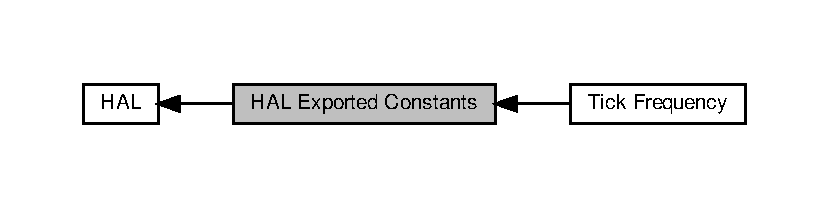
\includegraphics[width=350pt]{group___h_a_l___exported___constants}
\end{center}
\end{figure}
\subsection*{Moduły}
\begin{DoxyCompactItemize}
\item 
\hyperlink{group___h_a_l___t_i_c_k___f_r_e_q}{Tick Frequency}
\end{DoxyCompactItemize}


\subsection{Opis szczegółowy}

\hypertarget{group___h_a_l___t_i_c_k___f_r_e_q}{}\section{Tick Frequency}
\label{group___h_a_l___t_i_c_k___f_r_e_q}\index{Tick Frequency@{Tick Frequency}}
Diagram współpracy dla Tick Frequency\+:\nopagebreak
\begin{figure}[H]
\begin{center}
\leavevmode
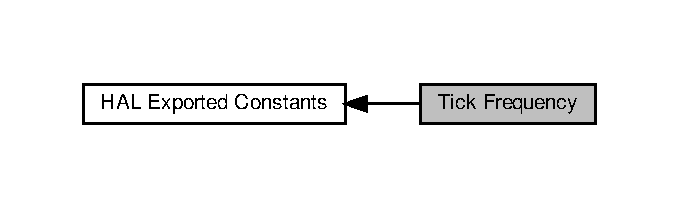
\includegraphics[width=326pt]{group___h_a_l___t_i_c_k___f_r_e_q}
\end{center}
\end{figure}
\subsection*{Wyliczenia}
\begin{DoxyCompactItemize}
\item 
enum \hyperlink{group___h_a_l___t_i_c_k___f_r_e_q_gab36ec81674817249c46734772ff3b73a}{H\+A\+L\+\_\+\+Tick\+Freq\+Type\+Def} \{ \hyperlink{group___h_a_l___t_i_c_k___f_r_e_q_ggab36ec81674817249c46734772ff3b73aabf4d022d85adb437a57c1f45d6345092}{H\+A\+L\+\_\+\+T\+I\+C\+K\+\_\+\+F\+R\+E\+Q\+\_\+10\+HZ} = 100U, 
\hyperlink{group___h_a_l___t_i_c_k___f_r_e_q_ggab36ec81674817249c46734772ff3b73aacb1ef3a0e9632aafe0fd162e2cd88408}{H\+A\+L\+\_\+\+T\+I\+C\+K\+\_\+\+F\+R\+E\+Q\+\_\+100\+HZ} = 10U, 
\hyperlink{group___h_a_l___t_i_c_k___f_r_e_q_ggab36ec81674817249c46734772ff3b73aabef41c8ee13ca1d48eb49dac912f9689}{H\+A\+L\+\_\+\+T\+I\+C\+K\+\_\+\+F\+R\+E\+Q\+\_\+1\+K\+HZ} = 1U, 
\hyperlink{group___h_a_l___t_i_c_k___f_r_e_q_ggab36ec81674817249c46734772ff3b73aa94e043d780eb1c36291338f6d6314e42}{H\+A\+L\+\_\+\+T\+I\+C\+K\+\_\+\+F\+R\+E\+Q\+\_\+\+D\+E\+F\+A\+U\+LT} = H\+A\+L\+\_\+\+T\+I\+C\+K\+\_\+\+F\+R\+E\+Q\+\_\+1\+K\+HZ
 \}
\end{DoxyCompactItemize}


\subsection{Opis szczegółowy}


\subsection{Dokumentacja typów wyliczanych}
\mbox{\Hypertarget{group___h_a_l___t_i_c_k___f_r_e_q_gab36ec81674817249c46734772ff3b73a}\label{group___h_a_l___t_i_c_k___f_r_e_q_gab36ec81674817249c46734772ff3b73a}} 
\index{Tick Frequency@{Tick Frequency}!H\+A\+L\+\_\+\+Tick\+Freq\+Type\+Def@{H\+A\+L\+\_\+\+Tick\+Freq\+Type\+Def}}
\index{H\+A\+L\+\_\+\+Tick\+Freq\+Type\+Def@{H\+A\+L\+\_\+\+Tick\+Freq\+Type\+Def}!Tick Frequency@{Tick Frequency}}
\subsubsection{\texorpdfstring{H\+A\+L\+\_\+\+Tick\+Freq\+Type\+Def}{HAL\_TickFreqTypeDef}}
{\footnotesize\ttfamily enum \hyperlink{group___h_a_l___t_i_c_k___f_r_e_q_gab36ec81674817249c46734772ff3b73a}{H\+A\+L\+\_\+\+Tick\+Freq\+Type\+Def}}

\begin{DoxyEnumFields}{Wartości wyliczeń}
\raisebox{\heightof{T}}[0pt][0pt]{\index{H\+A\+L\+\_\+\+T\+I\+C\+K\+\_\+\+F\+R\+E\+Q\+\_\+10\+HZ@{H\+A\+L\+\_\+\+T\+I\+C\+K\+\_\+\+F\+R\+E\+Q\+\_\+10\+HZ}!Tick Frequency@{Tick Frequency}}\index{Tick Frequency@{Tick Frequency}!H\+A\+L\+\_\+\+T\+I\+C\+K\+\_\+\+F\+R\+E\+Q\+\_\+10\+HZ@{H\+A\+L\+\_\+\+T\+I\+C\+K\+\_\+\+F\+R\+E\+Q\+\_\+10\+HZ}}}\mbox{\Hypertarget{group___h_a_l___t_i_c_k___f_r_e_q_ggab36ec81674817249c46734772ff3b73aabf4d022d85adb437a57c1f45d6345092}\label{group___h_a_l___t_i_c_k___f_r_e_q_ggab36ec81674817249c46734772ff3b73aabf4d022d85adb437a57c1f45d6345092}} 
H\+A\+L\+\_\+\+T\+I\+C\+K\+\_\+\+F\+R\+E\+Q\+\_\+10\+HZ&\\
\hline

\raisebox{\heightof{T}}[0pt][0pt]{\index{H\+A\+L\+\_\+\+T\+I\+C\+K\+\_\+\+F\+R\+E\+Q\+\_\+100\+HZ@{H\+A\+L\+\_\+\+T\+I\+C\+K\+\_\+\+F\+R\+E\+Q\+\_\+100\+HZ}!Tick Frequency@{Tick Frequency}}\index{Tick Frequency@{Tick Frequency}!H\+A\+L\+\_\+\+T\+I\+C\+K\+\_\+\+F\+R\+E\+Q\+\_\+100\+HZ@{H\+A\+L\+\_\+\+T\+I\+C\+K\+\_\+\+F\+R\+E\+Q\+\_\+100\+HZ}}}\mbox{\Hypertarget{group___h_a_l___t_i_c_k___f_r_e_q_ggab36ec81674817249c46734772ff3b73aacb1ef3a0e9632aafe0fd162e2cd88408}\label{group___h_a_l___t_i_c_k___f_r_e_q_ggab36ec81674817249c46734772ff3b73aacb1ef3a0e9632aafe0fd162e2cd88408}} 
H\+A\+L\+\_\+\+T\+I\+C\+K\+\_\+\+F\+R\+E\+Q\+\_\+100\+HZ&\\
\hline

\raisebox{\heightof{T}}[0pt][0pt]{\index{H\+A\+L\+\_\+\+T\+I\+C\+K\+\_\+\+F\+R\+E\+Q\+\_\+1\+K\+HZ@{H\+A\+L\+\_\+\+T\+I\+C\+K\+\_\+\+F\+R\+E\+Q\+\_\+1\+K\+HZ}!Tick Frequency@{Tick Frequency}}\index{Tick Frequency@{Tick Frequency}!H\+A\+L\+\_\+\+T\+I\+C\+K\+\_\+\+F\+R\+E\+Q\+\_\+1\+K\+HZ@{H\+A\+L\+\_\+\+T\+I\+C\+K\+\_\+\+F\+R\+E\+Q\+\_\+1\+K\+HZ}}}\mbox{\Hypertarget{group___h_a_l___t_i_c_k___f_r_e_q_ggab36ec81674817249c46734772ff3b73aabef41c8ee13ca1d48eb49dac912f9689}\label{group___h_a_l___t_i_c_k___f_r_e_q_ggab36ec81674817249c46734772ff3b73aabef41c8ee13ca1d48eb49dac912f9689}} 
H\+A\+L\+\_\+\+T\+I\+C\+K\+\_\+\+F\+R\+E\+Q\+\_\+1\+K\+HZ&\\
\hline

\raisebox{\heightof{T}}[0pt][0pt]{\index{H\+A\+L\+\_\+\+T\+I\+C\+K\+\_\+\+F\+R\+E\+Q\+\_\+\+D\+E\+F\+A\+U\+LT@{H\+A\+L\+\_\+\+T\+I\+C\+K\+\_\+\+F\+R\+E\+Q\+\_\+\+D\+E\+F\+A\+U\+LT}!Tick Frequency@{Tick Frequency}}\index{Tick Frequency@{Tick Frequency}!H\+A\+L\+\_\+\+T\+I\+C\+K\+\_\+\+F\+R\+E\+Q\+\_\+\+D\+E\+F\+A\+U\+LT@{H\+A\+L\+\_\+\+T\+I\+C\+K\+\_\+\+F\+R\+E\+Q\+\_\+\+D\+E\+F\+A\+U\+LT}}}\mbox{\Hypertarget{group___h_a_l___t_i_c_k___f_r_e_q_ggab36ec81674817249c46734772ff3b73aa94e043d780eb1c36291338f6d6314e42}\label{group___h_a_l___t_i_c_k___f_r_e_q_ggab36ec81674817249c46734772ff3b73aa94e043d780eb1c36291338f6d6314e42}} 
H\+A\+L\+\_\+\+T\+I\+C\+K\+\_\+\+F\+R\+E\+Q\+\_\+\+D\+E\+F\+A\+U\+LT&\\
\hline

\end{DoxyEnumFields}


Definicja w linii 50 pliku stm32f4xx\+\_\+hal.\+h.


\hypertarget{group___h_a_l___exported___macros}{}\section{H\+AL Exported Macros}
\label{group___h_a_l___exported___macros}\index{H\+A\+L Exported Macros@{H\+A\+L Exported Macros}}
Diagram współpracy dla H\+AL Exported Macros\+:\nopagebreak
\begin{figure}[H]
\begin{center}
\leavevmode
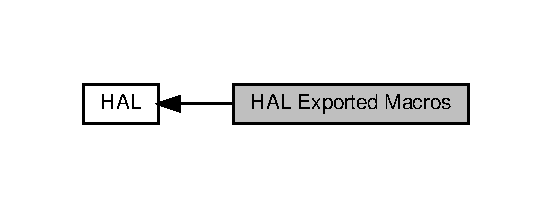
\includegraphics[width=265pt]{group___h_a_l___exported___macros}
\end{center}
\end{figure}
\subsection*{Definicje}
\begin{DoxyCompactItemize}
\item 
\#define \hyperlink{group___h_a_l___exported___macros_ga4a466905a367266e7c23417248dc741d}{\+\_\+\+\_\+\+H\+A\+L\+\_\+\+D\+B\+G\+M\+C\+U\+\_\+\+F\+R\+E\+E\+Z\+E\+\_\+\+T\+I\+M2}()~(\hyperlink{group___peripheral__declaration_ga92ec6d9ec2251fda7d4ce09748cd74b4}{D\+B\+G\+M\+CU}-\/$>$A\+P\+B1\+FZ $\vert$= (\hyperlink{group___peripheral___registers___bits___definition_gaae3c5b87084934a18748f5ec168f5aef}{D\+B\+G\+M\+C\+U\+\_\+\+A\+P\+B1\+\_\+\+F\+Z\+\_\+\+D\+B\+G\+\_\+\+T\+I\+M2\+\_\+\+S\+T\+OP}))
\begin{DoxyCompactList}\small\item\em Freeze/\+Unfreeze Peripherals in Debug mode. \end{DoxyCompactList}\item 
\#define \hyperlink{group___h_a_l___exported___macros_gaf2fe2b6d0a5e8df4ebb38020acf210d9}{\+\_\+\+\_\+\+H\+A\+L\+\_\+\+D\+B\+G\+M\+C\+U\+\_\+\+F\+R\+E\+E\+Z\+E\+\_\+\+T\+I\+M3}()~(\hyperlink{group___peripheral__declaration_ga92ec6d9ec2251fda7d4ce09748cd74b4}{D\+B\+G\+M\+CU}-\/$>$A\+P\+B1\+FZ $\vert$= (\hyperlink{group___peripheral___registers___bits___definition_ga2fea6834f4ef9fc6b403cd079a001cec}{D\+B\+G\+M\+C\+U\+\_\+\+A\+P\+B1\+\_\+\+F\+Z\+\_\+\+D\+B\+G\+\_\+\+T\+I\+M3\+\_\+\+S\+T\+OP}))
\item 
\#define \hyperlink{group___h_a_l___exported___macros_ga9ec45e12bbea210d8ec91d9cdd9f911c}{\+\_\+\+\_\+\+H\+A\+L\+\_\+\+D\+B\+G\+M\+C\+U\+\_\+\+F\+R\+E\+E\+Z\+E\+\_\+\+T\+I\+M4}()~(\hyperlink{group___peripheral__declaration_ga92ec6d9ec2251fda7d4ce09748cd74b4}{D\+B\+G\+M\+CU}-\/$>$A\+P\+B1\+FZ $\vert$= (\hyperlink{group___peripheral___registers___bits___definition_ga7ac65bf9342bb8acbcb25938e93abc45}{D\+B\+G\+M\+C\+U\+\_\+\+A\+P\+B1\+\_\+\+F\+Z\+\_\+\+D\+B\+G\+\_\+\+T\+I\+M4\+\_\+\+S\+T\+OP}))
\item 
\#define \hyperlink{group___h_a_l___exported___macros_ga051eca105d8696d54e19fdfc8343a0a2}{\+\_\+\+\_\+\+H\+A\+L\+\_\+\+D\+B\+G\+M\+C\+U\+\_\+\+F\+R\+E\+E\+Z\+E\+\_\+\+T\+I\+M5}()~(\hyperlink{group___peripheral__declaration_ga92ec6d9ec2251fda7d4ce09748cd74b4}{D\+B\+G\+M\+CU}-\/$>$A\+P\+B1\+FZ $\vert$= (\hyperlink{group___peripheral___registers___bits___definition_ga42d29d40515d36ce6ed7e5d34ed17dcf}{D\+B\+G\+M\+C\+U\+\_\+\+A\+P\+B1\+\_\+\+F\+Z\+\_\+\+D\+B\+G\+\_\+\+T\+I\+M5\+\_\+\+S\+T\+OP}))
\item 
\#define \hyperlink{group___h_a_l___exported___macros_gaccdcfde9ae6f78f0ca359776b021f87c}{\+\_\+\+\_\+\+H\+A\+L\+\_\+\+D\+B\+G\+M\+C\+U\+\_\+\+F\+R\+E\+E\+Z\+E\+\_\+\+T\+I\+M6}()~(\hyperlink{group___peripheral__declaration_ga92ec6d9ec2251fda7d4ce09748cd74b4}{D\+B\+G\+M\+CU}-\/$>$A\+P\+B1\+FZ $\vert$= (D\+B\+G\+M\+C\+U\+\_\+\+A\+P\+B1\+\_\+\+F\+Z\+\_\+\+D\+B\+G\+\_\+\+T\+I\+M6\+\_\+\+S\+T\+OP))
\item 
\#define \hyperlink{group___h_a_l___exported___macros_ga8541da9b4d428d41e218e9701e4307d1}{\+\_\+\+\_\+\+H\+A\+L\+\_\+\+D\+B\+G\+M\+C\+U\+\_\+\+F\+R\+E\+E\+Z\+E\+\_\+\+T\+I\+M7}()~(\hyperlink{group___peripheral__declaration_ga92ec6d9ec2251fda7d4ce09748cd74b4}{D\+B\+G\+M\+CU}-\/$>$A\+P\+B1\+FZ $\vert$= (D\+B\+G\+M\+C\+U\+\_\+\+A\+P\+B1\+\_\+\+F\+Z\+\_\+\+D\+B\+G\+\_\+\+T\+I\+M7\+\_\+\+S\+T\+OP))
\item 
\#define \hyperlink{group___h_a_l___exported___macros_ga2bbe99ec741228b520e17b1bf38eb2ad}{\+\_\+\+\_\+\+H\+A\+L\+\_\+\+D\+B\+G\+M\+C\+U\+\_\+\+F\+R\+E\+E\+Z\+E\+\_\+\+T\+I\+M12}()~(\hyperlink{group___peripheral__declaration_ga92ec6d9ec2251fda7d4ce09748cd74b4}{D\+B\+G\+M\+CU}-\/$>$A\+P\+B1\+FZ $\vert$= (D\+B\+G\+M\+C\+U\+\_\+\+A\+P\+B1\+\_\+\+F\+Z\+\_\+\+D\+B\+G\+\_\+\+T\+I\+M12\+\_\+\+S\+T\+OP))
\item 
\#define \hyperlink{group___h_a_l___exported___macros_ga21bfaea50e429031982861b2869c6863}{\+\_\+\+\_\+\+H\+A\+L\+\_\+\+D\+B\+G\+M\+C\+U\+\_\+\+F\+R\+E\+E\+Z\+E\+\_\+\+T\+I\+M13}()~(\hyperlink{group___peripheral__declaration_ga92ec6d9ec2251fda7d4ce09748cd74b4}{D\+B\+G\+M\+CU}-\/$>$A\+P\+B1\+FZ $\vert$= (D\+B\+G\+M\+C\+U\+\_\+\+A\+P\+B1\+\_\+\+F\+Z\+\_\+\+D\+B\+G\+\_\+\+T\+I\+M13\+\_\+\+S\+T\+OP))
\item 
\#define \hyperlink{group___h_a_l___exported___macros_gaf4d10c15c1644eeff138829af21c219c}{\+\_\+\+\_\+\+H\+A\+L\+\_\+\+D\+B\+G\+M\+C\+U\+\_\+\+F\+R\+E\+E\+Z\+E\+\_\+\+T\+I\+M14}()~(\hyperlink{group___peripheral__declaration_ga92ec6d9ec2251fda7d4ce09748cd74b4}{D\+B\+G\+M\+CU}-\/$>$A\+P\+B1\+FZ $\vert$= (D\+B\+G\+M\+C\+U\+\_\+\+A\+P\+B1\+\_\+\+F\+Z\+\_\+\+D\+B\+G\+\_\+\+T\+I\+M14\+\_\+\+S\+T\+OP))
\item 
\#define \hyperlink{group___h_a_l___exported___macros_ga6ea586c594feb6eb0f2aba52f1c69f4c}{\+\_\+\+\_\+\+H\+A\+L\+\_\+\+D\+B\+G\+M\+C\+U\+\_\+\+F\+R\+E\+E\+Z\+E\+\_\+\+R\+TC}()~(\hyperlink{group___peripheral__declaration_ga92ec6d9ec2251fda7d4ce09748cd74b4}{D\+B\+G\+M\+CU}-\/$>$A\+P\+B1\+FZ $\vert$= (\hyperlink{group___peripheral___registers___bits___definition_ga1e20246d389229ff46006b405bb56b1d}{D\+B\+G\+M\+C\+U\+\_\+\+A\+P\+B1\+\_\+\+F\+Z\+\_\+\+D\+B\+G\+\_\+\+R\+T\+C\+\_\+\+S\+T\+OP}))
\item 
\#define \hyperlink{group___h_a_l___exported___macros_ga81215154725c479c67fb1adac906fbd9}{\+\_\+\+\_\+\+H\+A\+L\+\_\+\+D\+B\+G\+M\+C\+U\+\_\+\+F\+R\+E\+E\+Z\+E\+\_\+\+W\+W\+DG}()~(\hyperlink{group___peripheral__declaration_ga92ec6d9ec2251fda7d4ce09748cd74b4}{D\+B\+G\+M\+CU}-\/$>$A\+P\+B1\+FZ $\vert$= (\hyperlink{group___peripheral___registers___bits___definition_ga8a49d5e849185d09ee6c7594512ffe88}{D\+B\+G\+M\+C\+U\+\_\+\+A\+P\+B1\+\_\+\+F\+Z\+\_\+\+D\+B\+G\+\_\+\+W\+W\+D\+G\+\_\+\+S\+T\+OP}))
\item 
\#define \hyperlink{group___h_a_l___exported___macros_gabab7ab631ba58fb6246a9385e8af9d0d}{\+\_\+\+\_\+\+H\+A\+L\+\_\+\+D\+B\+G\+M\+C\+U\+\_\+\+F\+R\+E\+E\+Z\+E\+\_\+\+I\+W\+DG}()~(\hyperlink{group___peripheral__declaration_ga92ec6d9ec2251fda7d4ce09748cd74b4}{D\+B\+G\+M\+CU}-\/$>$A\+P\+B1\+FZ $\vert$= (\hyperlink{group___peripheral___registers___bits___definition_gada8989cb96dd5d6dbdaaf16e1f127c6a}{D\+B\+G\+M\+C\+U\+\_\+\+A\+P\+B1\+\_\+\+F\+Z\+\_\+\+D\+B\+G\+\_\+\+I\+W\+D\+G\+\_\+\+S\+T\+OP}))
\item 
\#define \hyperlink{group___h_a_l___exported___macros_ga6160f642dcff812be3a04c5b5c66e31d}{\+\_\+\+\_\+\+H\+A\+L\+\_\+\+D\+B\+G\+M\+C\+U\+\_\+\+F\+R\+E\+E\+Z\+E\+\_\+\+I2\+C1\+\_\+\+T\+I\+M\+E\+O\+UT}()~(\hyperlink{group___peripheral__declaration_ga92ec6d9ec2251fda7d4ce09748cd74b4}{D\+B\+G\+M\+CU}-\/$>$A\+P\+B1\+FZ $\vert$= (\hyperlink{group___peripheral___registers___bits___definition_gae83fb5d62c6e6fa1c2fd06084528404e}{D\+B\+G\+M\+C\+U\+\_\+\+A\+P\+B1\+\_\+\+F\+Z\+\_\+\+D\+B\+G\+\_\+\+I2\+C1\+\_\+\+S\+M\+B\+U\+S\+\_\+\+T\+I\+M\+E\+O\+UT}))
\item 
\#define \hyperlink{group___h_a_l___exported___macros_gacc31f8475c2e3e30ee99e53814faa523}{\+\_\+\+\_\+\+H\+A\+L\+\_\+\+D\+B\+G\+M\+C\+U\+\_\+\+F\+R\+E\+E\+Z\+E\+\_\+\+I2\+C2\+\_\+\+T\+I\+M\+E\+O\+UT}()~(\hyperlink{group___peripheral__declaration_ga92ec6d9ec2251fda7d4ce09748cd74b4}{D\+B\+G\+M\+CU}-\/$>$A\+P\+B1\+FZ $\vert$= (\hyperlink{group___peripheral___registers___bits___definition_ga8f6320aba695f6c3f97608e478533e96}{D\+B\+G\+M\+C\+U\+\_\+\+A\+P\+B1\+\_\+\+F\+Z\+\_\+\+D\+B\+G\+\_\+\+I2\+C2\+\_\+\+S\+M\+B\+U\+S\+\_\+\+T\+I\+M\+E\+O\+UT}))
\item 
\#define \hyperlink{group___h_a_l___exported___macros_gacd3fd0373b45de1b86be07bd4007c30e}{\+\_\+\+\_\+\+H\+A\+L\+\_\+\+D\+B\+G\+M\+C\+U\+\_\+\+F\+R\+E\+E\+Z\+E\+\_\+\+I2\+C3\+\_\+\+T\+I\+M\+E\+O\+UT}()~(\hyperlink{group___peripheral__declaration_ga92ec6d9ec2251fda7d4ce09748cd74b4}{D\+B\+G\+M\+CU}-\/$>$A\+P\+B1\+FZ $\vert$= (\hyperlink{group___peripheral___registers___bits___definition_ga7f7e5c708387aa1ddae35b892811b4e9}{D\+B\+G\+M\+C\+U\+\_\+\+A\+P\+B1\+\_\+\+F\+Z\+\_\+\+D\+B\+G\+\_\+\+I2\+C3\+\_\+\+S\+M\+B\+U\+S\+\_\+\+T\+I\+M\+E\+O\+UT}))
\item 
\#define \hyperlink{group___h_a_l___exported___macros_ga1d225003f36f6a22ffea1a41a4a78cec}{\+\_\+\+\_\+\+H\+A\+L\+\_\+\+D\+B\+G\+M\+C\+U\+\_\+\+F\+R\+E\+E\+Z\+E\+\_\+\+C\+A\+N1}()~(\hyperlink{group___peripheral__declaration_ga92ec6d9ec2251fda7d4ce09748cd74b4}{D\+B\+G\+M\+CU}-\/$>$A\+P\+B1\+FZ $\vert$= (D\+B\+G\+M\+C\+U\+\_\+\+A\+P\+B1\+\_\+\+F\+Z\+\_\+\+D\+B\+G\+\_\+\+C\+A\+N1\+\_\+\+S\+T\+OP))
\item 
\#define \hyperlink{group___h_a_l___exported___macros_gadb4f2b03a03936de95c1a9f939d452c0}{\+\_\+\+\_\+\+H\+A\+L\+\_\+\+D\+B\+G\+M\+C\+U\+\_\+\+F\+R\+E\+E\+Z\+E\+\_\+\+C\+A\+N2}()~(\hyperlink{group___peripheral__declaration_ga92ec6d9ec2251fda7d4ce09748cd74b4}{D\+B\+G\+M\+CU}-\/$>$A\+P\+B1\+FZ $\vert$= (D\+B\+G\+M\+C\+U\+\_\+\+A\+P\+B1\+\_\+\+F\+Z\+\_\+\+D\+B\+G\+\_\+\+C\+A\+N2\+\_\+\+S\+T\+OP))
\item 
\#define \hyperlink{group___h_a_l___exported___macros_ga93d7e54d78e5dea068f5f6a94d5f94c7}{\+\_\+\+\_\+\+H\+A\+L\+\_\+\+D\+B\+G\+M\+C\+U\+\_\+\+F\+R\+E\+E\+Z\+E\+\_\+\+T\+I\+M1}()~(\hyperlink{group___peripheral__declaration_ga92ec6d9ec2251fda7d4ce09748cd74b4}{D\+B\+G\+M\+CU}-\/$>$A\+P\+B2\+FZ $\vert$= (\hyperlink{group___peripheral___registers___bits___definition_ga3eb7be194b6ffb258b9e9f5ed08a931e}{D\+B\+G\+M\+C\+U\+\_\+\+A\+P\+B2\+\_\+\+F\+Z\+\_\+\+D\+B\+G\+\_\+\+T\+I\+M1\+\_\+\+S\+T\+OP}))
\item 
\#define \hyperlink{group___h_a_l___exported___macros_gaeee90b698bfc2421155265b4c5b43f09}{\+\_\+\+\_\+\+H\+A\+L\+\_\+\+D\+B\+G\+M\+C\+U\+\_\+\+F\+R\+E\+E\+Z\+E\+\_\+\+T\+I\+M8}()~(\hyperlink{group___peripheral__declaration_ga92ec6d9ec2251fda7d4ce09748cd74b4}{D\+B\+G\+M\+CU}-\/$>$A\+P\+B2\+FZ $\vert$= (D\+B\+G\+M\+C\+U\+\_\+\+A\+P\+B2\+\_\+\+F\+Z\+\_\+\+D\+B\+G\+\_\+\+T\+I\+M8\+\_\+\+S\+T\+OP))
\item 
\#define \hyperlink{group___h_a_l___exported___macros_ga391a0780e10993d06c519addf582a438}{\+\_\+\+\_\+\+H\+A\+L\+\_\+\+D\+B\+G\+M\+C\+U\+\_\+\+F\+R\+E\+E\+Z\+E\+\_\+\+T\+I\+M9}()~(\hyperlink{group___peripheral__declaration_ga92ec6d9ec2251fda7d4ce09748cd74b4}{D\+B\+G\+M\+CU}-\/$>$A\+P\+B2\+FZ $\vert$= (\hyperlink{group___peripheral___registers___bits___definition_gaf12c17533a1e3262ee11f760e44f5127}{D\+B\+G\+M\+C\+U\+\_\+\+A\+P\+B2\+\_\+\+F\+Z\+\_\+\+D\+B\+G\+\_\+\+T\+I\+M9\+\_\+\+S\+T\+OP}))
\item 
\#define \hyperlink{group___h_a_l___exported___macros_gaee80dea9c85b61d2fb2499cbd97d8478}{\+\_\+\+\_\+\+H\+A\+L\+\_\+\+D\+B\+G\+M\+C\+U\+\_\+\+F\+R\+E\+E\+Z\+E\+\_\+\+T\+I\+M10}()~(\hyperlink{group___peripheral__declaration_ga92ec6d9ec2251fda7d4ce09748cd74b4}{D\+B\+G\+M\+CU}-\/$>$A\+P\+B2\+FZ $\vert$= (\hyperlink{group___peripheral___registers___bits___definition_ga24d4bbf803a65e8202b0019ed0ce0ebb}{D\+B\+G\+M\+C\+U\+\_\+\+A\+P\+B2\+\_\+\+F\+Z\+\_\+\+D\+B\+G\+\_\+\+T\+I\+M10\+\_\+\+S\+T\+OP}))
\item 
\#define \hyperlink{group___h_a_l___exported___macros_gac1f554993a6d5c7a953dab2c6cc564dd}{\+\_\+\+\_\+\+H\+A\+L\+\_\+\+D\+B\+G\+M\+C\+U\+\_\+\+F\+R\+E\+E\+Z\+E\+\_\+\+T\+I\+M11}()~(\hyperlink{group___peripheral__declaration_ga92ec6d9ec2251fda7d4ce09748cd74b4}{D\+B\+G\+M\+CU}-\/$>$A\+P\+B2\+FZ $\vert$= (\hyperlink{group___peripheral___registers___bits___definition_ga354671c942db40e69820fd783ef955b4}{D\+B\+G\+M\+C\+U\+\_\+\+A\+P\+B2\+\_\+\+F\+Z\+\_\+\+D\+B\+G\+\_\+\+T\+I\+M11\+\_\+\+S\+T\+OP}))
\item 
\#define \hyperlink{group___h_a_l___exported___macros_gafd40134436233985a840e1cd8eb6c4c3}{\+\_\+\+\_\+\+H\+A\+L\+\_\+\+D\+B\+G\+M\+C\+U\+\_\+\+U\+N\+F\+R\+E\+E\+Z\+E\+\_\+\+T\+I\+M2}()~(\hyperlink{group___peripheral__declaration_ga92ec6d9ec2251fda7d4ce09748cd74b4}{D\+B\+G\+M\+CU}-\/$>$A\+P\+B1\+FZ \&= $\sim$(\hyperlink{group___peripheral___registers___bits___definition_gaae3c5b87084934a18748f5ec168f5aef}{D\+B\+G\+M\+C\+U\+\_\+\+A\+P\+B1\+\_\+\+F\+Z\+\_\+\+D\+B\+G\+\_\+\+T\+I\+M2\+\_\+\+S\+T\+OP}))
\item 
\#define \hyperlink{group___h_a_l___exported___macros_ga5aecefa008a37ef7c6489a2e29415e69}{\+\_\+\+\_\+\+H\+A\+L\+\_\+\+D\+B\+G\+M\+C\+U\+\_\+\+U\+N\+F\+R\+E\+E\+Z\+E\+\_\+\+T\+I\+M3}()~(\hyperlink{group___peripheral__declaration_ga92ec6d9ec2251fda7d4ce09748cd74b4}{D\+B\+G\+M\+CU}-\/$>$A\+P\+B1\+FZ \&= $\sim$(\hyperlink{group___peripheral___registers___bits___definition_ga2fea6834f4ef9fc6b403cd079a001cec}{D\+B\+G\+M\+C\+U\+\_\+\+A\+P\+B1\+\_\+\+F\+Z\+\_\+\+D\+B\+G\+\_\+\+T\+I\+M3\+\_\+\+S\+T\+OP}))
\item 
\#define \hyperlink{group___h_a_l___exported___macros_gac73202fc9f0913f52ef70c42b6cab287}{\+\_\+\+\_\+\+H\+A\+L\+\_\+\+D\+B\+G\+M\+C\+U\+\_\+\+U\+N\+F\+R\+E\+E\+Z\+E\+\_\+\+T\+I\+M4}()~(\hyperlink{group___peripheral__declaration_ga92ec6d9ec2251fda7d4ce09748cd74b4}{D\+B\+G\+M\+CU}-\/$>$A\+P\+B1\+FZ \&= $\sim$(\hyperlink{group___peripheral___registers___bits___definition_ga7ac65bf9342bb8acbcb25938e93abc45}{D\+B\+G\+M\+C\+U\+\_\+\+A\+P\+B1\+\_\+\+F\+Z\+\_\+\+D\+B\+G\+\_\+\+T\+I\+M4\+\_\+\+S\+T\+OP}))
\item 
\#define \hyperlink{group___h_a_l___exported___macros_ga0669527789fb4616ec07ed711a600d04}{\+\_\+\+\_\+\+H\+A\+L\+\_\+\+D\+B\+G\+M\+C\+U\+\_\+\+U\+N\+F\+R\+E\+E\+Z\+E\+\_\+\+T\+I\+M5}()~(\hyperlink{group___peripheral__declaration_ga92ec6d9ec2251fda7d4ce09748cd74b4}{D\+B\+G\+M\+CU}-\/$>$A\+P\+B1\+FZ \&= $\sim$(\hyperlink{group___peripheral___registers___bits___definition_ga42d29d40515d36ce6ed7e5d34ed17dcf}{D\+B\+G\+M\+C\+U\+\_\+\+A\+P\+B1\+\_\+\+F\+Z\+\_\+\+D\+B\+G\+\_\+\+T\+I\+M5\+\_\+\+S\+T\+OP}))
\item 
\#define \hyperlink{group___h_a_l___exported___macros_gaab127b51706a565b72c397e29b145234}{\+\_\+\+\_\+\+H\+A\+L\+\_\+\+D\+B\+G\+M\+C\+U\+\_\+\+U\+N\+F\+R\+E\+E\+Z\+E\+\_\+\+T\+I\+M6}()~(\hyperlink{group___peripheral__declaration_ga92ec6d9ec2251fda7d4ce09748cd74b4}{D\+B\+G\+M\+CU}-\/$>$A\+P\+B1\+FZ \&= $\sim$(D\+B\+G\+M\+C\+U\+\_\+\+A\+P\+B1\+\_\+\+F\+Z\+\_\+\+D\+B\+G\+\_\+\+T\+I\+M6\+\_\+\+S\+T\+OP))
\item 
\#define \hyperlink{group___h_a_l___exported___macros_ga4a6c5081b976583921ac5d140e15bb85}{\+\_\+\+\_\+\+H\+A\+L\+\_\+\+D\+B\+G\+M\+C\+U\+\_\+\+U\+N\+F\+R\+E\+E\+Z\+E\+\_\+\+T\+I\+M7}()~(\hyperlink{group___peripheral__declaration_ga92ec6d9ec2251fda7d4ce09748cd74b4}{D\+B\+G\+M\+CU}-\/$>$A\+P\+B1\+FZ \&= $\sim$(D\+B\+G\+M\+C\+U\+\_\+\+A\+P\+B1\+\_\+\+F\+Z\+\_\+\+D\+B\+G\+\_\+\+T\+I\+M7\+\_\+\+S\+T\+OP))
\item 
\#define \hyperlink{group___h_a_l___exported___macros_gaa8e882be8db24537679bc0d4a129f448}{\+\_\+\+\_\+\+H\+A\+L\+\_\+\+D\+B\+G\+M\+C\+U\+\_\+\+U\+N\+F\+R\+E\+E\+Z\+E\+\_\+\+T\+I\+M12}()~(\hyperlink{group___peripheral__declaration_ga92ec6d9ec2251fda7d4ce09748cd74b4}{D\+B\+G\+M\+CU}-\/$>$A\+P\+B1\+FZ \&= $\sim$(D\+B\+G\+M\+C\+U\+\_\+\+A\+P\+B1\+\_\+\+F\+Z\+\_\+\+D\+B\+G\+\_\+\+T\+I\+M12\+\_\+\+S\+T\+OP))
\item 
\#define \hyperlink{group___h_a_l___exported___macros_ga00b605f660d43ab1b833926dabe352fe}{\+\_\+\+\_\+\+H\+A\+L\+\_\+\+D\+B\+G\+M\+C\+U\+\_\+\+U\+N\+F\+R\+E\+E\+Z\+E\+\_\+\+T\+I\+M13}()~(\hyperlink{group___peripheral__declaration_ga92ec6d9ec2251fda7d4ce09748cd74b4}{D\+B\+G\+M\+CU}-\/$>$A\+P\+B1\+FZ \&= $\sim$(D\+B\+G\+M\+C\+U\+\_\+\+A\+P\+B1\+\_\+\+F\+Z\+\_\+\+D\+B\+G\+\_\+\+T\+I\+M13\+\_\+\+S\+T\+OP))
\item 
\#define \hyperlink{group___h_a_l___exported___macros_gaa62a0abc610b769d15fd9d20bdc14cd7}{\+\_\+\+\_\+\+H\+A\+L\+\_\+\+D\+B\+G\+M\+C\+U\+\_\+\+U\+N\+F\+R\+E\+E\+Z\+E\+\_\+\+T\+I\+M14}()~(\hyperlink{group___peripheral__declaration_ga92ec6d9ec2251fda7d4ce09748cd74b4}{D\+B\+G\+M\+CU}-\/$>$A\+P\+B1\+FZ \&= $\sim$(D\+B\+G\+M\+C\+U\+\_\+\+A\+P\+B1\+\_\+\+F\+Z\+\_\+\+D\+B\+G\+\_\+\+T\+I\+M14\+\_\+\+S\+T\+OP))
\item 
\#define \hyperlink{group___h_a_l___exported___macros_ga3d85d5cda1979c7df426634a1d3d7d35}{\+\_\+\+\_\+\+H\+A\+L\+\_\+\+D\+B\+G\+M\+C\+U\+\_\+\+U\+N\+F\+R\+E\+E\+Z\+E\+\_\+\+R\+TC}()~(\hyperlink{group___peripheral__declaration_ga92ec6d9ec2251fda7d4ce09748cd74b4}{D\+B\+G\+M\+CU}-\/$>$A\+P\+B1\+FZ \&= $\sim$(\hyperlink{group___peripheral___registers___bits___definition_ga1e20246d389229ff46006b405bb56b1d}{D\+B\+G\+M\+C\+U\+\_\+\+A\+P\+B1\+\_\+\+F\+Z\+\_\+\+D\+B\+G\+\_\+\+R\+T\+C\+\_\+\+S\+T\+OP}))
\item 
\#define \hyperlink{group___h_a_l___exported___macros_gaa14c8a2e8911976b8c8ce6ca278372a2}{\+\_\+\+\_\+\+H\+A\+L\+\_\+\+D\+B\+G\+M\+C\+U\+\_\+\+U\+N\+F\+R\+E\+E\+Z\+E\+\_\+\+W\+W\+DG}()~(\hyperlink{group___peripheral__declaration_ga92ec6d9ec2251fda7d4ce09748cd74b4}{D\+B\+G\+M\+CU}-\/$>$A\+P\+B1\+FZ \&= $\sim$(\hyperlink{group___peripheral___registers___bits___definition_ga8a49d5e849185d09ee6c7594512ffe88}{D\+B\+G\+M\+C\+U\+\_\+\+A\+P\+B1\+\_\+\+F\+Z\+\_\+\+D\+B\+G\+\_\+\+W\+W\+D\+G\+\_\+\+S\+T\+OP}))
\item 
\#define \hyperlink{group___h_a_l___exported___macros_gab29a88ef9c31cbe107c58b9ecc3bdf79}{\+\_\+\+\_\+\+H\+A\+L\+\_\+\+D\+B\+G\+M\+C\+U\+\_\+\+U\+N\+F\+R\+E\+E\+Z\+E\+\_\+\+I\+W\+DG}()~(\hyperlink{group___peripheral__declaration_ga92ec6d9ec2251fda7d4ce09748cd74b4}{D\+B\+G\+M\+CU}-\/$>$A\+P\+B1\+FZ \&= $\sim$(\hyperlink{group___peripheral___registers___bits___definition_gada8989cb96dd5d6dbdaaf16e1f127c6a}{D\+B\+G\+M\+C\+U\+\_\+\+A\+P\+B1\+\_\+\+F\+Z\+\_\+\+D\+B\+G\+\_\+\+I\+W\+D\+G\+\_\+\+S\+T\+OP}))
\item 
\#define \hyperlink{group___h_a_l___exported___macros_ga636083d6b6931b1cf35e7c39aebf0723}{\+\_\+\+\_\+\+H\+A\+L\+\_\+\+D\+B\+G\+M\+C\+U\+\_\+\+U\+N\+F\+R\+E\+E\+Z\+E\+\_\+\+I2\+C1\+\_\+\+T\+I\+M\+E\+O\+UT}()~(\hyperlink{group___peripheral__declaration_ga92ec6d9ec2251fda7d4ce09748cd74b4}{D\+B\+G\+M\+CU}-\/$>$A\+P\+B1\+FZ \&= $\sim$(\hyperlink{group___peripheral___registers___bits___definition_gae83fb5d62c6e6fa1c2fd06084528404e}{D\+B\+G\+M\+C\+U\+\_\+\+A\+P\+B1\+\_\+\+F\+Z\+\_\+\+D\+B\+G\+\_\+\+I2\+C1\+\_\+\+S\+M\+B\+U\+S\+\_\+\+T\+I\+M\+E\+O\+UT}))
\item 
\#define \hyperlink{group___h_a_l___exported___macros_ga0308bdec86c19b7bbe236c4724d7d536}{\+\_\+\+\_\+\+H\+A\+L\+\_\+\+D\+B\+G\+M\+C\+U\+\_\+\+U\+N\+F\+R\+E\+E\+Z\+E\+\_\+\+I2\+C2\+\_\+\+T\+I\+M\+E\+O\+UT}()~(\hyperlink{group___peripheral__declaration_ga92ec6d9ec2251fda7d4ce09748cd74b4}{D\+B\+G\+M\+CU}-\/$>$A\+P\+B1\+FZ \&= $\sim$(\hyperlink{group___peripheral___registers___bits___definition_ga8f6320aba695f6c3f97608e478533e96}{D\+B\+G\+M\+C\+U\+\_\+\+A\+P\+B1\+\_\+\+F\+Z\+\_\+\+D\+B\+G\+\_\+\+I2\+C2\+\_\+\+S\+M\+B\+U\+S\+\_\+\+T\+I\+M\+E\+O\+UT}))
\item 
\#define \hyperlink{group___h_a_l___exported___macros_ga8beda05b7dc4962557f98a06e29326a4}{\+\_\+\+\_\+\+H\+A\+L\+\_\+\+D\+B\+G\+M\+C\+U\+\_\+\+U\+N\+F\+R\+E\+E\+Z\+E\+\_\+\+I2\+C3\+\_\+\+T\+I\+M\+E\+O\+UT}()~(\hyperlink{group___peripheral__declaration_ga92ec6d9ec2251fda7d4ce09748cd74b4}{D\+B\+G\+M\+CU}-\/$>$A\+P\+B1\+FZ \&= $\sim$(\hyperlink{group___peripheral___registers___bits___definition_ga7f7e5c708387aa1ddae35b892811b4e9}{D\+B\+G\+M\+C\+U\+\_\+\+A\+P\+B1\+\_\+\+F\+Z\+\_\+\+D\+B\+G\+\_\+\+I2\+C3\+\_\+\+S\+M\+B\+U\+S\+\_\+\+T\+I\+M\+E\+O\+UT}))
\item 
\#define \hyperlink{group___h_a_l___exported___macros_gad580d0ec1c7b8eb8d5935e1fcbd58b07}{\+\_\+\+\_\+\+H\+A\+L\+\_\+\+D\+B\+G\+M\+C\+U\+\_\+\+U\+N\+F\+R\+E\+E\+Z\+E\+\_\+\+C\+A\+N1}()~(\hyperlink{group___peripheral__declaration_ga92ec6d9ec2251fda7d4ce09748cd74b4}{D\+B\+G\+M\+CU}-\/$>$A\+P\+B1\+FZ \&= $\sim$(D\+B\+G\+M\+C\+U\+\_\+\+A\+P\+B1\+\_\+\+F\+Z\+\_\+\+D\+B\+G\+\_\+\+C\+A\+N1\+\_\+\+S\+T\+OP))
\item 
\#define \hyperlink{group___h_a_l___exported___macros_ga10fd523f4709571f091465b8d58ad385}{\+\_\+\+\_\+\+H\+A\+L\+\_\+\+D\+B\+G\+M\+C\+U\+\_\+\+U\+N\+F\+R\+E\+E\+Z\+E\+\_\+\+C\+A\+N2}()~(\hyperlink{group___peripheral__declaration_ga92ec6d9ec2251fda7d4ce09748cd74b4}{D\+B\+G\+M\+CU}-\/$>$A\+P\+B1\+FZ \&= $\sim$(D\+B\+G\+M\+C\+U\+\_\+\+A\+P\+B1\+\_\+\+F\+Z\+\_\+\+D\+B\+G\+\_\+\+C\+A\+N2\+\_\+\+S\+T\+OP))
\item 
\#define \hyperlink{group___h_a_l___exported___macros_ga2f91eec9f9a424ab611be0e770c6692e}{\+\_\+\+\_\+\+H\+A\+L\+\_\+\+D\+B\+G\+M\+C\+U\+\_\+\+U\+N\+F\+R\+E\+E\+Z\+E\+\_\+\+T\+I\+M1}()~(\hyperlink{group___peripheral__declaration_ga92ec6d9ec2251fda7d4ce09748cd74b4}{D\+B\+G\+M\+CU}-\/$>$A\+P\+B2\+FZ \&= $\sim$(\hyperlink{group___peripheral___registers___bits___definition_ga3eb7be194b6ffb258b9e9f5ed08a931e}{D\+B\+G\+M\+C\+U\+\_\+\+A\+P\+B2\+\_\+\+F\+Z\+\_\+\+D\+B\+G\+\_\+\+T\+I\+M1\+\_\+\+S\+T\+OP}))
\item 
\#define \hyperlink{group___h_a_l___exported___macros_ga7375cef18047e43c68f6bd871de40f1a}{\+\_\+\+\_\+\+H\+A\+L\+\_\+\+D\+B\+G\+M\+C\+U\+\_\+\+U\+N\+F\+R\+E\+E\+Z\+E\+\_\+\+T\+I\+M8}()~(\hyperlink{group___peripheral__declaration_ga92ec6d9ec2251fda7d4ce09748cd74b4}{D\+B\+G\+M\+CU}-\/$>$A\+P\+B2\+FZ \&= $\sim$(D\+B\+G\+M\+C\+U\+\_\+\+A\+P\+B2\+\_\+\+F\+Z\+\_\+\+D\+B\+G\+\_\+\+T\+I\+M8\+\_\+\+S\+T\+OP))
\item 
\#define \hyperlink{group___h_a_l___exported___macros_ga3c336afea7d87b769cee4fb059ed2477}{\+\_\+\+\_\+\+H\+A\+L\+\_\+\+D\+B\+G\+M\+C\+U\+\_\+\+U\+N\+F\+R\+E\+E\+Z\+E\+\_\+\+T\+I\+M9}()~(\hyperlink{group___peripheral__declaration_ga92ec6d9ec2251fda7d4ce09748cd74b4}{D\+B\+G\+M\+CU}-\/$>$A\+P\+B2\+FZ \&= $\sim$(\hyperlink{group___peripheral___registers___bits___definition_gaf12c17533a1e3262ee11f760e44f5127}{D\+B\+G\+M\+C\+U\+\_\+\+A\+P\+B2\+\_\+\+F\+Z\+\_\+\+D\+B\+G\+\_\+\+T\+I\+M9\+\_\+\+S\+T\+OP}))
\item 
\#define \hyperlink{group___h_a_l___exported___macros_gaa63c03a742fa4728b49077514189b318}{\+\_\+\+\_\+\+H\+A\+L\+\_\+\+D\+B\+G\+M\+C\+U\+\_\+\+U\+N\+F\+R\+E\+E\+Z\+E\+\_\+\+T\+I\+M10}()~(\hyperlink{group___peripheral__declaration_ga92ec6d9ec2251fda7d4ce09748cd74b4}{D\+B\+G\+M\+CU}-\/$>$A\+P\+B2\+FZ \&= $\sim$(\hyperlink{group___peripheral___registers___bits___definition_ga24d4bbf803a65e8202b0019ed0ce0ebb}{D\+B\+G\+M\+C\+U\+\_\+\+A\+P\+B2\+\_\+\+F\+Z\+\_\+\+D\+B\+G\+\_\+\+T\+I\+M10\+\_\+\+S\+T\+OP}))
\item 
\#define \hyperlink{group___h_a_l___exported___macros_gae6396470b3bddff9424201bf07573f19}{\+\_\+\+\_\+\+H\+A\+L\+\_\+\+D\+B\+G\+M\+C\+U\+\_\+\+U\+N\+F\+R\+E\+E\+Z\+E\+\_\+\+T\+I\+M11}()~(\hyperlink{group___peripheral__declaration_ga92ec6d9ec2251fda7d4ce09748cd74b4}{D\+B\+G\+M\+CU}-\/$>$A\+P\+B2\+FZ \&= $\sim$(\hyperlink{group___peripheral___registers___bits___definition_ga354671c942db40e69820fd783ef955b4}{D\+B\+G\+M\+C\+U\+\_\+\+A\+P\+B2\+\_\+\+F\+Z\+\_\+\+D\+B\+G\+\_\+\+T\+I\+M11\+\_\+\+S\+T\+OP}))
\item 
\#define \hyperlink{group___h_a_l___exported___macros_ga9500619e1ec21659bd32b1dfecd5afc1}{\+\_\+\+\_\+\+H\+A\+L\+\_\+\+S\+Y\+S\+C\+F\+G\+\_\+\+R\+E\+M\+A\+P\+M\+E\+M\+O\+R\+Y\+\_\+\+F\+L\+A\+SH}()~(\hyperlink{group___peripheral__declaration_ga3c833fe1c486cb62250ccbca32899cb8}{S\+Y\+S\+C\+FG}-\/$>$M\+E\+M\+R\+MP \&= $\sim$(\hyperlink{group___peripheral___registers___bits___definition_ga3c05039ec67573c00da29f58b914f258}{S\+Y\+S\+C\+F\+G\+\_\+\+M\+E\+M\+R\+M\+P\+\_\+\+M\+E\+M\+\_\+\+M\+O\+DE}))
\begin{DoxyCompactList}\small\item\em Main Flash memory mapped at 0x00000000. \end{DoxyCompactList}\item 
\#define \hyperlink{group___h_a_l___exported___macros_ga59782d94690fd538b25def536c81c3ed}{\+\_\+\+\_\+\+H\+A\+L\+\_\+\+S\+Y\+S\+C\+F\+G\+\_\+\+R\+E\+M\+A\+P\+M\+E\+M\+O\+R\+Y\+\_\+\+S\+Y\+S\+T\+E\+M\+F\+L\+A\+SH}()
\begin{DoxyCompactList}\small\item\em System Flash memory mapped at 0x00000000. \end{DoxyCompactList}\item 
\#define \hyperlink{group___h_a_l___exported___macros_ga86d36fdb1571fd56ffeecfaed80c6805}{\+\_\+\+\_\+\+H\+A\+L\+\_\+\+S\+Y\+S\+C\+F\+G\+\_\+\+R\+E\+M\+A\+P\+M\+E\+M\+O\+R\+Y\+\_\+\+S\+R\+AM}()
\begin{DoxyCompactList}\small\item\em Embedded S\+R\+AM mapped at 0x00000000. \end{DoxyCompactList}\end{DoxyCompactItemize}


\subsection{Opis szczegółowy}


\subsection{Dokumentacja definicji}
\mbox{\Hypertarget{group___h_a_l___exported___macros_ga1d225003f36f6a22ffea1a41a4a78cec}\label{group___h_a_l___exported___macros_ga1d225003f36f6a22ffea1a41a4a78cec}} 
\index{H\+A\+L Exported Macros@{H\+A\+L Exported Macros}!\+\_\+\+\_\+\+H\+A\+L\+\_\+\+D\+B\+G\+M\+C\+U\+\_\+\+F\+R\+E\+E\+Z\+E\+\_\+\+C\+A\+N1@{\+\_\+\+\_\+\+H\+A\+L\+\_\+\+D\+B\+G\+M\+C\+U\+\_\+\+F\+R\+E\+E\+Z\+E\+\_\+\+C\+A\+N1}}
\index{\+\_\+\+\_\+\+H\+A\+L\+\_\+\+D\+B\+G\+M\+C\+U\+\_\+\+F\+R\+E\+E\+Z\+E\+\_\+\+C\+A\+N1@{\+\_\+\+\_\+\+H\+A\+L\+\_\+\+D\+B\+G\+M\+C\+U\+\_\+\+F\+R\+E\+E\+Z\+E\+\_\+\+C\+A\+N1}!H\+A\+L Exported Macros@{H\+A\+L Exported Macros}}
\subsubsection{\texorpdfstring{\+\_\+\+\_\+\+H\+A\+L\+\_\+\+D\+B\+G\+M\+C\+U\+\_\+\+F\+R\+E\+E\+Z\+E\+\_\+\+C\+A\+N1}{\_\_HAL\_DBGMCU\_FREEZE\_CAN1}}
{\footnotesize\ttfamily \#define \+\_\+\+\_\+\+H\+A\+L\+\_\+\+D\+B\+G\+M\+C\+U\+\_\+\+F\+R\+E\+E\+Z\+E\+\_\+\+C\+A\+N1(\begin{DoxyParamCaption}{ }\end{DoxyParamCaption})~(\hyperlink{group___peripheral__declaration_ga92ec6d9ec2251fda7d4ce09748cd74b4}{D\+B\+G\+M\+CU}-\/$>$A\+P\+B1\+FZ $\vert$= (D\+B\+G\+M\+C\+U\+\_\+\+A\+P\+B1\+\_\+\+F\+Z\+\_\+\+D\+B\+G\+\_\+\+C\+A\+N1\+\_\+\+S\+T\+OP))}



Definicja w linii 87 pliku stm32f4xx\+\_\+hal.\+h.

\mbox{\Hypertarget{group___h_a_l___exported___macros_gadb4f2b03a03936de95c1a9f939d452c0}\label{group___h_a_l___exported___macros_gadb4f2b03a03936de95c1a9f939d452c0}} 
\index{H\+A\+L Exported Macros@{H\+A\+L Exported Macros}!\+\_\+\+\_\+\+H\+A\+L\+\_\+\+D\+B\+G\+M\+C\+U\+\_\+\+F\+R\+E\+E\+Z\+E\+\_\+\+C\+A\+N2@{\+\_\+\+\_\+\+H\+A\+L\+\_\+\+D\+B\+G\+M\+C\+U\+\_\+\+F\+R\+E\+E\+Z\+E\+\_\+\+C\+A\+N2}}
\index{\+\_\+\+\_\+\+H\+A\+L\+\_\+\+D\+B\+G\+M\+C\+U\+\_\+\+F\+R\+E\+E\+Z\+E\+\_\+\+C\+A\+N2@{\+\_\+\+\_\+\+H\+A\+L\+\_\+\+D\+B\+G\+M\+C\+U\+\_\+\+F\+R\+E\+E\+Z\+E\+\_\+\+C\+A\+N2}!H\+A\+L Exported Macros@{H\+A\+L Exported Macros}}
\subsubsection{\texorpdfstring{\+\_\+\+\_\+\+H\+A\+L\+\_\+\+D\+B\+G\+M\+C\+U\+\_\+\+F\+R\+E\+E\+Z\+E\+\_\+\+C\+A\+N2}{\_\_HAL\_DBGMCU\_FREEZE\_CAN2}}
{\footnotesize\ttfamily \#define \+\_\+\+\_\+\+H\+A\+L\+\_\+\+D\+B\+G\+M\+C\+U\+\_\+\+F\+R\+E\+E\+Z\+E\+\_\+\+C\+A\+N2(\begin{DoxyParamCaption}{ }\end{DoxyParamCaption})~(\hyperlink{group___peripheral__declaration_ga92ec6d9ec2251fda7d4ce09748cd74b4}{D\+B\+G\+M\+CU}-\/$>$A\+P\+B1\+FZ $\vert$= (D\+B\+G\+M\+C\+U\+\_\+\+A\+P\+B1\+\_\+\+F\+Z\+\_\+\+D\+B\+G\+\_\+\+C\+A\+N2\+\_\+\+S\+T\+OP))}



Definicja w linii 88 pliku stm32f4xx\+\_\+hal.\+h.

\mbox{\Hypertarget{group___h_a_l___exported___macros_ga6160f642dcff812be3a04c5b5c66e31d}\label{group___h_a_l___exported___macros_ga6160f642dcff812be3a04c5b5c66e31d}} 
\index{H\+A\+L Exported Macros@{H\+A\+L Exported Macros}!\+\_\+\+\_\+\+H\+A\+L\+\_\+\+D\+B\+G\+M\+C\+U\+\_\+\+F\+R\+E\+E\+Z\+E\+\_\+\+I2\+C1\+\_\+\+T\+I\+M\+E\+O\+UT@{\+\_\+\+\_\+\+H\+A\+L\+\_\+\+D\+B\+G\+M\+C\+U\+\_\+\+F\+R\+E\+E\+Z\+E\+\_\+\+I2\+C1\+\_\+\+T\+I\+M\+E\+O\+UT}}
\index{\+\_\+\+\_\+\+H\+A\+L\+\_\+\+D\+B\+G\+M\+C\+U\+\_\+\+F\+R\+E\+E\+Z\+E\+\_\+\+I2\+C1\+\_\+\+T\+I\+M\+E\+O\+UT@{\+\_\+\+\_\+\+H\+A\+L\+\_\+\+D\+B\+G\+M\+C\+U\+\_\+\+F\+R\+E\+E\+Z\+E\+\_\+\+I2\+C1\+\_\+\+T\+I\+M\+E\+O\+UT}!H\+A\+L Exported Macros@{H\+A\+L Exported Macros}}
\subsubsection{\texorpdfstring{\+\_\+\+\_\+\+H\+A\+L\+\_\+\+D\+B\+G\+M\+C\+U\+\_\+\+F\+R\+E\+E\+Z\+E\+\_\+\+I2\+C1\+\_\+\+T\+I\+M\+E\+O\+UT}{\_\_HAL\_DBGMCU\_FREEZE\_I2C1\_TIMEOUT}}
{\footnotesize\ttfamily \#define \+\_\+\+\_\+\+H\+A\+L\+\_\+\+D\+B\+G\+M\+C\+U\+\_\+\+F\+R\+E\+E\+Z\+E\+\_\+\+I2\+C1\+\_\+\+T\+I\+M\+E\+O\+UT(\begin{DoxyParamCaption}{ }\end{DoxyParamCaption})~(\hyperlink{group___peripheral__declaration_ga92ec6d9ec2251fda7d4ce09748cd74b4}{D\+B\+G\+M\+CU}-\/$>$A\+P\+B1\+FZ $\vert$= (\hyperlink{group___peripheral___registers___bits___definition_gae83fb5d62c6e6fa1c2fd06084528404e}{D\+B\+G\+M\+C\+U\+\_\+\+A\+P\+B1\+\_\+\+F\+Z\+\_\+\+D\+B\+G\+\_\+\+I2\+C1\+\_\+\+S\+M\+B\+U\+S\+\_\+\+T\+I\+M\+E\+O\+UT}))}



Definicja w linii 84 pliku stm32f4xx\+\_\+hal.\+h.

\mbox{\Hypertarget{group___h_a_l___exported___macros_gacc31f8475c2e3e30ee99e53814faa523}\label{group___h_a_l___exported___macros_gacc31f8475c2e3e30ee99e53814faa523}} 
\index{H\+A\+L Exported Macros@{H\+A\+L Exported Macros}!\+\_\+\+\_\+\+H\+A\+L\+\_\+\+D\+B\+G\+M\+C\+U\+\_\+\+F\+R\+E\+E\+Z\+E\+\_\+\+I2\+C2\+\_\+\+T\+I\+M\+E\+O\+UT@{\+\_\+\+\_\+\+H\+A\+L\+\_\+\+D\+B\+G\+M\+C\+U\+\_\+\+F\+R\+E\+E\+Z\+E\+\_\+\+I2\+C2\+\_\+\+T\+I\+M\+E\+O\+UT}}
\index{\+\_\+\+\_\+\+H\+A\+L\+\_\+\+D\+B\+G\+M\+C\+U\+\_\+\+F\+R\+E\+E\+Z\+E\+\_\+\+I2\+C2\+\_\+\+T\+I\+M\+E\+O\+UT@{\+\_\+\+\_\+\+H\+A\+L\+\_\+\+D\+B\+G\+M\+C\+U\+\_\+\+F\+R\+E\+E\+Z\+E\+\_\+\+I2\+C2\+\_\+\+T\+I\+M\+E\+O\+UT}!H\+A\+L Exported Macros@{H\+A\+L Exported Macros}}
\subsubsection{\texorpdfstring{\+\_\+\+\_\+\+H\+A\+L\+\_\+\+D\+B\+G\+M\+C\+U\+\_\+\+F\+R\+E\+E\+Z\+E\+\_\+\+I2\+C2\+\_\+\+T\+I\+M\+E\+O\+UT}{\_\_HAL\_DBGMCU\_FREEZE\_I2C2\_TIMEOUT}}
{\footnotesize\ttfamily \#define \+\_\+\+\_\+\+H\+A\+L\+\_\+\+D\+B\+G\+M\+C\+U\+\_\+\+F\+R\+E\+E\+Z\+E\+\_\+\+I2\+C2\+\_\+\+T\+I\+M\+E\+O\+UT(\begin{DoxyParamCaption}{ }\end{DoxyParamCaption})~(\hyperlink{group___peripheral__declaration_ga92ec6d9ec2251fda7d4ce09748cd74b4}{D\+B\+G\+M\+CU}-\/$>$A\+P\+B1\+FZ $\vert$= (\hyperlink{group___peripheral___registers___bits___definition_ga8f6320aba695f6c3f97608e478533e96}{D\+B\+G\+M\+C\+U\+\_\+\+A\+P\+B1\+\_\+\+F\+Z\+\_\+\+D\+B\+G\+\_\+\+I2\+C2\+\_\+\+S\+M\+B\+U\+S\+\_\+\+T\+I\+M\+E\+O\+UT}))}



Definicja w linii 85 pliku stm32f4xx\+\_\+hal.\+h.

\mbox{\Hypertarget{group___h_a_l___exported___macros_gacd3fd0373b45de1b86be07bd4007c30e}\label{group___h_a_l___exported___macros_gacd3fd0373b45de1b86be07bd4007c30e}} 
\index{H\+A\+L Exported Macros@{H\+A\+L Exported Macros}!\+\_\+\+\_\+\+H\+A\+L\+\_\+\+D\+B\+G\+M\+C\+U\+\_\+\+F\+R\+E\+E\+Z\+E\+\_\+\+I2\+C3\+\_\+\+T\+I\+M\+E\+O\+UT@{\+\_\+\+\_\+\+H\+A\+L\+\_\+\+D\+B\+G\+M\+C\+U\+\_\+\+F\+R\+E\+E\+Z\+E\+\_\+\+I2\+C3\+\_\+\+T\+I\+M\+E\+O\+UT}}
\index{\+\_\+\+\_\+\+H\+A\+L\+\_\+\+D\+B\+G\+M\+C\+U\+\_\+\+F\+R\+E\+E\+Z\+E\+\_\+\+I2\+C3\+\_\+\+T\+I\+M\+E\+O\+UT@{\+\_\+\+\_\+\+H\+A\+L\+\_\+\+D\+B\+G\+M\+C\+U\+\_\+\+F\+R\+E\+E\+Z\+E\+\_\+\+I2\+C3\+\_\+\+T\+I\+M\+E\+O\+UT}!H\+A\+L Exported Macros@{H\+A\+L Exported Macros}}
\subsubsection{\texorpdfstring{\+\_\+\+\_\+\+H\+A\+L\+\_\+\+D\+B\+G\+M\+C\+U\+\_\+\+F\+R\+E\+E\+Z\+E\+\_\+\+I2\+C3\+\_\+\+T\+I\+M\+E\+O\+UT}{\_\_HAL\_DBGMCU\_FREEZE\_I2C3\_TIMEOUT}}
{\footnotesize\ttfamily \#define \+\_\+\+\_\+\+H\+A\+L\+\_\+\+D\+B\+G\+M\+C\+U\+\_\+\+F\+R\+E\+E\+Z\+E\+\_\+\+I2\+C3\+\_\+\+T\+I\+M\+E\+O\+UT(\begin{DoxyParamCaption}{ }\end{DoxyParamCaption})~(\hyperlink{group___peripheral__declaration_ga92ec6d9ec2251fda7d4ce09748cd74b4}{D\+B\+G\+M\+CU}-\/$>$A\+P\+B1\+FZ $\vert$= (\hyperlink{group___peripheral___registers___bits___definition_ga7f7e5c708387aa1ddae35b892811b4e9}{D\+B\+G\+M\+C\+U\+\_\+\+A\+P\+B1\+\_\+\+F\+Z\+\_\+\+D\+B\+G\+\_\+\+I2\+C3\+\_\+\+S\+M\+B\+U\+S\+\_\+\+T\+I\+M\+E\+O\+UT}))}



Definicja w linii 86 pliku stm32f4xx\+\_\+hal.\+h.

\mbox{\Hypertarget{group___h_a_l___exported___macros_gabab7ab631ba58fb6246a9385e8af9d0d}\label{group___h_a_l___exported___macros_gabab7ab631ba58fb6246a9385e8af9d0d}} 
\index{H\+A\+L Exported Macros@{H\+A\+L Exported Macros}!\+\_\+\+\_\+\+H\+A\+L\+\_\+\+D\+B\+G\+M\+C\+U\+\_\+\+F\+R\+E\+E\+Z\+E\+\_\+\+I\+W\+DG@{\+\_\+\+\_\+\+H\+A\+L\+\_\+\+D\+B\+G\+M\+C\+U\+\_\+\+F\+R\+E\+E\+Z\+E\+\_\+\+I\+W\+DG}}
\index{\+\_\+\+\_\+\+H\+A\+L\+\_\+\+D\+B\+G\+M\+C\+U\+\_\+\+F\+R\+E\+E\+Z\+E\+\_\+\+I\+W\+DG@{\+\_\+\+\_\+\+H\+A\+L\+\_\+\+D\+B\+G\+M\+C\+U\+\_\+\+F\+R\+E\+E\+Z\+E\+\_\+\+I\+W\+DG}!H\+A\+L Exported Macros@{H\+A\+L Exported Macros}}
\subsubsection{\texorpdfstring{\+\_\+\+\_\+\+H\+A\+L\+\_\+\+D\+B\+G\+M\+C\+U\+\_\+\+F\+R\+E\+E\+Z\+E\+\_\+\+I\+W\+DG}{\_\_HAL\_DBGMCU\_FREEZE\_IWDG}}
{\footnotesize\ttfamily \#define \+\_\+\+\_\+\+H\+A\+L\+\_\+\+D\+B\+G\+M\+C\+U\+\_\+\+F\+R\+E\+E\+Z\+E\+\_\+\+I\+W\+DG(\begin{DoxyParamCaption}{ }\end{DoxyParamCaption})~(\hyperlink{group___peripheral__declaration_ga92ec6d9ec2251fda7d4ce09748cd74b4}{D\+B\+G\+M\+CU}-\/$>$A\+P\+B1\+FZ $\vert$= (\hyperlink{group___peripheral___registers___bits___definition_gada8989cb96dd5d6dbdaaf16e1f127c6a}{D\+B\+G\+M\+C\+U\+\_\+\+A\+P\+B1\+\_\+\+F\+Z\+\_\+\+D\+B\+G\+\_\+\+I\+W\+D\+G\+\_\+\+S\+T\+OP}))}



Definicja w linii 83 pliku stm32f4xx\+\_\+hal.\+h.

\mbox{\Hypertarget{group___h_a_l___exported___macros_ga6ea586c594feb6eb0f2aba52f1c69f4c}\label{group___h_a_l___exported___macros_ga6ea586c594feb6eb0f2aba52f1c69f4c}} 
\index{H\+A\+L Exported Macros@{H\+A\+L Exported Macros}!\+\_\+\+\_\+\+H\+A\+L\+\_\+\+D\+B\+G\+M\+C\+U\+\_\+\+F\+R\+E\+E\+Z\+E\+\_\+\+R\+TC@{\+\_\+\+\_\+\+H\+A\+L\+\_\+\+D\+B\+G\+M\+C\+U\+\_\+\+F\+R\+E\+E\+Z\+E\+\_\+\+R\+TC}}
\index{\+\_\+\+\_\+\+H\+A\+L\+\_\+\+D\+B\+G\+M\+C\+U\+\_\+\+F\+R\+E\+E\+Z\+E\+\_\+\+R\+TC@{\+\_\+\+\_\+\+H\+A\+L\+\_\+\+D\+B\+G\+M\+C\+U\+\_\+\+F\+R\+E\+E\+Z\+E\+\_\+\+R\+TC}!H\+A\+L Exported Macros@{H\+A\+L Exported Macros}}
\subsubsection{\texorpdfstring{\+\_\+\+\_\+\+H\+A\+L\+\_\+\+D\+B\+G\+M\+C\+U\+\_\+\+F\+R\+E\+E\+Z\+E\+\_\+\+R\+TC}{\_\_HAL\_DBGMCU\_FREEZE\_RTC}}
{\footnotesize\ttfamily \#define \+\_\+\+\_\+\+H\+A\+L\+\_\+\+D\+B\+G\+M\+C\+U\+\_\+\+F\+R\+E\+E\+Z\+E\+\_\+\+R\+TC(\begin{DoxyParamCaption}{ }\end{DoxyParamCaption})~(\hyperlink{group___peripheral__declaration_ga92ec6d9ec2251fda7d4ce09748cd74b4}{D\+B\+G\+M\+CU}-\/$>$A\+P\+B1\+FZ $\vert$= (\hyperlink{group___peripheral___registers___bits___definition_ga1e20246d389229ff46006b405bb56b1d}{D\+B\+G\+M\+C\+U\+\_\+\+A\+P\+B1\+\_\+\+F\+Z\+\_\+\+D\+B\+G\+\_\+\+R\+T\+C\+\_\+\+S\+T\+OP}))}



Definicja w linii 81 pliku stm32f4xx\+\_\+hal.\+h.

\mbox{\Hypertarget{group___h_a_l___exported___macros_ga93d7e54d78e5dea068f5f6a94d5f94c7}\label{group___h_a_l___exported___macros_ga93d7e54d78e5dea068f5f6a94d5f94c7}} 
\index{H\+A\+L Exported Macros@{H\+A\+L Exported Macros}!\+\_\+\+\_\+\+H\+A\+L\+\_\+\+D\+B\+G\+M\+C\+U\+\_\+\+F\+R\+E\+E\+Z\+E\+\_\+\+T\+I\+M1@{\+\_\+\+\_\+\+H\+A\+L\+\_\+\+D\+B\+G\+M\+C\+U\+\_\+\+F\+R\+E\+E\+Z\+E\+\_\+\+T\+I\+M1}}
\index{\+\_\+\+\_\+\+H\+A\+L\+\_\+\+D\+B\+G\+M\+C\+U\+\_\+\+F\+R\+E\+E\+Z\+E\+\_\+\+T\+I\+M1@{\+\_\+\+\_\+\+H\+A\+L\+\_\+\+D\+B\+G\+M\+C\+U\+\_\+\+F\+R\+E\+E\+Z\+E\+\_\+\+T\+I\+M1}!H\+A\+L Exported Macros@{H\+A\+L Exported Macros}}
\subsubsection{\texorpdfstring{\+\_\+\+\_\+\+H\+A\+L\+\_\+\+D\+B\+G\+M\+C\+U\+\_\+\+F\+R\+E\+E\+Z\+E\+\_\+\+T\+I\+M1}{\_\_HAL\_DBGMCU\_FREEZE\_TIM1}}
{\footnotesize\ttfamily \#define \+\_\+\+\_\+\+H\+A\+L\+\_\+\+D\+B\+G\+M\+C\+U\+\_\+\+F\+R\+E\+E\+Z\+E\+\_\+\+T\+I\+M1(\begin{DoxyParamCaption}{ }\end{DoxyParamCaption})~(\hyperlink{group___peripheral__declaration_ga92ec6d9ec2251fda7d4ce09748cd74b4}{D\+B\+G\+M\+CU}-\/$>$A\+P\+B2\+FZ $\vert$= (\hyperlink{group___peripheral___registers___bits___definition_ga3eb7be194b6ffb258b9e9f5ed08a931e}{D\+B\+G\+M\+C\+U\+\_\+\+A\+P\+B2\+\_\+\+F\+Z\+\_\+\+D\+B\+G\+\_\+\+T\+I\+M1\+\_\+\+S\+T\+OP}))}



Definicja w linii 89 pliku stm32f4xx\+\_\+hal.\+h.

\mbox{\Hypertarget{group___h_a_l___exported___macros_gaee80dea9c85b61d2fb2499cbd97d8478}\label{group___h_a_l___exported___macros_gaee80dea9c85b61d2fb2499cbd97d8478}} 
\index{H\+A\+L Exported Macros@{H\+A\+L Exported Macros}!\+\_\+\+\_\+\+H\+A\+L\+\_\+\+D\+B\+G\+M\+C\+U\+\_\+\+F\+R\+E\+E\+Z\+E\+\_\+\+T\+I\+M10@{\+\_\+\+\_\+\+H\+A\+L\+\_\+\+D\+B\+G\+M\+C\+U\+\_\+\+F\+R\+E\+E\+Z\+E\+\_\+\+T\+I\+M10}}
\index{\+\_\+\+\_\+\+H\+A\+L\+\_\+\+D\+B\+G\+M\+C\+U\+\_\+\+F\+R\+E\+E\+Z\+E\+\_\+\+T\+I\+M10@{\+\_\+\+\_\+\+H\+A\+L\+\_\+\+D\+B\+G\+M\+C\+U\+\_\+\+F\+R\+E\+E\+Z\+E\+\_\+\+T\+I\+M10}!H\+A\+L Exported Macros@{H\+A\+L Exported Macros}}
\subsubsection{\texorpdfstring{\+\_\+\+\_\+\+H\+A\+L\+\_\+\+D\+B\+G\+M\+C\+U\+\_\+\+F\+R\+E\+E\+Z\+E\+\_\+\+T\+I\+M10}{\_\_HAL\_DBGMCU\_FREEZE\_TIM10}}
{\footnotesize\ttfamily \#define \+\_\+\+\_\+\+H\+A\+L\+\_\+\+D\+B\+G\+M\+C\+U\+\_\+\+F\+R\+E\+E\+Z\+E\+\_\+\+T\+I\+M10(\begin{DoxyParamCaption}{ }\end{DoxyParamCaption})~(\hyperlink{group___peripheral__declaration_ga92ec6d9ec2251fda7d4ce09748cd74b4}{D\+B\+G\+M\+CU}-\/$>$A\+P\+B2\+FZ $\vert$= (\hyperlink{group___peripheral___registers___bits___definition_ga24d4bbf803a65e8202b0019ed0ce0ebb}{D\+B\+G\+M\+C\+U\+\_\+\+A\+P\+B2\+\_\+\+F\+Z\+\_\+\+D\+B\+G\+\_\+\+T\+I\+M10\+\_\+\+S\+T\+OP}))}



Definicja w linii 92 pliku stm32f4xx\+\_\+hal.\+h.

\mbox{\Hypertarget{group___h_a_l___exported___macros_gac1f554993a6d5c7a953dab2c6cc564dd}\label{group___h_a_l___exported___macros_gac1f554993a6d5c7a953dab2c6cc564dd}} 
\index{H\+A\+L Exported Macros@{H\+A\+L Exported Macros}!\+\_\+\+\_\+\+H\+A\+L\+\_\+\+D\+B\+G\+M\+C\+U\+\_\+\+F\+R\+E\+E\+Z\+E\+\_\+\+T\+I\+M11@{\+\_\+\+\_\+\+H\+A\+L\+\_\+\+D\+B\+G\+M\+C\+U\+\_\+\+F\+R\+E\+E\+Z\+E\+\_\+\+T\+I\+M11}}
\index{\+\_\+\+\_\+\+H\+A\+L\+\_\+\+D\+B\+G\+M\+C\+U\+\_\+\+F\+R\+E\+E\+Z\+E\+\_\+\+T\+I\+M11@{\+\_\+\+\_\+\+H\+A\+L\+\_\+\+D\+B\+G\+M\+C\+U\+\_\+\+F\+R\+E\+E\+Z\+E\+\_\+\+T\+I\+M11}!H\+A\+L Exported Macros@{H\+A\+L Exported Macros}}
\subsubsection{\texorpdfstring{\+\_\+\+\_\+\+H\+A\+L\+\_\+\+D\+B\+G\+M\+C\+U\+\_\+\+F\+R\+E\+E\+Z\+E\+\_\+\+T\+I\+M11}{\_\_HAL\_DBGMCU\_FREEZE\_TIM11}}
{\footnotesize\ttfamily \#define \+\_\+\+\_\+\+H\+A\+L\+\_\+\+D\+B\+G\+M\+C\+U\+\_\+\+F\+R\+E\+E\+Z\+E\+\_\+\+T\+I\+M11(\begin{DoxyParamCaption}{ }\end{DoxyParamCaption})~(\hyperlink{group___peripheral__declaration_ga92ec6d9ec2251fda7d4ce09748cd74b4}{D\+B\+G\+M\+CU}-\/$>$A\+P\+B2\+FZ $\vert$= (\hyperlink{group___peripheral___registers___bits___definition_ga354671c942db40e69820fd783ef955b4}{D\+B\+G\+M\+C\+U\+\_\+\+A\+P\+B2\+\_\+\+F\+Z\+\_\+\+D\+B\+G\+\_\+\+T\+I\+M11\+\_\+\+S\+T\+OP}))}



Definicja w linii 93 pliku stm32f4xx\+\_\+hal.\+h.

\mbox{\Hypertarget{group___h_a_l___exported___macros_ga2bbe99ec741228b520e17b1bf38eb2ad}\label{group___h_a_l___exported___macros_ga2bbe99ec741228b520e17b1bf38eb2ad}} 
\index{H\+A\+L Exported Macros@{H\+A\+L Exported Macros}!\+\_\+\+\_\+\+H\+A\+L\+\_\+\+D\+B\+G\+M\+C\+U\+\_\+\+F\+R\+E\+E\+Z\+E\+\_\+\+T\+I\+M12@{\+\_\+\+\_\+\+H\+A\+L\+\_\+\+D\+B\+G\+M\+C\+U\+\_\+\+F\+R\+E\+E\+Z\+E\+\_\+\+T\+I\+M12}}
\index{\+\_\+\+\_\+\+H\+A\+L\+\_\+\+D\+B\+G\+M\+C\+U\+\_\+\+F\+R\+E\+E\+Z\+E\+\_\+\+T\+I\+M12@{\+\_\+\+\_\+\+H\+A\+L\+\_\+\+D\+B\+G\+M\+C\+U\+\_\+\+F\+R\+E\+E\+Z\+E\+\_\+\+T\+I\+M12}!H\+A\+L Exported Macros@{H\+A\+L Exported Macros}}
\subsubsection{\texorpdfstring{\+\_\+\+\_\+\+H\+A\+L\+\_\+\+D\+B\+G\+M\+C\+U\+\_\+\+F\+R\+E\+E\+Z\+E\+\_\+\+T\+I\+M12}{\_\_HAL\_DBGMCU\_FREEZE\_TIM12}}
{\footnotesize\ttfamily \#define \+\_\+\+\_\+\+H\+A\+L\+\_\+\+D\+B\+G\+M\+C\+U\+\_\+\+F\+R\+E\+E\+Z\+E\+\_\+\+T\+I\+M12(\begin{DoxyParamCaption}{ }\end{DoxyParamCaption})~(\hyperlink{group___peripheral__declaration_ga92ec6d9ec2251fda7d4ce09748cd74b4}{D\+B\+G\+M\+CU}-\/$>$A\+P\+B1\+FZ $\vert$= (D\+B\+G\+M\+C\+U\+\_\+\+A\+P\+B1\+\_\+\+F\+Z\+\_\+\+D\+B\+G\+\_\+\+T\+I\+M12\+\_\+\+S\+T\+OP))}



Definicja w linii 78 pliku stm32f4xx\+\_\+hal.\+h.

\mbox{\Hypertarget{group___h_a_l___exported___macros_ga21bfaea50e429031982861b2869c6863}\label{group___h_a_l___exported___macros_ga21bfaea50e429031982861b2869c6863}} 
\index{H\+A\+L Exported Macros@{H\+A\+L Exported Macros}!\+\_\+\+\_\+\+H\+A\+L\+\_\+\+D\+B\+G\+M\+C\+U\+\_\+\+F\+R\+E\+E\+Z\+E\+\_\+\+T\+I\+M13@{\+\_\+\+\_\+\+H\+A\+L\+\_\+\+D\+B\+G\+M\+C\+U\+\_\+\+F\+R\+E\+E\+Z\+E\+\_\+\+T\+I\+M13}}
\index{\+\_\+\+\_\+\+H\+A\+L\+\_\+\+D\+B\+G\+M\+C\+U\+\_\+\+F\+R\+E\+E\+Z\+E\+\_\+\+T\+I\+M13@{\+\_\+\+\_\+\+H\+A\+L\+\_\+\+D\+B\+G\+M\+C\+U\+\_\+\+F\+R\+E\+E\+Z\+E\+\_\+\+T\+I\+M13}!H\+A\+L Exported Macros@{H\+A\+L Exported Macros}}
\subsubsection{\texorpdfstring{\+\_\+\+\_\+\+H\+A\+L\+\_\+\+D\+B\+G\+M\+C\+U\+\_\+\+F\+R\+E\+E\+Z\+E\+\_\+\+T\+I\+M13}{\_\_HAL\_DBGMCU\_FREEZE\_TIM13}}
{\footnotesize\ttfamily \#define \+\_\+\+\_\+\+H\+A\+L\+\_\+\+D\+B\+G\+M\+C\+U\+\_\+\+F\+R\+E\+E\+Z\+E\+\_\+\+T\+I\+M13(\begin{DoxyParamCaption}{ }\end{DoxyParamCaption})~(\hyperlink{group___peripheral__declaration_ga92ec6d9ec2251fda7d4ce09748cd74b4}{D\+B\+G\+M\+CU}-\/$>$A\+P\+B1\+FZ $\vert$= (D\+B\+G\+M\+C\+U\+\_\+\+A\+P\+B1\+\_\+\+F\+Z\+\_\+\+D\+B\+G\+\_\+\+T\+I\+M13\+\_\+\+S\+T\+OP))}



Definicja w linii 79 pliku stm32f4xx\+\_\+hal.\+h.

\mbox{\Hypertarget{group___h_a_l___exported___macros_gaf4d10c15c1644eeff138829af21c219c}\label{group___h_a_l___exported___macros_gaf4d10c15c1644eeff138829af21c219c}} 
\index{H\+A\+L Exported Macros@{H\+A\+L Exported Macros}!\+\_\+\+\_\+\+H\+A\+L\+\_\+\+D\+B\+G\+M\+C\+U\+\_\+\+F\+R\+E\+E\+Z\+E\+\_\+\+T\+I\+M14@{\+\_\+\+\_\+\+H\+A\+L\+\_\+\+D\+B\+G\+M\+C\+U\+\_\+\+F\+R\+E\+E\+Z\+E\+\_\+\+T\+I\+M14}}
\index{\+\_\+\+\_\+\+H\+A\+L\+\_\+\+D\+B\+G\+M\+C\+U\+\_\+\+F\+R\+E\+E\+Z\+E\+\_\+\+T\+I\+M14@{\+\_\+\+\_\+\+H\+A\+L\+\_\+\+D\+B\+G\+M\+C\+U\+\_\+\+F\+R\+E\+E\+Z\+E\+\_\+\+T\+I\+M14}!H\+A\+L Exported Macros@{H\+A\+L Exported Macros}}
\subsubsection{\texorpdfstring{\+\_\+\+\_\+\+H\+A\+L\+\_\+\+D\+B\+G\+M\+C\+U\+\_\+\+F\+R\+E\+E\+Z\+E\+\_\+\+T\+I\+M14}{\_\_HAL\_DBGMCU\_FREEZE\_TIM14}}
{\footnotesize\ttfamily \#define \+\_\+\+\_\+\+H\+A\+L\+\_\+\+D\+B\+G\+M\+C\+U\+\_\+\+F\+R\+E\+E\+Z\+E\+\_\+\+T\+I\+M14(\begin{DoxyParamCaption}{ }\end{DoxyParamCaption})~(\hyperlink{group___peripheral__declaration_ga92ec6d9ec2251fda7d4ce09748cd74b4}{D\+B\+G\+M\+CU}-\/$>$A\+P\+B1\+FZ $\vert$= (D\+B\+G\+M\+C\+U\+\_\+\+A\+P\+B1\+\_\+\+F\+Z\+\_\+\+D\+B\+G\+\_\+\+T\+I\+M14\+\_\+\+S\+T\+OP))}



Definicja w linii 80 pliku stm32f4xx\+\_\+hal.\+h.

\mbox{\Hypertarget{group___h_a_l___exported___macros_ga4a466905a367266e7c23417248dc741d}\label{group___h_a_l___exported___macros_ga4a466905a367266e7c23417248dc741d}} 
\index{H\+A\+L Exported Macros@{H\+A\+L Exported Macros}!\+\_\+\+\_\+\+H\+A\+L\+\_\+\+D\+B\+G\+M\+C\+U\+\_\+\+F\+R\+E\+E\+Z\+E\+\_\+\+T\+I\+M2@{\+\_\+\+\_\+\+H\+A\+L\+\_\+\+D\+B\+G\+M\+C\+U\+\_\+\+F\+R\+E\+E\+Z\+E\+\_\+\+T\+I\+M2}}
\index{\+\_\+\+\_\+\+H\+A\+L\+\_\+\+D\+B\+G\+M\+C\+U\+\_\+\+F\+R\+E\+E\+Z\+E\+\_\+\+T\+I\+M2@{\+\_\+\+\_\+\+H\+A\+L\+\_\+\+D\+B\+G\+M\+C\+U\+\_\+\+F\+R\+E\+E\+Z\+E\+\_\+\+T\+I\+M2}!H\+A\+L Exported Macros@{H\+A\+L Exported Macros}}
\subsubsection{\texorpdfstring{\+\_\+\+\_\+\+H\+A\+L\+\_\+\+D\+B\+G\+M\+C\+U\+\_\+\+F\+R\+E\+E\+Z\+E\+\_\+\+T\+I\+M2}{\_\_HAL\_DBGMCU\_FREEZE\_TIM2}}
{\footnotesize\ttfamily \#define \+\_\+\+\_\+\+H\+A\+L\+\_\+\+D\+B\+G\+M\+C\+U\+\_\+\+F\+R\+E\+E\+Z\+E\+\_\+\+T\+I\+M2(\begin{DoxyParamCaption}{ }\end{DoxyParamCaption})~(\hyperlink{group___peripheral__declaration_ga92ec6d9ec2251fda7d4ce09748cd74b4}{D\+B\+G\+M\+CU}-\/$>$A\+P\+B1\+FZ $\vert$= (\hyperlink{group___peripheral___registers___bits___definition_gaae3c5b87084934a18748f5ec168f5aef}{D\+B\+G\+M\+C\+U\+\_\+\+A\+P\+B1\+\_\+\+F\+Z\+\_\+\+D\+B\+G\+\_\+\+T\+I\+M2\+\_\+\+S\+T\+OP}))}



Freeze/\+Unfreeze Peripherals in Debug mode. 



Definicja w linii 72 pliku stm32f4xx\+\_\+hal.\+h.

\mbox{\Hypertarget{group___h_a_l___exported___macros_gaf2fe2b6d0a5e8df4ebb38020acf210d9}\label{group___h_a_l___exported___macros_gaf2fe2b6d0a5e8df4ebb38020acf210d9}} 
\index{H\+A\+L Exported Macros@{H\+A\+L Exported Macros}!\+\_\+\+\_\+\+H\+A\+L\+\_\+\+D\+B\+G\+M\+C\+U\+\_\+\+F\+R\+E\+E\+Z\+E\+\_\+\+T\+I\+M3@{\+\_\+\+\_\+\+H\+A\+L\+\_\+\+D\+B\+G\+M\+C\+U\+\_\+\+F\+R\+E\+E\+Z\+E\+\_\+\+T\+I\+M3}}
\index{\+\_\+\+\_\+\+H\+A\+L\+\_\+\+D\+B\+G\+M\+C\+U\+\_\+\+F\+R\+E\+E\+Z\+E\+\_\+\+T\+I\+M3@{\+\_\+\+\_\+\+H\+A\+L\+\_\+\+D\+B\+G\+M\+C\+U\+\_\+\+F\+R\+E\+E\+Z\+E\+\_\+\+T\+I\+M3}!H\+A\+L Exported Macros@{H\+A\+L Exported Macros}}
\subsubsection{\texorpdfstring{\+\_\+\+\_\+\+H\+A\+L\+\_\+\+D\+B\+G\+M\+C\+U\+\_\+\+F\+R\+E\+E\+Z\+E\+\_\+\+T\+I\+M3}{\_\_HAL\_DBGMCU\_FREEZE\_TIM3}}
{\footnotesize\ttfamily \#define \+\_\+\+\_\+\+H\+A\+L\+\_\+\+D\+B\+G\+M\+C\+U\+\_\+\+F\+R\+E\+E\+Z\+E\+\_\+\+T\+I\+M3(\begin{DoxyParamCaption}{ }\end{DoxyParamCaption})~(\hyperlink{group___peripheral__declaration_ga92ec6d9ec2251fda7d4ce09748cd74b4}{D\+B\+G\+M\+CU}-\/$>$A\+P\+B1\+FZ $\vert$= (\hyperlink{group___peripheral___registers___bits___definition_ga2fea6834f4ef9fc6b403cd079a001cec}{D\+B\+G\+M\+C\+U\+\_\+\+A\+P\+B1\+\_\+\+F\+Z\+\_\+\+D\+B\+G\+\_\+\+T\+I\+M3\+\_\+\+S\+T\+OP}))}



Definicja w linii 73 pliku stm32f4xx\+\_\+hal.\+h.

\mbox{\Hypertarget{group___h_a_l___exported___macros_ga9ec45e12bbea210d8ec91d9cdd9f911c}\label{group___h_a_l___exported___macros_ga9ec45e12bbea210d8ec91d9cdd9f911c}} 
\index{H\+A\+L Exported Macros@{H\+A\+L Exported Macros}!\+\_\+\+\_\+\+H\+A\+L\+\_\+\+D\+B\+G\+M\+C\+U\+\_\+\+F\+R\+E\+E\+Z\+E\+\_\+\+T\+I\+M4@{\+\_\+\+\_\+\+H\+A\+L\+\_\+\+D\+B\+G\+M\+C\+U\+\_\+\+F\+R\+E\+E\+Z\+E\+\_\+\+T\+I\+M4}}
\index{\+\_\+\+\_\+\+H\+A\+L\+\_\+\+D\+B\+G\+M\+C\+U\+\_\+\+F\+R\+E\+E\+Z\+E\+\_\+\+T\+I\+M4@{\+\_\+\+\_\+\+H\+A\+L\+\_\+\+D\+B\+G\+M\+C\+U\+\_\+\+F\+R\+E\+E\+Z\+E\+\_\+\+T\+I\+M4}!H\+A\+L Exported Macros@{H\+A\+L Exported Macros}}
\subsubsection{\texorpdfstring{\+\_\+\+\_\+\+H\+A\+L\+\_\+\+D\+B\+G\+M\+C\+U\+\_\+\+F\+R\+E\+E\+Z\+E\+\_\+\+T\+I\+M4}{\_\_HAL\_DBGMCU\_FREEZE\_TIM4}}
{\footnotesize\ttfamily \#define \+\_\+\+\_\+\+H\+A\+L\+\_\+\+D\+B\+G\+M\+C\+U\+\_\+\+F\+R\+E\+E\+Z\+E\+\_\+\+T\+I\+M4(\begin{DoxyParamCaption}{ }\end{DoxyParamCaption})~(\hyperlink{group___peripheral__declaration_ga92ec6d9ec2251fda7d4ce09748cd74b4}{D\+B\+G\+M\+CU}-\/$>$A\+P\+B1\+FZ $\vert$= (\hyperlink{group___peripheral___registers___bits___definition_ga7ac65bf9342bb8acbcb25938e93abc45}{D\+B\+G\+M\+C\+U\+\_\+\+A\+P\+B1\+\_\+\+F\+Z\+\_\+\+D\+B\+G\+\_\+\+T\+I\+M4\+\_\+\+S\+T\+OP}))}



Definicja w linii 74 pliku stm32f4xx\+\_\+hal.\+h.

\mbox{\Hypertarget{group___h_a_l___exported___macros_ga051eca105d8696d54e19fdfc8343a0a2}\label{group___h_a_l___exported___macros_ga051eca105d8696d54e19fdfc8343a0a2}} 
\index{H\+A\+L Exported Macros@{H\+A\+L Exported Macros}!\+\_\+\+\_\+\+H\+A\+L\+\_\+\+D\+B\+G\+M\+C\+U\+\_\+\+F\+R\+E\+E\+Z\+E\+\_\+\+T\+I\+M5@{\+\_\+\+\_\+\+H\+A\+L\+\_\+\+D\+B\+G\+M\+C\+U\+\_\+\+F\+R\+E\+E\+Z\+E\+\_\+\+T\+I\+M5}}
\index{\+\_\+\+\_\+\+H\+A\+L\+\_\+\+D\+B\+G\+M\+C\+U\+\_\+\+F\+R\+E\+E\+Z\+E\+\_\+\+T\+I\+M5@{\+\_\+\+\_\+\+H\+A\+L\+\_\+\+D\+B\+G\+M\+C\+U\+\_\+\+F\+R\+E\+E\+Z\+E\+\_\+\+T\+I\+M5}!H\+A\+L Exported Macros@{H\+A\+L Exported Macros}}
\subsubsection{\texorpdfstring{\+\_\+\+\_\+\+H\+A\+L\+\_\+\+D\+B\+G\+M\+C\+U\+\_\+\+F\+R\+E\+E\+Z\+E\+\_\+\+T\+I\+M5}{\_\_HAL\_DBGMCU\_FREEZE\_TIM5}}
{\footnotesize\ttfamily \#define \+\_\+\+\_\+\+H\+A\+L\+\_\+\+D\+B\+G\+M\+C\+U\+\_\+\+F\+R\+E\+E\+Z\+E\+\_\+\+T\+I\+M5(\begin{DoxyParamCaption}{ }\end{DoxyParamCaption})~(\hyperlink{group___peripheral__declaration_ga92ec6d9ec2251fda7d4ce09748cd74b4}{D\+B\+G\+M\+CU}-\/$>$A\+P\+B1\+FZ $\vert$= (\hyperlink{group___peripheral___registers___bits___definition_ga42d29d40515d36ce6ed7e5d34ed17dcf}{D\+B\+G\+M\+C\+U\+\_\+\+A\+P\+B1\+\_\+\+F\+Z\+\_\+\+D\+B\+G\+\_\+\+T\+I\+M5\+\_\+\+S\+T\+OP}))}



Definicja w linii 75 pliku stm32f4xx\+\_\+hal.\+h.

\mbox{\Hypertarget{group___h_a_l___exported___macros_gaccdcfde9ae6f78f0ca359776b021f87c}\label{group___h_a_l___exported___macros_gaccdcfde9ae6f78f0ca359776b021f87c}} 
\index{H\+A\+L Exported Macros@{H\+A\+L Exported Macros}!\+\_\+\+\_\+\+H\+A\+L\+\_\+\+D\+B\+G\+M\+C\+U\+\_\+\+F\+R\+E\+E\+Z\+E\+\_\+\+T\+I\+M6@{\+\_\+\+\_\+\+H\+A\+L\+\_\+\+D\+B\+G\+M\+C\+U\+\_\+\+F\+R\+E\+E\+Z\+E\+\_\+\+T\+I\+M6}}
\index{\+\_\+\+\_\+\+H\+A\+L\+\_\+\+D\+B\+G\+M\+C\+U\+\_\+\+F\+R\+E\+E\+Z\+E\+\_\+\+T\+I\+M6@{\+\_\+\+\_\+\+H\+A\+L\+\_\+\+D\+B\+G\+M\+C\+U\+\_\+\+F\+R\+E\+E\+Z\+E\+\_\+\+T\+I\+M6}!H\+A\+L Exported Macros@{H\+A\+L Exported Macros}}
\subsubsection{\texorpdfstring{\+\_\+\+\_\+\+H\+A\+L\+\_\+\+D\+B\+G\+M\+C\+U\+\_\+\+F\+R\+E\+E\+Z\+E\+\_\+\+T\+I\+M6}{\_\_HAL\_DBGMCU\_FREEZE\_TIM6}}
{\footnotesize\ttfamily \#define \+\_\+\+\_\+\+H\+A\+L\+\_\+\+D\+B\+G\+M\+C\+U\+\_\+\+F\+R\+E\+E\+Z\+E\+\_\+\+T\+I\+M6(\begin{DoxyParamCaption}{ }\end{DoxyParamCaption})~(\hyperlink{group___peripheral__declaration_ga92ec6d9ec2251fda7d4ce09748cd74b4}{D\+B\+G\+M\+CU}-\/$>$A\+P\+B1\+FZ $\vert$= (D\+B\+G\+M\+C\+U\+\_\+\+A\+P\+B1\+\_\+\+F\+Z\+\_\+\+D\+B\+G\+\_\+\+T\+I\+M6\+\_\+\+S\+T\+OP))}



Definicja w linii 76 pliku stm32f4xx\+\_\+hal.\+h.

\mbox{\Hypertarget{group___h_a_l___exported___macros_ga8541da9b4d428d41e218e9701e4307d1}\label{group___h_a_l___exported___macros_ga8541da9b4d428d41e218e9701e4307d1}} 
\index{H\+A\+L Exported Macros@{H\+A\+L Exported Macros}!\+\_\+\+\_\+\+H\+A\+L\+\_\+\+D\+B\+G\+M\+C\+U\+\_\+\+F\+R\+E\+E\+Z\+E\+\_\+\+T\+I\+M7@{\+\_\+\+\_\+\+H\+A\+L\+\_\+\+D\+B\+G\+M\+C\+U\+\_\+\+F\+R\+E\+E\+Z\+E\+\_\+\+T\+I\+M7}}
\index{\+\_\+\+\_\+\+H\+A\+L\+\_\+\+D\+B\+G\+M\+C\+U\+\_\+\+F\+R\+E\+E\+Z\+E\+\_\+\+T\+I\+M7@{\+\_\+\+\_\+\+H\+A\+L\+\_\+\+D\+B\+G\+M\+C\+U\+\_\+\+F\+R\+E\+E\+Z\+E\+\_\+\+T\+I\+M7}!H\+A\+L Exported Macros@{H\+A\+L Exported Macros}}
\subsubsection{\texorpdfstring{\+\_\+\+\_\+\+H\+A\+L\+\_\+\+D\+B\+G\+M\+C\+U\+\_\+\+F\+R\+E\+E\+Z\+E\+\_\+\+T\+I\+M7}{\_\_HAL\_DBGMCU\_FREEZE\_TIM7}}
{\footnotesize\ttfamily \#define \+\_\+\+\_\+\+H\+A\+L\+\_\+\+D\+B\+G\+M\+C\+U\+\_\+\+F\+R\+E\+E\+Z\+E\+\_\+\+T\+I\+M7(\begin{DoxyParamCaption}{ }\end{DoxyParamCaption})~(\hyperlink{group___peripheral__declaration_ga92ec6d9ec2251fda7d4ce09748cd74b4}{D\+B\+G\+M\+CU}-\/$>$A\+P\+B1\+FZ $\vert$= (D\+B\+G\+M\+C\+U\+\_\+\+A\+P\+B1\+\_\+\+F\+Z\+\_\+\+D\+B\+G\+\_\+\+T\+I\+M7\+\_\+\+S\+T\+OP))}



Definicja w linii 77 pliku stm32f4xx\+\_\+hal.\+h.

\mbox{\Hypertarget{group___h_a_l___exported___macros_gaeee90b698bfc2421155265b4c5b43f09}\label{group___h_a_l___exported___macros_gaeee90b698bfc2421155265b4c5b43f09}} 
\index{H\+A\+L Exported Macros@{H\+A\+L Exported Macros}!\+\_\+\+\_\+\+H\+A\+L\+\_\+\+D\+B\+G\+M\+C\+U\+\_\+\+F\+R\+E\+E\+Z\+E\+\_\+\+T\+I\+M8@{\+\_\+\+\_\+\+H\+A\+L\+\_\+\+D\+B\+G\+M\+C\+U\+\_\+\+F\+R\+E\+E\+Z\+E\+\_\+\+T\+I\+M8}}
\index{\+\_\+\+\_\+\+H\+A\+L\+\_\+\+D\+B\+G\+M\+C\+U\+\_\+\+F\+R\+E\+E\+Z\+E\+\_\+\+T\+I\+M8@{\+\_\+\+\_\+\+H\+A\+L\+\_\+\+D\+B\+G\+M\+C\+U\+\_\+\+F\+R\+E\+E\+Z\+E\+\_\+\+T\+I\+M8}!H\+A\+L Exported Macros@{H\+A\+L Exported Macros}}
\subsubsection{\texorpdfstring{\+\_\+\+\_\+\+H\+A\+L\+\_\+\+D\+B\+G\+M\+C\+U\+\_\+\+F\+R\+E\+E\+Z\+E\+\_\+\+T\+I\+M8}{\_\_HAL\_DBGMCU\_FREEZE\_TIM8}}
{\footnotesize\ttfamily \#define \+\_\+\+\_\+\+H\+A\+L\+\_\+\+D\+B\+G\+M\+C\+U\+\_\+\+F\+R\+E\+E\+Z\+E\+\_\+\+T\+I\+M8(\begin{DoxyParamCaption}{ }\end{DoxyParamCaption})~(\hyperlink{group___peripheral__declaration_ga92ec6d9ec2251fda7d4ce09748cd74b4}{D\+B\+G\+M\+CU}-\/$>$A\+P\+B2\+FZ $\vert$= (D\+B\+G\+M\+C\+U\+\_\+\+A\+P\+B2\+\_\+\+F\+Z\+\_\+\+D\+B\+G\+\_\+\+T\+I\+M8\+\_\+\+S\+T\+OP))}



Definicja w linii 90 pliku stm32f4xx\+\_\+hal.\+h.

\mbox{\Hypertarget{group___h_a_l___exported___macros_ga391a0780e10993d06c519addf582a438}\label{group___h_a_l___exported___macros_ga391a0780e10993d06c519addf582a438}} 
\index{H\+A\+L Exported Macros@{H\+A\+L Exported Macros}!\+\_\+\+\_\+\+H\+A\+L\+\_\+\+D\+B\+G\+M\+C\+U\+\_\+\+F\+R\+E\+E\+Z\+E\+\_\+\+T\+I\+M9@{\+\_\+\+\_\+\+H\+A\+L\+\_\+\+D\+B\+G\+M\+C\+U\+\_\+\+F\+R\+E\+E\+Z\+E\+\_\+\+T\+I\+M9}}
\index{\+\_\+\+\_\+\+H\+A\+L\+\_\+\+D\+B\+G\+M\+C\+U\+\_\+\+F\+R\+E\+E\+Z\+E\+\_\+\+T\+I\+M9@{\+\_\+\+\_\+\+H\+A\+L\+\_\+\+D\+B\+G\+M\+C\+U\+\_\+\+F\+R\+E\+E\+Z\+E\+\_\+\+T\+I\+M9}!H\+A\+L Exported Macros@{H\+A\+L Exported Macros}}
\subsubsection{\texorpdfstring{\+\_\+\+\_\+\+H\+A\+L\+\_\+\+D\+B\+G\+M\+C\+U\+\_\+\+F\+R\+E\+E\+Z\+E\+\_\+\+T\+I\+M9}{\_\_HAL\_DBGMCU\_FREEZE\_TIM9}}
{\footnotesize\ttfamily \#define \+\_\+\+\_\+\+H\+A\+L\+\_\+\+D\+B\+G\+M\+C\+U\+\_\+\+F\+R\+E\+E\+Z\+E\+\_\+\+T\+I\+M9(\begin{DoxyParamCaption}{ }\end{DoxyParamCaption})~(\hyperlink{group___peripheral__declaration_ga92ec6d9ec2251fda7d4ce09748cd74b4}{D\+B\+G\+M\+CU}-\/$>$A\+P\+B2\+FZ $\vert$= (\hyperlink{group___peripheral___registers___bits___definition_gaf12c17533a1e3262ee11f760e44f5127}{D\+B\+G\+M\+C\+U\+\_\+\+A\+P\+B2\+\_\+\+F\+Z\+\_\+\+D\+B\+G\+\_\+\+T\+I\+M9\+\_\+\+S\+T\+OP}))}



Definicja w linii 91 pliku stm32f4xx\+\_\+hal.\+h.

\mbox{\Hypertarget{group___h_a_l___exported___macros_ga81215154725c479c67fb1adac906fbd9}\label{group___h_a_l___exported___macros_ga81215154725c479c67fb1adac906fbd9}} 
\index{H\+A\+L Exported Macros@{H\+A\+L Exported Macros}!\+\_\+\+\_\+\+H\+A\+L\+\_\+\+D\+B\+G\+M\+C\+U\+\_\+\+F\+R\+E\+E\+Z\+E\+\_\+\+W\+W\+DG@{\+\_\+\+\_\+\+H\+A\+L\+\_\+\+D\+B\+G\+M\+C\+U\+\_\+\+F\+R\+E\+E\+Z\+E\+\_\+\+W\+W\+DG}}
\index{\+\_\+\+\_\+\+H\+A\+L\+\_\+\+D\+B\+G\+M\+C\+U\+\_\+\+F\+R\+E\+E\+Z\+E\+\_\+\+W\+W\+DG@{\+\_\+\+\_\+\+H\+A\+L\+\_\+\+D\+B\+G\+M\+C\+U\+\_\+\+F\+R\+E\+E\+Z\+E\+\_\+\+W\+W\+DG}!H\+A\+L Exported Macros@{H\+A\+L Exported Macros}}
\subsubsection{\texorpdfstring{\+\_\+\+\_\+\+H\+A\+L\+\_\+\+D\+B\+G\+M\+C\+U\+\_\+\+F\+R\+E\+E\+Z\+E\+\_\+\+W\+W\+DG}{\_\_HAL\_DBGMCU\_FREEZE\_WWDG}}
{\footnotesize\ttfamily \#define \+\_\+\+\_\+\+H\+A\+L\+\_\+\+D\+B\+G\+M\+C\+U\+\_\+\+F\+R\+E\+E\+Z\+E\+\_\+\+W\+W\+DG(\begin{DoxyParamCaption}{ }\end{DoxyParamCaption})~(\hyperlink{group___peripheral__declaration_ga92ec6d9ec2251fda7d4ce09748cd74b4}{D\+B\+G\+M\+CU}-\/$>$A\+P\+B1\+FZ $\vert$= (\hyperlink{group___peripheral___registers___bits___definition_ga8a49d5e849185d09ee6c7594512ffe88}{D\+B\+G\+M\+C\+U\+\_\+\+A\+P\+B1\+\_\+\+F\+Z\+\_\+\+D\+B\+G\+\_\+\+W\+W\+D\+G\+\_\+\+S\+T\+OP}))}



Definicja w linii 82 pliku stm32f4xx\+\_\+hal.\+h.

\mbox{\Hypertarget{group___h_a_l___exported___macros_gad580d0ec1c7b8eb8d5935e1fcbd58b07}\label{group___h_a_l___exported___macros_gad580d0ec1c7b8eb8d5935e1fcbd58b07}} 
\index{H\+A\+L Exported Macros@{H\+A\+L Exported Macros}!\+\_\+\+\_\+\+H\+A\+L\+\_\+\+D\+B\+G\+M\+C\+U\+\_\+\+U\+N\+F\+R\+E\+E\+Z\+E\+\_\+\+C\+A\+N1@{\+\_\+\+\_\+\+H\+A\+L\+\_\+\+D\+B\+G\+M\+C\+U\+\_\+\+U\+N\+F\+R\+E\+E\+Z\+E\+\_\+\+C\+A\+N1}}
\index{\+\_\+\+\_\+\+H\+A\+L\+\_\+\+D\+B\+G\+M\+C\+U\+\_\+\+U\+N\+F\+R\+E\+E\+Z\+E\+\_\+\+C\+A\+N1@{\+\_\+\+\_\+\+H\+A\+L\+\_\+\+D\+B\+G\+M\+C\+U\+\_\+\+U\+N\+F\+R\+E\+E\+Z\+E\+\_\+\+C\+A\+N1}!H\+A\+L Exported Macros@{H\+A\+L Exported Macros}}
\subsubsection{\texorpdfstring{\+\_\+\+\_\+\+H\+A\+L\+\_\+\+D\+B\+G\+M\+C\+U\+\_\+\+U\+N\+F\+R\+E\+E\+Z\+E\+\_\+\+C\+A\+N1}{\_\_HAL\_DBGMCU\_UNFREEZE\_CAN1}}
{\footnotesize\ttfamily \#define \+\_\+\+\_\+\+H\+A\+L\+\_\+\+D\+B\+G\+M\+C\+U\+\_\+\+U\+N\+F\+R\+E\+E\+Z\+E\+\_\+\+C\+A\+N1(\begin{DoxyParamCaption}{ }\end{DoxyParamCaption})~(\hyperlink{group___peripheral__declaration_ga92ec6d9ec2251fda7d4ce09748cd74b4}{D\+B\+G\+M\+CU}-\/$>$A\+P\+B1\+FZ \&= $\sim$(D\+B\+G\+M\+C\+U\+\_\+\+A\+P\+B1\+\_\+\+F\+Z\+\_\+\+D\+B\+G\+\_\+\+C\+A\+N1\+\_\+\+S\+T\+OP))}



Definicja w linii 110 pliku stm32f4xx\+\_\+hal.\+h.

\mbox{\Hypertarget{group___h_a_l___exported___macros_ga10fd523f4709571f091465b8d58ad385}\label{group___h_a_l___exported___macros_ga10fd523f4709571f091465b8d58ad385}} 
\index{H\+A\+L Exported Macros@{H\+A\+L Exported Macros}!\+\_\+\+\_\+\+H\+A\+L\+\_\+\+D\+B\+G\+M\+C\+U\+\_\+\+U\+N\+F\+R\+E\+E\+Z\+E\+\_\+\+C\+A\+N2@{\+\_\+\+\_\+\+H\+A\+L\+\_\+\+D\+B\+G\+M\+C\+U\+\_\+\+U\+N\+F\+R\+E\+E\+Z\+E\+\_\+\+C\+A\+N2}}
\index{\+\_\+\+\_\+\+H\+A\+L\+\_\+\+D\+B\+G\+M\+C\+U\+\_\+\+U\+N\+F\+R\+E\+E\+Z\+E\+\_\+\+C\+A\+N2@{\+\_\+\+\_\+\+H\+A\+L\+\_\+\+D\+B\+G\+M\+C\+U\+\_\+\+U\+N\+F\+R\+E\+E\+Z\+E\+\_\+\+C\+A\+N2}!H\+A\+L Exported Macros@{H\+A\+L Exported Macros}}
\subsubsection{\texorpdfstring{\+\_\+\+\_\+\+H\+A\+L\+\_\+\+D\+B\+G\+M\+C\+U\+\_\+\+U\+N\+F\+R\+E\+E\+Z\+E\+\_\+\+C\+A\+N2}{\_\_HAL\_DBGMCU\_UNFREEZE\_CAN2}}
{\footnotesize\ttfamily \#define \+\_\+\+\_\+\+H\+A\+L\+\_\+\+D\+B\+G\+M\+C\+U\+\_\+\+U\+N\+F\+R\+E\+E\+Z\+E\+\_\+\+C\+A\+N2(\begin{DoxyParamCaption}{ }\end{DoxyParamCaption})~(\hyperlink{group___peripheral__declaration_ga92ec6d9ec2251fda7d4ce09748cd74b4}{D\+B\+G\+M\+CU}-\/$>$A\+P\+B1\+FZ \&= $\sim$(D\+B\+G\+M\+C\+U\+\_\+\+A\+P\+B1\+\_\+\+F\+Z\+\_\+\+D\+B\+G\+\_\+\+C\+A\+N2\+\_\+\+S\+T\+OP))}



Definicja w linii 111 pliku stm32f4xx\+\_\+hal.\+h.

\mbox{\Hypertarget{group___h_a_l___exported___macros_ga636083d6b6931b1cf35e7c39aebf0723}\label{group___h_a_l___exported___macros_ga636083d6b6931b1cf35e7c39aebf0723}} 
\index{H\+A\+L Exported Macros@{H\+A\+L Exported Macros}!\+\_\+\+\_\+\+H\+A\+L\+\_\+\+D\+B\+G\+M\+C\+U\+\_\+\+U\+N\+F\+R\+E\+E\+Z\+E\+\_\+\+I2\+C1\+\_\+\+T\+I\+M\+E\+O\+UT@{\+\_\+\+\_\+\+H\+A\+L\+\_\+\+D\+B\+G\+M\+C\+U\+\_\+\+U\+N\+F\+R\+E\+E\+Z\+E\+\_\+\+I2\+C1\+\_\+\+T\+I\+M\+E\+O\+UT}}
\index{\+\_\+\+\_\+\+H\+A\+L\+\_\+\+D\+B\+G\+M\+C\+U\+\_\+\+U\+N\+F\+R\+E\+E\+Z\+E\+\_\+\+I2\+C1\+\_\+\+T\+I\+M\+E\+O\+UT@{\+\_\+\+\_\+\+H\+A\+L\+\_\+\+D\+B\+G\+M\+C\+U\+\_\+\+U\+N\+F\+R\+E\+E\+Z\+E\+\_\+\+I2\+C1\+\_\+\+T\+I\+M\+E\+O\+UT}!H\+A\+L Exported Macros@{H\+A\+L Exported Macros}}
\subsubsection{\texorpdfstring{\+\_\+\+\_\+\+H\+A\+L\+\_\+\+D\+B\+G\+M\+C\+U\+\_\+\+U\+N\+F\+R\+E\+E\+Z\+E\+\_\+\+I2\+C1\+\_\+\+T\+I\+M\+E\+O\+UT}{\_\_HAL\_DBGMCU\_UNFREEZE\_I2C1\_TIMEOUT}}
{\footnotesize\ttfamily \#define \+\_\+\+\_\+\+H\+A\+L\+\_\+\+D\+B\+G\+M\+C\+U\+\_\+\+U\+N\+F\+R\+E\+E\+Z\+E\+\_\+\+I2\+C1\+\_\+\+T\+I\+M\+E\+O\+UT(\begin{DoxyParamCaption}{ }\end{DoxyParamCaption})~(\hyperlink{group___peripheral__declaration_ga92ec6d9ec2251fda7d4ce09748cd74b4}{D\+B\+G\+M\+CU}-\/$>$A\+P\+B1\+FZ \&= $\sim$(\hyperlink{group___peripheral___registers___bits___definition_gae83fb5d62c6e6fa1c2fd06084528404e}{D\+B\+G\+M\+C\+U\+\_\+\+A\+P\+B1\+\_\+\+F\+Z\+\_\+\+D\+B\+G\+\_\+\+I2\+C1\+\_\+\+S\+M\+B\+U\+S\+\_\+\+T\+I\+M\+E\+O\+UT}))}



Definicja w linii 107 pliku stm32f4xx\+\_\+hal.\+h.

\mbox{\Hypertarget{group___h_a_l___exported___macros_ga0308bdec86c19b7bbe236c4724d7d536}\label{group___h_a_l___exported___macros_ga0308bdec86c19b7bbe236c4724d7d536}} 
\index{H\+A\+L Exported Macros@{H\+A\+L Exported Macros}!\+\_\+\+\_\+\+H\+A\+L\+\_\+\+D\+B\+G\+M\+C\+U\+\_\+\+U\+N\+F\+R\+E\+E\+Z\+E\+\_\+\+I2\+C2\+\_\+\+T\+I\+M\+E\+O\+UT@{\+\_\+\+\_\+\+H\+A\+L\+\_\+\+D\+B\+G\+M\+C\+U\+\_\+\+U\+N\+F\+R\+E\+E\+Z\+E\+\_\+\+I2\+C2\+\_\+\+T\+I\+M\+E\+O\+UT}}
\index{\+\_\+\+\_\+\+H\+A\+L\+\_\+\+D\+B\+G\+M\+C\+U\+\_\+\+U\+N\+F\+R\+E\+E\+Z\+E\+\_\+\+I2\+C2\+\_\+\+T\+I\+M\+E\+O\+UT@{\+\_\+\+\_\+\+H\+A\+L\+\_\+\+D\+B\+G\+M\+C\+U\+\_\+\+U\+N\+F\+R\+E\+E\+Z\+E\+\_\+\+I2\+C2\+\_\+\+T\+I\+M\+E\+O\+UT}!H\+A\+L Exported Macros@{H\+A\+L Exported Macros}}
\subsubsection{\texorpdfstring{\+\_\+\+\_\+\+H\+A\+L\+\_\+\+D\+B\+G\+M\+C\+U\+\_\+\+U\+N\+F\+R\+E\+E\+Z\+E\+\_\+\+I2\+C2\+\_\+\+T\+I\+M\+E\+O\+UT}{\_\_HAL\_DBGMCU\_UNFREEZE\_I2C2\_TIMEOUT}}
{\footnotesize\ttfamily \#define \+\_\+\+\_\+\+H\+A\+L\+\_\+\+D\+B\+G\+M\+C\+U\+\_\+\+U\+N\+F\+R\+E\+E\+Z\+E\+\_\+\+I2\+C2\+\_\+\+T\+I\+M\+E\+O\+UT(\begin{DoxyParamCaption}{ }\end{DoxyParamCaption})~(\hyperlink{group___peripheral__declaration_ga92ec6d9ec2251fda7d4ce09748cd74b4}{D\+B\+G\+M\+CU}-\/$>$A\+P\+B1\+FZ \&= $\sim$(\hyperlink{group___peripheral___registers___bits___definition_ga8f6320aba695f6c3f97608e478533e96}{D\+B\+G\+M\+C\+U\+\_\+\+A\+P\+B1\+\_\+\+F\+Z\+\_\+\+D\+B\+G\+\_\+\+I2\+C2\+\_\+\+S\+M\+B\+U\+S\+\_\+\+T\+I\+M\+E\+O\+UT}))}



Definicja w linii 108 pliku stm32f4xx\+\_\+hal.\+h.

\mbox{\Hypertarget{group___h_a_l___exported___macros_ga8beda05b7dc4962557f98a06e29326a4}\label{group___h_a_l___exported___macros_ga8beda05b7dc4962557f98a06e29326a4}} 
\index{H\+A\+L Exported Macros@{H\+A\+L Exported Macros}!\+\_\+\+\_\+\+H\+A\+L\+\_\+\+D\+B\+G\+M\+C\+U\+\_\+\+U\+N\+F\+R\+E\+E\+Z\+E\+\_\+\+I2\+C3\+\_\+\+T\+I\+M\+E\+O\+UT@{\+\_\+\+\_\+\+H\+A\+L\+\_\+\+D\+B\+G\+M\+C\+U\+\_\+\+U\+N\+F\+R\+E\+E\+Z\+E\+\_\+\+I2\+C3\+\_\+\+T\+I\+M\+E\+O\+UT}}
\index{\+\_\+\+\_\+\+H\+A\+L\+\_\+\+D\+B\+G\+M\+C\+U\+\_\+\+U\+N\+F\+R\+E\+E\+Z\+E\+\_\+\+I2\+C3\+\_\+\+T\+I\+M\+E\+O\+UT@{\+\_\+\+\_\+\+H\+A\+L\+\_\+\+D\+B\+G\+M\+C\+U\+\_\+\+U\+N\+F\+R\+E\+E\+Z\+E\+\_\+\+I2\+C3\+\_\+\+T\+I\+M\+E\+O\+UT}!H\+A\+L Exported Macros@{H\+A\+L Exported Macros}}
\subsubsection{\texorpdfstring{\+\_\+\+\_\+\+H\+A\+L\+\_\+\+D\+B\+G\+M\+C\+U\+\_\+\+U\+N\+F\+R\+E\+E\+Z\+E\+\_\+\+I2\+C3\+\_\+\+T\+I\+M\+E\+O\+UT}{\_\_HAL\_DBGMCU\_UNFREEZE\_I2C3\_TIMEOUT}}
{\footnotesize\ttfamily \#define \+\_\+\+\_\+\+H\+A\+L\+\_\+\+D\+B\+G\+M\+C\+U\+\_\+\+U\+N\+F\+R\+E\+E\+Z\+E\+\_\+\+I2\+C3\+\_\+\+T\+I\+M\+E\+O\+UT(\begin{DoxyParamCaption}{ }\end{DoxyParamCaption})~(\hyperlink{group___peripheral__declaration_ga92ec6d9ec2251fda7d4ce09748cd74b4}{D\+B\+G\+M\+CU}-\/$>$A\+P\+B1\+FZ \&= $\sim$(\hyperlink{group___peripheral___registers___bits___definition_ga7f7e5c708387aa1ddae35b892811b4e9}{D\+B\+G\+M\+C\+U\+\_\+\+A\+P\+B1\+\_\+\+F\+Z\+\_\+\+D\+B\+G\+\_\+\+I2\+C3\+\_\+\+S\+M\+B\+U\+S\+\_\+\+T\+I\+M\+E\+O\+UT}))}



Definicja w linii 109 pliku stm32f4xx\+\_\+hal.\+h.

\mbox{\Hypertarget{group___h_a_l___exported___macros_gab29a88ef9c31cbe107c58b9ecc3bdf79}\label{group___h_a_l___exported___macros_gab29a88ef9c31cbe107c58b9ecc3bdf79}} 
\index{H\+A\+L Exported Macros@{H\+A\+L Exported Macros}!\+\_\+\+\_\+\+H\+A\+L\+\_\+\+D\+B\+G\+M\+C\+U\+\_\+\+U\+N\+F\+R\+E\+E\+Z\+E\+\_\+\+I\+W\+DG@{\+\_\+\+\_\+\+H\+A\+L\+\_\+\+D\+B\+G\+M\+C\+U\+\_\+\+U\+N\+F\+R\+E\+E\+Z\+E\+\_\+\+I\+W\+DG}}
\index{\+\_\+\+\_\+\+H\+A\+L\+\_\+\+D\+B\+G\+M\+C\+U\+\_\+\+U\+N\+F\+R\+E\+E\+Z\+E\+\_\+\+I\+W\+DG@{\+\_\+\+\_\+\+H\+A\+L\+\_\+\+D\+B\+G\+M\+C\+U\+\_\+\+U\+N\+F\+R\+E\+E\+Z\+E\+\_\+\+I\+W\+DG}!H\+A\+L Exported Macros@{H\+A\+L Exported Macros}}
\subsubsection{\texorpdfstring{\+\_\+\+\_\+\+H\+A\+L\+\_\+\+D\+B\+G\+M\+C\+U\+\_\+\+U\+N\+F\+R\+E\+E\+Z\+E\+\_\+\+I\+W\+DG}{\_\_HAL\_DBGMCU\_UNFREEZE\_IWDG}}
{\footnotesize\ttfamily \#define \+\_\+\+\_\+\+H\+A\+L\+\_\+\+D\+B\+G\+M\+C\+U\+\_\+\+U\+N\+F\+R\+E\+E\+Z\+E\+\_\+\+I\+W\+DG(\begin{DoxyParamCaption}{ }\end{DoxyParamCaption})~(\hyperlink{group___peripheral__declaration_ga92ec6d9ec2251fda7d4ce09748cd74b4}{D\+B\+G\+M\+CU}-\/$>$A\+P\+B1\+FZ \&= $\sim$(\hyperlink{group___peripheral___registers___bits___definition_gada8989cb96dd5d6dbdaaf16e1f127c6a}{D\+B\+G\+M\+C\+U\+\_\+\+A\+P\+B1\+\_\+\+F\+Z\+\_\+\+D\+B\+G\+\_\+\+I\+W\+D\+G\+\_\+\+S\+T\+OP}))}



Definicja w linii 106 pliku stm32f4xx\+\_\+hal.\+h.

\mbox{\Hypertarget{group___h_a_l___exported___macros_ga3d85d5cda1979c7df426634a1d3d7d35}\label{group___h_a_l___exported___macros_ga3d85d5cda1979c7df426634a1d3d7d35}} 
\index{H\+A\+L Exported Macros@{H\+A\+L Exported Macros}!\+\_\+\+\_\+\+H\+A\+L\+\_\+\+D\+B\+G\+M\+C\+U\+\_\+\+U\+N\+F\+R\+E\+E\+Z\+E\+\_\+\+R\+TC@{\+\_\+\+\_\+\+H\+A\+L\+\_\+\+D\+B\+G\+M\+C\+U\+\_\+\+U\+N\+F\+R\+E\+E\+Z\+E\+\_\+\+R\+TC}}
\index{\+\_\+\+\_\+\+H\+A\+L\+\_\+\+D\+B\+G\+M\+C\+U\+\_\+\+U\+N\+F\+R\+E\+E\+Z\+E\+\_\+\+R\+TC@{\+\_\+\+\_\+\+H\+A\+L\+\_\+\+D\+B\+G\+M\+C\+U\+\_\+\+U\+N\+F\+R\+E\+E\+Z\+E\+\_\+\+R\+TC}!H\+A\+L Exported Macros@{H\+A\+L Exported Macros}}
\subsubsection{\texorpdfstring{\+\_\+\+\_\+\+H\+A\+L\+\_\+\+D\+B\+G\+M\+C\+U\+\_\+\+U\+N\+F\+R\+E\+E\+Z\+E\+\_\+\+R\+TC}{\_\_HAL\_DBGMCU\_UNFREEZE\_RTC}}
{\footnotesize\ttfamily \#define \+\_\+\+\_\+\+H\+A\+L\+\_\+\+D\+B\+G\+M\+C\+U\+\_\+\+U\+N\+F\+R\+E\+E\+Z\+E\+\_\+\+R\+TC(\begin{DoxyParamCaption}{ }\end{DoxyParamCaption})~(\hyperlink{group___peripheral__declaration_ga92ec6d9ec2251fda7d4ce09748cd74b4}{D\+B\+G\+M\+CU}-\/$>$A\+P\+B1\+FZ \&= $\sim$(\hyperlink{group___peripheral___registers___bits___definition_ga1e20246d389229ff46006b405bb56b1d}{D\+B\+G\+M\+C\+U\+\_\+\+A\+P\+B1\+\_\+\+F\+Z\+\_\+\+D\+B\+G\+\_\+\+R\+T\+C\+\_\+\+S\+T\+OP}))}



Definicja w linii 104 pliku stm32f4xx\+\_\+hal.\+h.

\mbox{\Hypertarget{group___h_a_l___exported___macros_ga2f91eec9f9a424ab611be0e770c6692e}\label{group___h_a_l___exported___macros_ga2f91eec9f9a424ab611be0e770c6692e}} 
\index{H\+A\+L Exported Macros@{H\+A\+L Exported Macros}!\+\_\+\+\_\+\+H\+A\+L\+\_\+\+D\+B\+G\+M\+C\+U\+\_\+\+U\+N\+F\+R\+E\+E\+Z\+E\+\_\+\+T\+I\+M1@{\+\_\+\+\_\+\+H\+A\+L\+\_\+\+D\+B\+G\+M\+C\+U\+\_\+\+U\+N\+F\+R\+E\+E\+Z\+E\+\_\+\+T\+I\+M1}}
\index{\+\_\+\+\_\+\+H\+A\+L\+\_\+\+D\+B\+G\+M\+C\+U\+\_\+\+U\+N\+F\+R\+E\+E\+Z\+E\+\_\+\+T\+I\+M1@{\+\_\+\+\_\+\+H\+A\+L\+\_\+\+D\+B\+G\+M\+C\+U\+\_\+\+U\+N\+F\+R\+E\+E\+Z\+E\+\_\+\+T\+I\+M1}!H\+A\+L Exported Macros@{H\+A\+L Exported Macros}}
\subsubsection{\texorpdfstring{\+\_\+\+\_\+\+H\+A\+L\+\_\+\+D\+B\+G\+M\+C\+U\+\_\+\+U\+N\+F\+R\+E\+E\+Z\+E\+\_\+\+T\+I\+M1}{\_\_HAL\_DBGMCU\_UNFREEZE\_TIM1}}
{\footnotesize\ttfamily \#define \+\_\+\+\_\+\+H\+A\+L\+\_\+\+D\+B\+G\+M\+C\+U\+\_\+\+U\+N\+F\+R\+E\+E\+Z\+E\+\_\+\+T\+I\+M1(\begin{DoxyParamCaption}{ }\end{DoxyParamCaption})~(\hyperlink{group___peripheral__declaration_ga92ec6d9ec2251fda7d4ce09748cd74b4}{D\+B\+G\+M\+CU}-\/$>$A\+P\+B2\+FZ \&= $\sim$(\hyperlink{group___peripheral___registers___bits___definition_ga3eb7be194b6ffb258b9e9f5ed08a931e}{D\+B\+G\+M\+C\+U\+\_\+\+A\+P\+B2\+\_\+\+F\+Z\+\_\+\+D\+B\+G\+\_\+\+T\+I\+M1\+\_\+\+S\+T\+OP}))}



Definicja w linii 112 pliku stm32f4xx\+\_\+hal.\+h.

\mbox{\Hypertarget{group___h_a_l___exported___macros_gaa63c03a742fa4728b49077514189b318}\label{group___h_a_l___exported___macros_gaa63c03a742fa4728b49077514189b318}} 
\index{H\+A\+L Exported Macros@{H\+A\+L Exported Macros}!\+\_\+\+\_\+\+H\+A\+L\+\_\+\+D\+B\+G\+M\+C\+U\+\_\+\+U\+N\+F\+R\+E\+E\+Z\+E\+\_\+\+T\+I\+M10@{\+\_\+\+\_\+\+H\+A\+L\+\_\+\+D\+B\+G\+M\+C\+U\+\_\+\+U\+N\+F\+R\+E\+E\+Z\+E\+\_\+\+T\+I\+M10}}
\index{\+\_\+\+\_\+\+H\+A\+L\+\_\+\+D\+B\+G\+M\+C\+U\+\_\+\+U\+N\+F\+R\+E\+E\+Z\+E\+\_\+\+T\+I\+M10@{\+\_\+\+\_\+\+H\+A\+L\+\_\+\+D\+B\+G\+M\+C\+U\+\_\+\+U\+N\+F\+R\+E\+E\+Z\+E\+\_\+\+T\+I\+M10}!H\+A\+L Exported Macros@{H\+A\+L Exported Macros}}
\subsubsection{\texorpdfstring{\+\_\+\+\_\+\+H\+A\+L\+\_\+\+D\+B\+G\+M\+C\+U\+\_\+\+U\+N\+F\+R\+E\+E\+Z\+E\+\_\+\+T\+I\+M10}{\_\_HAL\_DBGMCU\_UNFREEZE\_TIM10}}
{\footnotesize\ttfamily \#define \+\_\+\+\_\+\+H\+A\+L\+\_\+\+D\+B\+G\+M\+C\+U\+\_\+\+U\+N\+F\+R\+E\+E\+Z\+E\+\_\+\+T\+I\+M10(\begin{DoxyParamCaption}{ }\end{DoxyParamCaption})~(\hyperlink{group___peripheral__declaration_ga92ec6d9ec2251fda7d4ce09748cd74b4}{D\+B\+G\+M\+CU}-\/$>$A\+P\+B2\+FZ \&= $\sim$(\hyperlink{group___peripheral___registers___bits___definition_ga24d4bbf803a65e8202b0019ed0ce0ebb}{D\+B\+G\+M\+C\+U\+\_\+\+A\+P\+B2\+\_\+\+F\+Z\+\_\+\+D\+B\+G\+\_\+\+T\+I\+M10\+\_\+\+S\+T\+OP}))}



Definicja w linii 115 pliku stm32f4xx\+\_\+hal.\+h.

\mbox{\Hypertarget{group___h_a_l___exported___macros_gae6396470b3bddff9424201bf07573f19}\label{group___h_a_l___exported___macros_gae6396470b3bddff9424201bf07573f19}} 
\index{H\+A\+L Exported Macros@{H\+A\+L Exported Macros}!\+\_\+\+\_\+\+H\+A\+L\+\_\+\+D\+B\+G\+M\+C\+U\+\_\+\+U\+N\+F\+R\+E\+E\+Z\+E\+\_\+\+T\+I\+M11@{\+\_\+\+\_\+\+H\+A\+L\+\_\+\+D\+B\+G\+M\+C\+U\+\_\+\+U\+N\+F\+R\+E\+E\+Z\+E\+\_\+\+T\+I\+M11}}
\index{\+\_\+\+\_\+\+H\+A\+L\+\_\+\+D\+B\+G\+M\+C\+U\+\_\+\+U\+N\+F\+R\+E\+E\+Z\+E\+\_\+\+T\+I\+M11@{\+\_\+\+\_\+\+H\+A\+L\+\_\+\+D\+B\+G\+M\+C\+U\+\_\+\+U\+N\+F\+R\+E\+E\+Z\+E\+\_\+\+T\+I\+M11}!H\+A\+L Exported Macros@{H\+A\+L Exported Macros}}
\subsubsection{\texorpdfstring{\+\_\+\+\_\+\+H\+A\+L\+\_\+\+D\+B\+G\+M\+C\+U\+\_\+\+U\+N\+F\+R\+E\+E\+Z\+E\+\_\+\+T\+I\+M11}{\_\_HAL\_DBGMCU\_UNFREEZE\_TIM11}}
{\footnotesize\ttfamily \#define \+\_\+\+\_\+\+H\+A\+L\+\_\+\+D\+B\+G\+M\+C\+U\+\_\+\+U\+N\+F\+R\+E\+E\+Z\+E\+\_\+\+T\+I\+M11(\begin{DoxyParamCaption}{ }\end{DoxyParamCaption})~(\hyperlink{group___peripheral__declaration_ga92ec6d9ec2251fda7d4ce09748cd74b4}{D\+B\+G\+M\+CU}-\/$>$A\+P\+B2\+FZ \&= $\sim$(\hyperlink{group___peripheral___registers___bits___definition_ga354671c942db40e69820fd783ef955b4}{D\+B\+G\+M\+C\+U\+\_\+\+A\+P\+B2\+\_\+\+F\+Z\+\_\+\+D\+B\+G\+\_\+\+T\+I\+M11\+\_\+\+S\+T\+OP}))}



Definicja w linii 116 pliku stm32f4xx\+\_\+hal.\+h.

\mbox{\Hypertarget{group___h_a_l___exported___macros_gaa8e882be8db24537679bc0d4a129f448}\label{group___h_a_l___exported___macros_gaa8e882be8db24537679bc0d4a129f448}} 
\index{H\+A\+L Exported Macros@{H\+A\+L Exported Macros}!\+\_\+\+\_\+\+H\+A\+L\+\_\+\+D\+B\+G\+M\+C\+U\+\_\+\+U\+N\+F\+R\+E\+E\+Z\+E\+\_\+\+T\+I\+M12@{\+\_\+\+\_\+\+H\+A\+L\+\_\+\+D\+B\+G\+M\+C\+U\+\_\+\+U\+N\+F\+R\+E\+E\+Z\+E\+\_\+\+T\+I\+M12}}
\index{\+\_\+\+\_\+\+H\+A\+L\+\_\+\+D\+B\+G\+M\+C\+U\+\_\+\+U\+N\+F\+R\+E\+E\+Z\+E\+\_\+\+T\+I\+M12@{\+\_\+\+\_\+\+H\+A\+L\+\_\+\+D\+B\+G\+M\+C\+U\+\_\+\+U\+N\+F\+R\+E\+E\+Z\+E\+\_\+\+T\+I\+M12}!H\+A\+L Exported Macros@{H\+A\+L Exported Macros}}
\subsubsection{\texorpdfstring{\+\_\+\+\_\+\+H\+A\+L\+\_\+\+D\+B\+G\+M\+C\+U\+\_\+\+U\+N\+F\+R\+E\+E\+Z\+E\+\_\+\+T\+I\+M12}{\_\_HAL\_DBGMCU\_UNFREEZE\_TIM12}}
{\footnotesize\ttfamily \#define \+\_\+\+\_\+\+H\+A\+L\+\_\+\+D\+B\+G\+M\+C\+U\+\_\+\+U\+N\+F\+R\+E\+E\+Z\+E\+\_\+\+T\+I\+M12(\begin{DoxyParamCaption}{ }\end{DoxyParamCaption})~(\hyperlink{group___peripheral__declaration_ga92ec6d9ec2251fda7d4ce09748cd74b4}{D\+B\+G\+M\+CU}-\/$>$A\+P\+B1\+FZ \&= $\sim$(D\+B\+G\+M\+C\+U\+\_\+\+A\+P\+B1\+\_\+\+F\+Z\+\_\+\+D\+B\+G\+\_\+\+T\+I\+M12\+\_\+\+S\+T\+OP))}



Definicja w linii 101 pliku stm32f4xx\+\_\+hal.\+h.

\mbox{\Hypertarget{group___h_a_l___exported___macros_ga00b605f660d43ab1b833926dabe352fe}\label{group___h_a_l___exported___macros_ga00b605f660d43ab1b833926dabe352fe}} 
\index{H\+A\+L Exported Macros@{H\+A\+L Exported Macros}!\+\_\+\+\_\+\+H\+A\+L\+\_\+\+D\+B\+G\+M\+C\+U\+\_\+\+U\+N\+F\+R\+E\+E\+Z\+E\+\_\+\+T\+I\+M13@{\+\_\+\+\_\+\+H\+A\+L\+\_\+\+D\+B\+G\+M\+C\+U\+\_\+\+U\+N\+F\+R\+E\+E\+Z\+E\+\_\+\+T\+I\+M13}}
\index{\+\_\+\+\_\+\+H\+A\+L\+\_\+\+D\+B\+G\+M\+C\+U\+\_\+\+U\+N\+F\+R\+E\+E\+Z\+E\+\_\+\+T\+I\+M13@{\+\_\+\+\_\+\+H\+A\+L\+\_\+\+D\+B\+G\+M\+C\+U\+\_\+\+U\+N\+F\+R\+E\+E\+Z\+E\+\_\+\+T\+I\+M13}!H\+A\+L Exported Macros@{H\+A\+L Exported Macros}}
\subsubsection{\texorpdfstring{\+\_\+\+\_\+\+H\+A\+L\+\_\+\+D\+B\+G\+M\+C\+U\+\_\+\+U\+N\+F\+R\+E\+E\+Z\+E\+\_\+\+T\+I\+M13}{\_\_HAL\_DBGMCU\_UNFREEZE\_TIM13}}
{\footnotesize\ttfamily \#define \+\_\+\+\_\+\+H\+A\+L\+\_\+\+D\+B\+G\+M\+C\+U\+\_\+\+U\+N\+F\+R\+E\+E\+Z\+E\+\_\+\+T\+I\+M13(\begin{DoxyParamCaption}{ }\end{DoxyParamCaption})~(\hyperlink{group___peripheral__declaration_ga92ec6d9ec2251fda7d4ce09748cd74b4}{D\+B\+G\+M\+CU}-\/$>$A\+P\+B1\+FZ \&= $\sim$(D\+B\+G\+M\+C\+U\+\_\+\+A\+P\+B1\+\_\+\+F\+Z\+\_\+\+D\+B\+G\+\_\+\+T\+I\+M13\+\_\+\+S\+T\+OP))}



Definicja w linii 102 pliku stm32f4xx\+\_\+hal.\+h.

\mbox{\Hypertarget{group___h_a_l___exported___macros_gaa62a0abc610b769d15fd9d20bdc14cd7}\label{group___h_a_l___exported___macros_gaa62a0abc610b769d15fd9d20bdc14cd7}} 
\index{H\+A\+L Exported Macros@{H\+A\+L Exported Macros}!\+\_\+\+\_\+\+H\+A\+L\+\_\+\+D\+B\+G\+M\+C\+U\+\_\+\+U\+N\+F\+R\+E\+E\+Z\+E\+\_\+\+T\+I\+M14@{\+\_\+\+\_\+\+H\+A\+L\+\_\+\+D\+B\+G\+M\+C\+U\+\_\+\+U\+N\+F\+R\+E\+E\+Z\+E\+\_\+\+T\+I\+M14}}
\index{\+\_\+\+\_\+\+H\+A\+L\+\_\+\+D\+B\+G\+M\+C\+U\+\_\+\+U\+N\+F\+R\+E\+E\+Z\+E\+\_\+\+T\+I\+M14@{\+\_\+\+\_\+\+H\+A\+L\+\_\+\+D\+B\+G\+M\+C\+U\+\_\+\+U\+N\+F\+R\+E\+E\+Z\+E\+\_\+\+T\+I\+M14}!H\+A\+L Exported Macros@{H\+A\+L Exported Macros}}
\subsubsection{\texorpdfstring{\+\_\+\+\_\+\+H\+A\+L\+\_\+\+D\+B\+G\+M\+C\+U\+\_\+\+U\+N\+F\+R\+E\+E\+Z\+E\+\_\+\+T\+I\+M14}{\_\_HAL\_DBGMCU\_UNFREEZE\_TIM14}}
{\footnotesize\ttfamily \#define \+\_\+\+\_\+\+H\+A\+L\+\_\+\+D\+B\+G\+M\+C\+U\+\_\+\+U\+N\+F\+R\+E\+E\+Z\+E\+\_\+\+T\+I\+M14(\begin{DoxyParamCaption}{ }\end{DoxyParamCaption})~(\hyperlink{group___peripheral__declaration_ga92ec6d9ec2251fda7d4ce09748cd74b4}{D\+B\+G\+M\+CU}-\/$>$A\+P\+B1\+FZ \&= $\sim$(D\+B\+G\+M\+C\+U\+\_\+\+A\+P\+B1\+\_\+\+F\+Z\+\_\+\+D\+B\+G\+\_\+\+T\+I\+M14\+\_\+\+S\+T\+OP))}



Definicja w linii 103 pliku stm32f4xx\+\_\+hal.\+h.

\mbox{\Hypertarget{group___h_a_l___exported___macros_gafd40134436233985a840e1cd8eb6c4c3}\label{group___h_a_l___exported___macros_gafd40134436233985a840e1cd8eb6c4c3}} 
\index{H\+A\+L Exported Macros@{H\+A\+L Exported Macros}!\+\_\+\+\_\+\+H\+A\+L\+\_\+\+D\+B\+G\+M\+C\+U\+\_\+\+U\+N\+F\+R\+E\+E\+Z\+E\+\_\+\+T\+I\+M2@{\+\_\+\+\_\+\+H\+A\+L\+\_\+\+D\+B\+G\+M\+C\+U\+\_\+\+U\+N\+F\+R\+E\+E\+Z\+E\+\_\+\+T\+I\+M2}}
\index{\+\_\+\+\_\+\+H\+A\+L\+\_\+\+D\+B\+G\+M\+C\+U\+\_\+\+U\+N\+F\+R\+E\+E\+Z\+E\+\_\+\+T\+I\+M2@{\+\_\+\+\_\+\+H\+A\+L\+\_\+\+D\+B\+G\+M\+C\+U\+\_\+\+U\+N\+F\+R\+E\+E\+Z\+E\+\_\+\+T\+I\+M2}!H\+A\+L Exported Macros@{H\+A\+L Exported Macros}}
\subsubsection{\texorpdfstring{\+\_\+\+\_\+\+H\+A\+L\+\_\+\+D\+B\+G\+M\+C\+U\+\_\+\+U\+N\+F\+R\+E\+E\+Z\+E\+\_\+\+T\+I\+M2}{\_\_HAL\_DBGMCU\_UNFREEZE\_TIM2}}
{\footnotesize\ttfamily \#define \+\_\+\+\_\+\+H\+A\+L\+\_\+\+D\+B\+G\+M\+C\+U\+\_\+\+U\+N\+F\+R\+E\+E\+Z\+E\+\_\+\+T\+I\+M2(\begin{DoxyParamCaption}{ }\end{DoxyParamCaption})~(\hyperlink{group___peripheral__declaration_ga92ec6d9ec2251fda7d4ce09748cd74b4}{D\+B\+G\+M\+CU}-\/$>$A\+P\+B1\+FZ \&= $\sim$(\hyperlink{group___peripheral___registers___bits___definition_gaae3c5b87084934a18748f5ec168f5aef}{D\+B\+G\+M\+C\+U\+\_\+\+A\+P\+B1\+\_\+\+F\+Z\+\_\+\+D\+B\+G\+\_\+\+T\+I\+M2\+\_\+\+S\+T\+OP}))}



Definicja w linii 95 pliku stm32f4xx\+\_\+hal.\+h.

\mbox{\Hypertarget{group___h_a_l___exported___macros_ga5aecefa008a37ef7c6489a2e29415e69}\label{group___h_a_l___exported___macros_ga5aecefa008a37ef7c6489a2e29415e69}} 
\index{H\+A\+L Exported Macros@{H\+A\+L Exported Macros}!\+\_\+\+\_\+\+H\+A\+L\+\_\+\+D\+B\+G\+M\+C\+U\+\_\+\+U\+N\+F\+R\+E\+E\+Z\+E\+\_\+\+T\+I\+M3@{\+\_\+\+\_\+\+H\+A\+L\+\_\+\+D\+B\+G\+M\+C\+U\+\_\+\+U\+N\+F\+R\+E\+E\+Z\+E\+\_\+\+T\+I\+M3}}
\index{\+\_\+\+\_\+\+H\+A\+L\+\_\+\+D\+B\+G\+M\+C\+U\+\_\+\+U\+N\+F\+R\+E\+E\+Z\+E\+\_\+\+T\+I\+M3@{\+\_\+\+\_\+\+H\+A\+L\+\_\+\+D\+B\+G\+M\+C\+U\+\_\+\+U\+N\+F\+R\+E\+E\+Z\+E\+\_\+\+T\+I\+M3}!H\+A\+L Exported Macros@{H\+A\+L Exported Macros}}
\subsubsection{\texorpdfstring{\+\_\+\+\_\+\+H\+A\+L\+\_\+\+D\+B\+G\+M\+C\+U\+\_\+\+U\+N\+F\+R\+E\+E\+Z\+E\+\_\+\+T\+I\+M3}{\_\_HAL\_DBGMCU\_UNFREEZE\_TIM3}}
{\footnotesize\ttfamily \#define \+\_\+\+\_\+\+H\+A\+L\+\_\+\+D\+B\+G\+M\+C\+U\+\_\+\+U\+N\+F\+R\+E\+E\+Z\+E\+\_\+\+T\+I\+M3(\begin{DoxyParamCaption}{ }\end{DoxyParamCaption})~(\hyperlink{group___peripheral__declaration_ga92ec6d9ec2251fda7d4ce09748cd74b4}{D\+B\+G\+M\+CU}-\/$>$A\+P\+B1\+FZ \&= $\sim$(\hyperlink{group___peripheral___registers___bits___definition_ga2fea6834f4ef9fc6b403cd079a001cec}{D\+B\+G\+M\+C\+U\+\_\+\+A\+P\+B1\+\_\+\+F\+Z\+\_\+\+D\+B\+G\+\_\+\+T\+I\+M3\+\_\+\+S\+T\+OP}))}



Definicja w linii 96 pliku stm32f4xx\+\_\+hal.\+h.

\mbox{\Hypertarget{group___h_a_l___exported___macros_gac73202fc9f0913f52ef70c42b6cab287}\label{group___h_a_l___exported___macros_gac73202fc9f0913f52ef70c42b6cab287}} 
\index{H\+A\+L Exported Macros@{H\+A\+L Exported Macros}!\+\_\+\+\_\+\+H\+A\+L\+\_\+\+D\+B\+G\+M\+C\+U\+\_\+\+U\+N\+F\+R\+E\+E\+Z\+E\+\_\+\+T\+I\+M4@{\+\_\+\+\_\+\+H\+A\+L\+\_\+\+D\+B\+G\+M\+C\+U\+\_\+\+U\+N\+F\+R\+E\+E\+Z\+E\+\_\+\+T\+I\+M4}}
\index{\+\_\+\+\_\+\+H\+A\+L\+\_\+\+D\+B\+G\+M\+C\+U\+\_\+\+U\+N\+F\+R\+E\+E\+Z\+E\+\_\+\+T\+I\+M4@{\+\_\+\+\_\+\+H\+A\+L\+\_\+\+D\+B\+G\+M\+C\+U\+\_\+\+U\+N\+F\+R\+E\+E\+Z\+E\+\_\+\+T\+I\+M4}!H\+A\+L Exported Macros@{H\+A\+L Exported Macros}}
\subsubsection{\texorpdfstring{\+\_\+\+\_\+\+H\+A\+L\+\_\+\+D\+B\+G\+M\+C\+U\+\_\+\+U\+N\+F\+R\+E\+E\+Z\+E\+\_\+\+T\+I\+M4}{\_\_HAL\_DBGMCU\_UNFREEZE\_TIM4}}
{\footnotesize\ttfamily \#define \+\_\+\+\_\+\+H\+A\+L\+\_\+\+D\+B\+G\+M\+C\+U\+\_\+\+U\+N\+F\+R\+E\+E\+Z\+E\+\_\+\+T\+I\+M4(\begin{DoxyParamCaption}{ }\end{DoxyParamCaption})~(\hyperlink{group___peripheral__declaration_ga92ec6d9ec2251fda7d4ce09748cd74b4}{D\+B\+G\+M\+CU}-\/$>$A\+P\+B1\+FZ \&= $\sim$(\hyperlink{group___peripheral___registers___bits___definition_ga7ac65bf9342bb8acbcb25938e93abc45}{D\+B\+G\+M\+C\+U\+\_\+\+A\+P\+B1\+\_\+\+F\+Z\+\_\+\+D\+B\+G\+\_\+\+T\+I\+M4\+\_\+\+S\+T\+OP}))}



Definicja w linii 97 pliku stm32f4xx\+\_\+hal.\+h.

\mbox{\Hypertarget{group___h_a_l___exported___macros_ga0669527789fb4616ec07ed711a600d04}\label{group___h_a_l___exported___macros_ga0669527789fb4616ec07ed711a600d04}} 
\index{H\+A\+L Exported Macros@{H\+A\+L Exported Macros}!\+\_\+\+\_\+\+H\+A\+L\+\_\+\+D\+B\+G\+M\+C\+U\+\_\+\+U\+N\+F\+R\+E\+E\+Z\+E\+\_\+\+T\+I\+M5@{\+\_\+\+\_\+\+H\+A\+L\+\_\+\+D\+B\+G\+M\+C\+U\+\_\+\+U\+N\+F\+R\+E\+E\+Z\+E\+\_\+\+T\+I\+M5}}
\index{\+\_\+\+\_\+\+H\+A\+L\+\_\+\+D\+B\+G\+M\+C\+U\+\_\+\+U\+N\+F\+R\+E\+E\+Z\+E\+\_\+\+T\+I\+M5@{\+\_\+\+\_\+\+H\+A\+L\+\_\+\+D\+B\+G\+M\+C\+U\+\_\+\+U\+N\+F\+R\+E\+E\+Z\+E\+\_\+\+T\+I\+M5}!H\+A\+L Exported Macros@{H\+A\+L Exported Macros}}
\subsubsection{\texorpdfstring{\+\_\+\+\_\+\+H\+A\+L\+\_\+\+D\+B\+G\+M\+C\+U\+\_\+\+U\+N\+F\+R\+E\+E\+Z\+E\+\_\+\+T\+I\+M5}{\_\_HAL\_DBGMCU\_UNFREEZE\_TIM5}}
{\footnotesize\ttfamily \#define \+\_\+\+\_\+\+H\+A\+L\+\_\+\+D\+B\+G\+M\+C\+U\+\_\+\+U\+N\+F\+R\+E\+E\+Z\+E\+\_\+\+T\+I\+M5(\begin{DoxyParamCaption}{ }\end{DoxyParamCaption})~(\hyperlink{group___peripheral__declaration_ga92ec6d9ec2251fda7d4ce09748cd74b4}{D\+B\+G\+M\+CU}-\/$>$A\+P\+B1\+FZ \&= $\sim$(\hyperlink{group___peripheral___registers___bits___definition_ga42d29d40515d36ce6ed7e5d34ed17dcf}{D\+B\+G\+M\+C\+U\+\_\+\+A\+P\+B1\+\_\+\+F\+Z\+\_\+\+D\+B\+G\+\_\+\+T\+I\+M5\+\_\+\+S\+T\+OP}))}



Definicja w linii 98 pliku stm32f4xx\+\_\+hal.\+h.

\mbox{\Hypertarget{group___h_a_l___exported___macros_gaab127b51706a565b72c397e29b145234}\label{group___h_a_l___exported___macros_gaab127b51706a565b72c397e29b145234}} 
\index{H\+A\+L Exported Macros@{H\+A\+L Exported Macros}!\+\_\+\+\_\+\+H\+A\+L\+\_\+\+D\+B\+G\+M\+C\+U\+\_\+\+U\+N\+F\+R\+E\+E\+Z\+E\+\_\+\+T\+I\+M6@{\+\_\+\+\_\+\+H\+A\+L\+\_\+\+D\+B\+G\+M\+C\+U\+\_\+\+U\+N\+F\+R\+E\+E\+Z\+E\+\_\+\+T\+I\+M6}}
\index{\+\_\+\+\_\+\+H\+A\+L\+\_\+\+D\+B\+G\+M\+C\+U\+\_\+\+U\+N\+F\+R\+E\+E\+Z\+E\+\_\+\+T\+I\+M6@{\+\_\+\+\_\+\+H\+A\+L\+\_\+\+D\+B\+G\+M\+C\+U\+\_\+\+U\+N\+F\+R\+E\+E\+Z\+E\+\_\+\+T\+I\+M6}!H\+A\+L Exported Macros@{H\+A\+L Exported Macros}}
\subsubsection{\texorpdfstring{\+\_\+\+\_\+\+H\+A\+L\+\_\+\+D\+B\+G\+M\+C\+U\+\_\+\+U\+N\+F\+R\+E\+E\+Z\+E\+\_\+\+T\+I\+M6}{\_\_HAL\_DBGMCU\_UNFREEZE\_TIM6}}
{\footnotesize\ttfamily \#define \+\_\+\+\_\+\+H\+A\+L\+\_\+\+D\+B\+G\+M\+C\+U\+\_\+\+U\+N\+F\+R\+E\+E\+Z\+E\+\_\+\+T\+I\+M6(\begin{DoxyParamCaption}{ }\end{DoxyParamCaption})~(\hyperlink{group___peripheral__declaration_ga92ec6d9ec2251fda7d4ce09748cd74b4}{D\+B\+G\+M\+CU}-\/$>$A\+P\+B1\+FZ \&= $\sim$(D\+B\+G\+M\+C\+U\+\_\+\+A\+P\+B1\+\_\+\+F\+Z\+\_\+\+D\+B\+G\+\_\+\+T\+I\+M6\+\_\+\+S\+T\+OP))}



Definicja w linii 99 pliku stm32f4xx\+\_\+hal.\+h.

\mbox{\Hypertarget{group___h_a_l___exported___macros_ga4a6c5081b976583921ac5d140e15bb85}\label{group___h_a_l___exported___macros_ga4a6c5081b976583921ac5d140e15bb85}} 
\index{H\+A\+L Exported Macros@{H\+A\+L Exported Macros}!\+\_\+\+\_\+\+H\+A\+L\+\_\+\+D\+B\+G\+M\+C\+U\+\_\+\+U\+N\+F\+R\+E\+E\+Z\+E\+\_\+\+T\+I\+M7@{\+\_\+\+\_\+\+H\+A\+L\+\_\+\+D\+B\+G\+M\+C\+U\+\_\+\+U\+N\+F\+R\+E\+E\+Z\+E\+\_\+\+T\+I\+M7}}
\index{\+\_\+\+\_\+\+H\+A\+L\+\_\+\+D\+B\+G\+M\+C\+U\+\_\+\+U\+N\+F\+R\+E\+E\+Z\+E\+\_\+\+T\+I\+M7@{\+\_\+\+\_\+\+H\+A\+L\+\_\+\+D\+B\+G\+M\+C\+U\+\_\+\+U\+N\+F\+R\+E\+E\+Z\+E\+\_\+\+T\+I\+M7}!H\+A\+L Exported Macros@{H\+A\+L Exported Macros}}
\subsubsection{\texorpdfstring{\+\_\+\+\_\+\+H\+A\+L\+\_\+\+D\+B\+G\+M\+C\+U\+\_\+\+U\+N\+F\+R\+E\+E\+Z\+E\+\_\+\+T\+I\+M7}{\_\_HAL\_DBGMCU\_UNFREEZE\_TIM7}}
{\footnotesize\ttfamily \#define \+\_\+\+\_\+\+H\+A\+L\+\_\+\+D\+B\+G\+M\+C\+U\+\_\+\+U\+N\+F\+R\+E\+E\+Z\+E\+\_\+\+T\+I\+M7(\begin{DoxyParamCaption}{ }\end{DoxyParamCaption})~(\hyperlink{group___peripheral__declaration_ga92ec6d9ec2251fda7d4ce09748cd74b4}{D\+B\+G\+M\+CU}-\/$>$A\+P\+B1\+FZ \&= $\sim$(D\+B\+G\+M\+C\+U\+\_\+\+A\+P\+B1\+\_\+\+F\+Z\+\_\+\+D\+B\+G\+\_\+\+T\+I\+M7\+\_\+\+S\+T\+OP))}



Definicja w linii 100 pliku stm32f4xx\+\_\+hal.\+h.

\mbox{\Hypertarget{group___h_a_l___exported___macros_ga7375cef18047e43c68f6bd871de40f1a}\label{group___h_a_l___exported___macros_ga7375cef18047e43c68f6bd871de40f1a}} 
\index{H\+A\+L Exported Macros@{H\+A\+L Exported Macros}!\+\_\+\+\_\+\+H\+A\+L\+\_\+\+D\+B\+G\+M\+C\+U\+\_\+\+U\+N\+F\+R\+E\+E\+Z\+E\+\_\+\+T\+I\+M8@{\+\_\+\+\_\+\+H\+A\+L\+\_\+\+D\+B\+G\+M\+C\+U\+\_\+\+U\+N\+F\+R\+E\+E\+Z\+E\+\_\+\+T\+I\+M8}}
\index{\+\_\+\+\_\+\+H\+A\+L\+\_\+\+D\+B\+G\+M\+C\+U\+\_\+\+U\+N\+F\+R\+E\+E\+Z\+E\+\_\+\+T\+I\+M8@{\+\_\+\+\_\+\+H\+A\+L\+\_\+\+D\+B\+G\+M\+C\+U\+\_\+\+U\+N\+F\+R\+E\+E\+Z\+E\+\_\+\+T\+I\+M8}!H\+A\+L Exported Macros@{H\+A\+L Exported Macros}}
\subsubsection{\texorpdfstring{\+\_\+\+\_\+\+H\+A\+L\+\_\+\+D\+B\+G\+M\+C\+U\+\_\+\+U\+N\+F\+R\+E\+E\+Z\+E\+\_\+\+T\+I\+M8}{\_\_HAL\_DBGMCU\_UNFREEZE\_TIM8}}
{\footnotesize\ttfamily \#define \+\_\+\+\_\+\+H\+A\+L\+\_\+\+D\+B\+G\+M\+C\+U\+\_\+\+U\+N\+F\+R\+E\+E\+Z\+E\+\_\+\+T\+I\+M8(\begin{DoxyParamCaption}{ }\end{DoxyParamCaption})~(\hyperlink{group___peripheral__declaration_ga92ec6d9ec2251fda7d4ce09748cd74b4}{D\+B\+G\+M\+CU}-\/$>$A\+P\+B2\+FZ \&= $\sim$(D\+B\+G\+M\+C\+U\+\_\+\+A\+P\+B2\+\_\+\+F\+Z\+\_\+\+D\+B\+G\+\_\+\+T\+I\+M8\+\_\+\+S\+T\+OP))}



Definicja w linii 113 pliku stm32f4xx\+\_\+hal.\+h.

\mbox{\Hypertarget{group___h_a_l___exported___macros_ga3c336afea7d87b769cee4fb059ed2477}\label{group___h_a_l___exported___macros_ga3c336afea7d87b769cee4fb059ed2477}} 
\index{H\+A\+L Exported Macros@{H\+A\+L Exported Macros}!\+\_\+\+\_\+\+H\+A\+L\+\_\+\+D\+B\+G\+M\+C\+U\+\_\+\+U\+N\+F\+R\+E\+E\+Z\+E\+\_\+\+T\+I\+M9@{\+\_\+\+\_\+\+H\+A\+L\+\_\+\+D\+B\+G\+M\+C\+U\+\_\+\+U\+N\+F\+R\+E\+E\+Z\+E\+\_\+\+T\+I\+M9}}
\index{\+\_\+\+\_\+\+H\+A\+L\+\_\+\+D\+B\+G\+M\+C\+U\+\_\+\+U\+N\+F\+R\+E\+E\+Z\+E\+\_\+\+T\+I\+M9@{\+\_\+\+\_\+\+H\+A\+L\+\_\+\+D\+B\+G\+M\+C\+U\+\_\+\+U\+N\+F\+R\+E\+E\+Z\+E\+\_\+\+T\+I\+M9}!H\+A\+L Exported Macros@{H\+A\+L Exported Macros}}
\subsubsection{\texorpdfstring{\+\_\+\+\_\+\+H\+A\+L\+\_\+\+D\+B\+G\+M\+C\+U\+\_\+\+U\+N\+F\+R\+E\+E\+Z\+E\+\_\+\+T\+I\+M9}{\_\_HAL\_DBGMCU\_UNFREEZE\_TIM9}}
{\footnotesize\ttfamily \#define \+\_\+\+\_\+\+H\+A\+L\+\_\+\+D\+B\+G\+M\+C\+U\+\_\+\+U\+N\+F\+R\+E\+E\+Z\+E\+\_\+\+T\+I\+M9(\begin{DoxyParamCaption}{ }\end{DoxyParamCaption})~(\hyperlink{group___peripheral__declaration_ga92ec6d9ec2251fda7d4ce09748cd74b4}{D\+B\+G\+M\+CU}-\/$>$A\+P\+B2\+FZ \&= $\sim$(\hyperlink{group___peripheral___registers___bits___definition_gaf12c17533a1e3262ee11f760e44f5127}{D\+B\+G\+M\+C\+U\+\_\+\+A\+P\+B2\+\_\+\+F\+Z\+\_\+\+D\+B\+G\+\_\+\+T\+I\+M9\+\_\+\+S\+T\+OP}))}



Definicja w linii 114 pliku stm32f4xx\+\_\+hal.\+h.

\mbox{\Hypertarget{group___h_a_l___exported___macros_gaa14c8a2e8911976b8c8ce6ca278372a2}\label{group___h_a_l___exported___macros_gaa14c8a2e8911976b8c8ce6ca278372a2}} 
\index{H\+A\+L Exported Macros@{H\+A\+L Exported Macros}!\+\_\+\+\_\+\+H\+A\+L\+\_\+\+D\+B\+G\+M\+C\+U\+\_\+\+U\+N\+F\+R\+E\+E\+Z\+E\+\_\+\+W\+W\+DG@{\+\_\+\+\_\+\+H\+A\+L\+\_\+\+D\+B\+G\+M\+C\+U\+\_\+\+U\+N\+F\+R\+E\+E\+Z\+E\+\_\+\+W\+W\+DG}}
\index{\+\_\+\+\_\+\+H\+A\+L\+\_\+\+D\+B\+G\+M\+C\+U\+\_\+\+U\+N\+F\+R\+E\+E\+Z\+E\+\_\+\+W\+W\+DG@{\+\_\+\+\_\+\+H\+A\+L\+\_\+\+D\+B\+G\+M\+C\+U\+\_\+\+U\+N\+F\+R\+E\+E\+Z\+E\+\_\+\+W\+W\+DG}!H\+A\+L Exported Macros@{H\+A\+L Exported Macros}}
\subsubsection{\texorpdfstring{\+\_\+\+\_\+\+H\+A\+L\+\_\+\+D\+B\+G\+M\+C\+U\+\_\+\+U\+N\+F\+R\+E\+E\+Z\+E\+\_\+\+W\+W\+DG}{\_\_HAL\_DBGMCU\_UNFREEZE\_WWDG}}
{\footnotesize\ttfamily \#define \+\_\+\+\_\+\+H\+A\+L\+\_\+\+D\+B\+G\+M\+C\+U\+\_\+\+U\+N\+F\+R\+E\+E\+Z\+E\+\_\+\+W\+W\+DG(\begin{DoxyParamCaption}{ }\end{DoxyParamCaption})~(\hyperlink{group___peripheral__declaration_ga92ec6d9ec2251fda7d4ce09748cd74b4}{D\+B\+G\+M\+CU}-\/$>$A\+P\+B1\+FZ \&= $\sim$(\hyperlink{group___peripheral___registers___bits___definition_ga8a49d5e849185d09ee6c7594512ffe88}{D\+B\+G\+M\+C\+U\+\_\+\+A\+P\+B1\+\_\+\+F\+Z\+\_\+\+D\+B\+G\+\_\+\+W\+W\+D\+G\+\_\+\+S\+T\+OP}))}



Definicja w linii 105 pliku stm32f4xx\+\_\+hal.\+h.

\mbox{\Hypertarget{group___h_a_l___exported___macros_ga9500619e1ec21659bd32b1dfecd5afc1}\label{group___h_a_l___exported___macros_ga9500619e1ec21659bd32b1dfecd5afc1}} 
\index{H\+A\+L Exported Macros@{H\+A\+L Exported Macros}!\+\_\+\+\_\+\+H\+A\+L\+\_\+\+S\+Y\+S\+C\+F\+G\+\_\+\+R\+E\+M\+A\+P\+M\+E\+M\+O\+R\+Y\+\_\+\+F\+L\+A\+SH@{\+\_\+\+\_\+\+H\+A\+L\+\_\+\+S\+Y\+S\+C\+F\+G\+\_\+\+R\+E\+M\+A\+P\+M\+E\+M\+O\+R\+Y\+\_\+\+F\+L\+A\+SH}}
\index{\+\_\+\+\_\+\+H\+A\+L\+\_\+\+S\+Y\+S\+C\+F\+G\+\_\+\+R\+E\+M\+A\+P\+M\+E\+M\+O\+R\+Y\+\_\+\+F\+L\+A\+SH@{\+\_\+\+\_\+\+H\+A\+L\+\_\+\+S\+Y\+S\+C\+F\+G\+\_\+\+R\+E\+M\+A\+P\+M\+E\+M\+O\+R\+Y\+\_\+\+F\+L\+A\+SH}!H\+A\+L Exported Macros@{H\+A\+L Exported Macros}}
\subsubsection{\texorpdfstring{\+\_\+\+\_\+\+H\+A\+L\+\_\+\+S\+Y\+S\+C\+F\+G\+\_\+\+R\+E\+M\+A\+P\+M\+E\+M\+O\+R\+Y\+\_\+\+F\+L\+A\+SH}{\_\_HAL\_SYSCFG\_REMAPMEMORY\_FLASH}}
{\footnotesize\ttfamily \#define \+\_\+\+\_\+\+H\+A\+L\+\_\+\+S\+Y\+S\+C\+F\+G\+\_\+\+R\+E\+M\+A\+P\+M\+E\+M\+O\+R\+Y\+\_\+\+F\+L\+A\+SH(\begin{DoxyParamCaption}{ }\end{DoxyParamCaption})~(\hyperlink{group___peripheral__declaration_ga3c833fe1c486cb62250ccbca32899cb8}{S\+Y\+S\+C\+FG}-\/$>$M\+E\+M\+R\+MP \&= $\sim$(\hyperlink{group___peripheral___registers___bits___definition_ga3c05039ec67573c00da29f58b914f258}{S\+Y\+S\+C\+F\+G\+\_\+\+M\+E\+M\+R\+M\+P\+\_\+\+M\+E\+M\+\_\+\+M\+O\+DE}))}



Main Flash memory mapped at 0x00000000. 



Definicja w linii 120 pliku stm32f4xx\+\_\+hal.\+h.

\mbox{\Hypertarget{group___h_a_l___exported___macros_ga86d36fdb1571fd56ffeecfaed80c6805}\label{group___h_a_l___exported___macros_ga86d36fdb1571fd56ffeecfaed80c6805}} 
\index{H\+A\+L Exported Macros@{H\+A\+L Exported Macros}!\+\_\+\+\_\+\+H\+A\+L\+\_\+\+S\+Y\+S\+C\+F\+G\+\_\+\+R\+E\+M\+A\+P\+M\+E\+M\+O\+R\+Y\+\_\+\+S\+R\+AM@{\+\_\+\+\_\+\+H\+A\+L\+\_\+\+S\+Y\+S\+C\+F\+G\+\_\+\+R\+E\+M\+A\+P\+M\+E\+M\+O\+R\+Y\+\_\+\+S\+R\+AM}}
\index{\+\_\+\+\_\+\+H\+A\+L\+\_\+\+S\+Y\+S\+C\+F\+G\+\_\+\+R\+E\+M\+A\+P\+M\+E\+M\+O\+R\+Y\+\_\+\+S\+R\+AM@{\+\_\+\+\_\+\+H\+A\+L\+\_\+\+S\+Y\+S\+C\+F\+G\+\_\+\+R\+E\+M\+A\+P\+M\+E\+M\+O\+R\+Y\+\_\+\+S\+R\+AM}!H\+A\+L Exported Macros@{H\+A\+L Exported Macros}}
\subsubsection{\texorpdfstring{\+\_\+\+\_\+\+H\+A\+L\+\_\+\+S\+Y\+S\+C\+F\+G\+\_\+\+R\+E\+M\+A\+P\+M\+E\+M\+O\+R\+Y\+\_\+\+S\+R\+AM}{\_\_HAL\_SYSCFG\_REMAPMEMORY\_SRAM}}
{\footnotesize\ttfamily \#define \+\_\+\+\_\+\+H\+A\+L\+\_\+\+S\+Y\+S\+C\+F\+G\+\_\+\+R\+E\+M\+A\+P\+M\+E\+M\+O\+R\+Y\+\_\+\+S\+R\+AM(\begin{DoxyParamCaption}{ }\end{DoxyParamCaption})}

{\bfseries Wartość\+:}
\begin{DoxyCode}
\textcolor{keywordflow}{do} \{\hyperlink{group___peripheral__declaration_ga3c833fe1c486cb62250ccbca32899cb8}{SYSCFG}->MEMRMP &= ~(\hyperlink{group___peripheral___registers___bits___definition_ga3c05039ec67573c00da29f58b914f258}{SYSCFG\_MEMRMP\_MEM\_MODE});\(\backslash\)
                                                  SYSCFG->MEMRMP |= (
      \hyperlink{group___peripheral___registers___bits___definition_ga30d5f406535f94faea2e7f924d50201b}{SYSCFG\_MEMRMP\_MEM\_MODE\_0} | \hyperlink{group___peripheral___registers___bits___definition_gab5d76e8b4d801b35c31ef352b33407be}{SYSCFG\_MEMRMP\_MEM\_MODE\_1});\(\backslash\)
                                                 \}\textcolor{keywordflow}{while}(0);
\end{DoxyCode}


Embedded S\+R\+AM mapped at 0x00000000. 



Definicja w linii 130 pliku stm32f4xx\+\_\+hal.\+h.

\mbox{\Hypertarget{group___h_a_l___exported___macros_ga59782d94690fd538b25def536c81c3ed}\label{group___h_a_l___exported___macros_ga59782d94690fd538b25def536c81c3ed}} 
\index{H\+A\+L Exported Macros@{H\+A\+L Exported Macros}!\+\_\+\+\_\+\+H\+A\+L\+\_\+\+S\+Y\+S\+C\+F\+G\+\_\+\+R\+E\+M\+A\+P\+M\+E\+M\+O\+R\+Y\+\_\+\+S\+Y\+S\+T\+E\+M\+F\+L\+A\+SH@{\+\_\+\+\_\+\+H\+A\+L\+\_\+\+S\+Y\+S\+C\+F\+G\+\_\+\+R\+E\+M\+A\+P\+M\+E\+M\+O\+R\+Y\+\_\+\+S\+Y\+S\+T\+E\+M\+F\+L\+A\+SH}}
\index{\+\_\+\+\_\+\+H\+A\+L\+\_\+\+S\+Y\+S\+C\+F\+G\+\_\+\+R\+E\+M\+A\+P\+M\+E\+M\+O\+R\+Y\+\_\+\+S\+Y\+S\+T\+E\+M\+F\+L\+A\+SH@{\+\_\+\+\_\+\+H\+A\+L\+\_\+\+S\+Y\+S\+C\+F\+G\+\_\+\+R\+E\+M\+A\+P\+M\+E\+M\+O\+R\+Y\+\_\+\+S\+Y\+S\+T\+E\+M\+F\+L\+A\+SH}!H\+A\+L Exported Macros@{H\+A\+L Exported Macros}}
\subsubsection{\texorpdfstring{\+\_\+\+\_\+\+H\+A\+L\+\_\+\+S\+Y\+S\+C\+F\+G\+\_\+\+R\+E\+M\+A\+P\+M\+E\+M\+O\+R\+Y\+\_\+\+S\+Y\+S\+T\+E\+M\+F\+L\+A\+SH}{\_\_HAL\_SYSCFG\_REMAPMEMORY\_SYSTEMFLASH}}
{\footnotesize\ttfamily \#define \+\_\+\+\_\+\+H\+A\+L\+\_\+\+S\+Y\+S\+C\+F\+G\+\_\+\+R\+E\+M\+A\+P\+M\+E\+M\+O\+R\+Y\+\_\+\+S\+Y\+S\+T\+E\+M\+F\+L\+A\+SH(\begin{DoxyParamCaption}{ }\end{DoxyParamCaption})}

{\bfseries Wartość\+:}
\begin{DoxyCode}
\textcolor{keywordflow}{do} \{\hyperlink{group___peripheral__declaration_ga3c833fe1c486cb62250ccbca32899cb8}{SYSCFG}->MEMRMP &= ~(\hyperlink{group___peripheral___registers___bits___definition_ga3c05039ec67573c00da29f58b914f258}{SYSCFG\_MEMRMP\_MEM\_MODE});\(\backslash\)
                                                         SYSCFG->MEMRMP |= 
      \hyperlink{group___peripheral___registers___bits___definition_ga30d5f406535f94faea2e7f924d50201b}{SYSCFG\_MEMRMP\_MEM\_MODE\_0};\(\backslash\)
                                                        \}\textcolor{keywordflow}{while}(0);
\end{DoxyCode}


System Flash memory mapped at 0x00000000. 



Definicja w linii 124 pliku stm32f4xx\+\_\+hal.\+h.


\hypertarget{group___h_a_l___private___macros}{}\section{H\+AL Private Macros}
\label{group___h_a_l___private___macros}\index{H\+A\+L Private Macros@{H\+A\+L Private Macros}}
Diagram współpracy dla H\+AL Private Macros\+:\nopagebreak
\begin{figure}[H]
\begin{center}
\leavevmode
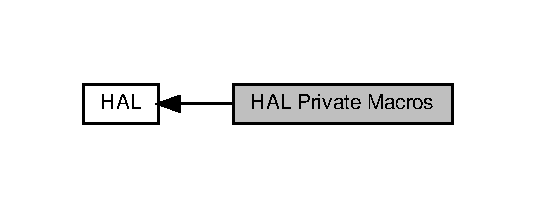
\includegraphics[width=257pt]{group___h_a_l___private___macros}
\end{center}
\end{figure}
\subsection*{Definicje}
\begin{DoxyCompactItemize}
\item 
\#define \hyperlink{group___h_a_l___private___macros_ga2a86bf8a89ad75716cd92e932a8ae71e}{I\+S\+\_\+\+T\+I\+C\+K\+F\+R\+EQ}(F\+R\+EQ)
\end{DoxyCompactItemize}


\subsection{Opis szczegółowy}


\subsection{Dokumentacja definicji}
\mbox{\Hypertarget{group___h_a_l___private___macros_ga2a86bf8a89ad75716cd92e932a8ae71e}\label{group___h_a_l___private___macros_ga2a86bf8a89ad75716cd92e932a8ae71e}} 
\index{H\+A\+L Private Macros@{H\+A\+L Private Macros}!I\+S\+\_\+\+T\+I\+C\+K\+F\+R\+EQ@{I\+S\+\_\+\+T\+I\+C\+K\+F\+R\+EQ}}
\index{I\+S\+\_\+\+T\+I\+C\+K\+F\+R\+EQ@{I\+S\+\_\+\+T\+I\+C\+K\+F\+R\+EQ}!H\+A\+L Private Macros@{H\+A\+L Private Macros}}
\subsubsection{\texorpdfstring{I\+S\+\_\+\+T\+I\+C\+K\+F\+R\+EQ}{IS\_TICKFREQ}}
{\footnotesize\ttfamily \#define I\+S\+\_\+\+T\+I\+C\+K\+F\+R\+EQ(\begin{DoxyParamCaption}\item[{}]{F\+R\+EQ }\end{DoxyParamCaption})}

{\bfseries Wartość\+:}
\begin{DoxyCode}
(((FREQ) == \hyperlink{group___h_a_l___t_i_c_k___f_r_e_q_ggab36ec81674817249c46734772ff3b73aabf4d022d85adb437a57c1f45d6345092}{HAL\_TICK\_FREQ\_10HZ})  || \(\backslash\)
                           ((FREQ) == \hyperlink{group___h_a_l___t_i_c_k___f_r_e_q_ggab36ec81674817249c46734772ff3b73aacb1ef3a0e9632aafe0fd162e2cd88408}{HAL\_TICK\_FREQ\_100HZ}) || \(\backslash\)
                           ((FREQ) == \hyperlink{group___h_a_l___t_i_c_k___f_r_e_q_ggab36ec81674817249c46734772ff3b73aabef41c8ee13ca1d48eb49dac912f9689}{HAL\_TICK\_FREQ\_1KHZ}))
\end{DoxyCode}


Definicja w linii 193 pliku stm32f4xx\+\_\+hal.\+h.


\hypertarget{group___h_a_l___private___variables}{}\section{H\+AL Private Variables}
\label{group___h_a_l___private___variables}\index{H\+A\+L Private Variables@{H\+A\+L Private Variables}}
Diagram współpracy dla H\+AL Private Variables\+:\nopagebreak
\begin{figure}[H]
\begin{center}
\leavevmode
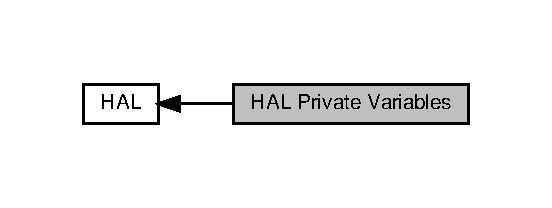
\includegraphics[width=265pt]{group___h_a_l___private___variables}
\end{center}
\end{figure}
\subsection*{Zmienne}
\begin{DoxyCompactItemize}
\item 
\hyperlink{core__sc300_8h_aec43007d9998a0a0e01faede4133d6be}{\+\_\+\+\_\+\+IO} uint32\+\_\+t \hyperlink{group___h_a_l___private___variables_ga9d411ea525781e633bf7ea7ef2f90728}{uw\+Tick}
\item 
uint32\+\_\+t \hyperlink{group___h_a_l___private___variables_ga3000c5e83924ed2debb1849c738d4be2}{uw\+Tick\+Prio} = (1\+U\+L $<$$<$ \+\_\+\+\_\+\+N\+V\+I\+C\+\_\+\+P\+R\+I\+O\+\_\+\+B\+I\+T\+S)
\item 
\hyperlink{group___h_a_l___t_i_c_k___f_r_e_q_gab36ec81674817249c46734772ff3b73a}{H\+A\+L\+\_\+\+Tick\+Freq\+Type\+Def} \hyperlink{group___h_a_l___private___variables_ga84a0c55c4d0bff06a085b4fcfd6531cd}{uw\+Tick\+Freq} = \hyperlink{group___h_a_l___t_i_c_k___f_r_e_q_ggab36ec81674817249c46734772ff3b73aa94e043d780eb1c36291338f6d6314e42}{H\+A\+L\+\_\+\+T\+I\+C\+K\+\_\+\+F\+R\+E\+Q\+\_\+\+D\+E\+F\+A\+U\+LT}
\end{DoxyCompactItemize}


\subsection{Opis szczegółowy}


\subsection{Dokumentacja zmiennych}
\mbox{\Hypertarget{group___h_a_l___private___variables_ga9d411ea525781e633bf7ea7ef2f90728}\label{group___h_a_l___private___variables_ga9d411ea525781e633bf7ea7ef2f90728}} 
\index{H\+A\+L Private Variables@{H\+A\+L Private Variables}!uw\+Tick@{uw\+Tick}}
\index{uw\+Tick@{uw\+Tick}!H\+A\+L Private Variables@{H\+A\+L Private Variables}}
\subsubsection{\texorpdfstring{uw\+Tick}{uwTick}}
{\footnotesize\ttfamily \hyperlink{core__sc300_8h_aec43007d9998a0a0e01faede4133d6be}{\+\_\+\+\_\+\+IO} uint32\+\_\+t uw\+Tick}



Definicja w linii 94 pliku stm32f4xx\+\_\+hal.\+c.

\mbox{\Hypertarget{group___h_a_l___private___variables_ga84a0c55c4d0bff06a085b4fcfd6531cd}\label{group___h_a_l___private___variables_ga84a0c55c4d0bff06a085b4fcfd6531cd}} 
\index{H\+A\+L Private Variables@{H\+A\+L Private Variables}!uw\+Tick\+Freq@{uw\+Tick\+Freq}}
\index{uw\+Tick\+Freq@{uw\+Tick\+Freq}!H\+A\+L Private Variables@{H\+A\+L Private Variables}}
\subsubsection{\texorpdfstring{uw\+Tick\+Freq}{uwTickFreq}}
{\footnotesize\ttfamily \hyperlink{group___h_a_l___t_i_c_k___f_r_e_q_gab36ec81674817249c46734772ff3b73a}{H\+A\+L\+\_\+\+Tick\+Freq\+Type\+Def} uw\+Tick\+Freq = \hyperlink{group___h_a_l___t_i_c_k___f_r_e_q_ggab36ec81674817249c46734772ff3b73aa94e043d780eb1c36291338f6d6314e42}{H\+A\+L\+\_\+\+T\+I\+C\+K\+\_\+\+F\+R\+E\+Q\+\_\+\+D\+E\+F\+A\+U\+LT}}



Definicja w linii 96 pliku stm32f4xx\+\_\+hal.\+c.

\mbox{\Hypertarget{group___h_a_l___private___variables_ga3000c5e83924ed2debb1849c738d4be2}\label{group___h_a_l___private___variables_ga3000c5e83924ed2debb1849c738d4be2}} 
\index{H\+A\+L Private Variables@{H\+A\+L Private Variables}!uw\+Tick\+Prio@{uw\+Tick\+Prio}}
\index{uw\+Tick\+Prio@{uw\+Tick\+Prio}!H\+A\+L Private Variables@{H\+A\+L Private Variables}}
\subsubsection{\texorpdfstring{uw\+Tick\+Prio}{uwTickPrio}}
{\footnotesize\ttfamily uint32\+\_\+t uw\+Tick\+Prio = (1\+U\+L $<$$<$ \+\_\+\+\_\+\+N\+V\+I\+C\+\_\+\+P\+R\+I\+O\+\_\+\+B\+I\+T\+S)}



Definicja w linii 95 pliku stm32f4xx\+\_\+hal.\+c.


\hypertarget{group___h_a_l___private___constants}{}\section{H\+AL Private Constants}
\label{group___h_a_l___private___constants}\index{H\+A\+L Private Constants@{H\+A\+L Private Constants}}
Diagram współpracy dla H\+AL Private Constants\+:\nopagebreak
\begin{figure}[H]
\begin{center}
\leavevmode
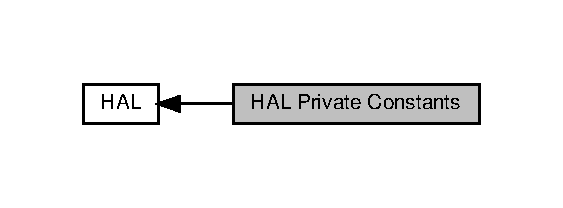
\includegraphics[width=270pt]{group___h_a_l___private___constants}
\end{center}
\end{figure}
\subsection*{Definicje}
\begin{DoxyCompactItemize}
\item 
\#define \hyperlink{group___h_a_l___private___constants_gadaedd4f6c52f98c7a4ba371ec551b6ce}{\+\_\+\+\_\+\+S\+T\+M32\+F4xx\+\_\+\+H\+A\+L\+\_\+\+V\+E\+R\+S\+I\+O\+N\+\_\+\+M\+A\+IN}~(0x01\+U)
\begin{DoxyCompactList}\small\item\em S\+T\+M32\+F4xx H\+AL Driver version number V1.\+7.\+8. \end{DoxyCompactList}\item 
\#define \hyperlink{group___h_a_l___private___constants_ga9d5e3917a3f5a417be6c8423faf78f0e}{\+\_\+\+\_\+\+S\+T\+M32\+F4xx\+\_\+\+H\+A\+L\+\_\+\+V\+E\+R\+S\+I\+O\+N\+\_\+\+S\+U\+B1}~(0x07\+U)
\item 
\#define \hyperlink{group___h_a_l___private___constants_ga87b379595edcc7d72d78b2263ae08dee}{\+\_\+\+\_\+\+S\+T\+M32\+F4xx\+\_\+\+H\+A\+L\+\_\+\+V\+E\+R\+S\+I\+O\+N\+\_\+\+S\+U\+B2}~(0x08\+U)
\item 
\#define \hyperlink{group___h_a_l___private___constants_ga61fad66d665ed89f1227e459e480e28b}{\+\_\+\+\_\+\+S\+T\+M32\+F4xx\+\_\+\+H\+A\+L\+\_\+\+V\+E\+R\+S\+I\+O\+N\+\_\+\+RC}~(0x00\+U)
\item 
\#define \hyperlink{group___h_a_l___private___constants_ga2e012cfb937fbdfa71a0c0c83f2db5b3}{\+\_\+\+\_\+\+S\+T\+M32\+F4xx\+\_\+\+H\+A\+L\+\_\+\+V\+E\+R\+S\+I\+ON}
\item 
\#define \hyperlink{group___h_a_l___private___constants_gaeeece10cca80f3c632d3d77c3f2917b6}{I\+D\+C\+O\+D\+E\+\_\+\+D\+E\+V\+I\+D\+\_\+\+M\+A\+SK}~0x00000\+F\+F\+FU
\item 
\#define \hyperlink{group___h_a_l___private___constants_ga13f7abe3641989d4d063ad21962da8b0}{S\+Y\+S\+C\+F\+G\+\_\+\+O\+F\+F\+S\+ET}~(\hyperlink{group___peripheral__memory__map_ga62246020bf3b34b6a4d8d0e84ec79d3d}{S\+Y\+S\+C\+F\+G\+\_\+\+B\+A\+SE} -\/ \hyperlink{group___peripheral__memory__map_ga9171f49478fa86d932f89e78e73b88b0}{P\+E\+R\+I\+P\+H\+\_\+\+B\+A\+SE})
\item 
\#define \hyperlink{group___h_a_l___private___constants_ga7f801653c361f31380f21357f92dc9af}{M\+E\+M\+R\+M\+P\+\_\+\+O\+F\+F\+S\+ET}~\hyperlink{group___h_a_l___private___constants_ga13f7abe3641989d4d063ad21962da8b0}{S\+Y\+S\+C\+F\+G\+\_\+\+O\+F\+F\+S\+ET}
\item 
\#define \hyperlink{group___h_a_l___private___constants_gac8a0079a8d30ec8633adaed9e2cfa49d}{U\+F\+B\+\_\+\+M\+O\+D\+E\+\_\+\+B\+I\+T\+\_\+\+N\+U\+M\+B\+ER}~S\+Y\+S\+C\+F\+G\+\_\+\+M\+E\+M\+R\+M\+P\+\_\+\+U\+F\+B\+\_\+\+M\+O\+D\+E\+\_\+\+Pos
\item 
\#define \hyperlink{group___h_a_l___private___constants_ga96bde9109ea6ea0a7887658669ff9221}{U\+F\+B\+\_\+\+M\+O\+D\+E\+\_\+\+BB}~(uint32\+\_\+t)(\hyperlink{group___peripheral__memory__map_gaed7efc100877000845c236ccdc9e144a}{P\+E\+R\+I\+P\+H\+\_\+\+B\+B\+\_\+\+B\+A\+SE} + (\hyperlink{group___h_a_l___private___constants_ga7f801653c361f31380f21357f92dc9af}{M\+E\+M\+R\+M\+P\+\_\+\+O\+F\+F\+S\+ET} $\ast$ 32\+U) + (\+U\+F\+B\+\_\+\+M\+O\+D\+E\+\_\+\+B\+I\+T\+\_\+\+N\+U\+M\+B\+E\+R $\ast$ 4\+U))
\item 
\#define \hyperlink{group___h_a_l___private___constants_ga8e5fbe846e7478d522df749672b90084}{C\+M\+P\+C\+R\+\_\+\+O\+F\+F\+S\+ET}~(\hyperlink{group___h_a_l___private___constants_ga13f7abe3641989d4d063ad21962da8b0}{S\+Y\+S\+C\+F\+G\+\_\+\+O\+F\+F\+S\+ET} + 0x20\+U)
\item 
\#define \hyperlink{group___h_a_l___private___constants_ga9e34adb28e3eed088c55766f72d53183}{C\+M\+P\+\_\+\+P\+D\+\_\+\+B\+I\+T\+\_\+\+N\+U\+M\+B\+ER}~\hyperlink{group___peripheral___registers___bits___definition_gad1747204ad5b1221e47a6610e46790e9}{S\+Y\+S\+C\+F\+G\+\_\+\+C\+M\+P\+C\+R\+\_\+\+C\+M\+P\+\_\+\+P\+D\+\_\+\+Pos}
\item 
\#define \hyperlink{group___h_a_l___private___constants_gae4516ed27e02d84d9d20c7d711b87437}{C\+M\+P\+C\+R\+\_\+\+C\+M\+P\+\_\+\+P\+D\+\_\+\+BB}~(uint32\+\_\+t)(\hyperlink{group___peripheral__memory__map_gaed7efc100877000845c236ccdc9e144a}{P\+E\+R\+I\+P\+H\+\_\+\+B\+B\+\_\+\+B\+A\+SE} + (\hyperlink{group___h_a_l___private___constants_ga8e5fbe846e7478d522df749672b90084}{C\+M\+P\+C\+R\+\_\+\+O\+F\+F\+S\+ET} $\ast$ 32\+U) + (\+C\+M\+P\+\_\+\+P\+D\+\_\+\+B\+I\+T\+\_\+\+N\+U\+M\+B\+E\+R $\ast$ 4\+U))
\item 
\#define \hyperlink{group___h_a_l___private___constants_ga41f6d93357082d3177da0e85b872b6cf}{M\+C\+H\+D\+L\+Y\+C\+R\+\_\+\+O\+F\+F\+S\+ET}~(\hyperlink{group___h_a_l___private___constants_ga13f7abe3641989d4d063ad21962da8b0}{S\+Y\+S\+C\+F\+G\+\_\+\+O\+F\+F\+S\+ET} + 0x30\+U)
\item 
\#define \hyperlink{group___h_a_l___private___constants_gaf2471142b1e018bc470cf8d8c39ade4b}{B\+S\+C\+K\+S\+E\+L\+\_\+\+B\+I\+T\+\_\+\+N\+U\+M\+B\+ER}~S\+Y\+S\+C\+F\+G\+\_\+\+M\+C\+H\+D\+L\+Y\+C\+R\+\_\+\+B\+S\+C\+K\+S\+E\+L\+\_\+\+Pos
\item 
\#define \hyperlink{group___h_a_l___private___constants_gaf57f0bab14ecc4fa67651617a3bed337}{M\+C\+H\+D\+L\+Y\+C\+R\+\_\+\+B\+S\+C\+K\+S\+E\+L\+\_\+\+BB}~(uint32\+\_\+t)(\hyperlink{group___peripheral__memory__map_gaed7efc100877000845c236ccdc9e144a}{P\+E\+R\+I\+P\+H\+\_\+\+B\+B\+\_\+\+B\+A\+SE} + (\hyperlink{group___h_a_l___private___constants_ga41f6d93357082d3177da0e85b872b6cf}{M\+C\+H\+D\+L\+Y\+C\+R\+\_\+\+O\+F\+F\+S\+ET} $\ast$ 32\+U) + (\+B\+S\+C\+K\+S\+E\+L\+\_\+\+B\+I\+T\+\_\+\+N\+U\+M\+B\+E\+R $\ast$ 4\+U))
\end{DoxyCompactItemize}


\subsection{Opis szczegółowy}


\subsection{Dokumentacja definicji}
\mbox{\Hypertarget{group___h_a_l___private___constants_ga2e012cfb937fbdfa71a0c0c83f2db5b3}\label{group___h_a_l___private___constants_ga2e012cfb937fbdfa71a0c0c83f2db5b3}} 
\index{H\+A\+L Private Constants@{H\+A\+L Private Constants}!\+\_\+\+\_\+\+S\+T\+M32\+F4xx\+\_\+\+H\+A\+L\+\_\+\+V\+E\+R\+S\+I\+ON@{\+\_\+\+\_\+\+S\+T\+M32\+F4xx\+\_\+\+H\+A\+L\+\_\+\+V\+E\+R\+S\+I\+ON}}
\index{\+\_\+\+\_\+\+S\+T\+M32\+F4xx\+\_\+\+H\+A\+L\+\_\+\+V\+E\+R\+S\+I\+ON@{\+\_\+\+\_\+\+S\+T\+M32\+F4xx\+\_\+\+H\+A\+L\+\_\+\+V\+E\+R\+S\+I\+ON}!H\+A\+L Private Constants@{H\+A\+L Private Constants}}
\subsubsection{\texorpdfstring{\+\_\+\+\_\+\+S\+T\+M32\+F4xx\+\_\+\+H\+A\+L\+\_\+\+V\+E\+R\+S\+I\+ON}{\_\_STM32F4xx\_HAL\_VERSION}}
{\footnotesize\ttfamily \#define \+\_\+\+\_\+\+S\+T\+M32\+F4xx\+\_\+\+H\+A\+L\+\_\+\+V\+E\+R\+S\+I\+ON}

{\bfseries Wartość\+:}
\begin{DoxyCode}
((\hyperlink{group___h_a_l___private___constants_gadaedd4f6c52f98c7a4ba371ec551b6ce}{\_\_STM32F4xx\_HAL\_VERSION\_MAIN} << 24U)\(\backslash\)
                                        |(\hyperlink{group___h_a_l___private___constants_ga9d5e3917a3f5a417be6c8423faf78f0e}{\_\_STM32F4xx\_HAL\_VERSION\_SUB1} << 16U)\(\backslash\)
                                        |(\hyperlink{group___h_a_l___private___constants_ga87b379595edcc7d72d78b2263ae08dee}{\_\_STM32F4xx\_HAL\_VERSION\_SUB2} << 8U )\(\backslash\)
                                        |(\hyperlink{group___h_a_l___private___constants_ga61fad66d665ed89f1227e459e480e28b}{\_\_STM32F4xx\_HAL\_VERSION\_RC}))
\end{DoxyCode}


Definicja w linii 59 pliku stm32f4xx\+\_\+hal.\+c.

\mbox{\Hypertarget{group___h_a_l___private___constants_gadaedd4f6c52f98c7a4ba371ec551b6ce}\label{group___h_a_l___private___constants_gadaedd4f6c52f98c7a4ba371ec551b6ce}} 
\index{H\+A\+L Private Constants@{H\+A\+L Private Constants}!\+\_\+\+\_\+\+S\+T\+M32\+F4xx\+\_\+\+H\+A\+L\+\_\+\+V\+E\+R\+S\+I\+O\+N\+\_\+\+M\+A\+IN@{\+\_\+\+\_\+\+S\+T\+M32\+F4xx\+\_\+\+H\+A\+L\+\_\+\+V\+E\+R\+S\+I\+O\+N\+\_\+\+M\+A\+IN}}
\index{\+\_\+\+\_\+\+S\+T\+M32\+F4xx\+\_\+\+H\+A\+L\+\_\+\+V\+E\+R\+S\+I\+O\+N\+\_\+\+M\+A\+IN@{\+\_\+\+\_\+\+S\+T\+M32\+F4xx\+\_\+\+H\+A\+L\+\_\+\+V\+E\+R\+S\+I\+O\+N\+\_\+\+M\+A\+IN}!H\+A\+L Private Constants@{H\+A\+L Private Constants}}
\subsubsection{\texorpdfstring{\+\_\+\+\_\+\+S\+T\+M32\+F4xx\+\_\+\+H\+A\+L\+\_\+\+V\+E\+R\+S\+I\+O\+N\+\_\+\+M\+A\+IN}{\_\_STM32F4xx\_HAL\_VERSION\_MAIN}}
{\footnotesize\ttfamily \#define \+\_\+\+\_\+\+S\+T\+M32\+F4xx\+\_\+\+H\+A\+L\+\_\+\+V\+E\+R\+S\+I\+O\+N\+\_\+\+M\+A\+IN~(0x01\+U)}



S\+T\+M32\+F4xx H\+AL Driver version number V1.\+7.\+8. 

\mbox{[}31\+:24\mbox{]} main version 

Definicja w linii 55 pliku stm32f4xx\+\_\+hal.\+c.

\mbox{\Hypertarget{group___h_a_l___private___constants_ga61fad66d665ed89f1227e459e480e28b}\label{group___h_a_l___private___constants_ga61fad66d665ed89f1227e459e480e28b}} 
\index{H\+A\+L Private Constants@{H\+A\+L Private Constants}!\+\_\+\+\_\+\+S\+T\+M32\+F4xx\+\_\+\+H\+A\+L\+\_\+\+V\+E\+R\+S\+I\+O\+N\+\_\+\+RC@{\+\_\+\+\_\+\+S\+T\+M32\+F4xx\+\_\+\+H\+A\+L\+\_\+\+V\+E\+R\+S\+I\+O\+N\+\_\+\+RC}}
\index{\+\_\+\+\_\+\+S\+T\+M32\+F4xx\+\_\+\+H\+A\+L\+\_\+\+V\+E\+R\+S\+I\+O\+N\+\_\+\+RC@{\+\_\+\+\_\+\+S\+T\+M32\+F4xx\+\_\+\+H\+A\+L\+\_\+\+V\+E\+R\+S\+I\+O\+N\+\_\+\+RC}!H\+A\+L Private Constants@{H\+A\+L Private Constants}}
\subsubsection{\texorpdfstring{\+\_\+\+\_\+\+S\+T\+M32\+F4xx\+\_\+\+H\+A\+L\+\_\+\+V\+E\+R\+S\+I\+O\+N\+\_\+\+RC}{\_\_STM32F4xx\_HAL\_VERSION\_RC}}
{\footnotesize\ttfamily \#define \+\_\+\+\_\+\+S\+T\+M32\+F4xx\+\_\+\+H\+A\+L\+\_\+\+V\+E\+R\+S\+I\+O\+N\+\_\+\+RC~(0x00\+U)}

\mbox{[}7\+:0\mbox{]} release candidate 

Definicja w linii 58 pliku stm32f4xx\+\_\+hal.\+c.

\mbox{\Hypertarget{group___h_a_l___private___constants_ga9d5e3917a3f5a417be6c8423faf78f0e}\label{group___h_a_l___private___constants_ga9d5e3917a3f5a417be6c8423faf78f0e}} 
\index{H\+A\+L Private Constants@{H\+A\+L Private Constants}!\+\_\+\+\_\+\+S\+T\+M32\+F4xx\+\_\+\+H\+A\+L\+\_\+\+V\+E\+R\+S\+I\+O\+N\+\_\+\+S\+U\+B1@{\+\_\+\+\_\+\+S\+T\+M32\+F4xx\+\_\+\+H\+A\+L\+\_\+\+V\+E\+R\+S\+I\+O\+N\+\_\+\+S\+U\+B1}}
\index{\+\_\+\+\_\+\+S\+T\+M32\+F4xx\+\_\+\+H\+A\+L\+\_\+\+V\+E\+R\+S\+I\+O\+N\+\_\+\+S\+U\+B1@{\+\_\+\+\_\+\+S\+T\+M32\+F4xx\+\_\+\+H\+A\+L\+\_\+\+V\+E\+R\+S\+I\+O\+N\+\_\+\+S\+U\+B1}!H\+A\+L Private Constants@{H\+A\+L Private Constants}}
\subsubsection{\texorpdfstring{\+\_\+\+\_\+\+S\+T\+M32\+F4xx\+\_\+\+H\+A\+L\+\_\+\+V\+E\+R\+S\+I\+O\+N\+\_\+\+S\+U\+B1}{\_\_STM32F4xx\_HAL\_VERSION\_SUB1}}
{\footnotesize\ttfamily \#define \+\_\+\+\_\+\+S\+T\+M32\+F4xx\+\_\+\+H\+A\+L\+\_\+\+V\+E\+R\+S\+I\+O\+N\+\_\+\+S\+U\+B1~(0x07\+U)}

\mbox{[}23\+:16\mbox{]} sub1 version 

Definicja w linii 56 pliku stm32f4xx\+\_\+hal.\+c.

\mbox{\Hypertarget{group___h_a_l___private___constants_ga87b379595edcc7d72d78b2263ae08dee}\label{group___h_a_l___private___constants_ga87b379595edcc7d72d78b2263ae08dee}} 
\index{H\+A\+L Private Constants@{H\+A\+L Private Constants}!\+\_\+\+\_\+\+S\+T\+M32\+F4xx\+\_\+\+H\+A\+L\+\_\+\+V\+E\+R\+S\+I\+O\+N\+\_\+\+S\+U\+B2@{\+\_\+\+\_\+\+S\+T\+M32\+F4xx\+\_\+\+H\+A\+L\+\_\+\+V\+E\+R\+S\+I\+O\+N\+\_\+\+S\+U\+B2}}
\index{\+\_\+\+\_\+\+S\+T\+M32\+F4xx\+\_\+\+H\+A\+L\+\_\+\+V\+E\+R\+S\+I\+O\+N\+\_\+\+S\+U\+B2@{\+\_\+\+\_\+\+S\+T\+M32\+F4xx\+\_\+\+H\+A\+L\+\_\+\+V\+E\+R\+S\+I\+O\+N\+\_\+\+S\+U\+B2}!H\+A\+L Private Constants@{H\+A\+L Private Constants}}
\subsubsection{\texorpdfstring{\+\_\+\+\_\+\+S\+T\+M32\+F4xx\+\_\+\+H\+A\+L\+\_\+\+V\+E\+R\+S\+I\+O\+N\+\_\+\+S\+U\+B2}{\_\_STM32F4xx\_HAL\_VERSION\_SUB2}}
{\footnotesize\ttfamily \#define \+\_\+\+\_\+\+S\+T\+M32\+F4xx\+\_\+\+H\+A\+L\+\_\+\+V\+E\+R\+S\+I\+O\+N\+\_\+\+S\+U\+B2~(0x08\+U)}

\mbox{[}15\+:8\mbox{]} sub2 version 

Definicja w linii 57 pliku stm32f4xx\+\_\+hal.\+c.

\mbox{\Hypertarget{group___h_a_l___private___constants_gaf2471142b1e018bc470cf8d8c39ade4b}\label{group___h_a_l___private___constants_gaf2471142b1e018bc470cf8d8c39ade4b}} 
\index{H\+A\+L Private Constants@{H\+A\+L Private Constants}!B\+S\+C\+K\+S\+E\+L\+\_\+\+B\+I\+T\+\_\+\+N\+U\+M\+B\+ER@{B\+S\+C\+K\+S\+E\+L\+\_\+\+B\+I\+T\+\_\+\+N\+U\+M\+B\+ER}}
\index{B\+S\+C\+K\+S\+E\+L\+\_\+\+B\+I\+T\+\_\+\+N\+U\+M\+B\+ER@{B\+S\+C\+K\+S\+E\+L\+\_\+\+B\+I\+T\+\_\+\+N\+U\+M\+B\+ER}!H\+A\+L Private Constants@{H\+A\+L Private Constants}}
\subsubsection{\texorpdfstring{B\+S\+C\+K\+S\+E\+L\+\_\+\+B\+I\+T\+\_\+\+N\+U\+M\+B\+ER}{BSCKSEL\_BIT\_NUMBER}}
{\footnotesize\ttfamily \#define B\+S\+C\+K\+S\+E\+L\+\_\+\+B\+I\+T\+\_\+\+N\+U\+M\+B\+ER~S\+Y\+S\+C\+F\+G\+\_\+\+M\+C\+H\+D\+L\+Y\+C\+R\+\_\+\+B\+S\+C\+K\+S\+E\+L\+\_\+\+Pos}



Definicja w linii 83 pliku stm32f4xx\+\_\+hal.\+c.

\mbox{\Hypertarget{group___h_a_l___private___constants_ga9e34adb28e3eed088c55766f72d53183}\label{group___h_a_l___private___constants_ga9e34adb28e3eed088c55766f72d53183}} 
\index{H\+A\+L Private Constants@{H\+A\+L Private Constants}!C\+M\+P\+\_\+\+P\+D\+\_\+\+B\+I\+T\+\_\+\+N\+U\+M\+B\+ER@{C\+M\+P\+\_\+\+P\+D\+\_\+\+B\+I\+T\+\_\+\+N\+U\+M\+B\+ER}}
\index{C\+M\+P\+\_\+\+P\+D\+\_\+\+B\+I\+T\+\_\+\+N\+U\+M\+B\+ER@{C\+M\+P\+\_\+\+P\+D\+\_\+\+B\+I\+T\+\_\+\+N\+U\+M\+B\+ER}!H\+A\+L Private Constants@{H\+A\+L Private Constants}}
\subsubsection{\texorpdfstring{C\+M\+P\+\_\+\+P\+D\+\_\+\+B\+I\+T\+\_\+\+N\+U\+M\+B\+ER}{CMP\_PD\_BIT\_NUMBER}}
{\footnotesize\ttfamily \#define C\+M\+P\+\_\+\+P\+D\+\_\+\+B\+I\+T\+\_\+\+N\+U\+M\+B\+ER~\hyperlink{group___peripheral___registers___bits___definition_gad1747204ad5b1221e47a6610e46790e9}{S\+Y\+S\+C\+F\+G\+\_\+\+C\+M\+P\+C\+R\+\_\+\+C\+M\+P\+\_\+\+P\+D\+\_\+\+Pos}}



Definicja w linii 77 pliku stm32f4xx\+\_\+hal.\+c.

\mbox{\Hypertarget{group___h_a_l___private___constants_gae4516ed27e02d84d9d20c7d711b87437}\label{group___h_a_l___private___constants_gae4516ed27e02d84d9d20c7d711b87437}} 
\index{H\+A\+L Private Constants@{H\+A\+L Private Constants}!C\+M\+P\+C\+R\+\_\+\+C\+M\+P\+\_\+\+P\+D\+\_\+\+BB@{C\+M\+P\+C\+R\+\_\+\+C\+M\+P\+\_\+\+P\+D\+\_\+\+BB}}
\index{C\+M\+P\+C\+R\+\_\+\+C\+M\+P\+\_\+\+P\+D\+\_\+\+BB@{C\+M\+P\+C\+R\+\_\+\+C\+M\+P\+\_\+\+P\+D\+\_\+\+BB}!H\+A\+L Private Constants@{H\+A\+L Private Constants}}
\subsubsection{\texorpdfstring{C\+M\+P\+C\+R\+\_\+\+C\+M\+P\+\_\+\+P\+D\+\_\+\+BB}{CMPCR\_CMP\_PD\_BB}}
{\footnotesize\ttfamily \#define C\+M\+P\+C\+R\+\_\+\+C\+M\+P\+\_\+\+P\+D\+\_\+\+BB~(uint32\+\_\+t)(\hyperlink{group___peripheral__memory__map_gaed7efc100877000845c236ccdc9e144a}{P\+E\+R\+I\+P\+H\+\_\+\+B\+B\+\_\+\+B\+A\+SE} + (\hyperlink{group___h_a_l___private___constants_ga8e5fbe846e7478d522df749672b90084}{C\+M\+P\+C\+R\+\_\+\+O\+F\+F\+S\+ET} $\ast$ 32\+U) + (\+C\+M\+P\+\_\+\+P\+D\+\_\+\+B\+I\+T\+\_\+\+N\+U\+M\+B\+E\+R $\ast$ 4\+U))}



Definicja w linii 78 pliku stm32f4xx\+\_\+hal.\+c.

\mbox{\Hypertarget{group___h_a_l___private___constants_ga8e5fbe846e7478d522df749672b90084}\label{group___h_a_l___private___constants_ga8e5fbe846e7478d522df749672b90084}} 
\index{H\+A\+L Private Constants@{H\+A\+L Private Constants}!C\+M\+P\+C\+R\+\_\+\+O\+F\+F\+S\+ET@{C\+M\+P\+C\+R\+\_\+\+O\+F\+F\+S\+ET}}
\index{C\+M\+P\+C\+R\+\_\+\+O\+F\+F\+S\+ET@{C\+M\+P\+C\+R\+\_\+\+O\+F\+F\+S\+ET}!H\+A\+L Private Constants@{H\+A\+L Private Constants}}
\subsubsection{\texorpdfstring{C\+M\+P\+C\+R\+\_\+\+O\+F\+F\+S\+ET}{CMPCR\_OFFSET}}
{\footnotesize\ttfamily \#define C\+M\+P\+C\+R\+\_\+\+O\+F\+F\+S\+ET~(\hyperlink{group___h_a_l___private___constants_ga13f7abe3641989d4d063ad21962da8b0}{S\+Y\+S\+C\+F\+G\+\_\+\+O\+F\+F\+S\+ET} + 0x20\+U)}



Definicja w linii 76 pliku stm32f4xx\+\_\+hal.\+c.

\mbox{\Hypertarget{group___h_a_l___private___constants_gaeeece10cca80f3c632d3d77c3f2917b6}\label{group___h_a_l___private___constants_gaeeece10cca80f3c632d3d77c3f2917b6}} 
\index{H\+A\+L Private Constants@{H\+A\+L Private Constants}!I\+D\+C\+O\+D\+E\+\_\+\+D\+E\+V\+I\+D\+\_\+\+M\+A\+SK@{I\+D\+C\+O\+D\+E\+\_\+\+D\+E\+V\+I\+D\+\_\+\+M\+A\+SK}}
\index{I\+D\+C\+O\+D\+E\+\_\+\+D\+E\+V\+I\+D\+\_\+\+M\+A\+SK@{I\+D\+C\+O\+D\+E\+\_\+\+D\+E\+V\+I\+D\+\_\+\+M\+A\+SK}!H\+A\+L Private Constants@{H\+A\+L Private Constants}}
\subsubsection{\texorpdfstring{I\+D\+C\+O\+D\+E\+\_\+\+D\+E\+V\+I\+D\+\_\+\+M\+A\+SK}{IDCODE\_DEVID\_MASK}}
{\footnotesize\ttfamily \#define I\+D\+C\+O\+D\+E\+\_\+\+D\+E\+V\+I\+D\+\_\+\+M\+A\+SK~0x00000\+F\+F\+FU}



Definicja w linii 64 pliku stm32f4xx\+\_\+hal.\+c.

\mbox{\Hypertarget{group___h_a_l___private___constants_gaf57f0bab14ecc4fa67651617a3bed337}\label{group___h_a_l___private___constants_gaf57f0bab14ecc4fa67651617a3bed337}} 
\index{H\+A\+L Private Constants@{H\+A\+L Private Constants}!M\+C\+H\+D\+L\+Y\+C\+R\+\_\+\+B\+S\+C\+K\+S\+E\+L\+\_\+\+BB@{M\+C\+H\+D\+L\+Y\+C\+R\+\_\+\+B\+S\+C\+K\+S\+E\+L\+\_\+\+BB}}
\index{M\+C\+H\+D\+L\+Y\+C\+R\+\_\+\+B\+S\+C\+K\+S\+E\+L\+\_\+\+BB@{M\+C\+H\+D\+L\+Y\+C\+R\+\_\+\+B\+S\+C\+K\+S\+E\+L\+\_\+\+BB}!H\+A\+L Private Constants@{H\+A\+L Private Constants}}
\subsubsection{\texorpdfstring{M\+C\+H\+D\+L\+Y\+C\+R\+\_\+\+B\+S\+C\+K\+S\+E\+L\+\_\+\+BB}{MCHDLYCR\_BSCKSEL\_BB}}
{\footnotesize\ttfamily \#define M\+C\+H\+D\+L\+Y\+C\+R\+\_\+\+B\+S\+C\+K\+S\+E\+L\+\_\+\+BB~(uint32\+\_\+t)(\hyperlink{group___peripheral__memory__map_gaed7efc100877000845c236ccdc9e144a}{P\+E\+R\+I\+P\+H\+\_\+\+B\+B\+\_\+\+B\+A\+SE} + (\hyperlink{group___h_a_l___private___constants_ga41f6d93357082d3177da0e85b872b6cf}{M\+C\+H\+D\+L\+Y\+C\+R\+\_\+\+O\+F\+F\+S\+ET} $\ast$ 32\+U) + (\+B\+S\+C\+K\+S\+E\+L\+\_\+\+B\+I\+T\+\_\+\+N\+U\+M\+B\+E\+R $\ast$ 4\+U))}



Definicja w linii 84 pliku stm32f4xx\+\_\+hal.\+c.

\mbox{\Hypertarget{group___h_a_l___private___constants_ga41f6d93357082d3177da0e85b872b6cf}\label{group___h_a_l___private___constants_ga41f6d93357082d3177da0e85b872b6cf}} 
\index{H\+A\+L Private Constants@{H\+A\+L Private Constants}!M\+C\+H\+D\+L\+Y\+C\+R\+\_\+\+O\+F\+F\+S\+ET@{M\+C\+H\+D\+L\+Y\+C\+R\+\_\+\+O\+F\+F\+S\+ET}}
\index{M\+C\+H\+D\+L\+Y\+C\+R\+\_\+\+O\+F\+F\+S\+ET@{M\+C\+H\+D\+L\+Y\+C\+R\+\_\+\+O\+F\+F\+S\+ET}!H\+A\+L Private Constants@{H\+A\+L Private Constants}}
\subsubsection{\texorpdfstring{M\+C\+H\+D\+L\+Y\+C\+R\+\_\+\+O\+F\+F\+S\+ET}{MCHDLYCR\_OFFSET}}
{\footnotesize\ttfamily \#define M\+C\+H\+D\+L\+Y\+C\+R\+\_\+\+O\+F\+F\+S\+ET~(\hyperlink{group___h_a_l___private___constants_ga13f7abe3641989d4d063ad21962da8b0}{S\+Y\+S\+C\+F\+G\+\_\+\+O\+F\+F\+S\+ET} + 0x30\+U)}



Definicja w linii 82 pliku stm32f4xx\+\_\+hal.\+c.

\mbox{\Hypertarget{group___h_a_l___private___constants_ga7f801653c361f31380f21357f92dc9af}\label{group___h_a_l___private___constants_ga7f801653c361f31380f21357f92dc9af}} 
\index{H\+A\+L Private Constants@{H\+A\+L Private Constants}!M\+E\+M\+R\+M\+P\+\_\+\+O\+F\+F\+S\+ET@{M\+E\+M\+R\+M\+P\+\_\+\+O\+F\+F\+S\+ET}}
\index{M\+E\+M\+R\+M\+P\+\_\+\+O\+F\+F\+S\+ET@{M\+E\+M\+R\+M\+P\+\_\+\+O\+F\+F\+S\+ET}!H\+A\+L Private Constants@{H\+A\+L Private Constants}}
\subsubsection{\texorpdfstring{M\+E\+M\+R\+M\+P\+\_\+\+O\+F\+F\+S\+ET}{MEMRMP\_OFFSET}}
{\footnotesize\ttfamily \#define M\+E\+M\+R\+M\+P\+\_\+\+O\+F\+F\+S\+ET~\hyperlink{group___h_a_l___private___constants_ga13f7abe3641989d4d063ad21962da8b0}{S\+Y\+S\+C\+F\+G\+\_\+\+O\+F\+F\+S\+ET}}



Definicja w linii 70 pliku stm32f4xx\+\_\+hal.\+c.

\mbox{\Hypertarget{group___h_a_l___private___constants_ga13f7abe3641989d4d063ad21962da8b0}\label{group___h_a_l___private___constants_ga13f7abe3641989d4d063ad21962da8b0}} 
\index{H\+A\+L Private Constants@{H\+A\+L Private Constants}!S\+Y\+S\+C\+F\+G\+\_\+\+O\+F\+F\+S\+ET@{S\+Y\+S\+C\+F\+G\+\_\+\+O\+F\+F\+S\+ET}}
\index{S\+Y\+S\+C\+F\+G\+\_\+\+O\+F\+F\+S\+ET@{S\+Y\+S\+C\+F\+G\+\_\+\+O\+F\+F\+S\+ET}!H\+A\+L Private Constants@{H\+A\+L Private Constants}}
\subsubsection{\texorpdfstring{S\+Y\+S\+C\+F\+G\+\_\+\+O\+F\+F\+S\+ET}{SYSCFG\_OFFSET}}
{\footnotesize\ttfamily \#define S\+Y\+S\+C\+F\+G\+\_\+\+O\+F\+F\+S\+ET~(\hyperlink{group___peripheral__memory__map_ga62246020bf3b34b6a4d8d0e84ec79d3d}{S\+Y\+S\+C\+F\+G\+\_\+\+B\+A\+SE} -\/ \hyperlink{group___peripheral__memory__map_ga9171f49478fa86d932f89e78e73b88b0}{P\+E\+R\+I\+P\+H\+\_\+\+B\+A\+SE})}



Definicja w linii 67 pliku stm32f4xx\+\_\+hal.\+c.

\mbox{\Hypertarget{group___h_a_l___private___constants_ga96bde9109ea6ea0a7887658669ff9221}\label{group___h_a_l___private___constants_ga96bde9109ea6ea0a7887658669ff9221}} 
\index{H\+A\+L Private Constants@{H\+A\+L Private Constants}!U\+F\+B\+\_\+\+M\+O\+D\+E\+\_\+\+BB@{U\+F\+B\+\_\+\+M\+O\+D\+E\+\_\+\+BB}}
\index{U\+F\+B\+\_\+\+M\+O\+D\+E\+\_\+\+BB@{U\+F\+B\+\_\+\+M\+O\+D\+E\+\_\+\+BB}!H\+A\+L Private Constants@{H\+A\+L Private Constants}}
\subsubsection{\texorpdfstring{U\+F\+B\+\_\+\+M\+O\+D\+E\+\_\+\+BB}{UFB\_MODE\_BB}}
{\footnotesize\ttfamily \#define U\+F\+B\+\_\+\+M\+O\+D\+E\+\_\+\+BB~(uint32\+\_\+t)(\hyperlink{group___peripheral__memory__map_gaed7efc100877000845c236ccdc9e144a}{P\+E\+R\+I\+P\+H\+\_\+\+B\+B\+\_\+\+B\+A\+SE} + (\hyperlink{group___h_a_l___private___constants_ga7f801653c361f31380f21357f92dc9af}{M\+E\+M\+R\+M\+P\+\_\+\+O\+F\+F\+S\+ET} $\ast$ 32\+U) + (\+U\+F\+B\+\_\+\+M\+O\+D\+E\+\_\+\+B\+I\+T\+\_\+\+N\+U\+M\+B\+E\+R $\ast$ 4\+U))}



Definicja w linii 72 pliku stm32f4xx\+\_\+hal.\+c.

\mbox{\Hypertarget{group___h_a_l___private___constants_gac8a0079a8d30ec8633adaed9e2cfa49d}\label{group___h_a_l___private___constants_gac8a0079a8d30ec8633adaed9e2cfa49d}} 
\index{H\+A\+L Private Constants@{H\+A\+L Private Constants}!U\+F\+B\+\_\+\+M\+O\+D\+E\+\_\+\+B\+I\+T\+\_\+\+N\+U\+M\+B\+ER@{U\+F\+B\+\_\+\+M\+O\+D\+E\+\_\+\+B\+I\+T\+\_\+\+N\+U\+M\+B\+ER}}
\index{U\+F\+B\+\_\+\+M\+O\+D\+E\+\_\+\+B\+I\+T\+\_\+\+N\+U\+M\+B\+ER@{U\+F\+B\+\_\+\+M\+O\+D\+E\+\_\+\+B\+I\+T\+\_\+\+N\+U\+M\+B\+ER}!H\+A\+L Private Constants@{H\+A\+L Private Constants}}
\subsubsection{\texorpdfstring{U\+F\+B\+\_\+\+M\+O\+D\+E\+\_\+\+B\+I\+T\+\_\+\+N\+U\+M\+B\+ER}{UFB\_MODE\_BIT\_NUMBER}}
{\footnotesize\ttfamily \#define U\+F\+B\+\_\+\+M\+O\+D\+E\+\_\+\+B\+I\+T\+\_\+\+N\+U\+M\+B\+ER~S\+Y\+S\+C\+F\+G\+\_\+\+M\+E\+M\+R\+M\+P\+\_\+\+U\+F\+B\+\_\+\+M\+O\+D\+E\+\_\+\+Pos}



Definicja w linii 71 pliku stm32f4xx\+\_\+hal.\+c.


\hypertarget{group___c_o_r_t_e_x___exported___types}{}\section{Cortex Exported Types}
\label{group___c_o_r_t_e_x___exported___types}\index{Cortex Exported Types@{Cortex Exported Types}}
Diagram współpracy dla Cortex Exported Types\+:\nopagebreak
\begin{figure}[H]
\begin{center}
\leavevmode
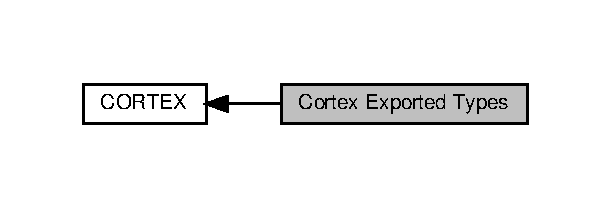
\includegraphics[width=293pt]{group___c_o_r_t_e_x___exported___types}
\end{center}
\end{figure}

\hypertarget{group___c_o_r_t_e_x___exported___constants}{}\section{C\+O\+R\+T\+EX Exported Constants}
\label{group___c_o_r_t_e_x___exported___constants}\index{C\+O\+R\+T\+E\+X Exported Constants@{C\+O\+R\+T\+E\+X Exported Constants}}
Diagram współpracy dla C\+O\+R\+T\+EX Exported Constants\+:\nopagebreak
\begin{figure}[H]
\begin{center}
\leavevmode
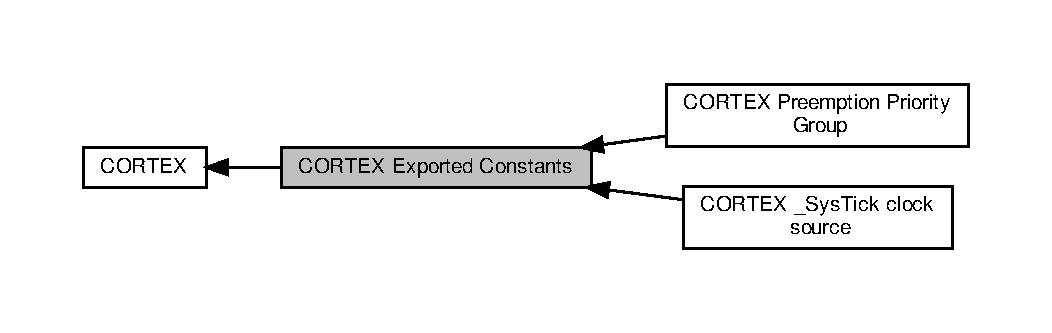
\includegraphics[width=350pt]{group___c_o_r_t_e_x___exported___constants}
\end{center}
\end{figure}
\subsection*{Moduły}
\begin{DoxyCompactItemize}
\item 
\hyperlink{group___c_o_r_t_e_x___preemption___priority___group}{C\+O\+R\+T\+E\+X Preemption Priority Group}
\item 
\hyperlink{group___c_o_r_t_e_x___sys_tick__clock__source}{C\+O\+R\+T\+E\+X \+\_\+\+Sys\+Tick clock source}
\end{DoxyCompactItemize}


\subsection{Opis szczegółowy}

\hypertarget{group___c_o_r_t_e_x___preemption___priority___group}{}\section{C\+O\+R\+T\+EX Preemption Priority Group}
\label{group___c_o_r_t_e_x___preemption___priority___group}\index{C\+O\+R\+T\+E\+X Preemption Priority Group@{C\+O\+R\+T\+E\+X Preemption Priority Group}}
Diagram współpracy dla C\+O\+R\+T\+EX Preemption Priority Group\+:\nopagebreak
\begin{figure}[H]
\begin{center}
\leavevmode
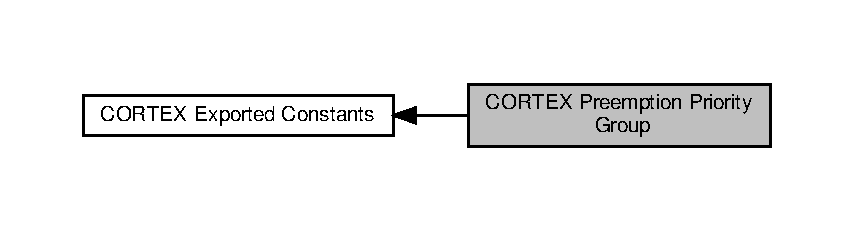
\includegraphics[width=350pt]{group___c_o_r_t_e_x___preemption___priority___group}
\end{center}
\end{figure}
\subsection*{Definicje}
\begin{DoxyCompactItemize}
\item 
\#define \hyperlink{group___c_o_r_t_e_x___preemption___priority___group_ga5e97dcff77680602c86e44f23f5ffa1a}{N\+V\+I\+C\+\_\+\+P\+R\+I\+O\+R\+I\+T\+Y\+G\+R\+O\+U\+P\+\_\+0}~0x00000007U
\item 
\#define \hyperlink{group___c_o_r_t_e_x___preemption___priority___group_ga702227137b010421c3a3b6434005a132}{N\+V\+I\+C\+\_\+\+P\+R\+I\+O\+R\+I\+T\+Y\+G\+R\+O\+U\+P\+\_\+1}~0x00000006U
\item 
\#define \hyperlink{group___c_o_r_t_e_x___preemption___priority___group_gaa43a3fd37850c120ce567ab2743d11b4}{N\+V\+I\+C\+\_\+\+P\+R\+I\+O\+R\+I\+T\+Y\+G\+R\+O\+U\+P\+\_\+2}~0x00000005U
\item 
\#define \hyperlink{group___c_o_r_t_e_x___preemption___priority___group_ga8ddb24962e6f0fc3273139d45d374b09}{N\+V\+I\+C\+\_\+\+P\+R\+I\+O\+R\+I\+T\+Y\+G\+R\+O\+U\+P\+\_\+3}~0x00000004U
\item 
\#define \hyperlink{group___c_o_r_t_e_x___preemption___priority___group_gae6eab9140204bc938255aa148e597c45}{N\+V\+I\+C\+\_\+\+P\+R\+I\+O\+R\+I\+T\+Y\+G\+R\+O\+U\+P\+\_\+4}~0x00000003U
\end{DoxyCompactItemize}


\subsection{Opis szczegółowy}


\subsection{Dokumentacja definicji}
\mbox{\Hypertarget{group___c_o_r_t_e_x___preemption___priority___group_ga5e97dcff77680602c86e44f23f5ffa1a}\label{group___c_o_r_t_e_x___preemption___priority___group_ga5e97dcff77680602c86e44f23f5ffa1a}} 
\index{C\+O\+R\+T\+E\+X Preemption Priority Group@{C\+O\+R\+T\+E\+X Preemption Priority Group}!N\+V\+I\+C\+\_\+\+P\+R\+I\+O\+R\+I\+T\+Y\+G\+R\+O\+U\+P\+\_\+0@{N\+V\+I\+C\+\_\+\+P\+R\+I\+O\+R\+I\+T\+Y\+G\+R\+O\+U\+P\+\_\+0}}
\index{N\+V\+I\+C\+\_\+\+P\+R\+I\+O\+R\+I\+T\+Y\+G\+R\+O\+U\+P\+\_\+0@{N\+V\+I\+C\+\_\+\+P\+R\+I\+O\+R\+I\+T\+Y\+G\+R\+O\+U\+P\+\_\+0}!C\+O\+R\+T\+E\+X Preemption Priority Group@{C\+O\+R\+T\+E\+X Preemption Priority Group}}
\subsubsection{\texorpdfstring{N\+V\+I\+C\+\_\+\+P\+R\+I\+O\+R\+I\+T\+Y\+G\+R\+O\+U\+P\+\_\+0}{NVIC\_PRIORITYGROUP\_0}}
{\footnotesize\ttfamily \#define N\+V\+I\+C\+\_\+\+P\+R\+I\+O\+R\+I\+T\+Y\+G\+R\+O\+U\+P\+\_\+0~0x00000007U}

0 bits for pre-\/emption priority 4 bits for subpriority 

Definicja w linii 90 pliku stm32f4xx\+\_\+hal\+\_\+cortex.\+h.

\mbox{\Hypertarget{group___c_o_r_t_e_x___preemption___priority___group_ga702227137b010421c3a3b6434005a132}\label{group___c_o_r_t_e_x___preemption___priority___group_ga702227137b010421c3a3b6434005a132}} 
\index{C\+O\+R\+T\+E\+X Preemption Priority Group@{C\+O\+R\+T\+E\+X Preemption Priority Group}!N\+V\+I\+C\+\_\+\+P\+R\+I\+O\+R\+I\+T\+Y\+G\+R\+O\+U\+P\+\_\+1@{N\+V\+I\+C\+\_\+\+P\+R\+I\+O\+R\+I\+T\+Y\+G\+R\+O\+U\+P\+\_\+1}}
\index{N\+V\+I\+C\+\_\+\+P\+R\+I\+O\+R\+I\+T\+Y\+G\+R\+O\+U\+P\+\_\+1@{N\+V\+I\+C\+\_\+\+P\+R\+I\+O\+R\+I\+T\+Y\+G\+R\+O\+U\+P\+\_\+1}!C\+O\+R\+T\+E\+X Preemption Priority Group@{C\+O\+R\+T\+E\+X Preemption Priority Group}}
\subsubsection{\texorpdfstring{N\+V\+I\+C\+\_\+\+P\+R\+I\+O\+R\+I\+T\+Y\+G\+R\+O\+U\+P\+\_\+1}{NVIC\_PRIORITYGROUP\_1}}
{\footnotesize\ttfamily \#define N\+V\+I\+C\+\_\+\+P\+R\+I\+O\+R\+I\+T\+Y\+G\+R\+O\+U\+P\+\_\+1~0x00000006U}

1 bits for pre-\/emption priority 3 bits for subpriority 

Definicja w linii 93 pliku stm32f4xx\+\_\+hal\+\_\+cortex.\+h.

\mbox{\Hypertarget{group___c_o_r_t_e_x___preemption___priority___group_gaa43a3fd37850c120ce567ab2743d11b4}\label{group___c_o_r_t_e_x___preemption___priority___group_gaa43a3fd37850c120ce567ab2743d11b4}} 
\index{C\+O\+R\+T\+E\+X Preemption Priority Group@{C\+O\+R\+T\+E\+X Preemption Priority Group}!N\+V\+I\+C\+\_\+\+P\+R\+I\+O\+R\+I\+T\+Y\+G\+R\+O\+U\+P\+\_\+2@{N\+V\+I\+C\+\_\+\+P\+R\+I\+O\+R\+I\+T\+Y\+G\+R\+O\+U\+P\+\_\+2}}
\index{N\+V\+I\+C\+\_\+\+P\+R\+I\+O\+R\+I\+T\+Y\+G\+R\+O\+U\+P\+\_\+2@{N\+V\+I\+C\+\_\+\+P\+R\+I\+O\+R\+I\+T\+Y\+G\+R\+O\+U\+P\+\_\+2}!C\+O\+R\+T\+E\+X Preemption Priority Group@{C\+O\+R\+T\+E\+X Preemption Priority Group}}
\subsubsection{\texorpdfstring{N\+V\+I\+C\+\_\+\+P\+R\+I\+O\+R\+I\+T\+Y\+G\+R\+O\+U\+P\+\_\+2}{NVIC\_PRIORITYGROUP\_2}}
{\footnotesize\ttfamily \#define N\+V\+I\+C\+\_\+\+P\+R\+I\+O\+R\+I\+T\+Y\+G\+R\+O\+U\+P\+\_\+2~0x00000005U}

2 bits for pre-\/emption priority 2 bits for subpriority 

Definicja w linii 96 pliku stm32f4xx\+\_\+hal\+\_\+cortex.\+h.

\mbox{\Hypertarget{group___c_o_r_t_e_x___preemption___priority___group_ga8ddb24962e6f0fc3273139d45d374b09}\label{group___c_o_r_t_e_x___preemption___priority___group_ga8ddb24962e6f0fc3273139d45d374b09}} 
\index{C\+O\+R\+T\+E\+X Preemption Priority Group@{C\+O\+R\+T\+E\+X Preemption Priority Group}!N\+V\+I\+C\+\_\+\+P\+R\+I\+O\+R\+I\+T\+Y\+G\+R\+O\+U\+P\+\_\+3@{N\+V\+I\+C\+\_\+\+P\+R\+I\+O\+R\+I\+T\+Y\+G\+R\+O\+U\+P\+\_\+3}}
\index{N\+V\+I\+C\+\_\+\+P\+R\+I\+O\+R\+I\+T\+Y\+G\+R\+O\+U\+P\+\_\+3@{N\+V\+I\+C\+\_\+\+P\+R\+I\+O\+R\+I\+T\+Y\+G\+R\+O\+U\+P\+\_\+3}!C\+O\+R\+T\+E\+X Preemption Priority Group@{C\+O\+R\+T\+E\+X Preemption Priority Group}}
\subsubsection{\texorpdfstring{N\+V\+I\+C\+\_\+\+P\+R\+I\+O\+R\+I\+T\+Y\+G\+R\+O\+U\+P\+\_\+3}{NVIC\_PRIORITYGROUP\_3}}
{\footnotesize\ttfamily \#define N\+V\+I\+C\+\_\+\+P\+R\+I\+O\+R\+I\+T\+Y\+G\+R\+O\+U\+P\+\_\+3~0x00000004U}

3 bits for pre-\/emption priority 1 bits for subpriority 

Definicja w linii 99 pliku stm32f4xx\+\_\+hal\+\_\+cortex.\+h.

\mbox{\Hypertarget{group___c_o_r_t_e_x___preemption___priority___group_gae6eab9140204bc938255aa148e597c45}\label{group___c_o_r_t_e_x___preemption___priority___group_gae6eab9140204bc938255aa148e597c45}} 
\index{C\+O\+R\+T\+E\+X Preemption Priority Group@{C\+O\+R\+T\+E\+X Preemption Priority Group}!N\+V\+I\+C\+\_\+\+P\+R\+I\+O\+R\+I\+T\+Y\+G\+R\+O\+U\+P\+\_\+4@{N\+V\+I\+C\+\_\+\+P\+R\+I\+O\+R\+I\+T\+Y\+G\+R\+O\+U\+P\+\_\+4}}
\index{N\+V\+I\+C\+\_\+\+P\+R\+I\+O\+R\+I\+T\+Y\+G\+R\+O\+U\+P\+\_\+4@{N\+V\+I\+C\+\_\+\+P\+R\+I\+O\+R\+I\+T\+Y\+G\+R\+O\+U\+P\+\_\+4}!C\+O\+R\+T\+E\+X Preemption Priority Group@{C\+O\+R\+T\+E\+X Preemption Priority Group}}
\subsubsection{\texorpdfstring{N\+V\+I\+C\+\_\+\+P\+R\+I\+O\+R\+I\+T\+Y\+G\+R\+O\+U\+P\+\_\+4}{NVIC\_PRIORITYGROUP\_4}}
{\footnotesize\ttfamily \#define N\+V\+I\+C\+\_\+\+P\+R\+I\+O\+R\+I\+T\+Y\+G\+R\+O\+U\+P\+\_\+4~0x00000003U}

4 bits for pre-\/emption priority 0 bits for subpriority 

Definicja w linii 102 pliku stm32f4xx\+\_\+hal\+\_\+cortex.\+h.


\hypertarget{group___c_o_r_t_e_x___sys_tick__clock__source}{}\section{C\+O\+R\+T\+EX \+\_\+\+Sys\+Tick clock source}
\label{group___c_o_r_t_e_x___sys_tick__clock__source}\index{C\+O\+R\+T\+E\+X \+\_\+\+Sys\+Tick clock source@{C\+O\+R\+T\+E\+X \+\_\+\+Sys\+Tick clock source}}
Diagram współpracy dla C\+O\+R\+T\+EX \+\_\+\+Sys\+Tick clock source\+:\nopagebreak
\begin{figure}[H]
\begin{center}
\leavevmode
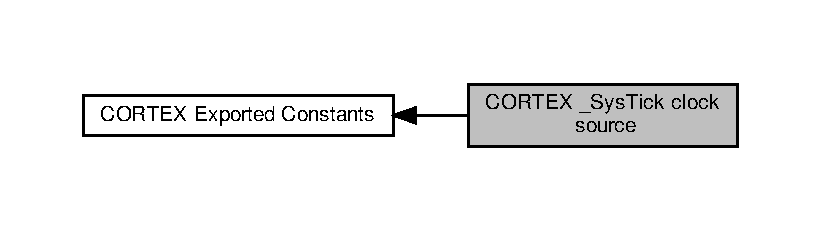
\includegraphics[width=350pt]{group___c_o_r_t_e_x___sys_tick__clock__source}
\end{center}
\end{figure}
\subsection*{Definicje}
\begin{DoxyCompactItemize}
\item 
\#define \hyperlink{group___c_o_r_t_e_x___sys_tick__clock__source_ga1fd9b5bada2a8b2425a8523bc0fc7124}{S\+Y\+S\+T\+I\+C\+K\+\_\+\+C\+L\+K\+S\+O\+U\+R\+C\+E\+\_\+\+H\+C\+L\+K\+\_\+\+D\+I\+V8}~0x00000000U
\item 
\#define \hyperlink{group___c_o_r_t_e_x___sys_tick__clock__source_ga6f6582df23b6fbc578325e453b9893b7}{S\+Y\+S\+T\+I\+C\+K\+\_\+\+C\+L\+K\+S\+O\+U\+R\+C\+E\+\_\+\+H\+C\+LK}~0x00000004U
\end{DoxyCompactItemize}


\subsection{Opis szczegółowy}


\subsection{Dokumentacja definicji}
\mbox{\Hypertarget{group___c_o_r_t_e_x___sys_tick__clock__source_ga6f6582df23b6fbc578325e453b9893b7}\label{group___c_o_r_t_e_x___sys_tick__clock__source_ga6f6582df23b6fbc578325e453b9893b7}} 
\index{C\+O\+R\+T\+E\+X \+\_\+\+Sys\+Tick clock source@{C\+O\+R\+T\+E\+X \+\_\+\+Sys\+Tick clock source}!S\+Y\+S\+T\+I\+C\+K\+\_\+\+C\+L\+K\+S\+O\+U\+R\+C\+E\+\_\+\+H\+C\+LK@{S\+Y\+S\+T\+I\+C\+K\+\_\+\+C\+L\+K\+S\+O\+U\+R\+C\+E\+\_\+\+H\+C\+LK}}
\index{S\+Y\+S\+T\+I\+C\+K\+\_\+\+C\+L\+K\+S\+O\+U\+R\+C\+E\+\_\+\+H\+C\+LK@{S\+Y\+S\+T\+I\+C\+K\+\_\+\+C\+L\+K\+S\+O\+U\+R\+C\+E\+\_\+\+H\+C\+LK}!C\+O\+R\+T\+E\+X \+\_\+\+Sys\+Tick clock source@{C\+O\+R\+T\+E\+X \+\_\+\+Sys\+Tick clock source}}
\subsubsection{\texorpdfstring{S\+Y\+S\+T\+I\+C\+K\+\_\+\+C\+L\+K\+S\+O\+U\+R\+C\+E\+\_\+\+H\+C\+LK}{SYSTICK\_CLKSOURCE\_HCLK}}
{\footnotesize\ttfamily \#define S\+Y\+S\+T\+I\+C\+K\+\_\+\+C\+L\+K\+S\+O\+U\+R\+C\+E\+\_\+\+H\+C\+LK~0x00000004U}



Definicja w linii 113 pliku stm32f4xx\+\_\+hal\+\_\+cortex.\+h.

\mbox{\Hypertarget{group___c_o_r_t_e_x___sys_tick__clock__source_ga1fd9b5bada2a8b2425a8523bc0fc7124}\label{group___c_o_r_t_e_x___sys_tick__clock__source_ga1fd9b5bada2a8b2425a8523bc0fc7124}} 
\index{C\+O\+R\+T\+E\+X \+\_\+\+Sys\+Tick clock source@{C\+O\+R\+T\+E\+X \+\_\+\+Sys\+Tick clock source}!S\+Y\+S\+T\+I\+C\+K\+\_\+\+C\+L\+K\+S\+O\+U\+R\+C\+E\+\_\+\+H\+C\+L\+K\+\_\+\+D\+I\+V8@{S\+Y\+S\+T\+I\+C\+K\+\_\+\+C\+L\+K\+S\+O\+U\+R\+C\+E\+\_\+\+H\+C\+L\+K\+\_\+\+D\+I\+V8}}
\index{S\+Y\+S\+T\+I\+C\+K\+\_\+\+C\+L\+K\+S\+O\+U\+R\+C\+E\+\_\+\+H\+C\+L\+K\+\_\+\+D\+I\+V8@{S\+Y\+S\+T\+I\+C\+K\+\_\+\+C\+L\+K\+S\+O\+U\+R\+C\+E\+\_\+\+H\+C\+L\+K\+\_\+\+D\+I\+V8}!C\+O\+R\+T\+E\+X \+\_\+\+Sys\+Tick clock source@{C\+O\+R\+T\+E\+X \+\_\+\+Sys\+Tick clock source}}
\subsubsection{\texorpdfstring{S\+Y\+S\+T\+I\+C\+K\+\_\+\+C\+L\+K\+S\+O\+U\+R\+C\+E\+\_\+\+H\+C\+L\+K\+\_\+\+D\+I\+V8}{SYSTICK\_CLKSOURCE\_HCLK\_DIV8}}
{\footnotesize\ttfamily \#define S\+Y\+S\+T\+I\+C\+K\+\_\+\+C\+L\+K\+S\+O\+U\+R\+C\+E\+\_\+\+H\+C\+L\+K\+\_\+\+D\+I\+V8~0x00000000U}



Definicja w linii 112 pliku stm32f4xx\+\_\+hal\+\_\+cortex.\+h.


\hypertarget{group___c_o_r_t_e_x___private___macros}{}\section{C\+O\+R\+T\+EX Private Macros}
\label{group___c_o_r_t_e_x___private___macros}\index{C\+O\+R\+T\+E\+X Private Macros@{C\+O\+R\+T\+E\+X Private Macros}}
Diagram współpracy dla C\+O\+R\+T\+EX Private Macros\+:\nopagebreak
\begin{figure}[H]
\begin{center}
\leavevmode
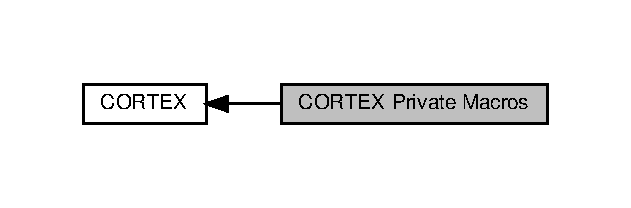
\includegraphics[width=303pt]{group___c_o_r_t_e_x___private___macros}
\end{center}
\end{figure}
\subsection*{Definicje}
\begin{DoxyCompactItemize}
\item 
\#define \hyperlink{group___c_o_r_t_e_x___private___macros_ga6569304a39fe4f91bd59b6a586c8ede9}{I\+S\+\_\+\+N\+V\+I\+C\+\_\+\+P\+R\+I\+O\+R\+I\+T\+Y\+\_\+\+G\+R\+O\+UP}(G\+R\+O\+UP)
\item 
\#define \hyperlink{group___c_o_r_t_e_x___private___macros_gaf30fd8f5960c2e28a772d8f16bb156dd}{I\+S\+\_\+\+N\+V\+I\+C\+\_\+\+P\+R\+E\+E\+M\+P\+T\+I\+O\+N\+\_\+\+P\+R\+I\+O\+R\+I\+TY}(P\+R\+I\+O\+R\+I\+TY)~((P\+R\+I\+O\+R\+I\+TY) $<$ 0x10\+U)
\item 
\#define \hyperlink{group___c_o_r_t_e_x___private___macros_ga010705bc997dcff935b965b372cba61d}{I\+S\+\_\+\+N\+V\+I\+C\+\_\+\+S\+U\+B\+\_\+\+P\+R\+I\+O\+R\+I\+TY}(P\+R\+I\+O\+R\+I\+TY)~((P\+R\+I\+O\+R\+I\+TY) $<$ 0x10\+U)
\item 
\#define \hyperlink{group___c_o_r_t_e_x___private___macros_ga9b8dcac4ed8e88c14d9bb04e369dad6a}{I\+S\+\_\+\+N\+V\+I\+C\+\_\+\+D\+E\+V\+I\+C\+E\+\_\+\+I\+RQ}(I\+RQ)~((I\+RQ) $>$= (\hyperlink{group___peripheral__interrupt__number__definition_ga7e1129cd8a196f4284d41db3e82ad5c8}{I\+R\+Qn\+\_\+\+Type})0x00\+U)
\item 
\#define \hyperlink{group___c_o_r_t_e_x___private___macros_ga22d6291f6aed29442cf4cd9098fa0784}{I\+S\+\_\+\+S\+Y\+S\+T\+I\+C\+K\+\_\+\+C\+L\+K\+\_\+\+S\+O\+U\+R\+CE}(S\+O\+U\+R\+CE)
\end{DoxyCompactItemize}


\subsection{Opis szczegółowy}


\subsection{Dokumentacja definicji}
\mbox{\Hypertarget{group___c_o_r_t_e_x___private___macros_ga9b8dcac4ed8e88c14d9bb04e369dad6a}\label{group___c_o_r_t_e_x___private___macros_ga9b8dcac4ed8e88c14d9bb04e369dad6a}} 
\index{C\+O\+R\+T\+E\+X Private Macros@{C\+O\+R\+T\+E\+X Private Macros}!I\+S\+\_\+\+N\+V\+I\+C\+\_\+\+D\+E\+V\+I\+C\+E\+\_\+\+I\+RQ@{I\+S\+\_\+\+N\+V\+I\+C\+\_\+\+D\+E\+V\+I\+C\+E\+\_\+\+I\+RQ}}
\index{I\+S\+\_\+\+N\+V\+I\+C\+\_\+\+D\+E\+V\+I\+C\+E\+\_\+\+I\+RQ@{I\+S\+\_\+\+N\+V\+I\+C\+\_\+\+D\+E\+V\+I\+C\+E\+\_\+\+I\+RQ}!C\+O\+R\+T\+E\+X Private Macros@{C\+O\+R\+T\+E\+X Private Macros}}
\subsubsection{\texorpdfstring{I\+S\+\_\+\+N\+V\+I\+C\+\_\+\+D\+E\+V\+I\+C\+E\+\_\+\+I\+RQ}{IS\_NVIC\_DEVICE\_IRQ}}
{\footnotesize\ttfamily \#define I\+S\+\_\+\+N\+V\+I\+C\+\_\+\+D\+E\+V\+I\+C\+E\+\_\+\+I\+RQ(\begin{DoxyParamCaption}\item[{}]{I\+RQ }\end{DoxyParamCaption})~((I\+RQ) $>$= (\hyperlink{group___peripheral__interrupt__number__definition_ga7e1129cd8a196f4284d41db3e82ad5c8}{I\+R\+Qn\+\_\+\+Type})0x00\+U)}



Definicja w linii 321 pliku stm32f4xx\+\_\+hal\+\_\+cortex.\+h.

\mbox{\Hypertarget{group___c_o_r_t_e_x___private___macros_gaf30fd8f5960c2e28a772d8f16bb156dd}\label{group___c_o_r_t_e_x___private___macros_gaf30fd8f5960c2e28a772d8f16bb156dd}} 
\index{C\+O\+R\+T\+E\+X Private Macros@{C\+O\+R\+T\+E\+X Private Macros}!I\+S\+\_\+\+N\+V\+I\+C\+\_\+\+P\+R\+E\+E\+M\+P\+T\+I\+O\+N\+\_\+\+P\+R\+I\+O\+R\+I\+TY@{I\+S\+\_\+\+N\+V\+I\+C\+\_\+\+P\+R\+E\+E\+M\+P\+T\+I\+O\+N\+\_\+\+P\+R\+I\+O\+R\+I\+TY}}
\index{I\+S\+\_\+\+N\+V\+I\+C\+\_\+\+P\+R\+E\+E\+M\+P\+T\+I\+O\+N\+\_\+\+P\+R\+I\+O\+R\+I\+TY@{I\+S\+\_\+\+N\+V\+I\+C\+\_\+\+P\+R\+E\+E\+M\+P\+T\+I\+O\+N\+\_\+\+P\+R\+I\+O\+R\+I\+TY}!C\+O\+R\+T\+E\+X Private Macros@{C\+O\+R\+T\+E\+X Private Macros}}
\subsubsection{\texorpdfstring{I\+S\+\_\+\+N\+V\+I\+C\+\_\+\+P\+R\+E\+E\+M\+P\+T\+I\+O\+N\+\_\+\+P\+R\+I\+O\+R\+I\+TY}{IS\_NVIC\_PREEMPTION\_PRIORITY}}
{\footnotesize\ttfamily \#define I\+S\+\_\+\+N\+V\+I\+C\+\_\+\+P\+R\+E\+E\+M\+P\+T\+I\+O\+N\+\_\+\+P\+R\+I\+O\+R\+I\+TY(\begin{DoxyParamCaption}\item[{}]{P\+R\+I\+O\+R\+I\+TY }\end{DoxyParamCaption})~((P\+R\+I\+O\+R\+I\+TY) $<$ 0x10\+U)}



Definicja w linii 317 pliku stm32f4xx\+\_\+hal\+\_\+cortex.\+h.

\mbox{\Hypertarget{group___c_o_r_t_e_x___private___macros_ga6569304a39fe4f91bd59b6a586c8ede9}\label{group___c_o_r_t_e_x___private___macros_ga6569304a39fe4f91bd59b6a586c8ede9}} 
\index{C\+O\+R\+T\+E\+X Private Macros@{C\+O\+R\+T\+E\+X Private Macros}!I\+S\+\_\+\+N\+V\+I\+C\+\_\+\+P\+R\+I\+O\+R\+I\+T\+Y\+\_\+\+G\+R\+O\+UP@{I\+S\+\_\+\+N\+V\+I\+C\+\_\+\+P\+R\+I\+O\+R\+I\+T\+Y\+\_\+\+G\+R\+O\+UP}}
\index{I\+S\+\_\+\+N\+V\+I\+C\+\_\+\+P\+R\+I\+O\+R\+I\+T\+Y\+\_\+\+G\+R\+O\+UP@{I\+S\+\_\+\+N\+V\+I\+C\+\_\+\+P\+R\+I\+O\+R\+I\+T\+Y\+\_\+\+G\+R\+O\+UP}!C\+O\+R\+T\+E\+X Private Macros@{C\+O\+R\+T\+E\+X Private Macros}}
\subsubsection{\texorpdfstring{I\+S\+\_\+\+N\+V\+I\+C\+\_\+\+P\+R\+I\+O\+R\+I\+T\+Y\+\_\+\+G\+R\+O\+UP}{IS\_NVIC\_PRIORITY\_GROUP}}
{\footnotesize\ttfamily \#define I\+S\+\_\+\+N\+V\+I\+C\+\_\+\+P\+R\+I\+O\+R\+I\+T\+Y\+\_\+\+G\+R\+O\+UP(\begin{DoxyParamCaption}\item[{}]{G\+R\+O\+UP }\end{DoxyParamCaption})}

{\bfseries Wartość\+:}
\begin{DoxyCode}
(((GROUP) == \hyperlink{group___c_o_r_t_e_x___preemption___priority___group_ga5e97dcff77680602c86e44f23f5ffa1a}{NVIC\_PRIORITYGROUP\_0}) || \(\backslash\)
                                       ((GROUP) == \hyperlink{group___c_o_r_t_e_x___preemption___priority___group_ga702227137b010421c3a3b6434005a132}{NVIC\_PRIORITYGROUP\_1}) || \(\backslash\)
                                       ((GROUP) == \hyperlink{group___c_o_r_t_e_x___preemption___priority___group_gaa43a3fd37850c120ce567ab2743d11b4}{NVIC\_PRIORITYGROUP\_2}) || \(\backslash\)
                                       ((GROUP) == \hyperlink{group___c_o_r_t_e_x___preemption___priority___group_ga8ddb24962e6f0fc3273139d45d374b09}{NVIC\_PRIORITYGROUP\_3}) || \(\backslash\)
                                       ((GROUP) == \hyperlink{group___c_o_r_t_e_x___preemption___priority___group_gae6eab9140204bc938255aa148e597c45}{NVIC\_PRIORITYGROUP\_4}))
\end{DoxyCode}


Definicja w linii 311 pliku stm32f4xx\+\_\+hal\+\_\+cortex.\+h.

\mbox{\Hypertarget{group___c_o_r_t_e_x___private___macros_ga010705bc997dcff935b965b372cba61d}\label{group___c_o_r_t_e_x___private___macros_ga010705bc997dcff935b965b372cba61d}} 
\index{C\+O\+R\+T\+E\+X Private Macros@{C\+O\+R\+T\+E\+X Private Macros}!I\+S\+\_\+\+N\+V\+I\+C\+\_\+\+S\+U\+B\+\_\+\+P\+R\+I\+O\+R\+I\+TY@{I\+S\+\_\+\+N\+V\+I\+C\+\_\+\+S\+U\+B\+\_\+\+P\+R\+I\+O\+R\+I\+TY}}
\index{I\+S\+\_\+\+N\+V\+I\+C\+\_\+\+S\+U\+B\+\_\+\+P\+R\+I\+O\+R\+I\+TY@{I\+S\+\_\+\+N\+V\+I\+C\+\_\+\+S\+U\+B\+\_\+\+P\+R\+I\+O\+R\+I\+TY}!C\+O\+R\+T\+E\+X Private Macros@{C\+O\+R\+T\+E\+X Private Macros}}
\subsubsection{\texorpdfstring{I\+S\+\_\+\+N\+V\+I\+C\+\_\+\+S\+U\+B\+\_\+\+P\+R\+I\+O\+R\+I\+TY}{IS\_NVIC\_SUB\_PRIORITY}}
{\footnotesize\ttfamily \#define I\+S\+\_\+\+N\+V\+I\+C\+\_\+\+S\+U\+B\+\_\+\+P\+R\+I\+O\+R\+I\+TY(\begin{DoxyParamCaption}\item[{}]{P\+R\+I\+O\+R\+I\+TY }\end{DoxyParamCaption})~((P\+R\+I\+O\+R\+I\+TY) $<$ 0x10\+U)}



Definicja w linii 319 pliku stm32f4xx\+\_\+hal\+\_\+cortex.\+h.

\mbox{\Hypertarget{group___c_o_r_t_e_x___private___macros_ga22d6291f6aed29442cf4cd9098fa0784}\label{group___c_o_r_t_e_x___private___macros_ga22d6291f6aed29442cf4cd9098fa0784}} 
\index{C\+O\+R\+T\+E\+X Private Macros@{C\+O\+R\+T\+E\+X Private Macros}!I\+S\+\_\+\+S\+Y\+S\+T\+I\+C\+K\+\_\+\+C\+L\+K\+\_\+\+S\+O\+U\+R\+CE@{I\+S\+\_\+\+S\+Y\+S\+T\+I\+C\+K\+\_\+\+C\+L\+K\+\_\+\+S\+O\+U\+R\+CE}}
\index{I\+S\+\_\+\+S\+Y\+S\+T\+I\+C\+K\+\_\+\+C\+L\+K\+\_\+\+S\+O\+U\+R\+CE@{I\+S\+\_\+\+S\+Y\+S\+T\+I\+C\+K\+\_\+\+C\+L\+K\+\_\+\+S\+O\+U\+R\+CE}!C\+O\+R\+T\+E\+X Private Macros@{C\+O\+R\+T\+E\+X Private Macros}}
\subsubsection{\texorpdfstring{I\+S\+\_\+\+S\+Y\+S\+T\+I\+C\+K\+\_\+\+C\+L\+K\+\_\+\+S\+O\+U\+R\+CE}{IS\_SYSTICK\_CLK\_SOURCE}}
{\footnotesize\ttfamily \#define I\+S\+\_\+\+S\+Y\+S\+T\+I\+C\+K\+\_\+\+C\+L\+K\+\_\+\+S\+O\+U\+R\+CE(\begin{DoxyParamCaption}\item[{}]{S\+O\+U\+R\+CE }\end{DoxyParamCaption})}

{\bfseries Wartość\+:}
\begin{DoxyCode}
(((SOURCE) == \hyperlink{group___c_o_r_t_e_x___sys_tick__clock__source_ga6f6582df23b6fbc578325e453b9893b7}{SYSTICK\_CLKSOURCE\_HCLK}) || \(\backslash\)
                                       ((SOURCE) == \hyperlink{group___c_o_r_t_e_x___sys_tick__clock__source_ga1fd9b5bada2a8b2425a8523bc0fc7124}{SYSTICK\_CLKSOURCE\_HCLK\_DIV8})
      )
\end{DoxyCode}


Definicja w linii 323 pliku stm32f4xx\+\_\+hal\+\_\+cortex.\+h.


\hypertarget{group___d_m_a___exported___types}{}\section{D\+MA Exported Types}
\label{group___d_m_a___exported___types}\index{D\+M\+A Exported Types@{D\+M\+A Exported Types}}


D\+MA Exported Types.  


Diagram współpracy dla D\+MA Exported Types\+:\nopagebreak
\begin{figure}[H]
\begin{center}
\leavevmode
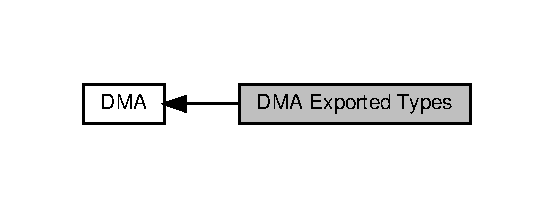
\includegraphics[width=266pt]{group___d_m_a___exported___types}
\end{center}
\end{figure}
\subsection*{Komponenty}
\begin{DoxyCompactItemize}
\item 
struct \hyperlink{struct_d_m_a___init_type_def}{D\+M\+A\+\_\+\+Init\+Type\+Def}
\begin{DoxyCompactList}\small\item\em D\+MA Configuration Structure definition. \end{DoxyCompactList}\item 
struct \hyperlink{struct_____d_m_a___handle_type_def}{\+\_\+\+\_\+\+D\+M\+A\+\_\+\+Handle\+Type\+Def}
\begin{DoxyCompactList}\small\item\em D\+MA handle Structure definition. \end{DoxyCompactList}\end{DoxyCompactItemize}
\subsection*{Definicje typów}
\begin{DoxyCompactItemize}
\item 
typedef struct \hyperlink{struct_____d_m_a___handle_type_def}{\+\_\+\+\_\+\+D\+M\+A\+\_\+\+Handle\+Type\+Def} \hyperlink{group___d_m_a___exported___types_ga41b754a906b86bce54dc79938970138b}{D\+M\+A\+\_\+\+Handle\+Type\+Def}
\begin{DoxyCompactList}\small\item\em D\+MA handle Structure definition. \end{DoxyCompactList}\end{DoxyCompactItemize}
\subsection*{Wyliczenia}
\begin{DoxyCompactItemize}
\item 
enum \hyperlink{group___d_m_a___exported___types_ga9c012af359987a240826f29073bbe463}{H\+A\+L\+\_\+\+D\+M\+A\+\_\+\+State\+Type\+Def} \{ \newline
\hyperlink{group___d_m_a___exported___types_gga9c012af359987a240826f29073bbe463a9e7be73da32b8c837cde0318e0d5eed2}{H\+A\+L\+\_\+\+D\+M\+A\+\_\+\+S\+T\+A\+T\+E\+\_\+\+R\+E\+S\+ET} = 0x00U, 
\hyperlink{group___d_m_a___exported___types_gga9c012af359987a240826f29073bbe463ad497944e6e72bc3ca904694b1098105a}{H\+A\+L\+\_\+\+D\+M\+A\+\_\+\+S\+T\+A\+T\+E\+\_\+\+R\+E\+A\+DY} = 0x01U, 
\hyperlink{group___d_m_a___exported___types_gga9c012af359987a240826f29073bbe463af7a0a2ca8de4e5be9e85b6a9073476ef}{H\+A\+L\+\_\+\+D\+M\+A\+\_\+\+S\+T\+A\+T\+E\+\_\+\+B\+U\+SY} = 0x02U, 
\hyperlink{group___d_m_a___exported___types_gga9c012af359987a240826f29073bbe463acf3a5443bf4dc71018512a255e2076eb}{H\+A\+L\+\_\+\+D\+M\+A\+\_\+\+S\+T\+A\+T\+E\+\_\+\+T\+I\+M\+E\+O\+UT} = 0x03U, 
\newline
\hyperlink{group___d_m_a___exported___types_gga9c012af359987a240826f29073bbe463ac2ce65c7cb2410c143b14e309ba83742}{H\+A\+L\+\_\+\+D\+M\+A\+\_\+\+S\+T\+A\+T\+E\+\_\+\+E\+R\+R\+OR} = 0x04U, 
\hyperlink{group___d_m_a___exported___types_gga9c012af359987a240826f29073bbe463af199cdb868cfd96fa97decb285643755}{H\+A\+L\+\_\+\+D\+M\+A\+\_\+\+S\+T\+A\+T\+E\+\_\+\+A\+B\+O\+RT} = 0x05U
 \}\begin{DoxyCompactList}\small\item\em H\+AL D\+MA State structures definition. \end{DoxyCompactList}
\item 
enum \hyperlink{group___d_m_a___exported___types_gaee3245eea8fa938edeb35a6c9596fd86}{H\+A\+L\+\_\+\+D\+M\+A\+\_\+\+Level\+Complete\+Type\+Def} \{ \hyperlink{group___d_m_a___exported___types_ggaee3245eea8fa938edeb35a6c9596fd86a5314147c8ba21548763bf89446b78468}{H\+A\+L\+\_\+\+D\+M\+A\+\_\+\+F\+U\+L\+L\+\_\+\+T\+R\+A\+N\+S\+F\+ER} = 0x00U, 
\hyperlink{group___d_m_a___exported___types_ggaee3245eea8fa938edeb35a6c9596fd86ad0ba8bc74a2ae6dcdc3e316e8be0d5d8}{H\+A\+L\+\_\+\+D\+M\+A\+\_\+\+H\+A\+L\+F\+\_\+\+T\+R\+A\+N\+S\+F\+ER} = 0x01U
 \}\begin{DoxyCompactList}\small\item\em H\+AL D\+MA Error Code structure definition. \end{DoxyCompactList}
\item 
enum \hyperlink{group___d_m_a___exported___types_gafbe8b2bd9ce2128de6cdc08ccde7e8ad}{H\+A\+L\+\_\+\+D\+M\+A\+\_\+\+Callback\+I\+D\+Type\+Def} \{ \newline
\hyperlink{group___d_m_a___exported___types_ggafbe8b2bd9ce2128de6cdc08ccde7e8ada7d4463d9db2e6d15282128b44ae08e12}{H\+A\+L\+\_\+\+D\+M\+A\+\_\+\+X\+F\+E\+R\+\_\+\+C\+P\+L\+T\+\_\+\+C\+B\+\_\+\+ID} = 0x00U, 
\hyperlink{group___d_m_a___exported___types_ggafbe8b2bd9ce2128de6cdc08ccde7e8ada4b1606f39a4eec41d958bc878719f046}{H\+A\+L\+\_\+\+D\+M\+A\+\_\+\+X\+F\+E\+R\+\_\+\+H\+A\+L\+F\+C\+P\+L\+T\+\_\+\+C\+B\+\_\+\+ID} = 0x01U, 
\hyperlink{group___d_m_a___exported___types_ggafbe8b2bd9ce2128de6cdc08ccde7e8ada09feb1bab1c32b35afd27b9316958051}{H\+A\+L\+\_\+\+D\+M\+A\+\_\+\+X\+F\+E\+R\+\_\+\+M1\+C\+P\+L\+T\+\_\+\+C\+B\+\_\+\+ID} = 0x02U, 
\hyperlink{group___d_m_a___exported___types_ggafbe8b2bd9ce2128de6cdc08ccde7e8adac2e68a660d9830fa1e965482b9befbb9}{H\+A\+L\+\_\+\+D\+M\+A\+\_\+\+X\+F\+E\+R\+\_\+\+M1\+H\+A\+L\+F\+C\+P\+L\+T\+\_\+\+C\+B\+\_\+\+ID} = 0x03U, 
\newline
\hyperlink{group___d_m_a___exported___types_ggafbe8b2bd9ce2128de6cdc08ccde7e8ada3e76bc89154e0b50333cc551bf0337a6}{H\+A\+L\+\_\+\+D\+M\+A\+\_\+\+X\+F\+E\+R\+\_\+\+E\+R\+R\+O\+R\+\_\+\+C\+B\+\_\+\+ID} = 0x04U, 
\hyperlink{group___d_m_a___exported___types_ggafbe8b2bd9ce2128de6cdc08ccde7e8ada3059a9412e0624699e9123ba2bccdf3e}{H\+A\+L\+\_\+\+D\+M\+A\+\_\+\+X\+F\+E\+R\+\_\+\+A\+B\+O\+R\+T\+\_\+\+C\+B\+\_\+\+ID} = 0x05U, 
\hyperlink{group___d_m_a___exported___types_ggafbe8b2bd9ce2128de6cdc08ccde7e8adac9935fd906719942d6b09cfd55e837f0}{H\+A\+L\+\_\+\+D\+M\+A\+\_\+\+X\+F\+E\+R\+\_\+\+A\+L\+L\+\_\+\+C\+B\+\_\+\+ID} = 0x06U
 \}\begin{DoxyCompactList}\small\item\em H\+AL D\+MA Error Code structure definition. \end{DoxyCompactList}
\end{DoxyCompactItemize}


\subsection{Opis szczegółowy}
D\+MA Exported Types. 



\subsection{Dokumentacja definicji typów}
\mbox{\Hypertarget{group___d_m_a___exported___types_ga41b754a906b86bce54dc79938970138b}\label{group___d_m_a___exported___types_ga41b754a906b86bce54dc79938970138b}} 
\index{D\+M\+A Exported Types@{D\+M\+A Exported Types}!D\+M\+A\+\_\+\+Handle\+Type\+Def@{D\+M\+A\+\_\+\+Handle\+Type\+Def}}
\index{D\+M\+A\+\_\+\+Handle\+Type\+Def@{D\+M\+A\+\_\+\+Handle\+Type\+Def}!D\+M\+A Exported Types@{D\+M\+A Exported Types}}
\subsubsection{\texorpdfstring{D\+M\+A\+\_\+\+Handle\+Type\+Def}{DMA\_HandleTypeDef}}
{\footnotesize\ttfamily typedef struct \hyperlink{struct_____d_m_a___handle_type_def}{\+\_\+\+\_\+\+D\+M\+A\+\_\+\+Handle\+Type\+Def} \hyperlink{group___d_m_a___exported___types_ga41b754a906b86bce54dc79938970138b}{D\+M\+A\+\_\+\+Handle\+Type\+Def}}



D\+MA handle Structure definition. 



\subsection{Dokumentacja typów wyliczanych}
\mbox{\Hypertarget{group___d_m_a___exported___types_gafbe8b2bd9ce2128de6cdc08ccde7e8ad}\label{group___d_m_a___exported___types_gafbe8b2bd9ce2128de6cdc08ccde7e8ad}} 
\index{D\+M\+A Exported Types@{D\+M\+A Exported Types}!H\+A\+L\+\_\+\+D\+M\+A\+\_\+\+Callback\+I\+D\+Type\+Def@{H\+A\+L\+\_\+\+D\+M\+A\+\_\+\+Callback\+I\+D\+Type\+Def}}
\index{H\+A\+L\+\_\+\+D\+M\+A\+\_\+\+Callback\+I\+D\+Type\+Def@{H\+A\+L\+\_\+\+D\+M\+A\+\_\+\+Callback\+I\+D\+Type\+Def}!D\+M\+A Exported Types@{D\+M\+A Exported Types}}
\subsubsection{\texorpdfstring{H\+A\+L\+\_\+\+D\+M\+A\+\_\+\+Callback\+I\+D\+Type\+Def}{HAL\_DMA\_CallbackIDTypeDef}}
{\footnotesize\ttfamily enum \hyperlink{group___d_m_a___exported___types_gafbe8b2bd9ce2128de6cdc08ccde7e8ad}{H\+A\+L\+\_\+\+D\+M\+A\+\_\+\+Callback\+I\+D\+Type\+Def}}



H\+AL D\+MA Error Code structure definition. 

\begin{DoxyEnumFields}{Wartości wyliczeń}
\raisebox{\heightof{T}}[0pt][0pt]{\index{H\+A\+L\+\_\+\+D\+M\+A\+\_\+\+X\+F\+E\+R\+\_\+\+C\+P\+L\+T\+\_\+\+C\+B\+\_\+\+ID@{H\+A\+L\+\_\+\+D\+M\+A\+\_\+\+X\+F\+E\+R\+\_\+\+C\+P\+L\+T\+\_\+\+C\+B\+\_\+\+ID}!D\+M\+A Exported Types@{D\+M\+A Exported Types}}\index{D\+M\+A Exported Types@{D\+M\+A Exported Types}!H\+A\+L\+\_\+\+D\+M\+A\+\_\+\+X\+F\+E\+R\+\_\+\+C\+P\+L\+T\+\_\+\+C\+B\+\_\+\+ID@{H\+A\+L\+\_\+\+D\+M\+A\+\_\+\+X\+F\+E\+R\+\_\+\+C\+P\+L\+T\+\_\+\+C\+B\+\_\+\+ID}}}\mbox{\Hypertarget{group___d_m_a___exported___types_ggafbe8b2bd9ce2128de6cdc08ccde7e8ada7d4463d9db2e6d15282128b44ae08e12}\label{group___d_m_a___exported___types_ggafbe8b2bd9ce2128de6cdc08ccde7e8ada7d4463d9db2e6d15282128b44ae08e12}} 
H\+A\+L\+\_\+\+D\+M\+A\+\_\+\+X\+F\+E\+R\+\_\+\+C\+P\+L\+T\+\_\+\+C\+B\+\_\+\+ID&Full transfer \\
\hline

\raisebox{\heightof{T}}[0pt][0pt]{\index{H\+A\+L\+\_\+\+D\+M\+A\+\_\+\+X\+F\+E\+R\+\_\+\+H\+A\+L\+F\+C\+P\+L\+T\+\_\+\+C\+B\+\_\+\+ID@{H\+A\+L\+\_\+\+D\+M\+A\+\_\+\+X\+F\+E\+R\+\_\+\+H\+A\+L\+F\+C\+P\+L\+T\+\_\+\+C\+B\+\_\+\+ID}!D\+M\+A Exported Types@{D\+M\+A Exported Types}}\index{D\+M\+A Exported Types@{D\+M\+A Exported Types}!H\+A\+L\+\_\+\+D\+M\+A\+\_\+\+X\+F\+E\+R\+\_\+\+H\+A\+L\+F\+C\+P\+L\+T\+\_\+\+C\+B\+\_\+\+ID@{H\+A\+L\+\_\+\+D\+M\+A\+\_\+\+X\+F\+E\+R\+\_\+\+H\+A\+L\+F\+C\+P\+L\+T\+\_\+\+C\+B\+\_\+\+ID}}}\mbox{\Hypertarget{group___d_m_a___exported___types_ggafbe8b2bd9ce2128de6cdc08ccde7e8ada4b1606f39a4eec41d958bc878719f046}\label{group___d_m_a___exported___types_ggafbe8b2bd9ce2128de6cdc08ccde7e8ada4b1606f39a4eec41d958bc878719f046}} 
H\+A\+L\+\_\+\+D\+M\+A\+\_\+\+X\+F\+E\+R\+\_\+\+H\+A\+L\+F\+C\+P\+L\+T\+\_\+\+C\+B\+\_\+\+ID&Half Transfer \\
\hline

\raisebox{\heightof{T}}[0pt][0pt]{\index{H\+A\+L\+\_\+\+D\+M\+A\+\_\+\+X\+F\+E\+R\+\_\+\+M1\+C\+P\+L\+T\+\_\+\+C\+B\+\_\+\+ID@{H\+A\+L\+\_\+\+D\+M\+A\+\_\+\+X\+F\+E\+R\+\_\+\+M1\+C\+P\+L\+T\+\_\+\+C\+B\+\_\+\+ID}!D\+M\+A Exported Types@{D\+M\+A Exported Types}}\index{D\+M\+A Exported Types@{D\+M\+A Exported Types}!H\+A\+L\+\_\+\+D\+M\+A\+\_\+\+X\+F\+E\+R\+\_\+\+M1\+C\+P\+L\+T\+\_\+\+C\+B\+\_\+\+ID@{H\+A\+L\+\_\+\+D\+M\+A\+\_\+\+X\+F\+E\+R\+\_\+\+M1\+C\+P\+L\+T\+\_\+\+C\+B\+\_\+\+ID}}}\mbox{\Hypertarget{group___d_m_a___exported___types_ggafbe8b2bd9ce2128de6cdc08ccde7e8ada09feb1bab1c32b35afd27b9316958051}\label{group___d_m_a___exported___types_ggafbe8b2bd9ce2128de6cdc08ccde7e8ada09feb1bab1c32b35afd27b9316958051}} 
H\+A\+L\+\_\+\+D\+M\+A\+\_\+\+X\+F\+E\+R\+\_\+\+M1\+C\+P\+L\+T\+\_\+\+C\+B\+\_\+\+ID&M1 Full Transfer \\
\hline

\raisebox{\heightof{T}}[0pt][0pt]{\index{H\+A\+L\+\_\+\+D\+M\+A\+\_\+\+X\+F\+E\+R\+\_\+\+M1\+H\+A\+L\+F\+C\+P\+L\+T\+\_\+\+C\+B\+\_\+\+ID@{H\+A\+L\+\_\+\+D\+M\+A\+\_\+\+X\+F\+E\+R\+\_\+\+M1\+H\+A\+L\+F\+C\+P\+L\+T\+\_\+\+C\+B\+\_\+\+ID}!D\+M\+A Exported Types@{D\+M\+A Exported Types}}\index{D\+M\+A Exported Types@{D\+M\+A Exported Types}!H\+A\+L\+\_\+\+D\+M\+A\+\_\+\+X\+F\+E\+R\+\_\+\+M1\+H\+A\+L\+F\+C\+P\+L\+T\+\_\+\+C\+B\+\_\+\+ID@{H\+A\+L\+\_\+\+D\+M\+A\+\_\+\+X\+F\+E\+R\+\_\+\+M1\+H\+A\+L\+F\+C\+P\+L\+T\+\_\+\+C\+B\+\_\+\+ID}}}\mbox{\Hypertarget{group___d_m_a___exported___types_ggafbe8b2bd9ce2128de6cdc08ccde7e8adac2e68a660d9830fa1e965482b9befbb9}\label{group___d_m_a___exported___types_ggafbe8b2bd9ce2128de6cdc08ccde7e8adac2e68a660d9830fa1e965482b9befbb9}} 
H\+A\+L\+\_\+\+D\+M\+A\+\_\+\+X\+F\+E\+R\+\_\+\+M1\+H\+A\+L\+F\+C\+P\+L\+T\+\_\+\+C\+B\+\_\+\+ID&M1 Half Transfer \\
\hline

\raisebox{\heightof{T}}[0pt][0pt]{\index{H\+A\+L\+\_\+\+D\+M\+A\+\_\+\+X\+F\+E\+R\+\_\+\+E\+R\+R\+O\+R\+\_\+\+C\+B\+\_\+\+ID@{H\+A\+L\+\_\+\+D\+M\+A\+\_\+\+X\+F\+E\+R\+\_\+\+E\+R\+R\+O\+R\+\_\+\+C\+B\+\_\+\+ID}!D\+M\+A Exported Types@{D\+M\+A Exported Types}}\index{D\+M\+A Exported Types@{D\+M\+A Exported Types}!H\+A\+L\+\_\+\+D\+M\+A\+\_\+\+X\+F\+E\+R\+\_\+\+E\+R\+R\+O\+R\+\_\+\+C\+B\+\_\+\+ID@{H\+A\+L\+\_\+\+D\+M\+A\+\_\+\+X\+F\+E\+R\+\_\+\+E\+R\+R\+O\+R\+\_\+\+C\+B\+\_\+\+ID}}}\mbox{\Hypertarget{group___d_m_a___exported___types_ggafbe8b2bd9ce2128de6cdc08ccde7e8ada3e76bc89154e0b50333cc551bf0337a6}\label{group___d_m_a___exported___types_ggafbe8b2bd9ce2128de6cdc08ccde7e8ada3e76bc89154e0b50333cc551bf0337a6}} 
H\+A\+L\+\_\+\+D\+M\+A\+\_\+\+X\+F\+E\+R\+\_\+\+E\+R\+R\+O\+R\+\_\+\+C\+B\+\_\+\+ID&Error \\
\hline

\raisebox{\heightof{T}}[0pt][0pt]{\index{H\+A\+L\+\_\+\+D\+M\+A\+\_\+\+X\+F\+E\+R\+\_\+\+A\+B\+O\+R\+T\+\_\+\+C\+B\+\_\+\+ID@{H\+A\+L\+\_\+\+D\+M\+A\+\_\+\+X\+F\+E\+R\+\_\+\+A\+B\+O\+R\+T\+\_\+\+C\+B\+\_\+\+ID}!D\+M\+A Exported Types@{D\+M\+A Exported Types}}\index{D\+M\+A Exported Types@{D\+M\+A Exported Types}!H\+A\+L\+\_\+\+D\+M\+A\+\_\+\+X\+F\+E\+R\+\_\+\+A\+B\+O\+R\+T\+\_\+\+C\+B\+\_\+\+ID@{H\+A\+L\+\_\+\+D\+M\+A\+\_\+\+X\+F\+E\+R\+\_\+\+A\+B\+O\+R\+T\+\_\+\+C\+B\+\_\+\+ID}}}\mbox{\Hypertarget{group___d_m_a___exported___types_ggafbe8b2bd9ce2128de6cdc08ccde7e8ada3059a9412e0624699e9123ba2bccdf3e}\label{group___d_m_a___exported___types_ggafbe8b2bd9ce2128de6cdc08ccde7e8ada3059a9412e0624699e9123ba2bccdf3e}} 
H\+A\+L\+\_\+\+D\+M\+A\+\_\+\+X\+F\+E\+R\+\_\+\+A\+B\+O\+R\+T\+\_\+\+C\+B\+\_\+\+ID&Abort \\
\hline

\raisebox{\heightof{T}}[0pt][0pt]{\index{H\+A\+L\+\_\+\+D\+M\+A\+\_\+\+X\+F\+E\+R\+\_\+\+A\+L\+L\+\_\+\+C\+B\+\_\+\+ID@{H\+A\+L\+\_\+\+D\+M\+A\+\_\+\+X\+F\+E\+R\+\_\+\+A\+L\+L\+\_\+\+C\+B\+\_\+\+ID}!D\+M\+A Exported Types@{D\+M\+A Exported Types}}\index{D\+M\+A Exported Types@{D\+M\+A Exported Types}!H\+A\+L\+\_\+\+D\+M\+A\+\_\+\+X\+F\+E\+R\+\_\+\+A\+L\+L\+\_\+\+C\+B\+\_\+\+ID@{H\+A\+L\+\_\+\+D\+M\+A\+\_\+\+X\+F\+E\+R\+\_\+\+A\+L\+L\+\_\+\+C\+B\+\_\+\+ID}}}\mbox{\Hypertarget{group___d_m_a___exported___types_ggafbe8b2bd9ce2128de6cdc08ccde7e8adac9935fd906719942d6b09cfd55e837f0}\label{group___d_m_a___exported___types_ggafbe8b2bd9ce2128de6cdc08ccde7e8adac9935fd906719942d6b09cfd55e837f0}} 
H\+A\+L\+\_\+\+D\+M\+A\+\_\+\+X\+F\+E\+R\+\_\+\+A\+L\+L\+\_\+\+C\+B\+\_\+\+ID&All \\
\hline

\end{DoxyEnumFields}


Definicja w linii 125 pliku stm32f4xx\+\_\+hal\+\_\+dma.\+h.

\mbox{\Hypertarget{group___d_m_a___exported___types_gaee3245eea8fa938edeb35a6c9596fd86}\label{group___d_m_a___exported___types_gaee3245eea8fa938edeb35a6c9596fd86}} 
\index{D\+M\+A Exported Types@{D\+M\+A Exported Types}!H\+A\+L\+\_\+\+D\+M\+A\+\_\+\+Level\+Complete\+Type\+Def@{H\+A\+L\+\_\+\+D\+M\+A\+\_\+\+Level\+Complete\+Type\+Def}}
\index{H\+A\+L\+\_\+\+D\+M\+A\+\_\+\+Level\+Complete\+Type\+Def@{H\+A\+L\+\_\+\+D\+M\+A\+\_\+\+Level\+Complete\+Type\+Def}!D\+M\+A Exported Types@{D\+M\+A Exported Types}}
\subsubsection{\texorpdfstring{H\+A\+L\+\_\+\+D\+M\+A\+\_\+\+Level\+Complete\+Type\+Def}{HAL\_DMA\_LevelCompleteTypeDef}}
{\footnotesize\ttfamily enum \hyperlink{group___d_m_a___exported___types_gaee3245eea8fa938edeb35a6c9596fd86}{H\+A\+L\+\_\+\+D\+M\+A\+\_\+\+Level\+Complete\+Type\+Def}}



H\+AL D\+MA Error Code structure definition. 

\begin{DoxyEnumFields}{Wartości wyliczeń}
\raisebox{\heightof{T}}[0pt][0pt]{\index{H\+A\+L\+\_\+\+D\+M\+A\+\_\+\+F\+U\+L\+L\+\_\+\+T\+R\+A\+N\+S\+F\+ER@{H\+A\+L\+\_\+\+D\+M\+A\+\_\+\+F\+U\+L\+L\+\_\+\+T\+R\+A\+N\+S\+F\+ER}!D\+M\+A Exported Types@{D\+M\+A Exported Types}}\index{D\+M\+A Exported Types@{D\+M\+A Exported Types}!H\+A\+L\+\_\+\+D\+M\+A\+\_\+\+F\+U\+L\+L\+\_\+\+T\+R\+A\+N\+S\+F\+ER@{H\+A\+L\+\_\+\+D\+M\+A\+\_\+\+F\+U\+L\+L\+\_\+\+T\+R\+A\+N\+S\+F\+ER}}}\mbox{\Hypertarget{group___d_m_a___exported___types_ggaee3245eea8fa938edeb35a6c9596fd86a5314147c8ba21548763bf89446b78468}\label{group___d_m_a___exported___types_ggaee3245eea8fa938edeb35a6c9596fd86a5314147c8ba21548763bf89446b78468}} 
H\+A\+L\+\_\+\+D\+M\+A\+\_\+\+F\+U\+L\+L\+\_\+\+T\+R\+A\+N\+S\+F\+ER&Full transfer \\
\hline

\raisebox{\heightof{T}}[0pt][0pt]{\index{H\+A\+L\+\_\+\+D\+M\+A\+\_\+\+H\+A\+L\+F\+\_\+\+T\+R\+A\+N\+S\+F\+ER@{H\+A\+L\+\_\+\+D\+M\+A\+\_\+\+H\+A\+L\+F\+\_\+\+T\+R\+A\+N\+S\+F\+ER}!D\+M\+A Exported Types@{D\+M\+A Exported Types}}\index{D\+M\+A Exported Types@{D\+M\+A Exported Types}!H\+A\+L\+\_\+\+D\+M\+A\+\_\+\+H\+A\+L\+F\+\_\+\+T\+R\+A\+N\+S\+F\+ER@{H\+A\+L\+\_\+\+D\+M\+A\+\_\+\+H\+A\+L\+F\+\_\+\+T\+R\+A\+N\+S\+F\+ER}}}\mbox{\Hypertarget{group___d_m_a___exported___types_ggaee3245eea8fa938edeb35a6c9596fd86ad0ba8bc74a2ae6dcdc3e316e8be0d5d8}\label{group___d_m_a___exported___types_ggaee3245eea8fa938edeb35a6c9596fd86ad0ba8bc74a2ae6dcdc3e316e8be0d5d8}} 
H\+A\+L\+\_\+\+D\+M\+A\+\_\+\+H\+A\+L\+F\+\_\+\+T\+R\+A\+N\+S\+F\+ER&Half Transfer \\
\hline

\end{DoxyEnumFields}


Definicja w linii 116 pliku stm32f4xx\+\_\+hal\+\_\+dma.\+h.

\mbox{\Hypertarget{group___d_m_a___exported___types_ga9c012af359987a240826f29073bbe463}\label{group___d_m_a___exported___types_ga9c012af359987a240826f29073bbe463}} 
\index{D\+M\+A Exported Types@{D\+M\+A Exported Types}!H\+A\+L\+\_\+\+D\+M\+A\+\_\+\+State\+Type\+Def@{H\+A\+L\+\_\+\+D\+M\+A\+\_\+\+State\+Type\+Def}}
\index{H\+A\+L\+\_\+\+D\+M\+A\+\_\+\+State\+Type\+Def@{H\+A\+L\+\_\+\+D\+M\+A\+\_\+\+State\+Type\+Def}!D\+M\+A Exported Types@{D\+M\+A Exported Types}}
\subsubsection{\texorpdfstring{H\+A\+L\+\_\+\+D\+M\+A\+\_\+\+State\+Type\+Def}{HAL\_DMA\_StateTypeDef}}
{\footnotesize\ttfamily enum \hyperlink{group___d_m_a___exported___types_ga9c012af359987a240826f29073bbe463}{H\+A\+L\+\_\+\+D\+M\+A\+\_\+\+State\+Type\+Def}}



H\+AL D\+MA State structures definition. 

\begin{DoxyEnumFields}{Wartości wyliczeń}
\raisebox{\heightof{T}}[0pt][0pt]{\index{H\+A\+L\+\_\+\+D\+M\+A\+\_\+\+S\+T\+A\+T\+E\+\_\+\+R\+E\+S\+ET@{H\+A\+L\+\_\+\+D\+M\+A\+\_\+\+S\+T\+A\+T\+E\+\_\+\+R\+E\+S\+ET}!D\+M\+A Exported Types@{D\+M\+A Exported Types}}\index{D\+M\+A Exported Types@{D\+M\+A Exported Types}!H\+A\+L\+\_\+\+D\+M\+A\+\_\+\+S\+T\+A\+T\+E\+\_\+\+R\+E\+S\+ET@{H\+A\+L\+\_\+\+D\+M\+A\+\_\+\+S\+T\+A\+T\+E\+\_\+\+R\+E\+S\+ET}}}\mbox{\Hypertarget{group___d_m_a___exported___types_gga9c012af359987a240826f29073bbe463a9e7be73da32b8c837cde0318e0d5eed2}\label{group___d_m_a___exported___types_gga9c012af359987a240826f29073bbe463a9e7be73da32b8c837cde0318e0d5eed2}} 
H\+A\+L\+\_\+\+D\+M\+A\+\_\+\+S\+T\+A\+T\+E\+\_\+\+R\+E\+S\+ET&D\+MA not yet initialized or disabled \\
\hline

\raisebox{\heightof{T}}[0pt][0pt]{\index{H\+A\+L\+\_\+\+D\+M\+A\+\_\+\+S\+T\+A\+T\+E\+\_\+\+R\+E\+A\+DY@{H\+A\+L\+\_\+\+D\+M\+A\+\_\+\+S\+T\+A\+T\+E\+\_\+\+R\+E\+A\+DY}!D\+M\+A Exported Types@{D\+M\+A Exported Types}}\index{D\+M\+A Exported Types@{D\+M\+A Exported Types}!H\+A\+L\+\_\+\+D\+M\+A\+\_\+\+S\+T\+A\+T\+E\+\_\+\+R\+E\+A\+DY@{H\+A\+L\+\_\+\+D\+M\+A\+\_\+\+S\+T\+A\+T\+E\+\_\+\+R\+E\+A\+DY}}}\mbox{\Hypertarget{group___d_m_a___exported___types_gga9c012af359987a240826f29073bbe463ad497944e6e72bc3ca904694b1098105a}\label{group___d_m_a___exported___types_gga9c012af359987a240826f29073bbe463ad497944e6e72bc3ca904694b1098105a}} 
H\+A\+L\+\_\+\+D\+M\+A\+\_\+\+S\+T\+A\+T\+E\+\_\+\+R\+E\+A\+DY&D\+MA initialized and ready for use \\
\hline

\raisebox{\heightof{T}}[0pt][0pt]{\index{H\+A\+L\+\_\+\+D\+M\+A\+\_\+\+S\+T\+A\+T\+E\+\_\+\+B\+U\+SY@{H\+A\+L\+\_\+\+D\+M\+A\+\_\+\+S\+T\+A\+T\+E\+\_\+\+B\+U\+SY}!D\+M\+A Exported Types@{D\+M\+A Exported Types}}\index{D\+M\+A Exported Types@{D\+M\+A Exported Types}!H\+A\+L\+\_\+\+D\+M\+A\+\_\+\+S\+T\+A\+T\+E\+\_\+\+B\+U\+SY@{H\+A\+L\+\_\+\+D\+M\+A\+\_\+\+S\+T\+A\+T\+E\+\_\+\+B\+U\+SY}}}\mbox{\Hypertarget{group___d_m_a___exported___types_gga9c012af359987a240826f29073bbe463af7a0a2ca8de4e5be9e85b6a9073476ef}\label{group___d_m_a___exported___types_gga9c012af359987a240826f29073bbe463af7a0a2ca8de4e5be9e85b6a9073476ef}} 
H\+A\+L\+\_\+\+D\+M\+A\+\_\+\+S\+T\+A\+T\+E\+\_\+\+B\+U\+SY&D\+MA process is ongoing \\
\hline

\raisebox{\heightof{T}}[0pt][0pt]{\index{H\+A\+L\+\_\+\+D\+M\+A\+\_\+\+S\+T\+A\+T\+E\+\_\+\+T\+I\+M\+E\+O\+UT@{H\+A\+L\+\_\+\+D\+M\+A\+\_\+\+S\+T\+A\+T\+E\+\_\+\+T\+I\+M\+E\+O\+UT}!D\+M\+A Exported Types@{D\+M\+A Exported Types}}\index{D\+M\+A Exported Types@{D\+M\+A Exported Types}!H\+A\+L\+\_\+\+D\+M\+A\+\_\+\+S\+T\+A\+T\+E\+\_\+\+T\+I\+M\+E\+O\+UT@{H\+A\+L\+\_\+\+D\+M\+A\+\_\+\+S\+T\+A\+T\+E\+\_\+\+T\+I\+M\+E\+O\+UT}}}\mbox{\Hypertarget{group___d_m_a___exported___types_gga9c012af359987a240826f29073bbe463acf3a5443bf4dc71018512a255e2076eb}\label{group___d_m_a___exported___types_gga9c012af359987a240826f29073bbe463acf3a5443bf4dc71018512a255e2076eb}} 
H\+A\+L\+\_\+\+D\+M\+A\+\_\+\+S\+T\+A\+T\+E\+\_\+\+T\+I\+M\+E\+O\+UT&D\+MA timeout state \\
\hline

\raisebox{\heightof{T}}[0pt][0pt]{\index{H\+A\+L\+\_\+\+D\+M\+A\+\_\+\+S\+T\+A\+T\+E\+\_\+\+E\+R\+R\+OR@{H\+A\+L\+\_\+\+D\+M\+A\+\_\+\+S\+T\+A\+T\+E\+\_\+\+E\+R\+R\+OR}!D\+M\+A Exported Types@{D\+M\+A Exported Types}}\index{D\+M\+A Exported Types@{D\+M\+A Exported Types}!H\+A\+L\+\_\+\+D\+M\+A\+\_\+\+S\+T\+A\+T\+E\+\_\+\+E\+R\+R\+OR@{H\+A\+L\+\_\+\+D\+M\+A\+\_\+\+S\+T\+A\+T\+E\+\_\+\+E\+R\+R\+OR}}}\mbox{\Hypertarget{group___d_m_a___exported___types_gga9c012af359987a240826f29073bbe463ac2ce65c7cb2410c143b14e309ba83742}\label{group___d_m_a___exported___types_gga9c012af359987a240826f29073bbe463ac2ce65c7cb2410c143b14e309ba83742}} 
H\+A\+L\+\_\+\+D\+M\+A\+\_\+\+S\+T\+A\+T\+E\+\_\+\+E\+R\+R\+OR&D\+MA error state \\
\hline

\raisebox{\heightof{T}}[0pt][0pt]{\index{H\+A\+L\+\_\+\+D\+M\+A\+\_\+\+S\+T\+A\+T\+E\+\_\+\+A\+B\+O\+RT@{H\+A\+L\+\_\+\+D\+M\+A\+\_\+\+S\+T\+A\+T\+E\+\_\+\+A\+B\+O\+RT}!D\+M\+A Exported Types@{D\+M\+A Exported Types}}\index{D\+M\+A Exported Types@{D\+M\+A Exported Types}!H\+A\+L\+\_\+\+D\+M\+A\+\_\+\+S\+T\+A\+T\+E\+\_\+\+A\+B\+O\+RT@{H\+A\+L\+\_\+\+D\+M\+A\+\_\+\+S\+T\+A\+T\+E\+\_\+\+A\+B\+O\+RT}}}\mbox{\Hypertarget{group___d_m_a___exported___types_gga9c012af359987a240826f29073bbe463af199cdb868cfd96fa97decb285643755}\label{group___d_m_a___exported___types_gga9c012af359987a240826f29073bbe463af199cdb868cfd96fa97decb285643755}} 
H\+A\+L\+\_\+\+D\+M\+A\+\_\+\+S\+T\+A\+T\+E\+\_\+\+A\+B\+O\+RT&D\+MA Abort state \\
\hline

\end{DoxyEnumFields}


Definicja w linii 103 pliku stm32f4xx\+\_\+hal\+\_\+dma.\+h.


\hypertarget{group___d_m_a___exported___constants}{}\section{D\+MA Exported Constants}
\label{group___d_m_a___exported___constants}\index{D\+M\+A Exported Constants@{D\+M\+A Exported Constants}}


D\+MA Exported constants.  


Diagram współpracy dla D\+MA Exported Constants\+:\nopagebreak
\begin{figure}[H]
\begin{center}
\leavevmode
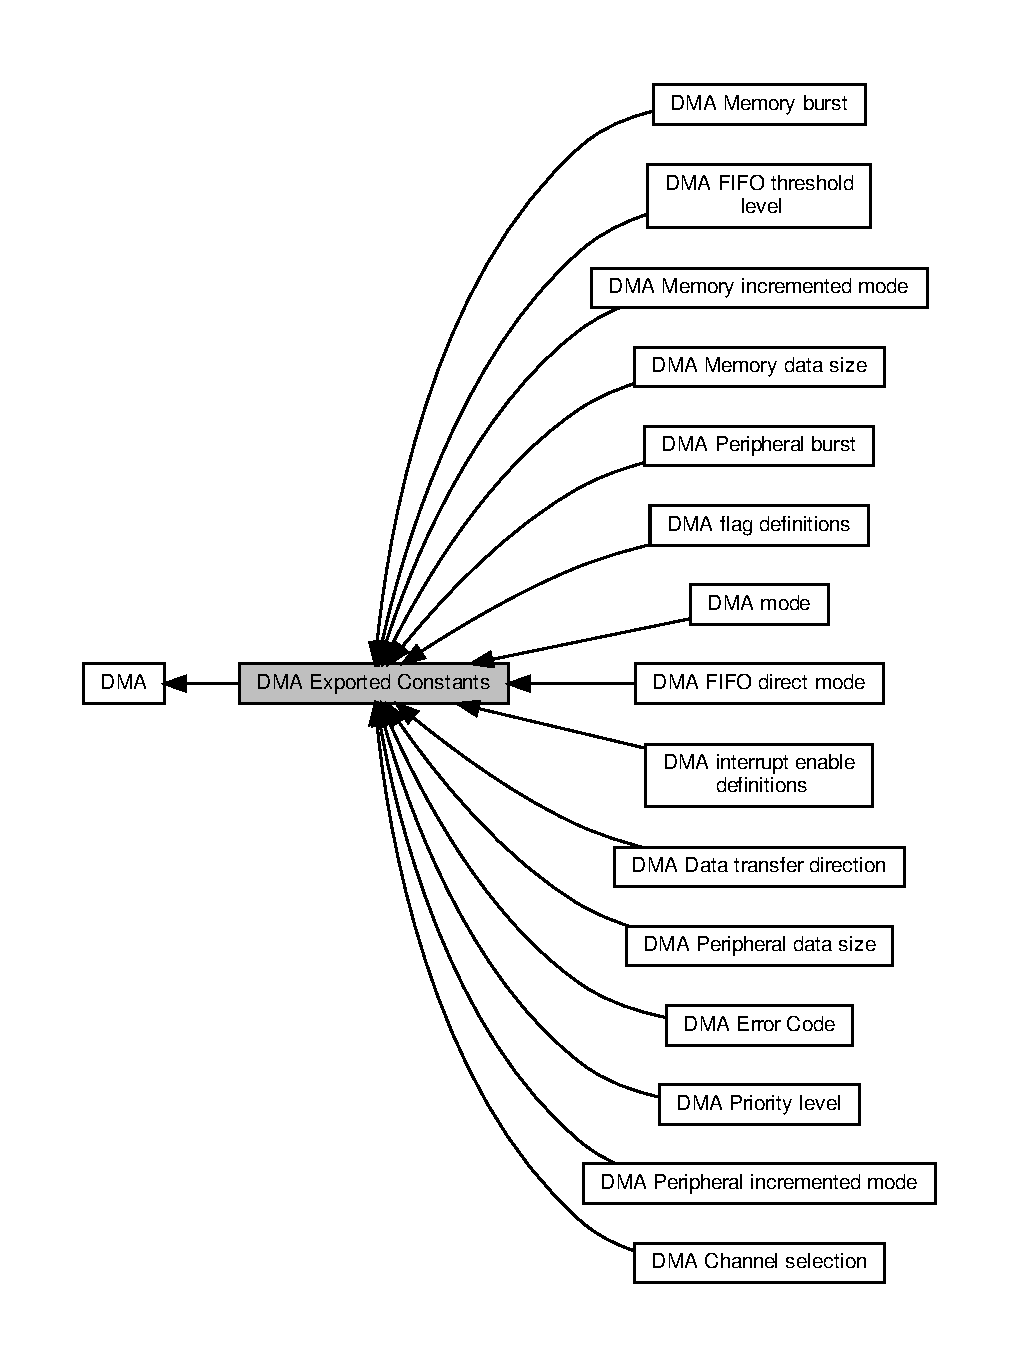
\includegraphics[width=350pt]{group___d_m_a___exported___constants}
\end{center}
\end{figure}
\subsection*{Moduły}
\begin{DoxyCompactItemize}
\item 
\hyperlink{group___d_m_a___error___code}{D\+M\+A Error Code}
\begin{DoxyCompactList}\small\item\em D\+MA Error Code. \end{DoxyCompactList}\item 
\hyperlink{group___d_m_a___channel__selection}{D\+M\+A Channel selection}
\begin{DoxyCompactList}\small\item\em D\+MA channel selection. \end{DoxyCompactList}\item 
\hyperlink{group___d_m_a___data__transfer__direction}{D\+M\+A Data transfer direction}
\begin{DoxyCompactList}\small\item\em D\+MA data transfer direction. \end{DoxyCompactList}\item 
\hyperlink{group___d_m_a___peripheral__incremented__mode}{D\+M\+A Peripheral incremented mode}
\begin{DoxyCompactList}\small\item\em D\+MA peripheral incremented mode. \end{DoxyCompactList}\item 
\hyperlink{group___d_m_a___memory__incremented__mode}{D\+M\+A Memory incremented mode}
\begin{DoxyCompactList}\small\item\em D\+MA memory incremented mode. \end{DoxyCompactList}\item 
\hyperlink{group___d_m_a___peripheral__data__size}{D\+M\+A Peripheral data size}
\begin{DoxyCompactList}\small\item\em D\+MA peripheral data size. \end{DoxyCompactList}\item 
\hyperlink{group___d_m_a___memory__data__size}{D\+M\+A Memory data size}
\begin{DoxyCompactList}\small\item\em D\+MA memory data size. \end{DoxyCompactList}\item 
\hyperlink{group___d_m_a__mode}{D\+M\+A mode}
\begin{DoxyCompactList}\small\item\em D\+MA mode. \end{DoxyCompactList}\item 
\hyperlink{group___d_m_a___priority__level}{D\+M\+A Priority level}
\begin{DoxyCompactList}\small\item\em D\+MA priority levels. \end{DoxyCompactList}\item 
\hyperlink{group___d_m_a___f_i_f_o__direct__mode}{D\+M\+A F\+I\+F\+O direct mode}
\begin{DoxyCompactList}\small\item\em D\+MA F\+I\+FO direct mode. \end{DoxyCompactList}\item 
\hyperlink{group___d_m_a___f_i_f_o__threshold__level}{D\+M\+A F\+I\+F\+O threshold level}
\begin{DoxyCompactList}\small\item\em D\+MA F\+I\+FO level. \end{DoxyCompactList}\item 
\hyperlink{group___d_m_a___memory__burst}{D\+M\+A Memory burst}
\begin{DoxyCompactList}\small\item\em D\+MA memory burst. \end{DoxyCompactList}\item 
\hyperlink{group___d_m_a___peripheral__burst}{D\+M\+A Peripheral burst}
\begin{DoxyCompactList}\small\item\em D\+MA peripheral burst. \end{DoxyCompactList}\item 
\hyperlink{group___d_m_a__interrupt__enable__definitions}{D\+M\+A interrupt enable definitions}
\begin{DoxyCompactList}\small\item\em D\+MA interrupts definition. \end{DoxyCompactList}\item 
\hyperlink{group___d_m_a__flag__definitions}{D\+M\+A flag definitions}
\begin{DoxyCompactList}\small\item\em D\+MA flag definitions. \end{DoxyCompactList}\end{DoxyCompactItemize}


\subsection{Opis szczegółowy}
D\+MA Exported constants. 


\hypertarget{group___d_m_a___error___code}{}\section{D\+MA Error Code}
\label{group___d_m_a___error___code}\index{D\+M\+A Error Code@{D\+M\+A Error Code}}


D\+MA Error Code.  


Diagram współpracy dla D\+MA Error Code\+:\nopagebreak
\begin{figure}[H]
\begin{center}
\leavevmode
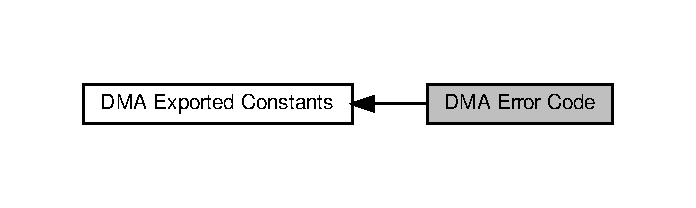
\includegraphics[width=334pt]{group___d_m_a___error___code}
\end{center}
\end{figure}
\subsection*{Definicje}
\begin{DoxyCompactItemize}
\item 
\#define \hyperlink{group___d_m_a___error___code_gaad4009390bfbe05a1bb7115d03c25a97}{H\+A\+L\+\_\+\+D\+M\+A\+\_\+\+E\+R\+R\+O\+R\+\_\+\+N\+O\+NE}~0x00000000U
\item 
\#define \hyperlink{group___d_m_a___error___code_ga9882442c5f8f0170917934bbee1cc92d}{H\+A\+L\+\_\+\+D\+M\+A\+\_\+\+E\+R\+R\+O\+R\+\_\+\+TE}~0x00000001U
\item 
\#define \hyperlink{group___d_m_a___error___code_ga019411712b9aee1d34b57d029a461fa4}{H\+A\+L\+\_\+\+D\+M\+A\+\_\+\+E\+R\+R\+O\+R\+\_\+\+FE}~0x00000002U
\item 
\#define \hyperlink{group___d_m_a___error___code_gabac48184446aea8f467483382fc6689b}{H\+A\+L\+\_\+\+D\+M\+A\+\_\+\+E\+R\+R\+O\+R\+\_\+\+D\+ME}~0x00000004U
\item 
\#define \hyperlink{group___d_m_a___error___code_ga6cf6a5b8881ff36ed4316a29bbfb5b79}{H\+A\+L\+\_\+\+D\+M\+A\+\_\+\+E\+R\+R\+O\+R\+\_\+\+T\+I\+M\+E\+O\+UT}~0x00000020U
\item 
\#define \hyperlink{group___d_m_a___error___code_ga5aaaad3b88a77147d1e3daa3a3ad9e60}{H\+A\+L\+\_\+\+D\+M\+A\+\_\+\+E\+R\+R\+O\+R\+\_\+\+P\+A\+R\+AM}~0x00000040U
\item 
\#define \hyperlink{group___d_m_a___error___code_gab7526e686427f26bf3b6af062d5a690b}{H\+A\+L\+\_\+\+D\+M\+A\+\_\+\+E\+R\+R\+O\+R\+\_\+\+N\+O\+\_\+\+X\+F\+ER}~0x00000080U
\item 
\#define \hyperlink{group___d_m_a___error___code_ga7432f31f9972e1c0a398a3f20587d118}{H\+A\+L\+\_\+\+D\+M\+A\+\_\+\+E\+R\+R\+O\+R\+\_\+\+N\+O\+T\+\_\+\+S\+U\+P\+P\+O\+R\+T\+ED}~0x00000100U
\end{DoxyCompactItemize}


\subsection{Opis szczegółowy}
D\+MA Error Code. 



\subsection{Dokumentacja definicji}
\mbox{\Hypertarget{group___d_m_a___error___code_gabac48184446aea8f467483382fc6689b}\label{group___d_m_a___error___code_gabac48184446aea8f467483382fc6689b}} 
\index{D\+M\+A Error Code@{D\+M\+A Error Code}!H\+A\+L\+\_\+\+D\+M\+A\+\_\+\+E\+R\+R\+O\+R\+\_\+\+D\+ME@{H\+A\+L\+\_\+\+D\+M\+A\+\_\+\+E\+R\+R\+O\+R\+\_\+\+D\+ME}}
\index{H\+A\+L\+\_\+\+D\+M\+A\+\_\+\+E\+R\+R\+O\+R\+\_\+\+D\+ME@{H\+A\+L\+\_\+\+D\+M\+A\+\_\+\+E\+R\+R\+O\+R\+\_\+\+D\+ME}!D\+M\+A Error Code@{D\+M\+A Error Code}}
\subsubsection{\texorpdfstring{H\+A\+L\+\_\+\+D\+M\+A\+\_\+\+E\+R\+R\+O\+R\+\_\+\+D\+ME}{HAL\_DMA\_ERROR\_DME}}
{\footnotesize\ttfamily \#define H\+A\+L\+\_\+\+D\+M\+A\+\_\+\+E\+R\+R\+O\+R\+\_\+\+D\+ME~0x00000004U}

Direct Mode error 

Definicja w linii 189 pliku stm32f4xx\+\_\+hal\+\_\+dma.\+h.

\mbox{\Hypertarget{group___d_m_a___error___code_ga019411712b9aee1d34b57d029a461fa4}\label{group___d_m_a___error___code_ga019411712b9aee1d34b57d029a461fa4}} 
\index{D\+M\+A Error Code@{D\+M\+A Error Code}!H\+A\+L\+\_\+\+D\+M\+A\+\_\+\+E\+R\+R\+O\+R\+\_\+\+FE@{H\+A\+L\+\_\+\+D\+M\+A\+\_\+\+E\+R\+R\+O\+R\+\_\+\+FE}}
\index{H\+A\+L\+\_\+\+D\+M\+A\+\_\+\+E\+R\+R\+O\+R\+\_\+\+FE@{H\+A\+L\+\_\+\+D\+M\+A\+\_\+\+E\+R\+R\+O\+R\+\_\+\+FE}!D\+M\+A Error Code@{D\+M\+A Error Code}}
\subsubsection{\texorpdfstring{H\+A\+L\+\_\+\+D\+M\+A\+\_\+\+E\+R\+R\+O\+R\+\_\+\+FE}{HAL\_DMA\_ERROR\_FE}}
{\footnotesize\ttfamily \#define H\+A\+L\+\_\+\+D\+M\+A\+\_\+\+E\+R\+R\+O\+R\+\_\+\+FE~0x00000002U}

F\+I\+FO error 

Definicja w linii 188 pliku stm32f4xx\+\_\+hal\+\_\+dma.\+h.

\mbox{\Hypertarget{group___d_m_a___error___code_gab7526e686427f26bf3b6af062d5a690b}\label{group___d_m_a___error___code_gab7526e686427f26bf3b6af062d5a690b}} 
\index{D\+M\+A Error Code@{D\+M\+A Error Code}!H\+A\+L\+\_\+\+D\+M\+A\+\_\+\+E\+R\+R\+O\+R\+\_\+\+N\+O\+\_\+\+X\+F\+ER@{H\+A\+L\+\_\+\+D\+M\+A\+\_\+\+E\+R\+R\+O\+R\+\_\+\+N\+O\+\_\+\+X\+F\+ER}}
\index{H\+A\+L\+\_\+\+D\+M\+A\+\_\+\+E\+R\+R\+O\+R\+\_\+\+N\+O\+\_\+\+X\+F\+ER@{H\+A\+L\+\_\+\+D\+M\+A\+\_\+\+E\+R\+R\+O\+R\+\_\+\+N\+O\+\_\+\+X\+F\+ER}!D\+M\+A Error Code@{D\+M\+A Error Code}}
\subsubsection{\texorpdfstring{H\+A\+L\+\_\+\+D\+M\+A\+\_\+\+E\+R\+R\+O\+R\+\_\+\+N\+O\+\_\+\+X\+F\+ER}{HAL\_DMA\_ERROR\_NO\_XFER}}
{\footnotesize\ttfamily \#define H\+A\+L\+\_\+\+D\+M\+A\+\_\+\+E\+R\+R\+O\+R\+\_\+\+N\+O\+\_\+\+X\+F\+ER~0x00000080U}

Abort requested with no Xfer ongoing 

Definicja w linii 192 pliku stm32f4xx\+\_\+hal\+\_\+dma.\+h.

\mbox{\Hypertarget{group___d_m_a___error___code_gaad4009390bfbe05a1bb7115d03c25a97}\label{group___d_m_a___error___code_gaad4009390bfbe05a1bb7115d03c25a97}} 
\index{D\+M\+A Error Code@{D\+M\+A Error Code}!H\+A\+L\+\_\+\+D\+M\+A\+\_\+\+E\+R\+R\+O\+R\+\_\+\+N\+O\+NE@{H\+A\+L\+\_\+\+D\+M\+A\+\_\+\+E\+R\+R\+O\+R\+\_\+\+N\+O\+NE}}
\index{H\+A\+L\+\_\+\+D\+M\+A\+\_\+\+E\+R\+R\+O\+R\+\_\+\+N\+O\+NE@{H\+A\+L\+\_\+\+D\+M\+A\+\_\+\+E\+R\+R\+O\+R\+\_\+\+N\+O\+NE}!D\+M\+A Error Code@{D\+M\+A Error Code}}
\subsubsection{\texorpdfstring{H\+A\+L\+\_\+\+D\+M\+A\+\_\+\+E\+R\+R\+O\+R\+\_\+\+N\+O\+NE}{HAL\_DMA\_ERROR\_NONE}}
{\footnotesize\ttfamily \#define H\+A\+L\+\_\+\+D\+M\+A\+\_\+\+E\+R\+R\+O\+R\+\_\+\+N\+O\+NE~0x00000000U}

No error 

Definicja w linii 186 pliku stm32f4xx\+\_\+hal\+\_\+dma.\+h.

\mbox{\Hypertarget{group___d_m_a___error___code_ga7432f31f9972e1c0a398a3f20587d118}\label{group___d_m_a___error___code_ga7432f31f9972e1c0a398a3f20587d118}} 
\index{D\+M\+A Error Code@{D\+M\+A Error Code}!H\+A\+L\+\_\+\+D\+M\+A\+\_\+\+E\+R\+R\+O\+R\+\_\+\+N\+O\+T\+\_\+\+S\+U\+P\+P\+O\+R\+T\+ED@{H\+A\+L\+\_\+\+D\+M\+A\+\_\+\+E\+R\+R\+O\+R\+\_\+\+N\+O\+T\+\_\+\+S\+U\+P\+P\+O\+R\+T\+ED}}
\index{H\+A\+L\+\_\+\+D\+M\+A\+\_\+\+E\+R\+R\+O\+R\+\_\+\+N\+O\+T\+\_\+\+S\+U\+P\+P\+O\+R\+T\+ED@{H\+A\+L\+\_\+\+D\+M\+A\+\_\+\+E\+R\+R\+O\+R\+\_\+\+N\+O\+T\+\_\+\+S\+U\+P\+P\+O\+R\+T\+ED}!D\+M\+A Error Code@{D\+M\+A Error Code}}
\subsubsection{\texorpdfstring{H\+A\+L\+\_\+\+D\+M\+A\+\_\+\+E\+R\+R\+O\+R\+\_\+\+N\+O\+T\+\_\+\+S\+U\+P\+P\+O\+R\+T\+ED}{HAL\_DMA\_ERROR\_NOT\_SUPPORTED}}
{\footnotesize\ttfamily \#define H\+A\+L\+\_\+\+D\+M\+A\+\_\+\+E\+R\+R\+O\+R\+\_\+\+N\+O\+T\+\_\+\+S\+U\+P\+P\+O\+R\+T\+ED~0x00000100U}

Not supported mode 

Definicja w linii 193 pliku stm32f4xx\+\_\+hal\+\_\+dma.\+h.

\mbox{\Hypertarget{group___d_m_a___error___code_ga5aaaad3b88a77147d1e3daa3a3ad9e60}\label{group___d_m_a___error___code_ga5aaaad3b88a77147d1e3daa3a3ad9e60}} 
\index{D\+M\+A Error Code@{D\+M\+A Error Code}!H\+A\+L\+\_\+\+D\+M\+A\+\_\+\+E\+R\+R\+O\+R\+\_\+\+P\+A\+R\+AM@{H\+A\+L\+\_\+\+D\+M\+A\+\_\+\+E\+R\+R\+O\+R\+\_\+\+P\+A\+R\+AM}}
\index{H\+A\+L\+\_\+\+D\+M\+A\+\_\+\+E\+R\+R\+O\+R\+\_\+\+P\+A\+R\+AM@{H\+A\+L\+\_\+\+D\+M\+A\+\_\+\+E\+R\+R\+O\+R\+\_\+\+P\+A\+R\+AM}!D\+M\+A Error Code@{D\+M\+A Error Code}}
\subsubsection{\texorpdfstring{H\+A\+L\+\_\+\+D\+M\+A\+\_\+\+E\+R\+R\+O\+R\+\_\+\+P\+A\+R\+AM}{HAL\_DMA\_ERROR\_PARAM}}
{\footnotesize\ttfamily \#define H\+A\+L\+\_\+\+D\+M\+A\+\_\+\+E\+R\+R\+O\+R\+\_\+\+P\+A\+R\+AM~0x00000040U}

Parameter error 

Definicja w linii 191 pliku stm32f4xx\+\_\+hal\+\_\+dma.\+h.

\mbox{\Hypertarget{group___d_m_a___error___code_ga9882442c5f8f0170917934bbee1cc92d}\label{group___d_m_a___error___code_ga9882442c5f8f0170917934bbee1cc92d}} 
\index{D\+M\+A Error Code@{D\+M\+A Error Code}!H\+A\+L\+\_\+\+D\+M\+A\+\_\+\+E\+R\+R\+O\+R\+\_\+\+TE@{H\+A\+L\+\_\+\+D\+M\+A\+\_\+\+E\+R\+R\+O\+R\+\_\+\+TE}}
\index{H\+A\+L\+\_\+\+D\+M\+A\+\_\+\+E\+R\+R\+O\+R\+\_\+\+TE@{H\+A\+L\+\_\+\+D\+M\+A\+\_\+\+E\+R\+R\+O\+R\+\_\+\+TE}!D\+M\+A Error Code@{D\+M\+A Error Code}}
\subsubsection{\texorpdfstring{H\+A\+L\+\_\+\+D\+M\+A\+\_\+\+E\+R\+R\+O\+R\+\_\+\+TE}{HAL\_DMA\_ERROR\_TE}}
{\footnotesize\ttfamily \#define H\+A\+L\+\_\+\+D\+M\+A\+\_\+\+E\+R\+R\+O\+R\+\_\+\+TE~0x00000001U}

Transfer error 

Definicja w linii 187 pliku stm32f4xx\+\_\+hal\+\_\+dma.\+h.

\mbox{\Hypertarget{group___d_m_a___error___code_ga6cf6a5b8881ff36ed4316a29bbfb5b79}\label{group___d_m_a___error___code_ga6cf6a5b8881ff36ed4316a29bbfb5b79}} 
\index{D\+M\+A Error Code@{D\+M\+A Error Code}!H\+A\+L\+\_\+\+D\+M\+A\+\_\+\+E\+R\+R\+O\+R\+\_\+\+T\+I\+M\+E\+O\+UT@{H\+A\+L\+\_\+\+D\+M\+A\+\_\+\+E\+R\+R\+O\+R\+\_\+\+T\+I\+M\+E\+O\+UT}}
\index{H\+A\+L\+\_\+\+D\+M\+A\+\_\+\+E\+R\+R\+O\+R\+\_\+\+T\+I\+M\+E\+O\+UT@{H\+A\+L\+\_\+\+D\+M\+A\+\_\+\+E\+R\+R\+O\+R\+\_\+\+T\+I\+M\+E\+O\+UT}!D\+M\+A Error Code@{D\+M\+A Error Code}}
\subsubsection{\texorpdfstring{H\+A\+L\+\_\+\+D\+M\+A\+\_\+\+E\+R\+R\+O\+R\+\_\+\+T\+I\+M\+E\+O\+UT}{HAL\_DMA\_ERROR\_TIMEOUT}}
{\footnotesize\ttfamily \#define H\+A\+L\+\_\+\+D\+M\+A\+\_\+\+E\+R\+R\+O\+R\+\_\+\+T\+I\+M\+E\+O\+UT~0x00000020U}

Timeout error 

Definicja w linii 190 pliku stm32f4xx\+\_\+hal\+\_\+dma.\+h.


\hypertarget{group___d_m_a___channel__selection}{}\section{D\+MA Channel selection}
\label{group___d_m_a___channel__selection}\index{D\+M\+A Channel selection@{D\+M\+A Channel selection}}


D\+MA channel selection.  


Diagram współpracy dla D\+MA Channel selection\+:\nopagebreak
\begin{figure}[H]
\begin{center}
\leavevmode
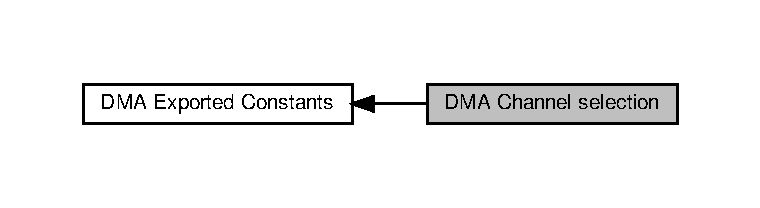
\includegraphics[width=350pt]{group___d_m_a___channel__selection}
\end{center}
\end{figure}
\subsection*{Definicje}
\begin{DoxyCompactItemize}
\item 
\#define \hyperlink{group___d_m_a___channel__selection_gabd7de138931e93a90fc6c4eab5916bbe}{D\+M\+A\+\_\+\+C\+H\+A\+N\+N\+E\+L\+\_\+0}~0x00000000U
\item 
\#define \hyperlink{group___d_m_a___channel__selection_ga283364370e9876af6406b9fa70e2944f}{D\+M\+A\+\_\+\+C\+H\+A\+N\+N\+E\+L\+\_\+1}~0x02000000U
\item 
\#define \hyperlink{group___d_m_a___channel__selection_ga9688f3e78cbc2109d214b7ca049e22df}{D\+M\+A\+\_\+\+C\+H\+A\+N\+N\+E\+L\+\_\+2}~0x04000000U
\item 
\#define \hyperlink{group___d_m_a___channel__selection_gac689673fec4d72ede49a0d657e3a7e70}{D\+M\+A\+\_\+\+C\+H\+A\+N\+N\+E\+L\+\_\+3}~0x06000000U
\item 
\#define \hyperlink{group___d_m_a___channel__selection_ga51b51f5b39e23b28ad99520ad5be596f}{D\+M\+A\+\_\+\+C\+H\+A\+N\+N\+E\+L\+\_\+4}~0x08000000U
\item 
\#define \hyperlink{group___d_m_a___channel__selection_gafbaa82f3cff89858e50363c04ed0cca0}{D\+M\+A\+\_\+\+C\+H\+A\+N\+N\+E\+L\+\_\+5}~0x0\+A000000U
\item 
\#define \hyperlink{group___d_m_a___channel__selection_gad23679661d8da3bc1aaacc62f99821f7}{D\+M\+A\+\_\+\+C\+H\+A\+N\+N\+E\+L\+\_\+6}~0x0\+C000000U
\item 
\#define \hyperlink{group___d_m_a___channel__selection_ga77ff4e8675a3991feb20e385242f34ab}{D\+M\+A\+\_\+\+C\+H\+A\+N\+N\+E\+L\+\_\+7}~0x0\+E000000U
\end{DoxyCompactItemize}


\subsection{Opis szczegółowy}
D\+MA channel selection. 



\subsection{Dokumentacja definicji}
\mbox{\Hypertarget{group___d_m_a___channel__selection_gabd7de138931e93a90fc6c4eab5916bbe}\label{group___d_m_a___channel__selection_gabd7de138931e93a90fc6c4eab5916bbe}} 
\index{D\+M\+A Channel selection@{D\+M\+A Channel selection}!D\+M\+A\+\_\+\+C\+H\+A\+N\+N\+E\+L\+\_\+0@{D\+M\+A\+\_\+\+C\+H\+A\+N\+N\+E\+L\+\_\+0}}
\index{D\+M\+A\+\_\+\+C\+H\+A\+N\+N\+E\+L\+\_\+0@{D\+M\+A\+\_\+\+C\+H\+A\+N\+N\+E\+L\+\_\+0}!D\+M\+A Channel selection@{D\+M\+A Channel selection}}
\subsubsection{\texorpdfstring{D\+M\+A\+\_\+\+C\+H\+A\+N\+N\+E\+L\+\_\+0}{DMA\_CHANNEL\_0}}
{\footnotesize\ttfamily \#define D\+M\+A\+\_\+\+C\+H\+A\+N\+N\+E\+L\+\_\+0~0x00000000U}

D\+MA Channel 0 

Definicja w linii 202 pliku stm32f4xx\+\_\+hal\+\_\+dma.\+h.

\mbox{\Hypertarget{group___d_m_a___channel__selection_ga283364370e9876af6406b9fa70e2944f}\label{group___d_m_a___channel__selection_ga283364370e9876af6406b9fa70e2944f}} 
\index{D\+M\+A Channel selection@{D\+M\+A Channel selection}!D\+M\+A\+\_\+\+C\+H\+A\+N\+N\+E\+L\+\_\+1@{D\+M\+A\+\_\+\+C\+H\+A\+N\+N\+E\+L\+\_\+1}}
\index{D\+M\+A\+\_\+\+C\+H\+A\+N\+N\+E\+L\+\_\+1@{D\+M\+A\+\_\+\+C\+H\+A\+N\+N\+E\+L\+\_\+1}!D\+M\+A Channel selection@{D\+M\+A Channel selection}}
\subsubsection{\texorpdfstring{D\+M\+A\+\_\+\+C\+H\+A\+N\+N\+E\+L\+\_\+1}{DMA\_CHANNEL\_1}}
{\footnotesize\ttfamily \#define D\+M\+A\+\_\+\+C\+H\+A\+N\+N\+E\+L\+\_\+1~0x02000000U}

D\+MA Channel 1 

Definicja w linii 203 pliku stm32f4xx\+\_\+hal\+\_\+dma.\+h.

\mbox{\Hypertarget{group___d_m_a___channel__selection_ga9688f3e78cbc2109d214b7ca049e22df}\label{group___d_m_a___channel__selection_ga9688f3e78cbc2109d214b7ca049e22df}} 
\index{D\+M\+A Channel selection@{D\+M\+A Channel selection}!D\+M\+A\+\_\+\+C\+H\+A\+N\+N\+E\+L\+\_\+2@{D\+M\+A\+\_\+\+C\+H\+A\+N\+N\+E\+L\+\_\+2}}
\index{D\+M\+A\+\_\+\+C\+H\+A\+N\+N\+E\+L\+\_\+2@{D\+M\+A\+\_\+\+C\+H\+A\+N\+N\+E\+L\+\_\+2}!D\+M\+A Channel selection@{D\+M\+A Channel selection}}
\subsubsection{\texorpdfstring{D\+M\+A\+\_\+\+C\+H\+A\+N\+N\+E\+L\+\_\+2}{DMA\_CHANNEL\_2}}
{\footnotesize\ttfamily \#define D\+M\+A\+\_\+\+C\+H\+A\+N\+N\+E\+L\+\_\+2~0x04000000U}

D\+MA Channel 2 

Definicja w linii 204 pliku stm32f4xx\+\_\+hal\+\_\+dma.\+h.

\mbox{\Hypertarget{group___d_m_a___channel__selection_gac689673fec4d72ede49a0d657e3a7e70}\label{group___d_m_a___channel__selection_gac689673fec4d72ede49a0d657e3a7e70}} 
\index{D\+M\+A Channel selection@{D\+M\+A Channel selection}!D\+M\+A\+\_\+\+C\+H\+A\+N\+N\+E\+L\+\_\+3@{D\+M\+A\+\_\+\+C\+H\+A\+N\+N\+E\+L\+\_\+3}}
\index{D\+M\+A\+\_\+\+C\+H\+A\+N\+N\+E\+L\+\_\+3@{D\+M\+A\+\_\+\+C\+H\+A\+N\+N\+E\+L\+\_\+3}!D\+M\+A Channel selection@{D\+M\+A Channel selection}}
\subsubsection{\texorpdfstring{D\+M\+A\+\_\+\+C\+H\+A\+N\+N\+E\+L\+\_\+3}{DMA\_CHANNEL\_3}}
{\footnotesize\ttfamily \#define D\+M\+A\+\_\+\+C\+H\+A\+N\+N\+E\+L\+\_\+3~0x06000000U}

D\+MA Channel 3 

Definicja w linii 205 pliku stm32f4xx\+\_\+hal\+\_\+dma.\+h.

\mbox{\Hypertarget{group___d_m_a___channel__selection_ga51b51f5b39e23b28ad99520ad5be596f}\label{group___d_m_a___channel__selection_ga51b51f5b39e23b28ad99520ad5be596f}} 
\index{D\+M\+A Channel selection@{D\+M\+A Channel selection}!D\+M\+A\+\_\+\+C\+H\+A\+N\+N\+E\+L\+\_\+4@{D\+M\+A\+\_\+\+C\+H\+A\+N\+N\+E\+L\+\_\+4}}
\index{D\+M\+A\+\_\+\+C\+H\+A\+N\+N\+E\+L\+\_\+4@{D\+M\+A\+\_\+\+C\+H\+A\+N\+N\+E\+L\+\_\+4}!D\+M\+A Channel selection@{D\+M\+A Channel selection}}
\subsubsection{\texorpdfstring{D\+M\+A\+\_\+\+C\+H\+A\+N\+N\+E\+L\+\_\+4}{DMA\_CHANNEL\_4}}
{\footnotesize\ttfamily \#define D\+M\+A\+\_\+\+C\+H\+A\+N\+N\+E\+L\+\_\+4~0x08000000U}

D\+MA Channel 4 

Definicja w linii 206 pliku stm32f4xx\+\_\+hal\+\_\+dma.\+h.

\mbox{\Hypertarget{group___d_m_a___channel__selection_gafbaa82f3cff89858e50363c04ed0cca0}\label{group___d_m_a___channel__selection_gafbaa82f3cff89858e50363c04ed0cca0}} 
\index{D\+M\+A Channel selection@{D\+M\+A Channel selection}!D\+M\+A\+\_\+\+C\+H\+A\+N\+N\+E\+L\+\_\+5@{D\+M\+A\+\_\+\+C\+H\+A\+N\+N\+E\+L\+\_\+5}}
\index{D\+M\+A\+\_\+\+C\+H\+A\+N\+N\+E\+L\+\_\+5@{D\+M\+A\+\_\+\+C\+H\+A\+N\+N\+E\+L\+\_\+5}!D\+M\+A Channel selection@{D\+M\+A Channel selection}}
\subsubsection{\texorpdfstring{D\+M\+A\+\_\+\+C\+H\+A\+N\+N\+E\+L\+\_\+5}{DMA\_CHANNEL\_5}}
{\footnotesize\ttfamily \#define D\+M\+A\+\_\+\+C\+H\+A\+N\+N\+E\+L\+\_\+5~0x0\+A000000U}

D\+MA Channel 5 

Definicja w linii 207 pliku stm32f4xx\+\_\+hal\+\_\+dma.\+h.

\mbox{\Hypertarget{group___d_m_a___channel__selection_gad23679661d8da3bc1aaacc62f99821f7}\label{group___d_m_a___channel__selection_gad23679661d8da3bc1aaacc62f99821f7}} 
\index{D\+M\+A Channel selection@{D\+M\+A Channel selection}!D\+M\+A\+\_\+\+C\+H\+A\+N\+N\+E\+L\+\_\+6@{D\+M\+A\+\_\+\+C\+H\+A\+N\+N\+E\+L\+\_\+6}}
\index{D\+M\+A\+\_\+\+C\+H\+A\+N\+N\+E\+L\+\_\+6@{D\+M\+A\+\_\+\+C\+H\+A\+N\+N\+E\+L\+\_\+6}!D\+M\+A Channel selection@{D\+M\+A Channel selection}}
\subsubsection{\texorpdfstring{D\+M\+A\+\_\+\+C\+H\+A\+N\+N\+E\+L\+\_\+6}{DMA\_CHANNEL\_6}}
{\footnotesize\ttfamily \#define D\+M\+A\+\_\+\+C\+H\+A\+N\+N\+E\+L\+\_\+6~0x0\+C000000U}

D\+MA Channel 6 

Definicja w linii 208 pliku stm32f4xx\+\_\+hal\+\_\+dma.\+h.

\mbox{\Hypertarget{group___d_m_a___channel__selection_ga77ff4e8675a3991feb20e385242f34ab}\label{group___d_m_a___channel__selection_ga77ff4e8675a3991feb20e385242f34ab}} 
\index{D\+M\+A Channel selection@{D\+M\+A Channel selection}!D\+M\+A\+\_\+\+C\+H\+A\+N\+N\+E\+L\+\_\+7@{D\+M\+A\+\_\+\+C\+H\+A\+N\+N\+E\+L\+\_\+7}}
\index{D\+M\+A\+\_\+\+C\+H\+A\+N\+N\+E\+L\+\_\+7@{D\+M\+A\+\_\+\+C\+H\+A\+N\+N\+E\+L\+\_\+7}!D\+M\+A Channel selection@{D\+M\+A Channel selection}}
\subsubsection{\texorpdfstring{D\+M\+A\+\_\+\+C\+H\+A\+N\+N\+E\+L\+\_\+7}{DMA\_CHANNEL\_7}}
{\footnotesize\ttfamily \#define D\+M\+A\+\_\+\+C\+H\+A\+N\+N\+E\+L\+\_\+7~0x0\+E000000U}

D\+MA Channel 7 

Definicja w linii 209 pliku stm32f4xx\+\_\+hal\+\_\+dma.\+h.


\hypertarget{group___d_m_a___data__transfer__direction}{}\section{D\+MA Data transfer direction}
\label{group___d_m_a___data__transfer__direction}\index{D\+M\+A Data transfer direction@{D\+M\+A Data transfer direction}}


D\+MA data transfer direction.  


Diagram współpracy dla D\+MA Data transfer direction\+:\nopagebreak
\begin{figure}[H]
\begin{center}
\leavevmode
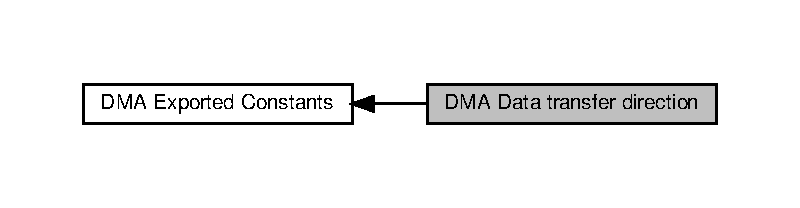
\includegraphics[width=350pt]{group___d_m_a___data__transfer__direction}
\end{center}
\end{figure}
\subsection*{Definicje}
\begin{DoxyCompactItemize}
\item 
\#define \hyperlink{group___d_m_a___data__transfer__direction_gacb2cbf03ecae6804ae4a6f60a3e37c12}{D\+M\+A\+\_\+\+P\+E\+R\+I\+P\+H\+\_\+\+T\+O\+\_\+\+M\+E\+M\+O\+RY}~0x00000000U
\item 
\#define \hyperlink{group___d_m_a___data__transfer__direction_ga9e76fc559a2d5c766c969e6e921b1ee9}{D\+M\+A\+\_\+\+M\+E\+M\+O\+R\+Y\+\_\+\+T\+O\+\_\+\+P\+E\+R\+I\+PH}~((uint32\+\_\+t)\hyperlink{group___peripheral___registers___bits___definition_gadca9547536f3d2f76577275964b4875e}{D\+M\+A\+\_\+\+Sx\+C\+R\+\_\+\+D\+I\+R\+\_\+0})
\item 
\#define \hyperlink{group___d_m_a___data__transfer__direction_ga0695035d725855ccf64d2d8452a33810}{D\+M\+A\+\_\+\+M\+E\+M\+O\+R\+Y\+\_\+\+T\+O\+\_\+\+M\+E\+M\+O\+RY}~((uint32\+\_\+t)\hyperlink{group___peripheral___registers___bits___definition_gac52c8d6ecad03bfe531867fa7457f2ae}{D\+M\+A\+\_\+\+Sx\+C\+R\+\_\+\+D\+I\+R\+\_\+1})
\end{DoxyCompactItemize}


\subsection{Opis szczegółowy}
D\+MA data transfer direction. 



\subsection{Dokumentacja definicji}
\mbox{\Hypertarget{group___d_m_a___data__transfer__direction_ga0695035d725855ccf64d2d8452a33810}\label{group___d_m_a___data__transfer__direction_ga0695035d725855ccf64d2d8452a33810}} 
\index{D\+M\+A Data transfer direction@{D\+M\+A Data transfer direction}!D\+M\+A\+\_\+\+M\+E\+M\+O\+R\+Y\+\_\+\+T\+O\+\_\+\+M\+E\+M\+O\+RY@{D\+M\+A\+\_\+\+M\+E\+M\+O\+R\+Y\+\_\+\+T\+O\+\_\+\+M\+E\+M\+O\+RY}}
\index{D\+M\+A\+\_\+\+M\+E\+M\+O\+R\+Y\+\_\+\+T\+O\+\_\+\+M\+E\+M\+O\+RY@{D\+M\+A\+\_\+\+M\+E\+M\+O\+R\+Y\+\_\+\+T\+O\+\_\+\+M\+E\+M\+O\+RY}!D\+M\+A Data transfer direction@{D\+M\+A Data transfer direction}}
\subsubsection{\texorpdfstring{D\+M\+A\+\_\+\+M\+E\+M\+O\+R\+Y\+\_\+\+T\+O\+\_\+\+M\+E\+M\+O\+RY}{DMA\_MEMORY\_TO\_MEMORY}}
{\footnotesize\ttfamily \#define D\+M\+A\+\_\+\+M\+E\+M\+O\+R\+Y\+\_\+\+T\+O\+\_\+\+M\+E\+M\+O\+RY~((uint32\+\_\+t)\hyperlink{group___peripheral___registers___bits___definition_gac52c8d6ecad03bfe531867fa7457f2ae}{D\+M\+A\+\_\+\+Sx\+C\+R\+\_\+\+D\+I\+R\+\_\+1})}

Memory to memory direction 

Definicja w linii 230 pliku stm32f4xx\+\_\+hal\+\_\+dma.\+h.

\mbox{\Hypertarget{group___d_m_a___data__transfer__direction_ga9e76fc559a2d5c766c969e6e921b1ee9}\label{group___d_m_a___data__transfer__direction_ga9e76fc559a2d5c766c969e6e921b1ee9}} 
\index{D\+M\+A Data transfer direction@{D\+M\+A Data transfer direction}!D\+M\+A\+\_\+\+M\+E\+M\+O\+R\+Y\+\_\+\+T\+O\+\_\+\+P\+E\+R\+I\+PH@{D\+M\+A\+\_\+\+M\+E\+M\+O\+R\+Y\+\_\+\+T\+O\+\_\+\+P\+E\+R\+I\+PH}}
\index{D\+M\+A\+\_\+\+M\+E\+M\+O\+R\+Y\+\_\+\+T\+O\+\_\+\+P\+E\+R\+I\+PH@{D\+M\+A\+\_\+\+M\+E\+M\+O\+R\+Y\+\_\+\+T\+O\+\_\+\+P\+E\+R\+I\+PH}!D\+M\+A Data transfer direction@{D\+M\+A Data transfer direction}}
\subsubsection{\texorpdfstring{D\+M\+A\+\_\+\+M\+E\+M\+O\+R\+Y\+\_\+\+T\+O\+\_\+\+P\+E\+R\+I\+PH}{DMA\_MEMORY\_TO\_PERIPH}}
{\footnotesize\ttfamily \#define D\+M\+A\+\_\+\+M\+E\+M\+O\+R\+Y\+\_\+\+T\+O\+\_\+\+P\+E\+R\+I\+PH~((uint32\+\_\+t)\hyperlink{group___peripheral___registers___bits___definition_gadca9547536f3d2f76577275964b4875e}{D\+M\+A\+\_\+\+Sx\+C\+R\+\_\+\+D\+I\+R\+\_\+0})}

Memory to peripheral direction 

Definicja w linii 229 pliku stm32f4xx\+\_\+hal\+\_\+dma.\+h.

\mbox{\Hypertarget{group___d_m_a___data__transfer__direction_gacb2cbf03ecae6804ae4a6f60a3e37c12}\label{group___d_m_a___data__transfer__direction_gacb2cbf03ecae6804ae4a6f60a3e37c12}} 
\index{D\+M\+A Data transfer direction@{D\+M\+A Data transfer direction}!D\+M\+A\+\_\+\+P\+E\+R\+I\+P\+H\+\_\+\+T\+O\+\_\+\+M\+E\+M\+O\+RY@{D\+M\+A\+\_\+\+P\+E\+R\+I\+P\+H\+\_\+\+T\+O\+\_\+\+M\+E\+M\+O\+RY}}
\index{D\+M\+A\+\_\+\+P\+E\+R\+I\+P\+H\+\_\+\+T\+O\+\_\+\+M\+E\+M\+O\+RY@{D\+M\+A\+\_\+\+P\+E\+R\+I\+P\+H\+\_\+\+T\+O\+\_\+\+M\+E\+M\+O\+RY}!D\+M\+A Data transfer direction@{D\+M\+A Data transfer direction}}
\subsubsection{\texorpdfstring{D\+M\+A\+\_\+\+P\+E\+R\+I\+P\+H\+\_\+\+T\+O\+\_\+\+M\+E\+M\+O\+RY}{DMA\_PERIPH\_TO\_MEMORY}}
{\footnotesize\ttfamily \#define D\+M\+A\+\_\+\+P\+E\+R\+I\+P\+H\+\_\+\+T\+O\+\_\+\+M\+E\+M\+O\+RY~0x00000000U}

Peripheral to memory direction 

Definicja w linii 228 pliku stm32f4xx\+\_\+hal\+\_\+dma.\+h.


\hypertarget{group___d_m_a___peripheral__incremented__mode}{}\section{D\+MA Peripheral incremented mode}
\label{group___d_m_a___peripheral__incremented__mode}\index{D\+M\+A Peripheral incremented mode@{D\+M\+A Peripheral incremented mode}}


D\+MA peripheral incremented mode.  


Diagram współpracy dla D\+MA Peripheral incremented mode\+:\nopagebreak
\begin{figure}[H]
\begin{center}
\leavevmode
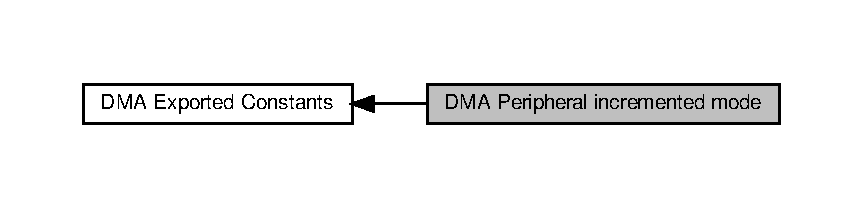
\includegraphics[width=350pt]{group___d_m_a___peripheral__incremented__mode}
\end{center}
\end{figure}
\subsection*{Definicje}
\begin{DoxyCompactItemize}
\item 
\#define \hyperlink{group___d_m_a___peripheral__incremented__mode_gab6d84e5805302516d26c06fb4497a346}{D\+M\+A\+\_\+\+P\+I\+N\+C\+\_\+\+E\+N\+A\+B\+LE}~((uint32\+\_\+t)\hyperlink{group___peripheral___registers___bits___definition_ga29c5d5c559dd14646fdc170e74f1f03b}{D\+M\+A\+\_\+\+Sx\+C\+R\+\_\+\+P\+I\+NC})
\item 
\#define \hyperlink{group___d_m_a___peripheral__incremented__mode_ga63e2aff2973d1a8f01d5d7b6e4894f39}{D\+M\+A\+\_\+\+P\+I\+N\+C\+\_\+\+D\+I\+S\+A\+B\+LE}~0x00000000U
\end{DoxyCompactItemize}


\subsection{Opis szczegółowy}
D\+MA peripheral incremented mode. 



\subsection{Dokumentacja definicji}
\mbox{\Hypertarget{group___d_m_a___peripheral__incremented__mode_ga63e2aff2973d1a8f01d5d7b6e4894f39}\label{group___d_m_a___peripheral__incremented__mode_ga63e2aff2973d1a8f01d5d7b6e4894f39}} 
\index{D\+M\+A Peripheral incremented mode@{D\+M\+A Peripheral incremented mode}!D\+M\+A\+\_\+\+P\+I\+N\+C\+\_\+\+D\+I\+S\+A\+B\+LE@{D\+M\+A\+\_\+\+P\+I\+N\+C\+\_\+\+D\+I\+S\+A\+B\+LE}}
\index{D\+M\+A\+\_\+\+P\+I\+N\+C\+\_\+\+D\+I\+S\+A\+B\+LE@{D\+M\+A\+\_\+\+P\+I\+N\+C\+\_\+\+D\+I\+S\+A\+B\+LE}!D\+M\+A Peripheral incremented mode@{D\+M\+A Peripheral incremented mode}}
\subsubsection{\texorpdfstring{D\+M\+A\+\_\+\+P\+I\+N\+C\+\_\+\+D\+I\+S\+A\+B\+LE}{DMA\_PINC\_DISABLE}}
{\footnotesize\ttfamily \#define D\+M\+A\+\_\+\+P\+I\+N\+C\+\_\+\+D\+I\+S\+A\+B\+LE~0x00000000U}

Peripheral increment mode disable 

Definicja w linii 240 pliku stm32f4xx\+\_\+hal\+\_\+dma.\+h.

\mbox{\Hypertarget{group___d_m_a___peripheral__incremented__mode_gab6d84e5805302516d26c06fb4497a346}\label{group___d_m_a___peripheral__incremented__mode_gab6d84e5805302516d26c06fb4497a346}} 
\index{D\+M\+A Peripheral incremented mode@{D\+M\+A Peripheral incremented mode}!D\+M\+A\+\_\+\+P\+I\+N\+C\+\_\+\+E\+N\+A\+B\+LE@{D\+M\+A\+\_\+\+P\+I\+N\+C\+\_\+\+E\+N\+A\+B\+LE}}
\index{D\+M\+A\+\_\+\+P\+I\+N\+C\+\_\+\+E\+N\+A\+B\+LE@{D\+M\+A\+\_\+\+P\+I\+N\+C\+\_\+\+E\+N\+A\+B\+LE}!D\+M\+A Peripheral incremented mode@{D\+M\+A Peripheral incremented mode}}
\subsubsection{\texorpdfstring{D\+M\+A\+\_\+\+P\+I\+N\+C\+\_\+\+E\+N\+A\+B\+LE}{DMA\_PINC\_ENABLE}}
{\footnotesize\ttfamily \#define D\+M\+A\+\_\+\+P\+I\+N\+C\+\_\+\+E\+N\+A\+B\+LE~((uint32\+\_\+t)\hyperlink{group___peripheral___registers___bits___definition_ga29c5d5c559dd14646fdc170e74f1f03b}{D\+M\+A\+\_\+\+Sx\+C\+R\+\_\+\+P\+I\+NC})}

Peripheral increment mode enable 

Definicja w linii 239 pliku stm32f4xx\+\_\+hal\+\_\+dma.\+h.


\hypertarget{group___d_m_a___memory__incremented__mode}{}\section{D\+MA Memory incremented mode}
\label{group___d_m_a___memory__incremented__mode}\index{D\+M\+A Memory incremented mode@{D\+M\+A Memory incremented mode}}


D\+MA memory incremented mode.  


Diagram współpracy dla D\+MA Memory incremented mode\+:\nopagebreak
\begin{figure}[H]
\begin{center}
\leavevmode
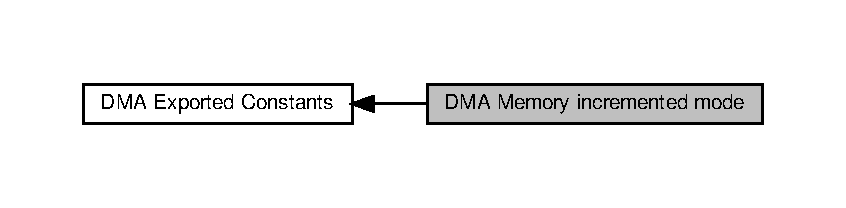
\includegraphics[width=350pt]{group___d_m_a___memory__incremented__mode}
\end{center}
\end{figure}
\subsection*{Definicje}
\begin{DoxyCompactItemize}
\item 
\#define \hyperlink{group___d_m_a___memory__incremented__mode_ga43d30885699cc8378562316ff4fed1cd}{D\+M\+A\+\_\+\+M\+I\+N\+C\+\_\+\+E\+N\+A\+B\+LE}~((uint32\+\_\+t)\hyperlink{group___peripheral___registers___bits___definition_ga771a295832a584a3777ede523a691719}{D\+M\+A\+\_\+\+Sx\+C\+R\+\_\+\+M\+I\+NC})
\item 
\#define \hyperlink{group___d_m_a___memory__incremented__mode_ga32625330516c188151743473fad97a33}{D\+M\+A\+\_\+\+M\+I\+N\+C\+\_\+\+D\+I\+S\+A\+B\+LE}~0x00000000U
\end{DoxyCompactItemize}


\subsection{Opis szczegółowy}
D\+MA memory incremented mode. 



\subsection{Dokumentacja definicji}
\mbox{\Hypertarget{group___d_m_a___memory__incremented__mode_ga32625330516c188151743473fad97a33}\label{group___d_m_a___memory__incremented__mode_ga32625330516c188151743473fad97a33}} 
\index{D\+M\+A Memory incremented mode@{D\+M\+A Memory incremented mode}!D\+M\+A\+\_\+\+M\+I\+N\+C\+\_\+\+D\+I\+S\+A\+B\+LE@{D\+M\+A\+\_\+\+M\+I\+N\+C\+\_\+\+D\+I\+S\+A\+B\+LE}}
\index{D\+M\+A\+\_\+\+M\+I\+N\+C\+\_\+\+D\+I\+S\+A\+B\+LE@{D\+M\+A\+\_\+\+M\+I\+N\+C\+\_\+\+D\+I\+S\+A\+B\+LE}!D\+M\+A Memory incremented mode@{D\+M\+A Memory incremented mode}}
\subsubsection{\texorpdfstring{D\+M\+A\+\_\+\+M\+I\+N\+C\+\_\+\+D\+I\+S\+A\+B\+LE}{DMA\_MINC\_DISABLE}}
{\footnotesize\ttfamily \#define D\+M\+A\+\_\+\+M\+I\+N\+C\+\_\+\+D\+I\+S\+A\+B\+LE~0x00000000U}

Memory increment mode disable 

Definicja w linii 250 pliku stm32f4xx\+\_\+hal\+\_\+dma.\+h.

\mbox{\Hypertarget{group___d_m_a___memory__incremented__mode_ga43d30885699cc8378562316ff4fed1cd}\label{group___d_m_a___memory__incremented__mode_ga43d30885699cc8378562316ff4fed1cd}} 
\index{D\+M\+A Memory incremented mode@{D\+M\+A Memory incremented mode}!D\+M\+A\+\_\+\+M\+I\+N\+C\+\_\+\+E\+N\+A\+B\+LE@{D\+M\+A\+\_\+\+M\+I\+N\+C\+\_\+\+E\+N\+A\+B\+LE}}
\index{D\+M\+A\+\_\+\+M\+I\+N\+C\+\_\+\+E\+N\+A\+B\+LE@{D\+M\+A\+\_\+\+M\+I\+N\+C\+\_\+\+E\+N\+A\+B\+LE}!D\+M\+A Memory incremented mode@{D\+M\+A Memory incremented mode}}
\subsubsection{\texorpdfstring{D\+M\+A\+\_\+\+M\+I\+N\+C\+\_\+\+E\+N\+A\+B\+LE}{DMA\_MINC\_ENABLE}}
{\footnotesize\ttfamily \#define D\+M\+A\+\_\+\+M\+I\+N\+C\+\_\+\+E\+N\+A\+B\+LE~((uint32\+\_\+t)\hyperlink{group___peripheral___registers___bits___definition_ga771a295832a584a3777ede523a691719}{D\+M\+A\+\_\+\+Sx\+C\+R\+\_\+\+M\+I\+NC})}

Memory increment mode enable 

Definicja w linii 249 pliku stm32f4xx\+\_\+hal\+\_\+dma.\+h.


\hypertarget{group___d_m_a___peripheral__data__size}{}\section{D\+MA Peripheral data size}
\label{group___d_m_a___peripheral__data__size}\index{D\+M\+A Peripheral data size@{D\+M\+A Peripheral data size}}


D\+MA peripheral data size.  


Diagram współpracy dla D\+MA Peripheral data size\+:\nopagebreak
\begin{figure}[H]
\begin{center}
\leavevmode
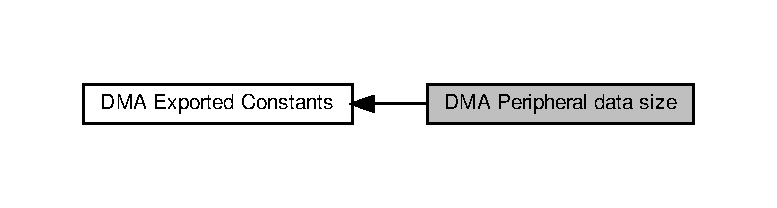
\includegraphics[width=350pt]{group___d_m_a___peripheral__data__size}
\end{center}
\end{figure}
\subsection*{Definicje}
\begin{DoxyCompactItemize}
\item 
\#define \hyperlink{group___d_m_a___peripheral__data__size_ga55b8c8f5ec95f10d26d6c5b1c9136730}{D\+M\+A\+\_\+\+P\+D\+A\+T\+A\+A\+L\+I\+G\+N\+\_\+\+B\+Y\+TE}~0x00000000U
\item 
\#define \hyperlink{group___d_m_a___peripheral__data__size_gac08bfd907442dba5358830b247135bcc}{D\+M\+A\+\_\+\+P\+D\+A\+T\+A\+A\+L\+I\+G\+N\+\_\+\+H\+A\+L\+F\+W\+O\+RD}~((uint32\+\_\+t)\hyperlink{group___peripheral___registers___bits___definition_gab05cf3e3f7c9edae5c70d59b3b75b14f}{D\+M\+A\+\_\+\+Sx\+C\+R\+\_\+\+P\+S\+I\+Z\+E\+\_\+0})
\item 
\#define \hyperlink{group___d_m_a___peripheral__data__size_gaad50e97cbc4a726660db9c3f42ac93b0}{D\+M\+A\+\_\+\+P\+D\+A\+T\+A\+A\+L\+I\+G\+N\+\_\+\+W\+O\+RD}~((uint32\+\_\+t)\hyperlink{group___peripheral___registers___bits___definition_ga8f376d0900380a3045cbeadd6a037302}{D\+M\+A\+\_\+\+Sx\+C\+R\+\_\+\+P\+S\+I\+Z\+E\+\_\+1})
\end{DoxyCompactItemize}


\subsection{Opis szczegółowy}
D\+MA peripheral data size. 



\subsection{Dokumentacja definicji}
\mbox{\Hypertarget{group___d_m_a___peripheral__data__size_ga55b8c8f5ec95f10d26d6c5b1c9136730}\label{group___d_m_a___peripheral__data__size_ga55b8c8f5ec95f10d26d6c5b1c9136730}} 
\index{D\+M\+A Peripheral data size@{D\+M\+A Peripheral data size}!D\+M\+A\+\_\+\+P\+D\+A\+T\+A\+A\+L\+I\+G\+N\+\_\+\+B\+Y\+TE@{D\+M\+A\+\_\+\+P\+D\+A\+T\+A\+A\+L\+I\+G\+N\+\_\+\+B\+Y\+TE}}
\index{D\+M\+A\+\_\+\+P\+D\+A\+T\+A\+A\+L\+I\+G\+N\+\_\+\+B\+Y\+TE@{D\+M\+A\+\_\+\+P\+D\+A\+T\+A\+A\+L\+I\+G\+N\+\_\+\+B\+Y\+TE}!D\+M\+A Peripheral data size@{D\+M\+A Peripheral data size}}
\subsubsection{\texorpdfstring{D\+M\+A\+\_\+\+P\+D\+A\+T\+A\+A\+L\+I\+G\+N\+\_\+\+B\+Y\+TE}{DMA\_PDATAALIGN\_BYTE}}
{\footnotesize\ttfamily \#define D\+M\+A\+\_\+\+P\+D\+A\+T\+A\+A\+L\+I\+G\+N\+\_\+\+B\+Y\+TE~0x00000000U}

Peripheral data alignment\+: Byte 

Definicja w linii 259 pliku stm32f4xx\+\_\+hal\+\_\+dma.\+h.

\mbox{\Hypertarget{group___d_m_a___peripheral__data__size_gac08bfd907442dba5358830b247135bcc}\label{group___d_m_a___peripheral__data__size_gac08bfd907442dba5358830b247135bcc}} 
\index{D\+M\+A Peripheral data size@{D\+M\+A Peripheral data size}!D\+M\+A\+\_\+\+P\+D\+A\+T\+A\+A\+L\+I\+G\+N\+\_\+\+H\+A\+L\+F\+W\+O\+RD@{D\+M\+A\+\_\+\+P\+D\+A\+T\+A\+A\+L\+I\+G\+N\+\_\+\+H\+A\+L\+F\+W\+O\+RD}}
\index{D\+M\+A\+\_\+\+P\+D\+A\+T\+A\+A\+L\+I\+G\+N\+\_\+\+H\+A\+L\+F\+W\+O\+RD@{D\+M\+A\+\_\+\+P\+D\+A\+T\+A\+A\+L\+I\+G\+N\+\_\+\+H\+A\+L\+F\+W\+O\+RD}!D\+M\+A Peripheral data size@{D\+M\+A Peripheral data size}}
\subsubsection{\texorpdfstring{D\+M\+A\+\_\+\+P\+D\+A\+T\+A\+A\+L\+I\+G\+N\+\_\+\+H\+A\+L\+F\+W\+O\+RD}{DMA\_PDATAALIGN\_HALFWORD}}
{\footnotesize\ttfamily \#define D\+M\+A\+\_\+\+P\+D\+A\+T\+A\+A\+L\+I\+G\+N\+\_\+\+H\+A\+L\+F\+W\+O\+RD~((uint32\+\_\+t)\hyperlink{group___peripheral___registers___bits___definition_gab05cf3e3f7c9edae5c70d59b3b75b14f}{D\+M\+A\+\_\+\+Sx\+C\+R\+\_\+\+P\+S\+I\+Z\+E\+\_\+0})}

Peripheral data alignment\+: Half\+Word 

Definicja w linii 260 pliku stm32f4xx\+\_\+hal\+\_\+dma.\+h.

\mbox{\Hypertarget{group___d_m_a___peripheral__data__size_gaad50e97cbc4a726660db9c3f42ac93b0}\label{group___d_m_a___peripheral__data__size_gaad50e97cbc4a726660db9c3f42ac93b0}} 
\index{D\+M\+A Peripheral data size@{D\+M\+A Peripheral data size}!D\+M\+A\+\_\+\+P\+D\+A\+T\+A\+A\+L\+I\+G\+N\+\_\+\+W\+O\+RD@{D\+M\+A\+\_\+\+P\+D\+A\+T\+A\+A\+L\+I\+G\+N\+\_\+\+W\+O\+RD}}
\index{D\+M\+A\+\_\+\+P\+D\+A\+T\+A\+A\+L\+I\+G\+N\+\_\+\+W\+O\+RD@{D\+M\+A\+\_\+\+P\+D\+A\+T\+A\+A\+L\+I\+G\+N\+\_\+\+W\+O\+RD}!D\+M\+A Peripheral data size@{D\+M\+A Peripheral data size}}
\subsubsection{\texorpdfstring{D\+M\+A\+\_\+\+P\+D\+A\+T\+A\+A\+L\+I\+G\+N\+\_\+\+W\+O\+RD}{DMA\_PDATAALIGN\_WORD}}
{\footnotesize\ttfamily \#define D\+M\+A\+\_\+\+P\+D\+A\+T\+A\+A\+L\+I\+G\+N\+\_\+\+W\+O\+RD~((uint32\+\_\+t)\hyperlink{group___peripheral___registers___bits___definition_ga8f376d0900380a3045cbeadd6a037302}{D\+M\+A\+\_\+\+Sx\+C\+R\+\_\+\+P\+S\+I\+Z\+E\+\_\+1})}

Peripheral data alignment\+: Word 

Definicja w linii 261 pliku stm32f4xx\+\_\+hal\+\_\+dma.\+h.


\hypertarget{group___d_m_a___memory__data__size}{}\section{D\+MA Memory data size}
\label{group___d_m_a___memory__data__size}\index{D\+M\+A Memory data size@{D\+M\+A Memory data size}}


D\+MA memory data size.  


Diagram współpracy dla D\+MA Memory data size\+:\nopagebreak
\begin{figure}[H]
\begin{center}
\leavevmode
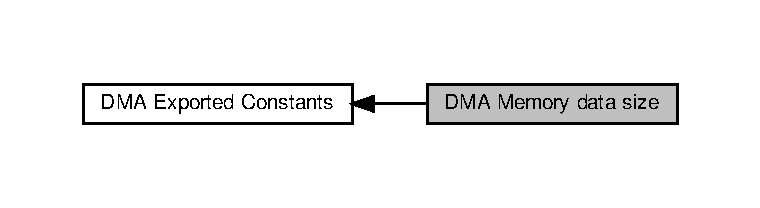
\includegraphics[width=350pt]{group___d_m_a___memory__data__size}
\end{center}
\end{figure}
\subsection*{Definicje}
\begin{DoxyCompactItemize}
\item 
\#define \hyperlink{group___d_m_a___memory__data__size_ga9ed07bddf736298eba11508382ea4d51}{D\+M\+A\+\_\+\+M\+D\+A\+T\+A\+A\+L\+I\+G\+N\+\_\+\+B\+Y\+TE}~0x00000000U
\item 
\#define \hyperlink{group___d_m_a___memory__data__size_ga2c7355971c0da34a7ffe50ec87403071}{D\+M\+A\+\_\+\+M\+D\+A\+T\+A\+A\+L\+I\+G\+N\+\_\+\+H\+A\+L\+F\+W\+O\+RD}~((uint32\+\_\+t)\hyperlink{group___peripheral___registers___bits___definition_ga39adb60b3394b61366691b45b8c2b80f}{D\+M\+A\+\_\+\+Sx\+C\+R\+\_\+\+M\+S\+I\+Z\+E\+\_\+0})
\item 
\#define \hyperlink{group___d_m_a___memory__data__size_ga8812da819f18c873249074f3920220b2}{D\+M\+A\+\_\+\+M\+D\+A\+T\+A\+A\+L\+I\+G\+N\+\_\+\+W\+O\+RD}~((uint32\+\_\+t)\hyperlink{group___peripheral___registers___bits___definition_gaa5c2ef08ab52de52b4e1fd785f60e263}{D\+M\+A\+\_\+\+Sx\+C\+R\+\_\+\+M\+S\+I\+Z\+E\+\_\+1})
\end{DoxyCompactItemize}


\subsection{Opis szczegółowy}
D\+MA memory data size. 



\subsection{Dokumentacja definicji}
\mbox{\Hypertarget{group___d_m_a___memory__data__size_ga9ed07bddf736298eba11508382ea4d51}\label{group___d_m_a___memory__data__size_ga9ed07bddf736298eba11508382ea4d51}} 
\index{D\+M\+A Memory data size@{D\+M\+A Memory data size}!D\+M\+A\+\_\+\+M\+D\+A\+T\+A\+A\+L\+I\+G\+N\+\_\+\+B\+Y\+TE@{D\+M\+A\+\_\+\+M\+D\+A\+T\+A\+A\+L\+I\+G\+N\+\_\+\+B\+Y\+TE}}
\index{D\+M\+A\+\_\+\+M\+D\+A\+T\+A\+A\+L\+I\+G\+N\+\_\+\+B\+Y\+TE@{D\+M\+A\+\_\+\+M\+D\+A\+T\+A\+A\+L\+I\+G\+N\+\_\+\+B\+Y\+TE}!D\+M\+A Memory data size@{D\+M\+A Memory data size}}
\subsubsection{\texorpdfstring{D\+M\+A\+\_\+\+M\+D\+A\+T\+A\+A\+L\+I\+G\+N\+\_\+\+B\+Y\+TE}{DMA\_MDATAALIGN\_BYTE}}
{\footnotesize\ttfamily \#define D\+M\+A\+\_\+\+M\+D\+A\+T\+A\+A\+L\+I\+G\+N\+\_\+\+B\+Y\+TE~0x00000000U}

Memory data alignment\+: Byte 

Definicja w linii 270 pliku stm32f4xx\+\_\+hal\+\_\+dma.\+h.

\mbox{\Hypertarget{group___d_m_a___memory__data__size_ga2c7355971c0da34a7ffe50ec87403071}\label{group___d_m_a___memory__data__size_ga2c7355971c0da34a7ffe50ec87403071}} 
\index{D\+M\+A Memory data size@{D\+M\+A Memory data size}!D\+M\+A\+\_\+\+M\+D\+A\+T\+A\+A\+L\+I\+G\+N\+\_\+\+H\+A\+L\+F\+W\+O\+RD@{D\+M\+A\+\_\+\+M\+D\+A\+T\+A\+A\+L\+I\+G\+N\+\_\+\+H\+A\+L\+F\+W\+O\+RD}}
\index{D\+M\+A\+\_\+\+M\+D\+A\+T\+A\+A\+L\+I\+G\+N\+\_\+\+H\+A\+L\+F\+W\+O\+RD@{D\+M\+A\+\_\+\+M\+D\+A\+T\+A\+A\+L\+I\+G\+N\+\_\+\+H\+A\+L\+F\+W\+O\+RD}!D\+M\+A Memory data size@{D\+M\+A Memory data size}}
\subsubsection{\texorpdfstring{D\+M\+A\+\_\+\+M\+D\+A\+T\+A\+A\+L\+I\+G\+N\+\_\+\+H\+A\+L\+F\+W\+O\+RD}{DMA\_MDATAALIGN\_HALFWORD}}
{\footnotesize\ttfamily \#define D\+M\+A\+\_\+\+M\+D\+A\+T\+A\+A\+L\+I\+G\+N\+\_\+\+H\+A\+L\+F\+W\+O\+RD~((uint32\+\_\+t)\hyperlink{group___peripheral___registers___bits___definition_ga39adb60b3394b61366691b45b8c2b80f}{D\+M\+A\+\_\+\+Sx\+C\+R\+\_\+\+M\+S\+I\+Z\+E\+\_\+0})}

Memory data alignment\+: Half\+Word 

Definicja w linii 271 pliku stm32f4xx\+\_\+hal\+\_\+dma.\+h.

\mbox{\Hypertarget{group___d_m_a___memory__data__size_ga8812da819f18c873249074f3920220b2}\label{group___d_m_a___memory__data__size_ga8812da819f18c873249074f3920220b2}} 
\index{D\+M\+A Memory data size@{D\+M\+A Memory data size}!D\+M\+A\+\_\+\+M\+D\+A\+T\+A\+A\+L\+I\+G\+N\+\_\+\+W\+O\+RD@{D\+M\+A\+\_\+\+M\+D\+A\+T\+A\+A\+L\+I\+G\+N\+\_\+\+W\+O\+RD}}
\index{D\+M\+A\+\_\+\+M\+D\+A\+T\+A\+A\+L\+I\+G\+N\+\_\+\+W\+O\+RD@{D\+M\+A\+\_\+\+M\+D\+A\+T\+A\+A\+L\+I\+G\+N\+\_\+\+W\+O\+RD}!D\+M\+A Memory data size@{D\+M\+A Memory data size}}
\subsubsection{\texorpdfstring{D\+M\+A\+\_\+\+M\+D\+A\+T\+A\+A\+L\+I\+G\+N\+\_\+\+W\+O\+RD}{DMA\_MDATAALIGN\_WORD}}
{\footnotesize\ttfamily \#define D\+M\+A\+\_\+\+M\+D\+A\+T\+A\+A\+L\+I\+G\+N\+\_\+\+W\+O\+RD~((uint32\+\_\+t)\hyperlink{group___peripheral___registers___bits___definition_gaa5c2ef08ab52de52b4e1fd785f60e263}{D\+M\+A\+\_\+\+Sx\+C\+R\+\_\+\+M\+S\+I\+Z\+E\+\_\+1})}

Memory data alignment\+: Word 

Definicja w linii 272 pliku stm32f4xx\+\_\+hal\+\_\+dma.\+h.


\hypertarget{group___d_m_a__mode}{}\section{D\+MA mode}
\label{group___d_m_a__mode}\index{D\+M\+A mode@{D\+M\+A mode}}


D\+MA mode.  


Diagram współpracy dla D\+MA mode\+:\nopagebreak
\begin{figure}[H]
\begin{center}
\leavevmode
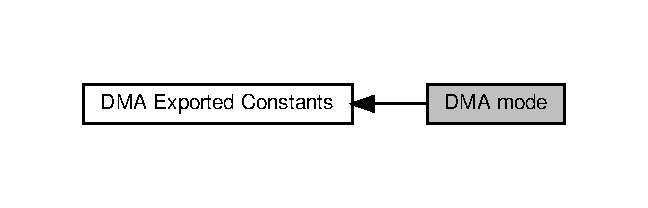
\includegraphics[width=311pt]{group___d_m_a__mode}
\end{center}
\end{figure}
\subsection*{Definicje}
\begin{DoxyCompactItemize}
\item 
\#define \hyperlink{group___d_m_a__mode_ga04941acfbbdefc53e1e08133cffa3b8a}{D\+M\+A\+\_\+\+N\+O\+R\+M\+AL}~0x00000000U
\item 
\#define \hyperlink{group___d_m_a__mode_ga4c4f425cba13edffb3c831c036c91e01}{D\+M\+A\+\_\+\+C\+I\+R\+C\+U\+L\+AR}~((uint32\+\_\+t)\hyperlink{group___peripheral___registers___bits___definition_gadc248dbc519cc580621cdadcdd8741fb}{D\+M\+A\+\_\+\+Sx\+C\+R\+\_\+\+C\+I\+RC})
\item 
\#define \hyperlink{group___d_m_a__mode_ga7974ee645c8e275a2297cf37eec9e022}{D\+M\+A\+\_\+\+P\+F\+C\+T\+RL}~((uint32\+\_\+t)\hyperlink{group___peripheral___registers___bits___definition_ga11f412d256043bec3e01ceef7f2099f2}{D\+M\+A\+\_\+\+Sx\+C\+R\+\_\+\+P\+F\+C\+T\+RL})
\end{DoxyCompactItemize}


\subsection{Opis szczegółowy}
D\+MA mode. 



\subsection{Dokumentacja definicji}
\mbox{\Hypertarget{group___d_m_a__mode_ga4c4f425cba13edffb3c831c036c91e01}\label{group___d_m_a__mode_ga4c4f425cba13edffb3c831c036c91e01}} 
\index{D\+M\+A mode@{D\+M\+A mode}!D\+M\+A\+\_\+\+C\+I\+R\+C\+U\+L\+AR@{D\+M\+A\+\_\+\+C\+I\+R\+C\+U\+L\+AR}}
\index{D\+M\+A\+\_\+\+C\+I\+R\+C\+U\+L\+AR@{D\+M\+A\+\_\+\+C\+I\+R\+C\+U\+L\+AR}!D\+M\+A mode@{D\+M\+A mode}}
\subsubsection{\texorpdfstring{D\+M\+A\+\_\+\+C\+I\+R\+C\+U\+L\+AR}{DMA\_CIRCULAR}}
{\footnotesize\ttfamily \#define D\+M\+A\+\_\+\+C\+I\+R\+C\+U\+L\+AR~((uint32\+\_\+t)\hyperlink{group___peripheral___registers___bits___definition_gadc248dbc519cc580621cdadcdd8741fb}{D\+M\+A\+\_\+\+Sx\+C\+R\+\_\+\+C\+I\+RC})}

Circular mode 

Definicja w linii 282 pliku stm32f4xx\+\_\+hal\+\_\+dma.\+h.

\mbox{\Hypertarget{group___d_m_a__mode_ga04941acfbbdefc53e1e08133cffa3b8a}\label{group___d_m_a__mode_ga04941acfbbdefc53e1e08133cffa3b8a}} 
\index{D\+M\+A mode@{D\+M\+A mode}!D\+M\+A\+\_\+\+N\+O\+R\+M\+AL@{D\+M\+A\+\_\+\+N\+O\+R\+M\+AL}}
\index{D\+M\+A\+\_\+\+N\+O\+R\+M\+AL@{D\+M\+A\+\_\+\+N\+O\+R\+M\+AL}!D\+M\+A mode@{D\+M\+A mode}}
\subsubsection{\texorpdfstring{D\+M\+A\+\_\+\+N\+O\+R\+M\+AL}{DMA\_NORMAL}}
{\footnotesize\ttfamily \#define D\+M\+A\+\_\+\+N\+O\+R\+M\+AL~0x00000000U}

Normal mode 

Definicja w linii 281 pliku stm32f4xx\+\_\+hal\+\_\+dma.\+h.

\mbox{\Hypertarget{group___d_m_a__mode_ga7974ee645c8e275a2297cf37eec9e022}\label{group___d_m_a__mode_ga7974ee645c8e275a2297cf37eec9e022}} 
\index{D\+M\+A mode@{D\+M\+A mode}!D\+M\+A\+\_\+\+P\+F\+C\+T\+RL@{D\+M\+A\+\_\+\+P\+F\+C\+T\+RL}}
\index{D\+M\+A\+\_\+\+P\+F\+C\+T\+RL@{D\+M\+A\+\_\+\+P\+F\+C\+T\+RL}!D\+M\+A mode@{D\+M\+A mode}}
\subsubsection{\texorpdfstring{D\+M\+A\+\_\+\+P\+F\+C\+T\+RL}{DMA\_PFCTRL}}
{\footnotesize\ttfamily \#define D\+M\+A\+\_\+\+P\+F\+C\+T\+RL~((uint32\+\_\+t)\hyperlink{group___peripheral___registers___bits___definition_ga11f412d256043bec3e01ceef7f2099f2}{D\+M\+A\+\_\+\+Sx\+C\+R\+\_\+\+P\+F\+C\+T\+RL})}

Peripheral flow control mode 

Definicja w linii 283 pliku stm32f4xx\+\_\+hal\+\_\+dma.\+h.


\hypertarget{group___d_m_a___priority__level}{}\section{D\+MA Priority level}
\label{group___d_m_a___priority__level}\index{D\+M\+A Priority level@{D\+M\+A Priority level}}


D\+MA priority levels.  


Diagram współpracy dla D\+MA Priority level\+:\nopagebreak
\begin{figure}[H]
\begin{center}
\leavevmode
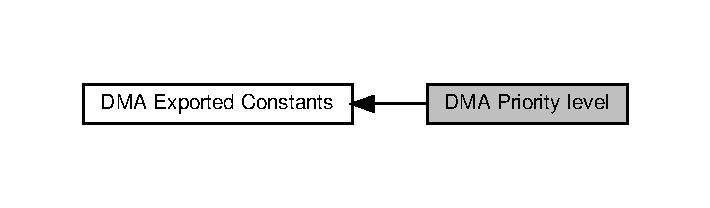
\includegraphics[width=341pt]{group___d_m_a___priority__level}
\end{center}
\end{figure}
\subsection*{Definicje}
\begin{DoxyCompactItemize}
\item 
\#define \hyperlink{group___d_m_a___priority__level_ga0d1ed2bc9229ba3c953002bcf3a72130}{D\+M\+A\+\_\+\+P\+R\+I\+O\+R\+I\+T\+Y\+\_\+\+L\+OW}~0x00000000U
\item 
\#define \hyperlink{group___d_m_a___priority__level_gad6fbeee76fd4a02cbed64365bb4c1781}{D\+M\+A\+\_\+\+P\+R\+I\+O\+R\+I\+T\+Y\+\_\+\+M\+E\+D\+I\+UM}~((uint32\+\_\+t)\hyperlink{group___peripheral___registers___bits___definition_ga41b1b2f7bd6f0af932ff0fb7df9336b6}{D\+M\+A\+\_\+\+Sx\+C\+R\+\_\+\+P\+L\+\_\+0})
\item 
\#define \hyperlink{group___d_m_a___priority__level_ga6b2f5c5e22895f8b4bd52a27ec6cae2a}{D\+M\+A\+\_\+\+P\+R\+I\+O\+R\+I\+T\+Y\+\_\+\+H\+I\+GH}~((uint32\+\_\+t)\hyperlink{group___peripheral___registers___bits___definition_ga81817adc8c0ee54dea0f67a1a9e8eb77}{D\+M\+A\+\_\+\+Sx\+C\+R\+\_\+\+P\+L\+\_\+1})
\item 
\#define \hyperlink{group___d_m_a___priority__level_gaed0542331a4d875d1d8d5b2878e9372c}{D\+M\+A\+\_\+\+P\+R\+I\+O\+R\+I\+T\+Y\+\_\+\+V\+E\+R\+Y\+\_\+\+H\+I\+GH}~((uint32\+\_\+t)\hyperlink{group___peripheral___registers___bits___definition_ga14c115d71a4e3b3c4da360108288154c}{D\+M\+A\+\_\+\+Sx\+C\+R\+\_\+\+PL})
\end{DoxyCompactItemize}


\subsection{Opis szczegółowy}
D\+MA priority levels. 



\subsection{Dokumentacja definicji}
\mbox{\Hypertarget{group___d_m_a___priority__level_ga6b2f5c5e22895f8b4bd52a27ec6cae2a}\label{group___d_m_a___priority__level_ga6b2f5c5e22895f8b4bd52a27ec6cae2a}} 
\index{D\+M\+A Priority level@{D\+M\+A Priority level}!D\+M\+A\+\_\+\+P\+R\+I\+O\+R\+I\+T\+Y\+\_\+\+H\+I\+GH@{D\+M\+A\+\_\+\+P\+R\+I\+O\+R\+I\+T\+Y\+\_\+\+H\+I\+GH}}
\index{D\+M\+A\+\_\+\+P\+R\+I\+O\+R\+I\+T\+Y\+\_\+\+H\+I\+GH@{D\+M\+A\+\_\+\+P\+R\+I\+O\+R\+I\+T\+Y\+\_\+\+H\+I\+GH}!D\+M\+A Priority level@{D\+M\+A Priority level}}
\subsubsection{\texorpdfstring{D\+M\+A\+\_\+\+P\+R\+I\+O\+R\+I\+T\+Y\+\_\+\+H\+I\+GH}{DMA\_PRIORITY\_HIGH}}
{\footnotesize\ttfamily \#define D\+M\+A\+\_\+\+P\+R\+I\+O\+R\+I\+T\+Y\+\_\+\+H\+I\+GH~((uint32\+\_\+t)\hyperlink{group___peripheral___registers___bits___definition_ga81817adc8c0ee54dea0f67a1a9e8eb77}{D\+M\+A\+\_\+\+Sx\+C\+R\+\_\+\+P\+L\+\_\+1})}

Priority level\+: High 

Definicja w linii 294 pliku stm32f4xx\+\_\+hal\+\_\+dma.\+h.

\mbox{\Hypertarget{group___d_m_a___priority__level_ga0d1ed2bc9229ba3c953002bcf3a72130}\label{group___d_m_a___priority__level_ga0d1ed2bc9229ba3c953002bcf3a72130}} 
\index{D\+M\+A Priority level@{D\+M\+A Priority level}!D\+M\+A\+\_\+\+P\+R\+I\+O\+R\+I\+T\+Y\+\_\+\+L\+OW@{D\+M\+A\+\_\+\+P\+R\+I\+O\+R\+I\+T\+Y\+\_\+\+L\+OW}}
\index{D\+M\+A\+\_\+\+P\+R\+I\+O\+R\+I\+T\+Y\+\_\+\+L\+OW@{D\+M\+A\+\_\+\+P\+R\+I\+O\+R\+I\+T\+Y\+\_\+\+L\+OW}!D\+M\+A Priority level@{D\+M\+A Priority level}}
\subsubsection{\texorpdfstring{D\+M\+A\+\_\+\+P\+R\+I\+O\+R\+I\+T\+Y\+\_\+\+L\+OW}{DMA\_PRIORITY\_LOW}}
{\footnotesize\ttfamily \#define D\+M\+A\+\_\+\+P\+R\+I\+O\+R\+I\+T\+Y\+\_\+\+L\+OW~0x00000000U}

Priority level\+: Low 

Definicja w linii 292 pliku stm32f4xx\+\_\+hal\+\_\+dma.\+h.

\mbox{\Hypertarget{group___d_m_a___priority__level_gad6fbeee76fd4a02cbed64365bb4c1781}\label{group___d_m_a___priority__level_gad6fbeee76fd4a02cbed64365bb4c1781}} 
\index{D\+M\+A Priority level@{D\+M\+A Priority level}!D\+M\+A\+\_\+\+P\+R\+I\+O\+R\+I\+T\+Y\+\_\+\+M\+E\+D\+I\+UM@{D\+M\+A\+\_\+\+P\+R\+I\+O\+R\+I\+T\+Y\+\_\+\+M\+E\+D\+I\+UM}}
\index{D\+M\+A\+\_\+\+P\+R\+I\+O\+R\+I\+T\+Y\+\_\+\+M\+E\+D\+I\+UM@{D\+M\+A\+\_\+\+P\+R\+I\+O\+R\+I\+T\+Y\+\_\+\+M\+E\+D\+I\+UM}!D\+M\+A Priority level@{D\+M\+A Priority level}}
\subsubsection{\texorpdfstring{D\+M\+A\+\_\+\+P\+R\+I\+O\+R\+I\+T\+Y\+\_\+\+M\+E\+D\+I\+UM}{DMA\_PRIORITY\_MEDIUM}}
{\footnotesize\ttfamily \#define D\+M\+A\+\_\+\+P\+R\+I\+O\+R\+I\+T\+Y\+\_\+\+M\+E\+D\+I\+UM~((uint32\+\_\+t)\hyperlink{group___peripheral___registers___bits___definition_ga41b1b2f7bd6f0af932ff0fb7df9336b6}{D\+M\+A\+\_\+\+Sx\+C\+R\+\_\+\+P\+L\+\_\+0})}

Priority level\+: Medium 

Definicja w linii 293 pliku stm32f4xx\+\_\+hal\+\_\+dma.\+h.

\mbox{\Hypertarget{group___d_m_a___priority__level_gaed0542331a4d875d1d8d5b2878e9372c}\label{group___d_m_a___priority__level_gaed0542331a4d875d1d8d5b2878e9372c}} 
\index{D\+M\+A Priority level@{D\+M\+A Priority level}!D\+M\+A\+\_\+\+P\+R\+I\+O\+R\+I\+T\+Y\+\_\+\+V\+E\+R\+Y\+\_\+\+H\+I\+GH@{D\+M\+A\+\_\+\+P\+R\+I\+O\+R\+I\+T\+Y\+\_\+\+V\+E\+R\+Y\+\_\+\+H\+I\+GH}}
\index{D\+M\+A\+\_\+\+P\+R\+I\+O\+R\+I\+T\+Y\+\_\+\+V\+E\+R\+Y\+\_\+\+H\+I\+GH@{D\+M\+A\+\_\+\+P\+R\+I\+O\+R\+I\+T\+Y\+\_\+\+V\+E\+R\+Y\+\_\+\+H\+I\+GH}!D\+M\+A Priority level@{D\+M\+A Priority level}}
\subsubsection{\texorpdfstring{D\+M\+A\+\_\+\+P\+R\+I\+O\+R\+I\+T\+Y\+\_\+\+V\+E\+R\+Y\+\_\+\+H\+I\+GH}{DMA\_PRIORITY\_VERY\_HIGH}}
{\footnotesize\ttfamily \#define D\+M\+A\+\_\+\+P\+R\+I\+O\+R\+I\+T\+Y\+\_\+\+V\+E\+R\+Y\+\_\+\+H\+I\+GH~((uint32\+\_\+t)\hyperlink{group___peripheral___registers___bits___definition_ga14c115d71a4e3b3c4da360108288154c}{D\+M\+A\+\_\+\+Sx\+C\+R\+\_\+\+PL})}

Priority level\+: Very High 

Definicja w linii 295 pliku stm32f4xx\+\_\+hal\+\_\+dma.\+h.


\hypertarget{group___d_m_a___f_i_f_o__direct__mode}{}\section{D\+MA F\+I\+FO direct mode}
\label{group___d_m_a___f_i_f_o__direct__mode}\index{D\+M\+A F\+I\+F\+O direct mode@{D\+M\+A F\+I\+F\+O direct mode}}


D\+MA F\+I\+FO direct mode.  


Diagram współpracy dla D\+MA F\+I\+FO direct mode\+:\nopagebreak
\begin{figure}[H]
\begin{center}
\leavevmode
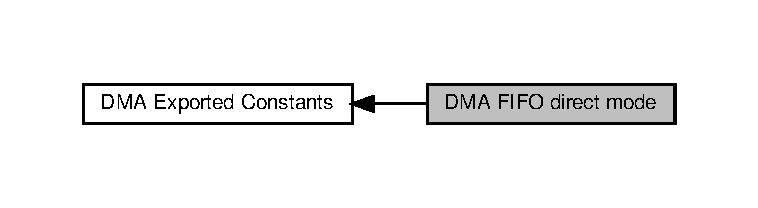
\includegraphics[width=350pt]{group___d_m_a___f_i_f_o__direct__mode}
\end{center}
\end{figure}
\subsection*{Definicje}
\begin{DoxyCompactItemize}
\item 
\#define \hyperlink{group___d_m_a___f_i_f_o__direct__mode_gaec22b199f9da9214bf908d7edbcd83e8}{D\+M\+A\+\_\+\+F\+I\+F\+O\+M\+O\+D\+E\+\_\+\+D\+I\+S\+A\+B\+LE}~0x00000000U
\item 
\#define \hyperlink{group___d_m_a___f_i_f_o__direct__mode_ga18709570bed6b9112520701c482fbe4b}{D\+M\+A\+\_\+\+F\+I\+F\+O\+M\+O\+D\+E\+\_\+\+E\+N\+A\+B\+LE}~((uint32\+\_\+t)\hyperlink{group___peripheral___registers___bits___definition_ga89406bb954742665691c0ac2f8d95ec9}{D\+M\+A\+\_\+\+Sx\+F\+C\+R\+\_\+\+D\+M\+D\+IS})
\end{DoxyCompactItemize}


\subsection{Opis szczegółowy}
D\+MA F\+I\+FO direct mode. 



\subsection{Dokumentacja definicji}
\mbox{\Hypertarget{group___d_m_a___f_i_f_o__direct__mode_gaec22b199f9da9214bf908d7edbcd83e8}\label{group___d_m_a___f_i_f_o__direct__mode_gaec22b199f9da9214bf908d7edbcd83e8}} 
\index{D\+M\+A F\+I\+F\+O direct mode@{D\+M\+A F\+I\+F\+O direct mode}!D\+M\+A\+\_\+\+F\+I\+F\+O\+M\+O\+D\+E\+\_\+\+D\+I\+S\+A\+B\+LE@{D\+M\+A\+\_\+\+F\+I\+F\+O\+M\+O\+D\+E\+\_\+\+D\+I\+S\+A\+B\+LE}}
\index{D\+M\+A\+\_\+\+F\+I\+F\+O\+M\+O\+D\+E\+\_\+\+D\+I\+S\+A\+B\+LE@{D\+M\+A\+\_\+\+F\+I\+F\+O\+M\+O\+D\+E\+\_\+\+D\+I\+S\+A\+B\+LE}!D\+M\+A F\+I\+F\+O direct mode@{D\+M\+A F\+I\+F\+O direct mode}}
\subsubsection{\texorpdfstring{D\+M\+A\+\_\+\+F\+I\+F\+O\+M\+O\+D\+E\+\_\+\+D\+I\+S\+A\+B\+LE}{DMA\_FIFOMODE\_DISABLE}}
{\footnotesize\ttfamily \#define D\+M\+A\+\_\+\+F\+I\+F\+O\+M\+O\+D\+E\+\_\+\+D\+I\+S\+A\+B\+LE~0x00000000U}

F\+I\+FO mode disable 

Definicja w linii 304 pliku stm32f4xx\+\_\+hal\+\_\+dma.\+h.

\mbox{\Hypertarget{group___d_m_a___f_i_f_o__direct__mode_ga18709570bed6b9112520701c482fbe4b}\label{group___d_m_a___f_i_f_o__direct__mode_ga18709570bed6b9112520701c482fbe4b}} 
\index{D\+M\+A F\+I\+F\+O direct mode@{D\+M\+A F\+I\+F\+O direct mode}!D\+M\+A\+\_\+\+F\+I\+F\+O\+M\+O\+D\+E\+\_\+\+E\+N\+A\+B\+LE@{D\+M\+A\+\_\+\+F\+I\+F\+O\+M\+O\+D\+E\+\_\+\+E\+N\+A\+B\+LE}}
\index{D\+M\+A\+\_\+\+F\+I\+F\+O\+M\+O\+D\+E\+\_\+\+E\+N\+A\+B\+LE@{D\+M\+A\+\_\+\+F\+I\+F\+O\+M\+O\+D\+E\+\_\+\+E\+N\+A\+B\+LE}!D\+M\+A F\+I\+F\+O direct mode@{D\+M\+A F\+I\+F\+O direct mode}}
\subsubsection{\texorpdfstring{D\+M\+A\+\_\+\+F\+I\+F\+O\+M\+O\+D\+E\+\_\+\+E\+N\+A\+B\+LE}{DMA\_FIFOMODE\_ENABLE}}
{\footnotesize\ttfamily \#define D\+M\+A\+\_\+\+F\+I\+F\+O\+M\+O\+D\+E\+\_\+\+E\+N\+A\+B\+LE~((uint32\+\_\+t)\hyperlink{group___peripheral___registers___bits___definition_ga89406bb954742665691c0ac2f8d95ec9}{D\+M\+A\+\_\+\+Sx\+F\+C\+R\+\_\+\+D\+M\+D\+IS})}

F\+I\+FO mode enable 

Definicja w linii 305 pliku stm32f4xx\+\_\+hal\+\_\+dma.\+h.


\hypertarget{group___d_m_a___f_i_f_o__threshold__level}{}\section{D\+MA F\+I\+FO threshold level}
\label{group___d_m_a___f_i_f_o__threshold__level}\index{D\+M\+A F\+I\+F\+O threshold level@{D\+M\+A F\+I\+F\+O threshold level}}


D\+MA F\+I\+FO level.  


Diagram współpracy dla D\+MA F\+I\+FO threshold level\+:\nopagebreak
\begin{figure}[H]
\begin{center}
\leavevmode
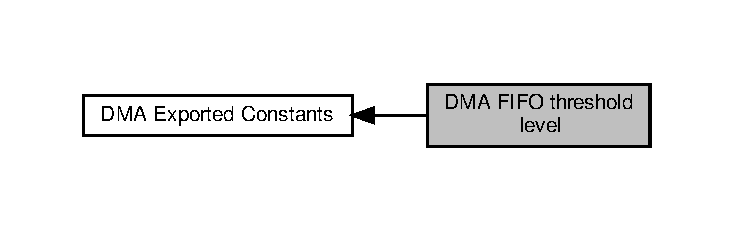
\includegraphics[width=350pt]{group___d_m_a___f_i_f_o__threshold__level}
\end{center}
\end{figure}
\subsection*{Definicje}
\begin{DoxyCompactItemize}
\item 
\#define \hyperlink{group___d_m_a___f_i_f_o__threshold__level_ga4debbd5733190b61b2115613d4b3658b}{D\+M\+A\+\_\+\+F\+I\+F\+O\+\_\+\+T\+H\+R\+E\+S\+H\+O\+L\+D\+\_\+1\+Q\+U\+A\+R\+T\+E\+R\+F\+U\+LL}~0x00000000U
\item 
\#define \hyperlink{group___d_m_a___f_i_f_o__threshold__level_gad2b071aa3a3bfc936017f12fb956c56f}{D\+M\+A\+\_\+\+F\+I\+F\+O\+\_\+\+T\+H\+R\+E\+S\+H\+O\+L\+D\+\_\+\+H\+A\+L\+F\+F\+U\+LL}~((uint32\+\_\+t)\hyperlink{group___peripheral___registers___bits___definition_ga63716e11d34bca95927671055aa63fe8}{D\+M\+A\+\_\+\+Sx\+F\+C\+R\+\_\+\+F\+T\+H\+\_\+0})
\item 
\#define \hyperlink{group___d_m_a___f_i_f_o__threshold__level_gae1e4ba12bae8440421e6672795d71223}{D\+M\+A\+\_\+\+F\+I\+F\+O\+\_\+\+T\+H\+R\+E\+S\+H\+O\+L\+D\+\_\+3\+Q\+U\+A\+R\+T\+E\+R\+S\+F\+U\+LL}~((uint32\+\_\+t)\hyperlink{group___peripheral___registers___bits___definition_gae3d780fc1222a183071c73e62a0524a1}{D\+M\+A\+\_\+\+Sx\+F\+C\+R\+\_\+\+F\+T\+H\+\_\+1})
\item 
\#define \hyperlink{group___d_m_a___f_i_f_o__threshold__level_ga5de463bb24dc12fe7bbb300e1e4493f7}{D\+M\+A\+\_\+\+F\+I\+F\+O\+\_\+\+T\+H\+R\+E\+S\+H\+O\+L\+D\+\_\+\+F\+U\+LL}~((uint32\+\_\+t)\hyperlink{group___peripheral___registers___bits___definition_ga44c16978164026a81f5b07280e800e7f}{D\+M\+A\+\_\+\+Sx\+F\+C\+R\+\_\+\+F\+TH})
\end{DoxyCompactItemize}


\subsection{Opis szczegółowy}
D\+MA F\+I\+FO level. 



\subsection{Dokumentacja definicji}
\mbox{\Hypertarget{group___d_m_a___f_i_f_o__threshold__level_ga4debbd5733190b61b2115613d4b3658b}\label{group___d_m_a___f_i_f_o__threshold__level_ga4debbd5733190b61b2115613d4b3658b}} 
\index{D\+M\+A F\+I\+F\+O threshold level@{D\+M\+A F\+I\+F\+O threshold level}!D\+M\+A\+\_\+\+F\+I\+F\+O\+\_\+\+T\+H\+R\+E\+S\+H\+O\+L\+D\+\_\+1\+Q\+U\+A\+R\+T\+E\+R\+F\+U\+LL@{D\+M\+A\+\_\+\+F\+I\+F\+O\+\_\+\+T\+H\+R\+E\+S\+H\+O\+L\+D\+\_\+1\+Q\+U\+A\+R\+T\+E\+R\+F\+U\+LL}}
\index{D\+M\+A\+\_\+\+F\+I\+F\+O\+\_\+\+T\+H\+R\+E\+S\+H\+O\+L\+D\+\_\+1\+Q\+U\+A\+R\+T\+E\+R\+F\+U\+LL@{D\+M\+A\+\_\+\+F\+I\+F\+O\+\_\+\+T\+H\+R\+E\+S\+H\+O\+L\+D\+\_\+1\+Q\+U\+A\+R\+T\+E\+R\+F\+U\+LL}!D\+M\+A F\+I\+F\+O threshold level@{D\+M\+A F\+I\+F\+O threshold level}}
\subsubsection{\texorpdfstring{D\+M\+A\+\_\+\+F\+I\+F\+O\+\_\+\+T\+H\+R\+E\+S\+H\+O\+L\+D\+\_\+1\+Q\+U\+A\+R\+T\+E\+R\+F\+U\+LL}{DMA\_FIFO\_THRESHOLD\_1QUARTERFULL}}
{\footnotesize\ttfamily \#define D\+M\+A\+\_\+\+F\+I\+F\+O\+\_\+\+T\+H\+R\+E\+S\+H\+O\+L\+D\+\_\+1\+Q\+U\+A\+R\+T\+E\+R\+F\+U\+LL~0x00000000U}

F\+I\+FO threshold 1 quart full configuration 

Definicja w linii 314 pliku stm32f4xx\+\_\+hal\+\_\+dma.\+h.

\mbox{\Hypertarget{group___d_m_a___f_i_f_o__threshold__level_gae1e4ba12bae8440421e6672795d71223}\label{group___d_m_a___f_i_f_o__threshold__level_gae1e4ba12bae8440421e6672795d71223}} 
\index{D\+M\+A F\+I\+F\+O threshold level@{D\+M\+A F\+I\+F\+O threshold level}!D\+M\+A\+\_\+\+F\+I\+F\+O\+\_\+\+T\+H\+R\+E\+S\+H\+O\+L\+D\+\_\+3\+Q\+U\+A\+R\+T\+E\+R\+S\+F\+U\+LL@{D\+M\+A\+\_\+\+F\+I\+F\+O\+\_\+\+T\+H\+R\+E\+S\+H\+O\+L\+D\+\_\+3\+Q\+U\+A\+R\+T\+E\+R\+S\+F\+U\+LL}}
\index{D\+M\+A\+\_\+\+F\+I\+F\+O\+\_\+\+T\+H\+R\+E\+S\+H\+O\+L\+D\+\_\+3\+Q\+U\+A\+R\+T\+E\+R\+S\+F\+U\+LL@{D\+M\+A\+\_\+\+F\+I\+F\+O\+\_\+\+T\+H\+R\+E\+S\+H\+O\+L\+D\+\_\+3\+Q\+U\+A\+R\+T\+E\+R\+S\+F\+U\+LL}!D\+M\+A F\+I\+F\+O threshold level@{D\+M\+A F\+I\+F\+O threshold level}}
\subsubsection{\texorpdfstring{D\+M\+A\+\_\+\+F\+I\+F\+O\+\_\+\+T\+H\+R\+E\+S\+H\+O\+L\+D\+\_\+3\+Q\+U\+A\+R\+T\+E\+R\+S\+F\+U\+LL}{DMA\_FIFO\_THRESHOLD\_3QUARTERSFULL}}
{\footnotesize\ttfamily \#define D\+M\+A\+\_\+\+F\+I\+F\+O\+\_\+\+T\+H\+R\+E\+S\+H\+O\+L\+D\+\_\+3\+Q\+U\+A\+R\+T\+E\+R\+S\+F\+U\+LL~((uint32\+\_\+t)\hyperlink{group___peripheral___registers___bits___definition_gae3d780fc1222a183071c73e62a0524a1}{D\+M\+A\+\_\+\+Sx\+F\+C\+R\+\_\+\+F\+T\+H\+\_\+1})}

F\+I\+FO threshold 3 quarts full configuration 

Definicja w linii 316 pliku stm32f4xx\+\_\+hal\+\_\+dma.\+h.

\mbox{\Hypertarget{group___d_m_a___f_i_f_o__threshold__level_ga5de463bb24dc12fe7bbb300e1e4493f7}\label{group___d_m_a___f_i_f_o__threshold__level_ga5de463bb24dc12fe7bbb300e1e4493f7}} 
\index{D\+M\+A F\+I\+F\+O threshold level@{D\+M\+A F\+I\+F\+O threshold level}!D\+M\+A\+\_\+\+F\+I\+F\+O\+\_\+\+T\+H\+R\+E\+S\+H\+O\+L\+D\+\_\+\+F\+U\+LL@{D\+M\+A\+\_\+\+F\+I\+F\+O\+\_\+\+T\+H\+R\+E\+S\+H\+O\+L\+D\+\_\+\+F\+U\+LL}}
\index{D\+M\+A\+\_\+\+F\+I\+F\+O\+\_\+\+T\+H\+R\+E\+S\+H\+O\+L\+D\+\_\+\+F\+U\+LL@{D\+M\+A\+\_\+\+F\+I\+F\+O\+\_\+\+T\+H\+R\+E\+S\+H\+O\+L\+D\+\_\+\+F\+U\+LL}!D\+M\+A F\+I\+F\+O threshold level@{D\+M\+A F\+I\+F\+O threshold level}}
\subsubsection{\texorpdfstring{D\+M\+A\+\_\+\+F\+I\+F\+O\+\_\+\+T\+H\+R\+E\+S\+H\+O\+L\+D\+\_\+\+F\+U\+LL}{DMA\_FIFO\_THRESHOLD\_FULL}}
{\footnotesize\ttfamily \#define D\+M\+A\+\_\+\+F\+I\+F\+O\+\_\+\+T\+H\+R\+E\+S\+H\+O\+L\+D\+\_\+\+F\+U\+LL~((uint32\+\_\+t)\hyperlink{group___peripheral___registers___bits___definition_ga44c16978164026a81f5b07280e800e7f}{D\+M\+A\+\_\+\+Sx\+F\+C\+R\+\_\+\+F\+TH})}

F\+I\+FO threshold full configuration 

Definicja w linii 317 pliku stm32f4xx\+\_\+hal\+\_\+dma.\+h.

\mbox{\Hypertarget{group___d_m_a___f_i_f_o__threshold__level_gad2b071aa3a3bfc936017f12fb956c56f}\label{group___d_m_a___f_i_f_o__threshold__level_gad2b071aa3a3bfc936017f12fb956c56f}} 
\index{D\+M\+A F\+I\+F\+O threshold level@{D\+M\+A F\+I\+F\+O threshold level}!D\+M\+A\+\_\+\+F\+I\+F\+O\+\_\+\+T\+H\+R\+E\+S\+H\+O\+L\+D\+\_\+\+H\+A\+L\+F\+F\+U\+LL@{D\+M\+A\+\_\+\+F\+I\+F\+O\+\_\+\+T\+H\+R\+E\+S\+H\+O\+L\+D\+\_\+\+H\+A\+L\+F\+F\+U\+LL}}
\index{D\+M\+A\+\_\+\+F\+I\+F\+O\+\_\+\+T\+H\+R\+E\+S\+H\+O\+L\+D\+\_\+\+H\+A\+L\+F\+F\+U\+LL@{D\+M\+A\+\_\+\+F\+I\+F\+O\+\_\+\+T\+H\+R\+E\+S\+H\+O\+L\+D\+\_\+\+H\+A\+L\+F\+F\+U\+LL}!D\+M\+A F\+I\+F\+O threshold level@{D\+M\+A F\+I\+F\+O threshold level}}
\subsubsection{\texorpdfstring{D\+M\+A\+\_\+\+F\+I\+F\+O\+\_\+\+T\+H\+R\+E\+S\+H\+O\+L\+D\+\_\+\+H\+A\+L\+F\+F\+U\+LL}{DMA\_FIFO\_THRESHOLD\_HALFFULL}}
{\footnotesize\ttfamily \#define D\+M\+A\+\_\+\+F\+I\+F\+O\+\_\+\+T\+H\+R\+E\+S\+H\+O\+L\+D\+\_\+\+H\+A\+L\+F\+F\+U\+LL~((uint32\+\_\+t)\hyperlink{group___peripheral___registers___bits___definition_ga63716e11d34bca95927671055aa63fe8}{D\+M\+A\+\_\+\+Sx\+F\+C\+R\+\_\+\+F\+T\+H\+\_\+0})}

F\+I\+FO threshold half full configuration 

Definicja w linii 315 pliku stm32f4xx\+\_\+hal\+\_\+dma.\+h.


\hypertarget{group___d_m_a___memory__burst}{}\section{D\+MA Memory burst}
\label{group___d_m_a___memory__burst}\index{D\+M\+A Memory burst@{D\+M\+A Memory burst}}


D\+MA memory burst.  


Diagram współpracy dla D\+MA Memory burst\+:\nopagebreak
\begin{figure}[H]
\begin{center}
\leavevmode
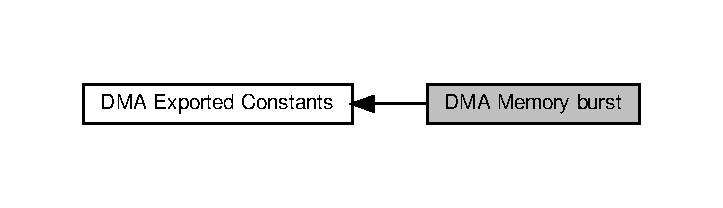
\includegraphics[width=347pt]{group___d_m_a___memory__burst}
\end{center}
\end{figure}
\subsection*{Definicje}
\begin{DoxyCompactItemize}
\item 
\#define \hyperlink{group___d_m_a___memory__burst_ga4e94b7250e6a4f53d702b42b15796953}{D\+M\+A\+\_\+\+M\+B\+U\+R\+S\+T\+\_\+\+S\+I\+N\+G\+LE}~0x00000000U
\item 
\#define \hyperlink{group___d_m_a___memory__burst_gac9efcb13b2f0a715edb931dde213c000}{D\+M\+A\+\_\+\+M\+B\+U\+R\+S\+T\+\_\+\+I\+N\+C4}~((uint32\+\_\+t)\hyperlink{group___peripheral___registers___bits___definition_ga1e3931a8f14ffe008b8717e1b3232fca}{D\+M\+A\+\_\+\+Sx\+C\+R\+\_\+\+M\+B\+U\+R\+S\+T\+\_\+0})
\item 
\#define \hyperlink{group___d_m_a___memory__burst_ga4b8834930bb3b93cd3fcf04660b6933d}{D\+M\+A\+\_\+\+M\+B\+U\+R\+S\+T\+\_\+\+I\+N\+C8}~((uint32\+\_\+t)\hyperlink{group___peripheral___registers___bits___definition_gaf28eac7212392083bbf1b3d475022b74}{D\+M\+A\+\_\+\+Sx\+C\+R\+\_\+\+M\+B\+U\+R\+S\+T\+\_\+1})
\item 
\#define \hyperlink{group___d_m_a___memory__burst_ga7812aea620b09c4f4281d614d86e6094}{D\+M\+A\+\_\+\+M\+B\+U\+R\+S\+T\+\_\+\+I\+N\+C16}~((uint32\+\_\+t)\hyperlink{group___peripheral___registers___bits___definition_ga5c1174bff38faf5d87b71521bce8f84f}{D\+M\+A\+\_\+\+Sx\+C\+R\+\_\+\+M\+B\+U\+R\+ST})
\end{DoxyCompactItemize}


\subsection{Opis szczegółowy}
D\+MA memory burst. 



\subsection{Dokumentacja definicji}
\mbox{\Hypertarget{group___d_m_a___memory__burst_ga7812aea620b09c4f4281d614d86e6094}\label{group___d_m_a___memory__burst_ga7812aea620b09c4f4281d614d86e6094}} 
\index{D\+M\+A Memory burst@{D\+M\+A Memory burst}!D\+M\+A\+\_\+\+M\+B\+U\+R\+S\+T\+\_\+\+I\+N\+C16@{D\+M\+A\+\_\+\+M\+B\+U\+R\+S\+T\+\_\+\+I\+N\+C16}}
\index{D\+M\+A\+\_\+\+M\+B\+U\+R\+S\+T\+\_\+\+I\+N\+C16@{D\+M\+A\+\_\+\+M\+B\+U\+R\+S\+T\+\_\+\+I\+N\+C16}!D\+M\+A Memory burst@{D\+M\+A Memory burst}}
\subsubsection{\texorpdfstring{D\+M\+A\+\_\+\+M\+B\+U\+R\+S\+T\+\_\+\+I\+N\+C16}{DMA\_MBURST\_INC16}}
{\footnotesize\ttfamily \#define D\+M\+A\+\_\+\+M\+B\+U\+R\+S\+T\+\_\+\+I\+N\+C16~((uint32\+\_\+t)\hyperlink{group___peripheral___registers___bits___definition_ga5c1174bff38faf5d87b71521bce8f84f}{D\+M\+A\+\_\+\+Sx\+C\+R\+\_\+\+M\+B\+U\+R\+ST})}



Definicja w linii 329 pliku stm32f4xx\+\_\+hal\+\_\+dma.\+h.

\mbox{\Hypertarget{group___d_m_a___memory__burst_gac9efcb13b2f0a715edb931dde213c000}\label{group___d_m_a___memory__burst_gac9efcb13b2f0a715edb931dde213c000}} 
\index{D\+M\+A Memory burst@{D\+M\+A Memory burst}!D\+M\+A\+\_\+\+M\+B\+U\+R\+S\+T\+\_\+\+I\+N\+C4@{D\+M\+A\+\_\+\+M\+B\+U\+R\+S\+T\+\_\+\+I\+N\+C4}}
\index{D\+M\+A\+\_\+\+M\+B\+U\+R\+S\+T\+\_\+\+I\+N\+C4@{D\+M\+A\+\_\+\+M\+B\+U\+R\+S\+T\+\_\+\+I\+N\+C4}!D\+M\+A Memory burst@{D\+M\+A Memory burst}}
\subsubsection{\texorpdfstring{D\+M\+A\+\_\+\+M\+B\+U\+R\+S\+T\+\_\+\+I\+N\+C4}{DMA\_MBURST\_INC4}}
{\footnotesize\ttfamily \#define D\+M\+A\+\_\+\+M\+B\+U\+R\+S\+T\+\_\+\+I\+N\+C4~((uint32\+\_\+t)\hyperlink{group___peripheral___registers___bits___definition_ga1e3931a8f14ffe008b8717e1b3232fca}{D\+M\+A\+\_\+\+Sx\+C\+R\+\_\+\+M\+B\+U\+R\+S\+T\+\_\+0})}



Definicja w linii 327 pliku stm32f4xx\+\_\+hal\+\_\+dma.\+h.

\mbox{\Hypertarget{group___d_m_a___memory__burst_ga4b8834930bb3b93cd3fcf04660b6933d}\label{group___d_m_a___memory__burst_ga4b8834930bb3b93cd3fcf04660b6933d}} 
\index{D\+M\+A Memory burst@{D\+M\+A Memory burst}!D\+M\+A\+\_\+\+M\+B\+U\+R\+S\+T\+\_\+\+I\+N\+C8@{D\+M\+A\+\_\+\+M\+B\+U\+R\+S\+T\+\_\+\+I\+N\+C8}}
\index{D\+M\+A\+\_\+\+M\+B\+U\+R\+S\+T\+\_\+\+I\+N\+C8@{D\+M\+A\+\_\+\+M\+B\+U\+R\+S\+T\+\_\+\+I\+N\+C8}!D\+M\+A Memory burst@{D\+M\+A Memory burst}}
\subsubsection{\texorpdfstring{D\+M\+A\+\_\+\+M\+B\+U\+R\+S\+T\+\_\+\+I\+N\+C8}{DMA\_MBURST\_INC8}}
{\footnotesize\ttfamily \#define D\+M\+A\+\_\+\+M\+B\+U\+R\+S\+T\+\_\+\+I\+N\+C8~((uint32\+\_\+t)\hyperlink{group___peripheral___registers___bits___definition_gaf28eac7212392083bbf1b3d475022b74}{D\+M\+A\+\_\+\+Sx\+C\+R\+\_\+\+M\+B\+U\+R\+S\+T\+\_\+1})}



Definicja w linii 328 pliku stm32f4xx\+\_\+hal\+\_\+dma.\+h.

\mbox{\Hypertarget{group___d_m_a___memory__burst_ga4e94b7250e6a4f53d702b42b15796953}\label{group___d_m_a___memory__burst_ga4e94b7250e6a4f53d702b42b15796953}} 
\index{D\+M\+A Memory burst@{D\+M\+A Memory burst}!D\+M\+A\+\_\+\+M\+B\+U\+R\+S\+T\+\_\+\+S\+I\+N\+G\+LE@{D\+M\+A\+\_\+\+M\+B\+U\+R\+S\+T\+\_\+\+S\+I\+N\+G\+LE}}
\index{D\+M\+A\+\_\+\+M\+B\+U\+R\+S\+T\+\_\+\+S\+I\+N\+G\+LE@{D\+M\+A\+\_\+\+M\+B\+U\+R\+S\+T\+\_\+\+S\+I\+N\+G\+LE}!D\+M\+A Memory burst@{D\+M\+A Memory burst}}
\subsubsection{\texorpdfstring{D\+M\+A\+\_\+\+M\+B\+U\+R\+S\+T\+\_\+\+S\+I\+N\+G\+LE}{DMA\_MBURST\_SINGLE}}
{\footnotesize\ttfamily \#define D\+M\+A\+\_\+\+M\+B\+U\+R\+S\+T\+\_\+\+S\+I\+N\+G\+LE~0x00000000U}



Definicja w linii 326 pliku stm32f4xx\+\_\+hal\+\_\+dma.\+h.


\hypertarget{group___d_m_a___peripheral__burst}{}\section{D\+MA Peripheral burst}
\label{group___d_m_a___peripheral__burst}\index{D\+M\+A Peripheral burst@{D\+M\+A Peripheral burst}}


D\+MA peripheral burst.  


Diagram współpracy dla D\+MA Peripheral burst\+:\nopagebreak
\begin{figure}[H]
\begin{center}
\leavevmode
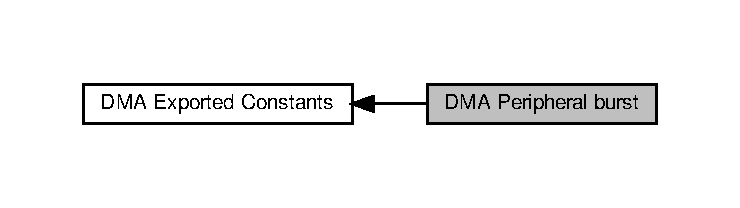
\includegraphics[width=350pt]{group___d_m_a___peripheral__burst}
\end{center}
\end{figure}
\subsection*{Definicje}
\begin{DoxyCompactItemize}
\item 
\#define \hyperlink{group___d_m_a___peripheral__burst_ga1ee9cf4dc1c8bfc5ab6dfb95a00f81ff}{D\+M\+A\+\_\+\+P\+B\+U\+R\+S\+T\+\_\+\+S\+I\+N\+G\+LE}~0x00000000U
\item 
\#define \hyperlink{group___d_m_a___peripheral__burst_gacc54efc746528ed9e0173dad956f7caf}{D\+M\+A\+\_\+\+P\+B\+U\+R\+S\+T\+\_\+\+I\+N\+C4}~((uint32\+\_\+t)\hyperlink{group___peripheral___registers___bits___definition_gadf0eee1ad1788868a194f95107057a16}{D\+M\+A\+\_\+\+Sx\+C\+R\+\_\+\+P\+B\+U\+R\+S\+T\+\_\+0})
\item 
\#define \hyperlink{group___d_m_a___peripheral__burst_gaf76dd9b208c8606e8c5ae7abf8c26532}{D\+M\+A\+\_\+\+P\+B\+U\+R\+S\+T\+\_\+\+I\+N\+C8}~((uint32\+\_\+t)\hyperlink{group___peripheral___registers___bits___definition_ga061207b2c654a0dd62e40187c9557eda}{D\+M\+A\+\_\+\+Sx\+C\+R\+\_\+\+P\+B\+U\+R\+S\+T\+\_\+1})
\item 
\#define \hyperlink{group___d_m_a___peripheral__burst_ga705a631ea96b34aa5afa7fed06a487e0}{D\+M\+A\+\_\+\+P\+B\+U\+R\+S\+T\+\_\+\+I\+N\+C16}~((uint32\+\_\+t)\hyperlink{group___peripheral___registers___bits___definition_ga502380abb155eb3b37a2ca9359e2da2e}{D\+M\+A\+\_\+\+Sx\+C\+R\+\_\+\+P\+B\+U\+R\+ST})
\end{DoxyCompactItemize}


\subsection{Opis szczegółowy}
D\+MA peripheral burst. 



\subsection{Dokumentacja definicji}
\mbox{\Hypertarget{group___d_m_a___peripheral__burst_ga705a631ea96b34aa5afa7fed06a487e0}\label{group___d_m_a___peripheral__burst_ga705a631ea96b34aa5afa7fed06a487e0}} 
\index{D\+M\+A Peripheral burst@{D\+M\+A Peripheral burst}!D\+M\+A\+\_\+\+P\+B\+U\+R\+S\+T\+\_\+\+I\+N\+C16@{D\+M\+A\+\_\+\+P\+B\+U\+R\+S\+T\+\_\+\+I\+N\+C16}}
\index{D\+M\+A\+\_\+\+P\+B\+U\+R\+S\+T\+\_\+\+I\+N\+C16@{D\+M\+A\+\_\+\+P\+B\+U\+R\+S\+T\+\_\+\+I\+N\+C16}!D\+M\+A Peripheral burst@{D\+M\+A Peripheral burst}}
\subsubsection{\texorpdfstring{D\+M\+A\+\_\+\+P\+B\+U\+R\+S\+T\+\_\+\+I\+N\+C16}{DMA\_PBURST\_INC16}}
{\footnotesize\ttfamily \#define D\+M\+A\+\_\+\+P\+B\+U\+R\+S\+T\+\_\+\+I\+N\+C16~((uint32\+\_\+t)\hyperlink{group___peripheral___registers___bits___definition_ga502380abb155eb3b37a2ca9359e2da2e}{D\+M\+A\+\_\+\+Sx\+C\+R\+\_\+\+P\+B\+U\+R\+ST})}



Definicja w linii 341 pliku stm32f4xx\+\_\+hal\+\_\+dma.\+h.

\mbox{\Hypertarget{group___d_m_a___peripheral__burst_gacc54efc746528ed9e0173dad956f7caf}\label{group___d_m_a___peripheral__burst_gacc54efc746528ed9e0173dad956f7caf}} 
\index{D\+M\+A Peripheral burst@{D\+M\+A Peripheral burst}!D\+M\+A\+\_\+\+P\+B\+U\+R\+S\+T\+\_\+\+I\+N\+C4@{D\+M\+A\+\_\+\+P\+B\+U\+R\+S\+T\+\_\+\+I\+N\+C4}}
\index{D\+M\+A\+\_\+\+P\+B\+U\+R\+S\+T\+\_\+\+I\+N\+C4@{D\+M\+A\+\_\+\+P\+B\+U\+R\+S\+T\+\_\+\+I\+N\+C4}!D\+M\+A Peripheral burst@{D\+M\+A Peripheral burst}}
\subsubsection{\texorpdfstring{D\+M\+A\+\_\+\+P\+B\+U\+R\+S\+T\+\_\+\+I\+N\+C4}{DMA\_PBURST\_INC4}}
{\footnotesize\ttfamily \#define D\+M\+A\+\_\+\+P\+B\+U\+R\+S\+T\+\_\+\+I\+N\+C4~((uint32\+\_\+t)\hyperlink{group___peripheral___registers___bits___definition_gadf0eee1ad1788868a194f95107057a16}{D\+M\+A\+\_\+\+Sx\+C\+R\+\_\+\+P\+B\+U\+R\+S\+T\+\_\+0})}



Definicja w linii 339 pliku stm32f4xx\+\_\+hal\+\_\+dma.\+h.

\mbox{\Hypertarget{group___d_m_a___peripheral__burst_gaf76dd9b208c8606e8c5ae7abf8c26532}\label{group___d_m_a___peripheral__burst_gaf76dd9b208c8606e8c5ae7abf8c26532}} 
\index{D\+M\+A Peripheral burst@{D\+M\+A Peripheral burst}!D\+M\+A\+\_\+\+P\+B\+U\+R\+S\+T\+\_\+\+I\+N\+C8@{D\+M\+A\+\_\+\+P\+B\+U\+R\+S\+T\+\_\+\+I\+N\+C8}}
\index{D\+M\+A\+\_\+\+P\+B\+U\+R\+S\+T\+\_\+\+I\+N\+C8@{D\+M\+A\+\_\+\+P\+B\+U\+R\+S\+T\+\_\+\+I\+N\+C8}!D\+M\+A Peripheral burst@{D\+M\+A Peripheral burst}}
\subsubsection{\texorpdfstring{D\+M\+A\+\_\+\+P\+B\+U\+R\+S\+T\+\_\+\+I\+N\+C8}{DMA\_PBURST\_INC8}}
{\footnotesize\ttfamily \#define D\+M\+A\+\_\+\+P\+B\+U\+R\+S\+T\+\_\+\+I\+N\+C8~((uint32\+\_\+t)\hyperlink{group___peripheral___registers___bits___definition_ga061207b2c654a0dd62e40187c9557eda}{D\+M\+A\+\_\+\+Sx\+C\+R\+\_\+\+P\+B\+U\+R\+S\+T\+\_\+1})}



Definicja w linii 340 pliku stm32f4xx\+\_\+hal\+\_\+dma.\+h.

\mbox{\Hypertarget{group___d_m_a___peripheral__burst_ga1ee9cf4dc1c8bfc5ab6dfb95a00f81ff}\label{group___d_m_a___peripheral__burst_ga1ee9cf4dc1c8bfc5ab6dfb95a00f81ff}} 
\index{D\+M\+A Peripheral burst@{D\+M\+A Peripheral burst}!D\+M\+A\+\_\+\+P\+B\+U\+R\+S\+T\+\_\+\+S\+I\+N\+G\+LE@{D\+M\+A\+\_\+\+P\+B\+U\+R\+S\+T\+\_\+\+S\+I\+N\+G\+LE}}
\index{D\+M\+A\+\_\+\+P\+B\+U\+R\+S\+T\+\_\+\+S\+I\+N\+G\+LE@{D\+M\+A\+\_\+\+P\+B\+U\+R\+S\+T\+\_\+\+S\+I\+N\+G\+LE}!D\+M\+A Peripheral burst@{D\+M\+A Peripheral burst}}
\subsubsection{\texorpdfstring{D\+M\+A\+\_\+\+P\+B\+U\+R\+S\+T\+\_\+\+S\+I\+N\+G\+LE}{DMA\_PBURST\_SINGLE}}
{\footnotesize\ttfamily \#define D\+M\+A\+\_\+\+P\+B\+U\+R\+S\+T\+\_\+\+S\+I\+N\+G\+LE~0x00000000U}



Definicja w linii 338 pliku stm32f4xx\+\_\+hal\+\_\+dma.\+h.


\hypertarget{group___d_m_a__interrupt__enable__definitions}{}\section{D\+MA interrupt enable definitions}
\label{group___d_m_a__interrupt__enable__definitions}\index{D\+M\+A interrupt enable definitions@{D\+M\+A interrupt enable definitions}}


D\+MA interrupts definition.  


Diagram współpracy dla D\+MA interrupt enable definitions\+:\nopagebreak
\begin{figure}[H]
\begin{center}
\leavevmode
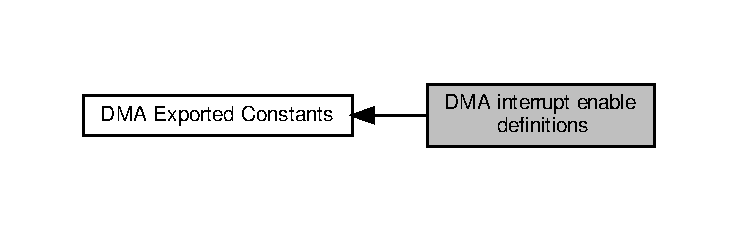
\includegraphics[width=350pt]{group___d_m_a__interrupt__enable__definitions}
\end{center}
\end{figure}
\subsection*{Definicje}
\begin{DoxyCompactItemize}
\item 
\#define \hyperlink{group___d_m_a__interrupt__enable__definitions_ga06e83dd277e0d3e5635cf8ce8dfd6e16}{D\+M\+A\+\_\+\+I\+T\+\_\+\+TC}~((uint32\+\_\+t)\hyperlink{group___peripheral___registers___bits___definition_ga6ae47cc2cd2e985d29cb6b0bb65da1d7}{D\+M\+A\+\_\+\+Sx\+C\+R\+\_\+\+T\+C\+IE})
\item 
\#define \hyperlink{group___d_m_a__interrupt__enable__definitions_gadf11c572b9797e04a14b105fdc2e5f66}{D\+M\+A\+\_\+\+I\+T\+\_\+\+HT}~((uint32\+\_\+t)\hyperlink{group___peripheral___registers___bits___definition_ga13a7fe097608bc5031d42ba69effed20}{D\+M\+A\+\_\+\+Sx\+C\+R\+\_\+\+H\+T\+IE})
\item 
\#define \hyperlink{group___d_m_a__interrupt__enable__definitions_gaf9d92649d2a0146f663ff253d8f3b59e}{D\+M\+A\+\_\+\+I\+T\+\_\+\+TE}~((uint32\+\_\+t)\hyperlink{group___peripheral___registers___bits___definition_gaeee99c36ba3ea56cdb4f73a0b01fb602}{D\+M\+A\+\_\+\+Sx\+C\+R\+\_\+\+T\+E\+IE})
\item 
\#define \hyperlink{group___d_m_a__interrupt__enable__definitions_ga71137443f7bdced1ee80697596e9ea98}{D\+M\+A\+\_\+\+I\+T\+\_\+\+D\+ME}~((uint32\+\_\+t)\hyperlink{group___peripheral___registers___bits___definition_gacaecc56f94a9af756d077cf7df1b6c41}{D\+M\+A\+\_\+\+Sx\+C\+R\+\_\+\+D\+M\+E\+IE})
\item 
\#define \hyperlink{group___d_m_a__interrupt__enable__definitions_ga93164ec039fc5579662c382e68d7d13f}{D\+M\+A\+\_\+\+I\+T\+\_\+\+FE}~0x00000080U
\end{DoxyCompactItemize}


\subsection{Opis szczegółowy}
D\+MA interrupts definition. 



\subsection{Dokumentacja definicji}
\mbox{\Hypertarget{group___d_m_a__interrupt__enable__definitions_ga71137443f7bdced1ee80697596e9ea98}\label{group___d_m_a__interrupt__enable__definitions_ga71137443f7bdced1ee80697596e9ea98}} 
\index{D\+M\+A interrupt enable definitions@{D\+M\+A interrupt enable definitions}!D\+M\+A\+\_\+\+I\+T\+\_\+\+D\+ME@{D\+M\+A\+\_\+\+I\+T\+\_\+\+D\+ME}}
\index{D\+M\+A\+\_\+\+I\+T\+\_\+\+D\+ME@{D\+M\+A\+\_\+\+I\+T\+\_\+\+D\+ME}!D\+M\+A interrupt enable definitions@{D\+M\+A interrupt enable definitions}}
\subsubsection{\texorpdfstring{D\+M\+A\+\_\+\+I\+T\+\_\+\+D\+ME}{DMA\_IT\_DME}}
{\footnotesize\ttfamily \#define D\+M\+A\+\_\+\+I\+T\+\_\+\+D\+ME~((uint32\+\_\+t)\hyperlink{group___peripheral___registers___bits___definition_gacaecc56f94a9af756d077cf7df1b6c41}{D\+M\+A\+\_\+\+Sx\+C\+R\+\_\+\+D\+M\+E\+IE})}



Definicja w linii 353 pliku stm32f4xx\+\_\+hal\+\_\+dma.\+h.

\mbox{\Hypertarget{group___d_m_a__interrupt__enable__definitions_ga93164ec039fc5579662c382e68d7d13f}\label{group___d_m_a__interrupt__enable__definitions_ga93164ec039fc5579662c382e68d7d13f}} 
\index{D\+M\+A interrupt enable definitions@{D\+M\+A interrupt enable definitions}!D\+M\+A\+\_\+\+I\+T\+\_\+\+FE@{D\+M\+A\+\_\+\+I\+T\+\_\+\+FE}}
\index{D\+M\+A\+\_\+\+I\+T\+\_\+\+FE@{D\+M\+A\+\_\+\+I\+T\+\_\+\+FE}!D\+M\+A interrupt enable definitions@{D\+M\+A interrupt enable definitions}}
\subsubsection{\texorpdfstring{D\+M\+A\+\_\+\+I\+T\+\_\+\+FE}{DMA\_IT\_FE}}
{\footnotesize\ttfamily \#define D\+M\+A\+\_\+\+I\+T\+\_\+\+FE~0x00000080U}



Definicja w linii 354 pliku stm32f4xx\+\_\+hal\+\_\+dma.\+h.

\mbox{\Hypertarget{group___d_m_a__interrupt__enable__definitions_gadf11c572b9797e04a14b105fdc2e5f66}\label{group___d_m_a__interrupt__enable__definitions_gadf11c572b9797e04a14b105fdc2e5f66}} 
\index{D\+M\+A interrupt enable definitions@{D\+M\+A interrupt enable definitions}!D\+M\+A\+\_\+\+I\+T\+\_\+\+HT@{D\+M\+A\+\_\+\+I\+T\+\_\+\+HT}}
\index{D\+M\+A\+\_\+\+I\+T\+\_\+\+HT@{D\+M\+A\+\_\+\+I\+T\+\_\+\+HT}!D\+M\+A interrupt enable definitions@{D\+M\+A interrupt enable definitions}}
\subsubsection{\texorpdfstring{D\+M\+A\+\_\+\+I\+T\+\_\+\+HT}{DMA\_IT\_HT}}
{\footnotesize\ttfamily \#define D\+M\+A\+\_\+\+I\+T\+\_\+\+HT~((uint32\+\_\+t)\hyperlink{group___peripheral___registers___bits___definition_ga13a7fe097608bc5031d42ba69effed20}{D\+M\+A\+\_\+\+Sx\+C\+R\+\_\+\+H\+T\+IE})}



Definicja w linii 351 pliku stm32f4xx\+\_\+hal\+\_\+dma.\+h.

\mbox{\Hypertarget{group___d_m_a__interrupt__enable__definitions_ga06e83dd277e0d3e5635cf8ce8dfd6e16}\label{group___d_m_a__interrupt__enable__definitions_ga06e83dd277e0d3e5635cf8ce8dfd6e16}} 
\index{D\+M\+A interrupt enable definitions@{D\+M\+A interrupt enable definitions}!D\+M\+A\+\_\+\+I\+T\+\_\+\+TC@{D\+M\+A\+\_\+\+I\+T\+\_\+\+TC}}
\index{D\+M\+A\+\_\+\+I\+T\+\_\+\+TC@{D\+M\+A\+\_\+\+I\+T\+\_\+\+TC}!D\+M\+A interrupt enable definitions@{D\+M\+A interrupt enable definitions}}
\subsubsection{\texorpdfstring{D\+M\+A\+\_\+\+I\+T\+\_\+\+TC}{DMA\_IT\_TC}}
{\footnotesize\ttfamily \#define D\+M\+A\+\_\+\+I\+T\+\_\+\+TC~((uint32\+\_\+t)\hyperlink{group___peripheral___registers___bits___definition_ga6ae47cc2cd2e985d29cb6b0bb65da1d7}{D\+M\+A\+\_\+\+Sx\+C\+R\+\_\+\+T\+C\+IE})}



Definicja w linii 350 pliku stm32f4xx\+\_\+hal\+\_\+dma.\+h.

\mbox{\Hypertarget{group___d_m_a__interrupt__enable__definitions_gaf9d92649d2a0146f663ff253d8f3b59e}\label{group___d_m_a__interrupt__enable__definitions_gaf9d92649d2a0146f663ff253d8f3b59e}} 
\index{D\+M\+A interrupt enable definitions@{D\+M\+A interrupt enable definitions}!D\+M\+A\+\_\+\+I\+T\+\_\+\+TE@{D\+M\+A\+\_\+\+I\+T\+\_\+\+TE}}
\index{D\+M\+A\+\_\+\+I\+T\+\_\+\+TE@{D\+M\+A\+\_\+\+I\+T\+\_\+\+TE}!D\+M\+A interrupt enable definitions@{D\+M\+A interrupt enable definitions}}
\subsubsection{\texorpdfstring{D\+M\+A\+\_\+\+I\+T\+\_\+\+TE}{DMA\_IT\_TE}}
{\footnotesize\ttfamily \#define D\+M\+A\+\_\+\+I\+T\+\_\+\+TE~((uint32\+\_\+t)\hyperlink{group___peripheral___registers___bits___definition_gaeee99c36ba3ea56cdb4f73a0b01fb602}{D\+M\+A\+\_\+\+Sx\+C\+R\+\_\+\+T\+E\+IE})}



Definicja w linii 352 pliku stm32f4xx\+\_\+hal\+\_\+dma.\+h.


\hypertarget{group___d_m_a__flag__definitions}{}\section{D\+MA flag definitions}
\label{group___d_m_a__flag__definitions}\index{D\+M\+A flag definitions@{D\+M\+A flag definitions}}


D\+MA flag definitions.  


Diagram współpracy dla D\+MA flag definitions\+:\nopagebreak
\begin{figure}[H]
\begin{center}
\leavevmode
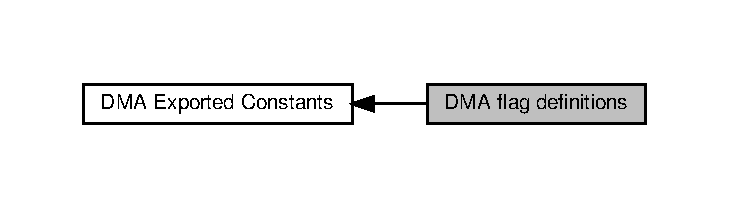
\includegraphics[width=350pt]{group___d_m_a__flag__definitions}
\end{center}
\end{figure}
\subsection*{Definicje}
\begin{DoxyCompactItemize}
\item 
\#define \hyperlink{group___d_m_a__flag__definitions_ga6f44b274316a463c9302d770b8205640}{D\+M\+A\+\_\+\+F\+L\+A\+G\+\_\+\+F\+E\+I\+F0\+\_\+4}~0x00000001U
\item 
\#define \hyperlink{group___d_m_a__flag__definitions_gaee0e6da831d62bc84e9e28e59b8e9ede}{D\+M\+A\+\_\+\+F\+L\+A\+G\+\_\+\+D\+M\+E\+I\+F0\+\_\+4}~0x00000004U
\item 
\#define \hyperlink{group___d_m_a__flag__definitions_gab98ef70ba0c1498d4c967a10b3f6e67f}{D\+M\+A\+\_\+\+F\+L\+A\+G\+\_\+\+T\+E\+I\+F0\+\_\+4}~0x00000008U
\item 
\#define \hyperlink{group___d_m_a__flag__definitions_ga976fee242270824013f1fc0b6bd4c446}{D\+M\+A\+\_\+\+F\+L\+A\+G\+\_\+\+H\+T\+I\+F0\+\_\+4}~0x00000010U
\item 
\#define \hyperlink{group___d_m_a__flag__definitions_ga19dfe70176841c6972818e279ba02436}{D\+M\+A\+\_\+\+F\+L\+A\+G\+\_\+\+T\+C\+I\+F0\+\_\+4}~0x00000020U
\item 
\#define \hyperlink{group___d_m_a__flag__definitions_ga16a04159a9a7c434ac02e5c6ff630b2e}{D\+M\+A\+\_\+\+F\+L\+A\+G\+\_\+\+F\+E\+I\+F1\+\_\+5}~0x00000040U
\item 
\#define \hyperlink{group___d_m_a__flag__definitions_gaae665bbda7f888f0b8ac3d10688bfc5d}{D\+M\+A\+\_\+\+F\+L\+A\+G\+\_\+\+D\+M\+E\+I\+F1\+\_\+5}~0x00000100U
\item 
\#define \hyperlink{group___d_m_a__flag__definitions_ga9d4c5bac7bdcdb23b4d38186e918ae9e}{D\+M\+A\+\_\+\+F\+L\+A\+G\+\_\+\+T\+E\+I\+F1\+\_\+5}~0x00000200U
\item 
\#define \hyperlink{group___d_m_a__flag__definitions_ga2c9522a20a6ace45958413034b7f3af8}{D\+M\+A\+\_\+\+F\+L\+A\+G\+\_\+\+H\+T\+I\+F1\+\_\+5}~0x00000400U
\item 
\#define \hyperlink{group___d_m_a__flag__definitions_ga9546185449ae979fad0aa5e33310c0ab}{D\+M\+A\+\_\+\+F\+L\+A\+G\+\_\+\+T\+C\+I\+F1\+\_\+5}~0x00000800U
\item 
\#define \hyperlink{group___d_m_a__flag__definitions_gaba3e6950c089013f9f675b83d78cab5c}{D\+M\+A\+\_\+\+F\+L\+A\+G\+\_\+\+F\+E\+I\+F2\+\_\+6}~0x00010000U
\item 
\#define \hyperlink{group___d_m_a__flag__definitions_ga8963d8e64fa5610d7617d8fe81c76704}{D\+M\+A\+\_\+\+F\+L\+A\+G\+\_\+\+D\+M\+E\+I\+F2\+\_\+6}~0x00040000U
\item 
\#define \hyperlink{group___d_m_a__flag__definitions_ga7801bd49cbbe19be612718965e8c675e}{D\+M\+A\+\_\+\+F\+L\+A\+G\+\_\+\+T\+E\+I\+F2\+\_\+6}~0x00080000U
\item 
\#define \hyperlink{group___d_m_a__flag__definitions_ga2ae0054d63c453a14b6d3822c503e7b4}{D\+M\+A\+\_\+\+F\+L\+A\+G\+\_\+\+H\+T\+I\+F2\+\_\+6}~0x00100000U
\item 
\#define \hyperlink{group___d_m_a__flag__definitions_gab8096a50b81e30e474e2b1148b55a983}{D\+M\+A\+\_\+\+F\+L\+A\+G\+\_\+\+T\+C\+I\+F2\+\_\+6}~0x00200000U
\item 
\#define \hyperlink{group___d_m_a__flag__definitions_gaea8077c9d9c55c53024c9f90e7f2c76f}{D\+M\+A\+\_\+\+F\+L\+A\+G\+\_\+\+F\+E\+I\+F3\+\_\+7}~0x00400000U
\item 
\#define \hyperlink{group___d_m_a__flag__definitions_ga3053e2fb5ef245cf9c847c4de3fd1732}{D\+M\+A\+\_\+\+F\+L\+A\+G\+\_\+\+D\+M\+E\+I\+F3\+\_\+7}~0x01000000U
\item 
\#define \hyperlink{group___d_m_a__flag__definitions_ga7070307dcd59da45137962c521a06562}{D\+M\+A\+\_\+\+F\+L\+A\+G\+\_\+\+T\+E\+I\+F3\+\_\+7}~0x02000000U
\item 
\#define \hyperlink{group___d_m_a__flag__definitions_ga139d44f447ab2cf5c18311cf6b6ee6e2}{D\+M\+A\+\_\+\+F\+L\+A\+G\+\_\+\+H\+T\+I\+F3\+\_\+7}~0x04000000U
\item 
\#define \hyperlink{group___d_m_a__flag__definitions_ga4acf62e6807442dd5b611d95d1617b98}{D\+M\+A\+\_\+\+F\+L\+A\+G\+\_\+\+T\+C\+I\+F3\+\_\+7}~0x08000000U
\end{DoxyCompactItemize}


\subsection{Opis szczegółowy}
D\+MA flag definitions. 



\subsection{Dokumentacja definicji}
\mbox{\Hypertarget{group___d_m_a__flag__definitions_gaee0e6da831d62bc84e9e28e59b8e9ede}\label{group___d_m_a__flag__definitions_gaee0e6da831d62bc84e9e28e59b8e9ede}} 
\index{D\+M\+A flag definitions@{D\+M\+A flag definitions}!D\+M\+A\+\_\+\+F\+L\+A\+G\+\_\+\+D\+M\+E\+I\+F0\+\_\+4@{D\+M\+A\+\_\+\+F\+L\+A\+G\+\_\+\+D\+M\+E\+I\+F0\+\_\+4}}
\index{D\+M\+A\+\_\+\+F\+L\+A\+G\+\_\+\+D\+M\+E\+I\+F0\+\_\+4@{D\+M\+A\+\_\+\+F\+L\+A\+G\+\_\+\+D\+M\+E\+I\+F0\+\_\+4}!D\+M\+A flag definitions@{D\+M\+A flag definitions}}
\subsubsection{\texorpdfstring{D\+M\+A\+\_\+\+F\+L\+A\+G\+\_\+\+D\+M\+E\+I\+F0\+\_\+4}{DMA\_FLAG\_DMEIF0\_4}}
{\footnotesize\ttfamily \#define D\+M\+A\+\_\+\+F\+L\+A\+G\+\_\+\+D\+M\+E\+I\+F0\+\_\+4~0x00000004U}



Definicja w linii 364 pliku stm32f4xx\+\_\+hal\+\_\+dma.\+h.

\mbox{\Hypertarget{group___d_m_a__flag__definitions_gaae665bbda7f888f0b8ac3d10688bfc5d}\label{group___d_m_a__flag__definitions_gaae665bbda7f888f0b8ac3d10688bfc5d}} 
\index{D\+M\+A flag definitions@{D\+M\+A flag definitions}!D\+M\+A\+\_\+\+F\+L\+A\+G\+\_\+\+D\+M\+E\+I\+F1\+\_\+5@{D\+M\+A\+\_\+\+F\+L\+A\+G\+\_\+\+D\+M\+E\+I\+F1\+\_\+5}}
\index{D\+M\+A\+\_\+\+F\+L\+A\+G\+\_\+\+D\+M\+E\+I\+F1\+\_\+5@{D\+M\+A\+\_\+\+F\+L\+A\+G\+\_\+\+D\+M\+E\+I\+F1\+\_\+5}!D\+M\+A flag definitions@{D\+M\+A flag definitions}}
\subsubsection{\texorpdfstring{D\+M\+A\+\_\+\+F\+L\+A\+G\+\_\+\+D\+M\+E\+I\+F1\+\_\+5}{DMA\_FLAG\_DMEIF1\_5}}
{\footnotesize\ttfamily \#define D\+M\+A\+\_\+\+F\+L\+A\+G\+\_\+\+D\+M\+E\+I\+F1\+\_\+5~0x00000100U}



Definicja w linii 369 pliku stm32f4xx\+\_\+hal\+\_\+dma.\+h.

\mbox{\Hypertarget{group___d_m_a__flag__definitions_ga8963d8e64fa5610d7617d8fe81c76704}\label{group___d_m_a__flag__definitions_ga8963d8e64fa5610d7617d8fe81c76704}} 
\index{D\+M\+A flag definitions@{D\+M\+A flag definitions}!D\+M\+A\+\_\+\+F\+L\+A\+G\+\_\+\+D\+M\+E\+I\+F2\+\_\+6@{D\+M\+A\+\_\+\+F\+L\+A\+G\+\_\+\+D\+M\+E\+I\+F2\+\_\+6}}
\index{D\+M\+A\+\_\+\+F\+L\+A\+G\+\_\+\+D\+M\+E\+I\+F2\+\_\+6@{D\+M\+A\+\_\+\+F\+L\+A\+G\+\_\+\+D\+M\+E\+I\+F2\+\_\+6}!D\+M\+A flag definitions@{D\+M\+A flag definitions}}
\subsubsection{\texorpdfstring{D\+M\+A\+\_\+\+F\+L\+A\+G\+\_\+\+D\+M\+E\+I\+F2\+\_\+6}{DMA\_FLAG\_DMEIF2\_6}}
{\footnotesize\ttfamily \#define D\+M\+A\+\_\+\+F\+L\+A\+G\+\_\+\+D\+M\+E\+I\+F2\+\_\+6~0x00040000U}



Definicja w linii 374 pliku stm32f4xx\+\_\+hal\+\_\+dma.\+h.

\mbox{\Hypertarget{group___d_m_a__flag__definitions_ga3053e2fb5ef245cf9c847c4de3fd1732}\label{group___d_m_a__flag__definitions_ga3053e2fb5ef245cf9c847c4de3fd1732}} 
\index{D\+M\+A flag definitions@{D\+M\+A flag definitions}!D\+M\+A\+\_\+\+F\+L\+A\+G\+\_\+\+D\+M\+E\+I\+F3\+\_\+7@{D\+M\+A\+\_\+\+F\+L\+A\+G\+\_\+\+D\+M\+E\+I\+F3\+\_\+7}}
\index{D\+M\+A\+\_\+\+F\+L\+A\+G\+\_\+\+D\+M\+E\+I\+F3\+\_\+7@{D\+M\+A\+\_\+\+F\+L\+A\+G\+\_\+\+D\+M\+E\+I\+F3\+\_\+7}!D\+M\+A flag definitions@{D\+M\+A flag definitions}}
\subsubsection{\texorpdfstring{D\+M\+A\+\_\+\+F\+L\+A\+G\+\_\+\+D\+M\+E\+I\+F3\+\_\+7}{DMA\_FLAG\_DMEIF3\_7}}
{\footnotesize\ttfamily \#define D\+M\+A\+\_\+\+F\+L\+A\+G\+\_\+\+D\+M\+E\+I\+F3\+\_\+7~0x01000000U}



Definicja w linii 379 pliku stm32f4xx\+\_\+hal\+\_\+dma.\+h.

\mbox{\Hypertarget{group___d_m_a__flag__definitions_ga6f44b274316a463c9302d770b8205640}\label{group___d_m_a__flag__definitions_ga6f44b274316a463c9302d770b8205640}} 
\index{D\+M\+A flag definitions@{D\+M\+A flag definitions}!D\+M\+A\+\_\+\+F\+L\+A\+G\+\_\+\+F\+E\+I\+F0\+\_\+4@{D\+M\+A\+\_\+\+F\+L\+A\+G\+\_\+\+F\+E\+I\+F0\+\_\+4}}
\index{D\+M\+A\+\_\+\+F\+L\+A\+G\+\_\+\+F\+E\+I\+F0\+\_\+4@{D\+M\+A\+\_\+\+F\+L\+A\+G\+\_\+\+F\+E\+I\+F0\+\_\+4}!D\+M\+A flag definitions@{D\+M\+A flag definitions}}
\subsubsection{\texorpdfstring{D\+M\+A\+\_\+\+F\+L\+A\+G\+\_\+\+F\+E\+I\+F0\+\_\+4}{DMA\_FLAG\_FEIF0\_4}}
{\footnotesize\ttfamily \#define D\+M\+A\+\_\+\+F\+L\+A\+G\+\_\+\+F\+E\+I\+F0\+\_\+4~0x00000001U}



Definicja w linii 363 pliku stm32f4xx\+\_\+hal\+\_\+dma.\+h.

\mbox{\Hypertarget{group___d_m_a__flag__definitions_ga16a04159a9a7c434ac02e5c6ff630b2e}\label{group___d_m_a__flag__definitions_ga16a04159a9a7c434ac02e5c6ff630b2e}} 
\index{D\+M\+A flag definitions@{D\+M\+A flag definitions}!D\+M\+A\+\_\+\+F\+L\+A\+G\+\_\+\+F\+E\+I\+F1\+\_\+5@{D\+M\+A\+\_\+\+F\+L\+A\+G\+\_\+\+F\+E\+I\+F1\+\_\+5}}
\index{D\+M\+A\+\_\+\+F\+L\+A\+G\+\_\+\+F\+E\+I\+F1\+\_\+5@{D\+M\+A\+\_\+\+F\+L\+A\+G\+\_\+\+F\+E\+I\+F1\+\_\+5}!D\+M\+A flag definitions@{D\+M\+A flag definitions}}
\subsubsection{\texorpdfstring{D\+M\+A\+\_\+\+F\+L\+A\+G\+\_\+\+F\+E\+I\+F1\+\_\+5}{DMA\_FLAG\_FEIF1\_5}}
{\footnotesize\ttfamily \#define D\+M\+A\+\_\+\+F\+L\+A\+G\+\_\+\+F\+E\+I\+F1\+\_\+5~0x00000040U}



Definicja w linii 368 pliku stm32f4xx\+\_\+hal\+\_\+dma.\+h.

\mbox{\Hypertarget{group___d_m_a__flag__definitions_gaba3e6950c089013f9f675b83d78cab5c}\label{group___d_m_a__flag__definitions_gaba3e6950c089013f9f675b83d78cab5c}} 
\index{D\+M\+A flag definitions@{D\+M\+A flag definitions}!D\+M\+A\+\_\+\+F\+L\+A\+G\+\_\+\+F\+E\+I\+F2\+\_\+6@{D\+M\+A\+\_\+\+F\+L\+A\+G\+\_\+\+F\+E\+I\+F2\+\_\+6}}
\index{D\+M\+A\+\_\+\+F\+L\+A\+G\+\_\+\+F\+E\+I\+F2\+\_\+6@{D\+M\+A\+\_\+\+F\+L\+A\+G\+\_\+\+F\+E\+I\+F2\+\_\+6}!D\+M\+A flag definitions@{D\+M\+A flag definitions}}
\subsubsection{\texorpdfstring{D\+M\+A\+\_\+\+F\+L\+A\+G\+\_\+\+F\+E\+I\+F2\+\_\+6}{DMA\_FLAG\_FEIF2\_6}}
{\footnotesize\ttfamily \#define D\+M\+A\+\_\+\+F\+L\+A\+G\+\_\+\+F\+E\+I\+F2\+\_\+6~0x00010000U}



Definicja w linii 373 pliku stm32f4xx\+\_\+hal\+\_\+dma.\+h.

\mbox{\Hypertarget{group___d_m_a__flag__definitions_gaea8077c9d9c55c53024c9f90e7f2c76f}\label{group___d_m_a__flag__definitions_gaea8077c9d9c55c53024c9f90e7f2c76f}} 
\index{D\+M\+A flag definitions@{D\+M\+A flag definitions}!D\+M\+A\+\_\+\+F\+L\+A\+G\+\_\+\+F\+E\+I\+F3\+\_\+7@{D\+M\+A\+\_\+\+F\+L\+A\+G\+\_\+\+F\+E\+I\+F3\+\_\+7}}
\index{D\+M\+A\+\_\+\+F\+L\+A\+G\+\_\+\+F\+E\+I\+F3\+\_\+7@{D\+M\+A\+\_\+\+F\+L\+A\+G\+\_\+\+F\+E\+I\+F3\+\_\+7}!D\+M\+A flag definitions@{D\+M\+A flag definitions}}
\subsubsection{\texorpdfstring{D\+M\+A\+\_\+\+F\+L\+A\+G\+\_\+\+F\+E\+I\+F3\+\_\+7}{DMA\_FLAG\_FEIF3\_7}}
{\footnotesize\ttfamily \#define D\+M\+A\+\_\+\+F\+L\+A\+G\+\_\+\+F\+E\+I\+F3\+\_\+7~0x00400000U}



Definicja w linii 378 pliku stm32f4xx\+\_\+hal\+\_\+dma.\+h.

\mbox{\Hypertarget{group___d_m_a__flag__definitions_ga976fee242270824013f1fc0b6bd4c446}\label{group___d_m_a__flag__definitions_ga976fee242270824013f1fc0b6bd4c446}} 
\index{D\+M\+A flag definitions@{D\+M\+A flag definitions}!D\+M\+A\+\_\+\+F\+L\+A\+G\+\_\+\+H\+T\+I\+F0\+\_\+4@{D\+M\+A\+\_\+\+F\+L\+A\+G\+\_\+\+H\+T\+I\+F0\+\_\+4}}
\index{D\+M\+A\+\_\+\+F\+L\+A\+G\+\_\+\+H\+T\+I\+F0\+\_\+4@{D\+M\+A\+\_\+\+F\+L\+A\+G\+\_\+\+H\+T\+I\+F0\+\_\+4}!D\+M\+A flag definitions@{D\+M\+A flag definitions}}
\subsubsection{\texorpdfstring{D\+M\+A\+\_\+\+F\+L\+A\+G\+\_\+\+H\+T\+I\+F0\+\_\+4}{DMA\_FLAG\_HTIF0\_4}}
{\footnotesize\ttfamily \#define D\+M\+A\+\_\+\+F\+L\+A\+G\+\_\+\+H\+T\+I\+F0\+\_\+4~0x00000010U}



Definicja w linii 366 pliku stm32f4xx\+\_\+hal\+\_\+dma.\+h.

\mbox{\Hypertarget{group___d_m_a__flag__definitions_ga2c9522a20a6ace45958413034b7f3af8}\label{group___d_m_a__flag__definitions_ga2c9522a20a6ace45958413034b7f3af8}} 
\index{D\+M\+A flag definitions@{D\+M\+A flag definitions}!D\+M\+A\+\_\+\+F\+L\+A\+G\+\_\+\+H\+T\+I\+F1\+\_\+5@{D\+M\+A\+\_\+\+F\+L\+A\+G\+\_\+\+H\+T\+I\+F1\+\_\+5}}
\index{D\+M\+A\+\_\+\+F\+L\+A\+G\+\_\+\+H\+T\+I\+F1\+\_\+5@{D\+M\+A\+\_\+\+F\+L\+A\+G\+\_\+\+H\+T\+I\+F1\+\_\+5}!D\+M\+A flag definitions@{D\+M\+A flag definitions}}
\subsubsection{\texorpdfstring{D\+M\+A\+\_\+\+F\+L\+A\+G\+\_\+\+H\+T\+I\+F1\+\_\+5}{DMA\_FLAG\_HTIF1\_5}}
{\footnotesize\ttfamily \#define D\+M\+A\+\_\+\+F\+L\+A\+G\+\_\+\+H\+T\+I\+F1\+\_\+5~0x00000400U}



Definicja w linii 371 pliku stm32f4xx\+\_\+hal\+\_\+dma.\+h.

\mbox{\Hypertarget{group___d_m_a__flag__definitions_ga2ae0054d63c453a14b6d3822c503e7b4}\label{group___d_m_a__flag__definitions_ga2ae0054d63c453a14b6d3822c503e7b4}} 
\index{D\+M\+A flag definitions@{D\+M\+A flag definitions}!D\+M\+A\+\_\+\+F\+L\+A\+G\+\_\+\+H\+T\+I\+F2\+\_\+6@{D\+M\+A\+\_\+\+F\+L\+A\+G\+\_\+\+H\+T\+I\+F2\+\_\+6}}
\index{D\+M\+A\+\_\+\+F\+L\+A\+G\+\_\+\+H\+T\+I\+F2\+\_\+6@{D\+M\+A\+\_\+\+F\+L\+A\+G\+\_\+\+H\+T\+I\+F2\+\_\+6}!D\+M\+A flag definitions@{D\+M\+A flag definitions}}
\subsubsection{\texorpdfstring{D\+M\+A\+\_\+\+F\+L\+A\+G\+\_\+\+H\+T\+I\+F2\+\_\+6}{DMA\_FLAG\_HTIF2\_6}}
{\footnotesize\ttfamily \#define D\+M\+A\+\_\+\+F\+L\+A\+G\+\_\+\+H\+T\+I\+F2\+\_\+6~0x00100000U}



Definicja w linii 376 pliku stm32f4xx\+\_\+hal\+\_\+dma.\+h.

\mbox{\Hypertarget{group___d_m_a__flag__definitions_ga139d44f447ab2cf5c18311cf6b6ee6e2}\label{group___d_m_a__flag__definitions_ga139d44f447ab2cf5c18311cf6b6ee6e2}} 
\index{D\+M\+A flag definitions@{D\+M\+A flag definitions}!D\+M\+A\+\_\+\+F\+L\+A\+G\+\_\+\+H\+T\+I\+F3\+\_\+7@{D\+M\+A\+\_\+\+F\+L\+A\+G\+\_\+\+H\+T\+I\+F3\+\_\+7}}
\index{D\+M\+A\+\_\+\+F\+L\+A\+G\+\_\+\+H\+T\+I\+F3\+\_\+7@{D\+M\+A\+\_\+\+F\+L\+A\+G\+\_\+\+H\+T\+I\+F3\+\_\+7}!D\+M\+A flag definitions@{D\+M\+A flag definitions}}
\subsubsection{\texorpdfstring{D\+M\+A\+\_\+\+F\+L\+A\+G\+\_\+\+H\+T\+I\+F3\+\_\+7}{DMA\_FLAG\_HTIF3\_7}}
{\footnotesize\ttfamily \#define D\+M\+A\+\_\+\+F\+L\+A\+G\+\_\+\+H\+T\+I\+F3\+\_\+7~0x04000000U}



Definicja w linii 381 pliku stm32f4xx\+\_\+hal\+\_\+dma.\+h.

\mbox{\Hypertarget{group___d_m_a__flag__definitions_ga19dfe70176841c6972818e279ba02436}\label{group___d_m_a__flag__definitions_ga19dfe70176841c6972818e279ba02436}} 
\index{D\+M\+A flag definitions@{D\+M\+A flag definitions}!D\+M\+A\+\_\+\+F\+L\+A\+G\+\_\+\+T\+C\+I\+F0\+\_\+4@{D\+M\+A\+\_\+\+F\+L\+A\+G\+\_\+\+T\+C\+I\+F0\+\_\+4}}
\index{D\+M\+A\+\_\+\+F\+L\+A\+G\+\_\+\+T\+C\+I\+F0\+\_\+4@{D\+M\+A\+\_\+\+F\+L\+A\+G\+\_\+\+T\+C\+I\+F0\+\_\+4}!D\+M\+A flag definitions@{D\+M\+A flag definitions}}
\subsubsection{\texorpdfstring{D\+M\+A\+\_\+\+F\+L\+A\+G\+\_\+\+T\+C\+I\+F0\+\_\+4}{DMA\_FLAG\_TCIF0\_4}}
{\footnotesize\ttfamily \#define D\+M\+A\+\_\+\+F\+L\+A\+G\+\_\+\+T\+C\+I\+F0\+\_\+4~0x00000020U}



Definicja w linii 367 pliku stm32f4xx\+\_\+hal\+\_\+dma.\+h.

\mbox{\Hypertarget{group___d_m_a__flag__definitions_ga9546185449ae979fad0aa5e33310c0ab}\label{group___d_m_a__flag__definitions_ga9546185449ae979fad0aa5e33310c0ab}} 
\index{D\+M\+A flag definitions@{D\+M\+A flag definitions}!D\+M\+A\+\_\+\+F\+L\+A\+G\+\_\+\+T\+C\+I\+F1\+\_\+5@{D\+M\+A\+\_\+\+F\+L\+A\+G\+\_\+\+T\+C\+I\+F1\+\_\+5}}
\index{D\+M\+A\+\_\+\+F\+L\+A\+G\+\_\+\+T\+C\+I\+F1\+\_\+5@{D\+M\+A\+\_\+\+F\+L\+A\+G\+\_\+\+T\+C\+I\+F1\+\_\+5}!D\+M\+A flag definitions@{D\+M\+A flag definitions}}
\subsubsection{\texorpdfstring{D\+M\+A\+\_\+\+F\+L\+A\+G\+\_\+\+T\+C\+I\+F1\+\_\+5}{DMA\_FLAG\_TCIF1\_5}}
{\footnotesize\ttfamily \#define D\+M\+A\+\_\+\+F\+L\+A\+G\+\_\+\+T\+C\+I\+F1\+\_\+5~0x00000800U}



Definicja w linii 372 pliku stm32f4xx\+\_\+hal\+\_\+dma.\+h.

\mbox{\Hypertarget{group___d_m_a__flag__definitions_gab8096a50b81e30e474e2b1148b55a983}\label{group___d_m_a__flag__definitions_gab8096a50b81e30e474e2b1148b55a983}} 
\index{D\+M\+A flag definitions@{D\+M\+A flag definitions}!D\+M\+A\+\_\+\+F\+L\+A\+G\+\_\+\+T\+C\+I\+F2\+\_\+6@{D\+M\+A\+\_\+\+F\+L\+A\+G\+\_\+\+T\+C\+I\+F2\+\_\+6}}
\index{D\+M\+A\+\_\+\+F\+L\+A\+G\+\_\+\+T\+C\+I\+F2\+\_\+6@{D\+M\+A\+\_\+\+F\+L\+A\+G\+\_\+\+T\+C\+I\+F2\+\_\+6}!D\+M\+A flag definitions@{D\+M\+A flag definitions}}
\subsubsection{\texorpdfstring{D\+M\+A\+\_\+\+F\+L\+A\+G\+\_\+\+T\+C\+I\+F2\+\_\+6}{DMA\_FLAG\_TCIF2\_6}}
{\footnotesize\ttfamily \#define D\+M\+A\+\_\+\+F\+L\+A\+G\+\_\+\+T\+C\+I\+F2\+\_\+6~0x00200000U}



Definicja w linii 377 pliku stm32f4xx\+\_\+hal\+\_\+dma.\+h.

\mbox{\Hypertarget{group___d_m_a__flag__definitions_ga4acf62e6807442dd5b611d95d1617b98}\label{group___d_m_a__flag__definitions_ga4acf62e6807442dd5b611d95d1617b98}} 
\index{D\+M\+A flag definitions@{D\+M\+A flag definitions}!D\+M\+A\+\_\+\+F\+L\+A\+G\+\_\+\+T\+C\+I\+F3\+\_\+7@{D\+M\+A\+\_\+\+F\+L\+A\+G\+\_\+\+T\+C\+I\+F3\+\_\+7}}
\index{D\+M\+A\+\_\+\+F\+L\+A\+G\+\_\+\+T\+C\+I\+F3\+\_\+7@{D\+M\+A\+\_\+\+F\+L\+A\+G\+\_\+\+T\+C\+I\+F3\+\_\+7}!D\+M\+A flag definitions@{D\+M\+A flag definitions}}
\subsubsection{\texorpdfstring{D\+M\+A\+\_\+\+F\+L\+A\+G\+\_\+\+T\+C\+I\+F3\+\_\+7}{DMA\_FLAG\_TCIF3\_7}}
{\footnotesize\ttfamily \#define D\+M\+A\+\_\+\+F\+L\+A\+G\+\_\+\+T\+C\+I\+F3\+\_\+7~0x08000000U}



Definicja w linii 382 pliku stm32f4xx\+\_\+hal\+\_\+dma.\+h.

\mbox{\Hypertarget{group___d_m_a__flag__definitions_gab98ef70ba0c1498d4c967a10b3f6e67f}\label{group___d_m_a__flag__definitions_gab98ef70ba0c1498d4c967a10b3f6e67f}} 
\index{D\+M\+A flag definitions@{D\+M\+A flag definitions}!D\+M\+A\+\_\+\+F\+L\+A\+G\+\_\+\+T\+E\+I\+F0\+\_\+4@{D\+M\+A\+\_\+\+F\+L\+A\+G\+\_\+\+T\+E\+I\+F0\+\_\+4}}
\index{D\+M\+A\+\_\+\+F\+L\+A\+G\+\_\+\+T\+E\+I\+F0\+\_\+4@{D\+M\+A\+\_\+\+F\+L\+A\+G\+\_\+\+T\+E\+I\+F0\+\_\+4}!D\+M\+A flag definitions@{D\+M\+A flag definitions}}
\subsubsection{\texorpdfstring{D\+M\+A\+\_\+\+F\+L\+A\+G\+\_\+\+T\+E\+I\+F0\+\_\+4}{DMA\_FLAG\_TEIF0\_4}}
{\footnotesize\ttfamily \#define D\+M\+A\+\_\+\+F\+L\+A\+G\+\_\+\+T\+E\+I\+F0\+\_\+4~0x00000008U}



Definicja w linii 365 pliku stm32f4xx\+\_\+hal\+\_\+dma.\+h.

\mbox{\Hypertarget{group___d_m_a__flag__definitions_ga9d4c5bac7bdcdb23b4d38186e918ae9e}\label{group___d_m_a__flag__definitions_ga9d4c5bac7bdcdb23b4d38186e918ae9e}} 
\index{D\+M\+A flag definitions@{D\+M\+A flag definitions}!D\+M\+A\+\_\+\+F\+L\+A\+G\+\_\+\+T\+E\+I\+F1\+\_\+5@{D\+M\+A\+\_\+\+F\+L\+A\+G\+\_\+\+T\+E\+I\+F1\+\_\+5}}
\index{D\+M\+A\+\_\+\+F\+L\+A\+G\+\_\+\+T\+E\+I\+F1\+\_\+5@{D\+M\+A\+\_\+\+F\+L\+A\+G\+\_\+\+T\+E\+I\+F1\+\_\+5}!D\+M\+A flag definitions@{D\+M\+A flag definitions}}
\subsubsection{\texorpdfstring{D\+M\+A\+\_\+\+F\+L\+A\+G\+\_\+\+T\+E\+I\+F1\+\_\+5}{DMA\_FLAG\_TEIF1\_5}}
{\footnotesize\ttfamily \#define D\+M\+A\+\_\+\+F\+L\+A\+G\+\_\+\+T\+E\+I\+F1\+\_\+5~0x00000200U}



Definicja w linii 370 pliku stm32f4xx\+\_\+hal\+\_\+dma.\+h.

\mbox{\Hypertarget{group___d_m_a__flag__definitions_ga7801bd49cbbe19be612718965e8c675e}\label{group___d_m_a__flag__definitions_ga7801bd49cbbe19be612718965e8c675e}} 
\index{D\+M\+A flag definitions@{D\+M\+A flag definitions}!D\+M\+A\+\_\+\+F\+L\+A\+G\+\_\+\+T\+E\+I\+F2\+\_\+6@{D\+M\+A\+\_\+\+F\+L\+A\+G\+\_\+\+T\+E\+I\+F2\+\_\+6}}
\index{D\+M\+A\+\_\+\+F\+L\+A\+G\+\_\+\+T\+E\+I\+F2\+\_\+6@{D\+M\+A\+\_\+\+F\+L\+A\+G\+\_\+\+T\+E\+I\+F2\+\_\+6}!D\+M\+A flag definitions@{D\+M\+A flag definitions}}
\subsubsection{\texorpdfstring{D\+M\+A\+\_\+\+F\+L\+A\+G\+\_\+\+T\+E\+I\+F2\+\_\+6}{DMA\_FLAG\_TEIF2\_6}}
{\footnotesize\ttfamily \#define D\+M\+A\+\_\+\+F\+L\+A\+G\+\_\+\+T\+E\+I\+F2\+\_\+6~0x00080000U}



Definicja w linii 375 pliku stm32f4xx\+\_\+hal\+\_\+dma.\+h.

\mbox{\Hypertarget{group___d_m_a__flag__definitions_ga7070307dcd59da45137962c521a06562}\label{group___d_m_a__flag__definitions_ga7070307dcd59da45137962c521a06562}} 
\index{D\+M\+A flag definitions@{D\+M\+A flag definitions}!D\+M\+A\+\_\+\+F\+L\+A\+G\+\_\+\+T\+E\+I\+F3\+\_\+7@{D\+M\+A\+\_\+\+F\+L\+A\+G\+\_\+\+T\+E\+I\+F3\+\_\+7}}
\index{D\+M\+A\+\_\+\+F\+L\+A\+G\+\_\+\+T\+E\+I\+F3\+\_\+7@{D\+M\+A\+\_\+\+F\+L\+A\+G\+\_\+\+T\+E\+I\+F3\+\_\+7}!D\+M\+A flag definitions@{D\+M\+A flag definitions}}
\subsubsection{\texorpdfstring{D\+M\+A\+\_\+\+F\+L\+A\+G\+\_\+\+T\+E\+I\+F3\+\_\+7}{DMA\_FLAG\_TEIF3\_7}}
{\footnotesize\ttfamily \#define D\+M\+A\+\_\+\+F\+L\+A\+G\+\_\+\+T\+E\+I\+F3\+\_\+7~0x02000000U}



Definicja w linii 380 pliku stm32f4xx\+\_\+hal\+\_\+dma.\+h.


\hypertarget{group___d_m_a___exported___functions}{}\section{D\+MA Exported Functions}
\label{group___d_m_a___exported___functions}\index{D\+M\+A Exported Functions@{D\+M\+A Exported Functions}}


D\+MA Exported functions.  


Diagram współpracy dla D\+MA Exported Functions\+:\nopagebreak
\begin{figure}[H]
\begin{center}
\leavevmode
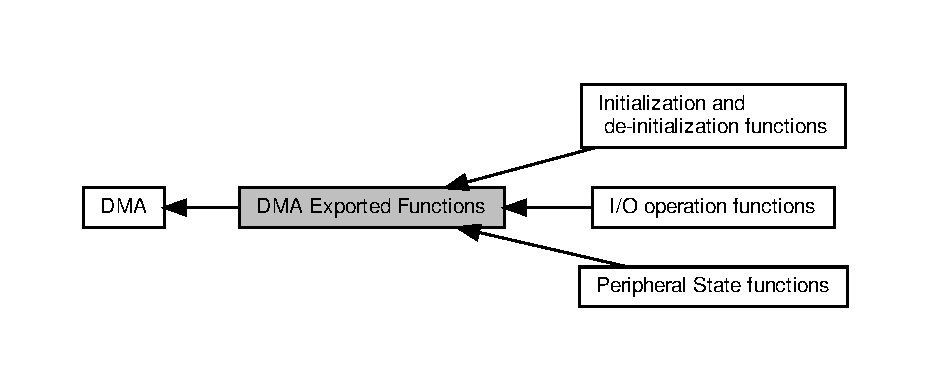
\includegraphics[width=350pt]{group___d_m_a___exported___functions}
\end{center}
\end{figure}
\subsection*{Moduły}
\begin{DoxyCompactItemize}
\item 
\hyperlink{group___d_m_a___exported___functions___group1}{Initialization and de-\/initialization functions}
\begin{DoxyCompactList}\small\item\em Initialization and de-\/initialization functions. \end{DoxyCompactList}\item 
\hyperlink{group___d_m_a___exported___functions___group2}{I/\+O operation functions}
\begin{DoxyCompactList}\small\item\em I/O operation functions. \end{DoxyCompactList}\item 
\hyperlink{group___d_m_a___exported___functions___group3}{Peripheral State functions}
\begin{DoxyCompactList}\small\item\em Peripheral State functions. \end{DoxyCompactList}\end{DoxyCompactItemize}


\subsection{Opis szczegółowy}
D\+MA Exported functions. 


\hypertarget{group___d_m_a___exported___functions___group1}{}\section{Initialization and de-\/initialization functions}
\label{group___d_m_a___exported___functions___group1}\index{Initialization and de-\/initialization functions@{Initialization and de-\/initialization functions}}


Initialization and de-\/initialization functions.  


Diagram współpracy dla Initialization and de-\/initialization functions\+:\nopagebreak
\begin{figure}[H]
\begin{center}
\leavevmode
\includegraphics[width=350pt]{group___d_m_a___exported___functions___group1}
\end{center}
\end{figure}
\subsection*{Funkcje}
\begin{DoxyCompactItemize}
\item 
\hyperlink{stm32f4xx__hal__def_8h_a63c0679d1cb8b8c684fbb0632743478f}{H\+A\+L\+\_\+\+Status\+Type\+Def} \hyperlink{group___d_m_a___exported___functions___group1_ga0fbcb690074233a03f2fa366dc22ff01}{H\+A\+L\+\_\+\+D\+M\+A\+\_\+\+Init} (\hyperlink{group___d_m_a___exported___types_ga41b754a906b86bce54dc79938970138b}{D\+M\+A\+\_\+\+Handle\+Type\+Def} $\ast$hdma)
\item 
\hyperlink{stm32f4xx__hal__def_8h_a63c0679d1cb8b8c684fbb0632743478f}{H\+A\+L\+\_\+\+Status\+Type\+Def} \hyperlink{group___d_m_a___exported___functions___group1_ga7bb8587d642da11252a97f5c41c389ef}{H\+A\+L\+\_\+\+D\+M\+A\+\_\+\+De\+Init} (\hyperlink{group___d_m_a___exported___types_ga41b754a906b86bce54dc79938970138b}{D\+M\+A\+\_\+\+Handle\+Type\+Def} $\ast$hdma)
\end{DoxyCompactItemize}


\subsection{Opis szczegółowy}
Initialization and de-\/initialization functions. 



\subsection{Dokumentacja funkcji}
\mbox{\Hypertarget{group___d_m_a___exported___functions___group1_ga7bb8587d642da11252a97f5c41c389ef}\label{group___d_m_a___exported___functions___group1_ga7bb8587d642da11252a97f5c41c389ef}} 
\index{Initialization and de-\/initialization functions@{Initialization and de-\/initialization functions}!H\+A\+L\+\_\+\+D\+M\+A\+\_\+\+De\+Init@{H\+A\+L\+\_\+\+D\+M\+A\+\_\+\+De\+Init}}
\index{H\+A\+L\+\_\+\+D\+M\+A\+\_\+\+De\+Init@{H\+A\+L\+\_\+\+D\+M\+A\+\_\+\+De\+Init}!Initialization and de-\/initialization functions@{Initialization and de-\/initialization functions}}
\subsubsection{\texorpdfstring{H\+A\+L\+\_\+\+D\+M\+A\+\_\+\+De\+Init()}{HAL\_DMA\_DeInit()}}
{\footnotesize\ttfamily \hyperlink{stm32f4xx__hal__def_8h_a63c0679d1cb8b8c684fbb0632743478f}{H\+A\+L\+\_\+\+Status\+Type\+Def} H\+A\+L\+\_\+\+D\+M\+A\+\_\+\+De\+Init (\begin{DoxyParamCaption}\item[{\hyperlink{group___d_m_a___exported___types_ga41b754a906b86bce54dc79938970138b}{D\+M\+A\+\_\+\+Handle\+Type\+Def} $\ast$}]{hdma }\end{DoxyParamCaption})}

\mbox{\Hypertarget{group___d_m_a___exported___functions___group1_ga0fbcb690074233a03f2fa366dc22ff01}\label{group___d_m_a___exported___functions___group1_ga0fbcb690074233a03f2fa366dc22ff01}} 
\index{Initialization and de-\/initialization functions@{Initialization and de-\/initialization functions}!H\+A\+L\+\_\+\+D\+M\+A\+\_\+\+Init@{H\+A\+L\+\_\+\+D\+M\+A\+\_\+\+Init}}
\index{H\+A\+L\+\_\+\+D\+M\+A\+\_\+\+Init@{H\+A\+L\+\_\+\+D\+M\+A\+\_\+\+Init}!Initialization and de-\/initialization functions@{Initialization and de-\/initialization functions}}
\subsubsection{\texorpdfstring{H\+A\+L\+\_\+\+D\+M\+A\+\_\+\+Init()}{HAL\_DMA\_Init()}}
{\footnotesize\ttfamily \hyperlink{stm32f4xx__hal__def_8h_a63c0679d1cb8b8c684fbb0632743478f}{H\+A\+L\+\_\+\+Status\+Type\+Def} H\+A\+L\+\_\+\+D\+M\+A\+\_\+\+Init (\begin{DoxyParamCaption}\item[{\hyperlink{group___d_m_a___exported___types_ga41b754a906b86bce54dc79938970138b}{D\+M\+A\+\_\+\+Handle\+Type\+Def} $\ast$}]{hdma }\end{DoxyParamCaption})}


\hypertarget{group___d_m_a___exported___functions___group2}{}\section{I/O operation functions}
\label{group___d_m_a___exported___functions___group2}\index{I/\+O operation functions@{I/\+O operation functions}}


I/O operation functions.  


Diagram współpracy dla I/O operation functions\+:\nopagebreak
\begin{figure}[H]
\begin{center}
\leavevmode
\includegraphics[width=350pt]{group___d_m_a___exported___functions___group2}
\end{center}
\end{figure}
\subsection*{Funkcje}
\begin{DoxyCompactItemize}
\item 
\hyperlink{stm32f4xx__hal__def_8h_a63c0679d1cb8b8c684fbb0632743478f}{H\+A\+L\+\_\+\+Status\+Type\+Def} \hyperlink{group___d_m_a___exported___functions___group2_ga96fbd9c285135f558fd9283a57406330}{H\+A\+L\+\_\+\+D\+M\+A\+\_\+\+Start} (\hyperlink{group___d_m_a___exported___types_ga41b754a906b86bce54dc79938970138b}{D\+M\+A\+\_\+\+Handle\+Type\+Def} $\ast$hdma, uint32\+\_\+t Src\+Address, uint32\+\_\+t Dst\+Address, uint32\+\_\+t Data\+Length)
\item 
\hyperlink{stm32f4xx__hal__def_8h_a63c0679d1cb8b8c684fbb0632743478f}{H\+A\+L\+\_\+\+Status\+Type\+Def} \hyperlink{group___d_m_a___exported___functions___group2_ga7eddc0931ac8a3d77b23d6d5e68407c7}{H\+A\+L\+\_\+\+D\+M\+A\+\_\+\+Start\+\_\+\+IT} (\hyperlink{group___d_m_a___exported___types_ga41b754a906b86bce54dc79938970138b}{D\+M\+A\+\_\+\+Handle\+Type\+Def} $\ast$hdma, uint32\+\_\+t Src\+Address, uint32\+\_\+t Dst\+Address, uint32\+\_\+t Data\+Length)
\item 
\hyperlink{stm32f4xx__hal__def_8h_a63c0679d1cb8b8c684fbb0632743478f}{H\+A\+L\+\_\+\+Status\+Type\+Def} \hyperlink{group___d_m_a___exported___functions___group2_ga001f9fb04328a7460f9ff16908ff987c}{H\+A\+L\+\_\+\+D\+M\+A\+\_\+\+Abort} (\hyperlink{group___d_m_a___exported___types_ga41b754a906b86bce54dc79938970138b}{D\+M\+A\+\_\+\+Handle\+Type\+Def} $\ast$hdma)
\item 
\hyperlink{stm32f4xx__hal__def_8h_a63c0679d1cb8b8c684fbb0632743478f}{H\+A\+L\+\_\+\+Status\+Type\+Def} \hyperlink{group___d_m_a___exported___functions___group2_ga6677d7e614747341a58ffd7a048fd390}{H\+A\+L\+\_\+\+D\+M\+A\+\_\+\+Abort\+\_\+\+IT} (\hyperlink{group___d_m_a___exported___types_ga41b754a906b86bce54dc79938970138b}{D\+M\+A\+\_\+\+Handle\+Type\+Def} $\ast$hdma)
\item 
\hyperlink{stm32f4xx__hal__def_8h_a63c0679d1cb8b8c684fbb0632743478f}{H\+A\+L\+\_\+\+Status\+Type\+Def} \hyperlink{group___d_m_a___exported___functions___group2_ga976a30472df973e3ad983f21289c9b5d}{H\+A\+L\+\_\+\+D\+M\+A\+\_\+\+Poll\+For\+Transfer} (\hyperlink{group___d_m_a___exported___types_ga41b754a906b86bce54dc79938970138b}{D\+M\+A\+\_\+\+Handle\+Type\+Def} $\ast$hdma, \hyperlink{group___d_m_a___exported___types_gaee3245eea8fa938edeb35a6c9596fd86}{H\+A\+L\+\_\+\+D\+M\+A\+\_\+\+Level\+Complete\+Type\+Def} Complete\+Level, uint32\+\_\+t Timeout)
\item 
void \hyperlink{group___d_m_a___exported___functions___group2_ga8c8564d06f6d39b702af1c5cbb7dd54a}{H\+A\+L\+\_\+\+D\+M\+A\+\_\+\+I\+R\+Q\+Handler} (\hyperlink{group___d_m_a___exported___types_ga41b754a906b86bce54dc79938970138b}{D\+M\+A\+\_\+\+Handle\+Type\+Def} $\ast$hdma)
\item 
\hyperlink{stm32f4xx__hal__def_8h_a63c0679d1cb8b8c684fbb0632743478f}{H\+A\+L\+\_\+\+Status\+Type\+Def} \hyperlink{group___d_m_a___exported___functions___group2_gaf511e4e6e0653fafdd9b40ce4a08b1db}{H\+A\+L\+\_\+\+D\+M\+A\+\_\+\+Clean\+Callbacks} (\hyperlink{group___d_m_a___exported___types_ga41b754a906b86bce54dc79938970138b}{D\+M\+A\+\_\+\+Handle\+Type\+Def} $\ast$hdma)
\item 
\hyperlink{stm32f4xx__hal__def_8h_a63c0679d1cb8b8c684fbb0632743478f}{H\+A\+L\+\_\+\+Status\+Type\+Def} \hyperlink{group___d_m_a___exported___functions___group2_gaabec77de08a59c94f2c6265ce7ae8261}{H\+A\+L\+\_\+\+D\+M\+A\+\_\+\+Register\+Callback} (\hyperlink{group___d_m_a___exported___types_ga41b754a906b86bce54dc79938970138b}{D\+M\+A\+\_\+\+Handle\+Type\+Def} $\ast$hdma, \hyperlink{group___d_m_a___exported___types_gafbe8b2bd9ce2128de6cdc08ccde7e8ad}{H\+A\+L\+\_\+\+D\+M\+A\+\_\+\+Callback\+I\+D\+Type\+Def} Callback\+ID, void($\ast$p\+Callback)(\hyperlink{group___d_m_a___exported___types_ga41b754a906b86bce54dc79938970138b}{D\+M\+A\+\_\+\+Handle\+Type\+Def} $\ast$\+\_\+hdma))
\item 
\hyperlink{stm32f4xx__hal__def_8h_a63c0679d1cb8b8c684fbb0632743478f}{H\+A\+L\+\_\+\+Status\+Type\+Def} \hyperlink{group___d_m_a___exported___functions___group2_ga87842d3780f0e54c7fb29a003e6b5ac4}{H\+A\+L\+\_\+\+D\+M\+A\+\_\+\+Un\+Register\+Callback} (\hyperlink{group___d_m_a___exported___types_ga41b754a906b86bce54dc79938970138b}{D\+M\+A\+\_\+\+Handle\+Type\+Def} $\ast$hdma, \hyperlink{group___d_m_a___exported___types_gafbe8b2bd9ce2128de6cdc08ccde7e8ad}{H\+A\+L\+\_\+\+D\+M\+A\+\_\+\+Callback\+I\+D\+Type\+Def} Callback\+ID)
\end{DoxyCompactItemize}


\subsection{Opis szczegółowy}
I/O operation functions. 



\subsection{Dokumentacja funkcji}
\mbox{\Hypertarget{group___d_m_a___exported___functions___group2_ga001f9fb04328a7460f9ff16908ff987c}\label{group___d_m_a___exported___functions___group2_ga001f9fb04328a7460f9ff16908ff987c}} 
\index{I/\+O operation functions@{I/\+O operation functions}!H\+A\+L\+\_\+\+D\+M\+A\+\_\+\+Abort@{H\+A\+L\+\_\+\+D\+M\+A\+\_\+\+Abort}}
\index{H\+A\+L\+\_\+\+D\+M\+A\+\_\+\+Abort@{H\+A\+L\+\_\+\+D\+M\+A\+\_\+\+Abort}!I/\+O operation functions@{I/\+O operation functions}}
\subsubsection{\texorpdfstring{H\+A\+L\+\_\+\+D\+M\+A\+\_\+\+Abort()}{HAL\_DMA\_Abort()}}
{\footnotesize\ttfamily \hyperlink{stm32f4xx__hal__def_8h_a63c0679d1cb8b8c684fbb0632743478f}{H\+A\+L\+\_\+\+Status\+Type\+Def} H\+A\+L\+\_\+\+D\+M\+A\+\_\+\+Abort (\begin{DoxyParamCaption}\item[{\hyperlink{group___d_m_a___exported___types_ga41b754a906b86bce54dc79938970138b}{D\+M\+A\+\_\+\+Handle\+Type\+Def} $\ast$}]{hdma }\end{DoxyParamCaption})}

\mbox{\Hypertarget{group___d_m_a___exported___functions___group2_ga6677d7e614747341a58ffd7a048fd390}\label{group___d_m_a___exported___functions___group2_ga6677d7e614747341a58ffd7a048fd390}} 
\index{I/\+O operation functions@{I/\+O operation functions}!H\+A\+L\+\_\+\+D\+M\+A\+\_\+\+Abort\+\_\+\+IT@{H\+A\+L\+\_\+\+D\+M\+A\+\_\+\+Abort\+\_\+\+IT}}
\index{H\+A\+L\+\_\+\+D\+M\+A\+\_\+\+Abort\+\_\+\+IT@{H\+A\+L\+\_\+\+D\+M\+A\+\_\+\+Abort\+\_\+\+IT}!I/\+O operation functions@{I/\+O operation functions}}
\subsubsection{\texorpdfstring{H\+A\+L\+\_\+\+D\+M\+A\+\_\+\+Abort\+\_\+\+I\+T()}{HAL\_DMA\_Abort\_IT()}}
{\footnotesize\ttfamily \hyperlink{stm32f4xx__hal__def_8h_a63c0679d1cb8b8c684fbb0632743478f}{H\+A\+L\+\_\+\+Status\+Type\+Def} H\+A\+L\+\_\+\+D\+M\+A\+\_\+\+Abort\+\_\+\+IT (\begin{DoxyParamCaption}\item[{\hyperlink{group___d_m_a___exported___types_ga41b754a906b86bce54dc79938970138b}{D\+M\+A\+\_\+\+Handle\+Type\+Def} $\ast$}]{hdma }\end{DoxyParamCaption})}

\mbox{\Hypertarget{group___d_m_a___exported___functions___group2_gaf511e4e6e0653fafdd9b40ce4a08b1db}\label{group___d_m_a___exported___functions___group2_gaf511e4e6e0653fafdd9b40ce4a08b1db}} 
\index{I/\+O operation functions@{I/\+O operation functions}!H\+A\+L\+\_\+\+D\+M\+A\+\_\+\+Clean\+Callbacks@{H\+A\+L\+\_\+\+D\+M\+A\+\_\+\+Clean\+Callbacks}}
\index{H\+A\+L\+\_\+\+D\+M\+A\+\_\+\+Clean\+Callbacks@{H\+A\+L\+\_\+\+D\+M\+A\+\_\+\+Clean\+Callbacks}!I/\+O operation functions@{I/\+O operation functions}}
\subsubsection{\texorpdfstring{H\+A\+L\+\_\+\+D\+M\+A\+\_\+\+Clean\+Callbacks()}{HAL\_DMA\_CleanCallbacks()}}
{\footnotesize\ttfamily \hyperlink{stm32f4xx__hal__def_8h_a63c0679d1cb8b8c684fbb0632743478f}{H\+A\+L\+\_\+\+Status\+Type\+Def} H\+A\+L\+\_\+\+D\+M\+A\+\_\+\+Clean\+Callbacks (\begin{DoxyParamCaption}\item[{\hyperlink{group___d_m_a___exported___types_ga41b754a906b86bce54dc79938970138b}{D\+M\+A\+\_\+\+Handle\+Type\+Def} $\ast$}]{hdma }\end{DoxyParamCaption})}

\mbox{\Hypertarget{group___d_m_a___exported___functions___group2_ga8c8564d06f6d39b702af1c5cbb7dd54a}\label{group___d_m_a___exported___functions___group2_ga8c8564d06f6d39b702af1c5cbb7dd54a}} 
\index{I/\+O operation functions@{I/\+O operation functions}!H\+A\+L\+\_\+\+D\+M\+A\+\_\+\+I\+R\+Q\+Handler@{H\+A\+L\+\_\+\+D\+M\+A\+\_\+\+I\+R\+Q\+Handler}}
\index{H\+A\+L\+\_\+\+D\+M\+A\+\_\+\+I\+R\+Q\+Handler@{H\+A\+L\+\_\+\+D\+M\+A\+\_\+\+I\+R\+Q\+Handler}!I/\+O operation functions@{I/\+O operation functions}}
\subsubsection{\texorpdfstring{H\+A\+L\+\_\+\+D\+M\+A\+\_\+\+I\+R\+Q\+Handler()}{HAL\_DMA\_IRQHandler()}}
{\footnotesize\ttfamily void H\+A\+L\+\_\+\+D\+M\+A\+\_\+\+I\+R\+Q\+Handler (\begin{DoxyParamCaption}\item[{\hyperlink{group___d_m_a___exported___types_ga41b754a906b86bce54dc79938970138b}{D\+M\+A\+\_\+\+Handle\+Type\+Def} $\ast$}]{hdma }\end{DoxyParamCaption})}

\mbox{\Hypertarget{group___d_m_a___exported___functions___group2_ga976a30472df973e3ad983f21289c9b5d}\label{group___d_m_a___exported___functions___group2_ga976a30472df973e3ad983f21289c9b5d}} 
\index{I/\+O operation functions@{I/\+O operation functions}!H\+A\+L\+\_\+\+D\+M\+A\+\_\+\+Poll\+For\+Transfer@{H\+A\+L\+\_\+\+D\+M\+A\+\_\+\+Poll\+For\+Transfer}}
\index{H\+A\+L\+\_\+\+D\+M\+A\+\_\+\+Poll\+For\+Transfer@{H\+A\+L\+\_\+\+D\+M\+A\+\_\+\+Poll\+For\+Transfer}!I/\+O operation functions@{I/\+O operation functions}}
\subsubsection{\texorpdfstring{H\+A\+L\+\_\+\+D\+M\+A\+\_\+\+Poll\+For\+Transfer()}{HAL\_DMA\_PollForTransfer()}}
{\footnotesize\ttfamily \hyperlink{stm32f4xx__hal__def_8h_a63c0679d1cb8b8c684fbb0632743478f}{H\+A\+L\+\_\+\+Status\+Type\+Def} H\+A\+L\+\_\+\+D\+M\+A\+\_\+\+Poll\+For\+Transfer (\begin{DoxyParamCaption}\item[{\hyperlink{group___d_m_a___exported___types_ga41b754a906b86bce54dc79938970138b}{D\+M\+A\+\_\+\+Handle\+Type\+Def} $\ast$}]{hdma,  }\item[{\hyperlink{group___d_m_a___exported___types_gaee3245eea8fa938edeb35a6c9596fd86}{H\+A\+L\+\_\+\+D\+M\+A\+\_\+\+Level\+Complete\+Type\+Def}}]{Complete\+Level,  }\item[{uint32\+\_\+t}]{Timeout }\end{DoxyParamCaption})}

\mbox{\Hypertarget{group___d_m_a___exported___functions___group2_gaabec77de08a59c94f2c6265ce7ae8261}\label{group___d_m_a___exported___functions___group2_gaabec77de08a59c94f2c6265ce7ae8261}} 
\index{I/\+O operation functions@{I/\+O operation functions}!H\+A\+L\+\_\+\+D\+M\+A\+\_\+\+Register\+Callback@{H\+A\+L\+\_\+\+D\+M\+A\+\_\+\+Register\+Callback}}
\index{H\+A\+L\+\_\+\+D\+M\+A\+\_\+\+Register\+Callback@{H\+A\+L\+\_\+\+D\+M\+A\+\_\+\+Register\+Callback}!I/\+O operation functions@{I/\+O operation functions}}
\subsubsection{\texorpdfstring{H\+A\+L\+\_\+\+D\+M\+A\+\_\+\+Register\+Callback()}{HAL\_DMA\_RegisterCallback()}}
{\footnotesize\ttfamily \hyperlink{stm32f4xx__hal__def_8h_a63c0679d1cb8b8c684fbb0632743478f}{H\+A\+L\+\_\+\+Status\+Type\+Def} H\+A\+L\+\_\+\+D\+M\+A\+\_\+\+Register\+Callback (\begin{DoxyParamCaption}\item[{\hyperlink{group___d_m_a___exported___types_ga41b754a906b86bce54dc79938970138b}{D\+M\+A\+\_\+\+Handle\+Type\+Def} $\ast$}]{hdma,  }\item[{\hyperlink{group___d_m_a___exported___types_gafbe8b2bd9ce2128de6cdc08ccde7e8ad}{H\+A\+L\+\_\+\+D\+M\+A\+\_\+\+Callback\+I\+D\+Type\+Def}}]{Callback\+ID,  }\item[{void($\ast$)(\hyperlink{group___d_m_a___exported___types_ga41b754a906b86bce54dc79938970138b}{D\+M\+A\+\_\+\+Handle\+Type\+Def} $\ast$\+\_\+hdma)}]{p\+Callback }\end{DoxyParamCaption})}

\mbox{\Hypertarget{group___d_m_a___exported___functions___group2_ga96fbd9c285135f558fd9283a57406330}\label{group___d_m_a___exported___functions___group2_ga96fbd9c285135f558fd9283a57406330}} 
\index{I/\+O operation functions@{I/\+O operation functions}!H\+A\+L\+\_\+\+D\+M\+A\+\_\+\+Start@{H\+A\+L\+\_\+\+D\+M\+A\+\_\+\+Start}}
\index{H\+A\+L\+\_\+\+D\+M\+A\+\_\+\+Start@{H\+A\+L\+\_\+\+D\+M\+A\+\_\+\+Start}!I/\+O operation functions@{I/\+O operation functions}}
\subsubsection{\texorpdfstring{H\+A\+L\+\_\+\+D\+M\+A\+\_\+\+Start()}{HAL\_DMA\_Start()}}
{\footnotesize\ttfamily \hyperlink{stm32f4xx__hal__def_8h_a63c0679d1cb8b8c684fbb0632743478f}{H\+A\+L\+\_\+\+Status\+Type\+Def} H\+A\+L\+\_\+\+D\+M\+A\+\_\+\+Start (\begin{DoxyParamCaption}\item[{\hyperlink{group___d_m_a___exported___types_ga41b754a906b86bce54dc79938970138b}{D\+M\+A\+\_\+\+Handle\+Type\+Def} $\ast$}]{hdma,  }\item[{uint32\+\_\+t}]{Src\+Address,  }\item[{uint32\+\_\+t}]{Dst\+Address,  }\item[{uint32\+\_\+t}]{Data\+Length }\end{DoxyParamCaption})}

\mbox{\Hypertarget{group___d_m_a___exported___functions___group2_ga7eddc0931ac8a3d77b23d6d5e68407c7}\label{group___d_m_a___exported___functions___group2_ga7eddc0931ac8a3d77b23d6d5e68407c7}} 
\index{I/\+O operation functions@{I/\+O operation functions}!H\+A\+L\+\_\+\+D\+M\+A\+\_\+\+Start\+\_\+\+IT@{H\+A\+L\+\_\+\+D\+M\+A\+\_\+\+Start\+\_\+\+IT}}
\index{H\+A\+L\+\_\+\+D\+M\+A\+\_\+\+Start\+\_\+\+IT@{H\+A\+L\+\_\+\+D\+M\+A\+\_\+\+Start\+\_\+\+IT}!I/\+O operation functions@{I/\+O operation functions}}
\subsubsection{\texorpdfstring{H\+A\+L\+\_\+\+D\+M\+A\+\_\+\+Start\+\_\+\+I\+T()}{HAL\_DMA\_Start\_IT()}}
{\footnotesize\ttfamily \hyperlink{stm32f4xx__hal__def_8h_a63c0679d1cb8b8c684fbb0632743478f}{H\+A\+L\+\_\+\+Status\+Type\+Def} H\+A\+L\+\_\+\+D\+M\+A\+\_\+\+Start\+\_\+\+IT (\begin{DoxyParamCaption}\item[{\hyperlink{group___d_m_a___exported___types_ga41b754a906b86bce54dc79938970138b}{D\+M\+A\+\_\+\+Handle\+Type\+Def} $\ast$}]{hdma,  }\item[{uint32\+\_\+t}]{Src\+Address,  }\item[{uint32\+\_\+t}]{Dst\+Address,  }\item[{uint32\+\_\+t}]{Data\+Length }\end{DoxyParamCaption})}

\mbox{\Hypertarget{group___d_m_a___exported___functions___group2_ga87842d3780f0e54c7fb29a003e6b5ac4}\label{group___d_m_a___exported___functions___group2_ga87842d3780f0e54c7fb29a003e6b5ac4}} 
\index{I/\+O operation functions@{I/\+O operation functions}!H\+A\+L\+\_\+\+D\+M\+A\+\_\+\+Un\+Register\+Callback@{H\+A\+L\+\_\+\+D\+M\+A\+\_\+\+Un\+Register\+Callback}}
\index{H\+A\+L\+\_\+\+D\+M\+A\+\_\+\+Un\+Register\+Callback@{H\+A\+L\+\_\+\+D\+M\+A\+\_\+\+Un\+Register\+Callback}!I/\+O operation functions@{I/\+O operation functions}}
\subsubsection{\texorpdfstring{H\+A\+L\+\_\+\+D\+M\+A\+\_\+\+Un\+Register\+Callback()}{HAL\_DMA\_UnRegisterCallback()}}
{\footnotesize\ttfamily \hyperlink{stm32f4xx__hal__def_8h_a63c0679d1cb8b8c684fbb0632743478f}{H\+A\+L\+\_\+\+Status\+Type\+Def} H\+A\+L\+\_\+\+D\+M\+A\+\_\+\+Un\+Register\+Callback (\begin{DoxyParamCaption}\item[{\hyperlink{group___d_m_a___exported___types_ga41b754a906b86bce54dc79938970138b}{D\+M\+A\+\_\+\+Handle\+Type\+Def} $\ast$}]{hdma,  }\item[{\hyperlink{group___d_m_a___exported___types_gafbe8b2bd9ce2128de6cdc08ccde7e8ad}{H\+A\+L\+\_\+\+D\+M\+A\+\_\+\+Callback\+I\+D\+Type\+Def}}]{Callback\+ID }\end{DoxyParamCaption})}


\hypertarget{group___d_m_a___exported___functions___group3}{}\section{Peripheral State functions}
\label{group___d_m_a___exported___functions___group3}\index{Peripheral State functions@{Peripheral State functions}}


Peripheral State functions.  


Diagram współpracy dla Peripheral State functions\+:\nopagebreak
\begin{figure}[H]
\begin{center}
\leavevmode
\includegraphics[width=350pt]{group___d_m_a___exported___functions___group3}
\end{center}
\end{figure}
\subsection*{Funkcje}
\begin{DoxyCompactItemize}
\item 
\hyperlink{group___d_m_a___exported___types_ga9c012af359987a240826f29073bbe463}{H\+A\+L\+\_\+\+D\+M\+A\+\_\+\+State\+Type\+Def} \hyperlink{group___d_m_a___exported___functions___group3_gaef09509c41da57dc118c8ffb9533ce3f}{H\+A\+L\+\_\+\+D\+M\+A\+\_\+\+Get\+State} (\hyperlink{group___d_m_a___exported___types_ga41b754a906b86bce54dc79938970138b}{D\+M\+A\+\_\+\+Handle\+Type\+Def} $\ast$hdma)
\item 
uint32\+\_\+t \hyperlink{group___d_m_a___exported___functions___group3_gabc0735694a0dd08e352b796d7fa7634f}{H\+A\+L\+\_\+\+D\+M\+A\+\_\+\+Get\+Error} (\hyperlink{group___d_m_a___exported___types_ga41b754a906b86bce54dc79938970138b}{D\+M\+A\+\_\+\+Handle\+Type\+Def} $\ast$hdma)
\end{DoxyCompactItemize}


\subsection{Opis szczegółowy}
Peripheral State functions. 



\subsection{Dokumentacja funkcji}
\mbox{\Hypertarget{group___d_m_a___exported___functions___group3_gabc0735694a0dd08e352b796d7fa7634f}\label{group___d_m_a___exported___functions___group3_gabc0735694a0dd08e352b796d7fa7634f}} 
\index{Peripheral State functions@{Peripheral State functions}!H\+A\+L\+\_\+\+D\+M\+A\+\_\+\+Get\+Error@{H\+A\+L\+\_\+\+D\+M\+A\+\_\+\+Get\+Error}}
\index{H\+A\+L\+\_\+\+D\+M\+A\+\_\+\+Get\+Error@{H\+A\+L\+\_\+\+D\+M\+A\+\_\+\+Get\+Error}!Peripheral State functions@{Peripheral State functions}}
\subsubsection{\texorpdfstring{H\+A\+L\+\_\+\+D\+M\+A\+\_\+\+Get\+Error()}{HAL\_DMA\_GetError()}}
{\footnotesize\ttfamily uint32\+\_\+t H\+A\+L\+\_\+\+D\+M\+A\+\_\+\+Get\+Error (\begin{DoxyParamCaption}\item[{\hyperlink{group___d_m_a___exported___types_ga41b754a906b86bce54dc79938970138b}{D\+M\+A\+\_\+\+Handle\+Type\+Def} $\ast$}]{hdma }\end{DoxyParamCaption})}

\mbox{\Hypertarget{group___d_m_a___exported___functions___group3_gaef09509c41da57dc118c8ffb9533ce3f}\label{group___d_m_a___exported___functions___group3_gaef09509c41da57dc118c8ffb9533ce3f}} 
\index{Peripheral State functions@{Peripheral State functions}!H\+A\+L\+\_\+\+D\+M\+A\+\_\+\+Get\+State@{H\+A\+L\+\_\+\+D\+M\+A\+\_\+\+Get\+State}}
\index{H\+A\+L\+\_\+\+D\+M\+A\+\_\+\+Get\+State@{H\+A\+L\+\_\+\+D\+M\+A\+\_\+\+Get\+State}!Peripheral State functions@{Peripheral State functions}}
\subsubsection{\texorpdfstring{H\+A\+L\+\_\+\+D\+M\+A\+\_\+\+Get\+State()}{HAL\_DMA\_GetState()}}
{\footnotesize\ttfamily \hyperlink{group___d_m_a___exported___types_ga9c012af359987a240826f29073bbe463}{H\+A\+L\+\_\+\+D\+M\+A\+\_\+\+State\+Type\+Def} H\+A\+L\+\_\+\+D\+M\+A\+\_\+\+Get\+State (\begin{DoxyParamCaption}\item[{\hyperlink{group___d_m_a___exported___types_ga41b754a906b86bce54dc79938970138b}{D\+M\+A\+\_\+\+Handle\+Type\+Def} $\ast$}]{hdma }\end{DoxyParamCaption})}


\hypertarget{group___d_m_a___private___constants}{}\section{D\+MA Private Constants}
\label{group___d_m_a___private___constants}\index{D\+M\+A Private Constants@{D\+M\+A Private Constants}}


D\+MA private defines and constants.  


Diagram współpracy dla D\+MA Private Constants\+:\nopagebreak
\begin{figure}[H]
\begin{center}
\leavevmode
\includegraphics[width=276pt]{group___d_m_a___private___constants}
\end{center}
\end{figure}
D\+MA private defines and constants. 


\hypertarget{group___d_m_a___private___macros}{}\section{D\+MA Private Macros}
\label{group___d_m_a___private___macros}\index{D\+M\+A Private Macros@{D\+M\+A Private Macros}}


D\+MA private macros.  


Diagram współpracy dla D\+MA Private Macros\+:\nopagebreak
\begin{figure}[H]
\begin{center}
\leavevmode
\includegraphics[width=263pt]{group___d_m_a___private___macros}
\end{center}
\end{figure}
\subsection*{Definicje}
\begin{DoxyCompactItemize}
\item 
\#define \hyperlink{group___d_m_a___private___macros_gac7f4709d9244f25b853789d888a74d46}{I\+S\+\_\+\+D\+M\+A\+\_\+\+C\+H\+A\+N\+N\+EL}(C\+H\+A\+N\+N\+EL)
\item 
\#define \hyperlink{group___d_m_a___private___macros_gae2b02e8e823854bcd7c5746cdd29e70d}{I\+S\+\_\+\+D\+M\+A\+\_\+\+D\+I\+R\+E\+C\+T\+I\+ON}(D\+I\+R\+E\+C\+T\+I\+ON)
\item 
\#define \hyperlink{group___d_m_a___private___macros_ga72ef4033bb3bc2cdfdbe579083b05e32}{I\+S\+\_\+\+D\+M\+A\+\_\+\+B\+U\+F\+F\+E\+R\+\_\+\+S\+I\+ZE}(S\+I\+ZE)~(((S\+I\+ZE) $>$= 0x01\+U) \&\& ((\+S\+I\+Z\+E) $<$ 0x10000\+U))
\item 
\#define \hyperlink{group___d_m_a___private___macros_ga28762105b3f567c16ba79a47e68ff0fa}{I\+S\+\_\+\+D\+M\+A\+\_\+\+P\+E\+R\+I\+P\+H\+E\+R\+A\+L\+\_\+\+I\+N\+C\+\_\+\+S\+T\+A\+TE}(S\+T\+A\+TE)
\item 
\#define \hyperlink{group___d_m_a___private___macros_gaa880f39d499d1e80449cf80381e4eb67}{I\+S\+\_\+\+D\+M\+A\+\_\+\+M\+E\+M\+O\+R\+Y\+\_\+\+I\+N\+C\+\_\+\+S\+T\+A\+TE}(S\+T\+A\+TE)
\item 
\#define \hyperlink{group___d_m_a___private___macros_gad7916e0ae55cdf5efdfa68a09a028037}{I\+S\+\_\+\+D\+M\+A\+\_\+\+P\+E\+R\+I\+P\+H\+E\+R\+A\+L\+\_\+\+D\+A\+T\+A\+\_\+\+S\+I\+ZE}(S\+I\+ZE)
\item 
\#define \hyperlink{group___d_m_a___private___macros_gac9e3748cebcb16d4ae4206d562bc804c}{I\+S\+\_\+\+D\+M\+A\+\_\+\+M\+E\+M\+O\+R\+Y\+\_\+\+D\+A\+T\+A\+\_\+\+S\+I\+ZE}(S\+I\+ZE)
\item 
\#define \hyperlink{group___d_m_a___private___macros_gad88ee5030574d6a573904378fb62c7ac}{I\+S\+\_\+\+D\+M\+A\+\_\+\+M\+O\+DE}(M\+O\+DE)
\item 
\#define \hyperlink{group___d_m_a___private___macros_gaa1cae2ab458948511596467c87cd02b6}{I\+S\+\_\+\+D\+M\+A\+\_\+\+P\+R\+I\+O\+R\+I\+TY}(P\+R\+I\+O\+R\+I\+TY)
\item 
\#define \hyperlink{group___d_m_a___private___macros_gadb90a893aeb49fd4bc14af750af3837c}{I\+S\+\_\+\+D\+M\+A\+\_\+\+F\+I\+F\+O\+\_\+\+M\+O\+D\+E\+\_\+\+S\+T\+A\+TE}(S\+T\+A\+TE)
\item 
\#define \hyperlink{group___d_m_a___private___macros_gaeafc0d9e327d6e5b26cd37f6744b232f}{I\+S\+\_\+\+D\+M\+A\+\_\+\+F\+I\+F\+O\+\_\+\+T\+H\+R\+E\+S\+H\+O\+LD}(T\+H\+R\+E\+S\+H\+O\+LD)
\item 
\#define \hyperlink{group___d_m_a___private___macros_ga921ebf06447dc036180fff50b7e4846a}{I\+S\+\_\+\+D\+M\+A\+\_\+\+M\+E\+M\+O\+R\+Y\+\_\+\+B\+U\+R\+ST}(B\+U\+R\+ST)
\item 
\#define \hyperlink{group___d_m_a___private___macros_ga7c60961178e2a32e9e364a220a8aca88}{I\+S\+\_\+\+D\+M\+A\+\_\+\+P\+E\+R\+I\+P\+H\+E\+R\+A\+L\+\_\+\+B\+U\+R\+ST}(B\+U\+R\+ST)
\end{DoxyCompactItemize}


\subsection{Opis szczegółowy}
D\+MA private macros. 



\subsection{Dokumentacja definicji}
\mbox{\Hypertarget{group___d_m_a___private___macros_ga72ef4033bb3bc2cdfdbe579083b05e32}\label{group___d_m_a___private___macros_ga72ef4033bb3bc2cdfdbe579083b05e32}} 
\index{D\+M\+A Private Macros@{D\+M\+A Private Macros}!I\+S\+\_\+\+D\+M\+A\+\_\+\+B\+U\+F\+F\+E\+R\+\_\+\+S\+I\+ZE@{I\+S\+\_\+\+D\+M\+A\+\_\+\+B\+U\+F\+F\+E\+R\+\_\+\+S\+I\+ZE}}
\index{I\+S\+\_\+\+D\+M\+A\+\_\+\+B\+U\+F\+F\+E\+R\+\_\+\+S\+I\+ZE@{I\+S\+\_\+\+D\+M\+A\+\_\+\+B\+U\+F\+F\+E\+R\+\_\+\+S\+I\+ZE}!D\+M\+A Private Macros@{D\+M\+A Private Macros}}
\subsubsection{\texorpdfstring{I\+S\+\_\+\+D\+M\+A\+\_\+\+B\+U\+F\+F\+E\+R\+\_\+\+S\+I\+ZE}{IS\_DMA\_BUFFER\_SIZE}}
{\footnotesize\ttfamily \#define I\+S\+\_\+\+D\+M\+A\+\_\+\+B\+U\+F\+F\+E\+R\+\_\+\+S\+I\+ZE(\begin{DoxyParamCaption}\item[{}]{S\+I\+ZE }\end{DoxyParamCaption})~(((S\+I\+ZE) $>$= 0x01\+U) \&\& ((\+S\+I\+Z\+E) $<$ 0x10000\+U))}



Definicja w linii 735 pliku stm32f4xx\+\_\+hal\+\_\+dma.\+h.

\mbox{\Hypertarget{group___d_m_a___private___macros_gac7f4709d9244f25b853789d888a74d46}\label{group___d_m_a___private___macros_gac7f4709d9244f25b853789d888a74d46}} 
\index{D\+M\+A Private Macros@{D\+M\+A Private Macros}!I\+S\+\_\+\+D\+M\+A\+\_\+\+C\+H\+A\+N\+N\+EL@{I\+S\+\_\+\+D\+M\+A\+\_\+\+C\+H\+A\+N\+N\+EL}}
\index{I\+S\+\_\+\+D\+M\+A\+\_\+\+C\+H\+A\+N\+N\+EL@{I\+S\+\_\+\+D\+M\+A\+\_\+\+C\+H\+A\+N\+N\+EL}!D\+M\+A Private Macros@{D\+M\+A Private Macros}}
\subsubsection{\texorpdfstring{I\+S\+\_\+\+D\+M\+A\+\_\+\+C\+H\+A\+N\+N\+EL}{IS\_DMA\_CHANNEL}}
{\footnotesize\ttfamily \#define I\+S\+\_\+\+D\+M\+A\+\_\+\+C\+H\+A\+N\+N\+EL(\begin{DoxyParamCaption}\item[{}]{C\+H\+A\+N\+N\+EL }\end{DoxyParamCaption})}

{\bfseries Wartość\+:}
\begin{DoxyCode}
(((CHANNEL) == \hyperlink{group___d_m_a___channel__selection_gabd7de138931e93a90fc6c4eab5916bbe}{DMA\_CHANNEL\_0}) || \(\backslash\)
                                 ((CHANNEL) == \hyperlink{group___d_m_a___channel__selection_ga283364370e9876af6406b9fa70e2944f}{DMA\_CHANNEL\_1}) || \(\backslash\)
                                 ((CHANNEL) == \hyperlink{group___d_m_a___channel__selection_ga9688f3e78cbc2109d214b7ca049e22df}{DMA\_CHANNEL\_2}) || \(\backslash\)
                                 ((CHANNEL) == \hyperlink{group___d_m_a___channel__selection_gac689673fec4d72ede49a0d657e3a7e70}{DMA\_CHANNEL\_3}) || \(\backslash\)
                                 ((CHANNEL) == \hyperlink{group___d_m_a___channel__selection_ga51b51f5b39e23b28ad99520ad5be596f}{DMA\_CHANNEL\_4}) || \(\backslash\)
                                 ((CHANNEL) == \hyperlink{group___d_m_a___channel__selection_gafbaa82f3cff89858e50363c04ed0cca0}{DMA\_CHANNEL\_5}) || \(\backslash\)
                                 ((CHANNEL) == \hyperlink{group___d_m_a___channel__selection_gad23679661d8da3bc1aaacc62f99821f7}{DMA\_CHANNEL\_6}) || \(\backslash\)
                                 ((CHANNEL) == \hyperlink{group___d_m_a___channel__selection_ga77ff4e8675a3991feb20e385242f34ab}{DMA\_CHANNEL\_7}))
\end{DoxyCode}


Definicja w linii 721 pliku stm32f4xx\+\_\+hal\+\_\+dma.\+h.

\mbox{\Hypertarget{group___d_m_a___private___macros_gae2b02e8e823854bcd7c5746cdd29e70d}\label{group___d_m_a___private___macros_gae2b02e8e823854bcd7c5746cdd29e70d}} 
\index{D\+M\+A Private Macros@{D\+M\+A Private Macros}!I\+S\+\_\+\+D\+M\+A\+\_\+\+D\+I\+R\+E\+C\+T\+I\+ON@{I\+S\+\_\+\+D\+M\+A\+\_\+\+D\+I\+R\+E\+C\+T\+I\+ON}}
\index{I\+S\+\_\+\+D\+M\+A\+\_\+\+D\+I\+R\+E\+C\+T\+I\+ON@{I\+S\+\_\+\+D\+M\+A\+\_\+\+D\+I\+R\+E\+C\+T\+I\+ON}!D\+M\+A Private Macros@{D\+M\+A Private Macros}}
\subsubsection{\texorpdfstring{I\+S\+\_\+\+D\+M\+A\+\_\+\+D\+I\+R\+E\+C\+T\+I\+ON}{IS\_DMA\_DIRECTION}}
{\footnotesize\ttfamily \#define I\+S\+\_\+\+D\+M\+A\+\_\+\+D\+I\+R\+E\+C\+T\+I\+ON(\begin{DoxyParamCaption}\item[{}]{D\+I\+R\+E\+C\+T\+I\+ON }\end{DoxyParamCaption})}

{\bfseries Wartość\+:}
\begin{DoxyCode}
(((DIRECTION) == \hyperlink{group___d_m_a___data__transfer__direction_gacb2cbf03ecae6804ae4a6f60a3e37c12}{DMA\_PERIPH\_TO\_MEMORY} ) || \(\backslash\)
                                     ((DIRECTION) == \hyperlink{group___d_m_a___data__transfer__direction_ga9e76fc559a2d5c766c969e6e921b1ee9}{DMA\_MEMORY\_TO\_PERIPH})  || \(\backslash\)
                                     ((DIRECTION) == \hyperlink{group___d_m_a___data__transfer__direction_ga0695035d725855ccf64d2d8452a33810}{DMA\_MEMORY\_TO\_MEMORY}))
\end{DoxyCode}


Definicja w linii 731 pliku stm32f4xx\+\_\+hal\+\_\+dma.\+h.

\mbox{\Hypertarget{group___d_m_a___private___macros_gadb90a893aeb49fd4bc14af750af3837c}\label{group___d_m_a___private___macros_gadb90a893aeb49fd4bc14af750af3837c}} 
\index{D\+M\+A Private Macros@{D\+M\+A Private Macros}!I\+S\+\_\+\+D\+M\+A\+\_\+\+F\+I\+F\+O\+\_\+\+M\+O\+D\+E\+\_\+\+S\+T\+A\+TE@{I\+S\+\_\+\+D\+M\+A\+\_\+\+F\+I\+F\+O\+\_\+\+M\+O\+D\+E\+\_\+\+S\+T\+A\+TE}}
\index{I\+S\+\_\+\+D\+M\+A\+\_\+\+F\+I\+F\+O\+\_\+\+M\+O\+D\+E\+\_\+\+S\+T\+A\+TE@{I\+S\+\_\+\+D\+M\+A\+\_\+\+F\+I\+F\+O\+\_\+\+M\+O\+D\+E\+\_\+\+S\+T\+A\+TE}!D\+M\+A Private Macros@{D\+M\+A Private Macros}}
\subsubsection{\texorpdfstring{I\+S\+\_\+\+D\+M\+A\+\_\+\+F\+I\+F\+O\+\_\+\+M\+O\+D\+E\+\_\+\+S\+T\+A\+TE}{IS\_DMA\_FIFO\_MODE\_STATE}}
{\footnotesize\ttfamily \#define I\+S\+\_\+\+D\+M\+A\+\_\+\+F\+I\+F\+O\+\_\+\+M\+O\+D\+E\+\_\+\+S\+T\+A\+TE(\begin{DoxyParamCaption}\item[{}]{S\+T\+A\+TE }\end{DoxyParamCaption})}

{\bfseries Wartość\+:}
\begin{DoxyCode}
(((STATE) == \hyperlink{group___d_m_a___f_i_f_o__direct__mode_gaec22b199f9da9214bf908d7edbcd83e8}{DMA\_FIFOMODE\_DISABLE} ) || \(\backslash\)
                                       ((STATE) == \hyperlink{group___d_m_a___f_i_f_o__direct__mode_ga18709570bed6b9112520701c482fbe4b}{DMA\_FIFOMODE\_ENABLE}))
\end{DoxyCode}


Definicja w linii 760 pliku stm32f4xx\+\_\+hal\+\_\+dma.\+h.

\mbox{\Hypertarget{group___d_m_a___private___macros_gaeafc0d9e327d6e5b26cd37f6744b232f}\label{group___d_m_a___private___macros_gaeafc0d9e327d6e5b26cd37f6744b232f}} 
\index{D\+M\+A Private Macros@{D\+M\+A Private Macros}!I\+S\+\_\+\+D\+M\+A\+\_\+\+F\+I\+F\+O\+\_\+\+T\+H\+R\+E\+S\+H\+O\+LD@{I\+S\+\_\+\+D\+M\+A\+\_\+\+F\+I\+F\+O\+\_\+\+T\+H\+R\+E\+S\+H\+O\+LD}}
\index{I\+S\+\_\+\+D\+M\+A\+\_\+\+F\+I\+F\+O\+\_\+\+T\+H\+R\+E\+S\+H\+O\+LD@{I\+S\+\_\+\+D\+M\+A\+\_\+\+F\+I\+F\+O\+\_\+\+T\+H\+R\+E\+S\+H\+O\+LD}!D\+M\+A Private Macros@{D\+M\+A Private Macros}}
\subsubsection{\texorpdfstring{I\+S\+\_\+\+D\+M\+A\+\_\+\+F\+I\+F\+O\+\_\+\+T\+H\+R\+E\+S\+H\+O\+LD}{IS\_DMA\_FIFO\_THRESHOLD}}
{\footnotesize\ttfamily \#define I\+S\+\_\+\+D\+M\+A\+\_\+\+F\+I\+F\+O\+\_\+\+T\+H\+R\+E\+S\+H\+O\+LD(\begin{DoxyParamCaption}\item[{}]{T\+H\+R\+E\+S\+H\+O\+LD }\end{DoxyParamCaption})}

{\bfseries Wartość\+:}
\begin{DoxyCode}
(((THRESHOLD) == \hyperlink{group___d_m_a___f_i_f_o__threshold__level_ga4debbd5733190b61b2115613d4b3658b}{DMA\_FIFO\_THRESHOLD\_1QUARTERFULL} ) || \(\backslash\)
                                          ((THRESHOLD) == 
      \hyperlink{group___d_m_a___f_i_f_o__threshold__level_gad2b071aa3a3bfc936017f12fb956c56f}{DMA\_FIFO\_THRESHOLD\_HALFFULL})      || \(\backslash\)
                                          ((THRESHOLD) == 
      \hyperlink{group___d_m_a___f_i_f_o__threshold__level_gae1e4ba12bae8440421e6672795d71223}{DMA\_FIFO\_THRESHOLD\_3QUARTERSFULL}) || \(\backslash\)
                                          ((THRESHOLD) == 
      \hyperlink{group___d_m_a___f_i_f_o__threshold__level_ga5de463bb24dc12fe7bbb300e1e4493f7}{DMA\_FIFO\_THRESHOLD\_FULL}))
\end{DoxyCode}


Definicja w linii 763 pliku stm32f4xx\+\_\+hal\+\_\+dma.\+h.

\mbox{\Hypertarget{group___d_m_a___private___macros_ga921ebf06447dc036180fff50b7e4846a}\label{group___d_m_a___private___macros_ga921ebf06447dc036180fff50b7e4846a}} 
\index{D\+M\+A Private Macros@{D\+M\+A Private Macros}!I\+S\+\_\+\+D\+M\+A\+\_\+\+M\+E\+M\+O\+R\+Y\+\_\+\+B\+U\+R\+ST@{I\+S\+\_\+\+D\+M\+A\+\_\+\+M\+E\+M\+O\+R\+Y\+\_\+\+B\+U\+R\+ST}}
\index{I\+S\+\_\+\+D\+M\+A\+\_\+\+M\+E\+M\+O\+R\+Y\+\_\+\+B\+U\+R\+ST@{I\+S\+\_\+\+D\+M\+A\+\_\+\+M\+E\+M\+O\+R\+Y\+\_\+\+B\+U\+R\+ST}!D\+M\+A Private Macros@{D\+M\+A Private Macros}}
\subsubsection{\texorpdfstring{I\+S\+\_\+\+D\+M\+A\+\_\+\+M\+E\+M\+O\+R\+Y\+\_\+\+B\+U\+R\+ST}{IS\_DMA\_MEMORY\_BURST}}
{\footnotesize\ttfamily \#define I\+S\+\_\+\+D\+M\+A\+\_\+\+M\+E\+M\+O\+R\+Y\+\_\+\+B\+U\+R\+ST(\begin{DoxyParamCaption}\item[{}]{B\+U\+R\+ST }\end{DoxyParamCaption})}

{\bfseries Wartość\+:}
\begin{DoxyCode}
(((BURST) == \hyperlink{group___d_m_a___memory__burst_ga4e94b7250e6a4f53d702b42b15796953}{DMA\_MBURST\_SINGLE}) || \(\backslash\)
                                    ((BURST) == \hyperlink{group___d_m_a___memory__burst_gac9efcb13b2f0a715edb931dde213c000}{DMA\_MBURST\_INC4})   || \(\backslash\)
                                    ((BURST) == \hyperlink{group___d_m_a___memory__burst_ga4b8834930bb3b93cd3fcf04660b6933d}{DMA\_MBURST\_INC8})   || \(\backslash\)
                                    ((BURST) == \hyperlink{group___d_m_a___memory__burst_ga7812aea620b09c4f4281d614d86e6094}{DMA\_MBURST\_INC16}))
\end{DoxyCode}


Definicja w linii 768 pliku stm32f4xx\+\_\+hal\+\_\+dma.\+h.

\mbox{\Hypertarget{group___d_m_a___private___macros_gac9e3748cebcb16d4ae4206d562bc804c}\label{group___d_m_a___private___macros_gac9e3748cebcb16d4ae4206d562bc804c}} 
\index{D\+M\+A Private Macros@{D\+M\+A Private Macros}!I\+S\+\_\+\+D\+M\+A\+\_\+\+M\+E\+M\+O\+R\+Y\+\_\+\+D\+A\+T\+A\+\_\+\+S\+I\+ZE@{I\+S\+\_\+\+D\+M\+A\+\_\+\+M\+E\+M\+O\+R\+Y\+\_\+\+D\+A\+T\+A\+\_\+\+S\+I\+ZE}}
\index{I\+S\+\_\+\+D\+M\+A\+\_\+\+M\+E\+M\+O\+R\+Y\+\_\+\+D\+A\+T\+A\+\_\+\+S\+I\+ZE@{I\+S\+\_\+\+D\+M\+A\+\_\+\+M\+E\+M\+O\+R\+Y\+\_\+\+D\+A\+T\+A\+\_\+\+S\+I\+ZE}!D\+M\+A Private Macros@{D\+M\+A Private Macros}}
\subsubsection{\texorpdfstring{I\+S\+\_\+\+D\+M\+A\+\_\+\+M\+E\+M\+O\+R\+Y\+\_\+\+D\+A\+T\+A\+\_\+\+S\+I\+ZE}{IS\_DMA\_MEMORY\_DATA\_SIZE}}
{\footnotesize\ttfamily \#define I\+S\+\_\+\+D\+M\+A\+\_\+\+M\+E\+M\+O\+R\+Y\+\_\+\+D\+A\+T\+A\+\_\+\+S\+I\+ZE(\begin{DoxyParamCaption}\item[{}]{S\+I\+ZE }\end{DoxyParamCaption})}

{\bfseries Wartość\+:}
\begin{DoxyCode}
(((SIZE) == \hyperlink{group___d_m_a___memory__data__size_ga9ed07bddf736298eba11508382ea4d51}{DMA\_MDATAALIGN\_BYTE})     || \(\backslash\)
                                       ((SIZE) == \hyperlink{group___d_m_a___memory__data__size_ga2c7355971c0da34a7ffe50ec87403071}{DMA\_MDATAALIGN\_HALFWORD}) || \(\backslash\)
                                       ((SIZE) == \hyperlink{group___d_m_a___memory__data__size_ga8812da819f18c873249074f3920220b2}{DMA\_MDATAALIGN\_WORD} ))
\end{DoxyCode}


Definicja w linii 747 pliku stm32f4xx\+\_\+hal\+\_\+dma.\+h.

\mbox{\Hypertarget{group___d_m_a___private___macros_gaa880f39d499d1e80449cf80381e4eb67}\label{group___d_m_a___private___macros_gaa880f39d499d1e80449cf80381e4eb67}} 
\index{D\+M\+A Private Macros@{D\+M\+A Private Macros}!I\+S\+\_\+\+D\+M\+A\+\_\+\+M\+E\+M\+O\+R\+Y\+\_\+\+I\+N\+C\+\_\+\+S\+T\+A\+TE@{I\+S\+\_\+\+D\+M\+A\+\_\+\+M\+E\+M\+O\+R\+Y\+\_\+\+I\+N\+C\+\_\+\+S\+T\+A\+TE}}
\index{I\+S\+\_\+\+D\+M\+A\+\_\+\+M\+E\+M\+O\+R\+Y\+\_\+\+I\+N\+C\+\_\+\+S\+T\+A\+TE@{I\+S\+\_\+\+D\+M\+A\+\_\+\+M\+E\+M\+O\+R\+Y\+\_\+\+I\+N\+C\+\_\+\+S\+T\+A\+TE}!D\+M\+A Private Macros@{D\+M\+A Private Macros}}
\subsubsection{\texorpdfstring{I\+S\+\_\+\+D\+M\+A\+\_\+\+M\+E\+M\+O\+R\+Y\+\_\+\+I\+N\+C\+\_\+\+S\+T\+A\+TE}{IS\_DMA\_MEMORY\_INC\_STATE}}
{\footnotesize\ttfamily \#define I\+S\+\_\+\+D\+M\+A\+\_\+\+M\+E\+M\+O\+R\+Y\+\_\+\+I\+N\+C\+\_\+\+S\+T\+A\+TE(\begin{DoxyParamCaption}\item[{}]{S\+T\+A\+TE }\end{DoxyParamCaption})}

{\bfseries Wartość\+:}
\begin{DoxyCode}
(((STATE) == \hyperlink{group___d_m_a___memory__incremented__mode_ga43d30885699cc8378562316ff4fed1cd}{DMA\_MINC\_ENABLE})  || \(\backslash\)
                                        ((STATE) == \hyperlink{group___d_m_a___memory__incremented__mode_ga32625330516c188151743473fad97a33}{DMA\_MINC\_DISABLE}))
\end{DoxyCode}


Definicja w linii 740 pliku stm32f4xx\+\_\+hal\+\_\+dma.\+h.

\mbox{\Hypertarget{group___d_m_a___private___macros_gad88ee5030574d6a573904378fb62c7ac}\label{group___d_m_a___private___macros_gad88ee5030574d6a573904378fb62c7ac}} 
\index{D\+M\+A Private Macros@{D\+M\+A Private Macros}!I\+S\+\_\+\+D\+M\+A\+\_\+\+M\+O\+DE@{I\+S\+\_\+\+D\+M\+A\+\_\+\+M\+O\+DE}}
\index{I\+S\+\_\+\+D\+M\+A\+\_\+\+M\+O\+DE@{I\+S\+\_\+\+D\+M\+A\+\_\+\+M\+O\+DE}!D\+M\+A Private Macros@{D\+M\+A Private Macros}}
\subsubsection{\texorpdfstring{I\+S\+\_\+\+D\+M\+A\+\_\+\+M\+O\+DE}{IS\_DMA\_MODE}}
{\footnotesize\ttfamily \#define I\+S\+\_\+\+D\+M\+A\+\_\+\+M\+O\+DE(\begin{DoxyParamCaption}\item[{}]{M\+O\+DE }\end{DoxyParamCaption})}

{\bfseries Wartość\+:}
\begin{DoxyCode}
(((MODE) == \hyperlink{group___d_m_a__mode_ga04941acfbbdefc53e1e08133cffa3b8a}{DMA\_NORMAL} )  || \(\backslash\)
                           ((MODE) == \hyperlink{group___d_m_a__mode_ga4c4f425cba13edffb3c831c036c91e01}{DMA\_CIRCULAR}) || \(\backslash\)
                           ((MODE) == \hyperlink{group___d_m_a__mode_ga7974ee645c8e275a2297cf37eec9e022}{DMA\_PFCTRL}))
\end{DoxyCode}


Definicja w linii 751 pliku stm32f4xx\+\_\+hal\+\_\+dma.\+h.

\mbox{\Hypertarget{group___d_m_a___private___macros_ga7c60961178e2a32e9e364a220a8aca88}\label{group___d_m_a___private___macros_ga7c60961178e2a32e9e364a220a8aca88}} 
\index{D\+M\+A Private Macros@{D\+M\+A Private Macros}!I\+S\+\_\+\+D\+M\+A\+\_\+\+P\+E\+R\+I\+P\+H\+E\+R\+A\+L\+\_\+\+B\+U\+R\+ST@{I\+S\+\_\+\+D\+M\+A\+\_\+\+P\+E\+R\+I\+P\+H\+E\+R\+A\+L\+\_\+\+B\+U\+R\+ST}}
\index{I\+S\+\_\+\+D\+M\+A\+\_\+\+P\+E\+R\+I\+P\+H\+E\+R\+A\+L\+\_\+\+B\+U\+R\+ST@{I\+S\+\_\+\+D\+M\+A\+\_\+\+P\+E\+R\+I\+P\+H\+E\+R\+A\+L\+\_\+\+B\+U\+R\+ST}!D\+M\+A Private Macros@{D\+M\+A Private Macros}}
\subsubsection{\texorpdfstring{I\+S\+\_\+\+D\+M\+A\+\_\+\+P\+E\+R\+I\+P\+H\+E\+R\+A\+L\+\_\+\+B\+U\+R\+ST}{IS\_DMA\_PERIPHERAL\_BURST}}
{\footnotesize\ttfamily \#define I\+S\+\_\+\+D\+M\+A\+\_\+\+P\+E\+R\+I\+P\+H\+E\+R\+A\+L\+\_\+\+B\+U\+R\+ST(\begin{DoxyParamCaption}\item[{}]{B\+U\+R\+ST }\end{DoxyParamCaption})}

{\bfseries Wartość\+:}
\begin{DoxyCode}
(((BURST) == \hyperlink{group___d_m_a___peripheral__burst_ga1ee9cf4dc1c8bfc5ab6dfb95a00f81ff}{DMA\_PBURST\_SINGLE}) || \(\backslash\)
                                        ((BURST) == \hyperlink{group___d_m_a___peripheral__burst_gacc54efc746528ed9e0173dad956f7caf}{DMA\_PBURST\_INC4})   || \(\backslash\)
                                        ((BURST) == \hyperlink{group___d_m_a___peripheral__burst_gaf76dd9b208c8606e8c5ae7abf8c26532}{DMA\_PBURST\_INC8})   || \(\backslash\)
                                        ((BURST) == \hyperlink{group___d_m_a___peripheral__burst_ga705a631ea96b34aa5afa7fed06a487e0}{DMA\_PBURST\_INC16}))
\end{DoxyCode}


Definicja w linii 773 pliku stm32f4xx\+\_\+hal\+\_\+dma.\+h.

\mbox{\Hypertarget{group___d_m_a___private___macros_gad7916e0ae55cdf5efdfa68a09a028037}\label{group___d_m_a___private___macros_gad7916e0ae55cdf5efdfa68a09a028037}} 
\index{D\+M\+A Private Macros@{D\+M\+A Private Macros}!I\+S\+\_\+\+D\+M\+A\+\_\+\+P\+E\+R\+I\+P\+H\+E\+R\+A\+L\+\_\+\+D\+A\+T\+A\+\_\+\+S\+I\+ZE@{I\+S\+\_\+\+D\+M\+A\+\_\+\+P\+E\+R\+I\+P\+H\+E\+R\+A\+L\+\_\+\+D\+A\+T\+A\+\_\+\+S\+I\+ZE}}
\index{I\+S\+\_\+\+D\+M\+A\+\_\+\+P\+E\+R\+I\+P\+H\+E\+R\+A\+L\+\_\+\+D\+A\+T\+A\+\_\+\+S\+I\+ZE@{I\+S\+\_\+\+D\+M\+A\+\_\+\+P\+E\+R\+I\+P\+H\+E\+R\+A\+L\+\_\+\+D\+A\+T\+A\+\_\+\+S\+I\+ZE}!D\+M\+A Private Macros@{D\+M\+A Private Macros}}
\subsubsection{\texorpdfstring{I\+S\+\_\+\+D\+M\+A\+\_\+\+P\+E\+R\+I\+P\+H\+E\+R\+A\+L\+\_\+\+D\+A\+T\+A\+\_\+\+S\+I\+ZE}{IS\_DMA\_PERIPHERAL\_DATA\_SIZE}}
{\footnotesize\ttfamily \#define I\+S\+\_\+\+D\+M\+A\+\_\+\+P\+E\+R\+I\+P\+H\+E\+R\+A\+L\+\_\+\+D\+A\+T\+A\+\_\+\+S\+I\+ZE(\begin{DoxyParamCaption}\item[{}]{S\+I\+ZE }\end{DoxyParamCaption})}

{\bfseries Wartość\+:}
\begin{DoxyCode}
(((SIZE) == \hyperlink{group___d_m_a___peripheral__data__size_ga55b8c8f5ec95f10d26d6c5b1c9136730}{DMA\_PDATAALIGN\_BYTE})     || \(\backslash\)
                                           ((SIZE) == \hyperlink{group___d_m_a___peripheral__data__size_gac08bfd907442dba5358830b247135bcc}{DMA\_PDATAALIGN\_HALFWORD}) || \(\backslash\)
                                           ((SIZE) == \hyperlink{group___d_m_a___peripheral__data__size_gaad50e97cbc4a726660db9c3f42ac93b0}{DMA\_PDATAALIGN\_WORD}))
\end{DoxyCode}


Definicja w linii 743 pliku stm32f4xx\+\_\+hal\+\_\+dma.\+h.

\mbox{\Hypertarget{group___d_m_a___private___macros_ga28762105b3f567c16ba79a47e68ff0fa}\label{group___d_m_a___private___macros_ga28762105b3f567c16ba79a47e68ff0fa}} 
\index{D\+M\+A Private Macros@{D\+M\+A Private Macros}!I\+S\+\_\+\+D\+M\+A\+\_\+\+P\+E\+R\+I\+P\+H\+E\+R\+A\+L\+\_\+\+I\+N\+C\+\_\+\+S\+T\+A\+TE@{I\+S\+\_\+\+D\+M\+A\+\_\+\+P\+E\+R\+I\+P\+H\+E\+R\+A\+L\+\_\+\+I\+N\+C\+\_\+\+S\+T\+A\+TE}}
\index{I\+S\+\_\+\+D\+M\+A\+\_\+\+P\+E\+R\+I\+P\+H\+E\+R\+A\+L\+\_\+\+I\+N\+C\+\_\+\+S\+T\+A\+TE@{I\+S\+\_\+\+D\+M\+A\+\_\+\+P\+E\+R\+I\+P\+H\+E\+R\+A\+L\+\_\+\+I\+N\+C\+\_\+\+S\+T\+A\+TE}!D\+M\+A Private Macros@{D\+M\+A Private Macros}}
\subsubsection{\texorpdfstring{I\+S\+\_\+\+D\+M\+A\+\_\+\+P\+E\+R\+I\+P\+H\+E\+R\+A\+L\+\_\+\+I\+N\+C\+\_\+\+S\+T\+A\+TE}{IS\_DMA\_PERIPHERAL\_INC\_STATE}}
{\footnotesize\ttfamily \#define I\+S\+\_\+\+D\+M\+A\+\_\+\+P\+E\+R\+I\+P\+H\+E\+R\+A\+L\+\_\+\+I\+N\+C\+\_\+\+S\+T\+A\+TE(\begin{DoxyParamCaption}\item[{}]{S\+T\+A\+TE }\end{DoxyParamCaption})}

{\bfseries Wartość\+:}
\begin{DoxyCode}
(((STATE) == \hyperlink{group___d_m_a___peripheral__incremented__mode_gab6d84e5805302516d26c06fb4497a346}{DMA\_PINC\_ENABLE}) || \(\backslash\)
                                            ((STATE) == \hyperlink{group___d_m_a___peripheral__incremented__mode_ga63e2aff2973d1a8f01d5d7b6e4894f39}{DMA\_PINC\_DISABLE}))
\end{DoxyCode}


Definicja w linii 737 pliku stm32f4xx\+\_\+hal\+\_\+dma.\+h.

\mbox{\Hypertarget{group___d_m_a___private___macros_gaa1cae2ab458948511596467c87cd02b6}\label{group___d_m_a___private___macros_gaa1cae2ab458948511596467c87cd02b6}} 
\index{D\+M\+A Private Macros@{D\+M\+A Private Macros}!I\+S\+\_\+\+D\+M\+A\+\_\+\+P\+R\+I\+O\+R\+I\+TY@{I\+S\+\_\+\+D\+M\+A\+\_\+\+P\+R\+I\+O\+R\+I\+TY}}
\index{I\+S\+\_\+\+D\+M\+A\+\_\+\+P\+R\+I\+O\+R\+I\+TY@{I\+S\+\_\+\+D\+M\+A\+\_\+\+P\+R\+I\+O\+R\+I\+TY}!D\+M\+A Private Macros@{D\+M\+A Private Macros}}
\subsubsection{\texorpdfstring{I\+S\+\_\+\+D\+M\+A\+\_\+\+P\+R\+I\+O\+R\+I\+TY}{IS\_DMA\_PRIORITY}}
{\footnotesize\ttfamily \#define I\+S\+\_\+\+D\+M\+A\+\_\+\+P\+R\+I\+O\+R\+I\+TY(\begin{DoxyParamCaption}\item[{}]{P\+R\+I\+O\+R\+I\+TY }\end{DoxyParamCaption})}

{\bfseries Wartość\+:}
\begin{DoxyCode}
(((PRIORITY) == \hyperlink{group___d_m_a___priority__level_ga0d1ed2bc9229ba3c953002bcf3a72130}{DMA\_PRIORITY\_LOW} )   || \(\backslash\)
                                   ((PRIORITY) == \hyperlink{group___d_m_a___priority__level_gad6fbeee76fd4a02cbed64365bb4c1781}{DMA\_PRIORITY\_MEDIUM}) || \(\backslash\)
                                   ((PRIORITY) == \hyperlink{group___d_m_a___priority__level_ga6b2f5c5e22895f8b4bd52a27ec6cae2a}{DMA\_PRIORITY\_HIGH})   || \(\backslash\)
                                   ((PRIORITY) == \hyperlink{group___d_m_a___priority__level_gaed0542331a4d875d1d8d5b2878e9372c}{DMA\_PRIORITY\_VERY\_HIGH}))
\end{DoxyCode}


Definicja w linii 755 pliku stm32f4xx\+\_\+hal\+\_\+dma.\+h.


\hypertarget{group___d_m_a___private___functions}{}\section{D\+MA Private Functions}
\label{group___d_m_a___private___functions}\index{D\+M\+A Private Functions@{D\+M\+A Private Functions}}


D\+MA private functions.  


Diagram współpracy dla D\+MA Private Functions\+:\nopagebreak
\begin{figure}[H]
\begin{center}
\leavevmode
\includegraphics[width=274pt]{group___d_m_a___private___functions}
\end{center}
\end{figure}
D\+MA private functions. 


\hypertarget{group___d_m_a_ex___exported___types}{}\section{D\+M\+A\+Ex Exported Types}
\label{group___d_m_a_ex___exported___types}\index{D\+M\+A\+Ex Exported Types@{D\+M\+A\+Ex Exported Types}}


D\+M\+A\+Ex Exported types.  


Diagram współpracy dla D\+M\+A\+Ex Exported Types\+:\nopagebreak
\begin{figure}[H]
\begin{center}
\leavevmode
\includegraphics[width=290pt]{group___d_m_a_ex___exported___types}
\end{center}
\end{figure}
\subsection*{Wyliczenia}
\begin{DoxyCompactItemize}
\item 
enum \hyperlink{group___d_m_a_ex___exported___types_ga9cec283a461e47eda968838c35fd6eed}{H\+A\+L\+\_\+\+D\+M\+A\+\_\+\+Memory\+Type\+Def} \{ \hyperlink{group___d_m_a_ex___exported___types_gga9cec283a461e47eda968838c35fd6eeda2dec05a318eee29371114f1a8f6fe3f4}{M\+E\+M\+O\+R\+Y0} = 0x00U, 
\hyperlink{group___d_m_a_ex___exported___types_gga9cec283a461e47eda968838c35fd6eeda06080dfa68716b5bbf425d9232b144c3}{M\+E\+M\+O\+R\+Y1} = 0x01U
 \}\begin{DoxyCompactList}\small\item\em H\+AL D\+MA Memory definition. \end{DoxyCompactList}
\end{DoxyCompactItemize}


\subsection{Opis szczegółowy}
D\+M\+A\+Ex Exported types. 



\subsection{Dokumentacja typów wyliczanych}
\mbox{\Hypertarget{group___d_m_a_ex___exported___types_ga9cec283a461e47eda968838c35fd6eed}\label{group___d_m_a_ex___exported___types_ga9cec283a461e47eda968838c35fd6eed}} 
\index{D\+M\+A\+Ex Exported Types@{D\+M\+A\+Ex Exported Types}!H\+A\+L\+\_\+\+D\+M\+A\+\_\+\+Memory\+Type\+Def@{H\+A\+L\+\_\+\+D\+M\+A\+\_\+\+Memory\+Type\+Def}}
\index{H\+A\+L\+\_\+\+D\+M\+A\+\_\+\+Memory\+Type\+Def@{H\+A\+L\+\_\+\+D\+M\+A\+\_\+\+Memory\+Type\+Def}!D\+M\+A\+Ex Exported Types@{D\+M\+A\+Ex Exported Types}}
\subsubsection{\texorpdfstring{H\+A\+L\+\_\+\+D\+M\+A\+\_\+\+Memory\+Type\+Def}{HAL\_DMA\_MemoryTypeDef}}
{\footnotesize\ttfamily enum \hyperlink{group___d_m_a_ex___exported___types_ga9cec283a461e47eda968838c35fd6eed}{H\+A\+L\+\_\+\+D\+M\+A\+\_\+\+Memory\+Type\+Def}}



H\+AL D\+MA Memory definition. 

\begin{DoxyEnumFields}{Wartości wyliczeń}
\raisebox{\heightof{T}}[0pt][0pt]{\index{M\+E\+M\+O\+R\+Y0@{M\+E\+M\+O\+R\+Y0}!D\+M\+A\+Ex Exported Types@{D\+M\+A\+Ex Exported Types}}\index{D\+M\+A\+Ex Exported Types@{D\+M\+A\+Ex Exported Types}!M\+E\+M\+O\+R\+Y0@{M\+E\+M\+O\+R\+Y0}}}\mbox{\Hypertarget{group___d_m_a_ex___exported___types_gga9cec283a461e47eda968838c35fd6eeda2dec05a318eee29371114f1a8f6fe3f4}\label{group___d_m_a_ex___exported___types_gga9cec283a461e47eda968838c35fd6eeda2dec05a318eee29371114f1a8f6fe3f4}} 
M\+E\+M\+O\+R\+Y0&Memory 0 \\
\hline

\raisebox{\heightof{T}}[0pt][0pt]{\index{M\+E\+M\+O\+R\+Y1@{M\+E\+M\+O\+R\+Y1}!D\+M\+A\+Ex Exported Types@{D\+M\+A\+Ex Exported Types}}\index{D\+M\+A\+Ex Exported Types@{D\+M\+A\+Ex Exported Types}!M\+E\+M\+O\+R\+Y1@{M\+E\+M\+O\+R\+Y1}}}\mbox{\Hypertarget{group___d_m_a_ex___exported___types_gga9cec283a461e47eda968838c35fd6eeda06080dfa68716b5bbf425d9232b144c3}\label{group___d_m_a_ex___exported___types_gga9cec283a461e47eda968838c35fd6eeda06080dfa68716b5bbf425d9232b144c3}} 
M\+E\+M\+O\+R\+Y1&Memory 1 \\
\hline

\end{DoxyEnumFields}


Definicja w linii 48 pliku stm32f4xx\+\_\+hal\+\_\+dma\+\_\+ex.\+h.


\hypertarget{group___d_m_a_ex___exported___functions}{}\section{D\+M\+A\+Ex Exported Functions}
\label{group___d_m_a_ex___exported___functions}\index{D\+M\+A\+Ex Exported Functions@{D\+M\+A\+Ex Exported Functions}}


D\+M\+A\+Ex Exported functions.  


Diagram współpracy dla D\+M\+A\+Ex Exported Functions\+:\nopagebreak
\begin{figure}[H]
\begin{center}
\leavevmode
\includegraphics[width=350pt]{group___d_m_a_ex___exported___functions}
\end{center}
\end{figure}
\subsection*{Moduły}
\begin{DoxyCompactItemize}
\item 
\hyperlink{group___d_m_a_ex___exported___functions___group1}{Extended features functions}
\begin{DoxyCompactList}\small\item\em Extended features functions. \end{DoxyCompactList}\end{DoxyCompactItemize}


\subsection{Opis szczegółowy}
D\+M\+A\+Ex Exported functions. 


\hypertarget{group___d_m_a_ex___exported___functions___group1}{}\section{Extended features functions}
\label{group___d_m_a_ex___exported___functions___group1}\index{Extended features functions@{Extended features functions}}


Extended features functions.  


Diagram współpracy dla Extended features functions\+:\nopagebreak
\begin{figure}[H]
\begin{center}
\leavevmode
\includegraphics[width=350pt]{group___d_m_a_ex___exported___functions___group1}
\end{center}
\end{figure}
\subsection*{Funkcje}
\begin{DoxyCompactItemize}
\item 
\hyperlink{stm32f4xx__hal__def_8h_a63c0679d1cb8b8c684fbb0632743478f}{H\+A\+L\+\_\+\+Status\+Type\+Def} \hyperlink{group___d_m_a_ex___exported___functions___group1_ga391ed9cf0e2220420b21b3a9e8098d89}{H\+A\+L\+\_\+\+D\+M\+A\+Ex\+\_\+\+Multi\+Buffer\+Start} (\hyperlink{group___d_m_a___exported___types_ga41b754a906b86bce54dc79938970138b}{D\+M\+A\+\_\+\+Handle\+Type\+Def} $\ast$hdma, uint32\+\_\+t Src\+Address, uint32\+\_\+t Dst\+Address, uint32\+\_\+t Second\+Mem\+Address, uint32\+\_\+t Data\+Length)
\item 
\hyperlink{stm32f4xx__hal__def_8h_a63c0679d1cb8b8c684fbb0632743478f}{H\+A\+L\+\_\+\+Status\+Type\+Def} \hyperlink{group___d_m_a_ex___exported___functions___group1_gaeffe492a7bbfa25291075b37eefc5152}{H\+A\+L\+\_\+\+D\+M\+A\+Ex\+\_\+\+Multi\+Buffer\+Start\+\_\+\+IT} (\hyperlink{group___d_m_a___exported___types_ga41b754a906b86bce54dc79938970138b}{D\+M\+A\+\_\+\+Handle\+Type\+Def} $\ast$hdma, uint32\+\_\+t Src\+Address, uint32\+\_\+t Dst\+Address, uint32\+\_\+t Second\+Mem\+Address, uint32\+\_\+t Data\+Length)
\item 
\hyperlink{stm32f4xx__hal__def_8h_a63c0679d1cb8b8c684fbb0632743478f}{H\+A\+L\+\_\+\+Status\+Type\+Def} \hyperlink{group___d_m_a_ex___exported___functions___group1_ga34e846eb937e392bb3baa475e1407390}{H\+A\+L\+\_\+\+D\+M\+A\+Ex\+\_\+\+Change\+Memory} (\hyperlink{group___d_m_a___exported___types_ga41b754a906b86bce54dc79938970138b}{D\+M\+A\+\_\+\+Handle\+Type\+Def} $\ast$hdma, uint32\+\_\+t Address, \hyperlink{group___d_m_a_ex___exported___types_ga9cec283a461e47eda968838c35fd6eed}{H\+A\+L\+\_\+\+D\+M\+A\+\_\+\+Memory\+Type\+Def} memory)
\end{DoxyCompactItemize}


\subsection{Opis szczegółowy}
Extended features functions. 



\subsection{Dokumentacja funkcji}
\mbox{\Hypertarget{group___d_m_a_ex___exported___functions___group1_ga34e846eb937e392bb3baa475e1407390}\label{group___d_m_a_ex___exported___functions___group1_ga34e846eb937e392bb3baa475e1407390}} 
\index{Extended features functions@{Extended features functions}!H\+A\+L\+\_\+\+D\+M\+A\+Ex\+\_\+\+Change\+Memory@{H\+A\+L\+\_\+\+D\+M\+A\+Ex\+\_\+\+Change\+Memory}}
\index{H\+A\+L\+\_\+\+D\+M\+A\+Ex\+\_\+\+Change\+Memory@{H\+A\+L\+\_\+\+D\+M\+A\+Ex\+\_\+\+Change\+Memory}!Extended features functions@{Extended features functions}}
\subsubsection{\texorpdfstring{H\+A\+L\+\_\+\+D\+M\+A\+Ex\+\_\+\+Change\+Memory()}{HAL\_DMAEx\_ChangeMemory()}}
{\footnotesize\ttfamily \hyperlink{stm32f4xx__hal__def_8h_a63c0679d1cb8b8c684fbb0632743478f}{H\+A\+L\+\_\+\+Status\+Type\+Def} H\+A\+L\+\_\+\+D\+M\+A\+Ex\+\_\+\+Change\+Memory (\begin{DoxyParamCaption}\item[{\hyperlink{group___d_m_a___exported___types_ga41b754a906b86bce54dc79938970138b}{D\+M\+A\+\_\+\+Handle\+Type\+Def} $\ast$}]{hdma,  }\item[{uint32\+\_\+t}]{Address,  }\item[{\hyperlink{group___d_m_a_ex___exported___types_ga9cec283a461e47eda968838c35fd6eed}{H\+A\+L\+\_\+\+D\+M\+A\+\_\+\+Memory\+Type\+Def}}]{memory }\end{DoxyParamCaption})}

\mbox{\Hypertarget{group___d_m_a_ex___exported___functions___group1_ga391ed9cf0e2220420b21b3a9e8098d89}\label{group___d_m_a_ex___exported___functions___group1_ga391ed9cf0e2220420b21b3a9e8098d89}} 
\index{Extended features functions@{Extended features functions}!H\+A\+L\+\_\+\+D\+M\+A\+Ex\+\_\+\+Multi\+Buffer\+Start@{H\+A\+L\+\_\+\+D\+M\+A\+Ex\+\_\+\+Multi\+Buffer\+Start}}
\index{H\+A\+L\+\_\+\+D\+M\+A\+Ex\+\_\+\+Multi\+Buffer\+Start@{H\+A\+L\+\_\+\+D\+M\+A\+Ex\+\_\+\+Multi\+Buffer\+Start}!Extended features functions@{Extended features functions}}
\subsubsection{\texorpdfstring{H\+A\+L\+\_\+\+D\+M\+A\+Ex\+\_\+\+Multi\+Buffer\+Start()}{HAL\_DMAEx\_MultiBufferStart()}}
{\footnotesize\ttfamily \hyperlink{stm32f4xx__hal__def_8h_a63c0679d1cb8b8c684fbb0632743478f}{H\+A\+L\+\_\+\+Status\+Type\+Def} H\+A\+L\+\_\+\+D\+M\+A\+Ex\+\_\+\+Multi\+Buffer\+Start (\begin{DoxyParamCaption}\item[{\hyperlink{group___d_m_a___exported___types_ga41b754a906b86bce54dc79938970138b}{D\+M\+A\+\_\+\+Handle\+Type\+Def} $\ast$}]{hdma,  }\item[{uint32\+\_\+t}]{Src\+Address,  }\item[{uint32\+\_\+t}]{Dst\+Address,  }\item[{uint32\+\_\+t}]{Second\+Mem\+Address,  }\item[{uint32\+\_\+t}]{Data\+Length }\end{DoxyParamCaption})}

\mbox{\Hypertarget{group___d_m_a_ex___exported___functions___group1_gaeffe492a7bbfa25291075b37eefc5152}\label{group___d_m_a_ex___exported___functions___group1_gaeffe492a7bbfa25291075b37eefc5152}} 
\index{Extended features functions@{Extended features functions}!H\+A\+L\+\_\+\+D\+M\+A\+Ex\+\_\+\+Multi\+Buffer\+Start\+\_\+\+IT@{H\+A\+L\+\_\+\+D\+M\+A\+Ex\+\_\+\+Multi\+Buffer\+Start\+\_\+\+IT}}
\index{H\+A\+L\+\_\+\+D\+M\+A\+Ex\+\_\+\+Multi\+Buffer\+Start\+\_\+\+IT@{H\+A\+L\+\_\+\+D\+M\+A\+Ex\+\_\+\+Multi\+Buffer\+Start\+\_\+\+IT}!Extended features functions@{Extended features functions}}
\subsubsection{\texorpdfstring{H\+A\+L\+\_\+\+D\+M\+A\+Ex\+\_\+\+Multi\+Buffer\+Start\+\_\+\+I\+T()}{HAL\_DMAEx\_MultiBufferStart\_IT()}}
{\footnotesize\ttfamily \hyperlink{stm32f4xx__hal__def_8h_a63c0679d1cb8b8c684fbb0632743478f}{H\+A\+L\+\_\+\+Status\+Type\+Def} H\+A\+L\+\_\+\+D\+M\+A\+Ex\+\_\+\+Multi\+Buffer\+Start\+\_\+\+IT (\begin{DoxyParamCaption}\item[{\hyperlink{group___d_m_a___exported___types_ga41b754a906b86bce54dc79938970138b}{D\+M\+A\+\_\+\+Handle\+Type\+Def} $\ast$}]{hdma,  }\item[{uint32\+\_\+t}]{Src\+Address,  }\item[{uint32\+\_\+t}]{Dst\+Address,  }\item[{uint32\+\_\+t}]{Second\+Mem\+Address,  }\item[{uint32\+\_\+t}]{Data\+Length }\end{DoxyParamCaption})}


\hypertarget{group___d_m_a_ex___private___functions}{}\section{D\+M\+A\+Ex Private Functions}
\label{group___d_m_a_ex___private___functions}\index{D\+M\+A\+Ex Private Functions@{D\+M\+A\+Ex Private Functions}}


D\+M\+A\+Ex Private functions.  


Diagram współpracy dla D\+M\+A\+Ex Private Functions\+:\nopagebreak
\begin{figure}[H]
\begin{center}
\leavevmode
\includegraphics[width=298pt]{group___d_m_a_ex___private___functions}
\end{center}
\end{figure}
D\+M\+A\+Ex Private functions. 


\hypertarget{group___e_x_t_i}{}\section{E\+X\+TI}
\label{group___e_x_t_i}\index{E\+X\+TI@{E\+X\+TI}}


E\+X\+TI H\+AL module driver.  


Diagram współpracy dla E\+X\+TI\+:\nopagebreak
\begin{figure}[H]
\begin{center}
\leavevmode
\includegraphics[width=350pt]{group___e_x_t_i}
\end{center}
\end{figure}
\subsection*{Moduły}
\begin{DoxyCompactItemize}
\item 
\hyperlink{group___e_x_t_i___exported___types}{E\+X\+T\+I Exported Types}
\item 
\hyperlink{group___e_x_t_i___exported___constants}{E\+X\+T\+I Exported Constants}
\item 
\hyperlink{group___e_x_t_i___exported___macros}{E\+X\+T\+I Exported Macros}
\item 
\hyperlink{group___e_x_t_i___private___constants}{E\+X\+T\+I Private Constants}
\item 
\hyperlink{group___e_x_t_i___private___macros}{E\+X\+T\+I Private Macros}
\item 
\hyperlink{group___e_x_t_i___exported___functions}{E\+X\+T\+I Exported Functions}
\begin{DoxyCompactList}\small\item\em E\+X\+TI Exported Functions. \end{DoxyCompactList}\end{DoxyCompactItemize}


\subsection{Opis szczegółowy}
E\+X\+TI H\+AL module driver. 


\hypertarget{group___e_x_t_i___exported___types}{}\section{E\+X\+TI Exported Types}
\label{group___e_x_t_i___exported___types}\index{E\+X\+T\+I Exported Types@{E\+X\+T\+I Exported Types}}
Diagram współpracy dla E\+X\+TI Exported Types\+:\nopagebreak
\begin{figure}[H]
\begin{center}
\leavevmode
\includegraphics[width=266pt]{group___e_x_t_i___exported___types}
\end{center}
\end{figure}
\subsection*{Komponenty}
\begin{DoxyCompactItemize}
\item 
struct \hyperlink{struct_e_x_t_i___handle_type_def}{E\+X\+T\+I\+\_\+\+Handle\+Type\+Def}
\begin{DoxyCompactList}\small\item\em E\+X\+TI Handle structure definition. \end{DoxyCompactList}\item 
struct \hyperlink{struct_e_x_t_i___config_type_def}{E\+X\+T\+I\+\_\+\+Config\+Type\+Def}
\begin{DoxyCompactList}\small\item\em E\+X\+TI Configuration structure definition. \end{DoxyCompactList}\end{DoxyCompactItemize}
\subsection*{Wyliczenia}
\begin{DoxyCompactItemize}
\item 
enum \hyperlink{group___e_x_t_i___exported___types_ga0ff36e8796a6ad3f2fc211e534c54c0e}{E\+X\+T\+I\+\_\+\+Callback\+I\+D\+Type\+Def} \{ \hyperlink{group___e_x_t_i___exported___types_gga0ff36e8796a6ad3f2fc211e534c54c0ea9e0259c6eb4e5da890544489f133294b}{H\+A\+L\+\_\+\+E\+X\+T\+I\+\_\+\+C\+O\+M\+M\+O\+N\+\_\+\+C\+B\+\_\+\+ID} = 0x00U
 \}
\end{DoxyCompactItemize}


\subsection{Opis szczegółowy}


\subsection{Dokumentacja typów wyliczanych}
\mbox{\Hypertarget{group___e_x_t_i___exported___types_ga0ff36e8796a6ad3f2fc211e534c54c0e}\label{group___e_x_t_i___exported___types_ga0ff36e8796a6ad3f2fc211e534c54c0e}} 
\index{E\+X\+T\+I Exported Types@{E\+X\+T\+I Exported Types}!E\+X\+T\+I\+\_\+\+Callback\+I\+D\+Type\+Def@{E\+X\+T\+I\+\_\+\+Callback\+I\+D\+Type\+Def}}
\index{E\+X\+T\+I\+\_\+\+Callback\+I\+D\+Type\+Def@{E\+X\+T\+I\+\_\+\+Callback\+I\+D\+Type\+Def}!E\+X\+T\+I Exported Types@{E\+X\+T\+I Exported Types}}
\subsubsection{\texorpdfstring{E\+X\+T\+I\+\_\+\+Callback\+I\+D\+Type\+Def}{EXTI\_CallbackIDTypeDef}}
{\footnotesize\ttfamily enum \hyperlink{group___e_x_t_i___exported___types_ga0ff36e8796a6ad3f2fc211e534c54c0e}{E\+X\+T\+I\+\_\+\+Callback\+I\+D\+Type\+Def}}

\begin{DoxyEnumFields}{Wartości wyliczeń}
\raisebox{\heightof{T}}[0pt][0pt]{\index{H\+A\+L\+\_\+\+E\+X\+T\+I\+\_\+\+C\+O\+M\+M\+O\+N\+\_\+\+C\+B\+\_\+\+ID@{H\+A\+L\+\_\+\+E\+X\+T\+I\+\_\+\+C\+O\+M\+M\+O\+N\+\_\+\+C\+B\+\_\+\+ID}!E\+X\+T\+I Exported Types@{E\+X\+T\+I Exported Types}}\index{E\+X\+T\+I Exported Types@{E\+X\+T\+I Exported Types}!H\+A\+L\+\_\+\+E\+X\+T\+I\+\_\+\+C\+O\+M\+M\+O\+N\+\_\+\+C\+B\+\_\+\+ID@{H\+A\+L\+\_\+\+E\+X\+T\+I\+\_\+\+C\+O\+M\+M\+O\+N\+\_\+\+C\+B\+\_\+\+ID}}}\mbox{\Hypertarget{group___e_x_t_i___exported___types_gga0ff36e8796a6ad3f2fc211e534c54c0ea9e0259c6eb4e5da890544489f133294b}\label{group___e_x_t_i___exported___types_gga0ff36e8796a6ad3f2fc211e534c54c0ea9e0259c6eb4e5da890544489f133294b}} 
H\+A\+L\+\_\+\+E\+X\+T\+I\+\_\+\+C\+O\+M\+M\+O\+N\+\_\+\+C\+B\+\_\+\+ID&\\
\hline

\end{DoxyEnumFields}


Definicja w linii 45 pliku stm32f4xx\+\_\+hal\+\_\+exti.\+h.


\hypertarget{group___e_x_t_i___exported___constants}{}\section{E\+X\+TI Exported Constants}
\label{group___e_x_t_i___exported___constants}\index{E\+X\+T\+I Exported Constants@{E\+X\+T\+I Exported Constants}}
Diagram współpracy dla E\+X\+TI Exported Constants\+:\nopagebreak
\begin{figure}[H]
\begin{center}
\leavevmode
\includegraphics[width=350pt]{group___e_x_t_i___exported___constants}
\end{center}
\end{figure}
\subsection*{Moduły}
\begin{DoxyCompactItemize}
\item 
\hyperlink{group___e_x_t_i___line}{E\+X\+T\+I Line}
\item 
\hyperlink{group___e_x_t_i___mode}{E\+X\+T\+I Mode}
\item 
\hyperlink{group___e_x_t_i___trigger}{E\+X\+T\+I Trigger}
\item 
\hyperlink{group___e_x_t_i___g_p_i_o_sel}{E\+X\+T\+I G\+P\+I\+O\+Sel}
\end{DoxyCompactItemize}


\subsection{Opis szczegółowy}

\hypertarget{group___e_x_t_i___line}{}\section{E\+X\+TI Line}
\label{group___e_x_t_i___line}\index{E\+X\+T\+I Line@{E\+X\+T\+I Line}}
Diagram współpracy dla E\+X\+TI Line\+:\nopagebreak
\begin{figure}[H]
\begin{center}
\leavevmode
\includegraphics[width=305pt]{group___e_x_t_i___line}
\end{center}
\end{figure}
\subsection*{Definicje}
\begin{DoxyCompactItemize}
\item 
\#define \hyperlink{group___e_x_t_i___line_gac1a9cd58d76e9f497abecc832e3294c8}{E\+X\+T\+I\+\_\+\+L\+I\+N\+E\+\_\+0}~(\hyperlink{group___e_x_t_i___private___constants_gacfa322960fc87db022536119cabb4d2a}{E\+X\+T\+I\+\_\+\+G\+P\+IO}       $\vert$ 0x00u)
\item 
\#define \hyperlink{group___e_x_t_i___line_gaf64b8deca0cf44b4c58d2b4d0fcd2177}{E\+X\+T\+I\+\_\+\+L\+I\+N\+E\+\_\+1}~(\hyperlink{group___e_x_t_i___private___constants_gacfa322960fc87db022536119cabb4d2a}{E\+X\+T\+I\+\_\+\+G\+P\+IO}       $\vert$ 0x01u)
\item 
\#define \hyperlink{group___e_x_t_i___line_gaec48b88f5279b95962682300c0650840}{E\+X\+T\+I\+\_\+\+L\+I\+N\+E\+\_\+2}~(\hyperlink{group___e_x_t_i___private___constants_gacfa322960fc87db022536119cabb4d2a}{E\+X\+T\+I\+\_\+\+G\+P\+IO}       $\vert$ 0x02u)
\item 
\#define \hyperlink{group___e_x_t_i___line_ga7e223d61dcb2b538040824c0b491d68c}{E\+X\+T\+I\+\_\+\+L\+I\+N\+E\+\_\+3}~(\hyperlink{group___e_x_t_i___private___constants_gacfa322960fc87db022536119cabb4d2a}{E\+X\+T\+I\+\_\+\+G\+P\+IO}       $\vert$ 0x03u)
\item 
\#define \hyperlink{group___e_x_t_i___line_gaf8e1e94adf29806583e68170c1dad7dd}{E\+X\+T\+I\+\_\+\+L\+I\+N\+E\+\_\+4}~(\hyperlink{group___e_x_t_i___private___constants_gacfa322960fc87db022536119cabb4d2a}{E\+X\+T\+I\+\_\+\+G\+P\+IO}       $\vert$ 0x04u)
\item 
\#define \hyperlink{group___e_x_t_i___line_gab7859f0b07e671f71be61d7d301eb909}{E\+X\+T\+I\+\_\+\+L\+I\+N\+E\+\_\+5}~(\hyperlink{group___e_x_t_i___private___constants_gacfa322960fc87db022536119cabb4d2a}{E\+X\+T\+I\+\_\+\+G\+P\+IO}       $\vert$ 0x05u)
\item 
\#define \hyperlink{group___e_x_t_i___line_gaebcb8302f9aae1d54c7aada7ade230c0}{E\+X\+T\+I\+\_\+\+L\+I\+N\+E\+\_\+6}~(\hyperlink{group___e_x_t_i___private___constants_gacfa322960fc87db022536119cabb4d2a}{E\+X\+T\+I\+\_\+\+G\+P\+IO}       $\vert$ 0x06u)
\item 
\#define \hyperlink{group___e_x_t_i___line_ga32a33e800bf0f754d0337ab30abde810}{E\+X\+T\+I\+\_\+\+L\+I\+N\+E\+\_\+7}~(\hyperlink{group___e_x_t_i___private___constants_gacfa322960fc87db022536119cabb4d2a}{E\+X\+T\+I\+\_\+\+G\+P\+IO}       $\vert$ 0x07u)
\item 
\#define \hyperlink{group___e_x_t_i___line_ga0bb9322e3cfbe3a256f9e479ba3e5664}{E\+X\+T\+I\+\_\+\+L\+I\+N\+E\+\_\+8}~(\hyperlink{group___e_x_t_i___private___constants_gacfa322960fc87db022536119cabb4d2a}{E\+X\+T\+I\+\_\+\+G\+P\+IO}       $\vert$ 0x08u)
\item 
\#define \hyperlink{group___e_x_t_i___line_ga714a1411d5dc8bcf6b6efe69396fbccf}{E\+X\+T\+I\+\_\+\+L\+I\+N\+E\+\_\+9}~(\hyperlink{group___e_x_t_i___private___constants_gacfa322960fc87db022536119cabb4d2a}{E\+X\+T\+I\+\_\+\+G\+P\+IO}       $\vert$ 0x09u)
\item 
\#define \hyperlink{group___e_x_t_i___line_gac94dbc4ff94b573f4dd796d60dcd250c}{E\+X\+T\+I\+\_\+\+L\+I\+N\+E\+\_\+10}~(\hyperlink{group___e_x_t_i___private___constants_gacfa322960fc87db022536119cabb4d2a}{E\+X\+T\+I\+\_\+\+G\+P\+IO}       $\vert$ 0x0\+Au)
\item 
\#define \hyperlink{group___e_x_t_i___line_ga301648b2965852f535209429f71e251b}{E\+X\+T\+I\+\_\+\+L\+I\+N\+E\+\_\+11}~(\hyperlink{group___e_x_t_i___private___constants_gacfa322960fc87db022536119cabb4d2a}{E\+X\+T\+I\+\_\+\+G\+P\+IO}       $\vert$ 0x0\+Bu)
\item 
\#define \hyperlink{group___e_x_t_i___line_ga4ff15c98aec7cd3fd0f0c5bd5cfaa501}{E\+X\+T\+I\+\_\+\+L\+I\+N\+E\+\_\+12}~(\hyperlink{group___e_x_t_i___private___constants_gacfa322960fc87db022536119cabb4d2a}{E\+X\+T\+I\+\_\+\+G\+P\+IO}       $\vert$ 0x0\+Cu)
\item 
\#define \hyperlink{group___e_x_t_i___line_ga8e144f1beae1e5d259f5d4aed6a3efe0}{E\+X\+T\+I\+\_\+\+L\+I\+N\+E\+\_\+13}~(\hyperlink{group___e_x_t_i___private___constants_gacfa322960fc87db022536119cabb4d2a}{E\+X\+T\+I\+\_\+\+G\+P\+IO}       $\vert$ 0x0\+Du)
\item 
\#define \hyperlink{group___e_x_t_i___line_ga60b812a0a6fe00af8db8763b8202a463}{E\+X\+T\+I\+\_\+\+L\+I\+N\+E\+\_\+14}~(\hyperlink{group___e_x_t_i___private___constants_gacfa322960fc87db022536119cabb4d2a}{E\+X\+T\+I\+\_\+\+G\+P\+IO}       $\vert$ 0x0\+Eu)
\item 
\#define \hyperlink{group___e_x_t_i___line_ga9e711303de4e32d120d2551dc5c64dd7}{E\+X\+T\+I\+\_\+\+L\+I\+N\+E\+\_\+15}~(\hyperlink{group___e_x_t_i___private___constants_gacfa322960fc87db022536119cabb4d2a}{E\+X\+T\+I\+\_\+\+G\+P\+IO}       $\vert$ 0x0\+Fu)
\item 
\#define \hyperlink{group___e_x_t_i___line_ga92cf76ca2f7a5638944ccd94e842ebb1}{E\+X\+T\+I\+\_\+\+L\+I\+N\+E\+\_\+16}~(\hyperlink{group___e_x_t_i___private___constants_ga6f245ca02e17c1798fe43a66ea5b7fa4}{E\+X\+T\+I\+\_\+\+C\+O\+N\+F\+IG}     $\vert$ 0x10u)
\item 
\#define \hyperlink{group___e_x_t_i___line_ga9d09e51fda52def20bd23a0c42da3014}{E\+X\+T\+I\+\_\+\+L\+I\+N\+E\+\_\+17}~(\hyperlink{group___e_x_t_i___private___constants_ga6f245ca02e17c1798fe43a66ea5b7fa4}{E\+X\+T\+I\+\_\+\+C\+O\+N\+F\+IG}     $\vert$ 0x11u)
\item 
\#define \hyperlink{group___e_x_t_i___line_ga8f420801658edbe81973c670ed97913e}{E\+X\+T\+I\+\_\+\+L\+I\+N\+E\+\_\+18}~(\hyperlink{group___e_x_t_i___private___constants_gac15c8e004a79171f659e6cba49e8a57a}{E\+X\+T\+I\+\_\+\+R\+E\+S\+E\+R\+V\+ED}   $\vert$ 0x12u)
\item 
\#define \hyperlink{group___e_x_t_i___line_gaa69d86266839e0980ad222192760c760}{E\+X\+T\+I\+\_\+\+L\+I\+N\+E\+\_\+19}~(\hyperlink{group___e_x_t_i___private___constants_gac15c8e004a79171f659e6cba49e8a57a}{E\+X\+T\+I\+\_\+\+R\+E\+S\+E\+R\+V\+ED}   $\vert$ 0x13u)
\item 
\#define \hyperlink{group___e_x_t_i___line_ga1d35577fb74cdbf58431570bd763f615}{E\+X\+T\+I\+\_\+\+L\+I\+N\+E\+\_\+20}~(\hyperlink{group___e_x_t_i___private___constants_gac15c8e004a79171f659e6cba49e8a57a}{E\+X\+T\+I\+\_\+\+R\+E\+S\+E\+R\+V\+ED}   $\vert$ 0x14u)
\item 
\#define \hyperlink{group___e_x_t_i___line_gaae9d458581e656ab574d6d56b9844587}{E\+X\+T\+I\+\_\+\+L\+I\+N\+E\+\_\+21}~(\hyperlink{group___e_x_t_i___private___constants_ga6f245ca02e17c1798fe43a66ea5b7fa4}{E\+X\+T\+I\+\_\+\+C\+O\+N\+F\+IG}     $\vert$ 0x15u)
\item 
\#define \hyperlink{group___e_x_t_i___line_gacf5c5aed8ca5e9a3a3128d314cbe1f7f}{E\+X\+T\+I\+\_\+\+L\+I\+N\+E\+\_\+22}~(\hyperlink{group___e_x_t_i___private___constants_ga6f245ca02e17c1798fe43a66ea5b7fa4}{E\+X\+T\+I\+\_\+\+C\+O\+N\+F\+IG}     $\vert$ 0x16u)
\end{DoxyCompactItemize}


\subsection{Opis szczegółowy}


\subsection{Dokumentacja definicji}
\mbox{\Hypertarget{group___e_x_t_i___line_gac1a9cd58d76e9f497abecc832e3294c8}\label{group___e_x_t_i___line_gac1a9cd58d76e9f497abecc832e3294c8}} 
\index{E\+X\+T\+I Line@{E\+X\+T\+I Line}!E\+X\+T\+I\+\_\+\+L\+I\+N\+E\+\_\+0@{E\+X\+T\+I\+\_\+\+L\+I\+N\+E\+\_\+0}}
\index{E\+X\+T\+I\+\_\+\+L\+I\+N\+E\+\_\+0@{E\+X\+T\+I\+\_\+\+L\+I\+N\+E\+\_\+0}!E\+X\+T\+I Line@{E\+X\+T\+I Line}}
\subsubsection{\texorpdfstring{E\+X\+T\+I\+\_\+\+L\+I\+N\+E\+\_\+0}{EXTI\_LINE\_0}}
{\footnotesize\ttfamily \#define E\+X\+T\+I\+\_\+\+L\+I\+N\+E\+\_\+0~(\hyperlink{group___e_x_t_i___private___constants_gacfa322960fc87db022536119cabb4d2a}{E\+X\+T\+I\+\_\+\+G\+P\+IO}       $\vert$ 0x00u)}

External interrupt line 0 

Definicja w linii 87 pliku stm32f4xx\+\_\+hal\+\_\+exti.\+h.

\mbox{\Hypertarget{group___e_x_t_i___line_gaf64b8deca0cf44b4c58d2b4d0fcd2177}\label{group___e_x_t_i___line_gaf64b8deca0cf44b4c58d2b4d0fcd2177}} 
\index{E\+X\+T\+I Line@{E\+X\+T\+I Line}!E\+X\+T\+I\+\_\+\+L\+I\+N\+E\+\_\+1@{E\+X\+T\+I\+\_\+\+L\+I\+N\+E\+\_\+1}}
\index{E\+X\+T\+I\+\_\+\+L\+I\+N\+E\+\_\+1@{E\+X\+T\+I\+\_\+\+L\+I\+N\+E\+\_\+1}!E\+X\+T\+I Line@{E\+X\+T\+I Line}}
\subsubsection{\texorpdfstring{E\+X\+T\+I\+\_\+\+L\+I\+N\+E\+\_\+1}{EXTI\_LINE\_1}}
{\footnotesize\ttfamily \#define E\+X\+T\+I\+\_\+\+L\+I\+N\+E\+\_\+1~(\hyperlink{group___e_x_t_i___private___constants_gacfa322960fc87db022536119cabb4d2a}{E\+X\+T\+I\+\_\+\+G\+P\+IO}       $\vert$ 0x01u)}

External interrupt line 1 

Definicja w linii 88 pliku stm32f4xx\+\_\+hal\+\_\+exti.\+h.

\mbox{\Hypertarget{group___e_x_t_i___line_gac94dbc4ff94b573f4dd796d60dcd250c}\label{group___e_x_t_i___line_gac94dbc4ff94b573f4dd796d60dcd250c}} 
\index{E\+X\+T\+I Line@{E\+X\+T\+I Line}!E\+X\+T\+I\+\_\+\+L\+I\+N\+E\+\_\+10@{E\+X\+T\+I\+\_\+\+L\+I\+N\+E\+\_\+10}}
\index{E\+X\+T\+I\+\_\+\+L\+I\+N\+E\+\_\+10@{E\+X\+T\+I\+\_\+\+L\+I\+N\+E\+\_\+10}!E\+X\+T\+I Line@{E\+X\+T\+I Line}}
\subsubsection{\texorpdfstring{E\+X\+T\+I\+\_\+\+L\+I\+N\+E\+\_\+10}{EXTI\_LINE\_10}}
{\footnotesize\ttfamily \#define E\+X\+T\+I\+\_\+\+L\+I\+N\+E\+\_\+10~(\hyperlink{group___e_x_t_i___private___constants_gacfa322960fc87db022536119cabb4d2a}{E\+X\+T\+I\+\_\+\+G\+P\+IO}       $\vert$ 0x0\+Au)}

External interrupt line 10 

Definicja w linii 97 pliku stm32f4xx\+\_\+hal\+\_\+exti.\+h.

\mbox{\Hypertarget{group___e_x_t_i___line_ga301648b2965852f535209429f71e251b}\label{group___e_x_t_i___line_ga301648b2965852f535209429f71e251b}} 
\index{E\+X\+T\+I Line@{E\+X\+T\+I Line}!E\+X\+T\+I\+\_\+\+L\+I\+N\+E\+\_\+11@{E\+X\+T\+I\+\_\+\+L\+I\+N\+E\+\_\+11}}
\index{E\+X\+T\+I\+\_\+\+L\+I\+N\+E\+\_\+11@{E\+X\+T\+I\+\_\+\+L\+I\+N\+E\+\_\+11}!E\+X\+T\+I Line@{E\+X\+T\+I Line}}
\subsubsection{\texorpdfstring{E\+X\+T\+I\+\_\+\+L\+I\+N\+E\+\_\+11}{EXTI\_LINE\_11}}
{\footnotesize\ttfamily \#define E\+X\+T\+I\+\_\+\+L\+I\+N\+E\+\_\+11~(\hyperlink{group___e_x_t_i___private___constants_gacfa322960fc87db022536119cabb4d2a}{E\+X\+T\+I\+\_\+\+G\+P\+IO}       $\vert$ 0x0\+Bu)}

External interrupt line 11 

Definicja w linii 98 pliku stm32f4xx\+\_\+hal\+\_\+exti.\+h.

\mbox{\Hypertarget{group___e_x_t_i___line_ga4ff15c98aec7cd3fd0f0c5bd5cfaa501}\label{group___e_x_t_i___line_ga4ff15c98aec7cd3fd0f0c5bd5cfaa501}} 
\index{E\+X\+T\+I Line@{E\+X\+T\+I Line}!E\+X\+T\+I\+\_\+\+L\+I\+N\+E\+\_\+12@{E\+X\+T\+I\+\_\+\+L\+I\+N\+E\+\_\+12}}
\index{E\+X\+T\+I\+\_\+\+L\+I\+N\+E\+\_\+12@{E\+X\+T\+I\+\_\+\+L\+I\+N\+E\+\_\+12}!E\+X\+T\+I Line@{E\+X\+T\+I Line}}
\subsubsection{\texorpdfstring{E\+X\+T\+I\+\_\+\+L\+I\+N\+E\+\_\+12}{EXTI\_LINE\_12}}
{\footnotesize\ttfamily \#define E\+X\+T\+I\+\_\+\+L\+I\+N\+E\+\_\+12~(\hyperlink{group___e_x_t_i___private___constants_gacfa322960fc87db022536119cabb4d2a}{E\+X\+T\+I\+\_\+\+G\+P\+IO}       $\vert$ 0x0\+Cu)}

External interrupt line 12 

Definicja w linii 99 pliku stm32f4xx\+\_\+hal\+\_\+exti.\+h.

\mbox{\Hypertarget{group___e_x_t_i___line_ga8e144f1beae1e5d259f5d4aed6a3efe0}\label{group___e_x_t_i___line_ga8e144f1beae1e5d259f5d4aed6a3efe0}} 
\index{E\+X\+T\+I Line@{E\+X\+T\+I Line}!E\+X\+T\+I\+\_\+\+L\+I\+N\+E\+\_\+13@{E\+X\+T\+I\+\_\+\+L\+I\+N\+E\+\_\+13}}
\index{E\+X\+T\+I\+\_\+\+L\+I\+N\+E\+\_\+13@{E\+X\+T\+I\+\_\+\+L\+I\+N\+E\+\_\+13}!E\+X\+T\+I Line@{E\+X\+T\+I Line}}
\subsubsection{\texorpdfstring{E\+X\+T\+I\+\_\+\+L\+I\+N\+E\+\_\+13}{EXTI\_LINE\_13}}
{\footnotesize\ttfamily \#define E\+X\+T\+I\+\_\+\+L\+I\+N\+E\+\_\+13~(\hyperlink{group___e_x_t_i___private___constants_gacfa322960fc87db022536119cabb4d2a}{E\+X\+T\+I\+\_\+\+G\+P\+IO}       $\vert$ 0x0\+Du)}

External interrupt line 13 

Definicja w linii 100 pliku stm32f4xx\+\_\+hal\+\_\+exti.\+h.

\mbox{\Hypertarget{group___e_x_t_i___line_ga60b812a0a6fe00af8db8763b8202a463}\label{group___e_x_t_i___line_ga60b812a0a6fe00af8db8763b8202a463}} 
\index{E\+X\+T\+I Line@{E\+X\+T\+I Line}!E\+X\+T\+I\+\_\+\+L\+I\+N\+E\+\_\+14@{E\+X\+T\+I\+\_\+\+L\+I\+N\+E\+\_\+14}}
\index{E\+X\+T\+I\+\_\+\+L\+I\+N\+E\+\_\+14@{E\+X\+T\+I\+\_\+\+L\+I\+N\+E\+\_\+14}!E\+X\+T\+I Line@{E\+X\+T\+I Line}}
\subsubsection{\texorpdfstring{E\+X\+T\+I\+\_\+\+L\+I\+N\+E\+\_\+14}{EXTI\_LINE\_14}}
{\footnotesize\ttfamily \#define E\+X\+T\+I\+\_\+\+L\+I\+N\+E\+\_\+14~(\hyperlink{group___e_x_t_i___private___constants_gacfa322960fc87db022536119cabb4d2a}{E\+X\+T\+I\+\_\+\+G\+P\+IO}       $\vert$ 0x0\+Eu)}

External interrupt line 14 

Definicja w linii 101 pliku stm32f4xx\+\_\+hal\+\_\+exti.\+h.

\mbox{\Hypertarget{group___e_x_t_i___line_ga9e711303de4e32d120d2551dc5c64dd7}\label{group___e_x_t_i___line_ga9e711303de4e32d120d2551dc5c64dd7}} 
\index{E\+X\+T\+I Line@{E\+X\+T\+I Line}!E\+X\+T\+I\+\_\+\+L\+I\+N\+E\+\_\+15@{E\+X\+T\+I\+\_\+\+L\+I\+N\+E\+\_\+15}}
\index{E\+X\+T\+I\+\_\+\+L\+I\+N\+E\+\_\+15@{E\+X\+T\+I\+\_\+\+L\+I\+N\+E\+\_\+15}!E\+X\+T\+I Line@{E\+X\+T\+I Line}}
\subsubsection{\texorpdfstring{E\+X\+T\+I\+\_\+\+L\+I\+N\+E\+\_\+15}{EXTI\_LINE\_15}}
{\footnotesize\ttfamily \#define E\+X\+T\+I\+\_\+\+L\+I\+N\+E\+\_\+15~(\hyperlink{group___e_x_t_i___private___constants_gacfa322960fc87db022536119cabb4d2a}{E\+X\+T\+I\+\_\+\+G\+P\+IO}       $\vert$ 0x0\+Fu)}

External interrupt line 15 

Definicja w linii 102 pliku stm32f4xx\+\_\+hal\+\_\+exti.\+h.

\mbox{\Hypertarget{group___e_x_t_i___line_ga92cf76ca2f7a5638944ccd94e842ebb1}\label{group___e_x_t_i___line_ga92cf76ca2f7a5638944ccd94e842ebb1}} 
\index{E\+X\+T\+I Line@{E\+X\+T\+I Line}!E\+X\+T\+I\+\_\+\+L\+I\+N\+E\+\_\+16@{E\+X\+T\+I\+\_\+\+L\+I\+N\+E\+\_\+16}}
\index{E\+X\+T\+I\+\_\+\+L\+I\+N\+E\+\_\+16@{E\+X\+T\+I\+\_\+\+L\+I\+N\+E\+\_\+16}!E\+X\+T\+I Line@{E\+X\+T\+I Line}}
\subsubsection{\texorpdfstring{E\+X\+T\+I\+\_\+\+L\+I\+N\+E\+\_\+16}{EXTI\_LINE\_16}}
{\footnotesize\ttfamily \#define E\+X\+T\+I\+\_\+\+L\+I\+N\+E\+\_\+16~(\hyperlink{group___e_x_t_i___private___constants_ga6f245ca02e17c1798fe43a66ea5b7fa4}{E\+X\+T\+I\+\_\+\+C\+O\+N\+F\+IG}     $\vert$ 0x10u)}

External interrupt line 16 Connected to the P\+VD Output 

Definicja w linii 103 pliku stm32f4xx\+\_\+hal\+\_\+exti.\+h.

\mbox{\Hypertarget{group___e_x_t_i___line_ga9d09e51fda52def20bd23a0c42da3014}\label{group___e_x_t_i___line_ga9d09e51fda52def20bd23a0c42da3014}} 
\index{E\+X\+T\+I Line@{E\+X\+T\+I Line}!E\+X\+T\+I\+\_\+\+L\+I\+N\+E\+\_\+17@{E\+X\+T\+I\+\_\+\+L\+I\+N\+E\+\_\+17}}
\index{E\+X\+T\+I\+\_\+\+L\+I\+N\+E\+\_\+17@{E\+X\+T\+I\+\_\+\+L\+I\+N\+E\+\_\+17}!E\+X\+T\+I Line@{E\+X\+T\+I Line}}
\subsubsection{\texorpdfstring{E\+X\+T\+I\+\_\+\+L\+I\+N\+E\+\_\+17}{EXTI\_LINE\_17}}
{\footnotesize\ttfamily \#define E\+X\+T\+I\+\_\+\+L\+I\+N\+E\+\_\+17~(\hyperlink{group___e_x_t_i___private___constants_ga6f245ca02e17c1798fe43a66ea5b7fa4}{E\+X\+T\+I\+\_\+\+C\+O\+N\+F\+IG}     $\vert$ 0x11u)}

External interrupt line 17 Connected to the R\+TC Alarm event 

Definicja w linii 104 pliku stm32f4xx\+\_\+hal\+\_\+exti.\+h.

\mbox{\Hypertarget{group___e_x_t_i___line_ga8f420801658edbe81973c670ed97913e}\label{group___e_x_t_i___line_ga8f420801658edbe81973c670ed97913e}} 
\index{E\+X\+T\+I Line@{E\+X\+T\+I Line}!E\+X\+T\+I\+\_\+\+L\+I\+N\+E\+\_\+18@{E\+X\+T\+I\+\_\+\+L\+I\+N\+E\+\_\+18}}
\index{E\+X\+T\+I\+\_\+\+L\+I\+N\+E\+\_\+18@{E\+X\+T\+I\+\_\+\+L\+I\+N\+E\+\_\+18}!E\+X\+T\+I Line@{E\+X\+T\+I Line}}
\subsubsection{\texorpdfstring{E\+X\+T\+I\+\_\+\+L\+I\+N\+E\+\_\+18}{EXTI\_LINE\_18}}
{\footnotesize\ttfamily \#define E\+X\+T\+I\+\_\+\+L\+I\+N\+E\+\_\+18~(\hyperlink{group___e_x_t_i___private___constants_gac15c8e004a79171f659e6cba49e8a57a}{E\+X\+T\+I\+\_\+\+R\+E\+S\+E\+R\+V\+ED}   $\vert$ 0x12u)}

No interrupt supported in this line 

Definicja w linii 108 pliku stm32f4xx\+\_\+hal\+\_\+exti.\+h.

\mbox{\Hypertarget{group___e_x_t_i___line_gaa69d86266839e0980ad222192760c760}\label{group___e_x_t_i___line_gaa69d86266839e0980ad222192760c760}} 
\index{E\+X\+T\+I Line@{E\+X\+T\+I Line}!E\+X\+T\+I\+\_\+\+L\+I\+N\+E\+\_\+19@{E\+X\+T\+I\+\_\+\+L\+I\+N\+E\+\_\+19}}
\index{E\+X\+T\+I\+\_\+\+L\+I\+N\+E\+\_\+19@{E\+X\+T\+I\+\_\+\+L\+I\+N\+E\+\_\+19}!E\+X\+T\+I Line@{E\+X\+T\+I Line}}
\subsubsection{\texorpdfstring{E\+X\+T\+I\+\_\+\+L\+I\+N\+E\+\_\+19}{EXTI\_LINE\_19}}
{\footnotesize\ttfamily \#define E\+X\+T\+I\+\_\+\+L\+I\+N\+E\+\_\+19~(\hyperlink{group___e_x_t_i___private___constants_gac15c8e004a79171f659e6cba49e8a57a}{E\+X\+T\+I\+\_\+\+R\+E\+S\+E\+R\+V\+ED}   $\vert$ 0x13u)}

No interrupt supported in this line 

Definicja w linii 113 pliku stm32f4xx\+\_\+hal\+\_\+exti.\+h.

\mbox{\Hypertarget{group___e_x_t_i___line_gaec48b88f5279b95962682300c0650840}\label{group___e_x_t_i___line_gaec48b88f5279b95962682300c0650840}} 
\index{E\+X\+T\+I Line@{E\+X\+T\+I Line}!E\+X\+T\+I\+\_\+\+L\+I\+N\+E\+\_\+2@{E\+X\+T\+I\+\_\+\+L\+I\+N\+E\+\_\+2}}
\index{E\+X\+T\+I\+\_\+\+L\+I\+N\+E\+\_\+2@{E\+X\+T\+I\+\_\+\+L\+I\+N\+E\+\_\+2}!E\+X\+T\+I Line@{E\+X\+T\+I Line}}
\subsubsection{\texorpdfstring{E\+X\+T\+I\+\_\+\+L\+I\+N\+E\+\_\+2}{EXTI\_LINE\_2}}
{\footnotesize\ttfamily \#define E\+X\+T\+I\+\_\+\+L\+I\+N\+E\+\_\+2~(\hyperlink{group___e_x_t_i___private___constants_gacfa322960fc87db022536119cabb4d2a}{E\+X\+T\+I\+\_\+\+G\+P\+IO}       $\vert$ 0x02u)}

External interrupt line 2 

Definicja w linii 89 pliku stm32f4xx\+\_\+hal\+\_\+exti.\+h.

\mbox{\Hypertarget{group___e_x_t_i___line_ga1d35577fb74cdbf58431570bd763f615}\label{group___e_x_t_i___line_ga1d35577fb74cdbf58431570bd763f615}} 
\index{E\+X\+T\+I Line@{E\+X\+T\+I Line}!E\+X\+T\+I\+\_\+\+L\+I\+N\+E\+\_\+20@{E\+X\+T\+I\+\_\+\+L\+I\+N\+E\+\_\+20}}
\index{E\+X\+T\+I\+\_\+\+L\+I\+N\+E\+\_\+20@{E\+X\+T\+I\+\_\+\+L\+I\+N\+E\+\_\+20}!E\+X\+T\+I Line@{E\+X\+T\+I Line}}
\subsubsection{\texorpdfstring{E\+X\+T\+I\+\_\+\+L\+I\+N\+E\+\_\+20}{EXTI\_LINE\_20}}
{\footnotesize\ttfamily \#define E\+X\+T\+I\+\_\+\+L\+I\+N\+E\+\_\+20~(\hyperlink{group___e_x_t_i___private___constants_gac15c8e004a79171f659e6cba49e8a57a}{E\+X\+T\+I\+\_\+\+R\+E\+S\+E\+R\+V\+ED}   $\vert$ 0x14u)}

No interrupt supported in this line 

Definicja w linii 118 pliku stm32f4xx\+\_\+hal\+\_\+exti.\+h.

\mbox{\Hypertarget{group___e_x_t_i___line_gaae9d458581e656ab574d6d56b9844587}\label{group___e_x_t_i___line_gaae9d458581e656ab574d6d56b9844587}} 
\index{E\+X\+T\+I Line@{E\+X\+T\+I Line}!E\+X\+T\+I\+\_\+\+L\+I\+N\+E\+\_\+21@{E\+X\+T\+I\+\_\+\+L\+I\+N\+E\+\_\+21}}
\index{E\+X\+T\+I\+\_\+\+L\+I\+N\+E\+\_\+21@{E\+X\+T\+I\+\_\+\+L\+I\+N\+E\+\_\+21}!E\+X\+T\+I Line@{E\+X\+T\+I Line}}
\subsubsection{\texorpdfstring{E\+X\+T\+I\+\_\+\+L\+I\+N\+E\+\_\+21}{EXTI\_LINE\_21}}
{\footnotesize\ttfamily \#define E\+X\+T\+I\+\_\+\+L\+I\+N\+E\+\_\+21~(\hyperlink{group___e_x_t_i___private___constants_ga6f245ca02e17c1798fe43a66ea5b7fa4}{E\+X\+T\+I\+\_\+\+C\+O\+N\+F\+IG}     $\vert$ 0x15u)}

External interrupt line 21 Connected to the R\+TC Tamper and Time Stamp events 

Definicja w linii 120 pliku stm32f4xx\+\_\+hal\+\_\+exti.\+h.

\mbox{\Hypertarget{group___e_x_t_i___line_gacf5c5aed8ca5e9a3a3128d314cbe1f7f}\label{group___e_x_t_i___line_gacf5c5aed8ca5e9a3a3128d314cbe1f7f}} 
\index{E\+X\+T\+I Line@{E\+X\+T\+I Line}!E\+X\+T\+I\+\_\+\+L\+I\+N\+E\+\_\+22@{E\+X\+T\+I\+\_\+\+L\+I\+N\+E\+\_\+22}}
\index{E\+X\+T\+I\+\_\+\+L\+I\+N\+E\+\_\+22@{E\+X\+T\+I\+\_\+\+L\+I\+N\+E\+\_\+22}!E\+X\+T\+I Line@{E\+X\+T\+I Line}}
\subsubsection{\texorpdfstring{E\+X\+T\+I\+\_\+\+L\+I\+N\+E\+\_\+22}{EXTI\_LINE\_22}}
{\footnotesize\ttfamily \#define E\+X\+T\+I\+\_\+\+L\+I\+N\+E\+\_\+22~(\hyperlink{group___e_x_t_i___private___constants_ga6f245ca02e17c1798fe43a66ea5b7fa4}{E\+X\+T\+I\+\_\+\+C\+O\+N\+F\+IG}     $\vert$ 0x16u)}

External interrupt line 22 Connected to the R\+TC Wakeup event 

Definicja w linii 121 pliku stm32f4xx\+\_\+hal\+\_\+exti.\+h.

\mbox{\Hypertarget{group___e_x_t_i___line_ga7e223d61dcb2b538040824c0b491d68c}\label{group___e_x_t_i___line_ga7e223d61dcb2b538040824c0b491d68c}} 
\index{E\+X\+T\+I Line@{E\+X\+T\+I Line}!E\+X\+T\+I\+\_\+\+L\+I\+N\+E\+\_\+3@{E\+X\+T\+I\+\_\+\+L\+I\+N\+E\+\_\+3}}
\index{E\+X\+T\+I\+\_\+\+L\+I\+N\+E\+\_\+3@{E\+X\+T\+I\+\_\+\+L\+I\+N\+E\+\_\+3}!E\+X\+T\+I Line@{E\+X\+T\+I Line}}
\subsubsection{\texorpdfstring{E\+X\+T\+I\+\_\+\+L\+I\+N\+E\+\_\+3}{EXTI\_LINE\_3}}
{\footnotesize\ttfamily \#define E\+X\+T\+I\+\_\+\+L\+I\+N\+E\+\_\+3~(\hyperlink{group___e_x_t_i___private___constants_gacfa322960fc87db022536119cabb4d2a}{E\+X\+T\+I\+\_\+\+G\+P\+IO}       $\vert$ 0x03u)}

External interrupt line 3 

Definicja w linii 90 pliku stm32f4xx\+\_\+hal\+\_\+exti.\+h.

\mbox{\Hypertarget{group___e_x_t_i___line_gaf8e1e94adf29806583e68170c1dad7dd}\label{group___e_x_t_i___line_gaf8e1e94adf29806583e68170c1dad7dd}} 
\index{E\+X\+T\+I Line@{E\+X\+T\+I Line}!E\+X\+T\+I\+\_\+\+L\+I\+N\+E\+\_\+4@{E\+X\+T\+I\+\_\+\+L\+I\+N\+E\+\_\+4}}
\index{E\+X\+T\+I\+\_\+\+L\+I\+N\+E\+\_\+4@{E\+X\+T\+I\+\_\+\+L\+I\+N\+E\+\_\+4}!E\+X\+T\+I Line@{E\+X\+T\+I Line}}
\subsubsection{\texorpdfstring{E\+X\+T\+I\+\_\+\+L\+I\+N\+E\+\_\+4}{EXTI\_LINE\_4}}
{\footnotesize\ttfamily \#define E\+X\+T\+I\+\_\+\+L\+I\+N\+E\+\_\+4~(\hyperlink{group___e_x_t_i___private___constants_gacfa322960fc87db022536119cabb4d2a}{E\+X\+T\+I\+\_\+\+G\+P\+IO}       $\vert$ 0x04u)}

External interrupt line 4 

Definicja w linii 91 pliku stm32f4xx\+\_\+hal\+\_\+exti.\+h.

\mbox{\Hypertarget{group___e_x_t_i___line_gab7859f0b07e671f71be61d7d301eb909}\label{group___e_x_t_i___line_gab7859f0b07e671f71be61d7d301eb909}} 
\index{E\+X\+T\+I Line@{E\+X\+T\+I Line}!E\+X\+T\+I\+\_\+\+L\+I\+N\+E\+\_\+5@{E\+X\+T\+I\+\_\+\+L\+I\+N\+E\+\_\+5}}
\index{E\+X\+T\+I\+\_\+\+L\+I\+N\+E\+\_\+5@{E\+X\+T\+I\+\_\+\+L\+I\+N\+E\+\_\+5}!E\+X\+T\+I Line@{E\+X\+T\+I Line}}
\subsubsection{\texorpdfstring{E\+X\+T\+I\+\_\+\+L\+I\+N\+E\+\_\+5}{EXTI\_LINE\_5}}
{\footnotesize\ttfamily \#define E\+X\+T\+I\+\_\+\+L\+I\+N\+E\+\_\+5~(\hyperlink{group___e_x_t_i___private___constants_gacfa322960fc87db022536119cabb4d2a}{E\+X\+T\+I\+\_\+\+G\+P\+IO}       $\vert$ 0x05u)}

External interrupt line 5 

Definicja w linii 92 pliku stm32f4xx\+\_\+hal\+\_\+exti.\+h.

\mbox{\Hypertarget{group___e_x_t_i___line_gaebcb8302f9aae1d54c7aada7ade230c0}\label{group___e_x_t_i___line_gaebcb8302f9aae1d54c7aada7ade230c0}} 
\index{E\+X\+T\+I Line@{E\+X\+T\+I Line}!E\+X\+T\+I\+\_\+\+L\+I\+N\+E\+\_\+6@{E\+X\+T\+I\+\_\+\+L\+I\+N\+E\+\_\+6}}
\index{E\+X\+T\+I\+\_\+\+L\+I\+N\+E\+\_\+6@{E\+X\+T\+I\+\_\+\+L\+I\+N\+E\+\_\+6}!E\+X\+T\+I Line@{E\+X\+T\+I Line}}
\subsubsection{\texorpdfstring{E\+X\+T\+I\+\_\+\+L\+I\+N\+E\+\_\+6}{EXTI\_LINE\_6}}
{\footnotesize\ttfamily \#define E\+X\+T\+I\+\_\+\+L\+I\+N\+E\+\_\+6~(\hyperlink{group___e_x_t_i___private___constants_gacfa322960fc87db022536119cabb4d2a}{E\+X\+T\+I\+\_\+\+G\+P\+IO}       $\vert$ 0x06u)}

External interrupt line 6 

Definicja w linii 93 pliku stm32f4xx\+\_\+hal\+\_\+exti.\+h.

\mbox{\Hypertarget{group___e_x_t_i___line_ga32a33e800bf0f754d0337ab30abde810}\label{group___e_x_t_i___line_ga32a33e800bf0f754d0337ab30abde810}} 
\index{E\+X\+T\+I Line@{E\+X\+T\+I Line}!E\+X\+T\+I\+\_\+\+L\+I\+N\+E\+\_\+7@{E\+X\+T\+I\+\_\+\+L\+I\+N\+E\+\_\+7}}
\index{E\+X\+T\+I\+\_\+\+L\+I\+N\+E\+\_\+7@{E\+X\+T\+I\+\_\+\+L\+I\+N\+E\+\_\+7}!E\+X\+T\+I Line@{E\+X\+T\+I Line}}
\subsubsection{\texorpdfstring{E\+X\+T\+I\+\_\+\+L\+I\+N\+E\+\_\+7}{EXTI\_LINE\_7}}
{\footnotesize\ttfamily \#define E\+X\+T\+I\+\_\+\+L\+I\+N\+E\+\_\+7~(\hyperlink{group___e_x_t_i___private___constants_gacfa322960fc87db022536119cabb4d2a}{E\+X\+T\+I\+\_\+\+G\+P\+IO}       $\vert$ 0x07u)}

External interrupt line 7 

Definicja w linii 94 pliku stm32f4xx\+\_\+hal\+\_\+exti.\+h.

\mbox{\Hypertarget{group___e_x_t_i___line_ga0bb9322e3cfbe3a256f9e479ba3e5664}\label{group___e_x_t_i___line_ga0bb9322e3cfbe3a256f9e479ba3e5664}} 
\index{E\+X\+T\+I Line@{E\+X\+T\+I Line}!E\+X\+T\+I\+\_\+\+L\+I\+N\+E\+\_\+8@{E\+X\+T\+I\+\_\+\+L\+I\+N\+E\+\_\+8}}
\index{E\+X\+T\+I\+\_\+\+L\+I\+N\+E\+\_\+8@{E\+X\+T\+I\+\_\+\+L\+I\+N\+E\+\_\+8}!E\+X\+T\+I Line@{E\+X\+T\+I Line}}
\subsubsection{\texorpdfstring{E\+X\+T\+I\+\_\+\+L\+I\+N\+E\+\_\+8}{EXTI\_LINE\_8}}
{\footnotesize\ttfamily \#define E\+X\+T\+I\+\_\+\+L\+I\+N\+E\+\_\+8~(\hyperlink{group___e_x_t_i___private___constants_gacfa322960fc87db022536119cabb4d2a}{E\+X\+T\+I\+\_\+\+G\+P\+IO}       $\vert$ 0x08u)}

External interrupt line 8 

Definicja w linii 95 pliku stm32f4xx\+\_\+hal\+\_\+exti.\+h.

\mbox{\Hypertarget{group___e_x_t_i___line_ga714a1411d5dc8bcf6b6efe69396fbccf}\label{group___e_x_t_i___line_ga714a1411d5dc8bcf6b6efe69396fbccf}} 
\index{E\+X\+T\+I Line@{E\+X\+T\+I Line}!E\+X\+T\+I\+\_\+\+L\+I\+N\+E\+\_\+9@{E\+X\+T\+I\+\_\+\+L\+I\+N\+E\+\_\+9}}
\index{E\+X\+T\+I\+\_\+\+L\+I\+N\+E\+\_\+9@{E\+X\+T\+I\+\_\+\+L\+I\+N\+E\+\_\+9}!E\+X\+T\+I Line@{E\+X\+T\+I Line}}
\subsubsection{\texorpdfstring{E\+X\+T\+I\+\_\+\+L\+I\+N\+E\+\_\+9}{EXTI\_LINE\_9}}
{\footnotesize\ttfamily \#define E\+X\+T\+I\+\_\+\+L\+I\+N\+E\+\_\+9~(\hyperlink{group___e_x_t_i___private___constants_gacfa322960fc87db022536119cabb4d2a}{E\+X\+T\+I\+\_\+\+G\+P\+IO}       $\vert$ 0x09u)}

External interrupt line 9 

Definicja w linii 96 pliku stm32f4xx\+\_\+hal\+\_\+exti.\+h.


\hypertarget{group___e_x_t_i___mode}{}\section{E\+X\+TI Mode}
\label{group___e_x_t_i___mode}\index{E\+X\+T\+I Mode@{E\+X\+T\+I Mode}}
Diagram współpracy dla E\+X\+TI Mode\+:\nopagebreak
\begin{figure}[H]
\begin{center}
\leavevmode
\includegraphics[width=311pt]{group___e_x_t_i___mode}
\end{center}
\end{figure}
\subsection*{Definicje}
\begin{DoxyCompactItemize}
\item 
\#define \hyperlink{group___e_x_t_i___mode_ga9b50ed09da5b1dd0619d8792f142b049}{E\+X\+T\+I\+\_\+\+M\+O\+D\+E\+\_\+\+N\+O\+NE}~0x00000000u
\item 
\#define \hyperlink{group___e_x_t_i___mode_gae1e032ec592296be21f416a79a44f4f5}{E\+X\+T\+I\+\_\+\+M\+O\+D\+E\+\_\+\+I\+N\+T\+E\+R\+R\+U\+PT}~0x00000001u
\item 
\#define \hyperlink{group___e_x_t_i___mode_ga672fef88f86b5d8a421194e3dac0f2e1}{E\+X\+T\+I\+\_\+\+M\+O\+D\+E\+\_\+\+E\+V\+E\+NT}~0x00000002u
\end{DoxyCompactItemize}


\subsection{Opis szczegółowy}


\subsection{Dokumentacja definicji}
\mbox{\Hypertarget{group___e_x_t_i___mode_ga672fef88f86b5d8a421194e3dac0f2e1}\label{group___e_x_t_i___mode_ga672fef88f86b5d8a421194e3dac0f2e1}} 
\index{E\+X\+T\+I Mode@{E\+X\+T\+I Mode}!E\+X\+T\+I\+\_\+\+M\+O\+D\+E\+\_\+\+E\+V\+E\+NT@{E\+X\+T\+I\+\_\+\+M\+O\+D\+E\+\_\+\+E\+V\+E\+NT}}
\index{E\+X\+T\+I\+\_\+\+M\+O\+D\+E\+\_\+\+E\+V\+E\+NT@{E\+X\+T\+I\+\_\+\+M\+O\+D\+E\+\_\+\+E\+V\+E\+NT}!E\+X\+T\+I Mode@{E\+X\+T\+I Mode}}
\subsubsection{\texorpdfstring{E\+X\+T\+I\+\_\+\+M\+O\+D\+E\+\_\+\+E\+V\+E\+NT}{EXTI\_MODE\_EVENT}}
{\footnotesize\ttfamily \#define E\+X\+T\+I\+\_\+\+M\+O\+D\+E\+\_\+\+E\+V\+E\+NT~0x00000002u}



Definicja w linii 135 pliku stm32f4xx\+\_\+hal\+\_\+exti.\+h.

\mbox{\Hypertarget{group___e_x_t_i___mode_gae1e032ec592296be21f416a79a44f4f5}\label{group___e_x_t_i___mode_gae1e032ec592296be21f416a79a44f4f5}} 
\index{E\+X\+T\+I Mode@{E\+X\+T\+I Mode}!E\+X\+T\+I\+\_\+\+M\+O\+D\+E\+\_\+\+I\+N\+T\+E\+R\+R\+U\+PT@{E\+X\+T\+I\+\_\+\+M\+O\+D\+E\+\_\+\+I\+N\+T\+E\+R\+R\+U\+PT}}
\index{E\+X\+T\+I\+\_\+\+M\+O\+D\+E\+\_\+\+I\+N\+T\+E\+R\+R\+U\+PT@{E\+X\+T\+I\+\_\+\+M\+O\+D\+E\+\_\+\+I\+N\+T\+E\+R\+R\+U\+PT}!E\+X\+T\+I Mode@{E\+X\+T\+I Mode}}
\subsubsection{\texorpdfstring{E\+X\+T\+I\+\_\+\+M\+O\+D\+E\+\_\+\+I\+N\+T\+E\+R\+R\+U\+PT}{EXTI\_MODE\_INTERRUPT}}
{\footnotesize\ttfamily \#define E\+X\+T\+I\+\_\+\+M\+O\+D\+E\+\_\+\+I\+N\+T\+E\+R\+R\+U\+PT~0x00000001u}



Definicja w linii 134 pliku stm32f4xx\+\_\+hal\+\_\+exti.\+h.

\mbox{\Hypertarget{group___e_x_t_i___mode_ga9b50ed09da5b1dd0619d8792f142b049}\label{group___e_x_t_i___mode_ga9b50ed09da5b1dd0619d8792f142b049}} 
\index{E\+X\+T\+I Mode@{E\+X\+T\+I Mode}!E\+X\+T\+I\+\_\+\+M\+O\+D\+E\+\_\+\+N\+O\+NE@{E\+X\+T\+I\+\_\+\+M\+O\+D\+E\+\_\+\+N\+O\+NE}}
\index{E\+X\+T\+I\+\_\+\+M\+O\+D\+E\+\_\+\+N\+O\+NE@{E\+X\+T\+I\+\_\+\+M\+O\+D\+E\+\_\+\+N\+O\+NE}!E\+X\+T\+I Mode@{E\+X\+T\+I Mode}}
\subsubsection{\texorpdfstring{E\+X\+T\+I\+\_\+\+M\+O\+D\+E\+\_\+\+N\+O\+NE}{EXTI\_MODE\_NONE}}
{\footnotesize\ttfamily \#define E\+X\+T\+I\+\_\+\+M\+O\+D\+E\+\_\+\+N\+O\+NE~0x00000000u}



Definicja w linii 133 pliku stm32f4xx\+\_\+hal\+\_\+exti.\+h.


\hypertarget{group___e_x_t_i___trigger}{}\section{E\+X\+TI Trigger}
\label{group___e_x_t_i___trigger}\index{E\+X\+T\+I Trigger@{E\+X\+T\+I Trigger}}
Diagram współpracy dla E\+X\+TI Trigger\+:\nopagebreak
\begin{figure}[H]
\begin{center}
\leavevmode
\includegraphics[width=317pt]{group___e_x_t_i___trigger}
\end{center}
\end{figure}
\subsection*{Definicje}
\begin{DoxyCompactItemize}
\item 
\#define \hyperlink{group___e_x_t_i___trigger_gab0a4e8ed945992cb0cf071efe85748c8}{E\+X\+T\+I\+\_\+\+T\+R\+I\+G\+G\+E\+R\+\_\+\+N\+O\+NE}~0x00000000u
\item 
\#define \hyperlink{group___e_x_t_i___trigger_ga648bd5d6c2bebd85b5ea85f8af9a2ccc}{E\+X\+T\+I\+\_\+\+T\+R\+I\+G\+G\+E\+R\+\_\+\+R\+I\+S\+I\+NG}~0x00000001u
\item 
\#define \hyperlink{group___e_x_t_i___trigger_ga7461c33165994159edf79a095c227937}{E\+X\+T\+I\+\_\+\+T\+R\+I\+G\+G\+E\+R\+\_\+\+F\+A\+L\+L\+I\+NG}~0x00000002u
\item 
\#define \hyperlink{group___e_x_t_i___trigger_ga481cea6a2aafe107e5657b65887c81d5}{E\+X\+T\+I\+\_\+\+T\+R\+I\+G\+G\+E\+R\+\_\+\+R\+I\+S\+I\+N\+G\+\_\+\+F\+A\+L\+L\+I\+NG}~(\hyperlink{group___e_x_t_i___trigger_ga648bd5d6c2bebd85b5ea85f8af9a2ccc}{E\+X\+T\+I\+\_\+\+T\+R\+I\+G\+G\+E\+R\+\_\+\+R\+I\+S\+I\+NG} $\vert$ \hyperlink{group___e_x_t_i___trigger_ga7461c33165994159edf79a095c227937}{E\+X\+T\+I\+\_\+\+T\+R\+I\+G\+G\+E\+R\+\_\+\+F\+A\+L\+L\+I\+NG})
\end{DoxyCompactItemize}


\subsection{Opis szczegółowy}


\subsection{Dokumentacja definicji}
\mbox{\Hypertarget{group___e_x_t_i___trigger_ga7461c33165994159edf79a095c227937}\label{group___e_x_t_i___trigger_ga7461c33165994159edf79a095c227937}} 
\index{E\+X\+T\+I Trigger@{E\+X\+T\+I Trigger}!E\+X\+T\+I\+\_\+\+T\+R\+I\+G\+G\+E\+R\+\_\+\+F\+A\+L\+L\+I\+NG@{E\+X\+T\+I\+\_\+\+T\+R\+I\+G\+G\+E\+R\+\_\+\+F\+A\+L\+L\+I\+NG}}
\index{E\+X\+T\+I\+\_\+\+T\+R\+I\+G\+G\+E\+R\+\_\+\+F\+A\+L\+L\+I\+NG@{E\+X\+T\+I\+\_\+\+T\+R\+I\+G\+G\+E\+R\+\_\+\+F\+A\+L\+L\+I\+NG}!E\+X\+T\+I Trigger@{E\+X\+T\+I Trigger}}
\subsubsection{\texorpdfstring{E\+X\+T\+I\+\_\+\+T\+R\+I\+G\+G\+E\+R\+\_\+\+F\+A\+L\+L\+I\+NG}{EXTI\_TRIGGER\_FALLING}}
{\footnotesize\ttfamily \#define E\+X\+T\+I\+\_\+\+T\+R\+I\+G\+G\+E\+R\+\_\+\+F\+A\+L\+L\+I\+NG~0x00000002u}



Definicja w linii 146 pliku stm32f4xx\+\_\+hal\+\_\+exti.\+h.

\mbox{\Hypertarget{group___e_x_t_i___trigger_gab0a4e8ed945992cb0cf071efe85748c8}\label{group___e_x_t_i___trigger_gab0a4e8ed945992cb0cf071efe85748c8}} 
\index{E\+X\+T\+I Trigger@{E\+X\+T\+I Trigger}!E\+X\+T\+I\+\_\+\+T\+R\+I\+G\+G\+E\+R\+\_\+\+N\+O\+NE@{E\+X\+T\+I\+\_\+\+T\+R\+I\+G\+G\+E\+R\+\_\+\+N\+O\+NE}}
\index{E\+X\+T\+I\+\_\+\+T\+R\+I\+G\+G\+E\+R\+\_\+\+N\+O\+NE@{E\+X\+T\+I\+\_\+\+T\+R\+I\+G\+G\+E\+R\+\_\+\+N\+O\+NE}!E\+X\+T\+I Trigger@{E\+X\+T\+I Trigger}}
\subsubsection{\texorpdfstring{E\+X\+T\+I\+\_\+\+T\+R\+I\+G\+G\+E\+R\+\_\+\+N\+O\+NE}{EXTI\_TRIGGER\_NONE}}
{\footnotesize\ttfamily \#define E\+X\+T\+I\+\_\+\+T\+R\+I\+G\+G\+E\+R\+\_\+\+N\+O\+NE~0x00000000u}



Definicja w linii 144 pliku stm32f4xx\+\_\+hal\+\_\+exti.\+h.

\mbox{\Hypertarget{group___e_x_t_i___trigger_ga648bd5d6c2bebd85b5ea85f8af9a2ccc}\label{group___e_x_t_i___trigger_ga648bd5d6c2bebd85b5ea85f8af9a2ccc}} 
\index{E\+X\+T\+I Trigger@{E\+X\+T\+I Trigger}!E\+X\+T\+I\+\_\+\+T\+R\+I\+G\+G\+E\+R\+\_\+\+R\+I\+S\+I\+NG@{E\+X\+T\+I\+\_\+\+T\+R\+I\+G\+G\+E\+R\+\_\+\+R\+I\+S\+I\+NG}}
\index{E\+X\+T\+I\+\_\+\+T\+R\+I\+G\+G\+E\+R\+\_\+\+R\+I\+S\+I\+NG@{E\+X\+T\+I\+\_\+\+T\+R\+I\+G\+G\+E\+R\+\_\+\+R\+I\+S\+I\+NG}!E\+X\+T\+I Trigger@{E\+X\+T\+I Trigger}}
\subsubsection{\texorpdfstring{E\+X\+T\+I\+\_\+\+T\+R\+I\+G\+G\+E\+R\+\_\+\+R\+I\+S\+I\+NG}{EXTI\_TRIGGER\_RISING}}
{\footnotesize\ttfamily \#define E\+X\+T\+I\+\_\+\+T\+R\+I\+G\+G\+E\+R\+\_\+\+R\+I\+S\+I\+NG~0x00000001u}



Definicja w linii 145 pliku stm32f4xx\+\_\+hal\+\_\+exti.\+h.

\mbox{\Hypertarget{group___e_x_t_i___trigger_ga481cea6a2aafe107e5657b65887c81d5}\label{group___e_x_t_i___trigger_ga481cea6a2aafe107e5657b65887c81d5}} 
\index{E\+X\+T\+I Trigger@{E\+X\+T\+I Trigger}!E\+X\+T\+I\+\_\+\+T\+R\+I\+G\+G\+E\+R\+\_\+\+R\+I\+S\+I\+N\+G\+\_\+\+F\+A\+L\+L\+I\+NG@{E\+X\+T\+I\+\_\+\+T\+R\+I\+G\+G\+E\+R\+\_\+\+R\+I\+S\+I\+N\+G\+\_\+\+F\+A\+L\+L\+I\+NG}}
\index{E\+X\+T\+I\+\_\+\+T\+R\+I\+G\+G\+E\+R\+\_\+\+R\+I\+S\+I\+N\+G\+\_\+\+F\+A\+L\+L\+I\+NG@{E\+X\+T\+I\+\_\+\+T\+R\+I\+G\+G\+E\+R\+\_\+\+R\+I\+S\+I\+N\+G\+\_\+\+F\+A\+L\+L\+I\+NG}!E\+X\+T\+I Trigger@{E\+X\+T\+I Trigger}}
\subsubsection{\texorpdfstring{E\+X\+T\+I\+\_\+\+T\+R\+I\+G\+G\+E\+R\+\_\+\+R\+I\+S\+I\+N\+G\+\_\+\+F\+A\+L\+L\+I\+NG}{EXTI\_TRIGGER\_RISING\_FALLING}}
{\footnotesize\ttfamily \#define E\+X\+T\+I\+\_\+\+T\+R\+I\+G\+G\+E\+R\+\_\+\+R\+I\+S\+I\+N\+G\+\_\+\+F\+A\+L\+L\+I\+NG~(\hyperlink{group___e_x_t_i___trigger_ga648bd5d6c2bebd85b5ea85f8af9a2ccc}{E\+X\+T\+I\+\_\+\+T\+R\+I\+G\+G\+E\+R\+\_\+\+R\+I\+S\+I\+NG} $\vert$ \hyperlink{group___e_x_t_i___trigger_ga7461c33165994159edf79a095c227937}{E\+X\+T\+I\+\_\+\+T\+R\+I\+G\+G\+E\+R\+\_\+\+F\+A\+L\+L\+I\+NG})}



Definicja w linii 147 pliku stm32f4xx\+\_\+hal\+\_\+exti.\+h.


\hypertarget{group___e_x_t_i___g_p_i_o_sel}{}\section{E\+X\+TI G\+P\+I\+O\+Sel}
\label{group___e_x_t_i___g_p_i_o_sel}\index{E\+X\+T\+I G\+P\+I\+O\+Sel@{E\+X\+T\+I G\+P\+I\+O\+Sel}}
Diagram współpracy dla E\+X\+TI G\+P\+I\+O\+Sel\+:\nopagebreak
\begin{figure}[H]
\begin{center}
\leavevmode
\includegraphics[width=326pt]{group___e_x_t_i___g_p_i_o_sel}
\end{center}
\end{figure}
\subsection*{Definicje}
\begin{DoxyCompactItemize}
\item 
\#define \hyperlink{group___e_x_t_i___g_p_i_o_sel_ga562f178c10011ea8de3721d400176558}{E\+X\+T\+I\+\_\+\+G\+P\+I\+OA}~0x00000000u
\item 
\#define \hyperlink{group___e_x_t_i___g_p_i_o_sel_ga226a2e7987e1e808eff168985d378641}{E\+X\+T\+I\+\_\+\+G\+P\+I\+OB}~0x00000001u
\item 
\#define \hyperlink{group___e_x_t_i___g_p_i_o_sel_gaa74b8f490a793f237c6a55f56ba6e644}{E\+X\+T\+I\+\_\+\+G\+P\+I\+OC}~0x00000002u
\end{DoxyCompactItemize}


\subsection{Opis szczegółowy}


\subsection{Dokumentacja definicji}
\mbox{\Hypertarget{group___e_x_t_i___g_p_i_o_sel_ga562f178c10011ea8de3721d400176558}\label{group___e_x_t_i___g_p_i_o_sel_ga562f178c10011ea8de3721d400176558}} 
\index{E\+X\+T\+I G\+P\+I\+O\+Sel@{E\+X\+T\+I G\+P\+I\+O\+Sel}!E\+X\+T\+I\+\_\+\+G\+P\+I\+OA@{E\+X\+T\+I\+\_\+\+G\+P\+I\+OA}}
\index{E\+X\+T\+I\+\_\+\+G\+P\+I\+OA@{E\+X\+T\+I\+\_\+\+G\+P\+I\+OA}!E\+X\+T\+I G\+P\+I\+O\+Sel@{E\+X\+T\+I G\+P\+I\+O\+Sel}}
\subsubsection{\texorpdfstring{E\+X\+T\+I\+\_\+\+G\+P\+I\+OA}{EXTI\_GPIOA}}
{\footnotesize\ttfamily \#define E\+X\+T\+I\+\_\+\+G\+P\+I\+OA~0x00000000u}



Definicja w linii 156 pliku stm32f4xx\+\_\+hal\+\_\+exti.\+h.

\mbox{\Hypertarget{group___e_x_t_i___g_p_i_o_sel_ga226a2e7987e1e808eff168985d378641}\label{group___e_x_t_i___g_p_i_o_sel_ga226a2e7987e1e808eff168985d378641}} 
\index{E\+X\+T\+I G\+P\+I\+O\+Sel@{E\+X\+T\+I G\+P\+I\+O\+Sel}!E\+X\+T\+I\+\_\+\+G\+P\+I\+OB@{E\+X\+T\+I\+\_\+\+G\+P\+I\+OB}}
\index{E\+X\+T\+I\+\_\+\+G\+P\+I\+OB@{E\+X\+T\+I\+\_\+\+G\+P\+I\+OB}!E\+X\+T\+I G\+P\+I\+O\+Sel@{E\+X\+T\+I G\+P\+I\+O\+Sel}}
\subsubsection{\texorpdfstring{E\+X\+T\+I\+\_\+\+G\+P\+I\+OB}{EXTI\_GPIOB}}
{\footnotesize\ttfamily \#define E\+X\+T\+I\+\_\+\+G\+P\+I\+OB~0x00000001u}



Definicja w linii 157 pliku stm32f4xx\+\_\+hal\+\_\+exti.\+h.

\mbox{\Hypertarget{group___e_x_t_i___g_p_i_o_sel_gaa74b8f490a793f237c6a55f56ba6e644}\label{group___e_x_t_i___g_p_i_o_sel_gaa74b8f490a793f237c6a55f56ba6e644}} 
\index{E\+X\+T\+I G\+P\+I\+O\+Sel@{E\+X\+T\+I G\+P\+I\+O\+Sel}!E\+X\+T\+I\+\_\+\+G\+P\+I\+OC@{E\+X\+T\+I\+\_\+\+G\+P\+I\+OC}}
\index{E\+X\+T\+I\+\_\+\+G\+P\+I\+OC@{E\+X\+T\+I\+\_\+\+G\+P\+I\+OC}!E\+X\+T\+I G\+P\+I\+O\+Sel@{E\+X\+T\+I G\+P\+I\+O\+Sel}}
\subsubsection{\texorpdfstring{E\+X\+T\+I\+\_\+\+G\+P\+I\+OC}{EXTI\_GPIOC}}
{\footnotesize\ttfamily \#define E\+X\+T\+I\+\_\+\+G\+P\+I\+OC~0x00000002u}



Definicja w linii 158 pliku stm32f4xx\+\_\+hal\+\_\+exti.\+h.


\hypertarget{group___e_x_t_i___exported___macros}{}\section{E\+X\+TI Exported Macros}
\label{group___e_x_t_i___exported___macros}\index{E\+X\+T\+I Exported Macros@{E\+X\+T\+I Exported Macros}}
Diagram współpracy dla E\+X\+TI Exported Macros\+:\nopagebreak
\begin{figure}[H]
\begin{center}
\leavevmode
\includegraphics[width=271pt]{group___e_x_t_i___exported___macros}
\end{center}
\end{figure}

\hypertarget{group___e_x_t_i___private___constants}{}\section{E\+X\+TI Private Constants}
\label{group___e_x_t_i___private___constants}\index{E\+X\+T\+I Private Constants@{E\+X\+T\+I Private Constants}}
Diagram współpracy dla E\+X\+TI Private Constants\+:\nopagebreak
\begin{figure}[H]
\begin{center}
\leavevmode
\includegraphics[width=276pt]{group___e_x_t_i___private___constants}
\end{center}
\end{figure}
\subsection*{Definicje}
\begin{DoxyCompactItemize}
\item 
\#define \hyperlink{group___e_x_t_i___private___constants_ga508bbe670f4f32775988b55e6914b6ec}{E\+X\+T\+I\+\_\+\+P\+R\+O\+P\+E\+R\+T\+Y\+\_\+\+S\+H\+I\+FT}~24u
\begin{DoxyCompactList}\small\item\em E\+X\+TI Line property definition. \end{DoxyCompactList}\item 
\#define \hyperlink{group___e_x_t_i___private___constants_ga6f245ca02e17c1798fe43a66ea5b7fa4}{E\+X\+T\+I\+\_\+\+C\+O\+N\+F\+IG}~(0x02u\+L $<$$<$ E\+X\+T\+I\+\_\+\+P\+R\+O\+P\+E\+R\+T\+Y\+\_\+\+S\+H\+I\+F\+T)
\item 
\#define \hyperlink{group___e_x_t_i___private___constants_gacfa322960fc87db022536119cabb4d2a}{E\+X\+T\+I\+\_\+\+G\+P\+IO}~((0x04u\+L $<$$<$ E\+X\+T\+I\+\_\+\+P\+R\+O\+P\+E\+R\+T\+Y\+\_\+\+S\+H\+I\+F\+T) $\vert$ E\+X\+T\+I\+\_\+\+C\+O\+N\+F\+I\+G)
\item 
\#define \hyperlink{group___e_x_t_i___private___constants_gac15c8e004a79171f659e6cba49e8a57a}{E\+X\+T\+I\+\_\+\+R\+E\+S\+E\+R\+V\+ED}~(0x08u\+L $<$$<$ E\+X\+T\+I\+\_\+\+P\+R\+O\+P\+E\+R\+T\+Y\+\_\+\+S\+H\+I\+F\+T)
\item 
\#define \hyperlink{group___e_x_t_i___private___constants_ga6aa8e044ea8987b6839f419123734e4b}{E\+X\+T\+I\+\_\+\+P\+R\+O\+P\+E\+R\+T\+Y\+\_\+\+M\+A\+SK}~(\hyperlink{group___e_x_t_i___private___constants_ga6f245ca02e17c1798fe43a66ea5b7fa4}{E\+X\+T\+I\+\_\+\+C\+O\+N\+F\+IG} $\vert$ \hyperlink{group___e_x_t_i___private___constants_gacfa322960fc87db022536119cabb4d2a}{E\+X\+T\+I\+\_\+\+G\+P\+IO})
\item 
\#define \hyperlink{group___e_x_t_i___private___constants_ga755405defae45017e19a17fd0279869c}{E\+X\+T\+I\+\_\+\+P\+I\+N\+\_\+\+M\+A\+SK}~0x0000001\+Fu
\begin{DoxyCompactList}\small\item\em E\+X\+TI bit usage. \end{DoxyCompactList}\item 
\#define \hyperlink{group___e_x_t_i___private___constants_ga657f081646b552ee10bdfc7af94b5cdf}{E\+X\+T\+I\+\_\+\+M\+O\+D\+E\+\_\+\+M\+A\+SK}~(\hyperlink{group___e_x_t_i___mode_ga672fef88f86b5d8a421194e3dac0f2e1}{E\+X\+T\+I\+\_\+\+M\+O\+D\+E\+\_\+\+E\+V\+E\+NT} $\vert$ \hyperlink{group___e_x_t_i___mode_gae1e032ec592296be21f416a79a44f4f5}{E\+X\+T\+I\+\_\+\+M\+O\+D\+E\+\_\+\+I\+N\+T\+E\+R\+R\+U\+PT})
\begin{DoxyCompactList}\small\item\em E\+X\+TI Mask for interrupt \& event mode. \end{DoxyCompactList}\item 
\#define \hyperlink{group___e_x_t_i___private___constants_ga3e14df666414849fd5a3907a96a2a892}{E\+X\+T\+I\+\_\+\+T\+R\+I\+G\+G\+E\+R\+\_\+\+M\+A\+SK}~(\hyperlink{group___e_x_t_i___trigger_ga648bd5d6c2bebd85b5ea85f8af9a2ccc}{E\+X\+T\+I\+\_\+\+T\+R\+I\+G\+G\+E\+R\+\_\+\+R\+I\+S\+I\+NG} $\vert$ \hyperlink{group___e_x_t_i___trigger_ga7461c33165994159edf79a095c227937}{E\+X\+T\+I\+\_\+\+T\+R\+I\+G\+G\+E\+R\+\_\+\+F\+A\+L\+L\+I\+NG})
\begin{DoxyCompactList}\small\item\em E\+X\+TI Mask for trigger possibilities. \end{DoxyCompactList}\item 
\#define \hyperlink{group___e_x_t_i___private___constants_ga577c4d3186ba6dd303761b23510595ef}{E\+X\+T\+I\+\_\+\+L\+I\+N\+E\+\_\+\+NB}~23\+UL
\begin{DoxyCompactList}\small\item\em E\+X\+TI Line number. \end{DoxyCompactList}\end{DoxyCompactItemize}


\subsection{Opis szczegółowy}


\subsection{Dokumentacja definicji}
\mbox{\Hypertarget{group___e_x_t_i___private___constants_ga6f245ca02e17c1798fe43a66ea5b7fa4}\label{group___e_x_t_i___private___constants_ga6f245ca02e17c1798fe43a66ea5b7fa4}} 
\index{E\+X\+T\+I Private Constants@{E\+X\+T\+I Private Constants}!E\+X\+T\+I\+\_\+\+C\+O\+N\+F\+IG@{E\+X\+T\+I\+\_\+\+C\+O\+N\+F\+IG}}
\index{E\+X\+T\+I\+\_\+\+C\+O\+N\+F\+IG@{E\+X\+T\+I\+\_\+\+C\+O\+N\+F\+IG}!E\+X\+T\+I Private Constants@{E\+X\+T\+I Private Constants}}
\subsubsection{\texorpdfstring{E\+X\+T\+I\+\_\+\+C\+O\+N\+F\+IG}{EXTI\_CONFIG}}
{\footnotesize\ttfamily \#define E\+X\+T\+I\+\_\+\+C\+O\+N\+F\+IG~(0x02u\+L $<$$<$ E\+X\+T\+I\+\_\+\+P\+R\+O\+P\+E\+R\+T\+Y\+\_\+\+S\+H\+I\+F\+T)}



Definicja w linii 209 pliku stm32f4xx\+\_\+hal\+\_\+exti.\+h.

\mbox{\Hypertarget{group___e_x_t_i___private___constants_gacfa322960fc87db022536119cabb4d2a}\label{group___e_x_t_i___private___constants_gacfa322960fc87db022536119cabb4d2a}} 
\index{E\+X\+T\+I Private Constants@{E\+X\+T\+I Private Constants}!E\+X\+T\+I\+\_\+\+G\+P\+IO@{E\+X\+T\+I\+\_\+\+G\+P\+IO}}
\index{E\+X\+T\+I\+\_\+\+G\+P\+IO@{E\+X\+T\+I\+\_\+\+G\+P\+IO}!E\+X\+T\+I Private Constants@{E\+X\+T\+I Private Constants}}
\subsubsection{\texorpdfstring{E\+X\+T\+I\+\_\+\+G\+P\+IO}{EXTI\_GPIO}}
{\footnotesize\ttfamily \#define E\+X\+T\+I\+\_\+\+G\+P\+IO~((0x04u\+L $<$$<$ E\+X\+T\+I\+\_\+\+P\+R\+O\+P\+E\+R\+T\+Y\+\_\+\+S\+H\+I\+F\+T) $\vert$ E\+X\+T\+I\+\_\+\+C\+O\+N\+F\+I\+G)}



Definicja w linii 210 pliku stm32f4xx\+\_\+hal\+\_\+exti.\+h.

\mbox{\Hypertarget{group___e_x_t_i___private___constants_ga577c4d3186ba6dd303761b23510595ef}\label{group___e_x_t_i___private___constants_ga577c4d3186ba6dd303761b23510595ef}} 
\index{E\+X\+T\+I Private Constants@{E\+X\+T\+I Private Constants}!E\+X\+T\+I\+\_\+\+L\+I\+N\+E\+\_\+\+NB@{E\+X\+T\+I\+\_\+\+L\+I\+N\+E\+\_\+\+NB}}
\index{E\+X\+T\+I\+\_\+\+L\+I\+N\+E\+\_\+\+NB@{E\+X\+T\+I\+\_\+\+L\+I\+N\+E\+\_\+\+NB}!E\+X\+T\+I Private Constants@{E\+X\+T\+I Private Constants}}
\subsubsection{\texorpdfstring{E\+X\+T\+I\+\_\+\+L\+I\+N\+E\+\_\+\+NB}{EXTI\_LINE\_NB}}
{\footnotesize\ttfamily \#define E\+X\+T\+I\+\_\+\+L\+I\+N\+E\+\_\+\+NB~23\+UL}



E\+X\+TI Line number. 



Definicja w linii 235 pliku stm32f4xx\+\_\+hal\+\_\+exti.\+h.

\mbox{\Hypertarget{group___e_x_t_i___private___constants_ga657f081646b552ee10bdfc7af94b5cdf}\label{group___e_x_t_i___private___constants_ga657f081646b552ee10bdfc7af94b5cdf}} 
\index{E\+X\+T\+I Private Constants@{E\+X\+T\+I Private Constants}!E\+X\+T\+I\+\_\+\+M\+O\+D\+E\+\_\+\+M\+A\+SK@{E\+X\+T\+I\+\_\+\+M\+O\+D\+E\+\_\+\+M\+A\+SK}}
\index{E\+X\+T\+I\+\_\+\+M\+O\+D\+E\+\_\+\+M\+A\+SK@{E\+X\+T\+I\+\_\+\+M\+O\+D\+E\+\_\+\+M\+A\+SK}!E\+X\+T\+I Private Constants@{E\+X\+T\+I Private Constants}}
\subsubsection{\texorpdfstring{E\+X\+T\+I\+\_\+\+M\+O\+D\+E\+\_\+\+M\+A\+SK}{EXTI\_MODE\_MASK}}
{\footnotesize\ttfamily \#define E\+X\+T\+I\+\_\+\+M\+O\+D\+E\+\_\+\+M\+A\+SK~(\hyperlink{group___e_x_t_i___mode_ga672fef88f86b5d8a421194e3dac0f2e1}{E\+X\+T\+I\+\_\+\+M\+O\+D\+E\+\_\+\+E\+V\+E\+NT} $\vert$ \hyperlink{group___e_x_t_i___mode_gae1e032ec592296be21f416a79a44f4f5}{E\+X\+T\+I\+\_\+\+M\+O\+D\+E\+\_\+\+I\+N\+T\+E\+R\+R\+U\+PT})}



E\+X\+TI Mask for interrupt \& event mode. 



Definicja w linii 222 pliku stm32f4xx\+\_\+hal\+\_\+exti.\+h.

\mbox{\Hypertarget{group___e_x_t_i___private___constants_ga755405defae45017e19a17fd0279869c}\label{group___e_x_t_i___private___constants_ga755405defae45017e19a17fd0279869c}} 
\index{E\+X\+T\+I Private Constants@{E\+X\+T\+I Private Constants}!E\+X\+T\+I\+\_\+\+P\+I\+N\+\_\+\+M\+A\+SK@{E\+X\+T\+I\+\_\+\+P\+I\+N\+\_\+\+M\+A\+SK}}
\index{E\+X\+T\+I\+\_\+\+P\+I\+N\+\_\+\+M\+A\+SK@{E\+X\+T\+I\+\_\+\+P\+I\+N\+\_\+\+M\+A\+SK}!E\+X\+T\+I Private Constants@{E\+X\+T\+I Private Constants}}
\subsubsection{\texorpdfstring{E\+X\+T\+I\+\_\+\+P\+I\+N\+\_\+\+M\+A\+SK}{EXTI\_PIN\_MASK}}
{\footnotesize\ttfamily \#define E\+X\+T\+I\+\_\+\+P\+I\+N\+\_\+\+M\+A\+SK~0x0000001\+Fu}



E\+X\+TI bit usage. 



Definicja w linii 217 pliku stm32f4xx\+\_\+hal\+\_\+exti.\+h.

\mbox{\Hypertarget{group___e_x_t_i___private___constants_ga6aa8e044ea8987b6839f419123734e4b}\label{group___e_x_t_i___private___constants_ga6aa8e044ea8987b6839f419123734e4b}} 
\index{E\+X\+T\+I Private Constants@{E\+X\+T\+I Private Constants}!E\+X\+T\+I\+\_\+\+P\+R\+O\+P\+E\+R\+T\+Y\+\_\+\+M\+A\+SK@{E\+X\+T\+I\+\_\+\+P\+R\+O\+P\+E\+R\+T\+Y\+\_\+\+M\+A\+SK}}
\index{E\+X\+T\+I\+\_\+\+P\+R\+O\+P\+E\+R\+T\+Y\+\_\+\+M\+A\+SK@{E\+X\+T\+I\+\_\+\+P\+R\+O\+P\+E\+R\+T\+Y\+\_\+\+M\+A\+SK}!E\+X\+T\+I Private Constants@{E\+X\+T\+I Private Constants}}
\subsubsection{\texorpdfstring{E\+X\+T\+I\+\_\+\+P\+R\+O\+P\+E\+R\+T\+Y\+\_\+\+M\+A\+SK}{EXTI\_PROPERTY\_MASK}}
{\footnotesize\ttfamily \#define E\+X\+T\+I\+\_\+\+P\+R\+O\+P\+E\+R\+T\+Y\+\_\+\+M\+A\+SK~(\hyperlink{group___e_x_t_i___private___constants_ga6f245ca02e17c1798fe43a66ea5b7fa4}{E\+X\+T\+I\+\_\+\+C\+O\+N\+F\+IG} $\vert$ \hyperlink{group___e_x_t_i___private___constants_gacfa322960fc87db022536119cabb4d2a}{E\+X\+T\+I\+\_\+\+G\+P\+IO})}



Definicja w linii 212 pliku stm32f4xx\+\_\+hal\+\_\+exti.\+h.

\mbox{\Hypertarget{group___e_x_t_i___private___constants_ga508bbe670f4f32775988b55e6914b6ec}\label{group___e_x_t_i___private___constants_ga508bbe670f4f32775988b55e6914b6ec}} 
\index{E\+X\+T\+I Private Constants@{E\+X\+T\+I Private Constants}!E\+X\+T\+I\+\_\+\+P\+R\+O\+P\+E\+R\+T\+Y\+\_\+\+S\+H\+I\+FT@{E\+X\+T\+I\+\_\+\+P\+R\+O\+P\+E\+R\+T\+Y\+\_\+\+S\+H\+I\+FT}}
\index{E\+X\+T\+I\+\_\+\+P\+R\+O\+P\+E\+R\+T\+Y\+\_\+\+S\+H\+I\+FT@{E\+X\+T\+I\+\_\+\+P\+R\+O\+P\+E\+R\+T\+Y\+\_\+\+S\+H\+I\+FT}!E\+X\+T\+I Private Constants@{E\+X\+T\+I Private Constants}}
\subsubsection{\texorpdfstring{E\+X\+T\+I\+\_\+\+P\+R\+O\+P\+E\+R\+T\+Y\+\_\+\+S\+H\+I\+FT}{EXTI\_PROPERTY\_SHIFT}}
{\footnotesize\ttfamily \#define E\+X\+T\+I\+\_\+\+P\+R\+O\+P\+E\+R\+T\+Y\+\_\+\+S\+H\+I\+FT~24u}



E\+X\+TI Line property definition. 



Definicja w linii 208 pliku stm32f4xx\+\_\+hal\+\_\+exti.\+h.

\mbox{\Hypertarget{group___e_x_t_i___private___constants_gac15c8e004a79171f659e6cba49e8a57a}\label{group___e_x_t_i___private___constants_gac15c8e004a79171f659e6cba49e8a57a}} 
\index{E\+X\+T\+I Private Constants@{E\+X\+T\+I Private Constants}!E\+X\+T\+I\+\_\+\+R\+E\+S\+E\+R\+V\+ED@{E\+X\+T\+I\+\_\+\+R\+E\+S\+E\+R\+V\+ED}}
\index{E\+X\+T\+I\+\_\+\+R\+E\+S\+E\+R\+V\+ED@{E\+X\+T\+I\+\_\+\+R\+E\+S\+E\+R\+V\+ED}!E\+X\+T\+I Private Constants@{E\+X\+T\+I Private Constants}}
\subsubsection{\texorpdfstring{E\+X\+T\+I\+\_\+\+R\+E\+S\+E\+R\+V\+ED}{EXTI\_RESERVED}}
{\footnotesize\ttfamily \#define E\+X\+T\+I\+\_\+\+R\+E\+S\+E\+R\+V\+ED~(0x08u\+L $<$$<$ E\+X\+T\+I\+\_\+\+P\+R\+O\+P\+E\+R\+T\+Y\+\_\+\+S\+H\+I\+F\+T)}



Definicja w linii 211 pliku stm32f4xx\+\_\+hal\+\_\+exti.\+h.

\mbox{\Hypertarget{group___e_x_t_i___private___constants_ga3e14df666414849fd5a3907a96a2a892}\label{group___e_x_t_i___private___constants_ga3e14df666414849fd5a3907a96a2a892}} 
\index{E\+X\+T\+I Private Constants@{E\+X\+T\+I Private Constants}!E\+X\+T\+I\+\_\+\+T\+R\+I\+G\+G\+E\+R\+\_\+\+M\+A\+SK@{E\+X\+T\+I\+\_\+\+T\+R\+I\+G\+G\+E\+R\+\_\+\+M\+A\+SK}}
\index{E\+X\+T\+I\+\_\+\+T\+R\+I\+G\+G\+E\+R\+\_\+\+M\+A\+SK@{E\+X\+T\+I\+\_\+\+T\+R\+I\+G\+G\+E\+R\+\_\+\+M\+A\+SK}!E\+X\+T\+I Private Constants@{E\+X\+T\+I Private Constants}}
\subsubsection{\texorpdfstring{E\+X\+T\+I\+\_\+\+T\+R\+I\+G\+G\+E\+R\+\_\+\+M\+A\+SK}{EXTI\_TRIGGER\_MASK}}
{\footnotesize\ttfamily \#define E\+X\+T\+I\+\_\+\+T\+R\+I\+G\+G\+E\+R\+\_\+\+M\+A\+SK~(\hyperlink{group___e_x_t_i___trigger_ga648bd5d6c2bebd85b5ea85f8af9a2ccc}{E\+X\+T\+I\+\_\+\+T\+R\+I\+G\+G\+E\+R\+\_\+\+R\+I\+S\+I\+NG} $\vert$ \hyperlink{group___e_x_t_i___trigger_ga7461c33165994159edf79a095c227937}{E\+X\+T\+I\+\_\+\+T\+R\+I\+G\+G\+E\+R\+\_\+\+F\+A\+L\+L\+I\+NG})}



E\+X\+TI Mask for trigger possibilities. 



Definicja w linii 227 pliku stm32f4xx\+\_\+hal\+\_\+exti.\+h.


\hypertarget{group___e_x_t_i___private___macros}{}\section{E\+X\+TI Private Macros}
\label{group___e_x_t_i___private___macros}\index{E\+X\+T\+I Private Macros@{E\+X\+T\+I Private Macros}}
Diagram współpracy dla E\+X\+TI Private Macros\+:\nopagebreak
\begin{figure}[H]
\begin{center}
\leavevmode
\includegraphics[width=263pt]{group___e_x_t_i___private___macros}
\end{center}
\end{figure}
\subsection*{Definicje}
\begin{DoxyCompactItemize}
\item 
\#define \hyperlink{group___e_x_t_i___private___macros_gab9eb047b8a317ec5f38c9bfcca65744c}{I\+S\+\_\+\+E\+X\+T\+I\+\_\+\+L\+I\+NE}(\+\_\+\+\_\+\+L\+I\+N\+E\+\_\+\+\_\+)
\item 
\#define \hyperlink{group___e_x_t_i___private___macros_gaa8a0977af667f831424dcd75ecb6709b}{I\+S\+\_\+\+E\+X\+T\+I\+\_\+\+M\+O\+DE}(\+\_\+\+\_\+\+L\+I\+N\+E\+\_\+\+\_\+)
\item 
\#define \hyperlink{group___e_x_t_i___private___macros_ga0a4ff8a2705f40043db7c3e5d7cf0059}{I\+S\+\_\+\+E\+X\+T\+I\+\_\+\+T\+R\+I\+G\+G\+ER}(\+\_\+\+\_\+\+L\+I\+N\+E\+\_\+\+\_\+)~(((\+\_\+\+\_\+\+L\+I\+N\+E\+\_\+\+\_\+)  \& $\sim$\hyperlink{group___e_x_t_i___private___constants_ga3e14df666414849fd5a3907a96a2a892}{E\+X\+T\+I\+\_\+\+T\+R\+I\+G\+G\+E\+R\+\_\+\+M\+A\+SK}) == 0x00u)
\item 
\#define \hyperlink{group___e_x_t_i___private___macros_ga11d59f58f3608c79dc729205e6421e93}{I\+S\+\_\+\+E\+X\+T\+I\+\_\+\+P\+E\+N\+D\+I\+N\+G\+\_\+\+E\+D\+GE}(\+\_\+\+\_\+\+L\+I\+N\+E\+\_\+\+\_\+)~((\+\_\+\+\_\+\+L\+I\+N\+E\+\_\+\+\_\+) == \hyperlink{group___e_x_t_i___trigger_ga481cea6a2aafe107e5657b65887c81d5}{E\+X\+T\+I\+\_\+\+T\+R\+I\+G\+G\+E\+R\+\_\+\+R\+I\+S\+I\+N\+G\+\_\+\+F\+A\+L\+L\+I\+NG})
\item 
\#define \hyperlink{group___e_x_t_i___private___macros_ga74c5ff710e86a50aea20e3ba92cd51e1}{I\+S\+\_\+\+E\+X\+T\+I\+\_\+\+C\+O\+N\+F\+I\+G\+\_\+\+L\+I\+NE}(\+\_\+\+\_\+\+L\+I\+N\+E\+\_\+\+\_\+)~(((\+\_\+\+\_\+\+L\+I\+N\+E\+\_\+\+\_\+) \& \hyperlink{group___e_x_t_i___private___constants_ga6f245ca02e17c1798fe43a66ea5b7fa4}{E\+X\+T\+I\+\_\+\+C\+O\+N\+F\+IG}) != 0x00u)
\item 
\#define \hyperlink{group___e_x_t_i___private___macros_ga839c895e37f0e74052194d91ad68a3ae}{I\+S\+\_\+\+E\+X\+T\+I\+\_\+\+G\+P\+I\+O\+\_\+\+P\+O\+RT}(\+\_\+\+\_\+\+P\+O\+R\+T\+\_\+\+\_\+)
\item 
\#define \hyperlink{group___e_x_t_i___private___macros_ga82f191b2ea96948f302dc6c2108ea534}{I\+S\+\_\+\+E\+X\+T\+I\+\_\+\+G\+P\+I\+O\+\_\+\+P\+IN}(\+\_\+\+\_\+\+P\+I\+N\+\_\+\+\_\+)~((\+\_\+\+\_\+\+P\+I\+N\+\_\+\+\_\+) $<$ 16\+U)
\end{DoxyCompactItemize}


\subsection{Opis szczegółowy}


\subsection{Dokumentacja definicji}
\mbox{\Hypertarget{group___e_x_t_i___private___macros_ga74c5ff710e86a50aea20e3ba92cd51e1}\label{group___e_x_t_i___private___macros_ga74c5ff710e86a50aea20e3ba92cd51e1}} 
\index{E\+X\+T\+I Private Macros@{E\+X\+T\+I Private Macros}!I\+S\+\_\+\+E\+X\+T\+I\+\_\+\+C\+O\+N\+F\+I\+G\+\_\+\+L\+I\+NE@{I\+S\+\_\+\+E\+X\+T\+I\+\_\+\+C\+O\+N\+F\+I\+G\+\_\+\+L\+I\+NE}}
\index{I\+S\+\_\+\+E\+X\+T\+I\+\_\+\+C\+O\+N\+F\+I\+G\+\_\+\+L\+I\+NE@{I\+S\+\_\+\+E\+X\+T\+I\+\_\+\+C\+O\+N\+F\+I\+G\+\_\+\+L\+I\+NE}!E\+X\+T\+I Private Macros@{E\+X\+T\+I Private Macros}}
\subsubsection{\texorpdfstring{I\+S\+\_\+\+E\+X\+T\+I\+\_\+\+C\+O\+N\+F\+I\+G\+\_\+\+L\+I\+NE}{IS\_EXTI\_CONFIG\_LINE}}
{\footnotesize\ttfamily \#define I\+S\+\_\+\+E\+X\+T\+I\+\_\+\+C\+O\+N\+F\+I\+G\+\_\+\+L\+I\+NE(\begin{DoxyParamCaption}\item[{}]{\+\_\+\+\_\+\+L\+I\+N\+E\+\_\+\+\_\+ }\end{DoxyParamCaption})~(((\+\_\+\+\_\+\+L\+I\+N\+E\+\_\+\+\_\+) \& \hyperlink{group___e_x_t_i___private___constants_ga6f245ca02e17c1798fe43a66ea5b7fa4}{E\+X\+T\+I\+\_\+\+C\+O\+N\+F\+IG}) != 0x00u)}



Definicja w linii 258 pliku stm32f4xx\+\_\+hal\+\_\+exti.\+h.

\mbox{\Hypertarget{group___e_x_t_i___private___macros_ga82f191b2ea96948f302dc6c2108ea534}\label{group___e_x_t_i___private___macros_ga82f191b2ea96948f302dc6c2108ea534}} 
\index{E\+X\+T\+I Private Macros@{E\+X\+T\+I Private Macros}!I\+S\+\_\+\+E\+X\+T\+I\+\_\+\+G\+P\+I\+O\+\_\+\+P\+IN@{I\+S\+\_\+\+E\+X\+T\+I\+\_\+\+G\+P\+I\+O\+\_\+\+P\+IN}}
\index{I\+S\+\_\+\+E\+X\+T\+I\+\_\+\+G\+P\+I\+O\+\_\+\+P\+IN@{I\+S\+\_\+\+E\+X\+T\+I\+\_\+\+G\+P\+I\+O\+\_\+\+P\+IN}!E\+X\+T\+I Private Macros@{E\+X\+T\+I Private Macros}}
\subsubsection{\texorpdfstring{I\+S\+\_\+\+E\+X\+T\+I\+\_\+\+G\+P\+I\+O\+\_\+\+P\+IN}{IS\_EXTI\_GPIO\_PIN}}
{\footnotesize\ttfamily \#define I\+S\+\_\+\+E\+X\+T\+I\+\_\+\+G\+P\+I\+O\+\_\+\+P\+IN(\begin{DoxyParamCaption}\item[{}]{\+\_\+\+\_\+\+P\+I\+N\+\_\+\+\_\+ }\end{DoxyParamCaption})~((\+\_\+\+\_\+\+P\+I\+N\+\_\+\+\_\+) $<$ 16\+U)}



Definicja w linii 311 pliku stm32f4xx\+\_\+hal\+\_\+exti.\+h.

\mbox{\Hypertarget{group___e_x_t_i___private___macros_ga839c895e37f0e74052194d91ad68a3ae}\label{group___e_x_t_i___private___macros_ga839c895e37f0e74052194d91ad68a3ae}} 
\index{E\+X\+T\+I Private Macros@{E\+X\+T\+I Private Macros}!I\+S\+\_\+\+E\+X\+T\+I\+\_\+\+G\+P\+I\+O\+\_\+\+P\+O\+RT@{I\+S\+\_\+\+E\+X\+T\+I\+\_\+\+G\+P\+I\+O\+\_\+\+P\+O\+RT}}
\index{I\+S\+\_\+\+E\+X\+T\+I\+\_\+\+G\+P\+I\+O\+\_\+\+P\+O\+RT@{I\+S\+\_\+\+E\+X\+T\+I\+\_\+\+G\+P\+I\+O\+\_\+\+P\+O\+RT}!E\+X\+T\+I Private Macros@{E\+X\+T\+I Private Macros}}
\subsubsection{\texorpdfstring{I\+S\+\_\+\+E\+X\+T\+I\+\_\+\+G\+P\+I\+O\+\_\+\+P\+O\+RT}{IS\_EXTI\_GPIO\_PORT}}
{\footnotesize\ttfamily \#define I\+S\+\_\+\+E\+X\+T\+I\+\_\+\+G\+P\+I\+O\+\_\+\+P\+O\+RT(\begin{DoxyParamCaption}\item[{}]{\+\_\+\+\_\+\+P\+O\+R\+T\+\_\+\+\_\+ }\end{DoxyParamCaption})}

{\bfseries Wartość\+:}
\begin{DoxyCode}
(((\_\_PORT\_\_) == \hyperlink{group___e_x_t_i___g_p_i_o_sel_ga562f178c10011ea8de3721d400176558}{EXTI\_GPIOA}) || \(\backslash\)
                                         ((\_\_PORT\_\_) == \hyperlink{group___e_x_t_i___g_p_i_o_sel_ga226a2e7987e1e808eff168985d378641}{EXTI\_GPIOB}) || \(\backslash\)
                                         ((\_\_PORT\_\_) == \hyperlink{group___e_x_t_i___g_p_i_o_sel_gaa74b8f490a793f237c6a55f56ba6e644}{EXTI\_GPIOC}) || \(\backslash\)
                                         ((\_\_PORT\_\_) == EXTI\_GPIOH))
\end{DoxyCode}


Definicja w linii 261 pliku stm32f4xx\+\_\+hal\+\_\+exti.\+h.

\mbox{\Hypertarget{group___e_x_t_i___private___macros_gab9eb047b8a317ec5f38c9bfcca65744c}\label{group___e_x_t_i___private___macros_gab9eb047b8a317ec5f38c9bfcca65744c}} 
\index{E\+X\+T\+I Private Macros@{E\+X\+T\+I Private Macros}!I\+S\+\_\+\+E\+X\+T\+I\+\_\+\+L\+I\+NE@{I\+S\+\_\+\+E\+X\+T\+I\+\_\+\+L\+I\+NE}}
\index{I\+S\+\_\+\+E\+X\+T\+I\+\_\+\+L\+I\+NE@{I\+S\+\_\+\+E\+X\+T\+I\+\_\+\+L\+I\+NE}!E\+X\+T\+I Private Macros@{E\+X\+T\+I Private Macros}}
\subsubsection{\texorpdfstring{I\+S\+\_\+\+E\+X\+T\+I\+\_\+\+L\+I\+NE}{IS\_EXTI\_LINE}}
{\footnotesize\ttfamily \#define I\+S\+\_\+\+E\+X\+T\+I\+\_\+\+L\+I\+NE(\begin{DoxyParamCaption}\item[{}]{\+\_\+\+\_\+\+L\+I\+N\+E\+\_\+\+\_\+ }\end{DoxyParamCaption})}

{\bfseries Wartość\+:}
\begin{DoxyCode}
((((\_\_LINE\_\_) & ~(\hyperlink{group___e_x_t_i___private___constants_ga6aa8e044ea8987b6839f419123734e4b}{EXTI\_PROPERTY\_MASK} | \hyperlink{group___e_x_t_i___private___constants_ga755405defae45017e19a17fd0279869c}{EXTI\_PIN\_MASK})) == 0x00u) && \(\backslash\)
                                        ((((\_\_LINE\_\_) & \hyperlink{group___e_x_t_i___private___constants_ga6aa8e044ea8987b6839f419123734e4b}{EXTI\_PROPERTY\_MASK}) == 
      \hyperlink{group___e_x_t_i___private___constants_ga6f245ca02e17c1798fe43a66ea5b7fa4}{EXTI\_CONFIG})              || \(\backslash\)
                                         (((\_\_LINE\_\_) & \hyperlink{group___e_x_t_i___private___constants_ga6aa8e044ea8987b6839f419123734e4b}{EXTI\_PROPERTY\_MASK}) == 
      \hyperlink{group___e_x_t_i___private___constants_gacfa322960fc87db022536119cabb4d2a}{EXTI\_GPIO}))               && \(\backslash\)
                                         (((\_\_LINE\_\_) & \hyperlink{group___e_x_t_i___private___constants_ga755405defae45017e19a17fd0279869c}{EXTI\_PIN\_MASK}) < 
      \hyperlink{group___e_x_t_i___private___constants_ga577c4d3186ba6dd303761b23510595ef}{EXTI\_LINE\_NB}))
\end{DoxyCode}


Definicja w linii 246 pliku stm32f4xx\+\_\+hal\+\_\+exti.\+h.

\mbox{\Hypertarget{group___e_x_t_i___private___macros_gaa8a0977af667f831424dcd75ecb6709b}\label{group___e_x_t_i___private___macros_gaa8a0977af667f831424dcd75ecb6709b}} 
\index{E\+X\+T\+I Private Macros@{E\+X\+T\+I Private Macros}!I\+S\+\_\+\+E\+X\+T\+I\+\_\+\+M\+O\+DE@{I\+S\+\_\+\+E\+X\+T\+I\+\_\+\+M\+O\+DE}}
\index{I\+S\+\_\+\+E\+X\+T\+I\+\_\+\+M\+O\+DE@{I\+S\+\_\+\+E\+X\+T\+I\+\_\+\+M\+O\+DE}!E\+X\+T\+I Private Macros@{E\+X\+T\+I Private Macros}}
\subsubsection{\texorpdfstring{I\+S\+\_\+\+E\+X\+T\+I\+\_\+\+M\+O\+DE}{IS\_EXTI\_MODE}}
{\footnotesize\ttfamily \#define I\+S\+\_\+\+E\+X\+T\+I\+\_\+\+M\+O\+DE(\begin{DoxyParamCaption}\item[{}]{\+\_\+\+\_\+\+L\+I\+N\+E\+\_\+\+\_\+ }\end{DoxyParamCaption})}

{\bfseries Wartość\+:}
\begin{DoxyCode}
((((\_\_LINE\_\_) & \hyperlink{group___e_x_t_i___private___constants_ga657f081646b552ee10bdfc7af94b5cdf}{EXTI\_MODE\_MASK}) != 0x00u) && \(\backslash\)
                                         (((\_\_LINE\_\_) & ~\hyperlink{group___e_x_t_i___private___constants_ga657f081646b552ee10bdfc7af94b5cdf}{EXTI\_MODE\_MASK}) == 0x00u))
\end{DoxyCode}


Definicja w linii 251 pliku stm32f4xx\+\_\+hal\+\_\+exti.\+h.

\mbox{\Hypertarget{group___e_x_t_i___private___macros_ga11d59f58f3608c79dc729205e6421e93}\label{group___e_x_t_i___private___macros_ga11d59f58f3608c79dc729205e6421e93}} 
\index{E\+X\+T\+I Private Macros@{E\+X\+T\+I Private Macros}!I\+S\+\_\+\+E\+X\+T\+I\+\_\+\+P\+E\+N\+D\+I\+N\+G\+\_\+\+E\+D\+GE@{I\+S\+\_\+\+E\+X\+T\+I\+\_\+\+P\+E\+N\+D\+I\+N\+G\+\_\+\+E\+D\+GE}}
\index{I\+S\+\_\+\+E\+X\+T\+I\+\_\+\+P\+E\+N\+D\+I\+N\+G\+\_\+\+E\+D\+GE@{I\+S\+\_\+\+E\+X\+T\+I\+\_\+\+P\+E\+N\+D\+I\+N\+G\+\_\+\+E\+D\+GE}!E\+X\+T\+I Private Macros@{E\+X\+T\+I Private Macros}}
\subsubsection{\texorpdfstring{I\+S\+\_\+\+E\+X\+T\+I\+\_\+\+P\+E\+N\+D\+I\+N\+G\+\_\+\+E\+D\+GE}{IS\_EXTI\_PENDING\_EDGE}}
{\footnotesize\ttfamily \#define I\+S\+\_\+\+E\+X\+T\+I\+\_\+\+P\+E\+N\+D\+I\+N\+G\+\_\+\+E\+D\+GE(\begin{DoxyParamCaption}\item[{}]{\+\_\+\+\_\+\+L\+I\+N\+E\+\_\+\+\_\+ }\end{DoxyParamCaption})~((\+\_\+\+\_\+\+L\+I\+N\+E\+\_\+\+\_\+) == \hyperlink{group___e_x_t_i___trigger_ga481cea6a2aafe107e5657b65887c81d5}{E\+X\+T\+I\+\_\+\+T\+R\+I\+G\+G\+E\+R\+\_\+\+R\+I\+S\+I\+N\+G\+\_\+\+F\+A\+L\+L\+I\+NG})}



Definicja w linii 256 pliku stm32f4xx\+\_\+hal\+\_\+exti.\+h.

\mbox{\Hypertarget{group___e_x_t_i___private___macros_ga0a4ff8a2705f40043db7c3e5d7cf0059}\label{group___e_x_t_i___private___macros_ga0a4ff8a2705f40043db7c3e5d7cf0059}} 
\index{E\+X\+T\+I Private Macros@{E\+X\+T\+I Private Macros}!I\+S\+\_\+\+E\+X\+T\+I\+\_\+\+T\+R\+I\+G\+G\+ER@{I\+S\+\_\+\+E\+X\+T\+I\+\_\+\+T\+R\+I\+G\+G\+ER}}
\index{I\+S\+\_\+\+E\+X\+T\+I\+\_\+\+T\+R\+I\+G\+G\+ER@{I\+S\+\_\+\+E\+X\+T\+I\+\_\+\+T\+R\+I\+G\+G\+ER}!E\+X\+T\+I Private Macros@{E\+X\+T\+I Private Macros}}
\subsubsection{\texorpdfstring{I\+S\+\_\+\+E\+X\+T\+I\+\_\+\+T\+R\+I\+G\+G\+ER}{IS\_EXTI\_TRIGGER}}
{\footnotesize\ttfamily \#define I\+S\+\_\+\+E\+X\+T\+I\+\_\+\+T\+R\+I\+G\+G\+ER(\begin{DoxyParamCaption}\item[{}]{\+\_\+\+\_\+\+L\+I\+N\+E\+\_\+\+\_\+ }\end{DoxyParamCaption})~(((\+\_\+\+\_\+\+L\+I\+N\+E\+\_\+\+\_\+)  \& $\sim$\hyperlink{group___e_x_t_i___private___constants_ga3e14df666414849fd5a3907a96a2a892}{E\+X\+T\+I\+\_\+\+T\+R\+I\+G\+G\+E\+R\+\_\+\+M\+A\+SK}) == 0x00u)}



Definicja w linii 254 pliku stm32f4xx\+\_\+hal\+\_\+exti.\+h.


\hypertarget{group___e_x_t_i___exported___functions}{}\section{E\+X\+TI Exported Functions}
\label{group___e_x_t_i___exported___functions}\index{E\+X\+T\+I Exported Functions@{E\+X\+T\+I Exported Functions}}


E\+X\+TI Exported Functions.  


Diagram współpracy dla E\+X\+TI Exported Functions\+:\nopagebreak
\begin{figure}[H]
\begin{center}
\leavevmode
\includegraphics[width=350pt]{group___e_x_t_i___exported___functions}
\end{center}
\end{figure}
\subsection*{Moduły}
\begin{DoxyCompactItemize}
\item 
\hyperlink{group___e_x_t_i___exported___functions___group1}{Configuration functions}
\begin{DoxyCompactList}\small\item\em Configuration functions. \end{DoxyCompactList}\item 
\hyperlink{group___e_x_t_i___exported___functions___group2}{I\+O operation functions}
\begin{DoxyCompactList}\small\item\em IO operation functions. \end{DoxyCompactList}\end{DoxyCompactItemize}


\subsection{Opis szczegółowy}
E\+X\+TI Exported Functions. 


\hypertarget{group___e_x_t_i___exported___functions___group1}{}\section{Configuration functions}
\label{group___e_x_t_i___exported___functions___group1}\index{Configuration functions@{Configuration functions}}


Configuration functions.  


Diagram współpracy dla Configuration functions\+:\nopagebreak
\begin{figure}[H]
\begin{center}
\leavevmode
\includegraphics[width=350pt]{group___e_x_t_i___exported___functions___group1}
\end{center}
\end{figure}
\subsection*{Funkcje}
\begin{DoxyCompactItemize}
\item 
\hyperlink{stm32f4xx__hal__def_8h_a63c0679d1cb8b8c684fbb0632743478f}{H\+A\+L\+\_\+\+Status\+Type\+Def} \hyperlink{group___e_x_t_i___exported___functions___group1_ga21c31dc6d13f1e32b4352e00ab6ad2b3}{H\+A\+L\+\_\+\+E\+X\+T\+I\+\_\+\+Set\+Config\+Line} (\hyperlink{struct_e_x_t_i___handle_type_def}{E\+X\+T\+I\+\_\+\+Handle\+Type\+Def} $\ast$hexti, \hyperlink{struct_e_x_t_i___config_type_def}{E\+X\+T\+I\+\_\+\+Config\+Type\+Def} $\ast$p\+Exti\+Config)
\item 
\hyperlink{stm32f4xx__hal__def_8h_a63c0679d1cb8b8c684fbb0632743478f}{H\+A\+L\+\_\+\+Status\+Type\+Def} \hyperlink{group___e_x_t_i___exported___functions___group1_gabc6617165a2712df438f38509c8205dd}{H\+A\+L\+\_\+\+E\+X\+T\+I\+\_\+\+Get\+Config\+Line} (\hyperlink{struct_e_x_t_i___handle_type_def}{E\+X\+T\+I\+\_\+\+Handle\+Type\+Def} $\ast$hexti, \hyperlink{struct_e_x_t_i___config_type_def}{E\+X\+T\+I\+\_\+\+Config\+Type\+Def} $\ast$p\+Exti\+Config)
\item 
\hyperlink{stm32f4xx__hal__def_8h_a63c0679d1cb8b8c684fbb0632743478f}{H\+A\+L\+\_\+\+Status\+Type\+Def} \hyperlink{group___e_x_t_i___exported___functions___group1_gae8ed1defdcf965a62618af09c45c7866}{H\+A\+L\+\_\+\+E\+X\+T\+I\+\_\+\+Clear\+Config\+Line} (\hyperlink{struct_e_x_t_i___handle_type_def}{E\+X\+T\+I\+\_\+\+Handle\+Type\+Def} $\ast$hexti)
\item 
\hyperlink{stm32f4xx__hal__def_8h_a63c0679d1cb8b8c684fbb0632743478f}{H\+A\+L\+\_\+\+Status\+Type\+Def} \hyperlink{group___e_x_t_i___exported___functions___group1_gacb6ee7e9f2429c3c3a1c99d4fe2d26d7}{H\+A\+L\+\_\+\+E\+X\+T\+I\+\_\+\+Register\+Callback} (\hyperlink{struct_e_x_t_i___handle_type_def}{E\+X\+T\+I\+\_\+\+Handle\+Type\+Def} $\ast$hexti, \hyperlink{group___e_x_t_i___exported___types_ga0ff36e8796a6ad3f2fc211e534c54c0e}{E\+X\+T\+I\+\_\+\+Callback\+I\+D\+Type\+Def} Callback\+ID, void($\ast$p\+Pending\+Cbfn)(void))
\item 
\hyperlink{stm32f4xx__hal__def_8h_a63c0679d1cb8b8c684fbb0632743478f}{H\+A\+L\+\_\+\+Status\+Type\+Def} \hyperlink{group___e_x_t_i___exported___functions___group1_gaa5856ee92dc1265db144af025673ee46}{H\+A\+L\+\_\+\+E\+X\+T\+I\+\_\+\+Get\+Handle} (\hyperlink{struct_e_x_t_i___handle_type_def}{E\+X\+T\+I\+\_\+\+Handle\+Type\+Def} $\ast$hexti, uint32\+\_\+t Exti\+Line)
\end{DoxyCompactItemize}


\subsection{Opis szczegółowy}
Configuration functions. 



\subsection{Dokumentacja funkcji}
\mbox{\Hypertarget{group___e_x_t_i___exported___functions___group1_gae8ed1defdcf965a62618af09c45c7866}\label{group___e_x_t_i___exported___functions___group1_gae8ed1defdcf965a62618af09c45c7866}} 
\index{Configuration functions@{Configuration functions}!H\+A\+L\+\_\+\+E\+X\+T\+I\+\_\+\+Clear\+Config\+Line@{H\+A\+L\+\_\+\+E\+X\+T\+I\+\_\+\+Clear\+Config\+Line}}
\index{H\+A\+L\+\_\+\+E\+X\+T\+I\+\_\+\+Clear\+Config\+Line@{H\+A\+L\+\_\+\+E\+X\+T\+I\+\_\+\+Clear\+Config\+Line}!Configuration functions@{Configuration functions}}
\subsubsection{\texorpdfstring{H\+A\+L\+\_\+\+E\+X\+T\+I\+\_\+\+Clear\+Config\+Line()}{HAL\_EXTI\_ClearConfigLine()}}
{\footnotesize\ttfamily \hyperlink{stm32f4xx__hal__def_8h_a63c0679d1cb8b8c684fbb0632743478f}{H\+A\+L\+\_\+\+Status\+Type\+Def} H\+A\+L\+\_\+\+E\+X\+T\+I\+\_\+\+Clear\+Config\+Line (\begin{DoxyParamCaption}\item[{\hyperlink{struct_e_x_t_i___handle_type_def}{E\+X\+T\+I\+\_\+\+Handle\+Type\+Def} $\ast$}]{hexti }\end{DoxyParamCaption})}

\mbox{\Hypertarget{group___e_x_t_i___exported___functions___group1_gabc6617165a2712df438f38509c8205dd}\label{group___e_x_t_i___exported___functions___group1_gabc6617165a2712df438f38509c8205dd}} 
\index{Configuration functions@{Configuration functions}!H\+A\+L\+\_\+\+E\+X\+T\+I\+\_\+\+Get\+Config\+Line@{H\+A\+L\+\_\+\+E\+X\+T\+I\+\_\+\+Get\+Config\+Line}}
\index{H\+A\+L\+\_\+\+E\+X\+T\+I\+\_\+\+Get\+Config\+Line@{H\+A\+L\+\_\+\+E\+X\+T\+I\+\_\+\+Get\+Config\+Line}!Configuration functions@{Configuration functions}}
\subsubsection{\texorpdfstring{H\+A\+L\+\_\+\+E\+X\+T\+I\+\_\+\+Get\+Config\+Line()}{HAL\_EXTI\_GetConfigLine()}}
{\footnotesize\ttfamily \hyperlink{stm32f4xx__hal__def_8h_a63c0679d1cb8b8c684fbb0632743478f}{H\+A\+L\+\_\+\+Status\+Type\+Def} H\+A\+L\+\_\+\+E\+X\+T\+I\+\_\+\+Get\+Config\+Line (\begin{DoxyParamCaption}\item[{\hyperlink{struct_e_x_t_i___handle_type_def}{E\+X\+T\+I\+\_\+\+Handle\+Type\+Def} $\ast$}]{hexti,  }\item[{\hyperlink{struct_e_x_t_i___config_type_def}{E\+X\+T\+I\+\_\+\+Config\+Type\+Def} $\ast$}]{p\+Exti\+Config }\end{DoxyParamCaption})}

\mbox{\Hypertarget{group___e_x_t_i___exported___functions___group1_gaa5856ee92dc1265db144af025673ee46}\label{group___e_x_t_i___exported___functions___group1_gaa5856ee92dc1265db144af025673ee46}} 
\index{Configuration functions@{Configuration functions}!H\+A\+L\+\_\+\+E\+X\+T\+I\+\_\+\+Get\+Handle@{H\+A\+L\+\_\+\+E\+X\+T\+I\+\_\+\+Get\+Handle}}
\index{H\+A\+L\+\_\+\+E\+X\+T\+I\+\_\+\+Get\+Handle@{H\+A\+L\+\_\+\+E\+X\+T\+I\+\_\+\+Get\+Handle}!Configuration functions@{Configuration functions}}
\subsubsection{\texorpdfstring{H\+A\+L\+\_\+\+E\+X\+T\+I\+\_\+\+Get\+Handle()}{HAL\_EXTI\_GetHandle()}}
{\footnotesize\ttfamily \hyperlink{stm32f4xx__hal__def_8h_a63c0679d1cb8b8c684fbb0632743478f}{H\+A\+L\+\_\+\+Status\+Type\+Def} H\+A\+L\+\_\+\+E\+X\+T\+I\+\_\+\+Get\+Handle (\begin{DoxyParamCaption}\item[{\hyperlink{struct_e_x_t_i___handle_type_def}{E\+X\+T\+I\+\_\+\+Handle\+Type\+Def} $\ast$}]{hexti,  }\item[{uint32\+\_\+t}]{Exti\+Line }\end{DoxyParamCaption})}

\mbox{\Hypertarget{group___e_x_t_i___exported___functions___group1_gacb6ee7e9f2429c3c3a1c99d4fe2d26d7}\label{group___e_x_t_i___exported___functions___group1_gacb6ee7e9f2429c3c3a1c99d4fe2d26d7}} 
\index{Configuration functions@{Configuration functions}!H\+A\+L\+\_\+\+E\+X\+T\+I\+\_\+\+Register\+Callback@{H\+A\+L\+\_\+\+E\+X\+T\+I\+\_\+\+Register\+Callback}}
\index{H\+A\+L\+\_\+\+E\+X\+T\+I\+\_\+\+Register\+Callback@{H\+A\+L\+\_\+\+E\+X\+T\+I\+\_\+\+Register\+Callback}!Configuration functions@{Configuration functions}}
\subsubsection{\texorpdfstring{H\+A\+L\+\_\+\+E\+X\+T\+I\+\_\+\+Register\+Callback()}{HAL\_EXTI\_RegisterCallback()}}
{\footnotesize\ttfamily \hyperlink{stm32f4xx__hal__def_8h_a63c0679d1cb8b8c684fbb0632743478f}{H\+A\+L\+\_\+\+Status\+Type\+Def} H\+A\+L\+\_\+\+E\+X\+T\+I\+\_\+\+Register\+Callback (\begin{DoxyParamCaption}\item[{\hyperlink{struct_e_x_t_i___handle_type_def}{E\+X\+T\+I\+\_\+\+Handle\+Type\+Def} $\ast$}]{hexti,  }\item[{\hyperlink{group___e_x_t_i___exported___types_ga0ff36e8796a6ad3f2fc211e534c54c0e}{E\+X\+T\+I\+\_\+\+Callback\+I\+D\+Type\+Def}}]{Callback\+ID,  }\item[{void($\ast$)(void)}]{p\+Pending\+Cbfn }\end{DoxyParamCaption})}

\mbox{\Hypertarget{group___e_x_t_i___exported___functions___group1_ga21c31dc6d13f1e32b4352e00ab6ad2b3}\label{group___e_x_t_i___exported___functions___group1_ga21c31dc6d13f1e32b4352e00ab6ad2b3}} 
\index{Configuration functions@{Configuration functions}!H\+A\+L\+\_\+\+E\+X\+T\+I\+\_\+\+Set\+Config\+Line@{H\+A\+L\+\_\+\+E\+X\+T\+I\+\_\+\+Set\+Config\+Line}}
\index{H\+A\+L\+\_\+\+E\+X\+T\+I\+\_\+\+Set\+Config\+Line@{H\+A\+L\+\_\+\+E\+X\+T\+I\+\_\+\+Set\+Config\+Line}!Configuration functions@{Configuration functions}}
\subsubsection{\texorpdfstring{H\+A\+L\+\_\+\+E\+X\+T\+I\+\_\+\+Set\+Config\+Line()}{HAL\_EXTI\_SetConfigLine()}}
{\footnotesize\ttfamily \hyperlink{stm32f4xx__hal__def_8h_a63c0679d1cb8b8c684fbb0632743478f}{H\+A\+L\+\_\+\+Status\+Type\+Def} H\+A\+L\+\_\+\+E\+X\+T\+I\+\_\+\+Set\+Config\+Line (\begin{DoxyParamCaption}\item[{\hyperlink{struct_e_x_t_i___handle_type_def}{E\+X\+T\+I\+\_\+\+Handle\+Type\+Def} $\ast$}]{hexti,  }\item[{\hyperlink{struct_e_x_t_i___config_type_def}{E\+X\+T\+I\+\_\+\+Config\+Type\+Def} $\ast$}]{p\+Exti\+Config }\end{DoxyParamCaption})}


\hypertarget{group___e_x_t_i___exported___functions___group2}{}\section{IO operation functions}
\label{group___e_x_t_i___exported___functions___group2}\index{I\+O operation functions@{I\+O operation functions}}


IO operation functions.  


Diagram współpracy dla IO operation functions\+:\nopagebreak
\begin{figure}[H]
\begin{center}
\leavevmode
\includegraphics[width=350pt]{group___e_x_t_i___exported___functions___group2}
\end{center}
\end{figure}
\subsection*{Funkcje}
\begin{DoxyCompactItemize}
\item 
void \hyperlink{group___e_x_t_i___exported___functions___group2_ga241422a810a8e2aeb0cd8467145d33bb}{H\+A\+L\+\_\+\+E\+X\+T\+I\+\_\+\+I\+R\+Q\+Handler} (\hyperlink{struct_e_x_t_i___handle_type_def}{E\+X\+T\+I\+\_\+\+Handle\+Type\+Def} $\ast$hexti)
\item 
uint32\+\_\+t \hyperlink{group___e_x_t_i___exported___functions___group2_ga96319c70ad567d85105e4608f8b0887e}{H\+A\+L\+\_\+\+E\+X\+T\+I\+\_\+\+Get\+Pending} (\hyperlink{struct_e_x_t_i___handle_type_def}{E\+X\+T\+I\+\_\+\+Handle\+Type\+Def} $\ast$hexti, uint32\+\_\+t Edge)
\item 
void \hyperlink{group___e_x_t_i___exported___functions___group2_gaa99dea85ad2aea36f0abbe022a82664d}{H\+A\+L\+\_\+\+E\+X\+T\+I\+\_\+\+Clear\+Pending} (\hyperlink{struct_e_x_t_i___handle_type_def}{E\+X\+T\+I\+\_\+\+Handle\+Type\+Def} $\ast$hexti, uint32\+\_\+t Edge)
\item 
void \hyperlink{group___e_x_t_i___exported___functions___group2_ga6deebffde84bc80fa9ff1b7faa38615a}{H\+A\+L\+\_\+\+E\+X\+T\+I\+\_\+\+Generate\+S\+WI} (\hyperlink{struct_e_x_t_i___handle_type_def}{E\+X\+T\+I\+\_\+\+Handle\+Type\+Def} $\ast$hexti)
\end{DoxyCompactItemize}


\subsection{Opis szczegółowy}
IO operation functions. 



\subsection{Dokumentacja funkcji}
\mbox{\Hypertarget{group___e_x_t_i___exported___functions___group2_gaa99dea85ad2aea36f0abbe022a82664d}\label{group___e_x_t_i___exported___functions___group2_gaa99dea85ad2aea36f0abbe022a82664d}} 
\index{I\+O operation functions@{I\+O operation functions}!H\+A\+L\+\_\+\+E\+X\+T\+I\+\_\+\+Clear\+Pending@{H\+A\+L\+\_\+\+E\+X\+T\+I\+\_\+\+Clear\+Pending}}
\index{H\+A\+L\+\_\+\+E\+X\+T\+I\+\_\+\+Clear\+Pending@{H\+A\+L\+\_\+\+E\+X\+T\+I\+\_\+\+Clear\+Pending}!I\+O operation functions@{I\+O operation functions}}
\subsubsection{\texorpdfstring{H\+A\+L\+\_\+\+E\+X\+T\+I\+\_\+\+Clear\+Pending()}{HAL\_EXTI\_ClearPending()}}
{\footnotesize\ttfamily void H\+A\+L\+\_\+\+E\+X\+T\+I\+\_\+\+Clear\+Pending (\begin{DoxyParamCaption}\item[{\hyperlink{struct_e_x_t_i___handle_type_def}{E\+X\+T\+I\+\_\+\+Handle\+Type\+Def} $\ast$}]{hexti,  }\item[{uint32\+\_\+t}]{Edge }\end{DoxyParamCaption})}

\mbox{\Hypertarget{group___e_x_t_i___exported___functions___group2_ga6deebffde84bc80fa9ff1b7faa38615a}\label{group___e_x_t_i___exported___functions___group2_ga6deebffde84bc80fa9ff1b7faa38615a}} 
\index{I\+O operation functions@{I\+O operation functions}!H\+A\+L\+\_\+\+E\+X\+T\+I\+\_\+\+Generate\+S\+WI@{H\+A\+L\+\_\+\+E\+X\+T\+I\+\_\+\+Generate\+S\+WI}}
\index{H\+A\+L\+\_\+\+E\+X\+T\+I\+\_\+\+Generate\+S\+WI@{H\+A\+L\+\_\+\+E\+X\+T\+I\+\_\+\+Generate\+S\+WI}!I\+O operation functions@{I\+O operation functions}}
\subsubsection{\texorpdfstring{H\+A\+L\+\_\+\+E\+X\+T\+I\+\_\+\+Generate\+S\+W\+I()}{HAL\_EXTI\_GenerateSWI()}}
{\footnotesize\ttfamily void H\+A\+L\+\_\+\+E\+X\+T\+I\+\_\+\+Generate\+S\+WI (\begin{DoxyParamCaption}\item[{\hyperlink{struct_e_x_t_i___handle_type_def}{E\+X\+T\+I\+\_\+\+Handle\+Type\+Def} $\ast$}]{hexti }\end{DoxyParamCaption})}

\mbox{\Hypertarget{group___e_x_t_i___exported___functions___group2_ga96319c70ad567d85105e4608f8b0887e}\label{group___e_x_t_i___exported___functions___group2_ga96319c70ad567d85105e4608f8b0887e}} 
\index{I\+O operation functions@{I\+O operation functions}!H\+A\+L\+\_\+\+E\+X\+T\+I\+\_\+\+Get\+Pending@{H\+A\+L\+\_\+\+E\+X\+T\+I\+\_\+\+Get\+Pending}}
\index{H\+A\+L\+\_\+\+E\+X\+T\+I\+\_\+\+Get\+Pending@{H\+A\+L\+\_\+\+E\+X\+T\+I\+\_\+\+Get\+Pending}!I\+O operation functions@{I\+O operation functions}}
\subsubsection{\texorpdfstring{H\+A\+L\+\_\+\+E\+X\+T\+I\+\_\+\+Get\+Pending()}{HAL\_EXTI\_GetPending()}}
{\footnotesize\ttfamily uint32\+\_\+t H\+A\+L\+\_\+\+E\+X\+T\+I\+\_\+\+Get\+Pending (\begin{DoxyParamCaption}\item[{\hyperlink{struct_e_x_t_i___handle_type_def}{E\+X\+T\+I\+\_\+\+Handle\+Type\+Def} $\ast$}]{hexti,  }\item[{uint32\+\_\+t}]{Edge }\end{DoxyParamCaption})}

\mbox{\Hypertarget{group___e_x_t_i___exported___functions___group2_ga241422a810a8e2aeb0cd8467145d33bb}\label{group___e_x_t_i___exported___functions___group2_ga241422a810a8e2aeb0cd8467145d33bb}} 
\index{I\+O operation functions@{I\+O operation functions}!H\+A\+L\+\_\+\+E\+X\+T\+I\+\_\+\+I\+R\+Q\+Handler@{H\+A\+L\+\_\+\+E\+X\+T\+I\+\_\+\+I\+R\+Q\+Handler}}
\index{H\+A\+L\+\_\+\+E\+X\+T\+I\+\_\+\+I\+R\+Q\+Handler@{H\+A\+L\+\_\+\+E\+X\+T\+I\+\_\+\+I\+R\+Q\+Handler}!I\+O operation functions@{I\+O operation functions}}
\subsubsection{\texorpdfstring{H\+A\+L\+\_\+\+E\+X\+T\+I\+\_\+\+I\+R\+Q\+Handler()}{HAL\_EXTI\_IRQHandler()}}
{\footnotesize\ttfamily void H\+A\+L\+\_\+\+E\+X\+T\+I\+\_\+\+I\+R\+Q\+Handler (\begin{DoxyParamCaption}\item[{\hyperlink{struct_e_x_t_i___handle_type_def}{E\+X\+T\+I\+\_\+\+Handle\+Type\+Def} $\ast$}]{hexti }\end{DoxyParamCaption})}


\hypertarget{group___f_l_a_s_h___exported___types}{}\section{F\+L\+A\+SH Exported Types}
\label{group___f_l_a_s_h___exported___types}\index{F\+L\+A\+S\+H Exported Types@{F\+L\+A\+S\+H Exported Types}}
Diagram współpracy dla F\+L\+A\+SH Exported Types\+:\nopagebreak
\begin{figure}[H]
\begin{center}
\leavevmode
\includegraphics[width=286pt]{group___f_l_a_s_h___exported___types}
\end{center}
\end{figure}
\subsection*{Komponenty}
\begin{DoxyCompactItemize}
\item 
struct \hyperlink{struct_f_l_a_s_h___process_type_def}{F\+L\+A\+S\+H\+\_\+\+Process\+Type\+Def}
\begin{DoxyCompactList}\small\item\em F\+L\+A\+SH handle Structure definition. \end{DoxyCompactList}\end{DoxyCompactItemize}
\subsection*{Wyliczenia}
\begin{DoxyCompactItemize}
\item 
enum \hyperlink{group___f_l_a_s_h___exported___types_ga2b0268387bc11bcab76be9ce7c43eaaf}{F\+L\+A\+S\+H\+\_\+\+Procedure\+Type\+Def} \{ \hyperlink{group___f_l_a_s_h___exported___types_gga2b0268387bc11bcab76be9ce7c43eaafa8d1dcf61f621d71484d13ac02f651b3d}{F\+L\+A\+S\+H\+\_\+\+P\+R\+O\+C\+\_\+\+N\+O\+NE} = 0U, 
\hyperlink{group___f_l_a_s_h___exported___types_gga2b0268387bc11bcab76be9ce7c43eaafade0899d9d9503dc5c8d926071bffee44}{F\+L\+A\+S\+H\+\_\+\+P\+R\+O\+C\+\_\+\+S\+E\+C\+T\+E\+R\+A\+SE}, 
\hyperlink{group___f_l_a_s_h___exported___types_gga2b0268387bc11bcab76be9ce7c43eaafa1b046d01356b498d6675040f17362f0b}{F\+L\+A\+S\+H\+\_\+\+P\+R\+O\+C\+\_\+\+M\+A\+S\+S\+E\+R\+A\+SE}, 
\hyperlink{group___f_l_a_s_h___exported___types_gga2b0268387bc11bcab76be9ce7c43eaafad4f5d611b11f7ac9577d34df07dc94ea}{F\+L\+A\+S\+H\+\_\+\+P\+R\+O\+C\+\_\+\+P\+R\+O\+G\+R\+AM}
 \}\begin{DoxyCompactList}\small\item\em F\+L\+A\+SH Procedure structure definition. \end{DoxyCompactList}
\end{DoxyCompactItemize}


\subsection{Opis szczegółowy}


\subsection{Dokumentacja typów wyliczanych}
\mbox{\Hypertarget{group___f_l_a_s_h___exported___types_ga2b0268387bc11bcab76be9ce7c43eaaf}\label{group___f_l_a_s_h___exported___types_ga2b0268387bc11bcab76be9ce7c43eaaf}} 
\index{F\+L\+A\+S\+H Exported Types@{F\+L\+A\+S\+H Exported Types}!F\+L\+A\+S\+H\+\_\+\+Procedure\+Type\+Def@{F\+L\+A\+S\+H\+\_\+\+Procedure\+Type\+Def}}
\index{F\+L\+A\+S\+H\+\_\+\+Procedure\+Type\+Def@{F\+L\+A\+S\+H\+\_\+\+Procedure\+Type\+Def}!F\+L\+A\+S\+H Exported Types@{F\+L\+A\+S\+H Exported Types}}
\subsubsection{\texorpdfstring{F\+L\+A\+S\+H\+\_\+\+Procedure\+Type\+Def}{FLASH\_ProcedureTypeDef}}
{\footnotesize\ttfamily enum \hyperlink{group___f_l_a_s_h___exported___types_ga2b0268387bc11bcab76be9ce7c43eaaf}{F\+L\+A\+S\+H\+\_\+\+Procedure\+Type\+Def}}



F\+L\+A\+SH Procedure structure definition. 

\begin{DoxyEnumFields}{Wartości wyliczeń}
\raisebox{\heightof{T}}[0pt][0pt]{\index{F\+L\+A\+S\+H\+\_\+\+P\+R\+O\+C\+\_\+\+N\+O\+NE@{F\+L\+A\+S\+H\+\_\+\+P\+R\+O\+C\+\_\+\+N\+O\+NE}!F\+L\+A\+S\+H Exported Types@{F\+L\+A\+S\+H Exported Types}}\index{F\+L\+A\+S\+H Exported Types@{F\+L\+A\+S\+H Exported Types}!F\+L\+A\+S\+H\+\_\+\+P\+R\+O\+C\+\_\+\+N\+O\+NE@{F\+L\+A\+S\+H\+\_\+\+P\+R\+O\+C\+\_\+\+N\+O\+NE}}}\mbox{\Hypertarget{group___f_l_a_s_h___exported___types_gga2b0268387bc11bcab76be9ce7c43eaafa8d1dcf61f621d71484d13ac02f651b3d}\label{group___f_l_a_s_h___exported___types_gga2b0268387bc11bcab76be9ce7c43eaafa8d1dcf61f621d71484d13ac02f651b3d}} 
F\+L\+A\+S\+H\+\_\+\+P\+R\+O\+C\+\_\+\+N\+O\+NE&\\
\hline

\raisebox{\heightof{T}}[0pt][0pt]{\index{F\+L\+A\+S\+H\+\_\+\+P\+R\+O\+C\+\_\+\+S\+E\+C\+T\+E\+R\+A\+SE@{F\+L\+A\+S\+H\+\_\+\+P\+R\+O\+C\+\_\+\+S\+E\+C\+T\+E\+R\+A\+SE}!F\+L\+A\+S\+H Exported Types@{F\+L\+A\+S\+H Exported Types}}\index{F\+L\+A\+S\+H Exported Types@{F\+L\+A\+S\+H Exported Types}!F\+L\+A\+S\+H\+\_\+\+P\+R\+O\+C\+\_\+\+S\+E\+C\+T\+E\+R\+A\+SE@{F\+L\+A\+S\+H\+\_\+\+P\+R\+O\+C\+\_\+\+S\+E\+C\+T\+E\+R\+A\+SE}}}\mbox{\Hypertarget{group___f_l_a_s_h___exported___types_gga2b0268387bc11bcab76be9ce7c43eaafade0899d9d9503dc5c8d926071bffee44}\label{group___f_l_a_s_h___exported___types_gga2b0268387bc11bcab76be9ce7c43eaafade0899d9d9503dc5c8d926071bffee44}} 
F\+L\+A\+S\+H\+\_\+\+P\+R\+O\+C\+\_\+\+S\+E\+C\+T\+E\+R\+A\+SE&\\
\hline

\raisebox{\heightof{T}}[0pt][0pt]{\index{F\+L\+A\+S\+H\+\_\+\+P\+R\+O\+C\+\_\+\+M\+A\+S\+S\+E\+R\+A\+SE@{F\+L\+A\+S\+H\+\_\+\+P\+R\+O\+C\+\_\+\+M\+A\+S\+S\+E\+R\+A\+SE}!F\+L\+A\+S\+H Exported Types@{F\+L\+A\+S\+H Exported Types}}\index{F\+L\+A\+S\+H Exported Types@{F\+L\+A\+S\+H Exported Types}!F\+L\+A\+S\+H\+\_\+\+P\+R\+O\+C\+\_\+\+M\+A\+S\+S\+E\+R\+A\+SE@{F\+L\+A\+S\+H\+\_\+\+P\+R\+O\+C\+\_\+\+M\+A\+S\+S\+E\+R\+A\+SE}}}\mbox{\Hypertarget{group___f_l_a_s_h___exported___types_gga2b0268387bc11bcab76be9ce7c43eaafa1b046d01356b498d6675040f17362f0b}\label{group___f_l_a_s_h___exported___types_gga2b0268387bc11bcab76be9ce7c43eaafa1b046d01356b498d6675040f17362f0b}} 
F\+L\+A\+S\+H\+\_\+\+P\+R\+O\+C\+\_\+\+M\+A\+S\+S\+E\+R\+A\+SE&\\
\hline

\raisebox{\heightof{T}}[0pt][0pt]{\index{F\+L\+A\+S\+H\+\_\+\+P\+R\+O\+C\+\_\+\+P\+R\+O\+G\+R\+AM@{F\+L\+A\+S\+H\+\_\+\+P\+R\+O\+C\+\_\+\+P\+R\+O\+G\+R\+AM}!F\+L\+A\+S\+H Exported Types@{F\+L\+A\+S\+H Exported Types}}\index{F\+L\+A\+S\+H Exported Types@{F\+L\+A\+S\+H Exported Types}!F\+L\+A\+S\+H\+\_\+\+P\+R\+O\+C\+\_\+\+P\+R\+O\+G\+R\+AM@{F\+L\+A\+S\+H\+\_\+\+P\+R\+O\+C\+\_\+\+P\+R\+O\+G\+R\+AM}}}\mbox{\Hypertarget{group___f_l_a_s_h___exported___types_gga2b0268387bc11bcab76be9ce7c43eaafad4f5d611b11f7ac9577d34df07dc94ea}\label{group___f_l_a_s_h___exported___types_gga2b0268387bc11bcab76be9ce7c43eaafad4f5d611b11f7ac9577d34df07dc94ea}} 
F\+L\+A\+S\+H\+\_\+\+P\+R\+O\+C\+\_\+\+P\+R\+O\+G\+R\+AM&\\
\hline

\end{DoxyEnumFields}


Definicja w linii 47 pliku stm32f4xx\+\_\+hal\+\_\+flash.\+h.


\hypertarget{group___f_l_a_s_h___exported___constants}{}\section{F\+L\+A\+SH Exported Constants}
\label{group___f_l_a_s_h___exported___constants}\index{F\+L\+A\+S\+H Exported Constants@{F\+L\+A\+S\+H Exported Constants}}
Diagram współpracy dla F\+L\+A\+SH Exported Constants\+:\nopagebreak
\begin{figure}[H]
\begin{center}
\leavevmode
\includegraphics[width=350pt]{group___f_l_a_s_h___exported___constants}
\end{center}
\end{figure}
\subsection*{Moduły}
\begin{DoxyCompactItemize}
\item 
\hyperlink{group___f_l_a_s_h___error___code}{F\+L\+A\+S\+H Error Code}
\begin{DoxyCompactList}\small\item\em F\+L\+A\+SH Error Code. \end{DoxyCompactList}\item 
\hyperlink{group___f_l_a_s_h___type___program}{F\+L\+A\+S\+H Type Program}
\item 
\hyperlink{group___f_l_a_s_h___flag__definition}{F\+L\+A\+S\+H Flag definition}
\begin{DoxyCompactList}\small\item\em Flag definition. \end{DoxyCompactList}\item 
\hyperlink{group___f_l_a_s_h___interrupt__definition}{F\+L\+A\+S\+H Interrupt definition}
\begin{DoxyCompactList}\small\item\em F\+L\+A\+SH Interrupt definition. \end{DoxyCompactList}\item 
\hyperlink{group___f_l_a_s_h___program___parallelism}{F\+L\+A\+S\+H Program Parallelism}
\item 
\hyperlink{group___f_l_a_s_h___keys}{F\+L\+A\+S\+H Keys}
\end{DoxyCompactItemize}


\subsection{Opis szczegółowy}

\hypertarget{group___f_l_a_s_h___error___code}{}\section{F\+L\+A\+SH Error Code}
\label{group___f_l_a_s_h___error___code}\index{F\+L\+A\+S\+H Error Code@{F\+L\+A\+S\+H Error Code}}


F\+L\+A\+SH Error Code.  


Diagram współpracy dla F\+L\+A\+SH Error Code\+:\nopagebreak
\begin{figure}[H]
\begin{center}
\leavevmode
\includegraphics[width=350pt]{group___f_l_a_s_h___error___code}
\end{center}
\end{figure}
\subsection*{Definicje}
\begin{DoxyCompactItemize}
\item 
\#define \hyperlink{group___f_l_a_s_h___error___code_gae7fb9ee7198d393aba27ade3a9f50a70}{H\+A\+L\+\_\+\+F\+L\+A\+S\+H\+\_\+\+E\+R\+R\+O\+R\+\_\+\+N\+O\+NE}~0x00000000U
\item 
\#define \hyperlink{group___f_l_a_s_h___error___code_ga33008f2ad5085cd4158dd260fb2d124d}{H\+A\+L\+\_\+\+F\+L\+A\+S\+H\+\_\+\+E\+R\+R\+O\+R\+\_\+\+RD}~0x00000001U
\item 
\#define \hyperlink{group___f_l_a_s_h___error___code_ga7132ff3b7f45c0cfe818d61bdb01dc64}{H\+A\+L\+\_\+\+F\+L\+A\+S\+H\+\_\+\+E\+R\+R\+O\+R\+\_\+\+P\+GS}~0x00000002U
\item 
\#define \hyperlink{group___f_l_a_s_h___error___code_ga4c79d30899d81069a5a7d36c9a008114}{H\+A\+L\+\_\+\+F\+L\+A\+S\+H\+\_\+\+E\+R\+R\+O\+R\+\_\+\+P\+GP}~0x00000004U
\item 
\#define \hyperlink{group___f_l_a_s_h___error___code_gad9f62b6567543610f667bce580550662}{H\+A\+L\+\_\+\+F\+L\+A\+S\+H\+\_\+\+E\+R\+R\+O\+R\+\_\+\+P\+GA}~0x00000008U
\item 
\#define \hyperlink{group___f_l_a_s_h___error___code_ga27e871d85f9311272098315bc3723075}{H\+A\+L\+\_\+\+F\+L\+A\+S\+H\+\_\+\+E\+R\+R\+O\+R\+\_\+\+W\+RP}~0x00000010U
\item 
\#define \hyperlink{group___f_l_a_s_h___error___code_gafa1433e0ca2366478928c04244310d44}{H\+A\+L\+\_\+\+F\+L\+A\+S\+H\+\_\+\+E\+R\+R\+O\+R\+\_\+\+O\+P\+E\+R\+A\+T\+I\+ON}~0x00000020U
\end{DoxyCompactItemize}


\subsection{Opis szczegółowy}
F\+L\+A\+SH Error Code. 



\subsection{Dokumentacja definicji}
\mbox{\Hypertarget{group___f_l_a_s_h___error___code_gae7fb9ee7198d393aba27ade3a9f50a70}\label{group___f_l_a_s_h___error___code_gae7fb9ee7198d393aba27ade3a9f50a70}} 
\index{F\+L\+A\+S\+H Error Code@{F\+L\+A\+S\+H Error Code}!H\+A\+L\+\_\+\+F\+L\+A\+S\+H\+\_\+\+E\+R\+R\+O\+R\+\_\+\+N\+O\+NE@{H\+A\+L\+\_\+\+F\+L\+A\+S\+H\+\_\+\+E\+R\+R\+O\+R\+\_\+\+N\+O\+NE}}
\index{H\+A\+L\+\_\+\+F\+L\+A\+S\+H\+\_\+\+E\+R\+R\+O\+R\+\_\+\+N\+O\+NE@{H\+A\+L\+\_\+\+F\+L\+A\+S\+H\+\_\+\+E\+R\+R\+O\+R\+\_\+\+N\+O\+NE}!F\+L\+A\+S\+H Error Code@{F\+L\+A\+S\+H Error Code}}
\subsubsection{\texorpdfstring{H\+A\+L\+\_\+\+F\+L\+A\+S\+H\+\_\+\+E\+R\+R\+O\+R\+\_\+\+N\+O\+NE}{HAL\_FLASH\_ERROR\_NONE}}
{\footnotesize\ttfamily \#define H\+A\+L\+\_\+\+F\+L\+A\+S\+H\+\_\+\+E\+R\+R\+O\+R\+\_\+\+N\+O\+NE~0x00000000U}

No error 

Definicja w linii 90 pliku stm32f4xx\+\_\+hal\+\_\+flash.\+h.

\mbox{\Hypertarget{group___f_l_a_s_h___error___code_gafa1433e0ca2366478928c04244310d44}\label{group___f_l_a_s_h___error___code_gafa1433e0ca2366478928c04244310d44}} 
\index{F\+L\+A\+S\+H Error Code@{F\+L\+A\+S\+H Error Code}!H\+A\+L\+\_\+\+F\+L\+A\+S\+H\+\_\+\+E\+R\+R\+O\+R\+\_\+\+O\+P\+E\+R\+A\+T\+I\+ON@{H\+A\+L\+\_\+\+F\+L\+A\+S\+H\+\_\+\+E\+R\+R\+O\+R\+\_\+\+O\+P\+E\+R\+A\+T\+I\+ON}}
\index{H\+A\+L\+\_\+\+F\+L\+A\+S\+H\+\_\+\+E\+R\+R\+O\+R\+\_\+\+O\+P\+E\+R\+A\+T\+I\+ON@{H\+A\+L\+\_\+\+F\+L\+A\+S\+H\+\_\+\+E\+R\+R\+O\+R\+\_\+\+O\+P\+E\+R\+A\+T\+I\+ON}!F\+L\+A\+S\+H Error Code@{F\+L\+A\+S\+H Error Code}}
\subsubsection{\texorpdfstring{H\+A\+L\+\_\+\+F\+L\+A\+S\+H\+\_\+\+E\+R\+R\+O\+R\+\_\+\+O\+P\+E\+R\+A\+T\+I\+ON}{HAL\_FLASH\_ERROR\_OPERATION}}
{\footnotesize\ttfamily \#define H\+A\+L\+\_\+\+F\+L\+A\+S\+H\+\_\+\+E\+R\+R\+O\+R\+\_\+\+O\+P\+E\+R\+A\+T\+I\+ON~0x00000020U}

Operation Error 

Definicja w linii 96 pliku stm32f4xx\+\_\+hal\+\_\+flash.\+h.

\mbox{\Hypertarget{group___f_l_a_s_h___error___code_gad9f62b6567543610f667bce580550662}\label{group___f_l_a_s_h___error___code_gad9f62b6567543610f667bce580550662}} 
\index{F\+L\+A\+S\+H Error Code@{F\+L\+A\+S\+H Error Code}!H\+A\+L\+\_\+\+F\+L\+A\+S\+H\+\_\+\+E\+R\+R\+O\+R\+\_\+\+P\+GA@{H\+A\+L\+\_\+\+F\+L\+A\+S\+H\+\_\+\+E\+R\+R\+O\+R\+\_\+\+P\+GA}}
\index{H\+A\+L\+\_\+\+F\+L\+A\+S\+H\+\_\+\+E\+R\+R\+O\+R\+\_\+\+P\+GA@{H\+A\+L\+\_\+\+F\+L\+A\+S\+H\+\_\+\+E\+R\+R\+O\+R\+\_\+\+P\+GA}!F\+L\+A\+S\+H Error Code@{F\+L\+A\+S\+H Error Code}}
\subsubsection{\texorpdfstring{H\+A\+L\+\_\+\+F\+L\+A\+S\+H\+\_\+\+E\+R\+R\+O\+R\+\_\+\+P\+GA}{HAL\_FLASH\_ERROR\_PGA}}
{\footnotesize\ttfamily \#define H\+A\+L\+\_\+\+F\+L\+A\+S\+H\+\_\+\+E\+R\+R\+O\+R\+\_\+\+P\+GA~0x00000008U}

Programming Alignment error 

Definicja w linii 94 pliku stm32f4xx\+\_\+hal\+\_\+flash.\+h.

\mbox{\Hypertarget{group___f_l_a_s_h___error___code_ga4c79d30899d81069a5a7d36c9a008114}\label{group___f_l_a_s_h___error___code_ga4c79d30899d81069a5a7d36c9a008114}} 
\index{F\+L\+A\+S\+H Error Code@{F\+L\+A\+S\+H Error Code}!H\+A\+L\+\_\+\+F\+L\+A\+S\+H\+\_\+\+E\+R\+R\+O\+R\+\_\+\+P\+GP@{H\+A\+L\+\_\+\+F\+L\+A\+S\+H\+\_\+\+E\+R\+R\+O\+R\+\_\+\+P\+GP}}
\index{H\+A\+L\+\_\+\+F\+L\+A\+S\+H\+\_\+\+E\+R\+R\+O\+R\+\_\+\+P\+GP@{H\+A\+L\+\_\+\+F\+L\+A\+S\+H\+\_\+\+E\+R\+R\+O\+R\+\_\+\+P\+GP}!F\+L\+A\+S\+H Error Code@{F\+L\+A\+S\+H Error Code}}
\subsubsection{\texorpdfstring{H\+A\+L\+\_\+\+F\+L\+A\+S\+H\+\_\+\+E\+R\+R\+O\+R\+\_\+\+P\+GP}{HAL\_FLASH\_ERROR\_PGP}}
{\footnotesize\ttfamily \#define H\+A\+L\+\_\+\+F\+L\+A\+S\+H\+\_\+\+E\+R\+R\+O\+R\+\_\+\+P\+GP~0x00000004U}

Programming Parallelism error 

Definicja w linii 93 pliku stm32f4xx\+\_\+hal\+\_\+flash.\+h.

\mbox{\Hypertarget{group___f_l_a_s_h___error___code_ga7132ff3b7f45c0cfe818d61bdb01dc64}\label{group___f_l_a_s_h___error___code_ga7132ff3b7f45c0cfe818d61bdb01dc64}} 
\index{F\+L\+A\+S\+H Error Code@{F\+L\+A\+S\+H Error Code}!H\+A\+L\+\_\+\+F\+L\+A\+S\+H\+\_\+\+E\+R\+R\+O\+R\+\_\+\+P\+GS@{H\+A\+L\+\_\+\+F\+L\+A\+S\+H\+\_\+\+E\+R\+R\+O\+R\+\_\+\+P\+GS}}
\index{H\+A\+L\+\_\+\+F\+L\+A\+S\+H\+\_\+\+E\+R\+R\+O\+R\+\_\+\+P\+GS@{H\+A\+L\+\_\+\+F\+L\+A\+S\+H\+\_\+\+E\+R\+R\+O\+R\+\_\+\+P\+GS}!F\+L\+A\+S\+H Error Code@{F\+L\+A\+S\+H Error Code}}
\subsubsection{\texorpdfstring{H\+A\+L\+\_\+\+F\+L\+A\+S\+H\+\_\+\+E\+R\+R\+O\+R\+\_\+\+P\+GS}{HAL\_FLASH\_ERROR\_PGS}}
{\footnotesize\ttfamily \#define H\+A\+L\+\_\+\+F\+L\+A\+S\+H\+\_\+\+E\+R\+R\+O\+R\+\_\+\+P\+GS~0x00000002U}

Programming Sequence error 

Definicja w linii 92 pliku stm32f4xx\+\_\+hal\+\_\+flash.\+h.

\mbox{\Hypertarget{group___f_l_a_s_h___error___code_ga33008f2ad5085cd4158dd260fb2d124d}\label{group___f_l_a_s_h___error___code_ga33008f2ad5085cd4158dd260fb2d124d}} 
\index{F\+L\+A\+S\+H Error Code@{F\+L\+A\+S\+H Error Code}!H\+A\+L\+\_\+\+F\+L\+A\+S\+H\+\_\+\+E\+R\+R\+O\+R\+\_\+\+RD@{H\+A\+L\+\_\+\+F\+L\+A\+S\+H\+\_\+\+E\+R\+R\+O\+R\+\_\+\+RD}}
\index{H\+A\+L\+\_\+\+F\+L\+A\+S\+H\+\_\+\+E\+R\+R\+O\+R\+\_\+\+RD@{H\+A\+L\+\_\+\+F\+L\+A\+S\+H\+\_\+\+E\+R\+R\+O\+R\+\_\+\+RD}!F\+L\+A\+S\+H Error Code@{F\+L\+A\+S\+H Error Code}}
\subsubsection{\texorpdfstring{H\+A\+L\+\_\+\+F\+L\+A\+S\+H\+\_\+\+E\+R\+R\+O\+R\+\_\+\+RD}{HAL\_FLASH\_ERROR\_RD}}
{\footnotesize\ttfamily \#define H\+A\+L\+\_\+\+F\+L\+A\+S\+H\+\_\+\+E\+R\+R\+O\+R\+\_\+\+RD~0x00000001U}

Read Protection error 

Definicja w linii 91 pliku stm32f4xx\+\_\+hal\+\_\+flash.\+h.

\mbox{\Hypertarget{group___f_l_a_s_h___error___code_ga27e871d85f9311272098315bc3723075}\label{group___f_l_a_s_h___error___code_ga27e871d85f9311272098315bc3723075}} 
\index{F\+L\+A\+S\+H Error Code@{F\+L\+A\+S\+H Error Code}!H\+A\+L\+\_\+\+F\+L\+A\+S\+H\+\_\+\+E\+R\+R\+O\+R\+\_\+\+W\+RP@{H\+A\+L\+\_\+\+F\+L\+A\+S\+H\+\_\+\+E\+R\+R\+O\+R\+\_\+\+W\+RP}}
\index{H\+A\+L\+\_\+\+F\+L\+A\+S\+H\+\_\+\+E\+R\+R\+O\+R\+\_\+\+W\+RP@{H\+A\+L\+\_\+\+F\+L\+A\+S\+H\+\_\+\+E\+R\+R\+O\+R\+\_\+\+W\+RP}!F\+L\+A\+S\+H Error Code@{F\+L\+A\+S\+H Error Code}}
\subsubsection{\texorpdfstring{H\+A\+L\+\_\+\+F\+L\+A\+S\+H\+\_\+\+E\+R\+R\+O\+R\+\_\+\+W\+RP}{HAL\_FLASH\_ERROR\_WRP}}
{\footnotesize\ttfamily \#define H\+A\+L\+\_\+\+F\+L\+A\+S\+H\+\_\+\+E\+R\+R\+O\+R\+\_\+\+W\+RP~0x00000010U}

Write protection error 

Definicja w linii 95 pliku stm32f4xx\+\_\+hal\+\_\+flash.\+h.


\hypertarget{group___f_l_a_s_h___type___program}{}\section{F\+L\+A\+SH Type Program}
\label{group___f_l_a_s_h___type___program}\index{F\+L\+A\+S\+H Type Program@{F\+L\+A\+S\+H Type Program}}
Diagram współpracy dla F\+L\+A\+SH Type Program\+:\nopagebreak
\begin{figure}[H]
\begin{center}
\leavevmode
\includegraphics[width=350pt]{group___f_l_a_s_h___type___program}
\end{center}
\end{figure}
\subsection*{Definicje}
\begin{DoxyCompactItemize}
\item 
\#define \hyperlink{group___f_l_a_s_h___type___program_gac975d7139325057ed0069c6b55e4faed}{F\+L\+A\+S\+H\+\_\+\+T\+Y\+P\+E\+P\+R\+O\+G\+R\+A\+M\+\_\+\+B\+Y\+TE}~0x00000000U
\item 
\#define \hyperlink{group___f_l_a_s_h___type___program_ga2b607dfc2efd463a8530e327bc755582}{F\+L\+A\+S\+H\+\_\+\+T\+Y\+P\+E\+P\+R\+O\+G\+R\+A\+M\+\_\+\+H\+A\+L\+F\+W\+O\+RD}~0x00000001U
\item 
\#define \hyperlink{group___f_l_a_s_h___type___program_gadd25c6821539030ba6711e7c0d586c3e}{F\+L\+A\+S\+H\+\_\+\+T\+Y\+P\+E\+P\+R\+O\+G\+R\+A\+M\+\_\+\+W\+O\+RD}~0x00000002U
\item 
\#define \hyperlink{group___f_l_a_s_h___type___program_gabdc2b0b4d2e66c2be90fafbfbf1e225f}{F\+L\+A\+S\+H\+\_\+\+T\+Y\+P\+E\+P\+R\+O\+G\+R\+A\+M\+\_\+\+D\+O\+U\+B\+L\+E\+W\+O\+RD}~0x00000003U
\end{DoxyCompactItemize}


\subsection{Opis szczegółowy}


\subsection{Dokumentacja definicji}
\mbox{\Hypertarget{group___f_l_a_s_h___type___program_gac975d7139325057ed0069c6b55e4faed}\label{group___f_l_a_s_h___type___program_gac975d7139325057ed0069c6b55e4faed}} 
\index{F\+L\+A\+S\+H Type Program@{F\+L\+A\+S\+H Type Program}!F\+L\+A\+S\+H\+\_\+\+T\+Y\+P\+E\+P\+R\+O\+G\+R\+A\+M\+\_\+\+B\+Y\+TE@{F\+L\+A\+S\+H\+\_\+\+T\+Y\+P\+E\+P\+R\+O\+G\+R\+A\+M\+\_\+\+B\+Y\+TE}}
\index{F\+L\+A\+S\+H\+\_\+\+T\+Y\+P\+E\+P\+R\+O\+G\+R\+A\+M\+\_\+\+B\+Y\+TE@{F\+L\+A\+S\+H\+\_\+\+T\+Y\+P\+E\+P\+R\+O\+G\+R\+A\+M\+\_\+\+B\+Y\+TE}!F\+L\+A\+S\+H Type Program@{F\+L\+A\+S\+H Type Program}}
\subsubsection{\texorpdfstring{F\+L\+A\+S\+H\+\_\+\+T\+Y\+P\+E\+P\+R\+O\+G\+R\+A\+M\+\_\+\+B\+Y\+TE}{FLASH\_TYPEPROGRAM\_BYTE}}
{\footnotesize\ttfamily \#define F\+L\+A\+S\+H\+\_\+\+T\+Y\+P\+E\+P\+R\+O\+G\+R\+A\+M\+\_\+\+B\+Y\+TE~0x00000000U}

Program byte (8-\/bit) at a specified address 

Definicja w linii 104 pliku stm32f4xx\+\_\+hal\+\_\+flash.\+h.

\mbox{\Hypertarget{group___f_l_a_s_h___type___program_gabdc2b0b4d2e66c2be90fafbfbf1e225f}\label{group___f_l_a_s_h___type___program_gabdc2b0b4d2e66c2be90fafbfbf1e225f}} 
\index{F\+L\+A\+S\+H Type Program@{F\+L\+A\+S\+H Type Program}!F\+L\+A\+S\+H\+\_\+\+T\+Y\+P\+E\+P\+R\+O\+G\+R\+A\+M\+\_\+\+D\+O\+U\+B\+L\+E\+W\+O\+RD@{F\+L\+A\+S\+H\+\_\+\+T\+Y\+P\+E\+P\+R\+O\+G\+R\+A\+M\+\_\+\+D\+O\+U\+B\+L\+E\+W\+O\+RD}}
\index{F\+L\+A\+S\+H\+\_\+\+T\+Y\+P\+E\+P\+R\+O\+G\+R\+A\+M\+\_\+\+D\+O\+U\+B\+L\+E\+W\+O\+RD@{F\+L\+A\+S\+H\+\_\+\+T\+Y\+P\+E\+P\+R\+O\+G\+R\+A\+M\+\_\+\+D\+O\+U\+B\+L\+E\+W\+O\+RD}!F\+L\+A\+S\+H Type Program@{F\+L\+A\+S\+H Type Program}}
\subsubsection{\texorpdfstring{F\+L\+A\+S\+H\+\_\+\+T\+Y\+P\+E\+P\+R\+O\+G\+R\+A\+M\+\_\+\+D\+O\+U\+B\+L\+E\+W\+O\+RD}{FLASH\_TYPEPROGRAM\_DOUBLEWORD}}
{\footnotesize\ttfamily \#define F\+L\+A\+S\+H\+\_\+\+T\+Y\+P\+E\+P\+R\+O\+G\+R\+A\+M\+\_\+\+D\+O\+U\+B\+L\+E\+W\+O\+RD~0x00000003U}

Program a double word (64-\/bit) at a specified address 

Definicja w linii 107 pliku stm32f4xx\+\_\+hal\+\_\+flash.\+h.

\mbox{\Hypertarget{group___f_l_a_s_h___type___program_ga2b607dfc2efd463a8530e327bc755582}\label{group___f_l_a_s_h___type___program_ga2b607dfc2efd463a8530e327bc755582}} 
\index{F\+L\+A\+S\+H Type Program@{F\+L\+A\+S\+H Type Program}!F\+L\+A\+S\+H\+\_\+\+T\+Y\+P\+E\+P\+R\+O\+G\+R\+A\+M\+\_\+\+H\+A\+L\+F\+W\+O\+RD@{F\+L\+A\+S\+H\+\_\+\+T\+Y\+P\+E\+P\+R\+O\+G\+R\+A\+M\+\_\+\+H\+A\+L\+F\+W\+O\+RD}}
\index{F\+L\+A\+S\+H\+\_\+\+T\+Y\+P\+E\+P\+R\+O\+G\+R\+A\+M\+\_\+\+H\+A\+L\+F\+W\+O\+RD@{F\+L\+A\+S\+H\+\_\+\+T\+Y\+P\+E\+P\+R\+O\+G\+R\+A\+M\+\_\+\+H\+A\+L\+F\+W\+O\+RD}!F\+L\+A\+S\+H Type Program@{F\+L\+A\+S\+H Type Program}}
\subsubsection{\texorpdfstring{F\+L\+A\+S\+H\+\_\+\+T\+Y\+P\+E\+P\+R\+O\+G\+R\+A\+M\+\_\+\+H\+A\+L\+F\+W\+O\+RD}{FLASH\_TYPEPROGRAM\_HALFWORD}}
{\footnotesize\ttfamily \#define F\+L\+A\+S\+H\+\_\+\+T\+Y\+P\+E\+P\+R\+O\+G\+R\+A\+M\+\_\+\+H\+A\+L\+F\+W\+O\+RD~0x00000001U}

Program a half-\/word (16-\/bit) at a specified address 

Definicja w linii 105 pliku stm32f4xx\+\_\+hal\+\_\+flash.\+h.

\mbox{\Hypertarget{group___f_l_a_s_h___type___program_gadd25c6821539030ba6711e7c0d586c3e}\label{group___f_l_a_s_h___type___program_gadd25c6821539030ba6711e7c0d586c3e}} 
\index{F\+L\+A\+S\+H Type Program@{F\+L\+A\+S\+H Type Program}!F\+L\+A\+S\+H\+\_\+\+T\+Y\+P\+E\+P\+R\+O\+G\+R\+A\+M\+\_\+\+W\+O\+RD@{F\+L\+A\+S\+H\+\_\+\+T\+Y\+P\+E\+P\+R\+O\+G\+R\+A\+M\+\_\+\+W\+O\+RD}}
\index{F\+L\+A\+S\+H\+\_\+\+T\+Y\+P\+E\+P\+R\+O\+G\+R\+A\+M\+\_\+\+W\+O\+RD@{F\+L\+A\+S\+H\+\_\+\+T\+Y\+P\+E\+P\+R\+O\+G\+R\+A\+M\+\_\+\+W\+O\+RD}!F\+L\+A\+S\+H Type Program@{F\+L\+A\+S\+H Type Program}}
\subsubsection{\texorpdfstring{F\+L\+A\+S\+H\+\_\+\+T\+Y\+P\+E\+P\+R\+O\+G\+R\+A\+M\+\_\+\+W\+O\+RD}{FLASH\_TYPEPROGRAM\_WORD}}
{\footnotesize\ttfamily \#define F\+L\+A\+S\+H\+\_\+\+T\+Y\+P\+E\+P\+R\+O\+G\+R\+A\+M\+\_\+\+W\+O\+RD~0x00000002U}

Program a word (32-\/bit) at a specified address 

Definicja w linii 106 pliku stm32f4xx\+\_\+hal\+\_\+flash.\+h.


\hypertarget{group___f_l_a_s_h___flag__definition}{}\section{F\+L\+A\+SH Flag definition}
\label{group___f_l_a_s_h___flag__definition}\index{F\+L\+A\+S\+H Flag definition@{F\+L\+A\+S\+H Flag definition}}


Flag definition.  


Diagram współpracy dla F\+L\+A\+SH Flag definition\+:\nopagebreak
\begin{figure}[H]
\begin{center}
\leavevmode
\includegraphics[width=350pt]{group___f_l_a_s_h___flag__definition}
\end{center}
\end{figure}
\subsection*{Definicje}
\begin{DoxyCompactItemize}
\item 
\#define \hyperlink{group___f_l_a_s_h___flag__definition_gaf043ba4d8f837350bfc7754a99fae5a9}{F\+L\+A\+S\+H\+\_\+\+F\+L\+A\+G\+\_\+\+E\+OP}~\hyperlink{group___peripheral___registers___bits___definition_gae1301c6b487cfefa247c54a576a0c12b}{F\+L\+A\+S\+H\+\_\+\+S\+R\+\_\+\+E\+OP}
\item 
\#define \hyperlink{group___f_l_a_s_h___flag__definition_gad8a96ceda91fcf0d1299da933b5816f1}{F\+L\+A\+S\+H\+\_\+\+F\+L\+A\+G\+\_\+\+O\+P\+E\+RR}~\hyperlink{group___peripheral___registers___bits___definition_gab779aa8b88258e15c183041744a846ff}{F\+L\+A\+S\+H\+\_\+\+S\+R\+\_\+\+S\+OP}
\item 
\#define \hyperlink{group___f_l_a_s_h___flag__definition_ga6abf64f916992585899369166db3f266}{F\+L\+A\+S\+H\+\_\+\+F\+L\+A\+G\+\_\+\+W\+R\+P\+E\+RR}~\hyperlink{group___peripheral___registers___bits___definition_gabf6f52f59b01530928d747cf32bd4d01}{F\+L\+A\+S\+H\+\_\+\+S\+R\+\_\+\+W\+R\+P\+E\+RR}
\item 
\#define \hyperlink{group___f_l_a_s_h___flag__definition_ga2c3f4dbea065f8ea2987eada4dab30bd}{F\+L\+A\+S\+H\+\_\+\+F\+L\+A\+G\+\_\+\+P\+G\+A\+E\+RR}~\hyperlink{group___peripheral___registers___bits___definition_gac98c2458e114e7f419f3222673878ce0}{F\+L\+A\+S\+H\+\_\+\+S\+R\+\_\+\+P\+G\+A\+E\+RR}
\item 
\#define \hyperlink{group___f_l_a_s_h___flag__definition_ga88a93907641f5eeb4091a26b84c94897}{F\+L\+A\+S\+H\+\_\+\+F\+L\+A\+G\+\_\+\+P\+G\+P\+E\+RR}~\hyperlink{group___peripheral___registers___bits___definition_ga7fd2704724528be959f82089f67e3869}{F\+L\+A\+S\+H\+\_\+\+S\+R\+\_\+\+P\+G\+P\+E\+RR}
\item 
\#define \hyperlink{group___f_l_a_s_h___flag__definition_ga25b80c716320e667162846da8be09b68}{F\+L\+A\+S\+H\+\_\+\+F\+L\+A\+G\+\_\+\+P\+G\+S\+E\+RR}~\hyperlink{group___peripheral___registers___bits___definition_ga5d76ad3629a288bee0136b8b34f274f4}{F\+L\+A\+S\+H\+\_\+\+S\+R\+\_\+\+P\+G\+S\+E\+RR}
\item 
\#define \hyperlink{group___f_l_a_s_h___flag__definition_gad3bc368f954ad7744deda3315da2fff7}{F\+L\+A\+S\+H\+\_\+\+F\+L\+A\+G\+\_\+\+B\+SY}~\hyperlink{group___peripheral___registers___bits___definition_ga4b86181a96fd2f1cc3828e9d8d83d368}{F\+L\+A\+S\+H\+\_\+\+S\+R\+\_\+\+B\+SY}
\end{DoxyCompactItemize}


\subsection{Opis szczegółowy}
Flag definition. 



\subsection{Dokumentacja definicji}
\mbox{\Hypertarget{group___f_l_a_s_h___flag__definition_gad3bc368f954ad7744deda3315da2fff7}\label{group___f_l_a_s_h___flag__definition_gad3bc368f954ad7744deda3315da2fff7}} 
\index{F\+L\+A\+S\+H Flag definition@{F\+L\+A\+S\+H Flag definition}!F\+L\+A\+S\+H\+\_\+\+F\+L\+A\+G\+\_\+\+B\+SY@{F\+L\+A\+S\+H\+\_\+\+F\+L\+A\+G\+\_\+\+B\+SY}}
\index{F\+L\+A\+S\+H\+\_\+\+F\+L\+A\+G\+\_\+\+B\+SY@{F\+L\+A\+S\+H\+\_\+\+F\+L\+A\+G\+\_\+\+B\+SY}!F\+L\+A\+S\+H Flag definition@{F\+L\+A\+S\+H Flag definition}}
\subsubsection{\texorpdfstring{F\+L\+A\+S\+H\+\_\+\+F\+L\+A\+G\+\_\+\+B\+SY}{FLASH\_FLAG\_BSY}}
{\footnotesize\ttfamily \#define F\+L\+A\+S\+H\+\_\+\+F\+L\+A\+G\+\_\+\+B\+SY~\hyperlink{group___peripheral___registers___bits___definition_ga4b86181a96fd2f1cc3828e9d8d83d368}{F\+L\+A\+S\+H\+\_\+\+S\+R\+\_\+\+B\+SY}}

F\+L\+A\+SH Busy flag 

Definicja w linii 125 pliku stm32f4xx\+\_\+hal\+\_\+flash.\+h.

\mbox{\Hypertarget{group___f_l_a_s_h___flag__definition_gaf043ba4d8f837350bfc7754a99fae5a9}\label{group___f_l_a_s_h___flag__definition_gaf043ba4d8f837350bfc7754a99fae5a9}} 
\index{F\+L\+A\+S\+H Flag definition@{F\+L\+A\+S\+H Flag definition}!F\+L\+A\+S\+H\+\_\+\+F\+L\+A\+G\+\_\+\+E\+OP@{F\+L\+A\+S\+H\+\_\+\+F\+L\+A\+G\+\_\+\+E\+OP}}
\index{F\+L\+A\+S\+H\+\_\+\+F\+L\+A\+G\+\_\+\+E\+OP@{F\+L\+A\+S\+H\+\_\+\+F\+L\+A\+G\+\_\+\+E\+OP}!F\+L\+A\+S\+H Flag definition@{F\+L\+A\+S\+H Flag definition}}
\subsubsection{\texorpdfstring{F\+L\+A\+S\+H\+\_\+\+F\+L\+A\+G\+\_\+\+E\+OP}{FLASH\_FLAG\_EOP}}
{\footnotesize\ttfamily \#define F\+L\+A\+S\+H\+\_\+\+F\+L\+A\+G\+\_\+\+E\+OP~\hyperlink{group___peripheral___registers___bits___definition_gae1301c6b487cfefa247c54a576a0c12b}{F\+L\+A\+S\+H\+\_\+\+S\+R\+\_\+\+E\+OP}}

F\+L\+A\+SH End of Operation flag 

Definicja w linii 116 pliku stm32f4xx\+\_\+hal\+\_\+flash.\+h.

\mbox{\Hypertarget{group___f_l_a_s_h___flag__definition_gad8a96ceda91fcf0d1299da933b5816f1}\label{group___f_l_a_s_h___flag__definition_gad8a96ceda91fcf0d1299da933b5816f1}} 
\index{F\+L\+A\+S\+H Flag definition@{F\+L\+A\+S\+H Flag definition}!F\+L\+A\+S\+H\+\_\+\+F\+L\+A\+G\+\_\+\+O\+P\+E\+RR@{F\+L\+A\+S\+H\+\_\+\+F\+L\+A\+G\+\_\+\+O\+P\+E\+RR}}
\index{F\+L\+A\+S\+H\+\_\+\+F\+L\+A\+G\+\_\+\+O\+P\+E\+RR@{F\+L\+A\+S\+H\+\_\+\+F\+L\+A\+G\+\_\+\+O\+P\+E\+RR}!F\+L\+A\+S\+H Flag definition@{F\+L\+A\+S\+H Flag definition}}
\subsubsection{\texorpdfstring{F\+L\+A\+S\+H\+\_\+\+F\+L\+A\+G\+\_\+\+O\+P\+E\+RR}{FLASH\_FLAG\_OPERR}}
{\footnotesize\ttfamily \#define F\+L\+A\+S\+H\+\_\+\+F\+L\+A\+G\+\_\+\+O\+P\+E\+RR~\hyperlink{group___peripheral___registers___bits___definition_gab779aa8b88258e15c183041744a846ff}{F\+L\+A\+S\+H\+\_\+\+S\+R\+\_\+\+S\+OP}}

F\+L\+A\+SH operation Error flag 

Definicja w linii 117 pliku stm32f4xx\+\_\+hal\+\_\+flash.\+h.

\mbox{\Hypertarget{group___f_l_a_s_h___flag__definition_ga2c3f4dbea065f8ea2987eada4dab30bd}\label{group___f_l_a_s_h___flag__definition_ga2c3f4dbea065f8ea2987eada4dab30bd}} 
\index{F\+L\+A\+S\+H Flag definition@{F\+L\+A\+S\+H Flag definition}!F\+L\+A\+S\+H\+\_\+\+F\+L\+A\+G\+\_\+\+P\+G\+A\+E\+RR@{F\+L\+A\+S\+H\+\_\+\+F\+L\+A\+G\+\_\+\+P\+G\+A\+E\+RR}}
\index{F\+L\+A\+S\+H\+\_\+\+F\+L\+A\+G\+\_\+\+P\+G\+A\+E\+RR@{F\+L\+A\+S\+H\+\_\+\+F\+L\+A\+G\+\_\+\+P\+G\+A\+E\+RR}!F\+L\+A\+S\+H Flag definition@{F\+L\+A\+S\+H Flag definition}}
\subsubsection{\texorpdfstring{F\+L\+A\+S\+H\+\_\+\+F\+L\+A\+G\+\_\+\+P\+G\+A\+E\+RR}{FLASH\_FLAG\_PGAERR}}
{\footnotesize\ttfamily \#define F\+L\+A\+S\+H\+\_\+\+F\+L\+A\+G\+\_\+\+P\+G\+A\+E\+RR~\hyperlink{group___peripheral___registers___bits___definition_gac98c2458e114e7f419f3222673878ce0}{F\+L\+A\+S\+H\+\_\+\+S\+R\+\_\+\+P\+G\+A\+E\+RR}}

F\+L\+A\+SH Programming Alignment error flag 

Definicja w linii 119 pliku stm32f4xx\+\_\+hal\+\_\+flash.\+h.

\mbox{\Hypertarget{group___f_l_a_s_h___flag__definition_ga88a93907641f5eeb4091a26b84c94897}\label{group___f_l_a_s_h___flag__definition_ga88a93907641f5eeb4091a26b84c94897}} 
\index{F\+L\+A\+S\+H Flag definition@{F\+L\+A\+S\+H Flag definition}!F\+L\+A\+S\+H\+\_\+\+F\+L\+A\+G\+\_\+\+P\+G\+P\+E\+RR@{F\+L\+A\+S\+H\+\_\+\+F\+L\+A\+G\+\_\+\+P\+G\+P\+E\+RR}}
\index{F\+L\+A\+S\+H\+\_\+\+F\+L\+A\+G\+\_\+\+P\+G\+P\+E\+RR@{F\+L\+A\+S\+H\+\_\+\+F\+L\+A\+G\+\_\+\+P\+G\+P\+E\+RR}!F\+L\+A\+S\+H Flag definition@{F\+L\+A\+S\+H Flag definition}}
\subsubsection{\texorpdfstring{F\+L\+A\+S\+H\+\_\+\+F\+L\+A\+G\+\_\+\+P\+G\+P\+E\+RR}{FLASH\_FLAG\_PGPERR}}
{\footnotesize\ttfamily \#define F\+L\+A\+S\+H\+\_\+\+F\+L\+A\+G\+\_\+\+P\+G\+P\+E\+RR~\hyperlink{group___peripheral___registers___bits___definition_ga7fd2704724528be959f82089f67e3869}{F\+L\+A\+S\+H\+\_\+\+S\+R\+\_\+\+P\+G\+P\+E\+RR}}

F\+L\+A\+SH Programming Parallelism error flag 

Definicja w linii 120 pliku stm32f4xx\+\_\+hal\+\_\+flash.\+h.

\mbox{\Hypertarget{group___f_l_a_s_h___flag__definition_ga25b80c716320e667162846da8be09b68}\label{group___f_l_a_s_h___flag__definition_ga25b80c716320e667162846da8be09b68}} 
\index{F\+L\+A\+S\+H Flag definition@{F\+L\+A\+S\+H Flag definition}!F\+L\+A\+S\+H\+\_\+\+F\+L\+A\+G\+\_\+\+P\+G\+S\+E\+RR@{F\+L\+A\+S\+H\+\_\+\+F\+L\+A\+G\+\_\+\+P\+G\+S\+E\+RR}}
\index{F\+L\+A\+S\+H\+\_\+\+F\+L\+A\+G\+\_\+\+P\+G\+S\+E\+RR@{F\+L\+A\+S\+H\+\_\+\+F\+L\+A\+G\+\_\+\+P\+G\+S\+E\+RR}!F\+L\+A\+S\+H Flag definition@{F\+L\+A\+S\+H Flag definition}}
\subsubsection{\texorpdfstring{F\+L\+A\+S\+H\+\_\+\+F\+L\+A\+G\+\_\+\+P\+G\+S\+E\+RR}{FLASH\_FLAG\_PGSERR}}
{\footnotesize\ttfamily \#define F\+L\+A\+S\+H\+\_\+\+F\+L\+A\+G\+\_\+\+P\+G\+S\+E\+RR~\hyperlink{group___peripheral___registers___bits___definition_ga5d76ad3629a288bee0136b8b34f274f4}{F\+L\+A\+S\+H\+\_\+\+S\+R\+\_\+\+P\+G\+S\+E\+RR}}

F\+L\+A\+SH Programming Sequence error flag 

Definicja w linii 121 pliku stm32f4xx\+\_\+hal\+\_\+flash.\+h.

\mbox{\Hypertarget{group___f_l_a_s_h___flag__definition_ga6abf64f916992585899369166db3f266}\label{group___f_l_a_s_h___flag__definition_ga6abf64f916992585899369166db3f266}} 
\index{F\+L\+A\+S\+H Flag definition@{F\+L\+A\+S\+H Flag definition}!F\+L\+A\+S\+H\+\_\+\+F\+L\+A\+G\+\_\+\+W\+R\+P\+E\+RR@{F\+L\+A\+S\+H\+\_\+\+F\+L\+A\+G\+\_\+\+W\+R\+P\+E\+RR}}
\index{F\+L\+A\+S\+H\+\_\+\+F\+L\+A\+G\+\_\+\+W\+R\+P\+E\+RR@{F\+L\+A\+S\+H\+\_\+\+F\+L\+A\+G\+\_\+\+W\+R\+P\+E\+RR}!F\+L\+A\+S\+H Flag definition@{F\+L\+A\+S\+H Flag definition}}
\subsubsection{\texorpdfstring{F\+L\+A\+S\+H\+\_\+\+F\+L\+A\+G\+\_\+\+W\+R\+P\+E\+RR}{FLASH\_FLAG\_WRPERR}}
{\footnotesize\ttfamily \#define F\+L\+A\+S\+H\+\_\+\+F\+L\+A\+G\+\_\+\+W\+R\+P\+E\+RR~\hyperlink{group___peripheral___registers___bits___definition_gabf6f52f59b01530928d747cf32bd4d01}{F\+L\+A\+S\+H\+\_\+\+S\+R\+\_\+\+W\+R\+P\+E\+RR}}

F\+L\+A\+SH Write protected error flag 

Definicja w linii 118 pliku stm32f4xx\+\_\+hal\+\_\+flash.\+h.


\hypertarget{group___f_l_a_s_h___interrupt__definition}{}\section{F\+L\+A\+SH Interrupt definition}
\label{group___f_l_a_s_h___interrupt__definition}\index{F\+L\+A\+S\+H Interrupt definition@{F\+L\+A\+S\+H Interrupt definition}}


F\+L\+A\+SH Interrupt definition.  


Diagram współpracy dla F\+L\+A\+SH Interrupt definition\+:\nopagebreak
\begin{figure}[H]
\begin{center}
\leavevmode
\includegraphics[width=350pt]{group___f_l_a_s_h___interrupt__definition}
\end{center}
\end{figure}
\subsection*{Definicje}
\begin{DoxyCompactItemize}
\item 
\#define \hyperlink{group___f_l_a_s_h___interrupt__definition_gaea20e80e1806d58a7544cfe8659e7f11}{F\+L\+A\+S\+H\+\_\+\+I\+T\+\_\+\+E\+OP}~\hyperlink{group___peripheral___registers___bits___definition_gab9e69856f654ec430a42791a34799db0}{F\+L\+A\+S\+H\+\_\+\+C\+R\+\_\+\+E\+O\+P\+IE}
\item 
\#define \hyperlink{group___f_l_a_s_h___interrupt__definition_ga4e2c23ab8c1b9a5ee49bf6d695d9ae8c}{F\+L\+A\+S\+H\+\_\+\+I\+T\+\_\+\+E\+RR}~0x02000000U
\end{DoxyCompactItemize}


\subsection{Opis szczegółowy}
F\+L\+A\+SH Interrupt definition. 



\subsection{Dokumentacja definicji}
\mbox{\Hypertarget{group___f_l_a_s_h___interrupt__definition_gaea20e80e1806d58a7544cfe8659e7f11}\label{group___f_l_a_s_h___interrupt__definition_gaea20e80e1806d58a7544cfe8659e7f11}} 
\index{F\+L\+A\+S\+H Interrupt definition@{F\+L\+A\+S\+H Interrupt definition}!F\+L\+A\+S\+H\+\_\+\+I\+T\+\_\+\+E\+OP@{F\+L\+A\+S\+H\+\_\+\+I\+T\+\_\+\+E\+OP}}
\index{F\+L\+A\+S\+H\+\_\+\+I\+T\+\_\+\+E\+OP@{F\+L\+A\+S\+H\+\_\+\+I\+T\+\_\+\+E\+OP}!F\+L\+A\+S\+H Interrupt definition@{F\+L\+A\+S\+H Interrupt definition}}
\subsubsection{\texorpdfstring{F\+L\+A\+S\+H\+\_\+\+I\+T\+\_\+\+E\+OP}{FLASH\_IT\_EOP}}
{\footnotesize\ttfamily \#define F\+L\+A\+S\+H\+\_\+\+I\+T\+\_\+\+E\+OP~\hyperlink{group___peripheral___registers___bits___definition_gab9e69856f654ec430a42791a34799db0}{F\+L\+A\+S\+H\+\_\+\+C\+R\+\_\+\+E\+O\+P\+IE}}

End of F\+L\+A\+SH Operation Interrupt source 

Definicja w linii 134 pliku stm32f4xx\+\_\+hal\+\_\+flash.\+h.

\mbox{\Hypertarget{group___f_l_a_s_h___interrupt__definition_ga4e2c23ab8c1b9a5ee49bf6d695d9ae8c}\label{group___f_l_a_s_h___interrupt__definition_ga4e2c23ab8c1b9a5ee49bf6d695d9ae8c}} 
\index{F\+L\+A\+S\+H Interrupt definition@{F\+L\+A\+S\+H Interrupt definition}!F\+L\+A\+S\+H\+\_\+\+I\+T\+\_\+\+E\+RR@{F\+L\+A\+S\+H\+\_\+\+I\+T\+\_\+\+E\+RR}}
\index{F\+L\+A\+S\+H\+\_\+\+I\+T\+\_\+\+E\+RR@{F\+L\+A\+S\+H\+\_\+\+I\+T\+\_\+\+E\+RR}!F\+L\+A\+S\+H Interrupt definition@{F\+L\+A\+S\+H Interrupt definition}}
\subsubsection{\texorpdfstring{F\+L\+A\+S\+H\+\_\+\+I\+T\+\_\+\+E\+RR}{FLASH\_IT\_ERR}}
{\footnotesize\ttfamily \#define F\+L\+A\+S\+H\+\_\+\+I\+T\+\_\+\+E\+RR~0x02000000U}

Error Interrupt source 

Definicja w linii 135 pliku stm32f4xx\+\_\+hal\+\_\+flash.\+h.


\hypertarget{group___f_l_a_s_h___program___parallelism}{}\section{F\+L\+A\+SH Program Parallelism}
\label{group___f_l_a_s_h___program___parallelism}\index{F\+L\+A\+S\+H Program Parallelism@{F\+L\+A\+S\+H Program Parallelism}}
Diagram współpracy dla F\+L\+A\+SH Program Parallelism\+:\nopagebreak
\begin{figure}[H]
\begin{center}
\leavevmode
\includegraphics[width=350pt]{group___f_l_a_s_h___program___parallelism}
\end{center}
\end{figure}
\subsection*{Definicje}
\begin{DoxyCompactItemize}
\item 
\#define \hyperlink{group___f_l_a_s_h___program___parallelism_ga83c67710aa697216193654e1e90cc953}{F\+L\+A\+S\+H\+\_\+\+P\+S\+I\+Z\+E\+\_\+\+B\+Y\+TE}~0x00000000U
\item 
\#define \hyperlink{group___f_l_a_s_h___program___parallelism_gad3210ba7423b45cb3063f4294cdeab16}{F\+L\+A\+S\+H\+\_\+\+P\+S\+I\+Z\+E\+\_\+\+H\+A\+L\+F\+\_\+\+W\+O\+RD}~0x00000100U
\item 
\#define \hyperlink{group___f_l_a_s_h___program___parallelism_gac3ac337ed43efc869a9f734527e44673}{F\+L\+A\+S\+H\+\_\+\+P\+S\+I\+Z\+E\+\_\+\+W\+O\+RD}~0x00000200U
\item 
\#define \hyperlink{group___f_l_a_s_h___program___parallelism_ga0fd17c4e281f199f09a6a6365e9243ee}{F\+L\+A\+S\+H\+\_\+\+P\+S\+I\+Z\+E\+\_\+\+D\+O\+U\+B\+L\+E\+\_\+\+W\+O\+RD}~0x00000300U
\item 
\#define \hyperlink{group___f_l_a_s_h___program___parallelism_ga7c755f15e36221021a1438857e40365c}{C\+R\+\_\+\+P\+S\+I\+Z\+E\+\_\+\+M\+A\+SK}~0x\+F\+F\+F\+F\+F\+C\+F\+FU
\end{DoxyCompactItemize}


\subsection{Opis szczegółowy}


\subsection{Dokumentacja definicji}
\mbox{\Hypertarget{group___f_l_a_s_h___program___parallelism_ga7c755f15e36221021a1438857e40365c}\label{group___f_l_a_s_h___program___parallelism_ga7c755f15e36221021a1438857e40365c}} 
\index{F\+L\+A\+S\+H Program Parallelism@{F\+L\+A\+S\+H Program Parallelism}!C\+R\+\_\+\+P\+S\+I\+Z\+E\+\_\+\+M\+A\+SK@{C\+R\+\_\+\+P\+S\+I\+Z\+E\+\_\+\+M\+A\+SK}}
\index{C\+R\+\_\+\+P\+S\+I\+Z\+E\+\_\+\+M\+A\+SK@{C\+R\+\_\+\+P\+S\+I\+Z\+E\+\_\+\+M\+A\+SK}!F\+L\+A\+S\+H Program Parallelism@{F\+L\+A\+S\+H Program Parallelism}}
\subsubsection{\texorpdfstring{C\+R\+\_\+\+P\+S\+I\+Z\+E\+\_\+\+M\+A\+SK}{CR\_PSIZE\_MASK}}
{\footnotesize\ttfamily \#define C\+R\+\_\+\+P\+S\+I\+Z\+E\+\_\+\+M\+A\+SK~0x\+F\+F\+F\+F\+F\+C\+F\+FU}



Definicja w linii 147 pliku stm32f4xx\+\_\+hal\+\_\+flash.\+h.

\mbox{\Hypertarget{group___f_l_a_s_h___program___parallelism_ga83c67710aa697216193654e1e90cc953}\label{group___f_l_a_s_h___program___parallelism_ga83c67710aa697216193654e1e90cc953}} 
\index{F\+L\+A\+S\+H Program Parallelism@{F\+L\+A\+S\+H Program Parallelism}!F\+L\+A\+S\+H\+\_\+\+P\+S\+I\+Z\+E\+\_\+\+B\+Y\+TE@{F\+L\+A\+S\+H\+\_\+\+P\+S\+I\+Z\+E\+\_\+\+B\+Y\+TE}}
\index{F\+L\+A\+S\+H\+\_\+\+P\+S\+I\+Z\+E\+\_\+\+B\+Y\+TE@{F\+L\+A\+S\+H\+\_\+\+P\+S\+I\+Z\+E\+\_\+\+B\+Y\+TE}!F\+L\+A\+S\+H Program Parallelism@{F\+L\+A\+S\+H Program Parallelism}}
\subsubsection{\texorpdfstring{F\+L\+A\+S\+H\+\_\+\+P\+S\+I\+Z\+E\+\_\+\+B\+Y\+TE}{FLASH\_PSIZE\_BYTE}}
{\footnotesize\ttfamily \#define F\+L\+A\+S\+H\+\_\+\+P\+S\+I\+Z\+E\+\_\+\+B\+Y\+TE~0x00000000U}



Definicja w linii 143 pliku stm32f4xx\+\_\+hal\+\_\+flash.\+h.

\mbox{\Hypertarget{group___f_l_a_s_h___program___parallelism_ga0fd17c4e281f199f09a6a6365e9243ee}\label{group___f_l_a_s_h___program___parallelism_ga0fd17c4e281f199f09a6a6365e9243ee}} 
\index{F\+L\+A\+S\+H Program Parallelism@{F\+L\+A\+S\+H Program Parallelism}!F\+L\+A\+S\+H\+\_\+\+P\+S\+I\+Z\+E\+\_\+\+D\+O\+U\+B\+L\+E\+\_\+\+W\+O\+RD@{F\+L\+A\+S\+H\+\_\+\+P\+S\+I\+Z\+E\+\_\+\+D\+O\+U\+B\+L\+E\+\_\+\+W\+O\+RD}}
\index{F\+L\+A\+S\+H\+\_\+\+P\+S\+I\+Z\+E\+\_\+\+D\+O\+U\+B\+L\+E\+\_\+\+W\+O\+RD@{F\+L\+A\+S\+H\+\_\+\+P\+S\+I\+Z\+E\+\_\+\+D\+O\+U\+B\+L\+E\+\_\+\+W\+O\+RD}!F\+L\+A\+S\+H Program Parallelism@{F\+L\+A\+S\+H Program Parallelism}}
\subsubsection{\texorpdfstring{F\+L\+A\+S\+H\+\_\+\+P\+S\+I\+Z\+E\+\_\+\+D\+O\+U\+B\+L\+E\+\_\+\+W\+O\+RD}{FLASH\_PSIZE\_DOUBLE\_WORD}}
{\footnotesize\ttfamily \#define F\+L\+A\+S\+H\+\_\+\+P\+S\+I\+Z\+E\+\_\+\+D\+O\+U\+B\+L\+E\+\_\+\+W\+O\+RD~0x00000300U}



Definicja w linii 146 pliku stm32f4xx\+\_\+hal\+\_\+flash.\+h.

\mbox{\Hypertarget{group___f_l_a_s_h___program___parallelism_gad3210ba7423b45cb3063f4294cdeab16}\label{group___f_l_a_s_h___program___parallelism_gad3210ba7423b45cb3063f4294cdeab16}} 
\index{F\+L\+A\+S\+H Program Parallelism@{F\+L\+A\+S\+H Program Parallelism}!F\+L\+A\+S\+H\+\_\+\+P\+S\+I\+Z\+E\+\_\+\+H\+A\+L\+F\+\_\+\+W\+O\+RD@{F\+L\+A\+S\+H\+\_\+\+P\+S\+I\+Z\+E\+\_\+\+H\+A\+L\+F\+\_\+\+W\+O\+RD}}
\index{F\+L\+A\+S\+H\+\_\+\+P\+S\+I\+Z\+E\+\_\+\+H\+A\+L\+F\+\_\+\+W\+O\+RD@{F\+L\+A\+S\+H\+\_\+\+P\+S\+I\+Z\+E\+\_\+\+H\+A\+L\+F\+\_\+\+W\+O\+RD}!F\+L\+A\+S\+H Program Parallelism@{F\+L\+A\+S\+H Program Parallelism}}
\subsubsection{\texorpdfstring{F\+L\+A\+S\+H\+\_\+\+P\+S\+I\+Z\+E\+\_\+\+H\+A\+L\+F\+\_\+\+W\+O\+RD}{FLASH\_PSIZE\_HALF\_WORD}}
{\footnotesize\ttfamily \#define F\+L\+A\+S\+H\+\_\+\+P\+S\+I\+Z\+E\+\_\+\+H\+A\+L\+F\+\_\+\+W\+O\+RD~0x00000100U}



Definicja w linii 144 pliku stm32f4xx\+\_\+hal\+\_\+flash.\+h.

\mbox{\Hypertarget{group___f_l_a_s_h___program___parallelism_gac3ac337ed43efc869a9f734527e44673}\label{group___f_l_a_s_h___program___parallelism_gac3ac337ed43efc869a9f734527e44673}} 
\index{F\+L\+A\+S\+H Program Parallelism@{F\+L\+A\+S\+H Program Parallelism}!F\+L\+A\+S\+H\+\_\+\+P\+S\+I\+Z\+E\+\_\+\+W\+O\+RD@{F\+L\+A\+S\+H\+\_\+\+P\+S\+I\+Z\+E\+\_\+\+W\+O\+RD}}
\index{F\+L\+A\+S\+H\+\_\+\+P\+S\+I\+Z\+E\+\_\+\+W\+O\+RD@{F\+L\+A\+S\+H\+\_\+\+P\+S\+I\+Z\+E\+\_\+\+W\+O\+RD}!F\+L\+A\+S\+H Program Parallelism@{F\+L\+A\+S\+H Program Parallelism}}
\subsubsection{\texorpdfstring{F\+L\+A\+S\+H\+\_\+\+P\+S\+I\+Z\+E\+\_\+\+W\+O\+RD}{FLASH\_PSIZE\_WORD}}
{\footnotesize\ttfamily \#define F\+L\+A\+S\+H\+\_\+\+P\+S\+I\+Z\+E\+\_\+\+W\+O\+RD~0x00000200U}



Definicja w linii 145 pliku stm32f4xx\+\_\+hal\+\_\+flash.\+h.


\hypertarget{group___f_l_a_s_h___keys}{}\section{F\+L\+A\+SH Keys}
\label{group___f_l_a_s_h___keys}\index{F\+L\+A\+S\+H Keys@{F\+L\+A\+S\+H Keys}}
Diagram współpracy dla F\+L\+A\+SH Keys\+:\nopagebreak
\begin{figure}[H]
\begin{center}
\leavevmode
\includegraphics[width=329pt]{group___f_l_a_s_h___keys}
\end{center}
\end{figure}
\subsection*{Definicje}
\begin{DoxyCompactItemize}
\item 
\#define \hyperlink{group___f_l_a_s_h___keys_gae497135e5528d69274bf8daf7f077f23}{R\+D\+P\+\_\+\+K\+EY}~((uint16\+\_\+t)0x00\+A5)
\item 
\#define \hyperlink{group___f_l_a_s_h___keys_gafd77e7bf91765d891ce63e2f0084b019}{F\+L\+A\+S\+H\+\_\+\+K\+E\+Y1}~0x45670123U
\item 
\#define \hyperlink{group___f_l_a_s_h___keys_gaee83d0f557e158da52f4a205db6b60a7}{F\+L\+A\+S\+H\+\_\+\+K\+E\+Y2}~0x\+C\+D\+E\+F89\+A\+BU
\item 
\#define \hyperlink{group___f_l_a_s_h___keys_gacebe54ff9ff12abcf0e4d3e697b2f116}{F\+L\+A\+S\+H\+\_\+\+O\+P\+T\+\_\+\+K\+E\+Y1}~0x08192\+A3\+BU
\item 
\#define \hyperlink{group___f_l_a_s_h___keys_ga636d46db38e376f0483eed4b7346697c}{F\+L\+A\+S\+H\+\_\+\+O\+P\+T\+\_\+\+K\+E\+Y2}~0x4\+C5\+D6\+E7\+FU
\end{DoxyCompactItemize}


\subsection{Opis szczegółowy}


\subsection{Dokumentacja definicji}
\mbox{\Hypertarget{group___f_l_a_s_h___keys_gafd77e7bf91765d891ce63e2f0084b019}\label{group___f_l_a_s_h___keys_gafd77e7bf91765d891ce63e2f0084b019}} 
\index{F\+L\+A\+S\+H Keys@{F\+L\+A\+S\+H Keys}!F\+L\+A\+S\+H\+\_\+\+K\+E\+Y1@{F\+L\+A\+S\+H\+\_\+\+K\+E\+Y1}}
\index{F\+L\+A\+S\+H\+\_\+\+K\+E\+Y1@{F\+L\+A\+S\+H\+\_\+\+K\+E\+Y1}!F\+L\+A\+S\+H Keys@{F\+L\+A\+S\+H Keys}}
\subsubsection{\texorpdfstring{F\+L\+A\+S\+H\+\_\+\+K\+E\+Y1}{FLASH\_KEY1}}
{\footnotesize\ttfamily \#define F\+L\+A\+S\+H\+\_\+\+K\+E\+Y1~0x45670123U}



Definicja w linii 156 pliku stm32f4xx\+\_\+hal\+\_\+flash.\+h.

\mbox{\Hypertarget{group___f_l_a_s_h___keys_gaee83d0f557e158da52f4a205db6b60a7}\label{group___f_l_a_s_h___keys_gaee83d0f557e158da52f4a205db6b60a7}} 
\index{F\+L\+A\+S\+H Keys@{F\+L\+A\+S\+H Keys}!F\+L\+A\+S\+H\+\_\+\+K\+E\+Y2@{F\+L\+A\+S\+H\+\_\+\+K\+E\+Y2}}
\index{F\+L\+A\+S\+H\+\_\+\+K\+E\+Y2@{F\+L\+A\+S\+H\+\_\+\+K\+E\+Y2}!F\+L\+A\+S\+H Keys@{F\+L\+A\+S\+H Keys}}
\subsubsection{\texorpdfstring{F\+L\+A\+S\+H\+\_\+\+K\+E\+Y2}{FLASH\_KEY2}}
{\footnotesize\ttfamily \#define F\+L\+A\+S\+H\+\_\+\+K\+E\+Y2~0x\+C\+D\+E\+F89\+A\+BU}



Definicja w linii 157 pliku stm32f4xx\+\_\+hal\+\_\+flash.\+h.

\mbox{\Hypertarget{group___f_l_a_s_h___keys_gacebe54ff9ff12abcf0e4d3e697b2f116}\label{group___f_l_a_s_h___keys_gacebe54ff9ff12abcf0e4d3e697b2f116}} 
\index{F\+L\+A\+S\+H Keys@{F\+L\+A\+S\+H Keys}!F\+L\+A\+S\+H\+\_\+\+O\+P\+T\+\_\+\+K\+E\+Y1@{F\+L\+A\+S\+H\+\_\+\+O\+P\+T\+\_\+\+K\+E\+Y1}}
\index{F\+L\+A\+S\+H\+\_\+\+O\+P\+T\+\_\+\+K\+E\+Y1@{F\+L\+A\+S\+H\+\_\+\+O\+P\+T\+\_\+\+K\+E\+Y1}!F\+L\+A\+S\+H Keys@{F\+L\+A\+S\+H Keys}}
\subsubsection{\texorpdfstring{F\+L\+A\+S\+H\+\_\+\+O\+P\+T\+\_\+\+K\+E\+Y1}{FLASH\_OPT\_KEY1}}
{\footnotesize\ttfamily \#define F\+L\+A\+S\+H\+\_\+\+O\+P\+T\+\_\+\+K\+E\+Y1~0x08192\+A3\+BU}



Definicja w linii 158 pliku stm32f4xx\+\_\+hal\+\_\+flash.\+h.

\mbox{\Hypertarget{group___f_l_a_s_h___keys_ga636d46db38e376f0483eed4b7346697c}\label{group___f_l_a_s_h___keys_ga636d46db38e376f0483eed4b7346697c}} 
\index{F\+L\+A\+S\+H Keys@{F\+L\+A\+S\+H Keys}!F\+L\+A\+S\+H\+\_\+\+O\+P\+T\+\_\+\+K\+E\+Y2@{F\+L\+A\+S\+H\+\_\+\+O\+P\+T\+\_\+\+K\+E\+Y2}}
\index{F\+L\+A\+S\+H\+\_\+\+O\+P\+T\+\_\+\+K\+E\+Y2@{F\+L\+A\+S\+H\+\_\+\+O\+P\+T\+\_\+\+K\+E\+Y2}!F\+L\+A\+S\+H Keys@{F\+L\+A\+S\+H Keys}}
\subsubsection{\texorpdfstring{F\+L\+A\+S\+H\+\_\+\+O\+P\+T\+\_\+\+K\+E\+Y2}{FLASH\_OPT\_KEY2}}
{\footnotesize\ttfamily \#define F\+L\+A\+S\+H\+\_\+\+O\+P\+T\+\_\+\+K\+E\+Y2~0x4\+C5\+D6\+E7\+FU}



Definicja w linii 159 pliku stm32f4xx\+\_\+hal\+\_\+flash.\+h.

\mbox{\Hypertarget{group___f_l_a_s_h___keys_gae497135e5528d69274bf8daf7f077f23}\label{group___f_l_a_s_h___keys_gae497135e5528d69274bf8daf7f077f23}} 
\index{F\+L\+A\+S\+H Keys@{F\+L\+A\+S\+H Keys}!R\+D\+P\+\_\+\+K\+EY@{R\+D\+P\+\_\+\+K\+EY}}
\index{R\+D\+P\+\_\+\+K\+EY@{R\+D\+P\+\_\+\+K\+EY}!F\+L\+A\+S\+H Keys@{F\+L\+A\+S\+H Keys}}
\subsubsection{\texorpdfstring{R\+D\+P\+\_\+\+K\+EY}{RDP\_KEY}}
{\footnotesize\ttfamily \#define R\+D\+P\+\_\+\+K\+EY~((uint16\+\_\+t)0x00\+A5)}



Definicja w linii 155 pliku stm32f4xx\+\_\+hal\+\_\+flash.\+h.


\hypertarget{group___f_l_a_s_h___exported___macros}{}\section{F\+L\+A\+SH Exported Macros}
\label{group___f_l_a_s_h___exported___macros}\index{F\+L\+A\+S\+H Exported Macros@{F\+L\+A\+S\+H Exported Macros}}
Diagram współpracy dla F\+L\+A\+SH Exported Macros\+:\nopagebreak
\begin{figure}[H]
\begin{center}
\leavevmode
\includegraphics[width=291pt]{group___f_l_a_s_h___exported___macros}
\end{center}
\end{figure}
\subsection*{Definicje}
\begin{DoxyCompactItemize}
\item 
\#define \hyperlink{group___f_l_a_s_h___exported___macros_gac1c9f459b798cc3700b90a6245df5a1a}{\+\_\+\+\_\+\+H\+A\+L\+\_\+\+F\+L\+A\+S\+H\+\_\+\+S\+E\+T\+\_\+\+L\+A\+T\+E\+N\+CY}(\+\_\+\+\_\+\+L\+A\+T\+E\+N\+C\+Y\+\_\+\+\_\+)~($\ast$(\hyperlink{core__sc300_8h_aec43007d9998a0a0e01faede4133d6be}{\+\_\+\+\_\+\+IO} uint8\+\_\+t $\ast$)\hyperlink{group___f_l_a_s_h___private___constants_gaeaca61fbcff69df08100280868bff214}{A\+C\+R\+\_\+\+B\+Y\+T\+E0\+\_\+\+A\+D\+D\+R\+E\+SS} = (uint8\+\_\+t)(\+\_\+\+\_\+\+L\+A\+T\+E\+N\+C\+Y\+\_\+\+\_\+))
\begin{DoxyCompactList}\small\item\em Set the F\+L\+A\+SH Latency. \end{DoxyCompactList}\item 
\#define \hyperlink{group___f_l_a_s_h___exported___macros_gaa537e44d74ce35ff5bfef80edf03f895}{\+\_\+\+\_\+\+H\+A\+L\+\_\+\+F\+L\+A\+S\+H\+\_\+\+G\+E\+T\+\_\+\+L\+A\+T\+E\+N\+CY}()~(\hyperlink{group___exported__macro_ga822bb1bb9710d5f2fa6396b84e583c33}{R\+E\+A\+D\+\_\+\+B\+IT}((\hyperlink{group___peripheral__declaration_ga844ea28ba1e0a5a0e497f16b61ea306b}{F\+L\+A\+SH}-\/$>$A\+CR), \hyperlink{group___peripheral___registers___bits___definition_gaef5e44cbb084160a6004ca9951ec7318}{F\+L\+A\+S\+H\+\_\+\+A\+C\+R\+\_\+\+L\+A\+T\+E\+N\+CY}))
\begin{DoxyCompactList}\small\item\em Get the F\+L\+A\+SH Latency. \end{DoxyCompactList}\item 
\#define \hyperlink{group___f_l_a_s_h___exported___macros_gad36059641057f824516303ea92734e6f}{\+\_\+\+\_\+\+H\+A\+L\+\_\+\+F\+L\+A\+S\+H\+\_\+\+P\+R\+E\+F\+E\+T\+C\+H\+\_\+\+B\+U\+F\+F\+E\+R\+\_\+\+E\+N\+A\+B\+LE}()~(\hyperlink{group___peripheral__declaration_ga844ea28ba1e0a5a0e497f16b61ea306b}{F\+L\+A\+SH}-\/$>$A\+CR $\vert$= \hyperlink{group___peripheral___registers___bits___definition_ga082e7e91fffee86db39676396d01a8e0}{F\+L\+A\+S\+H\+\_\+\+A\+C\+R\+\_\+\+P\+R\+F\+T\+EN})
\begin{DoxyCompactList}\small\item\em Enable the F\+L\+A\+SH prefetch buffer. \end{DoxyCompactList}\item 
\#define \hyperlink{group___f_l_a_s_h___exported___macros_ga646a4cb92e85659334d14a8c78f0ede8}{\+\_\+\+\_\+\+H\+A\+L\+\_\+\+F\+L\+A\+S\+H\+\_\+\+P\+R\+E\+F\+E\+T\+C\+H\+\_\+\+B\+U\+F\+F\+E\+R\+\_\+\+D\+I\+S\+A\+B\+LE}()~(\hyperlink{group___peripheral__declaration_ga844ea28ba1e0a5a0e497f16b61ea306b}{F\+L\+A\+SH}-\/$>$A\+CR \&= ($\sim$\hyperlink{group___peripheral___registers___bits___definition_ga082e7e91fffee86db39676396d01a8e0}{F\+L\+A\+S\+H\+\_\+\+A\+C\+R\+\_\+\+P\+R\+F\+T\+EN}))
\begin{DoxyCompactList}\small\item\em Disable the F\+L\+A\+SH prefetch buffer. \end{DoxyCompactList}\item 
\#define \hyperlink{group___f_l_a_s_h___exported___macros_gaddb00cd85fe48a524fad33c7fe63e038}{\+\_\+\+\_\+\+H\+A\+L\+\_\+\+F\+L\+A\+S\+H\+\_\+\+I\+N\+S\+T\+R\+U\+C\+T\+I\+O\+N\+\_\+\+C\+A\+C\+H\+E\+\_\+\+E\+N\+A\+B\+LE}()~(\hyperlink{group___peripheral__declaration_ga844ea28ba1e0a5a0e497f16b61ea306b}{F\+L\+A\+SH}-\/$>$A\+CR $\vert$= \hyperlink{group___peripheral___registers___bits___definition_ga51d8b1dd2c46942d377c579a38dce711}{F\+L\+A\+S\+H\+\_\+\+A\+C\+R\+\_\+\+I\+C\+EN})
\begin{DoxyCompactList}\small\item\em Enable the F\+L\+A\+SH instruction cache. \end{DoxyCompactList}\item 
\#define \hyperlink{group___f_l_a_s_h___exported___macros_ga01bf00ed6e7c0e74ed0931f3b8b033ed}{\+\_\+\+\_\+\+H\+A\+L\+\_\+\+F\+L\+A\+S\+H\+\_\+\+I\+N\+S\+T\+R\+U\+C\+T\+I\+O\+N\+\_\+\+C\+A\+C\+H\+E\+\_\+\+D\+I\+S\+A\+B\+LE}()~(\hyperlink{group___peripheral__declaration_ga844ea28ba1e0a5a0e497f16b61ea306b}{F\+L\+A\+SH}-\/$>$A\+CR \&= ($\sim$\hyperlink{group___peripheral___registers___bits___definition_ga51d8b1dd2c46942d377c579a38dce711}{F\+L\+A\+S\+H\+\_\+\+A\+C\+R\+\_\+\+I\+C\+EN}))
\begin{DoxyCompactList}\small\item\em Disable the F\+L\+A\+SH instruction cache. \end{DoxyCompactList}\item 
\#define \hyperlink{group___f_l_a_s_h___exported___macros_gad94db5b43a234c8dd3dde8fcf0e4cedd}{\+\_\+\+\_\+\+H\+A\+L\+\_\+\+F\+L\+A\+S\+H\+\_\+\+D\+A\+T\+A\+\_\+\+C\+A\+C\+H\+E\+\_\+\+E\+N\+A\+B\+LE}()~(\hyperlink{group___peripheral__declaration_ga844ea28ba1e0a5a0e497f16b61ea306b}{F\+L\+A\+SH}-\/$>$A\+CR $\vert$= \hyperlink{group___peripheral___registers___bits___definition_ga5a9a5cc3aa05dc62264addab1008c896}{F\+L\+A\+S\+H\+\_\+\+A\+C\+R\+\_\+\+D\+C\+EN})
\begin{DoxyCompactList}\small\item\em Enable the F\+L\+A\+SH data cache. \end{DoxyCompactList}\item 
\#define \hyperlink{group___f_l_a_s_h___exported___macros_ga247f85a1fcc780be21f9fc2f1d29ee7e}{\+\_\+\+\_\+\+H\+A\+L\+\_\+\+F\+L\+A\+S\+H\+\_\+\+D\+A\+T\+A\+\_\+\+C\+A\+C\+H\+E\+\_\+\+D\+I\+S\+A\+B\+LE}()~(\hyperlink{group___peripheral__declaration_ga844ea28ba1e0a5a0e497f16b61ea306b}{F\+L\+A\+SH}-\/$>$A\+CR \&= ($\sim$\hyperlink{group___peripheral___registers___bits___definition_ga5a9a5cc3aa05dc62264addab1008c896}{F\+L\+A\+S\+H\+\_\+\+A\+C\+R\+\_\+\+D\+C\+EN}))
\begin{DoxyCompactList}\small\item\em Disable the F\+L\+A\+SH data cache. \end{DoxyCompactList}\item 
\#define \hyperlink{group___f_l_a_s_h___exported___macros_ga69dff538775ee23738d54eef4a259b66}{\+\_\+\+\_\+\+H\+A\+L\+\_\+\+F\+L\+A\+S\+H\+\_\+\+I\+N\+S\+T\+R\+U\+C\+T\+I\+O\+N\+\_\+\+C\+A\+C\+H\+E\+\_\+\+R\+E\+S\+ET}()
\begin{DoxyCompactList}\small\item\em Resets the F\+L\+A\+SH instruction Cache. \end{DoxyCompactList}\item 
\#define \hyperlink{group___f_l_a_s_h___exported___macros_ga3b94f4f103ddab361802c8defd3a9c34}{\+\_\+\+\_\+\+H\+A\+L\+\_\+\+F\+L\+A\+S\+H\+\_\+\+D\+A\+T\+A\+\_\+\+C\+A\+C\+H\+E\+\_\+\+R\+E\+S\+ET}()
\begin{DoxyCompactList}\small\item\em Resets the F\+L\+A\+SH data Cache. \end{DoxyCompactList}\item 
\#define \hyperlink{group___f_l_a_s_h___exported___macros_ga13fa137a911f02a2f94fb9fb0762a340}{\+\_\+\+\_\+\+H\+A\+L\+\_\+\+F\+L\+A\+S\+H\+\_\+\+E\+N\+A\+B\+L\+E\+\_\+\+IT}(\+\_\+\+\_\+\+I\+N\+T\+E\+R\+R\+U\+P\+T\+\_\+\+\_\+)~(\hyperlink{group___peripheral__declaration_ga844ea28ba1e0a5a0e497f16b61ea306b}{F\+L\+A\+SH}-\/$>$CR $\vert$= (\+\_\+\+\_\+\+I\+N\+T\+E\+R\+R\+U\+P\+T\+\_\+\+\_\+))
\begin{DoxyCompactList}\small\item\em Enable the specified F\+L\+A\+SH interrupt. \end{DoxyCompactList}\item 
\#define \hyperlink{group___f_l_a_s_h___exported___macros_ga1f40f507b5d4b3a4da68e4244a1097ee}{\+\_\+\+\_\+\+H\+A\+L\+\_\+\+F\+L\+A\+S\+H\+\_\+\+D\+I\+S\+A\+B\+L\+E\+\_\+\+IT}(\+\_\+\+\_\+\+I\+N\+T\+E\+R\+R\+U\+P\+T\+\_\+\+\_\+)~(\hyperlink{group___peripheral__declaration_ga844ea28ba1e0a5a0e497f16b61ea306b}{F\+L\+A\+SH}-\/$>$CR \&= $\sim$(uint32\+\_\+t)(\+\_\+\+\_\+\+I\+N\+T\+E\+R\+R\+U\+P\+T\+\_\+\+\_\+))
\begin{DoxyCompactList}\small\item\em Disable the specified F\+L\+A\+SH interrupt. \end{DoxyCompactList}\item 
\#define \hyperlink{group___f_l_a_s_h___exported___macros_ga0d3dd161fecc0e47c9e109c7c28672c1}{\+\_\+\+\_\+\+H\+A\+L\+\_\+\+F\+L\+A\+S\+H\+\_\+\+G\+E\+T\+\_\+\+F\+L\+AG}(\+\_\+\+\_\+\+F\+L\+A\+G\+\_\+\+\_\+)~((\hyperlink{group___peripheral__declaration_ga844ea28ba1e0a5a0e497f16b61ea306b}{F\+L\+A\+SH}-\/$>$SR \& (\+\_\+\+\_\+\+F\+L\+A\+G\+\_\+\+\_\+)))
\begin{DoxyCompactList}\small\item\em Get the specified F\+L\+A\+SH flag status. \end{DoxyCompactList}\item 
\#define \hyperlink{group___f_l_a_s_h___exported___macros_ga68e49c4675761e2ec35153e747de7622}{\+\_\+\+\_\+\+H\+A\+L\+\_\+\+F\+L\+A\+S\+H\+\_\+\+C\+L\+E\+A\+R\+\_\+\+F\+L\+AG}(\+\_\+\+\_\+\+F\+L\+A\+G\+\_\+\+\_\+)~(\hyperlink{group___peripheral__declaration_ga844ea28ba1e0a5a0e497f16b61ea306b}{F\+L\+A\+SH}-\/$>$SR = (\+\_\+\+\_\+\+F\+L\+A\+G\+\_\+\+\_\+))
\begin{DoxyCompactList}\small\item\em Clear the specified F\+L\+A\+SH flags. \end{DoxyCompactList}\end{DoxyCompactItemize}


\subsection{Opis szczegółowy}


\subsection{Dokumentacja definicji}
\mbox{\Hypertarget{group___f_l_a_s_h___exported___macros_ga68e49c4675761e2ec35153e747de7622}\label{group___f_l_a_s_h___exported___macros_ga68e49c4675761e2ec35153e747de7622}} 
\index{F\+L\+A\+S\+H Exported Macros@{F\+L\+A\+S\+H Exported Macros}!\+\_\+\+\_\+\+H\+A\+L\+\_\+\+F\+L\+A\+S\+H\+\_\+\+C\+L\+E\+A\+R\+\_\+\+F\+L\+AG@{\+\_\+\+\_\+\+H\+A\+L\+\_\+\+F\+L\+A\+S\+H\+\_\+\+C\+L\+E\+A\+R\+\_\+\+F\+L\+AG}}
\index{\+\_\+\+\_\+\+H\+A\+L\+\_\+\+F\+L\+A\+S\+H\+\_\+\+C\+L\+E\+A\+R\+\_\+\+F\+L\+AG@{\+\_\+\+\_\+\+H\+A\+L\+\_\+\+F\+L\+A\+S\+H\+\_\+\+C\+L\+E\+A\+R\+\_\+\+F\+L\+AG}!F\+L\+A\+S\+H Exported Macros@{F\+L\+A\+S\+H Exported Macros}}
\subsubsection{\texorpdfstring{\+\_\+\+\_\+\+H\+A\+L\+\_\+\+F\+L\+A\+S\+H\+\_\+\+C\+L\+E\+A\+R\+\_\+\+F\+L\+AG}{\_\_HAL\_FLASH\_CLEAR\_FLAG}}
{\footnotesize\ttfamily \#define \+\_\+\+\_\+\+H\+A\+L\+\_\+\+F\+L\+A\+S\+H\+\_\+\+C\+L\+E\+A\+R\+\_\+\+F\+L\+AG(\begin{DoxyParamCaption}\item[{}]{\+\_\+\+\_\+\+F\+L\+A\+G\+\_\+\+\_\+ }\end{DoxyParamCaption})~(\hyperlink{group___peripheral__declaration_ga844ea28ba1e0a5a0e497f16b61ea306b}{F\+L\+A\+SH}-\/$>$SR = (\+\_\+\+\_\+\+F\+L\+A\+G\+\_\+\+\_\+))}



Clear the specified F\+L\+A\+SH flags. 


\begin{DoxyParams}{Parametry}
{\em $<$strong$>$\+F\+L\+A\+G$<$/strong$>$} & specifies the F\+L\+A\+SH flags to clear. This parameter can be any combination of the following values\+: \begin{DoxyItemize}
\item F\+L\+A\+S\+H\+\_\+\+F\+L\+A\+G\+\_\+\+E\+OP \+: F\+L\+A\+SH End of Operation flag \item F\+L\+A\+S\+H\+\_\+\+F\+L\+A\+G\+\_\+\+O\+P\+E\+RR \+: F\+L\+A\+SH operation Error flag \item F\+L\+A\+S\+H\+\_\+\+F\+L\+A\+G\+\_\+\+W\+R\+P\+E\+RR\+: F\+L\+A\+SH Write protected error flag \item F\+L\+A\+S\+H\+\_\+\+F\+L\+A\+G\+\_\+\+P\+G\+A\+E\+RR\+: F\+L\+A\+SH Programming Alignment error flag \item F\+L\+A\+S\+H\+\_\+\+F\+L\+A\+G\+\_\+\+P\+G\+P\+E\+RR\+: F\+L\+A\+SH Programming Parallelism error flag \item F\+L\+A\+S\+H\+\_\+\+F\+L\+A\+G\+\_\+\+P\+G\+S\+E\+RR\+: F\+L\+A\+SH Programming Sequence error flag \item F\+L\+A\+S\+H\+\_\+\+F\+L\+A\+G\+\_\+\+R\+D\+E\+RR \+: F\+L\+A\+SH Read Protection error flag (P\+C\+R\+OP) ($\ast$) ($\ast$) F\+L\+A\+S\+H\+\_\+\+F\+L\+A\+G\+\_\+\+R\+D\+E\+RR is not available for S\+T\+M32\+F405xx/407xx/415xx/417xx devices \end{DoxyItemize}
\\
\hline
\end{DoxyParams}

\begin{DoxyRetVals}{Zwracane wartości}
{\em none} & \\
\hline
\end{DoxyRetVals}


Definicja w linii 291 pliku stm32f4xx\+\_\+hal\+\_\+flash.\+h.

\mbox{\Hypertarget{group___f_l_a_s_h___exported___macros_ga247f85a1fcc780be21f9fc2f1d29ee7e}\label{group___f_l_a_s_h___exported___macros_ga247f85a1fcc780be21f9fc2f1d29ee7e}} 
\index{F\+L\+A\+S\+H Exported Macros@{F\+L\+A\+S\+H Exported Macros}!\+\_\+\+\_\+\+H\+A\+L\+\_\+\+F\+L\+A\+S\+H\+\_\+\+D\+A\+T\+A\+\_\+\+C\+A\+C\+H\+E\+\_\+\+D\+I\+S\+A\+B\+LE@{\+\_\+\+\_\+\+H\+A\+L\+\_\+\+F\+L\+A\+S\+H\+\_\+\+D\+A\+T\+A\+\_\+\+C\+A\+C\+H\+E\+\_\+\+D\+I\+S\+A\+B\+LE}}
\index{\+\_\+\+\_\+\+H\+A\+L\+\_\+\+F\+L\+A\+S\+H\+\_\+\+D\+A\+T\+A\+\_\+\+C\+A\+C\+H\+E\+\_\+\+D\+I\+S\+A\+B\+LE@{\+\_\+\+\_\+\+H\+A\+L\+\_\+\+F\+L\+A\+S\+H\+\_\+\+D\+A\+T\+A\+\_\+\+C\+A\+C\+H\+E\+\_\+\+D\+I\+S\+A\+B\+LE}!F\+L\+A\+S\+H Exported Macros@{F\+L\+A\+S\+H Exported Macros}}
\subsubsection{\texorpdfstring{\+\_\+\+\_\+\+H\+A\+L\+\_\+\+F\+L\+A\+S\+H\+\_\+\+D\+A\+T\+A\+\_\+\+C\+A\+C\+H\+E\+\_\+\+D\+I\+S\+A\+B\+LE}{\_\_HAL\_FLASH\_DATA\_CACHE\_DISABLE}}
{\footnotesize\ttfamily \#define \+\_\+\+\_\+\+H\+A\+L\+\_\+\+F\+L\+A\+S\+H\+\_\+\+D\+A\+T\+A\+\_\+\+C\+A\+C\+H\+E\+\_\+\+D\+I\+S\+A\+B\+LE(\begin{DoxyParamCaption}{ }\end{DoxyParamCaption})~(\hyperlink{group___peripheral__declaration_ga844ea28ba1e0a5a0e497f16b61ea306b}{F\+L\+A\+SH}-\/$>$A\+CR \&= ($\sim$\hyperlink{group___peripheral___registers___bits___definition_ga5a9a5cc3aa05dc62264addab1008c896}{F\+L\+A\+S\+H\+\_\+\+A\+C\+R\+\_\+\+D\+C\+EN}))}



Disable the F\+L\+A\+SH data cache. 


\begin{DoxyRetVals}{Zwracane wartości}
{\em none} & \\
\hline
\end{DoxyRetVals}


Definicja w linii 221 pliku stm32f4xx\+\_\+hal\+\_\+flash.\+h.

\mbox{\Hypertarget{group___f_l_a_s_h___exported___macros_gad94db5b43a234c8dd3dde8fcf0e4cedd}\label{group___f_l_a_s_h___exported___macros_gad94db5b43a234c8dd3dde8fcf0e4cedd}} 
\index{F\+L\+A\+S\+H Exported Macros@{F\+L\+A\+S\+H Exported Macros}!\+\_\+\+\_\+\+H\+A\+L\+\_\+\+F\+L\+A\+S\+H\+\_\+\+D\+A\+T\+A\+\_\+\+C\+A\+C\+H\+E\+\_\+\+E\+N\+A\+B\+LE@{\+\_\+\+\_\+\+H\+A\+L\+\_\+\+F\+L\+A\+S\+H\+\_\+\+D\+A\+T\+A\+\_\+\+C\+A\+C\+H\+E\+\_\+\+E\+N\+A\+B\+LE}}
\index{\+\_\+\+\_\+\+H\+A\+L\+\_\+\+F\+L\+A\+S\+H\+\_\+\+D\+A\+T\+A\+\_\+\+C\+A\+C\+H\+E\+\_\+\+E\+N\+A\+B\+LE@{\+\_\+\+\_\+\+H\+A\+L\+\_\+\+F\+L\+A\+S\+H\+\_\+\+D\+A\+T\+A\+\_\+\+C\+A\+C\+H\+E\+\_\+\+E\+N\+A\+B\+LE}!F\+L\+A\+S\+H Exported Macros@{F\+L\+A\+S\+H Exported Macros}}
\subsubsection{\texorpdfstring{\+\_\+\+\_\+\+H\+A\+L\+\_\+\+F\+L\+A\+S\+H\+\_\+\+D\+A\+T\+A\+\_\+\+C\+A\+C\+H\+E\+\_\+\+E\+N\+A\+B\+LE}{\_\_HAL\_FLASH\_DATA\_CACHE\_ENABLE}}
{\footnotesize\ttfamily \#define \+\_\+\+\_\+\+H\+A\+L\+\_\+\+F\+L\+A\+S\+H\+\_\+\+D\+A\+T\+A\+\_\+\+C\+A\+C\+H\+E\+\_\+\+E\+N\+A\+B\+LE(\begin{DoxyParamCaption}{ }\end{DoxyParamCaption})~(\hyperlink{group___peripheral__declaration_ga844ea28ba1e0a5a0e497f16b61ea306b}{F\+L\+A\+SH}-\/$>$A\+CR $\vert$= \hyperlink{group___peripheral___registers___bits___definition_ga5a9a5cc3aa05dc62264addab1008c896}{F\+L\+A\+S\+H\+\_\+\+A\+C\+R\+\_\+\+D\+C\+EN})}



Enable the F\+L\+A\+SH data cache. 


\begin{DoxyRetVals}{Zwracane wartości}
{\em none} & \\
\hline
\end{DoxyRetVals}


Definicja w linii 215 pliku stm32f4xx\+\_\+hal\+\_\+flash.\+h.

\mbox{\Hypertarget{group___f_l_a_s_h___exported___macros_ga3b94f4f103ddab361802c8defd3a9c34}\label{group___f_l_a_s_h___exported___macros_ga3b94f4f103ddab361802c8defd3a9c34}} 
\index{F\+L\+A\+S\+H Exported Macros@{F\+L\+A\+S\+H Exported Macros}!\+\_\+\+\_\+\+H\+A\+L\+\_\+\+F\+L\+A\+S\+H\+\_\+\+D\+A\+T\+A\+\_\+\+C\+A\+C\+H\+E\+\_\+\+R\+E\+S\+ET@{\+\_\+\+\_\+\+H\+A\+L\+\_\+\+F\+L\+A\+S\+H\+\_\+\+D\+A\+T\+A\+\_\+\+C\+A\+C\+H\+E\+\_\+\+R\+E\+S\+ET}}
\index{\+\_\+\+\_\+\+H\+A\+L\+\_\+\+F\+L\+A\+S\+H\+\_\+\+D\+A\+T\+A\+\_\+\+C\+A\+C\+H\+E\+\_\+\+R\+E\+S\+ET@{\+\_\+\+\_\+\+H\+A\+L\+\_\+\+F\+L\+A\+S\+H\+\_\+\+D\+A\+T\+A\+\_\+\+C\+A\+C\+H\+E\+\_\+\+R\+E\+S\+ET}!F\+L\+A\+S\+H Exported Macros@{F\+L\+A\+S\+H Exported Macros}}
\subsubsection{\texorpdfstring{\+\_\+\+\_\+\+H\+A\+L\+\_\+\+F\+L\+A\+S\+H\+\_\+\+D\+A\+T\+A\+\_\+\+C\+A\+C\+H\+E\+\_\+\+R\+E\+S\+ET}{\_\_HAL\_FLASH\_DATA\_CACHE\_RESET}}
{\footnotesize\ttfamily \#define \+\_\+\+\_\+\+H\+A\+L\+\_\+\+F\+L\+A\+S\+H\+\_\+\+D\+A\+T\+A\+\_\+\+C\+A\+C\+H\+E\+\_\+\+R\+E\+S\+ET(\begin{DoxyParamCaption}{ }\end{DoxyParamCaption})}

{\bfseries Wartość\+:}
\begin{DoxyCode}
\textcolor{keywordflow}{do} \{\hyperlink{group___peripheral__declaration_ga844ea28ba1e0a5a0e497f16b61ea306b}{FLASH}->ACR |= \hyperlink{group___peripheral___registers___bits___definition_gac53d7c85551a9829014d6027d67ce6c7}{FLASH\_ACR\_DCRST};  \(\backslash\)
                                           FLASH->ACR &= ~\hyperlink{group___peripheral___registers___bits___definition_gac53d7c85551a9829014d6027d67ce6c7}{FLASH\_ACR\_DCRST}; \(\backslash\)
                                          \}\textcolor{keywordflow}{while}(0U)
\end{DoxyCode}


Resets the F\+L\+A\+SH data Cache. 

\begin{DoxyNote}{Nota}
This function must be used only when the data Cache is disabled. 
\end{DoxyNote}

\begin{DoxyRetVals}{Zwracane wartości}
{\em None} & \\
\hline
\end{DoxyRetVals}


Definicja w linii 237 pliku stm32f4xx\+\_\+hal\+\_\+flash.\+h.

\mbox{\Hypertarget{group___f_l_a_s_h___exported___macros_ga1f40f507b5d4b3a4da68e4244a1097ee}\label{group___f_l_a_s_h___exported___macros_ga1f40f507b5d4b3a4da68e4244a1097ee}} 
\index{F\+L\+A\+S\+H Exported Macros@{F\+L\+A\+S\+H Exported Macros}!\+\_\+\+\_\+\+H\+A\+L\+\_\+\+F\+L\+A\+S\+H\+\_\+\+D\+I\+S\+A\+B\+L\+E\+\_\+\+IT@{\+\_\+\+\_\+\+H\+A\+L\+\_\+\+F\+L\+A\+S\+H\+\_\+\+D\+I\+S\+A\+B\+L\+E\+\_\+\+IT}}
\index{\+\_\+\+\_\+\+H\+A\+L\+\_\+\+F\+L\+A\+S\+H\+\_\+\+D\+I\+S\+A\+B\+L\+E\+\_\+\+IT@{\+\_\+\+\_\+\+H\+A\+L\+\_\+\+F\+L\+A\+S\+H\+\_\+\+D\+I\+S\+A\+B\+L\+E\+\_\+\+IT}!F\+L\+A\+S\+H Exported Macros@{F\+L\+A\+S\+H Exported Macros}}
\subsubsection{\texorpdfstring{\+\_\+\+\_\+\+H\+A\+L\+\_\+\+F\+L\+A\+S\+H\+\_\+\+D\+I\+S\+A\+B\+L\+E\+\_\+\+IT}{\_\_HAL\_FLASH\_DISABLE\_IT}}
{\footnotesize\ttfamily \#define \+\_\+\+\_\+\+H\+A\+L\+\_\+\+F\+L\+A\+S\+H\+\_\+\+D\+I\+S\+A\+B\+L\+E\+\_\+\+IT(\begin{DoxyParamCaption}\item[{}]{\+\_\+\+\_\+\+I\+N\+T\+E\+R\+R\+U\+P\+T\+\_\+\+\_\+ }\end{DoxyParamCaption})~(\hyperlink{group___peripheral__declaration_ga844ea28ba1e0a5a0e497f16b61ea306b}{F\+L\+A\+SH}-\/$>$CR \&= $\sim$(uint32\+\_\+t)(\+\_\+\+\_\+\+I\+N\+T\+E\+R\+R\+U\+P\+T\+\_\+\+\_\+))}



Disable the specified F\+L\+A\+SH interrupt. 


\begin{DoxyParams}{Parametry}
{\em $<$strong$>$\+I\+N\+T\+E\+R\+R\+U\+P\+T$<$/strong$>$} & F\+L\+A\+SH interrupt This parameter can be any combination of the following values\+: \begin{DoxyItemize}
\item F\+L\+A\+S\+H\+\_\+\+I\+T\+\_\+\+E\+OP\+: End of F\+L\+A\+SH Operation Interrupt \item F\+L\+A\+S\+H\+\_\+\+I\+T\+\_\+\+E\+RR\+: Error Interrupt \end{DoxyItemize}
\\
\hline
\end{DoxyParams}

\begin{DoxyRetVals}{Zwracane wartości}
{\em none} & \\
\hline
\end{DoxyRetVals}


Definicja w linii 258 pliku stm32f4xx\+\_\+hal\+\_\+flash.\+h.

\mbox{\Hypertarget{group___f_l_a_s_h___exported___macros_ga13fa137a911f02a2f94fb9fb0762a340}\label{group___f_l_a_s_h___exported___macros_ga13fa137a911f02a2f94fb9fb0762a340}} 
\index{F\+L\+A\+S\+H Exported Macros@{F\+L\+A\+S\+H Exported Macros}!\+\_\+\+\_\+\+H\+A\+L\+\_\+\+F\+L\+A\+S\+H\+\_\+\+E\+N\+A\+B\+L\+E\+\_\+\+IT@{\+\_\+\+\_\+\+H\+A\+L\+\_\+\+F\+L\+A\+S\+H\+\_\+\+E\+N\+A\+B\+L\+E\+\_\+\+IT}}
\index{\+\_\+\+\_\+\+H\+A\+L\+\_\+\+F\+L\+A\+S\+H\+\_\+\+E\+N\+A\+B\+L\+E\+\_\+\+IT@{\+\_\+\+\_\+\+H\+A\+L\+\_\+\+F\+L\+A\+S\+H\+\_\+\+E\+N\+A\+B\+L\+E\+\_\+\+IT}!F\+L\+A\+S\+H Exported Macros@{F\+L\+A\+S\+H Exported Macros}}
\subsubsection{\texorpdfstring{\+\_\+\+\_\+\+H\+A\+L\+\_\+\+F\+L\+A\+S\+H\+\_\+\+E\+N\+A\+B\+L\+E\+\_\+\+IT}{\_\_HAL\_FLASH\_ENABLE\_IT}}
{\footnotesize\ttfamily \#define \+\_\+\+\_\+\+H\+A\+L\+\_\+\+F\+L\+A\+S\+H\+\_\+\+E\+N\+A\+B\+L\+E\+\_\+\+IT(\begin{DoxyParamCaption}\item[{}]{\+\_\+\+\_\+\+I\+N\+T\+E\+R\+R\+U\+P\+T\+\_\+\+\_\+ }\end{DoxyParamCaption})~(\hyperlink{group___peripheral__declaration_ga844ea28ba1e0a5a0e497f16b61ea306b}{F\+L\+A\+SH}-\/$>$CR $\vert$= (\+\_\+\+\_\+\+I\+N\+T\+E\+R\+R\+U\+P\+T\+\_\+\+\_\+))}



Enable the specified F\+L\+A\+SH interrupt. 


\begin{DoxyParams}{Parametry}
{\em $<$strong$>$\+I\+N\+T\+E\+R\+R\+U\+P\+T$<$/strong$>$} & F\+L\+A\+SH interrupt This parameter can be any combination of the following values\+: \begin{DoxyItemize}
\item F\+L\+A\+S\+H\+\_\+\+I\+T\+\_\+\+E\+OP\+: End of F\+L\+A\+SH Operation Interrupt \item F\+L\+A\+S\+H\+\_\+\+I\+T\+\_\+\+E\+RR\+: Error Interrupt \end{DoxyItemize}
\\
\hline
\end{DoxyParams}

\begin{DoxyRetVals}{Zwracane wartości}
{\em none} & \\
\hline
\end{DoxyRetVals}


Definicja w linii 248 pliku stm32f4xx\+\_\+hal\+\_\+flash.\+h.

\mbox{\Hypertarget{group___f_l_a_s_h___exported___macros_ga0d3dd161fecc0e47c9e109c7c28672c1}\label{group___f_l_a_s_h___exported___macros_ga0d3dd161fecc0e47c9e109c7c28672c1}} 
\index{F\+L\+A\+S\+H Exported Macros@{F\+L\+A\+S\+H Exported Macros}!\+\_\+\+\_\+\+H\+A\+L\+\_\+\+F\+L\+A\+S\+H\+\_\+\+G\+E\+T\+\_\+\+F\+L\+AG@{\+\_\+\+\_\+\+H\+A\+L\+\_\+\+F\+L\+A\+S\+H\+\_\+\+G\+E\+T\+\_\+\+F\+L\+AG}}
\index{\+\_\+\+\_\+\+H\+A\+L\+\_\+\+F\+L\+A\+S\+H\+\_\+\+G\+E\+T\+\_\+\+F\+L\+AG@{\+\_\+\+\_\+\+H\+A\+L\+\_\+\+F\+L\+A\+S\+H\+\_\+\+G\+E\+T\+\_\+\+F\+L\+AG}!F\+L\+A\+S\+H Exported Macros@{F\+L\+A\+S\+H Exported Macros}}
\subsubsection{\texorpdfstring{\+\_\+\+\_\+\+H\+A\+L\+\_\+\+F\+L\+A\+S\+H\+\_\+\+G\+E\+T\+\_\+\+F\+L\+AG}{\_\_HAL\_FLASH\_GET\_FLAG}}
{\footnotesize\ttfamily \#define \+\_\+\+\_\+\+H\+A\+L\+\_\+\+F\+L\+A\+S\+H\+\_\+\+G\+E\+T\+\_\+\+F\+L\+AG(\begin{DoxyParamCaption}\item[{}]{\+\_\+\+\_\+\+F\+L\+A\+G\+\_\+\+\_\+ }\end{DoxyParamCaption})~((\hyperlink{group___peripheral__declaration_ga844ea28ba1e0a5a0e497f16b61ea306b}{F\+L\+A\+SH}-\/$>$SR \& (\+\_\+\+\_\+\+F\+L\+A\+G\+\_\+\+\_\+)))}



Get the specified F\+L\+A\+SH flag status. 


\begin{DoxyParams}{Parametry}
{\em $<$strong$>$\+F\+L\+A\+G$<$/strong$>$} & specifies the F\+L\+A\+SH flags to check. This parameter can be any combination of the following values\+: \begin{DoxyItemize}
\item F\+L\+A\+S\+H\+\_\+\+F\+L\+A\+G\+\_\+\+E\+OP \+: F\+L\+A\+SH End of Operation flag \item F\+L\+A\+S\+H\+\_\+\+F\+L\+A\+G\+\_\+\+O\+P\+E\+RR \+: F\+L\+A\+SH operation Error flag \item F\+L\+A\+S\+H\+\_\+\+F\+L\+A\+G\+\_\+\+W\+R\+P\+E\+RR\+: F\+L\+A\+SH Write protected error flag \item F\+L\+A\+S\+H\+\_\+\+F\+L\+A\+G\+\_\+\+P\+G\+A\+E\+RR\+: F\+L\+A\+SH Programming Alignment error flag \item F\+L\+A\+S\+H\+\_\+\+F\+L\+A\+G\+\_\+\+P\+G\+P\+E\+RR\+: F\+L\+A\+SH Programming Parallelism error flag \item F\+L\+A\+S\+H\+\_\+\+F\+L\+A\+G\+\_\+\+P\+G\+S\+E\+RR\+: F\+L\+A\+SH Programming Sequence error flag \item F\+L\+A\+S\+H\+\_\+\+F\+L\+A\+G\+\_\+\+R\+D\+E\+RR \+: F\+L\+A\+SH Read Protection error flag (P\+C\+R\+OP) ($\ast$) \item F\+L\+A\+S\+H\+\_\+\+F\+L\+A\+G\+\_\+\+B\+SY \+: F\+L\+A\+SH Busy flag ($\ast$) F\+L\+A\+S\+H\+\_\+\+F\+L\+A\+G\+\_\+\+R\+D\+E\+RR is not available for S\+T\+M32\+F405xx/407xx/415xx/417xx devices \end{DoxyItemize}
\\
\hline
\end{DoxyParams}

\begin{DoxyRetVals}{Zwracane wartości}
{\em The} & new state of {\bfseries F\+L\+AG} (S\+ET or R\+E\+S\+ET). \\
\hline
\end{DoxyRetVals}


Definicja w linii 275 pliku stm32f4xx\+\_\+hal\+\_\+flash.\+h.

\mbox{\Hypertarget{group___f_l_a_s_h___exported___macros_gaa537e44d74ce35ff5bfef80edf03f895}\label{group___f_l_a_s_h___exported___macros_gaa537e44d74ce35ff5bfef80edf03f895}} 
\index{F\+L\+A\+S\+H Exported Macros@{F\+L\+A\+S\+H Exported Macros}!\+\_\+\+\_\+\+H\+A\+L\+\_\+\+F\+L\+A\+S\+H\+\_\+\+G\+E\+T\+\_\+\+L\+A\+T\+E\+N\+CY@{\+\_\+\+\_\+\+H\+A\+L\+\_\+\+F\+L\+A\+S\+H\+\_\+\+G\+E\+T\+\_\+\+L\+A\+T\+E\+N\+CY}}
\index{\+\_\+\+\_\+\+H\+A\+L\+\_\+\+F\+L\+A\+S\+H\+\_\+\+G\+E\+T\+\_\+\+L\+A\+T\+E\+N\+CY@{\+\_\+\+\_\+\+H\+A\+L\+\_\+\+F\+L\+A\+S\+H\+\_\+\+G\+E\+T\+\_\+\+L\+A\+T\+E\+N\+CY}!F\+L\+A\+S\+H Exported Macros@{F\+L\+A\+S\+H Exported Macros}}
\subsubsection{\texorpdfstring{\+\_\+\+\_\+\+H\+A\+L\+\_\+\+F\+L\+A\+S\+H\+\_\+\+G\+E\+T\+\_\+\+L\+A\+T\+E\+N\+CY}{\_\_HAL\_FLASH\_GET\_LATENCY}}
{\footnotesize\ttfamily \#define \+\_\+\+\_\+\+H\+A\+L\+\_\+\+F\+L\+A\+S\+H\+\_\+\+G\+E\+T\+\_\+\+L\+A\+T\+E\+N\+CY(\begin{DoxyParamCaption}{ }\end{DoxyParamCaption})~(\hyperlink{group___exported__macro_ga822bb1bb9710d5f2fa6396b84e583c33}{R\+E\+A\+D\+\_\+\+B\+IT}((\hyperlink{group___peripheral__declaration_ga844ea28ba1e0a5a0e497f16b61ea306b}{F\+L\+A\+SH}-\/$>$A\+CR), \hyperlink{group___peripheral___registers___bits___definition_gaef5e44cbb084160a6004ca9951ec7318}{F\+L\+A\+S\+H\+\_\+\+A\+C\+R\+\_\+\+L\+A\+T\+E\+N\+CY}))}



Get the F\+L\+A\+SH Latency. 


\begin{DoxyRetVals}{Zwracane wartości}
{\em F\+L\+A\+SH} & Latency The value of this parameter depend on device used within the same series \\
\hline
\end{DoxyRetVals}


Definicja w linii 185 pliku stm32f4xx\+\_\+hal\+\_\+flash.\+h.

\mbox{\Hypertarget{group___f_l_a_s_h___exported___macros_ga01bf00ed6e7c0e74ed0931f3b8b033ed}\label{group___f_l_a_s_h___exported___macros_ga01bf00ed6e7c0e74ed0931f3b8b033ed}} 
\index{F\+L\+A\+S\+H Exported Macros@{F\+L\+A\+S\+H Exported Macros}!\+\_\+\+\_\+\+H\+A\+L\+\_\+\+F\+L\+A\+S\+H\+\_\+\+I\+N\+S\+T\+R\+U\+C\+T\+I\+O\+N\+\_\+\+C\+A\+C\+H\+E\+\_\+\+D\+I\+S\+A\+B\+LE@{\+\_\+\+\_\+\+H\+A\+L\+\_\+\+F\+L\+A\+S\+H\+\_\+\+I\+N\+S\+T\+R\+U\+C\+T\+I\+O\+N\+\_\+\+C\+A\+C\+H\+E\+\_\+\+D\+I\+S\+A\+B\+LE}}
\index{\+\_\+\+\_\+\+H\+A\+L\+\_\+\+F\+L\+A\+S\+H\+\_\+\+I\+N\+S\+T\+R\+U\+C\+T\+I\+O\+N\+\_\+\+C\+A\+C\+H\+E\+\_\+\+D\+I\+S\+A\+B\+LE@{\+\_\+\+\_\+\+H\+A\+L\+\_\+\+F\+L\+A\+S\+H\+\_\+\+I\+N\+S\+T\+R\+U\+C\+T\+I\+O\+N\+\_\+\+C\+A\+C\+H\+E\+\_\+\+D\+I\+S\+A\+B\+LE}!F\+L\+A\+S\+H Exported Macros@{F\+L\+A\+S\+H Exported Macros}}
\subsubsection{\texorpdfstring{\+\_\+\+\_\+\+H\+A\+L\+\_\+\+F\+L\+A\+S\+H\+\_\+\+I\+N\+S\+T\+R\+U\+C\+T\+I\+O\+N\+\_\+\+C\+A\+C\+H\+E\+\_\+\+D\+I\+S\+A\+B\+LE}{\_\_HAL\_FLASH\_INSTRUCTION\_CACHE\_DISABLE}}
{\footnotesize\ttfamily \#define \+\_\+\+\_\+\+H\+A\+L\+\_\+\+F\+L\+A\+S\+H\+\_\+\+I\+N\+S\+T\+R\+U\+C\+T\+I\+O\+N\+\_\+\+C\+A\+C\+H\+E\+\_\+\+D\+I\+S\+A\+B\+LE(\begin{DoxyParamCaption}{ }\end{DoxyParamCaption})~(\hyperlink{group___peripheral__declaration_ga844ea28ba1e0a5a0e497f16b61ea306b}{F\+L\+A\+SH}-\/$>$A\+CR \&= ($\sim$\hyperlink{group___peripheral___registers___bits___definition_ga51d8b1dd2c46942d377c579a38dce711}{F\+L\+A\+S\+H\+\_\+\+A\+C\+R\+\_\+\+I\+C\+EN}))}



Disable the F\+L\+A\+SH instruction cache. 


\begin{DoxyRetVals}{Zwracane wartości}
{\em none} & \\
\hline
\end{DoxyRetVals}


Definicja w linii 209 pliku stm32f4xx\+\_\+hal\+\_\+flash.\+h.

\mbox{\Hypertarget{group___f_l_a_s_h___exported___macros_gaddb00cd85fe48a524fad33c7fe63e038}\label{group___f_l_a_s_h___exported___macros_gaddb00cd85fe48a524fad33c7fe63e038}} 
\index{F\+L\+A\+S\+H Exported Macros@{F\+L\+A\+S\+H Exported Macros}!\+\_\+\+\_\+\+H\+A\+L\+\_\+\+F\+L\+A\+S\+H\+\_\+\+I\+N\+S\+T\+R\+U\+C\+T\+I\+O\+N\+\_\+\+C\+A\+C\+H\+E\+\_\+\+E\+N\+A\+B\+LE@{\+\_\+\+\_\+\+H\+A\+L\+\_\+\+F\+L\+A\+S\+H\+\_\+\+I\+N\+S\+T\+R\+U\+C\+T\+I\+O\+N\+\_\+\+C\+A\+C\+H\+E\+\_\+\+E\+N\+A\+B\+LE}}
\index{\+\_\+\+\_\+\+H\+A\+L\+\_\+\+F\+L\+A\+S\+H\+\_\+\+I\+N\+S\+T\+R\+U\+C\+T\+I\+O\+N\+\_\+\+C\+A\+C\+H\+E\+\_\+\+E\+N\+A\+B\+LE@{\+\_\+\+\_\+\+H\+A\+L\+\_\+\+F\+L\+A\+S\+H\+\_\+\+I\+N\+S\+T\+R\+U\+C\+T\+I\+O\+N\+\_\+\+C\+A\+C\+H\+E\+\_\+\+E\+N\+A\+B\+LE}!F\+L\+A\+S\+H Exported Macros@{F\+L\+A\+S\+H Exported Macros}}
\subsubsection{\texorpdfstring{\+\_\+\+\_\+\+H\+A\+L\+\_\+\+F\+L\+A\+S\+H\+\_\+\+I\+N\+S\+T\+R\+U\+C\+T\+I\+O\+N\+\_\+\+C\+A\+C\+H\+E\+\_\+\+E\+N\+A\+B\+LE}{\_\_HAL\_FLASH\_INSTRUCTION\_CACHE\_ENABLE}}
{\footnotesize\ttfamily \#define \+\_\+\+\_\+\+H\+A\+L\+\_\+\+F\+L\+A\+S\+H\+\_\+\+I\+N\+S\+T\+R\+U\+C\+T\+I\+O\+N\+\_\+\+C\+A\+C\+H\+E\+\_\+\+E\+N\+A\+B\+LE(\begin{DoxyParamCaption}{ }\end{DoxyParamCaption})~(\hyperlink{group___peripheral__declaration_ga844ea28ba1e0a5a0e497f16b61ea306b}{F\+L\+A\+SH}-\/$>$A\+CR $\vert$= \hyperlink{group___peripheral___registers___bits___definition_ga51d8b1dd2c46942d377c579a38dce711}{F\+L\+A\+S\+H\+\_\+\+A\+C\+R\+\_\+\+I\+C\+EN})}



Enable the F\+L\+A\+SH instruction cache. 


\begin{DoxyRetVals}{Zwracane wartości}
{\em none} & \\
\hline
\end{DoxyRetVals}


Definicja w linii 203 pliku stm32f4xx\+\_\+hal\+\_\+flash.\+h.

\mbox{\Hypertarget{group___f_l_a_s_h___exported___macros_ga69dff538775ee23738d54eef4a259b66}\label{group___f_l_a_s_h___exported___macros_ga69dff538775ee23738d54eef4a259b66}} 
\index{F\+L\+A\+S\+H Exported Macros@{F\+L\+A\+S\+H Exported Macros}!\+\_\+\+\_\+\+H\+A\+L\+\_\+\+F\+L\+A\+S\+H\+\_\+\+I\+N\+S\+T\+R\+U\+C\+T\+I\+O\+N\+\_\+\+C\+A\+C\+H\+E\+\_\+\+R\+E\+S\+ET@{\+\_\+\+\_\+\+H\+A\+L\+\_\+\+F\+L\+A\+S\+H\+\_\+\+I\+N\+S\+T\+R\+U\+C\+T\+I\+O\+N\+\_\+\+C\+A\+C\+H\+E\+\_\+\+R\+E\+S\+ET}}
\index{\+\_\+\+\_\+\+H\+A\+L\+\_\+\+F\+L\+A\+S\+H\+\_\+\+I\+N\+S\+T\+R\+U\+C\+T\+I\+O\+N\+\_\+\+C\+A\+C\+H\+E\+\_\+\+R\+E\+S\+ET@{\+\_\+\+\_\+\+H\+A\+L\+\_\+\+F\+L\+A\+S\+H\+\_\+\+I\+N\+S\+T\+R\+U\+C\+T\+I\+O\+N\+\_\+\+C\+A\+C\+H\+E\+\_\+\+R\+E\+S\+ET}!F\+L\+A\+S\+H Exported Macros@{F\+L\+A\+S\+H Exported Macros}}
\subsubsection{\texorpdfstring{\+\_\+\+\_\+\+H\+A\+L\+\_\+\+F\+L\+A\+S\+H\+\_\+\+I\+N\+S\+T\+R\+U\+C\+T\+I\+O\+N\+\_\+\+C\+A\+C\+H\+E\+\_\+\+R\+E\+S\+ET}{\_\_HAL\_FLASH\_INSTRUCTION\_CACHE\_RESET}}
{\footnotesize\ttfamily \#define \+\_\+\+\_\+\+H\+A\+L\+\_\+\+F\+L\+A\+S\+H\+\_\+\+I\+N\+S\+T\+R\+U\+C\+T\+I\+O\+N\+\_\+\+C\+A\+C\+H\+E\+\_\+\+R\+E\+S\+ET(\begin{DoxyParamCaption}{ }\end{DoxyParamCaption})}

{\bfseries Wartość\+:}
\begin{DoxyCode}
\textcolor{keywordflow}{do} \{\hyperlink{group___peripheral__declaration_ga844ea28ba1e0a5a0e497f16b61ea306b}{FLASH}->ACR |= \hyperlink{group___peripheral___registers___bits___definition_ga923ff88475799eea9285f77f5383ced5}{FLASH\_ACR\_ICRST};  \(\backslash\)
                                                  FLASH->ACR &= ~\hyperlink{group___peripheral___registers___bits___definition_ga923ff88475799eea9285f77f5383ced5}{FLASH\_ACR\_ICRST}; \(\backslash\)
                                                 \}\textcolor{keywordflow}{while}(0U)
\end{DoxyCode}


Resets the F\+L\+A\+SH instruction Cache. 

\begin{DoxyNote}{Nota}
This function must be used only when the Instruction Cache is disabled. 
\end{DoxyNote}

\begin{DoxyRetVals}{Zwracane wartości}
{\em None} & \\
\hline
\end{DoxyRetVals}


Definicja w linii 228 pliku stm32f4xx\+\_\+hal\+\_\+flash.\+h.

\mbox{\Hypertarget{group___f_l_a_s_h___exported___macros_ga646a4cb92e85659334d14a8c78f0ede8}\label{group___f_l_a_s_h___exported___macros_ga646a4cb92e85659334d14a8c78f0ede8}} 
\index{F\+L\+A\+S\+H Exported Macros@{F\+L\+A\+S\+H Exported Macros}!\+\_\+\+\_\+\+H\+A\+L\+\_\+\+F\+L\+A\+S\+H\+\_\+\+P\+R\+E\+F\+E\+T\+C\+H\+\_\+\+B\+U\+F\+F\+E\+R\+\_\+\+D\+I\+S\+A\+B\+LE@{\+\_\+\+\_\+\+H\+A\+L\+\_\+\+F\+L\+A\+S\+H\+\_\+\+P\+R\+E\+F\+E\+T\+C\+H\+\_\+\+B\+U\+F\+F\+E\+R\+\_\+\+D\+I\+S\+A\+B\+LE}}
\index{\+\_\+\+\_\+\+H\+A\+L\+\_\+\+F\+L\+A\+S\+H\+\_\+\+P\+R\+E\+F\+E\+T\+C\+H\+\_\+\+B\+U\+F\+F\+E\+R\+\_\+\+D\+I\+S\+A\+B\+LE@{\+\_\+\+\_\+\+H\+A\+L\+\_\+\+F\+L\+A\+S\+H\+\_\+\+P\+R\+E\+F\+E\+T\+C\+H\+\_\+\+B\+U\+F\+F\+E\+R\+\_\+\+D\+I\+S\+A\+B\+LE}!F\+L\+A\+S\+H Exported Macros@{F\+L\+A\+S\+H Exported Macros}}
\subsubsection{\texorpdfstring{\+\_\+\+\_\+\+H\+A\+L\+\_\+\+F\+L\+A\+S\+H\+\_\+\+P\+R\+E\+F\+E\+T\+C\+H\+\_\+\+B\+U\+F\+F\+E\+R\+\_\+\+D\+I\+S\+A\+B\+LE}{\_\_HAL\_FLASH\_PREFETCH\_BUFFER\_DISABLE}}
{\footnotesize\ttfamily \#define \+\_\+\+\_\+\+H\+A\+L\+\_\+\+F\+L\+A\+S\+H\+\_\+\+P\+R\+E\+F\+E\+T\+C\+H\+\_\+\+B\+U\+F\+F\+E\+R\+\_\+\+D\+I\+S\+A\+B\+LE(\begin{DoxyParamCaption}{ }\end{DoxyParamCaption})~(\hyperlink{group___peripheral__declaration_ga844ea28ba1e0a5a0e497f16b61ea306b}{F\+L\+A\+SH}-\/$>$A\+CR \&= ($\sim$\hyperlink{group___peripheral___registers___bits___definition_ga082e7e91fffee86db39676396d01a8e0}{F\+L\+A\+S\+H\+\_\+\+A\+C\+R\+\_\+\+P\+R\+F\+T\+EN}))}



Disable the F\+L\+A\+SH prefetch buffer. 


\begin{DoxyRetVals}{Zwracane wartości}
{\em none} & \\
\hline
\end{DoxyRetVals}


Definicja w linii 197 pliku stm32f4xx\+\_\+hal\+\_\+flash.\+h.

\mbox{\Hypertarget{group___f_l_a_s_h___exported___macros_gad36059641057f824516303ea92734e6f}\label{group___f_l_a_s_h___exported___macros_gad36059641057f824516303ea92734e6f}} 
\index{F\+L\+A\+S\+H Exported Macros@{F\+L\+A\+S\+H Exported Macros}!\+\_\+\+\_\+\+H\+A\+L\+\_\+\+F\+L\+A\+S\+H\+\_\+\+P\+R\+E\+F\+E\+T\+C\+H\+\_\+\+B\+U\+F\+F\+E\+R\+\_\+\+E\+N\+A\+B\+LE@{\+\_\+\+\_\+\+H\+A\+L\+\_\+\+F\+L\+A\+S\+H\+\_\+\+P\+R\+E\+F\+E\+T\+C\+H\+\_\+\+B\+U\+F\+F\+E\+R\+\_\+\+E\+N\+A\+B\+LE}}
\index{\+\_\+\+\_\+\+H\+A\+L\+\_\+\+F\+L\+A\+S\+H\+\_\+\+P\+R\+E\+F\+E\+T\+C\+H\+\_\+\+B\+U\+F\+F\+E\+R\+\_\+\+E\+N\+A\+B\+LE@{\+\_\+\+\_\+\+H\+A\+L\+\_\+\+F\+L\+A\+S\+H\+\_\+\+P\+R\+E\+F\+E\+T\+C\+H\+\_\+\+B\+U\+F\+F\+E\+R\+\_\+\+E\+N\+A\+B\+LE}!F\+L\+A\+S\+H Exported Macros@{F\+L\+A\+S\+H Exported Macros}}
\subsubsection{\texorpdfstring{\+\_\+\+\_\+\+H\+A\+L\+\_\+\+F\+L\+A\+S\+H\+\_\+\+P\+R\+E\+F\+E\+T\+C\+H\+\_\+\+B\+U\+F\+F\+E\+R\+\_\+\+E\+N\+A\+B\+LE}{\_\_HAL\_FLASH\_PREFETCH\_BUFFER\_ENABLE}}
{\footnotesize\ttfamily \#define \+\_\+\+\_\+\+H\+A\+L\+\_\+\+F\+L\+A\+S\+H\+\_\+\+P\+R\+E\+F\+E\+T\+C\+H\+\_\+\+B\+U\+F\+F\+E\+R\+\_\+\+E\+N\+A\+B\+LE(\begin{DoxyParamCaption}{ }\end{DoxyParamCaption})~(\hyperlink{group___peripheral__declaration_ga844ea28ba1e0a5a0e497f16b61ea306b}{F\+L\+A\+SH}-\/$>$A\+CR $\vert$= \hyperlink{group___peripheral___registers___bits___definition_ga082e7e91fffee86db39676396d01a8e0}{F\+L\+A\+S\+H\+\_\+\+A\+C\+R\+\_\+\+P\+R\+F\+T\+EN})}



Enable the F\+L\+A\+SH prefetch buffer. 


\begin{DoxyRetVals}{Zwracane wartości}
{\em none} & \\
\hline
\end{DoxyRetVals}


Definicja w linii 191 pliku stm32f4xx\+\_\+hal\+\_\+flash.\+h.

\mbox{\Hypertarget{group___f_l_a_s_h___exported___macros_gac1c9f459b798cc3700b90a6245df5a1a}\label{group___f_l_a_s_h___exported___macros_gac1c9f459b798cc3700b90a6245df5a1a}} 
\index{F\+L\+A\+S\+H Exported Macros@{F\+L\+A\+S\+H Exported Macros}!\+\_\+\+\_\+\+H\+A\+L\+\_\+\+F\+L\+A\+S\+H\+\_\+\+S\+E\+T\+\_\+\+L\+A\+T\+E\+N\+CY@{\+\_\+\+\_\+\+H\+A\+L\+\_\+\+F\+L\+A\+S\+H\+\_\+\+S\+E\+T\+\_\+\+L\+A\+T\+E\+N\+CY}}
\index{\+\_\+\+\_\+\+H\+A\+L\+\_\+\+F\+L\+A\+S\+H\+\_\+\+S\+E\+T\+\_\+\+L\+A\+T\+E\+N\+CY@{\+\_\+\+\_\+\+H\+A\+L\+\_\+\+F\+L\+A\+S\+H\+\_\+\+S\+E\+T\+\_\+\+L\+A\+T\+E\+N\+CY}!F\+L\+A\+S\+H Exported Macros@{F\+L\+A\+S\+H Exported Macros}}
\subsubsection{\texorpdfstring{\+\_\+\+\_\+\+H\+A\+L\+\_\+\+F\+L\+A\+S\+H\+\_\+\+S\+E\+T\+\_\+\+L\+A\+T\+E\+N\+CY}{\_\_HAL\_FLASH\_SET\_LATENCY}}
{\footnotesize\ttfamily \#define \+\_\+\+\_\+\+H\+A\+L\+\_\+\+F\+L\+A\+S\+H\+\_\+\+S\+E\+T\+\_\+\+L\+A\+T\+E\+N\+CY(\begin{DoxyParamCaption}\item[{}]{\+\_\+\+\_\+\+L\+A\+T\+E\+N\+C\+Y\+\_\+\+\_\+ }\end{DoxyParamCaption})~($\ast$(\hyperlink{core__sc300_8h_aec43007d9998a0a0e01faede4133d6be}{\+\_\+\+\_\+\+IO} uint8\+\_\+t $\ast$)\hyperlink{group___f_l_a_s_h___private___constants_gaeaca61fbcff69df08100280868bff214}{A\+C\+R\+\_\+\+B\+Y\+T\+E0\+\_\+\+A\+D\+D\+R\+E\+SS} = (uint8\+\_\+t)(\+\_\+\+\_\+\+L\+A\+T\+E\+N\+C\+Y\+\_\+\+\_\+))}



Set the F\+L\+A\+SH Latency. 


\begin{DoxyParams}{Parametry}
{\em $<$strong$>$\+L\+A\+T\+E\+N\+C\+Y$<$/strong$>$} & F\+L\+A\+SH Latency The value of this parameter depend on device used within the same series \\
\hline
\end{DoxyParams}

\begin{DoxyRetVals}{Zwracane wartości}
{\em none} & \\
\hline
\end{DoxyRetVals}


Definicja w linii 178 pliku stm32f4xx\+\_\+hal\+\_\+flash.\+h.


\hypertarget{group___f_l_a_s_h___private___variables}{}\section{F\+L\+A\+SH Private Variables}
\label{group___f_l_a_s_h___private___variables}\index{F\+L\+A\+S\+H Private Variables@{F\+L\+A\+S\+H Private Variables}}
Diagram współpracy dla F\+L\+A\+SH Private Variables\+:\nopagebreak
\begin{figure}[H]
\begin{center}
\leavevmode
\includegraphics[width=291pt]{group___f_l_a_s_h___private___variables}
\end{center}
\end{figure}

\hypertarget{group___f_l_a_s_h___private___constants}{}\section{F\+L\+A\+SH Private Constants}
\label{group___f_l_a_s_h___private___constants}\index{F\+L\+A\+S\+H Private Constants@{F\+L\+A\+S\+H Private Constants}}
Diagram współpracy dla F\+L\+A\+SH Private Constants\+:\nopagebreak
\begin{figure}[H]
\begin{center}
\leavevmode
\includegraphics[width=296pt]{group___f_l_a_s_h___private___constants}
\end{center}
\end{figure}
\subsection*{Definicje}
\begin{DoxyCompactItemize}
\item 
\#define \hyperlink{group___f_l_a_s_h___private___constants_gaeaca61fbcff69df08100280868bff214}{A\+C\+R\+\_\+\+B\+Y\+T\+E0\+\_\+\+A\+D\+D\+R\+E\+SS}~0x40023\+C00U
\begin{DoxyCompactList}\small\item\em A\+CR register byte 0 (Bits\mbox{[}7\+:0\mbox{]}) base address. \end{DoxyCompactList}\item 
\#define \hyperlink{group___f_l_a_s_h___private___constants_ga8223df020203a97af44e4b14e219d01e}{O\+P\+T\+C\+R\+\_\+\+B\+Y\+T\+E0\+\_\+\+A\+D\+D\+R\+E\+SS}~0x40023\+C14U
\begin{DoxyCompactList}\small\item\em O\+P\+T\+CR register byte 0 (Bits\mbox{[}7\+:0\mbox{]}) base address. \end{DoxyCompactList}\item 
\#define \hyperlink{group___f_l_a_s_h___private___constants_ga3c08568a9b3a9d213a70eff8e87117ac}{O\+P\+T\+C\+R\+\_\+\+B\+Y\+T\+E1\+\_\+\+A\+D\+D\+R\+E\+SS}~0x40023\+C15U
\begin{DoxyCompactList}\small\item\em O\+P\+T\+CR register byte 1 (Bits\mbox{[}15\+:8\mbox{]}) base address. \end{DoxyCompactList}\item 
\#define \hyperlink{group___f_l_a_s_h___private___constants_ga600e8029b876676da246a62924a294c7}{O\+P\+T\+C\+R\+\_\+\+B\+Y\+T\+E2\+\_\+\+A\+D\+D\+R\+E\+SS}~0x40023\+C16U
\begin{DoxyCompactList}\small\item\em O\+P\+T\+CR register byte 2 (Bits\mbox{[}23\+:16\mbox{]}) base address. \end{DoxyCompactList}\item 
\#define \hyperlink{group___f_l_a_s_h___private___constants_gab0cdb1b585010a65ca09ecf67055fb94}{O\+P\+T\+C\+R\+\_\+\+B\+Y\+T\+E3\+\_\+\+A\+D\+D\+R\+E\+SS}~0x40023\+C17U
\begin{DoxyCompactList}\small\item\em O\+P\+T\+CR register byte 3 (Bits\mbox{[}31\+:24\mbox{]}) base address. \end{DoxyCompactList}\end{DoxyCompactItemize}


\subsection{Opis szczegółowy}


\subsection{Dokumentacja definicji}
\mbox{\Hypertarget{group___f_l_a_s_h___private___constants_gaeaca61fbcff69df08100280868bff214}\label{group___f_l_a_s_h___private___constants_gaeaca61fbcff69df08100280868bff214}} 
\index{F\+L\+A\+S\+H Private Constants@{F\+L\+A\+S\+H Private Constants}!A\+C\+R\+\_\+\+B\+Y\+T\+E0\+\_\+\+A\+D\+D\+R\+E\+SS@{A\+C\+R\+\_\+\+B\+Y\+T\+E0\+\_\+\+A\+D\+D\+R\+E\+SS}}
\index{A\+C\+R\+\_\+\+B\+Y\+T\+E0\+\_\+\+A\+D\+D\+R\+E\+SS@{A\+C\+R\+\_\+\+B\+Y\+T\+E0\+\_\+\+A\+D\+D\+R\+E\+SS}!F\+L\+A\+S\+H Private Constants@{F\+L\+A\+S\+H Private Constants}}
\subsubsection{\texorpdfstring{A\+C\+R\+\_\+\+B\+Y\+T\+E0\+\_\+\+A\+D\+D\+R\+E\+SS}{ACR\_BYTE0\_ADDRESS}}
{\footnotesize\ttfamily \#define A\+C\+R\+\_\+\+B\+Y\+T\+E0\+\_\+\+A\+D\+D\+R\+E\+SS~0x40023\+C00U}



A\+CR register byte 0 (Bits\mbox{[}7\+:0\mbox{]}) base address. 



Definicja w linii 363 pliku stm32f4xx\+\_\+hal\+\_\+flash.\+h.

\mbox{\Hypertarget{group___f_l_a_s_h___private___constants_ga8223df020203a97af44e4b14e219d01e}\label{group___f_l_a_s_h___private___constants_ga8223df020203a97af44e4b14e219d01e}} 
\index{F\+L\+A\+S\+H Private Constants@{F\+L\+A\+S\+H Private Constants}!O\+P\+T\+C\+R\+\_\+\+B\+Y\+T\+E0\+\_\+\+A\+D\+D\+R\+E\+SS@{O\+P\+T\+C\+R\+\_\+\+B\+Y\+T\+E0\+\_\+\+A\+D\+D\+R\+E\+SS}}
\index{O\+P\+T\+C\+R\+\_\+\+B\+Y\+T\+E0\+\_\+\+A\+D\+D\+R\+E\+SS@{O\+P\+T\+C\+R\+\_\+\+B\+Y\+T\+E0\+\_\+\+A\+D\+D\+R\+E\+SS}!F\+L\+A\+S\+H Private Constants@{F\+L\+A\+S\+H Private Constants}}
\subsubsection{\texorpdfstring{O\+P\+T\+C\+R\+\_\+\+B\+Y\+T\+E0\+\_\+\+A\+D\+D\+R\+E\+SS}{OPTCR\_BYTE0\_ADDRESS}}
{\footnotesize\ttfamily \#define O\+P\+T\+C\+R\+\_\+\+B\+Y\+T\+E0\+\_\+\+A\+D\+D\+R\+E\+SS~0x40023\+C14U}



O\+P\+T\+CR register byte 0 (Bits\mbox{[}7\+:0\mbox{]}) base address. 



Definicja w linii 367 pliku stm32f4xx\+\_\+hal\+\_\+flash.\+h.

\mbox{\Hypertarget{group___f_l_a_s_h___private___constants_ga3c08568a9b3a9d213a70eff8e87117ac}\label{group___f_l_a_s_h___private___constants_ga3c08568a9b3a9d213a70eff8e87117ac}} 
\index{F\+L\+A\+S\+H Private Constants@{F\+L\+A\+S\+H Private Constants}!O\+P\+T\+C\+R\+\_\+\+B\+Y\+T\+E1\+\_\+\+A\+D\+D\+R\+E\+SS@{O\+P\+T\+C\+R\+\_\+\+B\+Y\+T\+E1\+\_\+\+A\+D\+D\+R\+E\+SS}}
\index{O\+P\+T\+C\+R\+\_\+\+B\+Y\+T\+E1\+\_\+\+A\+D\+D\+R\+E\+SS@{O\+P\+T\+C\+R\+\_\+\+B\+Y\+T\+E1\+\_\+\+A\+D\+D\+R\+E\+SS}!F\+L\+A\+S\+H Private Constants@{F\+L\+A\+S\+H Private Constants}}
\subsubsection{\texorpdfstring{O\+P\+T\+C\+R\+\_\+\+B\+Y\+T\+E1\+\_\+\+A\+D\+D\+R\+E\+SS}{OPTCR\_BYTE1\_ADDRESS}}
{\footnotesize\ttfamily \#define O\+P\+T\+C\+R\+\_\+\+B\+Y\+T\+E1\+\_\+\+A\+D\+D\+R\+E\+SS~0x40023\+C15U}



O\+P\+T\+CR register byte 1 (Bits\mbox{[}15\+:8\mbox{]}) base address. 



Definicja w linii 371 pliku stm32f4xx\+\_\+hal\+\_\+flash.\+h.

\mbox{\Hypertarget{group___f_l_a_s_h___private___constants_ga600e8029b876676da246a62924a294c7}\label{group___f_l_a_s_h___private___constants_ga600e8029b876676da246a62924a294c7}} 
\index{F\+L\+A\+S\+H Private Constants@{F\+L\+A\+S\+H Private Constants}!O\+P\+T\+C\+R\+\_\+\+B\+Y\+T\+E2\+\_\+\+A\+D\+D\+R\+E\+SS@{O\+P\+T\+C\+R\+\_\+\+B\+Y\+T\+E2\+\_\+\+A\+D\+D\+R\+E\+SS}}
\index{O\+P\+T\+C\+R\+\_\+\+B\+Y\+T\+E2\+\_\+\+A\+D\+D\+R\+E\+SS@{O\+P\+T\+C\+R\+\_\+\+B\+Y\+T\+E2\+\_\+\+A\+D\+D\+R\+E\+SS}!F\+L\+A\+S\+H Private Constants@{F\+L\+A\+S\+H Private Constants}}
\subsubsection{\texorpdfstring{O\+P\+T\+C\+R\+\_\+\+B\+Y\+T\+E2\+\_\+\+A\+D\+D\+R\+E\+SS}{OPTCR\_BYTE2\_ADDRESS}}
{\footnotesize\ttfamily \#define O\+P\+T\+C\+R\+\_\+\+B\+Y\+T\+E2\+\_\+\+A\+D\+D\+R\+E\+SS~0x40023\+C16U}



O\+P\+T\+CR register byte 2 (Bits\mbox{[}23\+:16\mbox{]}) base address. 



Definicja w linii 375 pliku stm32f4xx\+\_\+hal\+\_\+flash.\+h.

\mbox{\Hypertarget{group___f_l_a_s_h___private___constants_gab0cdb1b585010a65ca09ecf67055fb94}\label{group___f_l_a_s_h___private___constants_gab0cdb1b585010a65ca09ecf67055fb94}} 
\index{F\+L\+A\+S\+H Private Constants@{F\+L\+A\+S\+H Private Constants}!O\+P\+T\+C\+R\+\_\+\+B\+Y\+T\+E3\+\_\+\+A\+D\+D\+R\+E\+SS@{O\+P\+T\+C\+R\+\_\+\+B\+Y\+T\+E3\+\_\+\+A\+D\+D\+R\+E\+SS}}
\index{O\+P\+T\+C\+R\+\_\+\+B\+Y\+T\+E3\+\_\+\+A\+D\+D\+R\+E\+SS@{O\+P\+T\+C\+R\+\_\+\+B\+Y\+T\+E3\+\_\+\+A\+D\+D\+R\+E\+SS}!F\+L\+A\+S\+H Private Constants@{F\+L\+A\+S\+H Private Constants}}
\subsubsection{\texorpdfstring{O\+P\+T\+C\+R\+\_\+\+B\+Y\+T\+E3\+\_\+\+A\+D\+D\+R\+E\+SS}{OPTCR\_BYTE3\_ADDRESS}}
{\footnotesize\ttfamily \#define O\+P\+T\+C\+R\+\_\+\+B\+Y\+T\+E3\+\_\+\+A\+D\+D\+R\+E\+SS~0x40023\+C17U}



O\+P\+T\+CR register byte 3 (Bits\mbox{[}31\+:24\mbox{]}) base address. 



Definicja w linii 379 pliku stm32f4xx\+\_\+hal\+\_\+flash.\+h.


\hypertarget{group___f_l_a_s_h___private___macros}{}\section{F\+L\+A\+SH Private Macros}
\label{group___f_l_a_s_h___private___macros}\index{F\+L\+A\+S\+H Private Macros@{F\+L\+A\+S\+H Private Macros}}
Diagram współpracy dla F\+L\+A\+SH Private Macros\+:\nopagebreak
\begin{figure}[H]
\begin{center}
\leavevmode
\includegraphics[width=350pt]{group___f_l_a_s_h___private___macros}
\end{center}
\end{figure}
\subsection*{Moduły}
\begin{DoxyCompactItemize}
\item 
\hyperlink{group___f_l_a_s_h___i_s___f_l_a_s_h___definitions}{F\+L\+A\+S\+H Private macros to check input parameters}
\end{DoxyCompactItemize}


\subsection{Opis szczegółowy}

\hypertarget{group___f_l_a_s_h___i_s___f_l_a_s_h___definitions}{}\section{F\+L\+A\+SH Private macros to check input parameters}
\label{group___f_l_a_s_h___i_s___f_l_a_s_h___definitions}\index{F\+L\+A\+S\+H Private macros to check input parameters@{F\+L\+A\+S\+H Private macros to check input parameters}}
Diagram współpracy dla F\+L\+A\+SH Private macros to check input parameters\+:\nopagebreak
\begin{figure}[H]
\begin{center}
\leavevmode
\includegraphics[width=350pt]{group___f_l_a_s_h___i_s___f_l_a_s_h___definitions}
\end{center}
\end{figure}
\subsection*{Definicje}
\begin{DoxyCompactItemize}
\item 
\#define \hyperlink{group___f_l_a_s_h___i_s___f_l_a_s_h___definitions_gaa189973d36fcbbaf7f758c682247ad39}{I\+S\+\_\+\+F\+L\+A\+S\+H\+\_\+\+T\+Y\+P\+E\+P\+R\+O\+G\+R\+AM}(V\+A\+L\+UE)
\end{DoxyCompactItemize}


\subsection{Opis szczegółowy}


\subsection{Dokumentacja definicji}
\mbox{\Hypertarget{group___f_l_a_s_h___i_s___f_l_a_s_h___definitions_gaa189973d36fcbbaf7f758c682247ad39}\label{group___f_l_a_s_h___i_s___f_l_a_s_h___definitions_gaa189973d36fcbbaf7f758c682247ad39}} 
\index{F\+L\+A\+S\+H Private macros to check input parameters@{F\+L\+A\+S\+H Private macros to check input parameters}!I\+S\+\_\+\+F\+L\+A\+S\+H\+\_\+\+T\+Y\+P\+E\+P\+R\+O\+G\+R\+AM@{I\+S\+\_\+\+F\+L\+A\+S\+H\+\_\+\+T\+Y\+P\+E\+P\+R\+O\+G\+R\+AM}}
\index{I\+S\+\_\+\+F\+L\+A\+S\+H\+\_\+\+T\+Y\+P\+E\+P\+R\+O\+G\+R\+AM@{I\+S\+\_\+\+F\+L\+A\+S\+H\+\_\+\+T\+Y\+P\+E\+P\+R\+O\+G\+R\+AM}!F\+L\+A\+S\+H Private macros to check input parameters@{F\+L\+A\+S\+H Private macros to check input parameters}}
\subsubsection{\texorpdfstring{I\+S\+\_\+\+F\+L\+A\+S\+H\+\_\+\+T\+Y\+P\+E\+P\+R\+O\+G\+R\+AM}{IS\_FLASH\_TYPEPROGRAM}}
{\footnotesize\ttfamily \#define I\+S\+\_\+\+F\+L\+A\+S\+H\+\_\+\+T\+Y\+P\+E\+P\+R\+O\+G\+R\+AM(\begin{DoxyParamCaption}\item[{}]{V\+A\+L\+UE }\end{DoxyParamCaption})}

{\bfseries Wartość\+:}
\begin{DoxyCode}
(((VALUE) == \hyperlink{group___f_l_a_s_h___type___program_gac975d7139325057ed0069c6b55e4faed}{FLASH\_TYPEPROGRAM\_BYTE}) || \(\backslash\)
                                    ((VALUE) == \hyperlink{group___f_l_a_s_h___type___program_ga2b607dfc2efd463a8530e327bc755582}{FLASH\_TYPEPROGRAM\_HALFWORD}) || \(\backslash\)
                                    ((VALUE) == \hyperlink{group___f_l_a_s_h___type___program_gadd25c6821539030ba6711e7c0d586c3e}{FLASH\_TYPEPROGRAM\_WORD}) || \(\backslash\)
                                    ((VALUE) == \hyperlink{group___f_l_a_s_h___type___program_gabdc2b0b4d2e66c2be90fafbfbf1e225f}{FLASH\_TYPEPROGRAM\_DOUBLEWORD}))
\end{DoxyCode}


Definicja w linii 393 pliku stm32f4xx\+\_\+hal\+\_\+flash.\+h.


\hypertarget{group___f_l_a_s_h___private___functions}{}\section{F\+L\+A\+SH Private Functions}
\label{group___f_l_a_s_h___private___functions}\index{F\+L\+A\+S\+H Private Functions@{F\+L\+A\+S\+H Private Functions}}
Diagram współpracy dla F\+L\+A\+SH Private Functions\+:\nopagebreak
\begin{figure}[H]
\begin{center}
\leavevmode
\includegraphics[width=293pt]{group___f_l_a_s_h___private___functions}
\end{center}
\end{figure}

\hypertarget{group___f_l_a_s_h_ex___exported___types}{}\section{F\+L\+A\+SH Exported Types}
\label{group___f_l_a_s_h_ex___exported___types}\index{F\+L\+A\+S\+H Exported Types@{F\+L\+A\+S\+H Exported Types}}
Diagram współpracy dla F\+L\+A\+SH Exported Types\+:\nopagebreak
\begin{figure}[H]
\begin{center}
\leavevmode
\includegraphics[width=298pt]{group___f_l_a_s_h_ex___exported___types}
\end{center}
\end{figure}
\subsection*{Komponenty}
\begin{DoxyCompactItemize}
\item 
struct \hyperlink{struct_f_l_a_s_h___erase_init_type_def}{F\+L\+A\+S\+H\+\_\+\+Erase\+Init\+Type\+Def}
\begin{DoxyCompactList}\small\item\em F\+L\+A\+SH Erase structure definition. \end{DoxyCompactList}\item 
struct \hyperlink{struct_f_l_a_s_h___o_b_program_init_type_def}{F\+L\+A\+S\+H\+\_\+\+O\+B\+Program\+Init\+Type\+Def}
\begin{DoxyCompactList}\small\item\em F\+L\+A\+SH Option Bytes Program structure definition. \end{DoxyCompactList}\end{DoxyCompactItemize}


\subsection{Opis szczegółowy}

\hypertarget{group___f_l_a_s_h_ex___exported___constants}{}\section{F\+L\+A\+SH Exported Constants}
\label{group___f_l_a_s_h_ex___exported___constants}\index{F\+L\+A\+S\+H Exported Constants@{F\+L\+A\+S\+H Exported Constants}}
Diagram współpracy dla F\+L\+A\+SH Exported Constants\+:\nopagebreak
\begin{figure}[H]
\begin{center}
\leavevmode
\includegraphics[height=550pt]{group___f_l_a_s_h_ex___exported___constants}
\end{center}
\end{figure}
\subsection*{Moduły}
\begin{DoxyCompactItemize}
\item 
\hyperlink{group___f_l_a_s_h_ex___type___erase}{F\+L\+A\+S\+H Type Erase}
\item 
\hyperlink{group___f_l_a_s_h_ex___voltage___range}{F\+L\+A\+S\+H Voltage Range}
\item 
\hyperlink{group___f_l_a_s_h_ex___w_r_p___state}{F\+L\+A\+S\+H W\+R\+P State}
\item 
\hyperlink{group___f_l_a_s_h_ex___option___type}{F\+L\+A\+S\+H Option Type}
\item 
\hyperlink{group___f_l_a_s_h_ex___option___bytes___read___protection}{F\+L\+A\+S\+H Option Bytes Read Protection}
\item 
\hyperlink{group___f_l_a_s_h_ex___option___bytes___i_watchdog}{F\+L\+A\+S\+H Option Bytes I\+Watchdog}
\item 
\hyperlink{group___f_l_a_s_h_ex___option___bytes__n_r_s_t___s_t_o_p}{F\+L\+A\+S\+H Option Bytes n\+R\+S\+T\+\_\+\+S\+T\+OP}
\item 
\hyperlink{group___f_l_a_s_h_ex___option___bytes__n_r_s_t___s_t_d_b_y}{F\+L\+A\+S\+H Option Bytes n\+R\+S\+T\+\_\+\+S\+T\+D\+BY}
\item 
\hyperlink{group___f_l_a_s_h_ex___b_o_r___reset___level}{F\+L\+A\+S\+H B\+O\+R Reset Level}
\item 
\hyperlink{group___f_l_a_s_h_ex___advanced___option___type}{F\+L\+A\+S\+H Advanced Option Type}
\item 
\hyperlink{group___f_l_a_s_h___latency}{F\+L\+A\+S\+H Latency}
\item 
\hyperlink{group___f_l_a_s_h_ex___banks}{F\+L\+A\+S\+H Banks}
\item 
\hyperlink{group___f_l_a_s_h_ex___mass_erase__bit}{F\+L\+A\+S\+H Mass Erase bit}
\item 
\hyperlink{group___f_l_a_s_h_ex___sectors}{F\+L\+A\+S\+H Sectors}
\item 
\hyperlink{group___f_l_a_s_h_ex___option___bytes___write___protection}{F\+L\+A\+S\+H Option Bytes Write Protection}
\item 
\hyperlink{group___f_l_a_s_h_ex___option___bytes___p_c___read_write___protection}{F\+L\+A\+S\+H Option Bytes P\+C Read\+Write Protection}
\item 
\hyperlink{group___f_l_a_s_h_ex___dual___boot}{F\+L\+A\+S\+H Dual Boot}
\item 
\hyperlink{group___f_l_a_s_h_ex___selection___protection___mode}{F\+L\+A\+S\+H Selection Protection Mode}
\end{DoxyCompactItemize}


\subsection{Opis szczegółowy}

\hypertarget{group___f_l_a_s_h_ex___type___erase}{}\section{F\+L\+A\+SH Type Erase}
\label{group___f_l_a_s_h_ex___type___erase}\index{F\+L\+A\+S\+H Type Erase@{F\+L\+A\+S\+H Type Erase}}
Diagram współpracy dla F\+L\+A\+SH Type Erase\+:\nopagebreak
\begin{figure}[H]
\begin{center}
\leavevmode
\includegraphics[width=350pt]{group___f_l_a_s_h_ex___type___erase}
\end{center}
\end{figure}
\subsection*{Definicje}
\begin{DoxyCompactItemize}
\item 
\#define \hyperlink{group___f_l_a_s_h_ex___type___erase_gaee700cbbc746cf72fca3ebf07ee20c4e}{F\+L\+A\+S\+H\+\_\+\+T\+Y\+P\+E\+E\+R\+A\+S\+E\+\_\+\+S\+E\+C\+T\+O\+RS}~0x00000000U
\item 
\#define \hyperlink{group___f_l_a_s_h_ex___type___erase_ga9bc03534e69c625e1b4f0f05c3852243}{F\+L\+A\+S\+H\+\_\+\+T\+Y\+P\+E\+E\+R\+A\+S\+E\+\_\+\+M\+A\+S\+S\+E\+R\+A\+SE}~0x00000001U
\end{DoxyCompactItemize}


\subsection{Opis szczegółowy}


\subsection{Dokumentacja definicji}
\mbox{\Hypertarget{group___f_l_a_s_h_ex___type___erase_ga9bc03534e69c625e1b4f0f05c3852243}\label{group___f_l_a_s_h_ex___type___erase_ga9bc03534e69c625e1b4f0f05c3852243}} 
\index{F\+L\+A\+S\+H Type Erase@{F\+L\+A\+S\+H Type Erase}!F\+L\+A\+S\+H\+\_\+\+T\+Y\+P\+E\+E\+R\+A\+S\+E\+\_\+\+M\+A\+S\+S\+E\+R\+A\+SE@{F\+L\+A\+S\+H\+\_\+\+T\+Y\+P\+E\+E\+R\+A\+S\+E\+\_\+\+M\+A\+S\+S\+E\+R\+A\+SE}}
\index{F\+L\+A\+S\+H\+\_\+\+T\+Y\+P\+E\+E\+R\+A\+S\+E\+\_\+\+M\+A\+S\+S\+E\+R\+A\+SE@{F\+L\+A\+S\+H\+\_\+\+T\+Y\+P\+E\+E\+R\+A\+S\+E\+\_\+\+M\+A\+S\+S\+E\+R\+A\+SE}!F\+L\+A\+S\+H Type Erase@{F\+L\+A\+S\+H Type Erase}}
\subsubsection{\texorpdfstring{F\+L\+A\+S\+H\+\_\+\+T\+Y\+P\+E\+E\+R\+A\+S\+E\+\_\+\+M\+A\+S\+S\+E\+R\+A\+SE}{FLASH\_TYPEERASE\_MASSERASE}}
{\footnotesize\ttfamily \#define F\+L\+A\+S\+H\+\_\+\+T\+Y\+P\+E\+E\+R\+A\+S\+E\+\_\+\+M\+A\+S\+S\+E\+R\+A\+SE~0x00000001U}

Flash Mass erase activation 

Definicja w linii 147 pliku stm32f4xx\+\_\+hal\+\_\+flash\+\_\+ex.\+h.

\mbox{\Hypertarget{group___f_l_a_s_h_ex___type___erase_gaee700cbbc746cf72fca3ebf07ee20c4e}\label{group___f_l_a_s_h_ex___type___erase_gaee700cbbc746cf72fca3ebf07ee20c4e}} 
\index{F\+L\+A\+S\+H Type Erase@{F\+L\+A\+S\+H Type Erase}!F\+L\+A\+S\+H\+\_\+\+T\+Y\+P\+E\+E\+R\+A\+S\+E\+\_\+\+S\+E\+C\+T\+O\+RS@{F\+L\+A\+S\+H\+\_\+\+T\+Y\+P\+E\+E\+R\+A\+S\+E\+\_\+\+S\+E\+C\+T\+O\+RS}}
\index{F\+L\+A\+S\+H\+\_\+\+T\+Y\+P\+E\+E\+R\+A\+S\+E\+\_\+\+S\+E\+C\+T\+O\+RS@{F\+L\+A\+S\+H\+\_\+\+T\+Y\+P\+E\+E\+R\+A\+S\+E\+\_\+\+S\+E\+C\+T\+O\+RS}!F\+L\+A\+S\+H Type Erase@{F\+L\+A\+S\+H Type Erase}}
\subsubsection{\texorpdfstring{F\+L\+A\+S\+H\+\_\+\+T\+Y\+P\+E\+E\+R\+A\+S\+E\+\_\+\+S\+E\+C\+T\+O\+RS}{FLASH\_TYPEERASE\_SECTORS}}
{\footnotesize\ttfamily \#define F\+L\+A\+S\+H\+\_\+\+T\+Y\+P\+E\+E\+R\+A\+S\+E\+\_\+\+S\+E\+C\+T\+O\+RS~0x00000000U}

Sectors erase only 

Definicja w linii 146 pliku stm32f4xx\+\_\+hal\+\_\+flash\+\_\+ex.\+h.


\hypertarget{group___f_l_a_s_h_ex___voltage___range}{}\section{F\+L\+A\+SH Voltage Range}
\label{group___f_l_a_s_h_ex___voltage___range}\index{F\+L\+A\+S\+H Voltage Range@{F\+L\+A\+S\+H Voltage Range}}
Diagram współpracy dla F\+L\+A\+SH Voltage Range\+:\nopagebreak
\begin{figure}[H]
\begin{center}
\leavevmode
\includegraphics[width=350pt]{group___f_l_a_s_h_ex___voltage___range}
\end{center}
\end{figure}
\subsection*{Definicje}
\begin{DoxyCompactItemize}
\item 
\#define \hyperlink{group___f_l_a_s_h_ex___voltage___range_ga5cadf49a63c968cde3b980e5139d398e}{F\+L\+A\+S\+H\+\_\+\+V\+O\+L\+T\+A\+G\+E\+\_\+\+R\+A\+N\+G\+E\+\_\+1}~0x00000000U
\item 
\#define \hyperlink{group___f_l_a_s_h_ex___voltage___range_gad047be2bc7aa9be946b5b0c6b3062ef3}{F\+L\+A\+S\+H\+\_\+\+V\+O\+L\+T\+A\+G\+E\+\_\+\+R\+A\+N\+G\+E\+\_\+2}~0x00000001U
\item 
\#define \hyperlink{group___f_l_a_s_h_ex___voltage___range_ga50950407a789684eec9216f49e0831a0}{F\+L\+A\+S\+H\+\_\+\+V\+O\+L\+T\+A\+G\+E\+\_\+\+R\+A\+N\+G\+E\+\_\+3}~0x00000002U
\item 
\#define \hyperlink{group___f_l_a_s_h_ex___voltage___range_gabf8037a482f18815c5a67f287223a658}{F\+L\+A\+S\+H\+\_\+\+V\+O\+L\+T\+A\+G\+E\+\_\+\+R\+A\+N\+G\+E\+\_\+4}~0x00000003U
\end{DoxyCompactItemize}


\subsection{Opis szczegółowy}


\subsection{Dokumentacja definicji}
\mbox{\Hypertarget{group___f_l_a_s_h_ex___voltage___range_ga5cadf49a63c968cde3b980e5139d398e}\label{group___f_l_a_s_h_ex___voltage___range_ga5cadf49a63c968cde3b980e5139d398e}} 
\index{F\+L\+A\+S\+H Voltage Range@{F\+L\+A\+S\+H Voltage Range}!F\+L\+A\+S\+H\+\_\+\+V\+O\+L\+T\+A\+G\+E\+\_\+\+R\+A\+N\+G\+E\+\_\+1@{F\+L\+A\+S\+H\+\_\+\+V\+O\+L\+T\+A\+G\+E\+\_\+\+R\+A\+N\+G\+E\+\_\+1}}
\index{F\+L\+A\+S\+H\+\_\+\+V\+O\+L\+T\+A\+G\+E\+\_\+\+R\+A\+N\+G\+E\+\_\+1@{F\+L\+A\+S\+H\+\_\+\+V\+O\+L\+T\+A\+G\+E\+\_\+\+R\+A\+N\+G\+E\+\_\+1}!F\+L\+A\+S\+H Voltage Range@{F\+L\+A\+S\+H Voltage Range}}
\subsubsection{\texorpdfstring{F\+L\+A\+S\+H\+\_\+\+V\+O\+L\+T\+A\+G\+E\+\_\+\+R\+A\+N\+G\+E\+\_\+1}{FLASH\_VOLTAGE\_RANGE\_1}}
{\footnotesize\ttfamily \#define F\+L\+A\+S\+H\+\_\+\+V\+O\+L\+T\+A\+G\+E\+\_\+\+R\+A\+N\+G\+E\+\_\+1~0x00000000U}

Device operating range\+: 1.\+8V to 2.\+1V 

Definicja w linii 155 pliku stm32f4xx\+\_\+hal\+\_\+flash\+\_\+ex.\+h.

\mbox{\Hypertarget{group___f_l_a_s_h_ex___voltage___range_gad047be2bc7aa9be946b5b0c6b3062ef3}\label{group___f_l_a_s_h_ex___voltage___range_gad047be2bc7aa9be946b5b0c6b3062ef3}} 
\index{F\+L\+A\+S\+H Voltage Range@{F\+L\+A\+S\+H Voltage Range}!F\+L\+A\+S\+H\+\_\+\+V\+O\+L\+T\+A\+G\+E\+\_\+\+R\+A\+N\+G\+E\+\_\+2@{F\+L\+A\+S\+H\+\_\+\+V\+O\+L\+T\+A\+G\+E\+\_\+\+R\+A\+N\+G\+E\+\_\+2}}
\index{F\+L\+A\+S\+H\+\_\+\+V\+O\+L\+T\+A\+G\+E\+\_\+\+R\+A\+N\+G\+E\+\_\+2@{F\+L\+A\+S\+H\+\_\+\+V\+O\+L\+T\+A\+G\+E\+\_\+\+R\+A\+N\+G\+E\+\_\+2}!F\+L\+A\+S\+H Voltage Range@{F\+L\+A\+S\+H Voltage Range}}
\subsubsection{\texorpdfstring{F\+L\+A\+S\+H\+\_\+\+V\+O\+L\+T\+A\+G\+E\+\_\+\+R\+A\+N\+G\+E\+\_\+2}{FLASH\_VOLTAGE\_RANGE\_2}}
{\footnotesize\ttfamily \#define F\+L\+A\+S\+H\+\_\+\+V\+O\+L\+T\+A\+G\+E\+\_\+\+R\+A\+N\+G\+E\+\_\+2~0x00000001U}

Device operating range\+: 2.\+1V to 2.\+7V 

Definicja w linii 156 pliku stm32f4xx\+\_\+hal\+\_\+flash\+\_\+ex.\+h.

\mbox{\Hypertarget{group___f_l_a_s_h_ex___voltage___range_ga50950407a789684eec9216f49e0831a0}\label{group___f_l_a_s_h_ex___voltage___range_ga50950407a789684eec9216f49e0831a0}} 
\index{F\+L\+A\+S\+H Voltage Range@{F\+L\+A\+S\+H Voltage Range}!F\+L\+A\+S\+H\+\_\+\+V\+O\+L\+T\+A\+G\+E\+\_\+\+R\+A\+N\+G\+E\+\_\+3@{F\+L\+A\+S\+H\+\_\+\+V\+O\+L\+T\+A\+G\+E\+\_\+\+R\+A\+N\+G\+E\+\_\+3}}
\index{F\+L\+A\+S\+H\+\_\+\+V\+O\+L\+T\+A\+G\+E\+\_\+\+R\+A\+N\+G\+E\+\_\+3@{F\+L\+A\+S\+H\+\_\+\+V\+O\+L\+T\+A\+G\+E\+\_\+\+R\+A\+N\+G\+E\+\_\+3}!F\+L\+A\+S\+H Voltage Range@{F\+L\+A\+S\+H Voltage Range}}
\subsubsection{\texorpdfstring{F\+L\+A\+S\+H\+\_\+\+V\+O\+L\+T\+A\+G\+E\+\_\+\+R\+A\+N\+G\+E\+\_\+3}{FLASH\_VOLTAGE\_RANGE\_3}}
{\footnotesize\ttfamily \#define F\+L\+A\+S\+H\+\_\+\+V\+O\+L\+T\+A\+G\+E\+\_\+\+R\+A\+N\+G\+E\+\_\+3~0x00000002U}

Device operating range\+: 2.\+7V to 3.\+6V 

Definicja w linii 157 pliku stm32f4xx\+\_\+hal\+\_\+flash\+\_\+ex.\+h.

\mbox{\Hypertarget{group___f_l_a_s_h_ex___voltage___range_gabf8037a482f18815c5a67f287223a658}\label{group___f_l_a_s_h_ex___voltage___range_gabf8037a482f18815c5a67f287223a658}} 
\index{F\+L\+A\+S\+H Voltage Range@{F\+L\+A\+S\+H Voltage Range}!F\+L\+A\+S\+H\+\_\+\+V\+O\+L\+T\+A\+G\+E\+\_\+\+R\+A\+N\+G\+E\+\_\+4@{F\+L\+A\+S\+H\+\_\+\+V\+O\+L\+T\+A\+G\+E\+\_\+\+R\+A\+N\+G\+E\+\_\+4}}
\index{F\+L\+A\+S\+H\+\_\+\+V\+O\+L\+T\+A\+G\+E\+\_\+\+R\+A\+N\+G\+E\+\_\+4@{F\+L\+A\+S\+H\+\_\+\+V\+O\+L\+T\+A\+G\+E\+\_\+\+R\+A\+N\+G\+E\+\_\+4}!F\+L\+A\+S\+H Voltage Range@{F\+L\+A\+S\+H Voltage Range}}
\subsubsection{\texorpdfstring{F\+L\+A\+S\+H\+\_\+\+V\+O\+L\+T\+A\+G\+E\+\_\+\+R\+A\+N\+G\+E\+\_\+4}{FLASH\_VOLTAGE\_RANGE\_4}}
{\footnotesize\ttfamily \#define F\+L\+A\+S\+H\+\_\+\+V\+O\+L\+T\+A\+G\+E\+\_\+\+R\+A\+N\+G\+E\+\_\+4~0x00000003U}

Device operating range\+: 2.\+7V to 3.\+6V + External Vpp 

Definicja w linii 158 pliku stm32f4xx\+\_\+hal\+\_\+flash\+\_\+ex.\+h.


\hypertarget{group___f_l_a_s_h_ex___w_r_p___state}{}\section{F\+L\+A\+SH W\+RP State}
\label{group___f_l_a_s_h_ex___w_r_p___state}\index{F\+L\+A\+S\+H W\+R\+P State@{F\+L\+A\+S\+H W\+R\+P State}}
Diagram współpracy dla F\+L\+A\+SH W\+RP State\+:\nopagebreak
\begin{figure}[H]
\begin{center}
\leavevmode
\includegraphics[width=350pt]{group___f_l_a_s_h_ex___w_r_p___state}
\end{center}
\end{figure}
\subsection*{Definicje}
\begin{DoxyCompactItemize}
\item 
\#define \hyperlink{group___f_l_a_s_h_ex___w_r_p___state_gaa34eb6205fe554f65a311ee974d5a4ab}{O\+B\+\_\+\+W\+R\+P\+S\+T\+A\+T\+E\+\_\+\+D\+I\+S\+A\+B\+LE}~0x00000000U
\item 
\#define \hyperlink{group___f_l_a_s_h_ex___w_r_p___state_ga9fc463145ab57616baa36d95523186a1}{O\+B\+\_\+\+W\+R\+P\+S\+T\+A\+T\+E\+\_\+\+E\+N\+A\+B\+LE}~0x00000001U
\end{DoxyCompactItemize}


\subsection{Opis szczegółowy}


\subsection{Dokumentacja definicji}
\mbox{\Hypertarget{group___f_l_a_s_h_ex___w_r_p___state_gaa34eb6205fe554f65a311ee974d5a4ab}\label{group___f_l_a_s_h_ex___w_r_p___state_gaa34eb6205fe554f65a311ee974d5a4ab}} 
\index{F\+L\+A\+S\+H W\+R\+P State@{F\+L\+A\+S\+H W\+R\+P State}!O\+B\+\_\+\+W\+R\+P\+S\+T\+A\+T\+E\+\_\+\+D\+I\+S\+A\+B\+LE@{O\+B\+\_\+\+W\+R\+P\+S\+T\+A\+T\+E\+\_\+\+D\+I\+S\+A\+B\+LE}}
\index{O\+B\+\_\+\+W\+R\+P\+S\+T\+A\+T\+E\+\_\+\+D\+I\+S\+A\+B\+LE@{O\+B\+\_\+\+W\+R\+P\+S\+T\+A\+T\+E\+\_\+\+D\+I\+S\+A\+B\+LE}!F\+L\+A\+S\+H W\+R\+P State@{F\+L\+A\+S\+H W\+R\+P State}}
\subsubsection{\texorpdfstring{O\+B\+\_\+\+W\+R\+P\+S\+T\+A\+T\+E\+\_\+\+D\+I\+S\+A\+B\+LE}{OB\_WRPSTATE\_DISABLE}}
{\footnotesize\ttfamily \#define O\+B\+\_\+\+W\+R\+P\+S\+T\+A\+T\+E\+\_\+\+D\+I\+S\+A\+B\+LE~0x00000000U}

Disable the write protection of the desired bank 1 sectors 

Definicja w linii 166 pliku stm32f4xx\+\_\+hal\+\_\+flash\+\_\+ex.\+h.

\mbox{\Hypertarget{group___f_l_a_s_h_ex___w_r_p___state_ga9fc463145ab57616baa36d95523186a1}\label{group___f_l_a_s_h_ex___w_r_p___state_ga9fc463145ab57616baa36d95523186a1}} 
\index{F\+L\+A\+S\+H W\+R\+P State@{F\+L\+A\+S\+H W\+R\+P State}!O\+B\+\_\+\+W\+R\+P\+S\+T\+A\+T\+E\+\_\+\+E\+N\+A\+B\+LE@{O\+B\+\_\+\+W\+R\+P\+S\+T\+A\+T\+E\+\_\+\+E\+N\+A\+B\+LE}}
\index{O\+B\+\_\+\+W\+R\+P\+S\+T\+A\+T\+E\+\_\+\+E\+N\+A\+B\+LE@{O\+B\+\_\+\+W\+R\+P\+S\+T\+A\+T\+E\+\_\+\+E\+N\+A\+B\+LE}!F\+L\+A\+S\+H W\+R\+P State@{F\+L\+A\+S\+H W\+R\+P State}}
\subsubsection{\texorpdfstring{O\+B\+\_\+\+W\+R\+P\+S\+T\+A\+T\+E\+\_\+\+E\+N\+A\+B\+LE}{OB\_WRPSTATE\_ENABLE}}
{\footnotesize\ttfamily \#define O\+B\+\_\+\+W\+R\+P\+S\+T\+A\+T\+E\+\_\+\+E\+N\+A\+B\+LE~0x00000001U}

Enable the write protection of the desired bank 1 sectors 

Definicja w linii 167 pliku stm32f4xx\+\_\+hal\+\_\+flash\+\_\+ex.\+h.


\hypertarget{group___f_l_a_s_h_ex___option___type}{}\section{F\+L\+A\+SH Option Type}
\label{group___f_l_a_s_h_ex___option___type}\index{F\+L\+A\+S\+H Option Type@{F\+L\+A\+S\+H Option Type}}
Diagram współpracy dla F\+L\+A\+SH Option Type\+:\nopagebreak
\begin{figure}[H]
\begin{center}
\leavevmode
\includegraphics[width=350pt]{group___f_l_a_s_h_ex___option___type}
\end{center}
\end{figure}
\subsection*{Definicje}
\begin{DoxyCompactItemize}
\item 
\#define \hyperlink{group___f_l_a_s_h_ex___option___type_ga48712a166ea192ddcda0f2653679f9ec}{O\+P\+T\+I\+O\+N\+B\+Y\+T\+E\+\_\+\+W\+RP}~0x00000001U
\item 
\#define \hyperlink{group___f_l_a_s_h_ex___option___type_ga8f0bdb21ef13bae39d5d8b6619e2df06}{O\+P\+T\+I\+O\+N\+B\+Y\+T\+E\+\_\+\+R\+DP}~0x00000002U
\item 
\#define \hyperlink{group___f_l_a_s_h_ex___option___type_gac7d843e666e15c79688a1914e8ffe7a5}{O\+P\+T\+I\+O\+N\+B\+Y\+T\+E\+\_\+\+U\+S\+ER}~0x00000004U
\item 
\#define \hyperlink{group___f_l_a_s_h_ex___option___type_gaf4063216c8386467d187663190936c07}{O\+P\+T\+I\+O\+N\+B\+Y\+T\+E\+\_\+\+B\+OR}~0x00000008U
\end{DoxyCompactItemize}


\subsection{Opis szczegółowy}


\subsection{Dokumentacja definicji}
\mbox{\Hypertarget{group___f_l_a_s_h_ex___option___type_gaf4063216c8386467d187663190936c07}\label{group___f_l_a_s_h_ex___option___type_gaf4063216c8386467d187663190936c07}} 
\index{F\+L\+A\+S\+H Option Type@{F\+L\+A\+S\+H Option Type}!O\+P\+T\+I\+O\+N\+B\+Y\+T\+E\+\_\+\+B\+OR@{O\+P\+T\+I\+O\+N\+B\+Y\+T\+E\+\_\+\+B\+OR}}
\index{O\+P\+T\+I\+O\+N\+B\+Y\+T\+E\+\_\+\+B\+OR@{O\+P\+T\+I\+O\+N\+B\+Y\+T\+E\+\_\+\+B\+OR}!F\+L\+A\+S\+H Option Type@{F\+L\+A\+S\+H Option Type}}
\subsubsection{\texorpdfstring{O\+P\+T\+I\+O\+N\+B\+Y\+T\+E\+\_\+\+B\+OR}{OPTIONBYTE\_BOR}}
{\footnotesize\ttfamily \#define O\+P\+T\+I\+O\+N\+B\+Y\+T\+E\+\_\+\+B\+OR~0x00000008U}

B\+OR option byte configuration 

Definicja w linii 178 pliku stm32f4xx\+\_\+hal\+\_\+flash\+\_\+ex.\+h.

\mbox{\Hypertarget{group___f_l_a_s_h_ex___option___type_ga8f0bdb21ef13bae39d5d8b6619e2df06}\label{group___f_l_a_s_h_ex___option___type_ga8f0bdb21ef13bae39d5d8b6619e2df06}} 
\index{F\+L\+A\+S\+H Option Type@{F\+L\+A\+S\+H Option Type}!O\+P\+T\+I\+O\+N\+B\+Y\+T\+E\+\_\+\+R\+DP@{O\+P\+T\+I\+O\+N\+B\+Y\+T\+E\+\_\+\+R\+DP}}
\index{O\+P\+T\+I\+O\+N\+B\+Y\+T\+E\+\_\+\+R\+DP@{O\+P\+T\+I\+O\+N\+B\+Y\+T\+E\+\_\+\+R\+DP}!F\+L\+A\+S\+H Option Type@{F\+L\+A\+S\+H Option Type}}
\subsubsection{\texorpdfstring{O\+P\+T\+I\+O\+N\+B\+Y\+T\+E\+\_\+\+R\+DP}{OPTIONBYTE\_RDP}}
{\footnotesize\ttfamily \#define O\+P\+T\+I\+O\+N\+B\+Y\+T\+E\+\_\+\+R\+DP~0x00000002U}

R\+DP option byte configuration 

Definicja w linii 176 pliku stm32f4xx\+\_\+hal\+\_\+flash\+\_\+ex.\+h.

\mbox{\Hypertarget{group___f_l_a_s_h_ex___option___type_gac7d843e666e15c79688a1914e8ffe7a5}\label{group___f_l_a_s_h_ex___option___type_gac7d843e666e15c79688a1914e8ffe7a5}} 
\index{F\+L\+A\+S\+H Option Type@{F\+L\+A\+S\+H Option Type}!O\+P\+T\+I\+O\+N\+B\+Y\+T\+E\+\_\+\+U\+S\+ER@{O\+P\+T\+I\+O\+N\+B\+Y\+T\+E\+\_\+\+U\+S\+ER}}
\index{O\+P\+T\+I\+O\+N\+B\+Y\+T\+E\+\_\+\+U\+S\+ER@{O\+P\+T\+I\+O\+N\+B\+Y\+T\+E\+\_\+\+U\+S\+ER}!F\+L\+A\+S\+H Option Type@{F\+L\+A\+S\+H Option Type}}
\subsubsection{\texorpdfstring{O\+P\+T\+I\+O\+N\+B\+Y\+T\+E\+\_\+\+U\+S\+ER}{OPTIONBYTE\_USER}}
{\footnotesize\ttfamily \#define O\+P\+T\+I\+O\+N\+B\+Y\+T\+E\+\_\+\+U\+S\+ER~0x00000004U}

U\+S\+ER option byte configuration 

Definicja w linii 177 pliku stm32f4xx\+\_\+hal\+\_\+flash\+\_\+ex.\+h.

\mbox{\Hypertarget{group___f_l_a_s_h_ex___option___type_ga48712a166ea192ddcda0f2653679f9ec}\label{group___f_l_a_s_h_ex___option___type_ga48712a166ea192ddcda0f2653679f9ec}} 
\index{F\+L\+A\+S\+H Option Type@{F\+L\+A\+S\+H Option Type}!O\+P\+T\+I\+O\+N\+B\+Y\+T\+E\+\_\+\+W\+RP@{O\+P\+T\+I\+O\+N\+B\+Y\+T\+E\+\_\+\+W\+RP}}
\index{O\+P\+T\+I\+O\+N\+B\+Y\+T\+E\+\_\+\+W\+RP@{O\+P\+T\+I\+O\+N\+B\+Y\+T\+E\+\_\+\+W\+RP}!F\+L\+A\+S\+H Option Type@{F\+L\+A\+S\+H Option Type}}
\subsubsection{\texorpdfstring{O\+P\+T\+I\+O\+N\+B\+Y\+T\+E\+\_\+\+W\+RP}{OPTIONBYTE\_WRP}}
{\footnotesize\ttfamily \#define O\+P\+T\+I\+O\+N\+B\+Y\+T\+E\+\_\+\+W\+RP~0x00000001U}

W\+RP option byte configuration 

Definicja w linii 175 pliku stm32f4xx\+\_\+hal\+\_\+flash\+\_\+ex.\+h.


\hypertarget{group___f_l_a_s_h_ex___option___bytes___read___protection}{}\section{F\+L\+A\+SH Option Bytes Read Protection}
\label{group___f_l_a_s_h_ex___option___bytes___read___protection}\index{F\+L\+A\+S\+H Option Bytes Read Protection@{F\+L\+A\+S\+H Option Bytes Read Protection}}
Diagram współpracy dla F\+L\+A\+SH Option Bytes Read Protection\+:\nopagebreak
\begin{figure}[H]
\begin{center}
\leavevmode
\includegraphics[width=350pt]{group___f_l_a_s_h_ex___option___bytes___read___protection}
\end{center}
\end{figure}
\subsection*{Definicje}
\begin{DoxyCompactItemize}
\item 
\#define \hyperlink{group___f_l_a_s_h_ex___option___bytes___read___protection_ga22c7871bda267a2844ab9ca9f7bd38e4}{O\+B\+\_\+\+R\+D\+P\+\_\+\+L\+E\+V\+E\+L\+\_\+0}~((uint8\+\_\+t)0x\+A\+A)
\item 
\#define \hyperlink{group___f_l_a_s_h_ex___option___bytes___read___protection_ga778207f0d12d87bbff9d55e985aba5bc}{O\+B\+\_\+\+R\+D\+P\+\_\+\+L\+E\+V\+E\+L\+\_\+1}~((uint8\+\_\+t)0x55)
\item 
\#define \hyperlink{group___f_l_a_s_h_ex___option___bytes___read___protection_ga2262afca565429ce2808d835c49e5ee6}{O\+B\+\_\+\+R\+D\+P\+\_\+\+L\+E\+V\+E\+L\+\_\+2}~((uint8\+\_\+t)0x\+C\+C)
\end{DoxyCompactItemize}


\subsection{Opis szczegółowy}


\subsection{Dokumentacja definicji}
\mbox{\Hypertarget{group___f_l_a_s_h_ex___option___bytes___read___protection_ga22c7871bda267a2844ab9ca9f7bd38e4}\label{group___f_l_a_s_h_ex___option___bytes___read___protection_ga22c7871bda267a2844ab9ca9f7bd38e4}} 
\index{F\+L\+A\+S\+H Option Bytes Read Protection@{F\+L\+A\+S\+H Option Bytes Read Protection}!O\+B\+\_\+\+R\+D\+P\+\_\+\+L\+E\+V\+E\+L\+\_\+0@{O\+B\+\_\+\+R\+D\+P\+\_\+\+L\+E\+V\+E\+L\+\_\+0}}
\index{O\+B\+\_\+\+R\+D\+P\+\_\+\+L\+E\+V\+E\+L\+\_\+0@{O\+B\+\_\+\+R\+D\+P\+\_\+\+L\+E\+V\+E\+L\+\_\+0}!F\+L\+A\+S\+H Option Bytes Read Protection@{F\+L\+A\+S\+H Option Bytes Read Protection}}
\subsubsection{\texorpdfstring{O\+B\+\_\+\+R\+D\+P\+\_\+\+L\+E\+V\+E\+L\+\_\+0}{OB\_RDP\_LEVEL\_0}}
{\footnotesize\ttfamily \#define O\+B\+\_\+\+R\+D\+P\+\_\+\+L\+E\+V\+E\+L\+\_\+0~((uint8\+\_\+t)0x\+A\+A)}



Definicja w linii 186 pliku stm32f4xx\+\_\+hal\+\_\+flash\+\_\+ex.\+h.

\mbox{\Hypertarget{group___f_l_a_s_h_ex___option___bytes___read___protection_ga778207f0d12d87bbff9d55e985aba5bc}\label{group___f_l_a_s_h_ex___option___bytes___read___protection_ga778207f0d12d87bbff9d55e985aba5bc}} 
\index{F\+L\+A\+S\+H Option Bytes Read Protection@{F\+L\+A\+S\+H Option Bytes Read Protection}!O\+B\+\_\+\+R\+D\+P\+\_\+\+L\+E\+V\+E\+L\+\_\+1@{O\+B\+\_\+\+R\+D\+P\+\_\+\+L\+E\+V\+E\+L\+\_\+1}}
\index{O\+B\+\_\+\+R\+D\+P\+\_\+\+L\+E\+V\+E\+L\+\_\+1@{O\+B\+\_\+\+R\+D\+P\+\_\+\+L\+E\+V\+E\+L\+\_\+1}!F\+L\+A\+S\+H Option Bytes Read Protection@{F\+L\+A\+S\+H Option Bytes Read Protection}}
\subsubsection{\texorpdfstring{O\+B\+\_\+\+R\+D\+P\+\_\+\+L\+E\+V\+E\+L\+\_\+1}{OB\_RDP\_LEVEL\_1}}
{\footnotesize\ttfamily \#define O\+B\+\_\+\+R\+D\+P\+\_\+\+L\+E\+V\+E\+L\+\_\+1~((uint8\+\_\+t)0x55)}



Definicja w linii 187 pliku stm32f4xx\+\_\+hal\+\_\+flash\+\_\+ex.\+h.

\mbox{\Hypertarget{group___f_l_a_s_h_ex___option___bytes___read___protection_ga2262afca565429ce2808d835c49e5ee6}\label{group___f_l_a_s_h_ex___option___bytes___read___protection_ga2262afca565429ce2808d835c49e5ee6}} 
\index{F\+L\+A\+S\+H Option Bytes Read Protection@{F\+L\+A\+S\+H Option Bytes Read Protection}!O\+B\+\_\+\+R\+D\+P\+\_\+\+L\+E\+V\+E\+L\+\_\+2@{O\+B\+\_\+\+R\+D\+P\+\_\+\+L\+E\+V\+E\+L\+\_\+2}}
\index{O\+B\+\_\+\+R\+D\+P\+\_\+\+L\+E\+V\+E\+L\+\_\+2@{O\+B\+\_\+\+R\+D\+P\+\_\+\+L\+E\+V\+E\+L\+\_\+2}!F\+L\+A\+S\+H Option Bytes Read Protection@{F\+L\+A\+S\+H Option Bytes Read Protection}}
\subsubsection{\texorpdfstring{O\+B\+\_\+\+R\+D\+P\+\_\+\+L\+E\+V\+E\+L\+\_\+2}{OB\_RDP\_LEVEL\_2}}
{\footnotesize\ttfamily \#define O\+B\+\_\+\+R\+D\+P\+\_\+\+L\+E\+V\+E\+L\+\_\+2~((uint8\+\_\+t)0x\+C\+C)}

Warning\+: When enabling read protection level 2 it s no more possible to go back to level 1 or 0 

Definicja w linii 188 pliku stm32f4xx\+\_\+hal\+\_\+flash\+\_\+ex.\+h.


\hypertarget{group___f_l_a_s_h_ex___option___bytes___i_watchdog}{}\section{F\+L\+A\+SH Option Bytes I\+Watchdog}
\label{group___f_l_a_s_h_ex___option___bytes___i_watchdog}\index{F\+L\+A\+S\+H Option Bytes I\+Watchdog@{F\+L\+A\+S\+H Option Bytes I\+Watchdog}}
Diagram współpracy dla F\+L\+A\+SH Option Bytes I\+Watchdog\+:\nopagebreak
\begin{figure}[H]
\begin{center}
\leavevmode
\includegraphics[width=350pt]{group___f_l_a_s_h_ex___option___bytes___i_watchdog}
\end{center}
\end{figure}
\subsection*{Definicje}
\begin{DoxyCompactItemize}
\item 
\#define \hyperlink{group___f_l_a_s_h_ex___option___bytes___i_watchdog_ga5a357e232c955444c3f2ccb9a937ffce}{O\+B\+\_\+\+I\+W\+D\+G\+\_\+\+SW}~((uint8\+\_\+t)0x20)
\item 
\#define \hyperlink{group___f_l_a_s_h_ex___option___bytes___i_watchdog_gadfcbfa963d79c339ec8e2d5a7734e47a}{O\+B\+\_\+\+I\+W\+D\+G\+\_\+\+HW}~((uint8\+\_\+t)0x00)
\end{DoxyCompactItemize}


\subsection{Opis szczegółowy}


\subsection{Dokumentacja definicji}
\mbox{\Hypertarget{group___f_l_a_s_h_ex___option___bytes___i_watchdog_gadfcbfa963d79c339ec8e2d5a7734e47a}\label{group___f_l_a_s_h_ex___option___bytes___i_watchdog_gadfcbfa963d79c339ec8e2d5a7734e47a}} 
\index{F\+L\+A\+S\+H Option Bytes I\+Watchdog@{F\+L\+A\+S\+H Option Bytes I\+Watchdog}!O\+B\+\_\+\+I\+W\+D\+G\+\_\+\+HW@{O\+B\+\_\+\+I\+W\+D\+G\+\_\+\+HW}}
\index{O\+B\+\_\+\+I\+W\+D\+G\+\_\+\+HW@{O\+B\+\_\+\+I\+W\+D\+G\+\_\+\+HW}!F\+L\+A\+S\+H Option Bytes I\+Watchdog@{F\+L\+A\+S\+H Option Bytes I\+Watchdog}}
\subsubsection{\texorpdfstring{O\+B\+\_\+\+I\+W\+D\+G\+\_\+\+HW}{OB\_IWDG\_HW}}
{\footnotesize\ttfamily \#define O\+B\+\_\+\+I\+W\+D\+G\+\_\+\+HW~((uint8\+\_\+t)0x00)}

Hardware I\+W\+DG selected 

Definicja w linii 199 pliku stm32f4xx\+\_\+hal\+\_\+flash\+\_\+ex.\+h.

\mbox{\Hypertarget{group___f_l_a_s_h_ex___option___bytes___i_watchdog_ga5a357e232c955444c3f2ccb9a937ffce}\label{group___f_l_a_s_h_ex___option___bytes___i_watchdog_ga5a357e232c955444c3f2ccb9a937ffce}} 
\index{F\+L\+A\+S\+H Option Bytes I\+Watchdog@{F\+L\+A\+S\+H Option Bytes I\+Watchdog}!O\+B\+\_\+\+I\+W\+D\+G\+\_\+\+SW@{O\+B\+\_\+\+I\+W\+D\+G\+\_\+\+SW}}
\index{O\+B\+\_\+\+I\+W\+D\+G\+\_\+\+SW@{O\+B\+\_\+\+I\+W\+D\+G\+\_\+\+SW}!F\+L\+A\+S\+H Option Bytes I\+Watchdog@{F\+L\+A\+S\+H Option Bytes I\+Watchdog}}
\subsubsection{\texorpdfstring{O\+B\+\_\+\+I\+W\+D\+G\+\_\+\+SW}{OB\_IWDG\_SW}}
{\footnotesize\ttfamily \#define O\+B\+\_\+\+I\+W\+D\+G\+\_\+\+SW~((uint8\+\_\+t)0x20)}

Software I\+W\+DG selected 

Definicja w linii 198 pliku stm32f4xx\+\_\+hal\+\_\+flash\+\_\+ex.\+h.


\hypertarget{group___f_l_a_s_h_ex___option___bytes__n_r_s_t___s_t_o_p}{}\section{F\+L\+A\+SH Option Bytes n\+R\+S\+T\+\_\+\+S\+T\+OP}
\label{group___f_l_a_s_h_ex___option___bytes__n_r_s_t___s_t_o_p}\index{F\+L\+A\+S\+H Option Bytes n\+R\+S\+T\+\_\+\+S\+T\+OP@{F\+L\+A\+S\+H Option Bytes n\+R\+S\+T\+\_\+\+S\+T\+OP}}
Diagram współpracy dla F\+L\+A\+SH Option Bytes n\+R\+S\+T\+\_\+\+S\+T\+OP\+:\nopagebreak
\begin{figure}[H]
\begin{center}
\leavevmode
\includegraphics[width=350pt]{group___f_l_a_s_h_ex___option___bytes__n_r_s_t___s_t_o_p}
\end{center}
\end{figure}
\subsection*{Definicje}
\begin{DoxyCompactItemize}
\item 
\#define \hyperlink{group___f_l_a_s_h_ex___option___bytes__n_r_s_t___s_t_o_p_ga7344fe0ec25c5eb2d11db7c855325436}{O\+B\+\_\+\+S\+T\+O\+P\+\_\+\+N\+O\+\_\+\+R\+ST}~((uint8\+\_\+t)0x40)
\item 
\#define \hyperlink{group___f_l_a_s_h_ex___option___bytes__n_r_s_t___s_t_o_p_gaef92c03b1f279c532bfa13d3bb074b57}{O\+B\+\_\+\+S\+T\+O\+P\+\_\+\+R\+ST}~((uint8\+\_\+t)0x00)
\end{DoxyCompactItemize}


\subsection{Opis szczegółowy}


\subsection{Dokumentacja definicji}
\mbox{\Hypertarget{group___f_l_a_s_h_ex___option___bytes__n_r_s_t___s_t_o_p_ga7344fe0ec25c5eb2d11db7c855325436}\label{group___f_l_a_s_h_ex___option___bytes__n_r_s_t___s_t_o_p_ga7344fe0ec25c5eb2d11db7c855325436}} 
\index{F\+L\+A\+S\+H Option Bytes n\+R\+S\+T\+\_\+\+S\+T\+OP@{F\+L\+A\+S\+H Option Bytes n\+R\+S\+T\+\_\+\+S\+T\+OP}!O\+B\+\_\+\+S\+T\+O\+P\+\_\+\+N\+O\+\_\+\+R\+ST@{O\+B\+\_\+\+S\+T\+O\+P\+\_\+\+N\+O\+\_\+\+R\+ST}}
\index{O\+B\+\_\+\+S\+T\+O\+P\+\_\+\+N\+O\+\_\+\+R\+ST@{O\+B\+\_\+\+S\+T\+O\+P\+\_\+\+N\+O\+\_\+\+R\+ST}!F\+L\+A\+S\+H Option Bytes n\+R\+S\+T\+\_\+\+S\+T\+OP@{F\+L\+A\+S\+H Option Bytes n\+R\+S\+T\+\_\+\+S\+T\+OP}}
\subsubsection{\texorpdfstring{O\+B\+\_\+\+S\+T\+O\+P\+\_\+\+N\+O\+\_\+\+R\+ST}{OB\_STOP\_NO\_RST}}
{\footnotesize\ttfamily \#define O\+B\+\_\+\+S\+T\+O\+P\+\_\+\+N\+O\+\_\+\+R\+ST~((uint8\+\_\+t)0x40)}

No reset generated when entering in S\+T\+OP 

Definicja w linii 207 pliku stm32f4xx\+\_\+hal\+\_\+flash\+\_\+ex.\+h.

\mbox{\Hypertarget{group___f_l_a_s_h_ex___option___bytes__n_r_s_t___s_t_o_p_gaef92c03b1f279c532bfa13d3bb074b57}\label{group___f_l_a_s_h_ex___option___bytes__n_r_s_t___s_t_o_p_gaef92c03b1f279c532bfa13d3bb074b57}} 
\index{F\+L\+A\+S\+H Option Bytes n\+R\+S\+T\+\_\+\+S\+T\+OP@{F\+L\+A\+S\+H Option Bytes n\+R\+S\+T\+\_\+\+S\+T\+OP}!O\+B\+\_\+\+S\+T\+O\+P\+\_\+\+R\+ST@{O\+B\+\_\+\+S\+T\+O\+P\+\_\+\+R\+ST}}
\index{O\+B\+\_\+\+S\+T\+O\+P\+\_\+\+R\+ST@{O\+B\+\_\+\+S\+T\+O\+P\+\_\+\+R\+ST}!F\+L\+A\+S\+H Option Bytes n\+R\+S\+T\+\_\+\+S\+T\+OP@{F\+L\+A\+S\+H Option Bytes n\+R\+S\+T\+\_\+\+S\+T\+OP}}
\subsubsection{\texorpdfstring{O\+B\+\_\+\+S\+T\+O\+P\+\_\+\+R\+ST}{OB\_STOP\_RST}}
{\footnotesize\ttfamily \#define O\+B\+\_\+\+S\+T\+O\+P\+\_\+\+R\+ST~((uint8\+\_\+t)0x00)}

Reset generated when entering in S\+T\+OP 

Definicja w linii 208 pliku stm32f4xx\+\_\+hal\+\_\+flash\+\_\+ex.\+h.


\hypertarget{group___f_l_a_s_h_ex___option___bytes__n_r_s_t___s_t_d_b_y}{}\section{F\+L\+A\+SH Option Bytes n\+R\+S\+T\+\_\+\+S\+T\+D\+BY}
\label{group___f_l_a_s_h_ex___option___bytes__n_r_s_t___s_t_d_b_y}\index{F\+L\+A\+S\+H Option Bytes n\+R\+S\+T\+\_\+\+S\+T\+D\+BY@{F\+L\+A\+S\+H Option Bytes n\+R\+S\+T\+\_\+\+S\+T\+D\+BY}}
Diagram współpracy dla F\+L\+A\+SH Option Bytes n\+R\+S\+T\+\_\+\+S\+T\+D\+BY\+:\nopagebreak
\begin{figure}[H]
\begin{center}
\leavevmode
\includegraphics[width=350pt]{group___f_l_a_s_h_ex___option___bytes__n_r_s_t___s_t_d_b_y}
\end{center}
\end{figure}
\subsection*{Definicje}
\begin{DoxyCompactItemize}
\item 
\#define \hyperlink{group___f_l_a_s_h_ex___option___bytes__n_r_s_t___s_t_d_b_y_gad776ed7b3b9a98013aac9976eedb7e94}{O\+B\+\_\+\+S\+T\+D\+B\+Y\+\_\+\+N\+O\+\_\+\+R\+ST}~((uint8\+\_\+t)0x80)
\item 
\#define \hyperlink{group___f_l_a_s_h_ex___option___bytes__n_r_s_t___s_t_d_b_y_ga69451a6f69247528f58735c9c83499ce}{O\+B\+\_\+\+S\+T\+D\+B\+Y\+\_\+\+R\+ST}~((uint8\+\_\+t)0x00)
\end{DoxyCompactItemize}


\subsection{Opis szczegółowy}


\subsection{Dokumentacja definicji}
\mbox{\Hypertarget{group___f_l_a_s_h_ex___option___bytes__n_r_s_t___s_t_d_b_y_gad776ed7b3b9a98013aac9976eedb7e94}\label{group___f_l_a_s_h_ex___option___bytes__n_r_s_t___s_t_d_b_y_gad776ed7b3b9a98013aac9976eedb7e94}} 
\index{F\+L\+A\+S\+H Option Bytes n\+R\+S\+T\+\_\+\+S\+T\+D\+BY@{F\+L\+A\+S\+H Option Bytes n\+R\+S\+T\+\_\+\+S\+T\+D\+BY}!O\+B\+\_\+\+S\+T\+D\+B\+Y\+\_\+\+N\+O\+\_\+\+R\+ST@{O\+B\+\_\+\+S\+T\+D\+B\+Y\+\_\+\+N\+O\+\_\+\+R\+ST}}
\index{O\+B\+\_\+\+S\+T\+D\+B\+Y\+\_\+\+N\+O\+\_\+\+R\+ST@{O\+B\+\_\+\+S\+T\+D\+B\+Y\+\_\+\+N\+O\+\_\+\+R\+ST}!F\+L\+A\+S\+H Option Bytes n\+R\+S\+T\+\_\+\+S\+T\+D\+BY@{F\+L\+A\+S\+H Option Bytes n\+R\+S\+T\+\_\+\+S\+T\+D\+BY}}
\subsubsection{\texorpdfstring{O\+B\+\_\+\+S\+T\+D\+B\+Y\+\_\+\+N\+O\+\_\+\+R\+ST}{OB\_STDBY\_NO\_RST}}
{\footnotesize\ttfamily \#define O\+B\+\_\+\+S\+T\+D\+B\+Y\+\_\+\+N\+O\+\_\+\+R\+ST~((uint8\+\_\+t)0x80)}

No reset generated when entering in S\+T\+A\+N\+D\+BY 

Definicja w linii 217 pliku stm32f4xx\+\_\+hal\+\_\+flash\+\_\+ex.\+h.

\mbox{\Hypertarget{group___f_l_a_s_h_ex___option___bytes__n_r_s_t___s_t_d_b_y_ga69451a6f69247528f58735c9c83499ce}\label{group___f_l_a_s_h_ex___option___bytes__n_r_s_t___s_t_d_b_y_ga69451a6f69247528f58735c9c83499ce}} 
\index{F\+L\+A\+S\+H Option Bytes n\+R\+S\+T\+\_\+\+S\+T\+D\+BY@{F\+L\+A\+S\+H Option Bytes n\+R\+S\+T\+\_\+\+S\+T\+D\+BY}!O\+B\+\_\+\+S\+T\+D\+B\+Y\+\_\+\+R\+ST@{O\+B\+\_\+\+S\+T\+D\+B\+Y\+\_\+\+R\+ST}}
\index{O\+B\+\_\+\+S\+T\+D\+B\+Y\+\_\+\+R\+ST@{O\+B\+\_\+\+S\+T\+D\+B\+Y\+\_\+\+R\+ST}!F\+L\+A\+S\+H Option Bytes n\+R\+S\+T\+\_\+\+S\+T\+D\+BY@{F\+L\+A\+S\+H Option Bytes n\+R\+S\+T\+\_\+\+S\+T\+D\+BY}}
\subsubsection{\texorpdfstring{O\+B\+\_\+\+S\+T\+D\+B\+Y\+\_\+\+R\+ST}{OB\_STDBY\_RST}}
{\footnotesize\ttfamily \#define O\+B\+\_\+\+S\+T\+D\+B\+Y\+\_\+\+R\+ST~((uint8\+\_\+t)0x00)}

Reset generated when entering in S\+T\+A\+N\+D\+BY 

Definicja w linii 218 pliku stm32f4xx\+\_\+hal\+\_\+flash\+\_\+ex.\+h.


\hypertarget{group___f_l_a_s_h_ex___b_o_r___reset___level}{}\section{F\+L\+A\+SH B\+OR Reset Level}
\label{group___f_l_a_s_h_ex___b_o_r___reset___level}\index{F\+L\+A\+S\+H B\+O\+R Reset Level@{F\+L\+A\+S\+H B\+O\+R Reset Level}}
Diagram współpracy dla F\+L\+A\+SH B\+OR Reset Level\+:\nopagebreak
\begin{figure}[H]
\begin{center}
\leavevmode
\includegraphics[width=350pt]{group___f_l_a_s_h_ex___b_o_r___reset___level}
\end{center}
\end{figure}
\subsection*{Definicje}
\begin{DoxyCompactItemize}
\item 
\#define \hyperlink{group___f_l_a_s_h_ex___b_o_r___reset___level_ga3132b8202c0a345e9dd33d136714b046}{O\+B\+\_\+\+B\+O\+R\+\_\+\+L\+E\+V\+E\+L3}~((uint8\+\_\+t)0x00)
\item 
\#define \hyperlink{group___f_l_a_s_h_ex___b_o_r___reset___level_gad678e849fcf817f6ed2d837538e8ebc2}{O\+B\+\_\+\+B\+O\+R\+\_\+\+L\+E\+V\+E\+L2}~((uint8\+\_\+t)0x04)
\item 
\#define \hyperlink{group___f_l_a_s_h_ex___b_o_r___reset___level_ga3a888b788e75f0bc1f9add85c9ccd9d6}{O\+B\+\_\+\+B\+O\+R\+\_\+\+L\+E\+V\+E\+L1}~((uint8\+\_\+t)0x08)
\item 
\#define \hyperlink{group___f_l_a_s_h_ex___b_o_r___reset___level_gaabc231cb1d05a94fe860f67bb5a37b12}{O\+B\+\_\+\+B\+O\+R\+\_\+\+O\+FF}~((uint8\+\_\+t)0x0\+C)
\end{DoxyCompactItemize}


\subsection{Opis szczegółowy}


\subsection{Dokumentacja definicji}
\mbox{\Hypertarget{group___f_l_a_s_h_ex___b_o_r___reset___level_ga3a888b788e75f0bc1f9add85c9ccd9d6}\label{group___f_l_a_s_h_ex___b_o_r___reset___level_ga3a888b788e75f0bc1f9add85c9ccd9d6}} 
\index{F\+L\+A\+S\+H B\+O\+R Reset Level@{F\+L\+A\+S\+H B\+O\+R Reset Level}!O\+B\+\_\+\+B\+O\+R\+\_\+\+L\+E\+V\+E\+L1@{O\+B\+\_\+\+B\+O\+R\+\_\+\+L\+E\+V\+E\+L1}}
\index{O\+B\+\_\+\+B\+O\+R\+\_\+\+L\+E\+V\+E\+L1@{O\+B\+\_\+\+B\+O\+R\+\_\+\+L\+E\+V\+E\+L1}!F\+L\+A\+S\+H B\+O\+R Reset Level@{F\+L\+A\+S\+H B\+O\+R Reset Level}}
\subsubsection{\texorpdfstring{O\+B\+\_\+\+B\+O\+R\+\_\+\+L\+E\+V\+E\+L1}{OB\_BOR\_LEVEL1}}
{\footnotesize\ttfamily \#define O\+B\+\_\+\+B\+O\+R\+\_\+\+L\+E\+V\+E\+L1~((uint8\+\_\+t)0x08)}

Supply voltage ranges from 2.\+10 to 2.\+40 V 

Definicja w linii 228 pliku stm32f4xx\+\_\+hal\+\_\+flash\+\_\+ex.\+h.

\mbox{\Hypertarget{group___f_l_a_s_h_ex___b_o_r___reset___level_gad678e849fcf817f6ed2d837538e8ebc2}\label{group___f_l_a_s_h_ex___b_o_r___reset___level_gad678e849fcf817f6ed2d837538e8ebc2}} 
\index{F\+L\+A\+S\+H B\+O\+R Reset Level@{F\+L\+A\+S\+H B\+O\+R Reset Level}!O\+B\+\_\+\+B\+O\+R\+\_\+\+L\+E\+V\+E\+L2@{O\+B\+\_\+\+B\+O\+R\+\_\+\+L\+E\+V\+E\+L2}}
\index{O\+B\+\_\+\+B\+O\+R\+\_\+\+L\+E\+V\+E\+L2@{O\+B\+\_\+\+B\+O\+R\+\_\+\+L\+E\+V\+E\+L2}!F\+L\+A\+S\+H B\+O\+R Reset Level@{F\+L\+A\+S\+H B\+O\+R Reset Level}}
\subsubsection{\texorpdfstring{O\+B\+\_\+\+B\+O\+R\+\_\+\+L\+E\+V\+E\+L2}{OB\_BOR\_LEVEL2}}
{\footnotesize\ttfamily \#define O\+B\+\_\+\+B\+O\+R\+\_\+\+L\+E\+V\+E\+L2~((uint8\+\_\+t)0x04)}

Supply voltage ranges from 2.\+40 to 2.\+70 V 

Definicja w linii 227 pliku stm32f4xx\+\_\+hal\+\_\+flash\+\_\+ex.\+h.

\mbox{\Hypertarget{group___f_l_a_s_h_ex___b_o_r___reset___level_ga3132b8202c0a345e9dd33d136714b046}\label{group___f_l_a_s_h_ex___b_o_r___reset___level_ga3132b8202c0a345e9dd33d136714b046}} 
\index{F\+L\+A\+S\+H B\+O\+R Reset Level@{F\+L\+A\+S\+H B\+O\+R Reset Level}!O\+B\+\_\+\+B\+O\+R\+\_\+\+L\+E\+V\+E\+L3@{O\+B\+\_\+\+B\+O\+R\+\_\+\+L\+E\+V\+E\+L3}}
\index{O\+B\+\_\+\+B\+O\+R\+\_\+\+L\+E\+V\+E\+L3@{O\+B\+\_\+\+B\+O\+R\+\_\+\+L\+E\+V\+E\+L3}!F\+L\+A\+S\+H B\+O\+R Reset Level@{F\+L\+A\+S\+H B\+O\+R Reset Level}}
\subsubsection{\texorpdfstring{O\+B\+\_\+\+B\+O\+R\+\_\+\+L\+E\+V\+E\+L3}{OB\_BOR\_LEVEL3}}
{\footnotesize\ttfamily \#define O\+B\+\_\+\+B\+O\+R\+\_\+\+L\+E\+V\+E\+L3~((uint8\+\_\+t)0x00)}

Supply voltage ranges from 2.\+70 to 3.\+60 V 

Definicja w linii 226 pliku stm32f4xx\+\_\+hal\+\_\+flash\+\_\+ex.\+h.

\mbox{\Hypertarget{group___f_l_a_s_h_ex___b_o_r___reset___level_gaabc231cb1d05a94fe860f67bb5a37b12}\label{group___f_l_a_s_h_ex___b_o_r___reset___level_gaabc231cb1d05a94fe860f67bb5a37b12}} 
\index{F\+L\+A\+S\+H B\+O\+R Reset Level@{F\+L\+A\+S\+H B\+O\+R Reset Level}!O\+B\+\_\+\+B\+O\+R\+\_\+\+O\+FF@{O\+B\+\_\+\+B\+O\+R\+\_\+\+O\+FF}}
\index{O\+B\+\_\+\+B\+O\+R\+\_\+\+O\+FF@{O\+B\+\_\+\+B\+O\+R\+\_\+\+O\+FF}!F\+L\+A\+S\+H B\+O\+R Reset Level@{F\+L\+A\+S\+H B\+O\+R Reset Level}}
\subsubsection{\texorpdfstring{O\+B\+\_\+\+B\+O\+R\+\_\+\+O\+FF}{OB\_BOR\_OFF}}
{\footnotesize\ttfamily \#define O\+B\+\_\+\+B\+O\+R\+\_\+\+O\+FF~((uint8\+\_\+t)0x0\+C)}

Supply voltage ranges from 1.\+62 to 2.\+10 V 

Definicja w linii 229 pliku stm32f4xx\+\_\+hal\+\_\+flash\+\_\+ex.\+h.


\hypertarget{group___f_l_a_s_h_ex___advanced___option___type}{}\section{F\+L\+A\+SH Advanced Option Type}
\label{group___f_l_a_s_h_ex___advanced___option___type}\index{F\+L\+A\+S\+H Advanced Option Type@{F\+L\+A\+S\+H Advanced Option Type}}
Diagram współpracy dla F\+L\+A\+SH Advanced Option Type\+:\nopagebreak
\begin{figure}[H]
\begin{center}
\leavevmode
\includegraphics[width=350pt]{group___f_l_a_s_h_ex___advanced___option___type}
\end{center}
\end{figure}

\hypertarget{group___f_l_a_s_h___latency}{}\section{F\+L\+A\+SH Latency}
\label{group___f_l_a_s_h___latency}\index{F\+L\+A\+S\+H Latency@{F\+L\+A\+S\+H Latency}}
Diagram współpracy dla F\+L\+A\+SH Latency\+:\nopagebreak
\begin{figure}[H]
\begin{center}
\leavevmode
\includegraphics[width=341pt]{group___f_l_a_s_h___latency}
\end{center}
\end{figure}

\hypertarget{group___f_l_a_s_h_ex___banks}{}\section{F\+L\+A\+SH Banks}
\label{group___f_l_a_s_h_ex___banks}\index{F\+L\+A\+S\+H Banks@{F\+L\+A\+S\+H Banks}}
Diagram współpracy dla F\+L\+A\+SH Banks\+:\nopagebreak
\begin{figure}[H]
\begin{center}
\leavevmode
\includegraphics[width=335pt]{group___f_l_a_s_h_ex___banks}
\end{center}
\end{figure}

\hypertarget{group___f_l_a_s_h_ex___mass_erase__bit}{}\section{F\+L\+A\+SH Mass Erase bit}
\label{group___f_l_a_s_h_ex___mass_erase__bit}\index{F\+L\+A\+S\+H Mass Erase bit@{F\+L\+A\+S\+H Mass Erase bit}}
Diagram współpracy dla F\+L\+A\+SH Mass Erase bit\+:\nopagebreak
\begin{figure}[H]
\begin{center}
\leavevmode
\includegraphics[width=350pt]{group___f_l_a_s_h_ex___mass_erase__bit}
\end{center}
\end{figure}

\hypertarget{group___f_l_a_s_h_ex___sectors}{}\section{F\+L\+A\+SH Sectors}
\label{group___f_l_a_s_h_ex___sectors}\index{F\+L\+A\+S\+H Sectors@{F\+L\+A\+S\+H Sectors}}
Diagram współpracy dla F\+L\+A\+SH Sectors\+:\nopagebreak
\begin{figure}[H]
\begin{center}
\leavevmode
\includegraphics[width=341pt]{group___f_l_a_s_h_ex___sectors}
\end{center}
\end{figure}

\hypertarget{group___f_l_a_s_h_ex___option___bytes___write___protection}{}\section{F\+L\+A\+SH Option Bytes Write Protection}
\label{group___f_l_a_s_h_ex___option___bytes___write___protection}\index{F\+L\+A\+S\+H Option Bytes Write Protection@{F\+L\+A\+S\+H Option Bytes Write Protection}}
Diagram współpracy dla F\+L\+A\+SH Option Bytes Write Protection\+:\nopagebreak
\begin{figure}[H]
\begin{center}
\leavevmode
\includegraphics[width=350pt]{group___f_l_a_s_h_ex___option___bytes___write___protection}
\end{center}
\end{figure}

\hypertarget{group___f_l_a_s_h_ex___option___bytes___p_c___read_write___protection}{}\section{F\+L\+A\+SH Option Bytes PC Read\+Write Protection}
\label{group___f_l_a_s_h_ex___option___bytes___p_c___read_write___protection}\index{F\+L\+A\+S\+H Option Bytes P\+C Read\+Write Protection@{F\+L\+A\+S\+H Option Bytes P\+C Read\+Write Protection}}
Diagram współpracy dla F\+L\+A\+SH Option Bytes PC Read\+Write Protection\+:\nopagebreak
\begin{figure}[H]
\begin{center}
\leavevmode
\includegraphics[width=350pt]{group___f_l_a_s_h_ex___option___bytes___p_c___read_write___protection}
\end{center}
\end{figure}

\hypertarget{group___f_l_a_s_h_ex___dual___boot}{}\section{F\+L\+A\+SH Dual Boot}
\label{group___f_l_a_s_h_ex___dual___boot}\index{F\+L\+A\+S\+H Dual Boot@{F\+L\+A\+S\+H Dual Boot}}
Diagram współpracy dla F\+L\+A\+SH Dual Boot\+:\nopagebreak
\begin{figure}[H]
\begin{center}
\leavevmode
\includegraphics[width=350pt]{group___f_l_a_s_h_ex___dual___boot}
\end{center}
\end{figure}

\hypertarget{group___f_l_a_s_h_ex___selection___protection___mode}{}\section{F\+L\+A\+SH Selection Protection Mode}
\label{group___f_l_a_s_h_ex___selection___protection___mode}\index{F\+L\+A\+S\+H Selection Protection Mode@{F\+L\+A\+S\+H Selection Protection Mode}}
Diagram współpracy dla F\+L\+A\+SH Selection Protection Mode\+:\nopagebreak
\begin{figure}[H]
\begin{center}
\leavevmode
\includegraphics[width=350pt]{group___f_l_a_s_h_ex___selection___protection___mode}
\end{center}
\end{figure}

\hypertarget{group___f_l_a_s_h_ex___private___constants}{}\section{F\+L\+A\+SH Private Constants}
\label{group___f_l_a_s_h_ex___private___constants}\index{F\+L\+A\+S\+H Private Constants@{F\+L\+A\+S\+H Private Constants}}
Diagram współpracy dla F\+L\+A\+SH Private Constants\+:\nopagebreak
\begin{figure}[H]
\begin{center}
\leavevmode
\includegraphics[width=308pt]{group___f_l_a_s_h_ex___private___constants}
\end{center}
\end{figure}

\hypertarget{group___f_l_a_s_h_ex___private___macros}{}\section{F\+L\+A\+SH Private Macros}
\label{group___f_l_a_s_h_ex___private___macros}\index{F\+L\+A\+S\+H Private Macros@{F\+L\+A\+S\+H Private Macros}}
Diagram współpracy dla F\+L\+A\+SH Private Macros\+:\nopagebreak
\begin{figure}[H]
\begin{center}
\leavevmode
\includegraphics[width=350pt]{group___f_l_a_s_h_ex___private___macros}
\end{center}
\end{figure}
\subsection*{Moduły}
\begin{DoxyCompactItemize}
\item 
\hyperlink{group___f_l_a_s_h_ex___i_s___f_l_a_s_h___definitions}{F\+L\+A\+S\+H Private macros to check input parameters}
\end{DoxyCompactItemize}


\subsection{Opis szczegółowy}

\hypertarget{group___f_l_a_s_h_ex___i_s___f_l_a_s_h___definitions}{}\section{F\+L\+A\+SH Private macros to check input parameters}
\label{group___f_l_a_s_h_ex___i_s___f_l_a_s_h___definitions}\index{F\+L\+A\+S\+H Private macros to check input parameters@{F\+L\+A\+S\+H Private macros to check input parameters}}
Diagram współpracy dla F\+L\+A\+SH Private macros to check input parameters\+:\nopagebreak
\begin{figure}[H]
\begin{center}
\leavevmode
\includegraphics[width=350pt]{group___f_l_a_s_h_ex___i_s___f_l_a_s_h___definitions}
\end{center}
\end{figure}
\subsection*{Definicje}
\begin{DoxyCompactItemize}
\item 
\#define \hyperlink{group___f_l_a_s_h_ex___i_s___f_l_a_s_h___definitions_gaf15a6822d2421a33b6857059348ab476}{I\+S\+\_\+\+F\+L\+A\+S\+H\+\_\+\+T\+Y\+P\+E\+E\+R\+A\+SE}(V\+A\+L\+UE)
\item 
\#define \hyperlink{group___f_l_a_s_h_ex___i_s___f_l_a_s_h___definitions_gaa9682aea9d9ceebca83c48e53f9f6028}{I\+S\+\_\+\+V\+O\+L\+T\+A\+G\+E\+R\+A\+N\+GE}(R\+A\+N\+GE)
\item 
\#define \hyperlink{group___f_l_a_s_h_ex___i_s___f_l_a_s_h___definitions_ga8164622401a6cacf006679166de93c21}{I\+S\+\_\+\+W\+R\+P\+S\+T\+A\+TE}(V\+A\+L\+UE)
\item 
\#define \hyperlink{group___f_l_a_s_h_ex___i_s___f_l_a_s_h___definitions_ga87cd48c2373f47668470a38892ed07e3}{I\+S\+\_\+\+O\+P\+T\+I\+O\+N\+B\+Y\+TE}(V\+A\+L\+UE)~(((V\+A\+L\+UE) $<$= (\hyperlink{group___f_l_a_s_h_ex___option___type_ga48712a166ea192ddcda0f2653679f9ec}{O\+P\+T\+I\+O\+N\+B\+Y\+T\+E\+\_\+\+W\+RP}$\vert$\hyperlink{group___f_l_a_s_h_ex___option___type_ga8f0bdb21ef13bae39d5d8b6619e2df06}{O\+P\+T\+I\+O\+N\+B\+Y\+T\+E\+\_\+\+R\+DP}$\vert$\hyperlink{group___f_l_a_s_h_ex___option___type_gac7d843e666e15c79688a1914e8ffe7a5}{O\+P\+T\+I\+O\+N\+B\+Y\+T\+E\+\_\+\+U\+S\+ER}$\vert$\hyperlink{group___f_l_a_s_h_ex___option___type_gaf4063216c8386467d187663190936c07}{O\+P\+T\+I\+O\+N\+B\+Y\+T\+E\+\_\+\+B\+OR})))
\item 
\#define \hyperlink{group___f_l_a_s_h_ex___i_s___f_l_a_s_h___definitions_ga8d602a97cd688390b3d1956d9970e712}{I\+S\+\_\+\+O\+B\+\_\+\+R\+D\+P\+\_\+\+L\+E\+V\+EL}(L\+E\+V\+EL)
\item 
\#define \hyperlink{group___f_l_a_s_h_ex___i_s___f_l_a_s_h___definitions_gaf2871652c08e76499d9449be6556f12c}{I\+S\+\_\+\+O\+B\+\_\+\+I\+W\+D\+G\+\_\+\+S\+O\+U\+R\+CE}(S\+O\+U\+R\+CE)~(((S\+O\+U\+R\+CE) == \hyperlink{group___f_l_a_s_h_ex___option___bytes___i_watchdog_ga5a357e232c955444c3f2ccb9a937ffce}{O\+B\+\_\+\+I\+W\+D\+G\+\_\+\+SW}) $\vert$$\vert$ ((S\+O\+U\+R\+CE) == \hyperlink{group___f_l_a_s_h_ex___option___bytes___i_watchdog_gadfcbfa963d79c339ec8e2d5a7734e47a}{O\+B\+\_\+\+I\+W\+D\+G\+\_\+\+HW}))
\item 
\#define \hyperlink{group___f_l_a_s_h_ex___i_s___f_l_a_s_h___definitions_ga131ae3434f300c8317dd6b3b349c7cab}{I\+S\+\_\+\+O\+B\+\_\+\+S\+T\+O\+P\+\_\+\+S\+O\+U\+R\+CE}(S\+O\+U\+R\+CE)~(((S\+O\+U\+R\+CE) == \hyperlink{group___f_l_a_s_h_ex___option___bytes__n_r_s_t___s_t_o_p_ga7344fe0ec25c5eb2d11db7c855325436}{O\+B\+\_\+\+S\+T\+O\+P\+\_\+\+N\+O\+\_\+\+R\+ST}) $\vert$$\vert$ ((S\+O\+U\+R\+CE) == \hyperlink{group___f_l_a_s_h_ex___option___bytes__n_r_s_t___s_t_o_p_gaef92c03b1f279c532bfa13d3bb074b57}{O\+B\+\_\+\+S\+T\+O\+P\+\_\+\+R\+ST}))
\item 
\#define \hyperlink{group___f_l_a_s_h_ex___i_s___f_l_a_s_h___definitions_ga8a05393df3a5e89551b4e2e1e8c5b884}{I\+S\+\_\+\+O\+B\+\_\+\+S\+T\+D\+B\+Y\+\_\+\+S\+O\+U\+R\+CE}(S\+O\+U\+R\+CE)~(((S\+O\+U\+R\+CE) == \hyperlink{group___f_l_a_s_h_ex___option___bytes__n_r_s_t___s_t_d_b_y_gad776ed7b3b9a98013aac9976eedb7e94}{O\+B\+\_\+\+S\+T\+D\+B\+Y\+\_\+\+N\+O\+\_\+\+R\+ST}) $\vert$$\vert$ ((S\+O\+U\+R\+CE) == \hyperlink{group___f_l_a_s_h_ex___option___bytes__n_r_s_t___s_t_d_b_y_ga69451a6f69247528f58735c9c83499ce}{O\+B\+\_\+\+S\+T\+D\+B\+Y\+\_\+\+R\+ST}))
\item 
\#define \hyperlink{group___f_l_a_s_h_ex___i_s___f_l_a_s_h___definitions_gac97ecd832fce5f4b4ff9ef7bc4493013}{I\+S\+\_\+\+O\+B\+\_\+\+B\+O\+R\+\_\+\+L\+E\+V\+EL}(L\+E\+V\+EL)
\item 
\#define \hyperlink{group___f_l_a_s_h_ex___i_s___f_l_a_s_h___definitions_gad0c8166ba15a0b8d458412a8bb74e2f0}{I\+S\+\_\+\+F\+L\+A\+S\+H\+\_\+\+A\+D\+D\+R\+E\+SS}(A\+D\+D\+R\+E\+SS)
\item 
\#define \hyperlink{group___f_l_a_s_h_ex___i_s___f_l_a_s_h___definitions_ga5b85e63e0066bf7ca518cb3790ad67e0}{I\+S\+\_\+\+F\+L\+A\+S\+H\+\_\+\+N\+B\+S\+E\+C\+T\+O\+RS}(N\+B\+S\+E\+C\+T\+O\+RS)~(((N\+B\+S\+E\+C\+T\+O\+RS) != 0) \&\& ((N\+B\+S\+E\+C\+T\+O\+RS) $<$= F\+L\+A\+S\+H\+\_\+\+S\+E\+C\+T\+O\+R\+\_\+\+T\+O\+T\+AL))
\end{DoxyCompactItemize}


\subsection{Opis szczegółowy}


\subsection{Dokumentacja definicji}
\mbox{\Hypertarget{group___f_l_a_s_h_ex___i_s___f_l_a_s_h___definitions_gad0c8166ba15a0b8d458412a8bb74e2f0}\label{group___f_l_a_s_h_ex___i_s___f_l_a_s_h___definitions_gad0c8166ba15a0b8d458412a8bb74e2f0}} 
\index{F\+L\+A\+S\+H Private macros to check input parameters@{F\+L\+A\+S\+H Private macros to check input parameters}!I\+S\+\_\+\+F\+L\+A\+S\+H\+\_\+\+A\+D\+D\+R\+E\+SS@{I\+S\+\_\+\+F\+L\+A\+S\+H\+\_\+\+A\+D\+D\+R\+E\+SS}}
\index{I\+S\+\_\+\+F\+L\+A\+S\+H\+\_\+\+A\+D\+D\+R\+E\+SS@{I\+S\+\_\+\+F\+L\+A\+S\+H\+\_\+\+A\+D\+D\+R\+E\+SS}!F\+L\+A\+S\+H Private macros to check input parameters@{F\+L\+A\+S\+H Private macros to check input parameters}}
\subsubsection{\texorpdfstring{I\+S\+\_\+\+F\+L\+A\+S\+H\+\_\+\+A\+D\+D\+R\+E\+SS}{IS\_FLASH\_ADDRESS}}
{\footnotesize\ttfamily \#define I\+S\+\_\+\+F\+L\+A\+S\+H\+\_\+\+A\+D\+D\+R\+E\+SS(\begin{DoxyParamCaption}\item[{}]{A\+D\+D\+R\+E\+SS }\end{DoxyParamCaption})}

{\bfseries Wartość\+:}
\begin{DoxyCode}
((((ADDRESS) >= \hyperlink{group___peripheral__memory__map_ga23a9099a5f8fc9c6e253c0eecb2be8db}{FLASH\_BASE}) && ((ADDRESS) <= \hyperlink{group___peripheral__memory__map_ga8be554f354e5aa65370f6db63d4f3ee4}{FLASH\_END})) || \(\backslash\)
                                   (((ADDRESS) >= \hyperlink{group___peripheral__memory__map_ga91d296a67aec0da8f31c368cbc0eea94}{FLASH\_OTP\_BASE}) && ((ADDRESS) <= 
      \hyperlink{group___peripheral__memory__map_ga5bec9c5a91e312fca36f256f508ceee1}{FLASH\_OTP\_END})))
\end{DoxyCode}


Definicja w linii 970 pliku stm32f4xx\+\_\+hal\+\_\+flash\+\_\+ex.\+h.

\mbox{\Hypertarget{group___f_l_a_s_h_ex___i_s___f_l_a_s_h___definitions_ga5b85e63e0066bf7ca518cb3790ad67e0}\label{group___f_l_a_s_h_ex___i_s___f_l_a_s_h___definitions_ga5b85e63e0066bf7ca518cb3790ad67e0}} 
\index{F\+L\+A\+S\+H Private macros to check input parameters@{F\+L\+A\+S\+H Private macros to check input parameters}!I\+S\+\_\+\+F\+L\+A\+S\+H\+\_\+\+N\+B\+S\+E\+C\+T\+O\+RS@{I\+S\+\_\+\+F\+L\+A\+S\+H\+\_\+\+N\+B\+S\+E\+C\+T\+O\+RS}}
\index{I\+S\+\_\+\+F\+L\+A\+S\+H\+\_\+\+N\+B\+S\+E\+C\+T\+O\+RS@{I\+S\+\_\+\+F\+L\+A\+S\+H\+\_\+\+N\+B\+S\+E\+C\+T\+O\+RS}!F\+L\+A\+S\+H Private macros to check input parameters@{F\+L\+A\+S\+H Private macros to check input parameters}}
\subsubsection{\texorpdfstring{I\+S\+\_\+\+F\+L\+A\+S\+H\+\_\+\+N\+B\+S\+E\+C\+T\+O\+RS}{IS\_FLASH\_NBSECTORS}}
{\footnotesize\ttfamily \#define I\+S\+\_\+\+F\+L\+A\+S\+H\+\_\+\+N\+B\+S\+E\+C\+T\+O\+RS(\begin{DoxyParamCaption}\item[{}]{N\+B\+S\+E\+C\+T\+O\+RS }\end{DoxyParamCaption})~(((N\+B\+S\+E\+C\+T\+O\+RS) != 0) \&\& ((N\+B\+S\+E\+C\+T\+O\+RS) $<$= F\+L\+A\+S\+H\+\_\+\+S\+E\+C\+T\+O\+R\+\_\+\+T\+O\+T\+AL))}



Definicja w linii 973 pliku stm32f4xx\+\_\+hal\+\_\+flash\+\_\+ex.\+h.

\mbox{\Hypertarget{group___f_l_a_s_h_ex___i_s___f_l_a_s_h___definitions_gaf15a6822d2421a33b6857059348ab476}\label{group___f_l_a_s_h_ex___i_s___f_l_a_s_h___definitions_gaf15a6822d2421a33b6857059348ab476}} 
\index{F\+L\+A\+S\+H Private macros to check input parameters@{F\+L\+A\+S\+H Private macros to check input parameters}!I\+S\+\_\+\+F\+L\+A\+S\+H\+\_\+\+T\+Y\+P\+E\+E\+R\+A\+SE@{I\+S\+\_\+\+F\+L\+A\+S\+H\+\_\+\+T\+Y\+P\+E\+E\+R\+A\+SE}}
\index{I\+S\+\_\+\+F\+L\+A\+S\+H\+\_\+\+T\+Y\+P\+E\+E\+R\+A\+SE@{I\+S\+\_\+\+F\+L\+A\+S\+H\+\_\+\+T\+Y\+P\+E\+E\+R\+A\+SE}!F\+L\+A\+S\+H Private macros to check input parameters@{F\+L\+A\+S\+H Private macros to check input parameters}}
\subsubsection{\texorpdfstring{I\+S\+\_\+\+F\+L\+A\+S\+H\+\_\+\+T\+Y\+P\+E\+E\+R\+A\+SE}{IS\_FLASH\_TYPEERASE}}
{\footnotesize\ttfamily \#define I\+S\+\_\+\+F\+L\+A\+S\+H\+\_\+\+T\+Y\+P\+E\+E\+R\+A\+SE(\begin{DoxyParamCaption}\item[{}]{V\+A\+L\+UE }\end{DoxyParamCaption})}

{\bfseries Wartość\+:}
\begin{DoxyCode}
(((VALUE) == \hyperlink{group___f_l_a_s_h_ex___type___erase_gaee700cbbc746cf72fca3ebf07ee20c4e}{FLASH\_TYPEERASE\_SECTORS}) || \(\backslash\)
                                  ((VALUE) == \hyperlink{group___f_l_a_s_h_ex___type___erase_ga9bc03534e69c625e1b4f0f05c3852243}{FLASH\_TYPEERASE\_MASSERASE}))
\end{DoxyCode}


Definicja w linii 814 pliku stm32f4xx\+\_\+hal\+\_\+flash\+\_\+ex.\+h.

\mbox{\Hypertarget{group___f_l_a_s_h_ex___i_s___f_l_a_s_h___definitions_gac97ecd832fce5f4b4ff9ef7bc4493013}\label{group___f_l_a_s_h_ex___i_s___f_l_a_s_h___definitions_gac97ecd832fce5f4b4ff9ef7bc4493013}} 
\index{F\+L\+A\+S\+H Private macros to check input parameters@{F\+L\+A\+S\+H Private macros to check input parameters}!I\+S\+\_\+\+O\+B\+\_\+\+B\+O\+R\+\_\+\+L\+E\+V\+EL@{I\+S\+\_\+\+O\+B\+\_\+\+B\+O\+R\+\_\+\+L\+E\+V\+EL}}
\index{I\+S\+\_\+\+O\+B\+\_\+\+B\+O\+R\+\_\+\+L\+E\+V\+EL@{I\+S\+\_\+\+O\+B\+\_\+\+B\+O\+R\+\_\+\+L\+E\+V\+EL}!F\+L\+A\+S\+H Private macros to check input parameters@{F\+L\+A\+S\+H Private macros to check input parameters}}
\subsubsection{\texorpdfstring{I\+S\+\_\+\+O\+B\+\_\+\+B\+O\+R\+\_\+\+L\+E\+V\+EL}{IS\_OB\_BOR\_LEVEL}}
{\footnotesize\ttfamily \#define I\+S\+\_\+\+O\+B\+\_\+\+B\+O\+R\+\_\+\+L\+E\+V\+EL(\begin{DoxyParamCaption}\item[{}]{L\+E\+V\+EL }\end{DoxyParamCaption})}

{\bfseries Wartość\+:}
\begin{DoxyCode}
(((LEVEL) == \hyperlink{group___f_l_a_s_h_ex___b_o_r___reset___level_ga3a888b788e75f0bc1f9add85c9ccd9d6}{OB\_BOR\_LEVEL1}) || ((LEVEL) == \hyperlink{group___f_l_a_s_h_ex___b_o_r___reset___level_gad678e849fcf817f6ed2d837538e8ebc2}{OB\_BOR\_LEVEL2}) ||\(\backslash\)
                                ((LEVEL) == \hyperlink{group___f_l_a_s_h_ex___b_o_r___reset___level_ga3132b8202c0a345e9dd33d136714b046}{OB\_BOR\_LEVEL3}) || ((LEVEL) == 
      \hyperlink{group___f_l_a_s_h_ex___b_o_r___reset___level_gaabc231cb1d05a94fe860f67bb5a37b12}{OB\_BOR\_OFF}))
\end{DoxyCode}


Definicja w linii 837 pliku stm32f4xx\+\_\+hal\+\_\+flash\+\_\+ex.\+h.

\mbox{\Hypertarget{group___f_l_a_s_h_ex___i_s___f_l_a_s_h___definitions_gaf2871652c08e76499d9449be6556f12c}\label{group___f_l_a_s_h_ex___i_s___f_l_a_s_h___definitions_gaf2871652c08e76499d9449be6556f12c}} 
\index{F\+L\+A\+S\+H Private macros to check input parameters@{F\+L\+A\+S\+H Private macros to check input parameters}!I\+S\+\_\+\+O\+B\+\_\+\+I\+W\+D\+G\+\_\+\+S\+O\+U\+R\+CE@{I\+S\+\_\+\+O\+B\+\_\+\+I\+W\+D\+G\+\_\+\+S\+O\+U\+R\+CE}}
\index{I\+S\+\_\+\+O\+B\+\_\+\+I\+W\+D\+G\+\_\+\+S\+O\+U\+R\+CE@{I\+S\+\_\+\+O\+B\+\_\+\+I\+W\+D\+G\+\_\+\+S\+O\+U\+R\+CE}!F\+L\+A\+S\+H Private macros to check input parameters@{F\+L\+A\+S\+H Private macros to check input parameters}}
\subsubsection{\texorpdfstring{I\+S\+\_\+\+O\+B\+\_\+\+I\+W\+D\+G\+\_\+\+S\+O\+U\+R\+CE}{IS\_OB\_IWDG\_SOURCE}}
{\footnotesize\ttfamily \#define I\+S\+\_\+\+O\+B\+\_\+\+I\+W\+D\+G\+\_\+\+S\+O\+U\+R\+CE(\begin{DoxyParamCaption}\item[{}]{S\+O\+U\+R\+CE }\end{DoxyParamCaption})~(((S\+O\+U\+R\+CE) == \hyperlink{group___f_l_a_s_h_ex___option___bytes___i_watchdog_ga5a357e232c955444c3f2ccb9a937ffce}{O\+B\+\_\+\+I\+W\+D\+G\+\_\+\+SW}) $\vert$$\vert$ ((S\+O\+U\+R\+CE) == \hyperlink{group___f_l_a_s_h_ex___option___bytes___i_watchdog_gadfcbfa963d79c339ec8e2d5a7734e47a}{O\+B\+\_\+\+I\+W\+D\+G\+\_\+\+HW}))}



Definicja w linii 831 pliku stm32f4xx\+\_\+hal\+\_\+flash\+\_\+ex.\+h.

\mbox{\Hypertarget{group___f_l_a_s_h_ex___i_s___f_l_a_s_h___definitions_ga8d602a97cd688390b3d1956d9970e712}\label{group___f_l_a_s_h_ex___i_s___f_l_a_s_h___definitions_ga8d602a97cd688390b3d1956d9970e712}} 
\index{F\+L\+A\+S\+H Private macros to check input parameters@{F\+L\+A\+S\+H Private macros to check input parameters}!I\+S\+\_\+\+O\+B\+\_\+\+R\+D\+P\+\_\+\+L\+E\+V\+EL@{I\+S\+\_\+\+O\+B\+\_\+\+R\+D\+P\+\_\+\+L\+E\+V\+EL}}
\index{I\+S\+\_\+\+O\+B\+\_\+\+R\+D\+P\+\_\+\+L\+E\+V\+EL@{I\+S\+\_\+\+O\+B\+\_\+\+R\+D\+P\+\_\+\+L\+E\+V\+EL}!F\+L\+A\+S\+H Private macros to check input parameters@{F\+L\+A\+S\+H Private macros to check input parameters}}
\subsubsection{\texorpdfstring{I\+S\+\_\+\+O\+B\+\_\+\+R\+D\+P\+\_\+\+L\+E\+V\+EL}{IS\_OB\_RDP\_LEVEL}}
{\footnotesize\ttfamily \#define I\+S\+\_\+\+O\+B\+\_\+\+R\+D\+P\+\_\+\+L\+E\+V\+EL(\begin{DoxyParamCaption}\item[{}]{L\+E\+V\+EL }\end{DoxyParamCaption})}

{\bfseries Wartość\+:}
\begin{DoxyCode}
(((LEVEL) == \hyperlink{group___f_l_a_s_h_ex___option___bytes___read___protection_ga22c7871bda267a2844ab9ca9f7bd38e4}{OB\_RDP\_LEVEL\_0}) ||\(\backslash\)
                                ((LEVEL) == \hyperlink{group___f_l_a_s_h_ex___option___bytes___read___protection_ga778207f0d12d87bbff9d55e985aba5bc}{OB\_RDP\_LEVEL\_1}) ||\(\backslash\)
                                ((LEVEL) == \hyperlink{group___f_l_a_s_h_ex___option___bytes___read___protection_ga2262afca565429ce2808d835c49e5ee6}{OB\_RDP\_LEVEL\_2}))
\end{DoxyCode}


Definicja w linii 827 pliku stm32f4xx\+\_\+hal\+\_\+flash\+\_\+ex.\+h.

\mbox{\Hypertarget{group___f_l_a_s_h_ex___i_s___f_l_a_s_h___definitions_ga8a05393df3a5e89551b4e2e1e8c5b884}\label{group___f_l_a_s_h_ex___i_s___f_l_a_s_h___definitions_ga8a05393df3a5e89551b4e2e1e8c5b884}} 
\index{F\+L\+A\+S\+H Private macros to check input parameters@{F\+L\+A\+S\+H Private macros to check input parameters}!I\+S\+\_\+\+O\+B\+\_\+\+S\+T\+D\+B\+Y\+\_\+\+S\+O\+U\+R\+CE@{I\+S\+\_\+\+O\+B\+\_\+\+S\+T\+D\+B\+Y\+\_\+\+S\+O\+U\+R\+CE}}
\index{I\+S\+\_\+\+O\+B\+\_\+\+S\+T\+D\+B\+Y\+\_\+\+S\+O\+U\+R\+CE@{I\+S\+\_\+\+O\+B\+\_\+\+S\+T\+D\+B\+Y\+\_\+\+S\+O\+U\+R\+CE}!F\+L\+A\+S\+H Private macros to check input parameters@{F\+L\+A\+S\+H Private macros to check input parameters}}
\subsubsection{\texorpdfstring{I\+S\+\_\+\+O\+B\+\_\+\+S\+T\+D\+B\+Y\+\_\+\+S\+O\+U\+R\+CE}{IS\_OB\_STDBY\_SOURCE}}
{\footnotesize\ttfamily \#define I\+S\+\_\+\+O\+B\+\_\+\+S\+T\+D\+B\+Y\+\_\+\+S\+O\+U\+R\+CE(\begin{DoxyParamCaption}\item[{}]{S\+O\+U\+R\+CE }\end{DoxyParamCaption})~(((S\+O\+U\+R\+CE) == \hyperlink{group___f_l_a_s_h_ex___option___bytes__n_r_s_t___s_t_d_b_y_gad776ed7b3b9a98013aac9976eedb7e94}{O\+B\+\_\+\+S\+T\+D\+B\+Y\+\_\+\+N\+O\+\_\+\+R\+ST}) $\vert$$\vert$ ((S\+O\+U\+R\+CE) == \hyperlink{group___f_l_a_s_h_ex___option___bytes__n_r_s_t___s_t_d_b_y_ga69451a6f69247528f58735c9c83499ce}{O\+B\+\_\+\+S\+T\+D\+B\+Y\+\_\+\+R\+ST}))}



Definicja w linii 835 pliku stm32f4xx\+\_\+hal\+\_\+flash\+\_\+ex.\+h.

\mbox{\Hypertarget{group___f_l_a_s_h_ex___i_s___f_l_a_s_h___definitions_ga131ae3434f300c8317dd6b3b349c7cab}\label{group___f_l_a_s_h_ex___i_s___f_l_a_s_h___definitions_ga131ae3434f300c8317dd6b3b349c7cab}} 
\index{F\+L\+A\+S\+H Private macros to check input parameters@{F\+L\+A\+S\+H Private macros to check input parameters}!I\+S\+\_\+\+O\+B\+\_\+\+S\+T\+O\+P\+\_\+\+S\+O\+U\+R\+CE@{I\+S\+\_\+\+O\+B\+\_\+\+S\+T\+O\+P\+\_\+\+S\+O\+U\+R\+CE}}
\index{I\+S\+\_\+\+O\+B\+\_\+\+S\+T\+O\+P\+\_\+\+S\+O\+U\+R\+CE@{I\+S\+\_\+\+O\+B\+\_\+\+S\+T\+O\+P\+\_\+\+S\+O\+U\+R\+CE}!F\+L\+A\+S\+H Private macros to check input parameters@{F\+L\+A\+S\+H Private macros to check input parameters}}
\subsubsection{\texorpdfstring{I\+S\+\_\+\+O\+B\+\_\+\+S\+T\+O\+P\+\_\+\+S\+O\+U\+R\+CE}{IS\_OB\_STOP\_SOURCE}}
{\footnotesize\ttfamily \#define I\+S\+\_\+\+O\+B\+\_\+\+S\+T\+O\+P\+\_\+\+S\+O\+U\+R\+CE(\begin{DoxyParamCaption}\item[{}]{S\+O\+U\+R\+CE }\end{DoxyParamCaption})~(((S\+O\+U\+R\+CE) == \hyperlink{group___f_l_a_s_h_ex___option___bytes__n_r_s_t___s_t_o_p_ga7344fe0ec25c5eb2d11db7c855325436}{O\+B\+\_\+\+S\+T\+O\+P\+\_\+\+N\+O\+\_\+\+R\+ST}) $\vert$$\vert$ ((S\+O\+U\+R\+CE) == \hyperlink{group___f_l_a_s_h_ex___option___bytes__n_r_s_t___s_t_o_p_gaef92c03b1f279c532bfa13d3bb074b57}{O\+B\+\_\+\+S\+T\+O\+P\+\_\+\+R\+ST}))}



Definicja w linii 833 pliku stm32f4xx\+\_\+hal\+\_\+flash\+\_\+ex.\+h.

\mbox{\Hypertarget{group___f_l_a_s_h_ex___i_s___f_l_a_s_h___definitions_ga87cd48c2373f47668470a38892ed07e3}\label{group___f_l_a_s_h_ex___i_s___f_l_a_s_h___definitions_ga87cd48c2373f47668470a38892ed07e3}} 
\index{F\+L\+A\+S\+H Private macros to check input parameters@{F\+L\+A\+S\+H Private macros to check input parameters}!I\+S\+\_\+\+O\+P\+T\+I\+O\+N\+B\+Y\+TE@{I\+S\+\_\+\+O\+P\+T\+I\+O\+N\+B\+Y\+TE}}
\index{I\+S\+\_\+\+O\+P\+T\+I\+O\+N\+B\+Y\+TE@{I\+S\+\_\+\+O\+P\+T\+I\+O\+N\+B\+Y\+TE}!F\+L\+A\+S\+H Private macros to check input parameters@{F\+L\+A\+S\+H Private macros to check input parameters}}
\subsubsection{\texorpdfstring{I\+S\+\_\+\+O\+P\+T\+I\+O\+N\+B\+Y\+TE}{IS\_OPTIONBYTE}}
{\footnotesize\ttfamily \#define I\+S\+\_\+\+O\+P\+T\+I\+O\+N\+B\+Y\+TE(\begin{DoxyParamCaption}\item[{}]{V\+A\+L\+UE }\end{DoxyParamCaption})~(((V\+A\+L\+UE) $<$= (\hyperlink{group___f_l_a_s_h_ex___option___type_ga48712a166ea192ddcda0f2653679f9ec}{O\+P\+T\+I\+O\+N\+B\+Y\+T\+E\+\_\+\+W\+RP}$\vert$\hyperlink{group___f_l_a_s_h_ex___option___type_ga8f0bdb21ef13bae39d5d8b6619e2df06}{O\+P\+T\+I\+O\+N\+B\+Y\+T\+E\+\_\+\+R\+DP}$\vert$\hyperlink{group___f_l_a_s_h_ex___option___type_gac7d843e666e15c79688a1914e8ffe7a5}{O\+P\+T\+I\+O\+N\+B\+Y\+T\+E\+\_\+\+U\+S\+ER}$\vert$\hyperlink{group___f_l_a_s_h_ex___option___type_gaf4063216c8386467d187663190936c07}{O\+P\+T\+I\+O\+N\+B\+Y\+T\+E\+\_\+\+B\+OR})))}



Definicja w linii 825 pliku stm32f4xx\+\_\+hal\+\_\+flash\+\_\+ex.\+h.

\mbox{\Hypertarget{group___f_l_a_s_h_ex___i_s___f_l_a_s_h___definitions_gaa9682aea9d9ceebca83c48e53f9f6028}\label{group___f_l_a_s_h_ex___i_s___f_l_a_s_h___definitions_gaa9682aea9d9ceebca83c48e53f9f6028}} 
\index{F\+L\+A\+S\+H Private macros to check input parameters@{F\+L\+A\+S\+H Private macros to check input parameters}!I\+S\+\_\+\+V\+O\+L\+T\+A\+G\+E\+R\+A\+N\+GE@{I\+S\+\_\+\+V\+O\+L\+T\+A\+G\+E\+R\+A\+N\+GE}}
\index{I\+S\+\_\+\+V\+O\+L\+T\+A\+G\+E\+R\+A\+N\+GE@{I\+S\+\_\+\+V\+O\+L\+T\+A\+G\+E\+R\+A\+N\+GE}!F\+L\+A\+S\+H Private macros to check input parameters@{F\+L\+A\+S\+H Private macros to check input parameters}}
\subsubsection{\texorpdfstring{I\+S\+\_\+\+V\+O\+L\+T\+A\+G\+E\+R\+A\+N\+GE}{IS\_VOLTAGERANGE}}
{\footnotesize\ttfamily \#define I\+S\+\_\+\+V\+O\+L\+T\+A\+G\+E\+R\+A\+N\+GE(\begin{DoxyParamCaption}\item[{}]{R\+A\+N\+GE }\end{DoxyParamCaption})}

{\bfseries Wartość\+:}
\begin{DoxyCode}
(((RANGE) == \hyperlink{group___f_l_a_s_h_ex___voltage___range_ga5cadf49a63c968cde3b980e5139d398e}{FLASH\_VOLTAGE\_RANGE\_1}) || \(\backslash\)
                               ((RANGE) == \hyperlink{group___f_l_a_s_h_ex___voltage___range_gad047be2bc7aa9be946b5b0c6b3062ef3}{FLASH\_VOLTAGE\_RANGE\_2}) || \(\backslash\)
                               ((RANGE) == \hyperlink{group___f_l_a_s_h_ex___voltage___range_ga50950407a789684eec9216f49e0831a0}{FLASH\_VOLTAGE\_RANGE\_3}) || \(\backslash\)
                               ((RANGE) == \hyperlink{group___f_l_a_s_h_ex___voltage___range_gabf8037a482f18815c5a67f287223a658}{FLASH\_VOLTAGE\_RANGE\_4}))
\end{DoxyCode}


Definicja w linii 817 pliku stm32f4xx\+\_\+hal\+\_\+flash\+\_\+ex.\+h.

\mbox{\Hypertarget{group___f_l_a_s_h_ex___i_s___f_l_a_s_h___definitions_ga8164622401a6cacf006679166de93c21}\label{group___f_l_a_s_h_ex___i_s___f_l_a_s_h___definitions_ga8164622401a6cacf006679166de93c21}} 
\index{F\+L\+A\+S\+H Private macros to check input parameters@{F\+L\+A\+S\+H Private macros to check input parameters}!I\+S\+\_\+\+W\+R\+P\+S\+T\+A\+TE@{I\+S\+\_\+\+W\+R\+P\+S\+T\+A\+TE}}
\index{I\+S\+\_\+\+W\+R\+P\+S\+T\+A\+TE@{I\+S\+\_\+\+W\+R\+P\+S\+T\+A\+TE}!F\+L\+A\+S\+H Private macros to check input parameters@{F\+L\+A\+S\+H Private macros to check input parameters}}
\subsubsection{\texorpdfstring{I\+S\+\_\+\+W\+R\+P\+S\+T\+A\+TE}{IS\_WRPSTATE}}
{\footnotesize\ttfamily \#define I\+S\+\_\+\+W\+R\+P\+S\+T\+A\+TE(\begin{DoxyParamCaption}\item[{}]{V\+A\+L\+UE }\end{DoxyParamCaption})}

{\bfseries Wartość\+:}
\begin{DoxyCode}
(((VALUE) == \hyperlink{group___f_l_a_s_h_ex___w_r_p___state_gaa34eb6205fe554f65a311ee974d5a4ab}{OB\_WRPSTATE\_DISABLE}) || \(\backslash\)
                           ((VALUE) == \hyperlink{group___f_l_a_s_h_ex___w_r_p___state_ga9fc463145ab57616baa36d95523186a1}{OB\_WRPSTATE\_ENABLE}))
\end{DoxyCode}


Definicja w linii 822 pliku stm32f4xx\+\_\+hal\+\_\+flash\+\_\+ex.\+h.


\hypertarget{group___f_l_a_s_h_ex___private___functions}{}\section{F\+L\+A\+SH Private Functions}
\label{group___f_l_a_s_h_ex___private___functions}\index{F\+L\+A\+S\+H Private Functions@{F\+L\+A\+S\+H Private Functions}}
Diagram współpracy dla F\+L\+A\+SH Private Functions\+:\nopagebreak
\begin{figure}[H]
\begin{center}
\leavevmode
\includegraphics[width=305pt]{group___f_l_a_s_h_ex___private___functions}
\end{center}
\end{figure}
\subsection*{Funkcje}
\begin{DoxyCompactItemize}
\item 
void \hyperlink{group___f_l_a_s_h_ex___private___functions_ga98c9d95cedcc4bfd39cdee82d07c0792}{F\+L\+A\+S\+H\+\_\+\+Erase\+\_\+\+Sector} (uint32\+\_\+t Sector, uint8\+\_\+t Voltage\+Range)
\item 
void \hyperlink{group___f_l_a_s_h_ex___private___functions_ga0881881ce55e54e123206bc2e0dc62f3}{F\+L\+A\+S\+H\+\_\+\+Flush\+Caches} (void)
\end{DoxyCompactItemize}


\subsection{Opis szczegółowy}


\subsection{Dokumentacja funkcji}
\mbox{\Hypertarget{group___f_l_a_s_h_ex___private___functions_ga98c9d95cedcc4bfd39cdee82d07c0792}\label{group___f_l_a_s_h_ex___private___functions_ga98c9d95cedcc4bfd39cdee82d07c0792}} 
\index{F\+L\+A\+S\+H Private Functions@{F\+L\+A\+S\+H Private Functions}!F\+L\+A\+S\+H\+\_\+\+Erase\+\_\+\+Sector@{F\+L\+A\+S\+H\+\_\+\+Erase\+\_\+\+Sector}}
\index{F\+L\+A\+S\+H\+\_\+\+Erase\+\_\+\+Sector@{F\+L\+A\+S\+H\+\_\+\+Erase\+\_\+\+Sector}!F\+L\+A\+S\+H Private Functions@{F\+L\+A\+S\+H Private Functions}}
\subsubsection{\texorpdfstring{F\+L\+A\+S\+H\+\_\+\+Erase\+\_\+\+Sector()}{FLASH\_Erase\_Sector()}}
{\footnotesize\ttfamily void F\+L\+A\+S\+H\+\_\+\+Erase\+\_\+\+Sector (\begin{DoxyParamCaption}\item[{uint32\+\_\+t}]{Sector,  }\item[{uint8\+\_\+t}]{Voltage\+Range }\end{DoxyParamCaption})}

\mbox{\Hypertarget{group___f_l_a_s_h_ex___private___functions_ga0881881ce55e54e123206bc2e0dc62f3}\label{group___f_l_a_s_h_ex___private___functions_ga0881881ce55e54e123206bc2e0dc62f3}} 
\index{F\+L\+A\+S\+H Private Functions@{F\+L\+A\+S\+H Private Functions}!F\+L\+A\+S\+H\+\_\+\+Flush\+Caches@{F\+L\+A\+S\+H\+\_\+\+Flush\+Caches}}
\index{F\+L\+A\+S\+H\+\_\+\+Flush\+Caches@{F\+L\+A\+S\+H\+\_\+\+Flush\+Caches}!F\+L\+A\+S\+H Private Functions@{F\+L\+A\+S\+H Private Functions}}
\subsubsection{\texorpdfstring{F\+L\+A\+S\+H\+\_\+\+Flush\+Caches()}{FLASH\_FlushCaches()}}
{\footnotesize\ttfamily void F\+L\+A\+S\+H\+\_\+\+Flush\+Caches (\begin{DoxyParamCaption}\item[{void}]{ }\end{DoxyParamCaption})}


\hypertarget{group___g_p_i_o___exported___types}{}\section{G\+P\+IO Exported Types}
\label{group___g_p_i_o___exported___types}\index{G\+P\+I\+O Exported Types@{G\+P\+I\+O Exported Types}}
Diagram współpracy dla G\+P\+IO Exported Types\+:\nopagebreak
\begin{figure}[H]
\begin{center}
\leavevmode
\includegraphics[width=270pt]{group___g_p_i_o___exported___types}
\end{center}
\end{figure}
\subsection*{Komponenty}
\begin{DoxyCompactItemize}
\item 
struct \hyperlink{struct_g_p_i_o___init_type_def}{G\+P\+I\+O\+\_\+\+Init\+Type\+Def}
\begin{DoxyCompactList}\small\item\em G\+P\+IO Init structure definition. \end{DoxyCompactList}\end{DoxyCompactItemize}
\subsection*{Wyliczenia}
\begin{DoxyCompactItemize}
\item 
enum \hyperlink{group___g_p_i_o___exported___types_ga5b3ef0486b179415581eb342e0ea6b43}{G\+P\+I\+O\+\_\+\+Pin\+State} \{ \hyperlink{group___g_p_i_o___exported___types_gga5b3ef0486b179415581eb342e0ea6b43a90af2af95004ea61d76950ff3f2f6ec2}{G\+P\+I\+O\+\_\+\+P\+I\+N\+\_\+\+R\+E\+S\+ET} = 0, 
\hyperlink{group___g_p_i_o___exported___types_gga5b3ef0486b179415581eb342e0ea6b43a746c062509db3ad1e47beed7527f9f8a}{G\+P\+I\+O\+\_\+\+P\+I\+N\+\_\+\+S\+ET}
 \}\begin{DoxyCompactList}\small\item\em G\+P\+IO Bit S\+ET and Bit R\+E\+S\+ET enumeration. \end{DoxyCompactList}
\end{DoxyCompactItemize}


\subsection{Opis szczegółowy}


\subsection{Dokumentacja typów wyliczanych}
\mbox{\Hypertarget{group___g_p_i_o___exported___types_ga5b3ef0486b179415581eb342e0ea6b43}\label{group___g_p_i_o___exported___types_ga5b3ef0486b179415581eb342e0ea6b43}} 
\index{G\+P\+I\+O Exported Types@{G\+P\+I\+O Exported Types}!G\+P\+I\+O\+\_\+\+Pin\+State@{G\+P\+I\+O\+\_\+\+Pin\+State}}
\index{G\+P\+I\+O\+\_\+\+Pin\+State@{G\+P\+I\+O\+\_\+\+Pin\+State}!G\+P\+I\+O Exported Types@{G\+P\+I\+O Exported Types}}
\subsubsection{\texorpdfstring{G\+P\+I\+O\+\_\+\+Pin\+State}{GPIO\_PinState}}
{\footnotesize\ttfamily enum \hyperlink{group___g_p_i_o___exported___types_ga5b3ef0486b179415581eb342e0ea6b43}{G\+P\+I\+O\+\_\+\+Pin\+State}}



G\+P\+IO Bit S\+ET and Bit R\+E\+S\+ET enumeration. 

\begin{DoxyEnumFields}{Wartości wyliczeń}
\raisebox{\heightof{T}}[0pt][0pt]{\index{G\+P\+I\+O\+\_\+\+P\+I\+N\+\_\+\+R\+E\+S\+ET@{G\+P\+I\+O\+\_\+\+P\+I\+N\+\_\+\+R\+E\+S\+ET}!G\+P\+I\+O Exported Types@{G\+P\+I\+O Exported Types}}\index{G\+P\+I\+O Exported Types@{G\+P\+I\+O Exported Types}!G\+P\+I\+O\+\_\+\+P\+I\+N\+\_\+\+R\+E\+S\+ET@{G\+P\+I\+O\+\_\+\+P\+I\+N\+\_\+\+R\+E\+S\+ET}}}\mbox{\Hypertarget{group___g_p_i_o___exported___types_gga5b3ef0486b179415581eb342e0ea6b43a90af2af95004ea61d76950ff3f2f6ec2}\label{group___g_p_i_o___exported___types_gga5b3ef0486b179415581eb342e0ea6b43a90af2af95004ea61d76950ff3f2f6ec2}} 
G\+P\+I\+O\+\_\+\+P\+I\+N\+\_\+\+R\+E\+S\+ET&\\
\hline

\raisebox{\heightof{T}}[0pt][0pt]{\index{G\+P\+I\+O\+\_\+\+P\+I\+N\+\_\+\+S\+ET@{G\+P\+I\+O\+\_\+\+P\+I\+N\+\_\+\+S\+ET}!G\+P\+I\+O Exported Types@{G\+P\+I\+O Exported Types}}\index{G\+P\+I\+O Exported Types@{G\+P\+I\+O Exported Types}!G\+P\+I\+O\+\_\+\+P\+I\+N\+\_\+\+S\+ET@{G\+P\+I\+O\+\_\+\+P\+I\+N\+\_\+\+S\+ET}}}\mbox{\Hypertarget{group___g_p_i_o___exported___types_gga5b3ef0486b179415581eb342e0ea6b43a746c062509db3ad1e47beed7527f9f8a}\label{group___g_p_i_o___exported___types_gga5b3ef0486b179415581eb342e0ea6b43a746c062509db3ad1e47beed7527f9f8a}} 
G\+P\+I\+O\+\_\+\+P\+I\+N\+\_\+\+S\+ET&\\
\hline

\end{DoxyEnumFields}


Definicja w linii 68 pliku stm32f4xx\+\_\+hal\+\_\+gpio.\+h.


\hypertarget{group___g_p_i_o___exported___constants}{}\section{G\+P\+IO Exported Constants}
\label{group___g_p_i_o___exported___constants}\index{G\+P\+I\+O Exported Constants@{G\+P\+I\+O Exported Constants}}
Diagram współpracy dla G\+P\+IO Exported Constants\+:\nopagebreak
\begin{figure}[H]
\begin{center}
\leavevmode
\includegraphics[width=350pt]{group___g_p_i_o___exported___constants}
\end{center}
\end{figure}
\subsection*{Moduły}
\begin{DoxyCompactItemize}
\item 
\hyperlink{group___g_p_i_o__pins__define}{G\+P\+I\+O pins define}
\item 
\hyperlink{group___g_p_i_o__mode__define}{G\+P\+I\+O mode define}
\begin{DoxyCompactList}\small\item\em G\+P\+IO Configuration Mode Elements values convention\+: 0x\+X0yz00\+YZ. \end{DoxyCompactList}\item 
\hyperlink{group___g_p_i_o__speed__define}{G\+P\+I\+O speed define}
\begin{DoxyCompactList}\small\item\em G\+P\+IO Output Maximum frequency. \end{DoxyCompactList}\item 
\hyperlink{group___g_p_i_o__pull__define}{G\+P\+I\+O pull define}
\begin{DoxyCompactList}\small\item\em G\+P\+IO Pull-\/\+Up or Pull-\/\+Down Activation. \end{DoxyCompactList}\end{DoxyCompactItemize}


\subsection{Opis szczegółowy}

\hypertarget{group___g_p_i_o__pins__define}{}\section{G\+P\+IO pins define}
\label{group___g_p_i_o__pins__define}\index{G\+P\+I\+O pins define@{G\+P\+I\+O pins define}}
Diagram współpracy dla G\+P\+IO pins define\+:\nopagebreak
\begin{figure}[H]
\begin{center}
\leavevmode
\includegraphics[width=339pt]{group___g_p_i_o__pins__define}
\end{center}
\end{figure}
\subsection*{Definicje}
\begin{DoxyCompactItemize}
\item 
\#define \hyperlink{group___g_p_i_o__pins__define_ga176efbf43a259b7bb0a85a47401505be}{G\+P\+I\+O\+\_\+\+P\+I\+N\+\_\+0}~((uint16\+\_\+t)0x0001)  /$\ast$ Pin 0 selected    $\ast$/
\item 
\#define \hyperlink{group___g_p_i_o__pins__define_ga6c35af4e75c3cb57bb650feaa7a136b5}{G\+P\+I\+O\+\_\+\+P\+I\+N\+\_\+1}~((uint16\+\_\+t)0x0002)  /$\ast$ Pin 1 selected    $\ast$/
\item 
\#define \hyperlink{group___g_p_i_o__pins__define_ga6eee38b797a7268f04357dfa2759efd2}{G\+P\+I\+O\+\_\+\+P\+I\+N\+\_\+2}~((uint16\+\_\+t)0x0004)  /$\ast$ Pin 2 selected    $\ast$/
\item 
\#define \hyperlink{group___g_p_i_o__pins__define_gadcaf899c018a0dde572b5af783565c62}{G\+P\+I\+O\+\_\+\+P\+I\+N\+\_\+3}~((uint16\+\_\+t)0x0008)  /$\ast$ Pin 3 selected    $\ast$/
\item 
\#define \hyperlink{group___g_p_i_o__pins__define_gab3871e35868deecd260e586ad70d4b83}{G\+P\+I\+O\+\_\+\+P\+I\+N\+\_\+4}~((uint16\+\_\+t)0x0010)  /$\ast$ Pin 4 selected    $\ast$/
\item 
\#define \hyperlink{group___g_p_i_o__pins__define_ga01cc9ed93f6fd12fd3403362779aaa18}{G\+P\+I\+O\+\_\+\+P\+I\+N\+\_\+5}~((uint16\+\_\+t)0x0020)  /$\ast$ Pin 5 selected    $\ast$/
\item 
\#define \hyperlink{group___g_p_i_o__pins__define_ga9089f18f20ec88ee38ce6f27389e6d7e}{G\+P\+I\+O\+\_\+\+P\+I\+N\+\_\+6}~((uint16\+\_\+t)0x0040)  /$\ast$ Pin 6 selected    $\ast$/
\item 
\#define \hyperlink{group___g_p_i_o__pins__define_ga482cb86c2f036e630661a41e8986bcfe}{G\+P\+I\+O\+\_\+\+P\+I\+N\+\_\+7}~((uint16\+\_\+t)0x0080)  /$\ast$ Pin 7 selected    $\ast$/
\item 
\#define \hyperlink{group___g_p_i_o__pins__define_gaf5eb6a42a4428e236bd4fd08ade71e7a}{G\+P\+I\+O\+\_\+\+P\+I\+N\+\_\+8}~((uint16\+\_\+t)0x0100)  /$\ast$ Pin 8 selected    $\ast$/
\item 
\#define \hyperlink{group___g_p_i_o__pins__define_ga4c503cb4a0dc0d18261080051d9c2daf}{G\+P\+I\+O\+\_\+\+P\+I\+N\+\_\+9}~((uint16\+\_\+t)0x0200)  /$\ast$ Pin 9 selected    $\ast$/
\item 
\#define \hyperlink{group___g_p_i_o__pins__define_gac102c0123cb8bcadc5b590cd940b9e20}{G\+P\+I\+O\+\_\+\+P\+I\+N\+\_\+10}~((uint16\+\_\+t)0x0400)  /$\ast$ Pin 10 selected   $\ast$/
\item 
\#define \hyperlink{group___g_p_i_o__pins__define_ga79f6797ea82c1fb25cd6c0e14e44d312}{G\+P\+I\+O\+\_\+\+P\+I\+N\+\_\+11}~((uint16\+\_\+t)0x0800)  /$\ast$ Pin 11 selected   $\ast$/
\item 
\#define \hyperlink{group___g_p_i_o__pins__define_ga95f9ce5911fa8b209defb969db93ced3}{G\+P\+I\+O\+\_\+\+P\+I\+N\+\_\+12}~((uint16\+\_\+t)0x1000)  /$\ast$ Pin 12 selected   $\ast$/
\item 
\#define \hyperlink{group___g_p_i_o__pins__define_ga173023dced8f9692ade0f1176558ef70}{G\+P\+I\+O\+\_\+\+P\+I\+N\+\_\+13}~((uint16\+\_\+t)0x2000)  /$\ast$ Pin 13 selected   $\ast$/
\item 
\#define \hyperlink{group___g_p_i_o__pins__define_ga315b4dc1a0c1f9021b3d3a8fe9ccc0c3}{G\+P\+I\+O\+\_\+\+P\+I\+N\+\_\+14}~((uint16\+\_\+t)0x4000)  /$\ast$ Pin 14 selected   $\ast$/
\item 
\#define \hyperlink{group___g_p_i_o__pins__define_ga77be5756e80bcdf18e1aa39b35d1d640}{G\+P\+I\+O\+\_\+\+P\+I\+N\+\_\+15}~((uint16\+\_\+t)0x8000)  /$\ast$ Pin 15 selected   $\ast$/
\item 
\#define \hyperlink{group___g_p_i_o__pins__define_gac04170878de13aa9785f6bd666c9faa5}{G\+P\+I\+O\+\_\+\+P\+I\+N\+\_\+\+All}~((uint16\+\_\+t)0x\+F\+F\+F\+F)  /$\ast$ All pins selected $\ast$/
\item 
\#define \hyperlink{group___g_p_i_o__pins__define_gab135afee57cdef0f647ab153f88b6d2f}{G\+P\+I\+O\+\_\+\+P\+I\+N\+\_\+\+M\+A\+SK}~0x0000\+F\+F\+F\+F\+U /$\ast$ P\+I\+N mask for assert test $\ast$/
\end{DoxyCompactItemize}


\subsection{Opis szczegółowy}


\subsection{Dokumentacja definicji}
\mbox{\Hypertarget{group___g_p_i_o__pins__define_ga176efbf43a259b7bb0a85a47401505be}\label{group___g_p_i_o__pins__define_ga176efbf43a259b7bb0a85a47401505be}} 
\index{G\+P\+I\+O pins define@{G\+P\+I\+O pins define}!G\+P\+I\+O\+\_\+\+P\+I\+N\+\_\+0@{G\+P\+I\+O\+\_\+\+P\+I\+N\+\_\+0}}
\index{G\+P\+I\+O\+\_\+\+P\+I\+N\+\_\+0@{G\+P\+I\+O\+\_\+\+P\+I\+N\+\_\+0}!G\+P\+I\+O pins define@{G\+P\+I\+O pins define}}
\subsubsection{\texorpdfstring{G\+P\+I\+O\+\_\+\+P\+I\+N\+\_\+0}{GPIO\_PIN\_0}}
{\footnotesize\ttfamily \#define G\+P\+I\+O\+\_\+\+P\+I\+N\+\_\+0~((uint16\+\_\+t)0x0001)  /$\ast$ Pin 0 selected    $\ast$/}



Definicja w linii 86 pliku stm32f4xx\+\_\+hal\+\_\+gpio.\+h.

\mbox{\Hypertarget{group___g_p_i_o__pins__define_ga6c35af4e75c3cb57bb650feaa7a136b5}\label{group___g_p_i_o__pins__define_ga6c35af4e75c3cb57bb650feaa7a136b5}} 
\index{G\+P\+I\+O pins define@{G\+P\+I\+O pins define}!G\+P\+I\+O\+\_\+\+P\+I\+N\+\_\+1@{G\+P\+I\+O\+\_\+\+P\+I\+N\+\_\+1}}
\index{G\+P\+I\+O\+\_\+\+P\+I\+N\+\_\+1@{G\+P\+I\+O\+\_\+\+P\+I\+N\+\_\+1}!G\+P\+I\+O pins define@{G\+P\+I\+O pins define}}
\subsubsection{\texorpdfstring{G\+P\+I\+O\+\_\+\+P\+I\+N\+\_\+1}{GPIO\_PIN\_1}}
{\footnotesize\ttfamily \#define G\+P\+I\+O\+\_\+\+P\+I\+N\+\_\+1~((uint16\+\_\+t)0x0002)  /$\ast$ Pin 1 selected    $\ast$/}



Definicja w linii 87 pliku stm32f4xx\+\_\+hal\+\_\+gpio.\+h.

\mbox{\Hypertarget{group___g_p_i_o__pins__define_gac102c0123cb8bcadc5b590cd940b9e20}\label{group___g_p_i_o__pins__define_gac102c0123cb8bcadc5b590cd940b9e20}} 
\index{G\+P\+I\+O pins define@{G\+P\+I\+O pins define}!G\+P\+I\+O\+\_\+\+P\+I\+N\+\_\+10@{G\+P\+I\+O\+\_\+\+P\+I\+N\+\_\+10}}
\index{G\+P\+I\+O\+\_\+\+P\+I\+N\+\_\+10@{G\+P\+I\+O\+\_\+\+P\+I\+N\+\_\+10}!G\+P\+I\+O pins define@{G\+P\+I\+O pins define}}
\subsubsection{\texorpdfstring{G\+P\+I\+O\+\_\+\+P\+I\+N\+\_\+10}{GPIO\_PIN\_10}}
{\footnotesize\ttfamily \#define G\+P\+I\+O\+\_\+\+P\+I\+N\+\_\+10~((uint16\+\_\+t)0x0400)  /$\ast$ Pin 10 selected   $\ast$/}



Definicja w linii 96 pliku stm32f4xx\+\_\+hal\+\_\+gpio.\+h.

\mbox{\Hypertarget{group___g_p_i_o__pins__define_ga79f6797ea82c1fb25cd6c0e14e44d312}\label{group___g_p_i_o__pins__define_ga79f6797ea82c1fb25cd6c0e14e44d312}} 
\index{G\+P\+I\+O pins define@{G\+P\+I\+O pins define}!G\+P\+I\+O\+\_\+\+P\+I\+N\+\_\+11@{G\+P\+I\+O\+\_\+\+P\+I\+N\+\_\+11}}
\index{G\+P\+I\+O\+\_\+\+P\+I\+N\+\_\+11@{G\+P\+I\+O\+\_\+\+P\+I\+N\+\_\+11}!G\+P\+I\+O pins define@{G\+P\+I\+O pins define}}
\subsubsection{\texorpdfstring{G\+P\+I\+O\+\_\+\+P\+I\+N\+\_\+11}{GPIO\_PIN\_11}}
{\footnotesize\ttfamily \#define G\+P\+I\+O\+\_\+\+P\+I\+N\+\_\+11~((uint16\+\_\+t)0x0800)  /$\ast$ Pin 11 selected   $\ast$/}



Definicja w linii 97 pliku stm32f4xx\+\_\+hal\+\_\+gpio.\+h.

\mbox{\Hypertarget{group___g_p_i_o__pins__define_ga95f9ce5911fa8b209defb969db93ced3}\label{group___g_p_i_o__pins__define_ga95f9ce5911fa8b209defb969db93ced3}} 
\index{G\+P\+I\+O pins define@{G\+P\+I\+O pins define}!G\+P\+I\+O\+\_\+\+P\+I\+N\+\_\+12@{G\+P\+I\+O\+\_\+\+P\+I\+N\+\_\+12}}
\index{G\+P\+I\+O\+\_\+\+P\+I\+N\+\_\+12@{G\+P\+I\+O\+\_\+\+P\+I\+N\+\_\+12}!G\+P\+I\+O pins define@{G\+P\+I\+O pins define}}
\subsubsection{\texorpdfstring{G\+P\+I\+O\+\_\+\+P\+I\+N\+\_\+12}{GPIO\_PIN\_12}}
{\footnotesize\ttfamily \#define G\+P\+I\+O\+\_\+\+P\+I\+N\+\_\+12~((uint16\+\_\+t)0x1000)  /$\ast$ Pin 12 selected   $\ast$/}



Definicja w linii 98 pliku stm32f4xx\+\_\+hal\+\_\+gpio.\+h.

\mbox{\Hypertarget{group___g_p_i_o__pins__define_ga173023dced8f9692ade0f1176558ef70}\label{group___g_p_i_o__pins__define_ga173023dced8f9692ade0f1176558ef70}} 
\index{G\+P\+I\+O pins define@{G\+P\+I\+O pins define}!G\+P\+I\+O\+\_\+\+P\+I\+N\+\_\+13@{G\+P\+I\+O\+\_\+\+P\+I\+N\+\_\+13}}
\index{G\+P\+I\+O\+\_\+\+P\+I\+N\+\_\+13@{G\+P\+I\+O\+\_\+\+P\+I\+N\+\_\+13}!G\+P\+I\+O pins define@{G\+P\+I\+O pins define}}
\subsubsection{\texorpdfstring{G\+P\+I\+O\+\_\+\+P\+I\+N\+\_\+13}{GPIO\_PIN\_13}}
{\footnotesize\ttfamily \#define G\+P\+I\+O\+\_\+\+P\+I\+N\+\_\+13~((uint16\+\_\+t)0x2000)  /$\ast$ Pin 13 selected   $\ast$/}



Definicja w linii 99 pliku stm32f4xx\+\_\+hal\+\_\+gpio.\+h.

\mbox{\Hypertarget{group___g_p_i_o__pins__define_ga315b4dc1a0c1f9021b3d3a8fe9ccc0c3}\label{group___g_p_i_o__pins__define_ga315b4dc1a0c1f9021b3d3a8fe9ccc0c3}} 
\index{G\+P\+I\+O pins define@{G\+P\+I\+O pins define}!G\+P\+I\+O\+\_\+\+P\+I\+N\+\_\+14@{G\+P\+I\+O\+\_\+\+P\+I\+N\+\_\+14}}
\index{G\+P\+I\+O\+\_\+\+P\+I\+N\+\_\+14@{G\+P\+I\+O\+\_\+\+P\+I\+N\+\_\+14}!G\+P\+I\+O pins define@{G\+P\+I\+O pins define}}
\subsubsection{\texorpdfstring{G\+P\+I\+O\+\_\+\+P\+I\+N\+\_\+14}{GPIO\_PIN\_14}}
{\footnotesize\ttfamily \#define G\+P\+I\+O\+\_\+\+P\+I\+N\+\_\+14~((uint16\+\_\+t)0x4000)  /$\ast$ Pin 14 selected   $\ast$/}



Definicja w linii 100 pliku stm32f4xx\+\_\+hal\+\_\+gpio.\+h.

\mbox{\Hypertarget{group___g_p_i_o__pins__define_ga77be5756e80bcdf18e1aa39b35d1d640}\label{group___g_p_i_o__pins__define_ga77be5756e80bcdf18e1aa39b35d1d640}} 
\index{G\+P\+I\+O pins define@{G\+P\+I\+O pins define}!G\+P\+I\+O\+\_\+\+P\+I\+N\+\_\+15@{G\+P\+I\+O\+\_\+\+P\+I\+N\+\_\+15}}
\index{G\+P\+I\+O\+\_\+\+P\+I\+N\+\_\+15@{G\+P\+I\+O\+\_\+\+P\+I\+N\+\_\+15}!G\+P\+I\+O pins define@{G\+P\+I\+O pins define}}
\subsubsection{\texorpdfstring{G\+P\+I\+O\+\_\+\+P\+I\+N\+\_\+15}{GPIO\_PIN\_15}}
{\footnotesize\ttfamily \#define G\+P\+I\+O\+\_\+\+P\+I\+N\+\_\+15~((uint16\+\_\+t)0x8000)  /$\ast$ Pin 15 selected   $\ast$/}



Definicja w linii 101 pliku stm32f4xx\+\_\+hal\+\_\+gpio.\+h.

\mbox{\Hypertarget{group___g_p_i_o__pins__define_ga6eee38b797a7268f04357dfa2759efd2}\label{group___g_p_i_o__pins__define_ga6eee38b797a7268f04357dfa2759efd2}} 
\index{G\+P\+I\+O pins define@{G\+P\+I\+O pins define}!G\+P\+I\+O\+\_\+\+P\+I\+N\+\_\+2@{G\+P\+I\+O\+\_\+\+P\+I\+N\+\_\+2}}
\index{G\+P\+I\+O\+\_\+\+P\+I\+N\+\_\+2@{G\+P\+I\+O\+\_\+\+P\+I\+N\+\_\+2}!G\+P\+I\+O pins define@{G\+P\+I\+O pins define}}
\subsubsection{\texorpdfstring{G\+P\+I\+O\+\_\+\+P\+I\+N\+\_\+2}{GPIO\_PIN\_2}}
{\footnotesize\ttfamily \#define G\+P\+I\+O\+\_\+\+P\+I\+N\+\_\+2~((uint16\+\_\+t)0x0004)  /$\ast$ Pin 2 selected    $\ast$/}



Definicja w linii 88 pliku stm32f4xx\+\_\+hal\+\_\+gpio.\+h.

\mbox{\Hypertarget{group___g_p_i_o__pins__define_gadcaf899c018a0dde572b5af783565c62}\label{group___g_p_i_o__pins__define_gadcaf899c018a0dde572b5af783565c62}} 
\index{G\+P\+I\+O pins define@{G\+P\+I\+O pins define}!G\+P\+I\+O\+\_\+\+P\+I\+N\+\_\+3@{G\+P\+I\+O\+\_\+\+P\+I\+N\+\_\+3}}
\index{G\+P\+I\+O\+\_\+\+P\+I\+N\+\_\+3@{G\+P\+I\+O\+\_\+\+P\+I\+N\+\_\+3}!G\+P\+I\+O pins define@{G\+P\+I\+O pins define}}
\subsubsection{\texorpdfstring{G\+P\+I\+O\+\_\+\+P\+I\+N\+\_\+3}{GPIO\_PIN\_3}}
{\footnotesize\ttfamily \#define G\+P\+I\+O\+\_\+\+P\+I\+N\+\_\+3~((uint16\+\_\+t)0x0008)  /$\ast$ Pin 3 selected    $\ast$/}



Definicja w linii 89 pliku stm32f4xx\+\_\+hal\+\_\+gpio.\+h.

\mbox{\Hypertarget{group___g_p_i_o__pins__define_gab3871e35868deecd260e586ad70d4b83}\label{group___g_p_i_o__pins__define_gab3871e35868deecd260e586ad70d4b83}} 
\index{G\+P\+I\+O pins define@{G\+P\+I\+O pins define}!G\+P\+I\+O\+\_\+\+P\+I\+N\+\_\+4@{G\+P\+I\+O\+\_\+\+P\+I\+N\+\_\+4}}
\index{G\+P\+I\+O\+\_\+\+P\+I\+N\+\_\+4@{G\+P\+I\+O\+\_\+\+P\+I\+N\+\_\+4}!G\+P\+I\+O pins define@{G\+P\+I\+O pins define}}
\subsubsection{\texorpdfstring{G\+P\+I\+O\+\_\+\+P\+I\+N\+\_\+4}{GPIO\_PIN\_4}}
{\footnotesize\ttfamily \#define G\+P\+I\+O\+\_\+\+P\+I\+N\+\_\+4~((uint16\+\_\+t)0x0010)  /$\ast$ Pin 4 selected    $\ast$/}



Definicja w linii 90 pliku stm32f4xx\+\_\+hal\+\_\+gpio.\+h.

\mbox{\Hypertarget{group___g_p_i_o__pins__define_ga01cc9ed93f6fd12fd3403362779aaa18}\label{group___g_p_i_o__pins__define_ga01cc9ed93f6fd12fd3403362779aaa18}} 
\index{G\+P\+I\+O pins define@{G\+P\+I\+O pins define}!G\+P\+I\+O\+\_\+\+P\+I\+N\+\_\+5@{G\+P\+I\+O\+\_\+\+P\+I\+N\+\_\+5}}
\index{G\+P\+I\+O\+\_\+\+P\+I\+N\+\_\+5@{G\+P\+I\+O\+\_\+\+P\+I\+N\+\_\+5}!G\+P\+I\+O pins define@{G\+P\+I\+O pins define}}
\subsubsection{\texorpdfstring{G\+P\+I\+O\+\_\+\+P\+I\+N\+\_\+5}{GPIO\_PIN\_5}}
{\footnotesize\ttfamily \#define G\+P\+I\+O\+\_\+\+P\+I\+N\+\_\+5~((uint16\+\_\+t)0x0020)  /$\ast$ Pin 5 selected    $\ast$/}



Definicja w linii 91 pliku stm32f4xx\+\_\+hal\+\_\+gpio.\+h.

\mbox{\Hypertarget{group___g_p_i_o__pins__define_ga9089f18f20ec88ee38ce6f27389e6d7e}\label{group___g_p_i_o__pins__define_ga9089f18f20ec88ee38ce6f27389e6d7e}} 
\index{G\+P\+I\+O pins define@{G\+P\+I\+O pins define}!G\+P\+I\+O\+\_\+\+P\+I\+N\+\_\+6@{G\+P\+I\+O\+\_\+\+P\+I\+N\+\_\+6}}
\index{G\+P\+I\+O\+\_\+\+P\+I\+N\+\_\+6@{G\+P\+I\+O\+\_\+\+P\+I\+N\+\_\+6}!G\+P\+I\+O pins define@{G\+P\+I\+O pins define}}
\subsubsection{\texorpdfstring{G\+P\+I\+O\+\_\+\+P\+I\+N\+\_\+6}{GPIO\_PIN\_6}}
{\footnotesize\ttfamily \#define G\+P\+I\+O\+\_\+\+P\+I\+N\+\_\+6~((uint16\+\_\+t)0x0040)  /$\ast$ Pin 6 selected    $\ast$/}



Definicja w linii 92 pliku stm32f4xx\+\_\+hal\+\_\+gpio.\+h.

\mbox{\Hypertarget{group___g_p_i_o__pins__define_ga482cb86c2f036e630661a41e8986bcfe}\label{group___g_p_i_o__pins__define_ga482cb86c2f036e630661a41e8986bcfe}} 
\index{G\+P\+I\+O pins define@{G\+P\+I\+O pins define}!G\+P\+I\+O\+\_\+\+P\+I\+N\+\_\+7@{G\+P\+I\+O\+\_\+\+P\+I\+N\+\_\+7}}
\index{G\+P\+I\+O\+\_\+\+P\+I\+N\+\_\+7@{G\+P\+I\+O\+\_\+\+P\+I\+N\+\_\+7}!G\+P\+I\+O pins define@{G\+P\+I\+O pins define}}
\subsubsection{\texorpdfstring{G\+P\+I\+O\+\_\+\+P\+I\+N\+\_\+7}{GPIO\_PIN\_7}}
{\footnotesize\ttfamily \#define G\+P\+I\+O\+\_\+\+P\+I\+N\+\_\+7~((uint16\+\_\+t)0x0080)  /$\ast$ Pin 7 selected    $\ast$/}



Definicja w linii 93 pliku stm32f4xx\+\_\+hal\+\_\+gpio.\+h.

\mbox{\Hypertarget{group___g_p_i_o__pins__define_gaf5eb6a42a4428e236bd4fd08ade71e7a}\label{group___g_p_i_o__pins__define_gaf5eb6a42a4428e236bd4fd08ade71e7a}} 
\index{G\+P\+I\+O pins define@{G\+P\+I\+O pins define}!G\+P\+I\+O\+\_\+\+P\+I\+N\+\_\+8@{G\+P\+I\+O\+\_\+\+P\+I\+N\+\_\+8}}
\index{G\+P\+I\+O\+\_\+\+P\+I\+N\+\_\+8@{G\+P\+I\+O\+\_\+\+P\+I\+N\+\_\+8}!G\+P\+I\+O pins define@{G\+P\+I\+O pins define}}
\subsubsection{\texorpdfstring{G\+P\+I\+O\+\_\+\+P\+I\+N\+\_\+8}{GPIO\_PIN\_8}}
{\footnotesize\ttfamily \#define G\+P\+I\+O\+\_\+\+P\+I\+N\+\_\+8~((uint16\+\_\+t)0x0100)  /$\ast$ Pin 8 selected    $\ast$/}



Definicja w linii 94 pliku stm32f4xx\+\_\+hal\+\_\+gpio.\+h.

\mbox{\Hypertarget{group___g_p_i_o__pins__define_ga4c503cb4a0dc0d18261080051d9c2daf}\label{group___g_p_i_o__pins__define_ga4c503cb4a0dc0d18261080051d9c2daf}} 
\index{G\+P\+I\+O pins define@{G\+P\+I\+O pins define}!G\+P\+I\+O\+\_\+\+P\+I\+N\+\_\+9@{G\+P\+I\+O\+\_\+\+P\+I\+N\+\_\+9}}
\index{G\+P\+I\+O\+\_\+\+P\+I\+N\+\_\+9@{G\+P\+I\+O\+\_\+\+P\+I\+N\+\_\+9}!G\+P\+I\+O pins define@{G\+P\+I\+O pins define}}
\subsubsection{\texorpdfstring{G\+P\+I\+O\+\_\+\+P\+I\+N\+\_\+9}{GPIO\_PIN\_9}}
{\footnotesize\ttfamily \#define G\+P\+I\+O\+\_\+\+P\+I\+N\+\_\+9~((uint16\+\_\+t)0x0200)  /$\ast$ Pin 9 selected    $\ast$/}



Definicja w linii 95 pliku stm32f4xx\+\_\+hal\+\_\+gpio.\+h.

\mbox{\Hypertarget{group___g_p_i_o__pins__define_gac04170878de13aa9785f6bd666c9faa5}\label{group___g_p_i_o__pins__define_gac04170878de13aa9785f6bd666c9faa5}} 
\index{G\+P\+I\+O pins define@{G\+P\+I\+O pins define}!G\+P\+I\+O\+\_\+\+P\+I\+N\+\_\+\+All@{G\+P\+I\+O\+\_\+\+P\+I\+N\+\_\+\+All}}
\index{G\+P\+I\+O\+\_\+\+P\+I\+N\+\_\+\+All@{G\+P\+I\+O\+\_\+\+P\+I\+N\+\_\+\+All}!G\+P\+I\+O pins define@{G\+P\+I\+O pins define}}
\subsubsection{\texorpdfstring{G\+P\+I\+O\+\_\+\+P\+I\+N\+\_\+\+All}{GPIO\_PIN\_All}}
{\footnotesize\ttfamily \#define G\+P\+I\+O\+\_\+\+P\+I\+N\+\_\+\+All~((uint16\+\_\+t)0x\+F\+F\+F\+F)  /$\ast$ All pins selected $\ast$/}



Definicja w linii 102 pliku stm32f4xx\+\_\+hal\+\_\+gpio.\+h.

\mbox{\Hypertarget{group___g_p_i_o__pins__define_gab135afee57cdef0f647ab153f88b6d2f}\label{group___g_p_i_o__pins__define_gab135afee57cdef0f647ab153f88b6d2f}} 
\index{G\+P\+I\+O pins define@{G\+P\+I\+O pins define}!G\+P\+I\+O\+\_\+\+P\+I\+N\+\_\+\+M\+A\+SK@{G\+P\+I\+O\+\_\+\+P\+I\+N\+\_\+\+M\+A\+SK}}
\index{G\+P\+I\+O\+\_\+\+P\+I\+N\+\_\+\+M\+A\+SK@{G\+P\+I\+O\+\_\+\+P\+I\+N\+\_\+\+M\+A\+SK}!G\+P\+I\+O pins define@{G\+P\+I\+O pins define}}
\subsubsection{\texorpdfstring{G\+P\+I\+O\+\_\+\+P\+I\+N\+\_\+\+M\+A\+SK}{GPIO\_PIN\_MASK}}
{\footnotesize\ttfamily \#define G\+P\+I\+O\+\_\+\+P\+I\+N\+\_\+\+M\+A\+SK~0x0000\+F\+F\+F\+F\+U /$\ast$ P\+I\+N mask for assert test $\ast$/}



Definicja w linii 104 pliku stm32f4xx\+\_\+hal\+\_\+gpio.\+h.


\hypertarget{group___g_p_i_o__mode__define}{}\section{G\+P\+IO mode define}
\label{group___g_p_i_o__mode__define}\index{G\+P\+I\+O mode define@{G\+P\+I\+O mode define}}


G\+P\+IO Configuration Mode Elements values convention\+: 0x\+X0yz00\+YZ.  


Diagram współpracy dla G\+P\+IO mode define\+:\nopagebreak
\begin{figure}[H]
\begin{center}
\leavevmode
\includegraphics[width=345pt]{group___g_p_i_o__mode__define}
\end{center}
\end{figure}
\subsection*{Definicje}
\begin{DoxyCompactItemize}
\item 
\#define \hyperlink{group___g_p_i_o__mode__define_gaf40bec3146810028a84b628d37d3b391}{G\+P\+I\+O\+\_\+\+M\+O\+D\+E\+\_\+\+I\+N\+P\+UT}~0x00000000U
\item 
\#define \hyperlink{group___g_p_i_o__mode__define_ga1013838a64cec2f8c88f079c449d1982}{G\+P\+I\+O\+\_\+\+M\+O\+D\+E\+\_\+\+O\+U\+T\+P\+U\+T\+\_\+\+PP}~0x00000001U
\item 
\#define \hyperlink{group___g_p_i_o__mode__define_ga2f91757829f6e9505ec386b840941929}{G\+P\+I\+O\+\_\+\+M\+O\+D\+E\+\_\+\+O\+U\+T\+P\+U\+T\+\_\+\+OD}~0x00000011U
\item 
\#define \hyperlink{group___g_p_i_o__mode__define_ga526c72c5264316fc05c775b6cad4aa6a}{G\+P\+I\+O\+\_\+\+M\+O\+D\+E\+\_\+\+A\+F\+\_\+\+PP}~0x00000002U
\item 
\#define \hyperlink{group___g_p_i_o__mode__define_ga282b9fd37c8ef31daba314ffae6bf023}{G\+P\+I\+O\+\_\+\+M\+O\+D\+E\+\_\+\+A\+F\+\_\+\+OD}~0x00000012U
\item 
\#define \hyperlink{group___g_p_i_o__mode__define_ga7a04f9ab65ad572ad20791a35009220c}{G\+P\+I\+O\+\_\+\+M\+O\+D\+E\+\_\+\+A\+N\+A\+L\+OG}~0x00000003U
\item 
\#define \hyperlink{group___g_p_i_o__mode__define_ga088659562e68426d9a72821ea4fd8d50}{G\+P\+I\+O\+\_\+\+M\+O\+D\+E\+\_\+\+I\+T\+\_\+\+R\+I\+S\+I\+NG}~0x10110000U
\item 
\#define \hyperlink{group___g_p_i_o__mode__define_gaa166210a6da3ac7e8d7504702520e522}{G\+P\+I\+O\+\_\+\+M\+O\+D\+E\+\_\+\+I\+T\+\_\+\+F\+A\+L\+L\+I\+NG}~0x10210000U
\item 
\#define \hyperlink{group___g_p_i_o__mode__define_ga0678e61090ed61e91a6496f22ddfb3d1}{G\+P\+I\+O\+\_\+\+M\+O\+D\+E\+\_\+\+I\+T\+\_\+\+R\+I\+S\+I\+N\+G\+\_\+\+F\+A\+L\+L\+I\+NG}~0x10310000U
\item 
\#define \hyperlink{group___g_p_i_o__mode__define_ga97d78b82ea178ff7a4c35aa60b4e9338}{G\+P\+I\+O\+\_\+\+M\+O\+D\+E\+\_\+\+E\+V\+T\+\_\+\+R\+I\+S\+I\+NG}~0x10120000U
\item 
\#define \hyperlink{group___g_p_i_o__mode__define_gadbfa532b3566783ac6c0e07c2e0ffe5e}{G\+P\+I\+O\+\_\+\+M\+O\+D\+E\+\_\+\+E\+V\+T\+\_\+\+F\+A\+L\+L\+I\+NG}~0x10220000U
\item 
\#define \hyperlink{group___g_p_i_o__mode__define_ga1b760771297ed2fc55a6b13071188491}{G\+P\+I\+O\+\_\+\+M\+O\+D\+E\+\_\+\+E\+V\+T\+\_\+\+R\+I\+S\+I\+N\+G\+\_\+\+F\+A\+L\+L\+I\+NG}~0x10320000U
\end{DoxyCompactItemize}


\subsection{Opis szczegółowy}
G\+P\+IO Configuration Mode Elements values convention\+: 0x\+X0yz00\+YZ. 


\begin{DoxyItemize}
\item X \+: G\+P\+IO mode or E\+X\+TI Mode
\item y \+: External IT or Event trigger detection
\item z \+: IO configuration on External IT or Event
\item Y \+: Output type (Push Pull or Open Drain)
\item Z \+: IO Direction mode (Input, Output, Alternate or Analog) 
\end{DoxyItemize}

\subsection{Dokumentacja definicji}
\mbox{\Hypertarget{group___g_p_i_o__mode__define_ga282b9fd37c8ef31daba314ffae6bf023}\label{group___g_p_i_o__mode__define_ga282b9fd37c8ef31daba314ffae6bf023}} 
\index{G\+P\+I\+O mode define@{G\+P\+I\+O mode define}!G\+P\+I\+O\+\_\+\+M\+O\+D\+E\+\_\+\+A\+F\+\_\+\+OD@{G\+P\+I\+O\+\_\+\+M\+O\+D\+E\+\_\+\+A\+F\+\_\+\+OD}}
\index{G\+P\+I\+O\+\_\+\+M\+O\+D\+E\+\_\+\+A\+F\+\_\+\+OD@{G\+P\+I\+O\+\_\+\+M\+O\+D\+E\+\_\+\+A\+F\+\_\+\+OD}!G\+P\+I\+O mode define@{G\+P\+I\+O mode define}}
\subsubsection{\texorpdfstring{G\+P\+I\+O\+\_\+\+M\+O\+D\+E\+\_\+\+A\+F\+\_\+\+OD}{GPIO\_MODE\_AF\_OD}}
{\footnotesize\ttfamily \#define G\+P\+I\+O\+\_\+\+M\+O\+D\+E\+\_\+\+A\+F\+\_\+\+OD~0x00000012U}

Alternate Function Open Drain Mode 

Definicja w linii 123 pliku stm32f4xx\+\_\+hal\+\_\+gpio.\+h.

\mbox{\Hypertarget{group___g_p_i_o__mode__define_ga526c72c5264316fc05c775b6cad4aa6a}\label{group___g_p_i_o__mode__define_ga526c72c5264316fc05c775b6cad4aa6a}} 
\index{G\+P\+I\+O mode define@{G\+P\+I\+O mode define}!G\+P\+I\+O\+\_\+\+M\+O\+D\+E\+\_\+\+A\+F\+\_\+\+PP@{G\+P\+I\+O\+\_\+\+M\+O\+D\+E\+\_\+\+A\+F\+\_\+\+PP}}
\index{G\+P\+I\+O\+\_\+\+M\+O\+D\+E\+\_\+\+A\+F\+\_\+\+PP@{G\+P\+I\+O\+\_\+\+M\+O\+D\+E\+\_\+\+A\+F\+\_\+\+PP}!G\+P\+I\+O mode define@{G\+P\+I\+O mode define}}
\subsubsection{\texorpdfstring{G\+P\+I\+O\+\_\+\+M\+O\+D\+E\+\_\+\+A\+F\+\_\+\+PP}{GPIO\_MODE\_AF\_PP}}
{\footnotesize\ttfamily \#define G\+P\+I\+O\+\_\+\+M\+O\+D\+E\+\_\+\+A\+F\+\_\+\+PP~0x00000002U}

Alternate Function Push Pull Mode 

Definicja w linii 122 pliku stm32f4xx\+\_\+hal\+\_\+gpio.\+h.

\mbox{\Hypertarget{group___g_p_i_o__mode__define_ga7a04f9ab65ad572ad20791a35009220c}\label{group___g_p_i_o__mode__define_ga7a04f9ab65ad572ad20791a35009220c}} 
\index{G\+P\+I\+O mode define@{G\+P\+I\+O mode define}!G\+P\+I\+O\+\_\+\+M\+O\+D\+E\+\_\+\+A\+N\+A\+L\+OG@{G\+P\+I\+O\+\_\+\+M\+O\+D\+E\+\_\+\+A\+N\+A\+L\+OG}}
\index{G\+P\+I\+O\+\_\+\+M\+O\+D\+E\+\_\+\+A\+N\+A\+L\+OG@{G\+P\+I\+O\+\_\+\+M\+O\+D\+E\+\_\+\+A\+N\+A\+L\+OG}!G\+P\+I\+O mode define@{G\+P\+I\+O mode define}}
\subsubsection{\texorpdfstring{G\+P\+I\+O\+\_\+\+M\+O\+D\+E\+\_\+\+A\+N\+A\+L\+OG}{GPIO\_MODE\_ANALOG}}
{\footnotesize\ttfamily \#define G\+P\+I\+O\+\_\+\+M\+O\+D\+E\+\_\+\+A\+N\+A\+L\+OG~0x00000003U}

Analog Mode 

Definicja w linii 125 pliku stm32f4xx\+\_\+hal\+\_\+gpio.\+h.

\mbox{\Hypertarget{group___g_p_i_o__mode__define_gadbfa532b3566783ac6c0e07c2e0ffe5e}\label{group___g_p_i_o__mode__define_gadbfa532b3566783ac6c0e07c2e0ffe5e}} 
\index{G\+P\+I\+O mode define@{G\+P\+I\+O mode define}!G\+P\+I\+O\+\_\+\+M\+O\+D\+E\+\_\+\+E\+V\+T\+\_\+\+F\+A\+L\+L\+I\+NG@{G\+P\+I\+O\+\_\+\+M\+O\+D\+E\+\_\+\+E\+V\+T\+\_\+\+F\+A\+L\+L\+I\+NG}}
\index{G\+P\+I\+O\+\_\+\+M\+O\+D\+E\+\_\+\+E\+V\+T\+\_\+\+F\+A\+L\+L\+I\+NG@{G\+P\+I\+O\+\_\+\+M\+O\+D\+E\+\_\+\+E\+V\+T\+\_\+\+F\+A\+L\+L\+I\+NG}!G\+P\+I\+O mode define@{G\+P\+I\+O mode define}}
\subsubsection{\texorpdfstring{G\+P\+I\+O\+\_\+\+M\+O\+D\+E\+\_\+\+E\+V\+T\+\_\+\+F\+A\+L\+L\+I\+NG}{GPIO\_MODE\_EVT\_FALLING}}
{\footnotesize\ttfamily \#define G\+P\+I\+O\+\_\+\+M\+O\+D\+E\+\_\+\+E\+V\+T\+\_\+\+F\+A\+L\+L\+I\+NG~0x10220000U}

External Event Mode with Falling edge trigger detection 

Definicja w linii 132 pliku stm32f4xx\+\_\+hal\+\_\+gpio.\+h.

\mbox{\Hypertarget{group___g_p_i_o__mode__define_ga97d78b82ea178ff7a4c35aa60b4e9338}\label{group___g_p_i_o__mode__define_ga97d78b82ea178ff7a4c35aa60b4e9338}} 
\index{G\+P\+I\+O mode define@{G\+P\+I\+O mode define}!G\+P\+I\+O\+\_\+\+M\+O\+D\+E\+\_\+\+E\+V\+T\+\_\+\+R\+I\+S\+I\+NG@{G\+P\+I\+O\+\_\+\+M\+O\+D\+E\+\_\+\+E\+V\+T\+\_\+\+R\+I\+S\+I\+NG}}
\index{G\+P\+I\+O\+\_\+\+M\+O\+D\+E\+\_\+\+E\+V\+T\+\_\+\+R\+I\+S\+I\+NG@{G\+P\+I\+O\+\_\+\+M\+O\+D\+E\+\_\+\+E\+V\+T\+\_\+\+R\+I\+S\+I\+NG}!G\+P\+I\+O mode define@{G\+P\+I\+O mode define}}
\subsubsection{\texorpdfstring{G\+P\+I\+O\+\_\+\+M\+O\+D\+E\+\_\+\+E\+V\+T\+\_\+\+R\+I\+S\+I\+NG}{GPIO\_MODE\_EVT\_RISING}}
{\footnotesize\ttfamily \#define G\+P\+I\+O\+\_\+\+M\+O\+D\+E\+\_\+\+E\+V\+T\+\_\+\+R\+I\+S\+I\+NG~0x10120000U}

External Event Mode with Rising edge trigger detection 

Definicja w linii 131 pliku stm32f4xx\+\_\+hal\+\_\+gpio.\+h.

\mbox{\Hypertarget{group___g_p_i_o__mode__define_ga1b760771297ed2fc55a6b13071188491}\label{group___g_p_i_o__mode__define_ga1b760771297ed2fc55a6b13071188491}} 
\index{G\+P\+I\+O mode define@{G\+P\+I\+O mode define}!G\+P\+I\+O\+\_\+\+M\+O\+D\+E\+\_\+\+E\+V\+T\+\_\+\+R\+I\+S\+I\+N\+G\+\_\+\+F\+A\+L\+L\+I\+NG@{G\+P\+I\+O\+\_\+\+M\+O\+D\+E\+\_\+\+E\+V\+T\+\_\+\+R\+I\+S\+I\+N\+G\+\_\+\+F\+A\+L\+L\+I\+NG}}
\index{G\+P\+I\+O\+\_\+\+M\+O\+D\+E\+\_\+\+E\+V\+T\+\_\+\+R\+I\+S\+I\+N\+G\+\_\+\+F\+A\+L\+L\+I\+NG@{G\+P\+I\+O\+\_\+\+M\+O\+D\+E\+\_\+\+E\+V\+T\+\_\+\+R\+I\+S\+I\+N\+G\+\_\+\+F\+A\+L\+L\+I\+NG}!G\+P\+I\+O mode define@{G\+P\+I\+O mode define}}
\subsubsection{\texorpdfstring{G\+P\+I\+O\+\_\+\+M\+O\+D\+E\+\_\+\+E\+V\+T\+\_\+\+R\+I\+S\+I\+N\+G\+\_\+\+F\+A\+L\+L\+I\+NG}{GPIO\_MODE\_EVT\_RISING\_FALLING}}
{\footnotesize\ttfamily \#define G\+P\+I\+O\+\_\+\+M\+O\+D\+E\+\_\+\+E\+V\+T\+\_\+\+R\+I\+S\+I\+N\+G\+\_\+\+F\+A\+L\+L\+I\+NG~0x10320000U}

External Event Mode with Rising/\+Falling edge trigger detection 

Definicja w linii 133 pliku stm32f4xx\+\_\+hal\+\_\+gpio.\+h.

\mbox{\Hypertarget{group___g_p_i_o__mode__define_gaf40bec3146810028a84b628d37d3b391}\label{group___g_p_i_o__mode__define_gaf40bec3146810028a84b628d37d3b391}} 
\index{G\+P\+I\+O mode define@{G\+P\+I\+O mode define}!G\+P\+I\+O\+\_\+\+M\+O\+D\+E\+\_\+\+I\+N\+P\+UT@{G\+P\+I\+O\+\_\+\+M\+O\+D\+E\+\_\+\+I\+N\+P\+UT}}
\index{G\+P\+I\+O\+\_\+\+M\+O\+D\+E\+\_\+\+I\+N\+P\+UT@{G\+P\+I\+O\+\_\+\+M\+O\+D\+E\+\_\+\+I\+N\+P\+UT}!G\+P\+I\+O mode define@{G\+P\+I\+O mode define}}
\subsubsection{\texorpdfstring{G\+P\+I\+O\+\_\+\+M\+O\+D\+E\+\_\+\+I\+N\+P\+UT}{GPIO\_MODE\_INPUT}}
{\footnotesize\ttfamily \#define G\+P\+I\+O\+\_\+\+M\+O\+D\+E\+\_\+\+I\+N\+P\+UT~0x00000000U}

Input Floating Mode 

Definicja w linii 119 pliku stm32f4xx\+\_\+hal\+\_\+gpio.\+h.

\mbox{\Hypertarget{group___g_p_i_o__mode__define_gaa166210a6da3ac7e8d7504702520e522}\label{group___g_p_i_o__mode__define_gaa166210a6da3ac7e8d7504702520e522}} 
\index{G\+P\+I\+O mode define@{G\+P\+I\+O mode define}!G\+P\+I\+O\+\_\+\+M\+O\+D\+E\+\_\+\+I\+T\+\_\+\+F\+A\+L\+L\+I\+NG@{G\+P\+I\+O\+\_\+\+M\+O\+D\+E\+\_\+\+I\+T\+\_\+\+F\+A\+L\+L\+I\+NG}}
\index{G\+P\+I\+O\+\_\+\+M\+O\+D\+E\+\_\+\+I\+T\+\_\+\+F\+A\+L\+L\+I\+NG@{G\+P\+I\+O\+\_\+\+M\+O\+D\+E\+\_\+\+I\+T\+\_\+\+F\+A\+L\+L\+I\+NG}!G\+P\+I\+O mode define@{G\+P\+I\+O mode define}}
\subsubsection{\texorpdfstring{G\+P\+I\+O\+\_\+\+M\+O\+D\+E\+\_\+\+I\+T\+\_\+\+F\+A\+L\+L\+I\+NG}{GPIO\_MODE\_IT\_FALLING}}
{\footnotesize\ttfamily \#define G\+P\+I\+O\+\_\+\+M\+O\+D\+E\+\_\+\+I\+T\+\_\+\+F\+A\+L\+L\+I\+NG~0x10210000U}

External Interrupt Mode with Falling edge trigger detection 

Definicja w linii 128 pliku stm32f4xx\+\_\+hal\+\_\+gpio.\+h.

\mbox{\Hypertarget{group___g_p_i_o__mode__define_ga088659562e68426d9a72821ea4fd8d50}\label{group___g_p_i_o__mode__define_ga088659562e68426d9a72821ea4fd8d50}} 
\index{G\+P\+I\+O mode define@{G\+P\+I\+O mode define}!G\+P\+I\+O\+\_\+\+M\+O\+D\+E\+\_\+\+I\+T\+\_\+\+R\+I\+S\+I\+NG@{G\+P\+I\+O\+\_\+\+M\+O\+D\+E\+\_\+\+I\+T\+\_\+\+R\+I\+S\+I\+NG}}
\index{G\+P\+I\+O\+\_\+\+M\+O\+D\+E\+\_\+\+I\+T\+\_\+\+R\+I\+S\+I\+NG@{G\+P\+I\+O\+\_\+\+M\+O\+D\+E\+\_\+\+I\+T\+\_\+\+R\+I\+S\+I\+NG}!G\+P\+I\+O mode define@{G\+P\+I\+O mode define}}
\subsubsection{\texorpdfstring{G\+P\+I\+O\+\_\+\+M\+O\+D\+E\+\_\+\+I\+T\+\_\+\+R\+I\+S\+I\+NG}{GPIO\_MODE\_IT\_RISING}}
{\footnotesize\ttfamily \#define G\+P\+I\+O\+\_\+\+M\+O\+D\+E\+\_\+\+I\+T\+\_\+\+R\+I\+S\+I\+NG~0x10110000U}

External Interrupt Mode with Rising edge trigger detection 

Definicja w linii 127 pliku stm32f4xx\+\_\+hal\+\_\+gpio.\+h.

\mbox{\Hypertarget{group___g_p_i_o__mode__define_ga0678e61090ed61e91a6496f22ddfb3d1}\label{group___g_p_i_o__mode__define_ga0678e61090ed61e91a6496f22ddfb3d1}} 
\index{G\+P\+I\+O mode define@{G\+P\+I\+O mode define}!G\+P\+I\+O\+\_\+\+M\+O\+D\+E\+\_\+\+I\+T\+\_\+\+R\+I\+S\+I\+N\+G\+\_\+\+F\+A\+L\+L\+I\+NG@{G\+P\+I\+O\+\_\+\+M\+O\+D\+E\+\_\+\+I\+T\+\_\+\+R\+I\+S\+I\+N\+G\+\_\+\+F\+A\+L\+L\+I\+NG}}
\index{G\+P\+I\+O\+\_\+\+M\+O\+D\+E\+\_\+\+I\+T\+\_\+\+R\+I\+S\+I\+N\+G\+\_\+\+F\+A\+L\+L\+I\+NG@{G\+P\+I\+O\+\_\+\+M\+O\+D\+E\+\_\+\+I\+T\+\_\+\+R\+I\+S\+I\+N\+G\+\_\+\+F\+A\+L\+L\+I\+NG}!G\+P\+I\+O mode define@{G\+P\+I\+O mode define}}
\subsubsection{\texorpdfstring{G\+P\+I\+O\+\_\+\+M\+O\+D\+E\+\_\+\+I\+T\+\_\+\+R\+I\+S\+I\+N\+G\+\_\+\+F\+A\+L\+L\+I\+NG}{GPIO\_MODE\_IT\_RISING\_FALLING}}
{\footnotesize\ttfamily \#define G\+P\+I\+O\+\_\+\+M\+O\+D\+E\+\_\+\+I\+T\+\_\+\+R\+I\+S\+I\+N\+G\+\_\+\+F\+A\+L\+L\+I\+NG~0x10310000U}

External Interrupt Mode with Rising/\+Falling edge trigger detection 

Definicja w linii 129 pliku stm32f4xx\+\_\+hal\+\_\+gpio.\+h.

\mbox{\Hypertarget{group___g_p_i_o__mode__define_ga2f91757829f6e9505ec386b840941929}\label{group___g_p_i_o__mode__define_ga2f91757829f6e9505ec386b840941929}} 
\index{G\+P\+I\+O mode define@{G\+P\+I\+O mode define}!G\+P\+I\+O\+\_\+\+M\+O\+D\+E\+\_\+\+O\+U\+T\+P\+U\+T\+\_\+\+OD@{G\+P\+I\+O\+\_\+\+M\+O\+D\+E\+\_\+\+O\+U\+T\+P\+U\+T\+\_\+\+OD}}
\index{G\+P\+I\+O\+\_\+\+M\+O\+D\+E\+\_\+\+O\+U\+T\+P\+U\+T\+\_\+\+OD@{G\+P\+I\+O\+\_\+\+M\+O\+D\+E\+\_\+\+O\+U\+T\+P\+U\+T\+\_\+\+OD}!G\+P\+I\+O mode define@{G\+P\+I\+O mode define}}
\subsubsection{\texorpdfstring{G\+P\+I\+O\+\_\+\+M\+O\+D\+E\+\_\+\+O\+U\+T\+P\+U\+T\+\_\+\+OD}{GPIO\_MODE\_OUTPUT\_OD}}
{\footnotesize\ttfamily \#define G\+P\+I\+O\+\_\+\+M\+O\+D\+E\+\_\+\+O\+U\+T\+P\+U\+T\+\_\+\+OD~0x00000011U}

Output Open Drain Mode 

Definicja w linii 121 pliku stm32f4xx\+\_\+hal\+\_\+gpio.\+h.

\mbox{\Hypertarget{group___g_p_i_o__mode__define_ga1013838a64cec2f8c88f079c449d1982}\label{group___g_p_i_o__mode__define_ga1013838a64cec2f8c88f079c449d1982}} 
\index{G\+P\+I\+O mode define@{G\+P\+I\+O mode define}!G\+P\+I\+O\+\_\+\+M\+O\+D\+E\+\_\+\+O\+U\+T\+P\+U\+T\+\_\+\+PP@{G\+P\+I\+O\+\_\+\+M\+O\+D\+E\+\_\+\+O\+U\+T\+P\+U\+T\+\_\+\+PP}}
\index{G\+P\+I\+O\+\_\+\+M\+O\+D\+E\+\_\+\+O\+U\+T\+P\+U\+T\+\_\+\+PP@{G\+P\+I\+O\+\_\+\+M\+O\+D\+E\+\_\+\+O\+U\+T\+P\+U\+T\+\_\+\+PP}!G\+P\+I\+O mode define@{G\+P\+I\+O mode define}}
\subsubsection{\texorpdfstring{G\+P\+I\+O\+\_\+\+M\+O\+D\+E\+\_\+\+O\+U\+T\+P\+U\+T\+\_\+\+PP}{GPIO\_MODE\_OUTPUT\_PP}}
{\footnotesize\ttfamily \#define G\+P\+I\+O\+\_\+\+M\+O\+D\+E\+\_\+\+O\+U\+T\+P\+U\+T\+\_\+\+PP~0x00000001U}

Output Push Pull Mode 

Definicja w linii 120 pliku stm32f4xx\+\_\+hal\+\_\+gpio.\+h.


\hypertarget{group___g_p_i_o__speed__define}{}\section{G\+P\+IO speed define}
\label{group___g_p_i_o__speed__define}\index{G\+P\+I\+O speed define@{G\+P\+I\+O speed define}}


G\+P\+IO Output Maximum frequency.  


Diagram współpracy dla G\+P\+IO speed define\+:\nopagebreak
\begin{figure}[H]
\begin{center}
\leavevmode
\includegraphics[width=347pt]{group___g_p_i_o__speed__define}
\end{center}
\end{figure}
\subsection*{Definicje}
\begin{DoxyCompactItemize}
\item 
\#define \hyperlink{group___g_p_i_o__speed__define_gab7916c4265bfa1b26a5205ea9c1caa4e}{G\+P\+I\+O\+\_\+\+S\+P\+E\+E\+D\+\_\+\+F\+R\+E\+Q\+\_\+\+L\+OW}~0x00000000U
\item 
\#define \hyperlink{group___g_p_i_o__speed__define_ga1724a25a9cf00ebf485daeb09cfa1e25}{G\+P\+I\+O\+\_\+\+S\+P\+E\+E\+D\+\_\+\+F\+R\+E\+Q\+\_\+\+M\+E\+D\+I\+UM}~0x00000001U
\item 
\#define \hyperlink{group___g_p_i_o__speed__define_gaef5898db71cdb957cd41f940b0087af8}{G\+P\+I\+O\+\_\+\+S\+P\+E\+E\+D\+\_\+\+F\+R\+E\+Q\+\_\+\+H\+I\+GH}~0x00000002U
\item 
\#define \hyperlink{group___g_p_i_o__speed__define_ga1944cf10e2ab172810d38b681d40b771}{G\+P\+I\+O\+\_\+\+S\+P\+E\+E\+D\+\_\+\+F\+R\+E\+Q\+\_\+\+V\+E\+R\+Y\+\_\+\+H\+I\+GH}~0x00000003U
\end{DoxyCompactItemize}


\subsection{Opis szczegółowy}
G\+P\+IO Output Maximum frequency. 



\subsection{Dokumentacja definicji}
\mbox{\Hypertarget{group___g_p_i_o__speed__define_gaef5898db71cdb957cd41f940b0087af8}\label{group___g_p_i_o__speed__define_gaef5898db71cdb957cd41f940b0087af8}} 
\index{G\+P\+I\+O speed define@{G\+P\+I\+O speed define}!G\+P\+I\+O\+\_\+\+S\+P\+E\+E\+D\+\_\+\+F\+R\+E\+Q\+\_\+\+H\+I\+GH@{G\+P\+I\+O\+\_\+\+S\+P\+E\+E\+D\+\_\+\+F\+R\+E\+Q\+\_\+\+H\+I\+GH}}
\index{G\+P\+I\+O\+\_\+\+S\+P\+E\+E\+D\+\_\+\+F\+R\+E\+Q\+\_\+\+H\+I\+GH@{G\+P\+I\+O\+\_\+\+S\+P\+E\+E\+D\+\_\+\+F\+R\+E\+Q\+\_\+\+H\+I\+GH}!G\+P\+I\+O speed define@{G\+P\+I\+O speed define}}
\subsubsection{\texorpdfstring{G\+P\+I\+O\+\_\+\+S\+P\+E\+E\+D\+\_\+\+F\+R\+E\+Q\+\_\+\+H\+I\+GH}{GPIO\_SPEED\_FREQ\_HIGH}}
{\footnotesize\ttfamily \#define G\+P\+I\+O\+\_\+\+S\+P\+E\+E\+D\+\_\+\+F\+R\+E\+Q\+\_\+\+H\+I\+GH~0x00000002U}

range 25 M\+Hz to 100 M\+Hz, please refer to the product datasheet 

Definicja w linii 144 pliku stm32f4xx\+\_\+hal\+\_\+gpio.\+h.

\mbox{\Hypertarget{group___g_p_i_o__speed__define_gab7916c4265bfa1b26a5205ea9c1caa4e}\label{group___g_p_i_o__speed__define_gab7916c4265bfa1b26a5205ea9c1caa4e}} 
\index{G\+P\+I\+O speed define@{G\+P\+I\+O speed define}!G\+P\+I\+O\+\_\+\+S\+P\+E\+E\+D\+\_\+\+F\+R\+E\+Q\+\_\+\+L\+OW@{G\+P\+I\+O\+\_\+\+S\+P\+E\+E\+D\+\_\+\+F\+R\+E\+Q\+\_\+\+L\+OW}}
\index{G\+P\+I\+O\+\_\+\+S\+P\+E\+E\+D\+\_\+\+F\+R\+E\+Q\+\_\+\+L\+OW@{G\+P\+I\+O\+\_\+\+S\+P\+E\+E\+D\+\_\+\+F\+R\+E\+Q\+\_\+\+L\+OW}!G\+P\+I\+O speed define@{G\+P\+I\+O speed define}}
\subsubsection{\texorpdfstring{G\+P\+I\+O\+\_\+\+S\+P\+E\+E\+D\+\_\+\+F\+R\+E\+Q\+\_\+\+L\+OW}{GPIO\_SPEED\_FREQ\_LOW}}
{\footnotesize\ttfamily \#define G\+P\+I\+O\+\_\+\+S\+P\+E\+E\+D\+\_\+\+F\+R\+E\+Q\+\_\+\+L\+OW~0x00000000U}

IO works at 2 M\+Hz, please refer to the product datasheet 

Definicja w linii 142 pliku stm32f4xx\+\_\+hal\+\_\+gpio.\+h.

\mbox{\Hypertarget{group___g_p_i_o__speed__define_ga1724a25a9cf00ebf485daeb09cfa1e25}\label{group___g_p_i_o__speed__define_ga1724a25a9cf00ebf485daeb09cfa1e25}} 
\index{G\+P\+I\+O speed define@{G\+P\+I\+O speed define}!G\+P\+I\+O\+\_\+\+S\+P\+E\+E\+D\+\_\+\+F\+R\+E\+Q\+\_\+\+M\+E\+D\+I\+UM@{G\+P\+I\+O\+\_\+\+S\+P\+E\+E\+D\+\_\+\+F\+R\+E\+Q\+\_\+\+M\+E\+D\+I\+UM}}
\index{G\+P\+I\+O\+\_\+\+S\+P\+E\+E\+D\+\_\+\+F\+R\+E\+Q\+\_\+\+M\+E\+D\+I\+UM@{G\+P\+I\+O\+\_\+\+S\+P\+E\+E\+D\+\_\+\+F\+R\+E\+Q\+\_\+\+M\+E\+D\+I\+UM}!G\+P\+I\+O speed define@{G\+P\+I\+O speed define}}
\subsubsection{\texorpdfstring{G\+P\+I\+O\+\_\+\+S\+P\+E\+E\+D\+\_\+\+F\+R\+E\+Q\+\_\+\+M\+E\+D\+I\+UM}{GPIO\_SPEED\_FREQ\_MEDIUM}}
{\footnotesize\ttfamily \#define G\+P\+I\+O\+\_\+\+S\+P\+E\+E\+D\+\_\+\+F\+R\+E\+Q\+\_\+\+M\+E\+D\+I\+UM~0x00000001U}

range 12,5 M\+Hz to 50 M\+Hz, please refer to the product datasheet 

Definicja w linii 143 pliku stm32f4xx\+\_\+hal\+\_\+gpio.\+h.

\mbox{\Hypertarget{group___g_p_i_o__speed__define_ga1944cf10e2ab172810d38b681d40b771}\label{group___g_p_i_o__speed__define_ga1944cf10e2ab172810d38b681d40b771}} 
\index{G\+P\+I\+O speed define@{G\+P\+I\+O speed define}!G\+P\+I\+O\+\_\+\+S\+P\+E\+E\+D\+\_\+\+F\+R\+E\+Q\+\_\+\+V\+E\+R\+Y\+\_\+\+H\+I\+GH@{G\+P\+I\+O\+\_\+\+S\+P\+E\+E\+D\+\_\+\+F\+R\+E\+Q\+\_\+\+V\+E\+R\+Y\+\_\+\+H\+I\+GH}}
\index{G\+P\+I\+O\+\_\+\+S\+P\+E\+E\+D\+\_\+\+F\+R\+E\+Q\+\_\+\+V\+E\+R\+Y\+\_\+\+H\+I\+GH@{G\+P\+I\+O\+\_\+\+S\+P\+E\+E\+D\+\_\+\+F\+R\+E\+Q\+\_\+\+V\+E\+R\+Y\+\_\+\+H\+I\+GH}!G\+P\+I\+O speed define@{G\+P\+I\+O speed define}}
\subsubsection{\texorpdfstring{G\+P\+I\+O\+\_\+\+S\+P\+E\+E\+D\+\_\+\+F\+R\+E\+Q\+\_\+\+V\+E\+R\+Y\+\_\+\+H\+I\+GH}{GPIO\_SPEED\_FREQ\_VERY\_HIGH}}
{\footnotesize\ttfamily \#define G\+P\+I\+O\+\_\+\+S\+P\+E\+E\+D\+\_\+\+F\+R\+E\+Q\+\_\+\+V\+E\+R\+Y\+\_\+\+H\+I\+GH~0x00000003U}

range 50 M\+Hz to 200 M\+Hz, please refer to the product datasheet 

Definicja w linii 145 pliku stm32f4xx\+\_\+hal\+\_\+gpio.\+h.


\hypertarget{group___g_p_i_o__pull__define}{}\section{G\+P\+IO pull define}
\label{group___g_p_i_o__pull__define}\index{G\+P\+I\+O pull define@{G\+P\+I\+O pull define}}


G\+P\+IO Pull-\/\+Up or Pull-\/\+Down Activation.  


Diagram współpracy dla G\+P\+IO pull define\+:\nopagebreak
\begin{figure}[H]
\begin{center}
\leavevmode
\includegraphics[width=336pt]{group___g_p_i_o__pull__define}
\end{center}
\end{figure}
\subsection*{Definicje}
\begin{DoxyCompactItemize}
\item 
\#define \hyperlink{group___g_p_i_o__pull__define_ga5c2862579882c1cc64e36d38fbd07a4c}{G\+P\+I\+O\+\_\+\+N\+O\+P\+U\+LL}~0x00000000U
\item 
\#define \hyperlink{group___g_p_i_o__pull__define_gae689bc8f5c42d6df7bd54a8dd372e072}{G\+P\+I\+O\+\_\+\+P\+U\+L\+L\+UP}~0x00000001U
\item 
\#define \hyperlink{group___g_p_i_o__pull__define_ga75d958d0410c36da7f27d1f4f5c36c14}{G\+P\+I\+O\+\_\+\+P\+U\+L\+L\+D\+O\+WN}~0x00000002U
\end{DoxyCompactItemize}


\subsection{Opis szczegółowy}
G\+P\+IO Pull-\/\+Up or Pull-\/\+Down Activation. 



\subsection{Dokumentacja definicji}
\mbox{\Hypertarget{group___g_p_i_o__pull__define_ga5c2862579882c1cc64e36d38fbd07a4c}\label{group___g_p_i_o__pull__define_ga5c2862579882c1cc64e36d38fbd07a4c}} 
\index{G\+P\+I\+O pull define@{G\+P\+I\+O pull define}!G\+P\+I\+O\+\_\+\+N\+O\+P\+U\+LL@{G\+P\+I\+O\+\_\+\+N\+O\+P\+U\+LL}}
\index{G\+P\+I\+O\+\_\+\+N\+O\+P\+U\+LL@{G\+P\+I\+O\+\_\+\+N\+O\+P\+U\+LL}!G\+P\+I\+O pull define@{G\+P\+I\+O pull define}}
\subsubsection{\texorpdfstring{G\+P\+I\+O\+\_\+\+N\+O\+P\+U\+LL}{GPIO\_NOPULL}}
{\footnotesize\ttfamily \#define G\+P\+I\+O\+\_\+\+N\+O\+P\+U\+LL~0x00000000U}

No Pull-\/up or Pull-\/down activation 

Definicja w linii 154 pliku stm32f4xx\+\_\+hal\+\_\+gpio.\+h.

\mbox{\Hypertarget{group___g_p_i_o__pull__define_ga75d958d0410c36da7f27d1f4f5c36c14}\label{group___g_p_i_o__pull__define_ga75d958d0410c36da7f27d1f4f5c36c14}} 
\index{G\+P\+I\+O pull define@{G\+P\+I\+O pull define}!G\+P\+I\+O\+\_\+\+P\+U\+L\+L\+D\+O\+WN@{G\+P\+I\+O\+\_\+\+P\+U\+L\+L\+D\+O\+WN}}
\index{G\+P\+I\+O\+\_\+\+P\+U\+L\+L\+D\+O\+WN@{G\+P\+I\+O\+\_\+\+P\+U\+L\+L\+D\+O\+WN}!G\+P\+I\+O pull define@{G\+P\+I\+O pull define}}
\subsubsection{\texorpdfstring{G\+P\+I\+O\+\_\+\+P\+U\+L\+L\+D\+O\+WN}{GPIO\_PULLDOWN}}
{\footnotesize\ttfamily \#define G\+P\+I\+O\+\_\+\+P\+U\+L\+L\+D\+O\+WN~0x00000002U}

Pull-\/down activation 

Definicja w linii 156 pliku stm32f4xx\+\_\+hal\+\_\+gpio.\+h.

\mbox{\Hypertarget{group___g_p_i_o__pull__define_gae689bc8f5c42d6df7bd54a8dd372e072}\label{group___g_p_i_o__pull__define_gae689bc8f5c42d6df7bd54a8dd372e072}} 
\index{G\+P\+I\+O pull define@{G\+P\+I\+O pull define}!G\+P\+I\+O\+\_\+\+P\+U\+L\+L\+UP@{G\+P\+I\+O\+\_\+\+P\+U\+L\+L\+UP}}
\index{G\+P\+I\+O\+\_\+\+P\+U\+L\+L\+UP@{G\+P\+I\+O\+\_\+\+P\+U\+L\+L\+UP}!G\+P\+I\+O pull define@{G\+P\+I\+O pull define}}
\subsubsection{\texorpdfstring{G\+P\+I\+O\+\_\+\+P\+U\+L\+L\+UP}{GPIO\_PULLUP}}
{\footnotesize\ttfamily \#define G\+P\+I\+O\+\_\+\+P\+U\+L\+L\+UP~0x00000001U}

Pull-\/up activation 

Definicja w linii 155 pliku stm32f4xx\+\_\+hal\+\_\+gpio.\+h.


\hypertarget{group___g_p_i_o___exported___macros}{}\section{G\+P\+IO Exported Macros}
\label{group___g_p_i_o___exported___macros}\index{G\+P\+I\+O Exported Macros@{G\+P\+I\+O Exported Macros}}
Diagram współpracy dla G\+P\+IO Exported Macros\+:\nopagebreak
\begin{figure}[H]
\begin{center}
\leavevmode
\includegraphics[width=276pt]{group___g_p_i_o___exported___macros}
\end{center}
\end{figure}
\subsection*{Definicje}
\begin{DoxyCompactItemize}
\item 
\#define \hyperlink{group___g_p_i_o___exported___macros_gaae18fc8d92ffa4df2172c78869e712fc}{\+\_\+\+\_\+\+H\+A\+L\+\_\+\+G\+P\+I\+O\+\_\+\+E\+X\+T\+I\+\_\+\+G\+E\+T\+\_\+\+F\+L\+AG}(\+\_\+\+\_\+\+E\+X\+T\+I\+\_\+\+L\+I\+N\+E\+\_\+\+\_\+)~(\hyperlink{group___peripheral__declaration_ga9189e770cd9b63dadd36683eb9843cac}{E\+X\+TI}-\/$>$PR \& (\+\_\+\+\_\+\+E\+X\+T\+I\+\_\+\+L\+I\+N\+E\+\_\+\+\_\+))
\begin{DoxyCompactList}\small\item\em Checks whether the specified E\+X\+TI line flag is set or not. \end{DoxyCompactList}\item 
\#define \hyperlink{group___g_p_i_o___exported___macros_ga2f28fc349d1812cdc55a77c68d2b278d}{\+\_\+\+\_\+\+H\+A\+L\+\_\+\+G\+P\+I\+O\+\_\+\+E\+X\+T\+I\+\_\+\+C\+L\+E\+A\+R\+\_\+\+F\+L\+AG}(\+\_\+\+\_\+\+E\+X\+T\+I\+\_\+\+L\+I\+N\+E\+\_\+\+\_\+)~(\hyperlink{group___peripheral__declaration_ga9189e770cd9b63dadd36683eb9843cac}{E\+X\+TI}-\/$>$PR = (\+\_\+\+\_\+\+E\+X\+T\+I\+\_\+\+L\+I\+N\+E\+\_\+\+\_\+))
\begin{DoxyCompactList}\small\item\em Clears the E\+X\+TI\textquotesingle{}s line pending flags. \end{DoxyCompactList}\item 
\#define \hyperlink{group___g_p_i_o___exported___macros_ga27f0e1f6c38745169d74620f6a178a94}{\+\_\+\+\_\+\+H\+A\+L\+\_\+\+G\+P\+I\+O\+\_\+\+E\+X\+T\+I\+\_\+\+G\+E\+T\+\_\+\+IT}(\+\_\+\+\_\+\+E\+X\+T\+I\+\_\+\+L\+I\+N\+E\+\_\+\+\_\+)~(\hyperlink{group___peripheral__declaration_ga9189e770cd9b63dadd36683eb9843cac}{E\+X\+TI}-\/$>$PR \& (\+\_\+\+\_\+\+E\+X\+T\+I\+\_\+\+L\+I\+N\+E\+\_\+\+\_\+))
\begin{DoxyCompactList}\small\item\em Checks whether the specified E\+X\+TI line is asserted or not. \end{DoxyCompactList}\item 
\#define \hyperlink{group___g_p_i_o___exported___macros_ga2a086506eec826f49b200fba64beb9f1}{\+\_\+\+\_\+\+H\+A\+L\+\_\+\+G\+P\+I\+O\+\_\+\+E\+X\+T\+I\+\_\+\+C\+L\+E\+A\+R\+\_\+\+IT}(\+\_\+\+\_\+\+E\+X\+T\+I\+\_\+\+L\+I\+N\+E\+\_\+\+\_\+)~(\hyperlink{group___peripheral__declaration_ga9189e770cd9b63dadd36683eb9843cac}{E\+X\+TI}-\/$>$PR = (\+\_\+\+\_\+\+E\+X\+T\+I\+\_\+\+L\+I\+N\+E\+\_\+\+\_\+))
\begin{DoxyCompactList}\small\item\em Clears the E\+X\+TI\textquotesingle{}s line pending bits. \end{DoxyCompactList}\item 
\#define \hyperlink{group___g_p_i_o___exported___macros_gac50aef6881e1f76032941ead9c9bce61}{\+\_\+\+\_\+\+H\+A\+L\+\_\+\+G\+P\+I\+O\+\_\+\+E\+X\+T\+I\+\_\+\+G\+E\+N\+E\+R\+A\+T\+E\+\_\+\+S\+W\+IT}(\+\_\+\+\_\+\+E\+X\+T\+I\+\_\+\+L\+I\+N\+E\+\_\+\+\_\+)~(\hyperlink{group___peripheral__declaration_ga9189e770cd9b63dadd36683eb9843cac}{E\+X\+TI}-\/$>$S\+W\+I\+ER $\vert$= (\+\_\+\+\_\+\+E\+X\+T\+I\+\_\+\+L\+I\+N\+E\+\_\+\+\_\+))
\begin{DoxyCompactList}\small\item\em Generates a Software interrupt on selected E\+X\+TI line. \end{DoxyCompactList}\end{DoxyCompactItemize}


\subsection{Opis szczegółowy}


\subsection{Dokumentacja definicji}
\mbox{\Hypertarget{group___g_p_i_o___exported___macros_ga2f28fc349d1812cdc55a77c68d2b278d}\label{group___g_p_i_o___exported___macros_ga2f28fc349d1812cdc55a77c68d2b278d}} 
\index{G\+P\+I\+O Exported Macros@{G\+P\+I\+O Exported Macros}!\+\_\+\+\_\+\+H\+A\+L\+\_\+\+G\+P\+I\+O\+\_\+\+E\+X\+T\+I\+\_\+\+C\+L\+E\+A\+R\+\_\+\+F\+L\+AG@{\+\_\+\+\_\+\+H\+A\+L\+\_\+\+G\+P\+I\+O\+\_\+\+E\+X\+T\+I\+\_\+\+C\+L\+E\+A\+R\+\_\+\+F\+L\+AG}}
\index{\+\_\+\+\_\+\+H\+A\+L\+\_\+\+G\+P\+I\+O\+\_\+\+E\+X\+T\+I\+\_\+\+C\+L\+E\+A\+R\+\_\+\+F\+L\+AG@{\+\_\+\+\_\+\+H\+A\+L\+\_\+\+G\+P\+I\+O\+\_\+\+E\+X\+T\+I\+\_\+\+C\+L\+E\+A\+R\+\_\+\+F\+L\+AG}!G\+P\+I\+O Exported Macros@{G\+P\+I\+O Exported Macros}}
\subsubsection{\texorpdfstring{\+\_\+\+\_\+\+H\+A\+L\+\_\+\+G\+P\+I\+O\+\_\+\+E\+X\+T\+I\+\_\+\+C\+L\+E\+A\+R\+\_\+\+F\+L\+AG}{\_\_HAL\_GPIO\_EXTI\_CLEAR\_FLAG}}
{\footnotesize\ttfamily \#define \+\_\+\+\_\+\+H\+A\+L\+\_\+\+G\+P\+I\+O\+\_\+\+E\+X\+T\+I\+\_\+\+C\+L\+E\+A\+R\+\_\+\+F\+L\+AG(\begin{DoxyParamCaption}\item[{}]{\+\_\+\+\_\+\+E\+X\+T\+I\+\_\+\+L\+I\+N\+E\+\_\+\+\_\+ }\end{DoxyParamCaption})~(\hyperlink{group___peripheral__declaration_ga9189e770cd9b63dadd36683eb9843cac}{E\+X\+TI}-\/$>$PR = (\+\_\+\+\_\+\+E\+X\+T\+I\+\_\+\+L\+I\+N\+E\+\_\+\+\_\+))}



Clears the E\+X\+TI\textquotesingle{}s line pending flags. 


\begin{DoxyParams}{Parametry}
{\em $<$strong$>$\+E\+X\+T\+I\+\_\+\+L\+I\+N\+E$<$/strong$>$} & specifies the E\+X\+TI lines flags to clear. This parameter can be any combination of G\+P\+I\+O\+\_\+\+P\+I\+N\+\_\+x where x can be (0..15) \\
\hline
\end{DoxyParams}

\begin{DoxyRetVals}{Zwracane wartości}
{\em None} & \\
\hline
\end{DoxyRetVals}


Definicja w linii 184 pliku stm32f4xx\+\_\+hal\+\_\+gpio.\+h.

\mbox{\Hypertarget{group___g_p_i_o___exported___macros_ga2a086506eec826f49b200fba64beb9f1}\label{group___g_p_i_o___exported___macros_ga2a086506eec826f49b200fba64beb9f1}} 
\index{G\+P\+I\+O Exported Macros@{G\+P\+I\+O Exported Macros}!\+\_\+\+\_\+\+H\+A\+L\+\_\+\+G\+P\+I\+O\+\_\+\+E\+X\+T\+I\+\_\+\+C\+L\+E\+A\+R\+\_\+\+IT@{\+\_\+\+\_\+\+H\+A\+L\+\_\+\+G\+P\+I\+O\+\_\+\+E\+X\+T\+I\+\_\+\+C\+L\+E\+A\+R\+\_\+\+IT}}
\index{\+\_\+\+\_\+\+H\+A\+L\+\_\+\+G\+P\+I\+O\+\_\+\+E\+X\+T\+I\+\_\+\+C\+L\+E\+A\+R\+\_\+\+IT@{\+\_\+\+\_\+\+H\+A\+L\+\_\+\+G\+P\+I\+O\+\_\+\+E\+X\+T\+I\+\_\+\+C\+L\+E\+A\+R\+\_\+\+IT}!G\+P\+I\+O Exported Macros@{G\+P\+I\+O Exported Macros}}
\subsubsection{\texorpdfstring{\+\_\+\+\_\+\+H\+A\+L\+\_\+\+G\+P\+I\+O\+\_\+\+E\+X\+T\+I\+\_\+\+C\+L\+E\+A\+R\+\_\+\+IT}{\_\_HAL\_GPIO\_EXTI\_CLEAR\_IT}}
{\footnotesize\ttfamily \#define \+\_\+\+\_\+\+H\+A\+L\+\_\+\+G\+P\+I\+O\+\_\+\+E\+X\+T\+I\+\_\+\+C\+L\+E\+A\+R\+\_\+\+IT(\begin{DoxyParamCaption}\item[{}]{\+\_\+\+\_\+\+E\+X\+T\+I\+\_\+\+L\+I\+N\+E\+\_\+\+\_\+ }\end{DoxyParamCaption})~(\hyperlink{group___peripheral__declaration_ga9189e770cd9b63dadd36683eb9843cac}{E\+X\+TI}-\/$>$PR = (\+\_\+\+\_\+\+E\+X\+T\+I\+\_\+\+L\+I\+N\+E\+\_\+\+\_\+))}



Clears the E\+X\+TI\textquotesingle{}s line pending bits. 


\begin{DoxyParams}{Parametry}
{\em $<$strong$>$\+E\+X\+T\+I\+\_\+\+L\+I\+N\+E$<$/strong$>$} & specifies the E\+X\+TI lines to clear. This parameter can be any combination of G\+P\+I\+O\+\_\+\+P\+I\+N\+\_\+x where x can be (0..15) \\
\hline
\end{DoxyParams}

\begin{DoxyRetVals}{Zwracane wartości}
{\em None} & \\
\hline
\end{DoxyRetVals}


Definicja w linii 200 pliku stm32f4xx\+\_\+hal\+\_\+gpio.\+h.

\mbox{\Hypertarget{group___g_p_i_o___exported___macros_gac50aef6881e1f76032941ead9c9bce61}\label{group___g_p_i_o___exported___macros_gac50aef6881e1f76032941ead9c9bce61}} 
\index{G\+P\+I\+O Exported Macros@{G\+P\+I\+O Exported Macros}!\+\_\+\+\_\+\+H\+A\+L\+\_\+\+G\+P\+I\+O\+\_\+\+E\+X\+T\+I\+\_\+\+G\+E\+N\+E\+R\+A\+T\+E\+\_\+\+S\+W\+IT@{\+\_\+\+\_\+\+H\+A\+L\+\_\+\+G\+P\+I\+O\+\_\+\+E\+X\+T\+I\+\_\+\+G\+E\+N\+E\+R\+A\+T\+E\+\_\+\+S\+W\+IT}}
\index{\+\_\+\+\_\+\+H\+A\+L\+\_\+\+G\+P\+I\+O\+\_\+\+E\+X\+T\+I\+\_\+\+G\+E\+N\+E\+R\+A\+T\+E\+\_\+\+S\+W\+IT@{\+\_\+\+\_\+\+H\+A\+L\+\_\+\+G\+P\+I\+O\+\_\+\+E\+X\+T\+I\+\_\+\+G\+E\+N\+E\+R\+A\+T\+E\+\_\+\+S\+W\+IT}!G\+P\+I\+O Exported Macros@{G\+P\+I\+O Exported Macros}}
\subsubsection{\texorpdfstring{\+\_\+\+\_\+\+H\+A\+L\+\_\+\+G\+P\+I\+O\+\_\+\+E\+X\+T\+I\+\_\+\+G\+E\+N\+E\+R\+A\+T\+E\+\_\+\+S\+W\+IT}{\_\_HAL\_GPIO\_EXTI\_GENERATE\_SWIT}}
{\footnotesize\ttfamily \#define \+\_\+\+\_\+\+H\+A\+L\+\_\+\+G\+P\+I\+O\+\_\+\+E\+X\+T\+I\+\_\+\+G\+E\+N\+E\+R\+A\+T\+E\+\_\+\+S\+W\+IT(\begin{DoxyParamCaption}\item[{}]{\+\_\+\+\_\+\+E\+X\+T\+I\+\_\+\+L\+I\+N\+E\+\_\+\+\_\+ }\end{DoxyParamCaption})~(\hyperlink{group___peripheral__declaration_ga9189e770cd9b63dadd36683eb9843cac}{E\+X\+TI}-\/$>$S\+W\+I\+ER $\vert$= (\+\_\+\+\_\+\+E\+X\+T\+I\+\_\+\+L\+I\+N\+E\+\_\+\+\_\+))}



Generates a Software interrupt on selected E\+X\+TI line. 


\begin{DoxyParams}{Parametry}
{\em $<$strong$>$\+E\+X\+T\+I\+\_\+\+L\+I\+N\+E$<$/strong$>$} & specifies the E\+X\+TI line to check. This parameter can be G\+P\+I\+O\+\_\+\+P\+I\+N\+\_\+x where x can be(0..15) \\
\hline
\end{DoxyParams}

\begin{DoxyRetVals}{Zwracane wartości}
{\em None} & \\
\hline
\end{DoxyRetVals}


Definicja w linii 208 pliku stm32f4xx\+\_\+hal\+\_\+gpio.\+h.

\mbox{\Hypertarget{group___g_p_i_o___exported___macros_gaae18fc8d92ffa4df2172c78869e712fc}\label{group___g_p_i_o___exported___macros_gaae18fc8d92ffa4df2172c78869e712fc}} 
\index{G\+P\+I\+O Exported Macros@{G\+P\+I\+O Exported Macros}!\+\_\+\+\_\+\+H\+A\+L\+\_\+\+G\+P\+I\+O\+\_\+\+E\+X\+T\+I\+\_\+\+G\+E\+T\+\_\+\+F\+L\+AG@{\+\_\+\+\_\+\+H\+A\+L\+\_\+\+G\+P\+I\+O\+\_\+\+E\+X\+T\+I\+\_\+\+G\+E\+T\+\_\+\+F\+L\+AG}}
\index{\+\_\+\+\_\+\+H\+A\+L\+\_\+\+G\+P\+I\+O\+\_\+\+E\+X\+T\+I\+\_\+\+G\+E\+T\+\_\+\+F\+L\+AG@{\+\_\+\+\_\+\+H\+A\+L\+\_\+\+G\+P\+I\+O\+\_\+\+E\+X\+T\+I\+\_\+\+G\+E\+T\+\_\+\+F\+L\+AG}!G\+P\+I\+O Exported Macros@{G\+P\+I\+O Exported Macros}}
\subsubsection{\texorpdfstring{\+\_\+\+\_\+\+H\+A\+L\+\_\+\+G\+P\+I\+O\+\_\+\+E\+X\+T\+I\+\_\+\+G\+E\+T\+\_\+\+F\+L\+AG}{\_\_HAL\_GPIO\_EXTI\_GET\_FLAG}}
{\footnotesize\ttfamily \#define \+\_\+\+\_\+\+H\+A\+L\+\_\+\+G\+P\+I\+O\+\_\+\+E\+X\+T\+I\+\_\+\+G\+E\+T\+\_\+\+F\+L\+AG(\begin{DoxyParamCaption}\item[{}]{\+\_\+\+\_\+\+E\+X\+T\+I\+\_\+\+L\+I\+N\+E\+\_\+\+\_\+ }\end{DoxyParamCaption})~(\hyperlink{group___peripheral__declaration_ga9189e770cd9b63dadd36683eb9843cac}{E\+X\+TI}-\/$>$PR \& (\+\_\+\+\_\+\+E\+X\+T\+I\+\_\+\+L\+I\+N\+E\+\_\+\+\_\+))}



Checks whether the specified E\+X\+TI line flag is set or not. 


\begin{DoxyParams}{Parametry}
{\em $<$strong$>$\+E\+X\+T\+I\+\_\+\+L\+I\+N\+E$<$/strong$>$} & specifies the E\+X\+TI line flag to check. This parameter can be G\+P\+I\+O\+\_\+\+P\+I\+N\+\_\+x where x can be(0..15) \\
\hline
\end{DoxyParams}

\begin{DoxyRetVals}{Zwracane wartości}
{\em The} & new state of {\bfseries E\+X\+T\+I\+\_\+\+L\+I\+NE} (S\+ET or R\+E\+S\+ET). \\
\hline
\end{DoxyRetVals}


Definicja w linii 176 pliku stm32f4xx\+\_\+hal\+\_\+gpio.\+h.

\mbox{\Hypertarget{group___g_p_i_o___exported___macros_ga27f0e1f6c38745169d74620f6a178a94}\label{group___g_p_i_o___exported___macros_ga27f0e1f6c38745169d74620f6a178a94}} 
\index{G\+P\+I\+O Exported Macros@{G\+P\+I\+O Exported Macros}!\+\_\+\+\_\+\+H\+A\+L\+\_\+\+G\+P\+I\+O\+\_\+\+E\+X\+T\+I\+\_\+\+G\+E\+T\+\_\+\+IT@{\+\_\+\+\_\+\+H\+A\+L\+\_\+\+G\+P\+I\+O\+\_\+\+E\+X\+T\+I\+\_\+\+G\+E\+T\+\_\+\+IT}}
\index{\+\_\+\+\_\+\+H\+A\+L\+\_\+\+G\+P\+I\+O\+\_\+\+E\+X\+T\+I\+\_\+\+G\+E\+T\+\_\+\+IT@{\+\_\+\+\_\+\+H\+A\+L\+\_\+\+G\+P\+I\+O\+\_\+\+E\+X\+T\+I\+\_\+\+G\+E\+T\+\_\+\+IT}!G\+P\+I\+O Exported Macros@{G\+P\+I\+O Exported Macros}}
\subsubsection{\texorpdfstring{\+\_\+\+\_\+\+H\+A\+L\+\_\+\+G\+P\+I\+O\+\_\+\+E\+X\+T\+I\+\_\+\+G\+E\+T\+\_\+\+IT}{\_\_HAL\_GPIO\_EXTI\_GET\_IT}}
{\footnotesize\ttfamily \#define \+\_\+\+\_\+\+H\+A\+L\+\_\+\+G\+P\+I\+O\+\_\+\+E\+X\+T\+I\+\_\+\+G\+E\+T\+\_\+\+IT(\begin{DoxyParamCaption}\item[{}]{\+\_\+\+\_\+\+E\+X\+T\+I\+\_\+\+L\+I\+N\+E\+\_\+\+\_\+ }\end{DoxyParamCaption})~(\hyperlink{group___peripheral__declaration_ga9189e770cd9b63dadd36683eb9843cac}{E\+X\+TI}-\/$>$PR \& (\+\_\+\+\_\+\+E\+X\+T\+I\+\_\+\+L\+I\+N\+E\+\_\+\+\_\+))}



Checks whether the specified E\+X\+TI line is asserted or not. 


\begin{DoxyParams}{Parametry}
{\em $<$strong$>$\+E\+X\+T\+I\+\_\+\+L\+I\+N\+E$<$/strong$>$} & specifies the E\+X\+TI line to check. This parameter can be G\+P\+I\+O\+\_\+\+P\+I\+N\+\_\+x where x can be(0..15) \\
\hline
\end{DoxyParams}

\begin{DoxyRetVals}{Zwracane wartości}
{\em The} & new state of {\bfseries E\+X\+T\+I\+\_\+\+L\+I\+NE} (S\+ET or R\+E\+S\+ET). \\
\hline
\end{DoxyRetVals}


Definicja w linii 192 pliku stm32f4xx\+\_\+hal\+\_\+gpio.\+h.


\hypertarget{group___g_p_i_o___private___constants}{}\section{G\+P\+IO Private Constants}
\label{group___g_p_i_o___private___constants}\index{G\+P\+I\+O Private Constants@{G\+P\+I\+O Private Constants}}
Diagram współpracy dla G\+P\+IO Private Constants\+:\nopagebreak
\begin{figure}[H]
\begin{center}
\leavevmode
\includegraphics[width=280pt]{group___g_p_i_o___private___constants}
\end{center}
\end{figure}

\hypertarget{group___g_p_i_o___private___macros}{}\section{G\+P\+IO Private Macros}
\label{group___g_p_i_o___private___macros}\index{G\+P\+I\+O Private Macros@{G\+P\+I\+O Private Macros}}
Diagram współpracy dla G\+P\+IO Private Macros\+:\nopagebreak
\begin{figure}[H]
\begin{center}
\leavevmode
\includegraphics[width=267pt]{group___g_p_i_o___private___macros}
\end{center}
\end{figure}
\subsection*{Definicje}
\begin{DoxyCompactItemize}
\item 
\#define \hyperlink{group___g_p_i_o___private___macros_ga6da646a4924c5cfae3024c660476f26f}{I\+S\+\_\+\+G\+P\+I\+O\+\_\+\+P\+I\+N\+\_\+\+A\+C\+T\+I\+ON}(A\+C\+T\+I\+ON)~(((A\+C\+T\+I\+ON) == \hyperlink{group___g_p_i_o___exported___types_gga5b3ef0486b179415581eb342e0ea6b43a90af2af95004ea61d76950ff3f2f6ec2}{G\+P\+I\+O\+\_\+\+P\+I\+N\+\_\+\+R\+E\+S\+ET}) $\vert$$\vert$ ((A\+C\+T\+I\+ON) == \hyperlink{group___g_p_i_o___exported___types_gga5b3ef0486b179415581eb342e0ea6b43a746c062509db3ad1e47beed7527f9f8a}{G\+P\+I\+O\+\_\+\+P\+I\+N\+\_\+\+S\+ET}))
\item 
\#define \hyperlink{group___g_p_i_o___private___macros_gad6ec74e33360395535ad5d91ba6d4781}{I\+S\+\_\+\+G\+P\+I\+O\+\_\+\+P\+IN}(P\+IN)~(((((uint32\+\_\+t)P\+IN) \& \hyperlink{group___g_p_i_o__pins__define_gab135afee57cdef0f647ab153f88b6d2f}{G\+P\+I\+O\+\_\+\+P\+I\+N\+\_\+\+M\+A\+SK} ) != 0x00\+U) \&\& ((((uint32\+\_\+t)\+P\+I\+N) \& $\sim$\+G\+P\+I\+O\+\_\+\+P\+I\+N\+\_\+\+M\+A\+S\+K) == 0x00\+U))
\item 
\#define \hyperlink{group___g_p_i_o___private___macros_gacc5fde3eef57ec3c558c11d0011d900c}{I\+S\+\_\+\+G\+P\+I\+O\+\_\+\+M\+O\+DE}(M\+O\+DE)
\item 
\#define \hyperlink{group___g_p_i_o___private___macros_ga888e1f951df2fe9dbf827528051a3a56}{I\+S\+\_\+\+G\+P\+I\+O\+\_\+\+S\+P\+E\+ED}(S\+P\+E\+ED)
\item 
\#define \hyperlink{group___g_p_i_o___private___macros_ga1cb9706d23fb79584aae41e5e503f3cd}{I\+S\+\_\+\+G\+P\+I\+O\+\_\+\+P\+U\+LL}(P\+U\+LL)
\end{DoxyCompactItemize}


\subsection{Opis szczegółowy}


\subsection{Dokumentacja definicji}
\mbox{\Hypertarget{group___g_p_i_o___private___macros_gacc5fde3eef57ec3c558c11d0011d900c}\label{group___g_p_i_o___private___macros_gacc5fde3eef57ec3c558c11d0011d900c}} 
\index{G\+P\+I\+O Private Macros@{G\+P\+I\+O Private Macros}!I\+S\+\_\+\+G\+P\+I\+O\+\_\+\+M\+O\+DE@{I\+S\+\_\+\+G\+P\+I\+O\+\_\+\+M\+O\+DE}}
\index{I\+S\+\_\+\+G\+P\+I\+O\+\_\+\+M\+O\+DE@{I\+S\+\_\+\+G\+P\+I\+O\+\_\+\+M\+O\+DE}!G\+P\+I\+O Private Macros@{G\+P\+I\+O Private Macros}}
\subsubsection{\texorpdfstring{I\+S\+\_\+\+G\+P\+I\+O\+\_\+\+M\+O\+DE}{IS\_GPIO\_MODE}}
{\footnotesize\ttfamily \#define I\+S\+\_\+\+G\+P\+I\+O\+\_\+\+M\+O\+DE(\begin{DoxyParamCaption}\item[{}]{M\+O\+DE }\end{DoxyParamCaption})}

{\bfseries Wartość\+:}
\begin{DoxyCode}
(((MODE) == \hyperlink{group___g_p_i_o__mode__define_gaf40bec3146810028a84b628d37d3b391}{GPIO\_MODE\_INPUT})              ||\(\backslash\)
                            ((MODE) == \hyperlink{group___g_p_i_o__mode__define_ga1013838a64cec2f8c88f079c449d1982}{GPIO\_MODE\_OUTPUT\_PP})          ||\(\backslash\)
                            ((MODE) == \hyperlink{group___g_p_i_o__mode__define_ga2f91757829f6e9505ec386b840941929}{GPIO\_MODE\_OUTPUT\_OD})          ||\(\backslash\)
                            ((MODE) == \hyperlink{group___g_p_i_o__mode__define_ga526c72c5264316fc05c775b6cad4aa6a}{GPIO\_MODE\_AF\_PP})              ||\(\backslash\)
                            ((MODE) == \hyperlink{group___g_p_i_o__mode__define_ga282b9fd37c8ef31daba314ffae6bf023}{GPIO\_MODE\_AF\_OD})              ||\(\backslash\)
                            ((MODE) == \hyperlink{group___g_p_i_o__mode__define_ga088659562e68426d9a72821ea4fd8d50}{GPIO\_MODE\_IT\_RISING})          ||\(\backslash\)
                            ((MODE) == \hyperlink{group___g_p_i_o__mode__define_gaa166210a6da3ac7e8d7504702520e522}{GPIO\_MODE\_IT\_FALLING})         ||\(\backslash\)
                            ((MODE) == \hyperlink{group___g_p_i_o__mode__define_ga0678e61090ed61e91a6496f22ddfb3d1}{GPIO\_MODE\_IT\_RISING\_FALLING})  ||\(\backslash\)
                            ((MODE) == \hyperlink{group___g_p_i_o__mode__define_ga97d78b82ea178ff7a4c35aa60b4e9338}{GPIO\_MODE\_EVT\_RISING})         ||\(\backslash\)
                            ((MODE) == \hyperlink{group___g_p_i_o__mode__define_gadbfa532b3566783ac6c0e07c2e0ffe5e}{GPIO\_MODE\_EVT\_FALLING})        ||\(\backslash\)
                            ((MODE) == \hyperlink{group___g_p_i_o__mode__define_ga1b760771297ed2fc55a6b13071188491}{GPIO\_MODE\_EVT\_RISING\_FALLING}) ||\(\backslash\)
                            ((MODE) == \hyperlink{group___g_p_i_o__mode__define_ga7a04f9ab65ad572ad20791a35009220c}{GPIO\_MODE\_ANALOG}))
\end{DoxyCode}


Definicja w linii 266 pliku stm32f4xx\+\_\+hal\+\_\+gpio.\+h.

\mbox{\Hypertarget{group___g_p_i_o___private___macros_gad6ec74e33360395535ad5d91ba6d4781}\label{group___g_p_i_o___private___macros_gad6ec74e33360395535ad5d91ba6d4781}} 
\index{G\+P\+I\+O Private Macros@{G\+P\+I\+O Private Macros}!I\+S\+\_\+\+G\+P\+I\+O\+\_\+\+P\+IN@{I\+S\+\_\+\+G\+P\+I\+O\+\_\+\+P\+IN}}
\index{I\+S\+\_\+\+G\+P\+I\+O\+\_\+\+P\+IN@{I\+S\+\_\+\+G\+P\+I\+O\+\_\+\+P\+IN}!G\+P\+I\+O Private Macros@{G\+P\+I\+O Private Macros}}
\subsubsection{\texorpdfstring{I\+S\+\_\+\+G\+P\+I\+O\+\_\+\+P\+IN}{IS\_GPIO\_PIN}}
{\footnotesize\ttfamily \#define I\+S\+\_\+\+G\+P\+I\+O\+\_\+\+P\+IN(\begin{DoxyParamCaption}\item[{}]{P\+IN }\end{DoxyParamCaption})~(((((uint32\+\_\+t)P\+IN) \& \hyperlink{group___g_p_i_o__pins__define_gab135afee57cdef0f647ab153f88b6d2f}{G\+P\+I\+O\+\_\+\+P\+I\+N\+\_\+\+M\+A\+SK} ) != 0x00\+U) \&\& ((((uint32\+\_\+t)\+P\+I\+N) \& $\sim$\+G\+P\+I\+O\+\_\+\+P\+I\+N\+\_\+\+M\+A\+S\+K) == 0x00\+U))}



Definicja w linii 265 pliku stm32f4xx\+\_\+hal\+\_\+gpio.\+h.

\mbox{\Hypertarget{group___g_p_i_o___private___macros_ga6da646a4924c5cfae3024c660476f26f}\label{group___g_p_i_o___private___macros_ga6da646a4924c5cfae3024c660476f26f}} 
\index{G\+P\+I\+O Private Macros@{G\+P\+I\+O Private Macros}!I\+S\+\_\+\+G\+P\+I\+O\+\_\+\+P\+I\+N\+\_\+\+A\+C\+T\+I\+ON@{I\+S\+\_\+\+G\+P\+I\+O\+\_\+\+P\+I\+N\+\_\+\+A\+C\+T\+I\+ON}}
\index{I\+S\+\_\+\+G\+P\+I\+O\+\_\+\+P\+I\+N\+\_\+\+A\+C\+T\+I\+ON@{I\+S\+\_\+\+G\+P\+I\+O\+\_\+\+P\+I\+N\+\_\+\+A\+C\+T\+I\+ON}!G\+P\+I\+O Private Macros@{G\+P\+I\+O Private Macros}}
\subsubsection{\texorpdfstring{I\+S\+\_\+\+G\+P\+I\+O\+\_\+\+P\+I\+N\+\_\+\+A\+C\+T\+I\+ON}{IS\_GPIO\_PIN\_ACTION}}
{\footnotesize\ttfamily \#define I\+S\+\_\+\+G\+P\+I\+O\+\_\+\+P\+I\+N\+\_\+\+A\+C\+T\+I\+ON(\begin{DoxyParamCaption}\item[{}]{A\+C\+T\+I\+ON }\end{DoxyParamCaption})~(((A\+C\+T\+I\+ON) == \hyperlink{group___g_p_i_o___exported___types_gga5b3ef0486b179415581eb342e0ea6b43a90af2af95004ea61d76950ff3f2f6ec2}{G\+P\+I\+O\+\_\+\+P\+I\+N\+\_\+\+R\+E\+S\+ET}) $\vert$$\vert$ ((A\+C\+T\+I\+ON) == \hyperlink{group___g_p_i_o___exported___types_gga5b3ef0486b179415581eb342e0ea6b43a746c062509db3ad1e47beed7527f9f8a}{G\+P\+I\+O\+\_\+\+P\+I\+N\+\_\+\+S\+ET}))}



Definicja w linii 264 pliku stm32f4xx\+\_\+hal\+\_\+gpio.\+h.

\mbox{\Hypertarget{group___g_p_i_o___private___macros_ga1cb9706d23fb79584aae41e5e503f3cd}\label{group___g_p_i_o___private___macros_ga1cb9706d23fb79584aae41e5e503f3cd}} 
\index{G\+P\+I\+O Private Macros@{G\+P\+I\+O Private Macros}!I\+S\+\_\+\+G\+P\+I\+O\+\_\+\+P\+U\+LL@{I\+S\+\_\+\+G\+P\+I\+O\+\_\+\+P\+U\+LL}}
\index{I\+S\+\_\+\+G\+P\+I\+O\+\_\+\+P\+U\+LL@{I\+S\+\_\+\+G\+P\+I\+O\+\_\+\+P\+U\+LL}!G\+P\+I\+O Private Macros@{G\+P\+I\+O Private Macros}}
\subsubsection{\texorpdfstring{I\+S\+\_\+\+G\+P\+I\+O\+\_\+\+P\+U\+LL}{IS\_GPIO\_PULL}}
{\footnotesize\ttfamily \#define I\+S\+\_\+\+G\+P\+I\+O\+\_\+\+P\+U\+LL(\begin{DoxyParamCaption}\item[{}]{P\+U\+LL }\end{DoxyParamCaption})}

{\bfseries Wartość\+:}
\begin{DoxyCode}
(((PULL) == \hyperlink{group___g_p_i_o__pull__define_ga5c2862579882c1cc64e36d38fbd07a4c}{GPIO\_NOPULL}) || ((PULL) == \hyperlink{group___g_p_i_o__pull__define_gae689bc8f5c42d6df7bd54a8dd372e072}{GPIO\_PULLUP}) || \(\backslash\)
                            ((PULL) == \hyperlink{group___g_p_i_o__pull__define_ga75d958d0410c36da7f27d1f4f5c36c14}{GPIO\_PULLDOWN}))
\end{DoxyCode}


Definicja w linii 280 pliku stm32f4xx\+\_\+hal\+\_\+gpio.\+h.

\mbox{\Hypertarget{group___g_p_i_o___private___macros_ga888e1f951df2fe9dbf827528051a3a56}\label{group___g_p_i_o___private___macros_ga888e1f951df2fe9dbf827528051a3a56}} 
\index{G\+P\+I\+O Private Macros@{G\+P\+I\+O Private Macros}!I\+S\+\_\+\+G\+P\+I\+O\+\_\+\+S\+P\+E\+ED@{I\+S\+\_\+\+G\+P\+I\+O\+\_\+\+S\+P\+E\+ED}}
\index{I\+S\+\_\+\+G\+P\+I\+O\+\_\+\+S\+P\+E\+ED@{I\+S\+\_\+\+G\+P\+I\+O\+\_\+\+S\+P\+E\+ED}!G\+P\+I\+O Private Macros@{G\+P\+I\+O Private Macros}}
\subsubsection{\texorpdfstring{I\+S\+\_\+\+G\+P\+I\+O\+\_\+\+S\+P\+E\+ED}{IS\_GPIO\_SPEED}}
{\footnotesize\ttfamily \#define I\+S\+\_\+\+G\+P\+I\+O\+\_\+\+S\+P\+E\+ED(\begin{DoxyParamCaption}\item[{}]{S\+P\+E\+ED }\end{DoxyParamCaption})}

{\bfseries Wartość\+:}
\begin{DoxyCode}
(((SPEED) == \hyperlink{group___g_p_i_o__speed__define_gab7916c4265bfa1b26a5205ea9c1caa4e}{GPIO\_SPEED\_FREQ\_LOW})  || ((SPEED) == 
      \hyperlink{group___g_p_i_o__speed__define_ga1724a25a9cf00ebf485daeb09cfa1e25}{GPIO\_SPEED\_FREQ\_MEDIUM}) || \(\backslash\)
                              ((SPEED) == \hyperlink{group___g_p_i_o__speed__define_gaef5898db71cdb957cd41f940b0087af8}{GPIO\_SPEED\_FREQ\_HIGH}) || ((SPEED) == 
      \hyperlink{group___g_p_i_o__speed__define_ga1944cf10e2ab172810d38b681d40b771}{GPIO\_SPEED\_FREQ\_VERY\_HIGH}))
\end{DoxyCode}


Definicja w linii 278 pliku stm32f4xx\+\_\+hal\+\_\+gpio.\+h.


\hypertarget{group___g_p_i_o___private___functions}{}\section{G\+P\+IO Private Functions}
\label{group___g_p_i_o___private___functions}\index{G\+P\+I\+O Private Functions@{G\+P\+I\+O Private Functions}}
Diagram współpracy dla G\+P\+IO Private Functions\+:\nopagebreak
\begin{figure}[H]
\begin{center}
\leavevmode
\includegraphics[width=278pt]{group___g_p_i_o___private___functions}
\end{center}
\end{figure}

\hypertarget{group___g_p_i_o_ex}{}\section{G\+P\+I\+O\+Ex}
\label{group___g_p_i_o_ex}\index{G\+P\+I\+O\+Ex@{G\+P\+I\+O\+Ex}}
Diagram współpracy dla G\+P\+I\+O\+Ex\+:\nopagebreak
\begin{figure}[H]
\begin{center}
\leavevmode
\includegraphics[width=350pt]{group___g_p_i_o_ex}
\end{center}
\end{figure}
\subsection*{Moduły}
\begin{DoxyCompactItemize}
\item 
\hyperlink{group___g_p_i_o_ex___exported___constants}{G\+P\+I\+O Exported Constants}
\item 
\hyperlink{group___g_p_i_o_ex___exported___macros}{G\+P\+I\+O Exported Macros}
\item 
\hyperlink{group___g_p_i_o_ex___exported___functions}{G\+P\+I\+O Exported Functions}
\item 
\hyperlink{group___g_p_i_o_ex___private___constants}{G\+P\+I\+O Private Constants}
\item 
\hyperlink{group___g_p_i_o_ex___private___macros}{G\+P\+I\+O Private Macros}
\item 
\hyperlink{group___g_p_i_o_ex___private___functions}{G\+P\+I\+O Private Functions}
\end{DoxyCompactItemize}


\subsection{Opis szczegółowy}

\hypertarget{group___g_p_i_o_ex___exported___constants}{}\section{G\+P\+IO Exported Constants}
\label{group___g_p_i_o_ex___exported___constants}\index{G\+P\+I\+O Exported Constants@{G\+P\+I\+O Exported Constants}}
Diagram współpracy dla G\+P\+IO Exported Constants\+:\nopagebreak
\begin{figure}[H]
\begin{center}
\leavevmode
\includegraphics[width=350pt]{group___g_p_i_o_ex___exported___constants}
\end{center}
\end{figure}
\subsection*{Moduły}
\begin{DoxyCompactItemize}
\item 
\hyperlink{group___g_p_i_o___alternate__function__selection}{G\+P\+I\+O Alternate Function Selection}
\end{DoxyCompactItemize}


\subsection{Opis szczegółowy}

\hypertarget{group___g_p_i_o___alternate__function__selection}{}\section{G\+P\+IO Alternate Function Selection}
\label{group___g_p_i_o___alternate__function__selection}\index{G\+P\+I\+O Alternate Function Selection@{G\+P\+I\+O Alternate Function Selection}}
Diagram współpracy dla G\+P\+IO Alternate Function Selection\+:\nopagebreak
\begin{figure}[H]
\begin{center}
\leavevmode
\includegraphics[width=350pt]{group___g_p_i_o___alternate__function__selection}
\end{center}
\end{figure}

\hypertarget{group___g_p_i_o_ex___exported___macros}{}\section{G\+P\+IO Exported Macros}
\label{group___g_p_i_o_ex___exported___macros}\index{G\+P\+I\+O Exported Macros@{G\+P\+I\+O Exported Macros}}
Diagram współpracy dla G\+P\+IO Exported Macros\+:\nopagebreak
\begin{figure}[H]
\begin{center}
\leavevmode
\includegraphics[width=288pt]{group___g_p_i_o_ex___exported___macros}
\end{center}
\end{figure}

\hypertarget{group___g_p_i_o_ex___exported___functions}{}\section{G\+P\+IO Exported Functions}
\label{group___g_p_i_o_ex___exported___functions}\index{G\+P\+I\+O Exported Functions@{G\+P\+I\+O Exported Functions}}
Diagram współpracy dla G\+P\+IO Exported Functions\+:\nopagebreak
\begin{figure}[H]
\begin{center}
\leavevmode
\includegraphics[width=298pt]{group___g_p_i_o_ex___exported___functions}
\end{center}
\end{figure}

\hypertarget{group___g_p_i_o_ex___private___constants}{}\section{G\+P\+IO Private Constants}
\label{group___g_p_i_o_ex___private___constants}\index{G\+P\+I\+O Private Constants@{G\+P\+I\+O Private Constants}}
Diagram współpracy dla G\+P\+IO Private Constants\+:\nopagebreak
\begin{figure}[H]
\begin{center}
\leavevmode
\includegraphics[width=292pt]{group___g_p_i_o_ex___private___constants}
\end{center}
\end{figure}

\hypertarget{group___g_p_i_o_ex___private___macros}{}\section{G\+P\+IO Private Macros}
\label{group___g_p_i_o_ex___private___macros}\index{G\+P\+I\+O Private Macros@{G\+P\+I\+O Private Macros}}
Diagram współpracy dla G\+P\+IO Private Macros\+:\nopagebreak
\begin{figure}[H]
\begin{center}
\leavevmode
\includegraphics[width=350pt]{group___g_p_i_o_ex___private___macros}
\end{center}
\end{figure}
\subsection*{Moduły}
\begin{DoxyCompactItemize}
\item 
\hyperlink{group___g_p_i_o_ex___get___port___index}{G\+P\+I\+O Get Port Index}
\item 
\hyperlink{group___g_p_i_o_ex___i_s___alternat__function__selection}{G\+P\+I\+O Check Alternate Function}
\end{DoxyCompactItemize}


\subsection{Opis szczegółowy}

\hypertarget{group___g_p_i_o_ex___get___port___index}{}\section{G\+P\+IO Get Port Index}
\label{group___g_p_i_o_ex___get___port___index}\index{G\+P\+I\+O Get Port Index@{G\+P\+I\+O Get Port Index}}
Diagram współpracy dla G\+P\+IO Get Port Index\+:\nopagebreak
\begin{figure}[H]
\begin{center}
\leavevmode
\includegraphics[width=334pt]{group___g_p_i_o_ex___get___port___index}
\end{center}
\end{figure}

\hypertarget{group___g_p_i_o_ex___i_s___alternat__function__selection}{}\section{G\+P\+IO Check Alternate Function}
\label{group___g_p_i_o_ex___i_s___alternat__function__selection}\index{G\+P\+I\+O Check Alternate Function@{G\+P\+I\+O Check Alternate Function}}
Diagram współpracy dla G\+P\+IO Check Alternate Function\+:\nopagebreak
\begin{figure}[H]
\begin{center}
\leavevmode
\includegraphics[width=341pt]{group___g_p_i_o_ex___i_s___alternat__function__selection}
\end{center}
\end{figure}

\hypertarget{group___g_p_i_o_ex___private___functions}{}\section{G\+P\+IO Private Functions}
\label{group___g_p_i_o_ex___private___functions}\index{G\+P\+I\+O Private Functions@{G\+P\+I\+O Private Functions}}
Diagram współpracy dla G\+P\+IO Private Functions\+:\nopagebreak
\begin{figure}[H]
\begin{center}
\leavevmode
\includegraphics[width=290pt]{group___g_p_i_o_ex___private___functions}
\end{center}
\end{figure}

\hypertarget{group___i2_c___exported___types}{}\section{I2C Exported Types}
\label{group___i2_c___exported___types}\index{I2\+C Exported Types@{I2\+C Exported Types}}
Diagram współpracy dla I2C Exported Types\+:\nopagebreak
\begin{figure}[H]
\begin{center}
\leavevmode
\includegraphics[width=350pt]{group___i2_c___exported___types}
\end{center}
\end{figure}
\subsection*{Moduły}
\begin{DoxyCompactItemize}
\item 
\hyperlink{group___i2_c___configuration___structure__definition}{I2\+C Configuration Structure definition}
\begin{DoxyCompactList}\small\item\em I2C Configuration Structure definition. \end{DoxyCompactList}\item 
\hyperlink{group___h_a_l__state__structure__definition}{H\+A\+L state structure definition}
\begin{DoxyCompactList}\small\item\em H\+AL State structure definition. \end{DoxyCompactList}\item 
\hyperlink{group___h_a_l__mode__structure__definition}{H\+A\+L mode structure definition}
\begin{DoxyCompactList}\small\item\em H\+AL Mode structure definition. \end{DoxyCompactList}\item 
\hyperlink{group___i2_c___error___code__definition}{I2\+C Error Code definition}
\begin{DoxyCompactList}\small\item\em I2C Error Code definition. \end{DoxyCompactList}\item 
\hyperlink{group___i2_c__handle___structure__definition}{I2\+C handle Structure definition}
\begin{DoxyCompactList}\small\item\em I2C handle Structure definition. \end{DoxyCompactList}\end{DoxyCompactItemize}


\subsection{Opis szczegółowy}

\hypertarget{group___i2_c___configuration___structure__definition}{}\section{I2C Configuration Structure definition}
\label{group___i2_c___configuration___structure__definition}\index{I2\+C Configuration Structure definition@{I2\+C Configuration Structure definition}}


I2C Configuration Structure definition.  


Diagram współpracy dla I2C Configuration Structure definition\+:\nopagebreak
\begin{figure}[H]
\begin{center}
\leavevmode
\includegraphics[width=350pt]{group___i2_c___configuration___structure__definition}
\end{center}
\end{figure}
\subsection*{Komponenty}
\begin{DoxyCompactItemize}
\item 
struct \hyperlink{struct_i2_c___init_type_def}{I2\+C\+\_\+\+Init\+Type\+Def}
\end{DoxyCompactItemize}


\subsection{Opis szczegółowy}
I2C Configuration Structure definition. 


\hypertarget{group___h_a_l__state__structure__definition}{}\section{H\+AL state structure definition}
\label{group___h_a_l__state__structure__definition}\index{H\+A\+L state structure definition@{H\+A\+L state structure definition}}


H\+AL State structure definition.  


Diagram współpracy dla H\+AL state structure definition\+:\nopagebreak
\begin{figure}[H]
\begin{center}
\leavevmode
\includegraphics[width=322pt]{group___h_a_l__state__structure__definition}
\end{center}
\end{figure}
\subsection*{Wyliczenia}
\begin{DoxyCompactItemize}
\item 
enum \hyperlink{group___h_a_l__state__structure__definition_gaef355af8eab251ae2a19ee164ad81c37}{H\+A\+L\+\_\+\+I2\+C\+\_\+\+State\+Type\+Def} \{ \newline
\hyperlink{group___h_a_l__state__structure__definition_ggaef355af8eab251ae2a19ee164ad81c37a91ba08634e08d7287940f1bc5a37eeff}{H\+A\+L\+\_\+\+I2\+C\+\_\+\+S\+T\+A\+T\+E\+\_\+\+R\+E\+S\+ET} = 0x00U, 
\hyperlink{group___h_a_l__state__structure__definition_ggaef355af8eab251ae2a19ee164ad81c37af859ce60c5e462b0bfde3a5010bc72d1}{H\+A\+L\+\_\+\+I2\+C\+\_\+\+S\+T\+A\+T\+E\+\_\+\+R\+E\+A\+DY} = 0x20U, 
\hyperlink{group___h_a_l__state__structure__definition_ggaef355af8eab251ae2a19ee164ad81c37a0c503d6c0388f0d872b368557e278b5a}{H\+A\+L\+\_\+\+I2\+C\+\_\+\+S\+T\+A\+T\+E\+\_\+\+B\+U\+SY} = 0x24U, 
\hyperlink{group___h_a_l__state__structure__definition_ggaef355af8eab251ae2a19ee164ad81c37acb3a9e3d4d1076e0f4e65f91ca0161bc}{H\+A\+L\+\_\+\+I2\+C\+\_\+\+S\+T\+A\+T\+E\+\_\+\+B\+U\+S\+Y\+\_\+\+TX} = 0x21U, 
\newline
\hyperlink{group___h_a_l__state__structure__definition_ggaef355af8eab251ae2a19ee164ad81c37a4ea4ecc2dc3cb64c4877c123d9d73170}{H\+A\+L\+\_\+\+I2\+C\+\_\+\+S\+T\+A\+T\+E\+\_\+\+B\+U\+S\+Y\+\_\+\+RX} = 0x22U, 
\hyperlink{group___h_a_l__state__structure__definition_ggaef355af8eab251ae2a19ee164ad81c37a13518f06f54c7515100e86bb8d6e0779}{H\+A\+L\+\_\+\+I2\+C\+\_\+\+S\+T\+A\+T\+E\+\_\+\+L\+I\+S\+T\+EN} = 0x28U, 
\hyperlink{group___h_a_l__state__structure__definition_ggaef355af8eab251ae2a19ee164ad81c37a14d22553a60819b276582e08459f30b0}{H\+A\+L\+\_\+\+I2\+C\+\_\+\+S\+T\+A\+T\+E\+\_\+\+B\+U\+S\+Y\+\_\+\+T\+X\+\_\+\+L\+I\+S\+T\+EN} = 0x29U, 
\hyperlink{group___h_a_l__state__structure__definition_ggaef355af8eab251ae2a19ee164ad81c37a8aec2547eedf1c9924f8efed33e3b5c5}{H\+A\+L\+\_\+\+I2\+C\+\_\+\+S\+T\+A\+T\+E\+\_\+\+B\+U\+S\+Y\+\_\+\+R\+X\+\_\+\+L\+I\+S\+T\+EN} = 0x2\+AU, 
\newline
\hyperlink{group___h_a_l__state__structure__definition_ggaef355af8eab251ae2a19ee164ad81c37a2c6f6d1fef0847f9da51153b5c295249}{H\+A\+L\+\_\+\+I2\+C\+\_\+\+S\+T\+A\+T\+E\+\_\+\+A\+B\+O\+RT} = 0x60U, 
\hyperlink{group___h_a_l__state__structure__definition_ggaef355af8eab251ae2a19ee164ad81c37a378abf24301fe7a23620fd78ff3f168b}{H\+A\+L\+\_\+\+I2\+C\+\_\+\+S\+T\+A\+T\+E\+\_\+\+T\+I\+M\+E\+O\+UT} = 0x\+A0U, 
\hyperlink{group___h_a_l__state__structure__definition_ggaef355af8eab251ae2a19ee164ad81c37afe3c9b304462901099426a0d414be2a2}{H\+A\+L\+\_\+\+I2\+C\+\_\+\+S\+T\+A\+T\+E\+\_\+\+E\+R\+R\+OR} = 0x\+E0U
 \}
\end{DoxyCompactItemize}


\subsection{Opis szczegółowy}
H\+AL State structure definition. 

\begin{DoxyNote}{Nota}
H\+AL I2C State value coding follow below described bitmap \+: b7-\/b6 Error information 00 \+: No Error 01 \+: Abort (Abort user request on going) 10 \+: Timeout 11 \+: Error b5 Peripheral initilisation status 0 \+: Reset (Peripheral not initialized) 1 \+: Init done (Peripheral initialized and ready to use. H\+AL I2C Init function called) b4 (not used) x \+: Should be set to 0 b3 0 \+: Ready or Busy (No Listen mode ongoing) 1 \+: Listen (Peripheral in Address Listen Mode) b2 Intrinsic process state 0 \+: Ready 1 \+: Busy (Peripheral busy with some configuration or internal operations) b1 Rx state 0 \+: Ready (no Rx operation ongoing) 1 \+: Busy (Rx operation ongoing) b0 Tx state 0 \+: Ready (no Tx operation ongoing) 1 \+: Busy (Tx operation ongoing) 
\end{DoxyNote}


\subsection{Dokumentacja typów wyliczanych}
\mbox{\Hypertarget{group___h_a_l__state__structure__definition_gaef355af8eab251ae2a19ee164ad81c37}\label{group___h_a_l__state__structure__definition_gaef355af8eab251ae2a19ee164ad81c37}} 
\index{H\+A\+L state structure definition@{H\+A\+L state structure definition}!H\+A\+L\+\_\+\+I2\+C\+\_\+\+State\+Type\+Def@{H\+A\+L\+\_\+\+I2\+C\+\_\+\+State\+Type\+Def}}
\index{H\+A\+L\+\_\+\+I2\+C\+\_\+\+State\+Type\+Def@{H\+A\+L\+\_\+\+I2\+C\+\_\+\+State\+Type\+Def}!H\+A\+L state structure definition@{H\+A\+L state structure definition}}
\subsubsection{\texorpdfstring{H\+A\+L\+\_\+\+I2\+C\+\_\+\+State\+Type\+Def}{HAL\_I2C\_StateTypeDef}}
{\footnotesize\ttfamily enum \hyperlink{group___h_a_l__state__structure__definition_gaef355af8eab251ae2a19ee164ad81c37}{H\+A\+L\+\_\+\+I2\+C\+\_\+\+State\+Type\+Def}}

\begin{DoxyEnumFields}{Wartości wyliczeń}
\raisebox{\heightof{T}}[0pt][0pt]{\index{H\+A\+L\+\_\+\+I2\+C\+\_\+\+S\+T\+A\+T\+E\+\_\+\+R\+E\+S\+ET@{H\+A\+L\+\_\+\+I2\+C\+\_\+\+S\+T\+A\+T\+E\+\_\+\+R\+E\+S\+ET}!H\+A\+L state structure definition@{H\+A\+L state structure definition}}\index{H\+A\+L state structure definition@{H\+A\+L state structure definition}!H\+A\+L\+\_\+\+I2\+C\+\_\+\+S\+T\+A\+T\+E\+\_\+\+R\+E\+S\+ET@{H\+A\+L\+\_\+\+I2\+C\+\_\+\+S\+T\+A\+T\+E\+\_\+\+R\+E\+S\+ET}}}\mbox{\Hypertarget{group___h_a_l__state__structure__definition_ggaef355af8eab251ae2a19ee164ad81c37a91ba08634e08d7287940f1bc5a37eeff}\label{group___h_a_l__state__structure__definition_ggaef355af8eab251ae2a19ee164ad81c37a91ba08634e08d7287940f1bc5a37eeff}} 
H\+A\+L\+\_\+\+I2\+C\+\_\+\+S\+T\+A\+T\+E\+\_\+\+R\+E\+S\+ET&Peripheral is not yet Initialized \\
\hline

\raisebox{\heightof{T}}[0pt][0pt]{\index{H\+A\+L\+\_\+\+I2\+C\+\_\+\+S\+T\+A\+T\+E\+\_\+\+R\+E\+A\+DY@{H\+A\+L\+\_\+\+I2\+C\+\_\+\+S\+T\+A\+T\+E\+\_\+\+R\+E\+A\+DY}!H\+A\+L state structure definition@{H\+A\+L state structure definition}}\index{H\+A\+L state structure definition@{H\+A\+L state structure definition}!H\+A\+L\+\_\+\+I2\+C\+\_\+\+S\+T\+A\+T\+E\+\_\+\+R\+E\+A\+DY@{H\+A\+L\+\_\+\+I2\+C\+\_\+\+S\+T\+A\+T\+E\+\_\+\+R\+E\+A\+DY}}}\mbox{\Hypertarget{group___h_a_l__state__structure__definition_ggaef355af8eab251ae2a19ee164ad81c37af859ce60c5e462b0bfde3a5010bc72d1}\label{group___h_a_l__state__structure__definition_ggaef355af8eab251ae2a19ee164ad81c37af859ce60c5e462b0bfde3a5010bc72d1}} 
H\+A\+L\+\_\+\+I2\+C\+\_\+\+S\+T\+A\+T\+E\+\_\+\+R\+E\+A\+DY&Peripheral Initialized and ready for use \\
\hline

\raisebox{\heightof{T}}[0pt][0pt]{\index{H\+A\+L\+\_\+\+I2\+C\+\_\+\+S\+T\+A\+T\+E\+\_\+\+B\+U\+SY@{H\+A\+L\+\_\+\+I2\+C\+\_\+\+S\+T\+A\+T\+E\+\_\+\+B\+U\+SY}!H\+A\+L state structure definition@{H\+A\+L state structure definition}}\index{H\+A\+L state structure definition@{H\+A\+L state structure definition}!H\+A\+L\+\_\+\+I2\+C\+\_\+\+S\+T\+A\+T\+E\+\_\+\+B\+U\+SY@{H\+A\+L\+\_\+\+I2\+C\+\_\+\+S\+T\+A\+T\+E\+\_\+\+B\+U\+SY}}}\mbox{\Hypertarget{group___h_a_l__state__structure__definition_ggaef355af8eab251ae2a19ee164ad81c37a0c503d6c0388f0d872b368557e278b5a}\label{group___h_a_l__state__structure__definition_ggaef355af8eab251ae2a19ee164ad81c37a0c503d6c0388f0d872b368557e278b5a}} 
H\+A\+L\+\_\+\+I2\+C\+\_\+\+S\+T\+A\+T\+E\+\_\+\+B\+U\+SY&An internal process is ongoing \\
\hline

\raisebox{\heightof{T}}[0pt][0pt]{\index{H\+A\+L\+\_\+\+I2\+C\+\_\+\+S\+T\+A\+T\+E\+\_\+\+B\+U\+S\+Y\+\_\+\+TX@{H\+A\+L\+\_\+\+I2\+C\+\_\+\+S\+T\+A\+T\+E\+\_\+\+B\+U\+S\+Y\+\_\+\+TX}!H\+A\+L state structure definition@{H\+A\+L state structure definition}}\index{H\+A\+L state structure definition@{H\+A\+L state structure definition}!H\+A\+L\+\_\+\+I2\+C\+\_\+\+S\+T\+A\+T\+E\+\_\+\+B\+U\+S\+Y\+\_\+\+TX@{H\+A\+L\+\_\+\+I2\+C\+\_\+\+S\+T\+A\+T\+E\+\_\+\+B\+U\+S\+Y\+\_\+\+TX}}}\mbox{\Hypertarget{group___h_a_l__state__structure__definition_ggaef355af8eab251ae2a19ee164ad81c37acb3a9e3d4d1076e0f4e65f91ca0161bc}\label{group___h_a_l__state__structure__definition_ggaef355af8eab251ae2a19ee164ad81c37acb3a9e3d4d1076e0f4e65f91ca0161bc}} 
H\+A\+L\+\_\+\+I2\+C\+\_\+\+S\+T\+A\+T\+E\+\_\+\+B\+U\+S\+Y\+\_\+\+TX&Data Transmission process is ongoing \\
\hline

\raisebox{\heightof{T}}[0pt][0pt]{\index{H\+A\+L\+\_\+\+I2\+C\+\_\+\+S\+T\+A\+T\+E\+\_\+\+B\+U\+S\+Y\+\_\+\+RX@{H\+A\+L\+\_\+\+I2\+C\+\_\+\+S\+T\+A\+T\+E\+\_\+\+B\+U\+S\+Y\+\_\+\+RX}!H\+A\+L state structure definition@{H\+A\+L state structure definition}}\index{H\+A\+L state structure definition@{H\+A\+L state structure definition}!H\+A\+L\+\_\+\+I2\+C\+\_\+\+S\+T\+A\+T\+E\+\_\+\+B\+U\+S\+Y\+\_\+\+RX@{H\+A\+L\+\_\+\+I2\+C\+\_\+\+S\+T\+A\+T\+E\+\_\+\+B\+U\+S\+Y\+\_\+\+RX}}}\mbox{\Hypertarget{group___h_a_l__state__structure__definition_ggaef355af8eab251ae2a19ee164ad81c37a4ea4ecc2dc3cb64c4877c123d9d73170}\label{group___h_a_l__state__structure__definition_ggaef355af8eab251ae2a19ee164ad81c37a4ea4ecc2dc3cb64c4877c123d9d73170}} 
H\+A\+L\+\_\+\+I2\+C\+\_\+\+S\+T\+A\+T\+E\+\_\+\+B\+U\+S\+Y\+\_\+\+RX&Data Reception process is ongoing \\
\hline

\raisebox{\heightof{T}}[0pt][0pt]{\index{H\+A\+L\+\_\+\+I2\+C\+\_\+\+S\+T\+A\+T\+E\+\_\+\+L\+I\+S\+T\+EN@{H\+A\+L\+\_\+\+I2\+C\+\_\+\+S\+T\+A\+T\+E\+\_\+\+L\+I\+S\+T\+EN}!H\+A\+L state structure definition@{H\+A\+L state structure definition}}\index{H\+A\+L state structure definition@{H\+A\+L state structure definition}!H\+A\+L\+\_\+\+I2\+C\+\_\+\+S\+T\+A\+T\+E\+\_\+\+L\+I\+S\+T\+EN@{H\+A\+L\+\_\+\+I2\+C\+\_\+\+S\+T\+A\+T\+E\+\_\+\+L\+I\+S\+T\+EN}}}\mbox{\Hypertarget{group___h_a_l__state__structure__definition_ggaef355af8eab251ae2a19ee164ad81c37a13518f06f54c7515100e86bb8d6e0779}\label{group___h_a_l__state__structure__definition_ggaef355af8eab251ae2a19ee164ad81c37a13518f06f54c7515100e86bb8d6e0779}} 
H\+A\+L\+\_\+\+I2\+C\+\_\+\+S\+T\+A\+T\+E\+\_\+\+L\+I\+S\+T\+EN&Address Listen Mode is ongoing \\
\hline

\raisebox{\heightof{T}}[0pt][0pt]{\index{H\+A\+L\+\_\+\+I2\+C\+\_\+\+S\+T\+A\+T\+E\+\_\+\+B\+U\+S\+Y\+\_\+\+T\+X\+\_\+\+L\+I\+S\+T\+EN@{H\+A\+L\+\_\+\+I2\+C\+\_\+\+S\+T\+A\+T\+E\+\_\+\+B\+U\+S\+Y\+\_\+\+T\+X\+\_\+\+L\+I\+S\+T\+EN}!H\+A\+L state structure definition@{H\+A\+L state structure definition}}\index{H\+A\+L state structure definition@{H\+A\+L state structure definition}!H\+A\+L\+\_\+\+I2\+C\+\_\+\+S\+T\+A\+T\+E\+\_\+\+B\+U\+S\+Y\+\_\+\+T\+X\+\_\+\+L\+I\+S\+T\+EN@{H\+A\+L\+\_\+\+I2\+C\+\_\+\+S\+T\+A\+T\+E\+\_\+\+B\+U\+S\+Y\+\_\+\+T\+X\+\_\+\+L\+I\+S\+T\+EN}}}\mbox{\Hypertarget{group___h_a_l__state__structure__definition_ggaef355af8eab251ae2a19ee164ad81c37a14d22553a60819b276582e08459f30b0}\label{group___h_a_l__state__structure__definition_ggaef355af8eab251ae2a19ee164ad81c37a14d22553a60819b276582e08459f30b0}} 
H\+A\+L\+\_\+\+I2\+C\+\_\+\+S\+T\+A\+T\+E\+\_\+\+B\+U\+S\+Y\+\_\+\+T\+X\+\_\+\+L\+I\+S\+T\+EN&Address Listen Mode and Data Transmission process is ongoing \\
\hline

\raisebox{\heightof{T}}[0pt][0pt]{\index{H\+A\+L\+\_\+\+I2\+C\+\_\+\+S\+T\+A\+T\+E\+\_\+\+B\+U\+S\+Y\+\_\+\+R\+X\+\_\+\+L\+I\+S\+T\+EN@{H\+A\+L\+\_\+\+I2\+C\+\_\+\+S\+T\+A\+T\+E\+\_\+\+B\+U\+S\+Y\+\_\+\+R\+X\+\_\+\+L\+I\+S\+T\+EN}!H\+A\+L state structure definition@{H\+A\+L state structure definition}}\index{H\+A\+L state structure definition@{H\+A\+L state structure definition}!H\+A\+L\+\_\+\+I2\+C\+\_\+\+S\+T\+A\+T\+E\+\_\+\+B\+U\+S\+Y\+\_\+\+R\+X\+\_\+\+L\+I\+S\+T\+EN@{H\+A\+L\+\_\+\+I2\+C\+\_\+\+S\+T\+A\+T\+E\+\_\+\+B\+U\+S\+Y\+\_\+\+R\+X\+\_\+\+L\+I\+S\+T\+EN}}}\mbox{\Hypertarget{group___h_a_l__state__structure__definition_ggaef355af8eab251ae2a19ee164ad81c37a8aec2547eedf1c9924f8efed33e3b5c5}\label{group___h_a_l__state__structure__definition_ggaef355af8eab251ae2a19ee164ad81c37a8aec2547eedf1c9924f8efed33e3b5c5}} 
H\+A\+L\+\_\+\+I2\+C\+\_\+\+S\+T\+A\+T\+E\+\_\+\+B\+U\+S\+Y\+\_\+\+R\+X\+\_\+\+L\+I\+S\+T\+EN&Address Listen Mode and Data Reception process is ongoing \\
\hline

\raisebox{\heightof{T}}[0pt][0pt]{\index{H\+A\+L\+\_\+\+I2\+C\+\_\+\+S\+T\+A\+T\+E\+\_\+\+A\+B\+O\+RT@{H\+A\+L\+\_\+\+I2\+C\+\_\+\+S\+T\+A\+T\+E\+\_\+\+A\+B\+O\+RT}!H\+A\+L state structure definition@{H\+A\+L state structure definition}}\index{H\+A\+L state structure definition@{H\+A\+L state structure definition}!H\+A\+L\+\_\+\+I2\+C\+\_\+\+S\+T\+A\+T\+E\+\_\+\+A\+B\+O\+RT@{H\+A\+L\+\_\+\+I2\+C\+\_\+\+S\+T\+A\+T\+E\+\_\+\+A\+B\+O\+RT}}}\mbox{\Hypertarget{group___h_a_l__state__structure__definition_ggaef355af8eab251ae2a19ee164ad81c37a2c6f6d1fef0847f9da51153b5c295249}\label{group___h_a_l__state__structure__definition_ggaef355af8eab251ae2a19ee164ad81c37a2c6f6d1fef0847f9da51153b5c295249}} 
H\+A\+L\+\_\+\+I2\+C\+\_\+\+S\+T\+A\+T\+E\+\_\+\+A\+B\+O\+RT&Abort user request ongoing \\
\hline

\raisebox{\heightof{T}}[0pt][0pt]{\index{H\+A\+L\+\_\+\+I2\+C\+\_\+\+S\+T\+A\+T\+E\+\_\+\+T\+I\+M\+E\+O\+UT@{H\+A\+L\+\_\+\+I2\+C\+\_\+\+S\+T\+A\+T\+E\+\_\+\+T\+I\+M\+E\+O\+UT}!H\+A\+L state structure definition@{H\+A\+L state structure definition}}\index{H\+A\+L state structure definition@{H\+A\+L state structure definition}!H\+A\+L\+\_\+\+I2\+C\+\_\+\+S\+T\+A\+T\+E\+\_\+\+T\+I\+M\+E\+O\+UT@{H\+A\+L\+\_\+\+I2\+C\+\_\+\+S\+T\+A\+T\+E\+\_\+\+T\+I\+M\+E\+O\+UT}}}\mbox{\Hypertarget{group___h_a_l__state__structure__definition_ggaef355af8eab251ae2a19ee164ad81c37a378abf24301fe7a23620fd78ff3f168b}\label{group___h_a_l__state__structure__definition_ggaef355af8eab251ae2a19ee164ad81c37a378abf24301fe7a23620fd78ff3f168b}} 
H\+A\+L\+\_\+\+I2\+C\+\_\+\+S\+T\+A\+T\+E\+\_\+\+T\+I\+M\+E\+O\+UT&Timeout state \\
\hline

\raisebox{\heightof{T}}[0pt][0pt]{\index{H\+A\+L\+\_\+\+I2\+C\+\_\+\+S\+T\+A\+T\+E\+\_\+\+E\+R\+R\+OR@{H\+A\+L\+\_\+\+I2\+C\+\_\+\+S\+T\+A\+T\+E\+\_\+\+E\+R\+R\+OR}!H\+A\+L state structure definition@{H\+A\+L state structure definition}}\index{H\+A\+L state structure definition@{H\+A\+L state structure definition}!H\+A\+L\+\_\+\+I2\+C\+\_\+\+S\+T\+A\+T\+E\+\_\+\+E\+R\+R\+OR@{H\+A\+L\+\_\+\+I2\+C\+\_\+\+S\+T\+A\+T\+E\+\_\+\+E\+R\+R\+OR}}}\mbox{\Hypertarget{group___h_a_l__state__structure__definition_ggaef355af8eab251ae2a19ee164ad81c37afe3c9b304462901099426a0d414be2a2}\label{group___h_a_l__state__structure__definition_ggaef355af8eab251ae2a19ee164ad81c37afe3c9b304462901099426a0d414be2a2}} 
H\+A\+L\+\_\+\+I2\+C\+\_\+\+S\+T\+A\+T\+E\+\_\+\+E\+R\+R\+OR&Error \\
\hline

\end{DoxyEnumFields}


Definicja w linii 107 pliku stm32f4xx\+\_\+hal\+\_\+i2c.\+h.


\hypertarget{group___h_a_l__mode__structure__definition}{}\section{H\+AL mode structure definition}
\label{group___h_a_l__mode__structure__definition}\index{H\+A\+L mode structure definition@{H\+A\+L mode structure definition}}


H\+AL Mode structure definition.  


Diagram współpracy dla H\+AL mode structure definition\+:\nopagebreak
\begin{figure}[H]
\begin{center}
\leavevmode
\includegraphics[width=324pt]{group___h_a_l__mode__structure__definition}
\end{center}
\end{figure}
\subsection*{Wyliczenia}
\begin{DoxyCompactItemize}
\item 
enum \hyperlink{group___h_a_l__mode__structure__definition_gabcbb7b844f2ffd63c4e530c117882062}{H\+A\+L\+\_\+\+I2\+C\+\_\+\+Mode\+Type\+Def} \{ \hyperlink{group___h_a_l__mode__structure__definition_ggabcbb7b844f2ffd63c4e530c117882062a98c8fd642b7ac45a23479bd597fc7a71}{H\+A\+L\+\_\+\+I2\+C\+\_\+\+M\+O\+D\+E\+\_\+\+N\+O\+NE} = 0x00U, 
\hyperlink{group___h_a_l__mode__structure__definition_ggabcbb7b844f2ffd63c4e530c117882062a1eea98660a170dd7b191c9dfe46da6d2}{H\+A\+L\+\_\+\+I2\+C\+\_\+\+M\+O\+D\+E\+\_\+\+M\+A\+S\+T\+ER} = 0x10U, 
\hyperlink{group___h_a_l__mode__structure__definition_ggabcbb7b844f2ffd63c4e530c117882062a817358d19d278261f2047a5ec8ec6b53}{H\+A\+L\+\_\+\+I2\+C\+\_\+\+M\+O\+D\+E\+\_\+\+S\+L\+A\+VE} = 0x20U, 
\hyperlink{group___h_a_l__mode__structure__definition_ggabcbb7b844f2ffd63c4e530c117882062a3f592bd942f973242aac6b7df79f3f1e}{H\+A\+L\+\_\+\+I2\+C\+\_\+\+M\+O\+D\+E\+\_\+\+M\+EM} = 0x40U
 \}
\end{DoxyCompactItemize}


\subsection{Opis szczegółowy}
H\+AL Mode structure definition. 

\begin{DoxyNote}{Nota}
H\+AL I2C Mode value coding follow below described bitmap \+:~\newline
 b7 (not used)~\newline
 x \+: Should be set to 0~\newline
 b6~\newline
 0 \+: None~\newline
 1 \+: Memory (H\+AL I2C communication is in Memory Mode)~\newline
 b5~\newline
 0 \+: None~\newline
 1 \+: Slave (H\+AL I2C communication is in Slave Mode)~\newline
 b4~\newline
 0 \+: None~\newline
 1 \+: Master (H\+AL I2C communication is in Master Mode)~\newline
 b3-\/b2-\/b1-\/b0 (not used)~\newline
 xxxx \+: Should be set to 0000 
\end{DoxyNote}


\subsection{Dokumentacja typów wyliczanych}
\mbox{\Hypertarget{group___h_a_l__mode__structure__definition_gabcbb7b844f2ffd63c4e530c117882062}\label{group___h_a_l__mode__structure__definition_gabcbb7b844f2ffd63c4e530c117882062}} 
\index{H\+A\+L mode structure definition@{H\+A\+L mode structure definition}!H\+A\+L\+\_\+\+I2\+C\+\_\+\+Mode\+Type\+Def@{H\+A\+L\+\_\+\+I2\+C\+\_\+\+Mode\+Type\+Def}}
\index{H\+A\+L\+\_\+\+I2\+C\+\_\+\+Mode\+Type\+Def@{H\+A\+L\+\_\+\+I2\+C\+\_\+\+Mode\+Type\+Def}!H\+A\+L mode structure definition@{H\+A\+L mode structure definition}}
\subsubsection{\texorpdfstring{H\+A\+L\+\_\+\+I2\+C\+\_\+\+Mode\+Type\+Def}{HAL\_I2C\_ModeTypeDef}}
{\footnotesize\ttfamily enum \hyperlink{group___h_a_l__mode__structure__definition_gabcbb7b844f2ffd63c4e530c117882062}{H\+A\+L\+\_\+\+I2\+C\+\_\+\+Mode\+Type\+Def}}

\begin{DoxyEnumFields}{Wartości wyliczeń}
\raisebox{\heightof{T}}[0pt][0pt]{\index{H\+A\+L\+\_\+\+I2\+C\+\_\+\+M\+O\+D\+E\+\_\+\+N\+O\+NE@{H\+A\+L\+\_\+\+I2\+C\+\_\+\+M\+O\+D\+E\+\_\+\+N\+O\+NE}!H\+A\+L mode structure definition@{H\+A\+L mode structure definition}}\index{H\+A\+L mode structure definition@{H\+A\+L mode structure definition}!H\+A\+L\+\_\+\+I2\+C\+\_\+\+M\+O\+D\+E\+\_\+\+N\+O\+NE@{H\+A\+L\+\_\+\+I2\+C\+\_\+\+M\+O\+D\+E\+\_\+\+N\+O\+NE}}}\mbox{\Hypertarget{group___h_a_l__mode__structure__definition_ggabcbb7b844f2ffd63c4e530c117882062a98c8fd642b7ac45a23479bd597fc7a71}\label{group___h_a_l__mode__structure__definition_ggabcbb7b844f2ffd63c4e530c117882062a98c8fd642b7ac45a23479bd597fc7a71}} 
H\+A\+L\+\_\+\+I2\+C\+\_\+\+M\+O\+D\+E\+\_\+\+N\+O\+NE&No I2C communication on going \\
\hline

\raisebox{\heightof{T}}[0pt][0pt]{\index{H\+A\+L\+\_\+\+I2\+C\+\_\+\+M\+O\+D\+E\+\_\+\+M\+A\+S\+T\+ER@{H\+A\+L\+\_\+\+I2\+C\+\_\+\+M\+O\+D\+E\+\_\+\+M\+A\+S\+T\+ER}!H\+A\+L mode structure definition@{H\+A\+L mode structure definition}}\index{H\+A\+L mode structure definition@{H\+A\+L mode structure definition}!H\+A\+L\+\_\+\+I2\+C\+\_\+\+M\+O\+D\+E\+\_\+\+M\+A\+S\+T\+ER@{H\+A\+L\+\_\+\+I2\+C\+\_\+\+M\+O\+D\+E\+\_\+\+M\+A\+S\+T\+ER}}}\mbox{\Hypertarget{group___h_a_l__mode__structure__definition_ggabcbb7b844f2ffd63c4e530c117882062a1eea98660a170dd7b191c9dfe46da6d2}\label{group___h_a_l__mode__structure__definition_ggabcbb7b844f2ffd63c4e530c117882062a1eea98660a170dd7b191c9dfe46da6d2}} 
H\+A\+L\+\_\+\+I2\+C\+\_\+\+M\+O\+D\+E\+\_\+\+M\+A\+S\+T\+ER&I2C communication is in Master Mode \\
\hline

\raisebox{\heightof{T}}[0pt][0pt]{\index{H\+A\+L\+\_\+\+I2\+C\+\_\+\+M\+O\+D\+E\+\_\+\+S\+L\+A\+VE@{H\+A\+L\+\_\+\+I2\+C\+\_\+\+M\+O\+D\+E\+\_\+\+S\+L\+A\+VE}!H\+A\+L mode structure definition@{H\+A\+L mode structure definition}}\index{H\+A\+L mode structure definition@{H\+A\+L mode structure definition}!H\+A\+L\+\_\+\+I2\+C\+\_\+\+M\+O\+D\+E\+\_\+\+S\+L\+A\+VE@{H\+A\+L\+\_\+\+I2\+C\+\_\+\+M\+O\+D\+E\+\_\+\+S\+L\+A\+VE}}}\mbox{\Hypertarget{group___h_a_l__mode__structure__definition_ggabcbb7b844f2ffd63c4e530c117882062a817358d19d278261f2047a5ec8ec6b53}\label{group___h_a_l__mode__structure__definition_ggabcbb7b844f2ffd63c4e530c117882062a817358d19d278261f2047a5ec8ec6b53}} 
H\+A\+L\+\_\+\+I2\+C\+\_\+\+M\+O\+D\+E\+\_\+\+S\+L\+A\+VE&I2C communication is in Slave Mode \\
\hline

\raisebox{\heightof{T}}[0pt][0pt]{\index{H\+A\+L\+\_\+\+I2\+C\+\_\+\+M\+O\+D\+E\+\_\+\+M\+EM@{H\+A\+L\+\_\+\+I2\+C\+\_\+\+M\+O\+D\+E\+\_\+\+M\+EM}!H\+A\+L mode structure definition@{H\+A\+L mode structure definition}}\index{H\+A\+L mode structure definition@{H\+A\+L mode structure definition}!H\+A\+L\+\_\+\+I2\+C\+\_\+\+M\+O\+D\+E\+\_\+\+M\+EM@{H\+A\+L\+\_\+\+I2\+C\+\_\+\+M\+O\+D\+E\+\_\+\+M\+EM}}}\mbox{\Hypertarget{group___h_a_l__mode__structure__definition_ggabcbb7b844f2ffd63c4e530c117882062a3f592bd942f973242aac6b7df79f3f1e}\label{group___h_a_l__mode__structure__definition_ggabcbb7b844f2ffd63c4e530c117882062a3f592bd942f973242aac6b7df79f3f1e}} 
H\+A\+L\+\_\+\+I2\+C\+\_\+\+M\+O\+D\+E\+\_\+\+M\+EM&I2C communication is in Memory Mode \\
\hline

\end{DoxyEnumFields}


Definicja w linii 147 pliku stm32f4xx\+\_\+hal\+\_\+i2c.\+h.


\hypertarget{group___i2_c___error___code__definition}{}\section{I2C Error Code definition}
\label{group___i2_c___error___code__definition}\index{I2\+C Error Code definition@{I2\+C Error Code definition}}


I2C Error Code definition.  


Diagram współpracy dla I2C Error Code definition\+:\nopagebreak
\begin{figure}[H]
\begin{center}
\leavevmode
\includegraphics[width=345pt]{group___i2_c___error___code__definition}
\end{center}
\end{figure}
\subsection*{Definicje}
\begin{DoxyCompactItemize}
\item 
\#define \hyperlink{group___i2_c___error___code__definition_ga0b8ca289091d942032c89484b6211d0d}{H\+A\+L\+\_\+\+I2\+C\+\_\+\+E\+R\+R\+O\+R\+\_\+\+N\+O\+NE}~0x00000000U
\item 
\#define \hyperlink{group___i2_c___error___code__definition_gab9f6e39431ee764ada50fd63f0ad2fbf}{H\+A\+L\+\_\+\+I2\+C\+\_\+\+E\+R\+R\+O\+R\+\_\+\+B\+E\+RR}~0x00000001U
\item 
\#define \hyperlink{group___i2_c___error___code__definition_ga048b36222884bfe80ce2d37fa868690b}{H\+A\+L\+\_\+\+I2\+C\+\_\+\+E\+R\+R\+O\+R\+\_\+\+A\+R\+LO}~0x00000002U
\item 
\#define \hyperlink{group___i2_c___error___code__definition_gad1cc236ad6ba5cafe66aecb0dbedc65a}{H\+A\+L\+\_\+\+I2\+C\+\_\+\+E\+R\+R\+O\+R\+\_\+\+AF}~0x00000004U
\item 
\#define \hyperlink{group___i2_c___error___code__definition_ga38d8f9beb4c681eba786f6154d4f594a}{H\+A\+L\+\_\+\+I2\+C\+\_\+\+E\+R\+R\+O\+R\+\_\+\+O\+VR}~0x00000008U
\item 
\#define \hyperlink{group___i2_c___error___code__definition_gae1091e9e82dcfcfef247b214a11c9db3}{H\+A\+L\+\_\+\+I2\+C\+\_\+\+E\+R\+R\+O\+R\+\_\+\+D\+MA}~0x00000010U
\item 
\#define \hyperlink{group___i2_c___error___code__definition_gaeb3bedf36d78ddf3284a68494ab9d089}{H\+A\+L\+\_\+\+I2\+C\+\_\+\+E\+R\+R\+O\+R\+\_\+\+T\+I\+M\+E\+O\+UT}~0x00000020U
\item 
\#define \hyperlink{group___i2_c___error___code__definition_ga98027ff2d2fda2c793b07168ded747a4}{H\+A\+L\+\_\+\+I2\+C\+\_\+\+E\+R\+R\+O\+R\+\_\+\+S\+I\+ZE}~0x00000040U
\item 
\#define \hyperlink{group___i2_c___error___code__definition_gacb922e1386469dce306f548cfd5c1277}{H\+A\+L\+\_\+\+I2\+C\+\_\+\+E\+R\+R\+O\+R\+\_\+\+D\+M\+A\+\_\+\+P\+A\+R\+AM}~0x00000080U
\item 
\#define \hyperlink{group___i2_c___error___code__definition_ga11c7f5f8607c221d84ef731fc761978a}{H\+A\+L\+\_\+\+I2\+C\+\_\+\+W\+R\+O\+N\+G\+\_\+\+S\+T\+A\+RT}~0x00000200U
\end{DoxyCompactItemize}


\subsection{Opis szczegółowy}
I2C Error Code definition. 



\subsection{Dokumentacja definicji}
\mbox{\Hypertarget{group___i2_c___error___code__definition_gad1cc236ad6ba5cafe66aecb0dbedc65a}\label{group___i2_c___error___code__definition_gad1cc236ad6ba5cafe66aecb0dbedc65a}} 
\index{I2\+C Error Code definition@{I2\+C Error Code definition}!H\+A\+L\+\_\+\+I2\+C\+\_\+\+E\+R\+R\+O\+R\+\_\+\+AF@{H\+A\+L\+\_\+\+I2\+C\+\_\+\+E\+R\+R\+O\+R\+\_\+\+AF}}
\index{H\+A\+L\+\_\+\+I2\+C\+\_\+\+E\+R\+R\+O\+R\+\_\+\+AF@{H\+A\+L\+\_\+\+I2\+C\+\_\+\+E\+R\+R\+O\+R\+\_\+\+AF}!I2\+C Error Code definition@{I2\+C Error Code definition}}
\subsubsection{\texorpdfstring{H\+A\+L\+\_\+\+I2\+C\+\_\+\+E\+R\+R\+O\+R\+\_\+\+AF}{HAL\_I2C\_ERROR\_AF}}
{\footnotesize\ttfamily \#define H\+A\+L\+\_\+\+I2\+C\+\_\+\+E\+R\+R\+O\+R\+\_\+\+AF~0x00000004U}

AF error 

Definicja w linii 167 pliku stm32f4xx\+\_\+hal\+\_\+i2c.\+h.

\mbox{\Hypertarget{group___i2_c___error___code__definition_ga048b36222884bfe80ce2d37fa868690b}\label{group___i2_c___error___code__definition_ga048b36222884bfe80ce2d37fa868690b}} 
\index{I2\+C Error Code definition@{I2\+C Error Code definition}!H\+A\+L\+\_\+\+I2\+C\+\_\+\+E\+R\+R\+O\+R\+\_\+\+A\+R\+LO@{H\+A\+L\+\_\+\+I2\+C\+\_\+\+E\+R\+R\+O\+R\+\_\+\+A\+R\+LO}}
\index{H\+A\+L\+\_\+\+I2\+C\+\_\+\+E\+R\+R\+O\+R\+\_\+\+A\+R\+LO@{H\+A\+L\+\_\+\+I2\+C\+\_\+\+E\+R\+R\+O\+R\+\_\+\+A\+R\+LO}!I2\+C Error Code definition@{I2\+C Error Code definition}}
\subsubsection{\texorpdfstring{H\+A\+L\+\_\+\+I2\+C\+\_\+\+E\+R\+R\+O\+R\+\_\+\+A\+R\+LO}{HAL\_I2C\_ERROR\_ARLO}}
{\footnotesize\ttfamily \#define H\+A\+L\+\_\+\+I2\+C\+\_\+\+E\+R\+R\+O\+R\+\_\+\+A\+R\+LO~0x00000002U}

A\+R\+LO error 

Definicja w linii 166 pliku stm32f4xx\+\_\+hal\+\_\+i2c.\+h.

\mbox{\Hypertarget{group___i2_c___error___code__definition_gab9f6e39431ee764ada50fd63f0ad2fbf}\label{group___i2_c___error___code__definition_gab9f6e39431ee764ada50fd63f0ad2fbf}} 
\index{I2\+C Error Code definition@{I2\+C Error Code definition}!H\+A\+L\+\_\+\+I2\+C\+\_\+\+E\+R\+R\+O\+R\+\_\+\+B\+E\+RR@{H\+A\+L\+\_\+\+I2\+C\+\_\+\+E\+R\+R\+O\+R\+\_\+\+B\+E\+RR}}
\index{H\+A\+L\+\_\+\+I2\+C\+\_\+\+E\+R\+R\+O\+R\+\_\+\+B\+E\+RR@{H\+A\+L\+\_\+\+I2\+C\+\_\+\+E\+R\+R\+O\+R\+\_\+\+B\+E\+RR}!I2\+C Error Code definition@{I2\+C Error Code definition}}
\subsubsection{\texorpdfstring{H\+A\+L\+\_\+\+I2\+C\+\_\+\+E\+R\+R\+O\+R\+\_\+\+B\+E\+RR}{HAL\_I2C\_ERROR\_BERR}}
{\footnotesize\ttfamily \#define H\+A\+L\+\_\+\+I2\+C\+\_\+\+E\+R\+R\+O\+R\+\_\+\+B\+E\+RR~0x00000001U}

B\+E\+RR error 

Definicja w linii 165 pliku stm32f4xx\+\_\+hal\+\_\+i2c.\+h.

\mbox{\Hypertarget{group___i2_c___error___code__definition_gae1091e9e82dcfcfef247b214a11c9db3}\label{group___i2_c___error___code__definition_gae1091e9e82dcfcfef247b214a11c9db3}} 
\index{I2\+C Error Code definition@{I2\+C Error Code definition}!H\+A\+L\+\_\+\+I2\+C\+\_\+\+E\+R\+R\+O\+R\+\_\+\+D\+MA@{H\+A\+L\+\_\+\+I2\+C\+\_\+\+E\+R\+R\+O\+R\+\_\+\+D\+MA}}
\index{H\+A\+L\+\_\+\+I2\+C\+\_\+\+E\+R\+R\+O\+R\+\_\+\+D\+MA@{H\+A\+L\+\_\+\+I2\+C\+\_\+\+E\+R\+R\+O\+R\+\_\+\+D\+MA}!I2\+C Error Code definition@{I2\+C Error Code definition}}
\subsubsection{\texorpdfstring{H\+A\+L\+\_\+\+I2\+C\+\_\+\+E\+R\+R\+O\+R\+\_\+\+D\+MA}{HAL\_I2C\_ERROR\_DMA}}
{\footnotesize\ttfamily \#define H\+A\+L\+\_\+\+I2\+C\+\_\+\+E\+R\+R\+O\+R\+\_\+\+D\+MA~0x00000010U}

D\+MA transfer error 

Definicja w linii 169 pliku stm32f4xx\+\_\+hal\+\_\+i2c.\+h.

\mbox{\Hypertarget{group___i2_c___error___code__definition_gacb922e1386469dce306f548cfd5c1277}\label{group___i2_c___error___code__definition_gacb922e1386469dce306f548cfd5c1277}} 
\index{I2\+C Error Code definition@{I2\+C Error Code definition}!H\+A\+L\+\_\+\+I2\+C\+\_\+\+E\+R\+R\+O\+R\+\_\+\+D\+M\+A\+\_\+\+P\+A\+R\+AM@{H\+A\+L\+\_\+\+I2\+C\+\_\+\+E\+R\+R\+O\+R\+\_\+\+D\+M\+A\+\_\+\+P\+A\+R\+AM}}
\index{H\+A\+L\+\_\+\+I2\+C\+\_\+\+E\+R\+R\+O\+R\+\_\+\+D\+M\+A\+\_\+\+P\+A\+R\+AM@{H\+A\+L\+\_\+\+I2\+C\+\_\+\+E\+R\+R\+O\+R\+\_\+\+D\+M\+A\+\_\+\+P\+A\+R\+AM}!I2\+C Error Code definition@{I2\+C Error Code definition}}
\subsubsection{\texorpdfstring{H\+A\+L\+\_\+\+I2\+C\+\_\+\+E\+R\+R\+O\+R\+\_\+\+D\+M\+A\+\_\+\+P\+A\+R\+AM}{HAL\_I2C\_ERROR\_DMA\_PARAM}}
{\footnotesize\ttfamily \#define H\+A\+L\+\_\+\+I2\+C\+\_\+\+E\+R\+R\+O\+R\+\_\+\+D\+M\+A\+\_\+\+P\+A\+R\+AM~0x00000080U}

D\+MA Parameter Error 

Definicja w linii 172 pliku stm32f4xx\+\_\+hal\+\_\+i2c.\+h.

\mbox{\Hypertarget{group___i2_c___error___code__definition_ga0b8ca289091d942032c89484b6211d0d}\label{group___i2_c___error___code__definition_ga0b8ca289091d942032c89484b6211d0d}} 
\index{I2\+C Error Code definition@{I2\+C Error Code definition}!H\+A\+L\+\_\+\+I2\+C\+\_\+\+E\+R\+R\+O\+R\+\_\+\+N\+O\+NE@{H\+A\+L\+\_\+\+I2\+C\+\_\+\+E\+R\+R\+O\+R\+\_\+\+N\+O\+NE}}
\index{H\+A\+L\+\_\+\+I2\+C\+\_\+\+E\+R\+R\+O\+R\+\_\+\+N\+O\+NE@{H\+A\+L\+\_\+\+I2\+C\+\_\+\+E\+R\+R\+O\+R\+\_\+\+N\+O\+NE}!I2\+C Error Code definition@{I2\+C Error Code definition}}
\subsubsection{\texorpdfstring{H\+A\+L\+\_\+\+I2\+C\+\_\+\+E\+R\+R\+O\+R\+\_\+\+N\+O\+NE}{HAL\_I2C\_ERROR\_NONE}}
{\footnotesize\ttfamily \#define H\+A\+L\+\_\+\+I2\+C\+\_\+\+E\+R\+R\+O\+R\+\_\+\+N\+O\+NE~0x00000000U}

No error 

Definicja w linii 164 pliku stm32f4xx\+\_\+hal\+\_\+i2c.\+h.

\mbox{\Hypertarget{group___i2_c___error___code__definition_ga38d8f9beb4c681eba786f6154d4f594a}\label{group___i2_c___error___code__definition_ga38d8f9beb4c681eba786f6154d4f594a}} 
\index{I2\+C Error Code definition@{I2\+C Error Code definition}!H\+A\+L\+\_\+\+I2\+C\+\_\+\+E\+R\+R\+O\+R\+\_\+\+O\+VR@{H\+A\+L\+\_\+\+I2\+C\+\_\+\+E\+R\+R\+O\+R\+\_\+\+O\+VR}}
\index{H\+A\+L\+\_\+\+I2\+C\+\_\+\+E\+R\+R\+O\+R\+\_\+\+O\+VR@{H\+A\+L\+\_\+\+I2\+C\+\_\+\+E\+R\+R\+O\+R\+\_\+\+O\+VR}!I2\+C Error Code definition@{I2\+C Error Code definition}}
\subsubsection{\texorpdfstring{H\+A\+L\+\_\+\+I2\+C\+\_\+\+E\+R\+R\+O\+R\+\_\+\+O\+VR}{HAL\_I2C\_ERROR\_OVR}}
{\footnotesize\ttfamily \#define H\+A\+L\+\_\+\+I2\+C\+\_\+\+E\+R\+R\+O\+R\+\_\+\+O\+VR~0x00000008U}

O\+VR error 

Definicja w linii 168 pliku stm32f4xx\+\_\+hal\+\_\+i2c.\+h.

\mbox{\Hypertarget{group___i2_c___error___code__definition_ga98027ff2d2fda2c793b07168ded747a4}\label{group___i2_c___error___code__definition_ga98027ff2d2fda2c793b07168ded747a4}} 
\index{I2\+C Error Code definition@{I2\+C Error Code definition}!H\+A\+L\+\_\+\+I2\+C\+\_\+\+E\+R\+R\+O\+R\+\_\+\+S\+I\+ZE@{H\+A\+L\+\_\+\+I2\+C\+\_\+\+E\+R\+R\+O\+R\+\_\+\+S\+I\+ZE}}
\index{H\+A\+L\+\_\+\+I2\+C\+\_\+\+E\+R\+R\+O\+R\+\_\+\+S\+I\+ZE@{H\+A\+L\+\_\+\+I2\+C\+\_\+\+E\+R\+R\+O\+R\+\_\+\+S\+I\+ZE}!I2\+C Error Code definition@{I2\+C Error Code definition}}
\subsubsection{\texorpdfstring{H\+A\+L\+\_\+\+I2\+C\+\_\+\+E\+R\+R\+O\+R\+\_\+\+S\+I\+ZE}{HAL\_I2C\_ERROR\_SIZE}}
{\footnotesize\ttfamily \#define H\+A\+L\+\_\+\+I2\+C\+\_\+\+E\+R\+R\+O\+R\+\_\+\+S\+I\+ZE~0x00000040U}

Size Management error 

Definicja w linii 171 pliku stm32f4xx\+\_\+hal\+\_\+i2c.\+h.

\mbox{\Hypertarget{group___i2_c___error___code__definition_gaeb3bedf36d78ddf3284a68494ab9d089}\label{group___i2_c___error___code__definition_gaeb3bedf36d78ddf3284a68494ab9d089}} 
\index{I2\+C Error Code definition@{I2\+C Error Code definition}!H\+A\+L\+\_\+\+I2\+C\+\_\+\+E\+R\+R\+O\+R\+\_\+\+T\+I\+M\+E\+O\+UT@{H\+A\+L\+\_\+\+I2\+C\+\_\+\+E\+R\+R\+O\+R\+\_\+\+T\+I\+M\+E\+O\+UT}}
\index{H\+A\+L\+\_\+\+I2\+C\+\_\+\+E\+R\+R\+O\+R\+\_\+\+T\+I\+M\+E\+O\+UT@{H\+A\+L\+\_\+\+I2\+C\+\_\+\+E\+R\+R\+O\+R\+\_\+\+T\+I\+M\+E\+O\+UT}!I2\+C Error Code definition@{I2\+C Error Code definition}}
\subsubsection{\texorpdfstring{H\+A\+L\+\_\+\+I2\+C\+\_\+\+E\+R\+R\+O\+R\+\_\+\+T\+I\+M\+E\+O\+UT}{HAL\_I2C\_ERROR\_TIMEOUT}}
{\footnotesize\ttfamily \#define H\+A\+L\+\_\+\+I2\+C\+\_\+\+E\+R\+R\+O\+R\+\_\+\+T\+I\+M\+E\+O\+UT~0x00000020U}

Timeout Error 

Definicja w linii 170 pliku stm32f4xx\+\_\+hal\+\_\+i2c.\+h.

\mbox{\Hypertarget{group___i2_c___error___code__definition_ga11c7f5f8607c221d84ef731fc761978a}\label{group___i2_c___error___code__definition_ga11c7f5f8607c221d84ef731fc761978a}} 
\index{I2\+C Error Code definition@{I2\+C Error Code definition}!H\+A\+L\+\_\+\+I2\+C\+\_\+\+W\+R\+O\+N\+G\+\_\+\+S\+T\+A\+RT@{H\+A\+L\+\_\+\+I2\+C\+\_\+\+W\+R\+O\+N\+G\+\_\+\+S\+T\+A\+RT}}
\index{H\+A\+L\+\_\+\+I2\+C\+\_\+\+W\+R\+O\+N\+G\+\_\+\+S\+T\+A\+RT@{H\+A\+L\+\_\+\+I2\+C\+\_\+\+W\+R\+O\+N\+G\+\_\+\+S\+T\+A\+RT}!I2\+C Error Code definition@{I2\+C Error Code definition}}
\subsubsection{\texorpdfstring{H\+A\+L\+\_\+\+I2\+C\+\_\+\+W\+R\+O\+N\+G\+\_\+\+S\+T\+A\+RT}{HAL\_I2C\_WRONG\_START}}
{\footnotesize\ttfamily \#define H\+A\+L\+\_\+\+I2\+C\+\_\+\+W\+R\+O\+N\+G\+\_\+\+S\+T\+A\+RT~0x00000200U}

Wrong start Error 

Definicja w linii 173 pliku stm32f4xx\+\_\+hal\+\_\+i2c.\+h.


\hypertarget{group___i2_c__handle___structure__definition}{}\section{I2C handle Structure definition}
\label{group___i2_c__handle___structure__definition}\index{I2\+C handle Structure definition@{I2\+C handle Structure definition}}


I2C handle Structure definition.  


Diagram współpracy dla I2C handle Structure definition\+:\nopagebreak
\begin{figure}[H]
\begin{center}
\leavevmode
\includegraphics[width=327pt]{group___i2_c__handle___structure__definition}
\end{center}
\end{figure}
\subsection*{Komponenty}
\begin{DoxyCompactItemize}
\item 
struct \hyperlink{struct_____i2_c___handle_type_def}{\+\_\+\+\_\+\+I2\+C\+\_\+\+Handle\+Type\+Def}
\end{DoxyCompactItemize}
\subsection*{Definicje typów}
\begin{DoxyCompactItemize}
\item 
typedef struct \hyperlink{struct_____i2_c___handle_type_def}{\+\_\+\+\_\+\+I2\+C\+\_\+\+Handle\+Type\+Def} \hyperlink{group___i2_c__handle___structure__definition_ga68e9f45c2fd2161fb827ccdeabb55ea5}{I2\+C\+\_\+\+Handle\+Type\+Def}
\end{DoxyCompactItemize}


\subsection{Opis szczegółowy}
I2C handle Structure definition. 



\subsection{Dokumentacja definicji typów}
\mbox{\Hypertarget{group___i2_c__handle___structure__definition_ga68e9f45c2fd2161fb827ccdeabb55ea5}\label{group___i2_c__handle___structure__definition_ga68e9f45c2fd2161fb827ccdeabb55ea5}} 
\index{I2\+C handle Structure definition@{I2\+C handle Structure definition}!I2\+C\+\_\+\+Handle\+Type\+Def@{I2\+C\+\_\+\+Handle\+Type\+Def}}
\index{I2\+C\+\_\+\+Handle\+Type\+Def@{I2\+C\+\_\+\+Handle\+Type\+Def}!I2\+C handle Structure definition@{I2\+C handle Structure definition}}
\subsubsection{\texorpdfstring{I2\+C\+\_\+\+Handle\+Type\+Def}{I2C\_HandleTypeDef}}
{\footnotesize\ttfamily typedef struct \hyperlink{struct_____i2_c___handle_type_def}{\+\_\+\+\_\+\+I2\+C\+\_\+\+Handle\+Type\+Def}  \hyperlink{group___i2_c__handle___structure__definition_ga68e9f45c2fd2161fb827ccdeabb55ea5}{I2\+C\+\_\+\+Handle\+Type\+Def}}


\hypertarget{group___i2_c___exported___constants}{}\section{I2C Exported Constants}
\label{group___i2_c___exported___constants}\index{I2\+C Exported Constants@{I2\+C Exported Constants}}
Diagram współpracy dla I2C Exported Constants\+:\nopagebreak
\begin{figure}[H]
\begin{center}
\leavevmode
\includegraphics[width=350pt]{group___i2_c___exported___constants}
\end{center}
\end{figure}
\subsection*{Moduły}
\begin{DoxyCompactItemize}
\item 
\hyperlink{group___i2_c__duty__cycle__in__fast__mode}{I2\+C duty cycle in fast mode}
\item 
\hyperlink{group___i2_c__addressing__mode}{I2\+C addressing mode}
\item 
\hyperlink{group___i2_c__dual__addressing__mode}{I2\+C dual addressing mode}
\item 
\hyperlink{group___i2_c__general__call__addressing__mode}{I2\+C general call addressing mode}
\item 
\hyperlink{group___i2_c__nostretch__mode}{I2\+C nostretch mode}
\item 
\hyperlink{group___i2_c___memory___address___size}{I2\+C Memory Address Size}
\item 
\hyperlink{group___i2_c___xfer_direction__definition}{I2\+C Xfer\+Direction definition}
\item 
\hyperlink{group___i2_c___xfer_options__definition}{I2\+C Xfer\+Options definition}
\item 
\hyperlink{group___i2_c___interrupt__configuration__definition}{I2\+C Interrupt configuration definition}
\begin{DoxyCompactList}\small\item\em I2C Interrupt definition Elements values convention\+: 0x\+X\+X\+X\+X\+X\+X\+XX. \end{DoxyCompactList}\item 
\hyperlink{group___i2_c___flag__definition}{I2\+C Flag definition}
\end{DoxyCompactItemize}


\subsection{Opis szczegółowy}

\hypertarget{group___i2_c__duty__cycle__in__fast__mode}{}\section{I2C duty cycle in fast mode}
\label{group___i2_c__duty__cycle__in__fast__mode}\index{I2\+C duty cycle in fast mode@{I2\+C duty cycle in fast mode}}
Diagram współpracy dla I2C duty cycle in fast mode\+:\nopagebreak
\begin{figure}[H]
\begin{center}
\leavevmode
\includegraphics[width=350pt]{group___i2_c__duty__cycle__in__fast__mode}
\end{center}
\end{figure}
\subsection*{Definicje}
\begin{DoxyCompactItemize}
\item 
\#define \hyperlink{group___i2_c__duty__cycle__in__fast__mode_ga414df076d339793a7c761033346fd4ca}{I2\+C\+\_\+\+D\+U\+T\+Y\+C\+Y\+C\+L\+E\+\_\+2}~0x00000000U
\item 
\#define \hyperlink{group___i2_c__duty__cycle__in__fast__mode_gae9d1f8a140f052c1fcbcd87b4181f78d}{I2\+C\+\_\+\+D\+U\+T\+Y\+C\+Y\+C\+L\+E\+\_\+16\+\_\+9}~\hyperlink{group___peripheral___registers___bits___definition_ga851c8a6b598d54c1a805b1632a4078e5}{I2\+C\+\_\+\+C\+C\+R\+\_\+\+D\+U\+TY}
\end{DoxyCompactItemize}


\subsection{Opis szczegółowy}


\subsection{Dokumentacja definicji}
\mbox{\Hypertarget{group___i2_c__duty__cycle__in__fast__mode_gae9d1f8a140f052c1fcbcd87b4181f78d}\label{group___i2_c__duty__cycle__in__fast__mode_gae9d1f8a140f052c1fcbcd87b4181f78d}} 
\index{I2\+C duty cycle in fast mode@{I2\+C duty cycle in fast mode}!I2\+C\+\_\+\+D\+U\+T\+Y\+C\+Y\+C\+L\+E\+\_\+16\+\_\+9@{I2\+C\+\_\+\+D\+U\+T\+Y\+C\+Y\+C\+L\+E\+\_\+16\+\_\+9}}
\index{I2\+C\+\_\+\+D\+U\+T\+Y\+C\+Y\+C\+L\+E\+\_\+16\+\_\+9@{I2\+C\+\_\+\+D\+U\+T\+Y\+C\+Y\+C\+L\+E\+\_\+16\+\_\+9}!I2\+C duty cycle in fast mode@{I2\+C duty cycle in fast mode}}
\subsubsection{\texorpdfstring{I2\+C\+\_\+\+D\+U\+T\+Y\+C\+Y\+C\+L\+E\+\_\+16\+\_\+9}{I2C\_DUTYCYCLE\_16\_9}}
{\footnotesize\ttfamily \#define I2\+C\+\_\+\+D\+U\+T\+Y\+C\+Y\+C\+L\+E\+\_\+16\+\_\+9~\hyperlink{group___peripheral___registers___bits___definition_ga851c8a6b598d54c1a805b1632a4078e5}{I2\+C\+\_\+\+C\+C\+R\+\_\+\+D\+U\+TY}}



Definicja w linii 287 pliku stm32f4xx\+\_\+hal\+\_\+i2c.\+h.

\mbox{\Hypertarget{group___i2_c__duty__cycle__in__fast__mode_ga414df076d339793a7c761033346fd4ca}\label{group___i2_c__duty__cycle__in__fast__mode_ga414df076d339793a7c761033346fd4ca}} 
\index{I2\+C duty cycle in fast mode@{I2\+C duty cycle in fast mode}!I2\+C\+\_\+\+D\+U\+T\+Y\+C\+Y\+C\+L\+E\+\_\+2@{I2\+C\+\_\+\+D\+U\+T\+Y\+C\+Y\+C\+L\+E\+\_\+2}}
\index{I2\+C\+\_\+\+D\+U\+T\+Y\+C\+Y\+C\+L\+E\+\_\+2@{I2\+C\+\_\+\+D\+U\+T\+Y\+C\+Y\+C\+L\+E\+\_\+2}!I2\+C duty cycle in fast mode@{I2\+C duty cycle in fast mode}}
\subsubsection{\texorpdfstring{I2\+C\+\_\+\+D\+U\+T\+Y\+C\+Y\+C\+L\+E\+\_\+2}{I2C\_DUTYCYCLE\_2}}
{\footnotesize\ttfamily \#define I2\+C\+\_\+\+D\+U\+T\+Y\+C\+Y\+C\+L\+E\+\_\+2~0x00000000U}



Definicja w linii 286 pliku stm32f4xx\+\_\+hal\+\_\+i2c.\+h.


\hypertarget{group___i2_c__addressing__mode}{}\section{I2C addressing mode}
\label{group___i2_c__addressing__mode}\index{I2\+C addressing mode@{I2\+C addressing mode}}
Diagram współpracy dla I2C addressing mode\+:\nopagebreak
\begin{figure}[H]
\begin{center}
\leavevmode
\includegraphics[width=348pt]{group___i2_c__addressing__mode}
\end{center}
\end{figure}
\subsection*{Definicje}
\begin{DoxyCompactItemize}
\item 
\#define \hyperlink{group___i2_c__addressing__mode_ga28cf3b277595ac15edf383c2574ed18d}{I2\+C\+\_\+\+A\+D\+D\+R\+E\+S\+S\+I\+N\+G\+M\+O\+D\+E\+\_\+7\+B\+IT}~0x00004000U
\item 
\#define \hyperlink{group___i2_c__addressing__mode_ga2401dc32e64cd53290497bab73c3608d}{I2\+C\+\_\+\+A\+D\+D\+R\+E\+S\+S\+I\+N\+G\+M\+O\+D\+E\+\_\+10\+B\+IT}~(\hyperlink{group___peripheral___registers___bits___definition_ga7d8df80cd27313c896e887aae81fa639}{I2\+C\+\_\+\+O\+A\+R1\+\_\+\+A\+D\+D\+M\+O\+DE} $\vert$ 0x00004000\+U)
\end{DoxyCompactItemize}


\subsection{Opis szczegółowy}


\subsection{Dokumentacja definicji}
\mbox{\Hypertarget{group___i2_c__addressing__mode_ga2401dc32e64cd53290497bab73c3608d}\label{group___i2_c__addressing__mode_ga2401dc32e64cd53290497bab73c3608d}} 
\index{I2\+C addressing mode@{I2\+C addressing mode}!I2\+C\+\_\+\+A\+D\+D\+R\+E\+S\+S\+I\+N\+G\+M\+O\+D\+E\+\_\+10\+B\+IT@{I2\+C\+\_\+\+A\+D\+D\+R\+E\+S\+S\+I\+N\+G\+M\+O\+D\+E\+\_\+10\+B\+IT}}
\index{I2\+C\+\_\+\+A\+D\+D\+R\+E\+S\+S\+I\+N\+G\+M\+O\+D\+E\+\_\+10\+B\+IT@{I2\+C\+\_\+\+A\+D\+D\+R\+E\+S\+S\+I\+N\+G\+M\+O\+D\+E\+\_\+10\+B\+IT}!I2\+C addressing mode@{I2\+C addressing mode}}
\subsubsection{\texorpdfstring{I2\+C\+\_\+\+A\+D\+D\+R\+E\+S\+S\+I\+N\+G\+M\+O\+D\+E\+\_\+10\+B\+IT}{I2C\_ADDRESSINGMODE\_10BIT}}
{\footnotesize\ttfamily \#define I2\+C\+\_\+\+A\+D\+D\+R\+E\+S\+S\+I\+N\+G\+M\+O\+D\+E\+\_\+10\+B\+IT~(\hyperlink{group___peripheral___registers___bits___definition_ga7d8df80cd27313c896e887aae81fa639}{I2\+C\+\_\+\+O\+A\+R1\+\_\+\+A\+D\+D\+M\+O\+DE} $\vert$ 0x00004000\+U)}



Definicja w linii 296 pliku stm32f4xx\+\_\+hal\+\_\+i2c.\+h.

\mbox{\Hypertarget{group___i2_c__addressing__mode_ga28cf3b277595ac15edf383c2574ed18d}\label{group___i2_c__addressing__mode_ga28cf3b277595ac15edf383c2574ed18d}} 
\index{I2\+C addressing mode@{I2\+C addressing mode}!I2\+C\+\_\+\+A\+D\+D\+R\+E\+S\+S\+I\+N\+G\+M\+O\+D\+E\+\_\+7\+B\+IT@{I2\+C\+\_\+\+A\+D\+D\+R\+E\+S\+S\+I\+N\+G\+M\+O\+D\+E\+\_\+7\+B\+IT}}
\index{I2\+C\+\_\+\+A\+D\+D\+R\+E\+S\+S\+I\+N\+G\+M\+O\+D\+E\+\_\+7\+B\+IT@{I2\+C\+\_\+\+A\+D\+D\+R\+E\+S\+S\+I\+N\+G\+M\+O\+D\+E\+\_\+7\+B\+IT}!I2\+C addressing mode@{I2\+C addressing mode}}
\subsubsection{\texorpdfstring{I2\+C\+\_\+\+A\+D\+D\+R\+E\+S\+S\+I\+N\+G\+M\+O\+D\+E\+\_\+7\+B\+IT}{I2C\_ADDRESSINGMODE\_7BIT}}
{\footnotesize\ttfamily \#define I2\+C\+\_\+\+A\+D\+D\+R\+E\+S\+S\+I\+N\+G\+M\+O\+D\+E\+\_\+7\+B\+IT~0x00004000U}



Definicja w linii 295 pliku stm32f4xx\+\_\+hal\+\_\+i2c.\+h.


\hypertarget{group___i2_c__dual__addressing__mode}{}\section{I2C dual addressing mode}
\label{group___i2_c__dual__addressing__mode}\index{I2\+C dual addressing mode@{I2\+C dual addressing mode}}
Diagram współpracy dla I2C dual addressing mode\+:\nopagebreak
\begin{figure}[H]
\begin{center}
\leavevmode
\includegraphics[width=350pt]{group___i2_c__dual__addressing__mode}
\end{center}
\end{figure}
\subsection*{Definicje}
\begin{DoxyCompactItemize}
\item 
\#define \hyperlink{group___i2_c__dual__addressing__mode_gacb8f4a1fd543e5ef2c9e7711fc9b5a67}{I2\+C\+\_\+\+D\+U\+A\+L\+A\+D\+D\+R\+E\+S\+S\+\_\+\+D\+I\+S\+A\+B\+LE}~0x00000000U
\item 
\#define \hyperlink{group___i2_c__dual__addressing__mode_gae33ff5305d9f38d857cff1774f481fab}{I2\+C\+\_\+\+D\+U\+A\+L\+A\+D\+D\+R\+E\+S\+S\+\_\+\+E\+N\+A\+B\+LE}~\hyperlink{group___peripheral___registers___bits___definition_gab83ed1ee64439cb2734a708445f37e94}{I2\+C\+\_\+\+O\+A\+R2\+\_\+\+E\+N\+D\+U\+AL}
\end{DoxyCompactItemize}


\subsection{Opis szczegółowy}


\subsection{Dokumentacja definicji}
\mbox{\Hypertarget{group___i2_c__dual__addressing__mode_gacb8f4a1fd543e5ef2c9e7711fc9b5a67}\label{group___i2_c__dual__addressing__mode_gacb8f4a1fd543e5ef2c9e7711fc9b5a67}} 
\index{I2\+C dual addressing mode@{I2\+C dual addressing mode}!I2\+C\+\_\+\+D\+U\+A\+L\+A\+D\+D\+R\+E\+S\+S\+\_\+\+D\+I\+S\+A\+B\+LE@{I2\+C\+\_\+\+D\+U\+A\+L\+A\+D\+D\+R\+E\+S\+S\+\_\+\+D\+I\+S\+A\+B\+LE}}
\index{I2\+C\+\_\+\+D\+U\+A\+L\+A\+D\+D\+R\+E\+S\+S\+\_\+\+D\+I\+S\+A\+B\+LE@{I2\+C\+\_\+\+D\+U\+A\+L\+A\+D\+D\+R\+E\+S\+S\+\_\+\+D\+I\+S\+A\+B\+LE}!I2\+C dual addressing mode@{I2\+C dual addressing mode}}
\subsubsection{\texorpdfstring{I2\+C\+\_\+\+D\+U\+A\+L\+A\+D\+D\+R\+E\+S\+S\+\_\+\+D\+I\+S\+A\+B\+LE}{I2C\_DUALADDRESS\_DISABLE}}
{\footnotesize\ttfamily \#define I2\+C\+\_\+\+D\+U\+A\+L\+A\+D\+D\+R\+E\+S\+S\+\_\+\+D\+I\+S\+A\+B\+LE~0x00000000U}



Definicja w linii 304 pliku stm32f4xx\+\_\+hal\+\_\+i2c.\+h.

\mbox{\Hypertarget{group___i2_c__dual__addressing__mode_gae33ff5305d9f38d857cff1774f481fab}\label{group___i2_c__dual__addressing__mode_gae33ff5305d9f38d857cff1774f481fab}} 
\index{I2\+C dual addressing mode@{I2\+C dual addressing mode}!I2\+C\+\_\+\+D\+U\+A\+L\+A\+D\+D\+R\+E\+S\+S\+\_\+\+E\+N\+A\+B\+LE@{I2\+C\+\_\+\+D\+U\+A\+L\+A\+D\+D\+R\+E\+S\+S\+\_\+\+E\+N\+A\+B\+LE}}
\index{I2\+C\+\_\+\+D\+U\+A\+L\+A\+D\+D\+R\+E\+S\+S\+\_\+\+E\+N\+A\+B\+LE@{I2\+C\+\_\+\+D\+U\+A\+L\+A\+D\+D\+R\+E\+S\+S\+\_\+\+E\+N\+A\+B\+LE}!I2\+C dual addressing mode@{I2\+C dual addressing mode}}
\subsubsection{\texorpdfstring{I2\+C\+\_\+\+D\+U\+A\+L\+A\+D\+D\+R\+E\+S\+S\+\_\+\+E\+N\+A\+B\+LE}{I2C\_DUALADDRESS\_ENABLE}}
{\footnotesize\ttfamily \#define I2\+C\+\_\+\+D\+U\+A\+L\+A\+D\+D\+R\+E\+S\+S\+\_\+\+E\+N\+A\+B\+LE~\hyperlink{group___peripheral___registers___bits___definition_gab83ed1ee64439cb2734a708445f37e94}{I2\+C\+\_\+\+O\+A\+R2\+\_\+\+E\+N\+D\+U\+AL}}



Definicja w linii 305 pliku stm32f4xx\+\_\+hal\+\_\+i2c.\+h.


\hypertarget{group___i2_c__general__call__addressing__mode}{}\section{I2C general call addressing mode}
\label{group___i2_c__general__call__addressing__mode}\index{I2\+C general call addressing mode@{I2\+C general call addressing mode}}
Diagram współpracy dla I2C general call addressing mode\+:\nopagebreak
\begin{figure}[H]
\begin{center}
\leavevmode
\includegraphics[width=350pt]{group___i2_c__general__call__addressing__mode}
\end{center}
\end{figure}
\subsection*{Definicje}
\begin{DoxyCompactItemize}
\item 
\#define \hyperlink{group___i2_c__general__call__addressing__mode_ga14918ea7d2b23cd67c66b49ebbf5c0a8}{I2\+C\+\_\+\+G\+E\+N\+E\+R\+A\+L\+C\+A\+L\+L\+\_\+\+D\+I\+S\+A\+B\+LE}~0x00000000U
\item 
\#define \hyperlink{group___i2_c__general__call__addressing__mode_ga5ec9ec869e4c78a597c5007c245c01a0}{I2\+C\+\_\+\+G\+E\+N\+E\+R\+A\+L\+C\+A\+L\+L\+\_\+\+E\+N\+A\+B\+LE}~\hyperlink{group___peripheral___registers___bits___definition_ga1d8c219193b11f8507d7b85831d14912}{I2\+C\+\_\+\+C\+R1\+\_\+\+E\+N\+GC}
\end{DoxyCompactItemize}


\subsection{Opis szczegółowy}


\subsection{Dokumentacja definicji}
\mbox{\Hypertarget{group___i2_c__general__call__addressing__mode_ga14918ea7d2b23cd67c66b49ebbf5c0a8}\label{group___i2_c__general__call__addressing__mode_ga14918ea7d2b23cd67c66b49ebbf5c0a8}} 
\index{I2\+C general call addressing mode@{I2\+C general call addressing mode}!I2\+C\+\_\+\+G\+E\+N\+E\+R\+A\+L\+C\+A\+L\+L\+\_\+\+D\+I\+S\+A\+B\+LE@{I2\+C\+\_\+\+G\+E\+N\+E\+R\+A\+L\+C\+A\+L\+L\+\_\+\+D\+I\+S\+A\+B\+LE}}
\index{I2\+C\+\_\+\+G\+E\+N\+E\+R\+A\+L\+C\+A\+L\+L\+\_\+\+D\+I\+S\+A\+B\+LE@{I2\+C\+\_\+\+G\+E\+N\+E\+R\+A\+L\+C\+A\+L\+L\+\_\+\+D\+I\+S\+A\+B\+LE}!I2\+C general call addressing mode@{I2\+C general call addressing mode}}
\subsubsection{\texorpdfstring{I2\+C\+\_\+\+G\+E\+N\+E\+R\+A\+L\+C\+A\+L\+L\+\_\+\+D\+I\+S\+A\+B\+LE}{I2C\_GENERALCALL\_DISABLE}}
{\footnotesize\ttfamily \#define I2\+C\+\_\+\+G\+E\+N\+E\+R\+A\+L\+C\+A\+L\+L\+\_\+\+D\+I\+S\+A\+B\+LE~0x00000000U}



Definicja w linii 313 pliku stm32f4xx\+\_\+hal\+\_\+i2c.\+h.

\mbox{\Hypertarget{group___i2_c__general__call__addressing__mode_ga5ec9ec869e4c78a597c5007c245c01a0}\label{group___i2_c__general__call__addressing__mode_ga5ec9ec869e4c78a597c5007c245c01a0}} 
\index{I2\+C general call addressing mode@{I2\+C general call addressing mode}!I2\+C\+\_\+\+G\+E\+N\+E\+R\+A\+L\+C\+A\+L\+L\+\_\+\+E\+N\+A\+B\+LE@{I2\+C\+\_\+\+G\+E\+N\+E\+R\+A\+L\+C\+A\+L\+L\+\_\+\+E\+N\+A\+B\+LE}}
\index{I2\+C\+\_\+\+G\+E\+N\+E\+R\+A\+L\+C\+A\+L\+L\+\_\+\+E\+N\+A\+B\+LE@{I2\+C\+\_\+\+G\+E\+N\+E\+R\+A\+L\+C\+A\+L\+L\+\_\+\+E\+N\+A\+B\+LE}!I2\+C general call addressing mode@{I2\+C general call addressing mode}}
\subsubsection{\texorpdfstring{I2\+C\+\_\+\+G\+E\+N\+E\+R\+A\+L\+C\+A\+L\+L\+\_\+\+E\+N\+A\+B\+LE}{I2C\_GENERALCALL\_ENABLE}}
{\footnotesize\ttfamily \#define I2\+C\+\_\+\+G\+E\+N\+E\+R\+A\+L\+C\+A\+L\+L\+\_\+\+E\+N\+A\+B\+LE~\hyperlink{group___peripheral___registers___bits___definition_ga1d8c219193b11f8507d7b85831d14912}{I2\+C\+\_\+\+C\+R1\+\_\+\+E\+N\+GC}}



Definicja w linii 314 pliku stm32f4xx\+\_\+hal\+\_\+i2c.\+h.


\hypertarget{group___i2_c__nostretch__mode}{}\section{I2C nostretch mode}
\label{group___i2_c__nostretch__mode}\index{I2\+C nostretch mode@{I2\+C nostretch mode}}
Diagram współpracy dla I2C nostretch mode\+:\nopagebreak
\begin{figure}[H]
\begin{center}
\leavevmode
\includegraphics[width=341pt]{group___i2_c__nostretch__mode}
\end{center}
\end{figure}
\subsection*{Definicje}
\begin{DoxyCompactItemize}
\item 
\#define \hyperlink{group___i2_c__nostretch__mode_ga611deefe89e56fa65f853e6796f2cf66}{I2\+C\+\_\+\+N\+O\+S\+T\+R\+E\+T\+C\+H\+\_\+\+D\+I\+S\+A\+B\+LE}~0x00000000U
\item 
\#define \hyperlink{group___i2_c__nostretch__mode_ga67ebace1182d99bb5d7968994c01c80e}{I2\+C\+\_\+\+N\+O\+S\+T\+R\+E\+T\+C\+H\+\_\+\+E\+N\+A\+B\+LE}~\hyperlink{group___peripheral___registers___bits___definition_ga197aaca79f64e832af3a0a0864c2a08c}{I2\+C\+\_\+\+C\+R1\+\_\+\+N\+O\+S\+T\+R\+E\+T\+CH}
\end{DoxyCompactItemize}


\subsection{Opis szczegółowy}


\subsection{Dokumentacja definicji}
\mbox{\Hypertarget{group___i2_c__nostretch__mode_ga611deefe89e56fa65f853e6796f2cf66}\label{group___i2_c__nostretch__mode_ga611deefe89e56fa65f853e6796f2cf66}} 
\index{I2\+C nostretch mode@{I2\+C nostretch mode}!I2\+C\+\_\+\+N\+O\+S\+T\+R\+E\+T\+C\+H\+\_\+\+D\+I\+S\+A\+B\+LE@{I2\+C\+\_\+\+N\+O\+S\+T\+R\+E\+T\+C\+H\+\_\+\+D\+I\+S\+A\+B\+LE}}
\index{I2\+C\+\_\+\+N\+O\+S\+T\+R\+E\+T\+C\+H\+\_\+\+D\+I\+S\+A\+B\+LE@{I2\+C\+\_\+\+N\+O\+S\+T\+R\+E\+T\+C\+H\+\_\+\+D\+I\+S\+A\+B\+LE}!I2\+C nostretch mode@{I2\+C nostretch mode}}
\subsubsection{\texorpdfstring{I2\+C\+\_\+\+N\+O\+S\+T\+R\+E\+T\+C\+H\+\_\+\+D\+I\+S\+A\+B\+LE}{I2C\_NOSTRETCH\_DISABLE}}
{\footnotesize\ttfamily \#define I2\+C\+\_\+\+N\+O\+S\+T\+R\+E\+T\+C\+H\+\_\+\+D\+I\+S\+A\+B\+LE~0x00000000U}



Definicja w linii 322 pliku stm32f4xx\+\_\+hal\+\_\+i2c.\+h.

\mbox{\Hypertarget{group___i2_c__nostretch__mode_ga67ebace1182d99bb5d7968994c01c80e}\label{group___i2_c__nostretch__mode_ga67ebace1182d99bb5d7968994c01c80e}} 
\index{I2\+C nostretch mode@{I2\+C nostretch mode}!I2\+C\+\_\+\+N\+O\+S\+T\+R\+E\+T\+C\+H\+\_\+\+E\+N\+A\+B\+LE@{I2\+C\+\_\+\+N\+O\+S\+T\+R\+E\+T\+C\+H\+\_\+\+E\+N\+A\+B\+LE}}
\index{I2\+C\+\_\+\+N\+O\+S\+T\+R\+E\+T\+C\+H\+\_\+\+E\+N\+A\+B\+LE@{I2\+C\+\_\+\+N\+O\+S\+T\+R\+E\+T\+C\+H\+\_\+\+E\+N\+A\+B\+LE}!I2\+C nostretch mode@{I2\+C nostretch mode}}
\subsubsection{\texorpdfstring{I2\+C\+\_\+\+N\+O\+S\+T\+R\+E\+T\+C\+H\+\_\+\+E\+N\+A\+B\+LE}{I2C\_NOSTRETCH\_ENABLE}}
{\footnotesize\ttfamily \#define I2\+C\+\_\+\+N\+O\+S\+T\+R\+E\+T\+C\+H\+\_\+\+E\+N\+A\+B\+LE~\hyperlink{group___peripheral___registers___bits___definition_ga197aaca79f64e832af3a0a0864c2a08c}{I2\+C\+\_\+\+C\+R1\+\_\+\+N\+O\+S\+T\+R\+E\+T\+CH}}



Definicja w linii 323 pliku stm32f4xx\+\_\+hal\+\_\+i2c.\+h.


\hypertarget{group___i2_c___memory___address___size}{}\section{I2C Memory Address Size}
\label{group___i2_c___memory___address___size}\index{I2\+C Memory Address Size@{I2\+C Memory Address Size}}
Diagram współpracy dla I2C Memory Address Size\+:\nopagebreak
\begin{figure}[H]
\begin{center}
\leavevmode
\includegraphics[width=350pt]{group___i2_c___memory___address___size}
\end{center}
\end{figure}
\subsection*{Definicje}
\begin{DoxyCompactItemize}
\item 
\#define \hyperlink{group___i2_c___memory___address___size_ga44007b689fa80deeab22820ad0b2dc6d}{I2\+C\+\_\+\+M\+E\+M\+A\+D\+D\+\_\+\+S\+I\+Z\+E\+\_\+8\+B\+IT}~0x00000001U
\item 
\#define \hyperlink{group___i2_c___memory___address___size_ga5b8c4b7d245fd7ab998acf2c7edd61a4}{I2\+C\+\_\+\+M\+E\+M\+A\+D\+D\+\_\+\+S\+I\+Z\+E\+\_\+16\+B\+IT}~0x00000010U
\end{DoxyCompactItemize}


\subsection{Opis szczegółowy}


\subsection{Dokumentacja definicji}
\mbox{\Hypertarget{group___i2_c___memory___address___size_ga5b8c4b7d245fd7ab998acf2c7edd61a4}\label{group___i2_c___memory___address___size_ga5b8c4b7d245fd7ab998acf2c7edd61a4}} 
\index{I2\+C Memory Address Size@{I2\+C Memory Address Size}!I2\+C\+\_\+\+M\+E\+M\+A\+D\+D\+\_\+\+S\+I\+Z\+E\+\_\+16\+B\+IT@{I2\+C\+\_\+\+M\+E\+M\+A\+D\+D\+\_\+\+S\+I\+Z\+E\+\_\+16\+B\+IT}}
\index{I2\+C\+\_\+\+M\+E\+M\+A\+D\+D\+\_\+\+S\+I\+Z\+E\+\_\+16\+B\+IT@{I2\+C\+\_\+\+M\+E\+M\+A\+D\+D\+\_\+\+S\+I\+Z\+E\+\_\+16\+B\+IT}!I2\+C Memory Address Size@{I2\+C Memory Address Size}}
\subsubsection{\texorpdfstring{I2\+C\+\_\+\+M\+E\+M\+A\+D\+D\+\_\+\+S\+I\+Z\+E\+\_\+16\+B\+IT}{I2C\_MEMADD\_SIZE\_16BIT}}
{\footnotesize\ttfamily \#define I2\+C\+\_\+\+M\+E\+M\+A\+D\+D\+\_\+\+S\+I\+Z\+E\+\_\+16\+B\+IT~0x00000010U}



Definicja w linii 332 pliku stm32f4xx\+\_\+hal\+\_\+i2c.\+h.

\mbox{\Hypertarget{group___i2_c___memory___address___size_ga44007b689fa80deeab22820ad0b2dc6d}\label{group___i2_c___memory___address___size_ga44007b689fa80deeab22820ad0b2dc6d}} 
\index{I2\+C Memory Address Size@{I2\+C Memory Address Size}!I2\+C\+\_\+\+M\+E\+M\+A\+D\+D\+\_\+\+S\+I\+Z\+E\+\_\+8\+B\+IT@{I2\+C\+\_\+\+M\+E\+M\+A\+D\+D\+\_\+\+S\+I\+Z\+E\+\_\+8\+B\+IT}}
\index{I2\+C\+\_\+\+M\+E\+M\+A\+D\+D\+\_\+\+S\+I\+Z\+E\+\_\+8\+B\+IT@{I2\+C\+\_\+\+M\+E\+M\+A\+D\+D\+\_\+\+S\+I\+Z\+E\+\_\+8\+B\+IT}!I2\+C Memory Address Size@{I2\+C Memory Address Size}}
\subsubsection{\texorpdfstring{I2\+C\+\_\+\+M\+E\+M\+A\+D\+D\+\_\+\+S\+I\+Z\+E\+\_\+8\+B\+IT}{I2C\_MEMADD\_SIZE\_8BIT}}
{\footnotesize\ttfamily \#define I2\+C\+\_\+\+M\+E\+M\+A\+D\+D\+\_\+\+S\+I\+Z\+E\+\_\+8\+B\+IT~0x00000001U}



Definicja w linii 331 pliku stm32f4xx\+\_\+hal\+\_\+i2c.\+h.


\hypertarget{group___i2_c___xfer_direction__definition}{}\section{I2C Xfer\+Direction definition}
\label{group___i2_c___xfer_direction__definition}\index{I2\+C Xfer\+Direction definition@{I2\+C Xfer\+Direction definition}}
Diagram współpracy dla I2C Xfer\+Direction definition\+:\nopagebreak
\begin{figure}[H]
\begin{center}
\leavevmode
\includegraphics[width=350pt]{group___i2_c___xfer_direction__definition}
\end{center}
\end{figure}
\subsection*{Definicje}
\begin{DoxyCompactItemize}
\item 
\#define \hyperlink{group___i2_c___xfer_direction__definition_gacfbbd511a4f68bbd9965d0e5a192e261}{I2\+C\+\_\+\+D\+I\+R\+E\+C\+T\+I\+O\+N\+\_\+\+R\+E\+C\+E\+I\+VE}~0x00000000U
\item 
\#define \hyperlink{group___i2_c___xfer_direction__definition_ga4995d0291421b538d7859e998803c567}{I2\+C\+\_\+\+D\+I\+R\+E\+C\+T\+I\+O\+N\+\_\+\+T\+R\+A\+N\+S\+M\+IT}~0x00000001U
\end{DoxyCompactItemize}


\subsection{Opis szczegółowy}


\subsection{Dokumentacja definicji}
\mbox{\Hypertarget{group___i2_c___xfer_direction__definition_gacfbbd511a4f68bbd9965d0e5a192e261}\label{group___i2_c___xfer_direction__definition_gacfbbd511a4f68bbd9965d0e5a192e261}} 
\index{I2\+C Xfer\+Direction definition@{I2\+C Xfer\+Direction definition}!I2\+C\+\_\+\+D\+I\+R\+E\+C\+T\+I\+O\+N\+\_\+\+R\+E\+C\+E\+I\+VE@{I2\+C\+\_\+\+D\+I\+R\+E\+C\+T\+I\+O\+N\+\_\+\+R\+E\+C\+E\+I\+VE}}
\index{I2\+C\+\_\+\+D\+I\+R\+E\+C\+T\+I\+O\+N\+\_\+\+R\+E\+C\+E\+I\+VE@{I2\+C\+\_\+\+D\+I\+R\+E\+C\+T\+I\+O\+N\+\_\+\+R\+E\+C\+E\+I\+VE}!I2\+C Xfer\+Direction definition@{I2\+C Xfer\+Direction definition}}
\subsubsection{\texorpdfstring{I2\+C\+\_\+\+D\+I\+R\+E\+C\+T\+I\+O\+N\+\_\+\+R\+E\+C\+E\+I\+VE}{I2C\_DIRECTION\_RECEIVE}}
{\footnotesize\ttfamily \#define I2\+C\+\_\+\+D\+I\+R\+E\+C\+T\+I\+O\+N\+\_\+\+R\+E\+C\+E\+I\+VE~0x00000000U}



Definicja w linii 340 pliku stm32f4xx\+\_\+hal\+\_\+i2c.\+h.

\mbox{\Hypertarget{group___i2_c___xfer_direction__definition_ga4995d0291421b538d7859e998803c567}\label{group___i2_c___xfer_direction__definition_ga4995d0291421b538d7859e998803c567}} 
\index{I2\+C Xfer\+Direction definition@{I2\+C Xfer\+Direction definition}!I2\+C\+\_\+\+D\+I\+R\+E\+C\+T\+I\+O\+N\+\_\+\+T\+R\+A\+N\+S\+M\+IT@{I2\+C\+\_\+\+D\+I\+R\+E\+C\+T\+I\+O\+N\+\_\+\+T\+R\+A\+N\+S\+M\+IT}}
\index{I2\+C\+\_\+\+D\+I\+R\+E\+C\+T\+I\+O\+N\+\_\+\+T\+R\+A\+N\+S\+M\+IT@{I2\+C\+\_\+\+D\+I\+R\+E\+C\+T\+I\+O\+N\+\_\+\+T\+R\+A\+N\+S\+M\+IT}!I2\+C Xfer\+Direction definition@{I2\+C Xfer\+Direction definition}}
\subsubsection{\texorpdfstring{I2\+C\+\_\+\+D\+I\+R\+E\+C\+T\+I\+O\+N\+\_\+\+T\+R\+A\+N\+S\+M\+IT}{I2C\_DIRECTION\_TRANSMIT}}
{\footnotesize\ttfamily \#define I2\+C\+\_\+\+D\+I\+R\+E\+C\+T\+I\+O\+N\+\_\+\+T\+R\+A\+N\+S\+M\+IT~0x00000001U}



Definicja w linii 341 pliku stm32f4xx\+\_\+hal\+\_\+i2c.\+h.


\hypertarget{group___i2_c___xfer_options__definition}{}\section{I2C Xfer\+Options definition}
\label{group___i2_c___xfer_options__definition}\index{I2\+C Xfer\+Options definition@{I2\+C Xfer\+Options definition}}
Diagram współpracy dla I2C Xfer\+Options definition\+:\nopagebreak
\begin{figure}[H]
\begin{center}
\leavevmode
\includegraphics[width=350pt]{group___i2_c___xfer_options__definition}
\end{center}
\end{figure}
\subsection*{Definicje}
\begin{DoxyCompactItemize}
\item 
\#define \hyperlink{group___i2_c___xfer_options__definition_gab23601bfc0eaddbc4823d193b7e49a9c}{I2\+C\+\_\+\+F\+I\+R\+S\+T\+\_\+\+F\+R\+A\+ME}~0x00000001U
\item 
\#define \hyperlink{group___i2_c___xfer_options__definition_ga1396d7236a5e1d52c9fd6d182d1f2869}{I2\+C\+\_\+\+F\+I\+R\+S\+T\+\_\+\+A\+N\+D\+\_\+\+N\+E\+X\+T\+\_\+\+F\+R\+A\+ME}~0x00000002U
\item 
\#define \hyperlink{group___i2_c___xfer_options__definition_ga8790cd8bea154c662fc6a6d6ef6b9083}{I2\+C\+\_\+\+N\+E\+X\+T\+\_\+\+F\+R\+A\+ME}~0x00000004U
\item 
\#define \hyperlink{group___i2_c___xfer_options__definition_ga56aa81e0fe6ff902f3b0dd0bc9e11b96}{I2\+C\+\_\+\+F\+I\+R\+S\+T\+\_\+\+A\+N\+D\+\_\+\+L\+A\+S\+T\+\_\+\+F\+R\+A\+ME}~0x00000008U
\item 
\#define \hyperlink{group___i2_c___xfer_options__definition_gac316c2c562991d4629151b517c2c02d8}{I2\+C\+\_\+\+L\+A\+S\+T\+\_\+\+F\+R\+A\+M\+E\+\_\+\+N\+O\+\_\+\+S\+T\+OP}~0x00000010U
\item 
\#define \hyperlink{group___i2_c___xfer_options__definition_gaf732cc5827622242ce14645f67749f40}{I2\+C\+\_\+\+L\+A\+S\+T\+\_\+\+F\+R\+A\+ME}~0x00000020U
\item 
\#define \hyperlink{group___i2_c___xfer_options__definition_gabedde3791be7cb544ffeb9e408d1980e}{I2\+C\+\_\+\+O\+T\+H\+E\+R\+\_\+\+F\+R\+A\+ME}~(0x00\+A\+A0000\+U)
\item 
\#define \hyperlink{group___i2_c___xfer_options__definition_ga272995b7f02a1e44b589cc9794093d0b}{I2\+C\+\_\+\+O\+T\+H\+E\+R\+\_\+\+A\+N\+D\+\_\+\+L\+A\+S\+T\+\_\+\+F\+R\+A\+ME}~(0x\+A\+A000000\+U)
\end{DoxyCompactItemize}


\subsection{Opis szczegółowy}


\subsection{Dokumentacja definicji}
\mbox{\Hypertarget{group___i2_c___xfer_options__definition_ga56aa81e0fe6ff902f3b0dd0bc9e11b96}\label{group___i2_c___xfer_options__definition_ga56aa81e0fe6ff902f3b0dd0bc9e11b96}} 
\index{I2\+C Xfer\+Options definition@{I2\+C Xfer\+Options definition}!I2\+C\+\_\+\+F\+I\+R\+S\+T\+\_\+\+A\+N\+D\+\_\+\+L\+A\+S\+T\+\_\+\+F\+R\+A\+ME@{I2\+C\+\_\+\+F\+I\+R\+S\+T\+\_\+\+A\+N\+D\+\_\+\+L\+A\+S\+T\+\_\+\+F\+R\+A\+ME}}
\index{I2\+C\+\_\+\+F\+I\+R\+S\+T\+\_\+\+A\+N\+D\+\_\+\+L\+A\+S\+T\+\_\+\+F\+R\+A\+ME@{I2\+C\+\_\+\+F\+I\+R\+S\+T\+\_\+\+A\+N\+D\+\_\+\+L\+A\+S\+T\+\_\+\+F\+R\+A\+ME}!I2\+C Xfer\+Options definition@{I2\+C Xfer\+Options definition}}
\subsubsection{\texorpdfstring{I2\+C\+\_\+\+F\+I\+R\+S\+T\+\_\+\+A\+N\+D\+\_\+\+L\+A\+S\+T\+\_\+\+F\+R\+A\+ME}{I2C\_FIRST\_AND\_LAST\_FRAME}}
{\footnotesize\ttfamily \#define I2\+C\+\_\+\+F\+I\+R\+S\+T\+\_\+\+A\+N\+D\+\_\+\+L\+A\+S\+T\+\_\+\+F\+R\+A\+ME~0x00000008U}



Definicja w linii 352 pliku stm32f4xx\+\_\+hal\+\_\+i2c.\+h.

\mbox{\Hypertarget{group___i2_c___xfer_options__definition_ga1396d7236a5e1d52c9fd6d182d1f2869}\label{group___i2_c___xfer_options__definition_ga1396d7236a5e1d52c9fd6d182d1f2869}} 
\index{I2\+C Xfer\+Options definition@{I2\+C Xfer\+Options definition}!I2\+C\+\_\+\+F\+I\+R\+S\+T\+\_\+\+A\+N\+D\+\_\+\+N\+E\+X\+T\+\_\+\+F\+R\+A\+ME@{I2\+C\+\_\+\+F\+I\+R\+S\+T\+\_\+\+A\+N\+D\+\_\+\+N\+E\+X\+T\+\_\+\+F\+R\+A\+ME}}
\index{I2\+C\+\_\+\+F\+I\+R\+S\+T\+\_\+\+A\+N\+D\+\_\+\+N\+E\+X\+T\+\_\+\+F\+R\+A\+ME@{I2\+C\+\_\+\+F\+I\+R\+S\+T\+\_\+\+A\+N\+D\+\_\+\+N\+E\+X\+T\+\_\+\+F\+R\+A\+ME}!I2\+C Xfer\+Options definition@{I2\+C Xfer\+Options definition}}
\subsubsection{\texorpdfstring{I2\+C\+\_\+\+F\+I\+R\+S\+T\+\_\+\+A\+N\+D\+\_\+\+N\+E\+X\+T\+\_\+\+F\+R\+A\+ME}{I2C\_FIRST\_AND\_NEXT\_FRAME}}
{\footnotesize\ttfamily \#define I2\+C\+\_\+\+F\+I\+R\+S\+T\+\_\+\+A\+N\+D\+\_\+\+N\+E\+X\+T\+\_\+\+F\+R\+A\+ME~0x00000002U}



Definicja w linii 350 pliku stm32f4xx\+\_\+hal\+\_\+i2c.\+h.

\mbox{\Hypertarget{group___i2_c___xfer_options__definition_gab23601bfc0eaddbc4823d193b7e49a9c}\label{group___i2_c___xfer_options__definition_gab23601bfc0eaddbc4823d193b7e49a9c}} 
\index{I2\+C Xfer\+Options definition@{I2\+C Xfer\+Options definition}!I2\+C\+\_\+\+F\+I\+R\+S\+T\+\_\+\+F\+R\+A\+ME@{I2\+C\+\_\+\+F\+I\+R\+S\+T\+\_\+\+F\+R\+A\+ME}}
\index{I2\+C\+\_\+\+F\+I\+R\+S\+T\+\_\+\+F\+R\+A\+ME@{I2\+C\+\_\+\+F\+I\+R\+S\+T\+\_\+\+F\+R\+A\+ME}!I2\+C Xfer\+Options definition@{I2\+C Xfer\+Options definition}}
\subsubsection{\texorpdfstring{I2\+C\+\_\+\+F\+I\+R\+S\+T\+\_\+\+F\+R\+A\+ME}{I2C\_FIRST\_FRAME}}
{\footnotesize\ttfamily \#define I2\+C\+\_\+\+F\+I\+R\+S\+T\+\_\+\+F\+R\+A\+ME~0x00000001U}



Definicja w linii 349 pliku stm32f4xx\+\_\+hal\+\_\+i2c.\+h.

\mbox{\Hypertarget{group___i2_c___xfer_options__definition_gaf732cc5827622242ce14645f67749f40}\label{group___i2_c___xfer_options__definition_gaf732cc5827622242ce14645f67749f40}} 
\index{I2\+C Xfer\+Options definition@{I2\+C Xfer\+Options definition}!I2\+C\+\_\+\+L\+A\+S\+T\+\_\+\+F\+R\+A\+ME@{I2\+C\+\_\+\+L\+A\+S\+T\+\_\+\+F\+R\+A\+ME}}
\index{I2\+C\+\_\+\+L\+A\+S\+T\+\_\+\+F\+R\+A\+ME@{I2\+C\+\_\+\+L\+A\+S\+T\+\_\+\+F\+R\+A\+ME}!I2\+C Xfer\+Options definition@{I2\+C Xfer\+Options definition}}
\subsubsection{\texorpdfstring{I2\+C\+\_\+\+L\+A\+S\+T\+\_\+\+F\+R\+A\+ME}{I2C\_LAST\_FRAME}}
{\footnotesize\ttfamily \#define I2\+C\+\_\+\+L\+A\+S\+T\+\_\+\+F\+R\+A\+ME~0x00000020U}



Definicja w linii 354 pliku stm32f4xx\+\_\+hal\+\_\+i2c.\+h.

\mbox{\Hypertarget{group___i2_c___xfer_options__definition_gac316c2c562991d4629151b517c2c02d8}\label{group___i2_c___xfer_options__definition_gac316c2c562991d4629151b517c2c02d8}} 
\index{I2\+C Xfer\+Options definition@{I2\+C Xfer\+Options definition}!I2\+C\+\_\+\+L\+A\+S\+T\+\_\+\+F\+R\+A\+M\+E\+\_\+\+N\+O\+\_\+\+S\+T\+OP@{I2\+C\+\_\+\+L\+A\+S\+T\+\_\+\+F\+R\+A\+M\+E\+\_\+\+N\+O\+\_\+\+S\+T\+OP}}
\index{I2\+C\+\_\+\+L\+A\+S\+T\+\_\+\+F\+R\+A\+M\+E\+\_\+\+N\+O\+\_\+\+S\+T\+OP@{I2\+C\+\_\+\+L\+A\+S\+T\+\_\+\+F\+R\+A\+M\+E\+\_\+\+N\+O\+\_\+\+S\+T\+OP}!I2\+C Xfer\+Options definition@{I2\+C Xfer\+Options definition}}
\subsubsection{\texorpdfstring{I2\+C\+\_\+\+L\+A\+S\+T\+\_\+\+F\+R\+A\+M\+E\+\_\+\+N\+O\+\_\+\+S\+T\+OP}{I2C\_LAST\_FRAME\_NO\_STOP}}
{\footnotesize\ttfamily \#define I2\+C\+\_\+\+L\+A\+S\+T\+\_\+\+F\+R\+A\+M\+E\+\_\+\+N\+O\+\_\+\+S\+T\+OP~0x00000010U}



Definicja w linii 353 pliku stm32f4xx\+\_\+hal\+\_\+i2c.\+h.

\mbox{\Hypertarget{group___i2_c___xfer_options__definition_ga8790cd8bea154c662fc6a6d6ef6b9083}\label{group___i2_c___xfer_options__definition_ga8790cd8bea154c662fc6a6d6ef6b9083}} 
\index{I2\+C Xfer\+Options definition@{I2\+C Xfer\+Options definition}!I2\+C\+\_\+\+N\+E\+X\+T\+\_\+\+F\+R\+A\+ME@{I2\+C\+\_\+\+N\+E\+X\+T\+\_\+\+F\+R\+A\+ME}}
\index{I2\+C\+\_\+\+N\+E\+X\+T\+\_\+\+F\+R\+A\+ME@{I2\+C\+\_\+\+N\+E\+X\+T\+\_\+\+F\+R\+A\+ME}!I2\+C Xfer\+Options definition@{I2\+C Xfer\+Options definition}}
\subsubsection{\texorpdfstring{I2\+C\+\_\+\+N\+E\+X\+T\+\_\+\+F\+R\+A\+ME}{I2C\_NEXT\_FRAME}}
{\footnotesize\ttfamily \#define I2\+C\+\_\+\+N\+E\+X\+T\+\_\+\+F\+R\+A\+ME~0x00000004U}



Definicja w linii 351 pliku stm32f4xx\+\_\+hal\+\_\+i2c.\+h.

\mbox{\Hypertarget{group___i2_c___xfer_options__definition_ga272995b7f02a1e44b589cc9794093d0b}\label{group___i2_c___xfer_options__definition_ga272995b7f02a1e44b589cc9794093d0b}} 
\index{I2\+C Xfer\+Options definition@{I2\+C Xfer\+Options definition}!I2\+C\+\_\+\+O\+T\+H\+E\+R\+\_\+\+A\+N\+D\+\_\+\+L\+A\+S\+T\+\_\+\+F\+R\+A\+ME@{I2\+C\+\_\+\+O\+T\+H\+E\+R\+\_\+\+A\+N\+D\+\_\+\+L\+A\+S\+T\+\_\+\+F\+R\+A\+ME}}
\index{I2\+C\+\_\+\+O\+T\+H\+E\+R\+\_\+\+A\+N\+D\+\_\+\+L\+A\+S\+T\+\_\+\+F\+R\+A\+ME@{I2\+C\+\_\+\+O\+T\+H\+E\+R\+\_\+\+A\+N\+D\+\_\+\+L\+A\+S\+T\+\_\+\+F\+R\+A\+ME}!I2\+C Xfer\+Options definition@{I2\+C Xfer\+Options definition}}
\subsubsection{\texorpdfstring{I2\+C\+\_\+\+O\+T\+H\+E\+R\+\_\+\+A\+N\+D\+\_\+\+L\+A\+S\+T\+\_\+\+F\+R\+A\+ME}{I2C\_OTHER\_AND\_LAST\_FRAME}}
{\footnotesize\ttfamily \#define I2\+C\+\_\+\+O\+T\+H\+E\+R\+\_\+\+A\+N\+D\+\_\+\+L\+A\+S\+T\+\_\+\+F\+R\+A\+ME~(0x\+A\+A000000\+U)}



Definicja w linii 360 pliku stm32f4xx\+\_\+hal\+\_\+i2c.\+h.

\mbox{\Hypertarget{group___i2_c___xfer_options__definition_gabedde3791be7cb544ffeb9e408d1980e}\label{group___i2_c___xfer_options__definition_gabedde3791be7cb544ffeb9e408d1980e}} 
\index{I2\+C Xfer\+Options definition@{I2\+C Xfer\+Options definition}!I2\+C\+\_\+\+O\+T\+H\+E\+R\+\_\+\+F\+R\+A\+ME@{I2\+C\+\_\+\+O\+T\+H\+E\+R\+\_\+\+F\+R\+A\+ME}}
\index{I2\+C\+\_\+\+O\+T\+H\+E\+R\+\_\+\+F\+R\+A\+ME@{I2\+C\+\_\+\+O\+T\+H\+E\+R\+\_\+\+F\+R\+A\+ME}!I2\+C Xfer\+Options definition@{I2\+C Xfer\+Options definition}}
\subsubsection{\texorpdfstring{I2\+C\+\_\+\+O\+T\+H\+E\+R\+\_\+\+F\+R\+A\+ME}{I2C\_OTHER\_FRAME}}
{\footnotesize\ttfamily \#define I2\+C\+\_\+\+O\+T\+H\+E\+R\+\_\+\+F\+R\+A\+ME~(0x00\+A\+A0000\+U)}



Definicja w linii 359 pliku stm32f4xx\+\_\+hal\+\_\+i2c.\+h.


\hypertarget{group___i2_c___interrupt__configuration__definition}{}\section{I2C Interrupt configuration definition}
\label{group___i2_c___interrupt__configuration__definition}\index{I2\+C Interrupt configuration definition@{I2\+C Interrupt configuration definition}}


I2C Interrupt definition Elements values convention\+: 0x\+X\+X\+X\+X\+X\+X\+XX.  


Diagram współpracy dla I2C Interrupt configuration definition\+:\nopagebreak
\begin{figure}[H]
\begin{center}
\leavevmode
\includegraphics[width=350pt]{group___i2_c___interrupt__configuration__definition}
\end{center}
\end{figure}
\subsection*{Definicje}
\begin{DoxyCompactItemize}
\item 
\#define \hyperlink{group___i2_c___interrupt__configuration__definition_gad3ff3f405b882aa4d2f91310aa1cc0df}{I2\+C\+\_\+\+I\+T\+\_\+\+B\+UF}~\hyperlink{group___peripheral___registers___bits___definition_ga2efbe5d96ed0ce447a45a62e8317a68a}{I2\+C\+\_\+\+C\+R2\+\_\+\+I\+T\+B\+U\+F\+EN}
\item 
\#define \hyperlink{group___i2_c___interrupt__configuration__definition_gadd59efa313e1598a084a1e5ec3905b02}{I2\+C\+\_\+\+I\+T\+\_\+\+E\+VT}~\hyperlink{group___peripheral___registers___bits___definition_ga3b1ebaf8173090ec469b055b98e585d2}{I2\+C\+\_\+\+C\+R2\+\_\+\+I\+T\+E\+V\+T\+EN}
\item 
\#define \hyperlink{group___i2_c___interrupt__configuration__definition_gadba3667b439cbf4ba1e6e9aec961ab03}{I2\+C\+\_\+\+I\+T\+\_\+\+E\+RR}~\hyperlink{group___peripheral___registers___bits___definition_ga6f14ae48e4609c2b3645211234cba974}{I2\+C\+\_\+\+C\+R2\+\_\+\+I\+T\+E\+R\+R\+EN}
\end{DoxyCompactItemize}


\subsection{Opis szczegółowy}
I2C Interrupt definition Elements values convention\+: 0x\+X\+X\+X\+X\+X\+X\+XX. 


\begin{DoxyItemize}
\item X\+X\+X\+X\+X\+X\+XX \+: Interrupt control mask 
\end{DoxyItemize}

\subsection{Dokumentacja definicji}
\mbox{\Hypertarget{group___i2_c___interrupt__configuration__definition_gad3ff3f405b882aa4d2f91310aa1cc0df}\label{group___i2_c___interrupt__configuration__definition_gad3ff3f405b882aa4d2f91310aa1cc0df}} 
\index{I2\+C Interrupt configuration definition@{I2\+C Interrupt configuration definition}!I2\+C\+\_\+\+I\+T\+\_\+\+B\+UF@{I2\+C\+\_\+\+I\+T\+\_\+\+B\+UF}}
\index{I2\+C\+\_\+\+I\+T\+\_\+\+B\+UF@{I2\+C\+\_\+\+I\+T\+\_\+\+B\+UF}!I2\+C Interrupt configuration definition@{I2\+C Interrupt configuration definition}}
\subsubsection{\texorpdfstring{I2\+C\+\_\+\+I\+T\+\_\+\+B\+UF}{I2C\_IT\_BUF}}
{\footnotesize\ttfamily \#define I2\+C\+\_\+\+I\+T\+\_\+\+B\+UF~\hyperlink{group___peripheral___registers___bits___definition_ga2efbe5d96ed0ce447a45a62e8317a68a}{I2\+C\+\_\+\+C\+R2\+\_\+\+I\+T\+B\+U\+F\+EN}}



Definicja w linii 371 pliku stm32f4xx\+\_\+hal\+\_\+i2c.\+h.

\mbox{\Hypertarget{group___i2_c___interrupt__configuration__definition_gadba3667b439cbf4ba1e6e9aec961ab03}\label{group___i2_c___interrupt__configuration__definition_gadba3667b439cbf4ba1e6e9aec961ab03}} 
\index{I2\+C Interrupt configuration definition@{I2\+C Interrupt configuration definition}!I2\+C\+\_\+\+I\+T\+\_\+\+E\+RR@{I2\+C\+\_\+\+I\+T\+\_\+\+E\+RR}}
\index{I2\+C\+\_\+\+I\+T\+\_\+\+E\+RR@{I2\+C\+\_\+\+I\+T\+\_\+\+E\+RR}!I2\+C Interrupt configuration definition@{I2\+C Interrupt configuration definition}}
\subsubsection{\texorpdfstring{I2\+C\+\_\+\+I\+T\+\_\+\+E\+RR}{I2C\_IT\_ERR}}
{\footnotesize\ttfamily \#define I2\+C\+\_\+\+I\+T\+\_\+\+E\+RR~\hyperlink{group___peripheral___registers___bits___definition_ga6f14ae48e4609c2b3645211234cba974}{I2\+C\+\_\+\+C\+R2\+\_\+\+I\+T\+E\+R\+R\+EN}}



Definicja w linii 373 pliku stm32f4xx\+\_\+hal\+\_\+i2c.\+h.

\mbox{\Hypertarget{group___i2_c___interrupt__configuration__definition_gadd59efa313e1598a084a1e5ec3905b02}\label{group___i2_c___interrupt__configuration__definition_gadd59efa313e1598a084a1e5ec3905b02}} 
\index{I2\+C Interrupt configuration definition@{I2\+C Interrupt configuration definition}!I2\+C\+\_\+\+I\+T\+\_\+\+E\+VT@{I2\+C\+\_\+\+I\+T\+\_\+\+E\+VT}}
\index{I2\+C\+\_\+\+I\+T\+\_\+\+E\+VT@{I2\+C\+\_\+\+I\+T\+\_\+\+E\+VT}!I2\+C Interrupt configuration definition@{I2\+C Interrupt configuration definition}}
\subsubsection{\texorpdfstring{I2\+C\+\_\+\+I\+T\+\_\+\+E\+VT}{I2C\_IT\_EVT}}
{\footnotesize\ttfamily \#define I2\+C\+\_\+\+I\+T\+\_\+\+E\+VT~\hyperlink{group___peripheral___registers___bits___definition_ga3b1ebaf8173090ec469b055b98e585d2}{I2\+C\+\_\+\+C\+R2\+\_\+\+I\+T\+E\+V\+T\+EN}}



Definicja w linii 372 pliku stm32f4xx\+\_\+hal\+\_\+i2c.\+h.


\hypertarget{group___i2_c___flag__definition}{}\section{I2C Flag definition}
\label{group___i2_c___flag__definition}\index{I2\+C Flag definition@{I2\+C Flag definition}}
Diagram współpracy dla I2C Flag definition\+:\nopagebreak
\begin{figure}[H]
\begin{center}
\leavevmode
\includegraphics[width=334pt]{group___i2_c___flag__definition}
\end{center}
\end{figure}
\subsection*{Definicje}
\begin{DoxyCompactItemize}
\item 
\#define \hyperlink{group___i2_c___flag__definition_gab579673c8ac920db199aa7f18e547fb3}{I2\+C\+\_\+\+F\+L\+A\+G\+\_\+\+O\+VR}~0x00010800U
\item 
\#define \hyperlink{group___i2_c___flag__definition_ga2f89dbba9b964e6ade1480705e7a97d4}{I2\+C\+\_\+\+F\+L\+A\+G\+\_\+\+AF}~0x00010400U
\item 
\#define \hyperlink{group___i2_c___flag__definition_gae1e67936f4780e42b8bbe04ac9c20a7b}{I2\+C\+\_\+\+F\+L\+A\+G\+\_\+\+A\+R\+LO}~0x00010200U
\item 
\#define \hyperlink{group___i2_c___flag__definition_ga0454176b6ddd5c402abc3ef5953a21ad}{I2\+C\+\_\+\+F\+L\+A\+G\+\_\+\+B\+E\+RR}~0x00010100U
\item 
\#define \hyperlink{group___i2_c___flag__definition_gaeda14a3e9d02ff20a0d001bba9328f3d}{I2\+C\+\_\+\+F\+L\+A\+G\+\_\+\+T\+XE}~0x00010080U
\item 
\#define \hyperlink{group___i2_c___flag__definition_gad53c5b70a186f699f187c7a641ab0dac}{I2\+C\+\_\+\+F\+L\+A\+G\+\_\+\+R\+X\+NE}~0x00010040U
\item 
\#define \hyperlink{group___i2_c___flag__definition_gacc7d993963e199a6ddba391dab8da896}{I2\+C\+\_\+\+F\+L\+A\+G\+\_\+\+S\+T\+O\+PF}~0x00010010U
\item 
\#define \hyperlink{group___i2_c___flag__definition_ga316c78cbf34b74da96d69f702a0d1444}{I2\+C\+\_\+\+F\+L\+A\+G\+\_\+\+A\+D\+D10}~0x00010008U
\item 
\#define \hyperlink{group___i2_c___flag__definition_ga4dc3d44342007a5cd21c3baa0d938606}{I2\+C\+\_\+\+F\+L\+A\+G\+\_\+\+B\+TF}~0x00010004U
\item 
\#define \hyperlink{group___i2_c___flag__definition_ga5472d1196e934e0cc471aba8f66af416}{I2\+C\+\_\+\+F\+L\+A\+G\+\_\+\+A\+D\+DR}~0x00010002U
\item 
\#define \hyperlink{group___i2_c___flag__definition_gae009ab84be03fcc438625b1c39376ad4}{I2\+C\+\_\+\+F\+L\+A\+G\+\_\+\+SB}~0x00010001U
\item 
\#define \hyperlink{group___i2_c___flag__definition_ga3755b783aa73568659478c2e2e45e27f}{I2\+C\+\_\+\+F\+L\+A\+G\+\_\+\+D\+U\+A\+LF}~0x00100080U
\item 
\#define \hyperlink{group___i2_c___flag__definition_gab3a93b6840ad406c2fc09e0e96c59b88}{I2\+C\+\_\+\+F\+L\+A\+G\+\_\+\+G\+E\+N\+C\+A\+LL}~0x00100010U
\item 
\#define \hyperlink{group___i2_c___flag__definition_ga0359a5f960670d51cb17e659d32498ea}{I2\+C\+\_\+\+F\+L\+A\+G\+\_\+\+T\+RA}~0x00100004U
\item 
\#define \hyperlink{group___i2_c___flag__definition_ga50f69f043d99600221076100823b6ff3}{I2\+C\+\_\+\+F\+L\+A\+G\+\_\+\+B\+U\+SY}~0x00100002U
\item 
\#define \hyperlink{group___i2_c___flag__definition_gae8e6a404cbfd70420d278d520304f368}{I2\+C\+\_\+\+F\+L\+A\+G\+\_\+\+M\+SL}~0x00100001U
\end{DoxyCompactItemize}


\subsection{Opis szczegółowy}


\subsection{Dokumentacja definicji}
\mbox{\Hypertarget{group___i2_c___flag__definition_ga316c78cbf34b74da96d69f702a0d1444}\label{group___i2_c___flag__definition_ga316c78cbf34b74da96d69f702a0d1444}} 
\index{I2\+C Flag definition@{I2\+C Flag definition}!I2\+C\+\_\+\+F\+L\+A\+G\+\_\+\+A\+D\+D10@{I2\+C\+\_\+\+F\+L\+A\+G\+\_\+\+A\+D\+D10}}
\index{I2\+C\+\_\+\+F\+L\+A\+G\+\_\+\+A\+D\+D10@{I2\+C\+\_\+\+F\+L\+A\+G\+\_\+\+A\+D\+D10}!I2\+C Flag definition@{I2\+C Flag definition}}
\subsubsection{\texorpdfstring{I2\+C\+\_\+\+F\+L\+A\+G\+\_\+\+A\+D\+D10}{I2C\_FLAG\_ADD10}}
{\footnotesize\ttfamily \#define I2\+C\+\_\+\+F\+L\+A\+G\+\_\+\+A\+D\+D10~0x00010008U}



Definicja w linii 389 pliku stm32f4xx\+\_\+hal\+\_\+i2c.\+h.

\mbox{\Hypertarget{group___i2_c___flag__definition_ga5472d1196e934e0cc471aba8f66af416}\label{group___i2_c___flag__definition_ga5472d1196e934e0cc471aba8f66af416}} 
\index{I2\+C Flag definition@{I2\+C Flag definition}!I2\+C\+\_\+\+F\+L\+A\+G\+\_\+\+A\+D\+DR@{I2\+C\+\_\+\+F\+L\+A\+G\+\_\+\+A\+D\+DR}}
\index{I2\+C\+\_\+\+F\+L\+A\+G\+\_\+\+A\+D\+DR@{I2\+C\+\_\+\+F\+L\+A\+G\+\_\+\+A\+D\+DR}!I2\+C Flag definition@{I2\+C Flag definition}}
\subsubsection{\texorpdfstring{I2\+C\+\_\+\+F\+L\+A\+G\+\_\+\+A\+D\+DR}{I2C\_FLAG\_ADDR}}
{\footnotesize\ttfamily \#define I2\+C\+\_\+\+F\+L\+A\+G\+\_\+\+A\+D\+DR~0x00010002U}



Definicja w linii 391 pliku stm32f4xx\+\_\+hal\+\_\+i2c.\+h.

\mbox{\Hypertarget{group___i2_c___flag__definition_ga2f89dbba9b964e6ade1480705e7a97d4}\label{group___i2_c___flag__definition_ga2f89dbba9b964e6ade1480705e7a97d4}} 
\index{I2\+C Flag definition@{I2\+C Flag definition}!I2\+C\+\_\+\+F\+L\+A\+G\+\_\+\+AF@{I2\+C\+\_\+\+F\+L\+A\+G\+\_\+\+AF}}
\index{I2\+C\+\_\+\+F\+L\+A\+G\+\_\+\+AF@{I2\+C\+\_\+\+F\+L\+A\+G\+\_\+\+AF}!I2\+C Flag definition@{I2\+C Flag definition}}
\subsubsection{\texorpdfstring{I2\+C\+\_\+\+F\+L\+A\+G\+\_\+\+AF}{I2C\_FLAG\_AF}}
{\footnotesize\ttfamily \#define I2\+C\+\_\+\+F\+L\+A\+G\+\_\+\+AF~0x00010400U}



Definicja w linii 383 pliku stm32f4xx\+\_\+hal\+\_\+i2c.\+h.

\mbox{\Hypertarget{group___i2_c___flag__definition_gae1e67936f4780e42b8bbe04ac9c20a7b}\label{group___i2_c___flag__definition_gae1e67936f4780e42b8bbe04ac9c20a7b}} 
\index{I2\+C Flag definition@{I2\+C Flag definition}!I2\+C\+\_\+\+F\+L\+A\+G\+\_\+\+A\+R\+LO@{I2\+C\+\_\+\+F\+L\+A\+G\+\_\+\+A\+R\+LO}}
\index{I2\+C\+\_\+\+F\+L\+A\+G\+\_\+\+A\+R\+LO@{I2\+C\+\_\+\+F\+L\+A\+G\+\_\+\+A\+R\+LO}!I2\+C Flag definition@{I2\+C Flag definition}}
\subsubsection{\texorpdfstring{I2\+C\+\_\+\+F\+L\+A\+G\+\_\+\+A\+R\+LO}{I2C\_FLAG\_ARLO}}
{\footnotesize\ttfamily \#define I2\+C\+\_\+\+F\+L\+A\+G\+\_\+\+A\+R\+LO~0x00010200U}



Definicja w linii 384 pliku stm32f4xx\+\_\+hal\+\_\+i2c.\+h.

\mbox{\Hypertarget{group___i2_c___flag__definition_ga0454176b6ddd5c402abc3ef5953a21ad}\label{group___i2_c___flag__definition_ga0454176b6ddd5c402abc3ef5953a21ad}} 
\index{I2\+C Flag definition@{I2\+C Flag definition}!I2\+C\+\_\+\+F\+L\+A\+G\+\_\+\+B\+E\+RR@{I2\+C\+\_\+\+F\+L\+A\+G\+\_\+\+B\+E\+RR}}
\index{I2\+C\+\_\+\+F\+L\+A\+G\+\_\+\+B\+E\+RR@{I2\+C\+\_\+\+F\+L\+A\+G\+\_\+\+B\+E\+RR}!I2\+C Flag definition@{I2\+C Flag definition}}
\subsubsection{\texorpdfstring{I2\+C\+\_\+\+F\+L\+A\+G\+\_\+\+B\+E\+RR}{I2C\_FLAG\_BERR}}
{\footnotesize\ttfamily \#define I2\+C\+\_\+\+F\+L\+A\+G\+\_\+\+B\+E\+RR~0x00010100U}



Definicja w linii 385 pliku stm32f4xx\+\_\+hal\+\_\+i2c.\+h.

\mbox{\Hypertarget{group___i2_c___flag__definition_ga4dc3d44342007a5cd21c3baa0d938606}\label{group___i2_c___flag__definition_ga4dc3d44342007a5cd21c3baa0d938606}} 
\index{I2\+C Flag definition@{I2\+C Flag definition}!I2\+C\+\_\+\+F\+L\+A\+G\+\_\+\+B\+TF@{I2\+C\+\_\+\+F\+L\+A\+G\+\_\+\+B\+TF}}
\index{I2\+C\+\_\+\+F\+L\+A\+G\+\_\+\+B\+TF@{I2\+C\+\_\+\+F\+L\+A\+G\+\_\+\+B\+TF}!I2\+C Flag definition@{I2\+C Flag definition}}
\subsubsection{\texorpdfstring{I2\+C\+\_\+\+F\+L\+A\+G\+\_\+\+B\+TF}{I2C\_FLAG\_BTF}}
{\footnotesize\ttfamily \#define I2\+C\+\_\+\+F\+L\+A\+G\+\_\+\+B\+TF~0x00010004U}



Definicja w linii 390 pliku stm32f4xx\+\_\+hal\+\_\+i2c.\+h.

\mbox{\Hypertarget{group___i2_c___flag__definition_ga50f69f043d99600221076100823b6ff3}\label{group___i2_c___flag__definition_ga50f69f043d99600221076100823b6ff3}} 
\index{I2\+C Flag definition@{I2\+C Flag definition}!I2\+C\+\_\+\+F\+L\+A\+G\+\_\+\+B\+U\+SY@{I2\+C\+\_\+\+F\+L\+A\+G\+\_\+\+B\+U\+SY}}
\index{I2\+C\+\_\+\+F\+L\+A\+G\+\_\+\+B\+U\+SY@{I2\+C\+\_\+\+F\+L\+A\+G\+\_\+\+B\+U\+SY}!I2\+C Flag definition@{I2\+C Flag definition}}
\subsubsection{\texorpdfstring{I2\+C\+\_\+\+F\+L\+A\+G\+\_\+\+B\+U\+SY}{I2C\_FLAG\_BUSY}}
{\footnotesize\ttfamily \#define I2\+C\+\_\+\+F\+L\+A\+G\+\_\+\+B\+U\+SY~0x00100002U}



Definicja w linii 396 pliku stm32f4xx\+\_\+hal\+\_\+i2c.\+h.

\mbox{\Hypertarget{group___i2_c___flag__definition_ga3755b783aa73568659478c2e2e45e27f}\label{group___i2_c___flag__definition_ga3755b783aa73568659478c2e2e45e27f}} 
\index{I2\+C Flag definition@{I2\+C Flag definition}!I2\+C\+\_\+\+F\+L\+A\+G\+\_\+\+D\+U\+A\+LF@{I2\+C\+\_\+\+F\+L\+A\+G\+\_\+\+D\+U\+A\+LF}}
\index{I2\+C\+\_\+\+F\+L\+A\+G\+\_\+\+D\+U\+A\+LF@{I2\+C\+\_\+\+F\+L\+A\+G\+\_\+\+D\+U\+A\+LF}!I2\+C Flag definition@{I2\+C Flag definition}}
\subsubsection{\texorpdfstring{I2\+C\+\_\+\+F\+L\+A\+G\+\_\+\+D\+U\+A\+LF}{I2C\_FLAG\_DUALF}}
{\footnotesize\ttfamily \#define I2\+C\+\_\+\+F\+L\+A\+G\+\_\+\+D\+U\+A\+LF~0x00100080U}



Definicja w linii 393 pliku stm32f4xx\+\_\+hal\+\_\+i2c.\+h.

\mbox{\Hypertarget{group___i2_c___flag__definition_gab3a93b6840ad406c2fc09e0e96c59b88}\label{group___i2_c___flag__definition_gab3a93b6840ad406c2fc09e0e96c59b88}} 
\index{I2\+C Flag definition@{I2\+C Flag definition}!I2\+C\+\_\+\+F\+L\+A\+G\+\_\+\+G\+E\+N\+C\+A\+LL@{I2\+C\+\_\+\+F\+L\+A\+G\+\_\+\+G\+E\+N\+C\+A\+LL}}
\index{I2\+C\+\_\+\+F\+L\+A\+G\+\_\+\+G\+E\+N\+C\+A\+LL@{I2\+C\+\_\+\+F\+L\+A\+G\+\_\+\+G\+E\+N\+C\+A\+LL}!I2\+C Flag definition@{I2\+C Flag definition}}
\subsubsection{\texorpdfstring{I2\+C\+\_\+\+F\+L\+A\+G\+\_\+\+G\+E\+N\+C\+A\+LL}{I2C\_FLAG\_GENCALL}}
{\footnotesize\ttfamily \#define I2\+C\+\_\+\+F\+L\+A\+G\+\_\+\+G\+E\+N\+C\+A\+LL~0x00100010U}



Definicja w linii 394 pliku stm32f4xx\+\_\+hal\+\_\+i2c.\+h.

\mbox{\Hypertarget{group___i2_c___flag__definition_gae8e6a404cbfd70420d278d520304f368}\label{group___i2_c___flag__definition_gae8e6a404cbfd70420d278d520304f368}} 
\index{I2\+C Flag definition@{I2\+C Flag definition}!I2\+C\+\_\+\+F\+L\+A\+G\+\_\+\+M\+SL@{I2\+C\+\_\+\+F\+L\+A\+G\+\_\+\+M\+SL}}
\index{I2\+C\+\_\+\+F\+L\+A\+G\+\_\+\+M\+SL@{I2\+C\+\_\+\+F\+L\+A\+G\+\_\+\+M\+SL}!I2\+C Flag definition@{I2\+C Flag definition}}
\subsubsection{\texorpdfstring{I2\+C\+\_\+\+F\+L\+A\+G\+\_\+\+M\+SL}{I2C\_FLAG\_MSL}}
{\footnotesize\ttfamily \#define I2\+C\+\_\+\+F\+L\+A\+G\+\_\+\+M\+SL~0x00100001U}



Definicja w linii 397 pliku stm32f4xx\+\_\+hal\+\_\+i2c.\+h.

\mbox{\Hypertarget{group___i2_c___flag__definition_gab579673c8ac920db199aa7f18e547fb3}\label{group___i2_c___flag__definition_gab579673c8ac920db199aa7f18e547fb3}} 
\index{I2\+C Flag definition@{I2\+C Flag definition}!I2\+C\+\_\+\+F\+L\+A\+G\+\_\+\+O\+VR@{I2\+C\+\_\+\+F\+L\+A\+G\+\_\+\+O\+VR}}
\index{I2\+C\+\_\+\+F\+L\+A\+G\+\_\+\+O\+VR@{I2\+C\+\_\+\+F\+L\+A\+G\+\_\+\+O\+VR}!I2\+C Flag definition@{I2\+C Flag definition}}
\subsubsection{\texorpdfstring{I2\+C\+\_\+\+F\+L\+A\+G\+\_\+\+O\+VR}{I2C\_FLAG\_OVR}}
{\footnotesize\ttfamily \#define I2\+C\+\_\+\+F\+L\+A\+G\+\_\+\+O\+VR~0x00010800U}



Definicja w linii 382 pliku stm32f4xx\+\_\+hal\+\_\+i2c.\+h.

\mbox{\Hypertarget{group___i2_c___flag__definition_gad53c5b70a186f699f187c7a641ab0dac}\label{group___i2_c___flag__definition_gad53c5b70a186f699f187c7a641ab0dac}} 
\index{I2\+C Flag definition@{I2\+C Flag definition}!I2\+C\+\_\+\+F\+L\+A\+G\+\_\+\+R\+X\+NE@{I2\+C\+\_\+\+F\+L\+A\+G\+\_\+\+R\+X\+NE}}
\index{I2\+C\+\_\+\+F\+L\+A\+G\+\_\+\+R\+X\+NE@{I2\+C\+\_\+\+F\+L\+A\+G\+\_\+\+R\+X\+NE}!I2\+C Flag definition@{I2\+C Flag definition}}
\subsubsection{\texorpdfstring{I2\+C\+\_\+\+F\+L\+A\+G\+\_\+\+R\+X\+NE}{I2C\_FLAG\_RXNE}}
{\footnotesize\ttfamily \#define I2\+C\+\_\+\+F\+L\+A\+G\+\_\+\+R\+X\+NE~0x00010040U}



Definicja w linii 387 pliku stm32f4xx\+\_\+hal\+\_\+i2c.\+h.

\mbox{\Hypertarget{group___i2_c___flag__definition_gae009ab84be03fcc438625b1c39376ad4}\label{group___i2_c___flag__definition_gae009ab84be03fcc438625b1c39376ad4}} 
\index{I2\+C Flag definition@{I2\+C Flag definition}!I2\+C\+\_\+\+F\+L\+A\+G\+\_\+\+SB@{I2\+C\+\_\+\+F\+L\+A\+G\+\_\+\+SB}}
\index{I2\+C\+\_\+\+F\+L\+A\+G\+\_\+\+SB@{I2\+C\+\_\+\+F\+L\+A\+G\+\_\+\+SB}!I2\+C Flag definition@{I2\+C Flag definition}}
\subsubsection{\texorpdfstring{I2\+C\+\_\+\+F\+L\+A\+G\+\_\+\+SB}{I2C\_FLAG\_SB}}
{\footnotesize\ttfamily \#define I2\+C\+\_\+\+F\+L\+A\+G\+\_\+\+SB~0x00010001U}



Definicja w linii 392 pliku stm32f4xx\+\_\+hal\+\_\+i2c.\+h.

\mbox{\Hypertarget{group___i2_c___flag__definition_gacc7d993963e199a6ddba391dab8da896}\label{group___i2_c___flag__definition_gacc7d993963e199a6ddba391dab8da896}} 
\index{I2\+C Flag definition@{I2\+C Flag definition}!I2\+C\+\_\+\+F\+L\+A\+G\+\_\+\+S\+T\+O\+PF@{I2\+C\+\_\+\+F\+L\+A\+G\+\_\+\+S\+T\+O\+PF}}
\index{I2\+C\+\_\+\+F\+L\+A\+G\+\_\+\+S\+T\+O\+PF@{I2\+C\+\_\+\+F\+L\+A\+G\+\_\+\+S\+T\+O\+PF}!I2\+C Flag definition@{I2\+C Flag definition}}
\subsubsection{\texorpdfstring{I2\+C\+\_\+\+F\+L\+A\+G\+\_\+\+S\+T\+O\+PF}{I2C\_FLAG\_STOPF}}
{\footnotesize\ttfamily \#define I2\+C\+\_\+\+F\+L\+A\+G\+\_\+\+S\+T\+O\+PF~0x00010010U}



Definicja w linii 388 pliku stm32f4xx\+\_\+hal\+\_\+i2c.\+h.

\mbox{\Hypertarget{group___i2_c___flag__definition_ga0359a5f960670d51cb17e659d32498ea}\label{group___i2_c___flag__definition_ga0359a5f960670d51cb17e659d32498ea}} 
\index{I2\+C Flag definition@{I2\+C Flag definition}!I2\+C\+\_\+\+F\+L\+A\+G\+\_\+\+T\+RA@{I2\+C\+\_\+\+F\+L\+A\+G\+\_\+\+T\+RA}}
\index{I2\+C\+\_\+\+F\+L\+A\+G\+\_\+\+T\+RA@{I2\+C\+\_\+\+F\+L\+A\+G\+\_\+\+T\+RA}!I2\+C Flag definition@{I2\+C Flag definition}}
\subsubsection{\texorpdfstring{I2\+C\+\_\+\+F\+L\+A\+G\+\_\+\+T\+RA}{I2C\_FLAG\_TRA}}
{\footnotesize\ttfamily \#define I2\+C\+\_\+\+F\+L\+A\+G\+\_\+\+T\+RA~0x00100004U}



Definicja w linii 395 pliku stm32f4xx\+\_\+hal\+\_\+i2c.\+h.

\mbox{\Hypertarget{group___i2_c___flag__definition_gaeda14a3e9d02ff20a0d001bba9328f3d}\label{group___i2_c___flag__definition_gaeda14a3e9d02ff20a0d001bba9328f3d}} 
\index{I2\+C Flag definition@{I2\+C Flag definition}!I2\+C\+\_\+\+F\+L\+A\+G\+\_\+\+T\+XE@{I2\+C\+\_\+\+F\+L\+A\+G\+\_\+\+T\+XE}}
\index{I2\+C\+\_\+\+F\+L\+A\+G\+\_\+\+T\+XE@{I2\+C\+\_\+\+F\+L\+A\+G\+\_\+\+T\+XE}!I2\+C Flag definition@{I2\+C Flag definition}}
\subsubsection{\texorpdfstring{I2\+C\+\_\+\+F\+L\+A\+G\+\_\+\+T\+XE}{I2C\_FLAG\_TXE}}
{\footnotesize\ttfamily \#define I2\+C\+\_\+\+F\+L\+A\+G\+\_\+\+T\+XE~0x00010080U}



Definicja w linii 386 pliku stm32f4xx\+\_\+hal\+\_\+i2c.\+h.


\hypertarget{group___i2_c___exported___macros}{}\section{I2C Exported Macros}
\label{group___i2_c___exported___macros}\index{I2\+C Exported Macros@{I2\+C Exported Macros}}
Diagram współpracy dla I2C Exported Macros\+:\nopagebreak
\begin{figure}[H]
\begin{center}
\leavevmode
\includegraphics[width=258pt]{group___i2_c___exported___macros}
\end{center}
\end{figure}
\subsection*{Definicje}
\begin{DoxyCompactItemize}
\item 
\#define \hyperlink{group___i2_c___exported___macros_ga74c8fd72a78882720c28448ce8bd33d8}{\+\_\+\+\_\+\+H\+A\+L\+\_\+\+I2\+C\+\_\+\+R\+E\+S\+E\+T\+\_\+\+H\+A\+N\+D\+L\+E\+\_\+\+S\+T\+A\+TE}(\+\_\+\+\_\+\+H\+A\+N\+D\+L\+E\+\_\+\+\_\+)~((\+\_\+\+\_\+\+H\+A\+N\+D\+L\+E\+\_\+\+\_\+)-\/$>$State = \hyperlink{group___h_a_l__state__structure__definition_ggaef355af8eab251ae2a19ee164ad81c37a91ba08634e08d7287940f1bc5a37eeff}{H\+A\+L\+\_\+\+I2\+C\+\_\+\+S\+T\+A\+T\+E\+\_\+\+R\+E\+S\+ET})
\begin{DoxyCompactList}\small\item\em Reset I2C handle state. \end{DoxyCompactList}\item 
\#define \hyperlink{group___i2_c___exported___macros_gac9d8b249b06b2d30f987acc9ceebd1d9}{\+\_\+\+\_\+\+H\+A\+L\+\_\+\+I2\+C\+\_\+\+E\+N\+A\+B\+L\+E\+\_\+\+IT}(\+\_\+\+\_\+\+H\+A\+N\+D\+L\+E\+\_\+\+\_\+,  \+\_\+\+\_\+\+I\+N\+T\+E\+R\+R\+U\+P\+T\+\_\+\+\_\+)~\hyperlink{group___exported__macro_ga26474f43799fbade9cf300e21dd3a91a}{S\+E\+T\+\_\+\+B\+IT}((\+\_\+\+\_\+\+H\+A\+N\+D\+L\+E\+\_\+\+\_\+)-\/$>$Instance-\/$>$C\+R2,(\+\_\+\+\_\+\+I\+N\+T\+E\+R\+R\+U\+P\+T\+\_\+\+\_\+))
\begin{DoxyCompactList}\small\item\em Enable or disable the specified I2C interrupts. \end{DoxyCompactList}\item 
\#define \hyperlink{group___i2_c___exported___macros_ga33d0c7202ae298fa3ae128c5da49d455}{\+\_\+\+\_\+\+H\+A\+L\+\_\+\+I2\+C\+\_\+\+D\+I\+S\+A\+B\+L\+E\+\_\+\+IT}(\+\_\+\+\_\+\+H\+A\+N\+D\+L\+E\+\_\+\+\_\+,  \+\_\+\+\_\+\+I\+N\+T\+E\+R\+R\+U\+P\+T\+\_\+\+\_\+)~\hyperlink{group___exported__macro_ga133aae6fc0d41bffab39ab223a7001de}{C\+L\+E\+A\+R\+\_\+\+B\+IT}((\+\_\+\+\_\+\+H\+A\+N\+D\+L\+E\+\_\+\+\_\+)-\/$>$Instance-\/$>$C\+R2, (\+\_\+\+\_\+\+I\+N\+T\+E\+R\+R\+U\+P\+T\+\_\+\+\_\+))
\item 
\#define \hyperlink{group___i2_c___exported___macros_ga932024bf4a259e0cdaf9e50b38e3d41a}{\+\_\+\+\_\+\+H\+A\+L\+\_\+\+I2\+C\+\_\+\+G\+E\+T\+\_\+\+I\+T\+\_\+\+S\+O\+U\+R\+CE}(\+\_\+\+\_\+\+H\+A\+N\+D\+L\+E\+\_\+\+\_\+,  \+\_\+\+\_\+\+I\+N\+T\+E\+R\+R\+U\+P\+T\+\_\+\+\_\+)~((((\+\_\+\+\_\+\+H\+A\+N\+D\+L\+E\+\_\+\+\_\+)-\/$>$Instance-\/$>$C\+R2 \& (\+\_\+\+\_\+\+I\+N\+T\+E\+R\+R\+U\+P\+T\+\_\+\+\_\+)) == (\+\_\+\+\_\+\+I\+N\+T\+E\+R\+R\+U\+P\+T\+\_\+\+\_\+)) ? \hyperlink{group___exported__types_gga89136caac2e14c55151f527ac02daaffab44c8101cc294c074709ec1b14211792}{S\+ET} \+: \hyperlink{group___exported__types_gga89136caac2e14c55151f527ac02daaffa589b7d94a3d91d145720e2fed0eb3a05}{R\+E\+S\+ET})
\begin{DoxyCompactList}\small\item\em Checks if the specified I2C interrupt source is enabled or disabled. \end{DoxyCompactList}\item 
\#define \hyperlink{group___i2_c___exported___macros_gafbdf01a7dc3183de7af56456cab93551}{\+\_\+\+\_\+\+H\+A\+L\+\_\+\+I2\+C\+\_\+\+G\+E\+T\+\_\+\+F\+L\+AG}(\+\_\+\+\_\+\+H\+A\+N\+D\+L\+E\+\_\+\+\_\+,  \+\_\+\+\_\+\+F\+L\+A\+G\+\_\+\+\_\+)
\begin{DoxyCompactList}\small\item\em Checks whether the specified I2C flag is set or not. \end{DoxyCompactList}\item 
\#define \hyperlink{group___i2_c___exported___macros_ga933e2ea67e86db857a06b70a93be1186}{\+\_\+\+\_\+\+H\+A\+L\+\_\+\+I2\+C\+\_\+\+C\+L\+E\+A\+R\+\_\+\+F\+L\+AG}(\+\_\+\+\_\+\+H\+A\+N\+D\+L\+E\+\_\+\+\_\+,  \+\_\+\+\_\+\+F\+L\+A\+G\+\_\+\+\_\+)~((\+\_\+\+\_\+\+H\+A\+N\+D\+L\+E\+\_\+\+\_\+)-\/$>$Instance-\/$>$S\+R1 = $\sim$((\+\_\+\+\_\+\+F\+L\+A\+G\+\_\+\+\_\+) \& \hyperlink{group___i2_c___private___constants_gafbc0a6e4113be03100fbae1314a8b395}{I2\+C\+\_\+\+F\+L\+A\+G\+\_\+\+M\+A\+SK}))
\begin{DoxyCompactList}\small\item\em Clears the I2C pending flags which are cleared by writing 0 in a specific bit. \end{DoxyCompactList}\item 
\#define \hyperlink{group___i2_c___exported___macros_ga15a0a1a04971d44f9a1b82cab10af24f}{\+\_\+\+\_\+\+H\+A\+L\+\_\+\+I2\+C\+\_\+\+C\+L\+E\+A\+R\+\_\+\+A\+D\+D\+R\+F\+L\+AG}(\+\_\+\+\_\+\+H\+A\+N\+D\+L\+E\+\_\+\+\_\+)
\begin{DoxyCompactList}\small\item\em Clears the I2C A\+D\+DR pending flag. \end{DoxyCompactList}\item 
\#define \hyperlink{group___i2_c___exported___macros_gae8e94c16809df16411862b11fea781db}{\+\_\+\+\_\+\+H\+A\+L\+\_\+\+I2\+C\+\_\+\+C\+L\+E\+A\+R\+\_\+\+S\+T\+O\+P\+F\+L\+AG}(\+\_\+\+\_\+\+H\+A\+N\+D\+L\+E\+\_\+\+\_\+)
\begin{DoxyCompactList}\small\item\em Clears the I2C S\+T\+O\+PF pending flag. \end{DoxyCompactList}\item 
\#define \hyperlink{group___i2_c___exported___macros_gacff412c47b0c1d63ef3b2a07f65988b7}{\+\_\+\+\_\+\+H\+A\+L\+\_\+\+I2\+C\+\_\+\+E\+N\+A\+B\+LE}(\+\_\+\+\_\+\+H\+A\+N\+D\+L\+E\+\_\+\+\_\+)~\hyperlink{group___exported__macro_ga26474f43799fbade9cf300e21dd3a91a}{S\+E\+T\+\_\+\+B\+IT}((\+\_\+\+\_\+\+H\+A\+N\+D\+L\+E\+\_\+\+\_\+)-\/$>$Instance-\/$>$C\+R1, \hyperlink{group___peripheral___registers___bits___definition_ga953b0d38414808db79da116842ed3262}{I2\+C\+\_\+\+C\+R1\+\_\+\+PE})
\begin{DoxyCompactList}\small\item\em Enable the specified I2C peripheral. \end{DoxyCompactList}\item 
\#define \hyperlink{group___i2_c___exported___macros_ga3d6a35da02ca72537a15570912c80412}{\+\_\+\+\_\+\+H\+A\+L\+\_\+\+I2\+C\+\_\+\+D\+I\+S\+A\+B\+LE}(\+\_\+\+\_\+\+H\+A\+N\+D\+L\+E\+\_\+\+\_\+)~\hyperlink{group___exported__macro_ga133aae6fc0d41bffab39ab223a7001de}{C\+L\+E\+A\+R\+\_\+\+B\+IT}((\+\_\+\+\_\+\+H\+A\+N\+D\+L\+E\+\_\+\+\_\+)-\/$>$Instance-\/$>$C\+R1, \hyperlink{group___peripheral___registers___bits___definition_ga953b0d38414808db79da116842ed3262}{I2\+C\+\_\+\+C\+R1\+\_\+\+PE})
\begin{DoxyCompactList}\small\item\em Disable the specified I2C peripheral. \end{DoxyCompactList}\end{DoxyCompactItemize}


\subsection{Opis szczegółowy}


\subsection{Dokumentacja definicji}
\mbox{\Hypertarget{group___i2_c___exported___macros_ga15a0a1a04971d44f9a1b82cab10af24f}\label{group___i2_c___exported___macros_ga15a0a1a04971d44f9a1b82cab10af24f}} 
\index{I2\+C Exported Macros@{I2\+C Exported Macros}!\+\_\+\+\_\+\+H\+A\+L\+\_\+\+I2\+C\+\_\+\+C\+L\+E\+A\+R\+\_\+\+A\+D\+D\+R\+F\+L\+AG@{\+\_\+\+\_\+\+H\+A\+L\+\_\+\+I2\+C\+\_\+\+C\+L\+E\+A\+R\+\_\+\+A\+D\+D\+R\+F\+L\+AG}}
\index{\+\_\+\+\_\+\+H\+A\+L\+\_\+\+I2\+C\+\_\+\+C\+L\+E\+A\+R\+\_\+\+A\+D\+D\+R\+F\+L\+AG@{\+\_\+\+\_\+\+H\+A\+L\+\_\+\+I2\+C\+\_\+\+C\+L\+E\+A\+R\+\_\+\+A\+D\+D\+R\+F\+L\+AG}!I2\+C Exported Macros@{I2\+C Exported Macros}}
\subsubsection{\texorpdfstring{\+\_\+\+\_\+\+H\+A\+L\+\_\+\+I2\+C\+\_\+\+C\+L\+E\+A\+R\+\_\+\+A\+D\+D\+R\+F\+L\+AG}{\_\_HAL\_I2C\_CLEAR\_ADDRFLAG}}
{\footnotesize\ttfamily \#define \+\_\+\+\_\+\+H\+A\+L\+\_\+\+I2\+C\+\_\+\+C\+L\+E\+A\+R\+\_\+\+A\+D\+D\+R\+F\+L\+AG(\begin{DoxyParamCaption}\item[{}]{\+\_\+\+\_\+\+H\+A\+N\+D\+L\+E\+\_\+\+\_\+ }\end{DoxyParamCaption})}

{\bfseries Wartość\+:}
\begin{DoxyCode}
\textcolor{keywordflow}{do}\{                                           \(\backslash\)
    \_\_IO uint32\_t tmpreg = 0x00U;               \(\backslash\)
    tmpreg = (\_\_HANDLE\_\_)->Instance->SR1;       \(\backslash\)
    tmpreg = (\_\_HANDLE\_\_)->Instance->SR2;       \(\backslash\)
    UNUSED(tmpreg);                             \(\backslash\)
  \} \textcolor{keywordflow}{while}(0)
\end{DoxyCode}


Clears the I2C A\+D\+DR pending flag. 


\begin{DoxyParams}{Parametry}
{\em $<$strong$>$\+H\+A\+N\+D\+L\+E$<$/strong$>$} & specifies the I2C Handle. This parameter can be I2C where x\+: 1, 2, or 3 to select the I2C peripheral. \\
\hline
\end{DoxyParams}

\begin{DoxyRetVals}{Zwracane wartości}
{\em None} & \\
\hline
\end{DoxyRetVals}


Definicja w linii 493 pliku stm32f4xx\+\_\+hal\+\_\+i2c.\+h.

\mbox{\Hypertarget{group___i2_c___exported___macros_ga933e2ea67e86db857a06b70a93be1186}\label{group___i2_c___exported___macros_ga933e2ea67e86db857a06b70a93be1186}} 
\index{I2\+C Exported Macros@{I2\+C Exported Macros}!\+\_\+\+\_\+\+H\+A\+L\+\_\+\+I2\+C\+\_\+\+C\+L\+E\+A\+R\+\_\+\+F\+L\+AG@{\+\_\+\+\_\+\+H\+A\+L\+\_\+\+I2\+C\+\_\+\+C\+L\+E\+A\+R\+\_\+\+F\+L\+AG}}
\index{\+\_\+\+\_\+\+H\+A\+L\+\_\+\+I2\+C\+\_\+\+C\+L\+E\+A\+R\+\_\+\+F\+L\+AG@{\+\_\+\+\_\+\+H\+A\+L\+\_\+\+I2\+C\+\_\+\+C\+L\+E\+A\+R\+\_\+\+F\+L\+AG}!I2\+C Exported Macros@{I2\+C Exported Macros}}
\subsubsection{\texorpdfstring{\+\_\+\+\_\+\+H\+A\+L\+\_\+\+I2\+C\+\_\+\+C\+L\+E\+A\+R\+\_\+\+F\+L\+AG}{\_\_HAL\_I2C\_CLEAR\_FLAG}}
{\footnotesize\ttfamily \#define \+\_\+\+\_\+\+H\+A\+L\+\_\+\+I2\+C\+\_\+\+C\+L\+E\+A\+R\+\_\+\+F\+L\+AG(\begin{DoxyParamCaption}\item[{}]{\+\_\+\+\_\+\+H\+A\+N\+D\+L\+E\+\_\+\+\_\+,  }\item[{}]{\+\_\+\+\_\+\+F\+L\+A\+G\+\_\+\+\_\+ }\end{DoxyParamCaption})~((\+\_\+\+\_\+\+H\+A\+N\+D\+L\+E\+\_\+\+\_\+)-\/$>$Instance-\/$>$S\+R1 = $\sim$((\+\_\+\+\_\+\+F\+L\+A\+G\+\_\+\+\_\+) \& \hyperlink{group___i2_c___private___constants_gafbc0a6e4113be03100fbae1314a8b395}{I2\+C\+\_\+\+F\+L\+A\+G\+\_\+\+M\+A\+SK}))}



Clears the I2C pending flags which are cleared by writing 0 in a specific bit. 


\begin{DoxyParams}{Parametry}
{\em $<$strong$>$\+H\+A\+N\+D\+L\+E$<$/strong$>$} & specifies the I2C Handle. \\
\hline
{\em $<$strong$>$\+F\+L\+A\+G$<$/strong$>$} & specifies the flag to clear. This parameter can be any combination of the following values\+: \begin{DoxyItemize}
\item I2\+C\+\_\+\+F\+L\+A\+G\+\_\+\+O\+VR\+: Overrun/\+Underrun flag (Slave mode) \item I2\+C\+\_\+\+F\+L\+A\+G\+\_\+\+AF\+: Acknowledge failure flag \item I2\+C\+\_\+\+F\+L\+A\+G\+\_\+\+A\+R\+LO\+: Arbitration lost flag (Master mode) \item I2\+C\+\_\+\+F\+L\+A\+G\+\_\+\+B\+E\+RR\+: Bus error flag \end{DoxyItemize}
\\
\hline
\end{DoxyParams}

\begin{DoxyRetVals}{Zwracane wartości}
{\em None} & \\
\hline
\end{DoxyRetVals}


Definicja w linii 486 pliku stm32f4xx\+\_\+hal\+\_\+i2c.\+h.

\mbox{\Hypertarget{group___i2_c___exported___macros_gae8e94c16809df16411862b11fea781db}\label{group___i2_c___exported___macros_gae8e94c16809df16411862b11fea781db}} 
\index{I2\+C Exported Macros@{I2\+C Exported Macros}!\+\_\+\+\_\+\+H\+A\+L\+\_\+\+I2\+C\+\_\+\+C\+L\+E\+A\+R\+\_\+\+S\+T\+O\+P\+F\+L\+AG@{\+\_\+\+\_\+\+H\+A\+L\+\_\+\+I2\+C\+\_\+\+C\+L\+E\+A\+R\+\_\+\+S\+T\+O\+P\+F\+L\+AG}}
\index{\+\_\+\+\_\+\+H\+A\+L\+\_\+\+I2\+C\+\_\+\+C\+L\+E\+A\+R\+\_\+\+S\+T\+O\+P\+F\+L\+AG@{\+\_\+\+\_\+\+H\+A\+L\+\_\+\+I2\+C\+\_\+\+C\+L\+E\+A\+R\+\_\+\+S\+T\+O\+P\+F\+L\+AG}!I2\+C Exported Macros@{I2\+C Exported Macros}}
\subsubsection{\texorpdfstring{\+\_\+\+\_\+\+H\+A\+L\+\_\+\+I2\+C\+\_\+\+C\+L\+E\+A\+R\+\_\+\+S\+T\+O\+P\+F\+L\+AG}{\_\_HAL\_I2C\_CLEAR\_STOPFLAG}}
{\footnotesize\ttfamily \#define \+\_\+\+\_\+\+H\+A\+L\+\_\+\+I2\+C\+\_\+\+C\+L\+E\+A\+R\+\_\+\+S\+T\+O\+P\+F\+L\+AG(\begin{DoxyParamCaption}\item[{}]{\+\_\+\+\_\+\+H\+A\+N\+D\+L\+E\+\_\+\+\_\+ }\end{DoxyParamCaption})}

{\bfseries Wartość\+:}
\begin{DoxyCode}
\textcolor{keywordflow}{do}\{                                                  \(\backslash\)
    \_\_IO uint32\_t tmpreg = 0x00U;                      \(\backslash\)
    tmpreg = (\_\_HANDLE\_\_)->Instance->SR1;              \(\backslash\)
    \hyperlink{group___exported__macro_ga26474f43799fbade9cf300e21dd3a91a}{SET\_BIT}((\_\_HANDLE\_\_)->Instance->CR1, \hyperlink{group___peripheral___registers___bits___definition_ga953b0d38414808db79da116842ed3262}{I2C\_CR1\_PE});  \(\backslash\)
    UNUSED(tmpreg);                                    \(\backslash\)
  \} \textcolor{keywordflow}{while}(0)
\end{DoxyCode}


Clears the I2C S\+T\+O\+PF pending flag. 


\begin{DoxyParams}{Parametry}
{\em $<$strong$>$\+H\+A\+N\+D\+L\+E$<$/strong$>$} & specifies the I2C Handle. \\
\hline
\end{DoxyParams}

\begin{DoxyRetVals}{Zwracane wartości}
{\em None} & \\
\hline
\end{DoxyRetVals}


Definicja w linii 505 pliku stm32f4xx\+\_\+hal\+\_\+i2c.\+h.

\mbox{\Hypertarget{group___i2_c___exported___macros_ga3d6a35da02ca72537a15570912c80412}\label{group___i2_c___exported___macros_ga3d6a35da02ca72537a15570912c80412}} 
\index{I2\+C Exported Macros@{I2\+C Exported Macros}!\+\_\+\+\_\+\+H\+A\+L\+\_\+\+I2\+C\+\_\+\+D\+I\+S\+A\+B\+LE@{\+\_\+\+\_\+\+H\+A\+L\+\_\+\+I2\+C\+\_\+\+D\+I\+S\+A\+B\+LE}}
\index{\+\_\+\+\_\+\+H\+A\+L\+\_\+\+I2\+C\+\_\+\+D\+I\+S\+A\+B\+LE@{\+\_\+\+\_\+\+H\+A\+L\+\_\+\+I2\+C\+\_\+\+D\+I\+S\+A\+B\+LE}!I2\+C Exported Macros@{I2\+C Exported Macros}}
\subsubsection{\texorpdfstring{\+\_\+\+\_\+\+H\+A\+L\+\_\+\+I2\+C\+\_\+\+D\+I\+S\+A\+B\+LE}{\_\_HAL\_I2C\_DISABLE}}
{\footnotesize\ttfamily \#define \+\_\+\+\_\+\+H\+A\+L\+\_\+\+I2\+C\+\_\+\+D\+I\+S\+A\+B\+LE(\begin{DoxyParamCaption}\item[{}]{\+\_\+\+\_\+\+H\+A\+N\+D\+L\+E\+\_\+\+\_\+ }\end{DoxyParamCaption})~\hyperlink{group___exported__macro_ga133aae6fc0d41bffab39ab223a7001de}{C\+L\+E\+A\+R\+\_\+\+B\+IT}((\+\_\+\+\_\+\+H\+A\+N\+D\+L\+E\+\_\+\+\_\+)-\/$>$Instance-\/$>$C\+R1, \hyperlink{group___peripheral___registers___bits___definition_ga953b0d38414808db79da116842ed3262}{I2\+C\+\_\+\+C\+R1\+\_\+\+PE})}



Disable the specified I2C peripheral. 


\begin{DoxyParams}{Parametry}
{\em $<$strong$>$\+H\+A\+N\+D\+L\+E$<$/strong$>$} & specifies the I2C Handle. \\
\hline
\end{DoxyParams}

\begin{DoxyRetVals}{Zwracane wartości}
{\em None} & \\
\hline
\end{DoxyRetVals}


Definicja w linii 523 pliku stm32f4xx\+\_\+hal\+\_\+i2c.\+h.

\mbox{\Hypertarget{group___i2_c___exported___macros_ga33d0c7202ae298fa3ae128c5da49d455}\label{group___i2_c___exported___macros_ga33d0c7202ae298fa3ae128c5da49d455}} 
\index{I2\+C Exported Macros@{I2\+C Exported Macros}!\+\_\+\+\_\+\+H\+A\+L\+\_\+\+I2\+C\+\_\+\+D\+I\+S\+A\+B\+L\+E\+\_\+\+IT@{\+\_\+\+\_\+\+H\+A\+L\+\_\+\+I2\+C\+\_\+\+D\+I\+S\+A\+B\+L\+E\+\_\+\+IT}}
\index{\+\_\+\+\_\+\+H\+A\+L\+\_\+\+I2\+C\+\_\+\+D\+I\+S\+A\+B\+L\+E\+\_\+\+IT@{\+\_\+\+\_\+\+H\+A\+L\+\_\+\+I2\+C\+\_\+\+D\+I\+S\+A\+B\+L\+E\+\_\+\+IT}!I2\+C Exported Macros@{I2\+C Exported Macros}}
\subsubsection{\texorpdfstring{\+\_\+\+\_\+\+H\+A\+L\+\_\+\+I2\+C\+\_\+\+D\+I\+S\+A\+B\+L\+E\+\_\+\+IT}{\_\_HAL\_I2C\_DISABLE\_IT}}
{\footnotesize\ttfamily \#define \+\_\+\+\_\+\+H\+A\+L\+\_\+\+I2\+C\+\_\+\+D\+I\+S\+A\+B\+L\+E\+\_\+\+IT(\begin{DoxyParamCaption}\item[{}]{\+\_\+\+\_\+\+H\+A\+N\+D\+L\+E\+\_\+\+\_\+,  }\item[{}]{\+\_\+\+\_\+\+I\+N\+T\+E\+R\+R\+U\+P\+T\+\_\+\+\_\+ }\end{DoxyParamCaption})~\hyperlink{group___exported__macro_ga133aae6fc0d41bffab39ab223a7001de}{C\+L\+E\+A\+R\+\_\+\+B\+IT}((\+\_\+\+\_\+\+H\+A\+N\+D\+L\+E\+\_\+\+\_\+)-\/$>$Instance-\/$>$C\+R2, (\+\_\+\+\_\+\+I\+N\+T\+E\+R\+R\+U\+P\+T\+\_\+\+\_\+))}



Definicja w linii 436 pliku stm32f4xx\+\_\+hal\+\_\+i2c.\+h.

\mbox{\Hypertarget{group___i2_c___exported___macros_gacff412c47b0c1d63ef3b2a07f65988b7}\label{group___i2_c___exported___macros_gacff412c47b0c1d63ef3b2a07f65988b7}} 
\index{I2\+C Exported Macros@{I2\+C Exported Macros}!\+\_\+\+\_\+\+H\+A\+L\+\_\+\+I2\+C\+\_\+\+E\+N\+A\+B\+LE@{\+\_\+\+\_\+\+H\+A\+L\+\_\+\+I2\+C\+\_\+\+E\+N\+A\+B\+LE}}
\index{\+\_\+\+\_\+\+H\+A\+L\+\_\+\+I2\+C\+\_\+\+E\+N\+A\+B\+LE@{\+\_\+\+\_\+\+H\+A\+L\+\_\+\+I2\+C\+\_\+\+E\+N\+A\+B\+LE}!I2\+C Exported Macros@{I2\+C Exported Macros}}
\subsubsection{\texorpdfstring{\+\_\+\+\_\+\+H\+A\+L\+\_\+\+I2\+C\+\_\+\+E\+N\+A\+B\+LE}{\_\_HAL\_I2C\_ENABLE}}
{\footnotesize\ttfamily \#define \+\_\+\+\_\+\+H\+A\+L\+\_\+\+I2\+C\+\_\+\+E\+N\+A\+B\+LE(\begin{DoxyParamCaption}\item[{}]{\+\_\+\+\_\+\+H\+A\+N\+D\+L\+E\+\_\+\+\_\+ }\end{DoxyParamCaption})~\hyperlink{group___exported__macro_ga26474f43799fbade9cf300e21dd3a91a}{S\+E\+T\+\_\+\+B\+IT}((\+\_\+\+\_\+\+H\+A\+N\+D\+L\+E\+\_\+\+\_\+)-\/$>$Instance-\/$>$C\+R1, \hyperlink{group___peripheral___registers___bits___definition_ga953b0d38414808db79da116842ed3262}{I2\+C\+\_\+\+C\+R1\+\_\+\+PE})}



Enable the specified I2C peripheral. 


\begin{DoxyParams}{Parametry}
{\em $<$strong$>$\+H\+A\+N\+D\+L\+E$<$/strong$>$} & specifies the I2C Handle. \\
\hline
\end{DoxyParams}

\begin{DoxyRetVals}{Zwracane wartości}
{\em None} & \\
\hline
\end{DoxyRetVals}


Definicja w linii 517 pliku stm32f4xx\+\_\+hal\+\_\+i2c.\+h.

\mbox{\Hypertarget{group___i2_c___exported___macros_gac9d8b249b06b2d30f987acc9ceebd1d9}\label{group___i2_c___exported___macros_gac9d8b249b06b2d30f987acc9ceebd1d9}} 
\index{I2\+C Exported Macros@{I2\+C Exported Macros}!\+\_\+\+\_\+\+H\+A\+L\+\_\+\+I2\+C\+\_\+\+E\+N\+A\+B\+L\+E\+\_\+\+IT@{\+\_\+\+\_\+\+H\+A\+L\+\_\+\+I2\+C\+\_\+\+E\+N\+A\+B\+L\+E\+\_\+\+IT}}
\index{\+\_\+\+\_\+\+H\+A\+L\+\_\+\+I2\+C\+\_\+\+E\+N\+A\+B\+L\+E\+\_\+\+IT@{\+\_\+\+\_\+\+H\+A\+L\+\_\+\+I2\+C\+\_\+\+E\+N\+A\+B\+L\+E\+\_\+\+IT}!I2\+C Exported Macros@{I2\+C Exported Macros}}
\subsubsection{\texorpdfstring{\+\_\+\+\_\+\+H\+A\+L\+\_\+\+I2\+C\+\_\+\+E\+N\+A\+B\+L\+E\+\_\+\+IT}{\_\_HAL\_I2C\_ENABLE\_IT}}
{\footnotesize\ttfamily \#define \+\_\+\+\_\+\+H\+A\+L\+\_\+\+I2\+C\+\_\+\+E\+N\+A\+B\+L\+E\+\_\+\+IT(\begin{DoxyParamCaption}\item[{}]{\+\_\+\+\_\+\+H\+A\+N\+D\+L\+E\+\_\+\+\_\+,  }\item[{}]{\+\_\+\+\_\+\+I\+N\+T\+E\+R\+R\+U\+P\+T\+\_\+\+\_\+ }\end{DoxyParamCaption})~\hyperlink{group___exported__macro_ga26474f43799fbade9cf300e21dd3a91a}{S\+E\+T\+\_\+\+B\+IT}((\+\_\+\+\_\+\+H\+A\+N\+D\+L\+E\+\_\+\+\_\+)-\/$>$Instance-\/$>$C\+R2,(\+\_\+\+\_\+\+I\+N\+T\+E\+R\+R\+U\+P\+T\+\_\+\+\_\+))}



Enable or disable the specified I2C interrupts. 


\begin{DoxyParams}{Parametry}
{\em $<$strong$>$\+H\+A\+N\+D\+L\+E$<$/strong$>$} & specifies the I2C Handle. \\
\hline
{\em $<$strong$>$\+I\+N\+T\+E\+R\+R\+U\+P\+T$<$/strong$>$} & specifies the interrupt source to enable or disable. This parameter can be one of the following values\+: \begin{DoxyItemize}
\item I2\+C\+\_\+\+I\+T\+\_\+\+B\+UF\+: Buffer interrupt enable \item I2\+C\+\_\+\+I\+T\+\_\+\+E\+VT\+: Event interrupt enable \item I2\+C\+\_\+\+I\+T\+\_\+\+E\+RR\+: Error interrupt enable \end{DoxyItemize}
\\
\hline
\end{DoxyParams}

\begin{DoxyRetVals}{Zwracane wartości}
{\em None} & \\
\hline
\end{DoxyRetVals}


Definicja w linii 435 pliku stm32f4xx\+\_\+hal\+\_\+i2c.\+h.

\mbox{\Hypertarget{group___i2_c___exported___macros_gafbdf01a7dc3183de7af56456cab93551}\label{group___i2_c___exported___macros_gafbdf01a7dc3183de7af56456cab93551}} 
\index{I2\+C Exported Macros@{I2\+C Exported Macros}!\+\_\+\+\_\+\+H\+A\+L\+\_\+\+I2\+C\+\_\+\+G\+E\+T\+\_\+\+F\+L\+AG@{\+\_\+\+\_\+\+H\+A\+L\+\_\+\+I2\+C\+\_\+\+G\+E\+T\+\_\+\+F\+L\+AG}}
\index{\+\_\+\+\_\+\+H\+A\+L\+\_\+\+I2\+C\+\_\+\+G\+E\+T\+\_\+\+F\+L\+AG@{\+\_\+\+\_\+\+H\+A\+L\+\_\+\+I2\+C\+\_\+\+G\+E\+T\+\_\+\+F\+L\+AG}!I2\+C Exported Macros@{I2\+C Exported Macros}}
\subsubsection{\texorpdfstring{\+\_\+\+\_\+\+H\+A\+L\+\_\+\+I2\+C\+\_\+\+G\+E\+T\+\_\+\+F\+L\+AG}{\_\_HAL\_I2C\_GET\_FLAG}}
{\footnotesize\ttfamily \#define \+\_\+\+\_\+\+H\+A\+L\+\_\+\+I2\+C\+\_\+\+G\+E\+T\+\_\+\+F\+L\+AG(\begin{DoxyParamCaption}\item[{}]{\+\_\+\+\_\+\+H\+A\+N\+D\+L\+E\+\_\+\+\_\+,  }\item[{}]{\+\_\+\+\_\+\+F\+L\+A\+G\+\_\+\+\_\+ }\end{DoxyParamCaption})}

{\bfseries Wartość\+:}
\begin{DoxyCode}
((((uint8\_t)((\_\_FLAG\_\_) >> 16U)) == 0x01U) ? \(\backslash\)
                                                  (((((\_\_HANDLE\_\_)->Instance->SR1) & ((\_\_FLAG\_\_) & 
      \hyperlink{group___i2_c___private___constants_gafbc0a6e4113be03100fbae1314a8b395}{I2C\_FLAG\_MASK})) == ((\_\_FLAG\_\_) & \hyperlink{group___i2_c___private___constants_gafbc0a6e4113be03100fbae1314a8b395}{I2C\_FLAG\_MASK})) ? \hyperlink{group___exported__types_gga89136caac2e14c55151f527ac02daaffab44c8101cc294c074709ec1b14211792}{SET} : 
      \hyperlink{group___exported__types_gga89136caac2e14c55151f527ac02daaffa589b7d94a3d91d145720e2fed0eb3a05}{RESET}) : \(\backslash\)
                                                  (((((\_\_HANDLE\_\_)->Instance->SR2) & ((\_\_FLAG\_\_) & 
      \hyperlink{group___i2_c___private___constants_gafbc0a6e4113be03100fbae1314a8b395}{I2C\_FLAG\_MASK})) == ((\_\_FLAG\_\_) & \hyperlink{group___i2_c___private___constants_gafbc0a6e4113be03100fbae1314a8b395}{I2C\_FLAG\_MASK})) ? \hyperlink{group___exported__types_gga89136caac2e14c55151f527ac02daaffab44c8101cc294c074709ec1b14211792}{SET} : 
      \hyperlink{group___exported__types_gga89136caac2e14c55151f527ac02daaffa589b7d94a3d91d145720e2fed0eb3a05}{RESET}))
\end{DoxyCode}


Checks whether the specified I2C flag is set or not. 


\begin{DoxyParams}{Parametry}
{\em $<$strong$>$\+H\+A\+N\+D\+L\+E$<$/strong$>$} & specifies the I2C Handle. \\
\hline
{\em $<$strong$>$\+F\+L\+A\+G$<$/strong$>$} & specifies the flag to check. This parameter can be one of the following values\+: \begin{DoxyItemize}
\item I2\+C\+\_\+\+F\+L\+A\+G\+\_\+\+O\+VR\+: Overrun/\+Underrun flag \item I2\+C\+\_\+\+F\+L\+A\+G\+\_\+\+AF\+: Acknowledge failure flag \item I2\+C\+\_\+\+F\+L\+A\+G\+\_\+\+A\+R\+LO\+: Arbitration lost flag \item I2\+C\+\_\+\+F\+L\+A\+G\+\_\+\+B\+E\+RR\+: Bus error flag \item I2\+C\+\_\+\+F\+L\+A\+G\+\_\+\+T\+XE\+: Data register empty flag \item I2\+C\+\_\+\+F\+L\+A\+G\+\_\+\+R\+X\+NE\+: Data register not empty flag \item I2\+C\+\_\+\+F\+L\+A\+G\+\_\+\+S\+T\+O\+PF\+: Stop detection flag \item I2\+C\+\_\+\+F\+L\+A\+G\+\_\+\+A\+D\+D10\+: 10-\/bit header sent flag \item I2\+C\+\_\+\+F\+L\+A\+G\+\_\+\+B\+TF\+: Byte transfer finished flag \item I2\+C\+\_\+\+F\+L\+A\+G\+\_\+\+A\+D\+DR\+: Address sent flag Address matched flag \item I2\+C\+\_\+\+F\+L\+A\+G\+\_\+\+SB\+: Start bit flag \item I2\+C\+\_\+\+F\+L\+A\+G\+\_\+\+D\+U\+A\+LF\+: Dual flag \item I2\+C\+\_\+\+F\+L\+A\+G\+\_\+\+G\+E\+N\+C\+A\+LL\+: General call header flag \item I2\+C\+\_\+\+F\+L\+A\+G\+\_\+\+T\+RA\+: Transmitter/\+Receiver flag \item I2\+C\+\_\+\+F\+L\+A\+G\+\_\+\+B\+U\+SY\+: Bus busy flag \item I2\+C\+\_\+\+F\+L\+A\+G\+\_\+\+M\+SL\+: Master/\+Slave flag \end{DoxyItemize}
\\
\hline
\end{DoxyParams}

\begin{DoxyRetVals}{Zwracane wartości}
{\em The} & new state of {\bfseries F\+L\+AG} (T\+R\+UE or F\+A\+L\+SE). \\
\hline
\end{DoxyRetVals}


Definicja w linii 472 pliku stm32f4xx\+\_\+hal\+\_\+i2c.\+h.

\mbox{\Hypertarget{group___i2_c___exported___macros_ga932024bf4a259e0cdaf9e50b38e3d41a}\label{group___i2_c___exported___macros_ga932024bf4a259e0cdaf9e50b38e3d41a}} 
\index{I2\+C Exported Macros@{I2\+C Exported Macros}!\+\_\+\+\_\+\+H\+A\+L\+\_\+\+I2\+C\+\_\+\+G\+E\+T\+\_\+\+I\+T\+\_\+\+S\+O\+U\+R\+CE@{\+\_\+\+\_\+\+H\+A\+L\+\_\+\+I2\+C\+\_\+\+G\+E\+T\+\_\+\+I\+T\+\_\+\+S\+O\+U\+R\+CE}}
\index{\+\_\+\+\_\+\+H\+A\+L\+\_\+\+I2\+C\+\_\+\+G\+E\+T\+\_\+\+I\+T\+\_\+\+S\+O\+U\+R\+CE@{\+\_\+\+\_\+\+H\+A\+L\+\_\+\+I2\+C\+\_\+\+G\+E\+T\+\_\+\+I\+T\+\_\+\+S\+O\+U\+R\+CE}!I2\+C Exported Macros@{I2\+C Exported Macros}}
\subsubsection{\texorpdfstring{\+\_\+\+\_\+\+H\+A\+L\+\_\+\+I2\+C\+\_\+\+G\+E\+T\+\_\+\+I\+T\+\_\+\+S\+O\+U\+R\+CE}{\_\_HAL\_I2C\_GET\_IT\_SOURCE}}
{\footnotesize\ttfamily \#define \+\_\+\+\_\+\+H\+A\+L\+\_\+\+I2\+C\+\_\+\+G\+E\+T\+\_\+\+I\+T\+\_\+\+S\+O\+U\+R\+CE(\begin{DoxyParamCaption}\item[{}]{\+\_\+\+\_\+\+H\+A\+N\+D\+L\+E\+\_\+\+\_\+,  }\item[{}]{\+\_\+\+\_\+\+I\+N\+T\+E\+R\+R\+U\+P\+T\+\_\+\+\_\+ }\end{DoxyParamCaption})~((((\+\_\+\+\_\+\+H\+A\+N\+D\+L\+E\+\_\+\+\_\+)-\/$>$Instance-\/$>$C\+R2 \& (\+\_\+\+\_\+\+I\+N\+T\+E\+R\+R\+U\+P\+T\+\_\+\+\_\+)) == (\+\_\+\+\_\+\+I\+N\+T\+E\+R\+R\+U\+P\+T\+\_\+\+\_\+)) ? \hyperlink{group___exported__types_gga89136caac2e14c55151f527ac02daaffab44c8101cc294c074709ec1b14211792}{S\+ET} \+: \hyperlink{group___exported__types_gga89136caac2e14c55151f527ac02daaffa589b7d94a3d91d145720e2fed0eb3a05}{R\+E\+S\+ET})}



Checks if the specified I2C interrupt source is enabled or disabled. 


\begin{DoxyParams}{Parametry}
{\em $<$strong$>$\+H\+A\+N\+D\+L\+E$<$/strong$>$} & specifies the I2C Handle. \\
\hline
{\em $<$strong$>$\+I\+N\+T\+E\+R\+R\+U\+P\+T$<$/strong$>$} & specifies the I2C interrupt source to check. This parameter can be one of the following values\+: \begin{DoxyItemize}
\item I2\+C\+\_\+\+I\+T\+\_\+\+B\+UF\+: Buffer interrupt enable \item I2\+C\+\_\+\+I\+T\+\_\+\+E\+VT\+: Event interrupt enable \item I2\+C\+\_\+\+I\+T\+\_\+\+E\+RR\+: Error interrupt enable \end{DoxyItemize}
\\
\hline
\end{DoxyParams}

\begin{DoxyRetVals}{Zwracane wartości}
{\em The} & new state of {\bfseries I\+N\+T\+E\+R\+R\+U\+PT} (T\+R\+UE or F\+A\+L\+SE). \\
\hline
\end{DoxyRetVals}


Definicja w linii 447 pliku stm32f4xx\+\_\+hal\+\_\+i2c.\+h.

\mbox{\Hypertarget{group___i2_c___exported___macros_ga74c8fd72a78882720c28448ce8bd33d8}\label{group___i2_c___exported___macros_ga74c8fd72a78882720c28448ce8bd33d8}} 
\index{I2\+C Exported Macros@{I2\+C Exported Macros}!\+\_\+\+\_\+\+H\+A\+L\+\_\+\+I2\+C\+\_\+\+R\+E\+S\+E\+T\+\_\+\+H\+A\+N\+D\+L\+E\+\_\+\+S\+T\+A\+TE@{\+\_\+\+\_\+\+H\+A\+L\+\_\+\+I2\+C\+\_\+\+R\+E\+S\+E\+T\+\_\+\+H\+A\+N\+D\+L\+E\+\_\+\+S\+T\+A\+TE}}
\index{\+\_\+\+\_\+\+H\+A\+L\+\_\+\+I2\+C\+\_\+\+R\+E\+S\+E\+T\+\_\+\+H\+A\+N\+D\+L\+E\+\_\+\+S\+T\+A\+TE@{\+\_\+\+\_\+\+H\+A\+L\+\_\+\+I2\+C\+\_\+\+R\+E\+S\+E\+T\+\_\+\+H\+A\+N\+D\+L\+E\+\_\+\+S\+T\+A\+TE}!I2\+C Exported Macros@{I2\+C Exported Macros}}
\subsubsection{\texorpdfstring{\+\_\+\+\_\+\+H\+A\+L\+\_\+\+I2\+C\+\_\+\+R\+E\+S\+E\+T\+\_\+\+H\+A\+N\+D\+L\+E\+\_\+\+S\+T\+A\+TE}{\_\_HAL\_I2C\_RESET\_HANDLE\_STATE}}
{\footnotesize\ttfamily \#define \+\_\+\+\_\+\+H\+A\+L\+\_\+\+I2\+C\+\_\+\+R\+E\+S\+E\+T\+\_\+\+H\+A\+N\+D\+L\+E\+\_\+\+S\+T\+A\+TE(\begin{DoxyParamCaption}\item[{}]{\+\_\+\+\_\+\+H\+A\+N\+D\+L\+E\+\_\+\+\_\+ }\end{DoxyParamCaption})~((\+\_\+\+\_\+\+H\+A\+N\+D\+L\+E\+\_\+\+\_\+)-\/$>$State = \hyperlink{group___h_a_l__state__structure__definition_ggaef355af8eab251ae2a19ee164ad81c37a91ba08634e08d7287940f1bc5a37eeff}{H\+A\+L\+\_\+\+I2\+C\+\_\+\+S\+T\+A\+T\+E\+\_\+\+R\+E\+S\+ET})}



Reset I2C handle state. 


\begin{DoxyParams}{Parametry}
{\em $<$strong$>$\+H\+A\+N\+D\+L\+E$<$/strong$>$} & specifies the I2C Handle. \\
\hline
\end{DoxyParams}

\begin{DoxyRetVals}{Zwracane wartości}
{\em None} & \\
\hline
\end{DoxyRetVals}


Definicja w linii 423 pliku stm32f4xx\+\_\+hal\+\_\+i2c.\+h.


\hypertarget{group___i2_c___private___constants}{}\section{I2C Private Constants}
\label{group___i2_c___private___constants}\index{I2\+C Private Constants@{I2\+C Private Constants}}
Diagram współpracy dla I2C Private Constants\+:\nopagebreak
\begin{figure}[H]
\begin{center}
\leavevmode
\includegraphics[width=262pt]{group___i2_c___private___constants}
\end{center}
\end{figure}
\subsection*{Definicje}
\begin{DoxyCompactItemize}
\item 
\#define \hyperlink{group___i2_c___private___constants_gafbc0a6e4113be03100fbae1314a8b395}{I2\+C\+\_\+\+F\+L\+A\+G\+\_\+\+M\+A\+SK}~0x0000\+F\+F\+F\+FU
\item 
\#define \hyperlink{group___i2_c___private___constants_ga6c86f9bd6ba54caa5cd13163ae49f753}{I2\+C\+\_\+\+M\+I\+N\+\_\+\+P\+C\+L\+K\+\_\+\+F\+R\+E\+Q\+\_\+\+S\+T\+A\+N\+D\+A\+RD}~2000000U
\item 
\#define \hyperlink{group___i2_c___private___constants_gacda1638db89dd9edf880f012ec185bac}{I2\+C\+\_\+\+M\+I\+N\+\_\+\+P\+C\+L\+K\+\_\+\+F\+R\+E\+Q\+\_\+\+F\+A\+ST}~4000000U
\end{DoxyCompactItemize}


\subsection{Opis szczegółowy}


\subsection{Dokumentacja definicji}
\mbox{\Hypertarget{group___i2_c___private___constants_gafbc0a6e4113be03100fbae1314a8b395}\label{group___i2_c___private___constants_gafbc0a6e4113be03100fbae1314a8b395}} 
\index{I2\+C Private Constants@{I2\+C Private Constants}!I2\+C\+\_\+\+F\+L\+A\+G\+\_\+\+M\+A\+SK@{I2\+C\+\_\+\+F\+L\+A\+G\+\_\+\+M\+A\+SK}}
\index{I2\+C\+\_\+\+F\+L\+A\+G\+\_\+\+M\+A\+SK@{I2\+C\+\_\+\+F\+L\+A\+G\+\_\+\+M\+A\+SK}!I2\+C Private Constants@{I2\+C Private Constants}}
\subsubsection{\texorpdfstring{I2\+C\+\_\+\+F\+L\+A\+G\+\_\+\+M\+A\+SK}{I2C\_FLAG\_MASK}}
{\footnotesize\ttfamily \#define I2\+C\+\_\+\+F\+L\+A\+G\+\_\+\+M\+A\+SK~0x0000\+F\+F\+F\+FU}



Definicja w linii 644 pliku stm32f4xx\+\_\+hal\+\_\+i2c.\+h.

\mbox{\Hypertarget{group___i2_c___private___constants_gacda1638db89dd9edf880f012ec185bac}\label{group___i2_c___private___constants_gacda1638db89dd9edf880f012ec185bac}} 
\index{I2\+C Private Constants@{I2\+C Private Constants}!I2\+C\+\_\+\+M\+I\+N\+\_\+\+P\+C\+L\+K\+\_\+\+F\+R\+E\+Q\+\_\+\+F\+A\+ST@{I2\+C\+\_\+\+M\+I\+N\+\_\+\+P\+C\+L\+K\+\_\+\+F\+R\+E\+Q\+\_\+\+F\+A\+ST}}
\index{I2\+C\+\_\+\+M\+I\+N\+\_\+\+P\+C\+L\+K\+\_\+\+F\+R\+E\+Q\+\_\+\+F\+A\+ST@{I2\+C\+\_\+\+M\+I\+N\+\_\+\+P\+C\+L\+K\+\_\+\+F\+R\+E\+Q\+\_\+\+F\+A\+ST}!I2\+C Private Constants@{I2\+C Private Constants}}
\subsubsection{\texorpdfstring{I2\+C\+\_\+\+M\+I\+N\+\_\+\+P\+C\+L\+K\+\_\+\+F\+R\+E\+Q\+\_\+\+F\+A\+ST}{I2C\_MIN\_PCLK\_FREQ\_FAST}}
{\footnotesize\ttfamily \#define I2\+C\+\_\+\+M\+I\+N\+\_\+\+P\+C\+L\+K\+\_\+\+F\+R\+E\+Q\+\_\+\+F\+A\+ST~4000000U}

4 M\+Hz 

Definicja w linii 646 pliku stm32f4xx\+\_\+hal\+\_\+i2c.\+h.

\mbox{\Hypertarget{group___i2_c___private___constants_ga6c86f9bd6ba54caa5cd13163ae49f753}\label{group___i2_c___private___constants_ga6c86f9bd6ba54caa5cd13163ae49f753}} 
\index{I2\+C Private Constants@{I2\+C Private Constants}!I2\+C\+\_\+\+M\+I\+N\+\_\+\+P\+C\+L\+K\+\_\+\+F\+R\+E\+Q\+\_\+\+S\+T\+A\+N\+D\+A\+RD@{I2\+C\+\_\+\+M\+I\+N\+\_\+\+P\+C\+L\+K\+\_\+\+F\+R\+E\+Q\+\_\+\+S\+T\+A\+N\+D\+A\+RD}}
\index{I2\+C\+\_\+\+M\+I\+N\+\_\+\+P\+C\+L\+K\+\_\+\+F\+R\+E\+Q\+\_\+\+S\+T\+A\+N\+D\+A\+RD@{I2\+C\+\_\+\+M\+I\+N\+\_\+\+P\+C\+L\+K\+\_\+\+F\+R\+E\+Q\+\_\+\+S\+T\+A\+N\+D\+A\+RD}!I2\+C Private Constants@{I2\+C Private Constants}}
\subsubsection{\texorpdfstring{I2\+C\+\_\+\+M\+I\+N\+\_\+\+P\+C\+L\+K\+\_\+\+F\+R\+E\+Q\+\_\+\+S\+T\+A\+N\+D\+A\+RD}{I2C\_MIN\_PCLK\_FREQ\_STANDARD}}
{\footnotesize\ttfamily \#define I2\+C\+\_\+\+M\+I\+N\+\_\+\+P\+C\+L\+K\+\_\+\+F\+R\+E\+Q\+\_\+\+S\+T\+A\+N\+D\+A\+RD~2000000U}

2 M\+Hz 

Definicja w linii 645 pliku stm32f4xx\+\_\+hal\+\_\+i2c.\+h.


\hypertarget{group___i2_c___private___macros}{}\section{I2C Private Macros}
\label{group___i2_c___private___macros}\index{I2\+C Private Macros@{I2\+C Private Macros}}
Diagram współpracy dla I2C Private Macros\+:\nopagebreak
\begin{figure}[H]
\begin{center}
\leavevmode
\includegraphics[width=350pt]{group___i2_c___private___macros}
\end{center}
\end{figure}
\subsection*{Moduły}
\begin{DoxyCompactItemize}
\item 
\hyperlink{group___i2_c___i_s___r_t_c___definitions}{I2\+C Private macros to check input parameters}
\end{DoxyCompactItemize}
\subsection*{Definicje}
\begin{DoxyCompactItemize}
\item 
\#define \hyperlink{group___i2_c___private___macros_ga30bf3d43ca9c1d9eb665bda03d84ec4a}{I2\+C\+\_\+\+M\+I\+N\+\_\+\+P\+C\+L\+K\+\_\+\+F\+R\+EQ}(\+\_\+\+\_\+\+P\+C\+L\+K\+\_\+\+\_\+,  \+\_\+\+\_\+\+S\+P\+E\+E\+D\+\_\+\+\_\+)~(((\+\_\+\+\_\+\+S\+P\+E\+E\+D\+\_\+\+\_\+) $<$= 100000\+U) ? ((\+\_\+\+\_\+\+P\+C\+L\+K\+\_\+\+\_\+) $<$ I2\+C\+\_\+\+M\+I\+N\+\_\+\+P\+C\+L\+K\+\_\+\+F\+R\+E\+Q\+\_\+\+S\+T\+A\+N\+D\+A\+R\+D) \+: ((\+\_\+\+\_\+\+P\+C\+L\+K\+\_\+\+\_\+) $<$ I2\+C\+\_\+\+M\+I\+N\+\_\+\+P\+C\+L\+K\+\_\+\+F\+R\+E\+Q\+\_\+\+F\+A\+S\+T))
\item 
\#define \hyperlink{group___i2_c___private___macros_ga647da9b3c71c56e2e1b49417bc557233}{I2\+C\+\_\+\+C\+C\+R\+\_\+\+C\+A\+L\+C\+U\+L\+A\+T\+I\+ON}(\+\_\+\+\_\+\+P\+C\+L\+K\+\_\+\+\_\+,  \+\_\+\+\_\+\+S\+P\+E\+E\+D\+\_\+\+\_\+,  \+\_\+\+\_\+\+C\+O\+E\+F\+F\+\_\+\+\_\+)~(((((\+\_\+\+\_\+\+P\+C\+L\+K\+\_\+\+\_\+) -\/ 1\+U)/((\+\_\+\+\_\+\+S\+P\+E\+E\+D\+\_\+\+\_\+) $\ast$ (\+\_\+\+\_\+\+C\+O\+E\+F\+F\+\_\+\+\_\+))) + 1\+U) \& I2\+C\+\_\+\+C\+C\+R\+\_\+\+C\+C\+R)
\item 
\#define \hyperlink{group___i2_c___private___macros_ga9b4e4686872c7b0bd9daed9049d0c431}{I2\+C\+\_\+\+F\+R\+E\+Q\+R\+A\+N\+GE}(\+\_\+\+\_\+\+P\+C\+L\+K\+\_\+\+\_\+)~((\+\_\+\+\_\+\+P\+C\+L\+K\+\_\+\+\_\+)/1000000\+U)
\item 
\#define \hyperlink{group___i2_c___private___macros_ga27cae7b1432cd160ab708e1548ba3165}{I2\+C\+\_\+\+R\+I\+S\+E\+\_\+\+T\+I\+ME}(\+\_\+\+\_\+\+F\+R\+E\+Q\+R\+A\+N\+G\+E\+\_\+\+\_\+,  \+\_\+\+\_\+\+S\+P\+E\+E\+D\+\_\+\+\_\+)~(((\+\_\+\+\_\+\+S\+P\+E\+E\+D\+\_\+\+\_\+) $<$= 100000\+U) ? ((\+\_\+\+\_\+\+F\+R\+E\+Q\+R\+A\+N\+G\+E\+\_\+\+\_\+) + 1\+U) \+: ((((\+\_\+\+\_\+\+F\+R\+E\+Q\+R\+A\+N\+G\+E\+\_\+\+\_\+) $\ast$ 300\+U) / 1000\+U) + 1\+U))
\item 
\#define \hyperlink{group___i2_c___private___macros_gaa71590c93b126e79fc86afbc819742b3}{I2\+C\+\_\+\+S\+P\+E\+E\+D\+\_\+\+S\+T\+A\+N\+D\+A\+RD}(\+\_\+\+\_\+\+P\+C\+L\+K\+\_\+\+\_\+,  \+\_\+\+\_\+\+S\+P\+E\+E\+D\+\_\+\+\_\+)~((\hyperlink{group___i2_c___private___macros_ga647da9b3c71c56e2e1b49417bc557233}{I2\+C\+\_\+\+C\+C\+R\+\_\+\+C\+A\+L\+C\+U\+L\+A\+T\+I\+ON}((\+\_\+\+\_\+\+P\+C\+L\+K\+\_\+\+\_\+), (\+\_\+\+\_\+\+S\+P\+E\+E\+D\+\_\+\+\_\+), 2\+U) $<$ 4\+U)? 4\+U\+:\+I2\+C\+\_\+\+C\+C\+R\+\_\+\+C\+A\+L\+C\+U\+L\+A\+T\+I\+O\+N((\+\_\+\+\_\+\+P\+C\+L\+K\+\_\+\+\_\+), (\+\_\+\+\_\+\+S\+P\+E\+E\+D\+\_\+\+\_\+), 2\+U))
\item 
\#define \hyperlink{group___i2_c___private___macros_ga9e5a85344d70ab05020e41ba24566f57}{I2\+C\+\_\+\+S\+P\+E\+E\+D\+\_\+\+F\+A\+ST}(\+\_\+\+\_\+\+P\+C\+L\+K\+\_\+\+\_\+,  \+\_\+\+\_\+\+S\+P\+E\+E\+D\+\_\+\+\_\+,  \+\_\+\+\_\+\+D\+U\+T\+Y\+C\+Y\+C\+L\+E\+\_\+\+\_\+)~(((\+\_\+\+\_\+\+D\+U\+T\+Y\+C\+Y\+C\+L\+E\+\_\+\+\_\+) == \hyperlink{group___i2_c__duty__cycle__in__fast__mode_ga414df076d339793a7c761033346fd4ca}{I2\+C\+\_\+\+D\+U\+T\+Y\+C\+Y\+C\+L\+E\+\_\+2})? \hyperlink{group___i2_c___private___macros_ga647da9b3c71c56e2e1b49417bc557233}{I2\+C\+\_\+\+C\+C\+R\+\_\+\+C\+A\+L\+C\+U\+L\+A\+T\+I\+ON}((\+\_\+\+\_\+\+P\+C\+L\+K\+\_\+\+\_\+), (\+\_\+\+\_\+\+S\+P\+E\+E\+D\+\_\+\+\_\+), 3\+U) \+: (\+I2\+C\+\_\+\+C\+C\+R\+\_\+\+C\+A\+L\+C\+U\+L\+A\+T\+I\+O\+N((\+\_\+\+\_\+\+P\+C\+L\+K\+\_\+\+\_\+), (\+\_\+\+\_\+\+S\+P\+E\+E\+D\+\_\+\+\_\+), 25\+U) $\vert$ I2\+C\+\_\+\+D\+U\+T\+Y\+C\+Y\+C\+L\+E\+\_\+16\+\_\+9))
\item 
\#define \hyperlink{group___i2_c___private___macros_ga0e871b470a0f7a9d641156f07e37c810}{I2\+C\+\_\+\+S\+P\+E\+ED}(\+\_\+\+\_\+\+P\+C\+L\+K\+\_\+\+\_\+,  \+\_\+\+\_\+\+S\+P\+E\+E\+D\+\_\+\+\_\+,  \+\_\+\+\_\+\+D\+U\+T\+Y\+C\+Y\+C\+L\+E\+\_\+\+\_\+)
\item 
\#define \hyperlink{group___i2_c___private___macros_gad83949bd18eca67258b05763a90d0128}{I2\+C\+\_\+7\+B\+I\+T\+\_\+\+A\+D\+D\+\_\+\+W\+R\+I\+TE}(\+\_\+\+\_\+\+A\+D\+D\+R\+E\+S\+S\+\_\+\+\_\+)~((uint8\+\_\+t)((\+\_\+\+\_\+\+A\+D\+D\+R\+E\+S\+S\+\_\+\+\_\+) \& (uint8\+\_\+t)($\sim$\hyperlink{group___peripheral___registers___bits___definition_ga8b7c20c81f79d17921718412b8fca6d7}{I2\+C\+\_\+\+O\+A\+R1\+\_\+\+A\+D\+D0})))
\item 
\#define \hyperlink{group___i2_c___private___macros_gacec6f0d6fde48a24327d2db15387fed8}{I2\+C\+\_\+7\+B\+I\+T\+\_\+\+A\+D\+D\+\_\+\+R\+E\+AD}(\+\_\+\+\_\+\+A\+D\+D\+R\+E\+S\+S\+\_\+\+\_\+)~((uint8\+\_\+t)((\+\_\+\+\_\+\+A\+D\+D\+R\+E\+S\+S\+\_\+\+\_\+) $\vert$ \hyperlink{group___peripheral___registers___bits___definition_ga8b7c20c81f79d17921718412b8fca6d7}{I2\+C\+\_\+\+O\+A\+R1\+\_\+\+A\+D\+D0}))
\item 
\#define \hyperlink{group___i2_c___private___macros_ga51ad2b93ef13577d3d437507e09191cd}{I2\+C\+\_\+10\+B\+I\+T\+\_\+\+A\+D\+D\+R\+E\+SS}(\+\_\+\+\_\+\+A\+D\+D\+R\+E\+S\+S\+\_\+\+\_\+)~((uint8\+\_\+t)((uint16\+\_\+t)((\+\_\+\+\_\+\+A\+D\+D\+R\+E\+S\+S\+\_\+\+\_\+) \& (uint16\+\_\+t)0x00\+F\+F)))
\item 
\#define \hyperlink{group___i2_c___private___macros_ga0edd591eaa2ce5511148bf1ebf533e1a}{I2\+C\+\_\+10\+B\+I\+T\+\_\+\+H\+E\+A\+D\+E\+R\+\_\+\+W\+R\+I\+TE}(\+\_\+\+\_\+\+A\+D\+D\+R\+E\+S\+S\+\_\+\+\_\+)~((uint8\+\_\+t)((uint16\+\_\+t)((uint16\+\_\+t)(((uint16\+\_\+t)((\+\_\+\+\_\+\+A\+D\+D\+R\+E\+S\+S\+\_\+\+\_\+) \& (uint16\+\_\+t)0x0300)) $>$$>$ 7) $\vert$ (uint16\+\_\+t)0x00\+F0)))
\item 
\#define \hyperlink{group___i2_c___private___macros_ga8d833802aafa40a959f62965e498108c}{I2\+C\+\_\+10\+B\+I\+T\+\_\+\+H\+E\+A\+D\+E\+R\+\_\+\+R\+E\+AD}(\+\_\+\+\_\+\+A\+D\+D\+R\+E\+S\+S\+\_\+\+\_\+)~((uint8\+\_\+t)((uint16\+\_\+t)((uint16\+\_\+t)(((uint16\+\_\+t)((\+\_\+\+\_\+\+A\+D\+D\+R\+E\+S\+S\+\_\+\+\_\+) \& (uint16\+\_\+t)0x0300)) $>$$>$ 7) $\vert$ (uint16\+\_\+t)(0x00\+F1))))
\item 
\#define \hyperlink{group___i2_c___private___macros_ga2e42fa55be22240dc5a54a0304d01cfb}{I2\+C\+\_\+\+M\+E\+M\+\_\+\+A\+D\+D\+\_\+\+M\+SB}(\+\_\+\+\_\+\+A\+D\+D\+R\+E\+S\+S\+\_\+\+\_\+)~((uint8\+\_\+t)((uint16\+\_\+t)(((uint16\+\_\+t)((\+\_\+\+\_\+\+A\+D\+D\+R\+E\+S\+S\+\_\+\+\_\+) \& (uint16\+\_\+t)0x\+F\+F00)) $>$$>$ 8)))
\item 
\#define \hyperlink{group___i2_c___private___macros_ga9c8f1a763307d0c37bb4e2dcfdf3bb9f}{I2\+C\+\_\+\+M\+E\+M\+\_\+\+A\+D\+D\+\_\+\+L\+SB}(\+\_\+\+\_\+\+A\+D\+D\+R\+E\+S\+S\+\_\+\+\_\+)~((uint8\+\_\+t)((uint16\+\_\+t)((\+\_\+\+\_\+\+A\+D\+D\+R\+E\+S\+S\+\_\+\+\_\+) \& (uint16\+\_\+t)0x00\+F\+F)))
\end{DoxyCompactItemize}


\subsection{Opis szczegółowy}


\subsection{Dokumentacja definicji}
\mbox{\Hypertarget{group___i2_c___private___macros_ga51ad2b93ef13577d3d437507e09191cd}\label{group___i2_c___private___macros_ga51ad2b93ef13577d3d437507e09191cd}} 
\index{I2\+C Private Macros@{I2\+C Private Macros}!I2\+C\+\_\+10\+B\+I\+T\+\_\+\+A\+D\+D\+R\+E\+SS@{I2\+C\+\_\+10\+B\+I\+T\+\_\+\+A\+D\+D\+R\+E\+SS}}
\index{I2\+C\+\_\+10\+B\+I\+T\+\_\+\+A\+D\+D\+R\+E\+SS@{I2\+C\+\_\+10\+B\+I\+T\+\_\+\+A\+D\+D\+R\+E\+SS}!I2\+C Private Macros@{I2\+C Private Macros}}
\subsubsection{\texorpdfstring{I2\+C\+\_\+10\+B\+I\+T\+\_\+\+A\+D\+D\+R\+E\+SS}{I2C\_10BIT\_ADDRESS}}
{\footnotesize\ttfamily \#define I2\+C\+\_\+10\+B\+I\+T\+\_\+\+A\+D\+D\+R\+E\+SS(\begin{DoxyParamCaption}\item[{}]{\+\_\+\+\_\+\+A\+D\+D\+R\+E\+S\+S\+\_\+\+\_\+ }\end{DoxyParamCaption})~((uint8\+\_\+t)((uint16\+\_\+t)((\+\_\+\+\_\+\+A\+D\+D\+R\+E\+S\+S\+\_\+\+\_\+) \& (uint16\+\_\+t)0x00\+F\+F)))}



Definicja w linii 669 pliku stm32f4xx\+\_\+hal\+\_\+i2c.\+h.

\mbox{\Hypertarget{group___i2_c___private___macros_ga8d833802aafa40a959f62965e498108c}\label{group___i2_c___private___macros_ga8d833802aafa40a959f62965e498108c}} 
\index{I2\+C Private Macros@{I2\+C Private Macros}!I2\+C\+\_\+10\+B\+I\+T\+\_\+\+H\+E\+A\+D\+E\+R\+\_\+\+R\+E\+AD@{I2\+C\+\_\+10\+B\+I\+T\+\_\+\+H\+E\+A\+D\+E\+R\+\_\+\+R\+E\+AD}}
\index{I2\+C\+\_\+10\+B\+I\+T\+\_\+\+H\+E\+A\+D\+E\+R\+\_\+\+R\+E\+AD@{I2\+C\+\_\+10\+B\+I\+T\+\_\+\+H\+E\+A\+D\+E\+R\+\_\+\+R\+E\+AD}!I2\+C Private Macros@{I2\+C Private Macros}}
\subsubsection{\texorpdfstring{I2\+C\+\_\+10\+B\+I\+T\+\_\+\+H\+E\+A\+D\+E\+R\+\_\+\+R\+E\+AD}{I2C\_10BIT\_HEADER\_READ}}
{\footnotesize\ttfamily \#define I2\+C\+\_\+10\+B\+I\+T\+\_\+\+H\+E\+A\+D\+E\+R\+\_\+\+R\+E\+AD(\begin{DoxyParamCaption}\item[{}]{\+\_\+\+\_\+\+A\+D\+D\+R\+E\+S\+S\+\_\+\+\_\+ }\end{DoxyParamCaption})~((uint8\+\_\+t)((uint16\+\_\+t)((uint16\+\_\+t)(((uint16\+\_\+t)((\+\_\+\+\_\+\+A\+D\+D\+R\+E\+S\+S\+\_\+\+\_\+) \& (uint16\+\_\+t)0x0300)) $>$$>$ 7) $\vert$ (uint16\+\_\+t)(0x00\+F1))))}



Definicja w linii 671 pliku stm32f4xx\+\_\+hal\+\_\+i2c.\+h.

\mbox{\Hypertarget{group___i2_c___private___macros_ga0edd591eaa2ce5511148bf1ebf533e1a}\label{group___i2_c___private___macros_ga0edd591eaa2ce5511148bf1ebf533e1a}} 
\index{I2\+C Private Macros@{I2\+C Private Macros}!I2\+C\+\_\+10\+B\+I\+T\+\_\+\+H\+E\+A\+D\+E\+R\+\_\+\+W\+R\+I\+TE@{I2\+C\+\_\+10\+B\+I\+T\+\_\+\+H\+E\+A\+D\+E\+R\+\_\+\+W\+R\+I\+TE}}
\index{I2\+C\+\_\+10\+B\+I\+T\+\_\+\+H\+E\+A\+D\+E\+R\+\_\+\+W\+R\+I\+TE@{I2\+C\+\_\+10\+B\+I\+T\+\_\+\+H\+E\+A\+D\+E\+R\+\_\+\+W\+R\+I\+TE}!I2\+C Private Macros@{I2\+C Private Macros}}
\subsubsection{\texorpdfstring{I2\+C\+\_\+10\+B\+I\+T\+\_\+\+H\+E\+A\+D\+E\+R\+\_\+\+W\+R\+I\+TE}{I2C\_10BIT\_HEADER\_WRITE}}
{\footnotesize\ttfamily \#define I2\+C\+\_\+10\+B\+I\+T\+\_\+\+H\+E\+A\+D\+E\+R\+\_\+\+W\+R\+I\+TE(\begin{DoxyParamCaption}\item[{}]{\+\_\+\+\_\+\+A\+D\+D\+R\+E\+S\+S\+\_\+\+\_\+ }\end{DoxyParamCaption})~((uint8\+\_\+t)((uint16\+\_\+t)((uint16\+\_\+t)(((uint16\+\_\+t)((\+\_\+\+\_\+\+A\+D\+D\+R\+E\+S\+S\+\_\+\+\_\+) \& (uint16\+\_\+t)0x0300)) $>$$>$ 7) $\vert$ (uint16\+\_\+t)0x00\+F0)))}



Definicja w linii 670 pliku stm32f4xx\+\_\+hal\+\_\+i2c.\+h.

\mbox{\Hypertarget{group___i2_c___private___macros_gacec6f0d6fde48a24327d2db15387fed8}\label{group___i2_c___private___macros_gacec6f0d6fde48a24327d2db15387fed8}} 
\index{I2\+C Private Macros@{I2\+C Private Macros}!I2\+C\+\_\+7\+B\+I\+T\+\_\+\+A\+D\+D\+\_\+\+R\+E\+AD@{I2\+C\+\_\+7\+B\+I\+T\+\_\+\+A\+D\+D\+\_\+\+R\+E\+AD}}
\index{I2\+C\+\_\+7\+B\+I\+T\+\_\+\+A\+D\+D\+\_\+\+R\+E\+AD@{I2\+C\+\_\+7\+B\+I\+T\+\_\+\+A\+D\+D\+\_\+\+R\+E\+AD}!I2\+C Private Macros@{I2\+C Private Macros}}
\subsubsection{\texorpdfstring{I2\+C\+\_\+7\+B\+I\+T\+\_\+\+A\+D\+D\+\_\+\+R\+E\+AD}{I2C\_7BIT\_ADD\_READ}}
{\footnotesize\ttfamily \#define I2\+C\+\_\+7\+B\+I\+T\+\_\+\+A\+D\+D\+\_\+\+R\+E\+AD(\begin{DoxyParamCaption}\item[{}]{\+\_\+\+\_\+\+A\+D\+D\+R\+E\+S\+S\+\_\+\+\_\+ }\end{DoxyParamCaption})~((uint8\+\_\+t)((\+\_\+\+\_\+\+A\+D\+D\+R\+E\+S\+S\+\_\+\+\_\+) $\vert$ \hyperlink{group___peripheral___registers___bits___definition_ga8b7c20c81f79d17921718412b8fca6d7}{I2\+C\+\_\+\+O\+A\+R1\+\_\+\+A\+D\+D0}))}



Definicja w linii 667 pliku stm32f4xx\+\_\+hal\+\_\+i2c.\+h.

\mbox{\Hypertarget{group___i2_c___private___macros_gad83949bd18eca67258b05763a90d0128}\label{group___i2_c___private___macros_gad83949bd18eca67258b05763a90d0128}} 
\index{I2\+C Private Macros@{I2\+C Private Macros}!I2\+C\+\_\+7\+B\+I\+T\+\_\+\+A\+D\+D\+\_\+\+W\+R\+I\+TE@{I2\+C\+\_\+7\+B\+I\+T\+\_\+\+A\+D\+D\+\_\+\+W\+R\+I\+TE}}
\index{I2\+C\+\_\+7\+B\+I\+T\+\_\+\+A\+D\+D\+\_\+\+W\+R\+I\+TE@{I2\+C\+\_\+7\+B\+I\+T\+\_\+\+A\+D\+D\+\_\+\+W\+R\+I\+TE}!I2\+C Private Macros@{I2\+C Private Macros}}
\subsubsection{\texorpdfstring{I2\+C\+\_\+7\+B\+I\+T\+\_\+\+A\+D\+D\+\_\+\+W\+R\+I\+TE}{I2C\_7BIT\_ADD\_WRITE}}
{\footnotesize\ttfamily \#define I2\+C\+\_\+7\+B\+I\+T\+\_\+\+A\+D\+D\+\_\+\+W\+R\+I\+TE(\begin{DoxyParamCaption}\item[{}]{\+\_\+\+\_\+\+A\+D\+D\+R\+E\+S\+S\+\_\+\+\_\+ }\end{DoxyParamCaption})~((uint8\+\_\+t)((\+\_\+\+\_\+\+A\+D\+D\+R\+E\+S\+S\+\_\+\+\_\+) \& (uint8\+\_\+t)($\sim$\hyperlink{group___peripheral___registers___bits___definition_ga8b7c20c81f79d17921718412b8fca6d7}{I2\+C\+\_\+\+O\+A\+R1\+\_\+\+A\+D\+D0})))}



Definicja w linii 666 pliku stm32f4xx\+\_\+hal\+\_\+i2c.\+h.

\mbox{\Hypertarget{group___i2_c___private___macros_ga647da9b3c71c56e2e1b49417bc557233}\label{group___i2_c___private___macros_ga647da9b3c71c56e2e1b49417bc557233}} 
\index{I2\+C Private Macros@{I2\+C Private Macros}!I2\+C\+\_\+\+C\+C\+R\+\_\+\+C\+A\+L\+C\+U\+L\+A\+T\+I\+ON@{I2\+C\+\_\+\+C\+C\+R\+\_\+\+C\+A\+L\+C\+U\+L\+A\+T\+I\+ON}}
\index{I2\+C\+\_\+\+C\+C\+R\+\_\+\+C\+A\+L\+C\+U\+L\+A\+T\+I\+ON@{I2\+C\+\_\+\+C\+C\+R\+\_\+\+C\+A\+L\+C\+U\+L\+A\+T\+I\+ON}!I2\+C Private Macros@{I2\+C Private Macros}}
\subsubsection{\texorpdfstring{I2\+C\+\_\+\+C\+C\+R\+\_\+\+C\+A\+L\+C\+U\+L\+A\+T\+I\+ON}{I2C\_CCR\_CALCULATION}}
{\footnotesize\ttfamily \#define I2\+C\+\_\+\+C\+C\+R\+\_\+\+C\+A\+L\+C\+U\+L\+A\+T\+I\+ON(\begin{DoxyParamCaption}\item[{}]{\+\_\+\+\_\+\+P\+C\+L\+K\+\_\+\+\_\+,  }\item[{}]{\+\_\+\+\_\+\+S\+P\+E\+E\+D\+\_\+\+\_\+,  }\item[{}]{\+\_\+\+\_\+\+C\+O\+E\+F\+F\+\_\+\+\_\+ }\end{DoxyParamCaption})~(((((\+\_\+\+\_\+\+P\+C\+L\+K\+\_\+\+\_\+) -\/ 1\+U)/((\+\_\+\+\_\+\+S\+P\+E\+E\+D\+\_\+\+\_\+) $\ast$ (\+\_\+\+\_\+\+C\+O\+E\+F\+F\+\_\+\+\_\+))) + 1\+U) \& I2\+C\+\_\+\+C\+C\+R\+\_\+\+C\+C\+R)}



Definicja w linii 657 pliku stm32f4xx\+\_\+hal\+\_\+i2c.\+h.

\mbox{\Hypertarget{group___i2_c___private___macros_ga9b4e4686872c7b0bd9daed9049d0c431}\label{group___i2_c___private___macros_ga9b4e4686872c7b0bd9daed9049d0c431}} 
\index{I2\+C Private Macros@{I2\+C Private Macros}!I2\+C\+\_\+\+F\+R\+E\+Q\+R\+A\+N\+GE@{I2\+C\+\_\+\+F\+R\+E\+Q\+R\+A\+N\+GE}}
\index{I2\+C\+\_\+\+F\+R\+E\+Q\+R\+A\+N\+GE@{I2\+C\+\_\+\+F\+R\+E\+Q\+R\+A\+N\+GE}!I2\+C Private Macros@{I2\+C Private Macros}}
\subsubsection{\texorpdfstring{I2\+C\+\_\+\+F\+R\+E\+Q\+R\+A\+N\+GE}{I2C\_FREQRANGE}}
{\footnotesize\ttfamily \#define I2\+C\+\_\+\+F\+R\+E\+Q\+R\+A\+N\+GE(\begin{DoxyParamCaption}\item[{}]{\+\_\+\+\_\+\+P\+C\+L\+K\+\_\+\+\_\+ }\end{DoxyParamCaption})~((\+\_\+\+\_\+\+P\+C\+L\+K\+\_\+\+\_\+)/1000000\+U)}



Definicja w linii 658 pliku stm32f4xx\+\_\+hal\+\_\+i2c.\+h.

\mbox{\Hypertarget{group___i2_c___private___macros_ga9c8f1a763307d0c37bb4e2dcfdf3bb9f}\label{group___i2_c___private___macros_ga9c8f1a763307d0c37bb4e2dcfdf3bb9f}} 
\index{I2\+C Private Macros@{I2\+C Private Macros}!I2\+C\+\_\+\+M\+E\+M\+\_\+\+A\+D\+D\+\_\+\+L\+SB@{I2\+C\+\_\+\+M\+E\+M\+\_\+\+A\+D\+D\+\_\+\+L\+SB}}
\index{I2\+C\+\_\+\+M\+E\+M\+\_\+\+A\+D\+D\+\_\+\+L\+SB@{I2\+C\+\_\+\+M\+E\+M\+\_\+\+A\+D\+D\+\_\+\+L\+SB}!I2\+C Private Macros@{I2\+C Private Macros}}
\subsubsection{\texorpdfstring{I2\+C\+\_\+\+M\+E\+M\+\_\+\+A\+D\+D\+\_\+\+L\+SB}{I2C\_MEM\_ADD\_LSB}}
{\footnotesize\ttfamily \#define I2\+C\+\_\+\+M\+E\+M\+\_\+\+A\+D\+D\+\_\+\+L\+SB(\begin{DoxyParamCaption}\item[{}]{\+\_\+\+\_\+\+A\+D\+D\+R\+E\+S\+S\+\_\+\+\_\+ }\end{DoxyParamCaption})~((uint8\+\_\+t)((uint16\+\_\+t)((\+\_\+\+\_\+\+A\+D\+D\+R\+E\+S\+S\+\_\+\+\_\+) \& (uint16\+\_\+t)0x00\+F\+F)))}



Definicja w linii 674 pliku stm32f4xx\+\_\+hal\+\_\+i2c.\+h.

\mbox{\Hypertarget{group___i2_c___private___macros_ga2e42fa55be22240dc5a54a0304d01cfb}\label{group___i2_c___private___macros_ga2e42fa55be22240dc5a54a0304d01cfb}} 
\index{I2\+C Private Macros@{I2\+C Private Macros}!I2\+C\+\_\+\+M\+E\+M\+\_\+\+A\+D\+D\+\_\+\+M\+SB@{I2\+C\+\_\+\+M\+E\+M\+\_\+\+A\+D\+D\+\_\+\+M\+SB}}
\index{I2\+C\+\_\+\+M\+E\+M\+\_\+\+A\+D\+D\+\_\+\+M\+SB@{I2\+C\+\_\+\+M\+E\+M\+\_\+\+A\+D\+D\+\_\+\+M\+SB}!I2\+C Private Macros@{I2\+C Private Macros}}
\subsubsection{\texorpdfstring{I2\+C\+\_\+\+M\+E\+M\+\_\+\+A\+D\+D\+\_\+\+M\+SB}{I2C\_MEM\_ADD\_MSB}}
{\footnotesize\ttfamily \#define I2\+C\+\_\+\+M\+E\+M\+\_\+\+A\+D\+D\+\_\+\+M\+SB(\begin{DoxyParamCaption}\item[{}]{\+\_\+\+\_\+\+A\+D\+D\+R\+E\+S\+S\+\_\+\+\_\+ }\end{DoxyParamCaption})~((uint8\+\_\+t)((uint16\+\_\+t)(((uint16\+\_\+t)((\+\_\+\+\_\+\+A\+D\+D\+R\+E\+S\+S\+\_\+\+\_\+) \& (uint16\+\_\+t)0x\+F\+F00)) $>$$>$ 8)))}



Definicja w linii 673 pliku stm32f4xx\+\_\+hal\+\_\+i2c.\+h.

\mbox{\Hypertarget{group___i2_c___private___macros_ga30bf3d43ca9c1d9eb665bda03d84ec4a}\label{group___i2_c___private___macros_ga30bf3d43ca9c1d9eb665bda03d84ec4a}} 
\index{I2\+C Private Macros@{I2\+C Private Macros}!I2\+C\+\_\+\+M\+I\+N\+\_\+\+P\+C\+L\+K\+\_\+\+F\+R\+EQ@{I2\+C\+\_\+\+M\+I\+N\+\_\+\+P\+C\+L\+K\+\_\+\+F\+R\+EQ}}
\index{I2\+C\+\_\+\+M\+I\+N\+\_\+\+P\+C\+L\+K\+\_\+\+F\+R\+EQ@{I2\+C\+\_\+\+M\+I\+N\+\_\+\+P\+C\+L\+K\+\_\+\+F\+R\+EQ}!I2\+C Private Macros@{I2\+C Private Macros}}
\subsubsection{\texorpdfstring{I2\+C\+\_\+\+M\+I\+N\+\_\+\+P\+C\+L\+K\+\_\+\+F\+R\+EQ}{I2C\_MIN\_PCLK\_FREQ}}
{\footnotesize\ttfamily \#define I2\+C\+\_\+\+M\+I\+N\+\_\+\+P\+C\+L\+K\+\_\+\+F\+R\+EQ(\begin{DoxyParamCaption}\item[{}]{\+\_\+\+\_\+\+P\+C\+L\+K\+\_\+\+\_\+,  }\item[{}]{\+\_\+\+\_\+\+S\+P\+E\+E\+D\+\_\+\+\_\+ }\end{DoxyParamCaption})~(((\+\_\+\+\_\+\+S\+P\+E\+E\+D\+\_\+\+\_\+) $<$= 100000\+U) ? ((\+\_\+\+\_\+\+P\+C\+L\+K\+\_\+\+\_\+) $<$ I2\+C\+\_\+\+M\+I\+N\+\_\+\+P\+C\+L\+K\+\_\+\+F\+R\+E\+Q\+\_\+\+S\+T\+A\+N\+D\+A\+R\+D) \+: ((\+\_\+\+\_\+\+P\+C\+L\+K\+\_\+\+\_\+) $<$ I2\+C\+\_\+\+M\+I\+N\+\_\+\+P\+C\+L\+K\+\_\+\+F\+R\+E\+Q\+\_\+\+F\+A\+S\+T))}



Definicja w linii 656 pliku stm32f4xx\+\_\+hal\+\_\+i2c.\+h.

\mbox{\Hypertarget{group___i2_c___private___macros_ga27cae7b1432cd160ab708e1548ba3165}\label{group___i2_c___private___macros_ga27cae7b1432cd160ab708e1548ba3165}} 
\index{I2\+C Private Macros@{I2\+C Private Macros}!I2\+C\+\_\+\+R\+I\+S\+E\+\_\+\+T\+I\+ME@{I2\+C\+\_\+\+R\+I\+S\+E\+\_\+\+T\+I\+ME}}
\index{I2\+C\+\_\+\+R\+I\+S\+E\+\_\+\+T\+I\+ME@{I2\+C\+\_\+\+R\+I\+S\+E\+\_\+\+T\+I\+ME}!I2\+C Private Macros@{I2\+C Private Macros}}
\subsubsection{\texorpdfstring{I2\+C\+\_\+\+R\+I\+S\+E\+\_\+\+T\+I\+ME}{I2C\_RISE\_TIME}}
{\footnotesize\ttfamily \#define I2\+C\+\_\+\+R\+I\+S\+E\+\_\+\+T\+I\+ME(\begin{DoxyParamCaption}\item[{}]{\+\_\+\+\_\+\+F\+R\+E\+Q\+R\+A\+N\+G\+E\+\_\+\+\_\+,  }\item[{}]{\+\_\+\+\_\+\+S\+P\+E\+E\+D\+\_\+\+\_\+ }\end{DoxyParamCaption})~(((\+\_\+\+\_\+\+S\+P\+E\+E\+D\+\_\+\+\_\+) $<$= 100000\+U) ? ((\+\_\+\+\_\+\+F\+R\+E\+Q\+R\+A\+N\+G\+E\+\_\+\+\_\+) + 1\+U) \+: ((((\+\_\+\+\_\+\+F\+R\+E\+Q\+R\+A\+N\+G\+E\+\_\+\+\_\+) $\ast$ 300\+U) / 1000\+U) + 1\+U))}



Definicja w linii 659 pliku stm32f4xx\+\_\+hal\+\_\+i2c.\+h.

\mbox{\Hypertarget{group___i2_c___private___macros_ga0e871b470a0f7a9d641156f07e37c810}\label{group___i2_c___private___macros_ga0e871b470a0f7a9d641156f07e37c810}} 
\index{I2\+C Private Macros@{I2\+C Private Macros}!I2\+C\+\_\+\+S\+P\+E\+ED@{I2\+C\+\_\+\+S\+P\+E\+ED}}
\index{I2\+C\+\_\+\+S\+P\+E\+ED@{I2\+C\+\_\+\+S\+P\+E\+ED}!I2\+C Private Macros@{I2\+C Private Macros}}
\subsubsection{\texorpdfstring{I2\+C\+\_\+\+S\+P\+E\+ED}{I2C\_SPEED}}
{\footnotesize\ttfamily \#define I2\+C\+\_\+\+S\+P\+E\+ED(\begin{DoxyParamCaption}\item[{}]{\+\_\+\+\_\+\+P\+C\+L\+K\+\_\+\+\_\+,  }\item[{}]{\+\_\+\+\_\+\+S\+P\+E\+E\+D\+\_\+\+\_\+,  }\item[{}]{\+\_\+\+\_\+\+D\+U\+T\+Y\+C\+Y\+C\+L\+E\+\_\+\+\_\+ }\end{DoxyParamCaption})}

{\bfseries Wartość\+:}
\begin{DoxyCode}
(((\_\_SPEED\_\_) <= 100000U)? (\hyperlink{group___i2_c___private___macros_gaa71590c93b126e79fc86afbc819742b3}{I2C\_SPEED\_STANDARD}((\_\_PCLK\_\_), (\_\_SPEED\_\_))) : \(\backslash\)
                                                                  ((
      \hyperlink{group___i2_c___private___macros_ga9e5a85344d70ab05020e41ba24566f57}{I2C\_SPEED\_FAST}((\_\_PCLK\_\_), (\_\_SPEED\_\_), (\_\_DUTYCYCLE\_\_)) & 
      \hyperlink{group___peripheral___registers___bits___definition_ga5c8cb2bd83dd7dbdcf6ca4bbf4a841de}{I2C\_CCR\_CCR}) == 0U)? 1U : \(\backslash\)
                                                                  ((
      \hyperlink{group___i2_c___private___macros_ga9e5a85344d70ab05020e41ba24566f57}{I2C\_SPEED\_FAST}((\_\_PCLK\_\_), (\_\_SPEED\_\_), (\_\_DUTYCYCLE\_\_))) | 
      \hyperlink{group___peripheral___registers___bits___definition_gaea64e5d7eba609ac9a84964bc0bc2def}{I2C\_CCR\_FS}))
\end{DoxyCode}


Definicja w linii 662 pliku stm32f4xx\+\_\+hal\+\_\+i2c.\+h.

\mbox{\Hypertarget{group___i2_c___private___macros_ga9e5a85344d70ab05020e41ba24566f57}\label{group___i2_c___private___macros_ga9e5a85344d70ab05020e41ba24566f57}} 
\index{I2\+C Private Macros@{I2\+C Private Macros}!I2\+C\+\_\+\+S\+P\+E\+E\+D\+\_\+\+F\+A\+ST@{I2\+C\+\_\+\+S\+P\+E\+E\+D\+\_\+\+F\+A\+ST}}
\index{I2\+C\+\_\+\+S\+P\+E\+E\+D\+\_\+\+F\+A\+ST@{I2\+C\+\_\+\+S\+P\+E\+E\+D\+\_\+\+F\+A\+ST}!I2\+C Private Macros@{I2\+C Private Macros}}
\subsubsection{\texorpdfstring{I2\+C\+\_\+\+S\+P\+E\+E\+D\+\_\+\+F\+A\+ST}{I2C\_SPEED\_FAST}}
{\footnotesize\ttfamily \#define I2\+C\+\_\+\+S\+P\+E\+E\+D\+\_\+\+F\+A\+ST(\begin{DoxyParamCaption}\item[{}]{\+\_\+\+\_\+\+P\+C\+L\+K\+\_\+\+\_\+,  }\item[{}]{\+\_\+\+\_\+\+S\+P\+E\+E\+D\+\_\+\+\_\+,  }\item[{}]{\+\_\+\+\_\+\+D\+U\+T\+Y\+C\+Y\+C\+L\+E\+\_\+\+\_\+ }\end{DoxyParamCaption})~(((\+\_\+\+\_\+\+D\+U\+T\+Y\+C\+Y\+C\+L\+E\+\_\+\+\_\+) == \hyperlink{group___i2_c__duty__cycle__in__fast__mode_ga414df076d339793a7c761033346fd4ca}{I2\+C\+\_\+\+D\+U\+T\+Y\+C\+Y\+C\+L\+E\+\_\+2})? \hyperlink{group___i2_c___private___macros_ga647da9b3c71c56e2e1b49417bc557233}{I2\+C\+\_\+\+C\+C\+R\+\_\+\+C\+A\+L\+C\+U\+L\+A\+T\+I\+ON}((\+\_\+\+\_\+\+P\+C\+L\+K\+\_\+\+\_\+), (\+\_\+\+\_\+\+S\+P\+E\+E\+D\+\_\+\+\_\+), 3\+U) \+: (\+I2\+C\+\_\+\+C\+C\+R\+\_\+\+C\+A\+L\+C\+U\+L\+A\+T\+I\+O\+N((\+\_\+\+\_\+\+P\+C\+L\+K\+\_\+\+\_\+), (\+\_\+\+\_\+\+S\+P\+E\+E\+D\+\_\+\+\_\+), 25\+U) $\vert$ I2\+C\+\_\+\+D\+U\+T\+Y\+C\+Y\+C\+L\+E\+\_\+16\+\_\+9))}



Definicja w linii 661 pliku stm32f4xx\+\_\+hal\+\_\+i2c.\+h.

\mbox{\Hypertarget{group___i2_c___private___macros_gaa71590c93b126e79fc86afbc819742b3}\label{group___i2_c___private___macros_gaa71590c93b126e79fc86afbc819742b3}} 
\index{I2\+C Private Macros@{I2\+C Private Macros}!I2\+C\+\_\+\+S\+P\+E\+E\+D\+\_\+\+S\+T\+A\+N\+D\+A\+RD@{I2\+C\+\_\+\+S\+P\+E\+E\+D\+\_\+\+S\+T\+A\+N\+D\+A\+RD}}
\index{I2\+C\+\_\+\+S\+P\+E\+E\+D\+\_\+\+S\+T\+A\+N\+D\+A\+RD@{I2\+C\+\_\+\+S\+P\+E\+E\+D\+\_\+\+S\+T\+A\+N\+D\+A\+RD}!I2\+C Private Macros@{I2\+C Private Macros}}
\subsubsection{\texorpdfstring{I2\+C\+\_\+\+S\+P\+E\+E\+D\+\_\+\+S\+T\+A\+N\+D\+A\+RD}{I2C\_SPEED\_STANDARD}}
{\footnotesize\ttfamily \#define I2\+C\+\_\+\+S\+P\+E\+E\+D\+\_\+\+S\+T\+A\+N\+D\+A\+RD(\begin{DoxyParamCaption}\item[{}]{\+\_\+\+\_\+\+P\+C\+L\+K\+\_\+\+\_\+,  }\item[{}]{\+\_\+\+\_\+\+S\+P\+E\+E\+D\+\_\+\+\_\+ }\end{DoxyParamCaption})~((\hyperlink{group___i2_c___private___macros_ga647da9b3c71c56e2e1b49417bc557233}{I2\+C\+\_\+\+C\+C\+R\+\_\+\+C\+A\+L\+C\+U\+L\+A\+T\+I\+ON}((\+\_\+\+\_\+\+P\+C\+L\+K\+\_\+\+\_\+), (\+\_\+\+\_\+\+S\+P\+E\+E\+D\+\_\+\+\_\+), 2\+U) $<$ 4\+U)? 4\+U\+:\+I2\+C\+\_\+\+C\+C\+R\+\_\+\+C\+A\+L\+C\+U\+L\+A\+T\+I\+O\+N((\+\_\+\+\_\+\+P\+C\+L\+K\+\_\+\+\_\+), (\+\_\+\+\_\+\+S\+P\+E\+E\+D\+\_\+\+\_\+), 2\+U))}



Definicja w linii 660 pliku stm32f4xx\+\_\+hal\+\_\+i2c.\+h.


\hypertarget{group___i2_c___i_s___r_t_c___definitions}{}\section{I2C Private macros to check input parameters}
\label{group___i2_c___i_s___r_t_c___definitions}\index{I2\+C Private macros to check input parameters@{I2\+C Private macros to check input parameters}}
Diagram współpracy dla I2C Private macros to check input parameters\+:\nopagebreak
\begin{figure}[H]
\begin{center}
\leavevmode
\includegraphics[width=350pt]{group___i2_c___i_s___r_t_c___definitions}
\end{center}
\end{figure}
\subsection*{Definicje}
\begin{DoxyCompactItemize}
\item 
\#define \hyperlink{group___i2_c___i_s___r_t_c___definitions_gae9b3276d9b6ec872ee4fafa2b2fafb83}{I\+S\+\_\+\+I2\+C\+\_\+\+D\+U\+T\+Y\+\_\+\+C\+Y\+C\+LE}(C\+Y\+C\+LE)
\item 
\#define \hyperlink{group___i2_c___i_s___r_t_c___definitions_gabfbd7569fe1512aea1cf507afc05e5fe}{I\+S\+\_\+\+I2\+C\+\_\+\+A\+D\+D\+R\+E\+S\+S\+I\+N\+G\+\_\+\+M\+O\+DE}(A\+D\+D\+R\+E\+SS)
\item 
\#define \hyperlink{group___i2_c___i_s___r_t_c___definitions_gae683c113d4088dfae90fbe6677f8296a}{I\+S\+\_\+\+I2\+C\+\_\+\+D\+U\+A\+L\+\_\+\+A\+D\+D\+R\+E\+SS}(A\+D\+D\+R\+E\+SS)
\item 
\#define \hyperlink{group___i2_c___i_s___r_t_c___definitions_ga36a9a7855d7f35a6b03b05c6079bf149}{I\+S\+\_\+\+I2\+C\+\_\+\+G\+E\+N\+E\+R\+A\+L\+\_\+\+C\+A\+LL}(C\+A\+LL)
\item 
\#define \hyperlink{group___i2_c___i_s___r_t_c___definitions_gaf7d844f7c7f5c96067468ab47971d0fd}{I\+S\+\_\+\+I2\+C\+\_\+\+N\+O\+\_\+\+S\+T\+R\+E\+T\+CH}(S\+T\+R\+E\+T\+CH)
\item 
\#define \hyperlink{group___i2_c___i_s___r_t_c___definitions_gace95d2b6add7feef5805f1fa6d2e46be}{I\+S\+\_\+\+I2\+C\+\_\+\+M\+E\+M\+A\+D\+D\+\_\+\+S\+I\+ZE}(S\+I\+ZE)
\item 
\#define \hyperlink{group___i2_c___i_s___r_t_c___definitions_gae0d731df1b264d853703716c29309b9b}{I\+S\+\_\+\+I2\+C\+\_\+\+C\+L\+O\+C\+K\+\_\+\+S\+P\+E\+ED}(S\+P\+E\+ED)~(((S\+P\+E\+ED) $>$ 0\+U) \&\& ((\+S\+P\+E\+E\+D) $<$= 400000\+U))
\item 
\#define \hyperlink{group___i2_c___i_s___r_t_c___definitions_gad84e8b9523d45b6105b4d5cb68994a79}{I\+S\+\_\+\+I2\+C\+\_\+\+O\+W\+N\+\_\+\+A\+D\+D\+R\+E\+S\+S1}(A\+D\+D\+R\+E\+S\+S1)~(((A\+D\+D\+R\+E\+S\+S1) \& 0x\+F\+F\+F\+F\+F\+C00\+U) == 0\+U)
\item 
\#define \hyperlink{group___i2_c___i_s___r_t_c___definitions_ga83001d53612b83ee90730d3bb2732537}{I\+S\+\_\+\+I2\+C\+\_\+\+O\+W\+N\+\_\+\+A\+D\+D\+R\+E\+S\+S2}(A\+D\+D\+R\+E\+S\+S2)~(((A\+D\+D\+R\+E\+S\+S2) \& 0x\+F\+F\+F\+F\+F\+F01\+U) == 0\+U)
\item 
\#define \hyperlink{group___i2_c___i_s___r_t_c___definitions_ga8f3522af9ffef268641698ac80f77859}{I\+S\+\_\+\+I2\+C\+\_\+\+T\+R\+A\+N\+S\+F\+E\+R\+\_\+\+O\+P\+T\+I\+O\+N\+S\+\_\+\+R\+E\+Q\+U\+E\+ST}(R\+E\+Q\+U\+E\+ST)
\item 
\#define \hyperlink{group___i2_c___i_s___r_t_c___definitions_ga13a3986011ca018dd12ff39ea3bec11b}{I\+S\+\_\+\+I2\+C\+\_\+\+T\+R\+A\+N\+S\+F\+E\+R\+\_\+\+O\+T\+H\+E\+R\+\_\+\+O\+P\+T\+I\+O\+N\+S\+\_\+\+R\+E\+Q\+U\+E\+ST}(R\+E\+Q\+U\+E\+ST)
\item 
\#define \hyperlink{group___i2_c___i_s___r_t_c___definitions_ga31873e0595e29c80cffe00c2d2e073ab}{I2\+C\+\_\+\+C\+H\+E\+C\+K\+\_\+\+F\+L\+AG}(\+\_\+\+\_\+\+I\+S\+R\+\_\+\+\_\+,  \+\_\+\+\_\+\+F\+L\+A\+G\+\_\+\+\_\+)~((((\+\_\+\+\_\+\+I\+S\+R\+\_\+\+\_\+) \& ((\+\_\+\+\_\+\+F\+L\+A\+G\+\_\+\+\_\+) \& \hyperlink{group___i2_c___private___constants_gafbc0a6e4113be03100fbae1314a8b395}{I2\+C\+\_\+\+F\+L\+A\+G\+\_\+\+M\+A\+SK})) == ((\+\_\+\+\_\+\+F\+L\+A\+G\+\_\+\+\_\+) \& \hyperlink{group___i2_c___private___constants_gafbc0a6e4113be03100fbae1314a8b395}{I2\+C\+\_\+\+F\+L\+A\+G\+\_\+\+M\+A\+SK})) ? \hyperlink{group___exported__types_gga89136caac2e14c55151f527ac02daaffab44c8101cc294c074709ec1b14211792}{S\+ET} \+: \hyperlink{group___exported__types_gga89136caac2e14c55151f527ac02daaffa589b7d94a3d91d145720e2fed0eb3a05}{R\+E\+S\+ET})
\item 
\#define \hyperlink{group___i2_c___i_s___r_t_c___definitions_gacc7c83a67d99d759923c6907f1a1751f}{I2\+C\+\_\+\+C\+H\+E\+C\+K\+\_\+\+I\+T\+\_\+\+S\+O\+U\+R\+CE}(\+\_\+\+\_\+\+C\+R1\+\_\+\+\_\+,  \+\_\+\+\_\+\+I\+T\+\_\+\+\_\+)~((((\+\_\+\+\_\+\+C\+R1\+\_\+\+\_\+) \& (\+\_\+\+\_\+\+I\+T\+\_\+\+\_\+)) == (\+\_\+\+\_\+\+I\+T\+\_\+\+\_\+)) ? \hyperlink{group___exported__types_gga89136caac2e14c55151f527ac02daaffab44c8101cc294c074709ec1b14211792}{S\+ET} \+: \hyperlink{group___exported__types_gga89136caac2e14c55151f527ac02daaffa589b7d94a3d91d145720e2fed0eb3a05}{R\+E\+S\+ET})
\end{DoxyCompactItemize}


\subsection{Opis szczegółowy}


\subsection{Dokumentacja definicji}
\mbox{\Hypertarget{group___i2_c___i_s___r_t_c___definitions_ga31873e0595e29c80cffe00c2d2e073ab}\label{group___i2_c___i_s___r_t_c___definitions_ga31873e0595e29c80cffe00c2d2e073ab}} 
\index{I2\+C Private macros to check input parameters@{I2\+C Private macros to check input parameters}!I2\+C\+\_\+\+C\+H\+E\+C\+K\+\_\+\+F\+L\+AG@{I2\+C\+\_\+\+C\+H\+E\+C\+K\+\_\+\+F\+L\+AG}}
\index{I2\+C\+\_\+\+C\+H\+E\+C\+K\+\_\+\+F\+L\+AG@{I2\+C\+\_\+\+C\+H\+E\+C\+K\+\_\+\+F\+L\+AG}!I2\+C Private macros to check input parameters@{I2\+C Private macros to check input parameters}}
\subsubsection{\texorpdfstring{I2\+C\+\_\+\+C\+H\+E\+C\+K\+\_\+\+F\+L\+AG}{I2C\_CHECK\_FLAG}}
{\footnotesize\ttfamily \#define I2\+C\+\_\+\+C\+H\+E\+C\+K\+\_\+\+F\+L\+AG(\begin{DoxyParamCaption}\item[{}]{\+\_\+\+\_\+\+I\+S\+R\+\_\+\+\_\+,  }\item[{}]{\+\_\+\+\_\+\+F\+L\+A\+G\+\_\+\+\_\+ }\end{DoxyParamCaption})~((((\+\_\+\+\_\+\+I\+S\+R\+\_\+\+\_\+) \& ((\+\_\+\+\_\+\+F\+L\+A\+G\+\_\+\+\_\+) \& \hyperlink{group___i2_c___private___constants_gafbc0a6e4113be03100fbae1314a8b395}{I2\+C\+\_\+\+F\+L\+A\+G\+\_\+\+M\+A\+SK})) == ((\+\_\+\+\_\+\+F\+L\+A\+G\+\_\+\+\_\+) \& \hyperlink{group___i2_c___private___constants_gafbc0a6e4113be03100fbae1314a8b395}{I2\+C\+\_\+\+F\+L\+A\+G\+\_\+\+M\+A\+SK})) ? \hyperlink{group___exported__types_gga89136caac2e14c55151f527ac02daaffab44c8101cc294c074709ec1b14211792}{S\+ET} \+: \hyperlink{group___exported__types_gga89136caac2e14c55151f527ac02daaffa589b7d94a3d91d145720e2fed0eb3a05}{R\+E\+S\+ET})}



Definicja w linii 705 pliku stm32f4xx\+\_\+hal\+\_\+i2c.\+h.

\mbox{\Hypertarget{group___i2_c___i_s___r_t_c___definitions_gacc7c83a67d99d759923c6907f1a1751f}\label{group___i2_c___i_s___r_t_c___definitions_gacc7c83a67d99d759923c6907f1a1751f}} 
\index{I2\+C Private macros to check input parameters@{I2\+C Private macros to check input parameters}!I2\+C\+\_\+\+C\+H\+E\+C\+K\+\_\+\+I\+T\+\_\+\+S\+O\+U\+R\+CE@{I2\+C\+\_\+\+C\+H\+E\+C\+K\+\_\+\+I\+T\+\_\+\+S\+O\+U\+R\+CE}}
\index{I2\+C\+\_\+\+C\+H\+E\+C\+K\+\_\+\+I\+T\+\_\+\+S\+O\+U\+R\+CE@{I2\+C\+\_\+\+C\+H\+E\+C\+K\+\_\+\+I\+T\+\_\+\+S\+O\+U\+R\+CE}!I2\+C Private macros to check input parameters@{I2\+C Private macros to check input parameters}}
\subsubsection{\texorpdfstring{I2\+C\+\_\+\+C\+H\+E\+C\+K\+\_\+\+I\+T\+\_\+\+S\+O\+U\+R\+CE}{I2C\_CHECK\_IT\_SOURCE}}
{\footnotesize\ttfamily \#define I2\+C\+\_\+\+C\+H\+E\+C\+K\+\_\+\+I\+T\+\_\+\+S\+O\+U\+R\+CE(\begin{DoxyParamCaption}\item[{}]{\+\_\+\+\_\+\+C\+R1\+\_\+\+\_\+,  }\item[{}]{\+\_\+\+\_\+\+I\+T\+\_\+\+\_\+ }\end{DoxyParamCaption})~((((\+\_\+\+\_\+\+C\+R1\+\_\+\+\_\+) \& (\+\_\+\+\_\+\+I\+T\+\_\+\+\_\+)) == (\+\_\+\+\_\+\+I\+T\+\_\+\+\_\+)) ? \hyperlink{group___exported__types_gga89136caac2e14c55151f527ac02daaffab44c8101cc294c074709ec1b14211792}{S\+ET} \+: \hyperlink{group___exported__types_gga89136caac2e14c55151f527ac02daaffa589b7d94a3d91d145720e2fed0eb3a05}{R\+E\+S\+ET})}



Definicja w linii 706 pliku stm32f4xx\+\_\+hal\+\_\+i2c.\+h.

\mbox{\Hypertarget{group___i2_c___i_s___r_t_c___definitions_gabfbd7569fe1512aea1cf507afc05e5fe}\label{group___i2_c___i_s___r_t_c___definitions_gabfbd7569fe1512aea1cf507afc05e5fe}} 
\index{I2\+C Private macros to check input parameters@{I2\+C Private macros to check input parameters}!I\+S\+\_\+\+I2\+C\+\_\+\+A\+D\+D\+R\+E\+S\+S\+I\+N\+G\+\_\+\+M\+O\+DE@{I\+S\+\_\+\+I2\+C\+\_\+\+A\+D\+D\+R\+E\+S\+S\+I\+N\+G\+\_\+\+M\+O\+DE}}
\index{I\+S\+\_\+\+I2\+C\+\_\+\+A\+D\+D\+R\+E\+S\+S\+I\+N\+G\+\_\+\+M\+O\+DE@{I\+S\+\_\+\+I2\+C\+\_\+\+A\+D\+D\+R\+E\+S\+S\+I\+N\+G\+\_\+\+M\+O\+DE}!I2\+C Private macros to check input parameters@{I2\+C Private macros to check input parameters}}
\subsubsection{\texorpdfstring{I\+S\+\_\+\+I2\+C\+\_\+\+A\+D\+D\+R\+E\+S\+S\+I\+N\+G\+\_\+\+M\+O\+DE}{IS\_I2C\_ADDRESSING\_MODE}}
{\footnotesize\ttfamily \#define I\+S\+\_\+\+I2\+C\+\_\+\+A\+D\+D\+R\+E\+S\+S\+I\+N\+G\+\_\+\+M\+O\+DE(\begin{DoxyParamCaption}\item[{}]{A\+D\+D\+R\+E\+SS }\end{DoxyParamCaption})}

{\bfseries Wartość\+:}
\begin{DoxyCode}
(((ADDRESS) == \hyperlink{group___i2_c__addressing__mode_ga28cf3b277595ac15edf383c2574ed18d}{I2C\_ADDRESSINGMODE\_7BIT}) || \(\backslash\)
                                         ((ADDRESS) == \hyperlink{group___i2_c__addressing__mode_ga2401dc32e64cd53290497bab73c3608d}{I2C\_ADDRESSINGMODE\_10BIT}))
\end{DoxyCode}


Definicja w linii 681 pliku stm32f4xx\+\_\+hal\+\_\+i2c.\+h.

\mbox{\Hypertarget{group___i2_c___i_s___r_t_c___definitions_gae0d731df1b264d853703716c29309b9b}\label{group___i2_c___i_s___r_t_c___definitions_gae0d731df1b264d853703716c29309b9b}} 
\index{I2\+C Private macros to check input parameters@{I2\+C Private macros to check input parameters}!I\+S\+\_\+\+I2\+C\+\_\+\+C\+L\+O\+C\+K\+\_\+\+S\+P\+E\+ED@{I\+S\+\_\+\+I2\+C\+\_\+\+C\+L\+O\+C\+K\+\_\+\+S\+P\+E\+ED}}
\index{I\+S\+\_\+\+I2\+C\+\_\+\+C\+L\+O\+C\+K\+\_\+\+S\+P\+E\+ED@{I\+S\+\_\+\+I2\+C\+\_\+\+C\+L\+O\+C\+K\+\_\+\+S\+P\+E\+ED}!I2\+C Private macros to check input parameters@{I2\+C Private macros to check input parameters}}
\subsubsection{\texorpdfstring{I\+S\+\_\+\+I2\+C\+\_\+\+C\+L\+O\+C\+K\+\_\+\+S\+P\+E\+ED}{IS\_I2C\_CLOCK\_SPEED}}
{\footnotesize\ttfamily \#define I\+S\+\_\+\+I2\+C\+\_\+\+C\+L\+O\+C\+K\+\_\+\+S\+P\+E\+ED(\begin{DoxyParamCaption}\item[{}]{S\+P\+E\+ED }\end{DoxyParamCaption})~(((S\+P\+E\+ED) $>$ 0\+U) \&\& ((\+S\+P\+E\+E\+D) $<$= 400000\+U))}



Definicja w linii 691 pliku stm32f4xx\+\_\+hal\+\_\+i2c.\+h.

\mbox{\Hypertarget{group___i2_c___i_s___r_t_c___definitions_gae683c113d4088dfae90fbe6677f8296a}\label{group___i2_c___i_s___r_t_c___definitions_gae683c113d4088dfae90fbe6677f8296a}} 
\index{I2\+C Private macros to check input parameters@{I2\+C Private macros to check input parameters}!I\+S\+\_\+\+I2\+C\+\_\+\+D\+U\+A\+L\+\_\+\+A\+D\+D\+R\+E\+SS@{I\+S\+\_\+\+I2\+C\+\_\+\+D\+U\+A\+L\+\_\+\+A\+D\+D\+R\+E\+SS}}
\index{I\+S\+\_\+\+I2\+C\+\_\+\+D\+U\+A\+L\+\_\+\+A\+D\+D\+R\+E\+SS@{I\+S\+\_\+\+I2\+C\+\_\+\+D\+U\+A\+L\+\_\+\+A\+D\+D\+R\+E\+SS}!I2\+C Private macros to check input parameters@{I2\+C Private macros to check input parameters}}
\subsubsection{\texorpdfstring{I\+S\+\_\+\+I2\+C\+\_\+\+D\+U\+A\+L\+\_\+\+A\+D\+D\+R\+E\+SS}{IS\_I2C\_DUAL\_ADDRESS}}
{\footnotesize\ttfamily \#define I\+S\+\_\+\+I2\+C\+\_\+\+D\+U\+A\+L\+\_\+\+A\+D\+D\+R\+E\+SS(\begin{DoxyParamCaption}\item[{}]{A\+D\+D\+R\+E\+SS }\end{DoxyParamCaption})}

{\bfseries Wartość\+:}
\begin{DoxyCode}
(((ADDRESS) == \hyperlink{group___i2_c__dual__addressing__mode_gacb8f4a1fd543e5ef2c9e7711fc9b5a67}{I2C\_DUALADDRESS\_DISABLE}) || \(\backslash\)
                                      ((ADDRESS) == \hyperlink{group___i2_c__dual__addressing__mode_gae33ff5305d9f38d857cff1774f481fab}{I2C\_DUALADDRESS\_ENABLE}))
\end{DoxyCode}


Definicja w linii 683 pliku stm32f4xx\+\_\+hal\+\_\+i2c.\+h.

\mbox{\Hypertarget{group___i2_c___i_s___r_t_c___definitions_gae9b3276d9b6ec872ee4fafa2b2fafb83}\label{group___i2_c___i_s___r_t_c___definitions_gae9b3276d9b6ec872ee4fafa2b2fafb83}} 
\index{I2\+C Private macros to check input parameters@{I2\+C Private macros to check input parameters}!I\+S\+\_\+\+I2\+C\+\_\+\+D\+U\+T\+Y\+\_\+\+C\+Y\+C\+LE@{I\+S\+\_\+\+I2\+C\+\_\+\+D\+U\+T\+Y\+\_\+\+C\+Y\+C\+LE}}
\index{I\+S\+\_\+\+I2\+C\+\_\+\+D\+U\+T\+Y\+\_\+\+C\+Y\+C\+LE@{I\+S\+\_\+\+I2\+C\+\_\+\+D\+U\+T\+Y\+\_\+\+C\+Y\+C\+LE}!I2\+C Private macros to check input parameters@{I2\+C Private macros to check input parameters}}
\subsubsection{\texorpdfstring{I\+S\+\_\+\+I2\+C\+\_\+\+D\+U\+T\+Y\+\_\+\+C\+Y\+C\+LE}{IS\_I2C\_DUTY\_CYCLE}}
{\footnotesize\ttfamily \#define I\+S\+\_\+\+I2\+C\+\_\+\+D\+U\+T\+Y\+\_\+\+C\+Y\+C\+LE(\begin{DoxyParamCaption}\item[{}]{C\+Y\+C\+LE }\end{DoxyParamCaption})}

{\bfseries Wartość\+:}
\begin{DoxyCode}
(((CYCLE) == \hyperlink{group___i2_c__duty__cycle__in__fast__mode_ga414df076d339793a7c761033346fd4ca}{I2C\_DUTYCYCLE\_2}) || \(\backslash\)
                                  ((CYCLE) == \hyperlink{group___i2_c__duty__cycle__in__fast__mode_gae9d1f8a140f052c1fcbcd87b4181f78d}{I2C\_DUTYCYCLE\_16\_9}))
\end{DoxyCode}


Definicja w linii 679 pliku stm32f4xx\+\_\+hal\+\_\+i2c.\+h.

\mbox{\Hypertarget{group___i2_c___i_s___r_t_c___definitions_ga36a9a7855d7f35a6b03b05c6079bf149}\label{group___i2_c___i_s___r_t_c___definitions_ga36a9a7855d7f35a6b03b05c6079bf149}} 
\index{I2\+C Private macros to check input parameters@{I2\+C Private macros to check input parameters}!I\+S\+\_\+\+I2\+C\+\_\+\+G\+E\+N\+E\+R\+A\+L\+\_\+\+C\+A\+LL@{I\+S\+\_\+\+I2\+C\+\_\+\+G\+E\+N\+E\+R\+A\+L\+\_\+\+C\+A\+LL}}
\index{I\+S\+\_\+\+I2\+C\+\_\+\+G\+E\+N\+E\+R\+A\+L\+\_\+\+C\+A\+LL@{I\+S\+\_\+\+I2\+C\+\_\+\+G\+E\+N\+E\+R\+A\+L\+\_\+\+C\+A\+LL}!I2\+C Private macros to check input parameters@{I2\+C Private macros to check input parameters}}
\subsubsection{\texorpdfstring{I\+S\+\_\+\+I2\+C\+\_\+\+G\+E\+N\+E\+R\+A\+L\+\_\+\+C\+A\+LL}{IS\_I2C\_GENERAL\_CALL}}
{\footnotesize\ttfamily \#define I\+S\+\_\+\+I2\+C\+\_\+\+G\+E\+N\+E\+R\+A\+L\+\_\+\+C\+A\+LL(\begin{DoxyParamCaption}\item[{}]{C\+A\+LL }\end{DoxyParamCaption})}

{\bfseries Wartość\+:}
\begin{DoxyCode}
(((CALL) == \hyperlink{group___i2_c__general__call__addressing__mode_ga14918ea7d2b23cd67c66b49ebbf5c0a8}{I2C\_GENERALCALL\_DISABLE}) || \(\backslash\)
                                   ((CALL) == \hyperlink{group___i2_c__general__call__addressing__mode_ga5ec9ec869e4c78a597c5007c245c01a0}{I2C\_GENERALCALL\_ENABLE}))
\end{DoxyCode}


Definicja w linii 685 pliku stm32f4xx\+\_\+hal\+\_\+i2c.\+h.

\mbox{\Hypertarget{group___i2_c___i_s___r_t_c___definitions_gace95d2b6add7feef5805f1fa6d2e46be}\label{group___i2_c___i_s___r_t_c___definitions_gace95d2b6add7feef5805f1fa6d2e46be}} 
\index{I2\+C Private macros to check input parameters@{I2\+C Private macros to check input parameters}!I\+S\+\_\+\+I2\+C\+\_\+\+M\+E\+M\+A\+D\+D\+\_\+\+S\+I\+ZE@{I\+S\+\_\+\+I2\+C\+\_\+\+M\+E\+M\+A\+D\+D\+\_\+\+S\+I\+ZE}}
\index{I\+S\+\_\+\+I2\+C\+\_\+\+M\+E\+M\+A\+D\+D\+\_\+\+S\+I\+ZE@{I\+S\+\_\+\+I2\+C\+\_\+\+M\+E\+M\+A\+D\+D\+\_\+\+S\+I\+ZE}!I2\+C Private macros to check input parameters@{I2\+C Private macros to check input parameters}}
\subsubsection{\texorpdfstring{I\+S\+\_\+\+I2\+C\+\_\+\+M\+E\+M\+A\+D\+D\+\_\+\+S\+I\+ZE}{IS\_I2C\_MEMADD\_SIZE}}
{\footnotesize\ttfamily \#define I\+S\+\_\+\+I2\+C\+\_\+\+M\+E\+M\+A\+D\+D\+\_\+\+S\+I\+ZE(\begin{DoxyParamCaption}\item[{}]{S\+I\+ZE }\end{DoxyParamCaption})}

{\bfseries Wartość\+:}
\begin{DoxyCode}
(((SIZE) == \hyperlink{group___i2_c___memory___address___size_ga44007b689fa80deeab22820ad0b2dc6d}{I2C\_MEMADD\_SIZE\_8BIT}) || \(\backslash\)
                                  ((SIZE) == \hyperlink{group___i2_c___memory___address___size_ga5b8c4b7d245fd7ab998acf2c7edd61a4}{I2C\_MEMADD\_SIZE\_16BIT}))
\end{DoxyCode}


Definicja w linii 689 pliku stm32f4xx\+\_\+hal\+\_\+i2c.\+h.

\mbox{\Hypertarget{group___i2_c___i_s___r_t_c___definitions_gaf7d844f7c7f5c96067468ab47971d0fd}\label{group___i2_c___i_s___r_t_c___definitions_gaf7d844f7c7f5c96067468ab47971d0fd}} 
\index{I2\+C Private macros to check input parameters@{I2\+C Private macros to check input parameters}!I\+S\+\_\+\+I2\+C\+\_\+\+N\+O\+\_\+\+S\+T\+R\+E\+T\+CH@{I\+S\+\_\+\+I2\+C\+\_\+\+N\+O\+\_\+\+S\+T\+R\+E\+T\+CH}}
\index{I\+S\+\_\+\+I2\+C\+\_\+\+N\+O\+\_\+\+S\+T\+R\+E\+T\+CH@{I\+S\+\_\+\+I2\+C\+\_\+\+N\+O\+\_\+\+S\+T\+R\+E\+T\+CH}!I2\+C Private macros to check input parameters@{I2\+C Private macros to check input parameters}}
\subsubsection{\texorpdfstring{I\+S\+\_\+\+I2\+C\+\_\+\+N\+O\+\_\+\+S\+T\+R\+E\+T\+CH}{IS\_I2C\_NO\_STRETCH}}
{\footnotesize\ttfamily \#define I\+S\+\_\+\+I2\+C\+\_\+\+N\+O\+\_\+\+S\+T\+R\+E\+T\+CH(\begin{DoxyParamCaption}\item[{}]{S\+T\+R\+E\+T\+CH }\end{DoxyParamCaption})}

{\bfseries Wartość\+:}
\begin{DoxyCode}
(((STRETCH) == \hyperlink{group___i2_c__nostretch__mode_ga611deefe89e56fa65f853e6796f2cf66}{I2C\_NOSTRETCH\_DISABLE}) || \(\backslash\)
                                    ((STRETCH) == \hyperlink{group___i2_c__nostretch__mode_ga67ebace1182d99bb5d7968994c01c80e}{I2C\_NOSTRETCH\_ENABLE}))
\end{DoxyCode}


Definicja w linii 687 pliku stm32f4xx\+\_\+hal\+\_\+i2c.\+h.

\mbox{\Hypertarget{group___i2_c___i_s___r_t_c___definitions_gad84e8b9523d45b6105b4d5cb68994a79}\label{group___i2_c___i_s___r_t_c___definitions_gad84e8b9523d45b6105b4d5cb68994a79}} 
\index{I2\+C Private macros to check input parameters@{I2\+C Private macros to check input parameters}!I\+S\+\_\+\+I2\+C\+\_\+\+O\+W\+N\+\_\+\+A\+D\+D\+R\+E\+S\+S1@{I\+S\+\_\+\+I2\+C\+\_\+\+O\+W\+N\+\_\+\+A\+D\+D\+R\+E\+S\+S1}}
\index{I\+S\+\_\+\+I2\+C\+\_\+\+O\+W\+N\+\_\+\+A\+D\+D\+R\+E\+S\+S1@{I\+S\+\_\+\+I2\+C\+\_\+\+O\+W\+N\+\_\+\+A\+D\+D\+R\+E\+S\+S1}!I2\+C Private macros to check input parameters@{I2\+C Private macros to check input parameters}}
\subsubsection{\texorpdfstring{I\+S\+\_\+\+I2\+C\+\_\+\+O\+W\+N\+\_\+\+A\+D\+D\+R\+E\+S\+S1}{IS\_I2C\_OWN\_ADDRESS1}}
{\footnotesize\ttfamily \#define I\+S\+\_\+\+I2\+C\+\_\+\+O\+W\+N\+\_\+\+A\+D\+D\+R\+E\+S\+S1(\begin{DoxyParamCaption}\item[{}]{A\+D\+D\+R\+E\+S\+S1 }\end{DoxyParamCaption})~(((A\+D\+D\+R\+E\+S\+S1) \& 0x\+F\+F\+F\+F\+F\+C00\+U) == 0\+U)}



Definicja w linii 692 pliku stm32f4xx\+\_\+hal\+\_\+i2c.\+h.

\mbox{\Hypertarget{group___i2_c___i_s___r_t_c___definitions_ga83001d53612b83ee90730d3bb2732537}\label{group___i2_c___i_s___r_t_c___definitions_ga83001d53612b83ee90730d3bb2732537}} 
\index{I2\+C Private macros to check input parameters@{I2\+C Private macros to check input parameters}!I\+S\+\_\+\+I2\+C\+\_\+\+O\+W\+N\+\_\+\+A\+D\+D\+R\+E\+S\+S2@{I\+S\+\_\+\+I2\+C\+\_\+\+O\+W\+N\+\_\+\+A\+D\+D\+R\+E\+S\+S2}}
\index{I\+S\+\_\+\+I2\+C\+\_\+\+O\+W\+N\+\_\+\+A\+D\+D\+R\+E\+S\+S2@{I\+S\+\_\+\+I2\+C\+\_\+\+O\+W\+N\+\_\+\+A\+D\+D\+R\+E\+S\+S2}!I2\+C Private macros to check input parameters@{I2\+C Private macros to check input parameters}}
\subsubsection{\texorpdfstring{I\+S\+\_\+\+I2\+C\+\_\+\+O\+W\+N\+\_\+\+A\+D\+D\+R\+E\+S\+S2}{IS\_I2C\_OWN\_ADDRESS2}}
{\footnotesize\ttfamily \#define I\+S\+\_\+\+I2\+C\+\_\+\+O\+W\+N\+\_\+\+A\+D\+D\+R\+E\+S\+S2(\begin{DoxyParamCaption}\item[{}]{A\+D\+D\+R\+E\+S\+S2 }\end{DoxyParamCaption})~(((A\+D\+D\+R\+E\+S\+S2) \& 0x\+F\+F\+F\+F\+F\+F01\+U) == 0\+U)}



Definicja w linii 693 pliku stm32f4xx\+\_\+hal\+\_\+i2c.\+h.

\mbox{\Hypertarget{group___i2_c___i_s___r_t_c___definitions_ga8f3522af9ffef268641698ac80f77859}\label{group___i2_c___i_s___r_t_c___definitions_ga8f3522af9ffef268641698ac80f77859}} 
\index{I2\+C Private macros to check input parameters@{I2\+C Private macros to check input parameters}!I\+S\+\_\+\+I2\+C\+\_\+\+T\+R\+A\+N\+S\+F\+E\+R\+\_\+\+O\+P\+T\+I\+O\+N\+S\+\_\+\+R\+E\+Q\+U\+E\+ST@{I\+S\+\_\+\+I2\+C\+\_\+\+T\+R\+A\+N\+S\+F\+E\+R\+\_\+\+O\+P\+T\+I\+O\+N\+S\+\_\+\+R\+E\+Q\+U\+E\+ST}}
\index{I\+S\+\_\+\+I2\+C\+\_\+\+T\+R\+A\+N\+S\+F\+E\+R\+\_\+\+O\+P\+T\+I\+O\+N\+S\+\_\+\+R\+E\+Q\+U\+E\+ST@{I\+S\+\_\+\+I2\+C\+\_\+\+T\+R\+A\+N\+S\+F\+E\+R\+\_\+\+O\+P\+T\+I\+O\+N\+S\+\_\+\+R\+E\+Q\+U\+E\+ST}!I2\+C Private macros to check input parameters@{I2\+C Private macros to check input parameters}}
\subsubsection{\texorpdfstring{I\+S\+\_\+\+I2\+C\+\_\+\+T\+R\+A\+N\+S\+F\+E\+R\+\_\+\+O\+P\+T\+I\+O\+N\+S\+\_\+\+R\+E\+Q\+U\+E\+ST}{IS\_I2C\_TRANSFER\_OPTIONS\_REQUEST}}
{\footnotesize\ttfamily \#define I\+S\+\_\+\+I2\+C\+\_\+\+T\+R\+A\+N\+S\+F\+E\+R\+\_\+\+O\+P\+T\+I\+O\+N\+S\+\_\+\+R\+E\+Q\+U\+E\+ST(\begin{DoxyParamCaption}\item[{}]{R\+E\+Q\+U\+E\+ST }\end{DoxyParamCaption})}

{\bfseries Wartość\+:}
\begin{DoxyCode}
(((REQUEST) == \hyperlink{group___i2_c___xfer_options__definition_gab23601bfc0eaddbc4823d193b7e49a9c}{I2C\_FIRST\_FRAME})              || \(\backslash\)
                                                       ((REQUEST) == 
      \hyperlink{group___i2_c___xfer_options__definition_ga1396d7236a5e1d52c9fd6d182d1f2869}{I2C\_FIRST\_AND\_NEXT\_FRAME})     || \(\backslash\)
                                                       ((REQUEST) == 
      \hyperlink{group___i2_c___xfer_options__definition_ga8790cd8bea154c662fc6a6d6ef6b9083}{I2C\_NEXT\_FRAME})               || \(\backslash\)
                                                       ((REQUEST) == 
      \hyperlink{group___i2_c___xfer_options__definition_ga56aa81e0fe6ff902f3b0dd0bc9e11b96}{I2C\_FIRST\_AND\_LAST\_FRAME})     || \(\backslash\)
                                                       ((REQUEST) == 
      \hyperlink{group___i2_c___xfer_options__definition_gaf732cc5827622242ce14645f67749f40}{I2C\_LAST\_FRAME})               || \(\backslash\)
                                                       ((REQUEST) == 
      \hyperlink{group___i2_c___xfer_options__definition_gac316c2c562991d4629151b517c2c02d8}{I2C\_LAST\_FRAME\_NO\_STOP})       || \(\backslash\)
                                                       IS\_I2C\_TRANSFER\_OTHER\_OPTIONS\_REQUEST(REQUEST))
\end{DoxyCode}


Definicja w linii 694 pliku stm32f4xx\+\_\+hal\+\_\+i2c.\+h.

\mbox{\Hypertarget{group___i2_c___i_s___r_t_c___definitions_ga13a3986011ca018dd12ff39ea3bec11b}\label{group___i2_c___i_s___r_t_c___definitions_ga13a3986011ca018dd12ff39ea3bec11b}} 
\index{I2\+C Private macros to check input parameters@{I2\+C Private macros to check input parameters}!I\+S\+\_\+\+I2\+C\+\_\+\+T\+R\+A\+N\+S\+F\+E\+R\+\_\+\+O\+T\+H\+E\+R\+\_\+\+O\+P\+T\+I\+O\+N\+S\+\_\+\+R\+E\+Q\+U\+E\+ST@{I\+S\+\_\+\+I2\+C\+\_\+\+T\+R\+A\+N\+S\+F\+E\+R\+\_\+\+O\+T\+H\+E\+R\+\_\+\+O\+P\+T\+I\+O\+N\+S\+\_\+\+R\+E\+Q\+U\+E\+ST}}
\index{I\+S\+\_\+\+I2\+C\+\_\+\+T\+R\+A\+N\+S\+F\+E\+R\+\_\+\+O\+T\+H\+E\+R\+\_\+\+O\+P\+T\+I\+O\+N\+S\+\_\+\+R\+E\+Q\+U\+E\+ST@{I\+S\+\_\+\+I2\+C\+\_\+\+T\+R\+A\+N\+S\+F\+E\+R\+\_\+\+O\+T\+H\+E\+R\+\_\+\+O\+P\+T\+I\+O\+N\+S\+\_\+\+R\+E\+Q\+U\+E\+ST}!I2\+C Private macros to check input parameters@{I2\+C Private macros to check input parameters}}
\subsubsection{\texorpdfstring{I\+S\+\_\+\+I2\+C\+\_\+\+T\+R\+A\+N\+S\+F\+E\+R\+\_\+\+O\+T\+H\+E\+R\+\_\+\+O\+P\+T\+I\+O\+N\+S\+\_\+\+R\+E\+Q\+U\+E\+ST}{IS\_I2C\_TRANSFER\_OTHER\_OPTIONS\_REQUEST}}
{\footnotesize\ttfamily \#define I\+S\+\_\+\+I2\+C\+\_\+\+T\+R\+A\+N\+S\+F\+E\+R\+\_\+\+O\+T\+H\+E\+R\+\_\+\+O\+P\+T\+I\+O\+N\+S\+\_\+\+R\+E\+Q\+U\+E\+ST(\begin{DoxyParamCaption}\item[{}]{R\+E\+Q\+U\+E\+ST }\end{DoxyParamCaption})}

{\bfseries Wartość\+:}
\begin{DoxyCode}
(((REQUEST) == \hyperlink{group___i2_c___xfer_options__definition_gabedde3791be7cb544ffeb9e408d1980e}{I2C\_OTHER\_FRAME})     || \(\backslash\)
                                                        ((REQUEST) == 
      \hyperlink{group___i2_c___xfer_options__definition_ga272995b7f02a1e44b589cc9794093d0b}{I2C\_OTHER\_AND\_LAST\_FRAME}))
\end{DoxyCode}


Definicja w linii 702 pliku stm32f4xx\+\_\+hal\+\_\+i2c.\+h.


\hypertarget{group___i2_c___private___functions}{}\section{I2C Private Functions}
\label{group___i2_c___private___functions}\index{I2\+C Private Functions@{I2\+C Private Functions}}
Diagram współpracy dla I2C Private Functions\+:\nopagebreak
\begin{figure}[H]
\begin{center}
\leavevmode
\includegraphics[width=260pt]{group___i2_c___private___functions}
\end{center}
\end{figure}

\hypertarget{group___p_w_r___exported___types}{}\section{P\+WR Exported Types}
\label{group___p_w_r___exported___types}\index{P\+W\+R Exported Types@{P\+W\+R Exported Types}}
Diagram współpracy dla P\+WR Exported Types\+:\nopagebreak
\begin{figure}[H]
\begin{center}
\leavevmode
\includegraphics[width=270pt]{group___p_w_r___exported___types}
\end{center}
\end{figure}
\subsection*{Komponenty}
\begin{DoxyCompactItemize}
\item 
struct \hyperlink{struct_p_w_r___p_v_d_type_def}{P\+W\+R\+\_\+\+P\+V\+D\+Type\+Def}
\begin{DoxyCompactList}\small\item\em P\+WR P\+VD configuration structure definition. \end{DoxyCompactList}\end{DoxyCompactItemize}


\subsection{Opis szczegółowy}

\hypertarget{group___p_w_r___exported___constants}{}\section{P\+WR Exported Constants}
\label{group___p_w_r___exported___constants}\index{P\+W\+R Exported Constants@{P\+W\+R Exported Constants}}
Diagram współpracy dla P\+WR Exported Constants\+:\nopagebreak
\begin{figure}[H]
\begin{center}
\leavevmode
\includegraphics[width=350pt]{group___p_w_r___exported___constants}
\end{center}
\end{figure}
\subsection*{Moduły}
\begin{DoxyCompactItemize}
\item 
\hyperlink{group___p_w_r___wake_up___pins}{P\+W\+R Wake\+Up Pins}
\item 
\hyperlink{group___p_w_r___p_v_d__detection__level}{P\+W\+R P\+V\+D detection level}
\item 
\hyperlink{group___p_w_r___p_v_d___mode}{P\+W\+R P\+V\+D Mode}
\item 
\hyperlink{group___p_w_r___regulator__state__in___s_t_o_p__mode}{P\+W\+R Regulator state in S\+L\+E\+E\+P/\+S\+T\+O\+P mode}
\item 
\hyperlink{group___p_w_r___s_l_e_e_p__mode__entry}{P\+W\+R S\+L\+E\+E\+P mode entry}
\item 
\hyperlink{group___p_w_r___s_t_o_p__mode__entry}{P\+W\+R S\+T\+O\+P mode entry}
\item 
\hyperlink{group___p_w_r___flag}{P\+W\+R Flag}
\end{DoxyCompactItemize}


\subsection{Opis szczegółowy}

\hypertarget{group___p_w_r___wake_up___pins}{}\section{P\+WR Wake\+Up Pins}
\label{group___p_w_r___wake_up___pins}\index{P\+W\+R Wake\+Up Pins@{P\+W\+R Wake\+Up Pins}}
Diagram współpracy dla P\+WR Wake\+Up Pins\+:\nopagebreak
\begin{figure}[H]
\begin{center}
\leavevmode
\includegraphics[width=350pt]{group___p_w_r___wake_up___pins}
\end{center}
\end{figure}
\subsection*{Definicje}
\begin{DoxyCompactItemize}
\item 
\#define \hyperlink{group___p_w_r___wake_up___pins_ga0da8e7cbe0826e93b777ae4419a1cd05}{P\+W\+R\+\_\+\+W\+A\+K\+E\+U\+P\+\_\+\+P\+I\+N1}~0x00000100U
\end{DoxyCompactItemize}


\subsection{Opis szczegółowy}


\subsection{Dokumentacja definicji}
\mbox{\Hypertarget{group___p_w_r___wake_up___pins_ga0da8e7cbe0826e93b777ae4419a1cd05}\label{group___p_w_r___wake_up___pins_ga0da8e7cbe0826e93b777ae4419a1cd05}} 
\index{P\+W\+R Wake\+Up Pins@{P\+W\+R Wake\+Up Pins}!P\+W\+R\+\_\+\+W\+A\+K\+E\+U\+P\+\_\+\+P\+I\+N1@{P\+W\+R\+\_\+\+W\+A\+K\+E\+U\+P\+\_\+\+P\+I\+N1}}
\index{P\+W\+R\+\_\+\+W\+A\+K\+E\+U\+P\+\_\+\+P\+I\+N1@{P\+W\+R\+\_\+\+W\+A\+K\+E\+U\+P\+\_\+\+P\+I\+N1}!P\+W\+R Wake\+Up Pins@{P\+W\+R Wake\+Up Pins}}
\subsubsection{\texorpdfstring{P\+W\+R\+\_\+\+W\+A\+K\+E\+U\+P\+\_\+\+P\+I\+N1}{PWR\_WAKEUP\_PIN1}}
{\footnotesize\ttfamily \#define P\+W\+R\+\_\+\+W\+A\+K\+E\+U\+P\+\_\+\+P\+I\+N1~0x00000100U}



Definicja w linii 69 pliku stm32f4xx\+\_\+hal\+\_\+pwr.\+h.


\hypertarget{group___p_w_r___p_v_d__detection__level}{}\section{P\+WR P\+VD detection level}
\label{group___p_w_r___p_v_d__detection__level}\index{P\+W\+R P\+V\+D detection level@{P\+W\+R P\+V\+D detection level}}
Diagram współpracy dla P\+WR P\+VD detection level\+:\nopagebreak
\begin{figure}[H]
\begin{center}
\leavevmode
\includegraphics[width=350pt]{group___p_w_r___p_v_d__detection__level}
\end{center}
\end{figure}
\subsection*{Definicje}
\begin{DoxyCompactItemize}
\item 
\#define \hyperlink{group___p_w_r___p_v_d__detection__level_gaddf4616a143ac3481f3043f2a4c21c18}{P\+W\+R\+\_\+\+P\+V\+D\+L\+E\+V\+E\+L\+\_\+0}~\hyperlink{group___peripheral___registers___bits___definition_gacb6b904b20d7e4fff958c75748861216}{P\+W\+R\+\_\+\+C\+R\+\_\+\+P\+L\+S\+\_\+\+L\+E\+V0}
\item 
\#define \hyperlink{group___p_w_r___p_v_d__detection__level_ga06e55b20a8777594f1a91ee71fac1f79}{P\+W\+R\+\_\+\+P\+V\+D\+L\+E\+V\+E\+L\+\_\+1}~\hyperlink{group___peripheral___registers___bits___definition_ga15b71263f73f0c4e53ca91fc8d096818}{P\+W\+R\+\_\+\+C\+R\+\_\+\+P\+L\+S\+\_\+\+L\+E\+V1}
\item 
\#define \hyperlink{group___p_w_r___p_v_d__detection__level_gab26bb78650bbaef26ac9f9123c791cc7}{P\+W\+R\+\_\+\+P\+V\+D\+L\+E\+V\+E\+L\+\_\+2}~\hyperlink{group___peripheral___registers___bits___definition_ga2ea128abc2fc4252b53d09ca2850e69e}{P\+W\+R\+\_\+\+C\+R\+\_\+\+P\+L\+S\+\_\+\+L\+E\+V2}
\item 
\#define \hyperlink{group___p_w_r___p_v_d__detection__level_ga7b751743b3e29c237e6a0e1d7bdd0503}{P\+W\+R\+\_\+\+P\+V\+D\+L\+E\+V\+E\+L\+\_\+3}~\hyperlink{group___peripheral___registers___bits___definition_ga9c1782980a2fb12de80058729a74f174}{P\+W\+R\+\_\+\+C\+R\+\_\+\+P\+L\+S\+\_\+\+L\+E\+V3}
\item 
\#define \hyperlink{group___p_w_r___p_v_d__detection__level_ga03c0d3ae547deb1a51b8acafac101698}{P\+W\+R\+\_\+\+P\+V\+D\+L\+E\+V\+E\+L\+\_\+4}~\hyperlink{group___peripheral___registers___bits___definition_ga0fe79f097ea6c30a4ccf69ed3e177f85}{P\+W\+R\+\_\+\+C\+R\+\_\+\+P\+L\+S\+\_\+\+L\+E\+V4}
\item 
\#define \hyperlink{group___p_w_r___p_v_d__detection__level_ga46a1476440945c2b6426b4973172f24b}{P\+W\+R\+\_\+\+P\+V\+D\+L\+E\+V\+E\+L\+\_\+5}~\hyperlink{group___peripheral___registers___bits___definition_ga326781d09a07b4d215424fbbae11b7b2}{P\+W\+R\+\_\+\+C\+R\+\_\+\+P\+L\+S\+\_\+\+L\+E\+V5}
\item 
\#define \hyperlink{group___p_w_r___p_v_d__detection__level_ga5dda7d0ac3fd3d606666455ca3c8f537}{P\+W\+R\+\_\+\+P\+V\+D\+L\+E\+V\+E\+L\+\_\+6}~\hyperlink{group___peripheral___registers___bits___definition_gaaff17e9c7fe7d837523b1e9a2f4e9baf}{P\+W\+R\+\_\+\+C\+R\+\_\+\+P\+L\+S\+\_\+\+L\+E\+V6}
\item 
\#define \hyperlink{group___p_w_r___p_v_d__detection__level_ga2c5cd8dd26b13bdf0164c1f7596b4bfd}{P\+W\+R\+\_\+\+P\+V\+D\+L\+E\+V\+E\+L\+\_\+7}
\end{DoxyCompactItemize}


\subsection{Opis szczegółowy}


\subsection{Dokumentacja definicji}
\mbox{\Hypertarget{group___p_w_r___p_v_d__detection__level_gaddf4616a143ac3481f3043f2a4c21c18}\label{group___p_w_r___p_v_d__detection__level_gaddf4616a143ac3481f3043f2a4c21c18}} 
\index{P\+W\+R P\+V\+D detection level@{P\+W\+R P\+V\+D detection level}!P\+W\+R\+\_\+\+P\+V\+D\+L\+E\+V\+E\+L\+\_\+0@{P\+W\+R\+\_\+\+P\+V\+D\+L\+E\+V\+E\+L\+\_\+0}}
\index{P\+W\+R\+\_\+\+P\+V\+D\+L\+E\+V\+E\+L\+\_\+0@{P\+W\+R\+\_\+\+P\+V\+D\+L\+E\+V\+E\+L\+\_\+0}!P\+W\+R P\+V\+D detection level@{P\+W\+R P\+V\+D detection level}}
\subsubsection{\texorpdfstring{P\+W\+R\+\_\+\+P\+V\+D\+L\+E\+V\+E\+L\+\_\+0}{PWR\_PVDLEVEL\_0}}
{\footnotesize\ttfamily \#define P\+W\+R\+\_\+\+P\+V\+D\+L\+E\+V\+E\+L\+\_\+0~\hyperlink{group___peripheral___registers___bits___definition_gacb6b904b20d7e4fff958c75748861216}{P\+W\+R\+\_\+\+C\+R\+\_\+\+P\+L\+S\+\_\+\+L\+E\+V0}}



Definicja w linii 77 pliku stm32f4xx\+\_\+hal\+\_\+pwr.\+h.

\mbox{\Hypertarget{group___p_w_r___p_v_d__detection__level_ga06e55b20a8777594f1a91ee71fac1f79}\label{group___p_w_r___p_v_d__detection__level_ga06e55b20a8777594f1a91ee71fac1f79}} 
\index{P\+W\+R P\+V\+D detection level@{P\+W\+R P\+V\+D detection level}!P\+W\+R\+\_\+\+P\+V\+D\+L\+E\+V\+E\+L\+\_\+1@{P\+W\+R\+\_\+\+P\+V\+D\+L\+E\+V\+E\+L\+\_\+1}}
\index{P\+W\+R\+\_\+\+P\+V\+D\+L\+E\+V\+E\+L\+\_\+1@{P\+W\+R\+\_\+\+P\+V\+D\+L\+E\+V\+E\+L\+\_\+1}!P\+W\+R P\+V\+D detection level@{P\+W\+R P\+V\+D detection level}}
\subsubsection{\texorpdfstring{P\+W\+R\+\_\+\+P\+V\+D\+L\+E\+V\+E\+L\+\_\+1}{PWR\_PVDLEVEL\_1}}
{\footnotesize\ttfamily \#define P\+W\+R\+\_\+\+P\+V\+D\+L\+E\+V\+E\+L\+\_\+1~\hyperlink{group___peripheral___registers___bits___definition_ga15b71263f73f0c4e53ca91fc8d096818}{P\+W\+R\+\_\+\+C\+R\+\_\+\+P\+L\+S\+\_\+\+L\+E\+V1}}



Definicja w linii 78 pliku stm32f4xx\+\_\+hal\+\_\+pwr.\+h.

\mbox{\Hypertarget{group___p_w_r___p_v_d__detection__level_gab26bb78650bbaef26ac9f9123c791cc7}\label{group___p_w_r___p_v_d__detection__level_gab26bb78650bbaef26ac9f9123c791cc7}} 
\index{P\+W\+R P\+V\+D detection level@{P\+W\+R P\+V\+D detection level}!P\+W\+R\+\_\+\+P\+V\+D\+L\+E\+V\+E\+L\+\_\+2@{P\+W\+R\+\_\+\+P\+V\+D\+L\+E\+V\+E\+L\+\_\+2}}
\index{P\+W\+R\+\_\+\+P\+V\+D\+L\+E\+V\+E\+L\+\_\+2@{P\+W\+R\+\_\+\+P\+V\+D\+L\+E\+V\+E\+L\+\_\+2}!P\+W\+R P\+V\+D detection level@{P\+W\+R P\+V\+D detection level}}
\subsubsection{\texorpdfstring{P\+W\+R\+\_\+\+P\+V\+D\+L\+E\+V\+E\+L\+\_\+2}{PWR\_PVDLEVEL\_2}}
{\footnotesize\ttfamily \#define P\+W\+R\+\_\+\+P\+V\+D\+L\+E\+V\+E\+L\+\_\+2~\hyperlink{group___peripheral___registers___bits___definition_ga2ea128abc2fc4252b53d09ca2850e69e}{P\+W\+R\+\_\+\+C\+R\+\_\+\+P\+L\+S\+\_\+\+L\+E\+V2}}



Definicja w linii 79 pliku stm32f4xx\+\_\+hal\+\_\+pwr.\+h.

\mbox{\Hypertarget{group___p_w_r___p_v_d__detection__level_ga7b751743b3e29c237e6a0e1d7bdd0503}\label{group___p_w_r___p_v_d__detection__level_ga7b751743b3e29c237e6a0e1d7bdd0503}} 
\index{P\+W\+R P\+V\+D detection level@{P\+W\+R P\+V\+D detection level}!P\+W\+R\+\_\+\+P\+V\+D\+L\+E\+V\+E\+L\+\_\+3@{P\+W\+R\+\_\+\+P\+V\+D\+L\+E\+V\+E\+L\+\_\+3}}
\index{P\+W\+R\+\_\+\+P\+V\+D\+L\+E\+V\+E\+L\+\_\+3@{P\+W\+R\+\_\+\+P\+V\+D\+L\+E\+V\+E\+L\+\_\+3}!P\+W\+R P\+V\+D detection level@{P\+W\+R P\+V\+D detection level}}
\subsubsection{\texorpdfstring{P\+W\+R\+\_\+\+P\+V\+D\+L\+E\+V\+E\+L\+\_\+3}{PWR\_PVDLEVEL\_3}}
{\footnotesize\ttfamily \#define P\+W\+R\+\_\+\+P\+V\+D\+L\+E\+V\+E\+L\+\_\+3~\hyperlink{group___peripheral___registers___bits___definition_ga9c1782980a2fb12de80058729a74f174}{P\+W\+R\+\_\+\+C\+R\+\_\+\+P\+L\+S\+\_\+\+L\+E\+V3}}



Definicja w linii 80 pliku stm32f4xx\+\_\+hal\+\_\+pwr.\+h.

\mbox{\Hypertarget{group___p_w_r___p_v_d__detection__level_ga03c0d3ae547deb1a51b8acafac101698}\label{group___p_w_r___p_v_d__detection__level_ga03c0d3ae547deb1a51b8acafac101698}} 
\index{P\+W\+R P\+V\+D detection level@{P\+W\+R P\+V\+D detection level}!P\+W\+R\+\_\+\+P\+V\+D\+L\+E\+V\+E\+L\+\_\+4@{P\+W\+R\+\_\+\+P\+V\+D\+L\+E\+V\+E\+L\+\_\+4}}
\index{P\+W\+R\+\_\+\+P\+V\+D\+L\+E\+V\+E\+L\+\_\+4@{P\+W\+R\+\_\+\+P\+V\+D\+L\+E\+V\+E\+L\+\_\+4}!P\+W\+R P\+V\+D detection level@{P\+W\+R P\+V\+D detection level}}
\subsubsection{\texorpdfstring{P\+W\+R\+\_\+\+P\+V\+D\+L\+E\+V\+E\+L\+\_\+4}{PWR\_PVDLEVEL\_4}}
{\footnotesize\ttfamily \#define P\+W\+R\+\_\+\+P\+V\+D\+L\+E\+V\+E\+L\+\_\+4~\hyperlink{group___peripheral___registers___bits___definition_ga0fe79f097ea6c30a4ccf69ed3e177f85}{P\+W\+R\+\_\+\+C\+R\+\_\+\+P\+L\+S\+\_\+\+L\+E\+V4}}



Definicja w linii 81 pliku stm32f4xx\+\_\+hal\+\_\+pwr.\+h.

\mbox{\Hypertarget{group___p_w_r___p_v_d__detection__level_ga46a1476440945c2b6426b4973172f24b}\label{group___p_w_r___p_v_d__detection__level_ga46a1476440945c2b6426b4973172f24b}} 
\index{P\+W\+R P\+V\+D detection level@{P\+W\+R P\+V\+D detection level}!P\+W\+R\+\_\+\+P\+V\+D\+L\+E\+V\+E\+L\+\_\+5@{P\+W\+R\+\_\+\+P\+V\+D\+L\+E\+V\+E\+L\+\_\+5}}
\index{P\+W\+R\+\_\+\+P\+V\+D\+L\+E\+V\+E\+L\+\_\+5@{P\+W\+R\+\_\+\+P\+V\+D\+L\+E\+V\+E\+L\+\_\+5}!P\+W\+R P\+V\+D detection level@{P\+W\+R P\+V\+D detection level}}
\subsubsection{\texorpdfstring{P\+W\+R\+\_\+\+P\+V\+D\+L\+E\+V\+E\+L\+\_\+5}{PWR\_PVDLEVEL\_5}}
{\footnotesize\ttfamily \#define P\+W\+R\+\_\+\+P\+V\+D\+L\+E\+V\+E\+L\+\_\+5~\hyperlink{group___peripheral___registers___bits___definition_ga326781d09a07b4d215424fbbae11b7b2}{P\+W\+R\+\_\+\+C\+R\+\_\+\+P\+L\+S\+\_\+\+L\+E\+V5}}



Definicja w linii 82 pliku stm32f4xx\+\_\+hal\+\_\+pwr.\+h.

\mbox{\Hypertarget{group___p_w_r___p_v_d__detection__level_ga5dda7d0ac3fd3d606666455ca3c8f537}\label{group___p_w_r___p_v_d__detection__level_ga5dda7d0ac3fd3d606666455ca3c8f537}} 
\index{P\+W\+R P\+V\+D detection level@{P\+W\+R P\+V\+D detection level}!P\+W\+R\+\_\+\+P\+V\+D\+L\+E\+V\+E\+L\+\_\+6@{P\+W\+R\+\_\+\+P\+V\+D\+L\+E\+V\+E\+L\+\_\+6}}
\index{P\+W\+R\+\_\+\+P\+V\+D\+L\+E\+V\+E\+L\+\_\+6@{P\+W\+R\+\_\+\+P\+V\+D\+L\+E\+V\+E\+L\+\_\+6}!P\+W\+R P\+V\+D detection level@{P\+W\+R P\+V\+D detection level}}
\subsubsection{\texorpdfstring{P\+W\+R\+\_\+\+P\+V\+D\+L\+E\+V\+E\+L\+\_\+6}{PWR\_PVDLEVEL\_6}}
{\footnotesize\ttfamily \#define P\+W\+R\+\_\+\+P\+V\+D\+L\+E\+V\+E\+L\+\_\+6~\hyperlink{group___peripheral___registers___bits___definition_gaaff17e9c7fe7d837523b1e9a2f4e9baf}{P\+W\+R\+\_\+\+C\+R\+\_\+\+P\+L\+S\+\_\+\+L\+E\+V6}}



Definicja w linii 83 pliku stm32f4xx\+\_\+hal\+\_\+pwr.\+h.

\mbox{\Hypertarget{group___p_w_r___p_v_d__detection__level_ga2c5cd8dd26b13bdf0164c1f7596b4bfd}\label{group___p_w_r___p_v_d__detection__level_ga2c5cd8dd26b13bdf0164c1f7596b4bfd}} 
\index{P\+W\+R P\+V\+D detection level@{P\+W\+R P\+V\+D detection level}!P\+W\+R\+\_\+\+P\+V\+D\+L\+E\+V\+E\+L\+\_\+7@{P\+W\+R\+\_\+\+P\+V\+D\+L\+E\+V\+E\+L\+\_\+7}}
\index{P\+W\+R\+\_\+\+P\+V\+D\+L\+E\+V\+E\+L\+\_\+7@{P\+W\+R\+\_\+\+P\+V\+D\+L\+E\+V\+E\+L\+\_\+7}!P\+W\+R P\+V\+D detection level@{P\+W\+R P\+V\+D detection level}}
\subsubsection{\texorpdfstring{P\+W\+R\+\_\+\+P\+V\+D\+L\+E\+V\+E\+L\+\_\+7}{PWR\_PVDLEVEL\_7}}
{\footnotesize\ttfamily \#define P\+W\+R\+\_\+\+P\+V\+D\+L\+E\+V\+E\+L\+\_\+7}

{\bfseries Wartość\+:}
\begin{DoxyCode}
\hyperlink{group___peripheral___registers___bits___definition_ga95e3b301b5470ae94d32c53a9fbdfc8b}{PWR\_CR\_PLS\_LEV7}\textcolor{comment}{/* External input analog voltage }
\textcolor{comment}{                                                          (Compare internally to VREFINT) */}
\end{DoxyCode}


Definicja w linii 84 pliku stm32f4xx\+\_\+hal\+\_\+pwr.\+h.


\hypertarget{group___p_w_r___p_v_d___mode}{}\section{P\+WR P\+VD Mode}
\label{group___p_w_r___p_v_d___mode}\index{P\+W\+R P\+V\+D Mode@{P\+W\+R P\+V\+D Mode}}
Diagram współpracy dla P\+WR P\+VD Mode\+:\nopagebreak
\begin{figure}[H]
\begin{center}
\leavevmode
\includegraphics[width=339pt]{group___p_w_r___p_v_d___mode}
\end{center}
\end{figure}
\subsection*{Definicje}
\begin{DoxyCompactItemize}
\item 
\#define \hyperlink{group___p_w_r___p_v_d___mode_ga3a4bf701a36a14a4edf4dc5a28153277}{P\+W\+R\+\_\+\+P\+V\+D\+\_\+\+M\+O\+D\+E\+\_\+\+N\+O\+R\+M\+AL}~0x00000000U
\item 
\#define \hyperlink{group___p_w_r___p_v_d___mode_ga102d7b8354419990a2a780f61cd020a6}{P\+W\+R\+\_\+\+P\+V\+D\+\_\+\+M\+O\+D\+E\+\_\+\+I\+T\+\_\+\+R\+I\+S\+I\+NG}~0x00010001U
\item 
\#define \hyperlink{group___p_w_r___p_v_d___mode_gab600a54f3a588de836cfe4b727ab8a53}{P\+W\+R\+\_\+\+P\+V\+D\+\_\+\+M\+O\+D\+E\+\_\+\+I\+T\+\_\+\+F\+A\+L\+L\+I\+NG}~0x00010002U
\item 
\#define \hyperlink{group___p_w_r___p_v_d___mode_gac531fbf14457e6595505354fad521b67}{P\+W\+R\+\_\+\+P\+V\+D\+\_\+\+M\+O\+D\+E\+\_\+\+I\+T\+\_\+\+R\+I\+S\+I\+N\+G\+\_\+\+F\+A\+L\+L\+I\+NG}~0x00010003U
\item 
\#define \hyperlink{group___p_w_r___p_v_d___mode_ga1a946b01887aa886de329a92c3ab0dd4}{P\+W\+R\+\_\+\+P\+V\+D\+\_\+\+M\+O\+D\+E\+\_\+\+E\+V\+E\+N\+T\+\_\+\+R\+I\+S\+I\+NG}~0x00020001U
\item 
\#define \hyperlink{group___p_w_r___p_v_d___mode_gaaedbe45f1a1ea6c30af6ac51abae0cae}{P\+W\+R\+\_\+\+P\+V\+D\+\_\+\+M\+O\+D\+E\+\_\+\+E\+V\+E\+N\+T\+\_\+\+F\+A\+L\+L\+I\+NG}~0x00020002U
\item 
\#define \hyperlink{group___p_w_r___p_v_d___mode_ga7455387c8e9049f9f66b46423d4f4091}{P\+W\+R\+\_\+\+P\+V\+D\+\_\+\+M\+O\+D\+E\+\_\+\+E\+V\+E\+N\+T\+\_\+\+R\+I\+S\+I\+N\+G\+\_\+\+F\+A\+L\+L\+I\+NG}~0x00020003U
\end{DoxyCompactItemize}


\subsection{Opis szczegółowy}


\subsection{Dokumentacja definicji}
\mbox{\Hypertarget{group___p_w_r___p_v_d___mode_gaaedbe45f1a1ea6c30af6ac51abae0cae}\label{group___p_w_r___p_v_d___mode_gaaedbe45f1a1ea6c30af6ac51abae0cae}} 
\index{P\+W\+R P\+V\+D Mode@{P\+W\+R P\+V\+D Mode}!P\+W\+R\+\_\+\+P\+V\+D\+\_\+\+M\+O\+D\+E\+\_\+\+E\+V\+E\+N\+T\+\_\+\+F\+A\+L\+L\+I\+NG@{P\+W\+R\+\_\+\+P\+V\+D\+\_\+\+M\+O\+D\+E\+\_\+\+E\+V\+E\+N\+T\+\_\+\+F\+A\+L\+L\+I\+NG}}
\index{P\+W\+R\+\_\+\+P\+V\+D\+\_\+\+M\+O\+D\+E\+\_\+\+E\+V\+E\+N\+T\+\_\+\+F\+A\+L\+L\+I\+NG@{P\+W\+R\+\_\+\+P\+V\+D\+\_\+\+M\+O\+D\+E\+\_\+\+E\+V\+E\+N\+T\+\_\+\+F\+A\+L\+L\+I\+NG}!P\+W\+R P\+V\+D Mode@{P\+W\+R P\+V\+D Mode}}
\subsubsection{\texorpdfstring{P\+W\+R\+\_\+\+P\+V\+D\+\_\+\+M\+O\+D\+E\+\_\+\+E\+V\+E\+N\+T\+\_\+\+F\+A\+L\+L\+I\+NG}{PWR\_PVD\_MODE\_EVENT\_FALLING}}
{\footnotesize\ttfamily \#define P\+W\+R\+\_\+\+P\+V\+D\+\_\+\+M\+O\+D\+E\+\_\+\+E\+V\+E\+N\+T\+\_\+\+F\+A\+L\+L\+I\+NG~0x00020002U}

Event Mode with Falling edge trigger detection 

Definicja w linii 98 pliku stm32f4xx\+\_\+hal\+\_\+pwr.\+h.

\mbox{\Hypertarget{group___p_w_r___p_v_d___mode_ga1a946b01887aa886de329a92c3ab0dd4}\label{group___p_w_r___p_v_d___mode_ga1a946b01887aa886de329a92c3ab0dd4}} 
\index{P\+W\+R P\+V\+D Mode@{P\+W\+R P\+V\+D Mode}!P\+W\+R\+\_\+\+P\+V\+D\+\_\+\+M\+O\+D\+E\+\_\+\+E\+V\+E\+N\+T\+\_\+\+R\+I\+S\+I\+NG@{P\+W\+R\+\_\+\+P\+V\+D\+\_\+\+M\+O\+D\+E\+\_\+\+E\+V\+E\+N\+T\+\_\+\+R\+I\+S\+I\+NG}}
\index{P\+W\+R\+\_\+\+P\+V\+D\+\_\+\+M\+O\+D\+E\+\_\+\+E\+V\+E\+N\+T\+\_\+\+R\+I\+S\+I\+NG@{P\+W\+R\+\_\+\+P\+V\+D\+\_\+\+M\+O\+D\+E\+\_\+\+E\+V\+E\+N\+T\+\_\+\+R\+I\+S\+I\+NG}!P\+W\+R P\+V\+D Mode@{P\+W\+R P\+V\+D Mode}}
\subsubsection{\texorpdfstring{P\+W\+R\+\_\+\+P\+V\+D\+\_\+\+M\+O\+D\+E\+\_\+\+E\+V\+E\+N\+T\+\_\+\+R\+I\+S\+I\+NG}{PWR\_PVD\_MODE\_EVENT\_RISING}}
{\footnotesize\ttfamily \#define P\+W\+R\+\_\+\+P\+V\+D\+\_\+\+M\+O\+D\+E\+\_\+\+E\+V\+E\+N\+T\+\_\+\+R\+I\+S\+I\+NG~0x00020001U}

Event Mode with Rising edge trigger detection 

Definicja w linii 97 pliku stm32f4xx\+\_\+hal\+\_\+pwr.\+h.

\mbox{\Hypertarget{group___p_w_r___p_v_d___mode_ga7455387c8e9049f9f66b46423d4f4091}\label{group___p_w_r___p_v_d___mode_ga7455387c8e9049f9f66b46423d4f4091}} 
\index{P\+W\+R P\+V\+D Mode@{P\+W\+R P\+V\+D Mode}!P\+W\+R\+\_\+\+P\+V\+D\+\_\+\+M\+O\+D\+E\+\_\+\+E\+V\+E\+N\+T\+\_\+\+R\+I\+S\+I\+N\+G\+\_\+\+F\+A\+L\+L\+I\+NG@{P\+W\+R\+\_\+\+P\+V\+D\+\_\+\+M\+O\+D\+E\+\_\+\+E\+V\+E\+N\+T\+\_\+\+R\+I\+S\+I\+N\+G\+\_\+\+F\+A\+L\+L\+I\+NG}}
\index{P\+W\+R\+\_\+\+P\+V\+D\+\_\+\+M\+O\+D\+E\+\_\+\+E\+V\+E\+N\+T\+\_\+\+R\+I\+S\+I\+N\+G\+\_\+\+F\+A\+L\+L\+I\+NG@{P\+W\+R\+\_\+\+P\+V\+D\+\_\+\+M\+O\+D\+E\+\_\+\+E\+V\+E\+N\+T\+\_\+\+R\+I\+S\+I\+N\+G\+\_\+\+F\+A\+L\+L\+I\+NG}!P\+W\+R P\+V\+D Mode@{P\+W\+R P\+V\+D Mode}}
\subsubsection{\texorpdfstring{P\+W\+R\+\_\+\+P\+V\+D\+\_\+\+M\+O\+D\+E\+\_\+\+E\+V\+E\+N\+T\+\_\+\+R\+I\+S\+I\+N\+G\+\_\+\+F\+A\+L\+L\+I\+NG}{PWR\_PVD\_MODE\_EVENT\_RISING\_FALLING}}
{\footnotesize\ttfamily \#define P\+W\+R\+\_\+\+P\+V\+D\+\_\+\+M\+O\+D\+E\+\_\+\+E\+V\+E\+N\+T\+\_\+\+R\+I\+S\+I\+N\+G\+\_\+\+F\+A\+L\+L\+I\+NG~0x00020003U}

Event Mode with Rising/\+Falling edge trigger detection 

Definicja w linii 99 pliku stm32f4xx\+\_\+hal\+\_\+pwr.\+h.

\mbox{\Hypertarget{group___p_w_r___p_v_d___mode_gab600a54f3a588de836cfe4b727ab8a53}\label{group___p_w_r___p_v_d___mode_gab600a54f3a588de836cfe4b727ab8a53}} 
\index{P\+W\+R P\+V\+D Mode@{P\+W\+R P\+V\+D Mode}!P\+W\+R\+\_\+\+P\+V\+D\+\_\+\+M\+O\+D\+E\+\_\+\+I\+T\+\_\+\+F\+A\+L\+L\+I\+NG@{P\+W\+R\+\_\+\+P\+V\+D\+\_\+\+M\+O\+D\+E\+\_\+\+I\+T\+\_\+\+F\+A\+L\+L\+I\+NG}}
\index{P\+W\+R\+\_\+\+P\+V\+D\+\_\+\+M\+O\+D\+E\+\_\+\+I\+T\+\_\+\+F\+A\+L\+L\+I\+NG@{P\+W\+R\+\_\+\+P\+V\+D\+\_\+\+M\+O\+D\+E\+\_\+\+I\+T\+\_\+\+F\+A\+L\+L\+I\+NG}!P\+W\+R P\+V\+D Mode@{P\+W\+R P\+V\+D Mode}}
\subsubsection{\texorpdfstring{P\+W\+R\+\_\+\+P\+V\+D\+\_\+\+M\+O\+D\+E\+\_\+\+I\+T\+\_\+\+F\+A\+L\+L\+I\+NG}{PWR\_PVD\_MODE\_IT\_FALLING}}
{\footnotesize\ttfamily \#define P\+W\+R\+\_\+\+P\+V\+D\+\_\+\+M\+O\+D\+E\+\_\+\+I\+T\+\_\+\+F\+A\+L\+L\+I\+NG~0x00010002U}

External Interrupt Mode with Falling edge trigger detection 

Definicja w linii 95 pliku stm32f4xx\+\_\+hal\+\_\+pwr.\+h.

\mbox{\Hypertarget{group___p_w_r___p_v_d___mode_ga102d7b8354419990a2a780f61cd020a6}\label{group___p_w_r___p_v_d___mode_ga102d7b8354419990a2a780f61cd020a6}} 
\index{P\+W\+R P\+V\+D Mode@{P\+W\+R P\+V\+D Mode}!P\+W\+R\+\_\+\+P\+V\+D\+\_\+\+M\+O\+D\+E\+\_\+\+I\+T\+\_\+\+R\+I\+S\+I\+NG@{P\+W\+R\+\_\+\+P\+V\+D\+\_\+\+M\+O\+D\+E\+\_\+\+I\+T\+\_\+\+R\+I\+S\+I\+NG}}
\index{P\+W\+R\+\_\+\+P\+V\+D\+\_\+\+M\+O\+D\+E\+\_\+\+I\+T\+\_\+\+R\+I\+S\+I\+NG@{P\+W\+R\+\_\+\+P\+V\+D\+\_\+\+M\+O\+D\+E\+\_\+\+I\+T\+\_\+\+R\+I\+S\+I\+NG}!P\+W\+R P\+V\+D Mode@{P\+W\+R P\+V\+D Mode}}
\subsubsection{\texorpdfstring{P\+W\+R\+\_\+\+P\+V\+D\+\_\+\+M\+O\+D\+E\+\_\+\+I\+T\+\_\+\+R\+I\+S\+I\+NG}{PWR\_PVD\_MODE\_IT\_RISING}}
{\footnotesize\ttfamily \#define P\+W\+R\+\_\+\+P\+V\+D\+\_\+\+M\+O\+D\+E\+\_\+\+I\+T\+\_\+\+R\+I\+S\+I\+NG~0x00010001U}

External Interrupt Mode with Rising edge trigger detection 

Definicja w linii 94 pliku stm32f4xx\+\_\+hal\+\_\+pwr.\+h.

\mbox{\Hypertarget{group___p_w_r___p_v_d___mode_gac531fbf14457e6595505354fad521b67}\label{group___p_w_r___p_v_d___mode_gac531fbf14457e6595505354fad521b67}} 
\index{P\+W\+R P\+V\+D Mode@{P\+W\+R P\+V\+D Mode}!P\+W\+R\+\_\+\+P\+V\+D\+\_\+\+M\+O\+D\+E\+\_\+\+I\+T\+\_\+\+R\+I\+S\+I\+N\+G\+\_\+\+F\+A\+L\+L\+I\+NG@{P\+W\+R\+\_\+\+P\+V\+D\+\_\+\+M\+O\+D\+E\+\_\+\+I\+T\+\_\+\+R\+I\+S\+I\+N\+G\+\_\+\+F\+A\+L\+L\+I\+NG}}
\index{P\+W\+R\+\_\+\+P\+V\+D\+\_\+\+M\+O\+D\+E\+\_\+\+I\+T\+\_\+\+R\+I\+S\+I\+N\+G\+\_\+\+F\+A\+L\+L\+I\+NG@{P\+W\+R\+\_\+\+P\+V\+D\+\_\+\+M\+O\+D\+E\+\_\+\+I\+T\+\_\+\+R\+I\+S\+I\+N\+G\+\_\+\+F\+A\+L\+L\+I\+NG}!P\+W\+R P\+V\+D Mode@{P\+W\+R P\+V\+D Mode}}
\subsubsection{\texorpdfstring{P\+W\+R\+\_\+\+P\+V\+D\+\_\+\+M\+O\+D\+E\+\_\+\+I\+T\+\_\+\+R\+I\+S\+I\+N\+G\+\_\+\+F\+A\+L\+L\+I\+NG}{PWR\_PVD\_MODE\_IT\_RISING\_FALLING}}
{\footnotesize\ttfamily \#define P\+W\+R\+\_\+\+P\+V\+D\+\_\+\+M\+O\+D\+E\+\_\+\+I\+T\+\_\+\+R\+I\+S\+I\+N\+G\+\_\+\+F\+A\+L\+L\+I\+NG~0x00010003U}

External Interrupt Mode with Rising/\+Falling edge trigger detection 

Definicja w linii 96 pliku stm32f4xx\+\_\+hal\+\_\+pwr.\+h.

\mbox{\Hypertarget{group___p_w_r___p_v_d___mode_ga3a4bf701a36a14a4edf4dc5a28153277}\label{group___p_w_r___p_v_d___mode_ga3a4bf701a36a14a4edf4dc5a28153277}} 
\index{P\+W\+R P\+V\+D Mode@{P\+W\+R P\+V\+D Mode}!P\+W\+R\+\_\+\+P\+V\+D\+\_\+\+M\+O\+D\+E\+\_\+\+N\+O\+R\+M\+AL@{P\+W\+R\+\_\+\+P\+V\+D\+\_\+\+M\+O\+D\+E\+\_\+\+N\+O\+R\+M\+AL}}
\index{P\+W\+R\+\_\+\+P\+V\+D\+\_\+\+M\+O\+D\+E\+\_\+\+N\+O\+R\+M\+AL@{P\+W\+R\+\_\+\+P\+V\+D\+\_\+\+M\+O\+D\+E\+\_\+\+N\+O\+R\+M\+AL}!P\+W\+R P\+V\+D Mode@{P\+W\+R P\+V\+D Mode}}
\subsubsection{\texorpdfstring{P\+W\+R\+\_\+\+P\+V\+D\+\_\+\+M\+O\+D\+E\+\_\+\+N\+O\+R\+M\+AL}{PWR\_PVD\_MODE\_NORMAL}}
{\footnotesize\ttfamily \#define P\+W\+R\+\_\+\+P\+V\+D\+\_\+\+M\+O\+D\+E\+\_\+\+N\+O\+R\+M\+AL~0x00000000U}

basic mode is used 

Definicja w linii 93 pliku stm32f4xx\+\_\+hal\+\_\+pwr.\+h.


\hypertarget{group___p_w_r___regulator__state__in___s_t_o_p__mode}{}\section{P\+WR Regulator state in S\+L\+E\+E\+P/\+S\+T\+OP mode}
\label{group___p_w_r___regulator__state__in___s_t_o_p__mode}\index{P\+W\+R Regulator state in S\+L\+E\+E\+P/\+S\+T\+O\+P mode@{P\+W\+R Regulator state in S\+L\+E\+E\+P/\+S\+T\+O\+P mode}}
Diagram współpracy dla P\+WR Regulator state in S\+L\+E\+E\+P/\+S\+T\+OP mode\+:\nopagebreak
\begin{figure}[H]
\begin{center}
\leavevmode
\includegraphics[width=350pt]{group___p_w_r___regulator__state__in___s_t_o_p__mode}
\end{center}
\end{figure}
\subsection*{Definicje}
\begin{DoxyCompactItemize}
\item 
\#define \hyperlink{group___p_w_r___regulator__state__in___s_t_o_p__mode_ga1d5b4e1482184286e28c16162f530039}{P\+W\+R\+\_\+\+M\+A\+I\+N\+R\+E\+G\+U\+L\+A\+T\+O\+R\+\_\+\+ON}~0x00000000U
\item 
\#define \hyperlink{group___p_w_r___regulator__state__in___s_t_o_p__mode_gab9922a15f8414818d736d5e7fcace963}{P\+W\+R\+\_\+\+L\+O\+W\+P\+O\+W\+E\+R\+R\+E\+G\+U\+L\+A\+T\+O\+R\+\_\+\+ON}~\hyperlink{group___peripheral___registers___bits___definition_ga3aeb8d6f2539b0a3a4b851aeba0eea66}{P\+W\+R\+\_\+\+C\+R\+\_\+\+L\+P\+DS}
\end{DoxyCompactItemize}


\subsection{Opis szczegółowy}


\subsection{Dokumentacja definicji}
\mbox{\Hypertarget{group___p_w_r___regulator__state__in___s_t_o_p__mode_gab9922a15f8414818d736d5e7fcace963}\label{group___p_w_r___regulator__state__in___s_t_o_p__mode_gab9922a15f8414818d736d5e7fcace963}} 
\index{P\+W\+R Regulator state in S\+L\+E\+E\+P/\+S\+T\+O\+P mode@{P\+W\+R Regulator state in S\+L\+E\+E\+P/\+S\+T\+O\+P mode}!P\+W\+R\+\_\+\+L\+O\+W\+P\+O\+W\+E\+R\+R\+E\+G\+U\+L\+A\+T\+O\+R\+\_\+\+ON@{P\+W\+R\+\_\+\+L\+O\+W\+P\+O\+W\+E\+R\+R\+E\+G\+U\+L\+A\+T\+O\+R\+\_\+\+ON}}
\index{P\+W\+R\+\_\+\+L\+O\+W\+P\+O\+W\+E\+R\+R\+E\+G\+U\+L\+A\+T\+O\+R\+\_\+\+ON@{P\+W\+R\+\_\+\+L\+O\+W\+P\+O\+W\+E\+R\+R\+E\+G\+U\+L\+A\+T\+O\+R\+\_\+\+ON}!P\+W\+R Regulator state in S\+L\+E\+E\+P/\+S\+T\+O\+P mode@{P\+W\+R Regulator state in S\+L\+E\+E\+P/\+S\+T\+O\+P mode}}
\subsubsection{\texorpdfstring{P\+W\+R\+\_\+\+L\+O\+W\+P\+O\+W\+E\+R\+R\+E\+G\+U\+L\+A\+T\+O\+R\+\_\+\+ON}{PWR\_LOWPOWERREGULATOR\_ON}}
{\footnotesize\ttfamily \#define P\+W\+R\+\_\+\+L\+O\+W\+P\+O\+W\+E\+R\+R\+E\+G\+U\+L\+A\+T\+O\+R\+\_\+\+ON~\hyperlink{group___peripheral___registers___bits___definition_ga3aeb8d6f2539b0a3a4b851aeba0eea66}{P\+W\+R\+\_\+\+C\+R\+\_\+\+L\+P\+DS}}



Definicja w linii 109 pliku stm32f4xx\+\_\+hal\+\_\+pwr.\+h.

\mbox{\Hypertarget{group___p_w_r___regulator__state__in___s_t_o_p__mode_ga1d5b4e1482184286e28c16162f530039}\label{group___p_w_r___regulator__state__in___s_t_o_p__mode_ga1d5b4e1482184286e28c16162f530039}} 
\index{P\+W\+R Regulator state in S\+L\+E\+E\+P/\+S\+T\+O\+P mode@{P\+W\+R Regulator state in S\+L\+E\+E\+P/\+S\+T\+O\+P mode}!P\+W\+R\+\_\+\+M\+A\+I\+N\+R\+E\+G\+U\+L\+A\+T\+O\+R\+\_\+\+ON@{P\+W\+R\+\_\+\+M\+A\+I\+N\+R\+E\+G\+U\+L\+A\+T\+O\+R\+\_\+\+ON}}
\index{P\+W\+R\+\_\+\+M\+A\+I\+N\+R\+E\+G\+U\+L\+A\+T\+O\+R\+\_\+\+ON@{P\+W\+R\+\_\+\+M\+A\+I\+N\+R\+E\+G\+U\+L\+A\+T\+O\+R\+\_\+\+ON}!P\+W\+R Regulator state in S\+L\+E\+E\+P/\+S\+T\+O\+P mode@{P\+W\+R Regulator state in S\+L\+E\+E\+P/\+S\+T\+O\+P mode}}
\subsubsection{\texorpdfstring{P\+W\+R\+\_\+\+M\+A\+I\+N\+R\+E\+G\+U\+L\+A\+T\+O\+R\+\_\+\+ON}{PWR\_MAINREGULATOR\_ON}}
{\footnotesize\ttfamily \#define P\+W\+R\+\_\+\+M\+A\+I\+N\+R\+E\+G\+U\+L\+A\+T\+O\+R\+\_\+\+ON~0x00000000U}



Definicja w linii 108 pliku stm32f4xx\+\_\+hal\+\_\+pwr.\+h.


\hypertarget{group___p_w_r___s_l_e_e_p__mode__entry}{}\section{P\+WR S\+L\+E\+EP mode entry}
\label{group___p_w_r___s_l_e_e_p__mode__entry}\index{P\+W\+R S\+L\+E\+E\+P mode entry@{P\+W\+R S\+L\+E\+E\+P mode entry}}
Diagram współpracy dla P\+WR S\+L\+E\+EP mode entry\+:\nopagebreak
\begin{figure}[H]
\begin{center}
\leavevmode
\includegraphics[width=350pt]{group___p_w_r___s_l_e_e_p__mode__entry}
\end{center}
\end{figure}
\subsection*{Definicje}
\begin{DoxyCompactItemize}
\item 
\#define \hyperlink{group___p_w_r___s_l_e_e_p__mode__entry_ga4f0f99a3526c57efb3501b016639fa45}{P\+W\+R\+\_\+\+S\+L\+E\+E\+P\+E\+N\+T\+R\+Y\+\_\+\+W\+FI}~((uint8\+\_\+t)0x01)
\item 
\#define \hyperlink{group___p_w_r___s_l_e_e_p__mode__entry_ga2ef4bd42ad37dcfcd0813676087d559e}{P\+W\+R\+\_\+\+S\+L\+E\+E\+P\+E\+N\+T\+R\+Y\+\_\+\+W\+FE}~((uint8\+\_\+t)0x02)
\end{DoxyCompactItemize}


\subsection{Opis szczegółowy}


\subsection{Dokumentacja definicji}
\mbox{\Hypertarget{group___p_w_r___s_l_e_e_p__mode__entry_ga2ef4bd42ad37dcfcd0813676087d559e}\label{group___p_w_r___s_l_e_e_p__mode__entry_ga2ef4bd42ad37dcfcd0813676087d559e}} 
\index{P\+W\+R S\+L\+E\+E\+P mode entry@{P\+W\+R S\+L\+E\+E\+P mode entry}!P\+W\+R\+\_\+\+S\+L\+E\+E\+P\+E\+N\+T\+R\+Y\+\_\+\+W\+FE@{P\+W\+R\+\_\+\+S\+L\+E\+E\+P\+E\+N\+T\+R\+Y\+\_\+\+W\+FE}}
\index{P\+W\+R\+\_\+\+S\+L\+E\+E\+P\+E\+N\+T\+R\+Y\+\_\+\+W\+FE@{P\+W\+R\+\_\+\+S\+L\+E\+E\+P\+E\+N\+T\+R\+Y\+\_\+\+W\+FE}!P\+W\+R S\+L\+E\+E\+P mode entry@{P\+W\+R S\+L\+E\+E\+P mode entry}}
\subsubsection{\texorpdfstring{P\+W\+R\+\_\+\+S\+L\+E\+E\+P\+E\+N\+T\+R\+Y\+\_\+\+W\+FE}{PWR\_SLEEPENTRY\_WFE}}
{\footnotesize\ttfamily \#define P\+W\+R\+\_\+\+S\+L\+E\+E\+P\+E\+N\+T\+R\+Y\+\_\+\+W\+FE~((uint8\+\_\+t)0x02)}



Definicja w linii 118 pliku stm32f4xx\+\_\+hal\+\_\+pwr.\+h.

\mbox{\Hypertarget{group___p_w_r___s_l_e_e_p__mode__entry_ga4f0f99a3526c57efb3501b016639fa45}\label{group___p_w_r___s_l_e_e_p__mode__entry_ga4f0f99a3526c57efb3501b016639fa45}} 
\index{P\+W\+R S\+L\+E\+E\+P mode entry@{P\+W\+R S\+L\+E\+E\+P mode entry}!P\+W\+R\+\_\+\+S\+L\+E\+E\+P\+E\+N\+T\+R\+Y\+\_\+\+W\+FI@{P\+W\+R\+\_\+\+S\+L\+E\+E\+P\+E\+N\+T\+R\+Y\+\_\+\+W\+FI}}
\index{P\+W\+R\+\_\+\+S\+L\+E\+E\+P\+E\+N\+T\+R\+Y\+\_\+\+W\+FI@{P\+W\+R\+\_\+\+S\+L\+E\+E\+P\+E\+N\+T\+R\+Y\+\_\+\+W\+FI}!P\+W\+R S\+L\+E\+E\+P mode entry@{P\+W\+R S\+L\+E\+E\+P mode entry}}
\subsubsection{\texorpdfstring{P\+W\+R\+\_\+\+S\+L\+E\+E\+P\+E\+N\+T\+R\+Y\+\_\+\+W\+FI}{PWR\_SLEEPENTRY\_WFI}}
{\footnotesize\ttfamily \#define P\+W\+R\+\_\+\+S\+L\+E\+E\+P\+E\+N\+T\+R\+Y\+\_\+\+W\+FI~((uint8\+\_\+t)0x01)}



Definicja w linii 117 pliku stm32f4xx\+\_\+hal\+\_\+pwr.\+h.


\hypertarget{group___p_w_r___s_t_o_p__mode__entry}{}\section{P\+WR S\+T\+OP mode entry}
\label{group___p_w_r___s_t_o_p__mode__entry}\index{P\+W\+R S\+T\+O\+P mode entry@{P\+W\+R S\+T\+O\+P mode entry}}
Diagram współpracy dla P\+WR S\+T\+OP mode entry\+:\nopagebreak
\begin{figure}[H]
\begin{center}
\leavevmode
\includegraphics[width=350pt]{group___p_w_r___s_t_o_p__mode__entry}
\end{center}
\end{figure}
\subsection*{Definicje}
\begin{DoxyCompactItemize}
\item 
\#define \hyperlink{group___p_w_r___s_t_o_p__mode__entry_ga3bdb1a9c9b421b73ab148d45eb90fa9b}{P\+W\+R\+\_\+\+S\+T\+O\+P\+E\+N\+T\+R\+Y\+\_\+\+W\+FI}~((uint8\+\_\+t)0x01)
\item 
\#define \hyperlink{group___p_w_r___s_t_o_p__mode__entry_ga2e1ee5c9577cc322474a826fa97de798}{P\+W\+R\+\_\+\+S\+T\+O\+P\+E\+N\+T\+R\+Y\+\_\+\+W\+FE}~((uint8\+\_\+t)0x02)
\end{DoxyCompactItemize}


\subsection{Opis szczegółowy}


\subsection{Dokumentacja definicji}
\mbox{\Hypertarget{group___p_w_r___s_t_o_p__mode__entry_ga2e1ee5c9577cc322474a826fa97de798}\label{group___p_w_r___s_t_o_p__mode__entry_ga2e1ee5c9577cc322474a826fa97de798}} 
\index{P\+W\+R S\+T\+O\+P mode entry@{P\+W\+R S\+T\+O\+P mode entry}!P\+W\+R\+\_\+\+S\+T\+O\+P\+E\+N\+T\+R\+Y\+\_\+\+W\+FE@{P\+W\+R\+\_\+\+S\+T\+O\+P\+E\+N\+T\+R\+Y\+\_\+\+W\+FE}}
\index{P\+W\+R\+\_\+\+S\+T\+O\+P\+E\+N\+T\+R\+Y\+\_\+\+W\+FE@{P\+W\+R\+\_\+\+S\+T\+O\+P\+E\+N\+T\+R\+Y\+\_\+\+W\+FE}!P\+W\+R S\+T\+O\+P mode entry@{P\+W\+R S\+T\+O\+P mode entry}}
\subsubsection{\texorpdfstring{P\+W\+R\+\_\+\+S\+T\+O\+P\+E\+N\+T\+R\+Y\+\_\+\+W\+FE}{PWR\_STOPENTRY\_WFE}}
{\footnotesize\ttfamily \#define P\+W\+R\+\_\+\+S\+T\+O\+P\+E\+N\+T\+R\+Y\+\_\+\+W\+FE~((uint8\+\_\+t)0x02)}



Definicja w linii 127 pliku stm32f4xx\+\_\+hal\+\_\+pwr.\+h.

\mbox{\Hypertarget{group___p_w_r___s_t_o_p__mode__entry_ga3bdb1a9c9b421b73ab148d45eb90fa9b}\label{group___p_w_r___s_t_o_p__mode__entry_ga3bdb1a9c9b421b73ab148d45eb90fa9b}} 
\index{P\+W\+R S\+T\+O\+P mode entry@{P\+W\+R S\+T\+O\+P mode entry}!P\+W\+R\+\_\+\+S\+T\+O\+P\+E\+N\+T\+R\+Y\+\_\+\+W\+FI@{P\+W\+R\+\_\+\+S\+T\+O\+P\+E\+N\+T\+R\+Y\+\_\+\+W\+FI}}
\index{P\+W\+R\+\_\+\+S\+T\+O\+P\+E\+N\+T\+R\+Y\+\_\+\+W\+FI@{P\+W\+R\+\_\+\+S\+T\+O\+P\+E\+N\+T\+R\+Y\+\_\+\+W\+FI}!P\+W\+R S\+T\+O\+P mode entry@{P\+W\+R S\+T\+O\+P mode entry}}
\subsubsection{\texorpdfstring{P\+W\+R\+\_\+\+S\+T\+O\+P\+E\+N\+T\+R\+Y\+\_\+\+W\+FI}{PWR\_STOPENTRY\_WFI}}
{\footnotesize\ttfamily \#define P\+W\+R\+\_\+\+S\+T\+O\+P\+E\+N\+T\+R\+Y\+\_\+\+W\+FI~((uint8\+\_\+t)0x01)}



Definicja w linii 126 pliku stm32f4xx\+\_\+hal\+\_\+pwr.\+h.


\hypertarget{group___p_w_r___flag}{}\section{P\+WR Flag}
\label{group___p_w_r___flag}\index{P\+W\+R Flag@{P\+W\+R Flag}}
Diagram współpracy dla P\+WR Flag\+:\nopagebreak
\begin{figure}[H]
\begin{center}
\leavevmode
\includegraphics[width=309pt]{group___p_w_r___flag}
\end{center}
\end{figure}
\subsection*{Definicje}
\begin{DoxyCompactItemize}
\item 
\#define \hyperlink{group___p_w_r___flag_ga2d06760a5769e729b06d41e37036d58e}{P\+W\+R\+\_\+\+F\+L\+A\+G\+\_\+\+WU}~\hyperlink{group___peripheral___registers___bits___definition_ga9465bb7ad9ca936688344e2a077539e6}{P\+W\+R\+\_\+\+C\+S\+R\+\_\+\+W\+UF}
\item 
\#define \hyperlink{group___p_w_r___flag_ga9e55f0b5dec2346d5c8dee3ab3c0c2df}{P\+W\+R\+\_\+\+F\+L\+A\+G\+\_\+\+SB}~\hyperlink{group___peripheral___registers___bits___definition_gab4fd42f153660593cad6f4fe22ff76bb}{P\+W\+R\+\_\+\+C\+S\+R\+\_\+\+S\+BF}
\item 
\#define \hyperlink{group___p_w_r___flag_gaefd05d58cc050eeef83a1b5c520b2c2a}{P\+W\+R\+\_\+\+F\+L\+A\+G\+\_\+\+P\+V\+DO}~\hyperlink{group___peripheral___registers___bits___definition_ga3535ce181895cc00afeb28dcac68d04c}{P\+W\+R\+\_\+\+C\+S\+R\+\_\+\+P\+V\+DO}
\item 
\#define \hyperlink{group___p_w_r___flag_ga4d4937c0a493bc2ff70e7e66c301c191}{P\+W\+R\+\_\+\+F\+L\+A\+G\+\_\+\+B\+RR}~\hyperlink{group___peripheral___registers___bits___definition_ga939410de980c5bc297ff04bcf30875cc}{P\+W\+R\+\_\+\+C\+S\+R\+\_\+\+B\+RR}
\item 
\#define \hyperlink{group___p_w_r___flag_ga7c0f807d7e91750a9bb571ca94dc5f71}{P\+W\+R\+\_\+\+F\+L\+A\+G\+\_\+\+V\+O\+S\+R\+DY}~\hyperlink{group___peripheral___registers___bits___definition_ga4126ed19cce54a5411ff8dd440171695}{P\+W\+R\+\_\+\+C\+S\+R\+\_\+\+V\+O\+S\+R\+DY}
\end{DoxyCompactItemize}


\subsection{Opis szczegółowy}


\subsection{Dokumentacja definicji}
\mbox{\Hypertarget{group___p_w_r___flag_ga4d4937c0a493bc2ff70e7e66c301c191}\label{group___p_w_r___flag_ga4d4937c0a493bc2ff70e7e66c301c191}} 
\index{P\+W\+R Flag@{P\+W\+R Flag}!P\+W\+R\+\_\+\+F\+L\+A\+G\+\_\+\+B\+RR@{P\+W\+R\+\_\+\+F\+L\+A\+G\+\_\+\+B\+RR}}
\index{P\+W\+R\+\_\+\+F\+L\+A\+G\+\_\+\+B\+RR@{P\+W\+R\+\_\+\+F\+L\+A\+G\+\_\+\+B\+RR}!P\+W\+R Flag@{P\+W\+R Flag}}
\subsubsection{\texorpdfstring{P\+W\+R\+\_\+\+F\+L\+A\+G\+\_\+\+B\+RR}{PWR\_FLAG\_BRR}}
{\footnotesize\ttfamily \#define P\+W\+R\+\_\+\+F\+L\+A\+G\+\_\+\+B\+RR~\hyperlink{group___peripheral___registers___bits___definition_ga939410de980c5bc297ff04bcf30875cc}{P\+W\+R\+\_\+\+C\+S\+R\+\_\+\+B\+RR}}



Definicja w linii 138 pliku stm32f4xx\+\_\+hal\+\_\+pwr.\+h.

\mbox{\Hypertarget{group___p_w_r___flag_gaefd05d58cc050eeef83a1b5c520b2c2a}\label{group___p_w_r___flag_gaefd05d58cc050eeef83a1b5c520b2c2a}} 
\index{P\+W\+R Flag@{P\+W\+R Flag}!P\+W\+R\+\_\+\+F\+L\+A\+G\+\_\+\+P\+V\+DO@{P\+W\+R\+\_\+\+F\+L\+A\+G\+\_\+\+P\+V\+DO}}
\index{P\+W\+R\+\_\+\+F\+L\+A\+G\+\_\+\+P\+V\+DO@{P\+W\+R\+\_\+\+F\+L\+A\+G\+\_\+\+P\+V\+DO}!P\+W\+R Flag@{P\+W\+R Flag}}
\subsubsection{\texorpdfstring{P\+W\+R\+\_\+\+F\+L\+A\+G\+\_\+\+P\+V\+DO}{PWR\_FLAG\_PVDO}}
{\footnotesize\ttfamily \#define P\+W\+R\+\_\+\+F\+L\+A\+G\+\_\+\+P\+V\+DO~\hyperlink{group___peripheral___registers___bits___definition_ga3535ce181895cc00afeb28dcac68d04c}{P\+W\+R\+\_\+\+C\+S\+R\+\_\+\+P\+V\+DO}}



Definicja w linii 137 pliku stm32f4xx\+\_\+hal\+\_\+pwr.\+h.

\mbox{\Hypertarget{group___p_w_r___flag_ga9e55f0b5dec2346d5c8dee3ab3c0c2df}\label{group___p_w_r___flag_ga9e55f0b5dec2346d5c8dee3ab3c0c2df}} 
\index{P\+W\+R Flag@{P\+W\+R Flag}!P\+W\+R\+\_\+\+F\+L\+A\+G\+\_\+\+SB@{P\+W\+R\+\_\+\+F\+L\+A\+G\+\_\+\+SB}}
\index{P\+W\+R\+\_\+\+F\+L\+A\+G\+\_\+\+SB@{P\+W\+R\+\_\+\+F\+L\+A\+G\+\_\+\+SB}!P\+W\+R Flag@{P\+W\+R Flag}}
\subsubsection{\texorpdfstring{P\+W\+R\+\_\+\+F\+L\+A\+G\+\_\+\+SB}{PWR\_FLAG\_SB}}
{\footnotesize\ttfamily \#define P\+W\+R\+\_\+\+F\+L\+A\+G\+\_\+\+SB~\hyperlink{group___peripheral___registers___bits___definition_gab4fd42f153660593cad6f4fe22ff76bb}{P\+W\+R\+\_\+\+C\+S\+R\+\_\+\+S\+BF}}



Definicja w linii 136 pliku stm32f4xx\+\_\+hal\+\_\+pwr.\+h.

\mbox{\Hypertarget{group___p_w_r___flag_ga7c0f807d7e91750a9bb571ca94dc5f71}\label{group___p_w_r___flag_ga7c0f807d7e91750a9bb571ca94dc5f71}} 
\index{P\+W\+R Flag@{P\+W\+R Flag}!P\+W\+R\+\_\+\+F\+L\+A\+G\+\_\+\+V\+O\+S\+R\+DY@{P\+W\+R\+\_\+\+F\+L\+A\+G\+\_\+\+V\+O\+S\+R\+DY}}
\index{P\+W\+R\+\_\+\+F\+L\+A\+G\+\_\+\+V\+O\+S\+R\+DY@{P\+W\+R\+\_\+\+F\+L\+A\+G\+\_\+\+V\+O\+S\+R\+DY}!P\+W\+R Flag@{P\+W\+R Flag}}
\subsubsection{\texorpdfstring{P\+W\+R\+\_\+\+F\+L\+A\+G\+\_\+\+V\+O\+S\+R\+DY}{PWR\_FLAG\_VOSRDY}}
{\footnotesize\ttfamily \#define P\+W\+R\+\_\+\+F\+L\+A\+G\+\_\+\+V\+O\+S\+R\+DY~\hyperlink{group___peripheral___registers___bits___definition_ga4126ed19cce54a5411ff8dd440171695}{P\+W\+R\+\_\+\+C\+S\+R\+\_\+\+V\+O\+S\+R\+DY}}



Definicja w linii 139 pliku stm32f4xx\+\_\+hal\+\_\+pwr.\+h.

\mbox{\Hypertarget{group___p_w_r___flag_ga2d06760a5769e729b06d41e37036d58e}\label{group___p_w_r___flag_ga2d06760a5769e729b06d41e37036d58e}} 
\index{P\+W\+R Flag@{P\+W\+R Flag}!P\+W\+R\+\_\+\+F\+L\+A\+G\+\_\+\+WU@{P\+W\+R\+\_\+\+F\+L\+A\+G\+\_\+\+WU}}
\index{P\+W\+R\+\_\+\+F\+L\+A\+G\+\_\+\+WU@{P\+W\+R\+\_\+\+F\+L\+A\+G\+\_\+\+WU}!P\+W\+R Flag@{P\+W\+R Flag}}
\subsubsection{\texorpdfstring{P\+W\+R\+\_\+\+F\+L\+A\+G\+\_\+\+WU}{PWR\_FLAG\_WU}}
{\footnotesize\ttfamily \#define P\+W\+R\+\_\+\+F\+L\+A\+G\+\_\+\+WU~\hyperlink{group___peripheral___registers___bits___definition_ga9465bb7ad9ca936688344e2a077539e6}{P\+W\+R\+\_\+\+C\+S\+R\+\_\+\+W\+UF}}



Definicja w linii 135 pliku stm32f4xx\+\_\+hal\+\_\+pwr.\+h.


\hypertarget{group___p_w_r___exported___macro}{}\section{P\+WR Exported Macro}
\label{group___p_w_r___exported___macro}\index{P\+W\+R Exported Macro@{P\+W\+R Exported Macro}}
Diagram współpracy dla P\+WR Exported Macro\+:\nopagebreak
\begin{figure}[H]
\begin{center}
\leavevmode
\includegraphics[width=270pt]{group___p_w_r___exported___macro}
\end{center}
\end{figure}
\subsection*{Definicje}
\begin{DoxyCompactItemize}
\item 
\#define \hyperlink{group___p_w_r___exported___macro_ga2977135bbea35b786805eea640d1c884}{\+\_\+\+\_\+\+H\+A\+L\+\_\+\+P\+W\+R\+\_\+\+G\+E\+T\+\_\+\+F\+L\+AG}(\+\_\+\+\_\+\+F\+L\+A\+G\+\_\+\+\_\+)~((\hyperlink{group___peripheral__declaration_ga04651c526497822a859942b928e57f8e}{P\+WR}-\/$>$C\+SR \& (\+\_\+\+\_\+\+F\+L\+A\+G\+\_\+\+\_\+)) == (\+\_\+\+\_\+\+F\+L\+A\+G\+\_\+\+\_\+))
\begin{DoxyCompactList}\small\item\em Check P\+WR flag is set or not. \end{DoxyCompactList}\item 
\#define \hyperlink{group___p_w_r___exported___macro_ga96f24bf4b16c9f944cd829100bf746e5}{\+\_\+\+\_\+\+H\+A\+L\+\_\+\+P\+W\+R\+\_\+\+C\+L\+E\+A\+R\+\_\+\+F\+L\+AG}(\+\_\+\+\_\+\+F\+L\+A\+G\+\_\+\+\_\+)~(\hyperlink{group___peripheral__declaration_ga04651c526497822a859942b928e57f8e}{P\+WR}-\/$>$CR $\vert$=  (\+\_\+\+\_\+\+F\+L\+A\+G\+\_\+\+\_\+) $<$$<$ 2\+U)
\begin{DoxyCompactList}\small\item\em Clear the P\+WR\textquotesingle{}s pending flags. \end{DoxyCompactList}\item 
\#define \hyperlink{group___p_w_r___exported___macro_ga3180f039cf14ef78a64089f387f8f9c2}{\+\_\+\+\_\+\+H\+A\+L\+\_\+\+P\+W\+R\+\_\+\+P\+V\+D\+\_\+\+E\+X\+T\+I\+\_\+\+E\+N\+A\+B\+L\+E\+\_\+\+IT}()~(\hyperlink{group___peripheral__declaration_ga9189e770cd9b63dadd36683eb9843cac}{E\+X\+TI}-\/$>$I\+MR $\vert$= (\hyperlink{group___p_w_r___p_v_d___e_x_t_i___line_ga43a49255649e03d2d2b6b12c5c379d2b}{P\+W\+R\+\_\+\+E\+X\+T\+I\+\_\+\+L\+I\+N\+E\+\_\+\+P\+VD}))
\begin{DoxyCompactList}\small\item\em Enable the P\+VD Exti Line 16. \end{DoxyCompactList}\item 
\#define \hyperlink{group___p_w_r___exported___macro_gad240d7bf8f15191b068497b9aead1f1f}{\+\_\+\+\_\+\+H\+A\+L\+\_\+\+P\+W\+R\+\_\+\+P\+V\+D\+\_\+\+E\+X\+T\+I\+\_\+\+D\+I\+S\+A\+B\+L\+E\+\_\+\+IT}()~(\hyperlink{group___peripheral__declaration_ga9189e770cd9b63dadd36683eb9843cac}{E\+X\+TI}-\/$>$I\+MR \&= $\sim$(\hyperlink{group___p_w_r___p_v_d___e_x_t_i___line_ga43a49255649e03d2d2b6b12c5c379d2b}{P\+W\+R\+\_\+\+E\+X\+T\+I\+\_\+\+L\+I\+N\+E\+\_\+\+P\+VD}))
\begin{DoxyCompactList}\small\item\em Disable the P\+VD E\+X\+TI Line 16. \end{DoxyCompactList}\item 
\#define \hyperlink{group___p_w_r___exported___macro_gae5ba5672fe8cb7c1686c7f2cc211b128}{\+\_\+\+\_\+\+H\+A\+L\+\_\+\+P\+W\+R\+\_\+\+P\+V\+D\+\_\+\+E\+X\+T\+I\+\_\+\+E\+N\+A\+B\+L\+E\+\_\+\+E\+V\+E\+NT}()~(\hyperlink{group___peripheral__declaration_ga9189e770cd9b63dadd36683eb9843cac}{E\+X\+TI}-\/$>$E\+MR $\vert$= (\hyperlink{group___p_w_r___p_v_d___e_x_t_i___line_ga43a49255649e03d2d2b6b12c5c379d2b}{P\+W\+R\+\_\+\+E\+X\+T\+I\+\_\+\+L\+I\+N\+E\+\_\+\+P\+VD}))
\begin{DoxyCompactList}\small\item\em Enable event on P\+VD Exti Line 16. \end{DoxyCompactList}\item 
\#define \hyperlink{group___p_w_r___exported___macro_ga8bd379e960497722450c7cea474a7e7a}{\+\_\+\+\_\+\+H\+A\+L\+\_\+\+P\+W\+R\+\_\+\+P\+V\+D\+\_\+\+E\+X\+T\+I\+\_\+\+D\+I\+S\+A\+B\+L\+E\+\_\+\+E\+V\+E\+NT}()~(\hyperlink{group___peripheral__declaration_ga9189e770cd9b63dadd36683eb9843cac}{E\+X\+TI}-\/$>$E\+MR \&= $\sim$(\hyperlink{group___p_w_r___p_v_d___e_x_t_i___line_ga43a49255649e03d2d2b6b12c5c379d2b}{P\+W\+R\+\_\+\+E\+X\+T\+I\+\_\+\+L\+I\+N\+E\+\_\+\+P\+VD}))
\begin{DoxyCompactList}\small\item\em Disable event on P\+VD Exti Line 16. \end{DoxyCompactList}\item 
\#define \hyperlink{group___p_w_r___exported___macro_ga7bef3f30c9fe267c99d5240fbf3f878c}{\+\_\+\+\_\+\+H\+A\+L\+\_\+\+P\+W\+R\+\_\+\+P\+V\+D\+\_\+\+E\+X\+T\+I\+\_\+\+E\+N\+A\+B\+L\+E\+\_\+\+R\+I\+S\+I\+N\+G\+\_\+\+E\+D\+GE}()~\hyperlink{group___exported__macro_ga26474f43799fbade9cf300e21dd3a91a}{S\+E\+T\+\_\+\+B\+IT}(\hyperlink{group___peripheral__declaration_ga9189e770cd9b63dadd36683eb9843cac}{E\+X\+TI}-\/$>$R\+T\+SR, \hyperlink{group___p_w_r___p_v_d___e_x_t_i___line_ga43a49255649e03d2d2b6b12c5c379d2b}{P\+W\+R\+\_\+\+E\+X\+T\+I\+\_\+\+L\+I\+N\+E\+\_\+\+P\+VD})
\begin{DoxyCompactList}\small\item\em Enable the P\+VD Extended Interrupt Rising Trigger. \end{DoxyCompactList}\item 
\#define \hyperlink{group___p_w_r___exported___macro_ga1ca8fd7f3286a176f6be540c75a004c6}{\+\_\+\+\_\+\+H\+A\+L\+\_\+\+P\+W\+R\+\_\+\+P\+V\+D\+\_\+\+E\+X\+T\+I\+\_\+\+D\+I\+S\+A\+B\+L\+E\+\_\+\+R\+I\+S\+I\+N\+G\+\_\+\+E\+D\+GE}()~\hyperlink{group___exported__macro_ga133aae6fc0d41bffab39ab223a7001de}{C\+L\+E\+A\+R\+\_\+\+B\+IT}(\hyperlink{group___peripheral__declaration_ga9189e770cd9b63dadd36683eb9843cac}{E\+X\+TI}-\/$>$R\+T\+SR, \hyperlink{group___p_w_r___p_v_d___e_x_t_i___line_ga43a49255649e03d2d2b6b12c5c379d2b}{P\+W\+R\+\_\+\+E\+X\+T\+I\+\_\+\+L\+I\+N\+E\+\_\+\+P\+VD})
\begin{DoxyCompactList}\small\item\em Disable the P\+VD Extended Interrupt Rising Trigger. \end{DoxyCompactList}\item 
\#define \hyperlink{group___p_w_r___exported___macro_ga5b971478563a00e1ee1a9d8ca8054e08}{\+\_\+\+\_\+\+H\+A\+L\+\_\+\+P\+W\+R\+\_\+\+P\+V\+D\+\_\+\+E\+X\+T\+I\+\_\+\+E\+N\+A\+B\+L\+E\+\_\+\+F\+A\+L\+L\+I\+N\+G\+\_\+\+E\+D\+GE}()~\hyperlink{group___exported__macro_ga26474f43799fbade9cf300e21dd3a91a}{S\+E\+T\+\_\+\+B\+IT}(\hyperlink{group___peripheral__declaration_ga9189e770cd9b63dadd36683eb9843cac}{E\+X\+TI}-\/$>$F\+T\+SR, \hyperlink{group___p_w_r___p_v_d___e_x_t_i___line_ga43a49255649e03d2d2b6b12c5c379d2b}{P\+W\+R\+\_\+\+E\+X\+T\+I\+\_\+\+L\+I\+N\+E\+\_\+\+P\+VD})
\begin{DoxyCompactList}\small\item\em Enable the P\+VD Extended Interrupt Falling Trigger. \end{DoxyCompactList}\item 
\#define \hyperlink{group___p_w_r___exported___macro_ga1ca57168205f8cd8d1014e6eb9465f2d}{\+\_\+\+\_\+\+H\+A\+L\+\_\+\+P\+W\+R\+\_\+\+P\+V\+D\+\_\+\+E\+X\+T\+I\+\_\+\+D\+I\+S\+A\+B\+L\+E\+\_\+\+F\+A\+L\+L\+I\+N\+G\+\_\+\+E\+D\+GE}()~\hyperlink{group___exported__macro_ga133aae6fc0d41bffab39ab223a7001de}{C\+L\+E\+A\+R\+\_\+\+B\+IT}(\hyperlink{group___peripheral__declaration_ga9189e770cd9b63dadd36683eb9843cac}{E\+X\+TI}-\/$>$F\+T\+SR, \hyperlink{group___p_w_r___p_v_d___e_x_t_i___line_ga43a49255649e03d2d2b6b12c5c379d2b}{P\+W\+R\+\_\+\+E\+X\+T\+I\+\_\+\+L\+I\+N\+E\+\_\+\+P\+VD})
\begin{DoxyCompactList}\small\item\em Disable the P\+VD Extended Interrupt Falling Trigger. \end{DoxyCompactList}\item 
\#define \hyperlink{group___p_w_r___exported___macro_ga638033d236eb78c1e5ecb9b49c4e7f36}{\+\_\+\+\_\+\+H\+A\+L\+\_\+\+P\+W\+R\+\_\+\+P\+V\+D\+\_\+\+E\+X\+T\+I\+\_\+\+E\+N\+A\+B\+L\+E\+\_\+\+R\+I\+S\+I\+N\+G\+\_\+\+F\+A\+L\+L\+I\+N\+G\+\_\+\+E\+D\+GE}()
\begin{DoxyCompactList}\small\item\em P\+VD E\+X\+TI line configuration\+: set rising \& falling edge trigger. \end{DoxyCompactList}\item 
\#define \hyperlink{group___p_w_r___exported___macro_ga3f66c9c0c214cd08c24674904dcdc4e0}{\+\_\+\+\_\+\+H\+A\+L\+\_\+\+P\+W\+R\+\_\+\+P\+V\+D\+\_\+\+E\+X\+T\+I\+\_\+\+D\+I\+S\+A\+B\+L\+E\+\_\+\+R\+I\+S\+I\+N\+G\+\_\+\+F\+A\+L\+L\+I\+N\+G\+\_\+\+E\+D\+GE}()
\begin{DoxyCompactList}\small\item\em Disable the P\+VD Extended Interrupt Rising \& Falling Trigger. This parameter can be\+: \end{DoxyCompactList}\item 
\#define \hyperlink{group___p_w_r___exported___macro_ga5e66fa75359b51066e0731ac1e5ae438}{\+\_\+\+\_\+\+H\+A\+L\+\_\+\+P\+W\+R\+\_\+\+P\+V\+D\+\_\+\+E\+X\+T\+I\+\_\+\+G\+E\+T\+\_\+\+F\+L\+AG}()~(\hyperlink{group___peripheral__declaration_ga9189e770cd9b63dadd36683eb9843cac}{E\+X\+TI}-\/$>$PR \& (\hyperlink{group___p_w_r___p_v_d___e_x_t_i___line_ga43a49255649e03d2d2b6b12c5c379d2b}{P\+W\+R\+\_\+\+E\+X\+T\+I\+\_\+\+L\+I\+N\+E\+\_\+\+P\+VD}))
\begin{DoxyCompactList}\small\item\em checks whether the specified P\+VD Exti interrupt flag is set or not. \end{DoxyCompactList}\item 
\#define \hyperlink{group___p_w_r___exported___macro_gac0fb2218bc050f5d8fdb1a3f28590352}{\+\_\+\+\_\+\+H\+A\+L\+\_\+\+P\+W\+R\+\_\+\+P\+V\+D\+\_\+\+E\+X\+T\+I\+\_\+\+C\+L\+E\+A\+R\+\_\+\+F\+L\+AG}()~(\hyperlink{group___peripheral__declaration_ga9189e770cd9b63dadd36683eb9843cac}{E\+X\+TI}-\/$>$PR = (\hyperlink{group___p_w_r___p_v_d___e_x_t_i___line_ga43a49255649e03d2d2b6b12c5c379d2b}{P\+W\+R\+\_\+\+E\+X\+T\+I\+\_\+\+L\+I\+N\+E\+\_\+\+P\+VD}))
\begin{DoxyCompactList}\small\item\em Clear the P\+VD Exti flag. \end{DoxyCompactList}\item 
\#define \hyperlink{group___p_w_r___exported___macro_gaba4a7968f5c4c4ca6a7047b147ba18d4}{\+\_\+\+\_\+\+H\+A\+L\+\_\+\+P\+W\+R\+\_\+\+P\+V\+D\+\_\+\+E\+X\+T\+I\+\_\+\+G\+E\+N\+E\+R\+A\+T\+E\+\_\+\+S\+W\+IT}()~(\hyperlink{group___peripheral__declaration_ga9189e770cd9b63dadd36683eb9843cac}{E\+X\+TI}-\/$>$S\+W\+I\+ER $\vert$= (\hyperlink{group___p_w_r___p_v_d___e_x_t_i___line_ga43a49255649e03d2d2b6b12c5c379d2b}{P\+W\+R\+\_\+\+E\+X\+T\+I\+\_\+\+L\+I\+N\+E\+\_\+\+P\+VD}))
\begin{DoxyCompactList}\small\item\em Generates a Software interrupt on P\+VD E\+X\+TI line. \end{DoxyCompactList}\end{DoxyCompactItemize}


\subsection{Opis szczegółowy}


\subsection{Dokumentacja definicji}
\mbox{\Hypertarget{group___p_w_r___exported___macro_ga96f24bf4b16c9f944cd829100bf746e5}\label{group___p_w_r___exported___macro_ga96f24bf4b16c9f944cd829100bf746e5}} 
\index{P\+W\+R Exported Macro@{P\+W\+R Exported Macro}!\+\_\+\+\_\+\+H\+A\+L\+\_\+\+P\+W\+R\+\_\+\+C\+L\+E\+A\+R\+\_\+\+F\+L\+AG@{\+\_\+\+\_\+\+H\+A\+L\+\_\+\+P\+W\+R\+\_\+\+C\+L\+E\+A\+R\+\_\+\+F\+L\+AG}}
\index{\+\_\+\+\_\+\+H\+A\+L\+\_\+\+P\+W\+R\+\_\+\+C\+L\+E\+A\+R\+\_\+\+F\+L\+AG@{\+\_\+\+\_\+\+H\+A\+L\+\_\+\+P\+W\+R\+\_\+\+C\+L\+E\+A\+R\+\_\+\+F\+L\+AG}!P\+W\+R Exported Macro@{P\+W\+R Exported Macro}}
\subsubsection{\texorpdfstring{\+\_\+\+\_\+\+H\+A\+L\+\_\+\+P\+W\+R\+\_\+\+C\+L\+E\+A\+R\+\_\+\+F\+L\+AG}{\_\_HAL\_PWR\_CLEAR\_FLAG}}
{\footnotesize\ttfamily \#define \+\_\+\+\_\+\+H\+A\+L\+\_\+\+P\+W\+R\+\_\+\+C\+L\+E\+A\+R\+\_\+\+F\+L\+AG(\begin{DoxyParamCaption}\item[{}]{\+\_\+\+\_\+\+F\+L\+A\+G\+\_\+\+\_\+ }\end{DoxyParamCaption})~(\hyperlink{group___peripheral__declaration_ga04651c526497822a859942b928e57f8e}{P\+WR}-\/$>$CR $\vert$=  (\+\_\+\+\_\+\+F\+L\+A\+G\+\_\+\+\_\+) $<$$<$ 2\+U)}



Clear the P\+WR\textquotesingle{}s pending flags. 


\begin{DoxyParams}{Parametry}
{\em $<$strong$>$\+F\+L\+A\+G$<$/strong$>$} & specifies the flag to clear. This parameter can be one of the following values\+: \begin{DoxyItemize}
\item P\+W\+R\+\_\+\+F\+L\+A\+G\+\_\+\+WU\+: Wake Up flag \item P\+W\+R\+\_\+\+F\+L\+A\+G\+\_\+\+SB\+: Stand\+By flag \end{DoxyItemize}
\\
\hline
\end{DoxyParams}


Definicja w linii 182 pliku stm32f4xx\+\_\+hal\+\_\+pwr.\+h.

\mbox{\Hypertarget{group___p_w_r___exported___macro_ga2977135bbea35b786805eea640d1c884}\label{group___p_w_r___exported___macro_ga2977135bbea35b786805eea640d1c884}} 
\index{P\+W\+R Exported Macro@{P\+W\+R Exported Macro}!\+\_\+\+\_\+\+H\+A\+L\+\_\+\+P\+W\+R\+\_\+\+G\+E\+T\+\_\+\+F\+L\+AG@{\+\_\+\+\_\+\+H\+A\+L\+\_\+\+P\+W\+R\+\_\+\+G\+E\+T\+\_\+\+F\+L\+AG}}
\index{\+\_\+\+\_\+\+H\+A\+L\+\_\+\+P\+W\+R\+\_\+\+G\+E\+T\+\_\+\+F\+L\+AG@{\+\_\+\+\_\+\+H\+A\+L\+\_\+\+P\+W\+R\+\_\+\+G\+E\+T\+\_\+\+F\+L\+AG}!P\+W\+R Exported Macro@{P\+W\+R Exported Macro}}
\subsubsection{\texorpdfstring{\+\_\+\+\_\+\+H\+A\+L\+\_\+\+P\+W\+R\+\_\+\+G\+E\+T\+\_\+\+F\+L\+AG}{\_\_HAL\_PWR\_GET\_FLAG}}
{\footnotesize\ttfamily \#define \+\_\+\+\_\+\+H\+A\+L\+\_\+\+P\+W\+R\+\_\+\+G\+E\+T\+\_\+\+F\+L\+AG(\begin{DoxyParamCaption}\item[{}]{\+\_\+\+\_\+\+F\+L\+A\+G\+\_\+\+\_\+ }\end{DoxyParamCaption})~((\hyperlink{group___peripheral__declaration_ga04651c526497822a859942b928e57f8e}{P\+WR}-\/$>$C\+SR \& (\+\_\+\+\_\+\+F\+L\+A\+G\+\_\+\+\_\+)) == (\+\_\+\+\_\+\+F\+L\+A\+G\+\_\+\+\_\+))}



Check P\+WR flag is set or not. 


\begin{DoxyParams}{Parametry}
{\em $<$strong$>$\+F\+L\+A\+G$<$/strong$>$} & specifies the flag to check. This parameter can be one of the following values\+: \begin{DoxyItemize}
\item P\+W\+R\+\_\+\+F\+L\+A\+G\+\_\+\+WU\+: Wake Up flag. This flag indicates that a wakeup event was received from the W\+K\+UP pin or from the R\+TC alarm (Alarm A or Alarm B), R\+TC Tamper event, R\+TC Time\+Stamp event or R\+TC Wakeup. An additional wakeup event is detected if the W\+K\+UP pin is enabled (by setting the E\+W\+UP bit) when the W\+K\+UP pin level is already high. \item P\+W\+R\+\_\+\+F\+L\+A\+G\+\_\+\+SB\+: Stand\+By flag. This flag indicates that the system was resumed from Stand\+By mode. \item P\+W\+R\+\_\+\+F\+L\+A\+G\+\_\+\+P\+V\+DO\+: P\+VD Output. This flag is valid only if P\+VD is enabled by the \hyperlink{group___p_w_r___exported___functions___group2_ga729c254eac1847073d8a55621384107d}{H\+A\+L\+\_\+\+P\+W\+R\+\_\+\+Enable\+P\+V\+D()} function. The P\+VD is stopped by Standby mode For this reason, this bit is equal to 0 after Standby or reset until the P\+V\+DE bit is set. \item P\+W\+R\+\_\+\+F\+L\+A\+G\+\_\+\+B\+RR\+: Backup regulator ready flag. This bit is not reset when the device wakes up from Standby mode or by a system reset or power reset. \item P\+W\+R\+\_\+\+F\+L\+A\+G\+\_\+\+V\+O\+S\+R\+DY\+: This flag indicates that the Regulator voltage scaling output selection is ready. \end{DoxyItemize}
\\
\hline
\end{DoxyParams}

\begin{DoxyRetVals}{Zwracane wartości}
{\em The} & new state of {\bfseries F\+L\+AG} (T\+R\+UE or F\+A\+L\+SE). \\
\hline
\end{DoxyRetVals}


Definicja w linii 174 pliku stm32f4xx\+\_\+hal\+\_\+pwr.\+h.

\mbox{\Hypertarget{group___p_w_r___exported___macro_gac0fb2218bc050f5d8fdb1a3f28590352}\label{group___p_w_r___exported___macro_gac0fb2218bc050f5d8fdb1a3f28590352}} 
\index{P\+W\+R Exported Macro@{P\+W\+R Exported Macro}!\+\_\+\+\_\+\+H\+A\+L\+\_\+\+P\+W\+R\+\_\+\+P\+V\+D\+\_\+\+E\+X\+T\+I\+\_\+\+C\+L\+E\+A\+R\+\_\+\+F\+L\+AG@{\+\_\+\+\_\+\+H\+A\+L\+\_\+\+P\+W\+R\+\_\+\+P\+V\+D\+\_\+\+E\+X\+T\+I\+\_\+\+C\+L\+E\+A\+R\+\_\+\+F\+L\+AG}}
\index{\+\_\+\+\_\+\+H\+A\+L\+\_\+\+P\+W\+R\+\_\+\+P\+V\+D\+\_\+\+E\+X\+T\+I\+\_\+\+C\+L\+E\+A\+R\+\_\+\+F\+L\+AG@{\+\_\+\+\_\+\+H\+A\+L\+\_\+\+P\+W\+R\+\_\+\+P\+V\+D\+\_\+\+E\+X\+T\+I\+\_\+\+C\+L\+E\+A\+R\+\_\+\+F\+L\+AG}!P\+W\+R Exported Macro@{P\+W\+R Exported Macro}}
\subsubsection{\texorpdfstring{\+\_\+\+\_\+\+H\+A\+L\+\_\+\+P\+W\+R\+\_\+\+P\+V\+D\+\_\+\+E\+X\+T\+I\+\_\+\+C\+L\+E\+A\+R\+\_\+\+F\+L\+AG}{\_\_HAL\_PWR\_PVD\_EXTI\_CLEAR\_FLAG}}
{\footnotesize\ttfamily \#define \+\_\+\+\_\+\+H\+A\+L\+\_\+\+P\+W\+R\+\_\+\+P\+V\+D\+\_\+\+E\+X\+T\+I\+\_\+\+C\+L\+E\+A\+R\+\_\+\+F\+L\+AG(\begin{DoxyParamCaption}{ }\end{DoxyParamCaption})~(\hyperlink{group___peripheral__declaration_ga9189e770cd9b63dadd36683eb9843cac}{E\+X\+TI}-\/$>$PR = (\hyperlink{group___p_w_r___p_v_d___e_x_t_i___line_ga43a49255649e03d2d2b6b12c5c379d2b}{P\+W\+R\+\_\+\+E\+X\+T\+I\+\_\+\+L\+I\+N\+E\+\_\+\+P\+VD}))}



Clear the P\+VD Exti flag. 


\begin{DoxyRetVals}{Zwracane wartości}
{\em None.} & \\
\hline
\end{DoxyRetVals}


Definicja w linii 261 pliku stm32f4xx\+\_\+hal\+\_\+pwr.\+h.

\mbox{\Hypertarget{group___p_w_r___exported___macro_ga8bd379e960497722450c7cea474a7e7a}\label{group___p_w_r___exported___macro_ga8bd379e960497722450c7cea474a7e7a}} 
\index{P\+W\+R Exported Macro@{P\+W\+R Exported Macro}!\+\_\+\+\_\+\+H\+A\+L\+\_\+\+P\+W\+R\+\_\+\+P\+V\+D\+\_\+\+E\+X\+T\+I\+\_\+\+D\+I\+S\+A\+B\+L\+E\+\_\+\+E\+V\+E\+NT@{\+\_\+\+\_\+\+H\+A\+L\+\_\+\+P\+W\+R\+\_\+\+P\+V\+D\+\_\+\+E\+X\+T\+I\+\_\+\+D\+I\+S\+A\+B\+L\+E\+\_\+\+E\+V\+E\+NT}}
\index{\+\_\+\+\_\+\+H\+A\+L\+\_\+\+P\+W\+R\+\_\+\+P\+V\+D\+\_\+\+E\+X\+T\+I\+\_\+\+D\+I\+S\+A\+B\+L\+E\+\_\+\+E\+V\+E\+NT@{\+\_\+\+\_\+\+H\+A\+L\+\_\+\+P\+W\+R\+\_\+\+P\+V\+D\+\_\+\+E\+X\+T\+I\+\_\+\+D\+I\+S\+A\+B\+L\+E\+\_\+\+E\+V\+E\+NT}!P\+W\+R Exported Macro@{P\+W\+R Exported Macro}}
\subsubsection{\texorpdfstring{\+\_\+\+\_\+\+H\+A\+L\+\_\+\+P\+W\+R\+\_\+\+P\+V\+D\+\_\+\+E\+X\+T\+I\+\_\+\+D\+I\+S\+A\+B\+L\+E\+\_\+\+E\+V\+E\+NT}{\_\_HAL\_PWR\_PVD\_EXTI\_DISABLE\_EVENT}}
{\footnotesize\ttfamily \#define \+\_\+\+\_\+\+H\+A\+L\+\_\+\+P\+W\+R\+\_\+\+P\+V\+D\+\_\+\+E\+X\+T\+I\+\_\+\+D\+I\+S\+A\+B\+L\+E\+\_\+\+E\+V\+E\+NT(\begin{DoxyParamCaption}{ }\end{DoxyParamCaption})~(\hyperlink{group___peripheral__declaration_ga9189e770cd9b63dadd36683eb9843cac}{E\+X\+TI}-\/$>$E\+MR \&= $\sim$(\hyperlink{group___p_w_r___p_v_d___e_x_t_i___line_ga43a49255649e03d2d2b6b12c5c379d2b}{P\+W\+R\+\_\+\+E\+X\+T\+I\+\_\+\+L\+I\+N\+E\+\_\+\+P\+VD}))}



Disable event on P\+VD Exti Line 16. 


\begin{DoxyRetVals}{Zwracane wartości}
{\em None.} & \\
\hline
\end{DoxyRetVals}


Definicja w linii 206 pliku stm32f4xx\+\_\+hal\+\_\+pwr.\+h.

\mbox{\Hypertarget{group___p_w_r___exported___macro_ga1ca57168205f8cd8d1014e6eb9465f2d}\label{group___p_w_r___exported___macro_ga1ca57168205f8cd8d1014e6eb9465f2d}} 
\index{P\+W\+R Exported Macro@{P\+W\+R Exported Macro}!\+\_\+\+\_\+\+H\+A\+L\+\_\+\+P\+W\+R\+\_\+\+P\+V\+D\+\_\+\+E\+X\+T\+I\+\_\+\+D\+I\+S\+A\+B\+L\+E\+\_\+\+F\+A\+L\+L\+I\+N\+G\+\_\+\+E\+D\+GE@{\+\_\+\+\_\+\+H\+A\+L\+\_\+\+P\+W\+R\+\_\+\+P\+V\+D\+\_\+\+E\+X\+T\+I\+\_\+\+D\+I\+S\+A\+B\+L\+E\+\_\+\+F\+A\+L\+L\+I\+N\+G\+\_\+\+E\+D\+GE}}
\index{\+\_\+\+\_\+\+H\+A\+L\+\_\+\+P\+W\+R\+\_\+\+P\+V\+D\+\_\+\+E\+X\+T\+I\+\_\+\+D\+I\+S\+A\+B\+L\+E\+\_\+\+F\+A\+L\+L\+I\+N\+G\+\_\+\+E\+D\+GE@{\+\_\+\+\_\+\+H\+A\+L\+\_\+\+P\+W\+R\+\_\+\+P\+V\+D\+\_\+\+E\+X\+T\+I\+\_\+\+D\+I\+S\+A\+B\+L\+E\+\_\+\+F\+A\+L\+L\+I\+N\+G\+\_\+\+E\+D\+GE}!P\+W\+R Exported Macro@{P\+W\+R Exported Macro}}
\subsubsection{\texorpdfstring{\+\_\+\+\_\+\+H\+A\+L\+\_\+\+P\+W\+R\+\_\+\+P\+V\+D\+\_\+\+E\+X\+T\+I\+\_\+\+D\+I\+S\+A\+B\+L\+E\+\_\+\+F\+A\+L\+L\+I\+N\+G\+\_\+\+E\+D\+GE}{\_\_HAL\_PWR\_PVD\_EXTI\_DISABLE\_FALLING\_EDGE}}
{\footnotesize\ttfamily \#define \+\_\+\+\_\+\+H\+A\+L\+\_\+\+P\+W\+R\+\_\+\+P\+V\+D\+\_\+\+E\+X\+T\+I\+\_\+\+D\+I\+S\+A\+B\+L\+E\+\_\+\+F\+A\+L\+L\+I\+N\+G\+\_\+\+E\+D\+GE(\begin{DoxyParamCaption}{ }\end{DoxyParamCaption})~\hyperlink{group___exported__macro_ga133aae6fc0d41bffab39ab223a7001de}{C\+L\+E\+A\+R\+\_\+\+B\+IT}(\hyperlink{group___peripheral__declaration_ga9189e770cd9b63dadd36683eb9843cac}{E\+X\+TI}-\/$>$F\+T\+SR, \hyperlink{group___p_w_r___p_v_d___e_x_t_i___line_ga43a49255649e03d2d2b6b12c5c379d2b}{P\+W\+R\+\_\+\+E\+X\+T\+I\+\_\+\+L\+I\+N\+E\+\_\+\+P\+VD})}



Disable the P\+VD Extended Interrupt Falling Trigger. 


\begin{DoxyRetVals}{Zwracane wartości}
{\em None.} & \\
\hline
\end{DoxyRetVals}


Definicja w linii 231 pliku stm32f4xx\+\_\+hal\+\_\+pwr.\+h.

\mbox{\Hypertarget{group___p_w_r___exported___macro_gad240d7bf8f15191b068497b9aead1f1f}\label{group___p_w_r___exported___macro_gad240d7bf8f15191b068497b9aead1f1f}} 
\index{P\+W\+R Exported Macro@{P\+W\+R Exported Macro}!\+\_\+\+\_\+\+H\+A\+L\+\_\+\+P\+W\+R\+\_\+\+P\+V\+D\+\_\+\+E\+X\+T\+I\+\_\+\+D\+I\+S\+A\+B\+L\+E\+\_\+\+IT@{\+\_\+\+\_\+\+H\+A\+L\+\_\+\+P\+W\+R\+\_\+\+P\+V\+D\+\_\+\+E\+X\+T\+I\+\_\+\+D\+I\+S\+A\+B\+L\+E\+\_\+\+IT}}
\index{\+\_\+\+\_\+\+H\+A\+L\+\_\+\+P\+W\+R\+\_\+\+P\+V\+D\+\_\+\+E\+X\+T\+I\+\_\+\+D\+I\+S\+A\+B\+L\+E\+\_\+\+IT@{\+\_\+\+\_\+\+H\+A\+L\+\_\+\+P\+W\+R\+\_\+\+P\+V\+D\+\_\+\+E\+X\+T\+I\+\_\+\+D\+I\+S\+A\+B\+L\+E\+\_\+\+IT}!P\+W\+R Exported Macro@{P\+W\+R Exported Macro}}
\subsubsection{\texorpdfstring{\+\_\+\+\_\+\+H\+A\+L\+\_\+\+P\+W\+R\+\_\+\+P\+V\+D\+\_\+\+E\+X\+T\+I\+\_\+\+D\+I\+S\+A\+B\+L\+E\+\_\+\+IT}{\_\_HAL\_PWR\_PVD\_EXTI\_DISABLE\_IT}}
{\footnotesize\ttfamily \#define \+\_\+\+\_\+\+H\+A\+L\+\_\+\+P\+W\+R\+\_\+\+P\+V\+D\+\_\+\+E\+X\+T\+I\+\_\+\+D\+I\+S\+A\+B\+L\+E\+\_\+\+IT(\begin{DoxyParamCaption}{ }\end{DoxyParamCaption})~(\hyperlink{group___peripheral__declaration_ga9189e770cd9b63dadd36683eb9843cac}{E\+X\+TI}-\/$>$I\+MR \&= $\sim$(\hyperlink{group___p_w_r___p_v_d___e_x_t_i___line_ga43a49255649e03d2d2b6b12c5c379d2b}{P\+W\+R\+\_\+\+E\+X\+T\+I\+\_\+\+L\+I\+N\+E\+\_\+\+P\+VD}))}



Disable the P\+VD E\+X\+TI Line 16. 


\begin{DoxyRetVals}{Zwracane wartości}
{\em None.} & \\
\hline
\end{DoxyRetVals}


Definicja w linii 194 pliku stm32f4xx\+\_\+hal\+\_\+pwr.\+h.

\mbox{\Hypertarget{group___p_w_r___exported___macro_ga1ca8fd7f3286a176f6be540c75a004c6}\label{group___p_w_r___exported___macro_ga1ca8fd7f3286a176f6be540c75a004c6}} 
\index{P\+W\+R Exported Macro@{P\+W\+R Exported Macro}!\+\_\+\+\_\+\+H\+A\+L\+\_\+\+P\+W\+R\+\_\+\+P\+V\+D\+\_\+\+E\+X\+T\+I\+\_\+\+D\+I\+S\+A\+B\+L\+E\+\_\+\+R\+I\+S\+I\+N\+G\+\_\+\+E\+D\+GE@{\+\_\+\+\_\+\+H\+A\+L\+\_\+\+P\+W\+R\+\_\+\+P\+V\+D\+\_\+\+E\+X\+T\+I\+\_\+\+D\+I\+S\+A\+B\+L\+E\+\_\+\+R\+I\+S\+I\+N\+G\+\_\+\+E\+D\+GE}}
\index{\+\_\+\+\_\+\+H\+A\+L\+\_\+\+P\+W\+R\+\_\+\+P\+V\+D\+\_\+\+E\+X\+T\+I\+\_\+\+D\+I\+S\+A\+B\+L\+E\+\_\+\+R\+I\+S\+I\+N\+G\+\_\+\+E\+D\+GE@{\+\_\+\+\_\+\+H\+A\+L\+\_\+\+P\+W\+R\+\_\+\+P\+V\+D\+\_\+\+E\+X\+T\+I\+\_\+\+D\+I\+S\+A\+B\+L\+E\+\_\+\+R\+I\+S\+I\+N\+G\+\_\+\+E\+D\+GE}!P\+W\+R Exported Macro@{P\+W\+R Exported Macro}}
\subsubsection{\texorpdfstring{\+\_\+\+\_\+\+H\+A\+L\+\_\+\+P\+W\+R\+\_\+\+P\+V\+D\+\_\+\+E\+X\+T\+I\+\_\+\+D\+I\+S\+A\+B\+L\+E\+\_\+\+R\+I\+S\+I\+N\+G\+\_\+\+E\+D\+GE}{\_\_HAL\_PWR\_PVD\_EXTI\_DISABLE\_RISING\_EDGE}}
{\footnotesize\ttfamily \#define \+\_\+\+\_\+\+H\+A\+L\+\_\+\+P\+W\+R\+\_\+\+P\+V\+D\+\_\+\+E\+X\+T\+I\+\_\+\+D\+I\+S\+A\+B\+L\+E\+\_\+\+R\+I\+S\+I\+N\+G\+\_\+\+E\+D\+GE(\begin{DoxyParamCaption}{ }\end{DoxyParamCaption})~\hyperlink{group___exported__macro_ga133aae6fc0d41bffab39ab223a7001de}{C\+L\+E\+A\+R\+\_\+\+B\+IT}(\hyperlink{group___peripheral__declaration_ga9189e770cd9b63dadd36683eb9843cac}{E\+X\+TI}-\/$>$R\+T\+SR, \hyperlink{group___p_w_r___p_v_d___e_x_t_i___line_ga43a49255649e03d2d2b6b12c5c379d2b}{P\+W\+R\+\_\+\+E\+X\+T\+I\+\_\+\+L\+I\+N\+E\+\_\+\+P\+VD})}



Disable the P\+VD Extended Interrupt Rising Trigger. 


\begin{DoxyRetVals}{Zwracane wartości}
{\em None.} & \\
\hline
\end{DoxyRetVals}


Definicja w linii 218 pliku stm32f4xx\+\_\+hal\+\_\+pwr.\+h.

\mbox{\Hypertarget{group___p_w_r___exported___macro_ga3f66c9c0c214cd08c24674904dcdc4e0}\label{group___p_w_r___exported___macro_ga3f66c9c0c214cd08c24674904dcdc4e0}} 
\index{P\+W\+R Exported Macro@{P\+W\+R Exported Macro}!\+\_\+\+\_\+\+H\+A\+L\+\_\+\+P\+W\+R\+\_\+\+P\+V\+D\+\_\+\+E\+X\+T\+I\+\_\+\+D\+I\+S\+A\+B\+L\+E\+\_\+\+R\+I\+S\+I\+N\+G\+\_\+\+F\+A\+L\+L\+I\+N\+G\+\_\+\+E\+D\+GE@{\+\_\+\+\_\+\+H\+A\+L\+\_\+\+P\+W\+R\+\_\+\+P\+V\+D\+\_\+\+E\+X\+T\+I\+\_\+\+D\+I\+S\+A\+B\+L\+E\+\_\+\+R\+I\+S\+I\+N\+G\+\_\+\+F\+A\+L\+L\+I\+N\+G\+\_\+\+E\+D\+GE}}
\index{\+\_\+\+\_\+\+H\+A\+L\+\_\+\+P\+W\+R\+\_\+\+P\+V\+D\+\_\+\+E\+X\+T\+I\+\_\+\+D\+I\+S\+A\+B\+L\+E\+\_\+\+R\+I\+S\+I\+N\+G\+\_\+\+F\+A\+L\+L\+I\+N\+G\+\_\+\+E\+D\+GE@{\+\_\+\+\_\+\+H\+A\+L\+\_\+\+P\+W\+R\+\_\+\+P\+V\+D\+\_\+\+E\+X\+T\+I\+\_\+\+D\+I\+S\+A\+B\+L\+E\+\_\+\+R\+I\+S\+I\+N\+G\+\_\+\+F\+A\+L\+L\+I\+N\+G\+\_\+\+E\+D\+GE}!P\+W\+R Exported Macro@{P\+W\+R Exported Macro}}
\subsubsection{\texorpdfstring{\+\_\+\+\_\+\+H\+A\+L\+\_\+\+P\+W\+R\+\_\+\+P\+V\+D\+\_\+\+E\+X\+T\+I\+\_\+\+D\+I\+S\+A\+B\+L\+E\+\_\+\+R\+I\+S\+I\+N\+G\+\_\+\+F\+A\+L\+L\+I\+N\+G\+\_\+\+E\+D\+GE}{\_\_HAL\_PWR\_PVD\_EXTI\_DISABLE\_RISING\_FALLING\_EDGE}}
{\footnotesize\ttfamily \#define \+\_\+\+\_\+\+H\+A\+L\+\_\+\+P\+W\+R\+\_\+\+P\+V\+D\+\_\+\+E\+X\+T\+I\+\_\+\+D\+I\+S\+A\+B\+L\+E\+\_\+\+R\+I\+S\+I\+N\+G\+\_\+\+F\+A\+L\+L\+I\+N\+G\+\_\+\+E\+D\+GE(\begin{DoxyParamCaption}{ }\end{DoxyParamCaption})}

{\bfseries Wartość\+:}
\begin{DoxyCode}
\textcolor{keywordflow}{do}\{\hyperlink{group___p_w_r___exported___macro_ga1ca8fd7f3286a176f6be540c75a004c6}{\_\_HAL\_PWR\_PVD\_EXTI\_DISABLE\_RISING\_EDGE}();\(\backslash\)
                                                             \_\_HAL\_PWR\_PVD\_EXTI\_DISABLE\_FALLING\_EDGE();\(\backslash\)
                                                            \}\textcolor{keywordflow}{while}(0U)
\end{DoxyCode}


Disable the P\+VD Extended Interrupt Rising \& Falling Trigger. This parameter can be\+: 


\begin{DoxyRetVals}{Zwracane wartości}
{\em None.} & \\
\hline
\end{DoxyRetVals}


Definicja w linii 247 pliku stm32f4xx\+\_\+hal\+\_\+pwr.\+h.

\mbox{\Hypertarget{group___p_w_r___exported___macro_gae5ba5672fe8cb7c1686c7f2cc211b128}\label{group___p_w_r___exported___macro_gae5ba5672fe8cb7c1686c7f2cc211b128}} 
\index{P\+W\+R Exported Macro@{P\+W\+R Exported Macro}!\+\_\+\+\_\+\+H\+A\+L\+\_\+\+P\+W\+R\+\_\+\+P\+V\+D\+\_\+\+E\+X\+T\+I\+\_\+\+E\+N\+A\+B\+L\+E\+\_\+\+E\+V\+E\+NT@{\+\_\+\+\_\+\+H\+A\+L\+\_\+\+P\+W\+R\+\_\+\+P\+V\+D\+\_\+\+E\+X\+T\+I\+\_\+\+E\+N\+A\+B\+L\+E\+\_\+\+E\+V\+E\+NT}}
\index{\+\_\+\+\_\+\+H\+A\+L\+\_\+\+P\+W\+R\+\_\+\+P\+V\+D\+\_\+\+E\+X\+T\+I\+\_\+\+E\+N\+A\+B\+L\+E\+\_\+\+E\+V\+E\+NT@{\+\_\+\+\_\+\+H\+A\+L\+\_\+\+P\+W\+R\+\_\+\+P\+V\+D\+\_\+\+E\+X\+T\+I\+\_\+\+E\+N\+A\+B\+L\+E\+\_\+\+E\+V\+E\+NT}!P\+W\+R Exported Macro@{P\+W\+R Exported Macro}}
\subsubsection{\texorpdfstring{\+\_\+\+\_\+\+H\+A\+L\+\_\+\+P\+W\+R\+\_\+\+P\+V\+D\+\_\+\+E\+X\+T\+I\+\_\+\+E\+N\+A\+B\+L\+E\+\_\+\+E\+V\+E\+NT}{\_\_HAL\_PWR\_PVD\_EXTI\_ENABLE\_EVENT}}
{\footnotesize\ttfamily \#define \+\_\+\+\_\+\+H\+A\+L\+\_\+\+P\+W\+R\+\_\+\+P\+V\+D\+\_\+\+E\+X\+T\+I\+\_\+\+E\+N\+A\+B\+L\+E\+\_\+\+E\+V\+E\+NT(\begin{DoxyParamCaption}{ }\end{DoxyParamCaption})~(\hyperlink{group___peripheral__declaration_ga9189e770cd9b63dadd36683eb9843cac}{E\+X\+TI}-\/$>$E\+MR $\vert$= (\hyperlink{group___p_w_r___p_v_d___e_x_t_i___line_ga43a49255649e03d2d2b6b12c5c379d2b}{P\+W\+R\+\_\+\+E\+X\+T\+I\+\_\+\+L\+I\+N\+E\+\_\+\+P\+VD}))}



Enable event on P\+VD Exti Line 16. 


\begin{DoxyRetVals}{Zwracane wartości}
{\em None.} & \\
\hline
\end{DoxyRetVals}


Definicja w linii 200 pliku stm32f4xx\+\_\+hal\+\_\+pwr.\+h.

\mbox{\Hypertarget{group___p_w_r___exported___macro_ga5b971478563a00e1ee1a9d8ca8054e08}\label{group___p_w_r___exported___macro_ga5b971478563a00e1ee1a9d8ca8054e08}} 
\index{P\+W\+R Exported Macro@{P\+W\+R Exported Macro}!\+\_\+\+\_\+\+H\+A\+L\+\_\+\+P\+W\+R\+\_\+\+P\+V\+D\+\_\+\+E\+X\+T\+I\+\_\+\+E\+N\+A\+B\+L\+E\+\_\+\+F\+A\+L\+L\+I\+N\+G\+\_\+\+E\+D\+GE@{\+\_\+\+\_\+\+H\+A\+L\+\_\+\+P\+W\+R\+\_\+\+P\+V\+D\+\_\+\+E\+X\+T\+I\+\_\+\+E\+N\+A\+B\+L\+E\+\_\+\+F\+A\+L\+L\+I\+N\+G\+\_\+\+E\+D\+GE}}
\index{\+\_\+\+\_\+\+H\+A\+L\+\_\+\+P\+W\+R\+\_\+\+P\+V\+D\+\_\+\+E\+X\+T\+I\+\_\+\+E\+N\+A\+B\+L\+E\+\_\+\+F\+A\+L\+L\+I\+N\+G\+\_\+\+E\+D\+GE@{\+\_\+\+\_\+\+H\+A\+L\+\_\+\+P\+W\+R\+\_\+\+P\+V\+D\+\_\+\+E\+X\+T\+I\+\_\+\+E\+N\+A\+B\+L\+E\+\_\+\+F\+A\+L\+L\+I\+N\+G\+\_\+\+E\+D\+GE}!P\+W\+R Exported Macro@{P\+W\+R Exported Macro}}
\subsubsection{\texorpdfstring{\+\_\+\+\_\+\+H\+A\+L\+\_\+\+P\+W\+R\+\_\+\+P\+V\+D\+\_\+\+E\+X\+T\+I\+\_\+\+E\+N\+A\+B\+L\+E\+\_\+\+F\+A\+L\+L\+I\+N\+G\+\_\+\+E\+D\+GE}{\_\_HAL\_PWR\_PVD\_EXTI\_ENABLE\_FALLING\_EDGE}}
{\footnotesize\ttfamily \#define \+\_\+\+\_\+\+H\+A\+L\+\_\+\+P\+W\+R\+\_\+\+P\+V\+D\+\_\+\+E\+X\+T\+I\+\_\+\+E\+N\+A\+B\+L\+E\+\_\+\+F\+A\+L\+L\+I\+N\+G\+\_\+\+E\+D\+GE(\begin{DoxyParamCaption}{ }\end{DoxyParamCaption})~\hyperlink{group___exported__macro_ga26474f43799fbade9cf300e21dd3a91a}{S\+E\+T\+\_\+\+B\+IT}(\hyperlink{group___peripheral__declaration_ga9189e770cd9b63dadd36683eb9843cac}{E\+X\+TI}-\/$>$F\+T\+SR, \hyperlink{group___p_w_r___p_v_d___e_x_t_i___line_ga43a49255649e03d2d2b6b12c5c379d2b}{P\+W\+R\+\_\+\+E\+X\+T\+I\+\_\+\+L\+I\+N\+E\+\_\+\+P\+VD})}



Enable the P\+VD Extended Interrupt Falling Trigger. 


\begin{DoxyRetVals}{Zwracane wartości}
{\em None.} & \\
\hline
\end{DoxyRetVals}


Definicja w linii 224 pliku stm32f4xx\+\_\+hal\+\_\+pwr.\+h.

\mbox{\Hypertarget{group___p_w_r___exported___macro_ga3180f039cf14ef78a64089f387f8f9c2}\label{group___p_w_r___exported___macro_ga3180f039cf14ef78a64089f387f8f9c2}} 
\index{P\+W\+R Exported Macro@{P\+W\+R Exported Macro}!\+\_\+\+\_\+\+H\+A\+L\+\_\+\+P\+W\+R\+\_\+\+P\+V\+D\+\_\+\+E\+X\+T\+I\+\_\+\+E\+N\+A\+B\+L\+E\+\_\+\+IT@{\+\_\+\+\_\+\+H\+A\+L\+\_\+\+P\+W\+R\+\_\+\+P\+V\+D\+\_\+\+E\+X\+T\+I\+\_\+\+E\+N\+A\+B\+L\+E\+\_\+\+IT}}
\index{\+\_\+\+\_\+\+H\+A\+L\+\_\+\+P\+W\+R\+\_\+\+P\+V\+D\+\_\+\+E\+X\+T\+I\+\_\+\+E\+N\+A\+B\+L\+E\+\_\+\+IT@{\+\_\+\+\_\+\+H\+A\+L\+\_\+\+P\+W\+R\+\_\+\+P\+V\+D\+\_\+\+E\+X\+T\+I\+\_\+\+E\+N\+A\+B\+L\+E\+\_\+\+IT}!P\+W\+R Exported Macro@{P\+W\+R Exported Macro}}
\subsubsection{\texorpdfstring{\+\_\+\+\_\+\+H\+A\+L\+\_\+\+P\+W\+R\+\_\+\+P\+V\+D\+\_\+\+E\+X\+T\+I\+\_\+\+E\+N\+A\+B\+L\+E\+\_\+\+IT}{\_\_HAL\_PWR\_PVD\_EXTI\_ENABLE\_IT}}
{\footnotesize\ttfamily \#define \+\_\+\+\_\+\+H\+A\+L\+\_\+\+P\+W\+R\+\_\+\+P\+V\+D\+\_\+\+E\+X\+T\+I\+\_\+\+E\+N\+A\+B\+L\+E\+\_\+\+IT(\begin{DoxyParamCaption}{ }\end{DoxyParamCaption})~(\hyperlink{group___peripheral__declaration_ga9189e770cd9b63dadd36683eb9843cac}{E\+X\+TI}-\/$>$I\+MR $\vert$= (\hyperlink{group___p_w_r___p_v_d___e_x_t_i___line_ga43a49255649e03d2d2b6b12c5c379d2b}{P\+W\+R\+\_\+\+E\+X\+T\+I\+\_\+\+L\+I\+N\+E\+\_\+\+P\+VD}))}



Enable the P\+VD Exti Line 16. 


\begin{DoxyRetVals}{Zwracane wartości}
{\em None.} & \\
\hline
\end{DoxyRetVals}


Definicja w linii 188 pliku stm32f4xx\+\_\+hal\+\_\+pwr.\+h.

\mbox{\Hypertarget{group___p_w_r___exported___macro_ga7bef3f30c9fe267c99d5240fbf3f878c}\label{group___p_w_r___exported___macro_ga7bef3f30c9fe267c99d5240fbf3f878c}} 
\index{P\+W\+R Exported Macro@{P\+W\+R Exported Macro}!\+\_\+\+\_\+\+H\+A\+L\+\_\+\+P\+W\+R\+\_\+\+P\+V\+D\+\_\+\+E\+X\+T\+I\+\_\+\+E\+N\+A\+B\+L\+E\+\_\+\+R\+I\+S\+I\+N\+G\+\_\+\+E\+D\+GE@{\+\_\+\+\_\+\+H\+A\+L\+\_\+\+P\+W\+R\+\_\+\+P\+V\+D\+\_\+\+E\+X\+T\+I\+\_\+\+E\+N\+A\+B\+L\+E\+\_\+\+R\+I\+S\+I\+N\+G\+\_\+\+E\+D\+GE}}
\index{\+\_\+\+\_\+\+H\+A\+L\+\_\+\+P\+W\+R\+\_\+\+P\+V\+D\+\_\+\+E\+X\+T\+I\+\_\+\+E\+N\+A\+B\+L\+E\+\_\+\+R\+I\+S\+I\+N\+G\+\_\+\+E\+D\+GE@{\+\_\+\+\_\+\+H\+A\+L\+\_\+\+P\+W\+R\+\_\+\+P\+V\+D\+\_\+\+E\+X\+T\+I\+\_\+\+E\+N\+A\+B\+L\+E\+\_\+\+R\+I\+S\+I\+N\+G\+\_\+\+E\+D\+GE}!P\+W\+R Exported Macro@{P\+W\+R Exported Macro}}
\subsubsection{\texorpdfstring{\+\_\+\+\_\+\+H\+A\+L\+\_\+\+P\+W\+R\+\_\+\+P\+V\+D\+\_\+\+E\+X\+T\+I\+\_\+\+E\+N\+A\+B\+L\+E\+\_\+\+R\+I\+S\+I\+N\+G\+\_\+\+E\+D\+GE}{\_\_HAL\_PWR\_PVD\_EXTI\_ENABLE\_RISING\_EDGE}}
{\footnotesize\ttfamily \#define \+\_\+\+\_\+\+H\+A\+L\+\_\+\+P\+W\+R\+\_\+\+P\+V\+D\+\_\+\+E\+X\+T\+I\+\_\+\+E\+N\+A\+B\+L\+E\+\_\+\+R\+I\+S\+I\+N\+G\+\_\+\+E\+D\+GE(\begin{DoxyParamCaption}{ }\end{DoxyParamCaption})~\hyperlink{group___exported__macro_ga26474f43799fbade9cf300e21dd3a91a}{S\+E\+T\+\_\+\+B\+IT}(\hyperlink{group___peripheral__declaration_ga9189e770cd9b63dadd36683eb9843cac}{E\+X\+TI}-\/$>$R\+T\+SR, \hyperlink{group___p_w_r___p_v_d___e_x_t_i___line_ga43a49255649e03d2d2b6b12c5c379d2b}{P\+W\+R\+\_\+\+E\+X\+T\+I\+\_\+\+L\+I\+N\+E\+\_\+\+P\+VD})}



Enable the P\+VD Extended Interrupt Rising Trigger. 


\begin{DoxyRetVals}{Zwracane wartości}
{\em None.} & \\
\hline
\end{DoxyRetVals}


Definicja w linii 212 pliku stm32f4xx\+\_\+hal\+\_\+pwr.\+h.

\mbox{\Hypertarget{group___p_w_r___exported___macro_ga638033d236eb78c1e5ecb9b49c4e7f36}\label{group___p_w_r___exported___macro_ga638033d236eb78c1e5ecb9b49c4e7f36}} 
\index{P\+W\+R Exported Macro@{P\+W\+R Exported Macro}!\+\_\+\+\_\+\+H\+A\+L\+\_\+\+P\+W\+R\+\_\+\+P\+V\+D\+\_\+\+E\+X\+T\+I\+\_\+\+E\+N\+A\+B\+L\+E\+\_\+\+R\+I\+S\+I\+N\+G\+\_\+\+F\+A\+L\+L\+I\+N\+G\+\_\+\+E\+D\+GE@{\+\_\+\+\_\+\+H\+A\+L\+\_\+\+P\+W\+R\+\_\+\+P\+V\+D\+\_\+\+E\+X\+T\+I\+\_\+\+E\+N\+A\+B\+L\+E\+\_\+\+R\+I\+S\+I\+N\+G\+\_\+\+F\+A\+L\+L\+I\+N\+G\+\_\+\+E\+D\+GE}}
\index{\+\_\+\+\_\+\+H\+A\+L\+\_\+\+P\+W\+R\+\_\+\+P\+V\+D\+\_\+\+E\+X\+T\+I\+\_\+\+E\+N\+A\+B\+L\+E\+\_\+\+R\+I\+S\+I\+N\+G\+\_\+\+F\+A\+L\+L\+I\+N\+G\+\_\+\+E\+D\+GE@{\+\_\+\+\_\+\+H\+A\+L\+\_\+\+P\+W\+R\+\_\+\+P\+V\+D\+\_\+\+E\+X\+T\+I\+\_\+\+E\+N\+A\+B\+L\+E\+\_\+\+R\+I\+S\+I\+N\+G\+\_\+\+F\+A\+L\+L\+I\+N\+G\+\_\+\+E\+D\+GE}!P\+W\+R Exported Macro@{P\+W\+R Exported Macro}}
\subsubsection{\texorpdfstring{\+\_\+\+\_\+\+H\+A\+L\+\_\+\+P\+W\+R\+\_\+\+P\+V\+D\+\_\+\+E\+X\+T\+I\+\_\+\+E\+N\+A\+B\+L\+E\+\_\+\+R\+I\+S\+I\+N\+G\+\_\+\+F\+A\+L\+L\+I\+N\+G\+\_\+\+E\+D\+GE}{\_\_HAL\_PWR\_PVD\_EXTI\_ENABLE\_RISING\_FALLING\_EDGE}}
{\footnotesize\ttfamily \#define \+\_\+\+\_\+\+H\+A\+L\+\_\+\+P\+W\+R\+\_\+\+P\+V\+D\+\_\+\+E\+X\+T\+I\+\_\+\+E\+N\+A\+B\+L\+E\+\_\+\+R\+I\+S\+I\+N\+G\+\_\+\+F\+A\+L\+L\+I\+N\+G\+\_\+\+E\+D\+GE(\begin{DoxyParamCaption}{ }\end{DoxyParamCaption})}

{\bfseries Wartość\+:}
\begin{DoxyCode}
\textcolor{keywordflow}{do}\{\hyperlink{group___p_w_r___exported___macro_ga7bef3f30c9fe267c99d5240fbf3f878c}{\_\_HAL\_PWR\_PVD\_EXTI\_ENABLE\_RISING\_EDGE}();\(\backslash\)
                                                             \_\_HAL\_PWR\_PVD\_EXTI\_ENABLE\_FALLING\_EDGE();\(\backslash\)
                                                            \}\textcolor{keywordflow}{while}(0U)
\end{DoxyCode}


P\+VD E\+X\+TI line configuration\+: set rising \& falling edge trigger. 


\begin{DoxyRetVals}{Zwracane wartości}
{\em None.} & \\
\hline
\end{DoxyRetVals}


Definicja w linii 238 pliku stm32f4xx\+\_\+hal\+\_\+pwr.\+h.

\mbox{\Hypertarget{group___p_w_r___exported___macro_gaba4a7968f5c4c4ca6a7047b147ba18d4}\label{group___p_w_r___exported___macro_gaba4a7968f5c4c4ca6a7047b147ba18d4}} 
\index{P\+W\+R Exported Macro@{P\+W\+R Exported Macro}!\+\_\+\+\_\+\+H\+A\+L\+\_\+\+P\+W\+R\+\_\+\+P\+V\+D\+\_\+\+E\+X\+T\+I\+\_\+\+G\+E\+N\+E\+R\+A\+T\+E\+\_\+\+S\+W\+IT@{\+\_\+\+\_\+\+H\+A\+L\+\_\+\+P\+W\+R\+\_\+\+P\+V\+D\+\_\+\+E\+X\+T\+I\+\_\+\+G\+E\+N\+E\+R\+A\+T\+E\+\_\+\+S\+W\+IT}}
\index{\+\_\+\+\_\+\+H\+A\+L\+\_\+\+P\+W\+R\+\_\+\+P\+V\+D\+\_\+\+E\+X\+T\+I\+\_\+\+G\+E\+N\+E\+R\+A\+T\+E\+\_\+\+S\+W\+IT@{\+\_\+\+\_\+\+H\+A\+L\+\_\+\+P\+W\+R\+\_\+\+P\+V\+D\+\_\+\+E\+X\+T\+I\+\_\+\+G\+E\+N\+E\+R\+A\+T\+E\+\_\+\+S\+W\+IT}!P\+W\+R Exported Macro@{P\+W\+R Exported Macro}}
\subsubsection{\texorpdfstring{\+\_\+\+\_\+\+H\+A\+L\+\_\+\+P\+W\+R\+\_\+\+P\+V\+D\+\_\+\+E\+X\+T\+I\+\_\+\+G\+E\+N\+E\+R\+A\+T\+E\+\_\+\+S\+W\+IT}{\_\_HAL\_PWR\_PVD\_EXTI\_GENERATE\_SWIT}}
{\footnotesize\ttfamily \#define \+\_\+\+\_\+\+H\+A\+L\+\_\+\+P\+W\+R\+\_\+\+P\+V\+D\+\_\+\+E\+X\+T\+I\+\_\+\+G\+E\+N\+E\+R\+A\+T\+E\+\_\+\+S\+W\+IT(\begin{DoxyParamCaption}{ }\end{DoxyParamCaption})~(\hyperlink{group___peripheral__declaration_ga9189e770cd9b63dadd36683eb9843cac}{E\+X\+TI}-\/$>$S\+W\+I\+ER $\vert$= (\hyperlink{group___p_w_r___p_v_d___e_x_t_i___line_ga43a49255649e03d2d2b6b12c5c379d2b}{P\+W\+R\+\_\+\+E\+X\+T\+I\+\_\+\+L\+I\+N\+E\+\_\+\+P\+VD}))}



Generates a Software interrupt on P\+VD E\+X\+TI line. 


\begin{DoxyRetVals}{Zwracane wartości}
{\em None} & \\
\hline
\end{DoxyRetVals}


Definicja w linii 267 pliku stm32f4xx\+\_\+hal\+\_\+pwr.\+h.

\mbox{\Hypertarget{group___p_w_r___exported___macro_ga5e66fa75359b51066e0731ac1e5ae438}\label{group___p_w_r___exported___macro_ga5e66fa75359b51066e0731ac1e5ae438}} 
\index{P\+W\+R Exported Macro@{P\+W\+R Exported Macro}!\+\_\+\+\_\+\+H\+A\+L\+\_\+\+P\+W\+R\+\_\+\+P\+V\+D\+\_\+\+E\+X\+T\+I\+\_\+\+G\+E\+T\+\_\+\+F\+L\+AG@{\+\_\+\+\_\+\+H\+A\+L\+\_\+\+P\+W\+R\+\_\+\+P\+V\+D\+\_\+\+E\+X\+T\+I\+\_\+\+G\+E\+T\+\_\+\+F\+L\+AG}}
\index{\+\_\+\+\_\+\+H\+A\+L\+\_\+\+P\+W\+R\+\_\+\+P\+V\+D\+\_\+\+E\+X\+T\+I\+\_\+\+G\+E\+T\+\_\+\+F\+L\+AG@{\+\_\+\+\_\+\+H\+A\+L\+\_\+\+P\+W\+R\+\_\+\+P\+V\+D\+\_\+\+E\+X\+T\+I\+\_\+\+G\+E\+T\+\_\+\+F\+L\+AG}!P\+W\+R Exported Macro@{P\+W\+R Exported Macro}}
\subsubsection{\texorpdfstring{\+\_\+\+\_\+\+H\+A\+L\+\_\+\+P\+W\+R\+\_\+\+P\+V\+D\+\_\+\+E\+X\+T\+I\+\_\+\+G\+E\+T\+\_\+\+F\+L\+AG}{\_\_HAL\_PWR\_PVD\_EXTI\_GET\_FLAG}}
{\footnotesize\ttfamily \#define \+\_\+\+\_\+\+H\+A\+L\+\_\+\+P\+W\+R\+\_\+\+P\+V\+D\+\_\+\+E\+X\+T\+I\+\_\+\+G\+E\+T\+\_\+\+F\+L\+AG(\begin{DoxyParamCaption}{ }\end{DoxyParamCaption})~(\hyperlink{group___peripheral__declaration_ga9189e770cd9b63dadd36683eb9843cac}{E\+X\+TI}-\/$>$PR \& (\hyperlink{group___p_w_r___p_v_d___e_x_t_i___line_ga43a49255649e03d2d2b6b12c5c379d2b}{P\+W\+R\+\_\+\+E\+X\+T\+I\+\_\+\+L\+I\+N\+E\+\_\+\+P\+VD}))}



checks whether the specified P\+VD Exti interrupt flag is set or not. 


\begin{DoxyRetVals}{Zwracane wartości}
{\em E\+X\+TI} & P\+VD Line Status. \\
\hline
\end{DoxyRetVals}


Definicja w linii 255 pliku stm32f4xx\+\_\+hal\+\_\+pwr.\+h.


\hypertarget{group___p_w_r___private___constants}{}\section{P\+WR Private Constants}
\label{group___p_w_r___private___constants}\index{P\+W\+R Private Constants@{P\+W\+R Private Constants}}
Diagram współpracy dla P\+WR Private Constants\+:\nopagebreak
\begin{figure}[H]
\begin{center}
\leavevmode
\includegraphics[width=350pt]{group___p_w_r___private___constants}
\end{center}
\end{figure}
\subsection*{Moduły}
\begin{DoxyCompactItemize}
\item 
\hyperlink{group___p_w_r___p_v_d___e_x_t_i___line}{P\+W\+R P\+V\+D E\+X\+T\+I Line}
\item 
\hyperlink{group___p_w_r__register__alias__address}{P\+W\+R Register alias address}
\item 
\hyperlink{group___p_w_r___c_r__register__alias}{P\+W\+R C\+R Register alias address}
\item 
\hyperlink{group___p_w_r___c_s_r__register__alias}{P\+W\+R C\+S\+R Register alias address}
\end{DoxyCompactItemize}


\subsection{Opis szczegółowy}

\hypertarget{group___p_w_r___p_v_d___e_x_t_i___line}{}\section{P\+WR P\+VD E\+X\+TI Line}
\label{group___p_w_r___p_v_d___e_x_t_i___line}\index{P\+W\+R P\+V\+D E\+X\+T\+I Line@{P\+W\+R P\+V\+D E\+X\+T\+I Line}}
Diagram współpracy dla P\+WR P\+VD E\+X\+TI Line\+:\nopagebreak
\begin{figure}[H]
\begin{center}
\leavevmode
\includegraphics[width=349pt]{group___p_w_r___p_v_d___e_x_t_i___line}
\end{center}
\end{figure}
\subsection*{Definicje}
\begin{DoxyCompactItemize}
\item 
\#define \hyperlink{group___p_w_r___p_v_d___e_x_t_i___line_ga43a49255649e03d2d2b6b12c5c379d2b}{P\+W\+R\+\_\+\+E\+X\+T\+I\+\_\+\+L\+I\+N\+E\+\_\+\+P\+VD}~((uint32\+\_\+t)\hyperlink{group___peripheral___registers___bits___definition_ga7419f78ed9044bdd237b452ef49e1b7f}{E\+X\+T\+I\+\_\+\+I\+M\+R\+\_\+\+M\+R16})
\end{DoxyCompactItemize}


\subsection{Opis szczegółowy}


\subsection{Dokumentacja definicji}
\mbox{\Hypertarget{group___p_w_r___p_v_d___e_x_t_i___line_ga43a49255649e03d2d2b6b12c5c379d2b}\label{group___p_w_r___p_v_d___e_x_t_i___line_ga43a49255649e03d2d2b6b12c5c379d2b}} 
\index{P\+W\+R P\+V\+D E\+X\+T\+I Line@{P\+W\+R P\+V\+D E\+X\+T\+I Line}!P\+W\+R\+\_\+\+E\+X\+T\+I\+\_\+\+L\+I\+N\+E\+\_\+\+P\+VD@{P\+W\+R\+\_\+\+E\+X\+T\+I\+\_\+\+L\+I\+N\+E\+\_\+\+P\+VD}}
\index{P\+W\+R\+\_\+\+E\+X\+T\+I\+\_\+\+L\+I\+N\+E\+\_\+\+P\+VD@{P\+W\+R\+\_\+\+E\+X\+T\+I\+\_\+\+L\+I\+N\+E\+\_\+\+P\+VD}!P\+W\+R P\+V\+D E\+X\+T\+I Line@{P\+W\+R P\+V\+D E\+X\+T\+I Line}}
\subsubsection{\texorpdfstring{P\+W\+R\+\_\+\+E\+X\+T\+I\+\_\+\+L\+I\+N\+E\+\_\+\+P\+VD}{PWR\_EXTI\_LINE\_PVD}}
{\footnotesize\ttfamily \#define P\+W\+R\+\_\+\+E\+X\+T\+I\+\_\+\+L\+I\+N\+E\+\_\+\+P\+VD~((uint32\+\_\+t)\hyperlink{group___peripheral___registers___bits___definition_ga7419f78ed9044bdd237b452ef49e1b7f}{E\+X\+T\+I\+\_\+\+I\+M\+R\+\_\+\+M\+R16})}

External interrupt line 16 Connected to the P\+VD E\+X\+TI Line 

Definicja w linii 337 pliku stm32f4xx\+\_\+hal\+\_\+pwr.\+h.


\hypertarget{group___p_w_r__register__alias__address}{}\section{P\+WR Register alias address}
\label{group___p_w_r__register__alias__address}\index{P\+W\+R Register alias address@{P\+W\+R Register alias address}}
Diagram współpracy dla P\+WR Register alias address\+:\nopagebreak
\begin{figure}[H]
\begin{center}
\leavevmode
\includegraphics[width=342pt]{group___p_w_r__register__alias__address}
\end{center}
\end{figure}
\subsection*{Definicje}
\begin{DoxyCompactItemize}
\item 
\#define \hyperlink{group___p_w_r__register__alias__address_ga7f88bce73931300319824f22578f90de}{P\+W\+R\+\_\+\+O\+F\+F\+S\+ET}~(\hyperlink{group___peripheral__memory__map_gac691ec23dace8b7a649a25acb110217a}{P\+W\+R\+\_\+\+B\+A\+SE} -\/ \hyperlink{group___peripheral__memory__map_ga9171f49478fa86d932f89e78e73b88b0}{P\+E\+R\+I\+P\+H\+\_\+\+B\+A\+SE})
\item 
\#define \hyperlink{group___p_w_r__register__alias__address_gafc4a9746ee5df183f01c6c9b2b193bf8}{P\+W\+R\+\_\+\+C\+R\+\_\+\+O\+F\+F\+S\+ET}~0x00U
\item 
\#define \hyperlink{group___p_w_r__register__alias__address_ga5108a7917314663531d70bdf05ea2698}{P\+W\+R\+\_\+\+C\+S\+R\+\_\+\+O\+F\+F\+S\+ET}~0x04U
\item 
\#define \hyperlink{group___p_w_r__register__alias__address_ga387e4e883d6bea5c2223adc42ee72daa}{P\+W\+R\+\_\+\+C\+R\+\_\+\+O\+F\+F\+S\+E\+T\+\_\+\+BB}~(\hyperlink{group___p_w_r__register__alias__address_ga7f88bce73931300319824f22578f90de}{P\+W\+R\+\_\+\+O\+F\+F\+S\+ET} + \hyperlink{group___p_w_r__register__alias__address_gafc4a9746ee5df183f01c6c9b2b193bf8}{P\+W\+R\+\_\+\+C\+R\+\_\+\+O\+F\+F\+S\+ET})
\item 
\#define \hyperlink{group___p_w_r__register__alias__address_gaa9477acfcacc4610533df164c94ad6fd}{P\+W\+R\+\_\+\+C\+S\+R\+\_\+\+O\+F\+F\+S\+E\+T\+\_\+\+BB}~(\hyperlink{group___p_w_r__register__alias__address_ga7f88bce73931300319824f22578f90de}{P\+W\+R\+\_\+\+O\+F\+F\+S\+ET} + \hyperlink{group___p_w_r__register__alias__address_ga5108a7917314663531d70bdf05ea2698}{P\+W\+R\+\_\+\+C\+S\+R\+\_\+\+O\+F\+F\+S\+ET})
\end{DoxyCompactItemize}


\subsection{Opis szczegółowy}


\subsection{Dokumentacja definicji}
\mbox{\Hypertarget{group___p_w_r__register__alias__address_gafc4a9746ee5df183f01c6c9b2b193bf8}\label{group___p_w_r__register__alias__address_gafc4a9746ee5df183f01c6c9b2b193bf8}} 
\index{P\+W\+R Register alias address@{P\+W\+R Register alias address}!P\+W\+R\+\_\+\+C\+R\+\_\+\+O\+F\+F\+S\+ET@{P\+W\+R\+\_\+\+C\+R\+\_\+\+O\+F\+F\+S\+ET}}
\index{P\+W\+R\+\_\+\+C\+R\+\_\+\+O\+F\+F\+S\+ET@{P\+W\+R\+\_\+\+C\+R\+\_\+\+O\+F\+F\+S\+ET}!P\+W\+R Register alias address@{P\+W\+R Register alias address}}
\subsubsection{\texorpdfstring{P\+W\+R\+\_\+\+C\+R\+\_\+\+O\+F\+F\+S\+ET}{PWR\_CR\_OFFSET}}
{\footnotesize\ttfamily \#define P\+W\+R\+\_\+\+C\+R\+\_\+\+O\+F\+F\+S\+ET~0x00U}



Definicja w linii 347 pliku stm32f4xx\+\_\+hal\+\_\+pwr.\+h.

\mbox{\Hypertarget{group___p_w_r__register__alias__address_ga387e4e883d6bea5c2223adc42ee72daa}\label{group___p_w_r__register__alias__address_ga387e4e883d6bea5c2223adc42ee72daa}} 
\index{P\+W\+R Register alias address@{P\+W\+R Register alias address}!P\+W\+R\+\_\+\+C\+R\+\_\+\+O\+F\+F\+S\+E\+T\+\_\+\+BB@{P\+W\+R\+\_\+\+C\+R\+\_\+\+O\+F\+F\+S\+E\+T\+\_\+\+BB}}
\index{P\+W\+R\+\_\+\+C\+R\+\_\+\+O\+F\+F\+S\+E\+T\+\_\+\+BB@{P\+W\+R\+\_\+\+C\+R\+\_\+\+O\+F\+F\+S\+E\+T\+\_\+\+BB}!P\+W\+R Register alias address@{P\+W\+R Register alias address}}
\subsubsection{\texorpdfstring{P\+W\+R\+\_\+\+C\+R\+\_\+\+O\+F\+F\+S\+E\+T\+\_\+\+BB}{PWR\_CR\_OFFSET\_BB}}
{\footnotesize\ttfamily \#define P\+W\+R\+\_\+\+C\+R\+\_\+\+O\+F\+F\+S\+E\+T\+\_\+\+BB~(\hyperlink{group___p_w_r__register__alias__address_ga7f88bce73931300319824f22578f90de}{P\+W\+R\+\_\+\+O\+F\+F\+S\+ET} + \hyperlink{group___p_w_r__register__alias__address_gafc4a9746ee5df183f01c6c9b2b193bf8}{P\+W\+R\+\_\+\+C\+R\+\_\+\+O\+F\+F\+S\+ET})}



Definicja w linii 349 pliku stm32f4xx\+\_\+hal\+\_\+pwr.\+h.

\mbox{\Hypertarget{group___p_w_r__register__alias__address_ga5108a7917314663531d70bdf05ea2698}\label{group___p_w_r__register__alias__address_ga5108a7917314663531d70bdf05ea2698}} 
\index{P\+W\+R Register alias address@{P\+W\+R Register alias address}!P\+W\+R\+\_\+\+C\+S\+R\+\_\+\+O\+F\+F\+S\+ET@{P\+W\+R\+\_\+\+C\+S\+R\+\_\+\+O\+F\+F\+S\+ET}}
\index{P\+W\+R\+\_\+\+C\+S\+R\+\_\+\+O\+F\+F\+S\+ET@{P\+W\+R\+\_\+\+C\+S\+R\+\_\+\+O\+F\+F\+S\+ET}!P\+W\+R Register alias address@{P\+W\+R Register alias address}}
\subsubsection{\texorpdfstring{P\+W\+R\+\_\+\+C\+S\+R\+\_\+\+O\+F\+F\+S\+ET}{PWR\_CSR\_OFFSET}}
{\footnotesize\ttfamily \#define P\+W\+R\+\_\+\+C\+S\+R\+\_\+\+O\+F\+F\+S\+ET~0x04U}



Definicja w linii 348 pliku stm32f4xx\+\_\+hal\+\_\+pwr.\+h.

\mbox{\Hypertarget{group___p_w_r__register__alias__address_gaa9477acfcacc4610533df164c94ad6fd}\label{group___p_w_r__register__alias__address_gaa9477acfcacc4610533df164c94ad6fd}} 
\index{P\+W\+R Register alias address@{P\+W\+R Register alias address}!P\+W\+R\+\_\+\+C\+S\+R\+\_\+\+O\+F\+F\+S\+E\+T\+\_\+\+BB@{P\+W\+R\+\_\+\+C\+S\+R\+\_\+\+O\+F\+F\+S\+E\+T\+\_\+\+BB}}
\index{P\+W\+R\+\_\+\+C\+S\+R\+\_\+\+O\+F\+F\+S\+E\+T\+\_\+\+BB@{P\+W\+R\+\_\+\+C\+S\+R\+\_\+\+O\+F\+F\+S\+E\+T\+\_\+\+BB}!P\+W\+R Register alias address@{P\+W\+R Register alias address}}
\subsubsection{\texorpdfstring{P\+W\+R\+\_\+\+C\+S\+R\+\_\+\+O\+F\+F\+S\+E\+T\+\_\+\+BB}{PWR\_CSR\_OFFSET\_BB}}
{\footnotesize\ttfamily \#define P\+W\+R\+\_\+\+C\+S\+R\+\_\+\+O\+F\+F\+S\+E\+T\+\_\+\+BB~(\hyperlink{group___p_w_r__register__alias__address_ga7f88bce73931300319824f22578f90de}{P\+W\+R\+\_\+\+O\+F\+F\+S\+ET} + \hyperlink{group___p_w_r__register__alias__address_ga5108a7917314663531d70bdf05ea2698}{P\+W\+R\+\_\+\+C\+S\+R\+\_\+\+O\+F\+F\+S\+ET})}



Definicja w linii 350 pliku stm32f4xx\+\_\+hal\+\_\+pwr.\+h.

\mbox{\Hypertarget{group___p_w_r__register__alias__address_ga7f88bce73931300319824f22578f90de}\label{group___p_w_r__register__alias__address_ga7f88bce73931300319824f22578f90de}} 
\index{P\+W\+R Register alias address@{P\+W\+R Register alias address}!P\+W\+R\+\_\+\+O\+F\+F\+S\+ET@{P\+W\+R\+\_\+\+O\+F\+F\+S\+ET}}
\index{P\+W\+R\+\_\+\+O\+F\+F\+S\+ET@{P\+W\+R\+\_\+\+O\+F\+F\+S\+ET}!P\+W\+R Register alias address@{P\+W\+R Register alias address}}
\subsubsection{\texorpdfstring{P\+W\+R\+\_\+\+O\+F\+F\+S\+ET}{PWR\_OFFSET}}
{\footnotesize\ttfamily \#define P\+W\+R\+\_\+\+O\+F\+F\+S\+ET~(\hyperlink{group___peripheral__memory__map_gac691ec23dace8b7a649a25acb110217a}{P\+W\+R\+\_\+\+B\+A\+SE} -\/ \hyperlink{group___peripheral__memory__map_ga9171f49478fa86d932f89e78e73b88b0}{P\+E\+R\+I\+P\+H\+\_\+\+B\+A\+SE})}



Definicja w linii 346 pliku stm32f4xx\+\_\+hal\+\_\+pwr.\+h.


\hypertarget{group___p_w_r___c_r__register__alias}{}\section{P\+WR CR Register alias address}
\label{group___p_w_r___c_r__register__alias}\index{P\+W\+R C\+R Register alias address@{P\+W\+R C\+R Register alias address}}
Diagram współpracy dla P\+WR CR Register alias address\+:\nopagebreak
\begin{figure}[H]
\begin{center}
\leavevmode
\includegraphics[width=350pt]{group___p_w_r___c_r__register__alias}
\end{center}
\end{figure}
\subsection*{Definicje}
\begin{DoxyCompactItemize}
\item 
\#define \hyperlink{group___p_w_r___c_r__register__alias_ga398aef263adbda7c1f1dc9020fde83f3}{D\+B\+P\+\_\+\+B\+I\+T\+\_\+\+N\+U\+M\+B\+ER}~\hyperlink{group___peripheral___registers___bits___definition_gaa3c90e817e3ccc0031b20014ef7d434e}{P\+W\+R\+\_\+\+C\+R\+\_\+\+D\+B\+P\+\_\+\+Pos}
\item 
\#define \hyperlink{group___p_w_r___c_r__register__alias_ga799ab60bdbcfc1076cf2d7f206d09b0c}{C\+R\+\_\+\+D\+B\+P\+\_\+\+BB}~(uint32\+\_\+t)(\hyperlink{group___peripheral__memory__map_gaed7efc100877000845c236ccdc9e144a}{P\+E\+R\+I\+P\+H\+\_\+\+B\+B\+\_\+\+B\+A\+SE} + (\hyperlink{group___p_w_r__register__alias__address_ga387e4e883d6bea5c2223adc42ee72daa}{P\+W\+R\+\_\+\+C\+R\+\_\+\+O\+F\+F\+S\+E\+T\+\_\+\+BB} $\ast$ 32\+U) + (\+D\+B\+P\+\_\+\+B\+I\+T\+\_\+\+N\+U\+M\+B\+E\+R $\ast$ 4\+U))
\item 
\#define \hyperlink{group___p_w_r___c_r__register__alias_gae731170c1675c5471fc06501228905b0}{P\+V\+D\+E\+\_\+\+B\+I\+T\+\_\+\+N\+U\+M\+B\+ER}~\hyperlink{group___peripheral___registers___bits___definition_gadb4073cd8adfdba51b106072bab82fc3}{P\+W\+R\+\_\+\+C\+R\+\_\+\+P\+V\+D\+E\+\_\+\+Pos}
\item 
\#define \hyperlink{group___p_w_r___c_r__register__alias_ga49f51ef8285a6be76fd204d49a00709c}{C\+R\+\_\+\+P\+V\+D\+E\+\_\+\+BB}~(uint32\+\_\+t)(\hyperlink{group___peripheral__memory__map_gaed7efc100877000845c236ccdc9e144a}{P\+E\+R\+I\+P\+H\+\_\+\+B\+B\+\_\+\+B\+A\+SE} + (\hyperlink{group___p_w_r__register__alias__address_ga387e4e883d6bea5c2223adc42ee72daa}{P\+W\+R\+\_\+\+C\+R\+\_\+\+O\+F\+F\+S\+E\+T\+\_\+\+BB} $\ast$ 32\+U) + (\+P\+V\+D\+E\+\_\+\+B\+I\+T\+\_\+\+N\+U\+M\+B\+E\+R $\ast$ 4\+U))
\item 
\#define \hyperlink{group___p_w_r___c_r__register__alias_ga9fe65342711a2c4614ef2eadee4a751c}{V\+O\+S\+\_\+\+B\+I\+T\+\_\+\+N\+U\+M\+B\+ER}~\hyperlink{group___peripheral___registers___bits___definition_ga2f4f27bd20dad692917746ce1f184d28}{P\+W\+R\+\_\+\+C\+R\+\_\+\+V\+O\+S\+\_\+\+Pos}
\item 
\#define \hyperlink{group___p_w_r___c_r__register__alias_ga98bf66513495732b9b3ee21f182e1591}{C\+R\+\_\+\+V\+O\+S\+\_\+\+BB}~(uint32\+\_\+t)(\hyperlink{group___peripheral__memory__map_gaed7efc100877000845c236ccdc9e144a}{P\+E\+R\+I\+P\+H\+\_\+\+B\+B\+\_\+\+B\+A\+SE} + (\hyperlink{group___p_w_r__register__alias__address_ga387e4e883d6bea5c2223adc42ee72daa}{P\+W\+R\+\_\+\+C\+R\+\_\+\+O\+F\+F\+S\+E\+T\+\_\+\+BB} $\ast$ 32\+U) + (\+V\+O\+S\+\_\+\+B\+I\+T\+\_\+\+N\+U\+M\+B\+E\+R $\ast$ 4\+U))
\end{DoxyCompactItemize}


\subsection{Opis szczegółowy}


\subsection{Dokumentacja definicji}
\mbox{\Hypertarget{group___p_w_r___c_r__register__alias_ga799ab60bdbcfc1076cf2d7f206d09b0c}\label{group___p_w_r___c_r__register__alias_ga799ab60bdbcfc1076cf2d7f206d09b0c}} 
\index{P\+W\+R C\+R Register alias address@{P\+W\+R C\+R Register alias address}!C\+R\+\_\+\+D\+B\+P\+\_\+\+BB@{C\+R\+\_\+\+D\+B\+P\+\_\+\+BB}}
\index{C\+R\+\_\+\+D\+B\+P\+\_\+\+BB@{C\+R\+\_\+\+D\+B\+P\+\_\+\+BB}!P\+W\+R C\+R Register alias address@{P\+W\+R C\+R Register alias address}}
\subsubsection{\texorpdfstring{C\+R\+\_\+\+D\+B\+P\+\_\+\+BB}{CR\_DBP\_BB}}
{\footnotesize\ttfamily \#define C\+R\+\_\+\+D\+B\+P\+\_\+\+BB~(uint32\+\_\+t)(\hyperlink{group___peripheral__memory__map_gaed7efc100877000845c236ccdc9e144a}{P\+E\+R\+I\+P\+H\+\_\+\+B\+B\+\_\+\+B\+A\+SE} + (\hyperlink{group___p_w_r__register__alias__address_ga387e4e883d6bea5c2223adc42ee72daa}{P\+W\+R\+\_\+\+C\+R\+\_\+\+O\+F\+F\+S\+E\+T\+\_\+\+BB} $\ast$ 32\+U) + (\+D\+B\+P\+\_\+\+B\+I\+T\+\_\+\+N\+U\+M\+B\+E\+R $\ast$ 4\+U))}



Definicja w linii 361 pliku stm32f4xx\+\_\+hal\+\_\+pwr.\+h.

\mbox{\Hypertarget{group___p_w_r___c_r__register__alias_ga49f51ef8285a6be76fd204d49a00709c}\label{group___p_w_r___c_r__register__alias_ga49f51ef8285a6be76fd204d49a00709c}} 
\index{P\+W\+R C\+R Register alias address@{P\+W\+R C\+R Register alias address}!C\+R\+\_\+\+P\+V\+D\+E\+\_\+\+BB@{C\+R\+\_\+\+P\+V\+D\+E\+\_\+\+BB}}
\index{C\+R\+\_\+\+P\+V\+D\+E\+\_\+\+BB@{C\+R\+\_\+\+P\+V\+D\+E\+\_\+\+BB}!P\+W\+R C\+R Register alias address@{P\+W\+R C\+R Register alias address}}
\subsubsection{\texorpdfstring{C\+R\+\_\+\+P\+V\+D\+E\+\_\+\+BB}{CR\_PVDE\_BB}}
{\footnotesize\ttfamily \#define C\+R\+\_\+\+P\+V\+D\+E\+\_\+\+BB~(uint32\+\_\+t)(\hyperlink{group___peripheral__memory__map_gaed7efc100877000845c236ccdc9e144a}{P\+E\+R\+I\+P\+H\+\_\+\+B\+B\+\_\+\+B\+A\+SE} + (\hyperlink{group___p_w_r__register__alias__address_ga387e4e883d6bea5c2223adc42ee72daa}{P\+W\+R\+\_\+\+C\+R\+\_\+\+O\+F\+F\+S\+E\+T\+\_\+\+BB} $\ast$ 32\+U) + (\+P\+V\+D\+E\+\_\+\+B\+I\+T\+\_\+\+N\+U\+M\+B\+E\+R $\ast$ 4\+U))}



Definicja w linii 365 pliku stm32f4xx\+\_\+hal\+\_\+pwr.\+h.

\mbox{\Hypertarget{group___p_w_r___c_r__register__alias_ga98bf66513495732b9b3ee21f182e1591}\label{group___p_w_r___c_r__register__alias_ga98bf66513495732b9b3ee21f182e1591}} 
\index{P\+W\+R C\+R Register alias address@{P\+W\+R C\+R Register alias address}!C\+R\+\_\+\+V\+O\+S\+\_\+\+BB@{C\+R\+\_\+\+V\+O\+S\+\_\+\+BB}}
\index{C\+R\+\_\+\+V\+O\+S\+\_\+\+BB@{C\+R\+\_\+\+V\+O\+S\+\_\+\+BB}!P\+W\+R C\+R Register alias address@{P\+W\+R C\+R Register alias address}}
\subsubsection{\texorpdfstring{C\+R\+\_\+\+V\+O\+S\+\_\+\+BB}{CR\_VOS\_BB}}
{\footnotesize\ttfamily \#define C\+R\+\_\+\+V\+O\+S\+\_\+\+BB~(uint32\+\_\+t)(\hyperlink{group___peripheral__memory__map_gaed7efc100877000845c236ccdc9e144a}{P\+E\+R\+I\+P\+H\+\_\+\+B\+B\+\_\+\+B\+A\+SE} + (\hyperlink{group___p_w_r__register__alias__address_ga387e4e883d6bea5c2223adc42ee72daa}{P\+W\+R\+\_\+\+C\+R\+\_\+\+O\+F\+F\+S\+E\+T\+\_\+\+BB} $\ast$ 32\+U) + (\+V\+O\+S\+\_\+\+B\+I\+T\+\_\+\+N\+U\+M\+B\+E\+R $\ast$ 4\+U))}



Definicja w linii 369 pliku stm32f4xx\+\_\+hal\+\_\+pwr.\+h.

\mbox{\Hypertarget{group___p_w_r___c_r__register__alias_ga398aef263adbda7c1f1dc9020fde83f3}\label{group___p_w_r___c_r__register__alias_ga398aef263adbda7c1f1dc9020fde83f3}} 
\index{P\+W\+R C\+R Register alias address@{P\+W\+R C\+R Register alias address}!D\+B\+P\+\_\+\+B\+I\+T\+\_\+\+N\+U\+M\+B\+ER@{D\+B\+P\+\_\+\+B\+I\+T\+\_\+\+N\+U\+M\+B\+ER}}
\index{D\+B\+P\+\_\+\+B\+I\+T\+\_\+\+N\+U\+M\+B\+ER@{D\+B\+P\+\_\+\+B\+I\+T\+\_\+\+N\+U\+M\+B\+ER}!P\+W\+R C\+R Register alias address@{P\+W\+R C\+R Register alias address}}
\subsubsection{\texorpdfstring{D\+B\+P\+\_\+\+B\+I\+T\+\_\+\+N\+U\+M\+B\+ER}{DBP\_BIT\_NUMBER}}
{\footnotesize\ttfamily \#define D\+B\+P\+\_\+\+B\+I\+T\+\_\+\+N\+U\+M\+B\+ER~\hyperlink{group___peripheral___registers___bits___definition_gaa3c90e817e3ccc0031b20014ef7d434e}{P\+W\+R\+\_\+\+C\+R\+\_\+\+D\+B\+P\+\_\+\+Pos}}



Definicja w linii 360 pliku stm32f4xx\+\_\+hal\+\_\+pwr.\+h.

\mbox{\Hypertarget{group___p_w_r___c_r__register__alias_gae731170c1675c5471fc06501228905b0}\label{group___p_w_r___c_r__register__alias_gae731170c1675c5471fc06501228905b0}} 
\index{P\+W\+R C\+R Register alias address@{P\+W\+R C\+R Register alias address}!P\+V\+D\+E\+\_\+\+B\+I\+T\+\_\+\+N\+U\+M\+B\+ER@{P\+V\+D\+E\+\_\+\+B\+I\+T\+\_\+\+N\+U\+M\+B\+ER}}
\index{P\+V\+D\+E\+\_\+\+B\+I\+T\+\_\+\+N\+U\+M\+B\+ER@{P\+V\+D\+E\+\_\+\+B\+I\+T\+\_\+\+N\+U\+M\+B\+ER}!P\+W\+R C\+R Register alias address@{P\+W\+R C\+R Register alias address}}
\subsubsection{\texorpdfstring{P\+V\+D\+E\+\_\+\+B\+I\+T\+\_\+\+N\+U\+M\+B\+ER}{PVDE\_BIT\_NUMBER}}
{\footnotesize\ttfamily \#define P\+V\+D\+E\+\_\+\+B\+I\+T\+\_\+\+N\+U\+M\+B\+ER~\hyperlink{group___peripheral___registers___bits___definition_gadb4073cd8adfdba51b106072bab82fc3}{P\+W\+R\+\_\+\+C\+R\+\_\+\+P\+V\+D\+E\+\_\+\+Pos}}



Definicja w linii 364 pliku stm32f4xx\+\_\+hal\+\_\+pwr.\+h.

\mbox{\Hypertarget{group___p_w_r___c_r__register__alias_ga9fe65342711a2c4614ef2eadee4a751c}\label{group___p_w_r___c_r__register__alias_ga9fe65342711a2c4614ef2eadee4a751c}} 
\index{P\+W\+R C\+R Register alias address@{P\+W\+R C\+R Register alias address}!V\+O\+S\+\_\+\+B\+I\+T\+\_\+\+N\+U\+M\+B\+ER@{V\+O\+S\+\_\+\+B\+I\+T\+\_\+\+N\+U\+M\+B\+ER}}
\index{V\+O\+S\+\_\+\+B\+I\+T\+\_\+\+N\+U\+M\+B\+ER@{V\+O\+S\+\_\+\+B\+I\+T\+\_\+\+N\+U\+M\+B\+ER}!P\+W\+R C\+R Register alias address@{P\+W\+R C\+R Register alias address}}
\subsubsection{\texorpdfstring{V\+O\+S\+\_\+\+B\+I\+T\+\_\+\+N\+U\+M\+B\+ER}{VOS\_BIT\_NUMBER}}
{\footnotesize\ttfamily \#define V\+O\+S\+\_\+\+B\+I\+T\+\_\+\+N\+U\+M\+B\+ER~\hyperlink{group___peripheral___registers___bits___definition_ga2f4f27bd20dad692917746ce1f184d28}{P\+W\+R\+\_\+\+C\+R\+\_\+\+V\+O\+S\+\_\+\+Pos}}



Definicja w linii 368 pliku stm32f4xx\+\_\+hal\+\_\+pwr.\+h.


\hypertarget{group___p_w_r___c_s_r__register__alias}{}\section{P\+WR C\+SR Register alias address}
\label{group___p_w_r___c_s_r__register__alias}\index{P\+W\+R C\+S\+R Register alias address@{P\+W\+R C\+S\+R Register alias address}}
Diagram współpracy dla P\+WR C\+SR Register alias address\+:\nopagebreak
\begin{figure}[H]
\begin{center}
\leavevmode
\includegraphics[width=350pt]{group___p_w_r___c_s_r__register__alias}
\end{center}
\end{figure}
\subsection*{Definicje}
\begin{DoxyCompactItemize}
\item 
\#define \hyperlink{group___p_w_r___c_s_r__register__alias_gae006999c3cf61de12915df07eadb50f9}{E\+W\+U\+P\+\_\+\+B\+I\+T\+\_\+\+N\+U\+M\+B\+ER}~\hyperlink{group___peripheral___registers___bits___definition_ga20d629ea754e9d5942a97e037d515816}{P\+W\+R\+\_\+\+C\+S\+R\+\_\+\+E\+W\+U\+P\+\_\+\+Pos}
\item 
\#define \hyperlink{group___p_w_r___c_s_r__register__alias_gaaff864595f697850b19173b0bca991b0}{C\+S\+R\+\_\+\+E\+W\+U\+P\+\_\+\+BB}~(\hyperlink{group___peripheral__memory__map_gaed7efc100877000845c236ccdc9e144a}{P\+E\+R\+I\+P\+H\+\_\+\+B\+B\+\_\+\+B\+A\+SE} + (\hyperlink{group___p_w_r__register__alias__address_gaa9477acfcacc4610533df164c94ad6fd}{P\+W\+R\+\_\+\+C\+S\+R\+\_\+\+O\+F\+F\+S\+E\+T\+\_\+\+BB} $\ast$ 32\+U) + (\+E\+W\+U\+P\+\_\+\+B\+I\+T\+\_\+\+N\+U\+M\+B\+E\+R $\ast$ 4\+U))
\end{DoxyCompactItemize}


\subsection{Opis szczegółowy}


\subsection{Dokumentacja definicji}
\mbox{\Hypertarget{group___p_w_r___c_s_r__register__alias_gaaff864595f697850b19173b0bca991b0}\label{group___p_w_r___c_s_r__register__alias_gaaff864595f697850b19173b0bca991b0}} 
\index{P\+W\+R C\+S\+R Register alias address@{P\+W\+R C\+S\+R Register alias address}!C\+S\+R\+\_\+\+E\+W\+U\+P\+\_\+\+BB@{C\+S\+R\+\_\+\+E\+W\+U\+P\+\_\+\+BB}}
\index{C\+S\+R\+\_\+\+E\+W\+U\+P\+\_\+\+BB@{C\+S\+R\+\_\+\+E\+W\+U\+P\+\_\+\+BB}!P\+W\+R C\+S\+R Register alias address@{P\+W\+R C\+S\+R Register alias address}}
\subsubsection{\texorpdfstring{C\+S\+R\+\_\+\+E\+W\+U\+P\+\_\+\+BB}{CSR\_EWUP\_BB}}
{\footnotesize\ttfamily \#define C\+S\+R\+\_\+\+E\+W\+U\+P\+\_\+\+BB~(\hyperlink{group___peripheral__memory__map_gaed7efc100877000845c236ccdc9e144a}{P\+E\+R\+I\+P\+H\+\_\+\+B\+B\+\_\+\+B\+A\+SE} + (\hyperlink{group___p_w_r__register__alias__address_gaa9477acfcacc4610533df164c94ad6fd}{P\+W\+R\+\_\+\+C\+S\+R\+\_\+\+O\+F\+F\+S\+E\+T\+\_\+\+BB} $\ast$ 32\+U) + (\+E\+W\+U\+P\+\_\+\+B\+I\+T\+\_\+\+N\+U\+M\+B\+E\+R $\ast$ 4\+U))}



Definicja w linii 380 pliku stm32f4xx\+\_\+hal\+\_\+pwr.\+h.

\mbox{\Hypertarget{group___p_w_r___c_s_r__register__alias_gae006999c3cf61de12915df07eadb50f9}\label{group___p_w_r___c_s_r__register__alias_gae006999c3cf61de12915df07eadb50f9}} 
\index{P\+W\+R C\+S\+R Register alias address@{P\+W\+R C\+S\+R Register alias address}!E\+W\+U\+P\+\_\+\+B\+I\+T\+\_\+\+N\+U\+M\+B\+ER@{E\+W\+U\+P\+\_\+\+B\+I\+T\+\_\+\+N\+U\+M\+B\+ER}}
\index{E\+W\+U\+P\+\_\+\+B\+I\+T\+\_\+\+N\+U\+M\+B\+ER@{E\+W\+U\+P\+\_\+\+B\+I\+T\+\_\+\+N\+U\+M\+B\+ER}!P\+W\+R C\+S\+R Register alias address@{P\+W\+R C\+S\+R Register alias address}}
\subsubsection{\texorpdfstring{E\+W\+U\+P\+\_\+\+B\+I\+T\+\_\+\+N\+U\+M\+B\+ER}{EWUP\_BIT\_NUMBER}}
{\footnotesize\ttfamily \#define E\+W\+U\+P\+\_\+\+B\+I\+T\+\_\+\+N\+U\+M\+B\+ER~\hyperlink{group___peripheral___registers___bits___definition_ga20d629ea754e9d5942a97e037d515816}{P\+W\+R\+\_\+\+C\+S\+R\+\_\+\+E\+W\+U\+P\+\_\+\+Pos}}



Definicja w linii 379 pliku stm32f4xx\+\_\+hal\+\_\+pwr.\+h.


\hypertarget{group___p_w_r___private___macros}{}\section{P\+WR Private Macros}
\label{group___p_w_r___private___macros}\index{P\+W\+R Private Macros@{P\+W\+R Private Macros}}
Diagram współpracy dla P\+WR Private Macros\+:\nopagebreak
\begin{figure}[H]
\begin{center}
\leavevmode
\includegraphics[width=350pt]{group___p_w_r___private___macros}
\end{center}
\end{figure}
\subsection*{Moduły}
\begin{DoxyCompactItemize}
\item 
\hyperlink{group___p_w_r___i_s___p_w_r___definitions}{P\+W\+R Private macros to check input parameters}
\end{DoxyCompactItemize}


\subsection{Opis szczegółowy}

\hypertarget{group___p_w_r___i_s___p_w_r___definitions}{}\section{P\+WR Private macros to check input parameters}
\label{group___p_w_r___i_s___p_w_r___definitions}\index{P\+W\+R Private macros to check input parameters@{P\+W\+R Private macros to check input parameters}}
Diagram współpracy dla P\+WR Private macros to check input parameters\+:\nopagebreak
\begin{figure}[H]
\begin{center}
\leavevmode
\includegraphics[width=350pt]{group___p_w_r___i_s___p_w_r___definitions}
\end{center}
\end{figure}
\subsection*{Definicje}
\begin{DoxyCompactItemize}
\item 
\#define \hyperlink{group___p_w_r___i_s___p_w_r___definitions_gabac4485a57abc97aad91eaa0b65ae927}{I\+S\+\_\+\+P\+W\+R\+\_\+\+P\+V\+D\+\_\+\+L\+E\+V\+EL}(L\+E\+V\+EL)
\item 
\#define \hyperlink{group___p_w_r___i_s___p_w_r___definitions_ga8edfbbba20e58a9281408c23dc6ff7ef}{I\+S\+\_\+\+P\+W\+R\+\_\+\+P\+V\+D\+\_\+\+M\+O\+DE}(M\+O\+DE)
\item 
\#define \hyperlink{group___p_w_r___i_s___p_w_r___definitions_ga03c105070272141c0bab5f2b74469072}{I\+S\+\_\+\+P\+W\+R\+\_\+\+R\+E\+G\+U\+L\+A\+T\+OR}(R\+E\+G\+U\+L\+A\+T\+OR)
\item 
\#define \hyperlink{group___p_w_r___i_s___p_w_r___definitions_ga9b36a9c213a77d36340788b2e7e277ff}{I\+S\+\_\+\+P\+W\+R\+\_\+\+S\+L\+E\+E\+P\+\_\+\+E\+N\+T\+RY}(E\+N\+T\+RY)~(((E\+N\+T\+RY) == \hyperlink{group___p_w_r___s_l_e_e_p__mode__entry_ga4f0f99a3526c57efb3501b016639fa45}{P\+W\+R\+\_\+\+S\+L\+E\+E\+P\+E\+N\+T\+R\+Y\+\_\+\+W\+FI}) $\vert$$\vert$ ((E\+N\+T\+RY) == \hyperlink{group___p_w_r___s_l_e_e_p__mode__entry_ga2ef4bd42ad37dcfcd0813676087d559e}{P\+W\+R\+\_\+\+S\+L\+E\+E\+P\+E\+N\+T\+R\+Y\+\_\+\+W\+FE}))
\item 
\#define \hyperlink{group___p_w_r___i_s___p_w_r___definitions_ga4a94eb1f400dec6e486fbc229cbea8a0}{I\+S\+\_\+\+P\+W\+R\+\_\+\+S\+T\+O\+P\+\_\+\+E\+N\+T\+RY}(E\+N\+T\+RY)~(((E\+N\+T\+RY) == \hyperlink{group___p_w_r___s_t_o_p__mode__entry_ga3bdb1a9c9b421b73ab148d45eb90fa9b}{P\+W\+R\+\_\+\+S\+T\+O\+P\+E\+N\+T\+R\+Y\+\_\+\+W\+FI}) $\vert$$\vert$ ((E\+N\+T\+RY) == \hyperlink{group___p_w_r___s_t_o_p__mode__entry_ga2e1ee5c9577cc322474a826fa97de798}{P\+W\+R\+\_\+\+S\+T\+O\+P\+E\+N\+T\+R\+Y\+\_\+\+W\+FE}))
\end{DoxyCompactItemize}


\subsection{Opis szczegółowy}


\subsection{Dokumentacja definicji}
\mbox{\Hypertarget{group___p_w_r___i_s___p_w_r___definitions_gabac4485a57abc97aad91eaa0b65ae927}\label{group___p_w_r___i_s___p_w_r___definitions_gabac4485a57abc97aad91eaa0b65ae927}} 
\index{P\+W\+R Private macros to check input parameters@{P\+W\+R Private macros to check input parameters}!I\+S\+\_\+\+P\+W\+R\+\_\+\+P\+V\+D\+\_\+\+L\+E\+V\+EL@{I\+S\+\_\+\+P\+W\+R\+\_\+\+P\+V\+D\+\_\+\+L\+E\+V\+EL}}
\index{I\+S\+\_\+\+P\+W\+R\+\_\+\+P\+V\+D\+\_\+\+L\+E\+V\+EL@{I\+S\+\_\+\+P\+W\+R\+\_\+\+P\+V\+D\+\_\+\+L\+E\+V\+EL}!P\+W\+R Private macros to check input parameters@{P\+W\+R Private macros to check input parameters}}
\subsubsection{\texorpdfstring{I\+S\+\_\+\+P\+W\+R\+\_\+\+P\+V\+D\+\_\+\+L\+E\+V\+EL}{IS\_PWR\_PVD\_LEVEL}}
{\footnotesize\ttfamily \#define I\+S\+\_\+\+P\+W\+R\+\_\+\+P\+V\+D\+\_\+\+L\+E\+V\+EL(\begin{DoxyParamCaption}\item[{}]{L\+E\+V\+EL }\end{DoxyParamCaption})}

{\bfseries Wartość\+:}
\begin{DoxyCode}
(((LEVEL) == \hyperlink{group___p_w_r___p_v_d__detection__level_gaddf4616a143ac3481f3043f2a4c21c18}{PWR\_PVDLEVEL\_0}) || ((LEVEL) == \hyperlink{group___p_w_r___p_v_d__detection__level_ga06e55b20a8777594f1a91ee71fac1f79}{PWR\_PVDLEVEL\_1})|| \(\backslash\)
                                 ((LEVEL) == \hyperlink{group___p_w_r___p_v_d__detection__level_gab26bb78650bbaef26ac9f9123c791cc7}{PWR\_PVDLEVEL\_2}) || ((LEVEL) == 
      \hyperlink{group___p_w_r___p_v_d__detection__level_ga7b751743b3e29c237e6a0e1d7bdd0503}{PWR\_PVDLEVEL\_3})|| \(\backslash\)
                                 ((LEVEL) == \hyperlink{group___p_w_r___p_v_d__detection__level_ga03c0d3ae547deb1a51b8acafac101698}{PWR\_PVDLEVEL\_4}) || ((LEVEL) == 
      \hyperlink{group___p_w_r___p_v_d__detection__level_ga46a1476440945c2b6426b4973172f24b}{PWR\_PVDLEVEL\_5})|| \(\backslash\)
                                 ((LEVEL) == \hyperlink{group___p_w_r___p_v_d__detection__level_ga5dda7d0ac3fd3d606666455ca3c8f537}{PWR\_PVDLEVEL\_6}) || ((LEVEL) == 
      \hyperlink{group___p_w_r___p_v_d__detection__level_ga2c5cd8dd26b13bdf0164c1f7596b4bfd}{PWR\_PVDLEVEL\_7}))
\end{DoxyCode}


Definicja w linii 396 pliku stm32f4xx\+\_\+hal\+\_\+pwr.\+h.

\mbox{\Hypertarget{group___p_w_r___i_s___p_w_r___definitions_ga8edfbbba20e58a9281408c23dc6ff7ef}\label{group___p_w_r___i_s___p_w_r___definitions_ga8edfbbba20e58a9281408c23dc6ff7ef}} 
\index{P\+W\+R Private macros to check input parameters@{P\+W\+R Private macros to check input parameters}!I\+S\+\_\+\+P\+W\+R\+\_\+\+P\+V\+D\+\_\+\+M\+O\+DE@{I\+S\+\_\+\+P\+W\+R\+\_\+\+P\+V\+D\+\_\+\+M\+O\+DE}}
\index{I\+S\+\_\+\+P\+W\+R\+\_\+\+P\+V\+D\+\_\+\+M\+O\+DE@{I\+S\+\_\+\+P\+W\+R\+\_\+\+P\+V\+D\+\_\+\+M\+O\+DE}!P\+W\+R Private macros to check input parameters@{P\+W\+R Private macros to check input parameters}}
\subsubsection{\texorpdfstring{I\+S\+\_\+\+P\+W\+R\+\_\+\+P\+V\+D\+\_\+\+M\+O\+DE}{IS\_PWR\_PVD\_MODE}}
{\footnotesize\ttfamily \#define I\+S\+\_\+\+P\+W\+R\+\_\+\+P\+V\+D\+\_\+\+M\+O\+DE(\begin{DoxyParamCaption}\item[{}]{M\+O\+DE }\end{DoxyParamCaption})}

{\bfseries Wartość\+:}
\begin{DoxyCode}
(((MODE) == \hyperlink{group___p_w_r___p_v_d___mode_ga102d7b8354419990a2a780f61cd020a6}{PWR\_PVD\_MODE\_IT\_RISING})|| ((MODE) == 
      \hyperlink{group___p_w_r___p_v_d___mode_gab600a54f3a588de836cfe4b727ab8a53}{PWR\_PVD\_MODE\_IT\_FALLING}) || \(\backslash\)
                              ((MODE) == \hyperlink{group___p_w_r___p_v_d___mode_gac531fbf14457e6595505354fad521b67}{PWR\_PVD\_MODE\_IT\_RISING\_FALLING}) || (
      (MODE) == \hyperlink{group___p_w_r___p_v_d___mode_ga1a946b01887aa886de329a92c3ab0dd4}{PWR\_PVD\_MODE\_EVENT\_RISING}) || \(\backslash\)
                              ((MODE) == \hyperlink{group___p_w_r___p_v_d___mode_gaaedbe45f1a1ea6c30af6ac51abae0cae}{PWR\_PVD\_MODE\_EVENT\_FALLING}) || ((MODE) 
      == \hyperlink{group___p_w_r___p_v_d___mode_ga7455387c8e9049f9f66b46423d4f4091}{PWR\_PVD\_MODE\_EVENT\_RISING\_FALLING}) || \(\backslash\)
                              ((MODE) == \hyperlink{group___p_w_r___p_v_d___mode_ga3a4bf701a36a14a4edf4dc5a28153277}{PWR\_PVD\_MODE\_NORMAL}))
\end{DoxyCode}


Definicja w linii 400 pliku stm32f4xx\+\_\+hal\+\_\+pwr.\+h.

\mbox{\Hypertarget{group___p_w_r___i_s___p_w_r___definitions_ga03c105070272141c0bab5f2b74469072}\label{group___p_w_r___i_s___p_w_r___definitions_ga03c105070272141c0bab5f2b74469072}} 
\index{P\+W\+R Private macros to check input parameters@{P\+W\+R Private macros to check input parameters}!I\+S\+\_\+\+P\+W\+R\+\_\+\+R\+E\+G\+U\+L\+A\+T\+OR@{I\+S\+\_\+\+P\+W\+R\+\_\+\+R\+E\+G\+U\+L\+A\+T\+OR}}
\index{I\+S\+\_\+\+P\+W\+R\+\_\+\+R\+E\+G\+U\+L\+A\+T\+OR@{I\+S\+\_\+\+P\+W\+R\+\_\+\+R\+E\+G\+U\+L\+A\+T\+OR}!P\+W\+R Private macros to check input parameters@{P\+W\+R Private macros to check input parameters}}
\subsubsection{\texorpdfstring{I\+S\+\_\+\+P\+W\+R\+\_\+\+R\+E\+G\+U\+L\+A\+T\+OR}{IS\_PWR\_REGULATOR}}
{\footnotesize\ttfamily \#define I\+S\+\_\+\+P\+W\+R\+\_\+\+R\+E\+G\+U\+L\+A\+T\+OR(\begin{DoxyParamCaption}\item[{}]{R\+E\+G\+U\+L\+A\+T\+OR }\end{DoxyParamCaption})}

{\bfseries Wartość\+:}
\begin{DoxyCode}
(((REGULATOR) == \hyperlink{group___p_w_r___regulator__state__in___s_t_o_p__mode_ga1d5b4e1482184286e28c16162f530039}{PWR\_MAINREGULATOR\_ON}) || \(\backslash\)
                                     ((REGULATOR) == \hyperlink{group___p_w_r___regulator__state__in___s_t_o_p__mode_gab9922a15f8414818d736d5e7fcace963}{PWR\_LOWPOWERREGULATOR\_ON}))
\end{DoxyCode}


Definicja w linii 404 pliku stm32f4xx\+\_\+hal\+\_\+pwr.\+h.

\mbox{\Hypertarget{group___p_w_r___i_s___p_w_r___definitions_ga9b36a9c213a77d36340788b2e7e277ff}\label{group___p_w_r___i_s___p_w_r___definitions_ga9b36a9c213a77d36340788b2e7e277ff}} 
\index{P\+W\+R Private macros to check input parameters@{P\+W\+R Private macros to check input parameters}!I\+S\+\_\+\+P\+W\+R\+\_\+\+S\+L\+E\+E\+P\+\_\+\+E\+N\+T\+RY@{I\+S\+\_\+\+P\+W\+R\+\_\+\+S\+L\+E\+E\+P\+\_\+\+E\+N\+T\+RY}}
\index{I\+S\+\_\+\+P\+W\+R\+\_\+\+S\+L\+E\+E\+P\+\_\+\+E\+N\+T\+RY@{I\+S\+\_\+\+P\+W\+R\+\_\+\+S\+L\+E\+E\+P\+\_\+\+E\+N\+T\+RY}!P\+W\+R Private macros to check input parameters@{P\+W\+R Private macros to check input parameters}}
\subsubsection{\texorpdfstring{I\+S\+\_\+\+P\+W\+R\+\_\+\+S\+L\+E\+E\+P\+\_\+\+E\+N\+T\+RY}{IS\_PWR\_SLEEP\_ENTRY}}
{\footnotesize\ttfamily \#define I\+S\+\_\+\+P\+W\+R\+\_\+\+S\+L\+E\+E\+P\+\_\+\+E\+N\+T\+RY(\begin{DoxyParamCaption}\item[{}]{E\+N\+T\+RY }\end{DoxyParamCaption})~(((E\+N\+T\+RY) == \hyperlink{group___p_w_r___s_l_e_e_p__mode__entry_ga4f0f99a3526c57efb3501b016639fa45}{P\+W\+R\+\_\+\+S\+L\+E\+E\+P\+E\+N\+T\+R\+Y\+\_\+\+W\+FI}) $\vert$$\vert$ ((E\+N\+T\+RY) == \hyperlink{group___p_w_r___s_l_e_e_p__mode__entry_ga2ef4bd42ad37dcfcd0813676087d559e}{P\+W\+R\+\_\+\+S\+L\+E\+E\+P\+E\+N\+T\+R\+Y\+\_\+\+W\+FE}))}



Definicja w linii 406 pliku stm32f4xx\+\_\+hal\+\_\+pwr.\+h.

\mbox{\Hypertarget{group___p_w_r___i_s___p_w_r___definitions_ga4a94eb1f400dec6e486fbc229cbea8a0}\label{group___p_w_r___i_s___p_w_r___definitions_ga4a94eb1f400dec6e486fbc229cbea8a0}} 
\index{P\+W\+R Private macros to check input parameters@{P\+W\+R Private macros to check input parameters}!I\+S\+\_\+\+P\+W\+R\+\_\+\+S\+T\+O\+P\+\_\+\+E\+N\+T\+RY@{I\+S\+\_\+\+P\+W\+R\+\_\+\+S\+T\+O\+P\+\_\+\+E\+N\+T\+RY}}
\index{I\+S\+\_\+\+P\+W\+R\+\_\+\+S\+T\+O\+P\+\_\+\+E\+N\+T\+RY@{I\+S\+\_\+\+P\+W\+R\+\_\+\+S\+T\+O\+P\+\_\+\+E\+N\+T\+RY}!P\+W\+R Private macros to check input parameters@{P\+W\+R Private macros to check input parameters}}
\subsubsection{\texorpdfstring{I\+S\+\_\+\+P\+W\+R\+\_\+\+S\+T\+O\+P\+\_\+\+E\+N\+T\+RY}{IS\_PWR\_STOP\_ENTRY}}
{\footnotesize\ttfamily \#define I\+S\+\_\+\+P\+W\+R\+\_\+\+S\+T\+O\+P\+\_\+\+E\+N\+T\+RY(\begin{DoxyParamCaption}\item[{}]{E\+N\+T\+RY }\end{DoxyParamCaption})~(((E\+N\+T\+RY) == \hyperlink{group___p_w_r___s_t_o_p__mode__entry_ga3bdb1a9c9b421b73ab148d45eb90fa9b}{P\+W\+R\+\_\+\+S\+T\+O\+P\+E\+N\+T\+R\+Y\+\_\+\+W\+FI}) $\vert$$\vert$ ((E\+N\+T\+RY) == \hyperlink{group___p_w_r___s_t_o_p__mode__entry_ga2e1ee5c9577cc322474a826fa97de798}{P\+W\+R\+\_\+\+S\+T\+O\+P\+E\+N\+T\+R\+Y\+\_\+\+W\+FE}))}



Definicja w linii 407 pliku stm32f4xx\+\_\+hal\+\_\+pwr.\+h.


\hypertarget{group___p_w_r_ex___exported___constants}{}\section{P\+W\+R\+Ex Exported Constants}
\label{group___p_w_r_ex___exported___constants}\index{P\+W\+R\+Ex Exported Constants@{P\+W\+R\+Ex Exported Constants}}
Diagram współpracy dla P\+W\+R\+Ex Exported Constants\+:\nopagebreak
\begin{figure}[H]
\begin{center}
\leavevmode
\includegraphics[width=350pt]{group___p_w_r_ex___exported___constants}
\end{center}
\end{figure}
\subsection*{Moduły}
\begin{DoxyCompactItemize}
\item 
\hyperlink{group___p_w_r_ex___regulator___voltage___scale}{P\+W\+R\+Ex Regulator Voltage Scale}
\end{DoxyCompactItemize}
\subsection*{Definicje}
\begin{DoxyCompactItemize}
\item 
\#define \hyperlink{group___p_w_r_ex___exported___constants_ga1ee778f7ff494723bd0ef04ec44b0f77}{\+\_\+\+\_\+\+H\+A\+L\+\_\+\+P\+W\+R\+\_\+\+V\+O\+L\+T\+A\+G\+E\+S\+C\+A\+L\+I\+N\+G\+\_\+\+C\+O\+N\+F\+IG}(\+\_\+\+\_\+\+R\+E\+G\+U\+L\+A\+T\+O\+R\+\_\+\+\_\+)
\begin{DoxyCompactList}\small\item\em macros configure the main internal regulator output voltage. \end{DoxyCompactList}\end{DoxyCompactItemize}


\subsection{Opis szczegółowy}


\subsection{Dokumentacja definicji}
\mbox{\Hypertarget{group___p_w_r_ex___exported___constants_ga1ee778f7ff494723bd0ef04ec44b0f77}\label{group___p_w_r_ex___exported___constants_ga1ee778f7ff494723bd0ef04ec44b0f77}} 
\index{P\+W\+R\+Ex Exported Constants@{P\+W\+R\+Ex Exported Constants}!\+\_\+\+\_\+\+H\+A\+L\+\_\+\+P\+W\+R\+\_\+\+V\+O\+L\+T\+A\+G\+E\+S\+C\+A\+L\+I\+N\+G\+\_\+\+C\+O\+N\+F\+IG@{\+\_\+\+\_\+\+H\+A\+L\+\_\+\+P\+W\+R\+\_\+\+V\+O\+L\+T\+A\+G\+E\+S\+C\+A\+L\+I\+N\+G\+\_\+\+C\+O\+N\+F\+IG}}
\index{\+\_\+\+\_\+\+H\+A\+L\+\_\+\+P\+W\+R\+\_\+\+V\+O\+L\+T\+A\+G\+E\+S\+C\+A\+L\+I\+N\+G\+\_\+\+C\+O\+N\+F\+IG@{\+\_\+\+\_\+\+H\+A\+L\+\_\+\+P\+W\+R\+\_\+\+V\+O\+L\+T\+A\+G\+E\+S\+C\+A\+L\+I\+N\+G\+\_\+\+C\+O\+N\+F\+IG}!P\+W\+R\+Ex Exported Constants@{P\+W\+R\+Ex Exported Constants}}
\subsubsection{\texorpdfstring{\+\_\+\+\_\+\+H\+A\+L\+\_\+\+P\+W\+R\+\_\+\+V\+O\+L\+T\+A\+G\+E\+S\+C\+A\+L\+I\+N\+G\+\_\+\+C\+O\+N\+F\+IG}{\_\_HAL\_PWR\_VOLTAGESCALING\_CONFIG}}
{\footnotesize\ttfamily \#define \+\_\+\+\_\+\+H\+A\+L\+\_\+\+P\+W\+R\+\_\+\+V\+O\+L\+T\+A\+G\+E\+S\+C\+A\+L\+I\+N\+G\+\_\+\+C\+O\+N\+F\+IG(\begin{DoxyParamCaption}\item[{}]{\+\_\+\+\_\+\+R\+E\+G\+U\+L\+A\+T\+O\+R\+\_\+\+\_\+ }\end{DoxyParamCaption})}

{\bfseries Wartość\+:}
\begin{DoxyCode}
\textcolor{keywordflow}{do} \{                                                     \(\backslash\)
                                                            \_\_IO uint32\_t tmpreg = 0x00U;                  
            \(\backslash\)
                                                            MODIFY\_REG(\hyperlink{group___peripheral__declaration_ga04651c526497822a859942b928e57f8e}{PWR}->CR, 
      \hyperlink{group___peripheral___registers___bits___definition_gaccc33f1ba4e374e116ffa50f3a503030}{PWR\_CR\_VOS}, (\_\_REGULATOR\_\_));   \(\backslash\)
                                                            \textcolor{comment}{/* Delay after an RCC peripheral clock enabling
       */}  \(\backslash\)
                                                            tmpreg = \hyperlink{group___exported__macro_ga822bb1bb9710d5f2fa6396b84e583c33}{READ\_BIT}(
      \hyperlink{group___peripheral__declaration_ga04651c526497822a859942b928e57f8e}{PWR}->CR, \hyperlink{group___peripheral___registers___bits___definition_gaccc33f1ba4e374e116ffa50f3a503030}{PWR\_CR\_VOS});             \(\backslash\)
                                                            UNUSED(tmpreg);                                
           \(\backslash\)
                                                          \} \textcolor{keywordflow}{while}(0U)
\end{DoxyCode}


macros configure the main internal regulator output voltage. 


\begin{DoxyParams}{Parametry}
{\em $<$strong$>$\+R\+E\+G\+U\+L\+A\+T\+O\+R$<$/strong$>$} & specifies the regulator output voltage to achieve a tradeoff between performance and power consumption when the device does not operate at the maximum frequency (refer to the datasheets for more details). This parameter can be one of the following values\+: \begin{DoxyItemize}
\item P\+W\+R\+\_\+\+R\+E\+G\+U\+L\+A\+T\+O\+R\+\_\+\+V\+O\+L\+T\+A\+G\+E\+\_\+\+S\+C\+A\+L\+E1\+: Regulator voltage output Scale 1 mode \item P\+W\+R\+\_\+\+R\+E\+G\+U\+L\+A\+T\+O\+R\+\_\+\+V\+O\+L\+T\+A\+G\+E\+\_\+\+S\+C\+A\+L\+E2\+: Regulator voltage output Scale 2 mode \item P\+W\+R\+\_\+\+R\+E\+G\+U\+L\+A\+T\+O\+R\+\_\+\+V\+O\+L\+T\+A\+G\+E\+\_\+\+S\+C\+A\+L\+E3\+: Regulator voltage output Scale 3 mode \end{DoxyItemize}
\\
\hline
\end{DoxyParams}

\begin{DoxyRetVals}{Zwracane wartości}
{\em None} & \\
\hline
\end{DoxyRetVals}


Definicja w linii 137 pliku stm32f4xx\+\_\+hal\+\_\+pwr\+\_\+ex.\+h.


\hypertarget{group___p_w_r_ex___regulator___voltage___scale}{}\section{P\+W\+R\+Ex Regulator Voltage Scale}
\label{group___p_w_r_ex___regulator___voltage___scale}\index{P\+W\+R\+Ex Regulator Voltage Scale@{P\+W\+R\+Ex Regulator Voltage Scale}}
Diagram współpracy dla P\+W\+R\+Ex Regulator Voltage Scale\+:\nopagebreak
\begin{figure}[H]
\begin{center}
\leavevmode
\includegraphics[width=350pt]{group___p_w_r_ex___regulator___voltage___scale}
\end{center}
\end{figure}
\subsection*{Definicje}
\begin{DoxyCompactItemize}
\item 
\#define \hyperlink{group___p_w_r_ex___regulator___voltage___scale_ga3b5ca5ab9c19938a14d273825bcf840e}{P\+W\+R\+\_\+\+R\+E\+G\+U\+L\+A\+T\+O\+R\+\_\+\+V\+O\+L\+T\+A\+G\+E\+\_\+\+S\+C\+A\+L\+E1}
\item 
\#define \hyperlink{group___p_w_r_ex___regulator___voltage___scale_gaa0d38e304a0adfdbb58a61c96bdb95e9}{P\+W\+R\+\_\+\+R\+E\+G\+U\+L\+A\+T\+O\+R\+\_\+\+V\+O\+L\+T\+A\+G\+E\+\_\+\+S\+C\+A\+L\+E2}
\item 
\#define \hyperlink{group___p_w_r_ex___regulator___voltage___scale_gabed272232ad95f663da2a758834d0ba9}{P\+W\+R\+\_\+\+R\+E\+G\+U\+L\+A\+T\+O\+R\+\_\+\+V\+O\+L\+T\+A\+G\+E\+\_\+\+S\+C\+A\+L\+E3}~\hyperlink{group___peripheral___registers___bits___definition_ga27b4e08a8936aa9828c5d683fde2fb59}{P\+W\+R\+\_\+\+C\+R\+\_\+\+V\+O\+S\+\_\+0}           /$\ast$ Scale 3 mode\+: the maximum value of f\+H\+C\+LK is 120 M\+Hz. $\ast$/
\end{DoxyCompactItemize}


\subsection{Opis szczegółowy}


\subsection{Dokumentacja definicji}
\mbox{\Hypertarget{group___p_w_r_ex___regulator___voltage___scale_ga3b5ca5ab9c19938a14d273825bcf840e}\label{group___p_w_r_ex___regulator___voltage___scale_ga3b5ca5ab9c19938a14d273825bcf840e}} 
\index{P\+W\+R\+Ex Regulator Voltage Scale@{P\+W\+R\+Ex Regulator Voltage Scale}!P\+W\+R\+\_\+\+R\+E\+G\+U\+L\+A\+T\+O\+R\+\_\+\+V\+O\+L\+T\+A\+G\+E\+\_\+\+S\+C\+A\+L\+E1@{P\+W\+R\+\_\+\+R\+E\+G\+U\+L\+A\+T\+O\+R\+\_\+\+V\+O\+L\+T\+A\+G\+E\+\_\+\+S\+C\+A\+L\+E1}}
\index{P\+W\+R\+\_\+\+R\+E\+G\+U\+L\+A\+T\+O\+R\+\_\+\+V\+O\+L\+T\+A\+G\+E\+\_\+\+S\+C\+A\+L\+E1@{P\+W\+R\+\_\+\+R\+E\+G\+U\+L\+A\+T\+O\+R\+\_\+\+V\+O\+L\+T\+A\+G\+E\+\_\+\+S\+C\+A\+L\+E1}!P\+W\+R\+Ex Regulator Voltage Scale@{P\+W\+R\+Ex Regulator Voltage Scale}}
\subsubsection{\texorpdfstring{P\+W\+R\+\_\+\+R\+E\+G\+U\+L\+A\+T\+O\+R\+\_\+\+V\+O\+L\+T\+A\+G\+E\+\_\+\+S\+C\+A\+L\+E1}{PWR\_REGULATOR\_VOLTAGE\_SCALE1}}
{\footnotesize\ttfamily \#define P\+W\+R\+\_\+\+R\+E\+G\+U\+L\+A\+T\+O\+R\+\_\+\+V\+O\+L\+T\+A\+G\+E\+\_\+\+S\+C\+A\+L\+E1}

{\bfseries Wartość\+:}
\begin{DoxyCode}
\hyperlink{group___peripheral___registers___bits___definition_gaccc33f1ba4e374e116ffa50f3a503030}{PWR\_CR\_VOS}             \textcolor{comment}{/* Scale 1 mode(default value at reset): the maximum value of fHCLK is 168
       MHz. It can be extended to}
\textcolor{comment}{                                                                       180 MHz by activating the over-drive
       mode. */}
\end{DoxyCode}


Definicja w linii 74 pliku stm32f4xx\+\_\+hal\+\_\+pwr\+\_\+ex.\+h.

\mbox{\Hypertarget{group___p_w_r_ex___regulator___voltage___scale_gaa0d38e304a0adfdbb58a61c96bdb95e9}\label{group___p_w_r_ex___regulator___voltage___scale_gaa0d38e304a0adfdbb58a61c96bdb95e9}} 
\index{P\+W\+R\+Ex Regulator Voltage Scale@{P\+W\+R\+Ex Regulator Voltage Scale}!P\+W\+R\+\_\+\+R\+E\+G\+U\+L\+A\+T\+O\+R\+\_\+\+V\+O\+L\+T\+A\+G\+E\+\_\+\+S\+C\+A\+L\+E2@{P\+W\+R\+\_\+\+R\+E\+G\+U\+L\+A\+T\+O\+R\+\_\+\+V\+O\+L\+T\+A\+G\+E\+\_\+\+S\+C\+A\+L\+E2}}
\index{P\+W\+R\+\_\+\+R\+E\+G\+U\+L\+A\+T\+O\+R\+\_\+\+V\+O\+L\+T\+A\+G\+E\+\_\+\+S\+C\+A\+L\+E2@{P\+W\+R\+\_\+\+R\+E\+G\+U\+L\+A\+T\+O\+R\+\_\+\+V\+O\+L\+T\+A\+G\+E\+\_\+\+S\+C\+A\+L\+E2}!P\+W\+R\+Ex Regulator Voltage Scale@{P\+W\+R\+Ex Regulator Voltage Scale}}
\subsubsection{\texorpdfstring{P\+W\+R\+\_\+\+R\+E\+G\+U\+L\+A\+T\+O\+R\+\_\+\+V\+O\+L\+T\+A\+G\+E\+\_\+\+S\+C\+A\+L\+E2}{PWR\_REGULATOR\_VOLTAGE\_SCALE2}}
{\footnotesize\ttfamily \#define P\+W\+R\+\_\+\+R\+E\+G\+U\+L\+A\+T\+O\+R\+\_\+\+V\+O\+L\+T\+A\+G\+E\+\_\+\+S\+C\+A\+L\+E2}

{\bfseries Wartość\+:}
\begin{DoxyCode}
\hyperlink{group___peripheral___registers___bits___definition_gac3093c26b256c965cebec3b2e388a3b4}{PWR\_CR\_VOS\_1}           \textcolor{comment}{/* Scale 2 mode: the maximum value of fHCLK is 144 MHz. It can be
       extended to}
\textcolor{comment}{                                                                       168 MHz by activating the over-drive
       mode. */}
\end{DoxyCode}


Definicja w linii 76 pliku stm32f4xx\+\_\+hal\+\_\+pwr\+\_\+ex.\+h.

\mbox{\Hypertarget{group___p_w_r_ex___regulator___voltage___scale_gabed272232ad95f663da2a758834d0ba9}\label{group___p_w_r_ex___regulator___voltage___scale_gabed272232ad95f663da2a758834d0ba9}} 
\index{P\+W\+R\+Ex Regulator Voltage Scale@{P\+W\+R\+Ex Regulator Voltage Scale}!P\+W\+R\+\_\+\+R\+E\+G\+U\+L\+A\+T\+O\+R\+\_\+\+V\+O\+L\+T\+A\+G\+E\+\_\+\+S\+C\+A\+L\+E3@{P\+W\+R\+\_\+\+R\+E\+G\+U\+L\+A\+T\+O\+R\+\_\+\+V\+O\+L\+T\+A\+G\+E\+\_\+\+S\+C\+A\+L\+E3}}
\index{P\+W\+R\+\_\+\+R\+E\+G\+U\+L\+A\+T\+O\+R\+\_\+\+V\+O\+L\+T\+A\+G\+E\+\_\+\+S\+C\+A\+L\+E3@{P\+W\+R\+\_\+\+R\+E\+G\+U\+L\+A\+T\+O\+R\+\_\+\+V\+O\+L\+T\+A\+G\+E\+\_\+\+S\+C\+A\+L\+E3}!P\+W\+R\+Ex Regulator Voltage Scale@{P\+W\+R\+Ex Regulator Voltage Scale}}
\subsubsection{\texorpdfstring{P\+W\+R\+\_\+\+R\+E\+G\+U\+L\+A\+T\+O\+R\+\_\+\+V\+O\+L\+T\+A\+G\+E\+\_\+\+S\+C\+A\+L\+E3}{PWR\_REGULATOR\_VOLTAGE\_SCALE3}}
{\footnotesize\ttfamily \#define P\+W\+R\+\_\+\+R\+E\+G\+U\+L\+A\+T\+O\+R\+\_\+\+V\+O\+L\+T\+A\+G\+E\+\_\+\+S\+C\+A\+L\+E3~\hyperlink{group___peripheral___registers___bits___definition_ga27b4e08a8936aa9828c5d683fde2fb59}{P\+W\+R\+\_\+\+C\+R\+\_\+\+V\+O\+S\+\_\+0}           /$\ast$ Scale 3 mode\+: the maximum value of f\+H\+C\+LK is 120 M\+Hz. $\ast$/}



Definicja w linii 78 pliku stm32f4xx\+\_\+hal\+\_\+pwr\+\_\+ex.\+h.


\hypertarget{group___p_w_r_ex___private___constants}{}\section{P\+W\+R\+Ex Private Constants}
\label{group___p_w_r_ex___private___constants}\index{P\+W\+R\+Ex Private Constants@{P\+W\+R\+Ex Private Constants}}
Diagram współpracy dla P\+W\+R\+Ex Private Constants\+:\nopagebreak
\begin{figure}[H]
\begin{center}
\leavevmode
\includegraphics[width=350pt]{group___p_w_r_ex___private___constants}
\end{center}
\end{figure}
\subsection*{Moduły}
\begin{DoxyCompactItemize}
\item 
\hyperlink{group___p_w_r_ex__register__alias__address}{P\+W\+R\+Ex Register alias address}
\item 
\hyperlink{group___p_w_r_ex___c_s_r__register__alias}{P\+W\+Rx C\+S\+R Register alias address}
\end{DoxyCompactItemize}


\subsection{Opis szczegółowy}

\hypertarget{group___p_w_r_ex__register__alias__address}{}\section{P\+W\+R\+Ex Register alias address}
\label{group___p_w_r_ex__register__alias__address}\index{P\+W\+R\+Ex Register alias address@{P\+W\+R\+Ex Register alias address}}
Diagram współpracy dla P\+W\+R\+Ex Register alias address\+:\nopagebreak
\begin{figure}[H]
\begin{center}
\leavevmode
\includegraphics[width=350pt]{group___p_w_r_ex__register__alias__address}
\end{center}
\end{figure}
\subsection*{Definicje}
\begin{DoxyCompactItemize}
\item 
\#define \hyperlink{group___p_w_r_ex__register__alias__address_gab04d9f278c4124285a9591c4f7098019}{F\+P\+D\+S\+\_\+\+B\+I\+T\+\_\+\+N\+U\+M\+B\+ER}~\hyperlink{group___peripheral___registers___bits___definition_gaa7d09308d258629a5feea487cf8746c3}{P\+W\+R\+\_\+\+C\+R\+\_\+\+F\+P\+D\+S\+\_\+\+Pos}
\item 
\#define \hyperlink{group___p_w_r_ex__register__alias__address_ga57d7041b5d1bf0ec94fa18152a7fa208}{C\+R\+\_\+\+F\+P\+D\+S\+\_\+\+BB}~(uint32\+\_\+t)(\hyperlink{group___peripheral__memory__map_gaed7efc100877000845c236ccdc9e144a}{P\+E\+R\+I\+P\+H\+\_\+\+B\+B\+\_\+\+B\+A\+SE} + (\hyperlink{group___p_w_r__register__alias__address_ga387e4e883d6bea5c2223adc42ee72daa}{P\+W\+R\+\_\+\+C\+R\+\_\+\+O\+F\+F\+S\+E\+T\+\_\+\+BB} $\ast$ 32\+U) + (\+F\+P\+D\+S\+\_\+\+B\+I\+T\+\_\+\+N\+U\+M\+B\+E\+R $\ast$ 4\+U))
\item 
\#define \hyperlink{group___p_w_r_ex__register__alias__address_gace51402e8067c2b478e3bcbc6efe0b70}{O\+D\+E\+N\+\_\+\+B\+I\+T\+\_\+\+N\+U\+M\+B\+ER}~P\+W\+R\+\_\+\+C\+R\+\_\+\+O\+D\+E\+N\+\_\+\+Pos
\item 
\#define \hyperlink{group___p_w_r_ex__register__alias__address_ga1ce2817ed3cc064b3577f90cbb23be35}{C\+R\+\_\+\+O\+D\+E\+N\+\_\+\+BB}~(uint32\+\_\+t)(\hyperlink{group___peripheral__memory__map_gaed7efc100877000845c236ccdc9e144a}{P\+E\+R\+I\+P\+H\+\_\+\+B\+B\+\_\+\+B\+A\+SE} + (\hyperlink{group___p_w_r__register__alias__address_ga387e4e883d6bea5c2223adc42ee72daa}{P\+W\+R\+\_\+\+C\+R\+\_\+\+O\+F\+F\+S\+E\+T\+\_\+\+BB} $\ast$ 32\+U) + (\+O\+D\+E\+N\+\_\+\+B\+I\+T\+\_\+\+N\+U\+M\+B\+E\+R $\ast$ 4\+U))
\item 
\#define \hyperlink{group___p_w_r_ex__register__alias__address_gaedd8b85a6ee45b4816a46e7295525d50}{O\+D\+S\+W\+E\+N\+\_\+\+B\+I\+T\+\_\+\+N\+U\+M\+B\+ER}~P\+W\+R\+\_\+\+C\+R\+\_\+\+O\+D\+S\+W\+E\+N\+\_\+\+Pos
\item 
\#define \hyperlink{group___p_w_r_ex__register__alias__address_ga4915f7ce72ac67213c7a5b50bce70d54}{C\+R\+\_\+\+O\+D\+S\+W\+E\+N\+\_\+\+BB}~(uint32\+\_\+t)(\hyperlink{group___peripheral__memory__map_gaed7efc100877000845c236ccdc9e144a}{P\+E\+R\+I\+P\+H\+\_\+\+B\+B\+\_\+\+B\+A\+SE} + (\hyperlink{group___p_w_r__register__alias__address_ga387e4e883d6bea5c2223adc42ee72daa}{P\+W\+R\+\_\+\+C\+R\+\_\+\+O\+F\+F\+S\+E\+T\+\_\+\+BB} $\ast$ 32\+U) + (\+O\+D\+S\+W\+E\+N\+\_\+\+B\+I\+T\+\_\+\+N\+U\+M\+B\+E\+R $\ast$ 4\+U))
\item 
\#define \hyperlink{group___p_w_r_ex__register__alias__address_ga28a0fb2b4631ef67fa151764489fbf24}{M\+R\+L\+V\+D\+S\+\_\+\+B\+I\+T\+\_\+\+N\+U\+M\+B\+ER}~\hyperlink{group___peripheral___registers___bits___definition_gaa659a4863e33eb0e499271d37854b22a}{P\+W\+R\+\_\+\+C\+R\+\_\+\+M\+R\+L\+V\+D\+S\+\_\+\+Pos}
\item 
\#define \hyperlink{group___p_w_r_ex__register__alias__address_ga07027fcac2bdf595eaf9d0933fbdaeec}{C\+R\+\_\+\+M\+R\+L\+V\+D\+S\+\_\+\+BB}~(uint32\+\_\+t)(\hyperlink{group___peripheral__memory__map_gaed7efc100877000845c236ccdc9e144a}{P\+E\+R\+I\+P\+H\+\_\+\+B\+B\+\_\+\+B\+A\+SE} + (\hyperlink{group___p_w_r__register__alias__address_ga387e4e883d6bea5c2223adc42ee72daa}{P\+W\+R\+\_\+\+C\+R\+\_\+\+O\+F\+F\+S\+E\+T\+\_\+\+BB} $\ast$ 32\+U) + (\+M\+R\+L\+V\+D\+S\+\_\+\+B\+I\+T\+\_\+\+N\+U\+M\+B\+E\+R $\ast$ 4\+U))
\item 
\#define \hyperlink{group___p_w_r_ex__register__alias__address_ga275a1c9f059c6d03973211a12b88311f}{L\+P\+L\+V\+D\+S\+\_\+\+B\+I\+T\+\_\+\+N\+U\+M\+B\+ER}~\hyperlink{group___peripheral___registers___bits___definition_ga665e37f571f0a5dd7094f451bb9392b3}{P\+W\+R\+\_\+\+C\+R\+\_\+\+L\+P\+L\+V\+D\+S\+\_\+\+Pos}
\item 
\#define \hyperlink{group___p_w_r_ex__register__alias__address_gadf91aa0d2f93b4cc91f2f6ca82200faf}{C\+R\+\_\+\+L\+P\+L\+V\+D\+S\+\_\+\+BB}~(uint32\+\_\+t)(\hyperlink{group___peripheral__memory__map_gaed7efc100877000845c236ccdc9e144a}{P\+E\+R\+I\+P\+H\+\_\+\+B\+B\+\_\+\+B\+A\+SE} + (\hyperlink{group___p_w_r__register__alias__address_ga387e4e883d6bea5c2223adc42ee72daa}{P\+W\+R\+\_\+\+C\+R\+\_\+\+O\+F\+F\+S\+E\+T\+\_\+\+BB} $\ast$ 32\+U) + (\+L\+P\+L\+V\+D\+S\+\_\+\+B\+I\+T\+\_\+\+N\+U\+M\+B\+E\+R $\ast$ 4\+U))
\end{DoxyCompactItemize}


\subsection{Opis szczegółowy}


\subsection{Dokumentacja definicji}
\mbox{\Hypertarget{group___p_w_r_ex__register__alias__address_ga57d7041b5d1bf0ec94fa18152a7fa208}\label{group___p_w_r_ex__register__alias__address_ga57d7041b5d1bf0ec94fa18152a7fa208}} 
\index{P\+W\+R\+Ex Register alias address@{P\+W\+R\+Ex Register alias address}!C\+R\+\_\+\+F\+P\+D\+S\+\_\+\+BB@{C\+R\+\_\+\+F\+P\+D\+S\+\_\+\+BB}}
\index{C\+R\+\_\+\+F\+P\+D\+S\+\_\+\+BB@{C\+R\+\_\+\+F\+P\+D\+S\+\_\+\+BB}!P\+W\+R\+Ex Register alias address@{P\+W\+R\+Ex Register alias address}}
\subsubsection{\texorpdfstring{C\+R\+\_\+\+F\+P\+D\+S\+\_\+\+BB}{CR\_FPDS\_BB}}
{\footnotesize\ttfamily \#define C\+R\+\_\+\+F\+P\+D\+S\+\_\+\+BB~(uint32\+\_\+t)(\hyperlink{group___peripheral__memory__map_gaed7efc100877000845c236ccdc9e144a}{P\+E\+R\+I\+P\+H\+\_\+\+B\+B\+\_\+\+B\+A\+SE} + (\hyperlink{group___p_w_r__register__alias__address_ga387e4e883d6bea5c2223adc42ee72daa}{P\+W\+R\+\_\+\+C\+R\+\_\+\+O\+F\+F\+S\+E\+T\+\_\+\+BB} $\ast$ 32\+U) + (\+F\+P\+D\+S\+\_\+\+B\+I\+T\+\_\+\+N\+U\+M\+B\+E\+R $\ast$ 4\+U))}



Definicja w linii 250 pliku stm32f4xx\+\_\+hal\+\_\+pwr\+\_\+ex.\+h.

\mbox{\Hypertarget{group___p_w_r_ex__register__alias__address_gadf91aa0d2f93b4cc91f2f6ca82200faf}\label{group___p_w_r_ex__register__alias__address_gadf91aa0d2f93b4cc91f2f6ca82200faf}} 
\index{P\+W\+R\+Ex Register alias address@{P\+W\+R\+Ex Register alias address}!C\+R\+\_\+\+L\+P\+L\+V\+D\+S\+\_\+\+BB@{C\+R\+\_\+\+L\+P\+L\+V\+D\+S\+\_\+\+BB}}
\index{C\+R\+\_\+\+L\+P\+L\+V\+D\+S\+\_\+\+BB@{C\+R\+\_\+\+L\+P\+L\+V\+D\+S\+\_\+\+BB}!P\+W\+R\+Ex Register alias address@{P\+W\+R\+Ex Register alias address}}
\subsubsection{\texorpdfstring{C\+R\+\_\+\+L\+P\+L\+V\+D\+S\+\_\+\+BB}{CR\_LPLVDS\_BB}}
{\footnotesize\ttfamily \#define C\+R\+\_\+\+L\+P\+L\+V\+D\+S\+\_\+\+BB~(uint32\+\_\+t)(\hyperlink{group___peripheral__memory__map_gaed7efc100877000845c236ccdc9e144a}{P\+E\+R\+I\+P\+H\+\_\+\+B\+B\+\_\+\+B\+A\+SE} + (\hyperlink{group___p_w_r__register__alias__address_ga387e4e883d6bea5c2223adc42ee72daa}{P\+W\+R\+\_\+\+C\+R\+\_\+\+O\+F\+F\+S\+E\+T\+\_\+\+BB} $\ast$ 32\+U) + (\+L\+P\+L\+V\+D\+S\+\_\+\+B\+I\+T\+\_\+\+N\+U\+M\+B\+E\+R $\ast$ 4\+U))}



Definicja w linii 266 pliku stm32f4xx\+\_\+hal\+\_\+pwr\+\_\+ex.\+h.

\mbox{\Hypertarget{group___p_w_r_ex__register__alias__address_ga07027fcac2bdf595eaf9d0933fbdaeec}\label{group___p_w_r_ex__register__alias__address_ga07027fcac2bdf595eaf9d0933fbdaeec}} 
\index{P\+W\+R\+Ex Register alias address@{P\+W\+R\+Ex Register alias address}!C\+R\+\_\+\+M\+R\+L\+V\+D\+S\+\_\+\+BB@{C\+R\+\_\+\+M\+R\+L\+V\+D\+S\+\_\+\+BB}}
\index{C\+R\+\_\+\+M\+R\+L\+V\+D\+S\+\_\+\+BB@{C\+R\+\_\+\+M\+R\+L\+V\+D\+S\+\_\+\+BB}!P\+W\+R\+Ex Register alias address@{P\+W\+R\+Ex Register alias address}}
\subsubsection{\texorpdfstring{C\+R\+\_\+\+M\+R\+L\+V\+D\+S\+\_\+\+BB}{CR\_MRLVDS\_BB}}
{\footnotesize\ttfamily \#define C\+R\+\_\+\+M\+R\+L\+V\+D\+S\+\_\+\+BB~(uint32\+\_\+t)(\hyperlink{group___peripheral__memory__map_gaed7efc100877000845c236ccdc9e144a}{P\+E\+R\+I\+P\+H\+\_\+\+B\+B\+\_\+\+B\+A\+SE} + (\hyperlink{group___p_w_r__register__alias__address_ga387e4e883d6bea5c2223adc42ee72daa}{P\+W\+R\+\_\+\+C\+R\+\_\+\+O\+F\+F\+S\+E\+T\+\_\+\+BB} $\ast$ 32\+U) + (\+M\+R\+L\+V\+D\+S\+\_\+\+B\+I\+T\+\_\+\+N\+U\+M\+B\+E\+R $\ast$ 4\+U))}



Definicja w linii 262 pliku stm32f4xx\+\_\+hal\+\_\+pwr\+\_\+ex.\+h.

\mbox{\Hypertarget{group___p_w_r_ex__register__alias__address_ga1ce2817ed3cc064b3577f90cbb23be35}\label{group___p_w_r_ex__register__alias__address_ga1ce2817ed3cc064b3577f90cbb23be35}} 
\index{P\+W\+R\+Ex Register alias address@{P\+W\+R\+Ex Register alias address}!C\+R\+\_\+\+O\+D\+E\+N\+\_\+\+BB@{C\+R\+\_\+\+O\+D\+E\+N\+\_\+\+BB}}
\index{C\+R\+\_\+\+O\+D\+E\+N\+\_\+\+BB@{C\+R\+\_\+\+O\+D\+E\+N\+\_\+\+BB}!P\+W\+R\+Ex Register alias address@{P\+W\+R\+Ex Register alias address}}
\subsubsection{\texorpdfstring{C\+R\+\_\+\+O\+D\+E\+N\+\_\+\+BB}{CR\_ODEN\_BB}}
{\footnotesize\ttfamily \#define C\+R\+\_\+\+O\+D\+E\+N\+\_\+\+BB~(uint32\+\_\+t)(\hyperlink{group___peripheral__memory__map_gaed7efc100877000845c236ccdc9e144a}{P\+E\+R\+I\+P\+H\+\_\+\+B\+B\+\_\+\+B\+A\+SE} + (\hyperlink{group___p_w_r__register__alias__address_ga387e4e883d6bea5c2223adc42ee72daa}{P\+W\+R\+\_\+\+C\+R\+\_\+\+O\+F\+F\+S\+E\+T\+\_\+\+BB} $\ast$ 32\+U) + (\+O\+D\+E\+N\+\_\+\+B\+I\+T\+\_\+\+N\+U\+M\+B\+E\+R $\ast$ 4\+U))}



Definicja w linii 254 pliku stm32f4xx\+\_\+hal\+\_\+pwr\+\_\+ex.\+h.

\mbox{\Hypertarget{group___p_w_r_ex__register__alias__address_ga4915f7ce72ac67213c7a5b50bce70d54}\label{group___p_w_r_ex__register__alias__address_ga4915f7ce72ac67213c7a5b50bce70d54}} 
\index{P\+W\+R\+Ex Register alias address@{P\+W\+R\+Ex Register alias address}!C\+R\+\_\+\+O\+D\+S\+W\+E\+N\+\_\+\+BB@{C\+R\+\_\+\+O\+D\+S\+W\+E\+N\+\_\+\+BB}}
\index{C\+R\+\_\+\+O\+D\+S\+W\+E\+N\+\_\+\+BB@{C\+R\+\_\+\+O\+D\+S\+W\+E\+N\+\_\+\+BB}!P\+W\+R\+Ex Register alias address@{P\+W\+R\+Ex Register alias address}}
\subsubsection{\texorpdfstring{C\+R\+\_\+\+O\+D\+S\+W\+E\+N\+\_\+\+BB}{CR\_ODSWEN\_BB}}
{\footnotesize\ttfamily \#define C\+R\+\_\+\+O\+D\+S\+W\+E\+N\+\_\+\+BB~(uint32\+\_\+t)(\hyperlink{group___peripheral__memory__map_gaed7efc100877000845c236ccdc9e144a}{P\+E\+R\+I\+P\+H\+\_\+\+B\+B\+\_\+\+B\+A\+SE} + (\hyperlink{group___p_w_r__register__alias__address_ga387e4e883d6bea5c2223adc42ee72daa}{P\+W\+R\+\_\+\+C\+R\+\_\+\+O\+F\+F\+S\+E\+T\+\_\+\+BB} $\ast$ 32\+U) + (\+O\+D\+S\+W\+E\+N\+\_\+\+B\+I\+T\+\_\+\+N\+U\+M\+B\+E\+R $\ast$ 4\+U))}



Definicja w linii 258 pliku stm32f4xx\+\_\+hal\+\_\+pwr\+\_\+ex.\+h.

\mbox{\Hypertarget{group___p_w_r_ex__register__alias__address_gab04d9f278c4124285a9591c4f7098019}\label{group___p_w_r_ex__register__alias__address_gab04d9f278c4124285a9591c4f7098019}} 
\index{P\+W\+R\+Ex Register alias address@{P\+W\+R\+Ex Register alias address}!F\+P\+D\+S\+\_\+\+B\+I\+T\+\_\+\+N\+U\+M\+B\+ER@{F\+P\+D\+S\+\_\+\+B\+I\+T\+\_\+\+N\+U\+M\+B\+ER}}
\index{F\+P\+D\+S\+\_\+\+B\+I\+T\+\_\+\+N\+U\+M\+B\+ER@{F\+P\+D\+S\+\_\+\+B\+I\+T\+\_\+\+N\+U\+M\+B\+ER}!P\+W\+R\+Ex Register alias address@{P\+W\+R\+Ex Register alias address}}
\subsubsection{\texorpdfstring{F\+P\+D\+S\+\_\+\+B\+I\+T\+\_\+\+N\+U\+M\+B\+ER}{FPDS\_BIT\_NUMBER}}
{\footnotesize\ttfamily \#define F\+P\+D\+S\+\_\+\+B\+I\+T\+\_\+\+N\+U\+M\+B\+ER~\hyperlink{group___peripheral___registers___bits___definition_gaa7d09308d258629a5feea487cf8746c3}{P\+W\+R\+\_\+\+C\+R\+\_\+\+F\+P\+D\+S\+\_\+\+Pos}}



Definicja w linii 249 pliku stm32f4xx\+\_\+hal\+\_\+pwr\+\_\+ex.\+h.

\mbox{\Hypertarget{group___p_w_r_ex__register__alias__address_ga275a1c9f059c6d03973211a12b88311f}\label{group___p_w_r_ex__register__alias__address_ga275a1c9f059c6d03973211a12b88311f}} 
\index{P\+W\+R\+Ex Register alias address@{P\+W\+R\+Ex Register alias address}!L\+P\+L\+V\+D\+S\+\_\+\+B\+I\+T\+\_\+\+N\+U\+M\+B\+ER@{L\+P\+L\+V\+D\+S\+\_\+\+B\+I\+T\+\_\+\+N\+U\+M\+B\+ER}}
\index{L\+P\+L\+V\+D\+S\+\_\+\+B\+I\+T\+\_\+\+N\+U\+M\+B\+ER@{L\+P\+L\+V\+D\+S\+\_\+\+B\+I\+T\+\_\+\+N\+U\+M\+B\+ER}!P\+W\+R\+Ex Register alias address@{P\+W\+R\+Ex Register alias address}}
\subsubsection{\texorpdfstring{L\+P\+L\+V\+D\+S\+\_\+\+B\+I\+T\+\_\+\+N\+U\+M\+B\+ER}{LPLVDS\_BIT\_NUMBER}}
{\footnotesize\ttfamily \#define L\+P\+L\+V\+D\+S\+\_\+\+B\+I\+T\+\_\+\+N\+U\+M\+B\+ER~\hyperlink{group___peripheral___registers___bits___definition_ga665e37f571f0a5dd7094f451bb9392b3}{P\+W\+R\+\_\+\+C\+R\+\_\+\+L\+P\+L\+V\+D\+S\+\_\+\+Pos}}



Definicja w linii 265 pliku stm32f4xx\+\_\+hal\+\_\+pwr\+\_\+ex.\+h.

\mbox{\Hypertarget{group___p_w_r_ex__register__alias__address_ga28a0fb2b4631ef67fa151764489fbf24}\label{group___p_w_r_ex__register__alias__address_ga28a0fb2b4631ef67fa151764489fbf24}} 
\index{P\+W\+R\+Ex Register alias address@{P\+W\+R\+Ex Register alias address}!M\+R\+L\+V\+D\+S\+\_\+\+B\+I\+T\+\_\+\+N\+U\+M\+B\+ER@{M\+R\+L\+V\+D\+S\+\_\+\+B\+I\+T\+\_\+\+N\+U\+M\+B\+ER}}
\index{M\+R\+L\+V\+D\+S\+\_\+\+B\+I\+T\+\_\+\+N\+U\+M\+B\+ER@{M\+R\+L\+V\+D\+S\+\_\+\+B\+I\+T\+\_\+\+N\+U\+M\+B\+ER}!P\+W\+R\+Ex Register alias address@{P\+W\+R\+Ex Register alias address}}
\subsubsection{\texorpdfstring{M\+R\+L\+V\+D\+S\+\_\+\+B\+I\+T\+\_\+\+N\+U\+M\+B\+ER}{MRLVDS\_BIT\_NUMBER}}
{\footnotesize\ttfamily \#define M\+R\+L\+V\+D\+S\+\_\+\+B\+I\+T\+\_\+\+N\+U\+M\+B\+ER~\hyperlink{group___peripheral___registers___bits___definition_gaa659a4863e33eb0e499271d37854b22a}{P\+W\+R\+\_\+\+C\+R\+\_\+\+M\+R\+L\+V\+D\+S\+\_\+\+Pos}}



Definicja w linii 261 pliku stm32f4xx\+\_\+hal\+\_\+pwr\+\_\+ex.\+h.

\mbox{\Hypertarget{group___p_w_r_ex__register__alias__address_gace51402e8067c2b478e3bcbc6efe0b70}\label{group___p_w_r_ex__register__alias__address_gace51402e8067c2b478e3bcbc6efe0b70}} 
\index{P\+W\+R\+Ex Register alias address@{P\+W\+R\+Ex Register alias address}!O\+D\+E\+N\+\_\+\+B\+I\+T\+\_\+\+N\+U\+M\+B\+ER@{O\+D\+E\+N\+\_\+\+B\+I\+T\+\_\+\+N\+U\+M\+B\+ER}}
\index{O\+D\+E\+N\+\_\+\+B\+I\+T\+\_\+\+N\+U\+M\+B\+ER@{O\+D\+E\+N\+\_\+\+B\+I\+T\+\_\+\+N\+U\+M\+B\+ER}!P\+W\+R\+Ex Register alias address@{P\+W\+R\+Ex Register alias address}}
\subsubsection{\texorpdfstring{O\+D\+E\+N\+\_\+\+B\+I\+T\+\_\+\+N\+U\+M\+B\+ER}{ODEN\_BIT\_NUMBER}}
{\footnotesize\ttfamily \#define O\+D\+E\+N\+\_\+\+B\+I\+T\+\_\+\+N\+U\+M\+B\+ER~P\+W\+R\+\_\+\+C\+R\+\_\+\+O\+D\+E\+N\+\_\+\+Pos}



Definicja w linii 253 pliku stm32f4xx\+\_\+hal\+\_\+pwr\+\_\+ex.\+h.

\mbox{\Hypertarget{group___p_w_r_ex__register__alias__address_gaedd8b85a6ee45b4816a46e7295525d50}\label{group___p_w_r_ex__register__alias__address_gaedd8b85a6ee45b4816a46e7295525d50}} 
\index{P\+W\+R\+Ex Register alias address@{P\+W\+R\+Ex Register alias address}!O\+D\+S\+W\+E\+N\+\_\+\+B\+I\+T\+\_\+\+N\+U\+M\+B\+ER@{O\+D\+S\+W\+E\+N\+\_\+\+B\+I\+T\+\_\+\+N\+U\+M\+B\+ER}}
\index{O\+D\+S\+W\+E\+N\+\_\+\+B\+I\+T\+\_\+\+N\+U\+M\+B\+ER@{O\+D\+S\+W\+E\+N\+\_\+\+B\+I\+T\+\_\+\+N\+U\+M\+B\+ER}!P\+W\+R\+Ex Register alias address@{P\+W\+R\+Ex Register alias address}}
\subsubsection{\texorpdfstring{O\+D\+S\+W\+E\+N\+\_\+\+B\+I\+T\+\_\+\+N\+U\+M\+B\+ER}{ODSWEN\_BIT\_NUMBER}}
{\footnotesize\ttfamily \#define O\+D\+S\+W\+E\+N\+\_\+\+B\+I\+T\+\_\+\+N\+U\+M\+B\+ER~P\+W\+R\+\_\+\+C\+R\+\_\+\+O\+D\+S\+W\+E\+N\+\_\+\+Pos}



Definicja w linii 257 pliku stm32f4xx\+\_\+hal\+\_\+pwr\+\_\+ex.\+h.


\hypertarget{group___p_w_r_ex___c_s_r__register__alias}{}\section{P\+W\+Rx C\+SR Register alias address}
\label{group___p_w_r_ex___c_s_r__register__alias}\index{P\+W\+Rx C\+S\+R Register alias address@{P\+W\+Rx C\+S\+R Register alias address}}
Diagram współpracy dla P\+W\+Rx C\+SR Register alias address\+:\nopagebreak
\begin{figure}[H]
\begin{center}
\leavevmode
\includegraphics[width=350pt]{group___p_w_r_ex___c_s_r__register__alias}
\end{center}
\end{figure}
\subsection*{Definicje}
\begin{DoxyCompactItemize}
\item 
\#define \hyperlink{group___p_w_r_ex___c_s_r__register__alias_gabe84749fda066b71a64a1eec61032181}{B\+R\+E\+\_\+\+B\+I\+T\+\_\+\+N\+U\+M\+B\+ER}~\hyperlink{group___peripheral___registers___bits___definition_gaa593af0ab76fabc71e48dce7b04f8acf}{P\+W\+R\+\_\+\+C\+S\+R\+\_\+\+B\+R\+E\+\_\+\+Pos}
\item 
\#define \hyperlink{group___p_w_r_ex___c_s_r__register__alias_ga1451a5ec810860a7c2e28c23f0c0e928}{C\+S\+R\+\_\+\+B\+R\+E\+\_\+\+BB}~(uint32\+\_\+t)(\hyperlink{group___peripheral__memory__map_gaed7efc100877000845c236ccdc9e144a}{P\+E\+R\+I\+P\+H\+\_\+\+B\+B\+\_\+\+B\+A\+SE} + (\hyperlink{group___p_w_r__register__alias__address_gaa9477acfcacc4610533df164c94ad6fd}{P\+W\+R\+\_\+\+C\+S\+R\+\_\+\+O\+F\+F\+S\+E\+T\+\_\+\+BB} $\ast$ 32\+U) + (\+B\+R\+E\+\_\+\+B\+I\+T\+\_\+\+N\+U\+M\+B\+E\+R $\ast$ 4\+U))
\end{DoxyCompactItemize}


\subsection{Opis szczegółowy}


\subsection{Dokumentacja definicji}
\mbox{\Hypertarget{group___p_w_r_ex___c_s_r__register__alias_gabe84749fda066b71a64a1eec61032181}\label{group___p_w_r_ex___c_s_r__register__alias_gabe84749fda066b71a64a1eec61032181}} 
\index{P\+W\+Rx C\+S\+R Register alias address@{P\+W\+Rx C\+S\+R Register alias address}!B\+R\+E\+\_\+\+B\+I\+T\+\_\+\+N\+U\+M\+B\+ER@{B\+R\+E\+\_\+\+B\+I\+T\+\_\+\+N\+U\+M\+B\+ER}}
\index{B\+R\+E\+\_\+\+B\+I\+T\+\_\+\+N\+U\+M\+B\+ER@{B\+R\+E\+\_\+\+B\+I\+T\+\_\+\+N\+U\+M\+B\+ER}!P\+W\+Rx C\+S\+R Register alias address@{P\+W\+Rx C\+S\+R Register alias address}}
\subsubsection{\texorpdfstring{B\+R\+E\+\_\+\+B\+I\+T\+\_\+\+N\+U\+M\+B\+ER}{BRE\_BIT\_NUMBER}}
{\footnotesize\ttfamily \#define B\+R\+E\+\_\+\+B\+I\+T\+\_\+\+N\+U\+M\+B\+ER~\hyperlink{group___peripheral___registers___bits___definition_gaa593af0ab76fabc71e48dce7b04f8acf}{P\+W\+R\+\_\+\+C\+S\+R\+\_\+\+B\+R\+E\+\_\+\+Pos}}



Definicja w linii 277 pliku stm32f4xx\+\_\+hal\+\_\+pwr\+\_\+ex.\+h.

\mbox{\Hypertarget{group___p_w_r_ex___c_s_r__register__alias_ga1451a5ec810860a7c2e28c23f0c0e928}\label{group___p_w_r_ex___c_s_r__register__alias_ga1451a5ec810860a7c2e28c23f0c0e928}} 
\index{P\+W\+Rx C\+S\+R Register alias address@{P\+W\+Rx C\+S\+R Register alias address}!C\+S\+R\+\_\+\+B\+R\+E\+\_\+\+BB@{C\+S\+R\+\_\+\+B\+R\+E\+\_\+\+BB}}
\index{C\+S\+R\+\_\+\+B\+R\+E\+\_\+\+BB@{C\+S\+R\+\_\+\+B\+R\+E\+\_\+\+BB}!P\+W\+Rx C\+S\+R Register alias address@{P\+W\+Rx C\+S\+R Register alias address}}
\subsubsection{\texorpdfstring{C\+S\+R\+\_\+\+B\+R\+E\+\_\+\+BB}{CSR\_BRE\_BB}}
{\footnotesize\ttfamily \#define C\+S\+R\+\_\+\+B\+R\+E\+\_\+\+BB~(uint32\+\_\+t)(\hyperlink{group___peripheral__memory__map_gaed7efc100877000845c236ccdc9e144a}{P\+E\+R\+I\+P\+H\+\_\+\+B\+B\+\_\+\+B\+A\+SE} + (\hyperlink{group___p_w_r__register__alias__address_gaa9477acfcacc4610533df164c94ad6fd}{P\+W\+R\+\_\+\+C\+S\+R\+\_\+\+O\+F\+F\+S\+E\+T\+\_\+\+BB} $\ast$ 32\+U) + (\+B\+R\+E\+\_\+\+B\+I\+T\+\_\+\+N\+U\+M\+B\+E\+R $\ast$ 4\+U))}



Definicja w linii 278 pliku stm32f4xx\+\_\+hal\+\_\+pwr\+\_\+ex.\+h.


\hypertarget{group___p_w_r_ex___private___macros}{}\section{P\+W\+R\+Ex Private Macros}
\label{group___p_w_r_ex___private___macros}\index{P\+W\+R\+Ex Private Macros@{P\+W\+R\+Ex Private Macros}}
Diagram współpracy dla P\+W\+R\+Ex Private Macros\+:\nopagebreak
\begin{figure}[H]
\begin{center}
\leavevmode
\includegraphics[width=350pt]{group___p_w_r_ex___private___macros}
\end{center}
\end{figure}
\subsection*{Moduły}
\begin{DoxyCompactItemize}
\item 
\hyperlink{group___p_w_r_ex___i_s___p_w_r___definitions}{P\+W\+R\+Ex Private macros to check input parameters}
\end{DoxyCompactItemize}


\subsection{Opis szczegółowy}

\hypertarget{group___p_w_r_ex___i_s___p_w_r___definitions}{}\section{P\+W\+R\+Ex Private macros to check input parameters}
\label{group___p_w_r_ex___i_s___p_w_r___definitions}\index{P\+W\+R\+Ex Private macros to check input parameters@{P\+W\+R\+Ex Private macros to check input parameters}}
Diagram współpracy dla P\+W\+R\+Ex Private macros to check input parameters\+:\nopagebreak
\begin{figure}[H]
\begin{center}
\leavevmode
\includegraphics[width=350pt]{group___p_w_r_ex___i_s___p_w_r___definitions}
\end{center}
\end{figure}
\subsection*{Definicje}
\begin{DoxyCompactItemize}
\item 
\#define \hyperlink{group___p_w_r_ex___i_s___p_w_r___definitions_ga007e15203cc13b9f50824ffc103e0a5c}{I\+S\+\_\+\+P\+W\+R\+\_\+\+V\+O\+L\+T\+A\+G\+E\+\_\+\+S\+C\+A\+L\+I\+N\+G\+\_\+\+R\+A\+N\+GE}(V\+O\+L\+T\+A\+GE)
\item 
\#define \hyperlink{group___p_w_r_ex___i_s___p_w_r___definitions_gac6fcc59d6ff95b8feda1b228517f9c3f}{I\+S\+\_\+\+P\+W\+R\+\_\+\+W\+A\+K\+E\+U\+P\+\_\+\+P\+IN}(P\+IN)~((P\+IN) == \hyperlink{group___p_w_r___wake_up___pins_ga0da8e7cbe0826e93b777ae4419a1cd05}{P\+W\+R\+\_\+\+W\+A\+K\+E\+U\+P\+\_\+\+P\+I\+N1})
\end{DoxyCompactItemize}


\subsection{Opis szczegółowy}


\subsection{Dokumentacja definicji}
\mbox{\Hypertarget{group___p_w_r_ex___i_s___p_w_r___definitions_ga007e15203cc13b9f50824ffc103e0a5c}\label{group___p_w_r_ex___i_s___p_w_r___definitions_ga007e15203cc13b9f50824ffc103e0a5c}} 
\index{P\+W\+R\+Ex Private macros to check input parameters@{P\+W\+R\+Ex Private macros to check input parameters}!I\+S\+\_\+\+P\+W\+R\+\_\+\+V\+O\+L\+T\+A\+G\+E\+\_\+\+S\+C\+A\+L\+I\+N\+G\+\_\+\+R\+A\+N\+GE@{I\+S\+\_\+\+P\+W\+R\+\_\+\+V\+O\+L\+T\+A\+G\+E\+\_\+\+S\+C\+A\+L\+I\+N\+G\+\_\+\+R\+A\+N\+GE}}
\index{I\+S\+\_\+\+P\+W\+R\+\_\+\+V\+O\+L\+T\+A\+G\+E\+\_\+\+S\+C\+A\+L\+I\+N\+G\+\_\+\+R\+A\+N\+GE@{I\+S\+\_\+\+P\+W\+R\+\_\+\+V\+O\+L\+T\+A\+G\+E\+\_\+\+S\+C\+A\+L\+I\+N\+G\+\_\+\+R\+A\+N\+GE}!P\+W\+R\+Ex Private macros to check input parameters@{P\+W\+R\+Ex Private macros to check input parameters}}
\subsubsection{\texorpdfstring{I\+S\+\_\+\+P\+W\+R\+\_\+\+V\+O\+L\+T\+A\+G\+E\+\_\+\+S\+C\+A\+L\+I\+N\+G\+\_\+\+R\+A\+N\+GE}{IS\_PWR\_VOLTAGE\_SCALING\_RANGE}}
{\footnotesize\ttfamily \#define I\+S\+\_\+\+P\+W\+R\+\_\+\+V\+O\+L\+T\+A\+G\+E\+\_\+\+S\+C\+A\+L\+I\+N\+G\+\_\+\+R\+A\+N\+GE(\begin{DoxyParamCaption}\item[{}]{V\+O\+L\+T\+A\+GE }\end{DoxyParamCaption})}

{\bfseries Wartość\+:}
\begin{DoxyCode}
(((VOLTAGE) == \hyperlink{group___p_w_r_ex___regulator___voltage___scale_ga3b5ca5ab9c19938a14d273825bcf840e}{PWR\_REGULATOR\_VOLTAGE\_SCALE1}) || \(\backslash\)
                                               ((VOLTAGE) == 
      \hyperlink{group___p_w_r_ex___regulator___voltage___scale_gaa0d38e304a0adfdbb58a61c96bdb95e9}{PWR\_REGULATOR\_VOLTAGE\_SCALE2}) || \(\backslash\)
                                               ((VOLTAGE) == 
      \hyperlink{group___p_w_r_ex___regulator___voltage___scale_gabed272232ad95f663da2a758834d0ba9}{PWR\_REGULATOR\_VOLTAGE\_SCALE3}))
\end{DoxyCode}


Definicja w linii 306 pliku stm32f4xx\+\_\+hal\+\_\+pwr\+\_\+ex.\+h.

\mbox{\Hypertarget{group___p_w_r_ex___i_s___p_w_r___definitions_gac6fcc59d6ff95b8feda1b228517f9c3f}\label{group___p_w_r_ex___i_s___p_w_r___definitions_gac6fcc59d6ff95b8feda1b228517f9c3f}} 
\index{P\+W\+R\+Ex Private macros to check input parameters@{P\+W\+R\+Ex Private macros to check input parameters}!I\+S\+\_\+\+P\+W\+R\+\_\+\+W\+A\+K\+E\+U\+P\+\_\+\+P\+IN@{I\+S\+\_\+\+P\+W\+R\+\_\+\+W\+A\+K\+E\+U\+P\+\_\+\+P\+IN}}
\index{I\+S\+\_\+\+P\+W\+R\+\_\+\+W\+A\+K\+E\+U\+P\+\_\+\+P\+IN@{I\+S\+\_\+\+P\+W\+R\+\_\+\+W\+A\+K\+E\+U\+P\+\_\+\+P\+IN}!P\+W\+R\+Ex Private macros to check input parameters@{P\+W\+R\+Ex Private macros to check input parameters}}
\subsubsection{\texorpdfstring{I\+S\+\_\+\+P\+W\+R\+\_\+\+W\+A\+K\+E\+U\+P\+\_\+\+P\+IN}{IS\_PWR\_WAKEUP\_PIN}}
{\footnotesize\ttfamily \#define I\+S\+\_\+\+P\+W\+R\+\_\+\+W\+A\+K\+E\+U\+P\+\_\+\+P\+IN(\begin{DoxyParamCaption}\item[{}]{P\+IN }\end{DoxyParamCaption})~((P\+IN) == \hyperlink{group___p_w_r___wake_up___pins_ga0da8e7cbe0826e93b777ae4419a1cd05}{P\+W\+R\+\_\+\+W\+A\+K\+E\+U\+P\+\_\+\+P\+I\+N1})}



Definicja w linii 319 pliku stm32f4xx\+\_\+hal\+\_\+pwr\+\_\+ex.\+h.


\hypertarget{group___r_c_c___exported___types}{}\section{R\+CC Exported Types}
\label{group___r_c_c___exported___types}\index{R\+C\+C Exported Types@{R\+C\+C Exported Types}}
Diagram współpracy dla R\+CC Exported Types\+:\nopagebreak
\begin{figure}[H]
\begin{center}
\leavevmode
\includegraphics[width=266pt]{group___r_c_c___exported___types}
\end{center}
\end{figure}
\subsection*{Komponenty}
\begin{DoxyCompactItemize}
\item 
struct \hyperlink{struct_r_c_c___osc_init_type_def}{R\+C\+C\+\_\+\+Osc\+Init\+Type\+Def}
\begin{DoxyCompactList}\small\item\em R\+CC Internal/\+External Oscillator (H\+SE, H\+SI, L\+SE and L\+SI) configuration structure definition. \end{DoxyCompactList}\item 
struct \hyperlink{struct_r_c_c___clk_init_type_def}{R\+C\+C\+\_\+\+Clk\+Init\+Type\+Def}
\begin{DoxyCompactList}\small\item\em R\+CC System, A\+HB and A\+PB busses clock configuration structure definition. \end{DoxyCompactList}\end{DoxyCompactItemize}


\subsection{Opis szczegółowy}

\hypertarget{group___r_c_c___exported___constants}{}\section{R\+CC Exported Constants}
\label{group___r_c_c___exported___constants}\index{R\+C\+C Exported Constants@{R\+C\+C Exported Constants}}
Diagram współpracy dla R\+CC Exported Constants\+:\nopagebreak
\begin{figure}[H]
\begin{center}
\leavevmode
\includegraphics[height=550pt]{group___r_c_c___exported___constants}
\end{center}
\end{figure}
\subsection*{Moduły}
\begin{DoxyCompactItemize}
\item 
\hyperlink{group___r_c_c___oscillator___type}{Oscillator Type}
\item 
\hyperlink{group___r_c_c___h_s_e___config}{H\+S\+E Config}
\item 
\hyperlink{group___r_c_c___l_s_e___config}{L\+S\+E Config}
\item 
\hyperlink{group___r_c_c___h_s_i___config}{H\+S\+I Config}
\item 
\hyperlink{group___r_c_c___l_s_i___config}{L\+S\+I Config}
\item 
\hyperlink{group___r_c_c___p_l_l___config}{P\+L\+L Config}
\item 
\hyperlink{group___r_c_c___p_l_l_p___clock___divider}{P\+L\+L\+P Clock Divider}
\item 
\hyperlink{group___r_c_c___p_l_l___clock___source}{P\+L\+L Clock Source}
\item 
\hyperlink{group___r_c_c___system___clock___type}{System Clock Type}
\item 
\hyperlink{group___r_c_c___system___clock___source}{System Clock Source}
\item 
\hyperlink{group___r_c_c___system___clock___source___status}{System Clock Source Status}
\item 
\hyperlink{group___r_c_c___a_h_b___clock___source}{A\+H\+B Clock Source}
\item 
\hyperlink{group___r_c_c___a_p_b1___a_p_b2___clock___source}{A\+P\+B1/\+A\+P\+B2 Clock Source}
\item 
\hyperlink{group___r_c_c___r_t_c___clock___source}{R\+T\+C Clock Source}
\item 
\hyperlink{group___r_c_c___m_c_o___index}{M\+C\+O Index}
\item 
\hyperlink{group___r_c_c___m_c_o1___clock___source}{M\+C\+O1 Clock Source}
\item 
\hyperlink{group___r_c_c___m_c_ox___clock___prescaler}{M\+C\+Ox Clock Prescaler}
\item 
\hyperlink{group___r_c_c___interrupt}{Interrupts}
\item 
\hyperlink{group___r_c_c___flag}{Flags}
\end{DoxyCompactItemize}


\subsection{Opis szczegółowy}

\hypertarget{group___r_c_c___oscillator___type}{}\section{Oscillator Type}
\label{group___r_c_c___oscillator___type}\index{Oscillator Type@{Oscillator Type}}
Diagram współpracy dla Oscillator Type\+:\nopagebreak
\begin{figure}[H]
\begin{center}
\leavevmode
\includegraphics[width=328pt]{group___r_c_c___oscillator___type}
\end{center}
\end{figure}
\subsection*{Definicje}
\begin{DoxyCompactItemize}
\item 
\#define \hyperlink{group___r_c_c___oscillator___type_ga5a790362c5d7c4263f0f75a7367dd6b9}{R\+C\+C\+\_\+\+O\+S\+C\+I\+L\+L\+A\+T\+O\+R\+T\+Y\+P\+E\+\_\+\+N\+O\+NE}~0x00000000U
\item 
\#define \hyperlink{group___r_c_c___oscillator___type_ga28cacd402dec84e548c9e4ba86d4603f}{R\+C\+C\+\_\+\+O\+S\+C\+I\+L\+L\+A\+T\+O\+R\+T\+Y\+P\+E\+\_\+\+H\+SE}~0x00000001U
\item 
\#define \hyperlink{group___r_c_c___oscillator___type_gaa7ff7cbe9b0c2c511b0d0555e2a32a23}{R\+C\+C\+\_\+\+O\+S\+C\+I\+L\+L\+A\+T\+O\+R\+T\+Y\+P\+E\+\_\+\+H\+SI}~0x00000002U
\item 
\#define \hyperlink{group___r_c_c___oscillator___type_ga7036aec5659343c695d795e04d9152ba}{R\+C\+C\+\_\+\+O\+S\+C\+I\+L\+L\+A\+T\+O\+R\+T\+Y\+P\+E\+\_\+\+L\+SE}~0x00000004U
\item 
\#define \hyperlink{group___r_c_c___oscillator___type_ga3b7abb8ce0544cca0aa4550540194ce2}{R\+C\+C\+\_\+\+O\+S\+C\+I\+L\+L\+A\+T\+O\+R\+T\+Y\+P\+E\+\_\+\+L\+SI}~0x00000008U
\end{DoxyCompactItemize}


\subsection{Opis szczegółowy}


\subsection{Dokumentacja definicji}
\mbox{\Hypertarget{group___r_c_c___oscillator___type_ga28cacd402dec84e548c9e4ba86d4603f}\label{group___r_c_c___oscillator___type_ga28cacd402dec84e548c9e4ba86d4603f}} 
\index{Oscillator Type@{Oscillator Type}!R\+C\+C\+\_\+\+O\+S\+C\+I\+L\+L\+A\+T\+O\+R\+T\+Y\+P\+E\+\_\+\+H\+SE@{R\+C\+C\+\_\+\+O\+S\+C\+I\+L\+L\+A\+T\+O\+R\+T\+Y\+P\+E\+\_\+\+H\+SE}}
\index{R\+C\+C\+\_\+\+O\+S\+C\+I\+L\+L\+A\+T\+O\+R\+T\+Y\+P\+E\+\_\+\+H\+SE@{R\+C\+C\+\_\+\+O\+S\+C\+I\+L\+L\+A\+T\+O\+R\+T\+Y\+P\+E\+\_\+\+H\+SE}!Oscillator Type@{Oscillator Type}}
\subsubsection{\texorpdfstring{R\+C\+C\+\_\+\+O\+S\+C\+I\+L\+L\+A\+T\+O\+R\+T\+Y\+P\+E\+\_\+\+H\+SE}{RCC\_OSCILLATORTYPE\_HSE}}
{\footnotesize\ttfamily \#define R\+C\+C\+\_\+\+O\+S\+C\+I\+L\+L\+A\+T\+O\+R\+T\+Y\+P\+E\+\_\+\+H\+SE~0x00000001U}



Definicja w linii 109 pliku stm32f4xx\+\_\+hal\+\_\+rcc.\+h.

\mbox{\Hypertarget{group___r_c_c___oscillator___type_gaa7ff7cbe9b0c2c511b0d0555e2a32a23}\label{group___r_c_c___oscillator___type_gaa7ff7cbe9b0c2c511b0d0555e2a32a23}} 
\index{Oscillator Type@{Oscillator Type}!R\+C\+C\+\_\+\+O\+S\+C\+I\+L\+L\+A\+T\+O\+R\+T\+Y\+P\+E\+\_\+\+H\+SI@{R\+C\+C\+\_\+\+O\+S\+C\+I\+L\+L\+A\+T\+O\+R\+T\+Y\+P\+E\+\_\+\+H\+SI}}
\index{R\+C\+C\+\_\+\+O\+S\+C\+I\+L\+L\+A\+T\+O\+R\+T\+Y\+P\+E\+\_\+\+H\+SI@{R\+C\+C\+\_\+\+O\+S\+C\+I\+L\+L\+A\+T\+O\+R\+T\+Y\+P\+E\+\_\+\+H\+SI}!Oscillator Type@{Oscillator Type}}
\subsubsection{\texorpdfstring{R\+C\+C\+\_\+\+O\+S\+C\+I\+L\+L\+A\+T\+O\+R\+T\+Y\+P\+E\+\_\+\+H\+SI}{RCC\_OSCILLATORTYPE\_HSI}}
{\footnotesize\ttfamily \#define R\+C\+C\+\_\+\+O\+S\+C\+I\+L\+L\+A\+T\+O\+R\+T\+Y\+P\+E\+\_\+\+H\+SI~0x00000002U}



Definicja w linii 110 pliku stm32f4xx\+\_\+hal\+\_\+rcc.\+h.

\mbox{\Hypertarget{group___r_c_c___oscillator___type_ga7036aec5659343c695d795e04d9152ba}\label{group___r_c_c___oscillator___type_ga7036aec5659343c695d795e04d9152ba}} 
\index{Oscillator Type@{Oscillator Type}!R\+C\+C\+\_\+\+O\+S\+C\+I\+L\+L\+A\+T\+O\+R\+T\+Y\+P\+E\+\_\+\+L\+SE@{R\+C\+C\+\_\+\+O\+S\+C\+I\+L\+L\+A\+T\+O\+R\+T\+Y\+P\+E\+\_\+\+L\+SE}}
\index{R\+C\+C\+\_\+\+O\+S\+C\+I\+L\+L\+A\+T\+O\+R\+T\+Y\+P\+E\+\_\+\+L\+SE@{R\+C\+C\+\_\+\+O\+S\+C\+I\+L\+L\+A\+T\+O\+R\+T\+Y\+P\+E\+\_\+\+L\+SE}!Oscillator Type@{Oscillator Type}}
\subsubsection{\texorpdfstring{R\+C\+C\+\_\+\+O\+S\+C\+I\+L\+L\+A\+T\+O\+R\+T\+Y\+P\+E\+\_\+\+L\+SE}{RCC\_OSCILLATORTYPE\_LSE}}
{\footnotesize\ttfamily \#define R\+C\+C\+\_\+\+O\+S\+C\+I\+L\+L\+A\+T\+O\+R\+T\+Y\+P\+E\+\_\+\+L\+SE~0x00000004U}



Definicja w linii 111 pliku stm32f4xx\+\_\+hal\+\_\+rcc.\+h.

\mbox{\Hypertarget{group___r_c_c___oscillator___type_ga3b7abb8ce0544cca0aa4550540194ce2}\label{group___r_c_c___oscillator___type_ga3b7abb8ce0544cca0aa4550540194ce2}} 
\index{Oscillator Type@{Oscillator Type}!R\+C\+C\+\_\+\+O\+S\+C\+I\+L\+L\+A\+T\+O\+R\+T\+Y\+P\+E\+\_\+\+L\+SI@{R\+C\+C\+\_\+\+O\+S\+C\+I\+L\+L\+A\+T\+O\+R\+T\+Y\+P\+E\+\_\+\+L\+SI}}
\index{R\+C\+C\+\_\+\+O\+S\+C\+I\+L\+L\+A\+T\+O\+R\+T\+Y\+P\+E\+\_\+\+L\+SI@{R\+C\+C\+\_\+\+O\+S\+C\+I\+L\+L\+A\+T\+O\+R\+T\+Y\+P\+E\+\_\+\+L\+SI}!Oscillator Type@{Oscillator Type}}
\subsubsection{\texorpdfstring{R\+C\+C\+\_\+\+O\+S\+C\+I\+L\+L\+A\+T\+O\+R\+T\+Y\+P\+E\+\_\+\+L\+SI}{RCC\_OSCILLATORTYPE\_LSI}}
{\footnotesize\ttfamily \#define R\+C\+C\+\_\+\+O\+S\+C\+I\+L\+L\+A\+T\+O\+R\+T\+Y\+P\+E\+\_\+\+L\+SI~0x00000008U}



Definicja w linii 112 pliku stm32f4xx\+\_\+hal\+\_\+rcc.\+h.

\mbox{\Hypertarget{group___r_c_c___oscillator___type_ga5a790362c5d7c4263f0f75a7367dd6b9}\label{group___r_c_c___oscillator___type_ga5a790362c5d7c4263f0f75a7367dd6b9}} 
\index{Oscillator Type@{Oscillator Type}!R\+C\+C\+\_\+\+O\+S\+C\+I\+L\+L\+A\+T\+O\+R\+T\+Y\+P\+E\+\_\+\+N\+O\+NE@{R\+C\+C\+\_\+\+O\+S\+C\+I\+L\+L\+A\+T\+O\+R\+T\+Y\+P\+E\+\_\+\+N\+O\+NE}}
\index{R\+C\+C\+\_\+\+O\+S\+C\+I\+L\+L\+A\+T\+O\+R\+T\+Y\+P\+E\+\_\+\+N\+O\+NE@{R\+C\+C\+\_\+\+O\+S\+C\+I\+L\+L\+A\+T\+O\+R\+T\+Y\+P\+E\+\_\+\+N\+O\+NE}!Oscillator Type@{Oscillator Type}}
\subsubsection{\texorpdfstring{R\+C\+C\+\_\+\+O\+S\+C\+I\+L\+L\+A\+T\+O\+R\+T\+Y\+P\+E\+\_\+\+N\+O\+NE}{RCC\_OSCILLATORTYPE\_NONE}}
{\footnotesize\ttfamily \#define R\+C\+C\+\_\+\+O\+S\+C\+I\+L\+L\+A\+T\+O\+R\+T\+Y\+P\+E\+\_\+\+N\+O\+NE~0x00000000U}



Definicja w linii 108 pliku stm32f4xx\+\_\+hal\+\_\+rcc.\+h.


\hypertarget{group___r_c_c___h_s_e___config}{}\section{H\+SE Config}
\label{group___r_c_c___h_s_e___config}\index{H\+S\+E Config@{H\+S\+E Config}}
Diagram współpracy dla H\+SE Config\+:\nopagebreak
\begin{figure}[H]
\begin{center}
\leavevmode
\includegraphics[width=314pt]{group___r_c_c___h_s_e___config}
\end{center}
\end{figure}
\subsection*{Definicje}
\begin{DoxyCompactItemize}
\item 
\#define \hyperlink{group___r_c_c___h_s_e___config_ga1616626d23fbce440398578855df6f97}{R\+C\+C\+\_\+\+H\+S\+E\+\_\+\+O\+FF}~0x00000000U
\item 
\#define \hyperlink{group___r_c_c___h_s_e___config_gabc4f70a44776c557af20496b04d9a9db}{R\+C\+C\+\_\+\+H\+S\+E\+\_\+\+ON}~\hyperlink{group___peripheral___registers___bits___definition_gadb8228c9020595b4cf9995137b8c9a7d}{R\+C\+C\+\_\+\+C\+R\+\_\+\+H\+S\+E\+ON}
\item 
\#define \hyperlink{group___r_c_c___h_s_e___config_ga5ca515db2d5c4d5bdb9ee3d154df2704}{R\+C\+C\+\_\+\+H\+S\+E\+\_\+\+B\+Y\+P\+A\+SS}~((uint32\+\_\+t)(\hyperlink{group___peripheral___registers___bits___definition_gaa3288090671af5a959aae4d7f7696d55}{R\+C\+C\+\_\+\+C\+R\+\_\+\+H\+S\+E\+B\+YP} $\vert$ \hyperlink{group___peripheral___registers___bits___definition_gadb8228c9020595b4cf9995137b8c9a7d}{R\+C\+C\+\_\+\+C\+R\+\_\+\+H\+S\+E\+ON}))
\end{DoxyCompactItemize}


\subsection{Opis szczegółowy}


\subsection{Dokumentacja definicji}
\mbox{\Hypertarget{group___r_c_c___h_s_e___config_ga5ca515db2d5c4d5bdb9ee3d154df2704}\label{group___r_c_c___h_s_e___config_ga5ca515db2d5c4d5bdb9ee3d154df2704}} 
\index{H\+S\+E Config@{H\+S\+E Config}!R\+C\+C\+\_\+\+H\+S\+E\+\_\+\+B\+Y\+P\+A\+SS@{R\+C\+C\+\_\+\+H\+S\+E\+\_\+\+B\+Y\+P\+A\+SS}}
\index{R\+C\+C\+\_\+\+H\+S\+E\+\_\+\+B\+Y\+P\+A\+SS@{R\+C\+C\+\_\+\+H\+S\+E\+\_\+\+B\+Y\+P\+A\+SS}!H\+S\+E Config@{H\+S\+E Config}}
\subsubsection{\texorpdfstring{R\+C\+C\+\_\+\+H\+S\+E\+\_\+\+B\+Y\+P\+A\+SS}{RCC\_HSE\_BYPASS}}
{\footnotesize\ttfamily \#define R\+C\+C\+\_\+\+H\+S\+E\+\_\+\+B\+Y\+P\+A\+SS~((uint32\+\_\+t)(\hyperlink{group___peripheral___registers___bits___definition_gaa3288090671af5a959aae4d7f7696d55}{R\+C\+C\+\_\+\+C\+R\+\_\+\+H\+S\+E\+B\+YP} $\vert$ \hyperlink{group___peripheral___registers___bits___definition_gadb8228c9020595b4cf9995137b8c9a7d}{R\+C\+C\+\_\+\+C\+R\+\_\+\+H\+S\+E\+ON}))}



Definicja w linii 122 pliku stm32f4xx\+\_\+hal\+\_\+rcc.\+h.

\mbox{\Hypertarget{group___r_c_c___h_s_e___config_ga1616626d23fbce440398578855df6f97}\label{group___r_c_c___h_s_e___config_ga1616626d23fbce440398578855df6f97}} 
\index{H\+S\+E Config@{H\+S\+E Config}!R\+C\+C\+\_\+\+H\+S\+E\+\_\+\+O\+FF@{R\+C\+C\+\_\+\+H\+S\+E\+\_\+\+O\+FF}}
\index{R\+C\+C\+\_\+\+H\+S\+E\+\_\+\+O\+FF@{R\+C\+C\+\_\+\+H\+S\+E\+\_\+\+O\+FF}!H\+S\+E Config@{H\+S\+E Config}}
\subsubsection{\texorpdfstring{R\+C\+C\+\_\+\+H\+S\+E\+\_\+\+O\+FF}{RCC\_HSE\_OFF}}
{\footnotesize\ttfamily \#define R\+C\+C\+\_\+\+H\+S\+E\+\_\+\+O\+FF~0x00000000U}



Definicja w linii 120 pliku stm32f4xx\+\_\+hal\+\_\+rcc.\+h.

\mbox{\Hypertarget{group___r_c_c___h_s_e___config_gabc4f70a44776c557af20496b04d9a9db}\label{group___r_c_c___h_s_e___config_gabc4f70a44776c557af20496b04d9a9db}} 
\index{H\+S\+E Config@{H\+S\+E Config}!R\+C\+C\+\_\+\+H\+S\+E\+\_\+\+ON@{R\+C\+C\+\_\+\+H\+S\+E\+\_\+\+ON}}
\index{R\+C\+C\+\_\+\+H\+S\+E\+\_\+\+ON@{R\+C\+C\+\_\+\+H\+S\+E\+\_\+\+ON}!H\+S\+E Config@{H\+S\+E Config}}
\subsubsection{\texorpdfstring{R\+C\+C\+\_\+\+H\+S\+E\+\_\+\+ON}{RCC\_HSE\_ON}}
{\footnotesize\ttfamily \#define R\+C\+C\+\_\+\+H\+S\+E\+\_\+\+ON~\hyperlink{group___peripheral___registers___bits___definition_gadb8228c9020595b4cf9995137b8c9a7d}{R\+C\+C\+\_\+\+C\+R\+\_\+\+H\+S\+E\+ON}}



Definicja w linii 121 pliku stm32f4xx\+\_\+hal\+\_\+rcc.\+h.


\hypertarget{group___r_c_c___l_s_e___config}{}\section{L\+SE Config}
\label{group___r_c_c___l_s_e___config}\index{L\+S\+E Config@{L\+S\+E Config}}
Diagram współpracy dla L\+SE Config\+:\nopagebreak
\begin{figure}[H]
\begin{center}
\leavevmode
\includegraphics[width=312pt]{group___r_c_c___l_s_e___config}
\end{center}
\end{figure}
\subsection*{Definicje}
\begin{DoxyCompactItemize}
\item 
\#define \hyperlink{group___r_c_c___l_s_e___config_ga6645c27708d0cad1a4ab61d2abb24c77}{R\+C\+C\+\_\+\+L\+S\+E\+\_\+\+O\+FF}~0x00000000U
\item 
\#define \hyperlink{group___r_c_c___l_s_e___config_gac981ea636c2f215e4473901e0912f55a}{R\+C\+C\+\_\+\+L\+S\+E\+\_\+\+ON}~\hyperlink{group___peripheral___registers___bits___definition_ga00145f8814cb9a5b180d76499d97aead}{R\+C\+C\+\_\+\+B\+D\+C\+R\+\_\+\+L\+S\+E\+ON}
\item 
\#define \hyperlink{group___r_c_c___l_s_e___config_gaad580157edbae878edbcc83c5a68e767}{R\+C\+C\+\_\+\+L\+S\+E\+\_\+\+B\+Y\+P\+A\+SS}~((uint32\+\_\+t)(\hyperlink{group___peripheral___registers___bits___definition_ga542dffd7f8dc4da5401b54d822a22af0}{R\+C\+C\+\_\+\+B\+D\+C\+R\+\_\+\+L\+S\+E\+B\+YP} $\vert$ \hyperlink{group___peripheral___registers___bits___definition_ga00145f8814cb9a5b180d76499d97aead}{R\+C\+C\+\_\+\+B\+D\+C\+R\+\_\+\+L\+S\+E\+ON}))
\end{DoxyCompactItemize}


\subsection{Opis szczegółowy}


\subsection{Dokumentacja definicji}
\mbox{\Hypertarget{group___r_c_c___l_s_e___config_gaad580157edbae878edbcc83c5a68e767}\label{group___r_c_c___l_s_e___config_gaad580157edbae878edbcc83c5a68e767}} 
\index{L\+S\+E Config@{L\+S\+E Config}!R\+C\+C\+\_\+\+L\+S\+E\+\_\+\+B\+Y\+P\+A\+SS@{R\+C\+C\+\_\+\+L\+S\+E\+\_\+\+B\+Y\+P\+A\+SS}}
\index{R\+C\+C\+\_\+\+L\+S\+E\+\_\+\+B\+Y\+P\+A\+SS@{R\+C\+C\+\_\+\+L\+S\+E\+\_\+\+B\+Y\+P\+A\+SS}!L\+S\+E Config@{L\+S\+E Config}}
\subsubsection{\texorpdfstring{R\+C\+C\+\_\+\+L\+S\+E\+\_\+\+B\+Y\+P\+A\+SS}{RCC\_LSE\_BYPASS}}
{\footnotesize\ttfamily \#define R\+C\+C\+\_\+\+L\+S\+E\+\_\+\+B\+Y\+P\+A\+SS~((uint32\+\_\+t)(\hyperlink{group___peripheral___registers___bits___definition_ga542dffd7f8dc4da5401b54d822a22af0}{R\+C\+C\+\_\+\+B\+D\+C\+R\+\_\+\+L\+S\+E\+B\+YP} $\vert$ \hyperlink{group___peripheral___registers___bits___definition_ga00145f8814cb9a5b180d76499d97aead}{R\+C\+C\+\_\+\+B\+D\+C\+R\+\_\+\+L\+S\+E\+ON}))}



Definicja w linii 132 pliku stm32f4xx\+\_\+hal\+\_\+rcc.\+h.

\mbox{\Hypertarget{group___r_c_c___l_s_e___config_ga6645c27708d0cad1a4ab61d2abb24c77}\label{group___r_c_c___l_s_e___config_ga6645c27708d0cad1a4ab61d2abb24c77}} 
\index{L\+S\+E Config@{L\+S\+E Config}!R\+C\+C\+\_\+\+L\+S\+E\+\_\+\+O\+FF@{R\+C\+C\+\_\+\+L\+S\+E\+\_\+\+O\+FF}}
\index{R\+C\+C\+\_\+\+L\+S\+E\+\_\+\+O\+FF@{R\+C\+C\+\_\+\+L\+S\+E\+\_\+\+O\+FF}!L\+S\+E Config@{L\+S\+E Config}}
\subsubsection{\texorpdfstring{R\+C\+C\+\_\+\+L\+S\+E\+\_\+\+O\+FF}{RCC\_LSE\_OFF}}
{\footnotesize\ttfamily \#define R\+C\+C\+\_\+\+L\+S\+E\+\_\+\+O\+FF~0x00000000U}



Definicja w linii 130 pliku stm32f4xx\+\_\+hal\+\_\+rcc.\+h.

\mbox{\Hypertarget{group___r_c_c___l_s_e___config_gac981ea636c2f215e4473901e0912f55a}\label{group___r_c_c___l_s_e___config_gac981ea636c2f215e4473901e0912f55a}} 
\index{L\+S\+E Config@{L\+S\+E Config}!R\+C\+C\+\_\+\+L\+S\+E\+\_\+\+ON@{R\+C\+C\+\_\+\+L\+S\+E\+\_\+\+ON}}
\index{R\+C\+C\+\_\+\+L\+S\+E\+\_\+\+ON@{R\+C\+C\+\_\+\+L\+S\+E\+\_\+\+ON}!L\+S\+E Config@{L\+S\+E Config}}
\subsubsection{\texorpdfstring{R\+C\+C\+\_\+\+L\+S\+E\+\_\+\+ON}{RCC\_LSE\_ON}}
{\footnotesize\ttfamily \#define R\+C\+C\+\_\+\+L\+S\+E\+\_\+\+ON~\hyperlink{group___peripheral___registers___bits___definition_ga00145f8814cb9a5b180d76499d97aead}{R\+C\+C\+\_\+\+B\+D\+C\+R\+\_\+\+L\+S\+E\+ON}}



Definicja w linii 131 pliku stm32f4xx\+\_\+hal\+\_\+rcc.\+h.


\hypertarget{group___r_c_c___h_s_i___config}{}\section{H\+SI Config}
\label{group___r_c_c___h_s_i___config}\index{H\+S\+I Config@{H\+S\+I Config}}
Diagram współpracy dla H\+SI Config\+:\nopagebreak
\begin{figure}[H]
\begin{center}
\leavevmode
\includegraphics[width=310pt]{group___r_c_c___h_s_i___config}
\end{center}
\end{figure}
\subsection*{Definicje}
\begin{DoxyCompactItemize}
\item 
\#define \hyperlink{group___r_c_c___h_s_i___config_ga1b34d37d3b51afec0758b3ddc7a7e665}{R\+C\+C\+\_\+\+H\+S\+I\+\_\+\+O\+FF}~((uint8\+\_\+t)0x00)
\item 
\#define \hyperlink{group___r_c_c___h_s_i___config_ga0bf09ef9e46d5da25cced7b3122f92f5}{R\+C\+C\+\_\+\+H\+S\+I\+\_\+\+ON}~((uint8\+\_\+t)0x01)
\item 
\#define \hyperlink{group___r_c_c___h_s_i___config_ga03cf582e263fb7e31a7783d8adabd7a0}{R\+C\+C\+\_\+\+H\+S\+I\+C\+A\+L\+I\+B\+R\+A\+T\+I\+O\+N\+\_\+\+D\+E\+F\+A\+U\+LT}~0x10\+U         /$\ast$ Default H\+S\+I calibration trimming value $\ast$/
\end{DoxyCompactItemize}


\subsection{Opis szczegółowy}


\subsection{Dokumentacja definicji}
\mbox{\Hypertarget{group___r_c_c___h_s_i___config_ga1b34d37d3b51afec0758b3ddc7a7e665}\label{group___r_c_c___h_s_i___config_ga1b34d37d3b51afec0758b3ddc7a7e665}} 
\index{H\+S\+I Config@{H\+S\+I Config}!R\+C\+C\+\_\+\+H\+S\+I\+\_\+\+O\+FF@{R\+C\+C\+\_\+\+H\+S\+I\+\_\+\+O\+FF}}
\index{R\+C\+C\+\_\+\+H\+S\+I\+\_\+\+O\+FF@{R\+C\+C\+\_\+\+H\+S\+I\+\_\+\+O\+FF}!H\+S\+I Config@{H\+S\+I Config}}
\subsubsection{\texorpdfstring{R\+C\+C\+\_\+\+H\+S\+I\+\_\+\+O\+FF}{RCC\_HSI\_OFF}}
{\footnotesize\ttfamily \#define R\+C\+C\+\_\+\+H\+S\+I\+\_\+\+O\+FF~((uint8\+\_\+t)0x00)}



Definicja w linii 140 pliku stm32f4xx\+\_\+hal\+\_\+rcc.\+h.

\mbox{\Hypertarget{group___r_c_c___h_s_i___config_ga0bf09ef9e46d5da25cced7b3122f92f5}\label{group___r_c_c___h_s_i___config_ga0bf09ef9e46d5da25cced7b3122f92f5}} 
\index{H\+S\+I Config@{H\+S\+I Config}!R\+C\+C\+\_\+\+H\+S\+I\+\_\+\+ON@{R\+C\+C\+\_\+\+H\+S\+I\+\_\+\+ON}}
\index{R\+C\+C\+\_\+\+H\+S\+I\+\_\+\+ON@{R\+C\+C\+\_\+\+H\+S\+I\+\_\+\+ON}!H\+S\+I Config@{H\+S\+I Config}}
\subsubsection{\texorpdfstring{R\+C\+C\+\_\+\+H\+S\+I\+\_\+\+ON}{RCC\_HSI\_ON}}
{\footnotesize\ttfamily \#define R\+C\+C\+\_\+\+H\+S\+I\+\_\+\+ON~((uint8\+\_\+t)0x01)}



Definicja w linii 141 pliku stm32f4xx\+\_\+hal\+\_\+rcc.\+h.

\mbox{\Hypertarget{group___r_c_c___h_s_i___config_ga03cf582e263fb7e31a7783d8adabd7a0}\label{group___r_c_c___h_s_i___config_ga03cf582e263fb7e31a7783d8adabd7a0}} 
\index{H\+S\+I Config@{H\+S\+I Config}!R\+C\+C\+\_\+\+H\+S\+I\+C\+A\+L\+I\+B\+R\+A\+T\+I\+O\+N\+\_\+\+D\+E\+F\+A\+U\+LT@{R\+C\+C\+\_\+\+H\+S\+I\+C\+A\+L\+I\+B\+R\+A\+T\+I\+O\+N\+\_\+\+D\+E\+F\+A\+U\+LT}}
\index{R\+C\+C\+\_\+\+H\+S\+I\+C\+A\+L\+I\+B\+R\+A\+T\+I\+O\+N\+\_\+\+D\+E\+F\+A\+U\+LT@{R\+C\+C\+\_\+\+H\+S\+I\+C\+A\+L\+I\+B\+R\+A\+T\+I\+O\+N\+\_\+\+D\+E\+F\+A\+U\+LT}!H\+S\+I Config@{H\+S\+I Config}}
\subsubsection{\texorpdfstring{R\+C\+C\+\_\+\+H\+S\+I\+C\+A\+L\+I\+B\+R\+A\+T\+I\+O\+N\+\_\+\+D\+E\+F\+A\+U\+LT}{RCC\_HSICALIBRATION\_DEFAULT}}
{\footnotesize\ttfamily \#define R\+C\+C\+\_\+\+H\+S\+I\+C\+A\+L\+I\+B\+R\+A\+T\+I\+O\+N\+\_\+\+D\+E\+F\+A\+U\+LT~0x10\+U         /$\ast$ Default H\+S\+I calibration trimming value $\ast$/}



Definicja w linii 143 pliku stm32f4xx\+\_\+hal\+\_\+rcc.\+h.


\hypertarget{group___r_c_c___l_s_i___config}{}\section{L\+SI Config}
\label{group___r_c_c___l_s_i___config}\index{L\+S\+I Config@{L\+S\+I Config}}
Diagram współpracy dla L\+SI Config\+:\nopagebreak
\begin{figure}[H]
\begin{center}
\leavevmode
\includegraphics[width=308pt]{group___r_c_c___l_s_i___config}
\end{center}
\end{figure}
\subsection*{Definicje}
\begin{DoxyCompactItemize}
\item 
\#define \hyperlink{group___r_c_c___l_s_i___config_gaa1710927d79a2032f87f039c4a27356a}{R\+C\+C\+\_\+\+L\+S\+I\+\_\+\+O\+FF}~((uint8\+\_\+t)0x00)
\item 
\#define \hyperlink{group___r_c_c___l_s_i___config_ga6b364ac3500e60b6bff695ee518c87d6}{R\+C\+C\+\_\+\+L\+S\+I\+\_\+\+ON}~((uint8\+\_\+t)0x01)
\end{DoxyCompactItemize}


\subsection{Opis szczegółowy}


\subsection{Dokumentacja definicji}
\mbox{\Hypertarget{group___r_c_c___l_s_i___config_gaa1710927d79a2032f87f039c4a27356a}\label{group___r_c_c___l_s_i___config_gaa1710927d79a2032f87f039c4a27356a}} 
\index{L\+S\+I Config@{L\+S\+I Config}!R\+C\+C\+\_\+\+L\+S\+I\+\_\+\+O\+FF@{R\+C\+C\+\_\+\+L\+S\+I\+\_\+\+O\+FF}}
\index{R\+C\+C\+\_\+\+L\+S\+I\+\_\+\+O\+FF@{R\+C\+C\+\_\+\+L\+S\+I\+\_\+\+O\+FF}!L\+S\+I Config@{L\+S\+I Config}}
\subsubsection{\texorpdfstring{R\+C\+C\+\_\+\+L\+S\+I\+\_\+\+O\+FF}{RCC\_LSI\_OFF}}
{\footnotesize\ttfamily \#define R\+C\+C\+\_\+\+L\+S\+I\+\_\+\+O\+FF~((uint8\+\_\+t)0x00)}



Definicja w linii 151 pliku stm32f4xx\+\_\+hal\+\_\+rcc.\+h.

\mbox{\Hypertarget{group___r_c_c___l_s_i___config_ga6b364ac3500e60b6bff695ee518c87d6}\label{group___r_c_c___l_s_i___config_ga6b364ac3500e60b6bff695ee518c87d6}} 
\index{L\+S\+I Config@{L\+S\+I Config}!R\+C\+C\+\_\+\+L\+S\+I\+\_\+\+ON@{R\+C\+C\+\_\+\+L\+S\+I\+\_\+\+ON}}
\index{R\+C\+C\+\_\+\+L\+S\+I\+\_\+\+ON@{R\+C\+C\+\_\+\+L\+S\+I\+\_\+\+ON}!L\+S\+I Config@{L\+S\+I Config}}
\subsubsection{\texorpdfstring{R\+C\+C\+\_\+\+L\+S\+I\+\_\+\+ON}{RCC\_LSI\_ON}}
{\footnotesize\ttfamily \#define R\+C\+C\+\_\+\+L\+S\+I\+\_\+\+ON~((uint8\+\_\+t)0x01)}



Definicja w linii 152 pliku stm32f4xx\+\_\+hal\+\_\+rcc.\+h.


\hypertarget{group___r_c_c___p_l_l___config}{}\section{P\+LL Config}
\label{group___r_c_c___p_l_l___config}\index{P\+L\+L Config@{P\+L\+L Config}}
Diagram współpracy dla P\+LL Config\+:\nopagebreak
\begin{figure}[H]
\begin{center}
\leavevmode
\includegraphics[width=310pt]{group___r_c_c___p_l_l___config}
\end{center}
\end{figure}
\subsection*{Definicje}
\begin{DoxyCompactItemize}
\item 
\#define \hyperlink{group___r_c_c___p_l_l___config_gae47a612f8e15c32917ee2181362d88f3}{R\+C\+C\+\_\+\+P\+L\+L\+\_\+\+N\+O\+NE}~((uint8\+\_\+t)0x00)
\item 
\#define \hyperlink{group___r_c_c___p_l_l___config_ga3a8d5c8bcb101c6ca1a574729acfa903}{R\+C\+C\+\_\+\+P\+L\+L\+\_\+\+O\+FF}~((uint8\+\_\+t)0x01)
\item 
\#define \hyperlink{group___r_c_c___p_l_l___config_gaf86dbee130304ba5760818f56d34ec91}{R\+C\+C\+\_\+\+P\+L\+L\+\_\+\+ON}~((uint8\+\_\+t)0x02)
\end{DoxyCompactItemize}


\subsection{Opis szczegółowy}


\subsection{Dokumentacja definicji}
\mbox{\Hypertarget{group___r_c_c___p_l_l___config_gae47a612f8e15c32917ee2181362d88f3}\label{group___r_c_c___p_l_l___config_gae47a612f8e15c32917ee2181362d88f3}} 
\index{P\+L\+L Config@{P\+L\+L Config}!R\+C\+C\+\_\+\+P\+L\+L\+\_\+\+N\+O\+NE@{R\+C\+C\+\_\+\+P\+L\+L\+\_\+\+N\+O\+NE}}
\index{R\+C\+C\+\_\+\+P\+L\+L\+\_\+\+N\+O\+NE@{R\+C\+C\+\_\+\+P\+L\+L\+\_\+\+N\+O\+NE}!P\+L\+L Config@{P\+L\+L Config}}
\subsubsection{\texorpdfstring{R\+C\+C\+\_\+\+P\+L\+L\+\_\+\+N\+O\+NE}{RCC\_PLL\_NONE}}
{\footnotesize\ttfamily \#define R\+C\+C\+\_\+\+P\+L\+L\+\_\+\+N\+O\+NE~((uint8\+\_\+t)0x00)}



Definicja w linii 160 pliku stm32f4xx\+\_\+hal\+\_\+rcc.\+h.

\mbox{\Hypertarget{group___r_c_c___p_l_l___config_ga3a8d5c8bcb101c6ca1a574729acfa903}\label{group___r_c_c___p_l_l___config_ga3a8d5c8bcb101c6ca1a574729acfa903}} 
\index{P\+L\+L Config@{P\+L\+L Config}!R\+C\+C\+\_\+\+P\+L\+L\+\_\+\+O\+FF@{R\+C\+C\+\_\+\+P\+L\+L\+\_\+\+O\+FF}}
\index{R\+C\+C\+\_\+\+P\+L\+L\+\_\+\+O\+FF@{R\+C\+C\+\_\+\+P\+L\+L\+\_\+\+O\+FF}!P\+L\+L Config@{P\+L\+L Config}}
\subsubsection{\texorpdfstring{R\+C\+C\+\_\+\+P\+L\+L\+\_\+\+O\+FF}{RCC\_PLL\_OFF}}
{\footnotesize\ttfamily \#define R\+C\+C\+\_\+\+P\+L\+L\+\_\+\+O\+FF~((uint8\+\_\+t)0x01)}



Definicja w linii 161 pliku stm32f4xx\+\_\+hal\+\_\+rcc.\+h.

\mbox{\Hypertarget{group___r_c_c___p_l_l___config_gaf86dbee130304ba5760818f56d34ec91}\label{group___r_c_c___p_l_l___config_gaf86dbee130304ba5760818f56d34ec91}} 
\index{P\+L\+L Config@{P\+L\+L Config}!R\+C\+C\+\_\+\+P\+L\+L\+\_\+\+ON@{R\+C\+C\+\_\+\+P\+L\+L\+\_\+\+ON}}
\index{R\+C\+C\+\_\+\+P\+L\+L\+\_\+\+ON@{R\+C\+C\+\_\+\+P\+L\+L\+\_\+\+ON}!P\+L\+L Config@{P\+L\+L Config}}
\subsubsection{\texorpdfstring{R\+C\+C\+\_\+\+P\+L\+L\+\_\+\+ON}{RCC\_PLL\_ON}}
{\footnotesize\ttfamily \#define R\+C\+C\+\_\+\+P\+L\+L\+\_\+\+ON~((uint8\+\_\+t)0x02)}



Definicja w linii 162 pliku stm32f4xx\+\_\+hal\+\_\+rcc.\+h.


\hypertarget{group___r_c_c___p_l_l_p___clock___divider}{}\section{P\+L\+LP Clock Divider}
\label{group___r_c_c___p_l_l_p___clock___divider}\index{P\+L\+L\+P Clock Divider@{P\+L\+L\+P Clock Divider}}
Diagram współpracy dla P\+L\+LP Clock Divider\+:\nopagebreak
\begin{figure}[H]
\begin{center}
\leavevmode
\includegraphics[width=348pt]{group___r_c_c___p_l_l_p___clock___divider}
\end{center}
\end{figure}
\subsection*{Definicje}
\begin{DoxyCompactItemize}
\item 
\#define \hyperlink{group___r_c_c___p_l_l_p___clock___divider_ga16248cbd581f020b8a8d1cf0d9f0864d}{R\+C\+C\+\_\+\+P\+L\+L\+P\+\_\+\+D\+I\+V2}~0x00000002U
\item 
\#define \hyperlink{group___r_c_c___p_l_l_p___clock___divider_ga91b2c03c1f205addc5f52a1e740f801a}{R\+C\+C\+\_\+\+P\+L\+L\+P\+\_\+\+D\+I\+V4}~0x00000004U
\item 
\#define \hyperlink{group___r_c_c___p_l_l_p___clock___divider_ga5ad6be8ec0a6efaa1c81fbd29017a1fa}{R\+C\+C\+\_\+\+P\+L\+L\+P\+\_\+\+D\+I\+V6}~0x00000006U
\item 
\#define \hyperlink{group___r_c_c___p_l_l_p___clock___divider_gaab7662734bfff248c5dad97ea5f6736e}{R\+C\+C\+\_\+\+P\+L\+L\+P\+\_\+\+D\+I\+V8}~0x00000008U
\end{DoxyCompactItemize}


\subsection{Opis szczegółowy}


\subsection{Dokumentacja definicji}
\mbox{\Hypertarget{group___r_c_c___p_l_l_p___clock___divider_ga16248cbd581f020b8a8d1cf0d9f0864d}\label{group___r_c_c___p_l_l_p___clock___divider_ga16248cbd581f020b8a8d1cf0d9f0864d}} 
\index{P\+L\+L\+P Clock Divider@{P\+L\+L\+P Clock Divider}!R\+C\+C\+\_\+\+P\+L\+L\+P\+\_\+\+D\+I\+V2@{R\+C\+C\+\_\+\+P\+L\+L\+P\+\_\+\+D\+I\+V2}}
\index{R\+C\+C\+\_\+\+P\+L\+L\+P\+\_\+\+D\+I\+V2@{R\+C\+C\+\_\+\+P\+L\+L\+P\+\_\+\+D\+I\+V2}!P\+L\+L\+P Clock Divider@{P\+L\+L\+P Clock Divider}}
\subsubsection{\texorpdfstring{R\+C\+C\+\_\+\+P\+L\+L\+P\+\_\+\+D\+I\+V2}{RCC\_PLLP\_DIV2}}
{\footnotesize\ttfamily \#define R\+C\+C\+\_\+\+P\+L\+L\+P\+\_\+\+D\+I\+V2~0x00000002U}



Definicja w linii 170 pliku stm32f4xx\+\_\+hal\+\_\+rcc.\+h.

\mbox{\Hypertarget{group___r_c_c___p_l_l_p___clock___divider_ga91b2c03c1f205addc5f52a1e740f801a}\label{group___r_c_c___p_l_l_p___clock___divider_ga91b2c03c1f205addc5f52a1e740f801a}} 
\index{P\+L\+L\+P Clock Divider@{P\+L\+L\+P Clock Divider}!R\+C\+C\+\_\+\+P\+L\+L\+P\+\_\+\+D\+I\+V4@{R\+C\+C\+\_\+\+P\+L\+L\+P\+\_\+\+D\+I\+V4}}
\index{R\+C\+C\+\_\+\+P\+L\+L\+P\+\_\+\+D\+I\+V4@{R\+C\+C\+\_\+\+P\+L\+L\+P\+\_\+\+D\+I\+V4}!P\+L\+L\+P Clock Divider@{P\+L\+L\+P Clock Divider}}
\subsubsection{\texorpdfstring{R\+C\+C\+\_\+\+P\+L\+L\+P\+\_\+\+D\+I\+V4}{RCC\_PLLP\_DIV4}}
{\footnotesize\ttfamily \#define R\+C\+C\+\_\+\+P\+L\+L\+P\+\_\+\+D\+I\+V4~0x00000004U}



Definicja w linii 171 pliku stm32f4xx\+\_\+hal\+\_\+rcc.\+h.

\mbox{\Hypertarget{group___r_c_c___p_l_l_p___clock___divider_ga5ad6be8ec0a6efaa1c81fbd29017a1fa}\label{group___r_c_c___p_l_l_p___clock___divider_ga5ad6be8ec0a6efaa1c81fbd29017a1fa}} 
\index{P\+L\+L\+P Clock Divider@{P\+L\+L\+P Clock Divider}!R\+C\+C\+\_\+\+P\+L\+L\+P\+\_\+\+D\+I\+V6@{R\+C\+C\+\_\+\+P\+L\+L\+P\+\_\+\+D\+I\+V6}}
\index{R\+C\+C\+\_\+\+P\+L\+L\+P\+\_\+\+D\+I\+V6@{R\+C\+C\+\_\+\+P\+L\+L\+P\+\_\+\+D\+I\+V6}!P\+L\+L\+P Clock Divider@{P\+L\+L\+P Clock Divider}}
\subsubsection{\texorpdfstring{R\+C\+C\+\_\+\+P\+L\+L\+P\+\_\+\+D\+I\+V6}{RCC\_PLLP\_DIV6}}
{\footnotesize\ttfamily \#define R\+C\+C\+\_\+\+P\+L\+L\+P\+\_\+\+D\+I\+V6~0x00000006U}



Definicja w linii 172 pliku stm32f4xx\+\_\+hal\+\_\+rcc.\+h.

\mbox{\Hypertarget{group___r_c_c___p_l_l_p___clock___divider_gaab7662734bfff248c5dad97ea5f6736e}\label{group___r_c_c___p_l_l_p___clock___divider_gaab7662734bfff248c5dad97ea5f6736e}} 
\index{P\+L\+L\+P Clock Divider@{P\+L\+L\+P Clock Divider}!R\+C\+C\+\_\+\+P\+L\+L\+P\+\_\+\+D\+I\+V8@{R\+C\+C\+\_\+\+P\+L\+L\+P\+\_\+\+D\+I\+V8}}
\index{R\+C\+C\+\_\+\+P\+L\+L\+P\+\_\+\+D\+I\+V8@{R\+C\+C\+\_\+\+P\+L\+L\+P\+\_\+\+D\+I\+V8}!P\+L\+L\+P Clock Divider@{P\+L\+L\+P Clock Divider}}
\subsubsection{\texorpdfstring{R\+C\+C\+\_\+\+P\+L\+L\+P\+\_\+\+D\+I\+V8}{RCC\_PLLP\_DIV8}}
{\footnotesize\ttfamily \#define R\+C\+C\+\_\+\+P\+L\+L\+P\+\_\+\+D\+I\+V8~0x00000008U}



Definicja w linii 173 pliku stm32f4xx\+\_\+hal\+\_\+rcc.\+h.


\hypertarget{group___r_c_c___p_l_l___clock___source}{}\section{P\+LL Clock Source}
\label{group___r_c_c___p_l_l___clock___source}\index{P\+L\+L Clock Source@{P\+L\+L Clock Source}}
Diagram współpracy dla P\+LL Clock Source\+:\nopagebreak
\begin{figure}[H]
\begin{center}
\leavevmode
\includegraphics[width=341pt]{group___r_c_c___p_l_l___clock___source}
\end{center}
\end{figure}
\subsection*{Definicje}
\begin{DoxyCompactItemize}
\item 
\#define \hyperlink{group___r_c_c___p_l_l___clock___source_ga0e07703f1ccb3d60f8a47a2dc631c218}{R\+C\+C\+\_\+\+P\+L\+L\+S\+O\+U\+R\+C\+E\+\_\+\+H\+SI}~\hyperlink{group___peripheral___registers___bits___definition_gadf688c4f038f29247cc0280dbdda24a7}{R\+C\+C\+\_\+\+P\+L\+L\+C\+F\+G\+R\+\_\+\+P\+L\+L\+S\+R\+C\+\_\+\+H\+SI}
\item 
\#define \hyperlink{group___r_c_c___p_l_l___clock___source_ga197cea7fe5c2db26fe7fcdb0f99dd4d7}{R\+C\+C\+\_\+\+P\+L\+L\+S\+O\+U\+R\+C\+E\+\_\+\+H\+SE}~\hyperlink{group___peripheral___registers___bits___definition_gae3a86c3918526efe2258ecbb34b91587}{R\+C\+C\+\_\+\+P\+L\+L\+C\+F\+G\+R\+\_\+\+P\+L\+L\+S\+R\+C\+\_\+\+H\+SE}
\end{DoxyCompactItemize}


\subsection{Opis szczegółowy}


\subsection{Dokumentacja definicji}
\mbox{\Hypertarget{group___r_c_c___p_l_l___clock___source_ga197cea7fe5c2db26fe7fcdb0f99dd4d7}\label{group___r_c_c___p_l_l___clock___source_ga197cea7fe5c2db26fe7fcdb0f99dd4d7}} 
\index{P\+L\+L Clock Source@{P\+L\+L Clock Source}!R\+C\+C\+\_\+\+P\+L\+L\+S\+O\+U\+R\+C\+E\+\_\+\+H\+SE@{R\+C\+C\+\_\+\+P\+L\+L\+S\+O\+U\+R\+C\+E\+\_\+\+H\+SE}}
\index{R\+C\+C\+\_\+\+P\+L\+L\+S\+O\+U\+R\+C\+E\+\_\+\+H\+SE@{R\+C\+C\+\_\+\+P\+L\+L\+S\+O\+U\+R\+C\+E\+\_\+\+H\+SE}!P\+L\+L Clock Source@{P\+L\+L Clock Source}}
\subsubsection{\texorpdfstring{R\+C\+C\+\_\+\+P\+L\+L\+S\+O\+U\+R\+C\+E\+\_\+\+H\+SE}{RCC\_PLLSOURCE\_HSE}}
{\footnotesize\ttfamily \#define R\+C\+C\+\_\+\+P\+L\+L\+S\+O\+U\+R\+C\+E\+\_\+\+H\+SE~\hyperlink{group___peripheral___registers___bits___definition_gae3a86c3918526efe2258ecbb34b91587}{R\+C\+C\+\_\+\+P\+L\+L\+C\+F\+G\+R\+\_\+\+P\+L\+L\+S\+R\+C\+\_\+\+H\+SE}}



Definicja w linii 182 pliku stm32f4xx\+\_\+hal\+\_\+rcc.\+h.

\mbox{\Hypertarget{group___r_c_c___p_l_l___clock___source_ga0e07703f1ccb3d60f8a47a2dc631c218}\label{group___r_c_c___p_l_l___clock___source_ga0e07703f1ccb3d60f8a47a2dc631c218}} 
\index{P\+L\+L Clock Source@{P\+L\+L Clock Source}!R\+C\+C\+\_\+\+P\+L\+L\+S\+O\+U\+R\+C\+E\+\_\+\+H\+SI@{R\+C\+C\+\_\+\+P\+L\+L\+S\+O\+U\+R\+C\+E\+\_\+\+H\+SI}}
\index{R\+C\+C\+\_\+\+P\+L\+L\+S\+O\+U\+R\+C\+E\+\_\+\+H\+SI@{R\+C\+C\+\_\+\+P\+L\+L\+S\+O\+U\+R\+C\+E\+\_\+\+H\+SI}!P\+L\+L Clock Source@{P\+L\+L Clock Source}}
\subsubsection{\texorpdfstring{R\+C\+C\+\_\+\+P\+L\+L\+S\+O\+U\+R\+C\+E\+\_\+\+H\+SI}{RCC\_PLLSOURCE\_HSI}}
{\footnotesize\ttfamily \#define R\+C\+C\+\_\+\+P\+L\+L\+S\+O\+U\+R\+C\+E\+\_\+\+H\+SI~\hyperlink{group___peripheral___registers___bits___definition_gadf688c4f038f29247cc0280dbdda24a7}{R\+C\+C\+\_\+\+P\+L\+L\+C\+F\+G\+R\+\_\+\+P\+L\+L\+S\+R\+C\+\_\+\+H\+SI}}



Definicja w linii 181 pliku stm32f4xx\+\_\+hal\+\_\+rcc.\+h.


\hypertarget{group___r_c_c___system___clock___type}{}\section{System Clock Type}
\label{group___r_c_c___system___clock___type}\index{System Clock Type@{System Clock Type}}
Diagram współpracy dla System Clock Type\+:\nopagebreak
\begin{figure}[H]
\begin{center}
\leavevmode
\includegraphics[width=349pt]{group___r_c_c___system___clock___type}
\end{center}
\end{figure}
\subsection*{Definicje}
\begin{DoxyCompactItemize}
\item 
\#define \hyperlink{group___r_c_c___system___clock___type_ga7e721f5bf3fe925f78dae0356165332e}{R\+C\+C\+\_\+\+C\+L\+O\+C\+K\+T\+Y\+P\+E\+\_\+\+S\+Y\+S\+C\+LK}~0x00000001U
\item 
\#define \hyperlink{group___r_c_c___system___clock___type_gaa5330efbd790632856a2b15851517ef9}{R\+C\+C\+\_\+\+C\+L\+O\+C\+K\+T\+Y\+P\+E\+\_\+\+H\+C\+LK}~0x00000002U
\item 
\#define \hyperlink{group___r_c_c___system___clock___type_gab00c7b70f0770a616be4b5df45a454c4}{R\+C\+C\+\_\+\+C\+L\+O\+C\+K\+T\+Y\+P\+E\+\_\+\+P\+C\+L\+K1}~0x00000004U
\item 
\#define \hyperlink{group___r_c_c___system___clock___type_gaef7e78706e597a6551d71f5f9ad60cc0}{R\+C\+C\+\_\+\+C\+L\+O\+C\+K\+T\+Y\+P\+E\+\_\+\+P\+C\+L\+K2}~0x00000008U
\end{DoxyCompactItemize}


\subsection{Opis szczegółowy}


\subsection{Dokumentacja definicji}
\mbox{\Hypertarget{group___r_c_c___system___clock___type_gaa5330efbd790632856a2b15851517ef9}\label{group___r_c_c___system___clock___type_gaa5330efbd790632856a2b15851517ef9}} 
\index{System Clock Type@{System Clock Type}!R\+C\+C\+\_\+\+C\+L\+O\+C\+K\+T\+Y\+P\+E\+\_\+\+H\+C\+LK@{R\+C\+C\+\_\+\+C\+L\+O\+C\+K\+T\+Y\+P\+E\+\_\+\+H\+C\+LK}}
\index{R\+C\+C\+\_\+\+C\+L\+O\+C\+K\+T\+Y\+P\+E\+\_\+\+H\+C\+LK@{R\+C\+C\+\_\+\+C\+L\+O\+C\+K\+T\+Y\+P\+E\+\_\+\+H\+C\+LK}!System Clock Type@{System Clock Type}}
\subsubsection{\texorpdfstring{R\+C\+C\+\_\+\+C\+L\+O\+C\+K\+T\+Y\+P\+E\+\_\+\+H\+C\+LK}{RCC\_CLOCKTYPE\_HCLK}}
{\footnotesize\ttfamily \#define R\+C\+C\+\_\+\+C\+L\+O\+C\+K\+T\+Y\+P\+E\+\_\+\+H\+C\+LK~0x00000002U}



Definicja w linii 191 pliku stm32f4xx\+\_\+hal\+\_\+rcc.\+h.

\mbox{\Hypertarget{group___r_c_c___system___clock___type_gab00c7b70f0770a616be4b5df45a454c4}\label{group___r_c_c___system___clock___type_gab00c7b70f0770a616be4b5df45a454c4}} 
\index{System Clock Type@{System Clock Type}!R\+C\+C\+\_\+\+C\+L\+O\+C\+K\+T\+Y\+P\+E\+\_\+\+P\+C\+L\+K1@{R\+C\+C\+\_\+\+C\+L\+O\+C\+K\+T\+Y\+P\+E\+\_\+\+P\+C\+L\+K1}}
\index{R\+C\+C\+\_\+\+C\+L\+O\+C\+K\+T\+Y\+P\+E\+\_\+\+P\+C\+L\+K1@{R\+C\+C\+\_\+\+C\+L\+O\+C\+K\+T\+Y\+P\+E\+\_\+\+P\+C\+L\+K1}!System Clock Type@{System Clock Type}}
\subsubsection{\texorpdfstring{R\+C\+C\+\_\+\+C\+L\+O\+C\+K\+T\+Y\+P\+E\+\_\+\+P\+C\+L\+K1}{RCC\_CLOCKTYPE\_PCLK1}}
{\footnotesize\ttfamily \#define R\+C\+C\+\_\+\+C\+L\+O\+C\+K\+T\+Y\+P\+E\+\_\+\+P\+C\+L\+K1~0x00000004U}



Definicja w linii 192 pliku stm32f4xx\+\_\+hal\+\_\+rcc.\+h.

\mbox{\Hypertarget{group___r_c_c___system___clock___type_gaef7e78706e597a6551d71f5f9ad60cc0}\label{group___r_c_c___system___clock___type_gaef7e78706e597a6551d71f5f9ad60cc0}} 
\index{System Clock Type@{System Clock Type}!R\+C\+C\+\_\+\+C\+L\+O\+C\+K\+T\+Y\+P\+E\+\_\+\+P\+C\+L\+K2@{R\+C\+C\+\_\+\+C\+L\+O\+C\+K\+T\+Y\+P\+E\+\_\+\+P\+C\+L\+K2}}
\index{R\+C\+C\+\_\+\+C\+L\+O\+C\+K\+T\+Y\+P\+E\+\_\+\+P\+C\+L\+K2@{R\+C\+C\+\_\+\+C\+L\+O\+C\+K\+T\+Y\+P\+E\+\_\+\+P\+C\+L\+K2}!System Clock Type@{System Clock Type}}
\subsubsection{\texorpdfstring{R\+C\+C\+\_\+\+C\+L\+O\+C\+K\+T\+Y\+P\+E\+\_\+\+P\+C\+L\+K2}{RCC\_CLOCKTYPE\_PCLK2}}
{\footnotesize\ttfamily \#define R\+C\+C\+\_\+\+C\+L\+O\+C\+K\+T\+Y\+P\+E\+\_\+\+P\+C\+L\+K2~0x00000008U}



Definicja w linii 193 pliku stm32f4xx\+\_\+hal\+\_\+rcc.\+h.

\mbox{\Hypertarget{group___r_c_c___system___clock___type_ga7e721f5bf3fe925f78dae0356165332e}\label{group___r_c_c___system___clock___type_ga7e721f5bf3fe925f78dae0356165332e}} 
\index{System Clock Type@{System Clock Type}!R\+C\+C\+\_\+\+C\+L\+O\+C\+K\+T\+Y\+P\+E\+\_\+\+S\+Y\+S\+C\+LK@{R\+C\+C\+\_\+\+C\+L\+O\+C\+K\+T\+Y\+P\+E\+\_\+\+S\+Y\+S\+C\+LK}}
\index{R\+C\+C\+\_\+\+C\+L\+O\+C\+K\+T\+Y\+P\+E\+\_\+\+S\+Y\+S\+C\+LK@{R\+C\+C\+\_\+\+C\+L\+O\+C\+K\+T\+Y\+P\+E\+\_\+\+S\+Y\+S\+C\+LK}!System Clock Type@{System Clock Type}}
\subsubsection{\texorpdfstring{R\+C\+C\+\_\+\+C\+L\+O\+C\+K\+T\+Y\+P\+E\+\_\+\+S\+Y\+S\+C\+LK}{RCC\_CLOCKTYPE\_SYSCLK}}
{\footnotesize\ttfamily \#define R\+C\+C\+\_\+\+C\+L\+O\+C\+K\+T\+Y\+P\+E\+\_\+\+S\+Y\+S\+C\+LK~0x00000001U}



Definicja w linii 190 pliku stm32f4xx\+\_\+hal\+\_\+rcc.\+h.


\hypertarget{group___r_c_c___system___clock___source}{}\section{System Clock Source}
\label{group___r_c_c___system___clock___source}\index{System Clock Source@{System Clock Source}}
Diagram współpracy dla System Clock Source\+:\nopagebreak
\begin{figure}[H]
\begin{center}
\leavevmode
\includegraphics[width=350pt]{group___r_c_c___system___clock___source}
\end{center}
\end{figure}
\subsection*{Definicje}
\begin{DoxyCompactItemize}
\item 
\#define \hyperlink{group___r_c_c___system___clock___source_gaaeeb699502e7d7a9f1b5d57fcf1f5095}{R\+C\+C\+\_\+\+S\+Y\+S\+C\+L\+K\+S\+O\+U\+R\+C\+E\+\_\+\+H\+SI}~\hyperlink{group___peripheral___registers___bits___definition_gacbac8bae4f0808b3c3a5185aa10081fb}{R\+C\+C\+\_\+\+C\+F\+G\+R\+\_\+\+S\+W\+\_\+\+H\+SI}
\item 
\#define \hyperlink{group___r_c_c___system___clock___source_ga9116d0627e1e7f33c48e1357b9a35a1c}{R\+C\+C\+\_\+\+S\+Y\+S\+C\+L\+K\+S\+O\+U\+R\+C\+E\+\_\+\+H\+SE}~\hyperlink{group___peripheral___registers___bits___definition_gafb563f217242d969f4355d0818fde705}{R\+C\+C\+\_\+\+C\+F\+G\+R\+\_\+\+S\+W\+\_\+\+H\+SE}
\item 
\#define \hyperlink{group___r_c_c___system___clock___source_ga5caf08ac71d7dd7e7b2e3e421606aca7}{R\+C\+C\+\_\+\+S\+Y\+S\+C\+L\+K\+S\+O\+U\+R\+C\+E\+\_\+\+P\+L\+L\+C\+LK}~\hyperlink{group___peripheral___registers___bits___definition_ga87389cacb2eaf53730da13a2a33cd487}{R\+C\+C\+\_\+\+C\+F\+G\+R\+\_\+\+S\+W\+\_\+\+P\+LL}
\item 
\#define \hyperlink{group___r_c_c___system___clock___source_ga1fa5dbd16ee193b62cfc42418a62f48d}{R\+C\+C\+\_\+\+S\+Y\+S\+C\+L\+K\+S\+O\+U\+R\+C\+E\+\_\+\+P\+L\+L\+R\+C\+LK}~((uint32\+\_\+t)(\hyperlink{group___peripheral___registers___bits___definition_ga99f08d86fd41824058a7fdf817f7e2fd}{R\+C\+C\+\_\+\+C\+F\+G\+R\+\_\+\+S\+W\+\_\+0} $\vert$ \hyperlink{group___peripheral___registers___bits___definition_ga72d51cb5d66ee1aa4d2c6f14796a072f}{R\+C\+C\+\_\+\+C\+F\+G\+R\+\_\+\+S\+W\+\_\+1}))
\end{DoxyCompactItemize}


\subsection{Opis szczegółowy}
\begin{DoxyNote}{Nota}
The R\+C\+C\+\_\+\+S\+Y\+S\+C\+L\+K\+S\+O\+U\+R\+C\+E\+\_\+\+P\+L\+L\+R\+C\+LK parameter is available only for S\+T\+M32\+F446xx devices. 
\end{DoxyNote}


\subsection{Dokumentacja definicji}
\mbox{\Hypertarget{group___r_c_c___system___clock___source_ga9116d0627e1e7f33c48e1357b9a35a1c}\label{group___r_c_c___system___clock___source_ga9116d0627e1e7f33c48e1357b9a35a1c}} 
\index{System Clock Source@{System Clock Source}!R\+C\+C\+\_\+\+S\+Y\+S\+C\+L\+K\+S\+O\+U\+R\+C\+E\+\_\+\+H\+SE@{R\+C\+C\+\_\+\+S\+Y\+S\+C\+L\+K\+S\+O\+U\+R\+C\+E\+\_\+\+H\+SE}}
\index{R\+C\+C\+\_\+\+S\+Y\+S\+C\+L\+K\+S\+O\+U\+R\+C\+E\+\_\+\+H\+SE@{R\+C\+C\+\_\+\+S\+Y\+S\+C\+L\+K\+S\+O\+U\+R\+C\+E\+\_\+\+H\+SE}!System Clock Source@{System Clock Source}}
\subsubsection{\texorpdfstring{R\+C\+C\+\_\+\+S\+Y\+S\+C\+L\+K\+S\+O\+U\+R\+C\+E\+\_\+\+H\+SE}{RCC\_SYSCLKSOURCE\_HSE}}
{\footnotesize\ttfamily \#define R\+C\+C\+\_\+\+S\+Y\+S\+C\+L\+K\+S\+O\+U\+R\+C\+E\+\_\+\+H\+SE~\hyperlink{group___peripheral___registers___bits___definition_gafb563f217242d969f4355d0818fde705}{R\+C\+C\+\_\+\+C\+F\+G\+R\+\_\+\+S\+W\+\_\+\+H\+SE}}



Definicja w linii 204 pliku stm32f4xx\+\_\+hal\+\_\+rcc.\+h.

\mbox{\Hypertarget{group___r_c_c___system___clock___source_gaaeeb699502e7d7a9f1b5d57fcf1f5095}\label{group___r_c_c___system___clock___source_gaaeeb699502e7d7a9f1b5d57fcf1f5095}} 
\index{System Clock Source@{System Clock Source}!R\+C\+C\+\_\+\+S\+Y\+S\+C\+L\+K\+S\+O\+U\+R\+C\+E\+\_\+\+H\+SI@{R\+C\+C\+\_\+\+S\+Y\+S\+C\+L\+K\+S\+O\+U\+R\+C\+E\+\_\+\+H\+SI}}
\index{R\+C\+C\+\_\+\+S\+Y\+S\+C\+L\+K\+S\+O\+U\+R\+C\+E\+\_\+\+H\+SI@{R\+C\+C\+\_\+\+S\+Y\+S\+C\+L\+K\+S\+O\+U\+R\+C\+E\+\_\+\+H\+SI}!System Clock Source@{System Clock Source}}
\subsubsection{\texorpdfstring{R\+C\+C\+\_\+\+S\+Y\+S\+C\+L\+K\+S\+O\+U\+R\+C\+E\+\_\+\+H\+SI}{RCC\_SYSCLKSOURCE\_HSI}}
{\footnotesize\ttfamily \#define R\+C\+C\+\_\+\+S\+Y\+S\+C\+L\+K\+S\+O\+U\+R\+C\+E\+\_\+\+H\+SI~\hyperlink{group___peripheral___registers___bits___definition_gacbac8bae4f0808b3c3a5185aa10081fb}{R\+C\+C\+\_\+\+C\+F\+G\+R\+\_\+\+S\+W\+\_\+\+H\+SI}}



Definicja w linii 203 pliku stm32f4xx\+\_\+hal\+\_\+rcc.\+h.

\mbox{\Hypertarget{group___r_c_c___system___clock___source_ga5caf08ac71d7dd7e7b2e3e421606aca7}\label{group___r_c_c___system___clock___source_ga5caf08ac71d7dd7e7b2e3e421606aca7}} 
\index{System Clock Source@{System Clock Source}!R\+C\+C\+\_\+\+S\+Y\+S\+C\+L\+K\+S\+O\+U\+R\+C\+E\+\_\+\+P\+L\+L\+C\+LK@{R\+C\+C\+\_\+\+S\+Y\+S\+C\+L\+K\+S\+O\+U\+R\+C\+E\+\_\+\+P\+L\+L\+C\+LK}}
\index{R\+C\+C\+\_\+\+S\+Y\+S\+C\+L\+K\+S\+O\+U\+R\+C\+E\+\_\+\+P\+L\+L\+C\+LK@{R\+C\+C\+\_\+\+S\+Y\+S\+C\+L\+K\+S\+O\+U\+R\+C\+E\+\_\+\+P\+L\+L\+C\+LK}!System Clock Source@{System Clock Source}}
\subsubsection{\texorpdfstring{R\+C\+C\+\_\+\+S\+Y\+S\+C\+L\+K\+S\+O\+U\+R\+C\+E\+\_\+\+P\+L\+L\+C\+LK}{RCC\_SYSCLKSOURCE\_PLLCLK}}
{\footnotesize\ttfamily \#define R\+C\+C\+\_\+\+S\+Y\+S\+C\+L\+K\+S\+O\+U\+R\+C\+E\+\_\+\+P\+L\+L\+C\+LK~\hyperlink{group___peripheral___registers___bits___definition_ga87389cacb2eaf53730da13a2a33cd487}{R\+C\+C\+\_\+\+C\+F\+G\+R\+\_\+\+S\+W\+\_\+\+P\+LL}}



Definicja w linii 205 pliku stm32f4xx\+\_\+hal\+\_\+rcc.\+h.

\mbox{\Hypertarget{group___r_c_c___system___clock___source_ga1fa5dbd16ee193b62cfc42418a62f48d}\label{group___r_c_c___system___clock___source_ga1fa5dbd16ee193b62cfc42418a62f48d}} 
\index{System Clock Source@{System Clock Source}!R\+C\+C\+\_\+\+S\+Y\+S\+C\+L\+K\+S\+O\+U\+R\+C\+E\+\_\+\+P\+L\+L\+R\+C\+LK@{R\+C\+C\+\_\+\+S\+Y\+S\+C\+L\+K\+S\+O\+U\+R\+C\+E\+\_\+\+P\+L\+L\+R\+C\+LK}}
\index{R\+C\+C\+\_\+\+S\+Y\+S\+C\+L\+K\+S\+O\+U\+R\+C\+E\+\_\+\+P\+L\+L\+R\+C\+LK@{R\+C\+C\+\_\+\+S\+Y\+S\+C\+L\+K\+S\+O\+U\+R\+C\+E\+\_\+\+P\+L\+L\+R\+C\+LK}!System Clock Source@{System Clock Source}}
\subsubsection{\texorpdfstring{R\+C\+C\+\_\+\+S\+Y\+S\+C\+L\+K\+S\+O\+U\+R\+C\+E\+\_\+\+P\+L\+L\+R\+C\+LK}{RCC\_SYSCLKSOURCE\_PLLRCLK}}
{\footnotesize\ttfamily \#define R\+C\+C\+\_\+\+S\+Y\+S\+C\+L\+K\+S\+O\+U\+R\+C\+E\+\_\+\+P\+L\+L\+R\+C\+LK~((uint32\+\_\+t)(\hyperlink{group___peripheral___registers___bits___definition_ga99f08d86fd41824058a7fdf817f7e2fd}{R\+C\+C\+\_\+\+C\+F\+G\+R\+\_\+\+S\+W\+\_\+0} $\vert$ \hyperlink{group___peripheral___registers___bits___definition_ga72d51cb5d66ee1aa4d2c6f14796a072f}{R\+C\+C\+\_\+\+C\+F\+G\+R\+\_\+\+S\+W\+\_\+1}))}



Definicja w linii 206 pliku stm32f4xx\+\_\+hal\+\_\+rcc.\+h.


\hypertarget{group___r_c_c___system___clock___source___status}{}\section{System Clock Source Status}
\label{group___r_c_c___system___clock___source___status}\index{System Clock Source Status@{System Clock Source Status}}
Diagram współpracy dla System Clock Source Status\+:\nopagebreak
\begin{figure}[H]
\begin{center}
\leavevmode
\includegraphics[width=350pt]{group___r_c_c___system___clock___source___status}
\end{center}
\end{figure}
\subsection*{Definicje}
\begin{DoxyCompactItemize}
\item 
\#define \hyperlink{group___r_c_c___system___clock___source___status_ga0d6c2b0b2d59e6591295649853bb2abd}{R\+C\+C\+\_\+\+S\+Y\+S\+C\+L\+K\+S\+O\+U\+R\+C\+E\+\_\+\+S\+T\+A\+T\+U\+S\+\_\+\+H\+SI}~\hyperlink{group___peripheral___registers___bits___definition_ga6764639cf221e1ebc0b5448dcaed590a}{R\+C\+C\+\_\+\+C\+F\+G\+R\+\_\+\+S\+W\+S\+\_\+\+H\+SI}
\item 
\#define \hyperlink{group___r_c_c___system___clock___source___status_ga3847769265bf19becf7b976a7e908a64}{R\+C\+C\+\_\+\+S\+Y\+S\+C\+L\+K\+S\+O\+U\+R\+C\+E\+\_\+\+S\+T\+A\+T\+U\+S\+\_\+\+H\+SE}~\hyperlink{group___peripheral___registers___bits___definition_gae09a0202f441c1a43e69c62331d50a08}{R\+C\+C\+\_\+\+C\+F\+G\+R\+\_\+\+S\+W\+S\+\_\+\+H\+SE}
\item 
\#define \hyperlink{group___r_c_c___system___clock___source___status_ga4f05019ec09da478d084f44dbaad7d6d}{R\+C\+C\+\_\+\+S\+Y\+S\+C\+L\+K\+S\+O\+U\+R\+C\+E\+\_\+\+S\+T\+A\+T\+U\+S\+\_\+\+P\+L\+L\+C\+LK}~\hyperlink{group___peripheral___registers___bits___definition_ga2c67e2279804a83ef24438267d9d4a6c}{R\+C\+C\+\_\+\+C\+F\+G\+R\+\_\+\+S\+W\+S\+\_\+\+P\+LL}
\item 
\#define \hyperlink{group___r_c_c___system___clock___source___status_gafb2aec046cc6759c3b290a3eeebe7d75}{R\+C\+C\+\_\+\+S\+Y\+S\+C\+L\+K\+S\+O\+U\+R\+C\+E\+\_\+\+S\+T\+A\+T\+U\+S\+\_\+\+P\+L\+L\+R\+C\+LK}~((uint32\+\_\+t)(\hyperlink{group___peripheral___registers___bits___definition_ga1eae59112c51def51979e31e8695b39f}{R\+C\+C\+\_\+\+C\+F\+G\+R\+\_\+\+S\+W\+S\+\_\+0} $\vert$ \hyperlink{group___peripheral___registers___bits___definition_gaad3a5718999d7259f216137a23c2a379}{R\+C\+C\+\_\+\+C\+F\+G\+R\+\_\+\+S\+W\+S\+\_\+1}))
\end{DoxyCompactItemize}


\subsection{Opis szczegółowy}
\begin{DoxyNote}{Nota}
The R\+C\+C\+\_\+\+S\+Y\+S\+C\+L\+K\+S\+O\+U\+R\+C\+E\+\_\+\+S\+T\+A\+T\+U\+S\+\_\+\+P\+L\+L\+R\+C\+LK parameter is available only for S\+T\+M32\+F446xx devices. 
\end{DoxyNote}


\subsection{Dokumentacja definicji}
\mbox{\Hypertarget{group___r_c_c___system___clock___source___status_ga3847769265bf19becf7b976a7e908a64}\label{group___r_c_c___system___clock___source___status_ga3847769265bf19becf7b976a7e908a64}} 
\index{System Clock Source Status@{System Clock Source Status}!R\+C\+C\+\_\+\+S\+Y\+S\+C\+L\+K\+S\+O\+U\+R\+C\+E\+\_\+\+S\+T\+A\+T\+U\+S\+\_\+\+H\+SE@{R\+C\+C\+\_\+\+S\+Y\+S\+C\+L\+K\+S\+O\+U\+R\+C\+E\+\_\+\+S\+T\+A\+T\+U\+S\+\_\+\+H\+SE}}
\index{R\+C\+C\+\_\+\+S\+Y\+S\+C\+L\+K\+S\+O\+U\+R\+C\+E\+\_\+\+S\+T\+A\+T\+U\+S\+\_\+\+H\+SE@{R\+C\+C\+\_\+\+S\+Y\+S\+C\+L\+K\+S\+O\+U\+R\+C\+E\+\_\+\+S\+T\+A\+T\+U\+S\+\_\+\+H\+SE}!System Clock Source Status@{System Clock Source Status}}
\subsubsection{\texorpdfstring{R\+C\+C\+\_\+\+S\+Y\+S\+C\+L\+K\+S\+O\+U\+R\+C\+E\+\_\+\+S\+T\+A\+T\+U\+S\+\_\+\+H\+SE}{RCC\_SYSCLKSOURCE\_STATUS\_HSE}}
{\footnotesize\ttfamily \#define R\+C\+C\+\_\+\+S\+Y\+S\+C\+L\+K\+S\+O\+U\+R\+C\+E\+\_\+\+S\+T\+A\+T\+U\+S\+\_\+\+H\+SE~\hyperlink{group___peripheral___registers___bits___definition_gae09a0202f441c1a43e69c62331d50a08}{R\+C\+C\+\_\+\+C\+F\+G\+R\+\_\+\+S\+W\+S\+\_\+\+H\+SE}}

H\+SE used as system clock 

Definicja w linii 217 pliku stm32f4xx\+\_\+hal\+\_\+rcc.\+h.

\mbox{\Hypertarget{group___r_c_c___system___clock___source___status_ga0d6c2b0b2d59e6591295649853bb2abd}\label{group___r_c_c___system___clock___source___status_ga0d6c2b0b2d59e6591295649853bb2abd}} 
\index{System Clock Source Status@{System Clock Source Status}!R\+C\+C\+\_\+\+S\+Y\+S\+C\+L\+K\+S\+O\+U\+R\+C\+E\+\_\+\+S\+T\+A\+T\+U\+S\+\_\+\+H\+SI@{R\+C\+C\+\_\+\+S\+Y\+S\+C\+L\+K\+S\+O\+U\+R\+C\+E\+\_\+\+S\+T\+A\+T\+U\+S\+\_\+\+H\+SI}}
\index{R\+C\+C\+\_\+\+S\+Y\+S\+C\+L\+K\+S\+O\+U\+R\+C\+E\+\_\+\+S\+T\+A\+T\+U\+S\+\_\+\+H\+SI@{R\+C\+C\+\_\+\+S\+Y\+S\+C\+L\+K\+S\+O\+U\+R\+C\+E\+\_\+\+S\+T\+A\+T\+U\+S\+\_\+\+H\+SI}!System Clock Source Status@{System Clock Source Status}}
\subsubsection{\texorpdfstring{R\+C\+C\+\_\+\+S\+Y\+S\+C\+L\+K\+S\+O\+U\+R\+C\+E\+\_\+\+S\+T\+A\+T\+U\+S\+\_\+\+H\+SI}{RCC\_SYSCLKSOURCE\_STATUS\_HSI}}
{\footnotesize\ttfamily \#define R\+C\+C\+\_\+\+S\+Y\+S\+C\+L\+K\+S\+O\+U\+R\+C\+E\+\_\+\+S\+T\+A\+T\+U\+S\+\_\+\+H\+SI~\hyperlink{group___peripheral___registers___bits___definition_ga6764639cf221e1ebc0b5448dcaed590a}{R\+C\+C\+\_\+\+C\+F\+G\+R\+\_\+\+S\+W\+S\+\_\+\+H\+SI}}

H\+SI used as system clock 

Definicja w linii 216 pliku stm32f4xx\+\_\+hal\+\_\+rcc.\+h.

\mbox{\Hypertarget{group___r_c_c___system___clock___source___status_ga4f05019ec09da478d084f44dbaad7d6d}\label{group___r_c_c___system___clock___source___status_ga4f05019ec09da478d084f44dbaad7d6d}} 
\index{System Clock Source Status@{System Clock Source Status}!R\+C\+C\+\_\+\+S\+Y\+S\+C\+L\+K\+S\+O\+U\+R\+C\+E\+\_\+\+S\+T\+A\+T\+U\+S\+\_\+\+P\+L\+L\+C\+LK@{R\+C\+C\+\_\+\+S\+Y\+S\+C\+L\+K\+S\+O\+U\+R\+C\+E\+\_\+\+S\+T\+A\+T\+U\+S\+\_\+\+P\+L\+L\+C\+LK}}
\index{R\+C\+C\+\_\+\+S\+Y\+S\+C\+L\+K\+S\+O\+U\+R\+C\+E\+\_\+\+S\+T\+A\+T\+U\+S\+\_\+\+P\+L\+L\+C\+LK@{R\+C\+C\+\_\+\+S\+Y\+S\+C\+L\+K\+S\+O\+U\+R\+C\+E\+\_\+\+S\+T\+A\+T\+U\+S\+\_\+\+P\+L\+L\+C\+LK}!System Clock Source Status@{System Clock Source Status}}
\subsubsection{\texorpdfstring{R\+C\+C\+\_\+\+S\+Y\+S\+C\+L\+K\+S\+O\+U\+R\+C\+E\+\_\+\+S\+T\+A\+T\+U\+S\+\_\+\+P\+L\+L\+C\+LK}{RCC\_SYSCLKSOURCE\_STATUS\_PLLCLK}}
{\footnotesize\ttfamily \#define R\+C\+C\+\_\+\+S\+Y\+S\+C\+L\+K\+S\+O\+U\+R\+C\+E\+\_\+\+S\+T\+A\+T\+U\+S\+\_\+\+P\+L\+L\+C\+LK~\hyperlink{group___peripheral___registers___bits___definition_ga2c67e2279804a83ef24438267d9d4a6c}{R\+C\+C\+\_\+\+C\+F\+G\+R\+\_\+\+S\+W\+S\+\_\+\+P\+LL}}

P\+LL used as system clock 

Definicja w linii 218 pliku stm32f4xx\+\_\+hal\+\_\+rcc.\+h.

\mbox{\Hypertarget{group___r_c_c___system___clock___source___status_gafb2aec046cc6759c3b290a3eeebe7d75}\label{group___r_c_c___system___clock___source___status_gafb2aec046cc6759c3b290a3eeebe7d75}} 
\index{System Clock Source Status@{System Clock Source Status}!R\+C\+C\+\_\+\+S\+Y\+S\+C\+L\+K\+S\+O\+U\+R\+C\+E\+\_\+\+S\+T\+A\+T\+U\+S\+\_\+\+P\+L\+L\+R\+C\+LK@{R\+C\+C\+\_\+\+S\+Y\+S\+C\+L\+K\+S\+O\+U\+R\+C\+E\+\_\+\+S\+T\+A\+T\+U\+S\+\_\+\+P\+L\+L\+R\+C\+LK}}
\index{R\+C\+C\+\_\+\+S\+Y\+S\+C\+L\+K\+S\+O\+U\+R\+C\+E\+\_\+\+S\+T\+A\+T\+U\+S\+\_\+\+P\+L\+L\+R\+C\+LK@{R\+C\+C\+\_\+\+S\+Y\+S\+C\+L\+K\+S\+O\+U\+R\+C\+E\+\_\+\+S\+T\+A\+T\+U\+S\+\_\+\+P\+L\+L\+R\+C\+LK}!System Clock Source Status@{System Clock Source Status}}
\subsubsection{\texorpdfstring{R\+C\+C\+\_\+\+S\+Y\+S\+C\+L\+K\+S\+O\+U\+R\+C\+E\+\_\+\+S\+T\+A\+T\+U\+S\+\_\+\+P\+L\+L\+R\+C\+LK}{RCC\_SYSCLKSOURCE\_STATUS\_PLLRCLK}}
{\footnotesize\ttfamily \#define R\+C\+C\+\_\+\+S\+Y\+S\+C\+L\+K\+S\+O\+U\+R\+C\+E\+\_\+\+S\+T\+A\+T\+U\+S\+\_\+\+P\+L\+L\+R\+C\+LK~((uint32\+\_\+t)(\hyperlink{group___peripheral___registers___bits___definition_ga1eae59112c51def51979e31e8695b39f}{R\+C\+C\+\_\+\+C\+F\+G\+R\+\_\+\+S\+W\+S\+\_\+0} $\vert$ \hyperlink{group___peripheral___registers___bits___definition_gaad3a5718999d7259f216137a23c2a379}{R\+C\+C\+\_\+\+C\+F\+G\+R\+\_\+\+S\+W\+S\+\_\+1}))}

P\+L\+LR used as system clock 

Definicja w linii 219 pliku stm32f4xx\+\_\+hal\+\_\+rcc.\+h.


\hypertarget{group___r_c_c___a_h_b___clock___source}{}\section{A\+HB Clock Source}
\label{group___r_c_c___a_h_b___clock___source}\index{A\+H\+B Clock Source@{A\+H\+B Clock Source}}
Diagram współpracy dla A\+HB Clock Source\+:\nopagebreak
\begin{figure}[H]
\begin{center}
\leavevmode
\includegraphics[width=345pt]{group___r_c_c___a_h_b___clock___source}
\end{center}
\end{figure}
\subsection*{Definicje}
\begin{DoxyCompactItemize}
\item 
\#define \hyperlink{group___r_c_c___a_h_b___clock___source_ga226f5bf675015ea677868132b6b83494}{R\+C\+C\+\_\+\+S\+Y\+S\+C\+L\+K\+\_\+\+D\+I\+V1}~\hyperlink{group___peripheral___registers___bits___definition_ga2b7d7f29b09a49c31404fc0d44645c84}{R\+C\+C\+\_\+\+C\+F\+G\+R\+\_\+\+H\+P\+R\+E\+\_\+\+D\+I\+V1}
\item 
\#define \hyperlink{group___r_c_c___a_h_b___clock___source_gac37c0610458a92e3cb32ec81014625c3}{R\+C\+C\+\_\+\+S\+Y\+S\+C\+L\+K\+\_\+\+D\+I\+V2}~\hyperlink{group___peripheral___registers___bits___definition_gaa9eeb5e38e53e79b08a4ac438497ebea}{R\+C\+C\+\_\+\+C\+F\+G\+R\+\_\+\+H\+P\+R\+E\+\_\+\+D\+I\+V2}
\item 
\#define \hyperlink{group___r_c_c___a_h_b___clock___source_ga6fd3652d6853563cdf388a4386b9d22f}{R\+C\+C\+\_\+\+S\+Y\+S\+C\+L\+K\+\_\+\+D\+I\+V4}~\hyperlink{group___peripheral___registers___bits___definition_gaffe860867ae4b1b6d28473ded1546d91}{R\+C\+C\+\_\+\+C\+F\+G\+R\+\_\+\+H\+P\+R\+E\+\_\+\+D\+I\+V4}
\item 
\#define \hyperlink{group___r_c_c___a_h_b___clock___source_ga7def31373854ba9c72bb76b1d13e3aad}{R\+C\+C\+\_\+\+S\+Y\+S\+C\+L\+K\+\_\+\+D\+I\+V8}~\hyperlink{group___peripheral___registers___bits___definition_gaca71d6b42bdb83b5ff5320578869a058}{R\+C\+C\+\_\+\+C\+F\+G\+R\+\_\+\+H\+P\+R\+E\+\_\+\+D\+I\+V8}
\item 
\#define \hyperlink{group___r_c_c___a_h_b___clock___source_ga895462b261e03eade3d0139cc1327a51}{R\+C\+C\+\_\+\+S\+Y\+S\+C\+L\+K\+\_\+\+D\+I\+V16}~\hyperlink{group___peripheral___registers___bits___definition_ga3806da4f1afc9e5be0fca001c8c57815}{R\+C\+C\+\_\+\+C\+F\+G\+R\+\_\+\+H\+P\+R\+E\+\_\+\+D\+I\+V16}
\item 
\#define \hyperlink{group___r_c_c___a_h_b___clock___source_ga73814b5a7ee000687ec8334637ca5b14}{R\+C\+C\+\_\+\+S\+Y\+S\+C\+L\+K\+\_\+\+D\+I\+V64}~\hyperlink{group___peripheral___registers___bits___definition_ga1caeba8dc2b4c0bb11be600e983e3370}{R\+C\+C\+\_\+\+C\+F\+G\+R\+\_\+\+H\+P\+R\+E\+\_\+\+D\+I\+V64}
\item 
\#define \hyperlink{group___r_c_c___a_h_b___clock___source_ga43eddf4d4160df30548a714dce102ad8}{R\+C\+C\+\_\+\+S\+Y\+S\+C\+L\+K\+\_\+\+D\+I\+V128}~\hyperlink{group___peripheral___registers___bits___definition_ga280da821f0da1bec1f4c0e132ddf8eab}{R\+C\+C\+\_\+\+C\+F\+G\+R\+\_\+\+H\+P\+R\+E\+\_\+\+D\+I\+V128}
\item 
\#define \hyperlink{group___r_c_c___a_h_b___clock___source_ga94956d6e9c3a78230bf660b838f987e2}{R\+C\+C\+\_\+\+S\+Y\+S\+C\+L\+K\+\_\+\+D\+I\+V256}~\hyperlink{group___peripheral___registers___bits___definition_ga089930cedd5b2cb201e717438f29d25b}{R\+C\+C\+\_\+\+C\+F\+G\+R\+\_\+\+H\+P\+R\+E\+\_\+\+D\+I\+V256}
\item 
\#define \hyperlink{group___r_c_c___a_h_b___clock___source_gabe18a9d55c0858bbfe3db657fb64c76d}{R\+C\+C\+\_\+\+S\+Y\+S\+C\+L\+K\+\_\+\+D\+I\+V512}~\hyperlink{group___peripheral___registers___bits___definition_gae5088dcbaefc55d4b6693e9b1e595ed0}{R\+C\+C\+\_\+\+C\+F\+G\+R\+\_\+\+H\+P\+R\+E\+\_\+\+D\+I\+V512}
\end{DoxyCompactItemize}


\subsection{Opis szczegółowy}


\subsection{Dokumentacja definicji}
\mbox{\Hypertarget{group___r_c_c___a_h_b___clock___source_ga226f5bf675015ea677868132b6b83494}\label{group___r_c_c___a_h_b___clock___source_ga226f5bf675015ea677868132b6b83494}} 
\index{A\+H\+B Clock Source@{A\+H\+B Clock Source}!R\+C\+C\+\_\+\+S\+Y\+S\+C\+L\+K\+\_\+\+D\+I\+V1@{R\+C\+C\+\_\+\+S\+Y\+S\+C\+L\+K\+\_\+\+D\+I\+V1}}
\index{R\+C\+C\+\_\+\+S\+Y\+S\+C\+L\+K\+\_\+\+D\+I\+V1@{R\+C\+C\+\_\+\+S\+Y\+S\+C\+L\+K\+\_\+\+D\+I\+V1}!A\+H\+B Clock Source@{A\+H\+B Clock Source}}
\subsubsection{\texorpdfstring{R\+C\+C\+\_\+\+S\+Y\+S\+C\+L\+K\+\_\+\+D\+I\+V1}{RCC\_SYSCLK\_DIV1}}
{\footnotesize\ttfamily \#define R\+C\+C\+\_\+\+S\+Y\+S\+C\+L\+K\+\_\+\+D\+I\+V1~\hyperlink{group___peripheral___registers___bits___definition_ga2b7d7f29b09a49c31404fc0d44645c84}{R\+C\+C\+\_\+\+C\+F\+G\+R\+\_\+\+H\+P\+R\+E\+\_\+\+D\+I\+V1}}



Definicja w linii 227 pliku stm32f4xx\+\_\+hal\+\_\+rcc.\+h.

\mbox{\Hypertarget{group___r_c_c___a_h_b___clock___source_ga43eddf4d4160df30548a714dce102ad8}\label{group___r_c_c___a_h_b___clock___source_ga43eddf4d4160df30548a714dce102ad8}} 
\index{A\+H\+B Clock Source@{A\+H\+B Clock Source}!R\+C\+C\+\_\+\+S\+Y\+S\+C\+L\+K\+\_\+\+D\+I\+V128@{R\+C\+C\+\_\+\+S\+Y\+S\+C\+L\+K\+\_\+\+D\+I\+V128}}
\index{R\+C\+C\+\_\+\+S\+Y\+S\+C\+L\+K\+\_\+\+D\+I\+V128@{R\+C\+C\+\_\+\+S\+Y\+S\+C\+L\+K\+\_\+\+D\+I\+V128}!A\+H\+B Clock Source@{A\+H\+B Clock Source}}
\subsubsection{\texorpdfstring{R\+C\+C\+\_\+\+S\+Y\+S\+C\+L\+K\+\_\+\+D\+I\+V128}{RCC\_SYSCLK\_DIV128}}
{\footnotesize\ttfamily \#define R\+C\+C\+\_\+\+S\+Y\+S\+C\+L\+K\+\_\+\+D\+I\+V128~\hyperlink{group___peripheral___registers___bits___definition_ga280da821f0da1bec1f4c0e132ddf8eab}{R\+C\+C\+\_\+\+C\+F\+G\+R\+\_\+\+H\+P\+R\+E\+\_\+\+D\+I\+V128}}



Definicja w linii 233 pliku stm32f4xx\+\_\+hal\+\_\+rcc.\+h.

\mbox{\Hypertarget{group___r_c_c___a_h_b___clock___source_ga895462b261e03eade3d0139cc1327a51}\label{group___r_c_c___a_h_b___clock___source_ga895462b261e03eade3d0139cc1327a51}} 
\index{A\+H\+B Clock Source@{A\+H\+B Clock Source}!R\+C\+C\+\_\+\+S\+Y\+S\+C\+L\+K\+\_\+\+D\+I\+V16@{R\+C\+C\+\_\+\+S\+Y\+S\+C\+L\+K\+\_\+\+D\+I\+V16}}
\index{R\+C\+C\+\_\+\+S\+Y\+S\+C\+L\+K\+\_\+\+D\+I\+V16@{R\+C\+C\+\_\+\+S\+Y\+S\+C\+L\+K\+\_\+\+D\+I\+V16}!A\+H\+B Clock Source@{A\+H\+B Clock Source}}
\subsubsection{\texorpdfstring{R\+C\+C\+\_\+\+S\+Y\+S\+C\+L\+K\+\_\+\+D\+I\+V16}{RCC\_SYSCLK\_DIV16}}
{\footnotesize\ttfamily \#define R\+C\+C\+\_\+\+S\+Y\+S\+C\+L\+K\+\_\+\+D\+I\+V16~\hyperlink{group___peripheral___registers___bits___definition_ga3806da4f1afc9e5be0fca001c8c57815}{R\+C\+C\+\_\+\+C\+F\+G\+R\+\_\+\+H\+P\+R\+E\+\_\+\+D\+I\+V16}}



Definicja w linii 231 pliku stm32f4xx\+\_\+hal\+\_\+rcc.\+h.

\mbox{\Hypertarget{group___r_c_c___a_h_b___clock___source_gac37c0610458a92e3cb32ec81014625c3}\label{group___r_c_c___a_h_b___clock___source_gac37c0610458a92e3cb32ec81014625c3}} 
\index{A\+H\+B Clock Source@{A\+H\+B Clock Source}!R\+C\+C\+\_\+\+S\+Y\+S\+C\+L\+K\+\_\+\+D\+I\+V2@{R\+C\+C\+\_\+\+S\+Y\+S\+C\+L\+K\+\_\+\+D\+I\+V2}}
\index{R\+C\+C\+\_\+\+S\+Y\+S\+C\+L\+K\+\_\+\+D\+I\+V2@{R\+C\+C\+\_\+\+S\+Y\+S\+C\+L\+K\+\_\+\+D\+I\+V2}!A\+H\+B Clock Source@{A\+H\+B Clock Source}}
\subsubsection{\texorpdfstring{R\+C\+C\+\_\+\+S\+Y\+S\+C\+L\+K\+\_\+\+D\+I\+V2}{RCC\_SYSCLK\_DIV2}}
{\footnotesize\ttfamily \#define R\+C\+C\+\_\+\+S\+Y\+S\+C\+L\+K\+\_\+\+D\+I\+V2~\hyperlink{group___peripheral___registers___bits___definition_gaa9eeb5e38e53e79b08a4ac438497ebea}{R\+C\+C\+\_\+\+C\+F\+G\+R\+\_\+\+H\+P\+R\+E\+\_\+\+D\+I\+V2}}



Definicja w linii 228 pliku stm32f4xx\+\_\+hal\+\_\+rcc.\+h.

\mbox{\Hypertarget{group___r_c_c___a_h_b___clock___source_ga94956d6e9c3a78230bf660b838f987e2}\label{group___r_c_c___a_h_b___clock___source_ga94956d6e9c3a78230bf660b838f987e2}} 
\index{A\+H\+B Clock Source@{A\+H\+B Clock Source}!R\+C\+C\+\_\+\+S\+Y\+S\+C\+L\+K\+\_\+\+D\+I\+V256@{R\+C\+C\+\_\+\+S\+Y\+S\+C\+L\+K\+\_\+\+D\+I\+V256}}
\index{R\+C\+C\+\_\+\+S\+Y\+S\+C\+L\+K\+\_\+\+D\+I\+V256@{R\+C\+C\+\_\+\+S\+Y\+S\+C\+L\+K\+\_\+\+D\+I\+V256}!A\+H\+B Clock Source@{A\+H\+B Clock Source}}
\subsubsection{\texorpdfstring{R\+C\+C\+\_\+\+S\+Y\+S\+C\+L\+K\+\_\+\+D\+I\+V256}{RCC\_SYSCLK\_DIV256}}
{\footnotesize\ttfamily \#define R\+C\+C\+\_\+\+S\+Y\+S\+C\+L\+K\+\_\+\+D\+I\+V256~\hyperlink{group___peripheral___registers___bits___definition_ga089930cedd5b2cb201e717438f29d25b}{R\+C\+C\+\_\+\+C\+F\+G\+R\+\_\+\+H\+P\+R\+E\+\_\+\+D\+I\+V256}}



Definicja w linii 234 pliku stm32f4xx\+\_\+hal\+\_\+rcc.\+h.

\mbox{\Hypertarget{group___r_c_c___a_h_b___clock___source_ga6fd3652d6853563cdf388a4386b9d22f}\label{group___r_c_c___a_h_b___clock___source_ga6fd3652d6853563cdf388a4386b9d22f}} 
\index{A\+H\+B Clock Source@{A\+H\+B Clock Source}!R\+C\+C\+\_\+\+S\+Y\+S\+C\+L\+K\+\_\+\+D\+I\+V4@{R\+C\+C\+\_\+\+S\+Y\+S\+C\+L\+K\+\_\+\+D\+I\+V4}}
\index{R\+C\+C\+\_\+\+S\+Y\+S\+C\+L\+K\+\_\+\+D\+I\+V4@{R\+C\+C\+\_\+\+S\+Y\+S\+C\+L\+K\+\_\+\+D\+I\+V4}!A\+H\+B Clock Source@{A\+H\+B Clock Source}}
\subsubsection{\texorpdfstring{R\+C\+C\+\_\+\+S\+Y\+S\+C\+L\+K\+\_\+\+D\+I\+V4}{RCC\_SYSCLK\_DIV4}}
{\footnotesize\ttfamily \#define R\+C\+C\+\_\+\+S\+Y\+S\+C\+L\+K\+\_\+\+D\+I\+V4~\hyperlink{group___peripheral___registers___bits___definition_gaffe860867ae4b1b6d28473ded1546d91}{R\+C\+C\+\_\+\+C\+F\+G\+R\+\_\+\+H\+P\+R\+E\+\_\+\+D\+I\+V4}}



Definicja w linii 229 pliku stm32f4xx\+\_\+hal\+\_\+rcc.\+h.

\mbox{\Hypertarget{group___r_c_c___a_h_b___clock___source_gabe18a9d55c0858bbfe3db657fb64c76d}\label{group___r_c_c___a_h_b___clock___source_gabe18a9d55c0858bbfe3db657fb64c76d}} 
\index{A\+H\+B Clock Source@{A\+H\+B Clock Source}!R\+C\+C\+\_\+\+S\+Y\+S\+C\+L\+K\+\_\+\+D\+I\+V512@{R\+C\+C\+\_\+\+S\+Y\+S\+C\+L\+K\+\_\+\+D\+I\+V512}}
\index{R\+C\+C\+\_\+\+S\+Y\+S\+C\+L\+K\+\_\+\+D\+I\+V512@{R\+C\+C\+\_\+\+S\+Y\+S\+C\+L\+K\+\_\+\+D\+I\+V512}!A\+H\+B Clock Source@{A\+H\+B Clock Source}}
\subsubsection{\texorpdfstring{R\+C\+C\+\_\+\+S\+Y\+S\+C\+L\+K\+\_\+\+D\+I\+V512}{RCC\_SYSCLK\_DIV512}}
{\footnotesize\ttfamily \#define R\+C\+C\+\_\+\+S\+Y\+S\+C\+L\+K\+\_\+\+D\+I\+V512~\hyperlink{group___peripheral___registers___bits___definition_gae5088dcbaefc55d4b6693e9b1e595ed0}{R\+C\+C\+\_\+\+C\+F\+G\+R\+\_\+\+H\+P\+R\+E\+\_\+\+D\+I\+V512}}



Definicja w linii 235 pliku stm32f4xx\+\_\+hal\+\_\+rcc.\+h.

\mbox{\Hypertarget{group___r_c_c___a_h_b___clock___source_ga73814b5a7ee000687ec8334637ca5b14}\label{group___r_c_c___a_h_b___clock___source_ga73814b5a7ee000687ec8334637ca5b14}} 
\index{A\+H\+B Clock Source@{A\+H\+B Clock Source}!R\+C\+C\+\_\+\+S\+Y\+S\+C\+L\+K\+\_\+\+D\+I\+V64@{R\+C\+C\+\_\+\+S\+Y\+S\+C\+L\+K\+\_\+\+D\+I\+V64}}
\index{R\+C\+C\+\_\+\+S\+Y\+S\+C\+L\+K\+\_\+\+D\+I\+V64@{R\+C\+C\+\_\+\+S\+Y\+S\+C\+L\+K\+\_\+\+D\+I\+V64}!A\+H\+B Clock Source@{A\+H\+B Clock Source}}
\subsubsection{\texorpdfstring{R\+C\+C\+\_\+\+S\+Y\+S\+C\+L\+K\+\_\+\+D\+I\+V64}{RCC\_SYSCLK\_DIV64}}
{\footnotesize\ttfamily \#define R\+C\+C\+\_\+\+S\+Y\+S\+C\+L\+K\+\_\+\+D\+I\+V64~\hyperlink{group___peripheral___registers___bits___definition_ga1caeba8dc2b4c0bb11be600e983e3370}{R\+C\+C\+\_\+\+C\+F\+G\+R\+\_\+\+H\+P\+R\+E\+\_\+\+D\+I\+V64}}



Definicja w linii 232 pliku stm32f4xx\+\_\+hal\+\_\+rcc.\+h.

\mbox{\Hypertarget{group___r_c_c___a_h_b___clock___source_ga7def31373854ba9c72bb76b1d13e3aad}\label{group___r_c_c___a_h_b___clock___source_ga7def31373854ba9c72bb76b1d13e3aad}} 
\index{A\+H\+B Clock Source@{A\+H\+B Clock Source}!R\+C\+C\+\_\+\+S\+Y\+S\+C\+L\+K\+\_\+\+D\+I\+V8@{R\+C\+C\+\_\+\+S\+Y\+S\+C\+L\+K\+\_\+\+D\+I\+V8}}
\index{R\+C\+C\+\_\+\+S\+Y\+S\+C\+L\+K\+\_\+\+D\+I\+V8@{R\+C\+C\+\_\+\+S\+Y\+S\+C\+L\+K\+\_\+\+D\+I\+V8}!A\+H\+B Clock Source@{A\+H\+B Clock Source}}
\subsubsection{\texorpdfstring{R\+C\+C\+\_\+\+S\+Y\+S\+C\+L\+K\+\_\+\+D\+I\+V8}{RCC\_SYSCLK\_DIV8}}
{\footnotesize\ttfamily \#define R\+C\+C\+\_\+\+S\+Y\+S\+C\+L\+K\+\_\+\+D\+I\+V8~\hyperlink{group___peripheral___registers___bits___definition_gaca71d6b42bdb83b5ff5320578869a058}{R\+C\+C\+\_\+\+C\+F\+G\+R\+\_\+\+H\+P\+R\+E\+\_\+\+D\+I\+V8}}



Definicja w linii 230 pliku stm32f4xx\+\_\+hal\+\_\+rcc.\+h.


\hypertarget{group___r_c_c___a_p_b1___a_p_b2___clock___source}{}\section{A\+P\+B1/\+A\+P\+B2 Clock Source}
\label{group___r_c_c___a_p_b1___a_p_b2___clock___source}\index{A\+P\+B1/\+A\+P\+B2 Clock Source@{A\+P\+B1/\+A\+P\+B2 Clock Source}}
Diagram współpracy dla A\+P\+B1/\+A\+P\+B2 Clock Source\+:\nopagebreak
\begin{figure}[H]
\begin{center}
\leavevmode
\includegraphics[width=350pt]{group___r_c_c___a_p_b1___a_p_b2___clock___source}
\end{center}
\end{figure}
\subsection*{Definicje}
\begin{DoxyCompactItemize}
\item 
\#define \hyperlink{group___r_c_c___a_p_b1___a_p_b2___clock___source_ga8e3fcdef0e5d77bb61a52420fe1e9fbc}{R\+C\+C\+\_\+\+H\+C\+L\+K\+\_\+\+D\+I\+V1}~\hyperlink{group___peripheral___registers___bits___definition_gac8f6562bb2ecf65055a2f42cbb48ef11}{R\+C\+C\+\_\+\+C\+F\+G\+R\+\_\+\+P\+P\+R\+E1\+\_\+\+D\+I\+V1}
\item 
\#define \hyperlink{group___r_c_c___a_p_b1___a_p_b2___clock___source_ga4d2ebcf280d85e8449a5fb7b994b5169}{R\+C\+C\+\_\+\+H\+C\+L\+K\+\_\+\+D\+I\+V2}~\hyperlink{group___peripheral___registers___bits___definition_gaf832ad6844c907d9bb37c1536defcb0d}{R\+C\+C\+\_\+\+C\+F\+G\+R\+\_\+\+P\+P\+R\+E1\+\_\+\+D\+I\+V2}
\item 
\#define \hyperlink{group___r_c_c___a_p_b1___a_p_b2___clock___source_ga85b5f4fd936e22a3f4df5ed756f6e083}{R\+C\+C\+\_\+\+H\+C\+L\+K\+\_\+\+D\+I\+V4}~\hyperlink{group___peripheral___registers___bits___definition_ga0e340725f46e9462d9b02a079b9fa8ae}{R\+C\+C\+\_\+\+C\+F\+G\+R\+\_\+\+P\+P\+R\+E1\+\_\+\+D\+I\+V4}
\item 
\#define \hyperlink{group___r_c_c___a_p_b1___a_p_b2___clock___source_gadb18bc60e2c639cb59244bedb54f7bb3}{R\+C\+C\+\_\+\+H\+C\+L\+K\+\_\+\+D\+I\+V8}~\hyperlink{group___peripheral___registers___bits___definition_ga9ddd6d657837e1971bb86e3bf1c15e72}{R\+C\+C\+\_\+\+C\+F\+G\+R\+\_\+\+P\+P\+R\+E1\+\_\+\+D\+I\+V8}
\item 
\#define \hyperlink{group___r_c_c___a_p_b1___a_p_b2___clock___source_ga27ac27d48360121bc2dc68b99dc8845d}{R\+C\+C\+\_\+\+H\+C\+L\+K\+\_\+\+D\+I\+V16}~\hyperlink{group___peripheral___registers___bits___definition_ga5c38ba326bde7c7a18c4f7f2aacf823f}{R\+C\+C\+\_\+\+C\+F\+G\+R\+\_\+\+P\+P\+R\+E1\+\_\+\+D\+I\+V16}
\end{DoxyCompactItemize}


\subsection{Opis szczegółowy}


\subsection{Dokumentacja definicji}
\mbox{\Hypertarget{group___r_c_c___a_p_b1___a_p_b2___clock___source_ga8e3fcdef0e5d77bb61a52420fe1e9fbc}\label{group___r_c_c___a_p_b1___a_p_b2___clock___source_ga8e3fcdef0e5d77bb61a52420fe1e9fbc}} 
\index{A\+P\+B1/\+A\+P\+B2 Clock Source@{A\+P\+B1/\+A\+P\+B2 Clock Source}!R\+C\+C\+\_\+\+H\+C\+L\+K\+\_\+\+D\+I\+V1@{R\+C\+C\+\_\+\+H\+C\+L\+K\+\_\+\+D\+I\+V1}}
\index{R\+C\+C\+\_\+\+H\+C\+L\+K\+\_\+\+D\+I\+V1@{R\+C\+C\+\_\+\+H\+C\+L\+K\+\_\+\+D\+I\+V1}!A\+P\+B1/\+A\+P\+B2 Clock Source@{A\+P\+B1/\+A\+P\+B2 Clock Source}}
\subsubsection{\texorpdfstring{R\+C\+C\+\_\+\+H\+C\+L\+K\+\_\+\+D\+I\+V1}{RCC\_HCLK\_DIV1}}
{\footnotesize\ttfamily \#define R\+C\+C\+\_\+\+H\+C\+L\+K\+\_\+\+D\+I\+V1~\hyperlink{group___peripheral___registers___bits___definition_gac8f6562bb2ecf65055a2f42cbb48ef11}{R\+C\+C\+\_\+\+C\+F\+G\+R\+\_\+\+P\+P\+R\+E1\+\_\+\+D\+I\+V1}}



Definicja w linii 243 pliku stm32f4xx\+\_\+hal\+\_\+rcc.\+h.

\mbox{\Hypertarget{group___r_c_c___a_p_b1___a_p_b2___clock___source_ga27ac27d48360121bc2dc68b99dc8845d}\label{group___r_c_c___a_p_b1___a_p_b2___clock___source_ga27ac27d48360121bc2dc68b99dc8845d}} 
\index{A\+P\+B1/\+A\+P\+B2 Clock Source@{A\+P\+B1/\+A\+P\+B2 Clock Source}!R\+C\+C\+\_\+\+H\+C\+L\+K\+\_\+\+D\+I\+V16@{R\+C\+C\+\_\+\+H\+C\+L\+K\+\_\+\+D\+I\+V16}}
\index{R\+C\+C\+\_\+\+H\+C\+L\+K\+\_\+\+D\+I\+V16@{R\+C\+C\+\_\+\+H\+C\+L\+K\+\_\+\+D\+I\+V16}!A\+P\+B1/\+A\+P\+B2 Clock Source@{A\+P\+B1/\+A\+P\+B2 Clock Source}}
\subsubsection{\texorpdfstring{R\+C\+C\+\_\+\+H\+C\+L\+K\+\_\+\+D\+I\+V16}{RCC\_HCLK\_DIV16}}
{\footnotesize\ttfamily \#define R\+C\+C\+\_\+\+H\+C\+L\+K\+\_\+\+D\+I\+V16~\hyperlink{group___peripheral___registers___bits___definition_ga5c38ba326bde7c7a18c4f7f2aacf823f}{R\+C\+C\+\_\+\+C\+F\+G\+R\+\_\+\+P\+P\+R\+E1\+\_\+\+D\+I\+V16}}



Definicja w linii 247 pliku stm32f4xx\+\_\+hal\+\_\+rcc.\+h.

\mbox{\Hypertarget{group___r_c_c___a_p_b1___a_p_b2___clock___source_ga4d2ebcf280d85e8449a5fb7b994b5169}\label{group___r_c_c___a_p_b1___a_p_b2___clock___source_ga4d2ebcf280d85e8449a5fb7b994b5169}} 
\index{A\+P\+B1/\+A\+P\+B2 Clock Source@{A\+P\+B1/\+A\+P\+B2 Clock Source}!R\+C\+C\+\_\+\+H\+C\+L\+K\+\_\+\+D\+I\+V2@{R\+C\+C\+\_\+\+H\+C\+L\+K\+\_\+\+D\+I\+V2}}
\index{R\+C\+C\+\_\+\+H\+C\+L\+K\+\_\+\+D\+I\+V2@{R\+C\+C\+\_\+\+H\+C\+L\+K\+\_\+\+D\+I\+V2}!A\+P\+B1/\+A\+P\+B2 Clock Source@{A\+P\+B1/\+A\+P\+B2 Clock Source}}
\subsubsection{\texorpdfstring{R\+C\+C\+\_\+\+H\+C\+L\+K\+\_\+\+D\+I\+V2}{RCC\_HCLK\_DIV2}}
{\footnotesize\ttfamily \#define R\+C\+C\+\_\+\+H\+C\+L\+K\+\_\+\+D\+I\+V2~\hyperlink{group___peripheral___registers___bits___definition_gaf832ad6844c907d9bb37c1536defcb0d}{R\+C\+C\+\_\+\+C\+F\+G\+R\+\_\+\+P\+P\+R\+E1\+\_\+\+D\+I\+V2}}



Definicja w linii 244 pliku stm32f4xx\+\_\+hal\+\_\+rcc.\+h.

\mbox{\Hypertarget{group___r_c_c___a_p_b1___a_p_b2___clock___source_ga85b5f4fd936e22a3f4df5ed756f6e083}\label{group___r_c_c___a_p_b1___a_p_b2___clock___source_ga85b5f4fd936e22a3f4df5ed756f6e083}} 
\index{A\+P\+B1/\+A\+P\+B2 Clock Source@{A\+P\+B1/\+A\+P\+B2 Clock Source}!R\+C\+C\+\_\+\+H\+C\+L\+K\+\_\+\+D\+I\+V4@{R\+C\+C\+\_\+\+H\+C\+L\+K\+\_\+\+D\+I\+V4}}
\index{R\+C\+C\+\_\+\+H\+C\+L\+K\+\_\+\+D\+I\+V4@{R\+C\+C\+\_\+\+H\+C\+L\+K\+\_\+\+D\+I\+V4}!A\+P\+B1/\+A\+P\+B2 Clock Source@{A\+P\+B1/\+A\+P\+B2 Clock Source}}
\subsubsection{\texorpdfstring{R\+C\+C\+\_\+\+H\+C\+L\+K\+\_\+\+D\+I\+V4}{RCC\_HCLK\_DIV4}}
{\footnotesize\ttfamily \#define R\+C\+C\+\_\+\+H\+C\+L\+K\+\_\+\+D\+I\+V4~\hyperlink{group___peripheral___registers___bits___definition_ga0e340725f46e9462d9b02a079b9fa8ae}{R\+C\+C\+\_\+\+C\+F\+G\+R\+\_\+\+P\+P\+R\+E1\+\_\+\+D\+I\+V4}}



Definicja w linii 245 pliku stm32f4xx\+\_\+hal\+\_\+rcc.\+h.

\mbox{\Hypertarget{group___r_c_c___a_p_b1___a_p_b2___clock___source_gadb18bc60e2c639cb59244bedb54f7bb3}\label{group___r_c_c___a_p_b1___a_p_b2___clock___source_gadb18bc60e2c639cb59244bedb54f7bb3}} 
\index{A\+P\+B1/\+A\+P\+B2 Clock Source@{A\+P\+B1/\+A\+P\+B2 Clock Source}!R\+C\+C\+\_\+\+H\+C\+L\+K\+\_\+\+D\+I\+V8@{R\+C\+C\+\_\+\+H\+C\+L\+K\+\_\+\+D\+I\+V8}}
\index{R\+C\+C\+\_\+\+H\+C\+L\+K\+\_\+\+D\+I\+V8@{R\+C\+C\+\_\+\+H\+C\+L\+K\+\_\+\+D\+I\+V8}!A\+P\+B1/\+A\+P\+B2 Clock Source@{A\+P\+B1/\+A\+P\+B2 Clock Source}}
\subsubsection{\texorpdfstring{R\+C\+C\+\_\+\+H\+C\+L\+K\+\_\+\+D\+I\+V8}{RCC\_HCLK\_DIV8}}
{\footnotesize\ttfamily \#define R\+C\+C\+\_\+\+H\+C\+L\+K\+\_\+\+D\+I\+V8~\hyperlink{group___peripheral___registers___bits___definition_ga9ddd6d657837e1971bb86e3bf1c15e72}{R\+C\+C\+\_\+\+C\+F\+G\+R\+\_\+\+P\+P\+R\+E1\+\_\+\+D\+I\+V8}}



Definicja w linii 246 pliku stm32f4xx\+\_\+hal\+\_\+rcc.\+h.


\hypertarget{group___r_c_c___r_t_c___clock___source}{}\section{R\+TC Clock Source}
\label{group___r_c_c___r_t_c___clock___source}\index{R\+T\+C Clock Source@{R\+T\+C Clock Source}}
Diagram współpracy dla R\+TC Clock Source\+:\nopagebreak
\begin{figure}[H]
\begin{center}
\leavevmode
\includegraphics[width=345pt]{group___r_c_c___r_t_c___clock___source}
\end{center}
\end{figure}
\subsection*{Definicje}
\begin{DoxyCompactItemize}
\item 
\#define \hyperlink{group___r_c_c___r_t_c___clock___source_gacce0b2f54d103340d8c3a218e86e295d}{R\+C\+C\+\_\+\+R\+T\+C\+C\+L\+K\+S\+O\+U\+R\+C\+E\+\_\+\+N\+O\+\_\+\+C\+LK}~0x00000000U
\item 
\#define \hyperlink{group___r_c_c___r_t_c___clock___source_ga5dca8d63f250a20bd6bc005670d0c150}{R\+C\+C\+\_\+\+R\+T\+C\+C\+L\+K\+S\+O\+U\+R\+C\+E\+\_\+\+L\+SE}~0x00000100U
\item 
\#define \hyperlink{group___r_c_c___r_t_c___clock___source_gab47a1afb8b5eef9f20f4772961d0a5f4}{R\+C\+C\+\_\+\+R\+T\+C\+C\+L\+K\+S\+O\+U\+R\+C\+E\+\_\+\+L\+SI}~0x00000200U
\item 
\#define \hyperlink{group___r_c_c___r_t_c___clock___source_ga2e3715826835647795863c32f9aebad7}{R\+C\+C\+\_\+\+R\+T\+C\+C\+L\+K\+S\+O\+U\+R\+C\+E\+\_\+\+H\+S\+E\+\_\+\+D\+I\+VX}~0x00000300U
\item 
\#define \hyperlink{group___r_c_c___r_t_c___clock___source_gac1ee63256acb5637e994abf629edaf3b}{R\+C\+C\+\_\+\+R\+T\+C\+C\+L\+K\+S\+O\+U\+R\+C\+E\+\_\+\+H\+S\+E\+\_\+\+D\+I\+V2}~0x00020300U
\item 
\#define \hyperlink{group___r_c_c___r_t_c___clock___source_ga242119dd2fc5e6ec6d7c2aa239dbcb9f}{R\+C\+C\+\_\+\+R\+T\+C\+C\+L\+K\+S\+O\+U\+R\+C\+E\+\_\+\+H\+S\+E\+\_\+\+D\+I\+V3}~0x00030300U
\item 
\#define \hyperlink{group___r_c_c___r_t_c___clock___source_ga0f45ba0fe6a8f125137d3cee8b49f7cc}{R\+C\+C\+\_\+\+R\+T\+C\+C\+L\+K\+S\+O\+U\+R\+C\+E\+\_\+\+H\+S\+E\+\_\+\+D\+I\+V4}~0x00040300U
\item 
\#define \hyperlink{group___r_c_c___r_t_c___clock___source_ga229473454f04d994e1ed1751d6b19e48}{R\+C\+C\+\_\+\+R\+T\+C\+C\+L\+K\+S\+O\+U\+R\+C\+E\+\_\+\+H\+S\+E\+\_\+\+D\+I\+V5}~0x00050300U
\item 
\#define \hyperlink{group___r_c_c___r_t_c___clock___source_gae541538e57fdf779b8f16202416c799a}{R\+C\+C\+\_\+\+R\+T\+C\+C\+L\+K\+S\+O\+U\+R\+C\+E\+\_\+\+H\+S\+E\+\_\+\+D\+I\+V6}~0x00060300U
\item 
\#define \hyperlink{group___r_c_c___r_t_c___clock___source_ga352febcf0ae6b14407f0e6aae66ffe11}{R\+C\+C\+\_\+\+R\+T\+C\+C\+L\+K\+S\+O\+U\+R\+C\+E\+\_\+\+H\+S\+E\+\_\+\+D\+I\+V7}~0x00070300U
\item 
\#define \hyperlink{group___r_c_c___r_t_c___clock___source_gaf4f0209bbf068b427617f380e8e42490}{R\+C\+C\+\_\+\+R\+T\+C\+C\+L\+K\+S\+O\+U\+R\+C\+E\+\_\+\+H\+S\+E\+\_\+\+D\+I\+V8}~0x00080300U
\item 
\#define \hyperlink{group___r_c_c___r_t_c___clock___source_gafabded7bf1f0108152a9c2301fdbe251}{R\+C\+C\+\_\+\+R\+T\+C\+C\+L\+K\+S\+O\+U\+R\+C\+E\+\_\+\+H\+S\+E\+\_\+\+D\+I\+V9}~0x00090300U
\item 
\#define \hyperlink{group___r_c_c___r_t_c___clock___source_gab53e5fbbd7510563393fde77cfdde411}{R\+C\+C\+\_\+\+R\+T\+C\+C\+L\+K\+S\+O\+U\+R\+C\+E\+\_\+\+H\+S\+E\+\_\+\+D\+I\+V10}~0x000\+A0300U
\item 
\#define \hyperlink{group___r_c_c___r_t_c___clock___source_gae0ca4ffa1a26f99e377c56183ea68ec1}{R\+C\+C\+\_\+\+R\+T\+C\+C\+L\+K\+S\+O\+U\+R\+C\+E\+\_\+\+H\+S\+E\+\_\+\+D\+I\+V11}~0x000\+B0300U
\item 
\#define \hyperlink{group___r_c_c___r_t_c___clock___source_ga06837111cb6294d55f681347514a233d}{R\+C\+C\+\_\+\+R\+T\+C\+C\+L\+K\+S\+O\+U\+R\+C\+E\+\_\+\+H\+S\+E\+\_\+\+D\+I\+V12}~0x000\+C0300U
\item 
\#define \hyperlink{group___r_c_c___r_t_c___clock___source_ga2c447a815f2e116f88b604eeaa7aab0b}{R\+C\+C\+\_\+\+R\+T\+C\+C\+L\+K\+S\+O\+U\+R\+C\+E\+\_\+\+H\+S\+E\+\_\+\+D\+I\+V13}~0x000\+D0300U
\item 
\#define \hyperlink{group___r_c_c___r_t_c___clock___source_ga5dceac607cd03d87002cdb78b3234941}{R\+C\+C\+\_\+\+R\+T\+C\+C\+L\+K\+S\+O\+U\+R\+C\+E\+\_\+\+H\+S\+E\+\_\+\+D\+I\+V14}~0x000\+E0300U
\item 
\#define \hyperlink{group___r_c_c___r_t_c___clock___source_ga9594f8553a259c18fb354e903c01b041}{R\+C\+C\+\_\+\+R\+T\+C\+C\+L\+K\+S\+O\+U\+R\+C\+E\+\_\+\+H\+S\+E\+\_\+\+D\+I\+V15}~0x000\+F0300U
\item 
\#define \hyperlink{group___r_c_c___r_t_c___clock___source_ga48e1ffd844b9e9192c5d7dbeed20765f}{R\+C\+C\+\_\+\+R\+T\+C\+C\+L\+K\+S\+O\+U\+R\+C\+E\+\_\+\+H\+S\+E\+\_\+\+D\+I\+V16}~0x00100300U
\item 
\#define \hyperlink{group___r_c_c___r_t_c___clock___source_ga62707003a86f4c4747ae89af2e561e0c}{R\+C\+C\+\_\+\+R\+T\+C\+C\+L\+K\+S\+O\+U\+R\+C\+E\+\_\+\+H\+S\+E\+\_\+\+D\+I\+V17}~0x00110300U
\item 
\#define \hyperlink{group___r_c_c___r_t_c___clock___source_ga264428cbc7bc54bfcd794a4027ac1f5e}{R\+C\+C\+\_\+\+R\+T\+C\+C\+L\+K\+S\+O\+U\+R\+C\+E\+\_\+\+H\+S\+E\+\_\+\+D\+I\+V18}~0x00120300U
\item 
\#define \hyperlink{group___r_c_c___r_t_c___clock___source_gaf2d8f6e3e5887bb5c853944fd35b677a}{R\+C\+C\+\_\+\+R\+T\+C\+C\+L\+K\+S\+O\+U\+R\+C\+E\+\_\+\+H\+S\+E\+\_\+\+D\+I\+V19}~0x00130300U
\item 
\#define \hyperlink{group___r_c_c___r_t_c___clock___source_gab72789d4d0c5de2a7e771d538567b92e}{R\+C\+C\+\_\+\+R\+T\+C\+C\+L\+K\+S\+O\+U\+R\+C\+E\+\_\+\+H\+S\+E\+\_\+\+D\+I\+V20}~0x00140300U
\item 
\#define \hyperlink{group___r_c_c___r_t_c___clock___source_ga70a0ee7e610273af753eca611e959dfc}{R\+C\+C\+\_\+\+R\+T\+C\+C\+L\+K\+S\+O\+U\+R\+C\+E\+\_\+\+H\+S\+E\+\_\+\+D\+I\+V21}~0x00150300U
\item 
\#define \hyperlink{group___r_c_c___r_t_c___clock___source_ga02eac6a5a2eec79514d1637c747d69aa}{R\+C\+C\+\_\+\+R\+T\+C\+C\+L\+K\+S\+O\+U\+R\+C\+E\+\_\+\+H\+S\+E\+\_\+\+D\+I\+V22}~0x00160300U
\item 
\#define \hyperlink{group___r_c_c___r_t_c___clock___source_gac707188b45213d39ad11e2440f77e235}{R\+C\+C\+\_\+\+R\+T\+C\+C\+L\+K\+S\+O\+U\+R\+C\+E\+\_\+\+H\+S\+E\+\_\+\+D\+I\+V23}~0x00170300U
\item 
\#define \hyperlink{group___r_c_c___r_t_c___clock___source_gabc9c05156ca310200f3716af4209594a}{R\+C\+C\+\_\+\+R\+T\+C\+C\+L\+K\+S\+O\+U\+R\+C\+E\+\_\+\+H\+S\+E\+\_\+\+D\+I\+V24}~0x00180300U
\item 
\#define \hyperlink{group___r_c_c___r_t_c___clock___source_gaef79b940c2bcfee57380e23c4e893767}{R\+C\+C\+\_\+\+R\+T\+C\+C\+L\+K\+S\+O\+U\+R\+C\+E\+\_\+\+H\+S\+E\+\_\+\+D\+I\+V25}~0x00190300U
\item 
\#define \hyperlink{group___r_c_c___r_t_c___clock___source_gaa3d9b9568edda64d88361e76a3a50ed0}{R\+C\+C\+\_\+\+R\+T\+C\+C\+L\+K\+S\+O\+U\+R\+C\+E\+\_\+\+H\+S\+E\+\_\+\+D\+I\+V26}~0x001\+A0300U
\item 
\#define \hyperlink{group___r_c_c___r_t_c___clock___source_ga65afd29f069e2e9b607212876d7860e5}{R\+C\+C\+\_\+\+R\+T\+C\+C\+L\+K\+S\+O\+U\+R\+C\+E\+\_\+\+H\+S\+E\+\_\+\+D\+I\+V27}~0x001\+B0300U
\item 
\#define \hyperlink{group___r_c_c___r_t_c___clock___source_ga28e7a9291c903b820991c3a3e80c9ae1}{R\+C\+C\+\_\+\+R\+T\+C\+C\+L\+K\+S\+O\+U\+R\+C\+E\+\_\+\+H\+S\+E\+\_\+\+D\+I\+V28}~0x001\+C0300U
\item 
\#define \hyperlink{group___r_c_c___r_t_c___clock___source_gac22536498ea83e12ecd83f04d5e98858}{R\+C\+C\+\_\+\+R\+T\+C\+C\+L\+K\+S\+O\+U\+R\+C\+E\+\_\+\+H\+S\+E\+\_\+\+D\+I\+V29}~0x001\+D0300U
\item 
\#define \hyperlink{group___r_c_c___r_t_c___clock___source_ga5849760bab0f4057bd254cd022dc1a7a}{R\+C\+C\+\_\+\+R\+T\+C\+C\+L\+K\+S\+O\+U\+R\+C\+E\+\_\+\+H\+S\+E\+\_\+\+D\+I\+V30}~0x001\+E0300U
\item 
\#define \hyperlink{group___r_c_c___r_t_c___clock___source_ga074ac97804136221e39f50eb4cf13e3a}{R\+C\+C\+\_\+\+R\+T\+C\+C\+L\+K\+S\+O\+U\+R\+C\+E\+\_\+\+H\+S\+E\+\_\+\+D\+I\+V31}~0x001\+F0300U
\end{DoxyCompactItemize}


\subsection{Opis szczegółowy}


\subsection{Dokumentacja definicji}
\mbox{\Hypertarget{group___r_c_c___r_t_c___clock___source_gab53e5fbbd7510563393fde77cfdde411}\label{group___r_c_c___r_t_c___clock___source_gab53e5fbbd7510563393fde77cfdde411}} 
\index{R\+T\+C Clock Source@{R\+T\+C Clock Source}!R\+C\+C\+\_\+\+R\+T\+C\+C\+L\+K\+S\+O\+U\+R\+C\+E\+\_\+\+H\+S\+E\+\_\+\+D\+I\+V10@{R\+C\+C\+\_\+\+R\+T\+C\+C\+L\+K\+S\+O\+U\+R\+C\+E\+\_\+\+H\+S\+E\+\_\+\+D\+I\+V10}}
\index{R\+C\+C\+\_\+\+R\+T\+C\+C\+L\+K\+S\+O\+U\+R\+C\+E\+\_\+\+H\+S\+E\+\_\+\+D\+I\+V10@{R\+C\+C\+\_\+\+R\+T\+C\+C\+L\+K\+S\+O\+U\+R\+C\+E\+\_\+\+H\+S\+E\+\_\+\+D\+I\+V10}!R\+T\+C Clock Source@{R\+T\+C Clock Source}}
\subsubsection{\texorpdfstring{R\+C\+C\+\_\+\+R\+T\+C\+C\+L\+K\+S\+O\+U\+R\+C\+E\+\_\+\+H\+S\+E\+\_\+\+D\+I\+V10}{RCC\_RTCCLKSOURCE\_HSE\_DIV10}}
{\footnotesize\ttfamily \#define R\+C\+C\+\_\+\+R\+T\+C\+C\+L\+K\+S\+O\+U\+R\+C\+E\+\_\+\+H\+S\+E\+\_\+\+D\+I\+V10~0x000\+A0300U}



Definicja w linii 267 pliku stm32f4xx\+\_\+hal\+\_\+rcc.\+h.

\mbox{\Hypertarget{group___r_c_c___r_t_c___clock___source_gae0ca4ffa1a26f99e377c56183ea68ec1}\label{group___r_c_c___r_t_c___clock___source_gae0ca4ffa1a26f99e377c56183ea68ec1}} 
\index{R\+T\+C Clock Source@{R\+T\+C Clock Source}!R\+C\+C\+\_\+\+R\+T\+C\+C\+L\+K\+S\+O\+U\+R\+C\+E\+\_\+\+H\+S\+E\+\_\+\+D\+I\+V11@{R\+C\+C\+\_\+\+R\+T\+C\+C\+L\+K\+S\+O\+U\+R\+C\+E\+\_\+\+H\+S\+E\+\_\+\+D\+I\+V11}}
\index{R\+C\+C\+\_\+\+R\+T\+C\+C\+L\+K\+S\+O\+U\+R\+C\+E\+\_\+\+H\+S\+E\+\_\+\+D\+I\+V11@{R\+C\+C\+\_\+\+R\+T\+C\+C\+L\+K\+S\+O\+U\+R\+C\+E\+\_\+\+H\+S\+E\+\_\+\+D\+I\+V11}!R\+T\+C Clock Source@{R\+T\+C Clock Source}}
\subsubsection{\texorpdfstring{R\+C\+C\+\_\+\+R\+T\+C\+C\+L\+K\+S\+O\+U\+R\+C\+E\+\_\+\+H\+S\+E\+\_\+\+D\+I\+V11}{RCC\_RTCCLKSOURCE\_HSE\_DIV11}}
{\footnotesize\ttfamily \#define R\+C\+C\+\_\+\+R\+T\+C\+C\+L\+K\+S\+O\+U\+R\+C\+E\+\_\+\+H\+S\+E\+\_\+\+D\+I\+V11~0x000\+B0300U}



Definicja w linii 268 pliku stm32f4xx\+\_\+hal\+\_\+rcc.\+h.

\mbox{\Hypertarget{group___r_c_c___r_t_c___clock___source_ga06837111cb6294d55f681347514a233d}\label{group___r_c_c___r_t_c___clock___source_ga06837111cb6294d55f681347514a233d}} 
\index{R\+T\+C Clock Source@{R\+T\+C Clock Source}!R\+C\+C\+\_\+\+R\+T\+C\+C\+L\+K\+S\+O\+U\+R\+C\+E\+\_\+\+H\+S\+E\+\_\+\+D\+I\+V12@{R\+C\+C\+\_\+\+R\+T\+C\+C\+L\+K\+S\+O\+U\+R\+C\+E\+\_\+\+H\+S\+E\+\_\+\+D\+I\+V12}}
\index{R\+C\+C\+\_\+\+R\+T\+C\+C\+L\+K\+S\+O\+U\+R\+C\+E\+\_\+\+H\+S\+E\+\_\+\+D\+I\+V12@{R\+C\+C\+\_\+\+R\+T\+C\+C\+L\+K\+S\+O\+U\+R\+C\+E\+\_\+\+H\+S\+E\+\_\+\+D\+I\+V12}!R\+T\+C Clock Source@{R\+T\+C Clock Source}}
\subsubsection{\texorpdfstring{R\+C\+C\+\_\+\+R\+T\+C\+C\+L\+K\+S\+O\+U\+R\+C\+E\+\_\+\+H\+S\+E\+\_\+\+D\+I\+V12}{RCC\_RTCCLKSOURCE\_HSE\_DIV12}}
{\footnotesize\ttfamily \#define R\+C\+C\+\_\+\+R\+T\+C\+C\+L\+K\+S\+O\+U\+R\+C\+E\+\_\+\+H\+S\+E\+\_\+\+D\+I\+V12~0x000\+C0300U}



Definicja w linii 269 pliku stm32f4xx\+\_\+hal\+\_\+rcc.\+h.

\mbox{\Hypertarget{group___r_c_c___r_t_c___clock___source_ga2c447a815f2e116f88b604eeaa7aab0b}\label{group___r_c_c___r_t_c___clock___source_ga2c447a815f2e116f88b604eeaa7aab0b}} 
\index{R\+T\+C Clock Source@{R\+T\+C Clock Source}!R\+C\+C\+\_\+\+R\+T\+C\+C\+L\+K\+S\+O\+U\+R\+C\+E\+\_\+\+H\+S\+E\+\_\+\+D\+I\+V13@{R\+C\+C\+\_\+\+R\+T\+C\+C\+L\+K\+S\+O\+U\+R\+C\+E\+\_\+\+H\+S\+E\+\_\+\+D\+I\+V13}}
\index{R\+C\+C\+\_\+\+R\+T\+C\+C\+L\+K\+S\+O\+U\+R\+C\+E\+\_\+\+H\+S\+E\+\_\+\+D\+I\+V13@{R\+C\+C\+\_\+\+R\+T\+C\+C\+L\+K\+S\+O\+U\+R\+C\+E\+\_\+\+H\+S\+E\+\_\+\+D\+I\+V13}!R\+T\+C Clock Source@{R\+T\+C Clock Source}}
\subsubsection{\texorpdfstring{R\+C\+C\+\_\+\+R\+T\+C\+C\+L\+K\+S\+O\+U\+R\+C\+E\+\_\+\+H\+S\+E\+\_\+\+D\+I\+V13}{RCC\_RTCCLKSOURCE\_HSE\_DIV13}}
{\footnotesize\ttfamily \#define R\+C\+C\+\_\+\+R\+T\+C\+C\+L\+K\+S\+O\+U\+R\+C\+E\+\_\+\+H\+S\+E\+\_\+\+D\+I\+V13~0x000\+D0300U}



Definicja w linii 270 pliku stm32f4xx\+\_\+hal\+\_\+rcc.\+h.

\mbox{\Hypertarget{group___r_c_c___r_t_c___clock___source_ga5dceac607cd03d87002cdb78b3234941}\label{group___r_c_c___r_t_c___clock___source_ga5dceac607cd03d87002cdb78b3234941}} 
\index{R\+T\+C Clock Source@{R\+T\+C Clock Source}!R\+C\+C\+\_\+\+R\+T\+C\+C\+L\+K\+S\+O\+U\+R\+C\+E\+\_\+\+H\+S\+E\+\_\+\+D\+I\+V14@{R\+C\+C\+\_\+\+R\+T\+C\+C\+L\+K\+S\+O\+U\+R\+C\+E\+\_\+\+H\+S\+E\+\_\+\+D\+I\+V14}}
\index{R\+C\+C\+\_\+\+R\+T\+C\+C\+L\+K\+S\+O\+U\+R\+C\+E\+\_\+\+H\+S\+E\+\_\+\+D\+I\+V14@{R\+C\+C\+\_\+\+R\+T\+C\+C\+L\+K\+S\+O\+U\+R\+C\+E\+\_\+\+H\+S\+E\+\_\+\+D\+I\+V14}!R\+T\+C Clock Source@{R\+T\+C Clock Source}}
\subsubsection{\texorpdfstring{R\+C\+C\+\_\+\+R\+T\+C\+C\+L\+K\+S\+O\+U\+R\+C\+E\+\_\+\+H\+S\+E\+\_\+\+D\+I\+V14}{RCC\_RTCCLKSOURCE\_HSE\_DIV14}}
{\footnotesize\ttfamily \#define R\+C\+C\+\_\+\+R\+T\+C\+C\+L\+K\+S\+O\+U\+R\+C\+E\+\_\+\+H\+S\+E\+\_\+\+D\+I\+V14~0x000\+E0300U}



Definicja w linii 271 pliku stm32f4xx\+\_\+hal\+\_\+rcc.\+h.

\mbox{\Hypertarget{group___r_c_c___r_t_c___clock___source_ga9594f8553a259c18fb354e903c01b041}\label{group___r_c_c___r_t_c___clock___source_ga9594f8553a259c18fb354e903c01b041}} 
\index{R\+T\+C Clock Source@{R\+T\+C Clock Source}!R\+C\+C\+\_\+\+R\+T\+C\+C\+L\+K\+S\+O\+U\+R\+C\+E\+\_\+\+H\+S\+E\+\_\+\+D\+I\+V15@{R\+C\+C\+\_\+\+R\+T\+C\+C\+L\+K\+S\+O\+U\+R\+C\+E\+\_\+\+H\+S\+E\+\_\+\+D\+I\+V15}}
\index{R\+C\+C\+\_\+\+R\+T\+C\+C\+L\+K\+S\+O\+U\+R\+C\+E\+\_\+\+H\+S\+E\+\_\+\+D\+I\+V15@{R\+C\+C\+\_\+\+R\+T\+C\+C\+L\+K\+S\+O\+U\+R\+C\+E\+\_\+\+H\+S\+E\+\_\+\+D\+I\+V15}!R\+T\+C Clock Source@{R\+T\+C Clock Source}}
\subsubsection{\texorpdfstring{R\+C\+C\+\_\+\+R\+T\+C\+C\+L\+K\+S\+O\+U\+R\+C\+E\+\_\+\+H\+S\+E\+\_\+\+D\+I\+V15}{RCC\_RTCCLKSOURCE\_HSE\_DIV15}}
{\footnotesize\ttfamily \#define R\+C\+C\+\_\+\+R\+T\+C\+C\+L\+K\+S\+O\+U\+R\+C\+E\+\_\+\+H\+S\+E\+\_\+\+D\+I\+V15~0x000\+F0300U}



Definicja w linii 272 pliku stm32f4xx\+\_\+hal\+\_\+rcc.\+h.

\mbox{\Hypertarget{group___r_c_c___r_t_c___clock___source_ga48e1ffd844b9e9192c5d7dbeed20765f}\label{group___r_c_c___r_t_c___clock___source_ga48e1ffd844b9e9192c5d7dbeed20765f}} 
\index{R\+T\+C Clock Source@{R\+T\+C Clock Source}!R\+C\+C\+\_\+\+R\+T\+C\+C\+L\+K\+S\+O\+U\+R\+C\+E\+\_\+\+H\+S\+E\+\_\+\+D\+I\+V16@{R\+C\+C\+\_\+\+R\+T\+C\+C\+L\+K\+S\+O\+U\+R\+C\+E\+\_\+\+H\+S\+E\+\_\+\+D\+I\+V16}}
\index{R\+C\+C\+\_\+\+R\+T\+C\+C\+L\+K\+S\+O\+U\+R\+C\+E\+\_\+\+H\+S\+E\+\_\+\+D\+I\+V16@{R\+C\+C\+\_\+\+R\+T\+C\+C\+L\+K\+S\+O\+U\+R\+C\+E\+\_\+\+H\+S\+E\+\_\+\+D\+I\+V16}!R\+T\+C Clock Source@{R\+T\+C Clock Source}}
\subsubsection{\texorpdfstring{R\+C\+C\+\_\+\+R\+T\+C\+C\+L\+K\+S\+O\+U\+R\+C\+E\+\_\+\+H\+S\+E\+\_\+\+D\+I\+V16}{RCC\_RTCCLKSOURCE\_HSE\_DIV16}}
{\footnotesize\ttfamily \#define R\+C\+C\+\_\+\+R\+T\+C\+C\+L\+K\+S\+O\+U\+R\+C\+E\+\_\+\+H\+S\+E\+\_\+\+D\+I\+V16~0x00100300U}



Definicja w linii 273 pliku stm32f4xx\+\_\+hal\+\_\+rcc.\+h.

\mbox{\Hypertarget{group___r_c_c___r_t_c___clock___source_ga62707003a86f4c4747ae89af2e561e0c}\label{group___r_c_c___r_t_c___clock___source_ga62707003a86f4c4747ae89af2e561e0c}} 
\index{R\+T\+C Clock Source@{R\+T\+C Clock Source}!R\+C\+C\+\_\+\+R\+T\+C\+C\+L\+K\+S\+O\+U\+R\+C\+E\+\_\+\+H\+S\+E\+\_\+\+D\+I\+V17@{R\+C\+C\+\_\+\+R\+T\+C\+C\+L\+K\+S\+O\+U\+R\+C\+E\+\_\+\+H\+S\+E\+\_\+\+D\+I\+V17}}
\index{R\+C\+C\+\_\+\+R\+T\+C\+C\+L\+K\+S\+O\+U\+R\+C\+E\+\_\+\+H\+S\+E\+\_\+\+D\+I\+V17@{R\+C\+C\+\_\+\+R\+T\+C\+C\+L\+K\+S\+O\+U\+R\+C\+E\+\_\+\+H\+S\+E\+\_\+\+D\+I\+V17}!R\+T\+C Clock Source@{R\+T\+C Clock Source}}
\subsubsection{\texorpdfstring{R\+C\+C\+\_\+\+R\+T\+C\+C\+L\+K\+S\+O\+U\+R\+C\+E\+\_\+\+H\+S\+E\+\_\+\+D\+I\+V17}{RCC\_RTCCLKSOURCE\_HSE\_DIV17}}
{\footnotesize\ttfamily \#define R\+C\+C\+\_\+\+R\+T\+C\+C\+L\+K\+S\+O\+U\+R\+C\+E\+\_\+\+H\+S\+E\+\_\+\+D\+I\+V17~0x00110300U}



Definicja w linii 274 pliku stm32f4xx\+\_\+hal\+\_\+rcc.\+h.

\mbox{\Hypertarget{group___r_c_c___r_t_c___clock___source_ga264428cbc7bc54bfcd794a4027ac1f5e}\label{group___r_c_c___r_t_c___clock___source_ga264428cbc7bc54bfcd794a4027ac1f5e}} 
\index{R\+T\+C Clock Source@{R\+T\+C Clock Source}!R\+C\+C\+\_\+\+R\+T\+C\+C\+L\+K\+S\+O\+U\+R\+C\+E\+\_\+\+H\+S\+E\+\_\+\+D\+I\+V18@{R\+C\+C\+\_\+\+R\+T\+C\+C\+L\+K\+S\+O\+U\+R\+C\+E\+\_\+\+H\+S\+E\+\_\+\+D\+I\+V18}}
\index{R\+C\+C\+\_\+\+R\+T\+C\+C\+L\+K\+S\+O\+U\+R\+C\+E\+\_\+\+H\+S\+E\+\_\+\+D\+I\+V18@{R\+C\+C\+\_\+\+R\+T\+C\+C\+L\+K\+S\+O\+U\+R\+C\+E\+\_\+\+H\+S\+E\+\_\+\+D\+I\+V18}!R\+T\+C Clock Source@{R\+T\+C Clock Source}}
\subsubsection{\texorpdfstring{R\+C\+C\+\_\+\+R\+T\+C\+C\+L\+K\+S\+O\+U\+R\+C\+E\+\_\+\+H\+S\+E\+\_\+\+D\+I\+V18}{RCC\_RTCCLKSOURCE\_HSE\_DIV18}}
{\footnotesize\ttfamily \#define R\+C\+C\+\_\+\+R\+T\+C\+C\+L\+K\+S\+O\+U\+R\+C\+E\+\_\+\+H\+S\+E\+\_\+\+D\+I\+V18~0x00120300U}



Definicja w linii 275 pliku stm32f4xx\+\_\+hal\+\_\+rcc.\+h.

\mbox{\Hypertarget{group___r_c_c___r_t_c___clock___source_gaf2d8f6e3e5887bb5c853944fd35b677a}\label{group___r_c_c___r_t_c___clock___source_gaf2d8f6e3e5887bb5c853944fd35b677a}} 
\index{R\+T\+C Clock Source@{R\+T\+C Clock Source}!R\+C\+C\+\_\+\+R\+T\+C\+C\+L\+K\+S\+O\+U\+R\+C\+E\+\_\+\+H\+S\+E\+\_\+\+D\+I\+V19@{R\+C\+C\+\_\+\+R\+T\+C\+C\+L\+K\+S\+O\+U\+R\+C\+E\+\_\+\+H\+S\+E\+\_\+\+D\+I\+V19}}
\index{R\+C\+C\+\_\+\+R\+T\+C\+C\+L\+K\+S\+O\+U\+R\+C\+E\+\_\+\+H\+S\+E\+\_\+\+D\+I\+V19@{R\+C\+C\+\_\+\+R\+T\+C\+C\+L\+K\+S\+O\+U\+R\+C\+E\+\_\+\+H\+S\+E\+\_\+\+D\+I\+V19}!R\+T\+C Clock Source@{R\+T\+C Clock Source}}
\subsubsection{\texorpdfstring{R\+C\+C\+\_\+\+R\+T\+C\+C\+L\+K\+S\+O\+U\+R\+C\+E\+\_\+\+H\+S\+E\+\_\+\+D\+I\+V19}{RCC\_RTCCLKSOURCE\_HSE\_DIV19}}
{\footnotesize\ttfamily \#define R\+C\+C\+\_\+\+R\+T\+C\+C\+L\+K\+S\+O\+U\+R\+C\+E\+\_\+\+H\+S\+E\+\_\+\+D\+I\+V19~0x00130300U}



Definicja w linii 276 pliku stm32f4xx\+\_\+hal\+\_\+rcc.\+h.

\mbox{\Hypertarget{group___r_c_c___r_t_c___clock___source_gac1ee63256acb5637e994abf629edaf3b}\label{group___r_c_c___r_t_c___clock___source_gac1ee63256acb5637e994abf629edaf3b}} 
\index{R\+T\+C Clock Source@{R\+T\+C Clock Source}!R\+C\+C\+\_\+\+R\+T\+C\+C\+L\+K\+S\+O\+U\+R\+C\+E\+\_\+\+H\+S\+E\+\_\+\+D\+I\+V2@{R\+C\+C\+\_\+\+R\+T\+C\+C\+L\+K\+S\+O\+U\+R\+C\+E\+\_\+\+H\+S\+E\+\_\+\+D\+I\+V2}}
\index{R\+C\+C\+\_\+\+R\+T\+C\+C\+L\+K\+S\+O\+U\+R\+C\+E\+\_\+\+H\+S\+E\+\_\+\+D\+I\+V2@{R\+C\+C\+\_\+\+R\+T\+C\+C\+L\+K\+S\+O\+U\+R\+C\+E\+\_\+\+H\+S\+E\+\_\+\+D\+I\+V2}!R\+T\+C Clock Source@{R\+T\+C Clock Source}}
\subsubsection{\texorpdfstring{R\+C\+C\+\_\+\+R\+T\+C\+C\+L\+K\+S\+O\+U\+R\+C\+E\+\_\+\+H\+S\+E\+\_\+\+D\+I\+V2}{RCC\_RTCCLKSOURCE\_HSE\_DIV2}}
{\footnotesize\ttfamily \#define R\+C\+C\+\_\+\+R\+T\+C\+C\+L\+K\+S\+O\+U\+R\+C\+E\+\_\+\+H\+S\+E\+\_\+\+D\+I\+V2~0x00020300U}



Definicja w linii 259 pliku stm32f4xx\+\_\+hal\+\_\+rcc.\+h.

\mbox{\Hypertarget{group___r_c_c___r_t_c___clock___source_gab72789d4d0c5de2a7e771d538567b92e}\label{group___r_c_c___r_t_c___clock___source_gab72789d4d0c5de2a7e771d538567b92e}} 
\index{R\+T\+C Clock Source@{R\+T\+C Clock Source}!R\+C\+C\+\_\+\+R\+T\+C\+C\+L\+K\+S\+O\+U\+R\+C\+E\+\_\+\+H\+S\+E\+\_\+\+D\+I\+V20@{R\+C\+C\+\_\+\+R\+T\+C\+C\+L\+K\+S\+O\+U\+R\+C\+E\+\_\+\+H\+S\+E\+\_\+\+D\+I\+V20}}
\index{R\+C\+C\+\_\+\+R\+T\+C\+C\+L\+K\+S\+O\+U\+R\+C\+E\+\_\+\+H\+S\+E\+\_\+\+D\+I\+V20@{R\+C\+C\+\_\+\+R\+T\+C\+C\+L\+K\+S\+O\+U\+R\+C\+E\+\_\+\+H\+S\+E\+\_\+\+D\+I\+V20}!R\+T\+C Clock Source@{R\+T\+C Clock Source}}
\subsubsection{\texorpdfstring{R\+C\+C\+\_\+\+R\+T\+C\+C\+L\+K\+S\+O\+U\+R\+C\+E\+\_\+\+H\+S\+E\+\_\+\+D\+I\+V20}{RCC\_RTCCLKSOURCE\_HSE\_DIV20}}
{\footnotesize\ttfamily \#define R\+C\+C\+\_\+\+R\+T\+C\+C\+L\+K\+S\+O\+U\+R\+C\+E\+\_\+\+H\+S\+E\+\_\+\+D\+I\+V20~0x00140300U}



Definicja w linii 277 pliku stm32f4xx\+\_\+hal\+\_\+rcc.\+h.

\mbox{\Hypertarget{group___r_c_c___r_t_c___clock___source_ga70a0ee7e610273af753eca611e959dfc}\label{group___r_c_c___r_t_c___clock___source_ga70a0ee7e610273af753eca611e959dfc}} 
\index{R\+T\+C Clock Source@{R\+T\+C Clock Source}!R\+C\+C\+\_\+\+R\+T\+C\+C\+L\+K\+S\+O\+U\+R\+C\+E\+\_\+\+H\+S\+E\+\_\+\+D\+I\+V21@{R\+C\+C\+\_\+\+R\+T\+C\+C\+L\+K\+S\+O\+U\+R\+C\+E\+\_\+\+H\+S\+E\+\_\+\+D\+I\+V21}}
\index{R\+C\+C\+\_\+\+R\+T\+C\+C\+L\+K\+S\+O\+U\+R\+C\+E\+\_\+\+H\+S\+E\+\_\+\+D\+I\+V21@{R\+C\+C\+\_\+\+R\+T\+C\+C\+L\+K\+S\+O\+U\+R\+C\+E\+\_\+\+H\+S\+E\+\_\+\+D\+I\+V21}!R\+T\+C Clock Source@{R\+T\+C Clock Source}}
\subsubsection{\texorpdfstring{R\+C\+C\+\_\+\+R\+T\+C\+C\+L\+K\+S\+O\+U\+R\+C\+E\+\_\+\+H\+S\+E\+\_\+\+D\+I\+V21}{RCC\_RTCCLKSOURCE\_HSE\_DIV21}}
{\footnotesize\ttfamily \#define R\+C\+C\+\_\+\+R\+T\+C\+C\+L\+K\+S\+O\+U\+R\+C\+E\+\_\+\+H\+S\+E\+\_\+\+D\+I\+V21~0x00150300U}



Definicja w linii 278 pliku stm32f4xx\+\_\+hal\+\_\+rcc.\+h.

\mbox{\Hypertarget{group___r_c_c___r_t_c___clock___source_ga02eac6a5a2eec79514d1637c747d69aa}\label{group___r_c_c___r_t_c___clock___source_ga02eac6a5a2eec79514d1637c747d69aa}} 
\index{R\+T\+C Clock Source@{R\+T\+C Clock Source}!R\+C\+C\+\_\+\+R\+T\+C\+C\+L\+K\+S\+O\+U\+R\+C\+E\+\_\+\+H\+S\+E\+\_\+\+D\+I\+V22@{R\+C\+C\+\_\+\+R\+T\+C\+C\+L\+K\+S\+O\+U\+R\+C\+E\+\_\+\+H\+S\+E\+\_\+\+D\+I\+V22}}
\index{R\+C\+C\+\_\+\+R\+T\+C\+C\+L\+K\+S\+O\+U\+R\+C\+E\+\_\+\+H\+S\+E\+\_\+\+D\+I\+V22@{R\+C\+C\+\_\+\+R\+T\+C\+C\+L\+K\+S\+O\+U\+R\+C\+E\+\_\+\+H\+S\+E\+\_\+\+D\+I\+V22}!R\+T\+C Clock Source@{R\+T\+C Clock Source}}
\subsubsection{\texorpdfstring{R\+C\+C\+\_\+\+R\+T\+C\+C\+L\+K\+S\+O\+U\+R\+C\+E\+\_\+\+H\+S\+E\+\_\+\+D\+I\+V22}{RCC\_RTCCLKSOURCE\_HSE\_DIV22}}
{\footnotesize\ttfamily \#define R\+C\+C\+\_\+\+R\+T\+C\+C\+L\+K\+S\+O\+U\+R\+C\+E\+\_\+\+H\+S\+E\+\_\+\+D\+I\+V22~0x00160300U}



Definicja w linii 279 pliku stm32f4xx\+\_\+hal\+\_\+rcc.\+h.

\mbox{\Hypertarget{group___r_c_c___r_t_c___clock___source_gac707188b45213d39ad11e2440f77e235}\label{group___r_c_c___r_t_c___clock___source_gac707188b45213d39ad11e2440f77e235}} 
\index{R\+T\+C Clock Source@{R\+T\+C Clock Source}!R\+C\+C\+\_\+\+R\+T\+C\+C\+L\+K\+S\+O\+U\+R\+C\+E\+\_\+\+H\+S\+E\+\_\+\+D\+I\+V23@{R\+C\+C\+\_\+\+R\+T\+C\+C\+L\+K\+S\+O\+U\+R\+C\+E\+\_\+\+H\+S\+E\+\_\+\+D\+I\+V23}}
\index{R\+C\+C\+\_\+\+R\+T\+C\+C\+L\+K\+S\+O\+U\+R\+C\+E\+\_\+\+H\+S\+E\+\_\+\+D\+I\+V23@{R\+C\+C\+\_\+\+R\+T\+C\+C\+L\+K\+S\+O\+U\+R\+C\+E\+\_\+\+H\+S\+E\+\_\+\+D\+I\+V23}!R\+T\+C Clock Source@{R\+T\+C Clock Source}}
\subsubsection{\texorpdfstring{R\+C\+C\+\_\+\+R\+T\+C\+C\+L\+K\+S\+O\+U\+R\+C\+E\+\_\+\+H\+S\+E\+\_\+\+D\+I\+V23}{RCC\_RTCCLKSOURCE\_HSE\_DIV23}}
{\footnotesize\ttfamily \#define R\+C\+C\+\_\+\+R\+T\+C\+C\+L\+K\+S\+O\+U\+R\+C\+E\+\_\+\+H\+S\+E\+\_\+\+D\+I\+V23~0x00170300U}



Definicja w linii 280 pliku stm32f4xx\+\_\+hal\+\_\+rcc.\+h.

\mbox{\Hypertarget{group___r_c_c___r_t_c___clock___source_gabc9c05156ca310200f3716af4209594a}\label{group___r_c_c___r_t_c___clock___source_gabc9c05156ca310200f3716af4209594a}} 
\index{R\+T\+C Clock Source@{R\+T\+C Clock Source}!R\+C\+C\+\_\+\+R\+T\+C\+C\+L\+K\+S\+O\+U\+R\+C\+E\+\_\+\+H\+S\+E\+\_\+\+D\+I\+V24@{R\+C\+C\+\_\+\+R\+T\+C\+C\+L\+K\+S\+O\+U\+R\+C\+E\+\_\+\+H\+S\+E\+\_\+\+D\+I\+V24}}
\index{R\+C\+C\+\_\+\+R\+T\+C\+C\+L\+K\+S\+O\+U\+R\+C\+E\+\_\+\+H\+S\+E\+\_\+\+D\+I\+V24@{R\+C\+C\+\_\+\+R\+T\+C\+C\+L\+K\+S\+O\+U\+R\+C\+E\+\_\+\+H\+S\+E\+\_\+\+D\+I\+V24}!R\+T\+C Clock Source@{R\+T\+C Clock Source}}
\subsubsection{\texorpdfstring{R\+C\+C\+\_\+\+R\+T\+C\+C\+L\+K\+S\+O\+U\+R\+C\+E\+\_\+\+H\+S\+E\+\_\+\+D\+I\+V24}{RCC\_RTCCLKSOURCE\_HSE\_DIV24}}
{\footnotesize\ttfamily \#define R\+C\+C\+\_\+\+R\+T\+C\+C\+L\+K\+S\+O\+U\+R\+C\+E\+\_\+\+H\+S\+E\+\_\+\+D\+I\+V24~0x00180300U}



Definicja w linii 281 pliku stm32f4xx\+\_\+hal\+\_\+rcc.\+h.

\mbox{\Hypertarget{group___r_c_c___r_t_c___clock___source_gaef79b940c2bcfee57380e23c4e893767}\label{group___r_c_c___r_t_c___clock___source_gaef79b940c2bcfee57380e23c4e893767}} 
\index{R\+T\+C Clock Source@{R\+T\+C Clock Source}!R\+C\+C\+\_\+\+R\+T\+C\+C\+L\+K\+S\+O\+U\+R\+C\+E\+\_\+\+H\+S\+E\+\_\+\+D\+I\+V25@{R\+C\+C\+\_\+\+R\+T\+C\+C\+L\+K\+S\+O\+U\+R\+C\+E\+\_\+\+H\+S\+E\+\_\+\+D\+I\+V25}}
\index{R\+C\+C\+\_\+\+R\+T\+C\+C\+L\+K\+S\+O\+U\+R\+C\+E\+\_\+\+H\+S\+E\+\_\+\+D\+I\+V25@{R\+C\+C\+\_\+\+R\+T\+C\+C\+L\+K\+S\+O\+U\+R\+C\+E\+\_\+\+H\+S\+E\+\_\+\+D\+I\+V25}!R\+T\+C Clock Source@{R\+T\+C Clock Source}}
\subsubsection{\texorpdfstring{R\+C\+C\+\_\+\+R\+T\+C\+C\+L\+K\+S\+O\+U\+R\+C\+E\+\_\+\+H\+S\+E\+\_\+\+D\+I\+V25}{RCC\_RTCCLKSOURCE\_HSE\_DIV25}}
{\footnotesize\ttfamily \#define R\+C\+C\+\_\+\+R\+T\+C\+C\+L\+K\+S\+O\+U\+R\+C\+E\+\_\+\+H\+S\+E\+\_\+\+D\+I\+V25~0x00190300U}



Definicja w linii 282 pliku stm32f4xx\+\_\+hal\+\_\+rcc.\+h.

\mbox{\Hypertarget{group___r_c_c___r_t_c___clock___source_gaa3d9b9568edda64d88361e76a3a50ed0}\label{group___r_c_c___r_t_c___clock___source_gaa3d9b9568edda64d88361e76a3a50ed0}} 
\index{R\+T\+C Clock Source@{R\+T\+C Clock Source}!R\+C\+C\+\_\+\+R\+T\+C\+C\+L\+K\+S\+O\+U\+R\+C\+E\+\_\+\+H\+S\+E\+\_\+\+D\+I\+V26@{R\+C\+C\+\_\+\+R\+T\+C\+C\+L\+K\+S\+O\+U\+R\+C\+E\+\_\+\+H\+S\+E\+\_\+\+D\+I\+V26}}
\index{R\+C\+C\+\_\+\+R\+T\+C\+C\+L\+K\+S\+O\+U\+R\+C\+E\+\_\+\+H\+S\+E\+\_\+\+D\+I\+V26@{R\+C\+C\+\_\+\+R\+T\+C\+C\+L\+K\+S\+O\+U\+R\+C\+E\+\_\+\+H\+S\+E\+\_\+\+D\+I\+V26}!R\+T\+C Clock Source@{R\+T\+C Clock Source}}
\subsubsection{\texorpdfstring{R\+C\+C\+\_\+\+R\+T\+C\+C\+L\+K\+S\+O\+U\+R\+C\+E\+\_\+\+H\+S\+E\+\_\+\+D\+I\+V26}{RCC\_RTCCLKSOURCE\_HSE\_DIV26}}
{\footnotesize\ttfamily \#define R\+C\+C\+\_\+\+R\+T\+C\+C\+L\+K\+S\+O\+U\+R\+C\+E\+\_\+\+H\+S\+E\+\_\+\+D\+I\+V26~0x001\+A0300U}



Definicja w linii 283 pliku stm32f4xx\+\_\+hal\+\_\+rcc.\+h.

\mbox{\Hypertarget{group___r_c_c___r_t_c___clock___source_ga65afd29f069e2e9b607212876d7860e5}\label{group___r_c_c___r_t_c___clock___source_ga65afd29f069e2e9b607212876d7860e5}} 
\index{R\+T\+C Clock Source@{R\+T\+C Clock Source}!R\+C\+C\+\_\+\+R\+T\+C\+C\+L\+K\+S\+O\+U\+R\+C\+E\+\_\+\+H\+S\+E\+\_\+\+D\+I\+V27@{R\+C\+C\+\_\+\+R\+T\+C\+C\+L\+K\+S\+O\+U\+R\+C\+E\+\_\+\+H\+S\+E\+\_\+\+D\+I\+V27}}
\index{R\+C\+C\+\_\+\+R\+T\+C\+C\+L\+K\+S\+O\+U\+R\+C\+E\+\_\+\+H\+S\+E\+\_\+\+D\+I\+V27@{R\+C\+C\+\_\+\+R\+T\+C\+C\+L\+K\+S\+O\+U\+R\+C\+E\+\_\+\+H\+S\+E\+\_\+\+D\+I\+V27}!R\+T\+C Clock Source@{R\+T\+C Clock Source}}
\subsubsection{\texorpdfstring{R\+C\+C\+\_\+\+R\+T\+C\+C\+L\+K\+S\+O\+U\+R\+C\+E\+\_\+\+H\+S\+E\+\_\+\+D\+I\+V27}{RCC\_RTCCLKSOURCE\_HSE\_DIV27}}
{\footnotesize\ttfamily \#define R\+C\+C\+\_\+\+R\+T\+C\+C\+L\+K\+S\+O\+U\+R\+C\+E\+\_\+\+H\+S\+E\+\_\+\+D\+I\+V27~0x001\+B0300U}



Definicja w linii 284 pliku stm32f4xx\+\_\+hal\+\_\+rcc.\+h.

\mbox{\Hypertarget{group___r_c_c___r_t_c___clock___source_ga28e7a9291c903b820991c3a3e80c9ae1}\label{group___r_c_c___r_t_c___clock___source_ga28e7a9291c903b820991c3a3e80c9ae1}} 
\index{R\+T\+C Clock Source@{R\+T\+C Clock Source}!R\+C\+C\+\_\+\+R\+T\+C\+C\+L\+K\+S\+O\+U\+R\+C\+E\+\_\+\+H\+S\+E\+\_\+\+D\+I\+V28@{R\+C\+C\+\_\+\+R\+T\+C\+C\+L\+K\+S\+O\+U\+R\+C\+E\+\_\+\+H\+S\+E\+\_\+\+D\+I\+V28}}
\index{R\+C\+C\+\_\+\+R\+T\+C\+C\+L\+K\+S\+O\+U\+R\+C\+E\+\_\+\+H\+S\+E\+\_\+\+D\+I\+V28@{R\+C\+C\+\_\+\+R\+T\+C\+C\+L\+K\+S\+O\+U\+R\+C\+E\+\_\+\+H\+S\+E\+\_\+\+D\+I\+V28}!R\+T\+C Clock Source@{R\+T\+C Clock Source}}
\subsubsection{\texorpdfstring{R\+C\+C\+\_\+\+R\+T\+C\+C\+L\+K\+S\+O\+U\+R\+C\+E\+\_\+\+H\+S\+E\+\_\+\+D\+I\+V28}{RCC\_RTCCLKSOURCE\_HSE\_DIV28}}
{\footnotesize\ttfamily \#define R\+C\+C\+\_\+\+R\+T\+C\+C\+L\+K\+S\+O\+U\+R\+C\+E\+\_\+\+H\+S\+E\+\_\+\+D\+I\+V28~0x001\+C0300U}



Definicja w linii 285 pliku stm32f4xx\+\_\+hal\+\_\+rcc.\+h.

\mbox{\Hypertarget{group___r_c_c___r_t_c___clock___source_gac22536498ea83e12ecd83f04d5e98858}\label{group___r_c_c___r_t_c___clock___source_gac22536498ea83e12ecd83f04d5e98858}} 
\index{R\+T\+C Clock Source@{R\+T\+C Clock Source}!R\+C\+C\+\_\+\+R\+T\+C\+C\+L\+K\+S\+O\+U\+R\+C\+E\+\_\+\+H\+S\+E\+\_\+\+D\+I\+V29@{R\+C\+C\+\_\+\+R\+T\+C\+C\+L\+K\+S\+O\+U\+R\+C\+E\+\_\+\+H\+S\+E\+\_\+\+D\+I\+V29}}
\index{R\+C\+C\+\_\+\+R\+T\+C\+C\+L\+K\+S\+O\+U\+R\+C\+E\+\_\+\+H\+S\+E\+\_\+\+D\+I\+V29@{R\+C\+C\+\_\+\+R\+T\+C\+C\+L\+K\+S\+O\+U\+R\+C\+E\+\_\+\+H\+S\+E\+\_\+\+D\+I\+V29}!R\+T\+C Clock Source@{R\+T\+C Clock Source}}
\subsubsection{\texorpdfstring{R\+C\+C\+\_\+\+R\+T\+C\+C\+L\+K\+S\+O\+U\+R\+C\+E\+\_\+\+H\+S\+E\+\_\+\+D\+I\+V29}{RCC\_RTCCLKSOURCE\_HSE\_DIV29}}
{\footnotesize\ttfamily \#define R\+C\+C\+\_\+\+R\+T\+C\+C\+L\+K\+S\+O\+U\+R\+C\+E\+\_\+\+H\+S\+E\+\_\+\+D\+I\+V29~0x001\+D0300U}



Definicja w linii 286 pliku stm32f4xx\+\_\+hal\+\_\+rcc.\+h.

\mbox{\Hypertarget{group___r_c_c___r_t_c___clock___source_ga242119dd2fc5e6ec6d7c2aa239dbcb9f}\label{group___r_c_c___r_t_c___clock___source_ga242119dd2fc5e6ec6d7c2aa239dbcb9f}} 
\index{R\+T\+C Clock Source@{R\+T\+C Clock Source}!R\+C\+C\+\_\+\+R\+T\+C\+C\+L\+K\+S\+O\+U\+R\+C\+E\+\_\+\+H\+S\+E\+\_\+\+D\+I\+V3@{R\+C\+C\+\_\+\+R\+T\+C\+C\+L\+K\+S\+O\+U\+R\+C\+E\+\_\+\+H\+S\+E\+\_\+\+D\+I\+V3}}
\index{R\+C\+C\+\_\+\+R\+T\+C\+C\+L\+K\+S\+O\+U\+R\+C\+E\+\_\+\+H\+S\+E\+\_\+\+D\+I\+V3@{R\+C\+C\+\_\+\+R\+T\+C\+C\+L\+K\+S\+O\+U\+R\+C\+E\+\_\+\+H\+S\+E\+\_\+\+D\+I\+V3}!R\+T\+C Clock Source@{R\+T\+C Clock Source}}
\subsubsection{\texorpdfstring{R\+C\+C\+\_\+\+R\+T\+C\+C\+L\+K\+S\+O\+U\+R\+C\+E\+\_\+\+H\+S\+E\+\_\+\+D\+I\+V3}{RCC\_RTCCLKSOURCE\_HSE\_DIV3}}
{\footnotesize\ttfamily \#define R\+C\+C\+\_\+\+R\+T\+C\+C\+L\+K\+S\+O\+U\+R\+C\+E\+\_\+\+H\+S\+E\+\_\+\+D\+I\+V3~0x00030300U}



Definicja w linii 260 pliku stm32f4xx\+\_\+hal\+\_\+rcc.\+h.

\mbox{\Hypertarget{group___r_c_c___r_t_c___clock___source_ga5849760bab0f4057bd254cd022dc1a7a}\label{group___r_c_c___r_t_c___clock___source_ga5849760bab0f4057bd254cd022dc1a7a}} 
\index{R\+T\+C Clock Source@{R\+T\+C Clock Source}!R\+C\+C\+\_\+\+R\+T\+C\+C\+L\+K\+S\+O\+U\+R\+C\+E\+\_\+\+H\+S\+E\+\_\+\+D\+I\+V30@{R\+C\+C\+\_\+\+R\+T\+C\+C\+L\+K\+S\+O\+U\+R\+C\+E\+\_\+\+H\+S\+E\+\_\+\+D\+I\+V30}}
\index{R\+C\+C\+\_\+\+R\+T\+C\+C\+L\+K\+S\+O\+U\+R\+C\+E\+\_\+\+H\+S\+E\+\_\+\+D\+I\+V30@{R\+C\+C\+\_\+\+R\+T\+C\+C\+L\+K\+S\+O\+U\+R\+C\+E\+\_\+\+H\+S\+E\+\_\+\+D\+I\+V30}!R\+T\+C Clock Source@{R\+T\+C Clock Source}}
\subsubsection{\texorpdfstring{R\+C\+C\+\_\+\+R\+T\+C\+C\+L\+K\+S\+O\+U\+R\+C\+E\+\_\+\+H\+S\+E\+\_\+\+D\+I\+V30}{RCC\_RTCCLKSOURCE\_HSE\_DIV30}}
{\footnotesize\ttfamily \#define R\+C\+C\+\_\+\+R\+T\+C\+C\+L\+K\+S\+O\+U\+R\+C\+E\+\_\+\+H\+S\+E\+\_\+\+D\+I\+V30~0x001\+E0300U}



Definicja w linii 287 pliku stm32f4xx\+\_\+hal\+\_\+rcc.\+h.

\mbox{\Hypertarget{group___r_c_c___r_t_c___clock___source_ga074ac97804136221e39f50eb4cf13e3a}\label{group___r_c_c___r_t_c___clock___source_ga074ac97804136221e39f50eb4cf13e3a}} 
\index{R\+T\+C Clock Source@{R\+T\+C Clock Source}!R\+C\+C\+\_\+\+R\+T\+C\+C\+L\+K\+S\+O\+U\+R\+C\+E\+\_\+\+H\+S\+E\+\_\+\+D\+I\+V31@{R\+C\+C\+\_\+\+R\+T\+C\+C\+L\+K\+S\+O\+U\+R\+C\+E\+\_\+\+H\+S\+E\+\_\+\+D\+I\+V31}}
\index{R\+C\+C\+\_\+\+R\+T\+C\+C\+L\+K\+S\+O\+U\+R\+C\+E\+\_\+\+H\+S\+E\+\_\+\+D\+I\+V31@{R\+C\+C\+\_\+\+R\+T\+C\+C\+L\+K\+S\+O\+U\+R\+C\+E\+\_\+\+H\+S\+E\+\_\+\+D\+I\+V31}!R\+T\+C Clock Source@{R\+T\+C Clock Source}}
\subsubsection{\texorpdfstring{R\+C\+C\+\_\+\+R\+T\+C\+C\+L\+K\+S\+O\+U\+R\+C\+E\+\_\+\+H\+S\+E\+\_\+\+D\+I\+V31}{RCC\_RTCCLKSOURCE\_HSE\_DIV31}}
{\footnotesize\ttfamily \#define R\+C\+C\+\_\+\+R\+T\+C\+C\+L\+K\+S\+O\+U\+R\+C\+E\+\_\+\+H\+S\+E\+\_\+\+D\+I\+V31~0x001\+F0300U}



Definicja w linii 288 pliku stm32f4xx\+\_\+hal\+\_\+rcc.\+h.

\mbox{\Hypertarget{group___r_c_c___r_t_c___clock___source_ga0f45ba0fe6a8f125137d3cee8b49f7cc}\label{group___r_c_c___r_t_c___clock___source_ga0f45ba0fe6a8f125137d3cee8b49f7cc}} 
\index{R\+T\+C Clock Source@{R\+T\+C Clock Source}!R\+C\+C\+\_\+\+R\+T\+C\+C\+L\+K\+S\+O\+U\+R\+C\+E\+\_\+\+H\+S\+E\+\_\+\+D\+I\+V4@{R\+C\+C\+\_\+\+R\+T\+C\+C\+L\+K\+S\+O\+U\+R\+C\+E\+\_\+\+H\+S\+E\+\_\+\+D\+I\+V4}}
\index{R\+C\+C\+\_\+\+R\+T\+C\+C\+L\+K\+S\+O\+U\+R\+C\+E\+\_\+\+H\+S\+E\+\_\+\+D\+I\+V4@{R\+C\+C\+\_\+\+R\+T\+C\+C\+L\+K\+S\+O\+U\+R\+C\+E\+\_\+\+H\+S\+E\+\_\+\+D\+I\+V4}!R\+T\+C Clock Source@{R\+T\+C Clock Source}}
\subsubsection{\texorpdfstring{R\+C\+C\+\_\+\+R\+T\+C\+C\+L\+K\+S\+O\+U\+R\+C\+E\+\_\+\+H\+S\+E\+\_\+\+D\+I\+V4}{RCC\_RTCCLKSOURCE\_HSE\_DIV4}}
{\footnotesize\ttfamily \#define R\+C\+C\+\_\+\+R\+T\+C\+C\+L\+K\+S\+O\+U\+R\+C\+E\+\_\+\+H\+S\+E\+\_\+\+D\+I\+V4~0x00040300U}



Definicja w linii 261 pliku stm32f4xx\+\_\+hal\+\_\+rcc.\+h.

\mbox{\Hypertarget{group___r_c_c___r_t_c___clock___source_ga229473454f04d994e1ed1751d6b19e48}\label{group___r_c_c___r_t_c___clock___source_ga229473454f04d994e1ed1751d6b19e48}} 
\index{R\+T\+C Clock Source@{R\+T\+C Clock Source}!R\+C\+C\+\_\+\+R\+T\+C\+C\+L\+K\+S\+O\+U\+R\+C\+E\+\_\+\+H\+S\+E\+\_\+\+D\+I\+V5@{R\+C\+C\+\_\+\+R\+T\+C\+C\+L\+K\+S\+O\+U\+R\+C\+E\+\_\+\+H\+S\+E\+\_\+\+D\+I\+V5}}
\index{R\+C\+C\+\_\+\+R\+T\+C\+C\+L\+K\+S\+O\+U\+R\+C\+E\+\_\+\+H\+S\+E\+\_\+\+D\+I\+V5@{R\+C\+C\+\_\+\+R\+T\+C\+C\+L\+K\+S\+O\+U\+R\+C\+E\+\_\+\+H\+S\+E\+\_\+\+D\+I\+V5}!R\+T\+C Clock Source@{R\+T\+C Clock Source}}
\subsubsection{\texorpdfstring{R\+C\+C\+\_\+\+R\+T\+C\+C\+L\+K\+S\+O\+U\+R\+C\+E\+\_\+\+H\+S\+E\+\_\+\+D\+I\+V5}{RCC\_RTCCLKSOURCE\_HSE\_DIV5}}
{\footnotesize\ttfamily \#define R\+C\+C\+\_\+\+R\+T\+C\+C\+L\+K\+S\+O\+U\+R\+C\+E\+\_\+\+H\+S\+E\+\_\+\+D\+I\+V5~0x00050300U}



Definicja w linii 262 pliku stm32f4xx\+\_\+hal\+\_\+rcc.\+h.

\mbox{\Hypertarget{group___r_c_c___r_t_c___clock___source_gae541538e57fdf779b8f16202416c799a}\label{group___r_c_c___r_t_c___clock___source_gae541538e57fdf779b8f16202416c799a}} 
\index{R\+T\+C Clock Source@{R\+T\+C Clock Source}!R\+C\+C\+\_\+\+R\+T\+C\+C\+L\+K\+S\+O\+U\+R\+C\+E\+\_\+\+H\+S\+E\+\_\+\+D\+I\+V6@{R\+C\+C\+\_\+\+R\+T\+C\+C\+L\+K\+S\+O\+U\+R\+C\+E\+\_\+\+H\+S\+E\+\_\+\+D\+I\+V6}}
\index{R\+C\+C\+\_\+\+R\+T\+C\+C\+L\+K\+S\+O\+U\+R\+C\+E\+\_\+\+H\+S\+E\+\_\+\+D\+I\+V6@{R\+C\+C\+\_\+\+R\+T\+C\+C\+L\+K\+S\+O\+U\+R\+C\+E\+\_\+\+H\+S\+E\+\_\+\+D\+I\+V6}!R\+T\+C Clock Source@{R\+T\+C Clock Source}}
\subsubsection{\texorpdfstring{R\+C\+C\+\_\+\+R\+T\+C\+C\+L\+K\+S\+O\+U\+R\+C\+E\+\_\+\+H\+S\+E\+\_\+\+D\+I\+V6}{RCC\_RTCCLKSOURCE\_HSE\_DIV6}}
{\footnotesize\ttfamily \#define R\+C\+C\+\_\+\+R\+T\+C\+C\+L\+K\+S\+O\+U\+R\+C\+E\+\_\+\+H\+S\+E\+\_\+\+D\+I\+V6~0x00060300U}



Definicja w linii 263 pliku stm32f4xx\+\_\+hal\+\_\+rcc.\+h.

\mbox{\Hypertarget{group___r_c_c___r_t_c___clock___source_ga352febcf0ae6b14407f0e6aae66ffe11}\label{group___r_c_c___r_t_c___clock___source_ga352febcf0ae6b14407f0e6aae66ffe11}} 
\index{R\+T\+C Clock Source@{R\+T\+C Clock Source}!R\+C\+C\+\_\+\+R\+T\+C\+C\+L\+K\+S\+O\+U\+R\+C\+E\+\_\+\+H\+S\+E\+\_\+\+D\+I\+V7@{R\+C\+C\+\_\+\+R\+T\+C\+C\+L\+K\+S\+O\+U\+R\+C\+E\+\_\+\+H\+S\+E\+\_\+\+D\+I\+V7}}
\index{R\+C\+C\+\_\+\+R\+T\+C\+C\+L\+K\+S\+O\+U\+R\+C\+E\+\_\+\+H\+S\+E\+\_\+\+D\+I\+V7@{R\+C\+C\+\_\+\+R\+T\+C\+C\+L\+K\+S\+O\+U\+R\+C\+E\+\_\+\+H\+S\+E\+\_\+\+D\+I\+V7}!R\+T\+C Clock Source@{R\+T\+C Clock Source}}
\subsubsection{\texorpdfstring{R\+C\+C\+\_\+\+R\+T\+C\+C\+L\+K\+S\+O\+U\+R\+C\+E\+\_\+\+H\+S\+E\+\_\+\+D\+I\+V7}{RCC\_RTCCLKSOURCE\_HSE\_DIV7}}
{\footnotesize\ttfamily \#define R\+C\+C\+\_\+\+R\+T\+C\+C\+L\+K\+S\+O\+U\+R\+C\+E\+\_\+\+H\+S\+E\+\_\+\+D\+I\+V7~0x00070300U}



Definicja w linii 264 pliku stm32f4xx\+\_\+hal\+\_\+rcc.\+h.

\mbox{\Hypertarget{group___r_c_c___r_t_c___clock___source_gaf4f0209bbf068b427617f380e8e42490}\label{group___r_c_c___r_t_c___clock___source_gaf4f0209bbf068b427617f380e8e42490}} 
\index{R\+T\+C Clock Source@{R\+T\+C Clock Source}!R\+C\+C\+\_\+\+R\+T\+C\+C\+L\+K\+S\+O\+U\+R\+C\+E\+\_\+\+H\+S\+E\+\_\+\+D\+I\+V8@{R\+C\+C\+\_\+\+R\+T\+C\+C\+L\+K\+S\+O\+U\+R\+C\+E\+\_\+\+H\+S\+E\+\_\+\+D\+I\+V8}}
\index{R\+C\+C\+\_\+\+R\+T\+C\+C\+L\+K\+S\+O\+U\+R\+C\+E\+\_\+\+H\+S\+E\+\_\+\+D\+I\+V8@{R\+C\+C\+\_\+\+R\+T\+C\+C\+L\+K\+S\+O\+U\+R\+C\+E\+\_\+\+H\+S\+E\+\_\+\+D\+I\+V8}!R\+T\+C Clock Source@{R\+T\+C Clock Source}}
\subsubsection{\texorpdfstring{R\+C\+C\+\_\+\+R\+T\+C\+C\+L\+K\+S\+O\+U\+R\+C\+E\+\_\+\+H\+S\+E\+\_\+\+D\+I\+V8}{RCC\_RTCCLKSOURCE\_HSE\_DIV8}}
{\footnotesize\ttfamily \#define R\+C\+C\+\_\+\+R\+T\+C\+C\+L\+K\+S\+O\+U\+R\+C\+E\+\_\+\+H\+S\+E\+\_\+\+D\+I\+V8~0x00080300U}



Definicja w linii 265 pliku stm32f4xx\+\_\+hal\+\_\+rcc.\+h.

\mbox{\Hypertarget{group___r_c_c___r_t_c___clock___source_gafabded7bf1f0108152a9c2301fdbe251}\label{group___r_c_c___r_t_c___clock___source_gafabded7bf1f0108152a9c2301fdbe251}} 
\index{R\+T\+C Clock Source@{R\+T\+C Clock Source}!R\+C\+C\+\_\+\+R\+T\+C\+C\+L\+K\+S\+O\+U\+R\+C\+E\+\_\+\+H\+S\+E\+\_\+\+D\+I\+V9@{R\+C\+C\+\_\+\+R\+T\+C\+C\+L\+K\+S\+O\+U\+R\+C\+E\+\_\+\+H\+S\+E\+\_\+\+D\+I\+V9}}
\index{R\+C\+C\+\_\+\+R\+T\+C\+C\+L\+K\+S\+O\+U\+R\+C\+E\+\_\+\+H\+S\+E\+\_\+\+D\+I\+V9@{R\+C\+C\+\_\+\+R\+T\+C\+C\+L\+K\+S\+O\+U\+R\+C\+E\+\_\+\+H\+S\+E\+\_\+\+D\+I\+V9}!R\+T\+C Clock Source@{R\+T\+C Clock Source}}
\subsubsection{\texorpdfstring{R\+C\+C\+\_\+\+R\+T\+C\+C\+L\+K\+S\+O\+U\+R\+C\+E\+\_\+\+H\+S\+E\+\_\+\+D\+I\+V9}{RCC\_RTCCLKSOURCE\_HSE\_DIV9}}
{\footnotesize\ttfamily \#define R\+C\+C\+\_\+\+R\+T\+C\+C\+L\+K\+S\+O\+U\+R\+C\+E\+\_\+\+H\+S\+E\+\_\+\+D\+I\+V9~0x00090300U}



Definicja w linii 266 pliku stm32f4xx\+\_\+hal\+\_\+rcc.\+h.

\mbox{\Hypertarget{group___r_c_c___r_t_c___clock___source_ga2e3715826835647795863c32f9aebad7}\label{group___r_c_c___r_t_c___clock___source_ga2e3715826835647795863c32f9aebad7}} 
\index{R\+T\+C Clock Source@{R\+T\+C Clock Source}!R\+C\+C\+\_\+\+R\+T\+C\+C\+L\+K\+S\+O\+U\+R\+C\+E\+\_\+\+H\+S\+E\+\_\+\+D\+I\+VX@{R\+C\+C\+\_\+\+R\+T\+C\+C\+L\+K\+S\+O\+U\+R\+C\+E\+\_\+\+H\+S\+E\+\_\+\+D\+I\+VX}}
\index{R\+C\+C\+\_\+\+R\+T\+C\+C\+L\+K\+S\+O\+U\+R\+C\+E\+\_\+\+H\+S\+E\+\_\+\+D\+I\+VX@{R\+C\+C\+\_\+\+R\+T\+C\+C\+L\+K\+S\+O\+U\+R\+C\+E\+\_\+\+H\+S\+E\+\_\+\+D\+I\+VX}!R\+T\+C Clock Source@{R\+T\+C Clock Source}}
\subsubsection{\texorpdfstring{R\+C\+C\+\_\+\+R\+T\+C\+C\+L\+K\+S\+O\+U\+R\+C\+E\+\_\+\+H\+S\+E\+\_\+\+D\+I\+VX}{RCC\_RTCCLKSOURCE\_HSE\_DIVX}}
{\footnotesize\ttfamily \#define R\+C\+C\+\_\+\+R\+T\+C\+C\+L\+K\+S\+O\+U\+R\+C\+E\+\_\+\+H\+S\+E\+\_\+\+D\+I\+VX~0x00000300U}



Definicja w linii 258 pliku stm32f4xx\+\_\+hal\+\_\+rcc.\+h.

\mbox{\Hypertarget{group___r_c_c___r_t_c___clock___source_ga5dca8d63f250a20bd6bc005670d0c150}\label{group___r_c_c___r_t_c___clock___source_ga5dca8d63f250a20bd6bc005670d0c150}} 
\index{R\+T\+C Clock Source@{R\+T\+C Clock Source}!R\+C\+C\+\_\+\+R\+T\+C\+C\+L\+K\+S\+O\+U\+R\+C\+E\+\_\+\+L\+SE@{R\+C\+C\+\_\+\+R\+T\+C\+C\+L\+K\+S\+O\+U\+R\+C\+E\+\_\+\+L\+SE}}
\index{R\+C\+C\+\_\+\+R\+T\+C\+C\+L\+K\+S\+O\+U\+R\+C\+E\+\_\+\+L\+SE@{R\+C\+C\+\_\+\+R\+T\+C\+C\+L\+K\+S\+O\+U\+R\+C\+E\+\_\+\+L\+SE}!R\+T\+C Clock Source@{R\+T\+C Clock Source}}
\subsubsection{\texorpdfstring{R\+C\+C\+\_\+\+R\+T\+C\+C\+L\+K\+S\+O\+U\+R\+C\+E\+\_\+\+L\+SE}{RCC\_RTCCLKSOURCE\_LSE}}
{\footnotesize\ttfamily \#define R\+C\+C\+\_\+\+R\+T\+C\+C\+L\+K\+S\+O\+U\+R\+C\+E\+\_\+\+L\+SE~0x00000100U}



Definicja w linii 256 pliku stm32f4xx\+\_\+hal\+\_\+rcc.\+h.

\mbox{\Hypertarget{group___r_c_c___r_t_c___clock___source_gab47a1afb8b5eef9f20f4772961d0a5f4}\label{group___r_c_c___r_t_c___clock___source_gab47a1afb8b5eef9f20f4772961d0a5f4}} 
\index{R\+T\+C Clock Source@{R\+T\+C Clock Source}!R\+C\+C\+\_\+\+R\+T\+C\+C\+L\+K\+S\+O\+U\+R\+C\+E\+\_\+\+L\+SI@{R\+C\+C\+\_\+\+R\+T\+C\+C\+L\+K\+S\+O\+U\+R\+C\+E\+\_\+\+L\+SI}}
\index{R\+C\+C\+\_\+\+R\+T\+C\+C\+L\+K\+S\+O\+U\+R\+C\+E\+\_\+\+L\+SI@{R\+C\+C\+\_\+\+R\+T\+C\+C\+L\+K\+S\+O\+U\+R\+C\+E\+\_\+\+L\+SI}!R\+T\+C Clock Source@{R\+T\+C Clock Source}}
\subsubsection{\texorpdfstring{R\+C\+C\+\_\+\+R\+T\+C\+C\+L\+K\+S\+O\+U\+R\+C\+E\+\_\+\+L\+SI}{RCC\_RTCCLKSOURCE\_LSI}}
{\footnotesize\ttfamily \#define R\+C\+C\+\_\+\+R\+T\+C\+C\+L\+K\+S\+O\+U\+R\+C\+E\+\_\+\+L\+SI~0x00000200U}



Definicja w linii 257 pliku stm32f4xx\+\_\+hal\+\_\+rcc.\+h.

\mbox{\Hypertarget{group___r_c_c___r_t_c___clock___source_gacce0b2f54d103340d8c3a218e86e295d}\label{group___r_c_c___r_t_c___clock___source_gacce0b2f54d103340d8c3a218e86e295d}} 
\index{R\+T\+C Clock Source@{R\+T\+C Clock Source}!R\+C\+C\+\_\+\+R\+T\+C\+C\+L\+K\+S\+O\+U\+R\+C\+E\+\_\+\+N\+O\+\_\+\+C\+LK@{R\+C\+C\+\_\+\+R\+T\+C\+C\+L\+K\+S\+O\+U\+R\+C\+E\+\_\+\+N\+O\+\_\+\+C\+LK}}
\index{R\+C\+C\+\_\+\+R\+T\+C\+C\+L\+K\+S\+O\+U\+R\+C\+E\+\_\+\+N\+O\+\_\+\+C\+LK@{R\+C\+C\+\_\+\+R\+T\+C\+C\+L\+K\+S\+O\+U\+R\+C\+E\+\_\+\+N\+O\+\_\+\+C\+LK}!R\+T\+C Clock Source@{R\+T\+C Clock Source}}
\subsubsection{\texorpdfstring{R\+C\+C\+\_\+\+R\+T\+C\+C\+L\+K\+S\+O\+U\+R\+C\+E\+\_\+\+N\+O\+\_\+\+C\+LK}{RCC\_RTCCLKSOURCE\_NO\_CLK}}
{\footnotesize\ttfamily \#define R\+C\+C\+\_\+\+R\+T\+C\+C\+L\+K\+S\+O\+U\+R\+C\+E\+\_\+\+N\+O\+\_\+\+C\+LK~0x00000000U}



Definicja w linii 255 pliku stm32f4xx\+\_\+hal\+\_\+rcc.\+h.


\hypertarget{group___r_c_c___m_c_o___index}{}\section{M\+CO Index}
\label{group___r_c_c___m_c_o___index}\index{M\+C\+O Index@{M\+C\+O Index}}
Diagram współpracy dla M\+CO Index\+:\nopagebreak
\begin{figure}[H]
\begin{center}
\leavevmode
\includegraphics[width=312pt]{group___r_c_c___m_c_o___index}
\end{center}
\end{figure}
\subsection*{Definicje}
\begin{DoxyCompactItemize}
\item 
\#define \hyperlink{group___r_c_c___m_c_o___index_ga152dd1ae9455e528526c4e23a817937b}{R\+C\+C\+\_\+\+M\+C\+O1}~0x00000000U
\item 
\#define \hyperlink{group___r_c_c___m_c_o___index_ga248f59fc2868f83bea4f2d182edcdf4c}{R\+C\+C\+\_\+\+M\+C\+O2}~0x00000001U
\end{DoxyCompactItemize}


\subsection{Opis szczegółowy}


\subsection{Dokumentacja definicji}
\mbox{\Hypertarget{group___r_c_c___m_c_o___index_ga152dd1ae9455e528526c4e23a817937b}\label{group___r_c_c___m_c_o___index_ga152dd1ae9455e528526c4e23a817937b}} 
\index{M\+C\+O Index@{M\+C\+O Index}!R\+C\+C\+\_\+\+M\+C\+O1@{R\+C\+C\+\_\+\+M\+C\+O1}}
\index{R\+C\+C\+\_\+\+M\+C\+O1@{R\+C\+C\+\_\+\+M\+C\+O1}!M\+C\+O Index@{M\+C\+O Index}}
\subsubsection{\texorpdfstring{R\+C\+C\+\_\+\+M\+C\+O1}{RCC\_MCO1}}
{\footnotesize\ttfamily \#define R\+C\+C\+\_\+\+M\+C\+O1~0x00000000U}



Definicja w linii 296 pliku stm32f4xx\+\_\+hal\+\_\+rcc.\+h.

\mbox{\Hypertarget{group___r_c_c___m_c_o___index_ga248f59fc2868f83bea4f2d182edcdf4c}\label{group___r_c_c___m_c_o___index_ga248f59fc2868f83bea4f2d182edcdf4c}} 
\index{M\+C\+O Index@{M\+C\+O Index}!R\+C\+C\+\_\+\+M\+C\+O2@{R\+C\+C\+\_\+\+M\+C\+O2}}
\index{R\+C\+C\+\_\+\+M\+C\+O2@{R\+C\+C\+\_\+\+M\+C\+O2}!M\+C\+O Index@{M\+C\+O Index}}
\subsubsection{\texorpdfstring{R\+C\+C\+\_\+\+M\+C\+O2}{RCC\_MCO2}}
{\footnotesize\ttfamily \#define R\+C\+C\+\_\+\+M\+C\+O2~0x00000001U}



Definicja w linii 297 pliku stm32f4xx\+\_\+hal\+\_\+rcc.\+h.


\hypertarget{group___r_c_c___m_c_o1___clock___source}{}\section{M\+C\+O1 Clock Source}
\label{group___r_c_c___m_c_o1___clock___source}\index{M\+C\+O1 Clock Source@{M\+C\+O1 Clock Source}}
Diagram współpracy dla M\+C\+O1 Clock Source\+:\nopagebreak
\begin{figure}[H]
\begin{center}
\leavevmode
\includegraphics[width=350pt]{group___r_c_c___m_c_o1___clock___source}
\end{center}
\end{figure}
\subsection*{Definicje}
\begin{DoxyCompactItemize}
\item 
\#define \hyperlink{group___r_c_c___m_c_o1___clock___source_gad99c388c455852143220397db3730635}{R\+C\+C\+\_\+\+M\+C\+O1\+S\+O\+U\+R\+C\+E\+\_\+\+H\+SI}~0x00000000U
\item 
\#define \hyperlink{group___r_c_c___m_c_o1___clock___source_gaa01b6cb196df3a4ad690f8bcaa4d0621}{R\+C\+C\+\_\+\+M\+C\+O1\+S\+O\+U\+R\+C\+E\+\_\+\+L\+SE}~\hyperlink{group___peripheral___registers___bits___definition_gafe73b3ad484eeecfa1556021677ecf4a}{R\+C\+C\+\_\+\+C\+F\+G\+R\+\_\+\+M\+C\+O1\+\_\+0}
\item 
\#define \hyperlink{group___r_c_c___m_c_o1___clock___source_ga5582d2ab152eb440a6cc3ae4833b043f}{R\+C\+C\+\_\+\+M\+C\+O1\+S\+O\+U\+R\+C\+E\+\_\+\+H\+SE}~\hyperlink{group___peripheral___registers___bits___definition_ga1c7e8d1da534f052ce835f06227a9b7a}{R\+C\+C\+\_\+\+C\+F\+G\+R\+\_\+\+M\+C\+O1\+\_\+1}
\item 
\#define \hyperlink{group___r_c_c___m_c_o1___clock___source_ga79d888f2238eaa4e4b8d02b3900ea18b}{R\+C\+C\+\_\+\+M\+C\+O1\+S\+O\+U\+R\+C\+E\+\_\+\+P\+L\+L\+C\+LK}~\hyperlink{group___peripheral___registers___bits___definition_ga26eb4a66eeff0ba17e9d2a06cf937ca4}{R\+C\+C\+\_\+\+C\+F\+G\+R\+\_\+\+M\+C\+O1}
\end{DoxyCompactItemize}


\subsection{Opis szczegółowy}


\subsection{Dokumentacja definicji}
\mbox{\Hypertarget{group___r_c_c___m_c_o1___clock___source_ga5582d2ab152eb440a6cc3ae4833b043f}\label{group___r_c_c___m_c_o1___clock___source_ga5582d2ab152eb440a6cc3ae4833b043f}} 
\index{M\+C\+O1 Clock Source@{M\+C\+O1 Clock Source}!R\+C\+C\+\_\+\+M\+C\+O1\+S\+O\+U\+R\+C\+E\+\_\+\+H\+SE@{R\+C\+C\+\_\+\+M\+C\+O1\+S\+O\+U\+R\+C\+E\+\_\+\+H\+SE}}
\index{R\+C\+C\+\_\+\+M\+C\+O1\+S\+O\+U\+R\+C\+E\+\_\+\+H\+SE@{R\+C\+C\+\_\+\+M\+C\+O1\+S\+O\+U\+R\+C\+E\+\_\+\+H\+SE}!M\+C\+O1 Clock Source@{M\+C\+O1 Clock Source}}
\subsubsection{\texorpdfstring{R\+C\+C\+\_\+\+M\+C\+O1\+S\+O\+U\+R\+C\+E\+\_\+\+H\+SE}{RCC\_MCO1SOURCE\_HSE}}
{\footnotesize\ttfamily \#define R\+C\+C\+\_\+\+M\+C\+O1\+S\+O\+U\+R\+C\+E\+\_\+\+H\+SE~\hyperlink{group___peripheral___registers___bits___definition_ga1c7e8d1da534f052ce835f06227a9b7a}{R\+C\+C\+\_\+\+C\+F\+G\+R\+\_\+\+M\+C\+O1\+\_\+1}}



Definicja w linii 307 pliku stm32f4xx\+\_\+hal\+\_\+rcc.\+h.

\mbox{\Hypertarget{group___r_c_c___m_c_o1___clock___source_gad99c388c455852143220397db3730635}\label{group___r_c_c___m_c_o1___clock___source_gad99c388c455852143220397db3730635}} 
\index{M\+C\+O1 Clock Source@{M\+C\+O1 Clock Source}!R\+C\+C\+\_\+\+M\+C\+O1\+S\+O\+U\+R\+C\+E\+\_\+\+H\+SI@{R\+C\+C\+\_\+\+M\+C\+O1\+S\+O\+U\+R\+C\+E\+\_\+\+H\+SI}}
\index{R\+C\+C\+\_\+\+M\+C\+O1\+S\+O\+U\+R\+C\+E\+\_\+\+H\+SI@{R\+C\+C\+\_\+\+M\+C\+O1\+S\+O\+U\+R\+C\+E\+\_\+\+H\+SI}!M\+C\+O1 Clock Source@{M\+C\+O1 Clock Source}}
\subsubsection{\texorpdfstring{R\+C\+C\+\_\+\+M\+C\+O1\+S\+O\+U\+R\+C\+E\+\_\+\+H\+SI}{RCC\_MCO1SOURCE\_HSI}}
{\footnotesize\ttfamily \#define R\+C\+C\+\_\+\+M\+C\+O1\+S\+O\+U\+R\+C\+E\+\_\+\+H\+SI~0x00000000U}



Definicja w linii 305 pliku stm32f4xx\+\_\+hal\+\_\+rcc.\+h.

\mbox{\Hypertarget{group___r_c_c___m_c_o1___clock___source_gaa01b6cb196df3a4ad690f8bcaa4d0621}\label{group___r_c_c___m_c_o1___clock___source_gaa01b6cb196df3a4ad690f8bcaa4d0621}} 
\index{M\+C\+O1 Clock Source@{M\+C\+O1 Clock Source}!R\+C\+C\+\_\+\+M\+C\+O1\+S\+O\+U\+R\+C\+E\+\_\+\+L\+SE@{R\+C\+C\+\_\+\+M\+C\+O1\+S\+O\+U\+R\+C\+E\+\_\+\+L\+SE}}
\index{R\+C\+C\+\_\+\+M\+C\+O1\+S\+O\+U\+R\+C\+E\+\_\+\+L\+SE@{R\+C\+C\+\_\+\+M\+C\+O1\+S\+O\+U\+R\+C\+E\+\_\+\+L\+SE}!M\+C\+O1 Clock Source@{M\+C\+O1 Clock Source}}
\subsubsection{\texorpdfstring{R\+C\+C\+\_\+\+M\+C\+O1\+S\+O\+U\+R\+C\+E\+\_\+\+L\+SE}{RCC\_MCO1SOURCE\_LSE}}
{\footnotesize\ttfamily \#define R\+C\+C\+\_\+\+M\+C\+O1\+S\+O\+U\+R\+C\+E\+\_\+\+L\+SE~\hyperlink{group___peripheral___registers___bits___definition_gafe73b3ad484eeecfa1556021677ecf4a}{R\+C\+C\+\_\+\+C\+F\+G\+R\+\_\+\+M\+C\+O1\+\_\+0}}



Definicja w linii 306 pliku stm32f4xx\+\_\+hal\+\_\+rcc.\+h.

\mbox{\Hypertarget{group___r_c_c___m_c_o1___clock___source_ga79d888f2238eaa4e4b8d02b3900ea18b}\label{group___r_c_c___m_c_o1___clock___source_ga79d888f2238eaa4e4b8d02b3900ea18b}} 
\index{M\+C\+O1 Clock Source@{M\+C\+O1 Clock Source}!R\+C\+C\+\_\+\+M\+C\+O1\+S\+O\+U\+R\+C\+E\+\_\+\+P\+L\+L\+C\+LK@{R\+C\+C\+\_\+\+M\+C\+O1\+S\+O\+U\+R\+C\+E\+\_\+\+P\+L\+L\+C\+LK}}
\index{R\+C\+C\+\_\+\+M\+C\+O1\+S\+O\+U\+R\+C\+E\+\_\+\+P\+L\+L\+C\+LK@{R\+C\+C\+\_\+\+M\+C\+O1\+S\+O\+U\+R\+C\+E\+\_\+\+P\+L\+L\+C\+LK}!M\+C\+O1 Clock Source@{M\+C\+O1 Clock Source}}
\subsubsection{\texorpdfstring{R\+C\+C\+\_\+\+M\+C\+O1\+S\+O\+U\+R\+C\+E\+\_\+\+P\+L\+L\+C\+LK}{RCC\_MCO1SOURCE\_PLLCLK}}
{\footnotesize\ttfamily \#define R\+C\+C\+\_\+\+M\+C\+O1\+S\+O\+U\+R\+C\+E\+\_\+\+P\+L\+L\+C\+LK~\hyperlink{group___peripheral___registers___bits___definition_ga26eb4a66eeff0ba17e9d2a06cf937ca4}{R\+C\+C\+\_\+\+C\+F\+G\+R\+\_\+\+M\+C\+O1}}



Definicja w linii 308 pliku stm32f4xx\+\_\+hal\+\_\+rcc.\+h.


\hypertarget{group___r_c_c___m_c_ox___clock___prescaler}{}\section{M\+C\+Ox Clock Prescaler}
\label{group___r_c_c___m_c_ox___clock___prescaler}\index{M\+C\+Ox Clock Prescaler@{M\+C\+Ox Clock Prescaler}}
Diagram współpracy dla M\+C\+Ox Clock Prescaler\+:\nopagebreak
\begin{figure}[H]
\begin{center}
\leavevmode
\includegraphics[width=350pt]{group___r_c_c___m_c_ox___clock___prescaler}
\end{center}
\end{figure}
\subsection*{Definicje}
\begin{DoxyCompactItemize}
\item 
\#define \hyperlink{group___r_c_c___m_c_ox___clock___prescaler_ga438d8c3bead4e1ec5dd5757cb0313d53}{R\+C\+C\+\_\+\+M\+C\+O\+D\+I\+V\+\_\+1}~0x00000000U
\item 
\#define \hyperlink{group___r_c_c___m_c_ox___clock___prescaler_ga6198330847077f4da351915518140bfc}{R\+C\+C\+\_\+\+M\+C\+O\+D\+I\+V\+\_\+2}~\hyperlink{group___peripheral___registers___bits___definition_ga11e1d10d1b55e0d88d24212ea2c8ba6e}{R\+C\+C\+\_\+\+C\+F\+G\+R\+\_\+\+M\+C\+O1\+P\+R\+E\+\_\+2}
\item 
\#define \hyperlink{group___r_c_c___m_c_ox___clock___prescaler_gab9dac03733c3c5bd8877ef43bff3d5f4}{R\+C\+C\+\_\+\+M\+C\+O\+D\+I\+V\+\_\+3}~((uint32\+\_\+t)\hyperlink{group___peripheral___registers___bits___definition_gac8007a9d6ee3fd88912aaf290746ae0e}{R\+C\+C\+\_\+\+C\+F\+G\+R\+\_\+\+M\+C\+O1\+P\+R\+E\+\_\+0} $\vert$ \hyperlink{group___peripheral___registers___bits___definition_ga11e1d10d1b55e0d88d24212ea2c8ba6e}{R\+C\+C\+\_\+\+C\+F\+G\+R\+\_\+\+M\+C\+O1\+P\+R\+E\+\_\+2})
\item 
\#define \hyperlink{group___r_c_c___m_c_ox___clock___prescaler_ga1bdc2eb56aaeb53dc3ca5cd72f22d4c8}{R\+C\+C\+\_\+\+M\+C\+O\+D\+I\+V\+\_\+4}~((uint32\+\_\+t)\hyperlink{group___peripheral___registers___bits___definition_gaaf7c1280f61d56b4897f9c876987e092}{R\+C\+C\+\_\+\+C\+F\+G\+R\+\_\+\+M\+C\+O1\+P\+R\+E\+\_\+1} $\vert$ \hyperlink{group___peripheral___registers___bits___definition_ga11e1d10d1b55e0d88d24212ea2c8ba6e}{R\+C\+C\+\_\+\+C\+F\+G\+R\+\_\+\+M\+C\+O1\+P\+R\+E\+\_\+2})
\item 
\#define \hyperlink{group___r_c_c___m_c_ox___clock___prescaler_ga67292dd05ceb8189ec439d4ac4d58b88}{R\+C\+C\+\_\+\+M\+C\+O\+D\+I\+V\+\_\+5}~\hyperlink{group___peripheral___registers___bits___definition_ga23171ca70972a106109a6e0804385ec5}{R\+C\+C\+\_\+\+C\+F\+G\+R\+\_\+\+M\+C\+O1\+P\+RE}
\end{DoxyCompactItemize}


\subsection{Opis szczegółowy}


\subsection{Dokumentacja definicji}
\mbox{\Hypertarget{group___r_c_c___m_c_ox___clock___prescaler_ga438d8c3bead4e1ec5dd5757cb0313d53}\label{group___r_c_c___m_c_ox___clock___prescaler_ga438d8c3bead4e1ec5dd5757cb0313d53}} 
\index{M\+C\+Ox Clock Prescaler@{M\+C\+Ox Clock Prescaler}!R\+C\+C\+\_\+\+M\+C\+O\+D\+I\+V\+\_\+1@{R\+C\+C\+\_\+\+M\+C\+O\+D\+I\+V\+\_\+1}}
\index{R\+C\+C\+\_\+\+M\+C\+O\+D\+I\+V\+\_\+1@{R\+C\+C\+\_\+\+M\+C\+O\+D\+I\+V\+\_\+1}!M\+C\+Ox Clock Prescaler@{M\+C\+Ox Clock Prescaler}}
\subsubsection{\texorpdfstring{R\+C\+C\+\_\+\+M\+C\+O\+D\+I\+V\+\_\+1}{RCC\_MCODIV\_1}}
{\footnotesize\ttfamily \#define R\+C\+C\+\_\+\+M\+C\+O\+D\+I\+V\+\_\+1~0x00000000U}



Definicja w linii 316 pliku stm32f4xx\+\_\+hal\+\_\+rcc.\+h.

\mbox{\Hypertarget{group___r_c_c___m_c_ox___clock___prescaler_ga6198330847077f4da351915518140bfc}\label{group___r_c_c___m_c_ox___clock___prescaler_ga6198330847077f4da351915518140bfc}} 
\index{M\+C\+Ox Clock Prescaler@{M\+C\+Ox Clock Prescaler}!R\+C\+C\+\_\+\+M\+C\+O\+D\+I\+V\+\_\+2@{R\+C\+C\+\_\+\+M\+C\+O\+D\+I\+V\+\_\+2}}
\index{R\+C\+C\+\_\+\+M\+C\+O\+D\+I\+V\+\_\+2@{R\+C\+C\+\_\+\+M\+C\+O\+D\+I\+V\+\_\+2}!M\+C\+Ox Clock Prescaler@{M\+C\+Ox Clock Prescaler}}
\subsubsection{\texorpdfstring{R\+C\+C\+\_\+\+M\+C\+O\+D\+I\+V\+\_\+2}{RCC\_MCODIV\_2}}
{\footnotesize\ttfamily \#define R\+C\+C\+\_\+\+M\+C\+O\+D\+I\+V\+\_\+2~\hyperlink{group___peripheral___registers___bits___definition_ga11e1d10d1b55e0d88d24212ea2c8ba6e}{R\+C\+C\+\_\+\+C\+F\+G\+R\+\_\+\+M\+C\+O1\+P\+R\+E\+\_\+2}}



Definicja w linii 317 pliku stm32f4xx\+\_\+hal\+\_\+rcc.\+h.

\mbox{\Hypertarget{group___r_c_c___m_c_ox___clock___prescaler_gab9dac03733c3c5bd8877ef43bff3d5f4}\label{group___r_c_c___m_c_ox___clock___prescaler_gab9dac03733c3c5bd8877ef43bff3d5f4}} 
\index{M\+C\+Ox Clock Prescaler@{M\+C\+Ox Clock Prescaler}!R\+C\+C\+\_\+\+M\+C\+O\+D\+I\+V\+\_\+3@{R\+C\+C\+\_\+\+M\+C\+O\+D\+I\+V\+\_\+3}}
\index{R\+C\+C\+\_\+\+M\+C\+O\+D\+I\+V\+\_\+3@{R\+C\+C\+\_\+\+M\+C\+O\+D\+I\+V\+\_\+3}!M\+C\+Ox Clock Prescaler@{M\+C\+Ox Clock Prescaler}}
\subsubsection{\texorpdfstring{R\+C\+C\+\_\+\+M\+C\+O\+D\+I\+V\+\_\+3}{RCC\_MCODIV\_3}}
{\footnotesize\ttfamily \#define R\+C\+C\+\_\+\+M\+C\+O\+D\+I\+V\+\_\+3~((uint32\+\_\+t)\hyperlink{group___peripheral___registers___bits___definition_gac8007a9d6ee3fd88912aaf290746ae0e}{R\+C\+C\+\_\+\+C\+F\+G\+R\+\_\+\+M\+C\+O1\+P\+R\+E\+\_\+0} $\vert$ \hyperlink{group___peripheral___registers___bits___definition_ga11e1d10d1b55e0d88d24212ea2c8ba6e}{R\+C\+C\+\_\+\+C\+F\+G\+R\+\_\+\+M\+C\+O1\+P\+R\+E\+\_\+2})}



Definicja w linii 318 pliku stm32f4xx\+\_\+hal\+\_\+rcc.\+h.

\mbox{\Hypertarget{group___r_c_c___m_c_ox___clock___prescaler_ga1bdc2eb56aaeb53dc3ca5cd72f22d4c8}\label{group___r_c_c___m_c_ox___clock___prescaler_ga1bdc2eb56aaeb53dc3ca5cd72f22d4c8}} 
\index{M\+C\+Ox Clock Prescaler@{M\+C\+Ox Clock Prescaler}!R\+C\+C\+\_\+\+M\+C\+O\+D\+I\+V\+\_\+4@{R\+C\+C\+\_\+\+M\+C\+O\+D\+I\+V\+\_\+4}}
\index{R\+C\+C\+\_\+\+M\+C\+O\+D\+I\+V\+\_\+4@{R\+C\+C\+\_\+\+M\+C\+O\+D\+I\+V\+\_\+4}!M\+C\+Ox Clock Prescaler@{M\+C\+Ox Clock Prescaler}}
\subsubsection{\texorpdfstring{R\+C\+C\+\_\+\+M\+C\+O\+D\+I\+V\+\_\+4}{RCC\_MCODIV\_4}}
{\footnotesize\ttfamily \#define R\+C\+C\+\_\+\+M\+C\+O\+D\+I\+V\+\_\+4~((uint32\+\_\+t)\hyperlink{group___peripheral___registers___bits___definition_gaaf7c1280f61d56b4897f9c876987e092}{R\+C\+C\+\_\+\+C\+F\+G\+R\+\_\+\+M\+C\+O1\+P\+R\+E\+\_\+1} $\vert$ \hyperlink{group___peripheral___registers___bits___definition_ga11e1d10d1b55e0d88d24212ea2c8ba6e}{R\+C\+C\+\_\+\+C\+F\+G\+R\+\_\+\+M\+C\+O1\+P\+R\+E\+\_\+2})}



Definicja w linii 319 pliku stm32f4xx\+\_\+hal\+\_\+rcc.\+h.

\mbox{\Hypertarget{group___r_c_c___m_c_ox___clock___prescaler_ga67292dd05ceb8189ec439d4ac4d58b88}\label{group___r_c_c___m_c_ox___clock___prescaler_ga67292dd05ceb8189ec439d4ac4d58b88}} 
\index{M\+C\+Ox Clock Prescaler@{M\+C\+Ox Clock Prescaler}!R\+C\+C\+\_\+\+M\+C\+O\+D\+I\+V\+\_\+5@{R\+C\+C\+\_\+\+M\+C\+O\+D\+I\+V\+\_\+5}}
\index{R\+C\+C\+\_\+\+M\+C\+O\+D\+I\+V\+\_\+5@{R\+C\+C\+\_\+\+M\+C\+O\+D\+I\+V\+\_\+5}!M\+C\+Ox Clock Prescaler@{M\+C\+Ox Clock Prescaler}}
\subsubsection{\texorpdfstring{R\+C\+C\+\_\+\+M\+C\+O\+D\+I\+V\+\_\+5}{RCC\_MCODIV\_5}}
{\footnotesize\ttfamily \#define R\+C\+C\+\_\+\+M\+C\+O\+D\+I\+V\+\_\+5~\hyperlink{group___peripheral___registers___bits___definition_ga23171ca70972a106109a6e0804385ec5}{R\+C\+C\+\_\+\+C\+F\+G\+R\+\_\+\+M\+C\+O1\+P\+RE}}



Definicja w linii 320 pliku stm32f4xx\+\_\+hal\+\_\+rcc.\+h.


\hypertarget{group___r_c_c___interrupt}{}\section{Interrupts}
\label{group___r_c_c___interrupt}\index{Interrupts@{Interrupts}}
Diagram współpracy dla Interrupts\+:\nopagebreak
\begin{figure}[H]
\begin{center}
\leavevmode
\includegraphics[width=303pt]{group___r_c_c___interrupt}
\end{center}
\end{figure}
\subsection*{Definicje}
\begin{DoxyCompactItemize}
\item 
\#define \hyperlink{group___r_c_c___interrupt_ga2b4ef277c1b71f96e0bef4b9a72fca94}{R\+C\+C\+\_\+\+I\+T\+\_\+\+L\+S\+I\+R\+DY}~((uint8\+\_\+t)0x01)
\item 
\#define \hyperlink{group___r_c_c___interrupt_gad6b6e78a426850f595ef180d292a673d}{R\+C\+C\+\_\+\+I\+T\+\_\+\+L\+S\+E\+R\+DY}~((uint8\+\_\+t)0x02)
\item 
\#define \hyperlink{group___r_c_c___interrupt_ga69637e51b71f73f519c8c0a0613d042f}{R\+C\+C\+\_\+\+I\+T\+\_\+\+H\+S\+I\+R\+DY}~((uint8\+\_\+t)0x04)
\item 
\#define \hyperlink{group___r_c_c___interrupt_gad13eaede352bca59611e6cae68665866}{R\+C\+C\+\_\+\+I\+T\+\_\+\+H\+S\+E\+R\+DY}~((uint8\+\_\+t)0x08)
\item 
\#define \hyperlink{group___r_c_c___interrupt_ga68d48e7811fb58f2649dce6cf0d823d9}{R\+C\+C\+\_\+\+I\+T\+\_\+\+P\+L\+L\+R\+DY}~((uint8\+\_\+t)0x10)
\item 
\#define \hyperlink{group___r_c_c___interrupt_ga6468ff3bad854272cf1120ffbf69b7ac}{R\+C\+C\+\_\+\+I\+T\+\_\+\+P\+L\+L\+I2\+S\+R\+DY}~((uint8\+\_\+t)0x20)
\item 
\#define \hyperlink{group___r_c_c___interrupt_ga9bb34a4912d2084dc1c0834eb53aa7a3}{R\+C\+C\+\_\+\+I\+T\+\_\+\+C\+SS}~((uint8\+\_\+t)0x80)
\end{DoxyCompactItemize}


\subsection{Opis szczegółowy}


\subsection{Dokumentacja definicji}
\mbox{\Hypertarget{group___r_c_c___interrupt_ga9bb34a4912d2084dc1c0834eb53aa7a3}\label{group___r_c_c___interrupt_ga9bb34a4912d2084dc1c0834eb53aa7a3}} 
\index{Interrupts@{Interrupts}!R\+C\+C\+\_\+\+I\+T\+\_\+\+C\+SS@{R\+C\+C\+\_\+\+I\+T\+\_\+\+C\+SS}}
\index{R\+C\+C\+\_\+\+I\+T\+\_\+\+C\+SS@{R\+C\+C\+\_\+\+I\+T\+\_\+\+C\+SS}!Interrupts@{Interrupts}}
\subsubsection{\texorpdfstring{R\+C\+C\+\_\+\+I\+T\+\_\+\+C\+SS}{RCC\_IT\_CSS}}
{\footnotesize\ttfamily \#define R\+C\+C\+\_\+\+I\+T\+\_\+\+C\+SS~((uint8\+\_\+t)0x80)}



Definicja w linii 334 pliku stm32f4xx\+\_\+hal\+\_\+rcc.\+h.

\mbox{\Hypertarget{group___r_c_c___interrupt_gad13eaede352bca59611e6cae68665866}\label{group___r_c_c___interrupt_gad13eaede352bca59611e6cae68665866}} 
\index{Interrupts@{Interrupts}!R\+C\+C\+\_\+\+I\+T\+\_\+\+H\+S\+E\+R\+DY@{R\+C\+C\+\_\+\+I\+T\+\_\+\+H\+S\+E\+R\+DY}}
\index{R\+C\+C\+\_\+\+I\+T\+\_\+\+H\+S\+E\+R\+DY@{R\+C\+C\+\_\+\+I\+T\+\_\+\+H\+S\+E\+R\+DY}!Interrupts@{Interrupts}}
\subsubsection{\texorpdfstring{R\+C\+C\+\_\+\+I\+T\+\_\+\+H\+S\+E\+R\+DY}{RCC\_IT\_HSERDY}}
{\footnotesize\ttfamily \#define R\+C\+C\+\_\+\+I\+T\+\_\+\+H\+S\+E\+R\+DY~((uint8\+\_\+t)0x08)}



Definicja w linii 331 pliku stm32f4xx\+\_\+hal\+\_\+rcc.\+h.

\mbox{\Hypertarget{group___r_c_c___interrupt_ga69637e51b71f73f519c8c0a0613d042f}\label{group___r_c_c___interrupt_ga69637e51b71f73f519c8c0a0613d042f}} 
\index{Interrupts@{Interrupts}!R\+C\+C\+\_\+\+I\+T\+\_\+\+H\+S\+I\+R\+DY@{R\+C\+C\+\_\+\+I\+T\+\_\+\+H\+S\+I\+R\+DY}}
\index{R\+C\+C\+\_\+\+I\+T\+\_\+\+H\+S\+I\+R\+DY@{R\+C\+C\+\_\+\+I\+T\+\_\+\+H\+S\+I\+R\+DY}!Interrupts@{Interrupts}}
\subsubsection{\texorpdfstring{R\+C\+C\+\_\+\+I\+T\+\_\+\+H\+S\+I\+R\+DY}{RCC\_IT\_HSIRDY}}
{\footnotesize\ttfamily \#define R\+C\+C\+\_\+\+I\+T\+\_\+\+H\+S\+I\+R\+DY~((uint8\+\_\+t)0x04)}



Definicja w linii 330 pliku stm32f4xx\+\_\+hal\+\_\+rcc.\+h.

\mbox{\Hypertarget{group___r_c_c___interrupt_gad6b6e78a426850f595ef180d292a673d}\label{group___r_c_c___interrupt_gad6b6e78a426850f595ef180d292a673d}} 
\index{Interrupts@{Interrupts}!R\+C\+C\+\_\+\+I\+T\+\_\+\+L\+S\+E\+R\+DY@{R\+C\+C\+\_\+\+I\+T\+\_\+\+L\+S\+E\+R\+DY}}
\index{R\+C\+C\+\_\+\+I\+T\+\_\+\+L\+S\+E\+R\+DY@{R\+C\+C\+\_\+\+I\+T\+\_\+\+L\+S\+E\+R\+DY}!Interrupts@{Interrupts}}
\subsubsection{\texorpdfstring{R\+C\+C\+\_\+\+I\+T\+\_\+\+L\+S\+E\+R\+DY}{RCC\_IT\_LSERDY}}
{\footnotesize\ttfamily \#define R\+C\+C\+\_\+\+I\+T\+\_\+\+L\+S\+E\+R\+DY~((uint8\+\_\+t)0x02)}



Definicja w linii 329 pliku stm32f4xx\+\_\+hal\+\_\+rcc.\+h.

\mbox{\Hypertarget{group___r_c_c___interrupt_ga2b4ef277c1b71f96e0bef4b9a72fca94}\label{group___r_c_c___interrupt_ga2b4ef277c1b71f96e0bef4b9a72fca94}} 
\index{Interrupts@{Interrupts}!R\+C\+C\+\_\+\+I\+T\+\_\+\+L\+S\+I\+R\+DY@{R\+C\+C\+\_\+\+I\+T\+\_\+\+L\+S\+I\+R\+DY}}
\index{R\+C\+C\+\_\+\+I\+T\+\_\+\+L\+S\+I\+R\+DY@{R\+C\+C\+\_\+\+I\+T\+\_\+\+L\+S\+I\+R\+DY}!Interrupts@{Interrupts}}
\subsubsection{\texorpdfstring{R\+C\+C\+\_\+\+I\+T\+\_\+\+L\+S\+I\+R\+DY}{RCC\_IT\_LSIRDY}}
{\footnotesize\ttfamily \#define R\+C\+C\+\_\+\+I\+T\+\_\+\+L\+S\+I\+R\+DY~((uint8\+\_\+t)0x01)}



Definicja w linii 328 pliku stm32f4xx\+\_\+hal\+\_\+rcc.\+h.

\mbox{\Hypertarget{group___r_c_c___interrupt_ga6468ff3bad854272cf1120ffbf69b7ac}\label{group___r_c_c___interrupt_ga6468ff3bad854272cf1120ffbf69b7ac}} 
\index{Interrupts@{Interrupts}!R\+C\+C\+\_\+\+I\+T\+\_\+\+P\+L\+L\+I2\+S\+R\+DY@{R\+C\+C\+\_\+\+I\+T\+\_\+\+P\+L\+L\+I2\+S\+R\+DY}}
\index{R\+C\+C\+\_\+\+I\+T\+\_\+\+P\+L\+L\+I2\+S\+R\+DY@{R\+C\+C\+\_\+\+I\+T\+\_\+\+P\+L\+L\+I2\+S\+R\+DY}!Interrupts@{Interrupts}}
\subsubsection{\texorpdfstring{R\+C\+C\+\_\+\+I\+T\+\_\+\+P\+L\+L\+I2\+S\+R\+DY}{RCC\_IT\_PLLI2SRDY}}
{\footnotesize\ttfamily \#define R\+C\+C\+\_\+\+I\+T\+\_\+\+P\+L\+L\+I2\+S\+R\+DY~((uint8\+\_\+t)0x20)}



Definicja w linii 333 pliku stm32f4xx\+\_\+hal\+\_\+rcc.\+h.

\mbox{\Hypertarget{group___r_c_c___interrupt_ga68d48e7811fb58f2649dce6cf0d823d9}\label{group___r_c_c___interrupt_ga68d48e7811fb58f2649dce6cf0d823d9}} 
\index{Interrupts@{Interrupts}!R\+C\+C\+\_\+\+I\+T\+\_\+\+P\+L\+L\+R\+DY@{R\+C\+C\+\_\+\+I\+T\+\_\+\+P\+L\+L\+R\+DY}}
\index{R\+C\+C\+\_\+\+I\+T\+\_\+\+P\+L\+L\+R\+DY@{R\+C\+C\+\_\+\+I\+T\+\_\+\+P\+L\+L\+R\+DY}!Interrupts@{Interrupts}}
\subsubsection{\texorpdfstring{R\+C\+C\+\_\+\+I\+T\+\_\+\+P\+L\+L\+R\+DY}{RCC\_IT\_PLLRDY}}
{\footnotesize\ttfamily \#define R\+C\+C\+\_\+\+I\+T\+\_\+\+P\+L\+L\+R\+DY~((uint8\+\_\+t)0x10)}



Definicja w linii 332 pliku stm32f4xx\+\_\+hal\+\_\+rcc.\+h.


\hypertarget{group___r_c_c___flag}{}\section{Flags}
\label{group___r_c_c___flag}\index{Flags@{Flags}}
Diagram współpracy dla Flags\+:\nopagebreak
\begin{figure}[H]
\begin{center}
\leavevmode
\includegraphics[width=286pt]{group___r_c_c___flag}
\end{center}
\end{figure}
\subsection*{Definicje}
\begin{DoxyCompactItemize}
\item 
\#define \hyperlink{group___r_c_c___flag_ga827d986723e7ce652fa733bb8184d216}{R\+C\+C\+\_\+\+F\+L\+A\+G\+\_\+\+H\+S\+I\+R\+DY}~((uint8\+\_\+t)0x21)
\item 
\#define \hyperlink{group___r_c_c___flag_ga173edf47bec93cf269a0e8d0fec9997c}{R\+C\+C\+\_\+\+F\+L\+A\+G\+\_\+\+H\+S\+E\+R\+DY}~((uint8\+\_\+t)0x31)
\item 
\#define \hyperlink{group___r_c_c___flag_gaf82d8afb18d9df75db1d6c08b9c50046}{R\+C\+C\+\_\+\+F\+L\+A\+G\+\_\+\+P\+L\+L\+R\+DY}~((uint8\+\_\+t)0x39)
\item 
\#define \hyperlink{group___r_c_c___flag_ga31e67a9f19cf673acf196d19f443f3d5}{R\+C\+C\+\_\+\+F\+L\+A\+G\+\_\+\+P\+L\+L\+I2\+S\+R\+DY}~((uint8\+\_\+t)0x3\+B)
\item 
\#define \hyperlink{group___r_c_c___flag_gac9fb963db446c16e46a18908f7fe1927}{R\+C\+C\+\_\+\+F\+L\+A\+G\+\_\+\+L\+S\+E\+R\+DY}~((uint8\+\_\+t)0x41)
\item 
\#define \hyperlink{group___r_c_c___flag_ga8c5e4992314d347597621bfe7ab10d72}{R\+C\+C\+\_\+\+F\+L\+A\+G\+\_\+\+L\+S\+I\+R\+DY}~((uint8\+\_\+t)0x61)
\item 
\#define \hyperlink{group___r_c_c___flag_ga23d5211abcdf0e397442ca534ca04bb4}{R\+C\+C\+\_\+\+F\+L\+A\+G\+\_\+\+B\+O\+R\+R\+ST}~((uint8\+\_\+t)0x79)
\item 
\#define \hyperlink{group___r_c_c___flag_gabfc3ab5d4a8a94ec1c9f38794ce37ad6}{R\+C\+C\+\_\+\+F\+L\+A\+G\+\_\+\+P\+I\+N\+R\+ST}~((uint8\+\_\+t)0x7\+A)
\item 
\#define \hyperlink{group___r_c_c___flag_ga39ad309070f416720207eece5da7dc2c}{R\+C\+C\+\_\+\+F\+L\+A\+G\+\_\+\+P\+O\+R\+R\+ST}~((uint8\+\_\+t)0x7\+B)
\item 
\#define \hyperlink{group___r_c_c___flag_gaf7852615e9b19f0b2dbc8d08c7594b52}{R\+C\+C\+\_\+\+F\+L\+A\+G\+\_\+\+S\+F\+T\+R\+ST}~((uint8\+\_\+t)0x7\+C)
\item 
\#define \hyperlink{group___r_c_c___flag_gaac46bac8a97cf16635ff7ffc1e6c657f}{R\+C\+C\+\_\+\+F\+L\+A\+G\+\_\+\+I\+W\+D\+G\+R\+ST}~((uint8\+\_\+t)0x7\+D)
\item 
\#define \hyperlink{group___r_c_c___flag_gaa80b60b2d497ccd7b7de1075009999a7}{R\+C\+C\+\_\+\+F\+L\+A\+G\+\_\+\+W\+W\+D\+G\+R\+ST}~((uint8\+\_\+t)0x7\+E)
\item 
\#define \hyperlink{group___r_c_c___flag_ga67049531354aed7546971163d02c9920}{R\+C\+C\+\_\+\+F\+L\+A\+G\+\_\+\+L\+P\+W\+R\+R\+ST}~((uint8\+\_\+t)0x7\+F)
\end{DoxyCompactItemize}


\subsection{Opis szczegółowy}
Elements values convention\+: 0\+X\+X\+Y\+Y\+Y\+Y\+Yb
\begin{DoxyItemize}
\item Y\+Y\+Y\+YY \+: Flag position in the register
\item 0\+XX \+: Register index
\begin{DoxyItemize}
\item 01\+: CR register
\item 10\+: B\+D\+CR register
\item 11\+: C\+SR register 
\end{DoxyItemize}
\end{DoxyItemize}

\subsection{Dokumentacja definicji}
\mbox{\Hypertarget{group___r_c_c___flag_ga23d5211abcdf0e397442ca534ca04bb4}\label{group___r_c_c___flag_ga23d5211abcdf0e397442ca534ca04bb4}} 
\index{Flags@{Flags}!R\+C\+C\+\_\+\+F\+L\+A\+G\+\_\+\+B\+O\+R\+R\+ST@{R\+C\+C\+\_\+\+F\+L\+A\+G\+\_\+\+B\+O\+R\+R\+ST}}
\index{R\+C\+C\+\_\+\+F\+L\+A\+G\+\_\+\+B\+O\+R\+R\+ST@{R\+C\+C\+\_\+\+F\+L\+A\+G\+\_\+\+B\+O\+R\+R\+ST}!Flags@{Flags}}
\subsubsection{\texorpdfstring{R\+C\+C\+\_\+\+F\+L\+A\+G\+\_\+\+B\+O\+R\+R\+ST}{RCC\_FLAG\_BORRST}}
{\footnotesize\ttfamily \#define R\+C\+C\+\_\+\+F\+L\+A\+G\+\_\+\+B\+O\+R\+R\+ST~((uint8\+\_\+t)0x79)}



Definicja w linii 359 pliku stm32f4xx\+\_\+hal\+\_\+rcc.\+h.

\mbox{\Hypertarget{group___r_c_c___flag_ga173edf47bec93cf269a0e8d0fec9997c}\label{group___r_c_c___flag_ga173edf47bec93cf269a0e8d0fec9997c}} 
\index{Flags@{Flags}!R\+C\+C\+\_\+\+F\+L\+A\+G\+\_\+\+H\+S\+E\+R\+DY@{R\+C\+C\+\_\+\+F\+L\+A\+G\+\_\+\+H\+S\+E\+R\+DY}}
\index{R\+C\+C\+\_\+\+F\+L\+A\+G\+\_\+\+H\+S\+E\+R\+DY@{R\+C\+C\+\_\+\+F\+L\+A\+G\+\_\+\+H\+S\+E\+R\+DY}!Flags@{Flags}}
\subsubsection{\texorpdfstring{R\+C\+C\+\_\+\+F\+L\+A\+G\+\_\+\+H\+S\+E\+R\+DY}{RCC\_FLAG\_HSERDY}}
{\footnotesize\ttfamily \#define R\+C\+C\+\_\+\+F\+L\+A\+G\+\_\+\+H\+S\+E\+R\+DY~((uint8\+\_\+t)0x31)}



Definicja w linii 350 pliku stm32f4xx\+\_\+hal\+\_\+rcc.\+h.

\mbox{\Hypertarget{group___r_c_c___flag_ga827d986723e7ce652fa733bb8184d216}\label{group___r_c_c___flag_ga827d986723e7ce652fa733bb8184d216}} 
\index{Flags@{Flags}!R\+C\+C\+\_\+\+F\+L\+A\+G\+\_\+\+H\+S\+I\+R\+DY@{R\+C\+C\+\_\+\+F\+L\+A\+G\+\_\+\+H\+S\+I\+R\+DY}}
\index{R\+C\+C\+\_\+\+F\+L\+A\+G\+\_\+\+H\+S\+I\+R\+DY@{R\+C\+C\+\_\+\+F\+L\+A\+G\+\_\+\+H\+S\+I\+R\+DY}!Flags@{Flags}}
\subsubsection{\texorpdfstring{R\+C\+C\+\_\+\+F\+L\+A\+G\+\_\+\+H\+S\+I\+R\+DY}{RCC\_FLAG\_HSIRDY}}
{\footnotesize\ttfamily \#define R\+C\+C\+\_\+\+F\+L\+A\+G\+\_\+\+H\+S\+I\+R\+DY~((uint8\+\_\+t)0x21)}



Definicja w linii 349 pliku stm32f4xx\+\_\+hal\+\_\+rcc.\+h.

\mbox{\Hypertarget{group___r_c_c___flag_gaac46bac8a97cf16635ff7ffc1e6c657f}\label{group___r_c_c___flag_gaac46bac8a97cf16635ff7ffc1e6c657f}} 
\index{Flags@{Flags}!R\+C\+C\+\_\+\+F\+L\+A\+G\+\_\+\+I\+W\+D\+G\+R\+ST@{R\+C\+C\+\_\+\+F\+L\+A\+G\+\_\+\+I\+W\+D\+G\+R\+ST}}
\index{R\+C\+C\+\_\+\+F\+L\+A\+G\+\_\+\+I\+W\+D\+G\+R\+ST@{R\+C\+C\+\_\+\+F\+L\+A\+G\+\_\+\+I\+W\+D\+G\+R\+ST}!Flags@{Flags}}
\subsubsection{\texorpdfstring{R\+C\+C\+\_\+\+F\+L\+A\+G\+\_\+\+I\+W\+D\+G\+R\+ST}{RCC\_FLAG\_IWDGRST}}
{\footnotesize\ttfamily \#define R\+C\+C\+\_\+\+F\+L\+A\+G\+\_\+\+I\+W\+D\+G\+R\+ST~((uint8\+\_\+t)0x7\+D)}



Definicja w linii 363 pliku stm32f4xx\+\_\+hal\+\_\+rcc.\+h.

\mbox{\Hypertarget{group___r_c_c___flag_ga67049531354aed7546971163d02c9920}\label{group___r_c_c___flag_ga67049531354aed7546971163d02c9920}} 
\index{Flags@{Flags}!R\+C\+C\+\_\+\+F\+L\+A\+G\+\_\+\+L\+P\+W\+R\+R\+ST@{R\+C\+C\+\_\+\+F\+L\+A\+G\+\_\+\+L\+P\+W\+R\+R\+ST}}
\index{R\+C\+C\+\_\+\+F\+L\+A\+G\+\_\+\+L\+P\+W\+R\+R\+ST@{R\+C\+C\+\_\+\+F\+L\+A\+G\+\_\+\+L\+P\+W\+R\+R\+ST}!Flags@{Flags}}
\subsubsection{\texorpdfstring{R\+C\+C\+\_\+\+F\+L\+A\+G\+\_\+\+L\+P\+W\+R\+R\+ST}{RCC\_FLAG\_LPWRRST}}
{\footnotesize\ttfamily \#define R\+C\+C\+\_\+\+F\+L\+A\+G\+\_\+\+L\+P\+W\+R\+R\+ST~((uint8\+\_\+t)0x7\+F)}



Definicja w linii 365 pliku stm32f4xx\+\_\+hal\+\_\+rcc.\+h.

\mbox{\Hypertarget{group___r_c_c___flag_gac9fb963db446c16e46a18908f7fe1927}\label{group___r_c_c___flag_gac9fb963db446c16e46a18908f7fe1927}} 
\index{Flags@{Flags}!R\+C\+C\+\_\+\+F\+L\+A\+G\+\_\+\+L\+S\+E\+R\+DY@{R\+C\+C\+\_\+\+F\+L\+A\+G\+\_\+\+L\+S\+E\+R\+DY}}
\index{R\+C\+C\+\_\+\+F\+L\+A\+G\+\_\+\+L\+S\+E\+R\+DY@{R\+C\+C\+\_\+\+F\+L\+A\+G\+\_\+\+L\+S\+E\+R\+DY}!Flags@{Flags}}
\subsubsection{\texorpdfstring{R\+C\+C\+\_\+\+F\+L\+A\+G\+\_\+\+L\+S\+E\+R\+DY}{RCC\_FLAG\_LSERDY}}
{\footnotesize\ttfamily \#define R\+C\+C\+\_\+\+F\+L\+A\+G\+\_\+\+L\+S\+E\+R\+DY~((uint8\+\_\+t)0x41)}



Definicja w linii 355 pliku stm32f4xx\+\_\+hal\+\_\+rcc.\+h.

\mbox{\Hypertarget{group___r_c_c___flag_ga8c5e4992314d347597621bfe7ab10d72}\label{group___r_c_c___flag_ga8c5e4992314d347597621bfe7ab10d72}} 
\index{Flags@{Flags}!R\+C\+C\+\_\+\+F\+L\+A\+G\+\_\+\+L\+S\+I\+R\+DY@{R\+C\+C\+\_\+\+F\+L\+A\+G\+\_\+\+L\+S\+I\+R\+DY}}
\index{R\+C\+C\+\_\+\+F\+L\+A\+G\+\_\+\+L\+S\+I\+R\+DY@{R\+C\+C\+\_\+\+F\+L\+A\+G\+\_\+\+L\+S\+I\+R\+DY}!Flags@{Flags}}
\subsubsection{\texorpdfstring{R\+C\+C\+\_\+\+F\+L\+A\+G\+\_\+\+L\+S\+I\+R\+DY}{RCC\_FLAG\_LSIRDY}}
{\footnotesize\ttfamily \#define R\+C\+C\+\_\+\+F\+L\+A\+G\+\_\+\+L\+S\+I\+R\+DY~((uint8\+\_\+t)0x61)}



Definicja w linii 358 pliku stm32f4xx\+\_\+hal\+\_\+rcc.\+h.

\mbox{\Hypertarget{group___r_c_c___flag_gabfc3ab5d4a8a94ec1c9f38794ce37ad6}\label{group___r_c_c___flag_gabfc3ab5d4a8a94ec1c9f38794ce37ad6}} 
\index{Flags@{Flags}!R\+C\+C\+\_\+\+F\+L\+A\+G\+\_\+\+P\+I\+N\+R\+ST@{R\+C\+C\+\_\+\+F\+L\+A\+G\+\_\+\+P\+I\+N\+R\+ST}}
\index{R\+C\+C\+\_\+\+F\+L\+A\+G\+\_\+\+P\+I\+N\+R\+ST@{R\+C\+C\+\_\+\+F\+L\+A\+G\+\_\+\+P\+I\+N\+R\+ST}!Flags@{Flags}}
\subsubsection{\texorpdfstring{R\+C\+C\+\_\+\+F\+L\+A\+G\+\_\+\+P\+I\+N\+R\+ST}{RCC\_FLAG\_PINRST}}
{\footnotesize\ttfamily \#define R\+C\+C\+\_\+\+F\+L\+A\+G\+\_\+\+P\+I\+N\+R\+ST~((uint8\+\_\+t)0x7\+A)}



Definicja w linii 360 pliku stm32f4xx\+\_\+hal\+\_\+rcc.\+h.

\mbox{\Hypertarget{group___r_c_c___flag_ga31e67a9f19cf673acf196d19f443f3d5}\label{group___r_c_c___flag_ga31e67a9f19cf673acf196d19f443f3d5}} 
\index{Flags@{Flags}!R\+C\+C\+\_\+\+F\+L\+A\+G\+\_\+\+P\+L\+L\+I2\+S\+R\+DY@{R\+C\+C\+\_\+\+F\+L\+A\+G\+\_\+\+P\+L\+L\+I2\+S\+R\+DY}}
\index{R\+C\+C\+\_\+\+F\+L\+A\+G\+\_\+\+P\+L\+L\+I2\+S\+R\+DY@{R\+C\+C\+\_\+\+F\+L\+A\+G\+\_\+\+P\+L\+L\+I2\+S\+R\+DY}!Flags@{Flags}}
\subsubsection{\texorpdfstring{R\+C\+C\+\_\+\+F\+L\+A\+G\+\_\+\+P\+L\+L\+I2\+S\+R\+DY}{RCC\_FLAG\_PLLI2SRDY}}
{\footnotesize\ttfamily \#define R\+C\+C\+\_\+\+F\+L\+A\+G\+\_\+\+P\+L\+L\+I2\+S\+R\+DY~((uint8\+\_\+t)0x3\+B)}



Definicja w linii 352 pliku stm32f4xx\+\_\+hal\+\_\+rcc.\+h.

\mbox{\Hypertarget{group___r_c_c___flag_gaf82d8afb18d9df75db1d6c08b9c50046}\label{group___r_c_c___flag_gaf82d8afb18d9df75db1d6c08b9c50046}} 
\index{Flags@{Flags}!R\+C\+C\+\_\+\+F\+L\+A\+G\+\_\+\+P\+L\+L\+R\+DY@{R\+C\+C\+\_\+\+F\+L\+A\+G\+\_\+\+P\+L\+L\+R\+DY}}
\index{R\+C\+C\+\_\+\+F\+L\+A\+G\+\_\+\+P\+L\+L\+R\+DY@{R\+C\+C\+\_\+\+F\+L\+A\+G\+\_\+\+P\+L\+L\+R\+DY}!Flags@{Flags}}
\subsubsection{\texorpdfstring{R\+C\+C\+\_\+\+F\+L\+A\+G\+\_\+\+P\+L\+L\+R\+DY}{RCC\_FLAG\_PLLRDY}}
{\footnotesize\ttfamily \#define R\+C\+C\+\_\+\+F\+L\+A\+G\+\_\+\+P\+L\+L\+R\+DY~((uint8\+\_\+t)0x39)}



Definicja w linii 351 pliku stm32f4xx\+\_\+hal\+\_\+rcc.\+h.

\mbox{\Hypertarget{group___r_c_c___flag_ga39ad309070f416720207eece5da7dc2c}\label{group___r_c_c___flag_ga39ad309070f416720207eece5da7dc2c}} 
\index{Flags@{Flags}!R\+C\+C\+\_\+\+F\+L\+A\+G\+\_\+\+P\+O\+R\+R\+ST@{R\+C\+C\+\_\+\+F\+L\+A\+G\+\_\+\+P\+O\+R\+R\+ST}}
\index{R\+C\+C\+\_\+\+F\+L\+A\+G\+\_\+\+P\+O\+R\+R\+ST@{R\+C\+C\+\_\+\+F\+L\+A\+G\+\_\+\+P\+O\+R\+R\+ST}!Flags@{Flags}}
\subsubsection{\texorpdfstring{R\+C\+C\+\_\+\+F\+L\+A\+G\+\_\+\+P\+O\+R\+R\+ST}{RCC\_FLAG\_PORRST}}
{\footnotesize\ttfamily \#define R\+C\+C\+\_\+\+F\+L\+A\+G\+\_\+\+P\+O\+R\+R\+ST~((uint8\+\_\+t)0x7\+B)}



Definicja w linii 361 pliku stm32f4xx\+\_\+hal\+\_\+rcc.\+h.

\mbox{\Hypertarget{group___r_c_c___flag_gaf7852615e9b19f0b2dbc8d08c7594b52}\label{group___r_c_c___flag_gaf7852615e9b19f0b2dbc8d08c7594b52}} 
\index{Flags@{Flags}!R\+C\+C\+\_\+\+F\+L\+A\+G\+\_\+\+S\+F\+T\+R\+ST@{R\+C\+C\+\_\+\+F\+L\+A\+G\+\_\+\+S\+F\+T\+R\+ST}}
\index{R\+C\+C\+\_\+\+F\+L\+A\+G\+\_\+\+S\+F\+T\+R\+ST@{R\+C\+C\+\_\+\+F\+L\+A\+G\+\_\+\+S\+F\+T\+R\+ST}!Flags@{Flags}}
\subsubsection{\texorpdfstring{R\+C\+C\+\_\+\+F\+L\+A\+G\+\_\+\+S\+F\+T\+R\+ST}{RCC\_FLAG\_SFTRST}}
{\footnotesize\ttfamily \#define R\+C\+C\+\_\+\+F\+L\+A\+G\+\_\+\+S\+F\+T\+R\+ST~((uint8\+\_\+t)0x7\+C)}



Definicja w linii 362 pliku stm32f4xx\+\_\+hal\+\_\+rcc.\+h.

\mbox{\Hypertarget{group___r_c_c___flag_gaa80b60b2d497ccd7b7de1075009999a7}\label{group___r_c_c___flag_gaa80b60b2d497ccd7b7de1075009999a7}} 
\index{Flags@{Flags}!R\+C\+C\+\_\+\+F\+L\+A\+G\+\_\+\+W\+W\+D\+G\+R\+ST@{R\+C\+C\+\_\+\+F\+L\+A\+G\+\_\+\+W\+W\+D\+G\+R\+ST}}
\index{R\+C\+C\+\_\+\+F\+L\+A\+G\+\_\+\+W\+W\+D\+G\+R\+ST@{R\+C\+C\+\_\+\+F\+L\+A\+G\+\_\+\+W\+W\+D\+G\+R\+ST}!Flags@{Flags}}
\subsubsection{\texorpdfstring{R\+C\+C\+\_\+\+F\+L\+A\+G\+\_\+\+W\+W\+D\+G\+R\+ST}{RCC\_FLAG\_WWDGRST}}
{\footnotesize\ttfamily \#define R\+C\+C\+\_\+\+F\+L\+A\+G\+\_\+\+W\+W\+D\+G\+R\+ST~((uint8\+\_\+t)0x7\+E)}



Definicja w linii 364 pliku stm32f4xx\+\_\+hal\+\_\+rcc.\+h.


\hypertarget{group___r_c_c___exported___macros}{}\section{R\+CC Exported Macros}
\label{group___r_c_c___exported___macros}\index{R\+C\+C Exported Macros@{R\+C\+C Exported Macros}}
Diagram współpracy dla R\+CC Exported Macros\+:\nopagebreak
\begin{figure}[H]
\begin{center}
\leavevmode
\includegraphics[height=550pt]{group___r_c_c___exported___macros}
\end{center}
\end{figure}
\subsection*{Moduły}
\begin{DoxyCompactItemize}
\item 
\hyperlink{group___r_c_c___a_h_b1___clock___enable___disable}{A\+H\+B1 Peripheral Clock Enable Disable}
\begin{DoxyCompactList}\small\item\em Enable or disable the A\+H\+B1 peripheral clock. \end{DoxyCompactList}\item 
\hyperlink{group___r_c_c___a_h_b1___peripheral___clock___enable___disable___status}{A\+H\+B1 Peripheral Clock Enable Disable Status}
\begin{DoxyCompactList}\small\item\em Get the enable or disable status of the A\+H\+B1 peripheral clock. \end{DoxyCompactList}\item 
\hyperlink{group___r_c_c___a_p_b1___clock___enable___disable}{A\+P\+B1 Peripheral Clock Enable Disable}
\begin{DoxyCompactList}\small\item\em Enable or disable the Low Speed A\+PB (A\+P\+B1) peripheral clock. \end{DoxyCompactList}\item 
\hyperlink{group___r_c_c___a_p_b1___peripheral___clock___enable___disable___status}{A\+P\+B1 Peripheral Clock Enable Disable Status}
\begin{DoxyCompactList}\small\item\em Get the enable or disable status of the A\+P\+B1 peripheral clock. \end{DoxyCompactList}\item 
\hyperlink{group___r_c_c___a_p_b2___clock___enable___disable}{A\+P\+B2 Peripheral Clock Enable Disable}
\begin{DoxyCompactList}\small\item\em Enable or disable the High Speed A\+PB (A\+P\+B2) peripheral clock. \end{DoxyCompactList}\item 
\hyperlink{group___r_c_c___a_p_b2___peripheral___clock___enable___disable___status}{A\+P\+B2 Peripheral Clock Enable Disable Status}
\begin{DoxyCompactList}\small\item\em Get the enable or disable status of the A\+P\+B2 peripheral clock. \end{DoxyCompactList}\item 
\hyperlink{group___r_c_c___a_h_b1___force___release___reset}{A\+H\+B1 Force Release Reset}
\begin{DoxyCompactList}\small\item\em Force or release A\+H\+B1 peripheral reset. \end{DoxyCompactList}\item 
\hyperlink{group___r_c_c___a_p_b1___force___release___reset}{A\+P\+B1 Force Release Reset}
\begin{DoxyCompactList}\small\item\em Force or release A\+P\+B1 peripheral reset. \end{DoxyCompactList}\item 
\hyperlink{group___r_c_c___a_p_b2___force___release___reset}{A\+P\+B2 Force Release Reset}
\begin{DoxyCompactList}\small\item\em Force or release A\+P\+B2 peripheral reset. \end{DoxyCompactList}\item 
\hyperlink{group___r_c_c___a_h_b1___low_power___enable___disable}{A\+H\+B1 Peripheral Low Power Enable Disable}
\begin{DoxyCompactList}\small\item\em Enable or disable the A\+H\+B1 peripheral clock during Low Power (Sleep) mode. \end{DoxyCompactList}\item 
\hyperlink{group___r_c_c___a_p_b1___low_power___enable___disable}{A\+P\+B1 Peripheral Low Power Enable Disable}
\begin{DoxyCompactList}\small\item\em Enable or disable the A\+P\+B1 peripheral clock during Low Power (Sleep) mode. \end{DoxyCompactList}\item 
\hyperlink{group___r_c_c___a_p_b2___low_power___enable___disable}{A\+P\+B2 Peripheral Low Power Enable Disable}
\begin{DoxyCompactList}\small\item\em Enable or disable the A\+P\+B2 peripheral clock during Low Power (Sleep) mode. \end{DoxyCompactList}\item 
\hyperlink{group___r_c_c___h_s_i___configuration}{H\+S\+I Configuration}
\item 
\hyperlink{group___r_c_c___l_s_i___configuration}{L\+S\+I Configuration}
\item 
\hyperlink{group___r_c_c___h_s_e___configuration}{H\+S\+E Configuration}
\item 
\hyperlink{group___r_c_c___l_s_e___configuration}{L\+S\+E Configuration}
\item 
\hyperlink{group___r_c_c___internal___r_t_c___clock___configuration}{R\+T\+C Clock Configuration}
\item 
\hyperlink{group___r_c_c___p_l_l___configuration}{P\+L\+L Configuration}
\item 
\hyperlink{group___r_c_c___get___clock__source}{Get Clock source}
\item 
\hyperlink{group___r_c_c_ex___m_c_ox___clock___config}{R\+C\+C Extended M\+C\+Ox Clock Config}
\item 
\hyperlink{group___r_c_c___flags___interrupts___management}{Flags Interrupts Management}
\begin{DoxyCompactList}\small\item\em macros to manage the specified R\+CC Flags and interrupts. \end{DoxyCompactList}\end{DoxyCompactItemize}


\subsection{Opis szczegółowy}

\hypertarget{group___r_c_c___a_h_b1___clock___enable___disable}{}\section{A\+H\+B1 Peripheral Clock Enable Disable}
\label{group___r_c_c___a_h_b1___clock___enable___disable}\index{A\+H\+B1 Peripheral Clock Enable Disable@{A\+H\+B1 Peripheral Clock Enable Disable}}


Enable or disable the A\+H\+B1 peripheral clock.  


Diagram współpracy dla A\+H\+B1 Peripheral Clock Enable Disable\+:\nopagebreak
\begin{figure}[H]
\begin{center}
\leavevmode
\includegraphics[width=350pt]{group___r_c_c___a_h_b1___clock___enable___disable}
\end{center}
\end{figure}
\subsection*{Definicje}
\begin{DoxyCompactItemize}
\item 
\#define \hyperlink{group___r_c_c___a_h_b1___clock___enable___disable_ga1fde58d775fd2458002df817a68f486e}{\+\_\+\+\_\+\+H\+A\+L\+\_\+\+R\+C\+C\+\_\+\+G\+P\+I\+O\+A\+\_\+\+C\+L\+K\+\_\+\+E\+N\+A\+B\+LE}()
\item 
\#define \hyperlink{group___r_c_c___a_h_b1___clock___enable___disable_ga5ad43f3f4d8163d40f7d402ef75d27c5}{\+\_\+\+\_\+\+H\+A\+L\+\_\+\+R\+C\+C\+\_\+\+G\+P\+I\+O\+B\+\_\+\+C\+L\+K\+\_\+\+E\+N\+A\+B\+LE}()
\item 
\#define \hyperlink{group___r_c_c___a_h_b1___clock___enable___disable_ga5ebfeb136612f370950f52306d29b6fd}{\+\_\+\+\_\+\+H\+A\+L\+\_\+\+R\+C\+C\+\_\+\+G\+P\+I\+O\+C\+\_\+\+C\+L\+K\+\_\+\+E\+N\+A\+B\+LE}()
\item 
\#define \hyperlink{group___r_c_c___a_h_b1___clock___enable___disable_ga041e72359b94f19569e774030fc6ebff}{\+\_\+\+\_\+\+H\+A\+L\+\_\+\+R\+C\+C\+\_\+\+G\+P\+I\+O\+H\+\_\+\+C\+L\+K\+\_\+\+E\+N\+A\+B\+LE}()
\item 
\#define \hyperlink{group___r_c_c___a_h_b1___clock___enable___disable_ga49fc2c82ba0753e462ea8eb91c634a98}{\+\_\+\+\_\+\+H\+A\+L\+\_\+\+R\+C\+C\+\_\+\+D\+M\+A1\+\_\+\+C\+L\+K\+\_\+\+E\+N\+A\+B\+LE}()
\item 
\#define \hyperlink{group___r_c_c___a_h_b1___clock___enable___disable_ga1b5c4bd52d8e7c70e105dd415a191afd}{\+\_\+\+\_\+\+H\+A\+L\+\_\+\+R\+C\+C\+\_\+\+D\+M\+A2\+\_\+\+C\+L\+K\+\_\+\+E\+N\+A\+B\+LE}()
\item 
\#define \hyperlink{group___r_c_c___a_h_b1___clock___enable___disable_ga7083e491e6a1e165d064d199304bd2f0}{\+\_\+\+\_\+\+H\+A\+L\+\_\+\+R\+C\+C\+\_\+\+G\+P\+I\+O\+A\+\_\+\+C\+L\+K\+\_\+\+D\+I\+S\+A\+B\+LE}()~(\hyperlink{group___peripheral__declaration_ga74944438a086975793d26ae48d5882d4}{R\+CC}-\/$>$A\+H\+B1\+E\+NR \&= $\sim$(\hyperlink{group___peripheral___registers___bits___definition_ga6ff46fb3b30fc6792e4fd18fcb0941b5}{R\+C\+C\+\_\+\+A\+H\+B1\+E\+N\+R\+\_\+\+G\+P\+I\+O\+A\+EN}))
\item 
\#define \hyperlink{group___r_c_c___a_h_b1___clock___enable___disable_ga60be1be419b57dafbbb93df67d68a424}{\+\_\+\+\_\+\+H\+A\+L\+\_\+\+R\+C\+C\+\_\+\+G\+P\+I\+O\+B\+\_\+\+C\+L\+K\+\_\+\+D\+I\+S\+A\+B\+LE}()~(\hyperlink{group___peripheral__declaration_ga74944438a086975793d26ae48d5882d4}{R\+CC}-\/$>$A\+H\+B1\+E\+NR \&= $\sim$(\hyperlink{group___peripheral___registers___bits___definition_gad7f408f92e7fd49b0957b8cb4ff31ca5}{R\+C\+C\+\_\+\+A\+H\+B1\+E\+N\+R\+\_\+\+G\+P\+I\+O\+B\+EN}))
\item 
\#define \hyperlink{group___r_c_c___a_h_b1___clock___enable___disable_ga0fc90c25d35f9b5b5f66961505de1cd4}{\+\_\+\+\_\+\+H\+A\+L\+\_\+\+R\+C\+C\+\_\+\+G\+P\+I\+O\+C\+\_\+\+C\+L\+K\+\_\+\+D\+I\+S\+A\+B\+LE}()~(\hyperlink{group___peripheral__declaration_ga74944438a086975793d26ae48d5882d4}{R\+CC}-\/$>$A\+H\+B1\+E\+NR \&= $\sim$(\hyperlink{group___peripheral___registers___bits___definition_gae8a8b42e33aef2a7bc2d41ad9d231733}{R\+C\+C\+\_\+\+A\+H\+B1\+E\+N\+R\+\_\+\+G\+P\+I\+O\+C\+EN}))
\item 
\#define \hyperlink{group___r_c_c___a_h_b1___clock___enable___disable_ga1eb7dd0a520cef518fb624bf7117b7e1}{\+\_\+\+\_\+\+H\+A\+L\+\_\+\+R\+C\+C\+\_\+\+G\+P\+I\+O\+H\+\_\+\+C\+L\+K\+\_\+\+D\+I\+S\+A\+B\+LE}()~(\hyperlink{group___peripheral__declaration_ga74944438a086975793d26ae48d5882d4}{R\+CC}-\/$>$A\+H\+B1\+E\+NR \&= $\sim$(\hyperlink{group___peripheral___registers___bits___definition_gadb16afc550121895822ebb22108196b6}{R\+C\+C\+\_\+\+A\+H\+B1\+E\+N\+R\+\_\+\+G\+P\+I\+O\+H\+EN}))
\item 
\#define \hyperlink{group___r_c_c___a_h_b1___clock___enable___disable_ga569dc8b9e178a8afab2664fdf87f46c5}{\+\_\+\+\_\+\+H\+A\+L\+\_\+\+R\+C\+C\+\_\+\+D\+M\+A1\+\_\+\+C\+L\+K\+\_\+\+D\+I\+S\+A\+B\+LE}()~(\hyperlink{group___peripheral__declaration_ga74944438a086975793d26ae48d5882d4}{R\+CC}-\/$>$A\+H\+B1\+E\+NR \&= $\sim$(\hyperlink{group___peripheral___registers___bits___definition_gae07b00778a51a4e52b911aeccb897aba}{R\+C\+C\+\_\+\+A\+H\+B1\+E\+N\+R\+\_\+\+D\+M\+A1\+EN}))
\item 
\#define \hyperlink{group___r_c_c___a_h_b1___clock___enable___disable_gaa97383d7ee14e9a638eb8c9ba35658f0}{\+\_\+\+\_\+\+H\+A\+L\+\_\+\+R\+C\+C\+\_\+\+D\+M\+A2\+\_\+\+C\+L\+K\+\_\+\+D\+I\+S\+A\+B\+LE}()~(\hyperlink{group___peripheral__declaration_ga74944438a086975793d26ae48d5882d4}{R\+CC}-\/$>$A\+H\+B1\+E\+NR \&= $\sim$(\hyperlink{group___peripheral___registers___bits___definition_ga664a5d572a39a0c084e4ee7c1cf7df0d}{R\+C\+C\+\_\+\+A\+H\+B1\+E\+N\+R\+\_\+\+D\+M\+A2\+EN}))
\end{DoxyCompactItemize}


\subsection{Opis szczegółowy}
Enable or disable the A\+H\+B1 peripheral clock. 

\begin{DoxyNote}{Nota}
After reset, the peripheral clock (used for registers read/write access) is disabled and the application software has to enable this clock before using it. 
\end{DoxyNote}


\subsection{Dokumentacja definicji}
\mbox{\Hypertarget{group___r_c_c___a_h_b1___clock___enable___disable_ga569dc8b9e178a8afab2664fdf87f46c5}\label{group___r_c_c___a_h_b1___clock___enable___disable_ga569dc8b9e178a8afab2664fdf87f46c5}} 
\index{A\+H\+B1 Peripheral Clock Enable Disable@{A\+H\+B1 Peripheral Clock Enable Disable}!\+\_\+\+\_\+\+H\+A\+L\+\_\+\+R\+C\+C\+\_\+\+D\+M\+A1\+\_\+\+C\+L\+K\+\_\+\+D\+I\+S\+A\+B\+LE@{\+\_\+\+\_\+\+H\+A\+L\+\_\+\+R\+C\+C\+\_\+\+D\+M\+A1\+\_\+\+C\+L\+K\+\_\+\+D\+I\+S\+A\+B\+LE}}
\index{\+\_\+\+\_\+\+H\+A\+L\+\_\+\+R\+C\+C\+\_\+\+D\+M\+A1\+\_\+\+C\+L\+K\+\_\+\+D\+I\+S\+A\+B\+LE@{\+\_\+\+\_\+\+H\+A\+L\+\_\+\+R\+C\+C\+\_\+\+D\+M\+A1\+\_\+\+C\+L\+K\+\_\+\+D\+I\+S\+A\+B\+LE}!A\+H\+B1 Peripheral Clock Enable Disable@{A\+H\+B1 Peripheral Clock Enable Disable}}
\subsubsection{\texorpdfstring{\+\_\+\+\_\+\+H\+A\+L\+\_\+\+R\+C\+C\+\_\+\+D\+M\+A1\+\_\+\+C\+L\+K\+\_\+\+D\+I\+S\+A\+B\+LE}{\_\_HAL\_RCC\_DMA1\_CLK\_DISABLE}}
{\footnotesize\ttfamily \#define \+\_\+\+\_\+\+H\+A\+L\+\_\+\+R\+C\+C\+\_\+\+D\+M\+A1\+\_\+\+C\+L\+K\+\_\+\+D\+I\+S\+A\+B\+LE(\begin{DoxyParamCaption}{ }\end{DoxyParamCaption})~(\hyperlink{group___peripheral__declaration_ga74944438a086975793d26ae48d5882d4}{R\+CC}-\/$>$A\+H\+B1\+E\+NR \&= $\sim$(\hyperlink{group___peripheral___registers___bits___definition_gae07b00778a51a4e52b911aeccb897aba}{R\+C\+C\+\_\+\+A\+H\+B1\+E\+N\+R\+\_\+\+D\+M\+A1\+EN}))}



Definicja w linii 433 pliku stm32f4xx\+\_\+hal\+\_\+rcc.\+h.

\mbox{\Hypertarget{group___r_c_c___a_h_b1___clock___enable___disable_ga49fc2c82ba0753e462ea8eb91c634a98}\label{group___r_c_c___a_h_b1___clock___enable___disable_ga49fc2c82ba0753e462ea8eb91c634a98}} 
\index{A\+H\+B1 Peripheral Clock Enable Disable@{A\+H\+B1 Peripheral Clock Enable Disable}!\+\_\+\+\_\+\+H\+A\+L\+\_\+\+R\+C\+C\+\_\+\+D\+M\+A1\+\_\+\+C\+L\+K\+\_\+\+E\+N\+A\+B\+LE@{\+\_\+\+\_\+\+H\+A\+L\+\_\+\+R\+C\+C\+\_\+\+D\+M\+A1\+\_\+\+C\+L\+K\+\_\+\+E\+N\+A\+B\+LE}}
\index{\+\_\+\+\_\+\+H\+A\+L\+\_\+\+R\+C\+C\+\_\+\+D\+M\+A1\+\_\+\+C\+L\+K\+\_\+\+E\+N\+A\+B\+LE@{\+\_\+\+\_\+\+H\+A\+L\+\_\+\+R\+C\+C\+\_\+\+D\+M\+A1\+\_\+\+C\+L\+K\+\_\+\+E\+N\+A\+B\+LE}!A\+H\+B1 Peripheral Clock Enable Disable@{A\+H\+B1 Peripheral Clock Enable Disable}}
\subsubsection{\texorpdfstring{\+\_\+\+\_\+\+H\+A\+L\+\_\+\+R\+C\+C\+\_\+\+D\+M\+A1\+\_\+\+C\+L\+K\+\_\+\+E\+N\+A\+B\+LE}{\_\_HAL\_RCC\_DMA1\_CLK\_ENABLE}}
{\footnotesize\ttfamily \#define \+\_\+\+\_\+\+H\+A\+L\+\_\+\+R\+C\+C\+\_\+\+D\+M\+A1\+\_\+\+C\+L\+K\+\_\+\+E\+N\+A\+B\+LE(\begin{DoxyParamCaption}{ }\end{DoxyParamCaption})}

{\bfseries Wartość\+:}
\begin{DoxyCode}
\textcolor{keywordflow}{do} \{ \(\backslash\)
                                        \_\_IO uint32\_t tmpreg = 0x00U; \(\backslash\)
                                        SET\_BIT(\hyperlink{group___peripheral__declaration_ga74944438a086975793d26ae48d5882d4}{RCC}->AHB1ENR, 
      \hyperlink{group___peripheral___registers___bits___definition_gae07b00778a51a4e52b911aeccb897aba}{RCC\_AHB1ENR\_DMA1EN});\(\backslash\)
                                        \textcolor{comment}{/* Delay after an RCC peripheral clock enabling */} \(\backslash\)
                                        tmpreg = \hyperlink{group___exported__macro_ga822bb1bb9710d5f2fa6396b84e583c33}{READ\_BIT}(\hyperlink{group___peripheral__declaration_ga74944438a086975793d26ae48d5882d4}{RCC}->AHB1ENR, 
      \hyperlink{group___peripheral___registers___bits___definition_gae07b00778a51a4e52b911aeccb897aba}{RCC\_AHB1ENR\_DMA1EN});\(\backslash\)
                                        UNUSED(tmpreg); \(\backslash\)
                                         \} \textcolor{keywordflow}{while}(0U)
\end{DoxyCode}


Definicja w linii 414 pliku stm32f4xx\+\_\+hal\+\_\+rcc.\+h.

\mbox{\Hypertarget{group___r_c_c___a_h_b1___clock___enable___disable_gaa97383d7ee14e9a638eb8c9ba35658f0}\label{group___r_c_c___a_h_b1___clock___enable___disable_gaa97383d7ee14e9a638eb8c9ba35658f0}} 
\index{A\+H\+B1 Peripheral Clock Enable Disable@{A\+H\+B1 Peripheral Clock Enable Disable}!\+\_\+\+\_\+\+H\+A\+L\+\_\+\+R\+C\+C\+\_\+\+D\+M\+A2\+\_\+\+C\+L\+K\+\_\+\+D\+I\+S\+A\+B\+LE@{\+\_\+\+\_\+\+H\+A\+L\+\_\+\+R\+C\+C\+\_\+\+D\+M\+A2\+\_\+\+C\+L\+K\+\_\+\+D\+I\+S\+A\+B\+LE}}
\index{\+\_\+\+\_\+\+H\+A\+L\+\_\+\+R\+C\+C\+\_\+\+D\+M\+A2\+\_\+\+C\+L\+K\+\_\+\+D\+I\+S\+A\+B\+LE@{\+\_\+\+\_\+\+H\+A\+L\+\_\+\+R\+C\+C\+\_\+\+D\+M\+A2\+\_\+\+C\+L\+K\+\_\+\+D\+I\+S\+A\+B\+LE}!A\+H\+B1 Peripheral Clock Enable Disable@{A\+H\+B1 Peripheral Clock Enable Disable}}
\subsubsection{\texorpdfstring{\+\_\+\+\_\+\+H\+A\+L\+\_\+\+R\+C\+C\+\_\+\+D\+M\+A2\+\_\+\+C\+L\+K\+\_\+\+D\+I\+S\+A\+B\+LE}{\_\_HAL\_RCC\_DMA2\_CLK\_DISABLE}}
{\footnotesize\ttfamily \#define \+\_\+\+\_\+\+H\+A\+L\+\_\+\+R\+C\+C\+\_\+\+D\+M\+A2\+\_\+\+C\+L\+K\+\_\+\+D\+I\+S\+A\+B\+LE(\begin{DoxyParamCaption}{ }\end{DoxyParamCaption})~(\hyperlink{group___peripheral__declaration_ga74944438a086975793d26ae48d5882d4}{R\+CC}-\/$>$A\+H\+B1\+E\+NR \&= $\sim$(\hyperlink{group___peripheral___registers___bits___definition_ga664a5d572a39a0c084e4ee7c1cf7df0d}{R\+C\+C\+\_\+\+A\+H\+B1\+E\+N\+R\+\_\+\+D\+M\+A2\+EN}))}



Definicja w linii 434 pliku stm32f4xx\+\_\+hal\+\_\+rcc.\+h.

\mbox{\Hypertarget{group___r_c_c___a_h_b1___clock___enable___disable_ga1b5c4bd52d8e7c70e105dd415a191afd}\label{group___r_c_c___a_h_b1___clock___enable___disable_ga1b5c4bd52d8e7c70e105dd415a191afd}} 
\index{A\+H\+B1 Peripheral Clock Enable Disable@{A\+H\+B1 Peripheral Clock Enable Disable}!\+\_\+\+\_\+\+H\+A\+L\+\_\+\+R\+C\+C\+\_\+\+D\+M\+A2\+\_\+\+C\+L\+K\+\_\+\+E\+N\+A\+B\+LE@{\+\_\+\+\_\+\+H\+A\+L\+\_\+\+R\+C\+C\+\_\+\+D\+M\+A2\+\_\+\+C\+L\+K\+\_\+\+E\+N\+A\+B\+LE}}
\index{\+\_\+\+\_\+\+H\+A\+L\+\_\+\+R\+C\+C\+\_\+\+D\+M\+A2\+\_\+\+C\+L\+K\+\_\+\+E\+N\+A\+B\+LE@{\+\_\+\+\_\+\+H\+A\+L\+\_\+\+R\+C\+C\+\_\+\+D\+M\+A2\+\_\+\+C\+L\+K\+\_\+\+E\+N\+A\+B\+LE}!A\+H\+B1 Peripheral Clock Enable Disable@{A\+H\+B1 Peripheral Clock Enable Disable}}
\subsubsection{\texorpdfstring{\+\_\+\+\_\+\+H\+A\+L\+\_\+\+R\+C\+C\+\_\+\+D\+M\+A2\+\_\+\+C\+L\+K\+\_\+\+E\+N\+A\+B\+LE}{\_\_HAL\_RCC\_DMA2\_CLK\_ENABLE}}
{\footnotesize\ttfamily \#define \+\_\+\+\_\+\+H\+A\+L\+\_\+\+R\+C\+C\+\_\+\+D\+M\+A2\+\_\+\+C\+L\+K\+\_\+\+E\+N\+A\+B\+LE(\begin{DoxyParamCaption}{ }\end{DoxyParamCaption})}

{\bfseries Wartość\+:}
\begin{DoxyCode}
\textcolor{keywordflow}{do} \{ \(\backslash\)
                                        \_\_IO uint32\_t tmpreg = 0x00U; \(\backslash\)
                                        SET\_BIT(\hyperlink{group___peripheral__declaration_ga74944438a086975793d26ae48d5882d4}{RCC}->AHB1ENR, 
      \hyperlink{group___peripheral___registers___bits___definition_ga664a5d572a39a0c084e4ee7c1cf7df0d}{RCC\_AHB1ENR\_DMA2EN});\(\backslash\)
                                        \textcolor{comment}{/* Delay after an RCC peripheral clock enabling */} \(\backslash\)
                                        tmpreg = \hyperlink{group___exported__macro_ga822bb1bb9710d5f2fa6396b84e583c33}{READ\_BIT}(\hyperlink{group___peripheral__declaration_ga74944438a086975793d26ae48d5882d4}{RCC}->AHB1ENR, 
      \hyperlink{group___peripheral___registers___bits___definition_ga664a5d572a39a0c084e4ee7c1cf7df0d}{RCC\_AHB1ENR\_DMA2EN});\(\backslash\)
                                        UNUSED(tmpreg); \(\backslash\)
                                          \} \textcolor{keywordflow}{while}(0U)
\end{DoxyCode}


Definicja w linii 421 pliku stm32f4xx\+\_\+hal\+\_\+rcc.\+h.

\mbox{\Hypertarget{group___r_c_c___a_h_b1___clock___enable___disable_ga7083e491e6a1e165d064d199304bd2f0}\label{group___r_c_c___a_h_b1___clock___enable___disable_ga7083e491e6a1e165d064d199304bd2f0}} 
\index{A\+H\+B1 Peripheral Clock Enable Disable@{A\+H\+B1 Peripheral Clock Enable Disable}!\+\_\+\+\_\+\+H\+A\+L\+\_\+\+R\+C\+C\+\_\+\+G\+P\+I\+O\+A\+\_\+\+C\+L\+K\+\_\+\+D\+I\+S\+A\+B\+LE@{\+\_\+\+\_\+\+H\+A\+L\+\_\+\+R\+C\+C\+\_\+\+G\+P\+I\+O\+A\+\_\+\+C\+L\+K\+\_\+\+D\+I\+S\+A\+B\+LE}}
\index{\+\_\+\+\_\+\+H\+A\+L\+\_\+\+R\+C\+C\+\_\+\+G\+P\+I\+O\+A\+\_\+\+C\+L\+K\+\_\+\+D\+I\+S\+A\+B\+LE@{\+\_\+\+\_\+\+H\+A\+L\+\_\+\+R\+C\+C\+\_\+\+G\+P\+I\+O\+A\+\_\+\+C\+L\+K\+\_\+\+D\+I\+S\+A\+B\+LE}!A\+H\+B1 Peripheral Clock Enable Disable@{A\+H\+B1 Peripheral Clock Enable Disable}}
\subsubsection{\texorpdfstring{\+\_\+\+\_\+\+H\+A\+L\+\_\+\+R\+C\+C\+\_\+\+G\+P\+I\+O\+A\+\_\+\+C\+L\+K\+\_\+\+D\+I\+S\+A\+B\+LE}{\_\_HAL\_RCC\_GPIOA\_CLK\_DISABLE}}
{\footnotesize\ttfamily \#define \+\_\+\+\_\+\+H\+A\+L\+\_\+\+R\+C\+C\+\_\+\+G\+P\+I\+O\+A\+\_\+\+C\+L\+K\+\_\+\+D\+I\+S\+A\+B\+LE(\begin{DoxyParamCaption}{ }\end{DoxyParamCaption})~(\hyperlink{group___peripheral__declaration_ga74944438a086975793d26ae48d5882d4}{R\+CC}-\/$>$A\+H\+B1\+E\+NR \&= $\sim$(\hyperlink{group___peripheral___registers___bits___definition_ga6ff46fb3b30fc6792e4fd18fcb0941b5}{R\+C\+C\+\_\+\+A\+H\+B1\+E\+N\+R\+\_\+\+G\+P\+I\+O\+A\+EN}))}



Definicja w linii 429 pliku stm32f4xx\+\_\+hal\+\_\+rcc.\+h.

\mbox{\Hypertarget{group___r_c_c___a_h_b1___clock___enable___disable_ga1fde58d775fd2458002df817a68f486e}\label{group___r_c_c___a_h_b1___clock___enable___disable_ga1fde58d775fd2458002df817a68f486e}} 
\index{A\+H\+B1 Peripheral Clock Enable Disable@{A\+H\+B1 Peripheral Clock Enable Disable}!\+\_\+\+\_\+\+H\+A\+L\+\_\+\+R\+C\+C\+\_\+\+G\+P\+I\+O\+A\+\_\+\+C\+L\+K\+\_\+\+E\+N\+A\+B\+LE@{\+\_\+\+\_\+\+H\+A\+L\+\_\+\+R\+C\+C\+\_\+\+G\+P\+I\+O\+A\+\_\+\+C\+L\+K\+\_\+\+E\+N\+A\+B\+LE}}
\index{\+\_\+\+\_\+\+H\+A\+L\+\_\+\+R\+C\+C\+\_\+\+G\+P\+I\+O\+A\+\_\+\+C\+L\+K\+\_\+\+E\+N\+A\+B\+LE@{\+\_\+\+\_\+\+H\+A\+L\+\_\+\+R\+C\+C\+\_\+\+G\+P\+I\+O\+A\+\_\+\+C\+L\+K\+\_\+\+E\+N\+A\+B\+LE}!A\+H\+B1 Peripheral Clock Enable Disable@{A\+H\+B1 Peripheral Clock Enable Disable}}
\subsubsection{\texorpdfstring{\+\_\+\+\_\+\+H\+A\+L\+\_\+\+R\+C\+C\+\_\+\+G\+P\+I\+O\+A\+\_\+\+C\+L\+K\+\_\+\+E\+N\+A\+B\+LE}{\_\_HAL\_RCC\_GPIOA\_CLK\_ENABLE}}
{\footnotesize\ttfamily \#define \+\_\+\+\_\+\+H\+A\+L\+\_\+\+R\+C\+C\+\_\+\+G\+P\+I\+O\+A\+\_\+\+C\+L\+K\+\_\+\+E\+N\+A\+B\+LE(\begin{DoxyParamCaption}{ }\end{DoxyParamCaption})}

{\bfseries Wartość\+:}
\begin{DoxyCode}
\textcolor{keywordflow}{do} \{ \(\backslash\)
                                        \_\_IO uint32\_t tmpreg = 0x00U; \(\backslash\)
                                        SET\_BIT(\hyperlink{group___peripheral__declaration_ga74944438a086975793d26ae48d5882d4}{RCC}->AHB1ENR, 
      \hyperlink{group___peripheral___registers___bits___definition_ga6ff46fb3b30fc6792e4fd18fcb0941b5}{RCC\_AHB1ENR\_GPIOAEN});\(\backslash\)
                                        \textcolor{comment}{/* Delay after an RCC peripheral clock enabling */} \(\backslash\)
                                        tmpreg = \hyperlink{group___exported__macro_ga822bb1bb9710d5f2fa6396b84e583c33}{READ\_BIT}(\hyperlink{group___peripheral__declaration_ga74944438a086975793d26ae48d5882d4}{RCC}->AHB1ENR, 
      \hyperlink{group___peripheral___registers___bits___definition_ga6ff46fb3b30fc6792e4fd18fcb0941b5}{RCC\_AHB1ENR\_GPIOAEN});\(\backslash\)
                                        UNUSED(tmpreg); \(\backslash\)
                                          \} \textcolor{keywordflow}{while}(0U)
\end{DoxyCode}


Definicja w linii 386 pliku stm32f4xx\+\_\+hal\+\_\+rcc.\+h.

\mbox{\Hypertarget{group___r_c_c___a_h_b1___clock___enable___disable_ga60be1be419b57dafbbb93df67d68a424}\label{group___r_c_c___a_h_b1___clock___enable___disable_ga60be1be419b57dafbbb93df67d68a424}} 
\index{A\+H\+B1 Peripheral Clock Enable Disable@{A\+H\+B1 Peripheral Clock Enable Disable}!\+\_\+\+\_\+\+H\+A\+L\+\_\+\+R\+C\+C\+\_\+\+G\+P\+I\+O\+B\+\_\+\+C\+L\+K\+\_\+\+D\+I\+S\+A\+B\+LE@{\+\_\+\+\_\+\+H\+A\+L\+\_\+\+R\+C\+C\+\_\+\+G\+P\+I\+O\+B\+\_\+\+C\+L\+K\+\_\+\+D\+I\+S\+A\+B\+LE}}
\index{\+\_\+\+\_\+\+H\+A\+L\+\_\+\+R\+C\+C\+\_\+\+G\+P\+I\+O\+B\+\_\+\+C\+L\+K\+\_\+\+D\+I\+S\+A\+B\+LE@{\+\_\+\+\_\+\+H\+A\+L\+\_\+\+R\+C\+C\+\_\+\+G\+P\+I\+O\+B\+\_\+\+C\+L\+K\+\_\+\+D\+I\+S\+A\+B\+LE}!A\+H\+B1 Peripheral Clock Enable Disable@{A\+H\+B1 Peripheral Clock Enable Disable}}
\subsubsection{\texorpdfstring{\+\_\+\+\_\+\+H\+A\+L\+\_\+\+R\+C\+C\+\_\+\+G\+P\+I\+O\+B\+\_\+\+C\+L\+K\+\_\+\+D\+I\+S\+A\+B\+LE}{\_\_HAL\_RCC\_GPIOB\_CLK\_DISABLE}}
{\footnotesize\ttfamily \#define \+\_\+\+\_\+\+H\+A\+L\+\_\+\+R\+C\+C\+\_\+\+G\+P\+I\+O\+B\+\_\+\+C\+L\+K\+\_\+\+D\+I\+S\+A\+B\+LE(\begin{DoxyParamCaption}{ }\end{DoxyParamCaption})~(\hyperlink{group___peripheral__declaration_ga74944438a086975793d26ae48d5882d4}{R\+CC}-\/$>$A\+H\+B1\+E\+NR \&= $\sim$(\hyperlink{group___peripheral___registers___bits___definition_gad7f408f92e7fd49b0957b8cb4ff31ca5}{R\+C\+C\+\_\+\+A\+H\+B1\+E\+N\+R\+\_\+\+G\+P\+I\+O\+B\+EN}))}



Definicja w linii 430 pliku stm32f4xx\+\_\+hal\+\_\+rcc.\+h.

\mbox{\Hypertarget{group___r_c_c___a_h_b1___clock___enable___disable_ga5ad43f3f4d8163d40f7d402ef75d27c5}\label{group___r_c_c___a_h_b1___clock___enable___disable_ga5ad43f3f4d8163d40f7d402ef75d27c5}} 
\index{A\+H\+B1 Peripheral Clock Enable Disable@{A\+H\+B1 Peripheral Clock Enable Disable}!\+\_\+\+\_\+\+H\+A\+L\+\_\+\+R\+C\+C\+\_\+\+G\+P\+I\+O\+B\+\_\+\+C\+L\+K\+\_\+\+E\+N\+A\+B\+LE@{\+\_\+\+\_\+\+H\+A\+L\+\_\+\+R\+C\+C\+\_\+\+G\+P\+I\+O\+B\+\_\+\+C\+L\+K\+\_\+\+E\+N\+A\+B\+LE}}
\index{\+\_\+\+\_\+\+H\+A\+L\+\_\+\+R\+C\+C\+\_\+\+G\+P\+I\+O\+B\+\_\+\+C\+L\+K\+\_\+\+E\+N\+A\+B\+LE@{\+\_\+\+\_\+\+H\+A\+L\+\_\+\+R\+C\+C\+\_\+\+G\+P\+I\+O\+B\+\_\+\+C\+L\+K\+\_\+\+E\+N\+A\+B\+LE}!A\+H\+B1 Peripheral Clock Enable Disable@{A\+H\+B1 Peripheral Clock Enable Disable}}
\subsubsection{\texorpdfstring{\+\_\+\+\_\+\+H\+A\+L\+\_\+\+R\+C\+C\+\_\+\+G\+P\+I\+O\+B\+\_\+\+C\+L\+K\+\_\+\+E\+N\+A\+B\+LE}{\_\_HAL\_RCC\_GPIOB\_CLK\_ENABLE}}
{\footnotesize\ttfamily \#define \+\_\+\+\_\+\+H\+A\+L\+\_\+\+R\+C\+C\+\_\+\+G\+P\+I\+O\+B\+\_\+\+C\+L\+K\+\_\+\+E\+N\+A\+B\+LE(\begin{DoxyParamCaption}{ }\end{DoxyParamCaption})}

{\bfseries Wartość\+:}
\begin{DoxyCode}
\textcolor{keywordflow}{do} \{ \(\backslash\)
                                        \_\_IO uint32\_t tmpreg = 0x00U; \(\backslash\)
                                        SET\_BIT(\hyperlink{group___peripheral__declaration_ga74944438a086975793d26ae48d5882d4}{RCC}->AHB1ENR, 
      \hyperlink{group___peripheral___registers___bits___definition_gad7f408f92e7fd49b0957b8cb4ff31ca5}{RCC\_AHB1ENR\_GPIOBEN});\(\backslash\)
                                        \textcolor{comment}{/* Delay after an RCC peripheral clock enabling */} \(\backslash\)
                                        tmpreg = \hyperlink{group___exported__macro_ga822bb1bb9710d5f2fa6396b84e583c33}{READ\_BIT}(\hyperlink{group___peripheral__declaration_ga74944438a086975793d26ae48d5882d4}{RCC}->AHB1ENR, 
      \hyperlink{group___peripheral___registers___bits___definition_gad7f408f92e7fd49b0957b8cb4ff31ca5}{RCC\_AHB1ENR\_GPIOBEN});\(\backslash\)
                                        UNUSED(tmpreg); \(\backslash\)
                                          \} \textcolor{keywordflow}{while}(0U)
\end{DoxyCode}


Definicja w linii 393 pliku stm32f4xx\+\_\+hal\+\_\+rcc.\+h.

\mbox{\Hypertarget{group___r_c_c___a_h_b1___clock___enable___disable_ga0fc90c25d35f9b5b5f66961505de1cd4}\label{group___r_c_c___a_h_b1___clock___enable___disable_ga0fc90c25d35f9b5b5f66961505de1cd4}} 
\index{A\+H\+B1 Peripheral Clock Enable Disable@{A\+H\+B1 Peripheral Clock Enable Disable}!\+\_\+\+\_\+\+H\+A\+L\+\_\+\+R\+C\+C\+\_\+\+G\+P\+I\+O\+C\+\_\+\+C\+L\+K\+\_\+\+D\+I\+S\+A\+B\+LE@{\+\_\+\+\_\+\+H\+A\+L\+\_\+\+R\+C\+C\+\_\+\+G\+P\+I\+O\+C\+\_\+\+C\+L\+K\+\_\+\+D\+I\+S\+A\+B\+LE}}
\index{\+\_\+\+\_\+\+H\+A\+L\+\_\+\+R\+C\+C\+\_\+\+G\+P\+I\+O\+C\+\_\+\+C\+L\+K\+\_\+\+D\+I\+S\+A\+B\+LE@{\+\_\+\+\_\+\+H\+A\+L\+\_\+\+R\+C\+C\+\_\+\+G\+P\+I\+O\+C\+\_\+\+C\+L\+K\+\_\+\+D\+I\+S\+A\+B\+LE}!A\+H\+B1 Peripheral Clock Enable Disable@{A\+H\+B1 Peripheral Clock Enable Disable}}
\subsubsection{\texorpdfstring{\+\_\+\+\_\+\+H\+A\+L\+\_\+\+R\+C\+C\+\_\+\+G\+P\+I\+O\+C\+\_\+\+C\+L\+K\+\_\+\+D\+I\+S\+A\+B\+LE}{\_\_HAL\_RCC\_GPIOC\_CLK\_DISABLE}}
{\footnotesize\ttfamily \#define \+\_\+\+\_\+\+H\+A\+L\+\_\+\+R\+C\+C\+\_\+\+G\+P\+I\+O\+C\+\_\+\+C\+L\+K\+\_\+\+D\+I\+S\+A\+B\+LE(\begin{DoxyParamCaption}{ }\end{DoxyParamCaption})~(\hyperlink{group___peripheral__declaration_ga74944438a086975793d26ae48d5882d4}{R\+CC}-\/$>$A\+H\+B1\+E\+NR \&= $\sim$(\hyperlink{group___peripheral___registers___bits___definition_gae8a8b42e33aef2a7bc2d41ad9d231733}{R\+C\+C\+\_\+\+A\+H\+B1\+E\+N\+R\+\_\+\+G\+P\+I\+O\+C\+EN}))}



Definicja w linii 431 pliku stm32f4xx\+\_\+hal\+\_\+rcc.\+h.

\mbox{\Hypertarget{group___r_c_c___a_h_b1___clock___enable___disable_ga5ebfeb136612f370950f52306d29b6fd}\label{group___r_c_c___a_h_b1___clock___enable___disable_ga5ebfeb136612f370950f52306d29b6fd}} 
\index{A\+H\+B1 Peripheral Clock Enable Disable@{A\+H\+B1 Peripheral Clock Enable Disable}!\+\_\+\+\_\+\+H\+A\+L\+\_\+\+R\+C\+C\+\_\+\+G\+P\+I\+O\+C\+\_\+\+C\+L\+K\+\_\+\+E\+N\+A\+B\+LE@{\+\_\+\+\_\+\+H\+A\+L\+\_\+\+R\+C\+C\+\_\+\+G\+P\+I\+O\+C\+\_\+\+C\+L\+K\+\_\+\+E\+N\+A\+B\+LE}}
\index{\+\_\+\+\_\+\+H\+A\+L\+\_\+\+R\+C\+C\+\_\+\+G\+P\+I\+O\+C\+\_\+\+C\+L\+K\+\_\+\+E\+N\+A\+B\+LE@{\+\_\+\+\_\+\+H\+A\+L\+\_\+\+R\+C\+C\+\_\+\+G\+P\+I\+O\+C\+\_\+\+C\+L\+K\+\_\+\+E\+N\+A\+B\+LE}!A\+H\+B1 Peripheral Clock Enable Disable@{A\+H\+B1 Peripheral Clock Enable Disable}}
\subsubsection{\texorpdfstring{\+\_\+\+\_\+\+H\+A\+L\+\_\+\+R\+C\+C\+\_\+\+G\+P\+I\+O\+C\+\_\+\+C\+L\+K\+\_\+\+E\+N\+A\+B\+LE}{\_\_HAL\_RCC\_GPIOC\_CLK\_ENABLE}}
{\footnotesize\ttfamily \#define \+\_\+\+\_\+\+H\+A\+L\+\_\+\+R\+C\+C\+\_\+\+G\+P\+I\+O\+C\+\_\+\+C\+L\+K\+\_\+\+E\+N\+A\+B\+LE(\begin{DoxyParamCaption}{ }\end{DoxyParamCaption})}

{\bfseries Wartość\+:}
\begin{DoxyCode}
\textcolor{keywordflow}{do} \{ \(\backslash\)
                                        \_\_IO uint32\_t tmpreg = 0x00U; \(\backslash\)
                                        SET\_BIT(\hyperlink{group___peripheral__declaration_ga74944438a086975793d26ae48d5882d4}{RCC}->AHB1ENR, 
      \hyperlink{group___peripheral___registers___bits___definition_gae8a8b42e33aef2a7bc2d41ad9d231733}{RCC\_AHB1ENR\_GPIOCEN});\(\backslash\)
                                        \textcolor{comment}{/* Delay after an RCC peripheral clock enabling */} \(\backslash\)
                                        tmpreg = \hyperlink{group___exported__macro_ga822bb1bb9710d5f2fa6396b84e583c33}{READ\_BIT}(\hyperlink{group___peripheral__declaration_ga74944438a086975793d26ae48d5882d4}{RCC}->AHB1ENR, 
      \hyperlink{group___peripheral___registers___bits___definition_gae8a8b42e33aef2a7bc2d41ad9d231733}{RCC\_AHB1ENR\_GPIOCEN});\(\backslash\)
                                        UNUSED(tmpreg); \(\backslash\)
                                          \} \textcolor{keywordflow}{while}(0U)
\end{DoxyCode}


Definicja w linii 400 pliku stm32f4xx\+\_\+hal\+\_\+rcc.\+h.

\mbox{\Hypertarget{group___r_c_c___a_h_b1___clock___enable___disable_ga1eb7dd0a520cef518fb624bf7117b7e1}\label{group___r_c_c___a_h_b1___clock___enable___disable_ga1eb7dd0a520cef518fb624bf7117b7e1}} 
\index{A\+H\+B1 Peripheral Clock Enable Disable@{A\+H\+B1 Peripheral Clock Enable Disable}!\+\_\+\+\_\+\+H\+A\+L\+\_\+\+R\+C\+C\+\_\+\+G\+P\+I\+O\+H\+\_\+\+C\+L\+K\+\_\+\+D\+I\+S\+A\+B\+LE@{\+\_\+\+\_\+\+H\+A\+L\+\_\+\+R\+C\+C\+\_\+\+G\+P\+I\+O\+H\+\_\+\+C\+L\+K\+\_\+\+D\+I\+S\+A\+B\+LE}}
\index{\+\_\+\+\_\+\+H\+A\+L\+\_\+\+R\+C\+C\+\_\+\+G\+P\+I\+O\+H\+\_\+\+C\+L\+K\+\_\+\+D\+I\+S\+A\+B\+LE@{\+\_\+\+\_\+\+H\+A\+L\+\_\+\+R\+C\+C\+\_\+\+G\+P\+I\+O\+H\+\_\+\+C\+L\+K\+\_\+\+D\+I\+S\+A\+B\+LE}!A\+H\+B1 Peripheral Clock Enable Disable@{A\+H\+B1 Peripheral Clock Enable Disable}}
\subsubsection{\texorpdfstring{\+\_\+\+\_\+\+H\+A\+L\+\_\+\+R\+C\+C\+\_\+\+G\+P\+I\+O\+H\+\_\+\+C\+L\+K\+\_\+\+D\+I\+S\+A\+B\+LE}{\_\_HAL\_RCC\_GPIOH\_CLK\_DISABLE}}
{\footnotesize\ttfamily \#define \+\_\+\+\_\+\+H\+A\+L\+\_\+\+R\+C\+C\+\_\+\+G\+P\+I\+O\+H\+\_\+\+C\+L\+K\+\_\+\+D\+I\+S\+A\+B\+LE(\begin{DoxyParamCaption}{ }\end{DoxyParamCaption})~(\hyperlink{group___peripheral__declaration_ga74944438a086975793d26ae48d5882d4}{R\+CC}-\/$>$A\+H\+B1\+E\+NR \&= $\sim$(\hyperlink{group___peripheral___registers___bits___definition_gadb16afc550121895822ebb22108196b6}{R\+C\+C\+\_\+\+A\+H\+B1\+E\+N\+R\+\_\+\+G\+P\+I\+O\+H\+EN}))}



Definicja w linii 432 pliku stm32f4xx\+\_\+hal\+\_\+rcc.\+h.

\mbox{\Hypertarget{group___r_c_c___a_h_b1___clock___enable___disable_ga041e72359b94f19569e774030fc6ebff}\label{group___r_c_c___a_h_b1___clock___enable___disable_ga041e72359b94f19569e774030fc6ebff}} 
\index{A\+H\+B1 Peripheral Clock Enable Disable@{A\+H\+B1 Peripheral Clock Enable Disable}!\+\_\+\+\_\+\+H\+A\+L\+\_\+\+R\+C\+C\+\_\+\+G\+P\+I\+O\+H\+\_\+\+C\+L\+K\+\_\+\+E\+N\+A\+B\+LE@{\+\_\+\+\_\+\+H\+A\+L\+\_\+\+R\+C\+C\+\_\+\+G\+P\+I\+O\+H\+\_\+\+C\+L\+K\+\_\+\+E\+N\+A\+B\+LE}}
\index{\+\_\+\+\_\+\+H\+A\+L\+\_\+\+R\+C\+C\+\_\+\+G\+P\+I\+O\+H\+\_\+\+C\+L\+K\+\_\+\+E\+N\+A\+B\+LE@{\+\_\+\+\_\+\+H\+A\+L\+\_\+\+R\+C\+C\+\_\+\+G\+P\+I\+O\+H\+\_\+\+C\+L\+K\+\_\+\+E\+N\+A\+B\+LE}!A\+H\+B1 Peripheral Clock Enable Disable@{A\+H\+B1 Peripheral Clock Enable Disable}}
\subsubsection{\texorpdfstring{\+\_\+\+\_\+\+H\+A\+L\+\_\+\+R\+C\+C\+\_\+\+G\+P\+I\+O\+H\+\_\+\+C\+L\+K\+\_\+\+E\+N\+A\+B\+LE}{\_\_HAL\_RCC\_GPIOH\_CLK\_ENABLE}}
{\footnotesize\ttfamily \#define \+\_\+\+\_\+\+H\+A\+L\+\_\+\+R\+C\+C\+\_\+\+G\+P\+I\+O\+H\+\_\+\+C\+L\+K\+\_\+\+E\+N\+A\+B\+LE(\begin{DoxyParamCaption}{ }\end{DoxyParamCaption})}

{\bfseries Wartość\+:}
\begin{DoxyCode}
\textcolor{keywordflow}{do} \{ \(\backslash\)
                                        \_\_IO uint32\_t tmpreg = 0x00U; \(\backslash\)
                                        SET\_BIT(\hyperlink{group___peripheral__declaration_ga74944438a086975793d26ae48d5882d4}{RCC}->AHB1ENR, 
      \hyperlink{group___peripheral___registers___bits___definition_gadb16afc550121895822ebb22108196b6}{RCC\_AHB1ENR\_GPIOHEN});\(\backslash\)
                                        \textcolor{comment}{/* Delay after an RCC peripheral clock enabling */} \(\backslash\)
                                        tmpreg = \hyperlink{group___exported__macro_ga822bb1bb9710d5f2fa6396b84e583c33}{READ\_BIT}(\hyperlink{group___peripheral__declaration_ga74944438a086975793d26ae48d5882d4}{RCC}->AHB1ENR, 
      \hyperlink{group___peripheral___registers___bits___definition_gadb16afc550121895822ebb22108196b6}{RCC\_AHB1ENR\_GPIOHEN});\(\backslash\)
                                        UNUSED(tmpreg); \(\backslash\)
                                         \} \textcolor{keywordflow}{while}(0U)
\end{DoxyCode}


Definicja w linii 407 pliku stm32f4xx\+\_\+hal\+\_\+rcc.\+h.


\hypertarget{group___r_c_c___a_h_b1___peripheral___clock___enable___disable___status}{}\section{A\+H\+B1 Peripheral Clock Enable Disable Status}
\label{group___r_c_c___a_h_b1___peripheral___clock___enable___disable___status}\index{A\+H\+B1 Peripheral Clock Enable Disable Status@{A\+H\+B1 Peripheral Clock Enable Disable Status}}


Get the enable or disable status of the A\+H\+B1 peripheral clock.  


Diagram współpracy dla A\+H\+B1 Peripheral Clock Enable Disable Status\+:\nopagebreak
\begin{figure}[H]
\begin{center}
\leavevmode
\includegraphics[width=350pt]{group___r_c_c___a_h_b1___peripheral___clock___enable___disable___status}
\end{center}
\end{figure}
\subsection*{Definicje}
\begin{DoxyCompactItemize}
\item 
\#define \hyperlink{group___r_c_c___a_h_b1___peripheral___clock___enable___disable___status_gad1edbd9407c814110f04c1a609a214e4}{\+\_\+\+\_\+\+H\+A\+L\+\_\+\+R\+C\+C\+\_\+\+G\+P\+I\+O\+A\+\_\+\+I\+S\+\_\+\+C\+L\+K\+\_\+\+E\+N\+A\+B\+L\+ED}()~((\hyperlink{group___peripheral__declaration_ga74944438a086975793d26ae48d5882d4}{R\+CC}-\/$>$A\+H\+B1\+E\+NR \&(\hyperlink{group___peripheral___registers___bits___definition_ga6ff46fb3b30fc6792e4fd18fcb0941b5}{R\+C\+C\+\_\+\+A\+H\+B1\+E\+N\+R\+\_\+\+G\+P\+I\+O\+A\+EN})) != \hyperlink{group___exported__types_gga89136caac2e14c55151f527ac02daaffa589b7d94a3d91d145720e2fed0eb3a05}{R\+E\+S\+ET})
\item 
\#define \hyperlink{group___r_c_c___a_h_b1___peripheral___clock___enable___disable___status_ga2fc8f9dc5f5b64c14c325c45ee301b4f}{\+\_\+\+\_\+\+H\+A\+L\+\_\+\+R\+C\+C\+\_\+\+G\+P\+I\+O\+B\+\_\+\+I\+S\+\_\+\+C\+L\+K\+\_\+\+E\+N\+A\+B\+L\+ED}()~((\hyperlink{group___peripheral__declaration_ga74944438a086975793d26ae48d5882d4}{R\+CC}-\/$>$A\+H\+B1\+E\+NR \&(\hyperlink{group___peripheral___registers___bits___definition_gad7f408f92e7fd49b0957b8cb4ff31ca5}{R\+C\+C\+\_\+\+A\+H\+B1\+E\+N\+R\+\_\+\+G\+P\+I\+O\+B\+EN})) != \hyperlink{group___exported__types_gga89136caac2e14c55151f527ac02daaffa589b7d94a3d91d145720e2fed0eb3a05}{R\+E\+S\+ET})
\item 
\#define \hyperlink{group___r_c_c___a_h_b1___peripheral___clock___enable___disable___status_ga528029c120a0154dfd7cfd6159e8debe}{\+\_\+\+\_\+\+H\+A\+L\+\_\+\+R\+C\+C\+\_\+\+G\+P\+I\+O\+C\+\_\+\+I\+S\+\_\+\+C\+L\+K\+\_\+\+E\+N\+A\+B\+L\+ED}()~((\hyperlink{group___peripheral__declaration_ga74944438a086975793d26ae48d5882d4}{R\+CC}-\/$>$A\+H\+B1\+E\+NR \&(\hyperlink{group___peripheral___registers___bits___definition_gae8a8b42e33aef2a7bc2d41ad9d231733}{R\+C\+C\+\_\+\+A\+H\+B1\+E\+N\+R\+\_\+\+G\+P\+I\+O\+C\+EN})) != \hyperlink{group___exported__types_gga89136caac2e14c55151f527ac02daaffa589b7d94a3d91d145720e2fed0eb3a05}{R\+E\+S\+ET})
\item 
\#define \hyperlink{group___r_c_c___a_h_b1___peripheral___clock___enable___disable___status_ga8e182ed43301e2586bc198a729b50436}{\+\_\+\+\_\+\+H\+A\+L\+\_\+\+R\+C\+C\+\_\+\+G\+P\+I\+O\+H\+\_\+\+I\+S\+\_\+\+C\+L\+K\+\_\+\+E\+N\+A\+B\+L\+ED}()~((\hyperlink{group___peripheral__declaration_ga74944438a086975793d26ae48d5882d4}{R\+CC}-\/$>$A\+H\+B1\+E\+NR \&(\hyperlink{group___peripheral___registers___bits___definition_gadb16afc550121895822ebb22108196b6}{R\+C\+C\+\_\+\+A\+H\+B1\+E\+N\+R\+\_\+\+G\+P\+I\+O\+H\+EN})) != \hyperlink{group___exported__types_gga89136caac2e14c55151f527ac02daaffa589b7d94a3d91d145720e2fed0eb3a05}{R\+E\+S\+ET})
\item 
\#define \hyperlink{group___r_c_c___a_h_b1___peripheral___clock___enable___disable___status_gaab05e603c9cadd72e4b6397837b46cef}{\+\_\+\+\_\+\+H\+A\+L\+\_\+\+R\+C\+C\+\_\+\+D\+M\+A1\+\_\+\+I\+S\+\_\+\+C\+L\+K\+\_\+\+E\+N\+A\+B\+L\+ED}()~((\hyperlink{group___peripheral__declaration_ga74944438a086975793d26ae48d5882d4}{R\+CC}-\/$>$A\+H\+B1\+E\+NR \&(\hyperlink{group___peripheral___registers___bits___definition_gae07b00778a51a4e52b911aeccb897aba}{R\+C\+C\+\_\+\+A\+H\+B1\+E\+N\+R\+\_\+\+D\+M\+A1\+EN})) != \hyperlink{group___exported__types_gga89136caac2e14c55151f527ac02daaffa589b7d94a3d91d145720e2fed0eb3a05}{R\+E\+S\+ET})
\item 
\#define \hyperlink{group___r_c_c___a_h_b1___peripheral___clock___enable___disable___status_gad0ccdaf669ea327e80c455db4dc36177}{\+\_\+\+\_\+\+H\+A\+L\+\_\+\+R\+C\+C\+\_\+\+D\+M\+A2\+\_\+\+I\+S\+\_\+\+C\+L\+K\+\_\+\+E\+N\+A\+B\+L\+ED}()~((\hyperlink{group___peripheral__declaration_ga74944438a086975793d26ae48d5882d4}{R\+CC}-\/$>$A\+H\+B1\+E\+NR \&(\hyperlink{group___peripheral___registers___bits___definition_ga664a5d572a39a0c084e4ee7c1cf7df0d}{R\+C\+C\+\_\+\+A\+H\+B1\+E\+N\+R\+\_\+\+D\+M\+A2\+EN})) != \hyperlink{group___exported__types_gga89136caac2e14c55151f527ac02daaffa589b7d94a3d91d145720e2fed0eb3a05}{R\+E\+S\+ET})
\item 
\#define \hyperlink{group___r_c_c___a_h_b1___peripheral___clock___enable___disable___status_ga2d73b007700fe1576c7965ce677148bd}{\+\_\+\+\_\+\+H\+A\+L\+\_\+\+R\+C\+C\+\_\+\+G\+P\+I\+O\+A\+\_\+\+I\+S\+\_\+\+C\+L\+K\+\_\+\+D\+I\+S\+A\+B\+L\+ED}()~((\hyperlink{group___peripheral__declaration_ga74944438a086975793d26ae48d5882d4}{R\+CC}-\/$>$A\+H\+B1\+E\+NR \&(\hyperlink{group___peripheral___registers___bits___definition_ga6ff46fb3b30fc6792e4fd18fcb0941b5}{R\+C\+C\+\_\+\+A\+H\+B1\+E\+N\+R\+\_\+\+G\+P\+I\+O\+A\+EN})) == \hyperlink{group___exported__types_gga89136caac2e14c55151f527ac02daaffa589b7d94a3d91d145720e2fed0eb3a05}{R\+E\+S\+ET})
\item 
\#define \hyperlink{group___r_c_c___a_h_b1___peripheral___clock___enable___disable___status_ga9b9353035473ac5f144f6e5385c4bebb}{\+\_\+\+\_\+\+H\+A\+L\+\_\+\+R\+C\+C\+\_\+\+G\+P\+I\+O\+B\+\_\+\+I\+S\+\_\+\+C\+L\+K\+\_\+\+D\+I\+S\+A\+B\+L\+ED}()~((\hyperlink{group___peripheral__declaration_ga74944438a086975793d26ae48d5882d4}{R\+CC}-\/$>$A\+H\+B1\+E\+NR \&(\hyperlink{group___peripheral___registers___bits___definition_gad7f408f92e7fd49b0957b8cb4ff31ca5}{R\+C\+C\+\_\+\+A\+H\+B1\+E\+N\+R\+\_\+\+G\+P\+I\+O\+B\+EN})) == \hyperlink{group___exported__types_gga89136caac2e14c55151f527ac02daaffa589b7d94a3d91d145720e2fed0eb3a05}{R\+E\+S\+ET})
\item 
\#define \hyperlink{group___r_c_c___a_h_b1___peripheral___clock___enable___disable___status_ga5e939d98ecca025c028bd1d837b84c81}{\+\_\+\+\_\+\+H\+A\+L\+\_\+\+R\+C\+C\+\_\+\+G\+P\+I\+O\+C\+\_\+\+I\+S\+\_\+\+C\+L\+K\+\_\+\+D\+I\+S\+A\+B\+L\+ED}()~((\hyperlink{group___peripheral__declaration_ga74944438a086975793d26ae48d5882d4}{R\+CC}-\/$>$A\+H\+B1\+E\+NR \&(\hyperlink{group___peripheral___registers___bits___definition_gae8a8b42e33aef2a7bc2d41ad9d231733}{R\+C\+C\+\_\+\+A\+H\+B1\+E\+N\+R\+\_\+\+G\+P\+I\+O\+C\+EN})) == \hyperlink{group___exported__types_gga89136caac2e14c55151f527ac02daaffa589b7d94a3d91d145720e2fed0eb3a05}{R\+E\+S\+ET})
\item 
\#define \hyperlink{group___r_c_c___a_h_b1___peripheral___clock___enable___disable___status_ga9c405e3a8e5219c98d0262e18bd0eed9}{\+\_\+\+\_\+\+H\+A\+L\+\_\+\+R\+C\+C\+\_\+\+G\+P\+I\+O\+H\+\_\+\+I\+S\+\_\+\+C\+L\+K\+\_\+\+D\+I\+S\+A\+B\+L\+ED}()~((\hyperlink{group___peripheral__declaration_ga74944438a086975793d26ae48d5882d4}{R\+CC}-\/$>$A\+H\+B1\+E\+NR \&(\hyperlink{group___peripheral___registers___bits___definition_gadb16afc550121895822ebb22108196b6}{R\+C\+C\+\_\+\+A\+H\+B1\+E\+N\+R\+\_\+\+G\+P\+I\+O\+H\+EN})) == \hyperlink{group___exported__types_gga89136caac2e14c55151f527ac02daaffa589b7d94a3d91d145720e2fed0eb3a05}{R\+E\+S\+ET})
\item 
\#define \hyperlink{group___r_c_c___a_h_b1___peripheral___clock___enable___disable___status_gae89d94d6252c79e450623f69eb939ed6}{\+\_\+\+\_\+\+H\+A\+L\+\_\+\+R\+C\+C\+\_\+\+D\+M\+A1\+\_\+\+I\+S\+\_\+\+C\+L\+K\+\_\+\+D\+I\+S\+A\+B\+L\+ED}()~((\hyperlink{group___peripheral__declaration_ga74944438a086975793d26ae48d5882d4}{R\+CC}-\/$>$A\+H\+B1\+E\+NR \&(\hyperlink{group___peripheral___registers___bits___definition_gae07b00778a51a4e52b911aeccb897aba}{R\+C\+C\+\_\+\+A\+H\+B1\+E\+N\+R\+\_\+\+D\+M\+A1\+EN})) == \hyperlink{group___exported__types_gga89136caac2e14c55151f527ac02daaffa589b7d94a3d91d145720e2fed0eb3a05}{R\+E\+S\+ET})
\item 
\#define \hyperlink{group___r_c_c___a_h_b1___peripheral___clock___enable___disable___status_ga725d2a38d8519867922438d48a5885cf}{\+\_\+\+\_\+\+H\+A\+L\+\_\+\+R\+C\+C\+\_\+\+D\+M\+A2\+\_\+\+I\+S\+\_\+\+C\+L\+K\+\_\+\+D\+I\+S\+A\+B\+L\+ED}()~((\hyperlink{group___peripheral__declaration_ga74944438a086975793d26ae48d5882d4}{R\+CC}-\/$>$A\+H\+B1\+E\+NR \&(\hyperlink{group___peripheral___registers___bits___definition_ga664a5d572a39a0c084e4ee7c1cf7df0d}{R\+C\+C\+\_\+\+A\+H\+B1\+E\+N\+R\+\_\+\+D\+M\+A2\+EN})) == \hyperlink{group___exported__types_gga89136caac2e14c55151f527ac02daaffa589b7d94a3d91d145720e2fed0eb3a05}{R\+E\+S\+ET})
\end{DoxyCompactItemize}


\subsection{Opis szczegółowy}
Get the enable or disable status of the A\+H\+B1 peripheral clock. 

\begin{DoxyNote}{Nota}
After reset, the peripheral clock (used for registers read/write access) is disabled and the application software has to enable this clock before using it. 
\end{DoxyNote}


\subsection{Dokumentacja definicji}
\mbox{\Hypertarget{group___r_c_c___a_h_b1___peripheral___clock___enable___disable___status_gae89d94d6252c79e450623f69eb939ed6}\label{group___r_c_c___a_h_b1___peripheral___clock___enable___disable___status_gae89d94d6252c79e450623f69eb939ed6}} 
\index{A\+H\+B1 Peripheral Clock Enable Disable Status@{A\+H\+B1 Peripheral Clock Enable Disable Status}!\+\_\+\+\_\+\+H\+A\+L\+\_\+\+R\+C\+C\+\_\+\+D\+M\+A1\+\_\+\+I\+S\+\_\+\+C\+L\+K\+\_\+\+D\+I\+S\+A\+B\+L\+ED@{\+\_\+\+\_\+\+H\+A\+L\+\_\+\+R\+C\+C\+\_\+\+D\+M\+A1\+\_\+\+I\+S\+\_\+\+C\+L\+K\+\_\+\+D\+I\+S\+A\+B\+L\+ED}}
\index{\+\_\+\+\_\+\+H\+A\+L\+\_\+\+R\+C\+C\+\_\+\+D\+M\+A1\+\_\+\+I\+S\+\_\+\+C\+L\+K\+\_\+\+D\+I\+S\+A\+B\+L\+ED@{\+\_\+\+\_\+\+H\+A\+L\+\_\+\+R\+C\+C\+\_\+\+D\+M\+A1\+\_\+\+I\+S\+\_\+\+C\+L\+K\+\_\+\+D\+I\+S\+A\+B\+L\+ED}!A\+H\+B1 Peripheral Clock Enable Disable Status@{A\+H\+B1 Peripheral Clock Enable Disable Status}}
\subsubsection{\texorpdfstring{\+\_\+\+\_\+\+H\+A\+L\+\_\+\+R\+C\+C\+\_\+\+D\+M\+A1\+\_\+\+I\+S\+\_\+\+C\+L\+K\+\_\+\+D\+I\+S\+A\+B\+L\+ED}{\_\_HAL\_RCC\_DMA1\_IS\_CLK\_DISABLED}}
{\footnotesize\ttfamily \#define \+\_\+\+\_\+\+H\+A\+L\+\_\+\+R\+C\+C\+\_\+\+D\+M\+A1\+\_\+\+I\+S\+\_\+\+C\+L\+K\+\_\+\+D\+I\+S\+A\+B\+L\+ED(\begin{DoxyParamCaption}{ }\end{DoxyParamCaption})~((\hyperlink{group___peripheral__declaration_ga74944438a086975793d26ae48d5882d4}{R\+CC}-\/$>$A\+H\+B1\+E\+NR \&(\hyperlink{group___peripheral___registers___bits___definition_gae07b00778a51a4e52b911aeccb897aba}{R\+C\+C\+\_\+\+A\+H\+B1\+E\+N\+R\+\_\+\+D\+M\+A1\+EN})) == \hyperlink{group___exported__types_gga89136caac2e14c55151f527ac02daaffa589b7d94a3d91d145720e2fed0eb3a05}{R\+E\+S\+ET})}



Definicja w linii 457 pliku stm32f4xx\+\_\+hal\+\_\+rcc.\+h.

\mbox{\Hypertarget{group___r_c_c___a_h_b1___peripheral___clock___enable___disable___status_gaab05e603c9cadd72e4b6397837b46cef}\label{group___r_c_c___a_h_b1___peripheral___clock___enable___disable___status_gaab05e603c9cadd72e4b6397837b46cef}} 
\index{A\+H\+B1 Peripheral Clock Enable Disable Status@{A\+H\+B1 Peripheral Clock Enable Disable Status}!\+\_\+\+\_\+\+H\+A\+L\+\_\+\+R\+C\+C\+\_\+\+D\+M\+A1\+\_\+\+I\+S\+\_\+\+C\+L\+K\+\_\+\+E\+N\+A\+B\+L\+ED@{\+\_\+\+\_\+\+H\+A\+L\+\_\+\+R\+C\+C\+\_\+\+D\+M\+A1\+\_\+\+I\+S\+\_\+\+C\+L\+K\+\_\+\+E\+N\+A\+B\+L\+ED}}
\index{\+\_\+\+\_\+\+H\+A\+L\+\_\+\+R\+C\+C\+\_\+\+D\+M\+A1\+\_\+\+I\+S\+\_\+\+C\+L\+K\+\_\+\+E\+N\+A\+B\+L\+ED@{\+\_\+\+\_\+\+H\+A\+L\+\_\+\+R\+C\+C\+\_\+\+D\+M\+A1\+\_\+\+I\+S\+\_\+\+C\+L\+K\+\_\+\+E\+N\+A\+B\+L\+ED}!A\+H\+B1 Peripheral Clock Enable Disable Status@{A\+H\+B1 Peripheral Clock Enable Disable Status}}
\subsubsection{\texorpdfstring{\+\_\+\+\_\+\+H\+A\+L\+\_\+\+R\+C\+C\+\_\+\+D\+M\+A1\+\_\+\+I\+S\+\_\+\+C\+L\+K\+\_\+\+E\+N\+A\+B\+L\+ED}{\_\_HAL\_RCC\_DMA1\_IS\_CLK\_ENABLED}}
{\footnotesize\ttfamily \#define \+\_\+\+\_\+\+H\+A\+L\+\_\+\+R\+C\+C\+\_\+\+D\+M\+A1\+\_\+\+I\+S\+\_\+\+C\+L\+K\+\_\+\+E\+N\+A\+B\+L\+ED(\begin{DoxyParamCaption}{ }\end{DoxyParamCaption})~((\hyperlink{group___peripheral__declaration_ga74944438a086975793d26ae48d5882d4}{R\+CC}-\/$>$A\+H\+B1\+E\+NR \&(\hyperlink{group___peripheral___registers___bits___definition_gae07b00778a51a4e52b911aeccb897aba}{R\+C\+C\+\_\+\+A\+H\+B1\+E\+N\+R\+\_\+\+D\+M\+A1\+EN})) != \hyperlink{group___exported__types_gga89136caac2e14c55151f527ac02daaffa589b7d94a3d91d145720e2fed0eb3a05}{R\+E\+S\+ET})}



Definicja w linii 450 pliku stm32f4xx\+\_\+hal\+\_\+rcc.\+h.

\mbox{\Hypertarget{group___r_c_c___a_h_b1___peripheral___clock___enable___disable___status_ga725d2a38d8519867922438d48a5885cf}\label{group___r_c_c___a_h_b1___peripheral___clock___enable___disable___status_ga725d2a38d8519867922438d48a5885cf}} 
\index{A\+H\+B1 Peripheral Clock Enable Disable Status@{A\+H\+B1 Peripheral Clock Enable Disable Status}!\+\_\+\+\_\+\+H\+A\+L\+\_\+\+R\+C\+C\+\_\+\+D\+M\+A2\+\_\+\+I\+S\+\_\+\+C\+L\+K\+\_\+\+D\+I\+S\+A\+B\+L\+ED@{\+\_\+\+\_\+\+H\+A\+L\+\_\+\+R\+C\+C\+\_\+\+D\+M\+A2\+\_\+\+I\+S\+\_\+\+C\+L\+K\+\_\+\+D\+I\+S\+A\+B\+L\+ED}}
\index{\+\_\+\+\_\+\+H\+A\+L\+\_\+\+R\+C\+C\+\_\+\+D\+M\+A2\+\_\+\+I\+S\+\_\+\+C\+L\+K\+\_\+\+D\+I\+S\+A\+B\+L\+ED@{\+\_\+\+\_\+\+H\+A\+L\+\_\+\+R\+C\+C\+\_\+\+D\+M\+A2\+\_\+\+I\+S\+\_\+\+C\+L\+K\+\_\+\+D\+I\+S\+A\+B\+L\+ED}!A\+H\+B1 Peripheral Clock Enable Disable Status@{A\+H\+B1 Peripheral Clock Enable Disable Status}}
\subsubsection{\texorpdfstring{\+\_\+\+\_\+\+H\+A\+L\+\_\+\+R\+C\+C\+\_\+\+D\+M\+A2\+\_\+\+I\+S\+\_\+\+C\+L\+K\+\_\+\+D\+I\+S\+A\+B\+L\+ED}{\_\_HAL\_RCC\_DMA2\_IS\_CLK\_DISABLED}}
{\footnotesize\ttfamily \#define \+\_\+\+\_\+\+H\+A\+L\+\_\+\+R\+C\+C\+\_\+\+D\+M\+A2\+\_\+\+I\+S\+\_\+\+C\+L\+K\+\_\+\+D\+I\+S\+A\+B\+L\+ED(\begin{DoxyParamCaption}{ }\end{DoxyParamCaption})~((\hyperlink{group___peripheral__declaration_ga74944438a086975793d26ae48d5882d4}{R\+CC}-\/$>$A\+H\+B1\+E\+NR \&(\hyperlink{group___peripheral___registers___bits___definition_ga664a5d572a39a0c084e4ee7c1cf7df0d}{R\+C\+C\+\_\+\+A\+H\+B1\+E\+N\+R\+\_\+\+D\+M\+A2\+EN})) == \hyperlink{group___exported__types_gga89136caac2e14c55151f527ac02daaffa589b7d94a3d91d145720e2fed0eb3a05}{R\+E\+S\+ET})}



Definicja w linii 458 pliku stm32f4xx\+\_\+hal\+\_\+rcc.\+h.

\mbox{\Hypertarget{group___r_c_c___a_h_b1___peripheral___clock___enable___disable___status_gad0ccdaf669ea327e80c455db4dc36177}\label{group___r_c_c___a_h_b1___peripheral___clock___enable___disable___status_gad0ccdaf669ea327e80c455db4dc36177}} 
\index{A\+H\+B1 Peripheral Clock Enable Disable Status@{A\+H\+B1 Peripheral Clock Enable Disable Status}!\+\_\+\+\_\+\+H\+A\+L\+\_\+\+R\+C\+C\+\_\+\+D\+M\+A2\+\_\+\+I\+S\+\_\+\+C\+L\+K\+\_\+\+E\+N\+A\+B\+L\+ED@{\+\_\+\+\_\+\+H\+A\+L\+\_\+\+R\+C\+C\+\_\+\+D\+M\+A2\+\_\+\+I\+S\+\_\+\+C\+L\+K\+\_\+\+E\+N\+A\+B\+L\+ED}}
\index{\+\_\+\+\_\+\+H\+A\+L\+\_\+\+R\+C\+C\+\_\+\+D\+M\+A2\+\_\+\+I\+S\+\_\+\+C\+L\+K\+\_\+\+E\+N\+A\+B\+L\+ED@{\+\_\+\+\_\+\+H\+A\+L\+\_\+\+R\+C\+C\+\_\+\+D\+M\+A2\+\_\+\+I\+S\+\_\+\+C\+L\+K\+\_\+\+E\+N\+A\+B\+L\+ED}!A\+H\+B1 Peripheral Clock Enable Disable Status@{A\+H\+B1 Peripheral Clock Enable Disable Status}}
\subsubsection{\texorpdfstring{\+\_\+\+\_\+\+H\+A\+L\+\_\+\+R\+C\+C\+\_\+\+D\+M\+A2\+\_\+\+I\+S\+\_\+\+C\+L\+K\+\_\+\+E\+N\+A\+B\+L\+ED}{\_\_HAL\_RCC\_DMA2\_IS\_CLK\_ENABLED}}
{\footnotesize\ttfamily \#define \+\_\+\+\_\+\+H\+A\+L\+\_\+\+R\+C\+C\+\_\+\+D\+M\+A2\+\_\+\+I\+S\+\_\+\+C\+L\+K\+\_\+\+E\+N\+A\+B\+L\+ED(\begin{DoxyParamCaption}{ }\end{DoxyParamCaption})~((\hyperlink{group___peripheral__declaration_ga74944438a086975793d26ae48d5882d4}{R\+CC}-\/$>$A\+H\+B1\+E\+NR \&(\hyperlink{group___peripheral___registers___bits___definition_ga664a5d572a39a0c084e4ee7c1cf7df0d}{R\+C\+C\+\_\+\+A\+H\+B1\+E\+N\+R\+\_\+\+D\+M\+A2\+EN})) != \hyperlink{group___exported__types_gga89136caac2e14c55151f527ac02daaffa589b7d94a3d91d145720e2fed0eb3a05}{R\+E\+S\+ET})}



Definicja w linii 451 pliku stm32f4xx\+\_\+hal\+\_\+rcc.\+h.

\mbox{\Hypertarget{group___r_c_c___a_h_b1___peripheral___clock___enable___disable___status_ga2d73b007700fe1576c7965ce677148bd}\label{group___r_c_c___a_h_b1___peripheral___clock___enable___disable___status_ga2d73b007700fe1576c7965ce677148bd}} 
\index{A\+H\+B1 Peripheral Clock Enable Disable Status@{A\+H\+B1 Peripheral Clock Enable Disable Status}!\+\_\+\+\_\+\+H\+A\+L\+\_\+\+R\+C\+C\+\_\+\+G\+P\+I\+O\+A\+\_\+\+I\+S\+\_\+\+C\+L\+K\+\_\+\+D\+I\+S\+A\+B\+L\+ED@{\+\_\+\+\_\+\+H\+A\+L\+\_\+\+R\+C\+C\+\_\+\+G\+P\+I\+O\+A\+\_\+\+I\+S\+\_\+\+C\+L\+K\+\_\+\+D\+I\+S\+A\+B\+L\+ED}}
\index{\+\_\+\+\_\+\+H\+A\+L\+\_\+\+R\+C\+C\+\_\+\+G\+P\+I\+O\+A\+\_\+\+I\+S\+\_\+\+C\+L\+K\+\_\+\+D\+I\+S\+A\+B\+L\+ED@{\+\_\+\+\_\+\+H\+A\+L\+\_\+\+R\+C\+C\+\_\+\+G\+P\+I\+O\+A\+\_\+\+I\+S\+\_\+\+C\+L\+K\+\_\+\+D\+I\+S\+A\+B\+L\+ED}!A\+H\+B1 Peripheral Clock Enable Disable Status@{A\+H\+B1 Peripheral Clock Enable Disable Status}}
\subsubsection{\texorpdfstring{\+\_\+\+\_\+\+H\+A\+L\+\_\+\+R\+C\+C\+\_\+\+G\+P\+I\+O\+A\+\_\+\+I\+S\+\_\+\+C\+L\+K\+\_\+\+D\+I\+S\+A\+B\+L\+ED}{\_\_HAL\_RCC\_GPIOA\_IS\_CLK\_DISABLED}}
{\footnotesize\ttfamily \#define \+\_\+\+\_\+\+H\+A\+L\+\_\+\+R\+C\+C\+\_\+\+G\+P\+I\+O\+A\+\_\+\+I\+S\+\_\+\+C\+L\+K\+\_\+\+D\+I\+S\+A\+B\+L\+ED(\begin{DoxyParamCaption}{ }\end{DoxyParamCaption})~((\hyperlink{group___peripheral__declaration_ga74944438a086975793d26ae48d5882d4}{R\+CC}-\/$>$A\+H\+B1\+E\+NR \&(\hyperlink{group___peripheral___registers___bits___definition_ga6ff46fb3b30fc6792e4fd18fcb0941b5}{R\+C\+C\+\_\+\+A\+H\+B1\+E\+N\+R\+\_\+\+G\+P\+I\+O\+A\+EN})) == \hyperlink{group___exported__types_gga89136caac2e14c55151f527ac02daaffa589b7d94a3d91d145720e2fed0eb3a05}{R\+E\+S\+ET})}



Definicja w linii 453 pliku stm32f4xx\+\_\+hal\+\_\+rcc.\+h.

\mbox{\Hypertarget{group___r_c_c___a_h_b1___peripheral___clock___enable___disable___status_gad1edbd9407c814110f04c1a609a214e4}\label{group___r_c_c___a_h_b1___peripheral___clock___enable___disable___status_gad1edbd9407c814110f04c1a609a214e4}} 
\index{A\+H\+B1 Peripheral Clock Enable Disable Status@{A\+H\+B1 Peripheral Clock Enable Disable Status}!\+\_\+\+\_\+\+H\+A\+L\+\_\+\+R\+C\+C\+\_\+\+G\+P\+I\+O\+A\+\_\+\+I\+S\+\_\+\+C\+L\+K\+\_\+\+E\+N\+A\+B\+L\+ED@{\+\_\+\+\_\+\+H\+A\+L\+\_\+\+R\+C\+C\+\_\+\+G\+P\+I\+O\+A\+\_\+\+I\+S\+\_\+\+C\+L\+K\+\_\+\+E\+N\+A\+B\+L\+ED}}
\index{\+\_\+\+\_\+\+H\+A\+L\+\_\+\+R\+C\+C\+\_\+\+G\+P\+I\+O\+A\+\_\+\+I\+S\+\_\+\+C\+L\+K\+\_\+\+E\+N\+A\+B\+L\+ED@{\+\_\+\+\_\+\+H\+A\+L\+\_\+\+R\+C\+C\+\_\+\+G\+P\+I\+O\+A\+\_\+\+I\+S\+\_\+\+C\+L\+K\+\_\+\+E\+N\+A\+B\+L\+ED}!A\+H\+B1 Peripheral Clock Enable Disable Status@{A\+H\+B1 Peripheral Clock Enable Disable Status}}
\subsubsection{\texorpdfstring{\+\_\+\+\_\+\+H\+A\+L\+\_\+\+R\+C\+C\+\_\+\+G\+P\+I\+O\+A\+\_\+\+I\+S\+\_\+\+C\+L\+K\+\_\+\+E\+N\+A\+B\+L\+ED}{\_\_HAL\_RCC\_GPIOA\_IS\_CLK\_ENABLED}}
{\footnotesize\ttfamily \#define \+\_\+\+\_\+\+H\+A\+L\+\_\+\+R\+C\+C\+\_\+\+G\+P\+I\+O\+A\+\_\+\+I\+S\+\_\+\+C\+L\+K\+\_\+\+E\+N\+A\+B\+L\+ED(\begin{DoxyParamCaption}{ }\end{DoxyParamCaption})~((\hyperlink{group___peripheral__declaration_ga74944438a086975793d26ae48d5882d4}{R\+CC}-\/$>$A\+H\+B1\+E\+NR \&(\hyperlink{group___peripheral___registers___bits___definition_ga6ff46fb3b30fc6792e4fd18fcb0941b5}{R\+C\+C\+\_\+\+A\+H\+B1\+E\+N\+R\+\_\+\+G\+P\+I\+O\+A\+EN})) != \hyperlink{group___exported__types_gga89136caac2e14c55151f527ac02daaffa589b7d94a3d91d145720e2fed0eb3a05}{R\+E\+S\+ET})}



Definicja w linii 446 pliku stm32f4xx\+\_\+hal\+\_\+rcc.\+h.

\mbox{\Hypertarget{group___r_c_c___a_h_b1___peripheral___clock___enable___disable___status_ga9b9353035473ac5f144f6e5385c4bebb}\label{group___r_c_c___a_h_b1___peripheral___clock___enable___disable___status_ga9b9353035473ac5f144f6e5385c4bebb}} 
\index{A\+H\+B1 Peripheral Clock Enable Disable Status@{A\+H\+B1 Peripheral Clock Enable Disable Status}!\+\_\+\+\_\+\+H\+A\+L\+\_\+\+R\+C\+C\+\_\+\+G\+P\+I\+O\+B\+\_\+\+I\+S\+\_\+\+C\+L\+K\+\_\+\+D\+I\+S\+A\+B\+L\+ED@{\+\_\+\+\_\+\+H\+A\+L\+\_\+\+R\+C\+C\+\_\+\+G\+P\+I\+O\+B\+\_\+\+I\+S\+\_\+\+C\+L\+K\+\_\+\+D\+I\+S\+A\+B\+L\+ED}}
\index{\+\_\+\+\_\+\+H\+A\+L\+\_\+\+R\+C\+C\+\_\+\+G\+P\+I\+O\+B\+\_\+\+I\+S\+\_\+\+C\+L\+K\+\_\+\+D\+I\+S\+A\+B\+L\+ED@{\+\_\+\+\_\+\+H\+A\+L\+\_\+\+R\+C\+C\+\_\+\+G\+P\+I\+O\+B\+\_\+\+I\+S\+\_\+\+C\+L\+K\+\_\+\+D\+I\+S\+A\+B\+L\+ED}!A\+H\+B1 Peripheral Clock Enable Disable Status@{A\+H\+B1 Peripheral Clock Enable Disable Status}}
\subsubsection{\texorpdfstring{\+\_\+\+\_\+\+H\+A\+L\+\_\+\+R\+C\+C\+\_\+\+G\+P\+I\+O\+B\+\_\+\+I\+S\+\_\+\+C\+L\+K\+\_\+\+D\+I\+S\+A\+B\+L\+ED}{\_\_HAL\_RCC\_GPIOB\_IS\_CLK\_DISABLED}}
{\footnotesize\ttfamily \#define \+\_\+\+\_\+\+H\+A\+L\+\_\+\+R\+C\+C\+\_\+\+G\+P\+I\+O\+B\+\_\+\+I\+S\+\_\+\+C\+L\+K\+\_\+\+D\+I\+S\+A\+B\+L\+ED(\begin{DoxyParamCaption}{ }\end{DoxyParamCaption})~((\hyperlink{group___peripheral__declaration_ga74944438a086975793d26ae48d5882d4}{R\+CC}-\/$>$A\+H\+B1\+E\+NR \&(\hyperlink{group___peripheral___registers___bits___definition_gad7f408f92e7fd49b0957b8cb4ff31ca5}{R\+C\+C\+\_\+\+A\+H\+B1\+E\+N\+R\+\_\+\+G\+P\+I\+O\+B\+EN})) == \hyperlink{group___exported__types_gga89136caac2e14c55151f527ac02daaffa589b7d94a3d91d145720e2fed0eb3a05}{R\+E\+S\+ET})}



Definicja w linii 454 pliku stm32f4xx\+\_\+hal\+\_\+rcc.\+h.

\mbox{\Hypertarget{group___r_c_c___a_h_b1___peripheral___clock___enable___disable___status_ga2fc8f9dc5f5b64c14c325c45ee301b4f}\label{group___r_c_c___a_h_b1___peripheral___clock___enable___disable___status_ga2fc8f9dc5f5b64c14c325c45ee301b4f}} 
\index{A\+H\+B1 Peripheral Clock Enable Disable Status@{A\+H\+B1 Peripheral Clock Enable Disable Status}!\+\_\+\+\_\+\+H\+A\+L\+\_\+\+R\+C\+C\+\_\+\+G\+P\+I\+O\+B\+\_\+\+I\+S\+\_\+\+C\+L\+K\+\_\+\+E\+N\+A\+B\+L\+ED@{\+\_\+\+\_\+\+H\+A\+L\+\_\+\+R\+C\+C\+\_\+\+G\+P\+I\+O\+B\+\_\+\+I\+S\+\_\+\+C\+L\+K\+\_\+\+E\+N\+A\+B\+L\+ED}}
\index{\+\_\+\+\_\+\+H\+A\+L\+\_\+\+R\+C\+C\+\_\+\+G\+P\+I\+O\+B\+\_\+\+I\+S\+\_\+\+C\+L\+K\+\_\+\+E\+N\+A\+B\+L\+ED@{\+\_\+\+\_\+\+H\+A\+L\+\_\+\+R\+C\+C\+\_\+\+G\+P\+I\+O\+B\+\_\+\+I\+S\+\_\+\+C\+L\+K\+\_\+\+E\+N\+A\+B\+L\+ED}!A\+H\+B1 Peripheral Clock Enable Disable Status@{A\+H\+B1 Peripheral Clock Enable Disable Status}}
\subsubsection{\texorpdfstring{\+\_\+\+\_\+\+H\+A\+L\+\_\+\+R\+C\+C\+\_\+\+G\+P\+I\+O\+B\+\_\+\+I\+S\+\_\+\+C\+L\+K\+\_\+\+E\+N\+A\+B\+L\+ED}{\_\_HAL\_RCC\_GPIOB\_IS\_CLK\_ENABLED}}
{\footnotesize\ttfamily \#define \+\_\+\+\_\+\+H\+A\+L\+\_\+\+R\+C\+C\+\_\+\+G\+P\+I\+O\+B\+\_\+\+I\+S\+\_\+\+C\+L\+K\+\_\+\+E\+N\+A\+B\+L\+ED(\begin{DoxyParamCaption}{ }\end{DoxyParamCaption})~((\hyperlink{group___peripheral__declaration_ga74944438a086975793d26ae48d5882d4}{R\+CC}-\/$>$A\+H\+B1\+E\+NR \&(\hyperlink{group___peripheral___registers___bits___definition_gad7f408f92e7fd49b0957b8cb4ff31ca5}{R\+C\+C\+\_\+\+A\+H\+B1\+E\+N\+R\+\_\+\+G\+P\+I\+O\+B\+EN})) != \hyperlink{group___exported__types_gga89136caac2e14c55151f527ac02daaffa589b7d94a3d91d145720e2fed0eb3a05}{R\+E\+S\+ET})}



Definicja w linii 447 pliku stm32f4xx\+\_\+hal\+\_\+rcc.\+h.

\mbox{\Hypertarget{group___r_c_c___a_h_b1___peripheral___clock___enable___disable___status_ga5e939d98ecca025c028bd1d837b84c81}\label{group___r_c_c___a_h_b1___peripheral___clock___enable___disable___status_ga5e939d98ecca025c028bd1d837b84c81}} 
\index{A\+H\+B1 Peripheral Clock Enable Disable Status@{A\+H\+B1 Peripheral Clock Enable Disable Status}!\+\_\+\+\_\+\+H\+A\+L\+\_\+\+R\+C\+C\+\_\+\+G\+P\+I\+O\+C\+\_\+\+I\+S\+\_\+\+C\+L\+K\+\_\+\+D\+I\+S\+A\+B\+L\+ED@{\+\_\+\+\_\+\+H\+A\+L\+\_\+\+R\+C\+C\+\_\+\+G\+P\+I\+O\+C\+\_\+\+I\+S\+\_\+\+C\+L\+K\+\_\+\+D\+I\+S\+A\+B\+L\+ED}}
\index{\+\_\+\+\_\+\+H\+A\+L\+\_\+\+R\+C\+C\+\_\+\+G\+P\+I\+O\+C\+\_\+\+I\+S\+\_\+\+C\+L\+K\+\_\+\+D\+I\+S\+A\+B\+L\+ED@{\+\_\+\+\_\+\+H\+A\+L\+\_\+\+R\+C\+C\+\_\+\+G\+P\+I\+O\+C\+\_\+\+I\+S\+\_\+\+C\+L\+K\+\_\+\+D\+I\+S\+A\+B\+L\+ED}!A\+H\+B1 Peripheral Clock Enable Disable Status@{A\+H\+B1 Peripheral Clock Enable Disable Status}}
\subsubsection{\texorpdfstring{\+\_\+\+\_\+\+H\+A\+L\+\_\+\+R\+C\+C\+\_\+\+G\+P\+I\+O\+C\+\_\+\+I\+S\+\_\+\+C\+L\+K\+\_\+\+D\+I\+S\+A\+B\+L\+ED}{\_\_HAL\_RCC\_GPIOC\_IS\_CLK\_DISABLED}}
{\footnotesize\ttfamily \#define \+\_\+\+\_\+\+H\+A\+L\+\_\+\+R\+C\+C\+\_\+\+G\+P\+I\+O\+C\+\_\+\+I\+S\+\_\+\+C\+L\+K\+\_\+\+D\+I\+S\+A\+B\+L\+ED(\begin{DoxyParamCaption}{ }\end{DoxyParamCaption})~((\hyperlink{group___peripheral__declaration_ga74944438a086975793d26ae48d5882d4}{R\+CC}-\/$>$A\+H\+B1\+E\+NR \&(\hyperlink{group___peripheral___registers___bits___definition_gae8a8b42e33aef2a7bc2d41ad9d231733}{R\+C\+C\+\_\+\+A\+H\+B1\+E\+N\+R\+\_\+\+G\+P\+I\+O\+C\+EN})) == \hyperlink{group___exported__types_gga89136caac2e14c55151f527ac02daaffa589b7d94a3d91d145720e2fed0eb3a05}{R\+E\+S\+ET})}



Definicja w linii 455 pliku stm32f4xx\+\_\+hal\+\_\+rcc.\+h.

\mbox{\Hypertarget{group___r_c_c___a_h_b1___peripheral___clock___enable___disable___status_ga528029c120a0154dfd7cfd6159e8debe}\label{group___r_c_c___a_h_b1___peripheral___clock___enable___disable___status_ga528029c120a0154dfd7cfd6159e8debe}} 
\index{A\+H\+B1 Peripheral Clock Enable Disable Status@{A\+H\+B1 Peripheral Clock Enable Disable Status}!\+\_\+\+\_\+\+H\+A\+L\+\_\+\+R\+C\+C\+\_\+\+G\+P\+I\+O\+C\+\_\+\+I\+S\+\_\+\+C\+L\+K\+\_\+\+E\+N\+A\+B\+L\+ED@{\+\_\+\+\_\+\+H\+A\+L\+\_\+\+R\+C\+C\+\_\+\+G\+P\+I\+O\+C\+\_\+\+I\+S\+\_\+\+C\+L\+K\+\_\+\+E\+N\+A\+B\+L\+ED}}
\index{\+\_\+\+\_\+\+H\+A\+L\+\_\+\+R\+C\+C\+\_\+\+G\+P\+I\+O\+C\+\_\+\+I\+S\+\_\+\+C\+L\+K\+\_\+\+E\+N\+A\+B\+L\+ED@{\+\_\+\+\_\+\+H\+A\+L\+\_\+\+R\+C\+C\+\_\+\+G\+P\+I\+O\+C\+\_\+\+I\+S\+\_\+\+C\+L\+K\+\_\+\+E\+N\+A\+B\+L\+ED}!A\+H\+B1 Peripheral Clock Enable Disable Status@{A\+H\+B1 Peripheral Clock Enable Disable Status}}
\subsubsection{\texorpdfstring{\+\_\+\+\_\+\+H\+A\+L\+\_\+\+R\+C\+C\+\_\+\+G\+P\+I\+O\+C\+\_\+\+I\+S\+\_\+\+C\+L\+K\+\_\+\+E\+N\+A\+B\+L\+ED}{\_\_HAL\_RCC\_GPIOC\_IS\_CLK\_ENABLED}}
{\footnotesize\ttfamily \#define \+\_\+\+\_\+\+H\+A\+L\+\_\+\+R\+C\+C\+\_\+\+G\+P\+I\+O\+C\+\_\+\+I\+S\+\_\+\+C\+L\+K\+\_\+\+E\+N\+A\+B\+L\+ED(\begin{DoxyParamCaption}{ }\end{DoxyParamCaption})~((\hyperlink{group___peripheral__declaration_ga74944438a086975793d26ae48d5882d4}{R\+CC}-\/$>$A\+H\+B1\+E\+NR \&(\hyperlink{group___peripheral___registers___bits___definition_gae8a8b42e33aef2a7bc2d41ad9d231733}{R\+C\+C\+\_\+\+A\+H\+B1\+E\+N\+R\+\_\+\+G\+P\+I\+O\+C\+EN})) != \hyperlink{group___exported__types_gga89136caac2e14c55151f527ac02daaffa589b7d94a3d91d145720e2fed0eb3a05}{R\+E\+S\+ET})}



Definicja w linii 448 pliku stm32f4xx\+\_\+hal\+\_\+rcc.\+h.

\mbox{\Hypertarget{group___r_c_c___a_h_b1___peripheral___clock___enable___disable___status_ga9c405e3a8e5219c98d0262e18bd0eed9}\label{group___r_c_c___a_h_b1___peripheral___clock___enable___disable___status_ga9c405e3a8e5219c98d0262e18bd0eed9}} 
\index{A\+H\+B1 Peripheral Clock Enable Disable Status@{A\+H\+B1 Peripheral Clock Enable Disable Status}!\+\_\+\+\_\+\+H\+A\+L\+\_\+\+R\+C\+C\+\_\+\+G\+P\+I\+O\+H\+\_\+\+I\+S\+\_\+\+C\+L\+K\+\_\+\+D\+I\+S\+A\+B\+L\+ED@{\+\_\+\+\_\+\+H\+A\+L\+\_\+\+R\+C\+C\+\_\+\+G\+P\+I\+O\+H\+\_\+\+I\+S\+\_\+\+C\+L\+K\+\_\+\+D\+I\+S\+A\+B\+L\+ED}}
\index{\+\_\+\+\_\+\+H\+A\+L\+\_\+\+R\+C\+C\+\_\+\+G\+P\+I\+O\+H\+\_\+\+I\+S\+\_\+\+C\+L\+K\+\_\+\+D\+I\+S\+A\+B\+L\+ED@{\+\_\+\+\_\+\+H\+A\+L\+\_\+\+R\+C\+C\+\_\+\+G\+P\+I\+O\+H\+\_\+\+I\+S\+\_\+\+C\+L\+K\+\_\+\+D\+I\+S\+A\+B\+L\+ED}!A\+H\+B1 Peripheral Clock Enable Disable Status@{A\+H\+B1 Peripheral Clock Enable Disable Status}}
\subsubsection{\texorpdfstring{\+\_\+\+\_\+\+H\+A\+L\+\_\+\+R\+C\+C\+\_\+\+G\+P\+I\+O\+H\+\_\+\+I\+S\+\_\+\+C\+L\+K\+\_\+\+D\+I\+S\+A\+B\+L\+ED}{\_\_HAL\_RCC\_GPIOH\_IS\_CLK\_DISABLED}}
{\footnotesize\ttfamily \#define \+\_\+\+\_\+\+H\+A\+L\+\_\+\+R\+C\+C\+\_\+\+G\+P\+I\+O\+H\+\_\+\+I\+S\+\_\+\+C\+L\+K\+\_\+\+D\+I\+S\+A\+B\+L\+ED(\begin{DoxyParamCaption}{ }\end{DoxyParamCaption})~((\hyperlink{group___peripheral__declaration_ga74944438a086975793d26ae48d5882d4}{R\+CC}-\/$>$A\+H\+B1\+E\+NR \&(\hyperlink{group___peripheral___registers___bits___definition_gadb16afc550121895822ebb22108196b6}{R\+C\+C\+\_\+\+A\+H\+B1\+E\+N\+R\+\_\+\+G\+P\+I\+O\+H\+EN})) == \hyperlink{group___exported__types_gga89136caac2e14c55151f527ac02daaffa589b7d94a3d91d145720e2fed0eb3a05}{R\+E\+S\+ET})}



Definicja w linii 456 pliku stm32f4xx\+\_\+hal\+\_\+rcc.\+h.

\mbox{\Hypertarget{group___r_c_c___a_h_b1___peripheral___clock___enable___disable___status_ga8e182ed43301e2586bc198a729b50436}\label{group___r_c_c___a_h_b1___peripheral___clock___enable___disable___status_ga8e182ed43301e2586bc198a729b50436}} 
\index{A\+H\+B1 Peripheral Clock Enable Disable Status@{A\+H\+B1 Peripheral Clock Enable Disable Status}!\+\_\+\+\_\+\+H\+A\+L\+\_\+\+R\+C\+C\+\_\+\+G\+P\+I\+O\+H\+\_\+\+I\+S\+\_\+\+C\+L\+K\+\_\+\+E\+N\+A\+B\+L\+ED@{\+\_\+\+\_\+\+H\+A\+L\+\_\+\+R\+C\+C\+\_\+\+G\+P\+I\+O\+H\+\_\+\+I\+S\+\_\+\+C\+L\+K\+\_\+\+E\+N\+A\+B\+L\+ED}}
\index{\+\_\+\+\_\+\+H\+A\+L\+\_\+\+R\+C\+C\+\_\+\+G\+P\+I\+O\+H\+\_\+\+I\+S\+\_\+\+C\+L\+K\+\_\+\+E\+N\+A\+B\+L\+ED@{\+\_\+\+\_\+\+H\+A\+L\+\_\+\+R\+C\+C\+\_\+\+G\+P\+I\+O\+H\+\_\+\+I\+S\+\_\+\+C\+L\+K\+\_\+\+E\+N\+A\+B\+L\+ED}!A\+H\+B1 Peripheral Clock Enable Disable Status@{A\+H\+B1 Peripheral Clock Enable Disable Status}}
\subsubsection{\texorpdfstring{\+\_\+\+\_\+\+H\+A\+L\+\_\+\+R\+C\+C\+\_\+\+G\+P\+I\+O\+H\+\_\+\+I\+S\+\_\+\+C\+L\+K\+\_\+\+E\+N\+A\+B\+L\+ED}{\_\_HAL\_RCC\_GPIOH\_IS\_CLK\_ENABLED}}
{\footnotesize\ttfamily \#define \+\_\+\+\_\+\+H\+A\+L\+\_\+\+R\+C\+C\+\_\+\+G\+P\+I\+O\+H\+\_\+\+I\+S\+\_\+\+C\+L\+K\+\_\+\+E\+N\+A\+B\+L\+ED(\begin{DoxyParamCaption}{ }\end{DoxyParamCaption})~((\hyperlink{group___peripheral__declaration_ga74944438a086975793d26ae48d5882d4}{R\+CC}-\/$>$A\+H\+B1\+E\+NR \&(\hyperlink{group___peripheral___registers___bits___definition_gadb16afc550121895822ebb22108196b6}{R\+C\+C\+\_\+\+A\+H\+B1\+E\+N\+R\+\_\+\+G\+P\+I\+O\+H\+EN})) != \hyperlink{group___exported__types_gga89136caac2e14c55151f527ac02daaffa589b7d94a3d91d145720e2fed0eb3a05}{R\+E\+S\+ET})}



Definicja w linii 449 pliku stm32f4xx\+\_\+hal\+\_\+rcc.\+h.


\hypertarget{group___r_c_c___a_p_b1___clock___enable___disable}{}\section{A\+P\+B1 Peripheral Clock Enable Disable}
\label{group___r_c_c___a_p_b1___clock___enable___disable}\index{A\+P\+B1 Peripheral Clock Enable Disable@{A\+P\+B1 Peripheral Clock Enable Disable}}


Enable or disable the Low Speed A\+PB (A\+P\+B1) peripheral clock.  


Diagram współpracy dla A\+P\+B1 Peripheral Clock Enable Disable\+:\nopagebreak
\begin{figure}[H]
\begin{center}
\leavevmode
\includegraphics[width=349pt]{group___r_c_c___a_p_b1___clock___enable___disable}
\end{center}
\end{figure}
\subsection*{Definicje}
\begin{DoxyCompactItemize}
\item 
\#define \hyperlink{group___r_c_c___a_p_b1___clock___enable___disable_gab6669f7a9f892e39fb22b349c1afd78d}{\+\_\+\+\_\+\+H\+A\+L\+\_\+\+R\+C\+C\+\_\+\+T\+I\+M5\+\_\+\+C\+L\+K\+\_\+\+E\+N\+A\+B\+LE}()
\item 
\#define \hyperlink{group___r_c_c___a_p_b1___clock___enable___disable_gab0c13cc10b36c32d750be226d2fda3b2}{\+\_\+\+\_\+\+H\+A\+L\+\_\+\+R\+C\+C\+\_\+\+W\+W\+D\+G\+\_\+\+C\+L\+K\+\_\+\+E\+N\+A\+B\+LE}()
\item 
\#define \hyperlink{group___r_c_c___a_p_b1___clock___enable___disable_ga12352adbb876f2b827d6ac3a04d94e26}{\+\_\+\+\_\+\+H\+A\+L\+\_\+\+R\+C\+C\+\_\+\+S\+P\+I2\+\_\+\+C\+L\+K\+\_\+\+E\+N\+A\+B\+LE}()
\item 
\#define \hyperlink{group___r_c_c___a_p_b1___clock___enable___disable_gaaf50c7d2265d978fab8fbb68a518096d}{\+\_\+\+\_\+\+H\+A\+L\+\_\+\+R\+C\+C\+\_\+\+U\+S\+A\+R\+T2\+\_\+\+C\+L\+K\+\_\+\+E\+N\+A\+B\+LE}()
\item 
\#define \hyperlink{group___r_c_c___a_p_b1___clock___enable___disable_gaaeae5b9e93721dd4e34274600996baeb}{\+\_\+\+\_\+\+H\+A\+L\+\_\+\+R\+C\+C\+\_\+\+I2\+C1\+\_\+\+C\+L\+K\+\_\+\+E\+N\+A\+B\+LE}()
\item 
\#define \hyperlink{group___r_c_c___a_p_b1___clock___enable___disable_ga7826848ae938c7f59984d12bc883a6f0}{\+\_\+\+\_\+\+H\+A\+L\+\_\+\+R\+C\+C\+\_\+\+I2\+C2\+\_\+\+C\+L\+K\+\_\+\+E\+N\+A\+B\+LE}()
\item 
\#define \hyperlink{group___r_c_c___a_p_b1___clock___enable___disable_ga6c7399cc977622172aeda52a86ceed92}{\+\_\+\+\_\+\+H\+A\+L\+\_\+\+R\+C\+C\+\_\+\+P\+W\+R\+\_\+\+C\+L\+K\+\_\+\+E\+N\+A\+B\+LE}()
\item 
\#define \hyperlink{group___r_c_c___a_p_b1___clock___enable___disable_ga44f246a1407fadc350e416e4c3256f6e}{\+\_\+\+\_\+\+H\+A\+L\+\_\+\+R\+C\+C\+\_\+\+T\+I\+M5\+\_\+\+C\+L\+K\+\_\+\+D\+I\+S\+A\+B\+LE}()~(\hyperlink{group___peripheral__declaration_ga74944438a086975793d26ae48d5882d4}{R\+CC}-\/$>$A\+P\+B1\+E\+NR \&= $\sim$(\hyperlink{group___peripheral___registers___bits___definition_ga49abbbc8fd297c544df2d337b28f80e4}{R\+C\+C\+\_\+\+A\+P\+B1\+E\+N\+R\+\_\+\+T\+I\+M5\+EN}))
\item 
\#define \hyperlink{group___r_c_c___a_p_b1___clock___enable___disable_ga6afa0a633cf2553743a494d97aa5b997}{\+\_\+\+\_\+\+H\+A\+L\+\_\+\+R\+C\+C\+\_\+\+W\+W\+D\+G\+\_\+\+C\+L\+K\+\_\+\+D\+I\+S\+A\+B\+LE}()~(\hyperlink{group___peripheral__declaration_ga74944438a086975793d26ae48d5882d4}{R\+CC}-\/$>$A\+P\+B1\+E\+NR \&= $\sim$(\hyperlink{group___peripheral___registers___bits___definition_gaf712b922ee776a972d2efa3da0ea4733}{R\+C\+C\+\_\+\+A\+P\+B1\+E\+N\+R\+\_\+\+W\+W\+D\+G\+EN}))
\item 
\#define \hyperlink{group___r_c_c___a_p_b1___clock___enable___disable_gabb56a85a6424a60da8edc681f3a1c918}{\+\_\+\+\_\+\+H\+A\+L\+\_\+\+R\+C\+C\+\_\+\+S\+P\+I2\+\_\+\+C\+L\+K\+\_\+\+D\+I\+S\+A\+B\+LE}()~(\hyperlink{group___peripheral__declaration_ga74944438a086975793d26ae48d5882d4}{R\+CC}-\/$>$A\+P\+B1\+E\+NR \&= $\sim$(\hyperlink{group___peripheral___registers___bits___definition_gafdce64692c44bf95efbf2fed054e59be}{R\+C\+C\+\_\+\+A\+P\+B1\+E\+N\+R\+\_\+\+S\+P\+I2\+EN}))
\item 
\#define \hyperlink{group___r_c_c___a_p_b1___clock___enable___disable_ga1edc6c83fbebf8b4265ef9500aa04b04}{\+\_\+\+\_\+\+H\+A\+L\+\_\+\+R\+C\+C\+\_\+\+U\+S\+A\+R\+T2\+\_\+\+C\+L\+K\+\_\+\+D\+I\+S\+A\+B\+LE}()~(\hyperlink{group___peripheral__declaration_ga74944438a086975793d26ae48d5882d4}{R\+CC}-\/$>$A\+P\+B1\+E\+NR \&= $\sim$(\hyperlink{group___peripheral___registers___bits___definition_gab840af4f735ec36419d61c7db3cfa00d}{R\+C\+C\+\_\+\+A\+P\+B1\+E\+N\+R\+\_\+\+U\+S\+A\+R\+T2\+EN}))
\item 
\#define \hyperlink{group___r_c_c___a_p_b1___clock___enable___disable_ga490a853eae72da96aad5379a6e939dd8}{\+\_\+\+\_\+\+H\+A\+L\+\_\+\+R\+C\+C\+\_\+\+I2\+C1\+\_\+\+C\+L\+K\+\_\+\+D\+I\+S\+A\+B\+LE}()~(\hyperlink{group___peripheral__declaration_ga74944438a086975793d26ae48d5882d4}{R\+CC}-\/$>$A\+P\+B1\+E\+NR \&= $\sim$(\hyperlink{group___peripheral___registers___bits___definition_ga5ca3afe0c517702b2d1366b692c8db0e}{R\+C\+C\+\_\+\+A\+P\+B1\+E\+N\+R\+\_\+\+I2\+C1\+EN}))
\item 
\#define \hyperlink{group___r_c_c___a_p_b1___clock___enable___disable_ga3ebc5988bcf1e2965ed482fd76c67b22}{\+\_\+\+\_\+\+H\+A\+L\+\_\+\+R\+C\+C\+\_\+\+I2\+C2\+\_\+\+C\+L\+K\+\_\+\+D\+I\+S\+A\+B\+LE}()~(\hyperlink{group___peripheral__declaration_ga74944438a086975793d26ae48d5882d4}{R\+CC}-\/$>$A\+P\+B1\+E\+NR \&= $\sim$(\hyperlink{group___peripheral___registers___bits___definition_gafd7d1c3c7dbe20aea87a694ae15840f6}{R\+C\+C\+\_\+\+A\+P\+B1\+E\+N\+R\+\_\+\+I2\+C2\+EN}))
\item 
\#define \hyperlink{group___r_c_c___a_p_b1___clock___enable___disable_gaf3db86d2db2bad45732a742b6a91ea0b}{\+\_\+\+\_\+\+H\+A\+L\+\_\+\+R\+C\+C\+\_\+\+P\+W\+R\+\_\+\+C\+L\+K\+\_\+\+D\+I\+S\+A\+B\+LE}()~(\hyperlink{group___peripheral__declaration_ga74944438a086975793d26ae48d5882d4}{R\+CC}-\/$>$A\+P\+B1\+E\+NR \&= $\sim$(\hyperlink{group___peripheral___registers___bits___definition_ga5c19997ccd28464b80a7c3325da0ca60}{R\+C\+C\+\_\+\+A\+P\+B1\+E\+N\+R\+\_\+\+P\+W\+R\+EN}))
\end{DoxyCompactItemize}


\subsection{Opis szczegółowy}
Enable or disable the Low Speed A\+PB (A\+P\+B1) peripheral clock. 

\begin{DoxyNote}{Nota}
After reset, the peripheral clock (used for registers read/write access) is disabled and the application software has to enable this clock before using it. 
\end{DoxyNote}


\subsection{Dokumentacja definicji}
\mbox{\Hypertarget{group___r_c_c___a_p_b1___clock___enable___disable_ga490a853eae72da96aad5379a6e939dd8}\label{group___r_c_c___a_p_b1___clock___enable___disable_ga490a853eae72da96aad5379a6e939dd8}} 
\index{A\+P\+B1 Peripheral Clock Enable Disable@{A\+P\+B1 Peripheral Clock Enable Disable}!\+\_\+\+\_\+\+H\+A\+L\+\_\+\+R\+C\+C\+\_\+\+I2\+C1\+\_\+\+C\+L\+K\+\_\+\+D\+I\+S\+A\+B\+LE@{\+\_\+\+\_\+\+H\+A\+L\+\_\+\+R\+C\+C\+\_\+\+I2\+C1\+\_\+\+C\+L\+K\+\_\+\+D\+I\+S\+A\+B\+LE}}
\index{\+\_\+\+\_\+\+H\+A\+L\+\_\+\+R\+C\+C\+\_\+\+I2\+C1\+\_\+\+C\+L\+K\+\_\+\+D\+I\+S\+A\+B\+LE@{\+\_\+\+\_\+\+H\+A\+L\+\_\+\+R\+C\+C\+\_\+\+I2\+C1\+\_\+\+C\+L\+K\+\_\+\+D\+I\+S\+A\+B\+LE}!A\+P\+B1 Peripheral Clock Enable Disable@{A\+P\+B1 Peripheral Clock Enable Disable}}
\subsubsection{\texorpdfstring{\+\_\+\+\_\+\+H\+A\+L\+\_\+\+R\+C\+C\+\_\+\+I2\+C1\+\_\+\+C\+L\+K\+\_\+\+D\+I\+S\+A\+B\+LE}{\_\_HAL\_RCC\_I2C1\_CLK\_DISABLE}}
{\footnotesize\ttfamily \#define \+\_\+\+\_\+\+H\+A\+L\+\_\+\+R\+C\+C\+\_\+\+I2\+C1\+\_\+\+C\+L\+K\+\_\+\+D\+I\+S\+A\+B\+LE(\begin{DoxyParamCaption}{ }\end{DoxyParamCaption})~(\hyperlink{group___peripheral__declaration_ga74944438a086975793d26ae48d5882d4}{R\+CC}-\/$>$A\+P\+B1\+E\+NR \&= $\sim$(\hyperlink{group___peripheral___registers___bits___definition_ga5ca3afe0c517702b2d1366b692c8db0e}{R\+C\+C\+\_\+\+A\+P\+B1\+E\+N\+R\+\_\+\+I2\+C1\+EN}))}



Definicja w linii 524 pliku stm32f4xx\+\_\+hal\+\_\+rcc.\+h.

\mbox{\Hypertarget{group___r_c_c___a_p_b1___clock___enable___disable_gaaeae5b9e93721dd4e34274600996baeb}\label{group___r_c_c___a_p_b1___clock___enable___disable_gaaeae5b9e93721dd4e34274600996baeb}} 
\index{A\+P\+B1 Peripheral Clock Enable Disable@{A\+P\+B1 Peripheral Clock Enable Disable}!\+\_\+\+\_\+\+H\+A\+L\+\_\+\+R\+C\+C\+\_\+\+I2\+C1\+\_\+\+C\+L\+K\+\_\+\+E\+N\+A\+B\+LE@{\+\_\+\+\_\+\+H\+A\+L\+\_\+\+R\+C\+C\+\_\+\+I2\+C1\+\_\+\+C\+L\+K\+\_\+\+E\+N\+A\+B\+LE}}
\index{\+\_\+\+\_\+\+H\+A\+L\+\_\+\+R\+C\+C\+\_\+\+I2\+C1\+\_\+\+C\+L\+K\+\_\+\+E\+N\+A\+B\+LE@{\+\_\+\+\_\+\+H\+A\+L\+\_\+\+R\+C\+C\+\_\+\+I2\+C1\+\_\+\+C\+L\+K\+\_\+\+E\+N\+A\+B\+LE}!A\+P\+B1 Peripheral Clock Enable Disable@{A\+P\+B1 Peripheral Clock Enable Disable}}
\subsubsection{\texorpdfstring{\+\_\+\+\_\+\+H\+A\+L\+\_\+\+R\+C\+C\+\_\+\+I2\+C1\+\_\+\+C\+L\+K\+\_\+\+E\+N\+A\+B\+LE}{\_\_HAL\_RCC\_I2C1\_CLK\_ENABLE}}
{\footnotesize\ttfamily \#define \+\_\+\+\_\+\+H\+A\+L\+\_\+\+R\+C\+C\+\_\+\+I2\+C1\+\_\+\+C\+L\+K\+\_\+\+E\+N\+A\+B\+LE(\begin{DoxyParamCaption}{ }\end{DoxyParamCaption})}

{\bfseries Wartość\+:}
\begin{DoxyCode}
\textcolor{keywordflow}{do} \{ \(\backslash\)
                                        \_\_IO uint32\_t tmpreg = 0x00U; \(\backslash\)
                                        SET\_BIT(\hyperlink{group___peripheral__declaration_ga74944438a086975793d26ae48d5882d4}{RCC}->APB1ENR, 
      \hyperlink{group___peripheral___registers___bits___definition_ga5ca3afe0c517702b2d1366b692c8db0e}{RCC\_APB1ENR\_I2C1EN});\(\backslash\)
                                        \textcolor{comment}{/* Delay after an RCC peripheral clock enabling */} \(\backslash\)
                                        tmpreg = \hyperlink{group___exported__macro_ga822bb1bb9710d5f2fa6396b84e583c33}{READ\_BIT}(\hyperlink{group___peripheral__declaration_ga74944438a086975793d26ae48d5882d4}{RCC}->APB1ENR, 
      \hyperlink{group___peripheral___registers___bits___definition_ga5ca3afe0c517702b2d1366b692c8db0e}{RCC\_APB1ENR\_I2C1EN});\(\backslash\)
                                        UNUSED(tmpreg); \(\backslash\)
                                          \} \textcolor{keywordflow}{while}(0U)
\end{DoxyCode}


Definicja w linii 498 pliku stm32f4xx\+\_\+hal\+\_\+rcc.\+h.

\mbox{\Hypertarget{group___r_c_c___a_p_b1___clock___enable___disable_ga3ebc5988bcf1e2965ed482fd76c67b22}\label{group___r_c_c___a_p_b1___clock___enable___disable_ga3ebc5988bcf1e2965ed482fd76c67b22}} 
\index{A\+P\+B1 Peripheral Clock Enable Disable@{A\+P\+B1 Peripheral Clock Enable Disable}!\+\_\+\+\_\+\+H\+A\+L\+\_\+\+R\+C\+C\+\_\+\+I2\+C2\+\_\+\+C\+L\+K\+\_\+\+D\+I\+S\+A\+B\+LE@{\+\_\+\+\_\+\+H\+A\+L\+\_\+\+R\+C\+C\+\_\+\+I2\+C2\+\_\+\+C\+L\+K\+\_\+\+D\+I\+S\+A\+B\+LE}}
\index{\+\_\+\+\_\+\+H\+A\+L\+\_\+\+R\+C\+C\+\_\+\+I2\+C2\+\_\+\+C\+L\+K\+\_\+\+D\+I\+S\+A\+B\+LE@{\+\_\+\+\_\+\+H\+A\+L\+\_\+\+R\+C\+C\+\_\+\+I2\+C2\+\_\+\+C\+L\+K\+\_\+\+D\+I\+S\+A\+B\+LE}!A\+P\+B1 Peripheral Clock Enable Disable@{A\+P\+B1 Peripheral Clock Enable Disable}}
\subsubsection{\texorpdfstring{\+\_\+\+\_\+\+H\+A\+L\+\_\+\+R\+C\+C\+\_\+\+I2\+C2\+\_\+\+C\+L\+K\+\_\+\+D\+I\+S\+A\+B\+LE}{\_\_HAL\_RCC\_I2C2\_CLK\_DISABLE}}
{\footnotesize\ttfamily \#define \+\_\+\+\_\+\+H\+A\+L\+\_\+\+R\+C\+C\+\_\+\+I2\+C2\+\_\+\+C\+L\+K\+\_\+\+D\+I\+S\+A\+B\+LE(\begin{DoxyParamCaption}{ }\end{DoxyParamCaption})~(\hyperlink{group___peripheral__declaration_ga74944438a086975793d26ae48d5882d4}{R\+CC}-\/$>$A\+P\+B1\+E\+NR \&= $\sim$(\hyperlink{group___peripheral___registers___bits___definition_gafd7d1c3c7dbe20aea87a694ae15840f6}{R\+C\+C\+\_\+\+A\+P\+B1\+E\+N\+R\+\_\+\+I2\+C2\+EN}))}



Definicja w linii 525 pliku stm32f4xx\+\_\+hal\+\_\+rcc.\+h.

\mbox{\Hypertarget{group___r_c_c___a_p_b1___clock___enable___disable_ga7826848ae938c7f59984d12bc883a6f0}\label{group___r_c_c___a_p_b1___clock___enable___disable_ga7826848ae938c7f59984d12bc883a6f0}} 
\index{A\+P\+B1 Peripheral Clock Enable Disable@{A\+P\+B1 Peripheral Clock Enable Disable}!\+\_\+\+\_\+\+H\+A\+L\+\_\+\+R\+C\+C\+\_\+\+I2\+C2\+\_\+\+C\+L\+K\+\_\+\+E\+N\+A\+B\+LE@{\+\_\+\+\_\+\+H\+A\+L\+\_\+\+R\+C\+C\+\_\+\+I2\+C2\+\_\+\+C\+L\+K\+\_\+\+E\+N\+A\+B\+LE}}
\index{\+\_\+\+\_\+\+H\+A\+L\+\_\+\+R\+C\+C\+\_\+\+I2\+C2\+\_\+\+C\+L\+K\+\_\+\+E\+N\+A\+B\+LE@{\+\_\+\+\_\+\+H\+A\+L\+\_\+\+R\+C\+C\+\_\+\+I2\+C2\+\_\+\+C\+L\+K\+\_\+\+E\+N\+A\+B\+LE}!A\+P\+B1 Peripheral Clock Enable Disable@{A\+P\+B1 Peripheral Clock Enable Disable}}
\subsubsection{\texorpdfstring{\+\_\+\+\_\+\+H\+A\+L\+\_\+\+R\+C\+C\+\_\+\+I2\+C2\+\_\+\+C\+L\+K\+\_\+\+E\+N\+A\+B\+LE}{\_\_HAL\_RCC\_I2C2\_CLK\_ENABLE}}
{\footnotesize\ttfamily \#define \+\_\+\+\_\+\+H\+A\+L\+\_\+\+R\+C\+C\+\_\+\+I2\+C2\+\_\+\+C\+L\+K\+\_\+\+E\+N\+A\+B\+LE(\begin{DoxyParamCaption}{ }\end{DoxyParamCaption})}

{\bfseries Wartość\+:}
\begin{DoxyCode}
\textcolor{keywordflow}{do} \{ \(\backslash\)
                                        \_\_IO uint32\_t tmpreg = 0x00U; \(\backslash\)
                                        SET\_BIT(\hyperlink{group___peripheral__declaration_ga74944438a086975793d26ae48d5882d4}{RCC}->APB1ENR, 
      \hyperlink{group___peripheral___registers___bits___definition_gafd7d1c3c7dbe20aea87a694ae15840f6}{RCC\_APB1ENR\_I2C2EN});\(\backslash\)
                                        \textcolor{comment}{/* Delay after an RCC peripheral clock enabling */} \(\backslash\)
                                        tmpreg = \hyperlink{group___exported__macro_ga822bb1bb9710d5f2fa6396b84e583c33}{READ\_BIT}(\hyperlink{group___peripheral__declaration_ga74944438a086975793d26ae48d5882d4}{RCC}->APB1ENR, 
      \hyperlink{group___peripheral___registers___bits___definition_gafd7d1c3c7dbe20aea87a694ae15840f6}{RCC\_APB1ENR\_I2C2EN});\(\backslash\)
                                        UNUSED(tmpreg); \(\backslash\)
                                          \} \textcolor{keywordflow}{while}(0U)
\end{DoxyCode}


Definicja w linii 505 pliku stm32f4xx\+\_\+hal\+\_\+rcc.\+h.

\mbox{\Hypertarget{group___r_c_c___a_p_b1___clock___enable___disable_gaf3db86d2db2bad45732a742b6a91ea0b}\label{group___r_c_c___a_p_b1___clock___enable___disable_gaf3db86d2db2bad45732a742b6a91ea0b}} 
\index{A\+P\+B1 Peripheral Clock Enable Disable@{A\+P\+B1 Peripheral Clock Enable Disable}!\+\_\+\+\_\+\+H\+A\+L\+\_\+\+R\+C\+C\+\_\+\+P\+W\+R\+\_\+\+C\+L\+K\+\_\+\+D\+I\+S\+A\+B\+LE@{\+\_\+\+\_\+\+H\+A\+L\+\_\+\+R\+C\+C\+\_\+\+P\+W\+R\+\_\+\+C\+L\+K\+\_\+\+D\+I\+S\+A\+B\+LE}}
\index{\+\_\+\+\_\+\+H\+A\+L\+\_\+\+R\+C\+C\+\_\+\+P\+W\+R\+\_\+\+C\+L\+K\+\_\+\+D\+I\+S\+A\+B\+LE@{\+\_\+\+\_\+\+H\+A\+L\+\_\+\+R\+C\+C\+\_\+\+P\+W\+R\+\_\+\+C\+L\+K\+\_\+\+D\+I\+S\+A\+B\+LE}!A\+P\+B1 Peripheral Clock Enable Disable@{A\+P\+B1 Peripheral Clock Enable Disable}}
\subsubsection{\texorpdfstring{\+\_\+\+\_\+\+H\+A\+L\+\_\+\+R\+C\+C\+\_\+\+P\+W\+R\+\_\+\+C\+L\+K\+\_\+\+D\+I\+S\+A\+B\+LE}{\_\_HAL\_RCC\_PWR\_CLK\_DISABLE}}
{\footnotesize\ttfamily \#define \+\_\+\+\_\+\+H\+A\+L\+\_\+\+R\+C\+C\+\_\+\+P\+W\+R\+\_\+\+C\+L\+K\+\_\+\+D\+I\+S\+A\+B\+LE(\begin{DoxyParamCaption}{ }\end{DoxyParamCaption})~(\hyperlink{group___peripheral__declaration_ga74944438a086975793d26ae48d5882d4}{R\+CC}-\/$>$A\+P\+B1\+E\+NR \&= $\sim$(\hyperlink{group___peripheral___registers___bits___definition_ga5c19997ccd28464b80a7c3325da0ca60}{R\+C\+C\+\_\+\+A\+P\+B1\+E\+N\+R\+\_\+\+P\+W\+R\+EN}))}



Definicja w linii 526 pliku stm32f4xx\+\_\+hal\+\_\+rcc.\+h.

\mbox{\Hypertarget{group___r_c_c___a_p_b1___clock___enable___disable_ga6c7399cc977622172aeda52a86ceed92}\label{group___r_c_c___a_p_b1___clock___enable___disable_ga6c7399cc977622172aeda52a86ceed92}} 
\index{A\+P\+B1 Peripheral Clock Enable Disable@{A\+P\+B1 Peripheral Clock Enable Disable}!\+\_\+\+\_\+\+H\+A\+L\+\_\+\+R\+C\+C\+\_\+\+P\+W\+R\+\_\+\+C\+L\+K\+\_\+\+E\+N\+A\+B\+LE@{\+\_\+\+\_\+\+H\+A\+L\+\_\+\+R\+C\+C\+\_\+\+P\+W\+R\+\_\+\+C\+L\+K\+\_\+\+E\+N\+A\+B\+LE}}
\index{\+\_\+\+\_\+\+H\+A\+L\+\_\+\+R\+C\+C\+\_\+\+P\+W\+R\+\_\+\+C\+L\+K\+\_\+\+E\+N\+A\+B\+LE@{\+\_\+\+\_\+\+H\+A\+L\+\_\+\+R\+C\+C\+\_\+\+P\+W\+R\+\_\+\+C\+L\+K\+\_\+\+E\+N\+A\+B\+LE}!A\+P\+B1 Peripheral Clock Enable Disable@{A\+P\+B1 Peripheral Clock Enable Disable}}
\subsubsection{\texorpdfstring{\+\_\+\+\_\+\+H\+A\+L\+\_\+\+R\+C\+C\+\_\+\+P\+W\+R\+\_\+\+C\+L\+K\+\_\+\+E\+N\+A\+B\+LE}{\_\_HAL\_RCC\_PWR\_CLK\_ENABLE}}
{\footnotesize\ttfamily \#define \+\_\+\+\_\+\+H\+A\+L\+\_\+\+R\+C\+C\+\_\+\+P\+W\+R\+\_\+\+C\+L\+K\+\_\+\+E\+N\+A\+B\+LE(\begin{DoxyParamCaption}{ }\end{DoxyParamCaption})}

{\bfseries Wartość\+:}
\begin{DoxyCode}
\textcolor{keywordflow}{do} \{ \(\backslash\)
                                        \_\_IO uint32\_t tmpreg = 0x00U; \(\backslash\)
                                        SET\_BIT(\hyperlink{group___peripheral__declaration_ga74944438a086975793d26ae48d5882d4}{RCC}->APB1ENR, 
      \hyperlink{group___peripheral___registers___bits___definition_ga5c19997ccd28464b80a7c3325da0ca60}{RCC\_APB1ENR\_PWREN});\(\backslash\)
                                        \textcolor{comment}{/* Delay after an RCC peripheral clock enabling */} \(\backslash\)
                                        tmpreg = \hyperlink{group___exported__macro_ga822bb1bb9710d5f2fa6396b84e583c33}{READ\_BIT}(\hyperlink{group___peripheral__declaration_ga74944438a086975793d26ae48d5882d4}{RCC}->APB1ENR, 
      \hyperlink{group___peripheral___registers___bits___definition_ga5c19997ccd28464b80a7c3325da0ca60}{RCC\_APB1ENR\_PWREN});\(\backslash\)
                                        UNUSED(tmpreg); \(\backslash\)
                                          \} \textcolor{keywordflow}{while}(0U)
\end{DoxyCode}


Definicja w linii 512 pliku stm32f4xx\+\_\+hal\+\_\+rcc.\+h.

\mbox{\Hypertarget{group___r_c_c___a_p_b1___clock___enable___disable_gabb56a85a6424a60da8edc681f3a1c918}\label{group___r_c_c___a_p_b1___clock___enable___disable_gabb56a85a6424a60da8edc681f3a1c918}} 
\index{A\+P\+B1 Peripheral Clock Enable Disable@{A\+P\+B1 Peripheral Clock Enable Disable}!\+\_\+\+\_\+\+H\+A\+L\+\_\+\+R\+C\+C\+\_\+\+S\+P\+I2\+\_\+\+C\+L\+K\+\_\+\+D\+I\+S\+A\+B\+LE@{\+\_\+\+\_\+\+H\+A\+L\+\_\+\+R\+C\+C\+\_\+\+S\+P\+I2\+\_\+\+C\+L\+K\+\_\+\+D\+I\+S\+A\+B\+LE}}
\index{\+\_\+\+\_\+\+H\+A\+L\+\_\+\+R\+C\+C\+\_\+\+S\+P\+I2\+\_\+\+C\+L\+K\+\_\+\+D\+I\+S\+A\+B\+LE@{\+\_\+\+\_\+\+H\+A\+L\+\_\+\+R\+C\+C\+\_\+\+S\+P\+I2\+\_\+\+C\+L\+K\+\_\+\+D\+I\+S\+A\+B\+LE}!A\+P\+B1 Peripheral Clock Enable Disable@{A\+P\+B1 Peripheral Clock Enable Disable}}
\subsubsection{\texorpdfstring{\+\_\+\+\_\+\+H\+A\+L\+\_\+\+R\+C\+C\+\_\+\+S\+P\+I2\+\_\+\+C\+L\+K\+\_\+\+D\+I\+S\+A\+B\+LE}{\_\_HAL\_RCC\_SPI2\_CLK\_DISABLE}}
{\footnotesize\ttfamily \#define \+\_\+\+\_\+\+H\+A\+L\+\_\+\+R\+C\+C\+\_\+\+S\+P\+I2\+\_\+\+C\+L\+K\+\_\+\+D\+I\+S\+A\+B\+LE(\begin{DoxyParamCaption}{ }\end{DoxyParamCaption})~(\hyperlink{group___peripheral__declaration_ga74944438a086975793d26ae48d5882d4}{R\+CC}-\/$>$A\+P\+B1\+E\+NR \&= $\sim$(\hyperlink{group___peripheral___registers___bits___definition_gafdce64692c44bf95efbf2fed054e59be}{R\+C\+C\+\_\+\+A\+P\+B1\+E\+N\+R\+\_\+\+S\+P\+I2\+EN}))}



Definicja w linii 522 pliku stm32f4xx\+\_\+hal\+\_\+rcc.\+h.

\mbox{\Hypertarget{group___r_c_c___a_p_b1___clock___enable___disable_ga12352adbb876f2b827d6ac3a04d94e26}\label{group___r_c_c___a_p_b1___clock___enable___disable_ga12352adbb876f2b827d6ac3a04d94e26}} 
\index{A\+P\+B1 Peripheral Clock Enable Disable@{A\+P\+B1 Peripheral Clock Enable Disable}!\+\_\+\+\_\+\+H\+A\+L\+\_\+\+R\+C\+C\+\_\+\+S\+P\+I2\+\_\+\+C\+L\+K\+\_\+\+E\+N\+A\+B\+LE@{\+\_\+\+\_\+\+H\+A\+L\+\_\+\+R\+C\+C\+\_\+\+S\+P\+I2\+\_\+\+C\+L\+K\+\_\+\+E\+N\+A\+B\+LE}}
\index{\+\_\+\+\_\+\+H\+A\+L\+\_\+\+R\+C\+C\+\_\+\+S\+P\+I2\+\_\+\+C\+L\+K\+\_\+\+E\+N\+A\+B\+LE@{\+\_\+\+\_\+\+H\+A\+L\+\_\+\+R\+C\+C\+\_\+\+S\+P\+I2\+\_\+\+C\+L\+K\+\_\+\+E\+N\+A\+B\+LE}!A\+P\+B1 Peripheral Clock Enable Disable@{A\+P\+B1 Peripheral Clock Enable Disable}}
\subsubsection{\texorpdfstring{\+\_\+\+\_\+\+H\+A\+L\+\_\+\+R\+C\+C\+\_\+\+S\+P\+I2\+\_\+\+C\+L\+K\+\_\+\+E\+N\+A\+B\+LE}{\_\_HAL\_RCC\_SPI2\_CLK\_ENABLE}}
{\footnotesize\ttfamily \#define \+\_\+\+\_\+\+H\+A\+L\+\_\+\+R\+C\+C\+\_\+\+S\+P\+I2\+\_\+\+C\+L\+K\+\_\+\+E\+N\+A\+B\+LE(\begin{DoxyParamCaption}{ }\end{DoxyParamCaption})}

{\bfseries Wartość\+:}
\begin{DoxyCode}
\textcolor{keywordflow}{do} \{ \(\backslash\)
                                        \_\_IO uint32\_t tmpreg = 0x00U; \(\backslash\)
                                        SET\_BIT(\hyperlink{group___peripheral__declaration_ga74944438a086975793d26ae48d5882d4}{RCC}->APB1ENR, 
      \hyperlink{group___peripheral___registers___bits___definition_gafdce64692c44bf95efbf2fed054e59be}{RCC\_APB1ENR\_SPI2EN});\(\backslash\)
                                        \textcolor{comment}{/* Delay after an RCC peripheral clock enabling */} \(\backslash\)
                                        tmpreg = \hyperlink{group___exported__macro_ga822bb1bb9710d5f2fa6396b84e583c33}{READ\_BIT}(\hyperlink{group___peripheral__declaration_ga74944438a086975793d26ae48d5882d4}{RCC}->APB1ENR, 
      \hyperlink{group___peripheral___registers___bits___definition_gafdce64692c44bf95efbf2fed054e59be}{RCC\_APB1ENR\_SPI2EN});\(\backslash\)
                                        UNUSED(tmpreg); \(\backslash\)
                                          \} \textcolor{keywordflow}{while}(0U)
\end{DoxyCode}


Definicja w linii 484 pliku stm32f4xx\+\_\+hal\+\_\+rcc.\+h.

\mbox{\Hypertarget{group___r_c_c___a_p_b1___clock___enable___disable_ga44f246a1407fadc350e416e4c3256f6e}\label{group___r_c_c___a_p_b1___clock___enable___disable_ga44f246a1407fadc350e416e4c3256f6e}} 
\index{A\+P\+B1 Peripheral Clock Enable Disable@{A\+P\+B1 Peripheral Clock Enable Disable}!\+\_\+\+\_\+\+H\+A\+L\+\_\+\+R\+C\+C\+\_\+\+T\+I\+M5\+\_\+\+C\+L\+K\+\_\+\+D\+I\+S\+A\+B\+LE@{\+\_\+\+\_\+\+H\+A\+L\+\_\+\+R\+C\+C\+\_\+\+T\+I\+M5\+\_\+\+C\+L\+K\+\_\+\+D\+I\+S\+A\+B\+LE}}
\index{\+\_\+\+\_\+\+H\+A\+L\+\_\+\+R\+C\+C\+\_\+\+T\+I\+M5\+\_\+\+C\+L\+K\+\_\+\+D\+I\+S\+A\+B\+LE@{\+\_\+\+\_\+\+H\+A\+L\+\_\+\+R\+C\+C\+\_\+\+T\+I\+M5\+\_\+\+C\+L\+K\+\_\+\+D\+I\+S\+A\+B\+LE}!A\+P\+B1 Peripheral Clock Enable Disable@{A\+P\+B1 Peripheral Clock Enable Disable}}
\subsubsection{\texorpdfstring{\+\_\+\+\_\+\+H\+A\+L\+\_\+\+R\+C\+C\+\_\+\+T\+I\+M5\+\_\+\+C\+L\+K\+\_\+\+D\+I\+S\+A\+B\+LE}{\_\_HAL\_RCC\_TIM5\_CLK\_DISABLE}}
{\footnotesize\ttfamily \#define \+\_\+\+\_\+\+H\+A\+L\+\_\+\+R\+C\+C\+\_\+\+T\+I\+M5\+\_\+\+C\+L\+K\+\_\+\+D\+I\+S\+A\+B\+LE(\begin{DoxyParamCaption}{ }\end{DoxyParamCaption})~(\hyperlink{group___peripheral__declaration_ga74944438a086975793d26ae48d5882d4}{R\+CC}-\/$>$A\+P\+B1\+E\+NR \&= $\sim$(\hyperlink{group___peripheral___registers___bits___definition_ga49abbbc8fd297c544df2d337b28f80e4}{R\+C\+C\+\_\+\+A\+P\+B1\+E\+N\+R\+\_\+\+T\+I\+M5\+EN}))}



Definicja w linii 520 pliku stm32f4xx\+\_\+hal\+\_\+rcc.\+h.

\mbox{\Hypertarget{group___r_c_c___a_p_b1___clock___enable___disable_gab6669f7a9f892e39fb22b349c1afd78d}\label{group___r_c_c___a_p_b1___clock___enable___disable_gab6669f7a9f892e39fb22b349c1afd78d}} 
\index{A\+P\+B1 Peripheral Clock Enable Disable@{A\+P\+B1 Peripheral Clock Enable Disable}!\+\_\+\+\_\+\+H\+A\+L\+\_\+\+R\+C\+C\+\_\+\+T\+I\+M5\+\_\+\+C\+L\+K\+\_\+\+E\+N\+A\+B\+LE@{\+\_\+\+\_\+\+H\+A\+L\+\_\+\+R\+C\+C\+\_\+\+T\+I\+M5\+\_\+\+C\+L\+K\+\_\+\+E\+N\+A\+B\+LE}}
\index{\+\_\+\+\_\+\+H\+A\+L\+\_\+\+R\+C\+C\+\_\+\+T\+I\+M5\+\_\+\+C\+L\+K\+\_\+\+E\+N\+A\+B\+LE@{\+\_\+\+\_\+\+H\+A\+L\+\_\+\+R\+C\+C\+\_\+\+T\+I\+M5\+\_\+\+C\+L\+K\+\_\+\+E\+N\+A\+B\+LE}!A\+P\+B1 Peripheral Clock Enable Disable@{A\+P\+B1 Peripheral Clock Enable Disable}}
\subsubsection{\texorpdfstring{\+\_\+\+\_\+\+H\+A\+L\+\_\+\+R\+C\+C\+\_\+\+T\+I\+M5\+\_\+\+C\+L\+K\+\_\+\+E\+N\+A\+B\+LE}{\_\_HAL\_RCC\_TIM5\_CLK\_ENABLE}}
{\footnotesize\ttfamily \#define \+\_\+\+\_\+\+H\+A\+L\+\_\+\+R\+C\+C\+\_\+\+T\+I\+M5\+\_\+\+C\+L\+K\+\_\+\+E\+N\+A\+B\+LE(\begin{DoxyParamCaption}{ }\end{DoxyParamCaption})}

{\bfseries Wartość\+:}
\begin{DoxyCode}
\textcolor{keywordflow}{do} \{ \(\backslash\)
                                        \_\_IO uint32\_t tmpreg = 0x00U; \(\backslash\)
                                        SET\_BIT(\hyperlink{group___peripheral__declaration_ga74944438a086975793d26ae48d5882d4}{RCC}->APB1ENR, 
      \hyperlink{group___peripheral___registers___bits___definition_ga49abbbc8fd297c544df2d337b28f80e4}{RCC\_APB1ENR\_TIM5EN});\(\backslash\)
                                        \textcolor{comment}{/* Delay after an RCC peripheral clock enabling */} \(\backslash\)
                                        tmpreg = \hyperlink{group___exported__macro_ga822bb1bb9710d5f2fa6396b84e583c33}{READ\_BIT}(\hyperlink{group___peripheral__declaration_ga74944438a086975793d26ae48d5882d4}{RCC}->APB1ENR, 
      \hyperlink{group___peripheral___registers___bits___definition_ga49abbbc8fd297c544df2d337b28f80e4}{RCC\_APB1ENR\_TIM5EN});\(\backslash\)
                                        UNUSED(tmpreg); \(\backslash\)
                                          \} \textcolor{keywordflow}{while}(0U)
\end{DoxyCode}


Definicja w linii 470 pliku stm32f4xx\+\_\+hal\+\_\+rcc.\+h.

\mbox{\Hypertarget{group___r_c_c___a_p_b1___clock___enable___disable_ga1edc6c83fbebf8b4265ef9500aa04b04}\label{group___r_c_c___a_p_b1___clock___enable___disable_ga1edc6c83fbebf8b4265ef9500aa04b04}} 
\index{A\+P\+B1 Peripheral Clock Enable Disable@{A\+P\+B1 Peripheral Clock Enable Disable}!\+\_\+\+\_\+\+H\+A\+L\+\_\+\+R\+C\+C\+\_\+\+U\+S\+A\+R\+T2\+\_\+\+C\+L\+K\+\_\+\+D\+I\+S\+A\+B\+LE@{\+\_\+\+\_\+\+H\+A\+L\+\_\+\+R\+C\+C\+\_\+\+U\+S\+A\+R\+T2\+\_\+\+C\+L\+K\+\_\+\+D\+I\+S\+A\+B\+LE}}
\index{\+\_\+\+\_\+\+H\+A\+L\+\_\+\+R\+C\+C\+\_\+\+U\+S\+A\+R\+T2\+\_\+\+C\+L\+K\+\_\+\+D\+I\+S\+A\+B\+LE@{\+\_\+\+\_\+\+H\+A\+L\+\_\+\+R\+C\+C\+\_\+\+U\+S\+A\+R\+T2\+\_\+\+C\+L\+K\+\_\+\+D\+I\+S\+A\+B\+LE}!A\+P\+B1 Peripheral Clock Enable Disable@{A\+P\+B1 Peripheral Clock Enable Disable}}
\subsubsection{\texorpdfstring{\+\_\+\+\_\+\+H\+A\+L\+\_\+\+R\+C\+C\+\_\+\+U\+S\+A\+R\+T2\+\_\+\+C\+L\+K\+\_\+\+D\+I\+S\+A\+B\+LE}{\_\_HAL\_RCC\_USART2\_CLK\_DISABLE}}
{\footnotesize\ttfamily \#define \+\_\+\+\_\+\+H\+A\+L\+\_\+\+R\+C\+C\+\_\+\+U\+S\+A\+R\+T2\+\_\+\+C\+L\+K\+\_\+\+D\+I\+S\+A\+B\+LE(\begin{DoxyParamCaption}{ }\end{DoxyParamCaption})~(\hyperlink{group___peripheral__declaration_ga74944438a086975793d26ae48d5882d4}{R\+CC}-\/$>$A\+P\+B1\+E\+NR \&= $\sim$(\hyperlink{group___peripheral___registers___bits___definition_gab840af4f735ec36419d61c7db3cfa00d}{R\+C\+C\+\_\+\+A\+P\+B1\+E\+N\+R\+\_\+\+U\+S\+A\+R\+T2\+EN}))}



Definicja w linii 523 pliku stm32f4xx\+\_\+hal\+\_\+rcc.\+h.

\mbox{\Hypertarget{group___r_c_c___a_p_b1___clock___enable___disable_gaaf50c7d2265d978fab8fbb68a518096d}\label{group___r_c_c___a_p_b1___clock___enable___disable_gaaf50c7d2265d978fab8fbb68a518096d}} 
\index{A\+P\+B1 Peripheral Clock Enable Disable@{A\+P\+B1 Peripheral Clock Enable Disable}!\+\_\+\+\_\+\+H\+A\+L\+\_\+\+R\+C\+C\+\_\+\+U\+S\+A\+R\+T2\+\_\+\+C\+L\+K\+\_\+\+E\+N\+A\+B\+LE@{\+\_\+\+\_\+\+H\+A\+L\+\_\+\+R\+C\+C\+\_\+\+U\+S\+A\+R\+T2\+\_\+\+C\+L\+K\+\_\+\+E\+N\+A\+B\+LE}}
\index{\+\_\+\+\_\+\+H\+A\+L\+\_\+\+R\+C\+C\+\_\+\+U\+S\+A\+R\+T2\+\_\+\+C\+L\+K\+\_\+\+E\+N\+A\+B\+LE@{\+\_\+\+\_\+\+H\+A\+L\+\_\+\+R\+C\+C\+\_\+\+U\+S\+A\+R\+T2\+\_\+\+C\+L\+K\+\_\+\+E\+N\+A\+B\+LE}!A\+P\+B1 Peripheral Clock Enable Disable@{A\+P\+B1 Peripheral Clock Enable Disable}}
\subsubsection{\texorpdfstring{\+\_\+\+\_\+\+H\+A\+L\+\_\+\+R\+C\+C\+\_\+\+U\+S\+A\+R\+T2\+\_\+\+C\+L\+K\+\_\+\+E\+N\+A\+B\+LE}{\_\_HAL\_RCC\_USART2\_CLK\_ENABLE}}
{\footnotesize\ttfamily \#define \+\_\+\+\_\+\+H\+A\+L\+\_\+\+R\+C\+C\+\_\+\+U\+S\+A\+R\+T2\+\_\+\+C\+L\+K\+\_\+\+E\+N\+A\+B\+LE(\begin{DoxyParamCaption}{ }\end{DoxyParamCaption})}

{\bfseries Wartość\+:}
\begin{DoxyCode}
\textcolor{keywordflow}{do} \{ \(\backslash\)
                                        \_\_IO uint32\_t tmpreg = 0x00U; \(\backslash\)
                                        SET\_BIT(\hyperlink{group___peripheral__declaration_ga74944438a086975793d26ae48d5882d4}{RCC}->APB1ENR, 
      \hyperlink{group___peripheral___registers___bits___definition_gab840af4f735ec36419d61c7db3cfa00d}{RCC\_APB1ENR\_USART2EN});\(\backslash\)
                                        \textcolor{comment}{/* Delay after an RCC peripheral clock enabling */} \(\backslash\)
                                        tmpreg = \hyperlink{group___exported__macro_ga822bb1bb9710d5f2fa6396b84e583c33}{READ\_BIT}(\hyperlink{group___peripheral__declaration_ga74944438a086975793d26ae48d5882d4}{RCC}->APB1ENR, 
      \hyperlink{group___peripheral___registers___bits___definition_gab840af4f735ec36419d61c7db3cfa00d}{RCC\_APB1ENR\_USART2EN});\(\backslash\)
                                        UNUSED(tmpreg); \(\backslash\)
                                          \} \textcolor{keywordflow}{while}(0U)
\end{DoxyCode}


Definicja w linii 491 pliku stm32f4xx\+\_\+hal\+\_\+rcc.\+h.

\mbox{\Hypertarget{group___r_c_c___a_p_b1___clock___enable___disable_ga6afa0a633cf2553743a494d97aa5b997}\label{group___r_c_c___a_p_b1___clock___enable___disable_ga6afa0a633cf2553743a494d97aa5b997}} 
\index{A\+P\+B1 Peripheral Clock Enable Disable@{A\+P\+B1 Peripheral Clock Enable Disable}!\+\_\+\+\_\+\+H\+A\+L\+\_\+\+R\+C\+C\+\_\+\+W\+W\+D\+G\+\_\+\+C\+L\+K\+\_\+\+D\+I\+S\+A\+B\+LE@{\+\_\+\+\_\+\+H\+A\+L\+\_\+\+R\+C\+C\+\_\+\+W\+W\+D\+G\+\_\+\+C\+L\+K\+\_\+\+D\+I\+S\+A\+B\+LE}}
\index{\+\_\+\+\_\+\+H\+A\+L\+\_\+\+R\+C\+C\+\_\+\+W\+W\+D\+G\+\_\+\+C\+L\+K\+\_\+\+D\+I\+S\+A\+B\+LE@{\+\_\+\+\_\+\+H\+A\+L\+\_\+\+R\+C\+C\+\_\+\+W\+W\+D\+G\+\_\+\+C\+L\+K\+\_\+\+D\+I\+S\+A\+B\+LE}!A\+P\+B1 Peripheral Clock Enable Disable@{A\+P\+B1 Peripheral Clock Enable Disable}}
\subsubsection{\texorpdfstring{\+\_\+\+\_\+\+H\+A\+L\+\_\+\+R\+C\+C\+\_\+\+W\+W\+D\+G\+\_\+\+C\+L\+K\+\_\+\+D\+I\+S\+A\+B\+LE}{\_\_HAL\_RCC\_WWDG\_CLK\_DISABLE}}
{\footnotesize\ttfamily \#define \+\_\+\+\_\+\+H\+A\+L\+\_\+\+R\+C\+C\+\_\+\+W\+W\+D\+G\+\_\+\+C\+L\+K\+\_\+\+D\+I\+S\+A\+B\+LE(\begin{DoxyParamCaption}{ }\end{DoxyParamCaption})~(\hyperlink{group___peripheral__declaration_ga74944438a086975793d26ae48d5882d4}{R\+CC}-\/$>$A\+P\+B1\+E\+NR \&= $\sim$(\hyperlink{group___peripheral___registers___bits___definition_gaf712b922ee776a972d2efa3da0ea4733}{R\+C\+C\+\_\+\+A\+P\+B1\+E\+N\+R\+\_\+\+W\+W\+D\+G\+EN}))}



Definicja w linii 521 pliku stm32f4xx\+\_\+hal\+\_\+rcc.\+h.

\mbox{\Hypertarget{group___r_c_c___a_p_b1___clock___enable___disable_gab0c13cc10b36c32d750be226d2fda3b2}\label{group___r_c_c___a_p_b1___clock___enable___disable_gab0c13cc10b36c32d750be226d2fda3b2}} 
\index{A\+P\+B1 Peripheral Clock Enable Disable@{A\+P\+B1 Peripheral Clock Enable Disable}!\+\_\+\+\_\+\+H\+A\+L\+\_\+\+R\+C\+C\+\_\+\+W\+W\+D\+G\+\_\+\+C\+L\+K\+\_\+\+E\+N\+A\+B\+LE@{\+\_\+\+\_\+\+H\+A\+L\+\_\+\+R\+C\+C\+\_\+\+W\+W\+D\+G\+\_\+\+C\+L\+K\+\_\+\+E\+N\+A\+B\+LE}}
\index{\+\_\+\+\_\+\+H\+A\+L\+\_\+\+R\+C\+C\+\_\+\+W\+W\+D\+G\+\_\+\+C\+L\+K\+\_\+\+E\+N\+A\+B\+LE@{\+\_\+\+\_\+\+H\+A\+L\+\_\+\+R\+C\+C\+\_\+\+W\+W\+D\+G\+\_\+\+C\+L\+K\+\_\+\+E\+N\+A\+B\+LE}!A\+P\+B1 Peripheral Clock Enable Disable@{A\+P\+B1 Peripheral Clock Enable Disable}}
\subsubsection{\texorpdfstring{\+\_\+\+\_\+\+H\+A\+L\+\_\+\+R\+C\+C\+\_\+\+W\+W\+D\+G\+\_\+\+C\+L\+K\+\_\+\+E\+N\+A\+B\+LE}{\_\_HAL\_RCC\_WWDG\_CLK\_ENABLE}}
{\footnotesize\ttfamily \#define \+\_\+\+\_\+\+H\+A\+L\+\_\+\+R\+C\+C\+\_\+\+W\+W\+D\+G\+\_\+\+C\+L\+K\+\_\+\+E\+N\+A\+B\+LE(\begin{DoxyParamCaption}{ }\end{DoxyParamCaption})}

{\bfseries Wartość\+:}
\begin{DoxyCode}
\textcolor{keywordflow}{do} \{ \(\backslash\)
                                        \_\_IO uint32\_t tmpreg = 0x00U; \(\backslash\)
                                        SET\_BIT(\hyperlink{group___peripheral__declaration_ga74944438a086975793d26ae48d5882d4}{RCC}->APB1ENR, 
      \hyperlink{group___peripheral___registers___bits___definition_gaf712b922ee776a972d2efa3da0ea4733}{RCC\_APB1ENR\_WWDGEN});\(\backslash\)
                                        \textcolor{comment}{/* Delay after an RCC peripheral clock enabling */} \(\backslash\)
                                        tmpreg = \hyperlink{group___exported__macro_ga822bb1bb9710d5f2fa6396b84e583c33}{READ\_BIT}(\hyperlink{group___peripheral__declaration_ga74944438a086975793d26ae48d5882d4}{RCC}->APB1ENR, 
      \hyperlink{group___peripheral___registers___bits___definition_gaf712b922ee776a972d2efa3da0ea4733}{RCC\_APB1ENR\_WWDGEN});\(\backslash\)
                                        UNUSED(tmpreg); \(\backslash\)
                                          \} \textcolor{keywordflow}{while}(0U)
\end{DoxyCode}


Definicja w linii 477 pliku stm32f4xx\+\_\+hal\+\_\+rcc.\+h.


\hypertarget{group___r_c_c___a_p_b1___peripheral___clock___enable___disable___status}{}\section{A\+P\+B1 Peripheral Clock Enable Disable Status}
\label{group___r_c_c___a_p_b1___peripheral___clock___enable___disable___status}\index{A\+P\+B1 Peripheral Clock Enable Disable Status@{A\+P\+B1 Peripheral Clock Enable Disable Status}}


Get the enable or disable status of the A\+P\+B1 peripheral clock.  


Diagram współpracy dla A\+P\+B1 Peripheral Clock Enable Disable Status\+:\nopagebreak
\begin{figure}[H]
\begin{center}
\leavevmode
\includegraphics[width=349pt]{group___r_c_c___a_p_b1___peripheral___clock___enable___disable___status}
\end{center}
\end{figure}
\subsection*{Definicje}
\begin{DoxyCompactItemize}
\item 
\#define \hyperlink{group___r_c_c___a_p_b1___peripheral___clock___enable___disable___status_ga76f0a16fed0812fbab8bf15621939c8b}{\+\_\+\+\_\+\+H\+A\+L\+\_\+\+R\+C\+C\+\_\+\+T\+I\+M5\+\_\+\+I\+S\+\_\+\+C\+L\+K\+\_\+\+E\+N\+A\+B\+L\+ED}()~((\hyperlink{group___peripheral__declaration_ga74944438a086975793d26ae48d5882d4}{R\+CC}-\/$>$A\+P\+B1\+E\+NR \& (\hyperlink{group___peripheral___registers___bits___definition_ga49abbbc8fd297c544df2d337b28f80e4}{R\+C\+C\+\_\+\+A\+P\+B1\+E\+N\+R\+\_\+\+T\+I\+M5\+EN})) != \hyperlink{group___exported__types_gga89136caac2e14c55151f527ac02daaffa589b7d94a3d91d145720e2fed0eb3a05}{R\+E\+S\+ET})
\item 
\#define \hyperlink{group___r_c_c___a_p_b1___peripheral___clock___enable___disable___status_ga9b26aff2638d1e0613b0ce0530f0cd48}{\+\_\+\+\_\+\+H\+A\+L\+\_\+\+R\+C\+C\+\_\+\+W\+W\+D\+G\+\_\+\+I\+S\+\_\+\+C\+L\+K\+\_\+\+E\+N\+A\+B\+L\+ED}()~((\hyperlink{group___peripheral__declaration_ga74944438a086975793d26ae48d5882d4}{R\+CC}-\/$>$A\+P\+B1\+E\+NR \& (\hyperlink{group___peripheral___registers___bits___definition_gaf712b922ee776a972d2efa3da0ea4733}{R\+C\+C\+\_\+\+A\+P\+B1\+E\+N\+R\+\_\+\+W\+W\+D\+G\+EN})) != \hyperlink{group___exported__types_gga89136caac2e14c55151f527ac02daaffa589b7d94a3d91d145720e2fed0eb3a05}{R\+E\+S\+ET})
\item 
\#define \hyperlink{group___r_c_c___a_p_b1___peripheral___clock___enable___disable___status_ga282522dda9557cf715be3ee13c031a5b}{\+\_\+\+\_\+\+H\+A\+L\+\_\+\+R\+C\+C\+\_\+\+S\+P\+I2\+\_\+\+I\+S\+\_\+\+C\+L\+K\+\_\+\+E\+N\+A\+B\+L\+ED}()~((\hyperlink{group___peripheral__declaration_ga74944438a086975793d26ae48d5882d4}{R\+CC}-\/$>$A\+P\+B1\+E\+NR \& (\hyperlink{group___peripheral___registers___bits___definition_gafdce64692c44bf95efbf2fed054e59be}{R\+C\+C\+\_\+\+A\+P\+B1\+E\+N\+R\+\_\+\+S\+P\+I2\+EN})) != \hyperlink{group___exported__types_gga89136caac2e14c55151f527ac02daaffa589b7d94a3d91d145720e2fed0eb3a05}{R\+E\+S\+ET})
\item 
\#define \hyperlink{group___r_c_c___a_p_b1___peripheral___clock___enable___disable___status_gad3bbe0639658ed2cc56f8328b26373ea}{\+\_\+\+\_\+\+H\+A\+L\+\_\+\+R\+C\+C\+\_\+\+U\+S\+A\+R\+T2\+\_\+\+I\+S\+\_\+\+C\+L\+K\+\_\+\+E\+N\+A\+B\+L\+ED}()~((\hyperlink{group___peripheral__declaration_ga74944438a086975793d26ae48d5882d4}{R\+CC}-\/$>$A\+P\+B1\+E\+NR \& (\hyperlink{group___peripheral___registers___bits___definition_gab840af4f735ec36419d61c7db3cfa00d}{R\+C\+C\+\_\+\+A\+P\+B1\+E\+N\+R\+\_\+\+U\+S\+A\+R\+T2\+EN})) != \hyperlink{group___exported__types_gga89136caac2e14c55151f527ac02daaffa589b7d94a3d91d145720e2fed0eb3a05}{R\+E\+S\+ET})
\item 
\#define \hyperlink{group___r_c_c___a_p_b1___peripheral___clock___enable___disable___status_ga7570e5654fd61b44dabe0546e524c906}{\+\_\+\+\_\+\+H\+A\+L\+\_\+\+R\+C\+C\+\_\+\+I2\+C1\+\_\+\+I\+S\+\_\+\+C\+L\+K\+\_\+\+E\+N\+A\+B\+L\+ED}()~((\hyperlink{group___peripheral__declaration_ga74944438a086975793d26ae48d5882d4}{R\+CC}-\/$>$A\+P\+B1\+E\+NR \& (\hyperlink{group___peripheral___registers___bits___definition_ga5ca3afe0c517702b2d1366b692c8db0e}{R\+C\+C\+\_\+\+A\+P\+B1\+E\+N\+R\+\_\+\+I2\+C1\+EN})) != \hyperlink{group___exported__types_gga89136caac2e14c55151f527ac02daaffa589b7d94a3d91d145720e2fed0eb3a05}{R\+E\+S\+ET})
\item 
\#define \hyperlink{group___r_c_c___a_p_b1___peripheral___clock___enable___disable___status_ga2ae540056d72f4230da38c082b6c34c1}{\+\_\+\+\_\+\+H\+A\+L\+\_\+\+R\+C\+C\+\_\+\+I2\+C2\+\_\+\+I\+S\+\_\+\+C\+L\+K\+\_\+\+E\+N\+A\+B\+L\+ED}()~((\hyperlink{group___peripheral__declaration_ga74944438a086975793d26ae48d5882d4}{R\+CC}-\/$>$A\+P\+B1\+E\+NR \& (\hyperlink{group___peripheral___registers___bits___definition_gafd7d1c3c7dbe20aea87a694ae15840f6}{R\+C\+C\+\_\+\+A\+P\+B1\+E\+N\+R\+\_\+\+I2\+C2\+EN})) != \hyperlink{group___exported__types_gga89136caac2e14c55151f527ac02daaffa589b7d94a3d91d145720e2fed0eb3a05}{R\+E\+S\+ET})
\item 
\#define \hyperlink{group___r_c_c___a_p_b1___peripheral___clock___enable___disable___status_ga850f4fd113303ed7322577ad023cf748}{\+\_\+\+\_\+\+H\+A\+L\+\_\+\+R\+C\+C\+\_\+\+P\+W\+R\+\_\+\+I\+S\+\_\+\+C\+L\+K\+\_\+\+E\+N\+A\+B\+L\+ED}()~((\hyperlink{group___peripheral__declaration_ga74944438a086975793d26ae48d5882d4}{R\+CC}-\/$>$A\+P\+B1\+E\+NR \& (\hyperlink{group___peripheral___registers___bits___definition_ga5c19997ccd28464b80a7c3325da0ca60}{R\+C\+C\+\_\+\+A\+P\+B1\+E\+N\+R\+\_\+\+P\+W\+R\+EN})) != \hyperlink{group___exported__types_gga89136caac2e14c55151f527ac02daaffa589b7d94a3d91d145720e2fed0eb3a05}{R\+E\+S\+ET})
\item 
\#define \hyperlink{group___r_c_c___a_p_b1___peripheral___clock___enable___disable___status_gacbe7ae446991adf3d9d6102549a3faac}{\+\_\+\+\_\+\+H\+A\+L\+\_\+\+R\+C\+C\+\_\+\+T\+I\+M5\+\_\+\+I\+S\+\_\+\+C\+L\+K\+\_\+\+D\+I\+S\+A\+B\+L\+ED}()~((\hyperlink{group___peripheral__declaration_ga74944438a086975793d26ae48d5882d4}{R\+CC}-\/$>$A\+P\+B1\+E\+NR \& (\hyperlink{group___peripheral___registers___bits___definition_ga49abbbc8fd297c544df2d337b28f80e4}{R\+C\+C\+\_\+\+A\+P\+B1\+E\+N\+R\+\_\+\+T\+I\+M5\+EN})) == \hyperlink{group___exported__types_gga89136caac2e14c55151f527ac02daaffa589b7d94a3d91d145720e2fed0eb3a05}{R\+E\+S\+ET})
\item 
\#define \hyperlink{group___r_c_c___a_p_b1___peripheral___clock___enable___disable___status_ga21d4e081c859ddccd4492343743bb245}{\+\_\+\+\_\+\+H\+A\+L\+\_\+\+R\+C\+C\+\_\+\+W\+W\+D\+G\+\_\+\+I\+S\+\_\+\+C\+L\+K\+\_\+\+D\+I\+S\+A\+B\+L\+ED}()~((\hyperlink{group___peripheral__declaration_ga74944438a086975793d26ae48d5882d4}{R\+CC}-\/$>$A\+P\+B1\+E\+NR \& (\hyperlink{group___peripheral___registers___bits___definition_gaf712b922ee776a972d2efa3da0ea4733}{R\+C\+C\+\_\+\+A\+P\+B1\+E\+N\+R\+\_\+\+W\+W\+D\+G\+EN})) == \hyperlink{group___exported__types_gga89136caac2e14c55151f527ac02daaffa589b7d94a3d91d145720e2fed0eb3a05}{R\+E\+S\+ET})
\item 
\#define \hyperlink{group___r_c_c___a_p_b1___peripheral___clock___enable___disable___status_gaab213cf8807d6e7e8b3867ffb404d763}{\+\_\+\+\_\+\+H\+A\+L\+\_\+\+R\+C\+C\+\_\+\+S\+P\+I2\+\_\+\+I\+S\+\_\+\+C\+L\+K\+\_\+\+D\+I\+S\+A\+B\+L\+ED}()~((\hyperlink{group___peripheral__declaration_ga74944438a086975793d26ae48d5882d4}{R\+CC}-\/$>$A\+P\+B1\+E\+NR \& (\hyperlink{group___peripheral___registers___bits___definition_gafdce64692c44bf95efbf2fed054e59be}{R\+C\+C\+\_\+\+A\+P\+B1\+E\+N\+R\+\_\+\+S\+P\+I2\+EN})) == \hyperlink{group___exported__types_gga89136caac2e14c55151f527ac02daaffa589b7d94a3d91d145720e2fed0eb3a05}{R\+E\+S\+ET})
\item 
\#define \hyperlink{group___r_c_c___a_p_b1___peripheral___clock___enable___disable___status_ga61e4b1f3e82831cdc7508d4c38312eab}{\+\_\+\+\_\+\+H\+A\+L\+\_\+\+R\+C\+C\+\_\+\+U\+S\+A\+R\+T2\+\_\+\+I\+S\+\_\+\+C\+L\+K\+\_\+\+D\+I\+S\+A\+B\+L\+ED}()~((\hyperlink{group___peripheral__declaration_ga74944438a086975793d26ae48d5882d4}{R\+CC}-\/$>$A\+P\+B1\+E\+NR \& (\hyperlink{group___peripheral___registers___bits___definition_gab840af4f735ec36419d61c7db3cfa00d}{R\+C\+C\+\_\+\+A\+P\+B1\+E\+N\+R\+\_\+\+U\+S\+A\+R\+T2\+EN})) == \hyperlink{group___exported__types_gga89136caac2e14c55151f527ac02daaffa589b7d94a3d91d145720e2fed0eb3a05}{R\+E\+S\+ET})
\item 
\#define \hyperlink{group___r_c_c___a_p_b1___peripheral___clock___enable___disable___status_ga8868ab331b4bb14a1d5cc55c9133e4de}{\+\_\+\+\_\+\+H\+A\+L\+\_\+\+R\+C\+C\+\_\+\+I2\+C1\+\_\+\+I\+S\+\_\+\+C\+L\+K\+\_\+\+D\+I\+S\+A\+B\+L\+ED}()~((\hyperlink{group___peripheral__declaration_ga74944438a086975793d26ae48d5882d4}{R\+CC}-\/$>$A\+P\+B1\+E\+NR \& (\hyperlink{group___peripheral___registers___bits___definition_ga5ca3afe0c517702b2d1366b692c8db0e}{R\+C\+C\+\_\+\+A\+P\+B1\+E\+N\+R\+\_\+\+I2\+C1\+EN})) == \hyperlink{group___exported__types_gga89136caac2e14c55151f527ac02daaffa589b7d94a3d91d145720e2fed0eb3a05}{R\+E\+S\+ET})
\item 
\#define \hyperlink{group___r_c_c___a_p_b1___peripheral___clock___enable___disable___status_gae051ecb26de5c5b44f1827923c9837a5}{\+\_\+\+\_\+\+H\+A\+L\+\_\+\+R\+C\+C\+\_\+\+I2\+C2\+\_\+\+I\+S\+\_\+\+C\+L\+K\+\_\+\+D\+I\+S\+A\+B\+L\+ED}()~((\hyperlink{group___peripheral__declaration_ga74944438a086975793d26ae48d5882d4}{R\+CC}-\/$>$A\+P\+B1\+E\+NR \& (\hyperlink{group___peripheral___registers___bits___definition_gafd7d1c3c7dbe20aea87a694ae15840f6}{R\+C\+C\+\_\+\+A\+P\+B1\+E\+N\+R\+\_\+\+I2\+C2\+EN})) == \hyperlink{group___exported__types_gga89136caac2e14c55151f527ac02daaffa589b7d94a3d91d145720e2fed0eb3a05}{R\+E\+S\+ET})
\item 
\#define \hyperlink{group___r_c_c___a_p_b1___peripheral___clock___enable___disable___status_ga1019fdeb30eb4bcb23a0bea2278a94a2}{\+\_\+\+\_\+\+H\+A\+L\+\_\+\+R\+C\+C\+\_\+\+P\+W\+R\+\_\+\+I\+S\+\_\+\+C\+L\+K\+\_\+\+D\+I\+S\+A\+B\+L\+ED}()~((\hyperlink{group___peripheral__declaration_ga74944438a086975793d26ae48d5882d4}{R\+CC}-\/$>$A\+P\+B1\+E\+NR \& (\hyperlink{group___peripheral___registers___bits___definition_ga5c19997ccd28464b80a7c3325da0ca60}{R\+C\+C\+\_\+\+A\+P\+B1\+E\+N\+R\+\_\+\+P\+W\+R\+EN})) == \hyperlink{group___exported__types_gga89136caac2e14c55151f527ac02daaffa589b7d94a3d91d145720e2fed0eb3a05}{R\+E\+S\+ET})
\end{DoxyCompactItemize}


\subsection{Opis szczegółowy}
Get the enable or disable status of the A\+P\+B1 peripheral clock. 

\begin{DoxyNote}{Nota}
After reset, the peripheral clock (used for registers read/write access) is disabled and the application software has to enable this clock before using it. 
\end{DoxyNote}


\subsection{Dokumentacja definicji}
\mbox{\Hypertarget{group___r_c_c___a_p_b1___peripheral___clock___enable___disable___status_ga8868ab331b4bb14a1d5cc55c9133e4de}\label{group___r_c_c___a_p_b1___peripheral___clock___enable___disable___status_ga8868ab331b4bb14a1d5cc55c9133e4de}} 
\index{A\+P\+B1 Peripheral Clock Enable Disable Status@{A\+P\+B1 Peripheral Clock Enable Disable Status}!\+\_\+\+\_\+\+H\+A\+L\+\_\+\+R\+C\+C\+\_\+\+I2\+C1\+\_\+\+I\+S\+\_\+\+C\+L\+K\+\_\+\+D\+I\+S\+A\+B\+L\+ED@{\+\_\+\+\_\+\+H\+A\+L\+\_\+\+R\+C\+C\+\_\+\+I2\+C1\+\_\+\+I\+S\+\_\+\+C\+L\+K\+\_\+\+D\+I\+S\+A\+B\+L\+ED}}
\index{\+\_\+\+\_\+\+H\+A\+L\+\_\+\+R\+C\+C\+\_\+\+I2\+C1\+\_\+\+I\+S\+\_\+\+C\+L\+K\+\_\+\+D\+I\+S\+A\+B\+L\+ED@{\+\_\+\+\_\+\+H\+A\+L\+\_\+\+R\+C\+C\+\_\+\+I2\+C1\+\_\+\+I\+S\+\_\+\+C\+L\+K\+\_\+\+D\+I\+S\+A\+B\+L\+ED}!A\+P\+B1 Peripheral Clock Enable Disable Status@{A\+P\+B1 Peripheral Clock Enable Disable Status}}
\subsubsection{\texorpdfstring{\+\_\+\+\_\+\+H\+A\+L\+\_\+\+R\+C\+C\+\_\+\+I2\+C1\+\_\+\+I\+S\+\_\+\+C\+L\+K\+\_\+\+D\+I\+S\+A\+B\+L\+ED}{\_\_HAL\_RCC\_I2C1\_IS\_CLK\_DISABLED}}
{\footnotesize\ttfamily \#define \+\_\+\+\_\+\+H\+A\+L\+\_\+\+R\+C\+C\+\_\+\+I2\+C1\+\_\+\+I\+S\+\_\+\+C\+L\+K\+\_\+\+D\+I\+S\+A\+B\+L\+ED(\begin{DoxyParamCaption}{ }\end{DoxyParamCaption})~((\hyperlink{group___peripheral__declaration_ga74944438a086975793d26ae48d5882d4}{R\+CC}-\/$>$A\+P\+B1\+E\+NR \& (\hyperlink{group___peripheral___registers___bits___definition_ga5ca3afe0c517702b2d1366b692c8db0e}{R\+C\+C\+\_\+\+A\+P\+B1\+E\+N\+R\+\_\+\+I2\+C1\+EN})) == \hyperlink{group___exported__types_gga89136caac2e14c55151f527ac02daaffa589b7d94a3d91d145720e2fed0eb3a05}{R\+E\+S\+ET})}



Definicja w linii 550 pliku stm32f4xx\+\_\+hal\+\_\+rcc.\+h.

\mbox{\Hypertarget{group___r_c_c___a_p_b1___peripheral___clock___enable___disable___status_ga7570e5654fd61b44dabe0546e524c906}\label{group___r_c_c___a_p_b1___peripheral___clock___enable___disable___status_ga7570e5654fd61b44dabe0546e524c906}} 
\index{A\+P\+B1 Peripheral Clock Enable Disable Status@{A\+P\+B1 Peripheral Clock Enable Disable Status}!\+\_\+\+\_\+\+H\+A\+L\+\_\+\+R\+C\+C\+\_\+\+I2\+C1\+\_\+\+I\+S\+\_\+\+C\+L\+K\+\_\+\+E\+N\+A\+B\+L\+ED@{\+\_\+\+\_\+\+H\+A\+L\+\_\+\+R\+C\+C\+\_\+\+I2\+C1\+\_\+\+I\+S\+\_\+\+C\+L\+K\+\_\+\+E\+N\+A\+B\+L\+ED}}
\index{\+\_\+\+\_\+\+H\+A\+L\+\_\+\+R\+C\+C\+\_\+\+I2\+C1\+\_\+\+I\+S\+\_\+\+C\+L\+K\+\_\+\+E\+N\+A\+B\+L\+ED@{\+\_\+\+\_\+\+H\+A\+L\+\_\+\+R\+C\+C\+\_\+\+I2\+C1\+\_\+\+I\+S\+\_\+\+C\+L\+K\+\_\+\+E\+N\+A\+B\+L\+ED}!A\+P\+B1 Peripheral Clock Enable Disable Status@{A\+P\+B1 Peripheral Clock Enable Disable Status}}
\subsubsection{\texorpdfstring{\+\_\+\+\_\+\+H\+A\+L\+\_\+\+R\+C\+C\+\_\+\+I2\+C1\+\_\+\+I\+S\+\_\+\+C\+L\+K\+\_\+\+E\+N\+A\+B\+L\+ED}{\_\_HAL\_RCC\_I2C1\_IS\_CLK\_ENABLED}}
{\footnotesize\ttfamily \#define \+\_\+\+\_\+\+H\+A\+L\+\_\+\+R\+C\+C\+\_\+\+I2\+C1\+\_\+\+I\+S\+\_\+\+C\+L\+K\+\_\+\+E\+N\+A\+B\+L\+ED(\begin{DoxyParamCaption}{ }\end{DoxyParamCaption})~((\hyperlink{group___peripheral__declaration_ga74944438a086975793d26ae48d5882d4}{R\+CC}-\/$>$A\+P\+B1\+E\+NR \& (\hyperlink{group___peripheral___registers___bits___definition_ga5ca3afe0c517702b2d1366b692c8db0e}{R\+C\+C\+\_\+\+A\+P\+B1\+E\+N\+R\+\_\+\+I2\+C1\+EN})) != \hyperlink{group___exported__types_gga89136caac2e14c55151f527ac02daaffa589b7d94a3d91d145720e2fed0eb3a05}{R\+E\+S\+ET})}



Definicja w linii 542 pliku stm32f4xx\+\_\+hal\+\_\+rcc.\+h.

\mbox{\Hypertarget{group___r_c_c___a_p_b1___peripheral___clock___enable___disable___status_gae051ecb26de5c5b44f1827923c9837a5}\label{group___r_c_c___a_p_b1___peripheral___clock___enable___disable___status_gae051ecb26de5c5b44f1827923c9837a5}} 
\index{A\+P\+B1 Peripheral Clock Enable Disable Status@{A\+P\+B1 Peripheral Clock Enable Disable Status}!\+\_\+\+\_\+\+H\+A\+L\+\_\+\+R\+C\+C\+\_\+\+I2\+C2\+\_\+\+I\+S\+\_\+\+C\+L\+K\+\_\+\+D\+I\+S\+A\+B\+L\+ED@{\+\_\+\+\_\+\+H\+A\+L\+\_\+\+R\+C\+C\+\_\+\+I2\+C2\+\_\+\+I\+S\+\_\+\+C\+L\+K\+\_\+\+D\+I\+S\+A\+B\+L\+ED}}
\index{\+\_\+\+\_\+\+H\+A\+L\+\_\+\+R\+C\+C\+\_\+\+I2\+C2\+\_\+\+I\+S\+\_\+\+C\+L\+K\+\_\+\+D\+I\+S\+A\+B\+L\+ED@{\+\_\+\+\_\+\+H\+A\+L\+\_\+\+R\+C\+C\+\_\+\+I2\+C2\+\_\+\+I\+S\+\_\+\+C\+L\+K\+\_\+\+D\+I\+S\+A\+B\+L\+ED}!A\+P\+B1 Peripheral Clock Enable Disable Status@{A\+P\+B1 Peripheral Clock Enable Disable Status}}
\subsubsection{\texorpdfstring{\+\_\+\+\_\+\+H\+A\+L\+\_\+\+R\+C\+C\+\_\+\+I2\+C2\+\_\+\+I\+S\+\_\+\+C\+L\+K\+\_\+\+D\+I\+S\+A\+B\+L\+ED}{\_\_HAL\_RCC\_I2C2\_IS\_CLK\_DISABLED}}
{\footnotesize\ttfamily \#define \+\_\+\+\_\+\+H\+A\+L\+\_\+\+R\+C\+C\+\_\+\+I2\+C2\+\_\+\+I\+S\+\_\+\+C\+L\+K\+\_\+\+D\+I\+S\+A\+B\+L\+ED(\begin{DoxyParamCaption}{ }\end{DoxyParamCaption})~((\hyperlink{group___peripheral__declaration_ga74944438a086975793d26ae48d5882d4}{R\+CC}-\/$>$A\+P\+B1\+E\+NR \& (\hyperlink{group___peripheral___registers___bits___definition_gafd7d1c3c7dbe20aea87a694ae15840f6}{R\+C\+C\+\_\+\+A\+P\+B1\+E\+N\+R\+\_\+\+I2\+C2\+EN})) == \hyperlink{group___exported__types_gga89136caac2e14c55151f527ac02daaffa589b7d94a3d91d145720e2fed0eb3a05}{R\+E\+S\+ET})}



Definicja w linii 551 pliku stm32f4xx\+\_\+hal\+\_\+rcc.\+h.

\mbox{\Hypertarget{group___r_c_c___a_p_b1___peripheral___clock___enable___disable___status_ga2ae540056d72f4230da38c082b6c34c1}\label{group___r_c_c___a_p_b1___peripheral___clock___enable___disable___status_ga2ae540056d72f4230da38c082b6c34c1}} 
\index{A\+P\+B1 Peripheral Clock Enable Disable Status@{A\+P\+B1 Peripheral Clock Enable Disable Status}!\+\_\+\+\_\+\+H\+A\+L\+\_\+\+R\+C\+C\+\_\+\+I2\+C2\+\_\+\+I\+S\+\_\+\+C\+L\+K\+\_\+\+E\+N\+A\+B\+L\+ED@{\+\_\+\+\_\+\+H\+A\+L\+\_\+\+R\+C\+C\+\_\+\+I2\+C2\+\_\+\+I\+S\+\_\+\+C\+L\+K\+\_\+\+E\+N\+A\+B\+L\+ED}}
\index{\+\_\+\+\_\+\+H\+A\+L\+\_\+\+R\+C\+C\+\_\+\+I2\+C2\+\_\+\+I\+S\+\_\+\+C\+L\+K\+\_\+\+E\+N\+A\+B\+L\+ED@{\+\_\+\+\_\+\+H\+A\+L\+\_\+\+R\+C\+C\+\_\+\+I2\+C2\+\_\+\+I\+S\+\_\+\+C\+L\+K\+\_\+\+E\+N\+A\+B\+L\+ED}!A\+P\+B1 Peripheral Clock Enable Disable Status@{A\+P\+B1 Peripheral Clock Enable Disable Status}}
\subsubsection{\texorpdfstring{\+\_\+\+\_\+\+H\+A\+L\+\_\+\+R\+C\+C\+\_\+\+I2\+C2\+\_\+\+I\+S\+\_\+\+C\+L\+K\+\_\+\+E\+N\+A\+B\+L\+ED}{\_\_HAL\_RCC\_I2C2\_IS\_CLK\_ENABLED}}
{\footnotesize\ttfamily \#define \+\_\+\+\_\+\+H\+A\+L\+\_\+\+R\+C\+C\+\_\+\+I2\+C2\+\_\+\+I\+S\+\_\+\+C\+L\+K\+\_\+\+E\+N\+A\+B\+L\+ED(\begin{DoxyParamCaption}{ }\end{DoxyParamCaption})~((\hyperlink{group___peripheral__declaration_ga74944438a086975793d26ae48d5882d4}{R\+CC}-\/$>$A\+P\+B1\+E\+NR \& (\hyperlink{group___peripheral___registers___bits___definition_gafd7d1c3c7dbe20aea87a694ae15840f6}{R\+C\+C\+\_\+\+A\+P\+B1\+E\+N\+R\+\_\+\+I2\+C2\+EN})) != \hyperlink{group___exported__types_gga89136caac2e14c55151f527ac02daaffa589b7d94a3d91d145720e2fed0eb3a05}{R\+E\+S\+ET})}



Definicja w linii 543 pliku stm32f4xx\+\_\+hal\+\_\+rcc.\+h.

\mbox{\Hypertarget{group___r_c_c___a_p_b1___peripheral___clock___enable___disable___status_ga1019fdeb30eb4bcb23a0bea2278a94a2}\label{group___r_c_c___a_p_b1___peripheral___clock___enable___disable___status_ga1019fdeb30eb4bcb23a0bea2278a94a2}} 
\index{A\+P\+B1 Peripheral Clock Enable Disable Status@{A\+P\+B1 Peripheral Clock Enable Disable Status}!\+\_\+\+\_\+\+H\+A\+L\+\_\+\+R\+C\+C\+\_\+\+P\+W\+R\+\_\+\+I\+S\+\_\+\+C\+L\+K\+\_\+\+D\+I\+S\+A\+B\+L\+ED@{\+\_\+\+\_\+\+H\+A\+L\+\_\+\+R\+C\+C\+\_\+\+P\+W\+R\+\_\+\+I\+S\+\_\+\+C\+L\+K\+\_\+\+D\+I\+S\+A\+B\+L\+ED}}
\index{\+\_\+\+\_\+\+H\+A\+L\+\_\+\+R\+C\+C\+\_\+\+P\+W\+R\+\_\+\+I\+S\+\_\+\+C\+L\+K\+\_\+\+D\+I\+S\+A\+B\+L\+ED@{\+\_\+\+\_\+\+H\+A\+L\+\_\+\+R\+C\+C\+\_\+\+P\+W\+R\+\_\+\+I\+S\+\_\+\+C\+L\+K\+\_\+\+D\+I\+S\+A\+B\+L\+ED}!A\+P\+B1 Peripheral Clock Enable Disable Status@{A\+P\+B1 Peripheral Clock Enable Disable Status}}
\subsubsection{\texorpdfstring{\+\_\+\+\_\+\+H\+A\+L\+\_\+\+R\+C\+C\+\_\+\+P\+W\+R\+\_\+\+I\+S\+\_\+\+C\+L\+K\+\_\+\+D\+I\+S\+A\+B\+L\+ED}{\_\_HAL\_RCC\_PWR\_IS\_CLK\_DISABLED}}
{\footnotesize\ttfamily \#define \+\_\+\+\_\+\+H\+A\+L\+\_\+\+R\+C\+C\+\_\+\+P\+W\+R\+\_\+\+I\+S\+\_\+\+C\+L\+K\+\_\+\+D\+I\+S\+A\+B\+L\+ED(\begin{DoxyParamCaption}{ }\end{DoxyParamCaption})~((\hyperlink{group___peripheral__declaration_ga74944438a086975793d26ae48d5882d4}{R\+CC}-\/$>$A\+P\+B1\+E\+NR \& (\hyperlink{group___peripheral___registers___bits___definition_ga5c19997ccd28464b80a7c3325da0ca60}{R\+C\+C\+\_\+\+A\+P\+B1\+E\+N\+R\+\_\+\+P\+W\+R\+EN})) == \hyperlink{group___exported__types_gga89136caac2e14c55151f527ac02daaffa589b7d94a3d91d145720e2fed0eb3a05}{R\+E\+S\+ET})}



Definicja w linii 552 pliku stm32f4xx\+\_\+hal\+\_\+rcc.\+h.

\mbox{\Hypertarget{group___r_c_c___a_p_b1___peripheral___clock___enable___disable___status_ga850f4fd113303ed7322577ad023cf748}\label{group___r_c_c___a_p_b1___peripheral___clock___enable___disable___status_ga850f4fd113303ed7322577ad023cf748}} 
\index{A\+P\+B1 Peripheral Clock Enable Disable Status@{A\+P\+B1 Peripheral Clock Enable Disable Status}!\+\_\+\+\_\+\+H\+A\+L\+\_\+\+R\+C\+C\+\_\+\+P\+W\+R\+\_\+\+I\+S\+\_\+\+C\+L\+K\+\_\+\+E\+N\+A\+B\+L\+ED@{\+\_\+\+\_\+\+H\+A\+L\+\_\+\+R\+C\+C\+\_\+\+P\+W\+R\+\_\+\+I\+S\+\_\+\+C\+L\+K\+\_\+\+E\+N\+A\+B\+L\+ED}}
\index{\+\_\+\+\_\+\+H\+A\+L\+\_\+\+R\+C\+C\+\_\+\+P\+W\+R\+\_\+\+I\+S\+\_\+\+C\+L\+K\+\_\+\+E\+N\+A\+B\+L\+ED@{\+\_\+\+\_\+\+H\+A\+L\+\_\+\+R\+C\+C\+\_\+\+P\+W\+R\+\_\+\+I\+S\+\_\+\+C\+L\+K\+\_\+\+E\+N\+A\+B\+L\+ED}!A\+P\+B1 Peripheral Clock Enable Disable Status@{A\+P\+B1 Peripheral Clock Enable Disable Status}}
\subsubsection{\texorpdfstring{\+\_\+\+\_\+\+H\+A\+L\+\_\+\+R\+C\+C\+\_\+\+P\+W\+R\+\_\+\+I\+S\+\_\+\+C\+L\+K\+\_\+\+E\+N\+A\+B\+L\+ED}{\_\_HAL\_RCC\_PWR\_IS\_CLK\_ENABLED}}
{\footnotesize\ttfamily \#define \+\_\+\+\_\+\+H\+A\+L\+\_\+\+R\+C\+C\+\_\+\+P\+W\+R\+\_\+\+I\+S\+\_\+\+C\+L\+K\+\_\+\+E\+N\+A\+B\+L\+ED(\begin{DoxyParamCaption}{ }\end{DoxyParamCaption})~((\hyperlink{group___peripheral__declaration_ga74944438a086975793d26ae48d5882d4}{R\+CC}-\/$>$A\+P\+B1\+E\+NR \& (\hyperlink{group___peripheral___registers___bits___definition_ga5c19997ccd28464b80a7c3325da0ca60}{R\+C\+C\+\_\+\+A\+P\+B1\+E\+N\+R\+\_\+\+P\+W\+R\+EN})) != \hyperlink{group___exported__types_gga89136caac2e14c55151f527ac02daaffa589b7d94a3d91d145720e2fed0eb3a05}{R\+E\+S\+ET})}



Definicja w linii 544 pliku stm32f4xx\+\_\+hal\+\_\+rcc.\+h.

\mbox{\Hypertarget{group___r_c_c___a_p_b1___peripheral___clock___enable___disable___status_gaab213cf8807d6e7e8b3867ffb404d763}\label{group___r_c_c___a_p_b1___peripheral___clock___enable___disable___status_gaab213cf8807d6e7e8b3867ffb404d763}} 
\index{A\+P\+B1 Peripheral Clock Enable Disable Status@{A\+P\+B1 Peripheral Clock Enable Disable Status}!\+\_\+\+\_\+\+H\+A\+L\+\_\+\+R\+C\+C\+\_\+\+S\+P\+I2\+\_\+\+I\+S\+\_\+\+C\+L\+K\+\_\+\+D\+I\+S\+A\+B\+L\+ED@{\+\_\+\+\_\+\+H\+A\+L\+\_\+\+R\+C\+C\+\_\+\+S\+P\+I2\+\_\+\+I\+S\+\_\+\+C\+L\+K\+\_\+\+D\+I\+S\+A\+B\+L\+ED}}
\index{\+\_\+\+\_\+\+H\+A\+L\+\_\+\+R\+C\+C\+\_\+\+S\+P\+I2\+\_\+\+I\+S\+\_\+\+C\+L\+K\+\_\+\+D\+I\+S\+A\+B\+L\+ED@{\+\_\+\+\_\+\+H\+A\+L\+\_\+\+R\+C\+C\+\_\+\+S\+P\+I2\+\_\+\+I\+S\+\_\+\+C\+L\+K\+\_\+\+D\+I\+S\+A\+B\+L\+ED}!A\+P\+B1 Peripheral Clock Enable Disable Status@{A\+P\+B1 Peripheral Clock Enable Disable Status}}
\subsubsection{\texorpdfstring{\+\_\+\+\_\+\+H\+A\+L\+\_\+\+R\+C\+C\+\_\+\+S\+P\+I2\+\_\+\+I\+S\+\_\+\+C\+L\+K\+\_\+\+D\+I\+S\+A\+B\+L\+ED}{\_\_HAL\_RCC\_SPI2\_IS\_CLK\_DISABLED}}
{\footnotesize\ttfamily \#define \+\_\+\+\_\+\+H\+A\+L\+\_\+\+R\+C\+C\+\_\+\+S\+P\+I2\+\_\+\+I\+S\+\_\+\+C\+L\+K\+\_\+\+D\+I\+S\+A\+B\+L\+ED(\begin{DoxyParamCaption}{ }\end{DoxyParamCaption})~((\hyperlink{group___peripheral__declaration_ga74944438a086975793d26ae48d5882d4}{R\+CC}-\/$>$A\+P\+B1\+E\+NR \& (\hyperlink{group___peripheral___registers___bits___definition_gafdce64692c44bf95efbf2fed054e59be}{R\+C\+C\+\_\+\+A\+P\+B1\+E\+N\+R\+\_\+\+S\+P\+I2\+EN})) == \hyperlink{group___exported__types_gga89136caac2e14c55151f527ac02daaffa589b7d94a3d91d145720e2fed0eb3a05}{R\+E\+S\+ET})}



Definicja w linii 548 pliku stm32f4xx\+\_\+hal\+\_\+rcc.\+h.

\mbox{\Hypertarget{group___r_c_c___a_p_b1___peripheral___clock___enable___disable___status_ga282522dda9557cf715be3ee13c031a5b}\label{group___r_c_c___a_p_b1___peripheral___clock___enable___disable___status_ga282522dda9557cf715be3ee13c031a5b}} 
\index{A\+P\+B1 Peripheral Clock Enable Disable Status@{A\+P\+B1 Peripheral Clock Enable Disable Status}!\+\_\+\+\_\+\+H\+A\+L\+\_\+\+R\+C\+C\+\_\+\+S\+P\+I2\+\_\+\+I\+S\+\_\+\+C\+L\+K\+\_\+\+E\+N\+A\+B\+L\+ED@{\+\_\+\+\_\+\+H\+A\+L\+\_\+\+R\+C\+C\+\_\+\+S\+P\+I2\+\_\+\+I\+S\+\_\+\+C\+L\+K\+\_\+\+E\+N\+A\+B\+L\+ED}}
\index{\+\_\+\+\_\+\+H\+A\+L\+\_\+\+R\+C\+C\+\_\+\+S\+P\+I2\+\_\+\+I\+S\+\_\+\+C\+L\+K\+\_\+\+E\+N\+A\+B\+L\+ED@{\+\_\+\+\_\+\+H\+A\+L\+\_\+\+R\+C\+C\+\_\+\+S\+P\+I2\+\_\+\+I\+S\+\_\+\+C\+L\+K\+\_\+\+E\+N\+A\+B\+L\+ED}!A\+P\+B1 Peripheral Clock Enable Disable Status@{A\+P\+B1 Peripheral Clock Enable Disable Status}}
\subsubsection{\texorpdfstring{\+\_\+\+\_\+\+H\+A\+L\+\_\+\+R\+C\+C\+\_\+\+S\+P\+I2\+\_\+\+I\+S\+\_\+\+C\+L\+K\+\_\+\+E\+N\+A\+B\+L\+ED}{\_\_HAL\_RCC\_SPI2\_IS\_CLK\_ENABLED}}
{\footnotesize\ttfamily \#define \+\_\+\+\_\+\+H\+A\+L\+\_\+\+R\+C\+C\+\_\+\+S\+P\+I2\+\_\+\+I\+S\+\_\+\+C\+L\+K\+\_\+\+E\+N\+A\+B\+L\+ED(\begin{DoxyParamCaption}{ }\end{DoxyParamCaption})~((\hyperlink{group___peripheral__declaration_ga74944438a086975793d26ae48d5882d4}{R\+CC}-\/$>$A\+P\+B1\+E\+NR \& (\hyperlink{group___peripheral___registers___bits___definition_gafdce64692c44bf95efbf2fed054e59be}{R\+C\+C\+\_\+\+A\+P\+B1\+E\+N\+R\+\_\+\+S\+P\+I2\+EN})) != \hyperlink{group___exported__types_gga89136caac2e14c55151f527ac02daaffa589b7d94a3d91d145720e2fed0eb3a05}{R\+E\+S\+ET})}



Definicja w linii 540 pliku stm32f4xx\+\_\+hal\+\_\+rcc.\+h.

\mbox{\Hypertarget{group___r_c_c___a_p_b1___peripheral___clock___enable___disable___status_gacbe7ae446991adf3d9d6102549a3faac}\label{group___r_c_c___a_p_b1___peripheral___clock___enable___disable___status_gacbe7ae446991adf3d9d6102549a3faac}} 
\index{A\+P\+B1 Peripheral Clock Enable Disable Status@{A\+P\+B1 Peripheral Clock Enable Disable Status}!\+\_\+\+\_\+\+H\+A\+L\+\_\+\+R\+C\+C\+\_\+\+T\+I\+M5\+\_\+\+I\+S\+\_\+\+C\+L\+K\+\_\+\+D\+I\+S\+A\+B\+L\+ED@{\+\_\+\+\_\+\+H\+A\+L\+\_\+\+R\+C\+C\+\_\+\+T\+I\+M5\+\_\+\+I\+S\+\_\+\+C\+L\+K\+\_\+\+D\+I\+S\+A\+B\+L\+ED}}
\index{\+\_\+\+\_\+\+H\+A\+L\+\_\+\+R\+C\+C\+\_\+\+T\+I\+M5\+\_\+\+I\+S\+\_\+\+C\+L\+K\+\_\+\+D\+I\+S\+A\+B\+L\+ED@{\+\_\+\+\_\+\+H\+A\+L\+\_\+\+R\+C\+C\+\_\+\+T\+I\+M5\+\_\+\+I\+S\+\_\+\+C\+L\+K\+\_\+\+D\+I\+S\+A\+B\+L\+ED}!A\+P\+B1 Peripheral Clock Enable Disable Status@{A\+P\+B1 Peripheral Clock Enable Disable Status}}
\subsubsection{\texorpdfstring{\+\_\+\+\_\+\+H\+A\+L\+\_\+\+R\+C\+C\+\_\+\+T\+I\+M5\+\_\+\+I\+S\+\_\+\+C\+L\+K\+\_\+\+D\+I\+S\+A\+B\+L\+ED}{\_\_HAL\_RCC\_TIM5\_IS\_CLK\_DISABLED}}
{\footnotesize\ttfamily \#define \+\_\+\+\_\+\+H\+A\+L\+\_\+\+R\+C\+C\+\_\+\+T\+I\+M5\+\_\+\+I\+S\+\_\+\+C\+L\+K\+\_\+\+D\+I\+S\+A\+B\+L\+ED(\begin{DoxyParamCaption}{ }\end{DoxyParamCaption})~((\hyperlink{group___peripheral__declaration_ga74944438a086975793d26ae48d5882d4}{R\+CC}-\/$>$A\+P\+B1\+E\+NR \& (\hyperlink{group___peripheral___registers___bits___definition_ga49abbbc8fd297c544df2d337b28f80e4}{R\+C\+C\+\_\+\+A\+P\+B1\+E\+N\+R\+\_\+\+T\+I\+M5\+EN})) == \hyperlink{group___exported__types_gga89136caac2e14c55151f527ac02daaffa589b7d94a3d91d145720e2fed0eb3a05}{R\+E\+S\+ET})}



Definicja w linii 546 pliku stm32f4xx\+\_\+hal\+\_\+rcc.\+h.

\mbox{\Hypertarget{group___r_c_c___a_p_b1___peripheral___clock___enable___disable___status_ga76f0a16fed0812fbab8bf15621939c8b}\label{group___r_c_c___a_p_b1___peripheral___clock___enable___disable___status_ga76f0a16fed0812fbab8bf15621939c8b}} 
\index{A\+P\+B1 Peripheral Clock Enable Disable Status@{A\+P\+B1 Peripheral Clock Enable Disable Status}!\+\_\+\+\_\+\+H\+A\+L\+\_\+\+R\+C\+C\+\_\+\+T\+I\+M5\+\_\+\+I\+S\+\_\+\+C\+L\+K\+\_\+\+E\+N\+A\+B\+L\+ED@{\+\_\+\+\_\+\+H\+A\+L\+\_\+\+R\+C\+C\+\_\+\+T\+I\+M5\+\_\+\+I\+S\+\_\+\+C\+L\+K\+\_\+\+E\+N\+A\+B\+L\+ED}}
\index{\+\_\+\+\_\+\+H\+A\+L\+\_\+\+R\+C\+C\+\_\+\+T\+I\+M5\+\_\+\+I\+S\+\_\+\+C\+L\+K\+\_\+\+E\+N\+A\+B\+L\+ED@{\+\_\+\+\_\+\+H\+A\+L\+\_\+\+R\+C\+C\+\_\+\+T\+I\+M5\+\_\+\+I\+S\+\_\+\+C\+L\+K\+\_\+\+E\+N\+A\+B\+L\+ED}!A\+P\+B1 Peripheral Clock Enable Disable Status@{A\+P\+B1 Peripheral Clock Enable Disable Status}}
\subsubsection{\texorpdfstring{\+\_\+\+\_\+\+H\+A\+L\+\_\+\+R\+C\+C\+\_\+\+T\+I\+M5\+\_\+\+I\+S\+\_\+\+C\+L\+K\+\_\+\+E\+N\+A\+B\+L\+ED}{\_\_HAL\_RCC\_TIM5\_IS\_CLK\_ENABLED}}
{\footnotesize\ttfamily \#define \+\_\+\+\_\+\+H\+A\+L\+\_\+\+R\+C\+C\+\_\+\+T\+I\+M5\+\_\+\+I\+S\+\_\+\+C\+L\+K\+\_\+\+E\+N\+A\+B\+L\+ED(\begin{DoxyParamCaption}{ }\end{DoxyParamCaption})~((\hyperlink{group___peripheral__declaration_ga74944438a086975793d26ae48d5882d4}{R\+CC}-\/$>$A\+P\+B1\+E\+NR \& (\hyperlink{group___peripheral___registers___bits___definition_ga49abbbc8fd297c544df2d337b28f80e4}{R\+C\+C\+\_\+\+A\+P\+B1\+E\+N\+R\+\_\+\+T\+I\+M5\+EN})) != \hyperlink{group___exported__types_gga89136caac2e14c55151f527ac02daaffa589b7d94a3d91d145720e2fed0eb3a05}{R\+E\+S\+ET})}



Definicja w linii 538 pliku stm32f4xx\+\_\+hal\+\_\+rcc.\+h.

\mbox{\Hypertarget{group___r_c_c___a_p_b1___peripheral___clock___enable___disable___status_ga61e4b1f3e82831cdc7508d4c38312eab}\label{group___r_c_c___a_p_b1___peripheral___clock___enable___disable___status_ga61e4b1f3e82831cdc7508d4c38312eab}} 
\index{A\+P\+B1 Peripheral Clock Enable Disable Status@{A\+P\+B1 Peripheral Clock Enable Disable Status}!\+\_\+\+\_\+\+H\+A\+L\+\_\+\+R\+C\+C\+\_\+\+U\+S\+A\+R\+T2\+\_\+\+I\+S\+\_\+\+C\+L\+K\+\_\+\+D\+I\+S\+A\+B\+L\+ED@{\+\_\+\+\_\+\+H\+A\+L\+\_\+\+R\+C\+C\+\_\+\+U\+S\+A\+R\+T2\+\_\+\+I\+S\+\_\+\+C\+L\+K\+\_\+\+D\+I\+S\+A\+B\+L\+ED}}
\index{\+\_\+\+\_\+\+H\+A\+L\+\_\+\+R\+C\+C\+\_\+\+U\+S\+A\+R\+T2\+\_\+\+I\+S\+\_\+\+C\+L\+K\+\_\+\+D\+I\+S\+A\+B\+L\+ED@{\+\_\+\+\_\+\+H\+A\+L\+\_\+\+R\+C\+C\+\_\+\+U\+S\+A\+R\+T2\+\_\+\+I\+S\+\_\+\+C\+L\+K\+\_\+\+D\+I\+S\+A\+B\+L\+ED}!A\+P\+B1 Peripheral Clock Enable Disable Status@{A\+P\+B1 Peripheral Clock Enable Disable Status}}
\subsubsection{\texorpdfstring{\+\_\+\+\_\+\+H\+A\+L\+\_\+\+R\+C\+C\+\_\+\+U\+S\+A\+R\+T2\+\_\+\+I\+S\+\_\+\+C\+L\+K\+\_\+\+D\+I\+S\+A\+B\+L\+ED}{\_\_HAL\_RCC\_USART2\_IS\_CLK\_DISABLED}}
{\footnotesize\ttfamily \#define \+\_\+\+\_\+\+H\+A\+L\+\_\+\+R\+C\+C\+\_\+\+U\+S\+A\+R\+T2\+\_\+\+I\+S\+\_\+\+C\+L\+K\+\_\+\+D\+I\+S\+A\+B\+L\+ED(\begin{DoxyParamCaption}{ }\end{DoxyParamCaption})~((\hyperlink{group___peripheral__declaration_ga74944438a086975793d26ae48d5882d4}{R\+CC}-\/$>$A\+P\+B1\+E\+NR \& (\hyperlink{group___peripheral___registers___bits___definition_gab840af4f735ec36419d61c7db3cfa00d}{R\+C\+C\+\_\+\+A\+P\+B1\+E\+N\+R\+\_\+\+U\+S\+A\+R\+T2\+EN})) == \hyperlink{group___exported__types_gga89136caac2e14c55151f527ac02daaffa589b7d94a3d91d145720e2fed0eb3a05}{R\+E\+S\+ET})}



Definicja w linii 549 pliku stm32f4xx\+\_\+hal\+\_\+rcc.\+h.

\mbox{\Hypertarget{group___r_c_c___a_p_b1___peripheral___clock___enable___disable___status_gad3bbe0639658ed2cc56f8328b26373ea}\label{group___r_c_c___a_p_b1___peripheral___clock___enable___disable___status_gad3bbe0639658ed2cc56f8328b26373ea}} 
\index{A\+P\+B1 Peripheral Clock Enable Disable Status@{A\+P\+B1 Peripheral Clock Enable Disable Status}!\+\_\+\+\_\+\+H\+A\+L\+\_\+\+R\+C\+C\+\_\+\+U\+S\+A\+R\+T2\+\_\+\+I\+S\+\_\+\+C\+L\+K\+\_\+\+E\+N\+A\+B\+L\+ED@{\+\_\+\+\_\+\+H\+A\+L\+\_\+\+R\+C\+C\+\_\+\+U\+S\+A\+R\+T2\+\_\+\+I\+S\+\_\+\+C\+L\+K\+\_\+\+E\+N\+A\+B\+L\+ED}}
\index{\+\_\+\+\_\+\+H\+A\+L\+\_\+\+R\+C\+C\+\_\+\+U\+S\+A\+R\+T2\+\_\+\+I\+S\+\_\+\+C\+L\+K\+\_\+\+E\+N\+A\+B\+L\+ED@{\+\_\+\+\_\+\+H\+A\+L\+\_\+\+R\+C\+C\+\_\+\+U\+S\+A\+R\+T2\+\_\+\+I\+S\+\_\+\+C\+L\+K\+\_\+\+E\+N\+A\+B\+L\+ED}!A\+P\+B1 Peripheral Clock Enable Disable Status@{A\+P\+B1 Peripheral Clock Enable Disable Status}}
\subsubsection{\texorpdfstring{\+\_\+\+\_\+\+H\+A\+L\+\_\+\+R\+C\+C\+\_\+\+U\+S\+A\+R\+T2\+\_\+\+I\+S\+\_\+\+C\+L\+K\+\_\+\+E\+N\+A\+B\+L\+ED}{\_\_HAL\_RCC\_USART2\_IS\_CLK\_ENABLED}}
{\footnotesize\ttfamily \#define \+\_\+\+\_\+\+H\+A\+L\+\_\+\+R\+C\+C\+\_\+\+U\+S\+A\+R\+T2\+\_\+\+I\+S\+\_\+\+C\+L\+K\+\_\+\+E\+N\+A\+B\+L\+ED(\begin{DoxyParamCaption}{ }\end{DoxyParamCaption})~((\hyperlink{group___peripheral__declaration_ga74944438a086975793d26ae48d5882d4}{R\+CC}-\/$>$A\+P\+B1\+E\+NR \& (\hyperlink{group___peripheral___registers___bits___definition_gab840af4f735ec36419d61c7db3cfa00d}{R\+C\+C\+\_\+\+A\+P\+B1\+E\+N\+R\+\_\+\+U\+S\+A\+R\+T2\+EN})) != \hyperlink{group___exported__types_gga89136caac2e14c55151f527ac02daaffa589b7d94a3d91d145720e2fed0eb3a05}{R\+E\+S\+ET})}



Definicja w linii 541 pliku stm32f4xx\+\_\+hal\+\_\+rcc.\+h.

\mbox{\Hypertarget{group___r_c_c___a_p_b1___peripheral___clock___enable___disable___status_ga21d4e081c859ddccd4492343743bb245}\label{group___r_c_c___a_p_b1___peripheral___clock___enable___disable___status_ga21d4e081c859ddccd4492343743bb245}} 
\index{A\+P\+B1 Peripheral Clock Enable Disable Status@{A\+P\+B1 Peripheral Clock Enable Disable Status}!\+\_\+\+\_\+\+H\+A\+L\+\_\+\+R\+C\+C\+\_\+\+W\+W\+D\+G\+\_\+\+I\+S\+\_\+\+C\+L\+K\+\_\+\+D\+I\+S\+A\+B\+L\+ED@{\+\_\+\+\_\+\+H\+A\+L\+\_\+\+R\+C\+C\+\_\+\+W\+W\+D\+G\+\_\+\+I\+S\+\_\+\+C\+L\+K\+\_\+\+D\+I\+S\+A\+B\+L\+ED}}
\index{\+\_\+\+\_\+\+H\+A\+L\+\_\+\+R\+C\+C\+\_\+\+W\+W\+D\+G\+\_\+\+I\+S\+\_\+\+C\+L\+K\+\_\+\+D\+I\+S\+A\+B\+L\+ED@{\+\_\+\+\_\+\+H\+A\+L\+\_\+\+R\+C\+C\+\_\+\+W\+W\+D\+G\+\_\+\+I\+S\+\_\+\+C\+L\+K\+\_\+\+D\+I\+S\+A\+B\+L\+ED}!A\+P\+B1 Peripheral Clock Enable Disable Status@{A\+P\+B1 Peripheral Clock Enable Disable Status}}
\subsubsection{\texorpdfstring{\+\_\+\+\_\+\+H\+A\+L\+\_\+\+R\+C\+C\+\_\+\+W\+W\+D\+G\+\_\+\+I\+S\+\_\+\+C\+L\+K\+\_\+\+D\+I\+S\+A\+B\+L\+ED}{\_\_HAL\_RCC\_WWDG\_IS\_CLK\_DISABLED}}
{\footnotesize\ttfamily \#define \+\_\+\+\_\+\+H\+A\+L\+\_\+\+R\+C\+C\+\_\+\+W\+W\+D\+G\+\_\+\+I\+S\+\_\+\+C\+L\+K\+\_\+\+D\+I\+S\+A\+B\+L\+ED(\begin{DoxyParamCaption}{ }\end{DoxyParamCaption})~((\hyperlink{group___peripheral__declaration_ga74944438a086975793d26ae48d5882d4}{R\+CC}-\/$>$A\+P\+B1\+E\+NR \& (\hyperlink{group___peripheral___registers___bits___definition_gaf712b922ee776a972d2efa3da0ea4733}{R\+C\+C\+\_\+\+A\+P\+B1\+E\+N\+R\+\_\+\+W\+W\+D\+G\+EN})) == \hyperlink{group___exported__types_gga89136caac2e14c55151f527ac02daaffa589b7d94a3d91d145720e2fed0eb3a05}{R\+E\+S\+ET})}



Definicja w linii 547 pliku stm32f4xx\+\_\+hal\+\_\+rcc.\+h.

\mbox{\Hypertarget{group___r_c_c___a_p_b1___peripheral___clock___enable___disable___status_ga9b26aff2638d1e0613b0ce0530f0cd48}\label{group___r_c_c___a_p_b1___peripheral___clock___enable___disable___status_ga9b26aff2638d1e0613b0ce0530f0cd48}} 
\index{A\+P\+B1 Peripheral Clock Enable Disable Status@{A\+P\+B1 Peripheral Clock Enable Disable Status}!\+\_\+\+\_\+\+H\+A\+L\+\_\+\+R\+C\+C\+\_\+\+W\+W\+D\+G\+\_\+\+I\+S\+\_\+\+C\+L\+K\+\_\+\+E\+N\+A\+B\+L\+ED@{\+\_\+\+\_\+\+H\+A\+L\+\_\+\+R\+C\+C\+\_\+\+W\+W\+D\+G\+\_\+\+I\+S\+\_\+\+C\+L\+K\+\_\+\+E\+N\+A\+B\+L\+ED}}
\index{\+\_\+\+\_\+\+H\+A\+L\+\_\+\+R\+C\+C\+\_\+\+W\+W\+D\+G\+\_\+\+I\+S\+\_\+\+C\+L\+K\+\_\+\+E\+N\+A\+B\+L\+ED@{\+\_\+\+\_\+\+H\+A\+L\+\_\+\+R\+C\+C\+\_\+\+W\+W\+D\+G\+\_\+\+I\+S\+\_\+\+C\+L\+K\+\_\+\+E\+N\+A\+B\+L\+ED}!A\+P\+B1 Peripheral Clock Enable Disable Status@{A\+P\+B1 Peripheral Clock Enable Disable Status}}
\subsubsection{\texorpdfstring{\+\_\+\+\_\+\+H\+A\+L\+\_\+\+R\+C\+C\+\_\+\+W\+W\+D\+G\+\_\+\+I\+S\+\_\+\+C\+L\+K\+\_\+\+E\+N\+A\+B\+L\+ED}{\_\_HAL\_RCC\_WWDG\_IS\_CLK\_ENABLED}}
{\footnotesize\ttfamily \#define \+\_\+\+\_\+\+H\+A\+L\+\_\+\+R\+C\+C\+\_\+\+W\+W\+D\+G\+\_\+\+I\+S\+\_\+\+C\+L\+K\+\_\+\+E\+N\+A\+B\+L\+ED(\begin{DoxyParamCaption}{ }\end{DoxyParamCaption})~((\hyperlink{group___peripheral__declaration_ga74944438a086975793d26ae48d5882d4}{R\+CC}-\/$>$A\+P\+B1\+E\+NR \& (\hyperlink{group___peripheral___registers___bits___definition_gaf712b922ee776a972d2efa3da0ea4733}{R\+C\+C\+\_\+\+A\+P\+B1\+E\+N\+R\+\_\+\+W\+W\+D\+G\+EN})) != \hyperlink{group___exported__types_gga89136caac2e14c55151f527ac02daaffa589b7d94a3d91d145720e2fed0eb3a05}{R\+E\+S\+ET})}



Definicja w linii 539 pliku stm32f4xx\+\_\+hal\+\_\+rcc.\+h.


\hypertarget{group___r_c_c___a_p_b2___clock___enable___disable}{}\section{A\+P\+B2 Peripheral Clock Enable Disable}
\label{group___r_c_c___a_p_b2___clock___enable___disable}\index{A\+P\+B2 Peripheral Clock Enable Disable@{A\+P\+B2 Peripheral Clock Enable Disable}}


Enable or disable the High Speed A\+PB (A\+P\+B2) peripheral clock.  


Diagram współpracy dla A\+P\+B2 Peripheral Clock Enable Disable\+:\nopagebreak
\begin{figure}[H]
\begin{center}
\leavevmode
\includegraphics[width=349pt]{group___r_c_c___a_p_b2___clock___enable___disable}
\end{center}
\end{figure}
\subsection*{Definicje}
\begin{DoxyCompactItemize}
\item 
\#define \hyperlink{group___r_c_c___a_p_b2___clock___enable___disable_gad693d7300ed7134b60bb1a645e762358}{\+\_\+\+\_\+\+H\+A\+L\+\_\+\+R\+C\+C\+\_\+\+T\+I\+M1\+\_\+\+C\+L\+K\+\_\+\+E\+N\+A\+B\+LE}()
\item 
\#define \hyperlink{group___r_c_c___a_p_b2___clock___enable___disable_ga932afe7cea6c567ad63e0f83308b9d3e}{\+\_\+\+\_\+\+H\+A\+L\+\_\+\+R\+C\+C\+\_\+\+U\+S\+A\+R\+T1\+\_\+\+C\+L\+K\+\_\+\+E\+N\+A\+B\+LE}()
\item 
\#define \hyperlink{group___r_c_c___a_p_b2___clock___enable___disable_ga840be8a915492c85d968faec688c73ea}{\+\_\+\+\_\+\+H\+A\+L\+\_\+\+R\+C\+C\+\_\+\+U\+S\+A\+R\+T6\+\_\+\+C\+L\+K\+\_\+\+E\+N\+A\+B\+LE}()
\item 
\#define \hyperlink{group___r_c_c___a_p_b2___clock___enable___disable_gaa28c08d39ba2ec206a131f0861d7c1a1}{\+\_\+\+\_\+\+H\+A\+L\+\_\+\+R\+C\+C\+\_\+\+A\+D\+C1\+\_\+\+C\+L\+K\+\_\+\+E\+N\+A\+B\+LE}()
\item 
\#define \hyperlink{group___r_c_c___a_p_b2___clock___enable___disable_ga856c7460aa481976644736c703c6702d}{\+\_\+\+\_\+\+H\+A\+L\+\_\+\+R\+C\+C\+\_\+\+S\+P\+I1\+\_\+\+C\+L\+K\+\_\+\+E\+N\+A\+B\+LE}()
\item 
\#define \hyperlink{group___r_c_c___a_p_b2___clock___enable___disable_gafc3ffcbb86e4913ae336ba094ca199e1}{\+\_\+\+\_\+\+H\+A\+L\+\_\+\+R\+C\+C\+\_\+\+S\+Y\+S\+C\+F\+G\+\_\+\+C\+L\+K\+\_\+\+E\+N\+A\+B\+LE}()
\item 
\#define \hyperlink{group___r_c_c___a_p_b2___clock___enable___disable_ga4af6c3c30271fa16eb113e5c0a89d953}{\+\_\+\+\_\+\+H\+A\+L\+\_\+\+R\+C\+C\+\_\+\+T\+I\+M9\+\_\+\+C\+L\+K\+\_\+\+E\+N\+A\+B\+LE}()
\item 
\#define \hyperlink{group___r_c_c___a_p_b2___clock___enable___disable_gab13c6974274c609546b93847b8bf42ae}{\+\_\+\+\_\+\+H\+A\+L\+\_\+\+R\+C\+C\+\_\+\+T\+I\+M11\+\_\+\+C\+L\+K\+\_\+\+E\+N\+A\+B\+LE}()
\item 
\#define \hyperlink{group___r_c_c___a_p_b2___clock___enable___disable_gaa9eacfb8ee244074ec63dae0b9f621c2}{\+\_\+\+\_\+\+H\+A\+L\+\_\+\+R\+C\+C\+\_\+\+T\+I\+M1\+\_\+\+C\+L\+K\+\_\+\+D\+I\+S\+A\+B\+LE}()~(\hyperlink{group___peripheral__declaration_ga74944438a086975793d26ae48d5882d4}{R\+CC}-\/$>$A\+P\+B2\+E\+NR \&= $\sim$(\hyperlink{group___peripheral___registers___bits___definition_ga25852ad4ebc09edc724814de967816bc}{R\+C\+C\+\_\+\+A\+P\+B2\+E\+N\+R\+\_\+\+T\+I\+M1\+EN}))
\item 
\#define \hyperlink{group___r_c_c___a_p_b2___clock___enable___disable_gae0050944298552e9f02f56ec8634f5a6}{\+\_\+\+\_\+\+H\+A\+L\+\_\+\+R\+C\+C\+\_\+\+U\+S\+A\+R\+T1\+\_\+\+C\+L\+K\+\_\+\+D\+I\+S\+A\+B\+LE}()~(\hyperlink{group___peripheral__declaration_ga74944438a086975793d26ae48d5882d4}{R\+CC}-\/$>$A\+P\+B2\+E\+NR \&= $\sim$(\hyperlink{group___peripheral___registers___bits___definition_ga4666bb90842e8134b32e6a34a0f165f3}{R\+C\+C\+\_\+\+A\+P\+B2\+E\+N\+R\+\_\+\+U\+S\+A\+R\+T1\+EN}))
\item 
\#define \hyperlink{group___r_c_c___a_p_b2___clock___enable___disable_gac4b142412ef1e3dab8dcf5d5f7ca4d92}{\+\_\+\+\_\+\+H\+A\+L\+\_\+\+R\+C\+C\+\_\+\+U\+S\+A\+R\+T6\+\_\+\+C\+L\+K\+\_\+\+D\+I\+S\+A\+B\+LE}()~(\hyperlink{group___peripheral__declaration_ga74944438a086975793d26ae48d5882d4}{R\+CC}-\/$>$A\+P\+B2\+E\+NR \&= $\sim$(\hyperlink{group___peripheral___registers___bits___definition_ga0569d91f3b18ae130b7a09e0100c4459}{R\+C\+C\+\_\+\+A\+P\+B2\+E\+N\+R\+\_\+\+U\+S\+A\+R\+T6\+EN}))
\item 
\#define \hyperlink{group___r_c_c___a_p_b2___clock___enable___disable_ga80a9e4852bac07d3d9cc6390a361302a}{\+\_\+\+\_\+\+H\+A\+L\+\_\+\+R\+C\+C\+\_\+\+A\+D\+C1\+\_\+\+C\+L\+K\+\_\+\+D\+I\+S\+A\+B\+LE}()~(\hyperlink{group___peripheral__declaration_ga74944438a086975793d26ae48d5882d4}{R\+CC}-\/$>$A\+P\+B2\+E\+NR \&= $\sim$(\hyperlink{group___peripheral___registers___bits___definition_ga57b9f50cb96a2e4ceba37728b4a32a42}{R\+C\+C\+\_\+\+A\+P\+B2\+E\+N\+R\+\_\+\+A\+D\+C1\+EN}))
\item 
\#define \hyperlink{group___r_c_c___a_p_b2___clock___enable___disable_gaf2ccb5c6b63a60deb6463cbc629c10fe}{\+\_\+\+\_\+\+H\+A\+L\+\_\+\+R\+C\+C\+\_\+\+S\+P\+I1\+\_\+\+C\+L\+K\+\_\+\+D\+I\+S\+A\+B\+LE}()~(\hyperlink{group___peripheral__declaration_ga74944438a086975793d26ae48d5882d4}{R\+CC}-\/$>$A\+P\+B2\+E\+NR \&= $\sim$(\hyperlink{group___peripheral___registers___bits___definition_gae08a3510371b9234eb96369c91d3552f}{R\+C\+C\+\_\+\+A\+P\+B2\+E\+N\+R\+\_\+\+S\+P\+I1\+EN}))
\item 
\#define \hyperlink{group___r_c_c___a_p_b2___clock___enable___disable_gaf04a5f1f0d6d8577706022a866f4528e}{\+\_\+\+\_\+\+H\+A\+L\+\_\+\+R\+C\+C\+\_\+\+S\+Y\+S\+C\+F\+G\+\_\+\+C\+L\+K\+\_\+\+D\+I\+S\+A\+B\+LE}()~(\hyperlink{group___peripheral__declaration_ga74944438a086975793d26ae48d5882d4}{R\+CC}-\/$>$A\+P\+B2\+E\+NR \&= $\sim$(\hyperlink{group___peripheral___registers___bits___definition_ga7a9d56a8aa1fa0f519ecbdf0d19dd4da}{R\+C\+C\+\_\+\+A\+P\+B2\+E\+N\+R\+\_\+\+S\+Y\+S\+C\+F\+G\+EN}))
\item 
\#define \hyperlink{group___r_c_c___a_p_b2___clock___enable___disable_ga6c858a3c7df429051fe4459a8a22da43}{\+\_\+\+\_\+\+H\+A\+L\+\_\+\+R\+C\+C\+\_\+\+T\+I\+M9\+\_\+\+C\+L\+K\+\_\+\+D\+I\+S\+A\+B\+LE}()~(\hyperlink{group___peripheral__declaration_ga74944438a086975793d26ae48d5882d4}{R\+CC}-\/$>$A\+P\+B2\+E\+NR \&= $\sim$(\hyperlink{group___peripheral___registers___bits___definition_ga987ebd8255dc8f9c09127e1d608d1065}{R\+C\+C\+\_\+\+A\+P\+B2\+E\+N\+R\+\_\+\+T\+I\+M9\+EN}))
\item 
\#define \hyperlink{group___r_c_c___a_p_b2___clock___enable___disable_ga2ea675ace35a7a536c9f4cec522f28bc}{\+\_\+\+\_\+\+H\+A\+L\+\_\+\+R\+C\+C\+\_\+\+T\+I\+M11\+\_\+\+C\+L\+K\+\_\+\+D\+I\+S\+A\+B\+LE}()~(\hyperlink{group___peripheral__declaration_ga74944438a086975793d26ae48d5882d4}{R\+CC}-\/$>$A\+P\+B2\+E\+NR \&= $\sim$(\hyperlink{group___peripheral___registers___bits___definition_gab1d2aeebc8ccf4e2ee18f4d924a35188}{R\+C\+C\+\_\+\+A\+P\+B2\+E\+N\+R\+\_\+\+T\+I\+M11\+EN}))
\end{DoxyCompactItemize}


\subsection{Opis szczegółowy}
Enable or disable the High Speed A\+PB (A\+P\+B2) peripheral clock. 

\begin{DoxyNote}{Nota}
After reset, the peripheral clock (used for registers read/write access) is disabled and the application software has to enable this clock before using it. 
\end{DoxyNote}


\subsection{Dokumentacja definicji}
\mbox{\Hypertarget{group___r_c_c___a_p_b2___clock___enable___disable_ga80a9e4852bac07d3d9cc6390a361302a}\label{group___r_c_c___a_p_b2___clock___enable___disable_ga80a9e4852bac07d3d9cc6390a361302a}} 
\index{A\+P\+B2 Peripheral Clock Enable Disable@{A\+P\+B2 Peripheral Clock Enable Disable}!\+\_\+\+\_\+\+H\+A\+L\+\_\+\+R\+C\+C\+\_\+\+A\+D\+C1\+\_\+\+C\+L\+K\+\_\+\+D\+I\+S\+A\+B\+LE@{\+\_\+\+\_\+\+H\+A\+L\+\_\+\+R\+C\+C\+\_\+\+A\+D\+C1\+\_\+\+C\+L\+K\+\_\+\+D\+I\+S\+A\+B\+LE}}
\index{\+\_\+\+\_\+\+H\+A\+L\+\_\+\+R\+C\+C\+\_\+\+A\+D\+C1\+\_\+\+C\+L\+K\+\_\+\+D\+I\+S\+A\+B\+LE@{\+\_\+\+\_\+\+H\+A\+L\+\_\+\+R\+C\+C\+\_\+\+A\+D\+C1\+\_\+\+C\+L\+K\+\_\+\+D\+I\+S\+A\+B\+LE}!A\+P\+B2 Peripheral Clock Enable Disable@{A\+P\+B2 Peripheral Clock Enable Disable}}
\subsubsection{\texorpdfstring{\+\_\+\+\_\+\+H\+A\+L\+\_\+\+R\+C\+C\+\_\+\+A\+D\+C1\+\_\+\+C\+L\+K\+\_\+\+D\+I\+S\+A\+B\+LE}{\_\_HAL\_RCC\_ADC1\_CLK\_DISABLE}}
{\footnotesize\ttfamily \#define \+\_\+\+\_\+\+H\+A\+L\+\_\+\+R\+C\+C\+\_\+\+A\+D\+C1\+\_\+\+C\+L\+K\+\_\+\+D\+I\+S\+A\+B\+LE(\begin{DoxyParamCaption}{ }\end{DoxyParamCaption})~(\hyperlink{group___peripheral__declaration_ga74944438a086975793d26ae48d5882d4}{R\+CC}-\/$>$A\+P\+B2\+E\+NR \&= $\sim$(\hyperlink{group___peripheral___registers___bits___definition_ga57b9f50cb96a2e4ceba37728b4a32a42}{R\+C\+C\+\_\+\+A\+P\+B2\+E\+N\+R\+\_\+\+A\+D\+C1\+EN}))}



Definicja w linii 624 pliku stm32f4xx\+\_\+hal\+\_\+rcc.\+h.

\mbox{\Hypertarget{group___r_c_c___a_p_b2___clock___enable___disable_gaa28c08d39ba2ec206a131f0861d7c1a1}\label{group___r_c_c___a_p_b2___clock___enable___disable_gaa28c08d39ba2ec206a131f0861d7c1a1}} 
\index{A\+P\+B2 Peripheral Clock Enable Disable@{A\+P\+B2 Peripheral Clock Enable Disable}!\+\_\+\+\_\+\+H\+A\+L\+\_\+\+R\+C\+C\+\_\+\+A\+D\+C1\+\_\+\+C\+L\+K\+\_\+\+E\+N\+A\+B\+LE@{\+\_\+\+\_\+\+H\+A\+L\+\_\+\+R\+C\+C\+\_\+\+A\+D\+C1\+\_\+\+C\+L\+K\+\_\+\+E\+N\+A\+B\+LE}}
\index{\+\_\+\+\_\+\+H\+A\+L\+\_\+\+R\+C\+C\+\_\+\+A\+D\+C1\+\_\+\+C\+L\+K\+\_\+\+E\+N\+A\+B\+LE@{\+\_\+\+\_\+\+H\+A\+L\+\_\+\+R\+C\+C\+\_\+\+A\+D\+C1\+\_\+\+C\+L\+K\+\_\+\+E\+N\+A\+B\+LE}!A\+P\+B2 Peripheral Clock Enable Disable@{A\+P\+B2 Peripheral Clock Enable Disable}}
\subsubsection{\texorpdfstring{\+\_\+\+\_\+\+H\+A\+L\+\_\+\+R\+C\+C\+\_\+\+A\+D\+C1\+\_\+\+C\+L\+K\+\_\+\+E\+N\+A\+B\+LE}{\_\_HAL\_RCC\_ADC1\_CLK\_ENABLE}}
{\footnotesize\ttfamily \#define \+\_\+\+\_\+\+H\+A\+L\+\_\+\+R\+C\+C\+\_\+\+A\+D\+C1\+\_\+\+C\+L\+K\+\_\+\+E\+N\+A\+B\+LE(\begin{DoxyParamCaption}{ }\end{DoxyParamCaption})}

{\bfseries Wartość\+:}
\begin{DoxyCode}
\textcolor{keywordflow}{do} \{ \(\backslash\)
                                        \_\_IO uint32\_t tmpreg = 0x00U; \(\backslash\)
                                        SET\_BIT(\hyperlink{group___peripheral__declaration_ga74944438a086975793d26ae48d5882d4}{RCC}->APB2ENR, 
      \hyperlink{group___peripheral___registers___bits___definition_ga57b9f50cb96a2e4ceba37728b4a32a42}{RCC\_APB2ENR\_ADC1EN});\(\backslash\)
                                        \textcolor{comment}{/* Delay after an RCC peripheral clock enabling */} \(\backslash\)
                                        tmpreg = \hyperlink{group___exported__macro_ga822bb1bb9710d5f2fa6396b84e583c33}{READ\_BIT}(\hyperlink{group___peripheral__declaration_ga74944438a086975793d26ae48d5882d4}{RCC}->APB2ENR, 
      \hyperlink{group___peripheral___registers___bits___definition_ga57b9f50cb96a2e4ceba37728b4a32a42}{RCC\_APB2ENR\_ADC1EN});\(\backslash\)
                                        UNUSED(tmpreg); \(\backslash\)
                                          \} \textcolor{keywordflow}{while}(0U)
\end{DoxyCode}


Definicja w linii 585 pliku stm32f4xx\+\_\+hal\+\_\+rcc.\+h.

\mbox{\Hypertarget{group___r_c_c___a_p_b2___clock___enable___disable_gaf2ccb5c6b63a60deb6463cbc629c10fe}\label{group___r_c_c___a_p_b2___clock___enable___disable_gaf2ccb5c6b63a60deb6463cbc629c10fe}} 
\index{A\+P\+B2 Peripheral Clock Enable Disable@{A\+P\+B2 Peripheral Clock Enable Disable}!\+\_\+\+\_\+\+H\+A\+L\+\_\+\+R\+C\+C\+\_\+\+S\+P\+I1\+\_\+\+C\+L\+K\+\_\+\+D\+I\+S\+A\+B\+LE@{\+\_\+\+\_\+\+H\+A\+L\+\_\+\+R\+C\+C\+\_\+\+S\+P\+I1\+\_\+\+C\+L\+K\+\_\+\+D\+I\+S\+A\+B\+LE}}
\index{\+\_\+\+\_\+\+H\+A\+L\+\_\+\+R\+C\+C\+\_\+\+S\+P\+I1\+\_\+\+C\+L\+K\+\_\+\+D\+I\+S\+A\+B\+LE@{\+\_\+\+\_\+\+H\+A\+L\+\_\+\+R\+C\+C\+\_\+\+S\+P\+I1\+\_\+\+C\+L\+K\+\_\+\+D\+I\+S\+A\+B\+LE}!A\+P\+B2 Peripheral Clock Enable Disable@{A\+P\+B2 Peripheral Clock Enable Disable}}
\subsubsection{\texorpdfstring{\+\_\+\+\_\+\+H\+A\+L\+\_\+\+R\+C\+C\+\_\+\+S\+P\+I1\+\_\+\+C\+L\+K\+\_\+\+D\+I\+S\+A\+B\+LE}{\_\_HAL\_RCC\_SPI1\_CLK\_DISABLE}}
{\footnotesize\ttfamily \#define \+\_\+\+\_\+\+H\+A\+L\+\_\+\+R\+C\+C\+\_\+\+S\+P\+I1\+\_\+\+C\+L\+K\+\_\+\+D\+I\+S\+A\+B\+LE(\begin{DoxyParamCaption}{ }\end{DoxyParamCaption})~(\hyperlink{group___peripheral__declaration_ga74944438a086975793d26ae48d5882d4}{R\+CC}-\/$>$A\+P\+B2\+E\+NR \&= $\sim$(\hyperlink{group___peripheral___registers___bits___definition_gae08a3510371b9234eb96369c91d3552f}{R\+C\+C\+\_\+\+A\+P\+B2\+E\+N\+R\+\_\+\+S\+P\+I1\+EN}))}



Definicja w linii 625 pliku stm32f4xx\+\_\+hal\+\_\+rcc.\+h.

\mbox{\Hypertarget{group___r_c_c___a_p_b2___clock___enable___disable_ga856c7460aa481976644736c703c6702d}\label{group___r_c_c___a_p_b2___clock___enable___disable_ga856c7460aa481976644736c703c6702d}} 
\index{A\+P\+B2 Peripheral Clock Enable Disable@{A\+P\+B2 Peripheral Clock Enable Disable}!\+\_\+\+\_\+\+H\+A\+L\+\_\+\+R\+C\+C\+\_\+\+S\+P\+I1\+\_\+\+C\+L\+K\+\_\+\+E\+N\+A\+B\+LE@{\+\_\+\+\_\+\+H\+A\+L\+\_\+\+R\+C\+C\+\_\+\+S\+P\+I1\+\_\+\+C\+L\+K\+\_\+\+E\+N\+A\+B\+LE}}
\index{\+\_\+\+\_\+\+H\+A\+L\+\_\+\+R\+C\+C\+\_\+\+S\+P\+I1\+\_\+\+C\+L\+K\+\_\+\+E\+N\+A\+B\+LE@{\+\_\+\+\_\+\+H\+A\+L\+\_\+\+R\+C\+C\+\_\+\+S\+P\+I1\+\_\+\+C\+L\+K\+\_\+\+E\+N\+A\+B\+LE}!A\+P\+B2 Peripheral Clock Enable Disable@{A\+P\+B2 Peripheral Clock Enable Disable}}
\subsubsection{\texorpdfstring{\+\_\+\+\_\+\+H\+A\+L\+\_\+\+R\+C\+C\+\_\+\+S\+P\+I1\+\_\+\+C\+L\+K\+\_\+\+E\+N\+A\+B\+LE}{\_\_HAL\_RCC\_SPI1\_CLK\_ENABLE}}
{\footnotesize\ttfamily \#define \+\_\+\+\_\+\+H\+A\+L\+\_\+\+R\+C\+C\+\_\+\+S\+P\+I1\+\_\+\+C\+L\+K\+\_\+\+E\+N\+A\+B\+LE(\begin{DoxyParamCaption}{ }\end{DoxyParamCaption})}

{\bfseries Wartość\+:}
\begin{DoxyCode}
\textcolor{keywordflow}{do} \{ \(\backslash\)
                                        \_\_IO uint32\_t tmpreg = 0x00U; \(\backslash\)
                                        SET\_BIT(\hyperlink{group___peripheral__declaration_ga74944438a086975793d26ae48d5882d4}{RCC}->APB2ENR, 
      \hyperlink{group___peripheral___registers___bits___definition_gae08a3510371b9234eb96369c91d3552f}{RCC\_APB2ENR\_SPI1EN});\(\backslash\)
                                        \textcolor{comment}{/* Delay after an RCC peripheral clock enabling */} \(\backslash\)
                                        tmpreg = \hyperlink{group___exported__macro_ga822bb1bb9710d5f2fa6396b84e583c33}{READ\_BIT}(\hyperlink{group___peripheral__declaration_ga74944438a086975793d26ae48d5882d4}{RCC}->APB2ENR, 
      \hyperlink{group___peripheral___registers___bits___definition_gae08a3510371b9234eb96369c91d3552f}{RCC\_APB2ENR\_SPI1EN});\(\backslash\)
                                        UNUSED(tmpreg); \(\backslash\)
                                          \} \textcolor{keywordflow}{while}(0U)
\end{DoxyCode}


Definicja w linii 592 pliku stm32f4xx\+\_\+hal\+\_\+rcc.\+h.

\mbox{\Hypertarget{group___r_c_c___a_p_b2___clock___enable___disable_gaf04a5f1f0d6d8577706022a866f4528e}\label{group___r_c_c___a_p_b2___clock___enable___disable_gaf04a5f1f0d6d8577706022a866f4528e}} 
\index{A\+P\+B2 Peripheral Clock Enable Disable@{A\+P\+B2 Peripheral Clock Enable Disable}!\+\_\+\+\_\+\+H\+A\+L\+\_\+\+R\+C\+C\+\_\+\+S\+Y\+S\+C\+F\+G\+\_\+\+C\+L\+K\+\_\+\+D\+I\+S\+A\+B\+LE@{\+\_\+\+\_\+\+H\+A\+L\+\_\+\+R\+C\+C\+\_\+\+S\+Y\+S\+C\+F\+G\+\_\+\+C\+L\+K\+\_\+\+D\+I\+S\+A\+B\+LE}}
\index{\+\_\+\+\_\+\+H\+A\+L\+\_\+\+R\+C\+C\+\_\+\+S\+Y\+S\+C\+F\+G\+\_\+\+C\+L\+K\+\_\+\+D\+I\+S\+A\+B\+LE@{\+\_\+\+\_\+\+H\+A\+L\+\_\+\+R\+C\+C\+\_\+\+S\+Y\+S\+C\+F\+G\+\_\+\+C\+L\+K\+\_\+\+D\+I\+S\+A\+B\+LE}!A\+P\+B2 Peripheral Clock Enable Disable@{A\+P\+B2 Peripheral Clock Enable Disable}}
\subsubsection{\texorpdfstring{\+\_\+\+\_\+\+H\+A\+L\+\_\+\+R\+C\+C\+\_\+\+S\+Y\+S\+C\+F\+G\+\_\+\+C\+L\+K\+\_\+\+D\+I\+S\+A\+B\+LE}{\_\_HAL\_RCC\_SYSCFG\_CLK\_DISABLE}}
{\footnotesize\ttfamily \#define \+\_\+\+\_\+\+H\+A\+L\+\_\+\+R\+C\+C\+\_\+\+S\+Y\+S\+C\+F\+G\+\_\+\+C\+L\+K\+\_\+\+D\+I\+S\+A\+B\+LE(\begin{DoxyParamCaption}{ }\end{DoxyParamCaption})~(\hyperlink{group___peripheral__declaration_ga74944438a086975793d26ae48d5882d4}{R\+CC}-\/$>$A\+P\+B2\+E\+NR \&= $\sim$(\hyperlink{group___peripheral___registers___bits___definition_ga7a9d56a8aa1fa0f519ecbdf0d19dd4da}{R\+C\+C\+\_\+\+A\+P\+B2\+E\+N\+R\+\_\+\+S\+Y\+S\+C\+F\+G\+EN}))}



Definicja w linii 626 pliku stm32f4xx\+\_\+hal\+\_\+rcc.\+h.

\mbox{\Hypertarget{group___r_c_c___a_p_b2___clock___enable___disable_gafc3ffcbb86e4913ae336ba094ca199e1}\label{group___r_c_c___a_p_b2___clock___enable___disable_gafc3ffcbb86e4913ae336ba094ca199e1}} 
\index{A\+P\+B2 Peripheral Clock Enable Disable@{A\+P\+B2 Peripheral Clock Enable Disable}!\+\_\+\+\_\+\+H\+A\+L\+\_\+\+R\+C\+C\+\_\+\+S\+Y\+S\+C\+F\+G\+\_\+\+C\+L\+K\+\_\+\+E\+N\+A\+B\+LE@{\+\_\+\+\_\+\+H\+A\+L\+\_\+\+R\+C\+C\+\_\+\+S\+Y\+S\+C\+F\+G\+\_\+\+C\+L\+K\+\_\+\+E\+N\+A\+B\+LE}}
\index{\+\_\+\+\_\+\+H\+A\+L\+\_\+\+R\+C\+C\+\_\+\+S\+Y\+S\+C\+F\+G\+\_\+\+C\+L\+K\+\_\+\+E\+N\+A\+B\+LE@{\+\_\+\+\_\+\+H\+A\+L\+\_\+\+R\+C\+C\+\_\+\+S\+Y\+S\+C\+F\+G\+\_\+\+C\+L\+K\+\_\+\+E\+N\+A\+B\+LE}!A\+P\+B2 Peripheral Clock Enable Disable@{A\+P\+B2 Peripheral Clock Enable Disable}}
\subsubsection{\texorpdfstring{\+\_\+\+\_\+\+H\+A\+L\+\_\+\+R\+C\+C\+\_\+\+S\+Y\+S\+C\+F\+G\+\_\+\+C\+L\+K\+\_\+\+E\+N\+A\+B\+LE}{\_\_HAL\_RCC\_SYSCFG\_CLK\_ENABLE}}
{\footnotesize\ttfamily \#define \+\_\+\+\_\+\+H\+A\+L\+\_\+\+R\+C\+C\+\_\+\+S\+Y\+S\+C\+F\+G\+\_\+\+C\+L\+K\+\_\+\+E\+N\+A\+B\+LE(\begin{DoxyParamCaption}{ }\end{DoxyParamCaption})}

{\bfseries Wartość\+:}
\begin{DoxyCode}
\textcolor{keywordflow}{do} \{ \(\backslash\)
                                        \_\_IO uint32\_t tmpreg = 0x00U; \(\backslash\)
                                        SET\_BIT(\hyperlink{group___peripheral__declaration_ga74944438a086975793d26ae48d5882d4}{RCC}->APB2ENR, 
      \hyperlink{group___peripheral___registers___bits___definition_ga7a9d56a8aa1fa0f519ecbdf0d19dd4da}{RCC\_APB2ENR\_SYSCFGEN});\(\backslash\)
                                        \textcolor{comment}{/* Delay after an RCC peripheral clock enabling */} \(\backslash\)
                                        tmpreg = \hyperlink{group___exported__macro_ga822bb1bb9710d5f2fa6396b84e583c33}{READ\_BIT}(\hyperlink{group___peripheral__declaration_ga74944438a086975793d26ae48d5882d4}{RCC}->APB2ENR, 
      \hyperlink{group___peripheral___registers___bits___definition_ga7a9d56a8aa1fa0f519ecbdf0d19dd4da}{RCC\_APB2ENR\_SYSCFGEN});\(\backslash\)
                                        UNUSED(tmpreg); \(\backslash\)
                                          \} \textcolor{keywordflow}{while}(0U)
\end{DoxyCode}


Definicja w linii 599 pliku stm32f4xx\+\_\+hal\+\_\+rcc.\+h.

\mbox{\Hypertarget{group___r_c_c___a_p_b2___clock___enable___disable_ga2ea675ace35a7a536c9f4cec522f28bc}\label{group___r_c_c___a_p_b2___clock___enable___disable_ga2ea675ace35a7a536c9f4cec522f28bc}} 
\index{A\+P\+B2 Peripheral Clock Enable Disable@{A\+P\+B2 Peripheral Clock Enable Disable}!\+\_\+\+\_\+\+H\+A\+L\+\_\+\+R\+C\+C\+\_\+\+T\+I\+M11\+\_\+\+C\+L\+K\+\_\+\+D\+I\+S\+A\+B\+LE@{\+\_\+\+\_\+\+H\+A\+L\+\_\+\+R\+C\+C\+\_\+\+T\+I\+M11\+\_\+\+C\+L\+K\+\_\+\+D\+I\+S\+A\+B\+LE}}
\index{\+\_\+\+\_\+\+H\+A\+L\+\_\+\+R\+C\+C\+\_\+\+T\+I\+M11\+\_\+\+C\+L\+K\+\_\+\+D\+I\+S\+A\+B\+LE@{\+\_\+\+\_\+\+H\+A\+L\+\_\+\+R\+C\+C\+\_\+\+T\+I\+M11\+\_\+\+C\+L\+K\+\_\+\+D\+I\+S\+A\+B\+LE}!A\+P\+B2 Peripheral Clock Enable Disable@{A\+P\+B2 Peripheral Clock Enable Disable}}
\subsubsection{\texorpdfstring{\+\_\+\+\_\+\+H\+A\+L\+\_\+\+R\+C\+C\+\_\+\+T\+I\+M11\+\_\+\+C\+L\+K\+\_\+\+D\+I\+S\+A\+B\+LE}{\_\_HAL\_RCC\_TIM11\_CLK\_DISABLE}}
{\footnotesize\ttfamily \#define \+\_\+\+\_\+\+H\+A\+L\+\_\+\+R\+C\+C\+\_\+\+T\+I\+M11\+\_\+\+C\+L\+K\+\_\+\+D\+I\+S\+A\+B\+LE(\begin{DoxyParamCaption}{ }\end{DoxyParamCaption})~(\hyperlink{group___peripheral__declaration_ga74944438a086975793d26ae48d5882d4}{R\+CC}-\/$>$A\+P\+B2\+E\+NR \&= $\sim$(\hyperlink{group___peripheral___registers___bits___definition_gab1d2aeebc8ccf4e2ee18f4d924a35188}{R\+C\+C\+\_\+\+A\+P\+B2\+E\+N\+R\+\_\+\+T\+I\+M11\+EN}))}



Definicja w linii 628 pliku stm32f4xx\+\_\+hal\+\_\+rcc.\+h.

\mbox{\Hypertarget{group___r_c_c___a_p_b2___clock___enable___disable_gab13c6974274c609546b93847b8bf42ae}\label{group___r_c_c___a_p_b2___clock___enable___disable_gab13c6974274c609546b93847b8bf42ae}} 
\index{A\+P\+B2 Peripheral Clock Enable Disable@{A\+P\+B2 Peripheral Clock Enable Disable}!\+\_\+\+\_\+\+H\+A\+L\+\_\+\+R\+C\+C\+\_\+\+T\+I\+M11\+\_\+\+C\+L\+K\+\_\+\+E\+N\+A\+B\+LE@{\+\_\+\+\_\+\+H\+A\+L\+\_\+\+R\+C\+C\+\_\+\+T\+I\+M11\+\_\+\+C\+L\+K\+\_\+\+E\+N\+A\+B\+LE}}
\index{\+\_\+\+\_\+\+H\+A\+L\+\_\+\+R\+C\+C\+\_\+\+T\+I\+M11\+\_\+\+C\+L\+K\+\_\+\+E\+N\+A\+B\+LE@{\+\_\+\+\_\+\+H\+A\+L\+\_\+\+R\+C\+C\+\_\+\+T\+I\+M11\+\_\+\+C\+L\+K\+\_\+\+E\+N\+A\+B\+LE}!A\+P\+B2 Peripheral Clock Enable Disable@{A\+P\+B2 Peripheral Clock Enable Disable}}
\subsubsection{\texorpdfstring{\+\_\+\+\_\+\+H\+A\+L\+\_\+\+R\+C\+C\+\_\+\+T\+I\+M11\+\_\+\+C\+L\+K\+\_\+\+E\+N\+A\+B\+LE}{\_\_HAL\_RCC\_TIM11\_CLK\_ENABLE}}
{\footnotesize\ttfamily \#define \+\_\+\+\_\+\+H\+A\+L\+\_\+\+R\+C\+C\+\_\+\+T\+I\+M11\+\_\+\+C\+L\+K\+\_\+\+E\+N\+A\+B\+LE(\begin{DoxyParamCaption}{ }\end{DoxyParamCaption})}

{\bfseries Wartość\+:}
\begin{DoxyCode}
\textcolor{keywordflow}{do} \{ \(\backslash\)
                                        \_\_IO uint32\_t tmpreg = 0x00U; \(\backslash\)
                                        SET\_BIT(\hyperlink{group___peripheral__declaration_ga74944438a086975793d26ae48d5882d4}{RCC}->APB2ENR, 
      \hyperlink{group___peripheral___registers___bits___definition_gab1d2aeebc8ccf4e2ee18f4d924a35188}{RCC\_APB2ENR\_TIM11EN});\(\backslash\)
                                        \textcolor{comment}{/* Delay after an RCC peripheral clock enabling */} \(\backslash\)
                                        tmpreg = \hyperlink{group___exported__macro_ga822bb1bb9710d5f2fa6396b84e583c33}{READ\_BIT}(\hyperlink{group___peripheral__declaration_ga74944438a086975793d26ae48d5882d4}{RCC}->APB2ENR, 
      \hyperlink{group___peripheral___registers___bits___definition_gab1d2aeebc8ccf4e2ee18f4d924a35188}{RCC\_APB2ENR\_TIM11EN});\(\backslash\)
                                        UNUSED(tmpreg); \(\backslash\)
                                          \} \textcolor{keywordflow}{while}(0U)
\end{DoxyCode}


Definicja w linii 613 pliku stm32f4xx\+\_\+hal\+\_\+rcc.\+h.

\mbox{\Hypertarget{group___r_c_c___a_p_b2___clock___enable___disable_gaa9eacfb8ee244074ec63dae0b9f621c2}\label{group___r_c_c___a_p_b2___clock___enable___disable_gaa9eacfb8ee244074ec63dae0b9f621c2}} 
\index{A\+P\+B2 Peripheral Clock Enable Disable@{A\+P\+B2 Peripheral Clock Enable Disable}!\+\_\+\+\_\+\+H\+A\+L\+\_\+\+R\+C\+C\+\_\+\+T\+I\+M1\+\_\+\+C\+L\+K\+\_\+\+D\+I\+S\+A\+B\+LE@{\+\_\+\+\_\+\+H\+A\+L\+\_\+\+R\+C\+C\+\_\+\+T\+I\+M1\+\_\+\+C\+L\+K\+\_\+\+D\+I\+S\+A\+B\+LE}}
\index{\+\_\+\+\_\+\+H\+A\+L\+\_\+\+R\+C\+C\+\_\+\+T\+I\+M1\+\_\+\+C\+L\+K\+\_\+\+D\+I\+S\+A\+B\+LE@{\+\_\+\+\_\+\+H\+A\+L\+\_\+\+R\+C\+C\+\_\+\+T\+I\+M1\+\_\+\+C\+L\+K\+\_\+\+D\+I\+S\+A\+B\+LE}!A\+P\+B2 Peripheral Clock Enable Disable@{A\+P\+B2 Peripheral Clock Enable Disable}}
\subsubsection{\texorpdfstring{\+\_\+\+\_\+\+H\+A\+L\+\_\+\+R\+C\+C\+\_\+\+T\+I\+M1\+\_\+\+C\+L\+K\+\_\+\+D\+I\+S\+A\+B\+LE}{\_\_HAL\_RCC\_TIM1\_CLK\_DISABLE}}
{\footnotesize\ttfamily \#define \+\_\+\+\_\+\+H\+A\+L\+\_\+\+R\+C\+C\+\_\+\+T\+I\+M1\+\_\+\+C\+L\+K\+\_\+\+D\+I\+S\+A\+B\+LE(\begin{DoxyParamCaption}{ }\end{DoxyParamCaption})~(\hyperlink{group___peripheral__declaration_ga74944438a086975793d26ae48d5882d4}{R\+CC}-\/$>$A\+P\+B2\+E\+NR \&= $\sim$(\hyperlink{group___peripheral___registers___bits___definition_ga25852ad4ebc09edc724814de967816bc}{R\+C\+C\+\_\+\+A\+P\+B2\+E\+N\+R\+\_\+\+T\+I\+M1\+EN}))}



Definicja w linii 621 pliku stm32f4xx\+\_\+hal\+\_\+rcc.\+h.

\mbox{\Hypertarget{group___r_c_c___a_p_b2___clock___enable___disable_gad693d7300ed7134b60bb1a645e762358}\label{group___r_c_c___a_p_b2___clock___enable___disable_gad693d7300ed7134b60bb1a645e762358}} 
\index{A\+P\+B2 Peripheral Clock Enable Disable@{A\+P\+B2 Peripheral Clock Enable Disable}!\+\_\+\+\_\+\+H\+A\+L\+\_\+\+R\+C\+C\+\_\+\+T\+I\+M1\+\_\+\+C\+L\+K\+\_\+\+E\+N\+A\+B\+LE@{\+\_\+\+\_\+\+H\+A\+L\+\_\+\+R\+C\+C\+\_\+\+T\+I\+M1\+\_\+\+C\+L\+K\+\_\+\+E\+N\+A\+B\+LE}}
\index{\+\_\+\+\_\+\+H\+A\+L\+\_\+\+R\+C\+C\+\_\+\+T\+I\+M1\+\_\+\+C\+L\+K\+\_\+\+E\+N\+A\+B\+LE@{\+\_\+\+\_\+\+H\+A\+L\+\_\+\+R\+C\+C\+\_\+\+T\+I\+M1\+\_\+\+C\+L\+K\+\_\+\+E\+N\+A\+B\+LE}!A\+P\+B2 Peripheral Clock Enable Disable@{A\+P\+B2 Peripheral Clock Enable Disable}}
\subsubsection{\texorpdfstring{\+\_\+\+\_\+\+H\+A\+L\+\_\+\+R\+C\+C\+\_\+\+T\+I\+M1\+\_\+\+C\+L\+K\+\_\+\+E\+N\+A\+B\+LE}{\_\_HAL\_RCC\_TIM1\_CLK\_ENABLE}}
{\footnotesize\ttfamily \#define \+\_\+\+\_\+\+H\+A\+L\+\_\+\+R\+C\+C\+\_\+\+T\+I\+M1\+\_\+\+C\+L\+K\+\_\+\+E\+N\+A\+B\+LE(\begin{DoxyParamCaption}{ }\end{DoxyParamCaption})}

{\bfseries Wartość\+:}
\begin{DoxyCode}
\textcolor{keywordflow}{do} \{ \(\backslash\)
                                        \_\_IO uint32\_t tmpreg = 0x00U; \(\backslash\)
                                        SET\_BIT(\hyperlink{group___peripheral__declaration_ga74944438a086975793d26ae48d5882d4}{RCC}->APB2ENR, 
      \hyperlink{group___peripheral___registers___bits___definition_ga25852ad4ebc09edc724814de967816bc}{RCC\_APB2ENR\_TIM1EN});\(\backslash\)
                                        \textcolor{comment}{/* Delay after an RCC peripheral clock enabling */} \(\backslash\)
                                        tmpreg = \hyperlink{group___exported__macro_ga822bb1bb9710d5f2fa6396b84e583c33}{READ\_BIT}(\hyperlink{group___peripheral__declaration_ga74944438a086975793d26ae48d5882d4}{RCC}->APB2ENR, 
      \hyperlink{group___peripheral___registers___bits___definition_ga25852ad4ebc09edc724814de967816bc}{RCC\_APB2ENR\_TIM1EN});\(\backslash\)
                                        UNUSED(tmpreg); \(\backslash\)
                                          \} \textcolor{keywordflow}{while}(0U)
\end{DoxyCode}


Definicja w linii 564 pliku stm32f4xx\+\_\+hal\+\_\+rcc.\+h.

\mbox{\Hypertarget{group___r_c_c___a_p_b2___clock___enable___disable_ga6c858a3c7df429051fe4459a8a22da43}\label{group___r_c_c___a_p_b2___clock___enable___disable_ga6c858a3c7df429051fe4459a8a22da43}} 
\index{A\+P\+B2 Peripheral Clock Enable Disable@{A\+P\+B2 Peripheral Clock Enable Disable}!\+\_\+\+\_\+\+H\+A\+L\+\_\+\+R\+C\+C\+\_\+\+T\+I\+M9\+\_\+\+C\+L\+K\+\_\+\+D\+I\+S\+A\+B\+LE@{\+\_\+\+\_\+\+H\+A\+L\+\_\+\+R\+C\+C\+\_\+\+T\+I\+M9\+\_\+\+C\+L\+K\+\_\+\+D\+I\+S\+A\+B\+LE}}
\index{\+\_\+\+\_\+\+H\+A\+L\+\_\+\+R\+C\+C\+\_\+\+T\+I\+M9\+\_\+\+C\+L\+K\+\_\+\+D\+I\+S\+A\+B\+LE@{\+\_\+\+\_\+\+H\+A\+L\+\_\+\+R\+C\+C\+\_\+\+T\+I\+M9\+\_\+\+C\+L\+K\+\_\+\+D\+I\+S\+A\+B\+LE}!A\+P\+B2 Peripheral Clock Enable Disable@{A\+P\+B2 Peripheral Clock Enable Disable}}
\subsubsection{\texorpdfstring{\+\_\+\+\_\+\+H\+A\+L\+\_\+\+R\+C\+C\+\_\+\+T\+I\+M9\+\_\+\+C\+L\+K\+\_\+\+D\+I\+S\+A\+B\+LE}{\_\_HAL\_RCC\_TIM9\_CLK\_DISABLE}}
{\footnotesize\ttfamily \#define \+\_\+\+\_\+\+H\+A\+L\+\_\+\+R\+C\+C\+\_\+\+T\+I\+M9\+\_\+\+C\+L\+K\+\_\+\+D\+I\+S\+A\+B\+LE(\begin{DoxyParamCaption}{ }\end{DoxyParamCaption})~(\hyperlink{group___peripheral__declaration_ga74944438a086975793d26ae48d5882d4}{R\+CC}-\/$>$A\+P\+B2\+E\+NR \&= $\sim$(\hyperlink{group___peripheral___registers___bits___definition_ga987ebd8255dc8f9c09127e1d608d1065}{R\+C\+C\+\_\+\+A\+P\+B2\+E\+N\+R\+\_\+\+T\+I\+M9\+EN}))}



Definicja w linii 627 pliku stm32f4xx\+\_\+hal\+\_\+rcc.\+h.

\mbox{\Hypertarget{group___r_c_c___a_p_b2___clock___enable___disable_ga4af6c3c30271fa16eb113e5c0a89d953}\label{group___r_c_c___a_p_b2___clock___enable___disable_ga4af6c3c30271fa16eb113e5c0a89d953}} 
\index{A\+P\+B2 Peripheral Clock Enable Disable@{A\+P\+B2 Peripheral Clock Enable Disable}!\+\_\+\+\_\+\+H\+A\+L\+\_\+\+R\+C\+C\+\_\+\+T\+I\+M9\+\_\+\+C\+L\+K\+\_\+\+E\+N\+A\+B\+LE@{\+\_\+\+\_\+\+H\+A\+L\+\_\+\+R\+C\+C\+\_\+\+T\+I\+M9\+\_\+\+C\+L\+K\+\_\+\+E\+N\+A\+B\+LE}}
\index{\+\_\+\+\_\+\+H\+A\+L\+\_\+\+R\+C\+C\+\_\+\+T\+I\+M9\+\_\+\+C\+L\+K\+\_\+\+E\+N\+A\+B\+LE@{\+\_\+\+\_\+\+H\+A\+L\+\_\+\+R\+C\+C\+\_\+\+T\+I\+M9\+\_\+\+C\+L\+K\+\_\+\+E\+N\+A\+B\+LE}!A\+P\+B2 Peripheral Clock Enable Disable@{A\+P\+B2 Peripheral Clock Enable Disable}}
\subsubsection{\texorpdfstring{\+\_\+\+\_\+\+H\+A\+L\+\_\+\+R\+C\+C\+\_\+\+T\+I\+M9\+\_\+\+C\+L\+K\+\_\+\+E\+N\+A\+B\+LE}{\_\_HAL\_RCC\_TIM9\_CLK\_ENABLE}}
{\footnotesize\ttfamily \#define \+\_\+\+\_\+\+H\+A\+L\+\_\+\+R\+C\+C\+\_\+\+T\+I\+M9\+\_\+\+C\+L\+K\+\_\+\+E\+N\+A\+B\+LE(\begin{DoxyParamCaption}{ }\end{DoxyParamCaption})}

{\bfseries Wartość\+:}
\begin{DoxyCode}
\textcolor{keywordflow}{do} \{ \(\backslash\)
                                        \_\_IO uint32\_t tmpreg = 0x00U; \(\backslash\)
                                        SET\_BIT(\hyperlink{group___peripheral__declaration_ga74944438a086975793d26ae48d5882d4}{RCC}->APB2ENR, 
      \hyperlink{group___peripheral___registers___bits___definition_ga987ebd8255dc8f9c09127e1d608d1065}{RCC\_APB2ENR\_TIM9EN});\(\backslash\)
                                        \textcolor{comment}{/* Delay after an RCC peripheral clock enabling */} \(\backslash\)
                                        tmpreg = \hyperlink{group___exported__macro_ga822bb1bb9710d5f2fa6396b84e583c33}{READ\_BIT}(\hyperlink{group___peripheral__declaration_ga74944438a086975793d26ae48d5882d4}{RCC}->APB2ENR, 
      \hyperlink{group___peripheral___registers___bits___definition_ga987ebd8255dc8f9c09127e1d608d1065}{RCC\_APB2ENR\_TIM9EN});\(\backslash\)
                                        UNUSED(tmpreg); \(\backslash\)
                                          \} \textcolor{keywordflow}{while}(0U)
\end{DoxyCode}


Definicja w linii 606 pliku stm32f4xx\+\_\+hal\+\_\+rcc.\+h.

\mbox{\Hypertarget{group___r_c_c___a_p_b2___clock___enable___disable_gae0050944298552e9f02f56ec8634f5a6}\label{group___r_c_c___a_p_b2___clock___enable___disable_gae0050944298552e9f02f56ec8634f5a6}} 
\index{A\+P\+B2 Peripheral Clock Enable Disable@{A\+P\+B2 Peripheral Clock Enable Disable}!\+\_\+\+\_\+\+H\+A\+L\+\_\+\+R\+C\+C\+\_\+\+U\+S\+A\+R\+T1\+\_\+\+C\+L\+K\+\_\+\+D\+I\+S\+A\+B\+LE@{\+\_\+\+\_\+\+H\+A\+L\+\_\+\+R\+C\+C\+\_\+\+U\+S\+A\+R\+T1\+\_\+\+C\+L\+K\+\_\+\+D\+I\+S\+A\+B\+LE}}
\index{\+\_\+\+\_\+\+H\+A\+L\+\_\+\+R\+C\+C\+\_\+\+U\+S\+A\+R\+T1\+\_\+\+C\+L\+K\+\_\+\+D\+I\+S\+A\+B\+LE@{\+\_\+\+\_\+\+H\+A\+L\+\_\+\+R\+C\+C\+\_\+\+U\+S\+A\+R\+T1\+\_\+\+C\+L\+K\+\_\+\+D\+I\+S\+A\+B\+LE}!A\+P\+B2 Peripheral Clock Enable Disable@{A\+P\+B2 Peripheral Clock Enable Disable}}
\subsubsection{\texorpdfstring{\+\_\+\+\_\+\+H\+A\+L\+\_\+\+R\+C\+C\+\_\+\+U\+S\+A\+R\+T1\+\_\+\+C\+L\+K\+\_\+\+D\+I\+S\+A\+B\+LE}{\_\_HAL\_RCC\_USART1\_CLK\_DISABLE}}
{\footnotesize\ttfamily \#define \+\_\+\+\_\+\+H\+A\+L\+\_\+\+R\+C\+C\+\_\+\+U\+S\+A\+R\+T1\+\_\+\+C\+L\+K\+\_\+\+D\+I\+S\+A\+B\+LE(\begin{DoxyParamCaption}{ }\end{DoxyParamCaption})~(\hyperlink{group___peripheral__declaration_ga74944438a086975793d26ae48d5882d4}{R\+CC}-\/$>$A\+P\+B2\+E\+NR \&= $\sim$(\hyperlink{group___peripheral___registers___bits___definition_ga4666bb90842e8134b32e6a34a0f165f3}{R\+C\+C\+\_\+\+A\+P\+B2\+E\+N\+R\+\_\+\+U\+S\+A\+R\+T1\+EN}))}



Definicja w linii 622 pliku stm32f4xx\+\_\+hal\+\_\+rcc.\+h.

\mbox{\Hypertarget{group___r_c_c___a_p_b2___clock___enable___disable_ga932afe7cea6c567ad63e0f83308b9d3e}\label{group___r_c_c___a_p_b2___clock___enable___disable_ga932afe7cea6c567ad63e0f83308b9d3e}} 
\index{A\+P\+B2 Peripheral Clock Enable Disable@{A\+P\+B2 Peripheral Clock Enable Disable}!\+\_\+\+\_\+\+H\+A\+L\+\_\+\+R\+C\+C\+\_\+\+U\+S\+A\+R\+T1\+\_\+\+C\+L\+K\+\_\+\+E\+N\+A\+B\+LE@{\+\_\+\+\_\+\+H\+A\+L\+\_\+\+R\+C\+C\+\_\+\+U\+S\+A\+R\+T1\+\_\+\+C\+L\+K\+\_\+\+E\+N\+A\+B\+LE}}
\index{\+\_\+\+\_\+\+H\+A\+L\+\_\+\+R\+C\+C\+\_\+\+U\+S\+A\+R\+T1\+\_\+\+C\+L\+K\+\_\+\+E\+N\+A\+B\+LE@{\+\_\+\+\_\+\+H\+A\+L\+\_\+\+R\+C\+C\+\_\+\+U\+S\+A\+R\+T1\+\_\+\+C\+L\+K\+\_\+\+E\+N\+A\+B\+LE}!A\+P\+B2 Peripheral Clock Enable Disable@{A\+P\+B2 Peripheral Clock Enable Disable}}
\subsubsection{\texorpdfstring{\+\_\+\+\_\+\+H\+A\+L\+\_\+\+R\+C\+C\+\_\+\+U\+S\+A\+R\+T1\+\_\+\+C\+L\+K\+\_\+\+E\+N\+A\+B\+LE}{\_\_HAL\_RCC\_USART1\_CLK\_ENABLE}}
{\footnotesize\ttfamily \#define \+\_\+\+\_\+\+H\+A\+L\+\_\+\+R\+C\+C\+\_\+\+U\+S\+A\+R\+T1\+\_\+\+C\+L\+K\+\_\+\+E\+N\+A\+B\+LE(\begin{DoxyParamCaption}{ }\end{DoxyParamCaption})}

{\bfseries Wartość\+:}
\begin{DoxyCode}
\textcolor{keywordflow}{do} \{ \(\backslash\)
                                        \_\_IO uint32\_t tmpreg = 0x00U; \(\backslash\)
                                        SET\_BIT(\hyperlink{group___peripheral__declaration_ga74944438a086975793d26ae48d5882d4}{RCC}->APB2ENR, 
      \hyperlink{group___peripheral___registers___bits___definition_ga4666bb90842e8134b32e6a34a0f165f3}{RCC\_APB2ENR\_USART1EN});\(\backslash\)
                                        \textcolor{comment}{/* Delay after an RCC peripheral clock enabling */} \(\backslash\)
                                        tmpreg = \hyperlink{group___exported__macro_ga822bb1bb9710d5f2fa6396b84e583c33}{READ\_BIT}(\hyperlink{group___peripheral__declaration_ga74944438a086975793d26ae48d5882d4}{RCC}->APB2ENR, 
      \hyperlink{group___peripheral___registers___bits___definition_ga4666bb90842e8134b32e6a34a0f165f3}{RCC\_APB2ENR\_USART1EN});\(\backslash\)
                                        UNUSED(tmpreg); \(\backslash\)
                                          \} \textcolor{keywordflow}{while}(0U)
\end{DoxyCode}


Definicja w linii 571 pliku stm32f4xx\+\_\+hal\+\_\+rcc.\+h.

\mbox{\Hypertarget{group___r_c_c___a_p_b2___clock___enable___disable_gac4b142412ef1e3dab8dcf5d5f7ca4d92}\label{group___r_c_c___a_p_b2___clock___enable___disable_gac4b142412ef1e3dab8dcf5d5f7ca4d92}} 
\index{A\+P\+B2 Peripheral Clock Enable Disable@{A\+P\+B2 Peripheral Clock Enable Disable}!\+\_\+\+\_\+\+H\+A\+L\+\_\+\+R\+C\+C\+\_\+\+U\+S\+A\+R\+T6\+\_\+\+C\+L\+K\+\_\+\+D\+I\+S\+A\+B\+LE@{\+\_\+\+\_\+\+H\+A\+L\+\_\+\+R\+C\+C\+\_\+\+U\+S\+A\+R\+T6\+\_\+\+C\+L\+K\+\_\+\+D\+I\+S\+A\+B\+LE}}
\index{\+\_\+\+\_\+\+H\+A\+L\+\_\+\+R\+C\+C\+\_\+\+U\+S\+A\+R\+T6\+\_\+\+C\+L\+K\+\_\+\+D\+I\+S\+A\+B\+LE@{\+\_\+\+\_\+\+H\+A\+L\+\_\+\+R\+C\+C\+\_\+\+U\+S\+A\+R\+T6\+\_\+\+C\+L\+K\+\_\+\+D\+I\+S\+A\+B\+LE}!A\+P\+B2 Peripheral Clock Enable Disable@{A\+P\+B2 Peripheral Clock Enable Disable}}
\subsubsection{\texorpdfstring{\+\_\+\+\_\+\+H\+A\+L\+\_\+\+R\+C\+C\+\_\+\+U\+S\+A\+R\+T6\+\_\+\+C\+L\+K\+\_\+\+D\+I\+S\+A\+B\+LE}{\_\_HAL\_RCC\_USART6\_CLK\_DISABLE}}
{\footnotesize\ttfamily \#define \+\_\+\+\_\+\+H\+A\+L\+\_\+\+R\+C\+C\+\_\+\+U\+S\+A\+R\+T6\+\_\+\+C\+L\+K\+\_\+\+D\+I\+S\+A\+B\+LE(\begin{DoxyParamCaption}{ }\end{DoxyParamCaption})~(\hyperlink{group___peripheral__declaration_ga74944438a086975793d26ae48d5882d4}{R\+CC}-\/$>$A\+P\+B2\+E\+NR \&= $\sim$(\hyperlink{group___peripheral___registers___bits___definition_ga0569d91f3b18ae130b7a09e0100c4459}{R\+C\+C\+\_\+\+A\+P\+B2\+E\+N\+R\+\_\+\+U\+S\+A\+R\+T6\+EN}))}



Definicja w linii 623 pliku stm32f4xx\+\_\+hal\+\_\+rcc.\+h.

\mbox{\Hypertarget{group___r_c_c___a_p_b2___clock___enable___disable_ga840be8a915492c85d968faec688c73ea}\label{group___r_c_c___a_p_b2___clock___enable___disable_ga840be8a915492c85d968faec688c73ea}} 
\index{A\+P\+B2 Peripheral Clock Enable Disable@{A\+P\+B2 Peripheral Clock Enable Disable}!\+\_\+\+\_\+\+H\+A\+L\+\_\+\+R\+C\+C\+\_\+\+U\+S\+A\+R\+T6\+\_\+\+C\+L\+K\+\_\+\+E\+N\+A\+B\+LE@{\+\_\+\+\_\+\+H\+A\+L\+\_\+\+R\+C\+C\+\_\+\+U\+S\+A\+R\+T6\+\_\+\+C\+L\+K\+\_\+\+E\+N\+A\+B\+LE}}
\index{\+\_\+\+\_\+\+H\+A\+L\+\_\+\+R\+C\+C\+\_\+\+U\+S\+A\+R\+T6\+\_\+\+C\+L\+K\+\_\+\+E\+N\+A\+B\+LE@{\+\_\+\+\_\+\+H\+A\+L\+\_\+\+R\+C\+C\+\_\+\+U\+S\+A\+R\+T6\+\_\+\+C\+L\+K\+\_\+\+E\+N\+A\+B\+LE}!A\+P\+B2 Peripheral Clock Enable Disable@{A\+P\+B2 Peripheral Clock Enable Disable}}
\subsubsection{\texorpdfstring{\+\_\+\+\_\+\+H\+A\+L\+\_\+\+R\+C\+C\+\_\+\+U\+S\+A\+R\+T6\+\_\+\+C\+L\+K\+\_\+\+E\+N\+A\+B\+LE}{\_\_HAL\_RCC\_USART6\_CLK\_ENABLE}}
{\footnotesize\ttfamily \#define \+\_\+\+\_\+\+H\+A\+L\+\_\+\+R\+C\+C\+\_\+\+U\+S\+A\+R\+T6\+\_\+\+C\+L\+K\+\_\+\+E\+N\+A\+B\+LE(\begin{DoxyParamCaption}{ }\end{DoxyParamCaption})}

{\bfseries Wartość\+:}
\begin{DoxyCode}
\textcolor{keywordflow}{do} \{ \(\backslash\)
                                        \_\_IO uint32\_t tmpreg = 0x00U; \(\backslash\)
                                        SET\_BIT(\hyperlink{group___peripheral__declaration_ga74944438a086975793d26ae48d5882d4}{RCC}->APB2ENR, 
      \hyperlink{group___peripheral___registers___bits___definition_ga0569d91f3b18ae130b7a09e0100c4459}{RCC\_APB2ENR\_USART6EN});\(\backslash\)
                                        \textcolor{comment}{/* Delay after an RCC peripheral clock enabling */} \(\backslash\)
                                        tmpreg = \hyperlink{group___exported__macro_ga822bb1bb9710d5f2fa6396b84e583c33}{READ\_BIT}(\hyperlink{group___peripheral__declaration_ga74944438a086975793d26ae48d5882d4}{RCC}->APB2ENR, 
      \hyperlink{group___peripheral___registers___bits___definition_ga0569d91f3b18ae130b7a09e0100c4459}{RCC\_APB2ENR\_USART6EN});\(\backslash\)
                                        UNUSED(tmpreg); \(\backslash\)
                                          \} \textcolor{keywordflow}{while}(0U)
\end{DoxyCode}


Definicja w linii 578 pliku stm32f4xx\+\_\+hal\+\_\+rcc.\+h.


\hypertarget{group___r_c_c___a_p_b2___peripheral___clock___enable___disable___status}{}\section{A\+P\+B2 Peripheral Clock Enable Disable Status}
\label{group___r_c_c___a_p_b2___peripheral___clock___enable___disable___status}\index{A\+P\+B2 Peripheral Clock Enable Disable Status@{A\+P\+B2 Peripheral Clock Enable Disable Status}}


Get the enable or disable status of the A\+P\+B2 peripheral clock.  


Diagram współpracy dla A\+P\+B2 Peripheral Clock Enable Disable Status\+:\nopagebreak
\begin{figure}[H]
\begin{center}
\leavevmode
\includegraphics[width=349pt]{group___r_c_c___a_p_b2___peripheral___clock___enable___disable___status}
\end{center}
\end{figure}
\subsection*{Definicje}
\begin{DoxyCompactItemize}
\item 
\#define \hyperlink{group___r_c_c___a_p_b2___peripheral___clock___enable___disable___status_gad2b7c3a381d791c4ee728e303935832a}{\+\_\+\+\_\+\+H\+A\+L\+\_\+\+R\+C\+C\+\_\+\+T\+I\+M1\+\_\+\+I\+S\+\_\+\+C\+L\+K\+\_\+\+E\+N\+A\+B\+L\+ED}()~((\hyperlink{group___peripheral__declaration_ga74944438a086975793d26ae48d5882d4}{R\+CC}-\/$>$A\+P\+B2\+E\+NR \& (\hyperlink{group___peripheral___registers___bits___definition_ga25852ad4ebc09edc724814de967816bc}{R\+C\+C\+\_\+\+A\+P\+B2\+E\+N\+R\+\_\+\+T\+I\+M1\+EN})) != \hyperlink{group___exported__types_gga89136caac2e14c55151f527ac02daaffa589b7d94a3d91d145720e2fed0eb3a05}{R\+E\+S\+ET})
\item 
\#define \hyperlink{group___r_c_c___a_p_b2___peripheral___clock___enable___disable___status_ga59bd3cd20df76f885695fcdad1edce27}{\+\_\+\+\_\+\+H\+A\+L\+\_\+\+R\+C\+C\+\_\+\+U\+S\+A\+R\+T1\+\_\+\+I\+S\+\_\+\+C\+L\+K\+\_\+\+E\+N\+A\+B\+L\+ED}()~((\hyperlink{group___peripheral__declaration_ga74944438a086975793d26ae48d5882d4}{R\+CC}-\/$>$A\+P\+B2\+E\+NR \& (\hyperlink{group___peripheral___registers___bits___definition_ga4666bb90842e8134b32e6a34a0f165f3}{R\+C\+C\+\_\+\+A\+P\+B2\+E\+N\+R\+\_\+\+U\+S\+A\+R\+T1\+EN})) != \hyperlink{group___exported__types_gga89136caac2e14c55151f527ac02daaffa589b7d94a3d91d145720e2fed0eb3a05}{R\+E\+S\+ET})
\item 
\#define \hyperlink{group___r_c_c___a_p_b2___peripheral___clock___enable___disable___status_ga639ccb1e63662b309fc875bc608aa7e6}{\+\_\+\+\_\+\+H\+A\+L\+\_\+\+R\+C\+C\+\_\+\+U\+S\+A\+R\+T6\+\_\+\+I\+S\+\_\+\+C\+L\+K\+\_\+\+E\+N\+A\+B\+L\+ED}()~((\hyperlink{group___peripheral__declaration_ga74944438a086975793d26ae48d5882d4}{R\+CC}-\/$>$A\+P\+B2\+E\+NR \& (\hyperlink{group___peripheral___registers___bits___definition_ga0569d91f3b18ae130b7a09e0100c4459}{R\+C\+C\+\_\+\+A\+P\+B2\+E\+N\+R\+\_\+\+U\+S\+A\+R\+T6\+EN})) != \hyperlink{group___exported__types_gga89136caac2e14c55151f527ac02daaffa589b7d94a3d91d145720e2fed0eb3a05}{R\+E\+S\+ET})
\item 
\#define \hyperlink{group___r_c_c___a_p_b2___peripheral___clock___enable___disable___status_ga66eb89f7d856d9107e814efc751e8996}{\+\_\+\+\_\+\+H\+A\+L\+\_\+\+R\+C\+C\+\_\+\+A\+D\+C1\+\_\+\+I\+S\+\_\+\+C\+L\+K\+\_\+\+E\+N\+A\+B\+L\+ED}()~((\hyperlink{group___peripheral__declaration_ga74944438a086975793d26ae48d5882d4}{R\+CC}-\/$>$A\+P\+B2\+E\+NR \& (\hyperlink{group___peripheral___registers___bits___definition_ga57b9f50cb96a2e4ceba37728b4a32a42}{R\+C\+C\+\_\+\+A\+P\+B2\+E\+N\+R\+\_\+\+A\+D\+C1\+EN})) != \hyperlink{group___exported__types_gga89136caac2e14c55151f527ac02daaffa589b7d94a3d91d145720e2fed0eb3a05}{R\+E\+S\+ET})
\item 
\#define \hyperlink{group___r_c_c___a_p_b2___peripheral___clock___enable___disable___status_gab1787d7cdf591c099b8d96848aee835e}{\+\_\+\+\_\+\+H\+A\+L\+\_\+\+R\+C\+C\+\_\+\+S\+P\+I1\+\_\+\+I\+S\+\_\+\+C\+L\+K\+\_\+\+E\+N\+A\+B\+L\+ED}()~((\hyperlink{group___peripheral__declaration_ga74944438a086975793d26ae48d5882d4}{R\+CC}-\/$>$A\+P\+B2\+E\+NR \& (\hyperlink{group___peripheral___registers___bits___definition_gae08a3510371b9234eb96369c91d3552f}{R\+C\+C\+\_\+\+A\+P\+B2\+E\+N\+R\+\_\+\+S\+P\+I1\+EN})) != \hyperlink{group___exported__types_gga89136caac2e14c55151f527ac02daaffa589b7d94a3d91d145720e2fed0eb3a05}{R\+E\+S\+ET})
\item 
\#define \hyperlink{group___r_c_c___a_p_b2___peripheral___clock___enable___disable___status_gad1ea95d1d5f3a2ecf2b903c4ed22e7c6}{\+\_\+\+\_\+\+H\+A\+L\+\_\+\+R\+C\+C\+\_\+\+S\+Y\+S\+C\+F\+G\+\_\+\+I\+S\+\_\+\+C\+L\+K\+\_\+\+E\+N\+A\+B\+L\+ED}()~((\hyperlink{group___peripheral__declaration_ga74944438a086975793d26ae48d5882d4}{R\+CC}-\/$>$A\+P\+B2\+E\+NR \& (\hyperlink{group___peripheral___registers___bits___definition_ga7a9d56a8aa1fa0f519ecbdf0d19dd4da}{R\+C\+C\+\_\+\+A\+P\+B2\+E\+N\+R\+\_\+\+S\+Y\+S\+C\+F\+G\+EN})) != \hyperlink{group___exported__types_gga89136caac2e14c55151f527ac02daaffa589b7d94a3d91d145720e2fed0eb3a05}{R\+E\+S\+ET})
\item 
\#define \hyperlink{group___r_c_c___a_p_b2___peripheral___clock___enable___disable___status_gafab635405d33757b42a3df0d89416e8a}{\+\_\+\+\_\+\+H\+A\+L\+\_\+\+R\+C\+C\+\_\+\+T\+I\+M9\+\_\+\+I\+S\+\_\+\+C\+L\+K\+\_\+\+E\+N\+A\+B\+L\+ED}()~((\hyperlink{group___peripheral__declaration_ga74944438a086975793d26ae48d5882d4}{R\+CC}-\/$>$A\+P\+B2\+E\+NR \& (\hyperlink{group___peripheral___registers___bits___definition_ga987ebd8255dc8f9c09127e1d608d1065}{R\+C\+C\+\_\+\+A\+P\+B2\+E\+N\+R\+\_\+\+T\+I\+M9\+EN})) != \hyperlink{group___exported__types_gga89136caac2e14c55151f527ac02daaffa589b7d94a3d91d145720e2fed0eb3a05}{R\+E\+S\+ET})
\item 
\#define \hyperlink{group___r_c_c___a_p_b2___peripheral___clock___enable___disable___status_ga7db5f2ab1e44c7ebd59a56d3bdd2a517}{\+\_\+\+\_\+\+H\+A\+L\+\_\+\+R\+C\+C\+\_\+\+T\+I\+M11\+\_\+\+I\+S\+\_\+\+C\+L\+K\+\_\+\+E\+N\+A\+B\+L\+ED}()~((\hyperlink{group___peripheral__declaration_ga74944438a086975793d26ae48d5882d4}{R\+CC}-\/$>$A\+P\+B2\+E\+NR \& (\hyperlink{group___peripheral___registers___bits___definition_gab1d2aeebc8ccf4e2ee18f4d924a35188}{R\+C\+C\+\_\+\+A\+P\+B2\+E\+N\+R\+\_\+\+T\+I\+M11\+EN})) != \hyperlink{group___exported__types_gga89136caac2e14c55151f527ac02daaffa589b7d94a3d91d145720e2fed0eb3a05}{R\+E\+S\+ET})
\item 
\#define \hyperlink{group___r_c_c___a_p_b2___peripheral___clock___enable___disable___status_ga7116893adbb7fc144102af49de55350b}{\+\_\+\+\_\+\+H\+A\+L\+\_\+\+R\+C\+C\+\_\+\+T\+I\+M1\+\_\+\+I\+S\+\_\+\+C\+L\+K\+\_\+\+D\+I\+S\+A\+B\+L\+ED}()~((\hyperlink{group___peripheral__declaration_ga74944438a086975793d26ae48d5882d4}{R\+CC}-\/$>$A\+P\+B2\+E\+NR \& (\hyperlink{group___peripheral___registers___bits___definition_ga25852ad4ebc09edc724814de967816bc}{R\+C\+C\+\_\+\+A\+P\+B2\+E\+N\+R\+\_\+\+T\+I\+M1\+EN})) == \hyperlink{group___exported__types_gga89136caac2e14c55151f527ac02daaffa589b7d94a3d91d145720e2fed0eb3a05}{R\+E\+S\+ET})
\item 
\#define \hyperlink{group___r_c_c___a_p_b2___peripheral___clock___enable___disable___status_ga22c9d59ac6062298a71eed0d6a4a9afd}{\+\_\+\+\_\+\+H\+A\+L\+\_\+\+R\+C\+C\+\_\+\+U\+S\+A\+R\+T1\+\_\+\+I\+S\+\_\+\+C\+L\+K\+\_\+\+D\+I\+S\+A\+B\+L\+ED}()~((\hyperlink{group___peripheral__declaration_ga74944438a086975793d26ae48d5882d4}{R\+CC}-\/$>$A\+P\+B2\+E\+NR \& (\hyperlink{group___peripheral___registers___bits___definition_ga4666bb90842e8134b32e6a34a0f165f3}{R\+C\+C\+\_\+\+A\+P\+B2\+E\+N\+R\+\_\+\+U\+S\+A\+R\+T1\+EN})) == \hyperlink{group___exported__types_gga89136caac2e14c55151f527ac02daaffa589b7d94a3d91d145720e2fed0eb3a05}{R\+E\+S\+ET})
\item 
\#define \hyperlink{group___r_c_c___a_p_b2___peripheral___clock___enable___disable___status_ga0c3fd42d5fb38243e195ed04d7390672}{\+\_\+\+\_\+\+H\+A\+L\+\_\+\+R\+C\+C\+\_\+\+U\+S\+A\+R\+T6\+\_\+\+I\+S\+\_\+\+C\+L\+K\+\_\+\+D\+I\+S\+A\+B\+L\+ED}()~((\hyperlink{group___peripheral__declaration_ga74944438a086975793d26ae48d5882d4}{R\+CC}-\/$>$A\+P\+B2\+E\+NR \& (\hyperlink{group___peripheral___registers___bits___definition_ga0569d91f3b18ae130b7a09e0100c4459}{R\+C\+C\+\_\+\+A\+P\+B2\+E\+N\+R\+\_\+\+U\+S\+A\+R\+T6\+EN})) == \hyperlink{group___exported__types_gga89136caac2e14c55151f527ac02daaffa589b7d94a3d91d145720e2fed0eb3a05}{R\+E\+S\+ET})
\item 
\#define \hyperlink{group___r_c_c___a_p_b2___peripheral___clock___enable___disable___status_gac9f006a3c1b75c06270f0ae5a2c3ed07}{\+\_\+\+\_\+\+H\+A\+L\+\_\+\+R\+C\+C\+\_\+\+A\+D\+C1\+\_\+\+I\+S\+\_\+\+C\+L\+K\+\_\+\+D\+I\+S\+A\+B\+L\+ED}()~((\hyperlink{group___peripheral__declaration_ga74944438a086975793d26ae48d5882d4}{R\+CC}-\/$>$A\+P\+B2\+E\+NR \& (\hyperlink{group___peripheral___registers___bits___definition_ga57b9f50cb96a2e4ceba37728b4a32a42}{R\+C\+C\+\_\+\+A\+P\+B2\+E\+N\+R\+\_\+\+A\+D\+C1\+EN})) == \hyperlink{group___exported__types_gga89136caac2e14c55151f527ac02daaffa589b7d94a3d91d145720e2fed0eb3a05}{R\+E\+S\+ET})
\item 
\#define \hyperlink{group___r_c_c___a_p_b2___peripheral___clock___enable___disable___status_gabd506be27916f029d2214e88bc48f6df}{\+\_\+\+\_\+\+H\+A\+L\+\_\+\+R\+C\+C\+\_\+\+S\+P\+I1\+\_\+\+I\+S\+\_\+\+C\+L\+K\+\_\+\+D\+I\+S\+A\+B\+L\+ED}()~((\hyperlink{group___peripheral__declaration_ga74944438a086975793d26ae48d5882d4}{R\+CC}-\/$>$A\+P\+B2\+E\+NR \& (\hyperlink{group___peripheral___registers___bits___definition_gae08a3510371b9234eb96369c91d3552f}{R\+C\+C\+\_\+\+A\+P\+B2\+E\+N\+R\+\_\+\+S\+P\+I1\+EN})) == \hyperlink{group___exported__types_gga89136caac2e14c55151f527ac02daaffa589b7d94a3d91d145720e2fed0eb3a05}{R\+E\+S\+ET})
\item 
\#define \hyperlink{group___r_c_c___a_p_b2___peripheral___clock___enable___disable___status_ga9f32ce5d57fe1d7a4871552d2e9a5b0e}{\+\_\+\+\_\+\+H\+A\+L\+\_\+\+R\+C\+C\+\_\+\+S\+Y\+S\+C\+F\+G\+\_\+\+I\+S\+\_\+\+C\+L\+K\+\_\+\+D\+I\+S\+A\+B\+L\+ED}()~((\hyperlink{group___peripheral__declaration_ga74944438a086975793d26ae48d5882d4}{R\+CC}-\/$>$A\+P\+B2\+E\+NR \& (\hyperlink{group___peripheral___registers___bits___definition_ga7a9d56a8aa1fa0f519ecbdf0d19dd4da}{R\+C\+C\+\_\+\+A\+P\+B2\+E\+N\+R\+\_\+\+S\+Y\+S\+C\+F\+G\+EN})) == \hyperlink{group___exported__types_gga89136caac2e14c55151f527ac02daaffa589b7d94a3d91d145720e2fed0eb3a05}{R\+E\+S\+ET})
\item 
\#define \hyperlink{group___r_c_c___a_p_b2___peripheral___clock___enable___disable___status_ga83b7ae4eea41d7c7914716157b4072f4}{\+\_\+\+\_\+\+H\+A\+L\+\_\+\+R\+C\+C\+\_\+\+T\+I\+M9\+\_\+\+I\+S\+\_\+\+C\+L\+K\+\_\+\+D\+I\+S\+A\+B\+L\+ED}()~((\hyperlink{group___peripheral__declaration_ga74944438a086975793d26ae48d5882d4}{R\+CC}-\/$>$A\+P\+B2\+E\+NR \& (\hyperlink{group___peripheral___registers___bits___definition_ga987ebd8255dc8f9c09127e1d608d1065}{R\+C\+C\+\_\+\+A\+P\+B2\+E\+N\+R\+\_\+\+T\+I\+M9\+EN})) == \hyperlink{group___exported__types_gga89136caac2e14c55151f527ac02daaffa589b7d94a3d91d145720e2fed0eb3a05}{R\+E\+S\+ET})
\item 
\#define \hyperlink{group___r_c_c___a_p_b2___peripheral___clock___enable___disable___status_gacee7220c840db84ec10d0b89ab20fa1e}{\+\_\+\+\_\+\+H\+A\+L\+\_\+\+R\+C\+C\+\_\+\+T\+I\+M11\+\_\+\+I\+S\+\_\+\+C\+L\+K\+\_\+\+D\+I\+S\+A\+B\+L\+ED}()~((\hyperlink{group___peripheral__declaration_ga74944438a086975793d26ae48d5882d4}{R\+CC}-\/$>$A\+P\+B2\+E\+NR \& (\hyperlink{group___peripheral___registers___bits___definition_gab1d2aeebc8ccf4e2ee18f4d924a35188}{R\+C\+C\+\_\+\+A\+P\+B2\+E\+N\+R\+\_\+\+T\+I\+M11\+EN})) == \hyperlink{group___exported__types_gga89136caac2e14c55151f527ac02daaffa589b7d94a3d91d145720e2fed0eb3a05}{R\+E\+S\+ET})
\end{DoxyCompactItemize}


\subsection{Opis szczegółowy}
Get the enable or disable status of the A\+P\+B2 peripheral clock. 

\begin{DoxyNote}{Nota}
After reset, the peripheral clock (used for registers read/write access) is disabled and the application software has to enable this clock before using it. 
\end{DoxyNote}


\subsection{Dokumentacja definicji}
\mbox{\Hypertarget{group___r_c_c___a_p_b2___peripheral___clock___enable___disable___status_gac9f006a3c1b75c06270f0ae5a2c3ed07}\label{group___r_c_c___a_p_b2___peripheral___clock___enable___disable___status_gac9f006a3c1b75c06270f0ae5a2c3ed07}} 
\index{A\+P\+B2 Peripheral Clock Enable Disable Status@{A\+P\+B2 Peripheral Clock Enable Disable Status}!\+\_\+\+\_\+\+H\+A\+L\+\_\+\+R\+C\+C\+\_\+\+A\+D\+C1\+\_\+\+I\+S\+\_\+\+C\+L\+K\+\_\+\+D\+I\+S\+A\+B\+L\+ED@{\+\_\+\+\_\+\+H\+A\+L\+\_\+\+R\+C\+C\+\_\+\+A\+D\+C1\+\_\+\+I\+S\+\_\+\+C\+L\+K\+\_\+\+D\+I\+S\+A\+B\+L\+ED}}
\index{\+\_\+\+\_\+\+H\+A\+L\+\_\+\+R\+C\+C\+\_\+\+A\+D\+C1\+\_\+\+I\+S\+\_\+\+C\+L\+K\+\_\+\+D\+I\+S\+A\+B\+L\+ED@{\+\_\+\+\_\+\+H\+A\+L\+\_\+\+R\+C\+C\+\_\+\+A\+D\+C1\+\_\+\+I\+S\+\_\+\+C\+L\+K\+\_\+\+D\+I\+S\+A\+B\+L\+ED}!A\+P\+B2 Peripheral Clock Enable Disable Status@{A\+P\+B2 Peripheral Clock Enable Disable Status}}
\subsubsection{\texorpdfstring{\+\_\+\+\_\+\+H\+A\+L\+\_\+\+R\+C\+C\+\_\+\+A\+D\+C1\+\_\+\+I\+S\+\_\+\+C\+L\+K\+\_\+\+D\+I\+S\+A\+B\+L\+ED}{\_\_HAL\_RCC\_ADC1\_IS\_CLK\_DISABLED}}
{\footnotesize\ttfamily \#define \+\_\+\+\_\+\+H\+A\+L\+\_\+\+R\+C\+C\+\_\+\+A\+D\+C1\+\_\+\+I\+S\+\_\+\+C\+L\+K\+\_\+\+D\+I\+S\+A\+B\+L\+ED(\begin{DoxyParamCaption}{ }\end{DoxyParamCaption})~((\hyperlink{group___peripheral__declaration_ga74944438a086975793d26ae48d5882d4}{R\+CC}-\/$>$A\+P\+B2\+E\+NR \& (\hyperlink{group___peripheral___registers___bits___definition_ga57b9f50cb96a2e4ceba37728b4a32a42}{R\+C\+C\+\_\+\+A\+P\+B2\+E\+N\+R\+\_\+\+A\+D\+C1\+EN})) == \hyperlink{group___exported__types_gga89136caac2e14c55151f527ac02daaffa589b7d94a3d91d145720e2fed0eb3a05}{R\+E\+S\+ET})}



Definicja w linii 652 pliku stm32f4xx\+\_\+hal\+\_\+rcc.\+h.

\mbox{\Hypertarget{group___r_c_c___a_p_b2___peripheral___clock___enable___disable___status_ga66eb89f7d856d9107e814efc751e8996}\label{group___r_c_c___a_p_b2___peripheral___clock___enable___disable___status_ga66eb89f7d856d9107e814efc751e8996}} 
\index{A\+P\+B2 Peripheral Clock Enable Disable Status@{A\+P\+B2 Peripheral Clock Enable Disable Status}!\+\_\+\+\_\+\+H\+A\+L\+\_\+\+R\+C\+C\+\_\+\+A\+D\+C1\+\_\+\+I\+S\+\_\+\+C\+L\+K\+\_\+\+E\+N\+A\+B\+L\+ED@{\+\_\+\+\_\+\+H\+A\+L\+\_\+\+R\+C\+C\+\_\+\+A\+D\+C1\+\_\+\+I\+S\+\_\+\+C\+L\+K\+\_\+\+E\+N\+A\+B\+L\+ED}}
\index{\+\_\+\+\_\+\+H\+A\+L\+\_\+\+R\+C\+C\+\_\+\+A\+D\+C1\+\_\+\+I\+S\+\_\+\+C\+L\+K\+\_\+\+E\+N\+A\+B\+L\+ED@{\+\_\+\+\_\+\+H\+A\+L\+\_\+\+R\+C\+C\+\_\+\+A\+D\+C1\+\_\+\+I\+S\+\_\+\+C\+L\+K\+\_\+\+E\+N\+A\+B\+L\+ED}!A\+P\+B2 Peripheral Clock Enable Disable Status@{A\+P\+B2 Peripheral Clock Enable Disable Status}}
\subsubsection{\texorpdfstring{\+\_\+\+\_\+\+H\+A\+L\+\_\+\+R\+C\+C\+\_\+\+A\+D\+C1\+\_\+\+I\+S\+\_\+\+C\+L\+K\+\_\+\+E\+N\+A\+B\+L\+ED}{\_\_HAL\_RCC\_ADC1\_IS\_CLK\_ENABLED}}
{\footnotesize\ttfamily \#define \+\_\+\+\_\+\+H\+A\+L\+\_\+\+R\+C\+C\+\_\+\+A\+D\+C1\+\_\+\+I\+S\+\_\+\+C\+L\+K\+\_\+\+E\+N\+A\+B\+L\+ED(\begin{DoxyParamCaption}{ }\end{DoxyParamCaption})~((\hyperlink{group___peripheral__declaration_ga74944438a086975793d26ae48d5882d4}{R\+CC}-\/$>$A\+P\+B2\+E\+NR \& (\hyperlink{group___peripheral___registers___bits___definition_ga57b9f50cb96a2e4ceba37728b4a32a42}{R\+C\+C\+\_\+\+A\+P\+B2\+E\+N\+R\+\_\+\+A\+D\+C1\+EN})) != \hyperlink{group___exported__types_gga89136caac2e14c55151f527ac02daaffa589b7d94a3d91d145720e2fed0eb3a05}{R\+E\+S\+ET})}



Definicja w linii 643 pliku stm32f4xx\+\_\+hal\+\_\+rcc.\+h.

\mbox{\Hypertarget{group___r_c_c___a_p_b2___peripheral___clock___enable___disable___status_gabd506be27916f029d2214e88bc48f6df}\label{group___r_c_c___a_p_b2___peripheral___clock___enable___disable___status_gabd506be27916f029d2214e88bc48f6df}} 
\index{A\+P\+B2 Peripheral Clock Enable Disable Status@{A\+P\+B2 Peripheral Clock Enable Disable Status}!\+\_\+\+\_\+\+H\+A\+L\+\_\+\+R\+C\+C\+\_\+\+S\+P\+I1\+\_\+\+I\+S\+\_\+\+C\+L\+K\+\_\+\+D\+I\+S\+A\+B\+L\+ED@{\+\_\+\+\_\+\+H\+A\+L\+\_\+\+R\+C\+C\+\_\+\+S\+P\+I1\+\_\+\+I\+S\+\_\+\+C\+L\+K\+\_\+\+D\+I\+S\+A\+B\+L\+ED}}
\index{\+\_\+\+\_\+\+H\+A\+L\+\_\+\+R\+C\+C\+\_\+\+S\+P\+I1\+\_\+\+I\+S\+\_\+\+C\+L\+K\+\_\+\+D\+I\+S\+A\+B\+L\+ED@{\+\_\+\+\_\+\+H\+A\+L\+\_\+\+R\+C\+C\+\_\+\+S\+P\+I1\+\_\+\+I\+S\+\_\+\+C\+L\+K\+\_\+\+D\+I\+S\+A\+B\+L\+ED}!A\+P\+B2 Peripheral Clock Enable Disable Status@{A\+P\+B2 Peripheral Clock Enable Disable Status}}
\subsubsection{\texorpdfstring{\+\_\+\+\_\+\+H\+A\+L\+\_\+\+R\+C\+C\+\_\+\+S\+P\+I1\+\_\+\+I\+S\+\_\+\+C\+L\+K\+\_\+\+D\+I\+S\+A\+B\+L\+ED}{\_\_HAL\_RCC\_SPI1\_IS\_CLK\_DISABLED}}
{\footnotesize\ttfamily \#define \+\_\+\+\_\+\+H\+A\+L\+\_\+\+R\+C\+C\+\_\+\+S\+P\+I1\+\_\+\+I\+S\+\_\+\+C\+L\+K\+\_\+\+D\+I\+S\+A\+B\+L\+ED(\begin{DoxyParamCaption}{ }\end{DoxyParamCaption})~((\hyperlink{group___peripheral__declaration_ga74944438a086975793d26ae48d5882d4}{R\+CC}-\/$>$A\+P\+B2\+E\+NR \& (\hyperlink{group___peripheral___registers___bits___definition_gae08a3510371b9234eb96369c91d3552f}{R\+C\+C\+\_\+\+A\+P\+B2\+E\+N\+R\+\_\+\+S\+P\+I1\+EN})) == \hyperlink{group___exported__types_gga89136caac2e14c55151f527ac02daaffa589b7d94a3d91d145720e2fed0eb3a05}{R\+E\+S\+ET})}



Definicja w linii 653 pliku stm32f4xx\+\_\+hal\+\_\+rcc.\+h.

\mbox{\Hypertarget{group___r_c_c___a_p_b2___peripheral___clock___enable___disable___status_gab1787d7cdf591c099b8d96848aee835e}\label{group___r_c_c___a_p_b2___peripheral___clock___enable___disable___status_gab1787d7cdf591c099b8d96848aee835e}} 
\index{A\+P\+B2 Peripheral Clock Enable Disable Status@{A\+P\+B2 Peripheral Clock Enable Disable Status}!\+\_\+\+\_\+\+H\+A\+L\+\_\+\+R\+C\+C\+\_\+\+S\+P\+I1\+\_\+\+I\+S\+\_\+\+C\+L\+K\+\_\+\+E\+N\+A\+B\+L\+ED@{\+\_\+\+\_\+\+H\+A\+L\+\_\+\+R\+C\+C\+\_\+\+S\+P\+I1\+\_\+\+I\+S\+\_\+\+C\+L\+K\+\_\+\+E\+N\+A\+B\+L\+ED}}
\index{\+\_\+\+\_\+\+H\+A\+L\+\_\+\+R\+C\+C\+\_\+\+S\+P\+I1\+\_\+\+I\+S\+\_\+\+C\+L\+K\+\_\+\+E\+N\+A\+B\+L\+ED@{\+\_\+\+\_\+\+H\+A\+L\+\_\+\+R\+C\+C\+\_\+\+S\+P\+I1\+\_\+\+I\+S\+\_\+\+C\+L\+K\+\_\+\+E\+N\+A\+B\+L\+ED}!A\+P\+B2 Peripheral Clock Enable Disable Status@{A\+P\+B2 Peripheral Clock Enable Disable Status}}
\subsubsection{\texorpdfstring{\+\_\+\+\_\+\+H\+A\+L\+\_\+\+R\+C\+C\+\_\+\+S\+P\+I1\+\_\+\+I\+S\+\_\+\+C\+L\+K\+\_\+\+E\+N\+A\+B\+L\+ED}{\_\_HAL\_RCC\_SPI1\_IS\_CLK\_ENABLED}}
{\footnotesize\ttfamily \#define \+\_\+\+\_\+\+H\+A\+L\+\_\+\+R\+C\+C\+\_\+\+S\+P\+I1\+\_\+\+I\+S\+\_\+\+C\+L\+K\+\_\+\+E\+N\+A\+B\+L\+ED(\begin{DoxyParamCaption}{ }\end{DoxyParamCaption})~((\hyperlink{group___peripheral__declaration_ga74944438a086975793d26ae48d5882d4}{R\+CC}-\/$>$A\+P\+B2\+E\+NR \& (\hyperlink{group___peripheral___registers___bits___definition_gae08a3510371b9234eb96369c91d3552f}{R\+C\+C\+\_\+\+A\+P\+B2\+E\+N\+R\+\_\+\+S\+P\+I1\+EN})) != \hyperlink{group___exported__types_gga89136caac2e14c55151f527ac02daaffa589b7d94a3d91d145720e2fed0eb3a05}{R\+E\+S\+ET})}



Definicja w linii 644 pliku stm32f4xx\+\_\+hal\+\_\+rcc.\+h.

\mbox{\Hypertarget{group___r_c_c___a_p_b2___peripheral___clock___enable___disable___status_ga9f32ce5d57fe1d7a4871552d2e9a5b0e}\label{group___r_c_c___a_p_b2___peripheral___clock___enable___disable___status_ga9f32ce5d57fe1d7a4871552d2e9a5b0e}} 
\index{A\+P\+B2 Peripheral Clock Enable Disable Status@{A\+P\+B2 Peripheral Clock Enable Disable Status}!\+\_\+\+\_\+\+H\+A\+L\+\_\+\+R\+C\+C\+\_\+\+S\+Y\+S\+C\+F\+G\+\_\+\+I\+S\+\_\+\+C\+L\+K\+\_\+\+D\+I\+S\+A\+B\+L\+ED@{\+\_\+\+\_\+\+H\+A\+L\+\_\+\+R\+C\+C\+\_\+\+S\+Y\+S\+C\+F\+G\+\_\+\+I\+S\+\_\+\+C\+L\+K\+\_\+\+D\+I\+S\+A\+B\+L\+ED}}
\index{\+\_\+\+\_\+\+H\+A\+L\+\_\+\+R\+C\+C\+\_\+\+S\+Y\+S\+C\+F\+G\+\_\+\+I\+S\+\_\+\+C\+L\+K\+\_\+\+D\+I\+S\+A\+B\+L\+ED@{\+\_\+\+\_\+\+H\+A\+L\+\_\+\+R\+C\+C\+\_\+\+S\+Y\+S\+C\+F\+G\+\_\+\+I\+S\+\_\+\+C\+L\+K\+\_\+\+D\+I\+S\+A\+B\+L\+ED}!A\+P\+B2 Peripheral Clock Enable Disable Status@{A\+P\+B2 Peripheral Clock Enable Disable Status}}
\subsubsection{\texorpdfstring{\+\_\+\+\_\+\+H\+A\+L\+\_\+\+R\+C\+C\+\_\+\+S\+Y\+S\+C\+F\+G\+\_\+\+I\+S\+\_\+\+C\+L\+K\+\_\+\+D\+I\+S\+A\+B\+L\+ED}{\_\_HAL\_RCC\_SYSCFG\_IS\_CLK\_DISABLED}}
{\footnotesize\ttfamily \#define \+\_\+\+\_\+\+H\+A\+L\+\_\+\+R\+C\+C\+\_\+\+S\+Y\+S\+C\+F\+G\+\_\+\+I\+S\+\_\+\+C\+L\+K\+\_\+\+D\+I\+S\+A\+B\+L\+ED(\begin{DoxyParamCaption}{ }\end{DoxyParamCaption})~((\hyperlink{group___peripheral__declaration_ga74944438a086975793d26ae48d5882d4}{R\+CC}-\/$>$A\+P\+B2\+E\+NR \& (\hyperlink{group___peripheral___registers___bits___definition_ga7a9d56a8aa1fa0f519ecbdf0d19dd4da}{R\+C\+C\+\_\+\+A\+P\+B2\+E\+N\+R\+\_\+\+S\+Y\+S\+C\+F\+G\+EN})) == \hyperlink{group___exported__types_gga89136caac2e14c55151f527ac02daaffa589b7d94a3d91d145720e2fed0eb3a05}{R\+E\+S\+ET})}



Definicja w linii 654 pliku stm32f4xx\+\_\+hal\+\_\+rcc.\+h.

\mbox{\Hypertarget{group___r_c_c___a_p_b2___peripheral___clock___enable___disable___status_gad1ea95d1d5f3a2ecf2b903c4ed22e7c6}\label{group___r_c_c___a_p_b2___peripheral___clock___enable___disable___status_gad1ea95d1d5f3a2ecf2b903c4ed22e7c6}} 
\index{A\+P\+B2 Peripheral Clock Enable Disable Status@{A\+P\+B2 Peripheral Clock Enable Disable Status}!\+\_\+\+\_\+\+H\+A\+L\+\_\+\+R\+C\+C\+\_\+\+S\+Y\+S\+C\+F\+G\+\_\+\+I\+S\+\_\+\+C\+L\+K\+\_\+\+E\+N\+A\+B\+L\+ED@{\+\_\+\+\_\+\+H\+A\+L\+\_\+\+R\+C\+C\+\_\+\+S\+Y\+S\+C\+F\+G\+\_\+\+I\+S\+\_\+\+C\+L\+K\+\_\+\+E\+N\+A\+B\+L\+ED}}
\index{\+\_\+\+\_\+\+H\+A\+L\+\_\+\+R\+C\+C\+\_\+\+S\+Y\+S\+C\+F\+G\+\_\+\+I\+S\+\_\+\+C\+L\+K\+\_\+\+E\+N\+A\+B\+L\+ED@{\+\_\+\+\_\+\+H\+A\+L\+\_\+\+R\+C\+C\+\_\+\+S\+Y\+S\+C\+F\+G\+\_\+\+I\+S\+\_\+\+C\+L\+K\+\_\+\+E\+N\+A\+B\+L\+ED}!A\+P\+B2 Peripheral Clock Enable Disable Status@{A\+P\+B2 Peripheral Clock Enable Disable Status}}
\subsubsection{\texorpdfstring{\+\_\+\+\_\+\+H\+A\+L\+\_\+\+R\+C\+C\+\_\+\+S\+Y\+S\+C\+F\+G\+\_\+\+I\+S\+\_\+\+C\+L\+K\+\_\+\+E\+N\+A\+B\+L\+ED}{\_\_HAL\_RCC\_SYSCFG\_IS\_CLK\_ENABLED}}
{\footnotesize\ttfamily \#define \+\_\+\+\_\+\+H\+A\+L\+\_\+\+R\+C\+C\+\_\+\+S\+Y\+S\+C\+F\+G\+\_\+\+I\+S\+\_\+\+C\+L\+K\+\_\+\+E\+N\+A\+B\+L\+ED(\begin{DoxyParamCaption}{ }\end{DoxyParamCaption})~((\hyperlink{group___peripheral__declaration_ga74944438a086975793d26ae48d5882d4}{R\+CC}-\/$>$A\+P\+B2\+E\+NR \& (\hyperlink{group___peripheral___registers___bits___definition_ga7a9d56a8aa1fa0f519ecbdf0d19dd4da}{R\+C\+C\+\_\+\+A\+P\+B2\+E\+N\+R\+\_\+\+S\+Y\+S\+C\+F\+G\+EN})) != \hyperlink{group___exported__types_gga89136caac2e14c55151f527ac02daaffa589b7d94a3d91d145720e2fed0eb3a05}{R\+E\+S\+ET})}



Definicja w linii 645 pliku stm32f4xx\+\_\+hal\+\_\+rcc.\+h.

\mbox{\Hypertarget{group___r_c_c___a_p_b2___peripheral___clock___enable___disable___status_gacee7220c840db84ec10d0b89ab20fa1e}\label{group___r_c_c___a_p_b2___peripheral___clock___enable___disable___status_gacee7220c840db84ec10d0b89ab20fa1e}} 
\index{A\+P\+B2 Peripheral Clock Enable Disable Status@{A\+P\+B2 Peripheral Clock Enable Disable Status}!\+\_\+\+\_\+\+H\+A\+L\+\_\+\+R\+C\+C\+\_\+\+T\+I\+M11\+\_\+\+I\+S\+\_\+\+C\+L\+K\+\_\+\+D\+I\+S\+A\+B\+L\+ED@{\+\_\+\+\_\+\+H\+A\+L\+\_\+\+R\+C\+C\+\_\+\+T\+I\+M11\+\_\+\+I\+S\+\_\+\+C\+L\+K\+\_\+\+D\+I\+S\+A\+B\+L\+ED}}
\index{\+\_\+\+\_\+\+H\+A\+L\+\_\+\+R\+C\+C\+\_\+\+T\+I\+M11\+\_\+\+I\+S\+\_\+\+C\+L\+K\+\_\+\+D\+I\+S\+A\+B\+L\+ED@{\+\_\+\+\_\+\+H\+A\+L\+\_\+\+R\+C\+C\+\_\+\+T\+I\+M11\+\_\+\+I\+S\+\_\+\+C\+L\+K\+\_\+\+D\+I\+S\+A\+B\+L\+ED}!A\+P\+B2 Peripheral Clock Enable Disable Status@{A\+P\+B2 Peripheral Clock Enable Disable Status}}
\subsubsection{\texorpdfstring{\+\_\+\+\_\+\+H\+A\+L\+\_\+\+R\+C\+C\+\_\+\+T\+I\+M11\+\_\+\+I\+S\+\_\+\+C\+L\+K\+\_\+\+D\+I\+S\+A\+B\+L\+ED}{\_\_HAL\_RCC\_TIM11\_IS\_CLK\_DISABLED}}
{\footnotesize\ttfamily \#define \+\_\+\+\_\+\+H\+A\+L\+\_\+\+R\+C\+C\+\_\+\+T\+I\+M11\+\_\+\+I\+S\+\_\+\+C\+L\+K\+\_\+\+D\+I\+S\+A\+B\+L\+ED(\begin{DoxyParamCaption}{ }\end{DoxyParamCaption})~((\hyperlink{group___peripheral__declaration_ga74944438a086975793d26ae48d5882d4}{R\+CC}-\/$>$A\+P\+B2\+E\+NR \& (\hyperlink{group___peripheral___registers___bits___definition_gab1d2aeebc8ccf4e2ee18f4d924a35188}{R\+C\+C\+\_\+\+A\+P\+B2\+E\+N\+R\+\_\+\+T\+I\+M11\+EN})) == \hyperlink{group___exported__types_gga89136caac2e14c55151f527ac02daaffa589b7d94a3d91d145720e2fed0eb3a05}{R\+E\+S\+ET})}



Definicja w linii 656 pliku stm32f4xx\+\_\+hal\+\_\+rcc.\+h.

\mbox{\Hypertarget{group___r_c_c___a_p_b2___peripheral___clock___enable___disable___status_ga7db5f2ab1e44c7ebd59a56d3bdd2a517}\label{group___r_c_c___a_p_b2___peripheral___clock___enable___disable___status_ga7db5f2ab1e44c7ebd59a56d3bdd2a517}} 
\index{A\+P\+B2 Peripheral Clock Enable Disable Status@{A\+P\+B2 Peripheral Clock Enable Disable Status}!\+\_\+\+\_\+\+H\+A\+L\+\_\+\+R\+C\+C\+\_\+\+T\+I\+M11\+\_\+\+I\+S\+\_\+\+C\+L\+K\+\_\+\+E\+N\+A\+B\+L\+ED@{\+\_\+\+\_\+\+H\+A\+L\+\_\+\+R\+C\+C\+\_\+\+T\+I\+M11\+\_\+\+I\+S\+\_\+\+C\+L\+K\+\_\+\+E\+N\+A\+B\+L\+ED}}
\index{\+\_\+\+\_\+\+H\+A\+L\+\_\+\+R\+C\+C\+\_\+\+T\+I\+M11\+\_\+\+I\+S\+\_\+\+C\+L\+K\+\_\+\+E\+N\+A\+B\+L\+ED@{\+\_\+\+\_\+\+H\+A\+L\+\_\+\+R\+C\+C\+\_\+\+T\+I\+M11\+\_\+\+I\+S\+\_\+\+C\+L\+K\+\_\+\+E\+N\+A\+B\+L\+ED}!A\+P\+B2 Peripheral Clock Enable Disable Status@{A\+P\+B2 Peripheral Clock Enable Disable Status}}
\subsubsection{\texorpdfstring{\+\_\+\+\_\+\+H\+A\+L\+\_\+\+R\+C\+C\+\_\+\+T\+I\+M11\+\_\+\+I\+S\+\_\+\+C\+L\+K\+\_\+\+E\+N\+A\+B\+L\+ED}{\_\_HAL\_RCC\_TIM11\_IS\_CLK\_ENABLED}}
{\footnotesize\ttfamily \#define \+\_\+\+\_\+\+H\+A\+L\+\_\+\+R\+C\+C\+\_\+\+T\+I\+M11\+\_\+\+I\+S\+\_\+\+C\+L\+K\+\_\+\+E\+N\+A\+B\+L\+ED(\begin{DoxyParamCaption}{ }\end{DoxyParamCaption})~((\hyperlink{group___peripheral__declaration_ga74944438a086975793d26ae48d5882d4}{R\+CC}-\/$>$A\+P\+B2\+E\+NR \& (\hyperlink{group___peripheral___registers___bits___definition_gab1d2aeebc8ccf4e2ee18f4d924a35188}{R\+C\+C\+\_\+\+A\+P\+B2\+E\+N\+R\+\_\+\+T\+I\+M11\+EN})) != \hyperlink{group___exported__types_gga89136caac2e14c55151f527ac02daaffa589b7d94a3d91d145720e2fed0eb3a05}{R\+E\+S\+ET})}



Definicja w linii 647 pliku stm32f4xx\+\_\+hal\+\_\+rcc.\+h.

\mbox{\Hypertarget{group___r_c_c___a_p_b2___peripheral___clock___enable___disable___status_ga7116893adbb7fc144102af49de55350b}\label{group___r_c_c___a_p_b2___peripheral___clock___enable___disable___status_ga7116893adbb7fc144102af49de55350b}} 
\index{A\+P\+B2 Peripheral Clock Enable Disable Status@{A\+P\+B2 Peripheral Clock Enable Disable Status}!\+\_\+\+\_\+\+H\+A\+L\+\_\+\+R\+C\+C\+\_\+\+T\+I\+M1\+\_\+\+I\+S\+\_\+\+C\+L\+K\+\_\+\+D\+I\+S\+A\+B\+L\+ED@{\+\_\+\+\_\+\+H\+A\+L\+\_\+\+R\+C\+C\+\_\+\+T\+I\+M1\+\_\+\+I\+S\+\_\+\+C\+L\+K\+\_\+\+D\+I\+S\+A\+B\+L\+ED}}
\index{\+\_\+\+\_\+\+H\+A\+L\+\_\+\+R\+C\+C\+\_\+\+T\+I\+M1\+\_\+\+I\+S\+\_\+\+C\+L\+K\+\_\+\+D\+I\+S\+A\+B\+L\+ED@{\+\_\+\+\_\+\+H\+A\+L\+\_\+\+R\+C\+C\+\_\+\+T\+I\+M1\+\_\+\+I\+S\+\_\+\+C\+L\+K\+\_\+\+D\+I\+S\+A\+B\+L\+ED}!A\+P\+B2 Peripheral Clock Enable Disable Status@{A\+P\+B2 Peripheral Clock Enable Disable Status}}
\subsubsection{\texorpdfstring{\+\_\+\+\_\+\+H\+A\+L\+\_\+\+R\+C\+C\+\_\+\+T\+I\+M1\+\_\+\+I\+S\+\_\+\+C\+L\+K\+\_\+\+D\+I\+S\+A\+B\+L\+ED}{\_\_HAL\_RCC\_TIM1\_IS\_CLK\_DISABLED}}
{\footnotesize\ttfamily \#define \+\_\+\+\_\+\+H\+A\+L\+\_\+\+R\+C\+C\+\_\+\+T\+I\+M1\+\_\+\+I\+S\+\_\+\+C\+L\+K\+\_\+\+D\+I\+S\+A\+B\+L\+ED(\begin{DoxyParamCaption}{ }\end{DoxyParamCaption})~((\hyperlink{group___peripheral__declaration_ga74944438a086975793d26ae48d5882d4}{R\+CC}-\/$>$A\+P\+B2\+E\+NR \& (\hyperlink{group___peripheral___registers___bits___definition_ga25852ad4ebc09edc724814de967816bc}{R\+C\+C\+\_\+\+A\+P\+B2\+E\+N\+R\+\_\+\+T\+I\+M1\+EN})) == \hyperlink{group___exported__types_gga89136caac2e14c55151f527ac02daaffa589b7d94a3d91d145720e2fed0eb3a05}{R\+E\+S\+ET})}



Definicja w linii 649 pliku stm32f4xx\+\_\+hal\+\_\+rcc.\+h.

\mbox{\Hypertarget{group___r_c_c___a_p_b2___peripheral___clock___enable___disable___status_gad2b7c3a381d791c4ee728e303935832a}\label{group___r_c_c___a_p_b2___peripheral___clock___enable___disable___status_gad2b7c3a381d791c4ee728e303935832a}} 
\index{A\+P\+B2 Peripheral Clock Enable Disable Status@{A\+P\+B2 Peripheral Clock Enable Disable Status}!\+\_\+\+\_\+\+H\+A\+L\+\_\+\+R\+C\+C\+\_\+\+T\+I\+M1\+\_\+\+I\+S\+\_\+\+C\+L\+K\+\_\+\+E\+N\+A\+B\+L\+ED@{\+\_\+\+\_\+\+H\+A\+L\+\_\+\+R\+C\+C\+\_\+\+T\+I\+M1\+\_\+\+I\+S\+\_\+\+C\+L\+K\+\_\+\+E\+N\+A\+B\+L\+ED}}
\index{\+\_\+\+\_\+\+H\+A\+L\+\_\+\+R\+C\+C\+\_\+\+T\+I\+M1\+\_\+\+I\+S\+\_\+\+C\+L\+K\+\_\+\+E\+N\+A\+B\+L\+ED@{\+\_\+\+\_\+\+H\+A\+L\+\_\+\+R\+C\+C\+\_\+\+T\+I\+M1\+\_\+\+I\+S\+\_\+\+C\+L\+K\+\_\+\+E\+N\+A\+B\+L\+ED}!A\+P\+B2 Peripheral Clock Enable Disable Status@{A\+P\+B2 Peripheral Clock Enable Disable Status}}
\subsubsection{\texorpdfstring{\+\_\+\+\_\+\+H\+A\+L\+\_\+\+R\+C\+C\+\_\+\+T\+I\+M1\+\_\+\+I\+S\+\_\+\+C\+L\+K\+\_\+\+E\+N\+A\+B\+L\+ED}{\_\_HAL\_RCC\_TIM1\_IS\_CLK\_ENABLED}}
{\footnotesize\ttfamily \#define \+\_\+\+\_\+\+H\+A\+L\+\_\+\+R\+C\+C\+\_\+\+T\+I\+M1\+\_\+\+I\+S\+\_\+\+C\+L\+K\+\_\+\+E\+N\+A\+B\+L\+ED(\begin{DoxyParamCaption}{ }\end{DoxyParamCaption})~((\hyperlink{group___peripheral__declaration_ga74944438a086975793d26ae48d5882d4}{R\+CC}-\/$>$A\+P\+B2\+E\+NR \& (\hyperlink{group___peripheral___registers___bits___definition_ga25852ad4ebc09edc724814de967816bc}{R\+C\+C\+\_\+\+A\+P\+B2\+E\+N\+R\+\_\+\+T\+I\+M1\+EN})) != \hyperlink{group___exported__types_gga89136caac2e14c55151f527ac02daaffa589b7d94a3d91d145720e2fed0eb3a05}{R\+E\+S\+ET})}



Definicja w linii 640 pliku stm32f4xx\+\_\+hal\+\_\+rcc.\+h.

\mbox{\Hypertarget{group___r_c_c___a_p_b2___peripheral___clock___enable___disable___status_ga83b7ae4eea41d7c7914716157b4072f4}\label{group___r_c_c___a_p_b2___peripheral___clock___enable___disable___status_ga83b7ae4eea41d7c7914716157b4072f4}} 
\index{A\+P\+B2 Peripheral Clock Enable Disable Status@{A\+P\+B2 Peripheral Clock Enable Disable Status}!\+\_\+\+\_\+\+H\+A\+L\+\_\+\+R\+C\+C\+\_\+\+T\+I\+M9\+\_\+\+I\+S\+\_\+\+C\+L\+K\+\_\+\+D\+I\+S\+A\+B\+L\+ED@{\+\_\+\+\_\+\+H\+A\+L\+\_\+\+R\+C\+C\+\_\+\+T\+I\+M9\+\_\+\+I\+S\+\_\+\+C\+L\+K\+\_\+\+D\+I\+S\+A\+B\+L\+ED}}
\index{\+\_\+\+\_\+\+H\+A\+L\+\_\+\+R\+C\+C\+\_\+\+T\+I\+M9\+\_\+\+I\+S\+\_\+\+C\+L\+K\+\_\+\+D\+I\+S\+A\+B\+L\+ED@{\+\_\+\+\_\+\+H\+A\+L\+\_\+\+R\+C\+C\+\_\+\+T\+I\+M9\+\_\+\+I\+S\+\_\+\+C\+L\+K\+\_\+\+D\+I\+S\+A\+B\+L\+ED}!A\+P\+B2 Peripheral Clock Enable Disable Status@{A\+P\+B2 Peripheral Clock Enable Disable Status}}
\subsubsection{\texorpdfstring{\+\_\+\+\_\+\+H\+A\+L\+\_\+\+R\+C\+C\+\_\+\+T\+I\+M9\+\_\+\+I\+S\+\_\+\+C\+L\+K\+\_\+\+D\+I\+S\+A\+B\+L\+ED}{\_\_HAL\_RCC\_TIM9\_IS\_CLK\_DISABLED}}
{\footnotesize\ttfamily \#define \+\_\+\+\_\+\+H\+A\+L\+\_\+\+R\+C\+C\+\_\+\+T\+I\+M9\+\_\+\+I\+S\+\_\+\+C\+L\+K\+\_\+\+D\+I\+S\+A\+B\+L\+ED(\begin{DoxyParamCaption}{ }\end{DoxyParamCaption})~((\hyperlink{group___peripheral__declaration_ga74944438a086975793d26ae48d5882d4}{R\+CC}-\/$>$A\+P\+B2\+E\+NR \& (\hyperlink{group___peripheral___registers___bits___definition_ga987ebd8255dc8f9c09127e1d608d1065}{R\+C\+C\+\_\+\+A\+P\+B2\+E\+N\+R\+\_\+\+T\+I\+M9\+EN})) == \hyperlink{group___exported__types_gga89136caac2e14c55151f527ac02daaffa589b7d94a3d91d145720e2fed0eb3a05}{R\+E\+S\+ET})}



Definicja w linii 655 pliku stm32f4xx\+\_\+hal\+\_\+rcc.\+h.

\mbox{\Hypertarget{group___r_c_c___a_p_b2___peripheral___clock___enable___disable___status_gafab635405d33757b42a3df0d89416e8a}\label{group___r_c_c___a_p_b2___peripheral___clock___enable___disable___status_gafab635405d33757b42a3df0d89416e8a}} 
\index{A\+P\+B2 Peripheral Clock Enable Disable Status@{A\+P\+B2 Peripheral Clock Enable Disable Status}!\+\_\+\+\_\+\+H\+A\+L\+\_\+\+R\+C\+C\+\_\+\+T\+I\+M9\+\_\+\+I\+S\+\_\+\+C\+L\+K\+\_\+\+E\+N\+A\+B\+L\+ED@{\+\_\+\+\_\+\+H\+A\+L\+\_\+\+R\+C\+C\+\_\+\+T\+I\+M9\+\_\+\+I\+S\+\_\+\+C\+L\+K\+\_\+\+E\+N\+A\+B\+L\+ED}}
\index{\+\_\+\+\_\+\+H\+A\+L\+\_\+\+R\+C\+C\+\_\+\+T\+I\+M9\+\_\+\+I\+S\+\_\+\+C\+L\+K\+\_\+\+E\+N\+A\+B\+L\+ED@{\+\_\+\+\_\+\+H\+A\+L\+\_\+\+R\+C\+C\+\_\+\+T\+I\+M9\+\_\+\+I\+S\+\_\+\+C\+L\+K\+\_\+\+E\+N\+A\+B\+L\+ED}!A\+P\+B2 Peripheral Clock Enable Disable Status@{A\+P\+B2 Peripheral Clock Enable Disable Status}}
\subsubsection{\texorpdfstring{\+\_\+\+\_\+\+H\+A\+L\+\_\+\+R\+C\+C\+\_\+\+T\+I\+M9\+\_\+\+I\+S\+\_\+\+C\+L\+K\+\_\+\+E\+N\+A\+B\+L\+ED}{\_\_HAL\_RCC\_TIM9\_IS\_CLK\_ENABLED}}
{\footnotesize\ttfamily \#define \+\_\+\+\_\+\+H\+A\+L\+\_\+\+R\+C\+C\+\_\+\+T\+I\+M9\+\_\+\+I\+S\+\_\+\+C\+L\+K\+\_\+\+E\+N\+A\+B\+L\+ED(\begin{DoxyParamCaption}{ }\end{DoxyParamCaption})~((\hyperlink{group___peripheral__declaration_ga74944438a086975793d26ae48d5882d4}{R\+CC}-\/$>$A\+P\+B2\+E\+NR \& (\hyperlink{group___peripheral___registers___bits___definition_ga987ebd8255dc8f9c09127e1d608d1065}{R\+C\+C\+\_\+\+A\+P\+B2\+E\+N\+R\+\_\+\+T\+I\+M9\+EN})) != \hyperlink{group___exported__types_gga89136caac2e14c55151f527ac02daaffa589b7d94a3d91d145720e2fed0eb3a05}{R\+E\+S\+ET})}



Definicja w linii 646 pliku stm32f4xx\+\_\+hal\+\_\+rcc.\+h.

\mbox{\Hypertarget{group___r_c_c___a_p_b2___peripheral___clock___enable___disable___status_ga22c9d59ac6062298a71eed0d6a4a9afd}\label{group___r_c_c___a_p_b2___peripheral___clock___enable___disable___status_ga22c9d59ac6062298a71eed0d6a4a9afd}} 
\index{A\+P\+B2 Peripheral Clock Enable Disable Status@{A\+P\+B2 Peripheral Clock Enable Disable Status}!\+\_\+\+\_\+\+H\+A\+L\+\_\+\+R\+C\+C\+\_\+\+U\+S\+A\+R\+T1\+\_\+\+I\+S\+\_\+\+C\+L\+K\+\_\+\+D\+I\+S\+A\+B\+L\+ED@{\+\_\+\+\_\+\+H\+A\+L\+\_\+\+R\+C\+C\+\_\+\+U\+S\+A\+R\+T1\+\_\+\+I\+S\+\_\+\+C\+L\+K\+\_\+\+D\+I\+S\+A\+B\+L\+ED}}
\index{\+\_\+\+\_\+\+H\+A\+L\+\_\+\+R\+C\+C\+\_\+\+U\+S\+A\+R\+T1\+\_\+\+I\+S\+\_\+\+C\+L\+K\+\_\+\+D\+I\+S\+A\+B\+L\+ED@{\+\_\+\+\_\+\+H\+A\+L\+\_\+\+R\+C\+C\+\_\+\+U\+S\+A\+R\+T1\+\_\+\+I\+S\+\_\+\+C\+L\+K\+\_\+\+D\+I\+S\+A\+B\+L\+ED}!A\+P\+B2 Peripheral Clock Enable Disable Status@{A\+P\+B2 Peripheral Clock Enable Disable Status}}
\subsubsection{\texorpdfstring{\+\_\+\+\_\+\+H\+A\+L\+\_\+\+R\+C\+C\+\_\+\+U\+S\+A\+R\+T1\+\_\+\+I\+S\+\_\+\+C\+L\+K\+\_\+\+D\+I\+S\+A\+B\+L\+ED}{\_\_HAL\_RCC\_USART1\_IS\_CLK\_DISABLED}}
{\footnotesize\ttfamily \#define \+\_\+\+\_\+\+H\+A\+L\+\_\+\+R\+C\+C\+\_\+\+U\+S\+A\+R\+T1\+\_\+\+I\+S\+\_\+\+C\+L\+K\+\_\+\+D\+I\+S\+A\+B\+L\+ED(\begin{DoxyParamCaption}{ }\end{DoxyParamCaption})~((\hyperlink{group___peripheral__declaration_ga74944438a086975793d26ae48d5882d4}{R\+CC}-\/$>$A\+P\+B2\+E\+NR \& (\hyperlink{group___peripheral___registers___bits___definition_ga4666bb90842e8134b32e6a34a0f165f3}{R\+C\+C\+\_\+\+A\+P\+B2\+E\+N\+R\+\_\+\+U\+S\+A\+R\+T1\+EN})) == \hyperlink{group___exported__types_gga89136caac2e14c55151f527ac02daaffa589b7d94a3d91d145720e2fed0eb3a05}{R\+E\+S\+ET})}



Definicja w linii 650 pliku stm32f4xx\+\_\+hal\+\_\+rcc.\+h.

\mbox{\Hypertarget{group___r_c_c___a_p_b2___peripheral___clock___enable___disable___status_ga59bd3cd20df76f885695fcdad1edce27}\label{group___r_c_c___a_p_b2___peripheral___clock___enable___disable___status_ga59bd3cd20df76f885695fcdad1edce27}} 
\index{A\+P\+B2 Peripheral Clock Enable Disable Status@{A\+P\+B2 Peripheral Clock Enable Disable Status}!\+\_\+\+\_\+\+H\+A\+L\+\_\+\+R\+C\+C\+\_\+\+U\+S\+A\+R\+T1\+\_\+\+I\+S\+\_\+\+C\+L\+K\+\_\+\+E\+N\+A\+B\+L\+ED@{\+\_\+\+\_\+\+H\+A\+L\+\_\+\+R\+C\+C\+\_\+\+U\+S\+A\+R\+T1\+\_\+\+I\+S\+\_\+\+C\+L\+K\+\_\+\+E\+N\+A\+B\+L\+ED}}
\index{\+\_\+\+\_\+\+H\+A\+L\+\_\+\+R\+C\+C\+\_\+\+U\+S\+A\+R\+T1\+\_\+\+I\+S\+\_\+\+C\+L\+K\+\_\+\+E\+N\+A\+B\+L\+ED@{\+\_\+\+\_\+\+H\+A\+L\+\_\+\+R\+C\+C\+\_\+\+U\+S\+A\+R\+T1\+\_\+\+I\+S\+\_\+\+C\+L\+K\+\_\+\+E\+N\+A\+B\+L\+ED}!A\+P\+B2 Peripheral Clock Enable Disable Status@{A\+P\+B2 Peripheral Clock Enable Disable Status}}
\subsubsection{\texorpdfstring{\+\_\+\+\_\+\+H\+A\+L\+\_\+\+R\+C\+C\+\_\+\+U\+S\+A\+R\+T1\+\_\+\+I\+S\+\_\+\+C\+L\+K\+\_\+\+E\+N\+A\+B\+L\+ED}{\_\_HAL\_RCC\_USART1\_IS\_CLK\_ENABLED}}
{\footnotesize\ttfamily \#define \+\_\+\+\_\+\+H\+A\+L\+\_\+\+R\+C\+C\+\_\+\+U\+S\+A\+R\+T1\+\_\+\+I\+S\+\_\+\+C\+L\+K\+\_\+\+E\+N\+A\+B\+L\+ED(\begin{DoxyParamCaption}{ }\end{DoxyParamCaption})~((\hyperlink{group___peripheral__declaration_ga74944438a086975793d26ae48d5882d4}{R\+CC}-\/$>$A\+P\+B2\+E\+NR \& (\hyperlink{group___peripheral___registers___bits___definition_ga4666bb90842e8134b32e6a34a0f165f3}{R\+C\+C\+\_\+\+A\+P\+B2\+E\+N\+R\+\_\+\+U\+S\+A\+R\+T1\+EN})) != \hyperlink{group___exported__types_gga89136caac2e14c55151f527ac02daaffa589b7d94a3d91d145720e2fed0eb3a05}{R\+E\+S\+ET})}



Definicja w linii 641 pliku stm32f4xx\+\_\+hal\+\_\+rcc.\+h.

\mbox{\Hypertarget{group___r_c_c___a_p_b2___peripheral___clock___enable___disable___status_ga0c3fd42d5fb38243e195ed04d7390672}\label{group___r_c_c___a_p_b2___peripheral___clock___enable___disable___status_ga0c3fd42d5fb38243e195ed04d7390672}} 
\index{A\+P\+B2 Peripheral Clock Enable Disable Status@{A\+P\+B2 Peripheral Clock Enable Disable Status}!\+\_\+\+\_\+\+H\+A\+L\+\_\+\+R\+C\+C\+\_\+\+U\+S\+A\+R\+T6\+\_\+\+I\+S\+\_\+\+C\+L\+K\+\_\+\+D\+I\+S\+A\+B\+L\+ED@{\+\_\+\+\_\+\+H\+A\+L\+\_\+\+R\+C\+C\+\_\+\+U\+S\+A\+R\+T6\+\_\+\+I\+S\+\_\+\+C\+L\+K\+\_\+\+D\+I\+S\+A\+B\+L\+ED}}
\index{\+\_\+\+\_\+\+H\+A\+L\+\_\+\+R\+C\+C\+\_\+\+U\+S\+A\+R\+T6\+\_\+\+I\+S\+\_\+\+C\+L\+K\+\_\+\+D\+I\+S\+A\+B\+L\+ED@{\+\_\+\+\_\+\+H\+A\+L\+\_\+\+R\+C\+C\+\_\+\+U\+S\+A\+R\+T6\+\_\+\+I\+S\+\_\+\+C\+L\+K\+\_\+\+D\+I\+S\+A\+B\+L\+ED}!A\+P\+B2 Peripheral Clock Enable Disable Status@{A\+P\+B2 Peripheral Clock Enable Disable Status}}
\subsubsection{\texorpdfstring{\+\_\+\+\_\+\+H\+A\+L\+\_\+\+R\+C\+C\+\_\+\+U\+S\+A\+R\+T6\+\_\+\+I\+S\+\_\+\+C\+L\+K\+\_\+\+D\+I\+S\+A\+B\+L\+ED}{\_\_HAL\_RCC\_USART6\_IS\_CLK\_DISABLED}}
{\footnotesize\ttfamily \#define \+\_\+\+\_\+\+H\+A\+L\+\_\+\+R\+C\+C\+\_\+\+U\+S\+A\+R\+T6\+\_\+\+I\+S\+\_\+\+C\+L\+K\+\_\+\+D\+I\+S\+A\+B\+L\+ED(\begin{DoxyParamCaption}{ }\end{DoxyParamCaption})~((\hyperlink{group___peripheral__declaration_ga74944438a086975793d26ae48d5882d4}{R\+CC}-\/$>$A\+P\+B2\+E\+NR \& (\hyperlink{group___peripheral___registers___bits___definition_ga0569d91f3b18ae130b7a09e0100c4459}{R\+C\+C\+\_\+\+A\+P\+B2\+E\+N\+R\+\_\+\+U\+S\+A\+R\+T6\+EN})) == \hyperlink{group___exported__types_gga89136caac2e14c55151f527ac02daaffa589b7d94a3d91d145720e2fed0eb3a05}{R\+E\+S\+ET})}



Definicja w linii 651 pliku stm32f4xx\+\_\+hal\+\_\+rcc.\+h.

\mbox{\Hypertarget{group___r_c_c___a_p_b2___peripheral___clock___enable___disable___status_ga639ccb1e63662b309fc875bc608aa7e6}\label{group___r_c_c___a_p_b2___peripheral___clock___enable___disable___status_ga639ccb1e63662b309fc875bc608aa7e6}} 
\index{A\+P\+B2 Peripheral Clock Enable Disable Status@{A\+P\+B2 Peripheral Clock Enable Disable Status}!\+\_\+\+\_\+\+H\+A\+L\+\_\+\+R\+C\+C\+\_\+\+U\+S\+A\+R\+T6\+\_\+\+I\+S\+\_\+\+C\+L\+K\+\_\+\+E\+N\+A\+B\+L\+ED@{\+\_\+\+\_\+\+H\+A\+L\+\_\+\+R\+C\+C\+\_\+\+U\+S\+A\+R\+T6\+\_\+\+I\+S\+\_\+\+C\+L\+K\+\_\+\+E\+N\+A\+B\+L\+ED}}
\index{\+\_\+\+\_\+\+H\+A\+L\+\_\+\+R\+C\+C\+\_\+\+U\+S\+A\+R\+T6\+\_\+\+I\+S\+\_\+\+C\+L\+K\+\_\+\+E\+N\+A\+B\+L\+ED@{\+\_\+\+\_\+\+H\+A\+L\+\_\+\+R\+C\+C\+\_\+\+U\+S\+A\+R\+T6\+\_\+\+I\+S\+\_\+\+C\+L\+K\+\_\+\+E\+N\+A\+B\+L\+ED}!A\+P\+B2 Peripheral Clock Enable Disable Status@{A\+P\+B2 Peripheral Clock Enable Disable Status}}
\subsubsection{\texorpdfstring{\+\_\+\+\_\+\+H\+A\+L\+\_\+\+R\+C\+C\+\_\+\+U\+S\+A\+R\+T6\+\_\+\+I\+S\+\_\+\+C\+L\+K\+\_\+\+E\+N\+A\+B\+L\+ED}{\_\_HAL\_RCC\_USART6\_IS\_CLK\_ENABLED}}
{\footnotesize\ttfamily \#define \+\_\+\+\_\+\+H\+A\+L\+\_\+\+R\+C\+C\+\_\+\+U\+S\+A\+R\+T6\+\_\+\+I\+S\+\_\+\+C\+L\+K\+\_\+\+E\+N\+A\+B\+L\+ED(\begin{DoxyParamCaption}{ }\end{DoxyParamCaption})~((\hyperlink{group___peripheral__declaration_ga74944438a086975793d26ae48d5882d4}{R\+CC}-\/$>$A\+P\+B2\+E\+NR \& (\hyperlink{group___peripheral___registers___bits___definition_ga0569d91f3b18ae130b7a09e0100c4459}{R\+C\+C\+\_\+\+A\+P\+B2\+E\+N\+R\+\_\+\+U\+S\+A\+R\+T6\+EN})) != \hyperlink{group___exported__types_gga89136caac2e14c55151f527ac02daaffa589b7d94a3d91d145720e2fed0eb3a05}{R\+E\+S\+ET})}



Definicja w linii 642 pliku stm32f4xx\+\_\+hal\+\_\+rcc.\+h.


\hypertarget{group___r_c_c___a_h_b1___force___release___reset}{}\section{A\+H\+B1 Force Release Reset}
\label{group___r_c_c___a_h_b1___force___release___reset}\index{A\+H\+B1 Force Release Reset@{A\+H\+B1 Force Release Reset}}


Force or release A\+H\+B1 peripheral reset.  


Diagram współpracy dla A\+H\+B1 Force Release Reset\+:\nopagebreak
\begin{figure}[H]
\begin{center}
\leavevmode
\includegraphics[width=342pt]{group___r_c_c___a_h_b1___force___release___reset}
\end{center}
\end{figure}
\subsection*{Definicje}
\begin{DoxyCompactItemize}
\item 
\#define \hyperlink{group___r_c_c___a_h_b1___force___release___reset_ga87d828d91e67aaa931853a60779826c2}{\+\_\+\+\_\+\+H\+A\+L\+\_\+\+R\+C\+C\+\_\+\+A\+H\+B1\+\_\+\+F\+O\+R\+C\+E\+\_\+\+R\+E\+S\+ET}()~(\hyperlink{group___peripheral__declaration_ga74944438a086975793d26ae48d5882d4}{R\+CC}-\/$>$A\+H\+B1\+R\+S\+TR = 0x\+F\+F\+F\+F\+F\+F\+F\+F\+U)
\item 
\#define \hyperlink{group___r_c_c___a_h_b1___force___release___reset_gab329bd497cccffd979bcca9fd42bbc79}{\+\_\+\+\_\+\+H\+A\+L\+\_\+\+R\+C\+C\+\_\+\+G\+P\+I\+O\+A\+\_\+\+F\+O\+R\+C\+E\+\_\+\+R\+E\+S\+ET}()~(\hyperlink{group___peripheral__declaration_ga74944438a086975793d26ae48d5882d4}{R\+CC}-\/$>$A\+H\+B1\+R\+S\+TR $\vert$= (\hyperlink{group___peripheral___registers___bits___definition_ga6c171937e46c2b9a58f16ee82010509e}{R\+C\+C\+\_\+\+A\+H\+B1\+R\+S\+T\+R\+\_\+\+G\+P\+I\+O\+A\+R\+ST}))
\item 
\#define \hyperlink{group___r_c_c___a_h_b1___force___release___reset_ga3b89be9638638ffce3ebd4f08a3b64cf}{\+\_\+\+\_\+\+H\+A\+L\+\_\+\+R\+C\+C\+\_\+\+G\+P\+I\+O\+B\+\_\+\+F\+O\+R\+C\+E\+\_\+\+R\+E\+S\+ET}()~(\hyperlink{group___peripheral__declaration_ga74944438a086975793d26ae48d5882d4}{R\+CC}-\/$>$A\+H\+B1\+R\+S\+TR $\vert$= (\hyperlink{group___peripheral___registers___bits___definition_ga8e60d32cb67768339fc47a2ba11b7a97}{R\+C\+C\+\_\+\+A\+H\+B1\+R\+S\+T\+R\+\_\+\+G\+P\+I\+O\+B\+R\+ST}))
\item 
\#define \hyperlink{group___r_c_c___a_h_b1___force___release___reset_ga6e6a20fa8e0d7b3ebfdce26f6b1a1ed0}{\+\_\+\+\_\+\+H\+A\+L\+\_\+\+R\+C\+C\+\_\+\+G\+P\+I\+O\+C\+\_\+\+F\+O\+R\+C\+E\+\_\+\+R\+E\+S\+ET}()~(\hyperlink{group___peripheral__declaration_ga74944438a086975793d26ae48d5882d4}{R\+CC}-\/$>$A\+H\+B1\+R\+S\+TR $\vert$= (\hyperlink{group___peripheral___registers___bits___definition_ga8d02a09e1dafda744c7b27dca99fa3ef}{R\+C\+C\+\_\+\+A\+H\+B1\+R\+S\+T\+R\+\_\+\+G\+P\+I\+O\+C\+R\+ST}))
\item 
\#define \hyperlink{group___r_c_c___a_h_b1___force___release___reset_ga4f05c575d762edf40a6d17f88671b68d}{\+\_\+\+\_\+\+H\+A\+L\+\_\+\+R\+C\+C\+\_\+\+G\+P\+I\+O\+H\+\_\+\+F\+O\+R\+C\+E\+\_\+\+R\+E\+S\+ET}()~(\hyperlink{group___peripheral__declaration_ga74944438a086975793d26ae48d5882d4}{R\+CC}-\/$>$A\+H\+B1\+R\+S\+TR $\vert$= (\hyperlink{group___peripheral___registers___bits___definition_ga587e3e32701cbd127d2afb19b9bff5fd}{R\+C\+C\+\_\+\+A\+H\+B1\+R\+S\+T\+R\+\_\+\+G\+P\+I\+O\+H\+R\+ST}))
\item 
\#define \hyperlink{group___r_c_c___a_h_b1___force___release___reset_ga9135dece327ecc27f333f86dcf3ba8ee}{\+\_\+\+\_\+\+H\+A\+L\+\_\+\+R\+C\+C\+\_\+\+D\+M\+A1\+\_\+\+F\+O\+R\+C\+E\+\_\+\+R\+E\+S\+ET}()~(\hyperlink{group___peripheral__declaration_ga74944438a086975793d26ae48d5882d4}{R\+CC}-\/$>$A\+H\+B1\+R\+S\+TR $\vert$= (\hyperlink{group___peripheral___registers___bits___definition_ga4d1655ddfb777fce28b1d6b9a9c2d0e0}{R\+C\+C\+\_\+\+A\+H\+B1\+R\+S\+T\+R\+\_\+\+D\+M\+A1\+R\+ST}))
\item 
\#define \hyperlink{group___r_c_c___a_h_b1___force___release___reset_gaf0be736e6cdebf31eeded223acc25613}{\+\_\+\+\_\+\+H\+A\+L\+\_\+\+R\+C\+C\+\_\+\+D\+M\+A2\+\_\+\+F\+O\+R\+C\+E\+\_\+\+R\+E\+S\+ET}()~(\hyperlink{group___peripheral__declaration_ga74944438a086975793d26ae48d5882d4}{R\+CC}-\/$>$A\+H\+B1\+R\+S\+TR $\vert$= (\hyperlink{group___peripheral___registers___bits___definition_ga827aea44c35a0c3eb815a5d7d8546c7b}{R\+C\+C\+\_\+\+A\+H\+B1\+R\+S\+T\+R\+\_\+\+D\+M\+A2\+R\+ST}))
\item 
\#define \hyperlink{group___r_c_c___a_h_b1___force___release___reset_ga23b6a1e77c4f045c29cc36a4b1e910b0}{\+\_\+\+\_\+\+H\+A\+L\+\_\+\+R\+C\+C\+\_\+\+A\+H\+B1\+\_\+\+R\+E\+L\+E\+A\+S\+E\+\_\+\+R\+E\+S\+ET}()~(\hyperlink{group___peripheral__declaration_ga74944438a086975793d26ae48d5882d4}{R\+CC}-\/$>$A\+H\+B1\+R\+S\+TR = 0x00\+U)
\item 
\#define \hyperlink{group___r_c_c___a_h_b1___force___release___reset_gad56e47c2eacd972491f94296053d0cc3}{\+\_\+\+\_\+\+H\+A\+L\+\_\+\+R\+C\+C\+\_\+\+G\+P\+I\+O\+A\+\_\+\+R\+E\+L\+E\+A\+S\+E\+\_\+\+R\+E\+S\+ET}()~(\hyperlink{group___peripheral__declaration_ga74944438a086975793d26ae48d5882d4}{R\+CC}-\/$>$A\+H\+B1\+R\+S\+TR \&= $\sim$(\hyperlink{group___peripheral___registers___bits___definition_ga6c171937e46c2b9a58f16ee82010509e}{R\+C\+C\+\_\+\+A\+H\+B1\+R\+S\+T\+R\+\_\+\+G\+P\+I\+O\+A\+R\+ST}))
\item 
\#define \hyperlink{group___r_c_c___a_h_b1___force___release___reset_gaf03da3b36478071844fbd77df618a686}{\+\_\+\+\_\+\+H\+A\+L\+\_\+\+R\+C\+C\+\_\+\+G\+P\+I\+O\+B\+\_\+\+R\+E\+L\+E\+A\+S\+E\+\_\+\+R\+E\+S\+ET}()~(\hyperlink{group___peripheral__declaration_ga74944438a086975793d26ae48d5882d4}{R\+CC}-\/$>$A\+H\+B1\+R\+S\+TR \&= $\sim$(\hyperlink{group___peripheral___registers___bits___definition_ga8e60d32cb67768339fc47a2ba11b7a97}{R\+C\+C\+\_\+\+A\+H\+B1\+R\+S\+T\+R\+\_\+\+G\+P\+I\+O\+B\+R\+ST}))
\item 
\#define \hyperlink{group___r_c_c___a_h_b1___force___release___reset_ga1df0e3536d3450435bdccdbe9c878736}{\+\_\+\+\_\+\+H\+A\+L\+\_\+\+R\+C\+C\+\_\+\+G\+P\+I\+O\+C\+\_\+\+R\+E\+L\+E\+A\+S\+E\+\_\+\+R\+E\+S\+ET}()~(\hyperlink{group___peripheral__declaration_ga74944438a086975793d26ae48d5882d4}{R\+CC}-\/$>$A\+H\+B1\+R\+S\+TR \&= $\sim$(\hyperlink{group___peripheral___registers___bits___definition_ga8d02a09e1dafda744c7b27dca99fa3ef}{R\+C\+C\+\_\+\+A\+H\+B1\+R\+S\+T\+R\+\_\+\+G\+P\+I\+O\+C\+R\+ST}))
\item 
\#define \hyperlink{group___r_c_c___a_h_b1___force___release___reset_gaaf11aa8bacb98c4e567bbaa58635acec}{\+\_\+\+\_\+\+H\+A\+L\+\_\+\+R\+C\+C\+\_\+\+G\+P\+I\+O\+H\+\_\+\+R\+E\+L\+E\+A\+S\+E\+\_\+\+R\+E\+S\+ET}()~(\hyperlink{group___peripheral__declaration_ga74944438a086975793d26ae48d5882d4}{R\+CC}-\/$>$A\+H\+B1\+R\+S\+TR \&= $\sim$(\hyperlink{group___peripheral___registers___bits___definition_ga587e3e32701cbd127d2afb19b9bff5fd}{R\+C\+C\+\_\+\+A\+H\+B1\+R\+S\+T\+R\+\_\+\+G\+P\+I\+O\+H\+R\+ST}))
\item 
\#define \hyperlink{group___r_c_c___a_h_b1___force___release___reset_ga8f7eef8316c35175df11d77f5106d334}{\+\_\+\+\_\+\+H\+A\+L\+\_\+\+R\+C\+C\+\_\+\+D\+M\+A1\+\_\+\+R\+E\+L\+E\+A\+S\+E\+\_\+\+R\+E\+S\+ET}()~(\hyperlink{group___peripheral__declaration_ga74944438a086975793d26ae48d5882d4}{R\+CC}-\/$>$A\+H\+B1\+R\+S\+TR \&= $\sim$(\hyperlink{group___peripheral___registers___bits___definition_ga4d1655ddfb777fce28b1d6b9a9c2d0e0}{R\+C\+C\+\_\+\+A\+H\+B1\+R\+S\+T\+R\+\_\+\+D\+M\+A1\+R\+ST}))
\item 
\#define \hyperlink{group___r_c_c___a_h_b1___force___release___reset_gab7d22b3d82cd2616c8e3fa930e437757}{\+\_\+\+\_\+\+H\+A\+L\+\_\+\+R\+C\+C\+\_\+\+D\+M\+A2\+\_\+\+R\+E\+L\+E\+A\+S\+E\+\_\+\+R\+E\+S\+ET}()~(\hyperlink{group___peripheral__declaration_ga74944438a086975793d26ae48d5882d4}{R\+CC}-\/$>$A\+H\+B1\+R\+S\+TR \&= $\sim$(\hyperlink{group___peripheral___registers___bits___definition_ga827aea44c35a0c3eb815a5d7d8546c7b}{R\+C\+C\+\_\+\+A\+H\+B1\+R\+S\+T\+R\+\_\+\+D\+M\+A2\+R\+ST}))
\end{DoxyCompactItemize}


\subsection{Opis szczegółowy}
Force or release A\+H\+B1 peripheral reset. 



\subsection{Dokumentacja definicji}
\mbox{\Hypertarget{group___r_c_c___a_h_b1___force___release___reset_ga87d828d91e67aaa931853a60779826c2}\label{group___r_c_c___a_h_b1___force___release___reset_ga87d828d91e67aaa931853a60779826c2}} 
\index{A\+H\+B1 Force Release Reset@{A\+H\+B1 Force Release Reset}!\+\_\+\+\_\+\+H\+A\+L\+\_\+\+R\+C\+C\+\_\+\+A\+H\+B1\+\_\+\+F\+O\+R\+C\+E\+\_\+\+R\+E\+S\+ET@{\+\_\+\+\_\+\+H\+A\+L\+\_\+\+R\+C\+C\+\_\+\+A\+H\+B1\+\_\+\+F\+O\+R\+C\+E\+\_\+\+R\+E\+S\+ET}}
\index{\+\_\+\+\_\+\+H\+A\+L\+\_\+\+R\+C\+C\+\_\+\+A\+H\+B1\+\_\+\+F\+O\+R\+C\+E\+\_\+\+R\+E\+S\+ET@{\+\_\+\+\_\+\+H\+A\+L\+\_\+\+R\+C\+C\+\_\+\+A\+H\+B1\+\_\+\+F\+O\+R\+C\+E\+\_\+\+R\+E\+S\+ET}!A\+H\+B1 Force Release Reset@{A\+H\+B1 Force Release Reset}}
\subsubsection{\texorpdfstring{\+\_\+\+\_\+\+H\+A\+L\+\_\+\+R\+C\+C\+\_\+\+A\+H\+B1\+\_\+\+F\+O\+R\+C\+E\+\_\+\+R\+E\+S\+ET}{\_\_HAL\_RCC\_AHB1\_FORCE\_RESET}}
{\footnotesize\ttfamily \#define \+\_\+\+\_\+\+H\+A\+L\+\_\+\+R\+C\+C\+\_\+\+A\+H\+B1\+\_\+\+F\+O\+R\+C\+E\+\_\+\+R\+E\+S\+ET(\begin{DoxyParamCaption}{ }\end{DoxyParamCaption})~(\hyperlink{group___peripheral__declaration_ga74944438a086975793d26ae48d5882d4}{R\+CC}-\/$>$A\+H\+B1\+R\+S\+TR = 0x\+F\+F\+F\+F\+F\+F\+F\+F\+U)}



Definicja w linii 665 pliku stm32f4xx\+\_\+hal\+\_\+rcc.\+h.

\mbox{\Hypertarget{group___r_c_c___a_h_b1___force___release___reset_ga23b6a1e77c4f045c29cc36a4b1e910b0}\label{group___r_c_c___a_h_b1___force___release___reset_ga23b6a1e77c4f045c29cc36a4b1e910b0}} 
\index{A\+H\+B1 Force Release Reset@{A\+H\+B1 Force Release Reset}!\+\_\+\+\_\+\+H\+A\+L\+\_\+\+R\+C\+C\+\_\+\+A\+H\+B1\+\_\+\+R\+E\+L\+E\+A\+S\+E\+\_\+\+R\+E\+S\+ET@{\+\_\+\+\_\+\+H\+A\+L\+\_\+\+R\+C\+C\+\_\+\+A\+H\+B1\+\_\+\+R\+E\+L\+E\+A\+S\+E\+\_\+\+R\+E\+S\+ET}}
\index{\+\_\+\+\_\+\+H\+A\+L\+\_\+\+R\+C\+C\+\_\+\+A\+H\+B1\+\_\+\+R\+E\+L\+E\+A\+S\+E\+\_\+\+R\+E\+S\+ET@{\+\_\+\+\_\+\+H\+A\+L\+\_\+\+R\+C\+C\+\_\+\+A\+H\+B1\+\_\+\+R\+E\+L\+E\+A\+S\+E\+\_\+\+R\+E\+S\+ET}!A\+H\+B1 Force Release Reset@{A\+H\+B1 Force Release Reset}}
\subsubsection{\texorpdfstring{\+\_\+\+\_\+\+H\+A\+L\+\_\+\+R\+C\+C\+\_\+\+A\+H\+B1\+\_\+\+R\+E\+L\+E\+A\+S\+E\+\_\+\+R\+E\+S\+ET}{\_\_HAL\_RCC\_AHB1\_RELEASE\_RESET}}
{\footnotesize\ttfamily \#define \+\_\+\+\_\+\+H\+A\+L\+\_\+\+R\+C\+C\+\_\+\+A\+H\+B1\+\_\+\+R\+E\+L\+E\+A\+S\+E\+\_\+\+R\+E\+S\+ET(\begin{DoxyParamCaption}{ }\end{DoxyParamCaption})~(\hyperlink{group___peripheral__declaration_ga74944438a086975793d26ae48d5882d4}{R\+CC}-\/$>$A\+H\+B1\+R\+S\+TR = 0x00\+U)}



Definicja w linii 673 pliku stm32f4xx\+\_\+hal\+\_\+rcc.\+h.

\mbox{\Hypertarget{group___r_c_c___a_h_b1___force___release___reset_ga9135dece327ecc27f333f86dcf3ba8ee}\label{group___r_c_c___a_h_b1___force___release___reset_ga9135dece327ecc27f333f86dcf3ba8ee}} 
\index{A\+H\+B1 Force Release Reset@{A\+H\+B1 Force Release Reset}!\+\_\+\+\_\+\+H\+A\+L\+\_\+\+R\+C\+C\+\_\+\+D\+M\+A1\+\_\+\+F\+O\+R\+C\+E\+\_\+\+R\+E\+S\+ET@{\+\_\+\+\_\+\+H\+A\+L\+\_\+\+R\+C\+C\+\_\+\+D\+M\+A1\+\_\+\+F\+O\+R\+C\+E\+\_\+\+R\+E\+S\+ET}}
\index{\+\_\+\+\_\+\+H\+A\+L\+\_\+\+R\+C\+C\+\_\+\+D\+M\+A1\+\_\+\+F\+O\+R\+C\+E\+\_\+\+R\+E\+S\+ET@{\+\_\+\+\_\+\+H\+A\+L\+\_\+\+R\+C\+C\+\_\+\+D\+M\+A1\+\_\+\+F\+O\+R\+C\+E\+\_\+\+R\+E\+S\+ET}!A\+H\+B1 Force Release Reset@{A\+H\+B1 Force Release Reset}}
\subsubsection{\texorpdfstring{\+\_\+\+\_\+\+H\+A\+L\+\_\+\+R\+C\+C\+\_\+\+D\+M\+A1\+\_\+\+F\+O\+R\+C\+E\+\_\+\+R\+E\+S\+ET}{\_\_HAL\_RCC\_DMA1\_FORCE\_RESET}}
{\footnotesize\ttfamily \#define \+\_\+\+\_\+\+H\+A\+L\+\_\+\+R\+C\+C\+\_\+\+D\+M\+A1\+\_\+\+F\+O\+R\+C\+E\+\_\+\+R\+E\+S\+ET(\begin{DoxyParamCaption}{ }\end{DoxyParamCaption})~(\hyperlink{group___peripheral__declaration_ga74944438a086975793d26ae48d5882d4}{R\+CC}-\/$>$A\+H\+B1\+R\+S\+TR $\vert$= (\hyperlink{group___peripheral___registers___bits___definition_ga4d1655ddfb777fce28b1d6b9a9c2d0e0}{R\+C\+C\+\_\+\+A\+H\+B1\+R\+S\+T\+R\+\_\+\+D\+M\+A1\+R\+ST}))}



Definicja w linii 670 pliku stm32f4xx\+\_\+hal\+\_\+rcc.\+h.

\mbox{\Hypertarget{group___r_c_c___a_h_b1___force___release___reset_ga8f7eef8316c35175df11d77f5106d334}\label{group___r_c_c___a_h_b1___force___release___reset_ga8f7eef8316c35175df11d77f5106d334}} 
\index{A\+H\+B1 Force Release Reset@{A\+H\+B1 Force Release Reset}!\+\_\+\+\_\+\+H\+A\+L\+\_\+\+R\+C\+C\+\_\+\+D\+M\+A1\+\_\+\+R\+E\+L\+E\+A\+S\+E\+\_\+\+R\+E\+S\+ET@{\+\_\+\+\_\+\+H\+A\+L\+\_\+\+R\+C\+C\+\_\+\+D\+M\+A1\+\_\+\+R\+E\+L\+E\+A\+S\+E\+\_\+\+R\+E\+S\+ET}}
\index{\+\_\+\+\_\+\+H\+A\+L\+\_\+\+R\+C\+C\+\_\+\+D\+M\+A1\+\_\+\+R\+E\+L\+E\+A\+S\+E\+\_\+\+R\+E\+S\+ET@{\+\_\+\+\_\+\+H\+A\+L\+\_\+\+R\+C\+C\+\_\+\+D\+M\+A1\+\_\+\+R\+E\+L\+E\+A\+S\+E\+\_\+\+R\+E\+S\+ET}!A\+H\+B1 Force Release Reset@{A\+H\+B1 Force Release Reset}}
\subsubsection{\texorpdfstring{\+\_\+\+\_\+\+H\+A\+L\+\_\+\+R\+C\+C\+\_\+\+D\+M\+A1\+\_\+\+R\+E\+L\+E\+A\+S\+E\+\_\+\+R\+E\+S\+ET}{\_\_HAL\_RCC\_DMA1\_RELEASE\_RESET}}
{\footnotesize\ttfamily \#define \+\_\+\+\_\+\+H\+A\+L\+\_\+\+R\+C\+C\+\_\+\+D\+M\+A1\+\_\+\+R\+E\+L\+E\+A\+S\+E\+\_\+\+R\+E\+S\+ET(\begin{DoxyParamCaption}{ }\end{DoxyParamCaption})~(\hyperlink{group___peripheral__declaration_ga74944438a086975793d26ae48d5882d4}{R\+CC}-\/$>$A\+H\+B1\+R\+S\+TR \&= $\sim$(\hyperlink{group___peripheral___registers___bits___definition_ga4d1655ddfb777fce28b1d6b9a9c2d0e0}{R\+C\+C\+\_\+\+A\+H\+B1\+R\+S\+T\+R\+\_\+\+D\+M\+A1\+R\+ST}))}



Definicja w linii 678 pliku stm32f4xx\+\_\+hal\+\_\+rcc.\+h.

\mbox{\Hypertarget{group___r_c_c___a_h_b1___force___release___reset_gaf0be736e6cdebf31eeded223acc25613}\label{group___r_c_c___a_h_b1___force___release___reset_gaf0be736e6cdebf31eeded223acc25613}} 
\index{A\+H\+B1 Force Release Reset@{A\+H\+B1 Force Release Reset}!\+\_\+\+\_\+\+H\+A\+L\+\_\+\+R\+C\+C\+\_\+\+D\+M\+A2\+\_\+\+F\+O\+R\+C\+E\+\_\+\+R\+E\+S\+ET@{\+\_\+\+\_\+\+H\+A\+L\+\_\+\+R\+C\+C\+\_\+\+D\+M\+A2\+\_\+\+F\+O\+R\+C\+E\+\_\+\+R\+E\+S\+ET}}
\index{\+\_\+\+\_\+\+H\+A\+L\+\_\+\+R\+C\+C\+\_\+\+D\+M\+A2\+\_\+\+F\+O\+R\+C\+E\+\_\+\+R\+E\+S\+ET@{\+\_\+\+\_\+\+H\+A\+L\+\_\+\+R\+C\+C\+\_\+\+D\+M\+A2\+\_\+\+F\+O\+R\+C\+E\+\_\+\+R\+E\+S\+ET}!A\+H\+B1 Force Release Reset@{A\+H\+B1 Force Release Reset}}
\subsubsection{\texorpdfstring{\+\_\+\+\_\+\+H\+A\+L\+\_\+\+R\+C\+C\+\_\+\+D\+M\+A2\+\_\+\+F\+O\+R\+C\+E\+\_\+\+R\+E\+S\+ET}{\_\_HAL\_RCC\_DMA2\_FORCE\_RESET}}
{\footnotesize\ttfamily \#define \+\_\+\+\_\+\+H\+A\+L\+\_\+\+R\+C\+C\+\_\+\+D\+M\+A2\+\_\+\+F\+O\+R\+C\+E\+\_\+\+R\+E\+S\+ET(\begin{DoxyParamCaption}{ }\end{DoxyParamCaption})~(\hyperlink{group___peripheral__declaration_ga74944438a086975793d26ae48d5882d4}{R\+CC}-\/$>$A\+H\+B1\+R\+S\+TR $\vert$= (\hyperlink{group___peripheral___registers___bits___definition_ga827aea44c35a0c3eb815a5d7d8546c7b}{R\+C\+C\+\_\+\+A\+H\+B1\+R\+S\+T\+R\+\_\+\+D\+M\+A2\+R\+ST}))}



Definicja w linii 671 pliku stm32f4xx\+\_\+hal\+\_\+rcc.\+h.

\mbox{\Hypertarget{group___r_c_c___a_h_b1___force___release___reset_gab7d22b3d82cd2616c8e3fa930e437757}\label{group___r_c_c___a_h_b1___force___release___reset_gab7d22b3d82cd2616c8e3fa930e437757}} 
\index{A\+H\+B1 Force Release Reset@{A\+H\+B1 Force Release Reset}!\+\_\+\+\_\+\+H\+A\+L\+\_\+\+R\+C\+C\+\_\+\+D\+M\+A2\+\_\+\+R\+E\+L\+E\+A\+S\+E\+\_\+\+R\+E\+S\+ET@{\+\_\+\+\_\+\+H\+A\+L\+\_\+\+R\+C\+C\+\_\+\+D\+M\+A2\+\_\+\+R\+E\+L\+E\+A\+S\+E\+\_\+\+R\+E\+S\+ET}}
\index{\+\_\+\+\_\+\+H\+A\+L\+\_\+\+R\+C\+C\+\_\+\+D\+M\+A2\+\_\+\+R\+E\+L\+E\+A\+S\+E\+\_\+\+R\+E\+S\+ET@{\+\_\+\+\_\+\+H\+A\+L\+\_\+\+R\+C\+C\+\_\+\+D\+M\+A2\+\_\+\+R\+E\+L\+E\+A\+S\+E\+\_\+\+R\+E\+S\+ET}!A\+H\+B1 Force Release Reset@{A\+H\+B1 Force Release Reset}}
\subsubsection{\texorpdfstring{\+\_\+\+\_\+\+H\+A\+L\+\_\+\+R\+C\+C\+\_\+\+D\+M\+A2\+\_\+\+R\+E\+L\+E\+A\+S\+E\+\_\+\+R\+E\+S\+ET}{\_\_HAL\_RCC\_DMA2\_RELEASE\_RESET}}
{\footnotesize\ttfamily \#define \+\_\+\+\_\+\+H\+A\+L\+\_\+\+R\+C\+C\+\_\+\+D\+M\+A2\+\_\+\+R\+E\+L\+E\+A\+S\+E\+\_\+\+R\+E\+S\+ET(\begin{DoxyParamCaption}{ }\end{DoxyParamCaption})~(\hyperlink{group___peripheral__declaration_ga74944438a086975793d26ae48d5882d4}{R\+CC}-\/$>$A\+H\+B1\+R\+S\+TR \&= $\sim$(\hyperlink{group___peripheral___registers___bits___definition_ga827aea44c35a0c3eb815a5d7d8546c7b}{R\+C\+C\+\_\+\+A\+H\+B1\+R\+S\+T\+R\+\_\+\+D\+M\+A2\+R\+ST}))}



Definicja w linii 679 pliku stm32f4xx\+\_\+hal\+\_\+rcc.\+h.

\mbox{\Hypertarget{group___r_c_c___a_h_b1___force___release___reset_gab329bd497cccffd979bcca9fd42bbc79}\label{group___r_c_c___a_h_b1___force___release___reset_gab329bd497cccffd979bcca9fd42bbc79}} 
\index{A\+H\+B1 Force Release Reset@{A\+H\+B1 Force Release Reset}!\+\_\+\+\_\+\+H\+A\+L\+\_\+\+R\+C\+C\+\_\+\+G\+P\+I\+O\+A\+\_\+\+F\+O\+R\+C\+E\+\_\+\+R\+E\+S\+ET@{\+\_\+\+\_\+\+H\+A\+L\+\_\+\+R\+C\+C\+\_\+\+G\+P\+I\+O\+A\+\_\+\+F\+O\+R\+C\+E\+\_\+\+R\+E\+S\+ET}}
\index{\+\_\+\+\_\+\+H\+A\+L\+\_\+\+R\+C\+C\+\_\+\+G\+P\+I\+O\+A\+\_\+\+F\+O\+R\+C\+E\+\_\+\+R\+E\+S\+ET@{\+\_\+\+\_\+\+H\+A\+L\+\_\+\+R\+C\+C\+\_\+\+G\+P\+I\+O\+A\+\_\+\+F\+O\+R\+C\+E\+\_\+\+R\+E\+S\+ET}!A\+H\+B1 Force Release Reset@{A\+H\+B1 Force Release Reset}}
\subsubsection{\texorpdfstring{\+\_\+\+\_\+\+H\+A\+L\+\_\+\+R\+C\+C\+\_\+\+G\+P\+I\+O\+A\+\_\+\+F\+O\+R\+C\+E\+\_\+\+R\+E\+S\+ET}{\_\_HAL\_RCC\_GPIOA\_FORCE\_RESET}}
{\footnotesize\ttfamily \#define \+\_\+\+\_\+\+H\+A\+L\+\_\+\+R\+C\+C\+\_\+\+G\+P\+I\+O\+A\+\_\+\+F\+O\+R\+C\+E\+\_\+\+R\+E\+S\+ET(\begin{DoxyParamCaption}{ }\end{DoxyParamCaption})~(\hyperlink{group___peripheral__declaration_ga74944438a086975793d26ae48d5882d4}{R\+CC}-\/$>$A\+H\+B1\+R\+S\+TR $\vert$= (\hyperlink{group___peripheral___registers___bits___definition_ga6c171937e46c2b9a58f16ee82010509e}{R\+C\+C\+\_\+\+A\+H\+B1\+R\+S\+T\+R\+\_\+\+G\+P\+I\+O\+A\+R\+ST}))}



Definicja w linii 666 pliku stm32f4xx\+\_\+hal\+\_\+rcc.\+h.

\mbox{\Hypertarget{group___r_c_c___a_h_b1___force___release___reset_gad56e47c2eacd972491f94296053d0cc3}\label{group___r_c_c___a_h_b1___force___release___reset_gad56e47c2eacd972491f94296053d0cc3}} 
\index{A\+H\+B1 Force Release Reset@{A\+H\+B1 Force Release Reset}!\+\_\+\+\_\+\+H\+A\+L\+\_\+\+R\+C\+C\+\_\+\+G\+P\+I\+O\+A\+\_\+\+R\+E\+L\+E\+A\+S\+E\+\_\+\+R\+E\+S\+ET@{\+\_\+\+\_\+\+H\+A\+L\+\_\+\+R\+C\+C\+\_\+\+G\+P\+I\+O\+A\+\_\+\+R\+E\+L\+E\+A\+S\+E\+\_\+\+R\+E\+S\+ET}}
\index{\+\_\+\+\_\+\+H\+A\+L\+\_\+\+R\+C\+C\+\_\+\+G\+P\+I\+O\+A\+\_\+\+R\+E\+L\+E\+A\+S\+E\+\_\+\+R\+E\+S\+ET@{\+\_\+\+\_\+\+H\+A\+L\+\_\+\+R\+C\+C\+\_\+\+G\+P\+I\+O\+A\+\_\+\+R\+E\+L\+E\+A\+S\+E\+\_\+\+R\+E\+S\+ET}!A\+H\+B1 Force Release Reset@{A\+H\+B1 Force Release Reset}}
\subsubsection{\texorpdfstring{\+\_\+\+\_\+\+H\+A\+L\+\_\+\+R\+C\+C\+\_\+\+G\+P\+I\+O\+A\+\_\+\+R\+E\+L\+E\+A\+S\+E\+\_\+\+R\+E\+S\+ET}{\_\_HAL\_RCC\_GPIOA\_RELEASE\_RESET}}
{\footnotesize\ttfamily \#define \+\_\+\+\_\+\+H\+A\+L\+\_\+\+R\+C\+C\+\_\+\+G\+P\+I\+O\+A\+\_\+\+R\+E\+L\+E\+A\+S\+E\+\_\+\+R\+E\+S\+ET(\begin{DoxyParamCaption}{ }\end{DoxyParamCaption})~(\hyperlink{group___peripheral__declaration_ga74944438a086975793d26ae48d5882d4}{R\+CC}-\/$>$A\+H\+B1\+R\+S\+TR \&= $\sim$(\hyperlink{group___peripheral___registers___bits___definition_ga6c171937e46c2b9a58f16ee82010509e}{R\+C\+C\+\_\+\+A\+H\+B1\+R\+S\+T\+R\+\_\+\+G\+P\+I\+O\+A\+R\+ST}))}



Definicja w linii 674 pliku stm32f4xx\+\_\+hal\+\_\+rcc.\+h.

\mbox{\Hypertarget{group___r_c_c___a_h_b1___force___release___reset_ga3b89be9638638ffce3ebd4f08a3b64cf}\label{group___r_c_c___a_h_b1___force___release___reset_ga3b89be9638638ffce3ebd4f08a3b64cf}} 
\index{A\+H\+B1 Force Release Reset@{A\+H\+B1 Force Release Reset}!\+\_\+\+\_\+\+H\+A\+L\+\_\+\+R\+C\+C\+\_\+\+G\+P\+I\+O\+B\+\_\+\+F\+O\+R\+C\+E\+\_\+\+R\+E\+S\+ET@{\+\_\+\+\_\+\+H\+A\+L\+\_\+\+R\+C\+C\+\_\+\+G\+P\+I\+O\+B\+\_\+\+F\+O\+R\+C\+E\+\_\+\+R\+E\+S\+ET}}
\index{\+\_\+\+\_\+\+H\+A\+L\+\_\+\+R\+C\+C\+\_\+\+G\+P\+I\+O\+B\+\_\+\+F\+O\+R\+C\+E\+\_\+\+R\+E\+S\+ET@{\+\_\+\+\_\+\+H\+A\+L\+\_\+\+R\+C\+C\+\_\+\+G\+P\+I\+O\+B\+\_\+\+F\+O\+R\+C\+E\+\_\+\+R\+E\+S\+ET}!A\+H\+B1 Force Release Reset@{A\+H\+B1 Force Release Reset}}
\subsubsection{\texorpdfstring{\+\_\+\+\_\+\+H\+A\+L\+\_\+\+R\+C\+C\+\_\+\+G\+P\+I\+O\+B\+\_\+\+F\+O\+R\+C\+E\+\_\+\+R\+E\+S\+ET}{\_\_HAL\_RCC\_GPIOB\_FORCE\_RESET}}
{\footnotesize\ttfamily \#define \+\_\+\+\_\+\+H\+A\+L\+\_\+\+R\+C\+C\+\_\+\+G\+P\+I\+O\+B\+\_\+\+F\+O\+R\+C\+E\+\_\+\+R\+E\+S\+ET(\begin{DoxyParamCaption}{ }\end{DoxyParamCaption})~(\hyperlink{group___peripheral__declaration_ga74944438a086975793d26ae48d5882d4}{R\+CC}-\/$>$A\+H\+B1\+R\+S\+TR $\vert$= (\hyperlink{group___peripheral___registers___bits___definition_ga8e60d32cb67768339fc47a2ba11b7a97}{R\+C\+C\+\_\+\+A\+H\+B1\+R\+S\+T\+R\+\_\+\+G\+P\+I\+O\+B\+R\+ST}))}



Definicja w linii 667 pliku stm32f4xx\+\_\+hal\+\_\+rcc.\+h.

\mbox{\Hypertarget{group___r_c_c___a_h_b1___force___release___reset_gaf03da3b36478071844fbd77df618a686}\label{group___r_c_c___a_h_b1___force___release___reset_gaf03da3b36478071844fbd77df618a686}} 
\index{A\+H\+B1 Force Release Reset@{A\+H\+B1 Force Release Reset}!\+\_\+\+\_\+\+H\+A\+L\+\_\+\+R\+C\+C\+\_\+\+G\+P\+I\+O\+B\+\_\+\+R\+E\+L\+E\+A\+S\+E\+\_\+\+R\+E\+S\+ET@{\+\_\+\+\_\+\+H\+A\+L\+\_\+\+R\+C\+C\+\_\+\+G\+P\+I\+O\+B\+\_\+\+R\+E\+L\+E\+A\+S\+E\+\_\+\+R\+E\+S\+ET}}
\index{\+\_\+\+\_\+\+H\+A\+L\+\_\+\+R\+C\+C\+\_\+\+G\+P\+I\+O\+B\+\_\+\+R\+E\+L\+E\+A\+S\+E\+\_\+\+R\+E\+S\+ET@{\+\_\+\+\_\+\+H\+A\+L\+\_\+\+R\+C\+C\+\_\+\+G\+P\+I\+O\+B\+\_\+\+R\+E\+L\+E\+A\+S\+E\+\_\+\+R\+E\+S\+ET}!A\+H\+B1 Force Release Reset@{A\+H\+B1 Force Release Reset}}
\subsubsection{\texorpdfstring{\+\_\+\+\_\+\+H\+A\+L\+\_\+\+R\+C\+C\+\_\+\+G\+P\+I\+O\+B\+\_\+\+R\+E\+L\+E\+A\+S\+E\+\_\+\+R\+E\+S\+ET}{\_\_HAL\_RCC\_GPIOB\_RELEASE\_RESET}}
{\footnotesize\ttfamily \#define \+\_\+\+\_\+\+H\+A\+L\+\_\+\+R\+C\+C\+\_\+\+G\+P\+I\+O\+B\+\_\+\+R\+E\+L\+E\+A\+S\+E\+\_\+\+R\+E\+S\+ET(\begin{DoxyParamCaption}{ }\end{DoxyParamCaption})~(\hyperlink{group___peripheral__declaration_ga74944438a086975793d26ae48d5882d4}{R\+CC}-\/$>$A\+H\+B1\+R\+S\+TR \&= $\sim$(\hyperlink{group___peripheral___registers___bits___definition_ga8e60d32cb67768339fc47a2ba11b7a97}{R\+C\+C\+\_\+\+A\+H\+B1\+R\+S\+T\+R\+\_\+\+G\+P\+I\+O\+B\+R\+ST}))}



Definicja w linii 675 pliku stm32f4xx\+\_\+hal\+\_\+rcc.\+h.

\mbox{\Hypertarget{group___r_c_c___a_h_b1___force___release___reset_ga6e6a20fa8e0d7b3ebfdce26f6b1a1ed0}\label{group___r_c_c___a_h_b1___force___release___reset_ga6e6a20fa8e0d7b3ebfdce26f6b1a1ed0}} 
\index{A\+H\+B1 Force Release Reset@{A\+H\+B1 Force Release Reset}!\+\_\+\+\_\+\+H\+A\+L\+\_\+\+R\+C\+C\+\_\+\+G\+P\+I\+O\+C\+\_\+\+F\+O\+R\+C\+E\+\_\+\+R\+E\+S\+ET@{\+\_\+\+\_\+\+H\+A\+L\+\_\+\+R\+C\+C\+\_\+\+G\+P\+I\+O\+C\+\_\+\+F\+O\+R\+C\+E\+\_\+\+R\+E\+S\+ET}}
\index{\+\_\+\+\_\+\+H\+A\+L\+\_\+\+R\+C\+C\+\_\+\+G\+P\+I\+O\+C\+\_\+\+F\+O\+R\+C\+E\+\_\+\+R\+E\+S\+ET@{\+\_\+\+\_\+\+H\+A\+L\+\_\+\+R\+C\+C\+\_\+\+G\+P\+I\+O\+C\+\_\+\+F\+O\+R\+C\+E\+\_\+\+R\+E\+S\+ET}!A\+H\+B1 Force Release Reset@{A\+H\+B1 Force Release Reset}}
\subsubsection{\texorpdfstring{\+\_\+\+\_\+\+H\+A\+L\+\_\+\+R\+C\+C\+\_\+\+G\+P\+I\+O\+C\+\_\+\+F\+O\+R\+C\+E\+\_\+\+R\+E\+S\+ET}{\_\_HAL\_RCC\_GPIOC\_FORCE\_RESET}}
{\footnotesize\ttfamily \#define \+\_\+\+\_\+\+H\+A\+L\+\_\+\+R\+C\+C\+\_\+\+G\+P\+I\+O\+C\+\_\+\+F\+O\+R\+C\+E\+\_\+\+R\+E\+S\+ET(\begin{DoxyParamCaption}{ }\end{DoxyParamCaption})~(\hyperlink{group___peripheral__declaration_ga74944438a086975793d26ae48d5882d4}{R\+CC}-\/$>$A\+H\+B1\+R\+S\+TR $\vert$= (\hyperlink{group___peripheral___registers___bits___definition_ga8d02a09e1dafda744c7b27dca99fa3ef}{R\+C\+C\+\_\+\+A\+H\+B1\+R\+S\+T\+R\+\_\+\+G\+P\+I\+O\+C\+R\+ST}))}



Definicja w linii 668 pliku stm32f4xx\+\_\+hal\+\_\+rcc.\+h.

\mbox{\Hypertarget{group___r_c_c___a_h_b1___force___release___reset_ga1df0e3536d3450435bdccdbe9c878736}\label{group___r_c_c___a_h_b1___force___release___reset_ga1df0e3536d3450435bdccdbe9c878736}} 
\index{A\+H\+B1 Force Release Reset@{A\+H\+B1 Force Release Reset}!\+\_\+\+\_\+\+H\+A\+L\+\_\+\+R\+C\+C\+\_\+\+G\+P\+I\+O\+C\+\_\+\+R\+E\+L\+E\+A\+S\+E\+\_\+\+R\+E\+S\+ET@{\+\_\+\+\_\+\+H\+A\+L\+\_\+\+R\+C\+C\+\_\+\+G\+P\+I\+O\+C\+\_\+\+R\+E\+L\+E\+A\+S\+E\+\_\+\+R\+E\+S\+ET}}
\index{\+\_\+\+\_\+\+H\+A\+L\+\_\+\+R\+C\+C\+\_\+\+G\+P\+I\+O\+C\+\_\+\+R\+E\+L\+E\+A\+S\+E\+\_\+\+R\+E\+S\+ET@{\+\_\+\+\_\+\+H\+A\+L\+\_\+\+R\+C\+C\+\_\+\+G\+P\+I\+O\+C\+\_\+\+R\+E\+L\+E\+A\+S\+E\+\_\+\+R\+E\+S\+ET}!A\+H\+B1 Force Release Reset@{A\+H\+B1 Force Release Reset}}
\subsubsection{\texorpdfstring{\+\_\+\+\_\+\+H\+A\+L\+\_\+\+R\+C\+C\+\_\+\+G\+P\+I\+O\+C\+\_\+\+R\+E\+L\+E\+A\+S\+E\+\_\+\+R\+E\+S\+ET}{\_\_HAL\_RCC\_GPIOC\_RELEASE\_RESET}}
{\footnotesize\ttfamily \#define \+\_\+\+\_\+\+H\+A\+L\+\_\+\+R\+C\+C\+\_\+\+G\+P\+I\+O\+C\+\_\+\+R\+E\+L\+E\+A\+S\+E\+\_\+\+R\+E\+S\+ET(\begin{DoxyParamCaption}{ }\end{DoxyParamCaption})~(\hyperlink{group___peripheral__declaration_ga74944438a086975793d26ae48d5882d4}{R\+CC}-\/$>$A\+H\+B1\+R\+S\+TR \&= $\sim$(\hyperlink{group___peripheral___registers___bits___definition_ga8d02a09e1dafda744c7b27dca99fa3ef}{R\+C\+C\+\_\+\+A\+H\+B1\+R\+S\+T\+R\+\_\+\+G\+P\+I\+O\+C\+R\+ST}))}



Definicja w linii 676 pliku stm32f4xx\+\_\+hal\+\_\+rcc.\+h.

\mbox{\Hypertarget{group___r_c_c___a_h_b1___force___release___reset_ga4f05c575d762edf40a6d17f88671b68d}\label{group___r_c_c___a_h_b1___force___release___reset_ga4f05c575d762edf40a6d17f88671b68d}} 
\index{A\+H\+B1 Force Release Reset@{A\+H\+B1 Force Release Reset}!\+\_\+\+\_\+\+H\+A\+L\+\_\+\+R\+C\+C\+\_\+\+G\+P\+I\+O\+H\+\_\+\+F\+O\+R\+C\+E\+\_\+\+R\+E\+S\+ET@{\+\_\+\+\_\+\+H\+A\+L\+\_\+\+R\+C\+C\+\_\+\+G\+P\+I\+O\+H\+\_\+\+F\+O\+R\+C\+E\+\_\+\+R\+E\+S\+ET}}
\index{\+\_\+\+\_\+\+H\+A\+L\+\_\+\+R\+C\+C\+\_\+\+G\+P\+I\+O\+H\+\_\+\+F\+O\+R\+C\+E\+\_\+\+R\+E\+S\+ET@{\+\_\+\+\_\+\+H\+A\+L\+\_\+\+R\+C\+C\+\_\+\+G\+P\+I\+O\+H\+\_\+\+F\+O\+R\+C\+E\+\_\+\+R\+E\+S\+ET}!A\+H\+B1 Force Release Reset@{A\+H\+B1 Force Release Reset}}
\subsubsection{\texorpdfstring{\+\_\+\+\_\+\+H\+A\+L\+\_\+\+R\+C\+C\+\_\+\+G\+P\+I\+O\+H\+\_\+\+F\+O\+R\+C\+E\+\_\+\+R\+E\+S\+ET}{\_\_HAL\_RCC\_GPIOH\_FORCE\_RESET}}
{\footnotesize\ttfamily \#define \+\_\+\+\_\+\+H\+A\+L\+\_\+\+R\+C\+C\+\_\+\+G\+P\+I\+O\+H\+\_\+\+F\+O\+R\+C\+E\+\_\+\+R\+E\+S\+ET(\begin{DoxyParamCaption}{ }\end{DoxyParamCaption})~(\hyperlink{group___peripheral__declaration_ga74944438a086975793d26ae48d5882d4}{R\+CC}-\/$>$A\+H\+B1\+R\+S\+TR $\vert$= (\hyperlink{group___peripheral___registers___bits___definition_ga587e3e32701cbd127d2afb19b9bff5fd}{R\+C\+C\+\_\+\+A\+H\+B1\+R\+S\+T\+R\+\_\+\+G\+P\+I\+O\+H\+R\+ST}))}



Definicja w linii 669 pliku stm32f4xx\+\_\+hal\+\_\+rcc.\+h.

\mbox{\Hypertarget{group___r_c_c___a_h_b1___force___release___reset_gaaf11aa8bacb98c4e567bbaa58635acec}\label{group___r_c_c___a_h_b1___force___release___reset_gaaf11aa8bacb98c4e567bbaa58635acec}} 
\index{A\+H\+B1 Force Release Reset@{A\+H\+B1 Force Release Reset}!\+\_\+\+\_\+\+H\+A\+L\+\_\+\+R\+C\+C\+\_\+\+G\+P\+I\+O\+H\+\_\+\+R\+E\+L\+E\+A\+S\+E\+\_\+\+R\+E\+S\+ET@{\+\_\+\+\_\+\+H\+A\+L\+\_\+\+R\+C\+C\+\_\+\+G\+P\+I\+O\+H\+\_\+\+R\+E\+L\+E\+A\+S\+E\+\_\+\+R\+E\+S\+ET}}
\index{\+\_\+\+\_\+\+H\+A\+L\+\_\+\+R\+C\+C\+\_\+\+G\+P\+I\+O\+H\+\_\+\+R\+E\+L\+E\+A\+S\+E\+\_\+\+R\+E\+S\+ET@{\+\_\+\+\_\+\+H\+A\+L\+\_\+\+R\+C\+C\+\_\+\+G\+P\+I\+O\+H\+\_\+\+R\+E\+L\+E\+A\+S\+E\+\_\+\+R\+E\+S\+ET}!A\+H\+B1 Force Release Reset@{A\+H\+B1 Force Release Reset}}
\subsubsection{\texorpdfstring{\+\_\+\+\_\+\+H\+A\+L\+\_\+\+R\+C\+C\+\_\+\+G\+P\+I\+O\+H\+\_\+\+R\+E\+L\+E\+A\+S\+E\+\_\+\+R\+E\+S\+ET}{\_\_HAL\_RCC\_GPIOH\_RELEASE\_RESET}}
{\footnotesize\ttfamily \#define \+\_\+\+\_\+\+H\+A\+L\+\_\+\+R\+C\+C\+\_\+\+G\+P\+I\+O\+H\+\_\+\+R\+E\+L\+E\+A\+S\+E\+\_\+\+R\+E\+S\+ET(\begin{DoxyParamCaption}{ }\end{DoxyParamCaption})~(\hyperlink{group___peripheral__declaration_ga74944438a086975793d26ae48d5882d4}{R\+CC}-\/$>$A\+H\+B1\+R\+S\+TR \&= $\sim$(\hyperlink{group___peripheral___registers___bits___definition_ga587e3e32701cbd127d2afb19b9bff5fd}{R\+C\+C\+\_\+\+A\+H\+B1\+R\+S\+T\+R\+\_\+\+G\+P\+I\+O\+H\+R\+ST}))}



Definicja w linii 677 pliku stm32f4xx\+\_\+hal\+\_\+rcc.\+h.


\hypertarget{group___r_c_c___a_p_b1___force___release___reset}{}\section{A\+P\+B1 Force Release Reset}
\label{group___r_c_c___a_p_b1___force___release___reset}\index{A\+P\+B1 Force Release Reset@{A\+P\+B1 Force Release Reset}}


Force or release A\+P\+B1 peripheral reset.  


Diagram współpracy dla A\+P\+B1 Force Release Reset\+:\nopagebreak
\begin{figure}[H]
\begin{center}
\leavevmode
\includegraphics[width=341pt]{group___r_c_c___a_p_b1___force___release___reset}
\end{center}
\end{figure}
\subsection*{Definicje}
\begin{DoxyCompactItemize}
\item 
\#define \hyperlink{group___r_c_c___a_p_b1___force___release___reset_ga6f6e7048eca1abd1be132027f5b79465}{\+\_\+\+\_\+\+H\+A\+L\+\_\+\+R\+C\+C\+\_\+\+A\+P\+B1\+\_\+\+F\+O\+R\+C\+E\+\_\+\+R\+E\+S\+ET}()~(\hyperlink{group___peripheral__declaration_ga74944438a086975793d26ae48d5882d4}{R\+CC}-\/$>$A\+P\+B1\+R\+S\+TR = 0x\+F\+F\+F\+F\+F\+F\+F\+F\+U)
\item 
\#define \hyperlink{group___r_c_c___a_p_b1___force___release___reset_ga20ca12317dd14485d79902863aad063b}{\+\_\+\+\_\+\+H\+A\+L\+\_\+\+R\+C\+C\+\_\+\+T\+I\+M5\+\_\+\+F\+O\+R\+C\+E\+\_\+\+R\+E\+S\+ET}()~(\hyperlink{group___peripheral__declaration_ga74944438a086975793d26ae48d5882d4}{R\+CC}-\/$>$A\+P\+B1\+R\+S\+TR $\vert$= (\hyperlink{group___peripheral___registers___bits___definition_ga1d1233dd5266ba55d9951e3b1a334552}{R\+C\+C\+\_\+\+A\+P\+B1\+R\+S\+T\+R\+\_\+\+T\+I\+M5\+R\+ST}))
\item 
\#define \hyperlink{group___r_c_c___a_p_b1___force___release___reset_gaf60e74dcb0fdadafd6b4762aa81fc409}{\+\_\+\+\_\+\+H\+A\+L\+\_\+\+R\+C\+C\+\_\+\+W\+W\+D\+G\+\_\+\+F\+O\+R\+C\+E\+\_\+\+R\+E\+S\+ET}()~(\hyperlink{group___peripheral__declaration_ga74944438a086975793d26ae48d5882d4}{R\+CC}-\/$>$A\+P\+B1\+R\+S\+TR $\vert$= (\hyperlink{group___peripheral___registers___bits___definition_ga0d2591ac0655a8798f4c16cef97e6f94}{R\+C\+C\+\_\+\+A\+P\+B1\+R\+S\+T\+R\+\_\+\+W\+W\+D\+G\+R\+ST}))
\item 
\#define \hyperlink{group___r_c_c___a_p_b1___force___release___reset_ga869e4f5c1132e3dfce084099cf454c51}{\+\_\+\+\_\+\+H\+A\+L\+\_\+\+R\+C\+C\+\_\+\+S\+P\+I2\+\_\+\+F\+O\+R\+C\+E\+\_\+\+R\+E\+S\+ET}()~(\hyperlink{group___peripheral__declaration_ga74944438a086975793d26ae48d5882d4}{R\+CC}-\/$>$A\+P\+B1\+R\+S\+TR $\vert$= (\hyperlink{group___peripheral___registers___bits___definition_ga0a6289a35547cf0d5300706f9baa18ea}{R\+C\+C\+\_\+\+A\+P\+B1\+R\+S\+T\+R\+\_\+\+S\+P\+I2\+R\+ST}))
\item 
\#define \hyperlink{group___r_c_c___a_p_b1___force___release___reset_gab4de80173ffa0e599baab0e76d562cc3}{\+\_\+\+\_\+\+H\+A\+L\+\_\+\+R\+C\+C\+\_\+\+U\+S\+A\+R\+T2\+\_\+\+F\+O\+R\+C\+E\+\_\+\+R\+E\+S\+ET}()~(\hyperlink{group___peripheral__declaration_ga74944438a086975793d26ae48d5882d4}{R\+CC}-\/$>$A\+P\+B1\+R\+S\+TR $\vert$= (\hyperlink{group___peripheral___registers___bits___definition_ga195c39f08384ca1fa13b53a31d65d0a5}{R\+C\+C\+\_\+\+A\+P\+B1\+R\+S\+T\+R\+\_\+\+U\+S\+A\+R\+T2\+R\+ST}))
\item 
\#define \hyperlink{group___r_c_c___a_p_b1___force___release___reset_ga551c171f88af86ca985db634ac9e3275}{\+\_\+\+\_\+\+H\+A\+L\+\_\+\+R\+C\+C\+\_\+\+I2\+C1\+\_\+\+F\+O\+R\+C\+E\+\_\+\+R\+E\+S\+ET}()~(\hyperlink{group___peripheral__declaration_ga74944438a086975793d26ae48d5882d4}{R\+CC}-\/$>$A\+P\+B1\+R\+S\+TR $\vert$= (\hyperlink{group___peripheral___registers___bits___definition_gadcd25346a7d7b0009090adfbca899b93}{R\+C\+C\+\_\+\+A\+P\+B1\+R\+S\+T\+R\+\_\+\+I2\+C1\+R\+ST}))
\item 
\#define \hyperlink{group___r_c_c___a_p_b1___force___release___reset_gaed404dfdc9bc032cf718b7ed17f664f0}{\+\_\+\+\_\+\+H\+A\+L\+\_\+\+R\+C\+C\+\_\+\+I2\+C2\+\_\+\+F\+O\+R\+C\+E\+\_\+\+R\+E\+S\+ET}()~(\hyperlink{group___peripheral__declaration_ga74944438a086975793d26ae48d5882d4}{R\+CC}-\/$>$A\+P\+B1\+R\+S\+TR $\vert$= (\hyperlink{group___peripheral___registers___bits___definition_ga412d59407e5dad43cf8ae1ea6f8bc5c3}{R\+C\+C\+\_\+\+A\+P\+B1\+R\+S\+T\+R\+\_\+\+I2\+C2\+R\+ST}))
\item 
\#define \hyperlink{group___r_c_c___a_p_b1___force___release___reset_gaf454341fae45fdfacfea2f45c07ce3e0}{\+\_\+\+\_\+\+H\+A\+L\+\_\+\+R\+C\+C\+\_\+\+P\+W\+R\+\_\+\+F\+O\+R\+C\+E\+\_\+\+R\+E\+S\+ET}()~(\hyperlink{group___peripheral__declaration_ga74944438a086975793d26ae48d5882d4}{R\+CC}-\/$>$A\+P\+B1\+R\+S\+TR $\vert$= (\hyperlink{group___peripheral___registers___bits___definition_ga274d8cb48f0e89831efabea66d64af2a}{R\+C\+C\+\_\+\+A\+P\+B1\+R\+S\+T\+R\+\_\+\+P\+W\+R\+R\+ST}))
\item 
\#define \hyperlink{group___r_c_c___a_p_b1___force___release___reset_ga9d0742ab271ace3dbe1a4e83de3d017b}{\+\_\+\+\_\+\+H\+A\+L\+\_\+\+R\+C\+C\+\_\+\+A\+P\+B1\+\_\+\+R\+E\+L\+E\+A\+S\+E\+\_\+\+R\+E\+S\+ET}()~(\hyperlink{group___peripheral__declaration_ga74944438a086975793d26ae48d5882d4}{R\+CC}-\/$>$A\+P\+B1\+R\+S\+TR = 0x00\+U)
\item 
\#define \hyperlink{group___r_c_c___a_p_b1___force___release___reset_gaf7e0cde5ea8f6425d87ebf2d91e8b360}{\+\_\+\+\_\+\+H\+A\+L\+\_\+\+R\+C\+C\+\_\+\+T\+I\+M5\+\_\+\+R\+E\+L\+E\+A\+S\+E\+\_\+\+R\+E\+S\+ET}()~(\hyperlink{group___peripheral__declaration_ga74944438a086975793d26ae48d5882d4}{R\+CC}-\/$>$A\+P\+B1\+R\+S\+TR \&= $\sim$(\hyperlink{group___peripheral___registers___bits___definition_ga1d1233dd5266ba55d9951e3b1a334552}{R\+C\+C\+\_\+\+A\+P\+B1\+R\+S\+T\+R\+\_\+\+T\+I\+M5\+R\+ST}))
\item 
\#define \hyperlink{group___r_c_c___a_p_b1___force___release___reset_ga63fa37b173c2c1d9249389148f96e5f1}{\+\_\+\+\_\+\+H\+A\+L\+\_\+\+R\+C\+C\+\_\+\+W\+W\+D\+G\+\_\+\+R\+E\+L\+E\+A\+S\+E\+\_\+\+R\+E\+S\+ET}()~(\hyperlink{group___peripheral__declaration_ga74944438a086975793d26ae48d5882d4}{R\+CC}-\/$>$A\+P\+B1\+R\+S\+TR \&= $\sim$(\hyperlink{group___peripheral___registers___bits___definition_ga0d2591ac0655a8798f4c16cef97e6f94}{R\+C\+C\+\_\+\+A\+P\+B1\+R\+S\+T\+R\+\_\+\+W\+W\+D\+G\+R\+ST}))
\item 
\#define \hyperlink{group___r_c_c___a_p_b1___force___release___reset_gacb910fd0c3c5a27d020ef3df20fce4c7}{\+\_\+\+\_\+\+H\+A\+L\+\_\+\+R\+C\+C\+\_\+\+S\+P\+I2\+\_\+\+R\+E\+L\+E\+A\+S\+E\+\_\+\+R\+E\+S\+ET}()~(\hyperlink{group___peripheral__declaration_ga74944438a086975793d26ae48d5882d4}{R\+CC}-\/$>$A\+P\+B1\+R\+S\+TR \&= $\sim$(\hyperlink{group___peripheral___registers___bits___definition_ga0a6289a35547cf0d5300706f9baa18ea}{R\+C\+C\+\_\+\+A\+P\+B1\+R\+S\+T\+R\+\_\+\+S\+P\+I2\+R\+ST}))
\item 
\#define \hyperlink{group___r_c_c___a_p_b1___force___release___reset_ga8baebf28a2739de5f3c5ef72519b9499}{\+\_\+\+\_\+\+H\+A\+L\+\_\+\+R\+C\+C\+\_\+\+U\+S\+A\+R\+T2\+\_\+\+R\+E\+L\+E\+A\+S\+E\+\_\+\+R\+E\+S\+ET}()~(\hyperlink{group___peripheral__declaration_ga74944438a086975793d26ae48d5882d4}{R\+CC}-\/$>$A\+P\+B1\+R\+S\+TR \&= $\sim$(\hyperlink{group___peripheral___registers___bits___definition_ga195c39f08384ca1fa13b53a31d65d0a5}{R\+C\+C\+\_\+\+A\+P\+B1\+R\+S\+T\+R\+\_\+\+U\+S\+A\+R\+T2\+R\+ST}))
\item 
\#define \hyperlink{group___r_c_c___a_p_b1___force___release___reset_ga87cc8c2107c1d0820cc1f7e2aeb1aeb9}{\+\_\+\+\_\+\+H\+A\+L\+\_\+\+R\+C\+C\+\_\+\+I2\+C1\+\_\+\+R\+E\+L\+E\+A\+S\+E\+\_\+\+R\+E\+S\+ET}()~(\hyperlink{group___peripheral__declaration_ga74944438a086975793d26ae48d5882d4}{R\+CC}-\/$>$A\+P\+B1\+R\+S\+TR \&= $\sim$(\hyperlink{group___peripheral___registers___bits___definition_gadcd25346a7d7b0009090adfbca899b93}{R\+C\+C\+\_\+\+A\+P\+B1\+R\+S\+T\+R\+\_\+\+I2\+C1\+R\+ST}))
\item 
\#define \hyperlink{group___r_c_c___a_p_b1___force___release___reset_ga2fa8cc909b285813af86c253ec110356}{\+\_\+\+\_\+\+H\+A\+L\+\_\+\+R\+C\+C\+\_\+\+I2\+C2\+\_\+\+R\+E\+L\+E\+A\+S\+E\+\_\+\+R\+E\+S\+ET}()~(\hyperlink{group___peripheral__declaration_ga74944438a086975793d26ae48d5882d4}{R\+CC}-\/$>$A\+P\+B1\+R\+S\+TR \&= $\sim$(\hyperlink{group___peripheral___registers___bits___definition_ga412d59407e5dad43cf8ae1ea6f8bc5c3}{R\+C\+C\+\_\+\+A\+P\+B1\+R\+S\+T\+R\+\_\+\+I2\+C2\+R\+ST}))
\item 
\#define \hyperlink{group___r_c_c___a_p_b1___force___release___reset_gaaa5a340d38d50e508243f48bbb47dd32}{\+\_\+\+\_\+\+H\+A\+L\+\_\+\+R\+C\+C\+\_\+\+P\+W\+R\+\_\+\+R\+E\+L\+E\+A\+S\+E\+\_\+\+R\+E\+S\+ET}()~(\hyperlink{group___peripheral__declaration_ga74944438a086975793d26ae48d5882d4}{R\+CC}-\/$>$A\+P\+B1\+R\+S\+TR \&= $\sim$(\hyperlink{group___peripheral___registers___bits___definition_ga274d8cb48f0e89831efabea66d64af2a}{R\+C\+C\+\_\+\+A\+P\+B1\+R\+S\+T\+R\+\_\+\+P\+W\+R\+R\+ST}))
\end{DoxyCompactItemize}


\subsection{Opis szczegółowy}
Force or release A\+P\+B1 peripheral reset. 



\subsection{Dokumentacja definicji}
\mbox{\Hypertarget{group___r_c_c___a_p_b1___force___release___reset_ga6f6e7048eca1abd1be132027f5b79465}\label{group___r_c_c___a_p_b1___force___release___reset_ga6f6e7048eca1abd1be132027f5b79465}} 
\index{A\+P\+B1 Force Release Reset@{A\+P\+B1 Force Release Reset}!\+\_\+\+\_\+\+H\+A\+L\+\_\+\+R\+C\+C\+\_\+\+A\+P\+B1\+\_\+\+F\+O\+R\+C\+E\+\_\+\+R\+E\+S\+ET@{\+\_\+\+\_\+\+H\+A\+L\+\_\+\+R\+C\+C\+\_\+\+A\+P\+B1\+\_\+\+F\+O\+R\+C\+E\+\_\+\+R\+E\+S\+ET}}
\index{\+\_\+\+\_\+\+H\+A\+L\+\_\+\+R\+C\+C\+\_\+\+A\+P\+B1\+\_\+\+F\+O\+R\+C\+E\+\_\+\+R\+E\+S\+ET@{\+\_\+\+\_\+\+H\+A\+L\+\_\+\+R\+C\+C\+\_\+\+A\+P\+B1\+\_\+\+F\+O\+R\+C\+E\+\_\+\+R\+E\+S\+ET}!A\+P\+B1 Force Release Reset@{A\+P\+B1 Force Release Reset}}
\subsubsection{\texorpdfstring{\+\_\+\+\_\+\+H\+A\+L\+\_\+\+R\+C\+C\+\_\+\+A\+P\+B1\+\_\+\+F\+O\+R\+C\+E\+\_\+\+R\+E\+S\+ET}{\_\_HAL\_RCC\_APB1\_FORCE\_RESET}}
{\footnotesize\ttfamily \#define \+\_\+\+\_\+\+H\+A\+L\+\_\+\+R\+C\+C\+\_\+\+A\+P\+B1\+\_\+\+F\+O\+R\+C\+E\+\_\+\+R\+E\+S\+ET(\begin{DoxyParamCaption}{ }\end{DoxyParamCaption})~(\hyperlink{group___peripheral__declaration_ga74944438a086975793d26ae48d5882d4}{R\+CC}-\/$>$A\+P\+B1\+R\+S\+TR = 0x\+F\+F\+F\+F\+F\+F\+F\+F\+U)}



Definicja w linii 688 pliku stm32f4xx\+\_\+hal\+\_\+rcc.\+h.

\mbox{\Hypertarget{group___r_c_c___a_p_b1___force___release___reset_ga9d0742ab271ace3dbe1a4e83de3d017b}\label{group___r_c_c___a_p_b1___force___release___reset_ga9d0742ab271ace3dbe1a4e83de3d017b}} 
\index{A\+P\+B1 Force Release Reset@{A\+P\+B1 Force Release Reset}!\+\_\+\+\_\+\+H\+A\+L\+\_\+\+R\+C\+C\+\_\+\+A\+P\+B1\+\_\+\+R\+E\+L\+E\+A\+S\+E\+\_\+\+R\+E\+S\+ET@{\+\_\+\+\_\+\+H\+A\+L\+\_\+\+R\+C\+C\+\_\+\+A\+P\+B1\+\_\+\+R\+E\+L\+E\+A\+S\+E\+\_\+\+R\+E\+S\+ET}}
\index{\+\_\+\+\_\+\+H\+A\+L\+\_\+\+R\+C\+C\+\_\+\+A\+P\+B1\+\_\+\+R\+E\+L\+E\+A\+S\+E\+\_\+\+R\+E\+S\+ET@{\+\_\+\+\_\+\+H\+A\+L\+\_\+\+R\+C\+C\+\_\+\+A\+P\+B1\+\_\+\+R\+E\+L\+E\+A\+S\+E\+\_\+\+R\+E\+S\+ET}!A\+P\+B1 Force Release Reset@{A\+P\+B1 Force Release Reset}}
\subsubsection{\texorpdfstring{\+\_\+\+\_\+\+H\+A\+L\+\_\+\+R\+C\+C\+\_\+\+A\+P\+B1\+\_\+\+R\+E\+L\+E\+A\+S\+E\+\_\+\+R\+E\+S\+ET}{\_\_HAL\_RCC\_APB1\_RELEASE\_RESET}}
{\footnotesize\ttfamily \#define \+\_\+\+\_\+\+H\+A\+L\+\_\+\+R\+C\+C\+\_\+\+A\+P\+B1\+\_\+\+R\+E\+L\+E\+A\+S\+E\+\_\+\+R\+E\+S\+ET(\begin{DoxyParamCaption}{ }\end{DoxyParamCaption})~(\hyperlink{group___peripheral__declaration_ga74944438a086975793d26ae48d5882d4}{R\+CC}-\/$>$A\+P\+B1\+R\+S\+TR = 0x00\+U)}



Definicja w linii 697 pliku stm32f4xx\+\_\+hal\+\_\+rcc.\+h.

\mbox{\Hypertarget{group___r_c_c___a_p_b1___force___release___reset_ga551c171f88af86ca985db634ac9e3275}\label{group___r_c_c___a_p_b1___force___release___reset_ga551c171f88af86ca985db634ac9e3275}} 
\index{A\+P\+B1 Force Release Reset@{A\+P\+B1 Force Release Reset}!\+\_\+\+\_\+\+H\+A\+L\+\_\+\+R\+C\+C\+\_\+\+I2\+C1\+\_\+\+F\+O\+R\+C\+E\+\_\+\+R\+E\+S\+ET@{\+\_\+\+\_\+\+H\+A\+L\+\_\+\+R\+C\+C\+\_\+\+I2\+C1\+\_\+\+F\+O\+R\+C\+E\+\_\+\+R\+E\+S\+ET}}
\index{\+\_\+\+\_\+\+H\+A\+L\+\_\+\+R\+C\+C\+\_\+\+I2\+C1\+\_\+\+F\+O\+R\+C\+E\+\_\+\+R\+E\+S\+ET@{\+\_\+\+\_\+\+H\+A\+L\+\_\+\+R\+C\+C\+\_\+\+I2\+C1\+\_\+\+F\+O\+R\+C\+E\+\_\+\+R\+E\+S\+ET}!A\+P\+B1 Force Release Reset@{A\+P\+B1 Force Release Reset}}
\subsubsection{\texorpdfstring{\+\_\+\+\_\+\+H\+A\+L\+\_\+\+R\+C\+C\+\_\+\+I2\+C1\+\_\+\+F\+O\+R\+C\+E\+\_\+\+R\+E\+S\+ET}{\_\_HAL\_RCC\_I2C1\_FORCE\_RESET}}
{\footnotesize\ttfamily \#define \+\_\+\+\_\+\+H\+A\+L\+\_\+\+R\+C\+C\+\_\+\+I2\+C1\+\_\+\+F\+O\+R\+C\+E\+\_\+\+R\+E\+S\+ET(\begin{DoxyParamCaption}{ }\end{DoxyParamCaption})~(\hyperlink{group___peripheral__declaration_ga74944438a086975793d26ae48d5882d4}{R\+CC}-\/$>$A\+P\+B1\+R\+S\+TR $\vert$= (\hyperlink{group___peripheral___registers___bits___definition_gadcd25346a7d7b0009090adfbca899b93}{R\+C\+C\+\_\+\+A\+P\+B1\+R\+S\+T\+R\+\_\+\+I2\+C1\+R\+ST}))}



Definicja w linii 693 pliku stm32f4xx\+\_\+hal\+\_\+rcc.\+h.

\mbox{\Hypertarget{group___r_c_c___a_p_b1___force___release___reset_ga87cc8c2107c1d0820cc1f7e2aeb1aeb9}\label{group___r_c_c___a_p_b1___force___release___reset_ga87cc8c2107c1d0820cc1f7e2aeb1aeb9}} 
\index{A\+P\+B1 Force Release Reset@{A\+P\+B1 Force Release Reset}!\+\_\+\+\_\+\+H\+A\+L\+\_\+\+R\+C\+C\+\_\+\+I2\+C1\+\_\+\+R\+E\+L\+E\+A\+S\+E\+\_\+\+R\+E\+S\+ET@{\+\_\+\+\_\+\+H\+A\+L\+\_\+\+R\+C\+C\+\_\+\+I2\+C1\+\_\+\+R\+E\+L\+E\+A\+S\+E\+\_\+\+R\+E\+S\+ET}}
\index{\+\_\+\+\_\+\+H\+A\+L\+\_\+\+R\+C\+C\+\_\+\+I2\+C1\+\_\+\+R\+E\+L\+E\+A\+S\+E\+\_\+\+R\+E\+S\+ET@{\+\_\+\+\_\+\+H\+A\+L\+\_\+\+R\+C\+C\+\_\+\+I2\+C1\+\_\+\+R\+E\+L\+E\+A\+S\+E\+\_\+\+R\+E\+S\+ET}!A\+P\+B1 Force Release Reset@{A\+P\+B1 Force Release Reset}}
\subsubsection{\texorpdfstring{\+\_\+\+\_\+\+H\+A\+L\+\_\+\+R\+C\+C\+\_\+\+I2\+C1\+\_\+\+R\+E\+L\+E\+A\+S\+E\+\_\+\+R\+E\+S\+ET}{\_\_HAL\_RCC\_I2C1\_RELEASE\_RESET}}
{\footnotesize\ttfamily \#define \+\_\+\+\_\+\+H\+A\+L\+\_\+\+R\+C\+C\+\_\+\+I2\+C1\+\_\+\+R\+E\+L\+E\+A\+S\+E\+\_\+\+R\+E\+S\+ET(\begin{DoxyParamCaption}{ }\end{DoxyParamCaption})~(\hyperlink{group___peripheral__declaration_ga74944438a086975793d26ae48d5882d4}{R\+CC}-\/$>$A\+P\+B1\+R\+S\+TR \&= $\sim$(\hyperlink{group___peripheral___registers___bits___definition_gadcd25346a7d7b0009090adfbca899b93}{R\+C\+C\+\_\+\+A\+P\+B1\+R\+S\+T\+R\+\_\+\+I2\+C1\+R\+ST}))}



Definicja w linii 702 pliku stm32f4xx\+\_\+hal\+\_\+rcc.\+h.

\mbox{\Hypertarget{group___r_c_c___a_p_b1___force___release___reset_gaed404dfdc9bc032cf718b7ed17f664f0}\label{group___r_c_c___a_p_b1___force___release___reset_gaed404dfdc9bc032cf718b7ed17f664f0}} 
\index{A\+P\+B1 Force Release Reset@{A\+P\+B1 Force Release Reset}!\+\_\+\+\_\+\+H\+A\+L\+\_\+\+R\+C\+C\+\_\+\+I2\+C2\+\_\+\+F\+O\+R\+C\+E\+\_\+\+R\+E\+S\+ET@{\+\_\+\+\_\+\+H\+A\+L\+\_\+\+R\+C\+C\+\_\+\+I2\+C2\+\_\+\+F\+O\+R\+C\+E\+\_\+\+R\+E\+S\+ET}}
\index{\+\_\+\+\_\+\+H\+A\+L\+\_\+\+R\+C\+C\+\_\+\+I2\+C2\+\_\+\+F\+O\+R\+C\+E\+\_\+\+R\+E\+S\+ET@{\+\_\+\+\_\+\+H\+A\+L\+\_\+\+R\+C\+C\+\_\+\+I2\+C2\+\_\+\+F\+O\+R\+C\+E\+\_\+\+R\+E\+S\+ET}!A\+P\+B1 Force Release Reset@{A\+P\+B1 Force Release Reset}}
\subsubsection{\texorpdfstring{\+\_\+\+\_\+\+H\+A\+L\+\_\+\+R\+C\+C\+\_\+\+I2\+C2\+\_\+\+F\+O\+R\+C\+E\+\_\+\+R\+E\+S\+ET}{\_\_HAL\_RCC\_I2C2\_FORCE\_RESET}}
{\footnotesize\ttfamily \#define \+\_\+\+\_\+\+H\+A\+L\+\_\+\+R\+C\+C\+\_\+\+I2\+C2\+\_\+\+F\+O\+R\+C\+E\+\_\+\+R\+E\+S\+ET(\begin{DoxyParamCaption}{ }\end{DoxyParamCaption})~(\hyperlink{group___peripheral__declaration_ga74944438a086975793d26ae48d5882d4}{R\+CC}-\/$>$A\+P\+B1\+R\+S\+TR $\vert$= (\hyperlink{group___peripheral___registers___bits___definition_ga412d59407e5dad43cf8ae1ea6f8bc5c3}{R\+C\+C\+\_\+\+A\+P\+B1\+R\+S\+T\+R\+\_\+\+I2\+C2\+R\+ST}))}



Definicja w linii 694 pliku stm32f4xx\+\_\+hal\+\_\+rcc.\+h.

\mbox{\Hypertarget{group___r_c_c___a_p_b1___force___release___reset_ga2fa8cc909b285813af86c253ec110356}\label{group___r_c_c___a_p_b1___force___release___reset_ga2fa8cc909b285813af86c253ec110356}} 
\index{A\+P\+B1 Force Release Reset@{A\+P\+B1 Force Release Reset}!\+\_\+\+\_\+\+H\+A\+L\+\_\+\+R\+C\+C\+\_\+\+I2\+C2\+\_\+\+R\+E\+L\+E\+A\+S\+E\+\_\+\+R\+E\+S\+ET@{\+\_\+\+\_\+\+H\+A\+L\+\_\+\+R\+C\+C\+\_\+\+I2\+C2\+\_\+\+R\+E\+L\+E\+A\+S\+E\+\_\+\+R\+E\+S\+ET}}
\index{\+\_\+\+\_\+\+H\+A\+L\+\_\+\+R\+C\+C\+\_\+\+I2\+C2\+\_\+\+R\+E\+L\+E\+A\+S\+E\+\_\+\+R\+E\+S\+ET@{\+\_\+\+\_\+\+H\+A\+L\+\_\+\+R\+C\+C\+\_\+\+I2\+C2\+\_\+\+R\+E\+L\+E\+A\+S\+E\+\_\+\+R\+E\+S\+ET}!A\+P\+B1 Force Release Reset@{A\+P\+B1 Force Release Reset}}
\subsubsection{\texorpdfstring{\+\_\+\+\_\+\+H\+A\+L\+\_\+\+R\+C\+C\+\_\+\+I2\+C2\+\_\+\+R\+E\+L\+E\+A\+S\+E\+\_\+\+R\+E\+S\+ET}{\_\_HAL\_RCC\_I2C2\_RELEASE\_RESET}}
{\footnotesize\ttfamily \#define \+\_\+\+\_\+\+H\+A\+L\+\_\+\+R\+C\+C\+\_\+\+I2\+C2\+\_\+\+R\+E\+L\+E\+A\+S\+E\+\_\+\+R\+E\+S\+ET(\begin{DoxyParamCaption}{ }\end{DoxyParamCaption})~(\hyperlink{group___peripheral__declaration_ga74944438a086975793d26ae48d5882d4}{R\+CC}-\/$>$A\+P\+B1\+R\+S\+TR \&= $\sim$(\hyperlink{group___peripheral___registers___bits___definition_ga412d59407e5dad43cf8ae1ea6f8bc5c3}{R\+C\+C\+\_\+\+A\+P\+B1\+R\+S\+T\+R\+\_\+\+I2\+C2\+R\+ST}))}



Definicja w linii 703 pliku stm32f4xx\+\_\+hal\+\_\+rcc.\+h.

\mbox{\Hypertarget{group___r_c_c___a_p_b1___force___release___reset_gaf454341fae45fdfacfea2f45c07ce3e0}\label{group___r_c_c___a_p_b1___force___release___reset_gaf454341fae45fdfacfea2f45c07ce3e0}} 
\index{A\+P\+B1 Force Release Reset@{A\+P\+B1 Force Release Reset}!\+\_\+\+\_\+\+H\+A\+L\+\_\+\+R\+C\+C\+\_\+\+P\+W\+R\+\_\+\+F\+O\+R\+C\+E\+\_\+\+R\+E\+S\+ET@{\+\_\+\+\_\+\+H\+A\+L\+\_\+\+R\+C\+C\+\_\+\+P\+W\+R\+\_\+\+F\+O\+R\+C\+E\+\_\+\+R\+E\+S\+ET}}
\index{\+\_\+\+\_\+\+H\+A\+L\+\_\+\+R\+C\+C\+\_\+\+P\+W\+R\+\_\+\+F\+O\+R\+C\+E\+\_\+\+R\+E\+S\+ET@{\+\_\+\+\_\+\+H\+A\+L\+\_\+\+R\+C\+C\+\_\+\+P\+W\+R\+\_\+\+F\+O\+R\+C\+E\+\_\+\+R\+E\+S\+ET}!A\+P\+B1 Force Release Reset@{A\+P\+B1 Force Release Reset}}
\subsubsection{\texorpdfstring{\+\_\+\+\_\+\+H\+A\+L\+\_\+\+R\+C\+C\+\_\+\+P\+W\+R\+\_\+\+F\+O\+R\+C\+E\+\_\+\+R\+E\+S\+ET}{\_\_HAL\_RCC\_PWR\_FORCE\_RESET}}
{\footnotesize\ttfamily \#define \+\_\+\+\_\+\+H\+A\+L\+\_\+\+R\+C\+C\+\_\+\+P\+W\+R\+\_\+\+F\+O\+R\+C\+E\+\_\+\+R\+E\+S\+ET(\begin{DoxyParamCaption}{ }\end{DoxyParamCaption})~(\hyperlink{group___peripheral__declaration_ga74944438a086975793d26ae48d5882d4}{R\+CC}-\/$>$A\+P\+B1\+R\+S\+TR $\vert$= (\hyperlink{group___peripheral___registers___bits___definition_ga274d8cb48f0e89831efabea66d64af2a}{R\+C\+C\+\_\+\+A\+P\+B1\+R\+S\+T\+R\+\_\+\+P\+W\+R\+R\+ST}))}



Definicja w linii 695 pliku stm32f4xx\+\_\+hal\+\_\+rcc.\+h.

\mbox{\Hypertarget{group___r_c_c___a_p_b1___force___release___reset_gaaa5a340d38d50e508243f48bbb47dd32}\label{group___r_c_c___a_p_b1___force___release___reset_gaaa5a340d38d50e508243f48bbb47dd32}} 
\index{A\+P\+B1 Force Release Reset@{A\+P\+B1 Force Release Reset}!\+\_\+\+\_\+\+H\+A\+L\+\_\+\+R\+C\+C\+\_\+\+P\+W\+R\+\_\+\+R\+E\+L\+E\+A\+S\+E\+\_\+\+R\+E\+S\+ET@{\+\_\+\+\_\+\+H\+A\+L\+\_\+\+R\+C\+C\+\_\+\+P\+W\+R\+\_\+\+R\+E\+L\+E\+A\+S\+E\+\_\+\+R\+E\+S\+ET}}
\index{\+\_\+\+\_\+\+H\+A\+L\+\_\+\+R\+C\+C\+\_\+\+P\+W\+R\+\_\+\+R\+E\+L\+E\+A\+S\+E\+\_\+\+R\+E\+S\+ET@{\+\_\+\+\_\+\+H\+A\+L\+\_\+\+R\+C\+C\+\_\+\+P\+W\+R\+\_\+\+R\+E\+L\+E\+A\+S\+E\+\_\+\+R\+E\+S\+ET}!A\+P\+B1 Force Release Reset@{A\+P\+B1 Force Release Reset}}
\subsubsection{\texorpdfstring{\+\_\+\+\_\+\+H\+A\+L\+\_\+\+R\+C\+C\+\_\+\+P\+W\+R\+\_\+\+R\+E\+L\+E\+A\+S\+E\+\_\+\+R\+E\+S\+ET}{\_\_HAL\_RCC\_PWR\_RELEASE\_RESET}}
{\footnotesize\ttfamily \#define \+\_\+\+\_\+\+H\+A\+L\+\_\+\+R\+C\+C\+\_\+\+P\+W\+R\+\_\+\+R\+E\+L\+E\+A\+S\+E\+\_\+\+R\+E\+S\+ET(\begin{DoxyParamCaption}{ }\end{DoxyParamCaption})~(\hyperlink{group___peripheral__declaration_ga74944438a086975793d26ae48d5882d4}{R\+CC}-\/$>$A\+P\+B1\+R\+S\+TR \&= $\sim$(\hyperlink{group___peripheral___registers___bits___definition_ga274d8cb48f0e89831efabea66d64af2a}{R\+C\+C\+\_\+\+A\+P\+B1\+R\+S\+T\+R\+\_\+\+P\+W\+R\+R\+ST}))}



Definicja w linii 704 pliku stm32f4xx\+\_\+hal\+\_\+rcc.\+h.

\mbox{\Hypertarget{group___r_c_c___a_p_b1___force___release___reset_ga869e4f5c1132e3dfce084099cf454c51}\label{group___r_c_c___a_p_b1___force___release___reset_ga869e4f5c1132e3dfce084099cf454c51}} 
\index{A\+P\+B1 Force Release Reset@{A\+P\+B1 Force Release Reset}!\+\_\+\+\_\+\+H\+A\+L\+\_\+\+R\+C\+C\+\_\+\+S\+P\+I2\+\_\+\+F\+O\+R\+C\+E\+\_\+\+R\+E\+S\+ET@{\+\_\+\+\_\+\+H\+A\+L\+\_\+\+R\+C\+C\+\_\+\+S\+P\+I2\+\_\+\+F\+O\+R\+C\+E\+\_\+\+R\+E\+S\+ET}}
\index{\+\_\+\+\_\+\+H\+A\+L\+\_\+\+R\+C\+C\+\_\+\+S\+P\+I2\+\_\+\+F\+O\+R\+C\+E\+\_\+\+R\+E\+S\+ET@{\+\_\+\+\_\+\+H\+A\+L\+\_\+\+R\+C\+C\+\_\+\+S\+P\+I2\+\_\+\+F\+O\+R\+C\+E\+\_\+\+R\+E\+S\+ET}!A\+P\+B1 Force Release Reset@{A\+P\+B1 Force Release Reset}}
\subsubsection{\texorpdfstring{\+\_\+\+\_\+\+H\+A\+L\+\_\+\+R\+C\+C\+\_\+\+S\+P\+I2\+\_\+\+F\+O\+R\+C\+E\+\_\+\+R\+E\+S\+ET}{\_\_HAL\_RCC\_SPI2\_FORCE\_RESET}}
{\footnotesize\ttfamily \#define \+\_\+\+\_\+\+H\+A\+L\+\_\+\+R\+C\+C\+\_\+\+S\+P\+I2\+\_\+\+F\+O\+R\+C\+E\+\_\+\+R\+E\+S\+ET(\begin{DoxyParamCaption}{ }\end{DoxyParamCaption})~(\hyperlink{group___peripheral__declaration_ga74944438a086975793d26ae48d5882d4}{R\+CC}-\/$>$A\+P\+B1\+R\+S\+TR $\vert$= (\hyperlink{group___peripheral___registers___bits___definition_ga0a6289a35547cf0d5300706f9baa18ea}{R\+C\+C\+\_\+\+A\+P\+B1\+R\+S\+T\+R\+\_\+\+S\+P\+I2\+R\+ST}))}



Definicja w linii 691 pliku stm32f4xx\+\_\+hal\+\_\+rcc.\+h.

\mbox{\Hypertarget{group___r_c_c___a_p_b1___force___release___reset_gacb910fd0c3c5a27d020ef3df20fce4c7}\label{group___r_c_c___a_p_b1___force___release___reset_gacb910fd0c3c5a27d020ef3df20fce4c7}} 
\index{A\+P\+B1 Force Release Reset@{A\+P\+B1 Force Release Reset}!\+\_\+\+\_\+\+H\+A\+L\+\_\+\+R\+C\+C\+\_\+\+S\+P\+I2\+\_\+\+R\+E\+L\+E\+A\+S\+E\+\_\+\+R\+E\+S\+ET@{\+\_\+\+\_\+\+H\+A\+L\+\_\+\+R\+C\+C\+\_\+\+S\+P\+I2\+\_\+\+R\+E\+L\+E\+A\+S\+E\+\_\+\+R\+E\+S\+ET}}
\index{\+\_\+\+\_\+\+H\+A\+L\+\_\+\+R\+C\+C\+\_\+\+S\+P\+I2\+\_\+\+R\+E\+L\+E\+A\+S\+E\+\_\+\+R\+E\+S\+ET@{\+\_\+\+\_\+\+H\+A\+L\+\_\+\+R\+C\+C\+\_\+\+S\+P\+I2\+\_\+\+R\+E\+L\+E\+A\+S\+E\+\_\+\+R\+E\+S\+ET}!A\+P\+B1 Force Release Reset@{A\+P\+B1 Force Release Reset}}
\subsubsection{\texorpdfstring{\+\_\+\+\_\+\+H\+A\+L\+\_\+\+R\+C\+C\+\_\+\+S\+P\+I2\+\_\+\+R\+E\+L\+E\+A\+S\+E\+\_\+\+R\+E\+S\+ET}{\_\_HAL\_RCC\_SPI2\_RELEASE\_RESET}}
{\footnotesize\ttfamily \#define \+\_\+\+\_\+\+H\+A\+L\+\_\+\+R\+C\+C\+\_\+\+S\+P\+I2\+\_\+\+R\+E\+L\+E\+A\+S\+E\+\_\+\+R\+E\+S\+ET(\begin{DoxyParamCaption}{ }\end{DoxyParamCaption})~(\hyperlink{group___peripheral__declaration_ga74944438a086975793d26ae48d5882d4}{R\+CC}-\/$>$A\+P\+B1\+R\+S\+TR \&= $\sim$(\hyperlink{group___peripheral___registers___bits___definition_ga0a6289a35547cf0d5300706f9baa18ea}{R\+C\+C\+\_\+\+A\+P\+B1\+R\+S\+T\+R\+\_\+\+S\+P\+I2\+R\+ST}))}



Definicja w linii 700 pliku stm32f4xx\+\_\+hal\+\_\+rcc.\+h.

\mbox{\Hypertarget{group___r_c_c___a_p_b1___force___release___reset_ga20ca12317dd14485d79902863aad063b}\label{group___r_c_c___a_p_b1___force___release___reset_ga20ca12317dd14485d79902863aad063b}} 
\index{A\+P\+B1 Force Release Reset@{A\+P\+B1 Force Release Reset}!\+\_\+\+\_\+\+H\+A\+L\+\_\+\+R\+C\+C\+\_\+\+T\+I\+M5\+\_\+\+F\+O\+R\+C\+E\+\_\+\+R\+E\+S\+ET@{\+\_\+\+\_\+\+H\+A\+L\+\_\+\+R\+C\+C\+\_\+\+T\+I\+M5\+\_\+\+F\+O\+R\+C\+E\+\_\+\+R\+E\+S\+ET}}
\index{\+\_\+\+\_\+\+H\+A\+L\+\_\+\+R\+C\+C\+\_\+\+T\+I\+M5\+\_\+\+F\+O\+R\+C\+E\+\_\+\+R\+E\+S\+ET@{\+\_\+\+\_\+\+H\+A\+L\+\_\+\+R\+C\+C\+\_\+\+T\+I\+M5\+\_\+\+F\+O\+R\+C\+E\+\_\+\+R\+E\+S\+ET}!A\+P\+B1 Force Release Reset@{A\+P\+B1 Force Release Reset}}
\subsubsection{\texorpdfstring{\+\_\+\+\_\+\+H\+A\+L\+\_\+\+R\+C\+C\+\_\+\+T\+I\+M5\+\_\+\+F\+O\+R\+C\+E\+\_\+\+R\+E\+S\+ET}{\_\_HAL\_RCC\_TIM5\_FORCE\_RESET}}
{\footnotesize\ttfamily \#define \+\_\+\+\_\+\+H\+A\+L\+\_\+\+R\+C\+C\+\_\+\+T\+I\+M5\+\_\+\+F\+O\+R\+C\+E\+\_\+\+R\+E\+S\+ET(\begin{DoxyParamCaption}{ }\end{DoxyParamCaption})~(\hyperlink{group___peripheral__declaration_ga74944438a086975793d26ae48d5882d4}{R\+CC}-\/$>$A\+P\+B1\+R\+S\+TR $\vert$= (\hyperlink{group___peripheral___registers___bits___definition_ga1d1233dd5266ba55d9951e3b1a334552}{R\+C\+C\+\_\+\+A\+P\+B1\+R\+S\+T\+R\+\_\+\+T\+I\+M5\+R\+ST}))}



Definicja w linii 689 pliku stm32f4xx\+\_\+hal\+\_\+rcc.\+h.

\mbox{\Hypertarget{group___r_c_c___a_p_b1___force___release___reset_gaf7e0cde5ea8f6425d87ebf2d91e8b360}\label{group___r_c_c___a_p_b1___force___release___reset_gaf7e0cde5ea8f6425d87ebf2d91e8b360}} 
\index{A\+P\+B1 Force Release Reset@{A\+P\+B1 Force Release Reset}!\+\_\+\+\_\+\+H\+A\+L\+\_\+\+R\+C\+C\+\_\+\+T\+I\+M5\+\_\+\+R\+E\+L\+E\+A\+S\+E\+\_\+\+R\+E\+S\+ET@{\+\_\+\+\_\+\+H\+A\+L\+\_\+\+R\+C\+C\+\_\+\+T\+I\+M5\+\_\+\+R\+E\+L\+E\+A\+S\+E\+\_\+\+R\+E\+S\+ET}}
\index{\+\_\+\+\_\+\+H\+A\+L\+\_\+\+R\+C\+C\+\_\+\+T\+I\+M5\+\_\+\+R\+E\+L\+E\+A\+S\+E\+\_\+\+R\+E\+S\+ET@{\+\_\+\+\_\+\+H\+A\+L\+\_\+\+R\+C\+C\+\_\+\+T\+I\+M5\+\_\+\+R\+E\+L\+E\+A\+S\+E\+\_\+\+R\+E\+S\+ET}!A\+P\+B1 Force Release Reset@{A\+P\+B1 Force Release Reset}}
\subsubsection{\texorpdfstring{\+\_\+\+\_\+\+H\+A\+L\+\_\+\+R\+C\+C\+\_\+\+T\+I\+M5\+\_\+\+R\+E\+L\+E\+A\+S\+E\+\_\+\+R\+E\+S\+ET}{\_\_HAL\_RCC\_TIM5\_RELEASE\_RESET}}
{\footnotesize\ttfamily \#define \+\_\+\+\_\+\+H\+A\+L\+\_\+\+R\+C\+C\+\_\+\+T\+I\+M5\+\_\+\+R\+E\+L\+E\+A\+S\+E\+\_\+\+R\+E\+S\+ET(\begin{DoxyParamCaption}{ }\end{DoxyParamCaption})~(\hyperlink{group___peripheral__declaration_ga74944438a086975793d26ae48d5882d4}{R\+CC}-\/$>$A\+P\+B1\+R\+S\+TR \&= $\sim$(\hyperlink{group___peripheral___registers___bits___definition_ga1d1233dd5266ba55d9951e3b1a334552}{R\+C\+C\+\_\+\+A\+P\+B1\+R\+S\+T\+R\+\_\+\+T\+I\+M5\+R\+ST}))}



Definicja w linii 698 pliku stm32f4xx\+\_\+hal\+\_\+rcc.\+h.

\mbox{\Hypertarget{group___r_c_c___a_p_b1___force___release___reset_gab4de80173ffa0e599baab0e76d562cc3}\label{group___r_c_c___a_p_b1___force___release___reset_gab4de80173ffa0e599baab0e76d562cc3}} 
\index{A\+P\+B1 Force Release Reset@{A\+P\+B1 Force Release Reset}!\+\_\+\+\_\+\+H\+A\+L\+\_\+\+R\+C\+C\+\_\+\+U\+S\+A\+R\+T2\+\_\+\+F\+O\+R\+C\+E\+\_\+\+R\+E\+S\+ET@{\+\_\+\+\_\+\+H\+A\+L\+\_\+\+R\+C\+C\+\_\+\+U\+S\+A\+R\+T2\+\_\+\+F\+O\+R\+C\+E\+\_\+\+R\+E\+S\+ET}}
\index{\+\_\+\+\_\+\+H\+A\+L\+\_\+\+R\+C\+C\+\_\+\+U\+S\+A\+R\+T2\+\_\+\+F\+O\+R\+C\+E\+\_\+\+R\+E\+S\+ET@{\+\_\+\+\_\+\+H\+A\+L\+\_\+\+R\+C\+C\+\_\+\+U\+S\+A\+R\+T2\+\_\+\+F\+O\+R\+C\+E\+\_\+\+R\+E\+S\+ET}!A\+P\+B1 Force Release Reset@{A\+P\+B1 Force Release Reset}}
\subsubsection{\texorpdfstring{\+\_\+\+\_\+\+H\+A\+L\+\_\+\+R\+C\+C\+\_\+\+U\+S\+A\+R\+T2\+\_\+\+F\+O\+R\+C\+E\+\_\+\+R\+E\+S\+ET}{\_\_HAL\_RCC\_USART2\_FORCE\_RESET}}
{\footnotesize\ttfamily \#define \+\_\+\+\_\+\+H\+A\+L\+\_\+\+R\+C\+C\+\_\+\+U\+S\+A\+R\+T2\+\_\+\+F\+O\+R\+C\+E\+\_\+\+R\+E\+S\+ET(\begin{DoxyParamCaption}{ }\end{DoxyParamCaption})~(\hyperlink{group___peripheral__declaration_ga74944438a086975793d26ae48d5882d4}{R\+CC}-\/$>$A\+P\+B1\+R\+S\+TR $\vert$= (\hyperlink{group___peripheral___registers___bits___definition_ga195c39f08384ca1fa13b53a31d65d0a5}{R\+C\+C\+\_\+\+A\+P\+B1\+R\+S\+T\+R\+\_\+\+U\+S\+A\+R\+T2\+R\+ST}))}



Definicja w linii 692 pliku stm32f4xx\+\_\+hal\+\_\+rcc.\+h.

\mbox{\Hypertarget{group___r_c_c___a_p_b1___force___release___reset_ga8baebf28a2739de5f3c5ef72519b9499}\label{group___r_c_c___a_p_b1___force___release___reset_ga8baebf28a2739de5f3c5ef72519b9499}} 
\index{A\+P\+B1 Force Release Reset@{A\+P\+B1 Force Release Reset}!\+\_\+\+\_\+\+H\+A\+L\+\_\+\+R\+C\+C\+\_\+\+U\+S\+A\+R\+T2\+\_\+\+R\+E\+L\+E\+A\+S\+E\+\_\+\+R\+E\+S\+ET@{\+\_\+\+\_\+\+H\+A\+L\+\_\+\+R\+C\+C\+\_\+\+U\+S\+A\+R\+T2\+\_\+\+R\+E\+L\+E\+A\+S\+E\+\_\+\+R\+E\+S\+ET}}
\index{\+\_\+\+\_\+\+H\+A\+L\+\_\+\+R\+C\+C\+\_\+\+U\+S\+A\+R\+T2\+\_\+\+R\+E\+L\+E\+A\+S\+E\+\_\+\+R\+E\+S\+ET@{\+\_\+\+\_\+\+H\+A\+L\+\_\+\+R\+C\+C\+\_\+\+U\+S\+A\+R\+T2\+\_\+\+R\+E\+L\+E\+A\+S\+E\+\_\+\+R\+E\+S\+ET}!A\+P\+B1 Force Release Reset@{A\+P\+B1 Force Release Reset}}
\subsubsection{\texorpdfstring{\+\_\+\+\_\+\+H\+A\+L\+\_\+\+R\+C\+C\+\_\+\+U\+S\+A\+R\+T2\+\_\+\+R\+E\+L\+E\+A\+S\+E\+\_\+\+R\+E\+S\+ET}{\_\_HAL\_RCC\_USART2\_RELEASE\_RESET}}
{\footnotesize\ttfamily \#define \+\_\+\+\_\+\+H\+A\+L\+\_\+\+R\+C\+C\+\_\+\+U\+S\+A\+R\+T2\+\_\+\+R\+E\+L\+E\+A\+S\+E\+\_\+\+R\+E\+S\+ET(\begin{DoxyParamCaption}{ }\end{DoxyParamCaption})~(\hyperlink{group___peripheral__declaration_ga74944438a086975793d26ae48d5882d4}{R\+CC}-\/$>$A\+P\+B1\+R\+S\+TR \&= $\sim$(\hyperlink{group___peripheral___registers___bits___definition_ga195c39f08384ca1fa13b53a31d65d0a5}{R\+C\+C\+\_\+\+A\+P\+B1\+R\+S\+T\+R\+\_\+\+U\+S\+A\+R\+T2\+R\+ST}))}



Definicja w linii 701 pliku stm32f4xx\+\_\+hal\+\_\+rcc.\+h.

\mbox{\Hypertarget{group___r_c_c___a_p_b1___force___release___reset_gaf60e74dcb0fdadafd6b4762aa81fc409}\label{group___r_c_c___a_p_b1___force___release___reset_gaf60e74dcb0fdadafd6b4762aa81fc409}} 
\index{A\+P\+B1 Force Release Reset@{A\+P\+B1 Force Release Reset}!\+\_\+\+\_\+\+H\+A\+L\+\_\+\+R\+C\+C\+\_\+\+W\+W\+D\+G\+\_\+\+F\+O\+R\+C\+E\+\_\+\+R\+E\+S\+ET@{\+\_\+\+\_\+\+H\+A\+L\+\_\+\+R\+C\+C\+\_\+\+W\+W\+D\+G\+\_\+\+F\+O\+R\+C\+E\+\_\+\+R\+E\+S\+ET}}
\index{\+\_\+\+\_\+\+H\+A\+L\+\_\+\+R\+C\+C\+\_\+\+W\+W\+D\+G\+\_\+\+F\+O\+R\+C\+E\+\_\+\+R\+E\+S\+ET@{\+\_\+\+\_\+\+H\+A\+L\+\_\+\+R\+C\+C\+\_\+\+W\+W\+D\+G\+\_\+\+F\+O\+R\+C\+E\+\_\+\+R\+E\+S\+ET}!A\+P\+B1 Force Release Reset@{A\+P\+B1 Force Release Reset}}
\subsubsection{\texorpdfstring{\+\_\+\+\_\+\+H\+A\+L\+\_\+\+R\+C\+C\+\_\+\+W\+W\+D\+G\+\_\+\+F\+O\+R\+C\+E\+\_\+\+R\+E\+S\+ET}{\_\_HAL\_RCC\_WWDG\_FORCE\_RESET}}
{\footnotesize\ttfamily \#define \+\_\+\+\_\+\+H\+A\+L\+\_\+\+R\+C\+C\+\_\+\+W\+W\+D\+G\+\_\+\+F\+O\+R\+C\+E\+\_\+\+R\+E\+S\+ET(\begin{DoxyParamCaption}{ }\end{DoxyParamCaption})~(\hyperlink{group___peripheral__declaration_ga74944438a086975793d26ae48d5882d4}{R\+CC}-\/$>$A\+P\+B1\+R\+S\+TR $\vert$= (\hyperlink{group___peripheral___registers___bits___definition_ga0d2591ac0655a8798f4c16cef97e6f94}{R\+C\+C\+\_\+\+A\+P\+B1\+R\+S\+T\+R\+\_\+\+W\+W\+D\+G\+R\+ST}))}



Definicja w linii 690 pliku stm32f4xx\+\_\+hal\+\_\+rcc.\+h.

\mbox{\Hypertarget{group___r_c_c___a_p_b1___force___release___reset_ga63fa37b173c2c1d9249389148f96e5f1}\label{group___r_c_c___a_p_b1___force___release___reset_ga63fa37b173c2c1d9249389148f96e5f1}} 
\index{A\+P\+B1 Force Release Reset@{A\+P\+B1 Force Release Reset}!\+\_\+\+\_\+\+H\+A\+L\+\_\+\+R\+C\+C\+\_\+\+W\+W\+D\+G\+\_\+\+R\+E\+L\+E\+A\+S\+E\+\_\+\+R\+E\+S\+ET@{\+\_\+\+\_\+\+H\+A\+L\+\_\+\+R\+C\+C\+\_\+\+W\+W\+D\+G\+\_\+\+R\+E\+L\+E\+A\+S\+E\+\_\+\+R\+E\+S\+ET}}
\index{\+\_\+\+\_\+\+H\+A\+L\+\_\+\+R\+C\+C\+\_\+\+W\+W\+D\+G\+\_\+\+R\+E\+L\+E\+A\+S\+E\+\_\+\+R\+E\+S\+ET@{\+\_\+\+\_\+\+H\+A\+L\+\_\+\+R\+C\+C\+\_\+\+W\+W\+D\+G\+\_\+\+R\+E\+L\+E\+A\+S\+E\+\_\+\+R\+E\+S\+ET}!A\+P\+B1 Force Release Reset@{A\+P\+B1 Force Release Reset}}
\subsubsection{\texorpdfstring{\+\_\+\+\_\+\+H\+A\+L\+\_\+\+R\+C\+C\+\_\+\+W\+W\+D\+G\+\_\+\+R\+E\+L\+E\+A\+S\+E\+\_\+\+R\+E\+S\+ET}{\_\_HAL\_RCC\_WWDG\_RELEASE\_RESET}}
{\footnotesize\ttfamily \#define \+\_\+\+\_\+\+H\+A\+L\+\_\+\+R\+C\+C\+\_\+\+W\+W\+D\+G\+\_\+\+R\+E\+L\+E\+A\+S\+E\+\_\+\+R\+E\+S\+ET(\begin{DoxyParamCaption}{ }\end{DoxyParamCaption})~(\hyperlink{group___peripheral__declaration_ga74944438a086975793d26ae48d5882d4}{R\+CC}-\/$>$A\+P\+B1\+R\+S\+TR \&= $\sim$(\hyperlink{group___peripheral___registers___bits___definition_ga0d2591ac0655a8798f4c16cef97e6f94}{R\+C\+C\+\_\+\+A\+P\+B1\+R\+S\+T\+R\+\_\+\+W\+W\+D\+G\+R\+ST}))}



Definicja w linii 699 pliku stm32f4xx\+\_\+hal\+\_\+rcc.\+h.


\hypertarget{group___r_c_c___a_p_b2___force___release___reset}{}\section{A\+P\+B2 Force Release Reset}
\label{group___r_c_c___a_p_b2___force___release___reset}\index{A\+P\+B2 Force Release Reset@{A\+P\+B2 Force Release Reset}}


Force or release A\+P\+B2 peripheral reset.  


Diagram współpracy dla A\+P\+B2 Force Release Reset\+:\nopagebreak
\begin{figure}[H]
\begin{center}
\leavevmode
\includegraphics[width=341pt]{group___r_c_c___a_p_b2___force___release___reset}
\end{center}
\end{figure}
\subsection*{Definicje}
\begin{DoxyCompactItemize}
\item 
\#define \hyperlink{group___r_c_c___a_p_b2___force___release___reset_ga8788da8c644ad0cc54912baede7d49b4}{\+\_\+\+\_\+\+H\+A\+L\+\_\+\+R\+C\+C\+\_\+\+A\+P\+B2\+\_\+\+F\+O\+R\+C\+E\+\_\+\+R\+E\+S\+ET}()~(\hyperlink{group___peripheral__declaration_ga74944438a086975793d26ae48d5882d4}{R\+CC}-\/$>$A\+P\+B2\+R\+S\+TR = 0x\+F\+F\+F\+F\+F\+F\+F\+F\+U)
\item 
\#define \hyperlink{group___r_c_c___a_p_b2___force___release___reset_gac423d6a52fa42423119844e4a7d68c7b}{\+\_\+\+\_\+\+H\+A\+L\+\_\+\+R\+C\+C\+\_\+\+T\+I\+M1\+\_\+\+F\+O\+R\+C\+E\+\_\+\+R\+E\+S\+ET}()~(\hyperlink{group___peripheral__declaration_ga74944438a086975793d26ae48d5882d4}{R\+CC}-\/$>$A\+P\+B2\+R\+S\+TR $\vert$= (\hyperlink{group___peripheral___registers___bits___definition_ga5bd060cbefaef05487963bbd6c48d7c6}{R\+C\+C\+\_\+\+A\+P\+B2\+R\+S\+T\+R\+\_\+\+T\+I\+M1\+R\+ST}))
\item 
\#define \hyperlink{group___r_c_c___a_p_b2___force___release___reset_ga5db01cf30bf3c5c7fc0b42220f4c70ad}{\+\_\+\+\_\+\+H\+A\+L\+\_\+\+R\+C\+C\+\_\+\+U\+S\+A\+R\+T1\+\_\+\+F\+O\+R\+C\+E\+\_\+\+R\+E\+S\+ET}()~(\hyperlink{group___peripheral__declaration_ga74944438a086975793d26ae48d5882d4}{R\+CC}-\/$>$A\+P\+B2\+R\+S\+TR $\vert$= (\hyperlink{group___peripheral___registers___bits___definition_gae7ae8e338b3b42ad037e9e5b6eeb2c41}{R\+C\+C\+\_\+\+A\+P\+B2\+R\+S\+T\+R\+\_\+\+U\+S\+A\+R\+T1\+R\+ST}))
\item 
\#define \hyperlink{group___r_c_c___a_p_b2___force___release___reset_ga36242e7bdc7abbbdc33c06e72c4b45c7}{\+\_\+\+\_\+\+H\+A\+L\+\_\+\+R\+C\+C\+\_\+\+U\+S\+A\+R\+T6\+\_\+\+F\+O\+R\+C\+E\+\_\+\+R\+E\+S\+ET}()~(\hyperlink{group___peripheral__declaration_ga74944438a086975793d26ae48d5882d4}{R\+CC}-\/$>$A\+P\+B2\+R\+S\+TR $\vert$= (\hyperlink{group___peripheral___registers___bits___definition_gada1df682293e15ed44b081d626220178}{R\+C\+C\+\_\+\+A\+P\+B2\+R\+S\+T\+R\+\_\+\+U\+S\+A\+R\+T6\+R\+ST}))
\item 
\#define \hyperlink{group___r_c_c___a_p_b2___force___release___reset_ga915c2f73eef5fc0e95d76219280ef6c0}{\+\_\+\+\_\+\+H\+A\+L\+\_\+\+R\+C\+C\+\_\+\+A\+D\+C\+\_\+\+F\+O\+R\+C\+E\+\_\+\+R\+E\+S\+ET}()~(\hyperlink{group___peripheral__declaration_ga74944438a086975793d26ae48d5882d4}{R\+CC}-\/$>$A\+P\+B2\+R\+S\+TR $\vert$= (\hyperlink{group___peripheral___registers___bits___definition_ga1374d6eae8e7d02d1ad457b65f374a67}{R\+C\+C\+\_\+\+A\+P\+B2\+R\+S\+T\+R\+\_\+\+A\+D\+C\+R\+ST}))
\item 
\#define \hyperlink{group___r_c_c___a_p_b2___force___release___reset_ga87e6bc588fa1d5ce3928d2fd2a3156a4}{\+\_\+\+\_\+\+H\+A\+L\+\_\+\+R\+C\+C\+\_\+\+S\+P\+I1\+\_\+\+F\+O\+R\+C\+E\+\_\+\+R\+E\+S\+ET}()~(\hyperlink{group___peripheral__declaration_ga74944438a086975793d26ae48d5882d4}{R\+CC}-\/$>$A\+P\+B2\+R\+S\+TR $\vert$= (\hyperlink{group___peripheral___registers___bits___definition_ga345f05d3508a9fd5128208761feb29fb}{R\+C\+C\+\_\+\+A\+P\+B2\+R\+S\+T\+R\+\_\+\+S\+P\+I1\+R\+ST}))
\item 
\#define \hyperlink{group___r_c_c___a_p_b2___force___release___reset_ga143ff27d8f59a39732efd79539e3765a}{\+\_\+\+\_\+\+H\+A\+L\+\_\+\+R\+C\+C\+\_\+\+S\+Y\+S\+C\+F\+G\+\_\+\+F\+O\+R\+C\+E\+\_\+\+R\+E\+S\+ET}()~(\hyperlink{group___peripheral__declaration_ga74944438a086975793d26ae48d5882d4}{R\+CC}-\/$>$A\+P\+B2\+R\+S\+TR $\vert$= (\hyperlink{group___peripheral___registers___bits___definition_ga813d42b8d48ae6379c053a44870af49d}{R\+C\+C\+\_\+\+A\+P\+B2\+R\+S\+T\+R\+\_\+\+S\+Y\+S\+C\+F\+G\+R\+ST}))
\item 
\#define \hyperlink{group___r_c_c___a_p_b2___force___release___reset_ga9a62b264dec3df075dc7207993a9650e}{\+\_\+\+\_\+\+H\+A\+L\+\_\+\+R\+C\+C\+\_\+\+T\+I\+M9\+\_\+\+F\+O\+R\+C\+E\+\_\+\+R\+E\+S\+ET}()~(\hyperlink{group___peripheral__declaration_ga74944438a086975793d26ae48d5882d4}{R\+CC}-\/$>$A\+P\+B2\+R\+S\+TR $\vert$= (\hyperlink{group___peripheral___registers___bits___definition_gab3aa588d4814a289d939e111492724af}{R\+C\+C\+\_\+\+A\+P\+B2\+R\+S\+T\+R\+\_\+\+T\+I\+M9\+R\+ST}))
\item 
\#define \hyperlink{group___r_c_c___a_p_b2___force___release___reset_gaeaf6b459cfeb85e2e098b78825e476f2}{\+\_\+\+\_\+\+H\+A\+L\+\_\+\+R\+C\+C\+\_\+\+T\+I\+M11\+\_\+\+F\+O\+R\+C\+E\+\_\+\+R\+E\+S\+ET}()~(\hyperlink{group___peripheral__declaration_ga74944438a086975793d26ae48d5882d4}{R\+CC}-\/$>$A\+P\+B2\+R\+S\+TR $\vert$= (\hyperlink{group___peripheral___registers___bits___definition_ga9651c8201d42ba03bb1bf89d9d39e60c}{R\+C\+C\+\_\+\+A\+P\+B2\+R\+S\+T\+R\+\_\+\+T\+I\+M11\+R\+ST}))
\item 
\#define \hyperlink{group___r_c_c___a_p_b2___force___release___reset_gae1e413d623154942d5bbe89769161ece}{\+\_\+\+\_\+\+H\+A\+L\+\_\+\+R\+C\+C\+\_\+\+A\+P\+B2\+\_\+\+R\+E\+L\+E\+A\+S\+E\+\_\+\+R\+E\+S\+ET}()~(\hyperlink{group___peripheral__declaration_ga74944438a086975793d26ae48d5882d4}{R\+CC}-\/$>$A\+P\+B2\+R\+S\+TR = 0x00\+U)
\item 
\#define \hyperlink{group___r_c_c___a_p_b2___force___release___reset_ga1857f223177c9548ce1bae9753e0a7b4}{\+\_\+\+\_\+\+H\+A\+L\+\_\+\+R\+C\+C\+\_\+\+T\+I\+M1\+\_\+\+R\+E\+L\+E\+A\+S\+E\+\_\+\+R\+E\+S\+ET}()~(\hyperlink{group___peripheral__declaration_ga74944438a086975793d26ae48d5882d4}{R\+CC}-\/$>$A\+P\+B2\+R\+S\+TR \&= $\sim$(\hyperlink{group___peripheral___registers___bits___definition_ga5bd060cbefaef05487963bbd6c48d7c6}{R\+C\+C\+\_\+\+A\+P\+B2\+R\+S\+T\+R\+\_\+\+T\+I\+M1\+R\+ST}))
\item 
\#define \hyperlink{group___r_c_c___a_p_b2___force___release___reset_ga243061674e38d05d222697046d43813a}{\+\_\+\+\_\+\+H\+A\+L\+\_\+\+R\+C\+C\+\_\+\+U\+S\+A\+R\+T1\+\_\+\+R\+E\+L\+E\+A\+S\+E\+\_\+\+R\+E\+S\+ET}()~(\hyperlink{group___peripheral__declaration_ga74944438a086975793d26ae48d5882d4}{R\+CC}-\/$>$A\+P\+B2\+R\+S\+TR \&= $\sim$(\hyperlink{group___peripheral___registers___bits___definition_gae7ae8e338b3b42ad037e9e5b6eeb2c41}{R\+C\+C\+\_\+\+A\+P\+B2\+R\+S\+T\+R\+\_\+\+U\+S\+A\+R\+T1\+R\+ST}))
\item 
\#define \hyperlink{group___r_c_c___a_p_b2___force___release___reset_ga6b60ae1fd712732bea57de27f79a20d3}{\+\_\+\+\_\+\+H\+A\+L\+\_\+\+R\+C\+C\+\_\+\+U\+S\+A\+R\+T6\+\_\+\+R\+E\+L\+E\+A\+S\+E\+\_\+\+R\+E\+S\+ET}()~(\hyperlink{group___peripheral__declaration_ga74944438a086975793d26ae48d5882d4}{R\+CC}-\/$>$A\+P\+B2\+R\+S\+TR \&= $\sim$(\hyperlink{group___peripheral___registers___bits___definition_gada1df682293e15ed44b081d626220178}{R\+C\+C\+\_\+\+A\+P\+B2\+R\+S\+T\+R\+\_\+\+U\+S\+A\+R\+T6\+R\+ST}))
\item 
\#define \hyperlink{group___r_c_c___a_p_b2___force___release___reset_ga06411259bd987c32186d5851815cbd59}{\+\_\+\+\_\+\+H\+A\+L\+\_\+\+R\+C\+C\+\_\+\+A\+D\+C\+\_\+\+R\+E\+L\+E\+A\+S\+E\+\_\+\+R\+E\+S\+ET}()~(\hyperlink{group___peripheral__declaration_ga74944438a086975793d26ae48d5882d4}{R\+CC}-\/$>$A\+P\+B2\+R\+S\+TR \&= $\sim$(\hyperlink{group___peripheral___registers___bits___definition_ga1374d6eae8e7d02d1ad457b65f374a67}{R\+C\+C\+\_\+\+A\+P\+B2\+R\+S\+T\+R\+\_\+\+A\+D\+C\+R\+ST}))
\item 
\#define \hyperlink{group___r_c_c___a_p_b2___force___release___reset_gad7b4bc8c8a9146529a175c45eecf25e5}{\+\_\+\+\_\+\+H\+A\+L\+\_\+\+R\+C\+C\+\_\+\+S\+P\+I1\+\_\+\+R\+E\+L\+E\+A\+S\+E\+\_\+\+R\+E\+S\+ET}()~(\hyperlink{group___peripheral__declaration_ga74944438a086975793d26ae48d5882d4}{R\+CC}-\/$>$A\+P\+B2\+R\+S\+TR \&= $\sim$(\hyperlink{group___peripheral___registers___bits___definition_ga345f05d3508a9fd5128208761feb29fb}{R\+C\+C\+\_\+\+A\+P\+B2\+R\+S\+T\+R\+\_\+\+S\+P\+I1\+R\+ST}))
\item 
\#define \hyperlink{group___r_c_c___a_p_b2___force___release___reset_ga56de80d50f5ab276ebdeee16a0e2a31b}{\+\_\+\+\_\+\+H\+A\+L\+\_\+\+R\+C\+C\+\_\+\+S\+Y\+S\+C\+F\+G\+\_\+\+R\+E\+L\+E\+A\+S\+E\+\_\+\+R\+E\+S\+ET}()~(\hyperlink{group___peripheral__declaration_ga74944438a086975793d26ae48d5882d4}{R\+CC}-\/$>$A\+P\+B2\+R\+S\+TR \&= $\sim$(\hyperlink{group___peripheral___registers___bits___definition_ga813d42b8d48ae6379c053a44870af49d}{R\+C\+C\+\_\+\+A\+P\+B2\+R\+S\+T\+R\+\_\+\+S\+Y\+S\+C\+F\+G\+R\+ST}))
\item 
\#define \hyperlink{group___r_c_c___a_p_b2___force___release___reset_ga71fee37e3aff2c5040e2e9f4e153f4ff}{\+\_\+\+\_\+\+H\+A\+L\+\_\+\+R\+C\+C\+\_\+\+T\+I\+M9\+\_\+\+R\+E\+L\+E\+A\+S\+E\+\_\+\+R\+E\+S\+ET}()~(\hyperlink{group___peripheral__declaration_ga74944438a086975793d26ae48d5882d4}{R\+CC}-\/$>$A\+P\+B2\+R\+S\+TR \&= $\sim$(\hyperlink{group___peripheral___registers___bits___definition_gab3aa588d4814a289d939e111492724af}{R\+C\+C\+\_\+\+A\+P\+B2\+R\+S\+T\+R\+\_\+\+T\+I\+M9\+R\+ST}))
\item 
\#define \hyperlink{group___r_c_c___a_p_b2___force___release___reset_gab66378d2b26c2c47522f268e129b6709}{\+\_\+\+\_\+\+H\+A\+L\+\_\+\+R\+C\+C\+\_\+\+T\+I\+M11\+\_\+\+R\+E\+L\+E\+A\+S\+E\+\_\+\+R\+E\+S\+ET}()~(\hyperlink{group___peripheral__declaration_ga74944438a086975793d26ae48d5882d4}{R\+CC}-\/$>$A\+P\+B2\+R\+S\+TR \&= $\sim$(\hyperlink{group___peripheral___registers___bits___definition_ga9651c8201d42ba03bb1bf89d9d39e60c}{R\+C\+C\+\_\+\+A\+P\+B2\+R\+S\+T\+R\+\_\+\+T\+I\+M11\+R\+ST}))
\end{DoxyCompactItemize}


\subsection{Opis szczegółowy}
Force or release A\+P\+B2 peripheral reset. 



\subsection{Dokumentacja definicji}
\mbox{\Hypertarget{group___r_c_c___a_p_b2___force___release___reset_ga915c2f73eef5fc0e95d76219280ef6c0}\label{group___r_c_c___a_p_b2___force___release___reset_ga915c2f73eef5fc0e95d76219280ef6c0}} 
\index{A\+P\+B2 Force Release Reset@{A\+P\+B2 Force Release Reset}!\+\_\+\+\_\+\+H\+A\+L\+\_\+\+R\+C\+C\+\_\+\+A\+D\+C\+\_\+\+F\+O\+R\+C\+E\+\_\+\+R\+E\+S\+ET@{\+\_\+\+\_\+\+H\+A\+L\+\_\+\+R\+C\+C\+\_\+\+A\+D\+C\+\_\+\+F\+O\+R\+C\+E\+\_\+\+R\+E\+S\+ET}}
\index{\+\_\+\+\_\+\+H\+A\+L\+\_\+\+R\+C\+C\+\_\+\+A\+D\+C\+\_\+\+F\+O\+R\+C\+E\+\_\+\+R\+E\+S\+ET@{\+\_\+\+\_\+\+H\+A\+L\+\_\+\+R\+C\+C\+\_\+\+A\+D\+C\+\_\+\+F\+O\+R\+C\+E\+\_\+\+R\+E\+S\+ET}!A\+P\+B2 Force Release Reset@{A\+P\+B2 Force Release Reset}}
\subsubsection{\texorpdfstring{\+\_\+\+\_\+\+H\+A\+L\+\_\+\+R\+C\+C\+\_\+\+A\+D\+C\+\_\+\+F\+O\+R\+C\+E\+\_\+\+R\+E\+S\+ET}{\_\_HAL\_RCC\_ADC\_FORCE\_RESET}}
{\footnotesize\ttfamily \#define \+\_\+\+\_\+\+H\+A\+L\+\_\+\+R\+C\+C\+\_\+\+A\+D\+C\+\_\+\+F\+O\+R\+C\+E\+\_\+\+R\+E\+S\+ET(\begin{DoxyParamCaption}{ }\end{DoxyParamCaption})~(\hyperlink{group___peripheral__declaration_ga74944438a086975793d26ae48d5882d4}{R\+CC}-\/$>$A\+P\+B2\+R\+S\+TR $\vert$= (\hyperlink{group___peripheral___registers___bits___definition_ga1374d6eae8e7d02d1ad457b65f374a67}{R\+C\+C\+\_\+\+A\+P\+B2\+R\+S\+T\+R\+\_\+\+A\+D\+C\+R\+ST}))}



Definicja w linii 717 pliku stm32f4xx\+\_\+hal\+\_\+rcc.\+h.

\mbox{\Hypertarget{group___r_c_c___a_p_b2___force___release___reset_ga06411259bd987c32186d5851815cbd59}\label{group___r_c_c___a_p_b2___force___release___reset_ga06411259bd987c32186d5851815cbd59}} 
\index{A\+P\+B2 Force Release Reset@{A\+P\+B2 Force Release Reset}!\+\_\+\+\_\+\+H\+A\+L\+\_\+\+R\+C\+C\+\_\+\+A\+D\+C\+\_\+\+R\+E\+L\+E\+A\+S\+E\+\_\+\+R\+E\+S\+ET@{\+\_\+\+\_\+\+H\+A\+L\+\_\+\+R\+C\+C\+\_\+\+A\+D\+C\+\_\+\+R\+E\+L\+E\+A\+S\+E\+\_\+\+R\+E\+S\+ET}}
\index{\+\_\+\+\_\+\+H\+A\+L\+\_\+\+R\+C\+C\+\_\+\+A\+D\+C\+\_\+\+R\+E\+L\+E\+A\+S\+E\+\_\+\+R\+E\+S\+ET@{\+\_\+\+\_\+\+H\+A\+L\+\_\+\+R\+C\+C\+\_\+\+A\+D\+C\+\_\+\+R\+E\+L\+E\+A\+S\+E\+\_\+\+R\+E\+S\+ET}!A\+P\+B2 Force Release Reset@{A\+P\+B2 Force Release Reset}}
\subsubsection{\texorpdfstring{\+\_\+\+\_\+\+H\+A\+L\+\_\+\+R\+C\+C\+\_\+\+A\+D\+C\+\_\+\+R\+E\+L\+E\+A\+S\+E\+\_\+\+R\+E\+S\+ET}{\_\_HAL\_RCC\_ADC\_RELEASE\_RESET}}
{\footnotesize\ttfamily \#define \+\_\+\+\_\+\+H\+A\+L\+\_\+\+R\+C\+C\+\_\+\+A\+D\+C\+\_\+\+R\+E\+L\+E\+A\+S\+E\+\_\+\+R\+E\+S\+ET(\begin{DoxyParamCaption}{ }\end{DoxyParamCaption})~(\hyperlink{group___peripheral__declaration_ga74944438a086975793d26ae48d5882d4}{R\+CC}-\/$>$A\+P\+B2\+R\+S\+TR \&= $\sim$(\hyperlink{group___peripheral___registers___bits___definition_ga1374d6eae8e7d02d1ad457b65f374a67}{R\+C\+C\+\_\+\+A\+P\+B2\+R\+S\+T\+R\+\_\+\+A\+D\+C\+R\+ST}))}



Definicja w linii 727 pliku stm32f4xx\+\_\+hal\+\_\+rcc.\+h.

\mbox{\Hypertarget{group___r_c_c___a_p_b2___force___release___reset_ga8788da8c644ad0cc54912baede7d49b4}\label{group___r_c_c___a_p_b2___force___release___reset_ga8788da8c644ad0cc54912baede7d49b4}} 
\index{A\+P\+B2 Force Release Reset@{A\+P\+B2 Force Release Reset}!\+\_\+\+\_\+\+H\+A\+L\+\_\+\+R\+C\+C\+\_\+\+A\+P\+B2\+\_\+\+F\+O\+R\+C\+E\+\_\+\+R\+E\+S\+ET@{\+\_\+\+\_\+\+H\+A\+L\+\_\+\+R\+C\+C\+\_\+\+A\+P\+B2\+\_\+\+F\+O\+R\+C\+E\+\_\+\+R\+E\+S\+ET}}
\index{\+\_\+\+\_\+\+H\+A\+L\+\_\+\+R\+C\+C\+\_\+\+A\+P\+B2\+\_\+\+F\+O\+R\+C\+E\+\_\+\+R\+E\+S\+ET@{\+\_\+\+\_\+\+H\+A\+L\+\_\+\+R\+C\+C\+\_\+\+A\+P\+B2\+\_\+\+F\+O\+R\+C\+E\+\_\+\+R\+E\+S\+ET}!A\+P\+B2 Force Release Reset@{A\+P\+B2 Force Release Reset}}
\subsubsection{\texorpdfstring{\+\_\+\+\_\+\+H\+A\+L\+\_\+\+R\+C\+C\+\_\+\+A\+P\+B2\+\_\+\+F\+O\+R\+C\+E\+\_\+\+R\+E\+S\+ET}{\_\_HAL\_RCC\_APB2\_FORCE\_RESET}}
{\footnotesize\ttfamily \#define \+\_\+\+\_\+\+H\+A\+L\+\_\+\+R\+C\+C\+\_\+\+A\+P\+B2\+\_\+\+F\+O\+R\+C\+E\+\_\+\+R\+E\+S\+ET(\begin{DoxyParamCaption}{ }\end{DoxyParamCaption})~(\hyperlink{group___peripheral__declaration_ga74944438a086975793d26ae48d5882d4}{R\+CC}-\/$>$A\+P\+B2\+R\+S\+TR = 0x\+F\+F\+F\+F\+F\+F\+F\+F\+U)}



Definicja w linii 713 pliku stm32f4xx\+\_\+hal\+\_\+rcc.\+h.

\mbox{\Hypertarget{group___r_c_c___a_p_b2___force___release___reset_gae1e413d623154942d5bbe89769161ece}\label{group___r_c_c___a_p_b2___force___release___reset_gae1e413d623154942d5bbe89769161ece}} 
\index{A\+P\+B2 Force Release Reset@{A\+P\+B2 Force Release Reset}!\+\_\+\+\_\+\+H\+A\+L\+\_\+\+R\+C\+C\+\_\+\+A\+P\+B2\+\_\+\+R\+E\+L\+E\+A\+S\+E\+\_\+\+R\+E\+S\+ET@{\+\_\+\+\_\+\+H\+A\+L\+\_\+\+R\+C\+C\+\_\+\+A\+P\+B2\+\_\+\+R\+E\+L\+E\+A\+S\+E\+\_\+\+R\+E\+S\+ET}}
\index{\+\_\+\+\_\+\+H\+A\+L\+\_\+\+R\+C\+C\+\_\+\+A\+P\+B2\+\_\+\+R\+E\+L\+E\+A\+S\+E\+\_\+\+R\+E\+S\+ET@{\+\_\+\+\_\+\+H\+A\+L\+\_\+\+R\+C\+C\+\_\+\+A\+P\+B2\+\_\+\+R\+E\+L\+E\+A\+S\+E\+\_\+\+R\+E\+S\+ET}!A\+P\+B2 Force Release Reset@{A\+P\+B2 Force Release Reset}}
\subsubsection{\texorpdfstring{\+\_\+\+\_\+\+H\+A\+L\+\_\+\+R\+C\+C\+\_\+\+A\+P\+B2\+\_\+\+R\+E\+L\+E\+A\+S\+E\+\_\+\+R\+E\+S\+ET}{\_\_HAL\_RCC\_APB2\_RELEASE\_RESET}}
{\footnotesize\ttfamily \#define \+\_\+\+\_\+\+H\+A\+L\+\_\+\+R\+C\+C\+\_\+\+A\+P\+B2\+\_\+\+R\+E\+L\+E\+A\+S\+E\+\_\+\+R\+E\+S\+ET(\begin{DoxyParamCaption}{ }\end{DoxyParamCaption})~(\hyperlink{group___peripheral__declaration_ga74944438a086975793d26ae48d5882d4}{R\+CC}-\/$>$A\+P\+B2\+R\+S\+TR = 0x00\+U)}



Definicja w linii 723 pliku stm32f4xx\+\_\+hal\+\_\+rcc.\+h.

\mbox{\Hypertarget{group___r_c_c___a_p_b2___force___release___reset_ga87e6bc588fa1d5ce3928d2fd2a3156a4}\label{group___r_c_c___a_p_b2___force___release___reset_ga87e6bc588fa1d5ce3928d2fd2a3156a4}} 
\index{A\+P\+B2 Force Release Reset@{A\+P\+B2 Force Release Reset}!\+\_\+\+\_\+\+H\+A\+L\+\_\+\+R\+C\+C\+\_\+\+S\+P\+I1\+\_\+\+F\+O\+R\+C\+E\+\_\+\+R\+E\+S\+ET@{\+\_\+\+\_\+\+H\+A\+L\+\_\+\+R\+C\+C\+\_\+\+S\+P\+I1\+\_\+\+F\+O\+R\+C\+E\+\_\+\+R\+E\+S\+ET}}
\index{\+\_\+\+\_\+\+H\+A\+L\+\_\+\+R\+C\+C\+\_\+\+S\+P\+I1\+\_\+\+F\+O\+R\+C\+E\+\_\+\+R\+E\+S\+ET@{\+\_\+\+\_\+\+H\+A\+L\+\_\+\+R\+C\+C\+\_\+\+S\+P\+I1\+\_\+\+F\+O\+R\+C\+E\+\_\+\+R\+E\+S\+ET}!A\+P\+B2 Force Release Reset@{A\+P\+B2 Force Release Reset}}
\subsubsection{\texorpdfstring{\+\_\+\+\_\+\+H\+A\+L\+\_\+\+R\+C\+C\+\_\+\+S\+P\+I1\+\_\+\+F\+O\+R\+C\+E\+\_\+\+R\+E\+S\+ET}{\_\_HAL\_RCC\_SPI1\_FORCE\_RESET}}
{\footnotesize\ttfamily \#define \+\_\+\+\_\+\+H\+A\+L\+\_\+\+R\+C\+C\+\_\+\+S\+P\+I1\+\_\+\+F\+O\+R\+C\+E\+\_\+\+R\+E\+S\+ET(\begin{DoxyParamCaption}{ }\end{DoxyParamCaption})~(\hyperlink{group___peripheral__declaration_ga74944438a086975793d26ae48d5882d4}{R\+CC}-\/$>$A\+P\+B2\+R\+S\+TR $\vert$= (\hyperlink{group___peripheral___registers___bits___definition_ga345f05d3508a9fd5128208761feb29fb}{R\+C\+C\+\_\+\+A\+P\+B2\+R\+S\+T\+R\+\_\+\+S\+P\+I1\+R\+ST}))}



Definicja w linii 718 pliku stm32f4xx\+\_\+hal\+\_\+rcc.\+h.

\mbox{\Hypertarget{group___r_c_c___a_p_b2___force___release___reset_gad7b4bc8c8a9146529a175c45eecf25e5}\label{group___r_c_c___a_p_b2___force___release___reset_gad7b4bc8c8a9146529a175c45eecf25e5}} 
\index{A\+P\+B2 Force Release Reset@{A\+P\+B2 Force Release Reset}!\+\_\+\+\_\+\+H\+A\+L\+\_\+\+R\+C\+C\+\_\+\+S\+P\+I1\+\_\+\+R\+E\+L\+E\+A\+S\+E\+\_\+\+R\+E\+S\+ET@{\+\_\+\+\_\+\+H\+A\+L\+\_\+\+R\+C\+C\+\_\+\+S\+P\+I1\+\_\+\+R\+E\+L\+E\+A\+S\+E\+\_\+\+R\+E\+S\+ET}}
\index{\+\_\+\+\_\+\+H\+A\+L\+\_\+\+R\+C\+C\+\_\+\+S\+P\+I1\+\_\+\+R\+E\+L\+E\+A\+S\+E\+\_\+\+R\+E\+S\+ET@{\+\_\+\+\_\+\+H\+A\+L\+\_\+\+R\+C\+C\+\_\+\+S\+P\+I1\+\_\+\+R\+E\+L\+E\+A\+S\+E\+\_\+\+R\+E\+S\+ET}!A\+P\+B2 Force Release Reset@{A\+P\+B2 Force Release Reset}}
\subsubsection{\texorpdfstring{\+\_\+\+\_\+\+H\+A\+L\+\_\+\+R\+C\+C\+\_\+\+S\+P\+I1\+\_\+\+R\+E\+L\+E\+A\+S\+E\+\_\+\+R\+E\+S\+ET}{\_\_HAL\_RCC\_SPI1\_RELEASE\_RESET}}
{\footnotesize\ttfamily \#define \+\_\+\+\_\+\+H\+A\+L\+\_\+\+R\+C\+C\+\_\+\+S\+P\+I1\+\_\+\+R\+E\+L\+E\+A\+S\+E\+\_\+\+R\+E\+S\+ET(\begin{DoxyParamCaption}{ }\end{DoxyParamCaption})~(\hyperlink{group___peripheral__declaration_ga74944438a086975793d26ae48d5882d4}{R\+CC}-\/$>$A\+P\+B2\+R\+S\+TR \&= $\sim$(\hyperlink{group___peripheral___registers___bits___definition_ga345f05d3508a9fd5128208761feb29fb}{R\+C\+C\+\_\+\+A\+P\+B2\+R\+S\+T\+R\+\_\+\+S\+P\+I1\+R\+ST}))}



Definicja w linii 728 pliku stm32f4xx\+\_\+hal\+\_\+rcc.\+h.

\mbox{\Hypertarget{group___r_c_c___a_p_b2___force___release___reset_ga143ff27d8f59a39732efd79539e3765a}\label{group___r_c_c___a_p_b2___force___release___reset_ga143ff27d8f59a39732efd79539e3765a}} 
\index{A\+P\+B2 Force Release Reset@{A\+P\+B2 Force Release Reset}!\+\_\+\+\_\+\+H\+A\+L\+\_\+\+R\+C\+C\+\_\+\+S\+Y\+S\+C\+F\+G\+\_\+\+F\+O\+R\+C\+E\+\_\+\+R\+E\+S\+ET@{\+\_\+\+\_\+\+H\+A\+L\+\_\+\+R\+C\+C\+\_\+\+S\+Y\+S\+C\+F\+G\+\_\+\+F\+O\+R\+C\+E\+\_\+\+R\+E\+S\+ET}}
\index{\+\_\+\+\_\+\+H\+A\+L\+\_\+\+R\+C\+C\+\_\+\+S\+Y\+S\+C\+F\+G\+\_\+\+F\+O\+R\+C\+E\+\_\+\+R\+E\+S\+ET@{\+\_\+\+\_\+\+H\+A\+L\+\_\+\+R\+C\+C\+\_\+\+S\+Y\+S\+C\+F\+G\+\_\+\+F\+O\+R\+C\+E\+\_\+\+R\+E\+S\+ET}!A\+P\+B2 Force Release Reset@{A\+P\+B2 Force Release Reset}}
\subsubsection{\texorpdfstring{\+\_\+\+\_\+\+H\+A\+L\+\_\+\+R\+C\+C\+\_\+\+S\+Y\+S\+C\+F\+G\+\_\+\+F\+O\+R\+C\+E\+\_\+\+R\+E\+S\+ET}{\_\_HAL\_RCC\_SYSCFG\_FORCE\_RESET}}
{\footnotesize\ttfamily \#define \+\_\+\+\_\+\+H\+A\+L\+\_\+\+R\+C\+C\+\_\+\+S\+Y\+S\+C\+F\+G\+\_\+\+F\+O\+R\+C\+E\+\_\+\+R\+E\+S\+ET(\begin{DoxyParamCaption}{ }\end{DoxyParamCaption})~(\hyperlink{group___peripheral__declaration_ga74944438a086975793d26ae48d5882d4}{R\+CC}-\/$>$A\+P\+B2\+R\+S\+TR $\vert$= (\hyperlink{group___peripheral___registers___bits___definition_ga813d42b8d48ae6379c053a44870af49d}{R\+C\+C\+\_\+\+A\+P\+B2\+R\+S\+T\+R\+\_\+\+S\+Y\+S\+C\+F\+G\+R\+ST}))}



Definicja w linii 719 pliku stm32f4xx\+\_\+hal\+\_\+rcc.\+h.

\mbox{\Hypertarget{group___r_c_c___a_p_b2___force___release___reset_ga56de80d50f5ab276ebdeee16a0e2a31b}\label{group___r_c_c___a_p_b2___force___release___reset_ga56de80d50f5ab276ebdeee16a0e2a31b}} 
\index{A\+P\+B2 Force Release Reset@{A\+P\+B2 Force Release Reset}!\+\_\+\+\_\+\+H\+A\+L\+\_\+\+R\+C\+C\+\_\+\+S\+Y\+S\+C\+F\+G\+\_\+\+R\+E\+L\+E\+A\+S\+E\+\_\+\+R\+E\+S\+ET@{\+\_\+\+\_\+\+H\+A\+L\+\_\+\+R\+C\+C\+\_\+\+S\+Y\+S\+C\+F\+G\+\_\+\+R\+E\+L\+E\+A\+S\+E\+\_\+\+R\+E\+S\+ET}}
\index{\+\_\+\+\_\+\+H\+A\+L\+\_\+\+R\+C\+C\+\_\+\+S\+Y\+S\+C\+F\+G\+\_\+\+R\+E\+L\+E\+A\+S\+E\+\_\+\+R\+E\+S\+ET@{\+\_\+\+\_\+\+H\+A\+L\+\_\+\+R\+C\+C\+\_\+\+S\+Y\+S\+C\+F\+G\+\_\+\+R\+E\+L\+E\+A\+S\+E\+\_\+\+R\+E\+S\+ET}!A\+P\+B2 Force Release Reset@{A\+P\+B2 Force Release Reset}}
\subsubsection{\texorpdfstring{\+\_\+\+\_\+\+H\+A\+L\+\_\+\+R\+C\+C\+\_\+\+S\+Y\+S\+C\+F\+G\+\_\+\+R\+E\+L\+E\+A\+S\+E\+\_\+\+R\+E\+S\+ET}{\_\_HAL\_RCC\_SYSCFG\_RELEASE\_RESET}}
{\footnotesize\ttfamily \#define \+\_\+\+\_\+\+H\+A\+L\+\_\+\+R\+C\+C\+\_\+\+S\+Y\+S\+C\+F\+G\+\_\+\+R\+E\+L\+E\+A\+S\+E\+\_\+\+R\+E\+S\+ET(\begin{DoxyParamCaption}{ }\end{DoxyParamCaption})~(\hyperlink{group___peripheral__declaration_ga74944438a086975793d26ae48d5882d4}{R\+CC}-\/$>$A\+P\+B2\+R\+S\+TR \&= $\sim$(\hyperlink{group___peripheral___registers___bits___definition_ga813d42b8d48ae6379c053a44870af49d}{R\+C\+C\+\_\+\+A\+P\+B2\+R\+S\+T\+R\+\_\+\+S\+Y\+S\+C\+F\+G\+R\+ST}))}



Definicja w linii 729 pliku stm32f4xx\+\_\+hal\+\_\+rcc.\+h.

\mbox{\Hypertarget{group___r_c_c___a_p_b2___force___release___reset_gaeaf6b459cfeb85e2e098b78825e476f2}\label{group___r_c_c___a_p_b2___force___release___reset_gaeaf6b459cfeb85e2e098b78825e476f2}} 
\index{A\+P\+B2 Force Release Reset@{A\+P\+B2 Force Release Reset}!\+\_\+\+\_\+\+H\+A\+L\+\_\+\+R\+C\+C\+\_\+\+T\+I\+M11\+\_\+\+F\+O\+R\+C\+E\+\_\+\+R\+E\+S\+ET@{\+\_\+\+\_\+\+H\+A\+L\+\_\+\+R\+C\+C\+\_\+\+T\+I\+M11\+\_\+\+F\+O\+R\+C\+E\+\_\+\+R\+E\+S\+ET}}
\index{\+\_\+\+\_\+\+H\+A\+L\+\_\+\+R\+C\+C\+\_\+\+T\+I\+M11\+\_\+\+F\+O\+R\+C\+E\+\_\+\+R\+E\+S\+ET@{\+\_\+\+\_\+\+H\+A\+L\+\_\+\+R\+C\+C\+\_\+\+T\+I\+M11\+\_\+\+F\+O\+R\+C\+E\+\_\+\+R\+E\+S\+ET}!A\+P\+B2 Force Release Reset@{A\+P\+B2 Force Release Reset}}
\subsubsection{\texorpdfstring{\+\_\+\+\_\+\+H\+A\+L\+\_\+\+R\+C\+C\+\_\+\+T\+I\+M11\+\_\+\+F\+O\+R\+C\+E\+\_\+\+R\+E\+S\+ET}{\_\_HAL\_RCC\_TIM11\_FORCE\_RESET}}
{\footnotesize\ttfamily \#define \+\_\+\+\_\+\+H\+A\+L\+\_\+\+R\+C\+C\+\_\+\+T\+I\+M11\+\_\+\+F\+O\+R\+C\+E\+\_\+\+R\+E\+S\+ET(\begin{DoxyParamCaption}{ }\end{DoxyParamCaption})~(\hyperlink{group___peripheral__declaration_ga74944438a086975793d26ae48d5882d4}{R\+CC}-\/$>$A\+P\+B2\+R\+S\+TR $\vert$= (\hyperlink{group___peripheral___registers___bits___definition_ga9651c8201d42ba03bb1bf89d9d39e60c}{R\+C\+C\+\_\+\+A\+P\+B2\+R\+S\+T\+R\+\_\+\+T\+I\+M11\+R\+ST}))}



Definicja w linii 721 pliku stm32f4xx\+\_\+hal\+\_\+rcc.\+h.

\mbox{\Hypertarget{group___r_c_c___a_p_b2___force___release___reset_gab66378d2b26c2c47522f268e129b6709}\label{group___r_c_c___a_p_b2___force___release___reset_gab66378d2b26c2c47522f268e129b6709}} 
\index{A\+P\+B2 Force Release Reset@{A\+P\+B2 Force Release Reset}!\+\_\+\+\_\+\+H\+A\+L\+\_\+\+R\+C\+C\+\_\+\+T\+I\+M11\+\_\+\+R\+E\+L\+E\+A\+S\+E\+\_\+\+R\+E\+S\+ET@{\+\_\+\+\_\+\+H\+A\+L\+\_\+\+R\+C\+C\+\_\+\+T\+I\+M11\+\_\+\+R\+E\+L\+E\+A\+S\+E\+\_\+\+R\+E\+S\+ET}}
\index{\+\_\+\+\_\+\+H\+A\+L\+\_\+\+R\+C\+C\+\_\+\+T\+I\+M11\+\_\+\+R\+E\+L\+E\+A\+S\+E\+\_\+\+R\+E\+S\+ET@{\+\_\+\+\_\+\+H\+A\+L\+\_\+\+R\+C\+C\+\_\+\+T\+I\+M11\+\_\+\+R\+E\+L\+E\+A\+S\+E\+\_\+\+R\+E\+S\+ET}!A\+P\+B2 Force Release Reset@{A\+P\+B2 Force Release Reset}}
\subsubsection{\texorpdfstring{\+\_\+\+\_\+\+H\+A\+L\+\_\+\+R\+C\+C\+\_\+\+T\+I\+M11\+\_\+\+R\+E\+L\+E\+A\+S\+E\+\_\+\+R\+E\+S\+ET}{\_\_HAL\_RCC\_TIM11\_RELEASE\_RESET}}
{\footnotesize\ttfamily \#define \+\_\+\+\_\+\+H\+A\+L\+\_\+\+R\+C\+C\+\_\+\+T\+I\+M11\+\_\+\+R\+E\+L\+E\+A\+S\+E\+\_\+\+R\+E\+S\+ET(\begin{DoxyParamCaption}{ }\end{DoxyParamCaption})~(\hyperlink{group___peripheral__declaration_ga74944438a086975793d26ae48d5882d4}{R\+CC}-\/$>$A\+P\+B2\+R\+S\+TR \&= $\sim$(\hyperlink{group___peripheral___registers___bits___definition_ga9651c8201d42ba03bb1bf89d9d39e60c}{R\+C\+C\+\_\+\+A\+P\+B2\+R\+S\+T\+R\+\_\+\+T\+I\+M11\+R\+ST}))}



Definicja w linii 731 pliku stm32f4xx\+\_\+hal\+\_\+rcc.\+h.

\mbox{\Hypertarget{group___r_c_c___a_p_b2___force___release___reset_gac423d6a52fa42423119844e4a7d68c7b}\label{group___r_c_c___a_p_b2___force___release___reset_gac423d6a52fa42423119844e4a7d68c7b}} 
\index{A\+P\+B2 Force Release Reset@{A\+P\+B2 Force Release Reset}!\+\_\+\+\_\+\+H\+A\+L\+\_\+\+R\+C\+C\+\_\+\+T\+I\+M1\+\_\+\+F\+O\+R\+C\+E\+\_\+\+R\+E\+S\+ET@{\+\_\+\+\_\+\+H\+A\+L\+\_\+\+R\+C\+C\+\_\+\+T\+I\+M1\+\_\+\+F\+O\+R\+C\+E\+\_\+\+R\+E\+S\+ET}}
\index{\+\_\+\+\_\+\+H\+A\+L\+\_\+\+R\+C\+C\+\_\+\+T\+I\+M1\+\_\+\+F\+O\+R\+C\+E\+\_\+\+R\+E\+S\+ET@{\+\_\+\+\_\+\+H\+A\+L\+\_\+\+R\+C\+C\+\_\+\+T\+I\+M1\+\_\+\+F\+O\+R\+C\+E\+\_\+\+R\+E\+S\+ET}!A\+P\+B2 Force Release Reset@{A\+P\+B2 Force Release Reset}}
\subsubsection{\texorpdfstring{\+\_\+\+\_\+\+H\+A\+L\+\_\+\+R\+C\+C\+\_\+\+T\+I\+M1\+\_\+\+F\+O\+R\+C\+E\+\_\+\+R\+E\+S\+ET}{\_\_HAL\_RCC\_TIM1\_FORCE\_RESET}}
{\footnotesize\ttfamily \#define \+\_\+\+\_\+\+H\+A\+L\+\_\+\+R\+C\+C\+\_\+\+T\+I\+M1\+\_\+\+F\+O\+R\+C\+E\+\_\+\+R\+E\+S\+ET(\begin{DoxyParamCaption}{ }\end{DoxyParamCaption})~(\hyperlink{group___peripheral__declaration_ga74944438a086975793d26ae48d5882d4}{R\+CC}-\/$>$A\+P\+B2\+R\+S\+TR $\vert$= (\hyperlink{group___peripheral___registers___bits___definition_ga5bd060cbefaef05487963bbd6c48d7c6}{R\+C\+C\+\_\+\+A\+P\+B2\+R\+S\+T\+R\+\_\+\+T\+I\+M1\+R\+ST}))}



Definicja w linii 714 pliku stm32f4xx\+\_\+hal\+\_\+rcc.\+h.

\mbox{\Hypertarget{group___r_c_c___a_p_b2___force___release___reset_ga1857f223177c9548ce1bae9753e0a7b4}\label{group___r_c_c___a_p_b2___force___release___reset_ga1857f223177c9548ce1bae9753e0a7b4}} 
\index{A\+P\+B2 Force Release Reset@{A\+P\+B2 Force Release Reset}!\+\_\+\+\_\+\+H\+A\+L\+\_\+\+R\+C\+C\+\_\+\+T\+I\+M1\+\_\+\+R\+E\+L\+E\+A\+S\+E\+\_\+\+R\+E\+S\+ET@{\+\_\+\+\_\+\+H\+A\+L\+\_\+\+R\+C\+C\+\_\+\+T\+I\+M1\+\_\+\+R\+E\+L\+E\+A\+S\+E\+\_\+\+R\+E\+S\+ET}}
\index{\+\_\+\+\_\+\+H\+A\+L\+\_\+\+R\+C\+C\+\_\+\+T\+I\+M1\+\_\+\+R\+E\+L\+E\+A\+S\+E\+\_\+\+R\+E\+S\+ET@{\+\_\+\+\_\+\+H\+A\+L\+\_\+\+R\+C\+C\+\_\+\+T\+I\+M1\+\_\+\+R\+E\+L\+E\+A\+S\+E\+\_\+\+R\+E\+S\+ET}!A\+P\+B2 Force Release Reset@{A\+P\+B2 Force Release Reset}}
\subsubsection{\texorpdfstring{\+\_\+\+\_\+\+H\+A\+L\+\_\+\+R\+C\+C\+\_\+\+T\+I\+M1\+\_\+\+R\+E\+L\+E\+A\+S\+E\+\_\+\+R\+E\+S\+ET}{\_\_HAL\_RCC\_TIM1\_RELEASE\_RESET}}
{\footnotesize\ttfamily \#define \+\_\+\+\_\+\+H\+A\+L\+\_\+\+R\+C\+C\+\_\+\+T\+I\+M1\+\_\+\+R\+E\+L\+E\+A\+S\+E\+\_\+\+R\+E\+S\+ET(\begin{DoxyParamCaption}{ }\end{DoxyParamCaption})~(\hyperlink{group___peripheral__declaration_ga74944438a086975793d26ae48d5882d4}{R\+CC}-\/$>$A\+P\+B2\+R\+S\+TR \&= $\sim$(\hyperlink{group___peripheral___registers___bits___definition_ga5bd060cbefaef05487963bbd6c48d7c6}{R\+C\+C\+\_\+\+A\+P\+B2\+R\+S\+T\+R\+\_\+\+T\+I\+M1\+R\+ST}))}



Definicja w linii 724 pliku stm32f4xx\+\_\+hal\+\_\+rcc.\+h.

\mbox{\Hypertarget{group___r_c_c___a_p_b2___force___release___reset_ga9a62b264dec3df075dc7207993a9650e}\label{group___r_c_c___a_p_b2___force___release___reset_ga9a62b264dec3df075dc7207993a9650e}} 
\index{A\+P\+B2 Force Release Reset@{A\+P\+B2 Force Release Reset}!\+\_\+\+\_\+\+H\+A\+L\+\_\+\+R\+C\+C\+\_\+\+T\+I\+M9\+\_\+\+F\+O\+R\+C\+E\+\_\+\+R\+E\+S\+ET@{\+\_\+\+\_\+\+H\+A\+L\+\_\+\+R\+C\+C\+\_\+\+T\+I\+M9\+\_\+\+F\+O\+R\+C\+E\+\_\+\+R\+E\+S\+ET}}
\index{\+\_\+\+\_\+\+H\+A\+L\+\_\+\+R\+C\+C\+\_\+\+T\+I\+M9\+\_\+\+F\+O\+R\+C\+E\+\_\+\+R\+E\+S\+ET@{\+\_\+\+\_\+\+H\+A\+L\+\_\+\+R\+C\+C\+\_\+\+T\+I\+M9\+\_\+\+F\+O\+R\+C\+E\+\_\+\+R\+E\+S\+ET}!A\+P\+B2 Force Release Reset@{A\+P\+B2 Force Release Reset}}
\subsubsection{\texorpdfstring{\+\_\+\+\_\+\+H\+A\+L\+\_\+\+R\+C\+C\+\_\+\+T\+I\+M9\+\_\+\+F\+O\+R\+C\+E\+\_\+\+R\+E\+S\+ET}{\_\_HAL\_RCC\_TIM9\_FORCE\_RESET}}
{\footnotesize\ttfamily \#define \+\_\+\+\_\+\+H\+A\+L\+\_\+\+R\+C\+C\+\_\+\+T\+I\+M9\+\_\+\+F\+O\+R\+C\+E\+\_\+\+R\+E\+S\+ET(\begin{DoxyParamCaption}{ }\end{DoxyParamCaption})~(\hyperlink{group___peripheral__declaration_ga74944438a086975793d26ae48d5882d4}{R\+CC}-\/$>$A\+P\+B2\+R\+S\+TR $\vert$= (\hyperlink{group___peripheral___registers___bits___definition_gab3aa588d4814a289d939e111492724af}{R\+C\+C\+\_\+\+A\+P\+B2\+R\+S\+T\+R\+\_\+\+T\+I\+M9\+R\+ST}))}



Definicja w linii 720 pliku stm32f4xx\+\_\+hal\+\_\+rcc.\+h.

\mbox{\Hypertarget{group___r_c_c___a_p_b2___force___release___reset_ga71fee37e3aff2c5040e2e9f4e153f4ff}\label{group___r_c_c___a_p_b2___force___release___reset_ga71fee37e3aff2c5040e2e9f4e153f4ff}} 
\index{A\+P\+B2 Force Release Reset@{A\+P\+B2 Force Release Reset}!\+\_\+\+\_\+\+H\+A\+L\+\_\+\+R\+C\+C\+\_\+\+T\+I\+M9\+\_\+\+R\+E\+L\+E\+A\+S\+E\+\_\+\+R\+E\+S\+ET@{\+\_\+\+\_\+\+H\+A\+L\+\_\+\+R\+C\+C\+\_\+\+T\+I\+M9\+\_\+\+R\+E\+L\+E\+A\+S\+E\+\_\+\+R\+E\+S\+ET}}
\index{\+\_\+\+\_\+\+H\+A\+L\+\_\+\+R\+C\+C\+\_\+\+T\+I\+M9\+\_\+\+R\+E\+L\+E\+A\+S\+E\+\_\+\+R\+E\+S\+ET@{\+\_\+\+\_\+\+H\+A\+L\+\_\+\+R\+C\+C\+\_\+\+T\+I\+M9\+\_\+\+R\+E\+L\+E\+A\+S\+E\+\_\+\+R\+E\+S\+ET}!A\+P\+B2 Force Release Reset@{A\+P\+B2 Force Release Reset}}
\subsubsection{\texorpdfstring{\+\_\+\+\_\+\+H\+A\+L\+\_\+\+R\+C\+C\+\_\+\+T\+I\+M9\+\_\+\+R\+E\+L\+E\+A\+S\+E\+\_\+\+R\+E\+S\+ET}{\_\_HAL\_RCC\_TIM9\_RELEASE\_RESET}}
{\footnotesize\ttfamily \#define \+\_\+\+\_\+\+H\+A\+L\+\_\+\+R\+C\+C\+\_\+\+T\+I\+M9\+\_\+\+R\+E\+L\+E\+A\+S\+E\+\_\+\+R\+E\+S\+ET(\begin{DoxyParamCaption}{ }\end{DoxyParamCaption})~(\hyperlink{group___peripheral__declaration_ga74944438a086975793d26ae48d5882d4}{R\+CC}-\/$>$A\+P\+B2\+R\+S\+TR \&= $\sim$(\hyperlink{group___peripheral___registers___bits___definition_gab3aa588d4814a289d939e111492724af}{R\+C\+C\+\_\+\+A\+P\+B2\+R\+S\+T\+R\+\_\+\+T\+I\+M9\+R\+ST}))}



Definicja w linii 730 pliku stm32f4xx\+\_\+hal\+\_\+rcc.\+h.

\mbox{\Hypertarget{group___r_c_c___a_p_b2___force___release___reset_ga5db01cf30bf3c5c7fc0b42220f4c70ad}\label{group___r_c_c___a_p_b2___force___release___reset_ga5db01cf30bf3c5c7fc0b42220f4c70ad}} 
\index{A\+P\+B2 Force Release Reset@{A\+P\+B2 Force Release Reset}!\+\_\+\+\_\+\+H\+A\+L\+\_\+\+R\+C\+C\+\_\+\+U\+S\+A\+R\+T1\+\_\+\+F\+O\+R\+C\+E\+\_\+\+R\+E\+S\+ET@{\+\_\+\+\_\+\+H\+A\+L\+\_\+\+R\+C\+C\+\_\+\+U\+S\+A\+R\+T1\+\_\+\+F\+O\+R\+C\+E\+\_\+\+R\+E\+S\+ET}}
\index{\+\_\+\+\_\+\+H\+A\+L\+\_\+\+R\+C\+C\+\_\+\+U\+S\+A\+R\+T1\+\_\+\+F\+O\+R\+C\+E\+\_\+\+R\+E\+S\+ET@{\+\_\+\+\_\+\+H\+A\+L\+\_\+\+R\+C\+C\+\_\+\+U\+S\+A\+R\+T1\+\_\+\+F\+O\+R\+C\+E\+\_\+\+R\+E\+S\+ET}!A\+P\+B2 Force Release Reset@{A\+P\+B2 Force Release Reset}}
\subsubsection{\texorpdfstring{\+\_\+\+\_\+\+H\+A\+L\+\_\+\+R\+C\+C\+\_\+\+U\+S\+A\+R\+T1\+\_\+\+F\+O\+R\+C\+E\+\_\+\+R\+E\+S\+ET}{\_\_HAL\_RCC\_USART1\_FORCE\_RESET}}
{\footnotesize\ttfamily \#define \+\_\+\+\_\+\+H\+A\+L\+\_\+\+R\+C\+C\+\_\+\+U\+S\+A\+R\+T1\+\_\+\+F\+O\+R\+C\+E\+\_\+\+R\+E\+S\+ET(\begin{DoxyParamCaption}{ }\end{DoxyParamCaption})~(\hyperlink{group___peripheral__declaration_ga74944438a086975793d26ae48d5882d4}{R\+CC}-\/$>$A\+P\+B2\+R\+S\+TR $\vert$= (\hyperlink{group___peripheral___registers___bits___definition_gae7ae8e338b3b42ad037e9e5b6eeb2c41}{R\+C\+C\+\_\+\+A\+P\+B2\+R\+S\+T\+R\+\_\+\+U\+S\+A\+R\+T1\+R\+ST}))}



Definicja w linii 715 pliku stm32f4xx\+\_\+hal\+\_\+rcc.\+h.

\mbox{\Hypertarget{group___r_c_c___a_p_b2___force___release___reset_ga243061674e38d05d222697046d43813a}\label{group___r_c_c___a_p_b2___force___release___reset_ga243061674e38d05d222697046d43813a}} 
\index{A\+P\+B2 Force Release Reset@{A\+P\+B2 Force Release Reset}!\+\_\+\+\_\+\+H\+A\+L\+\_\+\+R\+C\+C\+\_\+\+U\+S\+A\+R\+T1\+\_\+\+R\+E\+L\+E\+A\+S\+E\+\_\+\+R\+E\+S\+ET@{\+\_\+\+\_\+\+H\+A\+L\+\_\+\+R\+C\+C\+\_\+\+U\+S\+A\+R\+T1\+\_\+\+R\+E\+L\+E\+A\+S\+E\+\_\+\+R\+E\+S\+ET}}
\index{\+\_\+\+\_\+\+H\+A\+L\+\_\+\+R\+C\+C\+\_\+\+U\+S\+A\+R\+T1\+\_\+\+R\+E\+L\+E\+A\+S\+E\+\_\+\+R\+E\+S\+ET@{\+\_\+\+\_\+\+H\+A\+L\+\_\+\+R\+C\+C\+\_\+\+U\+S\+A\+R\+T1\+\_\+\+R\+E\+L\+E\+A\+S\+E\+\_\+\+R\+E\+S\+ET}!A\+P\+B2 Force Release Reset@{A\+P\+B2 Force Release Reset}}
\subsubsection{\texorpdfstring{\+\_\+\+\_\+\+H\+A\+L\+\_\+\+R\+C\+C\+\_\+\+U\+S\+A\+R\+T1\+\_\+\+R\+E\+L\+E\+A\+S\+E\+\_\+\+R\+E\+S\+ET}{\_\_HAL\_RCC\_USART1\_RELEASE\_RESET}}
{\footnotesize\ttfamily \#define \+\_\+\+\_\+\+H\+A\+L\+\_\+\+R\+C\+C\+\_\+\+U\+S\+A\+R\+T1\+\_\+\+R\+E\+L\+E\+A\+S\+E\+\_\+\+R\+E\+S\+ET(\begin{DoxyParamCaption}{ }\end{DoxyParamCaption})~(\hyperlink{group___peripheral__declaration_ga74944438a086975793d26ae48d5882d4}{R\+CC}-\/$>$A\+P\+B2\+R\+S\+TR \&= $\sim$(\hyperlink{group___peripheral___registers___bits___definition_gae7ae8e338b3b42ad037e9e5b6eeb2c41}{R\+C\+C\+\_\+\+A\+P\+B2\+R\+S\+T\+R\+\_\+\+U\+S\+A\+R\+T1\+R\+ST}))}



Definicja w linii 725 pliku stm32f4xx\+\_\+hal\+\_\+rcc.\+h.

\mbox{\Hypertarget{group___r_c_c___a_p_b2___force___release___reset_ga36242e7bdc7abbbdc33c06e72c4b45c7}\label{group___r_c_c___a_p_b2___force___release___reset_ga36242e7bdc7abbbdc33c06e72c4b45c7}} 
\index{A\+P\+B2 Force Release Reset@{A\+P\+B2 Force Release Reset}!\+\_\+\+\_\+\+H\+A\+L\+\_\+\+R\+C\+C\+\_\+\+U\+S\+A\+R\+T6\+\_\+\+F\+O\+R\+C\+E\+\_\+\+R\+E\+S\+ET@{\+\_\+\+\_\+\+H\+A\+L\+\_\+\+R\+C\+C\+\_\+\+U\+S\+A\+R\+T6\+\_\+\+F\+O\+R\+C\+E\+\_\+\+R\+E\+S\+ET}}
\index{\+\_\+\+\_\+\+H\+A\+L\+\_\+\+R\+C\+C\+\_\+\+U\+S\+A\+R\+T6\+\_\+\+F\+O\+R\+C\+E\+\_\+\+R\+E\+S\+ET@{\+\_\+\+\_\+\+H\+A\+L\+\_\+\+R\+C\+C\+\_\+\+U\+S\+A\+R\+T6\+\_\+\+F\+O\+R\+C\+E\+\_\+\+R\+E\+S\+ET}!A\+P\+B2 Force Release Reset@{A\+P\+B2 Force Release Reset}}
\subsubsection{\texorpdfstring{\+\_\+\+\_\+\+H\+A\+L\+\_\+\+R\+C\+C\+\_\+\+U\+S\+A\+R\+T6\+\_\+\+F\+O\+R\+C\+E\+\_\+\+R\+E\+S\+ET}{\_\_HAL\_RCC\_USART6\_FORCE\_RESET}}
{\footnotesize\ttfamily \#define \+\_\+\+\_\+\+H\+A\+L\+\_\+\+R\+C\+C\+\_\+\+U\+S\+A\+R\+T6\+\_\+\+F\+O\+R\+C\+E\+\_\+\+R\+E\+S\+ET(\begin{DoxyParamCaption}{ }\end{DoxyParamCaption})~(\hyperlink{group___peripheral__declaration_ga74944438a086975793d26ae48d5882d4}{R\+CC}-\/$>$A\+P\+B2\+R\+S\+TR $\vert$= (\hyperlink{group___peripheral___registers___bits___definition_gada1df682293e15ed44b081d626220178}{R\+C\+C\+\_\+\+A\+P\+B2\+R\+S\+T\+R\+\_\+\+U\+S\+A\+R\+T6\+R\+ST}))}



Definicja w linii 716 pliku stm32f4xx\+\_\+hal\+\_\+rcc.\+h.

\mbox{\Hypertarget{group___r_c_c___a_p_b2___force___release___reset_ga6b60ae1fd712732bea57de27f79a20d3}\label{group___r_c_c___a_p_b2___force___release___reset_ga6b60ae1fd712732bea57de27f79a20d3}} 
\index{A\+P\+B2 Force Release Reset@{A\+P\+B2 Force Release Reset}!\+\_\+\+\_\+\+H\+A\+L\+\_\+\+R\+C\+C\+\_\+\+U\+S\+A\+R\+T6\+\_\+\+R\+E\+L\+E\+A\+S\+E\+\_\+\+R\+E\+S\+ET@{\+\_\+\+\_\+\+H\+A\+L\+\_\+\+R\+C\+C\+\_\+\+U\+S\+A\+R\+T6\+\_\+\+R\+E\+L\+E\+A\+S\+E\+\_\+\+R\+E\+S\+ET}}
\index{\+\_\+\+\_\+\+H\+A\+L\+\_\+\+R\+C\+C\+\_\+\+U\+S\+A\+R\+T6\+\_\+\+R\+E\+L\+E\+A\+S\+E\+\_\+\+R\+E\+S\+ET@{\+\_\+\+\_\+\+H\+A\+L\+\_\+\+R\+C\+C\+\_\+\+U\+S\+A\+R\+T6\+\_\+\+R\+E\+L\+E\+A\+S\+E\+\_\+\+R\+E\+S\+ET}!A\+P\+B2 Force Release Reset@{A\+P\+B2 Force Release Reset}}
\subsubsection{\texorpdfstring{\+\_\+\+\_\+\+H\+A\+L\+\_\+\+R\+C\+C\+\_\+\+U\+S\+A\+R\+T6\+\_\+\+R\+E\+L\+E\+A\+S\+E\+\_\+\+R\+E\+S\+ET}{\_\_HAL\_RCC\_USART6\_RELEASE\_RESET}}
{\footnotesize\ttfamily \#define \+\_\+\+\_\+\+H\+A\+L\+\_\+\+R\+C\+C\+\_\+\+U\+S\+A\+R\+T6\+\_\+\+R\+E\+L\+E\+A\+S\+E\+\_\+\+R\+E\+S\+ET(\begin{DoxyParamCaption}{ }\end{DoxyParamCaption})~(\hyperlink{group___peripheral__declaration_ga74944438a086975793d26ae48d5882d4}{R\+CC}-\/$>$A\+P\+B2\+R\+S\+TR \&= $\sim$(\hyperlink{group___peripheral___registers___bits___definition_gada1df682293e15ed44b081d626220178}{R\+C\+C\+\_\+\+A\+P\+B2\+R\+S\+T\+R\+\_\+\+U\+S\+A\+R\+T6\+R\+ST}))}



Definicja w linii 726 pliku stm32f4xx\+\_\+hal\+\_\+rcc.\+h.


\hypertarget{group___r_c_c___a_h_b1___low_power___enable___disable}{}\section{A\+H\+B1 Peripheral Low Power Enable Disable}
\label{group___r_c_c___a_h_b1___low_power___enable___disable}\index{A\+H\+B1 Peripheral Low Power Enable Disable@{A\+H\+B1 Peripheral Low Power Enable Disable}}


Enable or disable the A\+H\+B1 peripheral clock during Low Power (Sleep) mode.  


Diagram współpracy dla A\+H\+B1 Peripheral Low Power Enable Disable\+:\nopagebreak
\begin{figure}[H]
\begin{center}
\leavevmode
\includegraphics[width=348pt]{group___r_c_c___a_h_b1___low_power___enable___disable}
\end{center}
\end{figure}
\subsection*{Definicje}
\begin{DoxyCompactItemize}
\item 
\#define \hyperlink{group___r_c_c___a_h_b1___low_power___enable___disable_gaff8820b47bd3764e7cded76b9368460b}{\+\_\+\+\_\+\+H\+A\+L\+\_\+\+R\+C\+C\+\_\+\+G\+P\+I\+O\+A\+\_\+\+C\+L\+K\+\_\+\+S\+L\+E\+E\+P\+\_\+\+E\+N\+A\+B\+LE}()~(\hyperlink{group___peripheral__declaration_ga74944438a086975793d26ae48d5882d4}{R\+CC}-\/$>$A\+H\+B1\+L\+P\+E\+NR $\vert$= (\hyperlink{group___peripheral___registers___bits___definition_gaf1076b0644c026ab480efdb6aa8c74fb}{R\+C\+C\+\_\+\+A\+H\+B1\+L\+P\+E\+N\+R\+\_\+\+G\+P\+I\+O\+A\+L\+P\+EN}))
\item 
\#define \hyperlink{group___r_c_c___a_h_b1___low_power___enable___disable_ga0e718efc965ab07752cd865c3f33551a}{\+\_\+\+\_\+\+H\+A\+L\+\_\+\+R\+C\+C\+\_\+\+G\+P\+I\+O\+B\+\_\+\+C\+L\+K\+\_\+\+S\+L\+E\+E\+P\+\_\+\+E\+N\+A\+B\+LE}()~(\hyperlink{group___peripheral__declaration_ga74944438a086975793d26ae48d5882d4}{R\+CC}-\/$>$A\+H\+B1\+L\+P\+E\+NR $\vert$= (\hyperlink{group___peripheral___registers___bits___definition_ga55f6ff35a37c4b9106c9e8aa18ab4545}{R\+C\+C\+\_\+\+A\+H\+B1\+L\+P\+E\+N\+R\+\_\+\+G\+P\+I\+O\+B\+L\+P\+EN}))
\item 
\#define \hyperlink{group___r_c_c___a_h_b1___low_power___enable___disable_gac62505cc695d985fcf18ca1fd2f1a421}{\+\_\+\+\_\+\+H\+A\+L\+\_\+\+R\+C\+C\+\_\+\+G\+P\+I\+O\+C\+\_\+\+C\+L\+K\+\_\+\+S\+L\+E\+E\+P\+\_\+\+E\+N\+A\+B\+LE}()~(\hyperlink{group___peripheral__declaration_ga74944438a086975793d26ae48d5882d4}{R\+CC}-\/$>$A\+H\+B1\+L\+P\+E\+NR $\vert$= (\hyperlink{group___peripheral___registers___bits___definition_gac86ad592684edae0ba2cafd22a4f04d1}{R\+C\+C\+\_\+\+A\+H\+B1\+L\+P\+E\+N\+R\+\_\+\+G\+P\+I\+O\+C\+L\+P\+EN}))
\item 
\#define \hyperlink{group___r_c_c___a_h_b1___low_power___enable___disable_ga3e9419b44e83ed1e6951801c390a69ad}{\+\_\+\+\_\+\+H\+A\+L\+\_\+\+R\+C\+C\+\_\+\+G\+P\+I\+O\+H\+\_\+\+C\+L\+K\+\_\+\+S\+L\+E\+E\+P\+\_\+\+E\+N\+A\+B\+LE}()~(\hyperlink{group___peripheral__declaration_ga74944438a086975793d26ae48d5882d4}{R\+CC}-\/$>$A\+H\+B1\+L\+P\+E\+NR $\vert$= (\hyperlink{group___peripheral___registers___bits___definition_ga197be77b89e9eae127a536bd2601ded9}{R\+C\+C\+\_\+\+A\+H\+B1\+L\+P\+E\+N\+R\+\_\+\+G\+P\+I\+O\+H\+L\+P\+EN}))
\item 
\#define \hyperlink{group___r_c_c___a_h_b1___low_power___enable___disable_ga568e4d004285fe009bc4e5d33e13af61}{\+\_\+\+\_\+\+H\+A\+L\+\_\+\+R\+C\+C\+\_\+\+D\+M\+A1\+\_\+\+C\+L\+K\+\_\+\+S\+L\+E\+E\+P\+\_\+\+E\+N\+A\+B\+LE}()~(\hyperlink{group___peripheral__declaration_ga74944438a086975793d26ae48d5882d4}{R\+CC}-\/$>$A\+H\+B1\+L\+P\+E\+NR $\vert$= (\hyperlink{group___peripheral___registers___bits___definition_ga7d6c8ae1441d545d18c54b30c6a0da77}{R\+C\+C\+\_\+\+A\+H\+B1\+L\+P\+E\+N\+R\+\_\+\+D\+M\+A1\+L\+P\+EN}))
\item 
\#define \hyperlink{group___r_c_c___a_h_b1___low_power___enable___disable_ga16c048816a705de87bb5fd3ce4003a82}{\+\_\+\+\_\+\+H\+A\+L\+\_\+\+R\+C\+C\+\_\+\+D\+M\+A2\+\_\+\+C\+L\+K\+\_\+\+S\+L\+E\+E\+P\+\_\+\+E\+N\+A\+B\+LE}()~(\hyperlink{group___peripheral__declaration_ga74944438a086975793d26ae48d5882d4}{R\+CC}-\/$>$A\+H\+B1\+L\+P\+E\+NR $\vert$= (\hyperlink{group___peripheral___registers___bits___definition_ga9e2d376f6c7db4266a5b039a3aa6c207}{R\+C\+C\+\_\+\+A\+H\+B1\+L\+P\+E\+N\+R\+\_\+\+D\+M\+A2\+L\+P\+EN}))
\item 
\#define \hyperlink{group___r_c_c___a_h_b1___low_power___enable___disable_gad6753edbd9047eeac39ae4f234642942}{\+\_\+\+\_\+\+H\+A\+L\+\_\+\+R\+C\+C\+\_\+\+G\+P\+I\+O\+A\+\_\+\+C\+L\+K\+\_\+\+S\+L\+E\+E\+P\+\_\+\+D\+I\+S\+A\+B\+LE}()~(\hyperlink{group___peripheral__declaration_ga74944438a086975793d26ae48d5882d4}{R\+CC}-\/$>$A\+H\+B1\+L\+P\+E\+NR \&= $\sim$(\hyperlink{group___peripheral___registers___bits___definition_gaf1076b0644c026ab480efdb6aa8c74fb}{R\+C\+C\+\_\+\+A\+H\+B1\+L\+P\+E\+N\+R\+\_\+\+G\+P\+I\+O\+A\+L\+P\+EN}))
\item 
\#define \hyperlink{group___r_c_c___a_h_b1___low_power___enable___disable_ga0a20ad851a2ef9e1ccdbf280dcd1dc44}{\+\_\+\+\_\+\+H\+A\+L\+\_\+\+R\+C\+C\+\_\+\+G\+P\+I\+O\+B\+\_\+\+C\+L\+K\+\_\+\+S\+L\+E\+E\+P\+\_\+\+D\+I\+S\+A\+B\+LE}()~(\hyperlink{group___peripheral__declaration_ga74944438a086975793d26ae48d5882d4}{R\+CC}-\/$>$A\+H\+B1\+L\+P\+E\+NR \&= $\sim$(\hyperlink{group___peripheral___registers___bits___definition_ga55f6ff35a37c4b9106c9e8aa18ab4545}{R\+C\+C\+\_\+\+A\+H\+B1\+L\+P\+E\+N\+R\+\_\+\+G\+P\+I\+O\+B\+L\+P\+EN}))
\item 
\#define \hyperlink{group___r_c_c___a_h_b1___low_power___enable___disable_ga293f9870ba631d23f8011bad12420f83}{\+\_\+\+\_\+\+H\+A\+L\+\_\+\+R\+C\+C\+\_\+\+G\+P\+I\+O\+C\+\_\+\+C\+L\+K\+\_\+\+S\+L\+E\+E\+P\+\_\+\+D\+I\+S\+A\+B\+LE}()~(\hyperlink{group___peripheral__declaration_ga74944438a086975793d26ae48d5882d4}{R\+CC}-\/$>$A\+H\+B1\+L\+P\+E\+NR \&= $\sim$(\hyperlink{group___peripheral___registers___bits___definition_gac86ad592684edae0ba2cafd22a4f04d1}{R\+C\+C\+\_\+\+A\+H\+B1\+L\+P\+E\+N\+R\+\_\+\+G\+P\+I\+O\+C\+L\+P\+EN}))
\item 
\#define \hyperlink{group___r_c_c___a_h_b1___low_power___enable___disable_ga3150a9552cca2ec7e0f00d799fc52adb}{\+\_\+\+\_\+\+H\+A\+L\+\_\+\+R\+C\+C\+\_\+\+G\+P\+I\+O\+H\+\_\+\+C\+L\+K\+\_\+\+S\+L\+E\+E\+P\+\_\+\+D\+I\+S\+A\+B\+LE}()~(\hyperlink{group___peripheral__declaration_ga74944438a086975793d26ae48d5882d4}{R\+CC}-\/$>$A\+H\+B1\+L\+P\+E\+NR \&= $\sim$(\hyperlink{group___peripheral___registers___bits___definition_ga197be77b89e9eae127a536bd2601ded9}{R\+C\+C\+\_\+\+A\+H\+B1\+L\+P\+E\+N\+R\+\_\+\+G\+P\+I\+O\+H\+L\+P\+EN}))
\item 
\#define \hyperlink{group___r_c_c___a_h_b1___low_power___enable___disable_ga8786d21490439ef0564edff087203245}{\+\_\+\+\_\+\+H\+A\+L\+\_\+\+R\+C\+C\+\_\+\+D\+M\+A1\+\_\+\+C\+L\+K\+\_\+\+S\+L\+E\+E\+P\+\_\+\+D\+I\+S\+A\+B\+LE}()~(\hyperlink{group___peripheral__declaration_ga74944438a086975793d26ae48d5882d4}{R\+CC}-\/$>$A\+H\+B1\+L\+P\+E\+NR \&= $\sim$(\hyperlink{group___peripheral___registers___bits___definition_ga7d6c8ae1441d545d18c54b30c6a0da77}{R\+C\+C\+\_\+\+A\+H\+B1\+L\+P\+E\+N\+R\+\_\+\+D\+M\+A1\+L\+P\+EN}))
\item 
\#define \hyperlink{group___r_c_c___a_h_b1___low_power___enable___disable_ga6af5c50e1a578bcc17c9514c5ab976c9}{\+\_\+\+\_\+\+H\+A\+L\+\_\+\+R\+C\+C\+\_\+\+D\+M\+A2\+\_\+\+C\+L\+K\+\_\+\+S\+L\+E\+E\+P\+\_\+\+D\+I\+S\+A\+B\+LE}()~(\hyperlink{group___peripheral__declaration_ga74944438a086975793d26ae48d5882d4}{R\+CC}-\/$>$A\+H\+B1\+L\+P\+E\+NR \&= $\sim$(\hyperlink{group___peripheral___registers___bits___definition_ga9e2d376f6c7db4266a5b039a3aa6c207}{R\+C\+C\+\_\+\+A\+H\+B1\+L\+P\+E\+N\+R\+\_\+\+D\+M\+A2\+L\+P\+EN}))
\end{DoxyCompactItemize}


\subsection{Opis szczegółowy}
Enable or disable the A\+H\+B1 peripheral clock during Low Power (Sleep) mode. 

\begin{DoxyNote}{Nota}
Peripheral clock gating in S\+L\+E\+EP mode can be used to further reduce power consumption. 

After wake-\/up from S\+L\+E\+EP mode, the peripheral clock is enabled again. 

By default, all peripheral clocks are enabled during S\+L\+E\+EP mode. 
\end{DoxyNote}


\subsection{Dokumentacja definicji}
\mbox{\Hypertarget{group___r_c_c___a_h_b1___low_power___enable___disable_ga8786d21490439ef0564edff087203245}\label{group___r_c_c___a_h_b1___low_power___enable___disable_ga8786d21490439ef0564edff087203245}} 
\index{A\+H\+B1 Peripheral Low Power Enable Disable@{A\+H\+B1 Peripheral Low Power Enable Disable}!\+\_\+\+\_\+\+H\+A\+L\+\_\+\+R\+C\+C\+\_\+\+D\+M\+A1\+\_\+\+C\+L\+K\+\_\+\+S\+L\+E\+E\+P\+\_\+\+D\+I\+S\+A\+B\+LE@{\+\_\+\+\_\+\+H\+A\+L\+\_\+\+R\+C\+C\+\_\+\+D\+M\+A1\+\_\+\+C\+L\+K\+\_\+\+S\+L\+E\+E\+P\+\_\+\+D\+I\+S\+A\+B\+LE}}
\index{\+\_\+\+\_\+\+H\+A\+L\+\_\+\+R\+C\+C\+\_\+\+D\+M\+A1\+\_\+\+C\+L\+K\+\_\+\+S\+L\+E\+E\+P\+\_\+\+D\+I\+S\+A\+B\+LE@{\+\_\+\+\_\+\+H\+A\+L\+\_\+\+R\+C\+C\+\_\+\+D\+M\+A1\+\_\+\+C\+L\+K\+\_\+\+S\+L\+E\+E\+P\+\_\+\+D\+I\+S\+A\+B\+LE}!A\+H\+B1 Peripheral Low Power Enable Disable@{A\+H\+B1 Peripheral Low Power Enable Disable}}
\subsubsection{\texorpdfstring{\+\_\+\+\_\+\+H\+A\+L\+\_\+\+R\+C\+C\+\_\+\+D\+M\+A1\+\_\+\+C\+L\+K\+\_\+\+S\+L\+E\+E\+P\+\_\+\+D\+I\+S\+A\+B\+LE}{\_\_HAL\_RCC\_DMA1\_CLK\_SLEEP\_DISABLE}}
{\footnotesize\ttfamily \#define \+\_\+\+\_\+\+H\+A\+L\+\_\+\+R\+C\+C\+\_\+\+D\+M\+A1\+\_\+\+C\+L\+K\+\_\+\+S\+L\+E\+E\+P\+\_\+\+D\+I\+S\+A\+B\+LE(\begin{DoxyParamCaption}{ }\end{DoxyParamCaption})~(\hyperlink{group___peripheral__declaration_ga74944438a086975793d26ae48d5882d4}{R\+CC}-\/$>$A\+H\+B1\+L\+P\+E\+NR \&= $\sim$(\hyperlink{group___peripheral___registers___bits___definition_ga7d6c8ae1441d545d18c54b30c6a0da77}{R\+C\+C\+\_\+\+A\+H\+B1\+L\+P\+E\+N\+R\+\_\+\+D\+M\+A1\+L\+P\+EN}))}



Definicja w linii 755 pliku stm32f4xx\+\_\+hal\+\_\+rcc.\+h.

\mbox{\Hypertarget{group___r_c_c___a_h_b1___low_power___enable___disable_ga568e4d004285fe009bc4e5d33e13af61}\label{group___r_c_c___a_h_b1___low_power___enable___disable_ga568e4d004285fe009bc4e5d33e13af61}} 
\index{A\+H\+B1 Peripheral Low Power Enable Disable@{A\+H\+B1 Peripheral Low Power Enable Disable}!\+\_\+\+\_\+\+H\+A\+L\+\_\+\+R\+C\+C\+\_\+\+D\+M\+A1\+\_\+\+C\+L\+K\+\_\+\+S\+L\+E\+E\+P\+\_\+\+E\+N\+A\+B\+LE@{\+\_\+\+\_\+\+H\+A\+L\+\_\+\+R\+C\+C\+\_\+\+D\+M\+A1\+\_\+\+C\+L\+K\+\_\+\+S\+L\+E\+E\+P\+\_\+\+E\+N\+A\+B\+LE}}
\index{\+\_\+\+\_\+\+H\+A\+L\+\_\+\+R\+C\+C\+\_\+\+D\+M\+A1\+\_\+\+C\+L\+K\+\_\+\+S\+L\+E\+E\+P\+\_\+\+E\+N\+A\+B\+LE@{\+\_\+\+\_\+\+H\+A\+L\+\_\+\+R\+C\+C\+\_\+\+D\+M\+A1\+\_\+\+C\+L\+K\+\_\+\+S\+L\+E\+E\+P\+\_\+\+E\+N\+A\+B\+LE}!A\+H\+B1 Peripheral Low Power Enable Disable@{A\+H\+B1 Peripheral Low Power Enable Disable}}
\subsubsection{\texorpdfstring{\+\_\+\+\_\+\+H\+A\+L\+\_\+\+R\+C\+C\+\_\+\+D\+M\+A1\+\_\+\+C\+L\+K\+\_\+\+S\+L\+E\+E\+P\+\_\+\+E\+N\+A\+B\+LE}{\_\_HAL\_RCC\_DMA1\_CLK\_SLEEP\_ENABLE}}
{\footnotesize\ttfamily \#define \+\_\+\+\_\+\+H\+A\+L\+\_\+\+R\+C\+C\+\_\+\+D\+M\+A1\+\_\+\+C\+L\+K\+\_\+\+S\+L\+E\+E\+P\+\_\+\+E\+N\+A\+B\+LE(\begin{DoxyParamCaption}{ }\end{DoxyParamCaption})~(\hyperlink{group___peripheral__declaration_ga74944438a086975793d26ae48d5882d4}{R\+CC}-\/$>$A\+H\+B1\+L\+P\+E\+NR $\vert$= (\hyperlink{group___peripheral___registers___bits___definition_ga7d6c8ae1441d545d18c54b30c6a0da77}{R\+C\+C\+\_\+\+A\+H\+B1\+L\+P\+E\+N\+R\+\_\+\+D\+M\+A1\+L\+P\+EN}))}



Definicja w linii 748 pliku stm32f4xx\+\_\+hal\+\_\+rcc.\+h.

\mbox{\Hypertarget{group___r_c_c___a_h_b1___low_power___enable___disable_ga6af5c50e1a578bcc17c9514c5ab976c9}\label{group___r_c_c___a_h_b1___low_power___enable___disable_ga6af5c50e1a578bcc17c9514c5ab976c9}} 
\index{A\+H\+B1 Peripheral Low Power Enable Disable@{A\+H\+B1 Peripheral Low Power Enable Disable}!\+\_\+\+\_\+\+H\+A\+L\+\_\+\+R\+C\+C\+\_\+\+D\+M\+A2\+\_\+\+C\+L\+K\+\_\+\+S\+L\+E\+E\+P\+\_\+\+D\+I\+S\+A\+B\+LE@{\+\_\+\+\_\+\+H\+A\+L\+\_\+\+R\+C\+C\+\_\+\+D\+M\+A2\+\_\+\+C\+L\+K\+\_\+\+S\+L\+E\+E\+P\+\_\+\+D\+I\+S\+A\+B\+LE}}
\index{\+\_\+\+\_\+\+H\+A\+L\+\_\+\+R\+C\+C\+\_\+\+D\+M\+A2\+\_\+\+C\+L\+K\+\_\+\+S\+L\+E\+E\+P\+\_\+\+D\+I\+S\+A\+B\+LE@{\+\_\+\+\_\+\+H\+A\+L\+\_\+\+R\+C\+C\+\_\+\+D\+M\+A2\+\_\+\+C\+L\+K\+\_\+\+S\+L\+E\+E\+P\+\_\+\+D\+I\+S\+A\+B\+LE}!A\+H\+B1 Peripheral Low Power Enable Disable@{A\+H\+B1 Peripheral Low Power Enable Disable}}
\subsubsection{\texorpdfstring{\+\_\+\+\_\+\+H\+A\+L\+\_\+\+R\+C\+C\+\_\+\+D\+M\+A2\+\_\+\+C\+L\+K\+\_\+\+S\+L\+E\+E\+P\+\_\+\+D\+I\+S\+A\+B\+LE}{\_\_HAL\_RCC\_DMA2\_CLK\_SLEEP\_DISABLE}}
{\footnotesize\ttfamily \#define \+\_\+\+\_\+\+H\+A\+L\+\_\+\+R\+C\+C\+\_\+\+D\+M\+A2\+\_\+\+C\+L\+K\+\_\+\+S\+L\+E\+E\+P\+\_\+\+D\+I\+S\+A\+B\+LE(\begin{DoxyParamCaption}{ }\end{DoxyParamCaption})~(\hyperlink{group___peripheral__declaration_ga74944438a086975793d26ae48d5882d4}{R\+CC}-\/$>$A\+H\+B1\+L\+P\+E\+NR \&= $\sim$(\hyperlink{group___peripheral___registers___bits___definition_ga9e2d376f6c7db4266a5b039a3aa6c207}{R\+C\+C\+\_\+\+A\+H\+B1\+L\+P\+E\+N\+R\+\_\+\+D\+M\+A2\+L\+P\+EN}))}



Definicja w linii 756 pliku stm32f4xx\+\_\+hal\+\_\+rcc.\+h.

\mbox{\Hypertarget{group___r_c_c___a_h_b1___low_power___enable___disable_ga16c048816a705de87bb5fd3ce4003a82}\label{group___r_c_c___a_h_b1___low_power___enable___disable_ga16c048816a705de87bb5fd3ce4003a82}} 
\index{A\+H\+B1 Peripheral Low Power Enable Disable@{A\+H\+B1 Peripheral Low Power Enable Disable}!\+\_\+\+\_\+\+H\+A\+L\+\_\+\+R\+C\+C\+\_\+\+D\+M\+A2\+\_\+\+C\+L\+K\+\_\+\+S\+L\+E\+E\+P\+\_\+\+E\+N\+A\+B\+LE@{\+\_\+\+\_\+\+H\+A\+L\+\_\+\+R\+C\+C\+\_\+\+D\+M\+A2\+\_\+\+C\+L\+K\+\_\+\+S\+L\+E\+E\+P\+\_\+\+E\+N\+A\+B\+LE}}
\index{\+\_\+\+\_\+\+H\+A\+L\+\_\+\+R\+C\+C\+\_\+\+D\+M\+A2\+\_\+\+C\+L\+K\+\_\+\+S\+L\+E\+E\+P\+\_\+\+E\+N\+A\+B\+LE@{\+\_\+\+\_\+\+H\+A\+L\+\_\+\+R\+C\+C\+\_\+\+D\+M\+A2\+\_\+\+C\+L\+K\+\_\+\+S\+L\+E\+E\+P\+\_\+\+E\+N\+A\+B\+LE}!A\+H\+B1 Peripheral Low Power Enable Disable@{A\+H\+B1 Peripheral Low Power Enable Disable}}
\subsubsection{\texorpdfstring{\+\_\+\+\_\+\+H\+A\+L\+\_\+\+R\+C\+C\+\_\+\+D\+M\+A2\+\_\+\+C\+L\+K\+\_\+\+S\+L\+E\+E\+P\+\_\+\+E\+N\+A\+B\+LE}{\_\_HAL\_RCC\_DMA2\_CLK\_SLEEP\_ENABLE}}
{\footnotesize\ttfamily \#define \+\_\+\+\_\+\+H\+A\+L\+\_\+\+R\+C\+C\+\_\+\+D\+M\+A2\+\_\+\+C\+L\+K\+\_\+\+S\+L\+E\+E\+P\+\_\+\+E\+N\+A\+B\+LE(\begin{DoxyParamCaption}{ }\end{DoxyParamCaption})~(\hyperlink{group___peripheral__declaration_ga74944438a086975793d26ae48d5882d4}{R\+CC}-\/$>$A\+H\+B1\+L\+P\+E\+NR $\vert$= (\hyperlink{group___peripheral___registers___bits___definition_ga9e2d376f6c7db4266a5b039a3aa6c207}{R\+C\+C\+\_\+\+A\+H\+B1\+L\+P\+E\+N\+R\+\_\+\+D\+M\+A2\+L\+P\+EN}))}



Definicja w linii 749 pliku stm32f4xx\+\_\+hal\+\_\+rcc.\+h.

\mbox{\Hypertarget{group___r_c_c___a_h_b1___low_power___enable___disable_gad6753edbd9047eeac39ae4f234642942}\label{group___r_c_c___a_h_b1___low_power___enable___disable_gad6753edbd9047eeac39ae4f234642942}} 
\index{A\+H\+B1 Peripheral Low Power Enable Disable@{A\+H\+B1 Peripheral Low Power Enable Disable}!\+\_\+\+\_\+\+H\+A\+L\+\_\+\+R\+C\+C\+\_\+\+G\+P\+I\+O\+A\+\_\+\+C\+L\+K\+\_\+\+S\+L\+E\+E\+P\+\_\+\+D\+I\+S\+A\+B\+LE@{\+\_\+\+\_\+\+H\+A\+L\+\_\+\+R\+C\+C\+\_\+\+G\+P\+I\+O\+A\+\_\+\+C\+L\+K\+\_\+\+S\+L\+E\+E\+P\+\_\+\+D\+I\+S\+A\+B\+LE}}
\index{\+\_\+\+\_\+\+H\+A\+L\+\_\+\+R\+C\+C\+\_\+\+G\+P\+I\+O\+A\+\_\+\+C\+L\+K\+\_\+\+S\+L\+E\+E\+P\+\_\+\+D\+I\+S\+A\+B\+LE@{\+\_\+\+\_\+\+H\+A\+L\+\_\+\+R\+C\+C\+\_\+\+G\+P\+I\+O\+A\+\_\+\+C\+L\+K\+\_\+\+S\+L\+E\+E\+P\+\_\+\+D\+I\+S\+A\+B\+LE}!A\+H\+B1 Peripheral Low Power Enable Disable@{A\+H\+B1 Peripheral Low Power Enable Disable}}
\subsubsection{\texorpdfstring{\+\_\+\+\_\+\+H\+A\+L\+\_\+\+R\+C\+C\+\_\+\+G\+P\+I\+O\+A\+\_\+\+C\+L\+K\+\_\+\+S\+L\+E\+E\+P\+\_\+\+D\+I\+S\+A\+B\+LE}{\_\_HAL\_RCC\_GPIOA\_CLK\_SLEEP\_DISABLE}}
{\footnotesize\ttfamily \#define \+\_\+\+\_\+\+H\+A\+L\+\_\+\+R\+C\+C\+\_\+\+G\+P\+I\+O\+A\+\_\+\+C\+L\+K\+\_\+\+S\+L\+E\+E\+P\+\_\+\+D\+I\+S\+A\+B\+LE(\begin{DoxyParamCaption}{ }\end{DoxyParamCaption})~(\hyperlink{group___peripheral__declaration_ga74944438a086975793d26ae48d5882d4}{R\+CC}-\/$>$A\+H\+B1\+L\+P\+E\+NR \&= $\sim$(\hyperlink{group___peripheral___registers___bits___definition_gaf1076b0644c026ab480efdb6aa8c74fb}{R\+C\+C\+\_\+\+A\+H\+B1\+L\+P\+E\+N\+R\+\_\+\+G\+P\+I\+O\+A\+L\+P\+EN}))}



Definicja w linii 751 pliku stm32f4xx\+\_\+hal\+\_\+rcc.\+h.

\mbox{\Hypertarget{group___r_c_c___a_h_b1___low_power___enable___disable_gaff8820b47bd3764e7cded76b9368460b}\label{group___r_c_c___a_h_b1___low_power___enable___disable_gaff8820b47bd3764e7cded76b9368460b}} 
\index{A\+H\+B1 Peripheral Low Power Enable Disable@{A\+H\+B1 Peripheral Low Power Enable Disable}!\+\_\+\+\_\+\+H\+A\+L\+\_\+\+R\+C\+C\+\_\+\+G\+P\+I\+O\+A\+\_\+\+C\+L\+K\+\_\+\+S\+L\+E\+E\+P\+\_\+\+E\+N\+A\+B\+LE@{\+\_\+\+\_\+\+H\+A\+L\+\_\+\+R\+C\+C\+\_\+\+G\+P\+I\+O\+A\+\_\+\+C\+L\+K\+\_\+\+S\+L\+E\+E\+P\+\_\+\+E\+N\+A\+B\+LE}}
\index{\+\_\+\+\_\+\+H\+A\+L\+\_\+\+R\+C\+C\+\_\+\+G\+P\+I\+O\+A\+\_\+\+C\+L\+K\+\_\+\+S\+L\+E\+E\+P\+\_\+\+E\+N\+A\+B\+LE@{\+\_\+\+\_\+\+H\+A\+L\+\_\+\+R\+C\+C\+\_\+\+G\+P\+I\+O\+A\+\_\+\+C\+L\+K\+\_\+\+S\+L\+E\+E\+P\+\_\+\+E\+N\+A\+B\+LE}!A\+H\+B1 Peripheral Low Power Enable Disable@{A\+H\+B1 Peripheral Low Power Enable Disable}}
\subsubsection{\texorpdfstring{\+\_\+\+\_\+\+H\+A\+L\+\_\+\+R\+C\+C\+\_\+\+G\+P\+I\+O\+A\+\_\+\+C\+L\+K\+\_\+\+S\+L\+E\+E\+P\+\_\+\+E\+N\+A\+B\+LE}{\_\_HAL\_RCC\_GPIOA\_CLK\_SLEEP\_ENABLE}}
{\footnotesize\ttfamily \#define \+\_\+\+\_\+\+H\+A\+L\+\_\+\+R\+C\+C\+\_\+\+G\+P\+I\+O\+A\+\_\+\+C\+L\+K\+\_\+\+S\+L\+E\+E\+P\+\_\+\+E\+N\+A\+B\+LE(\begin{DoxyParamCaption}{ }\end{DoxyParamCaption})~(\hyperlink{group___peripheral__declaration_ga74944438a086975793d26ae48d5882d4}{R\+CC}-\/$>$A\+H\+B1\+L\+P\+E\+NR $\vert$= (\hyperlink{group___peripheral___registers___bits___definition_gaf1076b0644c026ab480efdb6aa8c74fb}{R\+C\+C\+\_\+\+A\+H\+B1\+L\+P\+E\+N\+R\+\_\+\+G\+P\+I\+O\+A\+L\+P\+EN}))}



Definicja w linii 744 pliku stm32f4xx\+\_\+hal\+\_\+rcc.\+h.

\mbox{\Hypertarget{group___r_c_c___a_h_b1___low_power___enable___disable_ga0a20ad851a2ef9e1ccdbf280dcd1dc44}\label{group___r_c_c___a_h_b1___low_power___enable___disable_ga0a20ad851a2ef9e1ccdbf280dcd1dc44}} 
\index{A\+H\+B1 Peripheral Low Power Enable Disable@{A\+H\+B1 Peripheral Low Power Enable Disable}!\+\_\+\+\_\+\+H\+A\+L\+\_\+\+R\+C\+C\+\_\+\+G\+P\+I\+O\+B\+\_\+\+C\+L\+K\+\_\+\+S\+L\+E\+E\+P\+\_\+\+D\+I\+S\+A\+B\+LE@{\+\_\+\+\_\+\+H\+A\+L\+\_\+\+R\+C\+C\+\_\+\+G\+P\+I\+O\+B\+\_\+\+C\+L\+K\+\_\+\+S\+L\+E\+E\+P\+\_\+\+D\+I\+S\+A\+B\+LE}}
\index{\+\_\+\+\_\+\+H\+A\+L\+\_\+\+R\+C\+C\+\_\+\+G\+P\+I\+O\+B\+\_\+\+C\+L\+K\+\_\+\+S\+L\+E\+E\+P\+\_\+\+D\+I\+S\+A\+B\+LE@{\+\_\+\+\_\+\+H\+A\+L\+\_\+\+R\+C\+C\+\_\+\+G\+P\+I\+O\+B\+\_\+\+C\+L\+K\+\_\+\+S\+L\+E\+E\+P\+\_\+\+D\+I\+S\+A\+B\+LE}!A\+H\+B1 Peripheral Low Power Enable Disable@{A\+H\+B1 Peripheral Low Power Enable Disable}}
\subsubsection{\texorpdfstring{\+\_\+\+\_\+\+H\+A\+L\+\_\+\+R\+C\+C\+\_\+\+G\+P\+I\+O\+B\+\_\+\+C\+L\+K\+\_\+\+S\+L\+E\+E\+P\+\_\+\+D\+I\+S\+A\+B\+LE}{\_\_HAL\_RCC\_GPIOB\_CLK\_SLEEP\_DISABLE}}
{\footnotesize\ttfamily \#define \+\_\+\+\_\+\+H\+A\+L\+\_\+\+R\+C\+C\+\_\+\+G\+P\+I\+O\+B\+\_\+\+C\+L\+K\+\_\+\+S\+L\+E\+E\+P\+\_\+\+D\+I\+S\+A\+B\+LE(\begin{DoxyParamCaption}{ }\end{DoxyParamCaption})~(\hyperlink{group___peripheral__declaration_ga74944438a086975793d26ae48d5882d4}{R\+CC}-\/$>$A\+H\+B1\+L\+P\+E\+NR \&= $\sim$(\hyperlink{group___peripheral___registers___bits___definition_ga55f6ff35a37c4b9106c9e8aa18ab4545}{R\+C\+C\+\_\+\+A\+H\+B1\+L\+P\+E\+N\+R\+\_\+\+G\+P\+I\+O\+B\+L\+P\+EN}))}



Definicja w linii 752 pliku stm32f4xx\+\_\+hal\+\_\+rcc.\+h.

\mbox{\Hypertarget{group___r_c_c___a_h_b1___low_power___enable___disable_ga0e718efc965ab07752cd865c3f33551a}\label{group___r_c_c___a_h_b1___low_power___enable___disable_ga0e718efc965ab07752cd865c3f33551a}} 
\index{A\+H\+B1 Peripheral Low Power Enable Disable@{A\+H\+B1 Peripheral Low Power Enable Disable}!\+\_\+\+\_\+\+H\+A\+L\+\_\+\+R\+C\+C\+\_\+\+G\+P\+I\+O\+B\+\_\+\+C\+L\+K\+\_\+\+S\+L\+E\+E\+P\+\_\+\+E\+N\+A\+B\+LE@{\+\_\+\+\_\+\+H\+A\+L\+\_\+\+R\+C\+C\+\_\+\+G\+P\+I\+O\+B\+\_\+\+C\+L\+K\+\_\+\+S\+L\+E\+E\+P\+\_\+\+E\+N\+A\+B\+LE}}
\index{\+\_\+\+\_\+\+H\+A\+L\+\_\+\+R\+C\+C\+\_\+\+G\+P\+I\+O\+B\+\_\+\+C\+L\+K\+\_\+\+S\+L\+E\+E\+P\+\_\+\+E\+N\+A\+B\+LE@{\+\_\+\+\_\+\+H\+A\+L\+\_\+\+R\+C\+C\+\_\+\+G\+P\+I\+O\+B\+\_\+\+C\+L\+K\+\_\+\+S\+L\+E\+E\+P\+\_\+\+E\+N\+A\+B\+LE}!A\+H\+B1 Peripheral Low Power Enable Disable@{A\+H\+B1 Peripheral Low Power Enable Disable}}
\subsubsection{\texorpdfstring{\+\_\+\+\_\+\+H\+A\+L\+\_\+\+R\+C\+C\+\_\+\+G\+P\+I\+O\+B\+\_\+\+C\+L\+K\+\_\+\+S\+L\+E\+E\+P\+\_\+\+E\+N\+A\+B\+LE}{\_\_HAL\_RCC\_GPIOB\_CLK\_SLEEP\_ENABLE}}
{\footnotesize\ttfamily \#define \+\_\+\+\_\+\+H\+A\+L\+\_\+\+R\+C\+C\+\_\+\+G\+P\+I\+O\+B\+\_\+\+C\+L\+K\+\_\+\+S\+L\+E\+E\+P\+\_\+\+E\+N\+A\+B\+LE(\begin{DoxyParamCaption}{ }\end{DoxyParamCaption})~(\hyperlink{group___peripheral__declaration_ga74944438a086975793d26ae48d5882d4}{R\+CC}-\/$>$A\+H\+B1\+L\+P\+E\+NR $\vert$= (\hyperlink{group___peripheral___registers___bits___definition_ga55f6ff35a37c4b9106c9e8aa18ab4545}{R\+C\+C\+\_\+\+A\+H\+B1\+L\+P\+E\+N\+R\+\_\+\+G\+P\+I\+O\+B\+L\+P\+EN}))}



Definicja w linii 745 pliku stm32f4xx\+\_\+hal\+\_\+rcc.\+h.

\mbox{\Hypertarget{group___r_c_c___a_h_b1___low_power___enable___disable_ga293f9870ba631d23f8011bad12420f83}\label{group___r_c_c___a_h_b1___low_power___enable___disable_ga293f9870ba631d23f8011bad12420f83}} 
\index{A\+H\+B1 Peripheral Low Power Enable Disable@{A\+H\+B1 Peripheral Low Power Enable Disable}!\+\_\+\+\_\+\+H\+A\+L\+\_\+\+R\+C\+C\+\_\+\+G\+P\+I\+O\+C\+\_\+\+C\+L\+K\+\_\+\+S\+L\+E\+E\+P\+\_\+\+D\+I\+S\+A\+B\+LE@{\+\_\+\+\_\+\+H\+A\+L\+\_\+\+R\+C\+C\+\_\+\+G\+P\+I\+O\+C\+\_\+\+C\+L\+K\+\_\+\+S\+L\+E\+E\+P\+\_\+\+D\+I\+S\+A\+B\+LE}}
\index{\+\_\+\+\_\+\+H\+A\+L\+\_\+\+R\+C\+C\+\_\+\+G\+P\+I\+O\+C\+\_\+\+C\+L\+K\+\_\+\+S\+L\+E\+E\+P\+\_\+\+D\+I\+S\+A\+B\+LE@{\+\_\+\+\_\+\+H\+A\+L\+\_\+\+R\+C\+C\+\_\+\+G\+P\+I\+O\+C\+\_\+\+C\+L\+K\+\_\+\+S\+L\+E\+E\+P\+\_\+\+D\+I\+S\+A\+B\+LE}!A\+H\+B1 Peripheral Low Power Enable Disable@{A\+H\+B1 Peripheral Low Power Enable Disable}}
\subsubsection{\texorpdfstring{\+\_\+\+\_\+\+H\+A\+L\+\_\+\+R\+C\+C\+\_\+\+G\+P\+I\+O\+C\+\_\+\+C\+L\+K\+\_\+\+S\+L\+E\+E\+P\+\_\+\+D\+I\+S\+A\+B\+LE}{\_\_HAL\_RCC\_GPIOC\_CLK\_SLEEP\_DISABLE}}
{\footnotesize\ttfamily \#define \+\_\+\+\_\+\+H\+A\+L\+\_\+\+R\+C\+C\+\_\+\+G\+P\+I\+O\+C\+\_\+\+C\+L\+K\+\_\+\+S\+L\+E\+E\+P\+\_\+\+D\+I\+S\+A\+B\+LE(\begin{DoxyParamCaption}{ }\end{DoxyParamCaption})~(\hyperlink{group___peripheral__declaration_ga74944438a086975793d26ae48d5882d4}{R\+CC}-\/$>$A\+H\+B1\+L\+P\+E\+NR \&= $\sim$(\hyperlink{group___peripheral___registers___bits___definition_gac86ad592684edae0ba2cafd22a4f04d1}{R\+C\+C\+\_\+\+A\+H\+B1\+L\+P\+E\+N\+R\+\_\+\+G\+P\+I\+O\+C\+L\+P\+EN}))}



Definicja w linii 753 pliku stm32f4xx\+\_\+hal\+\_\+rcc.\+h.

\mbox{\Hypertarget{group___r_c_c___a_h_b1___low_power___enable___disable_gac62505cc695d985fcf18ca1fd2f1a421}\label{group___r_c_c___a_h_b1___low_power___enable___disable_gac62505cc695d985fcf18ca1fd2f1a421}} 
\index{A\+H\+B1 Peripheral Low Power Enable Disable@{A\+H\+B1 Peripheral Low Power Enable Disable}!\+\_\+\+\_\+\+H\+A\+L\+\_\+\+R\+C\+C\+\_\+\+G\+P\+I\+O\+C\+\_\+\+C\+L\+K\+\_\+\+S\+L\+E\+E\+P\+\_\+\+E\+N\+A\+B\+LE@{\+\_\+\+\_\+\+H\+A\+L\+\_\+\+R\+C\+C\+\_\+\+G\+P\+I\+O\+C\+\_\+\+C\+L\+K\+\_\+\+S\+L\+E\+E\+P\+\_\+\+E\+N\+A\+B\+LE}}
\index{\+\_\+\+\_\+\+H\+A\+L\+\_\+\+R\+C\+C\+\_\+\+G\+P\+I\+O\+C\+\_\+\+C\+L\+K\+\_\+\+S\+L\+E\+E\+P\+\_\+\+E\+N\+A\+B\+LE@{\+\_\+\+\_\+\+H\+A\+L\+\_\+\+R\+C\+C\+\_\+\+G\+P\+I\+O\+C\+\_\+\+C\+L\+K\+\_\+\+S\+L\+E\+E\+P\+\_\+\+E\+N\+A\+B\+LE}!A\+H\+B1 Peripheral Low Power Enable Disable@{A\+H\+B1 Peripheral Low Power Enable Disable}}
\subsubsection{\texorpdfstring{\+\_\+\+\_\+\+H\+A\+L\+\_\+\+R\+C\+C\+\_\+\+G\+P\+I\+O\+C\+\_\+\+C\+L\+K\+\_\+\+S\+L\+E\+E\+P\+\_\+\+E\+N\+A\+B\+LE}{\_\_HAL\_RCC\_GPIOC\_CLK\_SLEEP\_ENABLE}}
{\footnotesize\ttfamily \#define \+\_\+\+\_\+\+H\+A\+L\+\_\+\+R\+C\+C\+\_\+\+G\+P\+I\+O\+C\+\_\+\+C\+L\+K\+\_\+\+S\+L\+E\+E\+P\+\_\+\+E\+N\+A\+B\+LE(\begin{DoxyParamCaption}{ }\end{DoxyParamCaption})~(\hyperlink{group___peripheral__declaration_ga74944438a086975793d26ae48d5882d4}{R\+CC}-\/$>$A\+H\+B1\+L\+P\+E\+NR $\vert$= (\hyperlink{group___peripheral___registers___bits___definition_gac86ad592684edae0ba2cafd22a4f04d1}{R\+C\+C\+\_\+\+A\+H\+B1\+L\+P\+E\+N\+R\+\_\+\+G\+P\+I\+O\+C\+L\+P\+EN}))}



Definicja w linii 746 pliku stm32f4xx\+\_\+hal\+\_\+rcc.\+h.

\mbox{\Hypertarget{group___r_c_c___a_h_b1___low_power___enable___disable_ga3150a9552cca2ec7e0f00d799fc52adb}\label{group___r_c_c___a_h_b1___low_power___enable___disable_ga3150a9552cca2ec7e0f00d799fc52adb}} 
\index{A\+H\+B1 Peripheral Low Power Enable Disable@{A\+H\+B1 Peripheral Low Power Enable Disable}!\+\_\+\+\_\+\+H\+A\+L\+\_\+\+R\+C\+C\+\_\+\+G\+P\+I\+O\+H\+\_\+\+C\+L\+K\+\_\+\+S\+L\+E\+E\+P\+\_\+\+D\+I\+S\+A\+B\+LE@{\+\_\+\+\_\+\+H\+A\+L\+\_\+\+R\+C\+C\+\_\+\+G\+P\+I\+O\+H\+\_\+\+C\+L\+K\+\_\+\+S\+L\+E\+E\+P\+\_\+\+D\+I\+S\+A\+B\+LE}}
\index{\+\_\+\+\_\+\+H\+A\+L\+\_\+\+R\+C\+C\+\_\+\+G\+P\+I\+O\+H\+\_\+\+C\+L\+K\+\_\+\+S\+L\+E\+E\+P\+\_\+\+D\+I\+S\+A\+B\+LE@{\+\_\+\+\_\+\+H\+A\+L\+\_\+\+R\+C\+C\+\_\+\+G\+P\+I\+O\+H\+\_\+\+C\+L\+K\+\_\+\+S\+L\+E\+E\+P\+\_\+\+D\+I\+S\+A\+B\+LE}!A\+H\+B1 Peripheral Low Power Enable Disable@{A\+H\+B1 Peripheral Low Power Enable Disable}}
\subsubsection{\texorpdfstring{\+\_\+\+\_\+\+H\+A\+L\+\_\+\+R\+C\+C\+\_\+\+G\+P\+I\+O\+H\+\_\+\+C\+L\+K\+\_\+\+S\+L\+E\+E\+P\+\_\+\+D\+I\+S\+A\+B\+LE}{\_\_HAL\_RCC\_GPIOH\_CLK\_SLEEP\_DISABLE}}
{\footnotesize\ttfamily \#define \+\_\+\+\_\+\+H\+A\+L\+\_\+\+R\+C\+C\+\_\+\+G\+P\+I\+O\+H\+\_\+\+C\+L\+K\+\_\+\+S\+L\+E\+E\+P\+\_\+\+D\+I\+S\+A\+B\+LE(\begin{DoxyParamCaption}{ }\end{DoxyParamCaption})~(\hyperlink{group___peripheral__declaration_ga74944438a086975793d26ae48d5882d4}{R\+CC}-\/$>$A\+H\+B1\+L\+P\+E\+NR \&= $\sim$(\hyperlink{group___peripheral___registers___bits___definition_ga197be77b89e9eae127a536bd2601ded9}{R\+C\+C\+\_\+\+A\+H\+B1\+L\+P\+E\+N\+R\+\_\+\+G\+P\+I\+O\+H\+L\+P\+EN}))}



Definicja w linii 754 pliku stm32f4xx\+\_\+hal\+\_\+rcc.\+h.

\mbox{\Hypertarget{group___r_c_c___a_h_b1___low_power___enable___disable_ga3e9419b44e83ed1e6951801c390a69ad}\label{group___r_c_c___a_h_b1___low_power___enable___disable_ga3e9419b44e83ed1e6951801c390a69ad}} 
\index{A\+H\+B1 Peripheral Low Power Enable Disable@{A\+H\+B1 Peripheral Low Power Enable Disable}!\+\_\+\+\_\+\+H\+A\+L\+\_\+\+R\+C\+C\+\_\+\+G\+P\+I\+O\+H\+\_\+\+C\+L\+K\+\_\+\+S\+L\+E\+E\+P\+\_\+\+E\+N\+A\+B\+LE@{\+\_\+\+\_\+\+H\+A\+L\+\_\+\+R\+C\+C\+\_\+\+G\+P\+I\+O\+H\+\_\+\+C\+L\+K\+\_\+\+S\+L\+E\+E\+P\+\_\+\+E\+N\+A\+B\+LE}}
\index{\+\_\+\+\_\+\+H\+A\+L\+\_\+\+R\+C\+C\+\_\+\+G\+P\+I\+O\+H\+\_\+\+C\+L\+K\+\_\+\+S\+L\+E\+E\+P\+\_\+\+E\+N\+A\+B\+LE@{\+\_\+\+\_\+\+H\+A\+L\+\_\+\+R\+C\+C\+\_\+\+G\+P\+I\+O\+H\+\_\+\+C\+L\+K\+\_\+\+S\+L\+E\+E\+P\+\_\+\+E\+N\+A\+B\+LE}!A\+H\+B1 Peripheral Low Power Enable Disable@{A\+H\+B1 Peripheral Low Power Enable Disable}}
\subsubsection{\texorpdfstring{\+\_\+\+\_\+\+H\+A\+L\+\_\+\+R\+C\+C\+\_\+\+G\+P\+I\+O\+H\+\_\+\+C\+L\+K\+\_\+\+S\+L\+E\+E\+P\+\_\+\+E\+N\+A\+B\+LE}{\_\_HAL\_RCC\_GPIOH\_CLK\_SLEEP\_ENABLE}}
{\footnotesize\ttfamily \#define \+\_\+\+\_\+\+H\+A\+L\+\_\+\+R\+C\+C\+\_\+\+G\+P\+I\+O\+H\+\_\+\+C\+L\+K\+\_\+\+S\+L\+E\+E\+P\+\_\+\+E\+N\+A\+B\+LE(\begin{DoxyParamCaption}{ }\end{DoxyParamCaption})~(\hyperlink{group___peripheral__declaration_ga74944438a086975793d26ae48d5882d4}{R\+CC}-\/$>$A\+H\+B1\+L\+P\+E\+NR $\vert$= (\hyperlink{group___peripheral___registers___bits___definition_ga197be77b89e9eae127a536bd2601ded9}{R\+C\+C\+\_\+\+A\+H\+B1\+L\+P\+E\+N\+R\+\_\+\+G\+P\+I\+O\+H\+L\+P\+EN}))}



Definicja w linii 747 pliku stm32f4xx\+\_\+hal\+\_\+rcc.\+h.


\hypertarget{group___r_c_c___a_p_b1___low_power___enable___disable}{}\section{A\+P\+B1 Peripheral Low Power Enable Disable}
\label{group___r_c_c___a_p_b1___low_power___enable___disable}\index{A\+P\+B1 Peripheral Low Power Enable Disable@{A\+P\+B1 Peripheral Low Power Enable Disable}}


Enable or disable the A\+P\+B1 peripheral clock during Low Power (Sleep) mode.  


Diagram współpracy dla A\+P\+B1 Peripheral Low Power Enable Disable\+:\nopagebreak
\begin{figure}[H]
\begin{center}
\leavevmode
\includegraphics[width=348pt]{group___r_c_c___a_p_b1___low_power___enable___disable}
\end{center}
\end{figure}
\subsection*{Definicje}
\begin{DoxyCompactItemize}
\item 
\#define \hyperlink{group___r_c_c___a_p_b1___low_power___enable___disable_gae99e46f9e40655dc9b5c07b03fdc4a4e}{\+\_\+\+\_\+\+H\+A\+L\+\_\+\+R\+C\+C\+\_\+\+T\+I\+M5\+\_\+\+C\+L\+K\+\_\+\+S\+L\+E\+E\+P\+\_\+\+E\+N\+A\+B\+LE}()~(\hyperlink{group___peripheral__declaration_ga74944438a086975793d26ae48d5882d4}{R\+CC}-\/$>$A\+P\+B1\+L\+P\+E\+NR $\vert$= (\hyperlink{group___peripheral___registers___bits___definition_ga5741a6c45b9de1d0c927beb87f399dd9}{R\+C\+C\+\_\+\+A\+P\+B1\+L\+P\+E\+N\+R\+\_\+\+T\+I\+M5\+L\+P\+EN}))
\item 
\#define \hyperlink{group___r_c_c___a_p_b1___low_power___enable___disable_gaa3978a2e193b921dc24976880dce7a26}{\+\_\+\+\_\+\+H\+A\+L\+\_\+\+R\+C\+C\+\_\+\+W\+W\+D\+G\+\_\+\+C\+L\+K\+\_\+\+S\+L\+E\+E\+P\+\_\+\+E\+N\+A\+B\+LE}()~(\hyperlink{group___peripheral__declaration_ga74944438a086975793d26ae48d5882d4}{R\+CC}-\/$>$A\+P\+B1\+L\+P\+E\+NR $\vert$= (\hyperlink{group___peripheral___registers___bits___definition_ga13f3db4ac67bf32c994364cc43f4fe8b}{R\+C\+C\+\_\+\+A\+P\+B1\+L\+P\+E\+N\+R\+\_\+\+W\+W\+D\+G\+L\+P\+EN}))
\item 
\#define \hyperlink{group___r_c_c___a_p_b1___low_power___enable___disable_ga8a281ca72aff1c9fa87755c3854cc316}{\+\_\+\+\_\+\+H\+A\+L\+\_\+\+R\+C\+C\+\_\+\+S\+P\+I2\+\_\+\+C\+L\+K\+\_\+\+S\+L\+E\+E\+P\+\_\+\+E\+N\+A\+B\+LE}()~(\hyperlink{group___peripheral__declaration_ga74944438a086975793d26ae48d5882d4}{R\+CC}-\/$>$A\+P\+B1\+L\+P\+E\+NR $\vert$= (\hyperlink{group___peripheral___registers___bits___definition_ga41dcbf845448cbb1b75c0ad7e83b77cb}{R\+C\+C\+\_\+\+A\+P\+B1\+L\+P\+E\+N\+R\+\_\+\+S\+P\+I2\+L\+P\+EN}))
\item 
\#define \hyperlink{group___r_c_c___a_p_b1___low_power___enable___disable_ga12132da4a7f5c62f32cd9d91b1c99495}{\+\_\+\+\_\+\+H\+A\+L\+\_\+\+R\+C\+C\+\_\+\+U\+S\+A\+R\+T2\+\_\+\+C\+L\+K\+\_\+\+S\+L\+E\+E\+P\+\_\+\+E\+N\+A\+B\+LE}()~(\hyperlink{group___peripheral__declaration_ga74944438a086975793d26ae48d5882d4}{R\+CC}-\/$>$A\+P\+B1\+L\+P\+E\+NR $\vert$= (\hyperlink{group___peripheral___registers___bits___definition_ga6055c39af369463e14d6ff2017043671}{R\+C\+C\+\_\+\+A\+P\+B1\+L\+P\+E\+N\+R\+\_\+\+U\+S\+A\+R\+T2\+L\+P\+EN}))
\item 
\#define \hyperlink{group___r_c_c___a_p_b1___low_power___enable___disable_ga894dbeada170b01faef303d35de84917}{\+\_\+\+\_\+\+H\+A\+L\+\_\+\+R\+C\+C\+\_\+\+I2\+C1\+\_\+\+C\+L\+K\+\_\+\+S\+L\+E\+E\+P\+\_\+\+E\+N\+A\+B\+LE}()~(\hyperlink{group___peripheral__declaration_ga74944438a086975793d26ae48d5882d4}{R\+CC}-\/$>$A\+P\+B1\+L\+P\+E\+NR $\vert$= (\hyperlink{group___peripheral___registers___bits___definition_ga33286469d0a9b9fedbc2b60aa6cd7da7}{R\+C\+C\+\_\+\+A\+P\+B1\+L\+P\+E\+N\+R\+\_\+\+I2\+C1\+L\+P\+EN}))
\item 
\#define \hyperlink{group___r_c_c___a_p_b1___low_power___enable___disable_gac0167c77fa1c00add900bb1cf788e68c}{\+\_\+\+\_\+\+H\+A\+L\+\_\+\+R\+C\+C\+\_\+\+I2\+C2\+\_\+\+C\+L\+K\+\_\+\+S\+L\+E\+E\+P\+\_\+\+E\+N\+A\+B\+LE}()~(\hyperlink{group___peripheral__declaration_ga74944438a086975793d26ae48d5882d4}{R\+CC}-\/$>$A\+P\+B1\+L\+P\+E\+NR $\vert$= (\hyperlink{group___peripheral___registers___bits___definition_gaf6a53d37df11a56412ae06f73626f637}{R\+C\+C\+\_\+\+A\+P\+B1\+L\+P\+E\+N\+R\+\_\+\+I2\+C2\+L\+P\+EN}))
\item 
\#define \hyperlink{group___r_c_c___a_p_b1___low_power___enable___disable_gacad9c9770ee2525fccf6a15e4ee7a07a}{\+\_\+\+\_\+\+H\+A\+L\+\_\+\+R\+C\+C\+\_\+\+P\+W\+R\+\_\+\+C\+L\+K\+\_\+\+S\+L\+E\+E\+P\+\_\+\+E\+N\+A\+B\+LE}()~(\hyperlink{group___peripheral__declaration_ga74944438a086975793d26ae48d5882d4}{R\+CC}-\/$>$A\+P\+B1\+L\+P\+E\+NR $\vert$= (\hyperlink{group___peripheral___registers___bits___definition_ga274fa282ad1ff40b747644bf9360feb4}{R\+C\+C\+\_\+\+A\+P\+B1\+L\+P\+E\+N\+R\+\_\+\+P\+W\+R\+L\+P\+EN}))
\item 
\#define \hyperlink{group___r_c_c___a_p_b1___low_power___enable___disable_gaac91e3596950c8d33760debce6b0e416}{\+\_\+\+\_\+\+H\+A\+L\+\_\+\+R\+C\+C\+\_\+\+T\+I\+M5\+\_\+\+C\+L\+K\+\_\+\+S\+L\+E\+E\+P\+\_\+\+D\+I\+S\+A\+B\+LE}()~(\hyperlink{group___peripheral__declaration_ga74944438a086975793d26ae48d5882d4}{R\+CC}-\/$>$A\+P\+B1\+L\+P\+E\+NR \&= $\sim$(\hyperlink{group___peripheral___registers___bits___definition_ga5741a6c45b9de1d0c927beb87f399dd9}{R\+C\+C\+\_\+\+A\+P\+B1\+L\+P\+E\+N\+R\+\_\+\+T\+I\+M5\+L\+P\+EN}))
\item 
\#define \hyperlink{group___r_c_c___a_p_b1___low_power___enable___disable_gae61c24ac6b36e7edbabc5b050b38d63e}{\+\_\+\+\_\+\+H\+A\+L\+\_\+\+R\+C\+C\+\_\+\+W\+W\+D\+G\+\_\+\+C\+L\+K\+\_\+\+S\+L\+E\+E\+P\+\_\+\+D\+I\+S\+A\+B\+LE}()~(\hyperlink{group___peripheral__declaration_ga74944438a086975793d26ae48d5882d4}{R\+CC}-\/$>$A\+P\+B1\+L\+P\+E\+NR \&= $\sim$(\hyperlink{group___peripheral___registers___bits___definition_ga13f3db4ac67bf32c994364cc43f4fe8b}{R\+C\+C\+\_\+\+A\+P\+B1\+L\+P\+E\+N\+R\+\_\+\+W\+W\+D\+G\+L\+P\+EN}))
\item 
\#define \hyperlink{group___r_c_c___a_p_b1___low_power___enable___disable_ga4fff9b3416d2940cac20962e6d5655ec}{\+\_\+\+\_\+\+H\+A\+L\+\_\+\+R\+C\+C\+\_\+\+S\+P\+I2\+\_\+\+C\+L\+K\+\_\+\+S\+L\+E\+E\+P\+\_\+\+D\+I\+S\+A\+B\+LE}()~(\hyperlink{group___peripheral__declaration_ga74944438a086975793d26ae48d5882d4}{R\+CC}-\/$>$A\+P\+B1\+L\+P\+E\+NR \&= $\sim$(\hyperlink{group___peripheral___registers___bits___definition_ga41dcbf845448cbb1b75c0ad7e83b77cb}{R\+C\+C\+\_\+\+A\+P\+B1\+L\+P\+E\+N\+R\+\_\+\+S\+P\+I2\+L\+P\+EN}))
\item 
\#define \hyperlink{group___r_c_c___a_p_b1___low_power___enable___disable_ga3ad038000c76cee2e7ca00d56ba64c17}{\+\_\+\+\_\+\+H\+A\+L\+\_\+\+R\+C\+C\+\_\+\+U\+S\+A\+R\+T2\+\_\+\+C\+L\+K\+\_\+\+S\+L\+E\+E\+P\+\_\+\+D\+I\+S\+A\+B\+LE}()~(\hyperlink{group___peripheral__declaration_ga74944438a086975793d26ae48d5882d4}{R\+CC}-\/$>$A\+P\+B1\+L\+P\+E\+NR \&= $\sim$(\hyperlink{group___peripheral___registers___bits___definition_ga6055c39af369463e14d6ff2017043671}{R\+C\+C\+\_\+\+A\+P\+B1\+L\+P\+E\+N\+R\+\_\+\+U\+S\+A\+R\+T2\+L\+P\+EN}))
\item 
\#define \hyperlink{group___r_c_c___a_p_b1___low_power___enable___disable_gac7dc1c5239cd70bee94eefa3d91cdd7a}{\+\_\+\+\_\+\+H\+A\+L\+\_\+\+R\+C\+C\+\_\+\+I2\+C1\+\_\+\+C\+L\+K\+\_\+\+S\+L\+E\+E\+P\+\_\+\+D\+I\+S\+A\+B\+LE}()~(\hyperlink{group___peripheral__declaration_ga74944438a086975793d26ae48d5882d4}{R\+CC}-\/$>$A\+P\+B1\+L\+P\+E\+NR \&= $\sim$(\hyperlink{group___peripheral___registers___bits___definition_ga33286469d0a9b9fedbc2b60aa6cd7da7}{R\+C\+C\+\_\+\+A\+P\+B1\+L\+P\+E\+N\+R\+\_\+\+I2\+C1\+L\+P\+EN}))
\item 
\#define \hyperlink{group___r_c_c___a_p_b1___low_power___enable___disable_ga46fe2d4331320cfe49b751b5488fc0cd}{\+\_\+\+\_\+\+H\+A\+L\+\_\+\+R\+C\+C\+\_\+\+I2\+C2\+\_\+\+C\+L\+K\+\_\+\+S\+L\+E\+E\+P\+\_\+\+D\+I\+S\+A\+B\+LE}()~(\hyperlink{group___peripheral__declaration_ga74944438a086975793d26ae48d5882d4}{R\+CC}-\/$>$A\+P\+B1\+L\+P\+E\+NR \&= $\sim$(\hyperlink{group___peripheral___registers___bits___definition_gaf6a53d37df11a56412ae06f73626f637}{R\+C\+C\+\_\+\+A\+P\+B1\+L\+P\+E\+N\+R\+\_\+\+I2\+C2\+L\+P\+EN}))
\item 
\#define \hyperlink{group___r_c_c___a_p_b1___low_power___enable___disable_ga7b9889044ebfe2c9328d0f6733fda87d}{\+\_\+\+\_\+\+H\+A\+L\+\_\+\+R\+C\+C\+\_\+\+P\+W\+R\+\_\+\+C\+L\+K\+\_\+\+S\+L\+E\+E\+P\+\_\+\+D\+I\+S\+A\+B\+LE}()~(\hyperlink{group___peripheral__declaration_ga74944438a086975793d26ae48d5882d4}{R\+CC}-\/$>$A\+P\+B1\+L\+P\+E\+NR \&= $\sim$(\hyperlink{group___peripheral___registers___bits___definition_ga274fa282ad1ff40b747644bf9360feb4}{R\+C\+C\+\_\+\+A\+P\+B1\+L\+P\+E\+N\+R\+\_\+\+P\+W\+R\+L\+P\+EN}))
\end{DoxyCompactItemize}


\subsection{Opis szczegółowy}
Enable or disable the A\+P\+B1 peripheral clock during Low Power (Sleep) mode. 

\begin{DoxyNote}{Nota}
Peripheral clock gating in S\+L\+E\+EP mode can be used to further reduce power consumption. 

After wake-\/up from S\+L\+E\+EP mode, the peripheral clock is enabled again. 

By default, all peripheral clocks are enabled during S\+L\+E\+EP mode. 
\end{DoxyNote}


\subsection{Dokumentacja definicji}
\mbox{\Hypertarget{group___r_c_c___a_p_b1___low_power___enable___disable_gac7dc1c5239cd70bee94eefa3d91cdd7a}\label{group___r_c_c___a_p_b1___low_power___enable___disable_gac7dc1c5239cd70bee94eefa3d91cdd7a}} 
\index{A\+P\+B1 Peripheral Low Power Enable Disable@{A\+P\+B1 Peripheral Low Power Enable Disable}!\+\_\+\+\_\+\+H\+A\+L\+\_\+\+R\+C\+C\+\_\+\+I2\+C1\+\_\+\+C\+L\+K\+\_\+\+S\+L\+E\+E\+P\+\_\+\+D\+I\+S\+A\+B\+LE@{\+\_\+\+\_\+\+H\+A\+L\+\_\+\+R\+C\+C\+\_\+\+I2\+C1\+\_\+\+C\+L\+K\+\_\+\+S\+L\+E\+E\+P\+\_\+\+D\+I\+S\+A\+B\+LE}}
\index{\+\_\+\+\_\+\+H\+A\+L\+\_\+\+R\+C\+C\+\_\+\+I2\+C1\+\_\+\+C\+L\+K\+\_\+\+S\+L\+E\+E\+P\+\_\+\+D\+I\+S\+A\+B\+LE@{\+\_\+\+\_\+\+H\+A\+L\+\_\+\+R\+C\+C\+\_\+\+I2\+C1\+\_\+\+C\+L\+K\+\_\+\+S\+L\+E\+E\+P\+\_\+\+D\+I\+S\+A\+B\+LE}!A\+P\+B1 Peripheral Low Power Enable Disable@{A\+P\+B1 Peripheral Low Power Enable Disable}}
\subsubsection{\texorpdfstring{\+\_\+\+\_\+\+H\+A\+L\+\_\+\+R\+C\+C\+\_\+\+I2\+C1\+\_\+\+C\+L\+K\+\_\+\+S\+L\+E\+E\+P\+\_\+\+D\+I\+S\+A\+B\+LE}{\_\_HAL\_RCC\_I2C1\_CLK\_SLEEP\_DISABLE}}
{\footnotesize\ttfamily \#define \+\_\+\+\_\+\+H\+A\+L\+\_\+\+R\+C\+C\+\_\+\+I2\+C1\+\_\+\+C\+L\+K\+\_\+\+S\+L\+E\+E\+P\+\_\+\+D\+I\+S\+A\+B\+LE(\begin{DoxyParamCaption}{ }\end{DoxyParamCaption})~(\hyperlink{group___peripheral__declaration_ga74944438a086975793d26ae48d5882d4}{R\+CC}-\/$>$A\+P\+B1\+L\+P\+E\+NR \&= $\sim$(\hyperlink{group___peripheral___registers___bits___definition_ga33286469d0a9b9fedbc2b60aa6cd7da7}{R\+C\+C\+\_\+\+A\+P\+B1\+L\+P\+E\+N\+R\+\_\+\+I2\+C1\+L\+P\+EN}))}



Definicja w linii 781 pliku stm32f4xx\+\_\+hal\+\_\+rcc.\+h.

\mbox{\Hypertarget{group___r_c_c___a_p_b1___low_power___enable___disable_ga894dbeada170b01faef303d35de84917}\label{group___r_c_c___a_p_b1___low_power___enable___disable_ga894dbeada170b01faef303d35de84917}} 
\index{A\+P\+B1 Peripheral Low Power Enable Disable@{A\+P\+B1 Peripheral Low Power Enable Disable}!\+\_\+\+\_\+\+H\+A\+L\+\_\+\+R\+C\+C\+\_\+\+I2\+C1\+\_\+\+C\+L\+K\+\_\+\+S\+L\+E\+E\+P\+\_\+\+E\+N\+A\+B\+LE@{\+\_\+\+\_\+\+H\+A\+L\+\_\+\+R\+C\+C\+\_\+\+I2\+C1\+\_\+\+C\+L\+K\+\_\+\+S\+L\+E\+E\+P\+\_\+\+E\+N\+A\+B\+LE}}
\index{\+\_\+\+\_\+\+H\+A\+L\+\_\+\+R\+C\+C\+\_\+\+I2\+C1\+\_\+\+C\+L\+K\+\_\+\+S\+L\+E\+E\+P\+\_\+\+E\+N\+A\+B\+LE@{\+\_\+\+\_\+\+H\+A\+L\+\_\+\+R\+C\+C\+\_\+\+I2\+C1\+\_\+\+C\+L\+K\+\_\+\+S\+L\+E\+E\+P\+\_\+\+E\+N\+A\+B\+LE}!A\+P\+B1 Peripheral Low Power Enable Disable@{A\+P\+B1 Peripheral Low Power Enable Disable}}
\subsubsection{\texorpdfstring{\+\_\+\+\_\+\+H\+A\+L\+\_\+\+R\+C\+C\+\_\+\+I2\+C1\+\_\+\+C\+L\+K\+\_\+\+S\+L\+E\+E\+P\+\_\+\+E\+N\+A\+B\+LE}{\_\_HAL\_RCC\_I2C1\_CLK\_SLEEP\_ENABLE}}
{\footnotesize\ttfamily \#define \+\_\+\+\_\+\+H\+A\+L\+\_\+\+R\+C\+C\+\_\+\+I2\+C1\+\_\+\+C\+L\+K\+\_\+\+S\+L\+E\+E\+P\+\_\+\+E\+N\+A\+B\+LE(\begin{DoxyParamCaption}{ }\end{DoxyParamCaption})~(\hyperlink{group___peripheral__declaration_ga74944438a086975793d26ae48d5882d4}{R\+CC}-\/$>$A\+P\+B1\+L\+P\+E\+NR $\vert$= (\hyperlink{group___peripheral___registers___bits___definition_ga33286469d0a9b9fedbc2b60aa6cd7da7}{R\+C\+C\+\_\+\+A\+P\+B1\+L\+P\+E\+N\+R\+\_\+\+I2\+C1\+L\+P\+EN}))}



Definicja w linii 773 pliku stm32f4xx\+\_\+hal\+\_\+rcc.\+h.

\mbox{\Hypertarget{group___r_c_c___a_p_b1___low_power___enable___disable_ga46fe2d4331320cfe49b751b5488fc0cd}\label{group___r_c_c___a_p_b1___low_power___enable___disable_ga46fe2d4331320cfe49b751b5488fc0cd}} 
\index{A\+P\+B1 Peripheral Low Power Enable Disable@{A\+P\+B1 Peripheral Low Power Enable Disable}!\+\_\+\+\_\+\+H\+A\+L\+\_\+\+R\+C\+C\+\_\+\+I2\+C2\+\_\+\+C\+L\+K\+\_\+\+S\+L\+E\+E\+P\+\_\+\+D\+I\+S\+A\+B\+LE@{\+\_\+\+\_\+\+H\+A\+L\+\_\+\+R\+C\+C\+\_\+\+I2\+C2\+\_\+\+C\+L\+K\+\_\+\+S\+L\+E\+E\+P\+\_\+\+D\+I\+S\+A\+B\+LE}}
\index{\+\_\+\+\_\+\+H\+A\+L\+\_\+\+R\+C\+C\+\_\+\+I2\+C2\+\_\+\+C\+L\+K\+\_\+\+S\+L\+E\+E\+P\+\_\+\+D\+I\+S\+A\+B\+LE@{\+\_\+\+\_\+\+H\+A\+L\+\_\+\+R\+C\+C\+\_\+\+I2\+C2\+\_\+\+C\+L\+K\+\_\+\+S\+L\+E\+E\+P\+\_\+\+D\+I\+S\+A\+B\+LE}!A\+P\+B1 Peripheral Low Power Enable Disable@{A\+P\+B1 Peripheral Low Power Enable Disable}}
\subsubsection{\texorpdfstring{\+\_\+\+\_\+\+H\+A\+L\+\_\+\+R\+C\+C\+\_\+\+I2\+C2\+\_\+\+C\+L\+K\+\_\+\+S\+L\+E\+E\+P\+\_\+\+D\+I\+S\+A\+B\+LE}{\_\_HAL\_RCC\_I2C2\_CLK\_SLEEP\_DISABLE}}
{\footnotesize\ttfamily \#define \+\_\+\+\_\+\+H\+A\+L\+\_\+\+R\+C\+C\+\_\+\+I2\+C2\+\_\+\+C\+L\+K\+\_\+\+S\+L\+E\+E\+P\+\_\+\+D\+I\+S\+A\+B\+LE(\begin{DoxyParamCaption}{ }\end{DoxyParamCaption})~(\hyperlink{group___peripheral__declaration_ga74944438a086975793d26ae48d5882d4}{R\+CC}-\/$>$A\+P\+B1\+L\+P\+E\+NR \&= $\sim$(\hyperlink{group___peripheral___registers___bits___definition_gaf6a53d37df11a56412ae06f73626f637}{R\+C\+C\+\_\+\+A\+P\+B1\+L\+P\+E\+N\+R\+\_\+\+I2\+C2\+L\+P\+EN}))}



Definicja w linii 782 pliku stm32f4xx\+\_\+hal\+\_\+rcc.\+h.

\mbox{\Hypertarget{group___r_c_c___a_p_b1___low_power___enable___disable_gac0167c77fa1c00add900bb1cf788e68c}\label{group___r_c_c___a_p_b1___low_power___enable___disable_gac0167c77fa1c00add900bb1cf788e68c}} 
\index{A\+P\+B1 Peripheral Low Power Enable Disable@{A\+P\+B1 Peripheral Low Power Enable Disable}!\+\_\+\+\_\+\+H\+A\+L\+\_\+\+R\+C\+C\+\_\+\+I2\+C2\+\_\+\+C\+L\+K\+\_\+\+S\+L\+E\+E\+P\+\_\+\+E\+N\+A\+B\+LE@{\+\_\+\+\_\+\+H\+A\+L\+\_\+\+R\+C\+C\+\_\+\+I2\+C2\+\_\+\+C\+L\+K\+\_\+\+S\+L\+E\+E\+P\+\_\+\+E\+N\+A\+B\+LE}}
\index{\+\_\+\+\_\+\+H\+A\+L\+\_\+\+R\+C\+C\+\_\+\+I2\+C2\+\_\+\+C\+L\+K\+\_\+\+S\+L\+E\+E\+P\+\_\+\+E\+N\+A\+B\+LE@{\+\_\+\+\_\+\+H\+A\+L\+\_\+\+R\+C\+C\+\_\+\+I2\+C2\+\_\+\+C\+L\+K\+\_\+\+S\+L\+E\+E\+P\+\_\+\+E\+N\+A\+B\+LE}!A\+P\+B1 Peripheral Low Power Enable Disable@{A\+P\+B1 Peripheral Low Power Enable Disable}}
\subsubsection{\texorpdfstring{\+\_\+\+\_\+\+H\+A\+L\+\_\+\+R\+C\+C\+\_\+\+I2\+C2\+\_\+\+C\+L\+K\+\_\+\+S\+L\+E\+E\+P\+\_\+\+E\+N\+A\+B\+LE}{\_\_HAL\_RCC\_I2C2\_CLK\_SLEEP\_ENABLE}}
{\footnotesize\ttfamily \#define \+\_\+\+\_\+\+H\+A\+L\+\_\+\+R\+C\+C\+\_\+\+I2\+C2\+\_\+\+C\+L\+K\+\_\+\+S\+L\+E\+E\+P\+\_\+\+E\+N\+A\+B\+LE(\begin{DoxyParamCaption}{ }\end{DoxyParamCaption})~(\hyperlink{group___peripheral__declaration_ga74944438a086975793d26ae48d5882d4}{R\+CC}-\/$>$A\+P\+B1\+L\+P\+E\+NR $\vert$= (\hyperlink{group___peripheral___registers___bits___definition_gaf6a53d37df11a56412ae06f73626f637}{R\+C\+C\+\_\+\+A\+P\+B1\+L\+P\+E\+N\+R\+\_\+\+I2\+C2\+L\+P\+EN}))}



Definicja w linii 774 pliku stm32f4xx\+\_\+hal\+\_\+rcc.\+h.

\mbox{\Hypertarget{group___r_c_c___a_p_b1___low_power___enable___disable_ga7b9889044ebfe2c9328d0f6733fda87d}\label{group___r_c_c___a_p_b1___low_power___enable___disable_ga7b9889044ebfe2c9328d0f6733fda87d}} 
\index{A\+P\+B1 Peripheral Low Power Enable Disable@{A\+P\+B1 Peripheral Low Power Enable Disable}!\+\_\+\+\_\+\+H\+A\+L\+\_\+\+R\+C\+C\+\_\+\+P\+W\+R\+\_\+\+C\+L\+K\+\_\+\+S\+L\+E\+E\+P\+\_\+\+D\+I\+S\+A\+B\+LE@{\+\_\+\+\_\+\+H\+A\+L\+\_\+\+R\+C\+C\+\_\+\+P\+W\+R\+\_\+\+C\+L\+K\+\_\+\+S\+L\+E\+E\+P\+\_\+\+D\+I\+S\+A\+B\+LE}}
\index{\+\_\+\+\_\+\+H\+A\+L\+\_\+\+R\+C\+C\+\_\+\+P\+W\+R\+\_\+\+C\+L\+K\+\_\+\+S\+L\+E\+E\+P\+\_\+\+D\+I\+S\+A\+B\+LE@{\+\_\+\+\_\+\+H\+A\+L\+\_\+\+R\+C\+C\+\_\+\+P\+W\+R\+\_\+\+C\+L\+K\+\_\+\+S\+L\+E\+E\+P\+\_\+\+D\+I\+S\+A\+B\+LE}!A\+P\+B1 Peripheral Low Power Enable Disable@{A\+P\+B1 Peripheral Low Power Enable Disable}}
\subsubsection{\texorpdfstring{\+\_\+\+\_\+\+H\+A\+L\+\_\+\+R\+C\+C\+\_\+\+P\+W\+R\+\_\+\+C\+L\+K\+\_\+\+S\+L\+E\+E\+P\+\_\+\+D\+I\+S\+A\+B\+LE}{\_\_HAL\_RCC\_PWR\_CLK\_SLEEP\_DISABLE}}
{\footnotesize\ttfamily \#define \+\_\+\+\_\+\+H\+A\+L\+\_\+\+R\+C\+C\+\_\+\+P\+W\+R\+\_\+\+C\+L\+K\+\_\+\+S\+L\+E\+E\+P\+\_\+\+D\+I\+S\+A\+B\+LE(\begin{DoxyParamCaption}{ }\end{DoxyParamCaption})~(\hyperlink{group___peripheral__declaration_ga74944438a086975793d26ae48d5882d4}{R\+CC}-\/$>$A\+P\+B1\+L\+P\+E\+NR \&= $\sim$(\hyperlink{group___peripheral___registers___bits___definition_ga274fa282ad1ff40b747644bf9360feb4}{R\+C\+C\+\_\+\+A\+P\+B1\+L\+P\+E\+N\+R\+\_\+\+P\+W\+R\+L\+P\+EN}))}



Definicja w linii 783 pliku stm32f4xx\+\_\+hal\+\_\+rcc.\+h.

\mbox{\Hypertarget{group___r_c_c___a_p_b1___low_power___enable___disable_gacad9c9770ee2525fccf6a15e4ee7a07a}\label{group___r_c_c___a_p_b1___low_power___enable___disable_gacad9c9770ee2525fccf6a15e4ee7a07a}} 
\index{A\+P\+B1 Peripheral Low Power Enable Disable@{A\+P\+B1 Peripheral Low Power Enable Disable}!\+\_\+\+\_\+\+H\+A\+L\+\_\+\+R\+C\+C\+\_\+\+P\+W\+R\+\_\+\+C\+L\+K\+\_\+\+S\+L\+E\+E\+P\+\_\+\+E\+N\+A\+B\+LE@{\+\_\+\+\_\+\+H\+A\+L\+\_\+\+R\+C\+C\+\_\+\+P\+W\+R\+\_\+\+C\+L\+K\+\_\+\+S\+L\+E\+E\+P\+\_\+\+E\+N\+A\+B\+LE}}
\index{\+\_\+\+\_\+\+H\+A\+L\+\_\+\+R\+C\+C\+\_\+\+P\+W\+R\+\_\+\+C\+L\+K\+\_\+\+S\+L\+E\+E\+P\+\_\+\+E\+N\+A\+B\+LE@{\+\_\+\+\_\+\+H\+A\+L\+\_\+\+R\+C\+C\+\_\+\+P\+W\+R\+\_\+\+C\+L\+K\+\_\+\+S\+L\+E\+E\+P\+\_\+\+E\+N\+A\+B\+LE}!A\+P\+B1 Peripheral Low Power Enable Disable@{A\+P\+B1 Peripheral Low Power Enable Disable}}
\subsubsection{\texorpdfstring{\+\_\+\+\_\+\+H\+A\+L\+\_\+\+R\+C\+C\+\_\+\+P\+W\+R\+\_\+\+C\+L\+K\+\_\+\+S\+L\+E\+E\+P\+\_\+\+E\+N\+A\+B\+LE}{\_\_HAL\_RCC\_PWR\_CLK\_SLEEP\_ENABLE}}
{\footnotesize\ttfamily \#define \+\_\+\+\_\+\+H\+A\+L\+\_\+\+R\+C\+C\+\_\+\+P\+W\+R\+\_\+\+C\+L\+K\+\_\+\+S\+L\+E\+E\+P\+\_\+\+E\+N\+A\+B\+LE(\begin{DoxyParamCaption}{ }\end{DoxyParamCaption})~(\hyperlink{group___peripheral__declaration_ga74944438a086975793d26ae48d5882d4}{R\+CC}-\/$>$A\+P\+B1\+L\+P\+E\+NR $\vert$= (\hyperlink{group___peripheral___registers___bits___definition_ga274fa282ad1ff40b747644bf9360feb4}{R\+C\+C\+\_\+\+A\+P\+B1\+L\+P\+E\+N\+R\+\_\+\+P\+W\+R\+L\+P\+EN}))}



Definicja w linii 775 pliku stm32f4xx\+\_\+hal\+\_\+rcc.\+h.

\mbox{\Hypertarget{group___r_c_c___a_p_b1___low_power___enable___disable_ga4fff9b3416d2940cac20962e6d5655ec}\label{group___r_c_c___a_p_b1___low_power___enable___disable_ga4fff9b3416d2940cac20962e6d5655ec}} 
\index{A\+P\+B1 Peripheral Low Power Enable Disable@{A\+P\+B1 Peripheral Low Power Enable Disable}!\+\_\+\+\_\+\+H\+A\+L\+\_\+\+R\+C\+C\+\_\+\+S\+P\+I2\+\_\+\+C\+L\+K\+\_\+\+S\+L\+E\+E\+P\+\_\+\+D\+I\+S\+A\+B\+LE@{\+\_\+\+\_\+\+H\+A\+L\+\_\+\+R\+C\+C\+\_\+\+S\+P\+I2\+\_\+\+C\+L\+K\+\_\+\+S\+L\+E\+E\+P\+\_\+\+D\+I\+S\+A\+B\+LE}}
\index{\+\_\+\+\_\+\+H\+A\+L\+\_\+\+R\+C\+C\+\_\+\+S\+P\+I2\+\_\+\+C\+L\+K\+\_\+\+S\+L\+E\+E\+P\+\_\+\+D\+I\+S\+A\+B\+LE@{\+\_\+\+\_\+\+H\+A\+L\+\_\+\+R\+C\+C\+\_\+\+S\+P\+I2\+\_\+\+C\+L\+K\+\_\+\+S\+L\+E\+E\+P\+\_\+\+D\+I\+S\+A\+B\+LE}!A\+P\+B1 Peripheral Low Power Enable Disable@{A\+P\+B1 Peripheral Low Power Enable Disable}}
\subsubsection{\texorpdfstring{\+\_\+\+\_\+\+H\+A\+L\+\_\+\+R\+C\+C\+\_\+\+S\+P\+I2\+\_\+\+C\+L\+K\+\_\+\+S\+L\+E\+E\+P\+\_\+\+D\+I\+S\+A\+B\+LE}{\_\_HAL\_RCC\_SPI2\_CLK\_SLEEP\_DISABLE}}
{\footnotesize\ttfamily \#define \+\_\+\+\_\+\+H\+A\+L\+\_\+\+R\+C\+C\+\_\+\+S\+P\+I2\+\_\+\+C\+L\+K\+\_\+\+S\+L\+E\+E\+P\+\_\+\+D\+I\+S\+A\+B\+LE(\begin{DoxyParamCaption}{ }\end{DoxyParamCaption})~(\hyperlink{group___peripheral__declaration_ga74944438a086975793d26ae48d5882d4}{R\+CC}-\/$>$A\+P\+B1\+L\+P\+E\+NR \&= $\sim$(\hyperlink{group___peripheral___registers___bits___definition_ga41dcbf845448cbb1b75c0ad7e83b77cb}{R\+C\+C\+\_\+\+A\+P\+B1\+L\+P\+E\+N\+R\+\_\+\+S\+P\+I2\+L\+P\+EN}))}



Definicja w linii 779 pliku stm32f4xx\+\_\+hal\+\_\+rcc.\+h.

\mbox{\Hypertarget{group___r_c_c___a_p_b1___low_power___enable___disable_ga8a281ca72aff1c9fa87755c3854cc316}\label{group___r_c_c___a_p_b1___low_power___enable___disable_ga8a281ca72aff1c9fa87755c3854cc316}} 
\index{A\+P\+B1 Peripheral Low Power Enable Disable@{A\+P\+B1 Peripheral Low Power Enable Disable}!\+\_\+\+\_\+\+H\+A\+L\+\_\+\+R\+C\+C\+\_\+\+S\+P\+I2\+\_\+\+C\+L\+K\+\_\+\+S\+L\+E\+E\+P\+\_\+\+E\+N\+A\+B\+LE@{\+\_\+\+\_\+\+H\+A\+L\+\_\+\+R\+C\+C\+\_\+\+S\+P\+I2\+\_\+\+C\+L\+K\+\_\+\+S\+L\+E\+E\+P\+\_\+\+E\+N\+A\+B\+LE}}
\index{\+\_\+\+\_\+\+H\+A\+L\+\_\+\+R\+C\+C\+\_\+\+S\+P\+I2\+\_\+\+C\+L\+K\+\_\+\+S\+L\+E\+E\+P\+\_\+\+E\+N\+A\+B\+LE@{\+\_\+\+\_\+\+H\+A\+L\+\_\+\+R\+C\+C\+\_\+\+S\+P\+I2\+\_\+\+C\+L\+K\+\_\+\+S\+L\+E\+E\+P\+\_\+\+E\+N\+A\+B\+LE}!A\+P\+B1 Peripheral Low Power Enable Disable@{A\+P\+B1 Peripheral Low Power Enable Disable}}
\subsubsection{\texorpdfstring{\+\_\+\+\_\+\+H\+A\+L\+\_\+\+R\+C\+C\+\_\+\+S\+P\+I2\+\_\+\+C\+L\+K\+\_\+\+S\+L\+E\+E\+P\+\_\+\+E\+N\+A\+B\+LE}{\_\_HAL\_RCC\_SPI2\_CLK\_SLEEP\_ENABLE}}
{\footnotesize\ttfamily \#define \+\_\+\+\_\+\+H\+A\+L\+\_\+\+R\+C\+C\+\_\+\+S\+P\+I2\+\_\+\+C\+L\+K\+\_\+\+S\+L\+E\+E\+P\+\_\+\+E\+N\+A\+B\+LE(\begin{DoxyParamCaption}{ }\end{DoxyParamCaption})~(\hyperlink{group___peripheral__declaration_ga74944438a086975793d26ae48d5882d4}{R\+CC}-\/$>$A\+P\+B1\+L\+P\+E\+NR $\vert$= (\hyperlink{group___peripheral___registers___bits___definition_ga41dcbf845448cbb1b75c0ad7e83b77cb}{R\+C\+C\+\_\+\+A\+P\+B1\+L\+P\+E\+N\+R\+\_\+\+S\+P\+I2\+L\+P\+EN}))}



Definicja w linii 771 pliku stm32f4xx\+\_\+hal\+\_\+rcc.\+h.

\mbox{\Hypertarget{group___r_c_c___a_p_b1___low_power___enable___disable_gaac91e3596950c8d33760debce6b0e416}\label{group___r_c_c___a_p_b1___low_power___enable___disable_gaac91e3596950c8d33760debce6b0e416}} 
\index{A\+P\+B1 Peripheral Low Power Enable Disable@{A\+P\+B1 Peripheral Low Power Enable Disable}!\+\_\+\+\_\+\+H\+A\+L\+\_\+\+R\+C\+C\+\_\+\+T\+I\+M5\+\_\+\+C\+L\+K\+\_\+\+S\+L\+E\+E\+P\+\_\+\+D\+I\+S\+A\+B\+LE@{\+\_\+\+\_\+\+H\+A\+L\+\_\+\+R\+C\+C\+\_\+\+T\+I\+M5\+\_\+\+C\+L\+K\+\_\+\+S\+L\+E\+E\+P\+\_\+\+D\+I\+S\+A\+B\+LE}}
\index{\+\_\+\+\_\+\+H\+A\+L\+\_\+\+R\+C\+C\+\_\+\+T\+I\+M5\+\_\+\+C\+L\+K\+\_\+\+S\+L\+E\+E\+P\+\_\+\+D\+I\+S\+A\+B\+LE@{\+\_\+\+\_\+\+H\+A\+L\+\_\+\+R\+C\+C\+\_\+\+T\+I\+M5\+\_\+\+C\+L\+K\+\_\+\+S\+L\+E\+E\+P\+\_\+\+D\+I\+S\+A\+B\+LE}!A\+P\+B1 Peripheral Low Power Enable Disable@{A\+P\+B1 Peripheral Low Power Enable Disable}}
\subsubsection{\texorpdfstring{\+\_\+\+\_\+\+H\+A\+L\+\_\+\+R\+C\+C\+\_\+\+T\+I\+M5\+\_\+\+C\+L\+K\+\_\+\+S\+L\+E\+E\+P\+\_\+\+D\+I\+S\+A\+B\+LE}{\_\_HAL\_RCC\_TIM5\_CLK\_SLEEP\_DISABLE}}
{\footnotesize\ttfamily \#define \+\_\+\+\_\+\+H\+A\+L\+\_\+\+R\+C\+C\+\_\+\+T\+I\+M5\+\_\+\+C\+L\+K\+\_\+\+S\+L\+E\+E\+P\+\_\+\+D\+I\+S\+A\+B\+LE(\begin{DoxyParamCaption}{ }\end{DoxyParamCaption})~(\hyperlink{group___peripheral__declaration_ga74944438a086975793d26ae48d5882d4}{R\+CC}-\/$>$A\+P\+B1\+L\+P\+E\+NR \&= $\sim$(\hyperlink{group___peripheral___registers___bits___definition_ga5741a6c45b9de1d0c927beb87f399dd9}{R\+C\+C\+\_\+\+A\+P\+B1\+L\+P\+E\+N\+R\+\_\+\+T\+I\+M5\+L\+P\+EN}))}



Definicja w linii 777 pliku stm32f4xx\+\_\+hal\+\_\+rcc.\+h.

\mbox{\Hypertarget{group___r_c_c___a_p_b1___low_power___enable___disable_gae99e46f9e40655dc9b5c07b03fdc4a4e}\label{group___r_c_c___a_p_b1___low_power___enable___disable_gae99e46f9e40655dc9b5c07b03fdc4a4e}} 
\index{A\+P\+B1 Peripheral Low Power Enable Disable@{A\+P\+B1 Peripheral Low Power Enable Disable}!\+\_\+\+\_\+\+H\+A\+L\+\_\+\+R\+C\+C\+\_\+\+T\+I\+M5\+\_\+\+C\+L\+K\+\_\+\+S\+L\+E\+E\+P\+\_\+\+E\+N\+A\+B\+LE@{\+\_\+\+\_\+\+H\+A\+L\+\_\+\+R\+C\+C\+\_\+\+T\+I\+M5\+\_\+\+C\+L\+K\+\_\+\+S\+L\+E\+E\+P\+\_\+\+E\+N\+A\+B\+LE}}
\index{\+\_\+\+\_\+\+H\+A\+L\+\_\+\+R\+C\+C\+\_\+\+T\+I\+M5\+\_\+\+C\+L\+K\+\_\+\+S\+L\+E\+E\+P\+\_\+\+E\+N\+A\+B\+LE@{\+\_\+\+\_\+\+H\+A\+L\+\_\+\+R\+C\+C\+\_\+\+T\+I\+M5\+\_\+\+C\+L\+K\+\_\+\+S\+L\+E\+E\+P\+\_\+\+E\+N\+A\+B\+LE}!A\+P\+B1 Peripheral Low Power Enable Disable@{A\+P\+B1 Peripheral Low Power Enable Disable}}
\subsubsection{\texorpdfstring{\+\_\+\+\_\+\+H\+A\+L\+\_\+\+R\+C\+C\+\_\+\+T\+I\+M5\+\_\+\+C\+L\+K\+\_\+\+S\+L\+E\+E\+P\+\_\+\+E\+N\+A\+B\+LE}{\_\_HAL\_RCC\_TIM5\_CLK\_SLEEP\_ENABLE}}
{\footnotesize\ttfamily \#define \+\_\+\+\_\+\+H\+A\+L\+\_\+\+R\+C\+C\+\_\+\+T\+I\+M5\+\_\+\+C\+L\+K\+\_\+\+S\+L\+E\+E\+P\+\_\+\+E\+N\+A\+B\+LE(\begin{DoxyParamCaption}{ }\end{DoxyParamCaption})~(\hyperlink{group___peripheral__declaration_ga74944438a086975793d26ae48d5882d4}{R\+CC}-\/$>$A\+P\+B1\+L\+P\+E\+NR $\vert$= (\hyperlink{group___peripheral___registers___bits___definition_ga5741a6c45b9de1d0c927beb87f399dd9}{R\+C\+C\+\_\+\+A\+P\+B1\+L\+P\+E\+N\+R\+\_\+\+T\+I\+M5\+L\+P\+EN}))}



Definicja w linii 769 pliku stm32f4xx\+\_\+hal\+\_\+rcc.\+h.

\mbox{\Hypertarget{group___r_c_c___a_p_b1___low_power___enable___disable_ga3ad038000c76cee2e7ca00d56ba64c17}\label{group___r_c_c___a_p_b1___low_power___enable___disable_ga3ad038000c76cee2e7ca00d56ba64c17}} 
\index{A\+P\+B1 Peripheral Low Power Enable Disable@{A\+P\+B1 Peripheral Low Power Enable Disable}!\+\_\+\+\_\+\+H\+A\+L\+\_\+\+R\+C\+C\+\_\+\+U\+S\+A\+R\+T2\+\_\+\+C\+L\+K\+\_\+\+S\+L\+E\+E\+P\+\_\+\+D\+I\+S\+A\+B\+LE@{\+\_\+\+\_\+\+H\+A\+L\+\_\+\+R\+C\+C\+\_\+\+U\+S\+A\+R\+T2\+\_\+\+C\+L\+K\+\_\+\+S\+L\+E\+E\+P\+\_\+\+D\+I\+S\+A\+B\+LE}}
\index{\+\_\+\+\_\+\+H\+A\+L\+\_\+\+R\+C\+C\+\_\+\+U\+S\+A\+R\+T2\+\_\+\+C\+L\+K\+\_\+\+S\+L\+E\+E\+P\+\_\+\+D\+I\+S\+A\+B\+LE@{\+\_\+\+\_\+\+H\+A\+L\+\_\+\+R\+C\+C\+\_\+\+U\+S\+A\+R\+T2\+\_\+\+C\+L\+K\+\_\+\+S\+L\+E\+E\+P\+\_\+\+D\+I\+S\+A\+B\+LE}!A\+P\+B1 Peripheral Low Power Enable Disable@{A\+P\+B1 Peripheral Low Power Enable Disable}}
\subsubsection{\texorpdfstring{\+\_\+\+\_\+\+H\+A\+L\+\_\+\+R\+C\+C\+\_\+\+U\+S\+A\+R\+T2\+\_\+\+C\+L\+K\+\_\+\+S\+L\+E\+E\+P\+\_\+\+D\+I\+S\+A\+B\+LE}{\_\_HAL\_RCC\_USART2\_CLK\_SLEEP\_DISABLE}}
{\footnotesize\ttfamily \#define \+\_\+\+\_\+\+H\+A\+L\+\_\+\+R\+C\+C\+\_\+\+U\+S\+A\+R\+T2\+\_\+\+C\+L\+K\+\_\+\+S\+L\+E\+E\+P\+\_\+\+D\+I\+S\+A\+B\+LE(\begin{DoxyParamCaption}{ }\end{DoxyParamCaption})~(\hyperlink{group___peripheral__declaration_ga74944438a086975793d26ae48d5882d4}{R\+CC}-\/$>$A\+P\+B1\+L\+P\+E\+NR \&= $\sim$(\hyperlink{group___peripheral___registers___bits___definition_ga6055c39af369463e14d6ff2017043671}{R\+C\+C\+\_\+\+A\+P\+B1\+L\+P\+E\+N\+R\+\_\+\+U\+S\+A\+R\+T2\+L\+P\+EN}))}



Definicja w linii 780 pliku stm32f4xx\+\_\+hal\+\_\+rcc.\+h.

\mbox{\Hypertarget{group___r_c_c___a_p_b1___low_power___enable___disable_ga12132da4a7f5c62f32cd9d91b1c99495}\label{group___r_c_c___a_p_b1___low_power___enable___disable_ga12132da4a7f5c62f32cd9d91b1c99495}} 
\index{A\+P\+B1 Peripheral Low Power Enable Disable@{A\+P\+B1 Peripheral Low Power Enable Disable}!\+\_\+\+\_\+\+H\+A\+L\+\_\+\+R\+C\+C\+\_\+\+U\+S\+A\+R\+T2\+\_\+\+C\+L\+K\+\_\+\+S\+L\+E\+E\+P\+\_\+\+E\+N\+A\+B\+LE@{\+\_\+\+\_\+\+H\+A\+L\+\_\+\+R\+C\+C\+\_\+\+U\+S\+A\+R\+T2\+\_\+\+C\+L\+K\+\_\+\+S\+L\+E\+E\+P\+\_\+\+E\+N\+A\+B\+LE}}
\index{\+\_\+\+\_\+\+H\+A\+L\+\_\+\+R\+C\+C\+\_\+\+U\+S\+A\+R\+T2\+\_\+\+C\+L\+K\+\_\+\+S\+L\+E\+E\+P\+\_\+\+E\+N\+A\+B\+LE@{\+\_\+\+\_\+\+H\+A\+L\+\_\+\+R\+C\+C\+\_\+\+U\+S\+A\+R\+T2\+\_\+\+C\+L\+K\+\_\+\+S\+L\+E\+E\+P\+\_\+\+E\+N\+A\+B\+LE}!A\+P\+B1 Peripheral Low Power Enable Disable@{A\+P\+B1 Peripheral Low Power Enable Disable}}
\subsubsection{\texorpdfstring{\+\_\+\+\_\+\+H\+A\+L\+\_\+\+R\+C\+C\+\_\+\+U\+S\+A\+R\+T2\+\_\+\+C\+L\+K\+\_\+\+S\+L\+E\+E\+P\+\_\+\+E\+N\+A\+B\+LE}{\_\_HAL\_RCC\_USART2\_CLK\_SLEEP\_ENABLE}}
{\footnotesize\ttfamily \#define \+\_\+\+\_\+\+H\+A\+L\+\_\+\+R\+C\+C\+\_\+\+U\+S\+A\+R\+T2\+\_\+\+C\+L\+K\+\_\+\+S\+L\+E\+E\+P\+\_\+\+E\+N\+A\+B\+LE(\begin{DoxyParamCaption}{ }\end{DoxyParamCaption})~(\hyperlink{group___peripheral__declaration_ga74944438a086975793d26ae48d5882d4}{R\+CC}-\/$>$A\+P\+B1\+L\+P\+E\+NR $\vert$= (\hyperlink{group___peripheral___registers___bits___definition_ga6055c39af369463e14d6ff2017043671}{R\+C\+C\+\_\+\+A\+P\+B1\+L\+P\+E\+N\+R\+\_\+\+U\+S\+A\+R\+T2\+L\+P\+EN}))}



Definicja w linii 772 pliku stm32f4xx\+\_\+hal\+\_\+rcc.\+h.

\mbox{\Hypertarget{group___r_c_c___a_p_b1___low_power___enable___disable_gae61c24ac6b36e7edbabc5b050b38d63e}\label{group___r_c_c___a_p_b1___low_power___enable___disable_gae61c24ac6b36e7edbabc5b050b38d63e}} 
\index{A\+P\+B1 Peripheral Low Power Enable Disable@{A\+P\+B1 Peripheral Low Power Enable Disable}!\+\_\+\+\_\+\+H\+A\+L\+\_\+\+R\+C\+C\+\_\+\+W\+W\+D\+G\+\_\+\+C\+L\+K\+\_\+\+S\+L\+E\+E\+P\+\_\+\+D\+I\+S\+A\+B\+LE@{\+\_\+\+\_\+\+H\+A\+L\+\_\+\+R\+C\+C\+\_\+\+W\+W\+D\+G\+\_\+\+C\+L\+K\+\_\+\+S\+L\+E\+E\+P\+\_\+\+D\+I\+S\+A\+B\+LE}}
\index{\+\_\+\+\_\+\+H\+A\+L\+\_\+\+R\+C\+C\+\_\+\+W\+W\+D\+G\+\_\+\+C\+L\+K\+\_\+\+S\+L\+E\+E\+P\+\_\+\+D\+I\+S\+A\+B\+LE@{\+\_\+\+\_\+\+H\+A\+L\+\_\+\+R\+C\+C\+\_\+\+W\+W\+D\+G\+\_\+\+C\+L\+K\+\_\+\+S\+L\+E\+E\+P\+\_\+\+D\+I\+S\+A\+B\+LE}!A\+P\+B1 Peripheral Low Power Enable Disable@{A\+P\+B1 Peripheral Low Power Enable Disable}}
\subsubsection{\texorpdfstring{\+\_\+\+\_\+\+H\+A\+L\+\_\+\+R\+C\+C\+\_\+\+W\+W\+D\+G\+\_\+\+C\+L\+K\+\_\+\+S\+L\+E\+E\+P\+\_\+\+D\+I\+S\+A\+B\+LE}{\_\_HAL\_RCC\_WWDG\_CLK\_SLEEP\_DISABLE}}
{\footnotesize\ttfamily \#define \+\_\+\+\_\+\+H\+A\+L\+\_\+\+R\+C\+C\+\_\+\+W\+W\+D\+G\+\_\+\+C\+L\+K\+\_\+\+S\+L\+E\+E\+P\+\_\+\+D\+I\+S\+A\+B\+LE(\begin{DoxyParamCaption}{ }\end{DoxyParamCaption})~(\hyperlink{group___peripheral__declaration_ga74944438a086975793d26ae48d5882d4}{R\+CC}-\/$>$A\+P\+B1\+L\+P\+E\+NR \&= $\sim$(\hyperlink{group___peripheral___registers___bits___definition_ga13f3db4ac67bf32c994364cc43f4fe8b}{R\+C\+C\+\_\+\+A\+P\+B1\+L\+P\+E\+N\+R\+\_\+\+W\+W\+D\+G\+L\+P\+EN}))}



Definicja w linii 778 pliku stm32f4xx\+\_\+hal\+\_\+rcc.\+h.

\mbox{\Hypertarget{group___r_c_c___a_p_b1___low_power___enable___disable_gaa3978a2e193b921dc24976880dce7a26}\label{group___r_c_c___a_p_b1___low_power___enable___disable_gaa3978a2e193b921dc24976880dce7a26}} 
\index{A\+P\+B1 Peripheral Low Power Enable Disable@{A\+P\+B1 Peripheral Low Power Enable Disable}!\+\_\+\+\_\+\+H\+A\+L\+\_\+\+R\+C\+C\+\_\+\+W\+W\+D\+G\+\_\+\+C\+L\+K\+\_\+\+S\+L\+E\+E\+P\+\_\+\+E\+N\+A\+B\+LE@{\+\_\+\+\_\+\+H\+A\+L\+\_\+\+R\+C\+C\+\_\+\+W\+W\+D\+G\+\_\+\+C\+L\+K\+\_\+\+S\+L\+E\+E\+P\+\_\+\+E\+N\+A\+B\+LE}}
\index{\+\_\+\+\_\+\+H\+A\+L\+\_\+\+R\+C\+C\+\_\+\+W\+W\+D\+G\+\_\+\+C\+L\+K\+\_\+\+S\+L\+E\+E\+P\+\_\+\+E\+N\+A\+B\+LE@{\+\_\+\+\_\+\+H\+A\+L\+\_\+\+R\+C\+C\+\_\+\+W\+W\+D\+G\+\_\+\+C\+L\+K\+\_\+\+S\+L\+E\+E\+P\+\_\+\+E\+N\+A\+B\+LE}!A\+P\+B1 Peripheral Low Power Enable Disable@{A\+P\+B1 Peripheral Low Power Enable Disable}}
\subsubsection{\texorpdfstring{\+\_\+\+\_\+\+H\+A\+L\+\_\+\+R\+C\+C\+\_\+\+W\+W\+D\+G\+\_\+\+C\+L\+K\+\_\+\+S\+L\+E\+E\+P\+\_\+\+E\+N\+A\+B\+LE}{\_\_HAL\_RCC\_WWDG\_CLK\_SLEEP\_ENABLE}}
{\footnotesize\ttfamily \#define \+\_\+\+\_\+\+H\+A\+L\+\_\+\+R\+C\+C\+\_\+\+W\+W\+D\+G\+\_\+\+C\+L\+K\+\_\+\+S\+L\+E\+E\+P\+\_\+\+E\+N\+A\+B\+LE(\begin{DoxyParamCaption}{ }\end{DoxyParamCaption})~(\hyperlink{group___peripheral__declaration_ga74944438a086975793d26ae48d5882d4}{R\+CC}-\/$>$A\+P\+B1\+L\+P\+E\+NR $\vert$= (\hyperlink{group___peripheral___registers___bits___definition_ga13f3db4ac67bf32c994364cc43f4fe8b}{R\+C\+C\+\_\+\+A\+P\+B1\+L\+P\+E\+N\+R\+\_\+\+W\+W\+D\+G\+L\+P\+EN}))}



Definicja w linii 770 pliku stm32f4xx\+\_\+hal\+\_\+rcc.\+h.


\hypertarget{group___r_c_c___a_p_b2___low_power___enable___disable}{}\section{A\+P\+B2 Peripheral Low Power Enable Disable}
\label{group___r_c_c___a_p_b2___low_power___enable___disable}\index{A\+P\+B2 Peripheral Low Power Enable Disable@{A\+P\+B2 Peripheral Low Power Enable Disable}}


Enable or disable the A\+P\+B2 peripheral clock during Low Power (Sleep) mode.  


Diagram współpracy dla A\+P\+B2 Peripheral Low Power Enable Disable\+:\nopagebreak
\begin{figure}[H]
\begin{center}
\leavevmode
\includegraphics[width=348pt]{group___r_c_c___a_p_b2___low_power___enable___disable}
\end{center}
\end{figure}
\subsection*{Definicje}
\begin{DoxyCompactItemize}
\item 
\#define \hyperlink{group___r_c_c___a_p_b2___low_power___enable___disable_ga6ce02f1b2689c664010bebc2363d1db4}{\+\_\+\+\_\+\+H\+A\+L\+\_\+\+R\+C\+C\+\_\+\+T\+I\+M1\+\_\+\+C\+L\+K\+\_\+\+S\+L\+E\+E\+P\+\_\+\+E\+N\+A\+B\+LE}()~(\hyperlink{group___peripheral__declaration_ga74944438a086975793d26ae48d5882d4}{R\+CC}-\/$>$A\+P\+B2\+L\+P\+E\+NR $\vert$= (\hyperlink{group___peripheral___registers___bits___definition_ga82580245686c32761e8354fb174ba5dd}{R\+C\+C\+\_\+\+A\+P\+B2\+L\+P\+E\+N\+R\+\_\+\+T\+I\+M1\+L\+P\+EN}))
\item 
\#define \hyperlink{group___r_c_c___a_p_b2___low_power___enable___disable_ga454514918be60a95069da332eb212712}{\+\_\+\+\_\+\+H\+A\+L\+\_\+\+R\+C\+C\+\_\+\+U\+S\+A\+R\+T1\+\_\+\+C\+L\+K\+\_\+\+S\+L\+E\+E\+P\+\_\+\+E\+N\+A\+B\+LE}()~(\hyperlink{group___peripheral__declaration_ga74944438a086975793d26ae48d5882d4}{R\+CC}-\/$>$A\+P\+B2\+L\+P\+E\+NR $\vert$= (\hyperlink{group___peripheral___registers___bits___definition_gab8b429bc8d52abd1ba3818a82542bb98}{R\+C\+C\+\_\+\+A\+P\+B2\+L\+P\+E\+N\+R\+\_\+\+U\+S\+A\+R\+T1\+L\+P\+EN}))
\item 
\#define \hyperlink{group___r_c_c___a_p_b2___low_power___enable___disable_ga47fc15bdbf943a0b7164d888f1811184}{\+\_\+\+\_\+\+H\+A\+L\+\_\+\+R\+C\+C\+\_\+\+U\+S\+A\+R\+T6\+\_\+\+C\+L\+K\+\_\+\+S\+L\+E\+E\+P\+\_\+\+E\+N\+A\+B\+LE}()~(\hyperlink{group___peripheral__declaration_ga74944438a086975793d26ae48d5882d4}{R\+CC}-\/$>$A\+P\+B2\+L\+P\+E\+NR $\vert$= (\hyperlink{group___peripheral___registers___bits___definition_ga2b82eb1986da9ed32e6701d01fffe55d}{R\+C\+C\+\_\+\+A\+P\+B2\+L\+P\+E\+N\+R\+\_\+\+U\+S\+A\+R\+T6\+L\+P\+EN}))
\item 
\#define \hyperlink{group___r_c_c___a_p_b2___low_power___enable___disable_ga37931819af9a7b1a05385e0ae6c984b6}{\+\_\+\+\_\+\+H\+A\+L\+\_\+\+R\+C\+C\+\_\+\+A\+D\+C1\+\_\+\+C\+L\+K\+\_\+\+S\+L\+E\+E\+P\+\_\+\+E\+N\+A\+B\+LE}()~(\hyperlink{group___peripheral__declaration_ga74944438a086975793d26ae48d5882d4}{R\+CC}-\/$>$A\+P\+B2\+L\+P\+E\+NR $\vert$= (\hyperlink{group___peripheral___registers___bits___definition_ga126a8791f77cecc599e32d2c882a4dab}{R\+C\+C\+\_\+\+A\+P\+B2\+L\+P\+E\+N\+R\+\_\+\+A\+D\+C1\+L\+P\+EN}))
\item 
\#define \hyperlink{group___r_c_c___a_p_b2___low_power___enable___disable_ga41997855b2cc7563c8ed0c9873d32daf}{\+\_\+\+\_\+\+H\+A\+L\+\_\+\+R\+C\+C\+\_\+\+S\+P\+I1\+\_\+\+C\+L\+K\+\_\+\+S\+L\+E\+E\+P\+\_\+\+E\+N\+A\+B\+LE}()~(\hyperlink{group___peripheral__declaration_ga74944438a086975793d26ae48d5882d4}{R\+CC}-\/$>$A\+P\+B2\+L\+P\+E\+NR $\vert$= (\hyperlink{group___peripheral___registers___bits___definition_ga2c6729058e54f4b8f8ae01d5b3586aaa}{R\+C\+C\+\_\+\+A\+P\+B2\+L\+P\+E\+N\+R\+\_\+\+S\+P\+I1\+L\+P\+EN}))
\item 
\#define \hyperlink{group___r_c_c___a_p_b2___low_power___enable___disable_ga6e3a8ca9e554e3aa7aba57d034725655}{\+\_\+\+\_\+\+H\+A\+L\+\_\+\+R\+C\+C\+\_\+\+S\+Y\+S\+C\+F\+G\+\_\+\+C\+L\+K\+\_\+\+S\+L\+E\+E\+P\+\_\+\+E\+N\+A\+B\+LE}()~(\hyperlink{group___peripheral__declaration_ga74944438a086975793d26ae48d5882d4}{R\+CC}-\/$>$A\+P\+B2\+L\+P\+E\+NR $\vert$= (\hyperlink{group___peripheral___registers___bits___definition_gaaa82cfc33f0cf71220398bbe1c4b412e}{R\+C\+C\+\_\+\+A\+P\+B2\+L\+P\+E\+N\+R\+\_\+\+S\+Y\+S\+C\+F\+G\+L\+P\+EN}))
\item 
\#define \hyperlink{group___r_c_c___a_p_b2___low_power___enable___disable_ga8fb59f888889fc998d1f7e64e370c9d1}{\+\_\+\+\_\+\+H\+A\+L\+\_\+\+R\+C\+C\+\_\+\+T\+I\+M9\+\_\+\+C\+L\+K\+\_\+\+S\+L\+E\+E\+P\+\_\+\+E\+N\+A\+B\+LE}()~(\hyperlink{group___peripheral__declaration_ga74944438a086975793d26ae48d5882d4}{R\+CC}-\/$>$A\+P\+B2\+L\+P\+E\+NR $\vert$= (\hyperlink{group___peripheral___registers___bits___definition_ga91b882f3dc2b939a53ed3f4caa537de1}{R\+C\+C\+\_\+\+A\+P\+B2\+L\+P\+E\+N\+R\+\_\+\+T\+I\+M9\+L\+P\+EN}))
\item 
\#define \hyperlink{group___r_c_c___a_p_b2___low_power___enable___disable_ga2d808a429ceb72c79908770e79ff3cfa}{\+\_\+\+\_\+\+H\+A\+L\+\_\+\+R\+C\+C\+\_\+\+T\+I\+M11\+\_\+\+C\+L\+K\+\_\+\+S\+L\+E\+E\+P\+\_\+\+E\+N\+A\+B\+LE}()~(\hyperlink{group___peripheral__declaration_ga74944438a086975793d26ae48d5882d4}{R\+CC}-\/$>$A\+P\+B2\+L\+P\+E\+NR $\vert$= (\hyperlink{group___peripheral___registers___bits___definition_gad43fcaa4f4d6fb2b590a6ffee31f8c94}{R\+C\+C\+\_\+\+A\+P\+B2\+L\+P\+E\+N\+R\+\_\+\+T\+I\+M11\+L\+P\+EN}))
\item 
\#define \hyperlink{group___r_c_c___a_p_b2___low_power___enable___disable_ga990bf7664ac6c430c239eab292ec7ed5}{\+\_\+\+\_\+\+H\+A\+L\+\_\+\+R\+C\+C\+\_\+\+T\+I\+M1\+\_\+\+C\+L\+K\+\_\+\+S\+L\+E\+E\+P\+\_\+\+D\+I\+S\+A\+B\+LE}()~(\hyperlink{group___peripheral__declaration_ga74944438a086975793d26ae48d5882d4}{R\+CC}-\/$>$A\+P\+B2\+L\+P\+E\+NR \&= $\sim$(\hyperlink{group___peripheral___registers___bits___definition_ga82580245686c32761e8354fb174ba5dd}{R\+C\+C\+\_\+\+A\+P\+B2\+L\+P\+E\+N\+R\+\_\+\+T\+I\+M1\+L\+P\+EN}))
\item 
\#define \hyperlink{group___r_c_c___a_p_b2___low_power___enable___disable_ga75ec6abe2e15eaa24893a8cc83f4cb50}{\+\_\+\+\_\+\+H\+A\+L\+\_\+\+R\+C\+C\+\_\+\+U\+S\+A\+R\+T1\+\_\+\+C\+L\+K\+\_\+\+S\+L\+E\+E\+P\+\_\+\+D\+I\+S\+A\+B\+LE}()~(\hyperlink{group___peripheral__declaration_ga74944438a086975793d26ae48d5882d4}{R\+CC}-\/$>$A\+P\+B2\+L\+P\+E\+NR \&= $\sim$(\hyperlink{group___peripheral___registers___bits___definition_gab8b429bc8d52abd1ba3818a82542bb98}{R\+C\+C\+\_\+\+A\+P\+B2\+L\+P\+E\+N\+R\+\_\+\+U\+S\+A\+R\+T1\+L\+P\+EN}))
\item 
\#define \hyperlink{group___r_c_c___a_p_b2___low_power___enable___disable_ga7df7a1b0a2e5d8b9318cf68de7665b3b}{\+\_\+\+\_\+\+H\+A\+L\+\_\+\+R\+C\+C\+\_\+\+U\+S\+A\+R\+T6\+\_\+\+C\+L\+K\+\_\+\+S\+L\+E\+E\+P\+\_\+\+D\+I\+S\+A\+B\+LE}()~(\hyperlink{group___peripheral__declaration_ga74944438a086975793d26ae48d5882d4}{R\+CC}-\/$>$A\+P\+B2\+L\+P\+E\+NR \&= $\sim$(\hyperlink{group___peripheral___registers___bits___definition_ga2b82eb1986da9ed32e6701d01fffe55d}{R\+C\+C\+\_\+\+A\+P\+B2\+L\+P\+E\+N\+R\+\_\+\+U\+S\+A\+R\+T6\+L\+P\+EN}))
\item 
\#define \hyperlink{group___r_c_c___a_p_b2___low_power___enable___disable_ga9534ddc24145ef6335d76b35632b7fe2}{\+\_\+\+\_\+\+H\+A\+L\+\_\+\+R\+C\+C\+\_\+\+A\+D\+C1\+\_\+\+C\+L\+K\+\_\+\+S\+L\+E\+E\+P\+\_\+\+D\+I\+S\+A\+B\+LE}()~(\hyperlink{group___peripheral__declaration_ga74944438a086975793d26ae48d5882d4}{R\+CC}-\/$>$A\+P\+B2\+L\+P\+E\+NR \&= $\sim$(\hyperlink{group___peripheral___registers___bits___definition_ga126a8791f77cecc599e32d2c882a4dab}{R\+C\+C\+\_\+\+A\+P\+B2\+L\+P\+E\+N\+R\+\_\+\+A\+D\+C1\+L\+P\+EN}))
\item 
\#define \hyperlink{group___r_c_c___a_p_b2___low_power___enable___disable_ga2abe90eeb15890f45e28e8926bf70838}{\+\_\+\+\_\+\+H\+A\+L\+\_\+\+R\+C\+C\+\_\+\+S\+P\+I1\+\_\+\+C\+L\+K\+\_\+\+S\+L\+E\+E\+P\+\_\+\+D\+I\+S\+A\+B\+LE}()~(\hyperlink{group___peripheral__declaration_ga74944438a086975793d26ae48d5882d4}{R\+CC}-\/$>$A\+P\+B2\+L\+P\+E\+NR \&= $\sim$(\hyperlink{group___peripheral___registers___bits___definition_ga2c6729058e54f4b8f8ae01d5b3586aaa}{R\+C\+C\+\_\+\+A\+P\+B2\+L\+P\+E\+N\+R\+\_\+\+S\+P\+I1\+L\+P\+EN}))
\item 
\#define \hyperlink{group___r_c_c___a_p_b2___low_power___enable___disable_ga04863ff5c2174552387c549f0410df43}{\+\_\+\+\_\+\+H\+A\+L\+\_\+\+R\+C\+C\+\_\+\+S\+Y\+S\+C\+F\+G\+\_\+\+C\+L\+K\+\_\+\+S\+L\+E\+E\+P\+\_\+\+D\+I\+S\+A\+B\+LE}()~(\hyperlink{group___peripheral__declaration_ga74944438a086975793d26ae48d5882d4}{R\+CC}-\/$>$A\+P\+B2\+L\+P\+E\+NR \&= $\sim$(\hyperlink{group___peripheral___registers___bits___definition_gaaa82cfc33f0cf71220398bbe1c4b412e}{R\+C\+C\+\_\+\+A\+P\+B2\+L\+P\+E\+N\+R\+\_\+\+S\+Y\+S\+C\+F\+G\+L\+P\+EN}))
\item 
\#define \hyperlink{group___r_c_c___a_p_b2___low_power___enable___disable_ga531cefe824de1fa7461b34030d30d75f}{\+\_\+\+\_\+\+H\+A\+L\+\_\+\+R\+C\+C\+\_\+\+T\+I\+M9\+\_\+\+C\+L\+K\+\_\+\+S\+L\+E\+E\+P\+\_\+\+D\+I\+S\+A\+B\+LE}()~(\hyperlink{group___peripheral__declaration_ga74944438a086975793d26ae48d5882d4}{R\+CC}-\/$>$A\+P\+B2\+L\+P\+E\+NR \&= $\sim$(\hyperlink{group___peripheral___registers___bits___definition_ga91b882f3dc2b939a53ed3f4caa537de1}{R\+C\+C\+\_\+\+A\+P\+B2\+L\+P\+E\+N\+R\+\_\+\+T\+I\+M9\+L\+P\+EN}))
\item 
\#define \hyperlink{group___r_c_c___a_p_b2___low_power___enable___disable_gaf9c48fd8cd99db0e44d5427afe10c383}{\+\_\+\+\_\+\+H\+A\+L\+\_\+\+R\+C\+C\+\_\+\+T\+I\+M11\+\_\+\+C\+L\+K\+\_\+\+S\+L\+E\+E\+P\+\_\+\+D\+I\+S\+A\+B\+LE}()~(\hyperlink{group___peripheral__declaration_ga74944438a086975793d26ae48d5882d4}{R\+CC}-\/$>$A\+P\+B2\+L\+P\+E\+NR \&= $\sim$(\hyperlink{group___peripheral___registers___bits___definition_gad43fcaa4f4d6fb2b590a6ffee31f8c94}{R\+C\+C\+\_\+\+A\+P\+B2\+L\+P\+E\+N\+R\+\_\+\+T\+I\+M11\+L\+P\+EN}))
\end{DoxyCompactItemize}


\subsection{Opis szczegółowy}
Enable or disable the A\+P\+B2 peripheral clock during Low Power (Sleep) mode. 

\begin{DoxyNote}{Nota}
Peripheral clock gating in S\+L\+E\+EP mode can be used to further reduce power consumption. 

After wake-\/up from S\+L\+E\+EP mode, the peripheral clock is enabled again. 

By default, all peripheral clocks are enabled during S\+L\+E\+EP mode. 
\end{DoxyNote}


\subsection{Dokumentacja definicji}
\mbox{\Hypertarget{group___r_c_c___a_p_b2___low_power___enable___disable_ga9534ddc24145ef6335d76b35632b7fe2}\label{group___r_c_c___a_p_b2___low_power___enable___disable_ga9534ddc24145ef6335d76b35632b7fe2}} 
\index{A\+P\+B2 Peripheral Low Power Enable Disable@{A\+P\+B2 Peripheral Low Power Enable Disable}!\+\_\+\+\_\+\+H\+A\+L\+\_\+\+R\+C\+C\+\_\+\+A\+D\+C1\+\_\+\+C\+L\+K\+\_\+\+S\+L\+E\+E\+P\+\_\+\+D\+I\+S\+A\+B\+LE@{\+\_\+\+\_\+\+H\+A\+L\+\_\+\+R\+C\+C\+\_\+\+A\+D\+C1\+\_\+\+C\+L\+K\+\_\+\+S\+L\+E\+E\+P\+\_\+\+D\+I\+S\+A\+B\+LE}}
\index{\+\_\+\+\_\+\+H\+A\+L\+\_\+\+R\+C\+C\+\_\+\+A\+D\+C1\+\_\+\+C\+L\+K\+\_\+\+S\+L\+E\+E\+P\+\_\+\+D\+I\+S\+A\+B\+LE@{\+\_\+\+\_\+\+H\+A\+L\+\_\+\+R\+C\+C\+\_\+\+A\+D\+C1\+\_\+\+C\+L\+K\+\_\+\+S\+L\+E\+E\+P\+\_\+\+D\+I\+S\+A\+B\+LE}!A\+P\+B2 Peripheral Low Power Enable Disable@{A\+P\+B2 Peripheral Low Power Enable Disable}}
\subsubsection{\texorpdfstring{\+\_\+\+\_\+\+H\+A\+L\+\_\+\+R\+C\+C\+\_\+\+A\+D\+C1\+\_\+\+C\+L\+K\+\_\+\+S\+L\+E\+E\+P\+\_\+\+D\+I\+S\+A\+B\+LE}{\_\_HAL\_RCC\_ADC1\_CLK\_SLEEP\_DISABLE}}
{\footnotesize\ttfamily \#define \+\_\+\+\_\+\+H\+A\+L\+\_\+\+R\+C\+C\+\_\+\+A\+D\+C1\+\_\+\+C\+L\+K\+\_\+\+S\+L\+E\+E\+P\+\_\+\+D\+I\+S\+A\+B\+LE(\begin{DoxyParamCaption}{ }\end{DoxyParamCaption})~(\hyperlink{group___peripheral__declaration_ga74944438a086975793d26ae48d5882d4}{R\+CC}-\/$>$A\+P\+B2\+L\+P\+E\+NR \&= $\sim$(\hyperlink{group___peripheral___registers___bits___definition_ga126a8791f77cecc599e32d2c882a4dab}{R\+C\+C\+\_\+\+A\+P\+B2\+L\+P\+E\+N\+R\+\_\+\+A\+D\+C1\+L\+P\+EN}))}



Definicja w linii 808 pliku stm32f4xx\+\_\+hal\+\_\+rcc.\+h.

\mbox{\Hypertarget{group___r_c_c___a_p_b2___low_power___enable___disable_ga37931819af9a7b1a05385e0ae6c984b6}\label{group___r_c_c___a_p_b2___low_power___enable___disable_ga37931819af9a7b1a05385e0ae6c984b6}} 
\index{A\+P\+B2 Peripheral Low Power Enable Disable@{A\+P\+B2 Peripheral Low Power Enable Disable}!\+\_\+\+\_\+\+H\+A\+L\+\_\+\+R\+C\+C\+\_\+\+A\+D\+C1\+\_\+\+C\+L\+K\+\_\+\+S\+L\+E\+E\+P\+\_\+\+E\+N\+A\+B\+LE@{\+\_\+\+\_\+\+H\+A\+L\+\_\+\+R\+C\+C\+\_\+\+A\+D\+C1\+\_\+\+C\+L\+K\+\_\+\+S\+L\+E\+E\+P\+\_\+\+E\+N\+A\+B\+LE}}
\index{\+\_\+\+\_\+\+H\+A\+L\+\_\+\+R\+C\+C\+\_\+\+A\+D\+C1\+\_\+\+C\+L\+K\+\_\+\+S\+L\+E\+E\+P\+\_\+\+E\+N\+A\+B\+LE@{\+\_\+\+\_\+\+H\+A\+L\+\_\+\+R\+C\+C\+\_\+\+A\+D\+C1\+\_\+\+C\+L\+K\+\_\+\+S\+L\+E\+E\+P\+\_\+\+E\+N\+A\+B\+LE}!A\+P\+B2 Peripheral Low Power Enable Disable@{A\+P\+B2 Peripheral Low Power Enable Disable}}
\subsubsection{\texorpdfstring{\+\_\+\+\_\+\+H\+A\+L\+\_\+\+R\+C\+C\+\_\+\+A\+D\+C1\+\_\+\+C\+L\+K\+\_\+\+S\+L\+E\+E\+P\+\_\+\+E\+N\+A\+B\+LE}{\_\_HAL\_RCC\_ADC1\_CLK\_SLEEP\_ENABLE}}
{\footnotesize\ttfamily \#define \+\_\+\+\_\+\+H\+A\+L\+\_\+\+R\+C\+C\+\_\+\+A\+D\+C1\+\_\+\+C\+L\+K\+\_\+\+S\+L\+E\+E\+P\+\_\+\+E\+N\+A\+B\+LE(\begin{DoxyParamCaption}{ }\end{DoxyParamCaption})~(\hyperlink{group___peripheral__declaration_ga74944438a086975793d26ae48d5882d4}{R\+CC}-\/$>$A\+P\+B2\+L\+P\+E\+NR $\vert$= (\hyperlink{group___peripheral___registers___bits___definition_ga126a8791f77cecc599e32d2c882a4dab}{R\+C\+C\+\_\+\+A\+P\+B2\+L\+P\+E\+N\+R\+\_\+\+A\+D\+C1\+L\+P\+EN}))}



Definicja w linii 799 pliku stm32f4xx\+\_\+hal\+\_\+rcc.\+h.

\mbox{\Hypertarget{group___r_c_c___a_p_b2___low_power___enable___disable_ga2abe90eeb15890f45e28e8926bf70838}\label{group___r_c_c___a_p_b2___low_power___enable___disable_ga2abe90eeb15890f45e28e8926bf70838}} 
\index{A\+P\+B2 Peripheral Low Power Enable Disable@{A\+P\+B2 Peripheral Low Power Enable Disable}!\+\_\+\+\_\+\+H\+A\+L\+\_\+\+R\+C\+C\+\_\+\+S\+P\+I1\+\_\+\+C\+L\+K\+\_\+\+S\+L\+E\+E\+P\+\_\+\+D\+I\+S\+A\+B\+LE@{\+\_\+\+\_\+\+H\+A\+L\+\_\+\+R\+C\+C\+\_\+\+S\+P\+I1\+\_\+\+C\+L\+K\+\_\+\+S\+L\+E\+E\+P\+\_\+\+D\+I\+S\+A\+B\+LE}}
\index{\+\_\+\+\_\+\+H\+A\+L\+\_\+\+R\+C\+C\+\_\+\+S\+P\+I1\+\_\+\+C\+L\+K\+\_\+\+S\+L\+E\+E\+P\+\_\+\+D\+I\+S\+A\+B\+LE@{\+\_\+\+\_\+\+H\+A\+L\+\_\+\+R\+C\+C\+\_\+\+S\+P\+I1\+\_\+\+C\+L\+K\+\_\+\+S\+L\+E\+E\+P\+\_\+\+D\+I\+S\+A\+B\+LE}!A\+P\+B2 Peripheral Low Power Enable Disable@{A\+P\+B2 Peripheral Low Power Enable Disable}}
\subsubsection{\texorpdfstring{\+\_\+\+\_\+\+H\+A\+L\+\_\+\+R\+C\+C\+\_\+\+S\+P\+I1\+\_\+\+C\+L\+K\+\_\+\+S\+L\+E\+E\+P\+\_\+\+D\+I\+S\+A\+B\+LE}{\_\_HAL\_RCC\_SPI1\_CLK\_SLEEP\_DISABLE}}
{\footnotesize\ttfamily \#define \+\_\+\+\_\+\+H\+A\+L\+\_\+\+R\+C\+C\+\_\+\+S\+P\+I1\+\_\+\+C\+L\+K\+\_\+\+S\+L\+E\+E\+P\+\_\+\+D\+I\+S\+A\+B\+LE(\begin{DoxyParamCaption}{ }\end{DoxyParamCaption})~(\hyperlink{group___peripheral__declaration_ga74944438a086975793d26ae48d5882d4}{R\+CC}-\/$>$A\+P\+B2\+L\+P\+E\+NR \&= $\sim$(\hyperlink{group___peripheral___registers___bits___definition_ga2c6729058e54f4b8f8ae01d5b3586aaa}{R\+C\+C\+\_\+\+A\+P\+B2\+L\+P\+E\+N\+R\+\_\+\+S\+P\+I1\+L\+P\+EN}))}



Definicja w linii 809 pliku stm32f4xx\+\_\+hal\+\_\+rcc.\+h.

\mbox{\Hypertarget{group___r_c_c___a_p_b2___low_power___enable___disable_ga41997855b2cc7563c8ed0c9873d32daf}\label{group___r_c_c___a_p_b2___low_power___enable___disable_ga41997855b2cc7563c8ed0c9873d32daf}} 
\index{A\+P\+B2 Peripheral Low Power Enable Disable@{A\+P\+B2 Peripheral Low Power Enable Disable}!\+\_\+\+\_\+\+H\+A\+L\+\_\+\+R\+C\+C\+\_\+\+S\+P\+I1\+\_\+\+C\+L\+K\+\_\+\+S\+L\+E\+E\+P\+\_\+\+E\+N\+A\+B\+LE@{\+\_\+\+\_\+\+H\+A\+L\+\_\+\+R\+C\+C\+\_\+\+S\+P\+I1\+\_\+\+C\+L\+K\+\_\+\+S\+L\+E\+E\+P\+\_\+\+E\+N\+A\+B\+LE}}
\index{\+\_\+\+\_\+\+H\+A\+L\+\_\+\+R\+C\+C\+\_\+\+S\+P\+I1\+\_\+\+C\+L\+K\+\_\+\+S\+L\+E\+E\+P\+\_\+\+E\+N\+A\+B\+LE@{\+\_\+\+\_\+\+H\+A\+L\+\_\+\+R\+C\+C\+\_\+\+S\+P\+I1\+\_\+\+C\+L\+K\+\_\+\+S\+L\+E\+E\+P\+\_\+\+E\+N\+A\+B\+LE}!A\+P\+B2 Peripheral Low Power Enable Disable@{A\+P\+B2 Peripheral Low Power Enable Disable}}
\subsubsection{\texorpdfstring{\+\_\+\+\_\+\+H\+A\+L\+\_\+\+R\+C\+C\+\_\+\+S\+P\+I1\+\_\+\+C\+L\+K\+\_\+\+S\+L\+E\+E\+P\+\_\+\+E\+N\+A\+B\+LE}{\_\_HAL\_RCC\_SPI1\_CLK\_SLEEP\_ENABLE}}
{\footnotesize\ttfamily \#define \+\_\+\+\_\+\+H\+A\+L\+\_\+\+R\+C\+C\+\_\+\+S\+P\+I1\+\_\+\+C\+L\+K\+\_\+\+S\+L\+E\+E\+P\+\_\+\+E\+N\+A\+B\+LE(\begin{DoxyParamCaption}{ }\end{DoxyParamCaption})~(\hyperlink{group___peripheral__declaration_ga74944438a086975793d26ae48d5882d4}{R\+CC}-\/$>$A\+P\+B2\+L\+P\+E\+NR $\vert$= (\hyperlink{group___peripheral___registers___bits___definition_ga2c6729058e54f4b8f8ae01d5b3586aaa}{R\+C\+C\+\_\+\+A\+P\+B2\+L\+P\+E\+N\+R\+\_\+\+S\+P\+I1\+L\+P\+EN}))}



Definicja w linii 800 pliku stm32f4xx\+\_\+hal\+\_\+rcc.\+h.

\mbox{\Hypertarget{group___r_c_c___a_p_b2___low_power___enable___disable_ga04863ff5c2174552387c549f0410df43}\label{group___r_c_c___a_p_b2___low_power___enable___disable_ga04863ff5c2174552387c549f0410df43}} 
\index{A\+P\+B2 Peripheral Low Power Enable Disable@{A\+P\+B2 Peripheral Low Power Enable Disable}!\+\_\+\+\_\+\+H\+A\+L\+\_\+\+R\+C\+C\+\_\+\+S\+Y\+S\+C\+F\+G\+\_\+\+C\+L\+K\+\_\+\+S\+L\+E\+E\+P\+\_\+\+D\+I\+S\+A\+B\+LE@{\+\_\+\+\_\+\+H\+A\+L\+\_\+\+R\+C\+C\+\_\+\+S\+Y\+S\+C\+F\+G\+\_\+\+C\+L\+K\+\_\+\+S\+L\+E\+E\+P\+\_\+\+D\+I\+S\+A\+B\+LE}}
\index{\+\_\+\+\_\+\+H\+A\+L\+\_\+\+R\+C\+C\+\_\+\+S\+Y\+S\+C\+F\+G\+\_\+\+C\+L\+K\+\_\+\+S\+L\+E\+E\+P\+\_\+\+D\+I\+S\+A\+B\+LE@{\+\_\+\+\_\+\+H\+A\+L\+\_\+\+R\+C\+C\+\_\+\+S\+Y\+S\+C\+F\+G\+\_\+\+C\+L\+K\+\_\+\+S\+L\+E\+E\+P\+\_\+\+D\+I\+S\+A\+B\+LE}!A\+P\+B2 Peripheral Low Power Enable Disable@{A\+P\+B2 Peripheral Low Power Enable Disable}}
\subsubsection{\texorpdfstring{\+\_\+\+\_\+\+H\+A\+L\+\_\+\+R\+C\+C\+\_\+\+S\+Y\+S\+C\+F\+G\+\_\+\+C\+L\+K\+\_\+\+S\+L\+E\+E\+P\+\_\+\+D\+I\+S\+A\+B\+LE}{\_\_HAL\_RCC\_SYSCFG\_CLK\_SLEEP\_DISABLE}}
{\footnotesize\ttfamily \#define \+\_\+\+\_\+\+H\+A\+L\+\_\+\+R\+C\+C\+\_\+\+S\+Y\+S\+C\+F\+G\+\_\+\+C\+L\+K\+\_\+\+S\+L\+E\+E\+P\+\_\+\+D\+I\+S\+A\+B\+LE(\begin{DoxyParamCaption}{ }\end{DoxyParamCaption})~(\hyperlink{group___peripheral__declaration_ga74944438a086975793d26ae48d5882d4}{R\+CC}-\/$>$A\+P\+B2\+L\+P\+E\+NR \&= $\sim$(\hyperlink{group___peripheral___registers___bits___definition_gaaa82cfc33f0cf71220398bbe1c4b412e}{R\+C\+C\+\_\+\+A\+P\+B2\+L\+P\+E\+N\+R\+\_\+\+S\+Y\+S\+C\+F\+G\+L\+P\+EN}))}



Definicja w linii 810 pliku stm32f4xx\+\_\+hal\+\_\+rcc.\+h.

\mbox{\Hypertarget{group___r_c_c___a_p_b2___low_power___enable___disable_ga6e3a8ca9e554e3aa7aba57d034725655}\label{group___r_c_c___a_p_b2___low_power___enable___disable_ga6e3a8ca9e554e3aa7aba57d034725655}} 
\index{A\+P\+B2 Peripheral Low Power Enable Disable@{A\+P\+B2 Peripheral Low Power Enable Disable}!\+\_\+\+\_\+\+H\+A\+L\+\_\+\+R\+C\+C\+\_\+\+S\+Y\+S\+C\+F\+G\+\_\+\+C\+L\+K\+\_\+\+S\+L\+E\+E\+P\+\_\+\+E\+N\+A\+B\+LE@{\+\_\+\+\_\+\+H\+A\+L\+\_\+\+R\+C\+C\+\_\+\+S\+Y\+S\+C\+F\+G\+\_\+\+C\+L\+K\+\_\+\+S\+L\+E\+E\+P\+\_\+\+E\+N\+A\+B\+LE}}
\index{\+\_\+\+\_\+\+H\+A\+L\+\_\+\+R\+C\+C\+\_\+\+S\+Y\+S\+C\+F\+G\+\_\+\+C\+L\+K\+\_\+\+S\+L\+E\+E\+P\+\_\+\+E\+N\+A\+B\+LE@{\+\_\+\+\_\+\+H\+A\+L\+\_\+\+R\+C\+C\+\_\+\+S\+Y\+S\+C\+F\+G\+\_\+\+C\+L\+K\+\_\+\+S\+L\+E\+E\+P\+\_\+\+E\+N\+A\+B\+LE}!A\+P\+B2 Peripheral Low Power Enable Disable@{A\+P\+B2 Peripheral Low Power Enable Disable}}
\subsubsection{\texorpdfstring{\+\_\+\+\_\+\+H\+A\+L\+\_\+\+R\+C\+C\+\_\+\+S\+Y\+S\+C\+F\+G\+\_\+\+C\+L\+K\+\_\+\+S\+L\+E\+E\+P\+\_\+\+E\+N\+A\+B\+LE}{\_\_HAL\_RCC\_SYSCFG\_CLK\_SLEEP\_ENABLE}}
{\footnotesize\ttfamily \#define \+\_\+\+\_\+\+H\+A\+L\+\_\+\+R\+C\+C\+\_\+\+S\+Y\+S\+C\+F\+G\+\_\+\+C\+L\+K\+\_\+\+S\+L\+E\+E\+P\+\_\+\+E\+N\+A\+B\+LE(\begin{DoxyParamCaption}{ }\end{DoxyParamCaption})~(\hyperlink{group___peripheral__declaration_ga74944438a086975793d26ae48d5882d4}{R\+CC}-\/$>$A\+P\+B2\+L\+P\+E\+NR $\vert$= (\hyperlink{group___peripheral___registers___bits___definition_gaaa82cfc33f0cf71220398bbe1c4b412e}{R\+C\+C\+\_\+\+A\+P\+B2\+L\+P\+E\+N\+R\+\_\+\+S\+Y\+S\+C\+F\+G\+L\+P\+EN}))}



Definicja w linii 801 pliku stm32f4xx\+\_\+hal\+\_\+rcc.\+h.

\mbox{\Hypertarget{group___r_c_c___a_p_b2___low_power___enable___disable_gaf9c48fd8cd99db0e44d5427afe10c383}\label{group___r_c_c___a_p_b2___low_power___enable___disable_gaf9c48fd8cd99db0e44d5427afe10c383}} 
\index{A\+P\+B2 Peripheral Low Power Enable Disable@{A\+P\+B2 Peripheral Low Power Enable Disable}!\+\_\+\+\_\+\+H\+A\+L\+\_\+\+R\+C\+C\+\_\+\+T\+I\+M11\+\_\+\+C\+L\+K\+\_\+\+S\+L\+E\+E\+P\+\_\+\+D\+I\+S\+A\+B\+LE@{\+\_\+\+\_\+\+H\+A\+L\+\_\+\+R\+C\+C\+\_\+\+T\+I\+M11\+\_\+\+C\+L\+K\+\_\+\+S\+L\+E\+E\+P\+\_\+\+D\+I\+S\+A\+B\+LE}}
\index{\+\_\+\+\_\+\+H\+A\+L\+\_\+\+R\+C\+C\+\_\+\+T\+I\+M11\+\_\+\+C\+L\+K\+\_\+\+S\+L\+E\+E\+P\+\_\+\+D\+I\+S\+A\+B\+LE@{\+\_\+\+\_\+\+H\+A\+L\+\_\+\+R\+C\+C\+\_\+\+T\+I\+M11\+\_\+\+C\+L\+K\+\_\+\+S\+L\+E\+E\+P\+\_\+\+D\+I\+S\+A\+B\+LE}!A\+P\+B2 Peripheral Low Power Enable Disable@{A\+P\+B2 Peripheral Low Power Enable Disable}}
\subsubsection{\texorpdfstring{\+\_\+\+\_\+\+H\+A\+L\+\_\+\+R\+C\+C\+\_\+\+T\+I\+M11\+\_\+\+C\+L\+K\+\_\+\+S\+L\+E\+E\+P\+\_\+\+D\+I\+S\+A\+B\+LE}{\_\_HAL\_RCC\_TIM11\_CLK\_SLEEP\_DISABLE}}
{\footnotesize\ttfamily \#define \+\_\+\+\_\+\+H\+A\+L\+\_\+\+R\+C\+C\+\_\+\+T\+I\+M11\+\_\+\+C\+L\+K\+\_\+\+S\+L\+E\+E\+P\+\_\+\+D\+I\+S\+A\+B\+LE(\begin{DoxyParamCaption}{ }\end{DoxyParamCaption})~(\hyperlink{group___peripheral__declaration_ga74944438a086975793d26ae48d5882d4}{R\+CC}-\/$>$A\+P\+B2\+L\+P\+E\+NR \&= $\sim$(\hyperlink{group___peripheral___registers___bits___definition_gad43fcaa4f4d6fb2b590a6ffee31f8c94}{R\+C\+C\+\_\+\+A\+P\+B2\+L\+P\+E\+N\+R\+\_\+\+T\+I\+M11\+L\+P\+EN}))}



Definicja w linii 812 pliku stm32f4xx\+\_\+hal\+\_\+rcc.\+h.

\mbox{\Hypertarget{group___r_c_c___a_p_b2___low_power___enable___disable_ga2d808a429ceb72c79908770e79ff3cfa}\label{group___r_c_c___a_p_b2___low_power___enable___disable_ga2d808a429ceb72c79908770e79ff3cfa}} 
\index{A\+P\+B2 Peripheral Low Power Enable Disable@{A\+P\+B2 Peripheral Low Power Enable Disable}!\+\_\+\+\_\+\+H\+A\+L\+\_\+\+R\+C\+C\+\_\+\+T\+I\+M11\+\_\+\+C\+L\+K\+\_\+\+S\+L\+E\+E\+P\+\_\+\+E\+N\+A\+B\+LE@{\+\_\+\+\_\+\+H\+A\+L\+\_\+\+R\+C\+C\+\_\+\+T\+I\+M11\+\_\+\+C\+L\+K\+\_\+\+S\+L\+E\+E\+P\+\_\+\+E\+N\+A\+B\+LE}}
\index{\+\_\+\+\_\+\+H\+A\+L\+\_\+\+R\+C\+C\+\_\+\+T\+I\+M11\+\_\+\+C\+L\+K\+\_\+\+S\+L\+E\+E\+P\+\_\+\+E\+N\+A\+B\+LE@{\+\_\+\+\_\+\+H\+A\+L\+\_\+\+R\+C\+C\+\_\+\+T\+I\+M11\+\_\+\+C\+L\+K\+\_\+\+S\+L\+E\+E\+P\+\_\+\+E\+N\+A\+B\+LE}!A\+P\+B2 Peripheral Low Power Enable Disable@{A\+P\+B2 Peripheral Low Power Enable Disable}}
\subsubsection{\texorpdfstring{\+\_\+\+\_\+\+H\+A\+L\+\_\+\+R\+C\+C\+\_\+\+T\+I\+M11\+\_\+\+C\+L\+K\+\_\+\+S\+L\+E\+E\+P\+\_\+\+E\+N\+A\+B\+LE}{\_\_HAL\_RCC\_TIM11\_CLK\_SLEEP\_ENABLE}}
{\footnotesize\ttfamily \#define \+\_\+\+\_\+\+H\+A\+L\+\_\+\+R\+C\+C\+\_\+\+T\+I\+M11\+\_\+\+C\+L\+K\+\_\+\+S\+L\+E\+E\+P\+\_\+\+E\+N\+A\+B\+LE(\begin{DoxyParamCaption}{ }\end{DoxyParamCaption})~(\hyperlink{group___peripheral__declaration_ga74944438a086975793d26ae48d5882d4}{R\+CC}-\/$>$A\+P\+B2\+L\+P\+E\+NR $\vert$= (\hyperlink{group___peripheral___registers___bits___definition_gad43fcaa4f4d6fb2b590a6ffee31f8c94}{R\+C\+C\+\_\+\+A\+P\+B2\+L\+P\+E\+N\+R\+\_\+\+T\+I\+M11\+L\+P\+EN}))}



Definicja w linii 803 pliku stm32f4xx\+\_\+hal\+\_\+rcc.\+h.

\mbox{\Hypertarget{group___r_c_c___a_p_b2___low_power___enable___disable_ga990bf7664ac6c430c239eab292ec7ed5}\label{group___r_c_c___a_p_b2___low_power___enable___disable_ga990bf7664ac6c430c239eab292ec7ed5}} 
\index{A\+P\+B2 Peripheral Low Power Enable Disable@{A\+P\+B2 Peripheral Low Power Enable Disable}!\+\_\+\+\_\+\+H\+A\+L\+\_\+\+R\+C\+C\+\_\+\+T\+I\+M1\+\_\+\+C\+L\+K\+\_\+\+S\+L\+E\+E\+P\+\_\+\+D\+I\+S\+A\+B\+LE@{\+\_\+\+\_\+\+H\+A\+L\+\_\+\+R\+C\+C\+\_\+\+T\+I\+M1\+\_\+\+C\+L\+K\+\_\+\+S\+L\+E\+E\+P\+\_\+\+D\+I\+S\+A\+B\+LE}}
\index{\+\_\+\+\_\+\+H\+A\+L\+\_\+\+R\+C\+C\+\_\+\+T\+I\+M1\+\_\+\+C\+L\+K\+\_\+\+S\+L\+E\+E\+P\+\_\+\+D\+I\+S\+A\+B\+LE@{\+\_\+\+\_\+\+H\+A\+L\+\_\+\+R\+C\+C\+\_\+\+T\+I\+M1\+\_\+\+C\+L\+K\+\_\+\+S\+L\+E\+E\+P\+\_\+\+D\+I\+S\+A\+B\+LE}!A\+P\+B2 Peripheral Low Power Enable Disable@{A\+P\+B2 Peripheral Low Power Enable Disable}}
\subsubsection{\texorpdfstring{\+\_\+\+\_\+\+H\+A\+L\+\_\+\+R\+C\+C\+\_\+\+T\+I\+M1\+\_\+\+C\+L\+K\+\_\+\+S\+L\+E\+E\+P\+\_\+\+D\+I\+S\+A\+B\+LE}{\_\_HAL\_RCC\_TIM1\_CLK\_SLEEP\_DISABLE}}
{\footnotesize\ttfamily \#define \+\_\+\+\_\+\+H\+A\+L\+\_\+\+R\+C\+C\+\_\+\+T\+I\+M1\+\_\+\+C\+L\+K\+\_\+\+S\+L\+E\+E\+P\+\_\+\+D\+I\+S\+A\+B\+LE(\begin{DoxyParamCaption}{ }\end{DoxyParamCaption})~(\hyperlink{group___peripheral__declaration_ga74944438a086975793d26ae48d5882d4}{R\+CC}-\/$>$A\+P\+B2\+L\+P\+E\+NR \&= $\sim$(\hyperlink{group___peripheral___registers___bits___definition_ga82580245686c32761e8354fb174ba5dd}{R\+C\+C\+\_\+\+A\+P\+B2\+L\+P\+E\+N\+R\+\_\+\+T\+I\+M1\+L\+P\+EN}))}



Definicja w linii 805 pliku stm32f4xx\+\_\+hal\+\_\+rcc.\+h.

\mbox{\Hypertarget{group___r_c_c___a_p_b2___low_power___enable___disable_ga6ce02f1b2689c664010bebc2363d1db4}\label{group___r_c_c___a_p_b2___low_power___enable___disable_ga6ce02f1b2689c664010bebc2363d1db4}} 
\index{A\+P\+B2 Peripheral Low Power Enable Disable@{A\+P\+B2 Peripheral Low Power Enable Disable}!\+\_\+\+\_\+\+H\+A\+L\+\_\+\+R\+C\+C\+\_\+\+T\+I\+M1\+\_\+\+C\+L\+K\+\_\+\+S\+L\+E\+E\+P\+\_\+\+E\+N\+A\+B\+LE@{\+\_\+\+\_\+\+H\+A\+L\+\_\+\+R\+C\+C\+\_\+\+T\+I\+M1\+\_\+\+C\+L\+K\+\_\+\+S\+L\+E\+E\+P\+\_\+\+E\+N\+A\+B\+LE}}
\index{\+\_\+\+\_\+\+H\+A\+L\+\_\+\+R\+C\+C\+\_\+\+T\+I\+M1\+\_\+\+C\+L\+K\+\_\+\+S\+L\+E\+E\+P\+\_\+\+E\+N\+A\+B\+LE@{\+\_\+\+\_\+\+H\+A\+L\+\_\+\+R\+C\+C\+\_\+\+T\+I\+M1\+\_\+\+C\+L\+K\+\_\+\+S\+L\+E\+E\+P\+\_\+\+E\+N\+A\+B\+LE}!A\+P\+B2 Peripheral Low Power Enable Disable@{A\+P\+B2 Peripheral Low Power Enable Disable}}
\subsubsection{\texorpdfstring{\+\_\+\+\_\+\+H\+A\+L\+\_\+\+R\+C\+C\+\_\+\+T\+I\+M1\+\_\+\+C\+L\+K\+\_\+\+S\+L\+E\+E\+P\+\_\+\+E\+N\+A\+B\+LE}{\_\_HAL\_RCC\_TIM1\_CLK\_SLEEP\_ENABLE}}
{\footnotesize\ttfamily \#define \+\_\+\+\_\+\+H\+A\+L\+\_\+\+R\+C\+C\+\_\+\+T\+I\+M1\+\_\+\+C\+L\+K\+\_\+\+S\+L\+E\+E\+P\+\_\+\+E\+N\+A\+B\+LE(\begin{DoxyParamCaption}{ }\end{DoxyParamCaption})~(\hyperlink{group___peripheral__declaration_ga74944438a086975793d26ae48d5882d4}{R\+CC}-\/$>$A\+P\+B2\+L\+P\+E\+NR $\vert$= (\hyperlink{group___peripheral___registers___bits___definition_ga82580245686c32761e8354fb174ba5dd}{R\+C\+C\+\_\+\+A\+P\+B2\+L\+P\+E\+N\+R\+\_\+\+T\+I\+M1\+L\+P\+EN}))}



Definicja w linii 796 pliku stm32f4xx\+\_\+hal\+\_\+rcc.\+h.

\mbox{\Hypertarget{group___r_c_c___a_p_b2___low_power___enable___disable_ga531cefe824de1fa7461b34030d30d75f}\label{group___r_c_c___a_p_b2___low_power___enable___disable_ga531cefe824de1fa7461b34030d30d75f}} 
\index{A\+P\+B2 Peripheral Low Power Enable Disable@{A\+P\+B2 Peripheral Low Power Enable Disable}!\+\_\+\+\_\+\+H\+A\+L\+\_\+\+R\+C\+C\+\_\+\+T\+I\+M9\+\_\+\+C\+L\+K\+\_\+\+S\+L\+E\+E\+P\+\_\+\+D\+I\+S\+A\+B\+LE@{\+\_\+\+\_\+\+H\+A\+L\+\_\+\+R\+C\+C\+\_\+\+T\+I\+M9\+\_\+\+C\+L\+K\+\_\+\+S\+L\+E\+E\+P\+\_\+\+D\+I\+S\+A\+B\+LE}}
\index{\+\_\+\+\_\+\+H\+A\+L\+\_\+\+R\+C\+C\+\_\+\+T\+I\+M9\+\_\+\+C\+L\+K\+\_\+\+S\+L\+E\+E\+P\+\_\+\+D\+I\+S\+A\+B\+LE@{\+\_\+\+\_\+\+H\+A\+L\+\_\+\+R\+C\+C\+\_\+\+T\+I\+M9\+\_\+\+C\+L\+K\+\_\+\+S\+L\+E\+E\+P\+\_\+\+D\+I\+S\+A\+B\+LE}!A\+P\+B2 Peripheral Low Power Enable Disable@{A\+P\+B2 Peripheral Low Power Enable Disable}}
\subsubsection{\texorpdfstring{\+\_\+\+\_\+\+H\+A\+L\+\_\+\+R\+C\+C\+\_\+\+T\+I\+M9\+\_\+\+C\+L\+K\+\_\+\+S\+L\+E\+E\+P\+\_\+\+D\+I\+S\+A\+B\+LE}{\_\_HAL\_RCC\_TIM9\_CLK\_SLEEP\_DISABLE}}
{\footnotesize\ttfamily \#define \+\_\+\+\_\+\+H\+A\+L\+\_\+\+R\+C\+C\+\_\+\+T\+I\+M9\+\_\+\+C\+L\+K\+\_\+\+S\+L\+E\+E\+P\+\_\+\+D\+I\+S\+A\+B\+LE(\begin{DoxyParamCaption}{ }\end{DoxyParamCaption})~(\hyperlink{group___peripheral__declaration_ga74944438a086975793d26ae48d5882d4}{R\+CC}-\/$>$A\+P\+B2\+L\+P\+E\+NR \&= $\sim$(\hyperlink{group___peripheral___registers___bits___definition_ga91b882f3dc2b939a53ed3f4caa537de1}{R\+C\+C\+\_\+\+A\+P\+B2\+L\+P\+E\+N\+R\+\_\+\+T\+I\+M9\+L\+P\+EN}))}



Definicja w linii 811 pliku stm32f4xx\+\_\+hal\+\_\+rcc.\+h.

\mbox{\Hypertarget{group___r_c_c___a_p_b2___low_power___enable___disable_ga8fb59f888889fc998d1f7e64e370c9d1}\label{group___r_c_c___a_p_b2___low_power___enable___disable_ga8fb59f888889fc998d1f7e64e370c9d1}} 
\index{A\+P\+B2 Peripheral Low Power Enable Disable@{A\+P\+B2 Peripheral Low Power Enable Disable}!\+\_\+\+\_\+\+H\+A\+L\+\_\+\+R\+C\+C\+\_\+\+T\+I\+M9\+\_\+\+C\+L\+K\+\_\+\+S\+L\+E\+E\+P\+\_\+\+E\+N\+A\+B\+LE@{\+\_\+\+\_\+\+H\+A\+L\+\_\+\+R\+C\+C\+\_\+\+T\+I\+M9\+\_\+\+C\+L\+K\+\_\+\+S\+L\+E\+E\+P\+\_\+\+E\+N\+A\+B\+LE}}
\index{\+\_\+\+\_\+\+H\+A\+L\+\_\+\+R\+C\+C\+\_\+\+T\+I\+M9\+\_\+\+C\+L\+K\+\_\+\+S\+L\+E\+E\+P\+\_\+\+E\+N\+A\+B\+LE@{\+\_\+\+\_\+\+H\+A\+L\+\_\+\+R\+C\+C\+\_\+\+T\+I\+M9\+\_\+\+C\+L\+K\+\_\+\+S\+L\+E\+E\+P\+\_\+\+E\+N\+A\+B\+LE}!A\+P\+B2 Peripheral Low Power Enable Disable@{A\+P\+B2 Peripheral Low Power Enable Disable}}
\subsubsection{\texorpdfstring{\+\_\+\+\_\+\+H\+A\+L\+\_\+\+R\+C\+C\+\_\+\+T\+I\+M9\+\_\+\+C\+L\+K\+\_\+\+S\+L\+E\+E\+P\+\_\+\+E\+N\+A\+B\+LE}{\_\_HAL\_RCC\_TIM9\_CLK\_SLEEP\_ENABLE}}
{\footnotesize\ttfamily \#define \+\_\+\+\_\+\+H\+A\+L\+\_\+\+R\+C\+C\+\_\+\+T\+I\+M9\+\_\+\+C\+L\+K\+\_\+\+S\+L\+E\+E\+P\+\_\+\+E\+N\+A\+B\+LE(\begin{DoxyParamCaption}{ }\end{DoxyParamCaption})~(\hyperlink{group___peripheral__declaration_ga74944438a086975793d26ae48d5882d4}{R\+CC}-\/$>$A\+P\+B2\+L\+P\+E\+NR $\vert$= (\hyperlink{group___peripheral___registers___bits___definition_ga91b882f3dc2b939a53ed3f4caa537de1}{R\+C\+C\+\_\+\+A\+P\+B2\+L\+P\+E\+N\+R\+\_\+\+T\+I\+M9\+L\+P\+EN}))}



Definicja w linii 802 pliku stm32f4xx\+\_\+hal\+\_\+rcc.\+h.

\mbox{\Hypertarget{group___r_c_c___a_p_b2___low_power___enable___disable_ga75ec6abe2e15eaa24893a8cc83f4cb50}\label{group___r_c_c___a_p_b2___low_power___enable___disable_ga75ec6abe2e15eaa24893a8cc83f4cb50}} 
\index{A\+P\+B2 Peripheral Low Power Enable Disable@{A\+P\+B2 Peripheral Low Power Enable Disable}!\+\_\+\+\_\+\+H\+A\+L\+\_\+\+R\+C\+C\+\_\+\+U\+S\+A\+R\+T1\+\_\+\+C\+L\+K\+\_\+\+S\+L\+E\+E\+P\+\_\+\+D\+I\+S\+A\+B\+LE@{\+\_\+\+\_\+\+H\+A\+L\+\_\+\+R\+C\+C\+\_\+\+U\+S\+A\+R\+T1\+\_\+\+C\+L\+K\+\_\+\+S\+L\+E\+E\+P\+\_\+\+D\+I\+S\+A\+B\+LE}}
\index{\+\_\+\+\_\+\+H\+A\+L\+\_\+\+R\+C\+C\+\_\+\+U\+S\+A\+R\+T1\+\_\+\+C\+L\+K\+\_\+\+S\+L\+E\+E\+P\+\_\+\+D\+I\+S\+A\+B\+LE@{\+\_\+\+\_\+\+H\+A\+L\+\_\+\+R\+C\+C\+\_\+\+U\+S\+A\+R\+T1\+\_\+\+C\+L\+K\+\_\+\+S\+L\+E\+E\+P\+\_\+\+D\+I\+S\+A\+B\+LE}!A\+P\+B2 Peripheral Low Power Enable Disable@{A\+P\+B2 Peripheral Low Power Enable Disable}}
\subsubsection{\texorpdfstring{\+\_\+\+\_\+\+H\+A\+L\+\_\+\+R\+C\+C\+\_\+\+U\+S\+A\+R\+T1\+\_\+\+C\+L\+K\+\_\+\+S\+L\+E\+E\+P\+\_\+\+D\+I\+S\+A\+B\+LE}{\_\_HAL\_RCC\_USART1\_CLK\_SLEEP\_DISABLE}}
{\footnotesize\ttfamily \#define \+\_\+\+\_\+\+H\+A\+L\+\_\+\+R\+C\+C\+\_\+\+U\+S\+A\+R\+T1\+\_\+\+C\+L\+K\+\_\+\+S\+L\+E\+E\+P\+\_\+\+D\+I\+S\+A\+B\+LE(\begin{DoxyParamCaption}{ }\end{DoxyParamCaption})~(\hyperlink{group___peripheral__declaration_ga74944438a086975793d26ae48d5882d4}{R\+CC}-\/$>$A\+P\+B2\+L\+P\+E\+NR \&= $\sim$(\hyperlink{group___peripheral___registers___bits___definition_gab8b429bc8d52abd1ba3818a82542bb98}{R\+C\+C\+\_\+\+A\+P\+B2\+L\+P\+E\+N\+R\+\_\+\+U\+S\+A\+R\+T1\+L\+P\+EN}))}



Definicja w linii 806 pliku stm32f4xx\+\_\+hal\+\_\+rcc.\+h.

\mbox{\Hypertarget{group___r_c_c___a_p_b2___low_power___enable___disable_ga454514918be60a95069da332eb212712}\label{group___r_c_c___a_p_b2___low_power___enable___disable_ga454514918be60a95069da332eb212712}} 
\index{A\+P\+B2 Peripheral Low Power Enable Disable@{A\+P\+B2 Peripheral Low Power Enable Disable}!\+\_\+\+\_\+\+H\+A\+L\+\_\+\+R\+C\+C\+\_\+\+U\+S\+A\+R\+T1\+\_\+\+C\+L\+K\+\_\+\+S\+L\+E\+E\+P\+\_\+\+E\+N\+A\+B\+LE@{\+\_\+\+\_\+\+H\+A\+L\+\_\+\+R\+C\+C\+\_\+\+U\+S\+A\+R\+T1\+\_\+\+C\+L\+K\+\_\+\+S\+L\+E\+E\+P\+\_\+\+E\+N\+A\+B\+LE}}
\index{\+\_\+\+\_\+\+H\+A\+L\+\_\+\+R\+C\+C\+\_\+\+U\+S\+A\+R\+T1\+\_\+\+C\+L\+K\+\_\+\+S\+L\+E\+E\+P\+\_\+\+E\+N\+A\+B\+LE@{\+\_\+\+\_\+\+H\+A\+L\+\_\+\+R\+C\+C\+\_\+\+U\+S\+A\+R\+T1\+\_\+\+C\+L\+K\+\_\+\+S\+L\+E\+E\+P\+\_\+\+E\+N\+A\+B\+LE}!A\+P\+B2 Peripheral Low Power Enable Disable@{A\+P\+B2 Peripheral Low Power Enable Disable}}
\subsubsection{\texorpdfstring{\+\_\+\+\_\+\+H\+A\+L\+\_\+\+R\+C\+C\+\_\+\+U\+S\+A\+R\+T1\+\_\+\+C\+L\+K\+\_\+\+S\+L\+E\+E\+P\+\_\+\+E\+N\+A\+B\+LE}{\_\_HAL\_RCC\_USART1\_CLK\_SLEEP\_ENABLE}}
{\footnotesize\ttfamily \#define \+\_\+\+\_\+\+H\+A\+L\+\_\+\+R\+C\+C\+\_\+\+U\+S\+A\+R\+T1\+\_\+\+C\+L\+K\+\_\+\+S\+L\+E\+E\+P\+\_\+\+E\+N\+A\+B\+LE(\begin{DoxyParamCaption}{ }\end{DoxyParamCaption})~(\hyperlink{group___peripheral__declaration_ga74944438a086975793d26ae48d5882d4}{R\+CC}-\/$>$A\+P\+B2\+L\+P\+E\+NR $\vert$= (\hyperlink{group___peripheral___registers___bits___definition_gab8b429bc8d52abd1ba3818a82542bb98}{R\+C\+C\+\_\+\+A\+P\+B2\+L\+P\+E\+N\+R\+\_\+\+U\+S\+A\+R\+T1\+L\+P\+EN}))}



Definicja w linii 797 pliku stm32f4xx\+\_\+hal\+\_\+rcc.\+h.

\mbox{\Hypertarget{group___r_c_c___a_p_b2___low_power___enable___disable_ga7df7a1b0a2e5d8b9318cf68de7665b3b}\label{group___r_c_c___a_p_b2___low_power___enable___disable_ga7df7a1b0a2e5d8b9318cf68de7665b3b}} 
\index{A\+P\+B2 Peripheral Low Power Enable Disable@{A\+P\+B2 Peripheral Low Power Enable Disable}!\+\_\+\+\_\+\+H\+A\+L\+\_\+\+R\+C\+C\+\_\+\+U\+S\+A\+R\+T6\+\_\+\+C\+L\+K\+\_\+\+S\+L\+E\+E\+P\+\_\+\+D\+I\+S\+A\+B\+LE@{\+\_\+\+\_\+\+H\+A\+L\+\_\+\+R\+C\+C\+\_\+\+U\+S\+A\+R\+T6\+\_\+\+C\+L\+K\+\_\+\+S\+L\+E\+E\+P\+\_\+\+D\+I\+S\+A\+B\+LE}}
\index{\+\_\+\+\_\+\+H\+A\+L\+\_\+\+R\+C\+C\+\_\+\+U\+S\+A\+R\+T6\+\_\+\+C\+L\+K\+\_\+\+S\+L\+E\+E\+P\+\_\+\+D\+I\+S\+A\+B\+LE@{\+\_\+\+\_\+\+H\+A\+L\+\_\+\+R\+C\+C\+\_\+\+U\+S\+A\+R\+T6\+\_\+\+C\+L\+K\+\_\+\+S\+L\+E\+E\+P\+\_\+\+D\+I\+S\+A\+B\+LE}!A\+P\+B2 Peripheral Low Power Enable Disable@{A\+P\+B2 Peripheral Low Power Enable Disable}}
\subsubsection{\texorpdfstring{\+\_\+\+\_\+\+H\+A\+L\+\_\+\+R\+C\+C\+\_\+\+U\+S\+A\+R\+T6\+\_\+\+C\+L\+K\+\_\+\+S\+L\+E\+E\+P\+\_\+\+D\+I\+S\+A\+B\+LE}{\_\_HAL\_RCC\_USART6\_CLK\_SLEEP\_DISABLE}}
{\footnotesize\ttfamily \#define \+\_\+\+\_\+\+H\+A\+L\+\_\+\+R\+C\+C\+\_\+\+U\+S\+A\+R\+T6\+\_\+\+C\+L\+K\+\_\+\+S\+L\+E\+E\+P\+\_\+\+D\+I\+S\+A\+B\+LE(\begin{DoxyParamCaption}{ }\end{DoxyParamCaption})~(\hyperlink{group___peripheral__declaration_ga74944438a086975793d26ae48d5882d4}{R\+CC}-\/$>$A\+P\+B2\+L\+P\+E\+NR \&= $\sim$(\hyperlink{group___peripheral___registers___bits___definition_ga2b82eb1986da9ed32e6701d01fffe55d}{R\+C\+C\+\_\+\+A\+P\+B2\+L\+P\+E\+N\+R\+\_\+\+U\+S\+A\+R\+T6\+L\+P\+EN}))}



Definicja w linii 807 pliku stm32f4xx\+\_\+hal\+\_\+rcc.\+h.

\mbox{\Hypertarget{group___r_c_c___a_p_b2___low_power___enable___disable_ga47fc15bdbf943a0b7164d888f1811184}\label{group___r_c_c___a_p_b2___low_power___enable___disable_ga47fc15bdbf943a0b7164d888f1811184}} 
\index{A\+P\+B2 Peripheral Low Power Enable Disable@{A\+P\+B2 Peripheral Low Power Enable Disable}!\+\_\+\+\_\+\+H\+A\+L\+\_\+\+R\+C\+C\+\_\+\+U\+S\+A\+R\+T6\+\_\+\+C\+L\+K\+\_\+\+S\+L\+E\+E\+P\+\_\+\+E\+N\+A\+B\+LE@{\+\_\+\+\_\+\+H\+A\+L\+\_\+\+R\+C\+C\+\_\+\+U\+S\+A\+R\+T6\+\_\+\+C\+L\+K\+\_\+\+S\+L\+E\+E\+P\+\_\+\+E\+N\+A\+B\+LE}}
\index{\+\_\+\+\_\+\+H\+A\+L\+\_\+\+R\+C\+C\+\_\+\+U\+S\+A\+R\+T6\+\_\+\+C\+L\+K\+\_\+\+S\+L\+E\+E\+P\+\_\+\+E\+N\+A\+B\+LE@{\+\_\+\+\_\+\+H\+A\+L\+\_\+\+R\+C\+C\+\_\+\+U\+S\+A\+R\+T6\+\_\+\+C\+L\+K\+\_\+\+S\+L\+E\+E\+P\+\_\+\+E\+N\+A\+B\+LE}!A\+P\+B2 Peripheral Low Power Enable Disable@{A\+P\+B2 Peripheral Low Power Enable Disable}}
\subsubsection{\texorpdfstring{\+\_\+\+\_\+\+H\+A\+L\+\_\+\+R\+C\+C\+\_\+\+U\+S\+A\+R\+T6\+\_\+\+C\+L\+K\+\_\+\+S\+L\+E\+E\+P\+\_\+\+E\+N\+A\+B\+LE}{\_\_HAL\_RCC\_USART6\_CLK\_SLEEP\_ENABLE}}
{\footnotesize\ttfamily \#define \+\_\+\+\_\+\+H\+A\+L\+\_\+\+R\+C\+C\+\_\+\+U\+S\+A\+R\+T6\+\_\+\+C\+L\+K\+\_\+\+S\+L\+E\+E\+P\+\_\+\+E\+N\+A\+B\+LE(\begin{DoxyParamCaption}{ }\end{DoxyParamCaption})~(\hyperlink{group___peripheral__declaration_ga74944438a086975793d26ae48d5882d4}{R\+CC}-\/$>$A\+P\+B2\+L\+P\+E\+NR $\vert$= (\hyperlink{group___peripheral___registers___bits___definition_ga2b82eb1986da9ed32e6701d01fffe55d}{R\+C\+C\+\_\+\+A\+P\+B2\+L\+P\+E\+N\+R\+\_\+\+U\+S\+A\+R\+T6\+L\+P\+EN}))}



Definicja w linii 798 pliku stm32f4xx\+\_\+hal\+\_\+rcc.\+h.


\hypertarget{group___r_c_c___h_s_i___configuration}{}\section{H\+SI Configuration}
\label{group___r_c_c___h_s_i___configuration}\index{H\+S\+I Configuration@{H\+S\+I Configuration}}
Diagram współpracy dla H\+SI Configuration\+:\nopagebreak
\begin{figure}[H]
\begin{center}
\leavevmode
\includegraphics[width=327pt]{group___r_c_c___h_s_i___configuration}
\end{center}
\end{figure}
\subsection*{Definicje}
\begin{DoxyCompactItemize}
\item 
\#define \hyperlink{group___r_c_c___h_s_i___configuration_gaab944f562b53fc74bcc0e4958388fd42}{\+\_\+\+\_\+\+H\+A\+L\+\_\+\+R\+C\+C\+\_\+\+H\+S\+I\+\_\+\+E\+N\+A\+B\+LE}()~($\ast$(\hyperlink{core__sc300_8h_aec43007d9998a0a0e01faede4133d6be}{\+\_\+\+\_\+\+IO} uint32\+\_\+t $\ast$) \hyperlink{group___r_c_c___bit_address___alias_region_gabd3eca3cc8b1501f9d8a62c4a0ebcfe7}{R\+C\+C\+\_\+\+C\+R\+\_\+\+H\+S\+I\+O\+N\+\_\+\+BB} = \hyperlink{group___exported__types_ggac9a7e9a35d2513ec15c3b537aaa4fba1a7d46875fa3ebd2c34d2756950eda83bf}{E\+N\+A\+B\+LE})
\begin{DoxyCompactList}\small\item\em Macros to enable or disable the Internal High Speed oscillator (H\+SI). \end{DoxyCompactList}\item 
\#define \hyperlink{group___r_c_c___h_s_i___configuration_ga0c0dc8bc0ef58703782f45b4e487c031}{\+\_\+\+\_\+\+H\+A\+L\+\_\+\+R\+C\+C\+\_\+\+H\+S\+I\+\_\+\+D\+I\+S\+A\+B\+LE}()~($\ast$(\hyperlink{core__sc300_8h_aec43007d9998a0a0e01faede4133d6be}{\+\_\+\+\_\+\+IO} uint32\+\_\+t $\ast$) \hyperlink{group___r_c_c___bit_address___alias_region_gabd3eca3cc8b1501f9d8a62c4a0ebcfe7}{R\+C\+C\+\_\+\+C\+R\+\_\+\+H\+S\+I\+O\+N\+\_\+\+BB} = \hyperlink{group___exported__types_ggac9a7e9a35d2513ec15c3b537aaa4fba1ad3a9df141be0ccf10389b640f492b26d}{D\+I\+S\+A\+B\+LE})
\item 
\#define \hyperlink{group___r_c_c___h_s_i___configuration_ga7bccced288554b8598110b465701fad0}{\+\_\+\+\_\+\+H\+A\+L\+\_\+\+R\+C\+C\+\_\+\+H\+S\+I\+\_\+\+C\+A\+L\+I\+B\+R\+A\+T\+I\+O\+N\+V\+A\+L\+U\+E\+\_\+\+A\+D\+J\+U\+ST}(\+\_\+\+\_\+\+H\+S\+I\+Calibration\+Value\+\_\+\+\_\+)
\begin{DoxyCompactList}\small\item\em Macro to adjust the Internal High Speed oscillator (H\+SI) calibration value. \end{DoxyCompactList}\end{DoxyCompactItemize}


\subsection{Opis szczegółowy}


\subsection{Dokumentacja definicji}
\mbox{\Hypertarget{group___r_c_c___h_s_i___configuration_ga7bccced288554b8598110b465701fad0}\label{group___r_c_c___h_s_i___configuration_ga7bccced288554b8598110b465701fad0}} 
\index{H\+S\+I Configuration@{H\+S\+I Configuration}!\+\_\+\+\_\+\+H\+A\+L\+\_\+\+R\+C\+C\+\_\+\+H\+S\+I\+\_\+\+C\+A\+L\+I\+B\+R\+A\+T\+I\+O\+N\+V\+A\+L\+U\+E\+\_\+\+A\+D\+J\+U\+ST@{\+\_\+\+\_\+\+H\+A\+L\+\_\+\+R\+C\+C\+\_\+\+H\+S\+I\+\_\+\+C\+A\+L\+I\+B\+R\+A\+T\+I\+O\+N\+V\+A\+L\+U\+E\+\_\+\+A\+D\+J\+U\+ST}}
\index{\+\_\+\+\_\+\+H\+A\+L\+\_\+\+R\+C\+C\+\_\+\+H\+S\+I\+\_\+\+C\+A\+L\+I\+B\+R\+A\+T\+I\+O\+N\+V\+A\+L\+U\+E\+\_\+\+A\+D\+J\+U\+ST@{\+\_\+\+\_\+\+H\+A\+L\+\_\+\+R\+C\+C\+\_\+\+H\+S\+I\+\_\+\+C\+A\+L\+I\+B\+R\+A\+T\+I\+O\+N\+V\+A\+L\+U\+E\+\_\+\+A\+D\+J\+U\+ST}!H\+S\+I Configuration@{H\+S\+I Configuration}}
\subsubsection{\texorpdfstring{\+\_\+\+\_\+\+H\+A\+L\+\_\+\+R\+C\+C\+\_\+\+H\+S\+I\+\_\+\+C\+A\+L\+I\+B\+R\+A\+T\+I\+O\+N\+V\+A\+L\+U\+E\+\_\+\+A\+D\+J\+U\+ST}{\_\_HAL\_RCC\_HSI\_CALIBRATIONVALUE\_ADJUST}}
{\footnotesize\ttfamily \#define \+\_\+\+\_\+\+H\+A\+L\+\_\+\+R\+C\+C\+\_\+\+H\+S\+I\+\_\+\+C\+A\+L\+I\+B\+R\+A\+T\+I\+O\+N\+V\+A\+L\+U\+E\+\_\+\+A\+D\+J\+U\+ST(\begin{DoxyParamCaption}\item[{}]{\+\_\+\+\_\+\+H\+S\+I\+Calibration\+Value\+\_\+\+\_\+ }\end{DoxyParamCaption})}

{\bfseries Wartość\+:}
\begin{DoxyCode}
(\hyperlink{group___exported__macro_ga6553c99f510c3bab8cc0a91602053247}{MODIFY\_REG}(\hyperlink{group___peripheral__declaration_ga74944438a086975793d26ae48d5882d4}{RCC}->CR,\(\backslash\)
        \hyperlink{group___peripheral___registers___bits___definition_ga5cb4397b2095c31660a01b748386aa70}{RCC\_CR\_HSITRIM}, (uint32\_t)(\_\_HSICalibrationValue\_\_) << 
      \hyperlink{group___peripheral___registers___bits___definition_ga1eb6ab7cdd2569af23f9688384d577bb}{RCC\_CR\_HSITRIM\_Pos}))
\end{DoxyCode}


Macro to adjust the Internal High Speed oscillator (H\+SI) calibration value. 

\begin{DoxyNote}{Nota}
The calibration is used to compensate for the variations in voltage and temperature that influence the frequency of the internal H\+SI RC. 
\end{DoxyNote}

\begin{DoxyParams}{Parametry}
{\em $<$strong$>$\+H\+S\+I\+Calibration\+Value$<$/strong$>$} & specifies the calibration trimming value. (default is R\+C\+C\+\_\+\+H\+S\+I\+C\+A\+L\+I\+B\+R\+A\+T\+I\+O\+N\+\_\+\+D\+E\+F\+A\+U\+LT). This parameter must be a number between 0 and 0x1F. \\
\hline
\end{DoxyParams}


Definicja w linii 846 pliku stm32f4xx\+\_\+hal\+\_\+rcc.\+h.

\mbox{\Hypertarget{group___r_c_c___h_s_i___configuration_ga0c0dc8bc0ef58703782f45b4e487c031}\label{group___r_c_c___h_s_i___configuration_ga0c0dc8bc0ef58703782f45b4e487c031}} 
\index{H\+S\+I Configuration@{H\+S\+I Configuration}!\+\_\+\+\_\+\+H\+A\+L\+\_\+\+R\+C\+C\+\_\+\+H\+S\+I\+\_\+\+D\+I\+S\+A\+B\+LE@{\+\_\+\+\_\+\+H\+A\+L\+\_\+\+R\+C\+C\+\_\+\+H\+S\+I\+\_\+\+D\+I\+S\+A\+B\+LE}}
\index{\+\_\+\+\_\+\+H\+A\+L\+\_\+\+R\+C\+C\+\_\+\+H\+S\+I\+\_\+\+D\+I\+S\+A\+B\+LE@{\+\_\+\+\_\+\+H\+A\+L\+\_\+\+R\+C\+C\+\_\+\+H\+S\+I\+\_\+\+D\+I\+S\+A\+B\+LE}!H\+S\+I Configuration@{H\+S\+I Configuration}}
\subsubsection{\texorpdfstring{\+\_\+\+\_\+\+H\+A\+L\+\_\+\+R\+C\+C\+\_\+\+H\+S\+I\+\_\+\+D\+I\+S\+A\+B\+LE}{\_\_HAL\_RCC\_HSI\_DISABLE}}
{\footnotesize\ttfamily \#define \+\_\+\+\_\+\+H\+A\+L\+\_\+\+R\+C\+C\+\_\+\+H\+S\+I\+\_\+\+D\+I\+S\+A\+B\+LE(\begin{DoxyParamCaption}{ }\end{DoxyParamCaption})~($\ast$(\hyperlink{core__sc300_8h_aec43007d9998a0a0e01faede4133d6be}{\+\_\+\+\_\+\+IO} uint32\+\_\+t $\ast$) \hyperlink{group___r_c_c___bit_address___alias_region_gabd3eca3cc8b1501f9d8a62c4a0ebcfe7}{R\+C\+C\+\_\+\+C\+R\+\_\+\+H\+S\+I\+O\+N\+\_\+\+BB} = \hyperlink{group___exported__types_ggac9a7e9a35d2513ec15c3b537aaa4fba1ad3a9df141be0ccf10389b640f492b26d}{D\+I\+S\+A\+B\+LE})}



Definicja w linii 837 pliku stm32f4xx\+\_\+hal\+\_\+rcc.\+h.

\mbox{\Hypertarget{group___r_c_c___h_s_i___configuration_gaab944f562b53fc74bcc0e4958388fd42}\label{group___r_c_c___h_s_i___configuration_gaab944f562b53fc74bcc0e4958388fd42}} 
\index{H\+S\+I Configuration@{H\+S\+I Configuration}!\+\_\+\+\_\+\+H\+A\+L\+\_\+\+R\+C\+C\+\_\+\+H\+S\+I\+\_\+\+E\+N\+A\+B\+LE@{\+\_\+\+\_\+\+H\+A\+L\+\_\+\+R\+C\+C\+\_\+\+H\+S\+I\+\_\+\+E\+N\+A\+B\+LE}}
\index{\+\_\+\+\_\+\+H\+A\+L\+\_\+\+R\+C\+C\+\_\+\+H\+S\+I\+\_\+\+E\+N\+A\+B\+LE@{\+\_\+\+\_\+\+H\+A\+L\+\_\+\+R\+C\+C\+\_\+\+H\+S\+I\+\_\+\+E\+N\+A\+B\+LE}!H\+S\+I Configuration@{H\+S\+I Configuration}}
\subsubsection{\texorpdfstring{\+\_\+\+\_\+\+H\+A\+L\+\_\+\+R\+C\+C\+\_\+\+H\+S\+I\+\_\+\+E\+N\+A\+B\+LE}{\_\_HAL\_RCC\_HSI\_ENABLE}}
{\footnotesize\ttfamily \#define \+\_\+\+\_\+\+H\+A\+L\+\_\+\+R\+C\+C\+\_\+\+H\+S\+I\+\_\+\+E\+N\+A\+B\+LE(\begin{DoxyParamCaption}{ }\end{DoxyParamCaption})~($\ast$(\hyperlink{core__sc300_8h_aec43007d9998a0a0e01faede4133d6be}{\+\_\+\+\_\+\+IO} uint32\+\_\+t $\ast$) \hyperlink{group___r_c_c___bit_address___alias_region_gabd3eca3cc8b1501f9d8a62c4a0ebcfe7}{R\+C\+C\+\_\+\+C\+R\+\_\+\+H\+S\+I\+O\+N\+\_\+\+BB} = \hyperlink{group___exported__types_ggac9a7e9a35d2513ec15c3b537aaa4fba1a7d46875fa3ebd2c34d2756950eda83bf}{E\+N\+A\+B\+LE})}



Macros to enable or disable the Internal High Speed oscillator (H\+SI). 

\begin{DoxyNote}{Nota}
The H\+SI is stopped by hardware when entering S\+T\+OP and S\+T\+A\+N\+D\+BY modes. It is used (enabled by hardware) as system clock source after startup from Reset, wake-\/up from S\+T\+OP and S\+T\+A\+N\+D\+BY mode, or in case of failure of the H\+SE used directly or indirectly as system clock (if the Clock Security System C\+SS is enabled). 

H\+SI can not be stopped if it is used as system clock source. In this case, you have to select another source of the system clock then stop the H\+SI. 

After enabling the H\+SI, the application software should wait on H\+S\+I\+R\+DY flag to be set indicating that H\+SI clock is stable and can be used as system clock source. This parameter can be\+: E\+N\+A\+B\+LE or D\+I\+S\+A\+B\+LE. 

When the H\+SI is stopped, H\+S\+I\+R\+DY flag goes low after 6 H\+SI oscillator clock cycles. 
\end{DoxyNote}


Definicja w linii 836 pliku stm32f4xx\+\_\+hal\+\_\+rcc.\+h.


\hypertarget{group___r_c_c___l_s_i___configuration}{}\section{L\+SI Configuration}
\label{group___r_c_c___l_s_i___configuration}\index{L\+S\+I Configuration@{L\+S\+I Configuration}}
Diagram współpracy dla L\+SI Configuration\+:\nopagebreak
\begin{figure}[H]
\begin{center}
\leavevmode
\includegraphics[width=324pt]{group___r_c_c___l_s_i___configuration}
\end{center}
\end{figure}
\subsection*{Definicje}
\begin{DoxyCompactItemize}
\item 
\#define \hyperlink{group___r_c_c___l_s_i___configuration_ga560de8b8991db4a296de878a7a8aa58b}{\+\_\+\+\_\+\+H\+A\+L\+\_\+\+R\+C\+C\+\_\+\+L\+S\+I\+\_\+\+E\+N\+A\+B\+LE}()~($\ast$(\hyperlink{core__sc300_8h_aec43007d9998a0a0e01faede4133d6be}{\+\_\+\+\_\+\+IO} uint32\+\_\+t $\ast$) \hyperlink{group___r_c_c___bit_address___alias_region_gac34a2d63deae3efc65e66f8fb3c26dae}{R\+C\+C\+\_\+\+C\+S\+R\+\_\+\+L\+S\+I\+O\+N\+\_\+\+BB} = \hyperlink{group___exported__types_ggac9a7e9a35d2513ec15c3b537aaa4fba1a7d46875fa3ebd2c34d2756950eda83bf}{E\+N\+A\+B\+LE})
\begin{DoxyCompactList}\small\item\em Macros to enable or disable the Internal Low Speed oscillator (L\+SI). \end{DoxyCompactList}\item 
\#define \hyperlink{group___r_c_c___l_s_i___configuration_ga4f96095bb4acda60b7f66d5d927da181}{\+\_\+\+\_\+\+H\+A\+L\+\_\+\+R\+C\+C\+\_\+\+L\+S\+I\+\_\+\+D\+I\+S\+A\+B\+LE}()~($\ast$(\hyperlink{core__sc300_8h_aec43007d9998a0a0e01faede4133d6be}{\+\_\+\+\_\+\+IO} uint32\+\_\+t $\ast$) \hyperlink{group___r_c_c___bit_address___alias_region_gac34a2d63deae3efc65e66f8fb3c26dae}{R\+C\+C\+\_\+\+C\+S\+R\+\_\+\+L\+S\+I\+O\+N\+\_\+\+BB} = \hyperlink{group___exported__types_ggac9a7e9a35d2513ec15c3b537aaa4fba1ad3a9df141be0ccf10389b640f492b26d}{D\+I\+S\+A\+B\+LE})
\end{DoxyCompactItemize}


\subsection{Opis szczegółowy}


\subsection{Dokumentacja definicji}
\mbox{\Hypertarget{group___r_c_c___l_s_i___configuration_ga4f96095bb4acda60b7f66d5d927da181}\label{group___r_c_c___l_s_i___configuration_ga4f96095bb4acda60b7f66d5d927da181}} 
\index{L\+S\+I Configuration@{L\+S\+I Configuration}!\+\_\+\+\_\+\+H\+A\+L\+\_\+\+R\+C\+C\+\_\+\+L\+S\+I\+\_\+\+D\+I\+S\+A\+B\+LE@{\+\_\+\+\_\+\+H\+A\+L\+\_\+\+R\+C\+C\+\_\+\+L\+S\+I\+\_\+\+D\+I\+S\+A\+B\+LE}}
\index{\+\_\+\+\_\+\+H\+A\+L\+\_\+\+R\+C\+C\+\_\+\+L\+S\+I\+\_\+\+D\+I\+S\+A\+B\+LE@{\+\_\+\+\_\+\+H\+A\+L\+\_\+\+R\+C\+C\+\_\+\+L\+S\+I\+\_\+\+D\+I\+S\+A\+B\+LE}!L\+S\+I Configuration@{L\+S\+I Configuration}}
\subsubsection{\texorpdfstring{\+\_\+\+\_\+\+H\+A\+L\+\_\+\+R\+C\+C\+\_\+\+L\+S\+I\+\_\+\+D\+I\+S\+A\+B\+LE}{\_\_HAL\_RCC\_LSI\_DISABLE}}
{\footnotesize\ttfamily \#define \+\_\+\+\_\+\+H\+A\+L\+\_\+\+R\+C\+C\+\_\+\+L\+S\+I\+\_\+\+D\+I\+S\+A\+B\+LE(\begin{DoxyParamCaption}{ }\end{DoxyParamCaption})~($\ast$(\hyperlink{core__sc300_8h_aec43007d9998a0a0e01faede4133d6be}{\+\_\+\+\_\+\+IO} uint32\+\_\+t $\ast$) \hyperlink{group___r_c_c___bit_address___alias_region_gac34a2d63deae3efc65e66f8fb3c26dae}{R\+C\+C\+\_\+\+C\+S\+R\+\_\+\+L\+S\+I\+O\+N\+\_\+\+BB} = \hyperlink{group___exported__types_ggac9a7e9a35d2513ec15c3b537aaa4fba1ad3a9df141be0ccf10389b640f492b26d}{D\+I\+S\+A\+B\+LE})}



Definicja w linii 865 pliku stm32f4xx\+\_\+hal\+\_\+rcc.\+h.

\mbox{\Hypertarget{group___r_c_c___l_s_i___configuration_ga560de8b8991db4a296de878a7a8aa58b}\label{group___r_c_c___l_s_i___configuration_ga560de8b8991db4a296de878a7a8aa58b}} 
\index{L\+S\+I Configuration@{L\+S\+I Configuration}!\+\_\+\+\_\+\+H\+A\+L\+\_\+\+R\+C\+C\+\_\+\+L\+S\+I\+\_\+\+E\+N\+A\+B\+LE@{\+\_\+\+\_\+\+H\+A\+L\+\_\+\+R\+C\+C\+\_\+\+L\+S\+I\+\_\+\+E\+N\+A\+B\+LE}}
\index{\+\_\+\+\_\+\+H\+A\+L\+\_\+\+R\+C\+C\+\_\+\+L\+S\+I\+\_\+\+E\+N\+A\+B\+LE@{\+\_\+\+\_\+\+H\+A\+L\+\_\+\+R\+C\+C\+\_\+\+L\+S\+I\+\_\+\+E\+N\+A\+B\+LE}!L\+S\+I Configuration@{L\+S\+I Configuration}}
\subsubsection{\texorpdfstring{\+\_\+\+\_\+\+H\+A\+L\+\_\+\+R\+C\+C\+\_\+\+L\+S\+I\+\_\+\+E\+N\+A\+B\+LE}{\_\_HAL\_RCC\_LSI\_ENABLE}}
{\footnotesize\ttfamily \#define \+\_\+\+\_\+\+H\+A\+L\+\_\+\+R\+C\+C\+\_\+\+L\+S\+I\+\_\+\+E\+N\+A\+B\+LE(\begin{DoxyParamCaption}{ }\end{DoxyParamCaption})~($\ast$(\hyperlink{core__sc300_8h_aec43007d9998a0a0e01faede4133d6be}{\+\_\+\+\_\+\+IO} uint32\+\_\+t $\ast$) \hyperlink{group___r_c_c___bit_address___alias_region_gac34a2d63deae3efc65e66f8fb3c26dae}{R\+C\+C\+\_\+\+C\+S\+R\+\_\+\+L\+S\+I\+O\+N\+\_\+\+BB} = \hyperlink{group___exported__types_ggac9a7e9a35d2513ec15c3b537aaa4fba1a7d46875fa3ebd2c34d2756950eda83bf}{E\+N\+A\+B\+LE})}



Macros to enable or disable the Internal Low Speed oscillator (L\+SI). 

\begin{DoxyNote}{Nota}
After enabling the L\+SI, the application software should wait on L\+S\+I\+R\+DY flag to be set indicating that L\+SI clock is stable and can be used to clock the I\+W\+DG and/or the R\+TC. 

L\+SI can not be disabled if the I\+W\+DG is running. 

When the L\+SI is stopped, L\+S\+I\+R\+DY flag goes low after 6 L\+SI oscillator clock cycles. 
\end{DoxyNote}


Definicja w linii 864 pliku stm32f4xx\+\_\+hal\+\_\+rcc.\+h.


\hypertarget{group___r_c_c___h_s_e___configuration}{}\section{H\+SE Configuration}
\label{group___r_c_c___h_s_e___configuration}\index{H\+S\+E Configuration@{H\+S\+E Configuration}}
Diagram współpracy dla H\+SE Configuration\+:\nopagebreak
\begin{figure}[H]
\begin{center}
\leavevmode
\includegraphics[width=330pt]{group___r_c_c___h_s_e___configuration}
\end{center}
\end{figure}
\subsection*{Definicje}
\begin{DoxyCompactItemize}
\item 
\#define \hyperlink{group___r_c_c___h_s_e___configuration_gaa3d98648399f15d02645ef84f6ca8e4b}{\+\_\+\+\_\+\+H\+A\+L\+\_\+\+R\+C\+C\+\_\+\+H\+S\+E\+\_\+\+C\+O\+N\+F\+IG}(\+\_\+\+\_\+\+S\+T\+A\+T\+E\+\_\+\+\_\+)
\begin{DoxyCompactList}\small\item\em Macro to configure the External High Speed oscillator (H\+SE). \end{DoxyCompactList}\end{DoxyCompactItemize}


\subsection{Opis szczegółowy}


\subsection{Dokumentacja definicji}
\mbox{\Hypertarget{group___r_c_c___h_s_e___configuration_gaa3d98648399f15d02645ef84f6ca8e4b}\label{group___r_c_c___h_s_e___configuration_gaa3d98648399f15d02645ef84f6ca8e4b}} 
\index{H\+S\+E Configuration@{H\+S\+E Configuration}!\+\_\+\+\_\+\+H\+A\+L\+\_\+\+R\+C\+C\+\_\+\+H\+S\+E\+\_\+\+C\+O\+N\+F\+IG@{\+\_\+\+\_\+\+H\+A\+L\+\_\+\+R\+C\+C\+\_\+\+H\+S\+E\+\_\+\+C\+O\+N\+F\+IG}}
\index{\+\_\+\+\_\+\+H\+A\+L\+\_\+\+R\+C\+C\+\_\+\+H\+S\+E\+\_\+\+C\+O\+N\+F\+IG@{\+\_\+\+\_\+\+H\+A\+L\+\_\+\+R\+C\+C\+\_\+\+H\+S\+E\+\_\+\+C\+O\+N\+F\+IG}!H\+S\+E Configuration@{H\+S\+E Configuration}}
\subsubsection{\texorpdfstring{\+\_\+\+\_\+\+H\+A\+L\+\_\+\+R\+C\+C\+\_\+\+H\+S\+E\+\_\+\+C\+O\+N\+F\+IG}{\_\_HAL\_RCC\_HSE\_CONFIG}}
{\footnotesize\ttfamily \#define \+\_\+\+\_\+\+H\+A\+L\+\_\+\+R\+C\+C\+\_\+\+H\+S\+E\+\_\+\+C\+O\+N\+F\+IG(\begin{DoxyParamCaption}\item[{}]{\+\_\+\+\_\+\+S\+T\+A\+T\+E\+\_\+\+\_\+ }\end{DoxyParamCaption})}

{\bfseries Wartość\+:}
\begin{DoxyCode}
\textcolor{keywordflow}{do} \{                                        \(\backslash\)
                      if ((\_\_STATE\_\_) == \hyperlink{group___r_c_c___h_s_e___config_gabc4f70a44776c557af20496b04d9a9db}{RCC\_HSE\_ON})            \(\backslash\)
                      \{                                         \(\backslash\)
                        SET\_BIT(\hyperlink{group___peripheral__declaration_ga74944438a086975793d26ae48d5882d4}{RCC}->CR, \hyperlink{group___peripheral___registers___bits___definition_gadb8228c9020595b4cf9995137b8c9a7d}{RCC\_CR\_HSEON});         \(\backslash\)
                      \}                                         \(\backslash\)
                      else \textcolor{keywordflow}{if} ((\_\_STATE\_\_) == \hyperlink{group___r_c_c___h_s_e___config_ga5ca515db2d5c4d5bdb9ee3d154df2704}{RCC\_HSE\_BYPASS})   \(\backslash\)
                      \{                                         \(\backslash\)
                        SET\_BIT(\hyperlink{group___peripheral__declaration_ga74944438a086975793d26ae48d5882d4}{RCC}->CR, \hyperlink{group___peripheral___registers___bits___definition_gaa3288090671af5a959aae4d7f7696d55}{RCC\_CR\_HSEBYP});        \(\backslash\)
                        SET\_BIT(\hyperlink{group___peripheral__declaration_ga74944438a086975793d26ae48d5882d4}{RCC}->CR, \hyperlink{group___peripheral___registers___bits___definition_gadb8228c9020595b4cf9995137b8c9a7d}{RCC\_CR\_HSEON});         \(\backslash\)
                      \}                                         \(\backslash\)
                      else                                      \(\backslash\)
                      \{                                         \(\backslash\)
                        CLEAR\_BIT(\hyperlink{group___peripheral__declaration_ga74944438a086975793d26ae48d5882d4}{RCC}->CR, \hyperlink{group___peripheral___registers___bits___definition_gadb8228c9020595b4cf9995137b8c9a7d}{RCC\_CR\_HSEON});       \(\backslash\)
                        CLEAR\_BIT(\hyperlink{group___peripheral__declaration_ga74944438a086975793d26ae48d5882d4}{RCC}->CR, \hyperlink{group___peripheral___registers___bits___definition_gaa3288090671af5a959aae4d7f7696d55}{RCC\_CR\_HSEBYP});      \(\backslash\)
                      \}                                         \(\backslash\)
                    \} \textcolor{keywordflow}{while}(0U)
\end{DoxyCode}


Macro to configure the External High Speed oscillator (H\+SE). 

\begin{DoxyNote}{Nota}
Transition H\+SE Bypass to H\+SE On and H\+SE On to H\+SE Bypass are not supported by this macro. User should request a transition to H\+SE Off first and then H\+SE On or H\+SE Bypass. 

After enabling the H\+SE (R\+C\+C\+\_\+\+H\+S\+E\+\_\+\+ON or R\+C\+C\+\_\+\+H\+S\+E\+\_\+\+Bypass), the application software should wait on H\+S\+E\+R\+DY flag to be set indicating that H\+SE clock is stable and can be used to clock the P\+LL and/or system clock. 

H\+SE state can not be changed if it is used directly or through the P\+LL as system clock. In this case, you have to select another source of the system clock then change the H\+SE state (ex. disable it). 

The H\+SE is stopped by hardware when entering S\+T\+OP and S\+T\+A\+N\+D\+BY modes. 

This function reset the C\+S\+S\+ON bit, so if the clock security system(\+C\+S\+S) was previously enabled you have to enable it again after calling this function. 
\end{DoxyNote}

\begin{DoxyParams}{Parametry}
{\em $<$strong$>$\+S\+T\+A\+T\+E$<$/strong$>$} & specifies the new state of the H\+SE. This parameter can be one of the following values\+: \begin{DoxyItemize}
\item R\+C\+C\+\_\+\+H\+S\+E\+\_\+\+O\+FF\+: turn O\+FF the H\+SE oscillator, H\+S\+E\+R\+DY flag goes low after 6 H\+SE oscillator clock cycles. \item R\+C\+C\+\_\+\+H\+S\+E\+\_\+\+ON\+: turn ON the H\+SE oscillator. \item R\+C\+C\+\_\+\+H\+S\+E\+\_\+\+B\+Y\+P\+A\+SS\+: H\+SE oscillator bypassed with external clock. \end{DoxyItemize}
\\
\hline
\end{DoxyParams}


Definicja w linii 895 pliku stm32f4xx\+\_\+hal\+\_\+rcc.\+h.


\hypertarget{group___r_c_c___l_s_e___configuration}{}\section{L\+SE Configuration}
\label{group___r_c_c___l_s_e___configuration}\index{L\+S\+E Configuration@{L\+S\+E Configuration}}
Diagram współpracy dla L\+SE Configuration\+:\nopagebreak
\begin{figure}[H]
\begin{center}
\leavevmode
\includegraphics[width=328pt]{group___r_c_c___l_s_e___configuration}
\end{center}
\end{figure}
\subsection*{Definicje}
\begin{DoxyCompactItemize}
\item 
\#define \hyperlink{group___r_c_c___l_s_e___configuration_ga6b2b48f429e347c1c9c469122c64798b}{\+\_\+\+\_\+\+H\+A\+L\+\_\+\+R\+C\+C\+\_\+\+L\+S\+E\+\_\+\+C\+O\+N\+F\+IG}(\+\_\+\+\_\+\+S\+T\+A\+T\+E\+\_\+\+\_\+)
\begin{DoxyCompactList}\small\item\em Macro to configure the External Low Speed oscillator (L\+SE). \end{DoxyCompactList}\end{DoxyCompactItemize}


\subsection{Opis szczegółowy}


\subsection{Dokumentacja definicji}
\mbox{\Hypertarget{group___r_c_c___l_s_e___configuration_ga6b2b48f429e347c1c9c469122c64798b}\label{group___r_c_c___l_s_e___configuration_ga6b2b48f429e347c1c9c469122c64798b}} 
\index{L\+S\+E Configuration@{L\+S\+E Configuration}!\+\_\+\+\_\+\+H\+A\+L\+\_\+\+R\+C\+C\+\_\+\+L\+S\+E\+\_\+\+C\+O\+N\+F\+IG@{\+\_\+\+\_\+\+H\+A\+L\+\_\+\+R\+C\+C\+\_\+\+L\+S\+E\+\_\+\+C\+O\+N\+F\+IG}}
\index{\+\_\+\+\_\+\+H\+A\+L\+\_\+\+R\+C\+C\+\_\+\+L\+S\+E\+\_\+\+C\+O\+N\+F\+IG@{\+\_\+\+\_\+\+H\+A\+L\+\_\+\+R\+C\+C\+\_\+\+L\+S\+E\+\_\+\+C\+O\+N\+F\+IG}!L\+S\+E Configuration@{L\+S\+E Configuration}}
\subsubsection{\texorpdfstring{\+\_\+\+\_\+\+H\+A\+L\+\_\+\+R\+C\+C\+\_\+\+L\+S\+E\+\_\+\+C\+O\+N\+F\+IG}{\_\_HAL\_RCC\_LSE\_CONFIG}}
{\footnotesize\ttfamily \#define \+\_\+\+\_\+\+H\+A\+L\+\_\+\+R\+C\+C\+\_\+\+L\+S\+E\+\_\+\+C\+O\+N\+F\+IG(\begin{DoxyParamCaption}\item[{}]{\+\_\+\+\_\+\+S\+T\+A\+T\+E\+\_\+\+\_\+ }\end{DoxyParamCaption})}

{\bfseries Wartość\+:}
\begin{DoxyCode}
\textcolor{keywordflow}{do} \{                                       \(\backslash\)
                      if((\_\_STATE\_\_) == \hyperlink{group___r_c_c___l_s_e___config_gac981ea636c2f215e4473901e0912f55a}{RCC\_LSE\_ON})            \(\backslash\)
                      \{                                        \(\backslash\)
                        SET\_BIT(\hyperlink{group___peripheral__declaration_ga74944438a086975793d26ae48d5882d4}{RCC}->BDCR, \hyperlink{group___peripheral___registers___bits___definition_ga00145f8814cb9a5b180d76499d97aead}{RCC\_BDCR\_LSEON});    \(\backslash\)
                      \}                                        \(\backslash\)
                      else \textcolor{keywordflow}{if}((\_\_STATE\_\_) == \hyperlink{group___r_c_c___l_s_e___config_gaad580157edbae878edbcc83c5a68e767}{RCC\_LSE\_BYPASS})   \(\backslash\)
                      \{                                        \(\backslash\)
                        SET\_BIT(\hyperlink{group___peripheral__declaration_ga74944438a086975793d26ae48d5882d4}{RCC}->BDCR, \hyperlink{group___peripheral___registers___bits___definition_ga542dffd7f8dc4da5401b54d822a22af0}{RCC\_BDCR\_LSEBYP});   \(\backslash\)
                        SET\_BIT(\hyperlink{group___peripheral__declaration_ga74944438a086975793d26ae48d5882d4}{RCC}->BDCR, \hyperlink{group___peripheral___registers___bits___definition_ga00145f8814cb9a5b180d76499d97aead}{RCC\_BDCR\_LSEON});    \(\backslash\)
                      \}                                        \(\backslash\)
                      else                                     \(\backslash\)
                      \{                                        \(\backslash\)
                        CLEAR\_BIT(\hyperlink{group___peripheral__declaration_ga74944438a086975793d26ae48d5882d4}{RCC}->BDCR, \hyperlink{group___peripheral___registers___bits___definition_ga00145f8814cb9a5b180d76499d97aead}{RCC\_BDCR\_LSEON});  \(\backslash\)
                        CLEAR\_BIT(\hyperlink{group___peripheral__declaration_ga74944438a086975793d26ae48d5882d4}{RCC}->BDCR, \hyperlink{group___peripheral___registers___bits___definition_ga542dffd7f8dc4da5401b54d822a22af0}{RCC\_BDCR\_LSEBYP}); \(\backslash\)
                      \}                                        \(\backslash\)
                    \} \textcolor{keywordflow}{while}(0U)
\end{DoxyCode}


Macro to configure the External Low Speed oscillator (L\+SE). 

\begin{DoxyNote}{Nota}
Transition L\+SE Bypass to L\+SE On and L\+SE On to L\+SE Bypass are not supported by this macro. User should request a transition to L\+SE Off first and then L\+SE On or L\+SE Bypass. 

As the L\+SE is in the Backup domain and write access is denied to this domain after reset, you have to enable write access using \hyperlink{group___p_w_r___exported___functions___group1_ga3d07cef39bf294db4aed7e06e5dbf9af}{H\+A\+L\+\_\+\+P\+W\+R\+\_\+\+Enable\+Bk\+Up\+Access()} function before to configure the L\+SE (to be done once after reset). 

After enabling the L\+SE (R\+C\+C\+\_\+\+L\+S\+E\+\_\+\+ON or R\+C\+C\+\_\+\+L\+S\+E\+\_\+\+B\+Y\+P\+A\+SS), the application software should wait on L\+S\+E\+R\+DY flag to be set indicating that L\+SE clock is stable and can be used to clock the R\+TC. 
\end{DoxyNote}

\begin{DoxyParams}{Parametry}
{\em $<$strong$>$\+S\+T\+A\+T\+E$<$/strong$>$} & specifies the new state of the L\+SE. This parameter can be one of the following values\+: \begin{DoxyItemize}
\item R\+C\+C\+\_\+\+L\+S\+E\+\_\+\+O\+FF\+: turn O\+FF the L\+SE oscillator, L\+S\+E\+R\+DY flag goes low after 6 L\+SE oscillator clock cycles. \item R\+C\+C\+\_\+\+L\+S\+E\+\_\+\+ON\+: turn ON the L\+SE oscillator. \item R\+C\+C\+\_\+\+L\+S\+E\+\_\+\+B\+Y\+P\+A\+SS\+: L\+SE oscillator bypassed with external clock. \end{DoxyItemize}
\\
\hline
\end{DoxyParams}


Definicja w linii 938 pliku stm32f4xx\+\_\+hal\+\_\+rcc.\+h.


\hypertarget{group___r_c_c___internal___r_t_c___clock___configuration}{}\section{R\+TC Clock Configuration}
\label{group___r_c_c___internal___r_t_c___clock___configuration}\index{R\+T\+C Clock Configuration@{R\+T\+C Clock Configuration}}
Diagram współpracy dla R\+TC Clock Configuration\+:\nopagebreak
\begin{figure}[H]
\begin{center}
\leavevmode
\includegraphics[width=350pt]{group___r_c_c___internal___r_t_c___clock___configuration}
\end{center}
\end{figure}
\subsection*{Definicje}
\begin{DoxyCompactItemize}
\item 
\#define \hyperlink{group___r_c_c___internal___r_t_c___clock___configuration_gab7cc36427c31da645a0e38e181f8ce0f}{\+\_\+\+\_\+\+H\+A\+L\+\_\+\+R\+C\+C\+\_\+\+R\+T\+C\+\_\+\+E\+N\+A\+B\+LE}()~($\ast$(\hyperlink{core__sc300_8h_aec43007d9998a0a0e01faede4133d6be}{\+\_\+\+\_\+\+IO} uint32\+\_\+t $\ast$) \hyperlink{group___r_c_c___bit_address___alias_region_ga583ba8653153b48a06473d0a331f781d}{R\+C\+C\+\_\+\+B\+D\+C\+R\+\_\+\+R\+T\+C\+E\+N\+\_\+\+BB} = \hyperlink{group___exported__types_ggac9a7e9a35d2513ec15c3b537aaa4fba1a7d46875fa3ebd2c34d2756950eda83bf}{E\+N\+A\+B\+LE})
\begin{DoxyCompactList}\small\item\em Macros to enable or disable the R\+TC clock. \end{DoxyCompactList}\item 
\#define \hyperlink{group___r_c_c___internal___r_t_c___clock___configuration_gaab5eeb81fc9f0c8d4450069f7a751855}{\+\_\+\+\_\+\+H\+A\+L\+\_\+\+R\+C\+C\+\_\+\+R\+T\+C\+\_\+\+D\+I\+S\+A\+B\+LE}()~($\ast$(\hyperlink{core__sc300_8h_aec43007d9998a0a0e01faede4133d6be}{\+\_\+\+\_\+\+IO} uint32\+\_\+t $\ast$) \hyperlink{group___r_c_c___bit_address___alias_region_ga583ba8653153b48a06473d0a331f781d}{R\+C\+C\+\_\+\+B\+D\+C\+R\+\_\+\+R\+T\+C\+E\+N\+\_\+\+BB} = \hyperlink{group___exported__types_ggac9a7e9a35d2513ec15c3b537aaa4fba1ad3a9df141be0ccf10389b640f492b26d}{D\+I\+S\+A\+B\+LE})
\item 
\#define \hyperlink{group___r_c_c___internal___r_t_c___clock___configuration_ga7e10e306e7d9f3cd59d30dcb2c9cf61d}{\+\_\+\+\_\+\+H\+A\+L\+\_\+\+R\+C\+C\+\_\+\+R\+T\+C\+\_\+\+C\+L\+K\+P\+R\+E\+S\+C\+A\+L\+ER}(\+\_\+\+\_\+\+R\+T\+C\+C\+L\+K\+Source\+\_\+\+\_\+)
\begin{DoxyCompactList}\small\item\em Macros to configure the R\+TC clock (R\+T\+C\+C\+LK). \end{DoxyCompactList}\item 
\#define \hyperlink{group___r_c_c___internal___r_t_c___clock___configuration_ga2b1e5349631886f29040d7a31c002718}{\+\_\+\+\_\+\+H\+A\+L\+\_\+\+R\+C\+C\+\_\+\+R\+T\+C\+\_\+\+C\+O\+N\+F\+IG}(\+\_\+\+\_\+\+R\+T\+C\+C\+L\+K\+Source\+\_\+\+\_\+)
\item 
\#define \hyperlink{group___r_c_c___internal___r_t_c___clock___configuration_gad40d00ff1c984ebd011ea9f6e7f93c44}{\+\_\+\+\_\+\+H\+A\+L\+\_\+\+R\+C\+C\+\_\+\+G\+E\+T\+\_\+\+R\+T\+C\+\_\+\+S\+O\+U\+R\+CE}()~(\hyperlink{group___exported__macro_ga822bb1bb9710d5f2fa6396b84e583c33}{R\+E\+A\+D\+\_\+\+B\+IT}(\hyperlink{group___peripheral__declaration_ga74944438a086975793d26ae48d5882d4}{R\+CC}-\/$>$B\+D\+CR, \hyperlink{group___peripheral___registers___bits___definition_gabe30dbd38f6456990ee641648bc05d40}{R\+C\+C\+\_\+\+B\+D\+C\+R\+\_\+\+R\+T\+C\+S\+EL}))
\begin{DoxyCompactList}\small\item\em Macro to get the R\+TC clock source. \end{DoxyCompactList}\item 
\#define \hyperlink{group___r_c_c___internal___r_t_c___clock___configuration_ga85dc62f0fcb14981c47d7f7da25e26d6}{\+\_\+\+\_\+\+H\+A\+L\+\_\+\+R\+C\+C\+\_\+\+G\+E\+T\+\_\+\+R\+T\+C\+\_\+\+H\+S\+E\+\_\+\+P\+R\+E\+S\+C\+A\+L\+ER}()~(\hyperlink{group___exported__macro_ga822bb1bb9710d5f2fa6396b84e583c33}{R\+E\+A\+D\+\_\+\+B\+IT}(\hyperlink{group___peripheral__declaration_ga74944438a086975793d26ae48d5882d4}{R\+CC}-\/$>$C\+F\+GR, \hyperlink{group___peripheral___registers___bits___definition_gad7c067c52ecd135252c691aad32c0b83}{R\+C\+C\+\_\+\+C\+F\+G\+R\+\_\+\+R\+T\+C\+P\+RE}) $\vert$ \hyperlink{group___peripheral___registers___bits___definition_gabe30dbd38f6456990ee641648bc05d40}{R\+C\+C\+\_\+\+B\+D\+C\+R\+\_\+\+R\+T\+C\+S\+EL})
\begin{DoxyCompactList}\small\item\em Get the R\+TC and H\+SE clock divider (R\+T\+C\+P\+RE). \end{DoxyCompactList}\item 
\#define \hyperlink{group___r_c_c___internal___r_t_c___clock___configuration_ga3bf7da608ff985873ca8e248fb1dc4f0}{\+\_\+\+\_\+\+H\+A\+L\+\_\+\+R\+C\+C\+\_\+\+B\+A\+C\+K\+U\+P\+R\+E\+S\+E\+T\+\_\+\+F\+O\+R\+CE}()~($\ast$(\hyperlink{core__sc300_8h_aec43007d9998a0a0e01faede4133d6be}{\+\_\+\+\_\+\+IO} uint32\+\_\+t $\ast$) \hyperlink{group___r_c_c___bit_address___alias_region_ga5e5805d3c5b9ad3ebc13e030e5fdd86c}{R\+C\+C\+\_\+\+B\+D\+C\+R\+\_\+\+B\+D\+R\+S\+T\+\_\+\+BB} = \hyperlink{group___exported__types_ggac9a7e9a35d2513ec15c3b537aaa4fba1a7d46875fa3ebd2c34d2756950eda83bf}{E\+N\+A\+B\+LE})
\begin{DoxyCompactList}\small\item\em Macros to force or release the Backup domain reset. \end{DoxyCompactList}\item 
\#define \hyperlink{group___r_c_c___internal___r_t_c___clock___configuration_ga14f32622c65f4ae239ba8cb00d510321}{\+\_\+\+\_\+\+H\+A\+L\+\_\+\+R\+C\+C\+\_\+\+B\+A\+C\+K\+U\+P\+R\+E\+S\+E\+T\+\_\+\+R\+E\+L\+E\+A\+SE}()~($\ast$(\hyperlink{core__sc300_8h_aec43007d9998a0a0e01faede4133d6be}{\+\_\+\+\_\+\+IO} uint32\+\_\+t $\ast$) \hyperlink{group___r_c_c___bit_address___alias_region_ga5e5805d3c5b9ad3ebc13e030e5fdd86c}{R\+C\+C\+\_\+\+B\+D\+C\+R\+\_\+\+B\+D\+R\+S\+T\+\_\+\+BB} = \hyperlink{group___exported__types_ggac9a7e9a35d2513ec15c3b537aaa4fba1ad3a9df141be0ccf10389b640f492b26d}{D\+I\+S\+A\+B\+LE})
\end{DoxyCompactItemize}


\subsection{Opis szczegółowy}


\subsection{Dokumentacja definicji}
\mbox{\Hypertarget{group___r_c_c___internal___r_t_c___clock___configuration_ga3bf7da608ff985873ca8e248fb1dc4f0}\label{group___r_c_c___internal___r_t_c___clock___configuration_ga3bf7da608ff985873ca8e248fb1dc4f0}} 
\index{R\+T\+C Clock Configuration@{R\+T\+C Clock Configuration}!\+\_\+\+\_\+\+H\+A\+L\+\_\+\+R\+C\+C\+\_\+\+B\+A\+C\+K\+U\+P\+R\+E\+S\+E\+T\+\_\+\+F\+O\+R\+CE@{\+\_\+\+\_\+\+H\+A\+L\+\_\+\+R\+C\+C\+\_\+\+B\+A\+C\+K\+U\+P\+R\+E\+S\+E\+T\+\_\+\+F\+O\+R\+CE}}
\index{\+\_\+\+\_\+\+H\+A\+L\+\_\+\+R\+C\+C\+\_\+\+B\+A\+C\+K\+U\+P\+R\+E\+S\+E\+T\+\_\+\+F\+O\+R\+CE@{\+\_\+\+\_\+\+H\+A\+L\+\_\+\+R\+C\+C\+\_\+\+B\+A\+C\+K\+U\+P\+R\+E\+S\+E\+T\+\_\+\+F\+O\+R\+CE}!R\+T\+C Clock Configuration@{R\+T\+C Clock Configuration}}
\subsubsection{\texorpdfstring{\+\_\+\+\_\+\+H\+A\+L\+\_\+\+R\+C\+C\+\_\+\+B\+A\+C\+K\+U\+P\+R\+E\+S\+E\+T\+\_\+\+F\+O\+R\+CE}{\_\_HAL\_RCC\_BACKUPRESET\_FORCE}}
{\footnotesize\ttfamily \#define \+\_\+\+\_\+\+H\+A\+L\+\_\+\+R\+C\+C\+\_\+\+B\+A\+C\+K\+U\+P\+R\+E\+S\+E\+T\+\_\+\+F\+O\+R\+CE(\begin{DoxyParamCaption}{ }\end{DoxyParamCaption})~($\ast$(\hyperlink{core__sc300_8h_aec43007d9998a0a0e01faede4133d6be}{\+\_\+\+\_\+\+IO} uint32\+\_\+t $\ast$) \hyperlink{group___r_c_c___bit_address___alias_region_ga5e5805d3c5b9ad3ebc13e030e5fdd86c}{R\+C\+C\+\_\+\+B\+D\+C\+R\+\_\+\+B\+D\+R\+S\+T\+\_\+\+BB} = \hyperlink{group___exported__types_ggac9a7e9a35d2513ec15c3b537aaa4fba1a7d46875fa3ebd2c34d2756950eda83bf}{E\+N\+A\+B\+LE})}



Macros to force or release the Backup domain reset. 

\begin{DoxyNote}{Nota}
This function resets the R\+TC peripheral (including the backup registers) and the R\+TC clock source selection in R\+C\+C\+\_\+\+C\+SR register. 

The B\+K\+P\+S\+R\+AM is not affected by this reset. 
\end{DoxyNote}


Definicja w linii 1020 pliku stm32f4xx\+\_\+hal\+\_\+rcc.\+h.

\mbox{\Hypertarget{group___r_c_c___internal___r_t_c___clock___configuration_ga14f32622c65f4ae239ba8cb00d510321}\label{group___r_c_c___internal___r_t_c___clock___configuration_ga14f32622c65f4ae239ba8cb00d510321}} 
\index{R\+T\+C Clock Configuration@{R\+T\+C Clock Configuration}!\+\_\+\+\_\+\+H\+A\+L\+\_\+\+R\+C\+C\+\_\+\+B\+A\+C\+K\+U\+P\+R\+E\+S\+E\+T\+\_\+\+R\+E\+L\+E\+A\+SE@{\+\_\+\+\_\+\+H\+A\+L\+\_\+\+R\+C\+C\+\_\+\+B\+A\+C\+K\+U\+P\+R\+E\+S\+E\+T\+\_\+\+R\+E\+L\+E\+A\+SE}}
\index{\+\_\+\+\_\+\+H\+A\+L\+\_\+\+R\+C\+C\+\_\+\+B\+A\+C\+K\+U\+P\+R\+E\+S\+E\+T\+\_\+\+R\+E\+L\+E\+A\+SE@{\+\_\+\+\_\+\+H\+A\+L\+\_\+\+R\+C\+C\+\_\+\+B\+A\+C\+K\+U\+P\+R\+E\+S\+E\+T\+\_\+\+R\+E\+L\+E\+A\+SE}!R\+T\+C Clock Configuration@{R\+T\+C Clock Configuration}}
\subsubsection{\texorpdfstring{\+\_\+\+\_\+\+H\+A\+L\+\_\+\+R\+C\+C\+\_\+\+B\+A\+C\+K\+U\+P\+R\+E\+S\+E\+T\+\_\+\+R\+E\+L\+E\+A\+SE}{\_\_HAL\_RCC\_BACKUPRESET\_RELEASE}}
{\footnotesize\ttfamily \#define \+\_\+\+\_\+\+H\+A\+L\+\_\+\+R\+C\+C\+\_\+\+B\+A\+C\+K\+U\+P\+R\+E\+S\+E\+T\+\_\+\+R\+E\+L\+E\+A\+SE(\begin{DoxyParamCaption}{ }\end{DoxyParamCaption})~($\ast$(\hyperlink{core__sc300_8h_aec43007d9998a0a0e01faede4133d6be}{\+\_\+\+\_\+\+IO} uint32\+\_\+t $\ast$) \hyperlink{group___r_c_c___bit_address___alias_region_ga5e5805d3c5b9ad3ebc13e030e5fdd86c}{R\+C\+C\+\_\+\+B\+D\+C\+R\+\_\+\+B\+D\+R\+S\+T\+\_\+\+BB} = \hyperlink{group___exported__types_ggac9a7e9a35d2513ec15c3b537aaa4fba1ad3a9df141be0ccf10389b640f492b26d}{D\+I\+S\+A\+B\+LE})}



Definicja w linii 1021 pliku stm32f4xx\+\_\+hal\+\_\+rcc.\+h.

\mbox{\Hypertarget{group___r_c_c___internal___r_t_c___clock___configuration_ga85dc62f0fcb14981c47d7f7da25e26d6}\label{group___r_c_c___internal___r_t_c___clock___configuration_ga85dc62f0fcb14981c47d7f7da25e26d6}} 
\index{R\+T\+C Clock Configuration@{R\+T\+C Clock Configuration}!\+\_\+\+\_\+\+H\+A\+L\+\_\+\+R\+C\+C\+\_\+\+G\+E\+T\+\_\+\+R\+T\+C\+\_\+\+H\+S\+E\+\_\+\+P\+R\+E\+S\+C\+A\+L\+ER@{\+\_\+\+\_\+\+H\+A\+L\+\_\+\+R\+C\+C\+\_\+\+G\+E\+T\+\_\+\+R\+T\+C\+\_\+\+H\+S\+E\+\_\+\+P\+R\+E\+S\+C\+A\+L\+ER}}
\index{\+\_\+\+\_\+\+H\+A\+L\+\_\+\+R\+C\+C\+\_\+\+G\+E\+T\+\_\+\+R\+T\+C\+\_\+\+H\+S\+E\+\_\+\+P\+R\+E\+S\+C\+A\+L\+ER@{\+\_\+\+\_\+\+H\+A\+L\+\_\+\+R\+C\+C\+\_\+\+G\+E\+T\+\_\+\+R\+T\+C\+\_\+\+H\+S\+E\+\_\+\+P\+R\+E\+S\+C\+A\+L\+ER}!R\+T\+C Clock Configuration@{R\+T\+C Clock Configuration}}
\subsubsection{\texorpdfstring{\+\_\+\+\_\+\+H\+A\+L\+\_\+\+R\+C\+C\+\_\+\+G\+E\+T\+\_\+\+R\+T\+C\+\_\+\+H\+S\+E\+\_\+\+P\+R\+E\+S\+C\+A\+L\+ER}{\_\_HAL\_RCC\_GET\_RTC\_HSE\_PRESCALER}}
{\footnotesize\ttfamily \#define \+\_\+\+\_\+\+H\+A\+L\+\_\+\+R\+C\+C\+\_\+\+G\+E\+T\+\_\+\+R\+T\+C\+\_\+\+H\+S\+E\+\_\+\+P\+R\+E\+S\+C\+A\+L\+ER(\begin{DoxyParamCaption}{ }\end{DoxyParamCaption})~(\hyperlink{group___exported__macro_ga822bb1bb9710d5f2fa6396b84e583c33}{R\+E\+A\+D\+\_\+\+B\+IT}(\hyperlink{group___peripheral__declaration_ga74944438a086975793d26ae48d5882d4}{R\+CC}-\/$>$C\+F\+GR, \hyperlink{group___peripheral___registers___bits___definition_gad7c067c52ecd135252c691aad32c0b83}{R\+C\+C\+\_\+\+C\+F\+G\+R\+\_\+\+R\+T\+C\+P\+RE}) $\vert$ \hyperlink{group___peripheral___registers___bits___definition_gabe30dbd38f6456990ee641648bc05d40}{R\+C\+C\+\_\+\+B\+D\+C\+R\+\_\+\+R\+T\+C\+S\+EL})}



Get the R\+TC and H\+SE clock divider (R\+T\+C\+P\+RE). 


\begin{DoxyRetVals}{Zwracane wartości}
{\em Returned} & value can be one of the following values\+: \begin{DoxyItemize}
\item R\+C\+C\+\_\+\+R\+T\+C\+C\+L\+K\+S\+O\+U\+R\+C\+E\+\_\+\+H\+S\+E\+\_\+\+D\+I\+V\+X\+: H\+SE clock divided by x selected as R\+TC clock, where x\+:\mbox{[}2,31\mbox{]} \end{DoxyItemize}
\\
\hline
\end{DoxyRetVals}


Definicja w linii 1013 pliku stm32f4xx\+\_\+hal\+\_\+rcc.\+h.

\mbox{\Hypertarget{group___r_c_c___internal___r_t_c___clock___configuration_gad40d00ff1c984ebd011ea9f6e7f93c44}\label{group___r_c_c___internal___r_t_c___clock___configuration_gad40d00ff1c984ebd011ea9f6e7f93c44}} 
\index{R\+T\+C Clock Configuration@{R\+T\+C Clock Configuration}!\+\_\+\+\_\+\+H\+A\+L\+\_\+\+R\+C\+C\+\_\+\+G\+E\+T\+\_\+\+R\+T\+C\+\_\+\+S\+O\+U\+R\+CE@{\+\_\+\+\_\+\+H\+A\+L\+\_\+\+R\+C\+C\+\_\+\+G\+E\+T\+\_\+\+R\+T\+C\+\_\+\+S\+O\+U\+R\+CE}}
\index{\+\_\+\+\_\+\+H\+A\+L\+\_\+\+R\+C\+C\+\_\+\+G\+E\+T\+\_\+\+R\+T\+C\+\_\+\+S\+O\+U\+R\+CE@{\+\_\+\+\_\+\+H\+A\+L\+\_\+\+R\+C\+C\+\_\+\+G\+E\+T\+\_\+\+R\+T\+C\+\_\+\+S\+O\+U\+R\+CE}!R\+T\+C Clock Configuration@{R\+T\+C Clock Configuration}}
\subsubsection{\texorpdfstring{\+\_\+\+\_\+\+H\+A\+L\+\_\+\+R\+C\+C\+\_\+\+G\+E\+T\+\_\+\+R\+T\+C\+\_\+\+S\+O\+U\+R\+CE}{\_\_HAL\_RCC\_GET\_RTC\_SOURCE}}
{\footnotesize\ttfamily \#define \+\_\+\+\_\+\+H\+A\+L\+\_\+\+R\+C\+C\+\_\+\+G\+E\+T\+\_\+\+R\+T\+C\+\_\+\+S\+O\+U\+R\+CE(\begin{DoxyParamCaption}{ }\end{DoxyParamCaption})~(\hyperlink{group___exported__macro_ga822bb1bb9710d5f2fa6396b84e583c33}{R\+E\+A\+D\+\_\+\+B\+IT}(\hyperlink{group___peripheral__declaration_ga74944438a086975793d26ae48d5882d4}{R\+CC}-\/$>$B\+D\+CR, \hyperlink{group___peripheral___registers___bits___definition_gabe30dbd38f6456990ee641648bc05d40}{R\+C\+C\+\_\+\+B\+D\+C\+R\+\_\+\+R\+T\+C\+S\+EL}))}



Macro to get the R\+TC clock source. 


\begin{DoxyRetVals}{Zwracane wartości}
{\em The} & clock source can be one of the following values\+: \begin{DoxyItemize}
\item \hyperlink{group___r_c_c___r_t_c___clock___source_gacce0b2f54d103340d8c3a218e86e295d}{R\+C\+C\+\_\+\+R\+T\+C\+C\+L\+K\+S\+O\+U\+R\+C\+E\+\_\+\+N\+O\+\_\+\+C\+LK} No clock selected as R\+TC clock \item \hyperlink{group___r_c_c___r_t_c___clock___source_ga5dca8d63f250a20bd6bc005670d0c150}{R\+C\+C\+\_\+\+R\+T\+C\+C\+L\+K\+S\+O\+U\+R\+C\+E\+\_\+\+L\+SE} L\+SE selected as R\+TC clock \item \hyperlink{group___r_c_c___r_t_c___clock___source_gab47a1afb8b5eef9f20f4772961d0a5f4}{R\+C\+C\+\_\+\+R\+T\+C\+C\+L\+K\+S\+O\+U\+R\+C\+E\+\_\+\+L\+SI} L\+SI selected as R\+TC clock \item \hyperlink{group___r_c_c___r_t_c___clock___source_ga2e3715826835647795863c32f9aebad7}{R\+C\+C\+\_\+\+R\+T\+C\+C\+L\+K\+S\+O\+U\+R\+C\+E\+\_\+\+H\+S\+E\+\_\+\+D\+I\+VX} H\+SE divided by X selected as R\+TC clock (X can be retrieved thanks to \hyperlink{group___r_c_c___internal___r_t_c___clock___configuration_ga85dc62f0fcb14981c47d7f7da25e26d6}{\+\_\+\+\_\+\+H\+A\+L\+\_\+\+R\+C\+C\+\_\+\+G\+E\+T\+\_\+\+R\+T\+C\+\_\+\+H\+S\+E\+\_\+\+P\+R\+E\+S\+C\+A\+L\+E\+R()} \end{DoxyItemize}
\\
\hline
\end{DoxyRetVals}


Definicja w linii 1005 pliku stm32f4xx\+\_\+hal\+\_\+rcc.\+h.

\mbox{\Hypertarget{group___r_c_c___internal___r_t_c___clock___configuration_ga7e10e306e7d9f3cd59d30dcb2c9cf61d}\label{group___r_c_c___internal___r_t_c___clock___configuration_ga7e10e306e7d9f3cd59d30dcb2c9cf61d}} 
\index{R\+T\+C Clock Configuration@{R\+T\+C Clock Configuration}!\+\_\+\+\_\+\+H\+A\+L\+\_\+\+R\+C\+C\+\_\+\+R\+T\+C\+\_\+\+C\+L\+K\+P\+R\+E\+S\+C\+A\+L\+ER@{\+\_\+\+\_\+\+H\+A\+L\+\_\+\+R\+C\+C\+\_\+\+R\+T\+C\+\_\+\+C\+L\+K\+P\+R\+E\+S\+C\+A\+L\+ER}}
\index{\+\_\+\+\_\+\+H\+A\+L\+\_\+\+R\+C\+C\+\_\+\+R\+T\+C\+\_\+\+C\+L\+K\+P\+R\+E\+S\+C\+A\+L\+ER@{\+\_\+\+\_\+\+H\+A\+L\+\_\+\+R\+C\+C\+\_\+\+R\+T\+C\+\_\+\+C\+L\+K\+P\+R\+E\+S\+C\+A\+L\+ER}!R\+T\+C Clock Configuration@{R\+T\+C Clock Configuration}}
\subsubsection{\texorpdfstring{\+\_\+\+\_\+\+H\+A\+L\+\_\+\+R\+C\+C\+\_\+\+R\+T\+C\+\_\+\+C\+L\+K\+P\+R\+E\+S\+C\+A\+L\+ER}{\_\_HAL\_RCC\_RTC\_CLKPRESCALER}}
{\footnotesize\ttfamily \#define \+\_\+\+\_\+\+H\+A\+L\+\_\+\+R\+C\+C\+\_\+\+R\+T\+C\+\_\+\+C\+L\+K\+P\+R\+E\+S\+C\+A\+L\+ER(\begin{DoxyParamCaption}\item[{}]{\+\_\+\+\_\+\+R\+T\+C\+C\+L\+K\+Source\+\_\+\+\_\+ }\end{DoxyParamCaption})}

{\bfseries Wartość\+:}
\begin{DoxyCode}
(((\_\_RTCCLKSource\_\_) & \hyperlink{group___peripheral___registers___bits___definition_gabe30dbd38f6456990ee641648bc05d40}{RCC\_BDCR\_RTCSEL}) == \hyperlink{group___peripheral___registers___bits___definition_gabe30dbd38f6456990ee641648bc05d40}{RCC\_BDCR\_RTCSEL}) ?    \(\backslash\)
                                                 \hyperlink{group___exported__macro_ga6553c99f510c3bab8cc0a91602053247}{MODIFY\_REG}(\hyperlink{group___peripheral__declaration_ga74944438a086975793d26ae48d5882d4}{RCC}->CFGR, 
      \hyperlink{group___peripheral___registers___bits___definition_gad7c067c52ecd135252c691aad32c0b83}{RCC\_CFGR\_RTCPRE}, ((\_\_RTCCLKSource\_\_) & 0xFFFFCFFU)) : \hyperlink{group___exported__macro_ga133aae6fc0d41bffab39ab223a7001de}{CLEAR\_BIT}(
      \hyperlink{group___peripheral__declaration_ga74944438a086975793d26ae48d5882d4}{RCC}->CFGR, \hyperlink{group___peripheral___registers___bits___definition_gad7c067c52ecd135252c691aad32c0b83}{RCC\_CFGR\_RTCPRE})
\end{DoxyCode}


Macros to configure the R\+TC clock (R\+T\+C\+C\+LK). 

\begin{DoxyNote}{Nota}
As the R\+TC clock configuration bits are in the Backup domain and write access is denied to this domain after reset, you have to enable write access using the Power Backup Access macro before to configure the R\+TC clock source (to be done once after reset). 

Once the R\+TC clock is configured it can\textquotesingle{}t be changed unless the Backup domain is reset using \+\_\+\+\_\+\+H\+A\+L\+\_\+\+R\+C\+C\+\_\+\+Backup\+Reset\+\_\+\+R\+E\+L\+E\+A\+S\+E() macro, or by a Power On Reset (P\+OR). 
\end{DoxyNote}

\begin{DoxyParams}{Parametry}
{\em $<$strong$>$\+R\+T\+C\+C\+L\+K\+Source$<$/strong$>$} & specifies the R\+TC clock source. This parameter can be one of the following values\+: \begin{DoxyItemize}
\item R\+C\+C\+\_\+\+R\+T\+C\+C\+L\+K\+S\+O\+U\+R\+C\+E\+\_\+\+N\+O\+\_\+\+C\+L\+K\+: No clock selected as R\+TC clock. \item R\+C\+C\+\_\+\+R\+T\+C\+C\+L\+K\+S\+O\+U\+R\+C\+E\+\_\+\+L\+S\+E\+: L\+SE selected as R\+TC clock. \item R\+C\+C\+\_\+\+R\+T\+C\+C\+L\+K\+S\+O\+U\+R\+C\+E\+\_\+\+L\+S\+I\+: L\+SI selected as R\+TC clock. \item R\+C\+C\+\_\+\+R\+T\+C\+C\+L\+K\+S\+O\+U\+R\+C\+E\+\_\+\+H\+S\+E\+\_\+\+D\+I\+V\+X\+: H\+SE clock divided by x selected as R\+TC clock, where x\+:\mbox{[}2,31\mbox{]} \end{DoxyItemize}
\\
\hline
\end{DoxyParams}
\begin{DoxyNote}{Nota}
If the L\+SE or L\+SI is used as R\+TC clock source, the R\+TC continues to work in S\+T\+OP and S\+T\+A\+N\+D\+BY modes, and can be used as wake-\/up source. However, when the H\+SE clock is used as R\+TC clock source, the R\+TC cannot be used in S\+T\+OP and S\+T\+A\+N\+D\+BY modes. 

The maximum input clock frequency for R\+TC is 1\+M\+Hz (when using H\+SE as R\+TC clock source). 
\end{DoxyNote}


Definicja w linii 991 pliku stm32f4xx\+\_\+hal\+\_\+rcc.\+h.

\mbox{\Hypertarget{group___r_c_c___internal___r_t_c___clock___configuration_ga2b1e5349631886f29040d7a31c002718}\label{group___r_c_c___internal___r_t_c___clock___configuration_ga2b1e5349631886f29040d7a31c002718}} 
\index{R\+T\+C Clock Configuration@{R\+T\+C Clock Configuration}!\+\_\+\+\_\+\+H\+A\+L\+\_\+\+R\+C\+C\+\_\+\+R\+T\+C\+\_\+\+C\+O\+N\+F\+IG@{\+\_\+\+\_\+\+H\+A\+L\+\_\+\+R\+C\+C\+\_\+\+R\+T\+C\+\_\+\+C\+O\+N\+F\+IG}}
\index{\+\_\+\+\_\+\+H\+A\+L\+\_\+\+R\+C\+C\+\_\+\+R\+T\+C\+\_\+\+C\+O\+N\+F\+IG@{\+\_\+\+\_\+\+H\+A\+L\+\_\+\+R\+C\+C\+\_\+\+R\+T\+C\+\_\+\+C\+O\+N\+F\+IG}!R\+T\+C Clock Configuration@{R\+T\+C Clock Configuration}}
\subsubsection{\texorpdfstring{\+\_\+\+\_\+\+H\+A\+L\+\_\+\+R\+C\+C\+\_\+\+R\+T\+C\+\_\+\+C\+O\+N\+F\+IG}{\_\_HAL\_RCC\_RTC\_CONFIG}}
{\footnotesize\ttfamily \#define \+\_\+\+\_\+\+H\+A\+L\+\_\+\+R\+C\+C\+\_\+\+R\+T\+C\+\_\+\+C\+O\+N\+F\+IG(\begin{DoxyParamCaption}\item[{}]{\+\_\+\+\_\+\+R\+T\+C\+C\+L\+K\+Source\+\_\+\+\_\+ }\end{DoxyParamCaption})}

{\bfseries Wartość\+:}
\begin{DoxyCode}
\textcolor{keywordflow}{do} \{ \hyperlink{group___r_c_c___internal___r_t_c___clock___configuration_ga7e10e306e7d9f3cd59d30dcb2c9cf61d}{\_\_HAL\_RCC\_RTC\_CLKPRESCALER}(\_\_RTCCLKSource\_\_);    \(\backslash\)
                                                    RCC->BDCR |= ((\_\_RTCCLKSource\_\_) & 0x00000FFFU);  \(\backslash\)
                                                   \} \textcolor{keywordflow}{while}(0U)
\end{DoxyCode}


Definicja w linii 994 pliku stm32f4xx\+\_\+hal\+\_\+rcc.\+h.

\mbox{\Hypertarget{group___r_c_c___internal___r_t_c___clock___configuration_gaab5eeb81fc9f0c8d4450069f7a751855}\label{group___r_c_c___internal___r_t_c___clock___configuration_gaab5eeb81fc9f0c8d4450069f7a751855}} 
\index{R\+T\+C Clock Configuration@{R\+T\+C Clock Configuration}!\+\_\+\+\_\+\+H\+A\+L\+\_\+\+R\+C\+C\+\_\+\+R\+T\+C\+\_\+\+D\+I\+S\+A\+B\+LE@{\+\_\+\+\_\+\+H\+A\+L\+\_\+\+R\+C\+C\+\_\+\+R\+T\+C\+\_\+\+D\+I\+S\+A\+B\+LE}}
\index{\+\_\+\+\_\+\+H\+A\+L\+\_\+\+R\+C\+C\+\_\+\+R\+T\+C\+\_\+\+D\+I\+S\+A\+B\+LE@{\+\_\+\+\_\+\+H\+A\+L\+\_\+\+R\+C\+C\+\_\+\+R\+T\+C\+\_\+\+D\+I\+S\+A\+B\+LE}!R\+T\+C Clock Configuration@{R\+T\+C Clock Configuration}}
\subsubsection{\texorpdfstring{\+\_\+\+\_\+\+H\+A\+L\+\_\+\+R\+C\+C\+\_\+\+R\+T\+C\+\_\+\+D\+I\+S\+A\+B\+LE}{\_\_HAL\_RCC\_RTC\_DISABLE}}
{\footnotesize\ttfamily \#define \+\_\+\+\_\+\+H\+A\+L\+\_\+\+R\+C\+C\+\_\+\+R\+T\+C\+\_\+\+D\+I\+S\+A\+B\+LE(\begin{DoxyParamCaption}{ }\end{DoxyParamCaption})~($\ast$(\hyperlink{core__sc300_8h_aec43007d9998a0a0e01faede4133d6be}{\+\_\+\+\_\+\+IO} uint32\+\_\+t $\ast$) \hyperlink{group___r_c_c___bit_address___alias_region_ga583ba8653153b48a06473d0a331f781d}{R\+C\+C\+\_\+\+B\+D\+C\+R\+\_\+\+R\+T\+C\+E\+N\+\_\+\+BB} = \hyperlink{group___exported__types_ggac9a7e9a35d2513ec15c3b537aaa4fba1ad3a9df141be0ccf10389b640f492b26d}{D\+I\+S\+A\+B\+LE})}



Definicja w linii 967 pliku stm32f4xx\+\_\+hal\+\_\+rcc.\+h.

\mbox{\Hypertarget{group___r_c_c___internal___r_t_c___clock___configuration_gab7cc36427c31da645a0e38e181f8ce0f}\label{group___r_c_c___internal___r_t_c___clock___configuration_gab7cc36427c31da645a0e38e181f8ce0f}} 
\index{R\+T\+C Clock Configuration@{R\+T\+C Clock Configuration}!\+\_\+\+\_\+\+H\+A\+L\+\_\+\+R\+C\+C\+\_\+\+R\+T\+C\+\_\+\+E\+N\+A\+B\+LE@{\+\_\+\+\_\+\+H\+A\+L\+\_\+\+R\+C\+C\+\_\+\+R\+T\+C\+\_\+\+E\+N\+A\+B\+LE}}
\index{\+\_\+\+\_\+\+H\+A\+L\+\_\+\+R\+C\+C\+\_\+\+R\+T\+C\+\_\+\+E\+N\+A\+B\+LE@{\+\_\+\+\_\+\+H\+A\+L\+\_\+\+R\+C\+C\+\_\+\+R\+T\+C\+\_\+\+E\+N\+A\+B\+LE}!R\+T\+C Clock Configuration@{R\+T\+C Clock Configuration}}
\subsubsection{\texorpdfstring{\+\_\+\+\_\+\+H\+A\+L\+\_\+\+R\+C\+C\+\_\+\+R\+T\+C\+\_\+\+E\+N\+A\+B\+LE}{\_\_HAL\_RCC\_RTC\_ENABLE}}
{\footnotesize\ttfamily \#define \+\_\+\+\_\+\+H\+A\+L\+\_\+\+R\+C\+C\+\_\+\+R\+T\+C\+\_\+\+E\+N\+A\+B\+LE(\begin{DoxyParamCaption}{ }\end{DoxyParamCaption})~($\ast$(\hyperlink{core__sc300_8h_aec43007d9998a0a0e01faede4133d6be}{\+\_\+\+\_\+\+IO} uint32\+\_\+t $\ast$) \hyperlink{group___r_c_c___bit_address___alias_region_ga583ba8653153b48a06473d0a331f781d}{R\+C\+C\+\_\+\+B\+D\+C\+R\+\_\+\+R\+T\+C\+E\+N\+\_\+\+BB} = \hyperlink{group___exported__types_ggac9a7e9a35d2513ec15c3b537aaa4fba1a7d46875fa3ebd2c34d2756950eda83bf}{E\+N\+A\+B\+LE})}



Macros to enable or disable the R\+TC clock. 

\begin{DoxyNote}{Nota}
These macros must be used only after the R\+TC clock source was selected. 
\end{DoxyNote}


Definicja w linii 966 pliku stm32f4xx\+\_\+hal\+\_\+rcc.\+h.


\hypertarget{group___r_c_c___p_l_l___configuration}{}\section{P\+LL Configuration}
\label{group___r_c_c___p_l_l___configuration}\index{P\+L\+L Configuration@{P\+L\+L Configuration}}
Diagram współpracy dla P\+LL Configuration\+:\nopagebreak
\begin{figure}[H]
\begin{center}
\leavevmode
\includegraphics[width=327pt]{group___r_c_c___p_l_l___configuration}
\end{center}
\end{figure}
\subsection*{Definicje}
\begin{DoxyCompactItemize}
\item 
\#define \hyperlink{group___r_c_c___p_l_l___configuration_gaaf196a2df41b0bcbc32745c2b218e696}{\+\_\+\+\_\+\+H\+A\+L\+\_\+\+R\+C\+C\+\_\+\+P\+L\+L\+\_\+\+E\+N\+A\+B\+LE}()~($\ast$(\hyperlink{core__sc300_8h_aec43007d9998a0a0e01faede4133d6be}{\+\_\+\+\_\+\+IO} uint32\+\_\+t $\ast$) \hyperlink{group___r_c_c___bit_address___alias_region_ga0b0a8f171b66cc0d767716ba23ad3c6f}{R\+C\+C\+\_\+\+C\+R\+\_\+\+P\+L\+L\+O\+N\+\_\+\+BB} = \hyperlink{group___exported__types_ggac9a7e9a35d2513ec15c3b537aaa4fba1a7d46875fa3ebd2c34d2756950eda83bf}{E\+N\+A\+B\+LE})
\begin{DoxyCompactList}\small\item\em Macros to enable or disable the main P\+LL. \end{DoxyCompactList}\item 
\#define \hyperlink{group___r_c_c___p_l_l___configuration_ga718a6afcb1492cc2796be78445a7d5ab}{\+\_\+\+\_\+\+H\+A\+L\+\_\+\+R\+C\+C\+\_\+\+P\+L\+L\+\_\+\+D\+I\+S\+A\+B\+LE}()~($\ast$(\hyperlink{core__sc300_8h_aec43007d9998a0a0e01faede4133d6be}{\+\_\+\+\_\+\+IO} uint32\+\_\+t $\ast$) \hyperlink{group___r_c_c___bit_address___alias_region_ga0b0a8f171b66cc0d767716ba23ad3c6f}{R\+C\+C\+\_\+\+C\+R\+\_\+\+P\+L\+L\+O\+N\+\_\+\+BB} = \hyperlink{group___exported__types_ggac9a7e9a35d2513ec15c3b537aaa4fba1ad3a9df141be0ccf10389b640f492b26d}{D\+I\+S\+A\+B\+LE})
\item 
\#define \hyperlink{group___r_c_c___p_l_l___configuration_gaf9a8466f991888332ec978dc92c62d7d}{\+\_\+\+\_\+\+H\+A\+L\+\_\+\+R\+C\+C\+\_\+\+P\+L\+L\+\_\+\+P\+L\+L\+S\+O\+U\+R\+C\+E\+\_\+\+C\+O\+N\+F\+IG}(\+\_\+\+\_\+\+P\+L\+L\+S\+O\+U\+R\+C\+E\+\_\+\+\_\+)~\hyperlink{group___exported__macro_ga6553c99f510c3bab8cc0a91602053247}{M\+O\+D\+I\+F\+Y\+\_\+\+R\+EG}(\hyperlink{group___peripheral__declaration_ga74944438a086975793d26ae48d5882d4}{R\+CC}-\/$>$P\+L\+L\+C\+F\+GR, \hyperlink{group___peripheral___registers___bits___definition_ga92cb53ea81d2c47537eb217cc6659a2e}{R\+C\+C\+\_\+\+P\+L\+L\+C\+F\+G\+R\+\_\+\+P\+L\+L\+S\+RC}, (\+\_\+\+\_\+\+P\+L\+L\+S\+O\+U\+R\+C\+E\+\_\+\+\_\+))
\begin{DoxyCompactList}\small\item\em Macro to configure the P\+LL clock source. \end{DoxyCompactList}\item 
\#define \hyperlink{group___r_c_c___p_l_l___configuration_gabca62f581e6c2553cca7ef0d7a2a4b7f}{\+\_\+\+\_\+\+H\+A\+L\+\_\+\+R\+C\+C\+\_\+\+P\+L\+L\+\_\+\+P\+L\+L\+M\+\_\+\+C\+O\+N\+F\+IG}(\+\_\+\+\_\+\+P\+L\+L\+M\+\_\+\+\_\+)~\hyperlink{group___exported__macro_ga6553c99f510c3bab8cc0a91602053247}{M\+O\+D\+I\+F\+Y\+\_\+\+R\+EG}(\hyperlink{group___peripheral__declaration_ga74944438a086975793d26ae48d5882d4}{R\+CC}-\/$>$P\+L\+L\+C\+F\+GR, \hyperlink{group___peripheral___registers___bits___definition_ga9a42e8b9ee60126976d9be056e5e66b1}{R\+C\+C\+\_\+\+P\+L\+L\+C\+F\+G\+R\+\_\+\+P\+L\+LM}, (\+\_\+\+\_\+\+P\+L\+L\+M\+\_\+\+\_\+))
\begin{DoxyCompactList}\small\item\em Macro to configure the P\+LL multiplication factor. \end{DoxyCompactList}\end{DoxyCompactItemize}


\subsection{Opis szczegółowy}


\subsection{Dokumentacja definicji}
\mbox{\Hypertarget{group___r_c_c___p_l_l___configuration_ga718a6afcb1492cc2796be78445a7d5ab}\label{group___r_c_c___p_l_l___configuration_ga718a6afcb1492cc2796be78445a7d5ab}} 
\index{P\+L\+L Configuration@{P\+L\+L Configuration}!\+\_\+\+\_\+\+H\+A\+L\+\_\+\+R\+C\+C\+\_\+\+P\+L\+L\+\_\+\+D\+I\+S\+A\+B\+LE@{\+\_\+\+\_\+\+H\+A\+L\+\_\+\+R\+C\+C\+\_\+\+P\+L\+L\+\_\+\+D\+I\+S\+A\+B\+LE}}
\index{\+\_\+\+\_\+\+H\+A\+L\+\_\+\+R\+C\+C\+\_\+\+P\+L\+L\+\_\+\+D\+I\+S\+A\+B\+LE@{\+\_\+\+\_\+\+H\+A\+L\+\_\+\+R\+C\+C\+\_\+\+P\+L\+L\+\_\+\+D\+I\+S\+A\+B\+LE}!P\+L\+L Configuration@{P\+L\+L Configuration}}
\subsubsection{\texorpdfstring{\+\_\+\+\_\+\+H\+A\+L\+\_\+\+R\+C\+C\+\_\+\+P\+L\+L\+\_\+\+D\+I\+S\+A\+B\+LE}{\_\_HAL\_RCC\_PLL\_DISABLE}}
{\footnotesize\ttfamily \#define \+\_\+\+\_\+\+H\+A\+L\+\_\+\+R\+C\+C\+\_\+\+P\+L\+L\+\_\+\+D\+I\+S\+A\+B\+LE(\begin{DoxyParamCaption}{ }\end{DoxyParamCaption})~($\ast$(\hyperlink{core__sc300_8h_aec43007d9998a0a0e01faede4133d6be}{\+\_\+\+\_\+\+IO} uint32\+\_\+t $\ast$) \hyperlink{group___r_c_c___bit_address___alias_region_ga0b0a8f171b66cc0d767716ba23ad3c6f}{R\+C\+C\+\_\+\+C\+R\+\_\+\+P\+L\+L\+O\+N\+\_\+\+BB} = \hyperlink{group___exported__types_ggac9a7e9a35d2513ec15c3b537aaa4fba1ad3a9df141be0ccf10389b640f492b26d}{D\+I\+S\+A\+B\+LE})}



Definicja w linii 1038 pliku stm32f4xx\+\_\+hal\+\_\+rcc.\+h.

\mbox{\Hypertarget{group___r_c_c___p_l_l___configuration_gaaf196a2df41b0bcbc32745c2b218e696}\label{group___r_c_c___p_l_l___configuration_gaaf196a2df41b0bcbc32745c2b218e696}} 
\index{P\+L\+L Configuration@{P\+L\+L Configuration}!\+\_\+\+\_\+\+H\+A\+L\+\_\+\+R\+C\+C\+\_\+\+P\+L\+L\+\_\+\+E\+N\+A\+B\+LE@{\+\_\+\+\_\+\+H\+A\+L\+\_\+\+R\+C\+C\+\_\+\+P\+L\+L\+\_\+\+E\+N\+A\+B\+LE}}
\index{\+\_\+\+\_\+\+H\+A\+L\+\_\+\+R\+C\+C\+\_\+\+P\+L\+L\+\_\+\+E\+N\+A\+B\+LE@{\+\_\+\+\_\+\+H\+A\+L\+\_\+\+R\+C\+C\+\_\+\+P\+L\+L\+\_\+\+E\+N\+A\+B\+LE}!P\+L\+L Configuration@{P\+L\+L Configuration}}
\subsubsection{\texorpdfstring{\+\_\+\+\_\+\+H\+A\+L\+\_\+\+R\+C\+C\+\_\+\+P\+L\+L\+\_\+\+E\+N\+A\+B\+LE}{\_\_HAL\_RCC\_PLL\_ENABLE}}
{\footnotesize\ttfamily \#define \+\_\+\+\_\+\+H\+A\+L\+\_\+\+R\+C\+C\+\_\+\+P\+L\+L\+\_\+\+E\+N\+A\+B\+LE(\begin{DoxyParamCaption}{ }\end{DoxyParamCaption})~($\ast$(\hyperlink{core__sc300_8h_aec43007d9998a0a0e01faede4133d6be}{\+\_\+\+\_\+\+IO} uint32\+\_\+t $\ast$) \hyperlink{group___r_c_c___bit_address___alias_region_ga0b0a8f171b66cc0d767716ba23ad3c6f}{R\+C\+C\+\_\+\+C\+R\+\_\+\+P\+L\+L\+O\+N\+\_\+\+BB} = \hyperlink{group___exported__types_ggac9a7e9a35d2513ec15c3b537aaa4fba1a7d46875fa3ebd2c34d2756950eda83bf}{E\+N\+A\+B\+LE})}



Macros to enable or disable the main P\+LL. 

\begin{DoxyNote}{Nota}
After enabling the main P\+LL, the application software should wait on P\+L\+L\+R\+DY flag to be set indicating that P\+LL clock is stable and can be used as system clock source. 

The main P\+LL can not be disabled if it is used as system clock source 

The main P\+LL is disabled by hardware when entering S\+T\+OP and S\+T\+A\+N\+D\+BY modes. 
\end{DoxyNote}


Definicja w linii 1037 pliku stm32f4xx\+\_\+hal\+\_\+rcc.\+h.

\mbox{\Hypertarget{group___r_c_c___p_l_l___configuration_gabca62f581e6c2553cca7ef0d7a2a4b7f}\label{group___r_c_c___p_l_l___configuration_gabca62f581e6c2553cca7ef0d7a2a4b7f}} 
\index{P\+L\+L Configuration@{P\+L\+L Configuration}!\+\_\+\+\_\+\+H\+A\+L\+\_\+\+R\+C\+C\+\_\+\+P\+L\+L\+\_\+\+P\+L\+L\+M\+\_\+\+C\+O\+N\+F\+IG@{\+\_\+\+\_\+\+H\+A\+L\+\_\+\+R\+C\+C\+\_\+\+P\+L\+L\+\_\+\+P\+L\+L\+M\+\_\+\+C\+O\+N\+F\+IG}}
\index{\+\_\+\+\_\+\+H\+A\+L\+\_\+\+R\+C\+C\+\_\+\+P\+L\+L\+\_\+\+P\+L\+L\+M\+\_\+\+C\+O\+N\+F\+IG@{\+\_\+\+\_\+\+H\+A\+L\+\_\+\+R\+C\+C\+\_\+\+P\+L\+L\+\_\+\+P\+L\+L\+M\+\_\+\+C\+O\+N\+F\+IG}!P\+L\+L Configuration@{P\+L\+L Configuration}}
\subsubsection{\texorpdfstring{\+\_\+\+\_\+\+H\+A\+L\+\_\+\+R\+C\+C\+\_\+\+P\+L\+L\+\_\+\+P\+L\+L\+M\+\_\+\+C\+O\+N\+F\+IG}{\_\_HAL\_RCC\_PLL\_PLLM\_CONFIG}}
{\footnotesize\ttfamily \#define \+\_\+\+\_\+\+H\+A\+L\+\_\+\+R\+C\+C\+\_\+\+P\+L\+L\+\_\+\+P\+L\+L\+M\+\_\+\+C\+O\+N\+F\+IG(\begin{DoxyParamCaption}\item[{}]{\+\_\+\+\_\+\+P\+L\+L\+M\+\_\+\+\_\+ }\end{DoxyParamCaption})~\hyperlink{group___exported__macro_ga6553c99f510c3bab8cc0a91602053247}{M\+O\+D\+I\+F\+Y\+\_\+\+R\+EG}(\hyperlink{group___peripheral__declaration_ga74944438a086975793d26ae48d5882d4}{R\+CC}-\/$>$P\+L\+L\+C\+F\+GR, \hyperlink{group___peripheral___registers___bits___definition_ga9a42e8b9ee60126976d9be056e5e66b1}{R\+C\+C\+\_\+\+P\+L\+L\+C\+F\+G\+R\+\_\+\+P\+L\+LM}, (\+\_\+\+\_\+\+P\+L\+L\+M\+\_\+\+\_\+))}



Macro to configure the P\+LL multiplication factor. 

\begin{DoxyNote}{Nota}
This function must be used only when the main P\+LL is disabled. 
\end{DoxyNote}

\begin{DoxyParams}{Parametry}
{\em $<$strong$>$\+P\+L\+L\+M$<$/strong$>$} & specifies the division factor for P\+LL V\+CO input clock This parameter must be a number between Min\+\_\+\+Data = 2 and Max\+\_\+\+Data = 63. \\
\hline
\end{DoxyParams}
\begin{DoxyNote}{Nota}
You have to set the P\+L\+LM parameter correctly to ensure that the V\+CO input frequency ranges from 1 to 2 M\+Hz. It is recommended to select a frequency of 2 M\+Hz to limit P\+LL jitter. 
\end{DoxyNote}


Definicja w linii 1059 pliku stm32f4xx\+\_\+hal\+\_\+rcc.\+h.

\mbox{\Hypertarget{group___r_c_c___p_l_l___configuration_gaf9a8466f991888332ec978dc92c62d7d}\label{group___r_c_c___p_l_l___configuration_gaf9a8466f991888332ec978dc92c62d7d}} 
\index{P\+L\+L Configuration@{P\+L\+L Configuration}!\+\_\+\+\_\+\+H\+A\+L\+\_\+\+R\+C\+C\+\_\+\+P\+L\+L\+\_\+\+P\+L\+L\+S\+O\+U\+R\+C\+E\+\_\+\+C\+O\+N\+F\+IG@{\+\_\+\+\_\+\+H\+A\+L\+\_\+\+R\+C\+C\+\_\+\+P\+L\+L\+\_\+\+P\+L\+L\+S\+O\+U\+R\+C\+E\+\_\+\+C\+O\+N\+F\+IG}}
\index{\+\_\+\+\_\+\+H\+A\+L\+\_\+\+R\+C\+C\+\_\+\+P\+L\+L\+\_\+\+P\+L\+L\+S\+O\+U\+R\+C\+E\+\_\+\+C\+O\+N\+F\+IG@{\+\_\+\+\_\+\+H\+A\+L\+\_\+\+R\+C\+C\+\_\+\+P\+L\+L\+\_\+\+P\+L\+L\+S\+O\+U\+R\+C\+E\+\_\+\+C\+O\+N\+F\+IG}!P\+L\+L Configuration@{P\+L\+L Configuration}}
\subsubsection{\texorpdfstring{\+\_\+\+\_\+\+H\+A\+L\+\_\+\+R\+C\+C\+\_\+\+P\+L\+L\+\_\+\+P\+L\+L\+S\+O\+U\+R\+C\+E\+\_\+\+C\+O\+N\+F\+IG}{\_\_HAL\_RCC\_PLL\_PLLSOURCE\_CONFIG}}
{\footnotesize\ttfamily \#define \+\_\+\+\_\+\+H\+A\+L\+\_\+\+R\+C\+C\+\_\+\+P\+L\+L\+\_\+\+P\+L\+L\+S\+O\+U\+R\+C\+E\+\_\+\+C\+O\+N\+F\+IG(\begin{DoxyParamCaption}\item[{}]{\+\_\+\+\_\+\+P\+L\+L\+S\+O\+U\+R\+C\+E\+\_\+\+\_\+ }\end{DoxyParamCaption})~\hyperlink{group___exported__macro_ga6553c99f510c3bab8cc0a91602053247}{M\+O\+D\+I\+F\+Y\+\_\+\+R\+EG}(\hyperlink{group___peripheral__declaration_ga74944438a086975793d26ae48d5882d4}{R\+CC}-\/$>$P\+L\+L\+C\+F\+GR, \hyperlink{group___peripheral___registers___bits___definition_ga92cb53ea81d2c47537eb217cc6659a2e}{R\+C\+C\+\_\+\+P\+L\+L\+C\+F\+G\+R\+\_\+\+P\+L\+L\+S\+RC}, (\+\_\+\+\_\+\+P\+L\+L\+S\+O\+U\+R\+C\+E\+\_\+\+\_\+))}



Macro to configure the P\+LL clock source. 

\begin{DoxyNote}{Nota}
This function must be used only when the main P\+LL is disabled. 
\end{DoxyNote}

\begin{DoxyParams}{Parametry}
{\em $<$strong$>$\+P\+L\+L\+S\+O\+U\+R\+C\+E$<$/strong$>$} & specifies the P\+LL entry clock source. This parameter can be one of the following values\+: \begin{DoxyItemize}
\item R\+C\+C\+\_\+\+P\+L\+L\+S\+O\+U\+R\+C\+E\+\_\+\+H\+SI\+: H\+SI oscillator clock selected as P\+LL clock entry \item R\+C\+C\+\_\+\+P\+L\+L\+S\+O\+U\+R\+C\+E\+\_\+\+H\+SE\+: H\+SE oscillator clock selected as P\+LL clock entry \end{DoxyItemize}
\\
\hline
\end{DoxyParams}


Definicja w linii 1048 pliku stm32f4xx\+\_\+hal\+\_\+rcc.\+h.


\hypertarget{group___r_c_c___get___clock__source}{}\section{Get Clock source}
\label{group___r_c_c___get___clock__source}\index{Get Clock source@{Get Clock source}}
Diagram współpracy dla Get Clock source\+:\nopagebreak
\begin{figure}[H]
\begin{center}
\leavevmode
\includegraphics[width=325pt]{group___r_c_c___get___clock__source}
\end{center}
\end{figure}
\subsection*{Definicje}
\begin{DoxyCompactItemize}
\item 
\#define \hyperlink{group___r_c_c___get___clock__source_ga32f72b8c5b7e97b415867c57f9fafed6}{\+\_\+\+\_\+\+H\+A\+L\+\_\+\+R\+C\+C\+\_\+\+S\+Y\+S\+C\+L\+K\+\_\+\+C\+O\+N\+F\+IG}(\+\_\+\+\_\+\+R\+C\+C\+\_\+\+S\+Y\+S\+C\+L\+K\+S\+O\+U\+R\+C\+E\+\_\+\+\_\+)~\hyperlink{group___exported__macro_ga6553c99f510c3bab8cc0a91602053247}{M\+O\+D\+I\+F\+Y\+\_\+\+R\+EG}(\hyperlink{group___peripheral__declaration_ga74944438a086975793d26ae48d5882d4}{R\+CC}-\/$>$C\+F\+GR, \hyperlink{group___peripheral___registers___bits___definition_ga0eea5e5f7743a7e8995b8beeb18355c1}{R\+C\+C\+\_\+\+C\+F\+G\+R\+\_\+\+SW}, (\+\_\+\+\_\+\+R\+C\+C\+\_\+\+S\+Y\+S\+C\+L\+K\+S\+O\+U\+R\+C\+E\+\_\+\+\_\+))
\begin{DoxyCompactList}\small\item\em Macro to configure the system clock source. \end{DoxyCompactList}\item 
\#define \hyperlink{group___r_c_c___get___clock__source_gac99c2453d9e77c8b457acc0210e754c2}{\+\_\+\+\_\+\+H\+A\+L\+\_\+\+R\+C\+C\+\_\+\+G\+E\+T\+\_\+\+S\+Y\+S\+C\+L\+K\+\_\+\+S\+O\+U\+R\+CE}()~(\hyperlink{group___peripheral__declaration_ga74944438a086975793d26ae48d5882d4}{R\+CC}-\/$>$C\+F\+GR \& \hyperlink{group___peripheral___registers___bits___definition_ga15bf2269500dc97e137315f44aa015c9}{R\+C\+C\+\_\+\+C\+F\+G\+R\+\_\+\+S\+WS})
\begin{DoxyCompactList}\small\item\em Macro to get the clock source used as system clock. \end{DoxyCompactList}\item 
\#define \hyperlink{group___r_c_c___get___clock__source_ga3ea1390f8124e2b3b8d53e95541d6e53}{\+\_\+\+\_\+\+H\+A\+L\+\_\+\+R\+C\+C\+\_\+\+G\+E\+T\+\_\+\+P\+L\+L\+\_\+\+O\+S\+C\+S\+O\+U\+R\+CE}()~((uint32\+\_\+t)(\hyperlink{group___peripheral__declaration_ga74944438a086975793d26ae48d5882d4}{R\+CC}-\/$>$P\+L\+L\+C\+F\+GR \& \hyperlink{group___peripheral___registers___bits___definition_ga92cb53ea81d2c47537eb217cc6659a2e}{R\+C\+C\+\_\+\+P\+L\+L\+C\+F\+G\+R\+\_\+\+P\+L\+L\+S\+RC}))
\begin{DoxyCompactList}\small\item\em Macro to get the oscillator used as P\+LL clock source. \end{DoxyCompactList}\end{DoxyCompactItemize}


\subsection{Opis szczegółowy}


\subsection{Dokumentacja definicji}
\mbox{\Hypertarget{group___r_c_c___get___clock__source_ga3ea1390f8124e2b3b8d53e95541d6e53}\label{group___r_c_c___get___clock__source_ga3ea1390f8124e2b3b8d53e95541d6e53}} 
\index{Get Clock source@{Get Clock source}!\+\_\+\+\_\+\+H\+A\+L\+\_\+\+R\+C\+C\+\_\+\+G\+E\+T\+\_\+\+P\+L\+L\+\_\+\+O\+S\+C\+S\+O\+U\+R\+CE@{\+\_\+\+\_\+\+H\+A\+L\+\_\+\+R\+C\+C\+\_\+\+G\+E\+T\+\_\+\+P\+L\+L\+\_\+\+O\+S\+C\+S\+O\+U\+R\+CE}}
\index{\+\_\+\+\_\+\+H\+A\+L\+\_\+\+R\+C\+C\+\_\+\+G\+E\+T\+\_\+\+P\+L\+L\+\_\+\+O\+S\+C\+S\+O\+U\+R\+CE@{\+\_\+\+\_\+\+H\+A\+L\+\_\+\+R\+C\+C\+\_\+\+G\+E\+T\+\_\+\+P\+L\+L\+\_\+\+O\+S\+C\+S\+O\+U\+R\+CE}!Get Clock source@{Get Clock source}}
\subsubsection{\texorpdfstring{\+\_\+\+\_\+\+H\+A\+L\+\_\+\+R\+C\+C\+\_\+\+G\+E\+T\+\_\+\+P\+L\+L\+\_\+\+O\+S\+C\+S\+O\+U\+R\+CE}{\_\_HAL\_RCC\_GET\_PLL\_OSCSOURCE}}
{\footnotesize\ttfamily \#define \+\_\+\+\_\+\+H\+A\+L\+\_\+\+R\+C\+C\+\_\+\+G\+E\+T\+\_\+\+P\+L\+L\+\_\+\+O\+S\+C\+S\+O\+U\+R\+CE(\begin{DoxyParamCaption}{ }\end{DoxyParamCaption})~((uint32\+\_\+t)(\hyperlink{group___peripheral__declaration_ga74944438a086975793d26ae48d5882d4}{R\+CC}-\/$>$P\+L\+L\+C\+F\+GR \& \hyperlink{group___peripheral___registers___bits___definition_ga92cb53ea81d2c47537eb217cc6659a2e}{R\+C\+C\+\_\+\+P\+L\+L\+C\+F\+G\+R\+\_\+\+P\+L\+L\+S\+RC}))}



Macro to get the oscillator used as P\+LL clock source. 


\begin{DoxyRetVals}{Zwracane wartości}
{\em The} & oscillator used as P\+LL clock source. The returned value can be one of the following\+:
\begin{DoxyItemize}
\item R\+C\+C\+\_\+\+P\+L\+L\+S\+O\+U\+R\+C\+E\+\_\+\+H\+SI\+: H\+SI oscillator is used as P\+LL clock source.
\item R\+C\+C\+\_\+\+P\+L\+L\+S\+O\+U\+R\+C\+E\+\_\+\+H\+SE\+: H\+SE oscillator is used as P\+LL clock source. 
\end{DoxyItemize}\\
\hline
\end{DoxyRetVals}


Definicja w linii 1096 pliku stm32f4xx\+\_\+hal\+\_\+rcc.\+h.

\mbox{\Hypertarget{group___r_c_c___get___clock__source_gac99c2453d9e77c8b457acc0210e754c2}\label{group___r_c_c___get___clock__source_gac99c2453d9e77c8b457acc0210e754c2}} 
\index{Get Clock source@{Get Clock source}!\+\_\+\+\_\+\+H\+A\+L\+\_\+\+R\+C\+C\+\_\+\+G\+E\+T\+\_\+\+S\+Y\+S\+C\+L\+K\+\_\+\+S\+O\+U\+R\+CE@{\+\_\+\+\_\+\+H\+A\+L\+\_\+\+R\+C\+C\+\_\+\+G\+E\+T\+\_\+\+S\+Y\+S\+C\+L\+K\+\_\+\+S\+O\+U\+R\+CE}}
\index{\+\_\+\+\_\+\+H\+A\+L\+\_\+\+R\+C\+C\+\_\+\+G\+E\+T\+\_\+\+S\+Y\+S\+C\+L\+K\+\_\+\+S\+O\+U\+R\+CE@{\+\_\+\+\_\+\+H\+A\+L\+\_\+\+R\+C\+C\+\_\+\+G\+E\+T\+\_\+\+S\+Y\+S\+C\+L\+K\+\_\+\+S\+O\+U\+R\+CE}!Get Clock source@{Get Clock source}}
\subsubsection{\texorpdfstring{\+\_\+\+\_\+\+H\+A\+L\+\_\+\+R\+C\+C\+\_\+\+G\+E\+T\+\_\+\+S\+Y\+S\+C\+L\+K\+\_\+\+S\+O\+U\+R\+CE}{\_\_HAL\_RCC\_GET\_SYSCLK\_SOURCE}}
{\footnotesize\ttfamily \#define \+\_\+\+\_\+\+H\+A\+L\+\_\+\+R\+C\+C\+\_\+\+G\+E\+T\+\_\+\+S\+Y\+S\+C\+L\+K\+\_\+\+S\+O\+U\+R\+CE(\begin{DoxyParamCaption}{ }\end{DoxyParamCaption})~(\hyperlink{group___peripheral__declaration_ga74944438a086975793d26ae48d5882d4}{R\+CC}-\/$>$C\+F\+GR \& \hyperlink{group___peripheral___registers___bits___definition_ga15bf2269500dc97e137315f44aa015c9}{R\+C\+C\+\_\+\+C\+F\+G\+R\+\_\+\+S\+WS})}



Macro to get the clock source used as system clock. 


\begin{DoxyRetVals}{Zwracane wartości}
{\em The} & clock source used as system clock. The returned value can be one of the following\+:
\begin{DoxyItemize}
\item R\+C\+C\+\_\+\+S\+Y\+S\+C\+L\+K\+S\+O\+U\+R\+C\+E\+\_\+\+S\+T\+A\+T\+U\+S\+\_\+\+H\+SI\+: H\+SI used as system clock.
\item R\+C\+C\+\_\+\+S\+Y\+S\+C\+L\+K\+S\+O\+U\+R\+C\+E\+\_\+\+S\+T\+A\+T\+U\+S\+\_\+\+H\+SE\+: H\+SE used as system clock.
\item R\+C\+C\+\_\+\+S\+Y\+S\+C\+L\+K\+S\+O\+U\+R\+C\+E\+\_\+\+S\+T\+A\+T\+U\+S\+\_\+\+P\+L\+L\+C\+LK\+: P\+LL used as system clock.
\item R\+C\+C\+\_\+\+S\+Y\+S\+C\+L\+K\+S\+O\+U\+R\+C\+E\+\_\+\+S\+T\+A\+T\+U\+S\+\_\+\+P\+L\+L\+R\+C\+LK\+: P\+L\+LR used as system clock. This parameter is available only for S\+T\+M32\+F446xx devices. 
\end{DoxyItemize}\\
\hline
\end{DoxyRetVals}


Definicja w linii 1088 pliku stm32f4xx\+\_\+hal\+\_\+rcc.\+h.

\mbox{\Hypertarget{group___r_c_c___get___clock__source_ga32f72b8c5b7e97b415867c57f9fafed6}\label{group___r_c_c___get___clock__source_ga32f72b8c5b7e97b415867c57f9fafed6}} 
\index{Get Clock source@{Get Clock source}!\+\_\+\+\_\+\+H\+A\+L\+\_\+\+R\+C\+C\+\_\+\+S\+Y\+S\+C\+L\+K\+\_\+\+C\+O\+N\+F\+IG@{\+\_\+\+\_\+\+H\+A\+L\+\_\+\+R\+C\+C\+\_\+\+S\+Y\+S\+C\+L\+K\+\_\+\+C\+O\+N\+F\+IG}}
\index{\+\_\+\+\_\+\+H\+A\+L\+\_\+\+R\+C\+C\+\_\+\+S\+Y\+S\+C\+L\+K\+\_\+\+C\+O\+N\+F\+IG@{\+\_\+\+\_\+\+H\+A\+L\+\_\+\+R\+C\+C\+\_\+\+S\+Y\+S\+C\+L\+K\+\_\+\+C\+O\+N\+F\+IG}!Get Clock source@{Get Clock source}}
\subsubsection{\texorpdfstring{\+\_\+\+\_\+\+H\+A\+L\+\_\+\+R\+C\+C\+\_\+\+S\+Y\+S\+C\+L\+K\+\_\+\+C\+O\+N\+F\+IG}{\_\_HAL\_RCC\_SYSCLK\_CONFIG}}
{\footnotesize\ttfamily \#define \+\_\+\+\_\+\+H\+A\+L\+\_\+\+R\+C\+C\+\_\+\+S\+Y\+S\+C\+L\+K\+\_\+\+C\+O\+N\+F\+IG(\begin{DoxyParamCaption}\item[{}]{\+\_\+\+\_\+\+R\+C\+C\+\_\+\+S\+Y\+S\+C\+L\+K\+S\+O\+U\+R\+C\+E\+\_\+\+\_\+ }\end{DoxyParamCaption})~\hyperlink{group___exported__macro_ga6553c99f510c3bab8cc0a91602053247}{M\+O\+D\+I\+F\+Y\+\_\+\+R\+EG}(\hyperlink{group___peripheral__declaration_ga74944438a086975793d26ae48d5882d4}{R\+CC}-\/$>$C\+F\+GR, \hyperlink{group___peripheral___registers___bits___definition_ga0eea5e5f7743a7e8995b8beeb18355c1}{R\+C\+C\+\_\+\+C\+F\+G\+R\+\_\+\+SW}, (\+\_\+\+\_\+\+R\+C\+C\+\_\+\+S\+Y\+S\+C\+L\+K\+S\+O\+U\+R\+C\+E\+\_\+\+\_\+))}



Macro to configure the system clock source. 


\begin{DoxyParams}{Parametry}
{\em $<$strong$>$\+R\+C\+C\+\_\+\+S\+Y\+S\+C\+L\+K\+S\+O\+U\+R\+C\+E$<$/strong$>$} & specifies the system clock source. This parameter can be one of the following values\+:
\begin{DoxyItemize}
\item R\+C\+C\+\_\+\+S\+Y\+S\+C\+L\+K\+S\+O\+U\+R\+C\+E\+\_\+\+H\+SI\+: H\+SI oscillator is used as system clock source.
\item R\+C\+C\+\_\+\+S\+Y\+S\+C\+L\+K\+S\+O\+U\+R\+C\+E\+\_\+\+H\+SE\+: H\+SE oscillator is used as system clock source.
\item R\+C\+C\+\_\+\+S\+Y\+S\+C\+L\+K\+S\+O\+U\+R\+C\+E\+\_\+\+P\+L\+L\+C\+LK\+: P\+LL output is used as system clock source.
\item R\+C\+C\+\_\+\+S\+Y\+S\+C\+L\+K\+S\+O\+U\+R\+C\+E\+\_\+\+P\+L\+L\+R\+C\+LK\+: P\+L\+LR output is used as system clock source. This parameter is available only for S\+T\+M32\+F446xx devices. 
\end{DoxyItemize}\\
\hline
\end{DoxyParams}


Definicja w linii 1077 pliku stm32f4xx\+\_\+hal\+\_\+rcc.\+h.


\hypertarget{group___r_c_c_ex___m_c_ox___clock___config}{}\section{R\+CC Extended M\+C\+Ox Clock Config}
\label{group___r_c_c_ex___m_c_ox___clock___config}\index{R\+C\+C Extended M\+C\+Ox Clock Config@{R\+C\+C Extended M\+C\+Ox Clock Config}}
Diagram współpracy dla R\+CC Extended M\+C\+Ox Clock Config\+:\nopagebreak
\begin{figure}[H]
\begin{center}
\leavevmode
\includegraphics[width=350pt]{group___r_c_c_ex___m_c_ox___clock___config}
\end{center}
\end{figure}
\subsection*{Definicje}
\begin{DoxyCompactItemize}
\item 
\#define \hyperlink{group___r_c_c_ex___m_c_ox___clock___config_ga7e5f7f1efc92794b6f0e96068240b45e}{\+\_\+\+\_\+\+H\+A\+L\+\_\+\+R\+C\+C\+\_\+\+M\+C\+O1\+\_\+\+C\+O\+N\+F\+IG}(\+\_\+\+\_\+\+M\+C\+O\+C\+L\+K\+S\+O\+U\+R\+C\+E\+\_\+\+\_\+,  \+\_\+\+\_\+\+M\+C\+O\+D\+I\+V\+\_\+\+\_\+)~\hyperlink{group___exported__macro_ga6553c99f510c3bab8cc0a91602053247}{M\+O\+D\+I\+F\+Y\+\_\+\+R\+EG}(\hyperlink{group___peripheral__declaration_ga74944438a086975793d26ae48d5882d4}{R\+CC}-\/$>$C\+F\+GR, (\hyperlink{group___peripheral___registers___bits___definition_ga26eb4a66eeff0ba17e9d2a06cf937ca4}{R\+C\+C\+\_\+\+C\+F\+G\+R\+\_\+\+M\+C\+O1} $\vert$ \hyperlink{group___peripheral___registers___bits___definition_ga23171ca70972a106109a6e0804385ec5}{R\+C\+C\+\_\+\+C\+F\+G\+R\+\_\+\+M\+C\+O1\+P\+RE}), ((\+\_\+\+\_\+\+M\+C\+O\+C\+L\+K\+S\+O\+U\+R\+C\+E\+\_\+\+\_\+) $\vert$ (\+\_\+\+\_\+\+M\+C\+O\+D\+I\+V\+\_\+\+\_\+)))
\begin{DoxyCompactList}\small\item\em Macro to configure the M\+C\+O1 clock. \end{DoxyCompactList}\item 
\#define \hyperlink{group___r_c_c_ex___m_c_ox___clock___config_gabb7360422910dd65312786fc49722d25}{\+\_\+\+\_\+\+H\+A\+L\+\_\+\+R\+C\+C\+\_\+\+M\+C\+O2\+\_\+\+C\+O\+N\+F\+IG}(\+\_\+\+\_\+\+M\+C\+O\+C\+L\+K\+S\+O\+U\+R\+C\+E\+\_\+\+\_\+,  \+\_\+\+\_\+\+M\+C\+O\+D\+I\+V\+\_\+\+\_\+)~\hyperlink{group___exported__macro_ga6553c99f510c3bab8cc0a91602053247}{M\+O\+D\+I\+F\+Y\+\_\+\+R\+EG}(\hyperlink{group___peripheral__declaration_ga74944438a086975793d26ae48d5882d4}{R\+CC}-\/$>$C\+F\+GR, (\hyperlink{group___peripheral___registers___bits___definition_ga022248a1167714f4d847b89243dc5244}{R\+C\+C\+\_\+\+C\+F\+G\+R\+\_\+\+M\+C\+O2} $\vert$ \hyperlink{group___peripheral___registers___bits___definition_gae387252f29b6f98cc1fffc4fa0719b6e}{R\+C\+C\+\_\+\+C\+F\+G\+R\+\_\+\+M\+C\+O2\+P\+RE}), ((\+\_\+\+\_\+\+M\+C\+O\+C\+L\+K\+S\+O\+U\+R\+C\+E\+\_\+\+\_\+) $\vert$ ((\+\_\+\+\_\+\+M\+C\+O\+D\+I\+V\+\_\+\+\_\+) $<$$<$ 3\+U)));
\begin{DoxyCompactList}\small\item\em Macro to configure the M\+C\+O2 clock. \end{DoxyCompactList}\end{DoxyCompactItemize}


\subsection{Opis szczegółowy}


\subsection{Dokumentacja definicji}
\mbox{\Hypertarget{group___r_c_c_ex___m_c_ox___clock___config_ga7e5f7f1efc92794b6f0e96068240b45e}\label{group___r_c_c_ex___m_c_ox___clock___config_ga7e5f7f1efc92794b6f0e96068240b45e}} 
\index{R\+C\+C Extended M\+C\+Ox Clock Config@{R\+C\+C Extended M\+C\+Ox Clock Config}!\+\_\+\+\_\+\+H\+A\+L\+\_\+\+R\+C\+C\+\_\+\+M\+C\+O1\+\_\+\+C\+O\+N\+F\+IG@{\+\_\+\+\_\+\+H\+A\+L\+\_\+\+R\+C\+C\+\_\+\+M\+C\+O1\+\_\+\+C\+O\+N\+F\+IG}}
\index{\+\_\+\+\_\+\+H\+A\+L\+\_\+\+R\+C\+C\+\_\+\+M\+C\+O1\+\_\+\+C\+O\+N\+F\+IG@{\+\_\+\+\_\+\+H\+A\+L\+\_\+\+R\+C\+C\+\_\+\+M\+C\+O1\+\_\+\+C\+O\+N\+F\+IG}!R\+C\+C Extended M\+C\+Ox Clock Config@{R\+C\+C Extended M\+C\+Ox Clock Config}}
\subsubsection{\texorpdfstring{\+\_\+\+\_\+\+H\+A\+L\+\_\+\+R\+C\+C\+\_\+\+M\+C\+O1\+\_\+\+C\+O\+N\+F\+IG}{\_\_HAL\_RCC\_MCO1\_CONFIG}}
{\footnotesize\ttfamily \#define \+\_\+\+\_\+\+H\+A\+L\+\_\+\+R\+C\+C\+\_\+\+M\+C\+O1\+\_\+\+C\+O\+N\+F\+IG(\begin{DoxyParamCaption}\item[{}]{\+\_\+\+\_\+\+M\+C\+O\+C\+L\+K\+S\+O\+U\+R\+C\+E\+\_\+\+\_\+,  }\item[{}]{\+\_\+\+\_\+\+M\+C\+O\+D\+I\+V\+\_\+\+\_\+ }\end{DoxyParamCaption})~\hyperlink{group___exported__macro_ga6553c99f510c3bab8cc0a91602053247}{M\+O\+D\+I\+F\+Y\+\_\+\+R\+EG}(\hyperlink{group___peripheral__declaration_ga74944438a086975793d26ae48d5882d4}{R\+CC}-\/$>$C\+F\+GR, (\hyperlink{group___peripheral___registers___bits___definition_ga26eb4a66eeff0ba17e9d2a06cf937ca4}{R\+C\+C\+\_\+\+C\+F\+G\+R\+\_\+\+M\+C\+O1} $\vert$ \hyperlink{group___peripheral___registers___bits___definition_ga23171ca70972a106109a6e0804385ec5}{R\+C\+C\+\_\+\+C\+F\+G\+R\+\_\+\+M\+C\+O1\+P\+RE}), ((\+\_\+\+\_\+\+M\+C\+O\+C\+L\+K\+S\+O\+U\+R\+C\+E\+\_\+\+\_\+) $\vert$ (\+\_\+\+\_\+\+M\+C\+O\+D\+I\+V\+\_\+\+\_\+)))}



Macro to configure the M\+C\+O1 clock. 


\begin{DoxyParams}{Parametry}
{\em $<$strong$>$\+M\+C\+O\+C\+L\+K\+S\+O\+U\+R\+C\+E$<$/strong$>$} & specifies the M\+CO clock source. This parameter can be one of the following values\+: \begin{DoxyItemize}
\item R\+C\+C\+\_\+\+M\+C\+O1\+S\+O\+U\+R\+C\+E\+\_\+\+H\+SI\+: H\+SI clock selected as M\+C\+O1 source \item R\+C\+C\+\_\+\+M\+C\+O1\+S\+O\+U\+R\+C\+E\+\_\+\+L\+SE\+: L\+SE clock selected as M\+C\+O1 source \item R\+C\+C\+\_\+\+M\+C\+O1\+S\+O\+U\+R\+C\+E\+\_\+\+H\+SE\+: H\+SE clock selected as M\+C\+O1 source \item R\+C\+C\+\_\+\+M\+C\+O1\+S\+O\+U\+R\+C\+E\+\_\+\+P\+L\+L\+C\+LK\+: main P\+LL clock selected as M\+C\+O1 source \end{DoxyItemize}
\\
\hline
{\em $<$strong$>$\+M\+C\+O\+D\+I\+V$<$/strong$>$} & specifies the M\+CO clock prescaler. This parameter can be one of the following values\+: \begin{DoxyItemize}
\item R\+C\+C\+\_\+\+M\+C\+O\+D\+I\+V\+\_\+1\+: no division applied to M\+C\+Ox clock \item R\+C\+C\+\_\+\+M\+C\+O\+D\+I\+V\+\_\+2\+: division by 2 applied to M\+C\+Ox clock \item R\+C\+C\+\_\+\+M\+C\+O\+D\+I\+V\+\_\+3\+: division by 3 applied to M\+C\+Ox clock \item R\+C\+C\+\_\+\+M\+C\+O\+D\+I\+V\+\_\+4\+: division by 4 applied to M\+C\+Ox clock \item R\+C\+C\+\_\+\+M\+C\+O\+D\+I\+V\+\_\+5\+: division by 5 applied to M\+C\+Ox clock \end{DoxyItemize}
\\
\hline
\end{DoxyParams}


Definicja w linii 1120 pliku stm32f4xx\+\_\+hal\+\_\+rcc.\+h.

\mbox{\Hypertarget{group___r_c_c_ex___m_c_ox___clock___config_gabb7360422910dd65312786fc49722d25}\label{group___r_c_c_ex___m_c_ox___clock___config_gabb7360422910dd65312786fc49722d25}} 
\index{R\+C\+C Extended M\+C\+Ox Clock Config@{R\+C\+C Extended M\+C\+Ox Clock Config}!\+\_\+\+\_\+\+H\+A\+L\+\_\+\+R\+C\+C\+\_\+\+M\+C\+O2\+\_\+\+C\+O\+N\+F\+IG@{\+\_\+\+\_\+\+H\+A\+L\+\_\+\+R\+C\+C\+\_\+\+M\+C\+O2\+\_\+\+C\+O\+N\+F\+IG}}
\index{\+\_\+\+\_\+\+H\+A\+L\+\_\+\+R\+C\+C\+\_\+\+M\+C\+O2\+\_\+\+C\+O\+N\+F\+IG@{\+\_\+\+\_\+\+H\+A\+L\+\_\+\+R\+C\+C\+\_\+\+M\+C\+O2\+\_\+\+C\+O\+N\+F\+IG}!R\+C\+C Extended M\+C\+Ox Clock Config@{R\+C\+C Extended M\+C\+Ox Clock Config}}
\subsubsection{\texorpdfstring{\+\_\+\+\_\+\+H\+A\+L\+\_\+\+R\+C\+C\+\_\+\+M\+C\+O2\+\_\+\+C\+O\+N\+F\+IG}{\_\_HAL\_RCC\_MCO2\_CONFIG}}
{\footnotesize\ttfamily \#define \+\_\+\+\_\+\+H\+A\+L\+\_\+\+R\+C\+C\+\_\+\+M\+C\+O2\+\_\+\+C\+O\+N\+F\+IG(\begin{DoxyParamCaption}\item[{}]{\+\_\+\+\_\+\+M\+C\+O\+C\+L\+K\+S\+O\+U\+R\+C\+E\+\_\+\+\_\+,  }\item[{}]{\+\_\+\+\_\+\+M\+C\+O\+D\+I\+V\+\_\+\+\_\+ }\end{DoxyParamCaption})~\hyperlink{group___exported__macro_ga6553c99f510c3bab8cc0a91602053247}{M\+O\+D\+I\+F\+Y\+\_\+\+R\+EG}(\hyperlink{group___peripheral__declaration_ga74944438a086975793d26ae48d5882d4}{R\+CC}-\/$>$C\+F\+GR, (\hyperlink{group___peripheral___registers___bits___definition_ga022248a1167714f4d847b89243dc5244}{R\+C\+C\+\_\+\+C\+F\+G\+R\+\_\+\+M\+C\+O2} $\vert$ \hyperlink{group___peripheral___registers___bits___definition_gae387252f29b6f98cc1fffc4fa0719b6e}{R\+C\+C\+\_\+\+C\+F\+G\+R\+\_\+\+M\+C\+O2\+P\+RE}), ((\+\_\+\+\_\+\+M\+C\+O\+C\+L\+K\+S\+O\+U\+R\+C\+E\+\_\+\+\_\+) $\vert$ ((\+\_\+\+\_\+\+M\+C\+O\+D\+I\+V\+\_\+\+\_\+) $<$$<$ 3\+U)));}



Macro to configure the M\+C\+O2 clock. 


\begin{DoxyParams}{Parametry}
{\em $<$strong$>$\+M\+C\+O\+C\+L\+K\+S\+O\+U\+R\+C\+E$<$/strong$>$} & specifies the M\+CO clock source. This parameter can be one of the following values\+: \begin{DoxyItemize}
\item R\+C\+C\+\_\+\+M\+C\+O2\+S\+O\+U\+R\+C\+E\+\_\+\+S\+Y\+S\+C\+LK\+: System clock (S\+Y\+S\+C\+LK) selected as M\+C\+O2 source \item R\+C\+C\+\_\+\+M\+C\+O2\+S\+O\+U\+R\+C\+E\+\_\+\+P\+L\+L\+I2\+S\+C\+LK\+: P\+L\+L\+I2S clock selected as M\+C\+O2 source, available for all S\+T\+M32\+F4 devices except S\+T\+M32\+F410xx \item R\+C\+C\+\_\+\+M\+C\+O2\+S\+O\+U\+R\+C\+E\+\_\+\+I2\+S\+C\+LK\+: I2\+S\+C\+LK clock selected as M\+C\+O2 source, available only for S\+T\+M32\+F410\+Rx devices \item R\+C\+C\+\_\+\+M\+C\+O2\+S\+O\+U\+R\+C\+E\+\_\+\+H\+SE\+: H\+SE clock selected as M\+C\+O2 source \item R\+C\+C\+\_\+\+M\+C\+O2\+S\+O\+U\+R\+C\+E\+\_\+\+P\+L\+L\+C\+LK\+: main P\+LL clock selected as M\+C\+O2 source \end{DoxyItemize}
\\
\hline
{\em $<$strong$>$\+M\+C\+O\+D\+I\+V$<$/strong$>$} & specifies the M\+CO clock prescaler. This parameter can be one of the following values\+: \begin{DoxyItemize}
\item R\+C\+C\+\_\+\+M\+C\+O\+D\+I\+V\+\_\+1\+: no division applied to M\+C\+Ox clock \item R\+C\+C\+\_\+\+M\+C\+O\+D\+I\+V\+\_\+2\+: division by 2 applied to M\+C\+Ox clock \item R\+C\+C\+\_\+\+M\+C\+O\+D\+I\+V\+\_\+3\+: division by 3 applied to M\+C\+Ox clock \item R\+C\+C\+\_\+\+M\+C\+O\+D\+I\+V\+\_\+4\+: division by 4 applied to M\+C\+Ox clock \item R\+C\+C\+\_\+\+M\+C\+O\+D\+I\+V\+\_\+5\+: division by 5 applied to M\+C\+Ox clock \end{DoxyItemize}
\\
\hline
\end{DoxyParams}
\begin{DoxyNote}{Nota}
For S\+T\+M32\+F410\+Rx devices, to output I2\+S\+C\+LK clock on M\+C\+O2, you should have at least one of the S\+PI clocks enabled (S\+P\+I1, S\+P\+I2 or S\+P\+I5). 
\end{DoxyNote}


Definicja w linii 1141 pliku stm32f4xx\+\_\+hal\+\_\+rcc.\+h.


\hypertarget{group___r_c_c___flags___interrupts___management}{}\section{Flags Interrupts Management}
\label{group___r_c_c___flags___interrupts___management}\index{Flags Interrupts Management@{Flags Interrupts Management}}


macros to manage the specified R\+CC Flags and interrupts.  


Diagram współpracy dla Flags Interrupts Management\+:\nopagebreak
\begin{figure}[H]
\begin{center}
\leavevmode
\includegraphics[width=350pt]{group___r_c_c___flags___interrupts___management}
\end{center}
\end{figure}
\subsection*{Definicje}
\begin{DoxyCompactItemize}
\item 
\#define \hyperlink{group___r_c_c___flags___interrupts___management_ga180fb20a37b31a6e4f7e59213a6c0405}{\+\_\+\+\_\+\+H\+A\+L\+\_\+\+R\+C\+C\+\_\+\+E\+N\+A\+B\+L\+E\+\_\+\+IT}(\+\_\+\+\_\+\+I\+N\+T\+E\+R\+R\+U\+P\+T\+\_\+\+\_\+)~($\ast$(\hyperlink{core__sc300_8h_aec43007d9998a0a0e01faede4133d6be}{\+\_\+\+\_\+\+IO} uint8\+\_\+t $\ast$) \hyperlink{group___r_c_c___bit_address___alias_region_ga97f80d22ba3506a43accbeb9ceb31f51}{R\+C\+C\+\_\+\+C\+I\+R\+\_\+\+B\+Y\+T\+E1\+\_\+\+A\+D\+D\+R\+E\+SS} $\vert$= (\+\_\+\+\_\+\+I\+N\+T\+E\+R\+R\+U\+P\+T\+\_\+\+\_\+))
\begin{DoxyCompactList}\small\item\em Enable R\+CC interrupt (Perform Byte access to R\+C\+C\+\_\+\+C\+IR\mbox{[}14\+:8\mbox{]} bits to enable the selected interrupts). \end{DoxyCompactList}\item 
\#define \hyperlink{group___r_c_c___flags___interrupts___management_gafc4df8cd4df0a529d11f18bf1f7e9f50}{\+\_\+\+\_\+\+H\+A\+L\+\_\+\+R\+C\+C\+\_\+\+D\+I\+S\+A\+B\+L\+E\+\_\+\+IT}(\+\_\+\+\_\+\+I\+N\+T\+E\+R\+R\+U\+P\+T\+\_\+\+\_\+)~($\ast$(\hyperlink{core__sc300_8h_aec43007d9998a0a0e01faede4133d6be}{\+\_\+\+\_\+\+IO} uint8\+\_\+t $\ast$) \hyperlink{group___r_c_c___bit_address___alias_region_ga97f80d22ba3506a43accbeb9ceb31f51}{R\+C\+C\+\_\+\+C\+I\+R\+\_\+\+B\+Y\+T\+E1\+\_\+\+A\+D\+D\+R\+E\+SS} \&= (uint8\+\_\+t)($\sim$(\+\_\+\+\_\+\+I\+N\+T\+E\+R\+R\+U\+P\+T\+\_\+\+\_\+)))
\begin{DoxyCompactList}\small\item\em Disable R\+CC interrupt (Perform Byte access to R\+C\+C\+\_\+\+C\+IR\mbox{[}14\+:8\mbox{]} bits to disable the selected interrupts). \end{DoxyCompactList}\item 
\#define \hyperlink{group___r_c_c___flags___interrupts___management_ga9d8ab157f58045b8daf8136bee54f139}{\+\_\+\+\_\+\+H\+A\+L\+\_\+\+R\+C\+C\+\_\+\+C\+L\+E\+A\+R\+\_\+\+IT}(\+\_\+\+\_\+\+I\+N\+T\+E\+R\+R\+U\+P\+T\+\_\+\+\_\+)~($\ast$(\hyperlink{core__sc300_8h_aec43007d9998a0a0e01faede4133d6be}{\+\_\+\+\_\+\+IO} uint8\+\_\+t $\ast$) \hyperlink{group___r_c_c___bit_address___alias_region_ga1387fb2dfadb830eb83ab2772c8d2294}{R\+C\+C\+\_\+\+C\+I\+R\+\_\+\+B\+Y\+T\+E2\+\_\+\+A\+D\+D\+R\+E\+SS} = (\+\_\+\+\_\+\+I\+N\+T\+E\+R\+R\+U\+P\+T\+\_\+\+\_\+))
\begin{DoxyCompactList}\small\item\em Clear the R\+CC\textquotesingle{}s interrupt pending bits (Perform Byte access to R\+C\+C\+\_\+\+C\+IR\mbox{[}23\+:16\mbox{]} bits to clear the selected interrupt pending bits. \end{DoxyCompactList}\item 
\#define \hyperlink{group___r_c_c___flags___interrupts___management_ga134af980b892f362c05ae21922cd828d}{\+\_\+\+\_\+\+H\+A\+L\+\_\+\+R\+C\+C\+\_\+\+G\+E\+T\+\_\+\+IT}(\+\_\+\+\_\+\+I\+N\+T\+E\+R\+R\+U\+P\+T\+\_\+\+\_\+)~((\hyperlink{group___peripheral__declaration_ga74944438a086975793d26ae48d5882d4}{R\+CC}-\/$>$C\+IR \& (\+\_\+\+\_\+\+I\+N\+T\+E\+R\+R\+U\+P\+T\+\_\+\+\_\+)) == (\+\_\+\+\_\+\+I\+N\+T\+E\+R\+R\+U\+P\+T\+\_\+\+\_\+))
\begin{DoxyCompactList}\small\item\em Check the R\+CC\textquotesingle{}s interrupt has occurred or not. \end{DoxyCompactList}\item 
\#define \hyperlink{group___r_c_c___flags___interrupts___management_gaf28c11b36035ef1e27883ff7ee2c46b0}{\+\_\+\+\_\+\+H\+A\+L\+\_\+\+R\+C\+C\+\_\+\+C\+L\+E\+A\+R\+\_\+\+R\+E\+S\+E\+T\+\_\+\+F\+L\+A\+GS}()~(\hyperlink{group___peripheral__declaration_ga74944438a086975793d26ae48d5882d4}{R\+CC}-\/$>$C\+SR $\vert$= \hyperlink{group___peripheral___registers___bits___definition_gafc26c5996b14005a70afbeaa29aae716}{R\+C\+C\+\_\+\+C\+S\+R\+\_\+\+R\+M\+VF})
\begin{DoxyCompactList}\small\item\em Set R\+M\+VF bit to clear the reset flags\+: R\+C\+C\+\_\+\+F\+L\+A\+G\+\_\+\+P\+I\+N\+R\+ST, R\+C\+C\+\_\+\+F\+L\+A\+G\+\_\+\+P\+O\+R\+R\+ST, R\+C\+C\+\_\+\+F\+L\+A\+G\+\_\+\+S\+F\+T\+R\+ST, R\+C\+C\+\_\+\+F\+L\+A\+G\+\_\+\+I\+W\+D\+G\+R\+ST, R\+C\+C\+\_\+\+F\+L\+A\+G\+\_\+\+W\+W\+D\+G\+R\+ST and R\+C\+C\+\_\+\+F\+L\+A\+G\+\_\+\+L\+P\+W\+R\+R\+ST. \end{DoxyCompactList}\item 
\#define \hyperlink{group___r_c_c___flags___interrupts___management_ga80017c6bf8a5c6f53a1a21bb8db93a82}{R\+C\+C\+\_\+\+F\+L\+A\+G\+\_\+\+M\+A\+SK}~((uint8\+\_\+t)0x1\+F\+U)
\begin{DoxyCompactList}\small\item\em Check R\+CC flag is set or not. \end{DoxyCompactList}\item 
\#define \hyperlink{group___r_c_c___flags___interrupts___management_gae2d7d461630562bf2a2ddb31b1f96449}{\+\_\+\+\_\+\+H\+A\+L\+\_\+\+R\+C\+C\+\_\+\+G\+E\+T\+\_\+\+F\+L\+AG}(\+\_\+\+\_\+\+F\+L\+A\+G\+\_\+\+\_\+)~(((((((\+\_\+\+\_\+\+F\+L\+A\+G\+\_\+\+\_\+) $>$$>$ 5\+U) == 1\+U)? R\+C\+C-\/$>$\+C\+R \+:((((\+\_\+\+\_\+\+F\+L\+A\+G\+\_\+\+\_\+) $>$$>$ 5\+U) == 2\+U) ? R\+C\+C-\/$>$\+B\+D\+C\+R \+:((((\+\_\+\+\_\+\+F\+L\+A\+G\+\_\+\+\_\+) $>$$>$ 5\+U) == 3\+U)? R\+C\+C-\/$>$\+C\+S\+R \+:\+R\+C\+C-\/$>$\+C\+I\+R))) \& (1\+U $<$$<$ ((\+\_\+\+\_\+\+F\+L\+A\+G\+\_\+\+\_\+) \& R\+C\+C\+\_\+\+F\+L\+A\+G\+\_\+\+M\+A\+S\+K)))!= 0\+U)? 1\+U \+: 0\+U)
\end{DoxyCompactItemize}


\subsection{Opis szczegółowy}
macros to manage the specified R\+CC Flags and interrupts. 



\subsection{Dokumentacja definicji}
\mbox{\Hypertarget{group___r_c_c___flags___interrupts___management_ga9d8ab157f58045b8daf8136bee54f139}\label{group___r_c_c___flags___interrupts___management_ga9d8ab157f58045b8daf8136bee54f139}} 
\index{Flags Interrupts Management@{Flags Interrupts Management}!\+\_\+\+\_\+\+H\+A\+L\+\_\+\+R\+C\+C\+\_\+\+C\+L\+E\+A\+R\+\_\+\+IT@{\+\_\+\+\_\+\+H\+A\+L\+\_\+\+R\+C\+C\+\_\+\+C\+L\+E\+A\+R\+\_\+\+IT}}
\index{\+\_\+\+\_\+\+H\+A\+L\+\_\+\+R\+C\+C\+\_\+\+C\+L\+E\+A\+R\+\_\+\+IT@{\+\_\+\+\_\+\+H\+A\+L\+\_\+\+R\+C\+C\+\_\+\+C\+L\+E\+A\+R\+\_\+\+IT}!Flags Interrupts Management@{Flags Interrupts Management}}
\subsubsection{\texorpdfstring{\+\_\+\+\_\+\+H\+A\+L\+\_\+\+R\+C\+C\+\_\+\+C\+L\+E\+A\+R\+\_\+\+IT}{\_\_HAL\_RCC\_CLEAR\_IT}}
{\footnotesize\ttfamily \#define \+\_\+\+\_\+\+H\+A\+L\+\_\+\+R\+C\+C\+\_\+\+C\+L\+E\+A\+R\+\_\+\+IT(\begin{DoxyParamCaption}\item[{}]{\+\_\+\+\_\+\+I\+N\+T\+E\+R\+R\+U\+P\+T\+\_\+\+\_\+ }\end{DoxyParamCaption})~($\ast$(\hyperlink{core__sc300_8h_aec43007d9998a0a0e01faede4133d6be}{\+\_\+\+\_\+\+IO} uint8\+\_\+t $\ast$) \hyperlink{group___r_c_c___bit_address___alias_region_ga1387fb2dfadb830eb83ab2772c8d2294}{R\+C\+C\+\_\+\+C\+I\+R\+\_\+\+B\+Y\+T\+E2\+\_\+\+A\+D\+D\+R\+E\+SS} = (\+\_\+\+\_\+\+I\+N\+T\+E\+R\+R\+U\+P\+T\+\_\+\+\_\+))}



Clear the R\+CC\textquotesingle{}s interrupt pending bits (Perform Byte access to R\+C\+C\+\_\+\+C\+IR\mbox{[}23\+:16\mbox{]} bits to clear the selected interrupt pending bits. 


\begin{DoxyParams}{Parametry}
{\em $<$strong$>$\+I\+N\+T\+E\+R\+R\+U\+P\+T$<$/strong$>$} & specifies the interrupt pending bit to clear. This parameter can be any combination of the following values\+: \begin{DoxyItemize}
\item R\+C\+C\+\_\+\+I\+T\+\_\+\+L\+S\+I\+R\+DY\+: L\+SI ready interrupt. \item R\+C\+C\+\_\+\+I\+T\+\_\+\+L\+S\+E\+R\+DY\+: L\+SE ready interrupt. \item R\+C\+C\+\_\+\+I\+T\+\_\+\+H\+S\+I\+R\+DY\+: H\+SI ready interrupt. \item R\+C\+C\+\_\+\+I\+T\+\_\+\+H\+S\+E\+R\+DY\+: H\+SE ready interrupt. \item R\+C\+C\+\_\+\+I\+T\+\_\+\+P\+L\+L\+R\+DY\+: Main P\+LL ready interrupt. \item R\+C\+C\+\_\+\+I\+T\+\_\+\+P\+L\+L\+I2\+S\+R\+DY\+: P\+L\+L\+I2S ready interrupt. \item R\+C\+C\+\_\+\+I\+T\+\_\+\+C\+SS\+: Clock Security System interrupt \end{DoxyItemize}
\\
\hline
\end{DoxyParams}


Definicja w linii 1190 pliku stm32f4xx\+\_\+hal\+\_\+rcc.\+h.

\mbox{\Hypertarget{group___r_c_c___flags___interrupts___management_gaf28c11b36035ef1e27883ff7ee2c46b0}\label{group___r_c_c___flags___interrupts___management_gaf28c11b36035ef1e27883ff7ee2c46b0}} 
\index{Flags Interrupts Management@{Flags Interrupts Management}!\+\_\+\+\_\+\+H\+A\+L\+\_\+\+R\+C\+C\+\_\+\+C\+L\+E\+A\+R\+\_\+\+R\+E\+S\+E\+T\+\_\+\+F\+L\+A\+GS@{\+\_\+\+\_\+\+H\+A\+L\+\_\+\+R\+C\+C\+\_\+\+C\+L\+E\+A\+R\+\_\+\+R\+E\+S\+E\+T\+\_\+\+F\+L\+A\+GS}}
\index{\+\_\+\+\_\+\+H\+A\+L\+\_\+\+R\+C\+C\+\_\+\+C\+L\+E\+A\+R\+\_\+\+R\+E\+S\+E\+T\+\_\+\+F\+L\+A\+GS@{\+\_\+\+\_\+\+H\+A\+L\+\_\+\+R\+C\+C\+\_\+\+C\+L\+E\+A\+R\+\_\+\+R\+E\+S\+E\+T\+\_\+\+F\+L\+A\+GS}!Flags Interrupts Management@{Flags Interrupts Management}}
\subsubsection{\texorpdfstring{\+\_\+\+\_\+\+H\+A\+L\+\_\+\+R\+C\+C\+\_\+\+C\+L\+E\+A\+R\+\_\+\+R\+E\+S\+E\+T\+\_\+\+F\+L\+A\+GS}{\_\_HAL\_RCC\_CLEAR\_RESET\_FLAGS}}
{\footnotesize\ttfamily \#define \+\_\+\+\_\+\+H\+A\+L\+\_\+\+R\+C\+C\+\_\+\+C\+L\+E\+A\+R\+\_\+\+R\+E\+S\+E\+T\+\_\+\+F\+L\+A\+GS(\begin{DoxyParamCaption}{ }\end{DoxyParamCaption})~(\hyperlink{group___peripheral__declaration_ga74944438a086975793d26ae48d5882d4}{R\+CC}-\/$>$C\+SR $\vert$= \hyperlink{group___peripheral___registers___bits___definition_gafc26c5996b14005a70afbeaa29aae716}{R\+C\+C\+\_\+\+C\+S\+R\+\_\+\+R\+M\+VF})}



Set R\+M\+VF bit to clear the reset flags\+: R\+C\+C\+\_\+\+F\+L\+A\+G\+\_\+\+P\+I\+N\+R\+ST, R\+C\+C\+\_\+\+F\+L\+A\+G\+\_\+\+P\+O\+R\+R\+ST, R\+C\+C\+\_\+\+F\+L\+A\+G\+\_\+\+S\+F\+T\+R\+ST, R\+C\+C\+\_\+\+F\+L\+A\+G\+\_\+\+I\+W\+D\+G\+R\+ST, R\+C\+C\+\_\+\+F\+L\+A\+G\+\_\+\+W\+W\+D\+G\+R\+ST and R\+C\+C\+\_\+\+F\+L\+A\+G\+\_\+\+L\+P\+W\+R\+R\+ST. 



Definicja w linii 1209 pliku stm32f4xx\+\_\+hal\+\_\+rcc.\+h.

\mbox{\Hypertarget{group___r_c_c___flags___interrupts___management_gafc4df8cd4df0a529d11f18bf1f7e9f50}\label{group___r_c_c___flags___interrupts___management_gafc4df8cd4df0a529d11f18bf1f7e9f50}} 
\index{Flags Interrupts Management@{Flags Interrupts Management}!\+\_\+\+\_\+\+H\+A\+L\+\_\+\+R\+C\+C\+\_\+\+D\+I\+S\+A\+B\+L\+E\+\_\+\+IT@{\+\_\+\+\_\+\+H\+A\+L\+\_\+\+R\+C\+C\+\_\+\+D\+I\+S\+A\+B\+L\+E\+\_\+\+IT}}
\index{\+\_\+\+\_\+\+H\+A\+L\+\_\+\+R\+C\+C\+\_\+\+D\+I\+S\+A\+B\+L\+E\+\_\+\+IT@{\+\_\+\+\_\+\+H\+A\+L\+\_\+\+R\+C\+C\+\_\+\+D\+I\+S\+A\+B\+L\+E\+\_\+\+IT}!Flags Interrupts Management@{Flags Interrupts Management}}
\subsubsection{\texorpdfstring{\+\_\+\+\_\+\+H\+A\+L\+\_\+\+R\+C\+C\+\_\+\+D\+I\+S\+A\+B\+L\+E\+\_\+\+IT}{\_\_HAL\_RCC\_DISABLE\_IT}}
{\footnotesize\ttfamily \#define \+\_\+\+\_\+\+H\+A\+L\+\_\+\+R\+C\+C\+\_\+\+D\+I\+S\+A\+B\+L\+E\+\_\+\+IT(\begin{DoxyParamCaption}\item[{}]{\+\_\+\+\_\+\+I\+N\+T\+E\+R\+R\+U\+P\+T\+\_\+\+\_\+ }\end{DoxyParamCaption})~($\ast$(\hyperlink{core__sc300_8h_aec43007d9998a0a0e01faede4133d6be}{\+\_\+\+\_\+\+IO} uint8\+\_\+t $\ast$) \hyperlink{group___r_c_c___bit_address___alias_region_ga97f80d22ba3506a43accbeb9ceb31f51}{R\+C\+C\+\_\+\+C\+I\+R\+\_\+\+B\+Y\+T\+E1\+\_\+\+A\+D\+D\+R\+E\+SS} \&= (uint8\+\_\+t)($\sim$(\+\_\+\+\_\+\+I\+N\+T\+E\+R\+R\+U\+P\+T\+\_\+\+\_\+)))}



Disable R\+CC interrupt (Perform Byte access to R\+C\+C\+\_\+\+C\+IR\mbox{[}14\+:8\mbox{]} bits to disable the selected interrupts). 


\begin{DoxyParams}{Parametry}
{\em $<$strong$>$\+I\+N\+T\+E\+R\+R\+U\+P\+T$<$/strong$>$} & specifies the R\+CC interrupt sources to be disabled. This parameter can be any combination of the following values\+: \begin{DoxyItemize}
\item R\+C\+C\+\_\+\+I\+T\+\_\+\+L\+S\+I\+R\+DY\+: L\+SI ready interrupt. \item R\+C\+C\+\_\+\+I\+T\+\_\+\+L\+S\+E\+R\+DY\+: L\+SE ready interrupt. \item R\+C\+C\+\_\+\+I\+T\+\_\+\+H\+S\+I\+R\+DY\+: H\+SI ready interrupt. \item R\+C\+C\+\_\+\+I\+T\+\_\+\+H\+S\+E\+R\+DY\+: H\+SE ready interrupt. \item R\+C\+C\+\_\+\+I\+T\+\_\+\+P\+L\+L\+R\+DY\+: Main P\+LL ready interrupt. \item R\+C\+C\+\_\+\+I\+T\+\_\+\+P\+L\+L\+I2\+S\+R\+DY\+: P\+L\+L\+I2S ready interrupt. \end{DoxyItemize}
\\
\hline
\end{DoxyParams}


Definicja w linii 1176 pliku stm32f4xx\+\_\+hal\+\_\+rcc.\+h.

\mbox{\Hypertarget{group___r_c_c___flags___interrupts___management_ga180fb20a37b31a6e4f7e59213a6c0405}\label{group___r_c_c___flags___interrupts___management_ga180fb20a37b31a6e4f7e59213a6c0405}} 
\index{Flags Interrupts Management@{Flags Interrupts Management}!\+\_\+\+\_\+\+H\+A\+L\+\_\+\+R\+C\+C\+\_\+\+E\+N\+A\+B\+L\+E\+\_\+\+IT@{\+\_\+\+\_\+\+H\+A\+L\+\_\+\+R\+C\+C\+\_\+\+E\+N\+A\+B\+L\+E\+\_\+\+IT}}
\index{\+\_\+\+\_\+\+H\+A\+L\+\_\+\+R\+C\+C\+\_\+\+E\+N\+A\+B\+L\+E\+\_\+\+IT@{\+\_\+\+\_\+\+H\+A\+L\+\_\+\+R\+C\+C\+\_\+\+E\+N\+A\+B\+L\+E\+\_\+\+IT}!Flags Interrupts Management@{Flags Interrupts Management}}
\subsubsection{\texorpdfstring{\+\_\+\+\_\+\+H\+A\+L\+\_\+\+R\+C\+C\+\_\+\+E\+N\+A\+B\+L\+E\+\_\+\+IT}{\_\_HAL\_RCC\_ENABLE\_IT}}
{\footnotesize\ttfamily \#define \+\_\+\+\_\+\+H\+A\+L\+\_\+\+R\+C\+C\+\_\+\+E\+N\+A\+B\+L\+E\+\_\+\+IT(\begin{DoxyParamCaption}\item[{}]{\+\_\+\+\_\+\+I\+N\+T\+E\+R\+R\+U\+P\+T\+\_\+\+\_\+ }\end{DoxyParamCaption})~($\ast$(\hyperlink{core__sc300_8h_aec43007d9998a0a0e01faede4133d6be}{\+\_\+\+\_\+\+IO} uint8\+\_\+t $\ast$) \hyperlink{group___r_c_c___bit_address___alias_region_ga97f80d22ba3506a43accbeb9ceb31f51}{R\+C\+C\+\_\+\+C\+I\+R\+\_\+\+B\+Y\+T\+E1\+\_\+\+A\+D\+D\+R\+E\+SS} $\vert$= (\+\_\+\+\_\+\+I\+N\+T\+E\+R\+R\+U\+P\+T\+\_\+\+\_\+))}



Enable R\+CC interrupt (Perform Byte access to R\+C\+C\+\_\+\+C\+IR\mbox{[}14\+:8\mbox{]} bits to enable the selected interrupts). 


\begin{DoxyParams}{Parametry}
{\em $<$strong$>$\+I\+N\+T\+E\+R\+R\+U\+P\+T$<$/strong$>$} & specifies the R\+CC interrupt sources to be enabled. This parameter can be any combination of the following values\+: \begin{DoxyItemize}
\item R\+C\+C\+\_\+\+I\+T\+\_\+\+L\+S\+I\+R\+DY\+: L\+SI ready interrupt. \item R\+C\+C\+\_\+\+I\+T\+\_\+\+L\+S\+E\+R\+DY\+: L\+SE ready interrupt. \item R\+C\+C\+\_\+\+I\+T\+\_\+\+H\+S\+I\+R\+DY\+: H\+SI ready interrupt. \item R\+C\+C\+\_\+\+I\+T\+\_\+\+H\+S\+E\+R\+DY\+: H\+SE ready interrupt. \item R\+C\+C\+\_\+\+I\+T\+\_\+\+P\+L\+L\+R\+DY\+: Main P\+LL ready interrupt. \item R\+C\+C\+\_\+\+I\+T\+\_\+\+P\+L\+L\+I2\+S\+R\+DY\+: P\+L\+L\+I2S ready interrupt. \end{DoxyItemize}
\\
\hline
\end{DoxyParams}


Definicja w linii 1163 pliku stm32f4xx\+\_\+hal\+\_\+rcc.\+h.

\mbox{\Hypertarget{group___r_c_c___flags___interrupts___management_gae2d7d461630562bf2a2ddb31b1f96449}\label{group___r_c_c___flags___interrupts___management_gae2d7d461630562bf2a2ddb31b1f96449}} 
\index{Flags Interrupts Management@{Flags Interrupts Management}!\+\_\+\+\_\+\+H\+A\+L\+\_\+\+R\+C\+C\+\_\+\+G\+E\+T\+\_\+\+F\+L\+AG@{\+\_\+\+\_\+\+H\+A\+L\+\_\+\+R\+C\+C\+\_\+\+G\+E\+T\+\_\+\+F\+L\+AG}}
\index{\+\_\+\+\_\+\+H\+A\+L\+\_\+\+R\+C\+C\+\_\+\+G\+E\+T\+\_\+\+F\+L\+AG@{\+\_\+\+\_\+\+H\+A\+L\+\_\+\+R\+C\+C\+\_\+\+G\+E\+T\+\_\+\+F\+L\+AG}!Flags Interrupts Management@{Flags Interrupts Management}}
\subsubsection{\texorpdfstring{\+\_\+\+\_\+\+H\+A\+L\+\_\+\+R\+C\+C\+\_\+\+G\+E\+T\+\_\+\+F\+L\+AG}{\_\_HAL\_RCC\_GET\_FLAG}}
{\footnotesize\ttfamily \#define \+\_\+\+\_\+\+H\+A\+L\+\_\+\+R\+C\+C\+\_\+\+G\+E\+T\+\_\+\+F\+L\+AG(\begin{DoxyParamCaption}\item[{}]{\+\_\+\+\_\+\+F\+L\+A\+G\+\_\+\+\_\+ }\end{DoxyParamCaption})~(((((((\+\_\+\+\_\+\+F\+L\+A\+G\+\_\+\+\_\+) $>$$>$ 5\+U) == 1\+U)? R\+C\+C-\/$>$\+C\+R \+:((((\+\_\+\+\_\+\+F\+L\+A\+G\+\_\+\+\_\+) $>$$>$ 5\+U) == 2\+U) ? R\+C\+C-\/$>$\+B\+D\+C\+R \+:((((\+\_\+\+\_\+\+F\+L\+A\+G\+\_\+\+\_\+) $>$$>$ 5\+U) == 3\+U)? R\+C\+C-\/$>$\+C\+S\+R \+:\+R\+C\+C-\/$>$\+C\+I\+R))) \& (1\+U $<$$<$ ((\+\_\+\+\_\+\+F\+L\+A\+G\+\_\+\+\_\+) \& R\+C\+C\+\_\+\+F\+L\+A\+G\+\_\+\+M\+A\+S\+K)))!= 0\+U)? 1\+U \+: 0\+U)}



Definicja w linii 1230 pliku stm32f4xx\+\_\+hal\+\_\+rcc.\+h.

\mbox{\Hypertarget{group___r_c_c___flags___interrupts___management_ga134af980b892f362c05ae21922cd828d}\label{group___r_c_c___flags___interrupts___management_ga134af980b892f362c05ae21922cd828d}} 
\index{Flags Interrupts Management@{Flags Interrupts Management}!\+\_\+\+\_\+\+H\+A\+L\+\_\+\+R\+C\+C\+\_\+\+G\+E\+T\+\_\+\+IT@{\+\_\+\+\_\+\+H\+A\+L\+\_\+\+R\+C\+C\+\_\+\+G\+E\+T\+\_\+\+IT}}
\index{\+\_\+\+\_\+\+H\+A\+L\+\_\+\+R\+C\+C\+\_\+\+G\+E\+T\+\_\+\+IT@{\+\_\+\+\_\+\+H\+A\+L\+\_\+\+R\+C\+C\+\_\+\+G\+E\+T\+\_\+\+IT}!Flags Interrupts Management@{Flags Interrupts Management}}
\subsubsection{\texorpdfstring{\+\_\+\+\_\+\+H\+A\+L\+\_\+\+R\+C\+C\+\_\+\+G\+E\+T\+\_\+\+IT}{\_\_HAL\_RCC\_GET\_IT}}
{\footnotesize\ttfamily \#define \+\_\+\+\_\+\+H\+A\+L\+\_\+\+R\+C\+C\+\_\+\+G\+E\+T\+\_\+\+IT(\begin{DoxyParamCaption}\item[{}]{\+\_\+\+\_\+\+I\+N\+T\+E\+R\+R\+U\+P\+T\+\_\+\+\_\+ }\end{DoxyParamCaption})~((\hyperlink{group___peripheral__declaration_ga74944438a086975793d26ae48d5882d4}{R\+CC}-\/$>$C\+IR \& (\+\_\+\+\_\+\+I\+N\+T\+E\+R\+R\+U\+P\+T\+\_\+\+\_\+)) == (\+\_\+\+\_\+\+I\+N\+T\+E\+R\+R\+U\+P\+T\+\_\+\+\_\+))}



Check the R\+CC\textquotesingle{}s interrupt has occurred or not. 


\begin{DoxyParams}{Parametry}
{\em $<$strong$>$\+I\+N\+T\+E\+R\+R\+U\+P\+T$<$/strong$>$} & specifies the R\+CC interrupt source to check. This parameter can be one of the following values\+: \begin{DoxyItemize}
\item R\+C\+C\+\_\+\+I\+T\+\_\+\+L\+S\+I\+R\+DY\+: L\+SI ready interrupt. \item R\+C\+C\+\_\+\+I\+T\+\_\+\+L\+S\+E\+R\+DY\+: L\+SE ready interrupt. \item R\+C\+C\+\_\+\+I\+T\+\_\+\+H\+S\+I\+R\+DY\+: H\+SI ready interrupt. \item R\+C\+C\+\_\+\+I\+T\+\_\+\+H\+S\+E\+R\+DY\+: H\+SE ready interrupt. \item R\+C\+C\+\_\+\+I\+T\+\_\+\+P\+L\+L\+R\+DY\+: Main P\+LL ready interrupt. \item R\+C\+C\+\_\+\+I\+T\+\_\+\+P\+L\+L\+I2\+S\+R\+DY\+: P\+L\+L\+I2S ready interrupt. \item R\+C\+C\+\_\+\+I\+T\+\_\+\+C\+SS\+: Clock Security System interrupt \end{DoxyItemize}
\\
\hline
\end{DoxyParams}

\begin{DoxyRetVals}{Zwracane wartości}
{\em The} & new state of {\bfseries I\+N\+T\+E\+R\+R\+U\+PT} (T\+R\+UE or F\+A\+L\+SE). \\
\hline
\end{DoxyRetVals}


Definicja w linii 1204 pliku stm32f4xx\+\_\+hal\+\_\+rcc.\+h.

\mbox{\Hypertarget{group___r_c_c___flags___interrupts___management_ga80017c6bf8a5c6f53a1a21bb8db93a82}\label{group___r_c_c___flags___interrupts___management_ga80017c6bf8a5c6f53a1a21bb8db93a82}} 
\index{Flags Interrupts Management@{Flags Interrupts Management}!R\+C\+C\+\_\+\+F\+L\+A\+G\+\_\+\+M\+A\+SK@{R\+C\+C\+\_\+\+F\+L\+A\+G\+\_\+\+M\+A\+SK}}
\index{R\+C\+C\+\_\+\+F\+L\+A\+G\+\_\+\+M\+A\+SK@{R\+C\+C\+\_\+\+F\+L\+A\+G\+\_\+\+M\+A\+SK}!Flags Interrupts Management@{Flags Interrupts Management}}
\subsubsection{\texorpdfstring{R\+C\+C\+\_\+\+F\+L\+A\+G\+\_\+\+M\+A\+SK}{RCC\_FLAG\_MASK}}
{\footnotesize\ttfamily \#define R\+C\+C\+\_\+\+F\+L\+A\+G\+\_\+\+M\+A\+SK~((uint8\+\_\+t)0x1\+F\+U)}



Check R\+CC flag is set or not. 


\begin{DoxyParams}{Parametry}
{\em $<$strong$>$\+F\+L\+A\+G$<$/strong$>$} & specifies the flag to check. This parameter can be one of the following values\+: \begin{DoxyItemize}
\item R\+C\+C\+\_\+\+F\+L\+A\+G\+\_\+\+H\+S\+I\+R\+DY\+: H\+SI oscillator clock ready. \item R\+C\+C\+\_\+\+F\+L\+A\+G\+\_\+\+H\+S\+E\+R\+DY\+: H\+SE oscillator clock ready. \item R\+C\+C\+\_\+\+F\+L\+A\+G\+\_\+\+P\+L\+L\+R\+DY\+: Main P\+LL clock ready. \item R\+C\+C\+\_\+\+F\+L\+A\+G\+\_\+\+P\+L\+L\+I2\+S\+R\+DY\+: P\+L\+L\+I2S clock ready. \item R\+C\+C\+\_\+\+F\+L\+A\+G\+\_\+\+L\+S\+E\+R\+DY\+: L\+SE oscillator clock ready. \item R\+C\+C\+\_\+\+F\+L\+A\+G\+\_\+\+L\+S\+I\+R\+DY\+: L\+SI oscillator clock ready. \item R\+C\+C\+\_\+\+F\+L\+A\+G\+\_\+\+B\+O\+R\+R\+ST\+: P\+O\+R/\+P\+DR or B\+OR reset. \item R\+C\+C\+\_\+\+F\+L\+A\+G\+\_\+\+P\+I\+N\+R\+ST\+: Pin reset. \item R\+C\+C\+\_\+\+F\+L\+A\+G\+\_\+\+P\+O\+R\+R\+ST\+: P\+O\+R/\+P\+DR reset. \item R\+C\+C\+\_\+\+F\+L\+A\+G\+\_\+\+S\+F\+T\+R\+ST\+: Software reset. \item R\+C\+C\+\_\+\+F\+L\+A\+G\+\_\+\+I\+W\+D\+G\+R\+ST\+: Independent Watchdog reset. \item R\+C\+C\+\_\+\+F\+L\+A\+G\+\_\+\+W\+W\+D\+G\+R\+ST\+: Window Watchdog reset. \item R\+C\+C\+\_\+\+F\+L\+A\+G\+\_\+\+L\+P\+W\+R\+R\+ST\+: Low Power reset. \end{DoxyItemize}
\\
\hline
\end{DoxyParams}

\begin{DoxyRetVals}{Zwracane wartości}
{\em The} & new state of {\bfseries F\+L\+AG} (T\+R\+UE or F\+A\+L\+SE). \\
\hline
\end{DoxyRetVals}


Definicja w linii 1229 pliku stm32f4xx\+\_\+hal\+\_\+rcc.\+h.


\hypertarget{group___r_c_c___private___constants}{}\section{R\+CC Private Constants}
\label{group___r_c_c___private___constants}\index{R\+C\+C Private Constants@{R\+C\+C Private Constants}}
Diagram współpracy dla R\+CC Private Constants\+:\nopagebreak
\begin{figure}[H]
\begin{center}
\leavevmode
\includegraphics[width=350pt]{group___r_c_c___private___constants}
\end{center}
\end{figure}
\subsection*{Moduły}
\begin{DoxyCompactItemize}
\item 
\hyperlink{group___r_c_c___bit_address___alias_region}{R\+C\+C Bit\+Address Alias\+Region}
\begin{DoxyCompactList}\small\item\em R\+CC registers bit address in the alias region. \end{DoxyCompactList}\end{DoxyCompactItemize}


\subsection{Opis szczegółowy}

\hypertarget{group___r_c_c___bit_address___alias_region}{}\section{R\+CC Bit\+Address Alias\+Region}
\label{group___r_c_c___bit_address___alias_region}\index{R\+C\+C Bit\+Address Alias\+Region@{R\+C\+C Bit\+Address Alias\+Region}}


R\+CC registers bit address in the alias region.  


Diagram współpracy dla R\+CC Bit\+Address Alias\+Region\+:\nopagebreak
\begin{figure}[H]
\begin{center}
\leavevmode
\includegraphics[width=350pt]{group___r_c_c___bit_address___alias_region}
\end{center}
\end{figure}
\subsection*{Definicje}
\begin{DoxyCompactItemize}
\item 
\#define \hyperlink{group___r_c_c___bit_address___alias_region_ga539e07c3b3c55f1f1d47231341fb11e1}{R\+C\+C\+\_\+\+O\+F\+F\+S\+ET}~(\hyperlink{group___peripheral__memory__map_ga0e681b03f364532055d88f63fec0d99d}{R\+C\+C\+\_\+\+B\+A\+SE} -\/ \hyperlink{group___peripheral__memory__map_ga9171f49478fa86d932f89e78e73b88b0}{P\+E\+R\+I\+P\+H\+\_\+\+B\+A\+SE})
\item 
\#define \hyperlink{group___r_c_c___bit_address___alias_region_ga6df8d81c05c07cb0c26bbf27ea7fe55c}{R\+C\+C\+\_\+\+C\+R\+\_\+\+O\+F\+F\+S\+ET}~(\hyperlink{group___r_c_c___bit_address___alias_region_ga539e07c3b3c55f1f1d47231341fb11e1}{R\+C\+C\+\_\+\+O\+F\+F\+S\+ET} + 0x00\+U)
\item 
\#define \hyperlink{group___r_c_c___bit_address___alias_region_ga9bf60daa74224ea82d3df7e08d4533f1}{R\+C\+C\+\_\+\+H\+S\+I\+O\+N\+\_\+\+B\+I\+T\+\_\+\+N\+U\+M\+B\+ER}~0x00U
\item 
\#define \hyperlink{group___r_c_c___bit_address___alias_region_gabd3eca3cc8b1501f9d8a62c4a0ebcfe7}{R\+C\+C\+\_\+\+C\+R\+\_\+\+H\+S\+I\+O\+N\+\_\+\+BB}~(\hyperlink{group___peripheral__memory__map_gaed7efc100877000845c236ccdc9e144a}{P\+E\+R\+I\+P\+H\+\_\+\+B\+B\+\_\+\+B\+A\+SE} + (\hyperlink{group___r_c_c___bit_address___alias_region_ga6df8d81c05c07cb0c26bbf27ea7fe55c}{R\+C\+C\+\_\+\+C\+R\+\_\+\+O\+F\+F\+S\+ET} $\ast$ 32\+U) + (\+R\+C\+C\+\_\+\+H\+S\+I\+O\+N\+\_\+\+B\+I\+T\+\_\+\+N\+U\+M\+B\+E\+R $\ast$ 4\+U))
\item 
\#define \hyperlink{group___r_c_c___bit_address___alias_region_gaa8a1695db870d271a9e79bf0272ec8b6}{R\+C\+C\+\_\+\+C\+S\+S\+O\+N\+\_\+\+B\+I\+T\+\_\+\+N\+U\+M\+B\+ER}~0x13U
\item 
\#define \hyperlink{group___r_c_c___bit_address___alias_region_ga37c353c62ad303e661e99f20dcc6d1f0}{R\+C\+C\+\_\+\+C\+R\+\_\+\+C\+S\+S\+O\+N\+\_\+\+BB}~(\hyperlink{group___peripheral__memory__map_gaed7efc100877000845c236ccdc9e144a}{P\+E\+R\+I\+P\+H\+\_\+\+B\+B\+\_\+\+B\+A\+SE} + (\hyperlink{group___r_c_c___bit_address___alias_region_ga6df8d81c05c07cb0c26bbf27ea7fe55c}{R\+C\+C\+\_\+\+C\+R\+\_\+\+O\+F\+F\+S\+ET} $\ast$ 32\+U) + (\+R\+C\+C\+\_\+\+C\+S\+S\+O\+N\+\_\+\+B\+I\+T\+\_\+\+N\+U\+M\+B\+E\+R $\ast$ 4\+U))
\item 
\#define \hyperlink{group___r_c_c___bit_address___alias_region_gaed4c77e51cc821b9645cb7874bf5861b}{R\+C\+C\+\_\+\+P\+L\+L\+O\+N\+\_\+\+B\+I\+T\+\_\+\+N\+U\+M\+B\+ER}~0x18U
\item 
\#define \hyperlink{group___r_c_c___bit_address___alias_region_ga0b0a8f171b66cc0d767716ba23ad3c6f}{R\+C\+C\+\_\+\+C\+R\+\_\+\+P\+L\+L\+O\+N\+\_\+\+BB}~(\hyperlink{group___peripheral__memory__map_gaed7efc100877000845c236ccdc9e144a}{P\+E\+R\+I\+P\+H\+\_\+\+B\+B\+\_\+\+B\+A\+SE} + (\hyperlink{group___r_c_c___bit_address___alias_region_ga6df8d81c05c07cb0c26bbf27ea7fe55c}{R\+C\+C\+\_\+\+C\+R\+\_\+\+O\+F\+F\+S\+ET} $\ast$ 32\+U) + (\+R\+C\+C\+\_\+\+P\+L\+L\+O\+N\+\_\+\+B\+I\+T\+\_\+\+N\+U\+M\+B\+E\+R $\ast$ 4\+U))
\item 
\#define \hyperlink{group___r_c_c___bit_address___alias_region_gaf234fe5d9628a3f0769721e76f83c566}{R\+C\+C\+\_\+\+B\+D\+C\+R\+\_\+\+O\+F\+F\+S\+ET}~(\hyperlink{group___r_c_c___bit_address___alias_region_ga539e07c3b3c55f1f1d47231341fb11e1}{R\+C\+C\+\_\+\+O\+F\+F\+S\+ET} + 0x70\+U)
\item 
\#define \hyperlink{group___r_c_c___bit_address___alias_region_gac4074d20c157f0892c6effb8bf22c8d7}{R\+C\+C\+\_\+\+R\+T\+C\+E\+N\+\_\+\+B\+I\+T\+\_\+\+N\+U\+M\+B\+ER}~0x0\+FU
\item 
\#define \hyperlink{group___r_c_c___bit_address___alias_region_ga583ba8653153b48a06473d0a331f781d}{R\+C\+C\+\_\+\+B\+D\+C\+R\+\_\+\+R\+T\+C\+E\+N\+\_\+\+BB}~(\hyperlink{group___peripheral__memory__map_gaed7efc100877000845c236ccdc9e144a}{P\+E\+R\+I\+P\+H\+\_\+\+B\+B\+\_\+\+B\+A\+SE} + (\hyperlink{group___r_c_c___bit_address___alias_region_gaf234fe5d9628a3f0769721e76f83c566}{R\+C\+C\+\_\+\+B\+D\+C\+R\+\_\+\+O\+F\+F\+S\+ET} $\ast$ 32\+U) + (\+R\+C\+C\+\_\+\+R\+T\+C\+E\+N\+\_\+\+B\+I\+T\+\_\+\+N\+U\+M\+B\+E\+R $\ast$ 4\+U))
\item 
\#define \hyperlink{group___r_c_c___bit_address___alias_region_ga68b0f7a13e733453c7efcd66a6ee251d}{R\+C\+C\+\_\+\+B\+D\+R\+S\+T\+\_\+\+B\+I\+T\+\_\+\+N\+U\+M\+B\+ER}~0x10U
\item 
\#define \hyperlink{group___r_c_c___bit_address___alias_region_ga5e5805d3c5b9ad3ebc13e030e5fdd86c}{R\+C\+C\+\_\+\+B\+D\+C\+R\+\_\+\+B\+D\+R\+S\+T\+\_\+\+BB}~(\hyperlink{group___peripheral__memory__map_gaed7efc100877000845c236ccdc9e144a}{P\+E\+R\+I\+P\+H\+\_\+\+B\+B\+\_\+\+B\+A\+SE} + (\hyperlink{group___r_c_c___bit_address___alias_region_gaf234fe5d9628a3f0769721e76f83c566}{R\+C\+C\+\_\+\+B\+D\+C\+R\+\_\+\+O\+F\+F\+S\+ET} $\ast$ 32\+U) + (\+R\+C\+C\+\_\+\+B\+D\+R\+S\+T\+\_\+\+B\+I\+T\+\_\+\+N\+U\+M\+B\+E\+R $\ast$ 4\+U))
\item 
\#define \hyperlink{group___r_c_c___bit_address___alias_region_ga63141585a221eed1fd009eb80e406619}{R\+C\+C\+\_\+\+C\+S\+R\+\_\+\+O\+F\+F\+S\+ET}~(\hyperlink{group___r_c_c___bit_address___alias_region_ga539e07c3b3c55f1f1d47231341fb11e1}{R\+C\+C\+\_\+\+O\+F\+F\+S\+ET} + 0x74\+U)
\item 
\#define \hyperlink{group___r_c_c___bit_address___alias_region_ga577ffeb20561aa8395fe5327807b5709}{R\+C\+C\+\_\+\+L\+S\+I\+O\+N\+\_\+\+B\+I\+T\+\_\+\+N\+U\+M\+B\+ER}~0x00U
\item 
\#define \hyperlink{group___r_c_c___bit_address___alias_region_gac34a2d63deae3efc65e66f8fb3c26dae}{R\+C\+C\+\_\+\+C\+S\+R\+\_\+\+L\+S\+I\+O\+N\+\_\+\+BB}~(\hyperlink{group___peripheral__memory__map_gaed7efc100877000845c236ccdc9e144a}{P\+E\+R\+I\+P\+H\+\_\+\+B\+B\+\_\+\+B\+A\+SE} + (\hyperlink{group___r_c_c___bit_address___alias_region_ga63141585a221eed1fd009eb80e406619}{R\+C\+C\+\_\+\+C\+S\+R\+\_\+\+O\+F\+F\+S\+ET} $\ast$ 32\+U) + (\+R\+C\+C\+\_\+\+L\+S\+I\+O\+N\+\_\+\+B\+I\+T\+\_\+\+N\+U\+M\+B\+E\+R $\ast$ 4\+U))
\item 
\#define \hyperlink{group___r_c_c___bit_address___alias_region_ga1da336203f39dd57462e7f331271f699}{R\+C\+C\+\_\+\+C\+R\+\_\+\+B\+Y\+T\+E2\+\_\+\+A\+D\+D\+R\+E\+SS}~0x40023802U
\item 
\#define \hyperlink{group___r_c_c___bit_address___alias_region_ga97f80d22ba3506a43accbeb9ceb31f51}{R\+C\+C\+\_\+\+C\+I\+R\+\_\+\+B\+Y\+T\+E1\+\_\+\+A\+D\+D\+R\+E\+SS}~((uint32\+\_\+t)(\hyperlink{group___peripheral__memory__map_ga0e681b03f364532055d88f63fec0d99d}{R\+C\+C\+\_\+\+B\+A\+SE} + 0x0\+C\+U + 0x01\+U))
\item 
\#define \hyperlink{group___r_c_c___bit_address___alias_region_ga1387fb2dfadb830eb83ab2772c8d2294}{R\+C\+C\+\_\+\+C\+I\+R\+\_\+\+B\+Y\+T\+E2\+\_\+\+A\+D\+D\+R\+E\+SS}~((uint32\+\_\+t)(\hyperlink{group___peripheral__memory__map_ga0e681b03f364532055d88f63fec0d99d}{R\+C\+C\+\_\+\+B\+A\+SE} + 0x0\+C\+U + 0x02\+U))
\item 
\#define \hyperlink{group___r_c_c___bit_address___alias_region_ga12a7b221df58454d4c59e1d3109b72f2}{R\+C\+C\+\_\+\+B\+D\+C\+R\+\_\+\+B\+Y\+T\+E0\+\_\+\+A\+D\+D\+R\+E\+SS}~(\hyperlink{group___peripheral__memory__map_ga9171f49478fa86d932f89e78e73b88b0}{P\+E\+R\+I\+P\+H\+\_\+\+B\+A\+SE} + \hyperlink{group___r_c_c___bit_address___alias_region_gaf234fe5d9628a3f0769721e76f83c566}{R\+C\+C\+\_\+\+B\+D\+C\+R\+\_\+\+O\+F\+F\+S\+ET})
\item 
\#define \hyperlink{group___r_c_c___bit_address___alias_region_gae578b5efd6bd38193ab426ce65cb77b1}{R\+C\+C\+\_\+\+D\+B\+P\+\_\+\+T\+I\+M\+E\+O\+U\+T\+\_\+\+V\+A\+L\+UE}~2U
\item 
\#define \hyperlink{group___r_c_c___bit_address___alias_region_gafe8ed1c0ca0e1c17ea69e09391498cc7}{R\+C\+C\+\_\+\+L\+S\+E\+\_\+\+T\+I\+M\+E\+O\+U\+T\+\_\+\+V\+A\+L\+UE}~\hyperlink{stm32f4xx__hal__conf_8h_a85e6fc812dc26f7161a04be2568a5462}{L\+S\+E\+\_\+\+S\+T\+A\+R\+T\+U\+P\+\_\+\+T\+I\+M\+E\+O\+UT}
\item 
\#define \hyperlink{group___r_c_c___bit_address___alias_region_gac0cd4ed24fa948844e1a40b12c450f32}{H\+S\+E\+\_\+\+T\+I\+M\+E\+O\+U\+T\+\_\+\+V\+A\+L\+UE}~\hyperlink{stm32f4xx__hal__conf_8h_a68ecbc9b0a1a40a1ec9d18d5e9747c4f}{H\+S\+E\+\_\+\+S\+T\+A\+R\+T\+U\+P\+\_\+\+T\+I\+M\+E\+O\+UT}
\item 
\#define \hyperlink{group___r_c_c___bit_address___alias_region_gad9e56670dcbbe9dbc3a8971b36bbec58}{H\+S\+I\+\_\+\+T\+I\+M\+E\+O\+U\+T\+\_\+\+V\+A\+L\+UE}~2\+U  /$\ast$ 2 ms $\ast$/
\item 
\#define \hyperlink{group___r_c_c___bit_address___alias_region_gad52c7f624c88b0c82ab41b9dbd2b347f}{L\+S\+I\+\_\+\+T\+I\+M\+E\+O\+U\+T\+\_\+\+V\+A\+L\+UE}~2\+U  /$\ast$ 2 ms $\ast$/
\item 
\#define \hyperlink{group___r_c_c___bit_address___alias_region_gab3caadc0f23d394d1033aba55d31fcdc}{C\+L\+O\+C\+K\+S\+W\+I\+T\+C\+H\+\_\+\+T\+I\+M\+E\+O\+U\+T\+\_\+\+V\+A\+L\+UE}~5000\+U /$\ast$ 5 s $\ast$/
\end{DoxyCompactItemize}


\subsection{Opis szczegółowy}
R\+CC registers bit address in the alias region. 



\subsection{Dokumentacja definicji}
\mbox{\Hypertarget{group___r_c_c___bit_address___alias_region_gab3caadc0f23d394d1033aba55d31fcdc}\label{group___r_c_c___bit_address___alias_region_gab3caadc0f23d394d1033aba55d31fcdc}} 
\index{R\+C\+C Bit\+Address Alias\+Region@{R\+C\+C Bit\+Address Alias\+Region}!C\+L\+O\+C\+K\+S\+W\+I\+T\+C\+H\+\_\+\+T\+I\+M\+E\+O\+U\+T\+\_\+\+V\+A\+L\+UE@{C\+L\+O\+C\+K\+S\+W\+I\+T\+C\+H\+\_\+\+T\+I\+M\+E\+O\+U\+T\+\_\+\+V\+A\+L\+UE}}
\index{C\+L\+O\+C\+K\+S\+W\+I\+T\+C\+H\+\_\+\+T\+I\+M\+E\+O\+U\+T\+\_\+\+V\+A\+L\+UE@{C\+L\+O\+C\+K\+S\+W\+I\+T\+C\+H\+\_\+\+T\+I\+M\+E\+O\+U\+T\+\_\+\+V\+A\+L\+UE}!R\+C\+C Bit\+Address Alias\+Region@{R\+C\+C Bit\+Address Alias\+Region}}
\subsubsection{\texorpdfstring{C\+L\+O\+C\+K\+S\+W\+I\+T\+C\+H\+\_\+\+T\+I\+M\+E\+O\+U\+T\+\_\+\+V\+A\+L\+UE}{CLOCKSWITCH\_TIMEOUT\_VALUE}}
{\footnotesize\ttfamily \#define C\+L\+O\+C\+K\+S\+W\+I\+T\+C\+H\+\_\+\+T\+I\+M\+E\+O\+U\+T\+\_\+\+V\+A\+L\+UE~5000\+U /$\ast$ 5 s $\ast$/}



Definicja w linii 1341 pliku stm32f4xx\+\_\+hal\+\_\+rcc.\+h.

\mbox{\Hypertarget{group___r_c_c___bit_address___alias_region_gac0cd4ed24fa948844e1a40b12c450f32}\label{group___r_c_c___bit_address___alias_region_gac0cd4ed24fa948844e1a40b12c450f32}} 
\index{R\+C\+C Bit\+Address Alias\+Region@{R\+C\+C Bit\+Address Alias\+Region}!H\+S\+E\+\_\+\+T\+I\+M\+E\+O\+U\+T\+\_\+\+V\+A\+L\+UE@{H\+S\+E\+\_\+\+T\+I\+M\+E\+O\+U\+T\+\_\+\+V\+A\+L\+UE}}
\index{H\+S\+E\+\_\+\+T\+I\+M\+E\+O\+U\+T\+\_\+\+V\+A\+L\+UE@{H\+S\+E\+\_\+\+T\+I\+M\+E\+O\+U\+T\+\_\+\+V\+A\+L\+UE}!R\+C\+C Bit\+Address Alias\+Region@{R\+C\+C Bit\+Address Alias\+Region}}
\subsubsection{\texorpdfstring{H\+S\+E\+\_\+\+T\+I\+M\+E\+O\+U\+T\+\_\+\+V\+A\+L\+UE}{HSE\_TIMEOUT\_VALUE}}
{\footnotesize\ttfamily \#define H\+S\+E\+\_\+\+T\+I\+M\+E\+O\+U\+T\+\_\+\+V\+A\+L\+UE~\hyperlink{stm32f4xx__hal__conf_8h_a68ecbc9b0a1a40a1ec9d18d5e9747c4f}{H\+S\+E\+\_\+\+S\+T\+A\+R\+T\+U\+P\+\_\+\+T\+I\+M\+E\+O\+UT}}



Definicja w linii 1338 pliku stm32f4xx\+\_\+hal\+\_\+rcc.\+h.

\mbox{\Hypertarget{group___r_c_c___bit_address___alias_region_gad9e56670dcbbe9dbc3a8971b36bbec58}\label{group___r_c_c___bit_address___alias_region_gad9e56670dcbbe9dbc3a8971b36bbec58}} 
\index{R\+C\+C Bit\+Address Alias\+Region@{R\+C\+C Bit\+Address Alias\+Region}!H\+S\+I\+\_\+\+T\+I\+M\+E\+O\+U\+T\+\_\+\+V\+A\+L\+UE@{H\+S\+I\+\_\+\+T\+I\+M\+E\+O\+U\+T\+\_\+\+V\+A\+L\+UE}}
\index{H\+S\+I\+\_\+\+T\+I\+M\+E\+O\+U\+T\+\_\+\+V\+A\+L\+UE@{H\+S\+I\+\_\+\+T\+I\+M\+E\+O\+U\+T\+\_\+\+V\+A\+L\+UE}!R\+C\+C Bit\+Address Alias\+Region@{R\+C\+C Bit\+Address Alias\+Region}}
\subsubsection{\texorpdfstring{H\+S\+I\+\_\+\+T\+I\+M\+E\+O\+U\+T\+\_\+\+V\+A\+L\+UE}{HSI\_TIMEOUT\_VALUE}}
{\footnotesize\ttfamily \#define H\+S\+I\+\_\+\+T\+I\+M\+E\+O\+U\+T\+\_\+\+V\+A\+L\+UE~2\+U  /$\ast$ 2 ms $\ast$/}



Definicja w linii 1339 pliku stm32f4xx\+\_\+hal\+\_\+rcc.\+h.

\mbox{\Hypertarget{group___r_c_c___bit_address___alias_region_gad52c7f624c88b0c82ab41b9dbd2b347f}\label{group___r_c_c___bit_address___alias_region_gad52c7f624c88b0c82ab41b9dbd2b347f}} 
\index{R\+C\+C Bit\+Address Alias\+Region@{R\+C\+C Bit\+Address Alias\+Region}!L\+S\+I\+\_\+\+T\+I\+M\+E\+O\+U\+T\+\_\+\+V\+A\+L\+UE@{L\+S\+I\+\_\+\+T\+I\+M\+E\+O\+U\+T\+\_\+\+V\+A\+L\+UE}}
\index{L\+S\+I\+\_\+\+T\+I\+M\+E\+O\+U\+T\+\_\+\+V\+A\+L\+UE@{L\+S\+I\+\_\+\+T\+I\+M\+E\+O\+U\+T\+\_\+\+V\+A\+L\+UE}!R\+C\+C Bit\+Address Alias\+Region@{R\+C\+C Bit\+Address Alias\+Region}}
\subsubsection{\texorpdfstring{L\+S\+I\+\_\+\+T\+I\+M\+E\+O\+U\+T\+\_\+\+V\+A\+L\+UE}{LSI\_TIMEOUT\_VALUE}}
{\footnotesize\ttfamily \#define L\+S\+I\+\_\+\+T\+I\+M\+E\+O\+U\+T\+\_\+\+V\+A\+L\+UE~2\+U  /$\ast$ 2 ms $\ast$/}



Definicja w linii 1340 pliku stm32f4xx\+\_\+hal\+\_\+rcc.\+h.

\mbox{\Hypertarget{group___r_c_c___bit_address___alias_region_ga5e5805d3c5b9ad3ebc13e030e5fdd86c}\label{group___r_c_c___bit_address___alias_region_ga5e5805d3c5b9ad3ebc13e030e5fdd86c}} 
\index{R\+C\+C Bit\+Address Alias\+Region@{R\+C\+C Bit\+Address Alias\+Region}!R\+C\+C\+\_\+\+B\+D\+C\+R\+\_\+\+B\+D\+R\+S\+T\+\_\+\+BB@{R\+C\+C\+\_\+\+B\+D\+C\+R\+\_\+\+B\+D\+R\+S\+T\+\_\+\+BB}}
\index{R\+C\+C\+\_\+\+B\+D\+C\+R\+\_\+\+B\+D\+R\+S\+T\+\_\+\+BB@{R\+C\+C\+\_\+\+B\+D\+C\+R\+\_\+\+B\+D\+R\+S\+T\+\_\+\+BB}!R\+C\+C Bit\+Address Alias\+Region@{R\+C\+C Bit\+Address Alias\+Region}}
\subsubsection{\texorpdfstring{R\+C\+C\+\_\+\+B\+D\+C\+R\+\_\+\+B\+D\+R\+S\+T\+\_\+\+BB}{RCC\_BDCR\_BDRST\_BB}}
{\footnotesize\ttfamily \#define R\+C\+C\+\_\+\+B\+D\+C\+R\+\_\+\+B\+D\+R\+S\+T\+\_\+\+BB~(\hyperlink{group___peripheral__memory__map_gaed7efc100877000845c236ccdc9e144a}{P\+E\+R\+I\+P\+H\+\_\+\+B\+B\+\_\+\+B\+A\+SE} + (\hyperlink{group___r_c_c___bit_address___alias_region_gaf234fe5d9628a3f0769721e76f83c566}{R\+C\+C\+\_\+\+B\+D\+C\+R\+\_\+\+O\+F\+F\+S\+ET} $\ast$ 32\+U) + (\+R\+C\+C\+\_\+\+B\+D\+R\+S\+T\+\_\+\+B\+I\+T\+\_\+\+N\+U\+M\+B\+E\+R $\ast$ 4\+U))}



Definicja w linii 1315 pliku stm32f4xx\+\_\+hal\+\_\+rcc.\+h.

\mbox{\Hypertarget{group___r_c_c___bit_address___alias_region_ga12a7b221df58454d4c59e1d3109b72f2}\label{group___r_c_c___bit_address___alias_region_ga12a7b221df58454d4c59e1d3109b72f2}} 
\index{R\+C\+C Bit\+Address Alias\+Region@{R\+C\+C Bit\+Address Alias\+Region}!R\+C\+C\+\_\+\+B\+D\+C\+R\+\_\+\+B\+Y\+T\+E0\+\_\+\+A\+D\+D\+R\+E\+SS@{R\+C\+C\+\_\+\+B\+D\+C\+R\+\_\+\+B\+Y\+T\+E0\+\_\+\+A\+D\+D\+R\+E\+SS}}
\index{R\+C\+C\+\_\+\+B\+D\+C\+R\+\_\+\+B\+Y\+T\+E0\+\_\+\+A\+D\+D\+R\+E\+SS@{R\+C\+C\+\_\+\+B\+D\+C\+R\+\_\+\+B\+Y\+T\+E0\+\_\+\+A\+D\+D\+R\+E\+SS}!R\+C\+C Bit\+Address Alias\+Region@{R\+C\+C Bit\+Address Alias\+Region}}
\subsubsection{\texorpdfstring{R\+C\+C\+\_\+\+B\+D\+C\+R\+\_\+\+B\+Y\+T\+E0\+\_\+\+A\+D\+D\+R\+E\+SS}{RCC\_BDCR\_BYTE0\_ADDRESS}}
{\footnotesize\ttfamily \#define R\+C\+C\+\_\+\+B\+D\+C\+R\+\_\+\+B\+Y\+T\+E0\+\_\+\+A\+D\+D\+R\+E\+SS~(\hyperlink{group___peripheral__memory__map_ga9171f49478fa86d932f89e78e73b88b0}{P\+E\+R\+I\+P\+H\+\_\+\+B\+A\+SE} + \hyperlink{group___r_c_c___bit_address___alias_region_gaf234fe5d9628a3f0769721e76f83c566}{R\+C\+C\+\_\+\+B\+D\+C\+R\+\_\+\+O\+F\+F\+S\+ET})}



Definicja w linii 1333 pliku stm32f4xx\+\_\+hal\+\_\+rcc.\+h.

\mbox{\Hypertarget{group___r_c_c___bit_address___alias_region_gaf234fe5d9628a3f0769721e76f83c566}\label{group___r_c_c___bit_address___alias_region_gaf234fe5d9628a3f0769721e76f83c566}} 
\index{R\+C\+C Bit\+Address Alias\+Region@{R\+C\+C Bit\+Address Alias\+Region}!R\+C\+C\+\_\+\+B\+D\+C\+R\+\_\+\+O\+F\+F\+S\+ET@{R\+C\+C\+\_\+\+B\+D\+C\+R\+\_\+\+O\+F\+F\+S\+ET}}
\index{R\+C\+C\+\_\+\+B\+D\+C\+R\+\_\+\+O\+F\+F\+S\+ET@{R\+C\+C\+\_\+\+B\+D\+C\+R\+\_\+\+O\+F\+F\+S\+ET}!R\+C\+C Bit\+Address Alias\+Region@{R\+C\+C Bit\+Address Alias\+Region}}
\subsubsection{\texorpdfstring{R\+C\+C\+\_\+\+B\+D\+C\+R\+\_\+\+O\+F\+F\+S\+ET}{RCC\_BDCR\_OFFSET}}
{\footnotesize\ttfamily \#define R\+C\+C\+\_\+\+B\+D\+C\+R\+\_\+\+O\+F\+F\+S\+ET~(\hyperlink{group___r_c_c___bit_address___alias_region_ga539e07c3b3c55f1f1d47231341fb11e1}{R\+C\+C\+\_\+\+O\+F\+F\+S\+ET} + 0x70\+U)}



Definicja w linii 1310 pliku stm32f4xx\+\_\+hal\+\_\+rcc.\+h.

\mbox{\Hypertarget{group___r_c_c___bit_address___alias_region_ga583ba8653153b48a06473d0a331f781d}\label{group___r_c_c___bit_address___alias_region_ga583ba8653153b48a06473d0a331f781d}} 
\index{R\+C\+C Bit\+Address Alias\+Region@{R\+C\+C Bit\+Address Alias\+Region}!R\+C\+C\+\_\+\+B\+D\+C\+R\+\_\+\+R\+T\+C\+E\+N\+\_\+\+BB@{R\+C\+C\+\_\+\+B\+D\+C\+R\+\_\+\+R\+T\+C\+E\+N\+\_\+\+BB}}
\index{R\+C\+C\+\_\+\+B\+D\+C\+R\+\_\+\+R\+T\+C\+E\+N\+\_\+\+BB@{R\+C\+C\+\_\+\+B\+D\+C\+R\+\_\+\+R\+T\+C\+E\+N\+\_\+\+BB}!R\+C\+C Bit\+Address Alias\+Region@{R\+C\+C Bit\+Address Alias\+Region}}
\subsubsection{\texorpdfstring{R\+C\+C\+\_\+\+B\+D\+C\+R\+\_\+\+R\+T\+C\+E\+N\+\_\+\+BB}{RCC\_BDCR\_RTCEN\_BB}}
{\footnotesize\ttfamily \#define R\+C\+C\+\_\+\+B\+D\+C\+R\+\_\+\+R\+T\+C\+E\+N\+\_\+\+BB~(\hyperlink{group___peripheral__memory__map_gaed7efc100877000845c236ccdc9e144a}{P\+E\+R\+I\+P\+H\+\_\+\+B\+B\+\_\+\+B\+A\+SE} + (\hyperlink{group___r_c_c___bit_address___alias_region_gaf234fe5d9628a3f0769721e76f83c566}{R\+C\+C\+\_\+\+B\+D\+C\+R\+\_\+\+O\+F\+F\+S\+ET} $\ast$ 32\+U) + (\+R\+C\+C\+\_\+\+R\+T\+C\+E\+N\+\_\+\+B\+I\+T\+\_\+\+N\+U\+M\+B\+E\+R $\ast$ 4\+U))}



Definicja w linii 1312 pliku stm32f4xx\+\_\+hal\+\_\+rcc.\+h.

\mbox{\Hypertarget{group___r_c_c___bit_address___alias_region_ga68b0f7a13e733453c7efcd66a6ee251d}\label{group___r_c_c___bit_address___alias_region_ga68b0f7a13e733453c7efcd66a6ee251d}} 
\index{R\+C\+C Bit\+Address Alias\+Region@{R\+C\+C Bit\+Address Alias\+Region}!R\+C\+C\+\_\+\+B\+D\+R\+S\+T\+\_\+\+B\+I\+T\+\_\+\+N\+U\+M\+B\+ER@{R\+C\+C\+\_\+\+B\+D\+R\+S\+T\+\_\+\+B\+I\+T\+\_\+\+N\+U\+M\+B\+ER}}
\index{R\+C\+C\+\_\+\+B\+D\+R\+S\+T\+\_\+\+B\+I\+T\+\_\+\+N\+U\+M\+B\+ER@{R\+C\+C\+\_\+\+B\+D\+R\+S\+T\+\_\+\+B\+I\+T\+\_\+\+N\+U\+M\+B\+ER}!R\+C\+C Bit\+Address Alias\+Region@{R\+C\+C Bit\+Address Alias\+Region}}
\subsubsection{\texorpdfstring{R\+C\+C\+\_\+\+B\+D\+R\+S\+T\+\_\+\+B\+I\+T\+\_\+\+N\+U\+M\+B\+ER}{RCC\_BDRST\_BIT\_NUMBER}}
{\footnotesize\ttfamily \#define R\+C\+C\+\_\+\+B\+D\+R\+S\+T\+\_\+\+B\+I\+T\+\_\+\+N\+U\+M\+B\+ER~0x10U}



Definicja w linii 1314 pliku stm32f4xx\+\_\+hal\+\_\+rcc.\+h.

\mbox{\Hypertarget{group___r_c_c___bit_address___alias_region_ga97f80d22ba3506a43accbeb9ceb31f51}\label{group___r_c_c___bit_address___alias_region_ga97f80d22ba3506a43accbeb9ceb31f51}} 
\index{R\+C\+C Bit\+Address Alias\+Region@{R\+C\+C Bit\+Address Alias\+Region}!R\+C\+C\+\_\+\+C\+I\+R\+\_\+\+B\+Y\+T\+E1\+\_\+\+A\+D\+D\+R\+E\+SS@{R\+C\+C\+\_\+\+C\+I\+R\+\_\+\+B\+Y\+T\+E1\+\_\+\+A\+D\+D\+R\+E\+SS}}
\index{R\+C\+C\+\_\+\+C\+I\+R\+\_\+\+B\+Y\+T\+E1\+\_\+\+A\+D\+D\+R\+E\+SS@{R\+C\+C\+\_\+\+C\+I\+R\+\_\+\+B\+Y\+T\+E1\+\_\+\+A\+D\+D\+R\+E\+SS}!R\+C\+C Bit\+Address Alias\+Region@{R\+C\+C Bit\+Address Alias\+Region}}
\subsubsection{\texorpdfstring{R\+C\+C\+\_\+\+C\+I\+R\+\_\+\+B\+Y\+T\+E1\+\_\+\+A\+D\+D\+R\+E\+SS}{RCC\_CIR\_BYTE1\_ADDRESS}}
{\footnotesize\ttfamily \#define R\+C\+C\+\_\+\+C\+I\+R\+\_\+\+B\+Y\+T\+E1\+\_\+\+A\+D\+D\+R\+E\+SS~((uint32\+\_\+t)(\hyperlink{group___peripheral__memory__map_ga0e681b03f364532055d88f63fec0d99d}{R\+C\+C\+\_\+\+B\+A\+SE} + 0x0\+C\+U + 0x01\+U))}



Definicja w linii 1327 pliku stm32f4xx\+\_\+hal\+\_\+rcc.\+h.

\mbox{\Hypertarget{group___r_c_c___bit_address___alias_region_ga1387fb2dfadb830eb83ab2772c8d2294}\label{group___r_c_c___bit_address___alias_region_ga1387fb2dfadb830eb83ab2772c8d2294}} 
\index{R\+C\+C Bit\+Address Alias\+Region@{R\+C\+C Bit\+Address Alias\+Region}!R\+C\+C\+\_\+\+C\+I\+R\+\_\+\+B\+Y\+T\+E2\+\_\+\+A\+D\+D\+R\+E\+SS@{R\+C\+C\+\_\+\+C\+I\+R\+\_\+\+B\+Y\+T\+E2\+\_\+\+A\+D\+D\+R\+E\+SS}}
\index{R\+C\+C\+\_\+\+C\+I\+R\+\_\+\+B\+Y\+T\+E2\+\_\+\+A\+D\+D\+R\+E\+SS@{R\+C\+C\+\_\+\+C\+I\+R\+\_\+\+B\+Y\+T\+E2\+\_\+\+A\+D\+D\+R\+E\+SS}!R\+C\+C Bit\+Address Alias\+Region@{R\+C\+C Bit\+Address Alias\+Region}}
\subsubsection{\texorpdfstring{R\+C\+C\+\_\+\+C\+I\+R\+\_\+\+B\+Y\+T\+E2\+\_\+\+A\+D\+D\+R\+E\+SS}{RCC\_CIR\_BYTE2\_ADDRESS}}
{\footnotesize\ttfamily \#define R\+C\+C\+\_\+\+C\+I\+R\+\_\+\+B\+Y\+T\+E2\+\_\+\+A\+D\+D\+R\+E\+SS~((uint32\+\_\+t)(\hyperlink{group___peripheral__memory__map_ga0e681b03f364532055d88f63fec0d99d}{R\+C\+C\+\_\+\+B\+A\+SE} + 0x0\+C\+U + 0x02\+U))}



Definicja w linii 1330 pliku stm32f4xx\+\_\+hal\+\_\+rcc.\+h.

\mbox{\Hypertarget{group___r_c_c___bit_address___alias_region_ga1da336203f39dd57462e7f331271f699}\label{group___r_c_c___bit_address___alias_region_ga1da336203f39dd57462e7f331271f699}} 
\index{R\+C\+C Bit\+Address Alias\+Region@{R\+C\+C Bit\+Address Alias\+Region}!R\+C\+C\+\_\+\+C\+R\+\_\+\+B\+Y\+T\+E2\+\_\+\+A\+D\+D\+R\+E\+SS@{R\+C\+C\+\_\+\+C\+R\+\_\+\+B\+Y\+T\+E2\+\_\+\+A\+D\+D\+R\+E\+SS}}
\index{R\+C\+C\+\_\+\+C\+R\+\_\+\+B\+Y\+T\+E2\+\_\+\+A\+D\+D\+R\+E\+SS@{R\+C\+C\+\_\+\+C\+R\+\_\+\+B\+Y\+T\+E2\+\_\+\+A\+D\+D\+R\+E\+SS}!R\+C\+C Bit\+Address Alias\+Region@{R\+C\+C Bit\+Address Alias\+Region}}
\subsubsection{\texorpdfstring{R\+C\+C\+\_\+\+C\+R\+\_\+\+B\+Y\+T\+E2\+\_\+\+A\+D\+D\+R\+E\+SS}{RCC\_CR\_BYTE2\_ADDRESS}}
{\footnotesize\ttfamily \#define R\+C\+C\+\_\+\+C\+R\+\_\+\+B\+Y\+T\+E2\+\_\+\+A\+D\+D\+R\+E\+SS~0x40023802U}



Definicja w linii 1324 pliku stm32f4xx\+\_\+hal\+\_\+rcc.\+h.

\mbox{\Hypertarget{group___r_c_c___bit_address___alias_region_ga37c353c62ad303e661e99f20dcc6d1f0}\label{group___r_c_c___bit_address___alias_region_ga37c353c62ad303e661e99f20dcc6d1f0}} 
\index{R\+C\+C Bit\+Address Alias\+Region@{R\+C\+C Bit\+Address Alias\+Region}!R\+C\+C\+\_\+\+C\+R\+\_\+\+C\+S\+S\+O\+N\+\_\+\+BB@{R\+C\+C\+\_\+\+C\+R\+\_\+\+C\+S\+S\+O\+N\+\_\+\+BB}}
\index{R\+C\+C\+\_\+\+C\+R\+\_\+\+C\+S\+S\+O\+N\+\_\+\+BB@{R\+C\+C\+\_\+\+C\+R\+\_\+\+C\+S\+S\+O\+N\+\_\+\+BB}!R\+C\+C Bit\+Address Alias\+Region@{R\+C\+C Bit\+Address Alias\+Region}}
\subsubsection{\texorpdfstring{R\+C\+C\+\_\+\+C\+R\+\_\+\+C\+S\+S\+O\+N\+\_\+\+BB}{RCC\_CR\_CSSON\_BB}}
{\footnotesize\ttfamily \#define R\+C\+C\+\_\+\+C\+R\+\_\+\+C\+S\+S\+O\+N\+\_\+\+BB~(\hyperlink{group___peripheral__memory__map_gaed7efc100877000845c236ccdc9e144a}{P\+E\+R\+I\+P\+H\+\_\+\+B\+B\+\_\+\+B\+A\+SE} + (\hyperlink{group___r_c_c___bit_address___alias_region_ga6df8d81c05c07cb0c26bbf27ea7fe55c}{R\+C\+C\+\_\+\+C\+R\+\_\+\+O\+F\+F\+S\+ET} $\ast$ 32\+U) + (\+R\+C\+C\+\_\+\+C\+S\+S\+O\+N\+\_\+\+B\+I\+T\+\_\+\+N\+U\+M\+B\+E\+R $\ast$ 4\+U))}



Definicja w linii 1303 pliku stm32f4xx\+\_\+hal\+\_\+rcc.\+h.

\mbox{\Hypertarget{group___r_c_c___bit_address___alias_region_gabd3eca3cc8b1501f9d8a62c4a0ebcfe7}\label{group___r_c_c___bit_address___alias_region_gabd3eca3cc8b1501f9d8a62c4a0ebcfe7}} 
\index{R\+C\+C Bit\+Address Alias\+Region@{R\+C\+C Bit\+Address Alias\+Region}!R\+C\+C\+\_\+\+C\+R\+\_\+\+H\+S\+I\+O\+N\+\_\+\+BB@{R\+C\+C\+\_\+\+C\+R\+\_\+\+H\+S\+I\+O\+N\+\_\+\+BB}}
\index{R\+C\+C\+\_\+\+C\+R\+\_\+\+H\+S\+I\+O\+N\+\_\+\+BB@{R\+C\+C\+\_\+\+C\+R\+\_\+\+H\+S\+I\+O\+N\+\_\+\+BB}!R\+C\+C Bit\+Address Alias\+Region@{R\+C\+C Bit\+Address Alias\+Region}}
\subsubsection{\texorpdfstring{R\+C\+C\+\_\+\+C\+R\+\_\+\+H\+S\+I\+O\+N\+\_\+\+BB}{RCC\_CR\_HSION\_BB}}
{\footnotesize\ttfamily \#define R\+C\+C\+\_\+\+C\+R\+\_\+\+H\+S\+I\+O\+N\+\_\+\+BB~(\hyperlink{group___peripheral__memory__map_gaed7efc100877000845c236ccdc9e144a}{P\+E\+R\+I\+P\+H\+\_\+\+B\+B\+\_\+\+B\+A\+SE} + (\hyperlink{group___r_c_c___bit_address___alias_region_ga6df8d81c05c07cb0c26bbf27ea7fe55c}{R\+C\+C\+\_\+\+C\+R\+\_\+\+O\+F\+F\+S\+ET} $\ast$ 32\+U) + (\+R\+C\+C\+\_\+\+H\+S\+I\+O\+N\+\_\+\+B\+I\+T\+\_\+\+N\+U\+M\+B\+E\+R $\ast$ 4\+U))}



Definicja w linii 1300 pliku stm32f4xx\+\_\+hal\+\_\+rcc.\+h.

\mbox{\Hypertarget{group___r_c_c___bit_address___alias_region_ga6df8d81c05c07cb0c26bbf27ea7fe55c}\label{group___r_c_c___bit_address___alias_region_ga6df8d81c05c07cb0c26bbf27ea7fe55c}} 
\index{R\+C\+C Bit\+Address Alias\+Region@{R\+C\+C Bit\+Address Alias\+Region}!R\+C\+C\+\_\+\+C\+R\+\_\+\+O\+F\+F\+S\+ET@{R\+C\+C\+\_\+\+C\+R\+\_\+\+O\+F\+F\+S\+ET}}
\index{R\+C\+C\+\_\+\+C\+R\+\_\+\+O\+F\+F\+S\+ET@{R\+C\+C\+\_\+\+C\+R\+\_\+\+O\+F\+F\+S\+ET}!R\+C\+C Bit\+Address Alias\+Region@{R\+C\+C Bit\+Address Alias\+Region}}
\subsubsection{\texorpdfstring{R\+C\+C\+\_\+\+C\+R\+\_\+\+O\+F\+F\+S\+ET}{RCC\_CR\_OFFSET}}
{\footnotesize\ttfamily \#define R\+C\+C\+\_\+\+C\+R\+\_\+\+O\+F\+F\+S\+ET~(\hyperlink{group___r_c_c___bit_address___alias_region_ga539e07c3b3c55f1f1d47231341fb11e1}{R\+C\+C\+\_\+\+O\+F\+F\+S\+ET} + 0x00\+U)}



Definicja w linii 1298 pliku stm32f4xx\+\_\+hal\+\_\+rcc.\+h.

\mbox{\Hypertarget{group___r_c_c___bit_address___alias_region_ga0b0a8f171b66cc0d767716ba23ad3c6f}\label{group___r_c_c___bit_address___alias_region_ga0b0a8f171b66cc0d767716ba23ad3c6f}} 
\index{R\+C\+C Bit\+Address Alias\+Region@{R\+C\+C Bit\+Address Alias\+Region}!R\+C\+C\+\_\+\+C\+R\+\_\+\+P\+L\+L\+O\+N\+\_\+\+BB@{R\+C\+C\+\_\+\+C\+R\+\_\+\+P\+L\+L\+O\+N\+\_\+\+BB}}
\index{R\+C\+C\+\_\+\+C\+R\+\_\+\+P\+L\+L\+O\+N\+\_\+\+BB@{R\+C\+C\+\_\+\+C\+R\+\_\+\+P\+L\+L\+O\+N\+\_\+\+BB}!R\+C\+C Bit\+Address Alias\+Region@{R\+C\+C Bit\+Address Alias\+Region}}
\subsubsection{\texorpdfstring{R\+C\+C\+\_\+\+C\+R\+\_\+\+P\+L\+L\+O\+N\+\_\+\+BB}{RCC\_CR\_PLLON\_BB}}
{\footnotesize\ttfamily \#define R\+C\+C\+\_\+\+C\+R\+\_\+\+P\+L\+L\+O\+N\+\_\+\+BB~(\hyperlink{group___peripheral__memory__map_gaed7efc100877000845c236ccdc9e144a}{P\+E\+R\+I\+P\+H\+\_\+\+B\+B\+\_\+\+B\+A\+SE} + (\hyperlink{group___r_c_c___bit_address___alias_region_ga6df8d81c05c07cb0c26bbf27ea7fe55c}{R\+C\+C\+\_\+\+C\+R\+\_\+\+O\+F\+F\+S\+ET} $\ast$ 32\+U) + (\+R\+C\+C\+\_\+\+P\+L\+L\+O\+N\+\_\+\+B\+I\+T\+\_\+\+N\+U\+M\+B\+E\+R $\ast$ 4\+U))}



Definicja w linii 1306 pliku stm32f4xx\+\_\+hal\+\_\+rcc.\+h.

\mbox{\Hypertarget{group___r_c_c___bit_address___alias_region_gac34a2d63deae3efc65e66f8fb3c26dae}\label{group___r_c_c___bit_address___alias_region_gac34a2d63deae3efc65e66f8fb3c26dae}} 
\index{R\+C\+C Bit\+Address Alias\+Region@{R\+C\+C Bit\+Address Alias\+Region}!R\+C\+C\+\_\+\+C\+S\+R\+\_\+\+L\+S\+I\+O\+N\+\_\+\+BB@{R\+C\+C\+\_\+\+C\+S\+R\+\_\+\+L\+S\+I\+O\+N\+\_\+\+BB}}
\index{R\+C\+C\+\_\+\+C\+S\+R\+\_\+\+L\+S\+I\+O\+N\+\_\+\+BB@{R\+C\+C\+\_\+\+C\+S\+R\+\_\+\+L\+S\+I\+O\+N\+\_\+\+BB}!R\+C\+C Bit\+Address Alias\+Region@{R\+C\+C Bit\+Address Alias\+Region}}
\subsubsection{\texorpdfstring{R\+C\+C\+\_\+\+C\+S\+R\+\_\+\+L\+S\+I\+O\+N\+\_\+\+BB}{RCC\_CSR\_LSION\_BB}}
{\footnotesize\ttfamily \#define R\+C\+C\+\_\+\+C\+S\+R\+\_\+\+L\+S\+I\+O\+N\+\_\+\+BB~(\hyperlink{group___peripheral__memory__map_gaed7efc100877000845c236ccdc9e144a}{P\+E\+R\+I\+P\+H\+\_\+\+B\+B\+\_\+\+B\+A\+SE} + (\hyperlink{group___r_c_c___bit_address___alias_region_ga63141585a221eed1fd009eb80e406619}{R\+C\+C\+\_\+\+C\+S\+R\+\_\+\+O\+F\+F\+S\+ET} $\ast$ 32\+U) + (\+R\+C\+C\+\_\+\+L\+S\+I\+O\+N\+\_\+\+B\+I\+T\+\_\+\+N\+U\+M\+B\+E\+R $\ast$ 4\+U))}



Definicja w linii 1321 pliku stm32f4xx\+\_\+hal\+\_\+rcc.\+h.

\mbox{\Hypertarget{group___r_c_c___bit_address___alias_region_ga63141585a221eed1fd009eb80e406619}\label{group___r_c_c___bit_address___alias_region_ga63141585a221eed1fd009eb80e406619}} 
\index{R\+C\+C Bit\+Address Alias\+Region@{R\+C\+C Bit\+Address Alias\+Region}!R\+C\+C\+\_\+\+C\+S\+R\+\_\+\+O\+F\+F\+S\+ET@{R\+C\+C\+\_\+\+C\+S\+R\+\_\+\+O\+F\+F\+S\+ET}}
\index{R\+C\+C\+\_\+\+C\+S\+R\+\_\+\+O\+F\+F\+S\+ET@{R\+C\+C\+\_\+\+C\+S\+R\+\_\+\+O\+F\+F\+S\+ET}!R\+C\+C Bit\+Address Alias\+Region@{R\+C\+C Bit\+Address Alias\+Region}}
\subsubsection{\texorpdfstring{R\+C\+C\+\_\+\+C\+S\+R\+\_\+\+O\+F\+F\+S\+ET}{RCC\_CSR\_OFFSET}}
{\footnotesize\ttfamily \#define R\+C\+C\+\_\+\+C\+S\+R\+\_\+\+O\+F\+F\+S\+ET~(\hyperlink{group___r_c_c___bit_address___alias_region_ga539e07c3b3c55f1f1d47231341fb11e1}{R\+C\+C\+\_\+\+O\+F\+F\+S\+ET} + 0x74\+U)}



Definicja w linii 1319 pliku stm32f4xx\+\_\+hal\+\_\+rcc.\+h.

\mbox{\Hypertarget{group___r_c_c___bit_address___alias_region_gaa8a1695db870d271a9e79bf0272ec8b6}\label{group___r_c_c___bit_address___alias_region_gaa8a1695db870d271a9e79bf0272ec8b6}} 
\index{R\+C\+C Bit\+Address Alias\+Region@{R\+C\+C Bit\+Address Alias\+Region}!R\+C\+C\+\_\+\+C\+S\+S\+O\+N\+\_\+\+B\+I\+T\+\_\+\+N\+U\+M\+B\+ER@{R\+C\+C\+\_\+\+C\+S\+S\+O\+N\+\_\+\+B\+I\+T\+\_\+\+N\+U\+M\+B\+ER}}
\index{R\+C\+C\+\_\+\+C\+S\+S\+O\+N\+\_\+\+B\+I\+T\+\_\+\+N\+U\+M\+B\+ER@{R\+C\+C\+\_\+\+C\+S\+S\+O\+N\+\_\+\+B\+I\+T\+\_\+\+N\+U\+M\+B\+ER}!R\+C\+C Bit\+Address Alias\+Region@{R\+C\+C Bit\+Address Alias\+Region}}
\subsubsection{\texorpdfstring{R\+C\+C\+\_\+\+C\+S\+S\+O\+N\+\_\+\+B\+I\+T\+\_\+\+N\+U\+M\+B\+ER}{RCC\_CSSON\_BIT\_NUMBER}}
{\footnotesize\ttfamily \#define R\+C\+C\+\_\+\+C\+S\+S\+O\+N\+\_\+\+B\+I\+T\+\_\+\+N\+U\+M\+B\+ER~0x13U}



Definicja w linii 1302 pliku stm32f4xx\+\_\+hal\+\_\+rcc.\+h.

\mbox{\Hypertarget{group___r_c_c___bit_address___alias_region_gae578b5efd6bd38193ab426ce65cb77b1}\label{group___r_c_c___bit_address___alias_region_gae578b5efd6bd38193ab426ce65cb77b1}} 
\index{R\+C\+C Bit\+Address Alias\+Region@{R\+C\+C Bit\+Address Alias\+Region}!R\+C\+C\+\_\+\+D\+B\+P\+\_\+\+T\+I\+M\+E\+O\+U\+T\+\_\+\+V\+A\+L\+UE@{R\+C\+C\+\_\+\+D\+B\+P\+\_\+\+T\+I\+M\+E\+O\+U\+T\+\_\+\+V\+A\+L\+UE}}
\index{R\+C\+C\+\_\+\+D\+B\+P\+\_\+\+T\+I\+M\+E\+O\+U\+T\+\_\+\+V\+A\+L\+UE@{R\+C\+C\+\_\+\+D\+B\+P\+\_\+\+T\+I\+M\+E\+O\+U\+T\+\_\+\+V\+A\+L\+UE}!R\+C\+C Bit\+Address Alias\+Region@{R\+C\+C Bit\+Address Alias\+Region}}
\subsubsection{\texorpdfstring{R\+C\+C\+\_\+\+D\+B\+P\+\_\+\+T\+I\+M\+E\+O\+U\+T\+\_\+\+V\+A\+L\+UE}{RCC\_DBP\_TIMEOUT\_VALUE}}
{\footnotesize\ttfamily \#define R\+C\+C\+\_\+\+D\+B\+P\+\_\+\+T\+I\+M\+E\+O\+U\+T\+\_\+\+V\+A\+L\+UE~2U}



Definicja w linii 1335 pliku stm32f4xx\+\_\+hal\+\_\+rcc.\+h.

\mbox{\Hypertarget{group___r_c_c___bit_address___alias_region_ga9bf60daa74224ea82d3df7e08d4533f1}\label{group___r_c_c___bit_address___alias_region_ga9bf60daa74224ea82d3df7e08d4533f1}} 
\index{R\+C\+C Bit\+Address Alias\+Region@{R\+C\+C Bit\+Address Alias\+Region}!R\+C\+C\+\_\+\+H\+S\+I\+O\+N\+\_\+\+B\+I\+T\+\_\+\+N\+U\+M\+B\+ER@{R\+C\+C\+\_\+\+H\+S\+I\+O\+N\+\_\+\+B\+I\+T\+\_\+\+N\+U\+M\+B\+ER}}
\index{R\+C\+C\+\_\+\+H\+S\+I\+O\+N\+\_\+\+B\+I\+T\+\_\+\+N\+U\+M\+B\+ER@{R\+C\+C\+\_\+\+H\+S\+I\+O\+N\+\_\+\+B\+I\+T\+\_\+\+N\+U\+M\+B\+ER}!R\+C\+C Bit\+Address Alias\+Region@{R\+C\+C Bit\+Address Alias\+Region}}
\subsubsection{\texorpdfstring{R\+C\+C\+\_\+\+H\+S\+I\+O\+N\+\_\+\+B\+I\+T\+\_\+\+N\+U\+M\+B\+ER}{RCC\_HSION\_BIT\_NUMBER}}
{\footnotesize\ttfamily \#define R\+C\+C\+\_\+\+H\+S\+I\+O\+N\+\_\+\+B\+I\+T\+\_\+\+N\+U\+M\+B\+ER~0x00U}



Definicja w linii 1299 pliku stm32f4xx\+\_\+hal\+\_\+rcc.\+h.

\mbox{\Hypertarget{group___r_c_c___bit_address___alias_region_gafe8ed1c0ca0e1c17ea69e09391498cc7}\label{group___r_c_c___bit_address___alias_region_gafe8ed1c0ca0e1c17ea69e09391498cc7}} 
\index{R\+C\+C Bit\+Address Alias\+Region@{R\+C\+C Bit\+Address Alias\+Region}!R\+C\+C\+\_\+\+L\+S\+E\+\_\+\+T\+I\+M\+E\+O\+U\+T\+\_\+\+V\+A\+L\+UE@{R\+C\+C\+\_\+\+L\+S\+E\+\_\+\+T\+I\+M\+E\+O\+U\+T\+\_\+\+V\+A\+L\+UE}}
\index{R\+C\+C\+\_\+\+L\+S\+E\+\_\+\+T\+I\+M\+E\+O\+U\+T\+\_\+\+V\+A\+L\+UE@{R\+C\+C\+\_\+\+L\+S\+E\+\_\+\+T\+I\+M\+E\+O\+U\+T\+\_\+\+V\+A\+L\+UE}!R\+C\+C Bit\+Address Alias\+Region@{R\+C\+C Bit\+Address Alias\+Region}}
\subsubsection{\texorpdfstring{R\+C\+C\+\_\+\+L\+S\+E\+\_\+\+T\+I\+M\+E\+O\+U\+T\+\_\+\+V\+A\+L\+UE}{RCC\_LSE\_TIMEOUT\_VALUE}}
{\footnotesize\ttfamily \#define R\+C\+C\+\_\+\+L\+S\+E\+\_\+\+T\+I\+M\+E\+O\+U\+T\+\_\+\+V\+A\+L\+UE~\hyperlink{stm32f4xx__hal__conf_8h_a85e6fc812dc26f7161a04be2568a5462}{L\+S\+E\+\_\+\+S\+T\+A\+R\+T\+U\+P\+\_\+\+T\+I\+M\+E\+O\+UT}}



Definicja w linii 1336 pliku stm32f4xx\+\_\+hal\+\_\+rcc.\+h.

\mbox{\Hypertarget{group___r_c_c___bit_address___alias_region_ga577ffeb20561aa8395fe5327807b5709}\label{group___r_c_c___bit_address___alias_region_ga577ffeb20561aa8395fe5327807b5709}} 
\index{R\+C\+C Bit\+Address Alias\+Region@{R\+C\+C Bit\+Address Alias\+Region}!R\+C\+C\+\_\+\+L\+S\+I\+O\+N\+\_\+\+B\+I\+T\+\_\+\+N\+U\+M\+B\+ER@{R\+C\+C\+\_\+\+L\+S\+I\+O\+N\+\_\+\+B\+I\+T\+\_\+\+N\+U\+M\+B\+ER}}
\index{R\+C\+C\+\_\+\+L\+S\+I\+O\+N\+\_\+\+B\+I\+T\+\_\+\+N\+U\+M\+B\+ER@{R\+C\+C\+\_\+\+L\+S\+I\+O\+N\+\_\+\+B\+I\+T\+\_\+\+N\+U\+M\+B\+ER}!R\+C\+C Bit\+Address Alias\+Region@{R\+C\+C Bit\+Address Alias\+Region}}
\subsubsection{\texorpdfstring{R\+C\+C\+\_\+\+L\+S\+I\+O\+N\+\_\+\+B\+I\+T\+\_\+\+N\+U\+M\+B\+ER}{RCC\_LSION\_BIT\_NUMBER}}
{\footnotesize\ttfamily \#define R\+C\+C\+\_\+\+L\+S\+I\+O\+N\+\_\+\+B\+I\+T\+\_\+\+N\+U\+M\+B\+ER~0x00U}



Definicja w linii 1320 pliku stm32f4xx\+\_\+hal\+\_\+rcc.\+h.

\mbox{\Hypertarget{group___r_c_c___bit_address___alias_region_ga539e07c3b3c55f1f1d47231341fb11e1}\label{group___r_c_c___bit_address___alias_region_ga539e07c3b3c55f1f1d47231341fb11e1}} 
\index{R\+C\+C Bit\+Address Alias\+Region@{R\+C\+C Bit\+Address Alias\+Region}!R\+C\+C\+\_\+\+O\+F\+F\+S\+ET@{R\+C\+C\+\_\+\+O\+F\+F\+S\+ET}}
\index{R\+C\+C\+\_\+\+O\+F\+F\+S\+ET@{R\+C\+C\+\_\+\+O\+F\+F\+S\+ET}!R\+C\+C Bit\+Address Alias\+Region@{R\+C\+C Bit\+Address Alias\+Region}}
\subsubsection{\texorpdfstring{R\+C\+C\+\_\+\+O\+F\+F\+S\+ET}{RCC\_OFFSET}}
{\footnotesize\ttfamily \#define R\+C\+C\+\_\+\+O\+F\+F\+S\+ET~(\hyperlink{group___peripheral__memory__map_ga0e681b03f364532055d88f63fec0d99d}{R\+C\+C\+\_\+\+B\+A\+SE} -\/ \hyperlink{group___peripheral__memory__map_ga9171f49478fa86d932f89e78e73b88b0}{P\+E\+R\+I\+P\+H\+\_\+\+B\+A\+SE})}



Definicja w linii 1295 pliku stm32f4xx\+\_\+hal\+\_\+rcc.\+h.

\mbox{\Hypertarget{group___r_c_c___bit_address___alias_region_gaed4c77e51cc821b9645cb7874bf5861b}\label{group___r_c_c___bit_address___alias_region_gaed4c77e51cc821b9645cb7874bf5861b}} 
\index{R\+C\+C Bit\+Address Alias\+Region@{R\+C\+C Bit\+Address Alias\+Region}!R\+C\+C\+\_\+\+P\+L\+L\+O\+N\+\_\+\+B\+I\+T\+\_\+\+N\+U\+M\+B\+ER@{R\+C\+C\+\_\+\+P\+L\+L\+O\+N\+\_\+\+B\+I\+T\+\_\+\+N\+U\+M\+B\+ER}}
\index{R\+C\+C\+\_\+\+P\+L\+L\+O\+N\+\_\+\+B\+I\+T\+\_\+\+N\+U\+M\+B\+ER@{R\+C\+C\+\_\+\+P\+L\+L\+O\+N\+\_\+\+B\+I\+T\+\_\+\+N\+U\+M\+B\+ER}!R\+C\+C Bit\+Address Alias\+Region@{R\+C\+C Bit\+Address Alias\+Region}}
\subsubsection{\texorpdfstring{R\+C\+C\+\_\+\+P\+L\+L\+O\+N\+\_\+\+B\+I\+T\+\_\+\+N\+U\+M\+B\+ER}{RCC\_PLLON\_BIT\_NUMBER}}
{\footnotesize\ttfamily \#define R\+C\+C\+\_\+\+P\+L\+L\+O\+N\+\_\+\+B\+I\+T\+\_\+\+N\+U\+M\+B\+ER~0x18U}



Definicja w linii 1305 pliku stm32f4xx\+\_\+hal\+\_\+rcc.\+h.

\mbox{\Hypertarget{group___r_c_c___bit_address___alias_region_gac4074d20c157f0892c6effb8bf22c8d7}\label{group___r_c_c___bit_address___alias_region_gac4074d20c157f0892c6effb8bf22c8d7}} 
\index{R\+C\+C Bit\+Address Alias\+Region@{R\+C\+C Bit\+Address Alias\+Region}!R\+C\+C\+\_\+\+R\+T\+C\+E\+N\+\_\+\+B\+I\+T\+\_\+\+N\+U\+M\+B\+ER@{R\+C\+C\+\_\+\+R\+T\+C\+E\+N\+\_\+\+B\+I\+T\+\_\+\+N\+U\+M\+B\+ER}}
\index{R\+C\+C\+\_\+\+R\+T\+C\+E\+N\+\_\+\+B\+I\+T\+\_\+\+N\+U\+M\+B\+ER@{R\+C\+C\+\_\+\+R\+T\+C\+E\+N\+\_\+\+B\+I\+T\+\_\+\+N\+U\+M\+B\+ER}!R\+C\+C Bit\+Address Alias\+Region@{R\+C\+C Bit\+Address Alias\+Region}}
\subsubsection{\texorpdfstring{R\+C\+C\+\_\+\+R\+T\+C\+E\+N\+\_\+\+B\+I\+T\+\_\+\+N\+U\+M\+B\+ER}{RCC\_RTCEN\_BIT\_NUMBER}}
{\footnotesize\ttfamily \#define R\+C\+C\+\_\+\+R\+T\+C\+E\+N\+\_\+\+B\+I\+T\+\_\+\+N\+U\+M\+B\+ER~0x0\+FU}



Definicja w linii 1311 pliku stm32f4xx\+\_\+hal\+\_\+rcc.\+h.


\hypertarget{group___r_c_c___private___macros}{}\section{R\+CC Private Macros}
\label{group___r_c_c___private___macros}\index{R\+C\+C Private Macros@{R\+C\+C Private Macros}}
Diagram współpracy dla R\+CC Private Macros\+:\nopagebreak
\begin{figure}[H]
\begin{center}
\leavevmode
\includegraphics[width=350pt]{group___r_c_c___private___macros}
\end{center}
\end{figure}
\subsection*{Moduły}
\begin{DoxyCompactItemize}
\item 
\hyperlink{group___r_c_c___i_s___r_c_c___definitions}{R\+C\+C Private macros to check input parameters}
\end{DoxyCompactItemize}


\subsection{Opis szczegółowy}

\hypertarget{group___r_c_c___i_s___r_c_c___definitions}{}\section{R\+CC Private macros to check input parameters}
\label{group___r_c_c___i_s___r_c_c___definitions}\index{R\+C\+C Private macros to check input parameters@{R\+C\+C Private macros to check input parameters}}
Diagram współpracy dla R\+CC Private macros to check input parameters\+:\nopagebreak
\begin{figure}[H]
\begin{center}
\leavevmode
\includegraphics[width=350pt]{group___r_c_c___i_s___r_c_c___definitions}
\end{center}
\end{figure}
\subsection*{Definicje}
\begin{DoxyCompactItemize}
\item 
\#define \hyperlink{group___r_c_c___i_s___r_c_c___definitions_ga3da0bb3923503cb8e84e5bd75912fbb8}{I\+S\+\_\+\+R\+C\+C\+\_\+\+O\+S\+C\+I\+L\+L\+A\+T\+O\+R\+T\+Y\+PE}(O\+S\+C\+I\+L\+L\+A\+T\+OR)~((O\+S\+C\+I\+L\+L\+A\+T\+OR) $<$= 15\+U)
\item 
\#define \hyperlink{group___r_c_c___i_s___r_c_c___definitions_ga287bbcafd73d07ec915c2f793301908a}{I\+S\+\_\+\+R\+C\+C\+\_\+\+H\+SE}(H\+SE)
\item 
\#define \hyperlink{group___r_c_c___i_s___r_c_c___definitions_ga95d2678bf8f46e932e7cba75619a4d2c}{I\+S\+\_\+\+R\+C\+C\+\_\+\+L\+SE}(L\+SE)
\item 
\#define \hyperlink{group___r_c_c___i_s___r_c_c___definitions_ga9d2bad5b4ad9ba8fb224ddbd949c27d6}{I\+S\+\_\+\+R\+C\+C\+\_\+\+H\+SI}(H\+SI)~(((H\+SI) == \hyperlink{group___r_c_c___h_s_i___config_ga1b34d37d3b51afec0758b3ddc7a7e665}{R\+C\+C\+\_\+\+H\+S\+I\+\_\+\+O\+FF}) $\vert$$\vert$ ((H\+SI) == \hyperlink{group___r_c_c___h_s_i___config_ga0bf09ef9e46d5da25cced7b3122f92f5}{R\+C\+C\+\_\+\+H\+S\+I\+\_\+\+ON}))
\item 
\#define \hyperlink{group___r_c_c___i_s___r_c_c___definitions_gaaa7381dd9821c69346ce64453863b786}{I\+S\+\_\+\+R\+C\+C\+\_\+\+L\+SI}(L\+SI)~(((L\+SI) == \hyperlink{group___r_c_c___l_s_i___config_gaa1710927d79a2032f87f039c4a27356a}{R\+C\+C\+\_\+\+L\+S\+I\+\_\+\+O\+FF}) $\vert$$\vert$ ((L\+SI) == \hyperlink{group___r_c_c___l_s_i___config_ga6b364ac3500e60b6bff695ee518c87d6}{R\+C\+C\+\_\+\+L\+S\+I\+\_\+\+ON}))
\item 
\#define \hyperlink{group___r_c_c___i_s___r_c_c___definitions_ga373b85039eb8036373fe80948c153ee0}{I\+S\+\_\+\+R\+C\+C\+\_\+\+P\+LL}(P\+LL)~(((P\+LL) == \hyperlink{group___r_c_c___p_l_l___config_gae47a612f8e15c32917ee2181362d88f3}{R\+C\+C\+\_\+\+P\+L\+L\+\_\+\+N\+O\+NE}) $\vert$$\vert$((P\+LL) == \hyperlink{group___r_c_c___p_l_l___config_ga3a8d5c8bcb101c6ca1a574729acfa903}{R\+C\+C\+\_\+\+P\+L\+L\+\_\+\+O\+FF}) $\vert$$\vert$ ((P\+LL) == \hyperlink{group___r_c_c___p_l_l___config_gaf86dbee130304ba5760818f56d34ec91}{R\+C\+C\+\_\+\+P\+L\+L\+\_\+\+ON}))
\item 
\#define \hyperlink{group___r_c_c___i_s___r_c_c___definitions_gae1aef66aae2c0374be3c7c62d389282f}{I\+S\+\_\+\+R\+C\+C\+\_\+\+P\+L\+L\+S\+O\+U\+R\+CE}(S\+O\+U\+R\+CE)
\item 
\#define \hyperlink{group___r_c_c___i_s___r_c_c___definitions_ga0797bfc445903525324cbd06a6cebbd2}{I\+S\+\_\+\+R\+C\+C\+\_\+\+S\+Y\+S\+C\+L\+K\+S\+O\+U\+R\+CE}(S\+O\+U\+R\+CE)
\item 
\#define \hyperlink{group___r_c_c___i_s___r_c_c___definitions_gacd1d98013cd9a28e8b1544adf931e7b3}{I\+S\+\_\+\+R\+C\+C\+\_\+\+R\+T\+C\+C\+L\+K\+S\+O\+U\+R\+CE}(\+\_\+\+\_\+\+S\+O\+U\+R\+C\+E\+\_\+\+\_\+)
\item 
\#define \hyperlink{group___r_c_c___i_s___r_c_c___definitions_ga8db327c085e20aeb673a9784f8508597}{I\+S\+\_\+\+R\+C\+C\+\_\+\+P\+L\+L\+M\+\_\+\+V\+A\+L\+UE}(V\+A\+L\+UE)~((V\+A\+L\+UE) $<$= 63\+U)
\item 
\#define \hyperlink{group___r_c_c___i_s___r_c_c___definitions_gad808f83505f4e802e5bafab7831f0235}{I\+S\+\_\+\+R\+C\+C\+\_\+\+P\+L\+L\+P\+\_\+\+V\+A\+L\+UE}(V\+A\+L\+UE)~(((V\+A\+L\+UE) == 2\+U) $\vert$$\vert$ ((\+V\+A\+L\+U\+E) == 4\+U) $\vert$$\vert$ ((\+V\+A\+L\+U\+E) == 6\+U) $\vert$$\vert$ ((\+V\+A\+L\+U\+E) == 8\+U))
\item 
\#define \hyperlink{group___r_c_c___i_s___r_c_c___definitions_gad66dbe75bf8ab2b64b200e796281a851}{I\+S\+\_\+\+R\+C\+C\+\_\+\+P\+L\+L\+Q\+\_\+\+V\+A\+L\+UE}(V\+A\+L\+UE)~((2\+U $<$= (\+V\+A\+L\+U\+E)) \&\& ((\+V\+A\+L\+U\+E) $<$= 15\+U))
\item 
\#define \hyperlink{group___r_c_c___i_s___r_c_c___definitions_ga6e9f1c193a2f41bcb3c2f7fa8459b5b3}{I\+S\+\_\+\+R\+C\+C\+\_\+\+H\+C\+LK}(H\+C\+LK)
\item 
\#define \hyperlink{group___r_c_c___i_s___r_c_c___definitions_gaedf7abbab300ed340b88d5f665910707}{I\+S\+\_\+\+R\+C\+C\+\_\+\+C\+L\+O\+C\+K\+T\+Y\+PE}(C\+LK)~((1\+U $<$= (\+C\+L\+K)) \&\& ((\+C\+L\+K) $<$= 15\+U))
\item 
\#define \hyperlink{group___r_c_c___i_s___r_c_c___definitions_gab70f1257ea47c1da4def8e351af4d9f2}{I\+S\+\_\+\+R\+C\+C\+\_\+\+P\+C\+LK}(P\+C\+LK)
\item 
\#define \hyperlink{group___r_c_c___i_s___r_c_c___definitions_gaac2d2f9b0c3e2f4fbe2131d779080964}{I\+S\+\_\+\+R\+C\+C\+\_\+\+M\+CO}(M\+C\+Ox)~(((M\+C\+Ox) == \hyperlink{group___r_c_c___m_c_o___index_ga152dd1ae9455e528526c4e23a817937b}{R\+C\+C\+\_\+\+M\+C\+O1}) $\vert$$\vert$ ((M\+C\+Ox) == \hyperlink{group___r_c_c___m_c_o___index_ga248f59fc2868f83bea4f2d182edcdf4c}{R\+C\+C\+\_\+\+M\+C\+O2}))
\item 
\#define \hyperlink{group___r_c_c___i_s___r_c_c___definitions_ga073031d9c90c555f7874912b7e4905f6}{I\+S\+\_\+\+R\+C\+C\+\_\+\+M\+C\+O1\+S\+O\+U\+R\+CE}(S\+O\+U\+R\+CE)
\item 
\#define \hyperlink{group___r_c_c___i_s___r_c_c___definitions_ga152403e1f22fd14bb9a5d86406fe593f}{I\+S\+\_\+\+R\+C\+C\+\_\+\+M\+C\+O\+D\+IV}(D\+IV)
\item 
\#define \hyperlink{group___r_c_c___i_s___r_c_c___definitions_gafda50a08dc048f7c272bf04ec9c2c2b7}{I\+S\+\_\+\+R\+C\+C\+\_\+\+C\+A\+L\+I\+B\+R\+A\+T\+I\+O\+N\+\_\+\+V\+A\+L\+UE}(V\+A\+L\+UE)~((V\+A\+L\+UE) $<$= 0x1\+F\+U)
\end{DoxyCompactItemize}


\subsection{Opis szczegółowy}


\subsection{Dokumentacja definicji}
\mbox{\Hypertarget{group___r_c_c___i_s___r_c_c___definitions_gafda50a08dc048f7c272bf04ec9c2c2b7}\label{group___r_c_c___i_s___r_c_c___definitions_gafda50a08dc048f7c272bf04ec9c2c2b7}} 
\index{R\+C\+C Private macros to check input parameters@{R\+C\+C Private macros to check input parameters}!I\+S\+\_\+\+R\+C\+C\+\_\+\+C\+A\+L\+I\+B\+R\+A\+T\+I\+O\+N\+\_\+\+V\+A\+L\+UE@{I\+S\+\_\+\+R\+C\+C\+\_\+\+C\+A\+L\+I\+B\+R\+A\+T\+I\+O\+N\+\_\+\+V\+A\+L\+UE}}
\index{I\+S\+\_\+\+R\+C\+C\+\_\+\+C\+A\+L\+I\+B\+R\+A\+T\+I\+O\+N\+\_\+\+V\+A\+L\+UE@{I\+S\+\_\+\+R\+C\+C\+\_\+\+C\+A\+L\+I\+B\+R\+A\+T\+I\+O\+N\+\_\+\+V\+A\+L\+UE}!R\+C\+C Private macros to check input parameters@{R\+C\+C Private macros to check input parameters}}
\subsubsection{\texorpdfstring{I\+S\+\_\+\+R\+C\+C\+\_\+\+C\+A\+L\+I\+B\+R\+A\+T\+I\+O\+N\+\_\+\+V\+A\+L\+UE}{IS\_RCC\_CALIBRATION\_VALUE}}
{\footnotesize\ttfamily \#define I\+S\+\_\+\+R\+C\+C\+\_\+\+C\+A\+L\+I\+B\+R\+A\+T\+I\+O\+N\+\_\+\+V\+A\+L\+UE(\begin{DoxyParamCaption}\item[{}]{V\+A\+L\+UE }\end{DoxyParamCaption})~((V\+A\+L\+UE) $<$= 0x1\+F\+U)}



Definicja w linii 1440 pliku stm32f4xx\+\_\+hal\+\_\+rcc.\+h.

\mbox{\Hypertarget{group___r_c_c___i_s___r_c_c___definitions_gaedf7abbab300ed340b88d5f665910707}\label{group___r_c_c___i_s___r_c_c___definitions_gaedf7abbab300ed340b88d5f665910707}} 
\index{R\+C\+C Private macros to check input parameters@{R\+C\+C Private macros to check input parameters}!I\+S\+\_\+\+R\+C\+C\+\_\+\+C\+L\+O\+C\+K\+T\+Y\+PE@{I\+S\+\_\+\+R\+C\+C\+\_\+\+C\+L\+O\+C\+K\+T\+Y\+PE}}
\index{I\+S\+\_\+\+R\+C\+C\+\_\+\+C\+L\+O\+C\+K\+T\+Y\+PE@{I\+S\+\_\+\+R\+C\+C\+\_\+\+C\+L\+O\+C\+K\+T\+Y\+PE}!R\+C\+C Private macros to check input parameters@{R\+C\+C Private macros to check input parameters}}
\subsubsection{\texorpdfstring{I\+S\+\_\+\+R\+C\+C\+\_\+\+C\+L\+O\+C\+K\+T\+Y\+PE}{IS\_RCC\_CLOCKTYPE}}
{\footnotesize\ttfamily \#define I\+S\+\_\+\+R\+C\+C\+\_\+\+C\+L\+O\+C\+K\+T\+Y\+PE(\begin{DoxyParamCaption}\item[{}]{C\+LK }\end{DoxyParamCaption})~((1\+U $<$= (\+C\+L\+K)) \&\& ((\+C\+L\+K) $<$= 15\+U))}



Definicja w linii 1426 pliku stm32f4xx\+\_\+hal\+\_\+rcc.\+h.

\mbox{\Hypertarget{group___r_c_c___i_s___r_c_c___definitions_ga6e9f1c193a2f41bcb3c2f7fa8459b5b3}\label{group___r_c_c___i_s___r_c_c___definitions_ga6e9f1c193a2f41bcb3c2f7fa8459b5b3}} 
\index{R\+C\+C Private macros to check input parameters@{R\+C\+C Private macros to check input parameters}!I\+S\+\_\+\+R\+C\+C\+\_\+\+H\+C\+LK@{I\+S\+\_\+\+R\+C\+C\+\_\+\+H\+C\+LK}}
\index{I\+S\+\_\+\+R\+C\+C\+\_\+\+H\+C\+LK@{I\+S\+\_\+\+R\+C\+C\+\_\+\+H\+C\+LK}!R\+C\+C Private macros to check input parameters@{R\+C\+C Private macros to check input parameters}}
\subsubsection{\texorpdfstring{I\+S\+\_\+\+R\+C\+C\+\_\+\+H\+C\+LK}{IS\_RCC\_HCLK}}
{\footnotesize\ttfamily \#define I\+S\+\_\+\+R\+C\+C\+\_\+\+H\+C\+LK(\begin{DoxyParamCaption}\item[{}]{H\+C\+LK }\end{DoxyParamCaption})}

{\bfseries Wartość\+:}
\begin{DoxyCode}
(((HCLK) == \hyperlink{group___r_c_c___a_h_b___clock___source_ga226f5bf675015ea677868132b6b83494}{RCC\_SYSCLK\_DIV1})   || ((HCLK) == \hyperlink{group___r_c_c___a_h_b___clock___source_gac37c0610458a92e3cb32ec81014625c3}{RCC\_SYSCLK\_DIV2})   || \(\backslash\)
                           ((HCLK) == \hyperlink{group___r_c_c___a_h_b___clock___source_ga6fd3652d6853563cdf388a4386b9d22f}{RCC\_SYSCLK\_DIV4})   || ((HCLK) == 
      \hyperlink{group___r_c_c___a_h_b___clock___source_ga7def31373854ba9c72bb76b1d13e3aad}{RCC\_SYSCLK\_DIV8})   || \(\backslash\)
                           ((HCLK) == \hyperlink{group___r_c_c___a_h_b___clock___source_ga895462b261e03eade3d0139cc1327a51}{RCC\_SYSCLK\_DIV16})  || ((HCLK) == 
      \hyperlink{group___r_c_c___a_h_b___clock___source_ga73814b5a7ee000687ec8334637ca5b14}{RCC\_SYSCLK\_DIV64})  || \(\backslash\)
                           ((HCLK) == \hyperlink{group___r_c_c___a_h_b___clock___source_ga43eddf4d4160df30548a714dce102ad8}{RCC\_SYSCLK\_DIV128}) || ((HCLK) == 
      \hyperlink{group___r_c_c___a_h_b___clock___source_ga94956d6e9c3a78230bf660b838f987e2}{RCC\_SYSCLK\_DIV256}) || \(\backslash\)
                           ((HCLK) == \hyperlink{group___r_c_c___a_h_b___clock___source_gabe18a9d55c0858bbfe3db657fb64c76d}{RCC\_SYSCLK\_DIV512}))
\end{DoxyCode}


Definicja w linii 1420 pliku stm32f4xx\+\_\+hal\+\_\+rcc.\+h.

\mbox{\Hypertarget{group___r_c_c___i_s___r_c_c___definitions_ga287bbcafd73d07ec915c2f793301908a}\label{group___r_c_c___i_s___r_c_c___definitions_ga287bbcafd73d07ec915c2f793301908a}} 
\index{R\+C\+C Private macros to check input parameters@{R\+C\+C Private macros to check input parameters}!I\+S\+\_\+\+R\+C\+C\+\_\+\+H\+SE@{I\+S\+\_\+\+R\+C\+C\+\_\+\+H\+SE}}
\index{I\+S\+\_\+\+R\+C\+C\+\_\+\+H\+SE@{I\+S\+\_\+\+R\+C\+C\+\_\+\+H\+SE}!R\+C\+C Private macros to check input parameters@{R\+C\+C Private macros to check input parameters}}
\subsubsection{\texorpdfstring{I\+S\+\_\+\+R\+C\+C\+\_\+\+H\+SE}{IS\_RCC\_HSE}}
{\footnotesize\ttfamily \#define I\+S\+\_\+\+R\+C\+C\+\_\+\+H\+SE(\begin{DoxyParamCaption}\item[{}]{H\+SE }\end{DoxyParamCaption})}

{\bfseries Wartość\+:}
\begin{DoxyCode}
(((HSE) == \hyperlink{group___r_c_c___h_s_e___config_ga1616626d23fbce440398578855df6f97}{RCC\_HSE\_OFF}) || ((HSE) == \hyperlink{group___r_c_c___h_s_e___config_gabc4f70a44776c557af20496b04d9a9db}{RCC\_HSE\_ON}) || \(\backslash\)
                         ((HSE) == \hyperlink{group___r_c_c___h_s_e___config_ga5ca515db2d5c4d5bdb9ee3d154df2704}{RCC\_HSE\_BYPASS}))
\end{DoxyCode}


Definicja w linii 1361 pliku stm32f4xx\+\_\+hal\+\_\+rcc.\+h.

\mbox{\Hypertarget{group___r_c_c___i_s___r_c_c___definitions_ga9d2bad5b4ad9ba8fb224ddbd949c27d6}\label{group___r_c_c___i_s___r_c_c___definitions_ga9d2bad5b4ad9ba8fb224ddbd949c27d6}} 
\index{R\+C\+C Private macros to check input parameters@{R\+C\+C Private macros to check input parameters}!I\+S\+\_\+\+R\+C\+C\+\_\+\+H\+SI@{I\+S\+\_\+\+R\+C\+C\+\_\+\+H\+SI}}
\index{I\+S\+\_\+\+R\+C\+C\+\_\+\+H\+SI@{I\+S\+\_\+\+R\+C\+C\+\_\+\+H\+SI}!R\+C\+C Private macros to check input parameters@{R\+C\+C Private macros to check input parameters}}
\subsubsection{\texorpdfstring{I\+S\+\_\+\+R\+C\+C\+\_\+\+H\+SI}{IS\_RCC\_HSI}}
{\footnotesize\ttfamily \#define I\+S\+\_\+\+R\+C\+C\+\_\+\+H\+SI(\begin{DoxyParamCaption}\item[{}]{H\+SI }\end{DoxyParamCaption})~(((H\+SI) == \hyperlink{group___r_c_c___h_s_i___config_ga1b34d37d3b51afec0758b3ddc7a7e665}{R\+C\+C\+\_\+\+H\+S\+I\+\_\+\+O\+FF}) $\vert$$\vert$ ((H\+SI) == \hyperlink{group___r_c_c___h_s_i___config_ga0bf09ef9e46d5da25cced7b3122f92f5}{R\+C\+C\+\_\+\+H\+S\+I\+\_\+\+ON}))}



Definicja w linii 1367 pliku stm32f4xx\+\_\+hal\+\_\+rcc.\+h.

\mbox{\Hypertarget{group___r_c_c___i_s___r_c_c___definitions_ga95d2678bf8f46e932e7cba75619a4d2c}\label{group___r_c_c___i_s___r_c_c___definitions_ga95d2678bf8f46e932e7cba75619a4d2c}} 
\index{R\+C\+C Private macros to check input parameters@{R\+C\+C Private macros to check input parameters}!I\+S\+\_\+\+R\+C\+C\+\_\+\+L\+SE@{I\+S\+\_\+\+R\+C\+C\+\_\+\+L\+SE}}
\index{I\+S\+\_\+\+R\+C\+C\+\_\+\+L\+SE@{I\+S\+\_\+\+R\+C\+C\+\_\+\+L\+SE}!R\+C\+C Private macros to check input parameters@{R\+C\+C Private macros to check input parameters}}
\subsubsection{\texorpdfstring{I\+S\+\_\+\+R\+C\+C\+\_\+\+L\+SE}{IS\_RCC\_LSE}}
{\footnotesize\ttfamily \#define I\+S\+\_\+\+R\+C\+C\+\_\+\+L\+SE(\begin{DoxyParamCaption}\item[{}]{L\+SE }\end{DoxyParamCaption})}

{\bfseries Wartość\+:}
\begin{DoxyCode}
(((LSE) == \hyperlink{group___r_c_c___l_s_e___config_ga6645c27708d0cad1a4ab61d2abb24c77}{RCC\_LSE\_OFF}) || ((LSE) == \hyperlink{group___r_c_c___l_s_e___config_gac981ea636c2f215e4473901e0912f55a}{RCC\_LSE\_ON}) || \(\backslash\)
                         ((LSE) == \hyperlink{group___r_c_c___l_s_e___config_gaad580157edbae878edbcc83c5a68e767}{RCC\_LSE\_BYPASS}))
\end{DoxyCode}


Definicja w linii 1364 pliku stm32f4xx\+\_\+hal\+\_\+rcc.\+h.

\mbox{\Hypertarget{group___r_c_c___i_s___r_c_c___definitions_gaaa7381dd9821c69346ce64453863b786}\label{group___r_c_c___i_s___r_c_c___definitions_gaaa7381dd9821c69346ce64453863b786}} 
\index{R\+C\+C Private macros to check input parameters@{R\+C\+C Private macros to check input parameters}!I\+S\+\_\+\+R\+C\+C\+\_\+\+L\+SI@{I\+S\+\_\+\+R\+C\+C\+\_\+\+L\+SI}}
\index{I\+S\+\_\+\+R\+C\+C\+\_\+\+L\+SI@{I\+S\+\_\+\+R\+C\+C\+\_\+\+L\+SI}!R\+C\+C Private macros to check input parameters@{R\+C\+C Private macros to check input parameters}}
\subsubsection{\texorpdfstring{I\+S\+\_\+\+R\+C\+C\+\_\+\+L\+SI}{IS\_RCC\_LSI}}
{\footnotesize\ttfamily \#define I\+S\+\_\+\+R\+C\+C\+\_\+\+L\+SI(\begin{DoxyParamCaption}\item[{}]{L\+SI }\end{DoxyParamCaption})~(((L\+SI) == \hyperlink{group___r_c_c___l_s_i___config_gaa1710927d79a2032f87f039c4a27356a}{R\+C\+C\+\_\+\+L\+S\+I\+\_\+\+O\+FF}) $\vert$$\vert$ ((L\+SI) == \hyperlink{group___r_c_c___l_s_i___config_ga6b364ac3500e60b6bff695ee518c87d6}{R\+C\+C\+\_\+\+L\+S\+I\+\_\+\+ON}))}



Definicja w linii 1369 pliku stm32f4xx\+\_\+hal\+\_\+rcc.\+h.

\mbox{\Hypertarget{group___r_c_c___i_s___r_c_c___definitions_gaac2d2f9b0c3e2f4fbe2131d779080964}\label{group___r_c_c___i_s___r_c_c___definitions_gaac2d2f9b0c3e2f4fbe2131d779080964}} 
\index{R\+C\+C Private macros to check input parameters@{R\+C\+C Private macros to check input parameters}!I\+S\+\_\+\+R\+C\+C\+\_\+\+M\+CO@{I\+S\+\_\+\+R\+C\+C\+\_\+\+M\+CO}}
\index{I\+S\+\_\+\+R\+C\+C\+\_\+\+M\+CO@{I\+S\+\_\+\+R\+C\+C\+\_\+\+M\+CO}!R\+C\+C Private macros to check input parameters@{R\+C\+C Private macros to check input parameters}}
\subsubsection{\texorpdfstring{I\+S\+\_\+\+R\+C\+C\+\_\+\+M\+CO}{IS\_RCC\_MCO}}
{\footnotesize\ttfamily \#define I\+S\+\_\+\+R\+C\+C\+\_\+\+M\+CO(\begin{DoxyParamCaption}\item[{}]{M\+C\+Ox }\end{DoxyParamCaption})~(((M\+C\+Ox) == \hyperlink{group___r_c_c___m_c_o___index_ga152dd1ae9455e528526c4e23a817937b}{R\+C\+C\+\_\+\+M\+C\+O1}) $\vert$$\vert$ ((M\+C\+Ox) == \hyperlink{group___r_c_c___m_c_o___index_ga248f59fc2868f83bea4f2d182edcdf4c}{R\+C\+C\+\_\+\+M\+C\+O2}))}



Definicja w linii 1432 pliku stm32f4xx\+\_\+hal\+\_\+rcc.\+h.

\mbox{\Hypertarget{group___r_c_c___i_s___r_c_c___definitions_ga073031d9c90c555f7874912b7e4905f6}\label{group___r_c_c___i_s___r_c_c___definitions_ga073031d9c90c555f7874912b7e4905f6}} 
\index{R\+C\+C Private macros to check input parameters@{R\+C\+C Private macros to check input parameters}!I\+S\+\_\+\+R\+C\+C\+\_\+\+M\+C\+O1\+S\+O\+U\+R\+CE@{I\+S\+\_\+\+R\+C\+C\+\_\+\+M\+C\+O1\+S\+O\+U\+R\+CE}}
\index{I\+S\+\_\+\+R\+C\+C\+\_\+\+M\+C\+O1\+S\+O\+U\+R\+CE@{I\+S\+\_\+\+R\+C\+C\+\_\+\+M\+C\+O1\+S\+O\+U\+R\+CE}!R\+C\+C Private macros to check input parameters@{R\+C\+C Private macros to check input parameters}}
\subsubsection{\texorpdfstring{I\+S\+\_\+\+R\+C\+C\+\_\+\+M\+C\+O1\+S\+O\+U\+R\+CE}{IS\_RCC\_MCO1SOURCE}}
{\footnotesize\ttfamily \#define I\+S\+\_\+\+R\+C\+C\+\_\+\+M\+C\+O1\+S\+O\+U\+R\+CE(\begin{DoxyParamCaption}\item[{}]{S\+O\+U\+R\+CE }\end{DoxyParamCaption})}

{\bfseries Wartość\+:}
\begin{DoxyCode}
(((SOURCE) == \hyperlink{group___r_c_c___m_c_o1___clock___source_gad99c388c455852143220397db3730635}{RCC\_MCO1SOURCE\_HSI}) || ((SOURCE) == 
      \hyperlink{group___r_c_c___m_c_o1___clock___source_gaa01b6cb196df3a4ad690f8bcaa4d0621}{RCC\_MCO1SOURCE\_LSE}) || \(\backslash\)
                                   ((SOURCE) == \hyperlink{group___r_c_c___m_c_o1___clock___source_ga5582d2ab152eb440a6cc3ae4833b043f}{RCC\_MCO1SOURCE\_HSE}) || ((SOURCE) == 
      \hyperlink{group___r_c_c___m_c_o1___clock___source_ga79d888f2238eaa4e4b8d02b3900ea18b}{RCC\_MCO1SOURCE\_PLLCLK}))
\end{DoxyCode}


Definicja w linii 1434 pliku stm32f4xx\+\_\+hal\+\_\+rcc.\+h.

\mbox{\Hypertarget{group___r_c_c___i_s___r_c_c___definitions_ga152403e1f22fd14bb9a5d86406fe593f}\label{group___r_c_c___i_s___r_c_c___definitions_ga152403e1f22fd14bb9a5d86406fe593f}} 
\index{R\+C\+C Private macros to check input parameters@{R\+C\+C Private macros to check input parameters}!I\+S\+\_\+\+R\+C\+C\+\_\+\+M\+C\+O\+D\+IV@{I\+S\+\_\+\+R\+C\+C\+\_\+\+M\+C\+O\+D\+IV}}
\index{I\+S\+\_\+\+R\+C\+C\+\_\+\+M\+C\+O\+D\+IV@{I\+S\+\_\+\+R\+C\+C\+\_\+\+M\+C\+O\+D\+IV}!R\+C\+C Private macros to check input parameters@{R\+C\+C Private macros to check input parameters}}
\subsubsection{\texorpdfstring{I\+S\+\_\+\+R\+C\+C\+\_\+\+M\+C\+O\+D\+IV}{IS\_RCC\_MCODIV}}
{\footnotesize\ttfamily \#define I\+S\+\_\+\+R\+C\+C\+\_\+\+M\+C\+O\+D\+IV(\begin{DoxyParamCaption}\item[{}]{D\+IV }\end{DoxyParamCaption})}

{\bfseries Wartość\+:}
\begin{DoxyCode}
(((DIV) == \hyperlink{group___r_c_c___m_c_ox___clock___prescaler_ga438d8c3bead4e1ec5dd5757cb0313d53}{RCC\_MCODIV\_1})  || ((DIV) == \hyperlink{group___r_c_c___m_c_ox___clock___prescaler_ga6198330847077f4da351915518140bfc}{RCC\_MCODIV\_2}) || \(\backslash\)
                             ((DIV) == \hyperlink{group___r_c_c___m_c_ox___clock___prescaler_gab9dac03733c3c5bd8877ef43bff3d5f4}{RCC\_MCODIV\_3}) || ((DIV) == 
      \hyperlink{group___r_c_c___m_c_ox___clock___prescaler_ga1bdc2eb56aaeb53dc3ca5cd72f22d4c8}{RCC\_MCODIV\_4}) || \(\backslash\)
                             ((DIV) == \hyperlink{group___r_c_c___m_c_ox___clock___prescaler_ga67292dd05ceb8189ec439d4ac4d58b88}{RCC\_MCODIV\_5}))
\end{DoxyCode}


Definicja w linii 1437 pliku stm32f4xx\+\_\+hal\+\_\+rcc.\+h.

\mbox{\Hypertarget{group___r_c_c___i_s___r_c_c___definitions_ga3da0bb3923503cb8e84e5bd75912fbb8}\label{group___r_c_c___i_s___r_c_c___definitions_ga3da0bb3923503cb8e84e5bd75912fbb8}} 
\index{R\+C\+C Private macros to check input parameters@{R\+C\+C Private macros to check input parameters}!I\+S\+\_\+\+R\+C\+C\+\_\+\+O\+S\+C\+I\+L\+L\+A\+T\+O\+R\+T\+Y\+PE@{I\+S\+\_\+\+R\+C\+C\+\_\+\+O\+S\+C\+I\+L\+L\+A\+T\+O\+R\+T\+Y\+PE}}
\index{I\+S\+\_\+\+R\+C\+C\+\_\+\+O\+S\+C\+I\+L\+L\+A\+T\+O\+R\+T\+Y\+PE@{I\+S\+\_\+\+R\+C\+C\+\_\+\+O\+S\+C\+I\+L\+L\+A\+T\+O\+R\+T\+Y\+PE}!R\+C\+C Private macros to check input parameters@{R\+C\+C Private macros to check input parameters}}
\subsubsection{\texorpdfstring{I\+S\+\_\+\+R\+C\+C\+\_\+\+O\+S\+C\+I\+L\+L\+A\+T\+O\+R\+T\+Y\+PE}{IS\_RCC\_OSCILLATORTYPE}}
{\footnotesize\ttfamily \#define I\+S\+\_\+\+R\+C\+C\+\_\+\+O\+S\+C\+I\+L\+L\+A\+T\+O\+R\+T\+Y\+PE(\begin{DoxyParamCaption}\item[{}]{O\+S\+C\+I\+L\+L\+A\+T\+OR }\end{DoxyParamCaption})~((O\+S\+C\+I\+L\+L\+A\+T\+OR) $<$= 15\+U)}



Definicja w linii 1359 pliku stm32f4xx\+\_\+hal\+\_\+rcc.\+h.

\mbox{\Hypertarget{group___r_c_c___i_s___r_c_c___definitions_gab70f1257ea47c1da4def8e351af4d9f2}\label{group___r_c_c___i_s___r_c_c___definitions_gab70f1257ea47c1da4def8e351af4d9f2}} 
\index{R\+C\+C Private macros to check input parameters@{R\+C\+C Private macros to check input parameters}!I\+S\+\_\+\+R\+C\+C\+\_\+\+P\+C\+LK@{I\+S\+\_\+\+R\+C\+C\+\_\+\+P\+C\+LK}}
\index{I\+S\+\_\+\+R\+C\+C\+\_\+\+P\+C\+LK@{I\+S\+\_\+\+R\+C\+C\+\_\+\+P\+C\+LK}!R\+C\+C Private macros to check input parameters@{R\+C\+C Private macros to check input parameters}}
\subsubsection{\texorpdfstring{I\+S\+\_\+\+R\+C\+C\+\_\+\+P\+C\+LK}{IS\_RCC\_PCLK}}
{\footnotesize\ttfamily \#define I\+S\+\_\+\+R\+C\+C\+\_\+\+P\+C\+LK(\begin{DoxyParamCaption}\item[{}]{P\+C\+LK }\end{DoxyParamCaption})}

{\bfseries Wartość\+:}
\begin{DoxyCode}
(((PCLK) == \hyperlink{group___r_c_c___a_p_b1___a_p_b2___clock___source_ga8e3fcdef0e5d77bb61a52420fe1e9fbc}{RCC\_HCLK\_DIV1}) || ((PCLK) == \hyperlink{group___r_c_c___a_p_b1___a_p_b2___clock___source_ga4d2ebcf280d85e8449a5fb7b994b5169}{RCC\_HCLK\_DIV2}) || \(\backslash\)
                           ((PCLK) == \hyperlink{group___r_c_c___a_p_b1___a_p_b2___clock___source_ga85b5f4fd936e22a3f4df5ed756f6e083}{RCC\_HCLK\_DIV4}) || ((PCLK) == 
      \hyperlink{group___r_c_c___a_p_b1___a_p_b2___clock___source_gadb18bc60e2c639cb59244bedb54f7bb3}{RCC\_HCLK\_DIV8}) || \(\backslash\)
                           ((PCLK) == \hyperlink{group___r_c_c___a_p_b1___a_p_b2___clock___source_ga27ac27d48360121bc2dc68b99dc8845d}{RCC\_HCLK\_DIV16}))
\end{DoxyCode}


Definicja w linii 1428 pliku stm32f4xx\+\_\+hal\+\_\+rcc.\+h.

\mbox{\Hypertarget{group___r_c_c___i_s___r_c_c___definitions_ga373b85039eb8036373fe80948c153ee0}\label{group___r_c_c___i_s___r_c_c___definitions_ga373b85039eb8036373fe80948c153ee0}} 
\index{R\+C\+C Private macros to check input parameters@{R\+C\+C Private macros to check input parameters}!I\+S\+\_\+\+R\+C\+C\+\_\+\+P\+LL@{I\+S\+\_\+\+R\+C\+C\+\_\+\+P\+LL}}
\index{I\+S\+\_\+\+R\+C\+C\+\_\+\+P\+LL@{I\+S\+\_\+\+R\+C\+C\+\_\+\+P\+LL}!R\+C\+C Private macros to check input parameters@{R\+C\+C Private macros to check input parameters}}
\subsubsection{\texorpdfstring{I\+S\+\_\+\+R\+C\+C\+\_\+\+P\+LL}{IS\_RCC\_PLL}}
{\footnotesize\ttfamily \#define I\+S\+\_\+\+R\+C\+C\+\_\+\+P\+LL(\begin{DoxyParamCaption}\item[{}]{P\+LL }\end{DoxyParamCaption})~(((P\+LL) == \hyperlink{group___r_c_c___p_l_l___config_gae47a612f8e15c32917ee2181362d88f3}{R\+C\+C\+\_\+\+P\+L\+L\+\_\+\+N\+O\+NE}) $\vert$$\vert$((P\+LL) == \hyperlink{group___r_c_c___p_l_l___config_ga3a8d5c8bcb101c6ca1a574729acfa903}{R\+C\+C\+\_\+\+P\+L\+L\+\_\+\+O\+FF}) $\vert$$\vert$ ((P\+LL) == \hyperlink{group___r_c_c___p_l_l___config_gaf86dbee130304ba5760818f56d34ec91}{R\+C\+C\+\_\+\+P\+L\+L\+\_\+\+ON}))}



Definicja w linii 1371 pliku stm32f4xx\+\_\+hal\+\_\+rcc.\+h.

\mbox{\Hypertarget{group___r_c_c___i_s___r_c_c___definitions_ga8db327c085e20aeb673a9784f8508597}\label{group___r_c_c___i_s___r_c_c___definitions_ga8db327c085e20aeb673a9784f8508597}} 
\index{R\+C\+C Private macros to check input parameters@{R\+C\+C Private macros to check input parameters}!I\+S\+\_\+\+R\+C\+C\+\_\+\+P\+L\+L\+M\+\_\+\+V\+A\+L\+UE@{I\+S\+\_\+\+R\+C\+C\+\_\+\+P\+L\+L\+M\+\_\+\+V\+A\+L\+UE}}
\index{I\+S\+\_\+\+R\+C\+C\+\_\+\+P\+L\+L\+M\+\_\+\+V\+A\+L\+UE@{I\+S\+\_\+\+R\+C\+C\+\_\+\+P\+L\+L\+M\+\_\+\+V\+A\+L\+UE}!R\+C\+C Private macros to check input parameters@{R\+C\+C Private macros to check input parameters}}
\subsubsection{\texorpdfstring{I\+S\+\_\+\+R\+C\+C\+\_\+\+P\+L\+L\+M\+\_\+\+V\+A\+L\+UE}{IS\_RCC\_PLLM\_VALUE}}
{\footnotesize\ttfamily \#define I\+S\+\_\+\+R\+C\+C\+\_\+\+P\+L\+L\+M\+\_\+\+V\+A\+L\+UE(\begin{DoxyParamCaption}\item[{}]{V\+A\+L\+UE }\end{DoxyParamCaption})~((V\+A\+L\+UE) $<$= 63\+U)}



Definicja w linii 1414 pliku stm32f4xx\+\_\+hal\+\_\+rcc.\+h.

\mbox{\Hypertarget{group___r_c_c___i_s___r_c_c___definitions_gad808f83505f4e802e5bafab7831f0235}\label{group___r_c_c___i_s___r_c_c___definitions_gad808f83505f4e802e5bafab7831f0235}} 
\index{R\+C\+C Private macros to check input parameters@{R\+C\+C Private macros to check input parameters}!I\+S\+\_\+\+R\+C\+C\+\_\+\+P\+L\+L\+P\+\_\+\+V\+A\+L\+UE@{I\+S\+\_\+\+R\+C\+C\+\_\+\+P\+L\+L\+P\+\_\+\+V\+A\+L\+UE}}
\index{I\+S\+\_\+\+R\+C\+C\+\_\+\+P\+L\+L\+P\+\_\+\+V\+A\+L\+UE@{I\+S\+\_\+\+R\+C\+C\+\_\+\+P\+L\+L\+P\+\_\+\+V\+A\+L\+UE}!R\+C\+C Private macros to check input parameters@{R\+C\+C Private macros to check input parameters}}
\subsubsection{\texorpdfstring{I\+S\+\_\+\+R\+C\+C\+\_\+\+P\+L\+L\+P\+\_\+\+V\+A\+L\+UE}{IS\_RCC\_PLLP\_VALUE}}
{\footnotesize\ttfamily \#define I\+S\+\_\+\+R\+C\+C\+\_\+\+P\+L\+L\+P\+\_\+\+V\+A\+L\+UE(\begin{DoxyParamCaption}\item[{}]{V\+A\+L\+UE }\end{DoxyParamCaption})~(((V\+A\+L\+UE) == 2\+U) $\vert$$\vert$ ((\+V\+A\+L\+U\+E) == 4\+U) $\vert$$\vert$ ((\+V\+A\+L\+U\+E) == 6\+U) $\vert$$\vert$ ((\+V\+A\+L\+U\+E) == 8\+U))}



Definicja w linii 1416 pliku stm32f4xx\+\_\+hal\+\_\+rcc.\+h.

\mbox{\Hypertarget{group___r_c_c___i_s___r_c_c___definitions_gad66dbe75bf8ab2b64b200e796281a851}\label{group___r_c_c___i_s___r_c_c___definitions_gad66dbe75bf8ab2b64b200e796281a851}} 
\index{R\+C\+C Private macros to check input parameters@{R\+C\+C Private macros to check input parameters}!I\+S\+\_\+\+R\+C\+C\+\_\+\+P\+L\+L\+Q\+\_\+\+V\+A\+L\+UE@{I\+S\+\_\+\+R\+C\+C\+\_\+\+P\+L\+L\+Q\+\_\+\+V\+A\+L\+UE}}
\index{I\+S\+\_\+\+R\+C\+C\+\_\+\+P\+L\+L\+Q\+\_\+\+V\+A\+L\+UE@{I\+S\+\_\+\+R\+C\+C\+\_\+\+P\+L\+L\+Q\+\_\+\+V\+A\+L\+UE}!R\+C\+C Private macros to check input parameters@{R\+C\+C Private macros to check input parameters}}
\subsubsection{\texorpdfstring{I\+S\+\_\+\+R\+C\+C\+\_\+\+P\+L\+L\+Q\+\_\+\+V\+A\+L\+UE}{IS\_RCC\_PLLQ\_VALUE}}
{\footnotesize\ttfamily \#define I\+S\+\_\+\+R\+C\+C\+\_\+\+P\+L\+L\+Q\+\_\+\+V\+A\+L\+UE(\begin{DoxyParamCaption}\item[{}]{V\+A\+L\+UE }\end{DoxyParamCaption})~((2\+U $<$= (\+V\+A\+L\+U\+E)) \&\& ((\+V\+A\+L\+U\+E) $<$= 15\+U))}



Definicja w linii 1418 pliku stm32f4xx\+\_\+hal\+\_\+rcc.\+h.

\mbox{\Hypertarget{group___r_c_c___i_s___r_c_c___definitions_gae1aef66aae2c0374be3c7c62d389282f}\label{group___r_c_c___i_s___r_c_c___definitions_gae1aef66aae2c0374be3c7c62d389282f}} 
\index{R\+C\+C Private macros to check input parameters@{R\+C\+C Private macros to check input parameters}!I\+S\+\_\+\+R\+C\+C\+\_\+\+P\+L\+L\+S\+O\+U\+R\+CE@{I\+S\+\_\+\+R\+C\+C\+\_\+\+P\+L\+L\+S\+O\+U\+R\+CE}}
\index{I\+S\+\_\+\+R\+C\+C\+\_\+\+P\+L\+L\+S\+O\+U\+R\+CE@{I\+S\+\_\+\+R\+C\+C\+\_\+\+P\+L\+L\+S\+O\+U\+R\+CE}!R\+C\+C Private macros to check input parameters@{R\+C\+C Private macros to check input parameters}}
\subsubsection{\texorpdfstring{I\+S\+\_\+\+R\+C\+C\+\_\+\+P\+L\+L\+S\+O\+U\+R\+CE}{IS\_RCC\_PLLSOURCE}}
{\footnotesize\ttfamily \#define I\+S\+\_\+\+R\+C\+C\+\_\+\+P\+L\+L\+S\+O\+U\+R\+CE(\begin{DoxyParamCaption}\item[{}]{S\+O\+U\+R\+CE }\end{DoxyParamCaption})}

{\bfseries Wartość\+:}
\begin{DoxyCode}
(((SOURCE) == \hyperlink{group___r_c_c___p_l_l___clock___source_ga0e07703f1ccb3d60f8a47a2dc631c218}{RCC\_PLLSOURCE\_HSI}) || \(\backslash\)
                                  ((SOURCE) == \hyperlink{group___r_c_c___p_l_l___clock___source_ga197cea7fe5c2db26fe7fcdb0f99dd4d7}{RCC\_PLLSOURCE\_HSE}))
\end{DoxyCode}


Definicja w linii 1373 pliku stm32f4xx\+\_\+hal\+\_\+rcc.\+h.

\mbox{\Hypertarget{group___r_c_c___i_s___r_c_c___definitions_gacd1d98013cd9a28e8b1544adf931e7b3}\label{group___r_c_c___i_s___r_c_c___definitions_gacd1d98013cd9a28e8b1544adf931e7b3}} 
\index{R\+C\+C Private macros to check input parameters@{R\+C\+C Private macros to check input parameters}!I\+S\+\_\+\+R\+C\+C\+\_\+\+R\+T\+C\+C\+L\+K\+S\+O\+U\+R\+CE@{I\+S\+\_\+\+R\+C\+C\+\_\+\+R\+T\+C\+C\+L\+K\+S\+O\+U\+R\+CE}}
\index{I\+S\+\_\+\+R\+C\+C\+\_\+\+R\+T\+C\+C\+L\+K\+S\+O\+U\+R\+CE@{I\+S\+\_\+\+R\+C\+C\+\_\+\+R\+T\+C\+C\+L\+K\+S\+O\+U\+R\+CE}!R\+C\+C Private macros to check input parameters@{R\+C\+C Private macros to check input parameters}}
\subsubsection{\texorpdfstring{I\+S\+\_\+\+R\+C\+C\+\_\+\+R\+T\+C\+C\+L\+K\+S\+O\+U\+R\+CE}{IS\_RCC\_RTCCLKSOURCE}}
{\footnotesize\ttfamily \#define I\+S\+\_\+\+R\+C\+C\+\_\+\+R\+T\+C\+C\+L\+K\+S\+O\+U\+R\+CE(\begin{DoxyParamCaption}\item[{}]{\+\_\+\+\_\+\+S\+O\+U\+R\+C\+E\+\_\+\+\_\+ }\end{DoxyParamCaption})}



Definicja w linii 1381 pliku stm32f4xx\+\_\+hal\+\_\+rcc.\+h.

\mbox{\Hypertarget{group___r_c_c___i_s___r_c_c___definitions_ga0797bfc445903525324cbd06a6cebbd2}\label{group___r_c_c___i_s___r_c_c___definitions_ga0797bfc445903525324cbd06a6cebbd2}} 
\index{R\+C\+C Private macros to check input parameters@{R\+C\+C Private macros to check input parameters}!I\+S\+\_\+\+R\+C\+C\+\_\+\+S\+Y\+S\+C\+L\+K\+S\+O\+U\+R\+CE@{I\+S\+\_\+\+R\+C\+C\+\_\+\+S\+Y\+S\+C\+L\+K\+S\+O\+U\+R\+CE}}
\index{I\+S\+\_\+\+R\+C\+C\+\_\+\+S\+Y\+S\+C\+L\+K\+S\+O\+U\+R\+CE@{I\+S\+\_\+\+R\+C\+C\+\_\+\+S\+Y\+S\+C\+L\+K\+S\+O\+U\+R\+CE}!R\+C\+C Private macros to check input parameters@{R\+C\+C Private macros to check input parameters}}
\subsubsection{\texorpdfstring{I\+S\+\_\+\+R\+C\+C\+\_\+\+S\+Y\+S\+C\+L\+K\+S\+O\+U\+R\+CE}{IS\_RCC\_SYSCLKSOURCE}}
{\footnotesize\ttfamily \#define I\+S\+\_\+\+R\+C\+C\+\_\+\+S\+Y\+S\+C\+L\+K\+S\+O\+U\+R\+CE(\begin{DoxyParamCaption}\item[{}]{S\+O\+U\+R\+CE }\end{DoxyParamCaption})}

{\bfseries Wartość\+:}
\begin{DoxyCode}
(((SOURCE) == \hyperlink{group___r_c_c___system___clock___source_gaaeeb699502e7d7a9f1b5d57fcf1f5095}{RCC\_SYSCLKSOURCE\_HSI}) || \(\backslash\)
                                     ((SOURCE) == \hyperlink{group___r_c_c___system___clock___source_ga9116d0627e1e7f33c48e1357b9a35a1c}{RCC\_SYSCLKSOURCE\_HSE}) || \(\backslash\)
                                     ((SOURCE) == \hyperlink{group___r_c_c___system___clock___source_ga5caf08ac71d7dd7e7b2e3e421606aca7}{RCC\_SYSCLKSOURCE\_PLLCLK}) || \(\backslash\)
                                     ((SOURCE) == \hyperlink{group___r_c_c___system___clock___source_ga1fa5dbd16ee193b62cfc42418a62f48d}{RCC\_SYSCLKSOURCE\_PLLRCLK}))
\end{DoxyCode}


Definicja w linii 1376 pliku stm32f4xx\+\_\+hal\+\_\+rcc.\+h.


\hypertarget{group___r_c_c_ex___exported___types}{}\section{R\+C\+C\+Ex Exported Types}
\label{group___r_c_c_ex___exported___types}\index{R\+C\+C\+Ex Exported Types@{R\+C\+C\+Ex Exported Types}}
Diagram współpracy dla R\+C\+C\+Ex Exported Types\+:\nopagebreak
\begin{figure}[H]
\begin{center}
\leavevmode
\includegraphics[width=290pt]{group___r_c_c_ex___exported___types}
\end{center}
\end{figure}
\subsection*{Komponenty}
\begin{DoxyCompactItemize}
\item 
struct \hyperlink{struct_r_c_c___p_l_l_init_type_def}{R\+C\+C\+\_\+\+P\+L\+L\+Init\+Type\+Def}
\begin{DoxyCompactList}\small\item\em R\+CC P\+LL configuration structure definition. \end{DoxyCompactList}\end{DoxyCompactItemize}


\subsection{Opis szczegółowy}

\hypertarget{group___r_c_c_ex___exported___constants}{}\section{R\+C\+C\+Ex Exported Constants}
\label{group___r_c_c_ex___exported___constants}\index{R\+C\+C\+Ex Exported Constants@{R\+C\+C\+Ex Exported Constants}}
Diagram współpracy dla R\+C\+C\+Ex Exported Constants\+:\nopagebreak
\begin{figure}[H]
\begin{center}
\leavevmode
\includegraphics[width=350pt]{group___r_c_c_ex___exported___constants}
\end{center}
\end{figure}
\subsection*{Moduły}
\begin{DoxyCompactItemize}
\item 
\hyperlink{group___r_c_c_ex___periph___clock___selection}{R\+C\+C Periph Clock Selection}
\item 
\hyperlink{group___r_c_c_ex___p_l_l_s_a_i___d_i_v_r}{R\+C\+C P\+L\+L\+S\+A\+I D\+I\+VR}
\item 
\hyperlink{group___r_c_c_ex___p_l_l_i2_s_p___clock___divider}{R\+C\+C P\+L\+L\+I2\+S\+P Clock Divider}
\item 
\hyperlink{group___r_c_c_ex___p_l_l_s_a_i_p___clock___divider}{R\+C\+C P\+L\+L\+S\+A\+I\+P Clock Divider}
\end{DoxyCompactItemize}


\subsection{Opis szczegółowy}

\hypertarget{group___r_c_c_ex___periph___clock___selection}{}\section{R\+CC Periph Clock Selection}
\label{group___r_c_c_ex___periph___clock___selection}\index{R\+C\+C Periph Clock Selection@{R\+C\+C Periph Clock Selection}}
Diagram współpracy dla R\+CC Periph Clock Selection\+:\nopagebreak
\begin{figure}[H]
\begin{center}
\leavevmode
\includegraphics[width=350pt]{group___r_c_c_ex___periph___clock___selection}
\end{center}
\end{figure}

\hypertarget{group___r_c_c_ex___p_l_l_s_a_i___d_i_v_r}{}\section{R\+CC P\+L\+L\+S\+AI D\+I\+VR}
\label{group___r_c_c_ex___p_l_l_s_a_i___d_i_v_r}\index{R\+C\+C P\+L\+L\+S\+A\+I D\+I\+VR@{R\+C\+C P\+L\+L\+S\+A\+I D\+I\+VR}}
Diagram współpracy dla R\+CC P\+L\+L\+S\+AI D\+I\+VR\+:\nopagebreak
\begin{figure}[H]
\begin{center}
\leavevmode
\includegraphics[width=350pt]{group___r_c_c_ex___p_l_l_s_a_i___d_i_v_r}
\end{center}
\end{figure}

\hypertarget{group___r_c_c_ex___p_l_l_i2_s_p___clock___divider}{}\section{R\+CC P\+L\+L\+I2\+SP Clock Divider}
\label{group___r_c_c_ex___p_l_l_i2_s_p___clock___divider}\index{R\+C\+C P\+L\+L\+I2\+S\+P Clock Divider@{R\+C\+C P\+L\+L\+I2\+S\+P Clock Divider}}
Diagram współpracy dla R\+CC P\+L\+L\+I2\+SP Clock Divider\+:\nopagebreak
\begin{figure}[H]
\begin{center}
\leavevmode
\includegraphics[width=350pt]{group___r_c_c_ex___p_l_l_i2_s_p___clock___divider}
\end{center}
\end{figure}

\hypertarget{group___r_c_c_ex___p_l_l_s_a_i_p___clock___divider}{}\section{R\+CC P\+L\+L\+S\+A\+IP Clock Divider}
\label{group___r_c_c_ex___p_l_l_s_a_i_p___clock___divider}\index{R\+C\+C P\+L\+L\+S\+A\+I\+P Clock Divider@{R\+C\+C P\+L\+L\+S\+A\+I\+P Clock Divider}}
Diagram współpracy dla R\+CC P\+L\+L\+S\+A\+IP Clock Divider\+:\nopagebreak
\begin{figure}[H]
\begin{center}
\leavevmode
\includegraphics[width=350pt]{group___r_c_c_ex___p_l_l_s_a_i_p___clock___divider}
\end{center}
\end{figure}

\hypertarget{group___r_c_c_ex___exported___macros}{}\section{R\+C\+C\+Ex Exported Macros}
\label{group___r_c_c_ex___exported___macros}\index{R\+C\+C\+Ex Exported Macros@{R\+C\+C\+Ex Exported Macros}}
Diagram współpracy dla R\+C\+C\+Ex Exported Macros\+:\nopagebreak
\begin{figure}[H]
\begin{center}
\leavevmode
\includegraphics[width=295pt]{group___r_c_c_ex___exported___macros}
\end{center}
\end{figure}
\subsection*{Definicje}
\begin{DoxyCompactItemize}
\item 
\#define \hyperlink{group___r_c_c_ex___exported___macros_ga56d9ad48b28e7aa4ad3aadca5b4fd431}{\+\_\+\+\_\+\+H\+A\+L\+\_\+\+R\+C\+C\+\_\+\+P\+L\+L\+\_\+\+C\+O\+N\+F\+IG}(\+\_\+\+\_\+\+R\+C\+C\+\_\+\+P\+L\+L\+Source\+\_\+\+\_\+,  \+\_\+\+\_\+\+P\+L\+L\+M\+\_\+\+\_\+,  \+\_\+\+\_\+\+P\+L\+L\+N\+\_\+\+\_\+,  \+\_\+\+\_\+\+P\+L\+L\+P\+\_\+\+\_\+,  \+\_\+\+\_\+\+P\+L\+L\+Q\+\_\+\+\_\+)
\begin{DoxyCompactList}\small\item\em Macro to configure the main P\+LL clock source, multiplication and division factors. \end{DoxyCompactList}\item 
\#define \hyperlink{group___r_c_c_ex___exported___macros_ga5a2fa2687b621f6eda72457d09715298}{\+\_\+\+\_\+\+H\+A\+L\+\_\+\+R\+C\+C\+\_\+\+P\+L\+L\+I2\+S\+\_\+\+C\+O\+N\+F\+IG}(\+\_\+\+\_\+\+P\+L\+L\+I2\+S\+N\+\_\+\+\_\+,  \+\_\+\+\_\+\+P\+L\+L\+I2\+S\+R\+\_\+\+\_\+)
\begin{DoxyCompactList}\small\item\em Macro to configure the P\+L\+L\+I2S clock multiplication and division factors . \end{DoxyCompactList}\end{DoxyCompactItemize}


\subsection{Opis szczegółowy}


\subsection{Dokumentacja definicji}
\mbox{\Hypertarget{group___r_c_c_ex___exported___macros_ga56d9ad48b28e7aa4ad3aadca5b4fd431}\label{group___r_c_c_ex___exported___macros_ga56d9ad48b28e7aa4ad3aadca5b4fd431}} 
\index{R\+C\+C\+Ex Exported Macros@{R\+C\+C\+Ex Exported Macros}!\+\_\+\+\_\+\+H\+A\+L\+\_\+\+R\+C\+C\+\_\+\+P\+L\+L\+\_\+\+C\+O\+N\+F\+IG@{\+\_\+\+\_\+\+H\+A\+L\+\_\+\+R\+C\+C\+\_\+\+P\+L\+L\+\_\+\+C\+O\+N\+F\+IG}}
\index{\+\_\+\+\_\+\+H\+A\+L\+\_\+\+R\+C\+C\+\_\+\+P\+L\+L\+\_\+\+C\+O\+N\+F\+IG@{\+\_\+\+\_\+\+H\+A\+L\+\_\+\+R\+C\+C\+\_\+\+P\+L\+L\+\_\+\+C\+O\+N\+F\+IG}!R\+C\+C\+Ex Exported Macros@{R\+C\+C\+Ex Exported Macros}}
\subsubsection{\texorpdfstring{\+\_\+\+\_\+\+H\+A\+L\+\_\+\+R\+C\+C\+\_\+\+P\+L\+L\+\_\+\+C\+O\+N\+F\+IG}{\_\_HAL\_RCC\_PLL\_CONFIG}}
{\footnotesize\ttfamily \#define \+\_\+\+\_\+\+H\+A\+L\+\_\+\+R\+C\+C\+\_\+\+P\+L\+L\+\_\+\+C\+O\+N\+F\+IG(\begin{DoxyParamCaption}\item[{}]{\+\_\+\+\_\+\+R\+C\+C\+\_\+\+P\+L\+L\+Source\+\_\+\+\_\+,  }\item[{}]{\+\_\+\+\_\+\+P\+L\+L\+M\+\_\+\+\_\+,  }\item[{}]{\+\_\+\+\_\+\+P\+L\+L\+N\+\_\+\+\_\+,  }\item[{}]{\+\_\+\+\_\+\+P\+L\+L\+P\+\_\+\+\_\+,  }\item[{}]{\+\_\+\+\_\+\+P\+L\+L\+Q\+\_\+\+\_\+ }\end{DoxyParamCaption})}

{\bfseries Wartość\+:}
\begin{DoxyCode}
(\hyperlink{group___peripheral__declaration_ga74944438a086975793d26ae48d5882d4}{RCC}->PLLCFGR = (0x20000000U | (\_\_RCC\_PLLSource\_\_) | (\_\_PLLM\_\_)| \(\backslash\)
                            ((\_\_PLLN\_\_) << \hyperlink{group___peripheral___registers___bits___definition_ga78a5913e3fc53a740fe874ece04b2d84}{RCC\_PLLCFGR\_PLLN\_Pos})                | \(\backslash\)
                            ((((\_\_PLLP\_\_) >> 1U) -1U) << \hyperlink{group___peripheral___registers___bits___definition_gaa67d9c488f8ce7cc078b2c7ca607d742}{RCC\_PLLCFGR\_PLLP\_Pos})    | \(\backslash\)
                            ((\_\_PLLQ\_\_) << \hyperlink{group___peripheral___registers___bits___definition_gac574324eee39c3dcee75b37d7728c9ae}{RCC\_PLLCFGR\_PLLQ\_Pos})))
\end{DoxyCode}


Macro to configure the main P\+LL clock source, multiplication and division factors. 

\begin{DoxyNote}{Nota}
This function must be used only when the main P\+LL is disabled. 
\end{DoxyNote}

\begin{DoxyParams}{Parametry}
{\em $<$strong$>$\+R\+C\+C\+\_\+\+P\+L\+L\+Source$<$/strong$>$} & specifies the P\+LL entry clock source. This parameter can be one of the following values\+: \begin{DoxyItemize}
\item R\+C\+C\+\_\+\+P\+L\+L\+S\+O\+U\+R\+C\+E\+\_\+\+H\+SI\+: H\+SI oscillator clock selected as P\+LL clock entry \item R\+C\+C\+\_\+\+P\+L\+L\+S\+O\+U\+R\+C\+E\+\_\+\+H\+SE\+: H\+SE oscillator clock selected as P\+LL clock entry \end{DoxyItemize}
\\
\hline
\end{DoxyParams}
\begin{DoxyNote}{Nota}
This clock source (R\+C\+C\+\_\+\+P\+L\+L\+Source) is common for the main P\+LL and P\+L\+L\+I2S. 
\end{DoxyNote}

\begin{DoxyParams}{Parametry}
{\em $<$strong$>$\+P\+L\+L\+M$<$/strong$>$} & specifies the division factor for P\+LL V\+CO input clock This parameter must be a number between Min\+\_\+\+Data = 2 and Max\+\_\+\+Data = 63. \\
\hline
\end{DoxyParams}
\begin{DoxyNote}{Nota}
You have to set the P\+L\+LM parameter correctly to ensure that the V\+CO input frequency ranges from 1 to 2 M\+Hz. It is recommended to select a frequency of 2 M\+Hz to limit P\+LL jitter. 
\end{DoxyNote}

\begin{DoxyParams}{Parametry}
{\em $<$strong$>$\+P\+L\+L\+N$<$/strong$>$} & specifies the multiplication factor for P\+LL V\+CO output clock This parameter must be a number between Min\+\_\+\+Data = 50 and Max\+\_\+\+Data = 432 Except for S\+T\+M32\+F411xE devices where Min\+\_\+\+Data = 192. \\
\hline
\end{DoxyParams}
\begin{DoxyNote}{Nota}
You have to set the P\+L\+LN parameter correctly to ensure that the V\+CO output frequency is between 100 and 432 M\+Hz, Except for S\+T\+M32\+F411xE devices where frequency is between 192 and 432 M\+Hz. 
\end{DoxyNote}

\begin{DoxyParams}{Parametry}
{\em $<$strong$>$\+P\+L\+L\+P$<$/strong$>$} & specifies the division factor for main system clock (S\+Y\+S\+C\+LK) This parameter must be a number in the range \{2, 4, 6, or 8\}.\\
\hline
{\em $<$strong$>$\+P\+L\+L\+Q$<$/strong$>$} & specifies the division factor for O\+TG FS, S\+D\+IO and R\+NG clocks This parameter must be a number between Min\+\_\+\+Data = 2 and Max\+\_\+\+Data = 15. \\
\hline
\end{DoxyParams}
\begin{DoxyNote}{Nota}
If the U\+SB O\+TG FS is used in your application, you have to set the P\+L\+LQ parameter correctly to have 48 M\+Hz clock for the U\+SB. However, the S\+D\+IO and R\+NG need a frequency lower than or equal to 48 M\+Hz to work correctly. 
\end{DoxyNote}


Definicja w linii 5810 pliku stm32f4xx\+\_\+hal\+\_\+rcc\+\_\+ex.\+h.

\mbox{\Hypertarget{group___r_c_c_ex___exported___macros_ga5a2fa2687b621f6eda72457d09715298}\label{group___r_c_c_ex___exported___macros_ga5a2fa2687b621f6eda72457d09715298}} 
\index{R\+C\+C\+Ex Exported Macros@{R\+C\+C\+Ex Exported Macros}!\+\_\+\+\_\+\+H\+A\+L\+\_\+\+R\+C\+C\+\_\+\+P\+L\+L\+I2\+S\+\_\+\+C\+O\+N\+F\+IG@{\+\_\+\+\_\+\+H\+A\+L\+\_\+\+R\+C\+C\+\_\+\+P\+L\+L\+I2\+S\+\_\+\+C\+O\+N\+F\+IG}}
\index{\+\_\+\+\_\+\+H\+A\+L\+\_\+\+R\+C\+C\+\_\+\+P\+L\+L\+I2\+S\+\_\+\+C\+O\+N\+F\+IG@{\+\_\+\+\_\+\+H\+A\+L\+\_\+\+R\+C\+C\+\_\+\+P\+L\+L\+I2\+S\+\_\+\+C\+O\+N\+F\+IG}!R\+C\+C\+Ex Exported Macros@{R\+C\+C\+Ex Exported Macros}}
\subsubsection{\texorpdfstring{\+\_\+\+\_\+\+H\+A\+L\+\_\+\+R\+C\+C\+\_\+\+P\+L\+L\+I2\+S\+\_\+\+C\+O\+N\+F\+IG}{\_\_HAL\_RCC\_PLLI2S\_CONFIG}}
{\footnotesize\ttfamily \#define \+\_\+\+\_\+\+H\+A\+L\+\_\+\+R\+C\+C\+\_\+\+P\+L\+L\+I2\+S\+\_\+\+C\+O\+N\+F\+IG(\begin{DoxyParamCaption}\item[{}]{\+\_\+\+\_\+\+P\+L\+L\+I2\+S\+N\+\_\+\+\_\+,  }\item[{}]{\+\_\+\+\_\+\+P\+L\+L\+I2\+S\+R\+\_\+\+\_\+ }\end{DoxyParamCaption})}

{\bfseries Wartość\+:}
\begin{DoxyCode}
(\hyperlink{group___peripheral__declaration_ga74944438a086975793d26ae48d5882d4}{RCC}->PLLI2SCFGR = (((\_\_PLLI2SN\_\_) << \hyperlink{group___peripheral___registers___bits___definition_gab3cf5415c0debb40f8932d59677103a2}{RCC\_PLLI2SCFGR\_PLLI2SN\_Pos})  |\(\backslash\)
                               ((\_\_PLLI2SR\_\_) << \hyperlink{group___peripheral___registers___bits___definition_ga93e7478c8a17f7d07b937e180f8f13f4}{RCC\_PLLI2SCFGR\_PLLI2SR\_Pos})))
\end{DoxyCode}


Macro to configure the P\+L\+L\+I2S clock multiplication and division factors . 

\begin{DoxyNote}{Nota}
This macro must be used only when the P\+L\+L\+I2S is disabled. 

P\+L\+L\+I2S clock source is common with the main P\+LL (configured in \hyperlink{group___r_c_c___exported___functions___group1_gad0a4b5c7459219fafc15f3f867563ef3}{H\+A\+L\+\_\+\+R\+C\+C\+\_\+\+Clock\+Config()} A\+PI). 
\end{DoxyNote}

\begin{DoxyParams}{Parametry}
{\em $<$strong$>$\+P\+L\+L\+I2\+S\+N$<$/strong$>$} & specifies the multiplication factor for P\+L\+L\+I2S V\+CO output clock This parameter must be a number between Min\+\_\+\+Data = 50 and Max\+\_\+\+Data = 432. \\
\hline
\end{DoxyParams}
\begin{DoxyNote}{Nota}
You have to set the P\+L\+L\+I2\+SN parameter correctly to ensure that the V\+CO output frequency is between Min\+\_\+\+Data = 100 and Max\+\_\+\+Data = 432 M\+Hz.
\end{DoxyNote}

\begin{DoxyParams}{Parametry}
{\em $<$strong$>$\+P\+L\+L\+I2\+S\+R$<$/strong$>$} & specifies the division factor for I2S clock This parameter must be a number between Min\+\_\+\+Data = 2 and Max\+\_\+\+Data = 7. \\
\hline
\end{DoxyParams}
\begin{DoxyNote}{Nota}
You have to set the P\+L\+L\+I2\+SR parameter correctly to not exceed 192 M\+Hz on the I2S clock frequency. 
\end{DoxyNote}


Definicja w linii 5914 pliku stm32f4xx\+\_\+hal\+\_\+rcc\+\_\+ex.\+h.


\hypertarget{group___r_c_c_ex___private___constants}{}\section{R\+C\+C\+Ex Private Constants}
\label{group___r_c_c_ex___private___constants}\index{R\+C\+C\+Ex Private Constants@{R\+C\+C\+Ex Private Constants}}
Diagram współpracy dla R\+C\+C\+Ex Private Constants\+:\nopagebreak
\begin{figure}[H]
\begin{center}
\leavevmode
\includegraphics[width=350pt]{group___r_c_c_ex___private___constants}
\end{center}
\end{figure}
\subsection*{Moduły}
\begin{DoxyCompactItemize}
\item 
\hyperlink{group___r_c_c_ex___bit_address___alias_region}{R\+C\+C Bit\+Address Alias\+Region}
\begin{DoxyCompactList}\small\item\em R\+CC registers bit address in the alias region. \end{DoxyCompactList}\end{DoxyCompactItemize}


\subsection{Opis szczegółowy}

\hypertarget{group___r_c_c_ex___bit_address___alias_region}{}\section{R\+CC Bit\+Address Alias\+Region}
\label{group___r_c_c_ex___bit_address___alias_region}\index{R\+C\+C Bit\+Address Alias\+Region@{R\+C\+C Bit\+Address Alias\+Region}}


R\+CC registers bit address in the alias region.  


Diagram współpracy dla R\+CC Bit\+Address Alias\+Region\+:\nopagebreak
\begin{figure}[H]
\begin{center}
\leavevmode
\includegraphics[width=350pt]{group___r_c_c_ex___bit_address___alias_region}
\end{center}
\end{figure}
\subsection*{Definicje}
\begin{DoxyCompactItemize}
\item 
\#define \hyperlink{group___r_c_c_ex___bit_address___alias_region_gafb1e90a88869585b970749de3c16ce4a}{R\+C\+C\+\_\+\+C\+F\+G\+R\+\_\+\+O\+F\+F\+S\+ET}~(\hyperlink{group___r_c_c___bit_address___alias_region_ga539e07c3b3c55f1f1d47231341fb11e1}{R\+C\+C\+\_\+\+O\+F\+F\+S\+ET} + 0x08\+U)
\item 
\#define \hyperlink{group___r_c_c_ex___bit_address___alias_region_gad54d8ad9b3511329efee38b3ad0665de}{P\+L\+L\+\_\+\+T\+I\+M\+E\+O\+U\+T\+\_\+\+V\+A\+L\+UE}~2\+U  /$\ast$ 2 ms $\ast$/
\end{DoxyCompactItemize}


\subsection{Opis szczegółowy}
R\+CC registers bit address in the alias region. 



\subsection{Dokumentacja definicji}
\mbox{\Hypertarget{group___r_c_c_ex___bit_address___alias_region_gad54d8ad9b3511329efee38b3ad0665de}\label{group___r_c_c_ex___bit_address___alias_region_gad54d8ad9b3511329efee38b3ad0665de}} 
\index{R\+C\+C Bit\+Address Alias\+Region@{R\+C\+C Bit\+Address Alias\+Region}!P\+L\+L\+\_\+\+T\+I\+M\+E\+O\+U\+T\+\_\+\+V\+A\+L\+UE@{P\+L\+L\+\_\+\+T\+I\+M\+E\+O\+U\+T\+\_\+\+V\+A\+L\+UE}}
\index{P\+L\+L\+\_\+\+T\+I\+M\+E\+O\+U\+T\+\_\+\+V\+A\+L\+UE@{P\+L\+L\+\_\+\+T\+I\+M\+E\+O\+U\+T\+\_\+\+V\+A\+L\+UE}!R\+C\+C Bit\+Address Alias\+Region@{R\+C\+C Bit\+Address Alias\+Region}}
\subsubsection{\texorpdfstring{P\+L\+L\+\_\+\+T\+I\+M\+E\+O\+U\+T\+\_\+\+V\+A\+L\+UE}{PLL\_TIMEOUT\_VALUE}}
{\footnotesize\ttfamily \#define P\+L\+L\+\_\+\+T\+I\+M\+E\+O\+U\+T\+\_\+\+V\+A\+L\+UE~2\+U  /$\ast$ 2 ms $\ast$/}



Definicja w linii 6854 pliku stm32f4xx\+\_\+hal\+\_\+rcc\+\_\+ex.\+h.

\mbox{\Hypertarget{group___r_c_c_ex___bit_address___alias_region_gafb1e90a88869585b970749de3c16ce4a}\label{group___r_c_c_ex___bit_address___alias_region_gafb1e90a88869585b970749de3c16ce4a}} 
\index{R\+C\+C Bit\+Address Alias\+Region@{R\+C\+C Bit\+Address Alias\+Region}!R\+C\+C\+\_\+\+C\+F\+G\+R\+\_\+\+O\+F\+F\+S\+ET@{R\+C\+C\+\_\+\+C\+F\+G\+R\+\_\+\+O\+F\+F\+S\+ET}}
\index{R\+C\+C\+\_\+\+C\+F\+G\+R\+\_\+\+O\+F\+F\+S\+ET@{R\+C\+C\+\_\+\+C\+F\+G\+R\+\_\+\+O\+F\+F\+S\+ET}!R\+C\+C Bit\+Address Alias\+Region@{R\+C\+C Bit\+Address Alias\+Region}}
\subsubsection{\texorpdfstring{R\+C\+C\+\_\+\+C\+F\+G\+R\+\_\+\+O\+F\+F\+S\+ET}{RCC\_CFGR\_OFFSET}}
{\footnotesize\ttfamily \#define R\+C\+C\+\_\+\+C\+F\+G\+R\+\_\+\+O\+F\+F\+S\+ET~(\hyperlink{group___r_c_c___bit_address___alias_region_ga539e07c3b3c55f1f1d47231341fb11e1}{R\+C\+C\+\_\+\+O\+F\+F\+S\+ET} + 0x08\+U)}



Definicja w linii 6820 pliku stm32f4xx\+\_\+hal\+\_\+rcc\+\_\+ex.\+h.


\hypertarget{group___r_c_c_ex___private___macros}{}\section{R\+C\+C\+Ex Private Macros}
\label{group___r_c_c_ex___private___macros}\index{R\+C\+C\+Ex Private Macros@{R\+C\+C\+Ex Private Macros}}
Diagram współpracy dla R\+C\+C\+Ex Private Macros\+:\nopagebreak
\begin{figure}[H]
\begin{center}
\leavevmode
\includegraphics[width=350pt]{group___r_c_c_ex___private___macros}
\end{center}
\end{figure}
\subsection*{Moduły}
\begin{DoxyCompactItemize}
\item 
\hyperlink{group___r_c_c_ex___i_s___r_c_c___definitions}{R\+C\+C Private macros to check input parameters}
\end{DoxyCompactItemize}


\subsection{Opis szczegółowy}

\hypertarget{group___r_c_c_ex___i_s___r_c_c___definitions}{}\section{R\+CC Private macros to check input parameters}
\label{group___r_c_c_ex___i_s___r_c_c___definitions}\index{R\+C\+C Private macros to check input parameters@{R\+C\+C Private macros to check input parameters}}
Diagram współpracy dla R\+CC Private macros to check input parameters\+:\nopagebreak
\begin{figure}[H]
\begin{center}
\leavevmode
\includegraphics[width=350pt]{group___r_c_c_ex___i_s___r_c_c___definitions}
\end{center}
\end{figure}
\subsection*{Definicje}
\begin{DoxyCompactItemize}
\item 
\#define \hyperlink{group___r_c_c_ex___i_s___r_c_c___definitions_ga12835741fbedd278ad1e91abebe00837}{I\+S\+\_\+\+R\+C\+C\+\_\+\+P\+L\+L\+N\+\_\+\+V\+A\+L\+UE}(V\+A\+L\+UE)~((50\+U $<$= (\+V\+A\+L\+U\+E)) \&\& ((\+V\+A\+L\+U\+E) $<$= 432\+U))
\item 
\#define \hyperlink{group___r_c_c_ex___i_s___r_c_c___definitions_gac30fb7f6fe9f22a7d6c5585909db5c3c}{I\+S\+\_\+\+R\+C\+C\+\_\+\+P\+L\+L\+I2\+S\+N\+\_\+\+V\+A\+L\+UE}(V\+A\+L\+UE)~((50\+U $<$= (\+V\+A\+L\+U\+E)) \&\& ((\+V\+A\+L\+U\+E) $<$= 432\+U))
\item 
\#define \hyperlink{group___r_c_c_ex___i_s___r_c_c___definitions_gaa2fece4b24f6219b423e1b092b7705c8}{I\+S\+\_\+\+R\+C\+C\+\_\+\+P\+L\+L\+I2\+S\+R\+\_\+\+V\+A\+L\+UE}(V\+A\+L\+UE)~((2\+U $<$= (\+V\+A\+L\+U\+E)) \&\& ((\+V\+A\+L\+U\+E) $<$= 7\+U))
\end{DoxyCompactItemize}


\subsection{Opis szczegółowy}


\subsection{Dokumentacja definicji}
\mbox{\Hypertarget{group___r_c_c_ex___i_s___r_c_c___definitions_gac30fb7f6fe9f22a7d6c5585909db5c3c}\label{group___r_c_c_ex___i_s___r_c_c___definitions_gac30fb7f6fe9f22a7d6c5585909db5c3c}} 
\index{R\+C\+C Private macros to check input parameters@{R\+C\+C Private macros to check input parameters}!I\+S\+\_\+\+R\+C\+C\+\_\+\+P\+L\+L\+I2\+S\+N\+\_\+\+V\+A\+L\+UE@{I\+S\+\_\+\+R\+C\+C\+\_\+\+P\+L\+L\+I2\+S\+N\+\_\+\+V\+A\+L\+UE}}
\index{I\+S\+\_\+\+R\+C\+C\+\_\+\+P\+L\+L\+I2\+S\+N\+\_\+\+V\+A\+L\+UE@{I\+S\+\_\+\+R\+C\+C\+\_\+\+P\+L\+L\+I2\+S\+N\+\_\+\+V\+A\+L\+UE}!R\+C\+C Private macros to check input parameters@{R\+C\+C Private macros to check input parameters}}
\subsubsection{\texorpdfstring{I\+S\+\_\+\+R\+C\+C\+\_\+\+P\+L\+L\+I2\+S\+N\+\_\+\+V\+A\+L\+UE}{IS\_RCC\_PLLI2SN\_VALUE}}
{\footnotesize\ttfamily \#define I\+S\+\_\+\+R\+C\+C\+\_\+\+P\+L\+L\+I2\+S\+N\+\_\+\+V\+A\+L\+UE(\begin{DoxyParamCaption}\item[{}]{V\+A\+L\+UE }\end{DoxyParamCaption})~((50\+U $<$= (\+V\+A\+L\+U\+E)) \&\& ((\+V\+A\+L\+U\+E) $<$= 432\+U))}



Definicja w linii 6878 pliku stm32f4xx\+\_\+hal\+\_\+rcc\+\_\+ex.\+h.

\mbox{\Hypertarget{group___r_c_c_ex___i_s___r_c_c___definitions_gaa2fece4b24f6219b423e1b092b7705c8}\label{group___r_c_c_ex___i_s___r_c_c___definitions_gaa2fece4b24f6219b423e1b092b7705c8}} 
\index{R\+C\+C Private macros to check input parameters@{R\+C\+C Private macros to check input parameters}!I\+S\+\_\+\+R\+C\+C\+\_\+\+P\+L\+L\+I2\+S\+R\+\_\+\+V\+A\+L\+UE@{I\+S\+\_\+\+R\+C\+C\+\_\+\+P\+L\+L\+I2\+S\+R\+\_\+\+V\+A\+L\+UE}}
\index{I\+S\+\_\+\+R\+C\+C\+\_\+\+P\+L\+L\+I2\+S\+R\+\_\+\+V\+A\+L\+UE@{I\+S\+\_\+\+R\+C\+C\+\_\+\+P\+L\+L\+I2\+S\+R\+\_\+\+V\+A\+L\+UE}!R\+C\+C Private macros to check input parameters@{R\+C\+C Private macros to check input parameters}}
\subsubsection{\texorpdfstring{I\+S\+\_\+\+R\+C\+C\+\_\+\+P\+L\+L\+I2\+S\+R\+\_\+\+V\+A\+L\+UE}{IS\_RCC\_PLLI2SR\_VALUE}}
{\footnotesize\ttfamily \#define I\+S\+\_\+\+R\+C\+C\+\_\+\+P\+L\+L\+I2\+S\+R\+\_\+\+V\+A\+L\+UE(\begin{DoxyParamCaption}\item[{}]{V\+A\+L\+UE }\end{DoxyParamCaption})~((2\+U $<$= (\+V\+A\+L\+U\+E)) \&\& ((\+V\+A\+L\+U\+E) $<$= 7\+U))}



Definicja w linii 6913 pliku stm32f4xx\+\_\+hal\+\_\+rcc\+\_\+ex.\+h.

\mbox{\Hypertarget{group___r_c_c_ex___i_s___r_c_c___definitions_ga12835741fbedd278ad1e91abebe00837}\label{group___r_c_c_ex___i_s___r_c_c___definitions_ga12835741fbedd278ad1e91abebe00837}} 
\index{R\+C\+C Private macros to check input parameters@{R\+C\+C Private macros to check input parameters}!I\+S\+\_\+\+R\+C\+C\+\_\+\+P\+L\+L\+N\+\_\+\+V\+A\+L\+UE@{I\+S\+\_\+\+R\+C\+C\+\_\+\+P\+L\+L\+N\+\_\+\+V\+A\+L\+UE}}
\index{I\+S\+\_\+\+R\+C\+C\+\_\+\+P\+L\+L\+N\+\_\+\+V\+A\+L\+UE@{I\+S\+\_\+\+R\+C\+C\+\_\+\+P\+L\+L\+N\+\_\+\+V\+A\+L\+UE}!R\+C\+C Private macros to check input parameters@{R\+C\+C Private macros to check input parameters}}
\subsubsection{\texorpdfstring{I\+S\+\_\+\+R\+C\+C\+\_\+\+P\+L\+L\+N\+\_\+\+V\+A\+L\+UE}{IS\_RCC\_PLLN\_VALUE}}
{\footnotesize\ttfamily \#define I\+S\+\_\+\+R\+C\+C\+\_\+\+P\+L\+L\+N\+\_\+\+V\+A\+L\+UE(\begin{DoxyParamCaption}\item[{}]{V\+A\+L\+UE }\end{DoxyParamCaption})~((50\+U $<$= (\+V\+A\+L\+U\+E)) \&\& ((\+V\+A\+L\+U\+E) $<$= 432\+U))}



Definicja w linii 6877 pliku stm32f4xx\+\_\+hal\+\_\+rcc\+\_\+ex.\+h.


\hypertarget{group___s_p_i___exported___types}{}\section{S\+PI Exported Types}
\label{group___s_p_i___exported___types}\index{S\+P\+I Exported Types@{S\+P\+I Exported Types}}
Diagram współpracy dla S\+PI Exported Types\+:\nopagebreak
\begin{figure}[H]
\begin{center}
\leavevmode
\includegraphics[width=254pt]{group___s_p_i___exported___types}
\end{center}
\end{figure}
\subsection*{Komponenty}
\begin{DoxyCompactItemize}
\item 
struct \hyperlink{struct_s_p_i___init_type_def}{S\+P\+I\+\_\+\+Init\+Type\+Def}
\begin{DoxyCompactList}\small\item\em S\+PI Configuration Structure definition. \end{DoxyCompactList}\item 
struct \hyperlink{struct_____s_p_i___handle_type_def}{\+\_\+\+\_\+\+S\+P\+I\+\_\+\+Handle\+Type\+Def}
\begin{DoxyCompactList}\small\item\em S\+PI handle Structure definition. \end{DoxyCompactList}\end{DoxyCompactItemize}
\subsection*{Definicje typów}
\begin{DoxyCompactItemize}
\item 
typedef struct \hyperlink{struct_____s_p_i___handle_type_def}{\+\_\+\+\_\+\+S\+P\+I\+\_\+\+Handle\+Type\+Def} \hyperlink{group___s_p_i___exported___types_gab3bd115785297692c125528b7293566b}{S\+P\+I\+\_\+\+Handle\+Type\+Def}
\begin{DoxyCompactList}\small\item\em S\+PI handle Structure definition. \end{DoxyCompactList}\end{DoxyCompactItemize}
\subsection*{Wyliczenia}
\begin{DoxyCompactItemize}
\item 
enum \hyperlink{group___s_p_i___exported___types_ga8891cb64e76198a860172d94c638c9b4}{H\+A\+L\+\_\+\+S\+P\+I\+\_\+\+State\+Type\+Def} \{ \newline
\hyperlink{group___s_p_i___exported___types_gga8891cb64e76198a860172d94c638c9b4adbc218df2c9841b561282b40b3ded69d}{H\+A\+L\+\_\+\+S\+P\+I\+\_\+\+S\+T\+A\+T\+E\+\_\+\+R\+E\+S\+ET} = 0x00U, 
\hyperlink{group___s_p_i___exported___types_gga8891cb64e76198a860172d94c638c9b4abb3992c67a15c14bd1808ef6b63fa926}{H\+A\+L\+\_\+\+S\+P\+I\+\_\+\+S\+T\+A\+T\+E\+\_\+\+R\+E\+A\+DY} = 0x01U, 
\hyperlink{group___s_p_i___exported___types_gga8891cb64e76198a860172d94c638c9b4a0635e168bc0430253fe8e74cfe9768fd}{H\+A\+L\+\_\+\+S\+P\+I\+\_\+\+S\+T\+A\+T\+E\+\_\+\+B\+U\+SY} = 0x02U, 
\hyperlink{group___s_p_i___exported___types_gga8891cb64e76198a860172d94c638c9b4a5d82b644c7ca656ab5fe8a8e3cbc29ab}{H\+A\+L\+\_\+\+S\+P\+I\+\_\+\+S\+T\+A\+T\+E\+\_\+\+B\+U\+S\+Y\+\_\+\+TX} = 0x03U, 
\newline
\hyperlink{group___s_p_i___exported___types_gga8891cb64e76198a860172d94c638c9b4afd7e00128aca1feaa099c2595ffb9277}{H\+A\+L\+\_\+\+S\+P\+I\+\_\+\+S\+T\+A\+T\+E\+\_\+\+B\+U\+S\+Y\+\_\+\+RX} = 0x04U, 
\hyperlink{group___s_p_i___exported___types_gga8891cb64e76198a860172d94c638c9b4a9dae2883ae3e43ca28afc9453a14c938}{H\+A\+L\+\_\+\+S\+P\+I\+\_\+\+S\+T\+A\+T\+E\+\_\+\+B\+U\+S\+Y\+\_\+\+T\+X\+\_\+\+RX} = 0x05U, 
\hyperlink{group___s_p_i___exported___types_gga8891cb64e76198a860172d94c638c9b4a3cba266d2346abe3b62fa0acccab4711}{H\+A\+L\+\_\+\+S\+P\+I\+\_\+\+S\+T\+A\+T\+E\+\_\+\+E\+R\+R\+OR} = 0x06U, 
\hyperlink{group___s_p_i___exported___types_gga8891cb64e76198a860172d94c638c9b4a34f9231d040d752a034db85e3eb7f782}{H\+A\+L\+\_\+\+S\+P\+I\+\_\+\+S\+T\+A\+T\+E\+\_\+\+A\+B\+O\+RT} = 0x07U
 \}\begin{DoxyCompactList}\small\item\em H\+AL S\+PI State structure definition. \end{DoxyCompactList}
\end{DoxyCompactItemize}


\subsection{Opis szczegółowy}


\subsection{Dokumentacja definicji typów}
\mbox{\Hypertarget{group___s_p_i___exported___types_gab3bd115785297692c125528b7293566b}\label{group___s_p_i___exported___types_gab3bd115785297692c125528b7293566b}} 
\index{S\+P\+I Exported Types@{S\+P\+I Exported Types}!S\+P\+I\+\_\+\+Handle\+Type\+Def@{S\+P\+I\+\_\+\+Handle\+Type\+Def}}
\index{S\+P\+I\+\_\+\+Handle\+Type\+Def@{S\+P\+I\+\_\+\+Handle\+Type\+Def}!S\+P\+I Exported Types@{S\+P\+I Exported Types}}
\subsubsection{\texorpdfstring{S\+P\+I\+\_\+\+Handle\+Type\+Def}{SPI\_HandleTypeDef}}
{\footnotesize\ttfamily typedef struct \hyperlink{struct_____s_p_i___handle_type_def}{\+\_\+\+\_\+\+S\+P\+I\+\_\+\+Handle\+Type\+Def}  \hyperlink{group___s_p_i___exported___types_gab3bd115785297692c125528b7293566b}{S\+P\+I\+\_\+\+Handle\+Type\+Def}}



S\+PI handle Structure definition. 



\subsection{Dokumentacja typów wyliczanych}
\mbox{\Hypertarget{group___s_p_i___exported___types_ga8891cb64e76198a860172d94c638c9b4}\label{group___s_p_i___exported___types_ga8891cb64e76198a860172d94c638c9b4}} 
\index{S\+P\+I Exported Types@{S\+P\+I Exported Types}!H\+A\+L\+\_\+\+S\+P\+I\+\_\+\+State\+Type\+Def@{H\+A\+L\+\_\+\+S\+P\+I\+\_\+\+State\+Type\+Def}}
\index{H\+A\+L\+\_\+\+S\+P\+I\+\_\+\+State\+Type\+Def@{H\+A\+L\+\_\+\+S\+P\+I\+\_\+\+State\+Type\+Def}!S\+P\+I Exported Types@{S\+P\+I Exported Types}}
\subsubsection{\texorpdfstring{H\+A\+L\+\_\+\+S\+P\+I\+\_\+\+State\+Type\+Def}{HAL\_SPI\_StateTypeDef}}
{\footnotesize\ttfamily enum \hyperlink{group___s_p_i___exported___types_ga8891cb64e76198a860172d94c638c9b4}{H\+A\+L\+\_\+\+S\+P\+I\+\_\+\+State\+Type\+Def}}



H\+AL S\+PI State structure definition. 

\begin{DoxyEnumFields}{Wartości wyliczeń}
\raisebox{\heightof{T}}[0pt][0pt]{\index{H\+A\+L\+\_\+\+S\+P\+I\+\_\+\+S\+T\+A\+T\+E\+\_\+\+R\+E\+S\+ET@{H\+A\+L\+\_\+\+S\+P\+I\+\_\+\+S\+T\+A\+T\+E\+\_\+\+R\+E\+S\+ET}!S\+P\+I Exported Types@{S\+P\+I Exported Types}}\index{S\+P\+I Exported Types@{S\+P\+I Exported Types}!H\+A\+L\+\_\+\+S\+P\+I\+\_\+\+S\+T\+A\+T\+E\+\_\+\+R\+E\+S\+ET@{H\+A\+L\+\_\+\+S\+P\+I\+\_\+\+S\+T\+A\+T\+E\+\_\+\+R\+E\+S\+ET}}}\mbox{\Hypertarget{group___s_p_i___exported___types_gga8891cb64e76198a860172d94c638c9b4adbc218df2c9841b561282b40b3ded69d}\label{group___s_p_i___exported___types_gga8891cb64e76198a860172d94c638c9b4adbc218df2c9841b561282b40b3ded69d}} 
H\+A\+L\+\_\+\+S\+P\+I\+\_\+\+S\+T\+A\+T\+E\+\_\+\+R\+E\+S\+ET&Peripheral not Initialized \\
\hline

\raisebox{\heightof{T}}[0pt][0pt]{\index{H\+A\+L\+\_\+\+S\+P\+I\+\_\+\+S\+T\+A\+T\+E\+\_\+\+R\+E\+A\+DY@{H\+A\+L\+\_\+\+S\+P\+I\+\_\+\+S\+T\+A\+T\+E\+\_\+\+R\+E\+A\+DY}!S\+P\+I Exported Types@{S\+P\+I Exported Types}}\index{S\+P\+I Exported Types@{S\+P\+I Exported Types}!H\+A\+L\+\_\+\+S\+P\+I\+\_\+\+S\+T\+A\+T\+E\+\_\+\+R\+E\+A\+DY@{H\+A\+L\+\_\+\+S\+P\+I\+\_\+\+S\+T\+A\+T\+E\+\_\+\+R\+E\+A\+DY}}}\mbox{\Hypertarget{group___s_p_i___exported___types_gga8891cb64e76198a860172d94c638c9b4abb3992c67a15c14bd1808ef6b63fa926}\label{group___s_p_i___exported___types_gga8891cb64e76198a860172d94c638c9b4abb3992c67a15c14bd1808ef6b63fa926}} 
H\+A\+L\+\_\+\+S\+P\+I\+\_\+\+S\+T\+A\+T\+E\+\_\+\+R\+E\+A\+DY&Peripheral Initialized and ready for use \\
\hline

\raisebox{\heightof{T}}[0pt][0pt]{\index{H\+A\+L\+\_\+\+S\+P\+I\+\_\+\+S\+T\+A\+T\+E\+\_\+\+B\+U\+SY@{H\+A\+L\+\_\+\+S\+P\+I\+\_\+\+S\+T\+A\+T\+E\+\_\+\+B\+U\+SY}!S\+P\+I Exported Types@{S\+P\+I Exported Types}}\index{S\+P\+I Exported Types@{S\+P\+I Exported Types}!H\+A\+L\+\_\+\+S\+P\+I\+\_\+\+S\+T\+A\+T\+E\+\_\+\+B\+U\+SY@{H\+A\+L\+\_\+\+S\+P\+I\+\_\+\+S\+T\+A\+T\+E\+\_\+\+B\+U\+SY}}}\mbox{\Hypertarget{group___s_p_i___exported___types_gga8891cb64e76198a860172d94c638c9b4a0635e168bc0430253fe8e74cfe9768fd}\label{group___s_p_i___exported___types_gga8891cb64e76198a860172d94c638c9b4a0635e168bc0430253fe8e74cfe9768fd}} 
H\+A\+L\+\_\+\+S\+P\+I\+\_\+\+S\+T\+A\+T\+E\+\_\+\+B\+U\+SY&an internal process is ongoing \\
\hline

\raisebox{\heightof{T}}[0pt][0pt]{\index{H\+A\+L\+\_\+\+S\+P\+I\+\_\+\+S\+T\+A\+T\+E\+\_\+\+B\+U\+S\+Y\+\_\+\+TX@{H\+A\+L\+\_\+\+S\+P\+I\+\_\+\+S\+T\+A\+T\+E\+\_\+\+B\+U\+S\+Y\+\_\+\+TX}!S\+P\+I Exported Types@{S\+P\+I Exported Types}}\index{S\+P\+I Exported Types@{S\+P\+I Exported Types}!H\+A\+L\+\_\+\+S\+P\+I\+\_\+\+S\+T\+A\+T\+E\+\_\+\+B\+U\+S\+Y\+\_\+\+TX@{H\+A\+L\+\_\+\+S\+P\+I\+\_\+\+S\+T\+A\+T\+E\+\_\+\+B\+U\+S\+Y\+\_\+\+TX}}}\mbox{\Hypertarget{group___s_p_i___exported___types_gga8891cb64e76198a860172d94c638c9b4a5d82b644c7ca656ab5fe8a8e3cbc29ab}\label{group___s_p_i___exported___types_gga8891cb64e76198a860172d94c638c9b4a5d82b644c7ca656ab5fe8a8e3cbc29ab}} 
H\+A\+L\+\_\+\+S\+P\+I\+\_\+\+S\+T\+A\+T\+E\+\_\+\+B\+U\+S\+Y\+\_\+\+TX&Data Transmission process is ongoing \\
\hline

\raisebox{\heightof{T}}[0pt][0pt]{\index{H\+A\+L\+\_\+\+S\+P\+I\+\_\+\+S\+T\+A\+T\+E\+\_\+\+B\+U\+S\+Y\+\_\+\+RX@{H\+A\+L\+\_\+\+S\+P\+I\+\_\+\+S\+T\+A\+T\+E\+\_\+\+B\+U\+S\+Y\+\_\+\+RX}!S\+P\+I Exported Types@{S\+P\+I Exported Types}}\index{S\+P\+I Exported Types@{S\+P\+I Exported Types}!H\+A\+L\+\_\+\+S\+P\+I\+\_\+\+S\+T\+A\+T\+E\+\_\+\+B\+U\+S\+Y\+\_\+\+RX@{H\+A\+L\+\_\+\+S\+P\+I\+\_\+\+S\+T\+A\+T\+E\+\_\+\+B\+U\+S\+Y\+\_\+\+RX}}}\mbox{\Hypertarget{group___s_p_i___exported___types_gga8891cb64e76198a860172d94c638c9b4afd7e00128aca1feaa099c2595ffb9277}\label{group___s_p_i___exported___types_gga8891cb64e76198a860172d94c638c9b4afd7e00128aca1feaa099c2595ffb9277}} 
H\+A\+L\+\_\+\+S\+P\+I\+\_\+\+S\+T\+A\+T\+E\+\_\+\+B\+U\+S\+Y\+\_\+\+RX&Data Reception process is ongoing \\
\hline

\raisebox{\heightof{T}}[0pt][0pt]{\index{H\+A\+L\+\_\+\+S\+P\+I\+\_\+\+S\+T\+A\+T\+E\+\_\+\+B\+U\+S\+Y\+\_\+\+T\+X\+\_\+\+RX@{H\+A\+L\+\_\+\+S\+P\+I\+\_\+\+S\+T\+A\+T\+E\+\_\+\+B\+U\+S\+Y\+\_\+\+T\+X\+\_\+\+RX}!S\+P\+I Exported Types@{S\+P\+I Exported Types}}\index{S\+P\+I Exported Types@{S\+P\+I Exported Types}!H\+A\+L\+\_\+\+S\+P\+I\+\_\+\+S\+T\+A\+T\+E\+\_\+\+B\+U\+S\+Y\+\_\+\+T\+X\+\_\+\+RX@{H\+A\+L\+\_\+\+S\+P\+I\+\_\+\+S\+T\+A\+T\+E\+\_\+\+B\+U\+S\+Y\+\_\+\+T\+X\+\_\+\+RX}}}\mbox{\Hypertarget{group___s_p_i___exported___types_gga8891cb64e76198a860172d94c638c9b4a9dae2883ae3e43ca28afc9453a14c938}\label{group___s_p_i___exported___types_gga8891cb64e76198a860172d94c638c9b4a9dae2883ae3e43ca28afc9453a14c938}} 
H\+A\+L\+\_\+\+S\+P\+I\+\_\+\+S\+T\+A\+T\+E\+\_\+\+B\+U\+S\+Y\+\_\+\+T\+X\+\_\+\+RX&Data Transmission and Reception process is ongoing \\
\hline

\raisebox{\heightof{T}}[0pt][0pt]{\index{H\+A\+L\+\_\+\+S\+P\+I\+\_\+\+S\+T\+A\+T\+E\+\_\+\+E\+R\+R\+OR@{H\+A\+L\+\_\+\+S\+P\+I\+\_\+\+S\+T\+A\+T\+E\+\_\+\+E\+R\+R\+OR}!S\+P\+I Exported Types@{S\+P\+I Exported Types}}\index{S\+P\+I Exported Types@{S\+P\+I Exported Types}!H\+A\+L\+\_\+\+S\+P\+I\+\_\+\+S\+T\+A\+T\+E\+\_\+\+E\+R\+R\+OR@{H\+A\+L\+\_\+\+S\+P\+I\+\_\+\+S\+T\+A\+T\+E\+\_\+\+E\+R\+R\+OR}}}\mbox{\Hypertarget{group___s_p_i___exported___types_gga8891cb64e76198a860172d94c638c9b4a3cba266d2346abe3b62fa0acccab4711}\label{group___s_p_i___exported___types_gga8891cb64e76198a860172d94c638c9b4a3cba266d2346abe3b62fa0acccab4711}} 
H\+A\+L\+\_\+\+S\+P\+I\+\_\+\+S\+T\+A\+T\+E\+\_\+\+E\+R\+R\+OR&S\+PI error state \\
\hline

\raisebox{\heightof{T}}[0pt][0pt]{\index{H\+A\+L\+\_\+\+S\+P\+I\+\_\+\+S\+T\+A\+T\+E\+\_\+\+A\+B\+O\+RT@{H\+A\+L\+\_\+\+S\+P\+I\+\_\+\+S\+T\+A\+T\+E\+\_\+\+A\+B\+O\+RT}!S\+P\+I Exported Types@{S\+P\+I Exported Types}}\index{S\+P\+I Exported Types@{S\+P\+I Exported Types}!H\+A\+L\+\_\+\+S\+P\+I\+\_\+\+S\+T\+A\+T\+E\+\_\+\+A\+B\+O\+RT@{H\+A\+L\+\_\+\+S\+P\+I\+\_\+\+S\+T\+A\+T\+E\+\_\+\+A\+B\+O\+RT}}}\mbox{\Hypertarget{group___s_p_i___exported___types_gga8891cb64e76198a860172d94c638c9b4a34f9231d040d752a034db85e3eb7f782}\label{group___s_p_i___exported___types_gga8891cb64e76198a860172d94c638c9b4a34f9231d040d752a034db85e3eb7f782}} 
H\+A\+L\+\_\+\+S\+P\+I\+\_\+\+S\+T\+A\+T\+E\+\_\+\+A\+B\+O\+RT&S\+PI abort is ongoing \\
\hline

\end{DoxyEnumFields}


Definicja w linii 90 pliku stm32f4xx\+\_\+hal\+\_\+spi.\+h.


\hypertarget{group___s_p_i___exported___constants}{}\section{S\+PI Exported Constants}
\label{group___s_p_i___exported___constants}\index{S\+P\+I Exported Constants@{S\+P\+I Exported Constants}}
Diagram współpracy dla S\+PI Exported Constants\+:\nopagebreak
\begin{figure}[H]
\begin{center}
\leavevmode
\includegraphics[width=350pt]{group___s_p_i___exported___constants}
\end{center}
\end{figure}
\subsection*{Moduły}
\begin{DoxyCompactItemize}
\item 
\hyperlink{group___s_p_i___error___code}{S\+P\+I Error Code}
\item 
\hyperlink{group___s_p_i___mode}{S\+P\+I Mode}
\item 
\hyperlink{group___s_p_i___direction}{S\+P\+I Direction Mode}
\item 
\hyperlink{group___s_p_i___data___size}{S\+P\+I Data Size}
\item 
\hyperlink{group___s_p_i___clock___polarity}{S\+P\+I Clock Polarity}
\item 
\hyperlink{group___s_p_i___clock___phase}{S\+P\+I Clock Phase}
\item 
\hyperlink{group___s_p_i___slave___select__management}{S\+P\+I Slave Select Management}
\item 
\hyperlink{group___s_p_i___baud_rate___prescaler}{S\+P\+I Baud\+Rate Prescaler}
\item 
\hyperlink{group___s_p_i___m_s_b___l_s_b__transmission}{S\+P\+I M\+S\+B L\+S\+B Transmission}
\item 
\hyperlink{group___s_p_i___t_i__mode}{S\+P\+I T\+I Mode}
\item 
\hyperlink{group___s_p_i___c_r_c___calculation}{S\+P\+I C\+R\+C Calculation}
\item 
\hyperlink{group___s_p_i___interrupt__definition}{S\+P\+I Interrupt Definition}
\item 
\hyperlink{group___s_p_i___flags__definition}{S\+P\+I Flags Definition}
\end{DoxyCompactItemize}


\subsection{Opis szczegółowy}

\hypertarget{group___s_p_i___error___code}{}\section{S\+PI Error Code}
\label{group___s_p_i___error___code}\index{S\+P\+I Error Code@{S\+P\+I Error Code}}
Diagram współpracy dla S\+PI Error Code\+:\nopagebreak
\begin{figure}[H]
\begin{center}
\leavevmode
\includegraphics[width=322pt]{group___s_p_i___error___code}
\end{center}
\end{figure}
\subsection*{Definicje}
\begin{DoxyCompactItemize}
\item 
\#define \hyperlink{group___s_p_i___error___code_gaac0006cdf5670741f8702e55d4bf4601}{H\+A\+L\+\_\+\+S\+P\+I\+\_\+\+E\+R\+R\+O\+R\+\_\+\+N\+O\+NE}~(0x00000000\+U)
\item 
\#define \hyperlink{group___s_p_i___error___code_ga75f5edd4e2a7a95bc9a994244df52460}{H\+A\+L\+\_\+\+S\+P\+I\+\_\+\+E\+R\+R\+O\+R\+\_\+\+M\+O\+DF}~(0x00000001\+U)
\item 
\#define \hyperlink{group___s_p_i___error___code_gad1163823ec5fa89e4670366565d4ab93}{H\+A\+L\+\_\+\+S\+P\+I\+\_\+\+E\+R\+R\+O\+R\+\_\+\+C\+RC}~(0x00000002\+U)
\item 
\#define \hyperlink{group___s_p_i___error___code_ga9587f998fed196a4f30c38f2da731c0f}{H\+A\+L\+\_\+\+S\+P\+I\+\_\+\+E\+R\+R\+O\+R\+\_\+\+O\+VR}~(0x00000004\+U)
\item 
\#define \hyperlink{group___s_p_i___error___code_gaf03238e57dd0c4d277fef2aa7a083133}{H\+A\+L\+\_\+\+S\+P\+I\+\_\+\+E\+R\+R\+O\+R\+\_\+\+F\+RE}~(0x00000008\+U)
\item 
\#define \hyperlink{group___s_p_i___error___code_gaaf91992131301e3fc7f2ce62fb011f6c}{H\+A\+L\+\_\+\+S\+P\+I\+\_\+\+E\+R\+R\+O\+R\+\_\+\+D\+MA}~(0x00000010\+U)
\item 
\#define \hyperlink{group___s_p_i___error___code_ga777b36b52caf926a384976baf34530a3}{H\+A\+L\+\_\+\+S\+P\+I\+\_\+\+E\+R\+R\+O\+R\+\_\+\+F\+L\+AG}~(0x00000020\+U)
\item 
\#define \hyperlink{group___s_p_i___error___code_gab7fa15838d5ef9316ed8a0ec1c782fb7}{H\+A\+L\+\_\+\+S\+P\+I\+\_\+\+E\+R\+R\+O\+R\+\_\+\+A\+B\+O\+RT}~(0x00000040\+U)
\end{DoxyCompactItemize}


\subsection{Opis szczegółowy}


\subsection{Dokumentacja definicji}
\mbox{\Hypertarget{group___s_p_i___error___code_gab7fa15838d5ef9316ed8a0ec1c782fb7}\label{group___s_p_i___error___code_gab7fa15838d5ef9316ed8a0ec1c782fb7}} 
\index{S\+P\+I Error Code@{S\+P\+I Error Code}!H\+A\+L\+\_\+\+S\+P\+I\+\_\+\+E\+R\+R\+O\+R\+\_\+\+A\+B\+O\+RT@{H\+A\+L\+\_\+\+S\+P\+I\+\_\+\+E\+R\+R\+O\+R\+\_\+\+A\+B\+O\+RT}}
\index{H\+A\+L\+\_\+\+S\+P\+I\+\_\+\+E\+R\+R\+O\+R\+\_\+\+A\+B\+O\+RT@{H\+A\+L\+\_\+\+S\+P\+I\+\_\+\+E\+R\+R\+O\+R\+\_\+\+A\+B\+O\+RT}!S\+P\+I Error Code@{S\+P\+I Error Code}}
\subsubsection{\texorpdfstring{H\+A\+L\+\_\+\+S\+P\+I\+\_\+\+E\+R\+R\+O\+R\+\_\+\+A\+B\+O\+RT}{HAL\_SPI\_ERROR\_ABORT}}
{\footnotesize\ttfamily \#define H\+A\+L\+\_\+\+S\+P\+I\+\_\+\+E\+R\+R\+O\+R\+\_\+\+A\+B\+O\+RT~(0x00000040\+U)}

Error during S\+PI Abort procedure 

Definicja w linii 196 pliku stm32f4xx\+\_\+hal\+\_\+spi.\+h.

\mbox{\Hypertarget{group___s_p_i___error___code_gad1163823ec5fa89e4670366565d4ab93}\label{group___s_p_i___error___code_gad1163823ec5fa89e4670366565d4ab93}} 
\index{S\+P\+I Error Code@{S\+P\+I Error Code}!H\+A\+L\+\_\+\+S\+P\+I\+\_\+\+E\+R\+R\+O\+R\+\_\+\+C\+RC@{H\+A\+L\+\_\+\+S\+P\+I\+\_\+\+E\+R\+R\+O\+R\+\_\+\+C\+RC}}
\index{H\+A\+L\+\_\+\+S\+P\+I\+\_\+\+E\+R\+R\+O\+R\+\_\+\+C\+RC@{H\+A\+L\+\_\+\+S\+P\+I\+\_\+\+E\+R\+R\+O\+R\+\_\+\+C\+RC}!S\+P\+I Error Code@{S\+P\+I Error Code}}
\subsubsection{\texorpdfstring{H\+A\+L\+\_\+\+S\+P\+I\+\_\+\+E\+R\+R\+O\+R\+\_\+\+C\+RC}{HAL\_SPI\_ERROR\_CRC}}
{\footnotesize\ttfamily \#define H\+A\+L\+\_\+\+S\+P\+I\+\_\+\+E\+R\+R\+O\+R\+\_\+\+C\+RC~(0x00000002\+U)}

C\+RC error 

Definicja w linii 191 pliku stm32f4xx\+\_\+hal\+\_\+spi.\+h.

\mbox{\Hypertarget{group___s_p_i___error___code_gaaf91992131301e3fc7f2ce62fb011f6c}\label{group___s_p_i___error___code_gaaf91992131301e3fc7f2ce62fb011f6c}} 
\index{S\+P\+I Error Code@{S\+P\+I Error Code}!H\+A\+L\+\_\+\+S\+P\+I\+\_\+\+E\+R\+R\+O\+R\+\_\+\+D\+MA@{H\+A\+L\+\_\+\+S\+P\+I\+\_\+\+E\+R\+R\+O\+R\+\_\+\+D\+MA}}
\index{H\+A\+L\+\_\+\+S\+P\+I\+\_\+\+E\+R\+R\+O\+R\+\_\+\+D\+MA@{H\+A\+L\+\_\+\+S\+P\+I\+\_\+\+E\+R\+R\+O\+R\+\_\+\+D\+MA}!S\+P\+I Error Code@{S\+P\+I Error Code}}
\subsubsection{\texorpdfstring{H\+A\+L\+\_\+\+S\+P\+I\+\_\+\+E\+R\+R\+O\+R\+\_\+\+D\+MA}{HAL\_SPI\_ERROR\_DMA}}
{\footnotesize\ttfamily \#define H\+A\+L\+\_\+\+S\+P\+I\+\_\+\+E\+R\+R\+O\+R\+\_\+\+D\+MA~(0x00000010\+U)}

D\+MA transfer error 

Definicja w linii 194 pliku stm32f4xx\+\_\+hal\+\_\+spi.\+h.

\mbox{\Hypertarget{group___s_p_i___error___code_ga777b36b52caf926a384976baf34530a3}\label{group___s_p_i___error___code_ga777b36b52caf926a384976baf34530a3}} 
\index{S\+P\+I Error Code@{S\+P\+I Error Code}!H\+A\+L\+\_\+\+S\+P\+I\+\_\+\+E\+R\+R\+O\+R\+\_\+\+F\+L\+AG@{H\+A\+L\+\_\+\+S\+P\+I\+\_\+\+E\+R\+R\+O\+R\+\_\+\+F\+L\+AG}}
\index{H\+A\+L\+\_\+\+S\+P\+I\+\_\+\+E\+R\+R\+O\+R\+\_\+\+F\+L\+AG@{H\+A\+L\+\_\+\+S\+P\+I\+\_\+\+E\+R\+R\+O\+R\+\_\+\+F\+L\+AG}!S\+P\+I Error Code@{S\+P\+I Error Code}}
\subsubsection{\texorpdfstring{H\+A\+L\+\_\+\+S\+P\+I\+\_\+\+E\+R\+R\+O\+R\+\_\+\+F\+L\+AG}{HAL\_SPI\_ERROR\_FLAG}}
{\footnotesize\ttfamily \#define H\+A\+L\+\_\+\+S\+P\+I\+\_\+\+E\+R\+R\+O\+R\+\_\+\+F\+L\+AG~(0x00000020\+U)}

Error on R\+X\+N\+E/\+T\+X\+E/\+B\+SY Flag 

Definicja w linii 195 pliku stm32f4xx\+\_\+hal\+\_\+spi.\+h.

\mbox{\Hypertarget{group___s_p_i___error___code_gaf03238e57dd0c4d277fef2aa7a083133}\label{group___s_p_i___error___code_gaf03238e57dd0c4d277fef2aa7a083133}} 
\index{S\+P\+I Error Code@{S\+P\+I Error Code}!H\+A\+L\+\_\+\+S\+P\+I\+\_\+\+E\+R\+R\+O\+R\+\_\+\+F\+RE@{H\+A\+L\+\_\+\+S\+P\+I\+\_\+\+E\+R\+R\+O\+R\+\_\+\+F\+RE}}
\index{H\+A\+L\+\_\+\+S\+P\+I\+\_\+\+E\+R\+R\+O\+R\+\_\+\+F\+RE@{H\+A\+L\+\_\+\+S\+P\+I\+\_\+\+E\+R\+R\+O\+R\+\_\+\+F\+RE}!S\+P\+I Error Code@{S\+P\+I Error Code}}
\subsubsection{\texorpdfstring{H\+A\+L\+\_\+\+S\+P\+I\+\_\+\+E\+R\+R\+O\+R\+\_\+\+F\+RE}{HAL\_SPI\_ERROR\_FRE}}
{\footnotesize\ttfamily \#define H\+A\+L\+\_\+\+S\+P\+I\+\_\+\+E\+R\+R\+O\+R\+\_\+\+F\+RE~(0x00000008\+U)}

F\+RE error 

Definicja w linii 193 pliku stm32f4xx\+\_\+hal\+\_\+spi.\+h.

\mbox{\Hypertarget{group___s_p_i___error___code_ga75f5edd4e2a7a95bc9a994244df52460}\label{group___s_p_i___error___code_ga75f5edd4e2a7a95bc9a994244df52460}} 
\index{S\+P\+I Error Code@{S\+P\+I Error Code}!H\+A\+L\+\_\+\+S\+P\+I\+\_\+\+E\+R\+R\+O\+R\+\_\+\+M\+O\+DF@{H\+A\+L\+\_\+\+S\+P\+I\+\_\+\+E\+R\+R\+O\+R\+\_\+\+M\+O\+DF}}
\index{H\+A\+L\+\_\+\+S\+P\+I\+\_\+\+E\+R\+R\+O\+R\+\_\+\+M\+O\+DF@{H\+A\+L\+\_\+\+S\+P\+I\+\_\+\+E\+R\+R\+O\+R\+\_\+\+M\+O\+DF}!S\+P\+I Error Code@{S\+P\+I Error Code}}
\subsubsection{\texorpdfstring{H\+A\+L\+\_\+\+S\+P\+I\+\_\+\+E\+R\+R\+O\+R\+\_\+\+M\+O\+DF}{HAL\_SPI\_ERROR\_MODF}}
{\footnotesize\ttfamily \#define H\+A\+L\+\_\+\+S\+P\+I\+\_\+\+E\+R\+R\+O\+R\+\_\+\+M\+O\+DF~(0x00000001\+U)}

M\+O\+DF error 

Definicja w linii 190 pliku stm32f4xx\+\_\+hal\+\_\+spi.\+h.

\mbox{\Hypertarget{group___s_p_i___error___code_gaac0006cdf5670741f8702e55d4bf4601}\label{group___s_p_i___error___code_gaac0006cdf5670741f8702e55d4bf4601}} 
\index{S\+P\+I Error Code@{S\+P\+I Error Code}!H\+A\+L\+\_\+\+S\+P\+I\+\_\+\+E\+R\+R\+O\+R\+\_\+\+N\+O\+NE@{H\+A\+L\+\_\+\+S\+P\+I\+\_\+\+E\+R\+R\+O\+R\+\_\+\+N\+O\+NE}}
\index{H\+A\+L\+\_\+\+S\+P\+I\+\_\+\+E\+R\+R\+O\+R\+\_\+\+N\+O\+NE@{H\+A\+L\+\_\+\+S\+P\+I\+\_\+\+E\+R\+R\+O\+R\+\_\+\+N\+O\+NE}!S\+P\+I Error Code@{S\+P\+I Error Code}}
\subsubsection{\texorpdfstring{H\+A\+L\+\_\+\+S\+P\+I\+\_\+\+E\+R\+R\+O\+R\+\_\+\+N\+O\+NE}{HAL\_SPI\_ERROR\_NONE}}
{\footnotesize\ttfamily \#define H\+A\+L\+\_\+\+S\+P\+I\+\_\+\+E\+R\+R\+O\+R\+\_\+\+N\+O\+NE~(0x00000000\+U)}

No error 

Definicja w linii 189 pliku stm32f4xx\+\_\+hal\+\_\+spi.\+h.

\mbox{\Hypertarget{group___s_p_i___error___code_ga9587f998fed196a4f30c38f2da731c0f}\label{group___s_p_i___error___code_ga9587f998fed196a4f30c38f2da731c0f}} 
\index{S\+P\+I Error Code@{S\+P\+I Error Code}!H\+A\+L\+\_\+\+S\+P\+I\+\_\+\+E\+R\+R\+O\+R\+\_\+\+O\+VR@{H\+A\+L\+\_\+\+S\+P\+I\+\_\+\+E\+R\+R\+O\+R\+\_\+\+O\+VR}}
\index{H\+A\+L\+\_\+\+S\+P\+I\+\_\+\+E\+R\+R\+O\+R\+\_\+\+O\+VR@{H\+A\+L\+\_\+\+S\+P\+I\+\_\+\+E\+R\+R\+O\+R\+\_\+\+O\+VR}!S\+P\+I Error Code@{S\+P\+I Error Code}}
\subsubsection{\texorpdfstring{H\+A\+L\+\_\+\+S\+P\+I\+\_\+\+E\+R\+R\+O\+R\+\_\+\+O\+VR}{HAL\_SPI\_ERROR\_OVR}}
{\footnotesize\ttfamily \#define H\+A\+L\+\_\+\+S\+P\+I\+\_\+\+E\+R\+R\+O\+R\+\_\+\+O\+VR~(0x00000004\+U)}

O\+VR error 

Definicja w linii 192 pliku stm32f4xx\+\_\+hal\+\_\+spi.\+h.


\hypertarget{group___s_p_i___mode}{}\section{S\+PI Mode}
\label{group___s_p_i___mode}\index{S\+P\+I Mode@{S\+P\+I Mode}}
Diagram współpracy dla S\+PI Mode\+:\nopagebreak
\begin{figure}[H]
\begin{center}
\leavevmode
\includegraphics[width=299pt]{group___s_p_i___mode}
\end{center}
\end{figure}
\subsection*{Definicje}
\begin{DoxyCompactItemize}
\item 
\#define \hyperlink{group___s_p_i___mode_ga75f094fee5a9dc10b88401ccd17925d3}{S\+P\+I\+\_\+\+M\+O\+D\+E\+\_\+\+S\+L\+A\+VE}~(0x00000000\+U)
\item 
\#define \hyperlink{group___s_p_i___mode_gaa335c2abdfad9e6f6c2677719d93b64e}{S\+P\+I\+\_\+\+M\+O\+D\+E\+\_\+\+M\+A\+S\+T\+ER}~(\hyperlink{group___peripheral___registers___bits___definition_ga5b3b6ae107fc37bf18e14506298d7a55}{S\+P\+I\+\_\+\+C\+R1\+\_\+\+M\+S\+TR} $\vert$ \hyperlink{group___peripheral___registers___bits___definition_ga5f154374b58c0234f82ea326cb303a1e}{S\+P\+I\+\_\+\+C\+R1\+\_\+\+S\+SI})
\end{DoxyCompactItemize}


\subsection{Opis szczegółowy}


\subsection{Dokumentacja definicji}
\mbox{\Hypertarget{group___s_p_i___mode_gaa335c2abdfad9e6f6c2677719d93b64e}\label{group___s_p_i___mode_gaa335c2abdfad9e6f6c2677719d93b64e}} 
\index{S\+P\+I Mode@{S\+P\+I Mode}!S\+P\+I\+\_\+\+M\+O\+D\+E\+\_\+\+M\+A\+S\+T\+ER@{S\+P\+I\+\_\+\+M\+O\+D\+E\+\_\+\+M\+A\+S\+T\+ER}}
\index{S\+P\+I\+\_\+\+M\+O\+D\+E\+\_\+\+M\+A\+S\+T\+ER@{S\+P\+I\+\_\+\+M\+O\+D\+E\+\_\+\+M\+A\+S\+T\+ER}!S\+P\+I Mode@{S\+P\+I Mode}}
\subsubsection{\texorpdfstring{S\+P\+I\+\_\+\+M\+O\+D\+E\+\_\+\+M\+A\+S\+T\+ER}{SPI\_MODE\_MASTER}}
{\footnotesize\ttfamily \#define S\+P\+I\+\_\+\+M\+O\+D\+E\+\_\+\+M\+A\+S\+T\+ER~(\hyperlink{group___peripheral___registers___bits___definition_ga5b3b6ae107fc37bf18e14506298d7a55}{S\+P\+I\+\_\+\+C\+R1\+\_\+\+M\+S\+TR} $\vert$ \hyperlink{group___peripheral___registers___bits___definition_ga5f154374b58c0234f82ea326cb303a1e}{S\+P\+I\+\_\+\+C\+R1\+\_\+\+S\+SI})}



Definicja w linii 208 pliku stm32f4xx\+\_\+hal\+\_\+spi.\+h.

\mbox{\Hypertarget{group___s_p_i___mode_ga75f094fee5a9dc10b88401ccd17925d3}\label{group___s_p_i___mode_ga75f094fee5a9dc10b88401ccd17925d3}} 
\index{S\+P\+I Mode@{S\+P\+I Mode}!S\+P\+I\+\_\+\+M\+O\+D\+E\+\_\+\+S\+L\+A\+VE@{S\+P\+I\+\_\+\+M\+O\+D\+E\+\_\+\+S\+L\+A\+VE}}
\index{S\+P\+I\+\_\+\+M\+O\+D\+E\+\_\+\+S\+L\+A\+VE@{S\+P\+I\+\_\+\+M\+O\+D\+E\+\_\+\+S\+L\+A\+VE}!S\+P\+I Mode@{S\+P\+I Mode}}
\subsubsection{\texorpdfstring{S\+P\+I\+\_\+\+M\+O\+D\+E\+\_\+\+S\+L\+A\+VE}{SPI\_MODE\_SLAVE}}
{\footnotesize\ttfamily \#define S\+P\+I\+\_\+\+M\+O\+D\+E\+\_\+\+S\+L\+A\+VE~(0x00000000\+U)}



Definicja w linii 207 pliku stm32f4xx\+\_\+hal\+\_\+spi.\+h.


\hypertarget{group___s_p_i___direction}{}\section{S\+PI Direction Mode}
\label{group___s_p_i___direction}\index{S\+P\+I Direction Mode@{S\+P\+I Direction Mode}}
Diagram współpracy dla S\+PI Direction Mode\+:\nopagebreak
\begin{figure}[H]
\begin{center}
\leavevmode
\includegraphics[width=341pt]{group___s_p_i___direction}
\end{center}
\end{figure}
\subsection*{Definicje}
\begin{DoxyCompactItemize}
\item 
\#define \hyperlink{group___s_p_i___direction_gaa7cb7f4bf4eebbf91bcfaeb17ebba7f3}{S\+P\+I\+\_\+\+D\+I\+R\+E\+C\+T\+I\+O\+N\+\_\+2\+L\+I\+N\+ES}~(0x00000000\+U)
\item 
\#define \hyperlink{group___s_p_i___direction_ga444826cf94667f75503f54704b2fb391}{S\+P\+I\+\_\+\+D\+I\+R\+E\+C\+T\+I\+O\+N\+\_\+2\+L\+I\+N\+E\+S\+\_\+\+R\+X\+O\+N\+LY}~\hyperlink{group___peripheral___registers___bits___definition_ga9ffecf774b84a8cdc11ab1f931791883}{S\+P\+I\+\_\+\+C\+R1\+\_\+\+R\+X\+O\+N\+LY}
\item 
\#define \hyperlink{group___s_p_i___direction_gab0f684caf5f1d6ac1e73d90a4778ab93}{S\+P\+I\+\_\+\+D\+I\+R\+E\+C\+T\+I\+O\+N\+\_\+1\+L\+I\+NE}~\hyperlink{group___peripheral___registers___bits___definition_ga43608d3c2959fc9ca64398d61cbf484e}{S\+P\+I\+\_\+\+C\+R1\+\_\+\+B\+I\+D\+I\+M\+O\+DE}
\end{DoxyCompactItemize}


\subsection{Opis szczegółowy}


\subsection{Dokumentacja definicji}
\mbox{\Hypertarget{group___s_p_i___direction_gab0f684caf5f1d6ac1e73d90a4778ab93}\label{group___s_p_i___direction_gab0f684caf5f1d6ac1e73d90a4778ab93}} 
\index{S\+P\+I Direction Mode@{S\+P\+I Direction Mode}!S\+P\+I\+\_\+\+D\+I\+R\+E\+C\+T\+I\+O\+N\+\_\+1\+L\+I\+NE@{S\+P\+I\+\_\+\+D\+I\+R\+E\+C\+T\+I\+O\+N\+\_\+1\+L\+I\+NE}}
\index{S\+P\+I\+\_\+\+D\+I\+R\+E\+C\+T\+I\+O\+N\+\_\+1\+L\+I\+NE@{S\+P\+I\+\_\+\+D\+I\+R\+E\+C\+T\+I\+O\+N\+\_\+1\+L\+I\+NE}!S\+P\+I Direction Mode@{S\+P\+I Direction Mode}}
\subsubsection{\texorpdfstring{S\+P\+I\+\_\+\+D\+I\+R\+E\+C\+T\+I\+O\+N\+\_\+1\+L\+I\+NE}{SPI\_DIRECTION\_1LINE}}
{\footnotesize\ttfamily \#define S\+P\+I\+\_\+\+D\+I\+R\+E\+C\+T\+I\+O\+N\+\_\+1\+L\+I\+NE~\hyperlink{group___peripheral___registers___bits___definition_ga43608d3c2959fc9ca64398d61cbf484e}{S\+P\+I\+\_\+\+C\+R1\+\_\+\+B\+I\+D\+I\+M\+O\+DE}}



Definicja w linii 218 pliku stm32f4xx\+\_\+hal\+\_\+spi.\+h.

\mbox{\Hypertarget{group___s_p_i___direction_gaa7cb7f4bf4eebbf91bcfaeb17ebba7f3}\label{group___s_p_i___direction_gaa7cb7f4bf4eebbf91bcfaeb17ebba7f3}} 
\index{S\+P\+I Direction Mode@{S\+P\+I Direction Mode}!S\+P\+I\+\_\+\+D\+I\+R\+E\+C\+T\+I\+O\+N\+\_\+2\+L\+I\+N\+ES@{S\+P\+I\+\_\+\+D\+I\+R\+E\+C\+T\+I\+O\+N\+\_\+2\+L\+I\+N\+ES}}
\index{S\+P\+I\+\_\+\+D\+I\+R\+E\+C\+T\+I\+O\+N\+\_\+2\+L\+I\+N\+ES@{S\+P\+I\+\_\+\+D\+I\+R\+E\+C\+T\+I\+O\+N\+\_\+2\+L\+I\+N\+ES}!S\+P\+I Direction Mode@{S\+P\+I Direction Mode}}
\subsubsection{\texorpdfstring{S\+P\+I\+\_\+\+D\+I\+R\+E\+C\+T\+I\+O\+N\+\_\+2\+L\+I\+N\+ES}{SPI\_DIRECTION\_2LINES}}
{\footnotesize\ttfamily \#define S\+P\+I\+\_\+\+D\+I\+R\+E\+C\+T\+I\+O\+N\+\_\+2\+L\+I\+N\+ES~(0x00000000\+U)}



Definicja w linii 216 pliku stm32f4xx\+\_\+hal\+\_\+spi.\+h.

\mbox{\Hypertarget{group___s_p_i___direction_ga444826cf94667f75503f54704b2fb391}\label{group___s_p_i___direction_ga444826cf94667f75503f54704b2fb391}} 
\index{S\+P\+I Direction Mode@{S\+P\+I Direction Mode}!S\+P\+I\+\_\+\+D\+I\+R\+E\+C\+T\+I\+O\+N\+\_\+2\+L\+I\+N\+E\+S\+\_\+\+R\+X\+O\+N\+LY@{S\+P\+I\+\_\+\+D\+I\+R\+E\+C\+T\+I\+O\+N\+\_\+2\+L\+I\+N\+E\+S\+\_\+\+R\+X\+O\+N\+LY}}
\index{S\+P\+I\+\_\+\+D\+I\+R\+E\+C\+T\+I\+O\+N\+\_\+2\+L\+I\+N\+E\+S\+\_\+\+R\+X\+O\+N\+LY@{S\+P\+I\+\_\+\+D\+I\+R\+E\+C\+T\+I\+O\+N\+\_\+2\+L\+I\+N\+E\+S\+\_\+\+R\+X\+O\+N\+LY}!S\+P\+I Direction Mode@{S\+P\+I Direction Mode}}
\subsubsection{\texorpdfstring{S\+P\+I\+\_\+\+D\+I\+R\+E\+C\+T\+I\+O\+N\+\_\+2\+L\+I\+N\+E\+S\+\_\+\+R\+X\+O\+N\+LY}{SPI\_DIRECTION\_2LINES\_RXONLY}}
{\footnotesize\ttfamily \#define S\+P\+I\+\_\+\+D\+I\+R\+E\+C\+T\+I\+O\+N\+\_\+2\+L\+I\+N\+E\+S\+\_\+\+R\+X\+O\+N\+LY~\hyperlink{group___peripheral___registers___bits___definition_ga9ffecf774b84a8cdc11ab1f931791883}{S\+P\+I\+\_\+\+C\+R1\+\_\+\+R\+X\+O\+N\+LY}}



Definicja w linii 217 pliku stm32f4xx\+\_\+hal\+\_\+spi.\+h.


\hypertarget{group___s_p_i___data___size}{}\section{S\+PI Data Size}
\label{group___s_p_i___data___size}\index{S\+P\+I Data Size@{S\+P\+I Data Size}}
Diagram współpracy dla S\+PI Data Size\+:\nopagebreak
\begin{figure}[H]
\begin{center}
\leavevmode
\includegraphics[width=319pt]{group___s_p_i___data___size}
\end{center}
\end{figure}
\subsection*{Definicje}
\begin{DoxyCompactItemize}
\item 
\#define \hyperlink{group___s_p_i___data___size_ga773e9fc5d44c9661c829361fbd073152}{S\+P\+I\+\_\+\+D\+A\+T\+A\+S\+I\+Z\+E\+\_\+8\+B\+IT}~(0x00000000\+U)
\item 
\#define \hyperlink{group___s_p_i___data___size_ga902147b9ead27cd9333240c72ce74f59}{S\+P\+I\+\_\+\+D\+A\+T\+A\+S\+I\+Z\+E\+\_\+16\+B\+IT}~\hyperlink{group___peripheral___registers___bits___definition_ga3ffabea0de695a19198d906bf6a1d9fd}{S\+P\+I\+\_\+\+C\+R1\+\_\+\+D\+FF}
\end{DoxyCompactItemize}


\subsection{Opis szczegółowy}


\subsection{Dokumentacja definicji}
\mbox{\Hypertarget{group___s_p_i___data___size_ga902147b9ead27cd9333240c72ce74f59}\label{group___s_p_i___data___size_ga902147b9ead27cd9333240c72ce74f59}} 
\index{S\+P\+I Data Size@{S\+P\+I Data Size}!S\+P\+I\+\_\+\+D\+A\+T\+A\+S\+I\+Z\+E\+\_\+16\+B\+IT@{S\+P\+I\+\_\+\+D\+A\+T\+A\+S\+I\+Z\+E\+\_\+16\+B\+IT}}
\index{S\+P\+I\+\_\+\+D\+A\+T\+A\+S\+I\+Z\+E\+\_\+16\+B\+IT@{S\+P\+I\+\_\+\+D\+A\+T\+A\+S\+I\+Z\+E\+\_\+16\+B\+IT}!S\+P\+I Data Size@{S\+P\+I Data Size}}
\subsubsection{\texorpdfstring{S\+P\+I\+\_\+\+D\+A\+T\+A\+S\+I\+Z\+E\+\_\+16\+B\+IT}{SPI\_DATASIZE\_16BIT}}
{\footnotesize\ttfamily \#define S\+P\+I\+\_\+\+D\+A\+T\+A\+S\+I\+Z\+E\+\_\+16\+B\+IT~\hyperlink{group___peripheral___registers___bits___definition_ga3ffabea0de695a19198d906bf6a1d9fd}{S\+P\+I\+\_\+\+C\+R1\+\_\+\+D\+FF}}



Definicja w linii 227 pliku stm32f4xx\+\_\+hal\+\_\+spi.\+h.

\mbox{\Hypertarget{group___s_p_i___data___size_ga773e9fc5d44c9661c829361fbd073152}\label{group___s_p_i___data___size_ga773e9fc5d44c9661c829361fbd073152}} 
\index{S\+P\+I Data Size@{S\+P\+I Data Size}!S\+P\+I\+\_\+\+D\+A\+T\+A\+S\+I\+Z\+E\+\_\+8\+B\+IT@{S\+P\+I\+\_\+\+D\+A\+T\+A\+S\+I\+Z\+E\+\_\+8\+B\+IT}}
\index{S\+P\+I\+\_\+\+D\+A\+T\+A\+S\+I\+Z\+E\+\_\+8\+B\+IT@{S\+P\+I\+\_\+\+D\+A\+T\+A\+S\+I\+Z\+E\+\_\+8\+B\+IT}!S\+P\+I Data Size@{S\+P\+I Data Size}}
\subsubsection{\texorpdfstring{S\+P\+I\+\_\+\+D\+A\+T\+A\+S\+I\+Z\+E\+\_\+8\+B\+IT}{SPI\_DATASIZE\_8BIT}}
{\footnotesize\ttfamily \#define S\+P\+I\+\_\+\+D\+A\+T\+A\+S\+I\+Z\+E\+\_\+8\+B\+IT~(0x00000000\+U)}



Definicja w linii 226 pliku stm32f4xx\+\_\+hal\+\_\+spi.\+h.


\hypertarget{group___s_p_i___clock___polarity}{}\section{S\+PI Clock Polarity}
\label{group___s_p_i___clock___polarity}\index{S\+P\+I Clock Polarity@{S\+P\+I Clock Polarity}}
Diagram współpracy dla S\+PI Clock Polarity\+:\nopagebreak
\begin{figure}[H]
\begin{center}
\leavevmode
\includegraphics[width=337pt]{group___s_p_i___clock___polarity}
\end{center}
\end{figure}
\subsection*{Definicje}
\begin{DoxyCompactItemize}
\item 
\#define \hyperlink{group___s_p_i___clock___polarity_gaf61e3c6ec671baef099516265793c8df}{S\+P\+I\+\_\+\+P\+O\+L\+A\+R\+I\+T\+Y\+\_\+\+L\+OW}~(0x00000000\+U)
\item 
\#define \hyperlink{group___s_p_i___clock___polarity_ga6910e2527b7511eb3a55946b9b775cff}{S\+P\+I\+\_\+\+P\+O\+L\+A\+R\+I\+T\+Y\+\_\+\+H\+I\+GH}~\hyperlink{group___peripheral___registers___bits___definition_ga2616a10f5118cdc68fbdf0582481e124}{S\+P\+I\+\_\+\+C\+R1\+\_\+\+C\+P\+OL}
\end{DoxyCompactItemize}


\subsection{Opis szczegółowy}


\subsection{Dokumentacja definicji}
\mbox{\Hypertarget{group___s_p_i___clock___polarity_ga6910e2527b7511eb3a55946b9b775cff}\label{group___s_p_i___clock___polarity_ga6910e2527b7511eb3a55946b9b775cff}} 
\index{S\+P\+I Clock Polarity@{S\+P\+I Clock Polarity}!S\+P\+I\+\_\+\+P\+O\+L\+A\+R\+I\+T\+Y\+\_\+\+H\+I\+GH@{S\+P\+I\+\_\+\+P\+O\+L\+A\+R\+I\+T\+Y\+\_\+\+H\+I\+GH}}
\index{S\+P\+I\+\_\+\+P\+O\+L\+A\+R\+I\+T\+Y\+\_\+\+H\+I\+GH@{S\+P\+I\+\_\+\+P\+O\+L\+A\+R\+I\+T\+Y\+\_\+\+H\+I\+GH}!S\+P\+I Clock Polarity@{S\+P\+I Clock Polarity}}
\subsubsection{\texorpdfstring{S\+P\+I\+\_\+\+P\+O\+L\+A\+R\+I\+T\+Y\+\_\+\+H\+I\+GH}{SPI\_POLARITY\_HIGH}}
{\footnotesize\ttfamily \#define S\+P\+I\+\_\+\+P\+O\+L\+A\+R\+I\+T\+Y\+\_\+\+H\+I\+GH~\hyperlink{group___peripheral___registers___bits___definition_ga2616a10f5118cdc68fbdf0582481e124}{S\+P\+I\+\_\+\+C\+R1\+\_\+\+C\+P\+OL}}



Definicja w linii 236 pliku stm32f4xx\+\_\+hal\+\_\+spi.\+h.

\mbox{\Hypertarget{group___s_p_i___clock___polarity_gaf61e3c6ec671baef099516265793c8df}\label{group___s_p_i___clock___polarity_gaf61e3c6ec671baef099516265793c8df}} 
\index{S\+P\+I Clock Polarity@{S\+P\+I Clock Polarity}!S\+P\+I\+\_\+\+P\+O\+L\+A\+R\+I\+T\+Y\+\_\+\+L\+OW@{S\+P\+I\+\_\+\+P\+O\+L\+A\+R\+I\+T\+Y\+\_\+\+L\+OW}}
\index{S\+P\+I\+\_\+\+P\+O\+L\+A\+R\+I\+T\+Y\+\_\+\+L\+OW@{S\+P\+I\+\_\+\+P\+O\+L\+A\+R\+I\+T\+Y\+\_\+\+L\+OW}!S\+P\+I Clock Polarity@{S\+P\+I Clock Polarity}}
\subsubsection{\texorpdfstring{S\+P\+I\+\_\+\+P\+O\+L\+A\+R\+I\+T\+Y\+\_\+\+L\+OW}{SPI\_POLARITY\_LOW}}
{\footnotesize\ttfamily \#define S\+P\+I\+\_\+\+P\+O\+L\+A\+R\+I\+T\+Y\+\_\+\+L\+OW~(0x00000000\+U)}



Definicja w linii 235 pliku stm32f4xx\+\_\+hal\+\_\+spi.\+h.


\hypertarget{group___s_p_i___clock___phase}{}\section{S\+PI Clock Phase}
\label{group___s_p_i___clock___phase}\index{S\+P\+I Clock Phase@{S\+P\+I Clock Phase}}
Diagram współpracy dla S\+PI Clock Phase\+:\nopagebreak
\begin{figure}[H]
\begin{center}
\leavevmode
\includegraphics[width=331pt]{group___s_p_i___clock___phase}
\end{center}
\end{figure}
\subsection*{Definicje}
\begin{DoxyCompactItemize}
\item 
\#define \hyperlink{group___s_p_i___clock___phase_ga208be78b79c51df200a495c4d2110b57}{S\+P\+I\+\_\+\+P\+H\+A\+S\+E\+\_\+1\+E\+D\+GE}~(0x00000000\+U)
\item 
\#define \hyperlink{group___s_p_i___clock___phase_ga960275ac1d01d302c48e713399990c36}{S\+P\+I\+\_\+\+P\+H\+A\+S\+E\+\_\+2\+E\+D\+GE}~\hyperlink{group___peripheral___registers___bits___definition_ga97602d8ded14bbd2c1deadaf308755a3}{S\+P\+I\+\_\+\+C\+R1\+\_\+\+C\+P\+HA}
\end{DoxyCompactItemize}


\subsection{Opis szczegółowy}


\subsection{Dokumentacja definicji}
\mbox{\Hypertarget{group___s_p_i___clock___phase_ga208be78b79c51df200a495c4d2110b57}\label{group___s_p_i___clock___phase_ga208be78b79c51df200a495c4d2110b57}} 
\index{S\+P\+I Clock Phase@{S\+P\+I Clock Phase}!S\+P\+I\+\_\+\+P\+H\+A\+S\+E\+\_\+1\+E\+D\+GE@{S\+P\+I\+\_\+\+P\+H\+A\+S\+E\+\_\+1\+E\+D\+GE}}
\index{S\+P\+I\+\_\+\+P\+H\+A\+S\+E\+\_\+1\+E\+D\+GE@{S\+P\+I\+\_\+\+P\+H\+A\+S\+E\+\_\+1\+E\+D\+GE}!S\+P\+I Clock Phase@{S\+P\+I Clock Phase}}
\subsubsection{\texorpdfstring{S\+P\+I\+\_\+\+P\+H\+A\+S\+E\+\_\+1\+E\+D\+GE}{SPI\_PHASE\_1EDGE}}
{\footnotesize\ttfamily \#define S\+P\+I\+\_\+\+P\+H\+A\+S\+E\+\_\+1\+E\+D\+GE~(0x00000000\+U)}



Definicja w linii 244 pliku stm32f4xx\+\_\+hal\+\_\+spi.\+h.

\mbox{\Hypertarget{group___s_p_i___clock___phase_ga960275ac1d01d302c48e713399990c36}\label{group___s_p_i___clock___phase_ga960275ac1d01d302c48e713399990c36}} 
\index{S\+P\+I Clock Phase@{S\+P\+I Clock Phase}!S\+P\+I\+\_\+\+P\+H\+A\+S\+E\+\_\+2\+E\+D\+GE@{S\+P\+I\+\_\+\+P\+H\+A\+S\+E\+\_\+2\+E\+D\+GE}}
\index{S\+P\+I\+\_\+\+P\+H\+A\+S\+E\+\_\+2\+E\+D\+GE@{S\+P\+I\+\_\+\+P\+H\+A\+S\+E\+\_\+2\+E\+D\+GE}!S\+P\+I Clock Phase@{S\+P\+I Clock Phase}}
\subsubsection{\texorpdfstring{S\+P\+I\+\_\+\+P\+H\+A\+S\+E\+\_\+2\+E\+D\+GE}{SPI\_PHASE\_2EDGE}}
{\footnotesize\ttfamily \#define S\+P\+I\+\_\+\+P\+H\+A\+S\+E\+\_\+2\+E\+D\+GE~\hyperlink{group___peripheral___registers___bits___definition_ga97602d8ded14bbd2c1deadaf308755a3}{S\+P\+I\+\_\+\+C\+R1\+\_\+\+C\+P\+HA}}



Definicja w linii 245 pliku stm32f4xx\+\_\+hal\+\_\+spi.\+h.


\hypertarget{group___s_p_i___slave___select__management}{}\section{S\+PI Slave Select Management}
\label{group___s_p_i___slave___select__management}\index{S\+P\+I Slave Select Management@{S\+P\+I Slave Select Management}}
Diagram współpracy dla S\+PI Slave Select Management\+:\nopagebreak
\begin{figure}[H]
\begin{center}
\leavevmode
\includegraphics[width=350pt]{group___s_p_i___slave___select__management}
\end{center}
\end{figure}
\subsection*{Definicje}
\begin{DoxyCompactItemize}
\item 
\#define \hyperlink{group___s_p_i___slave___select__management_ga0bf14691b9d03eb158f190cefa7ab8fc}{S\+P\+I\+\_\+\+N\+S\+S\+\_\+\+S\+O\+FT}~\hyperlink{group___peripheral___registers___bits___definition_ga0e236047e05106cf1ba7929766311382}{S\+P\+I\+\_\+\+C\+R1\+\_\+\+S\+SM}
\item 
\#define \hyperlink{group___s_p_i___slave___select__management_ga62c42a5e28ce3b0dc92c5186c10accf8}{S\+P\+I\+\_\+\+N\+S\+S\+\_\+\+H\+A\+R\+D\+\_\+\+I\+N\+P\+UT}~(0x00000000\+U)
\item 
\#define \hyperlink{group___s_p_i___slave___select__management_gab7f2da432661406a37fa2afe4efacd87}{S\+P\+I\+\_\+\+N\+S\+S\+\_\+\+H\+A\+R\+D\+\_\+\+O\+U\+T\+P\+UT}~(\hyperlink{group___peripheral___registers___bits___definition_gae94612b95395eff626f5f3d7d28352dd}{S\+P\+I\+\_\+\+C\+R2\+\_\+\+S\+S\+OE} $<$$<$ 16\+U)
\end{DoxyCompactItemize}


\subsection{Opis szczegółowy}


\subsection{Dokumentacja definicji}
\mbox{\Hypertarget{group___s_p_i___slave___select__management_ga62c42a5e28ce3b0dc92c5186c10accf8}\label{group___s_p_i___slave___select__management_ga62c42a5e28ce3b0dc92c5186c10accf8}} 
\index{S\+P\+I Slave Select Management@{S\+P\+I Slave Select Management}!S\+P\+I\+\_\+\+N\+S\+S\+\_\+\+H\+A\+R\+D\+\_\+\+I\+N\+P\+UT@{S\+P\+I\+\_\+\+N\+S\+S\+\_\+\+H\+A\+R\+D\+\_\+\+I\+N\+P\+UT}}
\index{S\+P\+I\+\_\+\+N\+S\+S\+\_\+\+H\+A\+R\+D\+\_\+\+I\+N\+P\+UT@{S\+P\+I\+\_\+\+N\+S\+S\+\_\+\+H\+A\+R\+D\+\_\+\+I\+N\+P\+UT}!S\+P\+I Slave Select Management@{S\+P\+I Slave Select Management}}
\subsubsection{\texorpdfstring{S\+P\+I\+\_\+\+N\+S\+S\+\_\+\+H\+A\+R\+D\+\_\+\+I\+N\+P\+UT}{SPI\_NSS\_HARD\_INPUT}}
{\footnotesize\ttfamily \#define S\+P\+I\+\_\+\+N\+S\+S\+\_\+\+H\+A\+R\+D\+\_\+\+I\+N\+P\+UT~(0x00000000\+U)}



Definicja w linii 254 pliku stm32f4xx\+\_\+hal\+\_\+spi.\+h.

\mbox{\Hypertarget{group___s_p_i___slave___select__management_gab7f2da432661406a37fa2afe4efacd87}\label{group___s_p_i___slave___select__management_gab7f2da432661406a37fa2afe4efacd87}} 
\index{S\+P\+I Slave Select Management@{S\+P\+I Slave Select Management}!S\+P\+I\+\_\+\+N\+S\+S\+\_\+\+H\+A\+R\+D\+\_\+\+O\+U\+T\+P\+UT@{S\+P\+I\+\_\+\+N\+S\+S\+\_\+\+H\+A\+R\+D\+\_\+\+O\+U\+T\+P\+UT}}
\index{S\+P\+I\+\_\+\+N\+S\+S\+\_\+\+H\+A\+R\+D\+\_\+\+O\+U\+T\+P\+UT@{S\+P\+I\+\_\+\+N\+S\+S\+\_\+\+H\+A\+R\+D\+\_\+\+O\+U\+T\+P\+UT}!S\+P\+I Slave Select Management@{S\+P\+I Slave Select Management}}
\subsubsection{\texorpdfstring{S\+P\+I\+\_\+\+N\+S\+S\+\_\+\+H\+A\+R\+D\+\_\+\+O\+U\+T\+P\+UT}{SPI\_NSS\_HARD\_OUTPUT}}
{\footnotesize\ttfamily \#define S\+P\+I\+\_\+\+N\+S\+S\+\_\+\+H\+A\+R\+D\+\_\+\+O\+U\+T\+P\+UT~(\hyperlink{group___peripheral___registers___bits___definition_gae94612b95395eff626f5f3d7d28352dd}{S\+P\+I\+\_\+\+C\+R2\+\_\+\+S\+S\+OE} $<$$<$ 16\+U)}



Definicja w linii 255 pliku stm32f4xx\+\_\+hal\+\_\+spi.\+h.

\mbox{\Hypertarget{group___s_p_i___slave___select__management_ga0bf14691b9d03eb158f190cefa7ab8fc}\label{group___s_p_i___slave___select__management_ga0bf14691b9d03eb158f190cefa7ab8fc}} 
\index{S\+P\+I Slave Select Management@{S\+P\+I Slave Select Management}!S\+P\+I\+\_\+\+N\+S\+S\+\_\+\+S\+O\+FT@{S\+P\+I\+\_\+\+N\+S\+S\+\_\+\+S\+O\+FT}}
\index{S\+P\+I\+\_\+\+N\+S\+S\+\_\+\+S\+O\+FT@{S\+P\+I\+\_\+\+N\+S\+S\+\_\+\+S\+O\+FT}!S\+P\+I Slave Select Management@{S\+P\+I Slave Select Management}}
\subsubsection{\texorpdfstring{S\+P\+I\+\_\+\+N\+S\+S\+\_\+\+S\+O\+FT}{SPI\_NSS\_SOFT}}
{\footnotesize\ttfamily \#define S\+P\+I\+\_\+\+N\+S\+S\+\_\+\+S\+O\+FT~\hyperlink{group___peripheral___registers___bits___definition_ga0e236047e05106cf1ba7929766311382}{S\+P\+I\+\_\+\+C\+R1\+\_\+\+S\+SM}}



Definicja w linii 253 pliku stm32f4xx\+\_\+hal\+\_\+spi.\+h.


\hypertarget{group___s_p_i___baud_rate___prescaler}{}\section{S\+PI Baud\+Rate Prescaler}
\label{group___s_p_i___baud_rate___prescaler}\index{S\+P\+I Baud\+Rate Prescaler@{S\+P\+I Baud\+Rate Prescaler}}
Diagram współpracy dla S\+PI Baud\+Rate Prescaler\+:\nopagebreak
\begin{figure}[H]
\begin{center}
\leavevmode
\includegraphics[width=350pt]{group___s_p_i___baud_rate___prescaler}
\end{center}
\end{figure}
\subsection*{Definicje}
\begin{DoxyCompactItemize}
\item 
\#define \hyperlink{group___s_p_i___baud_rate___prescaler_ga3c1e615518e705b8120f164ff4c1968e}{S\+P\+I\+\_\+\+B\+A\+U\+D\+R\+A\+T\+E\+P\+R\+E\+S\+C\+A\+L\+E\+R\+\_\+2}~(0x00000000\+U)
\item 
\#define \hyperlink{group___s_p_i___baud_rate___prescaler_ga807568c52b5ba449d7a2b1b85549db24}{S\+P\+I\+\_\+\+B\+A\+U\+D\+R\+A\+T\+E\+P\+R\+E\+S\+C\+A\+L\+E\+R\+\_\+4}~(\hyperlink{group___peripheral___registers___bits___definition_gaa364b123cf797044094cc229330ce321}{S\+P\+I\+\_\+\+C\+R1\+\_\+\+B\+R\+\_\+0})
\item 
\#define \hyperlink{group___s_p_i___baud_rate___prescaler_ga2393359eb495f95163206e17194f4847}{S\+P\+I\+\_\+\+B\+A\+U\+D\+R\+A\+T\+E\+P\+R\+E\+S\+C\+A\+L\+E\+R\+\_\+8}~(\hyperlink{group___peripheral___registers___bits___definition_ga45e93d18c8966964ed1926d5ca87ef46}{S\+P\+I\+\_\+\+C\+R1\+\_\+\+B\+R\+\_\+1})
\item 
\#define \hyperlink{group___s_p_i___baud_rate___prescaler_gad6a08d920ad4ee524cf55cd09e4c4d0e}{S\+P\+I\+\_\+\+B\+A\+U\+D\+R\+A\+T\+E\+P\+R\+E\+S\+C\+A\+L\+E\+R\+\_\+16}~(\hyperlink{group___peripheral___registers___bits___definition_ga45e93d18c8966964ed1926d5ca87ef46}{S\+P\+I\+\_\+\+C\+R1\+\_\+\+B\+R\+\_\+1} $\vert$ \hyperlink{group___peripheral___registers___bits___definition_gaa364b123cf797044094cc229330ce321}{S\+P\+I\+\_\+\+C\+R1\+\_\+\+B\+R\+\_\+0})
\item 
\#define \hyperlink{group___s_p_i___baud_rate___prescaler_ga53fda39d29f04b815f525b7f8c8dd9c2}{S\+P\+I\+\_\+\+B\+A\+U\+D\+R\+A\+T\+E\+P\+R\+E\+S\+C\+A\+L\+E\+R\+\_\+32}~(\hyperlink{group___peripheral___registers___bits___definition_ga28b823d564e9d90150bcc6744b4ed622}{S\+P\+I\+\_\+\+C\+R1\+\_\+\+B\+R\+\_\+2})
\item 
\#define \hyperlink{group___s_p_i___baud_rate___prescaler_ga64129361cbd23907d14144befe2209f4}{S\+P\+I\+\_\+\+B\+A\+U\+D\+R\+A\+T\+E\+P\+R\+E\+S\+C\+A\+L\+E\+R\+\_\+64}~(\hyperlink{group___peripheral___registers___bits___definition_ga28b823d564e9d90150bcc6744b4ed622}{S\+P\+I\+\_\+\+C\+R1\+\_\+\+B\+R\+\_\+2} $\vert$ \hyperlink{group___peripheral___registers___bits___definition_gaa364b123cf797044094cc229330ce321}{S\+P\+I\+\_\+\+C\+R1\+\_\+\+B\+R\+\_\+0})
\item 
\#define \hyperlink{group___s_p_i___baud_rate___prescaler_ga939117a1ff97fbf4f1340cbb3141fb29}{S\+P\+I\+\_\+\+B\+A\+U\+D\+R\+A\+T\+E\+P\+R\+E\+S\+C\+A\+L\+E\+R\+\_\+128}~(\hyperlink{group___peripheral___registers___bits___definition_ga28b823d564e9d90150bcc6744b4ed622}{S\+P\+I\+\_\+\+C\+R1\+\_\+\+B\+R\+\_\+2} $\vert$ \hyperlink{group___peripheral___registers___bits___definition_ga45e93d18c8966964ed1926d5ca87ef46}{S\+P\+I\+\_\+\+C\+R1\+\_\+\+B\+R\+\_\+1})
\item 
\#define \hyperlink{group___s_p_i___baud_rate___prescaler_ga4debd0953aeeb470eae28a42aa8289c2}{S\+P\+I\+\_\+\+B\+A\+U\+D\+R\+A\+T\+E\+P\+R\+E\+S\+C\+A\+L\+E\+R\+\_\+256}~(\hyperlink{group___peripheral___registers___bits___definition_ga28b823d564e9d90150bcc6744b4ed622}{S\+P\+I\+\_\+\+C\+R1\+\_\+\+B\+R\+\_\+2} $\vert$ \hyperlink{group___peripheral___registers___bits___definition_ga45e93d18c8966964ed1926d5ca87ef46}{S\+P\+I\+\_\+\+C\+R1\+\_\+\+B\+R\+\_\+1} $\vert$ \hyperlink{group___peripheral___registers___bits___definition_gaa364b123cf797044094cc229330ce321}{S\+P\+I\+\_\+\+C\+R1\+\_\+\+B\+R\+\_\+0})
\end{DoxyCompactItemize}


\subsection{Opis szczegółowy}


\subsection{Dokumentacja definicji}
\mbox{\Hypertarget{group___s_p_i___baud_rate___prescaler_ga939117a1ff97fbf4f1340cbb3141fb29}\label{group___s_p_i___baud_rate___prescaler_ga939117a1ff97fbf4f1340cbb3141fb29}} 
\index{S\+P\+I Baud\+Rate Prescaler@{S\+P\+I Baud\+Rate Prescaler}!S\+P\+I\+\_\+\+B\+A\+U\+D\+R\+A\+T\+E\+P\+R\+E\+S\+C\+A\+L\+E\+R\+\_\+128@{S\+P\+I\+\_\+\+B\+A\+U\+D\+R\+A\+T\+E\+P\+R\+E\+S\+C\+A\+L\+E\+R\+\_\+128}}
\index{S\+P\+I\+\_\+\+B\+A\+U\+D\+R\+A\+T\+E\+P\+R\+E\+S\+C\+A\+L\+E\+R\+\_\+128@{S\+P\+I\+\_\+\+B\+A\+U\+D\+R\+A\+T\+E\+P\+R\+E\+S\+C\+A\+L\+E\+R\+\_\+128}!S\+P\+I Baud\+Rate Prescaler@{S\+P\+I Baud\+Rate Prescaler}}
\subsubsection{\texorpdfstring{S\+P\+I\+\_\+\+B\+A\+U\+D\+R\+A\+T\+E\+P\+R\+E\+S\+C\+A\+L\+E\+R\+\_\+128}{SPI\_BAUDRATEPRESCALER\_128}}
{\footnotesize\ttfamily \#define S\+P\+I\+\_\+\+B\+A\+U\+D\+R\+A\+T\+E\+P\+R\+E\+S\+C\+A\+L\+E\+R\+\_\+128~(\hyperlink{group___peripheral___registers___bits___definition_ga28b823d564e9d90150bcc6744b4ed622}{S\+P\+I\+\_\+\+C\+R1\+\_\+\+B\+R\+\_\+2} $\vert$ \hyperlink{group___peripheral___registers___bits___definition_ga45e93d18c8966964ed1926d5ca87ef46}{S\+P\+I\+\_\+\+C\+R1\+\_\+\+B\+R\+\_\+1})}



Definicja w linii 269 pliku stm32f4xx\+\_\+hal\+\_\+spi.\+h.

\mbox{\Hypertarget{group___s_p_i___baud_rate___prescaler_gad6a08d920ad4ee524cf55cd09e4c4d0e}\label{group___s_p_i___baud_rate___prescaler_gad6a08d920ad4ee524cf55cd09e4c4d0e}} 
\index{S\+P\+I Baud\+Rate Prescaler@{S\+P\+I Baud\+Rate Prescaler}!S\+P\+I\+\_\+\+B\+A\+U\+D\+R\+A\+T\+E\+P\+R\+E\+S\+C\+A\+L\+E\+R\+\_\+16@{S\+P\+I\+\_\+\+B\+A\+U\+D\+R\+A\+T\+E\+P\+R\+E\+S\+C\+A\+L\+E\+R\+\_\+16}}
\index{S\+P\+I\+\_\+\+B\+A\+U\+D\+R\+A\+T\+E\+P\+R\+E\+S\+C\+A\+L\+E\+R\+\_\+16@{S\+P\+I\+\_\+\+B\+A\+U\+D\+R\+A\+T\+E\+P\+R\+E\+S\+C\+A\+L\+E\+R\+\_\+16}!S\+P\+I Baud\+Rate Prescaler@{S\+P\+I Baud\+Rate Prescaler}}
\subsubsection{\texorpdfstring{S\+P\+I\+\_\+\+B\+A\+U\+D\+R\+A\+T\+E\+P\+R\+E\+S\+C\+A\+L\+E\+R\+\_\+16}{SPI\_BAUDRATEPRESCALER\_16}}
{\footnotesize\ttfamily \#define S\+P\+I\+\_\+\+B\+A\+U\+D\+R\+A\+T\+E\+P\+R\+E\+S\+C\+A\+L\+E\+R\+\_\+16~(\hyperlink{group___peripheral___registers___bits___definition_ga45e93d18c8966964ed1926d5ca87ef46}{S\+P\+I\+\_\+\+C\+R1\+\_\+\+B\+R\+\_\+1} $\vert$ \hyperlink{group___peripheral___registers___bits___definition_gaa364b123cf797044094cc229330ce321}{S\+P\+I\+\_\+\+C\+R1\+\_\+\+B\+R\+\_\+0})}



Definicja w linii 266 pliku stm32f4xx\+\_\+hal\+\_\+spi.\+h.

\mbox{\Hypertarget{group___s_p_i___baud_rate___prescaler_ga3c1e615518e705b8120f164ff4c1968e}\label{group___s_p_i___baud_rate___prescaler_ga3c1e615518e705b8120f164ff4c1968e}} 
\index{S\+P\+I Baud\+Rate Prescaler@{S\+P\+I Baud\+Rate Prescaler}!S\+P\+I\+\_\+\+B\+A\+U\+D\+R\+A\+T\+E\+P\+R\+E\+S\+C\+A\+L\+E\+R\+\_\+2@{S\+P\+I\+\_\+\+B\+A\+U\+D\+R\+A\+T\+E\+P\+R\+E\+S\+C\+A\+L\+E\+R\+\_\+2}}
\index{S\+P\+I\+\_\+\+B\+A\+U\+D\+R\+A\+T\+E\+P\+R\+E\+S\+C\+A\+L\+E\+R\+\_\+2@{S\+P\+I\+\_\+\+B\+A\+U\+D\+R\+A\+T\+E\+P\+R\+E\+S\+C\+A\+L\+E\+R\+\_\+2}!S\+P\+I Baud\+Rate Prescaler@{S\+P\+I Baud\+Rate Prescaler}}
\subsubsection{\texorpdfstring{S\+P\+I\+\_\+\+B\+A\+U\+D\+R\+A\+T\+E\+P\+R\+E\+S\+C\+A\+L\+E\+R\+\_\+2}{SPI\_BAUDRATEPRESCALER\_2}}
{\footnotesize\ttfamily \#define S\+P\+I\+\_\+\+B\+A\+U\+D\+R\+A\+T\+E\+P\+R\+E\+S\+C\+A\+L\+E\+R\+\_\+2~(0x00000000\+U)}



Definicja w linii 263 pliku stm32f4xx\+\_\+hal\+\_\+spi.\+h.

\mbox{\Hypertarget{group___s_p_i___baud_rate___prescaler_ga4debd0953aeeb470eae28a42aa8289c2}\label{group___s_p_i___baud_rate___prescaler_ga4debd0953aeeb470eae28a42aa8289c2}} 
\index{S\+P\+I Baud\+Rate Prescaler@{S\+P\+I Baud\+Rate Prescaler}!S\+P\+I\+\_\+\+B\+A\+U\+D\+R\+A\+T\+E\+P\+R\+E\+S\+C\+A\+L\+E\+R\+\_\+256@{S\+P\+I\+\_\+\+B\+A\+U\+D\+R\+A\+T\+E\+P\+R\+E\+S\+C\+A\+L\+E\+R\+\_\+256}}
\index{S\+P\+I\+\_\+\+B\+A\+U\+D\+R\+A\+T\+E\+P\+R\+E\+S\+C\+A\+L\+E\+R\+\_\+256@{S\+P\+I\+\_\+\+B\+A\+U\+D\+R\+A\+T\+E\+P\+R\+E\+S\+C\+A\+L\+E\+R\+\_\+256}!S\+P\+I Baud\+Rate Prescaler@{S\+P\+I Baud\+Rate Prescaler}}
\subsubsection{\texorpdfstring{S\+P\+I\+\_\+\+B\+A\+U\+D\+R\+A\+T\+E\+P\+R\+E\+S\+C\+A\+L\+E\+R\+\_\+256}{SPI\_BAUDRATEPRESCALER\_256}}
{\footnotesize\ttfamily \#define S\+P\+I\+\_\+\+B\+A\+U\+D\+R\+A\+T\+E\+P\+R\+E\+S\+C\+A\+L\+E\+R\+\_\+256~(\hyperlink{group___peripheral___registers___bits___definition_ga28b823d564e9d90150bcc6744b4ed622}{S\+P\+I\+\_\+\+C\+R1\+\_\+\+B\+R\+\_\+2} $\vert$ \hyperlink{group___peripheral___registers___bits___definition_ga45e93d18c8966964ed1926d5ca87ef46}{S\+P\+I\+\_\+\+C\+R1\+\_\+\+B\+R\+\_\+1} $\vert$ \hyperlink{group___peripheral___registers___bits___definition_gaa364b123cf797044094cc229330ce321}{S\+P\+I\+\_\+\+C\+R1\+\_\+\+B\+R\+\_\+0})}



Definicja w linii 270 pliku stm32f4xx\+\_\+hal\+\_\+spi.\+h.

\mbox{\Hypertarget{group___s_p_i___baud_rate___prescaler_ga53fda39d29f04b815f525b7f8c8dd9c2}\label{group___s_p_i___baud_rate___prescaler_ga53fda39d29f04b815f525b7f8c8dd9c2}} 
\index{S\+P\+I Baud\+Rate Prescaler@{S\+P\+I Baud\+Rate Prescaler}!S\+P\+I\+\_\+\+B\+A\+U\+D\+R\+A\+T\+E\+P\+R\+E\+S\+C\+A\+L\+E\+R\+\_\+32@{S\+P\+I\+\_\+\+B\+A\+U\+D\+R\+A\+T\+E\+P\+R\+E\+S\+C\+A\+L\+E\+R\+\_\+32}}
\index{S\+P\+I\+\_\+\+B\+A\+U\+D\+R\+A\+T\+E\+P\+R\+E\+S\+C\+A\+L\+E\+R\+\_\+32@{S\+P\+I\+\_\+\+B\+A\+U\+D\+R\+A\+T\+E\+P\+R\+E\+S\+C\+A\+L\+E\+R\+\_\+32}!S\+P\+I Baud\+Rate Prescaler@{S\+P\+I Baud\+Rate Prescaler}}
\subsubsection{\texorpdfstring{S\+P\+I\+\_\+\+B\+A\+U\+D\+R\+A\+T\+E\+P\+R\+E\+S\+C\+A\+L\+E\+R\+\_\+32}{SPI\_BAUDRATEPRESCALER\_32}}
{\footnotesize\ttfamily \#define S\+P\+I\+\_\+\+B\+A\+U\+D\+R\+A\+T\+E\+P\+R\+E\+S\+C\+A\+L\+E\+R\+\_\+32~(\hyperlink{group___peripheral___registers___bits___definition_ga28b823d564e9d90150bcc6744b4ed622}{S\+P\+I\+\_\+\+C\+R1\+\_\+\+B\+R\+\_\+2})}



Definicja w linii 267 pliku stm32f4xx\+\_\+hal\+\_\+spi.\+h.

\mbox{\Hypertarget{group___s_p_i___baud_rate___prescaler_ga807568c52b5ba449d7a2b1b85549db24}\label{group___s_p_i___baud_rate___prescaler_ga807568c52b5ba449d7a2b1b85549db24}} 
\index{S\+P\+I Baud\+Rate Prescaler@{S\+P\+I Baud\+Rate Prescaler}!S\+P\+I\+\_\+\+B\+A\+U\+D\+R\+A\+T\+E\+P\+R\+E\+S\+C\+A\+L\+E\+R\+\_\+4@{S\+P\+I\+\_\+\+B\+A\+U\+D\+R\+A\+T\+E\+P\+R\+E\+S\+C\+A\+L\+E\+R\+\_\+4}}
\index{S\+P\+I\+\_\+\+B\+A\+U\+D\+R\+A\+T\+E\+P\+R\+E\+S\+C\+A\+L\+E\+R\+\_\+4@{S\+P\+I\+\_\+\+B\+A\+U\+D\+R\+A\+T\+E\+P\+R\+E\+S\+C\+A\+L\+E\+R\+\_\+4}!S\+P\+I Baud\+Rate Prescaler@{S\+P\+I Baud\+Rate Prescaler}}
\subsubsection{\texorpdfstring{S\+P\+I\+\_\+\+B\+A\+U\+D\+R\+A\+T\+E\+P\+R\+E\+S\+C\+A\+L\+E\+R\+\_\+4}{SPI\_BAUDRATEPRESCALER\_4}}
{\footnotesize\ttfamily \#define S\+P\+I\+\_\+\+B\+A\+U\+D\+R\+A\+T\+E\+P\+R\+E\+S\+C\+A\+L\+E\+R\+\_\+4~(\hyperlink{group___peripheral___registers___bits___definition_gaa364b123cf797044094cc229330ce321}{S\+P\+I\+\_\+\+C\+R1\+\_\+\+B\+R\+\_\+0})}



Definicja w linii 264 pliku stm32f4xx\+\_\+hal\+\_\+spi.\+h.

\mbox{\Hypertarget{group___s_p_i___baud_rate___prescaler_ga64129361cbd23907d14144befe2209f4}\label{group___s_p_i___baud_rate___prescaler_ga64129361cbd23907d14144befe2209f4}} 
\index{S\+P\+I Baud\+Rate Prescaler@{S\+P\+I Baud\+Rate Prescaler}!S\+P\+I\+\_\+\+B\+A\+U\+D\+R\+A\+T\+E\+P\+R\+E\+S\+C\+A\+L\+E\+R\+\_\+64@{S\+P\+I\+\_\+\+B\+A\+U\+D\+R\+A\+T\+E\+P\+R\+E\+S\+C\+A\+L\+E\+R\+\_\+64}}
\index{S\+P\+I\+\_\+\+B\+A\+U\+D\+R\+A\+T\+E\+P\+R\+E\+S\+C\+A\+L\+E\+R\+\_\+64@{S\+P\+I\+\_\+\+B\+A\+U\+D\+R\+A\+T\+E\+P\+R\+E\+S\+C\+A\+L\+E\+R\+\_\+64}!S\+P\+I Baud\+Rate Prescaler@{S\+P\+I Baud\+Rate Prescaler}}
\subsubsection{\texorpdfstring{S\+P\+I\+\_\+\+B\+A\+U\+D\+R\+A\+T\+E\+P\+R\+E\+S\+C\+A\+L\+E\+R\+\_\+64}{SPI\_BAUDRATEPRESCALER\_64}}
{\footnotesize\ttfamily \#define S\+P\+I\+\_\+\+B\+A\+U\+D\+R\+A\+T\+E\+P\+R\+E\+S\+C\+A\+L\+E\+R\+\_\+64~(\hyperlink{group___peripheral___registers___bits___definition_ga28b823d564e9d90150bcc6744b4ed622}{S\+P\+I\+\_\+\+C\+R1\+\_\+\+B\+R\+\_\+2} $\vert$ \hyperlink{group___peripheral___registers___bits___definition_gaa364b123cf797044094cc229330ce321}{S\+P\+I\+\_\+\+C\+R1\+\_\+\+B\+R\+\_\+0})}



Definicja w linii 268 pliku stm32f4xx\+\_\+hal\+\_\+spi.\+h.

\mbox{\Hypertarget{group___s_p_i___baud_rate___prescaler_ga2393359eb495f95163206e17194f4847}\label{group___s_p_i___baud_rate___prescaler_ga2393359eb495f95163206e17194f4847}} 
\index{S\+P\+I Baud\+Rate Prescaler@{S\+P\+I Baud\+Rate Prescaler}!S\+P\+I\+\_\+\+B\+A\+U\+D\+R\+A\+T\+E\+P\+R\+E\+S\+C\+A\+L\+E\+R\+\_\+8@{S\+P\+I\+\_\+\+B\+A\+U\+D\+R\+A\+T\+E\+P\+R\+E\+S\+C\+A\+L\+E\+R\+\_\+8}}
\index{S\+P\+I\+\_\+\+B\+A\+U\+D\+R\+A\+T\+E\+P\+R\+E\+S\+C\+A\+L\+E\+R\+\_\+8@{S\+P\+I\+\_\+\+B\+A\+U\+D\+R\+A\+T\+E\+P\+R\+E\+S\+C\+A\+L\+E\+R\+\_\+8}!S\+P\+I Baud\+Rate Prescaler@{S\+P\+I Baud\+Rate Prescaler}}
\subsubsection{\texorpdfstring{S\+P\+I\+\_\+\+B\+A\+U\+D\+R\+A\+T\+E\+P\+R\+E\+S\+C\+A\+L\+E\+R\+\_\+8}{SPI\_BAUDRATEPRESCALER\_8}}
{\footnotesize\ttfamily \#define S\+P\+I\+\_\+\+B\+A\+U\+D\+R\+A\+T\+E\+P\+R\+E\+S\+C\+A\+L\+E\+R\+\_\+8~(\hyperlink{group___peripheral___registers___bits___definition_ga45e93d18c8966964ed1926d5ca87ef46}{S\+P\+I\+\_\+\+C\+R1\+\_\+\+B\+R\+\_\+1})}



Definicja w linii 265 pliku stm32f4xx\+\_\+hal\+\_\+spi.\+h.


\hypertarget{group___s_p_i___m_s_b___l_s_b__transmission}{}\section{S\+PI M\+SB L\+SB Transmission}
\label{group___s_p_i___m_s_b___l_s_b__transmission}\index{S\+P\+I M\+S\+B L\+S\+B Transmission@{S\+P\+I M\+S\+B L\+S\+B Transmission}}
Diagram współpracy dla S\+PI M\+SB L\+SB Transmission\+:\nopagebreak
\begin{figure}[H]
\begin{center}
\leavevmode
\includegraphics[width=350pt]{group___s_p_i___m_s_b___l_s_b__transmission}
\end{center}
\end{figure}
\subsection*{Definicje}
\begin{DoxyCompactItemize}
\item 
\#define \hyperlink{group___s_p_i___m_s_b___l_s_b__transmission_ga2280ac1a6ed587b516419b5df6a8ea55}{S\+P\+I\+\_\+\+F\+I\+R\+S\+T\+B\+I\+T\+\_\+\+M\+SB}~(0x00000000\+U)
\item 
\#define \hyperlink{group___s_p_i___m_s_b___l_s_b__transmission_ga8b608690a1adf9df40f271c228a479a3}{S\+P\+I\+\_\+\+F\+I\+R\+S\+T\+B\+I\+T\+\_\+\+L\+SB}~\hyperlink{group___peripheral___registers___bits___definition_gab929e9d5ddbb66f229c501ab18d0e6e8}{S\+P\+I\+\_\+\+C\+R1\+\_\+\+L\+S\+B\+F\+I\+R\+ST}
\end{DoxyCompactItemize}


\subsection{Opis szczegółowy}


\subsection{Dokumentacja definicji}
\mbox{\Hypertarget{group___s_p_i___m_s_b___l_s_b__transmission_ga8b608690a1adf9df40f271c228a479a3}\label{group___s_p_i___m_s_b___l_s_b__transmission_ga8b608690a1adf9df40f271c228a479a3}} 
\index{S\+P\+I M\+S\+B L\+S\+B Transmission@{S\+P\+I M\+S\+B L\+S\+B Transmission}!S\+P\+I\+\_\+\+F\+I\+R\+S\+T\+B\+I\+T\+\_\+\+L\+SB@{S\+P\+I\+\_\+\+F\+I\+R\+S\+T\+B\+I\+T\+\_\+\+L\+SB}}
\index{S\+P\+I\+\_\+\+F\+I\+R\+S\+T\+B\+I\+T\+\_\+\+L\+SB@{S\+P\+I\+\_\+\+F\+I\+R\+S\+T\+B\+I\+T\+\_\+\+L\+SB}!S\+P\+I M\+S\+B L\+S\+B Transmission@{S\+P\+I M\+S\+B L\+S\+B Transmission}}
\subsubsection{\texorpdfstring{S\+P\+I\+\_\+\+F\+I\+R\+S\+T\+B\+I\+T\+\_\+\+L\+SB}{SPI\_FIRSTBIT\_LSB}}
{\footnotesize\ttfamily \#define S\+P\+I\+\_\+\+F\+I\+R\+S\+T\+B\+I\+T\+\_\+\+L\+SB~\hyperlink{group___peripheral___registers___bits___definition_gab929e9d5ddbb66f229c501ab18d0e6e8}{S\+P\+I\+\_\+\+C\+R1\+\_\+\+L\+S\+B\+F\+I\+R\+ST}}



Definicja w linii 279 pliku stm32f4xx\+\_\+hal\+\_\+spi.\+h.

\mbox{\Hypertarget{group___s_p_i___m_s_b___l_s_b__transmission_ga2280ac1a6ed587b516419b5df6a8ea55}\label{group___s_p_i___m_s_b___l_s_b__transmission_ga2280ac1a6ed587b516419b5df6a8ea55}} 
\index{S\+P\+I M\+S\+B L\+S\+B Transmission@{S\+P\+I M\+S\+B L\+S\+B Transmission}!S\+P\+I\+\_\+\+F\+I\+R\+S\+T\+B\+I\+T\+\_\+\+M\+SB@{S\+P\+I\+\_\+\+F\+I\+R\+S\+T\+B\+I\+T\+\_\+\+M\+SB}}
\index{S\+P\+I\+\_\+\+F\+I\+R\+S\+T\+B\+I\+T\+\_\+\+M\+SB@{S\+P\+I\+\_\+\+F\+I\+R\+S\+T\+B\+I\+T\+\_\+\+M\+SB}!S\+P\+I M\+S\+B L\+S\+B Transmission@{S\+P\+I M\+S\+B L\+S\+B Transmission}}
\subsubsection{\texorpdfstring{S\+P\+I\+\_\+\+F\+I\+R\+S\+T\+B\+I\+T\+\_\+\+M\+SB}{SPI\_FIRSTBIT\_MSB}}
{\footnotesize\ttfamily \#define S\+P\+I\+\_\+\+F\+I\+R\+S\+T\+B\+I\+T\+\_\+\+M\+SB~(0x00000000\+U)}



Definicja w linii 278 pliku stm32f4xx\+\_\+hal\+\_\+spi.\+h.


\hypertarget{group___s_p_i___t_i__mode}{}\section{S\+PI TI Mode}
\label{group___s_p_i___t_i__mode}\index{S\+P\+I T\+I Mode@{S\+P\+I T\+I Mode}}
Diagram współpracy dla S\+PI TI Mode\+:\nopagebreak
\begin{figure}[H]
\begin{center}
\leavevmode
\includegraphics[width=311pt]{group___s_p_i___t_i__mode}
\end{center}
\end{figure}
\subsection*{Definicje}
\begin{DoxyCompactItemize}
\item 
\#define \hyperlink{group___s_p_i___t_i__mode_gaffbf066ee656a4d56b75fa721a2eabcd}{S\+P\+I\+\_\+\+T\+I\+M\+O\+D\+E\+\_\+\+D\+I\+S\+A\+B\+LE}~(0x00000000\+U)
\item 
\#define \hyperlink{group___s_p_i___t_i__mode_ga8b31d4b25f951edd1dfd7cf6d4387517}{S\+P\+I\+\_\+\+T\+I\+M\+O\+D\+E\+\_\+\+E\+N\+A\+B\+LE}~\hyperlink{group___peripheral___registers___bits___definition_ga09e3f41fa2150831afaac191046087f2}{S\+P\+I\+\_\+\+C\+R2\+\_\+\+F\+RF}
\end{DoxyCompactItemize}


\subsection{Opis szczegółowy}


\subsection{Dokumentacja definicji}
\mbox{\Hypertarget{group___s_p_i___t_i__mode_gaffbf066ee656a4d56b75fa721a2eabcd}\label{group___s_p_i___t_i__mode_gaffbf066ee656a4d56b75fa721a2eabcd}} 
\index{S\+P\+I T\+I Mode@{S\+P\+I T\+I Mode}!S\+P\+I\+\_\+\+T\+I\+M\+O\+D\+E\+\_\+\+D\+I\+S\+A\+B\+LE@{S\+P\+I\+\_\+\+T\+I\+M\+O\+D\+E\+\_\+\+D\+I\+S\+A\+B\+LE}}
\index{S\+P\+I\+\_\+\+T\+I\+M\+O\+D\+E\+\_\+\+D\+I\+S\+A\+B\+LE@{S\+P\+I\+\_\+\+T\+I\+M\+O\+D\+E\+\_\+\+D\+I\+S\+A\+B\+LE}!S\+P\+I T\+I Mode@{S\+P\+I T\+I Mode}}
\subsubsection{\texorpdfstring{S\+P\+I\+\_\+\+T\+I\+M\+O\+D\+E\+\_\+\+D\+I\+S\+A\+B\+LE}{SPI\_TIMODE\_DISABLE}}
{\footnotesize\ttfamily \#define S\+P\+I\+\_\+\+T\+I\+M\+O\+D\+E\+\_\+\+D\+I\+S\+A\+B\+LE~(0x00000000\+U)}



Definicja w linii 287 pliku stm32f4xx\+\_\+hal\+\_\+spi.\+h.

\mbox{\Hypertarget{group___s_p_i___t_i__mode_ga8b31d4b25f951edd1dfd7cf6d4387517}\label{group___s_p_i___t_i__mode_ga8b31d4b25f951edd1dfd7cf6d4387517}} 
\index{S\+P\+I T\+I Mode@{S\+P\+I T\+I Mode}!S\+P\+I\+\_\+\+T\+I\+M\+O\+D\+E\+\_\+\+E\+N\+A\+B\+LE@{S\+P\+I\+\_\+\+T\+I\+M\+O\+D\+E\+\_\+\+E\+N\+A\+B\+LE}}
\index{S\+P\+I\+\_\+\+T\+I\+M\+O\+D\+E\+\_\+\+E\+N\+A\+B\+LE@{S\+P\+I\+\_\+\+T\+I\+M\+O\+D\+E\+\_\+\+E\+N\+A\+B\+LE}!S\+P\+I T\+I Mode@{S\+P\+I T\+I Mode}}
\subsubsection{\texorpdfstring{S\+P\+I\+\_\+\+T\+I\+M\+O\+D\+E\+\_\+\+E\+N\+A\+B\+LE}{SPI\_TIMODE\_ENABLE}}
{\footnotesize\ttfamily \#define S\+P\+I\+\_\+\+T\+I\+M\+O\+D\+E\+\_\+\+E\+N\+A\+B\+LE~\hyperlink{group___peripheral___registers___bits___definition_ga09e3f41fa2150831afaac191046087f2}{S\+P\+I\+\_\+\+C\+R2\+\_\+\+F\+RF}}



Definicja w linii 288 pliku stm32f4xx\+\_\+hal\+\_\+spi.\+h.


\hypertarget{group___s_p_i___c_r_c___calculation}{}\section{S\+PI C\+RC Calculation}
\label{group___s_p_i___c_r_c___calculation}\index{S\+P\+I C\+R\+C Calculation@{S\+P\+I C\+R\+C Calculation}}
Diagram współpracy dla S\+PI C\+RC Calculation\+:\nopagebreak
\begin{figure}[H]
\begin{center}
\leavevmode
\includegraphics[width=349pt]{group___s_p_i___c_r_c___calculation}
\end{center}
\end{figure}
\subsection*{Definicje}
\begin{DoxyCompactItemize}
\item 
\#define \hyperlink{group___s_p_i___c_r_c___calculation_ga9cd586b66473d7f207103a443280820e}{S\+P\+I\+\_\+\+C\+R\+C\+C\+A\+L\+C\+U\+L\+A\+T\+I\+O\+N\+\_\+\+D\+I\+S\+A\+B\+LE}~(0x00000000\+U)
\item 
\#define \hyperlink{group___s_p_i___c_r_c___calculation_ga431d368997c9c41e8923cbcd41b00123}{S\+P\+I\+\_\+\+C\+R\+C\+C\+A\+L\+C\+U\+L\+A\+T\+I\+O\+N\+\_\+\+E\+N\+A\+B\+LE}~\hyperlink{group___peripheral___registers___bits___definition_gac9339b7c6466f09ad26c26b3bb81c51b}{S\+P\+I\+\_\+\+C\+R1\+\_\+\+C\+R\+C\+EN}
\end{DoxyCompactItemize}


\subsection{Opis szczegółowy}


\subsection{Dokumentacja definicji}
\mbox{\Hypertarget{group___s_p_i___c_r_c___calculation_ga9cd586b66473d7f207103a443280820e}\label{group___s_p_i___c_r_c___calculation_ga9cd586b66473d7f207103a443280820e}} 
\index{S\+P\+I C\+R\+C Calculation@{S\+P\+I C\+R\+C Calculation}!S\+P\+I\+\_\+\+C\+R\+C\+C\+A\+L\+C\+U\+L\+A\+T\+I\+O\+N\+\_\+\+D\+I\+S\+A\+B\+LE@{S\+P\+I\+\_\+\+C\+R\+C\+C\+A\+L\+C\+U\+L\+A\+T\+I\+O\+N\+\_\+\+D\+I\+S\+A\+B\+LE}}
\index{S\+P\+I\+\_\+\+C\+R\+C\+C\+A\+L\+C\+U\+L\+A\+T\+I\+O\+N\+\_\+\+D\+I\+S\+A\+B\+LE@{S\+P\+I\+\_\+\+C\+R\+C\+C\+A\+L\+C\+U\+L\+A\+T\+I\+O\+N\+\_\+\+D\+I\+S\+A\+B\+LE}!S\+P\+I C\+R\+C Calculation@{S\+P\+I C\+R\+C Calculation}}
\subsubsection{\texorpdfstring{S\+P\+I\+\_\+\+C\+R\+C\+C\+A\+L\+C\+U\+L\+A\+T\+I\+O\+N\+\_\+\+D\+I\+S\+A\+B\+LE}{SPI\_CRCCALCULATION\_DISABLE}}
{\footnotesize\ttfamily \#define S\+P\+I\+\_\+\+C\+R\+C\+C\+A\+L\+C\+U\+L\+A\+T\+I\+O\+N\+\_\+\+D\+I\+S\+A\+B\+LE~(0x00000000\+U)}



Definicja w linii 296 pliku stm32f4xx\+\_\+hal\+\_\+spi.\+h.

\mbox{\Hypertarget{group___s_p_i___c_r_c___calculation_ga431d368997c9c41e8923cbcd41b00123}\label{group___s_p_i___c_r_c___calculation_ga431d368997c9c41e8923cbcd41b00123}} 
\index{S\+P\+I C\+R\+C Calculation@{S\+P\+I C\+R\+C Calculation}!S\+P\+I\+\_\+\+C\+R\+C\+C\+A\+L\+C\+U\+L\+A\+T\+I\+O\+N\+\_\+\+E\+N\+A\+B\+LE@{S\+P\+I\+\_\+\+C\+R\+C\+C\+A\+L\+C\+U\+L\+A\+T\+I\+O\+N\+\_\+\+E\+N\+A\+B\+LE}}
\index{S\+P\+I\+\_\+\+C\+R\+C\+C\+A\+L\+C\+U\+L\+A\+T\+I\+O\+N\+\_\+\+E\+N\+A\+B\+LE@{S\+P\+I\+\_\+\+C\+R\+C\+C\+A\+L\+C\+U\+L\+A\+T\+I\+O\+N\+\_\+\+E\+N\+A\+B\+LE}!S\+P\+I C\+R\+C Calculation@{S\+P\+I C\+R\+C Calculation}}
\subsubsection{\texorpdfstring{S\+P\+I\+\_\+\+C\+R\+C\+C\+A\+L\+C\+U\+L\+A\+T\+I\+O\+N\+\_\+\+E\+N\+A\+B\+LE}{SPI\_CRCCALCULATION\_ENABLE}}
{\footnotesize\ttfamily \#define S\+P\+I\+\_\+\+C\+R\+C\+C\+A\+L\+C\+U\+L\+A\+T\+I\+O\+N\+\_\+\+E\+N\+A\+B\+LE~\hyperlink{group___peripheral___registers___bits___definition_gac9339b7c6466f09ad26c26b3bb81c51b}{S\+P\+I\+\_\+\+C\+R1\+\_\+\+C\+R\+C\+EN}}



Definicja w linii 297 pliku stm32f4xx\+\_\+hal\+\_\+spi.\+h.


\hypertarget{group___s_p_i___interrupt__definition}{}\section{S\+PI Interrupt Definition}
\label{group___s_p_i___interrupt__definition}\index{S\+P\+I Interrupt Definition@{S\+P\+I Interrupt Definition}}
Diagram współpracy dla S\+PI Interrupt Definition\+:\nopagebreak
\begin{figure}[H]
\begin{center}
\leavevmode
\includegraphics[width=350pt]{group___s_p_i___interrupt__definition}
\end{center}
\end{figure}
\subsection*{Definicje}
\begin{DoxyCompactItemize}
\item 
\#define \hyperlink{group___s_p_i___interrupt__definition_ga6f0778617fc5f58086e4e29cd3781f18}{S\+P\+I\+\_\+\+I\+T\+\_\+\+T\+XE}~\hyperlink{group___peripheral___registers___bits___definition_ga23f683a1252ccaf625cae1a978989b2c}{S\+P\+I\+\_\+\+C\+R2\+\_\+\+T\+X\+E\+IE}
\item 
\#define \hyperlink{group___s_p_i___interrupt__definition_ga6c6ea3686830c60d9363f97a5d1011cc}{S\+P\+I\+\_\+\+I\+T\+\_\+\+R\+X\+NE}~\hyperlink{group___peripheral___registers___bits___definition_gaa7d4c37fbbcced7f2a0421e6ffd103ea}{S\+P\+I\+\_\+\+C\+R2\+\_\+\+R\+X\+N\+E\+IE}
\item 
\#define \hyperlink{group___s_p_i___interrupt__definition_gace6a9377da7f18ea8b5c73163c2278d6}{S\+P\+I\+\_\+\+I\+T\+\_\+\+E\+RR}~\hyperlink{group___peripheral___registers___bits___definition_gaf18705567de7ab52a62e5ef3ba27418b}{S\+P\+I\+\_\+\+C\+R2\+\_\+\+E\+R\+R\+IE}
\end{DoxyCompactItemize}


\subsection{Opis szczegółowy}


\subsection{Dokumentacja definicji}
\mbox{\Hypertarget{group___s_p_i___interrupt__definition_gace6a9377da7f18ea8b5c73163c2278d6}\label{group___s_p_i___interrupt__definition_gace6a9377da7f18ea8b5c73163c2278d6}} 
\index{S\+P\+I Interrupt Definition@{S\+P\+I Interrupt Definition}!S\+P\+I\+\_\+\+I\+T\+\_\+\+E\+RR@{S\+P\+I\+\_\+\+I\+T\+\_\+\+E\+RR}}
\index{S\+P\+I\+\_\+\+I\+T\+\_\+\+E\+RR@{S\+P\+I\+\_\+\+I\+T\+\_\+\+E\+RR}!S\+P\+I Interrupt Definition@{S\+P\+I Interrupt Definition}}
\subsubsection{\texorpdfstring{S\+P\+I\+\_\+\+I\+T\+\_\+\+E\+RR}{SPI\_IT\_ERR}}
{\footnotesize\ttfamily \#define S\+P\+I\+\_\+\+I\+T\+\_\+\+E\+RR~\hyperlink{group___peripheral___registers___bits___definition_gaf18705567de7ab52a62e5ef3ba27418b}{S\+P\+I\+\_\+\+C\+R2\+\_\+\+E\+R\+R\+IE}}



Definicja w linii 307 pliku stm32f4xx\+\_\+hal\+\_\+spi.\+h.

\mbox{\Hypertarget{group___s_p_i___interrupt__definition_ga6c6ea3686830c60d9363f97a5d1011cc}\label{group___s_p_i___interrupt__definition_ga6c6ea3686830c60d9363f97a5d1011cc}} 
\index{S\+P\+I Interrupt Definition@{S\+P\+I Interrupt Definition}!S\+P\+I\+\_\+\+I\+T\+\_\+\+R\+X\+NE@{S\+P\+I\+\_\+\+I\+T\+\_\+\+R\+X\+NE}}
\index{S\+P\+I\+\_\+\+I\+T\+\_\+\+R\+X\+NE@{S\+P\+I\+\_\+\+I\+T\+\_\+\+R\+X\+NE}!S\+P\+I Interrupt Definition@{S\+P\+I Interrupt Definition}}
\subsubsection{\texorpdfstring{S\+P\+I\+\_\+\+I\+T\+\_\+\+R\+X\+NE}{SPI\_IT\_RXNE}}
{\footnotesize\ttfamily \#define S\+P\+I\+\_\+\+I\+T\+\_\+\+R\+X\+NE~\hyperlink{group___peripheral___registers___bits___definition_gaa7d4c37fbbcced7f2a0421e6ffd103ea}{S\+P\+I\+\_\+\+C\+R2\+\_\+\+R\+X\+N\+E\+IE}}



Definicja w linii 306 pliku stm32f4xx\+\_\+hal\+\_\+spi.\+h.

\mbox{\Hypertarget{group___s_p_i___interrupt__definition_ga6f0778617fc5f58086e4e29cd3781f18}\label{group___s_p_i___interrupt__definition_ga6f0778617fc5f58086e4e29cd3781f18}} 
\index{S\+P\+I Interrupt Definition@{S\+P\+I Interrupt Definition}!S\+P\+I\+\_\+\+I\+T\+\_\+\+T\+XE@{S\+P\+I\+\_\+\+I\+T\+\_\+\+T\+XE}}
\index{S\+P\+I\+\_\+\+I\+T\+\_\+\+T\+XE@{S\+P\+I\+\_\+\+I\+T\+\_\+\+T\+XE}!S\+P\+I Interrupt Definition@{S\+P\+I Interrupt Definition}}
\subsubsection{\texorpdfstring{S\+P\+I\+\_\+\+I\+T\+\_\+\+T\+XE}{SPI\_IT\_TXE}}
{\footnotesize\ttfamily \#define S\+P\+I\+\_\+\+I\+T\+\_\+\+T\+XE~\hyperlink{group___peripheral___registers___bits___definition_ga23f683a1252ccaf625cae1a978989b2c}{S\+P\+I\+\_\+\+C\+R2\+\_\+\+T\+X\+E\+IE}}



Definicja w linii 305 pliku stm32f4xx\+\_\+hal\+\_\+spi.\+h.


\hypertarget{group___s_p_i___flags__definition}{}\section{S\+PI Flags Definition}
\label{group___s_p_i___flags__definition}\index{S\+P\+I Flags Definition@{S\+P\+I Flags Definition}}
Diagram współpracy dla S\+PI Flags Definition\+:\nopagebreak
\begin{figure}[H]
\begin{center}
\leavevmode
\includegraphics[width=343pt]{group___s_p_i___flags__definition}
\end{center}
\end{figure}
\subsection*{Definicje}
\begin{DoxyCompactItemize}
\item 
\#define \hyperlink{group___s_p_i___flags__definition_ga7bd627ae57160a2f0aad1736194b5999}{S\+P\+I\+\_\+\+F\+L\+A\+G\+\_\+\+R\+X\+NE}~\hyperlink{group___peripheral___registers___bits___definition_ga40e14de547aa06864abcd4b0422d8b48}{S\+P\+I\+\_\+\+S\+R\+\_\+\+R\+X\+NE}   /$\ast$ S\+PI status flag\+: Rx buffer not empty flag       $\ast$/
\item 
\#define \hyperlink{group___s_p_i___flags__definition_gaf84a1e6af2739a6be58e1b23d9e6b914}{S\+P\+I\+\_\+\+F\+L\+A\+G\+\_\+\+T\+XE}~\hyperlink{group___peripheral___registers___bits___definition_ga5bd5d21816947fcb25ccae7d3bf8eb2c}{S\+P\+I\+\_\+\+S\+R\+\_\+\+T\+XE}    /$\ast$ S\+PI status flag\+: Tx buffer empty flag           $\ast$/
\item 
\#define \hyperlink{group___s_p_i___flags__definition_gaf19c77ee876a3598d616ac07d136fc46}{S\+P\+I\+\_\+\+F\+L\+A\+G\+\_\+\+B\+SY}~\hyperlink{group___peripheral___registers___bits___definition_gaa3498df67729ae048dc5f315ef7c16bf}{S\+P\+I\+\_\+\+S\+R\+\_\+\+B\+SY}    /$\ast$ S\+PI status flag\+: Busy flag                      $\ast$/
\item 
\#define \hyperlink{group___s_p_i___flags__definition_ga30fb6af50e1f3c61cb9de76b0101c889}{S\+P\+I\+\_\+\+F\+L\+A\+G\+\_\+\+C\+R\+C\+E\+RR}~\hyperlink{group___peripheral___registers___bits___definition_ga69e543fa9584fd636032a3ee735f750b}{S\+P\+I\+\_\+\+S\+R\+\_\+\+C\+R\+C\+E\+RR} /$\ast$ S\+PI Error flag\+: \hyperlink{group___peripheral__declaration_ga4381bb54c2dbc34500521165aa7b89b1}{C\+RC} error flag                  $\ast$/
\item 
\#define \hyperlink{group___s_p_i___flags__definition_gac7d3525ab98cc18f02270a4dba685897}{S\+P\+I\+\_\+\+F\+L\+A\+G\+\_\+\+M\+O\+DF}~\hyperlink{group___peripheral___registers___bits___definition_gabaa043349833dc7b8138969c64f63adf}{S\+P\+I\+\_\+\+S\+R\+\_\+\+M\+O\+DF}   /$\ast$ S\+PI Error flag\+: Mode fault flag                 $\ast$/
\item 
\#define \hyperlink{group___s_p_i___flags__definition_gab45264da2296c75495a7437a045513ea}{S\+P\+I\+\_\+\+F\+L\+A\+G\+\_\+\+O\+VR}~\hyperlink{group___peripheral___registers___bits___definition_gaa8d902302c5eb81ce4a57029de281232}{S\+P\+I\+\_\+\+S\+R\+\_\+\+O\+VR}    /$\ast$ S\+PI Error flag\+: Overrun flag                    $\ast$/
\item 
\#define \hyperlink{group___s_p_i___flags__definition_ga27dd114d8adc70f1439c054289f9313a}{S\+P\+I\+\_\+\+F\+L\+A\+G\+\_\+\+F\+RE}~\hyperlink{group___peripheral___registers___bits___definition_gace2c7cac9431231663af42e6f5aabce6}{S\+P\+I\+\_\+\+S\+R\+\_\+\+F\+RE}    /$\ast$ S\+PI Error flag\+: TI mode frame format error flag $\ast$/
\item 
\#define \hyperlink{group___s_p_i___flags__definition_ga1b2ed6861d967c5bc45a7e7c9101d33c}{S\+P\+I\+\_\+\+F\+L\+A\+G\+\_\+\+M\+A\+SK}
\end{DoxyCompactItemize}


\subsection{Opis szczegółowy}


\subsection{Dokumentacja definicji}
\mbox{\Hypertarget{group___s_p_i___flags__definition_gaf19c77ee876a3598d616ac07d136fc46}\label{group___s_p_i___flags__definition_gaf19c77ee876a3598d616ac07d136fc46}} 
\index{S\+P\+I Flags Definition@{S\+P\+I Flags Definition}!S\+P\+I\+\_\+\+F\+L\+A\+G\+\_\+\+B\+SY@{S\+P\+I\+\_\+\+F\+L\+A\+G\+\_\+\+B\+SY}}
\index{S\+P\+I\+\_\+\+F\+L\+A\+G\+\_\+\+B\+SY@{S\+P\+I\+\_\+\+F\+L\+A\+G\+\_\+\+B\+SY}!S\+P\+I Flags Definition@{S\+P\+I Flags Definition}}
\subsubsection{\texorpdfstring{S\+P\+I\+\_\+\+F\+L\+A\+G\+\_\+\+B\+SY}{SPI\_FLAG\_BSY}}
{\footnotesize\ttfamily \#define S\+P\+I\+\_\+\+F\+L\+A\+G\+\_\+\+B\+SY~\hyperlink{group___peripheral___registers___bits___definition_gaa3498df67729ae048dc5f315ef7c16bf}{S\+P\+I\+\_\+\+S\+R\+\_\+\+B\+SY}    /$\ast$ S\+PI status flag\+: Busy flag                      $\ast$/}



Definicja w linii 317 pliku stm32f4xx\+\_\+hal\+\_\+spi.\+h.

\mbox{\Hypertarget{group___s_p_i___flags__definition_ga30fb6af50e1f3c61cb9de76b0101c889}\label{group___s_p_i___flags__definition_ga30fb6af50e1f3c61cb9de76b0101c889}} 
\index{S\+P\+I Flags Definition@{S\+P\+I Flags Definition}!S\+P\+I\+\_\+\+F\+L\+A\+G\+\_\+\+C\+R\+C\+E\+RR@{S\+P\+I\+\_\+\+F\+L\+A\+G\+\_\+\+C\+R\+C\+E\+RR}}
\index{S\+P\+I\+\_\+\+F\+L\+A\+G\+\_\+\+C\+R\+C\+E\+RR@{S\+P\+I\+\_\+\+F\+L\+A\+G\+\_\+\+C\+R\+C\+E\+RR}!S\+P\+I Flags Definition@{S\+P\+I Flags Definition}}
\subsubsection{\texorpdfstring{S\+P\+I\+\_\+\+F\+L\+A\+G\+\_\+\+C\+R\+C\+E\+RR}{SPI\_FLAG\_CRCERR}}
{\footnotesize\ttfamily \#define S\+P\+I\+\_\+\+F\+L\+A\+G\+\_\+\+C\+R\+C\+E\+RR~\hyperlink{group___peripheral___registers___bits___definition_ga69e543fa9584fd636032a3ee735f750b}{S\+P\+I\+\_\+\+S\+R\+\_\+\+C\+R\+C\+E\+RR} /$\ast$ S\+PI Error flag\+: \hyperlink{group___peripheral__declaration_ga4381bb54c2dbc34500521165aa7b89b1}{C\+RC} error flag                  $\ast$/}



Definicja w linii 318 pliku stm32f4xx\+\_\+hal\+\_\+spi.\+h.

\mbox{\Hypertarget{group___s_p_i___flags__definition_ga27dd114d8adc70f1439c054289f9313a}\label{group___s_p_i___flags__definition_ga27dd114d8adc70f1439c054289f9313a}} 
\index{S\+P\+I Flags Definition@{S\+P\+I Flags Definition}!S\+P\+I\+\_\+\+F\+L\+A\+G\+\_\+\+F\+RE@{S\+P\+I\+\_\+\+F\+L\+A\+G\+\_\+\+F\+RE}}
\index{S\+P\+I\+\_\+\+F\+L\+A\+G\+\_\+\+F\+RE@{S\+P\+I\+\_\+\+F\+L\+A\+G\+\_\+\+F\+RE}!S\+P\+I Flags Definition@{S\+P\+I Flags Definition}}
\subsubsection{\texorpdfstring{S\+P\+I\+\_\+\+F\+L\+A\+G\+\_\+\+F\+RE}{SPI\_FLAG\_FRE}}
{\footnotesize\ttfamily \#define S\+P\+I\+\_\+\+F\+L\+A\+G\+\_\+\+F\+RE~\hyperlink{group___peripheral___registers___bits___definition_gace2c7cac9431231663af42e6f5aabce6}{S\+P\+I\+\_\+\+S\+R\+\_\+\+F\+RE}    /$\ast$ S\+PI Error flag\+: TI mode frame format error flag $\ast$/}



Definicja w linii 321 pliku stm32f4xx\+\_\+hal\+\_\+spi.\+h.

\mbox{\Hypertarget{group___s_p_i___flags__definition_ga1b2ed6861d967c5bc45a7e7c9101d33c}\label{group___s_p_i___flags__definition_ga1b2ed6861d967c5bc45a7e7c9101d33c}} 
\index{S\+P\+I Flags Definition@{S\+P\+I Flags Definition}!S\+P\+I\+\_\+\+F\+L\+A\+G\+\_\+\+M\+A\+SK@{S\+P\+I\+\_\+\+F\+L\+A\+G\+\_\+\+M\+A\+SK}}
\index{S\+P\+I\+\_\+\+F\+L\+A\+G\+\_\+\+M\+A\+SK@{S\+P\+I\+\_\+\+F\+L\+A\+G\+\_\+\+M\+A\+SK}!S\+P\+I Flags Definition@{S\+P\+I Flags Definition}}
\subsubsection{\texorpdfstring{S\+P\+I\+\_\+\+F\+L\+A\+G\+\_\+\+M\+A\+SK}{SPI\_FLAG\_MASK}}
{\footnotesize\ttfamily \#define S\+P\+I\+\_\+\+F\+L\+A\+G\+\_\+\+M\+A\+SK}

{\bfseries Wartość\+:}
\begin{DoxyCode}
(\hyperlink{group___peripheral___registers___bits___definition_ga40e14de547aa06864abcd4b0422d8b48}{SPI\_SR\_RXNE} | \hyperlink{group___peripheral___registers___bits___definition_ga5bd5d21816947fcb25ccae7d3bf8eb2c}{SPI\_SR\_TXE} | \hyperlink{group___peripheral___registers___bits___definition_gaa3498df67729ae048dc5f315ef7c16bf}{SPI\_SR\_BSY} | 
      \hyperlink{group___peripheral___registers___bits___definition_ga69e543fa9584fd636032a3ee735f750b}{SPI\_SR\_CRCERR}\(\backslash\)
                                         | \hyperlink{group___peripheral___registers___bits___definition_gabaa043349833dc7b8138969c64f63adf}{SPI\_SR\_MODF} | \hyperlink{group___peripheral___registers___bits___definition_gaa8d902302c5eb81ce4a57029de281232}{SPI\_SR\_OVR} | 
      \hyperlink{group___peripheral___registers___bits___definition_gace2c7cac9431231663af42e6f5aabce6}{SPI\_SR\_FRE})
\end{DoxyCode}


Definicja w linii 322 pliku stm32f4xx\+\_\+hal\+\_\+spi.\+h.

\mbox{\Hypertarget{group___s_p_i___flags__definition_gac7d3525ab98cc18f02270a4dba685897}\label{group___s_p_i___flags__definition_gac7d3525ab98cc18f02270a4dba685897}} 
\index{S\+P\+I Flags Definition@{S\+P\+I Flags Definition}!S\+P\+I\+\_\+\+F\+L\+A\+G\+\_\+\+M\+O\+DF@{S\+P\+I\+\_\+\+F\+L\+A\+G\+\_\+\+M\+O\+DF}}
\index{S\+P\+I\+\_\+\+F\+L\+A\+G\+\_\+\+M\+O\+DF@{S\+P\+I\+\_\+\+F\+L\+A\+G\+\_\+\+M\+O\+DF}!S\+P\+I Flags Definition@{S\+P\+I Flags Definition}}
\subsubsection{\texorpdfstring{S\+P\+I\+\_\+\+F\+L\+A\+G\+\_\+\+M\+O\+DF}{SPI\_FLAG\_MODF}}
{\footnotesize\ttfamily \#define S\+P\+I\+\_\+\+F\+L\+A\+G\+\_\+\+M\+O\+DF~\hyperlink{group___peripheral___registers___bits___definition_gabaa043349833dc7b8138969c64f63adf}{S\+P\+I\+\_\+\+S\+R\+\_\+\+M\+O\+DF}   /$\ast$ S\+PI Error flag\+: Mode fault flag                 $\ast$/}



Definicja w linii 319 pliku stm32f4xx\+\_\+hal\+\_\+spi.\+h.

\mbox{\Hypertarget{group___s_p_i___flags__definition_gab45264da2296c75495a7437a045513ea}\label{group___s_p_i___flags__definition_gab45264da2296c75495a7437a045513ea}} 
\index{S\+P\+I Flags Definition@{S\+P\+I Flags Definition}!S\+P\+I\+\_\+\+F\+L\+A\+G\+\_\+\+O\+VR@{S\+P\+I\+\_\+\+F\+L\+A\+G\+\_\+\+O\+VR}}
\index{S\+P\+I\+\_\+\+F\+L\+A\+G\+\_\+\+O\+VR@{S\+P\+I\+\_\+\+F\+L\+A\+G\+\_\+\+O\+VR}!S\+P\+I Flags Definition@{S\+P\+I Flags Definition}}
\subsubsection{\texorpdfstring{S\+P\+I\+\_\+\+F\+L\+A\+G\+\_\+\+O\+VR}{SPI\_FLAG\_OVR}}
{\footnotesize\ttfamily \#define S\+P\+I\+\_\+\+F\+L\+A\+G\+\_\+\+O\+VR~\hyperlink{group___peripheral___registers___bits___definition_gaa8d902302c5eb81ce4a57029de281232}{S\+P\+I\+\_\+\+S\+R\+\_\+\+O\+VR}    /$\ast$ S\+PI Error flag\+: Overrun flag                    $\ast$/}



Definicja w linii 320 pliku stm32f4xx\+\_\+hal\+\_\+spi.\+h.

\mbox{\Hypertarget{group___s_p_i___flags__definition_ga7bd627ae57160a2f0aad1736194b5999}\label{group___s_p_i___flags__definition_ga7bd627ae57160a2f0aad1736194b5999}} 
\index{S\+P\+I Flags Definition@{S\+P\+I Flags Definition}!S\+P\+I\+\_\+\+F\+L\+A\+G\+\_\+\+R\+X\+NE@{S\+P\+I\+\_\+\+F\+L\+A\+G\+\_\+\+R\+X\+NE}}
\index{S\+P\+I\+\_\+\+F\+L\+A\+G\+\_\+\+R\+X\+NE@{S\+P\+I\+\_\+\+F\+L\+A\+G\+\_\+\+R\+X\+NE}!S\+P\+I Flags Definition@{S\+P\+I Flags Definition}}
\subsubsection{\texorpdfstring{S\+P\+I\+\_\+\+F\+L\+A\+G\+\_\+\+R\+X\+NE}{SPI\_FLAG\_RXNE}}
{\footnotesize\ttfamily \#define S\+P\+I\+\_\+\+F\+L\+A\+G\+\_\+\+R\+X\+NE~\hyperlink{group___peripheral___registers___bits___definition_ga40e14de547aa06864abcd4b0422d8b48}{S\+P\+I\+\_\+\+S\+R\+\_\+\+R\+X\+NE}   /$\ast$ S\+PI status flag\+: Rx buffer not empty flag       $\ast$/}



Definicja w linii 315 pliku stm32f4xx\+\_\+hal\+\_\+spi.\+h.

\mbox{\Hypertarget{group___s_p_i___flags__definition_gaf84a1e6af2739a6be58e1b23d9e6b914}\label{group___s_p_i___flags__definition_gaf84a1e6af2739a6be58e1b23d9e6b914}} 
\index{S\+P\+I Flags Definition@{S\+P\+I Flags Definition}!S\+P\+I\+\_\+\+F\+L\+A\+G\+\_\+\+T\+XE@{S\+P\+I\+\_\+\+F\+L\+A\+G\+\_\+\+T\+XE}}
\index{S\+P\+I\+\_\+\+F\+L\+A\+G\+\_\+\+T\+XE@{S\+P\+I\+\_\+\+F\+L\+A\+G\+\_\+\+T\+XE}!S\+P\+I Flags Definition@{S\+P\+I Flags Definition}}
\subsubsection{\texorpdfstring{S\+P\+I\+\_\+\+F\+L\+A\+G\+\_\+\+T\+XE}{SPI\_FLAG\_TXE}}
{\footnotesize\ttfamily \#define S\+P\+I\+\_\+\+F\+L\+A\+G\+\_\+\+T\+XE~\hyperlink{group___peripheral___registers___bits___definition_ga5bd5d21816947fcb25ccae7d3bf8eb2c}{S\+P\+I\+\_\+\+S\+R\+\_\+\+T\+XE}    /$\ast$ S\+PI status flag\+: Tx buffer empty flag           $\ast$/}



Definicja w linii 316 pliku stm32f4xx\+\_\+hal\+\_\+spi.\+h.


\hypertarget{group___s_p_i___exported___macros}{}\section{S\+PI Exported Macros}
\label{group___s_p_i___exported___macros}\index{S\+P\+I Exported Macros@{S\+P\+I Exported Macros}}
Diagram współpracy dla S\+PI Exported Macros\+:\nopagebreak
\begin{figure}[H]
\begin{center}
\leavevmode
\includegraphics[width=259pt]{group___s_p_i___exported___macros}
\end{center}
\end{figure}
\subsection*{Definicje}
\begin{DoxyCompactItemize}
\item 
\#define \hyperlink{group___s_p_i___exported___macros_ga0d846f9517715960873e854b4a0790b0}{\+\_\+\+\_\+\+H\+A\+L\+\_\+\+S\+P\+I\+\_\+\+R\+E\+S\+E\+T\+\_\+\+H\+A\+N\+D\+L\+E\+\_\+\+S\+T\+A\+TE}(\+\_\+\+\_\+\+H\+A\+N\+D\+L\+E\+\_\+\+\_\+)~((\+\_\+\+\_\+\+H\+A\+N\+D\+L\+E\+\_\+\+\_\+)-\/$>$State = \hyperlink{group___s_p_i___exported___types_gga8891cb64e76198a860172d94c638c9b4adbc218df2c9841b561282b40b3ded69d}{H\+A\+L\+\_\+\+S\+P\+I\+\_\+\+S\+T\+A\+T\+E\+\_\+\+R\+E\+S\+ET})
\begin{DoxyCompactList}\small\item\em Reset S\+PI handle state. \end{DoxyCompactList}\item 
\#define \hyperlink{group___s_p_i___exported___macros_ga76064652f6f56d8868720b5541e854f5}{\+\_\+\+\_\+\+H\+A\+L\+\_\+\+S\+P\+I\+\_\+\+E\+N\+A\+B\+L\+E\+\_\+\+IT}(\+\_\+\+\_\+\+H\+A\+N\+D\+L\+E\+\_\+\+\_\+,  \+\_\+\+\_\+\+I\+N\+T\+E\+R\+R\+U\+P\+T\+\_\+\+\_\+)~\hyperlink{group___exported__macro_ga26474f43799fbade9cf300e21dd3a91a}{S\+E\+T\+\_\+\+B\+IT}((\+\_\+\+\_\+\+H\+A\+N\+D\+L\+E\+\_\+\+\_\+)-\/$>$Instance-\/$>$C\+R2, (\+\_\+\+\_\+\+I\+N\+T\+E\+R\+R\+U\+P\+T\+\_\+\+\_\+))
\begin{DoxyCompactList}\small\item\em Enable the specified S\+PI interrupts. \end{DoxyCompactList}\item 
\#define \hyperlink{group___s_p_i___exported___macros_ga47fa7321c5755bfbff1a7229fbe5b21c}{\+\_\+\+\_\+\+H\+A\+L\+\_\+\+S\+P\+I\+\_\+\+D\+I\+S\+A\+B\+L\+E\+\_\+\+IT}(\+\_\+\+\_\+\+H\+A\+N\+D\+L\+E\+\_\+\+\_\+,  \+\_\+\+\_\+\+I\+N\+T\+E\+R\+R\+U\+P\+T\+\_\+\+\_\+)~\hyperlink{group___exported__macro_ga133aae6fc0d41bffab39ab223a7001de}{C\+L\+E\+A\+R\+\_\+\+B\+IT}((\+\_\+\+\_\+\+H\+A\+N\+D\+L\+E\+\_\+\+\_\+)-\/$>$Instance-\/$>$C\+R2, (\+\_\+\+\_\+\+I\+N\+T\+E\+R\+R\+U\+P\+T\+\_\+\+\_\+))
\begin{DoxyCompactList}\small\item\em Disable the specified S\+PI interrupts. \end{DoxyCompactList}\item 
\#define \hyperlink{group___s_p_i___exported___macros_gabdaab061e4603331a0ec4b9d651df0b5}{\+\_\+\+\_\+\+H\+A\+L\+\_\+\+S\+P\+I\+\_\+\+G\+E\+T\+\_\+\+I\+T\+\_\+\+S\+O\+U\+R\+CE}(\+\_\+\+\_\+\+H\+A\+N\+D\+L\+E\+\_\+\+\_\+,  \+\_\+\+\_\+\+I\+N\+T\+E\+R\+R\+U\+P\+T\+\_\+\+\_\+)
\begin{DoxyCompactList}\small\item\em Check whether the specified S\+PI interrupt source is enabled or not. \end{DoxyCompactList}\item 
\#define \hyperlink{group___s_p_i___exported___macros_gaa0bbe5fb55f93fd277ddb6acf58cec53}{\+\_\+\+\_\+\+H\+A\+L\+\_\+\+S\+P\+I\+\_\+\+G\+E\+T\+\_\+\+F\+L\+AG}(\+\_\+\+\_\+\+H\+A\+N\+D\+L\+E\+\_\+\+\_\+,  \+\_\+\+\_\+\+F\+L\+A\+G\+\_\+\+\_\+)~((((\+\_\+\+\_\+\+H\+A\+N\+D\+L\+E\+\_\+\+\_\+)-\/$>$Instance-\/$>$SR) \& (\+\_\+\+\_\+\+F\+L\+A\+G\+\_\+\+\_\+)) == (\+\_\+\+\_\+\+F\+L\+A\+G\+\_\+\+\_\+))
\begin{DoxyCompactList}\small\item\em Check whether the specified S\+PI flag is set or not. \end{DoxyCompactList}\item 
\#define \hyperlink{group___s_p_i___exported___macros_gad1cb4100b67726531ad426d300f4cd26}{\+\_\+\+\_\+\+H\+A\+L\+\_\+\+S\+P\+I\+\_\+\+C\+L\+E\+A\+R\+\_\+\+C\+R\+C\+E\+R\+R\+F\+L\+AG}(\+\_\+\+\_\+\+H\+A\+N\+D\+L\+E\+\_\+\+\_\+)~((\+\_\+\+\_\+\+H\+A\+N\+D\+L\+E\+\_\+\+\_\+)-\/$>$Instance-\/$>$SR = (uint16\+\_\+t)($\sim$\hyperlink{group___s_p_i___flags__definition_ga30fb6af50e1f3c61cb9de76b0101c889}{S\+P\+I\+\_\+\+F\+L\+A\+G\+\_\+\+C\+R\+C\+E\+RR}))
\begin{DoxyCompactList}\small\item\em Clear the S\+PI C\+R\+C\+E\+RR pending flag. \end{DoxyCompactList}\item 
\#define \hyperlink{group___s_p_i___exported___macros_ga6c88becbe528c542156bc201622efba2}{\+\_\+\+\_\+\+H\+A\+L\+\_\+\+S\+P\+I\+\_\+\+C\+L\+E\+A\+R\+\_\+\+M\+O\+D\+F\+F\+L\+AG}(\+\_\+\+\_\+\+H\+A\+N\+D\+L\+E\+\_\+\+\_\+)
\begin{DoxyCompactList}\small\item\em Clear the S\+PI M\+O\+DF pending flag. \end{DoxyCompactList}\item 
\#define \hyperlink{group___s_p_i___exported___macros_gaf6af33b1c5d334b9fe7bb778c5b6442e}{\+\_\+\+\_\+\+H\+A\+L\+\_\+\+S\+P\+I\+\_\+\+C\+L\+E\+A\+R\+\_\+\+O\+V\+R\+F\+L\+AG}(\+\_\+\+\_\+\+H\+A\+N\+D\+L\+E\+\_\+\+\_\+)
\begin{DoxyCompactList}\small\item\em Clear the S\+PI O\+VR pending flag. \end{DoxyCompactList}\item 
\#define \hyperlink{group___s_p_i___exported___macros_ga7ff182f5cf6c731318c882351d6d7ac2}{\+\_\+\+\_\+\+H\+A\+L\+\_\+\+S\+P\+I\+\_\+\+C\+L\+E\+A\+R\+\_\+\+F\+R\+E\+F\+L\+AG}(\+\_\+\+\_\+\+H\+A\+N\+D\+L\+E\+\_\+\+\_\+)
\begin{DoxyCompactList}\small\item\em Clear the S\+PI F\+RE pending flag. \end{DoxyCompactList}\item 
\#define \hyperlink{group___s_p_i___exported___macros_ga16d2d73c2b16004499ae8d492e71fd4e}{\+\_\+\+\_\+\+H\+A\+L\+\_\+\+S\+P\+I\+\_\+\+E\+N\+A\+B\+LE}(\+\_\+\+\_\+\+H\+A\+N\+D\+L\+E\+\_\+\+\_\+)~\hyperlink{group___exported__macro_ga26474f43799fbade9cf300e21dd3a91a}{S\+E\+T\+\_\+\+B\+IT}((\+\_\+\+\_\+\+H\+A\+N\+D\+L\+E\+\_\+\+\_\+)-\/$>$Instance-\/$>$C\+R1, \hyperlink{group___peripheral___registers___bits___definition_gac5a646d978d3b98eb7c6a5d95d75c3f9}{S\+P\+I\+\_\+\+C\+R1\+\_\+\+S\+PE})
\begin{DoxyCompactList}\small\item\em Enable the S\+PI peripheral. \end{DoxyCompactList}\item 
\#define \hyperlink{group___s_p_i___exported___macros_gaa10d88f87d16de53bd81dfb33bd56959}{\+\_\+\+\_\+\+H\+A\+L\+\_\+\+S\+P\+I\+\_\+\+D\+I\+S\+A\+B\+LE}(\+\_\+\+\_\+\+H\+A\+N\+D\+L\+E\+\_\+\+\_\+)~\hyperlink{group___exported__macro_ga133aae6fc0d41bffab39ab223a7001de}{C\+L\+E\+A\+R\+\_\+\+B\+IT}((\+\_\+\+\_\+\+H\+A\+N\+D\+L\+E\+\_\+\+\_\+)-\/$>$Instance-\/$>$C\+R1, \hyperlink{group___peripheral___registers___bits___definition_gac5a646d978d3b98eb7c6a5d95d75c3f9}{S\+P\+I\+\_\+\+C\+R1\+\_\+\+S\+PE})
\begin{DoxyCompactList}\small\item\em Disable the S\+PI peripheral. \end{DoxyCompactList}\end{DoxyCompactItemize}


\subsection{Opis szczegółowy}


\subsection{Dokumentacja definicji}
\mbox{\Hypertarget{group___s_p_i___exported___macros_gad1cb4100b67726531ad426d300f4cd26}\label{group___s_p_i___exported___macros_gad1cb4100b67726531ad426d300f4cd26}} 
\index{S\+P\+I Exported Macros@{S\+P\+I Exported Macros}!\+\_\+\+\_\+\+H\+A\+L\+\_\+\+S\+P\+I\+\_\+\+C\+L\+E\+A\+R\+\_\+\+C\+R\+C\+E\+R\+R\+F\+L\+AG@{\+\_\+\+\_\+\+H\+A\+L\+\_\+\+S\+P\+I\+\_\+\+C\+L\+E\+A\+R\+\_\+\+C\+R\+C\+E\+R\+R\+F\+L\+AG}}
\index{\+\_\+\+\_\+\+H\+A\+L\+\_\+\+S\+P\+I\+\_\+\+C\+L\+E\+A\+R\+\_\+\+C\+R\+C\+E\+R\+R\+F\+L\+AG@{\+\_\+\+\_\+\+H\+A\+L\+\_\+\+S\+P\+I\+\_\+\+C\+L\+E\+A\+R\+\_\+\+C\+R\+C\+E\+R\+R\+F\+L\+AG}!S\+P\+I Exported Macros@{S\+P\+I Exported Macros}}
\subsubsection{\texorpdfstring{\+\_\+\+\_\+\+H\+A\+L\+\_\+\+S\+P\+I\+\_\+\+C\+L\+E\+A\+R\+\_\+\+C\+R\+C\+E\+R\+R\+F\+L\+AG}{\_\_HAL\_SPI\_CLEAR\_CRCERRFLAG}}
{\footnotesize\ttfamily \#define \+\_\+\+\_\+\+H\+A\+L\+\_\+\+S\+P\+I\+\_\+\+C\+L\+E\+A\+R\+\_\+\+C\+R\+C\+E\+R\+R\+F\+L\+AG(\begin{DoxyParamCaption}\item[{}]{\+\_\+\+\_\+\+H\+A\+N\+D\+L\+E\+\_\+\+\_\+ }\end{DoxyParamCaption})~((\+\_\+\+\_\+\+H\+A\+N\+D\+L\+E\+\_\+\+\_\+)-\/$>$Instance-\/$>$SR = (uint16\+\_\+t)($\sim$\hyperlink{group___s_p_i___flags__definition_ga30fb6af50e1f3c61cb9de76b0101c889}{S\+P\+I\+\_\+\+F\+L\+A\+G\+\_\+\+C\+R\+C\+E\+RR}))}



Clear the S\+PI C\+R\+C\+E\+RR pending flag. 


\begin{DoxyParams}{Parametry}
{\em $<$strong$>$\+H\+A\+N\+D\+L\+E$<$/strong$>$} & specifies the S\+PI Handle. This parameter can be S\+PI where x\+: 1, 2, or 3 to select the S\+PI peripheral. \\
\hline
\end{DoxyParams}

\begin{DoxyRetVals}{Zwracane wartości}
{\em None} & \\
\hline
\end{DoxyRetVals}


Definicja w linii 410 pliku stm32f4xx\+\_\+hal\+\_\+spi.\+h.

\mbox{\Hypertarget{group___s_p_i___exported___macros_ga7ff182f5cf6c731318c882351d6d7ac2}\label{group___s_p_i___exported___macros_ga7ff182f5cf6c731318c882351d6d7ac2}} 
\index{S\+P\+I Exported Macros@{S\+P\+I Exported Macros}!\+\_\+\+\_\+\+H\+A\+L\+\_\+\+S\+P\+I\+\_\+\+C\+L\+E\+A\+R\+\_\+\+F\+R\+E\+F\+L\+AG@{\+\_\+\+\_\+\+H\+A\+L\+\_\+\+S\+P\+I\+\_\+\+C\+L\+E\+A\+R\+\_\+\+F\+R\+E\+F\+L\+AG}}
\index{\+\_\+\+\_\+\+H\+A\+L\+\_\+\+S\+P\+I\+\_\+\+C\+L\+E\+A\+R\+\_\+\+F\+R\+E\+F\+L\+AG@{\+\_\+\+\_\+\+H\+A\+L\+\_\+\+S\+P\+I\+\_\+\+C\+L\+E\+A\+R\+\_\+\+F\+R\+E\+F\+L\+AG}!S\+P\+I Exported Macros@{S\+P\+I Exported Macros}}
\subsubsection{\texorpdfstring{\+\_\+\+\_\+\+H\+A\+L\+\_\+\+S\+P\+I\+\_\+\+C\+L\+E\+A\+R\+\_\+\+F\+R\+E\+F\+L\+AG}{\_\_HAL\_SPI\_CLEAR\_FREFLAG}}
{\footnotesize\ttfamily \#define \+\_\+\+\_\+\+H\+A\+L\+\_\+\+S\+P\+I\+\_\+\+C\+L\+E\+A\+R\+\_\+\+F\+R\+E\+F\+L\+AG(\begin{DoxyParamCaption}\item[{}]{\+\_\+\+\_\+\+H\+A\+N\+D\+L\+E\+\_\+\+\_\+ }\end{DoxyParamCaption})}

{\bfseries Wartość\+:}
\begin{DoxyCode}
\textcolor{keywordflow}{do}\{                                              \(\backslash\)
    \_\_IO uint32\_t tmpreg\_fre = 0x00U;              \(\backslash\)
    tmpreg\_fre = (\_\_HANDLE\_\_)->Instance->SR;       \(\backslash\)
    \hyperlink{stm32f4xx__hal__def_8h_a6bc306171da085f4c7df2c66d2ff8e47}{UNUSED}(tmpreg\_fre);                            \(\backslash\)
  \}\textcolor{keywordflow}{while}(0U)
\end{DoxyCode}


Clear the S\+PI F\+RE pending flag. 


\begin{DoxyParams}{Parametry}
{\em $<$strong$>$\+H\+A\+N\+D\+L\+E$<$/strong$>$} & specifies the S\+PI Handle. This parameter can be S\+PI where x\+: 1, 2, or 3 to select the S\+PI peripheral. \\
\hline
\end{DoxyParams}

\begin{DoxyRetVals}{Zwracane wartości}
{\em None} & \\
\hline
\end{DoxyRetVals}


Definicja w linii 443 pliku stm32f4xx\+\_\+hal\+\_\+spi.\+h.

\mbox{\Hypertarget{group___s_p_i___exported___macros_ga6c88becbe528c542156bc201622efba2}\label{group___s_p_i___exported___macros_ga6c88becbe528c542156bc201622efba2}} 
\index{S\+P\+I Exported Macros@{S\+P\+I Exported Macros}!\+\_\+\+\_\+\+H\+A\+L\+\_\+\+S\+P\+I\+\_\+\+C\+L\+E\+A\+R\+\_\+\+M\+O\+D\+F\+F\+L\+AG@{\+\_\+\+\_\+\+H\+A\+L\+\_\+\+S\+P\+I\+\_\+\+C\+L\+E\+A\+R\+\_\+\+M\+O\+D\+F\+F\+L\+AG}}
\index{\+\_\+\+\_\+\+H\+A\+L\+\_\+\+S\+P\+I\+\_\+\+C\+L\+E\+A\+R\+\_\+\+M\+O\+D\+F\+F\+L\+AG@{\+\_\+\+\_\+\+H\+A\+L\+\_\+\+S\+P\+I\+\_\+\+C\+L\+E\+A\+R\+\_\+\+M\+O\+D\+F\+F\+L\+AG}!S\+P\+I Exported Macros@{S\+P\+I Exported Macros}}
\subsubsection{\texorpdfstring{\+\_\+\+\_\+\+H\+A\+L\+\_\+\+S\+P\+I\+\_\+\+C\+L\+E\+A\+R\+\_\+\+M\+O\+D\+F\+F\+L\+AG}{\_\_HAL\_SPI\_CLEAR\_MODFFLAG}}
{\footnotesize\ttfamily \#define \+\_\+\+\_\+\+H\+A\+L\+\_\+\+S\+P\+I\+\_\+\+C\+L\+E\+A\+R\+\_\+\+M\+O\+D\+F\+F\+L\+AG(\begin{DoxyParamCaption}\item[{}]{\+\_\+\+\_\+\+H\+A\+N\+D\+L\+E\+\_\+\+\_\+ }\end{DoxyParamCaption})}

{\bfseries Wartość\+:}
\begin{DoxyCode}
\textcolor{keywordflow}{do}\{                                                    \(\backslash\)
    \_\_IO uint32\_t tmpreg\_modf = 0x00U;                   \(\backslash\)
    tmpreg\_modf = (\_\_HANDLE\_\_)->Instance->SR;            \(\backslash\)
    \hyperlink{group___exported__macro_ga133aae6fc0d41bffab39ab223a7001de}{CLEAR\_BIT}((\_\_HANDLE\_\_)->Instance->CR1, \hyperlink{group___peripheral___registers___bits___definition_gac5a646d978d3b98eb7c6a5d95d75c3f9}{SPI\_CR1\_SPE}); \(\backslash\)
    UNUSED(tmpreg\_modf);                                 \(\backslash\)
  \} \textcolor{keywordflow}{while}(0U)
\end{DoxyCode}


Clear the S\+PI M\+O\+DF pending flag. 


\begin{DoxyParams}{Parametry}
{\em $<$strong$>$\+H\+A\+N\+D\+L\+E$<$/strong$>$} & specifies the S\+PI Handle. This parameter can be S\+PI where x\+: 1, 2, or 3 to select the S\+PI peripheral. \\
\hline
\end{DoxyParams}

\begin{DoxyRetVals}{Zwracane wartości}
{\em None} & \\
\hline
\end{DoxyRetVals}


Definicja w linii 417 pliku stm32f4xx\+\_\+hal\+\_\+spi.\+h.

\mbox{\Hypertarget{group___s_p_i___exported___macros_gaf6af33b1c5d334b9fe7bb778c5b6442e}\label{group___s_p_i___exported___macros_gaf6af33b1c5d334b9fe7bb778c5b6442e}} 
\index{S\+P\+I Exported Macros@{S\+P\+I Exported Macros}!\+\_\+\+\_\+\+H\+A\+L\+\_\+\+S\+P\+I\+\_\+\+C\+L\+E\+A\+R\+\_\+\+O\+V\+R\+F\+L\+AG@{\+\_\+\+\_\+\+H\+A\+L\+\_\+\+S\+P\+I\+\_\+\+C\+L\+E\+A\+R\+\_\+\+O\+V\+R\+F\+L\+AG}}
\index{\+\_\+\+\_\+\+H\+A\+L\+\_\+\+S\+P\+I\+\_\+\+C\+L\+E\+A\+R\+\_\+\+O\+V\+R\+F\+L\+AG@{\+\_\+\+\_\+\+H\+A\+L\+\_\+\+S\+P\+I\+\_\+\+C\+L\+E\+A\+R\+\_\+\+O\+V\+R\+F\+L\+AG}!S\+P\+I Exported Macros@{S\+P\+I Exported Macros}}
\subsubsection{\texorpdfstring{\+\_\+\+\_\+\+H\+A\+L\+\_\+\+S\+P\+I\+\_\+\+C\+L\+E\+A\+R\+\_\+\+O\+V\+R\+F\+L\+AG}{\_\_HAL\_SPI\_CLEAR\_OVRFLAG}}
{\footnotesize\ttfamily \#define \+\_\+\+\_\+\+H\+A\+L\+\_\+\+S\+P\+I\+\_\+\+C\+L\+E\+A\+R\+\_\+\+O\+V\+R\+F\+L\+AG(\begin{DoxyParamCaption}\item[{}]{\+\_\+\+\_\+\+H\+A\+N\+D\+L\+E\+\_\+\+\_\+ }\end{DoxyParamCaption})}

{\bfseries Wartość\+:}
\begin{DoxyCode}
\textcolor{keywordflow}{do}\{                                              \(\backslash\)
    \_\_IO uint32\_t tmpreg\_ovr = 0x00U;              \(\backslash\)
    tmpreg\_ovr = (\_\_HANDLE\_\_)->Instance->DR;       \(\backslash\)
    tmpreg\_ovr = (\_\_HANDLE\_\_)->Instance->SR;       \(\backslash\)
    UNUSED(tmpreg\_ovr);                            \(\backslash\)
  \} \textcolor{keywordflow}{while}(0U)
\end{DoxyCode}


Clear the S\+PI O\+VR pending flag. 


\begin{DoxyParams}{Parametry}
{\em $<$strong$>$\+H\+A\+N\+D\+L\+E$<$/strong$>$} & specifies the S\+PI Handle. This parameter can be S\+PI where x\+: 1, 2, or 3 to select the S\+PI peripheral. \\
\hline
\end{DoxyParams}

\begin{DoxyRetVals}{Zwracane wartości}
{\em None} & \\
\hline
\end{DoxyRetVals}


Definicja w linii 430 pliku stm32f4xx\+\_\+hal\+\_\+spi.\+h.

\mbox{\Hypertarget{group___s_p_i___exported___macros_gaa10d88f87d16de53bd81dfb33bd56959}\label{group___s_p_i___exported___macros_gaa10d88f87d16de53bd81dfb33bd56959}} 
\index{S\+P\+I Exported Macros@{S\+P\+I Exported Macros}!\+\_\+\+\_\+\+H\+A\+L\+\_\+\+S\+P\+I\+\_\+\+D\+I\+S\+A\+B\+LE@{\+\_\+\+\_\+\+H\+A\+L\+\_\+\+S\+P\+I\+\_\+\+D\+I\+S\+A\+B\+LE}}
\index{\+\_\+\+\_\+\+H\+A\+L\+\_\+\+S\+P\+I\+\_\+\+D\+I\+S\+A\+B\+LE@{\+\_\+\+\_\+\+H\+A\+L\+\_\+\+S\+P\+I\+\_\+\+D\+I\+S\+A\+B\+LE}!S\+P\+I Exported Macros@{S\+P\+I Exported Macros}}
\subsubsection{\texorpdfstring{\+\_\+\+\_\+\+H\+A\+L\+\_\+\+S\+P\+I\+\_\+\+D\+I\+S\+A\+B\+LE}{\_\_HAL\_SPI\_DISABLE}}
{\footnotesize\ttfamily \#define \+\_\+\+\_\+\+H\+A\+L\+\_\+\+S\+P\+I\+\_\+\+D\+I\+S\+A\+B\+LE(\begin{DoxyParamCaption}\item[{}]{\+\_\+\+\_\+\+H\+A\+N\+D\+L\+E\+\_\+\+\_\+ }\end{DoxyParamCaption})~\hyperlink{group___exported__macro_ga133aae6fc0d41bffab39ab223a7001de}{C\+L\+E\+A\+R\+\_\+\+B\+IT}((\+\_\+\+\_\+\+H\+A\+N\+D\+L\+E\+\_\+\+\_\+)-\/$>$Instance-\/$>$C\+R1, \hyperlink{group___peripheral___registers___bits___definition_gac5a646d978d3b98eb7c6a5d95d75c3f9}{S\+P\+I\+\_\+\+C\+R1\+\_\+\+S\+PE})}



Disable the S\+PI peripheral. 


\begin{DoxyParams}{Parametry}
{\em $<$strong$>$\+H\+A\+N\+D\+L\+E$<$/strong$>$} & specifies the S\+PI Handle. This parameter can be S\+PI where x\+: 1, 2, or 3 to select the S\+PI peripheral. \\
\hline
\end{DoxyParams}

\begin{DoxyRetVals}{Zwracane wartości}
{\em None} & \\
\hline
\end{DoxyRetVals}


Definicja w linii 462 pliku stm32f4xx\+\_\+hal\+\_\+spi.\+h.

\mbox{\Hypertarget{group___s_p_i___exported___macros_ga47fa7321c5755bfbff1a7229fbe5b21c}\label{group___s_p_i___exported___macros_ga47fa7321c5755bfbff1a7229fbe5b21c}} 
\index{S\+P\+I Exported Macros@{S\+P\+I Exported Macros}!\+\_\+\+\_\+\+H\+A\+L\+\_\+\+S\+P\+I\+\_\+\+D\+I\+S\+A\+B\+L\+E\+\_\+\+IT@{\+\_\+\+\_\+\+H\+A\+L\+\_\+\+S\+P\+I\+\_\+\+D\+I\+S\+A\+B\+L\+E\+\_\+\+IT}}
\index{\+\_\+\+\_\+\+H\+A\+L\+\_\+\+S\+P\+I\+\_\+\+D\+I\+S\+A\+B\+L\+E\+\_\+\+IT@{\+\_\+\+\_\+\+H\+A\+L\+\_\+\+S\+P\+I\+\_\+\+D\+I\+S\+A\+B\+L\+E\+\_\+\+IT}!S\+P\+I Exported Macros@{S\+P\+I Exported Macros}}
\subsubsection{\texorpdfstring{\+\_\+\+\_\+\+H\+A\+L\+\_\+\+S\+P\+I\+\_\+\+D\+I\+S\+A\+B\+L\+E\+\_\+\+IT}{\_\_HAL\_SPI\_DISABLE\_IT}}
{\footnotesize\ttfamily \#define \+\_\+\+\_\+\+H\+A\+L\+\_\+\+S\+P\+I\+\_\+\+D\+I\+S\+A\+B\+L\+E\+\_\+\+IT(\begin{DoxyParamCaption}\item[{}]{\+\_\+\+\_\+\+H\+A\+N\+D\+L\+E\+\_\+\+\_\+,  }\item[{}]{\+\_\+\+\_\+\+I\+N\+T\+E\+R\+R\+U\+P\+T\+\_\+\+\_\+ }\end{DoxyParamCaption})~\hyperlink{group___exported__macro_ga133aae6fc0d41bffab39ab223a7001de}{C\+L\+E\+A\+R\+\_\+\+B\+IT}((\+\_\+\+\_\+\+H\+A\+N\+D\+L\+E\+\_\+\+\_\+)-\/$>$Instance-\/$>$C\+R2, (\+\_\+\+\_\+\+I\+N\+T\+E\+R\+R\+U\+P\+T\+\_\+\+\_\+))}



Disable the specified S\+PI interrupts. 


\begin{DoxyParams}{Parametry}
{\em $<$strong$>$\+H\+A\+N\+D\+L\+E$<$/strong$>$} & specifies the S\+PI handle. This parameter can be S\+P\+Ix where x\+: 1, 2, or 3 to select the S\+PI peripheral. \\
\hline
{\em $<$strong$>$\+I\+N\+T\+E\+R\+R\+U\+P\+T$<$/strong$>$} & specifies the interrupt source to disable. This parameter can be one of the following values\+: \begin{DoxyItemize}
\item S\+P\+I\+\_\+\+I\+T\+\_\+\+T\+XE\+: Tx buffer empty interrupt enable \item S\+P\+I\+\_\+\+I\+T\+\_\+\+R\+X\+NE\+: RX buffer not empty interrupt enable \item S\+P\+I\+\_\+\+I\+T\+\_\+\+E\+RR\+: Error interrupt enable \end{DoxyItemize}
\\
\hline
\end{DoxyParams}

\begin{DoxyRetVals}{Zwracane wartości}
{\em None} & \\
\hline
\end{DoxyRetVals}


Definicja w linii 374 pliku stm32f4xx\+\_\+hal\+\_\+spi.\+h.

\mbox{\Hypertarget{group___s_p_i___exported___macros_ga16d2d73c2b16004499ae8d492e71fd4e}\label{group___s_p_i___exported___macros_ga16d2d73c2b16004499ae8d492e71fd4e}} 
\index{S\+P\+I Exported Macros@{S\+P\+I Exported Macros}!\+\_\+\+\_\+\+H\+A\+L\+\_\+\+S\+P\+I\+\_\+\+E\+N\+A\+B\+LE@{\+\_\+\+\_\+\+H\+A\+L\+\_\+\+S\+P\+I\+\_\+\+E\+N\+A\+B\+LE}}
\index{\+\_\+\+\_\+\+H\+A\+L\+\_\+\+S\+P\+I\+\_\+\+E\+N\+A\+B\+LE@{\+\_\+\+\_\+\+H\+A\+L\+\_\+\+S\+P\+I\+\_\+\+E\+N\+A\+B\+LE}!S\+P\+I Exported Macros@{S\+P\+I Exported Macros}}
\subsubsection{\texorpdfstring{\+\_\+\+\_\+\+H\+A\+L\+\_\+\+S\+P\+I\+\_\+\+E\+N\+A\+B\+LE}{\_\_HAL\_SPI\_ENABLE}}
{\footnotesize\ttfamily \#define \+\_\+\+\_\+\+H\+A\+L\+\_\+\+S\+P\+I\+\_\+\+E\+N\+A\+B\+LE(\begin{DoxyParamCaption}\item[{}]{\+\_\+\+\_\+\+H\+A\+N\+D\+L\+E\+\_\+\+\_\+ }\end{DoxyParamCaption})~\hyperlink{group___exported__macro_ga26474f43799fbade9cf300e21dd3a91a}{S\+E\+T\+\_\+\+B\+IT}((\+\_\+\+\_\+\+H\+A\+N\+D\+L\+E\+\_\+\+\_\+)-\/$>$Instance-\/$>$C\+R1, \hyperlink{group___peripheral___registers___bits___definition_gac5a646d978d3b98eb7c6a5d95d75c3f9}{S\+P\+I\+\_\+\+C\+R1\+\_\+\+S\+PE})}



Enable the S\+PI peripheral. 


\begin{DoxyParams}{Parametry}
{\em $<$strong$>$\+H\+A\+N\+D\+L\+E$<$/strong$>$} & specifies the S\+PI Handle. This parameter can be S\+PI where x\+: 1, 2, or 3 to select the S\+PI peripheral. \\
\hline
\end{DoxyParams}

\begin{DoxyRetVals}{Zwracane wartości}
{\em None} & \\
\hline
\end{DoxyRetVals}


Definicja w linii 455 pliku stm32f4xx\+\_\+hal\+\_\+spi.\+h.

\mbox{\Hypertarget{group___s_p_i___exported___macros_ga76064652f6f56d8868720b5541e854f5}\label{group___s_p_i___exported___macros_ga76064652f6f56d8868720b5541e854f5}} 
\index{S\+P\+I Exported Macros@{S\+P\+I Exported Macros}!\+\_\+\+\_\+\+H\+A\+L\+\_\+\+S\+P\+I\+\_\+\+E\+N\+A\+B\+L\+E\+\_\+\+IT@{\+\_\+\+\_\+\+H\+A\+L\+\_\+\+S\+P\+I\+\_\+\+E\+N\+A\+B\+L\+E\+\_\+\+IT}}
\index{\+\_\+\+\_\+\+H\+A\+L\+\_\+\+S\+P\+I\+\_\+\+E\+N\+A\+B\+L\+E\+\_\+\+IT@{\+\_\+\+\_\+\+H\+A\+L\+\_\+\+S\+P\+I\+\_\+\+E\+N\+A\+B\+L\+E\+\_\+\+IT}!S\+P\+I Exported Macros@{S\+P\+I Exported Macros}}
\subsubsection{\texorpdfstring{\+\_\+\+\_\+\+H\+A\+L\+\_\+\+S\+P\+I\+\_\+\+E\+N\+A\+B\+L\+E\+\_\+\+IT}{\_\_HAL\_SPI\_ENABLE\_IT}}
{\footnotesize\ttfamily \#define \+\_\+\+\_\+\+H\+A\+L\+\_\+\+S\+P\+I\+\_\+\+E\+N\+A\+B\+L\+E\+\_\+\+IT(\begin{DoxyParamCaption}\item[{}]{\+\_\+\+\_\+\+H\+A\+N\+D\+L\+E\+\_\+\+\_\+,  }\item[{}]{\+\_\+\+\_\+\+I\+N\+T\+E\+R\+R\+U\+P\+T\+\_\+\+\_\+ }\end{DoxyParamCaption})~\hyperlink{group___exported__macro_ga26474f43799fbade9cf300e21dd3a91a}{S\+E\+T\+\_\+\+B\+IT}((\+\_\+\+\_\+\+H\+A\+N\+D\+L\+E\+\_\+\+\_\+)-\/$>$Instance-\/$>$C\+R2, (\+\_\+\+\_\+\+I\+N\+T\+E\+R\+R\+U\+P\+T\+\_\+\+\_\+))}



Enable the specified S\+PI interrupts. 


\begin{DoxyParams}{Parametry}
{\em $<$strong$>$\+H\+A\+N\+D\+L\+E$<$/strong$>$} & specifies the S\+PI Handle. This parameter can be S\+PI where x\+: 1, 2, or 3 to select the S\+PI peripheral. \\
\hline
{\em $<$strong$>$\+I\+N\+T\+E\+R\+R\+U\+P\+T$<$/strong$>$} & specifies the interrupt source to enable. This parameter can be one of the following values\+: \begin{DoxyItemize}
\item S\+P\+I\+\_\+\+I\+T\+\_\+\+T\+XE\+: Tx buffer empty interrupt enable \item S\+P\+I\+\_\+\+I\+T\+\_\+\+R\+X\+NE\+: RX buffer not empty interrupt enable \item S\+P\+I\+\_\+\+I\+T\+\_\+\+E\+RR\+: Error interrupt enable \end{DoxyItemize}
\\
\hline
\end{DoxyParams}

\begin{DoxyRetVals}{Zwracane wartości}
{\em None} & \\
\hline
\end{DoxyRetVals}


Definicja w linii 362 pliku stm32f4xx\+\_\+hal\+\_\+spi.\+h.

\mbox{\Hypertarget{group___s_p_i___exported___macros_gaa0bbe5fb55f93fd277ddb6acf58cec53}\label{group___s_p_i___exported___macros_gaa0bbe5fb55f93fd277ddb6acf58cec53}} 
\index{S\+P\+I Exported Macros@{S\+P\+I Exported Macros}!\+\_\+\+\_\+\+H\+A\+L\+\_\+\+S\+P\+I\+\_\+\+G\+E\+T\+\_\+\+F\+L\+AG@{\+\_\+\+\_\+\+H\+A\+L\+\_\+\+S\+P\+I\+\_\+\+G\+E\+T\+\_\+\+F\+L\+AG}}
\index{\+\_\+\+\_\+\+H\+A\+L\+\_\+\+S\+P\+I\+\_\+\+G\+E\+T\+\_\+\+F\+L\+AG@{\+\_\+\+\_\+\+H\+A\+L\+\_\+\+S\+P\+I\+\_\+\+G\+E\+T\+\_\+\+F\+L\+AG}!S\+P\+I Exported Macros@{S\+P\+I Exported Macros}}
\subsubsection{\texorpdfstring{\+\_\+\+\_\+\+H\+A\+L\+\_\+\+S\+P\+I\+\_\+\+G\+E\+T\+\_\+\+F\+L\+AG}{\_\_HAL\_SPI\_GET\_FLAG}}
{\footnotesize\ttfamily \#define \+\_\+\+\_\+\+H\+A\+L\+\_\+\+S\+P\+I\+\_\+\+G\+E\+T\+\_\+\+F\+L\+AG(\begin{DoxyParamCaption}\item[{}]{\+\_\+\+\_\+\+H\+A\+N\+D\+L\+E\+\_\+\+\_\+,  }\item[{}]{\+\_\+\+\_\+\+F\+L\+A\+G\+\_\+\+\_\+ }\end{DoxyParamCaption})~((((\+\_\+\+\_\+\+H\+A\+N\+D\+L\+E\+\_\+\+\_\+)-\/$>$Instance-\/$>$SR) \& (\+\_\+\+\_\+\+F\+L\+A\+G\+\_\+\+\_\+)) == (\+\_\+\+\_\+\+F\+L\+A\+G\+\_\+\+\_\+))}



Check whether the specified S\+PI flag is set or not. 


\begin{DoxyParams}{Parametry}
{\em $<$strong$>$\+H\+A\+N\+D\+L\+E$<$/strong$>$} & specifies the S\+PI Handle. This parameter can be S\+PI where x\+: 1, 2, or 3 to select the S\+PI peripheral. \\
\hline
{\em $<$strong$>$\+F\+L\+A\+G$<$/strong$>$} & specifies the flag to check. This parameter can be one of the following values\+: \begin{DoxyItemize}
\item S\+P\+I\+\_\+\+F\+L\+A\+G\+\_\+\+R\+X\+NE\+: Receive buffer not empty flag \item S\+P\+I\+\_\+\+F\+L\+A\+G\+\_\+\+T\+XE\+: Transmit buffer empty flag \item S\+P\+I\+\_\+\+F\+L\+A\+G\+\_\+\+C\+R\+C\+E\+RR\+: C\+RC error flag \item S\+P\+I\+\_\+\+F\+L\+A\+G\+\_\+\+M\+O\+DF\+: Mode fault flag \item S\+P\+I\+\_\+\+F\+L\+A\+G\+\_\+\+O\+VR\+: Overrun flag \item S\+P\+I\+\_\+\+F\+L\+A\+G\+\_\+\+B\+SY\+: Busy flag \item S\+P\+I\+\_\+\+F\+L\+A\+G\+\_\+\+F\+RE\+: Frame format error flag \end{DoxyItemize}
\\
\hline
\end{DoxyParams}

\begin{DoxyRetVals}{Zwracane wartości}
{\em The} & new state of {\bfseries F\+L\+AG} (T\+R\+UE or F\+A\+L\+SE). \\
\hline
\end{DoxyRetVals}


Definicja w linii 403 pliku stm32f4xx\+\_\+hal\+\_\+spi.\+h.

\mbox{\Hypertarget{group___s_p_i___exported___macros_gabdaab061e4603331a0ec4b9d651df0b5}\label{group___s_p_i___exported___macros_gabdaab061e4603331a0ec4b9d651df0b5}} 
\index{S\+P\+I Exported Macros@{S\+P\+I Exported Macros}!\+\_\+\+\_\+\+H\+A\+L\+\_\+\+S\+P\+I\+\_\+\+G\+E\+T\+\_\+\+I\+T\+\_\+\+S\+O\+U\+R\+CE@{\+\_\+\+\_\+\+H\+A\+L\+\_\+\+S\+P\+I\+\_\+\+G\+E\+T\+\_\+\+I\+T\+\_\+\+S\+O\+U\+R\+CE}}
\index{\+\_\+\+\_\+\+H\+A\+L\+\_\+\+S\+P\+I\+\_\+\+G\+E\+T\+\_\+\+I\+T\+\_\+\+S\+O\+U\+R\+CE@{\+\_\+\+\_\+\+H\+A\+L\+\_\+\+S\+P\+I\+\_\+\+G\+E\+T\+\_\+\+I\+T\+\_\+\+S\+O\+U\+R\+CE}!S\+P\+I Exported Macros@{S\+P\+I Exported Macros}}
\subsubsection{\texorpdfstring{\+\_\+\+\_\+\+H\+A\+L\+\_\+\+S\+P\+I\+\_\+\+G\+E\+T\+\_\+\+I\+T\+\_\+\+S\+O\+U\+R\+CE}{\_\_HAL\_SPI\_GET\_IT\_SOURCE}}
{\footnotesize\ttfamily \#define \+\_\+\+\_\+\+H\+A\+L\+\_\+\+S\+P\+I\+\_\+\+G\+E\+T\+\_\+\+I\+T\+\_\+\+S\+O\+U\+R\+CE(\begin{DoxyParamCaption}\item[{}]{\+\_\+\+\_\+\+H\+A\+N\+D\+L\+E\+\_\+\+\_\+,  }\item[{}]{\+\_\+\+\_\+\+I\+N\+T\+E\+R\+R\+U\+P\+T\+\_\+\+\_\+ }\end{DoxyParamCaption})}

{\bfseries Wartość\+:}
\begin{DoxyCode}
((((\_\_HANDLE\_\_)->Instance->CR2\(\backslash\)
                                                              & (\_\_INTERRUPT\_\_)) == (\_\_INTERRUPT\_\_)) ? 
      \hyperlink{group___exported__types_gga89136caac2e14c55151f527ac02daaffab44c8101cc294c074709ec1b14211792}{SET} : \hyperlink{group___exported__types_gga89136caac2e14c55151f527ac02daaffa589b7d94a3d91d145720e2fed0eb3a05}{RESET})
\end{DoxyCode}


Check whether the specified S\+PI interrupt source is enabled or not. 


\begin{DoxyParams}{Parametry}
{\em $<$strong$>$\+H\+A\+N\+D\+L\+E$<$/strong$>$} & specifies the S\+PI Handle. This parameter can be S\+PI where x\+: 1, 2, or 3 to select the S\+PI peripheral. \\
\hline
{\em $<$strong$>$\+I\+N\+T\+E\+R\+R\+U\+P\+T$<$/strong$>$} & specifies the S\+PI interrupt source to check. This parameter can be one of the following values\+: \begin{DoxyItemize}
\item S\+P\+I\+\_\+\+I\+T\+\_\+\+T\+XE\+: Tx buffer empty interrupt enable \item S\+P\+I\+\_\+\+I\+T\+\_\+\+R\+X\+NE\+: RX buffer not empty interrupt enable \item S\+P\+I\+\_\+\+I\+T\+\_\+\+E\+RR\+: Error interrupt enable \end{DoxyItemize}
\\
\hline
\end{DoxyParams}

\begin{DoxyRetVals}{Zwracane wartości}
{\em The} & new state of {\bfseries IT} (T\+R\+UE or F\+A\+L\+SE). \\
\hline
\end{DoxyRetVals}


Definicja w linii 386 pliku stm32f4xx\+\_\+hal\+\_\+spi.\+h.

\mbox{\Hypertarget{group___s_p_i___exported___macros_ga0d846f9517715960873e854b4a0790b0}\label{group___s_p_i___exported___macros_ga0d846f9517715960873e854b4a0790b0}} 
\index{S\+P\+I Exported Macros@{S\+P\+I Exported Macros}!\+\_\+\+\_\+\+H\+A\+L\+\_\+\+S\+P\+I\+\_\+\+R\+E\+S\+E\+T\+\_\+\+H\+A\+N\+D\+L\+E\+\_\+\+S\+T\+A\+TE@{\+\_\+\+\_\+\+H\+A\+L\+\_\+\+S\+P\+I\+\_\+\+R\+E\+S\+E\+T\+\_\+\+H\+A\+N\+D\+L\+E\+\_\+\+S\+T\+A\+TE}}
\index{\+\_\+\+\_\+\+H\+A\+L\+\_\+\+S\+P\+I\+\_\+\+R\+E\+S\+E\+T\+\_\+\+H\+A\+N\+D\+L\+E\+\_\+\+S\+T\+A\+TE@{\+\_\+\+\_\+\+H\+A\+L\+\_\+\+S\+P\+I\+\_\+\+R\+E\+S\+E\+T\+\_\+\+H\+A\+N\+D\+L\+E\+\_\+\+S\+T\+A\+TE}!S\+P\+I Exported Macros@{S\+P\+I Exported Macros}}
\subsubsection{\texorpdfstring{\+\_\+\+\_\+\+H\+A\+L\+\_\+\+S\+P\+I\+\_\+\+R\+E\+S\+E\+T\+\_\+\+H\+A\+N\+D\+L\+E\+\_\+\+S\+T\+A\+TE}{\_\_HAL\_SPI\_RESET\_HANDLE\_STATE}}
{\footnotesize\ttfamily \#define \+\_\+\+\_\+\+H\+A\+L\+\_\+\+S\+P\+I\+\_\+\+R\+E\+S\+E\+T\+\_\+\+H\+A\+N\+D\+L\+E\+\_\+\+S\+T\+A\+TE(\begin{DoxyParamCaption}\item[{}]{\+\_\+\+\_\+\+H\+A\+N\+D\+L\+E\+\_\+\+\_\+ }\end{DoxyParamCaption})~((\+\_\+\+\_\+\+H\+A\+N\+D\+L\+E\+\_\+\+\_\+)-\/$>$State = \hyperlink{group___s_p_i___exported___types_gga8891cb64e76198a860172d94c638c9b4adbc218df2c9841b561282b40b3ded69d}{H\+A\+L\+\_\+\+S\+P\+I\+\_\+\+S\+T\+A\+T\+E\+\_\+\+R\+E\+S\+ET})}



Reset S\+PI handle state. 


\begin{DoxyParams}{Parametry}
{\em $<$strong$>$\+H\+A\+N\+D\+L\+E$<$/strong$>$} & specifies the S\+PI Handle. This parameter can be S\+PI where x\+: 1, 2, or 3 to select the S\+PI peripheral. \\
\hline
\end{DoxyParams}

\begin{DoxyRetVals}{Zwracane wartości}
{\em None} & \\
\hline
\end{DoxyRetVals}


Definicja w linii 349 pliku stm32f4xx\+\_\+hal\+\_\+spi.\+h.


\hypertarget{group___s_p_i___private___macros}{}\section{S\+PI Private Macros}
\label{group___s_p_i___private___macros}\index{S\+P\+I Private Macros@{S\+P\+I Private Macros}}
Diagram współpracy dla S\+PI Private Macros\+:\nopagebreak
\begin{figure}[H]
\begin{center}
\leavevmode
\includegraphics[width=251pt]{group___s_p_i___private___macros}
\end{center}
\end{figure}
\subsection*{Definicje}
\begin{DoxyCompactItemize}
\item 
\#define \hyperlink{group___s_p_i___private___macros_gae3b2eb5e818e58b66474d42dedac5523}{S\+P\+I\+\_\+1\+L\+I\+N\+E\+\_\+\+TX}(\+\_\+\+\_\+\+H\+A\+N\+D\+L\+E\+\_\+\+\_\+)~\hyperlink{group___exported__macro_ga26474f43799fbade9cf300e21dd3a91a}{S\+E\+T\+\_\+\+B\+IT}((\+\_\+\+\_\+\+H\+A\+N\+D\+L\+E\+\_\+\+\_\+)-\/$>$Instance-\/$>$C\+R1, \hyperlink{group___peripheral___registers___bits___definition_ga378953916b7701bd49f063c0366b703f}{S\+P\+I\+\_\+\+C\+R1\+\_\+\+B\+I\+D\+I\+OE})
\begin{DoxyCompactList}\small\item\em Set the S\+PI transmit-\/only mode. \end{DoxyCompactList}\item 
\#define \hyperlink{group___s_p_i___private___macros_gaa8d58cef91c1874d5a4dde4014cf6269}{S\+P\+I\+\_\+1\+L\+I\+N\+E\+\_\+\+RX}(\+\_\+\+\_\+\+H\+A\+N\+D\+L\+E\+\_\+\+\_\+)~\hyperlink{group___exported__macro_ga133aae6fc0d41bffab39ab223a7001de}{C\+L\+E\+A\+R\+\_\+\+B\+IT}((\+\_\+\+\_\+\+H\+A\+N\+D\+L\+E\+\_\+\+\_\+)-\/$>$Instance-\/$>$C\+R1, \hyperlink{group___peripheral___registers___bits___definition_ga378953916b7701bd49f063c0366b703f}{S\+P\+I\+\_\+\+C\+R1\+\_\+\+B\+I\+D\+I\+OE})
\begin{DoxyCompactList}\small\item\em Set the S\+PI receive-\/only mode. \end{DoxyCompactList}\item 
\#define \hyperlink{group___s_p_i___private___macros_gab120a0085b72939e7d19c4f6b3381a99}{S\+P\+I\+\_\+\+R\+E\+S\+E\+T\+\_\+\+C\+RC}(\+\_\+\+\_\+\+H\+A\+N\+D\+L\+E\+\_\+\+\_\+)
\begin{DoxyCompactList}\small\item\em Reset the C\+RC calculation of the S\+PI. \end{DoxyCompactList}\item 
\#define \hyperlink{group___s_p_i___private___macros_gae9c6be610681f2142fb012de95e6e59d}{S\+P\+I\+\_\+\+C\+H\+E\+C\+K\+\_\+\+F\+L\+AG}(\+\_\+\+\_\+\+S\+R\+\_\+\+\_\+,  \+\_\+\+\_\+\+F\+L\+A\+G\+\_\+\+\_\+)~((((\+\_\+\+\_\+\+S\+R\+\_\+\+\_\+) \& ((\+\_\+\+\_\+\+F\+L\+A\+G\+\_\+\+\_\+) \& \hyperlink{group___s_p_i___flags__definition_ga1b2ed6861d967c5bc45a7e7c9101d33c}{S\+P\+I\+\_\+\+F\+L\+A\+G\+\_\+\+M\+A\+SK})) == ((\+\_\+\+\_\+\+F\+L\+A\+G\+\_\+\+\_\+) \& \hyperlink{group___s_p_i___flags__definition_ga1b2ed6861d967c5bc45a7e7c9101d33c}{S\+P\+I\+\_\+\+F\+L\+A\+G\+\_\+\+M\+A\+SK})) ? \hyperlink{group___exported__types_gga89136caac2e14c55151f527ac02daaffab44c8101cc294c074709ec1b14211792}{S\+ET} \+: \hyperlink{group___exported__types_gga89136caac2e14c55151f527ac02daaffa589b7d94a3d91d145720e2fed0eb3a05}{R\+E\+S\+ET})
\begin{DoxyCompactList}\small\item\em Check whether the specified S\+PI flag is set or not. \end{DoxyCompactList}\item 
\#define \hyperlink{group___s_p_i___private___macros_ga8ab087388d8930531498165ac8f066a2}{S\+P\+I\+\_\+\+C\+H\+E\+C\+K\+\_\+\+I\+T\+\_\+\+S\+O\+U\+R\+CE}(\+\_\+\+\_\+\+C\+R2\+\_\+\+\_\+,  \+\_\+\+\_\+\+I\+N\+T\+E\+R\+R\+U\+P\+T\+\_\+\+\_\+)~((((\+\_\+\+\_\+\+C\+R2\+\_\+\+\_\+) \& (\+\_\+\+\_\+\+I\+N\+T\+E\+R\+R\+U\+P\+T\+\_\+\+\_\+)) == (\+\_\+\+\_\+\+I\+N\+T\+E\+R\+R\+U\+P\+T\+\_\+\+\_\+)) ? \hyperlink{group___exported__types_gga89136caac2e14c55151f527ac02daaffab44c8101cc294c074709ec1b14211792}{S\+ET} \+: \hyperlink{group___exported__types_gga89136caac2e14c55151f527ac02daaffa589b7d94a3d91d145720e2fed0eb3a05}{R\+E\+S\+ET})
\begin{DoxyCompactList}\small\item\em Check whether the specified S\+PI Interrupt is set or not. \end{DoxyCompactList}\item 
\#define \hyperlink{group___s_p_i___private___macros_ga3dd95189a3729f12ca354b757519ca01}{I\+S\+\_\+\+S\+P\+I\+\_\+\+M\+O\+DE}(\+\_\+\+\_\+\+M\+O\+D\+E\+\_\+\+\_\+)
\begin{DoxyCompactList}\small\item\em Checks if S\+PI Mode parameter is in allowed range. \end{DoxyCompactList}\item 
\#define \hyperlink{group___s_p_i___private___macros_ga6c66285d42fc3baf5ecaceadb54ee42a}{I\+S\+\_\+\+S\+P\+I\+\_\+\+D\+I\+R\+E\+C\+T\+I\+ON}(\+\_\+\+\_\+\+M\+O\+D\+E\+\_\+\+\_\+)
\begin{DoxyCompactList}\small\item\em Checks if S\+PI Direction Mode parameter is in allowed range. \end{DoxyCompactList}\item 
\#define \hyperlink{group___s_p_i___private___macros_gaff84471ab30ddd79cefd0c43dfe628c8}{I\+S\+\_\+\+S\+P\+I\+\_\+\+D\+I\+R\+E\+C\+T\+I\+O\+N\+\_\+2\+L\+I\+N\+ES}(\+\_\+\+\_\+\+M\+O\+D\+E\+\_\+\+\_\+)~((\+\_\+\+\_\+\+M\+O\+D\+E\+\_\+\+\_\+) == \hyperlink{group___s_p_i___direction_gaa7cb7f4bf4eebbf91bcfaeb17ebba7f3}{S\+P\+I\+\_\+\+D\+I\+R\+E\+C\+T\+I\+O\+N\+\_\+2\+L\+I\+N\+ES})
\begin{DoxyCompactList}\small\item\em Checks if S\+PI Direction Mode parameter is 2 lines. \end{DoxyCompactList}\item 
\#define \hyperlink{group___s_p_i___private___macros_ga525d9decc1251ec9037bd3c66c0e3a8c}{I\+S\+\_\+\+S\+P\+I\+\_\+\+D\+I\+R\+E\+C\+T\+I\+O\+N\+\_\+2\+L\+I\+N\+E\+S\+\_\+\+O\+R\+\_\+1\+L\+I\+NE}(\+\_\+\+\_\+\+M\+O\+D\+E\+\_\+\+\_\+)
\begin{DoxyCompactList}\small\item\em Checks if S\+PI Direction Mode parameter is 1 or 2 lines. \end{DoxyCompactList}\item 
\#define \hyperlink{group___s_p_i___private___macros_gac04b1218a162772dca3854aa3a441856}{I\+S\+\_\+\+S\+P\+I\+\_\+\+D\+A\+T\+A\+S\+I\+ZE}(\+\_\+\+\_\+\+D\+A\+T\+A\+S\+I\+Z\+E\+\_\+\+\_\+)
\begin{DoxyCompactList}\small\item\em Checks if S\+PI Data Size parameter is in allowed range. \end{DoxyCompactList}\item 
\#define \hyperlink{group___s_p_i___private___macros_gad60cb1a9c1e1f89e8e9740a0ca734443}{I\+S\+\_\+\+S\+P\+I\+\_\+\+C\+P\+OL}(\+\_\+\+\_\+\+C\+P\+O\+L\+\_\+\+\_\+)
\begin{DoxyCompactList}\small\item\em Checks if S\+PI Serial clock steady state parameter is in allowed range. \end{DoxyCompactList}\item 
\#define \hyperlink{group___s_p_i___private___macros_gaf5ed92fbe83dada8ebcce64c04ef0f72}{I\+S\+\_\+\+S\+P\+I\+\_\+\+C\+P\+HA}(\+\_\+\+\_\+\+C\+P\+H\+A\+\_\+\+\_\+)
\begin{DoxyCompactList}\small\item\em Checks if S\+PI Clock Phase parameter is in allowed range. \end{DoxyCompactList}\item 
\#define \hyperlink{group___s_p_i___private___macros_ga7e90530e595a47ab465e3e222014f5e3}{I\+S\+\_\+\+S\+P\+I\+\_\+\+N\+SS}(\+\_\+\+\_\+\+N\+S\+S\+\_\+\+\_\+)
\begin{DoxyCompactList}\small\item\em Checks if S\+PI Slave Select parameter is in allowed range. \end{DoxyCompactList}\item 
\#define \hyperlink{group___s_p_i___private___macros_gad15d5bdc7ac1698d1956a25b200e1f25}{I\+S\+\_\+\+S\+P\+I\+\_\+\+B\+A\+U\+D\+R\+A\+T\+E\+\_\+\+P\+R\+E\+S\+C\+A\+L\+ER}(\+\_\+\+\_\+\+P\+R\+E\+S\+C\+A\+L\+E\+R\+\_\+\+\_\+)
\begin{DoxyCompactList}\small\item\em Checks if S\+PI Baudrate prescaler parameter is in allowed range. \end{DoxyCompactList}\item 
\#define \hyperlink{group___s_p_i___private___macros_ga780c503aa8adae30dea1f034ac500d7f}{I\+S\+\_\+\+S\+P\+I\+\_\+\+F\+I\+R\+S\+T\+\_\+\+B\+IT}(\+\_\+\+\_\+\+B\+I\+T\+\_\+\+\_\+)
\begin{DoxyCompactList}\small\item\em Checks if S\+PI M\+SB L\+SB transmission parameter is in allowed range. \end{DoxyCompactList}\item 
\#define \hyperlink{group___s_p_i___private___macros_ga8e3c348af57cf973277018958fccfed9}{I\+S\+\_\+\+S\+P\+I\+\_\+\+T\+I\+M\+O\+DE}(\+\_\+\+\_\+\+M\+O\+D\+E\+\_\+\+\_\+)
\begin{DoxyCompactList}\small\item\em Checks if S\+PI TI mode parameter is in allowed range. \end{DoxyCompactList}\item 
\#define \hyperlink{group___s_p_i___private___macros_ga5416429a2e9024b142c972eacb1fd021}{I\+S\+\_\+\+S\+P\+I\+\_\+\+C\+R\+C\+\_\+\+C\+A\+L\+C\+U\+L\+A\+T\+I\+ON}(\+\_\+\+\_\+\+C\+A\+L\+C\+U\+L\+A\+T\+I\+O\+N\+\_\+\+\_\+)
\begin{DoxyCompactList}\small\item\em Checks if S\+PI C\+RC calculation enabled state is in allowed range. \end{DoxyCompactList}\item 
\#define \hyperlink{group___s_p_i___private___macros_ga1b4b6bb5771cb0070af660d169d4ef09}{I\+S\+\_\+\+S\+P\+I\+\_\+\+C\+R\+C\+\_\+\+P\+O\+L\+Y\+N\+O\+M\+I\+AL}(\+\_\+\+\_\+\+P\+O\+L\+Y\+N\+O\+M\+I\+A\+L\+\_\+\+\_\+)~(((\+\_\+\+\_\+\+P\+O\+L\+Y\+N\+O\+M\+I\+A\+L\+\_\+\+\_\+) $>$= 0x1\+U) \&\& ((\+\_\+\+\_\+\+P\+O\+L\+Y\+N\+O\+M\+I\+A\+L\+\_\+\+\_\+) $<$= 0x\+F\+F\+F\+F\+U) \&\& (((\+\_\+\+\_\+\+P\+O\+L\+Y\+N\+O\+M\+I\+A\+L\+\_\+\+\_\+)\&0x1\+U) != 0\+U))
\begin{DoxyCompactList}\small\item\em Checks if S\+PI polynomial value to be used for the C\+RC calculation, is in allowed range. \end{DoxyCompactList}\item 
\#define \hyperlink{group___s_p_i___private___macros_gae54950bcff11d9165b99957cf8746ae4}{I\+S\+\_\+\+S\+P\+I\+\_\+\+D\+M\+A\+\_\+\+H\+A\+N\+D\+LE}(\+\_\+\+\_\+\+H\+A\+N\+D\+L\+E\+\_\+\+\_\+)~((\+\_\+\+\_\+\+H\+A\+N\+D\+L\+E\+\_\+\+\_\+) != N\+U\+LL)
\begin{DoxyCompactList}\small\item\em Checks if D\+MA handle is valid. \end{DoxyCompactList}\end{DoxyCompactItemize}


\subsection{Opis szczegółowy}


\subsection{Dokumentacja definicji}
\mbox{\Hypertarget{group___s_p_i___private___macros_gad15d5bdc7ac1698d1956a25b200e1f25}\label{group___s_p_i___private___macros_gad15d5bdc7ac1698d1956a25b200e1f25}} 
\index{S\+P\+I Private Macros@{S\+P\+I Private Macros}!I\+S\+\_\+\+S\+P\+I\+\_\+\+B\+A\+U\+D\+R\+A\+T\+E\+\_\+\+P\+R\+E\+S\+C\+A\+L\+ER@{I\+S\+\_\+\+S\+P\+I\+\_\+\+B\+A\+U\+D\+R\+A\+T\+E\+\_\+\+P\+R\+E\+S\+C\+A\+L\+ER}}
\index{I\+S\+\_\+\+S\+P\+I\+\_\+\+B\+A\+U\+D\+R\+A\+T\+E\+\_\+\+P\+R\+E\+S\+C\+A\+L\+ER@{I\+S\+\_\+\+S\+P\+I\+\_\+\+B\+A\+U\+D\+R\+A\+T\+E\+\_\+\+P\+R\+E\+S\+C\+A\+L\+ER}!S\+P\+I Private Macros@{S\+P\+I Private Macros}}
\subsubsection{\texorpdfstring{I\+S\+\_\+\+S\+P\+I\+\_\+\+B\+A\+U\+D\+R\+A\+T\+E\+\_\+\+P\+R\+E\+S\+C\+A\+L\+ER}{IS\_SPI\_BAUDRATE\_PRESCALER}}
{\footnotesize\ttfamily \#define I\+S\+\_\+\+S\+P\+I\+\_\+\+B\+A\+U\+D\+R\+A\+T\+E\+\_\+\+P\+R\+E\+S\+C\+A\+L\+ER(\begin{DoxyParamCaption}\item[{}]{\+\_\+\+\_\+\+P\+R\+E\+S\+C\+A\+L\+E\+R\+\_\+\+\_\+ }\end{DoxyParamCaption})}

{\bfseries Wartość\+:}
\begin{DoxyCode}
(((\_\_PRESCALER\_\_) == \hyperlink{group___s_p_i___baud_rate___prescaler_ga3c1e615518e705b8120f164ff4c1968e}{SPI\_BAUDRATEPRESCALER\_2})   || \(\backslash\)
                                                  ((\_\_PRESCALER\_\_) == 
      \hyperlink{group___s_p_i___baud_rate___prescaler_ga807568c52b5ba449d7a2b1b85549db24}{SPI\_BAUDRATEPRESCALER\_4})   || \(\backslash\)
                                                  ((\_\_PRESCALER\_\_) == 
      \hyperlink{group___s_p_i___baud_rate___prescaler_ga2393359eb495f95163206e17194f4847}{SPI\_BAUDRATEPRESCALER\_8})   || \(\backslash\)
                                                  ((\_\_PRESCALER\_\_) == 
      \hyperlink{group___s_p_i___baud_rate___prescaler_gad6a08d920ad4ee524cf55cd09e4c4d0e}{SPI\_BAUDRATEPRESCALER\_16})  || \(\backslash\)
                                                  ((\_\_PRESCALER\_\_) == 
      \hyperlink{group___s_p_i___baud_rate___prescaler_ga53fda39d29f04b815f525b7f8c8dd9c2}{SPI\_BAUDRATEPRESCALER\_32})  || \(\backslash\)
                                                  ((\_\_PRESCALER\_\_) == 
      \hyperlink{group___s_p_i___baud_rate___prescaler_ga64129361cbd23907d14144befe2209f4}{SPI\_BAUDRATEPRESCALER\_64})  || \(\backslash\)
                                                  ((\_\_PRESCALER\_\_) == 
      \hyperlink{group___s_p_i___baud_rate___prescaler_ga939117a1ff97fbf4f1340cbb3141fb29}{SPI\_BAUDRATEPRESCALER\_128}) || \(\backslash\)
                                                  ((\_\_PRESCALER\_\_) == 
      \hyperlink{group___s_p_i___baud_rate___prescaler_ga4debd0953aeeb470eae28a42aa8289c2}{SPI\_BAUDRATEPRESCALER\_256}))
\end{DoxyCode}


Checks if S\+PI Baudrate prescaler parameter is in allowed range. 


\begin{DoxyParams}{Parametry}
{\em $<$strong$>$\+P\+R\+E\+S\+C\+A\+L\+E\+R$<$/strong$>$} & specifies the S\+PI Baudrate prescaler. This parameter can be a value of \hyperlink{group___s_p_i___baud_rate___prescaler}{S\+PI Baud\+Rate Prescaler} \\
\hline
\end{DoxyParams}

\begin{DoxyRetVals}{Zwracane wartości}
{\em None} & \\
\hline
\end{DoxyRetVals}


Definicja w linii 589 pliku stm32f4xx\+\_\+hal\+\_\+spi.\+h.

\mbox{\Hypertarget{group___s_p_i___private___macros_gaf5ed92fbe83dada8ebcce64c04ef0f72}\label{group___s_p_i___private___macros_gaf5ed92fbe83dada8ebcce64c04ef0f72}} 
\index{S\+P\+I Private Macros@{S\+P\+I Private Macros}!I\+S\+\_\+\+S\+P\+I\+\_\+\+C\+P\+HA@{I\+S\+\_\+\+S\+P\+I\+\_\+\+C\+P\+HA}}
\index{I\+S\+\_\+\+S\+P\+I\+\_\+\+C\+P\+HA@{I\+S\+\_\+\+S\+P\+I\+\_\+\+C\+P\+HA}!S\+P\+I Private Macros@{S\+P\+I Private Macros}}
\subsubsection{\texorpdfstring{I\+S\+\_\+\+S\+P\+I\+\_\+\+C\+P\+HA}{IS\_SPI\_CPHA}}
{\footnotesize\ttfamily \#define I\+S\+\_\+\+S\+P\+I\+\_\+\+C\+P\+HA(\begin{DoxyParamCaption}\item[{}]{\+\_\+\+\_\+\+C\+P\+H\+A\+\_\+\+\_\+ }\end{DoxyParamCaption})}

{\bfseries Wartość\+:}
\begin{DoxyCode}
(((\_\_CPHA\_\_) == \hyperlink{group___s_p_i___clock___phase_ga208be78b79c51df200a495c4d2110b57}{SPI\_PHASE\_1EDGE}) || \(\backslash\)
                               ((\_\_CPHA\_\_) == \hyperlink{group___s_p_i___clock___phase_ga960275ac1d01d302c48e713399990c36}{SPI\_PHASE\_2EDGE}))
\end{DoxyCode}


Checks if S\+PI Clock Phase parameter is in allowed range. 


\begin{DoxyParams}{Parametry}
{\em $<$strong$>$\+C\+P\+H\+A$<$/strong$>$} & specifies the S\+PI Clock Phase. This parameter can be a value of \hyperlink{group___s_p_i___clock___phase}{S\+PI Clock Phase} \\
\hline
\end{DoxyParams}

\begin{DoxyRetVals}{Zwracane wartości}
{\em None} & \\
\hline
\end{DoxyRetVals}


Definicja w linii 572 pliku stm32f4xx\+\_\+hal\+\_\+spi.\+h.

\mbox{\Hypertarget{group___s_p_i___private___macros_gad60cb1a9c1e1f89e8e9740a0ca734443}\label{group___s_p_i___private___macros_gad60cb1a9c1e1f89e8e9740a0ca734443}} 
\index{S\+P\+I Private Macros@{S\+P\+I Private Macros}!I\+S\+\_\+\+S\+P\+I\+\_\+\+C\+P\+OL@{I\+S\+\_\+\+S\+P\+I\+\_\+\+C\+P\+OL}}
\index{I\+S\+\_\+\+S\+P\+I\+\_\+\+C\+P\+OL@{I\+S\+\_\+\+S\+P\+I\+\_\+\+C\+P\+OL}!S\+P\+I Private Macros@{S\+P\+I Private Macros}}
\subsubsection{\texorpdfstring{I\+S\+\_\+\+S\+P\+I\+\_\+\+C\+P\+OL}{IS\_SPI\_CPOL}}
{\footnotesize\ttfamily \#define I\+S\+\_\+\+S\+P\+I\+\_\+\+C\+P\+OL(\begin{DoxyParamCaption}\item[{}]{\+\_\+\+\_\+\+C\+P\+O\+L\+\_\+\+\_\+ }\end{DoxyParamCaption})}

{\bfseries Wartość\+:}
\begin{DoxyCode}
(((\_\_CPOL\_\_) == \hyperlink{group___s_p_i___clock___polarity_gaf61e3c6ec671baef099516265793c8df}{SPI\_POLARITY\_LOW}) || \(\backslash\)
                               ((\_\_CPOL\_\_) == \hyperlink{group___s_p_i___clock___polarity_ga6910e2527b7511eb3a55946b9b775cff}{SPI\_POLARITY\_HIGH}))
\end{DoxyCode}


Checks if S\+PI Serial clock steady state parameter is in allowed range. 


\begin{DoxyParams}{Parametry}
{\em $<$strong$>$\+C\+P\+O\+L$<$/strong$>$} & specifies the S\+PI serial clock steady state. This parameter can be a value of \hyperlink{group___s_p_i___clock___polarity}{S\+PI Clock Polarity} \\
\hline
\end{DoxyParams}

\begin{DoxyRetVals}{Zwracane wartości}
{\em None} & \\
\hline
\end{DoxyRetVals}


Definicja w linii 564 pliku stm32f4xx\+\_\+hal\+\_\+spi.\+h.

\mbox{\Hypertarget{group___s_p_i___private___macros_ga5416429a2e9024b142c972eacb1fd021}\label{group___s_p_i___private___macros_ga5416429a2e9024b142c972eacb1fd021}} 
\index{S\+P\+I Private Macros@{S\+P\+I Private Macros}!I\+S\+\_\+\+S\+P\+I\+\_\+\+C\+R\+C\+\_\+\+C\+A\+L\+C\+U\+L\+A\+T\+I\+ON@{I\+S\+\_\+\+S\+P\+I\+\_\+\+C\+R\+C\+\_\+\+C\+A\+L\+C\+U\+L\+A\+T\+I\+ON}}
\index{I\+S\+\_\+\+S\+P\+I\+\_\+\+C\+R\+C\+\_\+\+C\+A\+L\+C\+U\+L\+A\+T\+I\+ON@{I\+S\+\_\+\+S\+P\+I\+\_\+\+C\+R\+C\+\_\+\+C\+A\+L\+C\+U\+L\+A\+T\+I\+ON}!S\+P\+I Private Macros@{S\+P\+I Private Macros}}
\subsubsection{\texorpdfstring{I\+S\+\_\+\+S\+P\+I\+\_\+\+C\+R\+C\+\_\+\+C\+A\+L\+C\+U\+L\+A\+T\+I\+ON}{IS\_SPI\_CRC\_CALCULATION}}
{\footnotesize\ttfamily \#define I\+S\+\_\+\+S\+P\+I\+\_\+\+C\+R\+C\+\_\+\+C\+A\+L\+C\+U\+L\+A\+T\+I\+ON(\begin{DoxyParamCaption}\item[{}]{\+\_\+\+\_\+\+C\+A\+L\+C\+U\+L\+A\+T\+I\+O\+N\+\_\+\+\_\+ }\end{DoxyParamCaption})}

{\bfseries Wartość\+:}
\begin{DoxyCode}
(((\_\_CALCULATION\_\_) == \hyperlink{group___s_p_i___c_r_c___calculation_ga9cd586b66473d7f207103a443280820e}{SPI\_CRCCALCULATION\_DISABLE}) || \(\backslash\)
                                                 ((\_\_CALCULATION\_\_) == 
      \hyperlink{group___s_p_i___c_r_c___calculation_ga431d368997c9c41e8923cbcd41b00123}{SPI\_CRCCALCULATION\_ENABLE}))
\end{DoxyCode}


Checks if S\+PI C\+RC calculation enabled state is in allowed range. 


\begin{DoxyParams}{Parametry}
{\em $<$strong$>$\+C\+A\+L\+C\+U\+L\+A\+T\+I\+O\+N$<$/strong$>$} & specifies the S\+PI C\+RC calculation enable state. This parameter can be a value of \hyperlink{group___s_p_i___c_r_c___calculation}{S\+PI C\+RC Calculation} \\
\hline
\end{DoxyParams}

\begin{DoxyRetVals}{Zwracane wartości}
{\em None} & \\
\hline
\end{DoxyRetVals}


Definicja w linii 619 pliku stm32f4xx\+\_\+hal\+\_\+spi.\+h.

\mbox{\Hypertarget{group___s_p_i___private___macros_ga1b4b6bb5771cb0070af660d169d4ef09}\label{group___s_p_i___private___macros_ga1b4b6bb5771cb0070af660d169d4ef09}} 
\index{S\+P\+I Private Macros@{S\+P\+I Private Macros}!I\+S\+\_\+\+S\+P\+I\+\_\+\+C\+R\+C\+\_\+\+P\+O\+L\+Y\+N\+O\+M\+I\+AL@{I\+S\+\_\+\+S\+P\+I\+\_\+\+C\+R\+C\+\_\+\+P\+O\+L\+Y\+N\+O\+M\+I\+AL}}
\index{I\+S\+\_\+\+S\+P\+I\+\_\+\+C\+R\+C\+\_\+\+P\+O\+L\+Y\+N\+O\+M\+I\+AL@{I\+S\+\_\+\+S\+P\+I\+\_\+\+C\+R\+C\+\_\+\+P\+O\+L\+Y\+N\+O\+M\+I\+AL}!S\+P\+I Private Macros@{S\+P\+I Private Macros}}
\subsubsection{\texorpdfstring{I\+S\+\_\+\+S\+P\+I\+\_\+\+C\+R\+C\+\_\+\+P\+O\+L\+Y\+N\+O\+M\+I\+AL}{IS\_SPI\_CRC\_POLYNOMIAL}}
{\footnotesize\ttfamily \#define I\+S\+\_\+\+S\+P\+I\+\_\+\+C\+R\+C\+\_\+\+P\+O\+L\+Y\+N\+O\+M\+I\+AL(\begin{DoxyParamCaption}\item[{}]{\+\_\+\+\_\+\+P\+O\+L\+Y\+N\+O\+M\+I\+A\+L\+\_\+\+\_\+ }\end{DoxyParamCaption})~(((\+\_\+\+\_\+\+P\+O\+L\+Y\+N\+O\+M\+I\+A\+L\+\_\+\+\_\+) $>$= 0x1\+U) \&\& ((\+\_\+\+\_\+\+P\+O\+L\+Y\+N\+O\+M\+I\+A\+L\+\_\+\+\_\+) $<$= 0x\+F\+F\+F\+F\+U) \&\& (((\+\_\+\+\_\+\+P\+O\+L\+Y\+N\+O\+M\+I\+A\+L\+\_\+\+\_\+)\&0x1\+U) != 0\+U))}



Checks if S\+PI polynomial value to be used for the C\+RC calculation, is in allowed range. 


\begin{DoxyParams}{Parametry}
{\em $<$strong$>$\+P\+O\+L\+Y\+N\+O\+M\+I\+A\+L$<$/strong$>$} & specifies the S\+PI polynomial value to be used for the C\+RC calculation. This parameter must be a number between Min\+\_\+\+Data = 0 and Max\+\_\+\+Data = 65535 \\
\hline
\end{DoxyParams}

\begin{DoxyRetVals}{Zwracane wartości}
{\em None} & \\
\hline
\end{DoxyRetVals}


Definicja w linii 627 pliku stm32f4xx\+\_\+hal\+\_\+spi.\+h.

\mbox{\Hypertarget{group___s_p_i___private___macros_gac04b1218a162772dca3854aa3a441856}\label{group___s_p_i___private___macros_gac04b1218a162772dca3854aa3a441856}} 
\index{S\+P\+I Private Macros@{S\+P\+I Private Macros}!I\+S\+\_\+\+S\+P\+I\+\_\+\+D\+A\+T\+A\+S\+I\+ZE@{I\+S\+\_\+\+S\+P\+I\+\_\+\+D\+A\+T\+A\+S\+I\+ZE}}
\index{I\+S\+\_\+\+S\+P\+I\+\_\+\+D\+A\+T\+A\+S\+I\+ZE@{I\+S\+\_\+\+S\+P\+I\+\_\+\+D\+A\+T\+A\+S\+I\+ZE}!S\+P\+I Private Macros@{S\+P\+I Private Macros}}
\subsubsection{\texorpdfstring{I\+S\+\_\+\+S\+P\+I\+\_\+\+D\+A\+T\+A\+S\+I\+ZE}{IS\_SPI\_DATASIZE}}
{\footnotesize\ttfamily \#define I\+S\+\_\+\+S\+P\+I\+\_\+\+D\+A\+T\+A\+S\+I\+ZE(\begin{DoxyParamCaption}\item[{}]{\+\_\+\+\_\+\+D\+A\+T\+A\+S\+I\+Z\+E\+\_\+\+\_\+ }\end{DoxyParamCaption})}

{\bfseries Wartość\+:}
\begin{DoxyCode}
(((\_\_DATASIZE\_\_) == \hyperlink{group___s_p_i___data___size_ga902147b9ead27cd9333240c72ce74f59}{SPI\_DATASIZE\_16BIT}) || \(\backslash\)
                                       ((\_\_DATASIZE\_\_) == \hyperlink{group___s_p_i___data___size_ga773e9fc5d44c9661c829361fbd073152}{SPI\_DATASIZE\_8BIT}))
\end{DoxyCode}


Checks if S\+PI Data Size parameter is in allowed range. 


\begin{DoxyParams}{Parametry}
{\em $<$strong$>$\+D\+A\+T\+A\+S\+I\+Z\+E$<$/strong$>$} & specifies the S\+PI Data Size. This parameter can be a value of \hyperlink{group___s_p_i___data___size}{S\+PI Data Size} \\
\hline
\end{DoxyParams}

\begin{DoxyRetVals}{Zwracane wartości}
{\em None} & \\
\hline
\end{DoxyRetVals}


Definicja w linii 556 pliku stm32f4xx\+\_\+hal\+\_\+spi.\+h.

\mbox{\Hypertarget{group___s_p_i___private___macros_ga6c66285d42fc3baf5ecaceadb54ee42a}\label{group___s_p_i___private___macros_ga6c66285d42fc3baf5ecaceadb54ee42a}} 
\index{S\+P\+I Private Macros@{S\+P\+I Private Macros}!I\+S\+\_\+\+S\+P\+I\+\_\+\+D\+I\+R\+E\+C\+T\+I\+ON@{I\+S\+\_\+\+S\+P\+I\+\_\+\+D\+I\+R\+E\+C\+T\+I\+ON}}
\index{I\+S\+\_\+\+S\+P\+I\+\_\+\+D\+I\+R\+E\+C\+T\+I\+ON@{I\+S\+\_\+\+S\+P\+I\+\_\+\+D\+I\+R\+E\+C\+T\+I\+ON}!S\+P\+I Private Macros@{S\+P\+I Private Macros}}
\subsubsection{\texorpdfstring{I\+S\+\_\+\+S\+P\+I\+\_\+\+D\+I\+R\+E\+C\+T\+I\+ON}{IS\_SPI\_DIRECTION}}
{\footnotesize\ttfamily \#define I\+S\+\_\+\+S\+P\+I\+\_\+\+D\+I\+R\+E\+C\+T\+I\+ON(\begin{DoxyParamCaption}\item[{}]{\+\_\+\+\_\+\+M\+O\+D\+E\+\_\+\+\_\+ }\end{DoxyParamCaption})}

{\bfseries Wartość\+:}
\begin{DoxyCode}
(((\_\_MODE\_\_) == \hyperlink{group___s_p_i___direction_gaa7cb7f4bf4eebbf91bcfaeb17ebba7f3}{SPI\_DIRECTION\_2LINES})        || \(\backslash\)
                                    ((\_\_MODE\_\_) == \hyperlink{group___s_p_i___direction_ga444826cf94667f75503f54704b2fb391}{SPI\_DIRECTION\_2LINES\_RXONLY}) 
      || \(\backslash\)
                                    ((\_\_MODE\_\_) == \hyperlink{group___s_p_i___direction_gab0f684caf5f1d6ac1e73d90a4778ab93}{SPI\_DIRECTION\_1LINE}))
\end{DoxyCode}


Checks if S\+PI Direction Mode parameter is in allowed range. 


\begin{DoxyParams}{Parametry}
{\em $<$strong$>$\+M\+O\+D\+E$<$/strong$>$} & specifies the S\+PI Direction Mode. This parameter can be a value of \hyperlink{group___s_p_i___direction}{S\+PI Direction Mode} \\
\hline
\end{DoxyParams}

\begin{DoxyRetVals}{Zwracane wartości}
{\em None} & \\
\hline
\end{DoxyRetVals}


Definicja w linii 534 pliku stm32f4xx\+\_\+hal\+\_\+spi.\+h.

\mbox{\Hypertarget{group___s_p_i___private___macros_gaff84471ab30ddd79cefd0c43dfe628c8}\label{group___s_p_i___private___macros_gaff84471ab30ddd79cefd0c43dfe628c8}} 
\index{S\+P\+I Private Macros@{S\+P\+I Private Macros}!I\+S\+\_\+\+S\+P\+I\+\_\+\+D\+I\+R\+E\+C\+T\+I\+O\+N\+\_\+2\+L\+I\+N\+ES@{I\+S\+\_\+\+S\+P\+I\+\_\+\+D\+I\+R\+E\+C\+T\+I\+O\+N\+\_\+2\+L\+I\+N\+ES}}
\index{I\+S\+\_\+\+S\+P\+I\+\_\+\+D\+I\+R\+E\+C\+T\+I\+O\+N\+\_\+2\+L\+I\+N\+ES@{I\+S\+\_\+\+S\+P\+I\+\_\+\+D\+I\+R\+E\+C\+T\+I\+O\+N\+\_\+2\+L\+I\+N\+ES}!S\+P\+I Private Macros@{S\+P\+I Private Macros}}
\subsubsection{\texorpdfstring{I\+S\+\_\+\+S\+P\+I\+\_\+\+D\+I\+R\+E\+C\+T\+I\+O\+N\+\_\+2\+L\+I\+N\+ES}{IS\_SPI\_DIRECTION\_2LINES}}
{\footnotesize\ttfamily \#define I\+S\+\_\+\+S\+P\+I\+\_\+\+D\+I\+R\+E\+C\+T\+I\+O\+N\+\_\+2\+L\+I\+N\+ES(\begin{DoxyParamCaption}\item[{}]{\+\_\+\+\_\+\+M\+O\+D\+E\+\_\+\+\_\+ }\end{DoxyParamCaption})~((\+\_\+\+\_\+\+M\+O\+D\+E\+\_\+\+\_\+) == \hyperlink{group___s_p_i___direction_gaa7cb7f4bf4eebbf91bcfaeb17ebba7f3}{S\+P\+I\+\_\+\+D\+I\+R\+E\+C\+T\+I\+O\+N\+\_\+2\+L\+I\+N\+ES})}



Checks if S\+PI Direction Mode parameter is 2 lines. 


\begin{DoxyParams}{Parametry}
{\em $<$strong$>$\+M\+O\+D\+E$<$/strong$>$} & specifies the S\+PI Direction Mode. \\
\hline
\end{DoxyParams}

\begin{DoxyRetVals}{Zwracane wartości}
{\em None} & \\
\hline
\end{DoxyRetVals}


Definicja w linii 542 pliku stm32f4xx\+\_\+hal\+\_\+spi.\+h.

\mbox{\Hypertarget{group___s_p_i___private___macros_ga525d9decc1251ec9037bd3c66c0e3a8c}\label{group___s_p_i___private___macros_ga525d9decc1251ec9037bd3c66c0e3a8c}} 
\index{S\+P\+I Private Macros@{S\+P\+I Private Macros}!I\+S\+\_\+\+S\+P\+I\+\_\+\+D\+I\+R\+E\+C\+T\+I\+O\+N\+\_\+2\+L\+I\+N\+E\+S\+\_\+\+O\+R\+\_\+1\+L\+I\+NE@{I\+S\+\_\+\+S\+P\+I\+\_\+\+D\+I\+R\+E\+C\+T\+I\+O\+N\+\_\+2\+L\+I\+N\+E\+S\+\_\+\+O\+R\+\_\+1\+L\+I\+NE}}
\index{I\+S\+\_\+\+S\+P\+I\+\_\+\+D\+I\+R\+E\+C\+T\+I\+O\+N\+\_\+2\+L\+I\+N\+E\+S\+\_\+\+O\+R\+\_\+1\+L\+I\+NE@{I\+S\+\_\+\+S\+P\+I\+\_\+\+D\+I\+R\+E\+C\+T\+I\+O\+N\+\_\+2\+L\+I\+N\+E\+S\+\_\+\+O\+R\+\_\+1\+L\+I\+NE}!S\+P\+I Private Macros@{S\+P\+I Private Macros}}
\subsubsection{\texorpdfstring{I\+S\+\_\+\+S\+P\+I\+\_\+\+D\+I\+R\+E\+C\+T\+I\+O\+N\+\_\+2\+L\+I\+N\+E\+S\+\_\+\+O\+R\+\_\+1\+L\+I\+NE}{IS\_SPI\_DIRECTION\_2LINES\_OR\_1LINE}}
{\footnotesize\ttfamily \#define I\+S\+\_\+\+S\+P\+I\+\_\+\+D\+I\+R\+E\+C\+T\+I\+O\+N\+\_\+2\+L\+I\+N\+E\+S\+\_\+\+O\+R\+\_\+1\+L\+I\+NE(\begin{DoxyParamCaption}\item[{}]{\+\_\+\+\_\+\+M\+O\+D\+E\+\_\+\+\_\+ }\end{DoxyParamCaption})}

{\bfseries Wartość\+:}
\begin{DoxyCode}
(((\_\_MODE\_\_) == \hyperlink{group___s_p_i___direction_gaa7cb7f4bf4eebbf91bcfaeb17ebba7f3}{SPI\_DIRECTION\_2LINES}) || \(\backslash\)
                                                    ((\_\_MODE\_\_) == 
      \hyperlink{group___s_p_i___direction_gab0f684caf5f1d6ac1e73d90a4778ab93}{SPI\_DIRECTION\_1LINE}))
\end{DoxyCode}


Checks if S\+PI Direction Mode parameter is 1 or 2 lines. 


\begin{DoxyParams}{Parametry}
{\em $<$strong$>$\+M\+O\+D\+E$<$/strong$>$} & specifies the S\+PI Direction Mode. \\
\hline
\end{DoxyParams}

\begin{DoxyRetVals}{Zwracane wartości}
{\em None} & \\
\hline
\end{DoxyRetVals}


Definicja w linii 548 pliku stm32f4xx\+\_\+hal\+\_\+spi.\+h.

\mbox{\Hypertarget{group___s_p_i___private___macros_gae54950bcff11d9165b99957cf8746ae4}\label{group___s_p_i___private___macros_gae54950bcff11d9165b99957cf8746ae4}} 
\index{S\+P\+I Private Macros@{S\+P\+I Private Macros}!I\+S\+\_\+\+S\+P\+I\+\_\+\+D\+M\+A\+\_\+\+H\+A\+N\+D\+LE@{I\+S\+\_\+\+S\+P\+I\+\_\+\+D\+M\+A\+\_\+\+H\+A\+N\+D\+LE}}
\index{I\+S\+\_\+\+S\+P\+I\+\_\+\+D\+M\+A\+\_\+\+H\+A\+N\+D\+LE@{I\+S\+\_\+\+S\+P\+I\+\_\+\+D\+M\+A\+\_\+\+H\+A\+N\+D\+LE}!S\+P\+I Private Macros@{S\+P\+I Private Macros}}
\subsubsection{\texorpdfstring{I\+S\+\_\+\+S\+P\+I\+\_\+\+D\+M\+A\+\_\+\+H\+A\+N\+D\+LE}{IS\_SPI\_DMA\_HANDLE}}
{\footnotesize\ttfamily \#define I\+S\+\_\+\+S\+P\+I\+\_\+\+D\+M\+A\+\_\+\+H\+A\+N\+D\+LE(\begin{DoxyParamCaption}\item[{}]{\+\_\+\+\_\+\+H\+A\+N\+D\+L\+E\+\_\+\+\_\+ }\end{DoxyParamCaption})~((\+\_\+\+\_\+\+H\+A\+N\+D\+L\+E\+\_\+\+\_\+) != N\+U\+LL)}



Checks if D\+MA handle is valid. 


\begin{DoxyParams}{Parametry}
{\em $<$strong$>$\+H\+A\+N\+D\+L\+E$<$/strong$>$} & specifies a D\+MA Handle. \\
\hline
\end{DoxyParams}

\begin{DoxyRetVals}{Zwracane wartości}
{\em None} & \\
\hline
\end{DoxyRetVals}


Definicja w linii 633 pliku stm32f4xx\+\_\+hal\+\_\+spi.\+h.

\mbox{\Hypertarget{group___s_p_i___private___macros_ga780c503aa8adae30dea1f034ac500d7f}\label{group___s_p_i___private___macros_ga780c503aa8adae30dea1f034ac500d7f}} 
\index{S\+P\+I Private Macros@{S\+P\+I Private Macros}!I\+S\+\_\+\+S\+P\+I\+\_\+\+F\+I\+R\+S\+T\+\_\+\+B\+IT@{I\+S\+\_\+\+S\+P\+I\+\_\+\+F\+I\+R\+S\+T\+\_\+\+B\+IT}}
\index{I\+S\+\_\+\+S\+P\+I\+\_\+\+F\+I\+R\+S\+T\+\_\+\+B\+IT@{I\+S\+\_\+\+S\+P\+I\+\_\+\+F\+I\+R\+S\+T\+\_\+\+B\+IT}!S\+P\+I Private Macros@{S\+P\+I Private Macros}}
\subsubsection{\texorpdfstring{I\+S\+\_\+\+S\+P\+I\+\_\+\+F\+I\+R\+S\+T\+\_\+\+B\+IT}{IS\_SPI\_FIRST\_BIT}}
{\footnotesize\ttfamily \#define I\+S\+\_\+\+S\+P\+I\+\_\+\+F\+I\+R\+S\+T\+\_\+\+B\+IT(\begin{DoxyParamCaption}\item[{}]{\+\_\+\+\_\+\+B\+I\+T\+\_\+\+\_\+ }\end{DoxyParamCaption})}

{\bfseries Wartość\+:}
\begin{DoxyCode}
(((\_\_BIT\_\_) == \hyperlink{group___s_p_i___m_s_b___l_s_b__transmission_ga2280ac1a6ed587b516419b5df6a8ea55}{SPI\_FIRSTBIT\_MSB}) || \(\backslash\)
                                   ((\_\_BIT\_\_) == \hyperlink{group___s_p_i___m_s_b___l_s_b__transmission_ga8b608690a1adf9df40f271c228a479a3}{SPI\_FIRSTBIT\_LSB}))
\end{DoxyCode}


Checks if S\+PI M\+SB L\+SB transmission parameter is in allowed range. 


\begin{DoxyParams}{Parametry}
{\em $<$strong$>$\+B\+I\+T$<$/strong$>$} & specifies the S\+PI M\+SB L\+SB transmission (whether data transfer starts from M\+SB or L\+SB bit). This parameter can be a value of \hyperlink{group___s_p_i___m_s_b___l_s_b__transmission}{S\+PI M\+SB L\+SB Transmission} \\
\hline
\end{DoxyParams}

\begin{DoxyRetVals}{Zwracane wartości}
{\em None} & \\
\hline
\end{DoxyRetVals}


Definicja w linii 603 pliku stm32f4xx\+\_\+hal\+\_\+spi.\+h.

\mbox{\Hypertarget{group___s_p_i___private___macros_ga3dd95189a3729f12ca354b757519ca01}\label{group___s_p_i___private___macros_ga3dd95189a3729f12ca354b757519ca01}} 
\index{S\+P\+I Private Macros@{S\+P\+I Private Macros}!I\+S\+\_\+\+S\+P\+I\+\_\+\+M\+O\+DE@{I\+S\+\_\+\+S\+P\+I\+\_\+\+M\+O\+DE}}
\index{I\+S\+\_\+\+S\+P\+I\+\_\+\+M\+O\+DE@{I\+S\+\_\+\+S\+P\+I\+\_\+\+M\+O\+DE}!S\+P\+I Private Macros@{S\+P\+I Private Macros}}
\subsubsection{\texorpdfstring{I\+S\+\_\+\+S\+P\+I\+\_\+\+M\+O\+DE}{IS\_SPI\_MODE}}
{\footnotesize\ttfamily \#define I\+S\+\_\+\+S\+P\+I\+\_\+\+M\+O\+DE(\begin{DoxyParamCaption}\item[{}]{\+\_\+\+\_\+\+M\+O\+D\+E\+\_\+\+\_\+ }\end{DoxyParamCaption})}

{\bfseries Wartość\+:}
\begin{DoxyCode}
(((\_\_MODE\_\_) == \hyperlink{group___s_p_i___mode_ga75f094fee5a9dc10b88401ccd17925d3}{SPI\_MODE\_SLAVE}) || \(\backslash\)
                               ((\_\_MODE\_\_) == \hyperlink{group___s_p_i___mode_gaa335c2abdfad9e6f6c2677719d93b64e}{SPI\_MODE\_MASTER}))
\end{DoxyCode}


Checks if S\+PI Mode parameter is in allowed range. 


\begin{DoxyParams}{Parametry}
{\em $<$strong$>$\+M\+O\+D\+E$<$/strong$>$} & specifies the S\+PI Mode. This parameter can be a value of \hyperlink{group___s_p_i___mode}{S\+PI Mode} \\
\hline
\end{DoxyParams}

\begin{DoxyRetVals}{Zwracane wartości}
{\em None} & \\
\hline
\end{DoxyRetVals}


Definicja w linii 526 pliku stm32f4xx\+\_\+hal\+\_\+spi.\+h.

\mbox{\Hypertarget{group___s_p_i___private___macros_ga7e90530e595a47ab465e3e222014f5e3}\label{group___s_p_i___private___macros_ga7e90530e595a47ab465e3e222014f5e3}} 
\index{S\+P\+I Private Macros@{S\+P\+I Private Macros}!I\+S\+\_\+\+S\+P\+I\+\_\+\+N\+SS@{I\+S\+\_\+\+S\+P\+I\+\_\+\+N\+SS}}
\index{I\+S\+\_\+\+S\+P\+I\+\_\+\+N\+SS@{I\+S\+\_\+\+S\+P\+I\+\_\+\+N\+SS}!S\+P\+I Private Macros@{S\+P\+I Private Macros}}
\subsubsection{\texorpdfstring{I\+S\+\_\+\+S\+P\+I\+\_\+\+N\+SS}{IS\_SPI\_NSS}}
{\footnotesize\ttfamily \#define I\+S\+\_\+\+S\+P\+I\+\_\+\+N\+SS(\begin{DoxyParamCaption}\item[{}]{\+\_\+\+\_\+\+N\+S\+S\+\_\+\+\_\+ }\end{DoxyParamCaption})}

{\bfseries Wartość\+:}
\begin{DoxyCode}
(((\_\_NSS\_\_) == \hyperlink{group___s_p_i___slave___select__management_ga0bf14691b9d03eb158f190cefa7ab8fc}{SPI\_NSS\_SOFT})       || \(\backslash\)
                             ((\_\_NSS\_\_) == \hyperlink{group___s_p_i___slave___select__management_ga62c42a5e28ce3b0dc92c5186c10accf8}{SPI\_NSS\_HARD\_INPUT}) || \(\backslash\)
                             ((\_\_NSS\_\_) == \hyperlink{group___s_p_i___slave___select__management_gab7f2da432661406a37fa2afe4efacd87}{SPI\_NSS\_HARD\_OUTPUT}))
\end{DoxyCode}


Checks if S\+PI Slave Select parameter is in allowed range. 


\begin{DoxyParams}{Parametry}
{\em $<$strong$>$\+N\+S\+S$<$/strong$>$} & specifies the S\+PI Slave Select management parameter. This parameter can be a value of \hyperlink{group___s_p_i___slave___select__management}{S\+PI Slave Select Management} \\
\hline
\end{DoxyParams}

\begin{DoxyRetVals}{Zwracane wartości}
{\em None} & \\
\hline
\end{DoxyRetVals}


Definicja w linii 580 pliku stm32f4xx\+\_\+hal\+\_\+spi.\+h.

\mbox{\Hypertarget{group___s_p_i___private___macros_ga8e3c348af57cf973277018958fccfed9}\label{group___s_p_i___private___macros_ga8e3c348af57cf973277018958fccfed9}} 
\index{S\+P\+I Private Macros@{S\+P\+I Private Macros}!I\+S\+\_\+\+S\+P\+I\+\_\+\+T\+I\+M\+O\+DE@{I\+S\+\_\+\+S\+P\+I\+\_\+\+T\+I\+M\+O\+DE}}
\index{I\+S\+\_\+\+S\+P\+I\+\_\+\+T\+I\+M\+O\+DE@{I\+S\+\_\+\+S\+P\+I\+\_\+\+T\+I\+M\+O\+DE}!S\+P\+I Private Macros@{S\+P\+I Private Macros}}
\subsubsection{\texorpdfstring{I\+S\+\_\+\+S\+P\+I\+\_\+\+T\+I\+M\+O\+DE}{IS\_SPI\_TIMODE}}
{\footnotesize\ttfamily \#define I\+S\+\_\+\+S\+P\+I\+\_\+\+T\+I\+M\+O\+DE(\begin{DoxyParamCaption}\item[{}]{\+\_\+\+\_\+\+M\+O\+D\+E\+\_\+\+\_\+ }\end{DoxyParamCaption})}

{\bfseries Wartość\+:}
\begin{DoxyCode}
(((\_\_MODE\_\_) == \hyperlink{group___s_p_i___t_i__mode_gaffbf066ee656a4d56b75fa721a2eabcd}{SPI\_TIMODE\_DISABLE}) || \(\backslash\)
                                 ((\_\_MODE\_\_) == \hyperlink{group___s_p_i___t_i__mode_ga8b31d4b25f951edd1dfd7cf6d4387517}{SPI\_TIMODE\_ENABLE}))
\end{DoxyCode}


Checks if S\+PI TI mode parameter is in allowed range. 


\begin{DoxyParams}{Parametry}
{\em $<$strong$>$\+M\+O\+D\+E$<$/strong$>$} & specifies the S\+PI TI mode. This parameter can be a value of \hyperlink{group___s_p_i___t_i__mode}{S\+PI TI Mode} \\
\hline
\end{DoxyParams}

\begin{DoxyRetVals}{Zwracane wartości}
{\em None} & \\
\hline
\end{DoxyRetVals}


Definicja w linii 611 pliku stm32f4xx\+\_\+hal\+\_\+spi.\+h.

\mbox{\Hypertarget{group___s_p_i___private___macros_gaa8d58cef91c1874d5a4dde4014cf6269}\label{group___s_p_i___private___macros_gaa8d58cef91c1874d5a4dde4014cf6269}} 
\index{S\+P\+I Private Macros@{S\+P\+I Private Macros}!S\+P\+I\+\_\+1\+L\+I\+N\+E\+\_\+\+RX@{S\+P\+I\+\_\+1\+L\+I\+N\+E\+\_\+\+RX}}
\index{S\+P\+I\+\_\+1\+L\+I\+N\+E\+\_\+\+RX@{S\+P\+I\+\_\+1\+L\+I\+N\+E\+\_\+\+RX}!S\+P\+I Private Macros@{S\+P\+I Private Macros}}
\subsubsection{\texorpdfstring{S\+P\+I\+\_\+1\+L\+I\+N\+E\+\_\+\+RX}{SPI\_1LINE\_RX}}
{\footnotesize\ttfamily \#define S\+P\+I\+\_\+1\+L\+I\+N\+E\+\_\+\+RX(\begin{DoxyParamCaption}\item[{}]{\+\_\+\+\_\+\+H\+A\+N\+D\+L\+E\+\_\+\+\_\+ }\end{DoxyParamCaption})~\hyperlink{group___exported__macro_ga133aae6fc0d41bffab39ab223a7001de}{C\+L\+E\+A\+R\+\_\+\+B\+IT}((\+\_\+\+\_\+\+H\+A\+N\+D\+L\+E\+\_\+\+\_\+)-\/$>$Instance-\/$>$C\+R1, \hyperlink{group___peripheral___registers___bits___definition_ga378953916b7701bd49f063c0366b703f}{S\+P\+I\+\_\+\+C\+R1\+\_\+\+B\+I\+D\+I\+OE})}



Set the S\+PI receive-\/only mode. 


\begin{DoxyParams}{Parametry}
{\em $<$strong$>$\+H\+A\+N\+D\+L\+E$<$/strong$>$} & specifies the S\+PI Handle. This parameter can be S\+PI where x\+: 1, 2, or 3 to select the S\+PI peripheral. \\
\hline
\end{DoxyParams}

\begin{DoxyRetVals}{Zwracane wartości}
{\em None} & \\
\hline
\end{DoxyRetVals}


Definicja w linii 485 pliku stm32f4xx\+\_\+hal\+\_\+spi.\+h.

\mbox{\Hypertarget{group___s_p_i___private___macros_gae3b2eb5e818e58b66474d42dedac5523}\label{group___s_p_i___private___macros_gae3b2eb5e818e58b66474d42dedac5523}} 
\index{S\+P\+I Private Macros@{S\+P\+I Private Macros}!S\+P\+I\+\_\+1\+L\+I\+N\+E\+\_\+\+TX@{S\+P\+I\+\_\+1\+L\+I\+N\+E\+\_\+\+TX}}
\index{S\+P\+I\+\_\+1\+L\+I\+N\+E\+\_\+\+TX@{S\+P\+I\+\_\+1\+L\+I\+N\+E\+\_\+\+TX}!S\+P\+I Private Macros@{S\+P\+I Private Macros}}
\subsubsection{\texorpdfstring{S\+P\+I\+\_\+1\+L\+I\+N\+E\+\_\+\+TX}{SPI\_1LINE\_TX}}
{\footnotesize\ttfamily \#define S\+P\+I\+\_\+1\+L\+I\+N\+E\+\_\+\+TX(\begin{DoxyParamCaption}\item[{}]{\+\_\+\+\_\+\+H\+A\+N\+D\+L\+E\+\_\+\+\_\+ }\end{DoxyParamCaption})~\hyperlink{group___exported__macro_ga26474f43799fbade9cf300e21dd3a91a}{S\+E\+T\+\_\+\+B\+IT}((\+\_\+\+\_\+\+H\+A\+N\+D\+L\+E\+\_\+\+\_\+)-\/$>$Instance-\/$>$C\+R1, \hyperlink{group___peripheral___registers___bits___definition_ga378953916b7701bd49f063c0366b703f}{S\+P\+I\+\_\+\+C\+R1\+\_\+\+B\+I\+D\+I\+OE})}



Set the S\+PI transmit-\/only mode. 


\begin{DoxyParams}{Parametry}
{\em $<$strong$>$\+H\+A\+N\+D\+L\+E$<$/strong$>$} & specifies the S\+PI Handle. This parameter can be S\+PI where x\+: 1, 2, or 3 to select the S\+PI peripheral. \\
\hline
\end{DoxyParams}

\begin{DoxyRetVals}{Zwracane wartości}
{\em None} & \\
\hline
\end{DoxyRetVals}


Definicja w linii 478 pliku stm32f4xx\+\_\+hal\+\_\+spi.\+h.

\mbox{\Hypertarget{group___s_p_i___private___macros_gae9c6be610681f2142fb012de95e6e59d}\label{group___s_p_i___private___macros_gae9c6be610681f2142fb012de95e6e59d}} 
\index{S\+P\+I Private Macros@{S\+P\+I Private Macros}!S\+P\+I\+\_\+\+C\+H\+E\+C\+K\+\_\+\+F\+L\+AG@{S\+P\+I\+\_\+\+C\+H\+E\+C\+K\+\_\+\+F\+L\+AG}}
\index{S\+P\+I\+\_\+\+C\+H\+E\+C\+K\+\_\+\+F\+L\+AG@{S\+P\+I\+\_\+\+C\+H\+E\+C\+K\+\_\+\+F\+L\+AG}!S\+P\+I Private Macros@{S\+P\+I Private Macros}}
\subsubsection{\texorpdfstring{S\+P\+I\+\_\+\+C\+H\+E\+C\+K\+\_\+\+F\+L\+AG}{SPI\_CHECK\_FLAG}}
{\footnotesize\ttfamily \#define S\+P\+I\+\_\+\+C\+H\+E\+C\+K\+\_\+\+F\+L\+AG(\begin{DoxyParamCaption}\item[{}]{\+\_\+\+\_\+\+S\+R\+\_\+\+\_\+,  }\item[{}]{\+\_\+\+\_\+\+F\+L\+A\+G\+\_\+\+\_\+ }\end{DoxyParamCaption})~((((\+\_\+\+\_\+\+S\+R\+\_\+\+\_\+) \& ((\+\_\+\+\_\+\+F\+L\+A\+G\+\_\+\+\_\+) \& \hyperlink{group___s_p_i___flags__definition_ga1b2ed6861d967c5bc45a7e7c9101d33c}{S\+P\+I\+\_\+\+F\+L\+A\+G\+\_\+\+M\+A\+SK})) == ((\+\_\+\+\_\+\+F\+L\+A\+G\+\_\+\+\_\+) \& \hyperlink{group___s_p_i___flags__definition_ga1b2ed6861d967c5bc45a7e7c9101d33c}{S\+P\+I\+\_\+\+F\+L\+A\+G\+\_\+\+M\+A\+SK})) ? \hyperlink{group___exported__types_gga89136caac2e14c55151f527ac02daaffab44c8101cc294c074709ec1b14211792}{S\+ET} \+: \hyperlink{group___exported__types_gga89136caac2e14c55151f527ac02daaffa589b7d94a3d91d145720e2fed0eb3a05}{R\+E\+S\+ET})}



Check whether the specified S\+PI flag is set or not. 


\begin{DoxyParams}{Parametry}
{\em $<$strong$>$\+S\+R$<$/strong$>$} & copy of S\+PI SR regsiter. \\
\hline
{\em $<$strong$>$\+F\+L\+A\+G$<$/strong$>$} & specifies the flag to check. This parameter can be one of the following values\+: \begin{DoxyItemize}
\item S\+P\+I\+\_\+\+F\+L\+A\+G\+\_\+\+R\+X\+NE\+: Receive buffer not empty flag \item S\+P\+I\+\_\+\+F\+L\+A\+G\+\_\+\+T\+XE\+: Transmit buffer empty flag \item S\+P\+I\+\_\+\+F\+L\+A\+G\+\_\+\+C\+R\+C\+E\+RR\+: C\+RC error flag \item S\+P\+I\+\_\+\+F\+L\+A\+G\+\_\+\+M\+O\+DF\+: Mode fault flag \item S\+P\+I\+\_\+\+F\+L\+A\+G\+\_\+\+O\+VR\+: Overrun flag \item S\+P\+I\+\_\+\+F\+L\+A\+G\+\_\+\+B\+SY\+: Busy flag \item S\+P\+I\+\_\+\+F\+L\+A\+G\+\_\+\+F\+RE\+: Frame format error flag \end{DoxyItemize}
\\
\hline
\end{DoxyParams}

\begin{DoxyRetVals}{Zwracane wartości}
{\em S\+ET} & or R\+E\+S\+ET. \\
\hline
\end{DoxyRetVals}


Definicja w linii 508 pliku stm32f4xx\+\_\+hal\+\_\+spi.\+h.

\mbox{\Hypertarget{group___s_p_i___private___macros_ga8ab087388d8930531498165ac8f066a2}\label{group___s_p_i___private___macros_ga8ab087388d8930531498165ac8f066a2}} 
\index{S\+P\+I Private Macros@{S\+P\+I Private Macros}!S\+P\+I\+\_\+\+C\+H\+E\+C\+K\+\_\+\+I\+T\+\_\+\+S\+O\+U\+R\+CE@{S\+P\+I\+\_\+\+C\+H\+E\+C\+K\+\_\+\+I\+T\+\_\+\+S\+O\+U\+R\+CE}}
\index{S\+P\+I\+\_\+\+C\+H\+E\+C\+K\+\_\+\+I\+T\+\_\+\+S\+O\+U\+R\+CE@{S\+P\+I\+\_\+\+C\+H\+E\+C\+K\+\_\+\+I\+T\+\_\+\+S\+O\+U\+R\+CE}!S\+P\+I Private Macros@{S\+P\+I Private Macros}}
\subsubsection{\texorpdfstring{S\+P\+I\+\_\+\+C\+H\+E\+C\+K\+\_\+\+I\+T\+\_\+\+S\+O\+U\+R\+CE}{SPI\_CHECK\_IT\_SOURCE}}
{\footnotesize\ttfamily \#define S\+P\+I\+\_\+\+C\+H\+E\+C\+K\+\_\+\+I\+T\+\_\+\+S\+O\+U\+R\+CE(\begin{DoxyParamCaption}\item[{}]{\+\_\+\+\_\+\+C\+R2\+\_\+\+\_\+,  }\item[{}]{\+\_\+\+\_\+\+I\+N\+T\+E\+R\+R\+U\+P\+T\+\_\+\+\_\+ }\end{DoxyParamCaption})~((((\+\_\+\+\_\+\+C\+R2\+\_\+\+\_\+) \& (\+\_\+\+\_\+\+I\+N\+T\+E\+R\+R\+U\+P\+T\+\_\+\+\_\+)) == (\+\_\+\+\_\+\+I\+N\+T\+E\+R\+R\+U\+P\+T\+\_\+\+\_\+)) ? \hyperlink{group___exported__types_gga89136caac2e14c55151f527ac02daaffab44c8101cc294c074709ec1b14211792}{S\+ET} \+: \hyperlink{group___exported__types_gga89136caac2e14c55151f527ac02daaffa589b7d94a3d91d145720e2fed0eb3a05}{R\+E\+S\+ET})}



Check whether the specified S\+PI Interrupt is set or not. 


\begin{DoxyParams}{Parametry}
{\em $<$strong$>$\+C\+R2$<$/strong$>$} & copy of S\+PI C\+R2 regsiter. \\
\hline
{\em $<$strong$>$\+I\+N\+T\+E\+R\+R\+U\+P\+T$<$/strong$>$} & specifies the S\+PI interrupt source to check. This parameter can be one of the following values\+: \begin{DoxyItemize}
\item S\+P\+I\+\_\+\+I\+T\+\_\+\+T\+XE\+: Tx buffer empty interrupt enable \item S\+P\+I\+\_\+\+I\+T\+\_\+\+R\+X\+NE\+: RX buffer not empty interrupt enable \item S\+P\+I\+\_\+\+I\+T\+\_\+\+E\+RR\+: Error interrupt enable \end{DoxyItemize}
\\
\hline
\end{DoxyParams}

\begin{DoxyRetVals}{Zwracane wartości}
{\em S\+ET} & or R\+E\+S\+ET. \\
\hline
\end{DoxyRetVals}


Definicja w linii 519 pliku stm32f4xx\+\_\+hal\+\_\+spi.\+h.

\mbox{\Hypertarget{group___s_p_i___private___macros_gab120a0085b72939e7d19c4f6b3381a99}\label{group___s_p_i___private___macros_gab120a0085b72939e7d19c4f6b3381a99}} 
\index{S\+P\+I Private Macros@{S\+P\+I Private Macros}!S\+P\+I\+\_\+\+R\+E\+S\+E\+T\+\_\+\+C\+RC@{S\+P\+I\+\_\+\+R\+E\+S\+E\+T\+\_\+\+C\+RC}}
\index{S\+P\+I\+\_\+\+R\+E\+S\+E\+T\+\_\+\+C\+RC@{S\+P\+I\+\_\+\+R\+E\+S\+E\+T\+\_\+\+C\+RC}!S\+P\+I Private Macros@{S\+P\+I Private Macros}}
\subsubsection{\texorpdfstring{S\+P\+I\+\_\+\+R\+E\+S\+E\+T\+\_\+\+C\+RC}{SPI\_RESET\_CRC}}
{\footnotesize\ttfamily \#define S\+P\+I\+\_\+\+R\+E\+S\+E\+T\+\_\+\+C\+RC(\begin{DoxyParamCaption}\item[{}]{\+\_\+\+\_\+\+H\+A\+N\+D\+L\+E\+\_\+\+\_\+ }\end{DoxyParamCaption})}

{\bfseries Wartość\+:}
\begin{DoxyCode}
\textcolor{keywordflow}{do}\{\hyperlink{group___exported__macro_ga133aae6fc0d41bffab39ab223a7001de}{CLEAR\_BIT}((\_\_HANDLE\_\_)->Instance->CR1, \hyperlink{group___peripheral___registers___bits___definition_gac9339b7c6466f09ad26c26b3bb81c51b}{SPI\_CR1\_CRCEN});\(\backslash\)
                                       SET\_BIT((\_\_HANDLE\_\_)->Instance->CR1, 
      \hyperlink{group___peripheral___registers___bits___definition_gac9339b7c6466f09ad26c26b3bb81c51b}{SPI\_CR1\_CRCEN});\}\textcolor{keywordflow}{while}(0U)
\end{DoxyCode}


Reset the C\+RC calculation of the S\+PI. 


\begin{DoxyParams}{Parametry}
{\em $<$strong$>$\+H\+A\+N\+D\+L\+E$<$/strong$>$} & specifies the S\+PI Handle. This parameter can be S\+PI where x\+: 1, 2, or 3 to select the S\+PI peripheral. \\
\hline
\end{DoxyParams}

\begin{DoxyRetVals}{Zwracane wartości}
{\em None} & \\
\hline
\end{DoxyRetVals}


Definicja w linii 492 pliku stm32f4xx\+\_\+hal\+\_\+spi.\+h.


\hypertarget{group___t_i_m___exported___types}{}\section{T\+IM Exported Types}
\label{group___t_i_m___exported___types}\index{T\+I\+M Exported Types@{T\+I\+M Exported Types}}
Diagram współpracy dla T\+IM Exported Types\+:\nopagebreak
\begin{figure}[H]
\begin{center}
\leavevmode
\includegraphics[width=256pt]{group___t_i_m___exported___types}
\end{center}
\end{figure}
\subsection*{Komponenty}
\begin{DoxyCompactItemize}
\item 
struct \hyperlink{struct_t_i_m___base___init_type_def}{T\+I\+M\+\_\+\+Base\+\_\+\+Init\+Type\+Def}
\begin{DoxyCompactList}\small\item\em T\+IM Time base Configuration Structure definition. \end{DoxyCompactList}\item 
struct \hyperlink{struct_t_i_m___o_c___init_type_def}{T\+I\+M\+\_\+\+O\+C\+\_\+\+Init\+Type\+Def}
\begin{DoxyCompactList}\small\item\em T\+IM Output Compare Configuration Structure definition. \end{DoxyCompactList}\item 
struct \hyperlink{struct_t_i_m___one_pulse___init_type_def}{T\+I\+M\+\_\+\+One\+Pulse\+\_\+\+Init\+Type\+Def}
\begin{DoxyCompactList}\small\item\em T\+IM One Pulse Mode Configuration Structure definition. \end{DoxyCompactList}\item 
struct \hyperlink{struct_t_i_m___i_c___init_type_def}{T\+I\+M\+\_\+\+I\+C\+\_\+\+Init\+Type\+Def}
\begin{DoxyCompactList}\small\item\em T\+IM Input Capture Configuration Structure definition. \end{DoxyCompactList}\item 
struct \hyperlink{struct_t_i_m___encoder___init_type_def}{T\+I\+M\+\_\+\+Encoder\+\_\+\+Init\+Type\+Def}
\begin{DoxyCompactList}\small\item\em T\+IM Encoder Configuration Structure definition. \end{DoxyCompactList}\item 
struct \hyperlink{struct_t_i_m___clock_config_type_def}{T\+I\+M\+\_\+\+Clock\+Config\+Type\+Def}
\begin{DoxyCompactList}\small\item\em Clock Configuration Handle Structure definition. \end{DoxyCompactList}\item 
struct \hyperlink{struct_t_i_m___clear_input_config_type_def}{T\+I\+M\+\_\+\+Clear\+Input\+Config\+Type\+Def}
\begin{DoxyCompactList}\small\item\em T\+IM Clear Input Configuration Handle Structure definition. \end{DoxyCompactList}\item 
struct \hyperlink{struct_t_i_m___master_config_type_def}{T\+I\+M\+\_\+\+Master\+Config\+Type\+Def}
\begin{DoxyCompactList}\small\item\em T\+IM Master configuration Structure definition. \end{DoxyCompactList}\item 
struct \hyperlink{struct_t_i_m___slave_config_type_def}{T\+I\+M\+\_\+\+Slave\+Config\+Type\+Def}
\begin{DoxyCompactList}\small\item\em T\+IM Slave configuration Structure definition. \end{DoxyCompactList}\item 
struct \hyperlink{struct_t_i_m___break_dead_time_config_type_def}{T\+I\+M\+\_\+\+Break\+Dead\+Time\+Config\+Type\+Def}
\begin{DoxyCompactList}\small\item\em T\+IM Break input(s) and Dead time configuration Structure definition. \end{DoxyCompactList}\item 
struct \hyperlink{struct_t_i_m___handle_type_def}{T\+I\+M\+\_\+\+Handle\+Type\+Def}
\begin{DoxyCompactList}\small\item\em T\+IM Time Base Handle Structure definition. \end{DoxyCompactList}\end{DoxyCompactItemize}
\subsection*{Wyliczenia}
\begin{DoxyCompactItemize}
\item 
enum \hyperlink{group___t_i_m___exported___types_gae0994cf5970e56ca4903e9151f40010c}{H\+A\+L\+\_\+\+T\+I\+M\+\_\+\+State\+Type\+Def} \{ \newline
\hyperlink{group___t_i_m___exported___types_ggae0994cf5970e56ca4903e9151f40010ca28011b79e60b74a6c55947c505c51cbc}{H\+A\+L\+\_\+\+T\+I\+M\+\_\+\+S\+T\+A\+T\+E\+\_\+\+R\+E\+S\+ET} = 0x00U, 
\hyperlink{group___t_i_m___exported___types_ggae0994cf5970e56ca4903e9151f40010ca4545554d7fa04d17e78d69d17cb7e4b3}{H\+A\+L\+\_\+\+T\+I\+M\+\_\+\+S\+T\+A\+T\+E\+\_\+\+R\+E\+A\+DY} = 0x01U, 
\hyperlink{group___t_i_m___exported___types_ggae0994cf5970e56ca4903e9151f40010ca1ddbfef19ad0562eb8143919b710cc12}{H\+A\+L\+\_\+\+T\+I\+M\+\_\+\+S\+T\+A\+T\+E\+\_\+\+B\+U\+SY} = 0x02U, 
\hyperlink{group___t_i_m___exported___types_ggae0994cf5970e56ca4903e9151f40010ca03e3339df71a74ac37820f72c2989371}{H\+A\+L\+\_\+\+T\+I\+M\+\_\+\+S\+T\+A\+T\+E\+\_\+\+T\+I\+M\+E\+O\+UT} = 0x03U, 
\newline
\hyperlink{group___t_i_m___exported___types_ggae0994cf5970e56ca4903e9151f40010ca318cceb243cb9ca9e01833913e4f90ea}{H\+A\+L\+\_\+\+T\+I\+M\+\_\+\+S\+T\+A\+T\+E\+\_\+\+E\+R\+R\+OR} = 0x04U
 \}\begin{DoxyCompactList}\small\item\em H\+AL State structures definition. \end{DoxyCompactList}
\item 
enum \hyperlink{group___t_i_m___exported___types_gaa3fa7bcbb4707f1151ccfc90a8cf9706}{H\+A\+L\+\_\+\+T\+I\+M\+\_\+\+Active\+Channel} \{ \newline
\hyperlink{group___t_i_m___exported___types_ggaa3fa7bcbb4707f1151ccfc90a8cf9706a2024e95c48b58ec9b2115faa276e3fad}{H\+A\+L\+\_\+\+T\+I\+M\+\_\+\+A\+C\+T\+I\+V\+E\+\_\+\+C\+H\+A\+N\+N\+E\+L\+\_\+1} = 0x01U, 
\hyperlink{group___t_i_m___exported___types_ggaa3fa7bcbb4707f1151ccfc90a8cf9706ae80e6a1dd1c479f504219c0fec2f3322}{H\+A\+L\+\_\+\+T\+I\+M\+\_\+\+A\+C\+T\+I\+V\+E\+\_\+\+C\+H\+A\+N\+N\+E\+L\+\_\+2} = 0x02U, 
\hyperlink{group___t_i_m___exported___types_ggaa3fa7bcbb4707f1151ccfc90a8cf9706acc3fcf4ee6d91744c4bc6a5eccde2601}{H\+A\+L\+\_\+\+T\+I\+M\+\_\+\+A\+C\+T\+I\+V\+E\+\_\+\+C\+H\+A\+N\+N\+E\+L\+\_\+3} = 0x04U, 
\hyperlink{group___t_i_m___exported___types_ggaa3fa7bcbb4707f1151ccfc90a8cf9706a7d98ec7e385cacb3aaa6cec601fa6ab6}{H\+A\+L\+\_\+\+T\+I\+M\+\_\+\+A\+C\+T\+I\+V\+E\+\_\+\+C\+H\+A\+N\+N\+E\+L\+\_\+4} = 0x08U, 
\newline
\hyperlink{group___t_i_m___exported___types_ggaa3fa7bcbb4707f1151ccfc90a8cf9706a574f72ac3bb41fe660318aa42dfdc98d}{H\+A\+L\+\_\+\+T\+I\+M\+\_\+\+A\+C\+T\+I\+V\+E\+\_\+\+C\+H\+A\+N\+N\+E\+L\+\_\+\+C\+L\+E\+A\+R\+ED} = 0x00U
 \}\begin{DoxyCompactList}\small\item\em H\+AL Active channel structures definition. \end{DoxyCompactList}
\end{DoxyCompactItemize}


\subsection{Opis szczegółowy}


\subsection{Dokumentacja typów wyliczanych}
\mbox{\Hypertarget{group___t_i_m___exported___types_gaa3fa7bcbb4707f1151ccfc90a8cf9706}\label{group___t_i_m___exported___types_gaa3fa7bcbb4707f1151ccfc90a8cf9706}} 
\index{T\+I\+M Exported Types@{T\+I\+M Exported Types}!H\+A\+L\+\_\+\+T\+I\+M\+\_\+\+Active\+Channel@{H\+A\+L\+\_\+\+T\+I\+M\+\_\+\+Active\+Channel}}
\index{H\+A\+L\+\_\+\+T\+I\+M\+\_\+\+Active\+Channel@{H\+A\+L\+\_\+\+T\+I\+M\+\_\+\+Active\+Channel}!T\+I\+M Exported Types@{T\+I\+M Exported Types}}
\subsubsection{\texorpdfstring{H\+A\+L\+\_\+\+T\+I\+M\+\_\+\+Active\+Channel}{HAL\_TIM\_ActiveChannel}}
{\footnotesize\ttfamily enum \hyperlink{group___t_i_m___exported___types_gaa3fa7bcbb4707f1151ccfc90a8cf9706}{H\+A\+L\+\_\+\+T\+I\+M\+\_\+\+Active\+Channel}}



H\+AL Active channel structures definition. 

\begin{DoxyEnumFields}{Wartości wyliczeń}
\raisebox{\heightof{T}}[0pt][0pt]{\index{H\+A\+L\+\_\+\+T\+I\+M\+\_\+\+A\+C\+T\+I\+V\+E\+\_\+\+C\+H\+A\+N\+N\+E\+L\+\_\+1@{H\+A\+L\+\_\+\+T\+I\+M\+\_\+\+A\+C\+T\+I\+V\+E\+\_\+\+C\+H\+A\+N\+N\+E\+L\+\_\+1}!T\+I\+M Exported Types@{T\+I\+M Exported Types}}\index{T\+I\+M Exported Types@{T\+I\+M Exported Types}!H\+A\+L\+\_\+\+T\+I\+M\+\_\+\+A\+C\+T\+I\+V\+E\+\_\+\+C\+H\+A\+N\+N\+E\+L\+\_\+1@{H\+A\+L\+\_\+\+T\+I\+M\+\_\+\+A\+C\+T\+I\+V\+E\+\_\+\+C\+H\+A\+N\+N\+E\+L\+\_\+1}}}\mbox{\Hypertarget{group___t_i_m___exported___types_ggaa3fa7bcbb4707f1151ccfc90a8cf9706a2024e95c48b58ec9b2115faa276e3fad}\label{group___t_i_m___exported___types_ggaa3fa7bcbb4707f1151ccfc90a8cf9706a2024e95c48b58ec9b2115faa276e3fad}} 
H\+A\+L\+\_\+\+T\+I\+M\+\_\+\+A\+C\+T\+I\+V\+E\+\_\+\+C\+H\+A\+N\+N\+E\+L\+\_\+1&The active channel is 1 \\
\hline

\raisebox{\heightof{T}}[0pt][0pt]{\index{H\+A\+L\+\_\+\+T\+I\+M\+\_\+\+A\+C\+T\+I\+V\+E\+\_\+\+C\+H\+A\+N\+N\+E\+L\+\_\+2@{H\+A\+L\+\_\+\+T\+I\+M\+\_\+\+A\+C\+T\+I\+V\+E\+\_\+\+C\+H\+A\+N\+N\+E\+L\+\_\+2}!T\+I\+M Exported Types@{T\+I\+M Exported Types}}\index{T\+I\+M Exported Types@{T\+I\+M Exported Types}!H\+A\+L\+\_\+\+T\+I\+M\+\_\+\+A\+C\+T\+I\+V\+E\+\_\+\+C\+H\+A\+N\+N\+E\+L\+\_\+2@{H\+A\+L\+\_\+\+T\+I\+M\+\_\+\+A\+C\+T\+I\+V\+E\+\_\+\+C\+H\+A\+N\+N\+E\+L\+\_\+2}}}\mbox{\Hypertarget{group___t_i_m___exported___types_ggaa3fa7bcbb4707f1151ccfc90a8cf9706ae80e6a1dd1c479f504219c0fec2f3322}\label{group___t_i_m___exported___types_ggaa3fa7bcbb4707f1151ccfc90a8cf9706ae80e6a1dd1c479f504219c0fec2f3322}} 
H\+A\+L\+\_\+\+T\+I\+M\+\_\+\+A\+C\+T\+I\+V\+E\+\_\+\+C\+H\+A\+N\+N\+E\+L\+\_\+2&The active channel is 2 \\
\hline

\raisebox{\heightof{T}}[0pt][0pt]{\index{H\+A\+L\+\_\+\+T\+I\+M\+\_\+\+A\+C\+T\+I\+V\+E\+\_\+\+C\+H\+A\+N\+N\+E\+L\+\_\+3@{H\+A\+L\+\_\+\+T\+I\+M\+\_\+\+A\+C\+T\+I\+V\+E\+\_\+\+C\+H\+A\+N\+N\+E\+L\+\_\+3}!T\+I\+M Exported Types@{T\+I\+M Exported Types}}\index{T\+I\+M Exported Types@{T\+I\+M Exported Types}!H\+A\+L\+\_\+\+T\+I\+M\+\_\+\+A\+C\+T\+I\+V\+E\+\_\+\+C\+H\+A\+N\+N\+E\+L\+\_\+3@{H\+A\+L\+\_\+\+T\+I\+M\+\_\+\+A\+C\+T\+I\+V\+E\+\_\+\+C\+H\+A\+N\+N\+E\+L\+\_\+3}}}\mbox{\Hypertarget{group___t_i_m___exported___types_ggaa3fa7bcbb4707f1151ccfc90a8cf9706acc3fcf4ee6d91744c4bc6a5eccde2601}\label{group___t_i_m___exported___types_ggaa3fa7bcbb4707f1151ccfc90a8cf9706acc3fcf4ee6d91744c4bc6a5eccde2601}} 
H\+A\+L\+\_\+\+T\+I\+M\+\_\+\+A\+C\+T\+I\+V\+E\+\_\+\+C\+H\+A\+N\+N\+E\+L\+\_\+3&The active channel is 3 \\
\hline

\raisebox{\heightof{T}}[0pt][0pt]{\index{H\+A\+L\+\_\+\+T\+I\+M\+\_\+\+A\+C\+T\+I\+V\+E\+\_\+\+C\+H\+A\+N\+N\+E\+L\+\_\+4@{H\+A\+L\+\_\+\+T\+I\+M\+\_\+\+A\+C\+T\+I\+V\+E\+\_\+\+C\+H\+A\+N\+N\+E\+L\+\_\+4}!T\+I\+M Exported Types@{T\+I\+M Exported Types}}\index{T\+I\+M Exported Types@{T\+I\+M Exported Types}!H\+A\+L\+\_\+\+T\+I\+M\+\_\+\+A\+C\+T\+I\+V\+E\+\_\+\+C\+H\+A\+N\+N\+E\+L\+\_\+4@{H\+A\+L\+\_\+\+T\+I\+M\+\_\+\+A\+C\+T\+I\+V\+E\+\_\+\+C\+H\+A\+N\+N\+E\+L\+\_\+4}}}\mbox{\Hypertarget{group___t_i_m___exported___types_ggaa3fa7bcbb4707f1151ccfc90a8cf9706a7d98ec7e385cacb3aaa6cec601fa6ab6}\label{group___t_i_m___exported___types_ggaa3fa7bcbb4707f1151ccfc90a8cf9706a7d98ec7e385cacb3aaa6cec601fa6ab6}} 
H\+A\+L\+\_\+\+T\+I\+M\+\_\+\+A\+C\+T\+I\+V\+E\+\_\+\+C\+H\+A\+N\+N\+E\+L\+\_\+4&The active channel is 4 \\
\hline

\raisebox{\heightof{T}}[0pt][0pt]{\index{H\+A\+L\+\_\+\+T\+I\+M\+\_\+\+A\+C\+T\+I\+V\+E\+\_\+\+C\+H\+A\+N\+N\+E\+L\+\_\+\+C\+L\+E\+A\+R\+ED@{H\+A\+L\+\_\+\+T\+I\+M\+\_\+\+A\+C\+T\+I\+V\+E\+\_\+\+C\+H\+A\+N\+N\+E\+L\+\_\+\+C\+L\+E\+A\+R\+ED}!T\+I\+M Exported Types@{T\+I\+M Exported Types}}\index{T\+I\+M Exported Types@{T\+I\+M Exported Types}!H\+A\+L\+\_\+\+T\+I\+M\+\_\+\+A\+C\+T\+I\+V\+E\+\_\+\+C\+H\+A\+N\+N\+E\+L\+\_\+\+C\+L\+E\+A\+R\+ED@{H\+A\+L\+\_\+\+T\+I\+M\+\_\+\+A\+C\+T\+I\+V\+E\+\_\+\+C\+H\+A\+N\+N\+E\+L\+\_\+\+C\+L\+E\+A\+R\+ED}}}\mbox{\Hypertarget{group___t_i_m___exported___types_ggaa3fa7bcbb4707f1151ccfc90a8cf9706a574f72ac3bb41fe660318aa42dfdc98d}\label{group___t_i_m___exported___types_ggaa3fa7bcbb4707f1151ccfc90a8cf9706a574f72ac3bb41fe660318aa42dfdc98d}} 
H\+A\+L\+\_\+\+T\+I\+M\+\_\+\+A\+C\+T\+I\+V\+E\+\_\+\+C\+H\+A\+N\+N\+E\+L\+\_\+\+C\+L\+E\+A\+R\+ED&All active channels cleared \\
\hline

\end{DoxyEnumFields}


Definicja w linii 300 pliku stm32f4xx\+\_\+hal\+\_\+tim.\+h.

\mbox{\Hypertarget{group___t_i_m___exported___types_gae0994cf5970e56ca4903e9151f40010c}\label{group___t_i_m___exported___types_gae0994cf5970e56ca4903e9151f40010c}} 
\index{T\+I\+M Exported Types@{T\+I\+M Exported Types}!H\+A\+L\+\_\+\+T\+I\+M\+\_\+\+State\+Type\+Def@{H\+A\+L\+\_\+\+T\+I\+M\+\_\+\+State\+Type\+Def}}
\index{H\+A\+L\+\_\+\+T\+I\+M\+\_\+\+State\+Type\+Def@{H\+A\+L\+\_\+\+T\+I\+M\+\_\+\+State\+Type\+Def}!T\+I\+M Exported Types@{T\+I\+M Exported Types}}
\subsubsection{\texorpdfstring{H\+A\+L\+\_\+\+T\+I\+M\+\_\+\+State\+Type\+Def}{HAL\_TIM\_StateTypeDef}}
{\footnotesize\ttfamily enum \hyperlink{group___t_i_m___exported___types_gae0994cf5970e56ca4903e9151f40010c}{H\+A\+L\+\_\+\+T\+I\+M\+\_\+\+State\+Type\+Def}}



H\+AL State structures definition. 

\begin{DoxyEnumFields}{Wartości wyliczeń}
\raisebox{\heightof{T}}[0pt][0pt]{\index{H\+A\+L\+\_\+\+T\+I\+M\+\_\+\+S\+T\+A\+T\+E\+\_\+\+R\+E\+S\+ET@{H\+A\+L\+\_\+\+T\+I\+M\+\_\+\+S\+T\+A\+T\+E\+\_\+\+R\+E\+S\+ET}!T\+I\+M Exported Types@{T\+I\+M Exported Types}}\index{T\+I\+M Exported Types@{T\+I\+M Exported Types}!H\+A\+L\+\_\+\+T\+I\+M\+\_\+\+S\+T\+A\+T\+E\+\_\+\+R\+E\+S\+ET@{H\+A\+L\+\_\+\+T\+I\+M\+\_\+\+S\+T\+A\+T\+E\+\_\+\+R\+E\+S\+ET}}}\mbox{\Hypertarget{group___t_i_m___exported___types_ggae0994cf5970e56ca4903e9151f40010ca28011b79e60b74a6c55947c505c51cbc}\label{group___t_i_m___exported___types_ggae0994cf5970e56ca4903e9151f40010ca28011b79e60b74a6c55947c505c51cbc}} 
H\+A\+L\+\_\+\+T\+I\+M\+\_\+\+S\+T\+A\+T\+E\+\_\+\+R\+E\+S\+ET&Peripheral not yet initialized or disabled \\
\hline

\raisebox{\heightof{T}}[0pt][0pt]{\index{H\+A\+L\+\_\+\+T\+I\+M\+\_\+\+S\+T\+A\+T\+E\+\_\+\+R\+E\+A\+DY@{H\+A\+L\+\_\+\+T\+I\+M\+\_\+\+S\+T\+A\+T\+E\+\_\+\+R\+E\+A\+DY}!T\+I\+M Exported Types@{T\+I\+M Exported Types}}\index{T\+I\+M Exported Types@{T\+I\+M Exported Types}!H\+A\+L\+\_\+\+T\+I\+M\+\_\+\+S\+T\+A\+T\+E\+\_\+\+R\+E\+A\+DY@{H\+A\+L\+\_\+\+T\+I\+M\+\_\+\+S\+T\+A\+T\+E\+\_\+\+R\+E\+A\+DY}}}\mbox{\Hypertarget{group___t_i_m___exported___types_ggae0994cf5970e56ca4903e9151f40010ca4545554d7fa04d17e78d69d17cb7e4b3}\label{group___t_i_m___exported___types_ggae0994cf5970e56ca4903e9151f40010ca4545554d7fa04d17e78d69d17cb7e4b3}} 
H\+A\+L\+\_\+\+T\+I\+M\+\_\+\+S\+T\+A\+T\+E\+\_\+\+R\+E\+A\+DY&Peripheral Initialized and ready for use \\
\hline

\raisebox{\heightof{T}}[0pt][0pt]{\index{H\+A\+L\+\_\+\+T\+I\+M\+\_\+\+S\+T\+A\+T\+E\+\_\+\+B\+U\+SY@{H\+A\+L\+\_\+\+T\+I\+M\+\_\+\+S\+T\+A\+T\+E\+\_\+\+B\+U\+SY}!T\+I\+M Exported Types@{T\+I\+M Exported Types}}\index{T\+I\+M Exported Types@{T\+I\+M Exported Types}!H\+A\+L\+\_\+\+T\+I\+M\+\_\+\+S\+T\+A\+T\+E\+\_\+\+B\+U\+SY@{H\+A\+L\+\_\+\+T\+I\+M\+\_\+\+S\+T\+A\+T\+E\+\_\+\+B\+U\+SY}}}\mbox{\Hypertarget{group___t_i_m___exported___types_ggae0994cf5970e56ca4903e9151f40010ca1ddbfef19ad0562eb8143919b710cc12}\label{group___t_i_m___exported___types_ggae0994cf5970e56ca4903e9151f40010ca1ddbfef19ad0562eb8143919b710cc12}} 
H\+A\+L\+\_\+\+T\+I\+M\+\_\+\+S\+T\+A\+T\+E\+\_\+\+B\+U\+SY&An internal process is ongoing \\
\hline

\raisebox{\heightof{T}}[0pt][0pt]{\index{H\+A\+L\+\_\+\+T\+I\+M\+\_\+\+S\+T\+A\+T\+E\+\_\+\+T\+I\+M\+E\+O\+UT@{H\+A\+L\+\_\+\+T\+I\+M\+\_\+\+S\+T\+A\+T\+E\+\_\+\+T\+I\+M\+E\+O\+UT}!T\+I\+M Exported Types@{T\+I\+M Exported Types}}\index{T\+I\+M Exported Types@{T\+I\+M Exported Types}!H\+A\+L\+\_\+\+T\+I\+M\+\_\+\+S\+T\+A\+T\+E\+\_\+\+T\+I\+M\+E\+O\+UT@{H\+A\+L\+\_\+\+T\+I\+M\+\_\+\+S\+T\+A\+T\+E\+\_\+\+T\+I\+M\+E\+O\+UT}}}\mbox{\Hypertarget{group___t_i_m___exported___types_ggae0994cf5970e56ca4903e9151f40010ca03e3339df71a74ac37820f72c2989371}\label{group___t_i_m___exported___types_ggae0994cf5970e56ca4903e9151f40010ca03e3339df71a74ac37820f72c2989371}} 
H\+A\+L\+\_\+\+T\+I\+M\+\_\+\+S\+T\+A\+T\+E\+\_\+\+T\+I\+M\+E\+O\+UT&Timeout state \\
\hline

\raisebox{\heightof{T}}[0pt][0pt]{\index{H\+A\+L\+\_\+\+T\+I\+M\+\_\+\+S\+T\+A\+T\+E\+\_\+\+E\+R\+R\+OR@{H\+A\+L\+\_\+\+T\+I\+M\+\_\+\+S\+T\+A\+T\+E\+\_\+\+E\+R\+R\+OR}!T\+I\+M Exported Types@{T\+I\+M Exported Types}}\index{T\+I\+M Exported Types@{T\+I\+M Exported Types}!H\+A\+L\+\_\+\+T\+I\+M\+\_\+\+S\+T\+A\+T\+E\+\_\+\+E\+R\+R\+OR@{H\+A\+L\+\_\+\+T\+I\+M\+\_\+\+S\+T\+A\+T\+E\+\_\+\+E\+R\+R\+OR}}}\mbox{\Hypertarget{group___t_i_m___exported___types_ggae0994cf5970e56ca4903e9151f40010ca318cceb243cb9ca9e01833913e4f90ea}\label{group___t_i_m___exported___types_ggae0994cf5970e56ca4903e9151f40010ca318cceb243cb9ca9e01833913e4f90ea}} 
H\+A\+L\+\_\+\+T\+I\+M\+\_\+\+S\+T\+A\+T\+E\+\_\+\+E\+R\+R\+OR&Reception process is ongoing \\
\hline

\end{DoxyEnumFields}


Definicja w linii 288 pliku stm32f4xx\+\_\+hal\+\_\+tim.\+h.


\hypertarget{group___t_i_m___exported___constants}{}\section{T\+IM Exported Constants}
\label{group___t_i_m___exported___constants}\index{T\+I\+M Exported Constants@{T\+I\+M Exported Constants}}
Diagram współpracy dla T\+IM Exported Constants\+:\nopagebreak
\begin{figure}[H]
\begin{center}
\leavevmode
\includegraphics[height=550pt]{group___t_i_m___exported___constants}
\end{center}
\end{figure}
\subsection*{Moduły}
\begin{DoxyCompactItemize}
\item 
\hyperlink{group___t_i_m___clear_input___source}{T\+I\+M Clear Input Source}
\item 
\hyperlink{group___t_i_m___d_m_a___base__address}{T\+I\+M D\+M\+A Base Address}
\item 
\hyperlink{group___t_i_m___event___source}{T\+I\+M Event Source}
\item 
\hyperlink{group___t_i_m___input___channel___polarity}{T\+I\+M Input Channel polarity}
\item 
\hyperlink{group___t_i_m___e_t_r___polarity}{T\+I\+M E\+T\+R Polarity}
\item 
\hyperlink{group___t_i_m___e_t_r___prescaler}{T\+I\+M E\+T\+R Prescaler}
\item 
\hyperlink{group___t_i_m___counter___mode}{T\+I\+M Counter Mode}
\item 
\hyperlink{group___t_i_m___clock_division}{T\+I\+M Clock Division}
\item 
\hyperlink{group___t_i_m___output___compare___state}{T\+I\+M Output Compare State}
\item 
\hyperlink{group___t_i_m___auto_reload_preload}{T\+I\+M Auto-\/\+Reload Preload}
\item 
\hyperlink{group___t_i_m___output___fast___state}{T\+I\+M Output Fast State}
\item 
\hyperlink{group___t_i_m___output___compare___n___state}{T\+I\+M Complementary Output Compare State}
\item 
\hyperlink{group___t_i_m___output___compare___polarity}{T\+I\+M Output Compare Polarity}
\item 
\hyperlink{group___t_i_m___output___compare___n___polarity}{T\+I\+M Complementary Output Compare Polarity}
\item 
\hyperlink{group___t_i_m___output___compare___idle___state}{T\+I\+M Output Compare Idle State}
\item 
\hyperlink{group___t_i_m___output___compare___n___idle___state}{T\+I\+M Complementary Output Compare Idle State}
\item 
\hyperlink{group___t_i_m___input___capture___polarity}{T\+I\+M Input Capture Polarity}
\item 
\hyperlink{group___t_i_m___encoder___input___polarity}{T\+I\+M Encoder Input Polarity}
\item 
\hyperlink{group___t_i_m___input___capture___selection}{T\+I\+M Input Capture Selection}
\item 
\hyperlink{group___t_i_m___input___capture___prescaler}{T\+I\+M Input Capture Prescaler}
\item 
\hyperlink{group___t_i_m___one___pulse___mode}{T\+I\+M One Pulse Mode}
\item 
\hyperlink{group___t_i_m___encoder___mode}{T\+I\+M Encoder Mode}
\item 
\hyperlink{group___t_i_m___interrupt__definition}{T\+I\+M interrupt Definition}
\item 
\hyperlink{group___t_i_m___commutation___source}{T\+I\+M Commutation Source}
\item 
\hyperlink{group___t_i_m___d_m_a__sources}{T\+I\+M D\+M\+A Sources}
\item 
\hyperlink{group___t_i_m___flag__definition}{T\+I\+M Flag Definition}
\item 
\hyperlink{group___t_i_m___channel}{T\+I\+M Channel}
\item 
\hyperlink{group___t_i_m___clock___source}{T\+I\+M Clock Source}
\item 
\hyperlink{group___t_i_m___clock___polarity}{T\+I\+M Clock Polarity}
\item 
\hyperlink{group___t_i_m___clock___prescaler}{T\+I\+M Clock Prescaler}
\item 
\hyperlink{group___t_i_m___clear_input___polarity}{T\+I\+M Clear Input Polarity}
\item 
\hyperlink{group___t_i_m___clear_input___prescaler}{T\+I\+M Clear Input Prescaler}
\item 
\hyperlink{group___t_i_m___o_s_s_r___off___state___selection__for___run__mode__state}{T\+I\+M O\+S\+S\+R Off\+State Selection for Run mode state}
\item 
\hyperlink{group___t_i_m___o_s_s_i___off___state___selection__for___idle__mode__state}{T\+I\+M O\+S\+S\+I Off\+State Selection for Idle mode state}
\item 
\hyperlink{group___t_i_m___lock__level}{T\+I\+M Lock level}
\item 
\hyperlink{group___t_i_m___break___input__enable__disable}{T\+I\+M Break Input Enable}
\item 
\hyperlink{group___t_i_m___break___polarity}{T\+I\+M Break Input Polarity}
\item 
\hyperlink{group___t_i_m___a_o_e___bit___set___reset}{T\+I\+M Automatic Output Enable}
\item 
\hyperlink{group___t_i_m___master___mode___selection}{T\+I\+M Master Mode Selection}
\item 
\hyperlink{group___t_i_m___master___slave___mode}{T\+I\+M Master/\+Slave Mode}
\item 
\hyperlink{group___t_i_m___slave___mode}{T\+I\+M Slave mode}
\item 
\hyperlink{group___t_i_m___output___compare__and___p_w_m__modes}{T\+I\+M Output Compare and P\+W\+M Modes}
\item 
\hyperlink{group___t_i_m___trigger___selection}{T\+I\+M Trigger Selection}
\item 
\hyperlink{group___t_i_m___trigger___polarity}{T\+I\+M Trigger Polarity}
\item 
\hyperlink{group___t_i_m___trigger___prescaler}{T\+I\+M Trigger Prescaler}
\item 
\hyperlink{group___t_i_m___t_i1___selection}{T\+I\+M T\+I1 Input Selection}
\item 
\hyperlink{group___t_i_m___d_m_a___burst___length}{T\+I\+M D\+M\+A Burst Length}
\item 
\hyperlink{group___d_m_a___handle__index}{T\+I\+M D\+M\+A Handle Index}
\item 
\hyperlink{group___channel___c_c___state}{T\+I\+M Capture/\+Compare Channel State}
\end{DoxyCompactItemize}


\subsection{Opis szczegółowy}

\hypertarget{group___t_i_m___clear_input___source}{}\section{T\+IM Clear Input Source}
\label{group___t_i_m___clear_input___source}\index{T\+I\+M Clear Input Source@{T\+I\+M Clear Input Source}}
Diagram współpracy dla T\+IM Clear Input Source\+:\nopagebreak
\begin{figure}[H]
\begin{center}
\leavevmode
\includegraphics[width=350pt]{group___t_i_m___clear_input___source}
\end{center}
\end{figure}
\subsection*{Definicje}
\begin{DoxyCompactItemize}
\item 
\#define \hyperlink{group___t_i_m___clear_input___source_ga48c5312aecd377fab00d62e9b4169e9e}{T\+I\+M\+\_\+\+C\+L\+E\+A\+R\+I\+N\+P\+U\+T\+S\+O\+U\+R\+C\+E\+\_\+\+N\+O\+NE}~0x00000000U
\item 
\#define \hyperlink{group___t_i_m___clear_input___source_gaa28a8cf1db85cf6c845c6c1f02ba5c8e}{T\+I\+M\+\_\+\+C\+L\+E\+A\+R\+I\+N\+P\+U\+T\+S\+O\+U\+R\+C\+E\+\_\+\+E\+TR}~0x00000001U
\end{DoxyCompactItemize}


\subsection{Opis szczegółowy}


\subsection{Dokumentacja definicji}
\mbox{\Hypertarget{group___t_i_m___clear_input___source_gaa28a8cf1db85cf6c845c6c1f02ba5c8e}\label{group___t_i_m___clear_input___source_gaa28a8cf1db85cf6c845c6c1f02ba5c8e}} 
\index{T\+I\+M Clear Input Source@{T\+I\+M Clear Input Source}!T\+I\+M\+\_\+\+C\+L\+E\+A\+R\+I\+N\+P\+U\+T\+S\+O\+U\+R\+C\+E\+\_\+\+E\+TR@{T\+I\+M\+\_\+\+C\+L\+E\+A\+R\+I\+N\+P\+U\+T\+S\+O\+U\+R\+C\+E\+\_\+\+E\+TR}}
\index{T\+I\+M\+\_\+\+C\+L\+E\+A\+R\+I\+N\+P\+U\+T\+S\+O\+U\+R\+C\+E\+\_\+\+E\+TR@{T\+I\+M\+\_\+\+C\+L\+E\+A\+R\+I\+N\+P\+U\+T\+S\+O\+U\+R\+C\+E\+\_\+\+E\+TR}!T\+I\+M Clear Input Source@{T\+I\+M Clear Input Source}}
\subsubsection{\texorpdfstring{T\+I\+M\+\_\+\+C\+L\+E\+A\+R\+I\+N\+P\+U\+T\+S\+O\+U\+R\+C\+E\+\_\+\+E\+TR}{TIM\_CLEARINPUTSOURCE\_ETR}}
{\footnotesize\ttfamily \#define T\+I\+M\+\_\+\+C\+L\+E\+A\+R\+I\+N\+P\+U\+T\+S\+O\+U\+R\+C\+E\+\_\+\+E\+TR~0x00000001U}

O\+C\+R\+E\+F\+\_\+\+C\+LR is connected to E\+T\+RF input 

Definicja w linii 414 pliku stm32f4xx\+\_\+hal\+\_\+tim.\+h.

\mbox{\Hypertarget{group___t_i_m___clear_input___source_ga48c5312aecd377fab00d62e9b4169e9e}\label{group___t_i_m___clear_input___source_ga48c5312aecd377fab00d62e9b4169e9e}} 
\index{T\+I\+M Clear Input Source@{T\+I\+M Clear Input Source}!T\+I\+M\+\_\+\+C\+L\+E\+A\+R\+I\+N\+P\+U\+T\+S\+O\+U\+R\+C\+E\+\_\+\+N\+O\+NE@{T\+I\+M\+\_\+\+C\+L\+E\+A\+R\+I\+N\+P\+U\+T\+S\+O\+U\+R\+C\+E\+\_\+\+N\+O\+NE}}
\index{T\+I\+M\+\_\+\+C\+L\+E\+A\+R\+I\+N\+P\+U\+T\+S\+O\+U\+R\+C\+E\+\_\+\+N\+O\+NE@{T\+I\+M\+\_\+\+C\+L\+E\+A\+R\+I\+N\+P\+U\+T\+S\+O\+U\+R\+C\+E\+\_\+\+N\+O\+NE}!T\+I\+M Clear Input Source@{T\+I\+M Clear Input Source}}
\subsubsection{\texorpdfstring{T\+I\+M\+\_\+\+C\+L\+E\+A\+R\+I\+N\+P\+U\+T\+S\+O\+U\+R\+C\+E\+\_\+\+N\+O\+NE}{TIM\_CLEARINPUTSOURCE\_NONE}}
{\footnotesize\ttfamily \#define T\+I\+M\+\_\+\+C\+L\+E\+A\+R\+I\+N\+P\+U\+T\+S\+O\+U\+R\+C\+E\+\_\+\+N\+O\+NE~0x00000000U}

O\+C\+R\+E\+F\+\_\+\+C\+LR is disabled 

Definicja w linii 413 pliku stm32f4xx\+\_\+hal\+\_\+tim.\+h.


\hypertarget{group___t_i_m___d_m_a___base__address}{}\section{T\+IM D\+MA Base Address}
\label{group___t_i_m___d_m_a___base__address}\index{T\+I\+M D\+M\+A Base Address@{T\+I\+M D\+M\+A Base Address}}
Diagram współpracy dla T\+IM D\+MA Base Address\+:\nopagebreak
\begin{figure}[H]
\begin{center}
\leavevmode
\includegraphics[width=350pt]{group___t_i_m___d_m_a___base__address}
\end{center}
\end{figure}
\subsection*{Definicje}
\begin{DoxyCompactItemize}
\item 
\#define \hyperlink{group___t_i_m___d_m_a___base__address_ga97bbe74e5ae8680c020a6b0f760d8909}{T\+I\+M\+\_\+\+D\+M\+A\+B\+A\+S\+E\+\_\+\+C\+R1}~0x00000000U
\item 
\#define \hyperlink{group___t_i_m___d_m_a___base__address_ga53d60ce92015bb60d608e60c45b1fdda}{T\+I\+M\+\_\+\+D\+M\+A\+B\+A\+S\+E\+\_\+\+C\+R2}~0x00000001U
\item 
\#define \hyperlink{group___t_i_m___d_m_a___base__address_ga184ad86a4c6d48263f57d3e7106675c4}{T\+I\+M\+\_\+\+D\+M\+A\+B\+A\+S\+E\+\_\+\+S\+M\+CR}~0x00000002U
\item 
\#define \hyperlink{group___t_i_m___d_m_a___base__address_ga137d2e3858ae68333646fea6e04503da}{T\+I\+M\+\_\+\+D\+M\+A\+B\+A\+S\+E\+\_\+\+D\+I\+ER}~0x00000003U
\item 
\#define \hyperlink{group___t_i_m___d_m_a___base__address_gaf0da2213e3e7b6aaaa9b738ec85abc02}{T\+I\+M\+\_\+\+D\+M\+A\+B\+A\+S\+E\+\_\+\+SR}~0x00000004U
\item 
\#define \hyperlink{group___t_i_m___d_m_a___base__address_gaff6d230aafb918047d62e877d21b3bdc}{T\+I\+M\+\_\+\+D\+M\+A\+B\+A\+S\+E\+\_\+\+E\+GR}~0x00000005U
\item 
\#define \hyperlink{group___t_i_m___d_m_a___base__address_gac94d74bf77d5ce139c7fa6e0b8c2da44}{T\+I\+M\+\_\+\+D\+M\+A\+B\+A\+S\+E\+\_\+\+C\+C\+M\+R1}~0x00000006U
\item 
\#define \hyperlink{group___t_i_m___d_m_a___base__address_ga94f3dcf13674f397fee0ef816ad973cf}{T\+I\+M\+\_\+\+D\+M\+A\+B\+A\+S\+E\+\_\+\+C\+C\+M\+R2}~0x00000007U
\item 
\#define \hyperlink{group___t_i_m___d_m_a___base__address_ga64cb24a6d9d96d950be64586923c7447}{T\+I\+M\+\_\+\+D\+M\+A\+B\+A\+S\+E\+\_\+\+C\+C\+ER}~0x00000008U
\item 
\#define \hyperlink{group___t_i_m___d_m_a___base__address_gae711483dbf4f0eafb2505b8f823c4724}{T\+I\+M\+\_\+\+D\+M\+A\+B\+A\+S\+E\+\_\+\+C\+NT}~0x00000009U
\item 
\#define \hyperlink{group___t_i_m___d_m_a___base__address_gae23315a3ef1af7dccfbbfada90355bd8}{T\+I\+M\+\_\+\+D\+M\+A\+B\+A\+S\+E\+\_\+\+P\+SC}~0x0000000\+AU
\item 
\#define \hyperlink{group___t_i_m___d_m_a___base__address_ga3e08cd689d59f76dd5ca958a0ffdfb3d}{T\+I\+M\+\_\+\+D\+M\+A\+B\+A\+S\+E\+\_\+\+A\+RR}~0x0000000\+BU
\item 
\#define \hyperlink{group___t_i_m___d_m_a___base__address_gac26cff34f1d207798b946c01a40f5d89}{T\+I\+M\+\_\+\+D\+M\+A\+B\+A\+S\+E\+\_\+\+R\+CR}~0x0000000\+CU
\item 
\#define \hyperlink{group___t_i_m___d_m_a___base__address_ga2d1bc7e5ae83b91caa352276d15142dc}{T\+I\+M\+\_\+\+D\+M\+A\+B\+A\+S\+E\+\_\+\+C\+C\+R1}~0x0000000\+DU
\item 
\#define \hyperlink{group___t_i_m___d_m_a___base__address_ga0c73e7e1fa212ab14a43ca49e9d8850e}{T\+I\+M\+\_\+\+D\+M\+A\+B\+A\+S\+E\+\_\+\+C\+C\+R2}~0x0000000\+EU
\item 
\#define \hyperlink{group___t_i_m___d_m_a___base__address_gae3c259f405c78e31411c19195eac48bc}{T\+I\+M\+\_\+\+D\+M\+A\+B\+A\+S\+E\+\_\+\+C\+C\+R3}~0x0000000\+FU
\item 
\#define \hyperlink{group___t_i_m___d_m_a___base__address_gaea24fd3f528163da065cbdce3c68ef23}{T\+I\+M\+\_\+\+D\+M\+A\+B\+A\+S\+E\+\_\+\+C\+C\+R4}~0x00000010U
\item 
\#define \hyperlink{group___t_i_m___d_m_a___base__address_ga767eab033d485d32de80b46f70be3341}{T\+I\+M\+\_\+\+D\+M\+A\+B\+A\+S\+E\+\_\+\+B\+D\+TR}~0x00000011U
\item 
\#define \hyperlink{group___t_i_m___d_m_a___base__address_gab3e5aaf0cb815b4a2469d3046eca0201}{T\+I\+M\+\_\+\+D\+M\+A\+B\+A\+S\+E\+\_\+\+D\+CR}~0x00000012U
\item 
\#define \hyperlink{group___t_i_m___d_m_a___base__address_gafc79c60f0295d440ba3ed3bb3c73c739}{T\+I\+M\+\_\+\+D\+M\+A\+B\+A\+S\+E\+\_\+\+D\+M\+AR}~0x00000013U
\end{DoxyCompactItemize}


\subsection{Opis szczegółowy}


\subsection{Dokumentacja definicji}
\mbox{\Hypertarget{group___t_i_m___d_m_a___base__address_ga3e08cd689d59f76dd5ca958a0ffdfb3d}\label{group___t_i_m___d_m_a___base__address_ga3e08cd689d59f76dd5ca958a0ffdfb3d}} 
\index{T\+I\+M D\+M\+A Base Address@{T\+I\+M D\+M\+A Base Address}!T\+I\+M\+\_\+\+D\+M\+A\+B\+A\+S\+E\+\_\+\+A\+RR@{T\+I\+M\+\_\+\+D\+M\+A\+B\+A\+S\+E\+\_\+\+A\+RR}}
\index{T\+I\+M\+\_\+\+D\+M\+A\+B\+A\+S\+E\+\_\+\+A\+RR@{T\+I\+M\+\_\+\+D\+M\+A\+B\+A\+S\+E\+\_\+\+A\+RR}!T\+I\+M D\+M\+A Base Address@{T\+I\+M D\+M\+A Base Address}}
\subsubsection{\texorpdfstring{T\+I\+M\+\_\+\+D\+M\+A\+B\+A\+S\+E\+\_\+\+A\+RR}{TIM\_DMABASE\_ARR}}
{\footnotesize\ttfamily \#define T\+I\+M\+\_\+\+D\+M\+A\+B\+A\+S\+E\+\_\+\+A\+RR~0x0000000\+BU}



Definicja w linii 433 pliku stm32f4xx\+\_\+hal\+\_\+tim.\+h.

\mbox{\Hypertarget{group___t_i_m___d_m_a___base__address_ga767eab033d485d32de80b46f70be3341}\label{group___t_i_m___d_m_a___base__address_ga767eab033d485d32de80b46f70be3341}} 
\index{T\+I\+M D\+M\+A Base Address@{T\+I\+M D\+M\+A Base Address}!T\+I\+M\+\_\+\+D\+M\+A\+B\+A\+S\+E\+\_\+\+B\+D\+TR@{T\+I\+M\+\_\+\+D\+M\+A\+B\+A\+S\+E\+\_\+\+B\+D\+TR}}
\index{T\+I\+M\+\_\+\+D\+M\+A\+B\+A\+S\+E\+\_\+\+B\+D\+TR@{T\+I\+M\+\_\+\+D\+M\+A\+B\+A\+S\+E\+\_\+\+B\+D\+TR}!T\+I\+M D\+M\+A Base Address@{T\+I\+M D\+M\+A Base Address}}
\subsubsection{\texorpdfstring{T\+I\+M\+\_\+\+D\+M\+A\+B\+A\+S\+E\+\_\+\+B\+D\+TR}{TIM\_DMABASE\_BDTR}}
{\footnotesize\ttfamily \#define T\+I\+M\+\_\+\+D\+M\+A\+B\+A\+S\+E\+\_\+\+B\+D\+TR~0x00000011U}



Definicja w linii 439 pliku stm32f4xx\+\_\+hal\+\_\+tim.\+h.

\mbox{\Hypertarget{group___t_i_m___d_m_a___base__address_ga64cb24a6d9d96d950be64586923c7447}\label{group___t_i_m___d_m_a___base__address_ga64cb24a6d9d96d950be64586923c7447}} 
\index{T\+I\+M D\+M\+A Base Address@{T\+I\+M D\+M\+A Base Address}!T\+I\+M\+\_\+\+D\+M\+A\+B\+A\+S\+E\+\_\+\+C\+C\+ER@{T\+I\+M\+\_\+\+D\+M\+A\+B\+A\+S\+E\+\_\+\+C\+C\+ER}}
\index{T\+I\+M\+\_\+\+D\+M\+A\+B\+A\+S\+E\+\_\+\+C\+C\+ER@{T\+I\+M\+\_\+\+D\+M\+A\+B\+A\+S\+E\+\_\+\+C\+C\+ER}!T\+I\+M D\+M\+A Base Address@{T\+I\+M D\+M\+A Base Address}}
\subsubsection{\texorpdfstring{T\+I\+M\+\_\+\+D\+M\+A\+B\+A\+S\+E\+\_\+\+C\+C\+ER}{TIM\_DMABASE\_CCER}}
{\footnotesize\ttfamily \#define T\+I\+M\+\_\+\+D\+M\+A\+B\+A\+S\+E\+\_\+\+C\+C\+ER~0x00000008U}



Definicja w linii 430 pliku stm32f4xx\+\_\+hal\+\_\+tim.\+h.

\mbox{\Hypertarget{group___t_i_m___d_m_a___base__address_gac94d74bf77d5ce139c7fa6e0b8c2da44}\label{group___t_i_m___d_m_a___base__address_gac94d74bf77d5ce139c7fa6e0b8c2da44}} 
\index{T\+I\+M D\+M\+A Base Address@{T\+I\+M D\+M\+A Base Address}!T\+I\+M\+\_\+\+D\+M\+A\+B\+A\+S\+E\+\_\+\+C\+C\+M\+R1@{T\+I\+M\+\_\+\+D\+M\+A\+B\+A\+S\+E\+\_\+\+C\+C\+M\+R1}}
\index{T\+I\+M\+\_\+\+D\+M\+A\+B\+A\+S\+E\+\_\+\+C\+C\+M\+R1@{T\+I\+M\+\_\+\+D\+M\+A\+B\+A\+S\+E\+\_\+\+C\+C\+M\+R1}!T\+I\+M D\+M\+A Base Address@{T\+I\+M D\+M\+A Base Address}}
\subsubsection{\texorpdfstring{T\+I\+M\+\_\+\+D\+M\+A\+B\+A\+S\+E\+\_\+\+C\+C\+M\+R1}{TIM\_DMABASE\_CCMR1}}
{\footnotesize\ttfamily \#define T\+I\+M\+\_\+\+D\+M\+A\+B\+A\+S\+E\+\_\+\+C\+C\+M\+R1~0x00000006U}



Definicja w linii 428 pliku stm32f4xx\+\_\+hal\+\_\+tim.\+h.

\mbox{\Hypertarget{group___t_i_m___d_m_a___base__address_ga94f3dcf13674f397fee0ef816ad973cf}\label{group___t_i_m___d_m_a___base__address_ga94f3dcf13674f397fee0ef816ad973cf}} 
\index{T\+I\+M D\+M\+A Base Address@{T\+I\+M D\+M\+A Base Address}!T\+I\+M\+\_\+\+D\+M\+A\+B\+A\+S\+E\+\_\+\+C\+C\+M\+R2@{T\+I\+M\+\_\+\+D\+M\+A\+B\+A\+S\+E\+\_\+\+C\+C\+M\+R2}}
\index{T\+I\+M\+\_\+\+D\+M\+A\+B\+A\+S\+E\+\_\+\+C\+C\+M\+R2@{T\+I\+M\+\_\+\+D\+M\+A\+B\+A\+S\+E\+\_\+\+C\+C\+M\+R2}!T\+I\+M D\+M\+A Base Address@{T\+I\+M D\+M\+A Base Address}}
\subsubsection{\texorpdfstring{T\+I\+M\+\_\+\+D\+M\+A\+B\+A\+S\+E\+\_\+\+C\+C\+M\+R2}{TIM\_DMABASE\_CCMR2}}
{\footnotesize\ttfamily \#define T\+I\+M\+\_\+\+D\+M\+A\+B\+A\+S\+E\+\_\+\+C\+C\+M\+R2~0x00000007U}



Definicja w linii 429 pliku stm32f4xx\+\_\+hal\+\_\+tim.\+h.

\mbox{\Hypertarget{group___t_i_m___d_m_a___base__address_ga2d1bc7e5ae83b91caa352276d15142dc}\label{group___t_i_m___d_m_a___base__address_ga2d1bc7e5ae83b91caa352276d15142dc}} 
\index{T\+I\+M D\+M\+A Base Address@{T\+I\+M D\+M\+A Base Address}!T\+I\+M\+\_\+\+D\+M\+A\+B\+A\+S\+E\+\_\+\+C\+C\+R1@{T\+I\+M\+\_\+\+D\+M\+A\+B\+A\+S\+E\+\_\+\+C\+C\+R1}}
\index{T\+I\+M\+\_\+\+D\+M\+A\+B\+A\+S\+E\+\_\+\+C\+C\+R1@{T\+I\+M\+\_\+\+D\+M\+A\+B\+A\+S\+E\+\_\+\+C\+C\+R1}!T\+I\+M D\+M\+A Base Address@{T\+I\+M D\+M\+A Base Address}}
\subsubsection{\texorpdfstring{T\+I\+M\+\_\+\+D\+M\+A\+B\+A\+S\+E\+\_\+\+C\+C\+R1}{TIM\_DMABASE\_CCR1}}
{\footnotesize\ttfamily \#define T\+I\+M\+\_\+\+D\+M\+A\+B\+A\+S\+E\+\_\+\+C\+C\+R1~0x0000000\+DU}



Definicja w linii 435 pliku stm32f4xx\+\_\+hal\+\_\+tim.\+h.

\mbox{\Hypertarget{group___t_i_m___d_m_a___base__address_ga0c73e7e1fa212ab14a43ca49e9d8850e}\label{group___t_i_m___d_m_a___base__address_ga0c73e7e1fa212ab14a43ca49e9d8850e}} 
\index{T\+I\+M D\+M\+A Base Address@{T\+I\+M D\+M\+A Base Address}!T\+I\+M\+\_\+\+D\+M\+A\+B\+A\+S\+E\+\_\+\+C\+C\+R2@{T\+I\+M\+\_\+\+D\+M\+A\+B\+A\+S\+E\+\_\+\+C\+C\+R2}}
\index{T\+I\+M\+\_\+\+D\+M\+A\+B\+A\+S\+E\+\_\+\+C\+C\+R2@{T\+I\+M\+\_\+\+D\+M\+A\+B\+A\+S\+E\+\_\+\+C\+C\+R2}!T\+I\+M D\+M\+A Base Address@{T\+I\+M D\+M\+A Base Address}}
\subsubsection{\texorpdfstring{T\+I\+M\+\_\+\+D\+M\+A\+B\+A\+S\+E\+\_\+\+C\+C\+R2}{TIM\_DMABASE\_CCR2}}
{\footnotesize\ttfamily \#define T\+I\+M\+\_\+\+D\+M\+A\+B\+A\+S\+E\+\_\+\+C\+C\+R2~0x0000000\+EU}



Definicja w linii 436 pliku stm32f4xx\+\_\+hal\+\_\+tim.\+h.

\mbox{\Hypertarget{group___t_i_m___d_m_a___base__address_gae3c259f405c78e31411c19195eac48bc}\label{group___t_i_m___d_m_a___base__address_gae3c259f405c78e31411c19195eac48bc}} 
\index{T\+I\+M D\+M\+A Base Address@{T\+I\+M D\+M\+A Base Address}!T\+I\+M\+\_\+\+D\+M\+A\+B\+A\+S\+E\+\_\+\+C\+C\+R3@{T\+I\+M\+\_\+\+D\+M\+A\+B\+A\+S\+E\+\_\+\+C\+C\+R3}}
\index{T\+I\+M\+\_\+\+D\+M\+A\+B\+A\+S\+E\+\_\+\+C\+C\+R3@{T\+I\+M\+\_\+\+D\+M\+A\+B\+A\+S\+E\+\_\+\+C\+C\+R3}!T\+I\+M D\+M\+A Base Address@{T\+I\+M D\+M\+A Base Address}}
\subsubsection{\texorpdfstring{T\+I\+M\+\_\+\+D\+M\+A\+B\+A\+S\+E\+\_\+\+C\+C\+R3}{TIM\_DMABASE\_CCR3}}
{\footnotesize\ttfamily \#define T\+I\+M\+\_\+\+D\+M\+A\+B\+A\+S\+E\+\_\+\+C\+C\+R3~0x0000000\+FU}



Definicja w linii 437 pliku stm32f4xx\+\_\+hal\+\_\+tim.\+h.

\mbox{\Hypertarget{group___t_i_m___d_m_a___base__address_gaea24fd3f528163da065cbdce3c68ef23}\label{group___t_i_m___d_m_a___base__address_gaea24fd3f528163da065cbdce3c68ef23}} 
\index{T\+I\+M D\+M\+A Base Address@{T\+I\+M D\+M\+A Base Address}!T\+I\+M\+\_\+\+D\+M\+A\+B\+A\+S\+E\+\_\+\+C\+C\+R4@{T\+I\+M\+\_\+\+D\+M\+A\+B\+A\+S\+E\+\_\+\+C\+C\+R4}}
\index{T\+I\+M\+\_\+\+D\+M\+A\+B\+A\+S\+E\+\_\+\+C\+C\+R4@{T\+I\+M\+\_\+\+D\+M\+A\+B\+A\+S\+E\+\_\+\+C\+C\+R4}!T\+I\+M D\+M\+A Base Address@{T\+I\+M D\+M\+A Base Address}}
\subsubsection{\texorpdfstring{T\+I\+M\+\_\+\+D\+M\+A\+B\+A\+S\+E\+\_\+\+C\+C\+R4}{TIM\_DMABASE\_CCR4}}
{\footnotesize\ttfamily \#define T\+I\+M\+\_\+\+D\+M\+A\+B\+A\+S\+E\+\_\+\+C\+C\+R4~0x00000010U}



Definicja w linii 438 pliku stm32f4xx\+\_\+hal\+\_\+tim.\+h.

\mbox{\Hypertarget{group___t_i_m___d_m_a___base__address_gae711483dbf4f0eafb2505b8f823c4724}\label{group___t_i_m___d_m_a___base__address_gae711483dbf4f0eafb2505b8f823c4724}} 
\index{T\+I\+M D\+M\+A Base Address@{T\+I\+M D\+M\+A Base Address}!T\+I\+M\+\_\+\+D\+M\+A\+B\+A\+S\+E\+\_\+\+C\+NT@{T\+I\+M\+\_\+\+D\+M\+A\+B\+A\+S\+E\+\_\+\+C\+NT}}
\index{T\+I\+M\+\_\+\+D\+M\+A\+B\+A\+S\+E\+\_\+\+C\+NT@{T\+I\+M\+\_\+\+D\+M\+A\+B\+A\+S\+E\+\_\+\+C\+NT}!T\+I\+M D\+M\+A Base Address@{T\+I\+M D\+M\+A Base Address}}
\subsubsection{\texorpdfstring{T\+I\+M\+\_\+\+D\+M\+A\+B\+A\+S\+E\+\_\+\+C\+NT}{TIM\_DMABASE\_CNT}}
{\footnotesize\ttfamily \#define T\+I\+M\+\_\+\+D\+M\+A\+B\+A\+S\+E\+\_\+\+C\+NT~0x00000009U}



Definicja w linii 431 pliku stm32f4xx\+\_\+hal\+\_\+tim.\+h.

\mbox{\Hypertarget{group___t_i_m___d_m_a___base__address_ga97bbe74e5ae8680c020a6b0f760d8909}\label{group___t_i_m___d_m_a___base__address_ga97bbe74e5ae8680c020a6b0f760d8909}} 
\index{T\+I\+M D\+M\+A Base Address@{T\+I\+M D\+M\+A Base Address}!T\+I\+M\+\_\+\+D\+M\+A\+B\+A\+S\+E\+\_\+\+C\+R1@{T\+I\+M\+\_\+\+D\+M\+A\+B\+A\+S\+E\+\_\+\+C\+R1}}
\index{T\+I\+M\+\_\+\+D\+M\+A\+B\+A\+S\+E\+\_\+\+C\+R1@{T\+I\+M\+\_\+\+D\+M\+A\+B\+A\+S\+E\+\_\+\+C\+R1}!T\+I\+M D\+M\+A Base Address@{T\+I\+M D\+M\+A Base Address}}
\subsubsection{\texorpdfstring{T\+I\+M\+\_\+\+D\+M\+A\+B\+A\+S\+E\+\_\+\+C\+R1}{TIM\_DMABASE\_CR1}}
{\footnotesize\ttfamily \#define T\+I\+M\+\_\+\+D\+M\+A\+B\+A\+S\+E\+\_\+\+C\+R1~0x00000000U}



Definicja w linii 422 pliku stm32f4xx\+\_\+hal\+\_\+tim.\+h.

\mbox{\Hypertarget{group___t_i_m___d_m_a___base__address_ga53d60ce92015bb60d608e60c45b1fdda}\label{group___t_i_m___d_m_a___base__address_ga53d60ce92015bb60d608e60c45b1fdda}} 
\index{T\+I\+M D\+M\+A Base Address@{T\+I\+M D\+M\+A Base Address}!T\+I\+M\+\_\+\+D\+M\+A\+B\+A\+S\+E\+\_\+\+C\+R2@{T\+I\+M\+\_\+\+D\+M\+A\+B\+A\+S\+E\+\_\+\+C\+R2}}
\index{T\+I\+M\+\_\+\+D\+M\+A\+B\+A\+S\+E\+\_\+\+C\+R2@{T\+I\+M\+\_\+\+D\+M\+A\+B\+A\+S\+E\+\_\+\+C\+R2}!T\+I\+M D\+M\+A Base Address@{T\+I\+M D\+M\+A Base Address}}
\subsubsection{\texorpdfstring{T\+I\+M\+\_\+\+D\+M\+A\+B\+A\+S\+E\+\_\+\+C\+R2}{TIM\_DMABASE\_CR2}}
{\footnotesize\ttfamily \#define T\+I\+M\+\_\+\+D\+M\+A\+B\+A\+S\+E\+\_\+\+C\+R2~0x00000001U}



Definicja w linii 423 pliku stm32f4xx\+\_\+hal\+\_\+tim.\+h.

\mbox{\Hypertarget{group___t_i_m___d_m_a___base__address_gab3e5aaf0cb815b4a2469d3046eca0201}\label{group___t_i_m___d_m_a___base__address_gab3e5aaf0cb815b4a2469d3046eca0201}} 
\index{T\+I\+M D\+M\+A Base Address@{T\+I\+M D\+M\+A Base Address}!T\+I\+M\+\_\+\+D\+M\+A\+B\+A\+S\+E\+\_\+\+D\+CR@{T\+I\+M\+\_\+\+D\+M\+A\+B\+A\+S\+E\+\_\+\+D\+CR}}
\index{T\+I\+M\+\_\+\+D\+M\+A\+B\+A\+S\+E\+\_\+\+D\+CR@{T\+I\+M\+\_\+\+D\+M\+A\+B\+A\+S\+E\+\_\+\+D\+CR}!T\+I\+M D\+M\+A Base Address@{T\+I\+M D\+M\+A Base Address}}
\subsubsection{\texorpdfstring{T\+I\+M\+\_\+\+D\+M\+A\+B\+A\+S\+E\+\_\+\+D\+CR}{TIM\_DMABASE\_DCR}}
{\footnotesize\ttfamily \#define T\+I\+M\+\_\+\+D\+M\+A\+B\+A\+S\+E\+\_\+\+D\+CR~0x00000012U}



Definicja w linii 440 pliku stm32f4xx\+\_\+hal\+\_\+tim.\+h.

\mbox{\Hypertarget{group___t_i_m___d_m_a___base__address_ga137d2e3858ae68333646fea6e04503da}\label{group___t_i_m___d_m_a___base__address_ga137d2e3858ae68333646fea6e04503da}} 
\index{T\+I\+M D\+M\+A Base Address@{T\+I\+M D\+M\+A Base Address}!T\+I\+M\+\_\+\+D\+M\+A\+B\+A\+S\+E\+\_\+\+D\+I\+ER@{T\+I\+M\+\_\+\+D\+M\+A\+B\+A\+S\+E\+\_\+\+D\+I\+ER}}
\index{T\+I\+M\+\_\+\+D\+M\+A\+B\+A\+S\+E\+\_\+\+D\+I\+ER@{T\+I\+M\+\_\+\+D\+M\+A\+B\+A\+S\+E\+\_\+\+D\+I\+ER}!T\+I\+M D\+M\+A Base Address@{T\+I\+M D\+M\+A Base Address}}
\subsubsection{\texorpdfstring{T\+I\+M\+\_\+\+D\+M\+A\+B\+A\+S\+E\+\_\+\+D\+I\+ER}{TIM\_DMABASE\_DIER}}
{\footnotesize\ttfamily \#define T\+I\+M\+\_\+\+D\+M\+A\+B\+A\+S\+E\+\_\+\+D\+I\+ER~0x00000003U}



Definicja w linii 425 pliku stm32f4xx\+\_\+hal\+\_\+tim.\+h.

\mbox{\Hypertarget{group___t_i_m___d_m_a___base__address_gafc79c60f0295d440ba3ed3bb3c73c739}\label{group___t_i_m___d_m_a___base__address_gafc79c60f0295d440ba3ed3bb3c73c739}} 
\index{T\+I\+M D\+M\+A Base Address@{T\+I\+M D\+M\+A Base Address}!T\+I\+M\+\_\+\+D\+M\+A\+B\+A\+S\+E\+\_\+\+D\+M\+AR@{T\+I\+M\+\_\+\+D\+M\+A\+B\+A\+S\+E\+\_\+\+D\+M\+AR}}
\index{T\+I\+M\+\_\+\+D\+M\+A\+B\+A\+S\+E\+\_\+\+D\+M\+AR@{T\+I\+M\+\_\+\+D\+M\+A\+B\+A\+S\+E\+\_\+\+D\+M\+AR}!T\+I\+M D\+M\+A Base Address@{T\+I\+M D\+M\+A Base Address}}
\subsubsection{\texorpdfstring{T\+I\+M\+\_\+\+D\+M\+A\+B\+A\+S\+E\+\_\+\+D\+M\+AR}{TIM\_DMABASE\_DMAR}}
{\footnotesize\ttfamily \#define T\+I\+M\+\_\+\+D\+M\+A\+B\+A\+S\+E\+\_\+\+D\+M\+AR~0x00000013U}



Definicja w linii 441 pliku stm32f4xx\+\_\+hal\+\_\+tim.\+h.

\mbox{\Hypertarget{group___t_i_m___d_m_a___base__address_gaff6d230aafb918047d62e877d21b3bdc}\label{group___t_i_m___d_m_a___base__address_gaff6d230aafb918047d62e877d21b3bdc}} 
\index{T\+I\+M D\+M\+A Base Address@{T\+I\+M D\+M\+A Base Address}!T\+I\+M\+\_\+\+D\+M\+A\+B\+A\+S\+E\+\_\+\+E\+GR@{T\+I\+M\+\_\+\+D\+M\+A\+B\+A\+S\+E\+\_\+\+E\+GR}}
\index{T\+I\+M\+\_\+\+D\+M\+A\+B\+A\+S\+E\+\_\+\+E\+GR@{T\+I\+M\+\_\+\+D\+M\+A\+B\+A\+S\+E\+\_\+\+E\+GR}!T\+I\+M D\+M\+A Base Address@{T\+I\+M D\+M\+A Base Address}}
\subsubsection{\texorpdfstring{T\+I\+M\+\_\+\+D\+M\+A\+B\+A\+S\+E\+\_\+\+E\+GR}{TIM\_DMABASE\_EGR}}
{\footnotesize\ttfamily \#define T\+I\+M\+\_\+\+D\+M\+A\+B\+A\+S\+E\+\_\+\+E\+GR~0x00000005U}



Definicja w linii 427 pliku stm32f4xx\+\_\+hal\+\_\+tim.\+h.

\mbox{\Hypertarget{group___t_i_m___d_m_a___base__address_gae23315a3ef1af7dccfbbfada90355bd8}\label{group___t_i_m___d_m_a___base__address_gae23315a3ef1af7dccfbbfada90355bd8}} 
\index{T\+I\+M D\+M\+A Base Address@{T\+I\+M D\+M\+A Base Address}!T\+I\+M\+\_\+\+D\+M\+A\+B\+A\+S\+E\+\_\+\+P\+SC@{T\+I\+M\+\_\+\+D\+M\+A\+B\+A\+S\+E\+\_\+\+P\+SC}}
\index{T\+I\+M\+\_\+\+D\+M\+A\+B\+A\+S\+E\+\_\+\+P\+SC@{T\+I\+M\+\_\+\+D\+M\+A\+B\+A\+S\+E\+\_\+\+P\+SC}!T\+I\+M D\+M\+A Base Address@{T\+I\+M D\+M\+A Base Address}}
\subsubsection{\texorpdfstring{T\+I\+M\+\_\+\+D\+M\+A\+B\+A\+S\+E\+\_\+\+P\+SC}{TIM\_DMABASE\_PSC}}
{\footnotesize\ttfamily \#define T\+I\+M\+\_\+\+D\+M\+A\+B\+A\+S\+E\+\_\+\+P\+SC~0x0000000\+AU}



Definicja w linii 432 pliku stm32f4xx\+\_\+hal\+\_\+tim.\+h.

\mbox{\Hypertarget{group___t_i_m___d_m_a___base__address_gac26cff34f1d207798b946c01a40f5d89}\label{group___t_i_m___d_m_a___base__address_gac26cff34f1d207798b946c01a40f5d89}} 
\index{T\+I\+M D\+M\+A Base Address@{T\+I\+M D\+M\+A Base Address}!T\+I\+M\+\_\+\+D\+M\+A\+B\+A\+S\+E\+\_\+\+R\+CR@{T\+I\+M\+\_\+\+D\+M\+A\+B\+A\+S\+E\+\_\+\+R\+CR}}
\index{T\+I\+M\+\_\+\+D\+M\+A\+B\+A\+S\+E\+\_\+\+R\+CR@{T\+I\+M\+\_\+\+D\+M\+A\+B\+A\+S\+E\+\_\+\+R\+CR}!T\+I\+M D\+M\+A Base Address@{T\+I\+M D\+M\+A Base Address}}
\subsubsection{\texorpdfstring{T\+I\+M\+\_\+\+D\+M\+A\+B\+A\+S\+E\+\_\+\+R\+CR}{TIM\_DMABASE\_RCR}}
{\footnotesize\ttfamily \#define T\+I\+M\+\_\+\+D\+M\+A\+B\+A\+S\+E\+\_\+\+R\+CR~0x0000000\+CU}



Definicja w linii 434 pliku stm32f4xx\+\_\+hal\+\_\+tim.\+h.

\mbox{\Hypertarget{group___t_i_m___d_m_a___base__address_ga184ad86a4c6d48263f57d3e7106675c4}\label{group___t_i_m___d_m_a___base__address_ga184ad86a4c6d48263f57d3e7106675c4}} 
\index{T\+I\+M D\+M\+A Base Address@{T\+I\+M D\+M\+A Base Address}!T\+I\+M\+\_\+\+D\+M\+A\+B\+A\+S\+E\+\_\+\+S\+M\+CR@{T\+I\+M\+\_\+\+D\+M\+A\+B\+A\+S\+E\+\_\+\+S\+M\+CR}}
\index{T\+I\+M\+\_\+\+D\+M\+A\+B\+A\+S\+E\+\_\+\+S\+M\+CR@{T\+I\+M\+\_\+\+D\+M\+A\+B\+A\+S\+E\+\_\+\+S\+M\+CR}!T\+I\+M D\+M\+A Base Address@{T\+I\+M D\+M\+A Base Address}}
\subsubsection{\texorpdfstring{T\+I\+M\+\_\+\+D\+M\+A\+B\+A\+S\+E\+\_\+\+S\+M\+CR}{TIM\_DMABASE\_SMCR}}
{\footnotesize\ttfamily \#define T\+I\+M\+\_\+\+D\+M\+A\+B\+A\+S\+E\+\_\+\+S\+M\+CR~0x00000002U}



Definicja w linii 424 pliku stm32f4xx\+\_\+hal\+\_\+tim.\+h.

\mbox{\Hypertarget{group___t_i_m___d_m_a___base__address_gaf0da2213e3e7b6aaaa9b738ec85abc02}\label{group___t_i_m___d_m_a___base__address_gaf0da2213e3e7b6aaaa9b738ec85abc02}} 
\index{T\+I\+M D\+M\+A Base Address@{T\+I\+M D\+M\+A Base Address}!T\+I\+M\+\_\+\+D\+M\+A\+B\+A\+S\+E\+\_\+\+SR@{T\+I\+M\+\_\+\+D\+M\+A\+B\+A\+S\+E\+\_\+\+SR}}
\index{T\+I\+M\+\_\+\+D\+M\+A\+B\+A\+S\+E\+\_\+\+SR@{T\+I\+M\+\_\+\+D\+M\+A\+B\+A\+S\+E\+\_\+\+SR}!T\+I\+M D\+M\+A Base Address@{T\+I\+M D\+M\+A Base Address}}
\subsubsection{\texorpdfstring{T\+I\+M\+\_\+\+D\+M\+A\+B\+A\+S\+E\+\_\+\+SR}{TIM\_DMABASE\_SR}}
{\footnotesize\ttfamily \#define T\+I\+M\+\_\+\+D\+M\+A\+B\+A\+S\+E\+\_\+\+SR~0x00000004U}



Definicja w linii 426 pliku stm32f4xx\+\_\+hal\+\_\+tim.\+h.


\hypertarget{group___t_i_m___event___source}{}\section{T\+IM Event Source}
\label{group___t_i_m___event___source}\index{T\+I\+M Event Source@{T\+I\+M Event Source}}
Diagram współpracy dla T\+IM Event Source\+:\nopagebreak
\begin{figure}[H]
\begin{center}
\leavevmode
\includegraphics[width=336pt]{group___t_i_m___event___source}
\end{center}
\end{figure}
\subsection*{Definicje}
\begin{DoxyCompactItemize}
\item 
\#define \hyperlink{group___t_i_m___event___source_ga6b9d1352735d2ddbafcaa31ae05cd1ee}{T\+I\+M\+\_\+\+E\+V\+E\+N\+T\+S\+O\+U\+R\+C\+E\+\_\+\+U\+P\+D\+A\+TE}~\hyperlink{group___peripheral___registers___bits___definition_ga16f52a8e9aad153223405b965566ae91}{T\+I\+M\+\_\+\+E\+G\+R\+\_\+\+UG}
\item 
\#define \hyperlink{group___t_i_m___event___source_ga529eadf26cd17108dd95b9707a3d0f55}{T\+I\+M\+\_\+\+E\+V\+E\+N\+T\+S\+O\+U\+R\+C\+E\+\_\+\+C\+C1}~\hyperlink{group___peripheral___registers___bits___definition_ga0a1318609761df5de5213e9e75b5aa6a}{T\+I\+M\+\_\+\+E\+G\+R\+\_\+\+C\+C1G}
\item 
\#define \hyperlink{group___t_i_m___event___source_ga12e3a98c601f4f288354ac2538050e6b}{T\+I\+M\+\_\+\+E\+V\+E\+N\+T\+S\+O\+U\+R\+C\+E\+\_\+\+C\+C2}~\hyperlink{group___peripheral___registers___bits___definition_ga5423de00e86aeb8a4657a509af485055}{T\+I\+M\+\_\+\+E\+G\+R\+\_\+\+C\+C2G}
\item 
\#define \hyperlink{group___t_i_m___event___source_ga1c2faf942ab525b44299ddd0a6d848e4}{T\+I\+M\+\_\+\+E\+V\+E\+N\+T\+S\+O\+U\+R\+C\+E\+\_\+\+C\+C3}~\hyperlink{group___peripheral___registers___bits___definition_ga064d2030abccc099ded418fd81d6aa07}{T\+I\+M\+\_\+\+E\+G\+R\+\_\+\+C\+C3G}
\item 
\#define \hyperlink{group___t_i_m___event___source_ga157e43c99e6a1c0097b184cc842b5dfb}{T\+I\+M\+\_\+\+E\+V\+E\+N\+T\+S\+O\+U\+R\+C\+E\+\_\+\+C\+C4}~\hyperlink{group___peripheral___registers___bits___definition_ga1c4e5555dd3be8ab1e631d1053f4a305}{T\+I\+M\+\_\+\+E\+G\+R\+\_\+\+C\+C4G}
\item 
\#define \hyperlink{group___t_i_m___event___source_ga5724ce4aaf842a2166edaaff1531c1d1}{T\+I\+M\+\_\+\+E\+V\+E\+N\+T\+S\+O\+U\+R\+C\+E\+\_\+\+C\+OM}~\hyperlink{group___peripheral___registers___bits___definition_gadb06f8bb364307695c7d6a028391de7b}{T\+I\+M\+\_\+\+E\+G\+R\+\_\+\+C\+O\+MG}
\item 
\#define \hyperlink{group___t_i_m___event___source_ga85573ed76442490db67e4b759fe6d901}{T\+I\+M\+\_\+\+E\+V\+E\+N\+T\+S\+O\+U\+R\+C\+E\+\_\+\+T\+R\+I\+G\+G\+ER}~\hyperlink{group___peripheral___registers___bits___definition_ga2eabface433d6adaa2dee3df49852585}{T\+I\+M\+\_\+\+E\+G\+R\+\_\+\+TG}
\item 
\#define \hyperlink{group___t_i_m___event___source_ga83d16368fe3172a98c41d7c414780a64}{T\+I\+M\+\_\+\+E\+V\+E\+N\+T\+S\+O\+U\+R\+C\+E\+\_\+\+B\+R\+E\+AK}~\hyperlink{group___peripheral___registers___bits___definition_ga08c5635a0ac0ce5618485319a4fa0f18}{T\+I\+M\+\_\+\+E\+G\+R\+\_\+\+BG}
\end{DoxyCompactItemize}


\subsection{Opis szczegółowy}


\subsection{Dokumentacja definicji}
\mbox{\Hypertarget{group___t_i_m___event___source_ga83d16368fe3172a98c41d7c414780a64}\label{group___t_i_m___event___source_ga83d16368fe3172a98c41d7c414780a64}} 
\index{T\+I\+M Event Source@{T\+I\+M Event Source}!T\+I\+M\+\_\+\+E\+V\+E\+N\+T\+S\+O\+U\+R\+C\+E\+\_\+\+B\+R\+E\+AK@{T\+I\+M\+\_\+\+E\+V\+E\+N\+T\+S\+O\+U\+R\+C\+E\+\_\+\+B\+R\+E\+AK}}
\index{T\+I\+M\+\_\+\+E\+V\+E\+N\+T\+S\+O\+U\+R\+C\+E\+\_\+\+B\+R\+E\+AK@{T\+I\+M\+\_\+\+E\+V\+E\+N\+T\+S\+O\+U\+R\+C\+E\+\_\+\+B\+R\+E\+AK}!T\+I\+M Event Source@{T\+I\+M Event Source}}
\subsubsection{\texorpdfstring{T\+I\+M\+\_\+\+E\+V\+E\+N\+T\+S\+O\+U\+R\+C\+E\+\_\+\+B\+R\+E\+AK}{TIM\_EVENTSOURCE\_BREAK}}
{\footnotesize\ttfamily \#define T\+I\+M\+\_\+\+E\+V\+E\+N\+T\+S\+O\+U\+R\+C\+E\+\_\+\+B\+R\+E\+AK~\hyperlink{group___peripheral___registers___bits___definition_ga08c5635a0ac0ce5618485319a4fa0f18}{T\+I\+M\+\_\+\+E\+G\+R\+\_\+\+BG}}

A break event is generated 

Definicja w linii 456 pliku stm32f4xx\+\_\+hal\+\_\+tim.\+h.

\mbox{\Hypertarget{group___t_i_m___event___source_ga529eadf26cd17108dd95b9707a3d0f55}\label{group___t_i_m___event___source_ga529eadf26cd17108dd95b9707a3d0f55}} 
\index{T\+I\+M Event Source@{T\+I\+M Event Source}!T\+I\+M\+\_\+\+E\+V\+E\+N\+T\+S\+O\+U\+R\+C\+E\+\_\+\+C\+C1@{T\+I\+M\+\_\+\+E\+V\+E\+N\+T\+S\+O\+U\+R\+C\+E\+\_\+\+C\+C1}}
\index{T\+I\+M\+\_\+\+E\+V\+E\+N\+T\+S\+O\+U\+R\+C\+E\+\_\+\+C\+C1@{T\+I\+M\+\_\+\+E\+V\+E\+N\+T\+S\+O\+U\+R\+C\+E\+\_\+\+C\+C1}!T\+I\+M Event Source@{T\+I\+M Event Source}}
\subsubsection{\texorpdfstring{T\+I\+M\+\_\+\+E\+V\+E\+N\+T\+S\+O\+U\+R\+C\+E\+\_\+\+C\+C1}{TIM\_EVENTSOURCE\_CC1}}
{\footnotesize\ttfamily \#define T\+I\+M\+\_\+\+E\+V\+E\+N\+T\+S\+O\+U\+R\+C\+E\+\_\+\+C\+C1~\hyperlink{group___peripheral___registers___bits___definition_ga0a1318609761df5de5213e9e75b5aa6a}{T\+I\+M\+\_\+\+E\+G\+R\+\_\+\+C\+C1G}}

A capture/compare event is generated on channel 1 

Definicja w linii 450 pliku stm32f4xx\+\_\+hal\+\_\+tim.\+h.

\mbox{\Hypertarget{group___t_i_m___event___source_ga12e3a98c601f4f288354ac2538050e6b}\label{group___t_i_m___event___source_ga12e3a98c601f4f288354ac2538050e6b}} 
\index{T\+I\+M Event Source@{T\+I\+M Event Source}!T\+I\+M\+\_\+\+E\+V\+E\+N\+T\+S\+O\+U\+R\+C\+E\+\_\+\+C\+C2@{T\+I\+M\+\_\+\+E\+V\+E\+N\+T\+S\+O\+U\+R\+C\+E\+\_\+\+C\+C2}}
\index{T\+I\+M\+\_\+\+E\+V\+E\+N\+T\+S\+O\+U\+R\+C\+E\+\_\+\+C\+C2@{T\+I\+M\+\_\+\+E\+V\+E\+N\+T\+S\+O\+U\+R\+C\+E\+\_\+\+C\+C2}!T\+I\+M Event Source@{T\+I\+M Event Source}}
\subsubsection{\texorpdfstring{T\+I\+M\+\_\+\+E\+V\+E\+N\+T\+S\+O\+U\+R\+C\+E\+\_\+\+C\+C2}{TIM\_EVENTSOURCE\_CC2}}
{\footnotesize\ttfamily \#define T\+I\+M\+\_\+\+E\+V\+E\+N\+T\+S\+O\+U\+R\+C\+E\+\_\+\+C\+C2~\hyperlink{group___peripheral___registers___bits___definition_ga5423de00e86aeb8a4657a509af485055}{T\+I\+M\+\_\+\+E\+G\+R\+\_\+\+C\+C2G}}

A capture/compare event is generated on channel 2 

Definicja w linii 451 pliku stm32f4xx\+\_\+hal\+\_\+tim.\+h.

\mbox{\Hypertarget{group___t_i_m___event___source_ga1c2faf942ab525b44299ddd0a6d848e4}\label{group___t_i_m___event___source_ga1c2faf942ab525b44299ddd0a6d848e4}} 
\index{T\+I\+M Event Source@{T\+I\+M Event Source}!T\+I\+M\+\_\+\+E\+V\+E\+N\+T\+S\+O\+U\+R\+C\+E\+\_\+\+C\+C3@{T\+I\+M\+\_\+\+E\+V\+E\+N\+T\+S\+O\+U\+R\+C\+E\+\_\+\+C\+C3}}
\index{T\+I\+M\+\_\+\+E\+V\+E\+N\+T\+S\+O\+U\+R\+C\+E\+\_\+\+C\+C3@{T\+I\+M\+\_\+\+E\+V\+E\+N\+T\+S\+O\+U\+R\+C\+E\+\_\+\+C\+C3}!T\+I\+M Event Source@{T\+I\+M Event Source}}
\subsubsection{\texorpdfstring{T\+I\+M\+\_\+\+E\+V\+E\+N\+T\+S\+O\+U\+R\+C\+E\+\_\+\+C\+C3}{TIM\_EVENTSOURCE\_CC3}}
{\footnotesize\ttfamily \#define T\+I\+M\+\_\+\+E\+V\+E\+N\+T\+S\+O\+U\+R\+C\+E\+\_\+\+C\+C3~\hyperlink{group___peripheral___registers___bits___definition_ga064d2030abccc099ded418fd81d6aa07}{T\+I\+M\+\_\+\+E\+G\+R\+\_\+\+C\+C3G}}

A capture/compare event is generated on channel 3 

Definicja w linii 452 pliku stm32f4xx\+\_\+hal\+\_\+tim.\+h.

\mbox{\Hypertarget{group___t_i_m___event___source_ga157e43c99e6a1c0097b184cc842b5dfb}\label{group___t_i_m___event___source_ga157e43c99e6a1c0097b184cc842b5dfb}} 
\index{T\+I\+M Event Source@{T\+I\+M Event Source}!T\+I\+M\+\_\+\+E\+V\+E\+N\+T\+S\+O\+U\+R\+C\+E\+\_\+\+C\+C4@{T\+I\+M\+\_\+\+E\+V\+E\+N\+T\+S\+O\+U\+R\+C\+E\+\_\+\+C\+C4}}
\index{T\+I\+M\+\_\+\+E\+V\+E\+N\+T\+S\+O\+U\+R\+C\+E\+\_\+\+C\+C4@{T\+I\+M\+\_\+\+E\+V\+E\+N\+T\+S\+O\+U\+R\+C\+E\+\_\+\+C\+C4}!T\+I\+M Event Source@{T\+I\+M Event Source}}
\subsubsection{\texorpdfstring{T\+I\+M\+\_\+\+E\+V\+E\+N\+T\+S\+O\+U\+R\+C\+E\+\_\+\+C\+C4}{TIM\_EVENTSOURCE\_CC4}}
{\footnotesize\ttfamily \#define T\+I\+M\+\_\+\+E\+V\+E\+N\+T\+S\+O\+U\+R\+C\+E\+\_\+\+C\+C4~\hyperlink{group___peripheral___registers___bits___definition_ga1c4e5555dd3be8ab1e631d1053f4a305}{T\+I\+M\+\_\+\+E\+G\+R\+\_\+\+C\+C4G}}

A capture/compare event is generated on channel 4 

Definicja w linii 453 pliku stm32f4xx\+\_\+hal\+\_\+tim.\+h.

\mbox{\Hypertarget{group___t_i_m___event___source_ga5724ce4aaf842a2166edaaff1531c1d1}\label{group___t_i_m___event___source_ga5724ce4aaf842a2166edaaff1531c1d1}} 
\index{T\+I\+M Event Source@{T\+I\+M Event Source}!T\+I\+M\+\_\+\+E\+V\+E\+N\+T\+S\+O\+U\+R\+C\+E\+\_\+\+C\+OM@{T\+I\+M\+\_\+\+E\+V\+E\+N\+T\+S\+O\+U\+R\+C\+E\+\_\+\+C\+OM}}
\index{T\+I\+M\+\_\+\+E\+V\+E\+N\+T\+S\+O\+U\+R\+C\+E\+\_\+\+C\+OM@{T\+I\+M\+\_\+\+E\+V\+E\+N\+T\+S\+O\+U\+R\+C\+E\+\_\+\+C\+OM}!T\+I\+M Event Source@{T\+I\+M Event Source}}
\subsubsection{\texorpdfstring{T\+I\+M\+\_\+\+E\+V\+E\+N\+T\+S\+O\+U\+R\+C\+E\+\_\+\+C\+OM}{TIM\_EVENTSOURCE\_COM}}
{\footnotesize\ttfamily \#define T\+I\+M\+\_\+\+E\+V\+E\+N\+T\+S\+O\+U\+R\+C\+E\+\_\+\+C\+OM~\hyperlink{group___peripheral___registers___bits___definition_gadb06f8bb364307695c7d6a028391de7b}{T\+I\+M\+\_\+\+E\+G\+R\+\_\+\+C\+O\+MG}}

A commutation event is generated 

Definicja w linii 454 pliku stm32f4xx\+\_\+hal\+\_\+tim.\+h.

\mbox{\Hypertarget{group___t_i_m___event___source_ga85573ed76442490db67e4b759fe6d901}\label{group___t_i_m___event___source_ga85573ed76442490db67e4b759fe6d901}} 
\index{T\+I\+M Event Source@{T\+I\+M Event Source}!T\+I\+M\+\_\+\+E\+V\+E\+N\+T\+S\+O\+U\+R\+C\+E\+\_\+\+T\+R\+I\+G\+G\+ER@{T\+I\+M\+\_\+\+E\+V\+E\+N\+T\+S\+O\+U\+R\+C\+E\+\_\+\+T\+R\+I\+G\+G\+ER}}
\index{T\+I\+M\+\_\+\+E\+V\+E\+N\+T\+S\+O\+U\+R\+C\+E\+\_\+\+T\+R\+I\+G\+G\+ER@{T\+I\+M\+\_\+\+E\+V\+E\+N\+T\+S\+O\+U\+R\+C\+E\+\_\+\+T\+R\+I\+G\+G\+ER}!T\+I\+M Event Source@{T\+I\+M Event Source}}
\subsubsection{\texorpdfstring{T\+I\+M\+\_\+\+E\+V\+E\+N\+T\+S\+O\+U\+R\+C\+E\+\_\+\+T\+R\+I\+G\+G\+ER}{TIM\_EVENTSOURCE\_TRIGGER}}
{\footnotesize\ttfamily \#define T\+I\+M\+\_\+\+E\+V\+E\+N\+T\+S\+O\+U\+R\+C\+E\+\_\+\+T\+R\+I\+G\+G\+ER~\hyperlink{group___peripheral___registers___bits___definition_ga2eabface433d6adaa2dee3df49852585}{T\+I\+M\+\_\+\+E\+G\+R\+\_\+\+TG}}

A trigger event is generated 

Definicja w linii 455 pliku stm32f4xx\+\_\+hal\+\_\+tim.\+h.

\mbox{\Hypertarget{group___t_i_m___event___source_ga6b9d1352735d2ddbafcaa31ae05cd1ee}\label{group___t_i_m___event___source_ga6b9d1352735d2ddbafcaa31ae05cd1ee}} 
\index{T\+I\+M Event Source@{T\+I\+M Event Source}!T\+I\+M\+\_\+\+E\+V\+E\+N\+T\+S\+O\+U\+R\+C\+E\+\_\+\+U\+P\+D\+A\+TE@{T\+I\+M\+\_\+\+E\+V\+E\+N\+T\+S\+O\+U\+R\+C\+E\+\_\+\+U\+P\+D\+A\+TE}}
\index{T\+I\+M\+\_\+\+E\+V\+E\+N\+T\+S\+O\+U\+R\+C\+E\+\_\+\+U\+P\+D\+A\+TE@{T\+I\+M\+\_\+\+E\+V\+E\+N\+T\+S\+O\+U\+R\+C\+E\+\_\+\+U\+P\+D\+A\+TE}!T\+I\+M Event Source@{T\+I\+M Event Source}}
\subsubsection{\texorpdfstring{T\+I\+M\+\_\+\+E\+V\+E\+N\+T\+S\+O\+U\+R\+C\+E\+\_\+\+U\+P\+D\+A\+TE}{TIM\_EVENTSOURCE\_UPDATE}}
{\footnotesize\ttfamily \#define T\+I\+M\+\_\+\+E\+V\+E\+N\+T\+S\+O\+U\+R\+C\+E\+\_\+\+U\+P\+D\+A\+TE~\hyperlink{group___peripheral___registers___bits___definition_ga16f52a8e9aad153223405b965566ae91}{T\+I\+M\+\_\+\+E\+G\+R\+\_\+\+UG}}

Reinitialize the counter and generates an update of the registers 

Definicja w linii 449 pliku stm32f4xx\+\_\+hal\+\_\+tim.\+h.


\hypertarget{group___t_i_m___input___channel___polarity}{}\section{T\+IM Input Channel polarity}
\label{group___t_i_m___input___channel___polarity}\index{T\+I\+M Input Channel polarity@{T\+I\+M Input Channel polarity}}
Diagram współpracy dla T\+IM Input Channel polarity\+:\nopagebreak
\begin{figure}[H]
\begin{center}
\leavevmode
\includegraphics[width=350pt]{group___t_i_m___input___channel___polarity}
\end{center}
\end{figure}
\subsection*{Definicje}
\begin{DoxyCompactItemize}
\item 
\#define \hyperlink{group___t_i_m___input___channel___polarity_ga4f4cede88a4ad4b33e81f2567e9bb08f}{T\+I\+M\+\_\+\+I\+N\+P\+U\+T\+C\+H\+A\+N\+N\+E\+L\+P\+O\+L\+A\+R\+I\+T\+Y\+\_\+\+R\+I\+S\+I\+NG}~0x00000000U
\item 
\#define \hyperlink{group___t_i_m___input___channel___polarity_ga07441a8c0a52234e30f471c23803450c}{T\+I\+M\+\_\+\+I\+N\+P\+U\+T\+C\+H\+A\+N\+N\+E\+L\+P\+O\+L\+A\+R\+I\+T\+Y\+\_\+\+F\+A\+L\+L\+I\+NG}~\hyperlink{group___peripheral___registers___bits___definition_ga0ca0aedba14241caff739afb3c3ee291}{T\+I\+M\+\_\+\+C\+C\+E\+R\+\_\+\+C\+C1P}
\item 
\#define \hyperlink{group___t_i_m___input___channel___polarity_gaab2598881d1f19158e77723c5d29d6ac}{T\+I\+M\+\_\+\+I\+N\+P\+U\+T\+C\+H\+A\+N\+N\+E\+L\+P\+O\+L\+A\+R\+I\+T\+Y\+\_\+\+B\+O\+T\+H\+E\+D\+GE}~(\hyperlink{group___peripheral___registers___bits___definition_ga0ca0aedba14241caff739afb3c3ee291}{T\+I\+M\+\_\+\+C\+C\+E\+R\+\_\+\+C\+C1P} $\vert$ \hyperlink{group___peripheral___registers___bits___definition_ga403fc501d4d8de6cabee6b07acb81a36}{T\+I\+M\+\_\+\+C\+C\+E\+R\+\_\+\+C\+C1\+NP})
\end{DoxyCompactItemize}


\subsection{Opis szczegółowy}


\subsection{Dokumentacja definicji}
\mbox{\Hypertarget{group___t_i_m___input___channel___polarity_gaab2598881d1f19158e77723c5d29d6ac}\label{group___t_i_m___input___channel___polarity_gaab2598881d1f19158e77723c5d29d6ac}} 
\index{T\+I\+M Input Channel polarity@{T\+I\+M Input Channel polarity}!T\+I\+M\+\_\+\+I\+N\+P\+U\+T\+C\+H\+A\+N\+N\+E\+L\+P\+O\+L\+A\+R\+I\+T\+Y\+\_\+\+B\+O\+T\+H\+E\+D\+GE@{T\+I\+M\+\_\+\+I\+N\+P\+U\+T\+C\+H\+A\+N\+N\+E\+L\+P\+O\+L\+A\+R\+I\+T\+Y\+\_\+\+B\+O\+T\+H\+E\+D\+GE}}
\index{T\+I\+M\+\_\+\+I\+N\+P\+U\+T\+C\+H\+A\+N\+N\+E\+L\+P\+O\+L\+A\+R\+I\+T\+Y\+\_\+\+B\+O\+T\+H\+E\+D\+GE@{T\+I\+M\+\_\+\+I\+N\+P\+U\+T\+C\+H\+A\+N\+N\+E\+L\+P\+O\+L\+A\+R\+I\+T\+Y\+\_\+\+B\+O\+T\+H\+E\+D\+GE}!T\+I\+M Input Channel polarity@{T\+I\+M Input Channel polarity}}
\subsubsection{\texorpdfstring{T\+I\+M\+\_\+\+I\+N\+P\+U\+T\+C\+H\+A\+N\+N\+E\+L\+P\+O\+L\+A\+R\+I\+T\+Y\+\_\+\+B\+O\+T\+H\+E\+D\+GE}{TIM\_INPUTCHANNELPOLARITY\_BOTHEDGE}}
{\footnotesize\ttfamily \#define T\+I\+M\+\_\+\+I\+N\+P\+U\+T\+C\+H\+A\+N\+N\+E\+L\+P\+O\+L\+A\+R\+I\+T\+Y\+\_\+\+B\+O\+T\+H\+E\+D\+GE~(\hyperlink{group___peripheral___registers___bits___definition_ga0ca0aedba14241caff739afb3c3ee291}{T\+I\+M\+\_\+\+C\+C\+E\+R\+\_\+\+C\+C1P} $\vert$ \hyperlink{group___peripheral___registers___bits___definition_ga403fc501d4d8de6cabee6b07acb81a36}{T\+I\+M\+\_\+\+C\+C\+E\+R\+\_\+\+C\+C1\+NP})}

Polarity for T\+Ix source 

Definicja w linii 466 pliku stm32f4xx\+\_\+hal\+\_\+tim.\+h.

\mbox{\Hypertarget{group___t_i_m___input___channel___polarity_ga07441a8c0a52234e30f471c23803450c}\label{group___t_i_m___input___channel___polarity_ga07441a8c0a52234e30f471c23803450c}} 
\index{T\+I\+M Input Channel polarity@{T\+I\+M Input Channel polarity}!T\+I\+M\+\_\+\+I\+N\+P\+U\+T\+C\+H\+A\+N\+N\+E\+L\+P\+O\+L\+A\+R\+I\+T\+Y\+\_\+\+F\+A\+L\+L\+I\+NG@{T\+I\+M\+\_\+\+I\+N\+P\+U\+T\+C\+H\+A\+N\+N\+E\+L\+P\+O\+L\+A\+R\+I\+T\+Y\+\_\+\+F\+A\+L\+L\+I\+NG}}
\index{T\+I\+M\+\_\+\+I\+N\+P\+U\+T\+C\+H\+A\+N\+N\+E\+L\+P\+O\+L\+A\+R\+I\+T\+Y\+\_\+\+F\+A\+L\+L\+I\+NG@{T\+I\+M\+\_\+\+I\+N\+P\+U\+T\+C\+H\+A\+N\+N\+E\+L\+P\+O\+L\+A\+R\+I\+T\+Y\+\_\+\+F\+A\+L\+L\+I\+NG}!T\+I\+M Input Channel polarity@{T\+I\+M Input Channel polarity}}
\subsubsection{\texorpdfstring{T\+I\+M\+\_\+\+I\+N\+P\+U\+T\+C\+H\+A\+N\+N\+E\+L\+P\+O\+L\+A\+R\+I\+T\+Y\+\_\+\+F\+A\+L\+L\+I\+NG}{TIM\_INPUTCHANNELPOLARITY\_FALLING}}
{\footnotesize\ttfamily \#define T\+I\+M\+\_\+\+I\+N\+P\+U\+T\+C\+H\+A\+N\+N\+E\+L\+P\+O\+L\+A\+R\+I\+T\+Y\+\_\+\+F\+A\+L\+L\+I\+NG~\hyperlink{group___peripheral___registers___bits___definition_ga0ca0aedba14241caff739afb3c3ee291}{T\+I\+M\+\_\+\+C\+C\+E\+R\+\_\+\+C\+C1P}}

Polarity for T\+Ix source 

Definicja w linii 465 pliku stm32f4xx\+\_\+hal\+\_\+tim.\+h.

\mbox{\Hypertarget{group___t_i_m___input___channel___polarity_ga4f4cede88a4ad4b33e81f2567e9bb08f}\label{group___t_i_m___input___channel___polarity_ga4f4cede88a4ad4b33e81f2567e9bb08f}} 
\index{T\+I\+M Input Channel polarity@{T\+I\+M Input Channel polarity}!T\+I\+M\+\_\+\+I\+N\+P\+U\+T\+C\+H\+A\+N\+N\+E\+L\+P\+O\+L\+A\+R\+I\+T\+Y\+\_\+\+R\+I\+S\+I\+NG@{T\+I\+M\+\_\+\+I\+N\+P\+U\+T\+C\+H\+A\+N\+N\+E\+L\+P\+O\+L\+A\+R\+I\+T\+Y\+\_\+\+R\+I\+S\+I\+NG}}
\index{T\+I\+M\+\_\+\+I\+N\+P\+U\+T\+C\+H\+A\+N\+N\+E\+L\+P\+O\+L\+A\+R\+I\+T\+Y\+\_\+\+R\+I\+S\+I\+NG@{T\+I\+M\+\_\+\+I\+N\+P\+U\+T\+C\+H\+A\+N\+N\+E\+L\+P\+O\+L\+A\+R\+I\+T\+Y\+\_\+\+R\+I\+S\+I\+NG}!T\+I\+M Input Channel polarity@{T\+I\+M Input Channel polarity}}
\subsubsection{\texorpdfstring{T\+I\+M\+\_\+\+I\+N\+P\+U\+T\+C\+H\+A\+N\+N\+E\+L\+P\+O\+L\+A\+R\+I\+T\+Y\+\_\+\+R\+I\+S\+I\+NG}{TIM\_INPUTCHANNELPOLARITY\_RISING}}
{\footnotesize\ttfamily \#define T\+I\+M\+\_\+\+I\+N\+P\+U\+T\+C\+H\+A\+N\+N\+E\+L\+P\+O\+L\+A\+R\+I\+T\+Y\+\_\+\+R\+I\+S\+I\+NG~0x00000000U}

Polarity for T\+Ix source 

Definicja w linii 464 pliku stm32f4xx\+\_\+hal\+\_\+tim.\+h.


\hypertarget{group___t_i_m___e_t_r___polarity}{}\section{T\+IM E\+TR Polarity}
\label{group___t_i_m___e_t_r___polarity}\index{T\+I\+M E\+T\+R Polarity@{T\+I\+M E\+T\+R Polarity}}
Diagram współpracy dla T\+IM E\+TR Polarity\+:\nopagebreak
\begin{figure}[H]
\begin{center}
\leavevmode
\includegraphics[width=333pt]{group___t_i_m___e_t_r___polarity}
\end{center}
\end{figure}
\subsection*{Definicje}
\begin{DoxyCompactItemize}
\item 
\#define \hyperlink{group___t_i_m___e_t_r___polarity_ga42652ff688f0042659f8304ae08abfa6}{T\+I\+M\+\_\+\+E\+T\+R\+P\+O\+L\+A\+R\+I\+T\+Y\+\_\+\+I\+N\+V\+E\+R\+T\+ED}~\hyperlink{group___peripheral___registers___bits___definition_ga2a5f335c3d7a4f82d1e91dc1511e3322}{T\+I\+M\+\_\+\+S\+M\+C\+R\+\_\+\+E\+TP}
\item 
\#define \hyperlink{group___t_i_m___e_t_r___polarity_ga7fa7c43245b25564414b2e191d5d8b14}{T\+I\+M\+\_\+\+E\+T\+R\+P\+O\+L\+A\+R\+I\+T\+Y\+\_\+\+N\+O\+N\+I\+N\+V\+E\+R\+T\+ED}~0x00000000U
\end{DoxyCompactItemize}


\subsection{Opis szczegółowy}


\subsection{Dokumentacja definicji}
\mbox{\Hypertarget{group___t_i_m___e_t_r___polarity_ga42652ff688f0042659f8304ae08abfa6}\label{group___t_i_m___e_t_r___polarity_ga42652ff688f0042659f8304ae08abfa6}} 
\index{T\+I\+M E\+T\+R Polarity@{T\+I\+M E\+T\+R Polarity}!T\+I\+M\+\_\+\+E\+T\+R\+P\+O\+L\+A\+R\+I\+T\+Y\+\_\+\+I\+N\+V\+E\+R\+T\+ED@{T\+I\+M\+\_\+\+E\+T\+R\+P\+O\+L\+A\+R\+I\+T\+Y\+\_\+\+I\+N\+V\+E\+R\+T\+ED}}
\index{T\+I\+M\+\_\+\+E\+T\+R\+P\+O\+L\+A\+R\+I\+T\+Y\+\_\+\+I\+N\+V\+E\+R\+T\+ED@{T\+I\+M\+\_\+\+E\+T\+R\+P\+O\+L\+A\+R\+I\+T\+Y\+\_\+\+I\+N\+V\+E\+R\+T\+ED}!T\+I\+M E\+T\+R Polarity@{T\+I\+M E\+T\+R Polarity}}
\subsubsection{\texorpdfstring{T\+I\+M\+\_\+\+E\+T\+R\+P\+O\+L\+A\+R\+I\+T\+Y\+\_\+\+I\+N\+V\+E\+R\+T\+ED}{TIM\_ETRPOLARITY\_INVERTED}}
{\footnotesize\ttfamily \#define T\+I\+M\+\_\+\+E\+T\+R\+P\+O\+L\+A\+R\+I\+T\+Y\+\_\+\+I\+N\+V\+E\+R\+T\+ED~\hyperlink{group___peripheral___registers___bits___definition_ga2a5f335c3d7a4f82d1e91dc1511e3322}{T\+I\+M\+\_\+\+S\+M\+C\+R\+\_\+\+E\+TP}}

Polarity for E\+TR source 

Definicja w linii 474 pliku stm32f4xx\+\_\+hal\+\_\+tim.\+h.

\mbox{\Hypertarget{group___t_i_m___e_t_r___polarity_ga7fa7c43245b25564414b2e191d5d8b14}\label{group___t_i_m___e_t_r___polarity_ga7fa7c43245b25564414b2e191d5d8b14}} 
\index{T\+I\+M E\+T\+R Polarity@{T\+I\+M E\+T\+R Polarity}!T\+I\+M\+\_\+\+E\+T\+R\+P\+O\+L\+A\+R\+I\+T\+Y\+\_\+\+N\+O\+N\+I\+N\+V\+E\+R\+T\+ED@{T\+I\+M\+\_\+\+E\+T\+R\+P\+O\+L\+A\+R\+I\+T\+Y\+\_\+\+N\+O\+N\+I\+N\+V\+E\+R\+T\+ED}}
\index{T\+I\+M\+\_\+\+E\+T\+R\+P\+O\+L\+A\+R\+I\+T\+Y\+\_\+\+N\+O\+N\+I\+N\+V\+E\+R\+T\+ED@{T\+I\+M\+\_\+\+E\+T\+R\+P\+O\+L\+A\+R\+I\+T\+Y\+\_\+\+N\+O\+N\+I\+N\+V\+E\+R\+T\+ED}!T\+I\+M E\+T\+R Polarity@{T\+I\+M E\+T\+R Polarity}}
\subsubsection{\texorpdfstring{T\+I\+M\+\_\+\+E\+T\+R\+P\+O\+L\+A\+R\+I\+T\+Y\+\_\+\+N\+O\+N\+I\+N\+V\+E\+R\+T\+ED}{TIM\_ETRPOLARITY\_NONINVERTED}}
{\footnotesize\ttfamily \#define T\+I\+M\+\_\+\+E\+T\+R\+P\+O\+L\+A\+R\+I\+T\+Y\+\_\+\+N\+O\+N\+I\+N\+V\+E\+R\+T\+ED~0x00000000U}

Polarity for E\+TR source 

Definicja w linii 475 pliku stm32f4xx\+\_\+hal\+\_\+tim.\+h.


\hypertarget{group___t_i_m___e_t_r___prescaler}{}\section{T\+IM E\+TR Prescaler}
\label{group___t_i_m___e_t_r___prescaler}\index{T\+I\+M E\+T\+R Prescaler@{T\+I\+M E\+T\+R Prescaler}}
Diagram współpracy dla T\+IM E\+TR Prescaler\+:\nopagebreak
\begin{figure}[H]
\begin{center}
\leavevmode
\includegraphics[width=341pt]{group___t_i_m___e_t_r___prescaler}
\end{center}
\end{figure}
\subsection*{Definicje}
\begin{DoxyCompactItemize}
\item 
\#define \hyperlink{group___t_i_m___e_t_r___prescaler_gabead5364c62645592e42545ba09ab88a}{T\+I\+M\+\_\+\+E\+T\+R\+P\+R\+E\+S\+C\+A\+L\+E\+R\+\_\+\+D\+I\+V1}~0x00000000U
\item 
\#define \hyperlink{group___t_i_m___e_t_r___prescaler_gaf7fe49f67bdb6b33b9b41953fee75680}{T\+I\+M\+\_\+\+E\+T\+R\+P\+R\+E\+S\+C\+A\+L\+E\+R\+\_\+\+D\+I\+V2}~\hyperlink{group___peripheral___registers___bits___definition_ga00b43cd09557a69ed10471ed76b228d8}{T\+I\+M\+\_\+\+S\+M\+C\+R\+\_\+\+E\+T\+P\+S\+\_\+0}
\item 
\#define \hyperlink{group___t_i_m___e_t_r___prescaler_gaa09da30c3cd28f1fe6b6f3f599a5212c}{T\+I\+M\+\_\+\+E\+T\+R\+P\+R\+E\+S\+C\+A\+L\+E\+R\+\_\+\+D\+I\+V4}~\hyperlink{group___peripheral___registers___bits___definition_gabf12f04862dbc92ca238d1518b27b16b}{T\+I\+M\+\_\+\+S\+M\+C\+R\+\_\+\+E\+T\+P\+S\+\_\+1}
\item 
\#define \hyperlink{group___t_i_m___e_t_r___prescaler_ga834e38200874cced108379b17a24d0b7}{T\+I\+M\+\_\+\+E\+T\+R\+P\+R\+E\+S\+C\+A\+L\+E\+R\+\_\+\+D\+I\+V8}~\hyperlink{group___peripheral___registers___bits___definition_ga0ebb9e631876435e276211d88e797386}{T\+I\+M\+\_\+\+S\+M\+C\+R\+\_\+\+E\+T\+PS}
\end{DoxyCompactItemize}


\subsection{Opis szczegółowy}


\subsection{Dokumentacja definicji}
\mbox{\Hypertarget{group___t_i_m___e_t_r___prescaler_gabead5364c62645592e42545ba09ab88a}\label{group___t_i_m___e_t_r___prescaler_gabead5364c62645592e42545ba09ab88a}} 
\index{T\+I\+M E\+T\+R Prescaler@{T\+I\+M E\+T\+R Prescaler}!T\+I\+M\+\_\+\+E\+T\+R\+P\+R\+E\+S\+C\+A\+L\+E\+R\+\_\+\+D\+I\+V1@{T\+I\+M\+\_\+\+E\+T\+R\+P\+R\+E\+S\+C\+A\+L\+E\+R\+\_\+\+D\+I\+V1}}
\index{T\+I\+M\+\_\+\+E\+T\+R\+P\+R\+E\+S\+C\+A\+L\+E\+R\+\_\+\+D\+I\+V1@{T\+I\+M\+\_\+\+E\+T\+R\+P\+R\+E\+S\+C\+A\+L\+E\+R\+\_\+\+D\+I\+V1}!T\+I\+M E\+T\+R Prescaler@{T\+I\+M E\+T\+R Prescaler}}
\subsubsection{\texorpdfstring{T\+I\+M\+\_\+\+E\+T\+R\+P\+R\+E\+S\+C\+A\+L\+E\+R\+\_\+\+D\+I\+V1}{TIM\_ETRPRESCALER\_DIV1}}
{\footnotesize\ttfamily \#define T\+I\+M\+\_\+\+E\+T\+R\+P\+R\+E\+S\+C\+A\+L\+E\+R\+\_\+\+D\+I\+V1~0x00000000U}

No prescaler is used 

Definicja w linii 483 pliku stm32f4xx\+\_\+hal\+\_\+tim.\+h.

\mbox{\Hypertarget{group___t_i_m___e_t_r___prescaler_gaf7fe49f67bdb6b33b9b41953fee75680}\label{group___t_i_m___e_t_r___prescaler_gaf7fe49f67bdb6b33b9b41953fee75680}} 
\index{T\+I\+M E\+T\+R Prescaler@{T\+I\+M E\+T\+R Prescaler}!T\+I\+M\+\_\+\+E\+T\+R\+P\+R\+E\+S\+C\+A\+L\+E\+R\+\_\+\+D\+I\+V2@{T\+I\+M\+\_\+\+E\+T\+R\+P\+R\+E\+S\+C\+A\+L\+E\+R\+\_\+\+D\+I\+V2}}
\index{T\+I\+M\+\_\+\+E\+T\+R\+P\+R\+E\+S\+C\+A\+L\+E\+R\+\_\+\+D\+I\+V2@{T\+I\+M\+\_\+\+E\+T\+R\+P\+R\+E\+S\+C\+A\+L\+E\+R\+\_\+\+D\+I\+V2}!T\+I\+M E\+T\+R Prescaler@{T\+I\+M E\+T\+R Prescaler}}
\subsubsection{\texorpdfstring{T\+I\+M\+\_\+\+E\+T\+R\+P\+R\+E\+S\+C\+A\+L\+E\+R\+\_\+\+D\+I\+V2}{TIM\_ETRPRESCALER\_DIV2}}
{\footnotesize\ttfamily \#define T\+I\+M\+\_\+\+E\+T\+R\+P\+R\+E\+S\+C\+A\+L\+E\+R\+\_\+\+D\+I\+V2~\hyperlink{group___peripheral___registers___bits___definition_ga00b43cd09557a69ed10471ed76b228d8}{T\+I\+M\+\_\+\+S\+M\+C\+R\+\_\+\+E\+T\+P\+S\+\_\+0}}

E\+TR input source is divided by 2 

Definicja w linii 484 pliku stm32f4xx\+\_\+hal\+\_\+tim.\+h.

\mbox{\Hypertarget{group___t_i_m___e_t_r___prescaler_gaa09da30c3cd28f1fe6b6f3f599a5212c}\label{group___t_i_m___e_t_r___prescaler_gaa09da30c3cd28f1fe6b6f3f599a5212c}} 
\index{T\+I\+M E\+T\+R Prescaler@{T\+I\+M E\+T\+R Prescaler}!T\+I\+M\+\_\+\+E\+T\+R\+P\+R\+E\+S\+C\+A\+L\+E\+R\+\_\+\+D\+I\+V4@{T\+I\+M\+\_\+\+E\+T\+R\+P\+R\+E\+S\+C\+A\+L\+E\+R\+\_\+\+D\+I\+V4}}
\index{T\+I\+M\+\_\+\+E\+T\+R\+P\+R\+E\+S\+C\+A\+L\+E\+R\+\_\+\+D\+I\+V4@{T\+I\+M\+\_\+\+E\+T\+R\+P\+R\+E\+S\+C\+A\+L\+E\+R\+\_\+\+D\+I\+V4}!T\+I\+M E\+T\+R Prescaler@{T\+I\+M E\+T\+R Prescaler}}
\subsubsection{\texorpdfstring{T\+I\+M\+\_\+\+E\+T\+R\+P\+R\+E\+S\+C\+A\+L\+E\+R\+\_\+\+D\+I\+V4}{TIM\_ETRPRESCALER\_DIV4}}
{\footnotesize\ttfamily \#define T\+I\+M\+\_\+\+E\+T\+R\+P\+R\+E\+S\+C\+A\+L\+E\+R\+\_\+\+D\+I\+V4~\hyperlink{group___peripheral___registers___bits___definition_gabf12f04862dbc92ca238d1518b27b16b}{T\+I\+M\+\_\+\+S\+M\+C\+R\+\_\+\+E\+T\+P\+S\+\_\+1}}

E\+TR input source is divided by 4 

Definicja w linii 485 pliku stm32f4xx\+\_\+hal\+\_\+tim.\+h.

\mbox{\Hypertarget{group___t_i_m___e_t_r___prescaler_ga834e38200874cced108379b17a24d0b7}\label{group___t_i_m___e_t_r___prescaler_ga834e38200874cced108379b17a24d0b7}} 
\index{T\+I\+M E\+T\+R Prescaler@{T\+I\+M E\+T\+R Prescaler}!T\+I\+M\+\_\+\+E\+T\+R\+P\+R\+E\+S\+C\+A\+L\+E\+R\+\_\+\+D\+I\+V8@{T\+I\+M\+\_\+\+E\+T\+R\+P\+R\+E\+S\+C\+A\+L\+E\+R\+\_\+\+D\+I\+V8}}
\index{T\+I\+M\+\_\+\+E\+T\+R\+P\+R\+E\+S\+C\+A\+L\+E\+R\+\_\+\+D\+I\+V8@{T\+I\+M\+\_\+\+E\+T\+R\+P\+R\+E\+S\+C\+A\+L\+E\+R\+\_\+\+D\+I\+V8}!T\+I\+M E\+T\+R Prescaler@{T\+I\+M E\+T\+R Prescaler}}
\subsubsection{\texorpdfstring{T\+I\+M\+\_\+\+E\+T\+R\+P\+R\+E\+S\+C\+A\+L\+E\+R\+\_\+\+D\+I\+V8}{TIM\_ETRPRESCALER\_DIV8}}
{\footnotesize\ttfamily \#define T\+I\+M\+\_\+\+E\+T\+R\+P\+R\+E\+S\+C\+A\+L\+E\+R\+\_\+\+D\+I\+V8~\hyperlink{group___peripheral___registers___bits___definition_ga0ebb9e631876435e276211d88e797386}{T\+I\+M\+\_\+\+S\+M\+C\+R\+\_\+\+E\+T\+PS}}

E\+TR input source is divided by 8 

Definicja w linii 486 pliku stm32f4xx\+\_\+hal\+\_\+tim.\+h.


\hypertarget{group___t_i_m___counter___mode}{}\section{T\+IM Counter Mode}
\label{group___t_i_m___counter___mode}\index{T\+I\+M Counter Mode@{T\+I\+M Counter Mode}}
Diagram współpracy dla T\+IM Counter Mode\+:\nopagebreak
\begin{figure}[H]
\begin{center}
\leavevmode
\includegraphics[width=338pt]{group___t_i_m___counter___mode}
\end{center}
\end{figure}
\subsection*{Definicje}
\begin{DoxyCompactItemize}
\item 
\#define \hyperlink{group___t_i_m___counter___mode_ga9eb9ab91119c2c76d4db453d599c0b7d}{T\+I\+M\+\_\+\+C\+O\+U\+N\+T\+E\+R\+M\+O\+D\+E\+\_\+\+UP}~0x00000000U
\item 
\#define \hyperlink{group___t_i_m___counter___mode_ga5f590fdd7c41df7180b870bb76ff691c}{T\+I\+M\+\_\+\+C\+O\+U\+N\+T\+E\+R\+M\+O\+D\+E\+\_\+\+D\+O\+WN}~\hyperlink{group___peripheral___registers___bits___definition_gacea10770904af189f3aaeb97b45722aa}{T\+I\+M\+\_\+\+C\+R1\+\_\+\+D\+IR}
\item 
\#define \hyperlink{group___t_i_m___counter___mode_ga26d8e5236c35d85c2abaa482b5ec6746}{T\+I\+M\+\_\+\+C\+O\+U\+N\+T\+E\+R\+M\+O\+D\+E\+\_\+\+C\+E\+N\+T\+E\+R\+A\+L\+I\+G\+N\+E\+D1}~\hyperlink{group___peripheral___registers___bits___definition_ga83ca6f7810aba73dc8c12f22092d97a2}{T\+I\+M\+\_\+\+C\+R1\+\_\+\+C\+M\+S\+\_\+0}
\item 
\#define \hyperlink{group___t_i_m___counter___mode_gae4517c68086ffa61a694576cec8fe634}{T\+I\+M\+\_\+\+C\+O\+U\+N\+T\+E\+R\+M\+O\+D\+E\+\_\+\+C\+E\+N\+T\+E\+R\+A\+L\+I\+G\+N\+E\+D2}~\hyperlink{group___peripheral___registers___bits___definition_gab3ee4adcde3c001d3b97d2eae1730ea9}{T\+I\+M\+\_\+\+C\+R1\+\_\+\+C\+M\+S\+\_\+1}
\item 
\#define \hyperlink{group___t_i_m___counter___mode_gaf0c3edf6ea1ade3520ab4970e1fc6e92}{T\+I\+M\+\_\+\+C\+O\+U\+N\+T\+E\+R\+M\+O\+D\+E\+\_\+\+C\+E\+N\+T\+E\+R\+A\+L\+I\+G\+N\+E\+D3}~\hyperlink{group___peripheral___registers___bits___definition_ga352b3c389bde13dd6049de0afdd874f1}{T\+I\+M\+\_\+\+C\+R1\+\_\+\+C\+MS}
\end{DoxyCompactItemize}


\subsection{Opis szczegółowy}


\subsection{Dokumentacja definicji}
\mbox{\Hypertarget{group___t_i_m___counter___mode_ga26d8e5236c35d85c2abaa482b5ec6746}\label{group___t_i_m___counter___mode_ga26d8e5236c35d85c2abaa482b5ec6746}} 
\index{T\+I\+M Counter Mode@{T\+I\+M Counter Mode}!T\+I\+M\+\_\+\+C\+O\+U\+N\+T\+E\+R\+M\+O\+D\+E\+\_\+\+C\+E\+N\+T\+E\+R\+A\+L\+I\+G\+N\+E\+D1@{T\+I\+M\+\_\+\+C\+O\+U\+N\+T\+E\+R\+M\+O\+D\+E\+\_\+\+C\+E\+N\+T\+E\+R\+A\+L\+I\+G\+N\+E\+D1}}
\index{T\+I\+M\+\_\+\+C\+O\+U\+N\+T\+E\+R\+M\+O\+D\+E\+\_\+\+C\+E\+N\+T\+E\+R\+A\+L\+I\+G\+N\+E\+D1@{T\+I\+M\+\_\+\+C\+O\+U\+N\+T\+E\+R\+M\+O\+D\+E\+\_\+\+C\+E\+N\+T\+E\+R\+A\+L\+I\+G\+N\+E\+D1}!T\+I\+M Counter Mode@{T\+I\+M Counter Mode}}
\subsubsection{\texorpdfstring{T\+I\+M\+\_\+\+C\+O\+U\+N\+T\+E\+R\+M\+O\+D\+E\+\_\+\+C\+E\+N\+T\+E\+R\+A\+L\+I\+G\+N\+E\+D1}{TIM\_COUNTERMODE\_CENTERALIGNED1}}
{\footnotesize\ttfamily \#define T\+I\+M\+\_\+\+C\+O\+U\+N\+T\+E\+R\+M\+O\+D\+E\+\_\+\+C\+E\+N\+T\+E\+R\+A\+L\+I\+G\+N\+E\+D1~\hyperlink{group___peripheral___registers___bits___definition_ga83ca6f7810aba73dc8c12f22092d97a2}{T\+I\+M\+\_\+\+C\+R1\+\_\+\+C\+M\+S\+\_\+0}}

Center-\/aligned mode 1 

Definicja w linii 496 pliku stm32f4xx\+\_\+hal\+\_\+tim.\+h.

\mbox{\Hypertarget{group___t_i_m___counter___mode_gae4517c68086ffa61a694576cec8fe634}\label{group___t_i_m___counter___mode_gae4517c68086ffa61a694576cec8fe634}} 
\index{T\+I\+M Counter Mode@{T\+I\+M Counter Mode}!T\+I\+M\+\_\+\+C\+O\+U\+N\+T\+E\+R\+M\+O\+D\+E\+\_\+\+C\+E\+N\+T\+E\+R\+A\+L\+I\+G\+N\+E\+D2@{T\+I\+M\+\_\+\+C\+O\+U\+N\+T\+E\+R\+M\+O\+D\+E\+\_\+\+C\+E\+N\+T\+E\+R\+A\+L\+I\+G\+N\+E\+D2}}
\index{T\+I\+M\+\_\+\+C\+O\+U\+N\+T\+E\+R\+M\+O\+D\+E\+\_\+\+C\+E\+N\+T\+E\+R\+A\+L\+I\+G\+N\+E\+D2@{T\+I\+M\+\_\+\+C\+O\+U\+N\+T\+E\+R\+M\+O\+D\+E\+\_\+\+C\+E\+N\+T\+E\+R\+A\+L\+I\+G\+N\+E\+D2}!T\+I\+M Counter Mode@{T\+I\+M Counter Mode}}
\subsubsection{\texorpdfstring{T\+I\+M\+\_\+\+C\+O\+U\+N\+T\+E\+R\+M\+O\+D\+E\+\_\+\+C\+E\+N\+T\+E\+R\+A\+L\+I\+G\+N\+E\+D2}{TIM\_COUNTERMODE\_CENTERALIGNED2}}
{\footnotesize\ttfamily \#define T\+I\+M\+\_\+\+C\+O\+U\+N\+T\+E\+R\+M\+O\+D\+E\+\_\+\+C\+E\+N\+T\+E\+R\+A\+L\+I\+G\+N\+E\+D2~\hyperlink{group___peripheral___registers___bits___definition_gab3ee4adcde3c001d3b97d2eae1730ea9}{T\+I\+M\+\_\+\+C\+R1\+\_\+\+C\+M\+S\+\_\+1}}

Center-\/aligned mode 2 

Definicja w linii 497 pliku stm32f4xx\+\_\+hal\+\_\+tim.\+h.

\mbox{\Hypertarget{group___t_i_m___counter___mode_gaf0c3edf6ea1ade3520ab4970e1fc6e92}\label{group___t_i_m___counter___mode_gaf0c3edf6ea1ade3520ab4970e1fc6e92}} 
\index{T\+I\+M Counter Mode@{T\+I\+M Counter Mode}!T\+I\+M\+\_\+\+C\+O\+U\+N\+T\+E\+R\+M\+O\+D\+E\+\_\+\+C\+E\+N\+T\+E\+R\+A\+L\+I\+G\+N\+E\+D3@{T\+I\+M\+\_\+\+C\+O\+U\+N\+T\+E\+R\+M\+O\+D\+E\+\_\+\+C\+E\+N\+T\+E\+R\+A\+L\+I\+G\+N\+E\+D3}}
\index{T\+I\+M\+\_\+\+C\+O\+U\+N\+T\+E\+R\+M\+O\+D\+E\+\_\+\+C\+E\+N\+T\+E\+R\+A\+L\+I\+G\+N\+E\+D3@{T\+I\+M\+\_\+\+C\+O\+U\+N\+T\+E\+R\+M\+O\+D\+E\+\_\+\+C\+E\+N\+T\+E\+R\+A\+L\+I\+G\+N\+E\+D3}!T\+I\+M Counter Mode@{T\+I\+M Counter Mode}}
\subsubsection{\texorpdfstring{T\+I\+M\+\_\+\+C\+O\+U\+N\+T\+E\+R\+M\+O\+D\+E\+\_\+\+C\+E\+N\+T\+E\+R\+A\+L\+I\+G\+N\+E\+D3}{TIM\_COUNTERMODE\_CENTERALIGNED3}}
{\footnotesize\ttfamily \#define T\+I\+M\+\_\+\+C\+O\+U\+N\+T\+E\+R\+M\+O\+D\+E\+\_\+\+C\+E\+N\+T\+E\+R\+A\+L\+I\+G\+N\+E\+D3~\hyperlink{group___peripheral___registers___bits___definition_ga352b3c389bde13dd6049de0afdd874f1}{T\+I\+M\+\_\+\+C\+R1\+\_\+\+C\+MS}}

Center-\/aligned mode 3 

Definicja w linii 498 pliku stm32f4xx\+\_\+hal\+\_\+tim.\+h.

\mbox{\Hypertarget{group___t_i_m___counter___mode_ga5f590fdd7c41df7180b870bb76ff691c}\label{group___t_i_m___counter___mode_ga5f590fdd7c41df7180b870bb76ff691c}} 
\index{T\+I\+M Counter Mode@{T\+I\+M Counter Mode}!T\+I\+M\+\_\+\+C\+O\+U\+N\+T\+E\+R\+M\+O\+D\+E\+\_\+\+D\+O\+WN@{T\+I\+M\+\_\+\+C\+O\+U\+N\+T\+E\+R\+M\+O\+D\+E\+\_\+\+D\+O\+WN}}
\index{T\+I\+M\+\_\+\+C\+O\+U\+N\+T\+E\+R\+M\+O\+D\+E\+\_\+\+D\+O\+WN@{T\+I\+M\+\_\+\+C\+O\+U\+N\+T\+E\+R\+M\+O\+D\+E\+\_\+\+D\+O\+WN}!T\+I\+M Counter Mode@{T\+I\+M Counter Mode}}
\subsubsection{\texorpdfstring{T\+I\+M\+\_\+\+C\+O\+U\+N\+T\+E\+R\+M\+O\+D\+E\+\_\+\+D\+O\+WN}{TIM\_COUNTERMODE\_DOWN}}
{\footnotesize\ttfamily \#define T\+I\+M\+\_\+\+C\+O\+U\+N\+T\+E\+R\+M\+O\+D\+E\+\_\+\+D\+O\+WN~\hyperlink{group___peripheral___registers___bits___definition_gacea10770904af189f3aaeb97b45722aa}{T\+I\+M\+\_\+\+C\+R1\+\_\+\+D\+IR}}

Counter used as down-\/counter 

Definicja w linii 495 pliku stm32f4xx\+\_\+hal\+\_\+tim.\+h.

\mbox{\Hypertarget{group___t_i_m___counter___mode_ga9eb9ab91119c2c76d4db453d599c0b7d}\label{group___t_i_m___counter___mode_ga9eb9ab91119c2c76d4db453d599c0b7d}} 
\index{T\+I\+M Counter Mode@{T\+I\+M Counter Mode}!T\+I\+M\+\_\+\+C\+O\+U\+N\+T\+E\+R\+M\+O\+D\+E\+\_\+\+UP@{T\+I\+M\+\_\+\+C\+O\+U\+N\+T\+E\+R\+M\+O\+D\+E\+\_\+\+UP}}
\index{T\+I\+M\+\_\+\+C\+O\+U\+N\+T\+E\+R\+M\+O\+D\+E\+\_\+\+UP@{T\+I\+M\+\_\+\+C\+O\+U\+N\+T\+E\+R\+M\+O\+D\+E\+\_\+\+UP}!T\+I\+M Counter Mode@{T\+I\+M Counter Mode}}
\subsubsection{\texorpdfstring{T\+I\+M\+\_\+\+C\+O\+U\+N\+T\+E\+R\+M\+O\+D\+E\+\_\+\+UP}{TIM\_COUNTERMODE\_UP}}
{\footnotesize\ttfamily \#define T\+I\+M\+\_\+\+C\+O\+U\+N\+T\+E\+R\+M\+O\+D\+E\+\_\+\+UP~0x00000000U}

Counter used as up-\/counter 

Definicja w linii 494 pliku stm32f4xx\+\_\+hal\+\_\+tim.\+h.


\hypertarget{group___t_i_m___clock_division}{}\section{T\+IM Clock Division}
\label{group___t_i_m___clock_division}\index{T\+I\+M Clock Division@{T\+I\+M Clock Division}}
Diagram współpracy dla T\+IM Clock Division\+:\nopagebreak
\begin{figure}[H]
\begin{center}
\leavevmode
\includegraphics[width=341pt]{group___t_i_m___clock_division}
\end{center}
\end{figure}
\subsection*{Definicje}
\begin{DoxyCompactItemize}
\item 
\#define \hyperlink{group___t_i_m___clock_division_ga309297ccd407a836ede6a42d4dc479c1}{T\+I\+M\+\_\+\+C\+L\+O\+C\+K\+D\+I\+V\+I\+S\+I\+O\+N\+\_\+\+D\+I\+V1}~0x00000000U
\item 
\#define \hyperlink{group___t_i_m___clock_division_gaf84a16da8edb80a3d8af91fbfc046181}{T\+I\+M\+\_\+\+C\+L\+O\+C\+K\+D\+I\+V\+I\+S\+I\+O\+N\+\_\+\+D\+I\+V2}~\hyperlink{group___peripheral___registers___bits___definition_ga458d536d82aa3db7d227b0f00b36808f}{T\+I\+M\+\_\+\+C\+R1\+\_\+\+C\+K\+D\+\_\+0}
\item 
\#define \hyperlink{group___t_i_m___clock_division_ga7cac7491610ffc135ea9ed54f769ddbc}{T\+I\+M\+\_\+\+C\+L\+O\+C\+K\+D\+I\+V\+I\+S\+I\+O\+N\+\_\+\+D\+I\+V4}~\hyperlink{group___peripheral___registers___bits___definition_ga7ff2d6c2c350e8b719a8ad49c9a6bcbe}{T\+I\+M\+\_\+\+C\+R1\+\_\+\+C\+K\+D\+\_\+1}
\end{DoxyCompactItemize}


\subsection{Opis szczegółowy}


\subsection{Dokumentacja definicji}
\mbox{\Hypertarget{group___t_i_m___clock_division_ga309297ccd407a836ede6a42d4dc479c1}\label{group___t_i_m___clock_division_ga309297ccd407a836ede6a42d4dc479c1}} 
\index{T\+I\+M Clock Division@{T\+I\+M Clock Division}!T\+I\+M\+\_\+\+C\+L\+O\+C\+K\+D\+I\+V\+I\+S\+I\+O\+N\+\_\+\+D\+I\+V1@{T\+I\+M\+\_\+\+C\+L\+O\+C\+K\+D\+I\+V\+I\+S\+I\+O\+N\+\_\+\+D\+I\+V1}}
\index{T\+I\+M\+\_\+\+C\+L\+O\+C\+K\+D\+I\+V\+I\+S\+I\+O\+N\+\_\+\+D\+I\+V1@{T\+I\+M\+\_\+\+C\+L\+O\+C\+K\+D\+I\+V\+I\+S\+I\+O\+N\+\_\+\+D\+I\+V1}!T\+I\+M Clock Division@{T\+I\+M Clock Division}}
\subsubsection{\texorpdfstring{T\+I\+M\+\_\+\+C\+L\+O\+C\+K\+D\+I\+V\+I\+S\+I\+O\+N\+\_\+\+D\+I\+V1}{TIM\_CLOCKDIVISION\_DIV1}}
{\footnotesize\ttfamily \#define T\+I\+M\+\_\+\+C\+L\+O\+C\+K\+D\+I\+V\+I\+S\+I\+O\+N\+\_\+\+D\+I\+V1~0x00000000U}

Clock division\+: t\+D\+TS=t\+C\+K\+\_\+\+I\+NT 

Definicja w linii 506 pliku stm32f4xx\+\_\+hal\+\_\+tim.\+h.

\mbox{\Hypertarget{group___t_i_m___clock_division_gaf84a16da8edb80a3d8af91fbfc046181}\label{group___t_i_m___clock_division_gaf84a16da8edb80a3d8af91fbfc046181}} 
\index{T\+I\+M Clock Division@{T\+I\+M Clock Division}!T\+I\+M\+\_\+\+C\+L\+O\+C\+K\+D\+I\+V\+I\+S\+I\+O\+N\+\_\+\+D\+I\+V2@{T\+I\+M\+\_\+\+C\+L\+O\+C\+K\+D\+I\+V\+I\+S\+I\+O\+N\+\_\+\+D\+I\+V2}}
\index{T\+I\+M\+\_\+\+C\+L\+O\+C\+K\+D\+I\+V\+I\+S\+I\+O\+N\+\_\+\+D\+I\+V2@{T\+I\+M\+\_\+\+C\+L\+O\+C\+K\+D\+I\+V\+I\+S\+I\+O\+N\+\_\+\+D\+I\+V2}!T\+I\+M Clock Division@{T\+I\+M Clock Division}}
\subsubsection{\texorpdfstring{T\+I\+M\+\_\+\+C\+L\+O\+C\+K\+D\+I\+V\+I\+S\+I\+O\+N\+\_\+\+D\+I\+V2}{TIM\_CLOCKDIVISION\_DIV2}}
{\footnotesize\ttfamily \#define T\+I\+M\+\_\+\+C\+L\+O\+C\+K\+D\+I\+V\+I\+S\+I\+O\+N\+\_\+\+D\+I\+V2~\hyperlink{group___peripheral___registers___bits___definition_ga458d536d82aa3db7d227b0f00b36808f}{T\+I\+M\+\_\+\+C\+R1\+\_\+\+C\+K\+D\+\_\+0}}

Clock division\+: t\+D\+TS=2$\ast$t\+C\+K\+\_\+\+I\+NT 

Definicja w linii 507 pliku stm32f4xx\+\_\+hal\+\_\+tim.\+h.

\mbox{\Hypertarget{group___t_i_m___clock_division_ga7cac7491610ffc135ea9ed54f769ddbc}\label{group___t_i_m___clock_division_ga7cac7491610ffc135ea9ed54f769ddbc}} 
\index{T\+I\+M Clock Division@{T\+I\+M Clock Division}!T\+I\+M\+\_\+\+C\+L\+O\+C\+K\+D\+I\+V\+I\+S\+I\+O\+N\+\_\+\+D\+I\+V4@{T\+I\+M\+\_\+\+C\+L\+O\+C\+K\+D\+I\+V\+I\+S\+I\+O\+N\+\_\+\+D\+I\+V4}}
\index{T\+I\+M\+\_\+\+C\+L\+O\+C\+K\+D\+I\+V\+I\+S\+I\+O\+N\+\_\+\+D\+I\+V4@{T\+I\+M\+\_\+\+C\+L\+O\+C\+K\+D\+I\+V\+I\+S\+I\+O\+N\+\_\+\+D\+I\+V4}!T\+I\+M Clock Division@{T\+I\+M Clock Division}}
\subsubsection{\texorpdfstring{T\+I\+M\+\_\+\+C\+L\+O\+C\+K\+D\+I\+V\+I\+S\+I\+O\+N\+\_\+\+D\+I\+V4}{TIM\_CLOCKDIVISION\_DIV4}}
{\footnotesize\ttfamily \#define T\+I\+M\+\_\+\+C\+L\+O\+C\+K\+D\+I\+V\+I\+S\+I\+O\+N\+\_\+\+D\+I\+V4~\hyperlink{group___peripheral___registers___bits___definition_ga7ff2d6c2c350e8b719a8ad49c9a6bcbe}{T\+I\+M\+\_\+\+C\+R1\+\_\+\+C\+K\+D\+\_\+1}}

Clock division\+: t\+D\+TS=4$\ast$t\+C\+K\+\_\+\+I\+NT 

Definicja w linii 508 pliku stm32f4xx\+\_\+hal\+\_\+tim.\+h.


\hypertarget{group___t_i_m___output___compare___state}{}\section{T\+IM Output Compare State}
\label{group___t_i_m___output___compare___state}\index{T\+I\+M Output Compare State@{T\+I\+M Output Compare State}}
Diagram współpracy dla T\+IM Output Compare State\+:\nopagebreak
\begin{figure}[H]
\begin{center}
\leavevmode
\includegraphics[width=349pt]{group___t_i_m___output___compare___state}
\end{center}
\end{figure}
\subsection*{Definicje}
\begin{DoxyCompactItemize}
\item 
\#define \hyperlink{group___t_i_m___output___compare___state_ga98fa585adffeb0d3654b47040576c6b7}{T\+I\+M\+\_\+\+O\+U\+T\+P\+U\+T\+S\+T\+A\+T\+E\+\_\+\+D\+I\+S\+A\+B\+LE}~0x00000000U
\item 
\#define \hyperlink{group___t_i_m___output___compare___state_ga114555abc521311f689478a7e0a9ace9}{T\+I\+M\+\_\+\+O\+U\+T\+P\+U\+T\+S\+T\+A\+T\+E\+\_\+\+E\+N\+A\+B\+LE}~\hyperlink{group___peripheral___registers___bits___definition_ga3f494b9881e7b97bb2d79f7ad4e79937}{T\+I\+M\+\_\+\+C\+C\+E\+R\+\_\+\+C\+C1E}
\end{DoxyCompactItemize}


\subsection{Opis szczegółowy}


\subsection{Dokumentacja definicji}
\mbox{\Hypertarget{group___t_i_m___output___compare___state_ga98fa585adffeb0d3654b47040576c6b7}\label{group___t_i_m___output___compare___state_ga98fa585adffeb0d3654b47040576c6b7}} 
\index{T\+I\+M Output Compare State@{T\+I\+M Output Compare State}!T\+I\+M\+\_\+\+O\+U\+T\+P\+U\+T\+S\+T\+A\+T\+E\+\_\+\+D\+I\+S\+A\+B\+LE@{T\+I\+M\+\_\+\+O\+U\+T\+P\+U\+T\+S\+T\+A\+T\+E\+\_\+\+D\+I\+S\+A\+B\+LE}}
\index{T\+I\+M\+\_\+\+O\+U\+T\+P\+U\+T\+S\+T\+A\+T\+E\+\_\+\+D\+I\+S\+A\+B\+LE@{T\+I\+M\+\_\+\+O\+U\+T\+P\+U\+T\+S\+T\+A\+T\+E\+\_\+\+D\+I\+S\+A\+B\+LE}!T\+I\+M Output Compare State@{T\+I\+M Output Compare State}}
\subsubsection{\texorpdfstring{T\+I\+M\+\_\+\+O\+U\+T\+P\+U\+T\+S\+T\+A\+T\+E\+\_\+\+D\+I\+S\+A\+B\+LE}{TIM\_OUTPUTSTATE\_DISABLE}}
{\footnotesize\ttfamily \#define T\+I\+M\+\_\+\+O\+U\+T\+P\+U\+T\+S\+T\+A\+T\+E\+\_\+\+D\+I\+S\+A\+B\+LE~0x00000000U}

Capture/\+Compare 1 output disabled 

Definicja w linii 516 pliku stm32f4xx\+\_\+hal\+\_\+tim.\+h.

\mbox{\Hypertarget{group___t_i_m___output___compare___state_ga114555abc521311f689478a7e0a9ace9}\label{group___t_i_m___output___compare___state_ga114555abc521311f689478a7e0a9ace9}} 
\index{T\+I\+M Output Compare State@{T\+I\+M Output Compare State}!T\+I\+M\+\_\+\+O\+U\+T\+P\+U\+T\+S\+T\+A\+T\+E\+\_\+\+E\+N\+A\+B\+LE@{T\+I\+M\+\_\+\+O\+U\+T\+P\+U\+T\+S\+T\+A\+T\+E\+\_\+\+E\+N\+A\+B\+LE}}
\index{T\+I\+M\+\_\+\+O\+U\+T\+P\+U\+T\+S\+T\+A\+T\+E\+\_\+\+E\+N\+A\+B\+LE@{T\+I\+M\+\_\+\+O\+U\+T\+P\+U\+T\+S\+T\+A\+T\+E\+\_\+\+E\+N\+A\+B\+LE}!T\+I\+M Output Compare State@{T\+I\+M Output Compare State}}
\subsubsection{\texorpdfstring{T\+I\+M\+\_\+\+O\+U\+T\+P\+U\+T\+S\+T\+A\+T\+E\+\_\+\+E\+N\+A\+B\+LE}{TIM\_OUTPUTSTATE\_ENABLE}}
{\footnotesize\ttfamily \#define T\+I\+M\+\_\+\+O\+U\+T\+P\+U\+T\+S\+T\+A\+T\+E\+\_\+\+E\+N\+A\+B\+LE~\hyperlink{group___peripheral___registers___bits___definition_ga3f494b9881e7b97bb2d79f7ad4e79937}{T\+I\+M\+\_\+\+C\+C\+E\+R\+\_\+\+C\+C1E}}

Capture/\+Compare 1 output enabled 

Definicja w linii 517 pliku stm32f4xx\+\_\+hal\+\_\+tim.\+h.


\hypertarget{group___t_i_m___auto_reload_preload}{}\section{T\+IM Auto-\/\+Reload Preload}
\label{group___t_i_m___auto_reload_preload}\index{T\+I\+M Auto-\/\+Reload Preload@{T\+I\+M Auto-\/\+Reload Preload}}
Diagram współpracy dla T\+IM Auto-\/\+Reload Preload\+:\nopagebreak
\begin{figure}[H]
\begin{center}
\leavevmode
\includegraphics[width=350pt]{group___t_i_m___auto_reload_preload}
\end{center}
\end{figure}
\subsection*{Definicje}
\begin{DoxyCompactItemize}
\item 
\#define \hyperlink{group___t_i_m___auto_reload_preload_ga4d0cf7e2800d0ab10f3f0ebfac11c9c7}{T\+I\+M\+\_\+\+A\+U\+T\+O\+R\+E\+L\+O\+A\+D\+\_\+\+P\+R\+E\+L\+O\+A\+D\+\_\+\+D\+I\+S\+A\+B\+LE}~0x00000000U
\item 
\#define \hyperlink{group___t_i_m___auto_reload_preload_gaaa36f0c74b1d1ec83b0c105bfedfa309}{T\+I\+M\+\_\+\+A\+U\+T\+O\+R\+E\+L\+O\+A\+D\+\_\+\+P\+R\+E\+L\+O\+A\+D\+\_\+\+E\+N\+A\+B\+LE}~\hyperlink{group___peripheral___registers___bits___definition_ga4a3ad409f6b147cdcbafbfe29102f3fd}{T\+I\+M\+\_\+\+C\+R1\+\_\+\+A\+R\+PE}
\end{DoxyCompactItemize}


\subsection{Opis szczegółowy}


\subsection{Dokumentacja definicji}
\mbox{\Hypertarget{group___t_i_m___auto_reload_preload_ga4d0cf7e2800d0ab10f3f0ebfac11c9c7}\label{group___t_i_m___auto_reload_preload_ga4d0cf7e2800d0ab10f3f0ebfac11c9c7}} 
\index{T\+I\+M Auto-\/\+Reload Preload@{T\+I\+M Auto-\/\+Reload Preload}!T\+I\+M\+\_\+\+A\+U\+T\+O\+R\+E\+L\+O\+A\+D\+\_\+\+P\+R\+E\+L\+O\+A\+D\+\_\+\+D\+I\+S\+A\+B\+LE@{T\+I\+M\+\_\+\+A\+U\+T\+O\+R\+E\+L\+O\+A\+D\+\_\+\+P\+R\+E\+L\+O\+A\+D\+\_\+\+D\+I\+S\+A\+B\+LE}}
\index{T\+I\+M\+\_\+\+A\+U\+T\+O\+R\+E\+L\+O\+A\+D\+\_\+\+P\+R\+E\+L\+O\+A\+D\+\_\+\+D\+I\+S\+A\+B\+LE@{T\+I\+M\+\_\+\+A\+U\+T\+O\+R\+E\+L\+O\+A\+D\+\_\+\+P\+R\+E\+L\+O\+A\+D\+\_\+\+D\+I\+S\+A\+B\+LE}!T\+I\+M Auto-\/\+Reload Preload@{T\+I\+M Auto-\/\+Reload Preload}}
\subsubsection{\texorpdfstring{T\+I\+M\+\_\+\+A\+U\+T\+O\+R\+E\+L\+O\+A\+D\+\_\+\+P\+R\+E\+L\+O\+A\+D\+\_\+\+D\+I\+S\+A\+B\+LE}{TIM\_AUTORELOAD\_PRELOAD\_DISABLE}}
{\footnotesize\ttfamily \#define T\+I\+M\+\_\+\+A\+U\+T\+O\+R\+E\+L\+O\+A\+D\+\_\+\+P\+R\+E\+L\+O\+A\+D\+\_\+\+D\+I\+S\+A\+B\+LE~0x00000000U}

T\+I\+Mx\+\_\+\+A\+RR register is not buffered 

Definicja w linii 525 pliku stm32f4xx\+\_\+hal\+\_\+tim.\+h.

\mbox{\Hypertarget{group___t_i_m___auto_reload_preload_gaaa36f0c74b1d1ec83b0c105bfedfa309}\label{group___t_i_m___auto_reload_preload_gaaa36f0c74b1d1ec83b0c105bfedfa309}} 
\index{T\+I\+M Auto-\/\+Reload Preload@{T\+I\+M Auto-\/\+Reload Preload}!T\+I\+M\+\_\+\+A\+U\+T\+O\+R\+E\+L\+O\+A\+D\+\_\+\+P\+R\+E\+L\+O\+A\+D\+\_\+\+E\+N\+A\+B\+LE@{T\+I\+M\+\_\+\+A\+U\+T\+O\+R\+E\+L\+O\+A\+D\+\_\+\+P\+R\+E\+L\+O\+A\+D\+\_\+\+E\+N\+A\+B\+LE}}
\index{T\+I\+M\+\_\+\+A\+U\+T\+O\+R\+E\+L\+O\+A\+D\+\_\+\+P\+R\+E\+L\+O\+A\+D\+\_\+\+E\+N\+A\+B\+LE@{T\+I\+M\+\_\+\+A\+U\+T\+O\+R\+E\+L\+O\+A\+D\+\_\+\+P\+R\+E\+L\+O\+A\+D\+\_\+\+E\+N\+A\+B\+LE}!T\+I\+M Auto-\/\+Reload Preload@{T\+I\+M Auto-\/\+Reload Preload}}
\subsubsection{\texorpdfstring{T\+I\+M\+\_\+\+A\+U\+T\+O\+R\+E\+L\+O\+A\+D\+\_\+\+P\+R\+E\+L\+O\+A\+D\+\_\+\+E\+N\+A\+B\+LE}{TIM\_AUTORELOAD\_PRELOAD\_ENABLE}}
{\footnotesize\ttfamily \#define T\+I\+M\+\_\+\+A\+U\+T\+O\+R\+E\+L\+O\+A\+D\+\_\+\+P\+R\+E\+L\+O\+A\+D\+\_\+\+E\+N\+A\+B\+LE~\hyperlink{group___peripheral___registers___bits___definition_ga4a3ad409f6b147cdcbafbfe29102f3fd}{T\+I\+M\+\_\+\+C\+R1\+\_\+\+A\+R\+PE}}

T\+I\+Mx\+\_\+\+A\+RR register is buffered 

Definicja w linii 526 pliku stm32f4xx\+\_\+hal\+\_\+tim.\+h.


\hypertarget{group___t_i_m___output___fast___state}{}\section{T\+IM Output Fast State}
\label{group___t_i_m___output___fast___state}\index{T\+I\+M Output Fast State@{T\+I\+M Output Fast State}}
Diagram współpracy dla T\+IM Output Fast State\+:\nopagebreak
\begin{figure}[H]
\begin{center}
\leavevmode
\includegraphics[width=350pt]{group___t_i_m___output___fast___state}
\end{center}
\end{figure}
\subsection*{Definicje}
\begin{DoxyCompactItemize}
\item 
\#define \hyperlink{group___t_i_m___output___fast___state_ga71429b63f2a6604171ccfd3a91ccf43a}{T\+I\+M\+\_\+\+O\+C\+F\+A\+S\+T\+\_\+\+D\+I\+S\+A\+B\+LE}~0x00000000U
\item 
\#define \hyperlink{group___t_i_m___output___fast___state_ga445a2c0633ac649e816cf7a16b716d61}{T\+I\+M\+\_\+\+O\+C\+F\+A\+S\+T\+\_\+\+E\+N\+A\+B\+LE}~\hyperlink{group___peripheral___registers___bits___definition_gab9c5878e85ce02c22d8a374deebd1b6e}{T\+I\+M\+\_\+\+C\+C\+M\+R1\+\_\+\+O\+C1\+FE}
\end{DoxyCompactItemize}


\subsection{Opis szczegółowy}


\subsection{Dokumentacja definicji}
\mbox{\Hypertarget{group___t_i_m___output___fast___state_ga71429b63f2a6604171ccfd3a91ccf43a}\label{group___t_i_m___output___fast___state_ga71429b63f2a6604171ccfd3a91ccf43a}} 
\index{T\+I\+M Output Fast State@{T\+I\+M Output Fast State}!T\+I\+M\+\_\+\+O\+C\+F\+A\+S\+T\+\_\+\+D\+I\+S\+A\+B\+LE@{T\+I\+M\+\_\+\+O\+C\+F\+A\+S\+T\+\_\+\+D\+I\+S\+A\+B\+LE}}
\index{T\+I\+M\+\_\+\+O\+C\+F\+A\+S\+T\+\_\+\+D\+I\+S\+A\+B\+LE@{T\+I\+M\+\_\+\+O\+C\+F\+A\+S\+T\+\_\+\+D\+I\+S\+A\+B\+LE}!T\+I\+M Output Fast State@{T\+I\+M Output Fast State}}
\subsubsection{\texorpdfstring{T\+I\+M\+\_\+\+O\+C\+F\+A\+S\+T\+\_\+\+D\+I\+S\+A\+B\+LE}{TIM\_OCFAST\_DISABLE}}
{\footnotesize\ttfamily \#define T\+I\+M\+\_\+\+O\+C\+F\+A\+S\+T\+\_\+\+D\+I\+S\+A\+B\+LE~0x00000000U}

Output Compare fast disable 

Definicja w linii 535 pliku stm32f4xx\+\_\+hal\+\_\+tim.\+h.

\mbox{\Hypertarget{group___t_i_m___output___fast___state_ga445a2c0633ac649e816cf7a16b716d61}\label{group___t_i_m___output___fast___state_ga445a2c0633ac649e816cf7a16b716d61}} 
\index{T\+I\+M Output Fast State@{T\+I\+M Output Fast State}!T\+I\+M\+\_\+\+O\+C\+F\+A\+S\+T\+\_\+\+E\+N\+A\+B\+LE@{T\+I\+M\+\_\+\+O\+C\+F\+A\+S\+T\+\_\+\+E\+N\+A\+B\+LE}}
\index{T\+I\+M\+\_\+\+O\+C\+F\+A\+S\+T\+\_\+\+E\+N\+A\+B\+LE@{T\+I\+M\+\_\+\+O\+C\+F\+A\+S\+T\+\_\+\+E\+N\+A\+B\+LE}!T\+I\+M Output Fast State@{T\+I\+M Output Fast State}}
\subsubsection{\texorpdfstring{T\+I\+M\+\_\+\+O\+C\+F\+A\+S\+T\+\_\+\+E\+N\+A\+B\+LE}{TIM\_OCFAST\_ENABLE}}
{\footnotesize\ttfamily \#define T\+I\+M\+\_\+\+O\+C\+F\+A\+S\+T\+\_\+\+E\+N\+A\+B\+LE~\hyperlink{group___peripheral___registers___bits___definition_gab9c5878e85ce02c22d8a374deebd1b6e}{T\+I\+M\+\_\+\+C\+C\+M\+R1\+\_\+\+O\+C1\+FE}}

Output Compare fast enable 

Definicja w linii 536 pliku stm32f4xx\+\_\+hal\+\_\+tim.\+h.


\hypertarget{group___t_i_m___output___compare___n___state}{}\section{T\+IM Complementary Output Compare State}
\label{group___t_i_m___output___compare___n___state}\index{T\+I\+M Complementary Output Compare State@{T\+I\+M Complementary Output Compare State}}
Diagram współpracy dla T\+IM Complementary Output Compare State\+:\nopagebreak
\begin{figure}[H]
\begin{center}
\leavevmode
\includegraphics[width=350pt]{group___t_i_m___output___compare___n___state}
\end{center}
\end{figure}
\subsection*{Definicje}
\begin{DoxyCompactItemize}
\item 
\#define \hyperlink{group___t_i_m___output___compare___n___state_ga07bb7288fc4ed155301a3276908a23a0}{T\+I\+M\+\_\+\+O\+U\+T\+P\+U\+T\+N\+S\+T\+A\+T\+E\+\_\+\+D\+I\+S\+A\+B\+LE}~0x00000000U
\item 
\#define \hyperlink{group___t_i_m___output___compare___n___state_ga3323d8c81a7f3940aa290d160dea3e0d}{T\+I\+M\+\_\+\+O\+U\+T\+P\+U\+T\+N\+S\+T\+A\+T\+E\+\_\+\+E\+N\+A\+B\+LE}~\hyperlink{group___peripheral___registers___bits___definition_ga813056b3f90a13c4432aeba55f28957e}{T\+I\+M\+\_\+\+C\+C\+E\+R\+\_\+\+C\+C1\+NE}
\end{DoxyCompactItemize}


\subsection{Opis szczegółowy}


\subsection{Dokumentacja definicji}
\mbox{\Hypertarget{group___t_i_m___output___compare___n___state_ga07bb7288fc4ed155301a3276908a23a0}\label{group___t_i_m___output___compare___n___state_ga07bb7288fc4ed155301a3276908a23a0}} 
\index{T\+I\+M Complementary Output Compare State@{T\+I\+M Complementary Output Compare State}!T\+I\+M\+\_\+\+O\+U\+T\+P\+U\+T\+N\+S\+T\+A\+T\+E\+\_\+\+D\+I\+S\+A\+B\+LE@{T\+I\+M\+\_\+\+O\+U\+T\+P\+U\+T\+N\+S\+T\+A\+T\+E\+\_\+\+D\+I\+S\+A\+B\+LE}}
\index{T\+I\+M\+\_\+\+O\+U\+T\+P\+U\+T\+N\+S\+T\+A\+T\+E\+\_\+\+D\+I\+S\+A\+B\+LE@{T\+I\+M\+\_\+\+O\+U\+T\+P\+U\+T\+N\+S\+T\+A\+T\+E\+\_\+\+D\+I\+S\+A\+B\+LE}!T\+I\+M Complementary Output Compare State@{T\+I\+M Complementary Output Compare State}}
\subsubsection{\texorpdfstring{T\+I\+M\+\_\+\+O\+U\+T\+P\+U\+T\+N\+S\+T\+A\+T\+E\+\_\+\+D\+I\+S\+A\+B\+LE}{TIM\_OUTPUTNSTATE\_DISABLE}}
{\footnotesize\ttfamily \#define T\+I\+M\+\_\+\+O\+U\+T\+P\+U\+T\+N\+S\+T\+A\+T\+E\+\_\+\+D\+I\+S\+A\+B\+LE~0x00000000U}

O\+CxN is disabled 

Definicja w linii 544 pliku stm32f4xx\+\_\+hal\+\_\+tim.\+h.

\mbox{\Hypertarget{group___t_i_m___output___compare___n___state_ga3323d8c81a7f3940aa290d160dea3e0d}\label{group___t_i_m___output___compare___n___state_ga3323d8c81a7f3940aa290d160dea3e0d}} 
\index{T\+I\+M Complementary Output Compare State@{T\+I\+M Complementary Output Compare State}!T\+I\+M\+\_\+\+O\+U\+T\+P\+U\+T\+N\+S\+T\+A\+T\+E\+\_\+\+E\+N\+A\+B\+LE@{T\+I\+M\+\_\+\+O\+U\+T\+P\+U\+T\+N\+S\+T\+A\+T\+E\+\_\+\+E\+N\+A\+B\+LE}}
\index{T\+I\+M\+\_\+\+O\+U\+T\+P\+U\+T\+N\+S\+T\+A\+T\+E\+\_\+\+E\+N\+A\+B\+LE@{T\+I\+M\+\_\+\+O\+U\+T\+P\+U\+T\+N\+S\+T\+A\+T\+E\+\_\+\+E\+N\+A\+B\+LE}!T\+I\+M Complementary Output Compare State@{T\+I\+M Complementary Output Compare State}}
\subsubsection{\texorpdfstring{T\+I\+M\+\_\+\+O\+U\+T\+P\+U\+T\+N\+S\+T\+A\+T\+E\+\_\+\+E\+N\+A\+B\+LE}{TIM\_OUTPUTNSTATE\_ENABLE}}
{\footnotesize\ttfamily \#define T\+I\+M\+\_\+\+O\+U\+T\+P\+U\+T\+N\+S\+T\+A\+T\+E\+\_\+\+E\+N\+A\+B\+LE~\hyperlink{group___peripheral___registers___bits___definition_ga813056b3f90a13c4432aeba55f28957e}{T\+I\+M\+\_\+\+C\+C\+E\+R\+\_\+\+C\+C1\+NE}}

O\+CxN is enabled 

Definicja w linii 545 pliku stm32f4xx\+\_\+hal\+\_\+tim.\+h.


\hypertarget{group___t_i_m___output___compare___polarity}{}\section{T\+IM Output Compare Polarity}
\label{group___t_i_m___output___compare___polarity}\index{T\+I\+M Output Compare Polarity@{T\+I\+M Output Compare Polarity}}
Diagram współpracy dla T\+IM Output Compare Polarity\+:\nopagebreak
\begin{figure}[H]
\begin{center}
\leavevmode
\includegraphics[width=349pt]{group___t_i_m___output___compare___polarity}
\end{center}
\end{figure}
\subsection*{Definicje}
\begin{DoxyCompactItemize}
\item 
\#define \hyperlink{group___t_i_m___output___compare___polarity_ga5887380660b742f0045e9695914231b8}{T\+I\+M\+\_\+\+O\+C\+P\+O\+L\+A\+R\+I\+T\+Y\+\_\+\+H\+I\+GH}~0x00000000U
\item 
\#define \hyperlink{group___t_i_m___output___compare___polarity_ga1daff1574b0a2d17ccc9ae40a649ac37}{T\+I\+M\+\_\+\+O\+C\+P\+O\+L\+A\+R\+I\+T\+Y\+\_\+\+L\+OW}~\hyperlink{group___peripheral___registers___bits___definition_ga0ca0aedba14241caff739afb3c3ee291}{T\+I\+M\+\_\+\+C\+C\+E\+R\+\_\+\+C\+C1P}
\end{DoxyCompactItemize}


\subsection{Opis szczegółowy}


\subsection{Dokumentacja definicji}
\mbox{\Hypertarget{group___t_i_m___output___compare___polarity_ga5887380660b742f0045e9695914231b8}\label{group___t_i_m___output___compare___polarity_ga5887380660b742f0045e9695914231b8}} 
\index{T\+I\+M Output Compare Polarity@{T\+I\+M Output Compare Polarity}!T\+I\+M\+\_\+\+O\+C\+P\+O\+L\+A\+R\+I\+T\+Y\+\_\+\+H\+I\+GH@{T\+I\+M\+\_\+\+O\+C\+P\+O\+L\+A\+R\+I\+T\+Y\+\_\+\+H\+I\+GH}}
\index{T\+I\+M\+\_\+\+O\+C\+P\+O\+L\+A\+R\+I\+T\+Y\+\_\+\+H\+I\+GH@{T\+I\+M\+\_\+\+O\+C\+P\+O\+L\+A\+R\+I\+T\+Y\+\_\+\+H\+I\+GH}!T\+I\+M Output Compare Polarity@{T\+I\+M Output Compare Polarity}}
\subsubsection{\texorpdfstring{T\+I\+M\+\_\+\+O\+C\+P\+O\+L\+A\+R\+I\+T\+Y\+\_\+\+H\+I\+GH}{TIM\_OCPOLARITY\_HIGH}}
{\footnotesize\ttfamily \#define T\+I\+M\+\_\+\+O\+C\+P\+O\+L\+A\+R\+I\+T\+Y\+\_\+\+H\+I\+GH~0x00000000U}

Capture/\+Compare output polarity 

Definicja w linii 553 pliku stm32f4xx\+\_\+hal\+\_\+tim.\+h.

\mbox{\Hypertarget{group___t_i_m___output___compare___polarity_ga1daff1574b0a2d17ccc9ae40a649ac37}\label{group___t_i_m___output___compare___polarity_ga1daff1574b0a2d17ccc9ae40a649ac37}} 
\index{T\+I\+M Output Compare Polarity@{T\+I\+M Output Compare Polarity}!T\+I\+M\+\_\+\+O\+C\+P\+O\+L\+A\+R\+I\+T\+Y\+\_\+\+L\+OW@{T\+I\+M\+\_\+\+O\+C\+P\+O\+L\+A\+R\+I\+T\+Y\+\_\+\+L\+OW}}
\index{T\+I\+M\+\_\+\+O\+C\+P\+O\+L\+A\+R\+I\+T\+Y\+\_\+\+L\+OW@{T\+I\+M\+\_\+\+O\+C\+P\+O\+L\+A\+R\+I\+T\+Y\+\_\+\+L\+OW}!T\+I\+M Output Compare Polarity@{T\+I\+M Output Compare Polarity}}
\subsubsection{\texorpdfstring{T\+I\+M\+\_\+\+O\+C\+P\+O\+L\+A\+R\+I\+T\+Y\+\_\+\+L\+OW}{TIM\_OCPOLARITY\_LOW}}
{\footnotesize\ttfamily \#define T\+I\+M\+\_\+\+O\+C\+P\+O\+L\+A\+R\+I\+T\+Y\+\_\+\+L\+OW~\hyperlink{group___peripheral___registers___bits___definition_ga0ca0aedba14241caff739afb3c3ee291}{T\+I\+M\+\_\+\+C\+C\+E\+R\+\_\+\+C\+C1P}}

Capture/\+Compare output polarity 

Definicja w linii 554 pliku stm32f4xx\+\_\+hal\+\_\+tim.\+h.


\hypertarget{group___t_i_m___output___compare___n___polarity}{}\section{T\+IM Complementary Output Compare Polarity}
\label{group___t_i_m___output___compare___n___polarity}\index{T\+I\+M Complementary Output Compare Polarity@{T\+I\+M Complementary Output Compare Polarity}}
Diagram współpracy dla T\+IM Complementary Output Compare Polarity\+:\nopagebreak
\begin{figure}[H]
\begin{center}
\leavevmode
\includegraphics[width=350pt]{group___t_i_m___output___compare___n___polarity}
\end{center}
\end{figure}
\subsection*{Definicje}
\begin{DoxyCompactItemize}
\item 
\#define \hyperlink{group___t_i_m___output___compare___n___polarity_gad5dbeb61519e4fd55db3a4d136e96316}{T\+I\+M\+\_\+\+O\+C\+N\+P\+O\+L\+A\+R\+I\+T\+Y\+\_\+\+H\+I\+GH}~0x00000000U
\item 
\#define \hyperlink{group___t_i_m___output___compare___n___polarity_gadb44419c891a58e2cde11cc016f71a14}{T\+I\+M\+\_\+\+O\+C\+N\+P\+O\+L\+A\+R\+I\+T\+Y\+\_\+\+L\+OW}~\hyperlink{group___peripheral___registers___bits___definition_ga403fc501d4d8de6cabee6b07acb81a36}{T\+I\+M\+\_\+\+C\+C\+E\+R\+\_\+\+C\+C1\+NP}
\end{DoxyCompactItemize}


\subsection{Opis szczegółowy}


\subsection{Dokumentacja definicji}
\mbox{\Hypertarget{group___t_i_m___output___compare___n___polarity_gad5dbeb61519e4fd55db3a4d136e96316}\label{group___t_i_m___output___compare___n___polarity_gad5dbeb61519e4fd55db3a4d136e96316}} 
\index{T\+I\+M Complementary Output Compare Polarity@{T\+I\+M Complementary Output Compare Polarity}!T\+I\+M\+\_\+\+O\+C\+N\+P\+O\+L\+A\+R\+I\+T\+Y\+\_\+\+H\+I\+GH@{T\+I\+M\+\_\+\+O\+C\+N\+P\+O\+L\+A\+R\+I\+T\+Y\+\_\+\+H\+I\+GH}}
\index{T\+I\+M\+\_\+\+O\+C\+N\+P\+O\+L\+A\+R\+I\+T\+Y\+\_\+\+H\+I\+GH@{T\+I\+M\+\_\+\+O\+C\+N\+P\+O\+L\+A\+R\+I\+T\+Y\+\_\+\+H\+I\+GH}!T\+I\+M Complementary Output Compare Polarity@{T\+I\+M Complementary Output Compare Polarity}}
\subsubsection{\texorpdfstring{T\+I\+M\+\_\+\+O\+C\+N\+P\+O\+L\+A\+R\+I\+T\+Y\+\_\+\+H\+I\+GH}{TIM\_OCNPOLARITY\_HIGH}}
{\footnotesize\ttfamily \#define T\+I\+M\+\_\+\+O\+C\+N\+P\+O\+L\+A\+R\+I\+T\+Y\+\_\+\+H\+I\+GH~0x00000000U}

Capture/\+Compare complementary output polarity 

Definicja w linii 562 pliku stm32f4xx\+\_\+hal\+\_\+tim.\+h.

\mbox{\Hypertarget{group___t_i_m___output___compare___n___polarity_gadb44419c891a58e2cde11cc016f71a14}\label{group___t_i_m___output___compare___n___polarity_gadb44419c891a58e2cde11cc016f71a14}} 
\index{T\+I\+M Complementary Output Compare Polarity@{T\+I\+M Complementary Output Compare Polarity}!T\+I\+M\+\_\+\+O\+C\+N\+P\+O\+L\+A\+R\+I\+T\+Y\+\_\+\+L\+OW@{T\+I\+M\+\_\+\+O\+C\+N\+P\+O\+L\+A\+R\+I\+T\+Y\+\_\+\+L\+OW}}
\index{T\+I\+M\+\_\+\+O\+C\+N\+P\+O\+L\+A\+R\+I\+T\+Y\+\_\+\+L\+OW@{T\+I\+M\+\_\+\+O\+C\+N\+P\+O\+L\+A\+R\+I\+T\+Y\+\_\+\+L\+OW}!T\+I\+M Complementary Output Compare Polarity@{T\+I\+M Complementary Output Compare Polarity}}
\subsubsection{\texorpdfstring{T\+I\+M\+\_\+\+O\+C\+N\+P\+O\+L\+A\+R\+I\+T\+Y\+\_\+\+L\+OW}{TIM\_OCNPOLARITY\_LOW}}
{\footnotesize\ttfamily \#define T\+I\+M\+\_\+\+O\+C\+N\+P\+O\+L\+A\+R\+I\+T\+Y\+\_\+\+L\+OW~\hyperlink{group___peripheral___registers___bits___definition_ga403fc501d4d8de6cabee6b07acb81a36}{T\+I\+M\+\_\+\+C\+C\+E\+R\+\_\+\+C\+C1\+NP}}

Capture/\+Compare complementary output polarity 

Definicja w linii 563 pliku stm32f4xx\+\_\+hal\+\_\+tim.\+h.


\hypertarget{group___t_i_m___output___compare___idle___state}{}\section{T\+IM Output Compare Idle State}
\label{group___t_i_m___output___compare___idle___state}\index{T\+I\+M Output Compare Idle State@{T\+I\+M Output Compare Idle State}}
Diagram współpracy dla T\+IM Output Compare Idle State\+:\nopagebreak
\begin{figure}[H]
\begin{center}
\leavevmode
\includegraphics[width=349pt]{group___t_i_m___output___compare___idle___state}
\end{center}
\end{figure}
\subsection*{Definicje}
\begin{DoxyCompactItemize}
\item 
\#define \hyperlink{group___t_i_m___output___compare___idle___state_gad251b83b0e33ddd0ed2fb35aa747ef78}{T\+I\+M\+\_\+\+O\+C\+I\+D\+L\+E\+S\+T\+A\+T\+E\+\_\+\+S\+ET}~\hyperlink{group___peripheral___registers___bits___definition_ga31b26bf058f88d771c33aff85ec89358}{T\+I\+M\+\_\+\+C\+R2\+\_\+\+O\+I\+S1}
\item 
\#define \hyperlink{group___t_i_m___output___compare___idle___state_ga56505fe4142096454f1da97683ce8bc2}{T\+I\+M\+\_\+\+O\+C\+I\+D\+L\+E\+S\+T\+A\+T\+E\+\_\+\+R\+E\+S\+ET}~0x00000000U
\end{DoxyCompactItemize}


\subsection{Opis szczegółowy}


\subsection{Dokumentacja definicji}
\mbox{\Hypertarget{group___t_i_m___output___compare___idle___state_ga56505fe4142096454f1da97683ce8bc2}\label{group___t_i_m___output___compare___idle___state_ga56505fe4142096454f1da97683ce8bc2}} 
\index{T\+I\+M Output Compare Idle State@{T\+I\+M Output Compare Idle State}!T\+I\+M\+\_\+\+O\+C\+I\+D\+L\+E\+S\+T\+A\+T\+E\+\_\+\+R\+E\+S\+ET@{T\+I\+M\+\_\+\+O\+C\+I\+D\+L\+E\+S\+T\+A\+T\+E\+\_\+\+R\+E\+S\+ET}}
\index{T\+I\+M\+\_\+\+O\+C\+I\+D\+L\+E\+S\+T\+A\+T\+E\+\_\+\+R\+E\+S\+ET@{T\+I\+M\+\_\+\+O\+C\+I\+D\+L\+E\+S\+T\+A\+T\+E\+\_\+\+R\+E\+S\+ET}!T\+I\+M Output Compare Idle State@{T\+I\+M Output Compare Idle State}}
\subsubsection{\texorpdfstring{T\+I\+M\+\_\+\+O\+C\+I\+D\+L\+E\+S\+T\+A\+T\+E\+\_\+\+R\+E\+S\+ET}{TIM\_OCIDLESTATE\_RESET}}
{\footnotesize\ttfamily \#define T\+I\+M\+\_\+\+O\+C\+I\+D\+L\+E\+S\+T\+A\+T\+E\+\_\+\+R\+E\+S\+ET~0x00000000U}

Output Idle state\+: O\+Cx=0 when M\+OE=0 

Definicja w linii 572 pliku stm32f4xx\+\_\+hal\+\_\+tim.\+h.

\mbox{\Hypertarget{group___t_i_m___output___compare___idle___state_gad251b83b0e33ddd0ed2fb35aa747ef78}\label{group___t_i_m___output___compare___idle___state_gad251b83b0e33ddd0ed2fb35aa747ef78}} 
\index{T\+I\+M Output Compare Idle State@{T\+I\+M Output Compare Idle State}!T\+I\+M\+\_\+\+O\+C\+I\+D\+L\+E\+S\+T\+A\+T\+E\+\_\+\+S\+ET@{T\+I\+M\+\_\+\+O\+C\+I\+D\+L\+E\+S\+T\+A\+T\+E\+\_\+\+S\+ET}}
\index{T\+I\+M\+\_\+\+O\+C\+I\+D\+L\+E\+S\+T\+A\+T\+E\+\_\+\+S\+ET@{T\+I\+M\+\_\+\+O\+C\+I\+D\+L\+E\+S\+T\+A\+T\+E\+\_\+\+S\+ET}!T\+I\+M Output Compare Idle State@{T\+I\+M Output Compare Idle State}}
\subsubsection{\texorpdfstring{T\+I\+M\+\_\+\+O\+C\+I\+D\+L\+E\+S\+T\+A\+T\+E\+\_\+\+S\+ET}{TIM\_OCIDLESTATE\_SET}}
{\footnotesize\ttfamily \#define T\+I\+M\+\_\+\+O\+C\+I\+D\+L\+E\+S\+T\+A\+T\+E\+\_\+\+S\+ET~\hyperlink{group___peripheral___registers___bits___definition_ga31b26bf058f88d771c33aff85ec89358}{T\+I\+M\+\_\+\+C\+R2\+\_\+\+O\+I\+S1}}

Output Idle state\+: O\+Cx=1 when M\+OE=0 

Definicja w linii 571 pliku stm32f4xx\+\_\+hal\+\_\+tim.\+h.


\hypertarget{group___t_i_m___output___compare___n___idle___state}{}\section{T\+IM Complementary Output Compare Idle State}
\label{group___t_i_m___output___compare___n___idle___state}\index{T\+I\+M Complementary Output Compare Idle State@{T\+I\+M Complementary Output Compare Idle State}}
Diagram współpracy dla T\+IM Complementary Output Compare Idle State\+:\nopagebreak
\begin{figure}[H]
\begin{center}
\leavevmode
\includegraphics[width=350pt]{group___t_i_m___output___compare___n___idle___state}
\end{center}
\end{figure}
\subsection*{Definicje}
\begin{DoxyCompactItemize}
\item 
\#define \hyperlink{group___t_i_m___output___compare___n___idle___state_ga1f781774c71822b2502633dfc849c5ea}{T\+I\+M\+\_\+\+O\+C\+N\+I\+D\+L\+E\+S\+T\+A\+T\+E\+\_\+\+S\+ET}~\hyperlink{group___peripheral___registers___bits___definition_gae61f8d54923999fffb6db381e81f2b69}{T\+I\+M\+\_\+\+C\+R2\+\_\+\+O\+I\+S1N}
\item 
\#define \hyperlink{group___t_i_m___output___compare___n___idle___state_ga7586655652e3c3f1cb4af1ed59d25901}{T\+I\+M\+\_\+\+O\+C\+N\+I\+D\+L\+E\+S\+T\+A\+T\+E\+\_\+\+R\+E\+S\+ET}~0x00000000U
\end{DoxyCompactItemize}


\subsection{Opis szczegółowy}


\subsection{Dokumentacja definicji}
\mbox{\Hypertarget{group___t_i_m___output___compare___n___idle___state_ga7586655652e3c3f1cb4af1ed59d25901}\label{group___t_i_m___output___compare___n___idle___state_ga7586655652e3c3f1cb4af1ed59d25901}} 
\index{T\+I\+M Complementary Output Compare Idle State@{T\+I\+M Complementary Output Compare Idle State}!T\+I\+M\+\_\+\+O\+C\+N\+I\+D\+L\+E\+S\+T\+A\+T\+E\+\_\+\+R\+E\+S\+ET@{T\+I\+M\+\_\+\+O\+C\+N\+I\+D\+L\+E\+S\+T\+A\+T\+E\+\_\+\+R\+E\+S\+ET}}
\index{T\+I\+M\+\_\+\+O\+C\+N\+I\+D\+L\+E\+S\+T\+A\+T\+E\+\_\+\+R\+E\+S\+ET@{T\+I\+M\+\_\+\+O\+C\+N\+I\+D\+L\+E\+S\+T\+A\+T\+E\+\_\+\+R\+E\+S\+ET}!T\+I\+M Complementary Output Compare Idle State@{T\+I\+M Complementary Output Compare Idle State}}
\subsubsection{\texorpdfstring{T\+I\+M\+\_\+\+O\+C\+N\+I\+D\+L\+E\+S\+T\+A\+T\+E\+\_\+\+R\+E\+S\+ET}{TIM\_OCNIDLESTATE\_RESET}}
{\footnotesize\ttfamily \#define T\+I\+M\+\_\+\+O\+C\+N\+I\+D\+L\+E\+S\+T\+A\+T\+E\+\_\+\+R\+E\+S\+ET~0x00000000U}

Complementary output Idle state\+: O\+CxN=0 when M\+OE=0 

Definicja w linii 581 pliku stm32f4xx\+\_\+hal\+\_\+tim.\+h.

\mbox{\Hypertarget{group___t_i_m___output___compare___n___idle___state_ga1f781774c71822b2502633dfc849c5ea}\label{group___t_i_m___output___compare___n___idle___state_ga1f781774c71822b2502633dfc849c5ea}} 
\index{T\+I\+M Complementary Output Compare Idle State@{T\+I\+M Complementary Output Compare Idle State}!T\+I\+M\+\_\+\+O\+C\+N\+I\+D\+L\+E\+S\+T\+A\+T\+E\+\_\+\+S\+ET@{T\+I\+M\+\_\+\+O\+C\+N\+I\+D\+L\+E\+S\+T\+A\+T\+E\+\_\+\+S\+ET}}
\index{T\+I\+M\+\_\+\+O\+C\+N\+I\+D\+L\+E\+S\+T\+A\+T\+E\+\_\+\+S\+ET@{T\+I\+M\+\_\+\+O\+C\+N\+I\+D\+L\+E\+S\+T\+A\+T\+E\+\_\+\+S\+ET}!T\+I\+M Complementary Output Compare Idle State@{T\+I\+M Complementary Output Compare Idle State}}
\subsubsection{\texorpdfstring{T\+I\+M\+\_\+\+O\+C\+N\+I\+D\+L\+E\+S\+T\+A\+T\+E\+\_\+\+S\+ET}{TIM\_OCNIDLESTATE\_SET}}
{\footnotesize\ttfamily \#define T\+I\+M\+\_\+\+O\+C\+N\+I\+D\+L\+E\+S\+T\+A\+T\+E\+\_\+\+S\+ET~\hyperlink{group___peripheral___registers___bits___definition_gae61f8d54923999fffb6db381e81f2b69}{T\+I\+M\+\_\+\+C\+R2\+\_\+\+O\+I\+S1N}}

Complementary output Idle state\+: O\+CxN=1 when M\+OE=0 

Definicja w linii 580 pliku stm32f4xx\+\_\+hal\+\_\+tim.\+h.


\hypertarget{group___t_i_m___input___capture___polarity}{}\section{T\+IM Input Capture Polarity}
\label{group___t_i_m___input___capture___polarity}\index{T\+I\+M Input Capture Polarity@{T\+I\+M Input Capture Polarity}}
Diagram współpracy dla T\+IM Input Capture Polarity\+:\nopagebreak
\begin{figure}[H]
\begin{center}
\leavevmode
\includegraphics[width=350pt]{group___t_i_m___input___capture___polarity}
\end{center}
\end{figure}
\subsection*{Definicje}
\begin{DoxyCompactItemize}
\item 
\#define \hyperlink{group___t_i_m___input___capture___polarity_gac79dd2a7ba97e5aac0bb9cbdc2d02ee1}{T\+I\+M\+\_\+\+I\+C\+P\+O\+L\+A\+R\+I\+T\+Y\+\_\+\+R\+I\+S\+I\+NG}~\hyperlink{group___t_i_m___input___channel___polarity_ga4f4cede88a4ad4b33e81f2567e9bb08f}{T\+I\+M\+\_\+\+I\+N\+P\+U\+T\+C\+H\+A\+N\+N\+E\+L\+P\+O\+L\+A\+R\+I\+T\+Y\+\_\+\+R\+I\+S\+I\+NG}
\item 
\#define \hyperlink{group___t_i_m___input___capture___polarity_gaec0c00d0b749e8c18101cefcce7c32f6}{T\+I\+M\+\_\+\+I\+C\+P\+O\+L\+A\+R\+I\+T\+Y\+\_\+\+F\+A\+L\+L\+I\+NG}~\hyperlink{group___t_i_m___input___channel___polarity_ga07441a8c0a52234e30f471c23803450c}{T\+I\+M\+\_\+\+I\+N\+P\+U\+T\+C\+H\+A\+N\+N\+E\+L\+P\+O\+L\+A\+R\+I\+T\+Y\+\_\+\+F\+A\+L\+L\+I\+NG}
\item 
\#define \hyperlink{group___t_i_m___input___capture___polarity_ga7a340c94a7bd0fa4a915afa8788e0b71}{T\+I\+M\+\_\+\+I\+C\+P\+O\+L\+A\+R\+I\+T\+Y\+\_\+\+B\+O\+T\+H\+E\+D\+GE}~\hyperlink{group___t_i_m___input___channel___polarity_gaab2598881d1f19158e77723c5d29d6ac}{T\+I\+M\+\_\+\+I\+N\+P\+U\+T\+C\+H\+A\+N\+N\+E\+L\+P\+O\+L\+A\+R\+I\+T\+Y\+\_\+\+B\+O\+T\+H\+E\+D\+GE}
\end{DoxyCompactItemize}


\subsection{Opis szczegółowy}


\subsection{Dokumentacja definicji}
\mbox{\Hypertarget{group___t_i_m___input___capture___polarity_ga7a340c94a7bd0fa4a915afa8788e0b71}\label{group___t_i_m___input___capture___polarity_ga7a340c94a7bd0fa4a915afa8788e0b71}} 
\index{T\+I\+M Input Capture Polarity@{T\+I\+M Input Capture Polarity}!T\+I\+M\+\_\+\+I\+C\+P\+O\+L\+A\+R\+I\+T\+Y\+\_\+\+B\+O\+T\+H\+E\+D\+GE@{T\+I\+M\+\_\+\+I\+C\+P\+O\+L\+A\+R\+I\+T\+Y\+\_\+\+B\+O\+T\+H\+E\+D\+GE}}
\index{T\+I\+M\+\_\+\+I\+C\+P\+O\+L\+A\+R\+I\+T\+Y\+\_\+\+B\+O\+T\+H\+E\+D\+GE@{T\+I\+M\+\_\+\+I\+C\+P\+O\+L\+A\+R\+I\+T\+Y\+\_\+\+B\+O\+T\+H\+E\+D\+GE}!T\+I\+M Input Capture Polarity@{T\+I\+M Input Capture Polarity}}
\subsubsection{\texorpdfstring{T\+I\+M\+\_\+\+I\+C\+P\+O\+L\+A\+R\+I\+T\+Y\+\_\+\+B\+O\+T\+H\+E\+D\+GE}{TIM\_ICPOLARITY\_BOTHEDGE}}
{\footnotesize\ttfamily \#define T\+I\+M\+\_\+\+I\+C\+P\+O\+L\+A\+R\+I\+T\+Y\+\_\+\+B\+O\+T\+H\+E\+D\+GE~\hyperlink{group___t_i_m___input___channel___polarity_gaab2598881d1f19158e77723c5d29d6ac}{T\+I\+M\+\_\+\+I\+N\+P\+U\+T\+C\+H\+A\+N\+N\+E\+L\+P\+O\+L\+A\+R\+I\+T\+Y\+\_\+\+B\+O\+T\+H\+E\+D\+GE}}

Capture triggered by both rising and falling edges on timer input 

Definicja w linii 591 pliku stm32f4xx\+\_\+hal\+\_\+tim.\+h.

\mbox{\Hypertarget{group___t_i_m___input___capture___polarity_gaec0c00d0b749e8c18101cefcce7c32f6}\label{group___t_i_m___input___capture___polarity_gaec0c00d0b749e8c18101cefcce7c32f6}} 
\index{T\+I\+M Input Capture Polarity@{T\+I\+M Input Capture Polarity}!T\+I\+M\+\_\+\+I\+C\+P\+O\+L\+A\+R\+I\+T\+Y\+\_\+\+F\+A\+L\+L\+I\+NG@{T\+I\+M\+\_\+\+I\+C\+P\+O\+L\+A\+R\+I\+T\+Y\+\_\+\+F\+A\+L\+L\+I\+NG}}
\index{T\+I\+M\+\_\+\+I\+C\+P\+O\+L\+A\+R\+I\+T\+Y\+\_\+\+F\+A\+L\+L\+I\+NG@{T\+I\+M\+\_\+\+I\+C\+P\+O\+L\+A\+R\+I\+T\+Y\+\_\+\+F\+A\+L\+L\+I\+NG}!T\+I\+M Input Capture Polarity@{T\+I\+M Input Capture Polarity}}
\subsubsection{\texorpdfstring{T\+I\+M\+\_\+\+I\+C\+P\+O\+L\+A\+R\+I\+T\+Y\+\_\+\+F\+A\+L\+L\+I\+NG}{TIM\_ICPOLARITY\_FALLING}}
{\footnotesize\ttfamily \#define T\+I\+M\+\_\+\+I\+C\+P\+O\+L\+A\+R\+I\+T\+Y\+\_\+\+F\+A\+L\+L\+I\+NG~\hyperlink{group___t_i_m___input___channel___polarity_ga07441a8c0a52234e30f471c23803450c}{T\+I\+M\+\_\+\+I\+N\+P\+U\+T\+C\+H\+A\+N\+N\+E\+L\+P\+O\+L\+A\+R\+I\+T\+Y\+\_\+\+F\+A\+L\+L\+I\+NG}}

Capture triggered by falling edge on timer input 

Definicja w linii 590 pliku stm32f4xx\+\_\+hal\+\_\+tim.\+h.

\mbox{\Hypertarget{group___t_i_m___input___capture___polarity_gac79dd2a7ba97e5aac0bb9cbdc2d02ee1}\label{group___t_i_m___input___capture___polarity_gac79dd2a7ba97e5aac0bb9cbdc2d02ee1}} 
\index{T\+I\+M Input Capture Polarity@{T\+I\+M Input Capture Polarity}!T\+I\+M\+\_\+\+I\+C\+P\+O\+L\+A\+R\+I\+T\+Y\+\_\+\+R\+I\+S\+I\+NG@{T\+I\+M\+\_\+\+I\+C\+P\+O\+L\+A\+R\+I\+T\+Y\+\_\+\+R\+I\+S\+I\+NG}}
\index{T\+I\+M\+\_\+\+I\+C\+P\+O\+L\+A\+R\+I\+T\+Y\+\_\+\+R\+I\+S\+I\+NG@{T\+I\+M\+\_\+\+I\+C\+P\+O\+L\+A\+R\+I\+T\+Y\+\_\+\+R\+I\+S\+I\+NG}!T\+I\+M Input Capture Polarity@{T\+I\+M Input Capture Polarity}}
\subsubsection{\texorpdfstring{T\+I\+M\+\_\+\+I\+C\+P\+O\+L\+A\+R\+I\+T\+Y\+\_\+\+R\+I\+S\+I\+NG}{TIM\_ICPOLARITY\_RISING}}
{\footnotesize\ttfamily \#define T\+I\+M\+\_\+\+I\+C\+P\+O\+L\+A\+R\+I\+T\+Y\+\_\+\+R\+I\+S\+I\+NG~\hyperlink{group___t_i_m___input___channel___polarity_ga4f4cede88a4ad4b33e81f2567e9bb08f}{T\+I\+M\+\_\+\+I\+N\+P\+U\+T\+C\+H\+A\+N\+N\+E\+L\+P\+O\+L\+A\+R\+I\+T\+Y\+\_\+\+R\+I\+S\+I\+NG}}

Capture triggered by rising edge on timer input 

Definicja w linii 589 pliku stm32f4xx\+\_\+hal\+\_\+tim.\+h.


\hypertarget{group___t_i_m___encoder___input___polarity}{}\section{T\+IM Encoder Input Polarity}
\label{group___t_i_m___encoder___input___polarity}\index{T\+I\+M Encoder Input Polarity@{T\+I\+M Encoder Input Polarity}}
Diagram współpracy dla T\+IM Encoder Input Polarity\+:\nopagebreak
\begin{figure}[H]
\begin{center}
\leavevmode
\includegraphics[width=350pt]{group___t_i_m___encoder___input___polarity}
\end{center}
\end{figure}
\subsection*{Definicje}
\begin{DoxyCompactItemize}
\item 
\#define \hyperlink{group___t_i_m___encoder___input___polarity_gac015dd6602fcaa8dec8208e773f5921c}{T\+I\+M\+\_\+\+E\+N\+C\+O\+D\+E\+R\+I\+N\+P\+U\+T\+P\+O\+L\+A\+R\+I\+T\+Y\+\_\+\+R\+I\+S\+I\+NG}~\hyperlink{group___t_i_m___input___channel___polarity_ga4f4cede88a4ad4b33e81f2567e9bb08f}{T\+I\+M\+\_\+\+I\+N\+P\+U\+T\+C\+H\+A\+N\+N\+E\+L\+P\+O\+L\+A\+R\+I\+T\+Y\+\_\+\+R\+I\+S\+I\+NG}
\item 
\#define \hyperlink{group___t_i_m___encoder___input___polarity_gaf0e5158977c8d2fab26ff6dcdbc84ae6}{T\+I\+M\+\_\+\+E\+N\+C\+O\+D\+E\+R\+I\+N\+P\+U\+T\+P\+O\+L\+A\+R\+I\+T\+Y\+\_\+\+F\+A\+L\+L\+I\+NG}~\hyperlink{group___t_i_m___input___channel___polarity_ga07441a8c0a52234e30f471c23803450c}{T\+I\+M\+\_\+\+I\+N\+P\+U\+T\+C\+H\+A\+N\+N\+E\+L\+P\+O\+L\+A\+R\+I\+T\+Y\+\_\+\+F\+A\+L\+L\+I\+NG}
\end{DoxyCompactItemize}


\subsection{Opis szczegółowy}


\subsection{Dokumentacja definicji}
\mbox{\Hypertarget{group___t_i_m___encoder___input___polarity_gaf0e5158977c8d2fab26ff6dcdbc84ae6}\label{group___t_i_m___encoder___input___polarity_gaf0e5158977c8d2fab26ff6dcdbc84ae6}} 
\index{T\+I\+M Encoder Input Polarity@{T\+I\+M Encoder Input Polarity}!T\+I\+M\+\_\+\+E\+N\+C\+O\+D\+E\+R\+I\+N\+P\+U\+T\+P\+O\+L\+A\+R\+I\+T\+Y\+\_\+\+F\+A\+L\+L\+I\+NG@{T\+I\+M\+\_\+\+E\+N\+C\+O\+D\+E\+R\+I\+N\+P\+U\+T\+P\+O\+L\+A\+R\+I\+T\+Y\+\_\+\+F\+A\+L\+L\+I\+NG}}
\index{T\+I\+M\+\_\+\+E\+N\+C\+O\+D\+E\+R\+I\+N\+P\+U\+T\+P\+O\+L\+A\+R\+I\+T\+Y\+\_\+\+F\+A\+L\+L\+I\+NG@{T\+I\+M\+\_\+\+E\+N\+C\+O\+D\+E\+R\+I\+N\+P\+U\+T\+P\+O\+L\+A\+R\+I\+T\+Y\+\_\+\+F\+A\+L\+L\+I\+NG}!T\+I\+M Encoder Input Polarity@{T\+I\+M Encoder Input Polarity}}
\subsubsection{\texorpdfstring{T\+I\+M\+\_\+\+E\+N\+C\+O\+D\+E\+R\+I\+N\+P\+U\+T\+P\+O\+L\+A\+R\+I\+T\+Y\+\_\+\+F\+A\+L\+L\+I\+NG}{TIM\_ENCODERINPUTPOLARITY\_FALLING}}
{\footnotesize\ttfamily \#define T\+I\+M\+\_\+\+E\+N\+C\+O\+D\+E\+R\+I\+N\+P\+U\+T\+P\+O\+L\+A\+R\+I\+T\+Y\+\_\+\+F\+A\+L\+L\+I\+NG~\hyperlink{group___t_i_m___input___channel___polarity_ga07441a8c0a52234e30f471c23803450c}{T\+I\+M\+\_\+\+I\+N\+P\+U\+T\+C\+H\+A\+N\+N\+E\+L\+P\+O\+L\+A\+R\+I\+T\+Y\+\_\+\+F\+A\+L\+L\+I\+NG}}

Encoder input with falling edge polarity 

Definicja w linii 600 pliku stm32f4xx\+\_\+hal\+\_\+tim.\+h.

\mbox{\Hypertarget{group___t_i_m___encoder___input___polarity_gac015dd6602fcaa8dec8208e773f5921c}\label{group___t_i_m___encoder___input___polarity_gac015dd6602fcaa8dec8208e773f5921c}} 
\index{T\+I\+M Encoder Input Polarity@{T\+I\+M Encoder Input Polarity}!T\+I\+M\+\_\+\+E\+N\+C\+O\+D\+E\+R\+I\+N\+P\+U\+T\+P\+O\+L\+A\+R\+I\+T\+Y\+\_\+\+R\+I\+S\+I\+NG@{T\+I\+M\+\_\+\+E\+N\+C\+O\+D\+E\+R\+I\+N\+P\+U\+T\+P\+O\+L\+A\+R\+I\+T\+Y\+\_\+\+R\+I\+S\+I\+NG}}
\index{T\+I\+M\+\_\+\+E\+N\+C\+O\+D\+E\+R\+I\+N\+P\+U\+T\+P\+O\+L\+A\+R\+I\+T\+Y\+\_\+\+R\+I\+S\+I\+NG@{T\+I\+M\+\_\+\+E\+N\+C\+O\+D\+E\+R\+I\+N\+P\+U\+T\+P\+O\+L\+A\+R\+I\+T\+Y\+\_\+\+R\+I\+S\+I\+NG}!T\+I\+M Encoder Input Polarity@{T\+I\+M Encoder Input Polarity}}
\subsubsection{\texorpdfstring{T\+I\+M\+\_\+\+E\+N\+C\+O\+D\+E\+R\+I\+N\+P\+U\+T\+P\+O\+L\+A\+R\+I\+T\+Y\+\_\+\+R\+I\+S\+I\+NG}{TIM\_ENCODERINPUTPOLARITY\_RISING}}
{\footnotesize\ttfamily \#define T\+I\+M\+\_\+\+E\+N\+C\+O\+D\+E\+R\+I\+N\+P\+U\+T\+P\+O\+L\+A\+R\+I\+T\+Y\+\_\+\+R\+I\+S\+I\+NG~\hyperlink{group___t_i_m___input___channel___polarity_ga4f4cede88a4ad4b33e81f2567e9bb08f}{T\+I\+M\+\_\+\+I\+N\+P\+U\+T\+C\+H\+A\+N\+N\+E\+L\+P\+O\+L\+A\+R\+I\+T\+Y\+\_\+\+R\+I\+S\+I\+NG}}

Encoder input with rising edge polarity 

Definicja w linii 599 pliku stm32f4xx\+\_\+hal\+\_\+tim.\+h.


\hypertarget{group___t_i_m___input___capture___selection}{}\section{T\+IM Input Capture Selection}
\label{group___t_i_m___input___capture___selection}\index{T\+I\+M Input Capture Selection@{T\+I\+M Input Capture Selection}}
Diagram współpracy dla T\+IM Input Capture Selection\+:\nopagebreak
\begin{figure}[H]
\begin{center}
\leavevmode
\includegraphics[width=350pt]{group___t_i_m___input___capture___selection}
\end{center}
\end{figure}
\subsection*{Definicje}
\begin{DoxyCompactItemize}
\item 
\#define \hyperlink{group___t_i_m___input___capture___selection_gac3be2fd9c576e84e0ebcfc7b3c0773a3}{T\+I\+M\+\_\+\+I\+C\+S\+E\+L\+E\+C\+T\+I\+O\+N\+\_\+\+D\+I\+R\+E\+C\+T\+TI}~\hyperlink{group___peripheral___registers___bits___definition_ga1e4968b5500d58d1aebce888da31eb5d}{T\+I\+M\+\_\+\+C\+C\+M\+R1\+\_\+\+C\+C1\+S\+\_\+0}
\item 
\#define \hyperlink{group___t_i_m___input___capture___selection_gab9754d4318abcd7fe725e3ee2e4496d4}{T\+I\+M\+\_\+\+I\+C\+S\+E\+L\+E\+C\+T\+I\+O\+N\+\_\+\+I\+N\+D\+I\+R\+E\+C\+T\+TI}~\hyperlink{group___peripheral___registers___bits___definition_ga299207b757f31c9c02471ab5f4f59dbe}{T\+I\+M\+\_\+\+C\+C\+M\+R1\+\_\+\+C\+C1\+S\+\_\+1}
\item 
\#define \hyperlink{group___t_i_m___input___capture___selection_ga9e0191bbf1a82dd9150b9283c39276e7}{T\+I\+M\+\_\+\+I\+C\+S\+E\+L\+E\+C\+T\+I\+O\+N\+\_\+\+T\+RC}~\hyperlink{group___peripheral___registers___bits___definition_ga95291df1eaf532c5c996d176648938eb}{T\+I\+M\+\_\+\+C\+C\+M\+R1\+\_\+\+C\+C1S}
\end{DoxyCompactItemize}


\subsection{Opis szczegółowy}


\subsection{Dokumentacja definicji}
\mbox{\Hypertarget{group___t_i_m___input___capture___selection_gac3be2fd9c576e84e0ebcfc7b3c0773a3}\label{group___t_i_m___input___capture___selection_gac3be2fd9c576e84e0ebcfc7b3c0773a3}} 
\index{T\+I\+M Input Capture Selection@{T\+I\+M Input Capture Selection}!T\+I\+M\+\_\+\+I\+C\+S\+E\+L\+E\+C\+T\+I\+O\+N\+\_\+\+D\+I\+R\+E\+C\+T\+TI@{T\+I\+M\+\_\+\+I\+C\+S\+E\+L\+E\+C\+T\+I\+O\+N\+\_\+\+D\+I\+R\+E\+C\+T\+TI}}
\index{T\+I\+M\+\_\+\+I\+C\+S\+E\+L\+E\+C\+T\+I\+O\+N\+\_\+\+D\+I\+R\+E\+C\+T\+TI@{T\+I\+M\+\_\+\+I\+C\+S\+E\+L\+E\+C\+T\+I\+O\+N\+\_\+\+D\+I\+R\+E\+C\+T\+TI}!T\+I\+M Input Capture Selection@{T\+I\+M Input Capture Selection}}
\subsubsection{\texorpdfstring{T\+I\+M\+\_\+\+I\+C\+S\+E\+L\+E\+C\+T\+I\+O\+N\+\_\+\+D\+I\+R\+E\+C\+T\+TI}{TIM\_ICSELECTION\_DIRECTTI}}
{\footnotesize\ttfamily \#define T\+I\+M\+\_\+\+I\+C\+S\+E\+L\+E\+C\+T\+I\+O\+N\+\_\+\+D\+I\+R\+E\+C\+T\+TI~\hyperlink{group___peripheral___registers___bits___definition_ga1e4968b5500d58d1aebce888da31eb5d}{T\+I\+M\+\_\+\+C\+C\+M\+R1\+\_\+\+C\+C1\+S\+\_\+0}}

T\+IM Input 1, 2, 3 or 4 is selected to be connected to I\+C1, I\+C2, I\+C3 or I\+C4, respectively 

Definicja w linii 608 pliku stm32f4xx\+\_\+hal\+\_\+tim.\+h.

\mbox{\Hypertarget{group___t_i_m___input___capture___selection_gab9754d4318abcd7fe725e3ee2e4496d4}\label{group___t_i_m___input___capture___selection_gab9754d4318abcd7fe725e3ee2e4496d4}} 
\index{T\+I\+M Input Capture Selection@{T\+I\+M Input Capture Selection}!T\+I\+M\+\_\+\+I\+C\+S\+E\+L\+E\+C\+T\+I\+O\+N\+\_\+\+I\+N\+D\+I\+R\+E\+C\+T\+TI@{T\+I\+M\+\_\+\+I\+C\+S\+E\+L\+E\+C\+T\+I\+O\+N\+\_\+\+I\+N\+D\+I\+R\+E\+C\+T\+TI}}
\index{T\+I\+M\+\_\+\+I\+C\+S\+E\+L\+E\+C\+T\+I\+O\+N\+\_\+\+I\+N\+D\+I\+R\+E\+C\+T\+TI@{T\+I\+M\+\_\+\+I\+C\+S\+E\+L\+E\+C\+T\+I\+O\+N\+\_\+\+I\+N\+D\+I\+R\+E\+C\+T\+TI}!T\+I\+M Input Capture Selection@{T\+I\+M Input Capture Selection}}
\subsubsection{\texorpdfstring{T\+I\+M\+\_\+\+I\+C\+S\+E\+L\+E\+C\+T\+I\+O\+N\+\_\+\+I\+N\+D\+I\+R\+E\+C\+T\+TI}{TIM\_ICSELECTION\_INDIRECTTI}}
{\footnotesize\ttfamily \#define T\+I\+M\+\_\+\+I\+C\+S\+E\+L\+E\+C\+T\+I\+O\+N\+\_\+\+I\+N\+D\+I\+R\+E\+C\+T\+TI~\hyperlink{group___peripheral___registers___bits___definition_ga299207b757f31c9c02471ab5f4f59dbe}{T\+I\+M\+\_\+\+C\+C\+M\+R1\+\_\+\+C\+C1\+S\+\_\+1}}

T\+IM Input 1, 2, 3 or 4 is selected to be connected to I\+C2, I\+C1, I\+C4 or I\+C3, respectively 

Definicja w linii 611 pliku stm32f4xx\+\_\+hal\+\_\+tim.\+h.

\mbox{\Hypertarget{group___t_i_m___input___capture___selection_ga9e0191bbf1a82dd9150b9283c39276e7}\label{group___t_i_m___input___capture___selection_ga9e0191bbf1a82dd9150b9283c39276e7}} 
\index{T\+I\+M Input Capture Selection@{T\+I\+M Input Capture Selection}!T\+I\+M\+\_\+\+I\+C\+S\+E\+L\+E\+C\+T\+I\+O\+N\+\_\+\+T\+RC@{T\+I\+M\+\_\+\+I\+C\+S\+E\+L\+E\+C\+T\+I\+O\+N\+\_\+\+T\+RC}}
\index{T\+I\+M\+\_\+\+I\+C\+S\+E\+L\+E\+C\+T\+I\+O\+N\+\_\+\+T\+RC@{T\+I\+M\+\_\+\+I\+C\+S\+E\+L\+E\+C\+T\+I\+O\+N\+\_\+\+T\+RC}!T\+I\+M Input Capture Selection@{T\+I\+M Input Capture Selection}}
\subsubsection{\texorpdfstring{T\+I\+M\+\_\+\+I\+C\+S\+E\+L\+E\+C\+T\+I\+O\+N\+\_\+\+T\+RC}{TIM\_ICSELECTION\_TRC}}
{\footnotesize\ttfamily \#define T\+I\+M\+\_\+\+I\+C\+S\+E\+L\+E\+C\+T\+I\+O\+N\+\_\+\+T\+RC~\hyperlink{group___peripheral___registers___bits___definition_ga95291df1eaf532c5c996d176648938eb}{T\+I\+M\+\_\+\+C\+C\+M\+R1\+\_\+\+C\+C1S}}

T\+IM Input 1, 2, 3 or 4 is selected to be connected to T\+RC 

Definicja w linii 614 pliku stm32f4xx\+\_\+hal\+\_\+tim.\+h.


\hypertarget{group___t_i_m___input___capture___prescaler}{}\section{T\+IM Input Capture Prescaler}
\label{group___t_i_m___input___capture___prescaler}\index{T\+I\+M Input Capture Prescaler@{T\+I\+M Input Capture Prescaler}}
Diagram współpracy dla T\+IM Input Capture Prescaler\+:\nopagebreak
\begin{figure}[H]
\begin{center}
\leavevmode
\includegraphics[width=350pt]{group___t_i_m___input___capture___prescaler}
\end{center}
\end{figure}
\subsection*{Definicje}
\begin{DoxyCompactItemize}
\item 
\#define \hyperlink{group___t_i_m___input___capture___prescaler_ga8acb44abe3147d883685c1f9f1ce410e}{T\+I\+M\+\_\+\+I\+C\+P\+S\+C\+\_\+\+D\+I\+V1}~0x00000000U
\item 
\#define \hyperlink{group___t_i_m___input___capture___prescaler_ga1d8a7b66add914e2ddd910d2d700978f}{T\+I\+M\+\_\+\+I\+C\+P\+S\+C\+\_\+\+D\+I\+V2}~\hyperlink{group___peripheral___registers___bits___definition_ga05673358a44aeaa56daefca67341b29d}{T\+I\+M\+\_\+\+C\+C\+M\+R1\+\_\+\+I\+C1\+P\+S\+C\+\_\+0}
\item 
\#define \hyperlink{group___t_i_m___input___capture___prescaler_gaf5a675046430fa0f0c95b0dac612828f}{T\+I\+M\+\_\+\+I\+C\+P\+S\+C\+\_\+\+D\+I\+V4}~\hyperlink{group___peripheral___registers___bits___definition_gaf42b75da9b2f127dca98b6ca616f7add}{T\+I\+M\+\_\+\+C\+C\+M\+R1\+\_\+\+I\+C1\+P\+S\+C\+\_\+1}
\item 
\#define \hyperlink{group___t_i_m___input___capture___prescaler_ga5086cb03c89a5c67b199d20b605f00cb}{T\+I\+M\+\_\+\+I\+C\+P\+S\+C\+\_\+\+D\+I\+V8}~\hyperlink{group___peripheral___registers___bits___definition_gab46b7186665f5308cd2ca52acfb63e72}{T\+I\+M\+\_\+\+C\+C\+M\+R1\+\_\+\+I\+C1\+P\+SC}
\end{DoxyCompactItemize}


\subsection{Opis szczegółowy}


\subsection{Dokumentacja definicji}
\mbox{\Hypertarget{group___t_i_m___input___capture___prescaler_ga8acb44abe3147d883685c1f9f1ce410e}\label{group___t_i_m___input___capture___prescaler_ga8acb44abe3147d883685c1f9f1ce410e}} 
\index{T\+I\+M Input Capture Prescaler@{T\+I\+M Input Capture Prescaler}!T\+I\+M\+\_\+\+I\+C\+P\+S\+C\+\_\+\+D\+I\+V1@{T\+I\+M\+\_\+\+I\+C\+P\+S\+C\+\_\+\+D\+I\+V1}}
\index{T\+I\+M\+\_\+\+I\+C\+P\+S\+C\+\_\+\+D\+I\+V1@{T\+I\+M\+\_\+\+I\+C\+P\+S\+C\+\_\+\+D\+I\+V1}!T\+I\+M Input Capture Prescaler@{T\+I\+M Input Capture Prescaler}}
\subsubsection{\texorpdfstring{T\+I\+M\+\_\+\+I\+C\+P\+S\+C\+\_\+\+D\+I\+V1}{TIM\_ICPSC\_DIV1}}
{\footnotesize\ttfamily \#define T\+I\+M\+\_\+\+I\+C\+P\+S\+C\+\_\+\+D\+I\+V1~0x00000000U}

Capture performed each time an edge is detected on the capture input 

Definicja w linii 622 pliku stm32f4xx\+\_\+hal\+\_\+tim.\+h.

\mbox{\Hypertarget{group___t_i_m___input___capture___prescaler_ga1d8a7b66add914e2ddd910d2d700978f}\label{group___t_i_m___input___capture___prescaler_ga1d8a7b66add914e2ddd910d2d700978f}} 
\index{T\+I\+M Input Capture Prescaler@{T\+I\+M Input Capture Prescaler}!T\+I\+M\+\_\+\+I\+C\+P\+S\+C\+\_\+\+D\+I\+V2@{T\+I\+M\+\_\+\+I\+C\+P\+S\+C\+\_\+\+D\+I\+V2}}
\index{T\+I\+M\+\_\+\+I\+C\+P\+S\+C\+\_\+\+D\+I\+V2@{T\+I\+M\+\_\+\+I\+C\+P\+S\+C\+\_\+\+D\+I\+V2}!T\+I\+M Input Capture Prescaler@{T\+I\+M Input Capture Prescaler}}
\subsubsection{\texorpdfstring{T\+I\+M\+\_\+\+I\+C\+P\+S\+C\+\_\+\+D\+I\+V2}{TIM\_ICPSC\_DIV2}}
{\footnotesize\ttfamily \#define T\+I\+M\+\_\+\+I\+C\+P\+S\+C\+\_\+\+D\+I\+V2~\hyperlink{group___peripheral___registers___bits___definition_ga05673358a44aeaa56daefca67341b29d}{T\+I\+M\+\_\+\+C\+C\+M\+R1\+\_\+\+I\+C1\+P\+S\+C\+\_\+0}}

Capture performed once every 2 events 

Definicja w linii 623 pliku stm32f4xx\+\_\+hal\+\_\+tim.\+h.

\mbox{\Hypertarget{group___t_i_m___input___capture___prescaler_gaf5a675046430fa0f0c95b0dac612828f}\label{group___t_i_m___input___capture___prescaler_gaf5a675046430fa0f0c95b0dac612828f}} 
\index{T\+I\+M Input Capture Prescaler@{T\+I\+M Input Capture Prescaler}!T\+I\+M\+\_\+\+I\+C\+P\+S\+C\+\_\+\+D\+I\+V4@{T\+I\+M\+\_\+\+I\+C\+P\+S\+C\+\_\+\+D\+I\+V4}}
\index{T\+I\+M\+\_\+\+I\+C\+P\+S\+C\+\_\+\+D\+I\+V4@{T\+I\+M\+\_\+\+I\+C\+P\+S\+C\+\_\+\+D\+I\+V4}!T\+I\+M Input Capture Prescaler@{T\+I\+M Input Capture Prescaler}}
\subsubsection{\texorpdfstring{T\+I\+M\+\_\+\+I\+C\+P\+S\+C\+\_\+\+D\+I\+V4}{TIM\_ICPSC\_DIV4}}
{\footnotesize\ttfamily \#define T\+I\+M\+\_\+\+I\+C\+P\+S\+C\+\_\+\+D\+I\+V4~\hyperlink{group___peripheral___registers___bits___definition_gaf42b75da9b2f127dca98b6ca616f7add}{T\+I\+M\+\_\+\+C\+C\+M\+R1\+\_\+\+I\+C1\+P\+S\+C\+\_\+1}}

Capture performed once every 4 events 

Definicja w linii 624 pliku stm32f4xx\+\_\+hal\+\_\+tim.\+h.

\mbox{\Hypertarget{group___t_i_m___input___capture___prescaler_ga5086cb03c89a5c67b199d20b605f00cb}\label{group___t_i_m___input___capture___prescaler_ga5086cb03c89a5c67b199d20b605f00cb}} 
\index{T\+I\+M Input Capture Prescaler@{T\+I\+M Input Capture Prescaler}!T\+I\+M\+\_\+\+I\+C\+P\+S\+C\+\_\+\+D\+I\+V8@{T\+I\+M\+\_\+\+I\+C\+P\+S\+C\+\_\+\+D\+I\+V8}}
\index{T\+I\+M\+\_\+\+I\+C\+P\+S\+C\+\_\+\+D\+I\+V8@{T\+I\+M\+\_\+\+I\+C\+P\+S\+C\+\_\+\+D\+I\+V8}!T\+I\+M Input Capture Prescaler@{T\+I\+M Input Capture Prescaler}}
\subsubsection{\texorpdfstring{T\+I\+M\+\_\+\+I\+C\+P\+S\+C\+\_\+\+D\+I\+V8}{TIM\_ICPSC\_DIV8}}
{\footnotesize\ttfamily \#define T\+I\+M\+\_\+\+I\+C\+P\+S\+C\+\_\+\+D\+I\+V8~\hyperlink{group___peripheral___registers___bits___definition_gab46b7186665f5308cd2ca52acfb63e72}{T\+I\+M\+\_\+\+C\+C\+M\+R1\+\_\+\+I\+C1\+P\+SC}}

Capture performed once every 8 events 

Definicja w linii 625 pliku stm32f4xx\+\_\+hal\+\_\+tim.\+h.


\hypertarget{group___t_i_m___one___pulse___mode}{}\section{T\+IM One Pulse Mode}
\label{group___t_i_m___one___pulse___mode}\index{T\+I\+M One Pulse Mode@{T\+I\+M One Pulse Mode}}
Diagram współpracy dla T\+IM One Pulse Mode\+:\nopagebreak
\begin{figure}[H]
\begin{center}
\leavevmode
\includegraphics[width=350pt]{group___t_i_m___one___pulse___mode}
\end{center}
\end{figure}
\subsection*{Definicje}
\begin{DoxyCompactItemize}
\item 
\#define \hyperlink{group___t_i_m___one___pulse___mode_gab0447b341024e86145c7ce0dc2931fc6}{T\+I\+M\+\_\+\+O\+P\+M\+O\+D\+E\+\_\+\+S\+I\+N\+G\+LE}~\hyperlink{group___peripheral___registers___bits___definition_ga6d3d1488296350af6d36fbbf71905d29}{T\+I\+M\+\_\+\+C\+R1\+\_\+\+O\+PM}
\item 
\#define \hyperlink{group___t_i_m___one___pulse___mode_ga14a7b6f95769c5b430f65189d9c7cfa3}{T\+I\+M\+\_\+\+O\+P\+M\+O\+D\+E\+\_\+\+R\+E\+P\+E\+T\+I\+T\+I\+VE}~0x00000000U
\end{DoxyCompactItemize}


\subsection{Opis szczegółowy}


\subsection{Dokumentacja definicji}
\mbox{\Hypertarget{group___t_i_m___one___pulse___mode_ga14a7b6f95769c5b430f65189d9c7cfa3}\label{group___t_i_m___one___pulse___mode_ga14a7b6f95769c5b430f65189d9c7cfa3}} 
\index{T\+I\+M One Pulse Mode@{T\+I\+M One Pulse Mode}!T\+I\+M\+\_\+\+O\+P\+M\+O\+D\+E\+\_\+\+R\+E\+P\+E\+T\+I\+T\+I\+VE@{T\+I\+M\+\_\+\+O\+P\+M\+O\+D\+E\+\_\+\+R\+E\+P\+E\+T\+I\+T\+I\+VE}}
\index{T\+I\+M\+\_\+\+O\+P\+M\+O\+D\+E\+\_\+\+R\+E\+P\+E\+T\+I\+T\+I\+VE@{T\+I\+M\+\_\+\+O\+P\+M\+O\+D\+E\+\_\+\+R\+E\+P\+E\+T\+I\+T\+I\+VE}!T\+I\+M One Pulse Mode@{T\+I\+M One Pulse Mode}}
\subsubsection{\texorpdfstring{T\+I\+M\+\_\+\+O\+P\+M\+O\+D\+E\+\_\+\+R\+E\+P\+E\+T\+I\+T\+I\+VE}{TIM\_OPMODE\_REPETITIVE}}
{\footnotesize\ttfamily \#define T\+I\+M\+\_\+\+O\+P\+M\+O\+D\+E\+\_\+\+R\+E\+P\+E\+T\+I\+T\+I\+VE~0x00000000U}

Counter is not stopped at update event 

Definicja w linii 634 pliku stm32f4xx\+\_\+hal\+\_\+tim.\+h.

\mbox{\Hypertarget{group___t_i_m___one___pulse___mode_gab0447b341024e86145c7ce0dc2931fc6}\label{group___t_i_m___one___pulse___mode_gab0447b341024e86145c7ce0dc2931fc6}} 
\index{T\+I\+M One Pulse Mode@{T\+I\+M One Pulse Mode}!T\+I\+M\+\_\+\+O\+P\+M\+O\+D\+E\+\_\+\+S\+I\+N\+G\+LE@{T\+I\+M\+\_\+\+O\+P\+M\+O\+D\+E\+\_\+\+S\+I\+N\+G\+LE}}
\index{T\+I\+M\+\_\+\+O\+P\+M\+O\+D\+E\+\_\+\+S\+I\+N\+G\+LE@{T\+I\+M\+\_\+\+O\+P\+M\+O\+D\+E\+\_\+\+S\+I\+N\+G\+LE}!T\+I\+M One Pulse Mode@{T\+I\+M One Pulse Mode}}
\subsubsection{\texorpdfstring{T\+I\+M\+\_\+\+O\+P\+M\+O\+D\+E\+\_\+\+S\+I\+N\+G\+LE}{TIM\_OPMODE\_SINGLE}}
{\footnotesize\ttfamily \#define T\+I\+M\+\_\+\+O\+P\+M\+O\+D\+E\+\_\+\+S\+I\+N\+G\+LE~\hyperlink{group___peripheral___registers___bits___definition_ga6d3d1488296350af6d36fbbf71905d29}{T\+I\+M\+\_\+\+C\+R1\+\_\+\+O\+PM}}

Counter stops counting at the next update event 

Definicja w linii 633 pliku stm32f4xx\+\_\+hal\+\_\+tim.\+h.


\hypertarget{group___t_i_m___encoder___mode}{}\section{T\+IM Encoder Mode}
\label{group___t_i_m___encoder___mode}\index{T\+I\+M Encoder Mode@{T\+I\+M Encoder Mode}}
Diagram współpracy dla T\+IM Encoder Mode\+:\nopagebreak
\begin{figure}[H]
\begin{center}
\leavevmode
\includegraphics[width=340pt]{group___t_i_m___encoder___mode}
\end{center}
\end{figure}
\subsection*{Definicje}
\begin{DoxyCompactItemize}
\item 
\#define \hyperlink{group___t_i_m___encoder___mode_gaff047abefa78b0f0a7bbd0f648905d7d}{T\+I\+M\+\_\+\+E\+N\+C\+O\+D\+E\+R\+M\+O\+D\+E\+\_\+\+T\+I1}~\hyperlink{group___peripheral___registers___bits___definition_ga7d1ebece401aeb12abd466d2eafa78b2}{T\+I\+M\+\_\+\+S\+M\+C\+R\+\_\+\+S\+M\+S\+\_\+0}
\item 
\#define \hyperlink{group___t_i_m___encoder___mode_ga9166e985a35358cb3ed942c2a36e018d}{T\+I\+M\+\_\+\+E\+N\+C\+O\+D\+E\+R\+M\+O\+D\+E\+\_\+\+T\+I2}~\hyperlink{group___peripheral___registers___bits___definition_gaa980a3121ab6cda5a4a42b959da8421e}{T\+I\+M\+\_\+\+S\+M\+C\+R\+\_\+\+S\+M\+S\+\_\+1}
\item 
\#define \hyperlink{group___t_i_m___encoder___mode_ga8046f1021dc578551fcff88891239e67}{T\+I\+M\+\_\+\+E\+N\+C\+O\+D\+E\+R\+M\+O\+D\+E\+\_\+\+T\+I12}~(\hyperlink{group___peripheral___registers___bits___definition_gaa980a3121ab6cda5a4a42b959da8421e}{T\+I\+M\+\_\+\+S\+M\+C\+R\+\_\+\+S\+M\+S\+\_\+1} $\vert$ \hyperlink{group___peripheral___registers___bits___definition_ga7d1ebece401aeb12abd466d2eafa78b2}{T\+I\+M\+\_\+\+S\+M\+C\+R\+\_\+\+S\+M\+S\+\_\+0})
\end{DoxyCompactItemize}


\subsection{Opis szczegółowy}


\subsection{Dokumentacja definicji}
\mbox{\Hypertarget{group___t_i_m___encoder___mode_gaff047abefa78b0f0a7bbd0f648905d7d}\label{group___t_i_m___encoder___mode_gaff047abefa78b0f0a7bbd0f648905d7d}} 
\index{T\+I\+M Encoder Mode@{T\+I\+M Encoder Mode}!T\+I\+M\+\_\+\+E\+N\+C\+O\+D\+E\+R\+M\+O\+D\+E\+\_\+\+T\+I1@{T\+I\+M\+\_\+\+E\+N\+C\+O\+D\+E\+R\+M\+O\+D\+E\+\_\+\+T\+I1}}
\index{T\+I\+M\+\_\+\+E\+N\+C\+O\+D\+E\+R\+M\+O\+D\+E\+\_\+\+T\+I1@{T\+I\+M\+\_\+\+E\+N\+C\+O\+D\+E\+R\+M\+O\+D\+E\+\_\+\+T\+I1}!T\+I\+M Encoder Mode@{T\+I\+M Encoder Mode}}
\subsubsection{\texorpdfstring{T\+I\+M\+\_\+\+E\+N\+C\+O\+D\+E\+R\+M\+O\+D\+E\+\_\+\+T\+I1}{TIM\_ENCODERMODE\_TI1}}
{\footnotesize\ttfamily \#define T\+I\+M\+\_\+\+E\+N\+C\+O\+D\+E\+R\+M\+O\+D\+E\+\_\+\+T\+I1~\hyperlink{group___peripheral___registers___bits___definition_ga7d1ebece401aeb12abd466d2eafa78b2}{T\+I\+M\+\_\+\+S\+M\+C\+R\+\_\+\+S\+M\+S\+\_\+0}}

Quadrature encoder mode 1, x2 mode, counts up/down on T\+I1\+F\+P1 edge depending on T\+I2\+F\+P2 level 

Definicja w linii 642 pliku stm32f4xx\+\_\+hal\+\_\+tim.\+h.

\mbox{\Hypertarget{group___t_i_m___encoder___mode_ga8046f1021dc578551fcff88891239e67}\label{group___t_i_m___encoder___mode_ga8046f1021dc578551fcff88891239e67}} 
\index{T\+I\+M Encoder Mode@{T\+I\+M Encoder Mode}!T\+I\+M\+\_\+\+E\+N\+C\+O\+D\+E\+R\+M\+O\+D\+E\+\_\+\+T\+I12@{T\+I\+M\+\_\+\+E\+N\+C\+O\+D\+E\+R\+M\+O\+D\+E\+\_\+\+T\+I12}}
\index{T\+I\+M\+\_\+\+E\+N\+C\+O\+D\+E\+R\+M\+O\+D\+E\+\_\+\+T\+I12@{T\+I\+M\+\_\+\+E\+N\+C\+O\+D\+E\+R\+M\+O\+D\+E\+\_\+\+T\+I12}!T\+I\+M Encoder Mode@{T\+I\+M Encoder Mode}}
\subsubsection{\texorpdfstring{T\+I\+M\+\_\+\+E\+N\+C\+O\+D\+E\+R\+M\+O\+D\+E\+\_\+\+T\+I12}{TIM\_ENCODERMODE\_TI12}}
{\footnotesize\ttfamily \#define T\+I\+M\+\_\+\+E\+N\+C\+O\+D\+E\+R\+M\+O\+D\+E\+\_\+\+T\+I12~(\hyperlink{group___peripheral___registers___bits___definition_gaa980a3121ab6cda5a4a42b959da8421e}{T\+I\+M\+\_\+\+S\+M\+C\+R\+\_\+\+S\+M\+S\+\_\+1} $\vert$ \hyperlink{group___peripheral___registers___bits___definition_ga7d1ebece401aeb12abd466d2eafa78b2}{T\+I\+M\+\_\+\+S\+M\+C\+R\+\_\+\+S\+M\+S\+\_\+0})}

Quadrature encoder mode 3, x4 mode, counts up/down on both T\+I1\+F\+P1 and T\+I2\+F\+P2 edges depending on the level of the other input. 

Definicja w linii 644 pliku stm32f4xx\+\_\+hal\+\_\+tim.\+h.

\mbox{\Hypertarget{group___t_i_m___encoder___mode_ga9166e985a35358cb3ed942c2a36e018d}\label{group___t_i_m___encoder___mode_ga9166e985a35358cb3ed942c2a36e018d}} 
\index{T\+I\+M Encoder Mode@{T\+I\+M Encoder Mode}!T\+I\+M\+\_\+\+E\+N\+C\+O\+D\+E\+R\+M\+O\+D\+E\+\_\+\+T\+I2@{T\+I\+M\+\_\+\+E\+N\+C\+O\+D\+E\+R\+M\+O\+D\+E\+\_\+\+T\+I2}}
\index{T\+I\+M\+\_\+\+E\+N\+C\+O\+D\+E\+R\+M\+O\+D\+E\+\_\+\+T\+I2@{T\+I\+M\+\_\+\+E\+N\+C\+O\+D\+E\+R\+M\+O\+D\+E\+\_\+\+T\+I2}!T\+I\+M Encoder Mode@{T\+I\+M Encoder Mode}}
\subsubsection{\texorpdfstring{T\+I\+M\+\_\+\+E\+N\+C\+O\+D\+E\+R\+M\+O\+D\+E\+\_\+\+T\+I2}{TIM\_ENCODERMODE\_TI2}}
{\footnotesize\ttfamily \#define T\+I\+M\+\_\+\+E\+N\+C\+O\+D\+E\+R\+M\+O\+D\+E\+\_\+\+T\+I2~\hyperlink{group___peripheral___registers___bits___definition_gaa980a3121ab6cda5a4a42b959da8421e}{T\+I\+M\+\_\+\+S\+M\+C\+R\+\_\+\+S\+M\+S\+\_\+1}}

Quadrature encoder mode 2, x2 mode, counts up/down on T\+I2\+F\+P2 edge depending on T\+I1\+F\+P1 level. 

Definicja w linii 643 pliku stm32f4xx\+\_\+hal\+\_\+tim.\+h.


\hypertarget{group___t_i_m___interrupt__definition}{}\section{T\+IM interrupt Definition}
\label{group___t_i_m___interrupt__definition}\index{T\+I\+M interrupt Definition@{T\+I\+M interrupt Definition}}
Diagram współpracy dla T\+IM interrupt Definition\+:\nopagebreak
\begin{figure}[H]
\begin{center}
\leavevmode
\includegraphics[width=350pt]{group___t_i_m___interrupt__definition}
\end{center}
\end{figure}
\subsection*{Definicje}
\begin{DoxyCompactItemize}
\item 
\#define \hyperlink{group___t_i_m___interrupt__definition_ga6a48ecf88cae0402ff084202bfdd4f8e}{T\+I\+M\+\_\+\+I\+T\+\_\+\+U\+P\+D\+A\+TE}~\hyperlink{group___peripheral___registers___bits___definition_ga5c6d3e0495e6c06da4bdd0ad8995a32b}{T\+I\+M\+\_\+\+D\+I\+E\+R\+\_\+\+U\+IE}
\item 
\#define \hyperlink{group___t_i_m___interrupt__definition_ga02267a938ab4722c5013fffa447cf5a6}{T\+I\+M\+\_\+\+I\+T\+\_\+\+C\+C1}~\hyperlink{group___peripheral___registers___bits___definition_ga1ba7f7ca97eeaf6cc23cd6765c6bf678}{T\+I\+M\+\_\+\+D\+I\+E\+R\+\_\+\+C\+C1\+IE}
\item 
\#define \hyperlink{group___t_i_m___interrupt__definition_ga60f6b6c424b62ca58d3fafd8f5955e4f}{T\+I\+M\+\_\+\+I\+T\+\_\+\+C\+C2}~\hyperlink{group___peripheral___registers___bits___definition_ga757c59b690770adebf33e20d3d9dec15}{T\+I\+M\+\_\+\+D\+I\+E\+R\+\_\+\+C\+C2\+IE}
\item 
\#define \hyperlink{group___t_i_m___interrupt__definition_ga6aef020aebafd9e585283fbbaf8b841f}{T\+I\+M\+\_\+\+I\+T\+\_\+\+C\+C3}~\hyperlink{group___peripheral___registers___bits___definition_ga4edf003f04bcf250bddf5ed284201c2e}{T\+I\+M\+\_\+\+D\+I\+E\+R\+\_\+\+C\+C3\+IE}
\item 
\#define \hyperlink{group___t_i_m___interrupt__definition_ga1dce7f1bc32a258f2964cb7c05f413a6}{T\+I\+M\+\_\+\+I\+T\+\_\+\+C\+C4}~\hyperlink{group___peripheral___registers___bits___definition_ga6ad0f562a014572793b49fe87184338b}{T\+I\+M\+\_\+\+D\+I\+E\+R\+\_\+\+C\+C4\+IE}
\item 
\#define \hyperlink{group___t_i_m___interrupt__definition_gaeb7eff6c39922814e7ee47c0820c3d9f}{T\+I\+M\+\_\+\+I\+T\+\_\+\+C\+OM}~\hyperlink{group___peripheral___registers___bits___definition_gade8a374e04740aac1ece248b868522fe}{T\+I\+M\+\_\+\+D\+I\+E\+R\+\_\+\+C\+O\+M\+IE}
\item 
\#define \hyperlink{group___t_i_m___interrupt__definition_ga2a577f2eee61f101cf551d86c4d73333}{T\+I\+M\+\_\+\+I\+T\+\_\+\+T\+R\+I\+G\+G\+ER}~\hyperlink{group___peripheral___registers___bits___definition_gaa755fef2c4e96c63f2ea1cd9a32f956a}{T\+I\+M\+\_\+\+D\+I\+E\+R\+\_\+\+T\+IE}
\item 
\#define \hyperlink{group___t_i_m___interrupt__definition_ga351a8f27975e0af87f4bb37a4feaa636}{T\+I\+M\+\_\+\+I\+T\+\_\+\+B\+R\+E\+AK}~\hyperlink{group___peripheral___registers___bits___definition_ga1fcb0d6d9fb7486a5901032fd81aef6a}{T\+I\+M\+\_\+\+D\+I\+E\+R\+\_\+\+B\+IE}
\end{DoxyCompactItemize}


\subsection{Opis szczegółowy}


\subsection{Dokumentacja definicji}
\mbox{\Hypertarget{group___t_i_m___interrupt__definition_ga351a8f27975e0af87f4bb37a4feaa636}\label{group___t_i_m___interrupt__definition_ga351a8f27975e0af87f4bb37a4feaa636}} 
\index{T\+I\+M interrupt Definition@{T\+I\+M interrupt Definition}!T\+I\+M\+\_\+\+I\+T\+\_\+\+B\+R\+E\+AK@{T\+I\+M\+\_\+\+I\+T\+\_\+\+B\+R\+E\+AK}}
\index{T\+I\+M\+\_\+\+I\+T\+\_\+\+B\+R\+E\+AK@{T\+I\+M\+\_\+\+I\+T\+\_\+\+B\+R\+E\+AK}!T\+I\+M interrupt Definition@{T\+I\+M interrupt Definition}}
\subsubsection{\texorpdfstring{T\+I\+M\+\_\+\+I\+T\+\_\+\+B\+R\+E\+AK}{TIM\_IT\_BREAK}}
{\footnotesize\ttfamily \#define T\+I\+M\+\_\+\+I\+T\+\_\+\+B\+R\+E\+AK~\hyperlink{group___peripheral___registers___bits___definition_ga1fcb0d6d9fb7486a5901032fd81aef6a}{T\+I\+M\+\_\+\+D\+I\+E\+R\+\_\+\+B\+IE}}

Break interrupt 

Definicja w linii 659 pliku stm32f4xx\+\_\+hal\+\_\+tim.\+h.

\mbox{\Hypertarget{group___t_i_m___interrupt__definition_ga02267a938ab4722c5013fffa447cf5a6}\label{group___t_i_m___interrupt__definition_ga02267a938ab4722c5013fffa447cf5a6}} 
\index{T\+I\+M interrupt Definition@{T\+I\+M interrupt Definition}!T\+I\+M\+\_\+\+I\+T\+\_\+\+C\+C1@{T\+I\+M\+\_\+\+I\+T\+\_\+\+C\+C1}}
\index{T\+I\+M\+\_\+\+I\+T\+\_\+\+C\+C1@{T\+I\+M\+\_\+\+I\+T\+\_\+\+C\+C1}!T\+I\+M interrupt Definition@{T\+I\+M interrupt Definition}}
\subsubsection{\texorpdfstring{T\+I\+M\+\_\+\+I\+T\+\_\+\+C\+C1}{TIM\_IT\_CC1}}
{\footnotesize\ttfamily \#define T\+I\+M\+\_\+\+I\+T\+\_\+\+C\+C1~\hyperlink{group___peripheral___registers___bits___definition_ga1ba7f7ca97eeaf6cc23cd6765c6bf678}{T\+I\+M\+\_\+\+D\+I\+E\+R\+\_\+\+C\+C1\+IE}}

Capture/\+Compare 1 interrupt 

Definicja w linii 653 pliku stm32f4xx\+\_\+hal\+\_\+tim.\+h.

\mbox{\Hypertarget{group___t_i_m___interrupt__definition_ga60f6b6c424b62ca58d3fafd8f5955e4f}\label{group___t_i_m___interrupt__definition_ga60f6b6c424b62ca58d3fafd8f5955e4f}} 
\index{T\+I\+M interrupt Definition@{T\+I\+M interrupt Definition}!T\+I\+M\+\_\+\+I\+T\+\_\+\+C\+C2@{T\+I\+M\+\_\+\+I\+T\+\_\+\+C\+C2}}
\index{T\+I\+M\+\_\+\+I\+T\+\_\+\+C\+C2@{T\+I\+M\+\_\+\+I\+T\+\_\+\+C\+C2}!T\+I\+M interrupt Definition@{T\+I\+M interrupt Definition}}
\subsubsection{\texorpdfstring{T\+I\+M\+\_\+\+I\+T\+\_\+\+C\+C2}{TIM\_IT\_CC2}}
{\footnotesize\ttfamily \#define T\+I\+M\+\_\+\+I\+T\+\_\+\+C\+C2~\hyperlink{group___peripheral___registers___bits___definition_ga757c59b690770adebf33e20d3d9dec15}{T\+I\+M\+\_\+\+D\+I\+E\+R\+\_\+\+C\+C2\+IE}}

Capture/\+Compare 2 interrupt 

Definicja w linii 654 pliku stm32f4xx\+\_\+hal\+\_\+tim.\+h.

\mbox{\Hypertarget{group___t_i_m___interrupt__definition_ga6aef020aebafd9e585283fbbaf8b841f}\label{group___t_i_m___interrupt__definition_ga6aef020aebafd9e585283fbbaf8b841f}} 
\index{T\+I\+M interrupt Definition@{T\+I\+M interrupt Definition}!T\+I\+M\+\_\+\+I\+T\+\_\+\+C\+C3@{T\+I\+M\+\_\+\+I\+T\+\_\+\+C\+C3}}
\index{T\+I\+M\+\_\+\+I\+T\+\_\+\+C\+C3@{T\+I\+M\+\_\+\+I\+T\+\_\+\+C\+C3}!T\+I\+M interrupt Definition@{T\+I\+M interrupt Definition}}
\subsubsection{\texorpdfstring{T\+I\+M\+\_\+\+I\+T\+\_\+\+C\+C3}{TIM\_IT\_CC3}}
{\footnotesize\ttfamily \#define T\+I\+M\+\_\+\+I\+T\+\_\+\+C\+C3~\hyperlink{group___peripheral___registers___bits___definition_ga4edf003f04bcf250bddf5ed284201c2e}{T\+I\+M\+\_\+\+D\+I\+E\+R\+\_\+\+C\+C3\+IE}}

Capture/\+Compare 3 interrupt 

Definicja w linii 655 pliku stm32f4xx\+\_\+hal\+\_\+tim.\+h.

\mbox{\Hypertarget{group___t_i_m___interrupt__definition_ga1dce7f1bc32a258f2964cb7c05f413a6}\label{group___t_i_m___interrupt__definition_ga1dce7f1bc32a258f2964cb7c05f413a6}} 
\index{T\+I\+M interrupt Definition@{T\+I\+M interrupt Definition}!T\+I\+M\+\_\+\+I\+T\+\_\+\+C\+C4@{T\+I\+M\+\_\+\+I\+T\+\_\+\+C\+C4}}
\index{T\+I\+M\+\_\+\+I\+T\+\_\+\+C\+C4@{T\+I\+M\+\_\+\+I\+T\+\_\+\+C\+C4}!T\+I\+M interrupt Definition@{T\+I\+M interrupt Definition}}
\subsubsection{\texorpdfstring{T\+I\+M\+\_\+\+I\+T\+\_\+\+C\+C4}{TIM\_IT\_CC4}}
{\footnotesize\ttfamily \#define T\+I\+M\+\_\+\+I\+T\+\_\+\+C\+C4~\hyperlink{group___peripheral___registers___bits___definition_ga6ad0f562a014572793b49fe87184338b}{T\+I\+M\+\_\+\+D\+I\+E\+R\+\_\+\+C\+C4\+IE}}

Capture/\+Compare 4 interrupt 

Definicja w linii 656 pliku stm32f4xx\+\_\+hal\+\_\+tim.\+h.

\mbox{\Hypertarget{group___t_i_m___interrupt__definition_gaeb7eff6c39922814e7ee47c0820c3d9f}\label{group___t_i_m___interrupt__definition_gaeb7eff6c39922814e7ee47c0820c3d9f}} 
\index{T\+I\+M interrupt Definition@{T\+I\+M interrupt Definition}!T\+I\+M\+\_\+\+I\+T\+\_\+\+C\+OM@{T\+I\+M\+\_\+\+I\+T\+\_\+\+C\+OM}}
\index{T\+I\+M\+\_\+\+I\+T\+\_\+\+C\+OM@{T\+I\+M\+\_\+\+I\+T\+\_\+\+C\+OM}!T\+I\+M interrupt Definition@{T\+I\+M interrupt Definition}}
\subsubsection{\texorpdfstring{T\+I\+M\+\_\+\+I\+T\+\_\+\+C\+OM}{TIM\_IT\_COM}}
{\footnotesize\ttfamily \#define T\+I\+M\+\_\+\+I\+T\+\_\+\+C\+OM~\hyperlink{group___peripheral___registers___bits___definition_gade8a374e04740aac1ece248b868522fe}{T\+I\+M\+\_\+\+D\+I\+E\+R\+\_\+\+C\+O\+M\+IE}}

Commutation interrupt 

Definicja w linii 657 pliku stm32f4xx\+\_\+hal\+\_\+tim.\+h.

\mbox{\Hypertarget{group___t_i_m___interrupt__definition_ga2a577f2eee61f101cf551d86c4d73333}\label{group___t_i_m___interrupt__definition_ga2a577f2eee61f101cf551d86c4d73333}} 
\index{T\+I\+M interrupt Definition@{T\+I\+M interrupt Definition}!T\+I\+M\+\_\+\+I\+T\+\_\+\+T\+R\+I\+G\+G\+ER@{T\+I\+M\+\_\+\+I\+T\+\_\+\+T\+R\+I\+G\+G\+ER}}
\index{T\+I\+M\+\_\+\+I\+T\+\_\+\+T\+R\+I\+G\+G\+ER@{T\+I\+M\+\_\+\+I\+T\+\_\+\+T\+R\+I\+G\+G\+ER}!T\+I\+M interrupt Definition@{T\+I\+M interrupt Definition}}
\subsubsection{\texorpdfstring{T\+I\+M\+\_\+\+I\+T\+\_\+\+T\+R\+I\+G\+G\+ER}{TIM\_IT\_TRIGGER}}
{\footnotesize\ttfamily \#define T\+I\+M\+\_\+\+I\+T\+\_\+\+T\+R\+I\+G\+G\+ER~\hyperlink{group___peripheral___registers___bits___definition_gaa755fef2c4e96c63f2ea1cd9a32f956a}{T\+I\+M\+\_\+\+D\+I\+E\+R\+\_\+\+T\+IE}}

Trigger interrupt 

Definicja w linii 658 pliku stm32f4xx\+\_\+hal\+\_\+tim.\+h.

\mbox{\Hypertarget{group___t_i_m___interrupt__definition_ga6a48ecf88cae0402ff084202bfdd4f8e}\label{group___t_i_m___interrupt__definition_ga6a48ecf88cae0402ff084202bfdd4f8e}} 
\index{T\+I\+M interrupt Definition@{T\+I\+M interrupt Definition}!T\+I\+M\+\_\+\+I\+T\+\_\+\+U\+P\+D\+A\+TE@{T\+I\+M\+\_\+\+I\+T\+\_\+\+U\+P\+D\+A\+TE}}
\index{T\+I\+M\+\_\+\+I\+T\+\_\+\+U\+P\+D\+A\+TE@{T\+I\+M\+\_\+\+I\+T\+\_\+\+U\+P\+D\+A\+TE}!T\+I\+M interrupt Definition@{T\+I\+M interrupt Definition}}
\subsubsection{\texorpdfstring{T\+I\+M\+\_\+\+I\+T\+\_\+\+U\+P\+D\+A\+TE}{TIM\_IT\_UPDATE}}
{\footnotesize\ttfamily \#define T\+I\+M\+\_\+\+I\+T\+\_\+\+U\+P\+D\+A\+TE~\hyperlink{group___peripheral___registers___bits___definition_ga5c6d3e0495e6c06da4bdd0ad8995a32b}{T\+I\+M\+\_\+\+D\+I\+E\+R\+\_\+\+U\+IE}}

Update interrupt 

Definicja w linii 652 pliku stm32f4xx\+\_\+hal\+\_\+tim.\+h.


\hypertarget{group___t_i_m___commutation___source}{}\section{T\+IM Commutation Source}
\label{group___t_i_m___commutation___source}\index{T\+I\+M Commutation Source@{T\+I\+M Commutation Source}}
Diagram współpracy dla T\+IM Commutation Source\+:\nopagebreak
\begin{figure}[H]
\begin{center}
\leavevmode
\includegraphics[width=350pt]{group___t_i_m___commutation___source}
\end{center}
\end{figure}
\subsection*{Definicje}
\begin{DoxyCompactItemize}
\item 
\#define \hyperlink{group___t_i_m___commutation___source_gab2e11763b5e061a5b3056ac970f57ab1}{T\+I\+M\+\_\+\+C\+O\+M\+M\+U\+T\+A\+T\+I\+O\+N\+\_\+\+T\+R\+GI}~\hyperlink{group___peripheral___registers___bits___definition_gaf0328c1339b2b1633ef7a8db4c02d0d5}{T\+I\+M\+\_\+\+C\+R2\+\_\+\+C\+C\+US}
\item 
\#define \hyperlink{group___t_i_m___commutation___source_ga9cd117a69cbca219c1cf29e74746a496}{T\+I\+M\+\_\+\+C\+O\+M\+M\+U\+T\+A\+T\+I\+O\+N\+\_\+\+S\+O\+F\+T\+W\+A\+RE}~0x00000000U
\end{DoxyCompactItemize}


\subsection{Opis szczegółowy}


\subsection{Dokumentacja definicji}
\mbox{\Hypertarget{group___t_i_m___commutation___source_ga9cd117a69cbca219c1cf29e74746a496}\label{group___t_i_m___commutation___source_ga9cd117a69cbca219c1cf29e74746a496}} 
\index{T\+I\+M Commutation Source@{T\+I\+M Commutation Source}!T\+I\+M\+\_\+\+C\+O\+M\+M\+U\+T\+A\+T\+I\+O\+N\+\_\+\+S\+O\+F\+T\+W\+A\+RE@{T\+I\+M\+\_\+\+C\+O\+M\+M\+U\+T\+A\+T\+I\+O\+N\+\_\+\+S\+O\+F\+T\+W\+A\+RE}}
\index{T\+I\+M\+\_\+\+C\+O\+M\+M\+U\+T\+A\+T\+I\+O\+N\+\_\+\+S\+O\+F\+T\+W\+A\+RE@{T\+I\+M\+\_\+\+C\+O\+M\+M\+U\+T\+A\+T\+I\+O\+N\+\_\+\+S\+O\+F\+T\+W\+A\+RE}!T\+I\+M Commutation Source@{T\+I\+M Commutation Source}}
\subsubsection{\texorpdfstring{T\+I\+M\+\_\+\+C\+O\+M\+M\+U\+T\+A\+T\+I\+O\+N\+\_\+\+S\+O\+F\+T\+W\+A\+RE}{TIM\_COMMUTATION\_SOFTWARE}}
{\footnotesize\ttfamily \#define T\+I\+M\+\_\+\+C\+O\+M\+M\+U\+T\+A\+T\+I\+O\+N\+\_\+\+S\+O\+F\+T\+W\+A\+RE~0x00000000U}

When Capture/compare control bits are preloaded, they are updated by setting the C\+O\+MG bit 

Definicja w linii 668 pliku stm32f4xx\+\_\+hal\+\_\+tim.\+h.

\mbox{\Hypertarget{group___t_i_m___commutation___source_gab2e11763b5e061a5b3056ac970f57ab1}\label{group___t_i_m___commutation___source_gab2e11763b5e061a5b3056ac970f57ab1}} 
\index{T\+I\+M Commutation Source@{T\+I\+M Commutation Source}!T\+I\+M\+\_\+\+C\+O\+M\+M\+U\+T\+A\+T\+I\+O\+N\+\_\+\+T\+R\+GI@{T\+I\+M\+\_\+\+C\+O\+M\+M\+U\+T\+A\+T\+I\+O\+N\+\_\+\+T\+R\+GI}}
\index{T\+I\+M\+\_\+\+C\+O\+M\+M\+U\+T\+A\+T\+I\+O\+N\+\_\+\+T\+R\+GI@{T\+I\+M\+\_\+\+C\+O\+M\+M\+U\+T\+A\+T\+I\+O\+N\+\_\+\+T\+R\+GI}!T\+I\+M Commutation Source@{T\+I\+M Commutation Source}}
\subsubsection{\texorpdfstring{T\+I\+M\+\_\+\+C\+O\+M\+M\+U\+T\+A\+T\+I\+O\+N\+\_\+\+T\+R\+GI}{TIM\_COMMUTATION\_TRGI}}
{\footnotesize\ttfamily \#define T\+I\+M\+\_\+\+C\+O\+M\+M\+U\+T\+A\+T\+I\+O\+N\+\_\+\+T\+R\+GI~\hyperlink{group___peripheral___registers___bits___definition_gaf0328c1339b2b1633ef7a8db4c02d0d5}{T\+I\+M\+\_\+\+C\+R2\+\_\+\+C\+C\+US}}

When Capture/compare control bits are preloaded, they are updated by setting the C\+O\+MG bit or when an rising edge occurs on trigger input 

Definicja w linii 667 pliku stm32f4xx\+\_\+hal\+\_\+tim.\+h.


\hypertarget{group___t_i_m___d_m_a__sources}{}\section{T\+IM D\+MA Sources}
\label{group___t_i_m___d_m_a__sources}\index{T\+I\+M D\+M\+A Sources@{T\+I\+M D\+M\+A Sources}}
Diagram współpracy dla T\+IM D\+MA Sources\+:\nopagebreak
\begin{figure}[H]
\begin{center}
\leavevmode
\includegraphics[width=338pt]{group___t_i_m___d_m_a__sources}
\end{center}
\end{figure}
\subsection*{Definicje}
\begin{DoxyCompactItemize}
\item 
\#define \hyperlink{group___t_i_m___d_m_a__sources_ga45816ad15a4f533027eb202ac0b9aaf5}{T\+I\+M\+\_\+\+D\+M\+A\+\_\+\+U\+P\+D\+A\+TE}~\hyperlink{group___peripheral___registers___bits___definition_gab9f47792b1c2f123464a2955f445c811}{T\+I\+M\+\_\+\+D\+I\+E\+R\+\_\+\+U\+DE}
\item 
\#define \hyperlink{group___t_i_m___d_m_a__sources_ga33b93e8bb82fe8e167b9e9c962c54f83}{T\+I\+M\+\_\+\+D\+M\+A\+\_\+\+C\+C1}~\hyperlink{group___peripheral___registers___bits___definition_gae181bb16ec916aba8ba86f58f745fdfd}{T\+I\+M\+\_\+\+D\+I\+E\+R\+\_\+\+C\+C1\+DE}
\item 
\#define \hyperlink{group___t_i_m___d_m_a__sources_ga792f73196a8e7424655592097d7a3fd5}{T\+I\+M\+\_\+\+D\+M\+A\+\_\+\+C\+C2}~\hyperlink{group___peripheral___registers___bits___definition_ga58f97064991095b28c91028ca3cca28e}{T\+I\+M\+\_\+\+D\+I\+E\+R\+\_\+\+C\+C2\+DE}
\item 
\#define \hyperlink{group___t_i_m___d_m_a__sources_ga3eb2dadbd3109bced45935fb53deeee1}{T\+I\+M\+\_\+\+D\+M\+A\+\_\+\+C\+C3}~\hyperlink{group___peripheral___registers___bits___definition_ga1567bff5dc0564b26a8b3cff1f0fe0a4}{T\+I\+M\+\_\+\+D\+I\+E\+R\+\_\+\+C\+C3\+DE}
\item 
\#define \hyperlink{group___t_i_m___d_m_a__sources_ga59495cf79894dfe5e5b2029863aed956}{T\+I\+M\+\_\+\+D\+M\+A\+\_\+\+C\+C4}~\hyperlink{group___peripheral___registers___bits___definition_gaaba034412c54fa07024e516492748614}{T\+I\+M\+\_\+\+D\+I\+E\+R\+\_\+\+C\+C4\+DE}
\item 
\#define \hyperlink{group___t_i_m___d_m_a__sources_gac5f4c56e944bda8ba0c23b97275020ba}{T\+I\+M\+\_\+\+D\+M\+A\+\_\+\+C\+OM}~\hyperlink{group___peripheral___registers___bits___definition_ga79c3fab9d33de953a0a7f7d6516c73bc}{T\+I\+M\+\_\+\+D\+I\+E\+R\+\_\+\+C\+O\+M\+DE}
\item 
\#define \hyperlink{group___t_i_m___d_m_a__sources_ga21912fd910242e0f63bf9b0953e41c63}{T\+I\+M\+\_\+\+D\+M\+A\+\_\+\+T\+R\+I\+G\+G\+ER}~\hyperlink{group___peripheral___registers___bits___definition_ga5a752d4295f100708df9b8be5a7f439d}{T\+I\+M\+\_\+\+D\+I\+E\+R\+\_\+\+T\+DE}
\end{DoxyCompactItemize}


\subsection{Opis szczegółowy}


\subsection{Dokumentacja definicji}
\mbox{\Hypertarget{group___t_i_m___d_m_a__sources_ga33b93e8bb82fe8e167b9e9c962c54f83}\label{group___t_i_m___d_m_a__sources_ga33b93e8bb82fe8e167b9e9c962c54f83}} 
\index{T\+I\+M D\+M\+A Sources@{T\+I\+M D\+M\+A Sources}!T\+I\+M\+\_\+\+D\+M\+A\+\_\+\+C\+C1@{T\+I\+M\+\_\+\+D\+M\+A\+\_\+\+C\+C1}}
\index{T\+I\+M\+\_\+\+D\+M\+A\+\_\+\+C\+C1@{T\+I\+M\+\_\+\+D\+M\+A\+\_\+\+C\+C1}!T\+I\+M D\+M\+A Sources@{T\+I\+M D\+M\+A Sources}}
\subsubsection{\texorpdfstring{T\+I\+M\+\_\+\+D\+M\+A\+\_\+\+C\+C1}{TIM\_DMA\_CC1}}
{\footnotesize\ttfamily \#define T\+I\+M\+\_\+\+D\+M\+A\+\_\+\+C\+C1~\hyperlink{group___peripheral___registers___bits___definition_gae181bb16ec916aba8ba86f58f745fdfd}{T\+I\+M\+\_\+\+D\+I\+E\+R\+\_\+\+C\+C1\+DE}}

D\+MA request is triggered by the capture/compare macth 1 event 

Definicja w linii 677 pliku stm32f4xx\+\_\+hal\+\_\+tim.\+h.

\mbox{\Hypertarget{group___t_i_m___d_m_a__sources_ga792f73196a8e7424655592097d7a3fd5}\label{group___t_i_m___d_m_a__sources_ga792f73196a8e7424655592097d7a3fd5}} 
\index{T\+I\+M D\+M\+A Sources@{T\+I\+M D\+M\+A Sources}!T\+I\+M\+\_\+\+D\+M\+A\+\_\+\+C\+C2@{T\+I\+M\+\_\+\+D\+M\+A\+\_\+\+C\+C2}}
\index{T\+I\+M\+\_\+\+D\+M\+A\+\_\+\+C\+C2@{T\+I\+M\+\_\+\+D\+M\+A\+\_\+\+C\+C2}!T\+I\+M D\+M\+A Sources@{T\+I\+M D\+M\+A Sources}}
\subsubsection{\texorpdfstring{T\+I\+M\+\_\+\+D\+M\+A\+\_\+\+C\+C2}{TIM\_DMA\_CC2}}
{\footnotesize\ttfamily \#define T\+I\+M\+\_\+\+D\+M\+A\+\_\+\+C\+C2~\hyperlink{group___peripheral___registers___bits___definition_ga58f97064991095b28c91028ca3cca28e}{T\+I\+M\+\_\+\+D\+I\+E\+R\+\_\+\+C\+C2\+DE}}

D\+MA request is triggered by the capture/compare macth 2 event event 

Definicja w linii 678 pliku stm32f4xx\+\_\+hal\+\_\+tim.\+h.

\mbox{\Hypertarget{group___t_i_m___d_m_a__sources_ga3eb2dadbd3109bced45935fb53deeee1}\label{group___t_i_m___d_m_a__sources_ga3eb2dadbd3109bced45935fb53deeee1}} 
\index{T\+I\+M D\+M\+A Sources@{T\+I\+M D\+M\+A Sources}!T\+I\+M\+\_\+\+D\+M\+A\+\_\+\+C\+C3@{T\+I\+M\+\_\+\+D\+M\+A\+\_\+\+C\+C3}}
\index{T\+I\+M\+\_\+\+D\+M\+A\+\_\+\+C\+C3@{T\+I\+M\+\_\+\+D\+M\+A\+\_\+\+C\+C3}!T\+I\+M D\+M\+A Sources@{T\+I\+M D\+M\+A Sources}}
\subsubsection{\texorpdfstring{T\+I\+M\+\_\+\+D\+M\+A\+\_\+\+C\+C3}{TIM\_DMA\_CC3}}
{\footnotesize\ttfamily \#define T\+I\+M\+\_\+\+D\+M\+A\+\_\+\+C\+C3~\hyperlink{group___peripheral___registers___bits___definition_ga1567bff5dc0564b26a8b3cff1f0fe0a4}{T\+I\+M\+\_\+\+D\+I\+E\+R\+\_\+\+C\+C3\+DE}}

D\+MA request is triggered by the capture/compare macth 3 event event 

Definicja w linii 679 pliku stm32f4xx\+\_\+hal\+\_\+tim.\+h.

\mbox{\Hypertarget{group___t_i_m___d_m_a__sources_ga59495cf79894dfe5e5b2029863aed956}\label{group___t_i_m___d_m_a__sources_ga59495cf79894dfe5e5b2029863aed956}} 
\index{T\+I\+M D\+M\+A Sources@{T\+I\+M D\+M\+A Sources}!T\+I\+M\+\_\+\+D\+M\+A\+\_\+\+C\+C4@{T\+I\+M\+\_\+\+D\+M\+A\+\_\+\+C\+C4}}
\index{T\+I\+M\+\_\+\+D\+M\+A\+\_\+\+C\+C4@{T\+I\+M\+\_\+\+D\+M\+A\+\_\+\+C\+C4}!T\+I\+M D\+M\+A Sources@{T\+I\+M D\+M\+A Sources}}
\subsubsection{\texorpdfstring{T\+I\+M\+\_\+\+D\+M\+A\+\_\+\+C\+C4}{TIM\_DMA\_CC4}}
{\footnotesize\ttfamily \#define T\+I\+M\+\_\+\+D\+M\+A\+\_\+\+C\+C4~\hyperlink{group___peripheral___registers___bits___definition_gaaba034412c54fa07024e516492748614}{T\+I\+M\+\_\+\+D\+I\+E\+R\+\_\+\+C\+C4\+DE}}

D\+MA request is triggered by the capture/compare macth 4 event event 

Definicja w linii 680 pliku stm32f4xx\+\_\+hal\+\_\+tim.\+h.

\mbox{\Hypertarget{group___t_i_m___d_m_a__sources_gac5f4c56e944bda8ba0c23b97275020ba}\label{group___t_i_m___d_m_a__sources_gac5f4c56e944bda8ba0c23b97275020ba}} 
\index{T\+I\+M D\+M\+A Sources@{T\+I\+M D\+M\+A Sources}!T\+I\+M\+\_\+\+D\+M\+A\+\_\+\+C\+OM@{T\+I\+M\+\_\+\+D\+M\+A\+\_\+\+C\+OM}}
\index{T\+I\+M\+\_\+\+D\+M\+A\+\_\+\+C\+OM@{T\+I\+M\+\_\+\+D\+M\+A\+\_\+\+C\+OM}!T\+I\+M D\+M\+A Sources@{T\+I\+M D\+M\+A Sources}}
\subsubsection{\texorpdfstring{T\+I\+M\+\_\+\+D\+M\+A\+\_\+\+C\+OM}{TIM\_DMA\_COM}}
{\footnotesize\ttfamily \#define T\+I\+M\+\_\+\+D\+M\+A\+\_\+\+C\+OM~\hyperlink{group___peripheral___registers___bits___definition_ga79c3fab9d33de953a0a7f7d6516c73bc}{T\+I\+M\+\_\+\+D\+I\+E\+R\+\_\+\+C\+O\+M\+DE}}

D\+MA request is triggered by the commutation event 

Definicja w linii 681 pliku stm32f4xx\+\_\+hal\+\_\+tim.\+h.

\mbox{\Hypertarget{group___t_i_m___d_m_a__sources_ga21912fd910242e0f63bf9b0953e41c63}\label{group___t_i_m___d_m_a__sources_ga21912fd910242e0f63bf9b0953e41c63}} 
\index{T\+I\+M D\+M\+A Sources@{T\+I\+M D\+M\+A Sources}!T\+I\+M\+\_\+\+D\+M\+A\+\_\+\+T\+R\+I\+G\+G\+ER@{T\+I\+M\+\_\+\+D\+M\+A\+\_\+\+T\+R\+I\+G\+G\+ER}}
\index{T\+I\+M\+\_\+\+D\+M\+A\+\_\+\+T\+R\+I\+G\+G\+ER@{T\+I\+M\+\_\+\+D\+M\+A\+\_\+\+T\+R\+I\+G\+G\+ER}!T\+I\+M D\+M\+A Sources@{T\+I\+M D\+M\+A Sources}}
\subsubsection{\texorpdfstring{T\+I\+M\+\_\+\+D\+M\+A\+\_\+\+T\+R\+I\+G\+G\+ER}{TIM\_DMA\_TRIGGER}}
{\footnotesize\ttfamily \#define T\+I\+M\+\_\+\+D\+M\+A\+\_\+\+T\+R\+I\+G\+G\+ER~\hyperlink{group___peripheral___registers___bits___definition_ga5a752d4295f100708df9b8be5a7f439d}{T\+I\+M\+\_\+\+D\+I\+E\+R\+\_\+\+T\+DE}}

D\+MA request is triggered by the trigger event 

Definicja w linii 682 pliku stm32f4xx\+\_\+hal\+\_\+tim.\+h.

\mbox{\Hypertarget{group___t_i_m___d_m_a__sources_ga45816ad15a4f533027eb202ac0b9aaf5}\label{group___t_i_m___d_m_a__sources_ga45816ad15a4f533027eb202ac0b9aaf5}} 
\index{T\+I\+M D\+M\+A Sources@{T\+I\+M D\+M\+A Sources}!T\+I\+M\+\_\+\+D\+M\+A\+\_\+\+U\+P\+D\+A\+TE@{T\+I\+M\+\_\+\+D\+M\+A\+\_\+\+U\+P\+D\+A\+TE}}
\index{T\+I\+M\+\_\+\+D\+M\+A\+\_\+\+U\+P\+D\+A\+TE@{T\+I\+M\+\_\+\+D\+M\+A\+\_\+\+U\+P\+D\+A\+TE}!T\+I\+M D\+M\+A Sources@{T\+I\+M D\+M\+A Sources}}
\subsubsection{\texorpdfstring{T\+I\+M\+\_\+\+D\+M\+A\+\_\+\+U\+P\+D\+A\+TE}{TIM\_DMA\_UPDATE}}
{\footnotesize\ttfamily \#define T\+I\+M\+\_\+\+D\+M\+A\+\_\+\+U\+P\+D\+A\+TE~\hyperlink{group___peripheral___registers___bits___definition_gab9f47792b1c2f123464a2955f445c811}{T\+I\+M\+\_\+\+D\+I\+E\+R\+\_\+\+U\+DE}}

D\+MA request is triggered by the update event 

Definicja w linii 676 pliku stm32f4xx\+\_\+hal\+\_\+tim.\+h.


\hypertarget{group___t_i_m___flag__definition}{}\section{T\+IM Flag Definition}
\label{group___t_i_m___flag__definition}\index{T\+I\+M Flag Definition@{T\+I\+M Flag Definition}}
Diagram współpracy dla T\+IM Flag Definition\+:\nopagebreak
\begin{figure}[H]
\begin{center}
\leavevmode
\includegraphics[width=340pt]{group___t_i_m___flag__definition}
\end{center}
\end{figure}
\subsection*{Definicje}
\begin{DoxyCompactItemize}
\item 
\#define \hyperlink{group___t_i_m___flag__definition_gac45ce66cf33b4f324323fc3036917712}{T\+I\+M\+\_\+\+F\+L\+A\+G\+\_\+\+U\+P\+D\+A\+TE}~\hyperlink{group___peripheral___registers___bits___definition_gac8c03fabc10654d2a3f76ea40fcdbde6}{T\+I\+M\+\_\+\+S\+R\+\_\+\+U\+IF}
\item 
\#define \hyperlink{group___t_i_m___flag__definition_gaa7eb8be054b9bd217a9abb1c8687cc55}{T\+I\+M\+\_\+\+F\+L\+A\+G\+\_\+\+C\+C1}~\hyperlink{group___peripheral___registers___bits___definition_ga449a61344a97608d85384c29f003c0e9}{T\+I\+M\+\_\+\+S\+R\+\_\+\+C\+C1\+IF}
\item 
\#define \hyperlink{group___t_i_m___flag__definition_ga9cae242f1c51b31839ffc5bc007c82a7}{T\+I\+M\+\_\+\+F\+L\+A\+G\+\_\+\+C\+C2}~\hyperlink{group___peripheral___registers___bits___definition_ga25a48bf099467169aa50464fbf462bd8}{T\+I\+M\+\_\+\+S\+R\+\_\+\+C\+C2\+IF}
\item 
\#define \hyperlink{group___t_i_m___flag__definition_ga052c380f922219659810e4fceb574a7c}{T\+I\+M\+\_\+\+F\+L\+A\+G\+\_\+\+C\+C3}~\hyperlink{group___peripheral___registers___bits___definition_gad3cf234a1059c0a04799e88382cdc0f2}{T\+I\+M\+\_\+\+S\+R\+\_\+\+C\+C3\+IF}
\item 
\#define \hyperlink{group___t_i_m___flag__definition_gafd0dc57b56941f8b8250d66e289542db}{T\+I\+M\+\_\+\+F\+L\+A\+G\+\_\+\+C\+C4}~\hyperlink{group___peripheral___registers___bits___definition_gacade8a06303bf216bfb03140c7e16cac}{T\+I\+M\+\_\+\+S\+R\+\_\+\+C\+C4\+IF}
\item 
\#define \hyperlink{group___t_i_m___flag__definition_gad454d70205ce5bbf3b3c0e7e43d6df62}{T\+I\+M\+\_\+\+F\+L\+A\+G\+\_\+\+C\+OM}~\hyperlink{group___peripheral___registers___bits___definition_ga91775c029171c4585e9cca6ebf1cd57a}{T\+I\+M\+\_\+\+S\+R\+\_\+\+C\+O\+M\+IF}
\item 
\#define \hyperlink{group___t_i_m___flag__definition_gacacf94fcf8b5ee4287f2d5a56dce91b7}{T\+I\+M\+\_\+\+F\+L\+A\+G\+\_\+\+T\+R\+I\+G\+G\+ER}~\hyperlink{group___peripheral___registers___bits___definition_ga7c8b16f3ced6ec03e9001276b134846e}{T\+I\+M\+\_\+\+S\+R\+\_\+\+T\+IF}
\item 
\#define \hyperlink{group___t_i_m___flag__definition_ga01aedbe0676064a4d47dee474ddb863d}{T\+I\+M\+\_\+\+F\+L\+A\+G\+\_\+\+B\+R\+E\+AK}~\hyperlink{group___peripheral___registers___bits___definition_ga6d52cd5a57c9a26b0d993c93d9875097}{T\+I\+M\+\_\+\+S\+R\+\_\+\+B\+IF}
\item 
\#define \hyperlink{group___t_i_m___flag__definition_ga38dfb7d1ed00af77d70bc3be28500108}{T\+I\+M\+\_\+\+F\+L\+A\+G\+\_\+\+C\+C1\+OF}~\hyperlink{group___peripheral___registers___bits___definition_ga819c4b27f8fa99b537c4407521f9780c}{T\+I\+M\+\_\+\+S\+R\+\_\+\+C\+C1\+OF}
\item 
\#define \hyperlink{group___t_i_m___flag__definition_ga4df0c71d3e695c214d49802942e04590}{T\+I\+M\+\_\+\+F\+L\+A\+G\+\_\+\+C\+C2\+OF}~\hyperlink{group___peripheral___registers___bits___definition_ga3b7798da5863d559ea9a642af6658050}{T\+I\+M\+\_\+\+S\+R\+\_\+\+C\+C2\+OF}
\item 
\#define \hyperlink{group___t_i_m___flag__definition_gac81f24eaffdf83c2db9d2e6078a00919}{T\+I\+M\+\_\+\+F\+L\+A\+G\+\_\+\+C\+C3\+OF}~\hyperlink{group___peripheral___registers___bits___definition_gaf7a2d4c831eb641ba082156e41d03358}{T\+I\+M\+\_\+\+S\+R\+\_\+\+C\+C3\+OF}
\item 
\#define \hyperlink{group___t_i_m___flag__definition_gafc8b04654766d98ba2c6fed601895a20}{T\+I\+M\+\_\+\+F\+L\+A\+G\+\_\+\+C\+C4\+OF}~\hyperlink{group___peripheral___registers___bits___definition_ga81ba979e8309b66808e06e4de34bc740}{T\+I\+M\+\_\+\+S\+R\+\_\+\+C\+C4\+OF}
\end{DoxyCompactItemize}


\subsection{Opis szczegółowy}


\subsection{Dokumentacja definicji}
\mbox{\Hypertarget{group___t_i_m___flag__definition_ga01aedbe0676064a4d47dee474ddb863d}\label{group___t_i_m___flag__definition_ga01aedbe0676064a4d47dee474ddb863d}} 
\index{T\+I\+M Flag Definition@{T\+I\+M Flag Definition}!T\+I\+M\+\_\+\+F\+L\+A\+G\+\_\+\+B\+R\+E\+AK@{T\+I\+M\+\_\+\+F\+L\+A\+G\+\_\+\+B\+R\+E\+AK}}
\index{T\+I\+M\+\_\+\+F\+L\+A\+G\+\_\+\+B\+R\+E\+AK@{T\+I\+M\+\_\+\+F\+L\+A\+G\+\_\+\+B\+R\+E\+AK}!T\+I\+M Flag Definition@{T\+I\+M Flag Definition}}
\subsubsection{\texorpdfstring{T\+I\+M\+\_\+\+F\+L\+A\+G\+\_\+\+B\+R\+E\+AK}{TIM\_FLAG\_BREAK}}
{\footnotesize\ttfamily \#define T\+I\+M\+\_\+\+F\+L\+A\+G\+\_\+\+B\+R\+E\+AK~\hyperlink{group___peripheral___registers___bits___definition_ga6d52cd5a57c9a26b0d993c93d9875097}{T\+I\+M\+\_\+\+S\+R\+\_\+\+B\+IF}}

Break interrupt flag 

Definicja w linii 697 pliku stm32f4xx\+\_\+hal\+\_\+tim.\+h.

\mbox{\Hypertarget{group___t_i_m___flag__definition_gaa7eb8be054b9bd217a9abb1c8687cc55}\label{group___t_i_m___flag__definition_gaa7eb8be054b9bd217a9abb1c8687cc55}} 
\index{T\+I\+M Flag Definition@{T\+I\+M Flag Definition}!T\+I\+M\+\_\+\+F\+L\+A\+G\+\_\+\+C\+C1@{T\+I\+M\+\_\+\+F\+L\+A\+G\+\_\+\+C\+C1}}
\index{T\+I\+M\+\_\+\+F\+L\+A\+G\+\_\+\+C\+C1@{T\+I\+M\+\_\+\+F\+L\+A\+G\+\_\+\+C\+C1}!T\+I\+M Flag Definition@{T\+I\+M Flag Definition}}
\subsubsection{\texorpdfstring{T\+I\+M\+\_\+\+F\+L\+A\+G\+\_\+\+C\+C1}{TIM\_FLAG\_CC1}}
{\footnotesize\ttfamily \#define T\+I\+M\+\_\+\+F\+L\+A\+G\+\_\+\+C\+C1~\hyperlink{group___peripheral___registers___bits___definition_ga449a61344a97608d85384c29f003c0e9}{T\+I\+M\+\_\+\+S\+R\+\_\+\+C\+C1\+IF}}

Capture/\+Compare 1 interrupt flag 

Definicja w linii 691 pliku stm32f4xx\+\_\+hal\+\_\+tim.\+h.

\mbox{\Hypertarget{group___t_i_m___flag__definition_ga38dfb7d1ed00af77d70bc3be28500108}\label{group___t_i_m___flag__definition_ga38dfb7d1ed00af77d70bc3be28500108}} 
\index{T\+I\+M Flag Definition@{T\+I\+M Flag Definition}!T\+I\+M\+\_\+\+F\+L\+A\+G\+\_\+\+C\+C1\+OF@{T\+I\+M\+\_\+\+F\+L\+A\+G\+\_\+\+C\+C1\+OF}}
\index{T\+I\+M\+\_\+\+F\+L\+A\+G\+\_\+\+C\+C1\+OF@{T\+I\+M\+\_\+\+F\+L\+A\+G\+\_\+\+C\+C1\+OF}!T\+I\+M Flag Definition@{T\+I\+M Flag Definition}}
\subsubsection{\texorpdfstring{T\+I\+M\+\_\+\+F\+L\+A\+G\+\_\+\+C\+C1\+OF}{TIM\_FLAG\_CC1OF}}
{\footnotesize\ttfamily \#define T\+I\+M\+\_\+\+F\+L\+A\+G\+\_\+\+C\+C1\+OF~\hyperlink{group___peripheral___registers___bits___definition_ga819c4b27f8fa99b537c4407521f9780c}{T\+I\+M\+\_\+\+S\+R\+\_\+\+C\+C1\+OF}}

Capture 1 overcapture flag 

Definicja w linii 698 pliku stm32f4xx\+\_\+hal\+\_\+tim.\+h.

\mbox{\Hypertarget{group___t_i_m___flag__definition_ga9cae242f1c51b31839ffc5bc007c82a7}\label{group___t_i_m___flag__definition_ga9cae242f1c51b31839ffc5bc007c82a7}} 
\index{T\+I\+M Flag Definition@{T\+I\+M Flag Definition}!T\+I\+M\+\_\+\+F\+L\+A\+G\+\_\+\+C\+C2@{T\+I\+M\+\_\+\+F\+L\+A\+G\+\_\+\+C\+C2}}
\index{T\+I\+M\+\_\+\+F\+L\+A\+G\+\_\+\+C\+C2@{T\+I\+M\+\_\+\+F\+L\+A\+G\+\_\+\+C\+C2}!T\+I\+M Flag Definition@{T\+I\+M Flag Definition}}
\subsubsection{\texorpdfstring{T\+I\+M\+\_\+\+F\+L\+A\+G\+\_\+\+C\+C2}{TIM\_FLAG\_CC2}}
{\footnotesize\ttfamily \#define T\+I\+M\+\_\+\+F\+L\+A\+G\+\_\+\+C\+C2~\hyperlink{group___peripheral___registers___bits___definition_ga25a48bf099467169aa50464fbf462bd8}{T\+I\+M\+\_\+\+S\+R\+\_\+\+C\+C2\+IF}}

Capture/\+Compare 2 interrupt flag 

Definicja w linii 692 pliku stm32f4xx\+\_\+hal\+\_\+tim.\+h.

\mbox{\Hypertarget{group___t_i_m___flag__definition_ga4df0c71d3e695c214d49802942e04590}\label{group___t_i_m___flag__definition_ga4df0c71d3e695c214d49802942e04590}} 
\index{T\+I\+M Flag Definition@{T\+I\+M Flag Definition}!T\+I\+M\+\_\+\+F\+L\+A\+G\+\_\+\+C\+C2\+OF@{T\+I\+M\+\_\+\+F\+L\+A\+G\+\_\+\+C\+C2\+OF}}
\index{T\+I\+M\+\_\+\+F\+L\+A\+G\+\_\+\+C\+C2\+OF@{T\+I\+M\+\_\+\+F\+L\+A\+G\+\_\+\+C\+C2\+OF}!T\+I\+M Flag Definition@{T\+I\+M Flag Definition}}
\subsubsection{\texorpdfstring{T\+I\+M\+\_\+\+F\+L\+A\+G\+\_\+\+C\+C2\+OF}{TIM\_FLAG\_CC2OF}}
{\footnotesize\ttfamily \#define T\+I\+M\+\_\+\+F\+L\+A\+G\+\_\+\+C\+C2\+OF~\hyperlink{group___peripheral___registers___bits___definition_ga3b7798da5863d559ea9a642af6658050}{T\+I\+M\+\_\+\+S\+R\+\_\+\+C\+C2\+OF}}

Capture 2 overcapture flag 

Definicja w linii 699 pliku stm32f4xx\+\_\+hal\+\_\+tim.\+h.

\mbox{\Hypertarget{group___t_i_m___flag__definition_ga052c380f922219659810e4fceb574a7c}\label{group___t_i_m___flag__definition_ga052c380f922219659810e4fceb574a7c}} 
\index{T\+I\+M Flag Definition@{T\+I\+M Flag Definition}!T\+I\+M\+\_\+\+F\+L\+A\+G\+\_\+\+C\+C3@{T\+I\+M\+\_\+\+F\+L\+A\+G\+\_\+\+C\+C3}}
\index{T\+I\+M\+\_\+\+F\+L\+A\+G\+\_\+\+C\+C3@{T\+I\+M\+\_\+\+F\+L\+A\+G\+\_\+\+C\+C3}!T\+I\+M Flag Definition@{T\+I\+M Flag Definition}}
\subsubsection{\texorpdfstring{T\+I\+M\+\_\+\+F\+L\+A\+G\+\_\+\+C\+C3}{TIM\_FLAG\_CC3}}
{\footnotesize\ttfamily \#define T\+I\+M\+\_\+\+F\+L\+A\+G\+\_\+\+C\+C3~\hyperlink{group___peripheral___registers___bits___definition_gad3cf234a1059c0a04799e88382cdc0f2}{T\+I\+M\+\_\+\+S\+R\+\_\+\+C\+C3\+IF}}

Capture/\+Compare 3 interrupt flag 

Definicja w linii 693 pliku stm32f4xx\+\_\+hal\+\_\+tim.\+h.

\mbox{\Hypertarget{group___t_i_m___flag__definition_gac81f24eaffdf83c2db9d2e6078a00919}\label{group___t_i_m___flag__definition_gac81f24eaffdf83c2db9d2e6078a00919}} 
\index{T\+I\+M Flag Definition@{T\+I\+M Flag Definition}!T\+I\+M\+\_\+\+F\+L\+A\+G\+\_\+\+C\+C3\+OF@{T\+I\+M\+\_\+\+F\+L\+A\+G\+\_\+\+C\+C3\+OF}}
\index{T\+I\+M\+\_\+\+F\+L\+A\+G\+\_\+\+C\+C3\+OF@{T\+I\+M\+\_\+\+F\+L\+A\+G\+\_\+\+C\+C3\+OF}!T\+I\+M Flag Definition@{T\+I\+M Flag Definition}}
\subsubsection{\texorpdfstring{T\+I\+M\+\_\+\+F\+L\+A\+G\+\_\+\+C\+C3\+OF}{TIM\_FLAG\_CC3OF}}
{\footnotesize\ttfamily \#define T\+I\+M\+\_\+\+F\+L\+A\+G\+\_\+\+C\+C3\+OF~\hyperlink{group___peripheral___registers___bits___definition_gaf7a2d4c831eb641ba082156e41d03358}{T\+I\+M\+\_\+\+S\+R\+\_\+\+C\+C3\+OF}}

Capture 3 overcapture flag 

Definicja w linii 700 pliku stm32f4xx\+\_\+hal\+\_\+tim.\+h.

\mbox{\Hypertarget{group___t_i_m___flag__definition_gafd0dc57b56941f8b8250d66e289542db}\label{group___t_i_m___flag__definition_gafd0dc57b56941f8b8250d66e289542db}} 
\index{T\+I\+M Flag Definition@{T\+I\+M Flag Definition}!T\+I\+M\+\_\+\+F\+L\+A\+G\+\_\+\+C\+C4@{T\+I\+M\+\_\+\+F\+L\+A\+G\+\_\+\+C\+C4}}
\index{T\+I\+M\+\_\+\+F\+L\+A\+G\+\_\+\+C\+C4@{T\+I\+M\+\_\+\+F\+L\+A\+G\+\_\+\+C\+C4}!T\+I\+M Flag Definition@{T\+I\+M Flag Definition}}
\subsubsection{\texorpdfstring{T\+I\+M\+\_\+\+F\+L\+A\+G\+\_\+\+C\+C4}{TIM\_FLAG\_CC4}}
{\footnotesize\ttfamily \#define T\+I\+M\+\_\+\+F\+L\+A\+G\+\_\+\+C\+C4~\hyperlink{group___peripheral___registers___bits___definition_gacade8a06303bf216bfb03140c7e16cac}{T\+I\+M\+\_\+\+S\+R\+\_\+\+C\+C4\+IF}}

Capture/\+Compare 4 interrupt flag 

Definicja w linii 694 pliku stm32f4xx\+\_\+hal\+\_\+tim.\+h.

\mbox{\Hypertarget{group___t_i_m___flag__definition_gafc8b04654766d98ba2c6fed601895a20}\label{group___t_i_m___flag__definition_gafc8b04654766d98ba2c6fed601895a20}} 
\index{T\+I\+M Flag Definition@{T\+I\+M Flag Definition}!T\+I\+M\+\_\+\+F\+L\+A\+G\+\_\+\+C\+C4\+OF@{T\+I\+M\+\_\+\+F\+L\+A\+G\+\_\+\+C\+C4\+OF}}
\index{T\+I\+M\+\_\+\+F\+L\+A\+G\+\_\+\+C\+C4\+OF@{T\+I\+M\+\_\+\+F\+L\+A\+G\+\_\+\+C\+C4\+OF}!T\+I\+M Flag Definition@{T\+I\+M Flag Definition}}
\subsubsection{\texorpdfstring{T\+I\+M\+\_\+\+F\+L\+A\+G\+\_\+\+C\+C4\+OF}{TIM\_FLAG\_CC4OF}}
{\footnotesize\ttfamily \#define T\+I\+M\+\_\+\+F\+L\+A\+G\+\_\+\+C\+C4\+OF~\hyperlink{group___peripheral___registers___bits___definition_ga81ba979e8309b66808e06e4de34bc740}{T\+I\+M\+\_\+\+S\+R\+\_\+\+C\+C4\+OF}}

Capture 4 overcapture flag 

Definicja w linii 701 pliku stm32f4xx\+\_\+hal\+\_\+tim.\+h.

\mbox{\Hypertarget{group___t_i_m___flag__definition_gad454d70205ce5bbf3b3c0e7e43d6df62}\label{group___t_i_m___flag__definition_gad454d70205ce5bbf3b3c0e7e43d6df62}} 
\index{T\+I\+M Flag Definition@{T\+I\+M Flag Definition}!T\+I\+M\+\_\+\+F\+L\+A\+G\+\_\+\+C\+OM@{T\+I\+M\+\_\+\+F\+L\+A\+G\+\_\+\+C\+OM}}
\index{T\+I\+M\+\_\+\+F\+L\+A\+G\+\_\+\+C\+OM@{T\+I\+M\+\_\+\+F\+L\+A\+G\+\_\+\+C\+OM}!T\+I\+M Flag Definition@{T\+I\+M Flag Definition}}
\subsubsection{\texorpdfstring{T\+I\+M\+\_\+\+F\+L\+A\+G\+\_\+\+C\+OM}{TIM\_FLAG\_COM}}
{\footnotesize\ttfamily \#define T\+I\+M\+\_\+\+F\+L\+A\+G\+\_\+\+C\+OM~\hyperlink{group___peripheral___registers___bits___definition_ga91775c029171c4585e9cca6ebf1cd57a}{T\+I\+M\+\_\+\+S\+R\+\_\+\+C\+O\+M\+IF}}

Commutation interrupt flag 

Definicja w linii 695 pliku stm32f4xx\+\_\+hal\+\_\+tim.\+h.

\mbox{\Hypertarget{group___t_i_m___flag__definition_gacacf94fcf8b5ee4287f2d5a56dce91b7}\label{group___t_i_m___flag__definition_gacacf94fcf8b5ee4287f2d5a56dce91b7}} 
\index{T\+I\+M Flag Definition@{T\+I\+M Flag Definition}!T\+I\+M\+\_\+\+F\+L\+A\+G\+\_\+\+T\+R\+I\+G\+G\+ER@{T\+I\+M\+\_\+\+F\+L\+A\+G\+\_\+\+T\+R\+I\+G\+G\+ER}}
\index{T\+I\+M\+\_\+\+F\+L\+A\+G\+\_\+\+T\+R\+I\+G\+G\+ER@{T\+I\+M\+\_\+\+F\+L\+A\+G\+\_\+\+T\+R\+I\+G\+G\+ER}!T\+I\+M Flag Definition@{T\+I\+M Flag Definition}}
\subsubsection{\texorpdfstring{T\+I\+M\+\_\+\+F\+L\+A\+G\+\_\+\+T\+R\+I\+G\+G\+ER}{TIM\_FLAG\_TRIGGER}}
{\footnotesize\ttfamily \#define T\+I\+M\+\_\+\+F\+L\+A\+G\+\_\+\+T\+R\+I\+G\+G\+ER~\hyperlink{group___peripheral___registers___bits___definition_ga7c8b16f3ced6ec03e9001276b134846e}{T\+I\+M\+\_\+\+S\+R\+\_\+\+T\+IF}}

Trigger interrupt flag 

Definicja w linii 696 pliku stm32f4xx\+\_\+hal\+\_\+tim.\+h.

\mbox{\Hypertarget{group___t_i_m___flag__definition_gac45ce66cf33b4f324323fc3036917712}\label{group___t_i_m___flag__definition_gac45ce66cf33b4f324323fc3036917712}} 
\index{T\+I\+M Flag Definition@{T\+I\+M Flag Definition}!T\+I\+M\+\_\+\+F\+L\+A\+G\+\_\+\+U\+P\+D\+A\+TE@{T\+I\+M\+\_\+\+F\+L\+A\+G\+\_\+\+U\+P\+D\+A\+TE}}
\index{T\+I\+M\+\_\+\+F\+L\+A\+G\+\_\+\+U\+P\+D\+A\+TE@{T\+I\+M\+\_\+\+F\+L\+A\+G\+\_\+\+U\+P\+D\+A\+TE}!T\+I\+M Flag Definition@{T\+I\+M Flag Definition}}
\subsubsection{\texorpdfstring{T\+I\+M\+\_\+\+F\+L\+A\+G\+\_\+\+U\+P\+D\+A\+TE}{TIM\_FLAG\_UPDATE}}
{\footnotesize\ttfamily \#define T\+I\+M\+\_\+\+F\+L\+A\+G\+\_\+\+U\+P\+D\+A\+TE~\hyperlink{group___peripheral___registers___bits___definition_gac8c03fabc10654d2a3f76ea40fcdbde6}{T\+I\+M\+\_\+\+S\+R\+\_\+\+U\+IF}}

Update interrupt flag 

Definicja w linii 690 pliku stm32f4xx\+\_\+hal\+\_\+tim.\+h.


\hypertarget{group___t_i_m___channel}{}\section{T\+IM Channel}
\label{group___t_i_m___channel}\index{T\+I\+M Channel@{T\+I\+M Channel}}
Diagram współpracy dla T\+IM Channel\+:\nopagebreak
\begin{figure}[H]
\begin{center}
\leavevmode
\includegraphics[width=313pt]{group___t_i_m___channel}
\end{center}
\end{figure}
\subsection*{Definicje}
\begin{DoxyCompactItemize}
\item 
\#define \hyperlink{group___t_i_m___channel_ga6b1541e4a49d62610899e24bf23f4879}{T\+I\+M\+\_\+\+C\+H\+A\+N\+N\+E\+L\+\_\+1}~0x00000000U
\item 
\#define \hyperlink{group___t_i_m___channel_ga33e02d43345a7ac5886f01b39e4f7ccd}{T\+I\+M\+\_\+\+C\+H\+A\+N\+N\+E\+L\+\_\+2}~0x00000004U
\item 
\#define \hyperlink{group___t_i_m___channel_ga4ea100c1789b178f3cb46721b7257e2d}{T\+I\+M\+\_\+\+C\+H\+A\+N\+N\+E\+L\+\_\+3}~0x00000008U
\item 
\#define \hyperlink{group___t_i_m___channel_gad59ef74820ee8bf77fa1f8d589fde2ac}{T\+I\+M\+\_\+\+C\+H\+A\+N\+N\+E\+L\+\_\+4}~0x0000000\+CU
\item 
\#define \hyperlink{group___t_i_m___channel_ga6abf8f9fc695b79d8781ca082dfb48bc}{T\+I\+M\+\_\+\+C\+H\+A\+N\+N\+E\+L\+\_\+\+A\+LL}~0x0000003\+CU
\end{DoxyCompactItemize}


\subsection{Opis szczegółowy}


\subsection{Dokumentacja definicji}
\mbox{\Hypertarget{group___t_i_m___channel_ga6b1541e4a49d62610899e24bf23f4879}\label{group___t_i_m___channel_ga6b1541e4a49d62610899e24bf23f4879}} 
\index{T\+I\+M Channel@{T\+I\+M Channel}!T\+I\+M\+\_\+\+C\+H\+A\+N\+N\+E\+L\+\_\+1@{T\+I\+M\+\_\+\+C\+H\+A\+N\+N\+E\+L\+\_\+1}}
\index{T\+I\+M\+\_\+\+C\+H\+A\+N\+N\+E\+L\+\_\+1@{T\+I\+M\+\_\+\+C\+H\+A\+N\+N\+E\+L\+\_\+1}!T\+I\+M Channel@{T\+I\+M Channel}}
\subsubsection{\texorpdfstring{T\+I\+M\+\_\+\+C\+H\+A\+N\+N\+E\+L\+\_\+1}{TIM\_CHANNEL\_1}}
{\footnotesize\ttfamily \#define T\+I\+M\+\_\+\+C\+H\+A\+N\+N\+E\+L\+\_\+1~0x00000000U}

Capture/compare channel 1 identifier 

Definicja w linii 709 pliku stm32f4xx\+\_\+hal\+\_\+tim.\+h.

\mbox{\Hypertarget{group___t_i_m___channel_ga33e02d43345a7ac5886f01b39e4f7ccd}\label{group___t_i_m___channel_ga33e02d43345a7ac5886f01b39e4f7ccd}} 
\index{T\+I\+M Channel@{T\+I\+M Channel}!T\+I\+M\+\_\+\+C\+H\+A\+N\+N\+E\+L\+\_\+2@{T\+I\+M\+\_\+\+C\+H\+A\+N\+N\+E\+L\+\_\+2}}
\index{T\+I\+M\+\_\+\+C\+H\+A\+N\+N\+E\+L\+\_\+2@{T\+I\+M\+\_\+\+C\+H\+A\+N\+N\+E\+L\+\_\+2}!T\+I\+M Channel@{T\+I\+M Channel}}
\subsubsection{\texorpdfstring{T\+I\+M\+\_\+\+C\+H\+A\+N\+N\+E\+L\+\_\+2}{TIM\_CHANNEL\_2}}
{\footnotesize\ttfamily \#define T\+I\+M\+\_\+\+C\+H\+A\+N\+N\+E\+L\+\_\+2~0x00000004U}

Capture/compare channel 2 identifier 

Definicja w linii 710 pliku stm32f4xx\+\_\+hal\+\_\+tim.\+h.

\mbox{\Hypertarget{group___t_i_m___channel_ga4ea100c1789b178f3cb46721b7257e2d}\label{group___t_i_m___channel_ga4ea100c1789b178f3cb46721b7257e2d}} 
\index{T\+I\+M Channel@{T\+I\+M Channel}!T\+I\+M\+\_\+\+C\+H\+A\+N\+N\+E\+L\+\_\+3@{T\+I\+M\+\_\+\+C\+H\+A\+N\+N\+E\+L\+\_\+3}}
\index{T\+I\+M\+\_\+\+C\+H\+A\+N\+N\+E\+L\+\_\+3@{T\+I\+M\+\_\+\+C\+H\+A\+N\+N\+E\+L\+\_\+3}!T\+I\+M Channel@{T\+I\+M Channel}}
\subsubsection{\texorpdfstring{T\+I\+M\+\_\+\+C\+H\+A\+N\+N\+E\+L\+\_\+3}{TIM\_CHANNEL\_3}}
{\footnotesize\ttfamily \#define T\+I\+M\+\_\+\+C\+H\+A\+N\+N\+E\+L\+\_\+3~0x00000008U}

Capture/compare channel 3 identifier 

Definicja w linii 711 pliku stm32f4xx\+\_\+hal\+\_\+tim.\+h.

\mbox{\Hypertarget{group___t_i_m___channel_gad59ef74820ee8bf77fa1f8d589fde2ac}\label{group___t_i_m___channel_gad59ef74820ee8bf77fa1f8d589fde2ac}} 
\index{T\+I\+M Channel@{T\+I\+M Channel}!T\+I\+M\+\_\+\+C\+H\+A\+N\+N\+E\+L\+\_\+4@{T\+I\+M\+\_\+\+C\+H\+A\+N\+N\+E\+L\+\_\+4}}
\index{T\+I\+M\+\_\+\+C\+H\+A\+N\+N\+E\+L\+\_\+4@{T\+I\+M\+\_\+\+C\+H\+A\+N\+N\+E\+L\+\_\+4}!T\+I\+M Channel@{T\+I\+M Channel}}
\subsubsection{\texorpdfstring{T\+I\+M\+\_\+\+C\+H\+A\+N\+N\+E\+L\+\_\+4}{TIM\_CHANNEL\_4}}
{\footnotesize\ttfamily \#define T\+I\+M\+\_\+\+C\+H\+A\+N\+N\+E\+L\+\_\+4~0x0000000\+CU}

Capture/compare channel 4 identifier 

Definicja w linii 712 pliku stm32f4xx\+\_\+hal\+\_\+tim.\+h.

\mbox{\Hypertarget{group___t_i_m___channel_ga6abf8f9fc695b79d8781ca082dfb48bc}\label{group___t_i_m___channel_ga6abf8f9fc695b79d8781ca082dfb48bc}} 
\index{T\+I\+M Channel@{T\+I\+M Channel}!T\+I\+M\+\_\+\+C\+H\+A\+N\+N\+E\+L\+\_\+\+A\+LL@{T\+I\+M\+\_\+\+C\+H\+A\+N\+N\+E\+L\+\_\+\+A\+LL}}
\index{T\+I\+M\+\_\+\+C\+H\+A\+N\+N\+E\+L\+\_\+\+A\+LL@{T\+I\+M\+\_\+\+C\+H\+A\+N\+N\+E\+L\+\_\+\+A\+LL}!T\+I\+M Channel@{T\+I\+M Channel}}
\subsubsection{\texorpdfstring{T\+I\+M\+\_\+\+C\+H\+A\+N\+N\+E\+L\+\_\+\+A\+LL}{TIM\_CHANNEL\_ALL}}
{\footnotesize\ttfamily \#define T\+I\+M\+\_\+\+C\+H\+A\+N\+N\+E\+L\+\_\+\+A\+LL~0x0000003\+CU}

Global Capture/compare channel identifier 

Definicja w linii 713 pliku stm32f4xx\+\_\+hal\+\_\+tim.\+h.


\hypertarget{group___t_i_m___clock___source}{}\section{T\+IM Clock Source}
\label{group___t_i_m___clock___source}\index{T\+I\+M Clock Source@{T\+I\+M Clock Source}}
Diagram współpracy dla T\+IM Clock Source\+:\nopagebreak
\begin{figure}[H]
\begin{center}
\leavevmode
\includegraphics[width=336pt]{group___t_i_m___clock___source}
\end{center}
\end{figure}
\subsection*{Definicje}
\begin{DoxyCompactItemize}
\item 
\#define \hyperlink{group___t_i_m___clock___source_gab133f0839cf6a4e858457d48f057eea8}{T\+I\+M\+\_\+\+C\+L\+O\+C\+K\+S\+O\+U\+R\+C\+E\+\_\+\+E\+T\+R\+M\+O\+D\+E2}~\hyperlink{group___peripheral___registers___bits___definition_gabf12f04862dbc92ca238d1518b27b16b}{T\+I\+M\+\_\+\+S\+M\+C\+R\+\_\+\+E\+T\+P\+S\+\_\+1}
\item 
\#define \hyperlink{group___t_i_m___clock___source_ga9b398a201d8b6a4f200ebde86b1d8f3a}{T\+I\+M\+\_\+\+C\+L\+O\+C\+K\+S\+O\+U\+R\+C\+E\+\_\+\+I\+N\+T\+E\+R\+N\+AL}~\hyperlink{group___peripheral___registers___bits___definition_ga00b43cd09557a69ed10471ed76b228d8}{T\+I\+M\+\_\+\+S\+M\+C\+R\+\_\+\+E\+T\+P\+S\+\_\+0}
\item 
\#define \hyperlink{group___t_i_m___clock___source_ga3310aa84f2f322eb77538997c070e56a}{T\+I\+M\+\_\+\+C\+L\+O\+C\+K\+S\+O\+U\+R\+C\+E\+\_\+\+I\+T\+R0}~\hyperlink{group___t_i_m___trigger___selection_gab7cf2b7db3956d4fd1e5a5d84f4891e7}{T\+I\+M\+\_\+\+T\+S\+\_\+\+I\+T\+R0}
\item 
\#define \hyperlink{group___t_i_m___clock___source_gae2da814f8d86491e7c344bb8d0f62b96}{T\+I\+M\+\_\+\+C\+L\+O\+C\+K\+S\+O\+U\+R\+C\+E\+\_\+\+I\+T\+R1}~\hyperlink{group___t_i_m___trigger___selection_gad90fbca297153ca9c0112a67ea2c6cb3}{T\+I\+M\+\_\+\+T\+S\+\_\+\+I\+T\+R1}
\item 
\#define \hyperlink{group___t_i_m___clock___source_gafb779719a41769b14303da4977f6a5f1}{T\+I\+M\+\_\+\+C\+L\+O\+C\+K\+S\+O\+U\+R\+C\+E\+\_\+\+I\+T\+R2}~\hyperlink{group___t_i_m___trigger___selection_ga8599ba58a5f911d648503c7ac55d4320}{T\+I\+M\+\_\+\+T\+S\+\_\+\+I\+T\+R2}
\item 
\#define \hyperlink{group___t_i_m___clock___source_ga0cce2af04ad903ba683515c3772abb27}{T\+I\+M\+\_\+\+C\+L\+O\+C\+K\+S\+O\+U\+R\+C\+E\+\_\+\+I\+T\+R3}~\hyperlink{group___t_i_m___trigger___selection_ga63183e611b91c5847040172c0069514d}{T\+I\+M\+\_\+\+T\+S\+\_\+\+I\+T\+R3}
\item 
\#define \hyperlink{group___t_i_m___clock___source_gad8c96337acf40356d82570cc4851ce2d}{T\+I\+M\+\_\+\+C\+L\+O\+C\+K\+S\+O\+U\+R\+C\+E\+\_\+\+T\+I1\+ED}~\hyperlink{group___t_i_m___trigger___selection_ga8c89554efc693e679c94b5a749af123c}{T\+I\+M\+\_\+\+T\+S\+\_\+\+T\+I1\+F\+\_\+\+ED}
\item 
\#define \hyperlink{group___t_i_m___clock___source_ga0a8708d4dab5cbd557a76efb362e13c0}{T\+I\+M\+\_\+\+C\+L\+O\+C\+K\+S\+O\+U\+R\+C\+E\+\_\+\+T\+I1}~\hyperlink{group___t_i_m___trigger___selection_ga38d3514d54bcdb0ea8ac8bd91c5832b5}{T\+I\+M\+\_\+\+T\+S\+\_\+\+T\+I1\+F\+P1}
\item 
\#define \hyperlink{group___t_i_m___clock___source_ga7950cf616702dd38d8f1ab5091efc012}{T\+I\+M\+\_\+\+C\+L\+O\+C\+K\+S\+O\+U\+R\+C\+E\+\_\+\+T\+I2}~\hyperlink{group___t_i_m___trigger___selection_ga0ed58a269bccd3f22d19cc9a2ba3123f}{T\+I\+M\+\_\+\+T\+S\+\_\+\+T\+I2\+F\+P2}
\item 
\#define \hyperlink{group___t_i_m___clock___source_gaa7743af6f4b8869cad0375526c6145ce}{T\+I\+M\+\_\+\+C\+L\+O\+C\+K\+S\+O\+U\+R\+C\+E\+\_\+\+E\+T\+R\+M\+O\+D\+E1}~\hyperlink{group___t_i_m___trigger___selection_gaece08e02e056613a882aa7ff0a6ccc2d}{T\+I\+M\+\_\+\+T\+S\+\_\+\+E\+T\+RF}
\end{DoxyCompactItemize}


\subsection{Opis szczegółowy}


\subsection{Dokumentacja definicji}
\mbox{\Hypertarget{group___t_i_m___clock___source_gaa7743af6f4b8869cad0375526c6145ce}\label{group___t_i_m___clock___source_gaa7743af6f4b8869cad0375526c6145ce}} 
\index{T\+I\+M Clock Source@{T\+I\+M Clock Source}!T\+I\+M\+\_\+\+C\+L\+O\+C\+K\+S\+O\+U\+R\+C\+E\+\_\+\+E\+T\+R\+M\+O\+D\+E1@{T\+I\+M\+\_\+\+C\+L\+O\+C\+K\+S\+O\+U\+R\+C\+E\+\_\+\+E\+T\+R\+M\+O\+D\+E1}}
\index{T\+I\+M\+\_\+\+C\+L\+O\+C\+K\+S\+O\+U\+R\+C\+E\+\_\+\+E\+T\+R\+M\+O\+D\+E1@{T\+I\+M\+\_\+\+C\+L\+O\+C\+K\+S\+O\+U\+R\+C\+E\+\_\+\+E\+T\+R\+M\+O\+D\+E1}!T\+I\+M Clock Source@{T\+I\+M Clock Source}}
\subsubsection{\texorpdfstring{T\+I\+M\+\_\+\+C\+L\+O\+C\+K\+S\+O\+U\+R\+C\+E\+\_\+\+E\+T\+R\+M\+O\+D\+E1}{TIM\_CLOCKSOURCE\_ETRMODE1}}
{\footnotesize\ttfamily \#define T\+I\+M\+\_\+\+C\+L\+O\+C\+K\+S\+O\+U\+R\+C\+E\+\_\+\+E\+T\+R\+M\+O\+D\+E1~\hyperlink{group___t_i_m___trigger___selection_gaece08e02e056613a882aa7ff0a6ccc2d}{T\+I\+M\+\_\+\+T\+S\+\_\+\+E\+T\+RF}}

External clock source mode 1 (E\+T\+RF) 

Definicja w linii 730 pliku stm32f4xx\+\_\+hal\+\_\+tim.\+h.

\mbox{\Hypertarget{group___t_i_m___clock___source_gab133f0839cf6a4e858457d48f057eea8}\label{group___t_i_m___clock___source_gab133f0839cf6a4e858457d48f057eea8}} 
\index{T\+I\+M Clock Source@{T\+I\+M Clock Source}!T\+I\+M\+\_\+\+C\+L\+O\+C\+K\+S\+O\+U\+R\+C\+E\+\_\+\+E\+T\+R\+M\+O\+D\+E2@{T\+I\+M\+\_\+\+C\+L\+O\+C\+K\+S\+O\+U\+R\+C\+E\+\_\+\+E\+T\+R\+M\+O\+D\+E2}}
\index{T\+I\+M\+\_\+\+C\+L\+O\+C\+K\+S\+O\+U\+R\+C\+E\+\_\+\+E\+T\+R\+M\+O\+D\+E2@{T\+I\+M\+\_\+\+C\+L\+O\+C\+K\+S\+O\+U\+R\+C\+E\+\_\+\+E\+T\+R\+M\+O\+D\+E2}!T\+I\+M Clock Source@{T\+I\+M Clock Source}}
\subsubsection{\texorpdfstring{T\+I\+M\+\_\+\+C\+L\+O\+C\+K\+S\+O\+U\+R\+C\+E\+\_\+\+E\+T\+R\+M\+O\+D\+E2}{TIM\_CLOCKSOURCE\_ETRMODE2}}
{\footnotesize\ttfamily \#define T\+I\+M\+\_\+\+C\+L\+O\+C\+K\+S\+O\+U\+R\+C\+E\+\_\+\+E\+T\+R\+M\+O\+D\+E2~\hyperlink{group___peripheral___registers___bits___definition_gabf12f04862dbc92ca238d1518b27b16b}{T\+I\+M\+\_\+\+S\+M\+C\+R\+\_\+\+E\+T\+P\+S\+\_\+1}}

External clock source mode 2 

Definicja w linii 721 pliku stm32f4xx\+\_\+hal\+\_\+tim.\+h.

\mbox{\Hypertarget{group___t_i_m___clock___source_ga9b398a201d8b6a4f200ebde86b1d8f3a}\label{group___t_i_m___clock___source_ga9b398a201d8b6a4f200ebde86b1d8f3a}} 
\index{T\+I\+M Clock Source@{T\+I\+M Clock Source}!T\+I\+M\+\_\+\+C\+L\+O\+C\+K\+S\+O\+U\+R\+C\+E\+\_\+\+I\+N\+T\+E\+R\+N\+AL@{T\+I\+M\+\_\+\+C\+L\+O\+C\+K\+S\+O\+U\+R\+C\+E\+\_\+\+I\+N\+T\+E\+R\+N\+AL}}
\index{T\+I\+M\+\_\+\+C\+L\+O\+C\+K\+S\+O\+U\+R\+C\+E\+\_\+\+I\+N\+T\+E\+R\+N\+AL@{T\+I\+M\+\_\+\+C\+L\+O\+C\+K\+S\+O\+U\+R\+C\+E\+\_\+\+I\+N\+T\+E\+R\+N\+AL}!T\+I\+M Clock Source@{T\+I\+M Clock Source}}
\subsubsection{\texorpdfstring{T\+I\+M\+\_\+\+C\+L\+O\+C\+K\+S\+O\+U\+R\+C\+E\+\_\+\+I\+N\+T\+E\+R\+N\+AL}{TIM\_CLOCKSOURCE\_INTERNAL}}
{\footnotesize\ttfamily \#define T\+I\+M\+\_\+\+C\+L\+O\+C\+K\+S\+O\+U\+R\+C\+E\+\_\+\+I\+N\+T\+E\+R\+N\+AL~\hyperlink{group___peripheral___registers___bits___definition_ga00b43cd09557a69ed10471ed76b228d8}{T\+I\+M\+\_\+\+S\+M\+C\+R\+\_\+\+E\+T\+P\+S\+\_\+0}}

Internal clock source 

Definicja w linii 722 pliku stm32f4xx\+\_\+hal\+\_\+tim.\+h.

\mbox{\Hypertarget{group___t_i_m___clock___source_ga3310aa84f2f322eb77538997c070e56a}\label{group___t_i_m___clock___source_ga3310aa84f2f322eb77538997c070e56a}} 
\index{T\+I\+M Clock Source@{T\+I\+M Clock Source}!T\+I\+M\+\_\+\+C\+L\+O\+C\+K\+S\+O\+U\+R\+C\+E\+\_\+\+I\+T\+R0@{T\+I\+M\+\_\+\+C\+L\+O\+C\+K\+S\+O\+U\+R\+C\+E\+\_\+\+I\+T\+R0}}
\index{T\+I\+M\+\_\+\+C\+L\+O\+C\+K\+S\+O\+U\+R\+C\+E\+\_\+\+I\+T\+R0@{T\+I\+M\+\_\+\+C\+L\+O\+C\+K\+S\+O\+U\+R\+C\+E\+\_\+\+I\+T\+R0}!T\+I\+M Clock Source@{T\+I\+M Clock Source}}
\subsubsection{\texorpdfstring{T\+I\+M\+\_\+\+C\+L\+O\+C\+K\+S\+O\+U\+R\+C\+E\+\_\+\+I\+T\+R0}{TIM\_CLOCKSOURCE\_ITR0}}
{\footnotesize\ttfamily \#define T\+I\+M\+\_\+\+C\+L\+O\+C\+K\+S\+O\+U\+R\+C\+E\+\_\+\+I\+T\+R0~\hyperlink{group___t_i_m___trigger___selection_gab7cf2b7db3956d4fd1e5a5d84f4891e7}{T\+I\+M\+\_\+\+T\+S\+\_\+\+I\+T\+R0}}

External clock source mode 1 (I\+T\+R0) 

Definicja w linii 723 pliku stm32f4xx\+\_\+hal\+\_\+tim.\+h.

\mbox{\Hypertarget{group___t_i_m___clock___source_gae2da814f8d86491e7c344bb8d0f62b96}\label{group___t_i_m___clock___source_gae2da814f8d86491e7c344bb8d0f62b96}} 
\index{T\+I\+M Clock Source@{T\+I\+M Clock Source}!T\+I\+M\+\_\+\+C\+L\+O\+C\+K\+S\+O\+U\+R\+C\+E\+\_\+\+I\+T\+R1@{T\+I\+M\+\_\+\+C\+L\+O\+C\+K\+S\+O\+U\+R\+C\+E\+\_\+\+I\+T\+R1}}
\index{T\+I\+M\+\_\+\+C\+L\+O\+C\+K\+S\+O\+U\+R\+C\+E\+\_\+\+I\+T\+R1@{T\+I\+M\+\_\+\+C\+L\+O\+C\+K\+S\+O\+U\+R\+C\+E\+\_\+\+I\+T\+R1}!T\+I\+M Clock Source@{T\+I\+M Clock Source}}
\subsubsection{\texorpdfstring{T\+I\+M\+\_\+\+C\+L\+O\+C\+K\+S\+O\+U\+R\+C\+E\+\_\+\+I\+T\+R1}{TIM\_CLOCKSOURCE\_ITR1}}
{\footnotesize\ttfamily \#define T\+I\+M\+\_\+\+C\+L\+O\+C\+K\+S\+O\+U\+R\+C\+E\+\_\+\+I\+T\+R1~\hyperlink{group___t_i_m___trigger___selection_gad90fbca297153ca9c0112a67ea2c6cb3}{T\+I\+M\+\_\+\+T\+S\+\_\+\+I\+T\+R1}}

External clock source mode 1 (I\+T\+R1) 

Definicja w linii 724 pliku stm32f4xx\+\_\+hal\+\_\+tim.\+h.

\mbox{\Hypertarget{group___t_i_m___clock___source_gafb779719a41769b14303da4977f6a5f1}\label{group___t_i_m___clock___source_gafb779719a41769b14303da4977f6a5f1}} 
\index{T\+I\+M Clock Source@{T\+I\+M Clock Source}!T\+I\+M\+\_\+\+C\+L\+O\+C\+K\+S\+O\+U\+R\+C\+E\+\_\+\+I\+T\+R2@{T\+I\+M\+\_\+\+C\+L\+O\+C\+K\+S\+O\+U\+R\+C\+E\+\_\+\+I\+T\+R2}}
\index{T\+I\+M\+\_\+\+C\+L\+O\+C\+K\+S\+O\+U\+R\+C\+E\+\_\+\+I\+T\+R2@{T\+I\+M\+\_\+\+C\+L\+O\+C\+K\+S\+O\+U\+R\+C\+E\+\_\+\+I\+T\+R2}!T\+I\+M Clock Source@{T\+I\+M Clock Source}}
\subsubsection{\texorpdfstring{T\+I\+M\+\_\+\+C\+L\+O\+C\+K\+S\+O\+U\+R\+C\+E\+\_\+\+I\+T\+R2}{TIM\_CLOCKSOURCE\_ITR2}}
{\footnotesize\ttfamily \#define T\+I\+M\+\_\+\+C\+L\+O\+C\+K\+S\+O\+U\+R\+C\+E\+\_\+\+I\+T\+R2~\hyperlink{group___t_i_m___trigger___selection_ga8599ba58a5f911d648503c7ac55d4320}{T\+I\+M\+\_\+\+T\+S\+\_\+\+I\+T\+R2}}

External clock source mode 1 (I\+T\+R2) 

Definicja w linii 725 pliku stm32f4xx\+\_\+hal\+\_\+tim.\+h.

\mbox{\Hypertarget{group___t_i_m___clock___source_ga0cce2af04ad903ba683515c3772abb27}\label{group___t_i_m___clock___source_ga0cce2af04ad903ba683515c3772abb27}} 
\index{T\+I\+M Clock Source@{T\+I\+M Clock Source}!T\+I\+M\+\_\+\+C\+L\+O\+C\+K\+S\+O\+U\+R\+C\+E\+\_\+\+I\+T\+R3@{T\+I\+M\+\_\+\+C\+L\+O\+C\+K\+S\+O\+U\+R\+C\+E\+\_\+\+I\+T\+R3}}
\index{T\+I\+M\+\_\+\+C\+L\+O\+C\+K\+S\+O\+U\+R\+C\+E\+\_\+\+I\+T\+R3@{T\+I\+M\+\_\+\+C\+L\+O\+C\+K\+S\+O\+U\+R\+C\+E\+\_\+\+I\+T\+R3}!T\+I\+M Clock Source@{T\+I\+M Clock Source}}
\subsubsection{\texorpdfstring{T\+I\+M\+\_\+\+C\+L\+O\+C\+K\+S\+O\+U\+R\+C\+E\+\_\+\+I\+T\+R3}{TIM\_CLOCKSOURCE\_ITR3}}
{\footnotesize\ttfamily \#define T\+I\+M\+\_\+\+C\+L\+O\+C\+K\+S\+O\+U\+R\+C\+E\+\_\+\+I\+T\+R3~\hyperlink{group___t_i_m___trigger___selection_ga63183e611b91c5847040172c0069514d}{T\+I\+M\+\_\+\+T\+S\+\_\+\+I\+T\+R3}}

External clock source mode 1 (I\+T\+R3) 

Definicja w linii 726 pliku stm32f4xx\+\_\+hal\+\_\+tim.\+h.

\mbox{\Hypertarget{group___t_i_m___clock___source_ga0a8708d4dab5cbd557a76efb362e13c0}\label{group___t_i_m___clock___source_ga0a8708d4dab5cbd557a76efb362e13c0}} 
\index{T\+I\+M Clock Source@{T\+I\+M Clock Source}!T\+I\+M\+\_\+\+C\+L\+O\+C\+K\+S\+O\+U\+R\+C\+E\+\_\+\+T\+I1@{T\+I\+M\+\_\+\+C\+L\+O\+C\+K\+S\+O\+U\+R\+C\+E\+\_\+\+T\+I1}}
\index{T\+I\+M\+\_\+\+C\+L\+O\+C\+K\+S\+O\+U\+R\+C\+E\+\_\+\+T\+I1@{T\+I\+M\+\_\+\+C\+L\+O\+C\+K\+S\+O\+U\+R\+C\+E\+\_\+\+T\+I1}!T\+I\+M Clock Source@{T\+I\+M Clock Source}}
\subsubsection{\texorpdfstring{T\+I\+M\+\_\+\+C\+L\+O\+C\+K\+S\+O\+U\+R\+C\+E\+\_\+\+T\+I1}{TIM\_CLOCKSOURCE\_TI1}}
{\footnotesize\ttfamily \#define T\+I\+M\+\_\+\+C\+L\+O\+C\+K\+S\+O\+U\+R\+C\+E\+\_\+\+T\+I1~\hyperlink{group___t_i_m___trigger___selection_ga38d3514d54bcdb0ea8ac8bd91c5832b5}{T\+I\+M\+\_\+\+T\+S\+\_\+\+T\+I1\+F\+P1}}

External clock source mode 1 (T\+T\+I1\+F\+P1) 

Definicja w linii 728 pliku stm32f4xx\+\_\+hal\+\_\+tim.\+h.

\mbox{\Hypertarget{group___t_i_m___clock___source_gad8c96337acf40356d82570cc4851ce2d}\label{group___t_i_m___clock___source_gad8c96337acf40356d82570cc4851ce2d}} 
\index{T\+I\+M Clock Source@{T\+I\+M Clock Source}!T\+I\+M\+\_\+\+C\+L\+O\+C\+K\+S\+O\+U\+R\+C\+E\+\_\+\+T\+I1\+ED@{T\+I\+M\+\_\+\+C\+L\+O\+C\+K\+S\+O\+U\+R\+C\+E\+\_\+\+T\+I1\+ED}}
\index{T\+I\+M\+\_\+\+C\+L\+O\+C\+K\+S\+O\+U\+R\+C\+E\+\_\+\+T\+I1\+ED@{T\+I\+M\+\_\+\+C\+L\+O\+C\+K\+S\+O\+U\+R\+C\+E\+\_\+\+T\+I1\+ED}!T\+I\+M Clock Source@{T\+I\+M Clock Source}}
\subsubsection{\texorpdfstring{T\+I\+M\+\_\+\+C\+L\+O\+C\+K\+S\+O\+U\+R\+C\+E\+\_\+\+T\+I1\+ED}{TIM\_CLOCKSOURCE\_TI1ED}}
{\footnotesize\ttfamily \#define T\+I\+M\+\_\+\+C\+L\+O\+C\+K\+S\+O\+U\+R\+C\+E\+\_\+\+T\+I1\+ED~\hyperlink{group___t_i_m___trigger___selection_ga8c89554efc693e679c94b5a749af123c}{T\+I\+M\+\_\+\+T\+S\+\_\+\+T\+I1\+F\+\_\+\+ED}}

External clock source mode 1 (T\+T\+I1\+F\+P1 + edge detect.) 

Definicja w linii 727 pliku stm32f4xx\+\_\+hal\+\_\+tim.\+h.

\mbox{\Hypertarget{group___t_i_m___clock___source_ga7950cf616702dd38d8f1ab5091efc012}\label{group___t_i_m___clock___source_ga7950cf616702dd38d8f1ab5091efc012}} 
\index{T\+I\+M Clock Source@{T\+I\+M Clock Source}!T\+I\+M\+\_\+\+C\+L\+O\+C\+K\+S\+O\+U\+R\+C\+E\+\_\+\+T\+I2@{T\+I\+M\+\_\+\+C\+L\+O\+C\+K\+S\+O\+U\+R\+C\+E\+\_\+\+T\+I2}}
\index{T\+I\+M\+\_\+\+C\+L\+O\+C\+K\+S\+O\+U\+R\+C\+E\+\_\+\+T\+I2@{T\+I\+M\+\_\+\+C\+L\+O\+C\+K\+S\+O\+U\+R\+C\+E\+\_\+\+T\+I2}!T\+I\+M Clock Source@{T\+I\+M Clock Source}}
\subsubsection{\texorpdfstring{T\+I\+M\+\_\+\+C\+L\+O\+C\+K\+S\+O\+U\+R\+C\+E\+\_\+\+T\+I2}{TIM\_CLOCKSOURCE\_TI2}}
{\footnotesize\ttfamily \#define T\+I\+M\+\_\+\+C\+L\+O\+C\+K\+S\+O\+U\+R\+C\+E\+\_\+\+T\+I2~\hyperlink{group___t_i_m___trigger___selection_ga0ed58a269bccd3f22d19cc9a2ba3123f}{T\+I\+M\+\_\+\+T\+S\+\_\+\+T\+I2\+F\+P2}}

External clock source mode 1 (T\+T\+I2\+F\+P2) 

Definicja w linii 729 pliku stm32f4xx\+\_\+hal\+\_\+tim.\+h.


\hypertarget{group___t_i_m___clock___polarity}{}\section{T\+IM Clock Polarity}
\label{group___t_i_m___clock___polarity}\index{T\+I\+M Clock Polarity@{T\+I\+M Clock Polarity}}
Diagram współpracy dla T\+IM Clock Polarity\+:\nopagebreak
\begin{figure}[H]
\begin{center}
\leavevmode
\includegraphics[width=338pt]{group___t_i_m___clock___polarity}
\end{center}
\end{figure}
\subsection*{Definicje}
\begin{DoxyCompactItemize}
\item 
\#define \hyperlink{group___t_i_m___clock___polarity_gae4eb585c466c2b5709ae3795204e7d3f}{T\+I\+M\+\_\+\+C\+L\+O\+C\+K\+P\+O\+L\+A\+R\+I\+T\+Y\+\_\+\+I\+N\+V\+E\+R\+T\+ED}~\hyperlink{group___t_i_m___e_t_r___polarity_ga42652ff688f0042659f8304ae08abfa6}{T\+I\+M\+\_\+\+E\+T\+R\+P\+O\+L\+A\+R\+I\+T\+Y\+\_\+\+I\+N\+V\+E\+R\+T\+ED}
\item 
\#define \hyperlink{group___t_i_m___clock___polarity_gaca342866be2f9364274584688c733b60}{T\+I\+M\+\_\+\+C\+L\+O\+C\+K\+P\+O\+L\+A\+R\+I\+T\+Y\+\_\+\+N\+O\+N\+I\+N\+V\+E\+R\+T\+ED}~\hyperlink{group___t_i_m___e_t_r___polarity_ga7fa7c43245b25564414b2e191d5d8b14}{T\+I\+M\+\_\+\+E\+T\+R\+P\+O\+L\+A\+R\+I\+T\+Y\+\_\+\+N\+O\+N\+I\+N\+V\+E\+R\+T\+ED}
\item 
\#define \hyperlink{group___t_i_m___clock___polarity_ga13cc7002cfa5ee42607e1a3d85f77b10}{T\+I\+M\+\_\+\+C\+L\+O\+C\+K\+P\+O\+L\+A\+R\+I\+T\+Y\+\_\+\+R\+I\+S\+I\+NG}~\hyperlink{group___t_i_m___input___channel___polarity_ga4f4cede88a4ad4b33e81f2567e9bb08f}{T\+I\+M\+\_\+\+I\+N\+P\+U\+T\+C\+H\+A\+N\+N\+E\+L\+P\+O\+L\+A\+R\+I\+T\+Y\+\_\+\+R\+I\+S\+I\+NG}
\item 
\#define \hyperlink{group___t_i_m___clock___polarity_ga9c17ca08b6179792f5ced4e607808c0a}{T\+I\+M\+\_\+\+C\+L\+O\+C\+K\+P\+O\+L\+A\+R\+I\+T\+Y\+\_\+\+F\+A\+L\+L\+I\+NG}~\hyperlink{group___t_i_m___input___channel___polarity_ga07441a8c0a52234e30f471c23803450c}{T\+I\+M\+\_\+\+I\+N\+P\+U\+T\+C\+H\+A\+N\+N\+E\+L\+P\+O\+L\+A\+R\+I\+T\+Y\+\_\+\+F\+A\+L\+L\+I\+NG}
\item 
\#define \hyperlink{group___t_i_m___clock___polarity_ga89bf9a7962d09fb58ceae4d1e28e1c89}{T\+I\+M\+\_\+\+C\+L\+O\+C\+K\+P\+O\+L\+A\+R\+I\+T\+Y\+\_\+\+B\+O\+T\+H\+E\+D\+GE}~\hyperlink{group___t_i_m___input___channel___polarity_gaab2598881d1f19158e77723c5d29d6ac}{T\+I\+M\+\_\+\+I\+N\+P\+U\+T\+C\+H\+A\+N\+N\+E\+L\+P\+O\+L\+A\+R\+I\+T\+Y\+\_\+\+B\+O\+T\+H\+E\+D\+GE}
\end{DoxyCompactItemize}


\subsection{Opis szczegółowy}


\subsection{Dokumentacja definicji}
\mbox{\Hypertarget{group___t_i_m___clock___polarity_ga89bf9a7962d09fb58ceae4d1e28e1c89}\label{group___t_i_m___clock___polarity_ga89bf9a7962d09fb58ceae4d1e28e1c89}} 
\index{T\+I\+M Clock Polarity@{T\+I\+M Clock Polarity}!T\+I\+M\+\_\+\+C\+L\+O\+C\+K\+P\+O\+L\+A\+R\+I\+T\+Y\+\_\+\+B\+O\+T\+H\+E\+D\+GE@{T\+I\+M\+\_\+\+C\+L\+O\+C\+K\+P\+O\+L\+A\+R\+I\+T\+Y\+\_\+\+B\+O\+T\+H\+E\+D\+GE}}
\index{T\+I\+M\+\_\+\+C\+L\+O\+C\+K\+P\+O\+L\+A\+R\+I\+T\+Y\+\_\+\+B\+O\+T\+H\+E\+D\+GE@{T\+I\+M\+\_\+\+C\+L\+O\+C\+K\+P\+O\+L\+A\+R\+I\+T\+Y\+\_\+\+B\+O\+T\+H\+E\+D\+GE}!T\+I\+M Clock Polarity@{T\+I\+M Clock Polarity}}
\subsubsection{\texorpdfstring{T\+I\+M\+\_\+\+C\+L\+O\+C\+K\+P\+O\+L\+A\+R\+I\+T\+Y\+\_\+\+B\+O\+T\+H\+E\+D\+GE}{TIM\_CLOCKPOLARITY\_BOTHEDGE}}
{\footnotesize\ttfamily \#define T\+I\+M\+\_\+\+C\+L\+O\+C\+K\+P\+O\+L\+A\+R\+I\+T\+Y\+\_\+\+B\+O\+T\+H\+E\+D\+GE~\hyperlink{group___t_i_m___input___channel___polarity_gaab2598881d1f19158e77723c5d29d6ac}{T\+I\+M\+\_\+\+I\+N\+P\+U\+T\+C\+H\+A\+N\+N\+E\+L\+P\+O\+L\+A\+R\+I\+T\+Y\+\_\+\+B\+O\+T\+H\+E\+D\+GE}}

Polarity for T\+Ix clock sources 

Definicja w linii 742 pliku stm32f4xx\+\_\+hal\+\_\+tim.\+h.

\mbox{\Hypertarget{group___t_i_m___clock___polarity_ga9c17ca08b6179792f5ced4e607808c0a}\label{group___t_i_m___clock___polarity_ga9c17ca08b6179792f5ced4e607808c0a}} 
\index{T\+I\+M Clock Polarity@{T\+I\+M Clock Polarity}!T\+I\+M\+\_\+\+C\+L\+O\+C\+K\+P\+O\+L\+A\+R\+I\+T\+Y\+\_\+\+F\+A\+L\+L\+I\+NG@{T\+I\+M\+\_\+\+C\+L\+O\+C\+K\+P\+O\+L\+A\+R\+I\+T\+Y\+\_\+\+F\+A\+L\+L\+I\+NG}}
\index{T\+I\+M\+\_\+\+C\+L\+O\+C\+K\+P\+O\+L\+A\+R\+I\+T\+Y\+\_\+\+F\+A\+L\+L\+I\+NG@{T\+I\+M\+\_\+\+C\+L\+O\+C\+K\+P\+O\+L\+A\+R\+I\+T\+Y\+\_\+\+F\+A\+L\+L\+I\+NG}!T\+I\+M Clock Polarity@{T\+I\+M Clock Polarity}}
\subsubsection{\texorpdfstring{T\+I\+M\+\_\+\+C\+L\+O\+C\+K\+P\+O\+L\+A\+R\+I\+T\+Y\+\_\+\+F\+A\+L\+L\+I\+NG}{TIM\_CLOCKPOLARITY\_FALLING}}
{\footnotesize\ttfamily \#define T\+I\+M\+\_\+\+C\+L\+O\+C\+K\+P\+O\+L\+A\+R\+I\+T\+Y\+\_\+\+F\+A\+L\+L\+I\+NG~\hyperlink{group___t_i_m___input___channel___polarity_ga07441a8c0a52234e30f471c23803450c}{T\+I\+M\+\_\+\+I\+N\+P\+U\+T\+C\+H\+A\+N\+N\+E\+L\+P\+O\+L\+A\+R\+I\+T\+Y\+\_\+\+F\+A\+L\+L\+I\+NG}}

Polarity for T\+Ix clock sources 

Definicja w linii 741 pliku stm32f4xx\+\_\+hal\+\_\+tim.\+h.

\mbox{\Hypertarget{group___t_i_m___clock___polarity_gae4eb585c466c2b5709ae3795204e7d3f}\label{group___t_i_m___clock___polarity_gae4eb585c466c2b5709ae3795204e7d3f}} 
\index{T\+I\+M Clock Polarity@{T\+I\+M Clock Polarity}!T\+I\+M\+\_\+\+C\+L\+O\+C\+K\+P\+O\+L\+A\+R\+I\+T\+Y\+\_\+\+I\+N\+V\+E\+R\+T\+ED@{T\+I\+M\+\_\+\+C\+L\+O\+C\+K\+P\+O\+L\+A\+R\+I\+T\+Y\+\_\+\+I\+N\+V\+E\+R\+T\+ED}}
\index{T\+I\+M\+\_\+\+C\+L\+O\+C\+K\+P\+O\+L\+A\+R\+I\+T\+Y\+\_\+\+I\+N\+V\+E\+R\+T\+ED@{T\+I\+M\+\_\+\+C\+L\+O\+C\+K\+P\+O\+L\+A\+R\+I\+T\+Y\+\_\+\+I\+N\+V\+E\+R\+T\+ED}!T\+I\+M Clock Polarity@{T\+I\+M Clock Polarity}}
\subsubsection{\texorpdfstring{T\+I\+M\+\_\+\+C\+L\+O\+C\+K\+P\+O\+L\+A\+R\+I\+T\+Y\+\_\+\+I\+N\+V\+E\+R\+T\+ED}{TIM\_CLOCKPOLARITY\_INVERTED}}
{\footnotesize\ttfamily \#define T\+I\+M\+\_\+\+C\+L\+O\+C\+K\+P\+O\+L\+A\+R\+I\+T\+Y\+\_\+\+I\+N\+V\+E\+R\+T\+ED~\hyperlink{group___t_i_m___e_t_r___polarity_ga42652ff688f0042659f8304ae08abfa6}{T\+I\+M\+\_\+\+E\+T\+R\+P\+O\+L\+A\+R\+I\+T\+Y\+\_\+\+I\+N\+V\+E\+R\+T\+ED}}

Polarity for E\+T\+Rx clock sources 

Definicja w linii 738 pliku stm32f4xx\+\_\+hal\+\_\+tim.\+h.

\mbox{\Hypertarget{group___t_i_m___clock___polarity_gaca342866be2f9364274584688c733b60}\label{group___t_i_m___clock___polarity_gaca342866be2f9364274584688c733b60}} 
\index{T\+I\+M Clock Polarity@{T\+I\+M Clock Polarity}!T\+I\+M\+\_\+\+C\+L\+O\+C\+K\+P\+O\+L\+A\+R\+I\+T\+Y\+\_\+\+N\+O\+N\+I\+N\+V\+E\+R\+T\+ED@{T\+I\+M\+\_\+\+C\+L\+O\+C\+K\+P\+O\+L\+A\+R\+I\+T\+Y\+\_\+\+N\+O\+N\+I\+N\+V\+E\+R\+T\+ED}}
\index{T\+I\+M\+\_\+\+C\+L\+O\+C\+K\+P\+O\+L\+A\+R\+I\+T\+Y\+\_\+\+N\+O\+N\+I\+N\+V\+E\+R\+T\+ED@{T\+I\+M\+\_\+\+C\+L\+O\+C\+K\+P\+O\+L\+A\+R\+I\+T\+Y\+\_\+\+N\+O\+N\+I\+N\+V\+E\+R\+T\+ED}!T\+I\+M Clock Polarity@{T\+I\+M Clock Polarity}}
\subsubsection{\texorpdfstring{T\+I\+M\+\_\+\+C\+L\+O\+C\+K\+P\+O\+L\+A\+R\+I\+T\+Y\+\_\+\+N\+O\+N\+I\+N\+V\+E\+R\+T\+ED}{TIM\_CLOCKPOLARITY\_NONINVERTED}}
{\footnotesize\ttfamily \#define T\+I\+M\+\_\+\+C\+L\+O\+C\+K\+P\+O\+L\+A\+R\+I\+T\+Y\+\_\+\+N\+O\+N\+I\+N\+V\+E\+R\+T\+ED~\hyperlink{group___t_i_m___e_t_r___polarity_ga7fa7c43245b25564414b2e191d5d8b14}{T\+I\+M\+\_\+\+E\+T\+R\+P\+O\+L\+A\+R\+I\+T\+Y\+\_\+\+N\+O\+N\+I\+N\+V\+E\+R\+T\+ED}}

Polarity for E\+T\+Rx clock sources 

Definicja w linii 739 pliku stm32f4xx\+\_\+hal\+\_\+tim.\+h.

\mbox{\Hypertarget{group___t_i_m___clock___polarity_ga13cc7002cfa5ee42607e1a3d85f77b10}\label{group___t_i_m___clock___polarity_ga13cc7002cfa5ee42607e1a3d85f77b10}} 
\index{T\+I\+M Clock Polarity@{T\+I\+M Clock Polarity}!T\+I\+M\+\_\+\+C\+L\+O\+C\+K\+P\+O\+L\+A\+R\+I\+T\+Y\+\_\+\+R\+I\+S\+I\+NG@{T\+I\+M\+\_\+\+C\+L\+O\+C\+K\+P\+O\+L\+A\+R\+I\+T\+Y\+\_\+\+R\+I\+S\+I\+NG}}
\index{T\+I\+M\+\_\+\+C\+L\+O\+C\+K\+P\+O\+L\+A\+R\+I\+T\+Y\+\_\+\+R\+I\+S\+I\+NG@{T\+I\+M\+\_\+\+C\+L\+O\+C\+K\+P\+O\+L\+A\+R\+I\+T\+Y\+\_\+\+R\+I\+S\+I\+NG}!T\+I\+M Clock Polarity@{T\+I\+M Clock Polarity}}
\subsubsection{\texorpdfstring{T\+I\+M\+\_\+\+C\+L\+O\+C\+K\+P\+O\+L\+A\+R\+I\+T\+Y\+\_\+\+R\+I\+S\+I\+NG}{TIM\_CLOCKPOLARITY\_RISING}}
{\footnotesize\ttfamily \#define T\+I\+M\+\_\+\+C\+L\+O\+C\+K\+P\+O\+L\+A\+R\+I\+T\+Y\+\_\+\+R\+I\+S\+I\+NG~\hyperlink{group___t_i_m___input___channel___polarity_ga4f4cede88a4ad4b33e81f2567e9bb08f}{T\+I\+M\+\_\+\+I\+N\+P\+U\+T\+C\+H\+A\+N\+N\+E\+L\+P\+O\+L\+A\+R\+I\+T\+Y\+\_\+\+R\+I\+S\+I\+NG}}

Polarity for T\+Ix clock sources 

Definicja w linii 740 pliku stm32f4xx\+\_\+hal\+\_\+tim.\+h.


\hypertarget{group___t_i_m___clock___prescaler}{}\section{T\+IM Clock Prescaler}
\label{group___t_i_m___clock___prescaler}\index{T\+I\+M Clock Prescaler@{T\+I\+M Clock Prescaler}}
Diagram współpracy dla T\+IM Clock Prescaler\+:\nopagebreak
\begin{figure}[H]
\begin{center}
\leavevmode
\includegraphics[width=347pt]{group___t_i_m___clock___prescaler}
\end{center}
\end{figure}
\subsection*{Definicje}
\begin{DoxyCompactItemize}
\item 
\#define \hyperlink{group___t_i_m___clock___prescaler_ga3462b444a059f001c6df33f55c756313}{T\+I\+M\+\_\+\+C\+L\+O\+C\+K\+P\+R\+E\+S\+C\+A\+L\+E\+R\+\_\+\+D\+I\+V1}~\hyperlink{group___t_i_m___e_t_r___prescaler_gabead5364c62645592e42545ba09ab88a}{T\+I\+M\+\_\+\+E\+T\+R\+P\+R\+E\+S\+C\+A\+L\+E\+R\+\_\+\+D\+I\+V1}
\item 
\#define \hyperlink{group___t_i_m___clock___prescaler_gac6457751c882644727982fda1fd029a5}{T\+I\+M\+\_\+\+C\+L\+O\+C\+K\+P\+R\+E\+S\+C\+A\+L\+E\+R\+\_\+\+D\+I\+V2}~\hyperlink{group___t_i_m___e_t_r___prescaler_gaf7fe49f67bdb6b33b9b41953fee75680}{T\+I\+M\+\_\+\+E\+T\+R\+P\+R\+E\+S\+C\+A\+L\+E\+R\+\_\+\+D\+I\+V2}
\item 
\#define \hyperlink{group___t_i_m___clock___prescaler_ga11ce3686a0ee934384d0e4651823883d}{T\+I\+M\+\_\+\+C\+L\+O\+C\+K\+P\+R\+E\+S\+C\+A\+L\+E\+R\+\_\+\+D\+I\+V4}~\hyperlink{group___t_i_m___e_t_r___prescaler_gaa09da30c3cd28f1fe6b6f3f599a5212c}{T\+I\+M\+\_\+\+E\+T\+R\+P\+R\+E\+S\+C\+A\+L\+E\+R\+\_\+\+D\+I\+V4}
\item 
\#define \hyperlink{group___t_i_m___clock___prescaler_ga86f147be5654631b21aa391a001401d5}{T\+I\+M\+\_\+\+C\+L\+O\+C\+K\+P\+R\+E\+S\+C\+A\+L\+E\+R\+\_\+\+D\+I\+V8}~\hyperlink{group___t_i_m___e_t_r___prescaler_ga834e38200874cced108379b17a24d0b7}{T\+I\+M\+\_\+\+E\+T\+R\+P\+R\+E\+S\+C\+A\+L\+E\+R\+\_\+\+D\+I\+V8}
\end{DoxyCompactItemize}


\subsection{Opis szczegółowy}


\subsection{Dokumentacja definicji}
\mbox{\Hypertarget{group___t_i_m___clock___prescaler_ga3462b444a059f001c6df33f55c756313}\label{group___t_i_m___clock___prescaler_ga3462b444a059f001c6df33f55c756313}} 
\index{T\+I\+M Clock Prescaler@{T\+I\+M Clock Prescaler}!T\+I\+M\+\_\+\+C\+L\+O\+C\+K\+P\+R\+E\+S\+C\+A\+L\+E\+R\+\_\+\+D\+I\+V1@{T\+I\+M\+\_\+\+C\+L\+O\+C\+K\+P\+R\+E\+S\+C\+A\+L\+E\+R\+\_\+\+D\+I\+V1}}
\index{T\+I\+M\+\_\+\+C\+L\+O\+C\+K\+P\+R\+E\+S\+C\+A\+L\+E\+R\+\_\+\+D\+I\+V1@{T\+I\+M\+\_\+\+C\+L\+O\+C\+K\+P\+R\+E\+S\+C\+A\+L\+E\+R\+\_\+\+D\+I\+V1}!T\+I\+M Clock Prescaler@{T\+I\+M Clock Prescaler}}
\subsubsection{\texorpdfstring{T\+I\+M\+\_\+\+C\+L\+O\+C\+K\+P\+R\+E\+S\+C\+A\+L\+E\+R\+\_\+\+D\+I\+V1}{TIM\_CLOCKPRESCALER\_DIV1}}
{\footnotesize\ttfamily \#define T\+I\+M\+\_\+\+C\+L\+O\+C\+K\+P\+R\+E\+S\+C\+A\+L\+E\+R\+\_\+\+D\+I\+V1~\hyperlink{group___t_i_m___e_t_r___prescaler_gabead5364c62645592e42545ba09ab88a}{T\+I\+M\+\_\+\+E\+T\+R\+P\+R\+E\+S\+C\+A\+L\+E\+R\+\_\+\+D\+I\+V1}}

No prescaler is used 

Definicja w linii 750 pliku stm32f4xx\+\_\+hal\+\_\+tim.\+h.

\mbox{\Hypertarget{group___t_i_m___clock___prescaler_gac6457751c882644727982fda1fd029a5}\label{group___t_i_m___clock___prescaler_gac6457751c882644727982fda1fd029a5}} 
\index{T\+I\+M Clock Prescaler@{T\+I\+M Clock Prescaler}!T\+I\+M\+\_\+\+C\+L\+O\+C\+K\+P\+R\+E\+S\+C\+A\+L\+E\+R\+\_\+\+D\+I\+V2@{T\+I\+M\+\_\+\+C\+L\+O\+C\+K\+P\+R\+E\+S\+C\+A\+L\+E\+R\+\_\+\+D\+I\+V2}}
\index{T\+I\+M\+\_\+\+C\+L\+O\+C\+K\+P\+R\+E\+S\+C\+A\+L\+E\+R\+\_\+\+D\+I\+V2@{T\+I\+M\+\_\+\+C\+L\+O\+C\+K\+P\+R\+E\+S\+C\+A\+L\+E\+R\+\_\+\+D\+I\+V2}!T\+I\+M Clock Prescaler@{T\+I\+M Clock Prescaler}}
\subsubsection{\texorpdfstring{T\+I\+M\+\_\+\+C\+L\+O\+C\+K\+P\+R\+E\+S\+C\+A\+L\+E\+R\+\_\+\+D\+I\+V2}{TIM\_CLOCKPRESCALER\_DIV2}}
{\footnotesize\ttfamily \#define T\+I\+M\+\_\+\+C\+L\+O\+C\+K\+P\+R\+E\+S\+C\+A\+L\+E\+R\+\_\+\+D\+I\+V2~\hyperlink{group___t_i_m___e_t_r___prescaler_gaf7fe49f67bdb6b33b9b41953fee75680}{T\+I\+M\+\_\+\+E\+T\+R\+P\+R\+E\+S\+C\+A\+L\+E\+R\+\_\+\+D\+I\+V2}}

Prescaler for External E\+TR Clock\+: Capture performed once every 2 events. 

Definicja w linii 751 pliku stm32f4xx\+\_\+hal\+\_\+tim.\+h.

\mbox{\Hypertarget{group___t_i_m___clock___prescaler_ga11ce3686a0ee934384d0e4651823883d}\label{group___t_i_m___clock___prescaler_ga11ce3686a0ee934384d0e4651823883d}} 
\index{T\+I\+M Clock Prescaler@{T\+I\+M Clock Prescaler}!T\+I\+M\+\_\+\+C\+L\+O\+C\+K\+P\+R\+E\+S\+C\+A\+L\+E\+R\+\_\+\+D\+I\+V4@{T\+I\+M\+\_\+\+C\+L\+O\+C\+K\+P\+R\+E\+S\+C\+A\+L\+E\+R\+\_\+\+D\+I\+V4}}
\index{T\+I\+M\+\_\+\+C\+L\+O\+C\+K\+P\+R\+E\+S\+C\+A\+L\+E\+R\+\_\+\+D\+I\+V4@{T\+I\+M\+\_\+\+C\+L\+O\+C\+K\+P\+R\+E\+S\+C\+A\+L\+E\+R\+\_\+\+D\+I\+V4}!T\+I\+M Clock Prescaler@{T\+I\+M Clock Prescaler}}
\subsubsection{\texorpdfstring{T\+I\+M\+\_\+\+C\+L\+O\+C\+K\+P\+R\+E\+S\+C\+A\+L\+E\+R\+\_\+\+D\+I\+V4}{TIM\_CLOCKPRESCALER\_DIV4}}
{\footnotesize\ttfamily \#define T\+I\+M\+\_\+\+C\+L\+O\+C\+K\+P\+R\+E\+S\+C\+A\+L\+E\+R\+\_\+\+D\+I\+V4~\hyperlink{group___t_i_m___e_t_r___prescaler_gaa09da30c3cd28f1fe6b6f3f599a5212c}{T\+I\+M\+\_\+\+E\+T\+R\+P\+R\+E\+S\+C\+A\+L\+E\+R\+\_\+\+D\+I\+V4}}

Prescaler for External E\+TR Clock\+: Capture performed once every 4 events. 

Definicja w linii 752 pliku stm32f4xx\+\_\+hal\+\_\+tim.\+h.

\mbox{\Hypertarget{group___t_i_m___clock___prescaler_ga86f147be5654631b21aa391a001401d5}\label{group___t_i_m___clock___prescaler_ga86f147be5654631b21aa391a001401d5}} 
\index{T\+I\+M Clock Prescaler@{T\+I\+M Clock Prescaler}!T\+I\+M\+\_\+\+C\+L\+O\+C\+K\+P\+R\+E\+S\+C\+A\+L\+E\+R\+\_\+\+D\+I\+V8@{T\+I\+M\+\_\+\+C\+L\+O\+C\+K\+P\+R\+E\+S\+C\+A\+L\+E\+R\+\_\+\+D\+I\+V8}}
\index{T\+I\+M\+\_\+\+C\+L\+O\+C\+K\+P\+R\+E\+S\+C\+A\+L\+E\+R\+\_\+\+D\+I\+V8@{T\+I\+M\+\_\+\+C\+L\+O\+C\+K\+P\+R\+E\+S\+C\+A\+L\+E\+R\+\_\+\+D\+I\+V8}!T\+I\+M Clock Prescaler@{T\+I\+M Clock Prescaler}}
\subsubsection{\texorpdfstring{T\+I\+M\+\_\+\+C\+L\+O\+C\+K\+P\+R\+E\+S\+C\+A\+L\+E\+R\+\_\+\+D\+I\+V8}{TIM\_CLOCKPRESCALER\_DIV8}}
{\footnotesize\ttfamily \#define T\+I\+M\+\_\+\+C\+L\+O\+C\+K\+P\+R\+E\+S\+C\+A\+L\+E\+R\+\_\+\+D\+I\+V8~\hyperlink{group___t_i_m___e_t_r___prescaler_ga834e38200874cced108379b17a24d0b7}{T\+I\+M\+\_\+\+E\+T\+R\+P\+R\+E\+S\+C\+A\+L\+E\+R\+\_\+\+D\+I\+V8}}

Prescaler for External E\+TR Clock\+: Capture performed once every 8 events. 

Definicja w linii 753 pliku stm32f4xx\+\_\+hal\+\_\+tim.\+h.


\hypertarget{group___t_i_m___clear_input___polarity}{}\section{T\+IM Clear Input Polarity}
\label{group___t_i_m___clear_input___polarity}\index{T\+I\+M Clear Input Polarity@{T\+I\+M Clear Input Polarity}}
Diagram współpracy dla T\+IM Clear Input Polarity\+:\nopagebreak
\begin{figure}[H]
\begin{center}
\leavevmode
\includegraphics[width=350pt]{group___t_i_m___clear_input___polarity}
\end{center}
\end{figure}
\subsection*{Definicje}
\begin{DoxyCompactItemize}
\item 
\#define \hyperlink{group___t_i_m___clear_input___polarity_ga02e0d10a2cf90016d1a8be1931c6c67e}{T\+I\+M\+\_\+\+C\+L\+E\+A\+R\+I\+N\+P\+U\+T\+P\+O\+L\+A\+R\+I\+T\+Y\+\_\+\+I\+N\+V\+E\+R\+T\+ED}~\hyperlink{group___t_i_m___e_t_r___polarity_ga42652ff688f0042659f8304ae08abfa6}{T\+I\+M\+\_\+\+E\+T\+R\+P\+O\+L\+A\+R\+I\+T\+Y\+\_\+\+I\+N\+V\+E\+R\+T\+ED}
\item 
\#define \hyperlink{group___t_i_m___clear_input___polarity_ga53e02f7692e6996389b462219572f2a9}{T\+I\+M\+\_\+\+C\+L\+E\+A\+R\+I\+N\+P\+U\+T\+P\+O\+L\+A\+R\+I\+T\+Y\+\_\+\+N\+O\+N\+I\+N\+V\+E\+R\+T\+ED}~\hyperlink{group___t_i_m___e_t_r___polarity_ga7fa7c43245b25564414b2e191d5d8b14}{T\+I\+M\+\_\+\+E\+T\+R\+P\+O\+L\+A\+R\+I\+T\+Y\+\_\+\+N\+O\+N\+I\+N\+V\+E\+R\+T\+ED}
\end{DoxyCompactItemize}


\subsection{Opis szczegółowy}


\subsection{Dokumentacja definicji}
\mbox{\Hypertarget{group___t_i_m___clear_input___polarity_ga02e0d10a2cf90016d1a8be1931c6c67e}\label{group___t_i_m___clear_input___polarity_ga02e0d10a2cf90016d1a8be1931c6c67e}} 
\index{T\+I\+M Clear Input Polarity@{T\+I\+M Clear Input Polarity}!T\+I\+M\+\_\+\+C\+L\+E\+A\+R\+I\+N\+P\+U\+T\+P\+O\+L\+A\+R\+I\+T\+Y\+\_\+\+I\+N\+V\+E\+R\+T\+ED@{T\+I\+M\+\_\+\+C\+L\+E\+A\+R\+I\+N\+P\+U\+T\+P\+O\+L\+A\+R\+I\+T\+Y\+\_\+\+I\+N\+V\+E\+R\+T\+ED}}
\index{T\+I\+M\+\_\+\+C\+L\+E\+A\+R\+I\+N\+P\+U\+T\+P\+O\+L\+A\+R\+I\+T\+Y\+\_\+\+I\+N\+V\+E\+R\+T\+ED@{T\+I\+M\+\_\+\+C\+L\+E\+A\+R\+I\+N\+P\+U\+T\+P\+O\+L\+A\+R\+I\+T\+Y\+\_\+\+I\+N\+V\+E\+R\+T\+ED}!T\+I\+M Clear Input Polarity@{T\+I\+M Clear Input Polarity}}
\subsubsection{\texorpdfstring{T\+I\+M\+\_\+\+C\+L\+E\+A\+R\+I\+N\+P\+U\+T\+P\+O\+L\+A\+R\+I\+T\+Y\+\_\+\+I\+N\+V\+E\+R\+T\+ED}{TIM\_CLEARINPUTPOLARITY\_INVERTED}}
{\footnotesize\ttfamily \#define T\+I\+M\+\_\+\+C\+L\+E\+A\+R\+I\+N\+P\+U\+T\+P\+O\+L\+A\+R\+I\+T\+Y\+\_\+\+I\+N\+V\+E\+R\+T\+ED~\hyperlink{group___t_i_m___e_t_r___polarity_ga42652ff688f0042659f8304ae08abfa6}{T\+I\+M\+\_\+\+E\+T\+R\+P\+O\+L\+A\+R\+I\+T\+Y\+\_\+\+I\+N\+V\+E\+R\+T\+ED}}

Polarity for E\+T\+Rx pin 

Definicja w linii 761 pliku stm32f4xx\+\_\+hal\+\_\+tim.\+h.

\mbox{\Hypertarget{group___t_i_m___clear_input___polarity_ga53e02f7692e6996389b462219572f2a9}\label{group___t_i_m___clear_input___polarity_ga53e02f7692e6996389b462219572f2a9}} 
\index{T\+I\+M Clear Input Polarity@{T\+I\+M Clear Input Polarity}!T\+I\+M\+\_\+\+C\+L\+E\+A\+R\+I\+N\+P\+U\+T\+P\+O\+L\+A\+R\+I\+T\+Y\+\_\+\+N\+O\+N\+I\+N\+V\+E\+R\+T\+ED@{T\+I\+M\+\_\+\+C\+L\+E\+A\+R\+I\+N\+P\+U\+T\+P\+O\+L\+A\+R\+I\+T\+Y\+\_\+\+N\+O\+N\+I\+N\+V\+E\+R\+T\+ED}}
\index{T\+I\+M\+\_\+\+C\+L\+E\+A\+R\+I\+N\+P\+U\+T\+P\+O\+L\+A\+R\+I\+T\+Y\+\_\+\+N\+O\+N\+I\+N\+V\+E\+R\+T\+ED@{T\+I\+M\+\_\+\+C\+L\+E\+A\+R\+I\+N\+P\+U\+T\+P\+O\+L\+A\+R\+I\+T\+Y\+\_\+\+N\+O\+N\+I\+N\+V\+E\+R\+T\+ED}!T\+I\+M Clear Input Polarity@{T\+I\+M Clear Input Polarity}}
\subsubsection{\texorpdfstring{T\+I\+M\+\_\+\+C\+L\+E\+A\+R\+I\+N\+P\+U\+T\+P\+O\+L\+A\+R\+I\+T\+Y\+\_\+\+N\+O\+N\+I\+N\+V\+E\+R\+T\+ED}{TIM\_CLEARINPUTPOLARITY\_NONINVERTED}}
{\footnotesize\ttfamily \#define T\+I\+M\+\_\+\+C\+L\+E\+A\+R\+I\+N\+P\+U\+T\+P\+O\+L\+A\+R\+I\+T\+Y\+\_\+\+N\+O\+N\+I\+N\+V\+E\+R\+T\+ED~\hyperlink{group___t_i_m___e_t_r___polarity_ga7fa7c43245b25564414b2e191d5d8b14}{T\+I\+M\+\_\+\+E\+T\+R\+P\+O\+L\+A\+R\+I\+T\+Y\+\_\+\+N\+O\+N\+I\+N\+V\+E\+R\+T\+ED}}

Polarity for E\+T\+Rx pin 

Definicja w linii 762 pliku stm32f4xx\+\_\+hal\+\_\+tim.\+h.


\hypertarget{group___t_i_m___clear_input___prescaler}{}\section{T\+IM Clear Input Prescaler}
\label{group___t_i_m___clear_input___prescaler}\index{T\+I\+M Clear Input Prescaler@{T\+I\+M Clear Input Prescaler}}
Diagram współpracy dla T\+IM Clear Input Prescaler\+:\nopagebreak
\begin{figure}[H]
\begin{center}
\leavevmode
\includegraphics[width=350pt]{group___t_i_m___clear_input___prescaler}
\end{center}
\end{figure}
\subsection*{Definicje}
\begin{DoxyCompactItemize}
\item 
\#define \hyperlink{group___t_i_m___clear_input___prescaler_gaf88d719dd5535b6b58275549c4512ec7}{T\+I\+M\+\_\+\+C\+L\+E\+A\+R\+I\+N\+P\+U\+T\+P\+R\+E\+S\+C\+A\+L\+E\+R\+\_\+\+D\+I\+V1}~\hyperlink{group___t_i_m___e_t_r___prescaler_gabead5364c62645592e42545ba09ab88a}{T\+I\+M\+\_\+\+E\+T\+R\+P\+R\+E\+S\+C\+A\+L\+E\+R\+\_\+\+D\+I\+V1}
\item 
\#define \hyperlink{group___t_i_m___clear_input___prescaler_gae54b2f4ea04ef97f7c75755347edc8ba}{T\+I\+M\+\_\+\+C\+L\+E\+A\+R\+I\+N\+P\+U\+T\+P\+R\+E\+S\+C\+A\+L\+E\+R\+\_\+\+D\+I\+V2}~\hyperlink{group___t_i_m___e_t_r___prescaler_gaf7fe49f67bdb6b33b9b41953fee75680}{T\+I\+M\+\_\+\+E\+T\+R\+P\+R\+E\+S\+C\+A\+L\+E\+R\+\_\+\+D\+I\+V2}
\item 
\#define \hyperlink{group___t_i_m___clear_input___prescaler_gae3c3dea810bb9d83b532737f01a3213d}{T\+I\+M\+\_\+\+C\+L\+E\+A\+R\+I\+N\+P\+U\+T\+P\+R\+E\+S\+C\+A\+L\+E\+R\+\_\+\+D\+I\+V4}~\hyperlink{group___t_i_m___e_t_r___prescaler_gaa09da30c3cd28f1fe6b6f3f599a5212c}{T\+I\+M\+\_\+\+E\+T\+R\+P\+R\+E\+S\+C\+A\+L\+E\+R\+\_\+\+D\+I\+V4}
\item 
\#define \hyperlink{group___t_i_m___clear_input___prescaler_ga34bc6cb7ee8800cc48b1ee6c536859cc}{T\+I\+M\+\_\+\+C\+L\+E\+A\+R\+I\+N\+P\+U\+T\+P\+R\+E\+S\+C\+A\+L\+E\+R\+\_\+\+D\+I\+V8}~\hyperlink{group___t_i_m___e_t_r___prescaler_ga834e38200874cced108379b17a24d0b7}{T\+I\+M\+\_\+\+E\+T\+R\+P\+R\+E\+S\+C\+A\+L\+E\+R\+\_\+\+D\+I\+V8}
\end{DoxyCompactItemize}


\subsection{Opis szczegółowy}


\subsection{Dokumentacja definicji}
\mbox{\Hypertarget{group___t_i_m___clear_input___prescaler_gaf88d719dd5535b6b58275549c4512ec7}\label{group___t_i_m___clear_input___prescaler_gaf88d719dd5535b6b58275549c4512ec7}} 
\index{T\+I\+M Clear Input Prescaler@{T\+I\+M Clear Input Prescaler}!T\+I\+M\+\_\+\+C\+L\+E\+A\+R\+I\+N\+P\+U\+T\+P\+R\+E\+S\+C\+A\+L\+E\+R\+\_\+\+D\+I\+V1@{T\+I\+M\+\_\+\+C\+L\+E\+A\+R\+I\+N\+P\+U\+T\+P\+R\+E\+S\+C\+A\+L\+E\+R\+\_\+\+D\+I\+V1}}
\index{T\+I\+M\+\_\+\+C\+L\+E\+A\+R\+I\+N\+P\+U\+T\+P\+R\+E\+S\+C\+A\+L\+E\+R\+\_\+\+D\+I\+V1@{T\+I\+M\+\_\+\+C\+L\+E\+A\+R\+I\+N\+P\+U\+T\+P\+R\+E\+S\+C\+A\+L\+E\+R\+\_\+\+D\+I\+V1}!T\+I\+M Clear Input Prescaler@{T\+I\+M Clear Input Prescaler}}
\subsubsection{\texorpdfstring{T\+I\+M\+\_\+\+C\+L\+E\+A\+R\+I\+N\+P\+U\+T\+P\+R\+E\+S\+C\+A\+L\+E\+R\+\_\+\+D\+I\+V1}{TIM\_CLEARINPUTPRESCALER\_DIV1}}
{\footnotesize\ttfamily \#define T\+I\+M\+\_\+\+C\+L\+E\+A\+R\+I\+N\+P\+U\+T\+P\+R\+E\+S\+C\+A\+L\+E\+R\+\_\+\+D\+I\+V1~\hyperlink{group___t_i_m___e_t_r___prescaler_gabead5364c62645592e42545ba09ab88a}{T\+I\+M\+\_\+\+E\+T\+R\+P\+R\+E\+S\+C\+A\+L\+E\+R\+\_\+\+D\+I\+V1}}

No prescaler is used 

Definicja w linii 770 pliku stm32f4xx\+\_\+hal\+\_\+tim.\+h.

\mbox{\Hypertarget{group___t_i_m___clear_input___prescaler_gae54b2f4ea04ef97f7c75755347edc8ba}\label{group___t_i_m___clear_input___prescaler_gae54b2f4ea04ef97f7c75755347edc8ba}} 
\index{T\+I\+M Clear Input Prescaler@{T\+I\+M Clear Input Prescaler}!T\+I\+M\+\_\+\+C\+L\+E\+A\+R\+I\+N\+P\+U\+T\+P\+R\+E\+S\+C\+A\+L\+E\+R\+\_\+\+D\+I\+V2@{T\+I\+M\+\_\+\+C\+L\+E\+A\+R\+I\+N\+P\+U\+T\+P\+R\+E\+S\+C\+A\+L\+E\+R\+\_\+\+D\+I\+V2}}
\index{T\+I\+M\+\_\+\+C\+L\+E\+A\+R\+I\+N\+P\+U\+T\+P\+R\+E\+S\+C\+A\+L\+E\+R\+\_\+\+D\+I\+V2@{T\+I\+M\+\_\+\+C\+L\+E\+A\+R\+I\+N\+P\+U\+T\+P\+R\+E\+S\+C\+A\+L\+E\+R\+\_\+\+D\+I\+V2}!T\+I\+M Clear Input Prescaler@{T\+I\+M Clear Input Prescaler}}
\subsubsection{\texorpdfstring{T\+I\+M\+\_\+\+C\+L\+E\+A\+R\+I\+N\+P\+U\+T\+P\+R\+E\+S\+C\+A\+L\+E\+R\+\_\+\+D\+I\+V2}{TIM\_CLEARINPUTPRESCALER\_DIV2}}
{\footnotesize\ttfamily \#define T\+I\+M\+\_\+\+C\+L\+E\+A\+R\+I\+N\+P\+U\+T\+P\+R\+E\+S\+C\+A\+L\+E\+R\+\_\+\+D\+I\+V2~\hyperlink{group___t_i_m___e_t_r___prescaler_gaf7fe49f67bdb6b33b9b41953fee75680}{T\+I\+M\+\_\+\+E\+T\+R\+P\+R\+E\+S\+C\+A\+L\+E\+R\+\_\+\+D\+I\+V2}}

Prescaler for External E\+TR pin\+: Capture performed once every 2 events. 

Definicja w linii 771 pliku stm32f4xx\+\_\+hal\+\_\+tim.\+h.

\mbox{\Hypertarget{group___t_i_m___clear_input___prescaler_gae3c3dea810bb9d83b532737f01a3213d}\label{group___t_i_m___clear_input___prescaler_gae3c3dea810bb9d83b532737f01a3213d}} 
\index{T\+I\+M Clear Input Prescaler@{T\+I\+M Clear Input Prescaler}!T\+I\+M\+\_\+\+C\+L\+E\+A\+R\+I\+N\+P\+U\+T\+P\+R\+E\+S\+C\+A\+L\+E\+R\+\_\+\+D\+I\+V4@{T\+I\+M\+\_\+\+C\+L\+E\+A\+R\+I\+N\+P\+U\+T\+P\+R\+E\+S\+C\+A\+L\+E\+R\+\_\+\+D\+I\+V4}}
\index{T\+I\+M\+\_\+\+C\+L\+E\+A\+R\+I\+N\+P\+U\+T\+P\+R\+E\+S\+C\+A\+L\+E\+R\+\_\+\+D\+I\+V4@{T\+I\+M\+\_\+\+C\+L\+E\+A\+R\+I\+N\+P\+U\+T\+P\+R\+E\+S\+C\+A\+L\+E\+R\+\_\+\+D\+I\+V4}!T\+I\+M Clear Input Prescaler@{T\+I\+M Clear Input Prescaler}}
\subsubsection{\texorpdfstring{T\+I\+M\+\_\+\+C\+L\+E\+A\+R\+I\+N\+P\+U\+T\+P\+R\+E\+S\+C\+A\+L\+E\+R\+\_\+\+D\+I\+V4}{TIM\_CLEARINPUTPRESCALER\_DIV4}}
{\footnotesize\ttfamily \#define T\+I\+M\+\_\+\+C\+L\+E\+A\+R\+I\+N\+P\+U\+T\+P\+R\+E\+S\+C\+A\+L\+E\+R\+\_\+\+D\+I\+V4~\hyperlink{group___t_i_m___e_t_r___prescaler_gaa09da30c3cd28f1fe6b6f3f599a5212c}{T\+I\+M\+\_\+\+E\+T\+R\+P\+R\+E\+S\+C\+A\+L\+E\+R\+\_\+\+D\+I\+V4}}

Prescaler for External E\+TR pin\+: Capture performed once every 4 events. 

Definicja w linii 772 pliku stm32f4xx\+\_\+hal\+\_\+tim.\+h.

\mbox{\Hypertarget{group___t_i_m___clear_input___prescaler_ga34bc6cb7ee8800cc48b1ee6c536859cc}\label{group___t_i_m___clear_input___prescaler_ga34bc6cb7ee8800cc48b1ee6c536859cc}} 
\index{T\+I\+M Clear Input Prescaler@{T\+I\+M Clear Input Prescaler}!T\+I\+M\+\_\+\+C\+L\+E\+A\+R\+I\+N\+P\+U\+T\+P\+R\+E\+S\+C\+A\+L\+E\+R\+\_\+\+D\+I\+V8@{T\+I\+M\+\_\+\+C\+L\+E\+A\+R\+I\+N\+P\+U\+T\+P\+R\+E\+S\+C\+A\+L\+E\+R\+\_\+\+D\+I\+V8}}
\index{T\+I\+M\+\_\+\+C\+L\+E\+A\+R\+I\+N\+P\+U\+T\+P\+R\+E\+S\+C\+A\+L\+E\+R\+\_\+\+D\+I\+V8@{T\+I\+M\+\_\+\+C\+L\+E\+A\+R\+I\+N\+P\+U\+T\+P\+R\+E\+S\+C\+A\+L\+E\+R\+\_\+\+D\+I\+V8}!T\+I\+M Clear Input Prescaler@{T\+I\+M Clear Input Prescaler}}
\subsubsection{\texorpdfstring{T\+I\+M\+\_\+\+C\+L\+E\+A\+R\+I\+N\+P\+U\+T\+P\+R\+E\+S\+C\+A\+L\+E\+R\+\_\+\+D\+I\+V8}{TIM\_CLEARINPUTPRESCALER\_DIV8}}
{\footnotesize\ttfamily \#define T\+I\+M\+\_\+\+C\+L\+E\+A\+R\+I\+N\+P\+U\+T\+P\+R\+E\+S\+C\+A\+L\+E\+R\+\_\+\+D\+I\+V8~\hyperlink{group___t_i_m___e_t_r___prescaler_ga834e38200874cced108379b17a24d0b7}{T\+I\+M\+\_\+\+E\+T\+R\+P\+R\+E\+S\+C\+A\+L\+E\+R\+\_\+\+D\+I\+V8}}

Prescaler for External E\+TR pin\+: Capture performed once every 8 events. 

Definicja w linii 773 pliku stm32f4xx\+\_\+hal\+\_\+tim.\+h.


\hypertarget{group___t_i_m___o_s_s_r___off___state___selection__for___run__mode__state}{}\section{T\+IM O\+S\+SR Off\+State Selection for Run mode state}
\label{group___t_i_m___o_s_s_r___off___state___selection__for___run__mode__state}\index{T\+I\+M O\+S\+S\+R Off\+State Selection for Run mode state@{T\+I\+M O\+S\+S\+R Off\+State Selection for Run mode state}}
Diagram współpracy dla T\+IM O\+S\+SR Off\+State Selection for Run mode state\+:\nopagebreak
\begin{figure}[H]
\begin{center}
\leavevmode
\includegraphics[width=350pt]{group___t_i_m___o_s_s_r___off___state___selection__for___run__mode__state}
\end{center}
\end{figure}
\subsection*{Definicje}
\begin{DoxyCompactItemize}
\item 
\#define \hyperlink{group___t_i_m___o_s_s_r___off___state___selection__for___run__mode__state_ga5d21918f173eca946748a1fbc177daa5}{T\+I\+M\+\_\+\+O\+S\+S\+R\+\_\+\+E\+N\+A\+B\+LE}~\hyperlink{group___peripheral___registers___bits___definition_gaf9435f36d53c6be1107e57ab6a82c16e}{T\+I\+M\+\_\+\+B\+D\+T\+R\+\_\+\+O\+S\+SR}
\item 
\#define \hyperlink{group___t_i_m___o_s_s_r___off___state___selection__for___run__mode__state_gae11820b467ef6d74c90190c8cfce5e73}{T\+I\+M\+\_\+\+O\+S\+S\+R\+\_\+\+D\+I\+S\+A\+B\+LE}~0x00000000U
\end{DoxyCompactItemize}


\subsection{Opis szczegółowy}


\subsection{Dokumentacja definicji}
\mbox{\Hypertarget{group___t_i_m___o_s_s_r___off___state___selection__for___run__mode__state_gae11820b467ef6d74c90190c8cfce5e73}\label{group___t_i_m___o_s_s_r___off___state___selection__for___run__mode__state_gae11820b467ef6d74c90190c8cfce5e73}} 
\index{T\+I\+M O\+S\+S\+R Off\+State Selection for Run mode state@{T\+I\+M O\+S\+S\+R Off\+State Selection for Run mode state}!T\+I\+M\+\_\+\+O\+S\+S\+R\+\_\+\+D\+I\+S\+A\+B\+LE@{T\+I\+M\+\_\+\+O\+S\+S\+R\+\_\+\+D\+I\+S\+A\+B\+LE}}
\index{T\+I\+M\+\_\+\+O\+S\+S\+R\+\_\+\+D\+I\+S\+A\+B\+LE@{T\+I\+M\+\_\+\+O\+S\+S\+R\+\_\+\+D\+I\+S\+A\+B\+LE}!T\+I\+M O\+S\+S\+R Off\+State Selection for Run mode state@{T\+I\+M O\+S\+S\+R Off\+State Selection for Run mode state}}
\subsubsection{\texorpdfstring{T\+I\+M\+\_\+\+O\+S\+S\+R\+\_\+\+D\+I\+S\+A\+B\+LE}{TIM\_OSSR\_DISABLE}}
{\footnotesize\ttfamily \#define T\+I\+M\+\_\+\+O\+S\+S\+R\+\_\+\+D\+I\+S\+A\+B\+LE~0x00000000U}

When inactive, O\+C/\+O\+CN outputs are disabled (not controlled any longer by the timer) 

Definicja w linii 782 pliku stm32f4xx\+\_\+hal\+\_\+tim.\+h.

\mbox{\Hypertarget{group___t_i_m___o_s_s_r___off___state___selection__for___run__mode__state_ga5d21918f173eca946748a1fbc177daa5}\label{group___t_i_m___o_s_s_r___off___state___selection__for___run__mode__state_ga5d21918f173eca946748a1fbc177daa5}} 
\index{T\+I\+M O\+S\+S\+R Off\+State Selection for Run mode state@{T\+I\+M O\+S\+S\+R Off\+State Selection for Run mode state}!T\+I\+M\+\_\+\+O\+S\+S\+R\+\_\+\+E\+N\+A\+B\+LE@{T\+I\+M\+\_\+\+O\+S\+S\+R\+\_\+\+E\+N\+A\+B\+LE}}
\index{T\+I\+M\+\_\+\+O\+S\+S\+R\+\_\+\+E\+N\+A\+B\+LE@{T\+I\+M\+\_\+\+O\+S\+S\+R\+\_\+\+E\+N\+A\+B\+LE}!T\+I\+M O\+S\+S\+R Off\+State Selection for Run mode state@{T\+I\+M O\+S\+S\+R Off\+State Selection for Run mode state}}
\subsubsection{\texorpdfstring{T\+I\+M\+\_\+\+O\+S\+S\+R\+\_\+\+E\+N\+A\+B\+LE}{TIM\_OSSR\_ENABLE}}
{\footnotesize\ttfamily \#define T\+I\+M\+\_\+\+O\+S\+S\+R\+\_\+\+E\+N\+A\+B\+LE~\hyperlink{group___peripheral___registers___bits___definition_gaf9435f36d53c6be1107e57ab6a82c16e}{T\+I\+M\+\_\+\+B\+D\+T\+R\+\_\+\+O\+S\+SR}}

When inactive, O\+C/\+O\+CN outputs are enabled (still controlled by the timer) 

Definicja w linii 781 pliku stm32f4xx\+\_\+hal\+\_\+tim.\+h.


\hypertarget{group___t_i_m___o_s_s_i___off___state___selection__for___idle__mode__state}{}\section{T\+IM O\+S\+SI Off\+State Selection for Idle mode state}
\label{group___t_i_m___o_s_s_i___off___state___selection__for___idle__mode__state}\index{T\+I\+M O\+S\+S\+I Off\+State Selection for Idle mode state@{T\+I\+M O\+S\+S\+I Off\+State Selection for Idle mode state}}
Diagram współpracy dla T\+IM O\+S\+SI Off\+State Selection for Idle mode state\+:\nopagebreak
\begin{figure}[H]
\begin{center}
\leavevmode
\includegraphics[width=350pt]{group___t_i_m___o_s_s_i___off___state___selection__for___idle__mode__state}
\end{center}
\end{figure}
\subsection*{Definicje}
\begin{DoxyCompactItemize}
\item 
\#define \hyperlink{group___t_i_m___o_s_s_i___off___state___selection__for___idle__mode__state_gae5b5901b177cd054cd5503630892680f}{T\+I\+M\+\_\+\+O\+S\+S\+I\+\_\+\+E\+N\+A\+B\+LE}~\hyperlink{group___peripheral___registers___bits___definition_gab1cf04e70ccf3d4aba5afcf2496a411a}{T\+I\+M\+\_\+\+B\+D\+T\+R\+\_\+\+O\+S\+SI}
\item 
\#define \hyperlink{group___t_i_m___o_s_s_i___off___state___selection__for___idle__mode__state_gab1a20c65a3d24ef770f8a2a14c24130b}{T\+I\+M\+\_\+\+O\+S\+S\+I\+\_\+\+D\+I\+S\+A\+B\+LE}~0x00000000U
\end{DoxyCompactItemize}


\subsection{Opis szczegółowy}


\subsection{Dokumentacja definicji}
\mbox{\Hypertarget{group___t_i_m___o_s_s_i___off___state___selection__for___idle__mode__state_gab1a20c65a3d24ef770f8a2a14c24130b}\label{group___t_i_m___o_s_s_i___off___state___selection__for___idle__mode__state_gab1a20c65a3d24ef770f8a2a14c24130b}} 
\index{T\+I\+M O\+S\+S\+I Off\+State Selection for Idle mode state@{T\+I\+M O\+S\+S\+I Off\+State Selection for Idle mode state}!T\+I\+M\+\_\+\+O\+S\+S\+I\+\_\+\+D\+I\+S\+A\+B\+LE@{T\+I\+M\+\_\+\+O\+S\+S\+I\+\_\+\+D\+I\+S\+A\+B\+LE}}
\index{T\+I\+M\+\_\+\+O\+S\+S\+I\+\_\+\+D\+I\+S\+A\+B\+LE@{T\+I\+M\+\_\+\+O\+S\+S\+I\+\_\+\+D\+I\+S\+A\+B\+LE}!T\+I\+M O\+S\+S\+I Off\+State Selection for Idle mode state@{T\+I\+M O\+S\+S\+I Off\+State Selection for Idle mode state}}
\subsubsection{\texorpdfstring{T\+I\+M\+\_\+\+O\+S\+S\+I\+\_\+\+D\+I\+S\+A\+B\+LE}{TIM\_OSSI\_DISABLE}}
{\footnotesize\ttfamily \#define T\+I\+M\+\_\+\+O\+S\+S\+I\+\_\+\+D\+I\+S\+A\+B\+LE~0x00000000U}

When inactive, O\+C/\+O\+CN outputs are disabled (not controlled any longer by the timer) 

Definicja w linii 791 pliku stm32f4xx\+\_\+hal\+\_\+tim.\+h.

\mbox{\Hypertarget{group___t_i_m___o_s_s_i___off___state___selection__for___idle__mode__state_gae5b5901b177cd054cd5503630892680f}\label{group___t_i_m___o_s_s_i___off___state___selection__for___idle__mode__state_gae5b5901b177cd054cd5503630892680f}} 
\index{T\+I\+M O\+S\+S\+I Off\+State Selection for Idle mode state@{T\+I\+M O\+S\+S\+I Off\+State Selection for Idle mode state}!T\+I\+M\+\_\+\+O\+S\+S\+I\+\_\+\+E\+N\+A\+B\+LE@{T\+I\+M\+\_\+\+O\+S\+S\+I\+\_\+\+E\+N\+A\+B\+LE}}
\index{T\+I\+M\+\_\+\+O\+S\+S\+I\+\_\+\+E\+N\+A\+B\+LE@{T\+I\+M\+\_\+\+O\+S\+S\+I\+\_\+\+E\+N\+A\+B\+LE}!T\+I\+M O\+S\+S\+I Off\+State Selection for Idle mode state@{T\+I\+M O\+S\+S\+I Off\+State Selection for Idle mode state}}
\subsubsection{\texorpdfstring{T\+I\+M\+\_\+\+O\+S\+S\+I\+\_\+\+E\+N\+A\+B\+LE}{TIM\_OSSI\_ENABLE}}
{\footnotesize\ttfamily \#define T\+I\+M\+\_\+\+O\+S\+S\+I\+\_\+\+E\+N\+A\+B\+LE~\hyperlink{group___peripheral___registers___bits___definition_gab1cf04e70ccf3d4aba5afcf2496a411a}{T\+I\+M\+\_\+\+B\+D\+T\+R\+\_\+\+O\+S\+SI}}

When inactive, O\+C/\+O\+CN outputs are enabled (still controlled by the timer) 

Definicja w linii 790 pliku stm32f4xx\+\_\+hal\+\_\+tim.\+h.


\hypertarget{group___t_i_m___lock__level}{}\section{T\+IM Lock level}
\label{group___t_i_m___lock__level}\index{T\+I\+M Lock level@{T\+I\+M Lock level}}
Diagram współpracy dla T\+IM Lock level\+:\nopagebreak
\begin{figure}[H]
\begin{center}
\leavevmode
\includegraphics[width=321pt]{group___t_i_m___lock__level}
\end{center}
\end{figure}
\subsection*{Definicje}
\begin{DoxyCompactItemize}
\item 
\#define \hyperlink{group___t_i_m___lock__level_ga304aece56a9391a4d9b1016144d98fbd}{T\+I\+M\+\_\+\+L\+O\+C\+K\+L\+E\+V\+E\+L\+\_\+\+O\+FF}~0x00000000U
\item 
\#define \hyperlink{group___t_i_m___lock__level_ga46dc7705788ba2ce5135c43b998ef4dd}{T\+I\+M\+\_\+\+L\+O\+C\+K\+L\+E\+V\+E\+L\+\_\+1}~\hyperlink{group___peripheral___registers___bits___definition_gabbd1736c8172e7cd098bb591264b07bf}{T\+I\+M\+\_\+\+B\+D\+T\+R\+\_\+\+L\+O\+C\+K\+\_\+0}
\item 
\#define \hyperlink{group___t_i_m___lock__level_ga03a5ed2aded43ccfe7ab12a9dd53d251}{T\+I\+M\+\_\+\+L\+O\+C\+K\+L\+E\+V\+E\+L\+\_\+2}~\hyperlink{group___peripheral___registers___bits___definition_ga756df80ff8c34399435f52dca18e6eee}{T\+I\+M\+\_\+\+B\+D\+T\+R\+\_\+\+L\+O\+C\+K\+\_\+1}
\item 
\#define \hyperlink{group___t_i_m___lock__level_gaa1afed375c27151608e388fdf4a57a13}{T\+I\+M\+\_\+\+L\+O\+C\+K\+L\+E\+V\+E\+L\+\_\+3}~\hyperlink{group___peripheral___registers___bits___definition_ga7e4215d17f0548dfcf0b15fe4d0f4651}{T\+I\+M\+\_\+\+B\+D\+T\+R\+\_\+\+L\+O\+CK}
\end{DoxyCompactItemize}


\subsection{Opis szczegółowy}


\subsection{Dokumentacja definicji}
\mbox{\Hypertarget{group___t_i_m___lock__level_ga46dc7705788ba2ce5135c43b998ef4dd}\label{group___t_i_m___lock__level_ga46dc7705788ba2ce5135c43b998ef4dd}} 
\index{T\+I\+M Lock level@{T\+I\+M Lock level}!T\+I\+M\+\_\+\+L\+O\+C\+K\+L\+E\+V\+E\+L\+\_\+1@{T\+I\+M\+\_\+\+L\+O\+C\+K\+L\+E\+V\+E\+L\+\_\+1}}
\index{T\+I\+M\+\_\+\+L\+O\+C\+K\+L\+E\+V\+E\+L\+\_\+1@{T\+I\+M\+\_\+\+L\+O\+C\+K\+L\+E\+V\+E\+L\+\_\+1}!T\+I\+M Lock level@{T\+I\+M Lock level}}
\subsubsection{\texorpdfstring{T\+I\+M\+\_\+\+L\+O\+C\+K\+L\+E\+V\+E\+L\+\_\+1}{TIM\_LOCKLEVEL\_1}}
{\footnotesize\ttfamily \#define T\+I\+M\+\_\+\+L\+O\+C\+K\+L\+E\+V\+E\+L\+\_\+1~\hyperlink{group___peripheral___registers___bits___definition_gabbd1736c8172e7cd098bb591264b07bf}{T\+I\+M\+\_\+\+B\+D\+T\+R\+\_\+\+L\+O\+C\+K\+\_\+0}}

L\+O\+CK Level 1 

Definicja w linii 799 pliku stm32f4xx\+\_\+hal\+\_\+tim.\+h.

\mbox{\Hypertarget{group___t_i_m___lock__level_ga03a5ed2aded43ccfe7ab12a9dd53d251}\label{group___t_i_m___lock__level_ga03a5ed2aded43ccfe7ab12a9dd53d251}} 
\index{T\+I\+M Lock level@{T\+I\+M Lock level}!T\+I\+M\+\_\+\+L\+O\+C\+K\+L\+E\+V\+E\+L\+\_\+2@{T\+I\+M\+\_\+\+L\+O\+C\+K\+L\+E\+V\+E\+L\+\_\+2}}
\index{T\+I\+M\+\_\+\+L\+O\+C\+K\+L\+E\+V\+E\+L\+\_\+2@{T\+I\+M\+\_\+\+L\+O\+C\+K\+L\+E\+V\+E\+L\+\_\+2}!T\+I\+M Lock level@{T\+I\+M Lock level}}
\subsubsection{\texorpdfstring{T\+I\+M\+\_\+\+L\+O\+C\+K\+L\+E\+V\+E\+L\+\_\+2}{TIM\_LOCKLEVEL\_2}}
{\footnotesize\ttfamily \#define T\+I\+M\+\_\+\+L\+O\+C\+K\+L\+E\+V\+E\+L\+\_\+2~\hyperlink{group___peripheral___registers___bits___definition_ga756df80ff8c34399435f52dca18e6eee}{T\+I\+M\+\_\+\+B\+D\+T\+R\+\_\+\+L\+O\+C\+K\+\_\+1}}

L\+O\+CK Level 2 

Definicja w linii 800 pliku stm32f4xx\+\_\+hal\+\_\+tim.\+h.

\mbox{\Hypertarget{group___t_i_m___lock__level_gaa1afed375c27151608e388fdf4a57a13}\label{group___t_i_m___lock__level_gaa1afed375c27151608e388fdf4a57a13}} 
\index{T\+I\+M Lock level@{T\+I\+M Lock level}!T\+I\+M\+\_\+\+L\+O\+C\+K\+L\+E\+V\+E\+L\+\_\+3@{T\+I\+M\+\_\+\+L\+O\+C\+K\+L\+E\+V\+E\+L\+\_\+3}}
\index{T\+I\+M\+\_\+\+L\+O\+C\+K\+L\+E\+V\+E\+L\+\_\+3@{T\+I\+M\+\_\+\+L\+O\+C\+K\+L\+E\+V\+E\+L\+\_\+3}!T\+I\+M Lock level@{T\+I\+M Lock level}}
\subsubsection{\texorpdfstring{T\+I\+M\+\_\+\+L\+O\+C\+K\+L\+E\+V\+E\+L\+\_\+3}{TIM\_LOCKLEVEL\_3}}
{\footnotesize\ttfamily \#define T\+I\+M\+\_\+\+L\+O\+C\+K\+L\+E\+V\+E\+L\+\_\+3~\hyperlink{group___peripheral___registers___bits___definition_ga7e4215d17f0548dfcf0b15fe4d0f4651}{T\+I\+M\+\_\+\+B\+D\+T\+R\+\_\+\+L\+O\+CK}}

L\+O\+CK Level 3 

Definicja w linii 801 pliku stm32f4xx\+\_\+hal\+\_\+tim.\+h.

\mbox{\Hypertarget{group___t_i_m___lock__level_ga304aece56a9391a4d9b1016144d98fbd}\label{group___t_i_m___lock__level_ga304aece56a9391a4d9b1016144d98fbd}} 
\index{T\+I\+M Lock level@{T\+I\+M Lock level}!T\+I\+M\+\_\+\+L\+O\+C\+K\+L\+E\+V\+E\+L\+\_\+\+O\+FF@{T\+I\+M\+\_\+\+L\+O\+C\+K\+L\+E\+V\+E\+L\+\_\+\+O\+FF}}
\index{T\+I\+M\+\_\+\+L\+O\+C\+K\+L\+E\+V\+E\+L\+\_\+\+O\+FF@{T\+I\+M\+\_\+\+L\+O\+C\+K\+L\+E\+V\+E\+L\+\_\+\+O\+FF}!T\+I\+M Lock level@{T\+I\+M Lock level}}
\subsubsection{\texorpdfstring{T\+I\+M\+\_\+\+L\+O\+C\+K\+L\+E\+V\+E\+L\+\_\+\+O\+FF}{TIM\_LOCKLEVEL\_OFF}}
{\footnotesize\ttfamily \#define T\+I\+M\+\_\+\+L\+O\+C\+K\+L\+E\+V\+E\+L\+\_\+\+O\+FF~0x00000000U}

L\+O\+CK O\+FF 

Definicja w linii 798 pliku stm32f4xx\+\_\+hal\+\_\+tim.\+h.


\hypertarget{group___t_i_m___break___input__enable__disable}{}\section{T\+IM Break Input Enable}
\label{group___t_i_m___break___input__enable__disable}\index{T\+I\+M Break Input Enable@{T\+I\+M Break Input Enable}}
Diagram współpracy dla T\+IM Break Input Enable\+:\nopagebreak
\begin{figure}[H]
\begin{center}
\leavevmode
\includegraphics[width=350pt]{group___t_i_m___break___input__enable__disable}
\end{center}
\end{figure}
\subsection*{Definicje}
\begin{DoxyCompactItemize}
\item 
\#define \hyperlink{group___t_i_m___break___input__enable__disable_ga3f966247b03532b8d93f9bddc032d863}{T\+I\+M\+\_\+\+B\+R\+E\+A\+K\+\_\+\+E\+N\+A\+B\+LE}~\hyperlink{group___peripheral___registers___bits___definition_ga74250b040dd9fd9c09dcc54cdd6d86d8}{T\+I\+M\+\_\+\+B\+D\+T\+R\+\_\+\+B\+KE}
\item 
\#define \hyperlink{group___t_i_m___break___input__enable__disable_ga8b34ce60f3f08c4b0d924a6546939994}{T\+I\+M\+\_\+\+B\+R\+E\+A\+K\+\_\+\+D\+I\+S\+A\+B\+LE}~0x00000000U
\end{DoxyCompactItemize}


\subsection{Opis szczegółowy}


\subsection{Dokumentacja definicji}
\mbox{\Hypertarget{group___t_i_m___break___input__enable__disable_ga8b34ce60f3f08c4b0d924a6546939994}\label{group___t_i_m___break___input__enable__disable_ga8b34ce60f3f08c4b0d924a6546939994}} 
\index{T\+I\+M Break Input Enable@{T\+I\+M Break Input Enable}!T\+I\+M\+\_\+\+B\+R\+E\+A\+K\+\_\+\+D\+I\+S\+A\+B\+LE@{T\+I\+M\+\_\+\+B\+R\+E\+A\+K\+\_\+\+D\+I\+S\+A\+B\+LE}}
\index{T\+I\+M\+\_\+\+B\+R\+E\+A\+K\+\_\+\+D\+I\+S\+A\+B\+LE@{T\+I\+M\+\_\+\+B\+R\+E\+A\+K\+\_\+\+D\+I\+S\+A\+B\+LE}!T\+I\+M Break Input Enable@{T\+I\+M Break Input Enable}}
\subsubsection{\texorpdfstring{T\+I\+M\+\_\+\+B\+R\+E\+A\+K\+\_\+\+D\+I\+S\+A\+B\+LE}{TIM\_BREAK\_DISABLE}}
{\footnotesize\ttfamily \#define T\+I\+M\+\_\+\+B\+R\+E\+A\+K\+\_\+\+D\+I\+S\+A\+B\+LE~0x00000000U}

Break input B\+RK is disabled 

Definicja w linii 810 pliku stm32f4xx\+\_\+hal\+\_\+tim.\+h.

\mbox{\Hypertarget{group___t_i_m___break___input__enable__disable_ga3f966247b03532b8d93f9bddc032d863}\label{group___t_i_m___break___input__enable__disable_ga3f966247b03532b8d93f9bddc032d863}} 
\index{T\+I\+M Break Input Enable@{T\+I\+M Break Input Enable}!T\+I\+M\+\_\+\+B\+R\+E\+A\+K\+\_\+\+E\+N\+A\+B\+LE@{T\+I\+M\+\_\+\+B\+R\+E\+A\+K\+\_\+\+E\+N\+A\+B\+LE}}
\index{T\+I\+M\+\_\+\+B\+R\+E\+A\+K\+\_\+\+E\+N\+A\+B\+LE@{T\+I\+M\+\_\+\+B\+R\+E\+A\+K\+\_\+\+E\+N\+A\+B\+LE}!T\+I\+M Break Input Enable@{T\+I\+M Break Input Enable}}
\subsubsection{\texorpdfstring{T\+I\+M\+\_\+\+B\+R\+E\+A\+K\+\_\+\+E\+N\+A\+B\+LE}{TIM\_BREAK\_ENABLE}}
{\footnotesize\ttfamily \#define T\+I\+M\+\_\+\+B\+R\+E\+A\+K\+\_\+\+E\+N\+A\+B\+LE~\hyperlink{group___peripheral___registers___bits___definition_ga74250b040dd9fd9c09dcc54cdd6d86d8}{T\+I\+M\+\_\+\+B\+D\+T\+R\+\_\+\+B\+KE}}

Break input B\+RK is enabled 

Definicja w linii 809 pliku stm32f4xx\+\_\+hal\+\_\+tim.\+h.


\hypertarget{group___t_i_m___break___polarity}{}\section{T\+IM Break Input Polarity}
\label{group___t_i_m___break___polarity}\index{T\+I\+M Break Input Polarity@{T\+I\+M Break Input Polarity}}
Diagram współpracy dla T\+IM Break Input Polarity\+:\nopagebreak
\begin{figure}[H]
\begin{center}
\leavevmode
\includegraphics[width=350pt]{group___t_i_m___break___polarity}
\end{center}
\end{figure}
\subsection*{Definicje}
\begin{DoxyCompactItemize}
\item 
\#define \hyperlink{group___t_i_m___break___polarity_ga3e07cb0376c1bf561341dc8befb66208}{T\+I\+M\+\_\+\+B\+R\+E\+A\+K\+P\+O\+L\+A\+R\+I\+T\+Y\+\_\+\+L\+OW}~0x00000000U
\item 
\#define \hyperlink{group___t_i_m___break___polarity_ga97c30f1134accd61e3e42ce37e472700}{T\+I\+M\+\_\+\+B\+R\+E\+A\+K\+P\+O\+L\+A\+R\+I\+T\+Y\+\_\+\+H\+I\+GH}~\hyperlink{group___peripheral___registers___bits___definition_ga3247abbbf0d00260be051d176d88020e}{T\+I\+M\+\_\+\+B\+D\+T\+R\+\_\+\+B\+KP}
\end{DoxyCompactItemize}


\subsection{Opis szczegółowy}


\subsection{Dokumentacja definicji}
\mbox{\Hypertarget{group___t_i_m___break___polarity_ga97c30f1134accd61e3e42ce37e472700}\label{group___t_i_m___break___polarity_ga97c30f1134accd61e3e42ce37e472700}} 
\index{T\+I\+M Break Input Polarity@{T\+I\+M Break Input Polarity}!T\+I\+M\+\_\+\+B\+R\+E\+A\+K\+P\+O\+L\+A\+R\+I\+T\+Y\+\_\+\+H\+I\+GH@{T\+I\+M\+\_\+\+B\+R\+E\+A\+K\+P\+O\+L\+A\+R\+I\+T\+Y\+\_\+\+H\+I\+GH}}
\index{T\+I\+M\+\_\+\+B\+R\+E\+A\+K\+P\+O\+L\+A\+R\+I\+T\+Y\+\_\+\+H\+I\+GH@{T\+I\+M\+\_\+\+B\+R\+E\+A\+K\+P\+O\+L\+A\+R\+I\+T\+Y\+\_\+\+H\+I\+GH}!T\+I\+M Break Input Polarity@{T\+I\+M Break Input Polarity}}
\subsubsection{\texorpdfstring{T\+I\+M\+\_\+\+B\+R\+E\+A\+K\+P\+O\+L\+A\+R\+I\+T\+Y\+\_\+\+H\+I\+GH}{TIM\_BREAKPOLARITY\_HIGH}}
{\footnotesize\ttfamily \#define T\+I\+M\+\_\+\+B\+R\+E\+A\+K\+P\+O\+L\+A\+R\+I\+T\+Y\+\_\+\+H\+I\+GH~\hyperlink{group___peripheral___registers___bits___definition_ga3247abbbf0d00260be051d176d88020e}{T\+I\+M\+\_\+\+B\+D\+T\+R\+\_\+\+B\+KP}}

Break input B\+RK is active high 

Definicja w linii 819 pliku stm32f4xx\+\_\+hal\+\_\+tim.\+h.

\mbox{\Hypertarget{group___t_i_m___break___polarity_ga3e07cb0376c1bf561341dc8befb66208}\label{group___t_i_m___break___polarity_ga3e07cb0376c1bf561341dc8befb66208}} 
\index{T\+I\+M Break Input Polarity@{T\+I\+M Break Input Polarity}!T\+I\+M\+\_\+\+B\+R\+E\+A\+K\+P\+O\+L\+A\+R\+I\+T\+Y\+\_\+\+L\+OW@{T\+I\+M\+\_\+\+B\+R\+E\+A\+K\+P\+O\+L\+A\+R\+I\+T\+Y\+\_\+\+L\+OW}}
\index{T\+I\+M\+\_\+\+B\+R\+E\+A\+K\+P\+O\+L\+A\+R\+I\+T\+Y\+\_\+\+L\+OW@{T\+I\+M\+\_\+\+B\+R\+E\+A\+K\+P\+O\+L\+A\+R\+I\+T\+Y\+\_\+\+L\+OW}!T\+I\+M Break Input Polarity@{T\+I\+M Break Input Polarity}}
\subsubsection{\texorpdfstring{T\+I\+M\+\_\+\+B\+R\+E\+A\+K\+P\+O\+L\+A\+R\+I\+T\+Y\+\_\+\+L\+OW}{TIM\_BREAKPOLARITY\_LOW}}
{\footnotesize\ttfamily \#define T\+I\+M\+\_\+\+B\+R\+E\+A\+K\+P\+O\+L\+A\+R\+I\+T\+Y\+\_\+\+L\+OW~0x00000000U}

Break input B\+RK is active low 

Definicja w linii 818 pliku stm32f4xx\+\_\+hal\+\_\+tim.\+h.


\hypertarget{group___t_i_m___a_o_e___bit___set___reset}{}\section{T\+IM Automatic Output Enable}
\label{group___t_i_m___a_o_e___bit___set___reset}\index{T\+I\+M Automatic Output Enable@{T\+I\+M Automatic Output Enable}}
Diagram współpracy dla T\+IM Automatic Output Enable\+:\nopagebreak
\begin{figure}[H]
\begin{center}
\leavevmode
\includegraphics[width=350pt]{group___t_i_m___a_o_e___bit___set___reset}
\end{center}
\end{figure}
\subsection*{Definicje}
\begin{DoxyCompactItemize}
\item 
\#define \hyperlink{group___t_i_m___a_o_e___bit___set___reset_ga65b4336dee767fbe8d8cc4f980f6b18e}{T\+I\+M\+\_\+\+A\+U\+T\+O\+M\+A\+T\+I\+C\+O\+U\+T\+P\+U\+T\+\_\+\+D\+I\+S\+A\+B\+LE}~0x00000000U
\item 
\#define \hyperlink{group___t_i_m___a_o_e___bit___set___reset_ga09e7f3f768b0f122f13fd47771f07ddf}{T\+I\+M\+\_\+\+A\+U\+T\+O\+M\+A\+T\+I\+C\+O\+U\+T\+P\+U\+T\+\_\+\+E\+N\+A\+B\+LE}~\hyperlink{group___peripheral___registers___bits___definition_ga59f15008050f91fa3ecc9eaaa971a509}{T\+I\+M\+\_\+\+B\+D\+T\+R\+\_\+\+A\+OE}
\end{DoxyCompactItemize}


\subsection{Opis szczegółowy}


\subsection{Dokumentacja definicji}
\mbox{\Hypertarget{group___t_i_m___a_o_e___bit___set___reset_ga65b4336dee767fbe8d8cc4f980f6b18e}\label{group___t_i_m___a_o_e___bit___set___reset_ga65b4336dee767fbe8d8cc4f980f6b18e}} 
\index{T\+I\+M Automatic Output Enable@{T\+I\+M Automatic Output Enable}!T\+I\+M\+\_\+\+A\+U\+T\+O\+M\+A\+T\+I\+C\+O\+U\+T\+P\+U\+T\+\_\+\+D\+I\+S\+A\+B\+LE@{T\+I\+M\+\_\+\+A\+U\+T\+O\+M\+A\+T\+I\+C\+O\+U\+T\+P\+U\+T\+\_\+\+D\+I\+S\+A\+B\+LE}}
\index{T\+I\+M\+\_\+\+A\+U\+T\+O\+M\+A\+T\+I\+C\+O\+U\+T\+P\+U\+T\+\_\+\+D\+I\+S\+A\+B\+LE@{T\+I\+M\+\_\+\+A\+U\+T\+O\+M\+A\+T\+I\+C\+O\+U\+T\+P\+U\+T\+\_\+\+D\+I\+S\+A\+B\+LE}!T\+I\+M Automatic Output Enable@{T\+I\+M Automatic Output Enable}}
\subsubsection{\texorpdfstring{T\+I\+M\+\_\+\+A\+U\+T\+O\+M\+A\+T\+I\+C\+O\+U\+T\+P\+U\+T\+\_\+\+D\+I\+S\+A\+B\+LE}{TIM\_AUTOMATICOUTPUT\_DISABLE}}
{\footnotesize\ttfamily \#define T\+I\+M\+\_\+\+A\+U\+T\+O\+M\+A\+T\+I\+C\+O\+U\+T\+P\+U\+T\+\_\+\+D\+I\+S\+A\+B\+LE~0x00000000U}

M\+OE can be set only by software 

Definicja w linii 827 pliku stm32f4xx\+\_\+hal\+\_\+tim.\+h.

\mbox{\Hypertarget{group___t_i_m___a_o_e___bit___set___reset_ga09e7f3f768b0f122f13fd47771f07ddf}\label{group___t_i_m___a_o_e___bit___set___reset_ga09e7f3f768b0f122f13fd47771f07ddf}} 
\index{T\+I\+M Automatic Output Enable@{T\+I\+M Automatic Output Enable}!T\+I\+M\+\_\+\+A\+U\+T\+O\+M\+A\+T\+I\+C\+O\+U\+T\+P\+U\+T\+\_\+\+E\+N\+A\+B\+LE@{T\+I\+M\+\_\+\+A\+U\+T\+O\+M\+A\+T\+I\+C\+O\+U\+T\+P\+U\+T\+\_\+\+E\+N\+A\+B\+LE}}
\index{T\+I\+M\+\_\+\+A\+U\+T\+O\+M\+A\+T\+I\+C\+O\+U\+T\+P\+U\+T\+\_\+\+E\+N\+A\+B\+LE@{T\+I\+M\+\_\+\+A\+U\+T\+O\+M\+A\+T\+I\+C\+O\+U\+T\+P\+U\+T\+\_\+\+E\+N\+A\+B\+LE}!T\+I\+M Automatic Output Enable@{T\+I\+M Automatic Output Enable}}
\subsubsection{\texorpdfstring{T\+I\+M\+\_\+\+A\+U\+T\+O\+M\+A\+T\+I\+C\+O\+U\+T\+P\+U\+T\+\_\+\+E\+N\+A\+B\+LE}{TIM\_AUTOMATICOUTPUT\_ENABLE}}
{\footnotesize\ttfamily \#define T\+I\+M\+\_\+\+A\+U\+T\+O\+M\+A\+T\+I\+C\+O\+U\+T\+P\+U\+T\+\_\+\+E\+N\+A\+B\+LE~\hyperlink{group___peripheral___registers___bits___definition_ga59f15008050f91fa3ecc9eaaa971a509}{T\+I\+M\+\_\+\+B\+D\+T\+R\+\_\+\+A\+OE}}

M\+OE can be set by software or automatically at the next update event (if none of the break inputs B\+RK and B\+R\+K2 is active) 

Definicja w linii 828 pliku stm32f4xx\+\_\+hal\+\_\+tim.\+h.


\hypertarget{group___t_i_m___master___mode___selection}{}\section{T\+IM Master Mode Selection}
\label{group___t_i_m___master___mode___selection}\index{T\+I\+M Master Mode Selection@{T\+I\+M Master Mode Selection}}
Diagram współpracy dla T\+IM Master Mode Selection\+:\nopagebreak
\begin{figure}[H]
\begin{center}
\leavevmode
\includegraphics[width=350pt]{group___t_i_m___master___mode___selection}
\end{center}
\end{figure}
\subsection*{Definicje}
\begin{DoxyCompactItemize}
\item 
\#define \hyperlink{group___t_i_m___master___mode___selection_ga32a8e436f2c0818a657b0d3fcf4e872d}{T\+I\+M\+\_\+\+T\+R\+G\+O\+\_\+\+R\+E\+S\+ET}~0x00000000U
\item 
\#define \hyperlink{group___t_i_m___master___mode___selection_ga4ac300b0fd24d1e6532e5961680a39a9}{T\+I\+M\+\_\+\+T\+R\+G\+O\+\_\+\+E\+N\+A\+B\+LE}~\hyperlink{group___peripheral___registers___bits___definition_gaf3e55308e84106d6501201e66bd46ab6}{T\+I\+M\+\_\+\+C\+R2\+\_\+\+M\+M\+S\+\_\+0}
\item 
\#define \hyperlink{group___t_i_m___master___mode___selection_ga27521aebd507e562fe7fba6dfc639a67}{T\+I\+M\+\_\+\+T\+R\+G\+O\+\_\+\+U\+P\+D\+A\+TE}~\hyperlink{group___peripheral___registers___bits___definition_ga4b1036929b0a4ba5bd5cced9b8e0f4c3}{T\+I\+M\+\_\+\+C\+R2\+\_\+\+M\+M\+S\+\_\+1}
\item 
\#define \hyperlink{group___t_i_m___master___mode___selection_ga80aa9a9c41de509d99fc4cb492d6513f}{T\+I\+M\+\_\+\+T\+R\+G\+O\+\_\+\+O\+C1}~(\hyperlink{group___peripheral___registers___bits___definition_ga4b1036929b0a4ba5bd5cced9b8e0f4c3}{T\+I\+M\+\_\+\+C\+R2\+\_\+\+M\+M\+S\+\_\+1} $\vert$ \hyperlink{group___peripheral___registers___bits___definition_gaf3e55308e84106d6501201e66bd46ab6}{T\+I\+M\+\_\+\+C\+R2\+\_\+\+M\+M\+S\+\_\+0})
\item 
\#define \hyperlink{group___t_i_m___master___mode___selection_gaed715aa7ec4ad0f7f5d82dde6d964178}{T\+I\+M\+\_\+\+T\+R\+G\+O\+\_\+\+O\+C1\+R\+EF}~\hyperlink{group___peripheral___registers___bits___definition_gacb74a815afdd856d51cfcf1ddf3fce6a}{T\+I\+M\+\_\+\+C\+R2\+\_\+\+M\+M\+S\+\_\+2}
\item 
\#define \hyperlink{group___t_i_m___master___mode___selection_gaaedc4b3f4c5c3c8b45a2cf1b73e33c0a}{T\+I\+M\+\_\+\+T\+R\+G\+O\+\_\+\+O\+C2\+R\+EF}~(\hyperlink{group___peripheral___registers___bits___definition_gacb74a815afdd856d51cfcf1ddf3fce6a}{T\+I\+M\+\_\+\+C\+R2\+\_\+\+M\+M\+S\+\_\+2} $\vert$ \hyperlink{group___peripheral___registers___bits___definition_gaf3e55308e84106d6501201e66bd46ab6}{T\+I\+M\+\_\+\+C\+R2\+\_\+\+M\+M\+S\+\_\+0})
\item 
\#define \hyperlink{group___t_i_m___master___mode___selection_ga4bc4791f8b9560950d30078b96d08f55}{T\+I\+M\+\_\+\+T\+R\+G\+O\+\_\+\+O\+C3\+R\+EF}~(\hyperlink{group___peripheral___registers___bits___definition_gacb74a815afdd856d51cfcf1ddf3fce6a}{T\+I\+M\+\_\+\+C\+R2\+\_\+\+M\+M\+S\+\_\+2} $\vert$ \hyperlink{group___peripheral___registers___bits___definition_ga4b1036929b0a4ba5bd5cced9b8e0f4c3}{T\+I\+M\+\_\+\+C\+R2\+\_\+\+M\+M\+S\+\_\+1})
\item 
\#define \hyperlink{group___t_i_m___master___mode___selection_ga7fe6228adec5d1b6f0a8ed8da111db4d}{T\+I\+M\+\_\+\+T\+R\+G\+O\+\_\+\+O\+C4\+R\+EF}~(\hyperlink{group___peripheral___registers___bits___definition_gacb74a815afdd856d51cfcf1ddf3fce6a}{T\+I\+M\+\_\+\+C\+R2\+\_\+\+M\+M\+S\+\_\+2} $\vert$ \hyperlink{group___peripheral___registers___bits___definition_ga4b1036929b0a4ba5bd5cced9b8e0f4c3}{T\+I\+M\+\_\+\+C\+R2\+\_\+\+M\+M\+S\+\_\+1} $\vert$ \hyperlink{group___peripheral___registers___bits___definition_gaf3e55308e84106d6501201e66bd46ab6}{T\+I\+M\+\_\+\+C\+R2\+\_\+\+M\+M\+S\+\_\+0})
\end{DoxyCompactItemize}


\subsection{Opis szczegółowy}


\subsection{Dokumentacja definicji}
\mbox{\Hypertarget{group___t_i_m___master___mode___selection_ga4ac300b0fd24d1e6532e5961680a39a9}\label{group___t_i_m___master___mode___selection_ga4ac300b0fd24d1e6532e5961680a39a9}} 
\index{T\+I\+M Master Mode Selection@{T\+I\+M Master Mode Selection}!T\+I\+M\+\_\+\+T\+R\+G\+O\+\_\+\+E\+N\+A\+B\+LE@{T\+I\+M\+\_\+\+T\+R\+G\+O\+\_\+\+E\+N\+A\+B\+LE}}
\index{T\+I\+M\+\_\+\+T\+R\+G\+O\+\_\+\+E\+N\+A\+B\+LE@{T\+I\+M\+\_\+\+T\+R\+G\+O\+\_\+\+E\+N\+A\+B\+LE}!T\+I\+M Master Mode Selection@{T\+I\+M Master Mode Selection}}
\subsubsection{\texorpdfstring{T\+I\+M\+\_\+\+T\+R\+G\+O\+\_\+\+E\+N\+A\+B\+LE}{TIM\_TRGO\_ENABLE}}
{\footnotesize\ttfamily \#define T\+I\+M\+\_\+\+T\+R\+G\+O\+\_\+\+E\+N\+A\+B\+LE~\hyperlink{group___peripheral___registers___bits___definition_gaf3e55308e84106d6501201e66bd46ab6}{T\+I\+M\+\_\+\+C\+R2\+\_\+\+M\+M\+S\+\_\+0}}

T\+I\+Mx\+\_\+\+C\+R1.\+C\+EN bit is used as trigger output (T\+R\+GO) 

Definicja w linii 839 pliku stm32f4xx\+\_\+hal\+\_\+tim.\+h.

\mbox{\Hypertarget{group___t_i_m___master___mode___selection_ga80aa9a9c41de509d99fc4cb492d6513f}\label{group___t_i_m___master___mode___selection_ga80aa9a9c41de509d99fc4cb492d6513f}} 
\index{T\+I\+M Master Mode Selection@{T\+I\+M Master Mode Selection}!T\+I\+M\+\_\+\+T\+R\+G\+O\+\_\+\+O\+C1@{T\+I\+M\+\_\+\+T\+R\+G\+O\+\_\+\+O\+C1}}
\index{T\+I\+M\+\_\+\+T\+R\+G\+O\+\_\+\+O\+C1@{T\+I\+M\+\_\+\+T\+R\+G\+O\+\_\+\+O\+C1}!T\+I\+M Master Mode Selection@{T\+I\+M Master Mode Selection}}
\subsubsection{\texorpdfstring{T\+I\+M\+\_\+\+T\+R\+G\+O\+\_\+\+O\+C1}{TIM\_TRGO\_OC1}}
{\footnotesize\ttfamily \#define T\+I\+M\+\_\+\+T\+R\+G\+O\+\_\+\+O\+C1~(\hyperlink{group___peripheral___registers___bits___definition_ga4b1036929b0a4ba5bd5cced9b8e0f4c3}{T\+I\+M\+\_\+\+C\+R2\+\_\+\+M\+M\+S\+\_\+1} $\vert$ \hyperlink{group___peripheral___registers___bits___definition_gaf3e55308e84106d6501201e66bd46ab6}{T\+I\+M\+\_\+\+C\+R2\+\_\+\+M\+M\+S\+\_\+0})}

Capture or a compare match 1 is used as trigger output (T\+R\+GO) 

Definicja w linii 841 pliku stm32f4xx\+\_\+hal\+\_\+tim.\+h.

\mbox{\Hypertarget{group___t_i_m___master___mode___selection_gaed715aa7ec4ad0f7f5d82dde6d964178}\label{group___t_i_m___master___mode___selection_gaed715aa7ec4ad0f7f5d82dde6d964178}} 
\index{T\+I\+M Master Mode Selection@{T\+I\+M Master Mode Selection}!T\+I\+M\+\_\+\+T\+R\+G\+O\+\_\+\+O\+C1\+R\+EF@{T\+I\+M\+\_\+\+T\+R\+G\+O\+\_\+\+O\+C1\+R\+EF}}
\index{T\+I\+M\+\_\+\+T\+R\+G\+O\+\_\+\+O\+C1\+R\+EF@{T\+I\+M\+\_\+\+T\+R\+G\+O\+\_\+\+O\+C1\+R\+EF}!T\+I\+M Master Mode Selection@{T\+I\+M Master Mode Selection}}
\subsubsection{\texorpdfstring{T\+I\+M\+\_\+\+T\+R\+G\+O\+\_\+\+O\+C1\+R\+EF}{TIM\_TRGO\_OC1REF}}
{\footnotesize\ttfamily \#define T\+I\+M\+\_\+\+T\+R\+G\+O\+\_\+\+O\+C1\+R\+EF~\hyperlink{group___peripheral___registers___bits___definition_gacb74a815afdd856d51cfcf1ddf3fce6a}{T\+I\+M\+\_\+\+C\+R2\+\_\+\+M\+M\+S\+\_\+2}}

O\+C1\+R\+EF signal is used as trigger output (T\+R\+GO) 

Definicja w linii 842 pliku stm32f4xx\+\_\+hal\+\_\+tim.\+h.

\mbox{\Hypertarget{group___t_i_m___master___mode___selection_gaaedc4b3f4c5c3c8b45a2cf1b73e33c0a}\label{group___t_i_m___master___mode___selection_gaaedc4b3f4c5c3c8b45a2cf1b73e33c0a}} 
\index{T\+I\+M Master Mode Selection@{T\+I\+M Master Mode Selection}!T\+I\+M\+\_\+\+T\+R\+G\+O\+\_\+\+O\+C2\+R\+EF@{T\+I\+M\+\_\+\+T\+R\+G\+O\+\_\+\+O\+C2\+R\+EF}}
\index{T\+I\+M\+\_\+\+T\+R\+G\+O\+\_\+\+O\+C2\+R\+EF@{T\+I\+M\+\_\+\+T\+R\+G\+O\+\_\+\+O\+C2\+R\+EF}!T\+I\+M Master Mode Selection@{T\+I\+M Master Mode Selection}}
\subsubsection{\texorpdfstring{T\+I\+M\+\_\+\+T\+R\+G\+O\+\_\+\+O\+C2\+R\+EF}{TIM\_TRGO\_OC2REF}}
{\footnotesize\ttfamily \#define T\+I\+M\+\_\+\+T\+R\+G\+O\+\_\+\+O\+C2\+R\+EF~(\hyperlink{group___peripheral___registers___bits___definition_gacb74a815afdd856d51cfcf1ddf3fce6a}{T\+I\+M\+\_\+\+C\+R2\+\_\+\+M\+M\+S\+\_\+2} $\vert$ \hyperlink{group___peripheral___registers___bits___definition_gaf3e55308e84106d6501201e66bd46ab6}{T\+I\+M\+\_\+\+C\+R2\+\_\+\+M\+M\+S\+\_\+0})}

O\+C2\+R\+EF signal is used as trigger output(\+T\+R\+G\+O) 

Definicja w linii 843 pliku stm32f4xx\+\_\+hal\+\_\+tim.\+h.

\mbox{\Hypertarget{group___t_i_m___master___mode___selection_ga4bc4791f8b9560950d30078b96d08f55}\label{group___t_i_m___master___mode___selection_ga4bc4791f8b9560950d30078b96d08f55}} 
\index{T\+I\+M Master Mode Selection@{T\+I\+M Master Mode Selection}!T\+I\+M\+\_\+\+T\+R\+G\+O\+\_\+\+O\+C3\+R\+EF@{T\+I\+M\+\_\+\+T\+R\+G\+O\+\_\+\+O\+C3\+R\+EF}}
\index{T\+I\+M\+\_\+\+T\+R\+G\+O\+\_\+\+O\+C3\+R\+EF@{T\+I\+M\+\_\+\+T\+R\+G\+O\+\_\+\+O\+C3\+R\+EF}!T\+I\+M Master Mode Selection@{T\+I\+M Master Mode Selection}}
\subsubsection{\texorpdfstring{T\+I\+M\+\_\+\+T\+R\+G\+O\+\_\+\+O\+C3\+R\+EF}{TIM\_TRGO\_OC3REF}}
{\footnotesize\ttfamily \#define T\+I\+M\+\_\+\+T\+R\+G\+O\+\_\+\+O\+C3\+R\+EF~(\hyperlink{group___peripheral___registers___bits___definition_gacb74a815afdd856d51cfcf1ddf3fce6a}{T\+I\+M\+\_\+\+C\+R2\+\_\+\+M\+M\+S\+\_\+2} $\vert$ \hyperlink{group___peripheral___registers___bits___definition_ga4b1036929b0a4ba5bd5cced9b8e0f4c3}{T\+I\+M\+\_\+\+C\+R2\+\_\+\+M\+M\+S\+\_\+1})}

O\+C3\+R\+EF signal is used as trigger output(\+T\+R\+G\+O) 

Definicja w linii 844 pliku stm32f4xx\+\_\+hal\+\_\+tim.\+h.

\mbox{\Hypertarget{group___t_i_m___master___mode___selection_ga7fe6228adec5d1b6f0a8ed8da111db4d}\label{group___t_i_m___master___mode___selection_ga7fe6228adec5d1b6f0a8ed8da111db4d}} 
\index{T\+I\+M Master Mode Selection@{T\+I\+M Master Mode Selection}!T\+I\+M\+\_\+\+T\+R\+G\+O\+\_\+\+O\+C4\+R\+EF@{T\+I\+M\+\_\+\+T\+R\+G\+O\+\_\+\+O\+C4\+R\+EF}}
\index{T\+I\+M\+\_\+\+T\+R\+G\+O\+\_\+\+O\+C4\+R\+EF@{T\+I\+M\+\_\+\+T\+R\+G\+O\+\_\+\+O\+C4\+R\+EF}!T\+I\+M Master Mode Selection@{T\+I\+M Master Mode Selection}}
\subsubsection{\texorpdfstring{T\+I\+M\+\_\+\+T\+R\+G\+O\+\_\+\+O\+C4\+R\+EF}{TIM\_TRGO\_OC4REF}}
{\footnotesize\ttfamily \#define T\+I\+M\+\_\+\+T\+R\+G\+O\+\_\+\+O\+C4\+R\+EF~(\hyperlink{group___peripheral___registers___bits___definition_gacb74a815afdd856d51cfcf1ddf3fce6a}{T\+I\+M\+\_\+\+C\+R2\+\_\+\+M\+M\+S\+\_\+2} $\vert$ \hyperlink{group___peripheral___registers___bits___definition_ga4b1036929b0a4ba5bd5cced9b8e0f4c3}{T\+I\+M\+\_\+\+C\+R2\+\_\+\+M\+M\+S\+\_\+1} $\vert$ \hyperlink{group___peripheral___registers___bits___definition_gaf3e55308e84106d6501201e66bd46ab6}{T\+I\+M\+\_\+\+C\+R2\+\_\+\+M\+M\+S\+\_\+0})}

O\+C4\+R\+EF signal is used as trigger output(\+T\+R\+G\+O) 

Definicja w linii 845 pliku stm32f4xx\+\_\+hal\+\_\+tim.\+h.

\mbox{\Hypertarget{group___t_i_m___master___mode___selection_ga32a8e436f2c0818a657b0d3fcf4e872d}\label{group___t_i_m___master___mode___selection_ga32a8e436f2c0818a657b0d3fcf4e872d}} 
\index{T\+I\+M Master Mode Selection@{T\+I\+M Master Mode Selection}!T\+I\+M\+\_\+\+T\+R\+G\+O\+\_\+\+R\+E\+S\+ET@{T\+I\+M\+\_\+\+T\+R\+G\+O\+\_\+\+R\+E\+S\+ET}}
\index{T\+I\+M\+\_\+\+T\+R\+G\+O\+\_\+\+R\+E\+S\+ET@{T\+I\+M\+\_\+\+T\+R\+G\+O\+\_\+\+R\+E\+S\+ET}!T\+I\+M Master Mode Selection@{T\+I\+M Master Mode Selection}}
\subsubsection{\texorpdfstring{T\+I\+M\+\_\+\+T\+R\+G\+O\+\_\+\+R\+E\+S\+ET}{TIM\_TRGO\_RESET}}
{\footnotesize\ttfamily \#define T\+I\+M\+\_\+\+T\+R\+G\+O\+\_\+\+R\+E\+S\+ET~0x00000000U}

T\+I\+Mx\+\_\+\+E\+G\+R.\+UG bit is used as trigger output (T\+R\+GO) 

Definicja w linii 838 pliku stm32f4xx\+\_\+hal\+\_\+tim.\+h.

\mbox{\Hypertarget{group___t_i_m___master___mode___selection_ga27521aebd507e562fe7fba6dfc639a67}\label{group___t_i_m___master___mode___selection_ga27521aebd507e562fe7fba6dfc639a67}} 
\index{T\+I\+M Master Mode Selection@{T\+I\+M Master Mode Selection}!T\+I\+M\+\_\+\+T\+R\+G\+O\+\_\+\+U\+P\+D\+A\+TE@{T\+I\+M\+\_\+\+T\+R\+G\+O\+\_\+\+U\+P\+D\+A\+TE}}
\index{T\+I\+M\+\_\+\+T\+R\+G\+O\+\_\+\+U\+P\+D\+A\+TE@{T\+I\+M\+\_\+\+T\+R\+G\+O\+\_\+\+U\+P\+D\+A\+TE}!T\+I\+M Master Mode Selection@{T\+I\+M Master Mode Selection}}
\subsubsection{\texorpdfstring{T\+I\+M\+\_\+\+T\+R\+G\+O\+\_\+\+U\+P\+D\+A\+TE}{TIM\_TRGO\_UPDATE}}
{\footnotesize\ttfamily \#define T\+I\+M\+\_\+\+T\+R\+G\+O\+\_\+\+U\+P\+D\+A\+TE~\hyperlink{group___peripheral___registers___bits___definition_ga4b1036929b0a4ba5bd5cced9b8e0f4c3}{T\+I\+M\+\_\+\+C\+R2\+\_\+\+M\+M\+S\+\_\+1}}

Update event is used as trigger output (T\+R\+GO) 

Definicja w linii 840 pliku stm32f4xx\+\_\+hal\+\_\+tim.\+h.


\hypertarget{group___t_i_m___master___slave___mode}{}\section{T\+IM Master/\+Slave Mode}
\label{group___t_i_m___master___slave___mode}\index{T\+I\+M Master/\+Slave Mode@{T\+I\+M Master/\+Slave Mode}}
Diagram współpracy dla T\+IM Master/\+Slave Mode\+:\nopagebreak
\begin{figure}[H]
\begin{center}
\leavevmode
\includegraphics[width=350pt]{group___t_i_m___master___slave___mode}
\end{center}
\end{figure}
\subsection*{Definicje}
\begin{DoxyCompactItemize}
\item 
\#define \hyperlink{group___t_i_m___master___slave___mode_gafdc0de07db4688aa8c87cf03220aaf28}{T\+I\+M\+\_\+\+M\+A\+S\+T\+E\+R\+S\+L\+A\+V\+E\+M\+O\+D\+E\+\_\+\+E\+N\+A\+B\+LE}~\hyperlink{group___peripheral___registers___bits___definition_ga52101db4ca2c7b3003f1b16a49b2032c}{T\+I\+M\+\_\+\+S\+M\+C\+R\+\_\+\+M\+SM}
\item 
\#define \hyperlink{group___t_i_m___master___slave___mode_ga58ff99ef1d6d6f187e3615f9d3ec3b8b}{T\+I\+M\+\_\+\+M\+A\+S\+T\+E\+R\+S\+L\+A\+V\+E\+M\+O\+D\+E\+\_\+\+D\+I\+S\+A\+B\+LE}~0x00000000U
\end{DoxyCompactItemize}


\subsection{Opis szczegółowy}


\subsection{Dokumentacja definicji}
\mbox{\Hypertarget{group___t_i_m___master___slave___mode_ga58ff99ef1d6d6f187e3615f9d3ec3b8b}\label{group___t_i_m___master___slave___mode_ga58ff99ef1d6d6f187e3615f9d3ec3b8b}} 
\index{T\+I\+M Master/\+Slave Mode@{T\+I\+M Master/\+Slave Mode}!T\+I\+M\+\_\+\+M\+A\+S\+T\+E\+R\+S\+L\+A\+V\+E\+M\+O\+D\+E\+\_\+\+D\+I\+S\+A\+B\+LE@{T\+I\+M\+\_\+\+M\+A\+S\+T\+E\+R\+S\+L\+A\+V\+E\+M\+O\+D\+E\+\_\+\+D\+I\+S\+A\+B\+LE}}
\index{T\+I\+M\+\_\+\+M\+A\+S\+T\+E\+R\+S\+L\+A\+V\+E\+M\+O\+D\+E\+\_\+\+D\+I\+S\+A\+B\+LE@{T\+I\+M\+\_\+\+M\+A\+S\+T\+E\+R\+S\+L\+A\+V\+E\+M\+O\+D\+E\+\_\+\+D\+I\+S\+A\+B\+LE}!T\+I\+M Master/\+Slave Mode@{T\+I\+M Master/\+Slave Mode}}
\subsubsection{\texorpdfstring{T\+I\+M\+\_\+\+M\+A\+S\+T\+E\+R\+S\+L\+A\+V\+E\+M\+O\+D\+E\+\_\+\+D\+I\+S\+A\+B\+LE}{TIM\_MASTERSLAVEMODE\_DISABLE}}
{\footnotesize\ttfamily \#define T\+I\+M\+\_\+\+M\+A\+S\+T\+E\+R\+S\+L\+A\+V\+E\+M\+O\+D\+E\+\_\+\+D\+I\+S\+A\+B\+LE~0x00000000U}

Master/slave mode is selected 

Definicja w linii 854 pliku stm32f4xx\+\_\+hal\+\_\+tim.\+h.

\mbox{\Hypertarget{group___t_i_m___master___slave___mode_gafdc0de07db4688aa8c87cf03220aaf28}\label{group___t_i_m___master___slave___mode_gafdc0de07db4688aa8c87cf03220aaf28}} 
\index{T\+I\+M Master/\+Slave Mode@{T\+I\+M Master/\+Slave Mode}!T\+I\+M\+\_\+\+M\+A\+S\+T\+E\+R\+S\+L\+A\+V\+E\+M\+O\+D\+E\+\_\+\+E\+N\+A\+B\+LE@{T\+I\+M\+\_\+\+M\+A\+S\+T\+E\+R\+S\+L\+A\+V\+E\+M\+O\+D\+E\+\_\+\+E\+N\+A\+B\+LE}}
\index{T\+I\+M\+\_\+\+M\+A\+S\+T\+E\+R\+S\+L\+A\+V\+E\+M\+O\+D\+E\+\_\+\+E\+N\+A\+B\+LE@{T\+I\+M\+\_\+\+M\+A\+S\+T\+E\+R\+S\+L\+A\+V\+E\+M\+O\+D\+E\+\_\+\+E\+N\+A\+B\+LE}!T\+I\+M Master/\+Slave Mode@{T\+I\+M Master/\+Slave Mode}}
\subsubsection{\texorpdfstring{T\+I\+M\+\_\+\+M\+A\+S\+T\+E\+R\+S\+L\+A\+V\+E\+M\+O\+D\+E\+\_\+\+E\+N\+A\+B\+LE}{TIM\_MASTERSLAVEMODE\_ENABLE}}
{\footnotesize\ttfamily \#define T\+I\+M\+\_\+\+M\+A\+S\+T\+E\+R\+S\+L\+A\+V\+E\+M\+O\+D\+E\+\_\+\+E\+N\+A\+B\+LE~\hyperlink{group___peripheral___registers___bits___definition_ga52101db4ca2c7b3003f1b16a49b2032c}{T\+I\+M\+\_\+\+S\+M\+C\+R\+\_\+\+M\+SM}}

No action 

Definicja w linii 853 pliku stm32f4xx\+\_\+hal\+\_\+tim.\+h.


\hypertarget{group___t_i_m___slave___mode}{}\section{T\+IM Slave mode}
\label{group___t_i_m___slave___mode}\index{T\+I\+M Slave mode@{T\+I\+M Slave mode}}
Diagram współpracy dla T\+IM Slave mode\+:\nopagebreak
\begin{figure}[H]
\begin{center}
\leavevmode
\includegraphics[width=329pt]{group___t_i_m___slave___mode}
\end{center}
\end{figure}
\subsection*{Definicje}
\begin{DoxyCompactItemize}
\item 
\#define \hyperlink{group___t_i_m___slave___mode_ga3b53e1a85d08f125df4371f86bdaf79b}{T\+I\+M\+\_\+\+S\+L\+A\+V\+E\+M\+O\+D\+E\+\_\+\+D\+I\+S\+A\+B\+LE}~0x00000000U
\item 
\#define \hyperlink{group___t_i_m___slave___mode_ga9f28e350c0560dc550f5c0d2f8b39ba7}{T\+I\+M\+\_\+\+S\+L\+A\+V\+E\+M\+O\+D\+E\+\_\+\+R\+E\+S\+ET}~\hyperlink{group___peripheral___registers___bits___definition_ga63847fc3c71f582403e6301b1229c3ed}{T\+I\+M\+\_\+\+S\+M\+C\+R\+\_\+\+S\+M\+S\+\_\+2}
\item 
\#define \hyperlink{group___t_i_m___slave___mode_ga4501317fcd7649e5ff46db6fe69938e0}{T\+I\+M\+\_\+\+S\+L\+A\+V\+E\+M\+O\+D\+E\+\_\+\+G\+A\+T\+ED}~(\hyperlink{group___peripheral___registers___bits___definition_ga63847fc3c71f582403e6301b1229c3ed}{T\+I\+M\+\_\+\+S\+M\+C\+R\+\_\+\+S\+M\+S\+\_\+2} $\vert$ \hyperlink{group___peripheral___registers___bits___definition_ga7d1ebece401aeb12abd466d2eafa78b2}{T\+I\+M\+\_\+\+S\+M\+C\+R\+\_\+\+S\+M\+S\+\_\+0})
\item 
\#define \hyperlink{group___t_i_m___slave___mode_ga12f8f7b4a16b438f54cf811f0bb0a8a4}{T\+I\+M\+\_\+\+S\+L\+A\+V\+E\+M\+O\+D\+E\+\_\+\+T\+R\+I\+G\+G\+ER}~(\hyperlink{group___peripheral___registers___bits___definition_ga63847fc3c71f582403e6301b1229c3ed}{T\+I\+M\+\_\+\+S\+M\+C\+R\+\_\+\+S\+M\+S\+\_\+2} $\vert$ \hyperlink{group___peripheral___registers___bits___definition_gaa980a3121ab6cda5a4a42b959da8421e}{T\+I\+M\+\_\+\+S\+M\+C\+R\+\_\+\+S\+M\+S\+\_\+1})
\item 
\#define \hyperlink{group___t_i_m___slave___mode_ga90dcf32a66dcb250b18da2ff56471328}{T\+I\+M\+\_\+\+S\+L\+A\+V\+E\+M\+O\+D\+E\+\_\+\+E\+X\+T\+E\+R\+N\+A\+L1}~(\hyperlink{group___peripheral___registers___bits___definition_ga63847fc3c71f582403e6301b1229c3ed}{T\+I\+M\+\_\+\+S\+M\+C\+R\+\_\+\+S\+M\+S\+\_\+2} $\vert$ \hyperlink{group___peripheral___registers___bits___definition_gaa980a3121ab6cda5a4a42b959da8421e}{T\+I\+M\+\_\+\+S\+M\+C\+R\+\_\+\+S\+M\+S\+\_\+1} $\vert$ \hyperlink{group___peripheral___registers___bits___definition_ga7d1ebece401aeb12abd466d2eafa78b2}{T\+I\+M\+\_\+\+S\+M\+C\+R\+\_\+\+S\+M\+S\+\_\+0})
\end{DoxyCompactItemize}


\subsection{Opis szczegółowy}


\subsection{Dokumentacja definicji}
\mbox{\Hypertarget{group___t_i_m___slave___mode_ga3b53e1a85d08f125df4371f86bdaf79b}\label{group___t_i_m___slave___mode_ga3b53e1a85d08f125df4371f86bdaf79b}} 
\index{T\+I\+M Slave mode@{T\+I\+M Slave mode}!T\+I\+M\+\_\+\+S\+L\+A\+V\+E\+M\+O\+D\+E\+\_\+\+D\+I\+S\+A\+B\+LE@{T\+I\+M\+\_\+\+S\+L\+A\+V\+E\+M\+O\+D\+E\+\_\+\+D\+I\+S\+A\+B\+LE}}
\index{T\+I\+M\+\_\+\+S\+L\+A\+V\+E\+M\+O\+D\+E\+\_\+\+D\+I\+S\+A\+B\+LE@{T\+I\+M\+\_\+\+S\+L\+A\+V\+E\+M\+O\+D\+E\+\_\+\+D\+I\+S\+A\+B\+LE}!T\+I\+M Slave mode@{T\+I\+M Slave mode}}
\subsubsection{\texorpdfstring{T\+I\+M\+\_\+\+S\+L\+A\+V\+E\+M\+O\+D\+E\+\_\+\+D\+I\+S\+A\+B\+LE}{TIM\_SLAVEMODE\_DISABLE}}
{\footnotesize\ttfamily \#define T\+I\+M\+\_\+\+S\+L\+A\+V\+E\+M\+O\+D\+E\+\_\+\+D\+I\+S\+A\+B\+LE~0x00000000U}

Slave mode disabled 

Definicja w linii 862 pliku stm32f4xx\+\_\+hal\+\_\+tim.\+h.

\mbox{\Hypertarget{group___t_i_m___slave___mode_ga90dcf32a66dcb250b18da2ff56471328}\label{group___t_i_m___slave___mode_ga90dcf32a66dcb250b18da2ff56471328}} 
\index{T\+I\+M Slave mode@{T\+I\+M Slave mode}!T\+I\+M\+\_\+\+S\+L\+A\+V\+E\+M\+O\+D\+E\+\_\+\+E\+X\+T\+E\+R\+N\+A\+L1@{T\+I\+M\+\_\+\+S\+L\+A\+V\+E\+M\+O\+D\+E\+\_\+\+E\+X\+T\+E\+R\+N\+A\+L1}}
\index{T\+I\+M\+\_\+\+S\+L\+A\+V\+E\+M\+O\+D\+E\+\_\+\+E\+X\+T\+E\+R\+N\+A\+L1@{T\+I\+M\+\_\+\+S\+L\+A\+V\+E\+M\+O\+D\+E\+\_\+\+E\+X\+T\+E\+R\+N\+A\+L1}!T\+I\+M Slave mode@{T\+I\+M Slave mode}}
\subsubsection{\texorpdfstring{T\+I\+M\+\_\+\+S\+L\+A\+V\+E\+M\+O\+D\+E\+\_\+\+E\+X\+T\+E\+R\+N\+A\+L1}{TIM\_SLAVEMODE\_EXTERNAL1}}
{\footnotesize\ttfamily \#define T\+I\+M\+\_\+\+S\+L\+A\+V\+E\+M\+O\+D\+E\+\_\+\+E\+X\+T\+E\+R\+N\+A\+L1~(\hyperlink{group___peripheral___registers___bits___definition_ga63847fc3c71f582403e6301b1229c3ed}{T\+I\+M\+\_\+\+S\+M\+C\+R\+\_\+\+S\+M\+S\+\_\+2} $\vert$ \hyperlink{group___peripheral___registers___bits___definition_gaa980a3121ab6cda5a4a42b959da8421e}{T\+I\+M\+\_\+\+S\+M\+C\+R\+\_\+\+S\+M\+S\+\_\+1} $\vert$ \hyperlink{group___peripheral___registers___bits___definition_ga7d1ebece401aeb12abd466d2eafa78b2}{T\+I\+M\+\_\+\+S\+M\+C\+R\+\_\+\+S\+M\+S\+\_\+0})}

External Clock Mode 1 

Definicja w linii 866 pliku stm32f4xx\+\_\+hal\+\_\+tim.\+h.

\mbox{\Hypertarget{group___t_i_m___slave___mode_ga4501317fcd7649e5ff46db6fe69938e0}\label{group___t_i_m___slave___mode_ga4501317fcd7649e5ff46db6fe69938e0}} 
\index{T\+I\+M Slave mode@{T\+I\+M Slave mode}!T\+I\+M\+\_\+\+S\+L\+A\+V\+E\+M\+O\+D\+E\+\_\+\+G\+A\+T\+ED@{T\+I\+M\+\_\+\+S\+L\+A\+V\+E\+M\+O\+D\+E\+\_\+\+G\+A\+T\+ED}}
\index{T\+I\+M\+\_\+\+S\+L\+A\+V\+E\+M\+O\+D\+E\+\_\+\+G\+A\+T\+ED@{T\+I\+M\+\_\+\+S\+L\+A\+V\+E\+M\+O\+D\+E\+\_\+\+G\+A\+T\+ED}!T\+I\+M Slave mode@{T\+I\+M Slave mode}}
\subsubsection{\texorpdfstring{T\+I\+M\+\_\+\+S\+L\+A\+V\+E\+M\+O\+D\+E\+\_\+\+G\+A\+T\+ED}{TIM\_SLAVEMODE\_GATED}}
{\footnotesize\ttfamily \#define T\+I\+M\+\_\+\+S\+L\+A\+V\+E\+M\+O\+D\+E\+\_\+\+G\+A\+T\+ED~(\hyperlink{group___peripheral___registers___bits___definition_ga63847fc3c71f582403e6301b1229c3ed}{T\+I\+M\+\_\+\+S\+M\+C\+R\+\_\+\+S\+M\+S\+\_\+2} $\vert$ \hyperlink{group___peripheral___registers___bits___definition_ga7d1ebece401aeb12abd466d2eafa78b2}{T\+I\+M\+\_\+\+S\+M\+C\+R\+\_\+\+S\+M\+S\+\_\+0})}

Gated Mode 

Definicja w linii 864 pliku stm32f4xx\+\_\+hal\+\_\+tim.\+h.

\mbox{\Hypertarget{group___t_i_m___slave___mode_ga9f28e350c0560dc550f5c0d2f8b39ba7}\label{group___t_i_m___slave___mode_ga9f28e350c0560dc550f5c0d2f8b39ba7}} 
\index{T\+I\+M Slave mode@{T\+I\+M Slave mode}!T\+I\+M\+\_\+\+S\+L\+A\+V\+E\+M\+O\+D\+E\+\_\+\+R\+E\+S\+ET@{T\+I\+M\+\_\+\+S\+L\+A\+V\+E\+M\+O\+D\+E\+\_\+\+R\+E\+S\+ET}}
\index{T\+I\+M\+\_\+\+S\+L\+A\+V\+E\+M\+O\+D\+E\+\_\+\+R\+E\+S\+ET@{T\+I\+M\+\_\+\+S\+L\+A\+V\+E\+M\+O\+D\+E\+\_\+\+R\+E\+S\+ET}!T\+I\+M Slave mode@{T\+I\+M Slave mode}}
\subsubsection{\texorpdfstring{T\+I\+M\+\_\+\+S\+L\+A\+V\+E\+M\+O\+D\+E\+\_\+\+R\+E\+S\+ET}{TIM\_SLAVEMODE\_RESET}}
{\footnotesize\ttfamily \#define T\+I\+M\+\_\+\+S\+L\+A\+V\+E\+M\+O\+D\+E\+\_\+\+R\+E\+S\+ET~\hyperlink{group___peripheral___registers___bits___definition_ga63847fc3c71f582403e6301b1229c3ed}{T\+I\+M\+\_\+\+S\+M\+C\+R\+\_\+\+S\+M\+S\+\_\+2}}

Reset Mode 

Definicja w linii 863 pliku stm32f4xx\+\_\+hal\+\_\+tim.\+h.

\mbox{\Hypertarget{group___t_i_m___slave___mode_ga12f8f7b4a16b438f54cf811f0bb0a8a4}\label{group___t_i_m___slave___mode_ga12f8f7b4a16b438f54cf811f0bb0a8a4}} 
\index{T\+I\+M Slave mode@{T\+I\+M Slave mode}!T\+I\+M\+\_\+\+S\+L\+A\+V\+E\+M\+O\+D\+E\+\_\+\+T\+R\+I\+G\+G\+ER@{T\+I\+M\+\_\+\+S\+L\+A\+V\+E\+M\+O\+D\+E\+\_\+\+T\+R\+I\+G\+G\+ER}}
\index{T\+I\+M\+\_\+\+S\+L\+A\+V\+E\+M\+O\+D\+E\+\_\+\+T\+R\+I\+G\+G\+ER@{T\+I\+M\+\_\+\+S\+L\+A\+V\+E\+M\+O\+D\+E\+\_\+\+T\+R\+I\+G\+G\+ER}!T\+I\+M Slave mode@{T\+I\+M Slave mode}}
\subsubsection{\texorpdfstring{T\+I\+M\+\_\+\+S\+L\+A\+V\+E\+M\+O\+D\+E\+\_\+\+T\+R\+I\+G\+G\+ER}{TIM\_SLAVEMODE\_TRIGGER}}
{\footnotesize\ttfamily \#define T\+I\+M\+\_\+\+S\+L\+A\+V\+E\+M\+O\+D\+E\+\_\+\+T\+R\+I\+G\+G\+ER~(\hyperlink{group___peripheral___registers___bits___definition_ga63847fc3c71f582403e6301b1229c3ed}{T\+I\+M\+\_\+\+S\+M\+C\+R\+\_\+\+S\+M\+S\+\_\+2} $\vert$ \hyperlink{group___peripheral___registers___bits___definition_gaa980a3121ab6cda5a4a42b959da8421e}{T\+I\+M\+\_\+\+S\+M\+C\+R\+\_\+\+S\+M\+S\+\_\+1})}

Trigger Mode 

Definicja w linii 865 pliku stm32f4xx\+\_\+hal\+\_\+tim.\+h.


\hypertarget{group___t_i_m___output___compare__and___p_w_m__modes}{}\section{T\+IM Output Compare and P\+WM Modes}
\label{group___t_i_m___output___compare__and___p_w_m__modes}\index{T\+I\+M Output Compare and P\+W\+M Modes@{T\+I\+M Output Compare and P\+W\+M Modes}}
Diagram współpracy dla T\+IM Output Compare and P\+WM Modes\+:\nopagebreak
\begin{figure}[H]
\begin{center}
\leavevmode
\includegraphics[width=349pt]{group___t_i_m___output___compare__and___p_w_m__modes}
\end{center}
\end{figure}
\subsection*{Definicje}
\begin{DoxyCompactItemize}
\item 
\#define \hyperlink{group___t_i_m___output___compare__and___p_w_m__modes_gafae6b98b4b854fbfffd9a5ebc59c8f61}{T\+I\+M\+\_\+\+O\+C\+M\+O\+D\+E\+\_\+\+T\+I\+M\+I\+NG}~0x00000000U
\item 
\#define \hyperlink{group___t_i_m___output___compare__and___p_w_m__modes_ga111d1023e3ac6ef5544775c3863b4b12}{T\+I\+M\+\_\+\+O\+C\+M\+O\+D\+E\+\_\+\+A\+C\+T\+I\+VE}~\hyperlink{group___peripheral___registers___bits___definition_ga410a4752a98081bad8ab3f72b28e7c5f}{T\+I\+M\+\_\+\+C\+C\+M\+R1\+\_\+\+O\+C1\+M\+\_\+0}
\item 
\#define \hyperlink{group___t_i_m___output___compare__and___p_w_m__modes_ga890fbb44fd16f2bce962983352d23f53}{T\+I\+M\+\_\+\+O\+C\+M\+O\+D\+E\+\_\+\+I\+N\+A\+C\+T\+I\+VE}~\hyperlink{group___peripheral___registers___bits___definition_ga8b5f6ec25063483641d6dc065d96d2b5}{T\+I\+M\+\_\+\+C\+C\+M\+R1\+\_\+\+O\+C1\+M\+\_\+1}
\item 
\#define \hyperlink{group___t_i_m___output___compare__and___p_w_m__modes_ga368f80fad76018e2bf76084522e47536}{T\+I\+M\+\_\+\+O\+C\+M\+O\+D\+E\+\_\+\+T\+O\+G\+G\+LE}~(\hyperlink{group___peripheral___registers___bits___definition_ga8b5f6ec25063483641d6dc065d96d2b5}{T\+I\+M\+\_\+\+C\+C\+M\+R1\+\_\+\+O\+C1\+M\+\_\+1} $\vert$ \hyperlink{group___peripheral___registers___bits___definition_ga410a4752a98081bad8ab3f72b28e7c5f}{T\+I\+M\+\_\+\+C\+C\+M\+R1\+\_\+\+O\+C1\+M\+\_\+0})
\item 
\#define \hyperlink{group___t_i_m___output___compare__and___p_w_m__modes_ga766271da571888dfecd9130c3887e9c6}{T\+I\+M\+\_\+\+O\+C\+M\+O\+D\+E\+\_\+\+P\+W\+M1}~(\hyperlink{group___peripheral___registers___bits___definition_gac024f6b9972b940925ab5786ee38701b}{T\+I\+M\+\_\+\+C\+C\+M\+R1\+\_\+\+O\+C1\+M\+\_\+2} $\vert$ \hyperlink{group___peripheral___registers___bits___definition_ga8b5f6ec25063483641d6dc065d96d2b5}{T\+I\+M\+\_\+\+C\+C\+M\+R1\+\_\+\+O\+C1\+M\+\_\+1})
\item 
\#define \hyperlink{group___t_i_m___output___compare__and___p_w_m__modes_ga88ce4251743c2c07e19fdd5a0a310580}{T\+I\+M\+\_\+\+O\+C\+M\+O\+D\+E\+\_\+\+P\+W\+M2}~(\hyperlink{group___peripheral___registers___bits___definition_gac024f6b9972b940925ab5786ee38701b}{T\+I\+M\+\_\+\+C\+C\+M\+R1\+\_\+\+O\+C1\+M\+\_\+2} $\vert$ \hyperlink{group___peripheral___registers___bits___definition_ga8b5f6ec25063483641d6dc065d96d2b5}{T\+I\+M\+\_\+\+C\+C\+M\+R1\+\_\+\+O\+C1\+M\+\_\+1} $\vert$ \hyperlink{group___peripheral___registers___bits___definition_ga410a4752a98081bad8ab3f72b28e7c5f}{T\+I\+M\+\_\+\+C\+C\+M\+R1\+\_\+\+O\+C1\+M\+\_\+0})
\item 
\#define \hyperlink{group___t_i_m___output___compare__and___p_w_m__modes_ga0a78cecaf884a89963e2a8e6af7e6128}{T\+I\+M\+\_\+\+O\+C\+M\+O\+D\+E\+\_\+\+F\+O\+R\+C\+E\+D\+\_\+\+A\+C\+T\+I\+VE}~(\hyperlink{group___peripheral___registers___bits___definition_gac024f6b9972b940925ab5786ee38701b}{T\+I\+M\+\_\+\+C\+C\+M\+R1\+\_\+\+O\+C1\+M\+\_\+2} $\vert$ \hyperlink{group___peripheral___registers___bits___definition_ga410a4752a98081bad8ab3f72b28e7c5f}{T\+I\+M\+\_\+\+C\+C\+M\+R1\+\_\+\+O\+C1\+M\+\_\+0})
\item 
\#define \hyperlink{group___t_i_m___output___compare__and___p_w_m__modes_ga4572f724ce30ce45557f1dc5141afb3e}{T\+I\+M\+\_\+\+O\+C\+M\+O\+D\+E\+\_\+\+F\+O\+R\+C\+E\+D\+\_\+\+I\+N\+A\+C\+T\+I\+VE}~\hyperlink{group___peripheral___registers___bits___definition_gac024f6b9972b940925ab5786ee38701b}{T\+I\+M\+\_\+\+C\+C\+M\+R1\+\_\+\+O\+C1\+M\+\_\+2}
\end{DoxyCompactItemize}


\subsection{Opis szczegółowy}


\subsection{Dokumentacja definicji}
\mbox{\Hypertarget{group___t_i_m___output___compare__and___p_w_m__modes_ga111d1023e3ac6ef5544775c3863b4b12}\label{group___t_i_m___output___compare__and___p_w_m__modes_ga111d1023e3ac6ef5544775c3863b4b12}} 
\index{T\+I\+M Output Compare and P\+W\+M Modes@{T\+I\+M Output Compare and P\+W\+M Modes}!T\+I\+M\+\_\+\+O\+C\+M\+O\+D\+E\+\_\+\+A\+C\+T\+I\+VE@{T\+I\+M\+\_\+\+O\+C\+M\+O\+D\+E\+\_\+\+A\+C\+T\+I\+VE}}
\index{T\+I\+M\+\_\+\+O\+C\+M\+O\+D\+E\+\_\+\+A\+C\+T\+I\+VE@{T\+I\+M\+\_\+\+O\+C\+M\+O\+D\+E\+\_\+\+A\+C\+T\+I\+VE}!T\+I\+M Output Compare and P\+W\+M Modes@{T\+I\+M Output Compare and P\+W\+M Modes}}
\subsubsection{\texorpdfstring{T\+I\+M\+\_\+\+O\+C\+M\+O\+D\+E\+\_\+\+A\+C\+T\+I\+VE}{TIM\_OCMODE\_ACTIVE}}
{\footnotesize\ttfamily \#define T\+I\+M\+\_\+\+O\+C\+M\+O\+D\+E\+\_\+\+A\+C\+T\+I\+VE~\hyperlink{group___peripheral___registers___bits___definition_ga410a4752a98081bad8ab3f72b28e7c5f}{T\+I\+M\+\_\+\+C\+C\+M\+R1\+\_\+\+O\+C1\+M\+\_\+0}}

Set channel to active level on match 

Definicja w linii 875 pliku stm32f4xx\+\_\+hal\+\_\+tim.\+h.

\mbox{\Hypertarget{group___t_i_m___output___compare__and___p_w_m__modes_ga0a78cecaf884a89963e2a8e6af7e6128}\label{group___t_i_m___output___compare__and___p_w_m__modes_ga0a78cecaf884a89963e2a8e6af7e6128}} 
\index{T\+I\+M Output Compare and P\+W\+M Modes@{T\+I\+M Output Compare and P\+W\+M Modes}!T\+I\+M\+\_\+\+O\+C\+M\+O\+D\+E\+\_\+\+F\+O\+R\+C\+E\+D\+\_\+\+A\+C\+T\+I\+VE@{T\+I\+M\+\_\+\+O\+C\+M\+O\+D\+E\+\_\+\+F\+O\+R\+C\+E\+D\+\_\+\+A\+C\+T\+I\+VE}}
\index{T\+I\+M\+\_\+\+O\+C\+M\+O\+D\+E\+\_\+\+F\+O\+R\+C\+E\+D\+\_\+\+A\+C\+T\+I\+VE@{T\+I\+M\+\_\+\+O\+C\+M\+O\+D\+E\+\_\+\+F\+O\+R\+C\+E\+D\+\_\+\+A\+C\+T\+I\+VE}!T\+I\+M Output Compare and P\+W\+M Modes@{T\+I\+M Output Compare and P\+W\+M Modes}}
\subsubsection{\texorpdfstring{T\+I\+M\+\_\+\+O\+C\+M\+O\+D\+E\+\_\+\+F\+O\+R\+C\+E\+D\+\_\+\+A\+C\+T\+I\+VE}{TIM\_OCMODE\_FORCED\_ACTIVE}}
{\footnotesize\ttfamily \#define T\+I\+M\+\_\+\+O\+C\+M\+O\+D\+E\+\_\+\+F\+O\+R\+C\+E\+D\+\_\+\+A\+C\+T\+I\+VE~(\hyperlink{group___peripheral___registers___bits___definition_gac024f6b9972b940925ab5786ee38701b}{T\+I\+M\+\_\+\+C\+C\+M\+R1\+\_\+\+O\+C1\+M\+\_\+2} $\vert$ \hyperlink{group___peripheral___registers___bits___definition_ga410a4752a98081bad8ab3f72b28e7c5f}{T\+I\+M\+\_\+\+C\+C\+M\+R1\+\_\+\+O\+C1\+M\+\_\+0})}

Force active level 

Definicja w linii 880 pliku stm32f4xx\+\_\+hal\+\_\+tim.\+h.

\mbox{\Hypertarget{group___t_i_m___output___compare__and___p_w_m__modes_ga4572f724ce30ce45557f1dc5141afb3e}\label{group___t_i_m___output___compare__and___p_w_m__modes_ga4572f724ce30ce45557f1dc5141afb3e}} 
\index{T\+I\+M Output Compare and P\+W\+M Modes@{T\+I\+M Output Compare and P\+W\+M Modes}!T\+I\+M\+\_\+\+O\+C\+M\+O\+D\+E\+\_\+\+F\+O\+R\+C\+E\+D\+\_\+\+I\+N\+A\+C\+T\+I\+VE@{T\+I\+M\+\_\+\+O\+C\+M\+O\+D\+E\+\_\+\+F\+O\+R\+C\+E\+D\+\_\+\+I\+N\+A\+C\+T\+I\+VE}}
\index{T\+I\+M\+\_\+\+O\+C\+M\+O\+D\+E\+\_\+\+F\+O\+R\+C\+E\+D\+\_\+\+I\+N\+A\+C\+T\+I\+VE@{T\+I\+M\+\_\+\+O\+C\+M\+O\+D\+E\+\_\+\+F\+O\+R\+C\+E\+D\+\_\+\+I\+N\+A\+C\+T\+I\+VE}!T\+I\+M Output Compare and P\+W\+M Modes@{T\+I\+M Output Compare and P\+W\+M Modes}}
\subsubsection{\texorpdfstring{T\+I\+M\+\_\+\+O\+C\+M\+O\+D\+E\+\_\+\+F\+O\+R\+C\+E\+D\+\_\+\+I\+N\+A\+C\+T\+I\+VE}{TIM\_OCMODE\_FORCED\_INACTIVE}}
{\footnotesize\ttfamily \#define T\+I\+M\+\_\+\+O\+C\+M\+O\+D\+E\+\_\+\+F\+O\+R\+C\+E\+D\+\_\+\+I\+N\+A\+C\+T\+I\+VE~\hyperlink{group___peripheral___registers___bits___definition_gac024f6b9972b940925ab5786ee38701b}{T\+I\+M\+\_\+\+C\+C\+M\+R1\+\_\+\+O\+C1\+M\+\_\+2}}

Force inactive level 

Definicja w linii 881 pliku stm32f4xx\+\_\+hal\+\_\+tim.\+h.

\mbox{\Hypertarget{group___t_i_m___output___compare__and___p_w_m__modes_ga890fbb44fd16f2bce962983352d23f53}\label{group___t_i_m___output___compare__and___p_w_m__modes_ga890fbb44fd16f2bce962983352d23f53}} 
\index{T\+I\+M Output Compare and P\+W\+M Modes@{T\+I\+M Output Compare and P\+W\+M Modes}!T\+I\+M\+\_\+\+O\+C\+M\+O\+D\+E\+\_\+\+I\+N\+A\+C\+T\+I\+VE@{T\+I\+M\+\_\+\+O\+C\+M\+O\+D\+E\+\_\+\+I\+N\+A\+C\+T\+I\+VE}}
\index{T\+I\+M\+\_\+\+O\+C\+M\+O\+D\+E\+\_\+\+I\+N\+A\+C\+T\+I\+VE@{T\+I\+M\+\_\+\+O\+C\+M\+O\+D\+E\+\_\+\+I\+N\+A\+C\+T\+I\+VE}!T\+I\+M Output Compare and P\+W\+M Modes@{T\+I\+M Output Compare and P\+W\+M Modes}}
\subsubsection{\texorpdfstring{T\+I\+M\+\_\+\+O\+C\+M\+O\+D\+E\+\_\+\+I\+N\+A\+C\+T\+I\+VE}{TIM\_OCMODE\_INACTIVE}}
{\footnotesize\ttfamily \#define T\+I\+M\+\_\+\+O\+C\+M\+O\+D\+E\+\_\+\+I\+N\+A\+C\+T\+I\+VE~\hyperlink{group___peripheral___registers___bits___definition_ga8b5f6ec25063483641d6dc065d96d2b5}{T\+I\+M\+\_\+\+C\+C\+M\+R1\+\_\+\+O\+C1\+M\+\_\+1}}

Set channel to inactive level on match 

Definicja w linii 876 pliku stm32f4xx\+\_\+hal\+\_\+tim.\+h.

\mbox{\Hypertarget{group___t_i_m___output___compare__and___p_w_m__modes_ga766271da571888dfecd9130c3887e9c6}\label{group___t_i_m___output___compare__and___p_w_m__modes_ga766271da571888dfecd9130c3887e9c6}} 
\index{T\+I\+M Output Compare and P\+W\+M Modes@{T\+I\+M Output Compare and P\+W\+M Modes}!T\+I\+M\+\_\+\+O\+C\+M\+O\+D\+E\+\_\+\+P\+W\+M1@{T\+I\+M\+\_\+\+O\+C\+M\+O\+D\+E\+\_\+\+P\+W\+M1}}
\index{T\+I\+M\+\_\+\+O\+C\+M\+O\+D\+E\+\_\+\+P\+W\+M1@{T\+I\+M\+\_\+\+O\+C\+M\+O\+D\+E\+\_\+\+P\+W\+M1}!T\+I\+M Output Compare and P\+W\+M Modes@{T\+I\+M Output Compare and P\+W\+M Modes}}
\subsubsection{\texorpdfstring{T\+I\+M\+\_\+\+O\+C\+M\+O\+D\+E\+\_\+\+P\+W\+M1}{TIM\_OCMODE\_PWM1}}
{\footnotesize\ttfamily \#define T\+I\+M\+\_\+\+O\+C\+M\+O\+D\+E\+\_\+\+P\+W\+M1~(\hyperlink{group___peripheral___registers___bits___definition_gac024f6b9972b940925ab5786ee38701b}{T\+I\+M\+\_\+\+C\+C\+M\+R1\+\_\+\+O\+C1\+M\+\_\+2} $\vert$ \hyperlink{group___peripheral___registers___bits___definition_ga8b5f6ec25063483641d6dc065d96d2b5}{T\+I\+M\+\_\+\+C\+C\+M\+R1\+\_\+\+O\+C1\+M\+\_\+1})}

P\+WM mode 1 

Definicja w linii 878 pliku stm32f4xx\+\_\+hal\+\_\+tim.\+h.

\mbox{\Hypertarget{group___t_i_m___output___compare__and___p_w_m__modes_ga88ce4251743c2c07e19fdd5a0a310580}\label{group___t_i_m___output___compare__and___p_w_m__modes_ga88ce4251743c2c07e19fdd5a0a310580}} 
\index{T\+I\+M Output Compare and P\+W\+M Modes@{T\+I\+M Output Compare and P\+W\+M Modes}!T\+I\+M\+\_\+\+O\+C\+M\+O\+D\+E\+\_\+\+P\+W\+M2@{T\+I\+M\+\_\+\+O\+C\+M\+O\+D\+E\+\_\+\+P\+W\+M2}}
\index{T\+I\+M\+\_\+\+O\+C\+M\+O\+D\+E\+\_\+\+P\+W\+M2@{T\+I\+M\+\_\+\+O\+C\+M\+O\+D\+E\+\_\+\+P\+W\+M2}!T\+I\+M Output Compare and P\+W\+M Modes@{T\+I\+M Output Compare and P\+W\+M Modes}}
\subsubsection{\texorpdfstring{T\+I\+M\+\_\+\+O\+C\+M\+O\+D\+E\+\_\+\+P\+W\+M2}{TIM\_OCMODE\_PWM2}}
{\footnotesize\ttfamily \#define T\+I\+M\+\_\+\+O\+C\+M\+O\+D\+E\+\_\+\+P\+W\+M2~(\hyperlink{group___peripheral___registers___bits___definition_gac024f6b9972b940925ab5786ee38701b}{T\+I\+M\+\_\+\+C\+C\+M\+R1\+\_\+\+O\+C1\+M\+\_\+2} $\vert$ \hyperlink{group___peripheral___registers___bits___definition_ga8b5f6ec25063483641d6dc065d96d2b5}{T\+I\+M\+\_\+\+C\+C\+M\+R1\+\_\+\+O\+C1\+M\+\_\+1} $\vert$ \hyperlink{group___peripheral___registers___bits___definition_ga410a4752a98081bad8ab3f72b28e7c5f}{T\+I\+M\+\_\+\+C\+C\+M\+R1\+\_\+\+O\+C1\+M\+\_\+0})}

P\+WM mode 2 

Definicja w linii 879 pliku stm32f4xx\+\_\+hal\+\_\+tim.\+h.

\mbox{\Hypertarget{group___t_i_m___output___compare__and___p_w_m__modes_gafae6b98b4b854fbfffd9a5ebc59c8f61}\label{group___t_i_m___output___compare__and___p_w_m__modes_gafae6b98b4b854fbfffd9a5ebc59c8f61}} 
\index{T\+I\+M Output Compare and P\+W\+M Modes@{T\+I\+M Output Compare and P\+W\+M Modes}!T\+I\+M\+\_\+\+O\+C\+M\+O\+D\+E\+\_\+\+T\+I\+M\+I\+NG@{T\+I\+M\+\_\+\+O\+C\+M\+O\+D\+E\+\_\+\+T\+I\+M\+I\+NG}}
\index{T\+I\+M\+\_\+\+O\+C\+M\+O\+D\+E\+\_\+\+T\+I\+M\+I\+NG@{T\+I\+M\+\_\+\+O\+C\+M\+O\+D\+E\+\_\+\+T\+I\+M\+I\+NG}!T\+I\+M Output Compare and P\+W\+M Modes@{T\+I\+M Output Compare and P\+W\+M Modes}}
\subsubsection{\texorpdfstring{T\+I\+M\+\_\+\+O\+C\+M\+O\+D\+E\+\_\+\+T\+I\+M\+I\+NG}{TIM\_OCMODE\_TIMING}}
{\footnotesize\ttfamily \#define T\+I\+M\+\_\+\+O\+C\+M\+O\+D\+E\+\_\+\+T\+I\+M\+I\+NG~0x00000000U}

Frozen 

Definicja w linii 874 pliku stm32f4xx\+\_\+hal\+\_\+tim.\+h.

\mbox{\Hypertarget{group___t_i_m___output___compare__and___p_w_m__modes_ga368f80fad76018e2bf76084522e47536}\label{group___t_i_m___output___compare__and___p_w_m__modes_ga368f80fad76018e2bf76084522e47536}} 
\index{T\+I\+M Output Compare and P\+W\+M Modes@{T\+I\+M Output Compare and P\+W\+M Modes}!T\+I\+M\+\_\+\+O\+C\+M\+O\+D\+E\+\_\+\+T\+O\+G\+G\+LE@{T\+I\+M\+\_\+\+O\+C\+M\+O\+D\+E\+\_\+\+T\+O\+G\+G\+LE}}
\index{T\+I\+M\+\_\+\+O\+C\+M\+O\+D\+E\+\_\+\+T\+O\+G\+G\+LE@{T\+I\+M\+\_\+\+O\+C\+M\+O\+D\+E\+\_\+\+T\+O\+G\+G\+LE}!T\+I\+M Output Compare and P\+W\+M Modes@{T\+I\+M Output Compare and P\+W\+M Modes}}
\subsubsection{\texorpdfstring{T\+I\+M\+\_\+\+O\+C\+M\+O\+D\+E\+\_\+\+T\+O\+G\+G\+LE}{TIM\_OCMODE\_TOGGLE}}
{\footnotesize\ttfamily \#define T\+I\+M\+\_\+\+O\+C\+M\+O\+D\+E\+\_\+\+T\+O\+G\+G\+LE~(\hyperlink{group___peripheral___registers___bits___definition_ga8b5f6ec25063483641d6dc065d96d2b5}{T\+I\+M\+\_\+\+C\+C\+M\+R1\+\_\+\+O\+C1\+M\+\_\+1} $\vert$ \hyperlink{group___peripheral___registers___bits___definition_ga410a4752a98081bad8ab3f72b28e7c5f}{T\+I\+M\+\_\+\+C\+C\+M\+R1\+\_\+\+O\+C1\+M\+\_\+0})}

Toggle 

Definicja w linii 877 pliku stm32f4xx\+\_\+hal\+\_\+tim.\+h.


\hypertarget{group___t_i_m___trigger___selection}{}\section{T\+IM Trigger Selection}
\label{group___t_i_m___trigger___selection}\index{T\+I\+M Trigger Selection@{T\+I\+M Trigger Selection}}
Diagram współpracy dla T\+IM Trigger Selection\+:\nopagebreak
\begin{figure}[H]
\begin{center}
\leavevmode
\includegraphics[width=350pt]{group___t_i_m___trigger___selection}
\end{center}
\end{figure}
\subsection*{Definicje}
\begin{DoxyCompactItemize}
\item 
\#define \hyperlink{group___t_i_m___trigger___selection_gab7cf2b7db3956d4fd1e5a5d84f4891e7}{T\+I\+M\+\_\+\+T\+S\+\_\+\+I\+T\+R0}~0x00000000U
\item 
\#define \hyperlink{group___t_i_m___trigger___selection_gad90fbca297153ca9c0112a67ea2c6cb3}{T\+I\+M\+\_\+\+T\+S\+\_\+\+I\+T\+R1}~\hyperlink{group___peripheral___registers___bits___definition_ga8d1f040f9259acb3c2fba7b0c7eb3d96}{T\+I\+M\+\_\+\+S\+M\+C\+R\+\_\+\+T\+S\+\_\+0}
\item 
\#define \hyperlink{group___t_i_m___trigger___selection_ga8599ba58a5f911d648503c7ac55d4320}{T\+I\+M\+\_\+\+T\+S\+\_\+\+I\+T\+R2}~\hyperlink{group___peripheral___registers___bits___definition_gacb82212fcc89166a43ff97542da9182d}{T\+I\+M\+\_\+\+S\+M\+C\+R\+\_\+\+T\+S\+\_\+1}
\item 
\#define \hyperlink{group___t_i_m___trigger___selection_ga63183e611b91c5847040172c0069514d}{T\+I\+M\+\_\+\+T\+S\+\_\+\+I\+T\+R3}~(\hyperlink{group___peripheral___registers___bits___definition_ga8d1f040f9259acb3c2fba7b0c7eb3d96}{T\+I\+M\+\_\+\+S\+M\+C\+R\+\_\+\+T\+S\+\_\+0} $\vert$ \hyperlink{group___peripheral___registers___bits___definition_gacb82212fcc89166a43ff97542da9182d}{T\+I\+M\+\_\+\+S\+M\+C\+R\+\_\+\+T\+S\+\_\+1})
\item 
\#define \hyperlink{group___t_i_m___trigger___selection_ga8c89554efc693e679c94b5a749af123c}{T\+I\+M\+\_\+\+T\+S\+\_\+\+T\+I1\+F\+\_\+\+ED}~\hyperlink{group___peripheral___registers___bits___definition_gacf0dbaf4a2ec8759f283f82a958ef6a8}{T\+I\+M\+\_\+\+S\+M\+C\+R\+\_\+\+T\+S\+\_\+2}
\item 
\#define \hyperlink{group___t_i_m___trigger___selection_ga38d3514d54bcdb0ea8ac8bd91c5832b5}{T\+I\+M\+\_\+\+T\+S\+\_\+\+T\+I1\+F\+P1}~(\hyperlink{group___peripheral___registers___bits___definition_ga8d1f040f9259acb3c2fba7b0c7eb3d96}{T\+I\+M\+\_\+\+S\+M\+C\+R\+\_\+\+T\+S\+\_\+0} $\vert$ \hyperlink{group___peripheral___registers___bits___definition_gacf0dbaf4a2ec8759f283f82a958ef6a8}{T\+I\+M\+\_\+\+S\+M\+C\+R\+\_\+\+T\+S\+\_\+2})
\item 
\#define \hyperlink{group___t_i_m___trigger___selection_ga0ed58a269bccd3f22d19cc9a2ba3123f}{T\+I\+M\+\_\+\+T\+S\+\_\+\+T\+I2\+F\+P2}~(\hyperlink{group___peripheral___registers___bits___definition_gacb82212fcc89166a43ff97542da9182d}{T\+I\+M\+\_\+\+S\+M\+C\+R\+\_\+\+T\+S\+\_\+1} $\vert$ \hyperlink{group___peripheral___registers___bits___definition_gacf0dbaf4a2ec8759f283f82a958ef6a8}{T\+I\+M\+\_\+\+S\+M\+C\+R\+\_\+\+T\+S\+\_\+2})
\item 
\#define \hyperlink{group___t_i_m___trigger___selection_gaece08e02e056613a882aa7ff0a6ccc2d}{T\+I\+M\+\_\+\+T\+S\+\_\+\+E\+T\+RF}~(\hyperlink{group___peripheral___registers___bits___definition_ga8d1f040f9259acb3c2fba7b0c7eb3d96}{T\+I\+M\+\_\+\+S\+M\+C\+R\+\_\+\+T\+S\+\_\+0} $\vert$ \hyperlink{group___peripheral___registers___bits___definition_gacb82212fcc89166a43ff97542da9182d}{T\+I\+M\+\_\+\+S\+M\+C\+R\+\_\+\+T\+S\+\_\+1} $\vert$ \hyperlink{group___peripheral___registers___bits___definition_gacf0dbaf4a2ec8759f283f82a958ef6a8}{T\+I\+M\+\_\+\+S\+M\+C\+R\+\_\+\+T\+S\+\_\+2})
\item 
\#define \hyperlink{group___t_i_m___trigger___selection_ga257bee9dc9f2f71a73124dd8c2329480}{T\+I\+M\+\_\+\+T\+S\+\_\+\+N\+O\+NE}~0x0000\+F\+F\+F\+FU
\end{DoxyCompactItemize}


\subsection{Opis szczegółowy}


\subsection{Dokumentacja definicji}
\mbox{\Hypertarget{group___t_i_m___trigger___selection_gaece08e02e056613a882aa7ff0a6ccc2d}\label{group___t_i_m___trigger___selection_gaece08e02e056613a882aa7ff0a6ccc2d}} 
\index{T\+I\+M Trigger Selection@{T\+I\+M Trigger Selection}!T\+I\+M\+\_\+\+T\+S\+\_\+\+E\+T\+RF@{T\+I\+M\+\_\+\+T\+S\+\_\+\+E\+T\+RF}}
\index{T\+I\+M\+\_\+\+T\+S\+\_\+\+E\+T\+RF@{T\+I\+M\+\_\+\+T\+S\+\_\+\+E\+T\+RF}!T\+I\+M Trigger Selection@{T\+I\+M Trigger Selection}}
\subsubsection{\texorpdfstring{T\+I\+M\+\_\+\+T\+S\+\_\+\+E\+T\+RF}{TIM\_TS\_ETRF}}
{\footnotesize\ttfamily \#define T\+I\+M\+\_\+\+T\+S\+\_\+\+E\+T\+RF~(\hyperlink{group___peripheral___registers___bits___definition_ga8d1f040f9259acb3c2fba7b0c7eb3d96}{T\+I\+M\+\_\+\+S\+M\+C\+R\+\_\+\+T\+S\+\_\+0} $\vert$ \hyperlink{group___peripheral___registers___bits___definition_gacb82212fcc89166a43ff97542da9182d}{T\+I\+M\+\_\+\+S\+M\+C\+R\+\_\+\+T\+S\+\_\+1} $\vert$ \hyperlink{group___peripheral___registers___bits___definition_gacf0dbaf4a2ec8759f283f82a958ef6a8}{T\+I\+M\+\_\+\+S\+M\+C\+R\+\_\+\+T\+S\+\_\+2})}

Filtered External Trigger input (E\+T\+RF) 

Definicja w linii 896 pliku stm32f4xx\+\_\+hal\+\_\+tim.\+h.

\mbox{\Hypertarget{group___t_i_m___trigger___selection_gab7cf2b7db3956d4fd1e5a5d84f4891e7}\label{group___t_i_m___trigger___selection_gab7cf2b7db3956d4fd1e5a5d84f4891e7}} 
\index{T\+I\+M Trigger Selection@{T\+I\+M Trigger Selection}!T\+I\+M\+\_\+\+T\+S\+\_\+\+I\+T\+R0@{T\+I\+M\+\_\+\+T\+S\+\_\+\+I\+T\+R0}}
\index{T\+I\+M\+\_\+\+T\+S\+\_\+\+I\+T\+R0@{T\+I\+M\+\_\+\+T\+S\+\_\+\+I\+T\+R0}!T\+I\+M Trigger Selection@{T\+I\+M Trigger Selection}}
\subsubsection{\texorpdfstring{T\+I\+M\+\_\+\+T\+S\+\_\+\+I\+T\+R0}{TIM\_TS\_ITR0}}
{\footnotesize\ttfamily \#define T\+I\+M\+\_\+\+T\+S\+\_\+\+I\+T\+R0~0x00000000U}

Internal Trigger 0 (I\+T\+R0) 

Definicja w linii 889 pliku stm32f4xx\+\_\+hal\+\_\+tim.\+h.

\mbox{\Hypertarget{group___t_i_m___trigger___selection_gad90fbca297153ca9c0112a67ea2c6cb3}\label{group___t_i_m___trigger___selection_gad90fbca297153ca9c0112a67ea2c6cb3}} 
\index{T\+I\+M Trigger Selection@{T\+I\+M Trigger Selection}!T\+I\+M\+\_\+\+T\+S\+\_\+\+I\+T\+R1@{T\+I\+M\+\_\+\+T\+S\+\_\+\+I\+T\+R1}}
\index{T\+I\+M\+\_\+\+T\+S\+\_\+\+I\+T\+R1@{T\+I\+M\+\_\+\+T\+S\+\_\+\+I\+T\+R1}!T\+I\+M Trigger Selection@{T\+I\+M Trigger Selection}}
\subsubsection{\texorpdfstring{T\+I\+M\+\_\+\+T\+S\+\_\+\+I\+T\+R1}{TIM\_TS\_ITR1}}
{\footnotesize\ttfamily \#define T\+I\+M\+\_\+\+T\+S\+\_\+\+I\+T\+R1~\hyperlink{group___peripheral___registers___bits___definition_ga8d1f040f9259acb3c2fba7b0c7eb3d96}{T\+I\+M\+\_\+\+S\+M\+C\+R\+\_\+\+T\+S\+\_\+0}}

Internal Trigger 1 (I\+T\+R1) 

Definicja w linii 890 pliku stm32f4xx\+\_\+hal\+\_\+tim.\+h.

\mbox{\Hypertarget{group___t_i_m___trigger___selection_ga8599ba58a5f911d648503c7ac55d4320}\label{group___t_i_m___trigger___selection_ga8599ba58a5f911d648503c7ac55d4320}} 
\index{T\+I\+M Trigger Selection@{T\+I\+M Trigger Selection}!T\+I\+M\+\_\+\+T\+S\+\_\+\+I\+T\+R2@{T\+I\+M\+\_\+\+T\+S\+\_\+\+I\+T\+R2}}
\index{T\+I\+M\+\_\+\+T\+S\+\_\+\+I\+T\+R2@{T\+I\+M\+\_\+\+T\+S\+\_\+\+I\+T\+R2}!T\+I\+M Trigger Selection@{T\+I\+M Trigger Selection}}
\subsubsection{\texorpdfstring{T\+I\+M\+\_\+\+T\+S\+\_\+\+I\+T\+R2}{TIM\_TS\_ITR2}}
{\footnotesize\ttfamily \#define T\+I\+M\+\_\+\+T\+S\+\_\+\+I\+T\+R2~\hyperlink{group___peripheral___registers___bits___definition_gacb82212fcc89166a43ff97542da9182d}{T\+I\+M\+\_\+\+S\+M\+C\+R\+\_\+\+T\+S\+\_\+1}}

Internal Trigger 2 (I\+T\+R2) 

Definicja w linii 891 pliku stm32f4xx\+\_\+hal\+\_\+tim.\+h.

\mbox{\Hypertarget{group___t_i_m___trigger___selection_ga63183e611b91c5847040172c0069514d}\label{group___t_i_m___trigger___selection_ga63183e611b91c5847040172c0069514d}} 
\index{T\+I\+M Trigger Selection@{T\+I\+M Trigger Selection}!T\+I\+M\+\_\+\+T\+S\+\_\+\+I\+T\+R3@{T\+I\+M\+\_\+\+T\+S\+\_\+\+I\+T\+R3}}
\index{T\+I\+M\+\_\+\+T\+S\+\_\+\+I\+T\+R3@{T\+I\+M\+\_\+\+T\+S\+\_\+\+I\+T\+R3}!T\+I\+M Trigger Selection@{T\+I\+M Trigger Selection}}
\subsubsection{\texorpdfstring{T\+I\+M\+\_\+\+T\+S\+\_\+\+I\+T\+R3}{TIM\_TS\_ITR3}}
{\footnotesize\ttfamily \#define T\+I\+M\+\_\+\+T\+S\+\_\+\+I\+T\+R3~(\hyperlink{group___peripheral___registers___bits___definition_ga8d1f040f9259acb3c2fba7b0c7eb3d96}{T\+I\+M\+\_\+\+S\+M\+C\+R\+\_\+\+T\+S\+\_\+0} $\vert$ \hyperlink{group___peripheral___registers___bits___definition_gacb82212fcc89166a43ff97542da9182d}{T\+I\+M\+\_\+\+S\+M\+C\+R\+\_\+\+T\+S\+\_\+1})}

Internal Trigger 3 (I\+T\+R3) 

Definicja w linii 892 pliku stm32f4xx\+\_\+hal\+\_\+tim.\+h.

\mbox{\Hypertarget{group___t_i_m___trigger___selection_ga257bee9dc9f2f71a73124dd8c2329480}\label{group___t_i_m___trigger___selection_ga257bee9dc9f2f71a73124dd8c2329480}} 
\index{T\+I\+M Trigger Selection@{T\+I\+M Trigger Selection}!T\+I\+M\+\_\+\+T\+S\+\_\+\+N\+O\+NE@{T\+I\+M\+\_\+\+T\+S\+\_\+\+N\+O\+NE}}
\index{T\+I\+M\+\_\+\+T\+S\+\_\+\+N\+O\+NE@{T\+I\+M\+\_\+\+T\+S\+\_\+\+N\+O\+NE}!T\+I\+M Trigger Selection@{T\+I\+M Trigger Selection}}
\subsubsection{\texorpdfstring{T\+I\+M\+\_\+\+T\+S\+\_\+\+N\+O\+NE}{TIM\_TS\_NONE}}
{\footnotesize\ttfamily \#define T\+I\+M\+\_\+\+T\+S\+\_\+\+N\+O\+NE~0x0000\+F\+F\+F\+FU}

No trigger selected 

Definicja w linii 897 pliku stm32f4xx\+\_\+hal\+\_\+tim.\+h.

\mbox{\Hypertarget{group___t_i_m___trigger___selection_ga8c89554efc693e679c94b5a749af123c}\label{group___t_i_m___trigger___selection_ga8c89554efc693e679c94b5a749af123c}} 
\index{T\+I\+M Trigger Selection@{T\+I\+M Trigger Selection}!T\+I\+M\+\_\+\+T\+S\+\_\+\+T\+I1\+F\+\_\+\+ED@{T\+I\+M\+\_\+\+T\+S\+\_\+\+T\+I1\+F\+\_\+\+ED}}
\index{T\+I\+M\+\_\+\+T\+S\+\_\+\+T\+I1\+F\+\_\+\+ED@{T\+I\+M\+\_\+\+T\+S\+\_\+\+T\+I1\+F\+\_\+\+ED}!T\+I\+M Trigger Selection@{T\+I\+M Trigger Selection}}
\subsubsection{\texorpdfstring{T\+I\+M\+\_\+\+T\+S\+\_\+\+T\+I1\+F\+\_\+\+ED}{TIM\_TS\_TI1F\_ED}}
{\footnotesize\ttfamily \#define T\+I\+M\+\_\+\+T\+S\+\_\+\+T\+I1\+F\+\_\+\+ED~\hyperlink{group___peripheral___registers___bits___definition_gacf0dbaf4a2ec8759f283f82a958ef6a8}{T\+I\+M\+\_\+\+S\+M\+C\+R\+\_\+\+T\+S\+\_\+2}}

T\+I1 Edge Detector (T\+I1\+F\+\_\+\+ED) 

Definicja w linii 893 pliku stm32f4xx\+\_\+hal\+\_\+tim.\+h.

\mbox{\Hypertarget{group___t_i_m___trigger___selection_ga38d3514d54bcdb0ea8ac8bd91c5832b5}\label{group___t_i_m___trigger___selection_ga38d3514d54bcdb0ea8ac8bd91c5832b5}} 
\index{T\+I\+M Trigger Selection@{T\+I\+M Trigger Selection}!T\+I\+M\+\_\+\+T\+S\+\_\+\+T\+I1\+F\+P1@{T\+I\+M\+\_\+\+T\+S\+\_\+\+T\+I1\+F\+P1}}
\index{T\+I\+M\+\_\+\+T\+S\+\_\+\+T\+I1\+F\+P1@{T\+I\+M\+\_\+\+T\+S\+\_\+\+T\+I1\+F\+P1}!T\+I\+M Trigger Selection@{T\+I\+M Trigger Selection}}
\subsubsection{\texorpdfstring{T\+I\+M\+\_\+\+T\+S\+\_\+\+T\+I1\+F\+P1}{TIM\_TS\_TI1FP1}}
{\footnotesize\ttfamily \#define T\+I\+M\+\_\+\+T\+S\+\_\+\+T\+I1\+F\+P1~(\hyperlink{group___peripheral___registers___bits___definition_ga8d1f040f9259acb3c2fba7b0c7eb3d96}{T\+I\+M\+\_\+\+S\+M\+C\+R\+\_\+\+T\+S\+\_\+0} $\vert$ \hyperlink{group___peripheral___registers___bits___definition_gacf0dbaf4a2ec8759f283f82a958ef6a8}{T\+I\+M\+\_\+\+S\+M\+C\+R\+\_\+\+T\+S\+\_\+2})}

Filtered Timer Input 1 (T\+I1\+F\+P1) 

Definicja w linii 894 pliku stm32f4xx\+\_\+hal\+\_\+tim.\+h.

\mbox{\Hypertarget{group___t_i_m___trigger___selection_ga0ed58a269bccd3f22d19cc9a2ba3123f}\label{group___t_i_m___trigger___selection_ga0ed58a269bccd3f22d19cc9a2ba3123f}} 
\index{T\+I\+M Trigger Selection@{T\+I\+M Trigger Selection}!T\+I\+M\+\_\+\+T\+S\+\_\+\+T\+I2\+F\+P2@{T\+I\+M\+\_\+\+T\+S\+\_\+\+T\+I2\+F\+P2}}
\index{T\+I\+M\+\_\+\+T\+S\+\_\+\+T\+I2\+F\+P2@{T\+I\+M\+\_\+\+T\+S\+\_\+\+T\+I2\+F\+P2}!T\+I\+M Trigger Selection@{T\+I\+M Trigger Selection}}
\subsubsection{\texorpdfstring{T\+I\+M\+\_\+\+T\+S\+\_\+\+T\+I2\+F\+P2}{TIM\_TS\_TI2FP2}}
{\footnotesize\ttfamily \#define T\+I\+M\+\_\+\+T\+S\+\_\+\+T\+I2\+F\+P2~(\hyperlink{group___peripheral___registers___bits___definition_gacb82212fcc89166a43ff97542da9182d}{T\+I\+M\+\_\+\+S\+M\+C\+R\+\_\+\+T\+S\+\_\+1} $\vert$ \hyperlink{group___peripheral___registers___bits___definition_gacf0dbaf4a2ec8759f283f82a958ef6a8}{T\+I\+M\+\_\+\+S\+M\+C\+R\+\_\+\+T\+S\+\_\+2})}

Filtered Timer Input 2 (T\+I2\+F\+P2) 

Definicja w linii 895 pliku stm32f4xx\+\_\+hal\+\_\+tim.\+h.


\hypertarget{group___t_i_m___trigger___polarity}{}\section{T\+IM Trigger Polarity}
\label{group___t_i_m___trigger___polarity}\index{T\+I\+M Trigger Polarity@{T\+I\+M Trigger Polarity}}
Diagram współpracy dla T\+IM Trigger Polarity\+:\nopagebreak
\begin{figure}[H]
\begin{center}
\leavevmode
\includegraphics[width=343pt]{group___t_i_m___trigger___polarity}
\end{center}
\end{figure}
\subsection*{Definicje}
\begin{DoxyCompactItemize}
\item 
\#define \hyperlink{group___t_i_m___trigger___polarity_ga64337379c3762dca395b812c65656de4}{T\+I\+M\+\_\+\+T\+R\+I\+G\+G\+E\+R\+P\+O\+L\+A\+R\+I\+T\+Y\+\_\+\+I\+N\+V\+E\+R\+T\+ED}~\hyperlink{group___t_i_m___e_t_r___polarity_ga42652ff688f0042659f8304ae08abfa6}{T\+I\+M\+\_\+\+E\+T\+R\+P\+O\+L\+A\+R\+I\+T\+Y\+\_\+\+I\+N\+V\+E\+R\+T\+ED}
\item 
\#define \hyperlink{group___t_i_m___trigger___polarity_gad985881cdfddb63dfc52e6aaca776ff6}{T\+I\+M\+\_\+\+T\+R\+I\+G\+G\+E\+R\+P\+O\+L\+A\+R\+I\+T\+Y\+\_\+\+N\+O\+N\+I\+N\+V\+E\+R\+T\+ED}~\hyperlink{group___t_i_m___e_t_r___polarity_ga7fa7c43245b25564414b2e191d5d8b14}{T\+I\+M\+\_\+\+E\+T\+R\+P\+O\+L\+A\+R\+I\+T\+Y\+\_\+\+N\+O\+N\+I\+N\+V\+E\+R\+T\+ED}
\item 
\#define \hyperlink{group___t_i_m___trigger___polarity_ga64b521aa367d745ec00a763449634ace}{T\+I\+M\+\_\+\+T\+R\+I\+G\+G\+E\+R\+P\+O\+L\+A\+R\+I\+T\+Y\+\_\+\+R\+I\+S\+I\+NG}~\hyperlink{group___t_i_m___input___channel___polarity_ga4f4cede88a4ad4b33e81f2567e9bb08f}{T\+I\+M\+\_\+\+I\+N\+P\+U\+T\+C\+H\+A\+N\+N\+E\+L\+P\+O\+L\+A\+R\+I\+T\+Y\+\_\+\+R\+I\+S\+I\+NG}
\item 
\#define \hyperlink{group___t_i_m___trigger___polarity_ga77df5988527ca829743dd57d2f867972}{T\+I\+M\+\_\+\+T\+R\+I\+G\+G\+E\+R\+P\+O\+L\+A\+R\+I\+T\+Y\+\_\+\+F\+A\+L\+L\+I\+NG}~\hyperlink{group___t_i_m___input___channel___polarity_ga07441a8c0a52234e30f471c23803450c}{T\+I\+M\+\_\+\+I\+N\+P\+U\+T\+C\+H\+A\+N\+N\+E\+L\+P\+O\+L\+A\+R\+I\+T\+Y\+\_\+\+F\+A\+L\+L\+I\+NG}
\item 
\#define \hyperlink{group___t_i_m___trigger___polarity_gaa72eb9fd278575ff05aa3dd1c173dcc8}{T\+I\+M\+\_\+\+T\+R\+I\+G\+G\+E\+R\+P\+O\+L\+A\+R\+I\+T\+Y\+\_\+\+B\+O\+T\+H\+E\+D\+GE}~\hyperlink{group___t_i_m___input___channel___polarity_gaab2598881d1f19158e77723c5d29d6ac}{T\+I\+M\+\_\+\+I\+N\+P\+U\+T\+C\+H\+A\+N\+N\+E\+L\+P\+O\+L\+A\+R\+I\+T\+Y\+\_\+\+B\+O\+T\+H\+E\+D\+GE}
\end{DoxyCompactItemize}


\subsection{Opis szczegółowy}


\subsection{Dokumentacja definicji}
\mbox{\Hypertarget{group___t_i_m___trigger___polarity_gaa72eb9fd278575ff05aa3dd1c173dcc8}\label{group___t_i_m___trigger___polarity_gaa72eb9fd278575ff05aa3dd1c173dcc8}} 
\index{T\+I\+M Trigger Polarity@{T\+I\+M Trigger Polarity}!T\+I\+M\+\_\+\+T\+R\+I\+G\+G\+E\+R\+P\+O\+L\+A\+R\+I\+T\+Y\+\_\+\+B\+O\+T\+H\+E\+D\+GE@{T\+I\+M\+\_\+\+T\+R\+I\+G\+G\+E\+R\+P\+O\+L\+A\+R\+I\+T\+Y\+\_\+\+B\+O\+T\+H\+E\+D\+GE}}
\index{T\+I\+M\+\_\+\+T\+R\+I\+G\+G\+E\+R\+P\+O\+L\+A\+R\+I\+T\+Y\+\_\+\+B\+O\+T\+H\+E\+D\+GE@{T\+I\+M\+\_\+\+T\+R\+I\+G\+G\+E\+R\+P\+O\+L\+A\+R\+I\+T\+Y\+\_\+\+B\+O\+T\+H\+E\+D\+GE}!T\+I\+M Trigger Polarity@{T\+I\+M Trigger Polarity}}
\subsubsection{\texorpdfstring{T\+I\+M\+\_\+\+T\+R\+I\+G\+G\+E\+R\+P\+O\+L\+A\+R\+I\+T\+Y\+\_\+\+B\+O\+T\+H\+E\+D\+GE}{TIM\_TRIGGERPOLARITY\_BOTHEDGE}}
{\footnotesize\ttfamily \#define T\+I\+M\+\_\+\+T\+R\+I\+G\+G\+E\+R\+P\+O\+L\+A\+R\+I\+T\+Y\+\_\+\+B\+O\+T\+H\+E\+D\+GE~\hyperlink{group___t_i_m___input___channel___polarity_gaab2598881d1f19158e77723c5d29d6ac}{T\+I\+M\+\_\+\+I\+N\+P\+U\+T\+C\+H\+A\+N\+N\+E\+L\+P\+O\+L\+A\+R\+I\+T\+Y\+\_\+\+B\+O\+T\+H\+E\+D\+GE}}

Polarity for T\+Ix\+F\+Px or T\+I1\+\_\+\+ED trigger sources 

Definicja w linii 909 pliku stm32f4xx\+\_\+hal\+\_\+tim.\+h.

\mbox{\Hypertarget{group___t_i_m___trigger___polarity_ga77df5988527ca829743dd57d2f867972}\label{group___t_i_m___trigger___polarity_ga77df5988527ca829743dd57d2f867972}} 
\index{T\+I\+M Trigger Polarity@{T\+I\+M Trigger Polarity}!T\+I\+M\+\_\+\+T\+R\+I\+G\+G\+E\+R\+P\+O\+L\+A\+R\+I\+T\+Y\+\_\+\+F\+A\+L\+L\+I\+NG@{T\+I\+M\+\_\+\+T\+R\+I\+G\+G\+E\+R\+P\+O\+L\+A\+R\+I\+T\+Y\+\_\+\+F\+A\+L\+L\+I\+NG}}
\index{T\+I\+M\+\_\+\+T\+R\+I\+G\+G\+E\+R\+P\+O\+L\+A\+R\+I\+T\+Y\+\_\+\+F\+A\+L\+L\+I\+NG@{T\+I\+M\+\_\+\+T\+R\+I\+G\+G\+E\+R\+P\+O\+L\+A\+R\+I\+T\+Y\+\_\+\+F\+A\+L\+L\+I\+NG}!T\+I\+M Trigger Polarity@{T\+I\+M Trigger Polarity}}
\subsubsection{\texorpdfstring{T\+I\+M\+\_\+\+T\+R\+I\+G\+G\+E\+R\+P\+O\+L\+A\+R\+I\+T\+Y\+\_\+\+F\+A\+L\+L\+I\+NG}{TIM\_TRIGGERPOLARITY\_FALLING}}
{\footnotesize\ttfamily \#define T\+I\+M\+\_\+\+T\+R\+I\+G\+G\+E\+R\+P\+O\+L\+A\+R\+I\+T\+Y\+\_\+\+F\+A\+L\+L\+I\+NG~\hyperlink{group___t_i_m___input___channel___polarity_ga07441a8c0a52234e30f471c23803450c}{T\+I\+M\+\_\+\+I\+N\+P\+U\+T\+C\+H\+A\+N\+N\+E\+L\+P\+O\+L\+A\+R\+I\+T\+Y\+\_\+\+F\+A\+L\+L\+I\+NG}}

Polarity for T\+Ix\+F\+Px or T\+I1\+\_\+\+ED trigger sources 

Definicja w linii 908 pliku stm32f4xx\+\_\+hal\+\_\+tim.\+h.

\mbox{\Hypertarget{group___t_i_m___trigger___polarity_ga64337379c3762dca395b812c65656de4}\label{group___t_i_m___trigger___polarity_ga64337379c3762dca395b812c65656de4}} 
\index{T\+I\+M Trigger Polarity@{T\+I\+M Trigger Polarity}!T\+I\+M\+\_\+\+T\+R\+I\+G\+G\+E\+R\+P\+O\+L\+A\+R\+I\+T\+Y\+\_\+\+I\+N\+V\+E\+R\+T\+ED@{T\+I\+M\+\_\+\+T\+R\+I\+G\+G\+E\+R\+P\+O\+L\+A\+R\+I\+T\+Y\+\_\+\+I\+N\+V\+E\+R\+T\+ED}}
\index{T\+I\+M\+\_\+\+T\+R\+I\+G\+G\+E\+R\+P\+O\+L\+A\+R\+I\+T\+Y\+\_\+\+I\+N\+V\+E\+R\+T\+ED@{T\+I\+M\+\_\+\+T\+R\+I\+G\+G\+E\+R\+P\+O\+L\+A\+R\+I\+T\+Y\+\_\+\+I\+N\+V\+E\+R\+T\+ED}!T\+I\+M Trigger Polarity@{T\+I\+M Trigger Polarity}}
\subsubsection{\texorpdfstring{T\+I\+M\+\_\+\+T\+R\+I\+G\+G\+E\+R\+P\+O\+L\+A\+R\+I\+T\+Y\+\_\+\+I\+N\+V\+E\+R\+T\+ED}{TIM\_TRIGGERPOLARITY\_INVERTED}}
{\footnotesize\ttfamily \#define T\+I\+M\+\_\+\+T\+R\+I\+G\+G\+E\+R\+P\+O\+L\+A\+R\+I\+T\+Y\+\_\+\+I\+N\+V\+E\+R\+T\+ED~\hyperlink{group___t_i_m___e_t_r___polarity_ga42652ff688f0042659f8304ae08abfa6}{T\+I\+M\+\_\+\+E\+T\+R\+P\+O\+L\+A\+R\+I\+T\+Y\+\_\+\+I\+N\+V\+E\+R\+T\+ED}}

Polarity for E\+T\+Rx trigger sources 

Definicja w linii 905 pliku stm32f4xx\+\_\+hal\+\_\+tim.\+h.

\mbox{\Hypertarget{group___t_i_m___trigger___polarity_gad985881cdfddb63dfc52e6aaca776ff6}\label{group___t_i_m___trigger___polarity_gad985881cdfddb63dfc52e6aaca776ff6}} 
\index{T\+I\+M Trigger Polarity@{T\+I\+M Trigger Polarity}!T\+I\+M\+\_\+\+T\+R\+I\+G\+G\+E\+R\+P\+O\+L\+A\+R\+I\+T\+Y\+\_\+\+N\+O\+N\+I\+N\+V\+E\+R\+T\+ED@{T\+I\+M\+\_\+\+T\+R\+I\+G\+G\+E\+R\+P\+O\+L\+A\+R\+I\+T\+Y\+\_\+\+N\+O\+N\+I\+N\+V\+E\+R\+T\+ED}}
\index{T\+I\+M\+\_\+\+T\+R\+I\+G\+G\+E\+R\+P\+O\+L\+A\+R\+I\+T\+Y\+\_\+\+N\+O\+N\+I\+N\+V\+E\+R\+T\+ED@{T\+I\+M\+\_\+\+T\+R\+I\+G\+G\+E\+R\+P\+O\+L\+A\+R\+I\+T\+Y\+\_\+\+N\+O\+N\+I\+N\+V\+E\+R\+T\+ED}!T\+I\+M Trigger Polarity@{T\+I\+M Trigger Polarity}}
\subsubsection{\texorpdfstring{T\+I\+M\+\_\+\+T\+R\+I\+G\+G\+E\+R\+P\+O\+L\+A\+R\+I\+T\+Y\+\_\+\+N\+O\+N\+I\+N\+V\+E\+R\+T\+ED}{TIM\_TRIGGERPOLARITY\_NONINVERTED}}
{\footnotesize\ttfamily \#define T\+I\+M\+\_\+\+T\+R\+I\+G\+G\+E\+R\+P\+O\+L\+A\+R\+I\+T\+Y\+\_\+\+N\+O\+N\+I\+N\+V\+E\+R\+T\+ED~\hyperlink{group___t_i_m___e_t_r___polarity_ga7fa7c43245b25564414b2e191d5d8b14}{T\+I\+M\+\_\+\+E\+T\+R\+P\+O\+L\+A\+R\+I\+T\+Y\+\_\+\+N\+O\+N\+I\+N\+V\+E\+R\+T\+ED}}

Polarity for E\+T\+Rx trigger sources 

Definicja w linii 906 pliku stm32f4xx\+\_\+hal\+\_\+tim.\+h.

\mbox{\Hypertarget{group___t_i_m___trigger___polarity_ga64b521aa367d745ec00a763449634ace}\label{group___t_i_m___trigger___polarity_ga64b521aa367d745ec00a763449634ace}} 
\index{T\+I\+M Trigger Polarity@{T\+I\+M Trigger Polarity}!T\+I\+M\+\_\+\+T\+R\+I\+G\+G\+E\+R\+P\+O\+L\+A\+R\+I\+T\+Y\+\_\+\+R\+I\+S\+I\+NG@{T\+I\+M\+\_\+\+T\+R\+I\+G\+G\+E\+R\+P\+O\+L\+A\+R\+I\+T\+Y\+\_\+\+R\+I\+S\+I\+NG}}
\index{T\+I\+M\+\_\+\+T\+R\+I\+G\+G\+E\+R\+P\+O\+L\+A\+R\+I\+T\+Y\+\_\+\+R\+I\+S\+I\+NG@{T\+I\+M\+\_\+\+T\+R\+I\+G\+G\+E\+R\+P\+O\+L\+A\+R\+I\+T\+Y\+\_\+\+R\+I\+S\+I\+NG}!T\+I\+M Trigger Polarity@{T\+I\+M Trigger Polarity}}
\subsubsection{\texorpdfstring{T\+I\+M\+\_\+\+T\+R\+I\+G\+G\+E\+R\+P\+O\+L\+A\+R\+I\+T\+Y\+\_\+\+R\+I\+S\+I\+NG}{TIM\_TRIGGERPOLARITY\_RISING}}
{\footnotesize\ttfamily \#define T\+I\+M\+\_\+\+T\+R\+I\+G\+G\+E\+R\+P\+O\+L\+A\+R\+I\+T\+Y\+\_\+\+R\+I\+S\+I\+NG~\hyperlink{group___t_i_m___input___channel___polarity_ga4f4cede88a4ad4b33e81f2567e9bb08f}{T\+I\+M\+\_\+\+I\+N\+P\+U\+T\+C\+H\+A\+N\+N\+E\+L\+P\+O\+L\+A\+R\+I\+T\+Y\+\_\+\+R\+I\+S\+I\+NG}}

Polarity for T\+Ix\+F\+Px or T\+I1\+\_\+\+ED trigger sources 

Definicja w linii 907 pliku stm32f4xx\+\_\+hal\+\_\+tim.\+h.


\hypertarget{group___t_i_m___trigger___prescaler}{}\section{T\+IM Trigger Prescaler}
\label{group___t_i_m___trigger___prescaler}\index{T\+I\+M Trigger Prescaler@{T\+I\+M Trigger Prescaler}}
Diagram współpracy dla T\+IM Trigger Prescaler\+:\nopagebreak
\begin{figure}[H]
\begin{center}
\leavevmode
\includegraphics[width=350pt]{group___t_i_m___trigger___prescaler}
\end{center}
\end{figure}
\subsection*{Definicje}
\begin{DoxyCompactItemize}
\item 
\#define \hyperlink{group___t_i_m___trigger___prescaler_ga02ab6f24e367cd972a1e0c1df326a7a3}{T\+I\+M\+\_\+\+T\+R\+I\+G\+G\+E\+R\+P\+R\+E\+S\+C\+A\+L\+E\+R\+\_\+\+D\+I\+V1}~\hyperlink{group___t_i_m___e_t_r___prescaler_gabead5364c62645592e42545ba09ab88a}{T\+I\+M\+\_\+\+E\+T\+R\+P\+R\+E\+S\+C\+A\+L\+E\+R\+\_\+\+D\+I\+V1}
\item 
\#define \hyperlink{group___t_i_m___trigger___prescaler_ga1350c5659a17a66df69b444871907d83}{T\+I\+M\+\_\+\+T\+R\+I\+G\+G\+E\+R\+P\+R\+E\+S\+C\+A\+L\+E\+R\+\_\+\+D\+I\+V2}~\hyperlink{group___t_i_m___e_t_r___prescaler_gaf7fe49f67bdb6b33b9b41953fee75680}{T\+I\+M\+\_\+\+E\+T\+R\+P\+R\+E\+S\+C\+A\+L\+E\+R\+\_\+\+D\+I\+V2}
\item 
\#define \hyperlink{group___t_i_m___trigger___prescaler_ga195dd56e15ea4733e19518fb431dfb8d}{T\+I\+M\+\_\+\+T\+R\+I\+G\+G\+E\+R\+P\+R\+E\+S\+C\+A\+L\+E\+R\+\_\+\+D\+I\+V4}~\hyperlink{group___t_i_m___e_t_r___prescaler_gaa09da30c3cd28f1fe6b6f3f599a5212c}{T\+I\+M\+\_\+\+E\+T\+R\+P\+R\+E\+S\+C\+A\+L\+E\+R\+\_\+\+D\+I\+V4}
\item 
\#define \hyperlink{group___t_i_m___trigger___prescaler_ga78edbcf4caf228de0daa4b7f698f578f}{T\+I\+M\+\_\+\+T\+R\+I\+G\+G\+E\+R\+P\+R\+E\+S\+C\+A\+L\+E\+R\+\_\+\+D\+I\+V8}~\hyperlink{group___t_i_m___e_t_r___prescaler_ga834e38200874cced108379b17a24d0b7}{T\+I\+M\+\_\+\+E\+T\+R\+P\+R\+E\+S\+C\+A\+L\+E\+R\+\_\+\+D\+I\+V8}
\end{DoxyCompactItemize}


\subsection{Opis szczegółowy}


\subsection{Dokumentacja definicji}
\mbox{\Hypertarget{group___t_i_m___trigger___prescaler_ga02ab6f24e367cd972a1e0c1df326a7a3}\label{group___t_i_m___trigger___prescaler_ga02ab6f24e367cd972a1e0c1df326a7a3}} 
\index{T\+I\+M Trigger Prescaler@{T\+I\+M Trigger Prescaler}!T\+I\+M\+\_\+\+T\+R\+I\+G\+G\+E\+R\+P\+R\+E\+S\+C\+A\+L\+E\+R\+\_\+\+D\+I\+V1@{T\+I\+M\+\_\+\+T\+R\+I\+G\+G\+E\+R\+P\+R\+E\+S\+C\+A\+L\+E\+R\+\_\+\+D\+I\+V1}}
\index{T\+I\+M\+\_\+\+T\+R\+I\+G\+G\+E\+R\+P\+R\+E\+S\+C\+A\+L\+E\+R\+\_\+\+D\+I\+V1@{T\+I\+M\+\_\+\+T\+R\+I\+G\+G\+E\+R\+P\+R\+E\+S\+C\+A\+L\+E\+R\+\_\+\+D\+I\+V1}!T\+I\+M Trigger Prescaler@{T\+I\+M Trigger Prescaler}}
\subsubsection{\texorpdfstring{T\+I\+M\+\_\+\+T\+R\+I\+G\+G\+E\+R\+P\+R\+E\+S\+C\+A\+L\+E\+R\+\_\+\+D\+I\+V1}{TIM\_TRIGGERPRESCALER\_DIV1}}
{\footnotesize\ttfamily \#define T\+I\+M\+\_\+\+T\+R\+I\+G\+G\+E\+R\+P\+R\+E\+S\+C\+A\+L\+E\+R\+\_\+\+D\+I\+V1~\hyperlink{group___t_i_m___e_t_r___prescaler_gabead5364c62645592e42545ba09ab88a}{T\+I\+M\+\_\+\+E\+T\+R\+P\+R\+E\+S\+C\+A\+L\+E\+R\+\_\+\+D\+I\+V1}}

No prescaler is used 

Definicja w linii 917 pliku stm32f4xx\+\_\+hal\+\_\+tim.\+h.

\mbox{\Hypertarget{group___t_i_m___trigger___prescaler_ga1350c5659a17a66df69b444871907d83}\label{group___t_i_m___trigger___prescaler_ga1350c5659a17a66df69b444871907d83}} 
\index{T\+I\+M Trigger Prescaler@{T\+I\+M Trigger Prescaler}!T\+I\+M\+\_\+\+T\+R\+I\+G\+G\+E\+R\+P\+R\+E\+S\+C\+A\+L\+E\+R\+\_\+\+D\+I\+V2@{T\+I\+M\+\_\+\+T\+R\+I\+G\+G\+E\+R\+P\+R\+E\+S\+C\+A\+L\+E\+R\+\_\+\+D\+I\+V2}}
\index{T\+I\+M\+\_\+\+T\+R\+I\+G\+G\+E\+R\+P\+R\+E\+S\+C\+A\+L\+E\+R\+\_\+\+D\+I\+V2@{T\+I\+M\+\_\+\+T\+R\+I\+G\+G\+E\+R\+P\+R\+E\+S\+C\+A\+L\+E\+R\+\_\+\+D\+I\+V2}!T\+I\+M Trigger Prescaler@{T\+I\+M Trigger Prescaler}}
\subsubsection{\texorpdfstring{T\+I\+M\+\_\+\+T\+R\+I\+G\+G\+E\+R\+P\+R\+E\+S\+C\+A\+L\+E\+R\+\_\+\+D\+I\+V2}{TIM\_TRIGGERPRESCALER\_DIV2}}
{\footnotesize\ttfamily \#define T\+I\+M\+\_\+\+T\+R\+I\+G\+G\+E\+R\+P\+R\+E\+S\+C\+A\+L\+E\+R\+\_\+\+D\+I\+V2~\hyperlink{group___t_i_m___e_t_r___prescaler_gaf7fe49f67bdb6b33b9b41953fee75680}{T\+I\+M\+\_\+\+E\+T\+R\+P\+R\+E\+S\+C\+A\+L\+E\+R\+\_\+\+D\+I\+V2}}

Prescaler for External E\+TR Trigger\+: Capture performed once every 2 events. 

Definicja w linii 918 pliku stm32f4xx\+\_\+hal\+\_\+tim.\+h.

\mbox{\Hypertarget{group___t_i_m___trigger___prescaler_ga195dd56e15ea4733e19518fb431dfb8d}\label{group___t_i_m___trigger___prescaler_ga195dd56e15ea4733e19518fb431dfb8d}} 
\index{T\+I\+M Trigger Prescaler@{T\+I\+M Trigger Prescaler}!T\+I\+M\+\_\+\+T\+R\+I\+G\+G\+E\+R\+P\+R\+E\+S\+C\+A\+L\+E\+R\+\_\+\+D\+I\+V4@{T\+I\+M\+\_\+\+T\+R\+I\+G\+G\+E\+R\+P\+R\+E\+S\+C\+A\+L\+E\+R\+\_\+\+D\+I\+V4}}
\index{T\+I\+M\+\_\+\+T\+R\+I\+G\+G\+E\+R\+P\+R\+E\+S\+C\+A\+L\+E\+R\+\_\+\+D\+I\+V4@{T\+I\+M\+\_\+\+T\+R\+I\+G\+G\+E\+R\+P\+R\+E\+S\+C\+A\+L\+E\+R\+\_\+\+D\+I\+V4}!T\+I\+M Trigger Prescaler@{T\+I\+M Trigger Prescaler}}
\subsubsection{\texorpdfstring{T\+I\+M\+\_\+\+T\+R\+I\+G\+G\+E\+R\+P\+R\+E\+S\+C\+A\+L\+E\+R\+\_\+\+D\+I\+V4}{TIM\_TRIGGERPRESCALER\_DIV4}}
{\footnotesize\ttfamily \#define T\+I\+M\+\_\+\+T\+R\+I\+G\+G\+E\+R\+P\+R\+E\+S\+C\+A\+L\+E\+R\+\_\+\+D\+I\+V4~\hyperlink{group___t_i_m___e_t_r___prescaler_gaa09da30c3cd28f1fe6b6f3f599a5212c}{T\+I\+M\+\_\+\+E\+T\+R\+P\+R\+E\+S\+C\+A\+L\+E\+R\+\_\+\+D\+I\+V4}}

Prescaler for External E\+TR Trigger\+: Capture performed once every 4 events. 

Definicja w linii 919 pliku stm32f4xx\+\_\+hal\+\_\+tim.\+h.

\mbox{\Hypertarget{group___t_i_m___trigger___prescaler_ga78edbcf4caf228de0daa4b7f698f578f}\label{group___t_i_m___trigger___prescaler_ga78edbcf4caf228de0daa4b7f698f578f}} 
\index{T\+I\+M Trigger Prescaler@{T\+I\+M Trigger Prescaler}!T\+I\+M\+\_\+\+T\+R\+I\+G\+G\+E\+R\+P\+R\+E\+S\+C\+A\+L\+E\+R\+\_\+\+D\+I\+V8@{T\+I\+M\+\_\+\+T\+R\+I\+G\+G\+E\+R\+P\+R\+E\+S\+C\+A\+L\+E\+R\+\_\+\+D\+I\+V8}}
\index{T\+I\+M\+\_\+\+T\+R\+I\+G\+G\+E\+R\+P\+R\+E\+S\+C\+A\+L\+E\+R\+\_\+\+D\+I\+V8@{T\+I\+M\+\_\+\+T\+R\+I\+G\+G\+E\+R\+P\+R\+E\+S\+C\+A\+L\+E\+R\+\_\+\+D\+I\+V8}!T\+I\+M Trigger Prescaler@{T\+I\+M Trigger Prescaler}}
\subsubsection{\texorpdfstring{T\+I\+M\+\_\+\+T\+R\+I\+G\+G\+E\+R\+P\+R\+E\+S\+C\+A\+L\+E\+R\+\_\+\+D\+I\+V8}{TIM\_TRIGGERPRESCALER\_DIV8}}
{\footnotesize\ttfamily \#define T\+I\+M\+\_\+\+T\+R\+I\+G\+G\+E\+R\+P\+R\+E\+S\+C\+A\+L\+E\+R\+\_\+\+D\+I\+V8~\hyperlink{group___t_i_m___e_t_r___prescaler_ga834e38200874cced108379b17a24d0b7}{T\+I\+M\+\_\+\+E\+T\+R\+P\+R\+E\+S\+C\+A\+L\+E\+R\+\_\+\+D\+I\+V8}}

Prescaler for External E\+TR Trigger\+: Capture performed once every 8 events. 

Definicja w linii 920 pliku stm32f4xx\+\_\+hal\+\_\+tim.\+h.


\hypertarget{group___t_i_m___t_i1___selection}{}\section{T\+IM T\+I1 Input Selection}
\label{group___t_i_m___t_i1___selection}\index{T\+I\+M T\+I1 Input Selection@{T\+I\+M T\+I1 Input Selection}}
Diagram współpracy dla T\+IM T\+I1 Input Selection\+:\nopagebreak
\begin{figure}[H]
\begin{center}
\leavevmode
\includegraphics[width=350pt]{group___t_i_m___t_i1___selection}
\end{center}
\end{figure}
\subsection*{Definicje}
\begin{DoxyCompactItemize}
\item 
\#define \hyperlink{group___t_i_m___t_i1___selection_gace6563bccf7635461f660fbed6241488}{T\+I\+M\+\_\+\+T\+I1\+S\+E\+L\+E\+C\+T\+I\+O\+N\+\_\+\+C\+H1}~0x00000000U
\item 
\#define \hyperlink{group___t_i_m___t_i1___selection_ga40dfcb0e3f2fdf0f45cbba227106310a}{T\+I\+M\+\_\+\+T\+I1\+S\+E\+L\+E\+C\+T\+I\+O\+N\+\_\+\+X\+O\+R\+C\+O\+M\+B\+I\+N\+A\+T\+I\+ON}~\hyperlink{group___peripheral___registers___bits___definition_gad07504497b70af628fa1aee8fe7ef63c}{T\+I\+M\+\_\+\+C\+R2\+\_\+\+T\+I1S}
\end{DoxyCompactItemize}


\subsection{Opis szczegółowy}


\subsection{Dokumentacja definicji}
\mbox{\Hypertarget{group___t_i_m___t_i1___selection_gace6563bccf7635461f660fbed6241488}\label{group___t_i_m___t_i1___selection_gace6563bccf7635461f660fbed6241488}} 
\index{T\+I\+M T\+I1 Input Selection@{T\+I\+M T\+I1 Input Selection}!T\+I\+M\+\_\+\+T\+I1\+S\+E\+L\+E\+C\+T\+I\+O\+N\+\_\+\+C\+H1@{T\+I\+M\+\_\+\+T\+I1\+S\+E\+L\+E\+C\+T\+I\+O\+N\+\_\+\+C\+H1}}
\index{T\+I\+M\+\_\+\+T\+I1\+S\+E\+L\+E\+C\+T\+I\+O\+N\+\_\+\+C\+H1@{T\+I\+M\+\_\+\+T\+I1\+S\+E\+L\+E\+C\+T\+I\+O\+N\+\_\+\+C\+H1}!T\+I\+M T\+I1 Input Selection@{T\+I\+M T\+I1 Input Selection}}
\subsubsection{\texorpdfstring{T\+I\+M\+\_\+\+T\+I1\+S\+E\+L\+E\+C\+T\+I\+O\+N\+\_\+\+C\+H1}{TIM\_TI1SELECTION\_CH1}}
{\footnotesize\ttfamily \#define T\+I\+M\+\_\+\+T\+I1\+S\+E\+L\+E\+C\+T\+I\+O\+N\+\_\+\+C\+H1~0x00000000U}

The T\+I\+Mx\+\_\+\+C\+H1 pin is connected to T\+I1 input 

Definicja w linii 928 pliku stm32f4xx\+\_\+hal\+\_\+tim.\+h.

\mbox{\Hypertarget{group___t_i_m___t_i1___selection_ga40dfcb0e3f2fdf0f45cbba227106310a}\label{group___t_i_m___t_i1___selection_ga40dfcb0e3f2fdf0f45cbba227106310a}} 
\index{T\+I\+M T\+I1 Input Selection@{T\+I\+M T\+I1 Input Selection}!T\+I\+M\+\_\+\+T\+I1\+S\+E\+L\+E\+C\+T\+I\+O\+N\+\_\+\+X\+O\+R\+C\+O\+M\+B\+I\+N\+A\+T\+I\+ON@{T\+I\+M\+\_\+\+T\+I1\+S\+E\+L\+E\+C\+T\+I\+O\+N\+\_\+\+X\+O\+R\+C\+O\+M\+B\+I\+N\+A\+T\+I\+ON}}
\index{T\+I\+M\+\_\+\+T\+I1\+S\+E\+L\+E\+C\+T\+I\+O\+N\+\_\+\+X\+O\+R\+C\+O\+M\+B\+I\+N\+A\+T\+I\+ON@{T\+I\+M\+\_\+\+T\+I1\+S\+E\+L\+E\+C\+T\+I\+O\+N\+\_\+\+X\+O\+R\+C\+O\+M\+B\+I\+N\+A\+T\+I\+ON}!T\+I\+M T\+I1 Input Selection@{T\+I\+M T\+I1 Input Selection}}
\subsubsection{\texorpdfstring{T\+I\+M\+\_\+\+T\+I1\+S\+E\+L\+E\+C\+T\+I\+O\+N\+\_\+\+X\+O\+R\+C\+O\+M\+B\+I\+N\+A\+T\+I\+ON}{TIM\_TI1SELECTION\_XORCOMBINATION}}
{\footnotesize\ttfamily \#define T\+I\+M\+\_\+\+T\+I1\+S\+E\+L\+E\+C\+T\+I\+O\+N\+\_\+\+X\+O\+R\+C\+O\+M\+B\+I\+N\+A\+T\+I\+ON~\hyperlink{group___peripheral___registers___bits___definition_gad07504497b70af628fa1aee8fe7ef63c}{T\+I\+M\+\_\+\+C\+R2\+\_\+\+T\+I1S}}

The T\+I\+Mx\+\_\+\+C\+H1, C\+H2 and C\+H3 pins are connected to the T\+I1 input (X\+OR combination) 

Definicja w linii 929 pliku stm32f4xx\+\_\+hal\+\_\+tim.\+h.


\hypertarget{group___t_i_m___d_m_a___burst___length}{}\section{T\+IM D\+MA Burst Length}
\label{group___t_i_m___d_m_a___burst___length}\index{T\+I\+M D\+M\+A Burst Length@{T\+I\+M D\+M\+A Burst Length}}
Diagram współpracy dla T\+IM D\+MA Burst Length\+:\nopagebreak
\begin{figure}[H]
\begin{center}
\leavevmode
\includegraphics[width=350pt]{group___t_i_m___d_m_a___burst___length}
\end{center}
\end{figure}
\subsection*{Definicje}
\begin{DoxyCompactItemize}
\item 
\#define \hyperlink{group___t_i_m___d_m_a___burst___length_ga74f07b4a10022d71f31ec6e1b2b69276}{T\+I\+M\+\_\+\+D\+M\+A\+B\+U\+R\+S\+T\+L\+E\+N\+G\+T\+H\+\_\+1\+T\+R\+A\+N\+S\+F\+ER}~0x00000000U
\item 
\#define \hyperlink{group___t_i_m___d_m_a___burst___length_gab114592091a00e0a6b9ae464485bd7bb}{T\+I\+M\+\_\+\+D\+M\+A\+B\+U\+R\+S\+T\+L\+E\+N\+G\+T\+H\+\_\+2\+T\+R\+A\+N\+S\+F\+E\+RS}~0x00000100U
\item 
\#define \hyperlink{group___t_i_m___d_m_a___burst___length_gad91c14f0930803593ecdbd98002fea0a}{T\+I\+M\+\_\+\+D\+M\+A\+B\+U\+R\+S\+T\+L\+E\+N\+G\+T\+H\+\_\+3\+T\+R\+A\+N\+S\+F\+E\+RS}~0x00000200U
\item 
\#define \hyperlink{group___t_i_m___d_m_a___burst___length_ga9ada9605ae6ff6e4ada9701263bef812}{T\+I\+M\+\_\+\+D\+M\+A\+B\+U\+R\+S\+T\+L\+E\+N\+G\+T\+H\+\_\+4\+T\+R\+A\+N\+S\+F\+E\+RS}~0x00000300U
\item 
\#define \hyperlink{group___t_i_m___d_m_a___burst___length_ga740a6446c0a517cc3e235fddee45fef5}{T\+I\+M\+\_\+\+D\+M\+A\+B\+U\+R\+S\+T\+L\+E\+N\+G\+T\+H\+\_\+5\+T\+R\+A\+N\+S\+F\+E\+RS}~0x00000400U
\item 
\#define \hyperlink{group___t_i_m___d_m_a___burst___length_ga905c206d2a028e3fb92bcab8f9f7c869}{T\+I\+M\+\_\+\+D\+M\+A\+B\+U\+R\+S\+T\+L\+E\+N\+G\+T\+H\+\_\+6\+T\+R\+A\+N\+S\+F\+E\+RS}~0x00000500U
\item 
\#define \hyperlink{group___t_i_m___d_m_a___burst___length_gae75055ac13b73baf9326f1d6157853a7}{T\+I\+M\+\_\+\+D\+M\+A\+B\+U\+R\+S\+T\+L\+E\+N\+G\+T\+H\+\_\+7\+T\+R\+A\+N\+S\+F\+E\+RS}~0x00000600U
\item 
\#define \hyperlink{group___t_i_m___d_m_a___burst___length_gac6b24f5b7d9e1968b4bfcaeb24e718fc}{T\+I\+M\+\_\+\+D\+M\+A\+B\+U\+R\+S\+T\+L\+E\+N\+G\+T\+H\+\_\+8\+T\+R\+A\+N\+S\+F\+E\+RS}~0x00000700U
\item 
\#define \hyperlink{group___t_i_m___d_m_a___burst___length_ga73fff75a3f0247c61a84a42e8cb83572}{T\+I\+M\+\_\+\+D\+M\+A\+B\+U\+R\+S\+T\+L\+E\+N\+G\+T\+H\+\_\+9\+T\+R\+A\+N\+S\+F\+E\+RS}~0x00000800U
\item 
\#define \hyperlink{group___t_i_m___d_m_a___burst___length_ga793a89bb8a0669e274de451985186c53}{T\+I\+M\+\_\+\+D\+M\+A\+B\+U\+R\+S\+T\+L\+E\+N\+G\+T\+H\+\_\+10\+T\+R\+A\+N\+S\+F\+E\+RS}~0x00000900U
\item 
\#define \hyperlink{group___t_i_m___d_m_a___burst___length_ga79ab58b6a3b30c54c0758b381df22cb0}{T\+I\+M\+\_\+\+D\+M\+A\+B\+U\+R\+S\+T\+L\+E\+N\+G\+T\+H\+\_\+11\+T\+R\+A\+N\+S\+F\+E\+RS}~0x00000\+A00U
\item 
\#define \hyperlink{group___t_i_m___d_m_a___burst___length_gaf52962b501b3a76d89df6274ed425947}{T\+I\+M\+\_\+\+D\+M\+A\+B\+U\+R\+S\+T\+L\+E\+N\+G\+T\+H\+\_\+12\+T\+R\+A\+N\+S\+F\+E\+RS}~0x00000\+B00U
\item 
\#define \hyperlink{group___t_i_m___d_m_a___burst___length_ga06a81eba628bea6495d86ebcc6021da0}{T\+I\+M\+\_\+\+D\+M\+A\+B\+U\+R\+S\+T\+L\+E\+N\+G\+T\+H\+\_\+13\+T\+R\+A\+N\+S\+F\+E\+RS}~0x00000\+C00U
\item 
\#define \hyperlink{group___t_i_m___d_m_a___burst___length_ga5f430b76c0aeded0a8d8be779f26ae52}{T\+I\+M\+\_\+\+D\+M\+A\+B\+U\+R\+S\+T\+L\+E\+N\+G\+T\+H\+\_\+14\+T\+R\+A\+N\+S\+F\+E\+RS}~0x00000\+D00U
\item 
\#define \hyperlink{group___t_i_m___d_m_a___burst___length_ga98a4d88c533178bc1b4347e4c5ce815a}{T\+I\+M\+\_\+\+D\+M\+A\+B\+U\+R\+S\+T\+L\+E\+N\+G\+T\+H\+\_\+15\+T\+R\+A\+N\+S\+F\+E\+RS}~0x00000\+E00U
\item 
\#define \hyperlink{group___t_i_m___d_m_a___burst___length_gaf4b2a1fe12c52272544c21e17de1ed90}{T\+I\+M\+\_\+\+D\+M\+A\+B\+U\+R\+S\+T\+L\+E\+N\+G\+T\+H\+\_\+16\+T\+R\+A\+N\+S\+F\+E\+RS}~0x00000\+F00U
\item 
\#define \hyperlink{group___t_i_m___d_m_a___burst___length_gad31c1fca7ed436a53efc4f290144584d}{T\+I\+M\+\_\+\+D\+M\+A\+B\+U\+R\+S\+T\+L\+E\+N\+G\+T\+H\+\_\+17\+T\+R\+A\+N\+S\+F\+E\+RS}~0x00001000U
\item 
\#define \hyperlink{group___t_i_m___d_m_a___burst___length_gabb6f72b02ee1c8855de241cb0713e2ca}{T\+I\+M\+\_\+\+D\+M\+A\+B\+U\+R\+S\+T\+L\+E\+N\+G\+T\+H\+\_\+18\+T\+R\+A\+N\+S\+F\+E\+RS}~0x00001100U
\end{DoxyCompactItemize}


\subsection{Opis szczegółowy}


\subsection{Dokumentacja definicji}
\mbox{\Hypertarget{group___t_i_m___d_m_a___burst___length_ga793a89bb8a0669e274de451985186c53}\label{group___t_i_m___d_m_a___burst___length_ga793a89bb8a0669e274de451985186c53}} 
\index{T\+I\+M D\+M\+A Burst Length@{T\+I\+M D\+M\+A Burst Length}!T\+I\+M\+\_\+\+D\+M\+A\+B\+U\+R\+S\+T\+L\+E\+N\+G\+T\+H\+\_\+10\+T\+R\+A\+N\+S\+F\+E\+RS@{T\+I\+M\+\_\+\+D\+M\+A\+B\+U\+R\+S\+T\+L\+E\+N\+G\+T\+H\+\_\+10\+T\+R\+A\+N\+S\+F\+E\+RS}}
\index{T\+I\+M\+\_\+\+D\+M\+A\+B\+U\+R\+S\+T\+L\+E\+N\+G\+T\+H\+\_\+10\+T\+R\+A\+N\+S\+F\+E\+RS@{T\+I\+M\+\_\+\+D\+M\+A\+B\+U\+R\+S\+T\+L\+E\+N\+G\+T\+H\+\_\+10\+T\+R\+A\+N\+S\+F\+E\+RS}!T\+I\+M D\+M\+A Burst Length@{T\+I\+M D\+M\+A Burst Length}}
\subsubsection{\texorpdfstring{T\+I\+M\+\_\+\+D\+M\+A\+B\+U\+R\+S\+T\+L\+E\+N\+G\+T\+H\+\_\+10\+T\+R\+A\+N\+S\+F\+E\+RS}{TIM\_DMABURSTLENGTH\_10TRANSFERS}}
{\footnotesize\ttfamily \#define T\+I\+M\+\_\+\+D\+M\+A\+B\+U\+R\+S\+T\+L\+E\+N\+G\+T\+H\+\_\+10\+T\+R\+A\+N\+S\+F\+E\+RS~0x00000900U}

The transfer is done to 10 registers starting trom T\+I\+Mx\+\_\+\+C\+R1 + T\+I\+Mx\+\_\+\+D\+C\+R.\+D\+BA 

Definicja w linii 946 pliku stm32f4xx\+\_\+hal\+\_\+tim.\+h.

\mbox{\Hypertarget{group___t_i_m___d_m_a___burst___length_ga79ab58b6a3b30c54c0758b381df22cb0}\label{group___t_i_m___d_m_a___burst___length_ga79ab58b6a3b30c54c0758b381df22cb0}} 
\index{T\+I\+M D\+M\+A Burst Length@{T\+I\+M D\+M\+A Burst Length}!T\+I\+M\+\_\+\+D\+M\+A\+B\+U\+R\+S\+T\+L\+E\+N\+G\+T\+H\+\_\+11\+T\+R\+A\+N\+S\+F\+E\+RS@{T\+I\+M\+\_\+\+D\+M\+A\+B\+U\+R\+S\+T\+L\+E\+N\+G\+T\+H\+\_\+11\+T\+R\+A\+N\+S\+F\+E\+RS}}
\index{T\+I\+M\+\_\+\+D\+M\+A\+B\+U\+R\+S\+T\+L\+E\+N\+G\+T\+H\+\_\+11\+T\+R\+A\+N\+S\+F\+E\+RS@{T\+I\+M\+\_\+\+D\+M\+A\+B\+U\+R\+S\+T\+L\+E\+N\+G\+T\+H\+\_\+11\+T\+R\+A\+N\+S\+F\+E\+RS}!T\+I\+M D\+M\+A Burst Length@{T\+I\+M D\+M\+A Burst Length}}
\subsubsection{\texorpdfstring{T\+I\+M\+\_\+\+D\+M\+A\+B\+U\+R\+S\+T\+L\+E\+N\+G\+T\+H\+\_\+11\+T\+R\+A\+N\+S\+F\+E\+RS}{TIM\_DMABURSTLENGTH\_11TRANSFERS}}
{\footnotesize\ttfamily \#define T\+I\+M\+\_\+\+D\+M\+A\+B\+U\+R\+S\+T\+L\+E\+N\+G\+T\+H\+\_\+11\+T\+R\+A\+N\+S\+F\+E\+RS~0x00000\+A00U}

The transfer is done to 11 registers starting trom T\+I\+Mx\+\_\+\+C\+R1 + T\+I\+Mx\+\_\+\+D\+C\+R.\+D\+BA 

Definicja w linii 947 pliku stm32f4xx\+\_\+hal\+\_\+tim.\+h.

\mbox{\Hypertarget{group___t_i_m___d_m_a___burst___length_gaf52962b501b3a76d89df6274ed425947}\label{group___t_i_m___d_m_a___burst___length_gaf52962b501b3a76d89df6274ed425947}} 
\index{T\+I\+M D\+M\+A Burst Length@{T\+I\+M D\+M\+A Burst Length}!T\+I\+M\+\_\+\+D\+M\+A\+B\+U\+R\+S\+T\+L\+E\+N\+G\+T\+H\+\_\+12\+T\+R\+A\+N\+S\+F\+E\+RS@{T\+I\+M\+\_\+\+D\+M\+A\+B\+U\+R\+S\+T\+L\+E\+N\+G\+T\+H\+\_\+12\+T\+R\+A\+N\+S\+F\+E\+RS}}
\index{T\+I\+M\+\_\+\+D\+M\+A\+B\+U\+R\+S\+T\+L\+E\+N\+G\+T\+H\+\_\+12\+T\+R\+A\+N\+S\+F\+E\+RS@{T\+I\+M\+\_\+\+D\+M\+A\+B\+U\+R\+S\+T\+L\+E\+N\+G\+T\+H\+\_\+12\+T\+R\+A\+N\+S\+F\+E\+RS}!T\+I\+M D\+M\+A Burst Length@{T\+I\+M D\+M\+A Burst Length}}
\subsubsection{\texorpdfstring{T\+I\+M\+\_\+\+D\+M\+A\+B\+U\+R\+S\+T\+L\+E\+N\+G\+T\+H\+\_\+12\+T\+R\+A\+N\+S\+F\+E\+RS}{TIM\_DMABURSTLENGTH\_12TRANSFERS}}
{\footnotesize\ttfamily \#define T\+I\+M\+\_\+\+D\+M\+A\+B\+U\+R\+S\+T\+L\+E\+N\+G\+T\+H\+\_\+12\+T\+R\+A\+N\+S\+F\+E\+RS~0x00000\+B00U}

The transfer is done to 12 registers starting trom T\+I\+Mx\+\_\+\+C\+R1 + T\+I\+Mx\+\_\+\+D\+C\+R.\+D\+BA 

Definicja w linii 948 pliku stm32f4xx\+\_\+hal\+\_\+tim.\+h.

\mbox{\Hypertarget{group___t_i_m___d_m_a___burst___length_ga06a81eba628bea6495d86ebcc6021da0}\label{group___t_i_m___d_m_a___burst___length_ga06a81eba628bea6495d86ebcc6021da0}} 
\index{T\+I\+M D\+M\+A Burst Length@{T\+I\+M D\+M\+A Burst Length}!T\+I\+M\+\_\+\+D\+M\+A\+B\+U\+R\+S\+T\+L\+E\+N\+G\+T\+H\+\_\+13\+T\+R\+A\+N\+S\+F\+E\+RS@{T\+I\+M\+\_\+\+D\+M\+A\+B\+U\+R\+S\+T\+L\+E\+N\+G\+T\+H\+\_\+13\+T\+R\+A\+N\+S\+F\+E\+RS}}
\index{T\+I\+M\+\_\+\+D\+M\+A\+B\+U\+R\+S\+T\+L\+E\+N\+G\+T\+H\+\_\+13\+T\+R\+A\+N\+S\+F\+E\+RS@{T\+I\+M\+\_\+\+D\+M\+A\+B\+U\+R\+S\+T\+L\+E\+N\+G\+T\+H\+\_\+13\+T\+R\+A\+N\+S\+F\+E\+RS}!T\+I\+M D\+M\+A Burst Length@{T\+I\+M D\+M\+A Burst Length}}
\subsubsection{\texorpdfstring{T\+I\+M\+\_\+\+D\+M\+A\+B\+U\+R\+S\+T\+L\+E\+N\+G\+T\+H\+\_\+13\+T\+R\+A\+N\+S\+F\+E\+RS}{TIM\_DMABURSTLENGTH\_13TRANSFERS}}
{\footnotesize\ttfamily \#define T\+I\+M\+\_\+\+D\+M\+A\+B\+U\+R\+S\+T\+L\+E\+N\+G\+T\+H\+\_\+13\+T\+R\+A\+N\+S\+F\+E\+RS~0x00000\+C00U}

The transfer is done to 13 registers starting trom T\+I\+Mx\+\_\+\+C\+R1 + T\+I\+Mx\+\_\+\+D\+C\+R.\+D\+BA 

Definicja w linii 949 pliku stm32f4xx\+\_\+hal\+\_\+tim.\+h.

\mbox{\Hypertarget{group___t_i_m___d_m_a___burst___length_ga5f430b76c0aeded0a8d8be779f26ae52}\label{group___t_i_m___d_m_a___burst___length_ga5f430b76c0aeded0a8d8be779f26ae52}} 
\index{T\+I\+M D\+M\+A Burst Length@{T\+I\+M D\+M\+A Burst Length}!T\+I\+M\+\_\+\+D\+M\+A\+B\+U\+R\+S\+T\+L\+E\+N\+G\+T\+H\+\_\+14\+T\+R\+A\+N\+S\+F\+E\+RS@{T\+I\+M\+\_\+\+D\+M\+A\+B\+U\+R\+S\+T\+L\+E\+N\+G\+T\+H\+\_\+14\+T\+R\+A\+N\+S\+F\+E\+RS}}
\index{T\+I\+M\+\_\+\+D\+M\+A\+B\+U\+R\+S\+T\+L\+E\+N\+G\+T\+H\+\_\+14\+T\+R\+A\+N\+S\+F\+E\+RS@{T\+I\+M\+\_\+\+D\+M\+A\+B\+U\+R\+S\+T\+L\+E\+N\+G\+T\+H\+\_\+14\+T\+R\+A\+N\+S\+F\+E\+RS}!T\+I\+M D\+M\+A Burst Length@{T\+I\+M D\+M\+A Burst Length}}
\subsubsection{\texorpdfstring{T\+I\+M\+\_\+\+D\+M\+A\+B\+U\+R\+S\+T\+L\+E\+N\+G\+T\+H\+\_\+14\+T\+R\+A\+N\+S\+F\+E\+RS}{TIM\_DMABURSTLENGTH\_14TRANSFERS}}
{\footnotesize\ttfamily \#define T\+I\+M\+\_\+\+D\+M\+A\+B\+U\+R\+S\+T\+L\+E\+N\+G\+T\+H\+\_\+14\+T\+R\+A\+N\+S\+F\+E\+RS~0x00000\+D00U}

The transfer is done to 14 registers starting trom T\+I\+Mx\+\_\+\+C\+R1 + T\+I\+Mx\+\_\+\+D\+C\+R.\+D\+BA 

Definicja w linii 950 pliku stm32f4xx\+\_\+hal\+\_\+tim.\+h.

\mbox{\Hypertarget{group___t_i_m___d_m_a___burst___length_ga98a4d88c533178bc1b4347e4c5ce815a}\label{group___t_i_m___d_m_a___burst___length_ga98a4d88c533178bc1b4347e4c5ce815a}} 
\index{T\+I\+M D\+M\+A Burst Length@{T\+I\+M D\+M\+A Burst Length}!T\+I\+M\+\_\+\+D\+M\+A\+B\+U\+R\+S\+T\+L\+E\+N\+G\+T\+H\+\_\+15\+T\+R\+A\+N\+S\+F\+E\+RS@{T\+I\+M\+\_\+\+D\+M\+A\+B\+U\+R\+S\+T\+L\+E\+N\+G\+T\+H\+\_\+15\+T\+R\+A\+N\+S\+F\+E\+RS}}
\index{T\+I\+M\+\_\+\+D\+M\+A\+B\+U\+R\+S\+T\+L\+E\+N\+G\+T\+H\+\_\+15\+T\+R\+A\+N\+S\+F\+E\+RS@{T\+I\+M\+\_\+\+D\+M\+A\+B\+U\+R\+S\+T\+L\+E\+N\+G\+T\+H\+\_\+15\+T\+R\+A\+N\+S\+F\+E\+RS}!T\+I\+M D\+M\+A Burst Length@{T\+I\+M D\+M\+A Burst Length}}
\subsubsection{\texorpdfstring{T\+I\+M\+\_\+\+D\+M\+A\+B\+U\+R\+S\+T\+L\+E\+N\+G\+T\+H\+\_\+15\+T\+R\+A\+N\+S\+F\+E\+RS}{TIM\_DMABURSTLENGTH\_15TRANSFERS}}
{\footnotesize\ttfamily \#define T\+I\+M\+\_\+\+D\+M\+A\+B\+U\+R\+S\+T\+L\+E\+N\+G\+T\+H\+\_\+15\+T\+R\+A\+N\+S\+F\+E\+RS~0x00000\+E00U}

The transfer is done to 15 registers starting trom T\+I\+Mx\+\_\+\+C\+R1 + T\+I\+Mx\+\_\+\+D\+C\+R.\+D\+BA 

Definicja w linii 951 pliku stm32f4xx\+\_\+hal\+\_\+tim.\+h.

\mbox{\Hypertarget{group___t_i_m___d_m_a___burst___length_gaf4b2a1fe12c52272544c21e17de1ed90}\label{group___t_i_m___d_m_a___burst___length_gaf4b2a1fe12c52272544c21e17de1ed90}} 
\index{T\+I\+M D\+M\+A Burst Length@{T\+I\+M D\+M\+A Burst Length}!T\+I\+M\+\_\+\+D\+M\+A\+B\+U\+R\+S\+T\+L\+E\+N\+G\+T\+H\+\_\+16\+T\+R\+A\+N\+S\+F\+E\+RS@{T\+I\+M\+\_\+\+D\+M\+A\+B\+U\+R\+S\+T\+L\+E\+N\+G\+T\+H\+\_\+16\+T\+R\+A\+N\+S\+F\+E\+RS}}
\index{T\+I\+M\+\_\+\+D\+M\+A\+B\+U\+R\+S\+T\+L\+E\+N\+G\+T\+H\+\_\+16\+T\+R\+A\+N\+S\+F\+E\+RS@{T\+I\+M\+\_\+\+D\+M\+A\+B\+U\+R\+S\+T\+L\+E\+N\+G\+T\+H\+\_\+16\+T\+R\+A\+N\+S\+F\+E\+RS}!T\+I\+M D\+M\+A Burst Length@{T\+I\+M D\+M\+A Burst Length}}
\subsubsection{\texorpdfstring{T\+I\+M\+\_\+\+D\+M\+A\+B\+U\+R\+S\+T\+L\+E\+N\+G\+T\+H\+\_\+16\+T\+R\+A\+N\+S\+F\+E\+RS}{TIM\_DMABURSTLENGTH\_16TRANSFERS}}
{\footnotesize\ttfamily \#define T\+I\+M\+\_\+\+D\+M\+A\+B\+U\+R\+S\+T\+L\+E\+N\+G\+T\+H\+\_\+16\+T\+R\+A\+N\+S\+F\+E\+RS~0x00000\+F00U}

The transfer is done to 16 registers starting trom T\+I\+Mx\+\_\+\+C\+R1 + T\+I\+Mx\+\_\+\+D\+C\+R.\+D\+BA 

Definicja w linii 952 pliku stm32f4xx\+\_\+hal\+\_\+tim.\+h.

\mbox{\Hypertarget{group___t_i_m___d_m_a___burst___length_gad31c1fca7ed436a53efc4f290144584d}\label{group___t_i_m___d_m_a___burst___length_gad31c1fca7ed436a53efc4f290144584d}} 
\index{T\+I\+M D\+M\+A Burst Length@{T\+I\+M D\+M\+A Burst Length}!T\+I\+M\+\_\+\+D\+M\+A\+B\+U\+R\+S\+T\+L\+E\+N\+G\+T\+H\+\_\+17\+T\+R\+A\+N\+S\+F\+E\+RS@{T\+I\+M\+\_\+\+D\+M\+A\+B\+U\+R\+S\+T\+L\+E\+N\+G\+T\+H\+\_\+17\+T\+R\+A\+N\+S\+F\+E\+RS}}
\index{T\+I\+M\+\_\+\+D\+M\+A\+B\+U\+R\+S\+T\+L\+E\+N\+G\+T\+H\+\_\+17\+T\+R\+A\+N\+S\+F\+E\+RS@{T\+I\+M\+\_\+\+D\+M\+A\+B\+U\+R\+S\+T\+L\+E\+N\+G\+T\+H\+\_\+17\+T\+R\+A\+N\+S\+F\+E\+RS}!T\+I\+M D\+M\+A Burst Length@{T\+I\+M D\+M\+A Burst Length}}
\subsubsection{\texorpdfstring{T\+I\+M\+\_\+\+D\+M\+A\+B\+U\+R\+S\+T\+L\+E\+N\+G\+T\+H\+\_\+17\+T\+R\+A\+N\+S\+F\+E\+RS}{TIM\_DMABURSTLENGTH\_17TRANSFERS}}
{\footnotesize\ttfamily \#define T\+I\+M\+\_\+\+D\+M\+A\+B\+U\+R\+S\+T\+L\+E\+N\+G\+T\+H\+\_\+17\+T\+R\+A\+N\+S\+F\+E\+RS~0x00001000U}

The transfer is done to 17 registers starting trom T\+I\+Mx\+\_\+\+C\+R1 + T\+I\+Mx\+\_\+\+D\+C\+R.\+D\+BA 

Definicja w linii 953 pliku stm32f4xx\+\_\+hal\+\_\+tim.\+h.

\mbox{\Hypertarget{group___t_i_m___d_m_a___burst___length_gabb6f72b02ee1c8855de241cb0713e2ca}\label{group___t_i_m___d_m_a___burst___length_gabb6f72b02ee1c8855de241cb0713e2ca}} 
\index{T\+I\+M D\+M\+A Burst Length@{T\+I\+M D\+M\+A Burst Length}!T\+I\+M\+\_\+\+D\+M\+A\+B\+U\+R\+S\+T\+L\+E\+N\+G\+T\+H\+\_\+18\+T\+R\+A\+N\+S\+F\+E\+RS@{T\+I\+M\+\_\+\+D\+M\+A\+B\+U\+R\+S\+T\+L\+E\+N\+G\+T\+H\+\_\+18\+T\+R\+A\+N\+S\+F\+E\+RS}}
\index{T\+I\+M\+\_\+\+D\+M\+A\+B\+U\+R\+S\+T\+L\+E\+N\+G\+T\+H\+\_\+18\+T\+R\+A\+N\+S\+F\+E\+RS@{T\+I\+M\+\_\+\+D\+M\+A\+B\+U\+R\+S\+T\+L\+E\+N\+G\+T\+H\+\_\+18\+T\+R\+A\+N\+S\+F\+E\+RS}!T\+I\+M D\+M\+A Burst Length@{T\+I\+M D\+M\+A Burst Length}}
\subsubsection{\texorpdfstring{T\+I\+M\+\_\+\+D\+M\+A\+B\+U\+R\+S\+T\+L\+E\+N\+G\+T\+H\+\_\+18\+T\+R\+A\+N\+S\+F\+E\+RS}{TIM\_DMABURSTLENGTH\_18TRANSFERS}}
{\footnotesize\ttfamily \#define T\+I\+M\+\_\+\+D\+M\+A\+B\+U\+R\+S\+T\+L\+E\+N\+G\+T\+H\+\_\+18\+T\+R\+A\+N\+S\+F\+E\+RS~0x00001100U}

The transfer is done to 18 registers starting trom T\+I\+Mx\+\_\+\+C\+R1 + T\+I\+Mx\+\_\+\+D\+C\+R.\+D\+BA 

Definicja w linii 954 pliku stm32f4xx\+\_\+hal\+\_\+tim.\+h.

\mbox{\Hypertarget{group___t_i_m___d_m_a___burst___length_ga74f07b4a10022d71f31ec6e1b2b69276}\label{group___t_i_m___d_m_a___burst___length_ga74f07b4a10022d71f31ec6e1b2b69276}} 
\index{T\+I\+M D\+M\+A Burst Length@{T\+I\+M D\+M\+A Burst Length}!T\+I\+M\+\_\+\+D\+M\+A\+B\+U\+R\+S\+T\+L\+E\+N\+G\+T\+H\+\_\+1\+T\+R\+A\+N\+S\+F\+ER@{T\+I\+M\+\_\+\+D\+M\+A\+B\+U\+R\+S\+T\+L\+E\+N\+G\+T\+H\+\_\+1\+T\+R\+A\+N\+S\+F\+ER}}
\index{T\+I\+M\+\_\+\+D\+M\+A\+B\+U\+R\+S\+T\+L\+E\+N\+G\+T\+H\+\_\+1\+T\+R\+A\+N\+S\+F\+ER@{T\+I\+M\+\_\+\+D\+M\+A\+B\+U\+R\+S\+T\+L\+E\+N\+G\+T\+H\+\_\+1\+T\+R\+A\+N\+S\+F\+ER}!T\+I\+M D\+M\+A Burst Length@{T\+I\+M D\+M\+A Burst Length}}
\subsubsection{\texorpdfstring{T\+I\+M\+\_\+\+D\+M\+A\+B\+U\+R\+S\+T\+L\+E\+N\+G\+T\+H\+\_\+1\+T\+R\+A\+N\+S\+F\+ER}{TIM\_DMABURSTLENGTH\_1TRANSFER}}
{\footnotesize\ttfamily \#define T\+I\+M\+\_\+\+D\+M\+A\+B\+U\+R\+S\+T\+L\+E\+N\+G\+T\+H\+\_\+1\+T\+R\+A\+N\+S\+F\+ER~0x00000000U}

The transfer is done to 1 register starting trom T\+I\+Mx\+\_\+\+C\+R1 + T\+I\+Mx\+\_\+\+D\+C\+R.\+D\+BA 

Definicja w linii 937 pliku stm32f4xx\+\_\+hal\+\_\+tim.\+h.

\mbox{\Hypertarget{group___t_i_m___d_m_a___burst___length_gab114592091a00e0a6b9ae464485bd7bb}\label{group___t_i_m___d_m_a___burst___length_gab114592091a00e0a6b9ae464485bd7bb}} 
\index{T\+I\+M D\+M\+A Burst Length@{T\+I\+M D\+M\+A Burst Length}!T\+I\+M\+\_\+\+D\+M\+A\+B\+U\+R\+S\+T\+L\+E\+N\+G\+T\+H\+\_\+2\+T\+R\+A\+N\+S\+F\+E\+RS@{T\+I\+M\+\_\+\+D\+M\+A\+B\+U\+R\+S\+T\+L\+E\+N\+G\+T\+H\+\_\+2\+T\+R\+A\+N\+S\+F\+E\+RS}}
\index{T\+I\+M\+\_\+\+D\+M\+A\+B\+U\+R\+S\+T\+L\+E\+N\+G\+T\+H\+\_\+2\+T\+R\+A\+N\+S\+F\+E\+RS@{T\+I\+M\+\_\+\+D\+M\+A\+B\+U\+R\+S\+T\+L\+E\+N\+G\+T\+H\+\_\+2\+T\+R\+A\+N\+S\+F\+E\+RS}!T\+I\+M D\+M\+A Burst Length@{T\+I\+M D\+M\+A Burst Length}}
\subsubsection{\texorpdfstring{T\+I\+M\+\_\+\+D\+M\+A\+B\+U\+R\+S\+T\+L\+E\+N\+G\+T\+H\+\_\+2\+T\+R\+A\+N\+S\+F\+E\+RS}{TIM\_DMABURSTLENGTH\_2TRANSFERS}}
{\footnotesize\ttfamily \#define T\+I\+M\+\_\+\+D\+M\+A\+B\+U\+R\+S\+T\+L\+E\+N\+G\+T\+H\+\_\+2\+T\+R\+A\+N\+S\+F\+E\+RS~0x00000100U}

The transfer is done to 2 registers starting trom T\+I\+Mx\+\_\+\+C\+R1 + T\+I\+Mx\+\_\+\+D\+C\+R.\+D\+BA 

Definicja w linii 938 pliku stm32f4xx\+\_\+hal\+\_\+tim.\+h.

\mbox{\Hypertarget{group___t_i_m___d_m_a___burst___length_gad91c14f0930803593ecdbd98002fea0a}\label{group___t_i_m___d_m_a___burst___length_gad91c14f0930803593ecdbd98002fea0a}} 
\index{T\+I\+M D\+M\+A Burst Length@{T\+I\+M D\+M\+A Burst Length}!T\+I\+M\+\_\+\+D\+M\+A\+B\+U\+R\+S\+T\+L\+E\+N\+G\+T\+H\+\_\+3\+T\+R\+A\+N\+S\+F\+E\+RS@{T\+I\+M\+\_\+\+D\+M\+A\+B\+U\+R\+S\+T\+L\+E\+N\+G\+T\+H\+\_\+3\+T\+R\+A\+N\+S\+F\+E\+RS}}
\index{T\+I\+M\+\_\+\+D\+M\+A\+B\+U\+R\+S\+T\+L\+E\+N\+G\+T\+H\+\_\+3\+T\+R\+A\+N\+S\+F\+E\+RS@{T\+I\+M\+\_\+\+D\+M\+A\+B\+U\+R\+S\+T\+L\+E\+N\+G\+T\+H\+\_\+3\+T\+R\+A\+N\+S\+F\+E\+RS}!T\+I\+M D\+M\+A Burst Length@{T\+I\+M D\+M\+A Burst Length}}
\subsubsection{\texorpdfstring{T\+I\+M\+\_\+\+D\+M\+A\+B\+U\+R\+S\+T\+L\+E\+N\+G\+T\+H\+\_\+3\+T\+R\+A\+N\+S\+F\+E\+RS}{TIM\_DMABURSTLENGTH\_3TRANSFERS}}
{\footnotesize\ttfamily \#define T\+I\+M\+\_\+\+D\+M\+A\+B\+U\+R\+S\+T\+L\+E\+N\+G\+T\+H\+\_\+3\+T\+R\+A\+N\+S\+F\+E\+RS~0x00000200U}

The transfer is done to 3 registers starting trom T\+I\+Mx\+\_\+\+C\+R1 + T\+I\+Mx\+\_\+\+D\+C\+R.\+D\+BA 

Definicja w linii 939 pliku stm32f4xx\+\_\+hal\+\_\+tim.\+h.

\mbox{\Hypertarget{group___t_i_m___d_m_a___burst___length_ga9ada9605ae6ff6e4ada9701263bef812}\label{group___t_i_m___d_m_a___burst___length_ga9ada9605ae6ff6e4ada9701263bef812}} 
\index{T\+I\+M D\+M\+A Burst Length@{T\+I\+M D\+M\+A Burst Length}!T\+I\+M\+\_\+\+D\+M\+A\+B\+U\+R\+S\+T\+L\+E\+N\+G\+T\+H\+\_\+4\+T\+R\+A\+N\+S\+F\+E\+RS@{T\+I\+M\+\_\+\+D\+M\+A\+B\+U\+R\+S\+T\+L\+E\+N\+G\+T\+H\+\_\+4\+T\+R\+A\+N\+S\+F\+E\+RS}}
\index{T\+I\+M\+\_\+\+D\+M\+A\+B\+U\+R\+S\+T\+L\+E\+N\+G\+T\+H\+\_\+4\+T\+R\+A\+N\+S\+F\+E\+RS@{T\+I\+M\+\_\+\+D\+M\+A\+B\+U\+R\+S\+T\+L\+E\+N\+G\+T\+H\+\_\+4\+T\+R\+A\+N\+S\+F\+E\+RS}!T\+I\+M D\+M\+A Burst Length@{T\+I\+M D\+M\+A Burst Length}}
\subsubsection{\texorpdfstring{T\+I\+M\+\_\+\+D\+M\+A\+B\+U\+R\+S\+T\+L\+E\+N\+G\+T\+H\+\_\+4\+T\+R\+A\+N\+S\+F\+E\+RS}{TIM\_DMABURSTLENGTH\_4TRANSFERS}}
{\footnotesize\ttfamily \#define T\+I\+M\+\_\+\+D\+M\+A\+B\+U\+R\+S\+T\+L\+E\+N\+G\+T\+H\+\_\+4\+T\+R\+A\+N\+S\+F\+E\+RS~0x00000300U}

The transfer is done to 4 registers starting trom T\+I\+Mx\+\_\+\+C\+R1 + T\+I\+Mx\+\_\+\+D\+C\+R.\+D\+BA 

Definicja w linii 940 pliku stm32f4xx\+\_\+hal\+\_\+tim.\+h.

\mbox{\Hypertarget{group___t_i_m___d_m_a___burst___length_ga740a6446c0a517cc3e235fddee45fef5}\label{group___t_i_m___d_m_a___burst___length_ga740a6446c0a517cc3e235fddee45fef5}} 
\index{T\+I\+M D\+M\+A Burst Length@{T\+I\+M D\+M\+A Burst Length}!T\+I\+M\+\_\+\+D\+M\+A\+B\+U\+R\+S\+T\+L\+E\+N\+G\+T\+H\+\_\+5\+T\+R\+A\+N\+S\+F\+E\+RS@{T\+I\+M\+\_\+\+D\+M\+A\+B\+U\+R\+S\+T\+L\+E\+N\+G\+T\+H\+\_\+5\+T\+R\+A\+N\+S\+F\+E\+RS}}
\index{T\+I\+M\+\_\+\+D\+M\+A\+B\+U\+R\+S\+T\+L\+E\+N\+G\+T\+H\+\_\+5\+T\+R\+A\+N\+S\+F\+E\+RS@{T\+I\+M\+\_\+\+D\+M\+A\+B\+U\+R\+S\+T\+L\+E\+N\+G\+T\+H\+\_\+5\+T\+R\+A\+N\+S\+F\+E\+RS}!T\+I\+M D\+M\+A Burst Length@{T\+I\+M D\+M\+A Burst Length}}
\subsubsection{\texorpdfstring{T\+I\+M\+\_\+\+D\+M\+A\+B\+U\+R\+S\+T\+L\+E\+N\+G\+T\+H\+\_\+5\+T\+R\+A\+N\+S\+F\+E\+RS}{TIM\_DMABURSTLENGTH\_5TRANSFERS}}
{\footnotesize\ttfamily \#define T\+I\+M\+\_\+\+D\+M\+A\+B\+U\+R\+S\+T\+L\+E\+N\+G\+T\+H\+\_\+5\+T\+R\+A\+N\+S\+F\+E\+RS~0x00000400U}

The transfer is done to 5 registers starting trom T\+I\+Mx\+\_\+\+C\+R1 + T\+I\+Mx\+\_\+\+D\+C\+R.\+D\+BA 

Definicja w linii 941 pliku stm32f4xx\+\_\+hal\+\_\+tim.\+h.

\mbox{\Hypertarget{group___t_i_m___d_m_a___burst___length_ga905c206d2a028e3fb92bcab8f9f7c869}\label{group___t_i_m___d_m_a___burst___length_ga905c206d2a028e3fb92bcab8f9f7c869}} 
\index{T\+I\+M D\+M\+A Burst Length@{T\+I\+M D\+M\+A Burst Length}!T\+I\+M\+\_\+\+D\+M\+A\+B\+U\+R\+S\+T\+L\+E\+N\+G\+T\+H\+\_\+6\+T\+R\+A\+N\+S\+F\+E\+RS@{T\+I\+M\+\_\+\+D\+M\+A\+B\+U\+R\+S\+T\+L\+E\+N\+G\+T\+H\+\_\+6\+T\+R\+A\+N\+S\+F\+E\+RS}}
\index{T\+I\+M\+\_\+\+D\+M\+A\+B\+U\+R\+S\+T\+L\+E\+N\+G\+T\+H\+\_\+6\+T\+R\+A\+N\+S\+F\+E\+RS@{T\+I\+M\+\_\+\+D\+M\+A\+B\+U\+R\+S\+T\+L\+E\+N\+G\+T\+H\+\_\+6\+T\+R\+A\+N\+S\+F\+E\+RS}!T\+I\+M D\+M\+A Burst Length@{T\+I\+M D\+M\+A Burst Length}}
\subsubsection{\texorpdfstring{T\+I\+M\+\_\+\+D\+M\+A\+B\+U\+R\+S\+T\+L\+E\+N\+G\+T\+H\+\_\+6\+T\+R\+A\+N\+S\+F\+E\+RS}{TIM\_DMABURSTLENGTH\_6TRANSFERS}}
{\footnotesize\ttfamily \#define T\+I\+M\+\_\+\+D\+M\+A\+B\+U\+R\+S\+T\+L\+E\+N\+G\+T\+H\+\_\+6\+T\+R\+A\+N\+S\+F\+E\+RS~0x00000500U}

The transfer is done to 6 registers starting trom T\+I\+Mx\+\_\+\+C\+R1 + T\+I\+Mx\+\_\+\+D\+C\+R.\+D\+BA 

Definicja w linii 942 pliku stm32f4xx\+\_\+hal\+\_\+tim.\+h.

\mbox{\Hypertarget{group___t_i_m___d_m_a___burst___length_gae75055ac13b73baf9326f1d6157853a7}\label{group___t_i_m___d_m_a___burst___length_gae75055ac13b73baf9326f1d6157853a7}} 
\index{T\+I\+M D\+M\+A Burst Length@{T\+I\+M D\+M\+A Burst Length}!T\+I\+M\+\_\+\+D\+M\+A\+B\+U\+R\+S\+T\+L\+E\+N\+G\+T\+H\+\_\+7\+T\+R\+A\+N\+S\+F\+E\+RS@{T\+I\+M\+\_\+\+D\+M\+A\+B\+U\+R\+S\+T\+L\+E\+N\+G\+T\+H\+\_\+7\+T\+R\+A\+N\+S\+F\+E\+RS}}
\index{T\+I\+M\+\_\+\+D\+M\+A\+B\+U\+R\+S\+T\+L\+E\+N\+G\+T\+H\+\_\+7\+T\+R\+A\+N\+S\+F\+E\+RS@{T\+I\+M\+\_\+\+D\+M\+A\+B\+U\+R\+S\+T\+L\+E\+N\+G\+T\+H\+\_\+7\+T\+R\+A\+N\+S\+F\+E\+RS}!T\+I\+M D\+M\+A Burst Length@{T\+I\+M D\+M\+A Burst Length}}
\subsubsection{\texorpdfstring{T\+I\+M\+\_\+\+D\+M\+A\+B\+U\+R\+S\+T\+L\+E\+N\+G\+T\+H\+\_\+7\+T\+R\+A\+N\+S\+F\+E\+RS}{TIM\_DMABURSTLENGTH\_7TRANSFERS}}
{\footnotesize\ttfamily \#define T\+I\+M\+\_\+\+D\+M\+A\+B\+U\+R\+S\+T\+L\+E\+N\+G\+T\+H\+\_\+7\+T\+R\+A\+N\+S\+F\+E\+RS~0x00000600U}

The transfer is done to 7 registers starting trom T\+I\+Mx\+\_\+\+C\+R1 + T\+I\+Mx\+\_\+\+D\+C\+R.\+D\+BA 

Definicja w linii 943 pliku stm32f4xx\+\_\+hal\+\_\+tim.\+h.

\mbox{\Hypertarget{group___t_i_m___d_m_a___burst___length_gac6b24f5b7d9e1968b4bfcaeb24e718fc}\label{group___t_i_m___d_m_a___burst___length_gac6b24f5b7d9e1968b4bfcaeb24e718fc}} 
\index{T\+I\+M D\+M\+A Burst Length@{T\+I\+M D\+M\+A Burst Length}!T\+I\+M\+\_\+\+D\+M\+A\+B\+U\+R\+S\+T\+L\+E\+N\+G\+T\+H\+\_\+8\+T\+R\+A\+N\+S\+F\+E\+RS@{T\+I\+M\+\_\+\+D\+M\+A\+B\+U\+R\+S\+T\+L\+E\+N\+G\+T\+H\+\_\+8\+T\+R\+A\+N\+S\+F\+E\+RS}}
\index{T\+I\+M\+\_\+\+D\+M\+A\+B\+U\+R\+S\+T\+L\+E\+N\+G\+T\+H\+\_\+8\+T\+R\+A\+N\+S\+F\+E\+RS@{T\+I\+M\+\_\+\+D\+M\+A\+B\+U\+R\+S\+T\+L\+E\+N\+G\+T\+H\+\_\+8\+T\+R\+A\+N\+S\+F\+E\+RS}!T\+I\+M D\+M\+A Burst Length@{T\+I\+M D\+M\+A Burst Length}}
\subsubsection{\texorpdfstring{T\+I\+M\+\_\+\+D\+M\+A\+B\+U\+R\+S\+T\+L\+E\+N\+G\+T\+H\+\_\+8\+T\+R\+A\+N\+S\+F\+E\+RS}{TIM\_DMABURSTLENGTH\_8TRANSFERS}}
{\footnotesize\ttfamily \#define T\+I\+M\+\_\+\+D\+M\+A\+B\+U\+R\+S\+T\+L\+E\+N\+G\+T\+H\+\_\+8\+T\+R\+A\+N\+S\+F\+E\+RS~0x00000700U}

The transfer is done to 8 registers starting trom T\+I\+Mx\+\_\+\+C\+R1 + T\+I\+Mx\+\_\+\+D\+C\+R.\+D\+BA 

Definicja w linii 944 pliku stm32f4xx\+\_\+hal\+\_\+tim.\+h.

\mbox{\Hypertarget{group___t_i_m___d_m_a___burst___length_ga73fff75a3f0247c61a84a42e8cb83572}\label{group___t_i_m___d_m_a___burst___length_ga73fff75a3f0247c61a84a42e8cb83572}} 
\index{T\+I\+M D\+M\+A Burst Length@{T\+I\+M D\+M\+A Burst Length}!T\+I\+M\+\_\+\+D\+M\+A\+B\+U\+R\+S\+T\+L\+E\+N\+G\+T\+H\+\_\+9\+T\+R\+A\+N\+S\+F\+E\+RS@{T\+I\+M\+\_\+\+D\+M\+A\+B\+U\+R\+S\+T\+L\+E\+N\+G\+T\+H\+\_\+9\+T\+R\+A\+N\+S\+F\+E\+RS}}
\index{T\+I\+M\+\_\+\+D\+M\+A\+B\+U\+R\+S\+T\+L\+E\+N\+G\+T\+H\+\_\+9\+T\+R\+A\+N\+S\+F\+E\+RS@{T\+I\+M\+\_\+\+D\+M\+A\+B\+U\+R\+S\+T\+L\+E\+N\+G\+T\+H\+\_\+9\+T\+R\+A\+N\+S\+F\+E\+RS}!T\+I\+M D\+M\+A Burst Length@{T\+I\+M D\+M\+A Burst Length}}
\subsubsection{\texorpdfstring{T\+I\+M\+\_\+\+D\+M\+A\+B\+U\+R\+S\+T\+L\+E\+N\+G\+T\+H\+\_\+9\+T\+R\+A\+N\+S\+F\+E\+RS}{TIM\_DMABURSTLENGTH\_9TRANSFERS}}
{\footnotesize\ttfamily \#define T\+I\+M\+\_\+\+D\+M\+A\+B\+U\+R\+S\+T\+L\+E\+N\+G\+T\+H\+\_\+9\+T\+R\+A\+N\+S\+F\+E\+RS~0x00000800U}

The transfer is done to 9 registers starting trom T\+I\+Mx\+\_\+\+C\+R1 + T\+I\+Mx\+\_\+\+D\+C\+R.\+D\+BA 

Definicja w linii 945 pliku stm32f4xx\+\_\+hal\+\_\+tim.\+h.


\hypertarget{group___d_m_a___handle__index}{}\section{T\+IM D\+MA Handle Index}
\label{group___d_m_a___handle__index}\index{T\+I\+M D\+M\+A Handle Index@{T\+I\+M D\+M\+A Handle Index}}
Diagram współpracy dla T\+IM D\+MA Handle Index\+:\nopagebreak
\begin{figure}[H]
\begin{center}
\leavevmode
\includegraphics[width=350pt]{group___d_m_a___handle__index}
\end{center}
\end{figure}
\subsection*{Definicje}
\begin{DoxyCompactItemize}
\item 
\#define \hyperlink{group___d_m_a___handle__index_ga15f38cee11f8b2b5a85cbf4552ba140d}{T\+I\+M\+\_\+\+D\+M\+A\+\_\+\+I\+D\+\_\+\+U\+P\+D\+A\+TE}~((uint16\+\_\+t) 0x0000)
\item 
\#define \hyperlink{group___d_m_a___handle__index_ga7ca691eb5e29b0206d3390cc6e90079a}{T\+I\+M\+\_\+\+D\+M\+A\+\_\+\+I\+D\+\_\+\+C\+C1}~((uint16\+\_\+t) 0x0001)
\item 
\#define \hyperlink{group___d_m_a___handle__index_ga9c52f32d4bd21dd2d232900219f0a111}{T\+I\+M\+\_\+\+D\+M\+A\+\_\+\+I\+D\+\_\+\+C\+C2}~((uint16\+\_\+t) 0x0002)
\item 
\#define \hyperlink{group___d_m_a___handle__index_ga6e8145f305b54744bf2ef379a4315a40}{T\+I\+M\+\_\+\+D\+M\+A\+\_\+\+I\+D\+\_\+\+C\+C3}~((uint16\+\_\+t) 0x0003)
\item 
\#define \hyperlink{group___d_m_a___handle__index_ga1860c00b370435ff40d9e65f14a61706}{T\+I\+M\+\_\+\+D\+M\+A\+\_\+\+I\+D\+\_\+\+C\+C4}~((uint16\+\_\+t) 0x0004)
\item 
\#define \hyperlink{group___d_m_a___handle__index_gaa707c98bb11277665635ca7aef1e4193}{T\+I\+M\+\_\+\+D\+M\+A\+\_\+\+I\+D\+\_\+\+C\+O\+M\+M\+U\+T\+A\+T\+I\+ON}~((uint16\+\_\+t) 0x0005)
\item 
\#define \hyperlink{group___d_m_a___handle__index_ga39900e5227e4d813a726a1df5d86671c}{T\+I\+M\+\_\+\+D\+M\+A\+\_\+\+I\+D\+\_\+\+T\+R\+I\+G\+G\+ER}~((uint16\+\_\+t) 0x0006)
\end{DoxyCompactItemize}


\subsection{Opis szczegółowy}


\subsection{Dokumentacja definicji}
\mbox{\Hypertarget{group___d_m_a___handle__index_ga7ca691eb5e29b0206d3390cc6e90079a}\label{group___d_m_a___handle__index_ga7ca691eb5e29b0206d3390cc6e90079a}} 
\index{T\+I\+M D\+M\+A Handle Index@{T\+I\+M D\+M\+A Handle Index}!T\+I\+M\+\_\+\+D\+M\+A\+\_\+\+I\+D\+\_\+\+C\+C1@{T\+I\+M\+\_\+\+D\+M\+A\+\_\+\+I\+D\+\_\+\+C\+C1}}
\index{T\+I\+M\+\_\+\+D\+M\+A\+\_\+\+I\+D\+\_\+\+C\+C1@{T\+I\+M\+\_\+\+D\+M\+A\+\_\+\+I\+D\+\_\+\+C\+C1}!T\+I\+M D\+M\+A Handle Index@{T\+I\+M D\+M\+A Handle Index}}
\subsubsection{\texorpdfstring{T\+I\+M\+\_\+\+D\+M\+A\+\_\+\+I\+D\+\_\+\+C\+C1}{TIM\_DMA\_ID\_CC1}}
{\footnotesize\ttfamily \#define T\+I\+M\+\_\+\+D\+M\+A\+\_\+\+I\+D\+\_\+\+C\+C1~((uint16\+\_\+t) 0x0001)}

Index of the D\+MA handle used for Capture/\+Compare 1 D\+MA requests 

Definicja w linii 963 pliku stm32f4xx\+\_\+hal\+\_\+tim.\+h.

\mbox{\Hypertarget{group___d_m_a___handle__index_ga9c52f32d4bd21dd2d232900219f0a111}\label{group___d_m_a___handle__index_ga9c52f32d4bd21dd2d232900219f0a111}} 
\index{T\+I\+M D\+M\+A Handle Index@{T\+I\+M D\+M\+A Handle Index}!T\+I\+M\+\_\+\+D\+M\+A\+\_\+\+I\+D\+\_\+\+C\+C2@{T\+I\+M\+\_\+\+D\+M\+A\+\_\+\+I\+D\+\_\+\+C\+C2}}
\index{T\+I\+M\+\_\+\+D\+M\+A\+\_\+\+I\+D\+\_\+\+C\+C2@{T\+I\+M\+\_\+\+D\+M\+A\+\_\+\+I\+D\+\_\+\+C\+C2}!T\+I\+M D\+M\+A Handle Index@{T\+I\+M D\+M\+A Handle Index}}
\subsubsection{\texorpdfstring{T\+I\+M\+\_\+\+D\+M\+A\+\_\+\+I\+D\+\_\+\+C\+C2}{TIM\_DMA\_ID\_CC2}}
{\footnotesize\ttfamily \#define T\+I\+M\+\_\+\+D\+M\+A\+\_\+\+I\+D\+\_\+\+C\+C2~((uint16\+\_\+t) 0x0002)}

Index of the D\+MA handle used for Capture/\+Compare 2 D\+MA requests 

Definicja w linii 964 pliku stm32f4xx\+\_\+hal\+\_\+tim.\+h.

\mbox{\Hypertarget{group___d_m_a___handle__index_ga6e8145f305b54744bf2ef379a4315a40}\label{group___d_m_a___handle__index_ga6e8145f305b54744bf2ef379a4315a40}} 
\index{T\+I\+M D\+M\+A Handle Index@{T\+I\+M D\+M\+A Handle Index}!T\+I\+M\+\_\+\+D\+M\+A\+\_\+\+I\+D\+\_\+\+C\+C3@{T\+I\+M\+\_\+\+D\+M\+A\+\_\+\+I\+D\+\_\+\+C\+C3}}
\index{T\+I\+M\+\_\+\+D\+M\+A\+\_\+\+I\+D\+\_\+\+C\+C3@{T\+I\+M\+\_\+\+D\+M\+A\+\_\+\+I\+D\+\_\+\+C\+C3}!T\+I\+M D\+M\+A Handle Index@{T\+I\+M D\+M\+A Handle Index}}
\subsubsection{\texorpdfstring{T\+I\+M\+\_\+\+D\+M\+A\+\_\+\+I\+D\+\_\+\+C\+C3}{TIM\_DMA\_ID\_CC3}}
{\footnotesize\ttfamily \#define T\+I\+M\+\_\+\+D\+M\+A\+\_\+\+I\+D\+\_\+\+C\+C3~((uint16\+\_\+t) 0x0003)}

Index of the D\+MA handle used for Capture/\+Compare 3 D\+MA requests 

Definicja w linii 965 pliku stm32f4xx\+\_\+hal\+\_\+tim.\+h.

\mbox{\Hypertarget{group___d_m_a___handle__index_ga1860c00b370435ff40d9e65f14a61706}\label{group___d_m_a___handle__index_ga1860c00b370435ff40d9e65f14a61706}} 
\index{T\+I\+M D\+M\+A Handle Index@{T\+I\+M D\+M\+A Handle Index}!T\+I\+M\+\_\+\+D\+M\+A\+\_\+\+I\+D\+\_\+\+C\+C4@{T\+I\+M\+\_\+\+D\+M\+A\+\_\+\+I\+D\+\_\+\+C\+C4}}
\index{T\+I\+M\+\_\+\+D\+M\+A\+\_\+\+I\+D\+\_\+\+C\+C4@{T\+I\+M\+\_\+\+D\+M\+A\+\_\+\+I\+D\+\_\+\+C\+C4}!T\+I\+M D\+M\+A Handle Index@{T\+I\+M D\+M\+A Handle Index}}
\subsubsection{\texorpdfstring{T\+I\+M\+\_\+\+D\+M\+A\+\_\+\+I\+D\+\_\+\+C\+C4}{TIM\_DMA\_ID\_CC4}}
{\footnotesize\ttfamily \#define T\+I\+M\+\_\+\+D\+M\+A\+\_\+\+I\+D\+\_\+\+C\+C4~((uint16\+\_\+t) 0x0004)}

Index of the D\+MA handle used for Capture/\+Compare 4 D\+MA requests 

Definicja w linii 966 pliku stm32f4xx\+\_\+hal\+\_\+tim.\+h.

\mbox{\Hypertarget{group___d_m_a___handle__index_gaa707c98bb11277665635ca7aef1e4193}\label{group___d_m_a___handle__index_gaa707c98bb11277665635ca7aef1e4193}} 
\index{T\+I\+M D\+M\+A Handle Index@{T\+I\+M D\+M\+A Handle Index}!T\+I\+M\+\_\+\+D\+M\+A\+\_\+\+I\+D\+\_\+\+C\+O\+M\+M\+U\+T\+A\+T\+I\+ON@{T\+I\+M\+\_\+\+D\+M\+A\+\_\+\+I\+D\+\_\+\+C\+O\+M\+M\+U\+T\+A\+T\+I\+ON}}
\index{T\+I\+M\+\_\+\+D\+M\+A\+\_\+\+I\+D\+\_\+\+C\+O\+M\+M\+U\+T\+A\+T\+I\+ON@{T\+I\+M\+\_\+\+D\+M\+A\+\_\+\+I\+D\+\_\+\+C\+O\+M\+M\+U\+T\+A\+T\+I\+ON}!T\+I\+M D\+M\+A Handle Index@{T\+I\+M D\+M\+A Handle Index}}
\subsubsection{\texorpdfstring{T\+I\+M\+\_\+\+D\+M\+A\+\_\+\+I\+D\+\_\+\+C\+O\+M\+M\+U\+T\+A\+T\+I\+ON}{TIM\_DMA\_ID\_COMMUTATION}}
{\footnotesize\ttfamily \#define T\+I\+M\+\_\+\+D\+M\+A\+\_\+\+I\+D\+\_\+\+C\+O\+M\+M\+U\+T\+A\+T\+I\+ON~((uint16\+\_\+t) 0x0005)}

Index of the D\+MA handle used for Commutation D\+MA requests 

Definicja w linii 967 pliku stm32f4xx\+\_\+hal\+\_\+tim.\+h.

\mbox{\Hypertarget{group___d_m_a___handle__index_ga39900e5227e4d813a726a1df5d86671c}\label{group___d_m_a___handle__index_ga39900e5227e4d813a726a1df5d86671c}} 
\index{T\+I\+M D\+M\+A Handle Index@{T\+I\+M D\+M\+A Handle Index}!T\+I\+M\+\_\+\+D\+M\+A\+\_\+\+I\+D\+\_\+\+T\+R\+I\+G\+G\+ER@{T\+I\+M\+\_\+\+D\+M\+A\+\_\+\+I\+D\+\_\+\+T\+R\+I\+G\+G\+ER}}
\index{T\+I\+M\+\_\+\+D\+M\+A\+\_\+\+I\+D\+\_\+\+T\+R\+I\+G\+G\+ER@{T\+I\+M\+\_\+\+D\+M\+A\+\_\+\+I\+D\+\_\+\+T\+R\+I\+G\+G\+ER}!T\+I\+M D\+M\+A Handle Index@{T\+I\+M D\+M\+A Handle Index}}
\subsubsection{\texorpdfstring{T\+I\+M\+\_\+\+D\+M\+A\+\_\+\+I\+D\+\_\+\+T\+R\+I\+G\+G\+ER}{TIM\_DMA\_ID\_TRIGGER}}
{\footnotesize\ttfamily \#define T\+I\+M\+\_\+\+D\+M\+A\+\_\+\+I\+D\+\_\+\+T\+R\+I\+G\+G\+ER~((uint16\+\_\+t) 0x0006)}

Index of the D\+MA handle used for Trigger D\+MA requests 

Definicja w linii 968 pliku stm32f4xx\+\_\+hal\+\_\+tim.\+h.

\mbox{\Hypertarget{group___d_m_a___handle__index_ga15f38cee11f8b2b5a85cbf4552ba140d}\label{group___d_m_a___handle__index_ga15f38cee11f8b2b5a85cbf4552ba140d}} 
\index{T\+I\+M D\+M\+A Handle Index@{T\+I\+M D\+M\+A Handle Index}!T\+I\+M\+\_\+\+D\+M\+A\+\_\+\+I\+D\+\_\+\+U\+P\+D\+A\+TE@{T\+I\+M\+\_\+\+D\+M\+A\+\_\+\+I\+D\+\_\+\+U\+P\+D\+A\+TE}}
\index{T\+I\+M\+\_\+\+D\+M\+A\+\_\+\+I\+D\+\_\+\+U\+P\+D\+A\+TE@{T\+I\+M\+\_\+\+D\+M\+A\+\_\+\+I\+D\+\_\+\+U\+P\+D\+A\+TE}!T\+I\+M D\+M\+A Handle Index@{T\+I\+M D\+M\+A Handle Index}}
\subsubsection{\texorpdfstring{T\+I\+M\+\_\+\+D\+M\+A\+\_\+\+I\+D\+\_\+\+U\+P\+D\+A\+TE}{TIM\_DMA\_ID\_UPDATE}}
{\footnotesize\ttfamily \#define T\+I\+M\+\_\+\+D\+M\+A\+\_\+\+I\+D\+\_\+\+U\+P\+D\+A\+TE~((uint16\+\_\+t) 0x0000)}

Index of the D\+MA handle used for Update D\+MA requests 

Definicja w linii 962 pliku stm32f4xx\+\_\+hal\+\_\+tim.\+h.


\hypertarget{group___channel___c_c___state}{}\section{T\+IM Capture/\+Compare Channel State}
\label{group___channel___c_c___state}\index{T\+I\+M Capture/\+Compare Channel State@{T\+I\+M Capture/\+Compare Channel State}}
Diagram współpracy dla T\+IM Capture/\+Compare Channel State\+:\nopagebreak
\begin{figure}[H]
\begin{center}
\leavevmode
\includegraphics[width=350pt]{group___channel___c_c___state}
\end{center}
\end{figure}
\subsection*{Definicje}
\begin{DoxyCompactItemize}
\item 
\#define \hyperlink{group___channel___c_c___state_ga7b214df0d5c67138de7bc84e937909f0}{T\+I\+M\+\_\+\+C\+Cx\+\_\+\+E\+N\+A\+B\+LE}~0x00000001U
\item 
\#define \hyperlink{group___channel___c_c___state_ga5068d16e01778cd3bd09555013b2f4d3}{T\+I\+M\+\_\+\+C\+Cx\+\_\+\+D\+I\+S\+A\+B\+LE}~0x00000000U
\item 
\#define \hyperlink{group___channel___c_c___state_ga69ecb0bf5dcd5ecf30af36d6fc00ea0d}{T\+I\+M\+\_\+\+C\+Cx\+N\+\_\+\+E\+N\+A\+B\+LE}~0x00000004U
\item 
\#define \hyperlink{group___channel___c_c___state_ga241183326d83407f7cc7dbd292533240}{T\+I\+M\+\_\+\+C\+Cx\+N\+\_\+\+D\+I\+S\+A\+B\+LE}~0x00000000U
\end{DoxyCompactItemize}


\subsection{Opis szczegółowy}


\subsection{Dokumentacja definicji}
\mbox{\Hypertarget{group___channel___c_c___state_ga5068d16e01778cd3bd09555013b2f4d3}\label{group___channel___c_c___state_ga5068d16e01778cd3bd09555013b2f4d3}} 
\index{T\+I\+M Capture/\+Compare Channel State@{T\+I\+M Capture/\+Compare Channel State}!T\+I\+M\+\_\+\+C\+Cx\+\_\+\+D\+I\+S\+A\+B\+LE@{T\+I\+M\+\_\+\+C\+Cx\+\_\+\+D\+I\+S\+A\+B\+LE}}
\index{T\+I\+M\+\_\+\+C\+Cx\+\_\+\+D\+I\+S\+A\+B\+LE@{T\+I\+M\+\_\+\+C\+Cx\+\_\+\+D\+I\+S\+A\+B\+LE}!T\+I\+M Capture/\+Compare Channel State@{T\+I\+M Capture/\+Compare Channel State}}
\subsubsection{\texorpdfstring{T\+I\+M\+\_\+\+C\+Cx\+\_\+\+D\+I\+S\+A\+B\+LE}{TIM\_CCx\_DISABLE}}
{\footnotesize\ttfamily \#define T\+I\+M\+\_\+\+C\+Cx\+\_\+\+D\+I\+S\+A\+B\+LE~0x00000000U}

Input or output channel is disabled 

Definicja w linii 977 pliku stm32f4xx\+\_\+hal\+\_\+tim.\+h.

\mbox{\Hypertarget{group___channel___c_c___state_ga7b214df0d5c67138de7bc84e937909f0}\label{group___channel___c_c___state_ga7b214df0d5c67138de7bc84e937909f0}} 
\index{T\+I\+M Capture/\+Compare Channel State@{T\+I\+M Capture/\+Compare Channel State}!T\+I\+M\+\_\+\+C\+Cx\+\_\+\+E\+N\+A\+B\+LE@{T\+I\+M\+\_\+\+C\+Cx\+\_\+\+E\+N\+A\+B\+LE}}
\index{T\+I\+M\+\_\+\+C\+Cx\+\_\+\+E\+N\+A\+B\+LE@{T\+I\+M\+\_\+\+C\+Cx\+\_\+\+E\+N\+A\+B\+LE}!T\+I\+M Capture/\+Compare Channel State@{T\+I\+M Capture/\+Compare Channel State}}
\subsubsection{\texorpdfstring{T\+I\+M\+\_\+\+C\+Cx\+\_\+\+E\+N\+A\+B\+LE}{TIM\_CCx\_ENABLE}}
{\footnotesize\ttfamily \#define T\+I\+M\+\_\+\+C\+Cx\+\_\+\+E\+N\+A\+B\+LE~0x00000001U}

Input or output channel is enabled 

Definicja w linii 976 pliku stm32f4xx\+\_\+hal\+\_\+tim.\+h.

\mbox{\Hypertarget{group___channel___c_c___state_ga241183326d83407f7cc7dbd292533240}\label{group___channel___c_c___state_ga241183326d83407f7cc7dbd292533240}} 
\index{T\+I\+M Capture/\+Compare Channel State@{T\+I\+M Capture/\+Compare Channel State}!T\+I\+M\+\_\+\+C\+Cx\+N\+\_\+\+D\+I\+S\+A\+B\+LE@{T\+I\+M\+\_\+\+C\+Cx\+N\+\_\+\+D\+I\+S\+A\+B\+LE}}
\index{T\+I\+M\+\_\+\+C\+Cx\+N\+\_\+\+D\+I\+S\+A\+B\+LE@{T\+I\+M\+\_\+\+C\+Cx\+N\+\_\+\+D\+I\+S\+A\+B\+LE}!T\+I\+M Capture/\+Compare Channel State@{T\+I\+M Capture/\+Compare Channel State}}
\subsubsection{\texorpdfstring{T\+I\+M\+\_\+\+C\+Cx\+N\+\_\+\+D\+I\+S\+A\+B\+LE}{TIM\_CCxN\_DISABLE}}
{\footnotesize\ttfamily \#define T\+I\+M\+\_\+\+C\+Cx\+N\+\_\+\+D\+I\+S\+A\+B\+LE~0x00000000U}

Complementary output channel is enabled 

Definicja w linii 979 pliku stm32f4xx\+\_\+hal\+\_\+tim.\+h.

\mbox{\Hypertarget{group___channel___c_c___state_ga69ecb0bf5dcd5ecf30af36d6fc00ea0d}\label{group___channel___c_c___state_ga69ecb0bf5dcd5ecf30af36d6fc00ea0d}} 
\index{T\+I\+M Capture/\+Compare Channel State@{T\+I\+M Capture/\+Compare Channel State}!T\+I\+M\+\_\+\+C\+Cx\+N\+\_\+\+E\+N\+A\+B\+LE@{T\+I\+M\+\_\+\+C\+Cx\+N\+\_\+\+E\+N\+A\+B\+LE}}
\index{T\+I\+M\+\_\+\+C\+Cx\+N\+\_\+\+E\+N\+A\+B\+LE@{T\+I\+M\+\_\+\+C\+Cx\+N\+\_\+\+E\+N\+A\+B\+LE}!T\+I\+M Capture/\+Compare Channel State@{T\+I\+M Capture/\+Compare Channel State}}
\subsubsection{\texorpdfstring{T\+I\+M\+\_\+\+C\+Cx\+N\+\_\+\+E\+N\+A\+B\+LE}{TIM\_CCxN\_ENABLE}}
{\footnotesize\ttfamily \#define T\+I\+M\+\_\+\+C\+Cx\+N\+\_\+\+E\+N\+A\+B\+LE~0x00000004U}

Complementary output channel is enabled 

Definicja w linii 978 pliku stm32f4xx\+\_\+hal\+\_\+tim.\+h.


\hypertarget{group___t_i_m___exported___macros}{}\section{T\+IM Exported Macros}
\label{group___t_i_m___exported___macros}\index{T\+I\+M Exported Macros@{T\+I\+M Exported Macros}}
Diagram współpracy dla T\+IM Exported Macros\+:\nopagebreak
\begin{figure}[H]
\begin{center}
\leavevmode
\includegraphics[width=261pt]{group___t_i_m___exported___macros}
\end{center}
\end{figure}
\subsection*{Definicje}
\begin{DoxyCompactItemize}
\item 
\#define \hyperlink{group___t_i_m___exported___macros_gace20fd4e38231b9682fbc83a80ec19a3}{\+\_\+\+\_\+\+H\+A\+L\+\_\+\+T\+I\+M\+\_\+\+R\+E\+S\+E\+T\+\_\+\+H\+A\+N\+D\+L\+E\+\_\+\+S\+T\+A\+TE}(\+\_\+\+\_\+\+H\+A\+N\+D\+L\+E\+\_\+\+\_\+)~((\+\_\+\+\_\+\+H\+A\+N\+D\+L\+E\+\_\+\+\_\+)-\/$>$State = \hyperlink{group___t_i_m___exported___types_ggae0994cf5970e56ca4903e9151f40010ca28011b79e60b74a6c55947c505c51cbc}{H\+A\+L\+\_\+\+T\+I\+M\+\_\+\+S\+T\+A\+T\+E\+\_\+\+R\+E\+S\+ET})
\begin{DoxyCompactList}\small\item\em Reset T\+IM handle state. \end{DoxyCompactList}\item 
\#define \hyperlink{group___t_i_m___exported___macros_ga1a90544705059e9f19f991651623b0c0}{\+\_\+\+\_\+\+H\+A\+L\+\_\+\+T\+I\+M\+\_\+\+E\+N\+A\+B\+LE}(\+\_\+\+\_\+\+H\+A\+N\+D\+L\+E\+\_\+\+\_\+)~((\+\_\+\+\_\+\+H\+A\+N\+D\+L\+E\+\_\+\+\_\+)-\/$>$Instance-\/$>$C\+R1$\vert$=(\hyperlink{group___peripheral___registers___bits___definition_ga93d86355e5e3b399ed45e1ca83abed2a}{T\+I\+M\+\_\+\+C\+R1\+\_\+\+C\+EN}))
\begin{DoxyCompactList}\small\item\em Enable the T\+IM peripheral. \end{DoxyCompactList}\item 
\#define \hyperlink{group___t_i_m___exported___macros_ga04890dcef3ed061854721a3672585607}{\+\_\+\+\_\+\+H\+A\+L\+\_\+\+T\+I\+M\+\_\+\+M\+O\+E\+\_\+\+E\+N\+A\+B\+LE}(\+\_\+\+\_\+\+H\+A\+N\+D\+L\+E\+\_\+\+\_\+)~((\+\_\+\+\_\+\+H\+A\+N\+D\+L\+E\+\_\+\+\_\+)-\/$>$Instance-\/$>$B\+D\+TR$\vert$=(\hyperlink{group___peripheral___registers___bits___definition_ga277a096614829feba2d0a4fbb7d3dffc}{T\+I\+M\+\_\+\+B\+D\+T\+R\+\_\+\+M\+OE}))
\begin{DoxyCompactList}\small\item\em Enable the T\+IM main Output. \end{DoxyCompactList}\item 
\#define \hyperlink{group___t_i_m___exported___macros_ga6a5e653e0e06a04151b74eb1a5f96eb6}{\+\_\+\+\_\+\+H\+A\+L\+\_\+\+T\+I\+M\+\_\+\+D\+I\+S\+A\+B\+LE}(\+\_\+\+\_\+\+H\+A\+N\+D\+L\+E\+\_\+\+\_\+)
\begin{DoxyCompactList}\small\item\em Disable the T\+IM peripheral. \end{DoxyCompactList}\item 
\#define \hyperlink{group___t_i_m___exported___macros_ga69d63e147faeca8909e9679f684c0325}{\+\_\+\+\_\+\+H\+A\+L\+\_\+\+T\+I\+M\+\_\+\+M\+O\+E\+\_\+\+D\+I\+S\+A\+B\+LE}(\+\_\+\+\_\+\+H\+A\+N\+D\+L\+E\+\_\+\+\_\+)
\begin{DoxyCompactList}\small\item\em Disable the T\+IM main Output. \end{DoxyCompactList}\item 
\#define \hyperlink{group___t_i_m___exported___macros_gaa5c4053e8e57dc234efecbb698287b55}{\+\_\+\+\_\+\+H\+A\+L\+\_\+\+T\+I\+M\+\_\+\+M\+O\+E\+\_\+\+D\+I\+S\+A\+B\+L\+E\+\_\+\+U\+N\+C\+O\+N\+D\+I\+T\+I\+O\+N\+A\+L\+LY}(\+\_\+\+\_\+\+H\+A\+N\+D\+L\+E\+\_\+\+\_\+)~(\+\_\+\+\_\+\+H\+A\+N\+D\+L\+E\+\_\+\+\_\+)-\/$>$Instance-\/$>$B\+D\+TR \&= $\sim$(\hyperlink{group___peripheral___registers___bits___definition_ga277a096614829feba2d0a4fbb7d3dffc}{T\+I\+M\+\_\+\+B\+D\+T\+R\+\_\+\+M\+OE})
\begin{DoxyCompactList}\small\item\em Disable the T\+IM main Output. \end{DoxyCompactList}\item 
\#define \hyperlink{group___t_i_m___exported___macros_ga4d69943bc4716743c78e3194e259097e}{\+\_\+\+\_\+\+H\+A\+L\+\_\+\+T\+I\+M\+\_\+\+E\+N\+A\+B\+L\+E\+\_\+\+IT}(\+\_\+\+\_\+\+H\+A\+N\+D\+L\+E\+\_\+\+\_\+,  \+\_\+\+\_\+\+I\+N\+T\+E\+R\+R\+U\+P\+T\+\_\+\+\_\+)~((\+\_\+\+\_\+\+H\+A\+N\+D\+L\+E\+\_\+\+\_\+)-\/$>$Instance-\/$>$D\+I\+ER $\vert$= (\+\_\+\+\_\+\+I\+N\+T\+E\+R\+R\+U\+P\+T\+\_\+\+\_\+))
\begin{DoxyCompactList}\small\item\em Enable the specified T\+IM interrupt. \end{DoxyCompactList}\item 
\#define \hyperlink{group___t_i_m___exported___macros_ga31d67e905bc62e3142179dc4bbf8ba64}{\+\_\+\+\_\+\+H\+A\+L\+\_\+\+T\+I\+M\+\_\+\+D\+I\+S\+A\+B\+L\+E\+\_\+\+IT}(\+\_\+\+\_\+\+H\+A\+N\+D\+L\+E\+\_\+\+\_\+,  \+\_\+\+\_\+\+I\+N\+T\+E\+R\+R\+U\+P\+T\+\_\+\+\_\+)~((\+\_\+\+\_\+\+H\+A\+N\+D\+L\+E\+\_\+\+\_\+)-\/$>$Instance-\/$>$D\+I\+ER \&= $\sim$(\+\_\+\+\_\+\+I\+N\+T\+E\+R\+R\+U\+P\+T\+\_\+\+\_\+))
\begin{DoxyCompactList}\small\item\em Disable the specified T\+IM interrupt. \end{DoxyCompactList}\item 
\#define \hyperlink{group___t_i_m___exported___macros_gabb91ccd46cd7204c87170a1ea5b38135}{\+\_\+\+\_\+\+H\+A\+L\+\_\+\+T\+I\+M\+\_\+\+E\+N\+A\+B\+L\+E\+\_\+\+D\+MA}(\+\_\+\+\_\+\+H\+A\+N\+D\+L\+E\+\_\+\+\_\+,  \+\_\+\+\_\+\+D\+M\+A\+\_\+\+\_\+)~((\+\_\+\+\_\+\+H\+A\+N\+D\+L\+E\+\_\+\+\_\+)-\/$>$Instance-\/$>$D\+I\+ER $\vert$= (\+\_\+\+\_\+\+D\+M\+A\+\_\+\+\_\+))
\begin{DoxyCompactList}\small\item\em Enable the specified D\+MA request. \end{DoxyCompactList}\item 
\#define \hyperlink{group___t_i_m___exported___macros_ga1a6e8b19efd23fd0295802d904c4702f}{\+\_\+\+\_\+\+H\+A\+L\+\_\+\+T\+I\+M\+\_\+\+D\+I\+S\+A\+B\+L\+E\+\_\+\+D\+MA}(\+\_\+\+\_\+\+H\+A\+N\+D\+L\+E\+\_\+\+\_\+,  \+\_\+\+\_\+\+D\+M\+A\+\_\+\+\_\+)~((\+\_\+\+\_\+\+H\+A\+N\+D\+L\+E\+\_\+\+\_\+)-\/$>$Instance-\/$>$D\+I\+ER \&= $\sim$(\+\_\+\+\_\+\+D\+M\+A\+\_\+\+\_\+))
\begin{DoxyCompactList}\small\item\em Disable the specified D\+MA request. \end{DoxyCompactList}\item 
\#define \hyperlink{group___t_i_m___exported___macros_ga96d98c66ad9d85f00c148de99888ef19}{\+\_\+\+\_\+\+H\+A\+L\+\_\+\+T\+I\+M\+\_\+\+G\+E\+T\+\_\+\+F\+L\+AG}(\+\_\+\+\_\+\+H\+A\+N\+D\+L\+E\+\_\+\+\_\+,  \+\_\+\+\_\+\+F\+L\+A\+G\+\_\+\+\_\+)~(((\+\_\+\+\_\+\+H\+A\+N\+D\+L\+E\+\_\+\+\_\+)-\/$>$Instance-\/$>$SR \&(\+\_\+\+\_\+\+F\+L\+A\+G\+\_\+\+\_\+)) == (\+\_\+\+\_\+\+F\+L\+A\+G\+\_\+\+\_\+))
\begin{DoxyCompactList}\small\item\em Check whether the specified T\+IM interrupt flag is set or not. \end{DoxyCompactList}\item 
\#define \hyperlink{group___t_i_m___exported___macros_ga2fe74db6b8cb4badd04ed48e0f5ac7b4}{\+\_\+\+\_\+\+H\+A\+L\+\_\+\+T\+I\+M\+\_\+\+C\+L\+E\+A\+R\+\_\+\+F\+L\+AG}(\+\_\+\+\_\+\+H\+A\+N\+D\+L\+E\+\_\+\+\_\+,  \+\_\+\+\_\+\+F\+L\+A\+G\+\_\+\+\_\+)~((\+\_\+\+\_\+\+H\+A\+N\+D\+L\+E\+\_\+\+\_\+)-\/$>$Instance-\/$>$SR = $\sim$(\+\_\+\+\_\+\+F\+L\+A\+G\+\_\+\+\_\+))
\begin{DoxyCompactList}\small\item\em Clear the specified T\+IM interrupt flag. \end{DoxyCompactList}\item 
\#define \hyperlink{group___t_i_m___exported___macros_ga644babf93470a6eee6bce8906c4da5c5}{\+\_\+\+\_\+\+H\+A\+L\+\_\+\+T\+I\+M\+\_\+\+G\+E\+T\+\_\+\+I\+T\+\_\+\+S\+O\+U\+R\+CE}(\+\_\+\+\_\+\+H\+A\+N\+D\+L\+E\+\_\+\+\_\+,  \+\_\+\+\_\+\+I\+N\+T\+E\+R\+R\+U\+P\+T\+\_\+\+\_\+)
\begin{DoxyCompactList}\small\item\em Check whether the specified T\+IM interrupt source is enabled or not. \end{DoxyCompactList}\item 
\#define \hyperlink{group___t_i_m___exported___macros_gaea68155ce77e591e0c2582def061d6f0}{\+\_\+\+\_\+\+H\+A\+L\+\_\+\+T\+I\+M\+\_\+\+C\+L\+E\+A\+R\+\_\+\+IT}(\+\_\+\+\_\+\+H\+A\+N\+D\+L\+E\+\_\+\+\_\+,  \+\_\+\+\_\+\+I\+N\+T\+E\+R\+R\+U\+P\+T\+\_\+\+\_\+)~((\+\_\+\+\_\+\+H\+A\+N\+D\+L\+E\+\_\+\+\_\+)-\/$>$Instance-\/$>$SR = $\sim$(\+\_\+\+\_\+\+I\+N\+T\+E\+R\+R\+U\+P\+T\+\_\+\+\_\+))
\begin{DoxyCompactList}\small\item\em Clear the T\+IM interrupt pending bits. \end{DoxyCompactList}\item 
\#define \hyperlink{group___t_i_m___exported___macros_gac73f5e7669d92971830481e7298e98ba}{\+\_\+\+\_\+\+H\+A\+L\+\_\+\+T\+I\+M\+\_\+\+I\+S\+\_\+\+T\+I\+M\+\_\+\+C\+O\+U\+N\+T\+I\+N\+G\+\_\+\+D\+O\+WN}(\+\_\+\+\_\+\+H\+A\+N\+D\+L\+E\+\_\+\+\_\+)~(((\+\_\+\+\_\+\+H\+A\+N\+D\+L\+E\+\_\+\+\_\+)-\/$>$Instance-\/$>$C\+R1 \&(\hyperlink{group___peripheral___registers___bits___definition_gacea10770904af189f3aaeb97b45722aa}{T\+I\+M\+\_\+\+C\+R1\+\_\+\+D\+IR})) == (\hyperlink{group___peripheral___registers___bits___definition_gacea10770904af189f3aaeb97b45722aa}{T\+I\+M\+\_\+\+C\+R1\+\_\+\+D\+IR}))
\begin{DoxyCompactList}\small\item\em Indicates whether or not the T\+IM Counter is used as downcounter. \end{DoxyCompactList}\item 
\#define \hyperlink{group___t_i_m___exported___macros_gafdc5a06eab07e0c24e729fd492bdb27c}{\+\_\+\+\_\+\+H\+A\+L\+\_\+\+T\+I\+M\+\_\+\+S\+E\+T\+\_\+\+P\+R\+E\+S\+C\+A\+L\+ER}(\+\_\+\+\_\+\+H\+A\+N\+D\+L\+E\+\_\+\+\_\+,  \+\_\+\+\_\+\+P\+R\+E\+S\+C\+\_\+\+\_\+)~((\+\_\+\+\_\+\+H\+A\+N\+D\+L\+E\+\_\+\+\_\+)-\/$>$Instance-\/$>$P\+SC = (\+\_\+\+\_\+\+P\+R\+E\+S\+C\+\_\+\+\_\+))
\begin{DoxyCompactList}\small\item\em Set the T\+IM Prescaler on runtime. \end{DoxyCompactList}\item 
\#define \hyperlink{group___t_i_m___exported___macros_ga9746ac75e4cd25cec1a9ebac8cb82b97}{\+\_\+\+\_\+\+H\+A\+L\+\_\+\+T\+I\+M\+\_\+\+S\+E\+T\+\_\+\+C\+O\+U\+N\+T\+ER}(\+\_\+\+\_\+\+H\+A\+N\+D\+L\+E\+\_\+\+\_\+,  \+\_\+\+\_\+\+C\+O\+U\+N\+T\+E\+R\+\_\+\+\_\+)~((\+\_\+\+\_\+\+H\+A\+N\+D\+L\+E\+\_\+\+\_\+)-\/$>$Instance-\/$>$C\+NT = (\+\_\+\+\_\+\+C\+O\+U\+N\+T\+E\+R\+\_\+\+\_\+))
\begin{DoxyCompactList}\small\item\em Set the T\+IM Counter Register value on runtime. \end{DoxyCompactList}\item 
\#define \hyperlink{group___t_i_m___exported___macros_gaf1af08014b9d06efbbb091d58d47c8ba}{\+\_\+\+\_\+\+H\+A\+L\+\_\+\+T\+I\+M\+\_\+\+G\+E\+T\+\_\+\+C\+O\+U\+N\+T\+ER}(\+\_\+\+\_\+\+H\+A\+N\+D\+L\+E\+\_\+\+\_\+)~((\+\_\+\+\_\+\+H\+A\+N\+D\+L\+E\+\_\+\+\_\+)-\/$>$Instance-\/$>$C\+NT)
\begin{DoxyCompactList}\small\item\em Get the T\+IM Counter Register value on runtime. \end{DoxyCompactList}\item 
\#define \hyperlink{group___t_i_m___exported___macros_ga1e6300cab1e34ecaaf490dc7d4812d69}{\+\_\+\+\_\+\+H\+A\+L\+\_\+\+T\+I\+M\+\_\+\+S\+E\+T\+\_\+\+A\+U\+T\+O\+R\+E\+L\+O\+AD}(\+\_\+\+\_\+\+H\+A\+N\+D\+L\+E\+\_\+\+\_\+,  \+\_\+\+\_\+\+A\+U\+T\+O\+R\+E\+L\+O\+A\+D\+\_\+\+\_\+)
\begin{DoxyCompactList}\small\item\em Set the T\+IM Autoreload Register value on runtime without calling another time any Init function. \end{DoxyCompactList}\item 
\#define \hyperlink{group___t_i_m___exported___macros_gaa7a5c7645695bad15bacd402513a028a}{\+\_\+\+\_\+\+H\+A\+L\+\_\+\+T\+I\+M\+\_\+\+G\+E\+T\+\_\+\+A\+U\+T\+O\+R\+E\+L\+O\+AD}(\+\_\+\+\_\+\+H\+A\+N\+D\+L\+E\+\_\+\+\_\+)~((\+\_\+\+\_\+\+H\+A\+N\+D\+L\+E\+\_\+\+\_\+)-\/$>$Instance-\/$>$A\+RR)
\begin{DoxyCompactList}\small\item\em Get the T\+IM Autoreload Register value on runtime. \end{DoxyCompactList}\item 
\#define \hyperlink{group___t_i_m___exported___macros_ga8aa84d77c670890408092630f9b2bdc4}{\+\_\+\+\_\+\+H\+A\+L\+\_\+\+T\+I\+M\+\_\+\+S\+E\+T\+\_\+\+C\+L\+O\+C\+K\+D\+I\+V\+I\+S\+I\+ON}(\+\_\+\+\_\+\+H\+A\+N\+D\+L\+E\+\_\+\+\_\+,  \+\_\+\+\_\+\+C\+K\+D\+\_\+\+\_\+)
\begin{DoxyCompactList}\small\item\em Set the T\+IM Clock Division value on runtime without calling another time any Init function. \end{DoxyCompactList}\item 
\#define \hyperlink{group___t_i_m___exported___macros_gae6bc91bb5940bce52828c690f24001b8}{\+\_\+\+\_\+\+H\+A\+L\+\_\+\+T\+I\+M\+\_\+\+G\+E\+T\+\_\+\+C\+L\+O\+C\+K\+D\+I\+V\+I\+S\+I\+ON}(\+\_\+\+\_\+\+H\+A\+N\+D\+L\+E\+\_\+\+\_\+)~((\+\_\+\+\_\+\+H\+A\+N\+D\+L\+E\+\_\+\+\_\+)-\/$>$Instance-\/$>$C\+R1 \& \hyperlink{group___peripheral___registers___bits___definition_gacacc4ff7e5b75fd2e4e6b672ccd33a72}{T\+I\+M\+\_\+\+C\+R1\+\_\+\+C\+KD})
\begin{DoxyCompactList}\small\item\em Get the T\+IM Clock Division value on runtime. \end{DoxyCompactList}\item 
\#define \hyperlink{group___t_i_m___exported___macros_gaeb106399b95ef02cec502f58276a0e92}{\+\_\+\+\_\+\+H\+A\+L\+\_\+\+T\+I\+M\+\_\+\+S\+E\+T\+\_\+\+I\+C\+P\+R\+E\+S\+C\+A\+L\+ER}(\+\_\+\+\_\+\+H\+A\+N\+D\+L\+E\+\_\+\+\_\+,  \+\_\+\+\_\+\+C\+H\+A\+N\+N\+E\+L\+\_\+\+\_\+,  \+\_\+\+\_\+\+I\+C\+P\+S\+C\+\_\+\+\_\+)
\begin{DoxyCompactList}\small\item\em Set the T\+IM Input Capture prescaler on runtime without calling another time \hyperlink{group___t_i_m___exported___functions___group8_ga34805dabaf748c6eb823275dad2f19f5}{H\+A\+L\+\_\+\+T\+I\+M\+\_\+\+I\+C\+\_\+\+Config\+Channel()} function. \end{DoxyCompactList}\item 
\#define \hyperlink{group___t_i_m___exported___macros_gabfeec6b3c67a5747c7dbd20aff61d8e2}{\+\_\+\+\_\+\+H\+A\+L\+\_\+\+T\+I\+M\+\_\+\+G\+E\+T\+\_\+\+I\+C\+P\+R\+E\+S\+C\+A\+L\+ER}(\+\_\+\+\_\+\+H\+A\+N\+D\+L\+E\+\_\+\+\_\+,  \+\_\+\+\_\+\+C\+H\+A\+N\+N\+E\+L\+\_\+\+\_\+)
\begin{DoxyCompactList}\small\item\em Get the T\+IM Input Capture prescaler on runtime. \end{DoxyCompactList}\item 
\#define \hyperlink{group___t_i_m___exported___macros_ga300d0c9624c3b072d3afeb7cef639b66}{\+\_\+\+\_\+\+H\+A\+L\+\_\+\+T\+I\+M\+\_\+\+S\+E\+T\+\_\+\+C\+O\+M\+P\+A\+RE}(\+\_\+\+\_\+\+H\+A\+N\+D\+L\+E\+\_\+\+\_\+,  \+\_\+\+\_\+\+C\+H\+A\+N\+N\+E\+L\+\_\+\+\_\+,  \+\_\+\+\_\+\+C\+O\+M\+P\+A\+R\+E\+\_\+\+\_\+)
\begin{DoxyCompactList}\small\item\em Set the T\+IM Capture Compare Register value on runtime without calling another time Config\+Channel function. \end{DoxyCompactList}\item 
\#define \hyperlink{group___t_i_m___exported___macros_gaa40722f56910966e1da5241b610eed84}{\+\_\+\+\_\+\+H\+A\+L\+\_\+\+T\+I\+M\+\_\+\+G\+E\+T\+\_\+\+C\+O\+M\+P\+A\+RE}(\+\_\+\+\_\+\+H\+A\+N\+D\+L\+E\+\_\+\+\_\+,  \+\_\+\+\_\+\+C\+H\+A\+N\+N\+E\+L\+\_\+\+\_\+)
\begin{DoxyCompactList}\small\item\em Get the T\+IM Capture Compare Register value on runtime. \end{DoxyCompactList}\item 
\#define \hyperlink{group___t_i_m___exported___macros_ga199e848f0a301987a500faea0db2dd70}{\+\_\+\+\_\+\+H\+A\+L\+\_\+\+T\+I\+M\+\_\+\+E\+N\+A\+B\+L\+E\+\_\+\+O\+Cx\+P\+R\+E\+L\+O\+AD}(\+\_\+\+\_\+\+H\+A\+N\+D\+L\+E\+\_\+\+\_\+,  \+\_\+\+\_\+\+C\+H\+A\+N\+N\+E\+L\+\_\+\+\_\+)
\begin{DoxyCompactList}\small\item\em Set the T\+IM Output compare preload. \end{DoxyCompactList}\item 
\#define \hyperlink{group___t_i_m___exported___macros_ga3e0ec4eb797b54c408a3be067f41a2f8}{\+\_\+\+\_\+\+H\+A\+L\+\_\+\+T\+I\+M\+\_\+\+D\+I\+S\+A\+B\+L\+E\+\_\+\+O\+Cx\+P\+R\+E\+L\+O\+AD}(\+\_\+\+\_\+\+H\+A\+N\+D\+L\+E\+\_\+\+\_\+,  \+\_\+\+\_\+\+C\+H\+A\+N\+N\+E\+L\+\_\+\+\_\+)
\begin{DoxyCompactList}\small\item\em Reset the T\+IM Output compare preload. \end{DoxyCompactList}\item 
\#define \hyperlink{group___t_i_m___exported___macros_ga390795eb198214e5d4ed235ae3f751e4}{\+\_\+\+\_\+\+H\+A\+L\+\_\+\+T\+I\+M\+\_\+\+E\+N\+A\+B\+L\+E\+\_\+\+O\+Cx\+F\+A\+ST}(\+\_\+\+\_\+\+H\+A\+N\+D\+L\+E\+\_\+\+\_\+,  \+\_\+\+\_\+\+C\+H\+A\+N\+N\+E\+L\+\_\+\+\_\+)
\begin{DoxyCompactList}\small\item\em Enable fast mode for a given channel. \end{DoxyCompactList}\item 
\#define \hyperlink{group___t_i_m___exported___macros_gab9f8dc78886759192b5f044c7b9b0aa7}{\+\_\+\+\_\+\+H\+A\+L\+\_\+\+T\+I\+M\+\_\+\+D\+I\+S\+A\+B\+L\+E\+\_\+\+O\+Cx\+F\+A\+ST}(\+\_\+\+\_\+\+H\+A\+N\+D\+L\+E\+\_\+\+\_\+,  \+\_\+\+\_\+\+C\+H\+A\+N\+N\+E\+L\+\_\+\+\_\+)
\begin{DoxyCompactList}\small\item\em Disable fast mode for a given channel. \end{DoxyCompactList}\item 
\#define \hyperlink{group___t_i_m___exported___macros_ga3b06856bd6d7e10cfff342b1726db51d}{\+\_\+\+\_\+\+H\+A\+L\+\_\+\+T\+I\+M\+\_\+\+U\+R\+S\+\_\+\+E\+N\+A\+B\+LE}(\+\_\+\+\_\+\+H\+A\+N\+D\+L\+E\+\_\+\+\_\+)~((\+\_\+\+\_\+\+H\+A\+N\+D\+L\+E\+\_\+\+\_\+)-\/$>$Instance-\/$>$C\+R1$\vert$= \hyperlink{group___peripheral___registers___bits___definition_ga06c997c2c23e8bef7ca07579762c113b}{T\+I\+M\+\_\+\+C\+R1\+\_\+\+U\+RS})
\begin{DoxyCompactList}\small\item\em Set the Update Request Source (U\+RS) bit of the T\+I\+Mx\+\_\+\+C\+R1 register. \end{DoxyCompactList}\item 
\#define \hyperlink{group___t_i_m___exported___macros_gafacb551a4c537e62a0fe740b2f12236c}{\+\_\+\+\_\+\+H\+A\+L\+\_\+\+T\+I\+M\+\_\+\+U\+R\+S\+\_\+\+D\+I\+S\+A\+B\+LE}(\+\_\+\+\_\+\+H\+A\+N\+D\+L\+E\+\_\+\+\_\+)~((\+\_\+\+\_\+\+H\+A\+N\+D\+L\+E\+\_\+\+\_\+)-\/$>$Instance-\/$>$C\+R1\&=$\sim$\hyperlink{group___peripheral___registers___bits___definition_ga06c997c2c23e8bef7ca07579762c113b}{T\+I\+M\+\_\+\+C\+R1\+\_\+\+U\+RS})
\begin{DoxyCompactList}\small\item\em Reset the Update Request Source (U\+RS) bit of the T\+I\+Mx\+\_\+\+C\+R1 register. \end{DoxyCompactList}\item 
\#define \hyperlink{group___t_i_m___exported___macros_gac5d6989516caa67fae23a9329228cdc7}{\+\_\+\+\_\+\+H\+A\+L\+\_\+\+T\+I\+M\+\_\+\+S\+E\+T\+\_\+\+C\+A\+P\+T\+U\+R\+E\+P\+O\+L\+A\+R\+I\+TY}(\+\_\+\+\_\+\+H\+A\+N\+D\+L\+E\+\_\+\+\_\+,  \+\_\+\+\_\+\+C\+H\+A\+N\+N\+E\+L\+\_\+\+\_\+,  \+\_\+\+\_\+\+P\+O\+L\+A\+R\+I\+T\+Y\+\_\+\+\_\+)
\begin{DoxyCompactList}\small\item\em Set the T\+IM Capture x input polarity on runtime. \end{DoxyCompactList}\end{DoxyCompactItemize}


\subsection{Opis szczegółowy}


\subsection{Dokumentacja definicji}
\mbox{\Hypertarget{group___t_i_m___exported___macros_ga2fe74db6b8cb4badd04ed48e0f5ac7b4}\label{group___t_i_m___exported___macros_ga2fe74db6b8cb4badd04ed48e0f5ac7b4}} 
\index{T\+I\+M Exported Macros@{T\+I\+M Exported Macros}!\+\_\+\+\_\+\+H\+A\+L\+\_\+\+T\+I\+M\+\_\+\+C\+L\+E\+A\+R\+\_\+\+F\+L\+AG@{\+\_\+\+\_\+\+H\+A\+L\+\_\+\+T\+I\+M\+\_\+\+C\+L\+E\+A\+R\+\_\+\+F\+L\+AG}}
\index{\+\_\+\+\_\+\+H\+A\+L\+\_\+\+T\+I\+M\+\_\+\+C\+L\+E\+A\+R\+\_\+\+F\+L\+AG@{\+\_\+\+\_\+\+H\+A\+L\+\_\+\+T\+I\+M\+\_\+\+C\+L\+E\+A\+R\+\_\+\+F\+L\+AG}!T\+I\+M Exported Macros@{T\+I\+M Exported Macros}}
\subsubsection{\texorpdfstring{\+\_\+\+\_\+\+H\+A\+L\+\_\+\+T\+I\+M\+\_\+\+C\+L\+E\+A\+R\+\_\+\+F\+L\+AG}{\_\_HAL\_TIM\_CLEAR\_FLAG}}
{\footnotesize\ttfamily \#define \+\_\+\+\_\+\+H\+A\+L\+\_\+\+T\+I\+M\+\_\+\+C\+L\+E\+A\+R\+\_\+\+F\+L\+AG(\begin{DoxyParamCaption}\item[{}]{\+\_\+\+\_\+\+H\+A\+N\+D\+L\+E\+\_\+\+\_\+,  }\item[{}]{\+\_\+\+\_\+\+F\+L\+A\+G\+\_\+\+\_\+ }\end{DoxyParamCaption})~((\+\_\+\+\_\+\+H\+A\+N\+D\+L\+E\+\_\+\+\_\+)-\/$>$Instance-\/$>$SR = $\sim$(\+\_\+\+\_\+\+F\+L\+A\+G\+\_\+\+\_\+))}



Clear the specified T\+IM interrupt flag. 


\begin{DoxyParams}{Parametry}
{\em $<$strong$>$\+H\+A\+N\+D\+L\+E$<$/strong$>$} & specifies the T\+IM Handle. \\
\hline
{\em $<$strong$>$\+F\+L\+A\+G$<$/strong$>$} & specifies the T\+IM interrupt flag to clear. This parameter can be one of the following values\+: \begin{DoxyItemize}
\item T\+I\+M\+\_\+\+F\+L\+A\+G\+\_\+\+U\+P\+D\+A\+TE\+: Update interrupt flag \item T\+I\+M\+\_\+\+F\+L\+A\+G\+\_\+\+C\+C1\+: Capture/\+Compare 1 interrupt flag \item T\+I\+M\+\_\+\+F\+L\+A\+G\+\_\+\+C\+C2\+: Capture/\+Compare 2 interrupt flag \item T\+I\+M\+\_\+\+F\+L\+A\+G\+\_\+\+C\+C3\+: Capture/\+Compare 3 interrupt flag \item T\+I\+M\+\_\+\+F\+L\+A\+G\+\_\+\+C\+C4\+: Capture/\+Compare 4 interrupt flag \item T\+I\+M\+\_\+\+F\+L\+A\+G\+\_\+\+C\+OM\+: Commutation interrupt flag \item T\+I\+M\+\_\+\+F\+L\+A\+G\+\_\+\+T\+R\+I\+G\+G\+ER\+: Trigger interrupt flag \item T\+I\+M\+\_\+\+F\+L\+A\+G\+\_\+\+B\+R\+E\+AK\+: Break interrupt flag \item T\+I\+M\+\_\+\+F\+L\+A\+G\+\_\+\+C\+C1\+OF\+: Capture/\+Compare 1 overcapture flag \item T\+I\+M\+\_\+\+F\+L\+A\+G\+\_\+\+C\+C2\+OF\+: Capture/\+Compare 2 overcapture flag \item T\+I\+M\+\_\+\+F\+L\+A\+G\+\_\+\+C\+C3\+OF\+: Capture/\+Compare 3 overcapture flag \item T\+I\+M\+\_\+\+F\+L\+A\+G\+\_\+\+C\+C4\+OF\+: Capture/\+Compare 4 overcapture flag \end{DoxyItemize}
\\
\hline
\end{DoxyParams}

\begin{DoxyRetVals}{Zwracane wartości}
{\em The} & new state of {\bfseries F\+L\+AG} (T\+R\+UE or F\+A\+L\+SE). \\
\hline
\end{DoxyRetVals}


Definicja w linii 1175 pliku stm32f4xx\+\_\+hal\+\_\+tim.\+h.

\mbox{\Hypertarget{group___t_i_m___exported___macros_gaea68155ce77e591e0c2582def061d6f0}\label{group___t_i_m___exported___macros_gaea68155ce77e591e0c2582def061d6f0}} 
\index{T\+I\+M Exported Macros@{T\+I\+M Exported Macros}!\+\_\+\+\_\+\+H\+A\+L\+\_\+\+T\+I\+M\+\_\+\+C\+L\+E\+A\+R\+\_\+\+IT@{\+\_\+\+\_\+\+H\+A\+L\+\_\+\+T\+I\+M\+\_\+\+C\+L\+E\+A\+R\+\_\+\+IT}}
\index{\+\_\+\+\_\+\+H\+A\+L\+\_\+\+T\+I\+M\+\_\+\+C\+L\+E\+A\+R\+\_\+\+IT@{\+\_\+\+\_\+\+H\+A\+L\+\_\+\+T\+I\+M\+\_\+\+C\+L\+E\+A\+R\+\_\+\+IT}!T\+I\+M Exported Macros@{T\+I\+M Exported Macros}}
\subsubsection{\texorpdfstring{\+\_\+\+\_\+\+H\+A\+L\+\_\+\+T\+I\+M\+\_\+\+C\+L\+E\+A\+R\+\_\+\+IT}{\_\_HAL\_TIM\_CLEAR\_IT}}
{\footnotesize\ttfamily \#define \+\_\+\+\_\+\+H\+A\+L\+\_\+\+T\+I\+M\+\_\+\+C\+L\+E\+A\+R\+\_\+\+IT(\begin{DoxyParamCaption}\item[{}]{\+\_\+\+\_\+\+H\+A\+N\+D\+L\+E\+\_\+\+\_\+,  }\item[{}]{\+\_\+\+\_\+\+I\+N\+T\+E\+R\+R\+U\+P\+T\+\_\+\+\_\+ }\end{DoxyParamCaption})~((\+\_\+\+\_\+\+H\+A\+N\+D\+L\+E\+\_\+\+\_\+)-\/$>$Instance-\/$>$SR = $\sim$(\+\_\+\+\_\+\+I\+N\+T\+E\+R\+R\+U\+P\+T\+\_\+\+\_\+))}



Clear the T\+IM interrupt pending bits. 


\begin{DoxyParams}{Parametry}
{\em $<$strong$>$\+H\+A\+N\+D\+L\+E$<$/strong$>$} & T\+IM handle \\
\hline
{\em $<$strong$>$\+I\+N\+T\+E\+R\+R\+U\+P\+T$<$/strong$>$} & specifies the interrupt pending bit to clear. This parameter can be one of the following values\+: \begin{DoxyItemize}
\item T\+I\+M\+\_\+\+I\+T\+\_\+\+U\+P\+D\+A\+TE\+: Update interrupt \item T\+I\+M\+\_\+\+I\+T\+\_\+\+C\+C1\+: Capture/\+Compare 1 interrupt \item T\+I\+M\+\_\+\+I\+T\+\_\+\+C\+C2\+: Capture/\+Compare 2 interrupt \item T\+I\+M\+\_\+\+I\+T\+\_\+\+C\+C3\+: Capture/\+Compare 3 interrupt \item T\+I\+M\+\_\+\+I\+T\+\_\+\+C\+C4\+: Capture/\+Compare 4 interrupt \item T\+I\+M\+\_\+\+I\+T\+\_\+\+C\+OM\+: Commutation interrupt \item T\+I\+M\+\_\+\+I\+T\+\_\+\+T\+R\+I\+G\+G\+ER\+: Trigger interrupt \item T\+I\+M\+\_\+\+I\+T\+\_\+\+B\+R\+E\+AK\+: Break interrupt \end{DoxyItemize}
\\
\hline
\end{DoxyParams}

\begin{DoxyRetVals}{Zwracane wartości}
{\em None} & \\
\hline
\end{DoxyRetVals}


Definicja w linii 1209 pliku stm32f4xx\+\_\+hal\+\_\+tim.\+h.

\mbox{\Hypertarget{group___t_i_m___exported___macros_ga6a5e653e0e06a04151b74eb1a5f96eb6}\label{group___t_i_m___exported___macros_ga6a5e653e0e06a04151b74eb1a5f96eb6}} 
\index{T\+I\+M Exported Macros@{T\+I\+M Exported Macros}!\+\_\+\+\_\+\+H\+A\+L\+\_\+\+T\+I\+M\+\_\+\+D\+I\+S\+A\+B\+LE@{\+\_\+\+\_\+\+H\+A\+L\+\_\+\+T\+I\+M\+\_\+\+D\+I\+S\+A\+B\+LE}}
\index{\+\_\+\+\_\+\+H\+A\+L\+\_\+\+T\+I\+M\+\_\+\+D\+I\+S\+A\+B\+LE@{\+\_\+\+\_\+\+H\+A\+L\+\_\+\+T\+I\+M\+\_\+\+D\+I\+S\+A\+B\+LE}!T\+I\+M Exported Macros@{T\+I\+M Exported Macros}}
\subsubsection{\texorpdfstring{\+\_\+\+\_\+\+H\+A\+L\+\_\+\+T\+I\+M\+\_\+\+D\+I\+S\+A\+B\+LE}{\_\_HAL\_TIM\_DISABLE}}
{\footnotesize\ttfamily \#define \+\_\+\+\_\+\+H\+A\+L\+\_\+\+T\+I\+M\+\_\+\+D\+I\+S\+A\+B\+LE(\begin{DoxyParamCaption}\item[{}]{\+\_\+\+\_\+\+H\+A\+N\+D\+L\+E\+\_\+\+\_\+ }\end{DoxyParamCaption})}

{\bfseries Wartość\+:}
\begin{DoxyCode}
\textcolor{keywordflow}{do} \{ \(\backslash\)
    if (((\_\_HANDLE\_\_)->Instance->CCER & \hyperlink{group___t_i_m___private___constants_ga5d1a1d755cda12637dfa5143130b4891}{TIM\_CCER\_CCxE\_MASK}) == 0UL) \(\backslash\)
    \{ \(\backslash\)
      if(((\_\_HANDLE\_\_)->Instance->CCER & \hyperlink{group___t_i_m___private___constants_gaeae61652a005098f9fe6b398d29d4279}{TIM\_CCER\_CCxNE\_MASK}) == 0UL) \(\backslash\)
      \{ \(\backslash\)
        (\_\_HANDLE\_\_)->Instance->CR1 &= ~(\hyperlink{group___peripheral___registers___bits___definition_ga93d86355e5e3b399ed45e1ca83abed2a}{TIM\_CR1\_CEN}); \(\backslash\)
      \} \(\backslash\)
    \} \(\backslash\)
  \} \textcolor{keywordflow}{while}(0)
\end{DoxyCode}


Disable the T\+IM peripheral. 


\begin{DoxyParams}{Parametry}
{\em $<$strong$>$\+H\+A\+N\+D\+L\+E$<$/strong$>$} & T\+IM handle \\
\hline
\end{DoxyParams}

\begin{DoxyRetVals}{Zwracane wartości}
{\em None} & \\
\hline
\end{DoxyRetVals}


Definicja w linii 1039 pliku stm32f4xx\+\_\+hal\+\_\+tim.\+h.

\mbox{\Hypertarget{group___t_i_m___exported___macros_ga1a6e8b19efd23fd0295802d904c4702f}\label{group___t_i_m___exported___macros_ga1a6e8b19efd23fd0295802d904c4702f}} 
\index{T\+I\+M Exported Macros@{T\+I\+M Exported Macros}!\+\_\+\+\_\+\+H\+A\+L\+\_\+\+T\+I\+M\+\_\+\+D\+I\+S\+A\+B\+L\+E\+\_\+\+D\+MA@{\+\_\+\+\_\+\+H\+A\+L\+\_\+\+T\+I\+M\+\_\+\+D\+I\+S\+A\+B\+L\+E\+\_\+\+D\+MA}}
\index{\+\_\+\+\_\+\+H\+A\+L\+\_\+\+T\+I\+M\+\_\+\+D\+I\+S\+A\+B\+L\+E\+\_\+\+D\+MA@{\+\_\+\+\_\+\+H\+A\+L\+\_\+\+T\+I\+M\+\_\+\+D\+I\+S\+A\+B\+L\+E\+\_\+\+D\+MA}!T\+I\+M Exported Macros@{T\+I\+M Exported Macros}}
\subsubsection{\texorpdfstring{\+\_\+\+\_\+\+H\+A\+L\+\_\+\+T\+I\+M\+\_\+\+D\+I\+S\+A\+B\+L\+E\+\_\+\+D\+MA}{\_\_HAL\_TIM\_DISABLE\_DMA}}
{\footnotesize\ttfamily \#define \+\_\+\+\_\+\+H\+A\+L\+\_\+\+T\+I\+M\+\_\+\+D\+I\+S\+A\+B\+L\+E\+\_\+\+D\+MA(\begin{DoxyParamCaption}\item[{}]{\+\_\+\+\_\+\+H\+A\+N\+D\+L\+E\+\_\+\+\_\+,  }\item[{}]{\+\_\+\+\_\+\+D\+M\+A\+\_\+\+\_\+ }\end{DoxyParamCaption})~((\+\_\+\+\_\+\+H\+A\+N\+D\+L\+E\+\_\+\+\_\+)-\/$>$Instance-\/$>$D\+I\+ER \&= $\sim$(\+\_\+\+\_\+\+D\+M\+A\+\_\+\+\_\+))}



Disable the specified D\+MA request. 


\begin{DoxyParams}{Parametry}
{\em $<$strong$>$\+H\+A\+N\+D\+L\+E$<$/strong$>$} & specifies the T\+IM Handle. \\
\hline
{\em $<$strong$>$\+D\+M\+A$<$/strong$>$} & specifies the T\+IM D\+MA request to disable. This parameter can be one of the following values\+: \begin{DoxyItemize}
\item T\+I\+M\+\_\+\+D\+M\+A\+\_\+\+U\+P\+D\+A\+TE\+: Update D\+MA request \item T\+I\+M\+\_\+\+D\+M\+A\+\_\+\+C\+C1\+: Capture/\+Compare 1 D\+MA request \item T\+I\+M\+\_\+\+D\+M\+A\+\_\+\+C\+C2\+: Capture/\+Compare 2 D\+MA request \item T\+I\+M\+\_\+\+D\+M\+A\+\_\+\+C\+C3\+: Capture/\+Compare 3 D\+MA request \item T\+I\+M\+\_\+\+D\+M\+A\+\_\+\+C\+C4\+: Capture/\+Compare 4 D\+MA request \item T\+I\+M\+\_\+\+D\+M\+A\+\_\+\+C\+OM\+: Commutation D\+MA request \item T\+I\+M\+\_\+\+D\+M\+A\+\_\+\+T\+R\+I\+G\+G\+ER\+: Trigger D\+MA request \end{DoxyItemize}
\\
\hline
\end{DoxyParams}

\begin{DoxyRetVals}{Zwracane wartości}
{\em None} & \\
\hline
\end{DoxyRetVals}


Definicja w linii 1135 pliku stm32f4xx\+\_\+hal\+\_\+tim.\+h.

\mbox{\Hypertarget{group___t_i_m___exported___macros_ga31d67e905bc62e3142179dc4bbf8ba64}\label{group___t_i_m___exported___macros_ga31d67e905bc62e3142179dc4bbf8ba64}} 
\index{T\+I\+M Exported Macros@{T\+I\+M Exported Macros}!\+\_\+\+\_\+\+H\+A\+L\+\_\+\+T\+I\+M\+\_\+\+D\+I\+S\+A\+B\+L\+E\+\_\+\+IT@{\+\_\+\+\_\+\+H\+A\+L\+\_\+\+T\+I\+M\+\_\+\+D\+I\+S\+A\+B\+L\+E\+\_\+\+IT}}
\index{\+\_\+\+\_\+\+H\+A\+L\+\_\+\+T\+I\+M\+\_\+\+D\+I\+S\+A\+B\+L\+E\+\_\+\+IT@{\+\_\+\+\_\+\+H\+A\+L\+\_\+\+T\+I\+M\+\_\+\+D\+I\+S\+A\+B\+L\+E\+\_\+\+IT}!T\+I\+M Exported Macros@{T\+I\+M Exported Macros}}
\subsubsection{\texorpdfstring{\+\_\+\+\_\+\+H\+A\+L\+\_\+\+T\+I\+M\+\_\+\+D\+I\+S\+A\+B\+L\+E\+\_\+\+IT}{\_\_HAL\_TIM\_DISABLE\_IT}}
{\footnotesize\ttfamily \#define \+\_\+\+\_\+\+H\+A\+L\+\_\+\+T\+I\+M\+\_\+\+D\+I\+S\+A\+B\+L\+E\+\_\+\+IT(\begin{DoxyParamCaption}\item[{}]{\+\_\+\+\_\+\+H\+A\+N\+D\+L\+E\+\_\+\+\_\+,  }\item[{}]{\+\_\+\+\_\+\+I\+N\+T\+E\+R\+R\+U\+P\+T\+\_\+\+\_\+ }\end{DoxyParamCaption})~((\+\_\+\+\_\+\+H\+A\+N\+D\+L\+E\+\_\+\+\_\+)-\/$>$Instance-\/$>$D\+I\+ER \&= $\sim$(\+\_\+\+\_\+\+I\+N\+T\+E\+R\+R\+U\+P\+T\+\_\+\+\_\+))}



Disable the specified T\+IM interrupt. 


\begin{DoxyParams}{Parametry}
{\em $<$strong$>$\+H\+A\+N\+D\+L\+E$<$/strong$>$} & specifies the T\+IM Handle. \\
\hline
{\em $<$strong$>$\+I\+N\+T\+E\+R\+R\+U\+P\+T$<$/strong$>$} & specifies the T\+IM interrupt source to disable. This parameter can be one of the following values\+: \begin{DoxyItemize}
\item T\+I\+M\+\_\+\+I\+T\+\_\+\+U\+P\+D\+A\+TE\+: Update interrupt \item T\+I\+M\+\_\+\+I\+T\+\_\+\+C\+C1\+: Capture/\+Compare 1 interrupt \item T\+I\+M\+\_\+\+I\+T\+\_\+\+C\+C2\+: Capture/\+Compare 2 interrupt \item T\+I\+M\+\_\+\+I\+T\+\_\+\+C\+C3\+: Capture/\+Compare 3 interrupt \item T\+I\+M\+\_\+\+I\+T\+\_\+\+C\+C4\+: Capture/\+Compare 4 interrupt \item T\+I\+M\+\_\+\+I\+T\+\_\+\+C\+OM\+: Commutation interrupt \item T\+I\+M\+\_\+\+I\+T\+\_\+\+T\+R\+I\+G\+G\+ER\+: Trigger interrupt \item T\+I\+M\+\_\+\+I\+T\+\_\+\+B\+R\+E\+AK\+: Break interrupt \end{DoxyItemize}
\\
\hline
\end{DoxyParams}

\begin{DoxyRetVals}{Zwracane wartości}
{\em None} & \\
\hline
\end{DoxyRetVals}


Definicja w linii 1105 pliku stm32f4xx\+\_\+hal\+\_\+tim.\+h.

\mbox{\Hypertarget{group___t_i_m___exported___macros_gab9f8dc78886759192b5f044c7b9b0aa7}\label{group___t_i_m___exported___macros_gab9f8dc78886759192b5f044c7b9b0aa7}} 
\index{T\+I\+M Exported Macros@{T\+I\+M Exported Macros}!\+\_\+\+\_\+\+H\+A\+L\+\_\+\+T\+I\+M\+\_\+\+D\+I\+S\+A\+B\+L\+E\+\_\+\+O\+Cx\+F\+A\+ST@{\+\_\+\+\_\+\+H\+A\+L\+\_\+\+T\+I\+M\+\_\+\+D\+I\+S\+A\+B\+L\+E\+\_\+\+O\+Cx\+F\+A\+ST}}
\index{\+\_\+\+\_\+\+H\+A\+L\+\_\+\+T\+I\+M\+\_\+\+D\+I\+S\+A\+B\+L\+E\+\_\+\+O\+Cx\+F\+A\+ST@{\+\_\+\+\_\+\+H\+A\+L\+\_\+\+T\+I\+M\+\_\+\+D\+I\+S\+A\+B\+L\+E\+\_\+\+O\+Cx\+F\+A\+ST}!T\+I\+M Exported Macros@{T\+I\+M Exported Macros}}
\subsubsection{\texorpdfstring{\+\_\+\+\_\+\+H\+A\+L\+\_\+\+T\+I\+M\+\_\+\+D\+I\+S\+A\+B\+L\+E\+\_\+\+O\+Cx\+F\+A\+ST}{\_\_HAL\_TIM\_DISABLE\_OCxFAST}}
{\footnotesize\ttfamily \#define \+\_\+\+\_\+\+H\+A\+L\+\_\+\+T\+I\+M\+\_\+\+D\+I\+S\+A\+B\+L\+E\+\_\+\+O\+Cx\+F\+A\+ST(\begin{DoxyParamCaption}\item[{}]{\+\_\+\+\_\+\+H\+A\+N\+D\+L\+E\+\_\+\+\_\+,  }\item[{}]{\+\_\+\+\_\+\+C\+H\+A\+N\+N\+E\+L\+\_\+\+\_\+ }\end{DoxyParamCaption})}

{\bfseries Wartość\+:}
\begin{DoxyCode}
(((\_\_CHANNEL\_\_) == \hyperlink{group___t_i_m___channel_ga6b1541e4a49d62610899e24bf23f4879}{TIM\_CHANNEL\_1}) ? ((\_\_HANDLE\_\_)->Instance->CCMR1 &= ~
      \hyperlink{group___peripheral___registers___bits___definition_gab9c5878e85ce02c22d8a374deebd1b6e}{TIM\_CCMR1\_OC1FE}) :\(\backslash\)
   ((\_\_CHANNEL\_\_) == \hyperlink{group___t_i_m___channel_ga33e02d43345a7ac5886f01b39e4f7ccd}{TIM\_CHANNEL\_2}) ? ((\_\_HANDLE\_\_)->Instance->CCMR1 &= ~
      \hyperlink{group___peripheral___registers___bits___definition_ga3bf610cf77c3c6c936ce7c4f85992e6c}{TIM\_CCMR1\_OC2FE}) :\(\backslash\)
   ((\_\_CHANNEL\_\_) == \hyperlink{group___t_i_m___channel_ga4ea100c1789b178f3cb46721b7257e2d}{TIM\_CHANNEL\_3}) ? ((\_\_HANDLE\_\_)->Instance->CCMR2 &= ~
      \hyperlink{group___peripheral___registers___bits___definition_gae6d8d2847058747ce23a648668ce4dba}{TIM\_CCMR2\_OC3FE}) :\(\backslash\)
   ((\_\_HANDLE\_\_)->Instance->CCMR2 &= ~\hyperlink{group___peripheral___registers___bits___definition_ga70dc197250c2699d470aea1a7a42ad57}{TIM\_CCMR2\_OC4FE}))
\end{DoxyCode}


Disable fast mode for a given channel. 


\begin{DoxyParams}{Parametry}
{\em $<$strong$>$\+H\+A\+N\+D\+L\+E$<$/strong$>$} & T\+IM handle. \\
\hline
{\em $<$strong$>$\+C\+H\+A\+N\+N\+E\+L$<$/strong$>$} & T\+IM Channels to be configured. This parameter can be one of the following values\+: \begin{DoxyItemize}
\item T\+I\+M\+\_\+\+C\+H\+A\+N\+N\+E\+L\+\_\+1\+: T\+IM Channel 1 selected \item T\+I\+M\+\_\+\+C\+H\+A\+N\+N\+E\+L\+\_\+2\+: T\+IM Channel 2 selected \item T\+I\+M\+\_\+\+C\+H\+A\+N\+N\+E\+L\+\_\+3\+: T\+IM Channel 3 selected \item T\+I\+M\+\_\+\+C\+H\+A\+N\+N\+E\+L\+\_\+4\+: T\+IM Channel 4 selected \end{DoxyItemize}
\\
\hline
\end{DoxyParams}
\begin{DoxyNote}{Nota}
When fast mode is disabled C\+Cx output behaves normally depending on counter and C\+C\+Rx values even when the trigger is ON. The minimum delay to activate C\+Cx output when an active edge occurs on the trigger input is 5 clock cycles. 
\end{DoxyNote}

\begin{DoxyRetVals}{Zwracane wartości}
{\em None} & \\
\hline
\end{DoxyRetVals}


Definicja w linii 1438 pliku stm32f4xx\+\_\+hal\+\_\+tim.\+h.

\mbox{\Hypertarget{group___t_i_m___exported___macros_ga3e0ec4eb797b54c408a3be067f41a2f8}\label{group___t_i_m___exported___macros_ga3e0ec4eb797b54c408a3be067f41a2f8}} 
\index{T\+I\+M Exported Macros@{T\+I\+M Exported Macros}!\+\_\+\+\_\+\+H\+A\+L\+\_\+\+T\+I\+M\+\_\+\+D\+I\+S\+A\+B\+L\+E\+\_\+\+O\+Cx\+P\+R\+E\+L\+O\+AD@{\+\_\+\+\_\+\+H\+A\+L\+\_\+\+T\+I\+M\+\_\+\+D\+I\+S\+A\+B\+L\+E\+\_\+\+O\+Cx\+P\+R\+E\+L\+O\+AD}}
\index{\+\_\+\+\_\+\+H\+A\+L\+\_\+\+T\+I\+M\+\_\+\+D\+I\+S\+A\+B\+L\+E\+\_\+\+O\+Cx\+P\+R\+E\+L\+O\+AD@{\+\_\+\+\_\+\+H\+A\+L\+\_\+\+T\+I\+M\+\_\+\+D\+I\+S\+A\+B\+L\+E\+\_\+\+O\+Cx\+P\+R\+E\+L\+O\+AD}!T\+I\+M Exported Macros@{T\+I\+M Exported Macros}}
\subsubsection{\texorpdfstring{\+\_\+\+\_\+\+H\+A\+L\+\_\+\+T\+I\+M\+\_\+\+D\+I\+S\+A\+B\+L\+E\+\_\+\+O\+Cx\+P\+R\+E\+L\+O\+AD}{\_\_HAL\_TIM\_DISABLE\_OCxPRELOAD}}
{\footnotesize\ttfamily \#define \+\_\+\+\_\+\+H\+A\+L\+\_\+\+T\+I\+M\+\_\+\+D\+I\+S\+A\+B\+L\+E\+\_\+\+O\+Cx\+P\+R\+E\+L\+O\+AD(\begin{DoxyParamCaption}\item[{}]{\+\_\+\+\_\+\+H\+A\+N\+D\+L\+E\+\_\+\+\_\+,  }\item[{}]{\+\_\+\+\_\+\+C\+H\+A\+N\+N\+E\+L\+\_\+\+\_\+ }\end{DoxyParamCaption})}

{\bfseries Wartość\+:}
\begin{DoxyCode}
(((\_\_CHANNEL\_\_) == \hyperlink{group___t_i_m___channel_ga6b1541e4a49d62610899e24bf23f4879}{TIM\_CHANNEL\_1}) ? ((\_\_HANDLE\_\_)->Instance->CCMR1 &= ~
      \hyperlink{group___peripheral___registers___bits___definition_ga1aa54ddf87a4b339881a8d5368ec80eb}{TIM\_CCMR1\_OC1PE}) :\(\backslash\)
   ((\_\_CHANNEL\_\_) == \hyperlink{group___t_i_m___channel_ga33e02d43345a7ac5886f01b39e4f7ccd}{TIM\_CHANNEL\_2}) ? ((\_\_HANDLE\_\_)->Instance->CCMR1 &= ~
      \hyperlink{group___peripheral___registers___bits___definition_gabddbf508732039730125ab3e87e9d370}{TIM\_CCMR1\_OC2PE}) :\(\backslash\)
   ((\_\_CHANNEL\_\_) == \hyperlink{group___t_i_m___channel_ga4ea100c1789b178f3cb46721b7257e2d}{TIM\_CHANNEL\_3}) ? ((\_\_HANDLE\_\_)->Instance->CCMR2 &= ~
      \hyperlink{group___peripheral___registers___bits___definition_ga276fd2250d2b085b73ef51cb4c099d24}{TIM\_CCMR2\_OC3PE}) :\(\backslash\)
   ((\_\_HANDLE\_\_)->Instance->CCMR2 &= ~\hyperlink{group___peripheral___registers___bits___definition_ga3e951cd3f6593e321cf79b662a1deaaa}{TIM\_CCMR2\_OC4PE}))
\end{DoxyCode}


Reset the T\+IM Output compare preload. 


\begin{DoxyParams}{Parametry}
{\em $<$strong$>$\+H\+A\+N\+D\+L\+E$<$/strong$>$} & T\+IM handle. \\
\hline
{\em $<$strong$>$\+C\+H\+A\+N\+N\+E\+L$<$/strong$>$} & T\+IM Channels to be configured. This parameter can be one of the following values\+: \begin{DoxyItemize}
\item T\+I\+M\+\_\+\+C\+H\+A\+N\+N\+E\+L\+\_\+1\+: T\+IM Channel 1 selected \item T\+I\+M\+\_\+\+C\+H\+A\+N\+N\+E\+L\+\_\+2\+: T\+IM Channel 2 selected \item T\+I\+M\+\_\+\+C\+H\+A\+N\+N\+E\+L\+\_\+3\+: T\+IM Channel 3 selected \item T\+I\+M\+\_\+\+C\+H\+A\+N\+N\+E\+L\+\_\+4\+: T\+IM Channel 4 selected \end{DoxyItemize}
\\
\hline
\end{DoxyParams}

\begin{DoxyRetVals}{Zwracane wartości}
{\em None} & \\
\hline
\end{DoxyRetVals}


Definicja w linii 1396 pliku stm32f4xx\+\_\+hal\+\_\+tim.\+h.

\mbox{\Hypertarget{group___t_i_m___exported___macros_ga1a90544705059e9f19f991651623b0c0}\label{group___t_i_m___exported___macros_ga1a90544705059e9f19f991651623b0c0}} 
\index{T\+I\+M Exported Macros@{T\+I\+M Exported Macros}!\+\_\+\+\_\+\+H\+A\+L\+\_\+\+T\+I\+M\+\_\+\+E\+N\+A\+B\+LE@{\+\_\+\+\_\+\+H\+A\+L\+\_\+\+T\+I\+M\+\_\+\+E\+N\+A\+B\+LE}}
\index{\+\_\+\+\_\+\+H\+A\+L\+\_\+\+T\+I\+M\+\_\+\+E\+N\+A\+B\+LE@{\+\_\+\+\_\+\+H\+A\+L\+\_\+\+T\+I\+M\+\_\+\+E\+N\+A\+B\+LE}!T\+I\+M Exported Macros@{T\+I\+M Exported Macros}}
\subsubsection{\texorpdfstring{\+\_\+\+\_\+\+H\+A\+L\+\_\+\+T\+I\+M\+\_\+\+E\+N\+A\+B\+LE}{\_\_HAL\_TIM\_ENABLE}}
{\footnotesize\ttfamily \#define \+\_\+\+\_\+\+H\+A\+L\+\_\+\+T\+I\+M\+\_\+\+E\+N\+A\+B\+LE(\begin{DoxyParamCaption}\item[{}]{\+\_\+\+\_\+\+H\+A\+N\+D\+L\+E\+\_\+\+\_\+ }\end{DoxyParamCaption})~((\+\_\+\+\_\+\+H\+A\+N\+D\+L\+E\+\_\+\+\_\+)-\/$>$Instance-\/$>$C\+R1$\vert$=(\hyperlink{group___peripheral___registers___bits___definition_ga93d86355e5e3b399ed45e1ca83abed2a}{T\+I\+M\+\_\+\+C\+R1\+\_\+\+C\+EN}))}



Enable the T\+IM peripheral. 


\begin{DoxyParams}{Parametry}
{\em $<$strong$>$\+H\+A\+N\+D\+L\+E$<$/strong$>$} & T\+IM handle \\
\hline
\end{DoxyParams}

\begin{DoxyRetVals}{Zwracane wartości}
{\em None} & \\
\hline
\end{DoxyRetVals}


Definicja w linii 1025 pliku stm32f4xx\+\_\+hal\+\_\+tim.\+h.

\mbox{\Hypertarget{group___t_i_m___exported___macros_gabb91ccd46cd7204c87170a1ea5b38135}\label{group___t_i_m___exported___macros_gabb91ccd46cd7204c87170a1ea5b38135}} 
\index{T\+I\+M Exported Macros@{T\+I\+M Exported Macros}!\+\_\+\+\_\+\+H\+A\+L\+\_\+\+T\+I\+M\+\_\+\+E\+N\+A\+B\+L\+E\+\_\+\+D\+MA@{\+\_\+\+\_\+\+H\+A\+L\+\_\+\+T\+I\+M\+\_\+\+E\+N\+A\+B\+L\+E\+\_\+\+D\+MA}}
\index{\+\_\+\+\_\+\+H\+A\+L\+\_\+\+T\+I\+M\+\_\+\+E\+N\+A\+B\+L\+E\+\_\+\+D\+MA@{\+\_\+\+\_\+\+H\+A\+L\+\_\+\+T\+I\+M\+\_\+\+E\+N\+A\+B\+L\+E\+\_\+\+D\+MA}!T\+I\+M Exported Macros@{T\+I\+M Exported Macros}}
\subsubsection{\texorpdfstring{\+\_\+\+\_\+\+H\+A\+L\+\_\+\+T\+I\+M\+\_\+\+E\+N\+A\+B\+L\+E\+\_\+\+D\+MA}{\_\_HAL\_TIM\_ENABLE\_DMA}}
{\footnotesize\ttfamily \#define \+\_\+\+\_\+\+H\+A\+L\+\_\+\+T\+I\+M\+\_\+\+E\+N\+A\+B\+L\+E\+\_\+\+D\+MA(\begin{DoxyParamCaption}\item[{}]{\+\_\+\+\_\+\+H\+A\+N\+D\+L\+E\+\_\+\+\_\+,  }\item[{}]{\+\_\+\+\_\+\+D\+M\+A\+\_\+\+\_\+ }\end{DoxyParamCaption})~((\+\_\+\+\_\+\+H\+A\+N\+D\+L\+E\+\_\+\+\_\+)-\/$>$Instance-\/$>$D\+I\+ER $\vert$= (\+\_\+\+\_\+\+D\+M\+A\+\_\+\+\_\+))}



Enable the specified D\+MA request. 


\begin{DoxyParams}{Parametry}
{\em $<$strong$>$\+H\+A\+N\+D\+L\+E$<$/strong$>$} & specifies the T\+IM Handle. \\
\hline
{\em $<$strong$>$\+D\+M\+A$<$/strong$>$} & specifies the T\+IM D\+MA request to enable. This parameter can be one of the following values\+: \begin{DoxyItemize}
\item T\+I\+M\+\_\+\+D\+M\+A\+\_\+\+U\+P\+D\+A\+TE\+: Update D\+MA request \item T\+I\+M\+\_\+\+D\+M\+A\+\_\+\+C\+C1\+: Capture/\+Compare 1 D\+MA request \item T\+I\+M\+\_\+\+D\+M\+A\+\_\+\+C\+C2\+: Capture/\+Compare 2 D\+MA request \item T\+I\+M\+\_\+\+D\+M\+A\+\_\+\+C\+C3\+: Capture/\+Compare 3 D\+MA request \item T\+I\+M\+\_\+\+D\+M\+A\+\_\+\+C\+C4\+: Capture/\+Compare 4 D\+MA request \item T\+I\+M\+\_\+\+D\+M\+A\+\_\+\+C\+OM\+: Commutation D\+MA request \item T\+I\+M\+\_\+\+D\+M\+A\+\_\+\+T\+R\+I\+G\+G\+ER\+: Trigger D\+MA request \end{DoxyItemize}
\\
\hline
\end{DoxyParams}

\begin{DoxyRetVals}{Zwracane wartości}
{\em None} & \\
\hline
\end{DoxyRetVals}


Definicja w linii 1120 pliku stm32f4xx\+\_\+hal\+\_\+tim.\+h.

\mbox{\Hypertarget{group___t_i_m___exported___macros_ga4d69943bc4716743c78e3194e259097e}\label{group___t_i_m___exported___macros_ga4d69943bc4716743c78e3194e259097e}} 
\index{T\+I\+M Exported Macros@{T\+I\+M Exported Macros}!\+\_\+\+\_\+\+H\+A\+L\+\_\+\+T\+I\+M\+\_\+\+E\+N\+A\+B\+L\+E\+\_\+\+IT@{\+\_\+\+\_\+\+H\+A\+L\+\_\+\+T\+I\+M\+\_\+\+E\+N\+A\+B\+L\+E\+\_\+\+IT}}
\index{\+\_\+\+\_\+\+H\+A\+L\+\_\+\+T\+I\+M\+\_\+\+E\+N\+A\+B\+L\+E\+\_\+\+IT@{\+\_\+\+\_\+\+H\+A\+L\+\_\+\+T\+I\+M\+\_\+\+E\+N\+A\+B\+L\+E\+\_\+\+IT}!T\+I\+M Exported Macros@{T\+I\+M Exported Macros}}
\subsubsection{\texorpdfstring{\+\_\+\+\_\+\+H\+A\+L\+\_\+\+T\+I\+M\+\_\+\+E\+N\+A\+B\+L\+E\+\_\+\+IT}{\_\_HAL\_TIM\_ENABLE\_IT}}
{\footnotesize\ttfamily \#define \+\_\+\+\_\+\+H\+A\+L\+\_\+\+T\+I\+M\+\_\+\+E\+N\+A\+B\+L\+E\+\_\+\+IT(\begin{DoxyParamCaption}\item[{}]{\+\_\+\+\_\+\+H\+A\+N\+D\+L\+E\+\_\+\+\_\+,  }\item[{}]{\+\_\+\+\_\+\+I\+N\+T\+E\+R\+R\+U\+P\+T\+\_\+\+\_\+ }\end{DoxyParamCaption})~((\+\_\+\+\_\+\+H\+A\+N\+D\+L\+E\+\_\+\+\_\+)-\/$>$Instance-\/$>$D\+I\+ER $\vert$= (\+\_\+\+\_\+\+I\+N\+T\+E\+R\+R\+U\+P\+T\+\_\+\+\_\+))}



Enable the specified T\+IM interrupt. 


\begin{DoxyParams}{Parametry}
{\em $<$strong$>$\+H\+A\+N\+D\+L\+E$<$/strong$>$} & specifies the T\+IM Handle. \\
\hline
{\em $<$strong$>$\+I\+N\+T\+E\+R\+R\+U\+P\+T$<$/strong$>$} & specifies the T\+IM interrupt source to enable. This parameter can be one of the following values\+: \begin{DoxyItemize}
\item T\+I\+M\+\_\+\+I\+T\+\_\+\+U\+P\+D\+A\+TE\+: Update interrupt \item T\+I\+M\+\_\+\+I\+T\+\_\+\+C\+C1\+: Capture/\+Compare 1 interrupt \item T\+I\+M\+\_\+\+I\+T\+\_\+\+C\+C2\+: Capture/\+Compare 2 interrupt \item T\+I\+M\+\_\+\+I\+T\+\_\+\+C\+C3\+: Capture/\+Compare 3 interrupt \item T\+I\+M\+\_\+\+I\+T\+\_\+\+C\+C4\+: Capture/\+Compare 4 interrupt \item T\+I\+M\+\_\+\+I\+T\+\_\+\+C\+OM\+: Commutation interrupt \item T\+I\+M\+\_\+\+I\+T\+\_\+\+T\+R\+I\+G\+G\+ER\+: Trigger interrupt \item T\+I\+M\+\_\+\+I\+T\+\_\+\+B\+R\+E\+AK\+: Break interrupt \end{DoxyItemize}
\\
\hline
\end{DoxyParams}

\begin{DoxyRetVals}{Zwracane wartości}
{\em None} & \\
\hline
\end{DoxyRetVals}


Definicja w linii 1089 pliku stm32f4xx\+\_\+hal\+\_\+tim.\+h.

\mbox{\Hypertarget{group___t_i_m___exported___macros_ga390795eb198214e5d4ed235ae3f751e4}\label{group___t_i_m___exported___macros_ga390795eb198214e5d4ed235ae3f751e4}} 
\index{T\+I\+M Exported Macros@{T\+I\+M Exported Macros}!\+\_\+\+\_\+\+H\+A\+L\+\_\+\+T\+I\+M\+\_\+\+E\+N\+A\+B\+L\+E\+\_\+\+O\+Cx\+F\+A\+ST@{\+\_\+\+\_\+\+H\+A\+L\+\_\+\+T\+I\+M\+\_\+\+E\+N\+A\+B\+L\+E\+\_\+\+O\+Cx\+F\+A\+ST}}
\index{\+\_\+\+\_\+\+H\+A\+L\+\_\+\+T\+I\+M\+\_\+\+E\+N\+A\+B\+L\+E\+\_\+\+O\+Cx\+F\+A\+ST@{\+\_\+\+\_\+\+H\+A\+L\+\_\+\+T\+I\+M\+\_\+\+E\+N\+A\+B\+L\+E\+\_\+\+O\+Cx\+F\+A\+ST}!T\+I\+M Exported Macros@{T\+I\+M Exported Macros}}
\subsubsection{\texorpdfstring{\+\_\+\+\_\+\+H\+A\+L\+\_\+\+T\+I\+M\+\_\+\+E\+N\+A\+B\+L\+E\+\_\+\+O\+Cx\+F\+A\+ST}{\_\_HAL\_TIM\_ENABLE\_OCxFAST}}
{\footnotesize\ttfamily \#define \+\_\+\+\_\+\+H\+A\+L\+\_\+\+T\+I\+M\+\_\+\+E\+N\+A\+B\+L\+E\+\_\+\+O\+Cx\+F\+A\+ST(\begin{DoxyParamCaption}\item[{}]{\+\_\+\+\_\+\+H\+A\+N\+D\+L\+E\+\_\+\+\_\+,  }\item[{}]{\+\_\+\+\_\+\+C\+H\+A\+N\+N\+E\+L\+\_\+\+\_\+ }\end{DoxyParamCaption})}

{\bfseries Wartość\+:}
\begin{DoxyCode}
(((\_\_CHANNEL\_\_) == \hyperlink{group___t_i_m___channel_ga6b1541e4a49d62610899e24bf23f4879}{TIM\_CHANNEL\_1}) ? ((\_\_HANDLE\_\_)->Instance->CCMR1 |= 
      \hyperlink{group___peripheral___registers___bits___definition_gab9c5878e85ce02c22d8a374deebd1b6e}{TIM\_CCMR1\_OC1FE}) :\(\backslash\)
   ((\_\_CHANNEL\_\_) == \hyperlink{group___t_i_m___channel_ga33e02d43345a7ac5886f01b39e4f7ccd}{TIM\_CHANNEL\_2}) ? ((\_\_HANDLE\_\_)->Instance->CCMR1 |= 
      \hyperlink{group___peripheral___registers___bits___definition_ga3bf610cf77c3c6c936ce7c4f85992e6c}{TIM\_CCMR1\_OC2FE}) :\(\backslash\)
   ((\_\_CHANNEL\_\_) == \hyperlink{group___t_i_m___channel_ga4ea100c1789b178f3cb46721b7257e2d}{TIM\_CHANNEL\_3}) ? ((\_\_HANDLE\_\_)->Instance->CCMR2 |= 
      \hyperlink{group___peripheral___registers___bits___definition_gae6d8d2847058747ce23a648668ce4dba}{TIM\_CCMR2\_OC3FE}) :\(\backslash\)
   ((\_\_HANDLE\_\_)->Instance->CCMR2 |= \hyperlink{group___peripheral___registers___bits___definition_ga70dc197250c2699d470aea1a7a42ad57}{TIM\_CCMR2\_OC4FE}))
\end{DoxyCode}


Enable fast mode for a given channel. 


\begin{DoxyParams}{Parametry}
{\em $<$strong$>$\+H\+A\+N\+D\+L\+E$<$/strong$>$} & T\+IM handle. \\
\hline
{\em $<$strong$>$\+C\+H\+A\+N\+N\+E\+L$<$/strong$>$} & T\+IM Channels to be configured. This parameter can be one of the following values\+: \begin{DoxyItemize}
\item T\+I\+M\+\_\+\+C\+H\+A\+N\+N\+E\+L\+\_\+1\+: T\+IM Channel 1 selected \item T\+I\+M\+\_\+\+C\+H\+A\+N\+N\+E\+L\+\_\+2\+: T\+IM Channel 2 selected \item T\+I\+M\+\_\+\+C\+H\+A\+N\+N\+E\+L\+\_\+3\+: T\+IM Channel 3 selected \item T\+I\+M\+\_\+\+C\+H\+A\+N\+N\+E\+L\+\_\+4\+: T\+IM Channel 4 selected \end{DoxyItemize}
\\
\hline
\end{DoxyParams}
\begin{DoxyNote}{Nota}
When fast mode is enabled an active edge on the trigger input acts like a compare match on C\+Cx output. Delay to sample the trigger input and to activate C\+Cx output is reduced to 3 clock cycles. 

Fast mode acts only if the channel is configured in P\+W\+M1 or P\+W\+M2 mode. 
\end{DoxyNote}

\begin{DoxyRetVals}{Zwracane wartości}
{\em None} & \\
\hline
\end{DoxyRetVals}


Definicja w linii 1417 pliku stm32f4xx\+\_\+hal\+\_\+tim.\+h.

\mbox{\Hypertarget{group___t_i_m___exported___macros_ga199e848f0a301987a500faea0db2dd70}\label{group___t_i_m___exported___macros_ga199e848f0a301987a500faea0db2dd70}} 
\index{T\+I\+M Exported Macros@{T\+I\+M Exported Macros}!\+\_\+\+\_\+\+H\+A\+L\+\_\+\+T\+I\+M\+\_\+\+E\+N\+A\+B\+L\+E\+\_\+\+O\+Cx\+P\+R\+E\+L\+O\+AD@{\+\_\+\+\_\+\+H\+A\+L\+\_\+\+T\+I\+M\+\_\+\+E\+N\+A\+B\+L\+E\+\_\+\+O\+Cx\+P\+R\+E\+L\+O\+AD}}
\index{\+\_\+\+\_\+\+H\+A\+L\+\_\+\+T\+I\+M\+\_\+\+E\+N\+A\+B\+L\+E\+\_\+\+O\+Cx\+P\+R\+E\+L\+O\+AD@{\+\_\+\+\_\+\+H\+A\+L\+\_\+\+T\+I\+M\+\_\+\+E\+N\+A\+B\+L\+E\+\_\+\+O\+Cx\+P\+R\+E\+L\+O\+AD}!T\+I\+M Exported Macros@{T\+I\+M Exported Macros}}
\subsubsection{\texorpdfstring{\+\_\+\+\_\+\+H\+A\+L\+\_\+\+T\+I\+M\+\_\+\+E\+N\+A\+B\+L\+E\+\_\+\+O\+Cx\+P\+R\+E\+L\+O\+AD}{\_\_HAL\_TIM\_ENABLE\_OCxPRELOAD}}
{\footnotesize\ttfamily \#define \+\_\+\+\_\+\+H\+A\+L\+\_\+\+T\+I\+M\+\_\+\+E\+N\+A\+B\+L\+E\+\_\+\+O\+Cx\+P\+R\+E\+L\+O\+AD(\begin{DoxyParamCaption}\item[{}]{\+\_\+\+\_\+\+H\+A\+N\+D\+L\+E\+\_\+\+\_\+,  }\item[{}]{\+\_\+\+\_\+\+C\+H\+A\+N\+N\+E\+L\+\_\+\+\_\+ }\end{DoxyParamCaption})}

{\bfseries Wartość\+:}
\begin{DoxyCode}
(((\_\_CHANNEL\_\_) == \hyperlink{group___t_i_m___channel_ga6b1541e4a49d62610899e24bf23f4879}{TIM\_CHANNEL\_1}) ? ((\_\_HANDLE\_\_)->Instance->CCMR1 |= 
      \hyperlink{group___peripheral___registers___bits___definition_ga1aa54ddf87a4b339881a8d5368ec80eb}{TIM\_CCMR1\_OC1PE}) :\(\backslash\)
   ((\_\_CHANNEL\_\_) == \hyperlink{group___t_i_m___channel_ga33e02d43345a7ac5886f01b39e4f7ccd}{TIM\_CHANNEL\_2}) ? ((\_\_HANDLE\_\_)->Instance->CCMR1 |= 
      \hyperlink{group___peripheral___registers___bits___definition_gabddbf508732039730125ab3e87e9d370}{TIM\_CCMR1\_OC2PE}) :\(\backslash\)
   ((\_\_CHANNEL\_\_) == \hyperlink{group___t_i_m___channel_ga4ea100c1789b178f3cb46721b7257e2d}{TIM\_CHANNEL\_3}) ? ((\_\_HANDLE\_\_)->Instance->CCMR2 |= 
      \hyperlink{group___peripheral___registers___bits___definition_ga276fd2250d2b085b73ef51cb4c099d24}{TIM\_CCMR2\_OC3PE}) :\(\backslash\)
   ((\_\_HANDLE\_\_)->Instance->CCMR2 |= \hyperlink{group___peripheral___registers___bits___definition_ga3e951cd3f6593e321cf79b662a1deaaa}{TIM\_CCMR2\_OC4PE}))
\end{DoxyCode}


Set the T\+IM Output compare preload. 


\begin{DoxyParams}{Parametry}
{\em $<$strong$>$\+H\+A\+N\+D\+L\+E$<$/strong$>$} & T\+IM handle. \\
\hline
{\em $<$strong$>$\+C\+H\+A\+N\+N\+E\+L$<$/strong$>$} & T\+IM Channels to be configured. This parameter can be one of the following values\+: \begin{DoxyItemize}
\item T\+I\+M\+\_\+\+C\+H\+A\+N\+N\+E\+L\+\_\+1\+: T\+IM Channel 1 selected \item T\+I\+M\+\_\+\+C\+H\+A\+N\+N\+E\+L\+\_\+2\+: T\+IM Channel 2 selected \item T\+I\+M\+\_\+\+C\+H\+A\+N\+N\+E\+L\+\_\+3\+: T\+IM Channel 3 selected \item T\+I\+M\+\_\+\+C\+H\+A\+N\+N\+E\+L\+\_\+4\+: T\+IM Channel 4 selected \end{DoxyItemize}
\\
\hline
\end{DoxyParams}

\begin{DoxyRetVals}{Zwracane wartości}
{\em None} & \\
\hline
\end{DoxyRetVals}


Definicja w linii 1379 pliku stm32f4xx\+\_\+hal\+\_\+tim.\+h.

\mbox{\Hypertarget{group___t_i_m___exported___macros_gaa7a5c7645695bad15bacd402513a028a}\label{group___t_i_m___exported___macros_gaa7a5c7645695bad15bacd402513a028a}} 
\index{T\+I\+M Exported Macros@{T\+I\+M Exported Macros}!\+\_\+\+\_\+\+H\+A\+L\+\_\+\+T\+I\+M\+\_\+\+G\+E\+T\+\_\+\+A\+U\+T\+O\+R\+E\+L\+O\+AD@{\+\_\+\+\_\+\+H\+A\+L\+\_\+\+T\+I\+M\+\_\+\+G\+E\+T\+\_\+\+A\+U\+T\+O\+R\+E\+L\+O\+AD}}
\index{\+\_\+\+\_\+\+H\+A\+L\+\_\+\+T\+I\+M\+\_\+\+G\+E\+T\+\_\+\+A\+U\+T\+O\+R\+E\+L\+O\+AD@{\+\_\+\+\_\+\+H\+A\+L\+\_\+\+T\+I\+M\+\_\+\+G\+E\+T\+\_\+\+A\+U\+T\+O\+R\+E\+L\+O\+AD}!T\+I\+M Exported Macros@{T\+I\+M Exported Macros}}
\subsubsection{\texorpdfstring{\+\_\+\+\_\+\+H\+A\+L\+\_\+\+T\+I\+M\+\_\+\+G\+E\+T\+\_\+\+A\+U\+T\+O\+R\+E\+L\+O\+AD}{\_\_HAL\_TIM\_GET\_AUTORELOAD}}
{\footnotesize\ttfamily \#define \+\_\+\+\_\+\+H\+A\+L\+\_\+\+T\+I\+M\+\_\+\+G\+E\+T\+\_\+\+A\+U\+T\+O\+R\+E\+L\+O\+AD(\begin{DoxyParamCaption}\item[{}]{\+\_\+\+\_\+\+H\+A\+N\+D\+L\+E\+\_\+\+\_\+ }\end{DoxyParamCaption})~((\+\_\+\+\_\+\+H\+A\+N\+D\+L\+E\+\_\+\+\_\+)-\/$>$Instance-\/$>$A\+RR)}



Get the T\+IM Autoreload Register value on runtime. 


\begin{DoxyParams}{Parametry}
{\em $<$strong$>$\+H\+A\+N\+D\+L\+E$<$/strong$>$} & T\+IM handle. \\
\hline
\end{DoxyParams}

\begin{DoxyRetVals}{Zwracane wartości}
{\em 16-\/bit} & or 32-\/bit value of the timer auto-\/reload register(\+T\+I\+Mx\+\_\+\+A\+R\+R) \\
\hline
\end{DoxyRetVals}


Definicja w linii 1260 pliku stm32f4xx\+\_\+hal\+\_\+tim.\+h.

\mbox{\Hypertarget{group___t_i_m___exported___macros_gae6bc91bb5940bce52828c690f24001b8}\label{group___t_i_m___exported___macros_gae6bc91bb5940bce52828c690f24001b8}} 
\index{T\+I\+M Exported Macros@{T\+I\+M Exported Macros}!\+\_\+\+\_\+\+H\+A\+L\+\_\+\+T\+I\+M\+\_\+\+G\+E\+T\+\_\+\+C\+L\+O\+C\+K\+D\+I\+V\+I\+S\+I\+ON@{\+\_\+\+\_\+\+H\+A\+L\+\_\+\+T\+I\+M\+\_\+\+G\+E\+T\+\_\+\+C\+L\+O\+C\+K\+D\+I\+V\+I\+S\+I\+ON}}
\index{\+\_\+\+\_\+\+H\+A\+L\+\_\+\+T\+I\+M\+\_\+\+G\+E\+T\+\_\+\+C\+L\+O\+C\+K\+D\+I\+V\+I\+S\+I\+ON@{\+\_\+\+\_\+\+H\+A\+L\+\_\+\+T\+I\+M\+\_\+\+G\+E\+T\+\_\+\+C\+L\+O\+C\+K\+D\+I\+V\+I\+S\+I\+ON}!T\+I\+M Exported Macros@{T\+I\+M Exported Macros}}
\subsubsection{\texorpdfstring{\+\_\+\+\_\+\+H\+A\+L\+\_\+\+T\+I\+M\+\_\+\+G\+E\+T\+\_\+\+C\+L\+O\+C\+K\+D\+I\+V\+I\+S\+I\+ON}{\_\_HAL\_TIM\_GET\_CLOCKDIVISION}}
{\footnotesize\ttfamily \#define \+\_\+\+\_\+\+H\+A\+L\+\_\+\+T\+I\+M\+\_\+\+G\+E\+T\+\_\+\+C\+L\+O\+C\+K\+D\+I\+V\+I\+S\+I\+ON(\begin{DoxyParamCaption}\item[{}]{\+\_\+\+\_\+\+H\+A\+N\+D\+L\+E\+\_\+\+\_\+ }\end{DoxyParamCaption})~((\+\_\+\+\_\+\+H\+A\+N\+D\+L\+E\+\_\+\+\_\+)-\/$>$Instance-\/$>$C\+R1 \& \hyperlink{group___peripheral___registers___bits___definition_gacacc4ff7e5b75fd2e4e6b672ccd33a72}{T\+I\+M\+\_\+\+C\+R1\+\_\+\+C\+KD})}



Get the T\+IM Clock Division value on runtime. 


\begin{DoxyParams}{Parametry}
{\em $<$strong$>$\+H\+A\+N\+D\+L\+E$<$/strong$>$} & T\+IM handle. \\
\hline
\end{DoxyParams}

\begin{DoxyRetVals}{Zwracane wartości}
{\em The} & clock division can be one of the following values\+: \begin{DoxyItemize}
\item T\+I\+M\+\_\+\+C\+L\+O\+C\+K\+D\+I\+V\+I\+S\+I\+O\+N\+\_\+\+D\+I\+V1\+: t\+D\+TS=t\+C\+K\+\_\+\+I\+NT \item T\+I\+M\+\_\+\+C\+L\+O\+C\+K\+D\+I\+V\+I\+S\+I\+O\+N\+\_\+\+D\+I\+V2\+: t\+D\+TS=2$\ast$t\+C\+K\+\_\+\+I\+NT \item T\+I\+M\+\_\+\+C\+L\+O\+C\+K\+D\+I\+V\+I\+S\+I\+O\+N\+\_\+\+D\+I\+V4\+: t\+D\+TS=4$\ast$t\+C\+K\+\_\+\+I\+NT \end{DoxyItemize}
\\
\hline
\end{DoxyRetVals}


Definicja w linii 1287 pliku stm32f4xx\+\_\+hal\+\_\+tim.\+h.

\mbox{\Hypertarget{group___t_i_m___exported___macros_gaa40722f56910966e1da5241b610eed84}\label{group___t_i_m___exported___macros_gaa40722f56910966e1da5241b610eed84}} 
\index{T\+I\+M Exported Macros@{T\+I\+M Exported Macros}!\+\_\+\+\_\+\+H\+A\+L\+\_\+\+T\+I\+M\+\_\+\+G\+E\+T\+\_\+\+C\+O\+M\+P\+A\+RE@{\+\_\+\+\_\+\+H\+A\+L\+\_\+\+T\+I\+M\+\_\+\+G\+E\+T\+\_\+\+C\+O\+M\+P\+A\+RE}}
\index{\+\_\+\+\_\+\+H\+A\+L\+\_\+\+T\+I\+M\+\_\+\+G\+E\+T\+\_\+\+C\+O\+M\+P\+A\+RE@{\+\_\+\+\_\+\+H\+A\+L\+\_\+\+T\+I\+M\+\_\+\+G\+E\+T\+\_\+\+C\+O\+M\+P\+A\+RE}!T\+I\+M Exported Macros@{T\+I\+M Exported Macros}}
\subsubsection{\texorpdfstring{\+\_\+\+\_\+\+H\+A\+L\+\_\+\+T\+I\+M\+\_\+\+G\+E\+T\+\_\+\+C\+O\+M\+P\+A\+RE}{\_\_HAL\_TIM\_GET\_COMPARE}}
{\footnotesize\ttfamily \#define \+\_\+\+\_\+\+H\+A\+L\+\_\+\+T\+I\+M\+\_\+\+G\+E\+T\+\_\+\+C\+O\+M\+P\+A\+RE(\begin{DoxyParamCaption}\item[{}]{\+\_\+\+\_\+\+H\+A\+N\+D\+L\+E\+\_\+\+\_\+,  }\item[{}]{\+\_\+\+\_\+\+C\+H\+A\+N\+N\+E\+L\+\_\+\+\_\+ }\end{DoxyParamCaption})}

{\bfseries Wartość\+:}
\begin{DoxyCode}
(((\_\_CHANNEL\_\_) == \hyperlink{group___t_i_m___channel_ga6b1541e4a49d62610899e24bf23f4879}{TIM\_CHANNEL\_1}) ? ((\_\_HANDLE\_\_)->Instance->CCR1) :\(\backslash\)
   ((\_\_CHANNEL\_\_) == \hyperlink{group___t_i_m___channel_ga33e02d43345a7ac5886f01b39e4f7ccd}{TIM\_CHANNEL\_2}) ? ((\_\_HANDLE\_\_)->Instance->CCR2) :\(\backslash\)
   ((\_\_CHANNEL\_\_) == \hyperlink{group___t_i_m___channel_ga4ea100c1789b178f3cb46721b7257e2d}{TIM\_CHANNEL\_3}) ? ((\_\_HANDLE\_\_)->Instance->CCR3) :\(\backslash\)
   ((\_\_HANDLE\_\_)->Instance->CCR4))
\end{DoxyCode}


Get the T\+IM Capture Compare Register value on runtime. 


\begin{DoxyParams}{Parametry}
{\em $<$strong$>$\+H\+A\+N\+D\+L\+E$<$/strong$>$} & T\+IM handle. \\
\hline
{\em $<$strong$>$\+C\+H\+A\+N\+N\+E\+L$<$/strong$>$} & T\+IM Channel associated with the capture compare register This parameter can be one of the following values\+: \begin{DoxyItemize}
\item T\+I\+M\+\_\+\+C\+H\+A\+N\+N\+E\+L\+\_\+1\+: get capture/compare 1 register value \item T\+I\+M\+\_\+\+C\+H\+A\+N\+N\+E\+L\+\_\+2\+: get capture/compare 2 register value \item T\+I\+M\+\_\+\+C\+H\+A\+N\+N\+E\+L\+\_\+3\+: get capture/compare 3 register value \item T\+I\+M\+\_\+\+C\+H\+A\+N\+N\+E\+L\+\_\+4\+: get capture/compare 4 register value \end{DoxyItemize}
\\
\hline
\end{DoxyParams}

\begin{DoxyRetVals}{Zwracane wartości}
{\em 16-\/bit} & or 32-\/bit value of the capture/compare register (T\+I\+Mx\+\_\+\+C\+C\+Ry) \\
\hline
\end{DoxyRetVals}


Definicja w linii 1362 pliku stm32f4xx\+\_\+hal\+\_\+tim.\+h.

\mbox{\Hypertarget{group___t_i_m___exported___macros_gaf1af08014b9d06efbbb091d58d47c8ba}\label{group___t_i_m___exported___macros_gaf1af08014b9d06efbbb091d58d47c8ba}} 
\index{T\+I\+M Exported Macros@{T\+I\+M Exported Macros}!\+\_\+\+\_\+\+H\+A\+L\+\_\+\+T\+I\+M\+\_\+\+G\+E\+T\+\_\+\+C\+O\+U\+N\+T\+ER@{\+\_\+\+\_\+\+H\+A\+L\+\_\+\+T\+I\+M\+\_\+\+G\+E\+T\+\_\+\+C\+O\+U\+N\+T\+ER}}
\index{\+\_\+\+\_\+\+H\+A\+L\+\_\+\+T\+I\+M\+\_\+\+G\+E\+T\+\_\+\+C\+O\+U\+N\+T\+ER@{\+\_\+\+\_\+\+H\+A\+L\+\_\+\+T\+I\+M\+\_\+\+G\+E\+T\+\_\+\+C\+O\+U\+N\+T\+ER}!T\+I\+M Exported Macros@{T\+I\+M Exported Macros}}
\subsubsection{\texorpdfstring{\+\_\+\+\_\+\+H\+A\+L\+\_\+\+T\+I\+M\+\_\+\+G\+E\+T\+\_\+\+C\+O\+U\+N\+T\+ER}{\_\_HAL\_TIM\_GET\_COUNTER}}
{\footnotesize\ttfamily \#define \+\_\+\+\_\+\+H\+A\+L\+\_\+\+T\+I\+M\+\_\+\+G\+E\+T\+\_\+\+C\+O\+U\+N\+T\+ER(\begin{DoxyParamCaption}\item[{}]{\+\_\+\+\_\+\+H\+A\+N\+D\+L\+E\+\_\+\+\_\+ }\end{DoxyParamCaption})~((\+\_\+\+\_\+\+H\+A\+N\+D\+L\+E\+\_\+\+\_\+)-\/$>$Instance-\/$>$C\+NT)}



Get the T\+IM Counter Register value on runtime. 


\begin{DoxyParams}{Parametry}
{\em $<$strong$>$\+H\+A\+N\+D\+L\+E$<$/strong$>$} & T\+IM handle. \\
\hline
\end{DoxyParams}

\begin{DoxyRetVals}{Zwracane wartości}
{\em 16-\/bit} & or 32-\/bit value of the timer counter register (T\+I\+Mx\+\_\+\+C\+NT) \\
\hline
\end{DoxyRetVals}


Definicja w linii 1241 pliku stm32f4xx\+\_\+hal\+\_\+tim.\+h.

\mbox{\Hypertarget{group___t_i_m___exported___macros_ga96d98c66ad9d85f00c148de99888ef19}\label{group___t_i_m___exported___macros_ga96d98c66ad9d85f00c148de99888ef19}} 
\index{T\+I\+M Exported Macros@{T\+I\+M Exported Macros}!\+\_\+\+\_\+\+H\+A\+L\+\_\+\+T\+I\+M\+\_\+\+G\+E\+T\+\_\+\+F\+L\+AG@{\+\_\+\+\_\+\+H\+A\+L\+\_\+\+T\+I\+M\+\_\+\+G\+E\+T\+\_\+\+F\+L\+AG}}
\index{\+\_\+\+\_\+\+H\+A\+L\+\_\+\+T\+I\+M\+\_\+\+G\+E\+T\+\_\+\+F\+L\+AG@{\+\_\+\+\_\+\+H\+A\+L\+\_\+\+T\+I\+M\+\_\+\+G\+E\+T\+\_\+\+F\+L\+AG}!T\+I\+M Exported Macros@{T\+I\+M Exported Macros}}
\subsubsection{\texorpdfstring{\+\_\+\+\_\+\+H\+A\+L\+\_\+\+T\+I\+M\+\_\+\+G\+E\+T\+\_\+\+F\+L\+AG}{\_\_HAL\_TIM\_GET\_FLAG}}
{\footnotesize\ttfamily \#define \+\_\+\+\_\+\+H\+A\+L\+\_\+\+T\+I\+M\+\_\+\+G\+E\+T\+\_\+\+F\+L\+AG(\begin{DoxyParamCaption}\item[{}]{\+\_\+\+\_\+\+H\+A\+N\+D\+L\+E\+\_\+\+\_\+,  }\item[{}]{\+\_\+\+\_\+\+F\+L\+A\+G\+\_\+\+\_\+ }\end{DoxyParamCaption})~(((\+\_\+\+\_\+\+H\+A\+N\+D\+L\+E\+\_\+\+\_\+)-\/$>$Instance-\/$>$SR \&(\+\_\+\+\_\+\+F\+L\+A\+G\+\_\+\+\_\+)) == (\+\_\+\+\_\+\+F\+L\+A\+G\+\_\+\+\_\+))}



Check whether the specified T\+IM interrupt flag is set or not. 


\begin{DoxyParams}{Parametry}
{\em $<$strong$>$\+H\+A\+N\+D\+L\+E$<$/strong$>$} & specifies the T\+IM Handle. \\
\hline
{\em $<$strong$>$\+F\+L\+A\+G$<$/strong$>$} & specifies the T\+IM interrupt flag to check. This parameter can be one of the following values\+: \begin{DoxyItemize}
\item T\+I\+M\+\_\+\+F\+L\+A\+G\+\_\+\+U\+P\+D\+A\+TE\+: Update interrupt flag \item T\+I\+M\+\_\+\+F\+L\+A\+G\+\_\+\+C\+C1\+: Capture/\+Compare 1 interrupt flag \item T\+I\+M\+\_\+\+F\+L\+A\+G\+\_\+\+C\+C2\+: Capture/\+Compare 2 interrupt flag \item T\+I\+M\+\_\+\+F\+L\+A\+G\+\_\+\+C\+C3\+: Capture/\+Compare 3 interrupt flag \item T\+I\+M\+\_\+\+F\+L\+A\+G\+\_\+\+C\+C4\+: Capture/\+Compare 4 interrupt flag \item T\+I\+M\+\_\+\+F\+L\+A\+G\+\_\+\+C\+OM\+: Commutation interrupt flag \item T\+I\+M\+\_\+\+F\+L\+A\+G\+\_\+\+T\+R\+I\+G\+G\+ER\+: Trigger interrupt flag \item T\+I\+M\+\_\+\+F\+L\+A\+G\+\_\+\+B\+R\+E\+AK\+: Break interrupt flag \item T\+I\+M\+\_\+\+F\+L\+A\+G\+\_\+\+C\+C1\+OF\+: Capture/\+Compare 1 overcapture flag \item T\+I\+M\+\_\+\+F\+L\+A\+G\+\_\+\+C\+C2\+OF\+: Capture/\+Compare 2 overcapture flag \item T\+I\+M\+\_\+\+F\+L\+A\+G\+\_\+\+C\+C3\+OF\+: Capture/\+Compare 3 overcapture flag \item T\+I\+M\+\_\+\+F\+L\+A\+G\+\_\+\+C\+C4\+OF\+: Capture/\+Compare 4 overcapture flag \end{DoxyItemize}
\\
\hline
\end{DoxyParams}

\begin{DoxyRetVals}{Zwracane wartości}
{\em The} & new state of {\bfseries F\+L\+AG} (T\+R\+UE or F\+A\+L\+SE). \\
\hline
\end{DoxyRetVals}


Definicja w linii 1155 pliku stm32f4xx\+\_\+hal\+\_\+tim.\+h.

\mbox{\Hypertarget{group___t_i_m___exported___macros_gabfeec6b3c67a5747c7dbd20aff61d8e2}\label{group___t_i_m___exported___macros_gabfeec6b3c67a5747c7dbd20aff61d8e2}} 
\index{T\+I\+M Exported Macros@{T\+I\+M Exported Macros}!\+\_\+\+\_\+\+H\+A\+L\+\_\+\+T\+I\+M\+\_\+\+G\+E\+T\+\_\+\+I\+C\+P\+R\+E\+S\+C\+A\+L\+ER@{\+\_\+\+\_\+\+H\+A\+L\+\_\+\+T\+I\+M\+\_\+\+G\+E\+T\+\_\+\+I\+C\+P\+R\+E\+S\+C\+A\+L\+ER}}
\index{\+\_\+\+\_\+\+H\+A\+L\+\_\+\+T\+I\+M\+\_\+\+G\+E\+T\+\_\+\+I\+C\+P\+R\+E\+S\+C\+A\+L\+ER@{\+\_\+\+\_\+\+H\+A\+L\+\_\+\+T\+I\+M\+\_\+\+G\+E\+T\+\_\+\+I\+C\+P\+R\+E\+S\+C\+A\+L\+ER}!T\+I\+M Exported Macros@{T\+I\+M Exported Macros}}
\subsubsection{\texorpdfstring{\+\_\+\+\_\+\+H\+A\+L\+\_\+\+T\+I\+M\+\_\+\+G\+E\+T\+\_\+\+I\+C\+P\+R\+E\+S\+C\+A\+L\+ER}{\_\_HAL\_TIM\_GET\_ICPRESCALER}}
{\footnotesize\ttfamily \#define \+\_\+\+\_\+\+H\+A\+L\+\_\+\+T\+I\+M\+\_\+\+G\+E\+T\+\_\+\+I\+C\+P\+R\+E\+S\+C\+A\+L\+ER(\begin{DoxyParamCaption}\item[{}]{\+\_\+\+\_\+\+H\+A\+N\+D\+L\+E\+\_\+\+\_\+,  }\item[{}]{\+\_\+\+\_\+\+C\+H\+A\+N\+N\+E\+L\+\_\+\+\_\+ }\end{DoxyParamCaption})}

{\bfseries Wartość\+:}
\begin{DoxyCode}
(((\_\_CHANNEL\_\_) == \hyperlink{group___t_i_m___channel_ga6b1541e4a49d62610899e24bf23f4879}{TIM\_CHANNEL\_1}) ? ((\_\_HANDLE\_\_)->Instance->CCMR1 & 
      \hyperlink{group___peripheral___registers___bits___definition_gab46b7186665f5308cd2ca52acfb63e72}{TIM\_CCMR1\_IC1PSC}) :\(\backslash\)
   ((\_\_CHANNEL\_\_) == \hyperlink{group___t_i_m___channel_ga33e02d43345a7ac5886f01b39e4f7ccd}{TIM\_CHANNEL\_2}) ? (((\_\_HANDLE\_\_)->Instance->CCMR1 & 
      \hyperlink{group___peripheral___registers___bits___definition_ga5e8e704f9ce5742f45e15e3b3126aa9d}{TIM\_CCMR1\_IC2PSC}) >> 8U) :\(\backslash\)
   ((\_\_CHANNEL\_\_) == \hyperlink{group___t_i_m___channel_ga4ea100c1789b178f3cb46721b7257e2d}{TIM\_CHANNEL\_3}) ? ((\_\_HANDLE\_\_)->Instance->CCMR2 & 
      \hyperlink{group___peripheral___registers___bits___definition_gafc3d11f2e968752bc9ec7131c986c3a6}{TIM\_CCMR2\_IC3PSC}) :\(\backslash\)
   (((\_\_HANDLE\_\_)->Instance->CCMR2 & \hyperlink{group___peripheral___registers___bits___definition_ga6fd7591e2de10272f7fafb08cdd1b7b0}{TIM\_CCMR2\_IC4PSC})) >> 8U)
\end{DoxyCode}


Get the T\+IM Input Capture prescaler on runtime. 


\begin{DoxyParams}{Parametry}
{\em $<$strong$>$\+H\+A\+N\+D\+L\+E$<$/strong$>$} & T\+IM handle. \\
\hline
{\em $<$strong$>$\+C\+H\+A\+N\+N\+E\+L$<$/strong$>$} & T\+IM Channels to be configured. This parameter can be one of the following values\+: \begin{DoxyItemize}
\item T\+I\+M\+\_\+\+C\+H\+A\+N\+N\+E\+L\+\_\+1\+: get input capture 1 prescaler value \item T\+I\+M\+\_\+\+C\+H\+A\+N\+N\+E\+L\+\_\+2\+: get input capture 2 prescaler value \item T\+I\+M\+\_\+\+C\+H\+A\+N\+N\+E\+L\+\_\+3\+: get input capture 3 prescaler value \item T\+I\+M\+\_\+\+C\+H\+A\+N\+N\+E\+L\+\_\+4\+: get input capture 4 prescaler value \end{DoxyItemize}
\\
\hline
\end{DoxyParams}

\begin{DoxyRetVals}{Zwracane wartości}
{\em The} & input capture prescaler can be one of the following values\+: \begin{DoxyItemize}
\item T\+I\+M\+\_\+\+I\+C\+P\+S\+C\+\_\+\+D\+I\+V1\+: no prescaler \item T\+I\+M\+\_\+\+I\+C\+P\+S\+C\+\_\+\+D\+I\+V2\+: capture is done once every 2 events \item T\+I\+M\+\_\+\+I\+C\+P\+S\+C\+\_\+\+D\+I\+V4\+: capture is done once every 4 events \item T\+I\+M\+\_\+\+I\+C\+P\+S\+C\+\_\+\+D\+I\+V8\+: capture is done once every 8 events \end{DoxyItemize}
\\
\hline
\end{DoxyRetVals}


Definicja w linii 1327 pliku stm32f4xx\+\_\+hal\+\_\+tim.\+h.

\mbox{\Hypertarget{group___t_i_m___exported___macros_ga644babf93470a6eee6bce8906c4da5c5}\label{group___t_i_m___exported___macros_ga644babf93470a6eee6bce8906c4da5c5}} 
\index{T\+I\+M Exported Macros@{T\+I\+M Exported Macros}!\+\_\+\+\_\+\+H\+A\+L\+\_\+\+T\+I\+M\+\_\+\+G\+E\+T\+\_\+\+I\+T\+\_\+\+S\+O\+U\+R\+CE@{\+\_\+\+\_\+\+H\+A\+L\+\_\+\+T\+I\+M\+\_\+\+G\+E\+T\+\_\+\+I\+T\+\_\+\+S\+O\+U\+R\+CE}}
\index{\+\_\+\+\_\+\+H\+A\+L\+\_\+\+T\+I\+M\+\_\+\+G\+E\+T\+\_\+\+I\+T\+\_\+\+S\+O\+U\+R\+CE@{\+\_\+\+\_\+\+H\+A\+L\+\_\+\+T\+I\+M\+\_\+\+G\+E\+T\+\_\+\+I\+T\+\_\+\+S\+O\+U\+R\+CE}!T\+I\+M Exported Macros@{T\+I\+M Exported Macros}}
\subsubsection{\texorpdfstring{\+\_\+\+\_\+\+H\+A\+L\+\_\+\+T\+I\+M\+\_\+\+G\+E\+T\+\_\+\+I\+T\+\_\+\+S\+O\+U\+R\+CE}{\_\_HAL\_TIM\_GET\_IT\_SOURCE}}
{\footnotesize\ttfamily \#define \+\_\+\+\_\+\+H\+A\+L\+\_\+\+T\+I\+M\+\_\+\+G\+E\+T\+\_\+\+I\+T\+\_\+\+S\+O\+U\+R\+CE(\begin{DoxyParamCaption}\item[{}]{\+\_\+\+\_\+\+H\+A\+N\+D\+L\+E\+\_\+\+\_\+,  }\item[{}]{\+\_\+\+\_\+\+I\+N\+T\+E\+R\+R\+U\+P\+T\+\_\+\+\_\+ }\end{DoxyParamCaption})}

{\bfseries Wartość\+:}
\begin{DoxyCode}
((((\_\_HANDLE\_\_)->Instance->DIER & (\_\_INTERRUPT\_\_)) \(\backslash\)
                                                             == (\_\_INTERRUPT\_\_)) ? 
      \hyperlink{group___exported__types_gga89136caac2e14c55151f527ac02daaffab44c8101cc294c074709ec1b14211792}{SET} : \hyperlink{group___exported__types_gga89136caac2e14c55151f527ac02daaffa589b7d94a3d91d145720e2fed0eb3a05}{RESET})
\end{DoxyCode}


Check whether the specified T\+IM interrupt source is enabled or not. 


\begin{DoxyParams}{Parametry}
{\em $<$strong$>$\+H\+A\+N\+D\+L\+E$<$/strong$>$} & T\+IM handle \\
\hline
{\em $<$strong$>$\+I\+N\+T\+E\+R\+R\+U\+P\+T$<$/strong$>$} & specifies the T\+IM interrupt source to check. This parameter can be one of the following values\+: \begin{DoxyItemize}
\item T\+I\+M\+\_\+\+I\+T\+\_\+\+U\+P\+D\+A\+TE\+: Update interrupt \item T\+I\+M\+\_\+\+I\+T\+\_\+\+C\+C1\+: Capture/\+Compare 1 interrupt \item T\+I\+M\+\_\+\+I\+T\+\_\+\+C\+C2\+: Capture/\+Compare 2 interrupt \item T\+I\+M\+\_\+\+I\+T\+\_\+\+C\+C3\+: Capture/\+Compare 3 interrupt \item T\+I\+M\+\_\+\+I\+T\+\_\+\+C\+C4\+: Capture/\+Compare 4 interrupt \item T\+I\+M\+\_\+\+I\+T\+\_\+\+C\+OM\+: Commutation interrupt \item T\+I\+M\+\_\+\+I\+T\+\_\+\+T\+R\+I\+G\+G\+ER\+: Trigger interrupt \item T\+I\+M\+\_\+\+I\+T\+\_\+\+B\+R\+E\+AK\+: Break interrupt \end{DoxyItemize}
\\
\hline
\end{DoxyParams}

\begin{DoxyRetVals}{Zwracane wartości}
{\em The} & state of T\+I\+M\+\_\+\+IT (S\+ET or R\+E\+S\+ET). \\
\hline
\end{DoxyRetVals}


Definicja w linii 1192 pliku stm32f4xx\+\_\+hal\+\_\+tim.\+h.

\mbox{\Hypertarget{group___t_i_m___exported___macros_gac73f5e7669d92971830481e7298e98ba}\label{group___t_i_m___exported___macros_gac73f5e7669d92971830481e7298e98ba}} 
\index{T\+I\+M Exported Macros@{T\+I\+M Exported Macros}!\+\_\+\+\_\+\+H\+A\+L\+\_\+\+T\+I\+M\+\_\+\+I\+S\+\_\+\+T\+I\+M\+\_\+\+C\+O\+U\+N\+T\+I\+N\+G\+\_\+\+D\+O\+WN@{\+\_\+\+\_\+\+H\+A\+L\+\_\+\+T\+I\+M\+\_\+\+I\+S\+\_\+\+T\+I\+M\+\_\+\+C\+O\+U\+N\+T\+I\+N\+G\+\_\+\+D\+O\+WN}}
\index{\+\_\+\+\_\+\+H\+A\+L\+\_\+\+T\+I\+M\+\_\+\+I\+S\+\_\+\+T\+I\+M\+\_\+\+C\+O\+U\+N\+T\+I\+N\+G\+\_\+\+D\+O\+WN@{\+\_\+\+\_\+\+H\+A\+L\+\_\+\+T\+I\+M\+\_\+\+I\+S\+\_\+\+T\+I\+M\+\_\+\+C\+O\+U\+N\+T\+I\+N\+G\+\_\+\+D\+O\+WN}!T\+I\+M Exported Macros@{T\+I\+M Exported Macros}}
\subsubsection{\texorpdfstring{\+\_\+\+\_\+\+H\+A\+L\+\_\+\+T\+I\+M\+\_\+\+I\+S\+\_\+\+T\+I\+M\+\_\+\+C\+O\+U\+N\+T\+I\+N\+G\+\_\+\+D\+O\+WN}{\_\_HAL\_TIM\_IS\_TIM\_COUNTING\_DOWN}}
{\footnotesize\ttfamily \#define \+\_\+\+\_\+\+H\+A\+L\+\_\+\+T\+I\+M\+\_\+\+I\+S\+\_\+\+T\+I\+M\+\_\+\+C\+O\+U\+N\+T\+I\+N\+G\+\_\+\+D\+O\+WN(\begin{DoxyParamCaption}\item[{}]{\+\_\+\+\_\+\+H\+A\+N\+D\+L\+E\+\_\+\+\_\+ }\end{DoxyParamCaption})~(((\+\_\+\+\_\+\+H\+A\+N\+D\+L\+E\+\_\+\+\_\+)-\/$>$Instance-\/$>$C\+R1 \&(\hyperlink{group___peripheral___registers___bits___definition_gacea10770904af189f3aaeb97b45722aa}{T\+I\+M\+\_\+\+C\+R1\+\_\+\+D\+IR})) == (\hyperlink{group___peripheral___registers___bits___definition_gacea10770904af189f3aaeb97b45722aa}{T\+I\+M\+\_\+\+C\+R1\+\_\+\+D\+IR}))}



Indicates whether or not the T\+IM Counter is used as downcounter. 


\begin{DoxyParams}{Parametry}
{\em $<$strong$>$\+H\+A\+N\+D\+L\+E$<$/strong$>$} & T\+IM handle. \\
\hline
\end{DoxyParams}

\begin{DoxyRetVals}{Zwracane wartości}
{\em False} & (Counter used as upcounter) or True (Counter used as downcounter) \\
\hline
\end{DoxyRetVals}
\begin{DoxyNote}{Nota}
This macro is particularly useful to get the counting mode when the timer operates in Center-\/aligned mode or Encoder mode. 
\end{DoxyNote}


Definicja w linii 1218 pliku stm32f4xx\+\_\+hal\+\_\+tim.\+h.

\mbox{\Hypertarget{group___t_i_m___exported___macros_ga69d63e147faeca8909e9679f684c0325}\label{group___t_i_m___exported___macros_ga69d63e147faeca8909e9679f684c0325}} 
\index{T\+I\+M Exported Macros@{T\+I\+M Exported Macros}!\+\_\+\+\_\+\+H\+A\+L\+\_\+\+T\+I\+M\+\_\+\+M\+O\+E\+\_\+\+D\+I\+S\+A\+B\+LE@{\+\_\+\+\_\+\+H\+A\+L\+\_\+\+T\+I\+M\+\_\+\+M\+O\+E\+\_\+\+D\+I\+S\+A\+B\+LE}}
\index{\+\_\+\+\_\+\+H\+A\+L\+\_\+\+T\+I\+M\+\_\+\+M\+O\+E\+\_\+\+D\+I\+S\+A\+B\+LE@{\+\_\+\+\_\+\+H\+A\+L\+\_\+\+T\+I\+M\+\_\+\+M\+O\+E\+\_\+\+D\+I\+S\+A\+B\+LE}!T\+I\+M Exported Macros@{T\+I\+M Exported Macros}}
\subsubsection{\texorpdfstring{\+\_\+\+\_\+\+H\+A\+L\+\_\+\+T\+I\+M\+\_\+\+M\+O\+E\+\_\+\+D\+I\+S\+A\+B\+LE}{\_\_HAL\_TIM\_MOE\_DISABLE}}
{\footnotesize\ttfamily \#define \+\_\+\+\_\+\+H\+A\+L\+\_\+\+T\+I\+M\+\_\+\+M\+O\+E\+\_\+\+D\+I\+S\+A\+B\+LE(\begin{DoxyParamCaption}\item[{}]{\+\_\+\+\_\+\+H\+A\+N\+D\+L\+E\+\_\+\+\_\+ }\end{DoxyParamCaption})}

{\bfseries Wartość\+:}
\begin{DoxyCode}
\textcolor{keywordflow}{do} \{ \(\backslash\)
    if (((\_\_HANDLE\_\_)->Instance->CCER & \hyperlink{group___t_i_m___private___constants_ga5d1a1d755cda12637dfa5143130b4891}{TIM\_CCER\_CCxE\_MASK}) == 0UL) \(\backslash\)
    \{ \(\backslash\)
      if(((\_\_HANDLE\_\_)->Instance->CCER & \hyperlink{group___t_i_m___private___constants_gaeae61652a005098f9fe6b398d29d4279}{TIM\_CCER\_CCxNE\_MASK}) == 0UL) \(\backslash\)
      \{ \(\backslash\)
        (\_\_HANDLE\_\_)->Instance->BDTR &= ~(\hyperlink{group___peripheral___registers___bits___definition_ga277a096614829feba2d0a4fbb7d3dffc}{TIM\_BDTR\_MOE}); \(\backslash\)
      \} \(\backslash\)
    \} \(\backslash\)
  \} \textcolor{keywordflow}{while}(0)
\end{DoxyCode}


Disable the T\+IM main Output. 


\begin{DoxyParams}{Parametry}
{\em $<$strong$>$\+H\+A\+N\+D\+L\+E$<$/strong$>$} & T\+IM handle \\
\hline
\end{DoxyParams}

\begin{DoxyRetVals}{Zwracane wartości}
{\em None} & \\
\hline
\end{DoxyRetVals}
\begin{DoxyNote}{Nota}
The Main Output Enable of a timer instance is disabled only if all the C\+Cx and C\+CxN channels have been disabled 
\end{DoxyNote}


Definicja w linii 1056 pliku stm32f4xx\+\_\+hal\+\_\+tim.\+h.

\mbox{\Hypertarget{group___t_i_m___exported___macros_gaa5c4053e8e57dc234efecbb698287b55}\label{group___t_i_m___exported___macros_gaa5c4053e8e57dc234efecbb698287b55}} 
\index{T\+I\+M Exported Macros@{T\+I\+M Exported Macros}!\+\_\+\+\_\+\+H\+A\+L\+\_\+\+T\+I\+M\+\_\+\+M\+O\+E\+\_\+\+D\+I\+S\+A\+B\+L\+E\+\_\+\+U\+N\+C\+O\+N\+D\+I\+T\+I\+O\+N\+A\+L\+LY@{\+\_\+\+\_\+\+H\+A\+L\+\_\+\+T\+I\+M\+\_\+\+M\+O\+E\+\_\+\+D\+I\+S\+A\+B\+L\+E\+\_\+\+U\+N\+C\+O\+N\+D\+I\+T\+I\+O\+N\+A\+L\+LY}}
\index{\+\_\+\+\_\+\+H\+A\+L\+\_\+\+T\+I\+M\+\_\+\+M\+O\+E\+\_\+\+D\+I\+S\+A\+B\+L\+E\+\_\+\+U\+N\+C\+O\+N\+D\+I\+T\+I\+O\+N\+A\+L\+LY@{\+\_\+\+\_\+\+H\+A\+L\+\_\+\+T\+I\+M\+\_\+\+M\+O\+E\+\_\+\+D\+I\+S\+A\+B\+L\+E\+\_\+\+U\+N\+C\+O\+N\+D\+I\+T\+I\+O\+N\+A\+L\+LY}!T\+I\+M Exported Macros@{T\+I\+M Exported Macros}}
\subsubsection{\texorpdfstring{\+\_\+\+\_\+\+H\+A\+L\+\_\+\+T\+I\+M\+\_\+\+M\+O\+E\+\_\+\+D\+I\+S\+A\+B\+L\+E\+\_\+\+U\+N\+C\+O\+N\+D\+I\+T\+I\+O\+N\+A\+L\+LY}{\_\_HAL\_TIM\_MOE\_DISABLE\_UNCONDITIONALLY}}
{\footnotesize\ttfamily \#define \+\_\+\+\_\+\+H\+A\+L\+\_\+\+T\+I\+M\+\_\+\+M\+O\+E\+\_\+\+D\+I\+S\+A\+B\+L\+E\+\_\+\+U\+N\+C\+O\+N\+D\+I\+T\+I\+O\+N\+A\+L\+LY(\begin{DoxyParamCaption}\item[{}]{\+\_\+\+\_\+\+H\+A\+N\+D\+L\+E\+\_\+\+\_\+ }\end{DoxyParamCaption})~(\+\_\+\+\_\+\+H\+A\+N\+D\+L\+E\+\_\+\+\_\+)-\/$>$Instance-\/$>$B\+D\+TR \&= $\sim$(\hyperlink{group___peripheral___registers___bits___definition_ga277a096614829feba2d0a4fbb7d3dffc}{T\+I\+M\+\_\+\+B\+D\+T\+R\+\_\+\+M\+OE})}



Disable the T\+IM main Output. 


\begin{DoxyParams}{Parametry}
{\em $<$strong$>$\+H\+A\+N\+D\+L\+E$<$/strong$>$} & T\+IM handle \\
\hline
\end{DoxyParams}

\begin{DoxyRetVals}{Zwracane wartości}
{\em None} & \\
\hline
\end{DoxyRetVals}
\begin{DoxyNote}{Nota}
The Main Output Enable of a timer instance is disabled unconditionally 
\end{DoxyNote}


Definicja w linii 1073 pliku stm32f4xx\+\_\+hal\+\_\+tim.\+h.

\mbox{\Hypertarget{group___t_i_m___exported___macros_ga04890dcef3ed061854721a3672585607}\label{group___t_i_m___exported___macros_ga04890dcef3ed061854721a3672585607}} 
\index{T\+I\+M Exported Macros@{T\+I\+M Exported Macros}!\+\_\+\+\_\+\+H\+A\+L\+\_\+\+T\+I\+M\+\_\+\+M\+O\+E\+\_\+\+E\+N\+A\+B\+LE@{\+\_\+\+\_\+\+H\+A\+L\+\_\+\+T\+I\+M\+\_\+\+M\+O\+E\+\_\+\+E\+N\+A\+B\+LE}}
\index{\+\_\+\+\_\+\+H\+A\+L\+\_\+\+T\+I\+M\+\_\+\+M\+O\+E\+\_\+\+E\+N\+A\+B\+LE@{\+\_\+\+\_\+\+H\+A\+L\+\_\+\+T\+I\+M\+\_\+\+M\+O\+E\+\_\+\+E\+N\+A\+B\+LE}!T\+I\+M Exported Macros@{T\+I\+M Exported Macros}}
\subsubsection{\texorpdfstring{\+\_\+\+\_\+\+H\+A\+L\+\_\+\+T\+I\+M\+\_\+\+M\+O\+E\+\_\+\+E\+N\+A\+B\+LE}{\_\_HAL\_TIM\_MOE\_ENABLE}}
{\footnotesize\ttfamily \#define \+\_\+\+\_\+\+H\+A\+L\+\_\+\+T\+I\+M\+\_\+\+M\+O\+E\+\_\+\+E\+N\+A\+B\+LE(\begin{DoxyParamCaption}\item[{}]{\+\_\+\+\_\+\+H\+A\+N\+D\+L\+E\+\_\+\+\_\+ }\end{DoxyParamCaption})~((\+\_\+\+\_\+\+H\+A\+N\+D\+L\+E\+\_\+\+\_\+)-\/$>$Instance-\/$>$B\+D\+TR$\vert$=(\hyperlink{group___peripheral___registers___bits___definition_ga277a096614829feba2d0a4fbb7d3dffc}{T\+I\+M\+\_\+\+B\+D\+T\+R\+\_\+\+M\+OE}))}



Enable the T\+IM main Output. 


\begin{DoxyParams}{Parametry}
{\em $<$strong$>$\+H\+A\+N\+D\+L\+E$<$/strong$>$} & T\+IM handle \\
\hline
\end{DoxyParams}

\begin{DoxyRetVals}{Zwracane wartości}
{\em None} & \\
\hline
\end{DoxyRetVals}


Definicja w linii 1032 pliku stm32f4xx\+\_\+hal\+\_\+tim.\+h.

\mbox{\Hypertarget{group___t_i_m___exported___macros_gace20fd4e38231b9682fbc83a80ec19a3}\label{group___t_i_m___exported___macros_gace20fd4e38231b9682fbc83a80ec19a3}} 
\index{T\+I\+M Exported Macros@{T\+I\+M Exported Macros}!\+\_\+\+\_\+\+H\+A\+L\+\_\+\+T\+I\+M\+\_\+\+R\+E\+S\+E\+T\+\_\+\+H\+A\+N\+D\+L\+E\+\_\+\+S\+T\+A\+TE@{\+\_\+\+\_\+\+H\+A\+L\+\_\+\+T\+I\+M\+\_\+\+R\+E\+S\+E\+T\+\_\+\+H\+A\+N\+D\+L\+E\+\_\+\+S\+T\+A\+TE}}
\index{\+\_\+\+\_\+\+H\+A\+L\+\_\+\+T\+I\+M\+\_\+\+R\+E\+S\+E\+T\+\_\+\+H\+A\+N\+D\+L\+E\+\_\+\+S\+T\+A\+TE@{\+\_\+\+\_\+\+H\+A\+L\+\_\+\+T\+I\+M\+\_\+\+R\+E\+S\+E\+T\+\_\+\+H\+A\+N\+D\+L\+E\+\_\+\+S\+T\+A\+TE}!T\+I\+M Exported Macros@{T\+I\+M Exported Macros}}
\subsubsection{\texorpdfstring{\+\_\+\+\_\+\+H\+A\+L\+\_\+\+T\+I\+M\+\_\+\+R\+E\+S\+E\+T\+\_\+\+H\+A\+N\+D\+L\+E\+\_\+\+S\+T\+A\+TE}{\_\_HAL\_TIM\_RESET\_HANDLE\_STATE}}
{\footnotesize\ttfamily \#define \+\_\+\+\_\+\+H\+A\+L\+\_\+\+T\+I\+M\+\_\+\+R\+E\+S\+E\+T\+\_\+\+H\+A\+N\+D\+L\+E\+\_\+\+S\+T\+A\+TE(\begin{DoxyParamCaption}\item[{}]{\+\_\+\+\_\+\+H\+A\+N\+D\+L\+E\+\_\+\+\_\+ }\end{DoxyParamCaption})~((\+\_\+\+\_\+\+H\+A\+N\+D\+L\+E\+\_\+\+\_\+)-\/$>$State = \hyperlink{group___t_i_m___exported___types_ggae0994cf5970e56ca4903e9151f40010ca28011b79e60b74a6c55947c505c51cbc}{H\+A\+L\+\_\+\+T\+I\+M\+\_\+\+S\+T\+A\+T\+E\+\_\+\+R\+E\+S\+ET})}



Reset T\+IM handle state. 


\begin{DoxyParams}{Parametry}
{\em $<$strong$>$\+H\+A\+N\+D\+L\+E$<$/strong$>$} & T\+IM handle. \\
\hline
\end{DoxyParams}

\begin{DoxyRetVals}{Zwracane wartości}
{\em None} & \\
\hline
\end{DoxyRetVals}


Definicja w linii 1017 pliku stm32f4xx\+\_\+hal\+\_\+tim.\+h.

\mbox{\Hypertarget{group___t_i_m___exported___macros_ga1e6300cab1e34ecaaf490dc7d4812d69}\label{group___t_i_m___exported___macros_ga1e6300cab1e34ecaaf490dc7d4812d69}} 
\index{T\+I\+M Exported Macros@{T\+I\+M Exported Macros}!\+\_\+\+\_\+\+H\+A\+L\+\_\+\+T\+I\+M\+\_\+\+S\+E\+T\+\_\+\+A\+U\+T\+O\+R\+E\+L\+O\+AD@{\+\_\+\+\_\+\+H\+A\+L\+\_\+\+T\+I\+M\+\_\+\+S\+E\+T\+\_\+\+A\+U\+T\+O\+R\+E\+L\+O\+AD}}
\index{\+\_\+\+\_\+\+H\+A\+L\+\_\+\+T\+I\+M\+\_\+\+S\+E\+T\+\_\+\+A\+U\+T\+O\+R\+E\+L\+O\+AD@{\+\_\+\+\_\+\+H\+A\+L\+\_\+\+T\+I\+M\+\_\+\+S\+E\+T\+\_\+\+A\+U\+T\+O\+R\+E\+L\+O\+AD}!T\+I\+M Exported Macros@{T\+I\+M Exported Macros}}
\subsubsection{\texorpdfstring{\+\_\+\+\_\+\+H\+A\+L\+\_\+\+T\+I\+M\+\_\+\+S\+E\+T\+\_\+\+A\+U\+T\+O\+R\+E\+L\+O\+AD}{\_\_HAL\_TIM\_SET\_AUTORELOAD}}
{\footnotesize\ttfamily \#define \+\_\+\+\_\+\+H\+A\+L\+\_\+\+T\+I\+M\+\_\+\+S\+E\+T\+\_\+\+A\+U\+T\+O\+R\+E\+L\+O\+AD(\begin{DoxyParamCaption}\item[{}]{\+\_\+\+\_\+\+H\+A\+N\+D\+L\+E\+\_\+\+\_\+,  }\item[{}]{\+\_\+\+\_\+\+A\+U\+T\+O\+R\+E\+L\+O\+A\+D\+\_\+\+\_\+ }\end{DoxyParamCaption})}

{\bfseries Wartość\+:}
\begin{DoxyCode}
\textcolor{keywordflow}{do}\{                                                    \(\backslash\)
    (\_\_HANDLE\_\_)->Instance->ARR = (\_\_AUTORELOAD\_\_);  \(\backslash\)
    (\_\_HANDLE\_\_)->Init.Period = (\_\_AUTORELOAD\_\_);    \(\backslash\)
  \} \textcolor{keywordflow}{while}(0)
\end{DoxyCode}


Set the T\+IM Autoreload Register value on runtime without calling another time any Init function. 


\begin{DoxyParams}{Parametry}
{\em $<$strong$>$\+H\+A\+N\+D\+L\+E$<$/strong$>$} & T\+IM handle. \\
\hline
{\em $<$strong$>$\+A\+U\+T\+O\+R\+E\+L\+O\+A\+D$<$/strong$>$} & specifies the Counter register new value. \\
\hline
\end{DoxyParams}

\begin{DoxyRetVals}{Zwracane wartości}
{\em None} & \\
\hline
\end{DoxyRetVals}


Definicja w linii 1249 pliku stm32f4xx\+\_\+hal\+\_\+tim.\+h.

\mbox{\Hypertarget{group___t_i_m___exported___macros_gac5d6989516caa67fae23a9329228cdc7}\label{group___t_i_m___exported___macros_gac5d6989516caa67fae23a9329228cdc7}} 
\index{T\+I\+M Exported Macros@{T\+I\+M Exported Macros}!\+\_\+\+\_\+\+H\+A\+L\+\_\+\+T\+I\+M\+\_\+\+S\+E\+T\+\_\+\+C\+A\+P\+T\+U\+R\+E\+P\+O\+L\+A\+R\+I\+TY@{\+\_\+\+\_\+\+H\+A\+L\+\_\+\+T\+I\+M\+\_\+\+S\+E\+T\+\_\+\+C\+A\+P\+T\+U\+R\+E\+P\+O\+L\+A\+R\+I\+TY}}
\index{\+\_\+\+\_\+\+H\+A\+L\+\_\+\+T\+I\+M\+\_\+\+S\+E\+T\+\_\+\+C\+A\+P\+T\+U\+R\+E\+P\+O\+L\+A\+R\+I\+TY@{\+\_\+\+\_\+\+H\+A\+L\+\_\+\+T\+I\+M\+\_\+\+S\+E\+T\+\_\+\+C\+A\+P\+T\+U\+R\+E\+P\+O\+L\+A\+R\+I\+TY}!T\+I\+M Exported Macros@{T\+I\+M Exported Macros}}
\subsubsection{\texorpdfstring{\+\_\+\+\_\+\+H\+A\+L\+\_\+\+T\+I\+M\+\_\+\+S\+E\+T\+\_\+\+C\+A\+P\+T\+U\+R\+E\+P\+O\+L\+A\+R\+I\+TY}{\_\_HAL\_TIM\_SET\_CAPTUREPOLARITY}}
{\footnotesize\ttfamily \#define \+\_\+\+\_\+\+H\+A\+L\+\_\+\+T\+I\+M\+\_\+\+S\+E\+T\+\_\+\+C\+A\+P\+T\+U\+R\+E\+P\+O\+L\+A\+R\+I\+TY(\begin{DoxyParamCaption}\item[{}]{\+\_\+\+\_\+\+H\+A\+N\+D\+L\+E\+\_\+\+\_\+,  }\item[{}]{\+\_\+\+\_\+\+C\+H\+A\+N\+N\+E\+L\+\_\+\+\_\+,  }\item[{}]{\+\_\+\+\_\+\+P\+O\+L\+A\+R\+I\+T\+Y\+\_\+\+\_\+ }\end{DoxyParamCaption})}

{\bfseries Wartość\+:}
\begin{DoxyCode}
\textcolor{keywordflow}{do}\{                                                                     \(\backslash\)
    TIM\_RESET\_CAPTUREPOLARITY((\_\_HANDLE\_\_), (\_\_CHANNEL\_\_));               \(\backslash\)
    TIM\_SET\_CAPTUREPOLARITY((\_\_HANDLE\_\_), (\_\_CHANNEL\_\_), (\_\_POLARITY\_\_)); \(\backslash\)
  \}\textcolor{keywordflow}{while}(0)
\end{DoxyCode}


Set the T\+IM Capture x input polarity on runtime. 


\begin{DoxyParams}{Parametry}
{\em $<$strong$>$\+H\+A\+N\+D\+L\+E$<$/strong$>$} & T\+IM handle. \\
\hline
{\em $<$strong$>$\+C\+H\+A\+N\+N\+E\+L$<$/strong$>$} & T\+IM Channels to be configured. This parameter can be one of the following values\+: \begin{DoxyItemize}
\item T\+I\+M\+\_\+\+C\+H\+A\+N\+N\+E\+L\+\_\+1\+: T\+IM Channel 1 selected \item T\+I\+M\+\_\+\+C\+H\+A\+N\+N\+E\+L\+\_\+2\+: T\+IM Channel 2 selected \item T\+I\+M\+\_\+\+C\+H\+A\+N\+N\+E\+L\+\_\+3\+: T\+IM Channel 3 selected \item T\+I\+M\+\_\+\+C\+H\+A\+N\+N\+E\+L\+\_\+4\+: T\+IM Channel 4 selected \end{DoxyItemize}
\\
\hline
{\em $<$strong$>$\+P\+O\+L\+A\+R\+I\+T\+Y$<$/strong$>$} & Polarity for T\+Ix source \begin{DoxyItemize}
\item T\+I\+M\+\_\+\+I\+N\+P\+U\+T\+C\+H\+A\+N\+N\+E\+L\+P\+O\+L\+A\+R\+I\+T\+Y\+\_\+\+R\+I\+S\+I\+NG\+: Rising Edge \item T\+I\+M\+\_\+\+I\+N\+P\+U\+T\+C\+H\+A\+N\+N\+E\+L\+P\+O\+L\+A\+R\+I\+T\+Y\+\_\+\+F\+A\+L\+L\+I\+NG\+: Falling Edge \item T\+I\+M\+\_\+\+I\+N\+P\+U\+T\+C\+H\+A\+N\+N\+E\+L\+P\+O\+L\+A\+R\+I\+T\+Y\+\_\+\+B\+O\+T\+H\+E\+D\+GE\+: Rising and Falling Edge \end{DoxyItemize}
\\
\hline
\end{DoxyParams}

\begin{DoxyRetVals}{Zwracane wartości}
{\em None} & \\
\hline
\end{DoxyRetVals}


Definicja w linii 1482 pliku stm32f4xx\+\_\+hal\+\_\+tim.\+h.

\mbox{\Hypertarget{group___t_i_m___exported___macros_ga8aa84d77c670890408092630f9b2bdc4}\label{group___t_i_m___exported___macros_ga8aa84d77c670890408092630f9b2bdc4}} 
\index{T\+I\+M Exported Macros@{T\+I\+M Exported Macros}!\+\_\+\+\_\+\+H\+A\+L\+\_\+\+T\+I\+M\+\_\+\+S\+E\+T\+\_\+\+C\+L\+O\+C\+K\+D\+I\+V\+I\+S\+I\+ON@{\+\_\+\+\_\+\+H\+A\+L\+\_\+\+T\+I\+M\+\_\+\+S\+E\+T\+\_\+\+C\+L\+O\+C\+K\+D\+I\+V\+I\+S\+I\+ON}}
\index{\+\_\+\+\_\+\+H\+A\+L\+\_\+\+T\+I\+M\+\_\+\+S\+E\+T\+\_\+\+C\+L\+O\+C\+K\+D\+I\+V\+I\+S\+I\+ON@{\+\_\+\+\_\+\+H\+A\+L\+\_\+\+T\+I\+M\+\_\+\+S\+E\+T\+\_\+\+C\+L\+O\+C\+K\+D\+I\+V\+I\+S\+I\+ON}!T\+I\+M Exported Macros@{T\+I\+M Exported Macros}}
\subsubsection{\texorpdfstring{\+\_\+\+\_\+\+H\+A\+L\+\_\+\+T\+I\+M\+\_\+\+S\+E\+T\+\_\+\+C\+L\+O\+C\+K\+D\+I\+V\+I\+S\+I\+ON}{\_\_HAL\_TIM\_SET\_CLOCKDIVISION}}
{\footnotesize\ttfamily \#define \+\_\+\+\_\+\+H\+A\+L\+\_\+\+T\+I\+M\+\_\+\+S\+E\+T\+\_\+\+C\+L\+O\+C\+K\+D\+I\+V\+I\+S\+I\+ON(\begin{DoxyParamCaption}\item[{}]{\+\_\+\+\_\+\+H\+A\+N\+D\+L\+E\+\_\+\+\_\+,  }\item[{}]{\+\_\+\+\_\+\+C\+K\+D\+\_\+\+\_\+ }\end{DoxyParamCaption})}

{\bfseries Wartość\+:}
\begin{DoxyCode}
\textcolor{keywordflow}{do}\{                                                   \(\backslash\)
    (\_\_HANDLE\_\_)->Instance->CR1 &= (~\hyperlink{group___peripheral___registers___bits___definition_gacacc4ff7e5b75fd2e4e6b672ccd33a72}{TIM\_CR1\_CKD});  \(\backslash\)
    (\_\_HANDLE\_\_)->Instance->CR1 |= (\_\_CKD\_\_);       \(\backslash\)
    (\_\_HANDLE\_\_)->Init.ClockDivision = (\_\_CKD\_\_);   \(\backslash\)
  \} \textcolor{keywordflow}{while}(0)
\end{DoxyCode}


Set the T\+IM Clock Division value on runtime without calling another time any Init function. 


\begin{DoxyParams}{Parametry}
{\em $<$strong$>$\+H\+A\+N\+D\+L\+E$<$/strong$>$} & T\+IM handle. \\
\hline
{\em $<$strong$>$\+C\+K\+D$<$/strong$>$} & specifies the clock division value. This parameter can be one of the following value\+: \begin{DoxyItemize}
\item T\+I\+M\+\_\+\+C\+L\+O\+C\+K\+D\+I\+V\+I\+S\+I\+O\+N\+\_\+\+D\+I\+V1\+: t\+D\+TS=t\+C\+K\+\_\+\+I\+NT \item T\+I\+M\+\_\+\+C\+L\+O\+C\+K\+D\+I\+V\+I\+S\+I\+O\+N\+\_\+\+D\+I\+V2\+: t\+D\+TS=2$\ast$t\+C\+K\+\_\+\+I\+NT \item T\+I\+M\+\_\+\+C\+L\+O\+C\+K\+D\+I\+V\+I\+S\+I\+O\+N\+\_\+\+D\+I\+V4\+: t\+D\+TS=4$\ast$t\+C\+K\+\_\+\+I\+NT \end{DoxyItemize}
\\
\hline
\end{DoxyParams}

\begin{DoxyRetVals}{Zwracane wartości}
{\em None} & \\
\hline
\end{DoxyRetVals}


Definicja w linii 1272 pliku stm32f4xx\+\_\+hal\+\_\+tim.\+h.

\mbox{\Hypertarget{group___t_i_m___exported___macros_ga300d0c9624c3b072d3afeb7cef639b66}\label{group___t_i_m___exported___macros_ga300d0c9624c3b072d3afeb7cef639b66}} 
\index{T\+I\+M Exported Macros@{T\+I\+M Exported Macros}!\+\_\+\+\_\+\+H\+A\+L\+\_\+\+T\+I\+M\+\_\+\+S\+E\+T\+\_\+\+C\+O\+M\+P\+A\+RE@{\+\_\+\+\_\+\+H\+A\+L\+\_\+\+T\+I\+M\+\_\+\+S\+E\+T\+\_\+\+C\+O\+M\+P\+A\+RE}}
\index{\+\_\+\+\_\+\+H\+A\+L\+\_\+\+T\+I\+M\+\_\+\+S\+E\+T\+\_\+\+C\+O\+M\+P\+A\+RE@{\+\_\+\+\_\+\+H\+A\+L\+\_\+\+T\+I\+M\+\_\+\+S\+E\+T\+\_\+\+C\+O\+M\+P\+A\+RE}!T\+I\+M Exported Macros@{T\+I\+M Exported Macros}}
\subsubsection{\texorpdfstring{\+\_\+\+\_\+\+H\+A\+L\+\_\+\+T\+I\+M\+\_\+\+S\+E\+T\+\_\+\+C\+O\+M\+P\+A\+RE}{\_\_HAL\_TIM\_SET\_COMPARE}}
{\footnotesize\ttfamily \#define \+\_\+\+\_\+\+H\+A\+L\+\_\+\+T\+I\+M\+\_\+\+S\+E\+T\+\_\+\+C\+O\+M\+P\+A\+RE(\begin{DoxyParamCaption}\item[{}]{\+\_\+\+\_\+\+H\+A\+N\+D\+L\+E\+\_\+\+\_\+,  }\item[{}]{\+\_\+\+\_\+\+C\+H\+A\+N\+N\+E\+L\+\_\+\+\_\+,  }\item[{}]{\+\_\+\+\_\+\+C\+O\+M\+P\+A\+R\+E\+\_\+\+\_\+ }\end{DoxyParamCaption})}

{\bfseries Wartość\+:}
\begin{DoxyCode}
(((\_\_CHANNEL\_\_) == \hyperlink{group___t_i_m___channel_ga6b1541e4a49d62610899e24bf23f4879}{TIM\_CHANNEL\_1}) ? ((\_\_HANDLE\_\_)->Instance->CCR1 = (\_\_COMPARE\_\_)) :\(\backslash\)
   ((\_\_CHANNEL\_\_) == \hyperlink{group___t_i_m___channel_ga33e02d43345a7ac5886f01b39e4f7ccd}{TIM\_CHANNEL\_2}) ? ((\_\_HANDLE\_\_)->Instance->CCR2 = (\_\_COMPARE\_\_)) :\(\backslash\)
   ((\_\_CHANNEL\_\_) == \hyperlink{group___t_i_m___channel_ga4ea100c1789b178f3cb46721b7257e2d}{TIM\_CHANNEL\_3}) ? ((\_\_HANDLE\_\_)->Instance->CCR3 = (\_\_COMPARE\_\_)) :\(\backslash\)
   ((\_\_HANDLE\_\_)->Instance->CCR4 = (\_\_COMPARE\_\_)))
\end{DoxyCode}


Set the T\+IM Capture Compare Register value on runtime without calling another time Config\+Channel function. 


\begin{DoxyParams}{Parametry}
{\em $<$strong$>$\+H\+A\+N\+D\+L\+E$<$/strong$>$} & T\+IM handle. \\
\hline
{\em $<$strong$>$\+C\+H\+A\+N\+N\+E\+L$<$/strong$>$} & T\+IM Channels to be configured. This parameter can be one of the following values\+: \begin{DoxyItemize}
\item T\+I\+M\+\_\+\+C\+H\+A\+N\+N\+E\+L\+\_\+1\+: T\+IM Channel 1 selected \item T\+I\+M\+\_\+\+C\+H\+A\+N\+N\+E\+L\+\_\+2\+: T\+IM Channel 2 selected \item T\+I\+M\+\_\+\+C\+H\+A\+N\+N\+E\+L\+\_\+3\+: T\+IM Channel 3 selected \item T\+I\+M\+\_\+\+C\+H\+A\+N\+N\+E\+L\+\_\+4\+: T\+IM Channel 4 selected \end{DoxyItemize}
\\
\hline
{\em $<$strong$>$\+C\+O\+M\+P\+A\+R\+E$<$/strong$>$} & specifies the Capture Compare register new value. \\
\hline
\end{DoxyParams}

\begin{DoxyRetVals}{Zwracane wartości}
{\em None} & \\
\hline
\end{DoxyRetVals}


Definicja w linii 1345 pliku stm32f4xx\+\_\+hal\+\_\+tim.\+h.

\mbox{\Hypertarget{group___t_i_m___exported___macros_ga9746ac75e4cd25cec1a9ebac8cb82b97}\label{group___t_i_m___exported___macros_ga9746ac75e4cd25cec1a9ebac8cb82b97}} 
\index{T\+I\+M Exported Macros@{T\+I\+M Exported Macros}!\+\_\+\+\_\+\+H\+A\+L\+\_\+\+T\+I\+M\+\_\+\+S\+E\+T\+\_\+\+C\+O\+U\+N\+T\+ER@{\+\_\+\+\_\+\+H\+A\+L\+\_\+\+T\+I\+M\+\_\+\+S\+E\+T\+\_\+\+C\+O\+U\+N\+T\+ER}}
\index{\+\_\+\+\_\+\+H\+A\+L\+\_\+\+T\+I\+M\+\_\+\+S\+E\+T\+\_\+\+C\+O\+U\+N\+T\+ER@{\+\_\+\+\_\+\+H\+A\+L\+\_\+\+T\+I\+M\+\_\+\+S\+E\+T\+\_\+\+C\+O\+U\+N\+T\+ER}!T\+I\+M Exported Macros@{T\+I\+M Exported Macros}}
\subsubsection{\texorpdfstring{\+\_\+\+\_\+\+H\+A\+L\+\_\+\+T\+I\+M\+\_\+\+S\+E\+T\+\_\+\+C\+O\+U\+N\+T\+ER}{\_\_HAL\_TIM\_SET\_COUNTER}}
{\footnotesize\ttfamily \#define \+\_\+\+\_\+\+H\+A\+L\+\_\+\+T\+I\+M\+\_\+\+S\+E\+T\+\_\+\+C\+O\+U\+N\+T\+ER(\begin{DoxyParamCaption}\item[{}]{\+\_\+\+\_\+\+H\+A\+N\+D\+L\+E\+\_\+\+\_\+,  }\item[{}]{\+\_\+\+\_\+\+C\+O\+U\+N\+T\+E\+R\+\_\+\+\_\+ }\end{DoxyParamCaption})~((\+\_\+\+\_\+\+H\+A\+N\+D\+L\+E\+\_\+\+\_\+)-\/$>$Instance-\/$>$C\+NT = (\+\_\+\+\_\+\+C\+O\+U\+N\+T\+E\+R\+\_\+\+\_\+))}



Set the T\+IM Counter Register value on runtime. 


\begin{DoxyParams}{Parametry}
{\em $<$strong$>$\+H\+A\+N\+D\+L\+E$<$/strong$>$} & T\+IM handle. \\
\hline
{\em $<$strong$>$\+C\+O\+U\+N\+T\+E\+R$<$/strong$>$} & specifies the Counter register new value. \\
\hline
\end{DoxyParams}

\begin{DoxyRetVals}{Zwracane wartości}
{\em None} & \\
\hline
\end{DoxyRetVals}


Definicja w linii 1234 pliku stm32f4xx\+\_\+hal\+\_\+tim.\+h.

\mbox{\Hypertarget{group___t_i_m___exported___macros_gaeb106399b95ef02cec502f58276a0e92}\label{group___t_i_m___exported___macros_gaeb106399b95ef02cec502f58276a0e92}} 
\index{T\+I\+M Exported Macros@{T\+I\+M Exported Macros}!\+\_\+\+\_\+\+H\+A\+L\+\_\+\+T\+I\+M\+\_\+\+S\+E\+T\+\_\+\+I\+C\+P\+R\+E\+S\+C\+A\+L\+ER@{\+\_\+\+\_\+\+H\+A\+L\+\_\+\+T\+I\+M\+\_\+\+S\+E\+T\+\_\+\+I\+C\+P\+R\+E\+S\+C\+A\+L\+ER}}
\index{\+\_\+\+\_\+\+H\+A\+L\+\_\+\+T\+I\+M\+\_\+\+S\+E\+T\+\_\+\+I\+C\+P\+R\+E\+S\+C\+A\+L\+ER@{\+\_\+\+\_\+\+H\+A\+L\+\_\+\+T\+I\+M\+\_\+\+S\+E\+T\+\_\+\+I\+C\+P\+R\+E\+S\+C\+A\+L\+ER}!T\+I\+M Exported Macros@{T\+I\+M Exported Macros}}
\subsubsection{\texorpdfstring{\+\_\+\+\_\+\+H\+A\+L\+\_\+\+T\+I\+M\+\_\+\+S\+E\+T\+\_\+\+I\+C\+P\+R\+E\+S\+C\+A\+L\+ER}{\_\_HAL\_TIM\_SET\_ICPRESCALER}}
{\footnotesize\ttfamily \#define \+\_\+\+\_\+\+H\+A\+L\+\_\+\+T\+I\+M\+\_\+\+S\+E\+T\+\_\+\+I\+C\+P\+R\+E\+S\+C\+A\+L\+ER(\begin{DoxyParamCaption}\item[{}]{\+\_\+\+\_\+\+H\+A\+N\+D\+L\+E\+\_\+\+\_\+,  }\item[{}]{\+\_\+\+\_\+\+C\+H\+A\+N\+N\+E\+L\+\_\+\+\_\+,  }\item[{}]{\+\_\+\+\_\+\+I\+C\+P\+S\+C\+\_\+\+\_\+ }\end{DoxyParamCaption})}

{\bfseries Wartość\+:}
\begin{DoxyCode}
\textcolor{keywordflow}{do}\{                                                    \(\backslash\)
    TIM\_RESET\_ICPRESCALERVALUE((\_\_HANDLE\_\_), (\_\_CHANNEL\_\_));  \(\backslash\)
    TIM\_SET\_ICPRESCALERVALUE((\_\_HANDLE\_\_), (\_\_CHANNEL\_\_), (\_\_ICPSC\_\_)); \(\backslash\)
  \} \textcolor{keywordflow}{while}(0)
\end{DoxyCode}


Set the T\+IM Input Capture prescaler on runtime without calling another time \hyperlink{group___t_i_m___exported___functions___group8_ga34805dabaf748c6eb823275dad2f19f5}{H\+A\+L\+\_\+\+T\+I\+M\+\_\+\+I\+C\+\_\+\+Config\+Channel()} function. 


\begin{DoxyParams}{Parametry}
{\em $<$strong$>$\+H\+A\+N\+D\+L\+E$<$/strong$>$} & T\+IM handle. \\
\hline
{\em $<$strong$>$\+C\+H\+A\+N\+N\+E\+L$<$/strong$>$} & T\+IM Channels to be configured. This parameter can be one of the following values\+: \begin{DoxyItemize}
\item T\+I\+M\+\_\+\+C\+H\+A\+N\+N\+E\+L\+\_\+1\+: T\+IM Channel 1 selected \item T\+I\+M\+\_\+\+C\+H\+A\+N\+N\+E\+L\+\_\+2\+: T\+IM Channel 2 selected \item T\+I\+M\+\_\+\+C\+H\+A\+N\+N\+E\+L\+\_\+3\+: T\+IM Channel 3 selected \item T\+I\+M\+\_\+\+C\+H\+A\+N\+N\+E\+L\+\_\+4\+: T\+IM Channel 4 selected \end{DoxyItemize}
\\
\hline
{\em $<$strong$>$\+I\+C\+P\+S\+C$<$/strong$>$} & specifies the Input Capture4 prescaler new value. This parameter can be one of the following values\+: \begin{DoxyItemize}
\item T\+I\+M\+\_\+\+I\+C\+P\+S\+C\+\_\+\+D\+I\+V1\+: no prescaler \item T\+I\+M\+\_\+\+I\+C\+P\+S\+C\+\_\+\+D\+I\+V2\+: capture is done once every 2 events \item T\+I\+M\+\_\+\+I\+C\+P\+S\+C\+\_\+\+D\+I\+V4\+: capture is done once every 4 events \item T\+I\+M\+\_\+\+I\+C\+P\+S\+C\+\_\+\+D\+I\+V8\+: capture is done once every 8 events \end{DoxyItemize}
\\
\hline
\end{DoxyParams}

\begin{DoxyRetVals}{Zwracane wartości}
{\em None} & \\
\hline
\end{DoxyRetVals}


Definicja w linii 1306 pliku stm32f4xx\+\_\+hal\+\_\+tim.\+h.

\mbox{\Hypertarget{group___t_i_m___exported___macros_gafdc5a06eab07e0c24e729fd492bdb27c}\label{group___t_i_m___exported___macros_gafdc5a06eab07e0c24e729fd492bdb27c}} 
\index{T\+I\+M Exported Macros@{T\+I\+M Exported Macros}!\+\_\+\+\_\+\+H\+A\+L\+\_\+\+T\+I\+M\+\_\+\+S\+E\+T\+\_\+\+P\+R\+E\+S\+C\+A\+L\+ER@{\+\_\+\+\_\+\+H\+A\+L\+\_\+\+T\+I\+M\+\_\+\+S\+E\+T\+\_\+\+P\+R\+E\+S\+C\+A\+L\+ER}}
\index{\+\_\+\+\_\+\+H\+A\+L\+\_\+\+T\+I\+M\+\_\+\+S\+E\+T\+\_\+\+P\+R\+E\+S\+C\+A\+L\+ER@{\+\_\+\+\_\+\+H\+A\+L\+\_\+\+T\+I\+M\+\_\+\+S\+E\+T\+\_\+\+P\+R\+E\+S\+C\+A\+L\+ER}!T\+I\+M Exported Macros@{T\+I\+M Exported Macros}}
\subsubsection{\texorpdfstring{\+\_\+\+\_\+\+H\+A\+L\+\_\+\+T\+I\+M\+\_\+\+S\+E\+T\+\_\+\+P\+R\+E\+S\+C\+A\+L\+ER}{\_\_HAL\_TIM\_SET\_PRESCALER}}
{\footnotesize\ttfamily \#define \+\_\+\+\_\+\+H\+A\+L\+\_\+\+T\+I\+M\+\_\+\+S\+E\+T\+\_\+\+P\+R\+E\+S\+C\+A\+L\+ER(\begin{DoxyParamCaption}\item[{}]{\+\_\+\+\_\+\+H\+A\+N\+D\+L\+E\+\_\+\+\_\+,  }\item[{}]{\+\_\+\+\_\+\+P\+R\+E\+S\+C\+\_\+\+\_\+ }\end{DoxyParamCaption})~((\+\_\+\+\_\+\+H\+A\+N\+D\+L\+E\+\_\+\+\_\+)-\/$>$Instance-\/$>$P\+SC = (\+\_\+\+\_\+\+P\+R\+E\+S\+C\+\_\+\+\_\+))}



Set the T\+IM Prescaler on runtime. 


\begin{DoxyParams}{Parametry}
{\em $<$strong$>$\+H\+A\+N\+D\+L\+E$<$/strong$>$} & T\+IM handle. \\
\hline
{\em $<$strong$>$\+P\+R\+E\+S\+C$<$/strong$>$} & specifies the Prescaler new value. \\
\hline
\end{DoxyParams}

\begin{DoxyRetVals}{Zwracane wartości}
{\em None} & \\
\hline
\end{DoxyRetVals}


Definicja w linii 1226 pliku stm32f4xx\+\_\+hal\+\_\+tim.\+h.

\mbox{\Hypertarget{group___t_i_m___exported___macros_gafacb551a4c537e62a0fe740b2f12236c}\label{group___t_i_m___exported___macros_gafacb551a4c537e62a0fe740b2f12236c}} 
\index{T\+I\+M Exported Macros@{T\+I\+M Exported Macros}!\+\_\+\+\_\+\+H\+A\+L\+\_\+\+T\+I\+M\+\_\+\+U\+R\+S\+\_\+\+D\+I\+S\+A\+B\+LE@{\+\_\+\+\_\+\+H\+A\+L\+\_\+\+T\+I\+M\+\_\+\+U\+R\+S\+\_\+\+D\+I\+S\+A\+B\+LE}}
\index{\+\_\+\+\_\+\+H\+A\+L\+\_\+\+T\+I\+M\+\_\+\+U\+R\+S\+\_\+\+D\+I\+S\+A\+B\+LE@{\+\_\+\+\_\+\+H\+A\+L\+\_\+\+T\+I\+M\+\_\+\+U\+R\+S\+\_\+\+D\+I\+S\+A\+B\+LE}!T\+I\+M Exported Macros@{T\+I\+M Exported Macros}}
\subsubsection{\texorpdfstring{\+\_\+\+\_\+\+H\+A\+L\+\_\+\+T\+I\+M\+\_\+\+U\+R\+S\+\_\+\+D\+I\+S\+A\+B\+LE}{\_\_HAL\_TIM\_URS\_DISABLE}}
{\footnotesize\ttfamily \#define \+\_\+\+\_\+\+H\+A\+L\+\_\+\+T\+I\+M\+\_\+\+U\+R\+S\+\_\+\+D\+I\+S\+A\+B\+LE(\begin{DoxyParamCaption}\item[{}]{\+\_\+\+\_\+\+H\+A\+N\+D\+L\+E\+\_\+\+\_\+ }\end{DoxyParamCaption})~((\+\_\+\+\_\+\+H\+A\+N\+D\+L\+E\+\_\+\+\_\+)-\/$>$Instance-\/$>$C\+R1\&=$\sim$\hyperlink{group___peripheral___registers___bits___definition_ga06c997c2c23e8bef7ca07579762c113b}{T\+I\+M\+\_\+\+C\+R1\+\_\+\+U\+RS})}



Reset the Update Request Source (U\+RS) bit of the T\+I\+Mx\+\_\+\+C\+R1 register. 


\begin{DoxyParams}{Parametry}
{\em $<$strong$>$\+H\+A\+N\+D\+L\+E$<$/strong$>$} & T\+IM handle. \\
\hline
\end{DoxyParams}
\begin{DoxyNote}{Nota}
When the U\+RS bit of the T\+I\+Mx\+\_\+\+C\+R1 register is reset, any of the following events generate an update interrupt or D\+MA request (if enabled)\+: \+\_\+ Counter overflow underflow \+\_\+ Setting the UG bit \+\_\+ Update generation through the slave mode controller 
\end{DoxyNote}

\begin{DoxyRetVals}{Zwracane wartości}
{\em None} & \\
\hline
\end{DoxyRetVals}


Definicja w linii 1465 pliku stm32f4xx\+\_\+hal\+\_\+tim.\+h.

\mbox{\Hypertarget{group___t_i_m___exported___macros_ga3b06856bd6d7e10cfff342b1726db51d}\label{group___t_i_m___exported___macros_ga3b06856bd6d7e10cfff342b1726db51d}} 
\index{T\+I\+M Exported Macros@{T\+I\+M Exported Macros}!\+\_\+\+\_\+\+H\+A\+L\+\_\+\+T\+I\+M\+\_\+\+U\+R\+S\+\_\+\+E\+N\+A\+B\+LE@{\+\_\+\+\_\+\+H\+A\+L\+\_\+\+T\+I\+M\+\_\+\+U\+R\+S\+\_\+\+E\+N\+A\+B\+LE}}
\index{\+\_\+\+\_\+\+H\+A\+L\+\_\+\+T\+I\+M\+\_\+\+U\+R\+S\+\_\+\+E\+N\+A\+B\+LE@{\+\_\+\+\_\+\+H\+A\+L\+\_\+\+T\+I\+M\+\_\+\+U\+R\+S\+\_\+\+E\+N\+A\+B\+LE}!T\+I\+M Exported Macros@{T\+I\+M Exported Macros}}
\subsubsection{\texorpdfstring{\+\_\+\+\_\+\+H\+A\+L\+\_\+\+T\+I\+M\+\_\+\+U\+R\+S\+\_\+\+E\+N\+A\+B\+LE}{\_\_HAL\_TIM\_URS\_ENABLE}}
{\footnotesize\ttfamily \#define \+\_\+\+\_\+\+H\+A\+L\+\_\+\+T\+I\+M\+\_\+\+U\+R\+S\+\_\+\+E\+N\+A\+B\+LE(\begin{DoxyParamCaption}\item[{}]{\+\_\+\+\_\+\+H\+A\+N\+D\+L\+E\+\_\+\+\_\+ }\end{DoxyParamCaption})~((\+\_\+\+\_\+\+H\+A\+N\+D\+L\+E\+\_\+\+\_\+)-\/$>$Instance-\/$>$C\+R1$\vert$= \hyperlink{group___peripheral___registers___bits___definition_ga06c997c2c23e8bef7ca07579762c113b}{T\+I\+M\+\_\+\+C\+R1\+\_\+\+U\+RS})}



Set the Update Request Source (U\+RS) bit of the T\+I\+Mx\+\_\+\+C\+R1 register. 


\begin{DoxyParams}{Parametry}
{\em $<$strong$>$\+H\+A\+N\+D\+L\+E$<$/strong$>$} & T\+IM handle. \\
\hline
\end{DoxyParams}
\begin{DoxyNote}{Nota}
When the U\+RS bit of the T\+I\+Mx\+\_\+\+C\+R1 register is set, only counter overflow/underflow generates an update interrupt or D\+MA request (if enabled) 
\end{DoxyNote}

\begin{DoxyRetVals}{Zwracane wartości}
{\em None} & \\
\hline
\end{DoxyRetVals}


Definicja w linii 1452 pliku stm32f4xx\+\_\+hal\+\_\+tim.\+h.


\hypertarget{group___t_i_m___private___constants}{}\section{T\+IM Private Constants}
\label{group___t_i_m___private___constants}\index{T\+I\+M Private Constants@{T\+I\+M Private Constants}}
Diagram współpracy dla T\+IM Private Constants\+:\nopagebreak
\begin{figure}[H]
\begin{center}
\leavevmode
\includegraphics[width=266pt]{group___t_i_m___private___constants}
\end{center}
\end{figure}
\subsection*{Definicje}
\begin{DoxyCompactItemize}
\item 
\#define \hyperlink{group___t_i_m___private___constants_ga5d1a1d755cda12637dfa5143130b4891}{T\+I\+M\+\_\+\+C\+C\+E\+R\+\_\+\+C\+Cx\+E\+\_\+\+M\+A\+SK}~((uint32\+\_\+t)(\hyperlink{group___peripheral___registers___bits___definition_ga3f494b9881e7b97bb2d79f7ad4e79937}{T\+I\+M\+\_\+\+C\+C\+E\+R\+\_\+\+C\+C1E} $\vert$ \hyperlink{group___peripheral___registers___bits___definition_ga76392a4d63674cd0db0a55762458f16c}{T\+I\+M\+\_\+\+C\+C\+E\+R\+\_\+\+C\+C2E} $\vert$ \hyperlink{group___peripheral___registers___bits___definition_ga1da114e666b61f09cf25f50cdaa7f81f}{T\+I\+M\+\_\+\+C\+C\+E\+R\+\_\+\+C\+C3E} $\vert$ \hyperlink{group___peripheral___registers___bits___definition_ga940b041ab5975311f42f26d314a4b621}{T\+I\+M\+\_\+\+C\+C\+E\+R\+\_\+\+C\+C4E}))
\item 
\#define \hyperlink{group___t_i_m___private___constants_gaeae61652a005098f9fe6b398d29d4279}{T\+I\+M\+\_\+\+C\+C\+E\+R\+\_\+\+C\+Cx\+N\+E\+\_\+\+M\+A\+SK}~((uint32\+\_\+t)(\hyperlink{group___peripheral___registers___bits___definition_ga813056b3f90a13c4432aeba55f28957e}{T\+I\+M\+\_\+\+C\+C\+E\+R\+\_\+\+C\+C1\+NE} $\vert$ \hyperlink{group___peripheral___registers___bits___definition_ga6a784649120eddec31998f34323d4156}{T\+I\+M\+\_\+\+C\+C\+E\+R\+\_\+\+C\+C2\+NE} $\vert$ \hyperlink{group___peripheral___registers___bits___definition_gad46cce61d3bd83b64257ba75e54ee1aa}{T\+I\+M\+\_\+\+C\+C\+E\+R\+\_\+\+C\+C3\+NE}))
\end{DoxyCompactItemize}


\subsection{Opis szczegółowy}


\subsection{Dokumentacja definicji}
\mbox{\Hypertarget{group___t_i_m___private___constants_ga5d1a1d755cda12637dfa5143130b4891}\label{group___t_i_m___private___constants_ga5d1a1d755cda12637dfa5143130b4891}} 
\index{T\+I\+M Private Constants@{T\+I\+M Private Constants}!T\+I\+M\+\_\+\+C\+C\+E\+R\+\_\+\+C\+Cx\+E\+\_\+\+M\+A\+SK@{T\+I\+M\+\_\+\+C\+C\+E\+R\+\_\+\+C\+Cx\+E\+\_\+\+M\+A\+SK}}
\index{T\+I\+M\+\_\+\+C\+C\+E\+R\+\_\+\+C\+Cx\+E\+\_\+\+M\+A\+SK@{T\+I\+M\+\_\+\+C\+C\+E\+R\+\_\+\+C\+Cx\+E\+\_\+\+M\+A\+SK}!T\+I\+M Private Constants@{T\+I\+M Private Constants}}
\subsubsection{\texorpdfstring{T\+I\+M\+\_\+\+C\+C\+E\+R\+\_\+\+C\+Cx\+E\+\_\+\+M\+A\+SK}{TIM\_CCER\_CCxE\_MASK}}
{\footnotesize\ttfamily \#define T\+I\+M\+\_\+\+C\+C\+E\+R\+\_\+\+C\+Cx\+E\+\_\+\+M\+A\+SK~((uint32\+\_\+t)(\hyperlink{group___peripheral___registers___bits___definition_ga3f494b9881e7b97bb2d79f7ad4e79937}{T\+I\+M\+\_\+\+C\+C\+E\+R\+\_\+\+C\+C1E} $\vert$ \hyperlink{group___peripheral___registers___bits___definition_ga76392a4d63674cd0db0a55762458f16c}{T\+I\+M\+\_\+\+C\+C\+E\+R\+\_\+\+C\+C2E} $\vert$ \hyperlink{group___peripheral___registers___bits___definition_ga1da114e666b61f09cf25f50cdaa7f81f}{T\+I\+M\+\_\+\+C\+C\+E\+R\+\_\+\+C\+C3E} $\vert$ \hyperlink{group___peripheral___registers___bits___definition_ga940b041ab5975311f42f26d314a4b621}{T\+I\+M\+\_\+\+C\+C\+E\+R\+\_\+\+C\+C4E}))}



Definicja w linii 1499 pliku stm32f4xx\+\_\+hal\+\_\+tim.\+h.

\mbox{\Hypertarget{group___t_i_m___private___constants_gaeae61652a005098f9fe6b398d29d4279}\label{group___t_i_m___private___constants_gaeae61652a005098f9fe6b398d29d4279}} 
\index{T\+I\+M Private Constants@{T\+I\+M Private Constants}!T\+I\+M\+\_\+\+C\+C\+E\+R\+\_\+\+C\+Cx\+N\+E\+\_\+\+M\+A\+SK@{T\+I\+M\+\_\+\+C\+C\+E\+R\+\_\+\+C\+Cx\+N\+E\+\_\+\+M\+A\+SK}}
\index{T\+I\+M\+\_\+\+C\+C\+E\+R\+\_\+\+C\+Cx\+N\+E\+\_\+\+M\+A\+SK@{T\+I\+M\+\_\+\+C\+C\+E\+R\+\_\+\+C\+Cx\+N\+E\+\_\+\+M\+A\+SK}!T\+I\+M Private Constants@{T\+I\+M Private Constants}}
\subsubsection{\texorpdfstring{T\+I\+M\+\_\+\+C\+C\+E\+R\+\_\+\+C\+Cx\+N\+E\+\_\+\+M\+A\+SK}{TIM\_CCER\_CCxNE\_MASK}}
{\footnotesize\ttfamily \#define T\+I\+M\+\_\+\+C\+C\+E\+R\+\_\+\+C\+Cx\+N\+E\+\_\+\+M\+A\+SK~((uint32\+\_\+t)(\hyperlink{group___peripheral___registers___bits___definition_ga813056b3f90a13c4432aeba55f28957e}{T\+I\+M\+\_\+\+C\+C\+E\+R\+\_\+\+C\+C1\+NE} $\vert$ \hyperlink{group___peripheral___registers___bits___definition_ga6a784649120eddec31998f34323d4156}{T\+I\+M\+\_\+\+C\+C\+E\+R\+\_\+\+C\+C2\+NE} $\vert$ \hyperlink{group___peripheral___registers___bits___definition_gad46cce61d3bd83b64257ba75e54ee1aa}{T\+I\+M\+\_\+\+C\+C\+E\+R\+\_\+\+C\+C3\+NE}))}



Definicja w linii 1500 pliku stm32f4xx\+\_\+hal\+\_\+tim.\+h.


\hypertarget{group___t_i_m___private___macros}{}\section{T\+IM Private Macros}
\label{group___t_i_m___private___macros}\index{T\+I\+M Private Macros@{T\+I\+M Private Macros}}
Diagram współpracy dla T\+IM Private Macros\+:\nopagebreak
\begin{figure}[H]
\begin{center}
\leavevmode
\includegraphics[width=253pt]{group___t_i_m___private___macros}
\end{center}
\end{figure}
\subsection*{Definicje}
\begin{DoxyCompactItemize}
\item 
\#define \hyperlink{group___t_i_m___private___macros_ga2bfb55166b01cec552638c1af05a5c54}{I\+S\+\_\+\+T\+I\+M\+\_\+\+C\+L\+E\+A\+R\+I\+N\+P\+U\+T\+\_\+\+S\+O\+U\+R\+CE}(\+\_\+\+\_\+\+M\+O\+D\+E\+\_\+\+\_\+)
\item 
\#define \hyperlink{group___t_i_m___private___macros_gaf79d218bcde86838a6371534dad4acdd}{I\+S\+\_\+\+T\+I\+M\+\_\+\+D\+M\+A\+\_\+\+B\+A\+SE}(\+\_\+\+\_\+\+B\+A\+S\+E\+\_\+\+\_\+)
\item 
\#define \hyperlink{group___t_i_m___private___macros_gae4a44eb3977f1cba86a9179c8c7f6b36}{I\+S\+\_\+\+T\+I\+M\+\_\+\+E\+V\+E\+N\+T\+\_\+\+S\+O\+U\+R\+CE}(\+\_\+\+\_\+\+S\+O\+U\+R\+C\+E\+\_\+\+\_\+)~((((\+\_\+\+\_\+\+S\+O\+U\+R\+C\+E\+\_\+\+\_\+) \& 0x\+F\+F\+F\+F\+F\+F00\+U) == 0x00000000\+U) \&\& ((\+\_\+\+\_\+\+S\+O\+U\+R\+C\+E\+\_\+\+\_\+) != 0x00000000\+U))
\item 
\#define \hyperlink{group___t_i_m___private___macros_ga51e09bf84a3abf86e47fa45047fd6506}{I\+S\+\_\+\+T\+I\+M\+\_\+\+C\+O\+U\+N\+T\+E\+R\+\_\+\+M\+O\+DE}(\+\_\+\+\_\+\+M\+O\+D\+E\+\_\+\+\_\+)
\item 
\#define \hyperlink{group___t_i_m___private___macros_gac7f7ba7f6f173631c81176d4602c2f11}{I\+S\+\_\+\+T\+I\+M\+\_\+\+C\+L\+O\+C\+K\+D\+I\+V\+I\+S\+I\+O\+N\+\_\+\+D\+IV}(\+\_\+\+\_\+\+D\+I\+V\+\_\+\+\_\+)
\item 
\#define \hyperlink{group___t_i_m___private___macros_gab99bb1fa5b82450c33c693d19c2893e7}{I\+S\+\_\+\+T\+I\+M\+\_\+\+A\+U\+T\+O\+R\+E\+L\+O\+A\+D\+\_\+\+P\+R\+E\+L\+O\+AD}(P\+R\+E\+L\+O\+AD)
\item 
\#define \hyperlink{group___t_i_m___private___macros_gaf65dbc2ef5f94e76d3a68bf71829760e}{I\+S\+\_\+\+T\+I\+M\+\_\+\+F\+A\+S\+T\+\_\+\+S\+T\+A\+TE}(\+\_\+\+\_\+\+S\+T\+A\+T\+E\+\_\+\+\_\+)
\item 
\#define \hyperlink{group___t_i_m___private___macros_gaff2871b7c01f0b706f90feb046995b95}{I\+S\+\_\+\+T\+I\+M\+\_\+\+O\+C\+\_\+\+P\+O\+L\+A\+R\+I\+TY}(\+\_\+\+\_\+\+P\+O\+L\+A\+R\+I\+T\+Y\+\_\+\+\_\+)
\item 
\#define \hyperlink{group___t_i_m___private___macros_gab196fb0e0bafa567b6888e72f0496a55}{I\+S\+\_\+\+T\+I\+M\+\_\+\+O\+C\+N\+\_\+\+P\+O\+L\+A\+R\+I\+TY}(\+\_\+\+\_\+\+P\+O\+L\+A\+R\+I\+T\+Y\+\_\+\+\_\+)
\item 
\#define \hyperlink{group___t_i_m___private___macros_ga7c2f6448bbecfc404a3644cc5c978789}{I\+S\+\_\+\+T\+I\+M\+\_\+\+O\+C\+I\+D\+L\+E\+\_\+\+S\+T\+A\+TE}(\+\_\+\+\_\+\+S\+T\+A\+T\+E\+\_\+\+\_\+)
\item 
\#define \hyperlink{group___t_i_m___private___macros_ga716c8082a9f18e07c876aa528a3f128d}{I\+S\+\_\+\+T\+I\+M\+\_\+\+O\+C\+N\+I\+D\+L\+E\+\_\+\+S\+T\+A\+TE}(\+\_\+\+\_\+\+S\+T\+A\+T\+E\+\_\+\+\_\+)
\item 
\#define \hyperlink{group___t_i_m___private___macros_ga6fde3e02e00bbf2a87a6691580751205}{I\+S\+\_\+\+T\+I\+M\+\_\+\+E\+N\+C\+O\+D\+E\+R\+I\+N\+P\+U\+T\+\_\+\+P\+O\+L\+A\+R\+I\+TY}(\+\_\+\+\_\+\+P\+O\+L\+A\+R\+I\+T\+Y\+\_\+\+\_\+)
\item 
\#define \hyperlink{group___t_i_m___private___macros_ga346707dd1b0915436ca3f58dcfbef3d5}{I\+S\+\_\+\+T\+I\+M\+\_\+\+I\+C\+\_\+\+P\+O\+L\+A\+R\+I\+TY}(\+\_\+\+\_\+\+P\+O\+L\+A\+R\+I\+T\+Y\+\_\+\+\_\+)
\item 
\#define \hyperlink{group___t_i_m___private___macros_ga3b370e1454433066201e9f09cb47173f}{I\+S\+\_\+\+T\+I\+M\+\_\+\+I\+C\+\_\+\+S\+E\+L\+E\+C\+T\+I\+ON}(\+\_\+\+\_\+\+S\+E\+L\+E\+C\+T\+I\+O\+N\+\_\+\+\_\+)
\item 
\#define \hyperlink{group___t_i_m___private___macros_ga86558ff4924a0526ce7593db238a17ab}{I\+S\+\_\+\+T\+I\+M\+\_\+\+I\+C\+\_\+\+P\+R\+E\+S\+C\+A\+L\+ER}(\+\_\+\+\_\+\+P\+R\+E\+S\+C\+A\+L\+E\+R\+\_\+\+\_\+)
\item 
\#define \hyperlink{group___t_i_m___private___macros_ga38ab7126db5202ad9a465838160a805c}{I\+S\+\_\+\+T\+I\+M\+\_\+\+O\+P\+M\+\_\+\+M\+O\+DE}(\+\_\+\+\_\+\+M\+O\+D\+E\+\_\+\+\_\+)
\item 
\#define \hyperlink{group___t_i_m___private___macros_ga481a8b96f840e75c5df82a99ebabc778}{I\+S\+\_\+\+T\+I\+M\+\_\+\+E\+N\+C\+O\+D\+E\+R\+\_\+\+M\+O\+DE}(\+\_\+\+\_\+\+M\+O\+D\+E\+\_\+\+\_\+)
\item 
\#define \hyperlink{group___t_i_m___private___macros_ga6a33061de13fdde7df1a85d2402e69c9}{I\+S\+\_\+\+T\+I\+M\+\_\+\+D\+M\+A\+\_\+\+S\+O\+U\+R\+CE}(\+\_\+\+\_\+\+S\+O\+U\+R\+C\+E\+\_\+\+\_\+)~((((\+\_\+\+\_\+\+S\+O\+U\+R\+C\+E\+\_\+\+\_\+) \& 0x\+F\+F\+F\+F80\+F\+F\+U) == 0x00000000\+U) \&\& ((\+\_\+\+\_\+\+S\+O\+U\+R\+C\+E\+\_\+\+\_\+) != 0x00000000\+U))
\item 
\#define \hyperlink{group___t_i_m___private___macros_ga3641d445a28293a77ddc2232e624a858}{I\+S\+\_\+\+T\+I\+M\+\_\+\+C\+H\+A\+N\+N\+E\+LS}(\+\_\+\+\_\+\+C\+H\+A\+N\+N\+E\+L\+\_\+\+\_\+)
\item 
\#define \hyperlink{group___t_i_m___private___macros_gab52ffb8447abc78141e296eff57c4371}{I\+S\+\_\+\+T\+I\+M\+\_\+\+O\+P\+M\+\_\+\+C\+H\+A\+N\+N\+E\+LS}(\+\_\+\+\_\+\+C\+H\+A\+N\+N\+E\+L\+\_\+\+\_\+)
\item 
\#define \hyperlink{group___t_i_m___private___macros_ga9fc980a033653d2bfc5d7afe9b65ca9f}{I\+S\+\_\+\+T\+I\+M\+\_\+\+C\+O\+M\+P\+L\+E\+M\+E\+N\+T\+A\+R\+Y\+\_\+\+C\+H\+A\+N\+N\+E\+LS}(\+\_\+\+\_\+\+C\+H\+A\+N\+N\+E\+L\+\_\+\+\_\+)
\item 
\#define \hyperlink{group___t_i_m___private___macros_gaebd00b3c8dd1c689e9d04850333ba719}{I\+S\+\_\+\+T\+I\+M\+\_\+\+C\+L\+O\+C\+K\+S\+O\+U\+R\+CE}(\+\_\+\+\_\+\+C\+L\+O\+C\+K\+\_\+\+\_\+)
\item 
\#define \hyperlink{group___t_i_m___private___macros_ga9bc34f35e8001150847d8cb4c7106fe9}{I\+S\+\_\+\+T\+I\+M\+\_\+\+C\+L\+O\+C\+K\+P\+O\+L\+A\+R\+I\+TY}(\+\_\+\+\_\+\+P\+O\+L\+A\+R\+I\+T\+Y\+\_\+\+\_\+)
\item 
\#define \hyperlink{group___t_i_m___private___macros_gacffcfebcabdbe12264d1f09775693972}{I\+S\+\_\+\+T\+I\+M\+\_\+\+C\+L\+O\+C\+K\+P\+R\+E\+S\+C\+A\+L\+ER}(\+\_\+\+\_\+\+P\+R\+E\+S\+C\+A\+L\+E\+R\+\_\+\+\_\+)
\item 
\#define \hyperlink{group___t_i_m___private___macros_ga7e2a89ace1305fce9bec2cf6d290389f}{I\+S\+\_\+\+T\+I\+M\+\_\+\+C\+L\+O\+C\+K\+F\+I\+L\+T\+ER}(\+\_\+\+\_\+\+I\+C\+F\+I\+L\+T\+E\+R\+\_\+\+\_\+)~((\+\_\+\+\_\+\+I\+C\+F\+I\+L\+T\+E\+R\+\_\+\+\_\+) $<$= 0x\+F\+U)
\item 
\#define \hyperlink{group___t_i_m___private___macros_ga0e0cafe2b21ee029a89cba1a400fa21c}{I\+S\+\_\+\+T\+I\+M\+\_\+\+C\+L\+E\+A\+R\+I\+N\+P\+U\+T\+\_\+\+P\+O\+L\+A\+R\+I\+TY}(\+\_\+\+\_\+\+P\+O\+L\+A\+R\+I\+T\+Y\+\_\+\+\_\+)
\item 
\#define \hyperlink{group___t_i_m___private___macros_ga861bb16ad77e0ede52a3d5f296583d0b}{I\+S\+\_\+\+T\+I\+M\+\_\+\+C\+L\+E\+A\+R\+I\+N\+P\+U\+T\+\_\+\+P\+R\+E\+S\+C\+A\+L\+ER}(\+\_\+\+\_\+\+P\+R\+E\+S\+C\+A\+L\+E\+R\+\_\+\+\_\+)
\item 
\#define \hyperlink{group___t_i_m___private___macros_gaf8f726fb3929b2fe50099b21eec9a738}{I\+S\+\_\+\+T\+I\+M\+\_\+\+C\+L\+E\+A\+R\+I\+N\+P\+U\+T\+\_\+\+F\+I\+L\+T\+ER}(\+\_\+\+\_\+\+I\+C\+F\+I\+L\+T\+E\+R\+\_\+\+\_\+)~((\+\_\+\+\_\+\+I\+C\+F\+I\+L\+T\+E\+R\+\_\+\+\_\+) $<$= 0x\+F\+U)
\item 
\#define \hyperlink{group___t_i_m___private___macros_ga9781b1128c61785dd818f64d83f4cb77}{I\+S\+\_\+\+T\+I\+M\+\_\+\+O\+S\+S\+R\+\_\+\+S\+T\+A\+TE}(\+\_\+\+\_\+\+S\+T\+A\+T\+E\+\_\+\+\_\+)
\item 
\#define \hyperlink{group___t_i_m___private___macros_gaf5097557634d53d3f9438cf222e2192b}{I\+S\+\_\+\+T\+I\+M\+\_\+\+O\+S\+S\+I\+\_\+\+S\+T\+A\+TE}(\+\_\+\+\_\+\+S\+T\+A\+T\+E\+\_\+\+\_\+)
\item 
\#define \hyperlink{group___t_i_m___private___macros_gad53d9e9b4fa060db29f3900b3dfcb3ed}{I\+S\+\_\+\+T\+I\+M\+\_\+\+L\+O\+C\+K\+\_\+\+L\+E\+V\+EL}(\+\_\+\+\_\+\+L\+E\+V\+E\+L\+\_\+\+\_\+)
\item 
\#define \hyperlink{group___t_i_m___private___macros_ga6eb4b934436eb7afd965214963abfb62}{I\+S\+\_\+\+T\+I\+M\+\_\+\+B\+R\+E\+A\+K\+\_\+\+F\+I\+L\+T\+ER}(\+\_\+\+\_\+\+B\+R\+K\+F\+I\+L\+T\+E\+R\+\_\+\+\_\+)~((\+\_\+\+\_\+\+B\+R\+K\+F\+I\+L\+T\+E\+R\+\_\+\+\_\+) $<$= 0x\+F\+U\+L)
\item 
\#define \hyperlink{group___t_i_m___private___macros_ga74dc07721b4a34a59194df534fb5fdd8}{I\+S\+\_\+\+T\+I\+M\+\_\+\+B\+R\+E\+A\+K\+\_\+\+S\+T\+A\+TE}(\+\_\+\+\_\+\+S\+T\+A\+T\+E\+\_\+\+\_\+)
\item 
\#define \hyperlink{group___t_i_m___private___macros_ga42d1d6f041253c2a07ddee8d4411e2db}{I\+S\+\_\+\+T\+I\+M\+\_\+\+B\+R\+E\+A\+K\+\_\+\+P\+O\+L\+A\+R\+I\+TY}(\+\_\+\+\_\+\+P\+O\+L\+A\+R\+I\+T\+Y\+\_\+\+\_\+)
\item 
\#define \hyperlink{group___t_i_m___private___macros_gab060abc03ca5cd3421a9279a5403cea3}{I\+S\+\_\+\+T\+I\+M\+\_\+\+A\+U\+T\+O\+M\+A\+T\+I\+C\+\_\+\+O\+U\+T\+P\+U\+T\+\_\+\+S\+T\+A\+TE}(\+\_\+\+\_\+\+S\+T\+A\+T\+E\+\_\+\+\_\+)
\item 
\#define \hyperlink{group___t_i_m___private___macros_ga9c59624b1c4a60f39385da551ab31e53}{I\+S\+\_\+\+T\+I\+M\+\_\+\+T\+R\+G\+O\+\_\+\+S\+O\+U\+R\+CE}(\+\_\+\+\_\+\+S\+O\+U\+R\+C\+E\+\_\+\+\_\+)
\item 
\#define \hyperlink{group___t_i_m___private___macros_gafac5c2fba615264d7a1de6f85cfccc9a}{I\+S\+\_\+\+T\+I\+M\+\_\+\+M\+S\+M\+\_\+\+S\+T\+A\+TE}(\+\_\+\+\_\+\+S\+T\+A\+T\+E\+\_\+\+\_\+)
\item 
\#define \hyperlink{group___t_i_m___private___macros_gafce89506518ce113eb70e424f4dc1c5b}{I\+S\+\_\+\+T\+I\+M\+\_\+\+S\+L\+A\+V\+E\+\_\+\+M\+O\+DE}(\+\_\+\+\_\+\+M\+O\+D\+E\+\_\+\+\_\+)
\item 
\#define \hyperlink{group___t_i_m___private___macros_ga7274d2a669edfcb25bcf610ec85a528b}{I\+S\+\_\+\+T\+I\+M\+\_\+\+P\+W\+M\+\_\+\+M\+O\+DE}(\+\_\+\+\_\+\+M\+O\+D\+E\+\_\+\+\_\+)
\item 
\#define \hyperlink{group___t_i_m___private___macros_gac6968ae64781c2bda9f8714fe45917d0}{I\+S\+\_\+\+T\+I\+M\+\_\+\+O\+C\+\_\+\+M\+O\+DE}(\+\_\+\+\_\+\+M\+O\+D\+E\+\_\+\+\_\+)
\item 
\#define \hyperlink{group___t_i_m___private___macros_ga31d479d785a28d48bd66fdca38b48d91}{I\+S\+\_\+\+T\+I\+M\+\_\+\+T\+R\+I\+G\+G\+E\+R\+\_\+\+S\+E\+L\+E\+C\+T\+I\+ON}(\+\_\+\+\_\+\+S\+E\+L\+E\+C\+T\+I\+O\+N\+\_\+\+\_\+)
\item 
\#define \hyperlink{group___t_i_m___private___macros_ga48eee98612db56131414fdacc7a5743d}{I\+S\+\_\+\+T\+I\+M\+\_\+\+I\+N\+T\+E\+R\+N\+A\+L\+\_\+\+T\+R\+I\+G\+G\+E\+R\+E\+V\+E\+N\+T\+\_\+\+S\+E\+L\+E\+C\+T\+I\+ON}(\+\_\+\+\_\+\+S\+E\+L\+E\+C\+T\+I\+O\+N\+\_\+\+\_\+)
\item 
\#define \hyperlink{group___t_i_m___private___macros_ga4389836fe0783c8661deb7b7d58dd217}{I\+S\+\_\+\+T\+I\+M\+\_\+\+T\+R\+I\+G\+G\+E\+R\+P\+O\+L\+A\+R\+I\+TY}(\+\_\+\+\_\+\+P\+O\+L\+A\+R\+I\+T\+Y\+\_\+\+\_\+)
\item 
\#define \hyperlink{group___t_i_m___private___macros_gac38c7d0c59f17b5a6d9ff01b82ddae43}{I\+S\+\_\+\+T\+I\+M\+\_\+\+T\+R\+I\+G\+G\+E\+R\+P\+R\+E\+S\+C\+A\+L\+ER}(\+\_\+\+\_\+\+P\+R\+E\+S\+C\+A\+L\+E\+R\+\_\+\+\_\+)
\item 
\#define \hyperlink{group___t_i_m___private___macros_gab1d40d533bb6edb9920f682ab8b4f96a}{I\+S\+\_\+\+T\+I\+M\+\_\+\+T\+R\+I\+G\+G\+E\+R\+F\+I\+L\+T\+ER}(\+\_\+\+\_\+\+I\+C\+F\+I\+L\+T\+E\+R\+\_\+\+\_\+)~((\+\_\+\+\_\+\+I\+C\+F\+I\+L\+T\+E\+R\+\_\+\+\_\+) $<$= 0x\+F\+U)
\item 
\#define \hyperlink{group___t_i_m___private___macros_ga6198cc86401c7b2ca26f5074847cda13}{I\+S\+\_\+\+T\+I\+M\+\_\+\+T\+I1\+S\+E\+L\+E\+C\+T\+I\+ON}(\+\_\+\+\_\+\+T\+I1\+S\+E\+L\+E\+C\+T\+I\+O\+N\+\_\+\+\_\+)
\item 
\#define \hyperlink{group___t_i_m___private___macros_ga58ca64223d434407d8e83ab34dd39f79}{I\+S\+\_\+\+T\+I\+M\+\_\+\+D\+M\+A\+\_\+\+L\+E\+N\+G\+TH}(\+\_\+\+\_\+\+L\+E\+N\+G\+T\+H\+\_\+\+\_\+)
\item 
\#define \hyperlink{group___t_i_m___private___macros_ga3844dc9afbc0894bf6ba16f1d3cb656c}{I\+S\+\_\+\+T\+I\+M\+\_\+\+I\+C\+\_\+\+F\+I\+L\+T\+ER}(\+\_\+\+\_\+\+I\+C\+F\+I\+L\+T\+E\+R\+\_\+\+\_\+)~((\+\_\+\+\_\+\+I\+C\+F\+I\+L\+T\+E\+R\+\_\+\+\_\+) $<$= 0x\+F\+U)
\item 
\#define \hyperlink{group___t_i_m___private___macros_ga223fe03967fab834c92f4159fa2e2817}{I\+S\+\_\+\+T\+I\+M\+\_\+\+D\+E\+A\+D\+T\+I\+ME}(\+\_\+\+\_\+\+D\+E\+A\+D\+T\+I\+M\+E\+\_\+\+\_\+)~((\+\_\+\+\_\+\+D\+E\+A\+D\+T\+I\+M\+E\+\_\+\+\_\+) $<$= 0x\+F\+F\+U)
\item 
\#define \hyperlink{group___t_i_m___private___macros_ga44d4f84407e34dbd1ac3ccba12684975}{I\+S\+\_\+\+T\+I\+M\+\_\+\+S\+L\+A\+V\+E\+M\+O\+D\+E\+\_\+\+T\+R\+I\+G\+G\+E\+R\+\_\+\+E\+N\+A\+B\+L\+ED}(\+\_\+\+\_\+\+T\+R\+I\+G\+G\+E\+R\+\_\+\+\_\+)~((\+\_\+\+\_\+\+T\+R\+I\+G\+G\+E\+R\+\_\+\+\_\+) == \hyperlink{group___t_i_m___slave___mode_ga12f8f7b4a16b438f54cf811f0bb0a8a4}{T\+I\+M\+\_\+\+S\+L\+A\+V\+E\+M\+O\+D\+E\+\_\+\+T\+R\+I\+G\+G\+ER})
\item 
\#define \hyperlink{group___t_i_m___private___macros_ga99724157918ca8b4d8babee1d8008dcb}{T\+I\+M\+\_\+\+S\+E\+T\+\_\+\+I\+C\+P\+R\+E\+S\+C\+A\+L\+E\+R\+V\+A\+L\+UE}(\+\_\+\+\_\+\+H\+A\+N\+D\+L\+E\+\_\+\+\_\+,  \+\_\+\+\_\+\+C\+H\+A\+N\+N\+E\+L\+\_\+\+\_\+,  \+\_\+\+\_\+\+I\+C\+P\+S\+C\+\_\+\+\_\+)
\item 
\#define \hyperlink{group___t_i_m___private___macros_ga18ded32faf42c8981c8d2970bb02e126}{T\+I\+M\+\_\+\+R\+E\+S\+E\+T\+\_\+\+I\+C\+P\+R\+E\+S\+C\+A\+L\+E\+R\+V\+A\+L\+UE}(\+\_\+\+\_\+\+H\+A\+N\+D\+L\+E\+\_\+\+\_\+,  \+\_\+\+\_\+\+C\+H\+A\+N\+N\+E\+L\+\_\+\+\_\+)
\item 
\#define \hyperlink{group___t_i_m___private___macros_ga4321d7371ca3a8c18f96e925667a7b2f}{T\+I\+M\+\_\+\+S\+E\+T\+\_\+\+C\+A\+P\+T\+U\+R\+E\+P\+O\+L\+A\+R\+I\+TY}(\+\_\+\+\_\+\+H\+A\+N\+D\+L\+E\+\_\+\+\_\+,  \+\_\+\+\_\+\+C\+H\+A\+N\+N\+E\+L\+\_\+\+\_\+,  \+\_\+\+\_\+\+P\+O\+L\+A\+R\+I\+T\+Y\+\_\+\+\_\+)
\item 
\#define \hyperlink{group___t_i_m___private___macros_gada7535acf7e1f9b3e8e1dcca848871db}{T\+I\+M\+\_\+\+R\+E\+S\+E\+T\+\_\+\+C\+A\+P\+T\+U\+R\+E\+P\+O\+L\+A\+R\+I\+TY}(\+\_\+\+\_\+\+H\+A\+N\+D\+L\+E\+\_\+\+\_\+,  \+\_\+\+\_\+\+C\+H\+A\+N\+N\+E\+L\+\_\+\+\_\+)
\end{DoxyCompactItemize}


\subsection{Opis szczegółowy}


\subsection{Dokumentacja definicji}
\mbox{\Hypertarget{group___t_i_m___private___macros_gab060abc03ca5cd3421a9279a5403cea3}\label{group___t_i_m___private___macros_gab060abc03ca5cd3421a9279a5403cea3}} 
\index{T\+I\+M Private Macros@{T\+I\+M Private Macros}!I\+S\+\_\+\+T\+I\+M\+\_\+\+A\+U\+T\+O\+M\+A\+T\+I\+C\+\_\+\+O\+U\+T\+P\+U\+T\+\_\+\+S\+T\+A\+TE@{I\+S\+\_\+\+T\+I\+M\+\_\+\+A\+U\+T\+O\+M\+A\+T\+I\+C\+\_\+\+O\+U\+T\+P\+U\+T\+\_\+\+S\+T\+A\+TE}}
\index{I\+S\+\_\+\+T\+I\+M\+\_\+\+A\+U\+T\+O\+M\+A\+T\+I\+C\+\_\+\+O\+U\+T\+P\+U\+T\+\_\+\+S\+T\+A\+TE@{I\+S\+\_\+\+T\+I\+M\+\_\+\+A\+U\+T\+O\+M\+A\+T\+I\+C\+\_\+\+O\+U\+T\+P\+U\+T\+\_\+\+S\+T\+A\+TE}!T\+I\+M Private Macros@{T\+I\+M Private Macros}}
\subsubsection{\texorpdfstring{I\+S\+\_\+\+T\+I\+M\+\_\+\+A\+U\+T\+O\+M\+A\+T\+I\+C\+\_\+\+O\+U\+T\+P\+U\+T\+\_\+\+S\+T\+A\+TE}{IS\_TIM\_AUTOMATIC\_OUTPUT\_STATE}}
{\footnotesize\ttfamily \#define I\+S\+\_\+\+T\+I\+M\+\_\+\+A\+U\+T\+O\+M\+A\+T\+I\+C\+\_\+\+O\+U\+T\+P\+U\+T\+\_\+\+S\+T\+A\+TE(\begin{DoxyParamCaption}\item[{}]{\+\_\+\+\_\+\+S\+T\+A\+T\+E\+\_\+\+\_\+ }\end{DoxyParamCaption})}

{\bfseries Wartość\+:}
\begin{DoxyCode}
(((\_\_STATE\_\_) == \hyperlink{group___t_i_m___a_o_e___bit___set___reset_ga09e7f3f768b0f122f13fd47771f07ddf}{TIM\_AUTOMATICOUTPUT\_ENABLE}) || \(\backslash\)
                                                  ((\_\_STATE\_\_) == 
      \hyperlink{group___t_i_m___a_o_e___bit___set___reset_ga65b4336dee767fbe8d8cc4f980f6b18e}{TIM\_AUTOMATICOUTPUT\_DISABLE}))
\end{DoxyCode}


Definicja w linii 1654 pliku stm32f4xx\+\_\+hal\+\_\+tim.\+h.

\mbox{\Hypertarget{group___t_i_m___private___macros_gab99bb1fa5b82450c33c693d19c2893e7}\label{group___t_i_m___private___macros_gab99bb1fa5b82450c33c693d19c2893e7}} 
\index{T\+I\+M Private Macros@{T\+I\+M Private Macros}!I\+S\+\_\+\+T\+I\+M\+\_\+\+A\+U\+T\+O\+R\+E\+L\+O\+A\+D\+\_\+\+P\+R\+E\+L\+O\+AD@{I\+S\+\_\+\+T\+I\+M\+\_\+\+A\+U\+T\+O\+R\+E\+L\+O\+A\+D\+\_\+\+P\+R\+E\+L\+O\+AD}}
\index{I\+S\+\_\+\+T\+I\+M\+\_\+\+A\+U\+T\+O\+R\+E\+L\+O\+A\+D\+\_\+\+P\+R\+E\+L\+O\+AD@{I\+S\+\_\+\+T\+I\+M\+\_\+\+A\+U\+T\+O\+R\+E\+L\+O\+A\+D\+\_\+\+P\+R\+E\+L\+O\+AD}!T\+I\+M Private Macros@{T\+I\+M Private Macros}}
\subsubsection{\texorpdfstring{I\+S\+\_\+\+T\+I\+M\+\_\+\+A\+U\+T\+O\+R\+E\+L\+O\+A\+D\+\_\+\+P\+R\+E\+L\+O\+AD}{IS\_TIM\_AUTORELOAD\_PRELOAD}}
{\footnotesize\ttfamily \#define I\+S\+\_\+\+T\+I\+M\+\_\+\+A\+U\+T\+O\+R\+E\+L\+O\+A\+D\+\_\+\+P\+R\+E\+L\+O\+AD(\begin{DoxyParamCaption}\item[{}]{P\+R\+E\+L\+O\+AD }\end{DoxyParamCaption})}

{\bfseries Wartość\+:}
\begin{DoxyCode}
(((PRELOAD) == \hyperlink{group___t_i_m___auto_reload_preload_ga4d0cf7e2800d0ab10f3f0ebfac11c9c7}{TIM\_AUTORELOAD\_PRELOAD\_DISABLE}) || \(\backslash\)
                                            ((PRELOAD) == 
      \hyperlink{group___t_i_m___auto_reload_preload_gaaa36f0c74b1d1ec83b0c105bfedfa309}{TIM\_AUTORELOAD\_PRELOAD\_ENABLE}))
\end{DoxyCode}


Definicja w linii 1544 pliku stm32f4xx\+\_\+hal\+\_\+tim.\+h.

\mbox{\Hypertarget{group___t_i_m___private___macros_ga6eb4b934436eb7afd965214963abfb62}\label{group___t_i_m___private___macros_ga6eb4b934436eb7afd965214963abfb62}} 
\index{T\+I\+M Private Macros@{T\+I\+M Private Macros}!I\+S\+\_\+\+T\+I\+M\+\_\+\+B\+R\+E\+A\+K\+\_\+\+F\+I\+L\+T\+ER@{I\+S\+\_\+\+T\+I\+M\+\_\+\+B\+R\+E\+A\+K\+\_\+\+F\+I\+L\+T\+ER}}
\index{I\+S\+\_\+\+T\+I\+M\+\_\+\+B\+R\+E\+A\+K\+\_\+\+F\+I\+L\+T\+ER@{I\+S\+\_\+\+T\+I\+M\+\_\+\+B\+R\+E\+A\+K\+\_\+\+F\+I\+L\+T\+ER}!T\+I\+M Private Macros@{T\+I\+M Private Macros}}
\subsubsection{\texorpdfstring{I\+S\+\_\+\+T\+I\+M\+\_\+\+B\+R\+E\+A\+K\+\_\+\+F\+I\+L\+T\+ER}{IS\_TIM\_BREAK\_FILTER}}
{\footnotesize\ttfamily \#define I\+S\+\_\+\+T\+I\+M\+\_\+\+B\+R\+E\+A\+K\+\_\+\+F\+I\+L\+T\+ER(\begin{DoxyParamCaption}\item[{}]{\+\_\+\+\_\+\+B\+R\+K\+F\+I\+L\+T\+E\+R\+\_\+\+\_\+ }\end{DoxyParamCaption})~((\+\_\+\+\_\+\+B\+R\+K\+F\+I\+L\+T\+E\+R\+\_\+\+\_\+) $<$= 0x\+F\+U\+L)}



Definicja w linii 1645 pliku stm32f4xx\+\_\+hal\+\_\+tim.\+h.

\mbox{\Hypertarget{group___t_i_m___private___macros_ga42d1d6f041253c2a07ddee8d4411e2db}\label{group___t_i_m___private___macros_ga42d1d6f041253c2a07ddee8d4411e2db}} 
\index{T\+I\+M Private Macros@{T\+I\+M Private Macros}!I\+S\+\_\+\+T\+I\+M\+\_\+\+B\+R\+E\+A\+K\+\_\+\+P\+O\+L\+A\+R\+I\+TY@{I\+S\+\_\+\+T\+I\+M\+\_\+\+B\+R\+E\+A\+K\+\_\+\+P\+O\+L\+A\+R\+I\+TY}}
\index{I\+S\+\_\+\+T\+I\+M\+\_\+\+B\+R\+E\+A\+K\+\_\+\+P\+O\+L\+A\+R\+I\+TY@{I\+S\+\_\+\+T\+I\+M\+\_\+\+B\+R\+E\+A\+K\+\_\+\+P\+O\+L\+A\+R\+I\+TY}!T\+I\+M Private Macros@{T\+I\+M Private Macros}}
\subsubsection{\texorpdfstring{I\+S\+\_\+\+T\+I\+M\+\_\+\+B\+R\+E\+A\+K\+\_\+\+P\+O\+L\+A\+R\+I\+TY}{IS\_TIM\_BREAK\_POLARITY}}
{\footnotesize\ttfamily \#define I\+S\+\_\+\+T\+I\+M\+\_\+\+B\+R\+E\+A\+K\+\_\+\+P\+O\+L\+A\+R\+I\+TY(\begin{DoxyParamCaption}\item[{}]{\+\_\+\+\_\+\+P\+O\+L\+A\+R\+I\+T\+Y\+\_\+\+\_\+ }\end{DoxyParamCaption})}

{\bfseries Wartość\+:}
\begin{DoxyCode}
(((\_\_POLARITY\_\_) == \hyperlink{group___t_i_m___break___polarity_ga3e07cb0376c1bf561341dc8befb66208}{TIM\_BREAKPOLARITY\_LOW}) || \(\backslash\)
                                             ((\_\_POLARITY\_\_) == 
      \hyperlink{group___t_i_m___break___polarity_ga97c30f1134accd61e3e42ce37e472700}{TIM\_BREAKPOLARITY\_HIGH}))
\end{DoxyCode}


Definicja w linii 1651 pliku stm32f4xx\+\_\+hal\+\_\+tim.\+h.

\mbox{\Hypertarget{group___t_i_m___private___macros_ga74dc07721b4a34a59194df534fb5fdd8}\label{group___t_i_m___private___macros_ga74dc07721b4a34a59194df534fb5fdd8}} 
\index{T\+I\+M Private Macros@{T\+I\+M Private Macros}!I\+S\+\_\+\+T\+I\+M\+\_\+\+B\+R\+E\+A\+K\+\_\+\+S\+T\+A\+TE@{I\+S\+\_\+\+T\+I\+M\+\_\+\+B\+R\+E\+A\+K\+\_\+\+S\+T\+A\+TE}}
\index{I\+S\+\_\+\+T\+I\+M\+\_\+\+B\+R\+E\+A\+K\+\_\+\+S\+T\+A\+TE@{I\+S\+\_\+\+T\+I\+M\+\_\+\+B\+R\+E\+A\+K\+\_\+\+S\+T\+A\+TE}!T\+I\+M Private Macros@{T\+I\+M Private Macros}}
\subsubsection{\texorpdfstring{I\+S\+\_\+\+T\+I\+M\+\_\+\+B\+R\+E\+A\+K\+\_\+\+S\+T\+A\+TE}{IS\_TIM\_BREAK\_STATE}}
{\footnotesize\ttfamily \#define I\+S\+\_\+\+T\+I\+M\+\_\+\+B\+R\+E\+A\+K\+\_\+\+S\+T\+A\+TE(\begin{DoxyParamCaption}\item[{}]{\+\_\+\+\_\+\+S\+T\+A\+T\+E\+\_\+\+\_\+ }\end{DoxyParamCaption})}

{\bfseries Wartość\+:}
\begin{DoxyCode}
(((\_\_STATE\_\_) == \hyperlink{group___t_i_m___break___input__enable__disable_ga3f966247b03532b8d93f9bddc032d863}{TIM\_BREAK\_ENABLE}) || \(\backslash\)
                                            ((\_\_STATE\_\_) == \hyperlink{group___t_i_m___break___input__enable__disable_ga8b34ce60f3f08c4b0d924a6546939994}{TIM\_BREAK\_DISABLE}))
\end{DoxyCode}


Definicja w linii 1648 pliku stm32f4xx\+\_\+hal\+\_\+tim.\+h.

\mbox{\Hypertarget{group___t_i_m___private___macros_ga3641d445a28293a77ddc2232e624a858}\label{group___t_i_m___private___macros_ga3641d445a28293a77ddc2232e624a858}} 
\index{T\+I\+M Private Macros@{T\+I\+M Private Macros}!I\+S\+\_\+\+T\+I\+M\+\_\+\+C\+H\+A\+N\+N\+E\+LS@{I\+S\+\_\+\+T\+I\+M\+\_\+\+C\+H\+A\+N\+N\+E\+LS}}
\index{I\+S\+\_\+\+T\+I\+M\+\_\+\+C\+H\+A\+N\+N\+E\+LS@{I\+S\+\_\+\+T\+I\+M\+\_\+\+C\+H\+A\+N\+N\+E\+LS}!T\+I\+M Private Macros@{T\+I\+M Private Macros}}
\subsubsection{\texorpdfstring{I\+S\+\_\+\+T\+I\+M\+\_\+\+C\+H\+A\+N\+N\+E\+LS}{IS\_TIM\_CHANNELS}}
{\footnotesize\ttfamily \#define I\+S\+\_\+\+T\+I\+M\+\_\+\+C\+H\+A\+N\+N\+E\+LS(\begin{DoxyParamCaption}\item[{}]{\+\_\+\+\_\+\+C\+H\+A\+N\+N\+E\+L\+\_\+\+\_\+ }\end{DoxyParamCaption})}

{\bfseries Wartość\+:}
\begin{DoxyCode}
(((\_\_CHANNEL\_\_) == \hyperlink{group___t_i_m___channel_ga6b1541e4a49d62610899e24bf23f4879}{TIM\_CHANNEL\_1}) || \(\backslash\)
                                            ((\_\_CHANNEL\_\_) == \hyperlink{group___t_i_m___channel_ga33e02d43345a7ac5886f01b39e4f7ccd}{TIM\_CHANNEL\_2}) || \(\backslash\)
                                            ((\_\_CHANNEL\_\_) == \hyperlink{group___t_i_m___channel_ga4ea100c1789b178f3cb46721b7257e2d}{TIM\_CHANNEL\_3}) || \(\backslash\)
                                            ((\_\_CHANNEL\_\_) == \hyperlink{group___t_i_m___channel_gad59ef74820ee8bf77fa1f8d589fde2ac}{TIM\_CHANNEL\_4}) || \(\backslash\)
                                            ((\_\_CHANNEL\_\_) == \hyperlink{group___t_i_m___channel_ga6abf8f9fc695b79d8781ca082dfb48bc}{TIM\_CHANNEL\_ALL}))
\end{DoxyCode}


Definicja w linii 1587 pliku stm32f4xx\+\_\+hal\+\_\+tim.\+h.

\mbox{\Hypertarget{group___t_i_m___private___macros_gaf8f726fb3929b2fe50099b21eec9a738}\label{group___t_i_m___private___macros_gaf8f726fb3929b2fe50099b21eec9a738}} 
\index{T\+I\+M Private Macros@{T\+I\+M Private Macros}!I\+S\+\_\+\+T\+I\+M\+\_\+\+C\+L\+E\+A\+R\+I\+N\+P\+U\+T\+\_\+\+F\+I\+L\+T\+ER@{I\+S\+\_\+\+T\+I\+M\+\_\+\+C\+L\+E\+A\+R\+I\+N\+P\+U\+T\+\_\+\+F\+I\+L\+T\+ER}}
\index{I\+S\+\_\+\+T\+I\+M\+\_\+\+C\+L\+E\+A\+R\+I\+N\+P\+U\+T\+\_\+\+F\+I\+L\+T\+ER@{I\+S\+\_\+\+T\+I\+M\+\_\+\+C\+L\+E\+A\+R\+I\+N\+P\+U\+T\+\_\+\+F\+I\+L\+T\+ER}!T\+I\+M Private Macros@{T\+I\+M Private Macros}}
\subsubsection{\texorpdfstring{I\+S\+\_\+\+T\+I\+M\+\_\+\+C\+L\+E\+A\+R\+I\+N\+P\+U\+T\+\_\+\+F\+I\+L\+T\+ER}{IS\_TIM\_CLEARINPUT\_FILTER}}
{\footnotesize\ttfamily \#define I\+S\+\_\+\+T\+I\+M\+\_\+\+C\+L\+E\+A\+R\+I\+N\+P\+U\+T\+\_\+\+F\+I\+L\+T\+ER(\begin{DoxyParamCaption}\item[{}]{\+\_\+\+\_\+\+I\+C\+F\+I\+L\+T\+E\+R\+\_\+\+\_\+ }\end{DoxyParamCaption})~((\+\_\+\+\_\+\+I\+C\+F\+I\+L\+T\+E\+R\+\_\+\+\_\+) $<$= 0x\+F\+U)}



Definicja w linii 1632 pliku stm32f4xx\+\_\+hal\+\_\+tim.\+h.

\mbox{\Hypertarget{group___t_i_m___private___macros_ga0e0cafe2b21ee029a89cba1a400fa21c}\label{group___t_i_m___private___macros_ga0e0cafe2b21ee029a89cba1a400fa21c}} 
\index{T\+I\+M Private Macros@{T\+I\+M Private Macros}!I\+S\+\_\+\+T\+I\+M\+\_\+\+C\+L\+E\+A\+R\+I\+N\+P\+U\+T\+\_\+\+P\+O\+L\+A\+R\+I\+TY@{I\+S\+\_\+\+T\+I\+M\+\_\+\+C\+L\+E\+A\+R\+I\+N\+P\+U\+T\+\_\+\+P\+O\+L\+A\+R\+I\+TY}}
\index{I\+S\+\_\+\+T\+I\+M\+\_\+\+C\+L\+E\+A\+R\+I\+N\+P\+U\+T\+\_\+\+P\+O\+L\+A\+R\+I\+TY@{I\+S\+\_\+\+T\+I\+M\+\_\+\+C\+L\+E\+A\+R\+I\+N\+P\+U\+T\+\_\+\+P\+O\+L\+A\+R\+I\+TY}!T\+I\+M Private Macros@{T\+I\+M Private Macros}}
\subsubsection{\texorpdfstring{I\+S\+\_\+\+T\+I\+M\+\_\+\+C\+L\+E\+A\+R\+I\+N\+P\+U\+T\+\_\+\+P\+O\+L\+A\+R\+I\+TY}{IS\_TIM\_CLEARINPUT\_POLARITY}}
{\footnotesize\ttfamily \#define I\+S\+\_\+\+T\+I\+M\+\_\+\+C\+L\+E\+A\+R\+I\+N\+P\+U\+T\+\_\+\+P\+O\+L\+A\+R\+I\+TY(\begin{DoxyParamCaption}\item[{}]{\+\_\+\+\_\+\+P\+O\+L\+A\+R\+I\+T\+Y\+\_\+\+\_\+ }\end{DoxyParamCaption})}

{\bfseries Wartość\+:}
\begin{DoxyCode}
(((\_\_POLARITY\_\_) == \hyperlink{group___t_i_m___clear_input___polarity_ga02e0d10a2cf90016d1a8be1931c6c67e}{TIM\_CLEARINPUTPOLARITY\_INVERTED}) || \(\backslash\)
                                                  ((\_\_POLARITY\_\_) == 
      \hyperlink{group___t_i_m___clear_input___polarity_ga53e02f7692e6996389b462219572f2a9}{TIM\_CLEARINPUTPOLARITY\_NONINVERTED}))
\end{DoxyCode}


Definicja w linii 1624 pliku stm32f4xx\+\_\+hal\+\_\+tim.\+h.

\mbox{\Hypertarget{group___t_i_m___private___macros_ga861bb16ad77e0ede52a3d5f296583d0b}\label{group___t_i_m___private___macros_ga861bb16ad77e0ede52a3d5f296583d0b}} 
\index{T\+I\+M Private Macros@{T\+I\+M Private Macros}!I\+S\+\_\+\+T\+I\+M\+\_\+\+C\+L\+E\+A\+R\+I\+N\+P\+U\+T\+\_\+\+P\+R\+E\+S\+C\+A\+L\+ER@{I\+S\+\_\+\+T\+I\+M\+\_\+\+C\+L\+E\+A\+R\+I\+N\+P\+U\+T\+\_\+\+P\+R\+E\+S\+C\+A\+L\+ER}}
\index{I\+S\+\_\+\+T\+I\+M\+\_\+\+C\+L\+E\+A\+R\+I\+N\+P\+U\+T\+\_\+\+P\+R\+E\+S\+C\+A\+L\+ER@{I\+S\+\_\+\+T\+I\+M\+\_\+\+C\+L\+E\+A\+R\+I\+N\+P\+U\+T\+\_\+\+P\+R\+E\+S\+C\+A\+L\+ER}!T\+I\+M Private Macros@{T\+I\+M Private Macros}}
\subsubsection{\texorpdfstring{I\+S\+\_\+\+T\+I\+M\+\_\+\+C\+L\+E\+A\+R\+I\+N\+P\+U\+T\+\_\+\+P\+R\+E\+S\+C\+A\+L\+ER}{IS\_TIM\_CLEARINPUT\_PRESCALER}}
{\footnotesize\ttfamily \#define I\+S\+\_\+\+T\+I\+M\+\_\+\+C\+L\+E\+A\+R\+I\+N\+P\+U\+T\+\_\+\+P\+R\+E\+S\+C\+A\+L\+ER(\begin{DoxyParamCaption}\item[{}]{\+\_\+\+\_\+\+P\+R\+E\+S\+C\+A\+L\+E\+R\+\_\+\+\_\+ }\end{DoxyParamCaption})}

{\bfseries Wartość\+:}
\begin{DoxyCode}
(((\_\_PRESCALER\_\_) == \hyperlink{group___t_i_m___clear_input___prescaler_gaf88d719dd5535b6b58275549c4512ec7}{TIM\_CLEARINPUTPRESCALER\_DIV1}) || \(\backslash\)
                                                    ((\_\_PRESCALER\_\_) == 
      \hyperlink{group___t_i_m___clear_input___prescaler_gae54b2f4ea04ef97f7c75755347edc8ba}{TIM\_CLEARINPUTPRESCALER\_DIV2}) || \(\backslash\)
                                                    ((\_\_PRESCALER\_\_) == 
      \hyperlink{group___t_i_m___clear_input___prescaler_gae3c3dea810bb9d83b532737f01a3213d}{TIM\_CLEARINPUTPRESCALER\_DIV4}) || \(\backslash\)
                                                    ((\_\_PRESCALER\_\_) == 
      \hyperlink{group___t_i_m___clear_input___prescaler_ga34bc6cb7ee8800cc48b1ee6c536859cc}{TIM\_CLEARINPUTPRESCALER\_DIV8}))
\end{DoxyCode}


Definicja w linii 1627 pliku stm32f4xx\+\_\+hal\+\_\+tim.\+h.

\mbox{\Hypertarget{group___t_i_m___private___macros_ga2bfb55166b01cec552638c1af05a5c54}\label{group___t_i_m___private___macros_ga2bfb55166b01cec552638c1af05a5c54}} 
\index{T\+I\+M Private Macros@{T\+I\+M Private Macros}!I\+S\+\_\+\+T\+I\+M\+\_\+\+C\+L\+E\+A\+R\+I\+N\+P\+U\+T\+\_\+\+S\+O\+U\+R\+CE@{I\+S\+\_\+\+T\+I\+M\+\_\+\+C\+L\+E\+A\+R\+I\+N\+P\+U\+T\+\_\+\+S\+O\+U\+R\+CE}}
\index{I\+S\+\_\+\+T\+I\+M\+\_\+\+C\+L\+E\+A\+R\+I\+N\+P\+U\+T\+\_\+\+S\+O\+U\+R\+CE@{I\+S\+\_\+\+T\+I\+M\+\_\+\+C\+L\+E\+A\+R\+I\+N\+P\+U\+T\+\_\+\+S\+O\+U\+R\+CE}!T\+I\+M Private Macros@{T\+I\+M Private Macros}}
\subsubsection{\texorpdfstring{I\+S\+\_\+\+T\+I\+M\+\_\+\+C\+L\+E\+A\+R\+I\+N\+P\+U\+T\+\_\+\+S\+O\+U\+R\+CE}{IS\_TIM\_CLEARINPUT\_SOURCE}}
{\footnotesize\ttfamily \#define I\+S\+\_\+\+T\+I\+M\+\_\+\+C\+L\+E\+A\+R\+I\+N\+P\+U\+T\+\_\+\+S\+O\+U\+R\+CE(\begin{DoxyParamCaption}\item[{}]{\+\_\+\+\_\+\+M\+O\+D\+E\+\_\+\+\_\+ }\end{DoxyParamCaption})}

{\bfseries Wartość\+:}
\begin{DoxyCode}
(((\_\_MODE\_\_) == \hyperlink{group___t_i_m___clear_input___source_ga48c5312aecd377fab00d62e9b4169e9e}{TIM\_CLEARINPUTSOURCE\_NONE})      || \(\backslash\)
                                             ((\_\_MODE\_\_) == 
      \hyperlink{group___t_i_m___clear_input___source_gaa28a8cf1db85cf6c845c6c1f02ba5c8e}{TIM\_CLEARINPUTSOURCE\_ETR}))
\end{DoxyCode}


Definicja w linii 1510 pliku stm32f4xx\+\_\+hal\+\_\+tim.\+h.

\mbox{\Hypertarget{group___t_i_m___private___macros_gac7f7ba7f6f173631c81176d4602c2f11}\label{group___t_i_m___private___macros_gac7f7ba7f6f173631c81176d4602c2f11}} 
\index{T\+I\+M Private Macros@{T\+I\+M Private Macros}!I\+S\+\_\+\+T\+I\+M\+\_\+\+C\+L\+O\+C\+K\+D\+I\+V\+I\+S\+I\+O\+N\+\_\+\+D\+IV@{I\+S\+\_\+\+T\+I\+M\+\_\+\+C\+L\+O\+C\+K\+D\+I\+V\+I\+S\+I\+O\+N\+\_\+\+D\+IV}}
\index{I\+S\+\_\+\+T\+I\+M\+\_\+\+C\+L\+O\+C\+K\+D\+I\+V\+I\+S\+I\+O\+N\+\_\+\+D\+IV@{I\+S\+\_\+\+T\+I\+M\+\_\+\+C\+L\+O\+C\+K\+D\+I\+V\+I\+S\+I\+O\+N\+\_\+\+D\+IV}!T\+I\+M Private Macros@{T\+I\+M Private Macros}}
\subsubsection{\texorpdfstring{I\+S\+\_\+\+T\+I\+M\+\_\+\+C\+L\+O\+C\+K\+D\+I\+V\+I\+S\+I\+O\+N\+\_\+\+D\+IV}{IS\_TIM\_CLOCKDIVISION\_DIV}}
{\footnotesize\ttfamily \#define I\+S\+\_\+\+T\+I\+M\+\_\+\+C\+L\+O\+C\+K\+D\+I\+V\+I\+S\+I\+O\+N\+\_\+\+D\+IV(\begin{DoxyParamCaption}\item[{}]{\+\_\+\+\_\+\+D\+I\+V\+\_\+\+\_\+ }\end{DoxyParamCaption})}

{\bfseries Wartość\+:}
\begin{DoxyCode}
(((\_\_DIV\_\_) == \hyperlink{group___t_i_m___clock_division_ga309297ccd407a836ede6a42d4dc479c1}{TIM\_CLOCKDIVISION\_DIV1}) || \(\backslash\)
                                            ((\_\_DIV\_\_) == \hyperlink{group___t_i_m___clock_division_gaf84a16da8edb80a3d8af91fbfc046181}{TIM\_CLOCKDIVISION\_DIV2}) || 
      \(\backslash\)
                                            ((\_\_DIV\_\_) == \hyperlink{group___t_i_m___clock_division_ga7cac7491610ffc135ea9ed54f769ddbc}{TIM\_CLOCKDIVISION\_DIV4}))
\end{DoxyCode}


Definicja w linii 1540 pliku stm32f4xx\+\_\+hal\+\_\+tim.\+h.

\mbox{\Hypertarget{group___t_i_m___private___macros_ga7e2a89ace1305fce9bec2cf6d290389f}\label{group___t_i_m___private___macros_ga7e2a89ace1305fce9bec2cf6d290389f}} 
\index{T\+I\+M Private Macros@{T\+I\+M Private Macros}!I\+S\+\_\+\+T\+I\+M\+\_\+\+C\+L\+O\+C\+K\+F\+I\+L\+T\+ER@{I\+S\+\_\+\+T\+I\+M\+\_\+\+C\+L\+O\+C\+K\+F\+I\+L\+T\+ER}}
\index{I\+S\+\_\+\+T\+I\+M\+\_\+\+C\+L\+O\+C\+K\+F\+I\+L\+T\+ER@{I\+S\+\_\+\+T\+I\+M\+\_\+\+C\+L\+O\+C\+K\+F\+I\+L\+T\+ER}!T\+I\+M Private Macros@{T\+I\+M Private Macros}}
\subsubsection{\texorpdfstring{I\+S\+\_\+\+T\+I\+M\+\_\+\+C\+L\+O\+C\+K\+F\+I\+L\+T\+ER}{IS\_TIM\_CLOCKFILTER}}
{\footnotesize\ttfamily \#define I\+S\+\_\+\+T\+I\+M\+\_\+\+C\+L\+O\+C\+K\+F\+I\+L\+T\+ER(\begin{DoxyParamCaption}\item[{}]{\+\_\+\+\_\+\+I\+C\+F\+I\+L\+T\+E\+R\+\_\+\+\_\+ }\end{DoxyParamCaption})~((\+\_\+\+\_\+\+I\+C\+F\+I\+L\+T\+E\+R\+\_\+\+\_\+) $<$= 0x\+F\+U)}



Definicja w linii 1622 pliku stm32f4xx\+\_\+hal\+\_\+tim.\+h.

\mbox{\Hypertarget{group___t_i_m___private___macros_ga9bc34f35e8001150847d8cb4c7106fe9}\label{group___t_i_m___private___macros_ga9bc34f35e8001150847d8cb4c7106fe9}} 
\index{T\+I\+M Private Macros@{T\+I\+M Private Macros}!I\+S\+\_\+\+T\+I\+M\+\_\+\+C\+L\+O\+C\+K\+P\+O\+L\+A\+R\+I\+TY@{I\+S\+\_\+\+T\+I\+M\+\_\+\+C\+L\+O\+C\+K\+P\+O\+L\+A\+R\+I\+TY}}
\index{I\+S\+\_\+\+T\+I\+M\+\_\+\+C\+L\+O\+C\+K\+P\+O\+L\+A\+R\+I\+TY@{I\+S\+\_\+\+T\+I\+M\+\_\+\+C\+L\+O\+C\+K\+P\+O\+L\+A\+R\+I\+TY}!T\+I\+M Private Macros@{T\+I\+M Private Macros}}
\subsubsection{\texorpdfstring{I\+S\+\_\+\+T\+I\+M\+\_\+\+C\+L\+O\+C\+K\+P\+O\+L\+A\+R\+I\+TY}{IS\_TIM\_CLOCKPOLARITY}}
{\footnotesize\ttfamily \#define I\+S\+\_\+\+T\+I\+M\+\_\+\+C\+L\+O\+C\+K\+P\+O\+L\+A\+R\+I\+TY(\begin{DoxyParamCaption}\item[{}]{\+\_\+\+\_\+\+P\+O\+L\+A\+R\+I\+T\+Y\+\_\+\+\_\+ }\end{DoxyParamCaption})}

{\bfseries Wartość\+:}
\begin{DoxyCode}
(((\_\_POLARITY\_\_) == \hyperlink{group___t_i_m___clock___polarity_gae4eb585c466c2b5709ae3795204e7d3f}{TIM\_CLOCKPOLARITY\_INVERTED})    || \(\backslash\)
                                            ((\_\_POLARITY\_\_) == 
      \hyperlink{group___t_i_m___clock___polarity_gaca342866be2f9364274584688c733b60}{TIM\_CLOCKPOLARITY\_NONINVERTED}) || \(\backslash\)
                                            ((\_\_POLARITY\_\_) == 
      \hyperlink{group___t_i_m___clock___polarity_ga13cc7002cfa5ee42607e1a3d85f77b10}{TIM\_CLOCKPOLARITY\_RISING})      || \(\backslash\)
                                            ((\_\_POLARITY\_\_) == 
      \hyperlink{group___t_i_m___clock___polarity_ga9c17ca08b6179792f5ced4e607808c0a}{TIM\_CLOCKPOLARITY\_FALLING})     || \(\backslash\)
                                            ((\_\_POLARITY\_\_) == 
      \hyperlink{group___t_i_m___clock___polarity_ga89bf9a7962d09fb58ceae4d1e28e1c89}{TIM\_CLOCKPOLARITY\_BOTHEDGE}))
\end{DoxyCode}


Definicja w linii 1611 pliku stm32f4xx\+\_\+hal\+\_\+tim.\+h.

\mbox{\Hypertarget{group___t_i_m___private___macros_gacffcfebcabdbe12264d1f09775693972}\label{group___t_i_m___private___macros_gacffcfebcabdbe12264d1f09775693972}} 
\index{T\+I\+M Private Macros@{T\+I\+M Private Macros}!I\+S\+\_\+\+T\+I\+M\+\_\+\+C\+L\+O\+C\+K\+P\+R\+E\+S\+C\+A\+L\+ER@{I\+S\+\_\+\+T\+I\+M\+\_\+\+C\+L\+O\+C\+K\+P\+R\+E\+S\+C\+A\+L\+ER}}
\index{I\+S\+\_\+\+T\+I\+M\+\_\+\+C\+L\+O\+C\+K\+P\+R\+E\+S\+C\+A\+L\+ER@{I\+S\+\_\+\+T\+I\+M\+\_\+\+C\+L\+O\+C\+K\+P\+R\+E\+S\+C\+A\+L\+ER}!T\+I\+M Private Macros@{T\+I\+M Private Macros}}
\subsubsection{\texorpdfstring{I\+S\+\_\+\+T\+I\+M\+\_\+\+C\+L\+O\+C\+K\+P\+R\+E\+S\+C\+A\+L\+ER}{IS\_TIM\_CLOCKPRESCALER}}
{\footnotesize\ttfamily \#define I\+S\+\_\+\+T\+I\+M\+\_\+\+C\+L\+O\+C\+K\+P\+R\+E\+S\+C\+A\+L\+ER(\begin{DoxyParamCaption}\item[{}]{\+\_\+\+\_\+\+P\+R\+E\+S\+C\+A\+L\+E\+R\+\_\+\+\_\+ }\end{DoxyParamCaption})}

{\bfseries Wartość\+:}
\begin{DoxyCode}
(((\_\_PRESCALER\_\_) == \hyperlink{group___t_i_m___clock___prescaler_ga3462b444a059f001c6df33f55c756313}{TIM\_CLOCKPRESCALER\_DIV1}) || \(\backslash\)
                                              ((\_\_PRESCALER\_\_) == 
      \hyperlink{group___t_i_m___clock___prescaler_gac6457751c882644727982fda1fd029a5}{TIM\_CLOCKPRESCALER\_DIV2}) || \(\backslash\)
                                              ((\_\_PRESCALER\_\_) == 
      \hyperlink{group___t_i_m___clock___prescaler_ga11ce3686a0ee934384d0e4651823883d}{TIM\_CLOCKPRESCALER\_DIV4}) || \(\backslash\)
                                              ((\_\_PRESCALER\_\_) == 
      \hyperlink{group___t_i_m___clock___prescaler_ga86f147be5654631b21aa391a001401d5}{TIM\_CLOCKPRESCALER\_DIV8}))
\end{DoxyCode}


Definicja w linii 1617 pliku stm32f4xx\+\_\+hal\+\_\+tim.\+h.

\mbox{\Hypertarget{group___t_i_m___private___macros_gaebd00b3c8dd1c689e9d04850333ba719}\label{group___t_i_m___private___macros_gaebd00b3c8dd1c689e9d04850333ba719}} 
\index{T\+I\+M Private Macros@{T\+I\+M Private Macros}!I\+S\+\_\+\+T\+I\+M\+\_\+\+C\+L\+O\+C\+K\+S\+O\+U\+R\+CE@{I\+S\+\_\+\+T\+I\+M\+\_\+\+C\+L\+O\+C\+K\+S\+O\+U\+R\+CE}}
\index{I\+S\+\_\+\+T\+I\+M\+\_\+\+C\+L\+O\+C\+K\+S\+O\+U\+R\+CE@{I\+S\+\_\+\+T\+I\+M\+\_\+\+C\+L\+O\+C\+K\+S\+O\+U\+R\+CE}!T\+I\+M Private Macros@{T\+I\+M Private Macros}}
\subsubsection{\texorpdfstring{I\+S\+\_\+\+T\+I\+M\+\_\+\+C\+L\+O\+C\+K\+S\+O\+U\+R\+CE}{IS\_TIM\_CLOCKSOURCE}}
{\footnotesize\ttfamily \#define I\+S\+\_\+\+T\+I\+M\+\_\+\+C\+L\+O\+C\+K\+S\+O\+U\+R\+CE(\begin{DoxyParamCaption}\item[{}]{\+\_\+\+\_\+\+C\+L\+O\+C\+K\+\_\+\+\_\+ }\end{DoxyParamCaption})}

{\bfseries Wartość\+:}
\begin{DoxyCode}
(((\_\_CLOCK\_\_) == \hyperlink{group___t_i_m___clock___source_ga9b398a201d8b6a4f200ebde86b1d8f3a}{TIM\_CLOCKSOURCE\_INTERNAL}) || \(\backslash\)
                                       ((\_\_CLOCK\_\_) == \hyperlink{group___t_i_m___clock___source_gab133f0839cf6a4e858457d48f057eea8}{TIM\_CLOCKSOURCE\_ETRMODE2}) ||
       \(\backslash\)
                                       ((\_\_CLOCK\_\_) == \hyperlink{group___t_i_m___clock___source_ga3310aa84f2f322eb77538997c070e56a}{TIM\_CLOCKSOURCE\_ITR0})     || \(\backslash\)
                                       ((\_\_CLOCK\_\_) == \hyperlink{group___t_i_m___clock___source_gae2da814f8d86491e7c344bb8d0f62b96}{TIM\_CLOCKSOURCE\_ITR1})     || \(\backslash\)
                                       ((\_\_CLOCK\_\_) == \hyperlink{group___t_i_m___clock___source_gafb779719a41769b14303da4977f6a5f1}{TIM\_CLOCKSOURCE\_ITR2})     || \(\backslash\)
                                       ((\_\_CLOCK\_\_) == \hyperlink{group___t_i_m___clock___source_ga0cce2af04ad903ba683515c3772abb27}{TIM\_CLOCKSOURCE\_ITR3})     || \(\backslash\)
                                       ((\_\_CLOCK\_\_) == \hyperlink{group___t_i_m___clock___source_gad8c96337acf40356d82570cc4851ce2d}{TIM\_CLOCKSOURCE\_TI1ED})    || \(\backslash\)
                                       ((\_\_CLOCK\_\_) == \hyperlink{group___t_i_m___clock___source_ga0a8708d4dab5cbd557a76efb362e13c0}{TIM\_CLOCKSOURCE\_TI1})      || \(\backslash\)
                                       ((\_\_CLOCK\_\_) == \hyperlink{group___t_i_m___clock___source_ga7950cf616702dd38d8f1ab5091efc012}{TIM\_CLOCKSOURCE\_TI2})      || \(\backslash\)
                                       ((\_\_CLOCK\_\_) == \hyperlink{group___t_i_m___clock___source_gaa7743af6f4b8869cad0375526c6145ce}{TIM\_CLOCKSOURCE\_ETRMODE1}))
\end{DoxyCode}


Definicja w linii 1600 pliku stm32f4xx\+\_\+hal\+\_\+tim.\+h.

\mbox{\Hypertarget{group___t_i_m___private___macros_ga9fc980a033653d2bfc5d7afe9b65ca9f}\label{group___t_i_m___private___macros_ga9fc980a033653d2bfc5d7afe9b65ca9f}} 
\index{T\+I\+M Private Macros@{T\+I\+M Private Macros}!I\+S\+\_\+\+T\+I\+M\+\_\+\+C\+O\+M\+P\+L\+E\+M\+E\+N\+T\+A\+R\+Y\+\_\+\+C\+H\+A\+N\+N\+E\+LS@{I\+S\+\_\+\+T\+I\+M\+\_\+\+C\+O\+M\+P\+L\+E\+M\+E\+N\+T\+A\+R\+Y\+\_\+\+C\+H\+A\+N\+N\+E\+LS}}
\index{I\+S\+\_\+\+T\+I\+M\+\_\+\+C\+O\+M\+P\+L\+E\+M\+E\+N\+T\+A\+R\+Y\+\_\+\+C\+H\+A\+N\+N\+E\+LS@{I\+S\+\_\+\+T\+I\+M\+\_\+\+C\+O\+M\+P\+L\+E\+M\+E\+N\+T\+A\+R\+Y\+\_\+\+C\+H\+A\+N\+N\+E\+LS}!T\+I\+M Private Macros@{T\+I\+M Private Macros}}
\subsubsection{\texorpdfstring{I\+S\+\_\+\+T\+I\+M\+\_\+\+C\+O\+M\+P\+L\+E\+M\+E\+N\+T\+A\+R\+Y\+\_\+\+C\+H\+A\+N\+N\+E\+LS}{IS\_TIM\_COMPLEMENTARY\_CHANNELS}}
{\footnotesize\ttfamily \#define I\+S\+\_\+\+T\+I\+M\+\_\+\+C\+O\+M\+P\+L\+E\+M\+E\+N\+T\+A\+R\+Y\+\_\+\+C\+H\+A\+N\+N\+E\+LS(\begin{DoxyParamCaption}\item[{}]{\+\_\+\+\_\+\+C\+H\+A\+N\+N\+E\+L\+\_\+\+\_\+ }\end{DoxyParamCaption})}

{\bfseries Wartość\+:}
\begin{DoxyCode}
(((\_\_CHANNEL\_\_) == \hyperlink{group___t_i_m___channel_ga6b1541e4a49d62610899e24bf23f4879}{TIM\_CHANNEL\_1}) || \(\backslash\)
                                                    ((\_\_CHANNEL\_\_) == 
      \hyperlink{group___t_i_m___channel_ga33e02d43345a7ac5886f01b39e4f7ccd}{TIM\_CHANNEL\_2}) || \(\backslash\)
                                                    ((\_\_CHANNEL\_\_) == 
      \hyperlink{group___t_i_m___channel_ga4ea100c1789b178f3cb46721b7257e2d}{TIM\_CHANNEL\_3}))
\end{DoxyCode}


Definicja w linii 1596 pliku stm32f4xx\+\_\+hal\+\_\+tim.\+h.

\mbox{\Hypertarget{group___t_i_m___private___macros_ga51e09bf84a3abf86e47fa45047fd6506}\label{group___t_i_m___private___macros_ga51e09bf84a3abf86e47fa45047fd6506}} 
\index{T\+I\+M Private Macros@{T\+I\+M Private Macros}!I\+S\+\_\+\+T\+I\+M\+\_\+\+C\+O\+U\+N\+T\+E\+R\+\_\+\+M\+O\+DE@{I\+S\+\_\+\+T\+I\+M\+\_\+\+C\+O\+U\+N\+T\+E\+R\+\_\+\+M\+O\+DE}}
\index{I\+S\+\_\+\+T\+I\+M\+\_\+\+C\+O\+U\+N\+T\+E\+R\+\_\+\+M\+O\+DE@{I\+S\+\_\+\+T\+I\+M\+\_\+\+C\+O\+U\+N\+T\+E\+R\+\_\+\+M\+O\+DE}!T\+I\+M Private Macros@{T\+I\+M Private Macros}}
\subsubsection{\texorpdfstring{I\+S\+\_\+\+T\+I\+M\+\_\+\+C\+O\+U\+N\+T\+E\+R\+\_\+\+M\+O\+DE}{IS\_TIM\_COUNTER\_MODE}}
{\footnotesize\ttfamily \#define I\+S\+\_\+\+T\+I\+M\+\_\+\+C\+O\+U\+N\+T\+E\+R\+\_\+\+M\+O\+DE(\begin{DoxyParamCaption}\item[{}]{\+\_\+\+\_\+\+M\+O\+D\+E\+\_\+\+\_\+ }\end{DoxyParamCaption})}

{\bfseries Wartość\+:}
\begin{DoxyCode}
(((\_\_MODE\_\_) == \hyperlink{group___t_i_m___counter___mode_ga9eb9ab91119c2c76d4db453d599c0b7d}{TIM\_COUNTERMODE\_UP})              || \(\backslash\)
                                            ((\_\_MODE\_\_) == \hyperlink{group___t_i_m___counter___mode_ga5f590fdd7c41df7180b870bb76ff691c}{TIM\_COUNTERMODE\_DOWN})       
           || \(\backslash\)
                                            ((\_\_MODE\_\_) == 
      \hyperlink{group___t_i_m___counter___mode_ga26d8e5236c35d85c2abaa482b5ec6746}{TIM\_COUNTERMODE\_CENTERALIGNED1})  || \(\backslash\)
                                            ((\_\_MODE\_\_) == 
      \hyperlink{group___t_i_m___counter___mode_gae4517c68086ffa61a694576cec8fe634}{TIM\_COUNTERMODE\_CENTERALIGNED2})  || \(\backslash\)
                                            ((\_\_MODE\_\_) == 
      \hyperlink{group___t_i_m___counter___mode_gaf0c3edf6ea1ade3520ab4970e1fc6e92}{TIM\_COUNTERMODE\_CENTERALIGNED3}))
\end{DoxyCode}


Definicja w linii 1534 pliku stm32f4xx\+\_\+hal\+\_\+tim.\+h.

\mbox{\Hypertarget{group___t_i_m___private___macros_ga223fe03967fab834c92f4159fa2e2817}\label{group___t_i_m___private___macros_ga223fe03967fab834c92f4159fa2e2817}} 
\index{T\+I\+M Private Macros@{T\+I\+M Private Macros}!I\+S\+\_\+\+T\+I\+M\+\_\+\+D\+E\+A\+D\+T\+I\+ME@{I\+S\+\_\+\+T\+I\+M\+\_\+\+D\+E\+A\+D\+T\+I\+ME}}
\index{I\+S\+\_\+\+T\+I\+M\+\_\+\+D\+E\+A\+D\+T\+I\+ME@{I\+S\+\_\+\+T\+I\+M\+\_\+\+D\+E\+A\+D\+T\+I\+ME}!T\+I\+M Private Macros@{T\+I\+M Private Macros}}
\subsubsection{\texorpdfstring{I\+S\+\_\+\+T\+I\+M\+\_\+\+D\+E\+A\+D\+T\+I\+ME}{IS\_TIM\_DEADTIME}}
{\footnotesize\ttfamily \#define I\+S\+\_\+\+T\+I\+M\+\_\+\+D\+E\+A\+D\+T\+I\+ME(\begin{DoxyParamCaption}\item[{}]{\+\_\+\+\_\+\+D\+E\+A\+D\+T\+I\+M\+E\+\_\+\+\_\+ }\end{DoxyParamCaption})~((\+\_\+\+\_\+\+D\+E\+A\+D\+T\+I\+M\+E\+\_\+\+\_\+) $<$= 0x\+F\+F\+U)}



Definicja w linii 1737 pliku stm32f4xx\+\_\+hal\+\_\+tim.\+h.

\mbox{\Hypertarget{group___t_i_m___private___macros_gaf79d218bcde86838a6371534dad4acdd}\label{group___t_i_m___private___macros_gaf79d218bcde86838a6371534dad4acdd}} 
\index{T\+I\+M Private Macros@{T\+I\+M Private Macros}!I\+S\+\_\+\+T\+I\+M\+\_\+\+D\+M\+A\+\_\+\+B\+A\+SE@{I\+S\+\_\+\+T\+I\+M\+\_\+\+D\+M\+A\+\_\+\+B\+A\+SE}}
\index{I\+S\+\_\+\+T\+I\+M\+\_\+\+D\+M\+A\+\_\+\+B\+A\+SE@{I\+S\+\_\+\+T\+I\+M\+\_\+\+D\+M\+A\+\_\+\+B\+A\+SE}!T\+I\+M Private Macros@{T\+I\+M Private Macros}}
\subsubsection{\texorpdfstring{I\+S\+\_\+\+T\+I\+M\+\_\+\+D\+M\+A\+\_\+\+B\+A\+SE}{IS\_TIM\_DMA\_BASE}}
{\footnotesize\ttfamily \#define I\+S\+\_\+\+T\+I\+M\+\_\+\+D\+M\+A\+\_\+\+B\+A\+SE(\begin{DoxyParamCaption}\item[{}]{\+\_\+\+\_\+\+B\+A\+S\+E\+\_\+\+\_\+ }\end{DoxyParamCaption})}

{\bfseries Wartość\+:}
\begin{DoxyCode}
(((\_\_BASE\_\_) == \hyperlink{group___t_i_m___d_m_a___base__address_ga97bbe74e5ae8680c020a6b0f760d8909}{TIM\_DMABASE\_CR1})   || \(\backslash\)
                                   ((\_\_BASE\_\_) == \hyperlink{group___t_i_m___d_m_a___base__address_ga53d60ce92015bb60d608e60c45b1fdda}{TIM\_DMABASE\_CR2})   || \(\backslash\)
                                   ((\_\_BASE\_\_) == \hyperlink{group___t_i_m___d_m_a___base__address_ga184ad86a4c6d48263f57d3e7106675c4}{TIM\_DMABASE\_SMCR})  || \(\backslash\)
                                   ((\_\_BASE\_\_) == \hyperlink{group___t_i_m___d_m_a___base__address_ga137d2e3858ae68333646fea6e04503da}{TIM\_DMABASE\_DIER})  || \(\backslash\)
                                   ((\_\_BASE\_\_) == \hyperlink{group___t_i_m___d_m_a___base__address_gaf0da2213e3e7b6aaaa9b738ec85abc02}{TIM\_DMABASE\_SR})    || \(\backslash\)
                                   ((\_\_BASE\_\_) == \hyperlink{group___t_i_m___d_m_a___base__address_gaff6d230aafb918047d62e877d21b3bdc}{TIM\_DMABASE\_EGR})   || \(\backslash\)
                                   ((\_\_BASE\_\_) == \hyperlink{group___t_i_m___d_m_a___base__address_gac94d74bf77d5ce139c7fa6e0b8c2da44}{TIM\_DMABASE\_CCMR1}) || \(\backslash\)
                                   ((\_\_BASE\_\_) == \hyperlink{group___t_i_m___d_m_a___base__address_ga94f3dcf13674f397fee0ef816ad973cf}{TIM\_DMABASE\_CCMR2}) || \(\backslash\)
                                   ((\_\_BASE\_\_) == \hyperlink{group___t_i_m___d_m_a___base__address_ga64cb24a6d9d96d950be64586923c7447}{TIM\_DMABASE\_CCER})  || \(\backslash\)
                                   ((\_\_BASE\_\_) == \hyperlink{group___t_i_m___d_m_a___base__address_gae711483dbf4f0eafb2505b8f823c4724}{TIM\_DMABASE\_CNT})   || \(\backslash\)
                                   ((\_\_BASE\_\_) == \hyperlink{group___t_i_m___d_m_a___base__address_gae23315a3ef1af7dccfbbfada90355bd8}{TIM\_DMABASE\_PSC})   || \(\backslash\)
                                   ((\_\_BASE\_\_) == \hyperlink{group___t_i_m___d_m_a___base__address_ga3e08cd689d59f76dd5ca958a0ffdfb3d}{TIM\_DMABASE\_ARR})   || \(\backslash\)
                                   ((\_\_BASE\_\_) == \hyperlink{group___t_i_m___d_m_a___base__address_gac26cff34f1d207798b946c01a40f5d89}{TIM\_DMABASE\_RCR})   || \(\backslash\)
                                   ((\_\_BASE\_\_) == \hyperlink{group___t_i_m___d_m_a___base__address_ga2d1bc7e5ae83b91caa352276d15142dc}{TIM\_DMABASE\_CCR1})  || \(\backslash\)
                                   ((\_\_BASE\_\_) == \hyperlink{group___t_i_m___d_m_a___base__address_ga0c73e7e1fa212ab14a43ca49e9d8850e}{TIM\_DMABASE\_CCR2})  || \(\backslash\)
                                   ((\_\_BASE\_\_) == \hyperlink{group___t_i_m___d_m_a___base__address_gae3c259f405c78e31411c19195eac48bc}{TIM\_DMABASE\_CCR3})  || \(\backslash\)
                                   ((\_\_BASE\_\_) == \hyperlink{group___t_i_m___d_m_a___base__address_gaea24fd3f528163da065cbdce3c68ef23}{TIM\_DMABASE\_CCR4})  || \(\backslash\)
                                   ((\_\_BASE\_\_) == \hyperlink{group___t_i_m___d_m_a___base__address_ga767eab033d485d32de80b46f70be3341}{TIM\_DMABASE\_BDTR}))
\end{DoxyCode}


Definicja w linii 1513 pliku stm32f4xx\+\_\+hal\+\_\+tim.\+h.

\mbox{\Hypertarget{group___t_i_m___private___macros_ga58ca64223d434407d8e83ab34dd39f79}\label{group___t_i_m___private___macros_ga58ca64223d434407d8e83ab34dd39f79}} 
\index{T\+I\+M Private Macros@{T\+I\+M Private Macros}!I\+S\+\_\+\+T\+I\+M\+\_\+\+D\+M\+A\+\_\+\+L\+E\+N\+G\+TH@{I\+S\+\_\+\+T\+I\+M\+\_\+\+D\+M\+A\+\_\+\+L\+E\+N\+G\+TH}}
\index{I\+S\+\_\+\+T\+I\+M\+\_\+\+D\+M\+A\+\_\+\+L\+E\+N\+G\+TH@{I\+S\+\_\+\+T\+I\+M\+\_\+\+D\+M\+A\+\_\+\+L\+E\+N\+G\+TH}!T\+I\+M Private Macros@{T\+I\+M Private Macros}}
\subsubsection{\texorpdfstring{I\+S\+\_\+\+T\+I\+M\+\_\+\+D\+M\+A\+\_\+\+L\+E\+N\+G\+TH}{IS\_TIM\_DMA\_LENGTH}}
{\footnotesize\ttfamily \#define I\+S\+\_\+\+T\+I\+M\+\_\+\+D\+M\+A\+\_\+\+L\+E\+N\+G\+TH(\begin{DoxyParamCaption}\item[{}]{\+\_\+\+\_\+\+L\+E\+N\+G\+T\+H\+\_\+\+\_\+ }\end{DoxyParamCaption})}

{\bfseries Wartość\+:}
\begin{DoxyCode}
(((\_\_LENGTH\_\_) == \hyperlink{group___t_i_m___d_m_a___burst___length_ga74f07b4a10022d71f31ec6e1b2b69276}{TIM\_DMABURSTLENGTH\_1TRANSFER}) || \(\backslash\)
                                            ((\_\_LENGTH\_\_) == 
      \hyperlink{group___t_i_m___d_m_a___burst___length_gab114592091a00e0a6b9ae464485bd7bb}{TIM\_DMABURSTLENGTH\_2TRANSFERS}) || \(\backslash\)
                                            ((\_\_LENGTH\_\_) == 
      \hyperlink{group___t_i_m___d_m_a___burst___length_gad91c14f0930803593ecdbd98002fea0a}{TIM\_DMABURSTLENGTH\_3TRANSFERS}) || \(\backslash\)
                                            ((\_\_LENGTH\_\_) == 
      \hyperlink{group___t_i_m___d_m_a___burst___length_ga9ada9605ae6ff6e4ada9701263bef812}{TIM\_DMABURSTLENGTH\_4TRANSFERS}) || \(\backslash\)
                                            ((\_\_LENGTH\_\_) == 
      \hyperlink{group___t_i_m___d_m_a___burst___length_ga740a6446c0a517cc3e235fddee45fef5}{TIM\_DMABURSTLENGTH\_5TRANSFERS}) || \(\backslash\)
                                            ((\_\_LENGTH\_\_) == 
      \hyperlink{group___t_i_m___d_m_a___burst___length_ga905c206d2a028e3fb92bcab8f9f7c869}{TIM\_DMABURSTLENGTH\_6TRANSFERS}) || \(\backslash\)
                                            ((\_\_LENGTH\_\_) == 
      \hyperlink{group___t_i_m___d_m_a___burst___length_gae75055ac13b73baf9326f1d6157853a7}{TIM\_DMABURSTLENGTH\_7TRANSFERS}) || \(\backslash\)
                                            ((\_\_LENGTH\_\_) == 
      \hyperlink{group___t_i_m___d_m_a___burst___length_gac6b24f5b7d9e1968b4bfcaeb24e718fc}{TIM\_DMABURSTLENGTH\_8TRANSFERS}) || \(\backslash\)
                                            ((\_\_LENGTH\_\_) == 
      \hyperlink{group___t_i_m___d_m_a___burst___length_ga73fff75a3f0247c61a84a42e8cb83572}{TIM\_DMABURSTLENGTH\_9TRANSFERS}) || \(\backslash\)
                                            ((\_\_LENGTH\_\_) == 
      \hyperlink{group___t_i_m___d_m_a___burst___length_ga793a89bb8a0669e274de451985186c53}{TIM\_DMABURSTLENGTH\_10TRANSFERS}) || \(\backslash\)
                                            ((\_\_LENGTH\_\_) == 
      \hyperlink{group___t_i_m___d_m_a___burst___length_ga79ab58b6a3b30c54c0758b381df22cb0}{TIM\_DMABURSTLENGTH\_11TRANSFERS}) || \(\backslash\)
                                            ((\_\_LENGTH\_\_) == 
      \hyperlink{group___t_i_m___d_m_a___burst___length_gaf52962b501b3a76d89df6274ed425947}{TIM\_DMABURSTLENGTH\_12TRANSFERS}) || \(\backslash\)
                                            ((\_\_LENGTH\_\_) == 
      \hyperlink{group___t_i_m___d_m_a___burst___length_ga06a81eba628bea6495d86ebcc6021da0}{TIM\_DMABURSTLENGTH\_13TRANSFERS}) || \(\backslash\)
                                            ((\_\_LENGTH\_\_) == 
      \hyperlink{group___t_i_m___d_m_a___burst___length_ga5f430b76c0aeded0a8d8be779f26ae52}{TIM\_DMABURSTLENGTH\_14TRANSFERS}) || \(\backslash\)
                                            ((\_\_LENGTH\_\_) == 
      \hyperlink{group___t_i_m___d_m_a___burst___length_ga98a4d88c533178bc1b4347e4c5ce815a}{TIM\_DMABURSTLENGTH\_15TRANSFERS}) || \(\backslash\)
                                            ((\_\_LENGTH\_\_) == 
      \hyperlink{group___t_i_m___d_m_a___burst___length_gaf4b2a1fe12c52272544c21e17de1ed90}{TIM\_DMABURSTLENGTH\_16TRANSFERS}) || \(\backslash\)
                                            ((\_\_LENGTH\_\_) == 
      \hyperlink{group___t_i_m___d_m_a___burst___length_gad31c1fca7ed436a53efc4f290144584d}{TIM\_DMABURSTLENGTH\_17TRANSFERS}) || \(\backslash\)
                                            ((\_\_LENGTH\_\_) == 
      \hyperlink{group___t_i_m___d_m_a___burst___length_gabb6f72b02ee1c8855de241cb0713e2ca}{TIM\_DMABURSTLENGTH\_18TRANSFERS}))
\end{DoxyCode}


Definicja w linii 1716 pliku stm32f4xx\+\_\+hal\+\_\+tim.\+h.

\mbox{\Hypertarget{group___t_i_m___private___macros_ga6a33061de13fdde7df1a85d2402e69c9}\label{group___t_i_m___private___macros_ga6a33061de13fdde7df1a85d2402e69c9}} 
\index{T\+I\+M Private Macros@{T\+I\+M Private Macros}!I\+S\+\_\+\+T\+I\+M\+\_\+\+D\+M\+A\+\_\+\+S\+O\+U\+R\+CE@{I\+S\+\_\+\+T\+I\+M\+\_\+\+D\+M\+A\+\_\+\+S\+O\+U\+R\+CE}}
\index{I\+S\+\_\+\+T\+I\+M\+\_\+\+D\+M\+A\+\_\+\+S\+O\+U\+R\+CE@{I\+S\+\_\+\+T\+I\+M\+\_\+\+D\+M\+A\+\_\+\+S\+O\+U\+R\+CE}!T\+I\+M Private Macros@{T\+I\+M Private Macros}}
\subsubsection{\texorpdfstring{I\+S\+\_\+\+T\+I\+M\+\_\+\+D\+M\+A\+\_\+\+S\+O\+U\+R\+CE}{IS\_TIM\_DMA\_SOURCE}}
{\footnotesize\ttfamily \#define I\+S\+\_\+\+T\+I\+M\+\_\+\+D\+M\+A\+\_\+\+S\+O\+U\+R\+CE(\begin{DoxyParamCaption}\item[{}]{\+\_\+\+\_\+\+S\+O\+U\+R\+C\+E\+\_\+\+\_\+ }\end{DoxyParamCaption})~((((\+\_\+\+\_\+\+S\+O\+U\+R\+C\+E\+\_\+\+\_\+) \& 0x\+F\+F\+F\+F80\+F\+F\+U) == 0x00000000\+U) \&\& ((\+\_\+\+\_\+\+S\+O\+U\+R\+C\+E\+\_\+\+\_\+) != 0x00000000\+U))}



Definicja w linii 1585 pliku stm32f4xx\+\_\+hal\+\_\+tim.\+h.

\mbox{\Hypertarget{group___t_i_m___private___macros_ga481a8b96f840e75c5df82a99ebabc778}\label{group___t_i_m___private___macros_ga481a8b96f840e75c5df82a99ebabc778}} 
\index{T\+I\+M Private Macros@{T\+I\+M Private Macros}!I\+S\+\_\+\+T\+I\+M\+\_\+\+E\+N\+C\+O\+D\+E\+R\+\_\+\+M\+O\+DE@{I\+S\+\_\+\+T\+I\+M\+\_\+\+E\+N\+C\+O\+D\+E\+R\+\_\+\+M\+O\+DE}}
\index{I\+S\+\_\+\+T\+I\+M\+\_\+\+E\+N\+C\+O\+D\+E\+R\+\_\+\+M\+O\+DE@{I\+S\+\_\+\+T\+I\+M\+\_\+\+E\+N\+C\+O\+D\+E\+R\+\_\+\+M\+O\+DE}!T\+I\+M Private Macros@{T\+I\+M Private Macros}}
\subsubsection{\texorpdfstring{I\+S\+\_\+\+T\+I\+M\+\_\+\+E\+N\+C\+O\+D\+E\+R\+\_\+\+M\+O\+DE}{IS\_TIM\_ENCODER\_MODE}}
{\footnotesize\ttfamily \#define I\+S\+\_\+\+T\+I\+M\+\_\+\+E\+N\+C\+O\+D\+E\+R\+\_\+\+M\+O\+DE(\begin{DoxyParamCaption}\item[{}]{\+\_\+\+\_\+\+M\+O\+D\+E\+\_\+\+\_\+ }\end{DoxyParamCaption})}

{\bfseries Wartość\+:}
\begin{DoxyCode}
(((\_\_MODE\_\_) == \hyperlink{group___t_i_m___encoder___mode_gaff047abefa78b0f0a7bbd0f648905d7d}{TIM\_ENCODERMODE\_TI1}) || \(\backslash\)
                                            ((\_\_MODE\_\_) == \hyperlink{group___t_i_m___encoder___mode_ga9166e985a35358cb3ed942c2a36e018d}{TIM\_ENCODERMODE\_TI2}) || \(\backslash\)
                                            ((\_\_MODE\_\_) == \hyperlink{group___t_i_m___encoder___mode_ga8046f1021dc578551fcff88891239e67}{TIM\_ENCODERMODE\_TI12}))
\end{DoxyCode}


Definicja w linii 1581 pliku stm32f4xx\+\_\+hal\+\_\+tim.\+h.

\mbox{\Hypertarget{group___t_i_m___private___macros_ga6fde3e02e00bbf2a87a6691580751205}\label{group___t_i_m___private___macros_ga6fde3e02e00bbf2a87a6691580751205}} 
\index{T\+I\+M Private Macros@{T\+I\+M Private Macros}!I\+S\+\_\+\+T\+I\+M\+\_\+\+E\+N\+C\+O\+D\+E\+R\+I\+N\+P\+U\+T\+\_\+\+P\+O\+L\+A\+R\+I\+TY@{I\+S\+\_\+\+T\+I\+M\+\_\+\+E\+N\+C\+O\+D\+E\+R\+I\+N\+P\+U\+T\+\_\+\+P\+O\+L\+A\+R\+I\+TY}}
\index{I\+S\+\_\+\+T\+I\+M\+\_\+\+E\+N\+C\+O\+D\+E\+R\+I\+N\+P\+U\+T\+\_\+\+P\+O\+L\+A\+R\+I\+TY@{I\+S\+\_\+\+T\+I\+M\+\_\+\+E\+N\+C\+O\+D\+E\+R\+I\+N\+P\+U\+T\+\_\+\+P\+O\+L\+A\+R\+I\+TY}!T\+I\+M Private Macros@{T\+I\+M Private Macros}}
\subsubsection{\texorpdfstring{I\+S\+\_\+\+T\+I\+M\+\_\+\+E\+N\+C\+O\+D\+E\+R\+I\+N\+P\+U\+T\+\_\+\+P\+O\+L\+A\+R\+I\+TY}{IS\_TIM\_ENCODERINPUT\_POLARITY}}
{\footnotesize\ttfamily \#define I\+S\+\_\+\+T\+I\+M\+\_\+\+E\+N\+C\+O\+D\+E\+R\+I\+N\+P\+U\+T\+\_\+\+P\+O\+L\+A\+R\+I\+TY(\begin{DoxyParamCaption}\item[{}]{\+\_\+\+\_\+\+P\+O\+L\+A\+R\+I\+T\+Y\+\_\+\+\_\+ }\end{DoxyParamCaption})}

{\bfseries Wartość\+:}
\begin{DoxyCode}
(((\_\_POLARITY\_\_) == \hyperlink{group___t_i_m___encoder___input___polarity_gac015dd6602fcaa8dec8208e773f5921c}{TIM\_ENCODERINPUTPOLARITY\_RISING})   || \(\backslash\)
                                                      ((\_\_POLARITY\_\_) == 
      \hyperlink{group___t_i_m___encoder___input___polarity_gaf0e5158977c8d2fab26ff6dcdbc84ae6}{TIM\_ENCODERINPUTPOLARITY\_FALLING}))
\end{DoxyCode}


Definicja w linii 1562 pliku stm32f4xx\+\_\+hal\+\_\+tim.\+h.

\mbox{\Hypertarget{group___t_i_m___private___macros_gae4a44eb3977f1cba86a9179c8c7f6b36}\label{group___t_i_m___private___macros_gae4a44eb3977f1cba86a9179c8c7f6b36}} 
\index{T\+I\+M Private Macros@{T\+I\+M Private Macros}!I\+S\+\_\+\+T\+I\+M\+\_\+\+E\+V\+E\+N\+T\+\_\+\+S\+O\+U\+R\+CE@{I\+S\+\_\+\+T\+I\+M\+\_\+\+E\+V\+E\+N\+T\+\_\+\+S\+O\+U\+R\+CE}}
\index{I\+S\+\_\+\+T\+I\+M\+\_\+\+E\+V\+E\+N\+T\+\_\+\+S\+O\+U\+R\+CE@{I\+S\+\_\+\+T\+I\+M\+\_\+\+E\+V\+E\+N\+T\+\_\+\+S\+O\+U\+R\+CE}!T\+I\+M Private Macros@{T\+I\+M Private Macros}}
\subsubsection{\texorpdfstring{I\+S\+\_\+\+T\+I\+M\+\_\+\+E\+V\+E\+N\+T\+\_\+\+S\+O\+U\+R\+CE}{IS\_TIM\_EVENT\_SOURCE}}
{\footnotesize\ttfamily \#define I\+S\+\_\+\+T\+I\+M\+\_\+\+E\+V\+E\+N\+T\+\_\+\+S\+O\+U\+R\+CE(\begin{DoxyParamCaption}\item[{}]{\+\_\+\+\_\+\+S\+O\+U\+R\+C\+E\+\_\+\+\_\+ }\end{DoxyParamCaption})~((((\+\_\+\+\_\+\+S\+O\+U\+R\+C\+E\+\_\+\+\_\+) \& 0x\+F\+F\+F\+F\+F\+F00\+U) == 0x00000000\+U) \&\& ((\+\_\+\+\_\+\+S\+O\+U\+R\+C\+E\+\_\+\+\_\+) != 0x00000000\+U))}



Definicja w linii 1532 pliku stm32f4xx\+\_\+hal\+\_\+tim.\+h.

\mbox{\Hypertarget{group___t_i_m___private___macros_gaf65dbc2ef5f94e76d3a68bf71829760e}\label{group___t_i_m___private___macros_gaf65dbc2ef5f94e76d3a68bf71829760e}} 
\index{T\+I\+M Private Macros@{T\+I\+M Private Macros}!I\+S\+\_\+\+T\+I\+M\+\_\+\+F\+A\+S\+T\+\_\+\+S\+T\+A\+TE@{I\+S\+\_\+\+T\+I\+M\+\_\+\+F\+A\+S\+T\+\_\+\+S\+T\+A\+TE}}
\index{I\+S\+\_\+\+T\+I\+M\+\_\+\+F\+A\+S\+T\+\_\+\+S\+T\+A\+TE@{I\+S\+\_\+\+T\+I\+M\+\_\+\+F\+A\+S\+T\+\_\+\+S\+T\+A\+TE}!T\+I\+M Private Macros@{T\+I\+M Private Macros}}
\subsubsection{\texorpdfstring{I\+S\+\_\+\+T\+I\+M\+\_\+\+F\+A\+S\+T\+\_\+\+S\+T\+A\+TE}{IS\_TIM\_FAST\_STATE}}
{\footnotesize\ttfamily \#define I\+S\+\_\+\+T\+I\+M\+\_\+\+F\+A\+S\+T\+\_\+\+S\+T\+A\+TE(\begin{DoxyParamCaption}\item[{}]{\+\_\+\+\_\+\+S\+T\+A\+T\+E\+\_\+\+\_\+ }\end{DoxyParamCaption})}

{\bfseries Wartość\+:}
\begin{DoxyCode}
(((\_\_STATE\_\_) == \hyperlink{group___t_i_m___output___fast___state_ga71429b63f2a6604171ccfd3a91ccf43a}{TIM\_OCFAST\_DISABLE}) || \(\backslash\)
                                            ((\_\_STATE\_\_) == \hyperlink{group___t_i_m___output___fast___state_ga445a2c0633ac649e816cf7a16b716d61}{TIM\_OCFAST\_ENABLE}))
\end{DoxyCode}


Definicja w linii 1547 pliku stm32f4xx\+\_\+hal\+\_\+tim.\+h.

\mbox{\Hypertarget{group___t_i_m___private___macros_ga3844dc9afbc0894bf6ba16f1d3cb656c}\label{group___t_i_m___private___macros_ga3844dc9afbc0894bf6ba16f1d3cb656c}} 
\index{T\+I\+M Private Macros@{T\+I\+M Private Macros}!I\+S\+\_\+\+T\+I\+M\+\_\+\+I\+C\+\_\+\+F\+I\+L\+T\+ER@{I\+S\+\_\+\+T\+I\+M\+\_\+\+I\+C\+\_\+\+F\+I\+L\+T\+ER}}
\index{I\+S\+\_\+\+T\+I\+M\+\_\+\+I\+C\+\_\+\+F\+I\+L\+T\+ER@{I\+S\+\_\+\+T\+I\+M\+\_\+\+I\+C\+\_\+\+F\+I\+L\+T\+ER}!T\+I\+M Private Macros@{T\+I\+M Private Macros}}
\subsubsection{\texorpdfstring{I\+S\+\_\+\+T\+I\+M\+\_\+\+I\+C\+\_\+\+F\+I\+L\+T\+ER}{IS\_TIM\_IC\_FILTER}}
{\footnotesize\ttfamily \#define I\+S\+\_\+\+T\+I\+M\+\_\+\+I\+C\+\_\+\+F\+I\+L\+T\+ER(\begin{DoxyParamCaption}\item[{}]{\+\_\+\+\_\+\+I\+C\+F\+I\+L\+T\+E\+R\+\_\+\+\_\+ }\end{DoxyParamCaption})~((\+\_\+\+\_\+\+I\+C\+F\+I\+L\+T\+E\+R\+\_\+\+\_\+) $<$= 0x\+F\+U)}



Definicja w linii 1735 pliku stm32f4xx\+\_\+hal\+\_\+tim.\+h.

\mbox{\Hypertarget{group___t_i_m___private___macros_ga346707dd1b0915436ca3f58dcfbef3d5}\label{group___t_i_m___private___macros_ga346707dd1b0915436ca3f58dcfbef3d5}} 
\index{T\+I\+M Private Macros@{T\+I\+M Private Macros}!I\+S\+\_\+\+T\+I\+M\+\_\+\+I\+C\+\_\+\+P\+O\+L\+A\+R\+I\+TY@{I\+S\+\_\+\+T\+I\+M\+\_\+\+I\+C\+\_\+\+P\+O\+L\+A\+R\+I\+TY}}
\index{I\+S\+\_\+\+T\+I\+M\+\_\+\+I\+C\+\_\+\+P\+O\+L\+A\+R\+I\+TY@{I\+S\+\_\+\+T\+I\+M\+\_\+\+I\+C\+\_\+\+P\+O\+L\+A\+R\+I\+TY}!T\+I\+M Private Macros@{T\+I\+M Private Macros}}
\subsubsection{\texorpdfstring{I\+S\+\_\+\+T\+I\+M\+\_\+\+I\+C\+\_\+\+P\+O\+L\+A\+R\+I\+TY}{IS\_TIM\_IC\_POLARITY}}
{\footnotesize\ttfamily \#define I\+S\+\_\+\+T\+I\+M\+\_\+\+I\+C\+\_\+\+P\+O\+L\+A\+R\+I\+TY(\begin{DoxyParamCaption}\item[{}]{\+\_\+\+\_\+\+P\+O\+L\+A\+R\+I\+T\+Y\+\_\+\+\_\+ }\end{DoxyParamCaption})}

{\bfseries Wartość\+:}
\begin{DoxyCode}
(((\_\_POLARITY\_\_) == \hyperlink{group___t_i_m___input___capture___polarity_gac79dd2a7ba97e5aac0bb9cbdc2d02ee1}{TIM\_ICPOLARITY\_RISING})   || \(\backslash\)
                                            ((\_\_POLARITY\_\_) == 
      \hyperlink{group___t_i_m___input___capture___polarity_gaec0c00d0b749e8c18101cefcce7c32f6}{TIM\_ICPOLARITY\_FALLING})  || \(\backslash\)
                                            ((\_\_POLARITY\_\_) == 
      \hyperlink{group___t_i_m___input___capture___polarity_ga7a340c94a7bd0fa4a915afa8788e0b71}{TIM\_ICPOLARITY\_BOTHEDGE}))
\end{DoxyCode}


Definicja w linii 1565 pliku stm32f4xx\+\_\+hal\+\_\+tim.\+h.

\mbox{\Hypertarget{group___t_i_m___private___macros_ga86558ff4924a0526ce7593db238a17ab}\label{group___t_i_m___private___macros_ga86558ff4924a0526ce7593db238a17ab}} 
\index{T\+I\+M Private Macros@{T\+I\+M Private Macros}!I\+S\+\_\+\+T\+I\+M\+\_\+\+I\+C\+\_\+\+P\+R\+E\+S\+C\+A\+L\+ER@{I\+S\+\_\+\+T\+I\+M\+\_\+\+I\+C\+\_\+\+P\+R\+E\+S\+C\+A\+L\+ER}}
\index{I\+S\+\_\+\+T\+I\+M\+\_\+\+I\+C\+\_\+\+P\+R\+E\+S\+C\+A\+L\+ER@{I\+S\+\_\+\+T\+I\+M\+\_\+\+I\+C\+\_\+\+P\+R\+E\+S\+C\+A\+L\+ER}!T\+I\+M Private Macros@{T\+I\+M Private Macros}}
\subsubsection{\texorpdfstring{I\+S\+\_\+\+T\+I\+M\+\_\+\+I\+C\+\_\+\+P\+R\+E\+S\+C\+A\+L\+ER}{IS\_TIM\_IC\_PRESCALER}}
{\footnotesize\ttfamily \#define I\+S\+\_\+\+T\+I\+M\+\_\+\+I\+C\+\_\+\+P\+R\+E\+S\+C\+A\+L\+ER(\begin{DoxyParamCaption}\item[{}]{\+\_\+\+\_\+\+P\+R\+E\+S\+C\+A\+L\+E\+R\+\_\+\+\_\+ }\end{DoxyParamCaption})}

{\bfseries Wartość\+:}
\begin{DoxyCode}
(((\_\_PRESCALER\_\_) == \hyperlink{group___t_i_m___input___capture___prescaler_ga8acb44abe3147d883685c1f9f1ce410e}{TIM\_ICPSC\_DIV1}) || \(\backslash\)
                                            ((\_\_PRESCALER\_\_) == \hyperlink{group___t_i_m___input___capture___prescaler_ga1d8a7b66add914e2ddd910d2d700978f}{TIM\_ICPSC\_DIV2}) || \(\backslash\)
                                            ((\_\_PRESCALER\_\_) == \hyperlink{group___t_i_m___input___capture___prescaler_gaf5a675046430fa0f0c95b0dac612828f}{TIM\_ICPSC\_DIV4}) || \(\backslash\)
                                            ((\_\_PRESCALER\_\_) == \hyperlink{group___t_i_m___input___capture___prescaler_ga5086cb03c89a5c67b199d20b605f00cb}{TIM\_ICPSC\_DIV8}))
\end{DoxyCode}


Definicja w linii 1573 pliku stm32f4xx\+\_\+hal\+\_\+tim.\+h.

\mbox{\Hypertarget{group___t_i_m___private___macros_ga3b370e1454433066201e9f09cb47173f}\label{group___t_i_m___private___macros_ga3b370e1454433066201e9f09cb47173f}} 
\index{T\+I\+M Private Macros@{T\+I\+M Private Macros}!I\+S\+\_\+\+T\+I\+M\+\_\+\+I\+C\+\_\+\+S\+E\+L\+E\+C\+T\+I\+ON@{I\+S\+\_\+\+T\+I\+M\+\_\+\+I\+C\+\_\+\+S\+E\+L\+E\+C\+T\+I\+ON}}
\index{I\+S\+\_\+\+T\+I\+M\+\_\+\+I\+C\+\_\+\+S\+E\+L\+E\+C\+T\+I\+ON@{I\+S\+\_\+\+T\+I\+M\+\_\+\+I\+C\+\_\+\+S\+E\+L\+E\+C\+T\+I\+ON}!T\+I\+M Private Macros@{T\+I\+M Private Macros}}
\subsubsection{\texorpdfstring{I\+S\+\_\+\+T\+I\+M\+\_\+\+I\+C\+\_\+\+S\+E\+L\+E\+C\+T\+I\+ON}{IS\_TIM\_IC\_SELECTION}}
{\footnotesize\ttfamily \#define I\+S\+\_\+\+T\+I\+M\+\_\+\+I\+C\+\_\+\+S\+E\+L\+E\+C\+T\+I\+ON(\begin{DoxyParamCaption}\item[{}]{\+\_\+\+\_\+\+S\+E\+L\+E\+C\+T\+I\+O\+N\+\_\+\+\_\+ }\end{DoxyParamCaption})}

{\bfseries Wartość\+:}
\begin{DoxyCode}
(((\_\_SELECTION\_\_) == \hyperlink{group___t_i_m___input___capture___selection_gac3be2fd9c576e84e0ebcfc7b3c0773a3}{TIM\_ICSELECTION\_DIRECTTI}) || \(\backslash\)
                                            ((\_\_SELECTION\_\_) == 
      \hyperlink{group___t_i_m___input___capture___selection_gab9754d4318abcd7fe725e3ee2e4496d4}{TIM\_ICSELECTION\_INDIRECTTI}) || \(\backslash\)
                                            ((\_\_SELECTION\_\_) == 
      \hyperlink{group___t_i_m___input___capture___selection_ga9e0191bbf1a82dd9150b9283c39276e7}{TIM\_ICSELECTION\_TRC}))
\end{DoxyCode}


Definicja w linii 1569 pliku stm32f4xx\+\_\+hal\+\_\+tim.\+h.

\mbox{\Hypertarget{group___t_i_m___private___macros_ga48eee98612db56131414fdacc7a5743d}\label{group___t_i_m___private___macros_ga48eee98612db56131414fdacc7a5743d}} 
\index{T\+I\+M Private Macros@{T\+I\+M Private Macros}!I\+S\+\_\+\+T\+I\+M\+\_\+\+I\+N\+T\+E\+R\+N\+A\+L\+\_\+\+T\+R\+I\+G\+G\+E\+R\+E\+V\+E\+N\+T\+\_\+\+S\+E\+L\+E\+C\+T\+I\+ON@{I\+S\+\_\+\+T\+I\+M\+\_\+\+I\+N\+T\+E\+R\+N\+A\+L\+\_\+\+T\+R\+I\+G\+G\+E\+R\+E\+V\+E\+N\+T\+\_\+\+S\+E\+L\+E\+C\+T\+I\+ON}}
\index{I\+S\+\_\+\+T\+I\+M\+\_\+\+I\+N\+T\+E\+R\+N\+A\+L\+\_\+\+T\+R\+I\+G\+G\+E\+R\+E\+V\+E\+N\+T\+\_\+\+S\+E\+L\+E\+C\+T\+I\+ON@{I\+S\+\_\+\+T\+I\+M\+\_\+\+I\+N\+T\+E\+R\+N\+A\+L\+\_\+\+T\+R\+I\+G\+G\+E\+R\+E\+V\+E\+N\+T\+\_\+\+S\+E\+L\+E\+C\+T\+I\+ON}!T\+I\+M Private Macros@{T\+I\+M Private Macros}}
\subsubsection{\texorpdfstring{I\+S\+\_\+\+T\+I\+M\+\_\+\+I\+N\+T\+E\+R\+N\+A\+L\+\_\+\+T\+R\+I\+G\+G\+E\+R\+E\+V\+E\+N\+T\+\_\+\+S\+E\+L\+E\+C\+T\+I\+ON}{IS\_TIM\_INTERNAL\_TRIGGEREVENT\_SELECTION}}
{\footnotesize\ttfamily \#define I\+S\+\_\+\+T\+I\+M\+\_\+\+I\+N\+T\+E\+R\+N\+A\+L\+\_\+\+T\+R\+I\+G\+G\+E\+R\+E\+V\+E\+N\+T\+\_\+\+S\+E\+L\+E\+C\+T\+I\+ON(\begin{DoxyParamCaption}\item[{}]{\+\_\+\+\_\+\+S\+E\+L\+E\+C\+T\+I\+O\+N\+\_\+\+\_\+ }\end{DoxyParamCaption})}

{\bfseries Wartość\+:}
\begin{DoxyCode}
(((\_\_SELECTION\_\_) == \hyperlink{group___t_i_m___trigger___selection_gab7cf2b7db3956d4fd1e5a5d84f4891e7}{TIM\_TS\_ITR0}) || \(\backslash\)
                                                               ((\_\_SELECTION\_\_) == 
      \hyperlink{group___t_i_m___trigger___selection_gad90fbca297153ca9c0112a67ea2c6cb3}{TIM\_TS\_ITR1}) || \(\backslash\)
                                                               ((\_\_SELECTION\_\_) == 
      \hyperlink{group___t_i_m___trigger___selection_ga8599ba58a5f911d648503c7ac55d4320}{TIM\_TS\_ITR2}) || \(\backslash\)
                                                               ((\_\_SELECTION\_\_) == 
      \hyperlink{group___t_i_m___trigger___selection_ga63183e611b91c5847040172c0069514d}{TIM\_TS\_ITR3}) || \(\backslash\)
                                                               ((\_\_SELECTION\_\_) == 
      \hyperlink{group___t_i_m___trigger___selection_ga257bee9dc9f2f71a73124dd8c2329480}{TIM\_TS\_NONE}))
\end{DoxyCode}


Definicja w linii 1694 pliku stm32f4xx\+\_\+hal\+\_\+tim.\+h.

\mbox{\Hypertarget{group___t_i_m___private___macros_gad53d9e9b4fa060db29f3900b3dfcb3ed}\label{group___t_i_m___private___macros_gad53d9e9b4fa060db29f3900b3dfcb3ed}} 
\index{T\+I\+M Private Macros@{T\+I\+M Private Macros}!I\+S\+\_\+\+T\+I\+M\+\_\+\+L\+O\+C\+K\+\_\+\+L\+E\+V\+EL@{I\+S\+\_\+\+T\+I\+M\+\_\+\+L\+O\+C\+K\+\_\+\+L\+E\+V\+EL}}
\index{I\+S\+\_\+\+T\+I\+M\+\_\+\+L\+O\+C\+K\+\_\+\+L\+E\+V\+EL@{I\+S\+\_\+\+T\+I\+M\+\_\+\+L\+O\+C\+K\+\_\+\+L\+E\+V\+EL}!T\+I\+M Private Macros@{T\+I\+M Private Macros}}
\subsubsection{\texorpdfstring{I\+S\+\_\+\+T\+I\+M\+\_\+\+L\+O\+C\+K\+\_\+\+L\+E\+V\+EL}{IS\_TIM\_LOCK\_LEVEL}}
{\footnotesize\ttfamily \#define I\+S\+\_\+\+T\+I\+M\+\_\+\+L\+O\+C\+K\+\_\+\+L\+E\+V\+EL(\begin{DoxyParamCaption}\item[{}]{\+\_\+\+\_\+\+L\+E\+V\+E\+L\+\_\+\+\_\+ }\end{DoxyParamCaption})}

{\bfseries Wartość\+:}
\begin{DoxyCode}
(((\_\_LEVEL\_\_) == \hyperlink{group___t_i_m___lock__level_ga304aece56a9391a4d9b1016144d98fbd}{TIM\_LOCKLEVEL\_OFF}) || \(\backslash\)
                                            ((\_\_LEVEL\_\_) == \hyperlink{group___t_i_m___lock__level_ga46dc7705788ba2ce5135c43b998ef4dd}{TIM\_LOCKLEVEL\_1})   || \(\backslash\)
                                            ((\_\_LEVEL\_\_) == \hyperlink{group___t_i_m___lock__level_ga03a5ed2aded43ccfe7ab12a9dd53d251}{TIM\_LOCKLEVEL\_2})   || \(\backslash\)
                                            ((\_\_LEVEL\_\_) == \hyperlink{group___t_i_m___lock__level_gaa1afed375c27151608e388fdf4a57a13}{TIM\_LOCKLEVEL\_3}))
\end{DoxyCode}


Definicja w linii 1640 pliku stm32f4xx\+\_\+hal\+\_\+tim.\+h.

\mbox{\Hypertarget{group___t_i_m___private___macros_gafac5c2fba615264d7a1de6f85cfccc9a}\label{group___t_i_m___private___macros_gafac5c2fba615264d7a1de6f85cfccc9a}} 
\index{T\+I\+M Private Macros@{T\+I\+M Private Macros}!I\+S\+\_\+\+T\+I\+M\+\_\+\+M\+S\+M\+\_\+\+S\+T\+A\+TE@{I\+S\+\_\+\+T\+I\+M\+\_\+\+M\+S\+M\+\_\+\+S\+T\+A\+TE}}
\index{I\+S\+\_\+\+T\+I\+M\+\_\+\+M\+S\+M\+\_\+\+S\+T\+A\+TE@{I\+S\+\_\+\+T\+I\+M\+\_\+\+M\+S\+M\+\_\+\+S\+T\+A\+TE}!T\+I\+M Private Macros@{T\+I\+M Private Macros}}
\subsubsection{\texorpdfstring{I\+S\+\_\+\+T\+I\+M\+\_\+\+M\+S\+M\+\_\+\+S\+T\+A\+TE}{IS\_TIM\_MSM\_STATE}}
{\footnotesize\ttfamily \#define I\+S\+\_\+\+T\+I\+M\+\_\+\+M\+S\+M\+\_\+\+S\+T\+A\+TE(\begin{DoxyParamCaption}\item[{}]{\+\_\+\+\_\+\+S\+T\+A\+T\+E\+\_\+\+\_\+ }\end{DoxyParamCaption})}

{\bfseries Wartość\+:}
\begin{DoxyCode}
(((\_\_STATE\_\_) == \hyperlink{group___t_i_m___master___slave___mode_gafdc0de07db4688aa8c87cf03220aaf28}{TIM\_MASTERSLAVEMODE\_ENABLE}) || \(\backslash\)
                                          ((\_\_STATE\_\_) == 
      \hyperlink{group___t_i_m___master___slave___mode_ga58ff99ef1d6d6f187e3615f9d3ec3b8b}{TIM\_MASTERSLAVEMODE\_DISABLE}))
\end{DoxyCode}


Definicja w linii 1666 pliku stm32f4xx\+\_\+hal\+\_\+tim.\+h.

\mbox{\Hypertarget{group___t_i_m___private___macros_gac6968ae64781c2bda9f8714fe45917d0}\label{group___t_i_m___private___macros_gac6968ae64781c2bda9f8714fe45917d0}} 
\index{T\+I\+M Private Macros@{T\+I\+M Private Macros}!I\+S\+\_\+\+T\+I\+M\+\_\+\+O\+C\+\_\+\+M\+O\+DE@{I\+S\+\_\+\+T\+I\+M\+\_\+\+O\+C\+\_\+\+M\+O\+DE}}
\index{I\+S\+\_\+\+T\+I\+M\+\_\+\+O\+C\+\_\+\+M\+O\+DE@{I\+S\+\_\+\+T\+I\+M\+\_\+\+O\+C\+\_\+\+M\+O\+DE}!T\+I\+M Private Macros@{T\+I\+M Private Macros}}
\subsubsection{\texorpdfstring{I\+S\+\_\+\+T\+I\+M\+\_\+\+O\+C\+\_\+\+M\+O\+DE}{IS\_TIM\_OC\_MODE}}
{\footnotesize\ttfamily \#define I\+S\+\_\+\+T\+I\+M\+\_\+\+O\+C\+\_\+\+M\+O\+DE(\begin{DoxyParamCaption}\item[{}]{\+\_\+\+\_\+\+M\+O\+D\+E\+\_\+\+\_\+ }\end{DoxyParamCaption})}

{\bfseries Wartość\+:}
\begin{DoxyCode}
(((\_\_MODE\_\_) == \hyperlink{group___t_i_m___output___compare__and___p_w_m__modes_gafae6b98b4b854fbfffd9a5ebc59c8f61}{TIM\_OCMODE\_TIMING})             || \(\backslash\)
                                   ((\_\_MODE\_\_) == \hyperlink{group___t_i_m___output___compare__and___p_w_m__modes_ga111d1023e3ac6ef5544775c3863b4b12}{TIM\_OCMODE\_ACTIVE})             || \(\backslash\)
                                   ((\_\_MODE\_\_) == \hyperlink{group___t_i_m___output___compare__and___p_w_m__modes_ga890fbb44fd16f2bce962983352d23f53}{TIM\_OCMODE\_INACTIVE})           || \(\backslash\)
                                   ((\_\_MODE\_\_) == \hyperlink{group___t_i_m___output___compare__and___p_w_m__modes_ga368f80fad76018e2bf76084522e47536}{TIM\_OCMODE\_TOGGLE})             || \(\backslash\)
                                   ((\_\_MODE\_\_) == \hyperlink{group___t_i_m___output___compare__and___p_w_m__modes_ga0a78cecaf884a89963e2a8e6af7e6128}{TIM\_OCMODE\_FORCED\_ACTIVE})      ||
       \(\backslash\)
                                   ((\_\_MODE\_\_) == \hyperlink{group___t_i_m___output___compare__and___p_w_m__modes_ga4572f724ce30ce45557f1dc5141afb3e}{TIM\_OCMODE\_FORCED\_INACTIVE}))
\end{DoxyCode}


Definicja w linii 1678 pliku stm32f4xx\+\_\+hal\+\_\+tim.\+h.

\mbox{\Hypertarget{group___t_i_m___private___macros_gaff2871b7c01f0b706f90feb046995b95}\label{group___t_i_m___private___macros_gaff2871b7c01f0b706f90feb046995b95}} 
\index{T\+I\+M Private Macros@{T\+I\+M Private Macros}!I\+S\+\_\+\+T\+I\+M\+\_\+\+O\+C\+\_\+\+P\+O\+L\+A\+R\+I\+TY@{I\+S\+\_\+\+T\+I\+M\+\_\+\+O\+C\+\_\+\+P\+O\+L\+A\+R\+I\+TY}}
\index{I\+S\+\_\+\+T\+I\+M\+\_\+\+O\+C\+\_\+\+P\+O\+L\+A\+R\+I\+TY@{I\+S\+\_\+\+T\+I\+M\+\_\+\+O\+C\+\_\+\+P\+O\+L\+A\+R\+I\+TY}!T\+I\+M Private Macros@{T\+I\+M Private Macros}}
\subsubsection{\texorpdfstring{I\+S\+\_\+\+T\+I\+M\+\_\+\+O\+C\+\_\+\+P\+O\+L\+A\+R\+I\+TY}{IS\_TIM\_OC\_POLARITY}}
{\footnotesize\ttfamily \#define I\+S\+\_\+\+T\+I\+M\+\_\+\+O\+C\+\_\+\+P\+O\+L\+A\+R\+I\+TY(\begin{DoxyParamCaption}\item[{}]{\+\_\+\+\_\+\+P\+O\+L\+A\+R\+I\+T\+Y\+\_\+\+\_\+ }\end{DoxyParamCaption})}

{\bfseries Wartość\+:}
\begin{DoxyCode}
(((\_\_POLARITY\_\_) == \hyperlink{group___t_i_m___output___compare___polarity_ga5887380660b742f0045e9695914231b8}{TIM\_OCPOLARITY\_HIGH}) || \(\backslash\)
                                            ((\_\_POLARITY\_\_) == 
      \hyperlink{group___t_i_m___output___compare___polarity_ga1daff1574b0a2d17ccc9ae40a649ac37}{TIM\_OCPOLARITY\_LOW}))
\end{DoxyCode}


Definicja w linii 1550 pliku stm32f4xx\+\_\+hal\+\_\+tim.\+h.

\mbox{\Hypertarget{group___t_i_m___private___macros_ga7c2f6448bbecfc404a3644cc5c978789}\label{group___t_i_m___private___macros_ga7c2f6448bbecfc404a3644cc5c978789}} 
\index{T\+I\+M Private Macros@{T\+I\+M Private Macros}!I\+S\+\_\+\+T\+I\+M\+\_\+\+O\+C\+I\+D\+L\+E\+\_\+\+S\+T\+A\+TE@{I\+S\+\_\+\+T\+I\+M\+\_\+\+O\+C\+I\+D\+L\+E\+\_\+\+S\+T\+A\+TE}}
\index{I\+S\+\_\+\+T\+I\+M\+\_\+\+O\+C\+I\+D\+L\+E\+\_\+\+S\+T\+A\+TE@{I\+S\+\_\+\+T\+I\+M\+\_\+\+O\+C\+I\+D\+L\+E\+\_\+\+S\+T\+A\+TE}!T\+I\+M Private Macros@{T\+I\+M Private Macros}}
\subsubsection{\texorpdfstring{I\+S\+\_\+\+T\+I\+M\+\_\+\+O\+C\+I\+D\+L\+E\+\_\+\+S\+T\+A\+TE}{IS\_TIM\_OCIDLE\_STATE}}
{\footnotesize\ttfamily \#define I\+S\+\_\+\+T\+I\+M\+\_\+\+O\+C\+I\+D\+L\+E\+\_\+\+S\+T\+A\+TE(\begin{DoxyParamCaption}\item[{}]{\+\_\+\+\_\+\+S\+T\+A\+T\+E\+\_\+\+\_\+ }\end{DoxyParamCaption})}

{\bfseries Wartość\+:}
\begin{DoxyCode}
(((\_\_STATE\_\_) == \hyperlink{group___t_i_m___output___compare___idle___state_gad251b83b0e33ddd0ed2fb35aa747ef78}{TIM\_OCIDLESTATE\_SET}) || \(\backslash\)
                                            ((\_\_STATE\_\_) == 
      \hyperlink{group___t_i_m___output___compare___idle___state_ga56505fe4142096454f1da97683ce8bc2}{TIM\_OCIDLESTATE\_RESET}))
\end{DoxyCode}


Definicja w linii 1556 pliku stm32f4xx\+\_\+hal\+\_\+tim.\+h.

\mbox{\Hypertarget{group___t_i_m___private___macros_gab196fb0e0bafa567b6888e72f0496a55}\label{group___t_i_m___private___macros_gab196fb0e0bafa567b6888e72f0496a55}} 
\index{T\+I\+M Private Macros@{T\+I\+M Private Macros}!I\+S\+\_\+\+T\+I\+M\+\_\+\+O\+C\+N\+\_\+\+P\+O\+L\+A\+R\+I\+TY@{I\+S\+\_\+\+T\+I\+M\+\_\+\+O\+C\+N\+\_\+\+P\+O\+L\+A\+R\+I\+TY}}
\index{I\+S\+\_\+\+T\+I\+M\+\_\+\+O\+C\+N\+\_\+\+P\+O\+L\+A\+R\+I\+TY@{I\+S\+\_\+\+T\+I\+M\+\_\+\+O\+C\+N\+\_\+\+P\+O\+L\+A\+R\+I\+TY}!T\+I\+M Private Macros@{T\+I\+M Private Macros}}
\subsubsection{\texorpdfstring{I\+S\+\_\+\+T\+I\+M\+\_\+\+O\+C\+N\+\_\+\+P\+O\+L\+A\+R\+I\+TY}{IS\_TIM\_OCN\_POLARITY}}
{\footnotesize\ttfamily \#define I\+S\+\_\+\+T\+I\+M\+\_\+\+O\+C\+N\+\_\+\+P\+O\+L\+A\+R\+I\+TY(\begin{DoxyParamCaption}\item[{}]{\+\_\+\+\_\+\+P\+O\+L\+A\+R\+I\+T\+Y\+\_\+\+\_\+ }\end{DoxyParamCaption})}

{\bfseries Wartość\+:}
\begin{DoxyCode}
(((\_\_POLARITY\_\_) == \hyperlink{group___t_i_m___output___compare___n___polarity_gad5dbeb61519e4fd55db3a4d136e96316}{TIM\_OCNPOLARITY\_HIGH}) || \(\backslash\)
                                            ((\_\_POLARITY\_\_) == 
      \hyperlink{group___t_i_m___output___compare___n___polarity_gadb44419c891a58e2cde11cc016f71a14}{TIM\_OCNPOLARITY\_LOW}))
\end{DoxyCode}


Definicja w linii 1553 pliku stm32f4xx\+\_\+hal\+\_\+tim.\+h.

\mbox{\Hypertarget{group___t_i_m___private___macros_ga716c8082a9f18e07c876aa528a3f128d}\label{group___t_i_m___private___macros_ga716c8082a9f18e07c876aa528a3f128d}} 
\index{T\+I\+M Private Macros@{T\+I\+M Private Macros}!I\+S\+\_\+\+T\+I\+M\+\_\+\+O\+C\+N\+I\+D\+L\+E\+\_\+\+S\+T\+A\+TE@{I\+S\+\_\+\+T\+I\+M\+\_\+\+O\+C\+N\+I\+D\+L\+E\+\_\+\+S\+T\+A\+TE}}
\index{I\+S\+\_\+\+T\+I\+M\+\_\+\+O\+C\+N\+I\+D\+L\+E\+\_\+\+S\+T\+A\+TE@{I\+S\+\_\+\+T\+I\+M\+\_\+\+O\+C\+N\+I\+D\+L\+E\+\_\+\+S\+T\+A\+TE}!T\+I\+M Private Macros@{T\+I\+M Private Macros}}
\subsubsection{\texorpdfstring{I\+S\+\_\+\+T\+I\+M\+\_\+\+O\+C\+N\+I\+D\+L\+E\+\_\+\+S\+T\+A\+TE}{IS\_TIM\_OCNIDLE\_STATE}}
{\footnotesize\ttfamily \#define I\+S\+\_\+\+T\+I\+M\+\_\+\+O\+C\+N\+I\+D\+L\+E\+\_\+\+S\+T\+A\+TE(\begin{DoxyParamCaption}\item[{}]{\+\_\+\+\_\+\+S\+T\+A\+T\+E\+\_\+\+\_\+ }\end{DoxyParamCaption})}

{\bfseries Wartość\+:}
\begin{DoxyCode}
(((\_\_STATE\_\_) == \hyperlink{group___t_i_m___output___compare___n___idle___state_ga1f781774c71822b2502633dfc849c5ea}{TIM\_OCNIDLESTATE\_SET}) || \(\backslash\)
                                            ((\_\_STATE\_\_) == 
      \hyperlink{group___t_i_m___output___compare___n___idle___state_ga7586655652e3c3f1cb4af1ed59d25901}{TIM\_OCNIDLESTATE\_RESET}))
\end{DoxyCode}


Definicja w linii 1559 pliku stm32f4xx\+\_\+hal\+\_\+tim.\+h.

\mbox{\Hypertarget{group___t_i_m___private___macros_gab52ffb8447abc78141e296eff57c4371}\label{group___t_i_m___private___macros_gab52ffb8447abc78141e296eff57c4371}} 
\index{T\+I\+M Private Macros@{T\+I\+M Private Macros}!I\+S\+\_\+\+T\+I\+M\+\_\+\+O\+P\+M\+\_\+\+C\+H\+A\+N\+N\+E\+LS@{I\+S\+\_\+\+T\+I\+M\+\_\+\+O\+P\+M\+\_\+\+C\+H\+A\+N\+N\+E\+LS}}
\index{I\+S\+\_\+\+T\+I\+M\+\_\+\+O\+P\+M\+\_\+\+C\+H\+A\+N\+N\+E\+LS@{I\+S\+\_\+\+T\+I\+M\+\_\+\+O\+P\+M\+\_\+\+C\+H\+A\+N\+N\+E\+LS}!T\+I\+M Private Macros@{T\+I\+M Private Macros}}
\subsubsection{\texorpdfstring{I\+S\+\_\+\+T\+I\+M\+\_\+\+O\+P\+M\+\_\+\+C\+H\+A\+N\+N\+E\+LS}{IS\_TIM\_OPM\_CHANNELS}}
{\footnotesize\ttfamily \#define I\+S\+\_\+\+T\+I\+M\+\_\+\+O\+P\+M\+\_\+\+C\+H\+A\+N\+N\+E\+LS(\begin{DoxyParamCaption}\item[{}]{\+\_\+\+\_\+\+C\+H\+A\+N\+N\+E\+L\+\_\+\+\_\+ }\end{DoxyParamCaption})}

{\bfseries Wartość\+:}
\begin{DoxyCode}
(((\_\_CHANNEL\_\_) == \hyperlink{group___t_i_m___channel_ga6b1541e4a49d62610899e24bf23f4879}{TIM\_CHANNEL\_1}) || \(\backslash\)
                                            ((\_\_CHANNEL\_\_) == \hyperlink{group___t_i_m___channel_ga33e02d43345a7ac5886f01b39e4f7ccd}{TIM\_CHANNEL\_2}))
\end{DoxyCode}


Definicja w linii 1593 pliku stm32f4xx\+\_\+hal\+\_\+tim.\+h.

\mbox{\Hypertarget{group___t_i_m___private___macros_ga38ab7126db5202ad9a465838160a805c}\label{group___t_i_m___private___macros_ga38ab7126db5202ad9a465838160a805c}} 
\index{T\+I\+M Private Macros@{T\+I\+M Private Macros}!I\+S\+\_\+\+T\+I\+M\+\_\+\+O\+P\+M\+\_\+\+M\+O\+DE@{I\+S\+\_\+\+T\+I\+M\+\_\+\+O\+P\+M\+\_\+\+M\+O\+DE}}
\index{I\+S\+\_\+\+T\+I\+M\+\_\+\+O\+P\+M\+\_\+\+M\+O\+DE@{I\+S\+\_\+\+T\+I\+M\+\_\+\+O\+P\+M\+\_\+\+M\+O\+DE}!T\+I\+M Private Macros@{T\+I\+M Private Macros}}
\subsubsection{\texorpdfstring{I\+S\+\_\+\+T\+I\+M\+\_\+\+O\+P\+M\+\_\+\+M\+O\+DE}{IS\_TIM\_OPM\_MODE}}
{\footnotesize\ttfamily \#define I\+S\+\_\+\+T\+I\+M\+\_\+\+O\+P\+M\+\_\+\+M\+O\+DE(\begin{DoxyParamCaption}\item[{}]{\+\_\+\+\_\+\+M\+O\+D\+E\+\_\+\+\_\+ }\end{DoxyParamCaption})}

{\bfseries Wartość\+:}
\begin{DoxyCode}
(((\_\_MODE\_\_) == \hyperlink{group___t_i_m___one___pulse___mode_gab0447b341024e86145c7ce0dc2931fc6}{TIM\_OPMODE\_SINGLE}) || \(\backslash\)
                                            ((\_\_MODE\_\_) == \hyperlink{group___t_i_m___one___pulse___mode_ga14a7b6f95769c5b430f65189d9c7cfa3}{TIM\_OPMODE\_REPETITIVE}))
\end{DoxyCode}


Definicja w linii 1578 pliku stm32f4xx\+\_\+hal\+\_\+tim.\+h.

\mbox{\Hypertarget{group___t_i_m___private___macros_gaf5097557634d53d3f9438cf222e2192b}\label{group___t_i_m___private___macros_gaf5097557634d53d3f9438cf222e2192b}} 
\index{T\+I\+M Private Macros@{T\+I\+M Private Macros}!I\+S\+\_\+\+T\+I\+M\+\_\+\+O\+S\+S\+I\+\_\+\+S\+T\+A\+TE@{I\+S\+\_\+\+T\+I\+M\+\_\+\+O\+S\+S\+I\+\_\+\+S\+T\+A\+TE}}
\index{I\+S\+\_\+\+T\+I\+M\+\_\+\+O\+S\+S\+I\+\_\+\+S\+T\+A\+TE@{I\+S\+\_\+\+T\+I\+M\+\_\+\+O\+S\+S\+I\+\_\+\+S\+T\+A\+TE}!T\+I\+M Private Macros@{T\+I\+M Private Macros}}
\subsubsection{\texorpdfstring{I\+S\+\_\+\+T\+I\+M\+\_\+\+O\+S\+S\+I\+\_\+\+S\+T\+A\+TE}{IS\_TIM\_OSSI\_STATE}}
{\footnotesize\ttfamily \#define I\+S\+\_\+\+T\+I\+M\+\_\+\+O\+S\+S\+I\+\_\+\+S\+T\+A\+TE(\begin{DoxyParamCaption}\item[{}]{\+\_\+\+\_\+\+S\+T\+A\+T\+E\+\_\+\+\_\+ }\end{DoxyParamCaption})}

{\bfseries Wartość\+:}
\begin{DoxyCode}
(((\_\_STATE\_\_) == \hyperlink{group___t_i_m___o_s_s_i___off___state___selection__for___idle__mode__state_gae5b5901b177cd054cd5503630892680f}{TIM\_OSSI\_ENABLE}) || \(\backslash\)
                                            ((\_\_STATE\_\_) == \hyperlink{group___t_i_m___o_s_s_i___off___state___selection__for___idle__mode__state_gab1a20c65a3d24ef770f8a2a14c24130b}{TIM\_OSSI\_DISABLE}))
\end{DoxyCode}


Definicja w linii 1637 pliku stm32f4xx\+\_\+hal\+\_\+tim.\+h.

\mbox{\Hypertarget{group___t_i_m___private___macros_ga9781b1128c61785dd818f64d83f4cb77}\label{group___t_i_m___private___macros_ga9781b1128c61785dd818f64d83f4cb77}} 
\index{T\+I\+M Private Macros@{T\+I\+M Private Macros}!I\+S\+\_\+\+T\+I\+M\+\_\+\+O\+S\+S\+R\+\_\+\+S\+T\+A\+TE@{I\+S\+\_\+\+T\+I\+M\+\_\+\+O\+S\+S\+R\+\_\+\+S\+T\+A\+TE}}
\index{I\+S\+\_\+\+T\+I\+M\+\_\+\+O\+S\+S\+R\+\_\+\+S\+T\+A\+TE@{I\+S\+\_\+\+T\+I\+M\+\_\+\+O\+S\+S\+R\+\_\+\+S\+T\+A\+TE}!T\+I\+M Private Macros@{T\+I\+M Private Macros}}
\subsubsection{\texorpdfstring{I\+S\+\_\+\+T\+I\+M\+\_\+\+O\+S\+S\+R\+\_\+\+S\+T\+A\+TE}{IS\_TIM\_OSSR\_STATE}}
{\footnotesize\ttfamily \#define I\+S\+\_\+\+T\+I\+M\+\_\+\+O\+S\+S\+R\+\_\+\+S\+T\+A\+TE(\begin{DoxyParamCaption}\item[{}]{\+\_\+\+\_\+\+S\+T\+A\+T\+E\+\_\+\+\_\+ }\end{DoxyParamCaption})}

{\bfseries Wartość\+:}
\begin{DoxyCode}
(((\_\_STATE\_\_) == \hyperlink{group___t_i_m___o_s_s_r___off___state___selection__for___run__mode__state_ga5d21918f173eca946748a1fbc177daa5}{TIM\_OSSR\_ENABLE}) || \(\backslash\)
                                            ((\_\_STATE\_\_) == \hyperlink{group___t_i_m___o_s_s_r___off___state___selection__for___run__mode__state_gae11820b467ef6d74c90190c8cfce5e73}{TIM\_OSSR\_DISABLE}))
\end{DoxyCode}


Definicja w linii 1634 pliku stm32f4xx\+\_\+hal\+\_\+tim.\+h.

\mbox{\Hypertarget{group___t_i_m___private___macros_ga7274d2a669edfcb25bcf610ec85a528b}\label{group___t_i_m___private___macros_ga7274d2a669edfcb25bcf610ec85a528b}} 
\index{T\+I\+M Private Macros@{T\+I\+M Private Macros}!I\+S\+\_\+\+T\+I\+M\+\_\+\+P\+W\+M\+\_\+\+M\+O\+DE@{I\+S\+\_\+\+T\+I\+M\+\_\+\+P\+W\+M\+\_\+\+M\+O\+DE}}
\index{I\+S\+\_\+\+T\+I\+M\+\_\+\+P\+W\+M\+\_\+\+M\+O\+DE@{I\+S\+\_\+\+T\+I\+M\+\_\+\+P\+W\+M\+\_\+\+M\+O\+DE}!T\+I\+M Private Macros@{T\+I\+M Private Macros}}
\subsubsection{\texorpdfstring{I\+S\+\_\+\+T\+I\+M\+\_\+\+P\+W\+M\+\_\+\+M\+O\+DE}{IS\_TIM\_PWM\_MODE}}
{\footnotesize\ttfamily \#define I\+S\+\_\+\+T\+I\+M\+\_\+\+P\+W\+M\+\_\+\+M\+O\+DE(\begin{DoxyParamCaption}\item[{}]{\+\_\+\+\_\+\+M\+O\+D\+E\+\_\+\+\_\+ }\end{DoxyParamCaption})}

{\bfseries Wartość\+:}
\begin{DoxyCode}
(((\_\_MODE\_\_) == \hyperlink{group___t_i_m___output___compare__and___p_w_m__modes_ga766271da571888dfecd9130c3887e9c6}{TIM\_OCMODE\_PWM1})               || \(\backslash\)
                                   ((\_\_MODE\_\_) == \hyperlink{group___t_i_m___output___compare__and___p_w_m__modes_ga88ce4251743c2c07e19fdd5a0a310580}{TIM\_OCMODE\_PWM2}))
\end{DoxyCode}


Definicja w linii 1675 pliku stm32f4xx\+\_\+hal\+\_\+tim.\+h.

\mbox{\Hypertarget{group___t_i_m___private___macros_gafce89506518ce113eb70e424f4dc1c5b}\label{group___t_i_m___private___macros_gafce89506518ce113eb70e424f4dc1c5b}} 
\index{T\+I\+M Private Macros@{T\+I\+M Private Macros}!I\+S\+\_\+\+T\+I\+M\+\_\+\+S\+L\+A\+V\+E\+\_\+\+M\+O\+DE@{I\+S\+\_\+\+T\+I\+M\+\_\+\+S\+L\+A\+V\+E\+\_\+\+M\+O\+DE}}
\index{I\+S\+\_\+\+T\+I\+M\+\_\+\+S\+L\+A\+V\+E\+\_\+\+M\+O\+DE@{I\+S\+\_\+\+T\+I\+M\+\_\+\+S\+L\+A\+V\+E\+\_\+\+M\+O\+DE}!T\+I\+M Private Macros@{T\+I\+M Private Macros}}
\subsubsection{\texorpdfstring{I\+S\+\_\+\+T\+I\+M\+\_\+\+S\+L\+A\+V\+E\+\_\+\+M\+O\+DE}{IS\_TIM\_SLAVE\_MODE}}
{\footnotesize\ttfamily \#define I\+S\+\_\+\+T\+I\+M\+\_\+\+S\+L\+A\+V\+E\+\_\+\+M\+O\+DE(\begin{DoxyParamCaption}\item[{}]{\+\_\+\+\_\+\+M\+O\+D\+E\+\_\+\+\_\+ }\end{DoxyParamCaption})}

{\bfseries Wartość\+:}
\begin{DoxyCode}
(((\_\_MODE\_\_) == \hyperlink{group___t_i_m___slave___mode_ga3b53e1a85d08f125df4371f86bdaf79b}{TIM\_SLAVEMODE\_DISABLE})   || \(\backslash\)
                                     ((\_\_MODE\_\_) == \hyperlink{group___t_i_m___slave___mode_ga9f28e350c0560dc550f5c0d2f8b39ba7}{TIM\_SLAVEMODE\_RESET})     || \(\backslash\)
                                     ((\_\_MODE\_\_) == \hyperlink{group___t_i_m___slave___mode_ga4501317fcd7649e5ff46db6fe69938e0}{TIM\_SLAVEMODE\_GATED})     || \(\backslash\)
                                     ((\_\_MODE\_\_) == \hyperlink{group___t_i_m___slave___mode_ga12f8f7b4a16b438f54cf811f0bb0a8a4}{TIM\_SLAVEMODE\_TRIGGER})   || \(\backslash\)
                                     ((\_\_MODE\_\_) == \hyperlink{group___t_i_m___slave___mode_ga90dcf32a66dcb250b18da2ff56471328}{TIM\_SLAVEMODE\_EXTERNAL1}))
\end{DoxyCode}


Definicja w linii 1669 pliku stm32f4xx\+\_\+hal\+\_\+tim.\+h.

\mbox{\Hypertarget{group___t_i_m___private___macros_ga44d4f84407e34dbd1ac3ccba12684975}\label{group___t_i_m___private___macros_ga44d4f84407e34dbd1ac3ccba12684975}} 
\index{T\+I\+M Private Macros@{T\+I\+M Private Macros}!I\+S\+\_\+\+T\+I\+M\+\_\+\+S\+L\+A\+V\+E\+M\+O\+D\+E\+\_\+\+T\+R\+I\+G\+G\+E\+R\+\_\+\+E\+N\+A\+B\+L\+ED@{I\+S\+\_\+\+T\+I\+M\+\_\+\+S\+L\+A\+V\+E\+M\+O\+D\+E\+\_\+\+T\+R\+I\+G\+G\+E\+R\+\_\+\+E\+N\+A\+B\+L\+ED}}
\index{I\+S\+\_\+\+T\+I\+M\+\_\+\+S\+L\+A\+V\+E\+M\+O\+D\+E\+\_\+\+T\+R\+I\+G\+G\+E\+R\+\_\+\+E\+N\+A\+B\+L\+ED@{I\+S\+\_\+\+T\+I\+M\+\_\+\+S\+L\+A\+V\+E\+M\+O\+D\+E\+\_\+\+T\+R\+I\+G\+G\+E\+R\+\_\+\+E\+N\+A\+B\+L\+ED}!T\+I\+M Private Macros@{T\+I\+M Private Macros}}
\subsubsection{\texorpdfstring{I\+S\+\_\+\+T\+I\+M\+\_\+\+S\+L\+A\+V\+E\+M\+O\+D\+E\+\_\+\+T\+R\+I\+G\+G\+E\+R\+\_\+\+E\+N\+A\+B\+L\+ED}{IS\_TIM\_SLAVEMODE\_TRIGGER\_ENABLED}}
{\footnotesize\ttfamily \#define I\+S\+\_\+\+T\+I\+M\+\_\+\+S\+L\+A\+V\+E\+M\+O\+D\+E\+\_\+\+T\+R\+I\+G\+G\+E\+R\+\_\+\+E\+N\+A\+B\+L\+ED(\begin{DoxyParamCaption}\item[{}]{\+\_\+\+\_\+\+T\+R\+I\+G\+G\+E\+R\+\_\+\+\_\+ }\end{DoxyParamCaption})~((\+\_\+\+\_\+\+T\+R\+I\+G\+G\+E\+R\+\_\+\+\_\+) == \hyperlink{group___t_i_m___slave___mode_ga12f8f7b4a16b438f54cf811f0bb0a8a4}{T\+I\+M\+\_\+\+S\+L\+A\+V\+E\+M\+O\+D\+E\+\_\+\+T\+R\+I\+G\+G\+ER})}



Definicja w linii 1739 pliku stm32f4xx\+\_\+hal\+\_\+tim.\+h.

\mbox{\Hypertarget{group___t_i_m___private___macros_ga6198cc86401c7b2ca26f5074847cda13}\label{group___t_i_m___private___macros_ga6198cc86401c7b2ca26f5074847cda13}} 
\index{T\+I\+M Private Macros@{T\+I\+M Private Macros}!I\+S\+\_\+\+T\+I\+M\+\_\+\+T\+I1\+S\+E\+L\+E\+C\+T\+I\+ON@{I\+S\+\_\+\+T\+I\+M\+\_\+\+T\+I1\+S\+E\+L\+E\+C\+T\+I\+ON}}
\index{I\+S\+\_\+\+T\+I\+M\+\_\+\+T\+I1\+S\+E\+L\+E\+C\+T\+I\+ON@{I\+S\+\_\+\+T\+I\+M\+\_\+\+T\+I1\+S\+E\+L\+E\+C\+T\+I\+ON}!T\+I\+M Private Macros@{T\+I\+M Private Macros}}
\subsubsection{\texorpdfstring{I\+S\+\_\+\+T\+I\+M\+\_\+\+T\+I1\+S\+E\+L\+E\+C\+T\+I\+ON}{IS\_TIM\_TI1SELECTION}}
{\footnotesize\ttfamily \#define I\+S\+\_\+\+T\+I\+M\+\_\+\+T\+I1\+S\+E\+L\+E\+C\+T\+I\+ON(\begin{DoxyParamCaption}\item[{}]{\+\_\+\+\_\+\+T\+I1\+S\+E\+L\+E\+C\+T\+I\+O\+N\+\_\+\+\_\+ }\end{DoxyParamCaption})}

{\bfseries Wartość\+:}
\begin{DoxyCode}
(((\_\_TI1SELECTION\_\_) == \hyperlink{group___t_i_m___t_i1___selection_gace6563bccf7635461f660fbed6241488}{TIM\_TI1SELECTION\_CH1}) || \(\backslash\)
                                                ((\_\_TI1SELECTION\_\_) == 
      \hyperlink{group___t_i_m___t_i1___selection_ga40dfcb0e3f2fdf0f45cbba227106310a}{TIM\_TI1SELECTION\_XORCOMBINATION}))
\end{DoxyCode}


Definicja w linii 1713 pliku stm32f4xx\+\_\+hal\+\_\+tim.\+h.

\mbox{\Hypertarget{group___t_i_m___private___macros_ga9c59624b1c4a60f39385da551ab31e53}\label{group___t_i_m___private___macros_ga9c59624b1c4a60f39385da551ab31e53}} 
\index{T\+I\+M Private Macros@{T\+I\+M Private Macros}!I\+S\+\_\+\+T\+I\+M\+\_\+\+T\+R\+G\+O\+\_\+\+S\+O\+U\+R\+CE@{I\+S\+\_\+\+T\+I\+M\+\_\+\+T\+R\+G\+O\+\_\+\+S\+O\+U\+R\+CE}}
\index{I\+S\+\_\+\+T\+I\+M\+\_\+\+T\+R\+G\+O\+\_\+\+S\+O\+U\+R\+CE@{I\+S\+\_\+\+T\+I\+M\+\_\+\+T\+R\+G\+O\+\_\+\+S\+O\+U\+R\+CE}!T\+I\+M Private Macros@{T\+I\+M Private Macros}}
\subsubsection{\texorpdfstring{I\+S\+\_\+\+T\+I\+M\+\_\+\+T\+R\+G\+O\+\_\+\+S\+O\+U\+R\+CE}{IS\_TIM\_TRGO\_SOURCE}}
{\footnotesize\ttfamily \#define I\+S\+\_\+\+T\+I\+M\+\_\+\+T\+R\+G\+O\+\_\+\+S\+O\+U\+R\+CE(\begin{DoxyParamCaption}\item[{}]{\+\_\+\+\_\+\+S\+O\+U\+R\+C\+E\+\_\+\+\_\+ }\end{DoxyParamCaption})}

{\bfseries Wartość\+:}
\begin{DoxyCode}
(((\_\_SOURCE\_\_) == \hyperlink{group___t_i_m___master___mode___selection_ga32a8e436f2c0818a657b0d3fcf4e872d}{TIM\_TRGO\_RESET})  || \(\backslash\)
                                        ((\_\_SOURCE\_\_) == \hyperlink{group___t_i_m___master___mode___selection_ga4ac300b0fd24d1e6532e5961680a39a9}{TIM\_TRGO\_ENABLE}) || \(\backslash\)
                                        ((\_\_SOURCE\_\_) == \hyperlink{group___t_i_m___master___mode___selection_ga27521aebd507e562fe7fba6dfc639a67}{TIM\_TRGO\_UPDATE}) || \(\backslash\)
                                        ((\_\_SOURCE\_\_) == \hyperlink{group___t_i_m___master___mode___selection_ga80aa9a9c41de509d99fc4cb492d6513f}{TIM\_TRGO\_OC1})    || \(\backslash\)
                                        ((\_\_SOURCE\_\_) == \hyperlink{group___t_i_m___master___mode___selection_gaed715aa7ec4ad0f7f5d82dde6d964178}{TIM\_TRGO\_OC1REF}) || \(\backslash\)
                                        ((\_\_SOURCE\_\_) == \hyperlink{group___t_i_m___master___mode___selection_gaaedc4b3f4c5c3c8b45a2cf1b73e33c0a}{TIM\_TRGO\_OC2REF}) || \(\backslash\)
                                        ((\_\_SOURCE\_\_) == \hyperlink{group___t_i_m___master___mode___selection_ga4bc4791f8b9560950d30078b96d08f55}{TIM\_TRGO\_OC3REF}) || \(\backslash\)
                                        ((\_\_SOURCE\_\_) == \hyperlink{group___t_i_m___master___mode___selection_ga7fe6228adec5d1b6f0a8ed8da111db4d}{TIM\_TRGO\_OC4REF}))
\end{DoxyCode}


Definicja w linii 1657 pliku stm32f4xx\+\_\+hal\+\_\+tim.\+h.

\mbox{\Hypertarget{group___t_i_m___private___macros_ga31d479d785a28d48bd66fdca38b48d91}\label{group___t_i_m___private___macros_ga31d479d785a28d48bd66fdca38b48d91}} 
\index{T\+I\+M Private Macros@{T\+I\+M Private Macros}!I\+S\+\_\+\+T\+I\+M\+\_\+\+T\+R\+I\+G\+G\+E\+R\+\_\+\+S\+E\+L\+E\+C\+T\+I\+ON@{I\+S\+\_\+\+T\+I\+M\+\_\+\+T\+R\+I\+G\+G\+E\+R\+\_\+\+S\+E\+L\+E\+C\+T\+I\+ON}}
\index{I\+S\+\_\+\+T\+I\+M\+\_\+\+T\+R\+I\+G\+G\+E\+R\+\_\+\+S\+E\+L\+E\+C\+T\+I\+ON@{I\+S\+\_\+\+T\+I\+M\+\_\+\+T\+R\+I\+G\+G\+E\+R\+\_\+\+S\+E\+L\+E\+C\+T\+I\+ON}!T\+I\+M Private Macros@{T\+I\+M Private Macros}}
\subsubsection{\texorpdfstring{I\+S\+\_\+\+T\+I\+M\+\_\+\+T\+R\+I\+G\+G\+E\+R\+\_\+\+S\+E\+L\+E\+C\+T\+I\+ON}{IS\_TIM\_TRIGGER\_SELECTION}}
{\footnotesize\ttfamily \#define I\+S\+\_\+\+T\+I\+M\+\_\+\+T\+R\+I\+G\+G\+E\+R\+\_\+\+S\+E\+L\+E\+C\+T\+I\+ON(\begin{DoxyParamCaption}\item[{}]{\+\_\+\+\_\+\+S\+E\+L\+E\+C\+T\+I\+O\+N\+\_\+\+\_\+ }\end{DoxyParamCaption})}

{\bfseries Wartość\+:}
\begin{DoxyCode}
(((\_\_SELECTION\_\_) == \hyperlink{group___t_i_m___trigger___selection_gab7cf2b7db3956d4fd1e5a5d84f4891e7}{TIM\_TS\_ITR0}) || \(\backslash\)
                                                 ((\_\_SELECTION\_\_) == \hyperlink{group___t_i_m___trigger___selection_gad90fbca297153ca9c0112a67ea2c6cb3}{TIM\_TS\_ITR1}) || \(\backslash\)
                                                 ((\_\_SELECTION\_\_) == \hyperlink{group___t_i_m___trigger___selection_ga8599ba58a5f911d648503c7ac55d4320}{TIM\_TS\_ITR2}) || \(\backslash\)
                                                 ((\_\_SELECTION\_\_) == \hyperlink{group___t_i_m___trigger___selection_ga63183e611b91c5847040172c0069514d}{TIM\_TS\_ITR3}) || \(\backslash\)
                                                 ((\_\_SELECTION\_\_) == 
      \hyperlink{group___t_i_m___trigger___selection_ga8c89554efc693e679c94b5a749af123c}{TIM\_TS\_TI1F\_ED}) || \(\backslash\)
                                                 ((\_\_SELECTION\_\_) == 
      \hyperlink{group___t_i_m___trigger___selection_ga38d3514d54bcdb0ea8ac8bd91c5832b5}{TIM\_TS\_TI1FP1}) || \(\backslash\)
                                                 ((\_\_SELECTION\_\_) == 
      \hyperlink{group___t_i_m___trigger___selection_ga0ed58a269bccd3f22d19cc9a2ba3123f}{TIM\_TS\_TI2FP2}) || \(\backslash\)
                                                 ((\_\_SELECTION\_\_) == \hyperlink{group___t_i_m___trigger___selection_gaece08e02e056613a882aa7ff0a6ccc2d}{TIM\_TS\_ETRF}))
\end{DoxyCode}


Definicja w linii 1685 pliku stm32f4xx\+\_\+hal\+\_\+tim.\+h.

\mbox{\Hypertarget{group___t_i_m___private___macros_gab1d40d533bb6edb9920f682ab8b4f96a}\label{group___t_i_m___private___macros_gab1d40d533bb6edb9920f682ab8b4f96a}} 
\index{T\+I\+M Private Macros@{T\+I\+M Private Macros}!I\+S\+\_\+\+T\+I\+M\+\_\+\+T\+R\+I\+G\+G\+E\+R\+F\+I\+L\+T\+ER@{I\+S\+\_\+\+T\+I\+M\+\_\+\+T\+R\+I\+G\+G\+E\+R\+F\+I\+L\+T\+ER}}
\index{I\+S\+\_\+\+T\+I\+M\+\_\+\+T\+R\+I\+G\+G\+E\+R\+F\+I\+L\+T\+ER@{I\+S\+\_\+\+T\+I\+M\+\_\+\+T\+R\+I\+G\+G\+E\+R\+F\+I\+L\+T\+ER}!T\+I\+M Private Macros@{T\+I\+M Private Macros}}
\subsubsection{\texorpdfstring{I\+S\+\_\+\+T\+I\+M\+\_\+\+T\+R\+I\+G\+G\+E\+R\+F\+I\+L\+T\+ER}{IS\_TIM\_TRIGGERFILTER}}
{\footnotesize\ttfamily \#define I\+S\+\_\+\+T\+I\+M\+\_\+\+T\+R\+I\+G\+G\+E\+R\+F\+I\+L\+T\+ER(\begin{DoxyParamCaption}\item[{}]{\+\_\+\+\_\+\+I\+C\+F\+I\+L\+T\+E\+R\+\_\+\+\_\+ }\end{DoxyParamCaption})~((\+\_\+\+\_\+\+I\+C\+F\+I\+L\+T\+E\+R\+\_\+\+\_\+) $<$= 0x\+F\+U)}



Definicja w linii 1711 pliku stm32f4xx\+\_\+hal\+\_\+tim.\+h.

\mbox{\Hypertarget{group___t_i_m___private___macros_ga4389836fe0783c8661deb7b7d58dd217}\label{group___t_i_m___private___macros_ga4389836fe0783c8661deb7b7d58dd217}} 
\index{T\+I\+M Private Macros@{T\+I\+M Private Macros}!I\+S\+\_\+\+T\+I\+M\+\_\+\+T\+R\+I\+G\+G\+E\+R\+P\+O\+L\+A\+R\+I\+TY@{I\+S\+\_\+\+T\+I\+M\+\_\+\+T\+R\+I\+G\+G\+E\+R\+P\+O\+L\+A\+R\+I\+TY}}
\index{I\+S\+\_\+\+T\+I\+M\+\_\+\+T\+R\+I\+G\+G\+E\+R\+P\+O\+L\+A\+R\+I\+TY@{I\+S\+\_\+\+T\+I\+M\+\_\+\+T\+R\+I\+G\+G\+E\+R\+P\+O\+L\+A\+R\+I\+TY}!T\+I\+M Private Macros@{T\+I\+M Private Macros}}
\subsubsection{\texorpdfstring{I\+S\+\_\+\+T\+I\+M\+\_\+\+T\+R\+I\+G\+G\+E\+R\+P\+O\+L\+A\+R\+I\+TY}{IS\_TIM\_TRIGGERPOLARITY}}
{\footnotesize\ttfamily \#define I\+S\+\_\+\+T\+I\+M\+\_\+\+T\+R\+I\+G\+G\+E\+R\+P\+O\+L\+A\+R\+I\+TY(\begin{DoxyParamCaption}\item[{}]{\+\_\+\+\_\+\+P\+O\+L\+A\+R\+I\+T\+Y\+\_\+\+\_\+ }\end{DoxyParamCaption})}

{\bfseries Wartość\+:}
\begin{DoxyCode}
(((\_\_POLARITY\_\_) == \hyperlink{group___t_i_m___trigger___polarity_ga64337379c3762dca395b812c65656de4}{TIM\_TRIGGERPOLARITY\_INVERTED}   ) || \(\backslash\)
                                                ((\_\_POLARITY\_\_) == 
      \hyperlink{group___t_i_m___trigger___polarity_gad985881cdfddb63dfc52e6aaca776ff6}{TIM\_TRIGGERPOLARITY\_NONINVERTED}) || \(\backslash\)
                                                ((\_\_POLARITY\_\_) == 
      \hyperlink{group___t_i_m___trigger___polarity_ga64b521aa367d745ec00a763449634ace}{TIM\_TRIGGERPOLARITY\_RISING}     ) || \(\backslash\)
                                                ((\_\_POLARITY\_\_) == 
      \hyperlink{group___t_i_m___trigger___polarity_ga77df5988527ca829743dd57d2f867972}{TIM\_TRIGGERPOLARITY\_FALLING}    ) || \(\backslash\)
                                                ((\_\_POLARITY\_\_) == 
      \hyperlink{group___t_i_m___trigger___polarity_gaa72eb9fd278575ff05aa3dd1c173dcc8}{TIM\_TRIGGERPOLARITY\_BOTHEDGE}   ))
\end{DoxyCode}


Definicja w linii 1700 pliku stm32f4xx\+\_\+hal\+\_\+tim.\+h.

\mbox{\Hypertarget{group___t_i_m___private___macros_gac38c7d0c59f17b5a6d9ff01b82ddae43}\label{group___t_i_m___private___macros_gac38c7d0c59f17b5a6d9ff01b82ddae43}} 
\index{T\+I\+M Private Macros@{T\+I\+M Private Macros}!I\+S\+\_\+\+T\+I\+M\+\_\+\+T\+R\+I\+G\+G\+E\+R\+P\+R\+E\+S\+C\+A\+L\+ER@{I\+S\+\_\+\+T\+I\+M\+\_\+\+T\+R\+I\+G\+G\+E\+R\+P\+R\+E\+S\+C\+A\+L\+ER}}
\index{I\+S\+\_\+\+T\+I\+M\+\_\+\+T\+R\+I\+G\+G\+E\+R\+P\+R\+E\+S\+C\+A\+L\+ER@{I\+S\+\_\+\+T\+I\+M\+\_\+\+T\+R\+I\+G\+G\+E\+R\+P\+R\+E\+S\+C\+A\+L\+ER}!T\+I\+M Private Macros@{T\+I\+M Private Macros}}
\subsubsection{\texorpdfstring{I\+S\+\_\+\+T\+I\+M\+\_\+\+T\+R\+I\+G\+G\+E\+R\+P\+R\+E\+S\+C\+A\+L\+ER}{IS\_TIM\_TRIGGERPRESCALER}}
{\footnotesize\ttfamily \#define I\+S\+\_\+\+T\+I\+M\+\_\+\+T\+R\+I\+G\+G\+E\+R\+P\+R\+E\+S\+C\+A\+L\+ER(\begin{DoxyParamCaption}\item[{}]{\+\_\+\+\_\+\+P\+R\+E\+S\+C\+A\+L\+E\+R\+\_\+\+\_\+ }\end{DoxyParamCaption})}

{\bfseries Wartość\+:}
\begin{DoxyCode}
(((\_\_PRESCALER\_\_) == \hyperlink{group___t_i_m___trigger___prescaler_ga02ab6f24e367cd972a1e0c1df326a7a3}{TIM\_TRIGGERPRESCALER\_DIV1}) || \(\backslash\)
                                                ((\_\_PRESCALER\_\_) == 
      \hyperlink{group___t_i_m___trigger___prescaler_ga1350c5659a17a66df69b444871907d83}{TIM\_TRIGGERPRESCALER\_DIV2}) || \(\backslash\)
                                                ((\_\_PRESCALER\_\_) == 
      \hyperlink{group___t_i_m___trigger___prescaler_ga195dd56e15ea4733e19518fb431dfb8d}{TIM\_TRIGGERPRESCALER\_DIV4}) || \(\backslash\)
                                                ((\_\_PRESCALER\_\_) == 
      \hyperlink{group___t_i_m___trigger___prescaler_ga78edbcf4caf228de0daa4b7f698f578f}{TIM\_TRIGGERPRESCALER\_DIV8}))
\end{DoxyCode}


Definicja w linii 1706 pliku stm32f4xx\+\_\+hal\+\_\+tim.\+h.

\mbox{\Hypertarget{group___t_i_m___private___macros_gada7535acf7e1f9b3e8e1dcca848871db}\label{group___t_i_m___private___macros_gada7535acf7e1f9b3e8e1dcca848871db}} 
\index{T\+I\+M Private Macros@{T\+I\+M Private Macros}!T\+I\+M\+\_\+\+R\+E\+S\+E\+T\+\_\+\+C\+A\+P\+T\+U\+R\+E\+P\+O\+L\+A\+R\+I\+TY@{T\+I\+M\+\_\+\+R\+E\+S\+E\+T\+\_\+\+C\+A\+P\+T\+U\+R\+E\+P\+O\+L\+A\+R\+I\+TY}}
\index{T\+I\+M\+\_\+\+R\+E\+S\+E\+T\+\_\+\+C\+A\+P\+T\+U\+R\+E\+P\+O\+L\+A\+R\+I\+TY@{T\+I\+M\+\_\+\+R\+E\+S\+E\+T\+\_\+\+C\+A\+P\+T\+U\+R\+E\+P\+O\+L\+A\+R\+I\+TY}!T\+I\+M Private Macros@{T\+I\+M Private Macros}}
\subsubsection{\texorpdfstring{T\+I\+M\+\_\+\+R\+E\+S\+E\+T\+\_\+\+C\+A\+P\+T\+U\+R\+E\+P\+O\+L\+A\+R\+I\+TY}{TIM\_RESET\_CAPTUREPOLARITY}}
{\footnotesize\ttfamily \#define T\+I\+M\+\_\+\+R\+E\+S\+E\+T\+\_\+\+C\+A\+P\+T\+U\+R\+E\+P\+O\+L\+A\+R\+I\+TY(\begin{DoxyParamCaption}\item[{}]{\+\_\+\+\_\+\+H\+A\+N\+D\+L\+E\+\_\+\+\_\+,  }\item[{}]{\+\_\+\+\_\+\+C\+H\+A\+N\+N\+E\+L\+\_\+\+\_\+ }\end{DoxyParamCaption})}

{\bfseries Wartość\+:}
\begin{DoxyCode}
(((\_\_CHANNEL\_\_) == \hyperlink{group___t_i_m___channel_ga6b1541e4a49d62610899e24bf23f4879}{TIM\_CHANNEL\_1}) ? ((\_\_HANDLE\_\_)->Instance->CCER &= ~(
      \hyperlink{group___peripheral___registers___bits___definition_ga0ca0aedba14241caff739afb3c3ee291}{TIM\_CCER\_CC1P} | \hyperlink{group___peripheral___registers___bits___definition_ga403fc501d4d8de6cabee6b07acb81a36}{TIM\_CCER\_CC1NP})) :\(\backslash\)
   ((\_\_CHANNEL\_\_) == \hyperlink{group___t_i_m___channel_ga33e02d43345a7ac5886f01b39e4f7ccd}{TIM\_CHANNEL\_2}) ? ((\_\_HANDLE\_\_)->Instance->CCER &= ~(
      \hyperlink{group___peripheral___registers___bits___definition_ga3136c6e776c6066509d298b6a9b34912}{TIM\_CCER\_CC2P} | \hyperlink{group___peripheral___registers___bits___definition_ga387de559d8b16b16f3934fddd2aa969f}{TIM\_CCER\_CC2NP})) :\(\backslash\)
   ((\_\_CHANNEL\_\_) == \hyperlink{group___t_i_m___channel_ga4ea100c1789b178f3cb46721b7257e2d}{TIM\_CHANNEL\_3}) ? ((\_\_HANDLE\_\_)->Instance->CCER &= ~(
      \hyperlink{group___peripheral___registers___bits___definition_ga6220a5cd34c7a7a39e10c854aa00d2e5}{TIM\_CCER\_CC3P} | \hyperlink{group___peripheral___registers___bits___definition_ga4029686d3307111d3f9f4400e29e4521}{TIM\_CCER\_CC3NP})) :\(\backslash\)
   ((\_\_HANDLE\_\_)->Instance->CCER &= ~(\hyperlink{group___peripheral___registers___bits___definition_ga3faf23dc47e1b0877352d7f5a00f72e1}{TIM\_CCER\_CC4P} | 
      \hyperlink{group___peripheral___registers___bits___definition_ga41b88bff3f38cec0617ce66fa5aef260}{TIM\_CCER\_CC4NP})))
\end{DoxyCode}


Definicja w linii 1759 pliku stm32f4xx\+\_\+hal\+\_\+tim.\+h.

\mbox{\Hypertarget{group___t_i_m___private___macros_ga18ded32faf42c8981c8d2970bb02e126}\label{group___t_i_m___private___macros_ga18ded32faf42c8981c8d2970bb02e126}} 
\index{T\+I\+M Private Macros@{T\+I\+M Private Macros}!T\+I\+M\+\_\+\+R\+E\+S\+E\+T\+\_\+\+I\+C\+P\+R\+E\+S\+C\+A\+L\+E\+R\+V\+A\+L\+UE@{T\+I\+M\+\_\+\+R\+E\+S\+E\+T\+\_\+\+I\+C\+P\+R\+E\+S\+C\+A\+L\+E\+R\+V\+A\+L\+UE}}
\index{T\+I\+M\+\_\+\+R\+E\+S\+E\+T\+\_\+\+I\+C\+P\+R\+E\+S\+C\+A\+L\+E\+R\+V\+A\+L\+UE@{T\+I\+M\+\_\+\+R\+E\+S\+E\+T\+\_\+\+I\+C\+P\+R\+E\+S\+C\+A\+L\+E\+R\+V\+A\+L\+UE}!T\+I\+M Private Macros@{T\+I\+M Private Macros}}
\subsubsection{\texorpdfstring{T\+I\+M\+\_\+\+R\+E\+S\+E\+T\+\_\+\+I\+C\+P\+R\+E\+S\+C\+A\+L\+E\+R\+V\+A\+L\+UE}{TIM\_RESET\_ICPRESCALERVALUE}}
{\footnotesize\ttfamily \#define T\+I\+M\+\_\+\+R\+E\+S\+E\+T\+\_\+\+I\+C\+P\+R\+E\+S\+C\+A\+L\+E\+R\+V\+A\+L\+UE(\begin{DoxyParamCaption}\item[{}]{\+\_\+\+\_\+\+H\+A\+N\+D\+L\+E\+\_\+\+\_\+,  }\item[{}]{\+\_\+\+\_\+\+C\+H\+A\+N\+N\+E\+L\+\_\+\+\_\+ }\end{DoxyParamCaption})}

{\bfseries Wartość\+:}
\begin{DoxyCode}
(((\_\_CHANNEL\_\_) == \hyperlink{group___t_i_m___channel_ga6b1541e4a49d62610899e24bf23f4879}{TIM\_CHANNEL\_1}) ? ((\_\_HANDLE\_\_)->Instance->CCMR1 &= ~
      \hyperlink{group___peripheral___registers___bits___definition_gab46b7186665f5308cd2ca52acfb63e72}{TIM\_CCMR1\_IC1PSC}) :\(\backslash\)
   ((\_\_CHANNEL\_\_) == \hyperlink{group___t_i_m___channel_ga33e02d43345a7ac5886f01b39e4f7ccd}{TIM\_CHANNEL\_2}) ? ((\_\_HANDLE\_\_)->Instance->CCMR1 &= ~
      \hyperlink{group___peripheral___registers___bits___definition_ga5e8e704f9ce5742f45e15e3b3126aa9d}{TIM\_CCMR1\_IC2PSC}) :\(\backslash\)
   ((\_\_CHANNEL\_\_) == \hyperlink{group___t_i_m___channel_ga4ea100c1789b178f3cb46721b7257e2d}{TIM\_CHANNEL\_3}) ? ((\_\_HANDLE\_\_)->Instance->CCMR2 &= ~
      \hyperlink{group___peripheral___registers___bits___definition_gafc3d11f2e968752bc9ec7131c986c3a6}{TIM\_CCMR2\_IC3PSC}) :\(\backslash\)
   ((\_\_HANDLE\_\_)->Instance->CCMR2 &= ~\hyperlink{group___peripheral___registers___bits___definition_ga6fd7591e2de10272f7fafb08cdd1b7b0}{TIM\_CCMR2\_IC4PSC}))
\end{DoxyCode}


Definicja w linii 1747 pliku stm32f4xx\+\_\+hal\+\_\+tim.\+h.

\mbox{\Hypertarget{group___t_i_m___private___macros_ga4321d7371ca3a8c18f96e925667a7b2f}\label{group___t_i_m___private___macros_ga4321d7371ca3a8c18f96e925667a7b2f}} 
\index{T\+I\+M Private Macros@{T\+I\+M Private Macros}!T\+I\+M\+\_\+\+S\+E\+T\+\_\+\+C\+A\+P\+T\+U\+R\+E\+P\+O\+L\+A\+R\+I\+TY@{T\+I\+M\+\_\+\+S\+E\+T\+\_\+\+C\+A\+P\+T\+U\+R\+E\+P\+O\+L\+A\+R\+I\+TY}}
\index{T\+I\+M\+\_\+\+S\+E\+T\+\_\+\+C\+A\+P\+T\+U\+R\+E\+P\+O\+L\+A\+R\+I\+TY@{T\+I\+M\+\_\+\+S\+E\+T\+\_\+\+C\+A\+P\+T\+U\+R\+E\+P\+O\+L\+A\+R\+I\+TY}!T\+I\+M Private Macros@{T\+I\+M Private Macros}}
\subsubsection{\texorpdfstring{T\+I\+M\+\_\+\+S\+E\+T\+\_\+\+C\+A\+P\+T\+U\+R\+E\+P\+O\+L\+A\+R\+I\+TY}{TIM\_SET\_CAPTUREPOLARITY}}
{\footnotesize\ttfamily \#define T\+I\+M\+\_\+\+S\+E\+T\+\_\+\+C\+A\+P\+T\+U\+R\+E\+P\+O\+L\+A\+R\+I\+TY(\begin{DoxyParamCaption}\item[{}]{\+\_\+\+\_\+\+H\+A\+N\+D\+L\+E\+\_\+\+\_\+,  }\item[{}]{\+\_\+\+\_\+\+C\+H\+A\+N\+N\+E\+L\+\_\+\+\_\+,  }\item[{}]{\+\_\+\+\_\+\+P\+O\+L\+A\+R\+I\+T\+Y\+\_\+\+\_\+ }\end{DoxyParamCaption})}

{\bfseries Wartość\+:}
\begin{DoxyCode}
(((\_\_CHANNEL\_\_) == \hyperlink{group___t_i_m___channel_ga6b1541e4a49d62610899e24bf23f4879}{TIM\_CHANNEL\_1}) ? ((\_\_HANDLE\_\_)->Instance->CCER |= (\_\_POLARITY\_\_)) :\(\backslash\)
   ((\_\_CHANNEL\_\_) == \hyperlink{group___t_i_m___channel_ga33e02d43345a7ac5886f01b39e4f7ccd}{TIM\_CHANNEL\_2}) ? ((\_\_HANDLE\_\_)->Instance->CCER |= ((\_\_POLARITY\_\_) << 4U))
       :\(\backslash\)
   ((\_\_CHANNEL\_\_) == \hyperlink{group___t_i_m___channel_ga4ea100c1789b178f3cb46721b7257e2d}{TIM\_CHANNEL\_3}) ? ((\_\_HANDLE\_\_)->Instance->CCER |= ((\_\_POLARITY\_\_) << 8U))
       :\(\backslash\)
   ((\_\_HANDLE\_\_)->Instance->CCER |= (((\_\_POLARITY\_\_) << 12U))))
\end{DoxyCode}


Definicja w linii 1753 pliku stm32f4xx\+\_\+hal\+\_\+tim.\+h.

\mbox{\Hypertarget{group___t_i_m___private___macros_ga99724157918ca8b4d8babee1d8008dcb}\label{group___t_i_m___private___macros_ga99724157918ca8b4d8babee1d8008dcb}} 
\index{T\+I\+M Private Macros@{T\+I\+M Private Macros}!T\+I\+M\+\_\+\+S\+E\+T\+\_\+\+I\+C\+P\+R\+E\+S\+C\+A\+L\+E\+R\+V\+A\+L\+UE@{T\+I\+M\+\_\+\+S\+E\+T\+\_\+\+I\+C\+P\+R\+E\+S\+C\+A\+L\+E\+R\+V\+A\+L\+UE}}
\index{T\+I\+M\+\_\+\+S\+E\+T\+\_\+\+I\+C\+P\+R\+E\+S\+C\+A\+L\+E\+R\+V\+A\+L\+UE@{T\+I\+M\+\_\+\+S\+E\+T\+\_\+\+I\+C\+P\+R\+E\+S\+C\+A\+L\+E\+R\+V\+A\+L\+UE}!T\+I\+M Private Macros@{T\+I\+M Private Macros}}
\subsubsection{\texorpdfstring{T\+I\+M\+\_\+\+S\+E\+T\+\_\+\+I\+C\+P\+R\+E\+S\+C\+A\+L\+E\+R\+V\+A\+L\+UE}{TIM\_SET\_ICPRESCALERVALUE}}
{\footnotesize\ttfamily \#define T\+I\+M\+\_\+\+S\+E\+T\+\_\+\+I\+C\+P\+R\+E\+S\+C\+A\+L\+E\+R\+V\+A\+L\+UE(\begin{DoxyParamCaption}\item[{}]{\+\_\+\+\_\+\+H\+A\+N\+D\+L\+E\+\_\+\+\_\+,  }\item[{}]{\+\_\+\+\_\+\+C\+H\+A\+N\+N\+E\+L\+\_\+\+\_\+,  }\item[{}]{\+\_\+\+\_\+\+I\+C\+P\+S\+C\+\_\+\+\_\+ }\end{DoxyParamCaption})}

{\bfseries Wartość\+:}
\begin{DoxyCode}
(((\_\_CHANNEL\_\_) == \hyperlink{group___t_i_m___channel_ga6b1541e4a49d62610899e24bf23f4879}{TIM\_CHANNEL\_1}) ? ((\_\_HANDLE\_\_)->Instance->CCMR1 |= (\_\_ICPSC\_\_)) :\(\backslash\)
   ((\_\_CHANNEL\_\_) == \hyperlink{group___t_i_m___channel_ga33e02d43345a7ac5886f01b39e4f7ccd}{TIM\_CHANNEL\_2}) ? ((\_\_HANDLE\_\_)->Instance->CCMR1 |= ((\_\_ICPSC\_\_) << 8U)) :
      \(\backslash\)
   ((\_\_CHANNEL\_\_) == \hyperlink{group___t_i_m___channel_ga4ea100c1789b178f3cb46721b7257e2d}{TIM\_CHANNEL\_3}) ? ((\_\_HANDLE\_\_)->Instance->CCMR2 |= (\_\_ICPSC\_\_)) :\(\backslash\)
   ((\_\_HANDLE\_\_)->Instance->CCMR2 |= ((\_\_ICPSC\_\_) << 8U)))
\end{DoxyCode}


Definicja w linii 1741 pliku stm32f4xx\+\_\+hal\+\_\+tim.\+h.


\hypertarget{group___t_i_m___exported___functions___group8}{}\section{T\+IM Peripheral Control functions}
\label{group___t_i_m___exported___functions___group8}\index{T\+I\+M Peripheral Control functions@{T\+I\+M Peripheral Control functions}}


Peripheral Control functions.  


Diagram współpracy dla T\+IM Peripheral Control functions\+:\nopagebreak
\begin{figure}[H]
\begin{center}
\leavevmode
\includegraphics[width=350pt]{group___t_i_m___exported___functions___group8}
\end{center}
\end{figure}
\subsection*{Funkcje}
\begin{DoxyCompactItemize}
\item 
\hyperlink{stm32f4xx__hal__def_8h_a63c0679d1cb8b8c684fbb0632743478f}{H\+A\+L\+\_\+\+Status\+Type\+Def} \hyperlink{group___t_i_m___exported___functions___group8_ga6e22dfc93b7569da087a115348c3182f}{H\+A\+L\+\_\+\+T\+I\+M\+\_\+\+O\+C\+\_\+\+Config\+Channel} (\hyperlink{struct_t_i_m___handle_type_def}{T\+I\+M\+\_\+\+Handle\+Type\+Def} $\ast$htim, \hyperlink{struct_t_i_m___o_c___init_type_def}{T\+I\+M\+\_\+\+O\+C\+\_\+\+Init\+Type\+Def} $\ast$s\+Config, uint32\+\_\+t Channel)
\item 
\hyperlink{stm32f4xx__hal__def_8h_a63c0679d1cb8b8c684fbb0632743478f}{H\+A\+L\+\_\+\+Status\+Type\+Def} \hyperlink{group___t_i_m___exported___functions___group8_gac14a4959f65f51a54e8ff511242e2131}{H\+A\+L\+\_\+\+T\+I\+M\+\_\+\+P\+W\+M\+\_\+\+Config\+Channel} (\hyperlink{struct_t_i_m___handle_type_def}{T\+I\+M\+\_\+\+Handle\+Type\+Def} $\ast$htim, \hyperlink{struct_t_i_m___o_c___init_type_def}{T\+I\+M\+\_\+\+O\+C\+\_\+\+Init\+Type\+Def} $\ast$s\+Config, uint32\+\_\+t Channel)
\item 
\hyperlink{stm32f4xx__hal__def_8h_a63c0679d1cb8b8c684fbb0632743478f}{H\+A\+L\+\_\+\+Status\+Type\+Def} \hyperlink{group___t_i_m___exported___functions___group8_ga34805dabaf748c6eb823275dad2f19f5}{H\+A\+L\+\_\+\+T\+I\+M\+\_\+\+I\+C\+\_\+\+Config\+Channel} (\hyperlink{struct_t_i_m___handle_type_def}{T\+I\+M\+\_\+\+Handle\+Type\+Def} $\ast$htim, \hyperlink{struct_t_i_m___i_c___init_type_def}{T\+I\+M\+\_\+\+I\+C\+\_\+\+Init\+Type\+Def} $\ast$s\+Config, uint32\+\_\+t Channel)
\item 
\hyperlink{stm32f4xx__hal__def_8h_a63c0679d1cb8b8c684fbb0632743478f}{H\+A\+L\+\_\+\+Status\+Type\+Def} \hyperlink{group___t_i_m___exported___functions___group8_gaefb1913440053c45a4f9a50a8c05c6be}{H\+A\+L\+\_\+\+T\+I\+M\+\_\+\+One\+Pulse\+\_\+\+Config\+Channel} (\hyperlink{struct_t_i_m___handle_type_def}{T\+I\+M\+\_\+\+Handle\+Type\+Def} $\ast$htim, \hyperlink{struct_t_i_m___one_pulse___init_type_def}{T\+I\+M\+\_\+\+One\+Pulse\+\_\+\+Init\+Type\+Def} $\ast$s\+Config, uint32\+\_\+t Output\+Channel, uint32\+\_\+t Input\+Channel)
\item 
\hyperlink{stm32f4xx__hal__def_8h_a63c0679d1cb8b8c684fbb0632743478f}{H\+A\+L\+\_\+\+Status\+Type\+Def} \hyperlink{group___t_i_m___exported___functions___group8_ga0b960485369b4ebb1e5d41e5e9e49770}{H\+A\+L\+\_\+\+T\+I\+M\+\_\+\+Config\+O\+Cref\+Clear} (\hyperlink{struct_t_i_m___handle_type_def}{T\+I\+M\+\_\+\+Handle\+Type\+Def} $\ast$htim, \hyperlink{struct_t_i_m___clear_input_config_type_def}{T\+I\+M\+\_\+\+Clear\+Input\+Config\+Type\+Def} $\ast$s\+Clear\+Input\+Config, uint32\+\_\+t Channel)
\item 
\hyperlink{stm32f4xx__hal__def_8h_a63c0679d1cb8b8c684fbb0632743478f}{H\+A\+L\+\_\+\+Status\+Type\+Def} \hyperlink{group___t_i_m___exported___functions___group8_ga43403d13849f71285ea1da3f3cb1381f}{H\+A\+L\+\_\+\+T\+I\+M\+\_\+\+Config\+Clock\+Source} (\hyperlink{struct_t_i_m___handle_type_def}{T\+I\+M\+\_\+\+Handle\+Type\+Def} $\ast$htim, \hyperlink{struct_t_i_m___clock_config_type_def}{T\+I\+M\+\_\+\+Clock\+Config\+Type\+Def} $\ast$s\+Clock\+Source\+Config)
\item 
\hyperlink{stm32f4xx__hal__def_8h_a63c0679d1cb8b8c684fbb0632743478f}{H\+A\+L\+\_\+\+Status\+Type\+Def} \hyperlink{group___t_i_m___exported___functions___group8_ga7dfab2adafd2f2e315a9531f1150c201}{H\+A\+L\+\_\+\+T\+I\+M\+\_\+\+Config\+T\+I1\+Input} (\hyperlink{struct_t_i_m___handle_type_def}{T\+I\+M\+\_\+\+Handle\+Type\+Def} $\ast$htim, uint32\+\_\+t T\+I1\+\_\+\+Selection)
\item 
\hyperlink{stm32f4xx__hal__def_8h_a63c0679d1cb8b8c684fbb0632743478f}{H\+A\+L\+\_\+\+Status\+Type\+Def} \hyperlink{group___t_i_m___exported___functions___group8_ga807bb9a9888b0939f6060b06c624df1b}{H\+A\+L\+\_\+\+T\+I\+M\+\_\+\+Slave\+Config\+Synchro} (\hyperlink{struct_t_i_m___handle_type_def}{T\+I\+M\+\_\+\+Handle\+Type\+Def} $\ast$htim, \hyperlink{struct_t_i_m___slave_config_type_def}{T\+I\+M\+\_\+\+Slave\+Config\+Type\+Def} $\ast$s\+Slave\+Config)
\item 
\hyperlink{stm32f4xx__hal__def_8h_a63c0679d1cb8b8c684fbb0632743478f}{H\+A\+L\+\_\+\+Status\+Type\+Def} \hyperlink{group___t_i_m___exported___functions___group8_gaceeb45044aea466d267537e7f35d9e3d}{H\+A\+L\+\_\+\+T\+I\+M\+\_\+\+Slave\+Config\+Synchro\+\_\+\+IT} (\hyperlink{struct_t_i_m___handle_type_def}{T\+I\+M\+\_\+\+Handle\+Type\+Def} $\ast$htim, \hyperlink{struct_t_i_m___slave_config_type_def}{T\+I\+M\+\_\+\+Slave\+Config\+Type\+Def} $\ast$s\+Slave\+Config)
\item 
\hyperlink{stm32f4xx__hal__def_8h_a63c0679d1cb8b8c684fbb0632743478f}{H\+A\+L\+\_\+\+Status\+Type\+Def} \hyperlink{group___t_i_m___exported___functions___group8_ga8d1a48bb07dcf9030de10b9c6918087c}{H\+A\+L\+\_\+\+T\+I\+M\+\_\+\+D\+M\+A\+Burst\+\_\+\+Write\+Start} (\hyperlink{struct_t_i_m___handle_type_def}{T\+I\+M\+\_\+\+Handle\+Type\+Def} $\ast$htim, uint32\+\_\+t Burst\+Base\+Address, uint32\+\_\+t Burst\+Request\+Src, uint32\+\_\+t $\ast$Burst\+Buffer, uint32\+\_\+t Burst\+Length)
\item 
\hyperlink{stm32f4xx__hal__def_8h_a63c0679d1cb8b8c684fbb0632743478f}{H\+A\+L\+\_\+\+Status\+Type\+Def} \hyperlink{group___t_i_m___exported___functions___group8_ga8f5649baaf219f2559bbe9e8e2c3658e}{H\+A\+L\+\_\+\+T\+I\+M\+\_\+\+D\+M\+A\+Burst\+\_\+\+Write\+Stop} (\hyperlink{struct_t_i_m___handle_type_def}{T\+I\+M\+\_\+\+Handle\+Type\+Def} $\ast$htim, uint32\+\_\+t Burst\+Request\+Src)
\item 
\hyperlink{stm32f4xx__hal__def_8h_a63c0679d1cb8b8c684fbb0632743478f}{H\+A\+L\+\_\+\+Status\+Type\+Def} \hyperlink{group___t_i_m___exported___functions___group8_ga39c612c473747448615e2e3cb2668224}{H\+A\+L\+\_\+\+T\+I\+M\+\_\+\+D\+M\+A\+Burst\+\_\+\+Read\+Start} (\hyperlink{struct_t_i_m___handle_type_def}{T\+I\+M\+\_\+\+Handle\+Type\+Def} $\ast$htim, uint32\+\_\+t Burst\+Base\+Address, uint32\+\_\+t Burst\+Request\+Src, uint32\+\_\+t $\ast$Burst\+Buffer, uint32\+\_\+t Burst\+Length)
\item 
\hyperlink{stm32f4xx__hal__def_8h_a63c0679d1cb8b8c684fbb0632743478f}{H\+A\+L\+\_\+\+Status\+Type\+Def} \hyperlink{group___t_i_m___exported___functions___group8_ga41cfa290ee87229cba1962e78e2a9d01}{H\+A\+L\+\_\+\+T\+I\+M\+\_\+\+D\+M\+A\+Burst\+\_\+\+Read\+Stop} (\hyperlink{struct_t_i_m___handle_type_def}{T\+I\+M\+\_\+\+Handle\+Type\+Def} $\ast$htim, uint32\+\_\+t Burst\+Request\+Src)
\item 
\hyperlink{stm32f4xx__hal__def_8h_a63c0679d1cb8b8c684fbb0632743478f}{H\+A\+L\+\_\+\+Status\+Type\+Def} \hyperlink{group___t_i_m___exported___functions___group8_gab4a60fe7cbb64a321bdce2ee1b9c8730}{H\+A\+L\+\_\+\+T\+I\+M\+\_\+\+Generate\+Event} (\hyperlink{struct_t_i_m___handle_type_def}{T\+I\+M\+\_\+\+Handle\+Type\+Def} $\ast$htim, uint32\+\_\+t Event\+Source)
\item 
uint32\+\_\+t \hyperlink{group___t_i_m___exported___functions___group8_ga6528480e73e4e51d5ce8aaca00d64d13}{H\+A\+L\+\_\+\+T\+I\+M\+\_\+\+Read\+Captured\+Value} (\hyperlink{struct_t_i_m___handle_type_def}{T\+I\+M\+\_\+\+Handle\+Type\+Def} $\ast$htim, uint32\+\_\+t Channel)
\end{DoxyCompactItemize}


\subsection{Opis szczegółowy}
Peripheral Control functions. 



\subsection{Dokumentacja funkcji}
\mbox{\Hypertarget{group___t_i_m___exported___functions___group8_ga43403d13849f71285ea1da3f3cb1381f}\label{group___t_i_m___exported___functions___group8_ga43403d13849f71285ea1da3f3cb1381f}} 
\index{T\+I\+M Peripheral Control functions@{T\+I\+M Peripheral Control functions}!H\+A\+L\+\_\+\+T\+I\+M\+\_\+\+Config\+Clock\+Source@{H\+A\+L\+\_\+\+T\+I\+M\+\_\+\+Config\+Clock\+Source}}
\index{H\+A\+L\+\_\+\+T\+I\+M\+\_\+\+Config\+Clock\+Source@{H\+A\+L\+\_\+\+T\+I\+M\+\_\+\+Config\+Clock\+Source}!T\+I\+M Peripheral Control functions@{T\+I\+M Peripheral Control functions}}
\subsubsection{\texorpdfstring{H\+A\+L\+\_\+\+T\+I\+M\+\_\+\+Config\+Clock\+Source()}{HAL\_TIM\_ConfigClockSource()}}
{\footnotesize\ttfamily \hyperlink{stm32f4xx__hal__def_8h_a63c0679d1cb8b8c684fbb0632743478f}{H\+A\+L\+\_\+\+Status\+Type\+Def} H\+A\+L\+\_\+\+T\+I\+M\+\_\+\+Config\+Clock\+Source (\begin{DoxyParamCaption}\item[{\hyperlink{struct_t_i_m___handle_type_def}{T\+I\+M\+\_\+\+Handle\+Type\+Def} $\ast$}]{htim,  }\item[{\hyperlink{struct_t_i_m___clock_config_type_def}{T\+I\+M\+\_\+\+Clock\+Config\+Type\+Def} $\ast$}]{s\+Clock\+Source\+Config }\end{DoxyParamCaption})}

\mbox{\Hypertarget{group___t_i_m___exported___functions___group8_ga0b960485369b4ebb1e5d41e5e9e49770}\label{group___t_i_m___exported___functions___group8_ga0b960485369b4ebb1e5d41e5e9e49770}} 
\index{T\+I\+M Peripheral Control functions@{T\+I\+M Peripheral Control functions}!H\+A\+L\+\_\+\+T\+I\+M\+\_\+\+Config\+O\+Cref\+Clear@{H\+A\+L\+\_\+\+T\+I\+M\+\_\+\+Config\+O\+Cref\+Clear}}
\index{H\+A\+L\+\_\+\+T\+I\+M\+\_\+\+Config\+O\+Cref\+Clear@{H\+A\+L\+\_\+\+T\+I\+M\+\_\+\+Config\+O\+Cref\+Clear}!T\+I\+M Peripheral Control functions@{T\+I\+M Peripheral Control functions}}
\subsubsection{\texorpdfstring{H\+A\+L\+\_\+\+T\+I\+M\+\_\+\+Config\+O\+Cref\+Clear()}{HAL\_TIM\_ConfigOCrefClear()}}
{\footnotesize\ttfamily \hyperlink{stm32f4xx__hal__def_8h_a63c0679d1cb8b8c684fbb0632743478f}{H\+A\+L\+\_\+\+Status\+Type\+Def} H\+A\+L\+\_\+\+T\+I\+M\+\_\+\+Config\+O\+Cref\+Clear (\begin{DoxyParamCaption}\item[{\hyperlink{struct_t_i_m___handle_type_def}{T\+I\+M\+\_\+\+Handle\+Type\+Def} $\ast$}]{htim,  }\item[{\hyperlink{struct_t_i_m___clear_input_config_type_def}{T\+I\+M\+\_\+\+Clear\+Input\+Config\+Type\+Def} $\ast$}]{s\+Clear\+Input\+Config,  }\item[{uint32\+\_\+t}]{Channel }\end{DoxyParamCaption})}

\mbox{\Hypertarget{group___t_i_m___exported___functions___group8_ga7dfab2adafd2f2e315a9531f1150c201}\label{group___t_i_m___exported___functions___group8_ga7dfab2adafd2f2e315a9531f1150c201}} 
\index{T\+I\+M Peripheral Control functions@{T\+I\+M Peripheral Control functions}!H\+A\+L\+\_\+\+T\+I\+M\+\_\+\+Config\+T\+I1\+Input@{H\+A\+L\+\_\+\+T\+I\+M\+\_\+\+Config\+T\+I1\+Input}}
\index{H\+A\+L\+\_\+\+T\+I\+M\+\_\+\+Config\+T\+I1\+Input@{H\+A\+L\+\_\+\+T\+I\+M\+\_\+\+Config\+T\+I1\+Input}!T\+I\+M Peripheral Control functions@{T\+I\+M Peripheral Control functions}}
\subsubsection{\texorpdfstring{H\+A\+L\+\_\+\+T\+I\+M\+\_\+\+Config\+T\+I1\+Input()}{HAL\_TIM\_ConfigTI1Input()}}
{\footnotesize\ttfamily \hyperlink{stm32f4xx__hal__def_8h_a63c0679d1cb8b8c684fbb0632743478f}{H\+A\+L\+\_\+\+Status\+Type\+Def} H\+A\+L\+\_\+\+T\+I\+M\+\_\+\+Config\+T\+I1\+Input (\begin{DoxyParamCaption}\item[{\hyperlink{struct_t_i_m___handle_type_def}{T\+I\+M\+\_\+\+Handle\+Type\+Def} $\ast$}]{htim,  }\item[{uint32\+\_\+t}]{T\+I1\+\_\+\+Selection }\end{DoxyParamCaption})}

\mbox{\Hypertarget{group___t_i_m___exported___functions___group8_ga39c612c473747448615e2e3cb2668224}\label{group___t_i_m___exported___functions___group8_ga39c612c473747448615e2e3cb2668224}} 
\index{T\+I\+M Peripheral Control functions@{T\+I\+M Peripheral Control functions}!H\+A\+L\+\_\+\+T\+I\+M\+\_\+\+D\+M\+A\+Burst\+\_\+\+Read\+Start@{H\+A\+L\+\_\+\+T\+I\+M\+\_\+\+D\+M\+A\+Burst\+\_\+\+Read\+Start}}
\index{H\+A\+L\+\_\+\+T\+I\+M\+\_\+\+D\+M\+A\+Burst\+\_\+\+Read\+Start@{H\+A\+L\+\_\+\+T\+I\+M\+\_\+\+D\+M\+A\+Burst\+\_\+\+Read\+Start}!T\+I\+M Peripheral Control functions@{T\+I\+M Peripheral Control functions}}
\subsubsection{\texorpdfstring{H\+A\+L\+\_\+\+T\+I\+M\+\_\+\+D\+M\+A\+Burst\+\_\+\+Read\+Start()}{HAL\_TIM\_DMABurst\_ReadStart()}}
{\footnotesize\ttfamily \hyperlink{stm32f4xx__hal__def_8h_a63c0679d1cb8b8c684fbb0632743478f}{H\+A\+L\+\_\+\+Status\+Type\+Def} H\+A\+L\+\_\+\+T\+I\+M\+\_\+\+D\+M\+A\+Burst\+\_\+\+Read\+Start (\begin{DoxyParamCaption}\item[{\hyperlink{struct_t_i_m___handle_type_def}{T\+I\+M\+\_\+\+Handle\+Type\+Def} $\ast$}]{htim,  }\item[{uint32\+\_\+t}]{Burst\+Base\+Address,  }\item[{uint32\+\_\+t}]{Burst\+Request\+Src,  }\item[{uint32\+\_\+t $\ast$}]{Burst\+Buffer,  }\item[{uint32\+\_\+t}]{Burst\+Length }\end{DoxyParamCaption})}

\mbox{\Hypertarget{group___t_i_m___exported___functions___group8_ga41cfa290ee87229cba1962e78e2a9d01}\label{group___t_i_m___exported___functions___group8_ga41cfa290ee87229cba1962e78e2a9d01}} 
\index{T\+I\+M Peripheral Control functions@{T\+I\+M Peripheral Control functions}!H\+A\+L\+\_\+\+T\+I\+M\+\_\+\+D\+M\+A\+Burst\+\_\+\+Read\+Stop@{H\+A\+L\+\_\+\+T\+I\+M\+\_\+\+D\+M\+A\+Burst\+\_\+\+Read\+Stop}}
\index{H\+A\+L\+\_\+\+T\+I\+M\+\_\+\+D\+M\+A\+Burst\+\_\+\+Read\+Stop@{H\+A\+L\+\_\+\+T\+I\+M\+\_\+\+D\+M\+A\+Burst\+\_\+\+Read\+Stop}!T\+I\+M Peripheral Control functions@{T\+I\+M Peripheral Control functions}}
\subsubsection{\texorpdfstring{H\+A\+L\+\_\+\+T\+I\+M\+\_\+\+D\+M\+A\+Burst\+\_\+\+Read\+Stop()}{HAL\_TIM\_DMABurst\_ReadStop()}}
{\footnotesize\ttfamily \hyperlink{stm32f4xx__hal__def_8h_a63c0679d1cb8b8c684fbb0632743478f}{H\+A\+L\+\_\+\+Status\+Type\+Def} H\+A\+L\+\_\+\+T\+I\+M\+\_\+\+D\+M\+A\+Burst\+\_\+\+Read\+Stop (\begin{DoxyParamCaption}\item[{\hyperlink{struct_t_i_m___handle_type_def}{T\+I\+M\+\_\+\+Handle\+Type\+Def} $\ast$}]{htim,  }\item[{uint32\+\_\+t}]{Burst\+Request\+Src }\end{DoxyParamCaption})}

\mbox{\Hypertarget{group___t_i_m___exported___functions___group8_ga8d1a48bb07dcf9030de10b9c6918087c}\label{group___t_i_m___exported___functions___group8_ga8d1a48bb07dcf9030de10b9c6918087c}} 
\index{T\+I\+M Peripheral Control functions@{T\+I\+M Peripheral Control functions}!H\+A\+L\+\_\+\+T\+I\+M\+\_\+\+D\+M\+A\+Burst\+\_\+\+Write\+Start@{H\+A\+L\+\_\+\+T\+I\+M\+\_\+\+D\+M\+A\+Burst\+\_\+\+Write\+Start}}
\index{H\+A\+L\+\_\+\+T\+I\+M\+\_\+\+D\+M\+A\+Burst\+\_\+\+Write\+Start@{H\+A\+L\+\_\+\+T\+I\+M\+\_\+\+D\+M\+A\+Burst\+\_\+\+Write\+Start}!T\+I\+M Peripheral Control functions@{T\+I\+M Peripheral Control functions}}
\subsubsection{\texorpdfstring{H\+A\+L\+\_\+\+T\+I\+M\+\_\+\+D\+M\+A\+Burst\+\_\+\+Write\+Start()}{HAL\_TIM\_DMABurst\_WriteStart()}}
{\footnotesize\ttfamily \hyperlink{stm32f4xx__hal__def_8h_a63c0679d1cb8b8c684fbb0632743478f}{H\+A\+L\+\_\+\+Status\+Type\+Def} H\+A\+L\+\_\+\+T\+I\+M\+\_\+\+D\+M\+A\+Burst\+\_\+\+Write\+Start (\begin{DoxyParamCaption}\item[{\hyperlink{struct_t_i_m___handle_type_def}{T\+I\+M\+\_\+\+Handle\+Type\+Def} $\ast$}]{htim,  }\item[{uint32\+\_\+t}]{Burst\+Base\+Address,  }\item[{uint32\+\_\+t}]{Burst\+Request\+Src,  }\item[{uint32\+\_\+t $\ast$}]{Burst\+Buffer,  }\item[{uint32\+\_\+t}]{Burst\+Length }\end{DoxyParamCaption})}

\mbox{\Hypertarget{group___t_i_m___exported___functions___group8_ga8f5649baaf219f2559bbe9e8e2c3658e}\label{group___t_i_m___exported___functions___group8_ga8f5649baaf219f2559bbe9e8e2c3658e}} 
\index{T\+I\+M Peripheral Control functions@{T\+I\+M Peripheral Control functions}!H\+A\+L\+\_\+\+T\+I\+M\+\_\+\+D\+M\+A\+Burst\+\_\+\+Write\+Stop@{H\+A\+L\+\_\+\+T\+I\+M\+\_\+\+D\+M\+A\+Burst\+\_\+\+Write\+Stop}}
\index{H\+A\+L\+\_\+\+T\+I\+M\+\_\+\+D\+M\+A\+Burst\+\_\+\+Write\+Stop@{H\+A\+L\+\_\+\+T\+I\+M\+\_\+\+D\+M\+A\+Burst\+\_\+\+Write\+Stop}!T\+I\+M Peripheral Control functions@{T\+I\+M Peripheral Control functions}}
\subsubsection{\texorpdfstring{H\+A\+L\+\_\+\+T\+I\+M\+\_\+\+D\+M\+A\+Burst\+\_\+\+Write\+Stop()}{HAL\_TIM\_DMABurst\_WriteStop()}}
{\footnotesize\ttfamily \hyperlink{stm32f4xx__hal__def_8h_a63c0679d1cb8b8c684fbb0632743478f}{H\+A\+L\+\_\+\+Status\+Type\+Def} H\+A\+L\+\_\+\+T\+I\+M\+\_\+\+D\+M\+A\+Burst\+\_\+\+Write\+Stop (\begin{DoxyParamCaption}\item[{\hyperlink{struct_t_i_m___handle_type_def}{T\+I\+M\+\_\+\+Handle\+Type\+Def} $\ast$}]{htim,  }\item[{uint32\+\_\+t}]{Burst\+Request\+Src }\end{DoxyParamCaption})}

\mbox{\Hypertarget{group___t_i_m___exported___functions___group8_gab4a60fe7cbb64a321bdce2ee1b9c8730}\label{group___t_i_m___exported___functions___group8_gab4a60fe7cbb64a321bdce2ee1b9c8730}} 
\index{T\+I\+M Peripheral Control functions@{T\+I\+M Peripheral Control functions}!H\+A\+L\+\_\+\+T\+I\+M\+\_\+\+Generate\+Event@{H\+A\+L\+\_\+\+T\+I\+M\+\_\+\+Generate\+Event}}
\index{H\+A\+L\+\_\+\+T\+I\+M\+\_\+\+Generate\+Event@{H\+A\+L\+\_\+\+T\+I\+M\+\_\+\+Generate\+Event}!T\+I\+M Peripheral Control functions@{T\+I\+M Peripheral Control functions}}
\subsubsection{\texorpdfstring{H\+A\+L\+\_\+\+T\+I\+M\+\_\+\+Generate\+Event()}{HAL\_TIM\_GenerateEvent()}}
{\footnotesize\ttfamily \hyperlink{stm32f4xx__hal__def_8h_a63c0679d1cb8b8c684fbb0632743478f}{H\+A\+L\+\_\+\+Status\+Type\+Def} H\+A\+L\+\_\+\+T\+I\+M\+\_\+\+Generate\+Event (\begin{DoxyParamCaption}\item[{\hyperlink{struct_t_i_m___handle_type_def}{T\+I\+M\+\_\+\+Handle\+Type\+Def} $\ast$}]{htim,  }\item[{uint32\+\_\+t}]{Event\+Source }\end{DoxyParamCaption})}

\mbox{\Hypertarget{group___t_i_m___exported___functions___group8_ga34805dabaf748c6eb823275dad2f19f5}\label{group___t_i_m___exported___functions___group8_ga34805dabaf748c6eb823275dad2f19f5}} 
\index{T\+I\+M Peripheral Control functions@{T\+I\+M Peripheral Control functions}!H\+A\+L\+\_\+\+T\+I\+M\+\_\+\+I\+C\+\_\+\+Config\+Channel@{H\+A\+L\+\_\+\+T\+I\+M\+\_\+\+I\+C\+\_\+\+Config\+Channel}}
\index{H\+A\+L\+\_\+\+T\+I\+M\+\_\+\+I\+C\+\_\+\+Config\+Channel@{H\+A\+L\+\_\+\+T\+I\+M\+\_\+\+I\+C\+\_\+\+Config\+Channel}!T\+I\+M Peripheral Control functions@{T\+I\+M Peripheral Control functions}}
\subsubsection{\texorpdfstring{H\+A\+L\+\_\+\+T\+I\+M\+\_\+\+I\+C\+\_\+\+Config\+Channel()}{HAL\_TIM\_IC\_ConfigChannel()}}
{\footnotesize\ttfamily \hyperlink{stm32f4xx__hal__def_8h_a63c0679d1cb8b8c684fbb0632743478f}{H\+A\+L\+\_\+\+Status\+Type\+Def} H\+A\+L\+\_\+\+T\+I\+M\+\_\+\+I\+C\+\_\+\+Config\+Channel (\begin{DoxyParamCaption}\item[{\hyperlink{struct_t_i_m___handle_type_def}{T\+I\+M\+\_\+\+Handle\+Type\+Def} $\ast$}]{htim,  }\item[{\hyperlink{struct_t_i_m___i_c___init_type_def}{T\+I\+M\+\_\+\+I\+C\+\_\+\+Init\+Type\+Def} $\ast$}]{s\+Config,  }\item[{uint32\+\_\+t}]{Channel }\end{DoxyParamCaption})}

\mbox{\Hypertarget{group___t_i_m___exported___functions___group8_ga6e22dfc93b7569da087a115348c3182f}\label{group___t_i_m___exported___functions___group8_ga6e22dfc93b7569da087a115348c3182f}} 
\index{T\+I\+M Peripheral Control functions@{T\+I\+M Peripheral Control functions}!H\+A\+L\+\_\+\+T\+I\+M\+\_\+\+O\+C\+\_\+\+Config\+Channel@{H\+A\+L\+\_\+\+T\+I\+M\+\_\+\+O\+C\+\_\+\+Config\+Channel}}
\index{H\+A\+L\+\_\+\+T\+I\+M\+\_\+\+O\+C\+\_\+\+Config\+Channel@{H\+A\+L\+\_\+\+T\+I\+M\+\_\+\+O\+C\+\_\+\+Config\+Channel}!T\+I\+M Peripheral Control functions@{T\+I\+M Peripheral Control functions}}
\subsubsection{\texorpdfstring{H\+A\+L\+\_\+\+T\+I\+M\+\_\+\+O\+C\+\_\+\+Config\+Channel()}{HAL\_TIM\_OC\_ConfigChannel()}}
{\footnotesize\ttfamily \hyperlink{stm32f4xx__hal__def_8h_a63c0679d1cb8b8c684fbb0632743478f}{H\+A\+L\+\_\+\+Status\+Type\+Def} H\+A\+L\+\_\+\+T\+I\+M\+\_\+\+O\+C\+\_\+\+Config\+Channel (\begin{DoxyParamCaption}\item[{\hyperlink{struct_t_i_m___handle_type_def}{T\+I\+M\+\_\+\+Handle\+Type\+Def} $\ast$}]{htim,  }\item[{\hyperlink{struct_t_i_m___o_c___init_type_def}{T\+I\+M\+\_\+\+O\+C\+\_\+\+Init\+Type\+Def} $\ast$}]{s\+Config,  }\item[{uint32\+\_\+t}]{Channel }\end{DoxyParamCaption})}

\mbox{\Hypertarget{group___t_i_m___exported___functions___group8_gaefb1913440053c45a4f9a50a8c05c6be}\label{group___t_i_m___exported___functions___group8_gaefb1913440053c45a4f9a50a8c05c6be}} 
\index{T\+I\+M Peripheral Control functions@{T\+I\+M Peripheral Control functions}!H\+A\+L\+\_\+\+T\+I\+M\+\_\+\+One\+Pulse\+\_\+\+Config\+Channel@{H\+A\+L\+\_\+\+T\+I\+M\+\_\+\+One\+Pulse\+\_\+\+Config\+Channel}}
\index{H\+A\+L\+\_\+\+T\+I\+M\+\_\+\+One\+Pulse\+\_\+\+Config\+Channel@{H\+A\+L\+\_\+\+T\+I\+M\+\_\+\+One\+Pulse\+\_\+\+Config\+Channel}!T\+I\+M Peripheral Control functions@{T\+I\+M Peripheral Control functions}}
\subsubsection{\texorpdfstring{H\+A\+L\+\_\+\+T\+I\+M\+\_\+\+One\+Pulse\+\_\+\+Config\+Channel()}{HAL\_TIM\_OnePulse\_ConfigChannel()}}
{\footnotesize\ttfamily \hyperlink{stm32f4xx__hal__def_8h_a63c0679d1cb8b8c684fbb0632743478f}{H\+A\+L\+\_\+\+Status\+Type\+Def} H\+A\+L\+\_\+\+T\+I\+M\+\_\+\+One\+Pulse\+\_\+\+Config\+Channel (\begin{DoxyParamCaption}\item[{\hyperlink{struct_t_i_m___handle_type_def}{T\+I\+M\+\_\+\+Handle\+Type\+Def} $\ast$}]{htim,  }\item[{\hyperlink{struct_t_i_m___one_pulse___init_type_def}{T\+I\+M\+\_\+\+One\+Pulse\+\_\+\+Init\+Type\+Def} $\ast$}]{s\+Config,  }\item[{uint32\+\_\+t}]{Output\+Channel,  }\item[{uint32\+\_\+t}]{Input\+Channel }\end{DoxyParamCaption})}

\mbox{\Hypertarget{group___t_i_m___exported___functions___group8_gac14a4959f65f51a54e8ff511242e2131}\label{group___t_i_m___exported___functions___group8_gac14a4959f65f51a54e8ff511242e2131}} 
\index{T\+I\+M Peripheral Control functions@{T\+I\+M Peripheral Control functions}!H\+A\+L\+\_\+\+T\+I\+M\+\_\+\+P\+W\+M\+\_\+\+Config\+Channel@{H\+A\+L\+\_\+\+T\+I\+M\+\_\+\+P\+W\+M\+\_\+\+Config\+Channel}}
\index{H\+A\+L\+\_\+\+T\+I\+M\+\_\+\+P\+W\+M\+\_\+\+Config\+Channel@{H\+A\+L\+\_\+\+T\+I\+M\+\_\+\+P\+W\+M\+\_\+\+Config\+Channel}!T\+I\+M Peripheral Control functions@{T\+I\+M Peripheral Control functions}}
\subsubsection{\texorpdfstring{H\+A\+L\+\_\+\+T\+I\+M\+\_\+\+P\+W\+M\+\_\+\+Config\+Channel()}{HAL\_TIM\_PWM\_ConfigChannel()}}
{\footnotesize\ttfamily \hyperlink{stm32f4xx__hal__def_8h_a63c0679d1cb8b8c684fbb0632743478f}{H\+A\+L\+\_\+\+Status\+Type\+Def} H\+A\+L\+\_\+\+T\+I\+M\+\_\+\+P\+W\+M\+\_\+\+Config\+Channel (\begin{DoxyParamCaption}\item[{\hyperlink{struct_t_i_m___handle_type_def}{T\+I\+M\+\_\+\+Handle\+Type\+Def} $\ast$}]{htim,  }\item[{\hyperlink{struct_t_i_m___o_c___init_type_def}{T\+I\+M\+\_\+\+O\+C\+\_\+\+Init\+Type\+Def} $\ast$}]{s\+Config,  }\item[{uint32\+\_\+t}]{Channel }\end{DoxyParamCaption})}

\mbox{\Hypertarget{group___t_i_m___exported___functions___group8_ga6528480e73e4e51d5ce8aaca00d64d13}\label{group___t_i_m___exported___functions___group8_ga6528480e73e4e51d5ce8aaca00d64d13}} 
\index{T\+I\+M Peripheral Control functions@{T\+I\+M Peripheral Control functions}!H\+A\+L\+\_\+\+T\+I\+M\+\_\+\+Read\+Captured\+Value@{H\+A\+L\+\_\+\+T\+I\+M\+\_\+\+Read\+Captured\+Value}}
\index{H\+A\+L\+\_\+\+T\+I\+M\+\_\+\+Read\+Captured\+Value@{H\+A\+L\+\_\+\+T\+I\+M\+\_\+\+Read\+Captured\+Value}!T\+I\+M Peripheral Control functions@{T\+I\+M Peripheral Control functions}}
\subsubsection{\texorpdfstring{H\+A\+L\+\_\+\+T\+I\+M\+\_\+\+Read\+Captured\+Value()}{HAL\_TIM\_ReadCapturedValue()}}
{\footnotesize\ttfamily uint32\+\_\+t H\+A\+L\+\_\+\+T\+I\+M\+\_\+\+Read\+Captured\+Value (\begin{DoxyParamCaption}\item[{\hyperlink{struct_t_i_m___handle_type_def}{T\+I\+M\+\_\+\+Handle\+Type\+Def} $\ast$}]{htim,  }\item[{uint32\+\_\+t}]{Channel }\end{DoxyParamCaption})}

\mbox{\Hypertarget{group___t_i_m___exported___functions___group8_ga807bb9a9888b0939f6060b06c624df1b}\label{group___t_i_m___exported___functions___group8_ga807bb9a9888b0939f6060b06c624df1b}} 
\index{T\+I\+M Peripheral Control functions@{T\+I\+M Peripheral Control functions}!H\+A\+L\+\_\+\+T\+I\+M\+\_\+\+Slave\+Config\+Synchro@{H\+A\+L\+\_\+\+T\+I\+M\+\_\+\+Slave\+Config\+Synchro}}
\index{H\+A\+L\+\_\+\+T\+I\+M\+\_\+\+Slave\+Config\+Synchro@{H\+A\+L\+\_\+\+T\+I\+M\+\_\+\+Slave\+Config\+Synchro}!T\+I\+M Peripheral Control functions@{T\+I\+M Peripheral Control functions}}
\subsubsection{\texorpdfstring{H\+A\+L\+\_\+\+T\+I\+M\+\_\+\+Slave\+Config\+Synchro()}{HAL\_TIM\_SlaveConfigSynchro()}}
{\footnotesize\ttfamily \hyperlink{stm32f4xx__hal__def_8h_a63c0679d1cb8b8c684fbb0632743478f}{H\+A\+L\+\_\+\+Status\+Type\+Def} H\+A\+L\+\_\+\+T\+I\+M\+\_\+\+Slave\+Config\+Synchro (\begin{DoxyParamCaption}\item[{\hyperlink{struct_t_i_m___handle_type_def}{T\+I\+M\+\_\+\+Handle\+Type\+Def} $\ast$}]{htim,  }\item[{\hyperlink{struct_t_i_m___slave_config_type_def}{T\+I\+M\+\_\+\+Slave\+Config\+Type\+Def} $\ast$}]{s\+Slave\+Config }\end{DoxyParamCaption})}

\mbox{\Hypertarget{group___t_i_m___exported___functions___group8_gaceeb45044aea466d267537e7f35d9e3d}\label{group___t_i_m___exported___functions___group8_gaceeb45044aea466d267537e7f35d9e3d}} 
\index{T\+I\+M Peripheral Control functions@{T\+I\+M Peripheral Control functions}!H\+A\+L\+\_\+\+T\+I\+M\+\_\+\+Slave\+Config\+Synchro\+\_\+\+IT@{H\+A\+L\+\_\+\+T\+I\+M\+\_\+\+Slave\+Config\+Synchro\+\_\+\+IT}}
\index{H\+A\+L\+\_\+\+T\+I\+M\+\_\+\+Slave\+Config\+Synchro\+\_\+\+IT@{H\+A\+L\+\_\+\+T\+I\+M\+\_\+\+Slave\+Config\+Synchro\+\_\+\+IT}!T\+I\+M Peripheral Control functions@{T\+I\+M Peripheral Control functions}}
\subsubsection{\texorpdfstring{H\+A\+L\+\_\+\+T\+I\+M\+\_\+\+Slave\+Config\+Synchro\+\_\+\+I\+T()}{HAL\_TIM\_SlaveConfigSynchro\_IT()}}
{\footnotesize\ttfamily \hyperlink{stm32f4xx__hal__def_8h_a63c0679d1cb8b8c684fbb0632743478f}{H\+A\+L\+\_\+\+Status\+Type\+Def} H\+A\+L\+\_\+\+T\+I\+M\+\_\+\+Slave\+Config\+Synchro\+\_\+\+IT (\begin{DoxyParamCaption}\item[{\hyperlink{struct_t_i_m___handle_type_def}{T\+I\+M\+\_\+\+Handle\+Type\+Def} $\ast$}]{htim,  }\item[{\hyperlink{struct_t_i_m___slave_config_type_def}{T\+I\+M\+\_\+\+Slave\+Config\+Type\+Def} $\ast$}]{s\+Slave\+Config }\end{DoxyParamCaption})}


\hypertarget{group___t_i_m___exported___functions___group9}{}\section{T\+IM Callbacks functions}
\label{group___t_i_m___exported___functions___group9}\index{T\+I\+M Callbacks functions@{T\+I\+M Callbacks functions}}


T\+IM Callbacks functions.  


Diagram współpracy dla T\+IM Callbacks functions\+:\nopagebreak
\begin{figure}[H]
\begin{center}
\leavevmode
\includegraphics[width=350pt]{group___t_i_m___exported___functions___group9}
\end{center}
\end{figure}
\subsection*{Funkcje}
\begin{DoxyCompactItemize}
\item 
void \hyperlink{group___t_i_m___exported___functions___group9_ga8a3b0ad512a6e6c6157440b68d395eac}{H\+A\+L\+\_\+\+T\+I\+M\+\_\+\+Period\+Elapsed\+Callback} (\hyperlink{struct_t_i_m___handle_type_def}{T\+I\+M\+\_\+\+Handle\+Type\+Def} $\ast$htim)
\item 
void \hyperlink{group___t_i_m___exported___functions___group9_ga1f7478d689916e5888f62f97cf4acef3}{H\+A\+L\+\_\+\+T\+I\+M\+\_\+\+Period\+Elapsed\+Half\+Cplt\+Callback} (\hyperlink{struct_t_i_m___handle_type_def}{T\+I\+M\+\_\+\+Handle\+Type\+Def} $\ast$htim)
\item 
void \hyperlink{group___t_i_m___exported___functions___group9_ga1fc39499fe9db8b7fb88005e9f107a36}{H\+A\+L\+\_\+\+T\+I\+M\+\_\+\+O\+C\+\_\+\+Delay\+Elapsed\+Callback} (\hyperlink{struct_t_i_m___handle_type_def}{T\+I\+M\+\_\+\+Handle\+Type\+Def} $\ast$htim)
\item 
void \hyperlink{group___t_i_m___exported___functions___group9_ga77a2401a35ddd9bd0b8fc28331b81381}{H\+A\+L\+\_\+\+T\+I\+M\+\_\+\+I\+C\+\_\+\+Capture\+Callback} (\hyperlink{struct_t_i_m___handle_type_def}{T\+I\+M\+\_\+\+Handle\+Type\+Def} $\ast$htim)
\item 
void \hyperlink{group___t_i_m___exported___functions___group9_ga25ada83fb758075401f1bb9ba1925322}{H\+A\+L\+\_\+\+T\+I\+M\+\_\+\+I\+C\+\_\+\+Capture\+Half\+Cplt\+Callback} (\hyperlink{struct_t_i_m___handle_type_def}{T\+I\+M\+\_\+\+Handle\+Type\+Def} $\ast$htim)
\item 
void \hyperlink{group___t_i_m___exported___functions___group9_ga07e5fc4d223b16bec2fd6bed547cf91d}{H\+A\+L\+\_\+\+T\+I\+M\+\_\+\+P\+W\+M\+\_\+\+Pulse\+Finished\+Callback} (\hyperlink{struct_t_i_m___handle_type_def}{T\+I\+M\+\_\+\+Handle\+Type\+Def} $\ast$htim)
\item 
void \hyperlink{group___t_i_m___exported___functions___group9_gaf669ea0eacb07d5fee199704b612841f}{H\+A\+L\+\_\+\+T\+I\+M\+\_\+\+P\+W\+M\+\_\+\+Pulse\+Finished\+Half\+Cplt\+Callback} (\hyperlink{struct_t_i_m___handle_type_def}{T\+I\+M\+\_\+\+Handle\+Type\+Def} $\ast$htim)
\item 
void \hyperlink{group___t_i_m___exported___functions___group9_ga189577c72b1963671b26820d8161d678}{H\+A\+L\+\_\+\+T\+I\+M\+\_\+\+Trigger\+Callback} (\hyperlink{struct_t_i_m___handle_type_def}{T\+I\+M\+\_\+\+Handle\+Type\+Def} $\ast$htim)
\item 
void \hyperlink{group___t_i_m___exported___functions___group9_ga6fb4827960b3fcbc72f81152c3c7a2c3}{H\+A\+L\+\_\+\+T\+I\+M\+\_\+\+Trigger\+Half\+Cplt\+Callback} (\hyperlink{struct_t_i_m___handle_type_def}{T\+I\+M\+\_\+\+Handle\+Type\+Def} $\ast$htim)
\item 
void \hyperlink{group___t_i_m___exported___functions___group9_ga6f0868af383d592940700dbb52fac016}{H\+A\+L\+\_\+\+T\+I\+M\+\_\+\+Error\+Callback} (\hyperlink{struct_t_i_m___handle_type_def}{T\+I\+M\+\_\+\+Handle\+Type\+Def} $\ast$htim)
\end{DoxyCompactItemize}


\subsection{Opis szczegółowy}
T\+IM Callbacks functions. 



\subsection{Dokumentacja funkcji}
\mbox{\Hypertarget{group___t_i_m___exported___functions___group9_ga6f0868af383d592940700dbb52fac016}\label{group___t_i_m___exported___functions___group9_ga6f0868af383d592940700dbb52fac016}} 
\index{T\+I\+M Callbacks functions@{T\+I\+M Callbacks functions}!H\+A\+L\+\_\+\+T\+I\+M\+\_\+\+Error\+Callback@{H\+A\+L\+\_\+\+T\+I\+M\+\_\+\+Error\+Callback}}
\index{H\+A\+L\+\_\+\+T\+I\+M\+\_\+\+Error\+Callback@{H\+A\+L\+\_\+\+T\+I\+M\+\_\+\+Error\+Callback}!T\+I\+M Callbacks functions@{T\+I\+M Callbacks functions}}
\subsubsection{\texorpdfstring{H\+A\+L\+\_\+\+T\+I\+M\+\_\+\+Error\+Callback()}{HAL\_TIM\_ErrorCallback()}}
{\footnotesize\ttfamily void H\+A\+L\+\_\+\+T\+I\+M\+\_\+\+Error\+Callback (\begin{DoxyParamCaption}\item[{\hyperlink{struct_t_i_m___handle_type_def}{T\+I\+M\+\_\+\+Handle\+Type\+Def} $\ast$}]{htim }\end{DoxyParamCaption})}

\mbox{\Hypertarget{group___t_i_m___exported___functions___group9_ga77a2401a35ddd9bd0b8fc28331b81381}\label{group___t_i_m___exported___functions___group9_ga77a2401a35ddd9bd0b8fc28331b81381}} 
\index{T\+I\+M Callbacks functions@{T\+I\+M Callbacks functions}!H\+A\+L\+\_\+\+T\+I\+M\+\_\+\+I\+C\+\_\+\+Capture\+Callback@{H\+A\+L\+\_\+\+T\+I\+M\+\_\+\+I\+C\+\_\+\+Capture\+Callback}}
\index{H\+A\+L\+\_\+\+T\+I\+M\+\_\+\+I\+C\+\_\+\+Capture\+Callback@{H\+A\+L\+\_\+\+T\+I\+M\+\_\+\+I\+C\+\_\+\+Capture\+Callback}!T\+I\+M Callbacks functions@{T\+I\+M Callbacks functions}}
\subsubsection{\texorpdfstring{H\+A\+L\+\_\+\+T\+I\+M\+\_\+\+I\+C\+\_\+\+Capture\+Callback()}{HAL\_TIM\_IC\_CaptureCallback()}}
{\footnotesize\ttfamily void H\+A\+L\+\_\+\+T\+I\+M\+\_\+\+I\+C\+\_\+\+Capture\+Callback (\begin{DoxyParamCaption}\item[{\hyperlink{struct_t_i_m___handle_type_def}{T\+I\+M\+\_\+\+Handle\+Type\+Def} $\ast$}]{htim }\end{DoxyParamCaption})}

\mbox{\Hypertarget{group___t_i_m___exported___functions___group9_ga25ada83fb758075401f1bb9ba1925322}\label{group___t_i_m___exported___functions___group9_ga25ada83fb758075401f1bb9ba1925322}} 
\index{T\+I\+M Callbacks functions@{T\+I\+M Callbacks functions}!H\+A\+L\+\_\+\+T\+I\+M\+\_\+\+I\+C\+\_\+\+Capture\+Half\+Cplt\+Callback@{H\+A\+L\+\_\+\+T\+I\+M\+\_\+\+I\+C\+\_\+\+Capture\+Half\+Cplt\+Callback}}
\index{H\+A\+L\+\_\+\+T\+I\+M\+\_\+\+I\+C\+\_\+\+Capture\+Half\+Cplt\+Callback@{H\+A\+L\+\_\+\+T\+I\+M\+\_\+\+I\+C\+\_\+\+Capture\+Half\+Cplt\+Callback}!T\+I\+M Callbacks functions@{T\+I\+M Callbacks functions}}
\subsubsection{\texorpdfstring{H\+A\+L\+\_\+\+T\+I\+M\+\_\+\+I\+C\+\_\+\+Capture\+Half\+Cplt\+Callback()}{HAL\_TIM\_IC\_CaptureHalfCpltCallback()}}
{\footnotesize\ttfamily void H\+A\+L\+\_\+\+T\+I\+M\+\_\+\+I\+C\+\_\+\+Capture\+Half\+Cplt\+Callback (\begin{DoxyParamCaption}\item[{\hyperlink{struct_t_i_m___handle_type_def}{T\+I\+M\+\_\+\+Handle\+Type\+Def} $\ast$}]{htim }\end{DoxyParamCaption})}

\mbox{\Hypertarget{group___t_i_m___exported___functions___group9_ga1fc39499fe9db8b7fb88005e9f107a36}\label{group___t_i_m___exported___functions___group9_ga1fc39499fe9db8b7fb88005e9f107a36}} 
\index{T\+I\+M Callbacks functions@{T\+I\+M Callbacks functions}!H\+A\+L\+\_\+\+T\+I\+M\+\_\+\+O\+C\+\_\+\+Delay\+Elapsed\+Callback@{H\+A\+L\+\_\+\+T\+I\+M\+\_\+\+O\+C\+\_\+\+Delay\+Elapsed\+Callback}}
\index{H\+A\+L\+\_\+\+T\+I\+M\+\_\+\+O\+C\+\_\+\+Delay\+Elapsed\+Callback@{H\+A\+L\+\_\+\+T\+I\+M\+\_\+\+O\+C\+\_\+\+Delay\+Elapsed\+Callback}!T\+I\+M Callbacks functions@{T\+I\+M Callbacks functions}}
\subsubsection{\texorpdfstring{H\+A\+L\+\_\+\+T\+I\+M\+\_\+\+O\+C\+\_\+\+Delay\+Elapsed\+Callback()}{HAL\_TIM\_OC\_DelayElapsedCallback()}}
{\footnotesize\ttfamily void H\+A\+L\+\_\+\+T\+I\+M\+\_\+\+O\+C\+\_\+\+Delay\+Elapsed\+Callback (\begin{DoxyParamCaption}\item[{\hyperlink{struct_t_i_m___handle_type_def}{T\+I\+M\+\_\+\+Handle\+Type\+Def} $\ast$}]{htim }\end{DoxyParamCaption})}

\mbox{\Hypertarget{group___t_i_m___exported___functions___group9_ga8a3b0ad512a6e6c6157440b68d395eac}\label{group___t_i_m___exported___functions___group9_ga8a3b0ad512a6e6c6157440b68d395eac}} 
\index{T\+I\+M Callbacks functions@{T\+I\+M Callbacks functions}!H\+A\+L\+\_\+\+T\+I\+M\+\_\+\+Period\+Elapsed\+Callback@{H\+A\+L\+\_\+\+T\+I\+M\+\_\+\+Period\+Elapsed\+Callback}}
\index{H\+A\+L\+\_\+\+T\+I\+M\+\_\+\+Period\+Elapsed\+Callback@{H\+A\+L\+\_\+\+T\+I\+M\+\_\+\+Period\+Elapsed\+Callback}!T\+I\+M Callbacks functions@{T\+I\+M Callbacks functions}}
\subsubsection{\texorpdfstring{H\+A\+L\+\_\+\+T\+I\+M\+\_\+\+Period\+Elapsed\+Callback()}{HAL\_TIM\_PeriodElapsedCallback()}}
{\footnotesize\ttfamily void H\+A\+L\+\_\+\+T\+I\+M\+\_\+\+Period\+Elapsed\+Callback (\begin{DoxyParamCaption}\item[{\hyperlink{struct_t_i_m___handle_type_def}{T\+I\+M\+\_\+\+Handle\+Type\+Def} $\ast$}]{htim }\end{DoxyParamCaption})}



Definicja w linii 123 pliku main.\+c.

\mbox{\Hypertarget{group___t_i_m___exported___functions___group9_ga1f7478d689916e5888f62f97cf4acef3}\label{group___t_i_m___exported___functions___group9_ga1f7478d689916e5888f62f97cf4acef3}} 
\index{T\+I\+M Callbacks functions@{T\+I\+M Callbacks functions}!H\+A\+L\+\_\+\+T\+I\+M\+\_\+\+Period\+Elapsed\+Half\+Cplt\+Callback@{H\+A\+L\+\_\+\+T\+I\+M\+\_\+\+Period\+Elapsed\+Half\+Cplt\+Callback}}
\index{H\+A\+L\+\_\+\+T\+I\+M\+\_\+\+Period\+Elapsed\+Half\+Cplt\+Callback@{H\+A\+L\+\_\+\+T\+I\+M\+\_\+\+Period\+Elapsed\+Half\+Cplt\+Callback}!T\+I\+M Callbacks functions@{T\+I\+M Callbacks functions}}
\subsubsection{\texorpdfstring{H\+A\+L\+\_\+\+T\+I\+M\+\_\+\+Period\+Elapsed\+Half\+Cplt\+Callback()}{HAL\_TIM\_PeriodElapsedHalfCpltCallback()}}
{\footnotesize\ttfamily void H\+A\+L\+\_\+\+T\+I\+M\+\_\+\+Period\+Elapsed\+Half\+Cplt\+Callback (\begin{DoxyParamCaption}\item[{\hyperlink{struct_t_i_m___handle_type_def}{T\+I\+M\+\_\+\+Handle\+Type\+Def} $\ast$}]{htim }\end{DoxyParamCaption})}

\mbox{\Hypertarget{group___t_i_m___exported___functions___group9_ga07e5fc4d223b16bec2fd6bed547cf91d}\label{group___t_i_m___exported___functions___group9_ga07e5fc4d223b16bec2fd6bed547cf91d}} 
\index{T\+I\+M Callbacks functions@{T\+I\+M Callbacks functions}!H\+A\+L\+\_\+\+T\+I\+M\+\_\+\+P\+W\+M\+\_\+\+Pulse\+Finished\+Callback@{H\+A\+L\+\_\+\+T\+I\+M\+\_\+\+P\+W\+M\+\_\+\+Pulse\+Finished\+Callback}}
\index{H\+A\+L\+\_\+\+T\+I\+M\+\_\+\+P\+W\+M\+\_\+\+Pulse\+Finished\+Callback@{H\+A\+L\+\_\+\+T\+I\+M\+\_\+\+P\+W\+M\+\_\+\+Pulse\+Finished\+Callback}!T\+I\+M Callbacks functions@{T\+I\+M Callbacks functions}}
\subsubsection{\texorpdfstring{H\+A\+L\+\_\+\+T\+I\+M\+\_\+\+P\+W\+M\+\_\+\+Pulse\+Finished\+Callback()}{HAL\_TIM\_PWM\_PulseFinishedCallback()}}
{\footnotesize\ttfamily void H\+A\+L\+\_\+\+T\+I\+M\+\_\+\+P\+W\+M\+\_\+\+Pulse\+Finished\+Callback (\begin{DoxyParamCaption}\item[{\hyperlink{struct_t_i_m___handle_type_def}{T\+I\+M\+\_\+\+Handle\+Type\+Def} $\ast$}]{htim }\end{DoxyParamCaption})}

\mbox{\Hypertarget{group___t_i_m___exported___functions___group9_gaf669ea0eacb07d5fee199704b612841f}\label{group___t_i_m___exported___functions___group9_gaf669ea0eacb07d5fee199704b612841f}} 
\index{T\+I\+M Callbacks functions@{T\+I\+M Callbacks functions}!H\+A\+L\+\_\+\+T\+I\+M\+\_\+\+P\+W\+M\+\_\+\+Pulse\+Finished\+Half\+Cplt\+Callback@{H\+A\+L\+\_\+\+T\+I\+M\+\_\+\+P\+W\+M\+\_\+\+Pulse\+Finished\+Half\+Cplt\+Callback}}
\index{H\+A\+L\+\_\+\+T\+I\+M\+\_\+\+P\+W\+M\+\_\+\+Pulse\+Finished\+Half\+Cplt\+Callback@{H\+A\+L\+\_\+\+T\+I\+M\+\_\+\+P\+W\+M\+\_\+\+Pulse\+Finished\+Half\+Cplt\+Callback}!T\+I\+M Callbacks functions@{T\+I\+M Callbacks functions}}
\subsubsection{\texorpdfstring{H\+A\+L\+\_\+\+T\+I\+M\+\_\+\+P\+W\+M\+\_\+\+Pulse\+Finished\+Half\+Cplt\+Callback()}{HAL\_TIM\_PWM\_PulseFinishedHalfCpltCallback()}}
{\footnotesize\ttfamily void H\+A\+L\+\_\+\+T\+I\+M\+\_\+\+P\+W\+M\+\_\+\+Pulse\+Finished\+Half\+Cplt\+Callback (\begin{DoxyParamCaption}\item[{\hyperlink{struct_t_i_m___handle_type_def}{T\+I\+M\+\_\+\+Handle\+Type\+Def} $\ast$}]{htim }\end{DoxyParamCaption})}

\mbox{\Hypertarget{group___t_i_m___exported___functions___group9_ga189577c72b1963671b26820d8161d678}\label{group___t_i_m___exported___functions___group9_ga189577c72b1963671b26820d8161d678}} 
\index{T\+I\+M Callbacks functions@{T\+I\+M Callbacks functions}!H\+A\+L\+\_\+\+T\+I\+M\+\_\+\+Trigger\+Callback@{H\+A\+L\+\_\+\+T\+I\+M\+\_\+\+Trigger\+Callback}}
\index{H\+A\+L\+\_\+\+T\+I\+M\+\_\+\+Trigger\+Callback@{H\+A\+L\+\_\+\+T\+I\+M\+\_\+\+Trigger\+Callback}!T\+I\+M Callbacks functions@{T\+I\+M Callbacks functions}}
\subsubsection{\texorpdfstring{H\+A\+L\+\_\+\+T\+I\+M\+\_\+\+Trigger\+Callback()}{HAL\_TIM\_TriggerCallback()}}
{\footnotesize\ttfamily void H\+A\+L\+\_\+\+T\+I\+M\+\_\+\+Trigger\+Callback (\begin{DoxyParamCaption}\item[{\hyperlink{struct_t_i_m___handle_type_def}{T\+I\+M\+\_\+\+Handle\+Type\+Def} $\ast$}]{htim }\end{DoxyParamCaption})}

\mbox{\Hypertarget{group___t_i_m___exported___functions___group9_ga6fb4827960b3fcbc72f81152c3c7a2c3}\label{group___t_i_m___exported___functions___group9_ga6fb4827960b3fcbc72f81152c3c7a2c3}} 
\index{T\+I\+M Callbacks functions@{T\+I\+M Callbacks functions}!H\+A\+L\+\_\+\+T\+I\+M\+\_\+\+Trigger\+Half\+Cplt\+Callback@{H\+A\+L\+\_\+\+T\+I\+M\+\_\+\+Trigger\+Half\+Cplt\+Callback}}
\index{H\+A\+L\+\_\+\+T\+I\+M\+\_\+\+Trigger\+Half\+Cplt\+Callback@{H\+A\+L\+\_\+\+T\+I\+M\+\_\+\+Trigger\+Half\+Cplt\+Callback}!T\+I\+M Callbacks functions@{T\+I\+M Callbacks functions}}
\subsubsection{\texorpdfstring{H\+A\+L\+\_\+\+T\+I\+M\+\_\+\+Trigger\+Half\+Cplt\+Callback()}{HAL\_TIM\_TriggerHalfCpltCallback()}}
{\footnotesize\ttfamily void H\+A\+L\+\_\+\+T\+I\+M\+\_\+\+Trigger\+Half\+Cplt\+Callback (\begin{DoxyParamCaption}\item[{\hyperlink{struct_t_i_m___handle_type_def}{T\+I\+M\+\_\+\+Handle\+Type\+Def} $\ast$}]{htim }\end{DoxyParamCaption})}


\hypertarget{group___t_i_m___exported___functions___group10}{}\section{T\+IM Peripheral State functions}
\label{group___t_i_m___exported___functions___group10}\index{T\+I\+M Peripheral State functions@{T\+I\+M Peripheral State functions}}


Peripheral State functions.  


Diagram współpracy dla T\+IM Peripheral State functions\+:\nopagebreak
\begin{figure}[H]
\begin{center}
\leavevmode
\includegraphics[width=345pt]{group___t_i_m___exported___functions___group10}
\end{center}
\end{figure}
\subsection*{Funkcje}
\begin{DoxyCompactItemize}
\item 
\hyperlink{group___t_i_m___exported___types_gae0994cf5970e56ca4903e9151f40010c}{H\+A\+L\+\_\+\+T\+I\+M\+\_\+\+State\+Type\+Def} \hyperlink{group___t_i_m___exported___functions___group10_gabf71ed10e30d23139f7b327878901c89}{H\+A\+L\+\_\+\+T\+I\+M\+\_\+\+Base\+\_\+\+Get\+State} (\hyperlink{struct_t_i_m___handle_type_def}{T\+I\+M\+\_\+\+Handle\+Type\+Def} $\ast$htim)
\item 
\hyperlink{group___t_i_m___exported___types_gae0994cf5970e56ca4903e9151f40010c}{H\+A\+L\+\_\+\+T\+I\+M\+\_\+\+State\+Type\+Def} \hyperlink{group___t_i_m___exported___functions___group10_ga9dbca6a4ca949a13fda097d9cc7959a0}{H\+A\+L\+\_\+\+T\+I\+M\+\_\+\+O\+C\+\_\+\+Get\+State} (\hyperlink{struct_t_i_m___handle_type_def}{T\+I\+M\+\_\+\+Handle\+Type\+Def} $\ast$htim)
\item 
\hyperlink{group___t_i_m___exported___types_gae0994cf5970e56ca4903e9151f40010c}{H\+A\+L\+\_\+\+T\+I\+M\+\_\+\+State\+Type\+Def} \hyperlink{group___t_i_m___exported___functions___group10_ga207c64afb37d15e35b5380d4805e6eaf}{H\+A\+L\+\_\+\+T\+I\+M\+\_\+\+P\+W\+M\+\_\+\+Get\+State} (\hyperlink{struct_t_i_m___handle_type_def}{T\+I\+M\+\_\+\+Handle\+Type\+Def} $\ast$htim)
\item 
\hyperlink{group___t_i_m___exported___types_gae0994cf5970e56ca4903e9151f40010c}{H\+A\+L\+\_\+\+T\+I\+M\+\_\+\+State\+Type\+Def} \hyperlink{group___t_i_m___exported___functions___group10_ga8f6d20b8e4f3255f1f0f3ced8ea684e8}{H\+A\+L\+\_\+\+T\+I\+M\+\_\+\+I\+C\+\_\+\+Get\+State} (\hyperlink{struct_t_i_m___handle_type_def}{T\+I\+M\+\_\+\+Handle\+Type\+Def} $\ast$htim)
\item 
\hyperlink{group___t_i_m___exported___types_gae0994cf5970e56ca4903e9151f40010c}{H\+A\+L\+\_\+\+T\+I\+M\+\_\+\+State\+Type\+Def} \hyperlink{group___t_i_m___exported___functions___group10_gab66fcfc1ee00512f50ef56f4397a0e9f}{H\+A\+L\+\_\+\+T\+I\+M\+\_\+\+One\+Pulse\+\_\+\+Get\+State} (\hyperlink{struct_t_i_m___handle_type_def}{T\+I\+M\+\_\+\+Handle\+Type\+Def} $\ast$htim)
\item 
\hyperlink{group___t_i_m___exported___types_gae0994cf5970e56ca4903e9151f40010c}{H\+A\+L\+\_\+\+T\+I\+M\+\_\+\+State\+Type\+Def} \hyperlink{group___t_i_m___exported___functions___group10_ga1925971e419b85db7fed57919ba765ef}{H\+A\+L\+\_\+\+T\+I\+M\+\_\+\+Encoder\+\_\+\+Get\+State} (\hyperlink{struct_t_i_m___handle_type_def}{T\+I\+M\+\_\+\+Handle\+Type\+Def} $\ast$htim)
\end{DoxyCompactItemize}


\subsection{Opis szczegółowy}
Peripheral State functions. 



\subsection{Dokumentacja funkcji}
\mbox{\Hypertarget{group___t_i_m___exported___functions___group10_gabf71ed10e30d23139f7b327878901c89}\label{group___t_i_m___exported___functions___group10_gabf71ed10e30d23139f7b327878901c89}} 
\index{T\+I\+M Peripheral State functions@{T\+I\+M Peripheral State functions}!H\+A\+L\+\_\+\+T\+I\+M\+\_\+\+Base\+\_\+\+Get\+State@{H\+A\+L\+\_\+\+T\+I\+M\+\_\+\+Base\+\_\+\+Get\+State}}
\index{H\+A\+L\+\_\+\+T\+I\+M\+\_\+\+Base\+\_\+\+Get\+State@{H\+A\+L\+\_\+\+T\+I\+M\+\_\+\+Base\+\_\+\+Get\+State}!T\+I\+M Peripheral State functions@{T\+I\+M Peripheral State functions}}
\subsubsection{\texorpdfstring{H\+A\+L\+\_\+\+T\+I\+M\+\_\+\+Base\+\_\+\+Get\+State()}{HAL\_TIM\_Base\_GetState()}}
{\footnotesize\ttfamily \hyperlink{group___t_i_m___exported___types_gae0994cf5970e56ca4903e9151f40010c}{H\+A\+L\+\_\+\+T\+I\+M\+\_\+\+State\+Type\+Def} H\+A\+L\+\_\+\+T\+I\+M\+\_\+\+Base\+\_\+\+Get\+State (\begin{DoxyParamCaption}\item[{\hyperlink{struct_t_i_m___handle_type_def}{T\+I\+M\+\_\+\+Handle\+Type\+Def} $\ast$}]{htim }\end{DoxyParamCaption})}

\mbox{\Hypertarget{group___t_i_m___exported___functions___group10_ga1925971e419b85db7fed57919ba765ef}\label{group___t_i_m___exported___functions___group10_ga1925971e419b85db7fed57919ba765ef}} 
\index{T\+I\+M Peripheral State functions@{T\+I\+M Peripheral State functions}!H\+A\+L\+\_\+\+T\+I\+M\+\_\+\+Encoder\+\_\+\+Get\+State@{H\+A\+L\+\_\+\+T\+I\+M\+\_\+\+Encoder\+\_\+\+Get\+State}}
\index{H\+A\+L\+\_\+\+T\+I\+M\+\_\+\+Encoder\+\_\+\+Get\+State@{H\+A\+L\+\_\+\+T\+I\+M\+\_\+\+Encoder\+\_\+\+Get\+State}!T\+I\+M Peripheral State functions@{T\+I\+M Peripheral State functions}}
\subsubsection{\texorpdfstring{H\+A\+L\+\_\+\+T\+I\+M\+\_\+\+Encoder\+\_\+\+Get\+State()}{HAL\_TIM\_Encoder\_GetState()}}
{\footnotesize\ttfamily \hyperlink{group___t_i_m___exported___types_gae0994cf5970e56ca4903e9151f40010c}{H\+A\+L\+\_\+\+T\+I\+M\+\_\+\+State\+Type\+Def} H\+A\+L\+\_\+\+T\+I\+M\+\_\+\+Encoder\+\_\+\+Get\+State (\begin{DoxyParamCaption}\item[{\hyperlink{struct_t_i_m___handle_type_def}{T\+I\+M\+\_\+\+Handle\+Type\+Def} $\ast$}]{htim }\end{DoxyParamCaption})}

\mbox{\Hypertarget{group___t_i_m___exported___functions___group10_ga8f6d20b8e4f3255f1f0f3ced8ea684e8}\label{group___t_i_m___exported___functions___group10_ga8f6d20b8e4f3255f1f0f3ced8ea684e8}} 
\index{T\+I\+M Peripheral State functions@{T\+I\+M Peripheral State functions}!H\+A\+L\+\_\+\+T\+I\+M\+\_\+\+I\+C\+\_\+\+Get\+State@{H\+A\+L\+\_\+\+T\+I\+M\+\_\+\+I\+C\+\_\+\+Get\+State}}
\index{H\+A\+L\+\_\+\+T\+I\+M\+\_\+\+I\+C\+\_\+\+Get\+State@{H\+A\+L\+\_\+\+T\+I\+M\+\_\+\+I\+C\+\_\+\+Get\+State}!T\+I\+M Peripheral State functions@{T\+I\+M Peripheral State functions}}
\subsubsection{\texorpdfstring{H\+A\+L\+\_\+\+T\+I\+M\+\_\+\+I\+C\+\_\+\+Get\+State()}{HAL\_TIM\_IC\_GetState()}}
{\footnotesize\ttfamily \hyperlink{group___t_i_m___exported___types_gae0994cf5970e56ca4903e9151f40010c}{H\+A\+L\+\_\+\+T\+I\+M\+\_\+\+State\+Type\+Def} H\+A\+L\+\_\+\+T\+I\+M\+\_\+\+I\+C\+\_\+\+Get\+State (\begin{DoxyParamCaption}\item[{\hyperlink{struct_t_i_m___handle_type_def}{T\+I\+M\+\_\+\+Handle\+Type\+Def} $\ast$}]{htim }\end{DoxyParamCaption})}

\mbox{\Hypertarget{group___t_i_m___exported___functions___group10_ga9dbca6a4ca949a13fda097d9cc7959a0}\label{group___t_i_m___exported___functions___group10_ga9dbca6a4ca949a13fda097d9cc7959a0}} 
\index{T\+I\+M Peripheral State functions@{T\+I\+M Peripheral State functions}!H\+A\+L\+\_\+\+T\+I\+M\+\_\+\+O\+C\+\_\+\+Get\+State@{H\+A\+L\+\_\+\+T\+I\+M\+\_\+\+O\+C\+\_\+\+Get\+State}}
\index{H\+A\+L\+\_\+\+T\+I\+M\+\_\+\+O\+C\+\_\+\+Get\+State@{H\+A\+L\+\_\+\+T\+I\+M\+\_\+\+O\+C\+\_\+\+Get\+State}!T\+I\+M Peripheral State functions@{T\+I\+M Peripheral State functions}}
\subsubsection{\texorpdfstring{H\+A\+L\+\_\+\+T\+I\+M\+\_\+\+O\+C\+\_\+\+Get\+State()}{HAL\_TIM\_OC\_GetState()}}
{\footnotesize\ttfamily \hyperlink{group___t_i_m___exported___types_gae0994cf5970e56ca4903e9151f40010c}{H\+A\+L\+\_\+\+T\+I\+M\+\_\+\+State\+Type\+Def} H\+A\+L\+\_\+\+T\+I\+M\+\_\+\+O\+C\+\_\+\+Get\+State (\begin{DoxyParamCaption}\item[{\hyperlink{struct_t_i_m___handle_type_def}{T\+I\+M\+\_\+\+Handle\+Type\+Def} $\ast$}]{htim }\end{DoxyParamCaption})}

\mbox{\Hypertarget{group___t_i_m___exported___functions___group10_gab66fcfc1ee00512f50ef56f4397a0e9f}\label{group___t_i_m___exported___functions___group10_gab66fcfc1ee00512f50ef56f4397a0e9f}} 
\index{T\+I\+M Peripheral State functions@{T\+I\+M Peripheral State functions}!H\+A\+L\+\_\+\+T\+I\+M\+\_\+\+One\+Pulse\+\_\+\+Get\+State@{H\+A\+L\+\_\+\+T\+I\+M\+\_\+\+One\+Pulse\+\_\+\+Get\+State}}
\index{H\+A\+L\+\_\+\+T\+I\+M\+\_\+\+One\+Pulse\+\_\+\+Get\+State@{H\+A\+L\+\_\+\+T\+I\+M\+\_\+\+One\+Pulse\+\_\+\+Get\+State}!T\+I\+M Peripheral State functions@{T\+I\+M Peripheral State functions}}
\subsubsection{\texorpdfstring{H\+A\+L\+\_\+\+T\+I\+M\+\_\+\+One\+Pulse\+\_\+\+Get\+State()}{HAL\_TIM\_OnePulse\_GetState()}}
{\footnotesize\ttfamily \hyperlink{group___t_i_m___exported___types_gae0994cf5970e56ca4903e9151f40010c}{H\+A\+L\+\_\+\+T\+I\+M\+\_\+\+State\+Type\+Def} H\+A\+L\+\_\+\+T\+I\+M\+\_\+\+One\+Pulse\+\_\+\+Get\+State (\begin{DoxyParamCaption}\item[{\hyperlink{struct_t_i_m___handle_type_def}{T\+I\+M\+\_\+\+Handle\+Type\+Def} $\ast$}]{htim }\end{DoxyParamCaption})}

\mbox{\Hypertarget{group___t_i_m___exported___functions___group10_ga207c64afb37d15e35b5380d4805e6eaf}\label{group___t_i_m___exported___functions___group10_ga207c64afb37d15e35b5380d4805e6eaf}} 
\index{T\+I\+M Peripheral State functions@{T\+I\+M Peripheral State functions}!H\+A\+L\+\_\+\+T\+I\+M\+\_\+\+P\+W\+M\+\_\+\+Get\+State@{H\+A\+L\+\_\+\+T\+I\+M\+\_\+\+P\+W\+M\+\_\+\+Get\+State}}
\index{H\+A\+L\+\_\+\+T\+I\+M\+\_\+\+P\+W\+M\+\_\+\+Get\+State@{H\+A\+L\+\_\+\+T\+I\+M\+\_\+\+P\+W\+M\+\_\+\+Get\+State}!T\+I\+M Peripheral State functions@{T\+I\+M Peripheral State functions}}
\subsubsection{\texorpdfstring{H\+A\+L\+\_\+\+T\+I\+M\+\_\+\+P\+W\+M\+\_\+\+Get\+State()}{HAL\_TIM\_PWM\_GetState()}}
{\footnotesize\ttfamily \hyperlink{group___t_i_m___exported___types_gae0994cf5970e56ca4903e9151f40010c}{H\+A\+L\+\_\+\+T\+I\+M\+\_\+\+State\+Type\+Def} H\+A\+L\+\_\+\+T\+I\+M\+\_\+\+P\+W\+M\+\_\+\+Get\+State (\begin{DoxyParamCaption}\item[{\hyperlink{struct_t_i_m___handle_type_def}{T\+I\+M\+\_\+\+Handle\+Type\+Def} $\ast$}]{htim }\end{DoxyParamCaption})}


\hypertarget{group___t_i_m___private___functions}{}\section{T\+IM Private Functions}
\label{group___t_i_m___private___functions}\index{T\+I\+M Private Functions@{T\+I\+M Private Functions}}
Diagram współpracy dla T\+IM Private Functions\+:\nopagebreak
\begin{figure}[H]
\begin{center}
\leavevmode
\includegraphics[width=263pt]{group___t_i_m___private___functions}
\end{center}
\end{figure}
\subsection*{Funkcje}
\begin{DoxyCompactItemize}
\item 
void \hyperlink{group___t_i_m___private___functions_ga057e4b4da135186e8fb88327c5fd0684}{T\+I\+M\+\_\+\+Base\+\_\+\+Set\+Config} (\hyperlink{struct_t_i_m___type_def}{T\+I\+M\+\_\+\+Type\+Def} $\ast$T\+I\+Mx, \hyperlink{struct_t_i_m___base___init_type_def}{T\+I\+M\+\_\+\+Base\+\_\+\+Init\+Type\+Def} $\ast$Structure)
\item 
void \hyperlink{group___t_i_m___private___functions_ga83c847710a92f0558c862dd0dc889ff3}{T\+I\+M\+\_\+\+T\+I1\+\_\+\+Set\+Config} (\hyperlink{struct_t_i_m___type_def}{T\+I\+M\+\_\+\+Type\+Def} $\ast$T\+I\+Mx, uint32\+\_\+t T\+I\+M\+\_\+\+I\+C\+Polarity, uint32\+\_\+t T\+I\+M\+\_\+\+I\+C\+Selection, uint32\+\_\+t T\+I\+M\+\_\+\+I\+C\+Filter)
\item 
void \hyperlink{group___t_i_m___private___functions_ga20370137a5c000fa4739d30669e67b8c}{T\+I\+M\+\_\+\+O\+C2\+\_\+\+Set\+Config} (\hyperlink{struct_t_i_m___type_def}{T\+I\+M\+\_\+\+Type\+Def} $\ast$T\+I\+Mx, \hyperlink{struct_t_i_m___o_c___init_type_def}{T\+I\+M\+\_\+\+O\+C\+\_\+\+Init\+Type\+Def} $\ast$O\+C\+\_\+\+Config)
\item 
void \hyperlink{group___t_i_m___private___functions_ga0dc6b90093e2510142a5b21d75e025e0}{T\+I\+M\+\_\+\+E\+T\+R\+\_\+\+Set\+Config} (\hyperlink{struct_t_i_m___type_def}{T\+I\+M\+\_\+\+Type\+Def} $\ast$T\+I\+Mx, uint32\+\_\+t T\+I\+M\+\_\+\+Ext\+T\+R\+G\+Prescaler, uint32\+\_\+t T\+I\+M\+\_\+\+Ext\+T\+R\+G\+Polarity, uint32\+\_\+t Ext\+T\+R\+G\+Filter)
\item 
void \hyperlink{group___t_i_m___private___functions_ga78edd2f05a873d68690d8658aa427ccf}{T\+I\+M\+\_\+\+D\+M\+A\+Delay\+Pulse\+Cplt} (\hyperlink{group___d_m_a___exported___types_ga41b754a906b86bce54dc79938970138b}{D\+M\+A\+\_\+\+Handle\+Type\+Def} $\ast$hdma)
\item 
void \hyperlink{group___t_i_m___private___functions_ga8bfc333f26980f4e473a75cdb45de292}{T\+I\+M\+\_\+\+D\+M\+A\+Delay\+Pulse\+Half\+Cplt} (\hyperlink{group___d_m_a___exported___types_ga41b754a906b86bce54dc79938970138b}{D\+M\+A\+\_\+\+Handle\+Type\+Def} $\ast$hdma)
\item 
void \hyperlink{group___t_i_m___private___functions_gaa112bee5279feee040c1ea9e283f7378}{T\+I\+M\+\_\+\+D\+M\+A\+Error} (\hyperlink{group___d_m_a___exported___types_ga41b754a906b86bce54dc79938970138b}{D\+M\+A\+\_\+\+Handle\+Type\+Def} $\ast$hdma)
\item 
void \hyperlink{group___t_i_m___private___functions_ga60b9c315720fddb3db32299f05f7d712}{T\+I\+M\+\_\+\+D\+M\+A\+Capture\+Cplt} (\hyperlink{group___d_m_a___exported___types_ga41b754a906b86bce54dc79938970138b}{D\+M\+A\+\_\+\+Handle\+Type\+Def} $\ast$hdma)
\item 
void \hyperlink{group___t_i_m___private___functions_ga2c2f2f092eaa9414661422f06fdc56a0}{T\+I\+M\+\_\+\+D\+M\+A\+Capture\+Half\+Cplt} (\hyperlink{group___d_m_a___exported___types_ga41b754a906b86bce54dc79938970138b}{D\+M\+A\+\_\+\+Handle\+Type\+Def} $\ast$hdma)
\item 
void \hyperlink{group___t_i_m___private___functions_ga7fcc6d5ca311c37f5d0250687c899924}{T\+I\+M\+\_\+\+C\+Cx\+Channel\+Cmd} (\hyperlink{struct_t_i_m___type_def}{T\+I\+M\+\_\+\+Type\+Def} $\ast$T\+I\+Mx, uint32\+\_\+t Channel, uint32\+\_\+t Channel\+State)
\end{DoxyCompactItemize}


\subsection{Opis szczegółowy}


\subsection{Dokumentacja funkcji}
\mbox{\Hypertarget{group___t_i_m___private___functions_ga057e4b4da135186e8fb88327c5fd0684}\label{group___t_i_m___private___functions_ga057e4b4da135186e8fb88327c5fd0684}} 
\index{T\+I\+M Private Functions@{T\+I\+M Private Functions}!T\+I\+M\+\_\+\+Base\+\_\+\+Set\+Config@{T\+I\+M\+\_\+\+Base\+\_\+\+Set\+Config}}
\index{T\+I\+M\+\_\+\+Base\+\_\+\+Set\+Config@{T\+I\+M\+\_\+\+Base\+\_\+\+Set\+Config}!T\+I\+M Private Functions@{T\+I\+M Private Functions}}
\subsubsection{\texorpdfstring{T\+I\+M\+\_\+\+Base\+\_\+\+Set\+Config()}{TIM\_Base\_SetConfig()}}
{\footnotesize\ttfamily void T\+I\+M\+\_\+\+Base\+\_\+\+Set\+Config (\begin{DoxyParamCaption}\item[{\hyperlink{struct_t_i_m___type_def}{T\+I\+M\+\_\+\+Type\+Def} $\ast$}]{T\+I\+Mx,  }\item[{\hyperlink{struct_t_i_m___base___init_type_def}{T\+I\+M\+\_\+\+Base\+\_\+\+Init\+Type\+Def} $\ast$}]{Structure }\end{DoxyParamCaption})}

\mbox{\Hypertarget{group___t_i_m___private___functions_ga7fcc6d5ca311c37f5d0250687c899924}\label{group___t_i_m___private___functions_ga7fcc6d5ca311c37f5d0250687c899924}} 
\index{T\+I\+M Private Functions@{T\+I\+M Private Functions}!T\+I\+M\+\_\+\+C\+Cx\+Channel\+Cmd@{T\+I\+M\+\_\+\+C\+Cx\+Channel\+Cmd}}
\index{T\+I\+M\+\_\+\+C\+Cx\+Channel\+Cmd@{T\+I\+M\+\_\+\+C\+Cx\+Channel\+Cmd}!T\+I\+M Private Functions@{T\+I\+M Private Functions}}
\subsubsection{\texorpdfstring{T\+I\+M\+\_\+\+C\+Cx\+Channel\+Cmd()}{TIM\_CCxChannelCmd()}}
{\footnotesize\ttfamily void T\+I\+M\+\_\+\+C\+Cx\+Channel\+Cmd (\begin{DoxyParamCaption}\item[{\hyperlink{struct_t_i_m___type_def}{T\+I\+M\+\_\+\+Type\+Def} $\ast$}]{T\+I\+Mx,  }\item[{uint32\+\_\+t}]{Channel,  }\item[{uint32\+\_\+t}]{Channel\+State }\end{DoxyParamCaption})}

\mbox{\Hypertarget{group___t_i_m___private___functions_ga60b9c315720fddb3db32299f05f7d712}\label{group___t_i_m___private___functions_ga60b9c315720fddb3db32299f05f7d712}} 
\index{T\+I\+M Private Functions@{T\+I\+M Private Functions}!T\+I\+M\+\_\+\+D\+M\+A\+Capture\+Cplt@{T\+I\+M\+\_\+\+D\+M\+A\+Capture\+Cplt}}
\index{T\+I\+M\+\_\+\+D\+M\+A\+Capture\+Cplt@{T\+I\+M\+\_\+\+D\+M\+A\+Capture\+Cplt}!T\+I\+M Private Functions@{T\+I\+M Private Functions}}
\subsubsection{\texorpdfstring{T\+I\+M\+\_\+\+D\+M\+A\+Capture\+Cplt()}{TIM\_DMACaptureCplt()}}
{\footnotesize\ttfamily void T\+I\+M\+\_\+\+D\+M\+A\+Capture\+Cplt (\begin{DoxyParamCaption}\item[{\hyperlink{group___d_m_a___exported___types_ga41b754a906b86bce54dc79938970138b}{D\+M\+A\+\_\+\+Handle\+Type\+Def} $\ast$}]{hdma }\end{DoxyParamCaption})}

\mbox{\Hypertarget{group___t_i_m___private___functions_ga2c2f2f092eaa9414661422f06fdc56a0}\label{group___t_i_m___private___functions_ga2c2f2f092eaa9414661422f06fdc56a0}} 
\index{T\+I\+M Private Functions@{T\+I\+M Private Functions}!T\+I\+M\+\_\+\+D\+M\+A\+Capture\+Half\+Cplt@{T\+I\+M\+\_\+\+D\+M\+A\+Capture\+Half\+Cplt}}
\index{T\+I\+M\+\_\+\+D\+M\+A\+Capture\+Half\+Cplt@{T\+I\+M\+\_\+\+D\+M\+A\+Capture\+Half\+Cplt}!T\+I\+M Private Functions@{T\+I\+M Private Functions}}
\subsubsection{\texorpdfstring{T\+I\+M\+\_\+\+D\+M\+A\+Capture\+Half\+Cplt()}{TIM\_DMACaptureHalfCplt()}}
{\footnotesize\ttfamily void T\+I\+M\+\_\+\+D\+M\+A\+Capture\+Half\+Cplt (\begin{DoxyParamCaption}\item[{\hyperlink{group___d_m_a___exported___types_ga41b754a906b86bce54dc79938970138b}{D\+M\+A\+\_\+\+Handle\+Type\+Def} $\ast$}]{hdma }\end{DoxyParamCaption})}

\mbox{\Hypertarget{group___t_i_m___private___functions_ga78edd2f05a873d68690d8658aa427ccf}\label{group___t_i_m___private___functions_ga78edd2f05a873d68690d8658aa427ccf}} 
\index{T\+I\+M Private Functions@{T\+I\+M Private Functions}!T\+I\+M\+\_\+\+D\+M\+A\+Delay\+Pulse\+Cplt@{T\+I\+M\+\_\+\+D\+M\+A\+Delay\+Pulse\+Cplt}}
\index{T\+I\+M\+\_\+\+D\+M\+A\+Delay\+Pulse\+Cplt@{T\+I\+M\+\_\+\+D\+M\+A\+Delay\+Pulse\+Cplt}!T\+I\+M Private Functions@{T\+I\+M Private Functions}}
\subsubsection{\texorpdfstring{T\+I\+M\+\_\+\+D\+M\+A\+Delay\+Pulse\+Cplt()}{TIM\_DMADelayPulseCplt()}}
{\footnotesize\ttfamily void T\+I\+M\+\_\+\+D\+M\+A\+Delay\+Pulse\+Cplt (\begin{DoxyParamCaption}\item[{\hyperlink{group___d_m_a___exported___types_ga41b754a906b86bce54dc79938970138b}{D\+M\+A\+\_\+\+Handle\+Type\+Def} $\ast$}]{hdma }\end{DoxyParamCaption})}

\mbox{\Hypertarget{group___t_i_m___private___functions_ga8bfc333f26980f4e473a75cdb45de292}\label{group___t_i_m___private___functions_ga8bfc333f26980f4e473a75cdb45de292}} 
\index{T\+I\+M Private Functions@{T\+I\+M Private Functions}!T\+I\+M\+\_\+\+D\+M\+A\+Delay\+Pulse\+Half\+Cplt@{T\+I\+M\+\_\+\+D\+M\+A\+Delay\+Pulse\+Half\+Cplt}}
\index{T\+I\+M\+\_\+\+D\+M\+A\+Delay\+Pulse\+Half\+Cplt@{T\+I\+M\+\_\+\+D\+M\+A\+Delay\+Pulse\+Half\+Cplt}!T\+I\+M Private Functions@{T\+I\+M Private Functions}}
\subsubsection{\texorpdfstring{T\+I\+M\+\_\+\+D\+M\+A\+Delay\+Pulse\+Half\+Cplt()}{TIM\_DMADelayPulseHalfCplt()}}
{\footnotesize\ttfamily void T\+I\+M\+\_\+\+D\+M\+A\+Delay\+Pulse\+Half\+Cplt (\begin{DoxyParamCaption}\item[{\hyperlink{group___d_m_a___exported___types_ga41b754a906b86bce54dc79938970138b}{D\+M\+A\+\_\+\+Handle\+Type\+Def} $\ast$}]{hdma }\end{DoxyParamCaption})}

\mbox{\Hypertarget{group___t_i_m___private___functions_gaa112bee5279feee040c1ea9e283f7378}\label{group___t_i_m___private___functions_gaa112bee5279feee040c1ea9e283f7378}} 
\index{T\+I\+M Private Functions@{T\+I\+M Private Functions}!T\+I\+M\+\_\+\+D\+M\+A\+Error@{T\+I\+M\+\_\+\+D\+M\+A\+Error}}
\index{T\+I\+M\+\_\+\+D\+M\+A\+Error@{T\+I\+M\+\_\+\+D\+M\+A\+Error}!T\+I\+M Private Functions@{T\+I\+M Private Functions}}
\subsubsection{\texorpdfstring{T\+I\+M\+\_\+\+D\+M\+A\+Error()}{TIM\_DMAError()}}
{\footnotesize\ttfamily void T\+I\+M\+\_\+\+D\+M\+A\+Error (\begin{DoxyParamCaption}\item[{\hyperlink{group___d_m_a___exported___types_ga41b754a906b86bce54dc79938970138b}{D\+M\+A\+\_\+\+Handle\+Type\+Def} $\ast$}]{hdma }\end{DoxyParamCaption})}

\mbox{\Hypertarget{group___t_i_m___private___functions_ga0dc6b90093e2510142a5b21d75e025e0}\label{group___t_i_m___private___functions_ga0dc6b90093e2510142a5b21d75e025e0}} 
\index{T\+I\+M Private Functions@{T\+I\+M Private Functions}!T\+I\+M\+\_\+\+E\+T\+R\+\_\+\+Set\+Config@{T\+I\+M\+\_\+\+E\+T\+R\+\_\+\+Set\+Config}}
\index{T\+I\+M\+\_\+\+E\+T\+R\+\_\+\+Set\+Config@{T\+I\+M\+\_\+\+E\+T\+R\+\_\+\+Set\+Config}!T\+I\+M Private Functions@{T\+I\+M Private Functions}}
\subsubsection{\texorpdfstring{T\+I\+M\+\_\+\+E\+T\+R\+\_\+\+Set\+Config()}{TIM\_ETR\_SetConfig()}}
{\footnotesize\ttfamily void T\+I\+M\+\_\+\+E\+T\+R\+\_\+\+Set\+Config (\begin{DoxyParamCaption}\item[{\hyperlink{struct_t_i_m___type_def}{T\+I\+M\+\_\+\+Type\+Def} $\ast$}]{T\+I\+Mx,  }\item[{uint32\+\_\+t}]{T\+I\+M\+\_\+\+Ext\+T\+R\+G\+Prescaler,  }\item[{uint32\+\_\+t}]{T\+I\+M\+\_\+\+Ext\+T\+R\+G\+Polarity,  }\item[{uint32\+\_\+t}]{Ext\+T\+R\+G\+Filter }\end{DoxyParamCaption})}

\mbox{\Hypertarget{group___t_i_m___private___functions_ga20370137a5c000fa4739d30669e67b8c}\label{group___t_i_m___private___functions_ga20370137a5c000fa4739d30669e67b8c}} 
\index{T\+I\+M Private Functions@{T\+I\+M Private Functions}!T\+I\+M\+\_\+\+O\+C2\+\_\+\+Set\+Config@{T\+I\+M\+\_\+\+O\+C2\+\_\+\+Set\+Config}}
\index{T\+I\+M\+\_\+\+O\+C2\+\_\+\+Set\+Config@{T\+I\+M\+\_\+\+O\+C2\+\_\+\+Set\+Config}!T\+I\+M Private Functions@{T\+I\+M Private Functions}}
\subsubsection{\texorpdfstring{T\+I\+M\+\_\+\+O\+C2\+\_\+\+Set\+Config()}{TIM\_OC2\_SetConfig()}}
{\footnotesize\ttfamily void T\+I\+M\+\_\+\+O\+C2\+\_\+\+Set\+Config (\begin{DoxyParamCaption}\item[{\hyperlink{struct_t_i_m___type_def}{T\+I\+M\+\_\+\+Type\+Def} $\ast$}]{T\+I\+Mx,  }\item[{\hyperlink{struct_t_i_m___o_c___init_type_def}{T\+I\+M\+\_\+\+O\+C\+\_\+\+Init\+Type\+Def} $\ast$}]{O\+C\+\_\+\+Config }\end{DoxyParamCaption})}

\mbox{\Hypertarget{group___t_i_m___private___functions_ga83c847710a92f0558c862dd0dc889ff3}\label{group___t_i_m___private___functions_ga83c847710a92f0558c862dd0dc889ff3}} 
\index{T\+I\+M Private Functions@{T\+I\+M Private Functions}!T\+I\+M\+\_\+\+T\+I1\+\_\+\+Set\+Config@{T\+I\+M\+\_\+\+T\+I1\+\_\+\+Set\+Config}}
\index{T\+I\+M\+\_\+\+T\+I1\+\_\+\+Set\+Config@{T\+I\+M\+\_\+\+T\+I1\+\_\+\+Set\+Config}!T\+I\+M Private Functions@{T\+I\+M Private Functions}}
\subsubsection{\texorpdfstring{T\+I\+M\+\_\+\+T\+I1\+\_\+\+Set\+Config()}{TIM\_TI1\_SetConfig()}}
{\footnotesize\ttfamily void T\+I\+M\+\_\+\+T\+I1\+\_\+\+Set\+Config (\begin{DoxyParamCaption}\item[{\hyperlink{struct_t_i_m___type_def}{T\+I\+M\+\_\+\+Type\+Def} $\ast$}]{T\+I\+Mx,  }\item[{uint32\+\_\+t}]{T\+I\+M\+\_\+\+I\+C\+Polarity,  }\item[{uint32\+\_\+t}]{T\+I\+M\+\_\+\+I\+C\+Selection,  }\item[{uint32\+\_\+t}]{T\+I\+M\+\_\+\+I\+C\+Filter }\end{DoxyParamCaption})}


\hypertarget{group___t_i_m_ex___exported___types}{}\section{T\+IM Extended Exported Types}
\label{group___t_i_m_ex___exported___types}\index{T\+I\+M Extended Exported Types@{T\+I\+M Extended Exported Types}}
Diagram współpracy dla T\+IM Extended Exported Types\+:\nopagebreak
\begin{figure}[H]
\begin{center}
\leavevmode
\includegraphics[width=282pt]{group___t_i_m_ex___exported___types}
\end{center}
\end{figure}
\subsection*{Komponenty}
\begin{DoxyCompactItemize}
\item 
struct \hyperlink{struct_t_i_m___hall_sensor___init_type_def}{T\+I\+M\+\_\+\+Hall\+Sensor\+\_\+\+Init\+Type\+Def}
\begin{DoxyCompactList}\small\item\em T\+IM Hall sensor Configuration Structure definition. \end{DoxyCompactList}\end{DoxyCompactItemize}


\subsection{Opis szczegółowy}

\hypertarget{group___t_i_m_ex___exported___constants}{}\section{T\+IM Extended Exported Constants}
\label{group___t_i_m_ex___exported___constants}\index{T\+I\+M Extended Exported Constants@{T\+I\+M Extended Exported Constants}}
Diagram współpracy dla T\+IM Extended Exported Constants\+:\nopagebreak
\begin{figure}[H]
\begin{center}
\leavevmode
\includegraphics[width=350pt]{group___t_i_m_ex___exported___constants}
\end{center}
\end{figure}
\subsection*{Moduły}
\begin{DoxyCompactItemize}
\item 
\hyperlink{group___t_i_m_ex___remap}{T\+I\+M Extended Remapping}
\end{DoxyCompactItemize}


\subsection{Opis szczegółowy}

\hypertarget{group___t_i_m_ex___remap}{}\section{T\+IM Extended Remapping}
\label{group___t_i_m_ex___remap}\index{T\+I\+M Extended Remapping@{T\+I\+M Extended Remapping}}
Diagram współpracy dla T\+IM Extended Remapping\+:\nopagebreak
\begin{figure}[H]
\begin{center}
\leavevmode
\includegraphics[width=350pt]{group___t_i_m_ex___remap}
\end{center}
\end{figure}
\subsection*{Definicje}
\begin{DoxyCompactItemize}
\item 
\#define \hyperlink{group___t_i_m_ex___remap_ga8525d77a5f6fea05530e812e991e4d6d}{T\+I\+M\+\_\+\+T\+I\+M5\+\_\+\+G\+P\+IO}~0x00000000U
\item 
\#define \hyperlink{group___t_i_m_ex___remap_ga62000fc12a4ed5909723b881533a2f93}{T\+I\+M\+\_\+\+T\+I\+M5\+\_\+\+L\+SI}~\hyperlink{group___peripheral___registers___bits___definition_ga9aea4f8a0abedbf08bb1e686933c1120}{T\+I\+M\+\_\+\+O\+R\+\_\+\+T\+I4\+\_\+\+R\+M\+P\+\_\+0}
\item 
\#define \hyperlink{group___t_i_m_ex___remap_ga9f09de021d2f68730c952b4f0ebb82bc}{T\+I\+M\+\_\+\+T\+I\+M5\+\_\+\+L\+SE}~\hyperlink{group___peripheral___registers___bits___definition_gaa2a46aa18f15f2074b93233a18e85629}{T\+I\+M\+\_\+\+O\+R\+\_\+\+T\+I4\+\_\+\+R\+M\+P\+\_\+1}
\item 
\#define \hyperlink{group___t_i_m_ex___remap_ga93e312581ffb28601b36b4f8b240df79}{T\+I\+M\+\_\+\+T\+I\+M5\+\_\+\+R\+TC}~(\hyperlink{group___peripheral___registers___bits___definition_gaa2a46aa18f15f2074b93233a18e85629}{T\+I\+M\+\_\+\+O\+R\+\_\+\+T\+I4\+\_\+\+R\+M\+P\+\_\+1} $\vert$ \hyperlink{group___peripheral___registers___bits___definition_ga9aea4f8a0abedbf08bb1e686933c1120}{T\+I\+M\+\_\+\+O\+R\+\_\+\+T\+I4\+\_\+\+R\+M\+P\+\_\+0})
\item 
\#define \hyperlink{group___t_i_m_ex___remap_gac8a0bac87924350651da1957081bc9ae}{T\+I\+M\+\_\+\+T\+I\+M11\+\_\+\+G\+P\+IO}~0x00000000U
\item 
\#define \hyperlink{group___t_i_m_ex___remap_ga3b08e8165670e3034401099aada7712d}{T\+I\+M\+\_\+\+T\+I\+M11\+\_\+\+H\+SE}~\hyperlink{group___peripheral___registers___bits___definition_ga98d9cdc55111a548e48df0819922852b}{T\+I\+M\+\_\+\+O\+R\+\_\+\+T\+I1\+\_\+\+R\+M\+P\+\_\+1}
\end{DoxyCompactItemize}


\subsection{Opis szczegółowy}


\subsection{Dokumentacja definicji}
\mbox{\Hypertarget{group___t_i_m_ex___remap_gac8a0bac87924350651da1957081bc9ae}\label{group___t_i_m_ex___remap_gac8a0bac87924350651da1957081bc9ae}} 
\index{T\+I\+M Extended Remapping@{T\+I\+M Extended Remapping}!T\+I\+M\+\_\+\+T\+I\+M11\+\_\+\+G\+P\+IO@{T\+I\+M\+\_\+\+T\+I\+M11\+\_\+\+G\+P\+IO}}
\index{T\+I\+M\+\_\+\+T\+I\+M11\+\_\+\+G\+P\+IO@{T\+I\+M\+\_\+\+T\+I\+M11\+\_\+\+G\+P\+IO}!T\+I\+M Extended Remapping@{T\+I\+M Extended Remapping}}
\subsubsection{\texorpdfstring{T\+I\+M\+\_\+\+T\+I\+M11\+\_\+\+G\+P\+IO}{TIM\_TIM11\_GPIO}}
{\footnotesize\ttfamily \#define T\+I\+M\+\_\+\+T\+I\+M11\+\_\+\+G\+P\+IO~0x00000000U}

T\+I\+M11 T\+I1 is connected to G\+P\+IO 

Definicja w linii 90 pliku stm32f4xx\+\_\+hal\+\_\+tim\+\_\+ex.\+h.

\mbox{\Hypertarget{group___t_i_m_ex___remap_ga3b08e8165670e3034401099aada7712d}\label{group___t_i_m_ex___remap_ga3b08e8165670e3034401099aada7712d}} 
\index{T\+I\+M Extended Remapping@{T\+I\+M Extended Remapping}!T\+I\+M\+\_\+\+T\+I\+M11\+\_\+\+H\+SE@{T\+I\+M\+\_\+\+T\+I\+M11\+\_\+\+H\+SE}}
\index{T\+I\+M\+\_\+\+T\+I\+M11\+\_\+\+H\+SE@{T\+I\+M\+\_\+\+T\+I\+M11\+\_\+\+H\+SE}!T\+I\+M Extended Remapping@{T\+I\+M Extended Remapping}}
\subsubsection{\texorpdfstring{T\+I\+M\+\_\+\+T\+I\+M11\+\_\+\+H\+SE}{TIM\_TIM11\_HSE}}
{\footnotesize\ttfamily \#define T\+I\+M\+\_\+\+T\+I\+M11\+\_\+\+H\+SE~\hyperlink{group___peripheral___registers___bits___definition_ga98d9cdc55111a548e48df0819922852b}{T\+I\+M\+\_\+\+O\+R\+\_\+\+T\+I1\+\_\+\+R\+M\+P\+\_\+1}}

T\+I\+M11 T\+I1 is connected to H\+S\+E\+\_\+\+R\+TC clock 

Definicja w linii 91 pliku stm32f4xx\+\_\+hal\+\_\+tim\+\_\+ex.\+h.

\mbox{\Hypertarget{group___t_i_m_ex___remap_ga8525d77a5f6fea05530e812e991e4d6d}\label{group___t_i_m_ex___remap_ga8525d77a5f6fea05530e812e991e4d6d}} 
\index{T\+I\+M Extended Remapping@{T\+I\+M Extended Remapping}!T\+I\+M\+\_\+\+T\+I\+M5\+\_\+\+G\+P\+IO@{T\+I\+M\+\_\+\+T\+I\+M5\+\_\+\+G\+P\+IO}}
\index{T\+I\+M\+\_\+\+T\+I\+M5\+\_\+\+G\+P\+IO@{T\+I\+M\+\_\+\+T\+I\+M5\+\_\+\+G\+P\+IO}!T\+I\+M Extended Remapping@{T\+I\+M Extended Remapping}}
\subsubsection{\texorpdfstring{T\+I\+M\+\_\+\+T\+I\+M5\+\_\+\+G\+P\+IO}{TIM\_TIM5\_GPIO}}
{\footnotesize\ttfamily \#define T\+I\+M\+\_\+\+T\+I\+M5\+\_\+\+G\+P\+IO~0x00000000U}

T\+I\+M5 T\+I4 is connected to G\+P\+IO 

Definicja w linii 85 pliku stm32f4xx\+\_\+hal\+\_\+tim\+\_\+ex.\+h.

\mbox{\Hypertarget{group___t_i_m_ex___remap_ga9f09de021d2f68730c952b4f0ebb82bc}\label{group___t_i_m_ex___remap_ga9f09de021d2f68730c952b4f0ebb82bc}} 
\index{T\+I\+M Extended Remapping@{T\+I\+M Extended Remapping}!T\+I\+M\+\_\+\+T\+I\+M5\+\_\+\+L\+SE@{T\+I\+M\+\_\+\+T\+I\+M5\+\_\+\+L\+SE}}
\index{T\+I\+M\+\_\+\+T\+I\+M5\+\_\+\+L\+SE@{T\+I\+M\+\_\+\+T\+I\+M5\+\_\+\+L\+SE}!T\+I\+M Extended Remapping@{T\+I\+M Extended Remapping}}
\subsubsection{\texorpdfstring{T\+I\+M\+\_\+\+T\+I\+M5\+\_\+\+L\+SE}{TIM\_TIM5\_LSE}}
{\footnotesize\ttfamily \#define T\+I\+M\+\_\+\+T\+I\+M5\+\_\+\+L\+SE~\hyperlink{group___peripheral___registers___bits___definition_gaa2a46aa18f15f2074b93233a18e85629}{T\+I\+M\+\_\+\+O\+R\+\_\+\+T\+I4\+\_\+\+R\+M\+P\+\_\+1}}

T\+I\+M5 T\+I4 is connected to L\+SE 

Definicja w linii 87 pliku stm32f4xx\+\_\+hal\+\_\+tim\+\_\+ex.\+h.

\mbox{\Hypertarget{group___t_i_m_ex___remap_ga62000fc12a4ed5909723b881533a2f93}\label{group___t_i_m_ex___remap_ga62000fc12a4ed5909723b881533a2f93}} 
\index{T\+I\+M Extended Remapping@{T\+I\+M Extended Remapping}!T\+I\+M\+\_\+\+T\+I\+M5\+\_\+\+L\+SI@{T\+I\+M\+\_\+\+T\+I\+M5\+\_\+\+L\+SI}}
\index{T\+I\+M\+\_\+\+T\+I\+M5\+\_\+\+L\+SI@{T\+I\+M\+\_\+\+T\+I\+M5\+\_\+\+L\+SI}!T\+I\+M Extended Remapping@{T\+I\+M Extended Remapping}}
\subsubsection{\texorpdfstring{T\+I\+M\+\_\+\+T\+I\+M5\+\_\+\+L\+SI}{TIM\_TIM5\_LSI}}
{\footnotesize\ttfamily \#define T\+I\+M\+\_\+\+T\+I\+M5\+\_\+\+L\+SI~\hyperlink{group___peripheral___registers___bits___definition_ga9aea4f8a0abedbf08bb1e686933c1120}{T\+I\+M\+\_\+\+O\+R\+\_\+\+T\+I4\+\_\+\+R\+M\+P\+\_\+0}}

T\+I\+M5 T\+I4 is connected to L\+SI 

Definicja w linii 86 pliku stm32f4xx\+\_\+hal\+\_\+tim\+\_\+ex.\+h.

\mbox{\Hypertarget{group___t_i_m_ex___remap_ga93e312581ffb28601b36b4f8b240df79}\label{group___t_i_m_ex___remap_ga93e312581ffb28601b36b4f8b240df79}} 
\index{T\+I\+M Extended Remapping@{T\+I\+M Extended Remapping}!T\+I\+M\+\_\+\+T\+I\+M5\+\_\+\+R\+TC@{T\+I\+M\+\_\+\+T\+I\+M5\+\_\+\+R\+TC}}
\index{T\+I\+M\+\_\+\+T\+I\+M5\+\_\+\+R\+TC@{T\+I\+M\+\_\+\+T\+I\+M5\+\_\+\+R\+TC}!T\+I\+M Extended Remapping@{T\+I\+M Extended Remapping}}
\subsubsection{\texorpdfstring{T\+I\+M\+\_\+\+T\+I\+M5\+\_\+\+R\+TC}{TIM\_TIM5\_RTC}}
{\footnotesize\ttfamily \#define T\+I\+M\+\_\+\+T\+I\+M5\+\_\+\+R\+TC~(\hyperlink{group___peripheral___registers___bits___definition_gaa2a46aa18f15f2074b93233a18e85629}{T\+I\+M\+\_\+\+O\+R\+\_\+\+T\+I4\+\_\+\+R\+M\+P\+\_\+1} $\vert$ \hyperlink{group___peripheral___registers___bits___definition_ga9aea4f8a0abedbf08bb1e686933c1120}{T\+I\+M\+\_\+\+O\+R\+\_\+\+T\+I4\+\_\+\+R\+M\+P\+\_\+0})}

T\+I\+M5 T\+I4 is connected to the R\+TC wakeup interrupt 

Definicja w linii 88 pliku stm32f4xx\+\_\+hal\+\_\+tim\+\_\+ex.\+h.


\hypertarget{group___t_i_m_ex___exported___macros}{}\section{T\+IM Extended Exported Macros}
\label{group___t_i_m_ex___exported___macros}\index{T\+I\+M Extended Exported Macros@{T\+I\+M Extended Exported Macros}}
Diagram współpracy dla T\+IM Extended Exported Macros\+:\nopagebreak
\begin{figure}[H]
\begin{center}
\leavevmode
\includegraphics[width=282pt]{group___t_i_m_ex___exported___macros}
\end{center}
\end{figure}

\hypertarget{group___t_i_m_ex___private___macros}{}\section{T\+IM Extended Private Macros}
\label{group___t_i_m_ex___private___macros}\index{T\+I\+M Extended Private Macros@{T\+I\+M Extended Private Macros}}
Diagram współpracy dla T\+IM Extended Private Macros\+:\nopagebreak
\begin{figure}[H]
\begin{center}
\leavevmode
\includegraphics[width=274pt]{group___t_i_m_ex___private___macros}
\end{center}
\end{figure}
\subsection*{Definicje}
\begin{DoxyCompactItemize}
\item 
\#define \hyperlink{group___t_i_m_ex___private___macros_gaeedfcda4bf88568f27112e5378ad9183}{I\+S\+\_\+\+T\+I\+M\+\_\+\+R\+E\+M\+AP}(I\+N\+S\+T\+A\+N\+CE,  T\+I\+M\+\_\+\+R\+E\+M\+AP)
\end{DoxyCompactItemize}


\subsection{Opis szczegółowy}


\subsection{Dokumentacja definicji}
\mbox{\Hypertarget{group___t_i_m_ex___private___macros_gaeedfcda4bf88568f27112e5378ad9183}\label{group___t_i_m_ex___private___macros_gaeedfcda4bf88568f27112e5378ad9183}} 
\index{T\+I\+M Extended Private Macros@{T\+I\+M Extended Private Macros}!I\+S\+\_\+\+T\+I\+M\+\_\+\+R\+E\+M\+AP@{I\+S\+\_\+\+T\+I\+M\+\_\+\+R\+E\+M\+AP}}
\index{I\+S\+\_\+\+T\+I\+M\+\_\+\+R\+E\+M\+AP@{I\+S\+\_\+\+T\+I\+M\+\_\+\+R\+E\+M\+AP}!T\+I\+M Extended Private Macros@{T\+I\+M Extended Private Macros}}
\subsubsection{\texorpdfstring{I\+S\+\_\+\+T\+I\+M\+\_\+\+R\+E\+M\+AP}{IS\_TIM\_REMAP}}
{\footnotesize\ttfamily \#define I\+S\+\_\+\+T\+I\+M\+\_\+\+R\+E\+M\+AP(\begin{DoxyParamCaption}\item[{}]{I\+N\+S\+T\+A\+N\+CE,  }\item[{}]{T\+I\+M\+\_\+\+R\+E\+M\+AP }\end{DoxyParamCaption})}

{\bfseries Wartość\+:}
\begin{DoxyCode}
((((INSTANCE) == \hyperlink{group___peripheral__declaration_ga5125ff6a23a2ed66e2e19bd196128c14}{TIM5})  && (((TIM\_REMAP) == \hyperlink{group___t_i_m_ex___remap_ga8525d77a5f6fea05530e812e991e4d6d}{TIM\_TIM5\_GPIO})           || \(\backslash\)
                                    ((TIM\_REMAP) == \hyperlink{group___t_i_m_ex___remap_ga62000fc12a4ed5909723b881533a2f93}{TIM\_TIM5\_LSI})            || \(\backslash\)
                                    ((TIM\_REMAP) == \hyperlink{group___t_i_m_ex___remap_ga9f09de021d2f68730c952b4f0ebb82bc}{TIM\_TIM5\_LSE})            || \(\backslash\)
                                    ((TIM\_REMAP) == \hyperlink{group___t_i_m_ex___remap_ga93e312581ffb28601b36b4f8b240df79}{TIM\_TIM5\_RTC})))          || \(\backslash\)
         (((INSTANCE) == \hyperlink{group___peripheral__declaration_gacfd11ef966c7165f57e2cebe0abc71ad}{TIM11}) && (((TIM\_REMAP) == \hyperlink{group___t_i_m_ex___remap_gac8a0bac87924350651da1957081bc9ae}{TIM\_TIM11\_GPIO})          || \(\backslash\)
                                    ((TIM\_REMAP) == \hyperlink{group___t_i_m_ex___remap_ga3b08e8165670e3034401099aada7712d}{TIM\_TIM11\_HSE}))))
\end{DoxyCode}


Definicja w linii 185 pliku stm32f4xx\+\_\+hal\+\_\+tim\+\_\+ex.\+h.


\hypertarget{group___u_a_r_t___exported___types}{}\section{U\+A\+RT Exported Types}
\label{group___u_a_r_t___exported___types}\index{U\+A\+R\+T Exported Types@{U\+A\+R\+T Exported Types}}
Diagram współpracy dla U\+A\+RT Exported Types\+:\nopagebreak
\begin{figure}[H]
\begin{center}
\leavevmode
\includegraphics[width=276pt]{group___u_a_r_t___exported___types}
\end{center}
\end{figure}
\subsection*{Komponenty}
\begin{DoxyCompactItemize}
\item 
struct \hyperlink{struct_u_a_r_t___init_type_def}{U\+A\+R\+T\+\_\+\+Init\+Type\+Def}
\begin{DoxyCompactList}\small\item\em U\+A\+RT Init Structure definition. \end{DoxyCompactList}\item 
struct \hyperlink{struct_____u_a_r_t___handle_type_def}{\+\_\+\+\_\+\+U\+A\+R\+T\+\_\+\+Handle\+Type\+Def}
\begin{DoxyCompactList}\small\item\em U\+A\+RT handle Structure definition. \end{DoxyCompactList}\end{DoxyCompactItemize}
\subsection*{Definicje typów}
\begin{DoxyCompactItemize}
\item 
typedef struct \hyperlink{struct_____u_a_r_t___handle_type_def}{\+\_\+\+\_\+\+U\+A\+R\+T\+\_\+\+Handle\+Type\+Def} \hyperlink{group___u_a_r_t___exported___types_ga7adf4f3e4c3ecde572be5925c915a967}{U\+A\+R\+T\+\_\+\+Handle\+Type\+Def}
\begin{DoxyCompactList}\small\item\em U\+A\+RT handle Structure definition. \end{DoxyCompactList}\end{DoxyCompactItemize}
\subsection*{Wyliczenia}
\begin{DoxyCompactItemize}
\item 
enum \hyperlink{group___u_a_r_t___exported___types_gaf55d844a35379c204c90be5d1e8e50ba}{H\+A\+L\+\_\+\+U\+A\+R\+T\+\_\+\+State\+Type\+Def} \{ \newline
\hyperlink{group___u_a_r_t___exported___types_ggaf55d844a35379c204c90be5d1e8e50baa9c7d889fce61ccc717228d099a61d113}{H\+A\+L\+\_\+\+U\+A\+R\+T\+\_\+\+S\+T\+A\+T\+E\+\_\+\+R\+E\+S\+ET} = 0x00U, 
\hyperlink{group___u_a_r_t___exported___types_ggaf55d844a35379c204c90be5d1e8e50baade763629c1bdb4f08e52ef79d6e0900e}{H\+A\+L\+\_\+\+U\+A\+R\+T\+\_\+\+S\+T\+A\+T\+E\+\_\+\+R\+E\+A\+DY} = 0x20U, 
\hyperlink{group___u_a_r_t___exported___types_ggaf55d844a35379c204c90be5d1e8e50baad1eddce038ba828e8b4061a33a2d8801}{H\+A\+L\+\_\+\+U\+A\+R\+T\+\_\+\+S\+T\+A\+T\+E\+\_\+\+B\+U\+SY} = 0x24U, 
\hyperlink{group___u_a_r_t___exported___types_ggaf55d844a35379c204c90be5d1e8e50baadc97ca42e9b05a08cb98e6721e27e80c}{H\+A\+L\+\_\+\+U\+A\+R\+T\+\_\+\+S\+T\+A\+T\+E\+\_\+\+B\+U\+S\+Y\+\_\+\+TX} = 0x21U, 
\newline
\hyperlink{group___u_a_r_t___exported___types_ggaf55d844a35379c204c90be5d1e8e50baaf7929f7aebd6b450c25907904411680b}{H\+A\+L\+\_\+\+U\+A\+R\+T\+\_\+\+S\+T\+A\+T\+E\+\_\+\+B\+U\+S\+Y\+\_\+\+RX} = 0x22U, 
\hyperlink{group___u_a_r_t___exported___types_ggaf55d844a35379c204c90be5d1e8e50baa2fdde93f9f55972b7133bf7c75dd2e8a}{H\+A\+L\+\_\+\+U\+A\+R\+T\+\_\+\+S\+T\+A\+T\+E\+\_\+\+B\+U\+S\+Y\+\_\+\+T\+X\+\_\+\+RX} = 0x23U, 
\hyperlink{group___u_a_r_t___exported___types_ggaf55d844a35379c204c90be5d1e8e50baa90891eeb767df19780e620a15bec807d}{H\+A\+L\+\_\+\+U\+A\+R\+T\+\_\+\+S\+T\+A\+T\+E\+\_\+\+T\+I\+M\+E\+O\+UT} = 0x\+A0U, 
\hyperlink{group___u_a_r_t___exported___types_ggaf55d844a35379c204c90be5d1e8e50baa5d50bfe0750db02c4fd03d778c8c318c}{H\+A\+L\+\_\+\+U\+A\+R\+T\+\_\+\+S\+T\+A\+T\+E\+\_\+\+E\+R\+R\+OR} = 0x\+E0U
 \}\begin{DoxyCompactList}\small\item\em H\+AL U\+A\+RT State structures definition. \end{DoxyCompactList}
\end{DoxyCompactItemize}


\subsection{Opis szczegółowy}


\subsection{Dokumentacja definicji typów}
\mbox{\Hypertarget{group___u_a_r_t___exported___types_ga7adf4f3e4c3ecde572be5925c915a967}\label{group___u_a_r_t___exported___types_ga7adf4f3e4c3ecde572be5925c915a967}} 
\index{U\+A\+R\+T Exported Types@{U\+A\+R\+T Exported Types}!U\+A\+R\+T\+\_\+\+Handle\+Type\+Def@{U\+A\+R\+T\+\_\+\+Handle\+Type\+Def}}
\index{U\+A\+R\+T\+\_\+\+Handle\+Type\+Def@{U\+A\+R\+T\+\_\+\+Handle\+Type\+Def}!U\+A\+R\+T Exported Types@{U\+A\+R\+T Exported Types}}
\subsubsection{\texorpdfstring{U\+A\+R\+T\+\_\+\+Handle\+Type\+Def}{UART\_HandleTypeDef}}
{\footnotesize\ttfamily typedef struct \hyperlink{struct_____u_a_r_t___handle_type_def}{\+\_\+\+\_\+\+U\+A\+R\+T\+\_\+\+Handle\+Type\+Def}  \hyperlink{group___u_a_r_t___exported___types_ga7adf4f3e4c3ecde572be5925c915a967}{U\+A\+R\+T\+\_\+\+Handle\+Type\+Def}}



U\+A\+RT handle Structure definition. 



\subsection{Dokumentacja typów wyliczanych}
\mbox{\Hypertarget{group___u_a_r_t___exported___types_gaf55d844a35379c204c90be5d1e8e50ba}\label{group___u_a_r_t___exported___types_gaf55d844a35379c204c90be5d1e8e50ba}} 
\index{U\+A\+R\+T Exported Types@{U\+A\+R\+T Exported Types}!H\+A\+L\+\_\+\+U\+A\+R\+T\+\_\+\+State\+Type\+Def@{H\+A\+L\+\_\+\+U\+A\+R\+T\+\_\+\+State\+Type\+Def}}
\index{H\+A\+L\+\_\+\+U\+A\+R\+T\+\_\+\+State\+Type\+Def@{H\+A\+L\+\_\+\+U\+A\+R\+T\+\_\+\+State\+Type\+Def}!U\+A\+R\+T Exported Types@{U\+A\+R\+T Exported Types}}
\subsubsection{\texorpdfstring{H\+A\+L\+\_\+\+U\+A\+R\+T\+\_\+\+State\+Type\+Def}{HAL\_UART\_StateTypeDef}}
{\footnotesize\ttfamily enum \hyperlink{group___u_a_r_t___exported___types_gaf55d844a35379c204c90be5d1e8e50ba}{H\+A\+L\+\_\+\+U\+A\+R\+T\+\_\+\+State\+Type\+Def}}



H\+AL U\+A\+RT State structures definition. 

\begin{DoxyNote}{Nota}
H\+AL U\+A\+RT State value is a combination of 2 different substates\+: g\+State and Rx\+State.
\begin{DoxyItemize}
\item g\+State contains U\+A\+RT state information related to global Handle management and also information related to Tx operations. g\+State value coding follow below described bitmap \+: b7-\/b6 Error information 00 \+: No Error 01 \+: (Not Used) 10 \+: Timeout 11 \+: Error b5 Peripheral initialization status 0 \+: Reset (Peripheral not initialized) 1 \+: Init done (Peripheral not initialized. H\+AL U\+A\+RT Init function already called) b4-\/b3 (not used) xx \+: Should be set to 00 b2 Intrinsic process state 0 \+: Ready 1 \+: Busy (Peripheral busy with some configuration or internal operations) b1 (not used) x \+: Should be set to 0 b0 Tx state 0 \+: Ready (no Tx operation ongoing) 1 \+: Busy (Tx operation ongoing)
\item Rx\+State contains information related to Rx operations. Rx\+State value coding follow below described bitmap \+: b7-\/b6 (not used) xx \+: Should be set to 00 b5 Peripheral initialization status 0 \+: Reset (Peripheral not initialized) 1 \+: Init done (Peripheral not initialized) b4-\/b2 (not used) xxx \+: Should be set to 000 b1 Rx state 0 \+: Ready (no Rx operation ongoing) 1 \+: Busy (Rx operation ongoing) b0 (not used) x \+: Should be set to 0. 
\end{DoxyItemize}
\end{DoxyNote}
\begin{DoxyEnumFields}{Wartości wyliczeń}
\raisebox{\heightof{T}}[0pt][0pt]{\index{H\+A\+L\+\_\+\+U\+A\+R\+T\+\_\+\+S\+T\+A\+T\+E\+\_\+\+R\+E\+S\+ET@{H\+A\+L\+\_\+\+U\+A\+R\+T\+\_\+\+S\+T\+A\+T\+E\+\_\+\+R\+E\+S\+ET}!U\+A\+R\+T Exported Types@{U\+A\+R\+T Exported Types}}\index{U\+A\+R\+T Exported Types@{U\+A\+R\+T Exported Types}!H\+A\+L\+\_\+\+U\+A\+R\+T\+\_\+\+S\+T\+A\+T\+E\+\_\+\+R\+E\+S\+ET@{H\+A\+L\+\_\+\+U\+A\+R\+T\+\_\+\+S\+T\+A\+T\+E\+\_\+\+R\+E\+S\+ET}}}\mbox{\Hypertarget{group___u_a_r_t___exported___types_ggaf55d844a35379c204c90be5d1e8e50baa9c7d889fce61ccc717228d099a61d113}\label{group___u_a_r_t___exported___types_ggaf55d844a35379c204c90be5d1e8e50baa9c7d889fce61ccc717228d099a61d113}} 
H\+A\+L\+\_\+\+U\+A\+R\+T\+\_\+\+S\+T\+A\+T\+E\+\_\+\+R\+E\+S\+ET&Peripheral is not yet Initialized Value is allowed for g\+State and Rx\+State \\
\hline

\raisebox{\heightof{T}}[0pt][0pt]{\index{H\+A\+L\+\_\+\+U\+A\+R\+T\+\_\+\+S\+T\+A\+T\+E\+\_\+\+R\+E\+A\+DY@{H\+A\+L\+\_\+\+U\+A\+R\+T\+\_\+\+S\+T\+A\+T\+E\+\_\+\+R\+E\+A\+DY}!U\+A\+R\+T Exported Types@{U\+A\+R\+T Exported Types}}\index{U\+A\+R\+T Exported Types@{U\+A\+R\+T Exported Types}!H\+A\+L\+\_\+\+U\+A\+R\+T\+\_\+\+S\+T\+A\+T\+E\+\_\+\+R\+E\+A\+DY@{H\+A\+L\+\_\+\+U\+A\+R\+T\+\_\+\+S\+T\+A\+T\+E\+\_\+\+R\+E\+A\+DY}}}\mbox{\Hypertarget{group___u_a_r_t___exported___types_ggaf55d844a35379c204c90be5d1e8e50baade763629c1bdb4f08e52ef79d6e0900e}\label{group___u_a_r_t___exported___types_ggaf55d844a35379c204c90be5d1e8e50baade763629c1bdb4f08e52ef79d6e0900e}} 
H\+A\+L\+\_\+\+U\+A\+R\+T\+\_\+\+S\+T\+A\+T\+E\+\_\+\+R\+E\+A\+DY&Peripheral Initialized and ready for use Value is allowed for g\+State and Rx\+State \\
\hline

\raisebox{\heightof{T}}[0pt][0pt]{\index{H\+A\+L\+\_\+\+U\+A\+R\+T\+\_\+\+S\+T\+A\+T\+E\+\_\+\+B\+U\+SY@{H\+A\+L\+\_\+\+U\+A\+R\+T\+\_\+\+S\+T\+A\+T\+E\+\_\+\+B\+U\+SY}!U\+A\+R\+T Exported Types@{U\+A\+R\+T Exported Types}}\index{U\+A\+R\+T Exported Types@{U\+A\+R\+T Exported Types}!H\+A\+L\+\_\+\+U\+A\+R\+T\+\_\+\+S\+T\+A\+T\+E\+\_\+\+B\+U\+SY@{H\+A\+L\+\_\+\+U\+A\+R\+T\+\_\+\+S\+T\+A\+T\+E\+\_\+\+B\+U\+SY}}}\mbox{\Hypertarget{group___u_a_r_t___exported___types_ggaf55d844a35379c204c90be5d1e8e50baad1eddce038ba828e8b4061a33a2d8801}\label{group___u_a_r_t___exported___types_ggaf55d844a35379c204c90be5d1e8e50baad1eddce038ba828e8b4061a33a2d8801}} 
H\+A\+L\+\_\+\+U\+A\+R\+T\+\_\+\+S\+T\+A\+T\+E\+\_\+\+B\+U\+SY&an internal process is ongoing Value is allowed for g\+State only \\
\hline

\raisebox{\heightof{T}}[0pt][0pt]{\index{H\+A\+L\+\_\+\+U\+A\+R\+T\+\_\+\+S\+T\+A\+T\+E\+\_\+\+B\+U\+S\+Y\+\_\+\+TX@{H\+A\+L\+\_\+\+U\+A\+R\+T\+\_\+\+S\+T\+A\+T\+E\+\_\+\+B\+U\+S\+Y\+\_\+\+TX}!U\+A\+R\+T Exported Types@{U\+A\+R\+T Exported Types}}\index{U\+A\+R\+T Exported Types@{U\+A\+R\+T Exported Types}!H\+A\+L\+\_\+\+U\+A\+R\+T\+\_\+\+S\+T\+A\+T\+E\+\_\+\+B\+U\+S\+Y\+\_\+\+TX@{H\+A\+L\+\_\+\+U\+A\+R\+T\+\_\+\+S\+T\+A\+T\+E\+\_\+\+B\+U\+S\+Y\+\_\+\+TX}}}\mbox{\Hypertarget{group___u_a_r_t___exported___types_ggaf55d844a35379c204c90be5d1e8e50baadc97ca42e9b05a08cb98e6721e27e80c}\label{group___u_a_r_t___exported___types_ggaf55d844a35379c204c90be5d1e8e50baadc97ca42e9b05a08cb98e6721e27e80c}} 
H\+A\+L\+\_\+\+U\+A\+R\+T\+\_\+\+S\+T\+A\+T\+E\+\_\+\+B\+U\+S\+Y\+\_\+\+TX&Data Transmission process is ongoing Value is allowed for g\+State only \\
\hline

\raisebox{\heightof{T}}[0pt][0pt]{\index{H\+A\+L\+\_\+\+U\+A\+R\+T\+\_\+\+S\+T\+A\+T\+E\+\_\+\+B\+U\+S\+Y\+\_\+\+RX@{H\+A\+L\+\_\+\+U\+A\+R\+T\+\_\+\+S\+T\+A\+T\+E\+\_\+\+B\+U\+S\+Y\+\_\+\+RX}!U\+A\+R\+T Exported Types@{U\+A\+R\+T Exported Types}}\index{U\+A\+R\+T Exported Types@{U\+A\+R\+T Exported Types}!H\+A\+L\+\_\+\+U\+A\+R\+T\+\_\+\+S\+T\+A\+T\+E\+\_\+\+B\+U\+S\+Y\+\_\+\+RX@{H\+A\+L\+\_\+\+U\+A\+R\+T\+\_\+\+S\+T\+A\+T\+E\+\_\+\+B\+U\+S\+Y\+\_\+\+RX}}}\mbox{\Hypertarget{group___u_a_r_t___exported___types_ggaf55d844a35379c204c90be5d1e8e50baaf7929f7aebd6b450c25907904411680b}\label{group___u_a_r_t___exported___types_ggaf55d844a35379c204c90be5d1e8e50baaf7929f7aebd6b450c25907904411680b}} 
H\+A\+L\+\_\+\+U\+A\+R\+T\+\_\+\+S\+T\+A\+T\+E\+\_\+\+B\+U\+S\+Y\+\_\+\+RX&Data Reception process is ongoing Value is allowed for Rx\+State only \\
\hline

\raisebox{\heightof{T}}[0pt][0pt]{\index{H\+A\+L\+\_\+\+U\+A\+R\+T\+\_\+\+S\+T\+A\+T\+E\+\_\+\+B\+U\+S\+Y\+\_\+\+T\+X\+\_\+\+RX@{H\+A\+L\+\_\+\+U\+A\+R\+T\+\_\+\+S\+T\+A\+T\+E\+\_\+\+B\+U\+S\+Y\+\_\+\+T\+X\+\_\+\+RX}!U\+A\+R\+T Exported Types@{U\+A\+R\+T Exported Types}}\index{U\+A\+R\+T Exported Types@{U\+A\+R\+T Exported Types}!H\+A\+L\+\_\+\+U\+A\+R\+T\+\_\+\+S\+T\+A\+T\+E\+\_\+\+B\+U\+S\+Y\+\_\+\+T\+X\+\_\+\+RX@{H\+A\+L\+\_\+\+U\+A\+R\+T\+\_\+\+S\+T\+A\+T\+E\+\_\+\+B\+U\+S\+Y\+\_\+\+T\+X\+\_\+\+RX}}}\mbox{\Hypertarget{group___u_a_r_t___exported___types_ggaf55d844a35379c204c90be5d1e8e50baa2fdde93f9f55972b7133bf7c75dd2e8a}\label{group___u_a_r_t___exported___types_ggaf55d844a35379c204c90be5d1e8e50baa2fdde93f9f55972b7133bf7c75dd2e8a}} 
H\+A\+L\+\_\+\+U\+A\+R\+T\+\_\+\+S\+T\+A\+T\+E\+\_\+\+B\+U\+S\+Y\+\_\+\+T\+X\+\_\+\+RX&Data Transmission and Reception process is ongoing Not to be used for neither g\+State nor Rx\+State. Value is result of combination (Or) between g\+State and Rx\+State values \\
\hline

\raisebox{\heightof{T}}[0pt][0pt]{\index{H\+A\+L\+\_\+\+U\+A\+R\+T\+\_\+\+S\+T\+A\+T\+E\+\_\+\+T\+I\+M\+E\+O\+UT@{H\+A\+L\+\_\+\+U\+A\+R\+T\+\_\+\+S\+T\+A\+T\+E\+\_\+\+T\+I\+M\+E\+O\+UT}!U\+A\+R\+T Exported Types@{U\+A\+R\+T Exported Types}}\index{U\+A\+R\+T Exported Types@{U\+A\+R\+T Exported Types}!H\+A\+L\+\_\+\+U\+A\+R\+T\+\_\+\+S\+T\+A\+T\+E\+\_\+\+T\+I\+M\+E\+O\+UT@{H\+A\+L\+\_\+\+U\+A\+R\+T\+\_\+\+S\+T\+A\+T\+E\+\_\+\+T\+I\+M\+E\+O\+UT}}}\mbox{\Hypertarget{group___u_a_r_t___exported___types_ggaf55d844a35379c204c90be5d1e8e50baa90891eeb767df19780e620a15bec807d}\label{group___u_a_r_t___exported___types_ggaf55d844a35379c204c90be5d1e8e50baa90891eeb767df19780e620a15bec807d}} 
H\+A\+L\+\_\+\+U\+A\+R\+T\+\_\+\+S\+T\+A\+T\+E\+\_\+\+T\+I\+M\+E\+O\+UT&Timeout state Value is allowed for g\+State only \\
\hline

\raisebox{\heightof{T}}[0pt][0pt]{\index{H\+A\+L\+\_\+\+U\+A\+R\+T\+\_\+\+S\+T\+A\+T\+E\+\_\+\+E\+R\+R\+OR@{H\+A\+L\+\_\+\+U\+A\+R\+T\+\_\+\+S\+T\+A\+T\+E\+\_\+\+E\+R\+R\+OR}!U\+A\+R\+T Exported Types@{U\+A\+R\+T Exported Types}}\index{U\+A\+R\+T Exported Types@{U\+A\+R\+T Exported Types}!H\+A\+L\+\_\+\+U\+A\+R\+T\+\_\+\+S\+T\+A\+T\+E\+\_\+\+E\+R\+R\+OR@{H\+A\+L\+\_\+\+U\+A\+R\+T\+\_\+\+S\+T\+A\+T\+E\+\_\+\+E\+R\+R\+OR}}}\mbox{\Hypertarget{group___u_a_r_t___exported___types_ggaf55d844a35379c204c90be5d1e8e50baa5d50bfe0750db02c4fd03d778c8c318c}\label{group___u_a_r_t___exported___types_ggaf55d844a35379c204c90be5d1e8e50baa5d50bfe0750db02c4fd03d778c8c318c}} 
H\+A\+L\+\_\+\+U\+A\+R\+T\+\_\+\+S\+T\+A\+T\+E\+\_\+\+E\+R\+R\+OR&Error Value is allowed for g\+State only \\
\hline

\end{DoxyEnumFields}


Definicja w linii 117 pliku stm32f4xx\+\_\+hal\+\_\+uart.\+h.


\hypertarget{group___u_a_r_t___exported___constants}{}\section{U\+A\+RT Exported Constants}
\label{group___u_a_r_t___exported___constants}\index{U\+A\+R\+T Exported Constants@{U\+A\+R\+T Exported Constants}}
Diagram współpracy dla U\+A\+RT Exported Constants\+:\nopagebreak
\begin{figure}[H]
\begin{center}
\leavevmode
\includegraphics[width=350pt]{group___u_a_r_t___exported___constants}
\end{center}
\end{figure}
\subsection*{Moduły}
\begin{DoxyCompactItemize}
\item 
\hyperlink{group___u_a_r_t___error___code}{U\+A\+R\+T Error Code}
\item 
\hyperlink{group___u_a_r_t___word___length}{U\+A\+R\+T Word Length}
\item 
\hyperlink{group___u_a_r_t___stop___bits}{U\+A\+R\+T Number of Stop Bits}
\item 
\hyperlink{group___u_a_r_t___parity}{U\+A\+R\+T Parity}
\item 
\hyperlink{group___u_a_r_t___hardware___flow___control}{U\+A\+R\+T Hardware Flow Control}
\item 
\hyperlink{group___u_a_r_t___mode}{U\+A\+R\+T Transfer Mode}
\item 
\hyperlink{group___u_a_r_t___state}{U\+A\+R\+T State}
\item 
\hyperlink{group___u_a_r_t___over___sampling}{U\+A\+R\+T Over Sampling}
\item 
\hyperlink{group___u_a_r_t___l_i_n___break___detection___length}{U\+A\+R\+T L\+I\+N Break Detection Length}
\item 
\hyperlink{group___u_a_r_t___wake_up__functions}{U\+A\+R\+T Wakeup Functions}
\item 
\hyperlink{group___u_a_r_t___flags}{U\+A\+R\+T F\+Lags}
\item 
\hyperlink{group___u_a_r_t___interrupt__definition}{U\+A\+R\+T Interrupt Definitions}
\end{DoxyCompactItemize}


\subsection{Opis szczegółowy}

\hypertarget{group___u_a_r_t___error___code}{}\section{U\+A\+RT Error Code}
\label{group___u_a_r_t___error___code}\index{U\+A\+R\+T Error Code@{U\+A\+R\+T Error Code}}
Diagram współpracy dla U\+A\+RT Error Code\+:\nopagebreak
\begin{figure}[H]
\begin{center}
\leavevmode
\includegraphics[width=345pt]{group___u_a_r_t___error___code}
\end{center}
\end{figure}
\subsection*{Definicje}
\begin{DoxyCompactItemize}
\item 
\#define \hyperlink{group___u_a_r_t___error___code_ga275de35cb518c19c284764f3ecb1aac5}{H\+A\+L\+\_\+\+U\+A\+R\+T\+\_\+\+E\+R\+R\+O\+R\+\_\+\+N\+O\+NE}~0x00000000U
\item 
\#define \hyperlink{group___u_a_r_t___error___code_gad447a37701acd199dcb653ce32917970}{H\+A\+L\+\_\+\+U\+A\+R\+T\+\_\+\+E\+R\+R\+O\+R\+\_\+\+PE}~0x00000001U
\item 
\#define \hyperlink{group___u_a_r_t___error___code_ga4a4e32a346dd01f4c41c4fc27afbc72c}{H\+A\+L\+\_\+\+U\+A\+R\+T\+\_\+\+E\+R\+R\+O\+R\+\_\+\+NE}~0x00000002U
\item 
\#define \hyperlink{group___u_a_r_t___error___code_gaf23cb510d4dc2c8e05a45abfbf5f3457}{H\+A\+L\+\_\+\+U\+A\+R\+T\+\_\+\+E\+R\+R\+O\+R\+\_\+\+FE}~0x00000004U
\item 
\#define \hyperlink{group___u_a_r_t___error___code_gaedc030add6c499cf41be7f12dd95930c}{H\+A\+L\+\_\+\+U\+A\+R\+T\+\_\+\+E\+R\+R\+O\+R\+\_\+\+O\+RE}~0x00000008U
\item 
\#define \hyperlink{group___u_a_r_t___error___code_gac1d608ae3499a449cd6cd102e7f86605}{H\+A\+L\+\_\+\+U\+A\+R\+T\+\_\+\+E\+R\+R\+O\+R\+\_\+\+D\+MA}~0x00000010U
\end{DoxyCompactItemize}


\subsection{Opis szczegółowy}


\subsection{Dokumentacja definicji}
\mbox{\Hypertarget{group___u_a_r_t___error___code_gac1d608ae3499a449cd6cd102e7f86605}\label{group___u_a_r_t___error___code_gac1d608ae3499a449cd6cd102e7f86605}} 
\index{U\+A\+R\+T Error Code@{U\+A\+R\+T Error Code}!H\+A\+L\+\_\+\+U\+A\+R\+T\+\_\+\+E\+R\+R\+O\+R\+\_\+\+D\+MA@{H\+A\+L\+\_\+\+U\+A\+R\+T\+\_\+\+E\+R\+R\+O\+R\+\_\+\+D\+MA}}
\index{H\+A\+L\+\_\+\+U\+A\+R\+T\+\_\+\+E\+R\+R\+O\+R\+\_\+\+D\+MA@{H\+A\+L\+\_\+\+U\+A\+R\+T\+\_\+\+E\+R\+R\+O\+R\+\_\+\+D\+MA}!U\+A\+R\+T Error Code@{U\+A\+R\+T Error Code}}
\subsubsection{\texorpdfstring{H\+A\+L\+\_\+\+U\+A\+R\+T\+\_\+\+E\+R\+R\+O\+R\+\_\+\+D\+MA}{HAL\_UART\_ERROR\_DMA}}
{\footnotesize\ttfamily \#define H\+A\+L\+\_\+\+U\+A\+R\+T\+\_\+\+E\+R\+R\+O\+R\+\_\+\+D\+MA~0x00000010U}

D\+MA transfer error 

Definicja w linii 236 pliku stm32f4xx\+\_\+hal\+\_\+uart.\+h.

\mbox{\Hypertarget{group___u_a_r_t___error___code_gaf23cb510d4dc2c8e05a45abfbf5f3457}\label{group___u_a_r_t___error___code_gaf23cb510d4dc2c8e05a45abfbf5f3457}} 
\index{U\+A\+R\+T Error Code@{U\+A\+R\+T Error Code}!H\+A\+L\+\_\+\+U\+A\+R\+T\+\_\+\+E\+R\+R\+O\+R\+\_\+\+FE@{H\+A\+L\+\_\+\+U\+A\+R\+T\+\_\+\+E\+R\+R\+O\+R\+\_\+\+FE}}
\index{H\+A\+L\+\_\+\+U\+A\+R\+T\+\_\+\+E\+R\+R\+O\+R\+\_\+\+FE@{H\+A\+L\+\_\+\+U\+A\+R\+T\+\_\+\+E\+R\+R\+O\+R\+\_\+\+FE}!U\+A\+R\+T Error Code@{U\+A\+R\+T Error Code}}
\subsubsection{\texorpdfstring{H\+A\+L\+\_\+\+U\+A\+R\+T\+\_\+\+E\+R\+R\+O\+R\+\_\+\+FE}{HAL\_UART\_ERROR\_FE}}
{\footnotesize\ttfamily \#define H\+A\+L\+\_\+\+U\+A\+R\+T\+\_\+\+E\+R\+R\+O\+R\+\_\+\+FE~0x00000004U}

Frame error 

Definicja w linii 234 pliku stm32f4xx\+\_\+hal\+\_\+uart.\+h.

\mbox{\Hypertarget{group___u_a_r_t___error___code_ga4a4e32a346dd01f4c41c4fc27afbc72c}\label{group___u_a_r_t___error___code_ga4a4e32a346dd01f4c41c4fc27afbc72c}} 
\index{U\+A\+R\+T Error Code@{U\+A\+R\+T Error Code}!H\+A\+L\+\_\+\+U\+A\+R\+T\+\_\+\+E\+R\+R\+O\+R\+\_\+\+NE@{H\+A\+L\+\_\+\+U\+A\+R\+T\+\_\+\+E\+R\+R\+O\+R\+\_\+\+NE}}
\index{H\+A\+L\+\_\+\+U\+A\+R\+T\+\_\+\+E\+R\+R\+O\+R\+\_\+\+NE@{H\+A\+L\+\_\+\+U\+A\+R\+T\+\_\+\+E\+R\+R\+O\+R\+\_\+\+NE}!U\+A\+R\+T Error Code@{U\+A\+R\+T Error Code}}
\subsubsection{\texorpdfstring{H\+A\+L\+\_\+\+U\+A\+R\+T\+\_\+\+E\+R\+R\+O\+R\+\_\+\+NE}{HAL\_UART\_ERROR\_NE}}
{\footnotesize\ttfamily \#define H\+A\+L\+\_\+\+U\+A\+R\+T\+\_\+\+E\+R\+R\+O\+R\+\_\+\+NE~0x00000002U}

Noise error 

Definicja w linii 233 pliku stm32f4xx\+\_\+hal\+\_\+uart.\+h.

\mbox{\Hypertarget{group___u_a_r_t___error___code_ga275de35cb518c19c284764f3ecb1aac5}\label{group___u_a_r_t___error___code_ga275de35cb518c19c284764f3ecb1aac5}} 
\index{U\+A\+R\+T Error Code@{U\+A\+R\+T Error Code}!H\+A\+L\+\_\+\+U\+A\+R\+T\+\_\+\+E\+R\+R\+O\+R\+\_\+\+N\+O\+NE@{H\+A\+L\+\_\+\+U\+A\+R\+T\+\_\+\+E\+R\+R\+O\+R\+\_\+\+N\+O\+NE}}
\index{H\+A\+L\+\_\+\+U\+A\+R\+T\+\_\+\+E\+R\+R\+O\+R\+\_\+\+N\+O\+NE@{H\+A\+L\+\_\+\+U\+A\+R\+T\+\_\+\+E\+R\+R\+O\+R\+\_\+\+N\+O\+NE}!U\+A\+R\+T Error Code@{U\+A\+R\+T Error Code}}
\subsubsection{\texorpdfstring{H\+A\+L\+\_\+\+U\+A\+R\+T\+\_\+\+E\+R\+R\+O\+R\+\_\+\+N\+O\+NE}{HAL\_UART\_ERROR\_NONE}}
{\footnotesize\ttfamily \#define H\+A\+L\+\_\+\+U\+A\+R\+T\+\_\+\+E\+R\+R\+O\+R\+\_\+\+N\+O\+NE~0x00000000U}

No error 

Definicja w linii 231 pliku stm32f4xx\+\_\+hal\+\_\+uart.\+h.

\mbox{\Hypertarget{group___u_a_r_t___error___code_gaedc030add6c499cf41be7f12dd95930c}\label{group___u_a_r_t___error___code_gaedc030add6c499cf41be7f12dd95930c}} 
\index{U\+A\+R\+T Error Code@{U\+A\+R\+T Error Code}!H\+A\+L\+\_\+\+U\+A\+R\+T\+\_\+\+E\+R\+R\+O\+R\+\_\+\+O\+RE@{H\+A\+L\+\_\+\+U\+A\+R\+T\+\_\+\+E\+R\+R\+O\+R\+\_\+\+O\+RE}}
\index{H\+A\+L\+\_\+\+U\+A\+R\+T\+\_\+\+E\+R\+R\+O\+R\+\_\+\+O\+RE@{H\+A\+L\+\_\+\+U\+A\+R\+T\+\_\+\+E\+R\+R\+O\+R\+\_\+\+O\+RE}!U\+A\+R\+T Error Code@{U\+A\+R\+T Error Code}}
\subsubsection{\texorpdfstring{H\+A\+L\+\_\+\+U\+A\+R\+T\+\_\+\+E\+R\+R\+O\+R\+\_\+\+O\+RE}{HAL\_UART\_ERROR\_ORE}}
{\footnotesize\ttfamily \#define H\+A\+L\+\_\+\+U\+A\+R\+T\+\_\+\+E\+R\+R\+O\+R\+\_\+\+O\+RE~0x00000008U}

Overrun error 

Definicja w linii 235 pliku stm32f4xx\+\_\+hal\+\_\+uart.\+h.

\mbox{\Hypertarget{group___u_a_r_t___error___code_gad447a37701acd199dcb653ce32917970}\label{group___u_a_r_t___error___code_gad447a37701acd199dcb653ce32917970}} 
\index{U\+A\+R\+T Error Code@{U\+A\+R\+T Error Code}!H\+A\+L\+\_\+\+U\+A\+R\+T\+\_\+\+E\+R\+R\+O\+R\+\_\+\+PE@{H\+A\+L\+\_\+\+U\+A\+R\+T\+\_\+\+E\+R\+R\+O\+R\+\_\+\+PE}}
\index{H\+A\+L\+\_\+\+U\+A\+R\+T\+\_\+\+E\+R\+R\+O\+R\+\_\+\+PE@{H\+A\+L\+\_\+\+U\+A\+R\+T\+\_\+\+E\+R\+R\+O\+R\+\_\+\+PE}!U\+A\+R\+T Error Code@{U\+A\+R\+T Error Code}}
\subsubsection{\texorpdfstring{H\+A\+L\+\_\+\+U\+A\+R\+T\+\_\+\+E\+R\+R\+O\+R\+\_\+\+PE}{HAL\_UART\_ERROR\_PE}}
{\footnotesize\ttfamily \#define H\+A\+L\+\_\+\+U\+A\+R\+T\+\_\+\+E\+R\+R\+O\+R\+\_\+\+PE~0x00000001U}

Parity error 

Definicja w linii 232 pliku stm32f4xx\+\_\+hal\+\_\+uart.\+h.


\hypertarget{group___u_a_r_t___word___length}{}\section{U\+A\+RT Word Length}
\label{group___u_a_r_t___word___length}\index{U\+A\+R\+T Word Length@{U\+A\+R\+T Word Length}}
Diagram współpracy dla U\+A\+RT Word Length\+:\nopagebreak
\begin{figure}[H]
\begin{center}
\leavevmode
\includegraphics[width=350pt]{group___u_a_r_t___word___length}
\end{center}
\end{figure}
\subsection*{Definicje}
\begin{DoxyCompactItemize}
\item 
\#define \hyperlink{group___u_a_r_t___word___length_gaf394e9abaf17932ee89591f990fe6407}{U\+A\+R\+T\+\_\+\+W\+O\+R\+D\+L\+E\+N\+G\+T\+H\+\_\+8B}~0x00000000U
\item 
\#define \hyperlink{group___u_a_r_t___word___length_gaf867be43de35fd3c32fe0b4dd4058f7e}{U\+A\+R\+T\+\_\+\+W\+O\+R\+D\+L\+E\+N\+G\+T\+H\+\_\+9B}~((uint32\+\_\+t)\hyperlink{group___peripheral___registers___bits___definition_ga95f0288b9c6aaeca7cb6550a2e6833e2}{U\+S\+A\+R\+T\+\_\+\+C\+R1\+\_\+M})
\end{DoxyCompactItemize}


\subsection{Opis szczegółowy}


\subsection{Dokumentacja definicji}
\mbox{\Hypertarget{group___u_a_r_t___word___length_gaf394e9abaf17932ee89591f990fe6407}\label{group___u_a_r_t___word___length_gaf394e9abaf17932ee89591f990fe6407}} 
\index{U\+A\+R\+T Word Length@{U\+A\+R\+T Word Length}!U\+A\+R\+T\+\_\+\+W\+O\+R\+D\+L\+E\+N\+G\+T\+H\+\_\+8B@{U\+A\+R\+T\+\_\+\+W\+O\+R\+D\+L\+E\+N\+G\+T\+H\+\_\+8B}}
\index{U\+A\+R\+T\+\_\+\+W\+O\+R\+D\+L\+E\+N\+G\+T\+H\+\_\+8B@{U\+A\+R\+T\+\_\+\+W\+O\+R\+D\+L\+E\+N\+G\+T\+H\+\_\+8B}!U\+A\+R\+T Word Length@{U\+A\+R\+T Word Length}}
\subsubsection{\texorpdfstring{U\+A\+R\+T\+\_\+\+W\+O\+R\+D\+L\+E\+N\+G\+T\+H\+\_\+8B}{UART\_WORDLENGTH\_8B}}
{\footnotesize\ttfamily \#define U\+A\+R\+T\+\_\+\+W\+O\+R\+D\+L\+E\+N\+G\+T\+H\+\_\+8B~0x00000000U}



Definicja w linii 247 pliku stm32f4xx\+\_\+hal\+\_\+uart.\+h.

\mbox{\Hypertarget{group___u_a_r_t___word___length_gaf867be43de35fd3c32fe0b4dd4058f7e}\label{group___u_a_r_t___word___length_gaf867be43de35fd3c32fe0b4dd4058f7e}} 
\index{U\+A\+R\+T Word Length@{U\+A\+R\+T Word Length}!U\+A\+R\+T\+\_\+\+W\+O\+R\+D\+L\+E\+N\+G\+T\+H\+\_\+9B@{U\+A\+R\+T\+\_\+\+W\+O\+R\+D\+L\+E\+N\+G\+T\+H\+\_\+9B}}
\index{U\+A\+R\+T\+\_\+\+W\+O\+R\+D\+L\+E\+N\+G\+T\+H\+\_\+9B@{U\+A\+R\+T\+\_\+\+W\+O\+R\+D\+L\+E\+N\+G\+T\+H\+\_\+9B}!U\+A\+R\+T Word Length@{U\+A\+R\+T Word Length}}
\subsubsection{\texorpdfstring{U\+A\+R\+T\+\_\+\+W\+O\+R\+D\+L\+E\+N\+G\+T\+H\+\_\+9B}{UART\_WORDLENGTH\_9B}}
{\footnotesize\ttfamily \#define U\+A\+R\+T\+\_\+\+W\+O\+R\+D\+L\+E\+N\+G\+T\+H\+\_\+9B~((uint32\+\_\+t)\hyperlink{group___peripheral___registers___bits___definition_ga95f0288b9c6aaeca7cb6550a2e6833e2}{U\+S\+A\+R\+T\+\_\+\+C\+R1\+\_\+M})}



Definicja w linii 248 pliku stm32f4xx\+\_\+hal\+\_\+uart.\+h.


\hypertarget{group___u_a_r_t___stop___bits}{}\section{U\+A\+RT Number of Stop Bits}
\label{group___u_a_r_t___stop___bits}\index{U\+A\+R\+T Number of Stop Bits@{U\+A\+R\+T Number of Stop Bits}}
Diagram współpracy dla U\+A\+RT Number of Stop Bits\+:\nopagebreak
\begin{figure}[H]
\begin{center}
\leavevmode
\includegraphics[width=350pt]{group___u_a_r_t___stop___bits}
\end{center}
\end{figure}
\subsection*{Definicje}
\begin{DoxyCompactItemize}
\item 
\#define \hyperlink{group___u_a_r_t___stop___bits_ga7cf97e555292d574de8abc596ba0e2ce}{U\+A\+R\+T\+\_\+\+S\+T\+O\+P\+B\+I\+T\+S\+\_\+1}~0x00000000U
\item 
\#define \hyperlink{group___u_a_r_t___stop___bits_ga91616523380f7450aac6cb7e17f0c0f2}{U\+A\+R\+T\+\_\+\+S\+T\+O\+P\+B\+I\+T\+S\+\_\+2}~((uint32\+\_\+t)\hyperlink{group___peripheral___registers___bits___definition_ga2b24d14f0e5d1c76c878b08aad44d02b}{U\+S\+A\+R\+T\+\_\+\+C\+R2\+\_\+\+S\+T\+O\+P\+\_\+1})
\end{DoxyCompactItemize}


\subsection{Opis szczegółowy}


\subsection{Dokumentacja definicji}
\mbox{\Hypertarget{group___u_a_r_t___stop___bits_ga7cf97e555292d574de8abc596ba0e2ce}\label{group___u_a_r_t___stop___bits_ga7cf97e555292d574de8abc596ba0e2ce}} 
\index{U\+A\+R\+T Number of Stop Bits@{U\+A\+R\+T Number of Stop Bits}!U\+A\+R\+T\+\_\+\+S\+T\+O\+P\+B\+I\+T\+S\+\_\+1@{U\+A\+R\+T\+\_\+\+S\+T\+O\+P\+B\+I\+T\+S\+\_\+1}}
\index{U\+A\+R\+T\+\_\+\+S\+T\+O\+P\+B\+I\+T\+S\+\_\+1@{U\+A\+R\+T\+\_\+\+S\+T\+O\+P\+B\+I\+T\+S\+\_\+1}!U\+A\+R\+T Number of Stop Bits@{U\+A\+R\+T Number of Stop Bits}}
\subsubsection{\texorpdfstring{U\+A\+R\+T\+\_\+\+S\+T\+O\+P\+B\+I\+T\+S\+\_\+1}{UART\_STOPBITS\_1}}
{\footnotesize\ttfamily \#define U\+A\+R\+T\+\_\+\+S\+T\+O\+P\+B\+I\+T\+S\+\_\+1~0x00000000U}



Definicja w linii 256 pliku stm32f4xx\+\_\+hal\+\_\+uart.\+h.

\mbox{\Hypertarget{group___u_a_r_t___stop___bits_ga91616523380f7450aac6cb7e17f0c0f2}\label{group___u_a_r_t___stop___bits_ga91616523380f7450aac6cb7e17f0c0f2}} 
\index{U\+A\+R\+T Number of Stop Bits@{U\+A\+R\+T Number of Stop Bits}!U\+A\+R\+T\+\_\+\+S\+T\+O\+P\+B\+I\+T\+S\+\_\+2@{U\+A\+R\+T\+\_\+\+S\+T\+O\+P\+B\+I\+T\+S\+\_\+2}}
\index{U\+A\+R\+T\+\_\+\+S\+T\+O\+P\+B\+I\+T\+S\+\_\+2@{U\+A\+R\+T\+\_\+\+S\+T\+O\+P\+B\+I\+T\+S\+\_\+2}!U\+A\+R\+T Number of Stop Bits@{U\+A\+R\+T Number of Stop Bits}}
\subsubsection{\texorpdfstring{U\+A\+R\+T\+\_\+\+S\+T\+O\+P\+B\+I\+T\+S\+\_\+2}{UART\_STOPBITS\_2}}
{\footnotesize\ttfamily \#define U\+A\+R\+T\+\_\+\+S\+T\+O\+P\+B\+I\+T\+S\+\_\+2~((uint32\+\_\+t)\hyperlink{group___peripheral___registers___bits___definition_ga2b24d14f0e5d1c76c878b08aad44d02b}{U\+S\+A\+R\+T\+\_\+\+C\+R2\+\_\+\+S\+T\+O\+P\+\_\+1})}



Definicja w linii 257 pliku stm32f4xx\+\_\+hal\+\_\+uart.\+h.


\hypertarget{group___u_a_r_t___parity}{}\section{U\+A\+RT Parity}
\label{group___u_a_r_t___parity}\index{U\+A\+R\+T Parity@{U\+A\+R\+T Parity}}
Diagram współpracy dla U\+A\+RT Parity\+:\nopagebreak
\begin{figure}[H]
\begin{center}
\leavevmode
\includegraphics[width=323pt]{group___u_a_r_t___parity}
\end{center}
\end{figure}
\subsection*{Definicje}
\begin{DoxyCompactItemize}
\item 
\#define \hyperlink{group___u_a_r_t___parity_ga270dea6e1a92dd83fe58802450bdd60c}{U\+A\+R\+T\+\_\+\+P\+A\+R\+I\+T\+Y\+\_\+\+N\+O\+NE}~0x00000000U
\item 
\#define \hyperlink{group___u_a_r_t___parity_ga063b14ac42ef9e8f4246c17a586b14eb}{U\+A\+R\+T\+\_\+\+P\+A\+R\+I\+T\+Y\+\_\+\+E\+V\+EN}~((uint32\+\_\+t)\hyperlink{group___peripheral___registers___bits___definition_ga60f8fcf084f9a8514efafb617c70b074}{U\+S\+A\+R\+T\+\_\+\+C\+R1\+\_\+\+P\+CE})
\item 
\#define \hyperlink{group___u_a_r_t___parity_ga229615e64964f68f7a856ea6ffea359e}{U\+A\+R\+T\+\_\+\+P\+A\+R\+I\+T\+Y\+\_\+\+O\+DD}~((uint32\+\_\+t)(\hyperlink{group___peripheral___registers___bits___definition_ga60f8fcf084f9a8514efafb617c70b074}{U\+S\+A\+R\+T\+\_\+\+C\+R1\+\_\+\+P\+CE} $\vert$ \hyperlink{group___peripheral___registers___bits___definition_ga2e159d36ab2c93a2c1942df60e9eebbe}{U\+S\+A\+R\+T\+\_\+\+C\+R1\+\_\+\+PS}))
\end{DoxyCompactItemize}


\subsection{Opis szczegółowy}


\subsection{Dokumentacja definicji}
\mbox{\Hypertarget{group___u_a_r_t___parity_ga063b14ac42ef9e8f4246c17a586b14eb}\label{group___u_a_r_t___parity_ga063b14ac42ef9e8f4246c17a586b14eb}} 
\index{U\+A\+R\+T Parity@{U\+A\+R\+T Parity}!U\+A\+R\+T\+\_\+\+P\+A\+R\+I\+T\+Y\+\_\+\+E\+V\+EN@{U\+A\+R\+T\+\_\+\+P\+A\+R\+I\+T\+Y\+\_\+\+E\+V\+EN}}
\index{U\+A\+R\+T\+\_\+\+P\+A\+R\+I\+T\+Y\+\_\+\+E\+V\+EN@{U\+A\+R\+T\+\_\+\+P\+A\+R\+I\+T\+Y\+\_\+\+E\+V\+EN}!U\+A\+R\+T Parity@{U\+A\+R\+T Parity}}
\subsubsection{\texorpdfstring{U\+A\+R\+T\+\_\+\+P\+A\+R\+I\+T\+Y\+\_\+\+E\+V\+EN}{UART\_PARITY\_EVEN}}
{\footnotesize\ttfamily \#define U\+A\+R\+T\+\_\+\+P\+A\+R\+I\+T\+Y\+\_\+\+E\+V\+EN~((uint32\+\_\+t)\hyperlink{group___peripheral___registers___bits___definition_ga60f8fcf084f9a8514efafb617c70b074}{U\+S\+A\+R\+T\+\_\+\+C\+R1\+\_\+\+P\+CE})}



Definicja w linii 266 pliku stm32f4xx\+\_\+hal\+\_\+uart.\+h.

\mbox{\Hypertarget{group___u_a_r_t___parity_ga270dea6e1a92dd83fe58802450bdd60c}\label{group___u_a_r_t___parity_ga270dea6e1a92dd83fe58802450bdd60c}} 
\index{U\+A\+R\+T Parity@{U\+A\+R\+T Parity}!U\+A\+R\+T\+\_\+\+P\+A\+R\+I\+T\+Y\+\_\+\+N\+O\+NE@{U\+A\+R\+T\+\_\+\+P\+A\+R\+I\+T\+Y\+\_\+\+N\+O\+NE}}
\index{U\+A\+R\+T\+\_\+\+P\+A\+R\+I\+T\+Y\+\_\+\+N\+O\+NE@{U\+A\+R\+T\+\_\+\+P\+A\+R\+I\+T\+Y\+\_\+\+N\+O\+NE}!U\+A\+R\+T Parity@{U\+A\+R\+T Parity}}
\subsubsection{\texorpdfstring{U\+A\+R\+T\+\_\+\+P\+A\+R\+I\+T\+Y\+\_\+\+N\+O\+NE}{UART\_PARITY\_NONE}}
{\footnotesize\ttfamily \#define U\+A\+R\+T\+\_\+\+P\+A\+R\+I\+T\+Y\+\_\+\+N\+O\+NE~0x00000000U}



Definicja w linii 265 pliku stm32f4xx\+\_\+hal\+\_\+uart.\+h.

\mbox{\Hypertarget{group___u_a_r_t___parity_ga229615e64964f68f7a856ea6ffea359e}\label{group___u_a_r_t___parity_ga229615e64964f68f7a856ea6ffea359e}} 
\index{U\+A\+R\+T Parity@{U\+A\+R\+T Parity}!U\+A\+R\+T\+\_\+\+P\+A\+R\+I\+T\+Y\+\_\+\+O\+DD@{U\+A\+R\+T\+\_\+\+P\+A\+R\+I\+T\+Y\+\_\+\+O\+DD}}
\index{U\+A\+R\+T\+\_\+\+P\+A\+R\+I\+T\+Y\+\_\+\+O\+DD@{U\+A\+R\+T\+\_\+\+P\+A\+R\+I\+T\+Y\+\_\+\+O\+DD}!U\+A\+R\+T Parity@{U\+A\+R\+T Parity}}
\subsubsection{\texorpdfstring{U\+A\+R\+T\+\_\+\+P\+A\+R\+I\+T\+Y\+\_\+\+O\+DD}{UART\_PARITY\_ODD}}
{\footnotesize\ttfamily \#define U\+A\+R\+T\+\_\+\+P\+A\+R\+I\+T\+Y\+\_\+\+O\+DD~((uint32\+\_\+t)(\hyperlink{group___peripheral___registers___bits___definition_ga60f8fcf084f9a8514efafb617c70b074}{U\+S\+A\+R\+T\+\_\+\+C\+R1\+\_\+\+P\+CE} $\vert$ \hyperlink{group___peripheral___registers___bits___definition_ga2e159d36ab2c93a2c1942df60e9eebbe}{U\+S\+A\+R\+T\+\_\+\+C\+R1\+\_\+\+PS}))}



Definicja w linii 267 pliku stm32f4xx\+\_\+hal\+\_\+uart.\+h.


\hypertarget{group___u_a_r_t___hardware___flow___control}{}\section{U\+A\+RT Hardware Flow Control}
\label{group___u_a_r_t___hardware___flow___control}\index{U\+A\+R\+T Hardware Flow Control@{U\+A\+R\+T Hardware Flow Control}}
Diagram współpracy dla U\+A\+RT Hardware Flow Control\+:\nopagebreak
\begin{figure}[H]
\begin{center}
\leavevmode
\includegraphics[width=350pt]{group___u_a_r_t___hardware___flow___control}
\end{center}
\end{figure}
\subsection*{Definicje}
\begin{DoxyCompactItemize}
\item 
\#define \hyperlink{group___u_a_r_t___hardware___flow___control_gae0569001c06b7760cd38c481f84116cf}{U\+A\+R\+T\+\_\+\+H\+W\+C\+O\+N\+T\+R\+O\+L\+\_\+\+N\+O\+NE}~0x00000000U
\item 
\#define \hyperlink{group___u_a_r_t___hardware___flow___control_ga6d5dad09c6abf30f252084ba0f8c0b7d}{U\+A\+R\+T\+\_\+\+H\+W\+C\+O\+N\+T\+R\+O\+L\+\_\+\+R\+TS}~((uint32\+\_\+t)\hyperlink{group___peripheral___registers___bits___definition_ga7c5d6fcd84a4728cda578a0339b4cac2}{U\+S\+A\+R\+T\+\_\+\+C\+R3\+\_\+\+R\+T\+SE})
\item 
\#define \hyperlink{group___u_a_r_t___hardware___flow___control_ga352f517245986e3b86bc75f8472c51ea}{U\+A\+R\+T\+\_\+\+H\+W\+C\+O\+N\+T\+R\+O\+L\+\_\+\+C\+TS}~((uint32\+\_\+t)\hyperlink{group___peripheral___registers___bits___definition_gaa125f026b1ca2d76eab48b191baed265}{U\+S\+A\+R\+T\+\_\+\+C\+R3\+\_\+\+C\+T\+SE})
\item 
\#define \hyperlink{group___u_a_r_t___hardware___flow___control_ga7c91698e8f08ba7ed3f2a0ba9aa27d73}{U\+A\+R\+T\+\_\+\+H\+W\+C\+O\+N\+T\+R\+O\+L\+\_\+\+R\+T\+S\+\_\+\+C\+TS}~((uint32\+\_\+t)(\hyperlink{group___peripheral___registers___bits___definition_ga7c5d6fcd84a4728cda578a0339b4cac2}{U\+S\+A\+R\+T\+\_\+\+C\+R3\+\_\+\+R\+T\+SE} $\vert$ \hyperlink{group___peripheral___registers___bits___definition_gaa125f026b1ca2d76eab48b191baed265}{U\+S\+A\+R\+T\+\_\+\+C\+R3\+\_\+\+C\+T\+SE}))
\end{DoxyCompactItemize}


\subsection{Opis szczegółowy}


\subsection{Dokumentacja definicji}
\mbox{\Hypertarget{group___u_a_r_t___hardware___flow___control_ga352f517245986e3b86bc75f8472c51ea}\label{group___u_a_r_t___hardware___flow___control_ga352f517245986e3b86bc75f8472c51ea}} 
\index{U\+A\+R\+T Hardware Flow Control@{U\+A\+R\+T Hardware Flow Control}!U\+A\+R\+T\+\_\+\+H\+W\+C\+O\+N\+T\+R\+O\+L\+\_\+\+C\+TS@{U\+A\+R\+T\+\_\+\+H\+W\+C\+O\+N\+T\+R\+O\+L\+\_\+\+C\+TS}}
\index{U\+A\+R\+T\+\_\+\+H\+W\+C\+O\+N\+T\+R\+O\+L\+\_\+\+C\+TS@{U\+A\+R\+T\+\_\+\+H\+W\+C\+O\+N\+T\+R\+O\+L\+\_\+\+C\+TS}!U\+A\+R\+T Hardware Flow Control@{U\+A\+R\+T Hardware Flow Control}}
\subsubsection{\texorpdfstring{U\+A\+R\+T\+\_\+\+H\+W\+C\+O\+N\+T\+R\+O\+L\+\_\+\+C\+TS}{UART\_HWCONTROL\_CTS}}
{\footnotesize\ttfamily \#define U\+A\+R\+T\+\_\+\+H\+W\+C\+O\+N\+T\+R\+O\+L\+\_\+\+C\+TS~((uint32\+\_\+t)\hyperlink{group___peripheral___registers___bits___definition_gaa125f026b1ca2d76eab48b191baed265}{U\+S\+A\+R\+T\+\_\+\+C\+R3\+\_\+\+C\+T\+SE})}



Definicja w linii 277 pliku stm32f4xx\+\_\+hal\+\_\+uart.\+h.

\mbox{\Hypertarget{group___u_a_r_t___hardware___flow___control_gae0569001c06b7760cd38c481f84116cf}\label{group___u_a_r_t___hardware___flow___control_gae0569001c06b7760cd38c481f84116cf}} 
\index{U\+A\+R\+T Hardware Flow Control@{U\+A\+R\+T Hardware Flow Control}!U\+A\+R\+T\+\_\+\+H\+W\+C\+O\+N\+T\+R\+O\+L\+\_\+\+N\+O\+NE@{U\+A\+R\+T\+\_\+\+H\+W\+C\+O\+N\+T\+R\+O\+L\+\_\+\+N\+O\+NE}}
\index{U\+A\+R\+T\+\_\+\+H\+W\+C\+O\+N\+T\+R\+O\+L\+\_\+\+N\+O\+NE@{U\+A\+R\+T\+\_\+\+H\+W\+C\+O\+N\+T\+R\+O\+L\+\_\+\+N\+O\+NE}!U\+A\+R\+T Hardware Flow Control@{U\+A\+R\+T Hardware Flow Control}}
\subsubsection{\texorpdfstring{U\+A\+R\+T\+\_\+\+H\+W\+C\+O\+N\+T\+R\+O\+L\+\_\+\+N\+O\+NE}{UART\_HWCONTROL\_NONE}}
{\footnotesize\ttfamily \#define U\+A\+R\+T\+\_\+\+H\+W\+C\+O\+N\+T\+R\+O\+L\+\_\+\+N\+O\+NE~0x00000000U}



Definicja w linii 275 pliku stm32f4xx\+\_\+hal\+\_\+uart.\+h.

\mbox{\Hypertarget{group___u_a_r_t___hardware___flow___control_ga6d5dad09c6abf30f252084ba0f8c0b7d}\label{group___u_a_r_t___hardware___flow___control_ga6d5dad09c6abf30f252084ba0f8c0b7d}} 
\index{U\+A\+R\+T Hardware Flow Control@{U\+A\+R\+T Hardware Flow Control}!U\+A\+R\+T\+\_\+\+H\+W\+C\+O\+N\+T\+R\+O\+L\+\_\+\+R\+TS@{U\+A\+R\+T\+\_\+\+H\+W\+C\+O\+N\+T\+R\+O\+L\+\_\+\+R\+TS}}
\index{U\+A\+R\+T\+\_\+\+H\+W\+C\+O\+N\+T\+R\+O\+L\+\_\+\+R\+TS@{U\+A\+R\+T\+\_\+\+H\+W\+C\+O\+N\+T\+R\+O\+L\+\_\+\+R\+TS}!U\+A\+R\+T Hardware Flow Control@{U\+A\+R\+T Hardware Flow Control}}
\subsubsection{\texorpdfstring{U\+A\+R\+T\+\_\+\+H\+W\+C\+O\+N\+T\+R\+O\+L\+\_\+\+R\+TS}{UART\_HWCONTROL\_RTS}}
{\footnotesize\ttfamily \#define U\+A\+R\+T\+\_\+\+H\+W\+C\+O\+N\+T\+R\+O\+L\+\_\+\+R\+TS~((uint32\+\_\+t)\hyperlink{group___peripheral___registers___bits___definition_ga7c5d6fcd84a4728cda578a0339b4cac2}{U\+S\+A\+R\+T\+\_\+\+C\+R3\+\_\+\+R\+T\+SE})}



Definicja w linii 276 pliku stm32f4xx\+\_\+hal\+\_\+uart.\+h.

\mbox{\Hypertarget{group___u_a_r_t___hardware___flow___control_ga7c91698e8f08ba7ed3f2a0ba9aa27d73}\label{group___u_a_r_t___hardware___flow___control_ga7c91698e8f08ba7ed3f2a0ba9aa27d73}} 
\index{U\+A\+R\+T Hardware Flow Control@{U\+A\+R\+T Hardware Flow Control}!U\+A\+R\+T\+\_\+\+H\+W\+C\+O\+N\+T\+R\+O\+L\+\_\+\+R\+T\+S\+\_\+\+C\+TS@{U\+A\+R\+T\+\_\+\+H\+W\+C\+O\+N\+T\+R\+O\+L\+\_\+\+R\+T\+S\+\_\+\+C\+TS}}
\index{U\+A\+R\+T\+\_\+\+H\+W\+C\+O\+N\+T\+R\+O\+L\+\_\+\+R\+T\+S\+\_\+\+C\+TS@{U\+A\+R\+T\+\_\+\+H\+W\+C\+O\+N\+T\+R\+O\+L\+\_\+\+R\+T\+S\+\_\+\+C\+TS}!U\+A\+R\+T Hardware Flow Control@{U\+A\+R\+T Hardware Flow Control}}
\subsubsection{\texorpdfstring{U\+A\+R\+T\+\_\+\+H\+W\+C\+O\+N\+T\+R\+O\+L\+\_\+\+R\+T\+S\+\_\+\+C\+TS}{UART\_HWCONTROL\_RTS\_CTS}}
{\footnotesize\ttfamily \#define U\+A\+R\+T\+\_\+\+H\+W\+C\+O\+N\+T\+R\+O\+L\+\_\+\+R\+T\+S\+\_\+\+C\+TS~((uint32\+\_\+t)(\hyperlink{group___peripheral___registers___bits___definition_ga7c5d6fcd84a4728cda578a0339b4cac2}{U\+S\+A\+R\+T\+\_\+\+C\+R3\+\_\+\+R\+T\+SE} $\vert$ \hyperlink{group___peripheral___registers___bits___definition_gaa125f026b1ca2d76eab48b191baed265}{U\+S\+A\+R\+T\+\_\+\+C\+R3\+\_\+\+C\+T\+SE}))}



Definicja w linii 278 pliku stm32f4xx\+\_\+hal\+\_\+uart.\+h.


\hypertarget{group___u_a_r_t___mode}{}\section{U\+A\+RT Transfer Mode}
\label{group___u_a_r_t___mode}\index{U\+A\+R\+T Transfer Mode@{U\+A\+R\+T Transfer Mode}}
Diagram współpracy dla U\+A\+RT Transfer Mode\+:\nopagebreak
\begin{figure}[H]
\begin{center}
\leavevmode
\includegraphics[width=350pt]{group___u_a_r_t___mode}
\end{center}
\end{figure}
\subsection*{Definicje}
\begin{DoxyCompactItemize}
\item 
\#define \hyperlink{group___u_a_r_t___mode_ga6cdc4e35cd90d15a964994499475e7d7}{U\+A\+R\+T\+\_\+\+M\+O\+D\+E\+\_\+\+RX}~((uint32\+\_\+t)\hyperlink{group___peripheral___registers___bits___definition_gada0d5d407a22264de847bc1b40a17aeb}{U\+S\+A\+R\+T\+\_\+\+C\+R1\+\_\+\+RE})
\item 
\#define \hyperlink{group___u_a_r_t___mode_gad54f095a1073bcd81787d13fc268bd62}{U\+A\+R\+T\+\_\+\+M\+O\+D\+E\+\_\+\+TX}~((uint32\+\_\+t)\hyperlink{group___peripheral___registers___bits___definition_gade7f090b04fd78b755b43357ecaa9622}{U\+S\+A\+R\+T\+\_\+\+C\+R1\+\_\+\+TE})
\item 
\#define \hyperlink{group___u_a_r_t___mode_gab47c162935901e89322e2ce6700b6744}{U\+A\+R\+T\+\_\+\+M\+O\+D\+E\+\_\+\+T\+X\+\_\+\+RX}~((uint32\+\_\+t)(\hyperlink{group___peripheral___registers___bits___definition_gade7f090b04fd78b755b43357ecaa9622}{U\+S\+A\+R\+T\+\_\+\+C\+R1\+\_\+\+TE} $\vert$ \hyperlink{group___peripheral___registers___bits___definition_gada0d5d407a22264de847bc1b40a17aeb}{U\+S\+A\+R\+T\+\_\+\+C\+R1\+\_\+\+RE}))
\end{DoxyCompactItemize}


\subsection{Opis szczegółowy}


\subsection{Dokumentacja definicji}
\mbox{\Hypertarget{group___u_a_r_t___mode_ga6cdc4e35cd90d15a964994499475e7d7}\label{group___u_a_r_t___mode_ga6cdc4e35cd90d15a964994499475e7d7}} 
\index{U\+A\+R\+T Transfer Mode@{U\+A\+R\+T Transfer Mode}!U\+A\+R\+T\+\_\+\+M\+O\+D\+E\+\_\+\+RX@{U\+A\+R\+T\+\_\+\+M\+O\+D\+E\+\_\+\+RX}}
\index{U\+A\+R\+T\+\_\+\+M\+O\+D\+E\+\_\+\+RX@{U\+A\+R\+T\+\_\+\+M\+O\+D\+E\+\_\+\+RX}!U\+A\+R\+T Transfer Mode@{U\+A\+R\+T Transfer Mode}}
\subsubsection{\texorpdfstring{U\+A\+R\+T\+\_\+\+M\+O\+D\+E\+\_\+\+RX}{UART\_MODE\_RX}}
{\footnotesize\ttfamily \#define U\+A\+R\+T\+\_\+\+M\+O\+D\+E\+\_\+\+RX~((uint32\+\_\+t)\hyperlink{group___peripheral___registers___bits___definition_gada0d5d407a22264de847bc1b40a17aeb}{U\+S\+A\+R\+T\+\_\+\+C\+R1\+\_\+\+RE})}



Definicja w linii 286 pliku stm32f4xx\+\_\+hal\+\_\+uart.\+h.

\mbox{\Hypertarget{group___u_a_r_t___mode_gad54f095a1073bcd81787d13fc268bd62}\label{group___u_a_r_t___mode_gad54f095a1073bcd81787d13fc268bd62}} 
\index{U\+A\+R\+T Transfer Mode@{U\+A\+R\+T Transfer Mode}!U\+A\+R\+T\+\_\+\+M\+O\+D\+E\+\_\+\+TX@{U\+A\+R\+T\+\_\+\+M\+O\+D\+E\+\_\+\+TX}}
\index{U\+A\+R\+T\+\_\+\+M\+O\+D\+E\+\_\+\+TX@{U\+A\+R\+T\+\_\+\+M\+O\+D\+E\+\_\+\+TX}!U\+A\+R\+T Transfer Mode@{U\+A\+R\+T Transfer Mode}}
\subsubsection{\texorpdfstring{U\+A\+R\+T\+\_\+\+M\+O\+D\+E\+\_\+\+TX}{UART\_MODE\_TX}}
{\footnotesize\ttfamily \#define U\+A\+R\+T\+\_\+\+M\+O\+D\+E\+\_\+\+TX~((uint32\+\_\+t)\hyperlink{group___peripheral___registers___bits___definition_gade7f090b04fd78b755b43357ecaa9622}{U\+S\+A\+R\+T\+\_\+\+C\+R1\+\_\+\+TE})}



Definicja w linii 287 pliku stm32f4xx\+\_\+hal\+\_\+uart.\+h.

\mbox{\Hypertarget{group___u_a_r_t___mode_gab47c162935901e89322e2ce6700b6744}\label{group___u_a_r_t___mode_gab47c162935901e89322e2ce6700b6744}} 
\index{U\+A\+R\+T Transfer Mode@{U\+A\+R\+T Transfer Mode}!U\+A\+R\+T\+\_\+\+M\+O\+D\+E\+\_\+\+T\+X\+\_\+\+RX@{U\+A\+R\+T\+\_\+\+M\+O\+D\+E\+\_\+\+T\+X\+\_\+\+RX}}
\index{U\+A\+R\+T\+\_\+\+M\+O\+D\+E\+\_\+\+T\+X\+\_\+\+RX@{U\+A\+R\+T\+\_\+\+M\+O\+D\+E\+\_\+\+T\+X\+\_\+\+RX}!U\+A\+R\+T Transfer Mode@{U\+A\+R\+T Transfer Mode}}
\subsubsection{\texorpdfstring{U\+A\+R\+T\+\_\+\+M\+O\+D\+E\+\_\+\+T\+X\+\_\+\+RX}{UART\_MODE\_TX\_RX}}
{\footnotesize\ttfamily \#define U\+A\+R\+T\+\_\+\+M\+O\+D\+E\+\_\+\+T\+X\+\_\+\+RX~((uint32\+\_\+t)(\hyperlink{group___peripheral___registers___bits___definition_gade7f090b04fd78b755b43357ecaa9622}{U\+S\+A\+R\+T\+\_\+\+C\+R1\+\_\+\+TE} $\vert$ \hyperlink{group___peripheral___registers___bits___definition_gada0d5d407a22264de847bc1b40a17aeb}{U\+S\+A\+R\+T\+\_\+\+C\+R1\+\_\+\+RE}))}



Definicja w linii 288 pliku stm32f4xx\+\_\+hal\+\_\+uart.\+h.


\hypertarget{group___u_a_r_t___state}{}\section{U\+A\+RT State}
\label{group___u_a_r_t___state}\index{U\+A\+R\+T State@{U\+A\+R\+T State}}
Diagram współpracy dla U\+A\+RT State\+:\nopagebreak
\begin{figure}[H]
\begin{center}
\leavevmode
\includegraphics[width=321pt]{group___u_a_r_t___state}
\end{center}
\end{figure}
\subsection*{Definicje}
\begin{DoxyCompactItemize}
\item 
\#define \hyperlink{group___u_a_r_t___state_gaf32492459be708981ebc5615194cdae9}{U\+A\+R\+T\+\_\+\+S\+T\+A\+T\+E\+\_\+\+D\+I\+S\+A\+B\+LE}~0x00000000U
\item 
\#define \hyperlink{group___u_a_r_t___state_gab6b470dccef2a518a45554b171acff5b}{U\+A\+R\+T\+\_\+\+S\+T\+A\+T\+E\+\_\+\+E\+N\+A\+B\+LE}~((uint32\+\_\+t)\hyperlink{group___peripheral___registers___bits___definition_ga2bb650676aaae4a5203f372d497d5947}{U\+S\+A\+R\+T\+\_\+\+C\+R1\+\_\+\+UE})
\end{DoxyCompactItemize}


\subsection{Opis szczegółowy}


\subsection{Dokumentacja definicji}
\mbox{\Hypertarget{group___u_a_r_t___state_gaf32492459be708981ebc5615194cdae9}\label{group___u_a_r_t___state_gaf32492459be708981ebc5615194cdae9}} 
\index{U\+A\+R\+T State@{U\+A\+R\+T State}!U\+A\+R\+T\+\_\+\+S\+T\+A\+T\+E\+\_\+\+D\+I\+S\+A\+B\+LE@{U\+A\+R\+T\+\_\+\+S\+T\+A\+T\+E\+\_\+\+D\+I\+S\+A\+B\+LE}}
\index{U\+A\+R\+T\+\_\+\+S\+T\+A\+T\+E\+\_\+\+D\+I\+S\+A\+B\+LE@{U\+A\+R\+T\+\_\+\+S\+T\+A\+T\+E\+\_\+\+D\+I\+S\+A\+B\+LE}!U\+A\+R\+T State@{U\+A\+R\+T State}}
\subsubsection{\texorpdfstring{U\+A\+R\+T\+\_\+\+S\+T\+A\+T\+E\+\_\+\+D\+I\+S\+A\+B\+LE}{UART\_STATE\_DISABLE}}
{\footnotesize\ttfamily \#define U\+A\+R\+T\+\_\+\+S\+T\+A\+T\+E\+\_\+\+D\+I\+S\+A\+B\+LE~0x00000000U}



Definicja w linii 296 pliku stm32f4xx\+\_\+hal\+\_\+uart.\+h.

\mbox{\Hypertarget{group___u_a_r_t___state_gab6b470dccef2a518a45554b171acff5b}\label{group___u_a_r_t___state_gab6b470dccef2a518a45554b171acff5b}} 
\index{U\+A\+R\+T State@{U\+A\+R\+T State}!U\+A\+R\+T\+\_\+\+S\+T\+A\+T\+E\+\_\+\+E\+N\+A\+B\+LE@{U\+A\+R\+T\+\_\+\+S\+T\+A\+T\+E\+\_\+\+E\+N\+A\+B\+LE}}
\index{U\+A\+R\+T\+\_\+\+S\+T\+A\+T\+E\+\_\+\+E\+N\+A\+B\+LE@{U\+A\+R\+T\+\_\+\+S\+T\+A\+T\+E\+\_\+\+E\+N\+A\+B\+LE}!U\+A\+R\+T State@{U\+A\+R\+T State}}
\subsubsection{\texorpdfstring{U\+A\+R\+T\+\_\+\+S\+T\+A\+T\+E\+\_\+\+E\+N\+A\+B\+LE}{UART\_STATE\_ENABLE}}
{\footnotesize\ttfamily \#define U\+A\+R\+T\+\_\+\+S\+T\+A\+T\+E\+\_\+\+E\+N\+A\+B\+LE~((uint32\+\_\+t)\hyperlink{group___peripheral___registers___bits___definition_ga2bb650676aaae4a5203f372d497d5947}{U\+S\+A\+R\+T\+\_\+\+C\+R1\+\_\+\+UE})}



Definicja w linii 297 pliku stm32f4xx\+\_\+hal\+\_\+uart.\+h.


\hypertarget{group___u_a_r_t___over___sampling}{}\section{U\+A\+RT Over Sampling}
\label{group___u_a_r_t___over___sampling}\index{U\+A\+R\+T Over Sampling@{U\+A\+R\+T Over Sampling}}
Diagram współpracy dla U\+A\+RT Over Sampling\+:\nopagebreak
\begin{figure}[H]
\begin{center}
\leavevmode
\includegraphics[width=350pt]{group___u_a_r_t___over___sampling}
\end{center}
\end{figure}
\subsection*{Definicje}
\begin{DoxyCompactItemize}
\item 
\#define \hyperlink{group___u_a_r_t___over___sampling_gaa6a320ec65d248d76f21de818db1a2f0}{U\+A\+R\+T\+\_\+\+O\+V\+E\+R\+S\+A\+M\+P\+L\+I\+N\+G\+\_\+16}~0x00000000U
\item 
\#define \hyperlink{group___u_a_r_t___over___sampling_gaeb13896e8bdc1bb041e01a86a868ee0b}{U\+A\+R\+T\+\_\+\+O\+V\+E\+R\+S\+A\+M\+P\+L\+I\+N\+G\+\_\+8}~((uint32\+\_\+t)\hyperlink{group___peripheral___registers___bits___definition_gaed6caeb0cb48f1a7b34090f31a92a8e2}{U\+S\+A\+R\+T\+\_\+\+C\+R1\+\_\+\+O\+V\+E\+R8})
\end{DoxyCompactItemize}


\subsection{Opis szczegółowy}


\subsection{Dokumentacja definicji}
\mbox{\Hypertarget{group___u_a_r_t___over___sampling_gaa6a320ec65d248d76f21de818db1a2f0}\label{group___u_a_r_t___over___sampling_gaa6a320ec65d248d76f21de818db1a2f0}} 
\index{U\+A\+R\+T Over Sampling@{U\+A\+R\+T Over Sampling}!U\+A\+R\+T\+\_\+\+O\+V\+E\+R\+S\+A\+M\+P\+L\+I\+N\+G\+\_\+16@{U\+A\+R\+T\+\_\+\+O\+V\+E\+R\+S\+A\+M\+P\+L\+I\+N\+G\+\_\+16}}
\index{U\+A\+R\+T\+\_\+\+O\+V\+E\+R\+S\+A\+M\+P\+L\+I\+N\+G\+\_\+16@{U\+A\+R\+T\+\_\+\+O\+V\+E\+R\+S\+A\+M\+P\+L\+I\+N\+G\+\_\+16}!U\+A\+R\+T Over Sampling@{U\+A\+R\+T Over Sampling}}
\subsubsection{\texorpdfstring{U\+A\+R\+T\+\_\+\+O\+V\+E\+R\+S\+A\+M\+P\+L\+I\+N\+G\+\_\+16}{UART\_OVERSAMPLING\_16}}
{\footnotesize\ttfamily \#define U\+A\+R\+T\+\_\+\+O\+V\+E\+R\+S\+A\+M\+P\+L\+I\+N\+G\+\_\+16~0x00000000U}



Definicja w linii 305 pliku stm32f4xx\+\_\+hal\+\_\+uart.\+h.

\mbox{\Hypertarget{group___u_a_r_t___over___sampling_gaeb13896e8bdc1bb041e01a86a868ee0b}\label{group___u_a_r_t___over___sampling_gaeb13896e8bdc1bb041e01a86a868ee0b}} 
\index{U\+A\+R\+T Over Sampling@{U\+A\+R\+T Over Sampling}!U\+A\+R\+T\+\_\+\+O\+V\+E\+R\+S\+A\+M\+P\+L\+I\+N\+G\+\_\+8@{U\+A\+R\+T\+\_\+\+O\+V\+E\+R\+S\+A\+M\+P\+L\+I\+N\+G\+\_\+8}}
\index{U\+A\+R\+T\+\_\+\+O\+V\+E\+R\+S\+A\+M\+P\+L\+I\+N\+G\+\_\+8@{U\+A\+R\+T\+\_\+\+O\+V\+E\+R\+S\+A\+M\+P\+L\+I\+N\+G\+\_\+8}!U\+A\+R\+T Over Sampling@{U\+A\+R\+T Over Sampling}}
\subsubsection{\texorpdfstring{U\+A\+R\+T\+\_\+\+O\+V\+E\+R\+S\+A\+M\+P\+L\+I\+N\+G\+\_\+8}{UART\_OVERSAMPLING\_8}}
{\footnotesize\ttfamily \#define U\+A\+R\+T\+\_\+\+O\+V\+E\+R\+S\+A\+M\+P\+L\+I\+N\+G\+\_\+8~((uint32\+\_\+t)\hyperlink{group___peripheral___registers___bits___definition_gaed6caeb0cb48f1a7b34090f31a92a8e2}{U\+S\+A\+R\+T\+\_\+\+C\+R1\+\_\+\+O\+V\+E\+R8})}



Definicja w linii 306 pliku stm32f4xx\+\_\+hal\+\_\+uart.\+h.


\hypertarget{group___u_a_r_t___l_i_n___break___detection___length}{}\section{U\+A\+RT L\+IN Break Detection Length}
\label{group___u_a_r_t___l_i_n___break___detection___length}\index{U\+A\+R\+T L\+I\+N Break Detection Length@{U\+A\+R\+T L\+I\+N Break Detection Length}}
Diagram współpracy dla U\+A\+RT L\+IN Break Detection Length\+:\nopagebreak
\begin{figure}[H]
\begin{center}
\leavevmode
\includegraphics[width=350pt]{group___u_a_r_t___l_i_n___break___detection___length}
\end{center}
\end{figure}
\subsection*{Definicje}
\begin{DoxyCompactItemize}
\item 
\#define \hyperlink{group___u_a_r_t___l_i_n___break___detection___length_ga027616b7a36b36e0e51ffee947533624}{U\+A\+R\+T\+\_\+\+L\+I\+N\+B\+R\+E\+A\+K\+D\+E\+T\+E\+C\+T\+L\+E\+N\+G\+T\+H\+\_\+10B}~0x00000000U
\item 
\#define \hyperlink{group___u_a_r_t___l_i_n___break___detection___length_ga2f66fcd37de7a3ca9e1101305f2e23e6}{U\+A\+R\+T\+\_\+\+L\+I\+N\+B\+R\+E\+A\+K\+D\+E\+T\+E\+C\+T\+L\+E\+N\+G\+T\+H\+\_\+11B}~((uint32\+\_\+t)\hyperlink{group___peripheral___registers___bits___definition_ga7f9bc41700717fd93548e0e95b6072ed}{U\+S\+A\+R\+T\+\_\+\+C\+R2\+\_\+\+L\+B\+DL})
\end{DoxyCompactItemize}


\subsection{Opis szczegółowy}


\subsection{Dokumentacja definicji}
\mbox{\Hypertarget{group___u_a_r_t___l_i_n___break___detection___length_ga027616b7a36b36e0e51ffee947533624}\label{group___u_a_r_t___l_i_n___break___detection___length_ga027616b7a36b36e0e51ffee947533624}} 
\index{U\+A\+R\+T L\+I\+N Break Detection Length@{U\+A\+R\+T L\+I\+N Break Detection Length}!U\+A\+R\+T\+\_\+\+L\+I\+N\+B\+R\+E\+A\+K\+D\+E\+T\+E\+C\+T\+L\+E\+N\+G\+T\+H\+\_\+10B@{U\+A\+R\+T\+\_\+\+L\+I\+N\+B\+R\+E\+A\+K\+D\+E\+T\+E\+C\+T\+L\+E\+N\+G\+T\+H\+\_\+10B}}
\index{U\+A\+R\+T\+\_\+\+L\+I\+N\+B\+R\+E\+A\+K\+D\+E\+T\+E\+C\+T\+L\+E\+N\+G\+T\+H\+\_\+10B@{U\+A\+R\+T\+\_\+\+L\+I\+N\+B\+R\+E\+A\+K\+D\+E\+T\+E\+C\+T\+L\+E\+N\+G\+T\+H\+\_\+10B}!U\+A\+R\+T L\+I\+N Break Detection Length@{U\+A\+R\+T L\+I\+N Break Detection Length}}
\subsubsection{\texorpdfstring{U\+A\+R\+T\+\_\+\+L\+I\+N\+B\+R\+E\+A\+K\+D\+E\+T\+E\+C\+T\+L\+E\+N\+G\+T\+H\+\_\+10B}{UART\_LINBREAKDETECTLENGTH\_10B}}
{\footnotesize\ttfamily \#define U\+A\+R\+T\+\_\+\+L\+I\+N\+B\+R\+E\+A\+K\+D\+E\+T\+E\+C\+T\+L\+E\+N\+G\+T\+H\+\_\+10B~0x00000000U}



Definicja w linii 314 pliku stm32f4xx\+\_\+hal\+\_\+uart.\+h.

\mbox{\Hypertarget{group___u_a_r_t___l_i_n___break___detection___length_ga2f66fcd37de7a3ca9e1101305f2e23e6}\label{group___u_a_r_t___l_i_n___break___detection___length_ga2f66fcd37de7a3ca9e1101305f2e23e6}} 
\index{U\+A\+R\+T L\+I\+N Break Detection Length@{U\+A\+R\+T L\+I\+N Break Detection Length}!U\+A\+R\+T\+\_\+\+L\+I\+N\+B\+R\+E\+A\+K\+D\+E\+T\+E\+C\+T\+L\+E\+N\+G\+T\+H\+\_\+11B@{U\+A\+R\+T\+\_\+\+L\+I\+N\+B\+R\+E\+A\+K\+D\+E\+T\+E\+C\+T\+L\+E\+N\+G\+T\+H\+\_\+11B}}
\index{U\+A\+R\+T\+\_\+\+L\+I\+N\+B\+R\+E\+A\+K\+D\+E\+T\+E\+C\+T\+L\+E\+N\+G\+T\+H\+\_\+11B@{U\+A\+R\+T\+\_\+\+L\+I\+N\+B\+R\+E\+A\+K\+D\+E\+T\+E\+C\+T\+L\+E\+N\+G\+T\+H\+\_\+11B}!U\+A\+R\+T L\+I\+N Break Detection Length@{U\+A\+R\+T L\+I\+N Break Detection Length}}
\subsubsection{\texorpdfstring{U\+A\+R\+T\+\_\+\+L\+I\+N\+B\+R\+E\+A\+K\+D\+E\+T\+E\+C\+T\+L\+E\+N\+G\+T\+H\+\_\+11B}{UART\_LINBREAKDETECTLENGTH\_11B}}
{\footnotesize\ttfamily \#define U\+A\+R\+T\+\_\+\+L\+I\+N\+B\+R\+E\+A\+K\+D\+E\+T\+E\+C\+T\+L\+E\+N\+G\+T\+H\+\_\+11B~((uint32\+\_\+t)\hyperlink{group___peripheral___registers___bits___definition_ga7f9bc41700717fd93548e0e95b6072ed}{U\+S\+A\+R\+T\+\_\+\+C\+R2\+\_\+\+L\+B\+DL})}



Definicja w linii 315 pliku stm32f4xx\+\_\+hal\+\_\+uart.\+h.


\hypertarget{group___u_a_r_t___wake_up__functions}{}\section{U\+A\+RT Wakeup Functions}
\label{group___u_a_r_t___wake_up__functions}\index{U\+A\+R\+T Wakeup Functions@{U\+A\+R\+T Wakeup Functions}}
Diagram współpracy dla U\+A\+RT Wakeup Functions\+:\nopagebreak
\begin{figure}[H]
\begin{center}
\leavevmode
\includegraphics[width=350pt]{group___u_a_r_t___wake_up__functions}
\end{center}
\end{figure}
\subsection*{Definicje}
\begin{DoxyCompactItemize}
\item 
\#define \hyperlink{group___u_a_r_t___wake_up__functions_ga2411ed44c5d82db84c5819e1e2b5b8b3}{U\+A\+R\+T\+\_\+\+W\+A\+K\+E\+U\+P\+M\+E\+T\+H\+O\+D\+\_\+\+I\+D\+L\+E\+L\+I\+NE}~0x00000000U
\item 
\#define \hyperlink{group___u_a_r_t___wake_up__functions_ga4c6935f26f8f2a9fe70fd6306a9882cb}{U\+A\+R\+T\+\_\+\+W\+A\+K\+E\+U\+P\+M\+E\+T\+H\+O\+D\+\_\+\+A\+D\+D\+R\+E\+S\+S\+M\+A\+RK}~((uint32\+\_\+t)\hyperlink{group___peripheral___registers___bits___definition_gad831dfc169fcf14b7284984dbecf322d}{U\+S\+A\+R\+T\+\_\+\+C\+R1\+\_\+\+W\+A\+KE})
\end{DoxyCompactItemize}


\subsection{Opis szczegółowy}


\subsection{Dokumentacja definicji}
\mbox{\Hypertarget{group___u_a_r_t___wake_up__functions_ga4c6935f26f8f2a9fe70fd6306a9882cb}\label{group___u_a_r_t___wake_up__functions_ga4c6935f26f8f2a9fe70fd6306a9882cb}} 
\index{U\+A\+R\+T Wakeup Functions@{U\+A\+R\+T Wakeup Functions}!U\+A\+R\+T\+\_\+\+W\+A\+K\+E\+U\+P\+M\+E\+T\+H\+O\+D\+\_\+\+A\+D\+D\+R\+E\+S\+S\+M\+A\+RK@{U\+A\+R\+T\+\_\+\+W\+A\+K\+E\+U\+P\+M\+E\+T\+H\+O\+D\+\_\+\+A\+D\+D\+R\+E\+S\+S\+M\+A\+RK}}
\index{U\+A\+R\+T\+\_\+\+W\+A\+K\+E\+U\+P\+M\+E\+T\+H\+O\+D\+\_\+\+A\+D\+D\+R\+E\+S\+S\+M\+A\+RK@{U\+A\+R\+T\+\_\+\+W\+A\+K\+E\+U\+P\+M\+E\+T\+H\+O\+D\+\_\+\+A\+D\+D\+R\+E\+S\+S\+M\+A\+RK}!U\+A\+R\+T Wakeup Functions@{U\+A\+R\+T Wakeup Functions}}
\subsubsection{\texorpdfstring{U\+A\+R\+T\+\_\+\+W\+A\+K\+E\+U\+P\+M\+E\+T\+H\+O\+D\+\_\+\+A\+D\+D\+R\+E\+S\+S\+M\+A\+RK}{UART\_WAKEUPMETHOD\_ADDRESSMARK}}
{\footnotesize\ttfamily \#define U\+A\+R\+T\+\_\+\+W\+A\+K\+E\+U\+P\+M\+E\+T\+H\+O\+D\+\_\+\+A\+D\+D\+R\+E\+S\+S\+M\+A\+RK~((uint32\+\_\+t)\hyperlink{group___peripheral___registers___bits___definition_gad831dfc169fcf14b7284984dbecf322d}{U\+S\+A\+R\+T\+\_\+\+C\+R1\+\_\+\+W\+A\+KE})}



Definicja w linii 324 pliku stm32f4xx\+\_\+hal\+\_\+uart.\+h.

\mbox{\Hypertarget{group___u_a_r_t___wake_up__functions_ga2411ed44c5d82db84c5819e1e2b5b8b3}\label{group___u_a_r_t___wake_up__functions_ga2411ed44c5d82db84c5819e1e2b5b8b3}} 
\index{U\+A\+R\+T Wakeup Functions@{U\+A\+R\+T Wakeup Functions}!U\+A\+R\+T\+\_\+\+W\+A\+K\+E\+U\+P\+M\+E\+T\+H\+O\+D\+\_\+\+I\+D\+L\+E\+L\+I\+NE@{U\+A\+R\+T\+\_\+\+W\+A\+K\+E\+U\+P\+M\+E\+T\+H\+O\+D\+\_\+\+I\+D\+L\+E\+L\+I\+NE}}
\index{U\+A\+R\+T\+\_\+\+W\+A\+K\+E\+U\+P\+M\+E\+T\+H\+O\+D\+\_\+\+I\+D\+L\+E\+L\+I\+NE@{U\+A\+R\+T\+\_\+\+W\+A\+K\+E\+U\+P\+M\+E\+T\+H\+O\+D\+\_\+\+I\+D\+L\+E\+L\+I\+NE}!U\+A\+R\+T Wakeup Functions@{U\+A\+R\+T Wakeup Functions}}
\subsubsection{\texorpdfstring{U\+A\+R\+T\+\_\+\+W\+A\+K\+E\+U\+P\+M\+E\+T\+H\+O\+D\+\_\+\+I\+D\+L\+E\+L\+I\+NE}{UART\_WAKEUPMETHOD\_IDLELINE}}
{\footnotesize\ttfamily \#define U\+A\+R\+T\+\_\+\+W\+A\+K\+E\+U\+P\+M\+E\+T\+H\+O\+D\+\_\+\+I\+D\+L\+E\+L\+I\+NE~0x00000000U}



Definicja w linii 323 pliku stm32f4xx\+\_\+hal\+\_\+uart.\+h.


\hypertarget{group___u_a_r_t___flags}{}\section{U\+A\+RT F\+Lags}
\label{group___u_a_r_t___flags}\index{U\+A\+R\+T F\+Lags@{U\+A\+R\+T F\+Lags}}
Diagram współpracy dla U\+A\+RT F\+Lags\+:\nopagebreak
\begin{figure}[H]
\begin{center}
\leavevmode
\includegraphics[width=324pt]{group___u_a_r_t___flags}
\end{center}
\end{figure}
\subsection*{Definicje}
\begin{DoxyCompactItemize}
\item 
\#define \hyperlink{group___u_a_r_t___flags_ga5435edd22ff23de7187654362c48e0b1}{U\+A\+R\+T\+\_\+\+F\+L\+A\+G\+\_\+\+C\+TS}~((uint32\+\_\+t)\hyperlink{group___peripheral___registers___bits___definition_ga9250ae2793db0541e6c4bb8837424541}{U\+S\+A\+R\+T\+\_\+\+S\+R\+\_\+\+C\+TS})
\item 
\#define \hyperlink{group___u_a_r_t___flags_ga8e3215245044c34b2d9a2698d93dfcd7}{U\+A\+R\+T\+\_\+\+F\+L\+A\+G\+\_\+\+L\+BD}~((uint32\+\_\+t)\hyperlink{group___peripheral___registers___bits___definition_ga5b868b59576f42421226d35628c6b628}{U\+S\+A\+R\+T\+\_\+\+S\+R\+\_\+\+L\+BD})
\item 
\#define \hyperlink{group___u_a_r_t___flags_gad39c017d415a7774c82eb07413a9dbe4}{U\+A\+R\+T\+\_\+\+F\+L\+A\+G\+\_\+\+T\+XE}~((uint32\+\_\+t)\hyperlink{group___peripheral___registers___bits___definition_ga65e9cddf0890113d405342f1d8b5b980}{U\+S\+A\+R\+T\+\_\+\+S\+R\+\_\+\+T\+XE})
\item 
\#define \hyperlink{group___u_a_r_t___flags_ga82e68a0ee4a8b987a47c66fc6f744894}{U\+A\+R\+T\+\_\+\+F\+L\+A\+G\+\_\+\+TC}~((uint32\+\_\+t)\hyperlink{group___peripheral___registers___bits___definition_ga76229b05ac37a5a688e6ba45851a29f1}{U\+S\+A\+R\+T\+\_\+\+S\+R\+\_\+\+TC})
\item 
\#define \hyperlink{group___u_a_r_t___flags_ga9d1b2860d84a87abb05c3b2fed3c108c}{U\+A\+R\+T\+\_\+\+F\+L\+A\+G\+\_\+\+R\+X\+NE}~((uint32\+\_\+t)\hyperlink{group___peripheral___registers___bits___definition_gaa0c99e2bb265b3d58a91aca7a93f7836}{U\+S\+A\+R\+T\+\_\+\+S\+R\+\_\+\+R\+X\+NE})
\item 
\#define \hyperlink{group___u_a_r_t___flags_ga5d7a320c505672f7508e3bd99f532a69}{U\+A\+R\+T\+\_\+\+F\+L\+A\+G\+\_\+\+I\+D\+LE}~((uint32\+\_\+t)\hyperlink{group___peripheral___registers___bits___definition_ga336fa8c9965ce18c10972ac80ded611f}{U\+S\+A\+R\+T\+\_\+\+S\+R\+\_\+\+I\+D\+LE})
\item 
\#define \hyperlink{group___u_a_r_t___flags_ga335a5b0f61512223bbc406b38c95b2d6}{U\+A\+R\+T\+\_\+\+F\+L\+A\+G\+\_\+\+O\+RE}~((uint32\+\_\+t)\hyperlink{group___peripheral___registers___bits___definition_ga4560fc7a60df4bdf402fc7219ae7b558}{U\+S\+A\+R\+T\+\_\+\+S\+R\+\_\+\+O\+RE})
\item 
\#define \hyperlink{group___u_a_r_t___flags_ga665981434d02ff5296361782c1a7d4b5}{U\+A\+R\+T\+\_\+\+F\+L\+A\+G\+\_\+\+NE}~((uint32\+\_\+t)\hyperlink{group___peripheral___registers___bits___definition_ga8938468c5666a8305ade6d80d467c572}{U\+S\+A\+R\+T\+\_\+\+S\+R\+\_\+\+NE})
\item 
\#define \hyperlink{group___u_a_r_t___flags_gafba4891ce21cf5223ca5fede0eac388d}{U\+A\+R\+T\+\_\+\+F\+L\+A\+G\+\_\+\+FE}~((uint32\+\_\+t)\hyperlink{group___peripheral___registers___bits___definition_ga9eb6fd3f820bd12e0b5a981de1894804}{U\+S\+A\+R\+T\+\_\+\+S\+R\+\_\+\+FE})
\item 
\#define \hyperlink{group___u_a_r_t___flags_gad5b96f73f6d3a0b58f07e2e9d7bf14d9}{U\+A\+R\+T\+\_\+\+F\+L\+A\+G\+\_\+\+PE}~((uint32\+\_\+t)\hyperlink{group___peripheral___registers___bits___definition_gac88be3484245af8c1b271ae5c1b97a14}{U\+S\+A\+R\+T\+\_\+\+S\+R\+\_\+\+PE})
\end{DoxyCompactItemize}


\subsection{Opis szczegółowy}
Elements values convention\+: 0x\+X\+X\+XX
\begin{DoxyItemize}
\item 0x\+X\+X\+XX \+: Flag mask in the SR register 
\end{DoxyItemize}

\subsection{Dokumentacja definicji}
\mbox{\Hypertarget{group___u_a_r_t___flags_ga5435edd22ff23de7187654362c48e0b1}\label{group___u_a_r_t___flags_ga5435edd22ff23de7187654362c48e0b1}} 
\index{U\+A\+R\+T F\+Lags@{U\+A\+R\+T F\+Lags}!U\+A\+R\+T\+\_\+\+F\+L\+A\+G\+\_\+\+C\+TS@{U\+A\+R\+T\+\_\+\+F\+L\+A\+G\+\_\+\+C\+TS}}
\index{U\+A\+R\+T\+\_\+\+F\+L\+A\+G\+\_\+\+C\+TS@{U\+A\+R\+T\+\_\+\+F\+L\+A\+G\+\_\+\+C\+TS}!U\+A\+R\+T F\+Lags@{U\+A\+R\+T F\+Lags}}
\subsubsection{\texorpdfstring{U\+A\+R\+T\+\_\+\+F\+L\+A\+G\+\_\+\+C\+TS}{UART\_FLAG\_CTS}}
{\footnotesize\ttfamily \#define U\+A\+R\+T\+\_\+\+F\+L\+A\+G\+\_\+\+C\+TS~((uint32\+\_\+t)\hyperlink{group___peripheral___registers___bits___definition_ga9250ae2793db0541e6c4bb8837424541}{U\+S\+A\+R\+T\+\_\+\+S\+R\+\_\+\+C\+TS})}



Definicja w linii 334 pliku stm32f4xx\+\_\+hal\+\_\+uart.\+h.

\mbox{\Hypertarget{group___u_a_r_t___flags_gafba4891ce21cf5223ca5fede0eac388d}\label{group___u_a_r_t___flags_gafba4891ce21cf5223ca5fede0eac388d}} 
\index{U\+A\+R\+T F\+Lags@{U\+A\+R\+T F\+Lags}!U\+A\+R\+T\+\_\+\+F\+L\+A\+G\+\_\+\+FE@{U\+A\+R\+T\+\_\+\+F\+L\+A\+G\+\_\+\+FE}}
\index{U\+A\+R\+T\+\_\+\+F\+L\+A\+G\+\_\+\+FE@{U\+A\+R\+T\+\_\+\+F\+L\+A\+G\+\_\+\+FE}!U\+A\+R\+T F\+Lags@{U\+A\+R\+T F\+Lags}}
\subsubsection{\texorpdfstring{U\+A\+R\+T\+\_\+\+F\+L\+A\+G\+\_\+\+FE}{UART\_FLAG\_FE}}
{\footnotesize\ttfamily \#define U\+A\+R\+T\+\_\+\+F\+L\+A\+G\+\_\+\+FE~((uint32\+\_\+t)\hyperlink{group___peripheral___registers___bits___definition_ga9eb6fd3f820bd12e0b5a981de1894804}{U\+S\+A\+R\+T\+\_\+\+S\+R\+\_\+\+FE})}



Definicja w linii 342 pliku stm32f4xx\+\_\+hal\+\_\+uart.\+h.

\mbox{\Hypertarget{group___u_a_r_t___flags_ga5d7a320c505672f7508e3bd99f532a69}\label{group___u_a_r_t___flags_ga5d7a320c505672f7508e3bd99f532a69}} 
\index{U\+A\+R\+T F\+Lags@{U\+A\+R\+T F\+Lags}!U\+A\+R\+T\+\_\+\+F\+L\+A\+G\+\_\+\+I\+D\+LE@{U\+A\+R\+T\+\_\+\+F\+L\+A\+G\+\_\+\+I\+D\+LE}}
\index{U\+A\+R\+T\+\_\+\+F\+L\+A\+G\+\_\+\+I\+D\+LE@{U\+A\+R\+T\+\_\+\+F\+L\+A\+G\+\_\+\+I\+D\+LE}!U\+A\+R\+T F\+Lags@{U\+A\+R\+T F\+Lags}}
\subsubsection{\texorpdfstring{U\+A\+R\+T\+\_\+\+F\+L\+A\+G\+\_\+\+I\+D\+LE}{UART\_FLAG\_IDLE}}
{\footnotesize\ttfamily \#define U\+A\+R\+T\+\_\+\+F\+L\+A\+G\+\_\+\+I\+D\+LE~((uint32\+\_\+t)\hyperlink{group___peripheral___registers___bits___definition_ga336fa8c9965ce18c10972ac80ded611f}{U\+S\+A\+R\+T\+\_\+\+S\+R\+\_\+\+I\+D\+LE})}



Definicja w linii 339 pliku stm32f4xx\+\_\+hal\+\_\+uart.\+h.

\mbox{\Hypertarget{group___u_a_r_t___flags_ga8e3215245044c34b2d9a2698d93dfcd7}\label{group___u_a_r_t___flags_ga8e3215245044c34b2d9a2698d93dfcd7}} 
\index{U\+A\+R\+T F\+Lags@{U\+A\+R\+T F\+Lags}!U\+A\+R\+T\+\_\+\+F\+L\+A\+G\+\_\+\+L\+BD@{U\+A\+R\+T\+\_\+\+F\+L\+A\+G\+\_\+\+L\+BD}}
\index{U\+A\+R\+T\+\_\+\+F\+L\+A\+G\+\_\+\+L\+BD@{U\+A\+R\+T\+\_\+\+F\+L\+A\+G\+\_\+\+L\+BD}!U\+A\+R\+T F\+Lags@{U\+A\+R\+T F\+Lags}}
\subsubsection{\texorpdfstring{U\+A\+R\+T\+\_\+\+F\+L\+A\+G\+\_\+\+L\+BD}{UART\_FLAG\_LBD}}
{\footnotesize\ttfamily \#define U\+A\+R\+T\+\_\+\+F\+L\+A\+G\+\_\+\+L\+BD~((uint32\+\_\+t)\hyperlink{group___peripheral___registers___bits___definition_ga5b868b59576f42421226d35628c6b628}{U\+S\+A\+R\+T\+\_\+\+S\+R\+\_\+\+L\+BD})}



Definicja w linii 335 pliku stm32f4xx\+\_\+hal\+\_\+uart.\+h.

\mbox{\Hypertarget{group___u_a_r_t___flags_ga665981434d02ff5296361782c1a7d4b5}\label{group___u_a_r_t___flags_ga665981434d02ff5296361782c1a7d4b5}} 
\index{U\+A\+R\+T F\+Lags@{U\+A\+R\+T F\+Lags}!U\+A\+R\+T\+\_\+\+F\+L\+A\+G\+\_\+\+NE@{U\+A\+R\+T\+\_\+\+F\+L\+A\+G\+\_\+\+NE}}
\index{U\+A\+R\+T\+\_\+\+F\+L\+A\+G\+\_\+\+NE@{U\+A\+R\+T\+\_\+\+F\+L\+A\+G\+\_\+\+NE}!U\+A\+R\+T F\+Lags@{U\+A\+R\+T F\+Lags}}
\subsubsection{\texorpdfstring{U\+A\+R\+T\+\_\+\+F\+L\+A\+G\+\_\+\+NE}{UART\_FLAG\_NE}}
{\footnotesize\ttfamily \#define U\+A\+R\+T\+\_\+\+F\+L\+A\+G\+\_\+\+NE~((uint32\+\_\+t)\hyperlink{group___peripheral___registers___bits___definition_ga8938468c5666a8305ade6d80d467c572}{U\+S\+A\+R\+T\+\_\+\+S\+R\+\_\+\+NE})}



Definicja w linii 341 pliku stm32f4xx\+\_\+hal\+\_\+uart.\+h.

\mbox{\Hypertarget{group___u_a_r_t___flags_ga335a5b0f61512223bbc406b38c95b2d6}\label{group___u_a_r_t___flags_ga335a5b0f61512223bbc406b38c95b2d6}} 
\index{U\+A\+R\+T F\+Lags@{U\+A\+R\+T F\+Lags}!U\+A\+R\+T\+\_\+\+F\+L\+A\+G\+\_\+\+O\+RE@{U\+A\+R\+T\+\_\+\+F\+L\+A\+G\+\_\+\+O\+RE}}
\index{U\+A\+R\+T\+\_\+\+F\+L\+A\+G\+\_\+\+O\+RE@{U\+A\+R\+T\+\_\+\+F\+L\+A\+G\+\_\+\+O\+RE}!U\+A\+R\+T F\+Lags@{U\+A\+R\+T F\+Lags}}
\subsubsection{\texorpdfstring{U\+A\+R\+T\+\_\+\+F\+L\+A\+G\+\_\+\+O\+RE}{UART\_FLAG\_ORE}}
{\footnotesize\ttfamily \#define U\+A\+R\+T\+\_\+\+F\+L\+A\+G\+\_\+\+O\+RE~((uint32\+\_\+t)\hyperlink{group___peripheral___registers___bits___definition_ga4560fc7a60df4bdf402fc7219ae7b558}{U\+S\+A\+R\+T\+\_\+\+S\+R\+\_\+\+O\+RE})}



Definicja w linii 340 pliku stm32f4xx\+\_\+hal\+\_\+uart.\+h.

\mbox{\Hypertarget{group___u_a_r_t___flags_gad5b96f73f6d3a0b58f07e2e9d7bf14d9}\label{group___u_a_r_t___flags_gad5b96f73f6d3a0b58f07e2e9d7bf14d9}} 
\index{U\+A\+R\+T F\+Lags@{U\+A\+R\+T F\+Lags}!U\+A\+R\+T\+\_\+\+F\+L\+A\+G\+\_\+\+PE@{U\+A\+R\+T\+\_\+\+F\+L\+A\+G\+\_\+\+PE}}
\index{U\+A\+R\+T\+\_\+\+F\+L\+A\+G\+\_\+\+PE@{U\+A\+R\+T\+\_\+\+F\+L\+A\+G\+\_\+\+PE}!U\+A\+R\+T F\+Lags@{U\+A\+R\+T F\+Lags}}
\subsubsection{\texorpdfstring{U\+A\+R\+T\+\_\+\+F\+L\+A\+G\+\_\+\+PE}{UART\_FLAG\_PE}}
{\footnotesize\ttfamily \#define U\+A\+R\+T\+\_\+\+F\+L\+A\+G\+\_\+\+PE~((uint32\+\_\+t)\hyperlink{group___peripheral___registers___bits___definition_gac88be3484245af8c1b271ae5c1b97a14}{U\+S\+A\+R\+T\+\_\+\+S\+R\+\_\+\+PE})}



Definicja w linii 343 pliku stm32f4xx\+\_\+hal\+\_\+uart.\+h.

\mbox{\Hypertarget{group___u_a_r_t___flags_ga9d1b2860d84a87abb05c3b2fed3c108c}\label{group___u_a_r_t___flags_ga9d1b2860d84a87abb05c3b2fed3c108c}} 
\index{U\+A\+R\+T F\+Lags@{U\+A\+R\+T F\+Lags}!U\+A\+R\+T\+\_\+\+F\+L\+A\+G\+\_\+\+R\+X\+NE@{U\+A\+R\+T\+\_\+\+F\+L\+A\+G\+\_\+\+R\+X\+NE}}
\index{U\+A\+R\+T\+\_\+\+F\+L\+A\+G\+\_\+\+R\+X\+NE@{U\+A\+R\+T\+\_\+\+F\+L\+A\+G\+\_\+\+R\+X\+NE}!U\+A\+R\+T F\+Lags@{U\+A\+R\+T F\+Lags}}
\subsubsection{\texorpdfstring{U\+A\+R\+T\+\_\+\+F\+L\+A\+G\+\_\+\+R\+X\+NE}{UART\_FLAG\_RXNE}}
{\footnotesize\ttfamily \#define U\+A\+R\+T\+\_\+\+F\+L\+A\+G\+\_\+\+R\+X\+NE~((uint32\+\_\+t)\hyperlink{group___peripheral___registers___bits___definition_gaa0c99e2bb265b3d58a91aca7a93f7836}{U\+S\+A\+R\+T\+\_\+\+S\+R\+\_\+\+R\+X\+NE})}



Definicja w linii 338 pliku stm32f4xx\+\_\+hal\+\_\+uart.\+h.

\mbox{\Hypertarget{group___u_a_r_t___flags_ga82e68a0ee4a8b987a47c66fc6f744894}\label{group___u_a_r_t___flags_ga82e68a0ee4a8b987a47c66fc6f744894}} 
\index{U\+A\+R\+T F\+Lags@{U\+A\+R\+T F\+Lags}!U\+A\+R\+T\+\_\+\+F\+L\+A\+G\+\_\+\+TC@{U\+A\+R\+T\+\_\+\+F\+L\+A\+G\+\_\+\+TC}}
\index{U\+A\+R\+T\+\_\+\+F\+L\+A\+G\+\_\+\+TC@{U\+A\+R\+T\+\_\+\+F\+L\+A\+G\+\_\+\+TC}!U\+A\+R\+T F\+Lags@{U\+A\+R\+T F\+Lags}}
\subsubsection{\texorpdfstring{U\+A\+R\+T\+\_\+\+F\+L\+A\+G\+\_\+\+TC}{UART\_FLAG\_TC}}
{\footnotesize\ttfamily \#define U\+A\+R\+T\+\_\+\+F\+L\+A\+G\+\_\+\+TC~((uint32\+\_\+t)\hyperlink{group___peripheral___registers___bits___definition_ga76229b05ac37a5a688e6ba45851a29f1}{U\+S\+A\+R\+T\+\_\+\+S\+R\+\_\+\+TC})}



Definicja w linii 337 pliku stm32f4xx\+\_\+hal\+\_\+uart.\+h.

\mbox{\Hypertarget{group___u_a_r_t___flags_gad39c017d415a7774c82eb07413a9dbe4}\label{group___u_a_r_t___flags_gad39c017d415a7774c82eb07413a9dbe4}} 
\index{U\+A\+R\+T F\+Lags@{U\+A\+R\+T F\+Lags}!U\+A\+R\+T\+\_\+\+F\+L\+A\+G\+\_\+\+T\+XE@{U\+A\+R\+T\+\_\+\+F\+L\+A\+G\+\_\+\+T\+XE}}
\index{U\+A\+R\+T\+\_\+\+F\+L\+A\+G\+\_\+\+T\+XE@{U\+A\+R\+T\+\_\+\+F\+L\+A\+G\+\_\+\+T\+XE}!U\+A\+R\+T F\+Lags@{U\+A\+R\+T F\+Lags}}
\subsubsection{\texorpdfstring{U\+A\+R\+T\+\_\+\+F\+L\+A\+G\+\_\+\+T\+XE}{UART\_FLAG\_TXE}}
{\footnotesize\ttfamily \#define U\+A\+R\+T\+\_\+\+F\+L\+A\+G\+\_\+\+T\+XE~((uint32\+\_\+t)\hyperlink{group___peripheral___registers___bits___definition_ga65e9cddf0890113d405342f1d8b5b980}{U\+S\+A\+R\+T\+\_\+\+S\+R\+\_\+\+T\+XE})}



Definicja w linii 336 pliku stm32f4xx\+\_\+hal\+\_\+uart.\+h.


\hypertarget{group___u_a_r_t___interrupt__definition}{}\section{U\+A\+RT Interrupt Definitions}
\label{group___u_a_r_t___interrupt__definition}\index{U\+A\+R\+T Interrupt Definitions@{U\+A\+R\+T Interrupt Definitions}}
Diagram współpracy dla U\+A\+RT Interrupt Definitions\+:\nopagebreak
\begin{figure}[H]
\begin{center}
\leavevmode
\includegraphics[width=350pt]{group___u_a_r_t___interrupt__definition}
\end{center}
\end{figure}
\subsection*{Definicje}
\begin{DoxyCompactItemize}
\item 
\#define \hyperlink{group___u_a_r_t___interrupt__definition_ga55f922ddcf513509710ade5d7c40a1db}{U\+A\+R\+T\+\_\+\+I\+T\+\_\+\+PE}~((uint32\+\_\+t)(\hyperlink{group___u_a_r_t___private___constants_ga5917bcb19b2dab202b8cbfa82520b93e}{U\+A\+R\+T\+\_\+\+C\+R1\+\_\+\+R\+E\+G\+\_\+\+I\+N\+D\+EX} $<$$<$ 28\+U $\vert$ U\+S\+A\+R\+T\+\_\+\+C\+R1\+\_\+\+P\+E\+I\+E))
\item 
\#define \hyperlink{group___u_a_r_t___interrupt__definition_ga552636e2af516d578856f5ee2ba71ed7}{U\+A\+R\+T\+\_\+\+I\+T\+\_\+\+T\+XE}~((uint32\+\_\+t)(\hyperlink{group___u_a_r_t___private___constants_ga5917bcb19b2dab202b8cbfa82520b93e}{U\+A\+R\+T\+\_\+\+C\+R1\+\_\+\+R\+E\+G\+\_\+\+I\+N\+D\+EX} $<$$<$ 28\+U $\vert$ U\+S\+A\+R\+T\+\_\+\+C\+R1\+\_\+\+T\+X\+E\+I\+E))
\item 
\#define \hyperlink{group___u_a_r_t___interrupt__definition_gab9a4dc4e8cea354fd60f4117513b2004}{U\+A\+R\+T\+\_\+\+I\+T\+\_\+\+TC}~((uint32\+\_\+t)(\hyperlink{group___u_a_r_t___private___constants_ga5917bcb19b2dab202b8cbfa82520b93e}{U\+A\+R\+T\+\_\+\+C\+R1\+\_\+\+R\+E\+G\+\_\+\+I\+N\+D\+EX} $<$$<$ 28\+U $\vert$ U\+S\+A\+R\+T\+\_\+\+C\+R1\+\_\+\+T\+C\+I\+E))
\item 
\#define \hyperlink{group___u_a_r_t___interrupt__definition_gac1bedf7a65eb8c3f3c4b52bdb24b139d}{U\+A\+R\+T\+\_\+\+I\+T\+\_\+\+R\+X\+NE}~((uint32\+\_\+t)(\hyperlink{group___u_a_r_t___private___constants_ga5917bcb19b2dab202b8cbfa82520b93e}{U\+A\+R\+T\+\_\+\+C\+R1\+\_\+\+R\+E\+G\+\_\+\+I\+N\+D\+EX} $<$$<$ 28\+U $\vert$ U\+S\+A\+R\+T\+\_\+\+C\+R1\+\_\+\+R\+X\+N\+E\+I\+E))
\item 
\#define \hyperlink{group___u_a_r_t___interrupt__definition_ga9781808d4f9999061fc2da36572191d9}{U\+A\+R\+T\+\_\+\+I\+T\+\_\+\+I\+D\+LE}~((uint32\+\_\+t)(\hyperlink{group___u_a_r_t___private___constants_ga5917bcb19b2dab202b8cbfa82520b93e}{U\+A\+R\+T\+\_\+\+C\+R1\+\_\+\+R\+E\+G\+\_\+\+I\+N\+D\+EX} $<$$<$ 28\+U $\vert$ U\+S\+A\+R\+T\+\_\+\+C\+R1\+\_\+\+I\+D\+L\+E\+I\+E))
\item 
\#define \hyperlink{group___u_a_r_t___interrupt__definition_gabca5e77508dc2dd9aa26fcb683d9b988}{U\+A\+R\+T\+\_\+\+I\+T\+\_\+\+L\+BD}~((uint32\+\_\+t)(\hyperlink{group___u_a_r_t___private___constants_ga3a8b0ee44c75493eb001e60a9876e586}{U\+A\+R\+T\+\_\+\+C\+R2\+\_\+\+R\+E\+G\+\_\+\+I\+N\+D\+EX} $<$$<$ 28\+U $\vert$ U\+S\+A\+R\+T\+\_\+\+C\+R2\+\_\+\+L\+B\+D\+I\+E))
\item 
\#define \hyperlink{group___u_a_r_t___interrupt__definition_ga986d271478550f9afa918262ca642333}{U\+A\+R\+T\+\_\+\+I\+T\+\_\+\+C\+TS}~((uint32\+\_\+t)(\hyperlink{group___u_a_r_t___private___constants_gac9cb22110b40ab2261468436e3038524}{U\+A\+R\+T\+\_\+\+C\+R3\+\_\+\+R\+E\+G\+\_\+\+I\+N\+D\+EX} $<$$<$ 28\+U $\vert$ U\+S\+A\+R\+T\+\_\+\+C\+R3\+\_\+\+C\+T\+S\+I\+E))
\item 
\#define \hyperlink{group___u_a_r_t___interrupt__definition_ga8eb26d8edd9bf78ae8d3ad87dd51b618}{U\+A\+R\+T\+\_\+\+I\+T\+\_\+\+E\+RR}~((uint32\+\_\+t)(\hyperlink{group___u_a_r_t___private___constants_gac9cb22110b40ab2261468436e3038524}{U\+A\+R\+T\+\_\+\+C\+R3\+\_\+\+R\+E\+G\+\_\+\+I\+N\+D\+EX} $<$$<$ 28\+U $\vert$ U\+S\+A\+R\+T\+\_\+\+C\+R3\+\_\+\+E\+I\+E))
\end{DoxyCompactItemize}


\subsection{Opis szczegółowy}
Elements values convention\+: 0x\+Y000\+X\+X\+XX
\begin{DoxyItemize}
\item X\+X\+XX \+: Interrupt mask (16 bits) in the Y register
\item Y \+: Interrupt source register (2bits)
\begin{DoxyItemize}
\item 0001\+: C\+R1 register
\item 0010\+: C\+R2 register
\item 0011\+: C\+R3 register 
\end{DoxyItemize}
\end{DoxyItemize}

\subsection{Dokumentacja definicji}
\mbox{\Hypertarget{group___u_a_r_t___interrupt__definition_ga986d271478550f9afa918262ca642333}\label{group___u_a_r_t___interrupt__definition_ga986d271478550f9afa918262ca642333}} 
\index{U\+A\+R\+T Interrupt Definitions@{U\+A\+R\+T Interrupt Definitions}!U\+A\+R\+T\+\_\+\+I\+T\+\_\+\+C\+TS@{U\+A\+R\+T\+\_\+\+I\+T\+\_\+\+C\+TS}}
\index{U\+A\+R\+T\+\_\+\+I\+T\+\_\+\+C\+TS@{U\+A\+R\+T\+\_\+\+I\+T\+\_\+\+C\+TS}!U\+A\+R\+T Interrupt Definitions@{U\+A\+R\+T Interrupt Definitions}}
\subsubsection{\texorpdfstring{U\+A\+R\+T\+\_\+\+I\+T\+\_\+\+C\+TS}{UART\_IT\_CTS}}
{\footnotesize\ttfamily \#define U\+A\+R\+T\+\_\+\+I\+T\+\_\+\+C\+TS~((uint32\+\_\+t)(\hyperlink{group___u_a_r_t___private___constants_gac9cb22110b40ab2261468436e3038524}{U\+A\+R\+T\+\_\+\+C\+R3\+\_\+\+R\+E\+G\+\_\+\+I\+N\+D\+EX} $<$$<$ 28\+U $\vert$ U\+S\+A\+R\+T\+\_\+\+C\+R3\+\_\+\+C\+T\+S\+I\+E))}



Definicja w linii 366 pliku stm32f4xx\+\_\+hal\+\_\+uart.\+h.

\mbox{\Hypertarget{group___u_a_r_t___interrupt__definition_ga8eb26d8edd9bf78ae8d3ad87dd51b618}\label{group___u_a_r_t___interrupt__definition_ga8eb26d8edd9bf78ae8d3ad87dd51b618}} 
\index{U\+A\+R\+T Interrupt Definitions@{U\+A\+R\+T Interrupt Definitions}!U\+A\+R\+T\+\_\+\+I\+T\+\_\+\+E\+RR@{U\+A\+R\+T\+\_\+\+I\+T\+\_\+\+E\+RR}}
\index{U\+A\+R\+T\+\_\+\+I\+T\+\_\+\+E\+RR@{U\+A\+R\+T\+\_\+\+I\+T\+\_\+\+E\+RR}!U\+A\+R\+T Interrupt Definitions@{U\+A\+R\+T Interrupt Definitions}}
\subsubsection{\texorpdfstring{U\+A\+R\+T\+\_\+\+I\+T\+\_\+\+E\+RR}{UART\_IT\_ERR}}
{\footnotesize\ttfamily \#define U\+A\+R\+T\+\_\+\+I\+T\+\_\+\+E\+RR~((uint32\+\_\+t)(\hyperlink{group___u_a_r_t___private___constants_gac9cb22110b40ab2261468436e3038524}{U\+A\+R\+T\+\_\+\+C\+R3\+\_\+\+R\+E\+G\+\_\+\+I\+N\+D\+EX} $<$$<$ 28\+U $\vert$ U\+S\+A\+R\+T\+\_\+\+C\+R3\+\_\+\+E\+I\+E))}



Definicja w linii 367 pliku stm32f4xx\+\_\+hal\+\_\+uart.\+h.

\mbox{\Hypertarget{group___u_a_r_t___interrupt__definition_ga9781808d4f9999061fc2da36572191d9}\label{group___u_a_r_t___interrupt__definition_ga9781808d4f9999061fc2da36572191d9}} 
\index{U\+A\+R\+T Interrupt Definitions@{U\+A\+R\+T Interrupt Definitions}!U\+A\+R\+T\+\_\+\+I\+T\+\_\+\+I\+D\+LE@{U\+A\+R\+T\+\_\+\+I\+T\+\_\+\+I\+D\+LE}}
\index{U\+A\+R\+T\+\_\+\+I\+T\+\_\+\+I\+D\+LE@{U\+A\+R\+T\+\_\+\+I\+T\+\_\+\+I\+D\+LE}!U\+A\+R\+T Interrupt Definitions@{U\+A\+R\+T Interrupt Definitions}}
\subsubsection{\texorpdfstring{U\+A\+R\+T\+\_\+\+I\+T\+\_\+\+I\+D\+LE}{UART\_IT\_IDLE}}
{\footnotesize\ttfamily \#define U\+A\+R\+T\+\_\+\+I\+T\+\_\+\+I\+D\+LE~((uint32\+\_\+t)(\hyperlink{group___u_a_r_t___private___constants_ga5917bcb19b2dab202b8cbfa82520b93e}{U\+A\+R\+T\+\_\+\+C\+R1\+\_\+\+R\+E\+G\+\_\+\+I\+N\+D\+EX} $<$$<$ 28\+U $\vert$ U\+S\+A\+R\+T\+\_\+\+C\+R1\+\_\+\+I\+D\+L\+E\+I\+E))}



Definicja w linii 362 pliku stm32f4xx\+\_\+hal\+\_\+uart.\+h.

\mbox{\Hypertarget{group___u_a_r_t___interrupt__definition_gabca5e77508dc2dd9aa26fcb683d9b988}\label{group___u_a_r_t___interrupt__definition_gabca5e77508dc2dd9aa26fcb683d9b988}} 
\index{U\+A\+R\+T Interrupt Definitions@{U\+A\+R\+T Interrupt Definitions}!U\+A\+R\+T\+\_\+\+I\+T\+\_\+\+L\+BD@{U\+A\+R\+T\+\_\+\+I\+T\+\_\+\+L\+BD}}
\index{U\+A\+R\+T\+\_\+\+I\+T\+\_\+\+L\+BD@{U\+A\+R\+T\+\_\+\+I\+T\+\_\+\+L\+BD}!U\+A\+R\+T Interrupt Definitions@{U\+A\+R\+T Interrupt Definitions}}
\subsubsection{\texorpdfstring{U\+A\+R\+T\+\_\+\+I\+T\+\_\+\+L\+BD}{UART\_IT\_LBD}}
{\footnotesize\ttfamily \#define U\+A\+R\+T\+\_\+\+I\+T\+\_\+\+L\+BD~((uint32\+\_\+t)(\hyperlink{group___u_a_r_t___private___constants_ga3a8b0ee44c75493eb001e60a9876e586}{U\+A\+R\+T\+\_\+\+C\+R2\+\_\+\+R\+E\+G\+\_\+\+I\+N\+D\+EX} $<$$<$ 28\+U $\vert$ U\+S\+A\+R\+T\+\_\+\+C\+R2\+\_\+\+L\+B\+D\+I\+E))}



Definicja w linii 364 pliku stm32f4xx\+\_\+hal\+\_\+uart.\+h.

\mbox{\Hypertarget{group___u_a_r_t___interrupt__definition_ga55f922ddcf513509710ade5d7c40a1db}\label{group___u_a_r_t___interrupt__definition_ga55f922ddcf513509710ade5d7c40a1db}} 
\index{U\+A\+R\+T Interrupt Definitions@{U\+A\+R\+T Interrupt Definitions}!U\+A\+R\+T\+\_\+\+I\+T\+\_\+\+PE@{U\+A\+R\+T\+\_\+\+I\+T\+\_\+\+PE}}
\index{U\+A\+R\+T\+\_\+\+I\+T\+\_\+\+PE@{U\+A\+R\+T\+\_\+\+I\+T\+\_\+\+PE}!U\+A\+R\+T Interrupt Definitions@{U\+A\+R\+T Interrupt Definitions}}
\subsubsection{\texorpdfstring{U\+A\+R\+T\+\_\+\+I\+T\+\_\+\+PE}{UART\_IT\_PE}}
{\footnotesize\ttfamily \#define U\+A\+R\+T\+\_\+\+I\+T\+\_\+\+PE~((uint32\+\_\+t)(\hyperlink{group___u_a_r_t___private___constants_ga5917bcb19b2dab202b8cbfa82520b93e}{U\+A\+R\+T\+\_\+\+C\+R1\+\_\+\+R\+E\+G\+\_\+\+I\+N\+D\+EX} $<$$<$ 28\+U $\vert$ U\+S\+A\+R\+T\+\_\+\+C\+R1\+\_\+\+P\+E\+I\+E))}



Definicja w linii 358 pliku stm32f4xx\+\_\+hal\+\_\+uart.\+h.

\mbox{\Hypertarget{group___u_a_r_t___interrupt__definition_gac1bedf7a65eb8c3f3c4b52bdb24b139d}\label{group___u_a_r_t___interrupt__definition_gac1bedf7a65eb8c3f3c4b52bdb24b139d}} 
\index{U\+A\+R\+T Interrupt Definitions@{U\+A\+R\+T Interrupt Definitions}!U\+A\+R\+T\+\_\+\+I\+T\+\_\+\+R\+X\+NE@{U\+A\+R\+T\+\_\+\+I\+T\+\_\+\+R\+X\+NE}}
\index{U\+A\+R\+T\+\_\+\+I\+T\+\_\+\+R\+X\+NE@{U\+A\+R\+T\+\_\+\+I\+T\+\_\+\+R\+X\+NE}!U\+A\+R\+T Interrupt Definitions@{U\+A\+R\+T Interrupt Definitions}}
\subsubsection{\texorpdfstring{U\+A\+R\+T\+\_\+\+I\+T\+\_\+\+R\+X\+NE}{UART\_IT\_RXNE}}
{\footnotesize\ttfamily \#define U\+A\+R\+T\+\_\+\+I\+T\+\_\+\+R\+X\+NE~((uint32\+\_\+t)(\hyperlink{group___u_a_r_t___private___constants_ga5917bcb19b2dab202b8cbfa82520b93e}{U\+A\+R\+T\+\_\+\+C\+R1\+\_\+\+R\+E\+G\+\_\+\+I\+N\+D\+EX} $<$$<$ 28\+U $\vert$ U\+S\+A\+R\+T\+\_\+\+C\+R1\+\_\+\+R\+X\+N\+E\+I\+E))}



Definicja w linii 361 pliku stm32f4xx\+\_\+hal\+\_\+uart.\+h.

\mbox{\Hypertarget{group___u_a_r_t___interrupt__definition_gab9a4dc4e8cea354fd60f4117513b2004}\label{group___u_a_r_t___interrupt__definition_gab9a4dc4e8cea354fd60f4117513b2004}} 
\index{U\+A\+R\+T Interrupt Definitions@{U\+A\+R\+T Interrupt Definitions}!U\+A\+R\+T\+\_\+\+I\+T\+\_\+\+TC@{U\+A\+R\+T\+\_\+\+I\+T\+\_\+\+TC}}
\index{U\+A\+R\+T\+\_\+\+I\+T\+\_\+\+TC@{U\+A\+R\+T\+\_\+\+I\+T\+\_\+\+TC}!U\+A\+R\+T Interrupt Definitions@{U\+A\+R\+T Interrupt Definitions}}
\subsubsection{\texorpdfstring{U\+A\+R\+T\+\_\+\+I\+T\+\_\+\+TC}{UART\_IT\_TC}}
{\footnotesize\ttfamily \#define U\+A\+R\+T\+\_\+\+I\+T\+\_\+\+TC~((uint32\+\_\+t)(\hyperlink{group___u_a_r_t___private___constants_ga5917bcb19b2dab202b8cbfa82520b93e}{U\+A\+R\+T\+\_\+\+C\+R1\+\_\+\+R\+E\+G\+\_\+\+I\+N\+D\+EX} $<$$<$ 28\+U $\vert$ U\+S\+A\+R\+T\+\_\+\+C\+R1\+\_\+\+T\+C\+I\+E))}



Definicja w linii 360 pliku stm32f4xx\+\_\+hal\+\_\+uart.\+h.

\mbox{\Hypertarget{group___u_a_r_t___interrupt__definition_ga552636e2af516d578856f5ee2ba71ed7}\label{group___u_a_r_t___interrupt__definition_ga552636e2af516d578856f5ee2ba71ed7}} 
\index{U\+A\+R\+T Interrupt Definitions@{U\+A\+R\+T Interrupt Definitions}!U\+A\+R\+T\+\_\+\+I\+T\+\_\+\+T\+XE@{U\+A\+R\+T\+\_\+\+I\+T\+\_\+\+T\+XE}}
\index{U\+A\+R\+T\+\_\+\+I\+T\+\_\+\+T\+XE@{U\+A\+R\+T\+\_\+\+I\+T\+\_\+\+T\+XE}!U\+A\+R\+T Interrupt Definitions@{U\+A\+R\+T Interrupt Definitions}}
\subsubsection{\texorpdfstring{U\+A\+R\+T\+\_\+\+I\+T\+\_\+\+T\+XE}{UART\_IT\_TXE}}
{\footnotesize\ttfamily \#define U\+A\+R\+T\+\_\+\+I\+T\+\_\+\+T\+XE~((uint32\+\_\+t)(\hyperlink{group___u_a_r_t___private___constants_ga5917bcb19b2dab202b8cbfa82520b93e}{U\+A\+R\+T\+\_\+\+C\+R1\+\_\+\+R\+E\+G\+\_\+\+I\+N\+D\+EX} $<$$<$ 28\+U $\vert$ U\+S\+A\+R\+T\+\_\+\+C\+R1\+\_\+\+T\+X\+E\+I\+E))}



Definicja w linii 359 pliku stm32f4xx\+\_\+hal\+\_\+uart.\+h.


\hypertarget{group___u_a_r_t___exported___macros}{}\section{U\+A\+RT Exported Macros}
\label{group___u_a_r_t___exported___macros}\index{U\+A\+R\+T Exported Macros@{U\+A\+R\+T Exported Macros}}
Diagram współpracy dla U\+A\+RT Exported Macros\+:\nopagebreak
\begin{figure}[H]
\begin{center}
\leavevmode
\includegraphics[width=282pt]{group___u_a_r_t___exported___macros}
\end{center}
\end{figure}
\subsection*{Definicje}
\begin{DoxyCompactItemize}
\item 
\#define \hyperlink{group___u_a_r_t___exported___macros_ga19deab848407b106998416c78092fa9b}{\+\_\+\+\_\+\+H\+A\+L\+\_\+\+U\+A\+R\+T\+\_\+\+R\+E\+S\+E\+T\+\_\+\+H\+A\+N\+D\+L\+E\+\_\+\+S\+T\+A\+TE}(\+\_\+\+\_\+\+H\+A\+N\+D\+L\+E\+\_\+\+\_\+)
\begin{DoxyCompactList}\small\item\em Reset U\+A\+RT handle gstate \& Rx\+State. \end{DoxyCompactList}\item 
\#define \hyperlink{group___u_a_r_t___exported___macros_gafc4f20cb0f29ba146c9bc14167c52744}{\+\_\+\+\_\+\+H\+A\+L\+\_\+\+U\+A\+R\+T\+\_\+\+F\+L\+U\+S\+H\+\_\+\+D\+R\+R\+E\+G\+I\+S\+T\+ER}(\+\_\+\+\_\+\+H\+A\+N\+D\+L\+E\+\_\+\+\_\+)~((\+\_\+\+\_\+\+H\+A\+N\+D\+L\+E\+\_\+\+\_\+)-\/$>$Instance-\/$>$DR)
\begin{DoxyCompactList}\small\item\em Flushes the U\+A\+RT DR register. \end{DoxyCompactList}\item 
\#define \hyperlink{group___u_a_r_t___exported___macros_ga261fe8a2afe84ec048113654266c5bf6}{\+\_\+\+\_\+\+H\+A\+L\+\_\+\+U\+A\+R\+T\+\_\+\+G\+E\+T\+\_\+\+F\+L\+AG}(\+\_\+\+\_\+\+H\+A\+N\+D\+L\+E\+\_\+\+\_\+,  \+\_\+\+\_\+\+F\+L\+A\+G\+\_\+\+\_\+)~(((\+\_\+\+\_\+\+H\+A\+N\+D\+L\+E\+\_\+\+\_\+)-\/$>$Instance-\/$>$SR \& (\+\_\+\+\_\+\+F\+L\+A\+G\+\_\+\+\_\+)) == (\+\_\+\+\_\+\+F\+L\+A\+G\+\_\+\+\_\+))
\begin{DoxyCompactList}\small\item\em Checks whether the specified U\+A\+RT flag is set or not. \end{DoxyCompactList}\item 
\#define \hyperlink{group___u_a_r_t___exported___macros_ga9bd035161d41cde4f2568c7af06493bf}{\+\_\+\+\_\+\+H\+A\+L\+\_\+\+U\+A\+R\+T\+\_\+\+C\+L\+E\+A\+R\+\_\+\+F\+L\+AG}(\+\_\+\+\_\+\+H\+A\+N\+D\+L\+E\+\_\+\+\_\+,  \+\_\+\+\_\+\+F\+L\+A\+G\+\_\+\+\_\+)~((\+\_\+\+\_\+\+H\+A\+N\+D\+L\+E\+\_\+\+\_\+)-\/$>$Instance-\/$>$SR = $\sim$(\+\_\+\+\_\+\+F\+L\+A\+G\+\_\+\+\_\+))
\begin{DoxyCompactList}\small\item\em Clears the specified U\+A\+RT pending flag. \end{DoxyCompactList}\item 
\#define \hyperlink{group___u_a_r_t___exported___macros_gaba5e19c60e0f37341b1585a380b84d49}{\+\_\+\+\_\+\+H\+A\+L\+\_\+\+U\+A\+R\+T\+\_\+\+C\+L\+E\+A\+R\+\_\+\+P\+E\+F\+L\+AG}(\+\_\+\+\_\+\+H\+A\+N\+D\+L\+E\+\_\+\+\_\+)
\begin{DoxyCompactList}\small\item\em Clears the U\+A\+RT PE pending flag. \end{DoxyCompactList}\item 
\#define \hyperlink{group___u_a_r_t___exported___macros_gae1dfc7777b089a10464841045b524caa}{\+\_\+\+\_\+\+H\+A\+L\+\_\+\+U\+A\+R\+T\+\_\+\+C\+L\+E\+A\+R\+\_\+\+F\+E\+F\+L\+AG}(\+\_\+\+\_\+\+H\+A\+N\+D\+L\+E\+\_\+\+\_\+)~\hyperlink{group___u_a_r_t___exported___macros_gaba5e19c60e0f37341b1585a380b84d49}{\+\_\+\+\_\+\+H\+A\+L\+\_\+\+U\+A\+R\+T\+\_\+\+C\+L\+E\+A\+R\+\_\+\+P\+E\+F\+L\+AG}(\+\_\+\+\_\+\+H\+A\+N\+D\+L\+E\+\_\+\+\_\+)
\begin{DoxyCompactList}\small\item\em Clears the U\+A\+RT FE pending flag. \end{DoxyCompactList}\item 
\#define \hyperlink{group___u_a_r_t___exported___macros_gaa1f69421585b3ada4d2b81d502a3ae6b}{\+\_\+\+\_\+\+H\+A\+L\+\_\+\+U\+A\+R\+T\+\_\+\+C\+L\+E\+A\+R\+\_\+\+N\+E\+F\+L\+AG}(\+\_\+\+\_\+\+H\+A\+N\+D\+L\+E\+\_\+\+\_\+)~\hyperlink{group___u_a_r_t___exported___macros_gaba5e19c60e0f37341b1585a380b84d49}{\+\_\+\+\_\+\+H\+A\+L\+\_\+\+U\+A\+R\+T\+\_\+\+C\+L\+E\+A\+R\+\_\+\+P\+E\+F\+L\+AG}(\+\_\+\+\_\+\+H\+A\+N\+D\+L\+E\+\_\+\+\_\+)
\begin{DoxyCompactList}\small\item\em Clears the U\+A\+RT NE pending flag. \end{DoxyCompactList}\item 
\#define \hyperlink{group___u_a_r_t___exported___macros_ga9cdc2f2d55eaaa7895996bf6848df42e}{\+\_\+\+\_\+\+H\+A\+L\+\_\+\+U\+A\+R\+T\+\_\+\+C\+L\+E\+A\+R\+\_\+\+O\+R\+E\+F\+L\+AG}(\+\_\+\+\_\+\+H\+A\+N\+D\+L\+E\+\_\+\+\_\+)~\hyperlink{group___u_a_r_t___exported___macros_gaba5e19c60e0f37341b1585a380b84d49}{\+\_\+\+\_\+\+H\+A\+L\+\_\+\+U\+A\+R\+T\+\_\+\+C\+L\+E\+A\+R\+\_\+\+P\+E\+F\+L\+AG}(\+\_\+\+\_\+\+H\+A\+N\+D\+L\+E\+\_\+\+\_\+)
\begin{DoxyCompactList}\small\item\em Clears the U\+A\+RT O\+RE pending flag. \end{DoxyCompactList}\item 
\#define \hyperlink{group___u_a_r_t___exported___macros_ga1345aa0af53d82269b13835c225e91d0}{\+\_\+\+\_\+\+H\+A\+L\+\_\+\+U\+A\+R\+T\+\_\+\+C\+L\+E\+A\+R\+\_\+\+I\+D\+L\+E\+F\+L\+AG}(\+\_\+\+\_\+\+H\+A\+N\+D\+L\+E\+\_\+\+\_\+)~\hyperlink{group___u_a_r_t___exported___macros_gaba5e19c60e0f37341b1585a380b84d49}{\+\_\+\+\_\+\+H\+A\+L\+\_\+\+U\+A\+R\+T\+\_\+\+C\+L\+E\+A\+R\+\_\+\+P\+E\+F\+L\+AG}(\+\_\+\+\_\+\+H\+A\+N\+D\+L\+E\+\_\+\+\_\+)
\begin{DoxyCompactList}\small\item\em Clears the U\+A\+RT I\+D\+LE pending flag. \end{DoxyCompactList}\item 
\#define \hyperlink{group___u_a_r_t___exported___macros_gaba94165ed584d49c1ec12df9819bd4bb}{\+\_\+\+\_\+\+H\+A\+L\+\_\+\+U\+A\+R\+T\+\_\+\+E\+N\+A\+B\+L\+E\+\_\+\+IT}(\+\_\+\+\_\+\+H\+A\+N\+D\+L\+E\+\_\+\+\_\+,  \+\_\+\+\_\+\+I\+N\+T\+E\+R\+R\+U\+P\+T\+\_\+\+\_\+)
\begin{DoxyCompactList}\small\item\em Enable the specified U\+A\+RT interrupt. \end{DoxyCompactList}\item 
\#define \hyperlink{group___u_a_r_t___exported___macros_ga3c29b33f38658acbf592e9aaf84c6f33}{\+\_\+\+\_\+\+H\+A\+L\+\_\+\+U\+A\+R\+T\+\_\+\+D\+I\+S\+A\+B\+L\+E\+\_\+\+IT}(\+\_\+\+\_\+\+H\+A\+N\+D\+L\+E\+\_\+\+\_\+,  \+\_\+\+\_\+\+I\+N\+T\+E\+R\+R\+U\+P\+T\+\_\+\+\_\+)
\begin{DoxyCompactList}\small\item\em Disable the specified U\+A\+RT interrupt. \end{DoxyCompactList}\item 
\#define \hyperlink{group___u_a_r_t___exported___macros_gab7ad503802bf56bf397c392fc8e18b77}{\+\_\+\+\_\+\+H\+A\+L\+\_\+\+U\+A\+R\+T\+\_\+\+G\+E\+T\+\_\+\+I\+T\+\_\+\+S\+O\+U\+R\+CE}(\+\_\+\+\_\+\+H\+A\+N\+D\+L\+E\+\_\+\+\_\+,  \+\_\+\+\_\+\+I\+T\+\_\+\+\_\+)
\begin{DoxyCompactList}\small\item\em Checks whether the specified U\+A\+RT interrupt source is enabled or not. \end{DoxyCompactList}\item 
\#define \hyperlink{group___u_a_r_t___exported___macros_ga4a77213945844bca4c22ba6a14b7ee4c}{\+\_\+\+\_\+\+H\+A\+L\+\_\+\+U\+A\+R\+T\+\_\+\+H\+W\+C\+O\+N\+T\+R\+O\+L\+\_\+\+C\+T\+S\+\_\+\+E\+N\+A\+B\+LE}(\+\_\+\+\_\+\+H\+A\+N\+D\+L\+E\+\_\+\+\_\+)
\begin{DoxyCompactList}\small\item\em Enable C\+TS flow control. \end{DoxyCompactList}\item 
\#define \hyperlink{group___u_a_r_t___exported___macros_ga0a26cb3a576c2700f76a7c697c86a499}{\+\_\+\+\_\+\+H\+A\+L\+\_\+\+U\+A\+R\+T\+\_\+\+H\+W\+C\+O\+N\+T\+R\+O\+L\+\_\+\+C\+T\+S\+\_\+\+D\+I\+S\+A\+B\+LE}(\+\_\+\+\_\+\+H\+A\+N\+D\+L\+E\+\_\+\+\_\+)
\begin{DoxyCompactList}\small\item\em Disable C\+TS flow control. \end{DoxyCompactList}\item 
\#define \hyperlink{group___u_a_r_t___exported___macros_ga017ec9001ff33136f87cc4034b2709a6}{\+\_\+\+\_\+\+H\+A\+L\+\_\+\+U\+A\+R\+T\+\_\+\+H\+W\+C\+O\+N\+T\+R\+O\+L\+\_\+\+R\+T\+S\+\_\+\+E\+N\+A\+B\+LE}(\+\_\+\+\_\+\+H\+A\+N\+D\+L\+E\+\_\+\+\_\+)
\begin{DoxyCompactList}\small\item\em Enable R\+TS flow control This macro allows to enable R\+TS hardware flow control for a given U\+A\+RT instance, without need to call \hyperlink{group___u_a_r_t___exported___functions___group1_gabe47045024787099b0bfa82bbe7b0b6a}{H\+A\+L\+\_\+\+U\+A\+R\+T\+\_\+\+Init()} function. As involving direct access to U\+A\+RT registers, usage of this macro should be fully endorsed by user. \end{DoxyCompactList}\item 
\#define \hyperlink{group___u_a_r_t___exported___macros_ga8c034e96ad8f263cafeb5898ff7311fd}{\+\_\+\+\_\+\+H\+A\+L\+\_\+\+U\+A\+R\+T\+\_\+\+H\+W\+C\+O\+N\+T\+R\+O\+L\+\_\+\+R\+T\+S\+\_\+\+D\+I\+S\+A\+B\+LE}(\+\_\+\+\_\+\+H\+A\+N\+D\+L\+E\+\_\+\+\_\+)
\begin{DoxyCompactList}\small\item\em Disable R\+TS flow control This macro allows to disable R\+TS hardware flow control for a given U\+A\+RT instance, without need to call \hyperlink{group___u_a_r_t___exported___functions___group1_gabe47045024787099b0bfa82bbe7b0b6a}{H\+A\+L\+\_\+\+U\+A\+R\+T\+\_\+\+Init()} function. As involving direct access to U\+A\+RT registers, usage of this macro should be fully endorsed by user. \end{DoxyCompactList}\item 
\#define \hyperlink{group___u_a_r_t___exported___macros_ga3524747e5896296ab066d786431503ce}{\+\_\+\+\_\+\+H\+A\+L\+\_\+\+U\+A\+R\+T\+\_\+\+O\+N\+E\+\_\+\+B\+I\+T\+\_\+\+S\+A\+M\+P\+L\+E\+\_\+\+E\+N\+A\+B\+LE}(\+\_\+\+\_\+\+H\+A\+N\+D\+L\+E\+\_\+\+\_\+)~((\+\_\+\+\_\+\+H\+A\+N\+D\+L\+E\+\_\+\+\_\+)-\/$>$Instance-\/$>$C\+R3$\vert$= \hyperlink{group___peripheral___registers___bits___definition_ga9a96fb1a7beab602cbc8cb0393593826}{U\+S\+A\+R\+T\+\_\+\+C\+R3\+\_\+\+O\+N\+E\+B\+IT})
\begin{DoxyCompactList}\small\item\em Macro to enable the U\+A\+RT\textquotesingle{}s one bit sample method. \end{DoxyCompactList}\item 
\#define \hyperlink{group___u_a_r_t___exported___macros_ga2dbd7e6592e8c5999f817b69f0fd24bb}{\+\_\+\+\_\+\+H\+A\+L\+\_\+\+U\+A\+R\+T\+\_\+\+O\+N\+E\+\_\+\+B\+I\+T\+\_\+\+S\+A\+M\+P\+L\+E\+\_\+\+D\+I\+S\+A\+B\+LE}(\+\_\+\+\_\+\+H\+A\+N\+D\+L\+E\+\_\+\+\_\+)~((\+\_\+\+\_\+\+H\+A\+N\+D\+L\+E\+\_\+\+\_\+)-\/$>$Instance-\/$>$C\+R3 \&= (uint16\+\_\+t)$\sim$((uint16\+\_\+t)\hyperlink{group___peripheral___registers___bits___definition_ga9a96fb1a7beab602cbc8cb0393593826}{U\+S\+A\+R\+T\+\_\+\+C\+R3\+\_\+\+O\+N\+E\+B\+IT}))
\begin{DoxyCompactList}\small\item\em Macro to disable the U\+A\+RT\textquotesingle{}s one bit sample method. \end{DoxyCompactList}\item 
\#define \hyperlink{group___u_a_r_t___exported___macros_ga49eb5ea4996a957afeb8be2793ba3fe9}{\+\_\+\+\_\+\+H\+A\+L\+\_\+\+U\+A\+R\+T\+\_\+\+E\+N\+A\+B\+LE}(\+\_\+\+\_\+\+H\+A\+N\+D\+L\+E\+\_\+\+\_\+)~((\+\_\+\+\_\+\+H\+A\+N\+D\+L\+E\+\_\+\+\_\+)-\/$>$Instance-\/$>$C\+R1 $\vert$=  \hyperlink{group___peripheral___registers___bits___definition_ga2bb650676aaae4a5203f372d497d5947}{U\+S\+A\+R\+T\+\_\+\+C\+R1\+\_\+\+UE})
\begin{DoxyCompactList}\small\item\em Enable U\+A\+RT. \end{DoxyCompactList}\item 
\#define \hyperlink{group___u_a_r_t___exported___macros_gad2f9fbdb4adf3a09939e201eaeea072f}{\+\_\+\+\_\+\+H\+A\+L\+\_\+\+U\+A\+R\+T\+\_\+\+D\+I\+S\+A\+B\+LE}(\+\_\+\+\_\+\+H\+A\+N\+D\+L\+E\+\_\+\+\_\+)~((\+\_\+\+\_\+\+H\+A\+N\+D\+L\+E\+\_\+\+\_\+)-\/$>$Instance-\/$>$C\+R1 \&=  $\sim$\hyperlink{group___peripheral___registers___bits___definition_ga2bb650676aaae4a5203f372d497d5947}{U\+S\+A\+R\+T\+\_\+\+C\+R1\+\_\+\+UE})
\begin{DoxyCompactList}\small\item\em Disable U\+A\+RT. \end{DoxyCompactList}\end{DoxyCompactItemize}


\subsection{Opis szczegółowy}


\subsection{Dokumentacja definicji}
\mbox{\Hypertarget{group___u_a_r_t___exported___macros_gae1dfc7777b089a10464841045b524caa}\label{group___u_a_r_t___exported___macros_gae1dfc7777b089a10464841045b524caa}} 
\index{U\+A\+R\+T Exported Macros@{U\+A\+R\+T Exported Macros}!\+\_\+\+\_\+\+H\+A\+L\+\_\+\+U\+A\+R\+T\+\_\+\+C\+L\+E\+A\+R\+\_\+\+F\+E\+F\+L\+AG@{\+\_\+\+\_\+\+H\+A\+L\+\_\+\+U\+A\+R\+T\+\_\+\+C\+L\+E\+A\+R\+\_\+\+F\+E\+F\+L\+AG}}
\index{\+\_\+\+\_\+\+H\+A\+L\+\_\+\+U\+A\+R\+T\+\_\+\+C\+L\+E\+A\+R\+\_\+\+F\+E\+F\+L\+AG@{\+\_\+\+\_\+\+H\+A\+L\+\_\+\+U\+A\+R\+T\+\_\+\+C\+L\+E\+A\+R\+\_\+\+F\+E\+F\+L\+AG}!U\+A\+R\+T Exported Macros@{U\+A\+R\+T Exported Macros}}
\subsubsection{\texorpdfstring{\+\_\+\+\_\+\+H\+A\+L\+\_\+\+U\+A\+R\+T\+\_\+\+C\+L\+E\+A\+R\+\_\+\+F\+E\+F\+L\+AG}{\_\_HAL\_UART\_CLEAR\_FEFLAG}}
{\footnotesize\ttfamily \#define \+\_\+\+\_\+\+H\+A\+L\+\_\+\+U\+A\+R\+T\+\_\+\+C\+L\+E\+A\+R\+\_\+\+F\+E\+F\+L\+AG(\begin{DoxyParamCaption}\item[{}]{\+\_\+\+\_\+\+H\+A\+N\+D\+L\+E\+\_\+\+\_\+ }\end{DoxyParamCaption})~\hyperlink{group___u_a_r_t___exported___macros_gaba5e19c60e0f37341b1585a380b84d49}{\+\_\+\+\_\+\+H\+A\+L\+\_\+\+U\+A\+R\+T\+\_\+\+C\+L\+E\+A\+R\+\_\+\+P\+E\+F\+L\+AG}(\+\_\+\+\_\+\+H\+A\+N\+D\+L\+E\+\_\+\+\_\+)}



Clears the U\+A\+RT FE pending flag. 


\begin{DoxyParams}{Parametry}
{\em $<$strong$>$\+H\+A\+N\+D\+L\+E$<$/strong$>$} & specifies the U\+A\+RT Handle. U\+A\+RT Handle selects the U\+S\+A\+R\+Tx or U\+A\+R\+Ty peripheral (U\+S\+A\+RT,U\+A\+RT availability and x,y values depending on device). \\
\hline
\end{DoxyParams}

\begin{DoxyRetVals}{Zwracane wartości}
{\em None} & \\
\hline
\end{DoxyRetVals}


Definicja w linii 472 pliku stm32f4xx\+\_\+hal\+\_\+uart.\+h.

\mbox{\Hypertarget{group___u_a_r_t___exported___macros_ga9bd035161d41cde4f2568c7af06493bf}\label{group___u_a_r_t___exported___macros_ga9bd035161d41cde4f2568c7af06493bf}} 
\index{U\+A\+R\+T Exported Macros@{U\+A\+R\+T Exported Macros}!\+\_\+\+\_\+\+H\+A\+L\+\_\+\+U\+A\+R\+T\+\_\+\+C\+L\+E\+A\+R\+\_\+\+F\+L\+AG@{\+\_\+\+\_\+\+H\+A\+L\+\_\+\+U\+A\+R\+T\+\_\+\+C\+L\+E\+A\+R\+\_\+\+F\+L\+AG}}
\index{\+\_\+\+\_\+\+H\+A\+L\+\_\+\+U\+A\+R\+T\+\_\+\+C\+L\+E\+A\+R\+\_\+\+F\+L\+AG@{\+\_\+\+\_\+\+H\+A\+L\+\_\+\+U\+A\+R\+T\+\_\+\+C\+L\+E\+A\+R\+\_\+\+F\+L\+AG}!U\+A\+R\+T Exported Macros@{U\+A\+R\+T Exported Macros}}
\subsubsection{\texorpdfstring{\+\_\+\+\_\+\+H\+A\+L\+\_\+\+U\+A\+R\+T\+\_\+\+C\+L\+E\+A\+R\+\_\+\+F\+L\+AG}{\_\_HAL\_UART\_CLEAR\_FLAG}}
{\footnotesize\ttfamily \#define \+\_\+\+\_\+\+H\+A\+L\+\_\+\+U\+A\+R\+T\+\_\+\+C\+L\+E\+A\+R\+\_\+\+F\+L\+AG(\begin{DoxyParamCaption}\item[{}]{\+\_\+\+\_\+\+H\+A\+N\+D\+L\+E\+\_\+\+\_\+,  }\item[{}]{\+\_\+\+\_\+\+F\+L\+A\+G\+\_\+\+\_\+ }\end{DoxyParamCaption})~((\+\_\+\+\_\+\+H\+A\+N\+D\+L\+E\+\_\+\+\_\+)-\/$>$Instance-\/$>$SR = $\sim$(\+\_\+\+\_\+\+F\+L\+A\+G\+\_\+\+\_\+))}



Clears the specified U\+A\+RT pending flag. 


\begin{DoxyParams}{Parametry}
{\em $<$strong$>$\+H\+A\+N\+D\+L\+E$<$/strong$>$} & specifies the U\+A\+RT Handle. U\+A\+RT Handle selects the U\+S\+A\+R\+Tx or U\+A\+R\+Ty peripheral (U\+S\+A\+RT,U\+A\+RT availability and x,y values depending on device). \\
\hline
{\em $<$strong$>$\+F\+L\+A\+G$<$/strong$>$} & specifies the flag to check. This parameter can be any combination of the following values\+: \begin{DoxyItemize}
\item U\+A\+R\+T\+\_\+\+F\+L\+A\+G\+\_\+\+C\+TS\+: C\+TS Change flag (not available for U\+A\+R\+T4 and U\+A\+R\+T5). \item U\+A\+R\+T\+\_\+\+F\+L\+A\+G\+\_\+\+L\+BD\+: L\+IN Break detection flag. \item U\+A\+R\+T\+\_\+\+F\+L\+A\+G\+\_\+\+TC\+: Transmission Complete flag. \item U\+A\+R\+T\+\_\+\+F\+L\+A\+G\+\_\+\+R\+X\+NE\+: Receive data register not empty flag.\end{DoxyItemize}
\\
\hline
\end{DoxyParams}
\begin{DoxyNote}{Nota}
PE (Parity error), FE (Framing error), NE (Noise error), O\+RE (Overrun error) and I\+D\+LE (Idle line detected) flags are cleared by software sequence\+: a read operation to U\+S\+A\+R\+T\+\_\+\+SR register followed by a read operation to U\+S\+A\+R\+T\+\_\+\+DR register. 

R\+X\+NE flag can be also cleared by a read to the U\+S\+A\+R\+T\+\_\+\+DR register. 

TC flag can be also cleared by software sequence\+: a read operation to U\+S\+A\+R\+T\+\_\+\+SR register followed by a write operation to U\+S\+A\+R\+T\+\_\+\+DR register. 

T\+XE flag is cleared only by a write to the U\+S\+A\+R\+T\+\_\+\+DR register.
\end{DoxyNote}

\begin{DoxyRetVals}{Zwracane wartości}
{\em None} & \\
\hline
\end{DoxyRetVals}


Definicja w linii 450 pliku stm32f4xx\+\_\+hal\+\_\+uart.\+h.

\mbox{\Hypertarget{group___u_a_r_t___exported___macros_ga1345aa0af53d82269b13835c225e91d0}\label{group___u_a_r_t___exported___macros_ga1345aa0af53d82269b13835c225e91d0}} 
\index{U\+A\+R\+T Exported Macros@{U\+A\+R\+T Exported Macros}!\+\_\+\+\_\+\+H\+A\+L\+\_\+\+U\+A\+R\+T\+\_\+\+C\+L\+E\+A\+R\+\_\+\+I\+D\+L\+E\+F\+L\+AG@{\+\_\+\+\_\+\+H\+A\+L\+\_\+\+U\+A\+R\+T\+\_\+\+C\+L\+E\+A\+R\+\_\+\+I\+D\+L\+E\+F\+L\+AG}}
\index{\+\_\+\+\_\+\+H\+A\+L\+\_\+\+U\+A\+R\+T\+\_\+\+C\+L\+E\+A\+R\+\_\+\+I\+D\+L\+E\+F\+L\+AG@{\+\_\+\+\_\+\+H\+A\+L\+\_\+\+U\+A\+R\+T\+\_\+\+C\+L\+E\+A\+R\+\_\+\+I\+D\+L\+E\+F\+L\+AG}!U\+A\+R\+T Exported Macros@{U\+A\+R\+T Exported Macros}}
\subsubsection{\texorpdfstring{\+\_\+\+\_\+\+H\+A\+L\+\_\+\+U\+A\+R\+T\+\_\+\+C\+L\+E\+A\+R\+\_\+\+I\+D\+L\+E\+F\+L\+AG}{\_\_HAL\_UART\_CLEAR\_IDLEFLAG}}
{\footnotesize\ttfamily \#define \+\_\+\+\_\+\+H\+A\+L\+\_\+\+U\+A\+R\+T\+\_\+\+C\+L\+E\+A\+R\+\_\+\+I\+D\+L\+E\+F\+L\+AG(\begin{DoxyParamCaption}\item[{}]{\+\_\+\+\_\+\+H\+A\+N\+D\+L\+E\+\_\+\+\_\+ }\end{DoxyParamCaption})~\hyperlink{group___u_a_r_t___exported___macros_gaba5e19c60e0f37341b1585a380b84d49}{\+\_\+\+\_\+\+H\+A\+L\+\_\+\+U\+A\+R\+T\+\_\+\+C\+L\+E\+A\+R\+\_\+\+P\+E\+F\+L\+AG}(\+\_\+\+\_\+\+H\+A\+N\+D\+L\+E\+\_\+\+\_\+)}



Clears the U\+A\+RT I\+D\+LE pending flag. 


\begin{DoxyParams}{Parametry}
{\em $<$strong$>$\+H\+A\+N\+D\+L\+E$<$/strong$>$} & specifies the U\+A\+RT Handle. U\+A\+RT Handle selects the U\+S\+A\+R\+Tx or U\+A\+R\+Ty peripheral (U\+S\+A\+RT,U\+A\+RT availability and x,y values depending on device). \\
\hline
\end{DoxyParams}

\begin{DoxyRetVals}{Zwracane wartości}
{\em None} & \\
\hline
\end{DoxyRetVals}


Definicja w linii 496 pliku stm32f4xx\+\_\+hal\+\_\+uart.\+h.

\mbox{\Hypertarget{group___u_a_r_t___exported___macros_gaa1f69421585b3ada4d2b81d502a3ae6b}\label{group___u_a_r_t___exported___macros_gaa1f69421585b3ada4d2b81d502a3ae6b}} 
\index{U\+A\+R\+T Exported Macros@{U\+A\+R\+T Exported Macros}!\+\_\+\+\_\+\+H\+A\+L\+\_\+\+U\+A\+R\+T\+\_\+\+C\+L\+E\+A\+R\+\_\+\+N\+E\+F\+L\+AG@{\+\_\+\+\_\+\+H\+A\+L\+\_\+\+U\+A\+R\+T\+\_\+\+C\+L\+E\+A\+R\+\_\+\+N\+E\+F\+L\+AG}}
\index{\+\_\+\+\_\+\+H\+A\+L\+\_\+\+U\+A\+R\+T\+\_\+\+C\+L\+E\+A\+R\+\_\+\+N\+E\+F\+L\+AG@{\+\_\+\+\_\+\+H\+A\+L\+\_\+\+U\+A\+R\+T\+\_\+\+C\+L\+E\+A\+R\+\_\+\+N\+E\+F\+L\+AG}!U\+A\+R\+T Exported Macros@{U\+A\+R\+T Exported Macros}}
\subsubsection{\texorpdfstring{\+\_\+\+\_\+\+H\+A\+L\+\_\+\+U\+A\+R\+T\+\_\+\+C\+L\+E\+A\+R\+\_\+\+N\+E\+F\+L\+AG}{\_\_HAL\_UART\_CLEAR\_NEFLAG}}
{\footnotesize\ttfamily \#define \+\_\+\+\_\+\+H\+A\+L\+\_\+\+U\+A\+R\+T\+\_\+\+C\+L\+E\+A\+R\+\_\+\+N\+E\+F\+L\+AG(\begin{DoxyParamCaption}\item[{}]{\+\_\+\+\_\+\+H\+A\+N\+D\+L\+E\+\_\+\+\_\+ }\end{DoxyParamCaption})~\hyperlink{group___u_a_r_t___exported___macros_gaba5e19c60e0f37341b1585a380b84d49}{\+\_\+\+\_\+\+H\+A\+L\+\_\+\+U\+A\+R\+T\+\_\+\+C\+L\+E\+A\+R\+\_\+\+P\+E\+F\+L\+AG}(\+\_\+\+\_\+\+H\+A\+N\+D\+L\+E\+\_\+\+\_\+)}



Clears the U\+A\+RT NE pending flag. 


\begin{DoxyParams}{Parametry}
{\em $<$strong$>$\+H\+A\+N\+D\+L\+E$<$/strong$>$} & specifies the U\+A\+RT Handle. U\+A\+RT Handle selects the U\+S\+A\+R\+Tx or U\+A\+R\+Ty peripheral (U\+S\+A\+RT,U\+A\+RT availability and x,y values depending on device). \\
\hline
\end{DoxyParams}

\begin{DoxyRetVals}{Zwracane wartości}
{\em None} & \\
\hline
\end{DoxyRetVals}


Definicja w linii 480 pliku stm32f4xx\+\_\+hal\+\_\+uart.\+h.

\mbox{\Hypertarget{group___u_a_r_t___exported___macros_ga9cdc2f2d55eaaa7895996bf6848df42e}\label{group___u_a_r_t___exported___macros_ga9cdc2f2d55eaaa7895996bf6848df42e}} 
\index{U\+A\+R\+T Exported Macros@{U\+A\+R\+T Exported Macros}!\+\_\+\+\_\+\+H\+A\+L\+\_\+\+U\+A\+R\+T\+\_\+\+C\+L\+E\+A\+R\+\_\+\+O\+R\+E\+F\+L\+AG@{\+\_\+\+\_\+\+H\+A\+L\+\_\+\+U\+A\+R\+T\+\_\+\+C\+L\+E\+A\+R\+\_\+\+O\+R\+E\+F\+L\+AG}}
\index{\+\_\+\+\_\+\+H\+A\+L\+\_\+\+U\+A\+R\+T\+\_\+\+C\+L\+E\+A\+R\+\_\+\+O\+R\+E\+F\+L\+AG@{\+\_\+\+\_\+\+H\+A\+L\+\_\+\+U\+A\+R\+T\+\_\+\+C\+L\+E\+A\+R\+\_\+\+O\+R\+E\+F\+L\+AG}!U\+A\+R\+T Exported Macros@{U\+A\+R\+T Exported Macros}}
\subsubsection{\texorpdfstring{\+\_\+\+\_\+\+H\+A\+L\+\_\+\+U\+A\+R\+T\+\_\+\+C\+L\+E\+A\+R\+\_\+\+O\+R\+E\+F\+L\+AG}{\_\_HAL\_UART\_CLEAR\_OREFLAG}}
{\footnotesize\ttfamily \#define \+\_\+\+\_\+\+H\+A\+L\+\_\+\+U\+A\+R\+T\+\_\+\+C\+L\+E\+A\+R\+\_\+\+O\+R\+E\+F\+L\+AG(\begin{DoxyParamCaption}\item[{}]{\+\_\+\+\_\+\+H\+A\+N\+D\+L\+E\+\_\+\+\_\+ }\end{DoxyParamCaption})~\hyperlink{group___u_a_r_t___exported___macros_gaba5e19c60e0f37341b1585a380b84d49}{\+\_\+\+\_\+\+H\+A\+L\+\_\+\+U\+A\+R\+T\+\_\+\+C\+L\+E\+A\+R\+\_\+\+P\+E\+F\+L\+AG}(\+\_\+\+\_\+\+H\+A\+N\+D\+L\+E\+\_\+\+\_\+)}



Clears the U\+A\+RT O\+RE pending flag. 


\begin{DoxyParams}{Parametry}
{\em $<$strong$>$\+H\+A\+N\+D\+L\+E$<$/strong$>$} & specifies the U\+A\+RT Handle. U\+A\+RT Handle selects the U\+S\+A\+R\+Tx or U\+A\+R\+Ty peripheral (U\+S\+A\+RT,U\+A\+RT availability and x,y values depending on device). \\
\hline
\end{DoxyParams}

\begin{DoxyRetVals}{Zwracane wartości}
{\em None} & \\
\hline
\end{DoxyRetVals}


Definicja w linii 488 pliku stm32f4xx\+\_\+hal\+\_\+uart.\+h.

\mbox{\Hypertarget{group___u_a_r_t___exported___macros_gaba5e19c60e0f37341b1585a380b84d49}\label{group___u_a_r_t___exported___macros_gaba5e19c60e0f37341b1585a380b84d49}} 
\index{U\+A\+R\+T Exported Macros@{U\+A\+R\+T Exported Macros}!\+\_\+\+\_\+\+H\+A\+L\+\_\+\+U\+A\+R\+T\+\_\+\+C\+L\+E\+A\+R\+\_\+\+P\+E\+F\+L\+AG@{\+\_\+\+\_\+\+H\+A\+L\+\_\+\+U\+A\+R\+T\+\_\+\+C\+L\+E\+A\+R\+\_\+\+P\+E\+F\+L\+AG}}
\index{\+\_\+\+\_\+\+H\+A\+L\+\_\+\+U\+A\+R\+T\+\_\+\+C\+L\+E\+A\+R\+\_\+\+P\+E\+F\+L\+AG@{\+\_\+\+\_\+\+H\+A\+L\+\_\+\+U\+A\+R\+T\+\_\+\+C\+L\+E\+A\+R\+\_\+\+P\+E\+F\+L\+AG}!U\+A\+R\+T Exported Macros@{U\+A\+R\+T Exported Macros}}
\subsubsection{\texorpdfstring{\+\_\+\+\_\+\+H\+A\+L\+\_\+\+U\+A\+R\+T\+\_\+\+C\+L\+E\+A\+R\+\_\+\+P\+E\+F\+L\+AG}{\_\_HAL\_UART\_CLEAR\_PEFLAG}}
{\footnotesize\ttfamily \#define \+\_\+\+\_\+\+H\+A\+L\+\_\+\+U\+A\+R\+T\+\_\+\+C\+L\+E\+A\+R\+\_\+\+P\+E\+F\+L\+AG(\begin{DoxyParamCaption}\item[{}]{\+\_\+\+\_\+\+H\+A\+N\+D\+L\+E\+\_\+\+\_\+ }\end{DoxyParamCaption})}

{\bfseries Wartość\+:}
\begin{DoxyCode}
\textcolor{keywordflow}{do}\{                                           \(\backslash\)
    \_\_IO uint32\_t tmpreg = 0x00U;               \(\backslash\)
    tmpreg = (\_\_HANDLE\_\_)->Instance->SR;        \(\backslash\)
    tmpreg = (\_\_HANDLE\_\_)->Instance->DR;        \(\backslash\)
    UNUSED(tmpreg);                             \(\backslash\)
  \} \textcolor{keywordflow}{while}(0U)
\end{DoxyCode}


Clears the U\+A\+RT PE pending flag. 


\begin{DoxyParams}{Parametry}
{\em $<$strong$>$\+H\+A\+N\+D\+L\+E$<$/strong$>$} & specifies the U\+A\+RT Handle. U\+A\+RT Handle selects the U\+S\+A\+R\+Tx or U\+A\+R\+Ty peripheral (U\+S\+A\+RT,U\+A\+RT availability and x,y values depending on device). \\
\hline
\end{DoxyParams}

\begin{DoxyRetVals}{Zwracane wartości}
{\em None} & \\
\hline
\end{DoxyRetVals}


Definicja w linii 458 pliku stm32f4xx\+\_\+hal\+\_\+uart.\+h.

\mbox{\Hypertarget{group___u_a_r_t___exported___macros_gad2f9fbdb4adf3a09939e201eaeea072f}\label{group___u_a_r_t___exported___macros_gad2f9fbdb4adf3a09939e201eaeea072f}} 
\index{U\+A\+R\+T Exported Macros@{U\+A\+R\+T Exported Macros}!\+\_\+\+\_\+\+H\+A\+L\+\_\+\+U\+A\+R\+T\+\_\+\+D\+I\+S\+A\+B\+LE@{\+\_\+\+\_\+\+H\+A\+L\+\_\+\+U\+A\+R\+T\+\_\+\+D\+I\+S\+A\+B\+LE}}
\index{\+\_\+\+\_\+\+H\+A\+L\+\_\+\+U\+A\+R\+T\+\_\+\+D\+I\+S\+A\+B\+LE@{\+\_\+\+\_\+\+H\+A\+L\+\_\+\+U\+A\+R\+T\+\_\+\+D\+I\+S\+A\+B\+LE}!U\+A\+R\+T Exported Macros@{U\+A\+R\+T Exported Macros}}
\subsubsection{\texorpdfstring{\+\_\+\+\_\+\+H\+A\+L\+\_\+\+U\+A\+R\+T\+\_\+\+D\+I\+S\+A\+B\+LE}{\_\_HAL\_UART\_DISABLE}}
{\footnotesize\ttfamily \#define \+\_\+\+\_\+\+H\+A\+L\+\_\+\+U\+A\+R\+T\+\_\+\+D\+I\+S\+A\+B\+LE(\begin{DoxyParamCaption}\item[{}]{\+\_\+\+\_\+\+H\+A\+N\+D\+L\+E\+\_\+\+\_\+ }\end{DoxyParamCaption})~((\+\_\+\+\_\+\+H\+A\+N\+D\+L\+E\+\_\+\+\_\+)-\/$>$Instance-\/$>$C\+R1 \&=  $\sim$\hyperlink{group___peripheral___registers___bits___definition_ga2bb650676aaae4a5203f372d497d5947}{U\+S\+A\+R\+T\+\_\+\+C\+R1\+\_\+\+UE})}



Disable U\+A\+RT. 


\begin{DoxyParams}{Parametry}
{\em $<$strong$>$\+H\+A\+N\+D\+L\+E$<$/strong$>$} & specifies the U\+A\+RT Handle. \\
\hline
\end{DoxyParams}

\begin{DoxyRetVals}{Zwracane wartości}
{\em None} & \\
\hline
\end{DoxyRetVals}


Definicja w linii 658 pliku stm32f4xx\+\_\+hal\+\_\+uart.\+h.

\mbox{\Hypertarget{group___u_a_r_t___exported___macros_ga3c29b33f38658acbf592e9aaf84c6f33}\label{group___u_a_r_t___exported___macros_ga3c29b33f38658acbf592e9aaf84c6f33}} 
\index{U\+A\+R\+T Exported Macros@{U\+A\+R\+T Exported Macros}!\+\_\+\+\_\+\+H\+A\+L\+\_\+\+U\+A\+R\+T\+\_\+\+D\+I\+S\+A\+B\+L\+E\+\_\+\+IT@{\+\_\+\+\_\+\+H\+A\+L\+\_\+\+U\+A\+R\+T\+\_\+\+D\+I\+S\+A\+B\+L\+E\+\_\+\+IT}}
\index{\+\_\+\+\_\+\+H\+A\+L\+\_\+\+U\+A\+R\+T\+\_\+\+D\+I\+S\+A\+B\+L\+E\+\_\+\+IT@{\+\_\+\+\_\+\+H\+A\+L\+\_\+\+U\+A\+R\+T\+\_\+\+D\+I\+S\+A\+B\+L\+E\+\_\+\+IT}!U\+A\+R\+T Exported Macros@{U\+A\+R\+T Exported Macros}}
\subsubsection{\texorpdfstring{\+\_\+\+\_\+\+H\+A\+L\+\_\+\+U\+A\+R\+T\+\_\+\+D\+I\+S\+A\+B\+L\+E\+\_\+\+IT}{\_\_HAL\_UART\_DISABLE\_IT}}
{\footnotesize\ttfamily \#define \+\_\+\+\_\+\+H\+A\+L\+\_\+\+U\+A\+R\+T\+\_\+\+D\+I\+S\+A\+B\+L\+E\+\_\+\+IT(\begin{DoxyParamCaption}\item[{}]{\+\_\+\+\_\+\+H\+A\+N\+D\+L\+E\+\_\+\+\_\+,  }\item[{}]{\+\_\+\+\_\+\+I\+N\+T\+E\+R\+R\+U\+P\+T\+\_\+\+\_\+ }\end{DoxyParamCaption})}

{\bfseries Wartość\+:}
\begin{DoxyCode}
((((\_\_INTERRUPT\_\_) >> 28U) == \hyperlink{group___u_a_r_t___private___constants_ga5917bcb19b2dab202b8cbfa82520b93e}{UART\_CR1\_REG\_INDEX})? ((\_\_HANDLE\_\_)->Instance->CR1 &= ~((
      \_\_INTERRUPT\_\_) & \hyperlink{group___u_a_r_t___private___constants_ga869439269c26e8dee93d49b1c7e67448}{UART\_IT\_MASK})): \(\backslash\)
                                                           (((\_\_INTERRUPT\_\_) >> 28U) == 
      \hyperlink{group___u_a_r_t___private___constants_ga3a8b0ee44c75493eb001e60a9876e586}{UART\_CR2\_REG\_INDEX})? ((\_\_HANDLE\_\_)->Instance->CR2 &= ~((\_\_INTERRUPT\_\_) & 
      \hyperlink{group___u_a_r_t___private___constants_ga869439269c26e8dee93d49b1c7e67448}{UART\_IT\_MASK})): \(\backslash\)
                                                           ((\_\_HANDLE\_\_)->Instance->CR3 &= ~ ((
      \_\_INTERRUPT\_\_) & \hyperlink{group___u_a_r_t___private___constants_ga869439269c26e8dee93d49b1c7e67448}{UART\_IT\_MASK})))
\end{DoxyCode}


Disable the specified U\+A\+RT interrupt. 


\begin{DoxyParams}{Parametry}
{\em $<$strong$>$\+H\+A\+N\+D\+L\+E$<$/strong$>$} & specifies the U\+A\+RT Handle. U\+A\+RT Handle selects the U\+S\+A\+R\+Tx or U\+A\+R\+Ty peripheral (U\+S\+A\+RT,U\+A\+RT availability and x,y values depending on device). \\
\hline
{\em $<$strong$>$\+I\+N\+T\+E\+R\+R\+U\+P\+T$<$/strong$>$} & specifies the U\+A\+RT interrupt source to disable. This parameter can be one of the following values\+: \begin{DoxyItemize}
\item U\+A\+R\+T\+\_\+\+I\+T\+\_\+\+C\+TS\+: C\+TS change interrupt \item U\+A\+R\+T\+\_\+\+I\+T\+\_\+\+L\+BD\+: L\+IN Break detection interrupt \item U\+A\+R\+T\+\_\+\+I\+T\+\_\+\+T\+XE\+: Transmit Data Register empty interrupt \item U\+A\+R\+T\+\_\+\+I\+T\+\_\+\+TC\+: Transmission complete interrupt \item U\+A\+R\+T\+\_\+\+I\+T\+\_\+\+R\+X\+NE\+: Receive Data register not empty interrupt \item U\+A\+R\+T\+\_\+\+I\+T\+\_\+\+I\+D\+LE\+: Idle line detection interrupt \item U\+A\+R\+T\+\_\+\+I\+T\+\_\+\+PE\+: Parity Error interrupt \item U\+A\+R\+T\+\_\+\+I\+T\+\_\+\+E\+RR\+: Error interrupt(\+Frame error, noise error, overrun error) \end{DoxyItemize}
\\
\hline
\end{DoxyParams}

\begin{DoxyRetVals}{Zwracane wartości}
{\em None} & \\
\hline
\end{DoxyRetVals}


Definicja w linii 534 pliku stm32f4xx\+\_\+hal\+\_\+uart.\+h.

\mbox{\Hypertarget{group___u_a_r_t___exported___macros_ga49eb5ea4996a957afeb8be2793ba3fe9}\label{group___u_a_r_t___exported___macros_ga49eb5ea4996a957afeb8be2793ba3fe9}} 
\index{U\+A\+R\+T Exported Macros@{U\+A\+R\+T Exported Macros}!\+\_\+\+\_\+\+H\+A\+L\+\_\+\+U\+A\+R\+T\+\_\+\+E\+N\+A\+B\+LE@{\+\_\+\+\_\+\+H\+A\+L\+\_\+\+U\+A\+R\+T\+\_\+\+E\+N\+A\+B\+LE}}
\index{\+\_\+\+\_\+\+H\+A\+L\+\_\+\+U\+A\+R\+T\+\_\+\+E\+N\+A\+B\+LE@{\+\_\+\+\_\+\+H\+A\+L\+\_\+\+U\+A\+R\+T\+\_\+\+E\+N\+A\+B\+LE}!U\+A\+R\+T Exported Macros@{U\+A\+R\+T Exported Macros}}
\subsubsection{\texorpdfstring{\+\_\+\+\_\+\+H\+A\+L\+\_\+\+U\+A\+R\+T\+\_\+\+E\+N\+A\+B\+LE}{\_\_HAL\_UART\_ENABLE}}
{\footnotesize\ttfamily \#define \+\_\+\+\_\+\+H\+A\+L\+\_\+\+U\+A\+R\+T\+\_\+\+E\+N\+A\+B\+LE(\begin{DoxyParamCaption}\item[{}]{\+\_\+\+\_\+\+H\+A\+N\+D\+L\+E\+\_\+\+\_\+ }\end{DoxyParamCaption})~((\+\_\+\+\_\+\+H\+A\+N\+D\+L\+E\+\_\+\+\_\+)-\/$>$Instance-\/$>$C\+R1 $\vert$=  \hyperlink{group___peripheral___registers___bits___definition_ga2bb650676aaae4a5203f372d497d5947}{U\+S\+A\+R\+T\+\_\+\+C\+R1\+\_\+\+UE})}



Enable U\+A\+RT. 


\begin{DoxyParams}{Parametry}
{\em $<$strong$>$\+H\+A\+N\+D\+L\+E$<$/strong$>$} & specifies the U\+A\+RT Handle. \\
\hline
\end{DoxyParams}

\begin{DoxyRetVals}{Zwracane wartości}
{\em None} & \\
\hline
\end{DoxyRetVals}


Definicja w linii 652 pliku stm32f4xx\+\_\+hal\+\_\+uart.\+h.

\mbox{\Hypertarget{group___u_a_r_t___exported___macros_gaba94165ed584d49c1ec12df9819bd4bb}\label{group___u_a_r_t___exported___macros_gaba94165ed584d49c1ec12df9819bd4bb}} 
\index{U\+A\+R\+T Exported Macros@{U\+A\+R\+T Exported Macros}!\+\_\+\+\_\+\+H\+A\+L\+\_\+\+U\+A\+R\+T\+\_\+\+E\+N\+A\+B\+L\+E\+\_\+\+IT@{\+\_\+\+\_\+\+H\+A\+L\+\_\+\+U\+A\+R\+T\+\_\+\+E\+N\+A\+B\+L\+E\+\_\+\+IT}}
\index{\+\_\+\+\_\+\+H\+A\+L\+\_\+\+U\+A\+R\+T\+\_\+\+E\+N\+A\+B\+L\+E\+\_\+\+IT@{\+\_\+\+\_\+\+H\+A\+L\+\_\+\+U\+A\+R\+T\+\_\+\+E\+N\+A\+B\+L\+E\+\_\+\+IT}!U\+A\+R\+T Exported Macros@{U\+A\+R\+T Exported Macros}}
\subsubsection{\texorpdfstring{\+\_\+\+\_\+\+H\+A\+L\+\_\+\+U\+A\+R\+T\+\_\+\+E\+N\+A\+B\+L\+E\+\_\+\+IT}{\_\_HAL\_UART\_ENABLE\_IT}}
{\footnotesize\ttfamily \#define \+\_\+\+\_\+\+H\+A\+L\+\_\+\+U\+A\+R\+T\+\_\+\+E\+N\+A\+B\+L\+E\+\_\+\+IT(\begin{DoxyParamCaption}\item[{}]{\+\_\+\+\_\+\+H\+A\+N\+D\+L\+E\+\_\+\+\_\+,  }\item[{}]{\+\_\+\+\_\+\+I\+N\+T\+E\+R\+R\+U\+P\+T\+\_\+\+\_\+ }\end{DoxyParamCaption})}

{\bfseries Wartość\+:}
\begin{DoxyCode}
((((\_\_INTERRUPT\_\_) >> 28U) == \hyperlink{group___u_a_r_t___private___constants_ga5917bcb19b2dab202b8cbfa82520b93e}{UART\_CR1\_REG\_INDEX})? ((\_\_HANDLE\_\_)->Instance->CR1 |= ((
      \_\_INTERRUPT\_\_) & \hyperlink{group___u_a_r_t___private___constants_ga869439269c26e8dee93d49b1c7e67448}{UART\_IT\_MASK})): \(\backslash\)
                                                           (((\_\_INTERRUPT\_\_) >> 28U) == 
      \hyperlink{group___u_a_r_t___private___constants_ga3a8b0ee44c75493eb001e60a9876e586}{UART\_CR2\_REG\_INDEX})? ((\_\_HANDLE\_\_)->Instance->CR2 |= ((\_\_INTERRUPT\_\_) & 
      \hyperlink{group___u_a_r_t___private___constants_ga869439269c26e8dee93d49b1c7e67448}{UART\_IT\_MASK})): \(\backslash\)
                                                           ((\_\_HANDLE\_\_)->Instance->CR3 |= ((\_\_INTERRUPT\_\_)
       & \hyperlink{group___u_a_r_t___private___constants_ga869439269c26e8dee93d49b1c7e67448}{UART\_IT\_MASK})))
\end{DoxyCode}


Enable the specified U\+A\+RT interrupt. 


\begin{DoxyParams}{Parametry}
{\em $<$strong$>$\+H\+A\+N\+D\+L\+E$<$/strong$>$} & specifies the U\+A\+RT Handle. U\+A\+RT Handle selects the U\+S\+A\+R\+Tx or U\+A\+R\+Ty peripheral (U\+S\+A\+RT,U\+A\+RT availability and x,y values depending on device). \\
\hline
{\em $<$strong$>$\+I\+N\+T\+E\+R\+R\+U\+P\+T$<$/strong$>$} & specifies the U\+A\+RT interrupt source to enable. This parameter can be one of the following values\+: \begin{DoxyItemize}
\item U\+A\+R\+T\+\_\+\+I\+T\+\_\+\+C\+TS\+: C\+TS change interrupt \item U\+A\+R\+T\+\_\+\+I\+T\+\_\+\+L\+BD\+: L\+IN Break detection interrupt \item U\+A\+R\+T\+\_\+\+I\+T\+\_\+\+T\+XE\+: Transmit Data Register empty interrupt \item U\+A\+R\+T\+\_\+\+I\+T\+\_\+\+TC\+: Transmission complete interrupt \item U\+A\+R\+T\+\_\+\+I\+T\+\_\+\+R\+X\+NE\+: Receive Data register not empty interrupt \item U\+A\+R\+T\+\_\+\+I\+T\+\_\+\+I\+D\+LE\+: Idle line detection interrupt \item U\+A\+R\+T\+\_\+\+I\+T\+\_\+\+PE\+: Parity Error interrupt \item U\+A\+R\+T\+\_\+\+I\+T\+\_\+\+E\+RR\+: Error interrupt(\+Frame error, noise error, overrun error) \end{DoxyItemize}
\\
\hline
\end{DoxyParams}

\begin{DoxyRetVals}{Zwracane wartości}
{\em None} & \\
\hline
\end{DoxyRetVals}


Definicja w linii 514 pliku stm32f4xx\+\_\+hal\+\_\+uart.\+h.

\mbox{\Hypertarget{group___u_a_r_t___exported___macros_gafc4f20cb0f29ba146c9bc14167c52744}\label{group___u_a_r_t___exported___macros_gafc4f20cb0f29ba146c9bc14167c52744}} 
\index{U\+A\+R\+T Exported Macros@{U\+A\+R\+T Exported Macros}!\+\_\+\+\_\+\+H\+A\+L\+\_\+\+U\+A\+R\+T\+\_\+\+F\+L\+U\+S\+H\+\_\+\+D\+R\+R\+E\+G\+I\+S\+T\+ER@{\+\_\+\+\_\+\+H\+A\+L\+\_\+\+U\+A\+R\+T\+\_\+\+F\+L\+U\+S\+H\+\_\+\+D\+R\+R\+E\+G\+I\+S\+T\+ER}}
\index{\+\_\+\+\_\+\+H\+A\+L\+\_\+\+U\+A\+R\+T\+\_\+\+F\+L\+U\+S\+H\+\_\+\+D\+R\+R\+E\+G\+I\+S\+T\+ER@{\+\_\+\+\_\+\+H\+A\+L\+\_\+\+U\+A\+R\+T\+\_\+\+F\+L\+U\+S\+H\+\_\+\+D\+R\+R\+E\+G\+I\+S\+T\+ER}!U\+A\+R\+T Exported Macros@{U\+A\+R\+T Exported Macros}}
\subsubsection{\texorpdfstring{\+\_\+\+\_\+\+H\+A\+L\+\_\+\+U\+A\+R\+T\+\_\+\+F\+L\+U\+S\+H\+\_\+\+D\+R\+R\+E\+G\+I\+S\+T\+ER}{\_\_HAL\_UART\_FLUSH\_DRREGISTER}}
{\footnotesize\ttfamily \#define \+\_\+\+\_\+\+H\+A\+L\+\_\+\+U\+A\+R\+T\+\_\+\+F\+L\+U\+S\+H\+\_\+\+D\+R\+R\+E\+G\+I\+S\+T\+ER(\begin{DoxyParamCaption}\item[{}]{\+\_\+\+\_\+\+H\+A\+N\+D\+L\+E\+\_\+\+\_\+ }\end{DoxyParamCaption})~((\+\_\+\+\_\+\+H\+A\+N\+D\+L\+E\+\_\+\+\_\+)-\/$>$Instance-\/$>$DR)}



Flushes the U\+A\+RT DR register. 


\begin{DoxyParams}{Parametry}
{\em $<$strong$>$\+H\+A\+N\+D\+L\+E$<$/strong$>$} & specifies the U\+A\+RT Handle. U\+A\+RT Handle selects the U\+S\+A\+R\+Tx or U\+A\+R\+Ty peripheral (U\+S\+A\+RT,U\+A\+RT availability and x,y values depending on device). \\
\hline
\end{DoxyParams}


Definicja w linii 406 pliku stm32f4xx\+\_\+hal\+\_\+uart.\+h.

\mbox{\Hypertarget{group___u_a_r_t___exported___macros_ga261fe8a2afe84ec048113654266c5bf6}\label{group___u_a_r_t___exported___macros_ga261fe8a2afe84ec048113654266c5bf6}} 
\index{U\+A\+R\+T Exported Macros@{U\+A\+R\+T Exported Macros}!\+\_\+\+\_\+\+H\+A\+L\+\_\+\+U\+A\+R\+T\+\_\+\+G\+E\+T\+\_\+\+F\+L\+AG@{\+\_\+\+\_\+\+H\+A\+L\+\_\+\+U\+A\+R\+T\+\_\+\+G\+E\+T\+\_\+\+F\+L\+AG}}
\index{\+\_\+\+\_\+\+H\+A\+L\+\_\+\+U\+A\+R\+T\+\_\+\+G\+E\+T\+\_\+\+F\+L\+AG@{\+\_\+\+\_\+\+H\+A\+L\+\_\+\+U\+A\+R\+T\+\_\+\+G\+E\+T\+\_\+\+F\+L\+AG}!U\+A\+R\+T Exported Macros@{U\+A\+R\+T Exported Macros}}
\subsubsection{\texorpdfstring{\+\_\+\+\_\+\+H\+A\+L\+\_\+\+U\+A\+R\+T\+\_\+\+G\+E\+T\+\_\+\+F\+L\+AG}{\_\_HAL\_UART\_GET\_FLAG}}
{\footnotesize\ttfamily \#define \+\_\+\+\_\+\+H\+A\+L\+\_\+\+U\+A\+R\+T\+\_\+\+G\+E\+T\+\_\+\+F\+L\+AG(\begin{DoxyParamCaption}\item[{}]{\+\_\+\+\_\+\+H\+A\+N\+D\+L\+E\+\_\+\+\_\+,  }\item[{}]{\+\_\+\+\_\+\+F\+L\+A\+G\+\_\+\+\_\+ }\end{DoxyParamCaption})~(((\+\_\+\+\_\+\+H\+A\+N\+D\+L\+E\+\_\+\+\_\+)-\/$>$Instance-\/$>$SR \& (\+\_\+\+\_\+\+F\+L\+A\+G\+\_\+\+\_\+)) == (\+\_\+\+\_\+\+F\+L\+A\+G\+\_\+\+\_\+))}



Checks whether the specified U\+A\+RT flag is set or not. 


\begin{DoxyParams}{Parametry}
{\em $<$strong$>$\+H\+A\+N\+D\+L\+E$<$/strong$>$} & specifies the U\+A\+RT Handle. U\+A\+RT Handle selects the U\+S\+A\+R\+Tx or U\+A\+R\+Ty peripheral (U\+S\+A\+RT,U\+A\+RT availability and x,y values depending on device). \\
\hline
{\em $<$strong$>$\+F\+L\+A\+G$<$/strong$>$} & specifies the flag to check. This parameter can be one of the following values\+: \begin{DoxyItemize}
\item U\+A\+R\+T\+\_\+\+F\+L\+A\+G\+\_\+\+C\+TS\+: C\+TS Change flag (not available for U\+A\+R\+T4 and U\+A\+R\+T5) \item U\+A\+R\+T\+\_\+\+F\+L\+A\+G\+\_\+\+L\+BD\+: L\+IN Break detection flag \item U\+A\+R\+T\+\_\+\+F\+L\+A\+G\+\_\+\+T\+XE\+: Transmit data register empty flag \item U\+A\+R\+T\+\_\+\+F\+L\+A\+G\+\_\+\+TC\+: Transmission Complete flag \item U\+A\+R\+T\+\_\+\+F\+L\+A\+G\+\_\+\+R\+X\+NE\+: Receive data register not empty flag \item U\+A\+R\+T\+\_\+\+F\+L\+A\+G\+\_\+\+I\+D\+LE\+: Idle Line detection flag \item U\+A\+R\+T\+\_\+\+F\+L\+A\+G\+\_\+\+O\+RE\+: Overrun Error flag \item U\+A\+R\+T\+\_\+\+F\+L\+A\+G\+\_\+\+NE\+: Noise Error flag \item U\+A\+R\+T\+\_\+\+F\+L\+A\+G\+\_\+\+FE\+: Framing Error flag \item U\+A\+R\+T\+\_\+\+F\+L\+A\+G\+\_\+\+PE\+: Parity Error flag \end{DoxyItemize}
\\
\hline
\end{DoxyParams}

\begin{DoxyRetVals}{Zwracane wartości}
{\em The} & new state of {\bfseries F\+L\+AG} (T\+R\+UE or F\+A\+L\+SE). \\
\hline
\end{DoxyRetVals}


Definicja w linii 426 pliku stm32f4xx\+\_\+hal\+\_\+uart.\+h.

\mbox{\Hypertarget{group___u_a_r_t___exported___macros_gab7ad503802bf56bf397c392fc8e18b77}\label{group___u_a_r_t___exported___macros_gab7ad503802bf56bf397c392fc8e18b77}} 
\index{U\+A\+R\+T Exported Macros@{U\+A\+R\+T Exported Macros}!\+\_\+\+\_\+\+H\+A\+L\+\_\+\+U\+A\+R\+T\+\_\+\+G\+E\+T\+\_\+\+I\+T\+\_\+\+S\+O\+U\+R\+CE@{\+\_\+\+\_\+\+H\+A\+L\+\_\+\+U\+A\+R\+T\+\_\+\+G\+E\+T\+\_\+\+I\+T\+\_\+\+S\+O\+U\+R\+CE}}
\index{\+\_\+\+\_\+\+H\+A\+L\+\_\+\+U\+A\+R\+T\+\_\+\+G\+E\+T\+\_\+\+I\+T\+\_\+\+S\+O\+U\+R\+CE@{\+\_\+\+\_\+\+H\+A\+L\+\_\+\+U\+A\+R\+T\+\_\+\+G\+E\+T\+\_\+\+I\+T\+\_\+\+S\+O\+U\+R\+CE}!U\+A\+R\+T Exported Macros@{U\+A\+R\+T Exported Macros}}
\subsubsection{\texorpdfstring{\+\_\+\+\_\+\+H\+A\+L\+\_\+\+U\+A\+R\+T\+\_\+\+G\+E\+T\+\_\+\+I\+T\+\_\+\+S\+O\+U\+R\+CE}{\_\_HAL\_UART\_GET\_IT\_SOURCE}}
{\footnotesize\ttfamily \#define \+\_\+\+\_\+\+H\+A\+L\+\_\+\+U\+A\+R\+T\+\_\+\+G\+E\+T\+\_\+\+I\+T\+\_\+\+S\+O\+U\+R\+CE(\begin{DoxyParamCaption}\item[{}]{\+\_\+\+\_\+\+H\+A\+N\+D\+L\+E\+\_\+\+\_\+,  }\item[{}]{\+\_\+\+\_\+\+I\+T\+\_\+\+\_\+ }\end{DoxyParamCaption})}

{\bfseries Wartość\+:}
\begin{DoxyCode}
(((((\_\_IT\_\_) >> 28U) == \hyperlink{group___u_a_r_t___private___constants_ga5917bcb19b2dab202b8cbfa82520b93e}{UART\_CR1\_REG\_INDEX})? (\_\_HANDLE\_\_)->Instance->CR1:(((((uint32\_t)(
      \_\_IT\_\_)) >> 28U) == \hyperlink{group___u_a_r_t___private___constants_ga3a8b0ee44c75493eb001e60a9876e586}{UART\_CR2\_REG\_INDEX})? \(\backslash\)
                                                      (\_\_HANDLE\_\_)->Instance->CR2 : (\_\_HANDLE\_\_)->Instance
      ->CR3)) & (((uint32\_t)(\_\_IT\_\_)) & \hyperlink{group___u_a_r_t___private___constants_ga869439269c26e8dee93d49b1c7e67448}{UART\_IT\_MASK}))
\end{DoxyCode}


Checks whether the specified U\+A\+RT interrupt source is enabled or not. 


\begin{DoxyParams}{Parametry}
{\em $<$strong$>$\+H\+A\+N\+D\+L\+E$<$/strong$>$} & specifies the U\+A\+RT Handle. U\+A\+RT Handle selects the U\+S\+A\+R\+Tx or U\+A\+R\+Ty peripheral (U\+S\+A\+RT,U\+A\+RT availability and x,y values depending on device). \\
\hline
{\em $<$strong$>$\+I\+T$<$/strong$>$} & specifies the U\+A\+RT interrupt source to check. This parameter can be one of the following values\+: \begin{DoxyItemize}
\item U\+A\+R\+T\+\_\+\+I\+T\+\_\+\+C\+TS\+: C\+TS change interrupt (not available for U\+A\+R\+T4 and U\+A\+R\+T5) \item U\+A\+R\+T\+\_\+\+I\+T\+\_\+\+L\+BD\+: L\+IN Break detection interrupt \item U\+A\+R\+T\+\_\+\+I\+T\+\_\+\+T\+XE\+: Transmit Data Register empty interrupt \item U\+A\+R\+T\+\_\+\+I\+T\+\_\+\+TC\+: Transmission complete interrupt \item U\+A\+R\+T\+\_\+\+I\+T\+\_\+\+R\+X\+NE\+: Receive Data register not empty interrupt \item U\+A\+R\+T\+\_\+\+I\+T\+\_\+\+I\+D\+LE\+: Idle line detection interrupt \item U\+A\+R\+T\+\_\+\+I\+T\+\_\+\+E\+RR\+: Error interrupt \end{DoxyItemize}
\\
\hline
\end{DoxyParams}

\begin{DoxyRetVals}{Zwracane wartości}
{\em The} & new state of {\bfseries IT} (T\+R\+UE or F\+A\+L\+SE). \\
\hline
\end{DoxyRetVals}


Definicja w linii 553 pliku stm32f4xx\+\_\+hal\+\_\+uart.\+h.

\mbox{\Hypertarget{group___u_a_r_t___exported___macros_ga0a26cb3a576c2700f76a7c697c86a499}\label{group___u_a_r_t___exported___macros_ga0a26cb3a576c2700f76a7c697c86a499}} 
\index{U\+A\+R\+T Exported Macros@{U\+A\+R\+T Exported Macros}!\+\_\+\+\_\+\+H\+A\+L\+\_\+\+U\+A\+R\+T\+\_\+\+H\+W\+C\+O\+N\+T\+R\+O\+L\+\_\+\+C\+T\+S\+\_\+\+D\+I\+S\+A\+B\+LE@{\+\_\+\+\_\+\+H\+A\+L\+\_\+\+U\+A\+R\+T\+\_\+\+H\+W\+C\+O\+N\+T\+R\+O\+L\+\_\+\+C\+T\+S\+\_\+\+D\+I\+S\+A\+B\+LE}}
\index{\+\_\+\+\_\+\+H\+A\+L\+\_\+\+U\+A\+R\+T\+\_\+\+H\+W\+C\+O\+N\+T\+R\+O\+L\+\_\+\+C\+T\+S\+\_\+\+D\+I\+S\+A\+B\+LE@{\+\_\+\+\_\+\+H\+A\+L\+\_\+\+U\+A\+R\+T\+\_\+\+H\+W\+C\+O\+N\+T\+R\+O\+L\+\_\+\+C\+T\+S\+\_\+\+D\+I\+S\+A\+B\+LE}!U\+A\+R\+T Exported Macros@{U\+A\+R\+T Exported Macros}}
\subsubsection{\texorpdfstring{\+\_\+\+\_\+\+H\+A\+L\+\_\+\+U\+A\+R\+T\+\_\+\+H\+W\+C\+O\+N\+T\+R\+O\+L\+\_\+\+C\+T\+S\+\_\+\+D\+I\+S\+A\+B\+LE}{\_\_HAL\_UART\_HWCONTROL\_CTS\_DISABLE}}
{\footnotesize\ttfamily \#define \+\_\+\+\_\+\+H\+A\+L\+\_\+\+U\+A\+R\+T\+\_\+\+H\+W\+C\+O\+N\+T\+R\+O\+L\+\_\+\+C\+T\+S\+\_\+\+D\+I\+S\+A\+B\+LE(\begin{DoxyParamCaption}\item[{}]{\+\_\+\+\_\+\+H\+A\+N\+D\+L\+E\+\_\+\+\_\+ }\end{DoxyParamCaption})}

{\bfseries Wartość\+:}
\begin{DoxyCode}
\textcolor{keywordflow}{do}\{                                                       \(\backslash\)
    CLEAR\_BIT((\_\_HANDLE\_\_)->Instance->CR3, \hyperlink{group___peripheral___registers___bits___definition_gaa125f026b1ca2d76eab48b191baed265}{USART\_CR3\_CTSE}); \(\backslash\)
    (\_\_HANDLE\_\_)->Init.HwFlowCtl &= ~(\hyperlink{group___peripheral___registers___bits___definition_gaa125f026b1ca2d76eab48b191baed265}{USART\_CR3\_CTSE});      \(\backslash\)
  \} \textcolor{keywordflow}{while}(0U)
\end{DoxyCode}


Disable C\+TS flow control. 

\begin{DoxyNote}{Nota}
This macro allows to disable C\+TS hardware flow control for a given U\+A\+RT instance, without need to call \hyperlink{group___u_a_r_t___exported___functions___group1_gabe47045024787099b0bfa82bbe7b0b6a}{H\+A\+L\+\_\+\+U\+A\+R\+T\+\_\+\+Init()} function. As involving direct access to U\+A\+RT registers, usage of this macro should be fully endorsed by user. 

As macro is expected to be used for modifying C\+TS Hw flow control feature activation, without need for U\+S\+A\+RT instance Deinit/\+Init, following conditions for macro call should be fulfilled \+:
\begin{DoxyItemize}
\item U\+A\+RT instance should have already been initialised (through call of \hyperlink{group___u_a_r_t___exported___functions___group1_gabe47045024787099b0bfa82bbe7b0b6a}{H\+A\+L\+\_\+\+U\+A\+R\+T\+\_\+\+Init()} )
\item macro could only be called when corresponding U\+A\+RT instance is disabled (i.\+e {\bfseries H\+A\+L\+\_\+\+U\+A\+R\+T\+\_\+\+D\+I\+S\+A\+B\+LE(\+\_\+\+\_\+\+H\+A\+N\+D\+LE})) and should be followed by an Enable macro (i.\+e {\bfseries H\+A\+L\+\_\+\+U\+A\+R\+T\+\_\+\+E\+N\+A\+B\+LE(\+\_\+\+\_\+\+H\+A\+N\+D\+LE})). 
\end{DoxyItemize}
\end{DoxyNote}

\begin{DoxyParams}{Parametry}
{\em $<$strong$>$\+H\+A\+N\+D\+L\+E$<$/strong$>$} & specifies the U\+A\+RT Handle. The Handle Instance can be any U\+S\+A\+R\+Tx (supporting the HW Flow control feature). It is used to select the U\+S\+A\+RT peripheral (U\+S\+A\+RT availability and x value depending on device). \\
\hline
\end{DoxyParams}

\begin{DoxyRetVals}{Zwracane wartości}
{\em None} & \\
\hline
\end{DoxyRetVals}


Definicja w linii 590 pliku stm32f4xx\+\_\+hal\+\_\+uart.\+h.

\mbox{\Hypertarget{group___u_a_r_t___exported___macros_ga4a77213945844bca4c22ba6a14b7ee4c}\label{group___u_a_r_t___exported___macros_ga4a77213945844bca4c22ba6a14b7ee4c}} 
\index{U\+A\+R\+T Exported Macros@{U\+A\+R\+T Exported Macros}!\+\_\+\+\_\+\+H\+A\+L\+\_\+\+U\+A\+R\+T\+\_\+\+H\+W\+C\+O\+N\+T\+R\+O\+L\+\_\+\+C\+T\+S\+\_\+\+E\+N\+A\+B\+LE@{\+\_\+\+\_\+\+H\+A\+L\+\_\+\+U\+A\+R\+T\+\_\+\+H\+W\+C\+O\+N\+T\+R\+O\+L\+\_\+\+C\+T\+S\+\_\+\+E\+N\+A\+B\+LE}}
\index{\+\_\+\+\_\+\+H\+A\+L\+\_\+\+U\+A\+R\+T\+\_\+\+H\+W\+C\+O\+N\+T\+R\+O\+L\+\_\+\+C\+T\+S\+\_\+\+E\+N\+A\+B\+LE@{\+\_\+\+\_\+\+H\+A\+L\+\_\+\+U\+A\+R\+T\+\_\+\+H\+W\+C\+O\+N\+T\+R\+O\+L\+\_\+\+C\+T\+S\+\_\+\+E\+N\+A\+B\+LE}!U\+A\+R\+T Exported Macros@{U\+A\+R\+T Exported Macros}}
\subsubsection{\texorpdfstring{\+\_\+\+\_\+\+H\+A\+L\+\_\+\+U\+A\+R\+T\+\_\+\+H\+W\+C\+O\+N\+T\+R\+O\+L\+\_\+\+C\+T\+S\+\_\+\+E\+N\+A\+B\+LE}{\_\_HAL\_UART\_HWCONTROL\_CTS\_ENABLE}}
{\footnotesize\ttfamily \#define \+\_\+\+\_\+\+H\+A\+L\+\_\+\+U\+A\+R\+T\+\_\+\+H\+W\+C\+O\+N\+T\+R\+O\+L\+\_\+\+C\+T\+S\+\_\+\+E\+N\+A\+B\+LE(\begin{DoxyParamCaption}\item[{}]{\+\_\+\+\_\+\+H\+A\+N\+D\+L\+E\+\_\+\+\_\+ }\end{DoxyParamCaption})}

{\bfseries Wartość\+:}
\begin{DoxyCode}
\textcolor{keywordflow}{do}\{                                                      \(\backslash\)
    SET\_BIT((\_\_HANDLE\_\_)->Instance->CR3, \hyperlink{group___peripheral___registers___bits___definition_gaa125f026b1ca2d76eab48b191baed265}{USART\_CR3\_CTSE});  \(\backslash\)
    (\_\_HANDLE\_\_)->Init.HwFlowCtl |= \hyperlink{group___peripheral___registers___bits___definition_gaa125f026b1ca2d76eab48b191baed265}{USART\_CR3\_CTSE};        \(\backslash\)
  \} \textcolor{keywordflow}{while}(0U)
\end{DoxyCode}


Enable C\+TS flow control. 

\begin{DoxyNote}{Nota}
This macro allows to enable C\+TS hardware flow control for a given U\+A\+RT instance, without need to call \hyperlink{group___u_a_r_t___exported___functions___group1_gabe47045024787099b0bfa82bbe7b0b6a}{H\+A\+L\+\_\+\+U\+A\+R\+T\+\_\+\+Init()} function. As involving direct access to U\+A\+RT registers, usage of this macro should be fully endorsed by user. 

As macro is expected to be used for modifying C\+TS Hw flow control feature activation, without need for U\+S\+A\+RT instance Deinit/\+Init, following conditions for macro call should be fulfilled \+:
\begin{DoxyItemize}
\item U\+A\+RT instance should have already been initialised (through call of \hyperlink{group___u_a_r_t___exported___functions___group1_gabe47045024787099b0bfa82bbe7b0b6a}{H\+A\+L\+\_\+\+U\+A\+R\+T\+\_\+\+Init()} )
\item macro could only be called when corresponding U\+A\+RT instance is disabled (i.\+e {\bfseries H\+A\+L\+\_\+\+U\+A\+R\+T\+\_\+\+D\+I\+S\+A\+B\+LE(\+\_\+\+\_\+\+H\+A\+N\+D\+LE})) and should be followed by an Enable macro (i.\+e {\bfseries H\+A\+L\+\_\+\+U\+A\+R\+T\+\_\+\+E\+N\+A\+B\+LE(\+\_\+\+\_\+\+H\+A\+N\+D\+LE})). 
\end{DoxyItemize}
\end{DoxyNote}

\begin{DoxyParams}{Parametry}
{\em $<$strong$>$\+H\+A\+N\+D\+L\+E$<$/strong$>$} & specifies the U\+A\+RT Handle. The Handle Instance can be any U\+S\+A\+R\+Tx (supporting the HW Flow control feature). It is used to select the U\+S\+A\+RT peripheral (U\+S\+A\+RT availability and x value depending on device). \\
\hline
\end{DoxyParams}

\begin{DoxyRetVals}{Zwracane wartości}
{\em None} & \\
\hline
\end{DoxyRetVals}


Definicja w linii 570 pliku stm32f4xx\+\_\+hal\+\_\+uart.\+h.

\mbox{\Hypertarget{group___u_a_r_t___exported___macros_ga8c034e96ad8f263cafeb5898ff7311fd}\label{group___u_a_r_t___exported___macros_ga8c034e96ad8f263cafeb5898ff7311fd}} 
\index{U\+A\+R\+T Exported Macros@{U\+A\+R\+T Exported Macros}!\+\_\+\+\_\+\+H\+A\+L\+\_\+\+U\+A\+R\+T\+\_\+\+H\+W\+C\+O\+N\+T\+R\+O\+L\+\_\+\+R\+T\+S\+\_\+\+D\+I\+S\+A\+B\+LE@{\+\_\+\+\_\+\+H\+A\+L\+\_\+\+U\+A\+R\+T\+\_\+\+H\+W\+C\+O\+N\+T\+R\+O\+L\+\_\+\+R\+T\+S\+\_\+\+D\+I\+S\+A\+B\+LE}}
\index{\+\_\+\+\_\+\+H\+A\+L\+\_\+\+U\+A\+R\+T\+\_\+\+H\+W\+C\+O\+N\+T\+R\+O\+L\+\_\+\+R\+T\+S\+\_\+\+D\+I\+S\+A\+B\+LE@{\+\_\+\+\_\+\+H\+A\+L\+\_\+\+U\+A\+R\+T\+\_\+\+H\+W\+C\+O\+N\+T\+R\+O\+L\+\_\+\+R\+T\+S\+\_\+\+D\+I\+S\+A\+B\+LE}!U\+A\+R\+T Exported Macros@{U\+A\+R\+T Exported Macros}}
\subsubsection{\texorpdfstring{\+\_\+\+\_\+\+H\+A\+L\+\_\+\+U\+A\+R\+T\+\_\+\+H\+W\+C\+O\+N\+T\+R\+O\+L\+\_\+\+R\+T\+S\+\_\+\+D\+I\+S\+A\+B\+LE}{\_\_HAL\_UART\_HWCONTROL\_RTS\_DISABLE}}
{\footnotesize\ttfamily \#define \+\_\+\+\_\+\+H\+A\+L\+\_\+\+U\+A\+R\+T\+\_\+\+H\+W\+C\+O\+N\+T\+R\+O\+L\+\_\+\+R\+T\+S\+\_\+\+D\+I\+S\+A\+B\+LE(\begin{DoxyParamCaption}\item[{}]{\+\_\+\+\_\+\+H\+A\+N\+D\+L\+E\+\_\+\+\_\+ }\end{DoxyParamCaption})}

{\bfseries Wartość\+:}
\begin{DoxyCode}
\textcolor{keywordflow}{do}\{                                                      \(\backslash\)
    CLEAR\_BIT((\_\_HANDLE\_\_)->Instance->CR3, \hyperlink{group___peripheral___registers___bits___definition_ga7c5d6fcd84a4728cda578a0339b4cac2}{USART\_CR3\_RTSE});\(\backslash\)
    (\_\_HANDLE\_\_)->Init.HwFlowCtl &= ~(\hyperlink{group___peripheral___registers___bits___definition_ga7c5d6fcd84a4728cda578a0339b4cac2}{USART\_CR3\_RTSE});     \(\backslash\)
  \} \textcolor{keywordflow}{while}(0U)
\end{DoxyCode}


Disable R\+TS flow control This macro allows to disable R\+TS hardware flow control for a given U\+A\+RT instance, without need to call \hyperlink{group___u_a_r_t___exported___functions___group1_gabe47045024787099b0bfa82bbe7b0b6a}{H\+A\+L\+\_\+\+U\+A\+R\+T\+\_\+\+Init()} function. As involving direct access to U\+A\+RT registers, usage of this macro should be fully endorsed by user. 

\begin{DoxyNote}{Nota}
As macro is expected to be used for modifying R\+TS Hw flow control feature activation, without need for U\+S\+A\+RT instance Deinit/\+Init, following conditions for macro call should be fulfilled \+:
\begin{DoxyItemize}
\item U\+A\+RT instance should have already been initialised (through call of \hyperlink{group___u_a_r_t___exported___functions___group1_gabe47045024787099b0bfa82bbe7b0b6a}{H\+A\+L\+\_\+\+U\+A\+R\+T\+\_\+\+Init()} )
\item macro could only be called when corresponding U\+A\+RT instance is disabled (i.\+e {\bfseries H\+A\+L\+\_\+\+U\+A\+R\+T\+\_\+\+D\+I\+S\+A\+B\+LE(\+\_\+\+\_\+\+H\+A\+N\+D\+LE})) and should be followed by an Enable macro (i.\+e {\bfseries H\+A\+L\+\_\+\+U\+A\+R\+T\+\_\+\+E\+N\+A\+B\+LE(\+\_\+\+\_\+\+H\+A\+N\+D\+LE})). 
\end{DoxyItemize}
\end{DoxyNote}

\begin{DoxyParams}{Parametry}
{\em $<$strong$>$\+H\+A\+N\+D\+L\+E$<$/strong$>$} & specifies the U\+A\+RT Handle. The Handle Instance can be any U\+S\+A\+R\+Tx (supporting the HW Flow control feature). It is used to select the U\+S\+A\+RT peripheral (U\+S\+A\+RT availability and x value depending on device). \\
\hline
\end{DoxyParams}

\begin{DoxyRetVals}{Zwracane wartości}
{\em None} & \\
\hline
\end{DoxyRetVals}


Definicja w linii 630 pliku stm32f4xx\+\_\+hal\+\_\+uart.\+h.

\mbox{\Hypertarget{group___u_a_r_t___exported___macros_ga017ec9001ff33136f87cc4034b2709a6}\label{group___u_a_r_t___exported___macros_ga017ec9001ff33136f87cc4034b2709a6}} 
\index{U\+A\+R\+T Exported Macros@{U\+A\+R\+T Exported Macros}!\+\_\+\+\_\+\+H\+A\+L\+\_\+\+U\+A\+R\+T\+\_\+\+H\+W\+C\+O\+N\+T\+R\+O\+L\+\_\+\+R\+T\+S\+\_\+\+E\+N\+A\+B\+LE@{\+\_\+\+\_\+\+H\+A\+L\+\_\+\+U\+A\+R\+T\+\_\+\+H\+W\+C\+O\+N\+T\+R\+O\+L\+\_\+\+R\+T\+S\+\_\+\+E\+N\+A\+B\+LE}}
\index{\+\_\+\+\_\+\+H\+A\+L\+\_\+\+U\+A\+R\+T\+\_\+\+H\+W\+C\+O\+N\+T\+R\+O\+L\+\_\+\+R\+T\+S\+\_\+\+E\+N\+A\+B\+LE@{\+\_\+\+\_\+\+H\+A\+L\+\_\+\+U\+A\+R\+T\+\_\+\+H\+W\+C\+O\+N\+T\+R\+O\+L\+\_\+\+R\+T\+S\+\_\+\+E\+N\+A\+B\+LE}!U\+A\+R\+T Exported Macros@{U\+A\+R\+T Exported Macros}}
\subsubsection{\texorpdfstring{\+\_\+\+\_\+\+H\+A\+L\+\_\+\+U\+A\+R\+T\+\_\+\+H\+W\+C\+O\+N\+T\+R\+O\+L\+\_\+\+R\+T\+S\+\_\+\+E\+N\+A\+B\+LE}{\_\_HAL\_UART\_HWCONTROL\_RTS\_ENABLE}}
{\footnotesize\ttfamily \#define \+\_\+\+\_\+\+H\+A\+L\+\_\+\+U\+A\+R\+T\+\_\+\+H\+W\+C\+O\+N\+T\+R\+O\+L\+\_\+\+R\+T\+S\+\_\+\+E\+N\+A\+B\+LE(\begin{DoxyParamCaption}\item[{}]{\+\_\+\+\_\+\+H\+A\+N\+D\+L\+E\+\_\+\+\_\+ }\end{DoxyParamCaption})}

{\bfseries Wartość\+:}
\begin{DoxyCode}
\textcolor{keywordflow}{do}\{                                                     \(\backslash\)
    SET\_BIT((\_\_HANDLE\_\_)->Instance->CR3, \hyperlink{group___peripheral___registers___bits___definition_ga7c5d6fcd84a4728cda578a0339b4cac2}{USART\_CR3\_RTSE}); \(\backslash\)
    (\_\_HANDLE\_\_)->Init.HwFlowCtl |= \hyperlink{group___peripheral___registers___bits___definition_ga7c5d6fcd84a4728cda578a0339b4cac2}{USART\_CR3\_RTSE};       \(\backslash\)
  \} \textcolor{keywordflow}{while}(0U)
\end{DoxyCode}


Enable R\+TS flow control This macro allows to enable R\+TS hardware flow control for a given U\+A\+RT instance, without need to call \hyperlink{group___u_a_r_t___exported___functions___group1_gabe47045024787099b0bfa82bbe7b0b6a}{H\+A\+L\+\_\+\+U\+A\+R\+T\+\_\+\+Init()} function. As involving direct access to U\+A\+RT registers, usage of this macro should be fully endorsed by user. 

\begin{DoxyNote}{Nota}
As macro is expected to be used for modifying R\+TS Hw flow control feature activation, without need for U\+S\+A\+RT instance Deinit/\+Init, following conditions for macro call should be fulfilled \+:
\begin{DoxyItemize}
\item U\+A\+RT instance should have already been initialised (through call of \hyperlink{group___u_a_r_t___exported___functions___group1_gabe47045024787099b0bfa82bbe7b0b6a}{H\+A\+L\+\_\+\+U\+A\+R\+T\+\_\+\+Init()} )
\item macro could only be called when corresponding U\+A\+RT instance is disabled (i.\+e {\bfseries H\+A\+L\+\_\+\+U\+A\+R\+T\+\_\+\+D\+I\+S\+A\+B\+LE(\+\_\+\+\_\+\+H\+A\+N\+D\+LE})) and should be followed by an Enable macro (i.\+e {\bfseries H\+A\+L\+\_\+\+U\+A\+R\+T\+\_\+\+E\+N\+A\+B\+LE(\+\_\+\+\_\+\+H\+A\+N\+D\+LE})). 
\end{DoxyItemize}
\end{DoxyNote}

\begin{DoxyParams}{Parametry}
{\em $<$strong$>$\+H\+A\+N\+D\+L\+E$<$/strong$>$} & specifies the U\+A\+RT Handle. The Handle Instance can be any U\+S\+A\+R\+Tx (supporting the HW Flow control feature). It is used to select the U\+S\+A\+RT peripheral (U\+S\+A\+RT availability and x value depending on device). \\
\hline
\end{DoxyParams}

\begin{DoxyRetVals}{Zwracane wartości}
{\em None} & \\
\hline
\end{DoxyRetVals}


Definicja w linii 610 pliku stm32f4xx\+\_\+hal\+\_\+uart.\+h.

\mbox{\Hypertarget{group___u_a_r_t___exported___macros_ga2dbd7e6592e8c5999f817b69f0fd24bb}\label{group___u_a_r_t___exported___macros_ga2dbd7e6592e8c5999f817b69f0fd24bb}} 
\index{U\+A\+R\+T Exported Macros@{U\+A\+R\+T Exported Macros}!\+\_\+\+\_\+\+H\+A\+L\+\_\+\+U\+A\+R\+T\+\_\+\+O\+N\+E\+\_\+\+B\+I\+T\+\_\+\+S\+A\+M\+P\+L\+E\+\_\+\+D\+I\+S\+A\+B\+LE@{\+\_\+\+\_\+\+H\+A\+L\+\_\+\+U\+A\+R\+T\+\_\+\+O\+N\+E\+\_\+\+B\+I\+T\+\_\+\+S\+A\+M\+P\+L\+E\+\_\+\+D\+I\+S\+A\+B\+LE}}
\index{\+\_\+\+\_\+\+H\+A\+L\+\_\+\+U\+A\+R\+T\+\_\+\+O\+N\+E\+\_\+\+B\+I\+T\+\_\+\+S\+A\+M\+P\+L\+E\+\_\+\+D\+I\+S\+A\+B\+LE@{\+\_\+\+\_\+\+H\+A\+L\+\_\+\+U\+A\+R\+T\+\_\+\+O\+N\+E\+\_\+\+B\+I\+T\+\_\+\+S\+A\+M\+P\+L\+E\+\_\+\+D\+I\+S\+A\+B\+LE}!U\+A\+R\+T Exported Macros@{U\+A\+R\+T Exported Macros}}
\subsubsection{\texorpdfstring{\+\_\+\+\_\+\+H\+A\+L\+\_\+\+U\+A\+R\+T\+\_\+\+O\+N\+E\+\_\+\+B\+I\+T\+\_\+\+S\+A\+M\+P\+L\+E\+\_\+\+D\+I\+S\+A\+B\+LE}{\_\_HAL\_UART\_ONE\_BIT\_SAMPLE\_DISABLE}}
{\footnotesize\ttfamily \#define \+\_\+\+\_\+\+H\+A\+L\+\_\+\+U\+A\+R\+T\+\_\+\+O\+N\+E\+\_\+\+B\+I\+T\+\_\+\+S\+A\+M\+P\+L\+E\+\_\+\+D\+I\+S\+A\+B\+LE(\begin{DoxyParamCaption}\item[{}]{\+\_\+\+\_\+\+H\+A\+N\+D\+L\+E\+\_\+\+\_\+ }\end{DoxyParamCaption})~((\+\_\+\+\_\+\+H\+A\+N\+D\+L\+E\+\_\+\+\_\+)-\/$>$Instance-\/$>$C\+R3 \&= (uint16\+\_\+t)$\sim$((uint16\+\_\+t)\hyperlink{group___peripheral___registers___bits___definition_ga9a96fb1a7beab602cbc8cb0393593826}{U\+S\+A\+R\+T\+\_\+\+C\+R3\+\_\+\+O\+N\+E\+B\+IT}))}



Macro to disable the U\+A\+RT\textquotesingle{}s one bit sample method. 


\begin{DoxyParams}{Parametry}
{\em $<$strong$>$\+H\+A\+N\+D\+L\+E$<$/strong$>$} & specifies the U\+A\+RT Handle. \\
\hline
\end{DoxyParams}

\begin{DoxyRetVals}{Zwracane wartości}
{\em None} & \\
\hline
\end{DoxyRetVals}


Definicja w linii 646 pliku stm32f4xx\+\_\+hal\+\_\+uart.\+h.

\mbox{\Hypertarget{group___u_a_r_t___exported___macros_ga3524747e5896296ab066d786431503ce}\label{group___u_a_r_t___exported___macros_ga3524747e5896296ab066d786431503ce}} 
\index{U\+A\+R\+T Exported Macros@{U\+A\+R\+T Exported Macros}!\+\_\+\+\_\+\+H\+A\+L\+\_\+\+U\+A\+R\+T\+\_\+\+O\+N\+E\+\_\+\+B\+I\+T\+\_\+\+S\+A\+M\+P\+L\+E\+\_\+\+E\+N\+A\+B\+LE@{\+\_\+\+\_\+\+H\+A\+L\+\_\+\+U\+A\+R\+T\+\_\+\+O\+N\+E\+\_\+\+B\+I\+T\+\_\+\+S\+A\+M\+P\+L\+E\+\_\+\+E\+N\+A\+B\+LE}}
\index{\+\_\+\+\_\+\+H\+A\+L\+\_\+\+U\+A\+R\+T\+\_\+\+O\+N\+E\+\_\+\+B\+I\+T\+\_\+\+S\+A\+M\+P\+L\+E\+\_\+\+E\+N\+A\+B\+LE@{\+\_\+\+\_\+\+H\+A\+L\+\_\+\+U\+A\+R\+T\+\_\+\+O\+N\+E\+\_\+\+B\+I\+T\+\_\+\+S\+A\+M\+P\+L\+E\+\_\+\+E\+N\+A\+B\+LE}!U\+A\+R\+T Exported Macros@{U\+A\+R\+T Exported Macros}}
\subsubsection{\texorpdfstring{\+\_\+\+\_\+\+H\+A\+L\+\_\+\+U\+A\+R\+T\+\_\+\+O\+N\+E\+\_\+\+B\+I\+T\+\_\+\+S\+A\+M\+P\+L\+E\+\_\+\+E\+N\+A\+B\+LE}{\_\_HAL\_UART\_ONE\_BIT\_SAMPLE\_ENABLE}}
{\footnotesize\ttfamily \#define \+\_\+\+\_\+\+H\+A\+L\+\_\+\+U\+A\+R\+T\+\_\+\+O\+N\+E\+\_\+\+B\+I\+T\+\_\+\+S\+A\+M\+P\+L\+E\+\_\+\+E\+N\+A\+B\+LE(\begin{DoxyParamCaption}\item[{}]{\+\_\+\+\_\+\+H\+A\+N\+D\+L\+E\+\_\+\+\_\+ }\end{DoxyParamCaption})~((\+\_\+\+\_\+\+H\+A\+N\+D\+L\+E\+\_\+\+\_\+)-\/$>$Instance-\/$>$C\+R3$\vert$= \hyperlink{group___peripheral___registers___bits___definition_ga9a96fb1a7beab602cbc8cb0393593826}{U\+S\+A\+R\+T\+\_\+\+C\+R3\+\_\+\+O\+N\+E\+B\+IT})}



Macro to enable the U\+A\+RT\textquotesingle{}s one bit sample method. 


\begin{DoxyParams}{Parametry}
{\em $<$strong$>$\+H\+A\+N\+D\+L\+E$<$/strong$>$} & specifies the U\+A\+RT Handle. \\
\hline
\end{DoxyParams}

\begin{DoxyRetVals}{Zwracane wartości}
{\em None} & \\
\hline
\end{DoxyRetVals}


Definicja w linii 640 pliku stm32f4xx\+\_\+hal\+\_\+uart.\+h.

\mbox{\Hypertarget{group___u_a_r_t___exported___macros_ga19deab848407b106998416c78092fa9b}\label{group___u_a_r_t___exported___macros_ga19deab848407b106998416c78092fa9b}} 
\index{U\+A\+R\+T Exported Macros@{U\+A\+R\+T Exported Macros}!\+\_\+\+\_\+\+H\+A\+L\+\_\+\+U\+A\+R\+T\+\_\+\+R\+E\+S\+E\+T\+\_\+\+H\+A\+N\+D\+L\+E\+\_\+\+S\+T\+A\+TE@{\+\_\+\+\_\+\+H\+A\+L\+\_\+\+U\+A\+R\+T\+\_\+\+R\+E\+S\+E\+T\+\_\+\+H\+A\+N\+D\+L\+E\+\_\+\+S\+T\+A\+TE}}
\index{\+\_\+\+\_\+\+H\+A\+L\+\_\+\+U\+A\+R\+T\+\_\+\+R\+E\+S\+E\+T\+\_\+\+H\+A\+N\+D\+L\+E\+\_\+\+S\+T\+A\+TE@{\+\_\+\+\_\+\+H\+A\+L\+\_\+\+U\+A\+R\+T\+\_\+\+R\+E\+S\+E\+T\+\_\+\+H\+A\+N\+D\+L\+E\+\_\+\+S\+T\+A\+TE}!U\+A\+R\+T Exported Macros@{U\+A\+R\+T Exported Macros}}
\subsubsection{\texorpdfstring{\+\_\+\+\_\+\+H\+A\+L\+\_\+\+U\+A\+R\+T\+\_\+\+R\+E\+S\+E\+T\+\_\+\+H\+A\+N\+D\+L\+E\+\_\+\+S\+T\+A\+TE}{\_\_HAL\_UART\_RESET\_HANDLE\_STATE}}
{\footnotesize\ttfamily \#define \+\_\+\+\_\+\+H\+A\+L\+\_\+\+U\+A\+R\+T\+\_\+\+R\+E\+S\+E\+T\+\_\+\+H\+A\+N\+D\+L\+E\+\_\+\+S\+T\+A\+TE(\begin{DoxyParamCaption}\item[{}]{\+\_\+\+\_\+\+H\+A\+N\+D\+L\+E\+\_\+\+\_\+ }\end{DoxyParamCaption})}

{\bfseries Wartość\+:}
\begin{DoxyCode}
\textcolor{keywordflow}{do}\{                                                   \(\backslash\)
                                                       (\_\_HANDLE\_\_)->gState = 
      \hyperlink{group___u_a_r_t___exported___types_ggaf55d844a35379c204c90be5d1e8e50baa9c7d889fce61ccc717228d099a61d113}{HAL\_UART\_STATE\_RESET};      \(\backslash\)
                                                       (\_\_HANDLE\_\_)->RxState = 
      \hyperlink{group___u_a_r_t___exported___types_ggaf55d844a35379c204c90be5d1e8e50baa9c7d889fce61ccc717228d099a61d113}{HAL\_UART\_STATE\_RESET};     \(\backslash\)
                                                     \} \textcolor{keywordflow}{while}(0U)
\end{DoxyCode}


Reset U\+A\+RT handle gstate \& Rx\+State. 


\begin{DoxyParams}{Parametry}
{\em $<$strong$>$\+H\+A\+N\+D\+L\+E$<$/strong$>$} & specifies the U\+A\+RT Handle. U\+A\+RT Handle selects the U\+S\+A\+R\+Tx or U\+A\+R\+Ty peripheral (U\+S\+A\+RT,U\+A\+RT availability and x,y values depending on device). \\
\hline
\end{DoxyParams}

\begin{DoxyRetVals}{Zwracane wartości}
{\em None} & \\
\hline
\end{DoxyRetVals}


Definicja w linii 395 pliku stm32f4xx\+\_\+hal\+\_\+uart.\+h.


\hypertarget{group___u_a_r_t___private___constants}{}\section{U\+A\+RT Private Constants}
\label{group___u_a_r_t___private___constants}\index{U\+A\+R\+T Private Constants@{U\+A\+R\+T Private Constants}}
Diagram współpracy dla U\+A\+RT Private Constants\+:\nopagebreak
\begin{figure}[H]
\begin{center}
\leavevmode
\includegraphics[width=286pt]{group___u_a_r_t___private___constants}
\end{center}
\end{figure}
\subsection*{Definicje}
\begin{DoxyCompactItemize}
\item 
\#define \hyperlink{group___u_a_r_t___private___constants_ga869439269c26e8dee93d49b1c7e67448}{U\+A\+R\+T\+\_\+\+I\+T\+\_\+\+M\+A\+SK}~0x0000\+F\+F\+F\+FU
\begin{DoxyCompactList}\small\item\em U\+A\+RT interruptions flag mask. \end{DoxyCompactList}\item 
\#define \hyperlink{group___u_a_r_t___private___constants_ga5917bcb19b2dab202b8cbfa82520b93e}{U\+A\+R\+T\+\_\+\+C\+R1\+\_\+\+R\+E\+G\+\_\+\+I\+N\+D\+EX}~1U
\item 
\#define \hyperlink{group___u_a_r_t___private___constants_ga3a8b0ee44c75493eb001e60a9876e586}{U\+A\+R\+T\+\_\+\+C\+R2\+\_\+\+R\+E\+G\+\_\+\+I\+N\+D\+EX}~2U
\item 
\#define \hyperlink{group___u_a_r_t___private___constants_gac9cb22110b40ab2261468436e3038524}{U\+A\+R\+T\+\_\+\+C\+R3\+\_\+\+R\+E\+G\+\_\+\+I\+N\+D\+EX}~3U
\end{DoxyCompactItemize}


\subsection{Opis szczegółowy}


\subsection{Dokumentacja definicji}
\mbox{\Hypertarget{group___u_a_r_t___private___constants_ga5917bcb19b2dab202b8cbfa82520b93e}\label{group___u_a_r_t___private___constants_ga5917bcb19b2dab202b8cbfa82520b93e}} 
\index{U\+A\+R\+T Private Constants@{U\+A\+R\+T Private Constants}!U\+A\+R\+T\+\_\+\+C\+R1\+\_\+\+R\+E\+G\+\_\+\+I\+N\+D\+EX@{U\+A\+R\+T\+\_\+\+C\+R1\+\_\+\+R\+E\+G\+\_\+\+I\+N\+D\+EX}}
\index{U\+A\+R\+T\+\_\+\+C\+R1\+\_\+\+R\+E\+G\+\_\+\+I\+N\+D\+EX@{U\+A\+R\+T\+\_\+\+C\+R1\+\_\+\+R\+E\+G\+\_\+\+I\+N\+D\+EX}!U\+A\+R\+T Private Constants@{U\+A\+R\+T Private Constants}}
\subsubsection{\texorpdfstring{U\+A\+R\+T\+\_\+\+C\+R1\+\_\+\+R\+E\+G\+\_\+\+I\+N\+D\+EX}{UART\_CR1\_REG\_INDEX}}
{\footnotesize\ttfamily \#define U\+A\+R\+T\+\_\+\+C\+R1\+\_\+\+R\+E\+G\+\_\+\+I\+N\+D\+EX~1U}



Definicja w linii 764 pliku stm32f4xx\+\_\+hal\+\_\+uart.\+h.

\mbox{\Hypertarget{group___u_a_r_t___private___constants_ga3a8b0ee44c75493eb001e60a9876e586}\label{group___u_a_r_t___private___constants_ga3a8b0ee44c75493eb001e60a9876e586}} 
\index{U\+A\+R\+T Private Constants@{U\+A\+R\+T Private Constants}!U\+A\+R\+T\+\_\+\+C\+R2\+\_\+\+R\+E\+G\+\_\+\+I\+N\+D\+EX@{U\+A\+R\+T\+\_\+\+C\+R2\+\_\+\+R\+E\+G\+\_\+\+I\+N\+D\+EX}}
\index{U\+A\+R\+T\+\_\+\+C\+R2\+\_\+\+R\+E\+G\+\_\+\+I\+N\+D\+EX@{U\+A\+R\+T\+\_\+\+C\+R2\+\_\+\+R\+E\+G\+\_\+\+I\+N\+D\+EX}!U\+A\+R\+T Private Constants@{U\+A\+R\+T Private Constants}}
\subsubsection{\texorpdfstring{U\+A\+R\+T\+\_\+\+C\+R2\+\_\+\+R\+E\+G\+\_\+\+I\+N\+D\+EX}{UART\_CR2\_REG\_INDEX}}
{\footnotesize\ttfamily \#define U\+A\+R\+T\+\_\+\+C\+R2\+\_\+\+R\+E\+G\+\_\+\+I\+N\+D\+EX~2U}



Definicja w linii 765 pliku stm32f4xx\+\_\+hal\+\_\+uart.\+h.

\mbox{\Hypertarget{group___u_a_r_t___private___constants_gac9cb22110b40ab2261468436e3038524}\label{group___u_a_r_t___private___constants_gac9cb22110b40ab2261468436e3038524}} 
\index{U\+A\+R\+T Private Constants@{U\+A\+R\+T Private Constants}!U\+A\+R\+T\+\_\+\+C\+R3\+\_\+\+R\+E\+G\+\_\+\+I\+N\+D\+EX@{U\+A\+R\+T\+\_\+\+C\+R3\+\_\+\+R\+E\+G\+\_\+\+I\+N\+D\+EX}}
\index{U\+A\+R\+T\+\_\+\+C\+R3\+\_\+\+R\+E\+G\+\_\+\+I\+N\+D\+EX@{U\+A\+R\+T\+\_\+\+C\+R3\+\_\+\+R\+E\+G\+\_\+\+I\+N\+D\+EX}!U\+A\+R\+T Private Constants@{U\+A\+R\+T Private Constants}}
\subsubsection{\texorpdfstring{U\+A\+R\+T\+\_\+\+C\+R3\+\_\+\+R\+E\+G\+\_\+\+I\+N\+D\+EX}{UART\_CR3\_REG\_INDEX}}
{\footnotesize\ttfamily \#define U\+A\+R\+T\+\_\+\+C\+R3\+\_\+\+R\+E\+G\+\_\+\+I\+N\+D\+EX~3U}



Definicja w linii 766 pliku stm32f4xx\+\_\+hal\+\_\+uart.\+h.

\mbox{\Hypertarget{group___u_a_r_t___private___constants_ga869439269c26e8dee93d49b1c7e67448}\label{group___u_a_r_t___private___constants_ga869439269c26e8dee93d49b1c7e67448}} 
\index{U\+A\+R\+T Private Constants@{U\+A\+R\+T Private Constants}!U\+A\+R\+T\+\_\+\+I\+T\+\_\+\+M\+A\+SK@{U\+A\+R\+T\+\_\+\+I\+T\+\_\+\+M\+A\+SK}}
\index{U\+A\+R\+T\+\_\+\+I\+T\+\_\+\+M\+A\+SK@{U\+A\+R\+T\+\_\+\+I\+T\+\_\+\+M\+A\+SK}!U\+A\+R\+T Private Constants@{U\+A\+R\+T Private Constants}}
\subsubsection{\texorpdfstring{U\+A\+R\+T\+\_\+\+I\+T\+\_\+\+M\+A\+SK}{UART\_IT\_MASK}}
{\footnotesize\ttfamily \#define U\+A\+R\+T\+\_\+\+I\+T\+\_\+\+M\+A\+SK~0x0000\+F\+F\+F\+FU}



U\+A\+RT interruptions flag mask. 



Definicja w linii 762 pliku stm32f4xx\+\_\+hal\+\_\+uart.\+h.


\hypertarget{group___u_a_r_t___private___macros}{}\section{U\+A\+RT Private Macros}
\label{group___u_a_r_t___private___macros}\index{U\+A\+R\+T Private Macros@{U\+A\+R\+T Private Macros}}
Diagram współpracy dla U\+A\+RT Private Macros\+:\nopagebreak
\begin{figure}[H]
\begin{center}
\leavevmode
\includegraphics[width=273pt]{group___u_a_r_t___private___macros}
\end{center}
\end{figure}
\subsection*{Definicje}
\begin{DoxyCompactItemize}
\item 
\#define \hyperlink{group___u_a_r_t___private___macros_ga4fb6c975f14bd141ec282820823a2fff}{I\+S\+\_\+\+U\+A\+R\+T\+\_\+\+W\+O\+R\+D\+\_\+\+L\+E\+N\+G\+TH}(L\+E\+N\+G\+TH)
\item 
\#define \hyperlink{group___u_a_r_t___private___macros_ga12e732e82119829947fb0c97da82bd69}{I\+S\+\_\+\+U\+A\+R\+T\+\_\+\+L\+I\+N\+\_\+\+W\+O\+R\+D\+\_\+\+L\+E\+N\+G\+TH}(L\+E\+N\+G\+TH)~(((L\+E\+N\+G\+TH) == \hyperlink{group___u_a_r_t___word___length_gaf394e9abaf17932ee89591f990fe6407}{U\+A\+R\+T\+\_\+\+W\+O\+R\+D\+L\+E\+N\+G\+T\+H\+\_\+8B}))
\item 
\#define \hyperlink{group___u_a_r_t___private___macros_ga2c61795ef4affdddf3854c8f59568e41}{I\+S\+\_\+\+U\+A\+R\+T\+\_\+\+S\+T\+O\+P\+B\+I\+TS}(S\+T\+O\+P\+B\+I\+TS)
\item 
\#define \hyperlink{group___u_a_r_t___private___macros_gaf2f542d273738ee3cb4a93d169827744}{I\+S\+\_\+\+U\+A\+R\+T\+\_\+\+P\+A\+R\+I\+TY}(P\+A\+R\+I\+TY)
\item 
\#define \hyperlink{group___u_a_r_t___private___macros_ga4da792d3bbb8e04d97dd45b963ac2464}{I\+S\+\_\+\+U\+A\+R\+T\+\_\+\+H\+A\+R\+D\+W\+A\+R\+E\+\_\+\+F\+L\+O\+W\+\_\+\+C\+O\+N\+T\+R\+OL}(C\+O\+N\+T\+R\+OL)
\item 
\#define \hyperlink{group___u_a_r_t___private___macros_ga748d45fbdc96c743bee170b749f961ba}{I\+S\+\_\+\+U\+A\+R\+T\+\_\+\+M\+O\+DE}(M\+O\+DE)~((((M\+O\+DE) \& 0x0000\+F\+F\+F3\+U) == 0x00\+U) \&\& ((\+M\+O\+D\+E) != 0x00\+U))
\item 
\#define \hyperlink{group___u_a_r_t___private___macros_ga202315393e18f29b20eb49ad9f8934dd}{I\+S\+\_\+\+U\+A\+R\+T\+\_\+\+S\+T\+A\+TE}(S\+T\+A\+TE)
\item 
\#define \hyperlink{group___u_a_r_t___private___macros_ga8486e4a622ab62a11d82389d4aa0305d}{I\+S\+\_\+\+U\+A\+R\+T\+\_\+\+O\+V\+E\+R\+S\+A\+M\+P\+L\+I\+NG}(S\+A\+M\+P\+L\+I\+NG)
\item 
\#define \hyperlink{group___u_a_r_t___private___macros_gacd5577cca731f8ef51badd665f6aa5e6}{I\+S\+\_\+\+U\+A\+R\+T\+\_\+\+L\+I\+N\+\_\+\+O\+V\+E\+R\+S\+A\+M\+P\+L\+I\+NG}(S\+A\+M\+P\+L\+I\+NG)~(((S\+A\+M\+P\+L\+I\+NG) == \hyperlink{group___u_a_r_t___over___sampling_gaa6a320ec65d248d76f21de818db1a2f0}{U\+A\+R\+T\+\_\+\+O\+V\+E\+R\+S\+A\+M\+P\+L\+I\+N\+G\+\_\+16}))
\item 
\#define \hyperlink{group___u_a_r_t___private___macros_ga5f09f62c88629a872d9b6ebf1d068950}{I\+S\+\_\+\+U\+A\+R\+T\+\_\+\+L\+I\+N\+\_\+\+B\+R\+E\+A\+K\+\_\+\+D\+E\+T\+E\+C\+T\+\_\+\+L\+E\+N\+G\+TH}(L\+E\+N\+G\+TH)
\item 
\#define \hyperlink{group___u_a_r_t___private___macros_ga6fea268c66482e36fb38844b808cf695}{I\+S\+\_\+\+U\+A\+R\+T\+\_\+\+W\+A\+K\+E\+U\+P\+M\+E\+T\+H\+OD}(W\+A\+K\+E\+UP)
\item 
\#define \hyperlink{group___u_a_r_t___private___macros_ga5d657d5c8e47b147a834e0018e9407c2}{I\+S\+\_\+\+U\+A\+R\+T\+\_\+\+B\+A\+U\+D\+R\+A\+TE}(B\+A\+U\+D\+R\+A\+TE)~((B\+A\+U\+D\+R\+A\+TE) $<$= 10500000\+U)
\item 
\#define \hyperlink{group___u_a_r_t___private___macros_ga2c4dce8c60f202455e6f1481fc441f98}{I\+S\+\_\+\+U\+A\+R\+T\+\_\+\+A\+D\+D\+R\+E\+SS}(A\+D\+D\+R\+E\+SS)~((A\+D\+D\+R\+E\+SS) $<$= 0x0\+F\+U)
\item 
\#define \hyperlink{group___u_a_r_t___private___macros_gabd6dd99fff6cd5c0374780fd72a61e6e}{U\+A\+R\+T\+\_\+\+D\+I\+V\+\_\+\+S\+A\+M\+P\+L\+I\+N\+G16}(\+\_\+\+P\+C\+L\+K\+\_\+,  \+\_\+\+B\+A\+U\+D\+\_\+)~((uint32\+\_\+t)((((uint64\+\_\+t)(\+\_\+\+P\+C\+L\+K\+\_\+))$\ast$25\+U)/(4\+U$\ast$((uint64\+\_\+t)(\+\_\+\+B\+A\+U\+D\+\_\+)))))
\item 
\#define \hyperlink{group___u_a_r_t___private___macros_ga9cd479aff25c454d9d4f3c1c20517c86}{U\+A\+R\+T\+\_\+\+D\+I\+V\+M\+A\+N\+T\+\_\+\+S\+A\+M\+P\+L\+I\+N\+G16}(\+\_\+\+P\+C\+L\+K\+\_\+,  \+\_\+\+B\+A\+U\+D\+\_\+)~(\hyperlink{group___u_a_r_t___private___macros_gabd6dd99fff6cd5c0374780fd72a61e6e}{U\+A\+R\+T\+\_\+\+D\+I\+V\+\_\+\+S\+A\+M\+P\+L\+I\+N\+G16}((\+\_\+\+P\+C\+L\+K\+\_\+), (\+\_\+\+B\+A\+U\+D\+\_\+))/100\+U)
\item 
\#define \hyperlink{group___u_a_r_t___private___macros_gade99ebfd7502df11b366c48fac5417d7}{U\+A\+R\+T\+\_\+\+D\+I\+V\+F\+R\+A\+Q\+\_\+\+S\+A\+M\+P\+L\+I\+N\+G16}(\+\_\+\+P\+C\+L\+K\+\_\+,  \+\_\+\+B\+A\+U\+D\+\_\+)~((((\hyperlink{group___u_a_r_t___private___macros_gabd6dd99fff6cd5c0374780fd72a61e6e}{U\+A\+R\+T\+\_\+\+D\+I\+V\+\_\+\+S\+A\+M\+P\+L\+I\+N\+G16}((\+\_\+\+P\+C\+L\+K\+\_\+), (\+\_\+\+B\+A\+U\+D\+\_\+)) -\/ (\hyperlink{group___u_a_r_t___private___macros_ga9cd479aff25c454d9d4f3c1c20517c86}{U\+A\+R\+T\+\_\+\+D\+I\+V\+M\+A\+N\+T\+\_\+\+S\+A\+M\+P\+L\+I\+N\+G16}((\+\_\+\+P\+C\+L\+K\+\_\+), (\+\_\+\+B\+A\+U\+D\+\_\+)) $\ast$ 100\+U)) $\ast$ 16\+U) + 50\+U) / 100\+U)
\item 
\#define \hyperlink{group___u_a_r_t___private___macros_gaed98b14acfc939985cc9909a6fa64d71}{U\+A\+R\+T\+\_\+\+B\+R\+R\+\_\+\+S\+A\+M\+P\+L\+I\+N\+G16}(\+\_\+\+P\+C\+L\+K\+\_\+,  \+\_\+\+B\+A\+U\+D\+\_\+)
\item 
\#define \hyperlink{group___u_a_r_t___private___macros_ga97075bc06a62c182b0b9a00bbf04b170}{U\+A\+R\+T\+\_\+\+D\+I\+V\+\_\+\+S\+A\+M\+P\+L\+I\+N\+G8}(\+\_\+\+P\+C\+L\+K\+\_\+,  \+\_\+\+B\+A\+U\+D\+\_\+)~((uint32\+\_\+t)((((uint64\+\_\+t)(\+\_\+\+P\+C\+L\+K\+\_\+))$\ast$25\+U)/(2\+U$\ast$((uint64\+\_\+t)(\+\_\+\+B\+A\+U\+D\+\_\+)))))
\item 
\#define \hyperlink{group___u_a_r_t___private___macros_ga3dafeed17fc4cf319b0dd88d7d0fb614}{U\+A\+R\+T\+\_\+\+D\+I\+V\+M\+A\+N\+T\+\_\+\+S\+A\+M\+P\+L\+I\+N\+G8}(\+\_\+\+P\+C\+L\+K\+\_\+,  \+\_\+\+B\+A\+U\+D\+\_\+)~(\hyperlink{group___u_a_r_t___private___macros_ga97075bc06a62c182b0b9a00bbf04b170}{U\+A\+R\+T\+\_\+\+D\+I\+V\+\_\+\+S\+A\+M\+P\+L\+I\+N\+G8}((\+\_\+\+P\+C\+L\+K\+\_\+), (\+\_\+\+B\+A\+U\+D\+\_\+))/100\+U)
\item 
\#define \hyperlink{group___u_a_r_t___private___macros_gae0c8a28dbc006a93dd8e90e8ff8a37a0}{U\+A\+R\+T\+\_\+\+D\+I\+V\+F\+R\+A\+Q\+\_\+\+S\+A\+M\+P\+L\+I\+N\+G8}(\+\_\+\+P\+C\+L\+K\+\_\+,  \+\_\+\+B\+A\+U\+D\+\_\+)~((((\hyperlink{group___u_a_r_t___private___macros_ga97075bc06a62c182b0b9a00bbf04b170}{U\+A\+R\+T\+\_\+\+D\+I\+V\+\_\+\+S\+A\+M\+P\+L\+I\+N\+G8}((\+\_\+\+P\+C\+L\+K\+\_\+), (\+\_\+\+B\+A\+U\+D\+\_\+)) -\/ (\hyperlink{group___u_a_r_t___private___macros_ga3dafeed17fc4cf319b0dd88d7d0fb614}{U\+A\+R\+T\+\_\+\+D\+I\+V\+M\+A\+N\+T\+\_\+\+S\+A\+M\+P\+L\+I\+N\+G8}((\+\_\+\+P\+C\+L\+K\+\_\+), (\+\_\+\+B\+A\+U\+D\+\_\+)) $\ast$ 100\+U)) $\ast$ 8\+U) + 50\+U) / 100\+U)
\item 
\#define \hyperlink{group___u_a_r_t___private___macros_gae36ed9e94681494a31a9d8a7bbcc1a2c}{U\+A\+R\+T\+\_\+\+B\+R\+R\+\_\+\+S\+A\+M\+P\+L\+I\+N\+G8}(\+\_\+\+P\+C\+L\+K\+\_\+,  \+\_\+\+B\+A\+U\+D\+\_\+)
\end{DoxyCompactItemize}


\subsection{Opis szczegółowy}


\subsection{Dokumentacja definicji}
\mbox{\Hypertarget{group___u_a_r_t___private___macros_ga2c4dce8c60f202455e6f1481fc441f98}\label{group___u_a_r_t___private___macros_ga2c4dce8c60f202455e6f1481fc441f98}} 
\index{U\+A\+R\+T Private Macros@{U\+A\+R\+T Private Macros}!I\+S\+\_\+\+U\+A\+R\+T\+\_\+\+A\+D\+D\+R\+E\+SS@{I\+S\+\_\+\+U\+A\+R\+T\+\_\+\+A\+D\+D\+R\+E\+SS}}
\index{I\+S\+\_\+\+U\+A\+R\+T\+\_\+\+A\+D\+D\+R\+E\+SS@{I\+S\+\_\+\+U\+A\+R\+T\+\_\+\+A\+D\+D\+R\+E\+SS}!U\+A\+R\+T Private Macros@{U\+A\+R\+T Private Macros}}
\subsubsection{\texorpdfstring{I\+S\+\_\+\+U\+A\+R\+T\+\_\+\+A\+D\+D\+R\+E\+SS}{IS\_UART\_ADDRESS}}
{\footnotesize\ttfamily \#define I\+S\+\_\+\+U\+A\+R\+T\+\_\+\+A\+D\+D\+R\+E\+SS(\begin{DoxyParamCaption}\item[{}]{A\+D\+D\+R\+E\+SS }\end{DoxyParamCaption})~((A\+D\+D\+R\+E\+SS) $<$= 0x0\+F\+U)}



Definicja w linii 799 pliku stm32f4xx\+\_\+hal\+\_\+uart.\+h.

\mbox{\Hypertarget{group___u_a_r_t___private___macros_ga5d657d5c8e47b147a834e0018e9407c2}\label{group___u_a_r_t___private___macros_ga5d657d5c8e47b147a834e0018e9407c2}} 
\index{U\+A\+R\+T Private Macros@{U\+A\+R\+T Private Macros}!I\+S\+\_\+\+U\+A\+R\+T\+\_\+\+B\+A\+U\+D\+R\+A\+TE@{I\+S\+\_\+\+U\+A\+R\+T\+\_\+\+B\+A\+U\+D\+R\+A\+TE}}
\index{I\+S\+\_\+\+U\+A\+R\+T\+\_\+\+B\+A\+U\+D\+R\+A\+TE@{I\+S\+\_\+\+U\+A\+R\+T\+\_\+\+B\+A\+U\+D\+R\+A\+TE}!U\+A\+R\+T Private Macros@{U\+A\+R\+T Private Macros}}
\subsubsection{\texorpdfstring{I\+S\+\_\+\+U\+A\+R\+T\+\_\+\+B\+A\+U\+D\+R\+A\+TE}{IS\_UART\_BAUDRATE}}
{\footnotesize\ttfamily \#define I\+S\+\_\+\+U\+A\+R\+T\+\_\+\+B\+A\+U\+D\+R\+A\+TE(\begin{DoxyParamCaption}\item[{}]{B\+A\+U\+D\+R\+A\+TE }\end{DoxyParamCaption})~((B\+A\+U\+D\+R\+A\+TE) $<$= 10500000\+U)}



Definicja w linii 798 pliku stm32f4xx\+\_\+hal\+\_\+uart.\+h.

\mbox{\Hypertarget{group___u_a_r_t___private___macros_ga4da792d3bbb8e04d97dd45b963ac2464}\label{group___u_a_r_t___private___macros_ga4da792d3bbb8e04d97dd45b963ac2464}} 
\index{U\+A\+R\+T Private Macros@{U\+A\+R\+T Private Macros}!I\+S\+\_\+\+U\+A\+R\+T\+\_\+\+H\+A\+R\+D\+W\+A\+R\+E\+\_\+\+F\+L\+O\+W\+\_\+\+C\+O\+N\+T\+R\+OL@{I\+S\+\_\+\+U\+A\+R\+T\+\_\+\+H\+A\+R\+D\+W\+A\+R\+E\+\_\+\+F\+L\+O\+W\+\_\+\+C\+O\+N\+T\+R\+OL}}
\index{I\+S\+\_\+\+U\+A\+R\+T\+\_\+\+H\+A\+R\+D\+W\+A\+R\+E\+\_\+\+F\+L\+O\+W\+\_\+\+C\+O\+N\+T\+R\+OL@{I\+S\+\_\+\+U\+A\+R\+T\+\_\+\+H\+A\+R\+D\+W\+A\+R\+E\+\_\+\+F\+L\+O\+W\+\_\+\+C\+O\+N\+T\+R\+OL}!U\+A\+R\+T Private Macros@{U\+A\+R\+T Private Macros}}
\subsubsection{\texorpdfstring{I\+S\+\_\+\+U\+A\+R\+T\+\_\+\+H\+A\+R\+D\+W\+A\+R\+E\+\_\+\+F\+L\+O\+W\+\_\+\+C\+O\+N\+T\+R\+OL}{IS\_UART\_HARDWARE\_FLOW\_CONTROL}}
{\footnotesize\ttfamily \#define I\+S\+\_\+\+U\+A\+R\+T\+\_\+\+H\+A\+R\+D\+W\+A\+R\+E\+\_\+\+F\+L\+O\+W\+\_\+\+C\+O\+N\+T\+R\+OL(\begin{DoxyParamCaption}\item[{}]{C\+O\+N\+T\+R\+OL }\end{DoxyParamCaption})}

{\bfseries Wartość\+:}
\begin{DoxyCode}
(((CONTROL) == \hyperlink{group___u_a_r_t___hardware___flow___control_gae0569001c06b7760cd38c481f84116cf}{UART\_HWCONTROL\_NONE}) || \(\backslash\)
                               ((CONTROL) == \hyperlink{group___u_a_r_t___hardware___flow___control_ga6d5dad09c6abf30f252084ba0f8c0b7d}{UART\_HWCONTROL\_RTS}) || \(\backslash\)
                               ((CONTROL) == \hyperlink{group___u_a_r_t___hardware___flow___control_ga352f517245986e3b86bc75f8472c51ea}{UART\_HWCONTROL\_CTS}) || \(\backslash\)
                               ((CONTROL) == \hyperlink{group___u_a_r_t___hardware___flow___control_ga7c91698e8f08ba7ed3f2a0ba9aa27d73}{UART\_HWCONTROL\_RTS\_CTS}))
\end{DoxyCode}


Definicja w linii 783 pliku stm32f4xx\+\_\+hal\+\_\+uart.\+h.

\mbox{\Hypertarget{group___u_a_r_t___private___macros_ga5f09f62c88629a872d9b6ebf1d068950}\label{group___u_a_r_t___private___macros_ga5f09f62c88629a872d9b6ebf1d068950}} 
\index{U\+A\+R\+T Private Macros@{U\+A\+R\+T Private Macros}!I\+S\+\_\+\+U\+A\+R\+T\+\_\+\+L\+I\+N\+\_\+\+B\+R\+E\+A\+K\+\_\+\+D\+E\+T\+E\+C\+T\+\_\+\+L\+E\+N\+G\+TH@{I\+S\+\_\+\+U\+A\+R\+T\+\_\+\+L\+I\+N\+\_\+\+B\+R\+E\+A\+K\+\_\+\+D\+E\+T\+E\+C\+T\+\_\+\+L\+E\+N\+G\+TH}}
\index{I\+S\+\_\+\+U\+A\+R\+T\+\_\+\+L\+I\+N\+\_\+\+B\+R\+E\+A\+K\+\_\+\+D\+E\+T\+E\+C\+T\+\_\+\+L\+E\+N\+G\+TH@{I\+S\+\_\+\+U\+A\+R\+T\+\_\+\+L\+I\+N\+\_\+\+B\+R\+E\+A\+K\+\_\+\+D\+E\+T\+E\+C\+T\+\_\+\+L\+E\+N\+G\+TH}!U\+A\+R\+T Private Macros@{U\+A\+R\+T Private Macros}}
\subsubsection{\texorpdfstring{I\+S\+\_\+\+U\+A\+R\+T\+\_\+\+L\+I\+N\+\_\+\+B\+R\+E\+A\+K\+\_\+\+D\+E\+T\+E\+C\+T\+\_\+\+L\+E\+N\+G\+TH}{IS\_UART\_LIN\_BREAK\_DETECT\_LENGTH}}
{\footnotesize\ttfamily \#define I\+S\+\_\+\+U\+A\+R\+T\+\_\+\+L\+I\+N\+\_\+\+B\+R\+E\+A\+K\+\_\+\+D\+E\+T\+E\+C\+T\+\_\+\+L\+E\+N\+G\+TH(\begin{DoxyParamCaption}\item[{}]{L\+E\+N\+G\+TH }\end{DoxyParamCaption})}

{\bfseries Wartość\+:}
\begin{DoxyCode}
(((LENGTH) == \hyperlink{group___u_a_r_t___l_i_n___break___detection___length_ga027616b7a36b36e0e51ffee947533624}{UART\_LINBREAKDETECTLENGTH\_10B}) || \(\backslash\)
                                                 ((LENGTH) == 
      \hyperlink{group___u_a_r_t___l_i_n___break___detection___length_ga2f66fcd37de7a3ca9e1101305f2e23e6}{UART\_LINBREAKDETECTLENGTH\_11B}))
\end{DoxyCode}


Definicja w linii 794 pliku stm32f4xx\+\_\+hal\+\_\+uart.\+h.

\mbox{\Hypertarget{group___u_a_r_t___private___macros_gacd5577cca731f8ef51badd665f6aa5e6}\label{group___u_a_r_t___private___macros_gacd5577cca731f8ef51badd665f6aa5e6}} 
\index{U\+A\+R\+T Private Macros@{U\+A\+R\+T Private Macros}!I\+S\+\_\+\+U\+A\+R\+T\+\_\+\+L\+I\+N\+\_\+\+O\+V\+E\+R\+S\+A\+M\+P\+L\+I\+NG@{I\+S\+\_\+\+U\+A\+R\+T\+\_\+\+L\+I\+N\+\_\+\+O\+V\+E\+R\+S\+A\+M\+P\+L\+I\+NG}}
\index{I\+S\+\_\+\+U\+A\+R\+T\+\_\+\+L\+I\+N\+\_\+\+O\+V\+E\+R\+S\+A\+M\+P\+L\+I\+NG@{I\+S\+\_\+\+U\+A\+R\+T\+\_\+\+L\+I\+N\+\_\+\+O\+V\+E\+R\+S\+A\+M\+P\+L\+I\+NG}!U\+A\+R\+T Private Macros@{U\+A\+R\+T Private Macros}}
\subsubsection{\texorpdfstring{I\+S\+\_\+\+U\+A\+R\+T\+\_\+\+L\+I\+N\+\_\+\+O\+V\+E\+R\+S\+A\+M\+P\+L\+I\+NG}{IS\_UART\_LIN\_OVERSAMPLING}}
{\footnotesize\ttfamily \#define I\+S\+\_\+\+U\+A\+R\+T\+\_\+\+L\+I\+N\+\_\+\+O\+V\+E\+R\+S\+A\+M\+P\+L\+I\+NG(\begin{DoxyParamCaption}\item[{}]{S\+A\+M\+P\+L\+I\+NG }\end{DoxyParamCaption})~(((S\+A\+M\+P\+L\+I\+NG) == \hyperlink{group___u_a_r_t___over___sampling_gaa6a320ec65d248d76f21de818db1a2f0}{U\+A\+R\+T\+\_\+\+O\+V\+E\+R\+S\+A\+M\+P\+L\+I\+N\+G\+\_\+16}))}



Definicja w linii 793 pliku stm32f4xx\+\_\+hal\+\_\+uart.\+h.

\mbox{\Hypertarget{group___u_a_r_t___private___macros_ga12e732e82119829947fb0c97da82bd69}\label{group___u_a_r_t___private___macros_ga12e732e82119829947fb0c97da82bd69}} 
\index{U\+A\+R\+T Private Macros@{U\+A\+R\+T Private Macros}!I\+S\+\_\+\+U\+A\+R\+T\+\_\+\+L\+I\+N\+\_\+\+W\+O\+R\+D\+\_\+\+L\+E\+N\+G\+TH@{I\+S\+\_\+\+U\+A\+R\+T\+\_\+\+L\+I\+N\+\_\+\+W\+O\+R\+D\+\_\+\+L\+E\+N\+G\+TH}}
\index{I\+S\+\_\+\+U\+A\+R\+T\+\_\+\+L\+I\+N\+\_\+\+W\+O\+R\+D\+\_\+\+L\+E\+N\+G\+TH@{I\+S\+\_\+\+U\+A\+R\+T\+\_\+\+L\+I\+N\+\_\+\+W\+O\+R\+D\+\_\+\+L\+E\+N\+G\+TH}!U\+A\+R\+T Private Macros@{U\+A\+R\+T Private Macros}}
\subsubsection{\texorpdfstring{I\+S\+\_\+\+U\+A\+R\+T\+\_\+\+L\+I\+N\+\_\+\+W\+O\+R\+D\+\_\+\+L\+E\+N\+G\+TH}{IS\_UART\_LIN\_WORD\_LENGTH}}
{\footnotesize\ttfamily \#define I\+S\+\_\+\+U\+A\+R\+T\+\_\+\+L\+I\+N\+\_\+\+W\+O\+R\+D\+\_\+\+L\+E\+N\+G\+TH(\begin{DoxyParamCaption}\item[{}]{L\+E\+N\+G\+TH }\end{DoxyParamCaption})~(((L\+E\+N\+G\+TH) == \hyperlink{group___u_a_r_t___word___length_gaf394e9abaf17932ee89591f990fe6407}{U\+A\+R\+T\+\_\+\+W\+O\+R\+D\+L\+E\+N\+G\+T\+H\+\_\+8B}))}



Definicja w linii 777 pliku stm32f4xx\+\_\+hal\+\_\+uart.\+h.

\mbox{\Hypertarget{group___u_a_r_t___private___macros_ga748d45fbdc96c743bee170b749f961ba}\label{group___u_a_r_t___private___macros_ga748d45fbdc96c743bee170b749f961ba}} 
\index{U\+A\+R\+T Private Macros@{U\+A\+R\+T Private Macros}!I\+S\+\_\+\+U\+A\+R\+T\+\_\+\+M\+O\+DE@{I\+S\+\_\+\+U\+A\+R\+T\+\_\+\+M\+O\+DE}}
\index{I\+S\+\_\+\+U\+A\+R\+T\+\_\+\+M\+O\+DE@{I\+S\+\_\+\+U\+A\+R\+T\+\_\+\+M\+O\+DE}!U\+A\+R\+T Private Macros@{U\+A\+R\+T Private Macros}}
\subsubsection{\texorpdfstring{I\+S\+\_\+\+U\+A\+R\+T\+\_\+\+M\+O\+DE}{IS\_UART\_MODE}}
{\footnotesize\ttfamily \#define I\+S\+\_\+\+U\+A\+R\+T\+\_\+\+M\+O\+DE(\begin{DoxyParamCaption}\item[{}]{M\+O\+DE }\end{DoxyParamCaption})~((((M\+O\+DE) \& 0x0000\+F\+F\+F3\+U) == 0x00\+U) \&\& ((\+M\+O\+D\+E) != 0x00\+U))}



Definicja w linii 788 pliku stm32f4xx\+\_\+hal\+\_\+uart.\+h.

\mbox{\Hypertarget{group___u_a_r_t___private___macros_ga8486e4a622ab62a11d82389d4aa0305d}\label{group___u_a_r_t___private___macros_ga8486e4a622ab62a11d82389d4aa0305d}} 
\index{U\+A\+R\+T Private Macros@{U\+A\+R\+T Private Macros}!I\+S\+\_\+\+U\+A\+R\+T\+\_\+\+O\+V\+E\+R\+S\+A\+M\+P\+L\+I\+NG@{I\+S\+\_\+\+U\+A\+R\+T\+\_\+\+O\+V\+E\+R\+S\+A\+M\+P\+L\+I\+NG}}
\index{I\+S\+\_\+\+U\+A\+R\+T\+\_\+\+O\+V\+E\+R\+S\+A\+M\+P\+L\+I\+NG@{I\+S\+\_\+\+U\+A\+R\+T\+\_\+\+O\+V\+E\+R\+S\+A\+M\+P\+L\+I\+NG}!U\+A\+R\+T Private Macros@{U\+A\+R\+T Private Macros}}
\subsubsection{\texorpdfstring{I\+S\+\_\+\+U\+A\+R\+T\+\_\+\+O\+V\+E\+R\+S\+A\+M\+P\+L\+I\+NG}{IS\_UART\_OVERSAMPLING}}
{\footnotesize\ttfamily \#define I\+S\+\_\+\+U\+A\+R\+T\+\_\+\+O\+V\+E\+R\+S\+A\+M\+P\+L\+I\+NG(\begin{DoxyParamCaption}\item[{}]{S\+A\+M\+P\+L\+I\+NG }\end{DoxyParamCaption})}

{\bfseries Wartość\+:}
\begin{DoxyCode}
(((SAMPLING) == \hyperlink{group___u_a_r_t___over___sampling_gaa6a320ec65d248d76f21de818db1a2f0}{UART\_OVERSAMPLING\_16}) || \(\backslash\)
                                        ((SAMPLING) == \hyperlink{group___u_a_r_t___over___sampling_gaeb13896e8bdc1bb041e01a86a868ee0b}{UART\_OVERSAMPLING\_8}))
\end{DoxyCode}


Definicja w linii 791 pliku stm32f4xx\+\_\+hal\+\_\+uart.\+h.

\mbox{\Hypertarget{group___u_a_r_t___private___macros_gaf2f542d273738ee3cb4a93d169827744}\label{group___u_a_r_t___private___macros_gaf2f542d273738ee3cb4a93d169827744}} 
\index{U\+A\+R\+T Private Macros@{U\+A\+R\+T Private Macros}!I\+S\+\_\+\+U\+A\+R\+T\+\_\+\+P\+A\+R\+I\+TY@{I\+S\+\_\+\+U\+A\+R\+T\+\_\+\+P\+A\+R\+I\+TY}}
\index{I\+S\+\_\+\+U\+A\+R\+T\+\_\+\+P\+A\+R\+I\+TY@{I\+S\+\_\+\+U\+A\+R\+T\+\_\+\+P\+A\+R\+I\+TY}!U\+A\+R\+T Private Macros@{U\+A\+R\+T Private Macros}}
\subsubsection{\texorpdfstring{I\+S\+\_\+\+U\+A\+R\+T\+\_\+\+P\+A\+R\+I\+TY}{IS\_UART\_PARITY}}
{\footnotesize\ttfamily \#define I\+S\+\_\+\+U\+A\+R\+T\+\_\+\+P\+A\+R\+I\+TY(\begin{DoxyParamCaption}\item[{}]{P\+A\+R\+I\+TY }\end{DoxyParamCaption})}

{\bfseries Wartość\+:}
\begin{DoxyCode}
(((PARITY) == \hyperlink{group___u_a_r_t___parity_ga270dea6e1a92dd83fe58802450bdd60c}{UART\_PARITY\_NONE}) || \(\backslash\)
                                ((PARITY) == \hyperlink{group___u_a_r_t___parity_ga063b14ac42ef9e8f4246c17a586b14eb}{UART\_PARITY\_EVEN}) || \(\backslash\)
                                ((PARITY) == \hyperlink{group___u_a_r_t___parity_ga229615e64964f68f7a856ea6ffea359e}{UART\_PARITY\_ODD}))
\end{DoxyCode}


Definicja w linii 780 pliku stm32f4xx\+\_\+hal\+\_\+uart.\+h.

\mbox{\Hypertarget{group___u_a_r_t___private___macros_ga202315393e18f29b20eb49ad9f8934dd}\label{group___u_a_r_t___private___macros_ga202315393e18f29b20eb49ad9f8934dd}} 
\index{U\+A\+R\+T Private Macros@{U\+A\+R\+T Private Macros}!I\+S\+\_\+\+U\+A\+R\+T\+\_\+\+S\+T\+A\+TE@{I\+S\+\_\+\+U\+A\+R\+T\+\_\+\+S\+T\+A\+TE}}
\index{I\+S\+\_\+\+U\+A\+R\+T\+\_\+\+S\+T\+A\+TE@{I\+S\+\_\+\+U\+A\+R\+T\+\_\+\+S\+T\+A\+TE}!U\+A\+R\+T Private Macros@{U\+A\+R\+T Private Macros}}
\subsubsection{\texorpdfstring{I\+S\+\_\+\+U\+A\+R\+T\+\_\+\+S\+T\+A\+TE}{IS\_UART\_STATE}}
{\footnotesize\ttfamily \#define I\+S\+\_\+\+U\+A\+R\+T\+\_\+\+S\+T\+A\+TE(\begin{DoxyParamCaption}\item[{}]{S\+T\+A\+TE }\end{DoxyParamCaption})}

{\bfseries Wartość\+:}
\begin{DoxyCode}
(((STATE) == \hyperlink{group___u_a_r_t___state_gaf32492459be708981ebc5615194cdae9}{UART\_STATE\_DISABLE}) || \(\backslash\)
                              ((STATE) == \hyperlink{group___u_a_r_t___state_gab6b470dccef2a518a45554b171acff5b}{UART\_STATE\_ENABLE}))
\end{DoxyCode}


Definicja w linii 789 pliku stm32f4xx\+\_\+hal\+\_\+uart.\+h.

\mbox{\Hypertarget{group___u_a_r_t___private___macros_ga2c61795ef4affdddf3854c8f59568e41}\label{group___u_a_r_t___private___macros_ga2c61795ef4affdddf3854c8f59568e41}} 
\index{U\+A\+R\+T Private Macros@{U\+A\+R\+T Private Macros}!I\+S\+\_\+\+U\+A\+R\+T\+\_\+\+S\+T\+O\+P\+B\+I\+TS@{I\+S\+\_\+\+U\+A\+R\+T\+\_\+\+S\+T\+O\+P\+B\+I\+TS}}
\index{I\+S\+\_\+\+U\+A\+R\+T\+\_\+\+S\+T\+O\+P\+B\+I\+TS@{I\+S\+\_\+\+U\+A\+R\+T\+\_\+\+S\+T\+O\+P\+B\+I\+TS}!U\+A\+R\+T Private Macros@{U\+A\+R\+T Private Macros}}
\subsubsection{\texorpdfstring{I\+S\+\_\+\+U\+A\+R\+T\+\_\+\+S\+T\+O\+P\+B\+I\+TS}{IS\_UART\_STOPBITS}}
{\footnotesize\ttfamily \#define I\+S\+\_\+\+U\+A\+R\+T\+\_\+\+S\+T\+O\+P\+B\+I\+TS(\begin{DoxyParamCaption}\item[{}]{S\+T\+O\+P\+B\+I\+TS }\end{DoxyParamCaption})}

{\bfseries Wartość\+:}
\begin{DoxyCode}
(((STOPBITS) == \hyperlink{group___u_a_r_t___stop___bits_ga7cf97e555292d574de8abc596ba0e2ce}{UART\_STOPBITS\_1}) || \(\backslash\)
                                    ((STOPBITS) == \hyperlink{group___u_a_r_t___stop___bits_ga91616523380f7450aac6cb7e17f0c0f2}{UART\_STOPBITS\_2}))
\end{DoxyCode}


Definicja w linii 778 pliku stm32f4xx\+\_\+hal\+\_\+uart.\+h.

\mbox{\Hypertarget{group___u_a_r_t___private___macros_ga6fea268c66482e36fb38844b808cf695}\label{group___u_a_r_t___private___macros_ga6fea268c66482e36fb38844b808cf695}} 
\index{U\+A\+R\+T Private Macros@{U\+A\+R\+T Private Macros}!I\+S\+\_\+\+U\+A\+R\+T\+\_\+\+W\+A\+K\+E\+U\+P\+M\+E\+T\+H\+OD@{I\+S\+\_\+\+U\+A\+R\+T\+\_\+\+W\+A\+K\+E\+U\+P\+M\+E\+T\+H\+OD}}
\index{I\+S\+\_\+\+U\+A\+R\+T\+\_\+\+W\+A\+K\+E\+U\+P\+M\+E\+T\+H\+OD@{I\+S\+\_\+\+U\+A\+R\+T\+\_\+\+W\+A\+K\+E\+U\+P\+M\+E\+T\+H\+OD}!U\+A\+R\+T Private Macros@{U\+A\+R\+T Private Macros}}
\subsubsection{\texorpdfstring{I\+S\+\_\+\+U\+A\+R\+T\+\_\+\+W\+A\+K\+E\+U\+P\+M\+E\+T\+H\+OD}{IS\_UART\_WAKEUPMETHOD}}
{\footnotesize\ttfamily \#define I\+S\+\_\+\+U\+A\+R\+T\+\_\+\+W\+A\+K\+E\+U\+P\+M\+E\+T\+H\+OD(\begin{DoxyParamCaption}\item[{}]{W\+A\+K\+E\+UP }\end{DoxyParamCaption})}

{\bfseries Wartość\+:}
\begin{DoxyCode}
(((WAKEUP) == \hyperlink{group___u_a_r_t___wake_up__functions_ga2411ed44c5d82db84c5819e1e2b5b8b3}{UART\_WAKEUPMETHOD\_IDLELINE}) || \(\backslash\)
                                      ((WAKEUP) == \hyperlink{group___u_a_r_t___wake_up__functions_ga4c6935f26f8f2a9fe70fd6306a9882cb}{UART\_WAKEUPMETHOD\_ADDRESSMARK}
      ))
\end{DoxyCode}


Definicja w linii 796 pliku stm32f4xx\+\_\+hal\+\_\+uart.\+h.

\mbox{\Hypertarget{group___u_a_r_t___private___macros_ga4fb6c975f14bd141ec282820823a2fff}\label{group___u_a_r_t___private___macros_ga4fb6c975f14bd141ec282820823a2fff}} 
\index{U\+A\+R\+T Private Macros@{U\+A\+R\+T Private Macros}!I\+S\+\_\+\+U\+A\+R\+T\+\_\+\+W\+O\+R\+D\+\_\+\+L\+E\+N\+G\+TH@{I\+S\+\_\+\+U\+A\+R\+T\+\_\+\+W\+O\+R\+D\+\_\+\+L\+E\+N\+G\+TH}}
\index{I\+S\+\_\+\+U\+A\+R\+T\+\_\+\+W\+O\+R\+D\+\_\+\+L\+E\+N\+G\+TH@{I\+S\+\_\+\+U\+A\+R\+T\+\_\+\+W\+O\+R\+D\+\_\+\+L\+E\+N\+G\+TH}!U\+A\+R\+T Private Macros@{U\+A\+R\+T Private Macros}}
\subsubsection{\texorpdfstring{I\+S\+\_\+\+U\+A\+R\+T\+\_\+\+W\+O\+R\+D\+\_\+\+L\+E\+N\+G\+TH}{IS\_UART\_WORD\_LENGTH}}
{\footnotesize\ttfamily \#define I\+S\+\_\+\+U\+A\+R\+T\+\_\+\+W\+O\+R\+D\+\_\+\+L\+E\+N\+G\+TH(\begin{DoxyParamCaption}\item[{}]{L\+E\+N\+G\+TH }\end{DoxyParamCaption})}

{\bfseries Wartość\+:}
\begin{DoxyCode}
(((LENGTH) == \hyperlink{group___u_a_r_t___word___length_gaf394e9abaf17932ee89591f990fe6407}{UART\_WORDLENGTH\_8B}) || \(\backslash\)
                                     ((LENGTH) == \hyperlink{group___u_a_r_t___word___length_gaf867be43de35fd3c32fe0b4dd4058f7e}{UART\_WORDLENGTH\_9B}))
\end{DoxyCode}


Definicja w linii 775 pliku stm32f4xx\+\_\+hal\+\_\+uart.\+h.

\mbox{\Hypertarget{group___u_a_r_t___private___macros_gaed98b14acfc939985cc9909a6fa64d71}\label{group___u_a_r_t___private___macros_gaed98b14acfc939985cc9909a6fa64d71}} 
\index{U\+A\+R\+T Private Macros@{U\+A\+R\+T Private Macros}!U\+A\+R\+T\+\_\+\+B\+R\+R\+\_\+\+S\+A\+M\+P\+L\+I\+N\+G16@{U\+A\+R\+T\+\_\+\+B\+R\+R\+\_\+\+S\+A\+M\+P\+L\+I\+N\+G16}}
\index{U\+A\+R\+T\+\_\+\+B\+R\+R\+\_\+\+S\+A\+M\+P\+L\+I\+N\+G16@{U\+A\+R\+T\+\_\+\+B\+R\+R\+\_\+\+S\+A\+M\+P\+L\+I\+N\+G16}!U\+A\+R\+T Private Macros@{U\+A\+R\+T Private Macros}}
\subsubsection{\texorpdfstring{U\+A\+R\+T\+\_\+\+B\+R\+R\+\_\+\+S\+A\+M\+P\+L\+I\+N\+G16}{UART\_BRR\_SAMPLING16}}
{\footnotesize\ttfamily \#define U\+A\+R\+T\+\_\+\+B\+R\+R\+\_\+\+S\+A\+M\+P\+L\+I\+N\+G16(\begin{DoxyParamCaption}\item[{}]{\+\_\+\+P\+C\+L\+K\+\_\+,  }\item[{}]{\+\_\+\+B\+A\+U\+D\+\_\+ }\end{DoxyParamCaption})}

{\bfseries Wartość\+:}
\begin{DoxyCode}
((\hyperlink{group___u_a_r_t___private___macros_ga9cd479aff25c454d9d4f3c1c20517c86}{UART\_DIVMANT\_SAMPLING16}((\_PCLK\_), (\_BAUD\_)) << 4U) + \(\backslash\)
                                                        (\hyperlink{group___u_a_r_t___private___macros_gade99ebfd7502df11b366c48fac5417d7}{UART\_DIVFRAQ\_SAMPLING16}((
      \_PCLK\_), (\_BAUD\_)) & 0xF0U) + \(\backslash\)
                                                        (\hyperlink{group___u_a_r_t___private___macros_gade99ebfd7502df11b366c48fac5417d7}{UART\_DIVFRAQ\_SAMPLING16}((
      \_PCLK\_), (\_BAUD\_)) & 0x0FU))
\end{DoxyCode}


Definicja w linii 806 pliku stm32f4xx\+\_\+hal\+\_\+uart.\+h.

\mbox{\Hypertarget{group___u_a_r_t___private___macros_gae36ed9e94681494a31a9d8a7bbcc1a2c}\label{group___u_a_r_t___private___macros_gae36ed9e94681494a31a9d8a7bbcc1a2c}} 
\index{U\+A\+R\+T Private Macros@{U\+A\+R\+T Private Macros}!U\+A\+R\+T\+\_\+\+B\+R\+R\+\_\+\+S\+A\+M\+P\+L\+I\+N\+G8@{U\+A\+R\+T\+\_\+\+B\+R\+R\+\_\+\+S\+A\+M\+P\+L\+I\+N\+G8}}
\index{U\+A\+R\+T\+\_\+\+B\+R\+R\+\_\+\+S\+A\+M\+P\+L\+I\+N\+G8@{U\+A\+R\+T\+\_\+\+B\+R\+R\+\_\+\+S\+A\+M\+P\+L\+I\+N\+G8}!U\+A\+R\+T Private Macros@{U\+A\+R\+T Private Macros}}
\subsubsection{\texorpdfstring{U\+A\+R\+T\+\_\+\+B\+R\+R\+\_\+\+S\+A\+M\+P\+L\+I\+N\+G8}{UART\_BRR\_SAMPLING8}}
{\footnotesize\ttfamily \#define U\+A\+R\+T\+\_\+\+B\+R\+R\+\_\+\+S\+A\+M\+P\+L\+I\+N\+G8(\begin{DoxyParamCaption}\item[{}]{\+\_\+\+P\+C\+L\+K\+\_\+,  }\item[{}]{\+\_\+\+B\+A\+U\+D\+\_\+ }\end{DoxyParamCaption})}

{\bfseries Wartość\+:}
\begin{DoxyCode}
((\hyperlink{group___u_a_r_t___private___macros_ga3dafeed17fc4cf319b0dd88d7d0fb614}{UART\_DIVMANT\_SAMPLING8}((\_PCLK\_), (\_BAUD\_)) << 4U) + \(\backslash\)
                                                        ((\hyperlink{group___u_a_r_t___private___macros_gae0c8a28dbc006a93dd8e90e8ff8a37a0}{UART\_DIVFRAQ\_SAMPLING8}((
      \_PCLK\_), (\_BAUD\_)) & 0xF8U) << 1U) + \(\backslash\)
                                                        (\hyperlink{group___u_a_r_t___private___macros_gae0c8a28dbc006a93dd8e90e8ff8a37a0}{UART\_DIVFRAQ\_SAMPLING8}((
      \_PCLK\_), (\_BAUD\_)) & 0x07U))
\end{DoxyCode}


Definicja w linii 815 pliku stm32f4xx\+\_\+hal\+\_\+uart.\+h.

\mbox{\Hypertarget{group___u_a_r_t___private___macros_gabd6dd99fff6cd5c0374780fd72a61e6e}\label{group___u_a_r_t___private___macros_gabd6dd99fff6cd5c0374780fd72a61e6e}} 
\index{U\+A\+R\+T Private Macros@{U\+A\+R\+T Private Macros}!U\+A\+R\+T\+\_\+\+D\+I\+V\+\_\+\+S\+A\+M\+P\+L\+I\+N\+G16@{U\+A\+R\+T\+\_\+\+D\+I\+V\+\_\+\+S\+A\+M\+P\+L\+I\+N\+G16}}
\index{U\+A\+R\+T\+\_\+\+D\+I\+V\+\_\+\+S\+A\+M\+P\+L\+I\+N\+G16@{U\+A\+R\+T\+\_\+\+D\+I\+V\+\_\+\+S\+A\+M\+P\+L\+I\+N\+G16}!U\+A\+R\+T Private Macros@{U\+A\+R\+T Private Macros}}
\subsubsection{\texorpdfstring{U\+A\+R\+T\+\_\+\+D\+I\+V\+\_\+\+S\+A\+M\+P\+L\+I\+N\+G16}{UART\_DIV\_SAMPLING16}}
{\footnotesize\ttfamily \#define U\+A\+R\+T\+\_\+\+D\+I\+V\+\_\+\+S\+A\+M\+P\+L\+I\+N\+G16(\begin{DoxyParamCaption}\item[{}]{\+\_\+\+P\+C\+L\+K\+\_\+,  }\item[{}]{\+\_\+\+B\+A\+U\+D\+\_\+ }\end{DoxyParamCaption})~((uint32\+\_\+t)((((uint64\+\_\+t)(\+\_\+\+P\+C\+L\+K\+\_\+))$\ast$25\+U)/(4\+U$\ast$((uint64\+\_\+t)(\+\_\+\+B\+A\+U\+D\+\_\+)))))}



Definicja w linii 801 pliku stm32f4xx\+\_\+hal\+\_\+uart.\+h.

\mbox{\Hypertarget{group___u_a_r_t___private___macros_ga97075bc06a62c182b0b9a00bbf04b170}\label{group___u_a_r_t___private___macros_ga97075bc06a62c182b0b9a00bbf04b170}} 
\index{U\+A\+R\+T Private Macros@{U\+A\+R\+T Private Macros}!U\+A\+R\+T\+\_\+\+D\+I\+V\+\_\+\+S\+A\+M\+P\+L\+I\+N\+G8@{U\+A\+R\+T\+\_\+\+D\+I\+V\+\_\+\+S\+A\+M\+P\+L\+I\+N\+G8}}
\index{U\+A\+R\+T\+\_\+\+D\+I\+V\+\_\+\+S\+A\+M\+P\+L\+I\+N\+G8@{U\+A\+R\+T\+\_\+\+D\+I\+V\+\_\+\+S\+A\+M\+P\+L\+I\+N\+G8}!U\+A\+R\+T Private Macros@{U\+A\+R\+T Private Macros}}
\subsubsection{\texorpdfstring{U\+A\+R\+T\+\_\+\+D\+I\+V\+\_\+\+S\+A\+M\+P\+L\+I\+N\+G8}{UART\_DIV\_SAMPLING8}}
{\footnotesize\ttfamily \#define U\+A\+R\+T\+\_\+\+D\+I\+V\+\_\+\+S\+A\+M\+P\+L\+I\+N\+G8(\begin{DoxyParamCaption}\item[{}]{\+\_\+\+P\+C\+L\+K\+\_\+,  }\item[{}]{\+\_\+\+B\+A\+U\+D\+\_\+ }\end{DoxyParamCaption})~((uint32\+\_\+t)((((uint64\+\_\+t)(\+\_\+\+P\+C\+L\+K\+\_\+))$\ast$25\+U)/(2\+U$\ast$((uint64\+\_\+t)(\+\_\+\+B\+A\+U\+D\+\_\+)))))}



Definicja w linii 810 pliku stm32f4xx\+\_\+hal\+\_\+uart.\+h.

\mbox{\Hypertarget{group___u_a_r_t___private___macros_gade99ebfd7502df11b366c48fac5417d7}\label{group___u_a_r_t___private___macros_gade99ebfd7502df11b366c48fac5417d7}} 
\index{U\+A\+R\+T Private Macros@{U\+A\+R\+T Private Macros}!U\+A\+R\+T\+\_\+\+D\+I\+V\+F\+R\+A\+Q\+\_\+\+S\+A\+M\+P\+L\+I\+N\+G16@{U\+A\+R\+T\+\_\+\+D\+I\+V\+F\+R\+A\+Q\+\_\+\+S\+A\+M\+P\+L\+I\+N\+G16}}
\index{U\+A\+R\+T\+\_\+\+D\+I\+V\+F\+R\+A\+Q\+\_\+\+S\+A\+M\+P\+L\+I\+N\+G16@{U\+A\+R\+T\+\_\+\+D\+I\+V\+F\+R\+A\+Q\+\_\+\+S\+A\+M\+P\+L\+I\+N\+G16}!U\+A\+R\+T Private Macros@{U\+A\+R\+T Private Macros}}
\subsubsection{\texorpdfstring{U\+A\+R\+T\+\_\+\+D\+I\+V\+F\+R\+A\+Q\+\_\+\+S\+A\+M\+P\+L\+I\+N\+G16}{UART\_DIVFRAQ\_SAMPLING16}}
{\footnotesize\ttfamily \#define U\+A\+R\+T\+\_\+\+D\+I\+V\+F\+R\+A\+Q\+\_\+\+S\+A\+M\+P\+L\+I\+N\+G16(\begin{DoxyParamCaption}\item[{}]{\+\_\+\+P\+C\+L\+K\+\_\+,  }\item[{}]{\+\_\+\+B\+A\+U\+D\+\_\+ }\end{DoxyParamCaption})~((((\hyperlink{group___u_a_r_t___private___macros_gabd6dd99fff6cd5c0374780fd72a61e6e}{U\+A\+R\+T\+\_\+\+D\+I\+V\+\_\+\+S\+A\+M\+P\+L\+I\+N\+G16}((\+\_\+\+P\+C\+L\+K\+\_\+), (\+\_\+\+B\+A\+U\+D\+\_\+)) -\/ (\hyperlink{group___u_a_r_t___private___macros_ga9cd479aff25c454d9d4f3c1c20517c86}{U\+A\+R\+T\+\_\+\+D\+I\+V\+M\+A\+N\+T\+\_\+\+S\+A\+M\+P\+L\+I\+N\+G16}((\+\_\+\+P\+C\+L\+K\+\_\+), (\+\_\+\+B\+A\+U\+D\+\_\+)) $\ast$ 100\+U)) $\ast$ 16\+U) + 50\+U) / 100\+U)}



Definicja w linii 803 pliku stm32f4xx\+\_\+hal\+\_\+uart.\+h.

\mbox{\Hypertarget{group___u_a_r_t___private___macros_gae0c8a28dbc006a93dd8e90e8ff8a37a0}\label{group___u_a_r_t___private___macros_gae0c8a28dbc006a93dd8e90e8ff8a37a0}} 
\index{U\+A\+R\+T Private Macros@{U\+A\+R\+T Private Macros}!U\+A\+R\+T\+\_\+\+D\+I\+V\+F\+R\+A\+Q\+\_\+\+S\+A\+M\+P\+L\+I\+N\+G8@{U\+A\+R\+T\+\_\+\+D\+I\+V\+F\+R\+A\+Q\+\_\+\+S\+A\+M\+P\+L\+I\+N\+G8}}
\index{U\+A\+R\+T\+\_\+\+D\+I\+V\+F\+R\+A\+Q\+\_\+\+S\+A\+M\+P\+L\+I\+N\+G8@{U\+A\+R\+T\+\_\+\+D\+I\+V\+F\+R\+A\+Q\+\_\+\+S\+A\+M\+P\+L\+I\+N\+G8}!U\+A\+R\+T Private Macros@{U\+A\+R\+T Private Macros}}
\subsubsection{\texorpdfstring{U\+A\+R\+T\+\_\+\+D\+I\+V\+F\+R\+A\+Q\+\_\+\+S\+A\+M\+P\+L\+I\+N\+G8}{UART\_DIVFRAQ\_SAMPLING8}}
{\footnotesize\ttfamily \#define U\+A\+R\+T\+\_\+\+D\+I\+V\+F\+R\+A\+Q\+\_\+\+S\+A\+M\+P\+L\+I\+N\+G8(\begin{DoxyParamCaption}\item[{}]{\+\_\+\+P\+C\+L\+K\+\_\+,  }\item[{}]{\+\_\+\+B\+A\+U\+D\+\_\+ }\end{DoxyParamCaption})~((((\hyperlink{group___u_a_r_t___private___macros_ga97075bc06a62c182b0b9a00bbf04b170}{U\+A\+R\+T\+\_\+\+D\+I\+V\+\_\+\+S\+A\+M\+P\+L\+I\+N\+G8}((\+\_\+\+P\+C\+L\+K\+\_\+), (\+\_\+\+B\+A\+U\+D\+\_\+)) -\/ (\hyperlink{group___u_a_r_t___private___macros_ga3dafeed17fc4cf319b0dd88d7d0fb614}{U\+A\+R\+T\+\_\+\+D\+I\+V\+M\+A\+N\+T\+\_\+\+S\+A\+M\+P\+L\+I\+N\+G8}((\+\_\+\+P\+C\+L\+K\+\_\+), (\+\_\+\+B\+A\+U\+D\+\_\+)) $\ast$ 100\+U)) $\ast$ 8\+U) + 50\+U) / 100\+U)}



Definicja w linii 812 pliku stm32f4xx\+\_\+hal\+\_\+uart.\+h.

\mbox{\Hypertarget{group___u_a_r_t___private___macros_ga9cd479aff25c454d9d4f3c1c20517c86}\label{group___u_a_r_t___private___macros_ga9cd479aff25c454d9d4f3c1c20517c86}} 
\index{U\+A\+R\+T Private Macros@{U\+A\+R\+T Private Macros}!U\+A\+R\+T\+\_\+\+D\+I\+V\+M\+A\+N\+T\+\_\+\+S\+A\+M\+P\+L\+I\+N\+G16@{U\+A\+R\+T\+\_\+\+D\+I\+V\+M\+A\+N\+T\+\_\+\+S\+A\+M\+P\+L\+I\+N\+G16}}
\index{U\+A\+R\+T\+\_\+\+D\+I\+V\+M\+A\+N\+T\+\_\+\+S\+A\+M\+P\+L\+I\+N\+G16@{U\+A\+R\+T\+\_\+\+D\+I\+V\+M\+A\+N\+T\+\_\+\+S\+A\+M\+P\+L\+I\+N\+G16}!U\+A\+R\+T Private Macros@{U\+A\+R\+T Private Macros}}
\subsubsection{\texorpdfstring{U\+A\+R\+T\+\_\+\+D\+I\+V\+M\+A\+N\+T\+\_\+\+S\+A\+M\+P\+L\+I\+N\+G16}{UART\_DIVMANT\_SAMPLING16}}
{\footnotesize\ttfamily \#define U\+A\+R\+T\+\_\+\+D\+I\+V\+M\+A\+N\+T\+\_\+\+S\+A\+M\+P\+L\+I\+N\+G16(\begin{DoxyParamCaption}\item[{}]{\+\_\+\+P\+C\+L\+K\+\_\+,  }\item[{}]{\+\_\+\+B\+A\+U\+D\+\_\+ }\end{DoxyParamCaption})~(\hyperlink{group___u_a_r_t___private___macros_gabd6dd99fff6cd5c0374780fd72a61e6e}{U\+A\+R\+T\+\_\+\+D\+I\+V\+\_\+\+S\+A\+M\+P\+L\+I\+N\+G16}((\+\_\+\+P\+C\+L\+K\+\_\+), (\+\_\+\+B\+A\+U\+D\+\_\+))/100\+U)}



Definicja w linii 802 pliku stm32f4xx\+\_\+hal\+\_\+uart.\+h.

\mbox{\Hypertarget{group___u_a_r_t___private___macros_ga3dafeed17fc4cf319b0dd88d7d0fb614}\label{group___u_a_r_t___private___macros_ga3dafeed17fc4cf319b0dd88d7d0fb614}} 
\index{U\+A\+R\+T Private Macros@{U\+A\+R\+T Private Macros}!U\+A\+R\+T\+\_\+\+D\+I\+V\+M\+A\+N\+T\+\_\+\+S\+A\+M\+P\+L\+I\+N\+G8@{U\+A\+R\+T\+\_\+\+D\+I\+V\+M\+A\+N\+T\+\_\+\+S\+A\+M\+P\+L\+I\+N\+G8}}
\index{U\+A\+R\+T\+\_\+\+D\+I\+V\+M\+A\+N\+T\+\_\+\+S\+A\+M\+P\+L\+I\+N\+G8@{U\+A\+R\+T\+\_\+\+D\+I\+V\+M\+A\+N\+T\+\_\+\+S\+A\+M\+P\+L\+I\+N\+G8}!U\+A\+R\+T Private Macros@{U\+A\+R\+T Private Macros}}
\subsubsection{\texorpdfstring{U\+A\+R\+T\+\_\+\+D\+I\+V\+M\+A\+N\+T\+\_\+\+S\+A\+M\+P\+L\+I\+N\+G8}{UART\_DIVMANT\_SAMPLING8}}
{\footnotesize\ttfamily \#define U\+A\+R\+T\+\_\+\+D\+I\+V\+M\+A\+N\+T\+\_\+\+S\+A\+M\+P\+L\+I\+N\+G8(\begin{DoxyParamCaption}\item[{}]{\+\_\+\+P\+C\+L\+K\+\_\+,  }\item[{}]{\+\_\+\+B\+A\+U\+D\+\_\+ }\end{DoxyParamCaption})~(\hyperlink{group___u_a_r_t___private___macros_ga97075bc06a62c182b0b9a00bbf04b170}{U\+A\+R\+T\+\_\+\+D\+I\+V\+\_\+\+S\+A\+M\+P\+L\+I\+N\+G8}((\+\_\+\+P\+C\+L\+K\+\_\+), (\+\_\+\+B\+A\+U\+D\+\_\+))/100\+U)}



Definicja w linii 811 pliku stm32f4xx\+\_\+hal\+\_\+uart.\+h.


\hypertarget{group___u_a_r_t___private___functions}{}\section{U\+A\+RT Private Functions}
\label{group___u_a_r_t___private___functions}\index{U\+A\+R\+T Private Functions@{U\+A\+R\+T Private Functions}}
Diagram współpracy dla U\+A\+RT Private Functions\+:\nopagebreak
\begin{figure}[H]
\begin{center}
\leavevmode
\includegraphics[width=284pt]{group___u_a_r_t___private___functions}
\end{center}
\end{figure}

\hypertarget{group___h_a_l}{}\section{H\+AL}
\label{group___h_a_l}\index{H\+AL@{H\+AL}}


H\+AL module driver.  


Diagram współpracy dla H\+AL\+:\nopagebreak
\begin{figure}[H]
\begin{center}
\leavevmode
\includegraphics[width=350pt]{group___h_a_l}
\end{center}
\end{figure}
\subsection*{Moduły}
\begin{DoxyCompactItemize}
\item 
\hyperlink{group___h_a_l___exported___constants}{H\+A\+L Exported Constants}
\item 
\hyperlink{group___h_a_l___exported___macros}{H\+A\+L Exported Macros}
\item 
\hyperlink{group___h_a_l___private___macros}{H\+A\+L Private Macros}
\item 
\hyperlink{group___h_a_l___private___variables}{H\+A\+L Private Variables}
\item 
\hyperlink{group___h_a_l___private___constants}{H\+A\+L Private Constants}
\item 
\hyperlink{group___h_a_l___exported___functions}{H\+A\+L Exported Functions}
\item 
\hyperlink{group___h_a_l___exported___variables}{H\+A\+L\+\_\+\+Exported\+\_\+\+Variables}
\end{DoxyCompactItemize}


\subsection{Opis szczegółowy}
H\+AL module driver. 


\hypertarget{group___h_a_l___exported___functions}{}\section{H\+AL Exported Functions}
\label{group___h_a_l___exported___functions}\index{H\+A\+L Exported Functions@{H\+A\+L Exported Functions}}
Diagram współpracy dla H\+AL Exported Functions\+:\nopagebreak
\begin{figure}[H]
\begin{center}
\leavevmode
\includegraphics[width=350pt]{group___h_a_l___exported___functions}
\end{center}
\end{figure}
\subsection*{Moduły}
\begin{DoxyCompactItemize}
\item 
\hyperlink{group___h_a_l___exported___functions___group1}{Initialization and de-\/initialization Functions}
\begin{DoxyCompactList}\small\item\em Initialization and de-\/initialization functions. \end{DoxyCompactList}\item 
\hyperlink{group___h_a_l___exported___functions___group2}{H\+A\+L Control functions}
\begin{DoxyCompactList}\small\item\em H\+AL Control functions. \end{DoxyCompactList}\end{DoxyCompactItemize}


\subsection{Opis szczegółowy}

\hypertarget{group___h_a_l___exported___functions___group1}{}\section{Initialization and de-\/initialization Functions}
\label{group___h_a_l___exported___functions___group1}\index{Initialization and de-\/initialization Functions@{Initialization and de-\/initialization Functions}}


Initialization and de-\/initialization functions.  


Diagram współpracy dla Initialization and de-\/initialization Functions\+:\nopagebreak
\begin{figure}[H]
\begin{center}
\leavevmode
\includegraphics[width=350pt]{group___h_a_l___exported___functions___group1}
\end{center}
\end{figure}
\subsection*{Funkcje}
\begin{DoxyCompactItemize}
\item 
\hyperlink{stm32f4xx__hal__def_8h_a63c0679d1cb8b8c684fbb0632743478f}{H\+A\+L\+\_\+\+Status\+Type\+Def} \hyperlink{group___h_a_l___exported___functions___group1_gaecac54d350c3730e6831eb404e557dc4}{H\+A\+L\+\_\+\+Init} (void)
\begin{DoxyCompactList}\small\item\em This function is used to initialize the H\+AL Library; it must be the first instruction to be executed in the main program (before to call any other H\+AL function), it performs the following\+: Configure the Flash prefetch, instruction and Data caches. Configures the Sys\+Tick to generate an interrupt each 1 millisecond, which is clocked by the H\+SI (at this stage, the clock is not yet configured and thus the system is running from the internal H\+SI at 16 M\+Hz). Set N\+V\+IC Group Priority to 4. Calls the \hyperlink{stm32f4xx__hal__msp_8c_gae4fb8e66865c87d0ebab74a726a6891f}{H\+A\+L\+\_\+\+Msp\+Init()} callback function defined in user file \char`\"{}stm32f4xx\+\_\+hal\+\_\+msp.\+c\char`\"{} to do the global low level hardware initialization. \end{DoxyCompactList}\item 
\hyperlink{stm32f4xx__hal__def_8h_a63c0679d1cb8b8c684fbb0632743478f}{H\+A\+L\+\_\+\+Status\+Type\+Def} \hyperlink{group___h_a_l___exported___functions___group1_ga95911129a26afb05232caaaefa31956f}{H\+A\+L\+\_\+\+De\+Init} (void)
\begin{DoxyCompactList}\small\item\em This function de-\/\+Initializes common part of the H\+AL and stops the systick. This function is optional. \end{DoxyCompactList}\item 
void \hyperlink{group___h_a_l___exported___functions___group1_gae4fb8e66865c87d0ebab74a726a6891f}{H\+A\+L\+\_\+\+Msp\+Init} (void)
\begin{DoxyCompactList}\small\item\em Initialize the M\+SP. \end{DoxyCompactList}\item 
void \hyperlink{group___h_a_l___exported___functions___group1_gaa2d4540edcb9dacec34edb77f3455bf0}{H\+A\+L\+\_\+\+Msp\+De\+Init} (void)
\begin{DoxyCompactList}\small\item\em De\+Initializes the M\+SP. \end{DoxyCompactList}\item 
\hyperlink{stm32f4xx__hal__def_8h_a63c0679d1cb8b8c684fbb0632743478f}{H\+A\+L\+\_\+\+Status\+Type\+Def} \hyperlink{group___h_a_l___exported___functions___group1_ga44d1542f9985b2243b14a41070cc41cc}{H\+A\+L\+\_\+\+Init\+Tick} (uint32\+\_\+t Tick\+Priority)
\begin{DoxyCompactList}\small\item\em This function configures the source of the time base. The time source is configured to have 1ms time base with a dedicated Tick interrupt priority. \end{DoxyCompactList}\end{DoxyCompactItemize}


\subsection{Opis szczegółowy}
Initialization and de-\/initialization functions. 

\begin{DoxyVerb} ===============================================================================
              ##### Initialization and Configuration functions #####
 ===============================================================================
    [..]  This section provides functions allowing to:
      (+) Initializes the Flash interface the NVIC allocation and initial clock 
          configuration. It initializes the systick also when timeout is needed 
          and the backup domain when enabled.
      (+) De-Initializes common part of the HAL.
      (+) Configure the time base source to have 1ms time base with a dedicated 
          Tick interrupt priority. 
        (++) SysTick timer is used by default as source of time base, but user
             can eventually implement his proper time base source (a general purpose 
             timer for example or other time source), keeping in mind that Time base 
             duration should be kept 1ms since PPP_TIMEOUT_VALUEs are defined and 
             handled in milliseconds basis.
        (++) Time base configuration function (HAL_InitTick ()) is called automatically 
             at the beginning of the program after reset by HAL_Init() or at any time 
             when clock is configured, by HAL_RCC_ClockConfig(). 
        (++) Source of time base is configured  to generate interrupts at regular 
             time intervals. Care must be taken if HAL_Delay() is called from a 
             peripheral ISR process, the Tick interrupt line must have higher priority 
            (numerically lower) than the peripheral interrupt. Otherwise the caller 
            ISR process will be blocked. 
       (++) functions affecting time base configurations are declared as __weak  
             to make  override possible  in case of other  implementations in user file.
\end{DoxyVerb}
 

\subsection{Dokumentacja funkcji}
\mbox{\Hypertarget{group___h_a_l___exported___functions___group1_ga95911129a26afb05232caaaefa31956f}\label{group___h_a_l___exported___functions___group1_ga95911129a26afb05232caaaefa31956f}} 
\index{Initialization and de-\/initialization Functions@{Initialization and de-\/initialization Functions}!H\+A\+L\+\_\+\+De\+Init@{H\+A\+L\+\_\+\+De\+Init}}
\index{H\+A\+L\+\_\+\+De\+Init@{H\+A\+L\+\_\+\+De\+Init}!Initialization and de-\/initialization Functions@{Initialization and de-\/initialization Functions}}
\subsubsection{\texorpdfstring{H\+A\+L\+\_\+\+De\+Init()}{HAL\_DeInit()}}
{\footnotesize\ttfamily \hyperlink{stm32f4xx__hal__def_8h_a63c0679d1cb8b8c684fbb0632743478f}{H\+A\+L\+\_\+\+Status\+Type\+Def} H\+A\+L\+\_\+\+De\+Init (\begin{DoxyParamCaption}\item[{void}]{ }\end{DoxyParamCaption})}



This function de-\/\+Initializes common part of the H\+AL and stops the systick. This function is optional. 


\begin{DoxyRetVals}{Zwracane wartości}
{\em H\+AL} & status \\
\hline
\end{DoxyRetVals}


Definicja w linii 190 pliku stm32f4xx\+\_\+hal.\+c.

\mbox{\Hypertarget{group___h_a_l___exported___functions___group1_gaecac54d350c3730e6831eb404e557dc4}\label{group___h_a_l___exported___functions___group1_gaecac54d350c3730e6831eb404e557dc4}} 
\index{Initialization and de-\/initialization Functions@{Initialization and de-\/initialization Functions}!H\+A\+L\+\_\+\+Init@{H\+A\+L\+\_\+\+Init}}
\index{H\+A\+L\+\_\+\+Init@{H\+A\+L\+\_\+\+Init}!Initialization and de-\/initialization Functions@{Initialization and de-\/initialization Functions}}
\subsubsection{\texorpdfstring{H\+A\+L\+\_\+\+Init()}{HAL\_Init()}}
{\footnotesize\ttfamily \hyperlink{stm32f4xx__hal__def_8h_a63c0679d1cb8b8c684fbb0632743478f}{H\+A\+L\+\_\+\+Status\+Type\+Def} H\+A\+L\+\_\+\+Init (\begin{DoxyParamCaption}\item[{void}]{ }\end{DoxyParamCaption})}



This function is used to initialize the H\+AL Library; it must be the first instruction to be executed in the main program (before to call any other H\+AL function), it performs the following\+: Configure the Flash prefetch, instruction and Data caches. Configures the Sys\+Tick to generate an interrupt each 1 millisecond, which is clocked by the H\+SI (at this stage, the clock is not yet configured and thus the system is running from the internal H\+SI at 16 M\+Hz). Set N\+V\+IC Group Priority to 4. Calls the \hyperlink{stm32f4xx__hal__msp_8c_gae4fb8e66865c87d0ebab74a726a6891f}{H\+A\+L\+\_\+\+Msp\+Init()} callback function defined in user file \char`\"{}stm32f4xx\+\_\+hal\+\_\+msp.\+c\char`\"{} to do the global low level hardware initialization. 

\begin{DoxyNote}{Nota}
Sys\+Tick is used as time base for the \hyperlink{group___h_a_l___exported___functions___group2_gab1dc1e6b438daacfe38a312a90221330}{H\+A\+L\+\_\+\+Delay()} function, the application need to ensure that the Sys\+Tick time base is always set to 1 millisecond to have correct H\+AL operation. 
\end{DoxyNote}

\begin{DoxyRetVals}{Zwracane wartości}
{\em H\+AL} & status \\
\hline
\end{DoxyRetVals}


Definicja w linii 157 pliku stm32f4xx\+\_\+hal.\+c.

\mbox{\Hypertarget{group___h_a_l___exported___functions___group1_ga44d1542f9985b2243b14a41070cc41cc}\label{group___h_a_l___exported___functions___group1_ga44d1542f9985b2243b14a41070cc41cc}} 
\index{Initialization and de-\/initialization Functions@{Initialization and de-\/initialization Functions}!H\+A\+L\+\_\+\+Init\+Tick@{H\+A\+L\+\_\+\+Init\+Tick}}
\index{H\+A\+L\+\_\+\+Init\+Tick@{H\+A\+L\+\_\+\+Init\+Tick}!Initialization and de-\/initialization Functions@{Initialization and de-\/initialization Functions}}
\subsubsection{\texorpdfstring{H\+A\+L\+\_\+\+Init\+Tick()}{HAL\_InitTick()}}
{\footnotesize\ttfamily \+\_\+\+\_\+weak \hyperlink{stm32f4xx__hal__def_8h_a63c0679d1cb8b8c684fbb0632743478f}{H\+A\+L\+\_\+\+Status\+Type\+Def} H\+A\+L\+\_\+\+Init\+Tick (\begin{DoxyParamCaption}\item[{uint32\+\_\+t}]{Tick\+Priority }\end{DoxyParamCaption})}



This function configures the source of the time base. The time source is configured to have 1ms time base with a dedicated Tick interrupt priority. 

\begin{DoxyNote}{Nota}
This function is called automatically at the beginning of program after reset by \hyperlink{group___h_a_l___exported___functions___group1_gaecac54d350c3730e6831eb404e557dc4}{H\+A\+L\+\_\+\+Init()} or at any time when clock is reconfigured by \hyperlink{group___r_c_c___exported___functions___group1_gad0a4b5c7459219fafc15f3f867563ef3}{H\+A\+L\+\_\+\+R\+C\+C\+\_\+\+Clock\+Config()}. 

In the default implementation, Sys\+Tick timer is the source of time base. It is used to generate interrupts at regular time intervals. Care must be taken if \hyperlink{group___h_a_l___exported___functions___group2_gab1dc1e6b438daacfe38a312a90221330}{H\+A\+L\+\_\+\+Delay()} is called from a peripheral I\+SR process, The Sys\+Tick interrupt must have higher priority (numerically lower) than the peripheral interrupt. Otherwise the caller I\+SR process will be blocked. The function is declared as \+\_\+\+\_\+weak to be overwritten in case of other implementation in user file. 
\end{DoxyNote}

\begin{DoxyParams}{Parametry}
{\em Tick\+Priority} & Tick interrupt priority. \\
\hline
\end{DoxyParams}

\begin{DoxyRetVals}{Zwracane wartości}
{\em H\+AL} & status \\
\hline
\end{DoxyRetVals}


Definicja w linii 253 pliku stm32f4xx\+\_\+hal.\+c.

\mbox{\Hypertarget{group___h_a_l___exported___functions___group1_gaa2d4540edcb9dacec34edb77f3455bf0}\label{group___h_a_l___exported___functions___group1_gaa2d4540edcb9dacec34edb77f3455bf0}} 
\index{Initialization and de-\/initialization Functions@{Initialization and de-\/initialization Functions}!H\+A\+L\+\_\+\+Msp\+De\+Init@{H\+A\+L\+\_\+\+Msp\+De\+Init}}
\index{H\+A\+L\+\_\+\+Msp\+De\+Init@{H\+A\+L\+\_\+\+Msp\+De\+Init}!Initialization and de-\/initialization Functions@{Initialization and de-\/initialization Functions}}
\subsubsection{\texorpdfstring{H\+A\+L\+\_\+\+Msp\+De\+Init()}{HAL\_MspDeInit()}}
{\footnotesize\ttfamily \+\_\+\+\_\+weak void H\+A\+L\+\_\+\+Msp\+De\+Init (\begin{DoxyParamCaption}\item[{void}]{ }\end{DoxyParamCaption})}



De\+Initializes the M\+SP. 


\begin{DoxyRetVals}{Zwracane wartości}
{\em None} & \\
\hline
\end{DoxyRetVals}


Definicja w linii 230 pliku stm32f4xx\+\_\+hal.\+c.

\mbox{\Hypertarget{group___h_a_l___exported___functions___group1_gae4fb8e66865c87d0ebab74a726a6891f}\label{group___h_a_l___exported___functions___group1_gae4fb8e66865c87d0ebab74a726a6891f}} 
\index{Initialization and de-\/initialization Functions@{Initialization and de-\/initialization Functions}!H\+A\+L\+\_\+\+Msp\+Init@{H\+A\+L\+\_\+\+Msp\+Init}}
\index{H\+A\+L\+\_\+\+Msp\+Init@{H\+A\+L\+\_\+\+Msp\+Init}!Initialization and de-\/initialization Functions@{Initialization and de-\/initialization Functions}}
\subsubsection{\texorpdfstring{H\+A\+L\+\_\+\+Msp\+Init()}{HAL\_MspInit()}}
{\footnotesize\ttfamily void H\+A\+L\+\_\+\+Msp\+Init (\begin{DoxyParamCaption}\item[{void}]{ }\end{DoxyParamCaption})}



Initialize the M\+SP. 


\begin{DoxyRetVals}{Zwracane wartości}
{\em None} & \\
\hline
\end{DoxyRetVals}


Definicja w linii 219 pliku stm32f4xx\+\_\+hal.\+c.


\hypertarget{group___h_a_l___exported___functions___group2}{}\section{H\+AL Control functions}
\label{group___h_a_l___exported___functions___group2}\index{H\+A\+L Control functions@{H\+A\+L Control functions}}


H\+AL Control functions.  


Diagram współpracy dla H\+AL Control functions\+:\nopagebreak
\begin{figure}[H]
\begin{center}
\leavevmode
\includegraphics[width=350pt]{group___h_a_l___exported___functions___group2}
\end{center}
\end{figure}
\subsection*{Funkcje}
\begin{DoxyCompactItemize}
\item 
void \hyperlink{group___h_a_l___exported___functions___group2_gaba5b726bfedd013bf7bb5a51d5c4f188}{H\+A\+L\+\_\+\+Inc\+Tick} (void)
\begin{DoxyCompactList}\small\item\em This function is called to increment a global variable \char`\"{}uw\+Tick\char`\"{} used as application time base. \end{DoxyCompactList}\item 
void \hyperlink{group___h_a_l___exported___functions___group2_gab1dc1e6b438daacfe38a312a90221330}{H\+A\+L\+\_\+\+Delay} (uint32\+\_\+t Delay)
\begin{DoxyCompactList}\small\item\em This function provides minimum delay (in milliseconds) based on variable incremented. \end{DoxyCompactList}\item 
uint32\+\_\+t \hyperlink{group___h_a_l___exported___functions___group2_gac9b3a85a73735ac840d0dcb59bc0fdd6}{H\+A\+L\+\_\+\+Get\+Tick} (void)
\begin{DoxyCompactList}\small\item\em Provides a tick value in millisecond. \end{DoxyCompactList}\item 
uint32\+\_\+t \hyperlink{group___h_a_l___exported___functions___group2_gacdcc8b5d33b9f97fe1b0abd6a86a3d4b}{H\+A\+L\+\_\+\+Get\+Tick\+Prio} (void)
\begin{DoxyCompactList}\small\item\em This function returns a tick priority. \end{DoxyCompactList}\item 
\hyperlink{stm32f4xx__hal__def_8h_a63c0679d1cb8b8c684fbb0632743478f}{H\+A\+L\+\_\+\+Status\+Type\+Def} \hyperlink{group___h_a_l___exported___functions___group2_ga47f2dd240b2aed823a76b11496f37690}{H\+A\+L\+\_\+\+Set\+Tick\+Freq} (\hyperlink{group___h_a_l___t_i_c_k___f_r_e_q_gab36ec81674817249c46734772ff3b73a}{H\+A\+L\+\_\+\+Tick\+Freq\+Type\+Def} Freq)
\begin{DoxyCompactList}\small\item\em Set new tick Freq. \end{DoxyCompactList}\item 
\hyperlink{group___h_a_l___t_i_c_k___f_r_e_q_gab36ec81674817249c46734772ff3b73a}{H\+A\+L\+\_\+\+Tick\+Freq\+Type\+Def} \hyperlink{group___h_a_l___exported___functions___group2_ga803cdbcc0883bcf5f5c98c50024c97e6}{H\+A\+L\+\_\+\+Get\+Tick\+Freq} (void)
\begin{DoxyCompactList}\small\item\em Return tick frequency. \end{DoxyCompactList}\item 
void \hyperlink{group___h_a_l___exported___functions___group2_ga84ae4b045c45d49d96b2b02e2dc516b6}{H\+A\+L\+\_\+\+Suspend\+Tick} (void)
\begin{DoxyCompactList}\small\item\em Suspend Tick increment. \end{DoxyCompactList}\item 
void \hyperlink{group___h_a_l___exported___functions___group2_gac3fa17aa85e357e3f1af56ad110d2e97}{H\+A\+L\+\_\+\+Resume\+Tick} (void)
\begin{DoxyCompactList}\small\item\em Resume Tick increment. \end{DoxyCompactList}\item 
uint32\+\_\+t \hyperlink{group___h_a_l___exported___functions___group2_gafb139b375512ad2a234e4619b129b966}{H\+A\+L\+\_\+\+Get\+Hal\+Version} (void)
\begin{DoxyCompactList}\small\item\em Returns the H\+AL revision. \end{DoxyCompactList}\item 
uint32\+\_\+t \hyperlink{group___h_a_l___exported___functions___group2_gae051ef9e932404b21f5877c7186406b8}{H\+A\+L\+\_\+\+Get\+R\+E\+V\+ID} (void)
\begin{DoxyCompactList}\small\item\em Returns the device revision identifier. \end{DoxyCompactList}\item 
uint32\+\_\+t \hyperlink{group___h_a_l___exported___functions___group2_gaff785f069ed650de77ff82ac407f7c84}{H\+A\+L\+\_\+\+Get\+D\+E\+V\+ID} (void)
\begin{DoxyCompactList}\small\item\em Returns the device identifier. \end{DoxyCompactList}\item 
void \hyperlink{group___h_a_l___exported___functions___group2_gaf031bcc71ebad9b7edf405547efd762b}{H\+A\+L\+\_\+\+D\+B\+G\+M\+C\+U\+\_\+\+Enable\+D\+B\+G\+Sleep\+Mode} (void)
\begin{DoxyCompactList}\small\item\em Enable the Debug Module during S\+L\+E\+EP mode. \end{DoxyCompactList}\item 
void \hyperlink{group___h_a_l___exported___functions___group2_gac7820d0561f19999a68d714655b901b5}{H\+A\+L\+\_\+\+D\+B\+G\+M\+C\+U\+\_\+\+Disable\+D\+B\+G\+Sleep\+Mode} (void)
\begin{DoxyCompactList}\small\item\em Disable the Debug Module during S\+L\+E\+EP mode. \end{DoxyCompactList}\item 
void \hyperlink{group___h_a_l___exported___functions___group2_gadf25043b17de4bef38a95a75fd03e5c4}{H\+A\+L\+\_\+\+D\+B\+G\+M\+C\+U\+\_\+\+Enable\+D\+B\+G\+Stop\+Mode} (void)
\begin{DoxyCompactList}\small\item\em Enable the Debug Module during S\+T\+OP mode. \end{DoxyCompactList}\item 
void \hyperlink{group___h_a_l___exported___functions___group2_ga2c93dcee35e5983d74f1000de7c042d5}{H\+A\+L\+\_\+\+D\+B\+G\+M\+C\+U\+\_\+\+Disable\+D\+B\+G\+Stop\+Mode} (void)
\begin{DoxyCompactList}\small\item\em Disable the Debug Module during S\+T\+OP mode. \end{DoxyCompactList}\item 
void \hyperlink{group___h_a_l___exported___functions___group2_ga28a1323b2eeb0a408c1cfdbfa0db5ead}{H\+A\+L\+\_\+\+D\+B\+G\+M\+C\+U\+\_\+\+Enable\+D\+B\+G\+Standby\+Mode} (void)
\begin{DoxyCompactList}\small\item\em Enable the Debug Module during S\+T\+A\+N\+D\+BY mode. \end{DoxyCompactList}\item 
void \hyperlink{group___h_a_l___exported___functions___group2_ga7faa58d8508ea3123b9f247a70379779}{H\+A\+L\+\_\+\+D\+B\+G\+M\+C\+U\+\_\+\+Disable\+D\+B\+G\+Standby\+Mode} (void)
\begin{DoxyCompactList}\small\item\em Disable the Debug Module during S\+T\+A\+N\+D\+BY mode. \end{DoxyCompactList}\item 
void \hyperlink{group___h_a_l___exported___functions___group2_ga20b6ca07582e10aec5e15ad2fda7dfc1}{H\+A\+L\+\_\+\+Enable\+Compensation\+Cell} (void)
\begin{DoxyCompactList}\small\item\em Enables the I/O Compensation Cell. \end{DoxyCompactList}\item 
void \hyperlink{group___h_a_l___exported___functions___group2_ga653f1166b0e37afd40372550d806e667}{H\+A\+L\+\_\+\+Disable\+Compensation\+Cell} (void)
\begin{DoxyCompactList}\small\item\em Power-\/down the I/O Compensation Cell. \end{DoxyCompactList}\item 
uint32\+\_\+t \hyperlink{group___h_a_l___exported___functions___group2_gaf982aa0a575eef3758c0840a24077506}{H\+A\+L\+\_\+\+Get\+U\+I\+Dw0} (void)
\begin{DoxyCompactList}\small\item\em Returns first word of the unique device identifier (U\+ID based on 96 bits) \end{DoxyCompactList}\item 
uint32\+\_\+t \hyperlink{group___h_a_l___exported___functions___group2_ga52720dd92ed2bd4314a2a129855d766c}{H\+A\+L\+\_\+\+Get\+U\+I\+Dw1} (void)
\begin{DoxyCompactList}\small\item\em Returns second word of the unique device identifier (U\+ID based on 96 bits) \end{DoxyCompactList}\item 
uint32\+\_\+t \hyperlink{group___h_a_l___exported___functions___group2_ga5785ae5ec8d4c5a7dadb1359f0778700}{H\+A\+L\+\_\+\+Get\+U\+I\+Dw2} (void)
\begin{DoxyCompactList}\small\item\em Returns third word of the unique device identifier (U\+ID based on 96 bits) \end{DoxyCompactList}\end{DoxyCompactItemize}


\subsection{Opis szczegółowy}
H\+AL Control functions. 

\begin{DoxyVerb} ===============================================================================
                      ##### HAL Control functions #####
 ===============================================================================
    [..]  This section provides functions allowing to:
      (+) Provide a tick value in millisecond
      (+) Provide a blocking delay in millisecond
      (+) Suspend the time base source interrupt
      (+) Resume the time base source interrupt
      (+) Get the HAL API driver version
      (+) Get the device identifier
      (+) Get the device revision identifier
      (+) Enable/Disable Debug module during SLEEP mode
      (+) Enable/Disable Debug module during STOP mode
      (+) Enable/Disable Debug module during STANDBY mode\end{DoxyVerb}
 

\subsection{Dokumentacja funkcji}
\mbox{\Hypertarget{group___h_a_l___exported___functions___group2_gac7820d0561f19999a68d714655b901b5}\label{group___h_a_l___exported___functions___group2_gac7820d0561f19999a68d714655b901b5}} 
\index{H\+A\+L Control functions@{H\+A\+L Control functions}!H\+A\+L\+\_\+\+D\+B\+G\+M\+C\+U\+\_\+\+Disable\+D\+B\+G\+Sleep\+Mode@{H\+A\+L\+\_\+\+D\+B\+G\+M\+C\+U\+\_\+\+Disable\+D\+B\+G\+Sleep\+Mode}}
\index{H\+A\+L\+\_\+\+D\+B\+G\+M\+C\+U\+\_\+\+Disable\+D\+B\+G\+Sleep\+Mode@{H\+A\+L\+\_\+\+D\+B\+G\+M\+C\+U\+\_\+\+Disable\+D\+B\+G\+Sleep\+Mode}!H\+A\+L Control functions@{H\+A\+L Control functions}}
\subsubsection{\texorpdfstring{H\+A\+L\+\_\+\+D\+B\+G\+M\+C\+U\+\_\+\+Disable\+D\+B\+G\+Sleep\+Mode()}{HAL\_DBGMCU\_DisableDBGSleepMode()}}
{\footnotesize\ttfamily void H\+A\+L\+\_\+\+D\+B\+G\+M\+C\+U\+\_\+\+Disable\+D\+B\+G\+Sleep\+Mode (\begin{DoxyParamCaption}\item[{void}]{ }\end{DoxyParamCaption})}



Disable the Debug Module during S\+L\+E\+EP mode. 


\begin{DoxyRetVals}{Zwracane wartości}
{\em None} & \\
\hline
\end{DoxyRetVals}


Definicja w linii 477 pliku stm32f4xx\+\_\+hal.\+c.

\mbox{\Hypertarget{group___h_a_l___exported___functions___group2_ga7faa58d8508ea3123b9f247a70379779}\label{group___h_a_l___exported___functions___group2_ga7faa58d8508ea3123b9f247a70379779}} 
\index{H\+A\+L Control functions@{H\+A\+L Control functions}!H\+A\+L\+\_\+\+D\+B\+G\+M\+C\+U\+\_\+\+Disable\+D\+B\+G\+Standby\+Mode@{H\+A\+L\+\_\+\+D\+B\+G\+M\+C\+U\+\_\+\+Disable\+D\+B\+G\+Standby\+Mode}}
\index{H\+A\+L\+\_\+\+D\+B\+G\+M\+C\+U\+\_\+\+Disable\+D\+B\+G\+Standby\+Mode@{H\+A\+L\+\_\+\+D\+B\+G\+M\+C\+U\+\_\+\+Disable\+D\+B\+G\+Standby\+Mode}!H\+A\+L Control functions@{H\+A\+L Control functions}}
\subsubsection{\texorpdfstring{H\+A\+L\+\_\+\+D\+B\+G\+M\+C\+U\+\_\+\+Disable\+D\+B\+G\+Standby\+Mode()}{HAL\_DBGMCU\_DisableDBGStandbyMode()}}
{\footnotesize\ttfamily void H\+A\+L\+\_\+\+D\+B\+G\+M\+C\+U\+\_\+\+Disable\+D\+B\+G\+Standby\+Mode (\begin{DoxyParamCaption}\item[{void}]{ }\end{DoxyParamCaption})}



Disable the Debug Module during S\+T\+A\+N\+D\+BY mode. 


\begin{DoxyRetVals}{Zwracane wartości}
{\em None} & \\
\hline
\end{DoxyRetVals}


Definicja w linii 513 pliku stm32f4xx\+\_\+hal.\+c.

\mbox{\Hypertarget{group___h_a_l___exported___functions___group2_ga2c93dcee35e5983d74f1000de7c042d5}\label{group___h_a_l___exported___functions___group2_ga2c93dcee35e5983d74f1000de7c042d5}} 
\index{H\+A\+L Control functions@{H\+A\+L Control functions}!H\+A\+L\+\_\+\+D\+B\+G\+M\+C\+U\+\_\+\+Disable\+D\+B\+G\+Stop\+Mode@{H\+A\+L\+\_\+\+D\+B\+G\+M\+C\+U\+\_\+\+Disable\+D\+B\+G\+Stop\+Mode}}
\index{H\+A\+L\+\_\+\+D\+B\+G\+M\+C\+U\+\_\+\+Disable\+D\+B\+G\+Stop\+Mode@{H\+A\+L\+\_\+\+D\+B\+G\+M\+C\+U\+\_\+\+Disable\+D\+B\+G\+Stop\+Mode}!H\+A\+L Control functions@{H\+A\+L Control functions}}
\subsubsection{\texorpdfstring{H\+A\+L\+\_\+\+D\+B\+G\+M\+C\+U\+\_\+\+Disable\+D\+B\+G\+Stop\+Mode()}{HAL\_DBGMCU\_DisableDBGStopMode()}}
{\footnotesize\ttfamily void H\+A\+L\+\_\+\+D\+B\+G\+M\+C\+U\+\_\+\+Disable\+D\+B\+G\+Stop\+Mode (\begin{DoxyParamCaption}\item[{void}]{ }\end{DoxyParamCaption})}



Disable the Debug Module during S\+T\+OP mode. 


\begin{DoxyRetVals}{Zwracane wartości}
{\em None} & \\
\hline
\end{DoxyRetVals}


Definicja w linii 495 pliku stm32f4xx\+\_\+hal.\+c.

\mbox{\Hypertarget{group___h_a_l___exported___functions___group2_gaf031bcc71ebad9b7edf405547efd762b}\label{group___h_a_l___exported___functions___group2_gaf031bcc71ebad9b7edf405547efd762b}} 
\index{H\+A\+L Control functions@{H\+A\+L Control functions}!H\+A\+L\+\_\+\+D\+B\+G\+M\+C\+U\+\_\+\+Enable\+D\+B\+G\+Sleep\+Mode@{H\+A\+L\+\_\+\+D\+B\+G\+M\+C\+U\+\_\+\+Enable\+D\+B\+G\+Sleep\+Mode}}
\index{H\+A\+L\+\_\+\+D\+B\+G\+M\+C\+U\+\_\+\+Enable\+D\+B\+G\+Sleep\+Mode@{H\+A\+L\+\_\+\+D\+B\+G\+M\+C\+U\+\_\+\+Enable\+D\+B\+G\+Sleep\+Mode}!H\+A\+L Control functions@{H\+A\+L Control functions}}
\subsubsection{\texorpdfstring{H\+A\+L\+\_\+\+D\+B\+G\+M\+C\+U\+\_\+\+Enable\+D\+B\+G\+Sleep\+Mode()}{HAL\_DBGMCU\_EnableDBGSleepMode()}}
{\footnotesize\ttfamily void H\+A\+L\+\_\+\+D\+B\+G\+M\+C\+U\+\_\+\+Enable\+D\+B\+G\+Sleep\+Mode (\begin{DoxyParamCaption}\item[{void}]{ }\end{DoxyParamCaption})}



Enable the Debug Module during S\+L\+E\+EP mode. 


\begin{DoxyRetVals}{Zwracane wartości}
{\em None} & \\
\hline
\end{DoxyRetVals}


Definicja w linii 468 pliku stm32f4xx\+\_\+hal.\+c.

\mbox{\Hypertarget{group___h_a_l___exported___functions___group2_ga28a1323b2eeb0a408c1cfdbfa0db5ead}\label{group___h_a_l___exported___functions___group2_ga28a1323b2eeb0a408c1cfdbfa0db5ead}} 
\index{H\+A\+L Control functions@{H\+A\+L Control functions}!H\+A\+L\+\_\+\+D\+B\+G\+M\+C\+U\+\_\+\+Enable\+D\+B\+G\+Standby\+Mode@{H\+A\+L\+\_\+\+D\+B\+G\+M\+C\+U\+\_\+\+Enable\+D\+B\+G\+Standby\+Mode}}
\index{H\+A\+L\+\_\+\+D\+B\+G\+M\+C\+U\+\_\+\+Enable\+D\+B\+G\+Standby\+Mode@{H\+A\+L\+\_\+\+D\+B\+G\+M\+C\+U\+\_\+\+Enable\+D\+B\+G\+Standby\+Mode}!H\+A\+L Control functions@{H\+A\+L Control functions}}
\subsubsection{\texorpdfstring{H\+A\+L\+\_\+\+D\+B\+G\+M\+C\+U\+\_\+\+Enable\+D\+B\+G\+Standby\+Mode()}{HAL\_DBGMCU\_EnableDBGStandbyMode()}}
{\footnotesize\ttfamily void H\+A\+L\+\_\+\+D\+B\+G\+M\+C\+U\+\_\+\+Enable\+D\+B\+G\+Standby\+Mode (\begin{DoxyParamCaption}\item[{void}]{ }\end{DoxyParamCaption})}



Enable the Debug Module during S\+T\+A\+N\+D\+BY mode. 


\begin{DoxyRetVals}{Zwracane wartości}
{\em None} & \\
\hline
\end{DoxyRetVals}


Definicja w linii 504 pliku stm32f4xx\+\_\+hal.\+c.

\mbox{\Hypertarget{group___h_a_l___exported___functions___group2_gadf25043b17de4bef38a95a75fd03e5c4}\label{group___h_a_l___exported___functions___group2_gadf25043b17de4bef38a95a75fd03e5c4}} 
\index{H\+A\+L Control functions@{H\+A\+L Control functions}!H\+A\+L\+\_\+\+D\+B\+G\+M\+C\+U\+\_\+\+Enable\+D\+B\+G\+Stop\+Mode@{H\+A\+L\+\_\+\+D\+B\+G\+M\+C\+U\+\_\+\+Enable\+D\+B\+G\+Stop\+Mode}}
\index{H\+A\+L\+\_\+\+D\+B\+G\+M\+C\+U\+\_\+\+Enable\+D\+B\+G\+Stop\+Mode@{H\+A\+L\+\_\+\+D\+B\+G\+M\+C\+U\+\_\+\+Enable\+D\+B\+G\+Stop\+Mode}!H\+A\+L Control functions@{H\+A\+L Control functions}}
\subsubsection{\texorpdfstring{H\+A\+L\+\_\+\+D\+B\+G\+M\+C\+U\+\_\+\+Enable\+D\+B\+G\+Stop\+Mode()}{HAL\_DBGMCU\_EnableDBGStopMode()}}
{\footnotesize\ttfamily void H\+A\+L\+\_\+\+D\+B\+G\+M\+C\+U\+\_\+\+Enable\+D\+B\+G\+Stop\+Mode (\begin{DoxyParamCaption}\item[{void}]{ }\end{DoxyParamCaption})}



Enable the Debug Module during S\+T\+OP mode. 


\begin{DoxyRetVals}{Zwracane wartości}
{\em None} & \\
\hline
\end{DoxyRetVals}


Definicja w linii 486 pliku stm32f4xx\+\_\+hal.\+c.

\mbox{\Hypertarget{group___h_a_l___exported___functions___group2_gab1dc1e6b438daacfe38a312a90221330}\label{group___h_a_l___exported___functions___group2_gab1dc1e6b438daacfe38a312a90221330}} 
\index{H\+A\+L Control functions@{H\+A\+L Control functions}!H\+A\+L\+\_\+\+Delay@{H\+A\+L\+\_\+\+Delay}}
\index{H\+A\+L\+\_\+\+Delay@{H\+A\+L\+\_\+\+Delay}!H\+A\+L Control functions@{H\+A\+L Control functions}}
\subsubsection{\texorpdfstring{H\+A\+L\+\_\+\+Delay()}{HAL\_Delay()}}
{\footnotesize\ttfamily \+\_\+\+\_\+weak void H\+A\+L\+\_\+\+Delay (\begin{DoxyParamCaption}\item[{uint32\+\_\+t}]{Delay }\end{DoxyParamCaption})}



This function provides minimum delay (in milliseconds) based on variable incremented. 

\begin{DoxyNote}{Nota}
In the default implementation , Sys\+Tick timer is the source of time base. It is used to generate interrupts at regular time intervals where uw\+Tick is incremented. 

This function is declared as \+\_\+\+\_\+weak to be overwritten in case of other implementations in user file. 
\end{DoxyNote}

\begin{DoxyParams}{Parametry}
{\em Delay} & specifies the delay time length, in milliseconds. \\
\hline
\end{DoxyParams}

\begin{DoxyRetVals}{Zwracane wartości}
{\em None} & \\
\hline
\end{DoxyRetVals}


Definicja w linii 389 pliku stm32f4xx\+\_\+hal.\+c.

\mbox{\Hypertarget{group___h_a_l___exported___functions___group2_ga653f1166b0e37afd40372550d806e667}\label{group___h_a_l___exported___functions___group2_ga653f1166b0e37afd40372550d806e667}} 
\index{H\+A\+L Control functions@{H\+A\+L Control functions}!H\+A\+L\+\_\+\+Disable\+Compensation\+Cell@{H\+A\+L\+\_\+\+Disable\+Compensation\+Cell}}
\index{H\+A\+L\+\_\+\+Disable\+Compensation\+Cell@{H\+A\+L\+\_\+\+Disable\+Compensation\+Cell}!H\+A\+L Control functions@{H\+A\+L Control functions}}
\subsubsection{\texorpdfstring{H\+A\+L\+\_\+\+Disable\+Compensation\+Cell()}{HAL\_DisableCompensationCell()}}
{\footnotesize\ttfamily void H\+A\+L\+\_\+\+Disable\+Compensation\+Cell (\begin{DoxyParamCaption}\item[{void}]{ }\end{DoxyParamCaption})}



Power-\/down the I/O Compensation Cell. 

\begin{DoxyNote}{Nota}
The I/O compensation cell can be used only when the device supply voltage ranges from 2.\+4 to 3.\+6 V. 
\end{DoxyNote}

\begin{DoxyRetVals}{Zwracane wartości}
{\em None} & \\
\hline
\end{DoxyRetVals}


Definicja w linii 535 pliku stm32f4xx\+\_\+hal.\+c.

\mbox{\Hypertarget{group___h_a_l___exported___functions___group2_ga20b6ca07582e10aec5e15ad2fda7dfc1}\label{group___h_a_l___exported___functions___group2_ga20b6ca07582e10aec5e15ad2fda7dfc1}} 
\index{H\+A\+L Control functions@{H\+A\+L Control functions}!H\+A\+L\+\_\+\+Enable\+Compensation\+Cell@{H\+A\+L\+\_\+\+Enable\+Compensation\+Cell}}
\index{H\+A\+L\+\_\+\+Enable\+Compensation\+Cell@{H\+A\+L\+\_\+\+Enable\+Compensation\+Cell}!H\+A\+L Control functions@{H\+A\+L Control functions}}
\subsubsection{\texorpdfstring{H\+A\+L\+\_\+\+Enable\+Compensation\+Cell()}{HAL\_EnableCompensationCell()}}
{\footnotesize\ttfamily void H\+A\+L\+\_\+\+Enable\+Compensation\+Cell (\begin{DoxyParamCaption}\item[{void}]{ }\end{DoxyParamCaption})}



Enables the I/O Compensation Cell. 

\begin{DoxyNote}{Nota}
The I/O compensation cell can be used only when the device supply voltage ranges from 2.\+4 to 3.\+6 V. 
\end{DoxyNote}

\begin{DoxyRetVals}{Zwracane wartości}
{\em None} & \\
\hline
\end{DoxyRetVals}


Definicja w linii 524 pliku stm32f4xx\+\_\+hal.\+c.

\mbox{\Hypertarget{group___h_a_l___exported___functions___group2_gaff785f069ed650de77ff82ac407f7c84}\label{group___h_a_l___exported___functions___group2_gaff785f069ed650de77ff82ac407f7c84}} 
\index{H\+A\+L Control functions@{H\+A\+L Control functions}!H\+A\+L\+\_\+\+Get\+D\+E\+V\+ID@{H\+A\+L\+\_\+\+Get\+D\+E\+V\+ID}}
\index{H\+A\+L\+\_\+\+Get\+D\+E\+V\+ID@{H\+A\+L\+\_\+\+Get\+D\+E\+V\+ID}!H\+A\+L Control functions@{H\+A\+L Control functions}}
\subsubsection{\texorpdfstring{H\+A\+L\+\_\+\+Get\+D\+E\+V\+I\+D()}{HAL\_GetDEVID()}}
{\footnotesize\ttfamily uint32\+\_\+t H\+A\+L\+\_\+\+Get\+D\+E\+V\+ID (\begin{DoxyParamCaption}\item[{void}]{ }\end{DoxyParamCaption})}



Returns the device identifier. 


\begin{DoxyRetVals}{Zwracane wartości}
{\em Device} & identifier \\
\hline
\end{DoxyRetVals}


Definicja w linii 459 pliku stm32f4xx\+\_\+hal.\+c.

\mbox{\Hypertarget{group___h_a_l___exported___functions___group2_gafb139b375512ad2a234e4619b129b966}\label{group___h_a_l___exported___functions___group2_gafb139b375512ad2a234e4619b129b966}} 
\index{H\+A\+L Control functions@{H\+A\+L Control functions}!H\+A\+L\+\_\+\+Get\+Hal\+Version@{H\+A\+L\+\_\+\+Get\+Hal\+Version}}
\index{H\+A\+L\+\_\+\+Get\+Hal\+Version@{H\+A\+L\+\_\+\+Get\+Hal\+Version}!H\+A\+L Control functions@{H\+A\+L Control functions}}
\subsubsection{\texorpdfstring{H\+A\+L\+\_\+\+Get\+Hal\+Version()}{HAL\_GetHalVersion()}}
{\footnotesize\ttfamily uint32\+\_\+t H\+A\+L\+\_\+\+Get\+Hal\+Version (\begin{DoxyParamCaption}\item[{void}]{ }\end{DoxyParamCaption})}



Returns the H\+AL revision. 


\begin{DoxyRetVals}{Zwracane wartości}
{\em version} & \+: 0x\+X\+Y\+ZR (8bits for each decimal, R for RC) \\
\hline
\end{DoxyRetVals}


Definicja w linii 441 pliku stm32f4xx\+\_\+hal.\+c.

\mbox{\Hypertarget{group___h_a_l___exported___functions___group2_gae051ef9e932404b21f5877c7186406b8}\label{group___h_a_l___exported___functions___group2_gae051ef9e932404b21f5877c7186406b8}} 
\index{H\+A\+L Control functions@{H\+A\+L Control functions}!H\+A\+L\+\_\+\+Get\+R\+E\+V\+ID@{H\+A\+L\+\_\+\+Get\+R\+E\+V\+ID}}
\index{H\+A\+L\+\_\+\+Get\+R\+E\+V\+ID@{H\+A\+L\+\_\+\+Get\+R\+E\+V\+ID}!H\+A\+L Control functions@{H\+A\+L Control functions}}
\subsubsection{\texorpdfstring{H\+A\+L\+\_\+\+Get\+R\+E\+V\+I\+D()}{HAL\_GetREVID()}}
{\footnotesize\ttfamily uint32\+\_\+t H\+A\+L\+\_\+\+Get\+R\+E\+V\+ID (\begin{DoxyParamCaption}\item[{void}]{ }\end{DoxyParamCaption})}



Returns the device revision identifier. 


\begin{DoxyRetVals}{Zwracane wartości}
{\em Device} & revision identifier \\
\hline
\end{DoxyRetVals}


Definicja w linii 450 pliku stm32f4xx\+\_\+hal.\+c.

\mbox{\Hypertarget{group___h_a_l___exported___functions___group2_gac9b3a85a73735ac840d0dcb59bc0fdd6}\label{group___h_a_l___exported___functions___group2_gac9b3a85a73735ac840d0dcb59bc0fdd6}} 
\index{H\+A\+L Control functions@{H\+A\+L Control functions}!H\+A\+L\+\_\+\+Get\+Tick@{H\+A\+L\+\_\+\+Get\+Tick}}
\index{H\+A\+L\+\_\+\+Get\+Tick@{H\+A\+L\+\_\+\+Get\+Tick}!H\+A\+L Control functions@{H\+A\+L Control functions}}
\subsubsection{\texorpdfstring{H\+A\+L\+\_\+\+Get\+Tick()}{HAL\_GetTick()}}
{\footnotesize\ttfamily \+\_\+\+\_\+weak uint32\+\_\+t H\+A\+L\+\_\+\+Get\+Tick (\begin{DoxyParamCaption}\item[{void}]{ }\end{DoxyParamCaption})}



Provides a tick value in millisecond. 

\begin{DoxyNote}{Nota}
This function is declared as \+\_\+\+\_\+weak to be overwritten in case of other implementations in user file. 
\end{DoxyNote}

\begin{DoxyRetVals}{Zwracane wartości}
{\em tick} & value \\
\hline
\end{DoxyRetVals}


Definicja w linii 323 pliku stm32f4xx\+\_\+hal.\+c.

\mbox{\Hypertarget{group___h_a_l___exported___functions___group2_ga803cdbcc0883bcf5f5c98c50024c97e6}\label{group___h_a_l___exported___functions___group2_ga803cdbcc0883bcf5f5c98c50024c97e6}} 
\index{H\+A\+L Control functions@{H\+A\+L Control functions}!H\+A\+L\+\_\+\+Get\+Tick\+Freq@{H\+A\+L\+\_\+\+Get\+Tick\+Freq}}
\index{H\+A\+L\+\_\+\+Get\+Tick\+Freq@{H\+A\+L\+\_\+\+Get\+Tick\+Freq}!H\+A\+L Control functions@{H\+A\+L Control functions}}
\subsubsection{\texorpdfstring{H\+A\+L\+\_\+\+Get\+Tick\+Freq()}{HAL\_GetTickFreq()}}
{\footnotesize\ttfamily \hyperlink{group___h_a_l___t_i_c_k___f_r_e_q_gab36ec81674817249c46734772ff3b73a}{H\+A\+L\+\_\+\+Tick\+Freq\+Type\+Def} H\+A\+L\+\_\+\+Get\+Tick\+Freq (\begin{DoxyParamCaption}\item[{void}]{ }\end{DoxyParamCaption})}



Return tick frequency. 


\begin{DoxyRetVals}{Zwracane wartości}
{\em tick} & period in Hz \\
\hline
\end{DoxyRetVals}


Definicja w linii 373 pliku stm32f4xx\+\_\+hal.\+c.

\mbox{\Hypertarget{group___h_a_l___exported___functions___group2_gacdcc8b5d33b9f97fe1b0abd6a86a3d4b}\label{group___h_a_l___exported___functions___group2_gacdcc8b5d33b9f97fe1b0abd6a86a3d4b}} 
\index{H\+A\+L Control functions@{H\+A\+L Control functions}!H\+A\+L\+\_\+\+Get\+Tick\+Prio@{H\+A\+L\+\_\+\+Get\+Tick\+Prio}}
\index{H\+A\+L\+\_\+\+Get\+Tick\+Prio@{H\+A\+L\+\_\+\+Get\+Tick\+Prio}!H\+A\+L Control functions@{H\+A\+L Control functions}}
\subsubsection{\texorpdfstring{H\+A\+L\+\_\+\+Get\+Tick\+Prio()}{HAL\_GetTickPrio()}}
{\footnotesize\ttfamily uint32\+\_\+t H\+A\+L\+\_\+\+Get\+Tick\+Prio (\begin{DoxyParamCaption}\item[{void}]{ }\end{DoxyParamCaption})}



This function returns a tick priority. 


\begin{DoxyRetVals}{Zwracane wartości}
{\em tick} & priority \\
\hline
\end{DoxyRetVals}


Definicja w linii 332 pliku stm32f4xx\+\_\+hal.\+c.

\mbox{\Hypertarget{group___h_a_l___exported___functions___group2_gaf982aa0a575eef3758c0840a24077506}\label{group___h_a_l___exported___functions___group2_gaf982aa0a575eef3758c0840a24077506}} 
\index{H\+A\+L Control functions@{H\+A\+L Control functions}!H\+A\+L\+\_\+\+Get\+U\+I\+Dw0@{H\+A\+L\+\_\+\+Get\+U\+I\+Dw0}}
\index{H\+A\+L\+\_\+\+Get\+U\+I\+Dw0@{H\+A\+L\+\_\+\+Get\+U\+I\+Dw0}!H\+A\+L Control functions@{H\+A\+L Control functions}}
\subsubsection{\texorpdfstring{H\+A\+L\+\_\+\+Get\+U\+I\+Dw0()}{HAL\_GetUIDw0()}}
{\footnotesize\ttfamily uint32\+\_\+t H\+A\+L\+\_\+\+Get\+U\+I\+Dw0 (\begin{DoxyParamCaption}\item[{void}]{ }\end{DoxyParamCaption})}



Returns first word of the unique device identifier (U\+ID based on 96 bits) 


\begin{DoxyRetVals}{Zwracane wartości}
{\em Device} & identifier \\
\hline
\end{DoxyRetVals}


Definicja w linii 544 pliku stm32f4xx\+\_\+hal.\+c.

\mbox{\Hypertarget{group___h_a_l___exported___functions___group2_ga52720dd92ed2bd4314a2a129855d766c}\label{group___h_a_l___exported___functions___group2_ga52720dd92ed2bd4314a2a129855d766c}} 
\index{H\+A\+L Control functions@{H\+A\+L Control functions}!H\+A\+L\+\_\+\+Get\+U\+I\+Dw1@{H\+A\+L\+\_\+\+Get\+U\+I\+Dw1}}
\index{H\+A\+L\+\_\+\+Get\+U\+I\+Dw1@{H\+A\+L\+\_\+\+Get\+U\+I\+Dw1}!H\+A\+L Control functions@{H\+A\+L Control functions}}
\subsubsection{\texorpdfstring{H\+A\+L\+\_\+\+Get\+U\+I\+Dw1()}{HAL\_GetUIDw1()}}
{\footnotesize\ttfamily uint32\+\_\+t H\+A\+L\+\_\+\+Get\+U\+I\+Dw1 (\begin{DoxyParamCaption}\item[{void}]{ }\end{DoxyParamCaption})}



Returns second word of the unique device identifier (U\+ID based on 96 bits) 


\begin{DoxyRetVals}{Zwracane wartości}
{\em Device} & identifier \\
\hline
\end{DoxyRetVals}


Definicja w linii 553 pliku stm32f4xx\+\_\+hal.\+c.

\mbox{\Hypertarget{group___h_a_l___exported___functions___group2_ga5785ae5ec8d4c5a7dadb1359f0778700}\label{group___h_a_l___exported___functions___group2_ga5785ae5ec8d4c5a7dadb1359f0778700}} 
\index{H\+A\+L Control functions@{H\+A\+L Control functions}!H\+A\+L\+\_\+\+Get\+U\+I\+Dw2@{H\+A\+L\+\_\+\+Get\+U\+I\+Dw2}}
\index{H\+A\+L\+\_\+\+Get\+U\+I\+Dw2@{H\+A\+L\+\_\+\+Get\+U\+I\+Dw2}!H\+A\+L Control functions@{H\+A\+L Control functions}}
\subsubsection{\texorpdfstring{H\+A\+L\+\_\+\+Get\+U\+I\+Dw2()}{HAL\_GetUIDw2()}}
{\footnotesize\ttfamily uint32\+\_\+t H\+A\+L\+\_\+\+Get\+U\+I\+Dw2 (\begin{DoxyParamCaption}\item[{void}]{ }\end{DoxyParamCaption})}



Returns third word of the unique device identifier (U\+ID based on 96 bits) 


\begin{DoxyRetVals}{Zwracane wartości}
{\em Device} & identifier \\
\hline
\end{DoxyRetVals}


Definicja w linii 562 pliku stm32f4xx\+\_\+hal.\+c.

\mbox{\Hypertarget{group___h_a_l___exported___functions___group2_gaba5b726bfedd013bf7bb5a51d5c4f188}\label{group___h_a_l___exported___functions___group2_gaba5b726bfedd013bf7bb5a51d5c4f188}} 
\index{H\+A\+L Control functions@{H\+A\+L Control functions}!H\+A\+L\+\_\+\+Inc\+Tick@{H\+A\+L\+\_\+\+Inc\+Tick}}
\index{H\+A\+L\+\_\+\+Inc\+Tick@{H\+A\+L\+\_\+\+Inc\+Tick}!H\+A\+L Control functions@{H\+A\+L Control functions}}
\subsubsection{\texorpdfstring{H\+A\+L\+\_\+\+Inc\+Tick()}{HAL\_IncTick()}}
{\footnotesize\ttfamily \+\_\+\+\_\+weak void H\+A\+L\+\_\+\+Inc\+Tick (\begin{DoxyParamCaption}\item[{void}]{ }\end{DoxyParamCaption})}



This function is called to increment a global variable \char`\"{}uw\+Tick\char`\"{} used as application time base. 

\begin{DoxyNote}{Nota}
In the default implementation, this variable is incremented each 1ms in Sys\+Tick I\+SR. 

This function is declared as \+\_\+\+\_\+weak to be overwritten in case of other implementations in user file. 
\end{DoxyNote}

\begin{DoxyRetVals}{Zwracane wartości}
{\em None} & \\
\hline
\end{DoxyRetVals}


Definicja w linii 312 pliku stm32f4xx\+\_\+hal.\+c.

\mbox{\Hypertarget{group___h_a_l___exported___functions___group2_gac3fa17aa85e357e3f1af56ad110d2e97}\label{group___h_a_l___exported___functions___group2_gac3fa17aa85e357e3f1af56ad110d2e97}} 
\index{H\+A\+L Control functions@{H\+A\+L Control functions}!H\+A\+L\+\_\+\+Resume\+Tick@{H\+A\+L\+\_\+\+Resume\+Tick}}
\index{H\+A\+L\+\_\+\+Resume\+Tick@{H\+A\+L\+\_\+\+Resume\+Tick}!H\+A\+L Control functions@{H\+A\+L Control functions}}
\subsubsection{\texorpdfstring{H\+A\+L\+\_\+\+Resume\+Tick()}{HAL\_ResumeTick()}}
{\footnotesize\ttfamily \+\_\+\+\_\+weak void H\+A\+L\+\_\+\+Resume\+Tick (\begin{DoxyParamCaption}\item[{void}]{ }\end{DoxyParamCaption})}



Resume Tick increment. 

\begin{DoxyNote}{Nota}
In the default implementation , Sys\+Tick timer is the source of time base. It is used to generate interrupts at regular time intervals. Once \hyperlink{group___h_a_l___exported___functions___group2_gac3fa17aa85e357e3f1af56ad110d2e97}{H\+A\+L\+\_\+\+Resume\+Tick()} is called, the Sys\+Tick interrupt will be enabled and so Tick increment is resumed. 

This function is declared as \+\_\+\+\_\+weak to be overwritten in case of other implementations in user file. 
\end{DoxyNote}

\begin{DoxyRetVals}{Zwracane wartości}
{\em None} & \\
\hline
\end{DoxyRetVals}


Definicja w linii 431 pliku stm32f4xx\+\_\+hal.\+c.

\mbox{\Hypertarget{group___h_a_l___exported___functions___group2_ga47f2dd240b2aed823a76b11496f37690}\label{group___h_a_l___exported___functions___group2_ga47f2dd240b2aed823a76b11496f37690}} 
\index{H\+A\+L Control functions@{H\+A\+L Control functions}!H\+A\+L\+\_\+\+Set\+Tick\+Freq@{H\+A\+L\+\_\+\+Set\+Tick\+Freq}}
\index{H\+A\+L\+\_\+\+Set\+Tick\+Freq@{H\+A\+L\+\_\+\+Set\+Tick\+Freq}!H\+A\+L Control functions@{H\+A\+L Control functions}}
\subsubsection{\texorpdfstring{H\+A\+L\+\_\+\+Set\+Tick\+Freq()}{HAL\_SetTickFreq()}}
{\footnotesize\ttfamily \hyperlink{stm32f4xx__hal__def_8h_a63c0679d1cb8b8c684fbb0632743478f}{H\+A\+L\+\_\+\+Status\+Type\+Def} H\+A\+L\+\_\+\+Set\+Tick\+Freq (\begin{DoxyParamCaption}\item[{\hyperlink{group___h_a_l___t_i_c_k___f_r_e_q_gab36ec81674817249c46734772ff3b73a}{H\+A\+L\+\_\+\+Tick\+Freq\+Type\+Def}}]{Freq }\end{DoxyParamCaption})}



Set new tick Freq. 


\begin{DoxyRetVals}{Zwracane wartości}
{\em Status} & \\
\hline
\end{DoxyRetVals}


Definicja w linii 341 pliku stm32f4xx\+\_\+hal.\+c.

\mbox{\Hypertarget{group___h_a_l___exported___functions___group2_ga84ae4b045c45d49d96b2b02e2dc516b6}\label{group___h_a_l___exported___functions___group2_ga84ae4b045c45d49d96b2b02e2dc516b6}} 
\index{H\+A\+L Control functions@{H\+A\+L Control functions}!H\+A\+L\+\_\+\+Suspend\+Tick@{H\+A\+L\+\_\+\+Suspend\+Tick}}
\index{H\+A\+L\+\_\+\+Suspend\+Tick@{H\+A\+L\+\_\+\+Suspend\+Tick}!H\+A\+L Control functions@{H\+A\+L Control functions}}
\subsubsection{\texorpdfstring{H\+A\+L\+\_\+\+Suspend\+Tick()}{HAL\_SuspendTick()}}
{\footnotesize\ttfamily \+\_\+\+\_\+weak void H\+A\+L\+\_\+\+Suspend\+Tick (\begin{DoxyParamCaption}\item[{void}]{ }\end{DoxyParamCaption})}



Suspend Tick increment. 

\begin{DoxyNote}{Nota}
In the default implementation , Sys\+Tick timer is the source of time base. It is used to generate interrupts at regular time intervals. Once \hyperlink{group___h_a_l___exported___functions___group2_ga84ae4b045c45d49d96b2b02e2dc516b6}{H\+A\+L\+\_\+\+Suspend\+Tick()} is called, the Sys\+Tick interrupt will be disabled and so Tick increment is suspended. 

This function is declared as \+\_\+\+\_\+weak to be overwritten in case of other implementations in user file. 
\end{DoxyNote}

\begin{DoxyRetVals}{Zwracane wartości}
{\em None} & \\
\hline
\end{DoxyRetVals}


Definicja w linii 415 pliku stm32f4xx\+\_\+hal.\+c.


\hypertarget{group___c_o_r_t_e_x}{}\section{C\+O\+R\+T\+EX}
\label{group___c_o_r_t_e_x}\index{C\+O\+R\+T\+EX@{C\+O\+R\+T\+EX}}


C\+O\+R\+T\+EX H\+AL module driver.  


Diagram współpracy dla C\+O\+R\+T\+EX\+:\nopagebreak
\begin{figure}[H]
\begin{center}
\leavevmode
\includegraphics[width=350pt]{group___c_o_r_t_e_x}
\end{center}
\end{figure}
\subsection*{Moduły}
\begin{DoxyCompactItemize}
\item 
\hyperlink{group___c_o_r_t_e_x___exported___types}{Cortex Exported Types}
\item 
\hyperlink{group___c_o_r_t_e_x___exported___constants}{C\+O\+R\+T\+E\+X Exported Constants}
\item 
\hyperlink{group___c_o_r_t_e_x___private___macros}{C\+O\+R\+T\+E\+X Private Macros}
\item 
\hyperlink{group___c_o_r_t_e_x___exported___functions}{C\+O\+R\+T\+E\+X\+\_\+\+Exported\+\_\+\+Functions}
\end{DoxyCompactItemize}


\subsection{Opis szczegółowy}
C\+O\+R\+T\+EX H\+AL module driver. 


\hypertarget{group___d_m_a}{}\section{D\+MA}
\label{group___d_m_a}\index{D\+MA@{D\+MA}}


D\+MA H\+AL module driver.  


Diagram współpracy dla D\+MA\+:\nopagebreak
\begin{figure}[H]
\begin{center}
\leavevmode
\includegraphics[width=350pt]{group___d_m_a}
\end{center}
\end{figure}
\subsection*{Moduły}
\begin{DoxyCompactItemize}
\item 
\hyperlink{group___d_m_a___exported___types}{D\+M\+A Exported Types}
\begin{DoxyCompactList}\small\item\em D\+MA Exported Types. \end{DoxyCompactList}\item 
\hyperlink{group___d_m_a___exported___constants}{D\+M\+A Exported Constants}
\begin{DoxyCompactList}\small\item\em D\+MA Exported constants. \end{DoxyCompactList}\item 
\hyperlink{group___d_m_a___exported___functions}{D\+M\+A Exported Functions}
\begin{DoxyCompactList}\small\item\em D\+MA Exported functions. \end{DoxyCompactList}\item 
\hyperlink{group___d_m_a___private___constants}{D\+M\+A Private Constants}
\begin{DoxyCompactList}\small\item\em D\+MA private defines and constants. \end{DoxyCompactList}\item 
\hyperlink{group___d_m_a___private___macros}{D\+M\+A Private Macros}
\begin{DoxyCompactList}\small\item\em D\+MA private macros. \end{DoxyCompactList}\item 
\hyperlink{group___d_m_a___private___functions}{D\+M\+A Private Functions}
\begin{DoxyCompactList}\small\item\em D\+MA private functions. \end{DoxyCompactList}\end{DoxyCompactItemize}
\subsection*{Definicje}
\begin{DoxyCompactItemize}
\item 
\#define \hyperlink{group___d_m_a_gaadcee34f0999c8eafd37de2f69daa0ac}{\+\_\+\+\_\+\+H\+A\+L\+\_\+\+D\+M\+A\+\_\+\+R\+E\+S\+E\+T\+\_\+\+H\+A\+N\+D\+L\+E\+\_\+\+S\+T\+A\+TE}(\+\_\+\+\_\+\+H\+A\+N\+D\+L\+E\+\_\+\+\_\+)~((\+\_\+\+\_\+\+H\+A\+N\+D\+L\+E\+\_\+\+\_\+)-\/$>$State = \hyperlink{group___d_m_a___exported___types_gga9c012af359987a240826f29073bbe463a9e7be73da32b8c837cde0318e0d5eed2}{H\+A\+L\+\_\+\+D\+M\+A\+\_\+\+S\+T\+A\+T\+E\+\_\+\+R\+E\+S\+ET})
\begin{DoxyCompactList}\small\item\em Reset D\+MA handle state. \end{DoxyCompactList}\item 
\#define \hyperlink{group___d_m_a_ga8f0ff408d25904040b9d23ee7f6af080}{\+\_\+\+\_\+\+H\+A\+L\+\_\+\+D\+M\+A\+\_\+\+G\+E\+T\+\_\+\+FS}(\+\_\+\+\_\+\+H\+A\+N\+D\+L\+E\+\_\+\+\_\+)~(((\+\_\+\+\_\+\+H\+A\+N\+D\+L\+E\+\_\+\+\_\+)-\/$>$Instance-\/$>$F\+CR \& (\hyperlink{group___peripheral___registers___bits___definition_ga56094479dc9b173b00ccfb199d8a2853}{D\+M\+A\+\_\+\+Sx\+F\+C\+R\+\_\+\+FS})))
\begin{DoxyCompactList}\small\item\em Return the current D\+MA Stream F\+I\+FO filled level. \end{DoxyCompactList}\item 
\#define \hyperlink{group___d_m_a_ga93900b3ef3f87ef924eb887279a434b4}{\+\_\+\+\_\+\+H\+A\+L\+\_\+\+D\+M\+A\+\_\+\+E\+N\+A\+B\+LE}(\+\_\+\+\_\+\+H\+A\+N\+D\+L\+E\+\_\+\+\_\+)~((\+\_\+\+\_\+\+H\+A\+N\+D\+L\+E\+\_\+\+\_\+)-\/$>$Instance-\/$>$CR $\vert$=  \hyperlink{group___peripheral___registers___bits___definition_gaabf69fe92e9a44167535365b0fe4ea9e}{D\+M\+A\+\_\+\+Sx\+C\+R\+\_\+\+EN})
\begin{DoxyCompactList}\small\item\em Enable the specified D\+MA Stream. \end{DoxyCompactList}\item 
\#define \hyperlink{group___d_m_a_gafeef4c5e8c3f015cdecc0f37bbe063dc}{\+\_\+\+\_\+\+H\+A\+L\+\_\+\+D\+M\+A\+\_\+\+D\+I\+S\+A\+B\+LE}(\+\_\+\+\_\+\+H\+A\+N\+D\+L\+E\+\_\+\+\_\+)~((\+\_\+\+\_\+\+H\+A\+N\+D\+L\+E\+\_\+\+\_\+)-\/$>$Instance-\/$>$CR \&=  $\sim$\hyperlink{group___peripheral___registers___bits___definition_gaabf69fe92e9a44167535365b0fe4ea9e}{D\+M\+A\+\_\+\+Sx\+C\+R\+\_\+\+EN})
\begin{DoxyCompactList}\small\item\em Disable the specified D\+MA Stream. \end{DoxyCompactList}\item 
\#define \hyperlink{group___d_m_a_gae3feef5ea50ff13a6a5b98cb353c87b0}{\+\_\+\+\_\+\+H\+A\+L\+\_\+\+D\+M\+A\+\_\+\+G\+E\+T\+\_\+\+T\+C\+\_\+\+F\+L\+A\+G\+\_\+\+I\+N\+D\+EX}(\+\_\+\+\_\+\+H\+A\+N\+D\+L\+E\+\_\+\+\_\+)
\begin{DoxyCompactList}\small\item\em Return the current D\+MA Stream transfer complete flag. \end{DoxyCompactList}\item 
\#define \hyperlink{group___d_m_a_ga0095f5f3166a82bedc67744ac94acfba}{\+\_\+\+\_\+\+H\+A\+L\+\_\+\+D\+M\+A\+\_\+\+G\+E\+T\+\_\+\+H\+T\+\_\+\+F\+L\+A\+G\+\_\+\+I\+N\+D\+EX}(\+\_\+\+\_\+\+H\+A\+N\+D\+L\+E\+\_\+\+\_\+)
\begin{DoxyCompactList}\small\item\em Return the current D\+MA Stream half transfer complete flag. \end{DoxyCompactList}\item 
\#define \hyperlink{group___d_m_a_ga5e765bb3b1c5fc9f1b1abbbb764250bc}{\+\_\+\+\_\+\+H\+A\+L\+\_\+\+D\+M\+A\+\_\+\+G\+E\+T\+\_\+\+T\+E\+\_\+\+F\+L\+A\+G\+\_\+\+I\+N\+D\+EX}(\+\_\+\+\_\+\+H\+A\+N\+D\+L\+E\+\_\+\+\_\+)
\begin{DoxyCompactList}\small\item\em Return the current D\+MA Stream transfer error flag. \end{DoxyCompactList}\item 
\#define \hyperlink{group___d_m_a_ga5878c3a1dbcf01e6840fffcf1f244088}{\+\_\+\+\_\+\+H\+A\+L\+\_\+\+D\+M\+A\+\_\+\+G\+E\+T\+\_\+\+F\+E\+\_\+\+F\+L\+A\+G\+\_\+\+I\+N\+D\+EX}(\+\_\+\+\_\+\+H\+A\+N\+D\+L\+E\+\_\+\+\_\+)
\begin{DoxyCompactList}\small\item\em Return the current D\+MA Stream F\+I\+FO error flag. \end{DoxyCompactList}\item 
\#define \hyperlink{group___d_m_a_ga23d1f282af3b9aa7aa396dcad94865d8}{\+\_\+\+\_\+\+H\+A\+L\+\_\+\+D\+M\+A\+\_\+\+G\+E\+T\+\_\+\+D\+M\+E\+\_\+\+F\+L\+A\+G\+\_\+\+I\+N\+D\+EX}(\+\_\+\+\_\+\+H\+A\+N\+D\+L\+E\+\_\+\+\_\+)
\begin{DoxyCompactList}\small\item\em Return the current D\+MA Stream direct mode error flag. \end{DoxyCompactList}\item 
\#define \hyperlink{group___d_m_a_ga798d4b3b3fbd32b95540967bb35b35be}{\+\_\+\+\_\+\+H\+A\+L\+\_\+\+D\+M\+A\+\_\+\+G\+E\+T\+\_\+\+F\+L\+AG}(\+\_\+\+\_\+\+H\+A\+N\+D\+L\+E\+\_\+\+\_\+,  \+\_\+\+\_\+\+F\+L\+A\+G\+\_\+\+\_\+)
\begin{DoxyCompactList}\small\item\em Get the D\+MA Stream pending flags. \end{DoxyCompactList}\item 
\#define \hyperlink{group___d_m_a_gabc041fb1c85ea7a3af94e42470ef7f2a}{\+\_\+\+\_\+\+H\+A\+L\+\_\+\+D\+M\+A\+\_\+\+C\+L\+E\+A\+R\+\_\+\+F\+L\+AG}(\+\_\+\+\_\+\+H\+A\+N\+D\+L\+E\+\_\+\+\_\+,  \+\_\+\+\_\+\+F\+L\+A\+G\+\_\+\+\_\+)
\begin{DoxyCompactList}\small\item\em Clear the D\+MA Stream pending flags. \end{DoxyCompactList}\item 
\#define \hyperlink{group___d_m_a_ga2124233229c04ca90b790cd8cddfa98b}{\+\_\+\+\_\+\+H\+A\+L\+\_\+\+D\+M\+A\+\_\+\+E\+N\+A\+B\+L\+E\+\_\+\+IT}(\+\_\+\+\_\+\+H\+A\+N\+D\+L\+E\+\_\+\+\_\+,  \+\_\+\+\_\+\+I\+N\+T\+E\+R\+R\+U\+P\+T\+\_\+\+\_\+)
\begin{DoxyCompactList}\small\item\em Enable the specified D\+MA Stream interrupts. \end{DoxyCompactList}\item 
\#define \hyperlink{group___d_m_a_ga2867eab09398df2daac55c3f327654da}{\+\_\+\+\_\+\+H\+A\+L\+\_\+\+D\+M\+A\+\_\+\+D\+I\+S\+A\+B\+L\+E\+\_\+\+IT}(\+\_\+\+\_\+\+H\+A\+N\+D\+L\+E\+\_\+\+\_\+,  \+\_\+\+\_\+\+I\+N\+T\+E\+R\+R\+U\+P\+T\+\_\+\+\_\+)
\begin{DoxyCompactList}\small\item\em Disable the specified D\+MA Stream interrupts. \end{DoxyCompactList}\item 
\#define \hyperlink{group___d_m_a_ga206f24e6bee4600515b9b6b1ec79365b}{\+\_\+\+\_\+\+H\+A\+L\+\_\+\+D\+M\+A\+\_\+\+G\+E\+T\+\_\+\+I\+T\+\_\+\+S\+O\+U\+R\+CE}(\+\_\+\+\_\+\+H\+A\+N\+D\+L\+E\+\_\+\+\_\+,  \+\_\+\+\_\+\+I\+N\+T\+E\+R\+R\+U\+P\+T\+\_\+\+\_\+)
\begin{DoxyCompactList}\small\item\em Check whether the specified D\+MA Stream interrupt is enabled or disabled. \end{DoxyCompactList}\item 
\#define \hyperlink{group___d_m_a_ga448a8f809df86ccffae200ffd33d0a82}{\+\_\+\+\_\+\+H\+A\+L\+\_\+\+D\+M\+A\+\_\+\+S\+E\+T\+\_\+\+C\+O\+U\+N\+T\+ER}(\+\_\+\+\_\+\+H\+A\+N\+D\+L\+E\+\_\+\+\_\+,  \+\_\+\+\_\+\+C\+O\+U\+N\+T\+E\+R\+\_\+\+\_\+)~((\+\_\+\+\_\+\+H\+A\+N\+D\+L\+E\+\_\+\+\_\+)-\/$>$Instance-\/$>$N\+D\+TR = (uint16\+\_\+t)(\+\_\+\+\_\+\+C\+O\+U\+N\+T\+E\+R\+\_\+\+\_\+))
\begin{DoxyCompactList}\small\item\em Writes the number of data units to be transferred on the D\+MA Stream. \end{DoxyCompactList}\item 
\#define \hyperlink{group___d_m_a_ga082d691311bac96641dc35a17cfe8e63}{\+\_\+\+\_\+\+H\+A\+L\+\_\+\+D\+M\+A\+\_\+\+G\+E\+T\+\_\+\+C\+O\+U\+N\+T\+ER}(\+\_\+\+\_\+\+H\+A\+N\+D\+L\+E\+\_\+\+\_\+)~((\+\_\+\+\_\+\+H\+A\+N\+D\+L\+E\+\_\+\+\_\+)-\/$>$Instance-\/$>$N\+D\+TR)
\begin{DoxyCompactList}\small\item\em Returns the number of remaining data units in the current D\+M\+Ay Streamx transfer. \end{DoxyCompactList}\end{DoxyCompactItemize}


\subsection{Opis szczegółowy}
D\+MA H\+AL module driver. 



\subsection{Dokumentacja definicji}
\mbox{\Hypertarget{group___d_m_a_gabc041fb1c85ea7a3af94e42470ef7f2a}\label{group___d_m_a_gabc041fb1c85ea7a3af94e42470ef7f2a}} 
\index{D\+MA@{D\+MA}!\+\_\+\+\_\+\+H\+A\+L\+\_\+\+D\+M\+A\+\_\+\+C\+L\+E\+A\+R\+\_\+\+F\+L\+AG@{\+\_\+\+\_\+\+H\+A\+L\+\_\+\+D\+M\+A\+\_\+\+C\+L\+E\+A\+R\+\_\+\+F\+L\+AG}}
\index{\+\_\+\+\_\+\+H\+A\+L\+\_\+\+D\+M\+A\+\_\+\+C\+L\+E\+A\+R\+\_\+\+F\+L\+AG@{\+\_\+\+\_\+\+H\+A\+L\+\_\+\+D\+M\+A\+\_\+\+C\+L\+E\+A\+R\+\_\+\+F\+L\+AG}!D\+MA@{D\+MA}}
\subsubsection{\texorpdfstring{\+\_\+\+\_\+\+H\+A\+L\+\_\+\+D\+M\+A\+\_\+\+C\+L\+E\+A\+R\+\_\+\+F\+L\+AG}{\_\_HAL\_DMA\_CLEAR\_FLAG}}
{\footnotesize\ttfamily \#define \+\_\+\+\_\+\+H\+A\+L\+\_\+\+D\+M\+A\+\_\+\+C\+L\+E\+A\+R\+\_\+\+F\+L\+AG(\begin{DoxyParamCaption}\item[{}]{\+\_\+\+\_\+\+H\+A\+N\+D\+L\+E\+\_\+\+\_\+,  }\item[{}]{\+\_\+\+\_\+\+F\+L\+A\+G\+\_\+\+\_\+ }\end{DoxyParamCaption})}

{\bfseries Wartość\+:}
\begin{DoxyCode}
(((uint32\_t)((\_\_HANDLE\_\_)->Instance) > (uint32\_t)\hyperlink{group___peripheral__declaration_gaa6ead6a5ca6b8df70b5505aaeec6fd2e}{DMA2\_Stream3})? (
      \hyperlink{group___peripheral__declaration_ga506520140eec1708bc7570c49bdf972d}{DMA2}->HIFCR = (\_\_FLAG\_\_)) :\(\backslash\)
 ((uint32\_t)((\_\_HANDLE\_\_)->Instance) > (uint32\_t)\hyperlink{group___peripheral__declaration_ga8ecdeaf43d0f4207dab1fdb4d7bf8d26}{DMA1\_Stream7})? (
      \hyperlink{group___peripheral__declaration_ga506520140eec1708bc7570c49bdf972d}{DMA2}->LIFCR = (\_\_FLAG\_\_)) :\(\backslash\)
 ((uint32\_t)((\_\_HANDLE\_\_)->Instance) > (uint32\_t)\hyperlink{group___peripheral__declaration_ga96ac1af7a92469fe86a9fbdec091f25d}{DMA1\_Stream3})? (
      \hyperlink{group___peripheral__declaration_gacc16d2a5937f7585320a98f7f6b578f9}{DMA1}->HIFCR = (\_\_FLAG\_\_)) : (\hyperlink{group___peripheral__declaration_gacc16d2a5937f7585320a98f7f6b578f9}{DMA1}->LIFCR = (\_\_FLAG\_\_)))
\end{DoxyCode}


Clear the D\+MA Stream pending flags. 


\begin{DoxyParams}{Parametry}
{\em $<$strong$>$\+H\+A\+N\+D\+L\+E$<$/strong$>$} & D\+MA handle \\
\hline
{\em $<$strong$>$\+F\+L\+A\+G$<$/strong$>$} & specifies the flag to clear. This parameter can be any combination of the following values\+: \begin{DoxyItemize}
\item D\+M\+A\+\_\+\+F\+L\+A\+G\+\_\+\+T\+C\+I\+Fx\+: Transfer complete flag. \item D\+M\+A\+\_\+\+F\+L\+A\+G\+\_\+\+H\+T\+I\+Fx\+: Half transfer complete flag. \item D\+M\+A\+\_\+\+F\+L\+A\+G\+\_\+\+T\+E\+I\+Fx\+: Transfer error flag. \item D\+M\+A\+\_\+\+F\+L\+A\+G\+\_\+\+D\+M\+E\+I\+Fx\+: Direct mode error flag. \item D\+M\+A\+\_\+\+F\+L\+A\+G\+\_\+\+F\+E\+I\+Fx\+: F\+I\+FO error flag. Where x can be 0\+\_\+4, 1\+\_\+5, 2\+\_\+6 or 3\+\_\+7 to select the D\+MA Stream flag. \end{DoxyItemize}
\\
\hline
\end{DoxyParams}

\begin{DoxyRetVals}{Zwracane wartości}
{\em None} & \\
\hline
\end{DoxyRetVals}


Definicja w linii 560 pliku stm32f4xx\+\_\+hal\+\_\+dma.\+h.

\mbox{\Hypertarget{group___d_m_a_gafeef4c5e8c3f015cdecc0f37bbe063dc}\label{group___d_m_a_gafeef4c5e8c3f015cdecc0f37bbe063dc}} 
\index{D\+MA@{D\+MA}!\+\_\+\+\_\+\+H\+A\+L\+\_\+\+D\+M\+A\+\_\+\+D\+I\+S\+A\+B\+LE@{\+\_\+\+\_\+\+H\+A\+L\+\_\+\+D\+M\+A\+\_\+\+D\+I\+S\+A\+B\+LE}}
\index{\+\_\+\+\_\+\+H\+A\+L\+\_\+\+D\+M\+A\+\_\+\+D\+I\+S\+A\+B\+LE@{\+\_\+\+\_\+\+H\+A\+L\+\_\+\+D\+M\+A\+\_\+\+D\+I\+S\+A\+B\+LE}!D\+MA@{D\+MA}}
\subsubsection{\texorpdfstring{\+\_\+\+\_\+\+H\+A\+L\+\_\+\+D\+M\+A\+\_\+\+D\+I\+S\+A\+B\+LE}{\_\_HAL\_DMA\_DISABLE}}
{\footnotesize\ttfamily \#define \+\_\+\+\_\+\+H\+A\+L\+\_\+\+D\+M\+A\+\_\+\+D\+I\+S\+A\+B\+LE(\begin{DoxyParamCaption}\item[{}]{\+\_\+\+\_\+\+H\+A\+N\+D\+L\+E\+\_\+\+\_\+ }\end{DoxyParamCaption})~((\+\_\+\+\_\+\+H\+A\+N\+D\+L\+E\+\_\+\+\_\+)-\/$>$Instance-\/$>$CR \&=  $\sim$\hyperlink{group___peripheral___registers___bits___definition_gaabf69fe92e9a44167535365b0fe4ea9e}{D\+M\+A\+\_\+\+Sx\+C\+R\+\_\+\+EN})}



Disable the specified D\+MA Stream. 


\begin{DoxyParams}{Parametry}
{\em $<$strong$>$\+H\+A\+N\+D\+L\+E$<$/strong$>$} & D\+MA handle \\
\hline
\end{DoxyParams}

\begin{DoxyRetVals}{Zwracane wartości}
{\em None} & \\
\hline
\end{DoxyRetVals}


Definicja w linii 425 pliku stm32f4xx\+\_\+hal\+\_\+dma.\+h.

\mbox{\Hypertarget{group___d_m_a_ga2867eab09398df2daac55c3f327654da}\label{group___d_m_a_ga2867eab09398df2daac55c3f327654da}} 
\index{D\+MA@{D\+MA}!\+\_\+\+\_\+\+H\+A\+L\+\_\+\+D\+M\+A\+\_\+\+D\+I\+S\+A\+B\+L\+E\+\_\+\+IT@{\+\_\+\+\_\+\+H\+A\+L\+\_\+\+D\+M\+A\+\_\+\+D\+I\+S\+A\+B\+L\+E\+\_\+\+IT}}
\index{\+\_\+\+\_\+\+H\+A\+L\+\_\+\+D\+M\+A\+\_\+\+D\+I\+S\+A\+B\+L\+E\+\_\+\+IT@{\+\_\+\+\_\+\+H\+A\+L\+\_\+\+D\+M\+A\+\_\+\+D\+I\+S\+A\+B\+L\+E\+\_\+\+IT}!D\+MA@{D\+MA}}
\subsubsection{\texorpdfstring{\+\_\+\+\_\+\+H\+A\+L\+\_\+\+D\+M\+A\+\_\+\+D\+I\+S\+A\+B\+L\+E\+\_\+\+IT}{\_\_HAL\_DMA\_DISABLE\_IT}}
{\footnotesize\ttfamily \#define \+\_\+\+\_\+\+H\+A\+L\+\_\+\+D\+M\+A\+\_\+\+D\+I\+S\+A\+B\+L\+E\+\_\+\+IT(\begin{DoxyParamCaption}\item[{}]{\+\_\+\+\_\+\+H\+A\+N\+D\+L\+E\+\_\+\+\_\+,  }\item[{}]{\+\_\+\+\_\+\+I\+N\+T\+E\+R\+R\+U\+P\+T\+\_\+\+\_\+ }\end{DoxyParamCaption})}

{\bfseries Wartość\+:}
\begin{DoxyCode}
(((\_\_INTERRUPT\_\_) != \hyperlink{group___d_m_a__interrupt__enable__definitions_ga93164ec039fc5579662c382e68d7d13f}{DMA\_IT\_FE})? \(\backslash\)
((\_\_HANDLE\_\_)->Instance->CR &= ~(\_\_INTERRUPT\_\_)) : ((\_\_HANDLE\_\_)->Instance->FCR &= ~(\_\_INTERRUPT\_\_)))
\end{DoxyCode}


Disable the specified D\+MA Stream interrupts. 


\begin{DoxyParams}{Parametry}
{\em $<$strong$>$\+H\+A\+N\+D\+L\+E$<$/strong$>$} & D\+MA handle \\
\hline
{\em $<$strong$>$\+I\+N\+T\+E\+R\+R\+U\+P\+T$<$/strong$>$} & specifies the D\+MA interrupt sources to be enabled or disabled. This parameter can be any combination of the following values\+: \begin{DoxyItemize}
\item D\+M\+A\+\_\+\+I\+T\+\_\+\+TC\+: Transfer complete interrupt mask. \item D\+M\+A\+\_\+\+I\+T\+\_\+\+HT\+: Half transfer complete interrupt mask. \item D\+M\+A\+\_\+\+I\+T\+\_\+\+TE\+: Transfer error interrupt mask. \item D\+M\+A\+\_\+\+I\+T\+\_\+\+FE\+: F\+I\+FO error interrupt mask. \item D\+M\+A\+\_\+\+I\+T\+\_\+\+D\+ME\+: Direct mode error interrupt. \end{DoxyItemize}
\\
\hline
\end{DoxyParams}

\begin{DoxyRetVals}{Zwracane wartości}
{\em None} & \\
\hline
\end{DoxyRetVals}


Definicja w linii 592 pliku stm32f4xx\+\_\+hal\+\_\+dma.\+h.

\mbox{\Hypertarget{group___d_m_a_ga93900b3ef3f87ef924eb887279a434b4}\label{group___d_m_a_ga93900b3ef3f87ef924eb887279a434b4}} 
\index{D\+MA@{D\+MA}!\+\_\+\+\_\+\+H\+A\+L\+\_\+\+D\+M\+A\+\_\+\+E\+N\+A\+B\+LE@{\+\_\+\+\_\+\+H\+A\+L\+\_\+\+D\+M\+A\+\_\+\+E\+N\+A\+B\+LE}}
\index{\+\_\+\+\_\+\+H\+A\+L\+\_\+\+D\+M\+A\+\_\+\+E\+N\+A\+B\+LE@{\+\_\+\+\_\+\+H\+A\+L\+\_\+\+D\+M\+A\+\_\+\+E\+N\+A\+B\+LE}!D\+MA@{D\+MA}}
\subsubsection{\texorpdfstring{\+\_\+\+\_\+\+H\+A\+L\+\_\+\+D\+M\+A\+\_\+\+E\+N\+A\+B\+LE}{\_\_HAL\_DMA\_ENABLE}}
{\footnotesize\ttfamily \#define \+\_\+\+\_\+\+H\+A\+L\+\_\+\+D\+M\+A\+\_\+\+E\+N\+A\+B\+LE(\begin{DoxyParamCaption}\item[{}]{\+\_\+\+\_\+\+H\+A\+N\+D\+L\+E\+\_\+\+\_\+ }\end{DoxyParamCaption})~((\+\_\+\+\_\+\+H\+A\+N\+D\+L\+E\+\_\+\+\_\+)-\/$>$Instance-\/$>$CR $\vert$=  \hyperlink{group___peripheral___registers___bits___definition_gaabf69fe92e9a44167535365b0fe4ea9e}{D\+M\+A\+\_\+\+Sx\+C\+R\+\_\+\+EN})}



Enable the specified D\+MA Stream. 


\begin{DoxyParams}{Parametry}
{\em $<$strong$>$\+H\+A\+N\+D\+L\+E$<$/strong$>$} & D\+MA handle \\
\hline
\end{DoxyParams}

\begin{DoxyRetVals}{Zwracane wartości}
{\em None} & \\
\hline
\end{DoxyRetVals}


Definicja w linii 418 pliku stm32f4xx\+\_\+hal\+\_\+dma.\+h.

\mbox{\Hypertarget{group___d_m_a_ga2124233229c04ca90b790cd8cddfa98b}\label{group___d_m_a_ga2124233229c04ca90b790cd8cddfa98b}} 
\index{D\+MA@{D\+MA}!\+\_\+\+\_\+\+H\+A\+L\+\_\+\+D\+M\+A\+\_\+\+E\+N\+A\+B\+L\+E\+\_\+\+IT@{\+\_\+\+\_\+\+H\+A\+L\+\_\+\+D\+M\+A\+\_\+\+E\+N\+A\+B\+L\+E\+\_\+\+IT}}
\index{\+\_\+\+\_\+\+H\+A\+L\+\_\+\+D\+M\+A\+\_\+\+E\+N\+A\+B\+L\+E\+\_\+\+IT@{\+\_\+\+\_\+\+H\+A\+L\+\_\+\+D\+M\+A\+\_\+\+E\+N\+A\+B\+L\+E\+\_\+\+IT}!D\+MA@{D\+MA}}
\subsubsection{\texorpdfstring{\+\_\+\+\_\+\+H\+A\+L\+\_\+\+D\+M\+A\+\_\+\+E\+N\+A\+B\+L\+E\+\_\+\+IT}{\_\_HAL\_DMA\_ENABLE\_IT}}
{\footnotesize\ttfamily \#define \+\_\+\+\_\+\+H\+A\+L\+\_\+\+D\+M\+A\+\_\+\+E\+N\+A\+B\+L\+E\+\_\+\+IT(\begin{DoxyParamCaption}\item[{}]{\+\_\+\+\_\+\+H\+A\+N\+D\+L\+E\+\_\+\+\_\+,  }\item[{}]{\+\_\+\+\_\+\+I\+N\+T\+E\+R\+R\+U\+P\+T\+\_\+\+\_\+ }\end{DoxyParamCaption})}

{\bfseries Wartość\+:}
\begin{DoxyCode}
(((\_\_INTERRUPT\_\_) != \hyperlink{group___d_m_a__interrupt__enable__definitions_ga93164ec039fc5579662c382e68d7d13f}{DMA\_IT\_FE})? \(\backslash\)
((\_\_HANDLE\_\_)->Instance->CR |= (\_\_INTERRUPT\_\_)) : ((\_\_HANDLE\_\_)->Instance->FCR |= (\_\_INTERRUPT\_\_)))
\end{DoxyCode}


Enable the specified D\+MA Stream interrupts. 


\begin{DoxyParams}{Parametry}
{\em $<$strong$>$\+H\+A\+N\+D\+L\+E$<$/strong$>$} & D\+MA handle \\
\hline
{\em $<$strong$>$\+I\+N\+T\+E\+R\+R\+U\+P\+T$<$/strong$>$} & specifies the D\+MA interrupt sources to be enabled or disabled. This parameter can be any combination of the following values\+: \begin{DoxyItemize}
\item D\+M\+A\+\_\+\+I\+T\+\_\+\+TC\+: Transfer complete interrupt mask. \item D\+M\+A\+\_\+\+I\+T\+\_\+\+HT\+: Half transfer complete interrupt mask. \item D\+M\+A\+\_\+\+I\+T\+\_\+\+TE\+: Transfer error interrupt mask. \item D\+M\+A\+\_\+\+I\+T\+\_\+\+FE\+: F\+I\+FO error interrupt mask. \item D\+M\+A\+\_\+\+I\+T\+\_\+\+D\+ME\+: Direct mode error interrupt. \end{DoxyItemize}
\\
\hline
\end{DoxyParams}

\begin{DoxyRetVals}{Zwracane wartości}
{\em None} & \\
\hline
\end{DoxyRetVals}


Definicja w linii 577 pliku stm32f4xx\+\_\+hal\+\_\+dma.\+h.

\mbox{\Hypertarget{group___d_m_a_ga082d691311bac96641dc35a17cfe8e63}\label{group___d_m_a_ga082d691311bac96641dc35a17cfe8e63}} 
\index{D\+MA@{D\+MA}!\+\_\+\+\_\+\+H\+A\+L\+\_\+\+D\+M\+A\+\_\+\+G\+E\+T\+\_\+\+C\+O\+U\+N\+T\+ER@{\+\_\+\+\_\+\+H\+A\+L\+\_\+\+D\+M\+A\+\_\+\+G\+E\+T\+\_\+\+C\+O\+U\+N\+T\+ER}}
\index{\+\_\+\+\_\+\+H\+A\+L\+\_\+\+D\+M\+A\+\_\+\+G\+E\+T\+\_\+\+C\+O\+U\+N\+T\+ER@{\+\_\+\+\_\+\+H\+A\+L\+\_\+\+D\+M\+A\+\_\+\+G\+E\+T\+\_\+\+C\+O\+U\+N\+T\+ER}!D\+MA@{D\+MA}}
\subsubsection{\texorpdfstring{\+\_\+\+\_\+\+H\+A\+L\+\_\+\+D\+M\+A\+\_\+\+G\+E\+T\+\_\+\+C\+O\+U\+N\+T\+ER}{\_\_HAL\_DMA\_GET\_COUNTER}}
{\footnotesize\ttfamily \#define \+\_\+\+\_\+\+H\+A\+L\+\_\+\+D\+M\+A\+\_\+\+G\+E\+T\+\_\+\+C\+O\+U\+N\+T\+ER(\begin{DoxyParamCaption}\item[{}]{\+\_\+\+\_\+\+H\+A\+N\+D\+L\+E\+\_\+\+\_\+ }\end{DoxyParamCaption})~((\+\_\+\+\_\+\+H\+A\+N\+D\+L\+E\+\_\+\+\_\+)-\/$>$Instance-\/$>$N\+D\+TR)}



Returns the number of remaining data units in the current D\+M\+Ay Streamx transfer. 


\begin{DoxyParams}{Parametry}
{\em $<$strong$>$\+H\+A\+N\+D\+L\+E$<$/strong$>$} & D\+MA handle\\
\hline
\end{DoxyParams}

\begin{DoxyRetVals}{Zwracane wartości}
{\em The} & number of remaining data units in the current D\+MA Stream transfer. \\
\hline
\end{DoxyRetVals}


Definicja w linii 636 pliku stm32f4xx\+\_\+hal\+\_\+dma.\+h.

\mbox{\Hypertarget{group___d_m_a_ga23d1f282af3b9aa7aa396dcad94865d8}\label{group___d_m_a_ga23d1f282af3b9aa7aa396dcad94865d8}} 
\index{D\+MA@{D\+MA}!\+\_\+\+\_\+\+H\+A\+L\+\_\+\+D\+M\+A\+\_\+\+G\+E\+T\+\_\+\+D\+M\+E\+\_\+\+F\+L\+A\+G\+\_\+\+I\+N\+D\+EX@{\+\_\+\+\_\+\+H\+A\+L\+\_\+\+D\+M\+A\+\_\+\+G\+E\+T\+\_\+\+D\+M\+E\+\_\+\+F\+L\+A\+G\+\_\+\+I\+N\+D\+EX}}
\index{\+\_\+\+\_\+\+H\+A\+L\+\_\+\+D\+M\+A\+\_\+\+G\+E\+T\+\_\+\+D\+M\+E\+\_\+\+F\+L\+A\+G\+\_\+\+I\+N\+D\+EX@{\+\_\+\+\_\+\+H\+A\+L\+\_\+\+D\+M\+A\+\_\+\+G\+E\+T\+\_\+\+D\+M\+E\+\_\+\+F\+L\+A\+G\+\_\+\+I\+N\+D\+EX}!D\+MA@{D\+MA}}
\subsubsection{\texorpdfstring{\+\_\+\+\_\+\+H\+A\+L\+\_\+\+D\+M\+A\+\_\+\+G\+E\+T\+\_\+\+D\+M\+E\+\_\+\+F\+L\+A\+G\+\_\+\+I\+N\+D\+EX}{\_\_HAL\_DMA\_GET\_DME\_FLAG\_INDEX}}
{\footnotesize\ttfamily \#define \+\_\+\+\_\+\+H\+A\+L\+\_\+\+D\+M\+A\+\_\+\+G\+E\+T\+\_\+\+D\+M\+E\+\_\+\+F\+L\+A\+G\+\_\+\+I\+N\+D\+EX(\begin{DoxyParamCaption}\item[{}]{\+\_\+\+\_\+\+H\+A\+N\+D\+L\+E\+\_\+\+\_\+ }\end{DoxyParamCaption})}

{\bfseries Wartość\+:}
\begin{DoxyCode}
(((uint32\_t)((\_\_HANDLE\_\_)->Instance) == ((uint32\_t)\hyperlink{group___peripheral__declaration_ga61247dd5d594289c404dd8774202dfd8}{DMA1\_Stream0}))? 
      \hyperlink{group___d_m_a__flag__definitions_gaee0e6da831d62bc84e9e28e59b8e9ede}{DMA\_FLAG\_DMEIF0\_4} :\(\backslash\)
 ((uint32\_t)((\_\_HANDLE\_\_)->Instance) == ((uint32\_t)\hyperlink{group___peripheral__declaration_ga3a2efe5fd7a7a79be3b08a1670bbd016}{DMA2\_Stream0}))? 
      \hyperlink{group___d_m_a__flag__definitions_gaee0e6da831d62bc84e9e28e59b8e9ede}{DMA\_FLAG\_DMEIF0\_4} :\(\backslash\)
 ((uint32\_t)((\_\_HANDLE\_\_)->Instance) == ((uint32\_t)\hyperlink{group___peripheral__declaration_ga87df45f4b82e0b3a8c1b17f1a77aecdb}{DMA1\_Stream4}))? 
      \hyperlink{group___d_m_a__flag__definitions_gaee0e6da831d62bc84e9e28e59b8e9ede}{DMA\_FLAG\_DMEIF0\_4} :\(\backslash\)
 ((uint32\_t)((\_\_HANDLE\_\_)->Instance) == ((uint32\_t)\hyperlink{group___peripheral__declaration_gae32674772021620800275dd3b6d62c2f}{DMA2\_Stream4}))? 
      \hyperlink{group___d_m_a__flag__definitions_gaee0e6da831d62bc84e9e28e59b8e9ede}{DMA\_FLAG\_DMEIF0\_4} :\(\backslash\)
 ((uint32\_t)((\_\_HANDLE\_\_)->Instance) == ((uint32\_t)\hyperlink{group___peripheral__declaration_gaf7d82f110f19982d483eebc465d222b2}{DMA1\_Stream1}))? 
      \hyperlink{group___d_m_a__flag__definitions_gaae665bbda7f888f0b8ac3d10688bfc5d}{DMA\_FLAG\_DMEIF1\_5} :\(\backslash\)
 ((uint32\_t)((\_\_HANDLE\_\_)->Instance) == ((uint32\_t)\hyperlink{group___peripheral__declaration_gae96f15d34d3c41c16fce69bc2878151a}{DMA2\_Stream1}))? 
      \hyperlink{group___d_m_a__flag__definitions_gaae665bbda7f888f0b8ac3d10688bfc5d}{DMA\_FLAG\_DMEIF1\_5} :\(\backslash\)
 ((uint32\_t)((\_\_HANDLE\_\_)->Instance) == ((uint32\_t)\hyperlink{group___peripheral__declaration_gac3abc20f80e25c19b02104ad34eae652}{DMA1\_Stream5}))? 
      \hyperlink{group___d_m_a__flag__definitions_gaae665bbda7f888f0b8ac3d10688bfc5d}{DMA\_FLAG\_DMEIF1\_5} :\(\backslash\)
 ((uint32\_t)((\_\_HANDLE\_\_)->Instance) == ((uint32\_t)\hyperlink{group___peripheral__declaration_gac40f58718761251875b5a897287efd83}{DMA2\_Stream5}))? 
      \hyperlink{group___d_m_a__flag__definitions_gaae665bbda7f888f0b8ac3d10688bfc5d}{DMA\_FLAG\_DMEIF1\_5} :\(\backslash\)
 ((uint32\_t)((\_\_HANDLE\_\_)->Instance) == ((uint32\_t)\hyperlink{group___peripheral__declaration_gad0e2140b8eeec3594035f1a7bf2a7250}{DMA1\_Stream2}))? 
      \hyperlink{group___d_m_a__flag__definitions_ga8963d8e64fa5610d7617d8fe81c76704}{DMA\_FLAG\_DMEIF2\_6} :\(\backslash\)
 ((uint32\_t)((\_\_HANDLE\_\_)->Instance) == ((uint32\_t)\hyperlink{group___peripheral__declaration_ga71bb410664b861ff0520f08976e24ee1}{DMA2\_Stream2}))? 
      \hyperlink{group___d_m_a__flag__definitions_ga8963d8e64fa5610d7617d8fe81c76704}{DMA\_FLAG\_DMEIF2\_6} :\(\backslash\)
 ((uint32\_t)((\_\_HANDLE\_\_)->Instance) == ((uint32\_t)\hyperlink{group___peripheral__declaration_gac95127480470900755953f1cfe68567d}{DMA1\_Stream6}))? 
      \hyperlink{group___d_m_a__flag__definitions_ga8963d8e64fa5610d7617d8fe81c76704}{DMA\_FLAG\_DMEIF2\_6} :\(\backslash\)
 ((uint32\_t)((\_\_HANDLE\_\_)->Instance) == ((uint32\_t)\hyperlink{group___peripheral__declaration_ga11a00b283e0911cd427e277e5a314ccc}{DMA2\_Stream6}))? 
      \hyperlink{group___d_m_a__flag__definitions_ga8963d8e64fa5610d7617d8fe81c76704}{DMA\_FLAG\_DMEIF2\_6} :\(\backslash\)
   DMA\_FLAG\_DMEIF3\_7)
\end{DoxyCode}


Return the current D\+MA Stream direct mode error flag. 


\begin{DoxyParams}{Parametry}
{\em $<$strong$>$\+H\+A\+N\+D\+L\+E$<$/strong$>$} & D\+MA handle \\
\hline
\end{DoxyParams}

\begin{DoxyRetVals}{Zwracane wartości}
{\em The} & specified direct mode error flag index. \\
\hline
\end{DoxyRetVals}


Definicja w linii 514 pliku stm32f4xx\+\_\+hal\+\_\+dma.\+h.

\mbox{\Hypertarget{group___d_m_a_ga5878c3a1dbcf01e6840fffcf1f244088}\label{group___d_m_a_ga5878c3a1dbcf01e6840fffcf1f244088}} 
\index{D\+MA@{D\+MA}!\+\_\+\+\_\+\+H\+A\+L\+\_\+\+D\+M\+A\+\_\+\+G\+E\+T\+\_\+\+F\+E\+\_\+\+F\+L\+A\+G\+\_\+\+I\+N\+D\+EX@{\+\_\+\+\_\+\+H\+A\+L\+\_\+\+D\+M\+A\+\_\+\+G\+E\+T\+\_\+\+F\+E\+\_\+\+F\+L\+A\+G\+\_\+\+I\+N\+D\+EX}}
\index{\+\_\+\+\_\+\+H\+A\+L\+\_\+\+D\+M\+A\+\_\+\+G\+E\+T\+\_\+\+F\+E\+\_\+\+F\+L\+A\+G\+\_\+\+I\+N\+D\+EX@{\+\_\+\+\_\+\+H\+A\+L\+\_\+\+D\+M\+A\+\_\+\+G\+E\+T\+\_\+\+F\+E\+\_\+\+F\+L\+A\+G\+\_\+\+I\+N\+D\+EX}!D\+MA@{D\+MA}}
\subsubsection{\texorpdfstring{\+\_\+\+\_\+\+H\+A\+L\+\_\+\+D\+M\+A\+\_\+\+G\+E\+T\+\_\+\+F\+E\+\_\+\+F\+L\+A\+G\+\_\+\+I\+N\+D\+EX}{\_\_HAL\_DMA\_GET\_FE\_FLAG\_INDEX}}
{\footnotesize\ttfamily \#define \+\_\+\+\_\+\+H\+A\+L\+\_\+\+D\+M\+A\+\_\+\+G\+E\+T\+\_\+\+F\+E\+\_\+\+F\+L\+A\+G\+\_\+\+I\+N\+D\+EX(\begin{DoxyParamCaption}\item[{}]{\+\_\+\+\_\+\+H\+A\+N\+D\+L\+E\+\_\+\+\_\+ }\end{DoxyParamCaption})}

{\bfseries Wartość\+:}
\begin{DoxyCode}
(((uint32\_t)((\_\_HANDLE\_\_)->Instance) == ((uint32\_t)\hyperlink{group___peripheral__declaration_ga61247dd5d594289c404dd8774202dfd8}{DMA1\_Stream0}))? 
      \hyperlink{group___d_m_a__flag__definitions_ga6f44b274316a463c9302d770b8205640}{DMA\_FLAG\_FEIF0\_4} :\(\backslash\)
 ((uint32\_t)((\_\_HANDLE\_\_)->Instance) == ((uint32\_t)\hyperlink{group___peripheral__declaration_ga3a2efe5fd7a7a79be3b08a1670bbd016}{DMA2\_Stream0}))? 
      \hyperlink{group___d_m_a__flag__definitions_ga6f44b274316a463c9302d770b8205640}{DMA\_FLAG\_FEIF0\_4} :\(\backslash\)
 ((uint32\_t)((\_\_HANDLE\_\_)->Instance) == ((uint32\_t)\hyperlink{group___peripheral__declaration_ga87df45f4b82e0b3a8c1b17f1a77aecdb}{DMA1\_Stream4}))? 
      \hyperlink{group___d_m_a__flag__definitions_ga6f44b274316a463c9302d770b8205640}{DMA\_FLAG\_FEIF0\_4} :\(\backslash\)
 ((uint32\_t)((\_\_HANDLE\_\_)->Instance) == ((uint32\_t)\hyperlink{group___peripheral__declaration_gae32674772021620800275dd3b6d62c2f}{DMA2\_Stream4}))? 
      \hyperlink{group___d_m_a__flag__definitions_ga6f44b274316a463c9302d770b8205640}{DMA\_FLAG\_FEIF0\_4} :\(\backslash\)
 ((uint32\_t)((\_\_HANDLE\_\_)->Instance) == ((uint32\_t)\hyperlink{group___peripheral__declaration_gaf7d82f110f19982d483eebc465d222b2}{DMA1\_Stream1}))? 
      \hyperlink{group___d_m_a__flag__definitions_ga16a04159a9a7c434ac02e5c6ff630b2e}{DMA\_FLAG\_FEIF1\_5} :\(\backslash\)
 ((uint32\_t)((\_\_HANDLE\_\_)->Instance) == ((uint32\_t)\hyperlink{group___peripheral__declaration_gae96f15d34d3c41c16fce69bc2878151a}{DMA2\_Stream1}))? 
      \hyperlink{group___d_m_a__flag__definitions_ga16a04159a9a7c434ac02e5c6ff630b2e}{DMA\_FLAG\_FEIF1\_5} :\(\backslash\)
 ((uint32\_t)((\_\_HANDLE\_\_)->Instance) == ((uint32\_t)\hyperlink{group___peripheral__declaration_gac3abc20f80e25c19b02104ad34eae652}{DMA1\_Stream5}))? 
      \hyperlink{group___d_m_a__flag__definitions_ga16a04159a9a7c434ac02e5c6ff630b2e}{DMA\_FLAG\_FEIF1\_5} :\(\backslash\)
 ((uint32\_t)((\_\_HANDLE\_\_)->Instance) == ((uint32\_t)\hyperlink{group___peripheral__declaration_gac40f58718761251875b5a897287efd83}{DMA2\_Stream5}))? 
      \hyperlink{group___d_m_a__flag__definitions_ga16a04159a9a7c434ac02e5c6ff630b2e}{DMA\_FLAG\_FEIF1\_5} :\(\backslash\)
 ((uint32\_t)((\_\_HANDLE\_\_)->Instance) == ((uint32\_t)\hyperlink{group___peripheral__declaration_gad0e2140b8eeec3594035f1a7bf2a7250}{DMA1\_Stream2}))? 
      \hyperlink{group___d_m_a__flag__definitions_gaba3e6950c089013f9f675b83d78cab5c}{DMA\_FLAG\_FEIF2\_6} :\(\backslash\)
 ((uint32\_t)((\_\_HANDLE\_\_)->Instance) == ((uint32\_t)\hyperlink{group___peripheral__declaration_ga71bb410664b861ff0520f08976e24ee1}{DMA2\_Stream2}))? 
      \hyperlink{group___d_m_a__flag__definitions_gaba3e6950c089013f9f675b83d78cab5c}{DMA\_FLAG\_FEIF2\_6} :\(\backslash\)
 ((uint32\_t)((\_\_HANDLE\_\_)->Instance) == ((uint32\_t)\hyperlink{group___peripheral__declaration_gac95127480470900755953f1cfe68567d}{DMA1\_Stream6}))? 
      \hyperlink{group___d_m_a__flag__definitions_gaba3e6950c089013f9f675b83d78cab5c}{DMA\_FLAG\_FEIF2\_6} :\(\backslash\)
 ((uint32\_t)((\_\_HANDLE\_\_)->Instance) == ((uint32\_t)\hyperlink{group___peripheral__declaration_ga11a00b283e0911cd427e277e5a314ccc}{DMA2\_Stream6}))? 
      \hyperlink{group___d_m_a__flag__definitions_gaba3e6950c089013f9f675b83d78cab5c}{DMA\_FLAG\_FEIF2\_6} :\(\backslash\)
   DMA\_FLAG\_FEIF3\_7)
\end{DoxyCode}


Return the current D\+MA Stream F\+I\+FO error flag. 


\begin{DoxyParams}{Parametry}
{\em $<$strong$>$\+H\+A\+N\+D\+L\+E$<$/strong$>$} & D\+MA handle \\
\hline
\end{DoxyParams}

\begin{DoxyRetVals}{Zwracane wartości}
{\em The} & specified F\+I\+FO error flag index. \\
\hline
\end{DoxyRetVals}


Definicja w linii 494 pliku stm32f4xx\+\_\+hal\+\_\+dma.\+h.

\mbox{\Hypertarget{group___d_m_a_ga798d4b3b3fbd32b95540967bb35b35be}\label{group___d_m_a_ga798d4b3b3fbd32b95540967bb35b35be}} 
\index{D\+MA@{D\+MA}!\+\_\+\+\_\+\+H\+A\+L\+\_\+\+D\+M\+A\+\_\+\+G\+E\+T\+\_\+\+F\+L\+AG@{\+\_\+\+\_\+\+H\+A\+L\+\_\+\+D\+M\+A\+\_\+\+G\+E\+T\+\_\+\+F\+L\+AG}}
\index{\+\_\+\+\_\+\+H\+A\+L\+\_\+\+D\+M\+A\+\_\+\+G\+E\+T\+\_\+\+F\+L\+AG@{\+\_\+\+\_\+\+H\+A\+L\+\_\+\+D\+M\+A\+\_\+\+G\+E\+T\+\_\+\+F\+L\+AG}!D\+MA@{D\+MA}}
\subsubsection{\texorpdfstring{\+\_\+\+\_\+\+H\+A\+L\+\_\+\+D\+M\+A\+\_\+\+G\+E\+T\+\_\+\+F\+L\+AG}{\_\_HAL\_DMA\_GET\_FLAG}}
{\footnotesize\ttfamily \#define \+\_\+\+\_\+\+H\+A\+L\+\_\+\+D\+M\+A\+\_\+\+G\+E\+T\+\_\+\+F\+L\+AG(\begin{DoxyParamCaption}\item[{}]{\+\_\+\+\_\+\+H\+A\+N\+D\+L\+E\+\_\+\+\_\+,  }\item[{}]{\+\_\+\+\_\+\+F\+L\+A\+G\+\_\+\+\_\+ }\end{DoxyParamCaption})}

{\bfseries Wartość\+:}
\begin{DoxyCode}
(((uint32\_t)((\_\_HANDLE\_\_)->Instance) > (uint32\_t)\hyperlink{group___peripheral__declaration_gaa6ead6a5ca6b8df70b5505aaeec6fd2e}{DMA2\_Stream3})? (
      \hyperlink{group___peripheral__declaration_ga506520140eec1708bc7570c49bdf972d}{DMA2}->HISR & (\_\_FLAG\_\_)) :\(\backslash\)
 ((uint32\_t)((\_\_HANDLE\_\_)->Instance) > (uint32\_t)\hyperlink{group___peripheral__declaration_ga8ecdeaf43d0f4207dab1fdb4d7bf8d26}{DMA1\_Stream7})? (
      \hyperlink{group___peripheral__declaration_ga506520140eec1708bc7570c49bdf972d}{DMA2}->LISR & (\_\_FLAG\_\_)) :\(\backslash\)
 ((uint32\_t)((\_\_HANDLE\_\_)->Instance) > (uint32\_t)\hyperlink{group___peripheral__declaration_ga96ac1af7a92469fe86a9fbdec091f25d}{DMA1\_Stream3})? (
      \hyperlink{group___peripheral__declaration_gacc16d2a5937f7585320a98f7f6b578f9}{DMA1}->HISR & (\_\_FLAG\_\_)) : (\hyperlink{group___peripheral__declaration_gacc16d2a5937f7585320a98f7f6b578f9}{DMA1}->LISR & (\_\_FLAG\_\_)))
\end{DoxyCode}


Get the D\+MA Stream pending flags. 


\begin{DoxyParams}{Parametry}
{\em $<$strong$>$\+H\+A\+N\+D\+L\+E$<$/strong$>$} & D\+MA handle \\
\hline
{\em $<$strong$>$\+F\+L\+A\+G$<$/strong$>$} & Get the specified flag. This parameter can be any combination of the following values\+: \begin{DoxyItemize}
\item D\+M\+A\+\_\+\+F\+L\+A\+G\+\_\+\+T\+C\+I\+Fx\+: Transfer complete flag. \item D\+M\+A\+\_\+\+F\+L\+A\+G\+\_\+\+H\+T\+I\+Fx\+: Half transfer complete flag. \item D\+M\+A\+\_\+\+F\+L\+A\+G\+\_\+\+T\+E\+I\+Fx\+: Transfer error flag. \item D\+M\+A\+\_\+\+F\+L\+A\+G\+\_\+\+D\+M\+E\+I\+Fx\+: Direct mode error flag. \item D\+M\+A\+\_\+\+F\+L\+A\+G\+\_\+\+F\+E\+I\+Fx\+: F\+I\+FO error flag. Where x can be 0\+\_\+4, 1\+\_\+5, 2\+\_\+6 or 3\+\_\+7 to select the D\+MA Stream flag. \end{DoxyItemize}
\\
\hline
\end{DoxyParams}

\begin{DoxyRetVals}{Zwracane wartości}
{\em The} & state of F\+L\+AG (S\+ET or R\+E\+S\+ET). \\
\hline
\end{DoxyRetVals}


Definicja w linii 542 pliku stm32f4xx\+\_\+hal\+\_\+dma.\+h.

\mbox{\Hypertarget{group___d_m_a_ga8f0ff408d25904040b9d23ee7f6af080}\label{group___d_m_a_ga8f0ff408d25904040b9d23ee7f6af080}} 
\index{D\+MA@{D\+MA}!\+\_\+\+\_\+\+H\+A\+L\+\_\+\+D\+M\+A\+\_\+\+G\+E\+T\+\_\+\+FS@{\+\_\+\+\_\+\+H\+A\+L\+\_\+\+D\+M\+A\+\_\+\+G\+E\+T\+\_\+\+FS}}
\index{\+\_\+\+\_\+\+H\+A\+L\+\_\+\+D\+M\+A\+\_\+\+G\+E\+T\+\_\+\+FS@{\+\_\+\+\_\+\+H\+A\+L\+\_\+\+D\+M\+A\+\_\+\+G\+E\+T\+\_\+\+FS}!D\+MA@{D\+MA}}
\subsubsection{\texorpdfstring{\+\_\+\+\_\+\+H\+A\+L\+\_\+\+D\+M\+A\+\_\+\+G\+E\+T\+\_\+\+FS}{\_\_HAL\_DMA\_GET\_FS}}
{\footnotesize\ttfamily \#define \+\_\+\+\_\+\+H\+A\+L\+\_\+\+D\+M\+A\+\_\+\+G\+E\+T\+\_\+\+FS(\begin{DoxyParamCaption}\item[{}]{\+\_\+\+\_\+\+H\+A\+N\+D\+L\+E\+\_\+\+\_\+ }\end{DoxyParamCaption})~(((\+\_\+\+\_\+\+H\+A\+N\+D\+L\+E\+\_\+\+\_\+)-\/$>$Instance-\/$>$F\+CR \& (\hyperlink{group___peripheral___registers___bits___definition_ga56094479dc9b173b00ccfb199d8a2853}{D\+M\+A\+\_\+\+Sx\+F\+C\+R\+\_\+\+FS})))}



Return the current D\+MA Stream F\+I\+FO filled level. 


\begin{DoxyParams}{Parametry}
{\em $<$strong$>$\+H\+A\+N\+D\+L\+E$<$/strong$>$} & D\+MA handle \\
\hline
\end{DoxyParams}

\begin{DoxyRetVals}{Zwracane wartości}
{\em The} & F\+I\+FO filling state.
\begin{DoxyItemize}
\item D\+M\+A\+\_\+\+F\+I\+F\+O\+Status\+\_\+\+Less1\+Quarter\+Full\+: when F\+I\+FO is less than 1 quarter-\/full and not empty.
\item D\+M\+A\+\_\+\+F\+I\+F\+O\+Status\+\_\+1\+Quarter\+Full\+: if more than 1 quarter-\/full.
\item D\+M\+A\+\_\+\+F\+I\+F\+O\+Status\+\_\+\+Half\+Full\+: if more than 1 half-\/full.
\item D\+M\+A\+\_\+\+F\+I\+F\+O\+Status\+\_\+3\+Quarters\+Full\+: if more than 3 quarters-\/full.
\item D\+M\+A\+\_\+\+F\+I\+F\+O\+Status\+\_\+\+Empty\+: when F\+I\+FO is empty
\item D\+M\+A\+\_\+\+F\+I\+F\+O\+Status\+\_\+\+Full\+: when F\+I\+FO is full 
\end{DoxyItemize}\\
\hline
\end{DoxyRetVals}


Definicja w linii 411 pliku stm32f4xx\+\_\+hal\+\_\+dma.\+h.

\mbox{\Hypertarget{group___d_m_a_ga0095f5f3166a82bedc67744ac94acfba}\label{group___d_m_a_ga0095f5f3166a82bedc67744ac94acfba}} 
\index{D\+MA@{D\+MA}!\+\_\+\+\_\+\+H\+A\+L\+\_\+\+D\+M\+A\+\_\+\+G\+E\+T\+\_\+\+H\+T\+\_\+\+F\+L\+A\+G\+\_\+\+I\+N\+D\+EX@{\+\_\+\+\_\+\+H\+A\+L\+\_\+\+D\+M\+A\+\_\+\+G\+E\+T\+\_\+\+H\+T\+\_\+\+F\+L\+A\+G\+\_\+\+I\+N\+D\+EX}}
\index{\+\_\+\+\_\+\+H\+A\+L\+\_\+\+D\+M\+A\+\_\+\+G\+E\+T\+\_\+\+H\+T\+\_\+\+F\+L\+A\+G\+\_\+\+I\+N\+D\+EX@{\+\_\+\+\_\+\+H\+A\+L\+\_\+\+D\+M\+A\+\_\+\+G\+E\+T\+\_\+\+H\+T\+\_\+\+F\+L\+A\+G\+\_\+\+I\+N\+D\+EX}!D\+MA@{D\+MA}}
\subsubsection{\texorpdfstring{\+\_\+\+\_\+\+H\+A\+L\+\_\+\+D\+M\+A\+\_\+\+G\+E\+T\+\_\+\+H\+T\+\_\+\+F\+L\+A\+G\+\_\+\+I\+N\+D\+EX}{\_\_HAL\_DMA\_GET\_HT\_FLAG\_INDEX}}
{\footnotesize\ttfamily \#define \+\_\+\+\_\+\+H\+A\+L\+\_\+\+D\+M\+A\+\_\+\+G\+E\+T\+\_\+\+H\+T\+\_\+\+F\+L\+A\+G\+\_\+\+I\+N\+D\+EX(\begin{DoxyParamCaption}\item[{}]{\+\_\+\+\_\+\+H\+A\+N\+D\+L\+E\+\_\+\+\_\+ }\end{DoxyParamCaption})}

{\bfseries Wartość\+:}
\begin{DoxyCode}
(((uint32\_t)((\_\_HANDLE\_\_)->Instance) == ((uint32\_t)\hyperlink{group___peripheral__declaration_ga61247dd5d594289c404dd8774202dfd8}{DMA1\_Stream0}))? 
      \hyperlink{group___d_m_a__flag__definitions_ga976fee242270824013f1fc0b6bd4c446}{DMA\_FLAG\_HTIF0\_4} :\(\backslash\)
 ((uint32\_t)((\_\_HANDLE\_\_)->Instance) == ((uint32\_t)\hyperlink{group___peripheral__declaration_ga3a2efe5fd7a7a79be3b08a1670bbd016}{DMA2\_Stream0}))? 
      \hyperlink{group___d_m_a__flag__definitions_ga976fee242270824013f1fc0b6bd4c446}{DMA\_FLAG\_HTIF0\_4} :\(\backslash\)
 ((uint32\_t)((\_\_HANDLE\_\_)->Instance) == ((uint32\_t)\hyperlink{group___peripheral__declaration_ga87df45f4b82e0b3a8c1b17f1a77aecdb}{DMA1\_Stream4}))? 
      \hyperlink{group___d_m_a__flag__definitions_ga976fee242270824013f1fc0b6bd4c446}{DMA\_FLAG\_HTIF0\_4} :\(\backslash\)
 ((uint32\_t)((\_\_HANDLE\_\_)->Instance) == ((uint32\_t)\hyperlink{group___peripheral__declaration_gae32674772021620800275dd3b6d62c2f}{DMA2\_Stream4}))? 
      \hyperlink{group___d_m_a__flag__definitions_ga976fee242270824013f1fc0b6bd4c446}{DMA\_FLAG\_HTIF0\_4} :\(\backslash\)
 ((uint32\_t)((\_\_HANDLE\_\_)->Instance) == ((uint32\_t)\hyperlink{group___peripheral__declaration_gaf7d82f110f19982d483eebc465d222b2}{DMA1\_Stream1}))? 
      \hyperlink{group___d_m_a__flag__definitions_ga2c9522a20a6ace45958413034b7f3af8}{DMA\_FLAG\_HTIF1\_5} :\(\backslash\)
 ((uint32\_t)((\_\_HANDLE\_\_)->Instance) == ((uint32\_t)\hyperlink{group___peripheral__declaration_gae96f15d34d3c41c16fce69bc2878151a}{DMA2\_Stream1}))? 
      \hyperlink{group___d_m_a__flag__definitions_ga2c9522a20a6ace45958413034b7f3af8}{DMA\_FLAG\_HTIF1\_5} :\(\backslash\)
 ((uint32\_t)((\_\_HANDLE\_\_)->Instance) == ((uint32\_t)\hyperlink{group___peripheral__declaration_gac3abc20f80e25c19b02104ad34eae652}{DMA1\_Stream5}))? 
      \hyperlink{group___d_m_a__flag__definitions_ga2c9522a20a6ace45958413034b7f3af8}{DMA\_FLAG\_HTIF1\_5} :\(\backslash\)
 ((uint32\_t)((\_\_HANDLE\_\_)->Instance) == ((uint32\_t)\hyperlink{group___peripheral__declaration_gac40f58718761251875b5a897287efd83}{DMA2\_Stream5}))? 
      \hyperlink{group___d_m_a__flag__definitions_ga2c9522a20a6ace45958413034b7f3af8}{DMA\_FLAG\_HTIF1\_5} :\(\backslash\)
 ((uint32\_t)((\_\_HANDLE\_\_)->Instance) == ((uint32\_t)\hyperlink{group___peripheral__declaration_gad0e2140b8eeec3594035f1a7bf2a7250}{DMA1\_Stream2}))? 
      \hyperlink{group___d_m_a__flag__definitions_ga2ae0054d63c453a14b6d3822c503e7b4}{DMA\_FLAG\_HTIF2\_6} :\(\backslash\)
 ((uint32\_t)((\_\_HANDLE\_\_)->Instance) == ((uint32\_t)\hyperlink{group___peripheral__declaration_ga71bb410664b861ff0520f08976e24ee1}{DMA2\_Stream2}))? 
      \hyperlink{group___d_m_a__flag__definitions_ga2ae0054d63c453a14b6d3822c503e7b4}{DMA\_FLAG\_HTIF2\_6} :\(\backslash\)
 ((uint32\_t)((\_\_HANDLE\_\_)->Instance) == ((uint32\_t)\hyperlink{group___peripheral__declaration_gac95127480470900755953f1cfe68567d}{DMA1\_Stream6}))? 
      \hyperlink{group___d_m_a__flag__definitions_ga2ae0054d63c453a14b6d3822c503e7b4}{DMA\_FLAG\_HTIF2\_6} :\(\backslash\)
 ((uint32\_t)((\_\_HANDLE\_\_)->Instance) == ((uint32\_t)\hyperlink{group___peripheral__declaration_ga11a00b283e0911cd427e277e5a314ccc}{DMA2\_Stream6}))? 
      \hyperlink{group___d_m_a__flag__definitions_ga2ae0054d63c453a14b6d3822c503e7b4}{DMA\_FLAG\_HTIF2\_6} :\(\backslash\)
   DMA\_FLAG\_HTIF3\_7)
\end{DoxyCode}


Return the current D\+MA Stream half transfer complete flag. 


\begin{DoxyParams}{Parametry}
{\em $<$strong$>$\+H\+A\+N\+D\+L\+E$<$/strong$>$} & D\+MA handle \\
\hline
\end{DoxyParams}

\begin{DoxyRetVals}{Zwracane wartości}
{\em The} & specified half transfer complete flag index. \\
\hline
\end{DoxyRetVals}


Definicja w linii 454 pliku stm32f4xx\+\_\+hal\+\_\+dma.\+h.

\mbox{\Hypertarget{group___d_m_a_ga206f24e6bee4600515b9b6b1ec79365b}\label{group___d_m_a_ga206f24e6bee4600515b9b6b1ec79365b}} 
\index{D\+MA@{D\+MA}!\+\_\+\+\_\+\+H\+A\+L\+\_\+\+D\+M\+A\+\_\+\+G\+E\+T\+\_\+\+I\+T\+\_\+\+S\+O\+U\+R\+CE@{\+\_\+\+\_\+\+H\+A\+L\+\_\+\+D\+M\+A\+\_\+\+G\+E\+T\+\_\+\+I\+T\+\_\+\+S\+O\+U\+R\+CE}}
\index{\+\_\+\+\_\+\+H\+A\+L\+\_\+\+D\+M\+A\+\_\+\+G\+E\+T\+\_\+\+I\+T\+\_\+\+S\+O\+U\+R\+CE@{\+\_\+\+\_\+\+H\+A\+L\+\_\+\+D\+M\+A\+\_\+\+G\+E\+T\+\_\+\+I\+T\+\_\+\+S\+O\+U\+R\+CE}!D\+MA@{D\+MA}}
\subsubsection{\texorpdfstring{\+\_\+\+\_\+\+H\+A\+L\+\_\+\+D\+M\+A\+\_\+\+G\+E\+T\+\_\+\+I\+T\+\_\+\+S\+O\+U\+R\+CE}{\_\_HAL\_DMA\_GET\_IT\_SOURCE}}
{\footnotesize\ttfamily \#define \+\_\+\+\_\+\+H\+A\+L\+\_\+\+D\+M\+A\+\_\+\+G\+E\+T\+\_\+\+I\+T\+\_\+\+S\+O\+U\+R\+CE(\begin{DoxyParamCaption}\item[{}]{\+\_\+\+\_\+\+H\+A\+N\+D\+L\+E\+\_\+\+\_\+,  }\item[{}]{\+\_\+\+\_\+\+I\+N\+T\+E\+R\+R\+U\+P\+T\+\_\+\+\_\+ }\end{DoxyParamCaption})}

{\bfseries Wartość\+:}
\begin{DoxyCode}
(((\_\_INTERRUPT\_\_) != \hyperlink{group___d_m_a__interrupt__enable__definitions_ga93164ec039fc5579662c382e68d7d13f}{DMA\_IT\_FE})? \(\backslash\)
                                                        ((\_\_HANDLE\_\_)->Instance->CR & (\_\_INTERRUPT\_\_)) : \(\backslash\)
                                                        ((\_\_HANDLE\_\_)->Instance->FCR & (\_\_INTERRUPT\_\_)))
\end{DoxyCode}


Check whether the specified D\+MA Stream interrupt is enabled or disabled. 


\begin{DoxyParams}{Parametry}
{\em $<$strong$>$\+H\+A\+N\+D\+L\+E$<$/strong$>$} & D\+MA handle \\
\hline
{\em $<$strong$>$\+I\+N\+T\+E\+R\+R\+U\+P\+T$<$/strong$>$} & specifies the D\+MA interrupt source to check. This parameter can be one of the following values\+: \begin{DoxyItemize}
\item D\+M\+A\+\_\+\+I\+T\+\_\+\+TC\+: Transfer complete interrupt mask. \item D\+M\+A\+\_\+\+I\+T\+\_\+\+HT\+: Half transfer complete interrupt mask. \item D\+M\+A\+\_\+\+I\+T\+\_\+\+TE\+: Transfer error interrupt mask. \item D\+M\+A\+\_\+\+I\+T\+\_\+\+FE\+: F\+I\+FO error interrupt mask. \item D\+M\+A\+\_\+\+I\+T\+\_\+\+D\+ME\+: Direct mode error interrupt. \end{DoxyItemize}
\\
\hline
\end{DoxyParams}

\begin{DoxyRetVals}{Zwracane wartości}
{\em The} & state of D\+M\+A\+\_\+\+IT. \\
\hline
\end{DoxyRetVals}


Definicja w linii 607 pliku stm32f4xx\+\_\+hal\+\_\+dma.\+h.

\mbox{\Hypertarget{group___d_m_a_gae3feef5ea50ff13a6a5b98cb353c87b0}\label{group___d_m_a_gae3feef5ea50ff13a6a5b98cb353c87b0}} 
\index{D\+MA@{D\+MA}!\+\_\+\+\_\+\+H\+A\+L\+\_\+\+D\+M\+A\+\_\+\+G\+E\+T\+\_\+\+T\+C\+\_\+\+F\+L\+A\+G\+\_\+\+I\+N\+D\+EX@{\+\_\+\+\_\+\+H\+A\+L\+\_\+\+D\+M\+A\+\_\+\+G\+E\+T\+\_\+\+T\+C\+\_\+\+F\+L\+A\+G\+\_\+\+I\+N\+D\+EX}}
\index{\+\_\+\+\_\+\+H\+A\+L\+\_\+\+D\+M\+A\+\_\+\+G\+E\+T\+\_\+\+T\+C\+\_\+\+F\+L\+A\+G\+\_\+\+I\+N\+D\+EX@{\+\_\+\+\_\+\+H\+A\+L\+\_\+\+D\+M\+A\+\_\+\+G\+E\+T\+\_\+\+T\+C\+\_\+\+F\+L\+A\+G\+\_\+\+I\+N\+D\+EX}!D\+MA@{D\+MA}}
\subsubsection{\texorpdfstring{\+\_\+\+\_\+\+H\+A\+L\+\_\+\+D\+M\+A\+\_\+\+G\+E\+T\+\_\+\+T\+C\+\_\+\+F\+L\+A\+G\+\_\+\+I\+N\+D\+EX}{\_\_HAL\_DMA\_GET\_TC\_FLAG\_INDEX}}
{\footnotesize\ttfamily \#define \+\_\+\+\_\+\+H\+A\+L\+\_\+\+D\+M\+A\+\_\+\+G\+E\+T\+\_\+\+T\+C\+\_\+\+F\+L\+A\+G\+\_\+\+I\+N\+D\+EX(\begin{DoxyParamCaption}\item[{}]{\+\_\+\+\_\+\+H\+A\+N\+D\+L\+E\+\_\+\+\_\+ }\end{DoxyParamCaption})}

{\bfseries Wartość\+:}
\begin{DoxyCode}
(((uint32\_t)((\_\_HANDLE\_\_)->Instance) == ((uint32\_t)\hyperlink{group___peripheral__declaration_ga61247dd5d594289c404dd8774202dfd8}{DMA1\_Stream0}))? 
      \hyperlink{group___d_m_a__flag__definitions_ga19dfe70176841c6972818e279ba02436}{DMA\_FLAG\_TCIF0\_4} :\(\backslash\)
 ((uint32\_t)((\_\_HANDLE\_\_)->Instance) == ((uint32\_t)\hyperlink{group___peripheral__declaration_ga3a2efe5fd7a7a79be3b08a1670bbd016}{DMA2\_Stream0}))? 
      \hyperlink{group___d_m_a__flag__definitions_ga19dfe70176841c6972818e279ba02436}{DMA\_FLAG\_TCIF0\_4} :\(\backslash\)
 ((uint32\_t)((\_\_HANDLE\_\_)->Instance) == ((uint32\_t)\hyperlink{group___peripheral__declaration_ga87df45f4b82e0b3a8c1b17f1a77aecdb}{DMA1\_Stream4}))? 
      \hyperlink{group___d_m_a__flag__definitions_ga19dfe70176841c6972818e279ba02436}{DMA\_FLAG\_TCIF0\_4} :\(\backslash\)
 ((uint32\_t)((\_\_HANDLE\_\_)->Instance) == ((uint32\_t)\hyperlink{group___peripheral__declaration_gae32674772021620800275dd3b6d62c2f}{DMA2\_Stream4}))? 
      \hyperlink{group___d_m_a__flag__definitions_ga19dfe70176841c6972818e279ba02436}{DMA\_FLAG\_TCIF0\_4} :\(\backslash\)
 ((uint32\_t)((\_\_HANDLE\_\_)->Instance) == ((uint32\_t)\hyperlink{group___peripheral__declaration_gaf7d82f110f19982d483eebc465d222b2}{DMA1\_Stream1}))? 
      \hyperlink{group___d_m_a__flag__definitions_ga9546185449ae979fad0aa5e33310c0ab}{DMA\_FLAG\_TCIF1\_5} :\(\backslash\)
 ((uint32\_t)((\_\_HANDLE\_\_)->Instance) == ((uint32\_t)\hyperlink{group___peripheral__declaration_gae96f15d34d3c41c16fce69bc2878151a}{DMA2\_Stream1}))? 
      \hyperlink{group___d_m_a__flag__definitions_ga9546185449ae979fad0aa5e33310c0ab}{DMA\_FLAG\_TCIF1\_5} :\(\backslash\)
 ((uint32\_t)((\_\_HANDLE\_\_)->Instance) == ((uint32\_t)\hyperlink{group___peripheral__declaration_gac3abc20f80e25c19b02104ad34eae652}{DMA1\_Stream5}))? 
      \hyperlink{group___d_m_a__flag__definitions_ga9546185449ae979fad0aa5e33310c0ab}{DMA\_FLAG\_TCIF1\_5} :\(\backslash\)
 ((uint32\_t)((\_\_HANDLE\_\_)->Instance) == ((uint32\_t)\hyperlink{group___peripheral__declaration_gac40f58718761251875b5a897287efd83}{DMA2\_Stream5}))? 
      \hyperlink{group___d_m_a__flag__definitions_ga9546185449ae979fad0aa5e33310c0ab}{DMA\_FLAG\_TCIF1\_5} :\(\backslash\)
 ((uint32\_t)((\_\_HANDLE\_\_)->Instance) == ((uint32\_t)\hyperlink{group___peripheral__declaration_gad0e2140b8eeec3594035f1a7bf2a7250}{DMA1\_Stream2}))? 
      \hyperlink{group___d_m_a__flag__definitions_gab8096a50b81e30e474e2b1148b55a983}{DMA\_FLAG\_TCIF2\_6} :\(\backslash\)
 ((uint32\_t)((\_\_HANDLE\_\_)->Instance) == ((uint32\_t)\hyperlink{group___peripheral__declaration_ga71bb410664b861ff0520f08976e24ee1}{DMA2\_Stream2}))? 
      \hyperlink{group___d_m_a__flag__definitions_gab8096a50b81e30e474e2b1148b55a983}{DMA\_FLAG\_TCIF2\_6} :\(\backslash\)
 ((uint32\_t)((\_\_HANDLE\_\_)->Instance) == ((uint32\_t)\hyperlink{group___peripheral__declaration_gac95127480470900755953f1cfe68567d}{DMA1\_Stream6}))? 
      \hyperlink{group___d_m_a__flag__definitions_gab8096a50b81e30e474e2b1148b55a983}{DMA\_FLAG\_TCIF2\_6} :\(\backslash\)
 ((uint32\_t)((\_\_HANDLE\_\_)->Instance) == ((uint32\_t)\hyperlink{group___peripheral__declaration_ga11a00b283e0911cd427e277e5a314ccc}{DMA2\_Stream6}))? 
      \hyperlink{group___d_m_a__flag__definitions_gab8096a50b81e30e474e2b1148b55a983}{DMA\_FLAG\_TCIF2\_6} :\(\backslash\)
   DMA\_FLAG\_TCIF3\_7)
\end{DoxyCode}


Return the current D\+MA Stream transfer complete flag. 


\begin{DoxyParams}{Parametry}
{\em $<$strong$>$\+H\+A\+N\+D\+L\+E$<$/strong$>$} & D\+MA handle \\
\hline
\end{DoxyParams}

\begin{DoxyRetVals}{Zwracane wartości}
{\em The} & specified transfer complete flag index. \\
\hline
\end{DoxyRetVals}


Definicja w linii 434 pliku stm32f4xx\+\_\+hal\+\_\+dma.\+h.

\mbox{\Hypertarget{group___d_m_a_ga5e765bb3b1c5fc9f1b1abbbb764250bc}\label{group___d_m_a_ga5e765bb3b1c5fc9f1b1abbbb764250bc}} 
\index{D\+MA@{D\+MA}!\+\_\+\+\_\+\+H\+A\+L\+\_\+\+D\+M\+A\+\_\+\+G\+E\+T\+\_\+\+T\+E\+\_\+\+F\+L\+A\+G\+\_\+\+I\+N\+D\+EX@{\+\_\+\+\_\+\+H\+A\+L\+\_\+\+D\+M\+A\+\_\+\+G\+E\+T\+\_\+\+T\+E\+\_\+\+F\+L\+A\+G\+\_\+\+I\+N\+D\+EX}}
\index{\+\_\+\+\_\+\+H\+A\+L\+\_\+\+D\+M\+A\+\_\+\+G\+E\+T\+\_\+\+T\+E\+\_\+\+F\+L\+A\+G\+\_\+\+I\+N\+D\+EX@{\+\_\+\+\_\+\+H\+A\+L\+\_\+\+D\+M\+A\+\_\+\+G\+E\+T\+\_\+\+T\+E\+\_\+\+F\+L\+A\+G\+\_\+\+I\+N\+D\+EX}!D\+MA@{D\+MA}}
\subsubsection{\texorpdfstring{\+\_\+\+\_\+\+H\+A\+L\+\_\+\+D\+M\+A\+\_\+\+G\+E\+T\+\_\+\+T\+E\+\_\+\+F\+L\+A\+G\+\_\+\+I\+N\+D\+EX}{\_\_HAL\_DMA\_GET\_TE\_FLAG\_INDEX}}
{\footnotesize\ttfamily \#define \+\_\+\+\_\+\+H\+A\+L\+\_\+\+D\+M\+A\+\_\+\+G\+E\+T\+\_\+\+T\+E\+\_\+\+F\+L\+A\+G\+\_\+\+I\+N\+D\+EX(\begin{DoxyParamCaption}\item[{}]{\+\_\+\+\_\+\+H\+A\+N\+D\+L\+E\+\_\+\+\_\+ }\end{DoxyParamCaption})}

{\bfseries Wartość\+:}
\begin{DoxyCode}
(((uint32\_t)((\_\_HANDLE\_\_)->Instance) == ((uint32\_t)\hyperlink{group___peripheral__declaration_ga61247dd5d594289c404dd8774202dfd8}{DMA1\_Stream0}))? 
      \hyperlink{group___d_m_a__flag__definitions_gab98ef70ba0c1498d4c967a10b3f6e67f}{DMA\_FLAG\_TEIF0\_4} :\(\backslash\)
 ((uint32\_t)((\_\_HANDLE\_\_)->Instance) == ((uint32\_t)\hyperlink{group___peripheral__declaration_ga3a2efe5fd7a7a79be3b08a1670bbd016}{DMA2\_Stream0}))? 
      \hyperlink{group___d_m_a__flag__definitions_gab98ef70ba0c1498d4c967a10b3f6e67f}{DMA\_FLAG\_TEIF0\_4} :\(\backslash\)
 ((uint32\_t)((\_\_HANDLE\_\_)->Instance) == ((uint32\_t)\hyperlink{group___peripheral__declaration_ga87df45f4b82e0b3a8c1b17f1a77aecdb}{DMA1\_Stream4}))? 
      \hyperlink{group___d_m_a__flag__definitions_gab98ef70ba0c1498d4c967a10b3f6e67f}{DMA\_FLAG\_TEIF0\_4} :\(\backslash\)
 ((uint32\_t)((\_\_HANDLE\_\_)->Instance) == ((uint32\_t)\hyperlink{group___peripheral__declaration_gae32674772021620800275dd3b6d62c2f}{DMA2\_Stream4}))? 
      \hyperlink{group___d_m_a__flag__definitions_gab98ef70ba0c1498d4c967a10b3f6e67f}{DMA\_FLAG\_TEIF0\_4} :\(\backslash\)
 ((uint32\_t)((\_\_HANDLE\_\_)->Instance) == ((uint32\_t)\hyperlink{group___peripheral__declaration_gaf7d82f110f19982d483eebc465d222b2}{DMA1\_Stream1}))? 
      \hyperlink{group___d_m_a__flag__definitions_ga9d4c5bac7bdcdb23b4d38186e918ae9e}{DMA\_FLAG\_TEIF1\_5} :\(\backslash\)
 ((uint32\_t)((\_\_HANDLE\_\_)->Instance) == ((uint32\_t)\hyperlink{group___peripheral__declaration_gae96f15d34d3c41c16fce69bc2878151a}{DMA2\_Stream1}))? 
      \hyperlink{group___d_m_a__flag__definitions_ga9d4c5bac7bdcdb23b4d38186e918ae9e}{DMA\_FLAG\_TEIF1\_5} :\(\backslash\)
 ((uint32\_t)((\_\_HANDLE\_\_)->Instance) == ((uint32\_t)\hyperlink{group___peripheral__declaration_gac3abc20f80e25c19b02104ad34eae652}{DMA1\_Stream5}))? 
      \hyperlink{group___d_m_a__flag__definitions_ga9d4c5bac7bdcdb23b4d38186e918ae9e}{DMA\_FLAG\_TEIF1\_5} :\(\backslash\)
 ((uint32\_t)((\_\_HANDLE\_\_)->Instance) == ((uint32\_t)\hyperlink{group___peripheral__declaration_gac40f58718761251875b5a897287efd83}{DMA2\_Stream5}))? 
      \hyperlink{group___d_m_a__flag__definitions_ga9d4c5bac7bdcdb23b4d38186e918ae9e}{DMA\_FLAG\_TEIF1\_5} :\(\backslash\)
 ((uint32\_t)((\_\_HANDLE\_\_)->Instance) == ((uint32\_t)\hyperlink{group___peripheral__declaration_gad0e2140b8eeec3594035f1a7bf2a7250}{DMA1\_Stream2}))? 
      \hyperlink{group___d_m_a__flag__definitions_ga7801bd49cbbe19be612718965e8c675e}{DMA\_FLAG\_TEIF2\_6} :\(\backslash\)
 ((uint32\_t)((\_\_HANDLE\_\_)->Instance) == ((uint32\_t)\hyperlink{group___peripheral__declaration_ga71bb410664b861ff0520f08976e24ee1}{DMA2\_Stream2}))? 
      \hyperlink{group___d_m_a__flag__definitions_ga7801bd49cbbe19be612718965e8c675e}{DMA\_FLAG\_TEIF2\_6} :\(\backslash\)
 ((uint32\_t)((\_\_HANDLE\_\_)->Instance) == ((uint32\_t)\hyperlink{group___peripheral__declaration_gac95127480470900755953f1cfe68567d}{DMA1\_Stream6}))? 
      \hyperlink{group___d_m_a__flag__definitions_ga7801bd49cbbe19be612718965e8c675e}{DMA\_FLAG\_TEIF2\_6} :\(\backslash\)
 ((uint32\_t)((\_\_HANDLE\_\_)->Instance) == ((uint32\_t)\hyperlink{group___peripheral__declaration_ga11a00b283e0911cd427e277e5a314ccc}{DMA2\_Stream6}))? 
      \hyperlink{group___d_m_a__flag__definitions_ga7801bd49cbbe19be612718965e8c675e}{DMA\_FLAG\_TEIF2\_6} :\(\backslash\)
   DMA\_FLAG\_TEIF3\_7)
\end{DoxyCode}


Return the current D\+MA Stream transfer error flag. 


\begin{DoxyParams}{Parametry}
{\em $<$strong$>$\+H\+A\+N\+D\+L\+E$<$/strong$>$} & D\+MA handle \\
\hline
\end{DoxyParams}

\begin{DoxyRetVals}{Zwracane wartości}
{\em The} & specified transfer error flag index. \\
\hline
\end{DoxyRetVals}


Definicja w linii 474 pliku stm32f4xx\+\_\+hal\+\_\+dma.\+h.

\mbox{\Hypertarget{group___d_m_a_gaadcee34f0999c8eafd37de2f69daa0ac}\label{group___d_m_a_gaadcee34f0999c8eafd37de2f69daa0ac}} 
\index{D\+MA@{D\+MA}!\+\_\+\+\_\+\+H\+A\+L\+\_\+\+D\+M\+A\+\_\+\+R\+E\+S\+E\+T\+\_\+\+H\+A\+N\+D\+L\+E\+\_\+\+S\+T\+A\+TE@{\+\_\+\+\_\+\+H\+A\+L\+\_\+\+D\+M\+A\+\_\+\+R\+E\+S\+E\+T\+\_\+\+H\+A\+N\+D\+L\+E\+\_\+\+S\+T\+A\+TE}}
\index{\+\_\+\+\_\+\+H\+A\+L\+\_\+\+D\+M\+A\+\_\+\+R\+E\+S\+E\+T\+\_\+\+H\+A\+N\+D\+L\+E\+\_\+\+S\+T\+A\+TE@{\+\_\+\+\_\+\+H\+A\+L\+\_\+\+D\+M\+A\+\_\+\+R\+E\+S\+E\+T\+\_\+\+H\+A\+N\+D\+L\+E\+\_\+\+S\+T\+A\+TE}!D\+MA@{D\+MA}}
\subsubsection{\texorpdfstring{\+\_\+\+\_\+\+H\+A\+L\+\_\+\+D\+M\+A\+\_\+\+R\+E\+S\+E\+T\+\_\+\+H\+A\+N\+D\+L\+E\+\_\+\+S\+T\+A\+TE}{\_\_HAL\_DMA\_RESET\_HANDLE\_STATE}}
{\footnotesize\ttfamily \#define \+\_\+\+\_\+\+H\+A\+L\+\_\+\+D\+M\+A\+\_\+\+R\+E\+S\+E\+T\+\_\+\+H\+A\+N\+D\+L\+E\+\_\+\+S\+T\+A\+TE(\begin{DoxyParamCaption}\item[{}]{\+\_\+\+\_\+\+H\+A\+N\+D\+L\+E\+\_\+\+\_\+ }\end{DoxyParamCaption})~((\+\_\+\+\_\+\+H\+A\+N\+D\+L\+E\+\_\+\+\_\+)-\/$>$State = \hyperlink{group___d_m_a___exported___types_gga9c012af359987a240826f29073bbe463a9e7be73da32b8c837cde0318e0d5eed2}{H\+A\+L\+\_\+\+D\+M\+A\+\_\+\+S\+T\+A\+T\+E\+\_\+\+R\+E\+S\+ET})}



Reset D\+MA handle state. 


\begin{DoxyParams}{Parametry}
{\em $<$strong$>$\+H\+A\+N\+D\+L\+E$<$/strong$>$} & specifies the D\+MA handle. \\
\hline
\end{DoxyParams}

\begin{DoxyRetVals}{Zwracane wartości}
{\em None} & \\
\hline
\end{DoxyRetVals}


Definicja w linii 397 pliku stm32f4xx\+\_\+hal\+\_\+dma.\+h.

\mbox{\Hypertarget{group___d_m_a_ga448a8f809df86ccffae200ffd33d0a82}\label{group___d_m_a_ga448a8f809df86ccffae200ffd33d0a82}} 
\index{D\+MA@{D\+MA}!\+\_\+\+\_\+\+H\+A\+L\+\_\+\+D\+M\+A\+\_\+\+S\+E\+T\+\_\+\+C\+O\+U\+N\+T\+ER@{\+\_\+\+\_\+\+H\+A\+L\+\_\+\+D\+M\+A\+\_\+\+S\+E\+T\+\_\+\+C\+O\+U\+N\+T\+ER}}
\index{\+\_\+\+\_\+\+H\+A\+L\+\_\+\+D\+M\+A\+\_\+\+S\+E\+T\+\_\+\+C\+O\+U\+N\+T\+ER@{\+\_\+\+\_\+\+H\+A\+L\+\_\+\+D\+M\+A\+\_\+\+S\+E\+T\+\_\+\+C\+O\+U\+N\+T\+ER}!D\+MA@{D\+MA}}
\subsubsection{\texorpdfstring{\+\_\+\+\_\+\+H\+A\+L\+\_\+\+D\+M\+A\+\_\+\+S\+E\+T\+\_\+\+C\+O\+U\+N\+T\+ER}{\_\_HAL\_DMA\_SET\_COUNTER}}
{\footnotesize\ttfamily \#define \+\_\+\+\_\+\+H\+A\+L\+\_\+\+D\+M\+A\+\_\+\+S\+E\+T\+\_\+\+C\+O\+U\+N\+T\+ER(\begin{DoxyParamCaption}\item[{}]{\+\_\+\+\_\+\+H\+A\+N\+D\+L\+E\+\_\+\+\_\+,  }\item[{}]{\+\_\+\+\_\+\+C\+O\+U\+N\+T\+E\+R\+\_\+\+\_\+ }\end{DoxyParamCaption})~((\+\_\+\+\_\+\+H\+A\+N\+D\+L\+E\+\_\+\+\_\+)-\/$>$Instance-\/$>$N\+D\+TR = (uint16\+\_\+t)(\+\_\+\+\_\+\+C\+O\+U\+N\+T\+E\+R\+\_\+\+\_\+))}



Writes the number of data units to be transferred on the D\+MA Stream. 


\begin{DoxyParams}{Parametry}
{\em $<$strong$>$\+H\+A\+N\+D\+L\+E$<$/strong$>$} & D\+MA handle \\
\hline
{\em $<$strong$>$\+C\+O\+U\+N\+T\+E\+R$<$/strong$>$} & Number of data units to be transferred (from 0 to 65535) Number of data items depends only on the Peripheral data format.\\
\hline
\end{DoxyParams}
\begin{DoxyNote}{Nota}
If Peripheral data format is Bytes\+: number of data units is equal to total number of bytes to be transferred.

If Peripheral data format is Half-\/\+Word\+: number of data units is equal to total number of bytes to be transferred / 2.

If Peripheral data format is Word\+: number of data units is equal to total number of bytes to be transferred / 4.
\end{DoxyNote}

\begin{DoxyRetVals}{Zwracane wartości}
{\em The} & number of remaining data units in the current D\+M\+Ay Streamx transfer. \\
\hline
\end{DoxyRetVals}


Definicja w linii 628 pliku stm32f4xx\+\_\+hal\+\_\+dma.\+h.


\hypertarget{group___d_m_a_ex}{}\section{D\+M\+A\+Ex}
\label{group___d_m_a_ex}\index{D\+M\+A\+Ex@{D\+M\+A\+Ex}}


D\+MA Extended H\+AL module driver.  


Diagram współpracy dla D\+M\+A\+Ex\+:\nopagebreak
\begin{figure}[H]
\begin{center}
\leavevmode
\includegraphics[width=350pt]{group___d_m_a_ex}
\end{center}
\end{figure}
\subsection*{Moduły}
\begin{DoxyCompactItemize}
\item 
\hyperlink{group___d_m_a_ex___exported___types}{D\+M\+A\+Ex Exported Types}
\begin{DoxyCompactList}\small\item\em D\+M\+A\+Ex Exported types. \end{DoxyCompactList}\item 
\hyperlink{group___d_m_a_ex___exported___functions}{D\+M\+A\+Ex Exported Functions}
\begin{DoxyCompactList}\small\item\em D\+M\+A\+Ex Exported functions. \end{DoxyCompactList}\item 
\hyperlink{group___d_m_a_ex___private___functions}{D\+M\+A\+Ex Private Functions}
\begin{DoxyCompactList}\small\item\em D\+M\+A\+Ex Private functions. \end{DoxyCompactList}\end{DoxyCompactItemize}


\subsection{Opis szczegółowy}
D\+MA Extended H\+AL module driver. 


\hypertarget{group___f_l_a_s_h}{}\section{F\+L\+A\+SH}
\label{group___f_l_a_s_h}\index{F\+L\+A\+SH@{F\+L\+A\+SH}}


F\+L\+A\+SH H\+AL module driver.  


Diagram współpracy dla F\+L\+A\+SH\+:\nopagebreak
\begin{figure}[H]
\begin{center}
\leavevmode
\includegraphics[width=350pt]{group___f_l_a_s_h}
\end{center}
\end{figure}
\subsection*{Moduły}
\begin{DoxyCompactItemize}
\item 
\hyperlink{group___f_l_a_s_h___exported___types}{F\+L\+A\+S\+H Exported Types}
\item 
\hyperlink{group___f_l_a_s_h___exported___constants}{F\+L\+A\+S\+H Exported Constants}
\item 
\hyperlink{group___f_l_a_s_h___exported___macros}{F\+L\+A\+S\+H Exported Macros}
\item 
\hyperlink{group___f_l_a_s_h___private___variables}{F\+L\+A\+S\+H Private Variables}
\item 
\hyperlink{group___f_l_a_s_h___private___constants}{F\+L\+A\+S\+H Private Constants}
\item 
\hyperlink{group___f_l_a_s_h___private___macros}{F\+L\+A\+S\+H Private Macros}
\item 
\hyperlink{group___f_l_a_s_h___private___functions}{F\+L\+A\+S\+H Private Functions}
\item 
\hyperlink{group___f_l_a_s_h___exported___functions}{F\+L\+A\+S\+H\+\_\+\+Exported\+\_\+\+Functions}
\end{DoxyCompactItemize}


\subsection{Opis szczegółowy}
F\+L\+A\+SH H\+AL module driver. 


\hypertarget{group___f_l_a_s_h_ex}{}\section{F\+L\+A\+S\+H\+Ex}
\label{group___f_l_a_s_h_ex}\index{F\+L\+A\+S\+H\+Ex@{F\+L\+A\+S\+H\+Ex}}


F\+L\+A\+SH H\+AL Extension module driver.  


Diagram współpracy dla F\+L\+A\+S\+H\+Ex\+:\nopagebreak
\begin{figure}[H]
\begin{center}
\leavevmode
\includegraphics[width=350pt]{group___f_l_a_s_h_ex}
\end{center}
\end{figure}
\subsection*{Moduły}
\begin{DoxyCompactItemize}
\item 
\hyperlink{group___f_l_a_s_h_ex___exported___types}{F\+L\+A\+S\+H Exported Types}
\item 
\hyperlink{group___f_l_a_s_h_ex___exported___constants}{F\+L\+A\+S\+H Exported Constants}
\item 
\hyperlink{group___f_l_a_s_h_ex___private___constants}{F\+L\+A\+S\+H Private Constants}
\item 
\hyperlink{group___f_l_a_s_h_ex___private___macros}{F\+L\+A\+S\+H Private Macros}
\item 
\hyperlink{group___f_l_a_s_h_ex___private___functions}{F\+L\+A\+S\+H Private Functions}
\item 
\hyperlink{group___f_l_a_s_h_ex___exported___functions}{F\+L\+A\+S\+H\+Ex\+\_\+\+Exported\+\_\+\+Functions}
\end{DoxyCompactItemize}


\subsection{Opis szczegółowy}
F\+L\+A\+SH H\+AL Extension module driver. 


\hypertarget{group___f_l_a_s_h___r_a_m_f_u_n_c}{}\section{F\+L\+A\+SH R\+A\+M\+F\+U\+NC}
\label{group___f_l_a_s_h___r_a_m_f_u_n_c}\index{F\+L\+A\+S\+H R\+A\+M\+F\+U\+NC@{F\+L\+A\+S\+H R\+A\+M\+F\+U\+NC}}


F\+L\+A\+SH functions executed from R\+AM.  


Diagram współpracy dla F\+L\+A\+SH R\+A\+M\+F\+U\+NC\+:\nopagebreak
\begin{figure}[H]
\begin{center}
\leavevmode
\includegraphics[width=345pt]{group___f_l_a_s_h___r_a_m_f_u_n_c}
\end{center}
\end{figure}
F\+L\+A\+SH functions executed from R\+AM. 


\hypertarget{group___g_p_i_o}{}\section{G\+P\+IO}
\label{group___g_p_i_o}\index{G\+P\+IO@{G\+P\+IO}}


G\+P\+IO H\+AL module driver.  


Diagram współpracy dla G\+P\+IO\+:\nopagebreak
\begin{figure}[H]
\begin{center}
\leavevmode
\includegraphics[width=350pt]{group___g_p_i_o}
\end{center}
\end{figure}
\subsection*{Moduły}
\begin{DoxyCompactItemize}
\item 
\hyperlink{group___g_p_i_o___exported___types}{G\+P\+I\+O Exported Types}
\item 
\hyperlink{group___g_p_i_o___exported___constants}{G\+P\+I\+O Exported Constants}
\item 
\hyperlink{group___g_p_i_o___exported___macros}{G\+P\+I\+O Exported Macros}
\item 
\hyperlink{group___g_p_i_o___private___constants}{G\+P\+I\+O Private Constants}
\item 
\hyperlink{group___g_p_i_o___private___macros}{G\+P\+I\+O Private Macros}
\item 
\hyperlink{group___g_p_i_o___private___functions}{G\+P\+I\+O Private Functions}
\item 
\hyperlink{group___g_p_i_o___exported___functions}{G\+P\+I\+O\+\_\+\+Exported\+\_\+\+Functions}
\end{DoxyCompactItemize}


\subsection{Opis szczegółowy}
G\+P\+IO H\+AL module driver. 


\hypertarget{group___i2_c}{}\section{I2C}
\label{group___i2_c}\index{I2C@{I2C}}


I2C H\+AL module driver.  


Diagram współpracy dla I2C\+:\nopagebreak
\begin{figure}[H]
\begin{center}
\leavevmode
\includegraphics[width=350pt]{group___i2_c}
\end{center}
\end{figure}
\subsection*{Moduły}
\begin{DoxyCompactItemize}
\item 
\hyperlink{group___i2_c___exported___types}{I2\+C Exported Types}
\item 
\hyperlink{group___i2_c___exported___constants}{I2\+C Exported Constants}
\item 
\hyperlink{group___i2_c___exported___macros}{I2\+C Exported Macros}
\item 
\hyperlink{group___i2_c___private___constants}{I2\+C Private Constants}
\item 
\hyperlink{group___i2_c___private___macros}{I2\+C Private Macros}
\item 
\hyperlink{group___i2_c___private___functions}{I2\+C Private Functions}
\item 
\hyperlink{group___i2_c___exported___functions}{I2\+C\+\_\+\+Exported\+\_\+\+Functions}
\end{DoxyCompactItemize}


\subsection{Opis szczegółowy}
I2C H\+AL module driver. 


\hypertarget{group___i2_c_ex}{}\section{I2\+C\+Ex}
\label{group___i2_c_ex}\index{I2\+C\+Ex@{I2\+C\+Ex}}


I2C H\+AL module driver.  


Diagram współpracy dla I2\+C\+Ex\+:\nopagebreak
\begin{figure}[H]
\begin{center}
\leavevmode
\includegraphics[width=286pt]{group___i2_c_ex}
\end{center}
\end{figure}
I2C H\+AL module driver. 


\hypertarget{group___p_w_r}{}\section{P\+WR}
\label{group___p_w_r}\index{P\+WR@{P\+WR}}


P\+WR H\+AL module driver.  


Diagram współpracy dla P\+WR\+:\nopagebreak
\begin{figure}[H]
\begin{center}
\leavevmode
\includegraphics[width=350pt]{group___p_w_r}
\end{center}
\end{figure}
\subsection*{Moduły}
\begin{DoxyCompactItemize}
\item 
\hyperlink{group___p_w_r___exported___types}{P\+W\+R Exported Types}
\item 
\hyperlink{group___p_w_r___exported___constants}{P\+W\+R Exported Constants}
\item 
\hyperlink{group___p_w_r___exported___macro}{P\+W\+R Exported Macro}
\item 
\hyperlink{group___p_w_r___private___constants}{P\+W\+R Private Constants}
\item 
\hyperlink{group___p_w_r___private___macros}{P\+W\+R Private Macros}
\item 
\hyperlink{group___p_w_r___exported___functions}{P\+W\+R Exported Functions}
\end{DoxyCompactItemize}


\subsection{Opis szczegółowy}
P\+WR H\+AL module driver. 


\hypertarget{group___p_w_r_ex}{}\section{P\+W\+R\+Ex}
\label{group___p_w_r_ex}\index{P\+W\+R\+Ex@{P\+W\+R\+Ex}}


P\+WR H\+AL module driver.  


Diagram współpracy dla P\+W\+R\+Ex\+:\nopagebreak
\begin{figure}[H]
\begin{center}
\leavevmode
\includegraphics[width=350pt]{group___p_w_r_ex}
\end{center}
\end{figure}
\subsection*{Moduły}
\begin{DoxyCompactItemize}
\item 
\hyperlink{group___p_w_r_ex___exported___constants}{P\+W\+R\+Ex Exported Constants}
\item 
\hyperlink{group___p_w_r_ex___private___constants}{P\+W\+R\+Ex Private Constants}
\item 
\hyperlink{group___p_w_r_ex___private___macros}{P\+W\+R\+Ex Private Macros}
\item 
\hyperlink{group___p_w_r_ex___exported___functions}{P\+W\+R\+Ex Exported Functions}
\end{DoxyCompactItemize}


\subsection{Opis szczegółowy}
P\+WR H\+AL module driver. 


\hypertarget{group___r_c_c}{}\section{R\+CC}
\label{group___r_c_c}\index{R\+CC@{R\+CC}}


R\+CC H\+AL module driver.  


Diagram współpracy dla R\+CC\+:\nopagebreak
\begin{figure}[H]
\begin{center}
\leavevmode
\includegraphics[width=350pt]{group___r_c_c}
\end{center}
\end{figure}
\subsection*{Moduły}
\begin{DoxyCompactItemize}
\item 
\hyperlink{group___r_c_c___exported___types}{R\+C\+C Exported Types}
\item 
\hyperlink{group___r_c_c___exported___constants}{R\+C\+C Exported Constants}
\item 
\hyperlink{group___r_c_c___exported___macros}{R\+C\+C Exported Macros}
\item 
\hyperlink{group___r_c_c___private___constants}{R\+C\+C Private Constants}
\item 
\hyperlink{group___r_c_c___private___macros}{R\+C\+C Private Macros}
\item 
\hyperlink{group___r_c_c___exported___functions}{R\+C\+C\+\_\+\+Exported\+\_\+\+Functions}
\end{DoxyCompactItemize}


\subsection{Opis szczegółowy}
R\+CC H\+AL module driver. 


\hypertarget{group___r_c_c_ex}{}\section{R\+C\+C\+Ex}
\label{group___r_c_c_ex}\index{R\+C\+C\+Ex@{R\+C\+C\+Ex}}


R\+C\+C\+Ex H\+AL module driver.  


Diagram współpracy dla R\+C\+C\+Ex\+:\nopagebreak
\begin{figure}[H]
\begin{center}
\leavevmode
\includegraphics[width=350pt]{group___r_c_c_ex}
\end{center}
\end{figure}
\subsection*{Moduły}
\begin{DoxyCompactItemize}
\item 
\hyperlink{group___r_c_c_ex___exported___types}{R\+C\+C\+Ex Exported Types}
\item 
\hyperlink{group___r_c_c_ex___exported___constants}{R\+C\+C\+Ex Exported Constants}
\item 
\hyperlink{group___r_c_c_ex___exported___macros}{R\+C\+C\+Ex Exported Macros}
\item 
\hyperlink{group___r_c_c_ex___private___constants}{R\+C\+C\+Ex Private Constants}
\item 
\hyperlink{group___r_c_c_ex___private___macros}{R\+C\+C\+Ex Private Macros}
\item 
\hyperlink{group___r_c_c_ex___exported___functions}{R\+C\+C\+Ex\+\_\+\+Exported\+\_\+\+Functions}
\end{DoxyCompactItemize}


\subsection{Opis szczegółowy}
R\+C\+C\+Ex H\+AL module driver. 


\hypertarget{group___s_p_i}{}\section{S\+PI}
\label{group___s_p_i}\index{S\+PI@{S\+PI}}


S\+PI H\+AL module driver.  


Diagram współpracy dla S\+PI\+:\nopagebreak
\begin{figure}[H]
\begin{center}
\leavevmode
\includegraphics[width=350pt]{group___s_p_i}
\end{center}
\end{figure}
\subsection*{Moduły}
\begin{DoxyCompactItemize}
\item 
\hyperlink{group___s_p_i___exported___types}{S\+P\+I Exported Types}
\item 
\hyperlink{group___s_p_i___exported___constants}{S\+P\+I Exported Constants}
\item 
\hyperlink{group___s_p_i___exported___macros}{S\+P\+I Exported Macros}
\item 
\hyperlink{group___s_p_i___private___macros}{S\+P\+I Private Macros}
\item 
\hyperlink{group___s_p_i___exported___functions}{S\+P\+I\+\_\+\+Exported\+\_\+\+Functions}
\end{DoxyCompactItemize}


\subsection{Opis szczegółowy}
S\+PI H\+AL module driver. 


\hypertarget{group___t_i_m}{}\section{T\+IM}
\label{group___t_i_m}\index{T\+IM@{T\+IM}}


T\+IM H\+AL module driver.  


Diagram współpracy dla T\+IM\+:\nopagebreak
\begin{figure}[H]
\begin{center}
\leavevmode
\includegraphics[width=350pt]{group___t_i_m}
\end{center}
\end{figure}
\subsection*{Moduły}
\begin{DoxyCompactItemize}
\item 
\hyperlink{group___t_i_m___exported___types}{T\+I\+M Exported Types}
\item 
\hyperlink{group___t_i_m___exported___constants}{T\+I\+M Exported Constants}
\item 
\hyperlink{group___t_i_m___exported___macros}{T\+I\+M Exported Macros}
\item 
\hyperlink{group___t_i_m___private___constants}{T\+I\+M Private Constants}
\item 
\hyperlink{group___t_i_m___private___macros}{T\+I\+M Private Macros}
\item 
\hyperlink{group___t_i_m___private___functions}{T\+I\+M Private Functions}
\item 
\hyperlink{group___t_i_m___exported___functions}{T\+I\+M Exported Functions}
\end{DoxyCompactItemize}


\subsection{Opis szczegółowy}
T\+IM H\+AL module driver. 


\hypertarget{group___t_i_m_ex}{}\section{T\+I\+M\+Ex}
\label{group___t_i_m_ex}\index{T\+I\+M\+Ex@{T\+I\+M\+Ex}}


T\+IM Extended H\+AL module driver.  


Diagram współpracy dla T\+I\+M\+Ex\+:\nopagebreak
\begin{figure}[H]
\begin{center}
\leavevmode
\includegraphics[width=350pt]{group___t_i_m_ex}
\end{center}
\end{figure}
\subsection*{Moduły}
\begin{DoxyCompactItemize}
\item 
\hyperlink{group___t_i_m_ex___exported___types}{T\+I\+M Extended Exported Types}
\item 
\hyperlink{group___t_i_m_ex___exported___constants}{T\+I\+M Extended Exported Constants}
\item 
\hyperlink{group___t_i_m_ex___exported___macros}{T\+I\+M Extended Exported Macros}
\item 
\hyperlink{group___t_i_m_ex___private___macros}{T\+I\+M Extended Private Macros}
\item 
\hyperlink{group___t_i_m_ex___exported___functions}{T\+I\+M Extended Exported Functions}
\item 
\hyperlink{group___t_i_m_ex___private___functions}{T\+I\+M\+Ex Private Functions}
\end{DoxyCompactItemize}


\subsection{Opis szczegółowy}
T\+IM Extended H\+AL module driver. 


\hypertarget{group___u_a_r_t}{}\section{U\+A\+RT}
\label{group___u_a_r_t}\index{U\+A\+RT@{U\+A\+RT}}


H\+AL U\+A\+RT module driver.  


Diagram współpracy dla U\+A\+RT\+:\nopagebreak
\begin{figure}[H]
\begin{center}
\leavevmode
\includegraphics[width=350pt]{group___u_a_r_t}
\end{center}
\end{figure}
\subsection*{Moduły}
\begin{DoxyCompactItemize}
\item 
\hyperlink{group___u_a_r_t___exported___types}{U\+A\+R\+T Exported Types}
\item 
\hyperlink{group___u_a_r_t___exported___constants}{U\+A\+R\+T Exported Constants}
\item 
\hyperlink{group___u_a_r_t___exported___macros}{U\+A\+R\+T Exported Macros}
\item 
\hyperlink{group___u_a_r_t___private___constants}{U\+A\+R\+T Private Constants}
\item 
\hyperlink{group___u_a_r_t___private___macros}{U\+A\+R\+T Private Macros}
\item 
\hyperlink{group___u_a_r_t___private___functions}{U\+A\+R\+T Private Functions}
\item 
\hyperlink{group___u_a_r_t___exported___functions}{U\+A\+R\+T\+\_\+\+Exported\+\_\+\+Functions}
\end{DoxyCompactItemize}


\subsection{Opis szczegółowy}
H\+AL U\+A\+RT module driver. 


\hypertarget{group___c_m_s_i_s}{}\section{C\+M\+S\+IS}
\label{group___c_m_s_i_s}\index{C\+M\+S\+IS@{C\+M\+S\+IS}}
Diagram współpracy dla C\+M\+S\+IS\+:\nopagebreak
\begin{figure}[H]
\begin{center}
\leavevmode
\includegraphics[width=266pt]{group___c_m_s_i_s}
\end{center}
\end{figure}
\subsection*{Moduły}
\begin{DoxyCompactItemize}
\item 
\hyperlink{group__stm32f4xx__system}{Stm32f4xx\+\_\+system}
\item 
\hyperlink{group__stm32f4xx}{Stm32f4xx}
\end{DoxyCompactItemize}


\subsection{Opis szczegółowy}

\hypertarget{group__stm32f4xx__system}{}\section{Stm32f4xx\+\_\+system}
\label{group__stm32f4xx__system}\index{Stm32f4xx\+\_\+system@{Stm32f4xx\+\_\+system}}
Diagram współpracy dla Stm32f4xx\+\_\+system\+:\nopagebreak
\begin{figure}[H]
\begin{center}
\leavevmode
\includegraphics[width=350pt]{group__stm32f4xx__system}
\end{center}
\end{figure}
\subsection*{Moduły}
\begin{DoxyCompactItemize}
\item 
\hyperlink{group___s_t_m32_f4xx___system___private___includes}{S\+T\+M32\+F4xx\+\_\+\+System\+\_\+\+Private\+\_\+\+Includes}
\item 
\hyperlink{group___s_t_m32_f4xx___system___private___types_definitions}{S\+T\+M32\+F4xx\+\_\+\+System\+\_\+\+Private\+\_\+\+Types\+Definitions}
\item 
\hyperlink{group___s_t_m32_f4xx___system___private___defines}{S\+T\+M32\+F4xx\+\_\+\+System\+\_\+\+Private\+\_\+\+Defines}
\item 
\hyperlink{group___s_t_m32_f4xx___system___private___macros}{S\+T\+M32\+F4xx\+\_\+\+System\+\_\+\+Private\+\_\+\+Macros}
\item 
\hyperlink{group___s_t_m32_f4xx___system___private___variables}{S\+T\+M32\+F4xx\+\_\+\+System\+\_\+\+Private\+\_\+\+Variables}
\item 
\hyperlink{group___s_t_m32_f4xx___system___private___function_prototypes}{S\+T\+M32\+F4xx\+\_\+\+System\+\_\+\+Private\+\_\+\+Function\+Prototypes}
\item 
\hyperlink{group___s_t_m32_f4xx___system___private___functions}{S\+T\+M32\+F4xx\+\_\+\+System\+\_\+\+Private\+\_\+\+Functions}
\item 
\hyperlink{group___s_t_m32_f4xx___system___includes}{S\+T\+M32\+F4xx\+\_\+\+System\+\_\+\+Includes}
\begin{DoxyCompactList}\small\item\em Define to prevent recursive inclusion. \end{DoxyCompactList}\item 
\hyperlink{group___s_t_m32_f4xx___system___exported__types}{S\+T\+M32\+F4xx\+\_\+\+System\+\_\+\+Exported\+\_\+types}
\item 
\hyperlink{group___s_t_m32_f4xx___system___exported___constants}{S\+T\+M32\+F4xx\+\_\+\+System\+\_\+\+Exported\+\_\+\+Constants}
\item 
\hyperlink{group___s_t_m32_f4xx___system___exported___macros}{S\+T\+M32\+F4xx\+\_\+\+System\+\_\+\+Exported\+\_\+\+Macros}
\item 
\hyperlink{group___s_t_m32_f4xx___system___exported___functions}{S\+T\+M32\+F4xx\+\_\+\+System\+\_\+\+Exported\+\_\+\+Functions}
\end{DoxyCompactItemize}


\subsection{Opis szczegółowy}

\hypertarget{group___s_t_m32_f4xx___system___private___includes}{}\section{S\+T\+M32\+F4xx\+\_\+\+System\+\_\+\+Private\+\_\+\+Includes}
\label{group___s_t_m32_f4xx___system___private___includes}\index{S\+T\+M32\+F4xx\+\_\+\+System\+\_\+\+Private\+\_\+\+Includes@{S\+T\+M32\+F4xx\+\_\+\+System\+\_\+\+Private\+\_\+\+Includes}}
Diagram współpracy dla S\+T\+M32\+F4xx\+\_\+\+System\+\_\+\+Private\+\_\+\+Includes\+:\nopagebreak
\begin{figure}[H]
\begin{center}
\leavevmode
\includegraphics[width=350pt]{group___s_t_m32_f4xx___system___private___includes}
\end{center}
\end{figure}
\subsection*{Definicje}
\begin{DoxyCompactItemize}
\item 
\#define \hyperlink{group___s_t_m32_f4xx___system___private___includes_gaeafcff4f57440c60e64812dddd13e7cb}{H\+S\+E\+\_\+\+V\+A\+L\+UE}~((uint32\+\_\+t)25000000)
\item 
\#define \hyperlink{group___s_t_m32_f4xx___system___private___includes_gaaa8c76e274d0f6dd2cefb5d0b17fbc37}{H\+S\+I\+\_\+\+V\+A\+L\+UE}~((uint32\+\_\+t)16000000)
\end{DoxyCompactItemize}


\subsection{Opis szczegółowy}


\subsection{Dokumentacja definicji}
\mbox{\Hypertarget{group___s_t_m32_f4xx___system___private___includes_gaeafcff4f57440c60e64812dddd13e7cb}\label{group___s_t_m32_f4xx___system___private___includes_gaeafcff4f57440c60e64812dddd13e7cb}} 
\index{S\+T\+M32\+F4xx\+\_\+\+System\+\_\+\+Private\+\_\+\+Includes@{S\+T\+M32\+F4xx\+\_\+\+System\+\_\+\+Private\+\_\+\+Includes}!H\+S\+E\+\_\+\+V\+A\+L\+UE@{H\+S\+E\+\_\+\+V\+A\+L\+UE}}
\index{H\+S\+E\+\_\+\+V\+A\+L\+UE@{H\+S\+E\+\_\+\+V\+A\+L\+UE}!S\+T\+M32\+F4xx\+\_\+\+System\+\_\+\+Private\+\_\+\+Includes@{S\+T\+M32\+F4xx\+\_\+\+System\+\_\+\+Private\+\_\+\+Includes}}
\subsubsection{\texorpdfstring{H\+S\+E\+\_\+\+V\+A\+L\+UE}{HSE\_VALUE}}
{\footnotesize\ttfamily \#define H\+S\+E\+\_\+\+V\+A\+L\+UE~((uint32\+\_\+t)25000000)}

Default value of the External oscillator in Hz 

Definicja w linii 52 pliku system\+\_\+stm32f4xx.\+c.

\mbox{\Hypertarget{group___s_t_m32_f4xx___system___private___includes_gaaa8c76e274d0f6dd2cefb5d0b17fbc37}\label{group___s_t_m32_f4xx___system___private___includes_gaaa8c76e274d0f6dd2cefb5d0b17fbc37}} 
\index{S\+T\+M32\+F4xx\+\_\+\+System\+\_\+\+Private\+\_\+\+Includes@{S\+T\+M32\+F4xx\+\_\+\+System\+\_\+\+Private\+\_\+\+Includes}!H\+S\+I\+\_\+\+V\+A\+L\+UE@{H\+S\+I\+\_\+\+V\+A\+L\+UE}}
\index{H\+S\+I\+\_\+\+V\+A\+L\+UE@{H\+S\+I\+\_\+\+V\+A\+L\+UE}!S\+T\+M32\+F4xx\+\_\+\+System\+\_\+\+Private\+\_\+\+Includes@{S\+T\+M32\+F4xx\+\_\+\+System\+\_\+\+Private\+\_\+\+Includes}}
\subsubsection{\texorpdfstring{H\+S\+I\+\_\+\+V\+A\+L\+UE}{HSI\_VALUE}}
{\footnotesize\ttfamily \#define H\+S\+I\+\_\+\+V\+A\+L\+UE~((uint32\+\_\+t)16000000)}

Value of the Internal oscillator in Hz 

Definicja w linii 56 pliku system\+\_\+stm32f4xx.\+c.


\hypertarget{group___s_t_m32_f4xx___system___private___types_definitions}{}\section{S\+T\+M32\+F4xx\+\_\+\+System\+\_\+\+Private\+\_\+\+Types\+Definitions}
\label{group___s_t_m32_f4xx___system___private___types_definitions}\index{S\+T\+M32\+F4xx\+\_\+\+System\+\_\+\+Private\+\_\+\+Types\+Definitions@{S\+T\+M32\+F4xx\+\_\+\+System\+\_\+\+Private\+\_\+\+Types\+Definitions}}
Diagram współpracy dla S\+T\+M32\+F4xx\+\_\+\+System\+\_\+\+Private\+\_\+\+Types\+Definitions\+:\nopagebreak
\begin{figure}[H]
\begin{center}
\leavevmode
\includegraphics[width=350pt]{group___s_t_m32_f4xx___system___private___types_definitions}
\end{center}
\end{figure}

\hypertarget{group___s_t_m32_f4xx___system___private___defines}{}\section{S\+T\+M32\+F4xx\+\_\+\+System\+\_\+\+Private\+\_\+\+Defines}
\label{group___s_t_m32_f4xx___system___private___defines}\index{S\+T\+M32\+F4xx\+\_\+\+System\+\_\+\+Private\+\_\+\+Defines@{S\+T\+M32\+F4xx\+\_\+\+System\+\_\+\+Private\+\_\+\+Defines}}
Diagram współpracy dla S\+T\+M32\+F4xx\+\_\+\+System\+\_\+\+Private\+\_\+\+Defines\+:\nopagebreak
\begin{figure}[H]
\begin{center}
\leavevmode
\includegraphics[width=350pt]{group___s_t_m32_f4xx___system___private___defines}
\end{center}
\end{figure}
\subsection*{Definicje}
\begin{DoxyCompactItemize}
\item 
\#define \hyperlink{group___s_t_m32_f4xx___system___private___defines_ga40e1495541cbb4acbe3f1819bd87a9fe}{V\+E\+C\+T\+\_\+\+T\+A\+B\+\_\+\+O\+F\+F\+S\+ET}~0x00
\end{DoxyCompactItemize}


\subsection{Opis szczegółowy}


\subsection{Dokumentacja definicji}
\mbox{\Hypertarget{group___s_t_m32_f4xx___system___private___defines_ga40e1495541cbb4acbe3f1819bd87a9fe}\label{group___s_t_m32_f4xx___system___private___defines_ga40e1495541cbb4acbe3f1819bd87a9fe}} 
\index{S\+T\+M32\+F4xx\+\_\+\+System\+\_\+\+Private\+\_\+\+Defines@{S\+T\+M32\+F4xx\+\_\+\+System\+\_\+\+Private\+\_\+\+Defines}!V\+E\+C\+T\+\_\+\+T\+A\+B\+\_\+\+O\+F\+F\+S\+ET@{V\+E\+C\+T\+\_\+\+T\+A\+B\+\_\+\+O\+F\+F\+S\+ET}}
\index{V\+E\+C\+T\+\_\+\+T\+A\+B\+\_\+\+O\+F\+F\+S\+ET@{V\+E\+C\+T\+\_\+\+T\+A\+B\+\_\+\+O\+F\+F\+S\+ET}!S\+T\+M32\+F4xx\+\_\+\+System\+\_\+\+Private\+\_\+\+Defines@{S\+T\+M32\+F4xx\+\_\+\+System\+\_\+\+Private\+\_\+\+Defines}}
\subsubsection{\texorpdfstring{V\+E\+C\+T\+\_\+\+T\+A\+B\+\_\+\+O\+F\+F\+S\+ET}{VECT\_TAB\_OFFSET}}
{\footnotesize\ttfamily \#define V\+E\+C\+T\+\_\+\+T\+A\+B\+\_\+\+O\+F\+F\+S\+ET~0x00}

$<$ Uncomment the following line if you need to use external S\+R\+AM or S\+D\+R\+AM as data memory

$<$ Uncomment the following line if you need to relocate your vector Table in Internal S\+R\+AM. Vector Table base offset field. This value must be a multiple of 0x200. 

Definicja w linii 93 pliku system\+\_\+stm32f4xx.\+c.


\hypertarget{group___s_t_m32_f4xx___system___private___macros}{}\section{S\+T\+M32\+F4xx\+\_\+\+System\+\_\+\+Private\+\_\+\+Macros}
\label{group___s_t_m32_f4xx___system___private___macros}\index{S\+T\+M32\+F4xx\+\_\+\+System\+\_\+\+Private\+\_\+\+Macros@{S\+T\+M32\+F4xx\+\_\+\+System\+\_\+\+Private\+\_\+\+Macros}}
Diagram współpracy dla S\+T\+M32\+F4xx\+\_\+\+System\+\_\+\+Private\+\_\+\+Macros\+:\nopagebreak
\begin{figure}[H]
\begin{center}
\leavevmode
\includegraphics[width=350pt]{group___s_t_m32_f4xx___system___private___macros}
\end{center}
\end{figure}

\hypertarget{group___s_t_m32_f4xx___system___private___variables}{}\section{S\+T\+M32\+F4xx\+\_\+\+System\+\_\+\+Private\+\_\+\+Variables}
\label{group___s_t_m32_f4xx___system___private___variables}\index{S\+T\+M32\+F4xx\+\_\+\+System\+\_\+\+Private\+\_\+\+Variables@{S\+T\+M32\+F4xx\+\_\+\+System\+\_\+\+Private\+\_\+\+Variables}}
Diagram współpracy dla S\+T\+M32\+F4xx\+\_\+\+System\+\_\+\+Private\+\_\+\+Variables\+:\nopagebreak
\begin{figure}[H]
\begin{center}
\leavevmode
\includegraphics[width=350pt]{group___s_t_m32_f4xx___system___private___variables}
\end{center}
\end{figure}
\subsection*{Zmienne}
\begin{DoxyCompactItemize}
\item 
uint32\+\_\+t \hyperlink{group___s_t_m32_f4xx___system___private___variables_gaa3cd3e43291e81e795d642b79b6088e6}{System\+Core\+Clock} = 16000000
\item 
const uint8\+\_\+t \hyperlink{group___s_t_m32_f4xx___system___private___variables_ga6e1d9cd666f0eacbfde31e9932a93466}{A\+H\+B\+Presc\+Table} \mbox{[}16\mbox{]} = \{0, 0, 0, 0, 0, 0, 0, 0, 1, 2, 3, 4, 6, 7, 8, 9\}
\item 
const uint8\+\_\+t \hyperlink{group___s_t_m32_f4xx___system___private___variables_ga5b4f8b768465842cf854a8f993b375e9}{A\+P\+B\+Presc\+Table} \mbox{[}8\mbox{]} = \{0, 0, 0, 0, 1, 2, 3, 4\}
\end{DoxyCompactItemize}


\subsection{Opis szczegółowy}


\subsection{Dokumentacja zmiennych}
\mbox{\Hypertarget{group___s_t_m32_f4xx___system___private___variables_ga6e1d9cd666f0eacbfde31e9932a93466}\label{group___s_t_m32_f4xx___system___private___variables_ga6e1d9cd666f0eacbfde31e9932a93466}} 
\index{S\+T\+M32\+F4xx\+\_\+\+System\+\_\+\+Private\+\_\+\+Variables@{S\+T\+M32\+F4xx\+\_\+\+System\+\_\+\+Private\+\_\+\+Variables}!A\+H\+B\+Presc\+Table@{A\+H\+B\+Presc\+Table}}
\index{A\+H\+B\+Presc\+Table@{A\+H\+B\+Presc\+Table}!S\+T\+M32\+F4xx\+\_\+\+System\+\_\+\+Private\+\_\+\+Variables@{S\+T\+M32\+F4xx\+\_\+\+System\+\_\+\+Private\+\_\+\+Variables}}
\subsubsection{\texorpdfstring{A\+H\+B\+Presc\+Table}{AHBPrescTable}}
{\footnotesize\ttfamily const uint8\+\_\+t A\+H\+B\+Presc\+Table\mbox{[}16\mbox{]} = \{0, 0, 0, 0, 0, 0, 0, 0, 1, 2, 3, 4, 6, 7, 8, 9\}}

A\+HB prescalers table values 

Definicja w linii 122 pliku system\+\_\+stm32f4xx.\+c.

\mbox{\Hypertarget{group___s_t_m32_f4xx___system___private___variables_ga5b4f8b768465842cf854a8f993b375e9}\label{group___s_t_m32_f4xx___system___private___variables_ga5b4f8b768465842cf854a8f993b375e9}} 
\index{S\+T\+M32\+F4xx\+\_\+\+System\+\_\+\+Private\+\_\+\+Variables@{S\+T\+M32\+F4xx\+\_\+\+System\+\_\+\+Private\+\_\+\+Variables}!A\+P\+B\+Presc\+Table@{A\+P\+B\+Presc\+Table}}
\index{A\+P\+B\+Presc\+Table@{A\+P\+B\+Presc\+Table}!S\+T\+M32\+F4xx\+\_\+\+System\+\_\+\+Private\+\_\+\+Variables@{S\+T\+M32\+F4xx\+\_\+\+System\+\_\+\+Private\+\_\+\+Variables}}
\subsubsection{\texorpdfstring{A\+P\+B\+Presc\+Table}{APBPrescTable}}
{\footnotesize\ttfamily const uint8\+\_\+t A\+P\+B\+Presc\+Table\mbox{[}8\mbox{]} = \{0, 0, 0, 0, 1, 2, 3, 4\}}

A\+PB prescalers table values 

Definicja w linii 123 pliku system\+\_\+stm32f4xx.\+c.

\mbox{\Hypertarget{group___s_t_m32_f4xx___system___private___variables_gaa3cd3e43291e81e795d642b79b6088e6}\label{group___s_t_m32_f4xx___system___private___variables_gaa3cd3e43291e81e795d642b79b6088e6}} 
\index{S\+T\+M32\+F4xx\+\_\+\+System\+\_\+\+Private\+\_\+\+Variables@{S\+T\+M32\+F4xx\+\_\+\+System\+\_\+\+Private\+\_\+\+Variables}!System\+Core\+Clock@{System\+Core\+Clock}}
\index{System\+Core\+Clock@{System\+Core\+Clock}!S\+T\+M32\+F4xx\+\_\+\+System\+\_\+\+Private\+\_\+\+Variables@{S\+T\+M32\+F4xx\+\_\+\+System\+\_\+\+Private\+\_\+\+Variables}}
\subsubsection{\texorpdfstring{System\+Core\+Clock}{SystemCoreClock}}
{\footnotesize\ttfamily uint32\+\_\+t System\+Core\+Clock = 16000000}

System Clock Frequency (Core Clock) 

Definicja w linii 121 pliku system\+\_\+stm32f4xx.\+c.


\hypertarget{group___s_t_m32_f4xx___system___private___function_prototypes}{}\section{S\+T\+M32\+F4xx\+\_\+\+System\+\_\+\+Private\+\_\+\+Function\+Prototypes}
\label{group___s_t_m32_f4xx___system___private___function_prototypes}\index{S\+T\+M32\+F4xx\+\_\+\+System\+\_\+\+Private\+\_\+\+Function\+Prototypes@{S\+T\+M32\+F4xx\+\_\+\+System\+\_\+\+Private\+\_\+\+Function\+Prototypes}}
Diagram współpracy dla S\+T\+M32\+F4xx\+\_\+\+System\+\_\+\+Private\+\_\+\+Function\+Prototypes\+:\nopagebreak
\begin{figure}[H]
\begin{center}
\leavevmode
\includegraphics[width=350pt]{group___s_t_m32_f4xx___system___private___function_prototypes}
\end{center}
\end{figure}

\hypertarget{group___s_t_m32_f4xx___system___private___functions}{}\section{S\+T\+M32\+F4xx\+\_\+\+System\+\_\+\+Private\+\_\+\+Functions}
\label{group___s_t_m32_f4xx___system___private___functions}\index{S\+T\+M32\+F4xx\+\_\+\+System\+\_\+\+Private\+\_\+\+Functions@{S\+T\+M32\+F4xx\+\_\+\+System\+\_\+\+Private\+\_\+\+Functions}}
Diagram współpracy dla S\+T\+M32\+F4xx\+\_\+\+System\+\_\+\+Private\+\_\+\+Functions\+:\nopagebreak
\begin{figure}[H]
\begin{center}
\leavevmode
\includegraphics[width=350pt]{group___s_t_m32_f4xx___system___private___functions}
\end{center}
\end{figure}
\subsection*{Funkcje}
\begin{DoxyCompactItemize}
\item 
void \hyperlink{group___s_t_m32_f4xx___system___private___functions_ga93f514700ccf00d08dbdcff7f1224eb2}{System\+Init} (void)
\begin{DoxyCompactList}\small\item\em Setup the microcontroller system Initialize the F\+PU setting, vector table location and External memory configuration. \end{DoxyCompactList}\item 
void \hyperlink{group___s_t_m32_f4xx___system___private___functions_gae0c36a9591fe6e9c45ecb21a794f0f0f}{System\+Core\+Clock\+Update} (void)
\begin{DoxyCompactList}\small\item\em Update System\+Core\+Clock variable according to Clock Register Values. The System\+Core\+Clock variable contains the core clock (H\+C\+LK), it can be used by the user application to setup the Sys\+Tick timer or configure other parameters. \end{DoxyCompactList}\end{DoxyCompactItemize}


\subsection{Opis szczegółowy}


\subsection{Dokumentacja funkcji}
\mbox{\Hypertarget{group___s_t_m32_f4xx___system___private___functions_gae0c36a9591fe6e9c45ecb21a794f0f0f}\label{group___s_t_m32_f4xx___system___private___functions_gae0c36a9591fe6e9c45ecb21a794f0f0f}} 
\index{S\+T\+M32\+F4xx\+\_\+\+System\+\_\+\+Private\+\_\+\+Functions@{S\+T\+M32\+F4xx\+\_\+\+System\+\_\+\+Private\+\_\+\+Functions}!System\+Core\+Clock\+Update@{System\+Core\+Clock\+Update}}
\index{System\+Core\+Clock\+Update@{System\+Core\+Clock\+Update}!S\+T\+M32\+F4xx\+\_\+\+System\+\_\+\+Private\+\_\+\+Functions@{S\+T\+M32\+F4xx\+\_\+\+System\+\_\+\+Private\+\_\+\+Functions}}
\subsubsection{\texorpdfstring{System\+Core\+Clock\+Update()}{SystemCoreClockUpdate()}}
{\footnotesize\ttfamily void System\+Core\+Clock\+Update (\begin{DoxyParamCaption}\item[{void}]{ }\end{DoxyParamCaption})}



Update System\+Core\+Clock variable according to Clock Register Values. The System\+Core\+Clock variable contains the core clock (H\+C\+LK), it can be used by the user application to setup the Sys\+Tick timer or configure other parameters. 

\begin{DoxyNote}{Nota}
Each time the core clock (H\+C\+LK) changes, this function must be called to update System\+Core\+Clock variable value. Otherwise, any configuration based on this variable will be incorrect.

-\/ The system frequency computed by this function is not the real frequency in the chip. It is calculated based on the predefined constant and the selected clock source\+:
\end{DoxyNote}

\begin{DoxyItemize}
\item If S\+Y\+S\+C\+LK source is H\+SI, System\+Core\+Clock will contain the \hyperlink{group___s_t_m32_f4xx___system___private___includes_gaaa8c76e274d0f6dd2cefb5d0b17fbc37}{H\+S\+I\+\_\+\+V\+A\+L\+U\+E($\ast$)}
\item If S\+Y\+S\+C\+LK source is H\+SE, System\+Core\+Clock will contain the \hyperlink{group___s_t_m32_f4xx___system___private___includes_gaeafcff4f57440c60e64812dddd13e7cb}{H\+S\+E\+\_\+\+V\+A\+L\+U\+E($\ast$$\ast$)}
\item If S\+Y\+S\+C\+LK source is P\+LL, System\+Core\+Clock will contain the \hyperlink{group___s_t_m32_f4xx___system___private___includes_gaeafcff4f57440c60e64812dddd13e7cb}{H\+S\+E\+\_\+\+V\+A\+L\+U\+E($\ast$$\ast$)} or \hyperlink{group___s_t_m32_f4xx___system___private___includes_gaaa8c76e274d0f6dd2cefb5d0b17fbc37}{H\+S\+I\+\_\+\+V\+A\+L\+U\+E($\ast$)} multiplied/divided by the P\+LL factors.
\end{DoxyItemize}

($\ast$) H\+S\+I\+\_\+\+V\+A\+L\+UE is a constant defined in \hyperlink{stm32f4xx__hal__conf_8h}{stm32f4xx\+\_\+hal\+\_\+conf.\+h} file (default value 16 M\+Hz) but the real value may vary depending on the variations in voltage and temperature.

($\ast$$\ast$) H\+S\+E\+\_\+\+V\+A\+L\+UE is a constant defined in \hyperlink{stm32f4xx__hal__conf_8h}{stm32f4xx\+\_\+hal\+\_\+conf.\+h} file (its value depends on the application requirements), user has to ensure that H\+S\+E\+\_\+\+V\+A\+L\+UE is same as the real frequency of the crystal used. Otherwise, this function may have wrong result.


\begin{DoxyItemize}
\item The result of this function could be not correct when using fractional value for H\+SE crystal.
\end{DoxyItemize}


\begin{DoxyParams}{Parametry}
{\em None} & \\
\hline
\end{DoxyParams}

\begin{DoxyRetVals}{Zwracane wartości}
{\em None} & \\
\hline
\end{DoxyRetVals}


Definicja w linii 206 pliku system\+\_\+stm32f4xx.\+c.

\mbox{\Hypertarget{group___s_t_m32_f4xx___system___private___functions_ga93f514700ccf00d08dbdcff7f1224eb2}\label{group___s_t_m32_f4xx___system___private___functions_ga93f514700ccf00d08dbdcff7f1224eb2}} 
\index{S\+T\+M32\+F4xx\+\_\+\+System\+\_\+\+Private\+\_\+\+Functions@{S\+T\+M32\+F4xx\+\_\+\+System\+\_\+\+Private\+\_\+\+Functions}!System\+Init@{System\+Init}}
\index{System\+Init@{System\+Init}!S\+T\+M32\+F4xx\+\_\+\+System\+\_\+\+Private\+\_\+\+Functions@{S\+T\+M32\+F4xx\+\_\+\+System\+\_\+\+Private\+\_\+\+Functions}}
\subsubsection{\texorpdfstring{System\+Init()}{SystemInit()}}
{\footnotesize\ttfamily void System\+Init (\begin{DoxyParamCaption}\item[{void}]{ }\end{DoxyParamCaption})}



Setup the microcontroller system Initialize the F\+PU setting, vector table location and External memory configuration. 


\begin{DoxyParams}{Parametry}
{\em None} & \\
\hline
\end{DoxyParams}

\begin{DoxyRetVals}{Zwracane wartości}
{\em None} & \\
\hline
\end{DoxyRetVals}


Definicja w linii 151 pliku system\+\_\+stm32f4xx.\+c.


\hypertarget{group___c_m_s_i_s___device}{}\section{C\+M\+S\+I\+S\+\_\+\+Device}
\label{group___c_m_s_i_s___device}\index{C\+M\+S\+I\+S\+\_\+\+Device@{C\+M\+S\+I\+S\+\_\+\+Device}}
Diagram współpracy dla C\+M\+S\+I\+S\+\_\+\+Device\+:\nopagebreak
\begin{figure}[H]
\begin{center}
\leavevmode
\includegraphics[width=275pt]{group___c_m_s_i_s___device}
\end{center}
\end{figure}
\subsection*{Moduły}
\begin{DoxyCompactItemize}
\item 
\hyperlink{group__stm32f411xe}{Stm32f411xe}
\end{DoxyCompactItemize}


\subsection{Opis szczegółowy}

\hypertarget{group__stm32f411xe}{}\section{Stm32f411xe}
\label{group__stm32f411xe}\index{Stm32f411xe@{Stm32f411xe}}
Diagram współpracy dla Stm32f411xe\+:\nopagebreak
\begin{figure}[H]
\begin{center}
\leavevmode
\includegraphics[width=350pt]{group__stm32f411xe}
\end{center}
\end{figure}
\subsection*{Moduły}
\begin{DoxyCompactItemize}
\item 
\hyperlink{group___configuration__section__for___c_m_s_i_s}{Configuration\+\_\+section\+\_\+for\+\_\+\+C\+M\+S\+IS}
\item 
\hyperlink{group___peripheral__interrupt__number__definition}{Peripheral\+\_\+interrupt\+\_\+number\+\_\+definition}
\item 
\hyperlink{group___peripheral__registers__structures}{Peripheral\+\_\+registers\+\_\+structures}
\item 
\hyperlink{group___peripheral__memory__map}{Peripheral\+\_\+memory\+\_\+map}
\item 
\hyperlink{group___peripheral__declaration}{Peripheral\+\_\+declaration}
\item 
\hyperlink{group___exported__constants}{Exported\+\_\+constants}
\item 
\hyperlink{group___exported__macros}{Exported\+\_\+macros}
\end{DoxyCompactItemize}


\subsection{Opis szczegółowy}

\hypertarget{group___configuration__section__for___c_m_s_i_s}{}\section{Configuration\+\_\+section\+\_\+for\+\_\+\+C\+M\+S\+IS}
\label{group___configuration__section__for___c_m_s_i_s}\index{Configuration\+\_\+section\+\_\+for\+\_\+\+C\+M\+S\+IS@{Configuration\+\_\+section\+\_\+for\+\_\+\+C\+M\+S\+IS}}
Diagram współpracy dla Configuration\+\_\+section\+\_\+for\+\_\+\+C\+M\+S\+IS\+:\nopagebreak
\begin{figure}[H]
\begin{center}
\leavevmode
\includegraphics[width=301pt]{group___configuration__section__for___c_m_s_i_s}
\end{center}
\end{figure}
\subsection*{Definicje}
\begin{DoxyCompactItemize}
\item 
\#define \hyperlink{group___configuration__section__for___c_m_s_i_s_ga45a97e4bb8b6ce7c334acc5f45ace3ba}{\+\_\+\+\_\+\+C\+M4\+\_\+\+R\+EV}~0x0001U
\begin{DoxyCompactList}\small\item\em Configuration of the Cortex-\/\+M4 Processor and Core Peripherals. \end{DoxyCompactList}\item 
\#define \hyperlink{group___configuration__section__for___c_m_s_i_s_ga4127d1b31aaf336fab3d7329d117f448}{\+\_\+\+\_\+\+M\+P\+U\+\_\+\+P\+R\+E\+S\+E\+NT}~1U
\item 
\#define \hyperlink{group___configuration__section__for___c_m_s_i_s_gae3fe3587d5100c787e02102ce3944460}{\+\_\+\+\_\+\+N\+V\+I\+C\+\_\+\+P\+R\+I\+O\+\_\+\+B\+I\+TS}~4U
\item 
\#define \hyperlink{group___configuration__section__for___c_m_s_i_s_gab58771b4ec03f9bdddc84770f7c95c68}{\+\_\+\+\_\+\+Vendor\+\_\+\+Sys\+Tick\+Config}~0U
\item 
\#define \hyperlink{group___configuration__section__for___c_m_s_i_s_gac1ba8a48ca926bddc88be9bfd7d42641}{\+\_\+\+\_\+\+F\+P\+U\+\_\+\+P\+R\+E\+S\+E\+NT}~1U
\end{DoxyCompactItemize}


\subsection{Opis szczegółowy}


\subsection{Dokumentacja definicji}
\mbox{\Hypertarget{group___configuration__section__for___c_m_s_i_s_ga45a97e4bb8b6ce7c334acc5f45ace3ba}\label{group___configuration__section__for___c_m_s_i_s_ga45a97e4bb8b6ce7c334acc5f45ace3ba}} 
\index{Configuration\+\_\+section\+\_\+for\+\_\+\+C\+M\+S\+IS@{Configuration\+\_\+section\+\_\+for\+\_\+\+C\+M\+S\+IS}!\+\_\+\+\_\+\+C\+M4\+\_\+\+R\+EV@{\+\_\+\+\_\+\+C\+M4\+\_\+\+R\+EV}}
\index{\+\_\+\+\_\+\+C\+M4\+\_\+\+R\+EV@{\+\_\+\+\_\+\+C\+M4\+\_\+\+R\+EV}!Configuration\+\_\+section\+\_\+for\+\_\+\+C\+M\+S\+IS@{Configuration\+\_\+section\+\_\+for\+\_\+\+C\+M\+S\+IS}}
\subsubsection{\texorpdfstring{\+\_\+\+\_\+\+C\+M4\+\_\+\+R\+EV}{\_\_CM4\_REV}}
{\footnotesize\ttfamily \#define \+\_\+\+\_\+\+C\+M4\+\_\+\+R\+EV~0x0001U}



Configuration of the Cortex-\/\+M4 Processor and Core Peripherals. 

Core revision r0p1 

Definicja w linii 48 pliku stm32f411xe.\+h.

\mbox{\Hypertarget{group___configuration__section__for___c_m_s_i_s_gac1ba8a48ca926bddc88be9bfd7d42641}\label{group___configuration__section__for___c_m_s_i_s_gac1ba8a48ca926bddc88be9bfd7d42641}} 
\index{Configuration\+\_\+section\+\_\+for\+\_\+\+C\+M\+S\+IS@{Configuration\+\_\+section\+\_\+for\+\_\+\+C\+M\+S\+IS}!\+\_\+\+\_\+\+F\+P\+U\+\_\+\+P\+R\+E\+S\+E\+NT@{\+\_\+\+\_\+\+F\+P\+U\+\_\+\+P\+R\+E\+S\+E\+NT}}
\index{\+\_\+\+\_\+\+F\+P\+U\+\_\+\+P\+R\+E\+S\+E\+NT@{\+\_\+\+\_\+\+F\+P\+U\+\_\+\+P\+R\+E\+S\+E\+NT}!Configuration\+\_\+section\+\_\+for\+\_\+\+C\+M\+S\+IS@{Configuration\+\_\+section\+\_\+for\+\_\+\+C\+M\+S\+IS}}
\subsubsection{\texorpdfstring{\+\_\+\+\_\+\+F\+P\+U\+\_\+\+P\+R\+E\+S\+E\+NT}{\_\_FPU\_PRESENT}}
{\footnotesize\ttfamily \#define \+\_\+\+\_\+\+F\+P\+U\+\_\+\+P\+R\+E\+S\+E\+NT~1U}

F\+PU present 

Definicja w linii 52 pliku stm32f411xe.\+h.

\mbox{\Hypertarget{group___configuration__section__for___c_m_s_i_s_ga4127d1b31aaf336fab3d7329d117f448}\label{group___configuration__section__for___c_m_s_i_s_ga4127d1b31aaf336fab3d7329d117f448}} 
\index{Configuration\+\_\+section\+\_\+for\+\_\+\+C\+M\+S\+IS@{Configuration\+\_\+section\+\_\+for\+\_\+\+C\+M\+S\+IS}!\+\_\+\+\_\+\+M\+P\+U\+\_\+\+P\+R\+E\+S\+E\+NT@{\+\_\+\+\_\+\+M\+P\+U\+\_\+\+P\+R\+E\+S\+E\+NT}}
\index{\+\_\+\+\_\+\+M\+P\+U\+\_\+\+P\+R\+E\+S\+E\+NT@{\+\_\+\+\_\+\+M\+P\+U\+\_\+\+P\+R\+E\+S\+E\+NT}!Configuration\+\_\+section\+\_\+for\+\_\+\+C\+M\+S\+IS@{Configuration\+\_\+section\+\_\+for\+\_\+\+C\+M\+S\+IS}}
\subsubsection{\texorpdfstring{\+\_\+\+\_\+\+M\+P\+U\+\_\+\+P\+R\+E\+S\+E\+NT}{\_\_MPU\_PRESENT}}
{\footnotesize\ttfamily \#define \+\_\+\+\_\+\+M\+P\+U\+\_\+\+P\+R\+E\+S\+E\+NT~1U}

S\+T\+M32\+F4\+XX provides an M\+PU 

Definicja w linii 49 pliku stm32f411xe.\+h.

\mbox{\Hypertarget{group___configuration__section__for___c_m_s_i_s_gae3fe3587d5100c787e02102ce3944460}\label{group___configuration__section__for___c_m_s_i_s_gae3fe3587d5100c787e02102ce3944460}} 
\index{Configuration\+\_\+section\+\_\+for\+\_\+\+C\+M\+S\+IS@{Configuration\+\_\+section\+\_\+for\+\_\+\+C\+M\+S\+IS}!\+\_\+\+\_\+\+N\+V\+I\+C\+\_\+\+P\+R\+I\+O\+\_\+\+B\+I\+TS@{\+\_\+\+\_\+\+N\+V\+I\+C\+\_\+\+P\+R\+I\+O\+\_\+\+B\+I\+TS}}
\index{\+\_\+\+\_\+\+N\+V\+I\+C\+\_\+\+P\+R\+I\+O\+\_\+\+B\+I\+TS@{\+\_\+\+\_\+\+N\+V\+I\+C\+\_\+\+P\+R\+I\+O\+\_\+\+B\+I\+TS}!Configuration\+\_\+section\+\_\+for\+\_\+\+C\+M\+S\+IS@{Configuration\+\_\+section\+\_\+for\+\_\+\+C\+M\+S\+IS}}
\subsubsection{\texorpdfstring{\+\_\+\+\_\+\+N\+V\+I\+C\+\_\+\+P\+R\+I\+O\+\_\+\+B\+I\+TS}{\_\_NVIC\_PRIO\_BITS}}
{\footnotesize\ttfamily \#define \+\_\+\+\_\+\+N\+V\+I\+C\+\_\+\+P\+R\+I\+O\+\_\+\+B\+I\+TS~4U}

S\+T\+M32\+F4\+XX uses 4 Bits for the Priority Levels 

Definicja w linii 50 pliku stm32f411xe.\+h.

\mbox{\Hypertarget{group___configuration__section__for___c_m_s_i_s_gab58771b4ec03f9bdddc84770f7c95c68}\label{group___configuration__section__for___c_m_s_i_s_gab58771b4ec03f9bdddc84770f7c95c68}} 
\index{Configuration\+\_\+section\+\_\+for\+\_\+\+C\+M\+S\+IS@{Configuration\+\_\+section\+\_\+for\+\_\+\+C\+M\+S\+IS}!\+\_\+\+\_\+\+Vendor\+\_\+\+Sys\+Tick\+Config@{\+\_\+\+\_\+\+Vendor\+\_\+\+Sys\+Tick\+Config}}
\index{\+\_\+\+\_\+\+Vendor\+\_\+\+Sys\+Tick\+Config@{\+\_\+\+\_\+\+Vendor\+\_\+\+Sys\+Tick\+Config}!Configuration\+\_\+section\+\_\+for\+\_\+\+C\+M\+S\+IS@{Configuration\+\_\+section\+\_\+for\+\_\+\+C\+M\+S\+IS}}
\subsubsection{\texorpdfstring{\+\_\+\+\_\+\+Vendor\+\_\+\+Sys\+Tick\+Config}{\_\_Vendor\_SysTickConfig}}
{\footnotesize\ttfamily \#define \+\_\+\+\_\+\+Vendor\+\_\+\+Sys\+Tick\+Config~0U}

Set to 1 if different Sys\+Tick Config is used 

Definicja w linii 51 pliku stm32f411xe.\+h.


\hypertarget{group___peripheral__interrupt__number__definition}{}\section{Peripheral\+\_\+interrupt\+\_\+number\+\_\+definition}
\label{group___peripheral__interrupt__number__definition}\index{Peripheral\+\_\+interrupt\+\_\+number\+\_\+definition@{Peripheral\+\_\+interrupt\+\_\+number\+\_\+definition}}
Diagram współpracy dla Peripheral\+\_\+interrupt\+\_\+number\+\_\+definition\+:\nopagebreak
\begin{figure}[H]
\begin{center}
\leavevmode
\includegraphics[width=291pt]{group___peripheral__interrupt__number__definition}
\end{center}
\end{figure}
\subsection*{Wyliczenia}
\begin{DoxyCompactItemize}
\item 
enum \hyperlink{group___peripheral__interrupt__number__definition_ga7e1129cd8a196f4284d41db3e82ad5c8}{I\+R\+Qn\+\_\+\+Type} \{ \newline
\hyperlink{group___peripheral__interrupt__number__definition_gga7e1129cd8a196f4284d41db3e82ad5c8ade177d9c70c89e084093024b932a4e30}{Non\+Maskable\+Int\+\_\+\+I\+R\+Qn} = -\/14, 
\hyperlink{group___peripheral__interrupt__number__definition_gga7e1129cd8a196f4284d41db3e82ad5c8a33ff1cf7098de65d61b6354fee6cd5aa}{Memory\+Management\+\_\+\+I\+R\+Qn} = -\/12, 
\hyperlink{group___peripheral__interrupt__number__definition_gga7e1129cd8a196f4284d41db3e82ad5c8a8693500eff174f16119e96234fee73af}{Bus\+Fault\+\_\+\+I\+R\+Qn} = -\/11, 
\hyperlink{group___peripheral__interrupt__number__definition_gga7e1129cd8a196f4284d41db3e82ad5c8a6895237c9443601ac832efa635dd8bbf}{Usage\+Fault\+\_\+\+I\+R\+Qn} = -\/10, 
\newline
\hyperlink{group___peripheral__interrupt__number__definition_gga7e1129cd8a196f4284d41db3e82ad5c8a4ce820b3cc6cf3a796b41aadc0cf1237}{S\+V\+Call\+\_\+\+I\+R\+Qn} = -\/5, 
\hyperlink{group___peripheral__interrupt__number__definition_gga7e1129cd8a196f4284d41db3e82ad5c8a8e033fcef7aed98a31c60a7de206722c}{Debug\+Monitor\+\_\+\+I\+R\+Qn} = -\/4, 
\hyperlink{group___peripheral__interrupt__number__definition_gga7e1129cd8a196f4284d41db3e82ad5c8a03c3cc89984928816d81793fc7bce4a2}{Pend\+S\+V\+\_\+\+I\+R\+Qn} = -\/2, 
\hyperlink{group___peripheral__interrupt__number__definition_gga7e1129cd8a196f4284d41db3e82ad5c8a6dbff8f8543325f3474cbae2446776e7}{Sys\+Tick\+\_\+\+I\+R\+Qn} = -\/1, 
\newline
\hyperlink{group___peripheral__interrupt__number__definition_gga7e1129cd8a196f4284d41db3e82ad5c8a971089d7566ef902dfa0c80ac3a8fd52}{W\+W\+D\+G\+\_\+\+I\+R\+Qn} = 0, 
\hyperlink{group___peripheral__interrupt__number__definition_gga7e1129cd8a196f4284d41db3e82ad5c8ab0b51ffcc4dcf5661141b79c8e5bd924}{P\+V\+D\+\_\+\+I\+R\+Qn} = 1, 
\hyperlink{group___peripheral__interrupt__number__definition_gga7e1129cd8a196f4284d41db3e82ad5c8ac127cca7ae48bcf93924209f04e5e5a1}{T\+A\+M\+P\+\_\+\+S\+T\+A\+M\+P\+\_\+\+I\+R\+Qn} = 2, 
\hyperlink{group___peripheral__interrupt__number__definition_gga7e1129cd8a196f4284d41db3e82ad5c8a173ccc3f31df1f7e43de2ddeab3d1777}{R\+T\+C\+\_\+\+W\+K\+U\+P\+\_\+\+I\+R\+Qn} = 3, 
\newline
\hyperlink{group___peripheral__interrupt__number__definition_gga7e1129cd8a196f4284d41db3e82ad5c8a91b73963ce243a1d031576d49e137fab}{F\+L\+A\+S\+H\+\_\+\+I\+R\+Qn} = 4, 
\hyperlink{group___peripheral__interrupt__number__definition_gga7e1129cd8a196f4284d41db3e82ad5c8a5710b22392997bac63daa5c999730f77}{R\+C\+C\+\_\+\+I\+R\+Qn} = 5, 
\hyperlink{group___peripheral__interrupt__number__definition_gga7e1129cd8a196f4284d41db3e82ad5c8ab6aa6f87d26bbc6cf99b067b8d75c2f7}{E\+X\+T\+I0\+\_\+\+I\+R\+Qn} = 6, 
\hyperlink{group___peripheral__interrupt__number__definition_gga7e1129cd8a196f4284d41db3e82ad5c8ae4badcdecdb94eb10129c4c0577c5e19}{E\+X\+T\+I1\+\_\+\+I\+R\+Qn} = 7, 
\newline
\hyperlink{group___peripheral__interrupt__number__definition_gga7e1129cd8a196f4284d41db3e82ad5c8a082cb3f7839069a0715fd76c7eacbbc9}{E\+X\+T\+I2\+\_\+\+I\+R\+Qn} = 8, 
\hyperlink{group___peripheral__interrupt__number__definition_gga7e1129cd8a196f4284d41db3e82ad5c8add889c84ba5de466ced209069e05d602}{E\+X\+T\+I3\+\_\+\+I\+R\+Qn} = 9, 
\hyperlink{group___peripheral__interrupt__number__definition_gga7e1129cd8a196f4284d41db3e82ad5c8ab70a40106ca4486770df5d2072d9ac0e}{E\+X\+T\+I4\+\_\+\+I\+R\+Qn} = 10, 
\hyperlink{group___peripheral__interrupt__number__definition_gga7e1129cd8a196f4284d41db3e82ad5c8a9ee33e72512c4cfb301b216f4fb9d68c}{D\+M\+A1\+\_\+\+Stream0\+\_\+\+I\+R\+Qn} = 11, 
\newline
\hyperlink{group___peripheral__interrupt__number__definition_gga7e1129cd8a196f4284d41db3e82ad5c8aa45ca2c955060e2c2a7cbbe1d6753285}{D\+M\+A1\+\_\+\+Stream1\+\_\+\+I\+R\+Qn} = 12, 
\hyperlink{group___peripheral__interrupt__number__definition_gga7e1129cd8a196f4284d41db3e82ad5c8a0d9ec75e4478e70235b705d5a6b3efd8}{D\+M\+A1\+\_\+\+Stream2\+\_\+\+I\+R\+Qn} = 13, 
\hyperlink{group___peripheral__interrupt__number__definition_gga7e1129cd8a196f4284d41db3e82ad5c8af77770e080206a7558decf09344fb2e2}{D\+M\+A1\+\_\+\+Stream3\+\_\+\+I\+R\+Qn} = 14, 
\hyperlink{group___peripheral__interrupt__number__definition_gga7e1129cd8a196f4284d41db3e82ad5c8aee2aaf365c6c297a63cee41ecae2301a}{D\+M\+A1\+\_\+\+Stream4\+\_\+\+I\+R\+Qn} = 15, 
\newline
\hyperlink{group___peripheral__interrupt__number__definition_gga7e1129cd8a196f4284d41db3e82ad5c8ac92efa72399fe58fa615d8bf8fd64a4e}{D\+M\+A1\+\_\+\+Stream5\+\_\+\+I\+R\+Qn} = 16, 
\hyperlink{group___peripheral__interrupt__number__definition_gga7e1129cd8a196f4284d41db3e82ad5c8aef5e2b68f62f6f1781fab894f0b8f486}{D\+M\+A1\+\_\+\+Stream6\+\_\+\+I\+R\+Qn} = 17, 
\hyperlink{group___peripheral__interrupt__number__definition_gga7e1129cd8a196f4284d41db3e82ad5c8a4d69175258ae261dd545001e810421b3}{A\+D\+C\+\_\+\+I\+R\+Qn} = 18, 
\hyperlink{group___peripheral__interrupt__number__definition_gga7e1129cd8a196f4284d41db3e82ad5c8aa3aa50e0353871985facf62d055faa52}{E\+X\+T\+I9\+\_\+5\+\_\+\+I\+R\+Qn} = 23, 
\newline
\hyperlink{group___peripheral__interrupt__number__definition_gga7e1129cd8a196f4284d41db3e82ad5c8ab35b4ce63cfb11453f84a3695c6df368}{T\+I\+M1\+\_\+\+B\+R\+K\+\_\+\+T\+I\+M9\+\_\+\+I\+R\+Qn} = 24, 
\hyperlink{group___peripheral__interrupt__number__definition_gga7e1129cd8a196f4284d41db3e82ad5c8aa3879e49013035601e17f83a51e0829f}{T\+I\+M1\+\_\+\+U\+P\+\_\+\+T\+I\+M10\+\_\+\+I\+R\+Qn} = 25, 
\hyperlink{group___peripheral__interrupt__number__definition_gga7e1129cd8a196f4284d41db3e82ad5c8ab1a744bdceb8eface6ff57dd036e608e}{T\+I\+M1\+\_\+\+T\+R\+G\+\_\+\+C\+O\+M\+\_\+\+T\+I\+M11\+\_\+\+I\+R\+Qn} = 26, 
\hyperlink{group___peripheral__interrupt__number__definition_gga7e1129cd8a196f4284d41db3e82ad5c8af312f0a21f600f9b286427e50c549ca9}{T\+I\+M1\+\_\+\+C\+C\+\_\+\+I\+R\+Qn} = 27, 
\newline
\hyperlink{group___peripheral__interrupt__number__definition_gga7e1129cd8a196f4284d41db3e82ad5c8a3a4e2095a926e4095d3c846eb1c98afa}{T\+I\+M2\+\_\+\+I\+R\+Qn} = 28, 
\hyperlink{group___peripheral__interrupt__number__definition_gga7e1129cd8a196f4284d41db3e82ad5c8a985574288f66e2a00e97387424a9a2d8}{T\+I\+M3\+\_\+\+I\+R\+Qn} = 29, 
\hyperlink{group___peripheral__interrupt__number__definition_gga7e1129cd8a196f4284d41db3e82ad5c8a368b899ca740b9ae0d75841f3abf68c4}{T\+I\+M4\+\_\+\+I\+R\+Qn} = 30, 
\hyperlink{group___peripheral__interrupt__number__definition_gga7e1129cd8a196f4284d41db3e82ad5c8a9852dbbe8c014e716ce7e03a7b809751}{I2\+C1\+\_\+\+E\+V\+\_\+\+I\+R\+Qn} = 31, 
\newline
\hyperlink{group___peripheral__interrupt__number__definition_gga7e1129cd8a196f4284d41db3e82ad5c8a2ec363869f4488782dc10a60abce3b34}{I2\+C1\+\_\+\+E\+R\+\_\+\+I\+R\+Qn} = 32, 
\hyperlink{group___peripheral__interrupt__number__definition_gga7e1129cd8a196f4284d41db3e82ad5c8a3020193786527c47d2e4d8c92ceee804}{I2\+C2\+\_\+\+E\+V\+\_\+\+I\+R\+Qn} = 33, 
\hyperlink{group___peripheral__interrupt__number__definition_gga7e1129cd8a196f4284d41db3e82ad5c8a60c35f2d48d512bd6818bc9fef7053d7}{I2\+C2\+\_\+\+E\+R\+\_\+\+I\+R\+Qn} = 34, 
\hyperlink{group___peripheral__interrupt__number__definition_gga7e1129cd8a196f4284d41db3e82ad5c8aacdff1a9c42582ed663214cbe62c1174}{S\+P\+I1\+\_\+\+I\+R\+Qn} = 35, 
\newline
\hyperlink{group___peripheral__interrupt__number__definition_gga7e1129cd8a196f4284d41db3e82ad5c8a505fbd4ccf7c2a14c8b76dc9e58f7ede}{S\+P\+I2\+\_\+\+I\+R\+Qn} = 36, 
\hyperlink{group___peripheral__interrupt__number__definition_gga7e1129cd8a196f4284d41db3e82ad5c8ad97cb163e1f678367e37c50d54d161ab}{U\+S\+A\+R\+T1\+\_\+\+I\+R\+Qn} = 37, 
\hyperlink{group___peripheral__interrupt__number__definition_gga7e1129cd8a196f4284d41db3e82ad5c8a3f9c48714d0e5baaba6613343f0da68e}{U\+S\+A\+R\+T2\+\_\+\+I\+R\+Qn} = 38, 
\hyperlink{group___peripheral__interrupt__number__definition_gga7e1129cd8a196f4284d41db3e82ad5c8a9fb0ad0c850234d1983fafdb17378e2f}{E\+X\+T\+I15\+\_\+10\+\_\+\+I\+R\+Qn} = 40, 
\newline
\hyperlink{group___peripheral__interrupt__number__definition_gga7e1129cd8a196f4284d41db3e82ad5c8afe09d6563a21a1540f658163a76a3b37}{R\+T\+C\+\_\+\+Alarm\+\_\+\+I\+R\+Qn} = 41, 
\hyperlink{group___peripheral__interrupt__number__definition_gga7e1129cd8a196f4284d41db3e82ad5c8aa612f35c4440359c35acbaa3c1458c5f}{O\+T\+G\+\_\+\+F\+S\+\_\+\+W\+K\+U\+P\+\_\+\+I\+R\+Qn} = 42, 
\hyperlink{group___peripheral__interrupt__number__definition_gga7e1129cd8a196f4284d41db3e82ad5c8aedaa9c14e7e5fa9c0dcbb0c2455546e8}{D\+M\+A1\+\_\+\+Stream7\+\_\+\+I\+R\+Qn} = 47, 
\hyperlink{group___peripheral__interrupt__number__definition_gga7e1129cd8a196f4284d41db3e82ad5c8a16fe70a39348f3f27906dc268b5654e3}{S\+D\+I\+O\+\_\+\+I\+R\+Qn} = 49, 
\newline
\hyperlink{group___peripheral__interrupt__number__definition_gga7e1129cd8a196f4284d41db3e82ad5c8aed2eb3f4bb721d55fcc1003125956645}{T\+I\+M5\+\_\+\+I\+R\+Qn} = 50, 
\hyperlink{group___peripheral__interrupt__number__definition_gga7e1129cd8a196f4284d41db3e82ad5c8a4e9331739fb76a2ca7781fede070ae44}{S\+P\+I3\+\_\+\+I\+R\+Qn} = 51, 
\hyperlink{group___peripheral__interrupt__number__definition_gga7e1129cd8a196f4284d41db3e82ad5c8a1e5055722630fd4b12aff421964c2ebb}{D\+M\+A2\+\_\+\+Stream0\+\_\+\+I\+R\+Qn} = 56, 
\hyperlink{group___peripheral__interrupt__number__definition_gga7e1129cd8a196f4284d41db3e82ad5c8a98abb3f02c1feb3831706bc1b82307cb}{D\+M\+A2\+\_\+\+Stream1\+\_\+\+I\+R\+Qn} = 57, 
\newline
\hyperlink{group___peripheral__interrupt__number__definition_gga7e1129cd8a196f4284d41db3e82ad5c8abf5e189f3ac7aad9f65e65ea5a0f3b36}{D\+M\+A2\+\_\+\+Stream2\+\_\+\+I\+R\+Qn} = 58, 
\hyperlink{group___peripheral__interrupt__number__definition_gga7e1129cd8a196f4284d41db3e82ad5c8a3ff8f3439f509e6e985eb960e63e1be4}{D\+M\+A2\+\_\+\+Stream3\+\_\+\+I\+R\+Qn} = 59, 
\hyperlink{group___peripheral__interrupt__number__definition_gga7e1129cd8a196f4284d41db3e82ad5c8ae54eb8b30273b38a0576f75aba24eec0}{D\+M\+A2\+\_\+\+Stream4\+\_\+\+I\+R\+Qn} = 60, 
\hyperlink{group___peripheral__interrupt__number__definition_gga7e1129cd8a196f4284d41db3e82ad5c8aa60a30b7ef03446a46fd72e084911f7e}{O\+T\+G\+\_\+\+F\+S\+\_\+\+I\+R\+Qn} = 67, 
\newline
\hyperlink{group___peripheral__interrupt__number__definition_gga7e1129cd8a196f4284d41db3e82ad5c8a933d4686213973abc01845a3da1c8a03}{D\+M\+A2\+\_\+\+Stream5\+\_\+\+I\+R\+Qn} = 68, 
\hyperlink{group___peripheral__interrupt__number__definition_gga7e1129cd8a196f4284d41db3e82ad5c8a21570761ad0b5ed751adc831691b7800}{D\+M\+A2\+\_\+\+Stream6\+\_\+\+I\+R\+Qn} = 69, 
\hyperlink{group___peripheral__interrupt__number__definition_gga7e1129cd8a196f4284d41db3e82ad5c8a3d4cc0cd9b4d71e7ee002c4f8c1f8a77}{D\+M\+A2\+\_\+\+Stream7\+\_\+\+I\+R\+Qn} = 70, 
\hyperlink{group___peripheral__interrupt__number__definition_gga7e1129cd8a196f4284d41db3e82ad5c8aa92bcb2bc3a87be869f05c5b07f04b8c}{U\+S\+A\+R\+T6\+\_\+\+I\+R\+Qn} = 71, 
\newline
\hyperlink{group___peripheral__interrupt__number__definition_gga7e1129cd8a196f4284d41db3e82ad5c8a8326db2d570cb865ffa1d49fa29d562a}{I2\+C3\+\_\+\+E\+V\+\_\+\+I\+R\+Qn} = 72, 
\hyperlink{group___peripheral__interrupt__number__definition_gga7e1129cd8a196f4284d41db3e82ad5c8a6e954232d164a6942ebc7a6bd6f7736e}{I2\+C3\+\_\+\+E\+R\+\_\+\+I\+R\+Qn} = 73, 
\hyperlink{group___peripheral__interrupt__number__definition_gga7e1129cd8a196f4284d41db3e82ad5c8aa6b8ff01b016a798c6e639728c179e4f}{F\+P\+U\+\_\+\+I\+R\+Qn} = 81, 
\hyperlink{group___peripheral__interrupt__number__definition_gga7e1129cd8a196f4284d41db3e82ad5c8aa14bfeaf9d528360f0b30c237e05b3a1}{S\+P\+I4\+\_\+\+I\+R\+Qn} = 84, 
\newline
\hyperlink{group___peripheral__interrupt__number__definition_gga7e1129cd8a196f4284d41db3e82ad5c8a8de7284a27e86fea60363a80fcd74d77}{S\+P\+I5\+\_\+\+I\+R\+Qn} = 85
 \}\begin{DoxyCompactList}\small\item\em S\+T\+M32\+F4\+XX Interrupt Number Definition, according to the selected device in \hyperlink{group___library__configuration__section}{Library\+\_\+configuration\+\_\+section}. \end{DoxyCompactList}
\end{DoxyCompactItemize}


\subsection{Opis szczegółowy}


\subsection{Dokumentacja typów wyliczanych}
\mbox{\Hypertarget{group___peripheral__interrupt__number__definition_ga7e1129cd8a196f4284d41db3e82ad5c8}\label{group___peripheral__interrupt__number__definition_ga7e1129cd8a196f4284d41db3e82ad5c8}} 
\index{Peripheral\+\_\+interrupt\+\_\+number\+\_\+definition@{Peripheral\+\_\+interrupt\+\_\+number\+\_\+definition}!I\+R\+Qn\+\_\+\+Type@{I\+R\+Qn\+\_\+\+Type}}
\index{I\+R\+Qn\+\_\+\+Type@{I\+R\+Qn\+\_\+\+Type}!Peripheral\+\_\+interrupt\+\_\+number\+\_\+definition@{Peripheral\+\_\+interrupt\+\_\+number\+\_\+definition}}
\subsubsection{\texorpdfstring{I\+R\+Qn\+\_\+\+Type}{IRQn\_Type}}
{\footnotesize\ttfamily enum \hyperlink{group___peripheral__interrupt__number__definition_ga7e1129cd8a196f4284d41db3e82ad5c8}{I\+R\+Qn\+\_\+\+Type}}



S\+T\+M32\+F4\+XX Interrupt Number Definition, according to the selected device in \hyperlink{group___library__configuration__section}{Library\+\_\+configuration\+\_\+section}. 

\begin{DoxyEnumFields}{Wartości wyliczeń}
\raisebox{\heightof{T}}[0pt][0pt]{\index{Non\+Maskable\+Int\+\_\+\+I\+R\+Qn@{Non\+Maskable\+Int\+\_\+\+I\+R\+Qn}!Peripheral\+\_\+interrupt\+\_\+number\+\_\+definition@{Peripheral\+\_\+interrupt\+\_\+number\+\_\+definition}}\index{Peripheral\+\_\+interrupt\+\_\+number\+\_\+definition@{Peripheral\+\_\+interrupt\+\_\+number\+\_\+definition}!Non\+Maskable\+Int\+\_\+\+I\+R\+Qn@{Non\+Maskable\+Int\+\_\+\+I\+R\+Qn}}}\mbox{\Hypertarget{group___peripheral__interrupt__number__definition_gga7e1129cd8a196f4284d41db3e82ad5c8ade177d9c70c89e084093024b932a4e30}\label{group___peripheral__interrupt__number__definition_gga7e1129cd8a196f4284d41db3e82ad5c8ade177d9c70c89e084093024b932a4e30}} 
Non\+Maskable\+Int\+\_\+\+I\+R\+Qn&2 Non Maskable Interrupt \\
\hline

\raisebox{\heightof{T}}[0pt][0pt]{\index{Memory\+Management\+\_\+\+I\+R\+Qn@{Memory\+Management\+\_\+\+I\+R\+Qn}!Peripheral\+\_\+interrupt\+\_\+number\+\_\+definition@{Peripheral\+\_\+interrupt\+\_\+number\+\_\+definition}}\index{Peripheral\+\_\+interrupt\+\_\+number\+\_\+definition@{Peripheral\+\_\+interrupt\+\_\+number\+\_\+definition}!Memory\+Management\+\_\+\+I\+R\+Qn@{Memory\+Management\+\_\+\+I\+R\+Qn}}}\mbox{\Hypertarget{group___peripheral__interrupt__number__definition_gga7e1129cd8a196f4284d41db3e82ad5c8a33ff1cf7098de65d61b6354fee6cd5aa}\label{group___peripheral__interrupt__number__definition_gga7e1129cd8a196f4284d41db3e82ad5c8a33ff1cf7098de65d61b6354fee6cd5aa}} 
Memory\+Management\+\_\+\+I\+R\+Qn&4 Cortex-\/\+M4 Memory Management Interrupt \\
\hline

\raisebox{\heightof{T}}[0pt][0pt]{\index{Bus\+Fault\+\_\+\+I\+R\+Qn@{Bus\+Fault\+\_\+\+I\+R\+Qn}!Peripheral\+\_\+interrupt\+\_\+number\+\_\+definition@{Peripheral\+\_\+interrupt\+\_\+number\+\_\+definition}}\index{Peripheral\+\_\+interrupt\+\_\+number\+\_\+definition@{Peripheral\+\_\+interrupt\+\_\+number\+\_\+definition}!Bus\+Fault\+\_\+\+I\+R\+Qn@{Bus\+Fault\+\_\+\+I\+R\+Qn}}}\mbox{\Hypertarget{group___peripheral__interrupt__number__definition_gga7e1129cd8a196f4284d41db3e82ad5c8a8693500eff174f16119e96234fee73af}\label{group___peripheral__interrupt__number__definition_gga7e1129cd8a196f4284d41db3e82ad5c8a8693500eff174f16119e96234fee73af}} 
Bus\+Fault\+\_\+\+I\+R\+Qn&5 Cortex-\/\+M4 Bus Fault Interrupt \\
\hline

\raisebox{\heightof{T}}[0pt][0pt]{\index{Usage\+Fault\+\_\+\+I\+R\+Qn@{Usage\+Fault\+\_\+\+I\+R\+Qn}!Peripheral\+\_\+interrupt\+\_\+number\+\_\+definition@{Peripheral\+\_\+interrupt\+\_\+number\+\_\+definition}}\index{Peripheral\+\_\+interrupt\+\_\+number\+\_\+definition@{Peripheral\+\_\+interrupt\+\_\+number\+\_\+definition}!Usage\+Fault\+\_\+\+I\+R\+Qn@{Usage\+Fault\+\_\+\+I\+R\+Qn}}}\mbox{\Hypertarget{group___peripheral__interrupt__number__definition_gga7e1129cd8a196f4284d41db3e82ad5c8a6895237c9443601ac832efa635dd8bbf}\label{group___peripheral__interrupt__number__definition_gga7e1129cd8a196f4284d41db3e82ad5c8a6895237c9443601ac832efa635dd8bbf}} 
Usage\+Fault\+\_\+\+I\+R\+Qn&6 Cortex-\/\+M4 Usage Fault Interrupt \\
\hline

\raisebox{\heightof{T}}[0pt][0pt]{\index{S\+V\+Call\+\_\+\+I\+R\+Qn@{S\+V\+Call\+\_\+\+I\+R\+Qn}!Peripheral\+\_\+interrupt\+\_\+number\+\_\+definition@{Peripheral\+\_\+interrupt\+\_\+number\+\_\+definition}}\index{Peripheral\+\_\+interrupt\+\_\+number\+\_\+definition@{Peripheral\+\_\+interrupt\+\_\+number\+\_\+definition}!S\+V\+Call\+\_\+\+I\+R\+Qn@{S\+V\+Call\+\_\+\+I\+R\+Qn}}}\mbox{\Hypertarget{group___peripheral__interrupt__number__definition_gga7e1129cd8a196f4284d41db3e82ad5c8a4ce820b3cc6cf3a796b41aadc0cf1237}\label{group___peripheral__interrupt__number__definition_gga7e1129cd8a196f4284d41db3e82ad5c8a4ce820b3cc6cf3a796b41aadc0cf1237}} 
S\+V\+Call\+\_\+\+I\+R\+Qn&11 Cortex-\/\+M4 SV Call Interrupt \\
\hline

\raisebox{\heightof{T}}[0pt][0pt]{\index{Debug\+Monitor\+\_\+\+I\+R\+Qn@{Debug\+Monitor\+\_\+\+I\+R\+Qn}!Peripheral\+\_\+interrupt\+\_\+number\+\_\+definition@{Peripheral\+\_\+interrupt\+\_\+number\+\_\+definition}}\index{Peripheral\+\_\+interrupt\+\_\+number\+\_\+definition@{Peripheral\+\_\+interrupt\+\_\+number\+\_\+definition}!Debug\+Monitor\+\_\+\+I\+R\+Qn@{Debug\+Monitor\+\_\+\+I\+R\+Qn}}}\mbox{\Hypertarget{group___peripheral__interrupt__number__definition_gga7e1129cd8a196f4284d41db3e82ad5c8a8e033fcef7aed98a31c60a7de206722c}\label{group___peripheral__interrupt__number__definition_gga7e1129cd8a196f4284d41db3e82ad5c8a8e033fcef7aed98a31c60a7de206722c}} 
Debug\+Monitor\+\_\+\+I\+R\+Qn&12 Cortex-\/\+M4 Debug Monitor Interrupt \\
\hline

\raisebox{\heightof{T}}[0pt][0pt]{\index{Pend\+S\+V\+\_\+\+I\+R\+Qn@{Pend\+S\+V\+\_\+\+I\+R\+Qn}!Peripheral\+\_\+interrupt\+\_\+number\+\_\+definition@{Peripheral\+\_\+interrupt\+\_\+number\+\_\+definition}}\index{Peripheral\+\_\+interrupt\+\_\+number\+\_\+definition@{Peripheral\+\_\+interrupt\+\_\+number\+\_\+definition}!Pend\+S\+V\+\_\+\+I\+R\+Qn@{Pend\+S\+V\+\_\+\+I\+R\+Qn}}}\mbox{\Hypertarget{group___peripheral__interrupt__number__definition_gga7e1129cd8a196f4284d41db3e82ad5c8a03c3cc89984928816d81793fc7bce4a2}\label{group___peripheral__interrupt__number__definition_gga7e1129cd8a196f4284d41db3e82ad5c8a03c3cc89984928816d81793fc7bce4a2}} 
Pend\+S\+V\+\_\+\+I\+R\+Qn&14 Cortex-\/\+M4 Pend SV Interrupt \\
\hline

\raisebox{\heightof{T}}[0pt][0pt]{\index{Sys\+Tick\+\_\+\+I\+R\+Qn@{Sys\+Tick\+\_\+\+I\+R\+Qn}!Peripheral\+\_\+interrupt\+\_\+number\+\_\+definition@{Peripheral\+\_\+interrupt\+\_\+number\+\_\+definition}}\index{Peripheral\+\_\+interrupt\+\_\+number\+\_\+definition@{Peripheral\+\_\+interrupt\+\_\+number\+\_\+definition}!Sys\+Tick\+\_\+\+I\+R\+Qn@{Sys\+Tick\+\_\+\+I\+R\+Qn}}}\mbox{\Hypertarget{group___peripheral__interrupt__number__definition_gga7e1129cd8a196f4284d41db3e82ad5c8a6dbff8f8543325f3474cbae2446776e7}\label{group___peripheral__interrupt__number__definition_gga7e1129cd8a196f4284d41db3e82ad5c8a6dbff8f8543325f3474cbae2446776e7}} 
Sys\+Tick\+\_\+\+I\+R\+Qn&15 Cortex-\/\+M4 System Tick Interrupt \\
\hline

\raisebox{\heightof{T}}[0pt][0pt]{\index{W\+W\+D\+G\+\_\+\+I\+R\+Qn@{W\+W\+D\+G\+\_\+\+I\+R\+Qn}!Peripheral\+\_\+interrupt\+\_\+number\+\_\+definition@{Peripheral\+\_\+interrupt\+\_\+number\+\_\+definition}}\index{Peripheral\+\_\+interrupt\+\_\+number\+\_\+definition@{Peripheral\+\_\+interrupt\+\_\+number\+\_\+definition}!W\+W\+D\+G\+\_\+\+I\+R\+Qn@{W\+W\+D\+G\+\_\+\+I\+R\+Qn}}}\mbox{\Hypertarget{group___peripheral__interrupt__number__definition_gga7e1129cd8a196f4284d41db3e82ad5c8a971089d7566ef902dfa0c80ac3a8fd52}\label{group___peripheral__interrupt__number__definition_gga7e1129cd8a196f4284d41db3e82ad5c8a971089d7566ef902dfa0c80ac3a8fd52}} 
W\+W\+D\+G\+\_\+\+I\+R\+Qn&Window Watch\+Dog Interrupt \\
\hline

\raisebox{\heightof{T}}[0pt][0pt]{\index{P\+V\+D\+\_\+\+I\+R\+Qn@{P\+V\+D\+\_\+\+I\+R\+Qn}!Peripheral\+\_\+interrupt\+\_\+number\+\_\+definition@{Peripheral\+\_\+interrupt\+\_\+number\+\_\+definition}}\index{Peripheral\+\_\+interrupt\+\_\+number\+\_\+definition@{Peripheral\+\_\+interrupt\+\_\+number\+\_\+definition}!P\+V\+D\+\_\+\+I\+R\+Qn@{P\+V\+D\+\_\+\+I\+R\+Qn}}}\mbox{\Hypertarget{group___peripheral__interrupt__number__definition_gga7e1129cd8a196f4284d41db3e82ad5c8ab0b51ffcc4dcf5661141b79c8e5bd924}\label{group___peripheral__interrupt__number__definition_gga7e1129cd8a196f4284d41db3e82ad5c8ab0b51ffcc4dcf5661141b79c8e5bd924}} 
P\+V\+D\+\_\+\+I\+R\+Qn&P\+VD through E\+X\+TI Line detection Interrupt \\
\hline

\raisebox{\heightof{T}}[0pt][0pt]{\index{T\+A\+M\+P\+\_\+\+S\+T\+A\+M\+P\+\_\+\+I\+R\+Qn@{T\+A\+M\+P\+\_\+\+S\+T\+A\+M\+P\+\_\+\+I\+R\+Qn}!Peripheral\+\_\+interrupt\+\_\+number\+\_\+definition@{Peripheral\+\_\+interrupt\+\_\+number\+\_\+definition}}\index{Peripheral\+\_\+interrupt\+\_\+number\+\_\+definition@{Peripheral\+\_\+interrupt\+\_\+number\+\_\+definition}!T\+A\+M\+P\+\_\+\+S\+T\+A\+M\+P\+\_\+\+I\+R\+Qn@{T\+A\+M\+P\+\_\+\+S\+T\+A\+M\+P\+\_\+\+I\+R\+Qn}}}\mbox{\Hypertarget{group___peripheral__interrupt__number__definition_gga7e1129cd8a196f4284d41db3e82ad5c8ac127cca7ae48bcf93924209f04e5e5a1}\label{group___peripheral__interrupt__number__definition_gga7e1129cd8a196f4284d41db3e82ad5c8ac127cca7ae48bcf93924209f04e5e5a1}} 
T\+A\+M\+P\+\_\+\+S\+T\+A\+M\+P\+\_\+\+I\+R\+Qn&Tamper and Time\+Stamp interrupts through the E\+X\+TI line \\
\hline

\raisebox{\heightof{T}}[0pt][0pt]{\index{R\+T\+C\+\_\+\+W\+K\+U\+P\+\_\+\+I\+R\+Qn@{R\+T\+C\+\_\+\+W\+K\+U\+P\+\_\+\+I\+R\+Qn}!Peripheral\+\_\+interrupt\+\_\+number\+\_\+definition@{Peripheral\+\_\+interrupt\+\_\+number\+\_\+definition}}\index{Peripheral\+\_\+interrupt\+\_\+number\+\_\+definition@{Peripheral\+\_\+interrupt\+\_\+number\+\_\+definition}!R\+T\+C\+\_\+\+W\+K\+U\+P\+\_\+\+I\+R\+Qn@{R\+T\+C\+\_\+\+W\+K\+U\+P\+\_\+\+I\+R\+Qn}}}\mbox{\Hypertarget{group___peripheral__interrupt__number__definition_gga7e1129cd8a196f4284d41db3e82ad5c8a173ccc3f31df1f7e43de2ddeab3d1777}\label{group___peripheral__interrupt__number__definition_gga7e1129cd8a196f4284d41db3e82ad5c8a173ccc3f31df1f7e43de2ddeab3d1777}} 
R\+T\+C\+\_\+\+W\+K\+U\+P\+\_\+\+I\+R\+Qn&R\+TC Wakeup interrupt through the E\+X\+TI line \\
\hline

\raisebox{\heightof{T}}[0pt][0pt]{\index{F\+L\+A\+S\+H\+\_\+\+I\+R\+Qn@{F\+L\+A\+S\+H\+\_\+\+I\+R\+Qn}!Peripheral\+\_\+interrupt\+\_\+number\+\_\+definition@{Peripheral\+\_\+interrupt\+\_\+number\+\_\+definition}}\index{Peripheral\+\_\+interrupt\+\_\+number\+\_\+definition@{Peripheral\+\_\+interrupt\+\_\+number\+\_\+definition}!F\+L\+A\+S\+H\+\_\+\+I\+R\+Qn@{F\+L\+A\+S\+H\+\_\+\+I\+R\+Qn}}}\mbox{\Hypertarget{group___peripheral__interrupt__number__definition_gga7e1129cd8a196f4284d41db3e82ad5c8a91b73963ce243a1d031576d49e137fab}\label{group___peripheral__interrupt__number__definition_gga7e1129cd8a196f4284d41db3e82ad5c8a91b73963ce243a1d031576d49e137fab}} 
F\+L\+A\+S\+H\+\_\+\+I\+R\+Qn&F\+L\+A\+SH global Interrupt \\
\hline

\raisebox{\heightof{T}}[0pt][0pt]{\index{R\+C\+C\+\_\+\+I\+R\+Qn@{R\+C\+C\+\_\+\+I\+R\+Qn}!Peripheral\+\_\+interrupt\+\_\+number\+\_\+definition@{Peripheral\+\_\+interrupt\+\_\+number\+\_\+definition}}\index{Peripheral\+\_\+interrupt\+\_\+number\+\_\+definition@{Peripheral\+\_\+interrupt\+\_\+number\+\_\+definition}!R\+C\+C\+\_\+\+I\+R\+Qn@{R\+C\+C\+\_\+\+I\+R\+Qn}}}\mbox{\Hypertarget{group___peripheral__interrupt__number__definition_gga7e1129cd8a196f4284d41db3e82ad5c8a5710b22392997bac63daa5c999730f77}\label{group___peripheral__interrupt__number__definition_gga7e1129cd8a196f4284d41db3e82ad5c8a5710b22392997bac63daa5c999730f77}} 
R\+C\+C\+\_\+\+I\+R\+Qn&R\+CC global Interrupt \\
\hline

\raisebox{\heightof{T}}[0pt][0pt]{\index{E\+X\+T\+I0\+\_\+\+I\+R\+Qn@{E\+X\+T\+I0\+\_\+\+I\+R\+Qn}!Peripheral\+\_\+interrupt\+\_\+number\+\_\+definition@{Peripheral\+\_\+interrupt\+\_\+number\+\_\+definition}}\index{Peripheral\+\_\+interrupt\+\_\+number\+\_\+definition@{Peripheral\+\_\+interrupt\+\_\+number\+\_\+definition}!E\+X\+T\+I0\+\_\+\+I\+R\+Qn@{E\+X\+T\+I0\+\_\+\+I\+R\+Qn}}}\mbox{\Hypertarget{group___peripheral__interrupt__number__definition_gga7e1129cd8a196f4284d41db3e82ad5c8ab6aa6f87d26bbc6cf99b067b8d75c2f7}\label{group___peripheral__interrupt__number__definition_gga7e1129cd8a196f4284d41db3e82ad5c8ab6aa6f87d26bbc6cf99b067b8d75c2f7}} 
E\+X\+T\+I0\+\_\+\+I\+R\+Qn&E\+X\+TI Line0 Interrupt \\
\hline

\raisebox{\heightof{T}}[0pt][0pt]{\index{E\+X\+T\+I1\+\_\+\+I\+R\+Qn@{E\+X\+T\+I1\+\_\+\+I\+R\+Qn}!Peripheral\+\_\+interrupt\+\_\+number\+\_\+definition@{Peripheral\+\_\+interrupt\+\_\+number\+\_\+definition}}\index{Peripheral\+\_\+interrupt\+\_\+number\+\_\+definition@{Peripheral\+\_\+interrupt\+\_\+number\+\_\+definition}!E\+X\+T\+I1\+\_\+\+I\+R\+Qn@{E\+X\+T\+I1\+\_\+\+I\+R\+Qn}}}\mbox{\Hypertarget{group___peripheral__interrupt__number__definition_gga7e1129cd8a196f4284d41db3e82ad5c8ae4badcdecdb94eb10129c4c0577c5e19}\label{group___peripheral__interrupt__number__definition_gga7e1129cd8a196f4284d41db3e82ad5c8ae4badcdecdb94eb10129c4c0577c5e19}} 
E\+X\+T\+I1\+\_\+\+I\+R\+Qn&E\+X\+TI Line1 Interrupt \\
\hline

\raisebox{\heightof{T}}[0pt][0pt]{\index{E\+X\+T\+I2\+\_\+\+I\+R\+Qn@{E\+X\+T\+I2\+\_\+\+I\+R\+Qn}!Peripheral\+\_\+interrupt\+\_\+number\+\_\+definition@{Peripheral\+\_\+interrupt\+\_\+number\+\_\+definition}}\index{Peripheral\+\_\+interrupt\+\_\+number\+\_\+definition@{Peripheral\+\_\+interrupt\+\_\+number\+\_\+definition}!E\+X\+T\+I2\+\_\+\+I\+R\+Qn@{E\+X\+T\+I2\+\_\+\+I\+R\+Qn}}}\mbox{\Hypertarget{group___peripheral__interrupt__number__definition_gga7e1129cd8a196f4284d41db3e82ad5c8a082cb3f7839069a0715fd76c7eacbbc9}\label{group___peripheral__interrupt__number__definition_gga7e1129cd8a196f4284d41db3e82ad5c8a082cb3f7839069a0715fd76c7eacbbc9}} 
E\+X\+T\+I2\+\_\+\+I\+R\+Qn&E\+X\+TI Line2 Interrupt \\
\hline

\raisebox{\heightof{T}}[0pt][0pt]{\index{E\+X\+T\+I3\+\_\+\+I\+R\+Qn@{E\+X\+T\+I3\+\_\+\+I\+R\+Qn}!Peripheral\+\_\+interrupt\+\_\+number\+\_\+definition@{Peripheral\+\_\+interrupt\+\_\+number\+\_\+definition}}\index{Peripheral\+\_\+interrupt\+\_\+number\+\_\+definition@{Peripheral\+\_\+interrupt\+\_\+number\+\_\+definition}!E\+X\+T\+I3\+\_\+\+I\+R\+Qn@{E\+X\+T\+I3\+\_\+\+I\+R\+Qn}}}\mbox{\Hypertarget{group___peripheral__interrupt__number__definition_gga7e1129cd8a196f4284d41db3e82ad5c8add889c84ba5de466ced209069e05d602}\label{group___peripheral__interrupt__number__definition_gga7e1129cd8a196f4284d41db3e82ad5c8add889c84ba5de466ced209069e05d602}} 
E\+X\+T\+I3\+\_\+\+I\+R\+Qn&E\+X\+TI Line3 Interrupt \\
\hline

\raisebox{\heightof{T}}[0pt][0pt]{\index{E\+X\+T\+I4\+\_\+\+I\+R\+Qn@{E\+X\+T\+I4\+\_\+\+I\+R\+Qn}!Peripheral\+\_\+interrupt\+\_\+number\+\_\+definition@{Peripheral\+\_\+interrupt\+\_\+number\+\_\+definition}}\index{Peripheral\+\_\+interrupt\+\_\+number\+\_\+definition@{Peripheral\+\_\+interrupt\+\_\+number\+\_\+definition}!E\+X\+T\+I4\+\_\+\+I\+R\+Qn@{E\+X\+T\+I4\+\_\+\+I\+R\+Qn}}}\mbox{\Hypertarget{group___peripheral__interrupt__number__definition_gga7e1129cd8a196f4284d41db3e82ad5c8ab70a40106ca4486770df5d2072d9ac0e}\label{group___peripheral__interrupt__number__definition_gga7e1129cd8a196f4284d41db3e82ad5c8ab70a40106ca4486770df5d2072d9ac0e}} 
E\+X\+T\+I4\+\_\+\+I\+R\+Qn&E\+X\+TI Line4 Interrupt \\
\hline

\raisebox{\heightof{T}}[0pt][0pt]{\index{D\+M\+A1\+\_\+\+Stream0\+\_\+\+I\+R\+Qn@{D\+M\+A1\+\_\+\+Stream0\+\_\+\+I\+R\+Qn}!Peripheral\+\_\+interrupt\+\_\+number\+\_\+definition@{Peripheral\+\_\+interrupt\+\_\+number\+\_\+definition}}\index{Peripheral\+\_\+interrupt\+\_\+number\+\_\+definition@{Peripheral\+\_\+interrupt\+\_\+number\+\_\+definition}!D\+M\+A1\+\_\+\+Stream0\+\_\+\+I\+R\+Qn@{D\+M\+A1\+\_\+\+Stream0\+\_\+\+I\+R\+Qn}}}\mbox{\Hypertarget{group___peripheral__interrupt__number__definition_gga7e1129cd8a196f4284d41db3e82ad5c8a9ee33e72512c4cfb301b216f4fb9d68c}\label{group___peripheral__interrupt__number__definition_gga7e1129cd8a196f4284d41db3e82ad5c8a9ee33e72512c4cfb301b216f4fb9d68c}} 
D\+M\+A1\+\_\+\+Stream0\+\_\+\+I\+R\+Qn&D\+M\+A1 Stream 0 global Interrupt \\
\hline

\raisebox{\heightof{T}}[0pt][0pt]{\index{D\+M\+A1\+\_\+\+Stream1\+\_\+\+I\+R\+Qn@{D\+M\+A1\+\_\+\+Stream1\+\_\+\+I\+R\+Qn}!Peripheral\+\_\+interrupt\+\_\+number\+\_\+definition@{Peripheral\+\_\+interrupt\+\_\+number\+\_\+definition}}\index{Peripheral\+\_\+interrupt\+\_\+number\+\_\+definition@{Peripheral\+\_\+interrupt\+\_\+number\+\_\+definition}!D\+M\+A1\+\_\+\+Stream1\+\_\+\+I\+R\+Qn@{D\+M\+A1\+\_\+\+Stream1\+\_\+\+I\+R\+Qn}}}\mbox{\Hypertarget{group___peripheral__interrupt__number__definition_gga7e1129cd8a196f4284d41db3e82ad5c8aa45ca2c955060e2c2a7cbbe1d6753285}\label{group___peripheral__interrupt__number__definition_gga7e1129cd8a196f4284d41db3e82ad5c8aa45ca2c955060e2c2a7cbbe1d6753285}} 
D\+M\+A1\+\_\+\+Stream1\+\_\+\+I\+R\+Qn&D\+M\+A1 Stream 1 global Interrupt \\
\hline

\raisebox{\heightof{T}}[0pt][0pt]{\index{D\+M\+A1\+\_\+\+Stream2\+\_\+\+I\+R\+Qn@{D\+M\+A1\+\_\+\+Stream2\+\_\+\+I\+R\+Qn}!Peripheral\+\_\+interrupt\+\_\+number\+\_\+definition@{Peripheral\+\_\+interrupt\+\_\+number\+\_\+definition}}\index{Peripheral\+\_\+interrupt\+\_\+number\+\_\+definition@{Peripheral\+\_\+interrupt\+\_\+number\+\_\+definition}!D\+M\+A1\+\_\+\+Stream2\+\_\+\+I\+R\+Qn@{D\+M\+A1\+\_\+\+Stream2\+\_\+\+I\+R\+Qn}}}\mbox{\Hypertarget{group___peripheral__interrupt__number__definition_gga7e1129cd8a196f4284d41db3e82ad5c8a0d9ec75e4478e70235b705d5a6b3efd8}\label{group___peripheral__interrupt__number__definition_gga7e1129cd8a196f4284d41db3e82ad5c8a0d9ec75e4478e70235b705d5a6b3efd8}} 
D\+M\+A1\+\_\+\+Stream2\+\_\+\+I\+R\+Qn&D\+M\+A1 Stream 2 global Interrupt \\
\hline

\raisebox{\heightof{T}}[0pt][0pt]{\index{D\+M\+A1\+\_\+\+Stream3\+\_\+\+I\+R\+Qn@{D\+M\+A1\+\_\+\+Stream3\+\_\+\+I\+R\+Qn}!Peripheral\+\_\+interrupt\+\_\+number\+\_\+definition@{Peripheral\+\_\+interrupt\+\_\+number\+\_\+definition}}\index{Peripheral\+\_\+interrupt\+\_\+number\+\_\+definition@{Peripheral\+\_\+interrupt\+\_\+number\+\_\+definition}!D\+M\+A1\+\_\+\+Stream3\+\_\+\+I\+R\+Qn@{D\+M\+A1\+\_\+\+Stream3\+\_\+\+I\+R\+Qn}}}\mbox{\Hypertarget{group___peripheral__interrupt__number__definition_gga7e1129cd8a196f4284d41db3e82ad5c8af77770e080206a7558decf09344fb2e2}\label{group___peripheral__interrupt__number__definition_gga7e1129cd8a196f4284d41db3e82ad5c8af77770e080206a7558decf09344fb2e2}} 
D\+M\+A1\+\_\+\+Stream3\+\_\+\+I\+R\+Qn&D\+M\+A1 Stream 3 global Interrupt \\
\hline

\raisebox{\heightof{T}}[0pt][0pt]{\index{D\+M\+A1\+\_\+\+Stream4\+\_\+\+I\+R\+Qn@{D\+M\+A1\+\_\+\+Stream4\+\_\+\+I\+R\+Qn}!Peripheral\+\_\+interrupt\+\_\+number\+\_\+definition@{Peripheral\+\_\+interrupt\+\_\+number\+\_\+definition}}\index{Peripheral\+\_\+interrupt\+\_\+number\+\_\+definition@{Peripheral\+\_\+interrupt\+\_\+number\+\_\+definition}!D\+M\+A1\+\_\+\+Stream4\+\_\+\+I\+R\+Qn@{D\+M\+A1\+\_\+\+Stream4\+\_\+\+I\+R\+Qn}}}\mbox{\Hypertarget{group___peripheral__interrupt__number__definition_gga7e1129cd8a196f4284d41db3e82ad5c8aee2aaf365c6c297a63cee41ecae2301a}\label{group___peripheral__interrupt__number__definition_gga7e1129cd8a196f4284d41db3e82ad5c8aee2aaf365c6c297a63cee41ecae2301a}} 
D\+M\+A1\+\_\+\+Stream4\+\_\+\+I\+R\+Qn&D\+M\+A1 Stream 4 global Interrupt \\
\hline

\raisebox{\heightof{T}}[0pt][0pt]{\index{D\+M\+A1\+\_\+\+Stream5\+\_\+\+I\+R\+Qn@{D\+M\+A1\+\_\+\+Stream5\+\_\+\+I\+R\+Qn}!Peripheral\+\_\+interrupt\+\_\+number\+\_\+definition@{Peripheral\+\_\+interrupt\+\_\+number\+\_\+definition}}\index{Peripheral\+\_\+interrupt\+\_\+number\+\_\+definition@{Peripheral\+\_\+interrupt\+\_\+number\+\_\+definition}!D\+M\+A1\+\_\+\+Stream5\+\_\+\+I\+R\+Qn@{D\+M\+A1\+\_\+\+Stream5\+\_\+\+I\+R\+Qn}}}\mbox{\Hypertarget{group___peripheral__interrupt__number__definition_gga7e1129cd8a196f4284d41db3e82ad5c8ac92efa72399fe58fa615d8bf8fd64a4e}\label{group___peripheral__interrupt__number__definition_gga7e1129cd8a196f4284d41db3e82ad5c8ac92efa72399fe58fa615d8bf8fd64a4e}} 
D\+M\+A1\+\_\+\+Stream5\+\_\+\+I\+R\+Qn&D\+M\+A1 Stream 5 global Interrupt \\
\hline

\raisebox{\heightof{T}}[0pt][0pt]{\index{D\+M\+A1\+\_\+\+Stream6\+\_\+\+I\+R\+Qn@{D\+M\+A1\+\_\+\+Stream6\+\_\+\+I\+R\+Qn}!Peripheral\+\_\+interrupt\+\_\+number\+\_\+definition@{Peripheral\+\_\+interrupt\+\_\+number\+\_\+definition}}\index{Peripheral\+\_\+interrupt\+\_\+number\+\_\+definition@{Peripheral\+\_\+interrupt\+\_\+number\+\_\+definition}!D\+M\+A1\+\_\+\+Stream6\+\_\+\+I\+R\+Qn@{D\+M\+A1\+\_\+\+Stream6\+\_\+\+I\+R\+Qn}}}\mbox{\Hypertarget{group___peripheral__interrupt__number__definition_gga7e1129cd8a196f4284d41db3e82ad5c8aef5e2b68f62f6f1781fab894f0b8f486}\label{group___peripheral__interrupt__number__definition_gga7e1129cd8a196f4284d41db3e82ad5c8aef5e2b68f62f6f1781fab894f0b8f486}} 
D\+M\+A1\+\_\+\+Stream6\+\_\+\+I\+R\+Qn&D\+M\+A1 Stream 6 global Interrupt \\
\hline

\raisebox{\heightof{T}}[0pt][0pt]{\index{A\+D\+C\+\_\+\+I\+R\+Qn@{A\+D\+C\+\_\+\+I\+R\+Qn}!Peripheral\+\_\+interrupt\+\_\+number\+\_\+definition@{Peripheral\+\_\+interrupt\+\_\+number\+\_\+definition}}\index{Peripheral\+\_\+interrupt\+\_\+number\+\_\+definition@{Peripheral\+\_\+interrupt\+\_\+number\+\_\+definition}!A\+D\+C\+\_\+\+I\+R\+Qn@{A\+D\+C\+\_\+\+I\+R\+Qn}}}\mbox{\Hypertarget{group___peripheral__interrupt__number__definition_gga7e1129cd8a196f4284d41db3e82ad5c8a4d69175258ae261dd545001e810421b3}\label{group___peripheral__interrupt__number__definition_gga7e1129cd8a196f4284d41db3e82ad5c8a4d69175258ae261dd545001e810421b3}} 
A\+D\+C\+\_\+\+I\+R\+Qn&A\+D\+C1, A\+D\+C2 and A\+D\+C3 global Interrupts \\
\hline

\raisebox{\heightof{T}}[0pt][0pt]{\index{E\+X\+T\+I9\+\_\+5\+\_\+\+I\+R\+Qn@{E\+X\+T\+I9\+\_\+5\+\_\+\+I\+R\+Qn}!Peripheral\+\_\+interrupt\+\_\+number\+\_\+definition@{Peripheral\+\_\+interrupt\+\_\+number\+\_\+definition}}\index{Peripheral\+\_\+interrupt\+\_\+number\+\_\+definition@{Peripheral\+\_\+interrupt\+\_\+number\+\_\+definition}!E\+X\+T\+I9\+\_\+5\+\_\+\+I\+R\+Qn@{E\+X\+T\+I9\+\_\+5\+\_\+\+I\+R\+Qn}}}\mbox{\Hypertarget{group___peripheral__interrupt__number__definition_gga7e1129cd8a196f4284d41db3e82ad5c8aa3aa50e0353871985facf62d055faa52}\label{group___peripheral__interrupt__number__definition_gga7e1129cd8a196f4284d41db3e82ad5c8aa3aa50e0353871985facf62d055faa52}} 
E\+X\+T\+I9\+\_\+5\+\_\+\+I\+R\+Qn&External Line\mbox{[}9\+:5\mbox{]} Interrupts \\
\hline

\raisebox{\heightof{T}}[0pt][0pt]{\index{T\+I\+M1\+\_\+\+B\+R\+K\+\_\+\+T\+I\+M9\+\_\+\+I\+R\+Qn@{T\+I\+M1\+\_\+\+B\+R\+K\+\_\+\+T\+I\+M9\+\_\+\+I\+R\+Qn}!Peripheral\+\_\+interrupt\+\_\+number\+\_\+definition@{Peripheral\+\_\+interrupt\+\_\+number\+\_\+definition}}\index{Peripheral\+\_\+interrupt\+\_\+number\+\_\+definition@{Peripheral\+\_\+interrupt\+\_\+number\+\_\+definition}!T\+I\+M1\+\_\+\+B\+R\+K\+\_\+\+T\+I\+M9\+\_\+\+I\+R\+Qn@{T\+I\+M1\+\_\+\+B\+R\+K\+\_\+\+T\+I\+M9\+\_\+\+I\+R\+Qn}}}\mbox{\Hypertarget{group___peripheral__interrupt__number__definition_gga7e1129cd8a196f4284d41db3e82ad5c8ab35b4ce63cfb11453f84a3695c6df368}\label{group___peripheral__interrupt__number__definition_gga7e1129cd8a196f4284d41db3e82ad5c8ab35b4ce63cfb11453f84a3695c6df368}} 
T\+I\+M1\+\_\+\+B\+R\+K\+\_\+\+T\+I\+M9\+\_\+\+I\+R\+Qn&T\+I\+M1 Break interrupt and T\+I\+M9 global interrupt \\
\hline

\raisebox{\heightof{T}}[0pt][0pt]{\index{T\+I\+M1\+\_\+\+U\+P\+\_\+\+T\+I\+M10\+\_\+\+I\+R\+Qn@{T\+I\+M1\+\_\+\+U\+P\+\_\+\+T\+I\+M10\+\_\+\+I\+R\+Qn}!Peripheral\+\_\+interrupt\+\_\+number\+\_\+definition@{Peripheral\+\_\+interrupt\+\_\+number\+\_\+definition}}\index{Peripheral\+\_\+interrupt\+\_\+number\+\_\+definition@{Peripheral\+\_\+interrupt\+\_\+number\+\_\+definition}!T\+I\+M1\+\_\+\+U\+P\+\_\+\+T\+I\+M10\+\_\+\+I\+R\+Qn@{T\+I\+M1\+\_\+\+U\+P\+\_\+\+T\+I\+M10\+\_\+\+I\+R\+Qn}}}\mbox{\Hypertarget{group___peripheral__interrupt__number__definition_gga7e1129cd8a196f4284d41db3e82ad5c8aa3879e49013035601e17f83a51e0829f}\label{group___peripheral__interrupt__number__definition_gga7e1129cd8a196f4284d41db3e82ad5c8aa3879e49013035601e17f83a51e0829f}} 
T\+I\+M1\+\_\+\+U\+P\+\_\+\+T\+I\+M10\+\_\+\+I\+R\+Qn&T\+I\+M1 Update Interrupt and T\+I\+M10 global interrupt \\
\hline

\raisebox{\heightof{T}}[0pt][0pt]{\index{T\+I\+M1\+\_\+\+T\+R\+G\+\_\+\+C\+O\+M\+\_\+\+T\+I\+M11\+\_\+\+I\+R\+Qn@{T\+I\+M1\+\_\+\+T\+R\+G\+\_\+\+C\+O\+M\+\_\+\+T\+I\+M11\+\_\+\+I\+R\+Qn}!Peripheral\+\_\+interrupt\+\_\+number\+\_\+definition@{Peripheral\+\_\+interrupt\+\_\+number\+\_\+definition}}\index{Peripheral\+\_\+interrupt\+\_\+number\+\_\+definition@{Peripheral\+\_\+interrupt\+\_\+number\+\_\+definition}!T\+I\+M1\+\_\+\+T\+R\+G\+\_\+\+C\+O\+M\+\_\+\+T\+I\+M11\+\_\+\+I\+R\+Qn@{T\+I\+M1\+\_\+\+T\+R\+G\+\_\+\+C\+O\+M\+\_\+\+T\+I\+M11\+\_\+\+I\+R\+Qn}}}\mbox{\Hypertarget{group___peripheral__interrupt__number__definition_gga7e1129cd8a196f4284d41db3e82ad5c8ab1a744bdceb8eface6ff57dd036e608e}\label{group___peripheral__interrupt__number__definition_gga7e1129cd8a196f4284d41db3e82ad5c8ab1a744bdceb8eface6ff57dd036e608e}} 
T\+I\+M1\+\_\+\+T\+R\+G\+\_\+\+C\+O\+M\+\_\+\+T\+I\+M11\+\_\+\+I\+R\+Qn&T\+I\+M1 Trigger and Commutation Interrupt and T\+I\+M11 global interrupt \\
\hline

\raisebox{\heightof{T}}[0pt][0pt]{\index{T\+I\+M1\+\_\+\+C\+C\+\_\+\+I\+R\+Qn@{T\+I\+M1\+\_\+\+C\+C\+\_\+\+I\+R\+Qn}!Peripheral\+\_\+interrupt\+\_\+number\+\_\+definition@{Peripheral\+\_\+interrupt\+\_\+number\+\_\+definition}}\index{Peripheral\+\_\+interrupt\+\_\+number\+\_\+definition@{Peripheral\+\_\+interrupt\+\_\+number\+\_\+definition}!T\+I\+M1\+\_\+\+C\+C\+\_\+\+I\+R\+Qn@{T\+I\+M1\+\_\+\+C\+C\+\_\+\+I\+R\+Qn}}}\mbox{\Hypertarget{group___peripheral__interrupt__number__definition_gga7e1129cd8a196f4284d41db3e82ad5c8af312f0a21f600f9b286427e50c549ca9}\label{group___peripheral__interrupt__number__definition_gga7e1129cd8a196f4284d41db3e82ad5c8af312f0a21f600f9b286427e50c549ca9}} 
T\+I\+M1\+\_\+\+C\+C\+\_\+\+I\+R\+Qn&T\+I\+M1 Capture Compare Interrupt \\
\hline

\raisebox{\heightof{T}}[0pt][0pt]{\index{T\+I\+M2\+\_\+\+I\+R\+Qn@{T\+I\+M2\+\_\+\+I\+R\+Qn}!Peripheral\+\_\+interrupt\+\_\+number\+\_\+definition@{Peripheral\+\_\+interrupt\+\_\+number\+\_\+definition}}\index{Peripheral\+\_\+interrupt\+\_\+number\+\_\+definition@{Peripheral\+\_\+interrupt\+\_\+number\+\_\+definition}!T\+I\+M2\+\_\+\+I\+R\+Qn@{T\+I\+M2\+\_\+\+I\+R\+Qn}}}\mbox{\Hypertarget{group___peripheral__interrupt__number__definition_gga7e1129cd8a196f4284d41db3e82ad5c8a3a4e2095a926e4095d3c846eb1c98afa}\label{group___peripheral__interrupt__number__definition_gga7e1129cd8a196f4284d41db3e82ad5c8a3a4e2095a926e4095d3c846eb1c98afa}} 
T\+I\+M2\+\_\+\+I\+R\+Qn&T\+I\+M2 global Interrupt \\
\hline

\raisebox{\heightof{T}}[0pt][0pt]{\index{T\+I\+M3\+\_\+\+I\+R\+Qn@{T\+I\+M3\+\_\+\+I\+R\+Qn}!Peripheral\+\_\+interrupt\+\_\+number\+\_\+definition@{Peripheral\+\_\+interrupt\+\_\+number\+\_\+definition}}\index{Peripheral\+\_\+interrupt\+\_\+number\+\_\+definition@{Peripheral\+\_\+interrupt\+\_\+number\+\_\+definition}!T\+I\+M3\+\_\+\+I\+R\+Qn@{T\+I\+M3\+\_\+\+I\+R\+Qn}}}\mbox{\Hypertarget{group___peripheral__interrupt__number__definition_gga7e1129cd8a196f4284d41db3e82ad5c8a985574288f66e2a00e97387424a9a2d8}\label{group___peripheral__interrupt__number__definition_gga7e1129cd8a196f4284d41db3e82ad5c8a985574288f66e2a00e97387424a9a2d8}} 
T\+I\+M3\+\_\+\+I\+R\+Qn&T\+I\+M3 global Interrupt \\
\hline

\raisebox{\heightof{T}}[0pt][0pt]{\index{T\+I\+M4\+\_\+\+I\+R\+Qn@{T\+I\+M4\+\_\+\+I\+R\+Qn}!Peripheral\+\_\+interrupt\+\_\+number\+\_\+definition@{Peripheral\+\_\+interrupt\+\_\+number\+\_\+definition}}\index{Peripheral\+\_\+interrupt\+\_\+number\+\_\+definition@{Peripheral\+\_\+interrupt\+\_\+number\+\_\+definition}!T\+I\+M4\+\_\+\+I\+R\+Qn@{T\+I\+M4\+\_\+\+I\+R\+Qn}}}\mbox{\Hypertarget{group___peripheral__interrupt__number__definition_gga7e1129cd8a196f4284d41db3e82ad5c8a368b899ca740b9ae0d75841f3abf68c4}\label{group___peripheral__interrupt__number__definition_gga7e1129cd8a196f4284d41db3e82ad5c8a368b899ca740b9ae0d75841f3abf68c4}} 
T\+I\+M4\+\_\+\+I\+R\+Qn&T\+I\+M4 global Interrupt \\
\hline

\raisebox{\heightof{T}}[0pt][0pt]{\index{I2\+C1\+\_\+\+E\+V\+\_\+\+I\+R\+Qn@{I2\+C1\+\_\+\+E\+V\+\_\+\+I\+R\+Qn}!Peripheral\+\_\+interrupt\+\_\+number\+\_\+definition@{Peripheral\+\_\+interrupt\+\_\+number\+\_\+definition}}\index{Peripheral\+\_\+interrupt\+\_\+number\+\_\+definition@{Peripheral\+\_\+interrupt\+\_\+number\+\_\+definition}!I2\+C1\+\_\+\+E\+V\+\_\+\+I\+R\+Qn@{I2\+C1\+\_\+\+E\+V\+\_\+\+I\+R\+Qn}}}\mbox{\Hypertarget{group___peripheral__interrupt__number__definition_gga7e1129cd8a196f4284d41db3e82ad5c8a9852dbbe8c014e716ce7e03a7b809751}\label{group___peripheral__interrupt__number__definition_gga7e1129cd8a196f4284d41db3e82ad5c8a9852dbbe8c014e716ce7e03a7b809751}} 
I2\+C1\+\_\+\+E\+V\+\_\+\+I\+R\+Qn&I2\+C1 Event Interrupt \\
\hline

\raisebox{\heightof{T}}[0pt][0pt]{\index{I2\+C1\+\_\+\+E\+R\+\_\+\+I\+R\+Qn@{I2\+C1\+\_\+\+E\+R\+\_\+\+I\+R\+Qn}!Peripheral\+\_\+interrupt\+\_\+number\+\_\+definition@{Peripheral\+\_\+interrupt\+\_\+number\+\_\+definition}}\index{Peripheral\+\_\+interrupt\+\_\+number\+\_\+definition@{Peripheral\+\_\+interrupt\+\_\+number\+\_\+definition}!I2\+C1\+\_\+\+E\+R\+\_\+\+I\+R\+Qn@{I2\+C1\+\_\+\+E\+R\+\_\+\+I\+R\+Qn}}}\mbox{\Hypertarget{group___peripheral__interrupt__number__definition_gga7e1129cd8a196f4284d41db3e82ad5c8a2ec363869f4488782dc10a60abce3b34}\label{group___peripheral__interrupt__number__definition_gga7e1129cd8a196f4284d41db3e82ad5c8a2ec363869f4488782dc10a60abce3b34}} 
I2\+C1\+\_\+\+E\+R\+\_\+\+I\+R\+Qn&I2\+C1 Error Interrupt \\
\hline

\raisebox{\heightof{T}}[0pt][0pt]{\index{I2\+C2\+\_\+\+E\+V\+\_\+\+I\+R\+Qn@{I2\+C2\+\_\+\+E\+V\+\_\+\+I\+R\+Qn}!Peripheral\+\_\+interrupt\+\_\+number\+\_\+definition@{Peripheral\+\_\+interrupt\+\_\+number\+\_\+definition}}\index{Peripheral\+\_\+interrupt\+\_\+number\+\_\+definition@{Peripheral\+\_\+interrupt\+\_\+number\+\_\+definition}!I2\+C2\+\_\+\+E\+V\+\_\+\+I\+R\+Qn@{I2\+C2\+\_\+\+E\+V\+\_\+\+I\+R\+Qn}}}\mbox{\Hypertarget{group___peripheral__interrupt__number__definition_gga7e1129cd8a196f4284d41db3e82ad5c8a3020193786527c47d2e4d8c92ceee804}\label{group___peripheral__interrupt__number__definition_gga7e1129cd8a196f4284d41db3e82ad5c8a3020193786527c47d2e4d8c92ceee804}} 
I2\+C2\+\_\+\+E\+V\+\_\+\+I\+R\+Qn&I2\+C2 Event Interrupt \\
\hline

\raisebox{\heightof{T}}[0pt][0pt]{\index{I2\+C2\+\_\+\+E\+R\+\_\+\+I\+R\+Qn@{I2\+C2\+\_\+\+E\+R\+\_\+\+I\+R\+Qn}!Peripheral\+\_\+interrupt\+\_\+number\+\_\+definition@{Peripheral\+\_\+interrupt\+\_\+number\+\_\+definition}}\index{Peripheral\+\_\+interrupt\+\_\+number\+\_\+definition@{Peripheral\+\_\+interrupt\+\_\+number\+\_\+definition}!I2\+C2\+\_\+\+E\+R\+\_\+\+I\+R\+Qn@{I2\+C2\+\_\+\+E\+R\+\_\+\+I\+R\+Qn}}}\mbox{\Hypertarget{group___peripheral__interrupt__number__definition_gga7e1129cd8a196f4284d41db3e82ad5c8a60c35f2d48d512bd6818bc9fef7053d7}\label{group___peripheral__interrupt__number__definition_gga7e1129cd8a196f4284d41db3e82ad5c8a60c35f2d48d512bd6818bc9fef7053d7}} 
I2\+C2\+\_\+\+E\+R\+\_\+\+I\+R\+Qn&I2\+C2 Error Interrupt \\
\hline

\raisebox{\heightof{T}}[0pt][0pt]{\index{S\+P\+I1\+\_\+\+I\+R\+Qn@{S\+P\+I1\+\_\+\+I\+R\+Qn}!Peripheral\+\_\+interrupt\+\_\+number\+\_\+definition@{Peripheral\+\_\+interrupt\+\_\+number\+\_\+definition}}\index{Peripheral\+\_\+interrupt\+\_\+number\+\_\+definition@{Peripheral\+\_\+interrupt\+\_\+number\+\_\+definition}!S\+P\+I1\+\_\+\+I\+R\+Qn@{S\+P\+I1\+\_\+\+I\+R\+Qn}}}\mbox{\Hypertarget{group___peripheral__interrupt__number__definition_gga7e1129cd8a196f4284d41db3e82ad5c8aacdff1a9c42582ed663214cbe62c1174}\label{group___peripheral__interrupt__number__definition_gga7e1129cd8a196f4284d41db3e82ad5c8aacdff1a9c42582ed663214cbe62c1174}} 
S\+P\+I1\+\_\+\+I\+R\+Qn&S\+P\+I1 global Interrupt \\
\hline

\raisebox{\heightof{T}}[0pt][0pt]{\index{S\+P\+I2\+\_\+\+I\+R\+Qn@{S\+P\+I2\+\_\+\+I\+R\+Qn}!Peripheral\+\_\+interrupt\+\_\+number\+\_\+definition@{Peripheral\+\_\+interrupt\+\_\+number\+\_\+definition}}\index{Peripheral\+\_\+interrupt\+\_\+number\+\_\+definition@{Peripheral\+\_\+interrupt\+\_\+number\+\_\+definition}!S\+P\+I2\+\_\+\+I\+R\+Qn@{S\+P\+I2\+\_\+\+I\+R\+Qn}}}\mbox{\Hypertarget{group___peripheral__interrupt__number__definition_gga7e1129cd8a196f4284d41db3e82ad5c8a505fbd4ccf7c2a14c8b76dc9e58f7ede}\label{group___peripheral__interrupt__number__definition_gga7e1129cd8a196f4284d41db3e82ad5c8a505fbd4ccf7c2a14c8b76dc9e58f7ede}} 
S\+P\+I2\+\_\+\+I\+R\+Qn&S\+P\+I2 global Interrupt \\
\hline

\raisebox{\heightof{T}}[0pt][0pt]{\index{U\+S\+A\+R\+T1\+\_\+\+I\+R\+Qn@{U\+S\+A\+R\+T1\+\_\+\+I\+R\+Qn}!Peripheral\+\_\+interrupt\+\_\+number\+\_\+definition@{Peripheral\+\_\+interrupt\+\_\+number\+\_\+definition}}\index{Peripheral\+\_\+interrupt\+\_\+number\+\_\+definition@{Peripheral\+\_\+interrupt\+\_\+number\+\_\+definition}!U\+S\+A\+R\+T1\+\_\+\+I\+R\+Qn@{U\+S\+A\+R\+T1\+\_\+\+I\+R\+Qn}}}\mbox{\Hypertarget{group___peripheral__interrupt__number__definition_gga7e1129cd8a196f4284d41db3e82ad5c8ad97cb163e1f678367e37c50d54d161ab}\label{group___peripheral__interrupt__number__definition_gga7e1129cd8a196f4284d41db3e82ad5c8ad97cb163e1f678367e37c50d54d161ab}} 
U\+S\+A\+R\+T1\+\_\+\+I\+R\+Qn&U\+S\+A\+R\+T1 global Interrupt \\
\hline

\raisebox{\heightof{T}}[0pt][0pt]{\index{U\+S\+A\+R\+T2\+\_\+\+I\+R\+Qn@{U\+S\+A\+R\+T2\+\_\+\+I\+R\+Qn}!Peripheral\+\_\+interrupt\+\_\+number\+\_\+definition@{Peripheral\+\_\+interrupt\+\_\+number\+\_\+definition}}\index{Peripheral\+\_\+interrupt\+\_\+number\+\_\+definition@{Peripheral\+\_\+interrupt\+\_\+number\+\_\+definition}!U\+S\+A\+R\+T2\+\_\+\+I\+R\+Qn@{U\+S\+A\+R\+T2\+\_\+\+I\+R\+Qn}}}\mbox{\Hypertarget{group___peripheral__interrupt__number__definition_gga7e1129cd8a196f4284d41db3e82ad5c8a3f9c48714d0e5baaba6613343f0da68e}\label{group___peripheral__interrupt__number__definition_gga7e1129cd8a196f4284d41db3e82ad5c8a3f9c48714d0e5baaba6613343f0da68e}} 
U\+S\+A\+R\+T2\+\_\+\+I\+R\+Qn&U\+S\+A\+R\+T2 global Interrupt \\
\hline

\raisebox{\heightof{T}}[0pt][0pt]{\index{E\+X\+T\+I15\+\_\+10\+\_\+\+I\+R\+Qn@{E\+X\+T\+I15\+\_\+10\+\_\+\+I\+R\+Qn}!Peripheral\+\_\+interrupt\+\_\+number\+\_\+definition@{Peripheral\+\_\+interrupt\+\_\+number\+\_\+definition}}\index{Peripheral\+\_\+interrupt\+\_\+number\+\_\+definition@{Peripheral\+\_\+interrupt\+\_\+number\+\_\+definition}!E\+X\+T\+I15\+\_\+10\+\_\+\+I\+R\+Qn@{E\+X\+T\+I15\+\_\+10\+\_\+\+I\+R\+Qn}}}\mbox{\Hypertarget{group___peripheral__interrupt__number__definition_gga7e1129cd8a196f4284d41db3e82ad5c8a9fb0ad0c850234d1983fafdb17378e2f}\label{group___peripheral__interrupt__number__definition_gga7e1129cd8a196f4284d41db3e82ad5c8a9fb0ad0c850234d1983fafdb17378e2f}} 
E\+X\+T\+I15\+\_\+10\+\_\+\+I\+R\+Qn&External Line\mbox{[}15\+:10\mbox{]} Interrupts \\
\hline

\raisebox{\heightof{T}}[0pt][0pt]{\index{R\+T\+C\+\_\+\+Alarm\+\_\+\+I\+R\+Qn@{R\+T\+C\+\_\+\+Alarm\+\_\+\+I\+R\+Qn}!Peripheral\+\_\+interrupt\+\_\+number\+\_\+definition@{Peripheral\+\_\+interrupt\+\_\+number\+\_\+definition}}\index{Peripheral\+\_\+interrupt\+\_\+number\+\_\+definition@{Peripheral\+\_\+interrupt\+\_\+number\+\_\+definition}!R\+T\+C\+\_\+\+Alarm\+\_\+\+I\+R\+Qn@{R\+T\+C\+\_\+\+Alarm\+\_\+\+I\+R\+Qn}}}\mbox{\Hypertarget{group___peripheral__interrupt__number__definition_gga7e1129cd8a196f4284d41db3e82ad5c8afe09d6563a21a1540f658163a76a3b37}\label{group___peripheral__interrupt__number__definition_gga7e1129cd8a196f4284d41db3e82ad5c8afe09d6563a21a1540f658163a76a3b37}} 
R\+T\+C\+\_\+\+Alarm\+\_\+\+I\+R\+Qn&R\+TC Alarm (A and B) through E\+X\+TI Line Interrupt \\
\hline

\raisebox{\heightof{T}}[0pt][0pt]{\index{O\+T\+G\+\_\+\+F\+S\+\_\+\+W\+K\+U\+P\+\_\+\+I\+R\+Qn@{O\+T\+G\+\_\+\+F\+S\+\_\+\+W\+K\+U\+P\+\_\+\+I\+R\+Qn}!Peripheral\+\_\+interrupt\+\_\+number\+\_\+definition@{Peripheral\+\_\+interrupt\+\_\+number\+\_\+definition}}\index{Peripheral\+\_\+interrupt\+\_\+number\+\_\+definition@{Peripheral\+\_\+interrupt\+\_\+number\+\_\+definition}!O\+T\+G\+\_\+\+F\+S\+\_\+\+W\+K\+U\+P\+\_\+\+I\+R\+Qn@{O\+T\+G\+\_\+\+F\+S\+\_\+\+W\+K\+U\+P\+\_\+\+I\+R\+Qn}}}\mbox{\Hypertarget{group___peripheral__interrupt__number__definition_gga7e1129cd8a196f4284d41db3e82ad5c8aa612f35c4440359c35acbaa3c1458c5f}\label{group___peripheral__interrupt__number__definition_gga7e1129cd8a196f4284d41db3e82ad5c8aa612f35c4440359c35acbaa3c1458c5f}} 
O\+T\+G\+\_\+\+F\+S\+\_\+\+W\+K\+U\+P\+\_\+\+I\+R\+Qn&U\+SB O\+TG FS Wakeup through E\+X\+TI line interrupt \\
\hline

\raisebox{\heightof{T}}[0pt][0pt]{\index{D\+M\+A1\+\_\+\+Stream7\+\_\+\+I\+R\+Qn@{D\+M\+A1\+\_\+\+Stream7\+\_\+\+I\+R\+Qn}!Peripheral\+\_\+interrupt\+\_\+number\+\_\+definition@{Peripheral\+\_\+interrupt\+\_\+number\+\_\+definition}}\index{Peripheral\+\_\+interrupt\+\_\+number\+\_\+definition@{Peripheral\+\_\+interrupt\+\_\+number\+\_\+definition}!D\+M\+A1\+\_\+\+Stream7\+\_\+\+I\+R\+Qn@{D\+M\+A1\+\_\+\+Stream7\+\_\+\+I\+R\+Qn}}}\mbox{\Hypertarget{group___peripheral__interrupt__number__definition_gga7e1129cd8a196f4284d41db3e82ad5c8aedaa9c14e7e5fa9c0dcbb0c2455546e8}\label{group___peripheral__interrupt__number__definition_gga7e1129cd8a196f4284d41db3e82ad5c8aedaa9c14e7e5fa9c0dcbb0c2455546e8}} 
D\+M\+A1\+\_\+\+Stream7\+\_\+\+I\+R\+Qn&D\+M\+A1 Stream7 Interrupt \\
\hline

\raisebox{\heightof{T}}[0pt][0pt]{\index{S\+D\+I\+O\+\_\+\+I\+R\+Qn@{S\+D\+I\+O\+\_\+\+I\+R\+Qn}!Peripheral\+\_\+interrupt\+\_\+number\+\_\+definition@{Peripheral\+\_\+interrupt\+\_\+number\+\_\+definition}}\index{Peripheral\+\_\+interrupt\+\_\+number\+\_\+definition@{Peripheral\+\_\+interrupt\+\_\+number\+\_\+definition}!S\+D\+I\+O\+\_\+\+I\+R\+Qn@{S\+D\+I\+O\+\_\+\+I\+R\+Qn}}}\mbox{\Hypertarget{group___peripheral__interrupt__number__definition_gga7e1129cd8a196f4284d41db3e82ad5c8a16fe70a39348f3f27906dc268b5654e3}\label{group___peripheral__interrupt__number__definition_gga7e1129cd8a196f4284d41db3e82ad5c8a16fe70a39348f3f27906dc268b5654e3}} 
S\+D\+I\+O\+\_\+\+I\+R\+Qn&S\+D\+IO global Interrupt \\
\hline

\raisebox{\heightof{T}}[0pt][0pt]{\index{T\+I\+M5\+\_\+\+I\+R\+Qn@{T\+I\+M5\+\_\+\+I\+R\+Qn}!Peripheral\+\_\+interrupt\+\_\+number\+\_\+definition@{Peripheral\+\_\+interrupt\+\_\+number\+\_\+definition}}\index{Peripheral\+\_\+interrupt\+\_\+number\+\_\+definition@{Peripheral\+\_\+interrupt\+\_\+number\+\_\+definition}!T\+I\+M5\+\_\+\+I\+R\+Qn@{T\+I\+M5\+\_\+\+I\+R\+Qn}}}\mbox{\Hypertarget{group___peripheral__interrupt__number__definition_gga7e1129cd8a196f4284d41db3e82ad5c8aed2eb3f4bb721d55fcc1003125956645}\label{group___peripheral__interrupt__number__definition_gga7e1129cd8a196f4284d41db3e82ad5c8aed2eb3f4bb721d55fcc1003125956645}} 
T\+I\+M5\+\_\+\+I\+R\+Qn&T\+I\+M5 global Interrupt \\
\hline

\raisebox{\heightof{T}}[0pt][0pt]{\index{S\+P\+I3\+\_\+\+I\+R\+Qn@{S\+P\+I3\+\_\+\+I\+R\+Qn}!Peripheral\+\_\+interrupt\+\_\+number\+\_\+definition@{Peripheral\+\_\+interrupt\+\_\+number\+\_\+definition}}\index{Peripheral\+\_\+interrupt\+\_\+number\+\_\+definition@{Peripheral\+\_\+interrupt\+\_\+number\+\_\+definition}!S\+P\+I3\+\_\+\+I\+R\+Qn@{S\+P\+I3\+\_\+\+I\+R\+Qn}}}\mbox{\Hypertarget{group___peripheral__interrupt__number__definition_gga7e1129cd8a196f4284d41db3e82ad5c8a4e9331739fb76a2ca7781fede070ae44}\label{group___peripheral__interrupt__number__definition_gga7e1129cd8a196f4284d41db3e82ad5c8a4e9331739fb76a2ca7781fede070ae44}} 
S\+P\+I3\+\_\+\+I\+R\+Qn&S\+P\+I3 global Interrupt \\
\hline

\raisebox{\heightof{T}}[0pt][0pt]{\index{D\+M\+A2\+\_\+\+Stream0\+\_\+\+I\+R\+Qn@{D\+M\+A2\+\_\+\+Stream0\+\_\+\+I\+R\+Qn}!Peripheral\+\_\+interrupt\+\_\+number\+\_\+definition@{Peripheral\+\_\+interrupt\+\_\+number\+\_\+definition}}\index{Peripheral\+\_\+interrupt\+\_\+number\+\_\+definition@{Peripheral\+\_\+interrupt\+\_\+number\+\_\+definition}!D\+M\+A2\+\_\+\+Stream0\+\_\+\+I\+R\+Qn@{D\+M\+A2\+\_\+\+Stream0\+\_\+\+I\+R\+Qn}}}\mbox{\Hypertarget{group___peripheral__interrupt__number__definition_gga7e1129cd8a196f4284d41db3e82ad5c8a1e5055722630fd4b12aff421964c2ebb}\label{group___peripheral__interrupt__number__definition_gga7e1129cd8a196f4284d41db3e82ad5c8a1e5055722630fd4b12aff421964c2ebb}} 
D\+M\+A2\+\_\+\+Stream0\+\_\+\+I\+R\+Qn&D\+M\+A2 Stream 0 global Interrupt \\
\hline

\raisebox{\heightof{T}}[0pt][0pt]{\index{D\+M\+A2\+\_\+\+Stream1\+\_\+\+I\+R\+Qn@{D\+M\+A2\+\_\+\+Stream1\+\_\+\+I\+R\+Qn}!Peripheral\+\_\+interrupt\+\_\+number\+\_\+definition@{Peripheral\+\_\+interrupt\+\_\+number\+\_\+definition}}\index{Peripheral\+\_\+interrupt\+\_\+number\+\_\+definition@{Peripheral\+\_\+interrupt\+\_\+number\+\_\+definition}!D\+M\+A2\+\_\+\+Stream1\+\_\+\+I\+R\+Qn@{D\+M\+A2\+\_\+\+Stream1\+\_\+\+I\+R\+Qn}}}\mbox{\Hypertarget{group___peripheral__interrupt__number__definition_gga7e1129cd8a196f4284d41db3e82ad5c8a98abb3f02c1feb3831706bc1b82307cb}\label{group___peripheral__interrupt__number__definition_gga7e1129cd8a196f4284d41db3e82ad5c8a98abb3f02c1feb3831706bc1b82307cb}} 
D\+M\+A2\+\_\+\+Stream1\+\_\+\+I\+R\+Qn&D\+M\+A2 Stream 1 global Interrupt \\
\hline

\raisebox{\heightof{T}}[0pt][0pt]{\index{D\+M\+A2\+\_\+\+Stream2\+\_\+\+I\+R\+Qn@{D\+M\+A2\+\_\+\+Stream2\+\_\+\+I\+R\+Qn}!Peripheral\+\_\+interrupt\+\_\+number\+\_\+definition@{Peripheral\+\_\+interrupt\+\_\+number\+\_\+definition}}\index{Peripheral\+\_\+interrupt\+\_\+number\+\_\+definition@{Peripheral\+\_\+interrupt\+\_\+number\+\_\+definition}!D\+M\+A2\+\_\+\+Stream2\+\_\+\+I\+R\+Qn@{D\+M\+A2\+\_\+\+Stream2\+\_\+\+I\+R\+Qn}}}\mbox{\Hypertarget{group___peripheral__interrupt__number__definition_gga7e1129cd8a196f4284d41db3e82ad5c8abf5e189f3ac7aad9f65e65ea5a0f3b36}\label{group___peripheral__interrupt__number__definition_gga7e1129cd8a196f4284d41db3e82ad5c8abf5e189f3ac7aad9f65e65ea5a0f3b36}} 
D\+M\+A2\+\_\+\+Stream2\+\_\+\+I\+R\+Qn&D\+M\+A2 Stream 2 global Interrupt \\
\hline

\raisebox{\heightof{T}}[0pt][0pt]{\index{D\+M\+A2\+\_\+\+Stream3\+\_\+\+I\+R\+Qn@{D\+M\+A2\+\_\+\+Stream3\+\_\+\+I\+R\+Qn}!Peripheral\+\_\+interrupt\+\_\+number\+\_\+definition@{Peripheral\+\_\+interrupt\+\_\+number\+\_\+definition}}\index{Peripheral\+\_\+interrupt\+\_\+number\+\_\+definition@{Peripheral\+\_\+interrupt\+\_\+number\+\_\+definition}!D\+M\+A2\+\_\+\+Stream3\+\_\+\+I\+R\+Qn@{D\+M\+A2\+\_\+\+Stream3\+\_\+\+I\+R\+Qn}}}\mbox{\Hypertarget{group___peripheral__interrupt__number__definition_gga7e1129cd8a196f4284d41db3e82ad5c8a3ff8f3439f509e6e985eb960e63e1be4}\label{group___peripheral__interrupt__number__definition_gga7e1129cd8a196f4284d41db3e82ad5c8a3ff8f3439f509e6e985eb960e63e1be4}} 
D\+M\+A2\+\_\+\+Stream3\+\_\+\+I\+R\+Qn&D\+M\+A2 Stream 3 global Interrupt \\
\hline

\raisebox{\heightof{T}}[0pt][0pt]{\index{D\+M\+A2\+\_\+\+Stream4\+\_\+\+I\+R\+Qn@{D\+M\+A2\+\_\+\+Stream4\+\_\+\+I\+R\+Qn}!Peripheral\+\_\+interrupt\+\_\+number\+\_\+definition@{Peripheral\+\_\+interrupt\+\_\+number\+\_\+definition}}\index{Peripheral\+\_\+interrupt\+\_\+number\+\_\+definition@{Peripheral\+\_\+interrupt\+\_\+number\+\_\+definition}!D\+M\+A2\+\_\+\+Stream4\+\_\+\+I\+R\+Qn@{D\+M\+A2\+\_\+\+Stream4\+\_\+\+I\+R\+Qn}}}\mbox{\Hypertarget{group___peripheral__interrupt__number__definition_gga7e1129cd8a196f4284d41db3e82ad5c8ae54eb8b30273b38a0576f75aba24eec0}\label{group___peripheral__interrupt__number__definition_gga7e1129cd8a196f4284d41db3e82ad5c8ae54eb8b30273b38a0576f75aba24eec0}} 
D\+M\+A2\+\_\+\+Stream4\+\_\+\+I\+R\+Qn&D\+M\+A2 Stream 4 global Interrupt \\
\hline

\raisebox{\heightof{T}}[0pt][0pt]{\index{O\+T\+G\+\_\+\+F\+S\+\_\+\+I\+R\+Qn@{O\+T\+G\+\_\+\+F\+S\+\_\+\+I\+R\+Qn}!Peripheral\+\_\+interrupt\+\_\+number\+\_\+definition@{Peripheral\+\_\+interrupt\+\_\+number\+\_\+definition}}\index{Peripheral\+\_\+interrupt\+\_\+number\+\_\+definition@{Peripheral\+\_\+interrupt\+\_\+number\+\_\+definition}!O\+T\+G\+\_\+\+F\+S\+\_\+\+I\+R\+Qn@{O\+T\+G\+\_\+\+F\+S\+\_\+\+I\+R\+Qn}}}\mbox{\Hypertarget{group___peripheral__interrupt__number__definition_gga7e1129cd8a196f4284d41db3e82ad5c8aa60a30b7ef03446a46fd72e084911f7e}\label{group___peripheral__interrupt__number__definition_gga7e1129cd8a196f4284d41db3e82ad5c8aa60a30b7ef03446a46fd72e084911f7e}} 
O\+T\+G\+\_\+\+F\+S\+\_\+\+I\+R\+Qn&U\+SB O\+TG FS global Interrupt \\
\hline

\raisebox{\heightof{T}}[0pt][0pt]{\index{D\+M\+A2\+\_\+\+Stream5\+\_\+\+I\+R\+Qn@{D\+M\+A2\+\_\+\+Stream5\+\_\+\+I\+R\+Qn}!Peripheral\+\_\+interrupt\+\_\+number\+\_\+definition@{Peripheral\+\_\+interrupt\+\_\+number\+\_\+definition}}\index{Peripheral\+\_\+interrupt\+\_\+number\+\_\+definition@{Peripheral\+\_\+interrupt\+\_\+number\+\_\+definition}!D\+M\+A2\+\_\+\+Stream5\+\_\+\+I\+R\+Qn@{D\+M\+A2\+\_\+\+Stream5\+\_\+\+I\+R\+Qn}}}\mbox{\Hypertarget{group___peripheral__interrupt__number__definition_gga7e1129cd8a196f4284d41db3e82ad5c8a933d4686213973abc01845a3da1c8a03}\label{group___peripheral__interrupt__number__definition_gga7e1129cd8a196f4284d41db3e82ad5c8a933d4686213973abc01845a3da1c8a03}} 
D\+M\+A2\+\_\+\+Stream5\+\_\+\+I\+R\+Qn&D\+M\+A2 Stream 5 global interrupt \\
\hline

\raisebox{\heightof{T}}[0pt][0pt]{\index{D\+M\+A2\+\_\+\+Stream6\+\_\+\+I\+R\+Qn@{D\+M\+A2\+\_\+\+Stream6\+\_\+\+I\+R\+Qn}!Peripheral\+\_\+interrupt\+\_\+number\+\_\+definition@{Peripheral\+\_\+interrupt\+\_\+number\+\_\+definition}}\index{Peripheral\+\_\+interrupt\+\_\+number\+\_\+definition@{Peripheral\+\_\+interrupt\+\_\+number\+\_\+definition}!D\+M\+A2\+\_\+\+Stream6\+\_\+\+I\+R\+Qn@{D\+M\+A2\+\_\+\+Stream6\+\_\+\+I\+R\+Qn}}}\mbox{\Hypertarget{group___peripheral__interrupt__number__definition_gga7e1129cd8a196f4284d41db3e82ad5c8a21570761ad0b5ed751adc831691b7800}\label{group___peripheral__interrupt__number__definition_gga7e1129cd8a196f4284d41db3e82ad5c8a21570761ad0b5ed751adc831691b7800}} 
D\+M\+A2\+\_\+\+Stream6\+\_\+\+I\+R\+Qn&D\+M\+A2 Stream 6 global interrupt \\
\hline

\raisebox{\heightof{T}}[0pt][0pt]{\index{D\+M\+A2\+\_\+\+Stream7\+\_\+\+I\+R\+Qn@{D\+M\+A2\+\_\+\+Stream7\+\_\+\+I\+R\+Qn}!Peripheral\+\_\+interrupt\+\_\+number\+\_\+definition@{Peripheral\+\_\+interrupt\+\_\+number\+\_\+definition}}\index{Peripheral\+\_\+interrupt\+\_\+number\+\_\+definition@{Peripheral\+\_\+interrupt\+\_\+number\+\_\+definition}!D\+M\+A2\+\_\+\+Stream7\+\_\+\+I\+R\+Qn@{D\+M\+A2\+\_\+\+Stream7\+\_\+\+I\+R\+Qn}}}\mbox{\Hypertarget{group___peripheral__interrupt__number__definition_gga7e1129cd8a196f4284d41db3e82ad5c8a3d4cc0cd9b4d71e7ee002c4f8c1f8a77}\label{group___peripheral__interrupt__number__definition_gga7e1129cd8a196f4284d41db3e82ad5c8a3d4cc0cd9b4d71e7ee002c4f8c1f8a77}} 
D\+M\+A2\+\_\+\+Stream7\+\_\+\+I\+R\+Qn&D\+M\+A2 Stream 7 global interrupt \\
\hline

\raisebox{\heightof{T}}[0pt][0pt]{\index{U\+S\+A\+R\+T6\+\_\+\+I\+R\+Qn@{U\+S\+A\+R\+T6\+\_\+\+I\+R\+Qn}!Peripheral\+\_\+interrupt\+\_\+number\+\_\+definition@{Peripheral\+\_\+interrupt\+\_\+number\+\_\+definition}}\index{Peripheral\+\_\+interrupt\+\_\+number\+\_\+definition@{Peripheral\+\_\+interrupt\+\_\+number\+\_\+definition}!U\+S\+A\+R\+T6\+\_\+\+I\+R\+Qn@{U\+S\+A\+R\+T6\+\_\+\+I\+R\+Qn}}}\mbox{\Hypertarget{group___peripheral__interrupt__number__definition_gga7e1129cd8a196f4284d41db3e82ad5c8aa92bcb2bc3a87be869f05c5b07f04b8c}\label{group___peripheral__interrupt__number__definition_gga7e1129cd8a196f4284d41db3e82ad5c8aa92bcb2bc3a87be869f05c5b07f04b8c}} 
U\+S\+A\+R\+T6\+\_\+\+I\+R\+Qn&U\+S\+A\+R\+T6 global interrupt \\
\hline

\raisebox{\heightof{T}}[0pt][0pt]{\index{I2\+C3\+\_\+\+E\+V\+\_\+\+I\+R\+Qn@{I2\+C3\+\_\+\+E\+V\+\_\+\+I\+R\+Qn}!Peripheral\+\_\+interrupt\+\_\+number\+\_\+definition@{Peripheral\+\_\+interrupt\+\_\+number\+\_\+definition}}\index{Peripheral\+\_\+interrupt\+\_\+number\+\_\+definition@{Peripheral\+\_\+interrupt\+\_\+number\+\_\+definition}!I2\+C3\+\_\+\+E\+V\+\_\+\+I\+R\+Qn@{I2\+C3\+\_\+\+E\+V\+\_\+\+I\+R\+Qn}}}\mbox{\Hypertarget{group___peripheral__interrupt__number__definition_gga7e1129cd8a196f4284d41db3e82ad5c8a8326db2d570cb865ffa1d49fa29d562a}\label{group___peripheral__interrupt__number__definition_gga7e1129cd8a196f4284d41db3e82ad5c8a8326db2d570cb865ffa1d49fa29d562a}} 
I2\+C3\+\_\+\+E\+V\+\_\+\+I\+R\+Qn&I2\+C3 event interrupt \\
\hline

\raisebox{\heightof{T}}[0pt][0pt]{\index{I2\+C3\+\_\+\+E\+R\+\_\+\+I\+R\+Qn@{I2\+C3\+\_\+\+E\+R\+\_\+\+I\+R\+Qn}!Peripheral\+\_\+interrupt\+\_\+number\+\_\+definition@{Peripheral\+\_\+interrupt\+\_\+number\+\_\+definition}}\index{Peripheral\+\_\+interrupt\+\_\+number\+\_\+definition@{Peripheral\+\_\+interrupt\+\_\+number\+\_\+definition}!I2\+C3\+\_\+\+E\+R\+\_\+\+I\+R\+Qn@{I2\+C3\+\_\+\+E\+R\+\_\+\+I\+R\+Qn}}}\mbox{\Hypertarget{group___peripheral__interrupt__number__definition_gga7e1129cd8a196f4284d41db3e82ad5c8a6e954232d164a6942ebc7a6bd6f7736e}\label{group___peripheral__interrupt__number__definition_gga7e1129cd8a196f4284d41db3e82ad5c8a6e954232d164a6942ebc7a6bd6f7736e}} 
I2\+C3\+\_\+\+E\+R\+\_\+\+I\+R\+Qn&I2\+C3 error interrupt \\
\hline

\raisebox{\heightof{T}}[0pt][0pt]{\index{F\+P\+U\+\_\+\+I\+R\+Qn@{F\+P\+U\+\_\+\+I\+R\+Qn}!Peripheral\+\_\+interrupt\+\_\+number\+\_\+definition@{Peripheral\+\_\+interrupt\+\_\+number\+\_\+definition}}\index{Peripheral\+\_\+interrupt\+\_\+number\+\_\+definition@{Peripheral\+\_\+interrupt\+\_\+number\+\_\+definition}!F\+P\+U\+\_\+\+I\+R\+Qn@{F\+P\+U\+\_\+\+I\+R\+Qn}}}\mbox{\Hypertarget{group___peripheral__interrupt__number__definition_gga7e1129cd8a196f4284d41db3e82ad5c8aa6b8ff01b016a798c6e639728c179e4f}\label{group___peripheral__interrupt__number__definition_gga7e1129cd8a196f4284d41db3e82ad5c8aa6b8ff01b016a798c6e639728c179e4f}} 
F\+P\+U\+\_\+\+I\+R\+Qn&F\+PU global interrupt \\
\hline

\raisebox{\heightof{T}}[0pt][0pt]{\index{S\+P\+I4\+\_\+\+I\+R\+Qn@{S\+P\+I4\+\_\+\+I\+R\+Qn}!Peripheral\+\_\+interrupt\+\_\+number\+\_\+definition@{Peripheral\+\_\+interrupt\+\_\+number\+\_\+definition}}\index{Peripheral\+\_\+interrupt\+\_\+number\+\_\+definition@{Peripheral\+\_\+interrupt\+\_\+number\+\_\+definition}!S\+P\+I4\+\_\+\+I\+R\+Qn@{S\+P\+I4\+\_\+\+I\+R\+Qn}}}\mbox{\Hypertarget{group___peripheral__interrupt__number__definition_gga7e1129cd8a196f4284d41db3e82ad5c8aa14bfeaf9d528360f0b30c237e05b3a1}\label{group___peripheral__interrupt__number__definition_gga7e1129cd8a196f4284d41db3e82ad5c8aa14bfeaf9d528360f0b30c237e05b3a1}} 
S\+P\+I4\+\_\+\+I\+R\+Qn&S\+P\+I4 global Interrupt \\
\hline

\raisebox{\heightof{T}}[0pt][0pt]{\index{S\+P\+I5\+\_\+\+I\+R\+Qn@{S\+P\+I5\+\_\+\+I\+R\+Qn}!Peripheral\+\_\+interrupt\+\_\+number\+\_\+definition@{Peripheral\+\_\+interrupt\+\_\+number\+\_\+definition}}\index{Peripheral\+\_\+interrupt\+\_\+number\+\_\+definition@{Peripheral\+\_\+interrupt\+\_\+number\+\_\+definition}!S\+P\+I5\+\_\+\+I\+R\+Qn@{S\+P\+I5\+\_\+\+I\+R\+Qn}}}\mbox{\Hypertarget{group___peripheral__interrupt__number__definition_gga7e1129cd8a196f4284d41db3e82ad5c8a8de7284a27e86fea60363a80fcd74d77}\label{group___peripheral__interrupt__number__definition_gga7e1129cd8a196f4284d41db3e82ad5c8a8de7284a27e86fea60363a80fcd74d77}} 
S\+P\+I5\+\_\+\+I\+R\+Qn&S\+P\+I5 global Interrupt \\
\hline

\end{DoxyEnumFields}


Definicja w linii 66 pliku stm32f411xe.\+h.


\hypertarget{group___peripheral__registers__structures}{}\section{Peripheral\+\_\+registers\+\_\+structures}
\label{group___peripheral__registers__structures}\index{Peripheral\+\_\+registers\+\_\+structures@{Peripheral\+\_\+registers\+\_\+structures}}
Diagram współpracy dla Peripheral\+\_\+registers\+\_\+structures\+:\nopagebreak
\begin{figure}[H]
\begin{center}
\leavevmode
\includegraphics[width=293pt]{group___peripheral__registers__structures}
\end{center}
\end{figure}
\subsection*{Komponenty}
\begin{DoxyCompactItemize}
\item 
struct \hyperlink{struct_a_d_c___type_def}{A\+D\+C\+\_\+\+Type\+Def}
\begin{DoxyCompactList}\small\item\em Analog to Digital Converter. \end{DoxyCompactList}\item 
struct \hyperlink{struct_a_d_c___common___type_def}{A\+D\+C\+\_\+\+Common\+\_\+\+Type\+Def}
\item 
struct \hyperlink{struct_c_r_c___type_def}{C\+R\+C\+\_\+\+Type\+Def}
\begin{DoxyCompactList}\small\item\em C\+RC calculation unit. \end{DoxyCompactList}\item 
struct \hyperlink{struct_d_b_g_m_c_u___type_def}{D\+B\+G\+M\+C\+U\+\_\+\+Type\+Def}
\begin{DoxyCompactList}\small\item\em Debug M\+CU. \end{DoxyCompactList}\item 
struct \hyperlink{struct_d_m_a___stream___type_def}{D\+M\+A\+\_\+\+Stream\+\_\+\+Type\+Def}
\begin{DoxyCompactList}\small\item\em D\+MA Controller. \end{DoxyCompactList}\item 
struct \hyperlink{struct_d_m_a___type_def}{D\+M\+A\+\_\+\+Type\+Def}
\item 
struct \hyperlink{struct_e_x_t_i___type_def}{E\+X\+T\+I\+\_\+\+Type\+Def}
\begin{DoxyCompactList}\small\item\em External Interrupt/\+Event Controller. \end{DoxyCompactList}\item 
struct \hyperlink{struct_f_l_a_s_h___type_def}{F\+L\+A\+S\+H\+\_\+\+Type\+Def}
\begin{DoxyCompactList}\small\item\em F\+L\+A\+SH Registers. \end{DoxyCompactList}\item 
struct \hyperlink{struct_g_p_i_o___type_def}{G\+P\+I\+O\+\_\+\+Type\+Def}
\begin{DoxyCompactList}\small\item\em General Purpose I/O. \end{DoxyCompactList}\item 
struct \hyperlink{struct_s_y_s_c_f_g___type_def}{S\+Y\+S\+C\+F\+G\+\_\+\+Type\+Def}
\begin{DoxyCompactList}\small\item\em System configuration controller. \end{DoxyCompactList}\item 
struct \hyperlink{struct_i2_c___type_def}{I2\+C\+\_\+\+Type\+Def}
\begin{DoxyCompactList}\small\item\em Inter-\/integrated Circuit Interface. \end{DoxyCompactList}\item 
struct \hyperlink{struct_i_w_d_g___type_def}{I\+W\+D\+G\+\_\+\+Type\+Def}
\begin{DoxyCompactList}\small\item\em Independent W\+A\+T\+C\+H\+D\+OG. \end{DoxyCompactList}\item 
struct \hyperlink{struct_p_w_r___type_def}{P\+W\+R\+\_\+\+Type\+Def}
\begin{DoxyCompactList}\small\item\em Power Control. \end{DoxyCompactList}\item 
struct \hyperlink{struct_r_c_c___type_def}{R\+C\+C\+\_\+\+Type\+Def}
\begin{DoxyCompactList}\small\item\em Reset and Clock Control. \end{DoxyCompactList}\item 
struct \hyperlink{struct_r_t_c___type_def}{R\+T\+C\+\_\+\+Type\+Def}
\begin{DoxyCompactList}\small\item\em Real-\/\+Time Clock. \end{DoxyCompactList}\item 
struct \hyperlink{struct_s_d_i_o___type_def}{S\+D\+I\+O\+\_\+\+Type\+Def}
\begin{DoxyCompactList}\small\item\em SD host Interface. \end{DoxyCompactList}\item 
struct \hyperlink{struct_s_p_i___type_def}{S\+P\+I\+\_\+\+Type\+Def}
\begin{DoxyCompactList}\small\item\em Serial Peripheral Interface. \end{DoxyCompactList}\item 
struct \hyperlink{struct_t_i_m___type_def}{T\+I\+M\+\_\+\+Type\+Def}
\begin{DoxyCompactList}\small\item\em T\+IM. \end{DoxyCompactList}\item 
struct \hyperlink{struct_u_s_a_r_t___type_def}{U\+S\+A\+R\+T\+\_\+\+Type\+Def}
\begin{DoxyCompactList}\small\item\em Universal Synchronous Asynchronous Receiver Transmitter. \end{DoxyCompactList}\item 
struct \hyperlink{struct_w_w_d_g___type_def}{W\+W\+D\+G\+\_\+\+Type\+Def}
\begin{DoxyCompactList}\small\item\em Window W\+A\+T\+C\+H\+D\+OG. \end{DoxyCompactList}\item 
struct \hyperlink{struct_u_s_b___o_t_g___global_type_def}{U\+S\+B\+\_\+\+O\+T\+G\+\_\+\+Global\+Type\+Def}
\begin{DoxyCompactList}\small\item\em U\+S\+B\+\_\+\+O\+T\+G\+\_\+\+Core\+\_\+\+Registers. \end{DoxyCompactList}\item 
struct \hyperlink{struct_u_s_b___o_t_g___device_type_def}{U\+S\+B\+\_\+\+O\+T\+G\+\_\+\+Device\+Type\+Def}
\begin{DoxyCompactList}\small\item\em U\+S\+B\+\_\+\+O\+T\+G\+\_\+device\+\_\+\+Registers. \end{DoxyCompactList}\item 
struct \hyperlink{struct_u_s_b___o_t_g___i_n_endpoint_type_def}{U\+S\+B\+\_\+\+O\+T\+G\+\_\+\+I\+N\+Endpoint\+Type\+Def}
\begin{DoxyCompactList}\small\item\em U\+S\+B\+\_\+\+O\+T\+G\+\_\+\+I\+N\+\_\+\+Endpoint-\/\+Specific\+\_\+\+Register. \end{DoxyCompactList}\item 
struct \hyperlink{struct_u_s_b___o_t_g___o_u_t_endpoint_type_def}{U\+S\+B\+\_\+\+O\+T\+G\+\_\+\+O\+U\+T\+Endpoint\+Type\+Def}
\begin{DoxyCompactList}\small\item\em U\+S\+B\+\_\+\+O\+T\+G\+\_\+\+O\+U\+T\+\_\+\+Endpoint-\/\+Specific\+\_\+\+Registers. \end{DoxyCompactList}\item 
struct \hyperlink{struct_u_s_b___o_t_g___host_type_def}{U\+S\+B\+\_\+\+O\+T\+G\+\_\+\+Host\+Type\+Def}
\begin{DoxyCompactList}\small\item\em U\+S\+B\+\_\+\+O\+T\+G\+\_\+\+Host\+\_\+\+Mode\+\_\+\+Register\+\_\+\+Structures. \end{DoxyCompactList}\item 
struct \hyperlink{struct_u_s_b___o_t_g___host_channel_type_def}{U\+S\+B\+\_\+\+O\+T\+G\+\_\+\+Host\+Channel\+Type\+Def}
\begin{DoxyCompactList}\small\item\em U\+S\+B\+\_\+\+O\+T\+G\+\_\+\+Host\+\_\+\+Channel\+\_\+\+Specific\+\_\+\+Registers. \end{DoxyCompactList}\end{DoxyCompactItemize}


\subsection{Opis szczegółowy}

\hypertarget{group___peripheral__memory__map}{}\section{Peripheral\+\_\+memory\+\_\+map}
\label{group___peripheral__memory__map}\index{Peripheral\+\_\+memory\+\_\+map@{Peripheral\+\_\+memory\+\_\+map}}
Diagram współpracy dla Peripheral\+\_\+memory\+\_\+map\+:\nopagebreak
\begin{figure}[H]
\begin{center}
\leavevmode
\includegraphics[width=315pt]{group___peripheral__memory__map}
\end{center}
\end{figure}
\subsection*{Definicje}
\begin{DoxyCompactItemize}
\item 
\#define \hyperlink{group___peripheral__memory__map_ga23a9099a5f8fc9c6e253c0eecb2be8db}{F\+L\+A\+S\+H\+\_\+\+B\+A\+SE}~0x08000000\+UL
\item 
\#define \hyperlink{group___peripheral__memory__map_ga7d0fbfb8894012dbbb96754b95e562cd}{S\+R\+A\+M1\+\_\+\+B\+A\+SE}~0x20000000\+UL
\item 
\#define \hyperlink{group___peripheral__memory__map_ga9171f49478fa86d932f89e78e73b88b0}{P\+E\+R\+I\+P\+H\+\_\+\+B\+A\+SE}~0x40000000\+UL
\item 
\#define \hyperlink{group___peripheral__memory__map_gac4c4f61082e4b168f29d9cf97dc3ca5c}{S\+R\+A\+M1\+\_\+\+B\+B\+\_\+\+B\+A\+SE}~0x22000000\+UL
\item 
\#define \hyperlink{group___peripheral__memory__map_gaed7efc100877000845c236ccdc9e144a}{P\+E\+R\+I\+P\+H\+\_\+\+B\+B\+\_\+\+B\+A\+SE}~0x42000000\+UL
\item 
\#define \hyperlink{group___peripheral__memory__map_gaee19a30c9fa326bb10b547e4eaf4e250}{B\+K\+P\+S\+R\+A\+M\+\_\+\+B\+B\+\_\+\+B\+A\+SE}~0x42480000\+UL
\item 
\#define \hyperlink{group___peripheral__memory__map_ga8be554f354e5aa65370f6db63d4f3ee4}{F\+L\+A\+S\+H\+\_\+\+E\+ND}~0x0807\+F\+F\+F\+F\+UL
\item 
\#define \hyperlink{group___peripheral__memory__map_ga91d296a67aec0da8f31c368cbc0eea94}{F\+L\+A\+S\+H\+\_\+\+O\+T\+P\+\_\+\+B\+A\+SE}~0x1\+F\+F\+F7800\+UL
\item 
\#define \hyperlink{group___peripheral__memory__map_ga5bec9c5a91e312fca36f256f508ceee1}{F\+L\+A\+S\+H\+\_\+\+O\+T\+P\+\_\+\+E\+ND}~0x1\+F\+F\+F7\+A0\+F\+UL
\item 
\#define \hyperlink{group___peripheral__memory__map_ga05e8f3d2e5868754a7cd88614955aecc}{S\+R\+A\+M\+\_\+\+B\+A\+SE}~\hyperlink{group___peripheral__memory__map_ga7d0fbfb8894012dbbb96754b95e562cd}{S\+R\+A\+M1\+\_\+\+B\+A\+SE}
\item 
\#define \hyperlink{group___peripheral__memory__map_gad3548b6e2f017f39d399358f3ac98454}{S\+R\+A\+M\+\_\+\+B\+B\+\_\+\+B\+A\+SE}~\hyperlink{group___peripheral__memory__map_gac4c4f61082e4b168f29d9cf97dc3ca5c}{S\+R\+A\+M1\+\_\+\+B\+B\+\_\+\+B\+A\+SE}
\item 
\#define \hyperlink{group___peripheral__memory__map_ga45666d911f39addd4c8c0a0ac3388cfb}{A\+P\+B1\+P\+E\+R\+I\+P\+H\+\_\+\+B\+A\+SE}~\hyperlink{group___peripheral__memory__map_ga9171f49478fa86d932f89e78e73b88b0}{P\+E\+R\+I\+P\+H\+\_\+\+B\+A\+SE}
\item 
\#define \hyperlink{group___peripheral__memory__map_ga25b99d6065f1c8f751e78f43ade652cb}{A\+P\+B2\+P\+E\+R\+I\+P\+H\+\_\+\+B\+A\+SE}~(\hyperlink{group___peripheral__memory__map_ga9171f49478fa86d932f89e78e73b88b0}{P\+E\+R\+I\+P\+H\+\_\+\+B\+A\+SE} + 0x00010000\+U\+L)
\item 
\#define \hyperlink{group___peripheral__memory__map_ga811a9a4ca17f0a50354a9169541d56c4}{A\+H\+B1\+P\+E\+R\+I\+P\+H\+\_\+\+B\+A\+SE}~(\hyperlink{group___peripheral__memory__map_ga9171f49478fa86d932f89e78e73b88b0}{P\+E\+R\+I\+P\+H\+\_\+\+B\+A\+SE} + 0x00020000\+U\+L)
\item 
\#define \hyperlink{group___peripheral__memory__map_gaeedaa71d22a1948492365e2cd26cfd46}{A\+H\+B2\+P\+E\+R\+I\+P\+H\+\_\+\+B\+A\+SE}~(\hyperlink{group___peripheral__memory__map_ga9171f49478fa86d932f89e78e73b88b0}{P\+E\+R\+I\+P\+H\+\_\+\+B\+A\+SE} + 0x10000000\+U\+L)
\item 
\#define \hyperlink{group___peripheral__memory__map_ga00d0fe6ad532ab32f0f81cafca8d3aa5}{T\+I\+M2\+\_\+\+B\+A\+SE}~(\hyperlink{group___peripheral__memory__map_ga45666d911f39addd4c8c0a0ac3388cfb}{A\+P\+B1\+P\+E\+R\+I\+P\+H\+\_\+\+B\+A\+SE} + 0x0000\+U\+L)
\item 
\#define \hyperlink{group___peripheral__memory__map_gaf0c34a518f87e1e505cd2332e989564a}{T\+I\+M3\+\_\+\+B\+A\+SE}~(\hyperlink{group___peripheral__memory__map_ga45666d911f39addd4c8c0a0ac3388cfb}{A\+P\+B1\+P\+E\+R\+I\+P\+H\+\_\+\+B\+A\+SE} + 0x0400\+U\+L)
\item 
\#define \hyperlink{group___peripheral__memory__map_ga56e2d44b0002f316527b8913866a370d}{T\+I\+M4\+\_\+\+B\+A\+SE}~(\hyperlink{group___peripheral__memory__map_ga45666d911f39addd4c8c0a0ac3388cfb}{A\+P\+B1\+P\+E\+R\+I\+P\+H\+\_\+\+B\+A\+SE} + 0x0800\+U\+L)
\item 
\#define \hyperlink{group___peripheral__memory__map_ga3e1671477190d065ba7c944558336d7e}{T\+I\+M5\+\_\+\+B\+A\+SE}~(\hyperlink{group___peripheral__memory__map_ga45666d911f39addd4c8c0a0ac3388cfb}{A\+P\+B1\+P\+E\+R\+I\+P\+H\+\_\+\+B\+A\+SE} + 0x0\+C00\+U\+L)
\item 
\#define \hyperlink{group___peripheral__memory__map_ga4265e665d56225412e57a61d87417022}{R\+T\+C\+\_\+\+B\+A\+SE}~(\hyperlink{group___peripheral__memory__map_ga45666d911f39addd4c8c0a0ac3388cfb}{A\+P\+B1\+P\+E\+R\+I\+P\+H\+\_\+\+B\+A\+SE} + 0x2800\+U\+L)
\item 
\#define \hyperlink{group___peripheral__memory__map_ga9a5bf4728ab93dea5b569f5b972cbe62}{W\+W\+D\+G\+\_\+\+B\+A\+SE}~(\hyperlink{group___peripheral__memory__map_ga45666d911f39addd4c8c0a0ac3388cfb}{A\+P\+B1\+P\+E\+R\+I\+P\+H\+\_\+\+B\+A\+SE} + 0x2\+C00\+U\+L)
\item 
\#define \hyperlink{group___peripheral__memory__map_ga8543ee4997296af5536b007cd4748f55}{I\+W\+D\+G\+\_\+\+B\+A\+SE}~(\hyperlink{group___peripheral__memory__map_ga45666d911f39addd4c8c0a0ac3388cfb}{A\+P\+B1\+P\+E\+R\+I\+P\+H\+\_\+\+B\+A\+SE} + 0x3000\+U\+L)
\item 
\#define \hyperlink{group___peripheral__memory__map_gaa5f7b241ed5b756decd835300c9e7bc9}{I2\+S2ext\+\_\+\+B\+A\+SE}~(\hyperlink{group___peripheral__memory__map_ga45666d911f39addd4c8c0a0ac3388cfb}{A\+P\+B1\+P\+E\+R\+I\+P\+H\+\_\+\+B\+A\+SE} + 0x3400\+U\+L)
\item 
\#define \hyperlink{group___peripheral__memory__map_gac3e357b4c25106ed375fb1affab6bb86}{S\+P\+I2\+\_\+\+B\+A\+SE}~(\hyperlink{group___peripheral__memory__map_ga45666d911f39addd4c8c0a0ac3388cfb}{A\+P\+B1\+P\+E\+R\+I\+P\+H\+\_\+\+B\+A\+SE} + 0x3800\+U\+L)
\item 
\#define \hyperlink{group___peripheral__memory__map_gae634fe8faa6922690e90fbec2fc86162}{S\+P\+I3\+\_\+\+B\+A\+SE}~(\hyperlink{group___peripheral__memory__map_ga45666d911f39addd4c8c0a0ac3388cfb}{A\+P\+B1\+P\+E\+R\+I\+P\+H\+\_\+\+B\+A\+SE} + 0x3\+C00\+U\+L)
\item 
\#define \hyperlink{group___peripheral__memory__map_ga89b61d6e6b09e94f3fccb7bef34e0263}{I2\+S3ext\+\_\+\+B\+A\+SE}~(\hyperlink{group___peripheral__memory__map_ga45666d911f39addd4c8c0a0ac3388cfb}{A\+P\+B1\+P\+E\+R\+I\+P\+H\+\_\+\+B\+A\+SE} + 0x4000\+U\+L)
\item 
\#define \hyperlink{group___peripheral__memory__map_gade83162a04bca0b15b39018a8e8ec090}{U\+S\+A\+R\+T2\+\_\+\+B\+A\+SE}~(\hyperlink{group___peripheral__memory__map_ga45666d911f39addd4c8c0a0ac3388cfb}{A\+P\+B1\+P\+E\+R\+I\+P\+H\+\_\+\+B\+A\+SE} + 0x4400\+U\+L)
\item 
\#define \hyperlink{group___peripheral__memory__map_gacd72dbffb1738ca87c838545c4eb85a3}{I2\+C1\+\_\+\+B\+A\+SE}~(\hyperlink{group___peripheral__memory__map_ga45666d911f39addd4c8c0a0ac3388cfb}{A\+P\+B1\+P\+E\+R\+I\+P\+H\+\_\+\+B\+A\+SE} + 0x5400\+U\+L)
\item 
\#define \hyperlink{group___peripheral__memory__map_ga04bda70f25c795fb79f163b633ad4a5d}{I2\+C2\+\_\+\+B\+A\+SE}~(\hyperlink{group___peripheral__memory__map_ga45666d911f39addd4c8c0a0ac3388cfb}{A\+P\+B1\+P\+E\+R\+I\+P\+H\+\_\+\+B\+A\+SE} + 0x5800\+U\+L)
\item 
\#define \hyperlink{group___peripheral__memory__map_ga4e8b9198748235a1729e1e8f8f24983b}{I2\+C3\+\_\+\+B\+A\+SE}~(\hyperlink{group___peripheral__memory__map_ga45666d911f39addd4c8c0a0ac3388cfb}{A\+P\+B1\+P\+E\+R\+I\+P\+H\+\_\+\+B\+A\+SE} + 0x5\+C00\+U\+L)
\item 
\#define \hyperlink{group___peripheral__memory__map_gac691ec23dace8b7a649a25acb110217a}{P\+W\+R\+\_\+\+B\+A\+SE}~(\hyperlink{group___peripheral__memory__map_ga45666d911f39addd4c8c0a0ac3388cfb}{A\+P\+B1\+P\+E\+R\+I\+P\+H\+\_\+\+B\+A\+SE} + 0x7000\+U\+L)
\item 
\#define \hyperlink{group___peripheral__memory__map_gaf8aa324ca5011b8173ab16585ed7324a}{T\+I\+M1\+\_\+\+B\+A\+SE}~(\hyperlink{group___peripheral__memory__map_ga25b99d6065f1c8f751e78f43ade652cb}{A\+P\+B2\+P\+E\+R\+I\+P\+H\+\_\+\+B\+A\+SE} + 0x0000\+U\+L)
\item 
\#define \hyperlink{group___peripheral__memory__map_ga86162ab3f740db9026c1320d46938b4d}{U\+S\+A\+R\+T1\+\_\+\+B\+A\+SE}~(\hyperlink{group___peripheral__memory__map_ga25b99d6065f1c8f751e78f43ade652cb}{A\+P\+B2\+P\+E\+R\+I\+P\+H\+\_\+\+B\+A\+SE} + 0x1000\+U\+L)
\item 
\#define \hyperlink{group___peripheral__memory__map_gade4d3907fd0387ee832f426f52d568bb}{U\+S\+A\+R\+T6\+\_\+\+B\+A\+SE}~(\hyperlink{group___peripheral__memory__map_ga25b99d6065f1c8f751e78f43ade652cb}{A\+P\+B2\+P\+E\+R\+I\+P\+H\+\_\+\+B\+A\+SE} + 0x1400\+U\+L)
\item 
\#define \hyperlink{group___peripheral__memory__map_ga695c9a2f892363a1c942405c8d351b91}{A\+D\+C1\+\_\+\+B\+A\+SE}~(\hyperlink{group___peripheral__memory__map_ga25b99d6065f1c8f751e78f43ade652cb}{A\+P\+B2\+P\+E\+R\+I\+P\+H\+\_\+\+B\+A\+SE} + 0x2000\+U\+L)
\item 
\#define \hyperlink{group___peripheral__memory__map_ga1ef44c8e4398bd3b3fbb0c981657f3d0}{A\+D\+C1\+\_\+\+C\+O\+M\+M\+O\+N\+\_\+\+B\+A\+SE}~(\hyperlink{group___peripheral__memory__map_ga25b99d6065f1c8f751e78f43ade652cb}{A\+P\+B2\+P\+E\+R\+I\+P\+H\+\_\+\+B\+A\+SE} + 0x2300\+U\+L)
\item 
\#define \hyperlink{group___peripheral__memory__map_gad06cb9e5985bd216a376f26f22303cd6}{A\+D\+C\+\_\+\+B\+A\+SE}~\hyperlink{group___peripheral__memory__map_ga1ef44c8e4398bd3b3fbb0c981657f3d0}{A\+D\+C1\+\_\+\+C\+O\+M\+M\+O\+N\+\_\+\+B\+A\+SE}
\item 
\#define \hyperlink{group___peripheral__memory__map_ga95dd0abbc6767893b4b02935fa846f52}{S\+D\+I\+O\+\_\+\+B\+A\+SE}~(\hyperlink{group___peripheral__memory__map_ga25b99d6065f1c8f751e78f43ade652cb}{A\+P\+B2\+P\+E\+R\+I\+P\+H\+\_\+\+B\+A\+SE} + 0x2\+C00\+U\+L)
\item 
\#define \hyperlink{group___peripheral__memory__map_ga50cd8b47929f18b05efbd0f41253bf8d}{S\+P\+I1\+\_\+\+B\+A\+SE}~(\hyperlink{group___peripheral__memory__map_ga25b99d6065f1c8f751e78f43ade652cb}{A\+P\+B2\+P\+E\+R\+I\+P\+H\+\_\+\+B\+A\+SE} + 0x3000\+U\+L)
\item 
\#define \hyperlink{group___peripheral__memory__map_gac5cfaedf263cee1e79554665f921c708}{S\+P\+I4\+\_\+\+B\+A\+SE}~(\hyperlink{group___peripheral__memory__map_ga25b99d6065f1c8f751e78f43ade652cb}{A\+P\+B2\+P\+E\+R\+I\+P\+H\+\_\+\+B\+A\+SE} + 0x3400\+U\+L)
\item 
\#define \hyperlink{group___peripheral__memory__map_ga62246020bf3b34b6a4d8d0e84ec79d3d}{S\+Y\+S\+C\+F\+G\+\_\+\+B\+A\+SE}~(\hyperlink{group___peripheral__memory__map_ga25b99d6065f1c8f751e78f43ade652cb}{A\+P\+B2\+P\+E\+R\+I\+P\+H\+\_\+\+B\+A\+SE} + 0x3800\+U\+L)
\item 
\#define \hyperlink{group___peripheral__memory__map_ga87371508b3bcdcd98cd1ec629be29061}{E\+X\+T\+I\+\_\+\+B\+A\+SE}~(\hyperlink{group___peripheral__memory__map_ga25b99d6065f1c8f751e78f43ade652cb}{A\+P\+B2\+P\+E\+R\+I\+P\+H\+\_\+\+B\+A\+SE} + 0x3\+C00\+U\+L)
\item 
\#define \hyperlink{group___peripheral__memory__map_ga92ae902be7902560939223dd765ece08}{T\+I\+M9\+\_\+\+B\+A\+SE}~(\hyperlink{group___peripheral__memory__map_ga25b99d6065f1c8f751e78f43ade652cb}{A\+P\+B2\+P\+E\+R\+I\+P\+H\+\_\+\+B\+A\+SE} + 0x4000\+U\+L)
\item 
\#define \hyperlink{group___peripheral__memory__map_ga3eff32f3801db31fb4b61d5618cad54a}{T\+I\+M10\+\_\+\+B\+A\+SE}~(\hyperlink{group___peripheral__memory__map_ga25b99d6065f1c8f751e78f43ade652cb}{A\+P\+B2\+P\+E\+R\+I\+P\+H\+\_\+\+B\+A\+SE} + 0x4400\+U\+L)
\item 
\#define \hyperlink{group___peripheral__memory__map_ga3a4a06bb84c703084f0509e105ffaf1d}{T\+I\+M11\+\_\+\+B\+A\+SE}~(\hyperlink{group___peripheral__memory__map_ga25b99d6065f1c8f751e78f43ade652cb}{A\+P\+B2\+P\+E\+R\+I\+P\+H\+\_\+\+B\+A\+SE} + 0x4800\+U\+L)
\item 
\#define \hyperlink{group___peripheral__memory__map_gac1c58d33414e167d478ecd0e31331dfa}{S\+P\+I5\+\_\+\+B\+A\+SE}~(\hyperlink{group___peripheral__memory__map_ga25b99d6065f1c8f751e78f43ade652cb}{A\+P\+B2\+P\+E\+R\+I\+P\+H\+\_\+\+B\+A\+SE} + 0x5000\+U\+L)
\item 
\#define \hyperlink{group___peripheral__memory__map_gad7723846cc5db8e43a44d78cf21f6efa}{G\+P\+I\+O\+A\+\_\+\+B\+A\+SE}~(\hyperlink{group___peripheral__memory__map_ga811a9a4ca17f0a50354a9169541d56c4}{A\+H\+B1\+P\+E\+R\+I\+P\+H\+\_\+\+B\+A\+SE} + 0x0000\+U\+L)
\item 
\#define \hyperlink{group___peripheral__memory__map_gac944a89eb789000ece920c0f89cb6a68}{G\+P\+I\+O\+B\+\_\+\+B\+A\+SE}~(\hyperlink{group___peripheral__memory__map_ga811a9a4ca17f0a50354a9169541d56c4}{A\+H\+B1\+P\+E\+R\+I\+P\+H\+\_\+\+B\+A\+SE} + 0x0400\+U\+L)
\item 
\#define \hyperlink{group___peripheral__memory__map_ga26f267dc35338eef219544c51f1e6b3f}{G\+P\+I\+O\+C\+\_\+\+B\+A\+SE}~(\hyperlink{group___peripheral__memory__map_ga811a9a4ca17f0a50354a9169541d56c4}{A\+H\+B1\+P\+E\+R\+I\+P\+H\+\_\+\+B\+A\+SE} + 0x0800\+U\+L)
\item 
\#define \hyperlink{group___peripheral__memory__map_ga1a93ab27129f04064089616910c296ec}{G\+P\+I\+O\+D\+\_\+\+B\+A\+SE}~(\hyperlink{group___peripheral__memory__map_ga811a9a4ca17f0a50354a9169541d56c4}{A\+H\+B1\+P\+E\+R\+I\+P\+H\+\_\+\+B\+A\+SE} + 0x0\+C00\+U\+L)
\item 
\#define \hyperlink{group___peripheral__memory__map_gab487b1983d936c4fee3e9e88b95aad9d}{G\+P\+I\+O\+E\+\_\+\+B\+A\+SE}~(\hyperlink{group___peripheral__memory__map_ga811a9a4ca17f0a50354a9169541d56c4}{A\+H\+B1\+P\+E\+R\+I\+P\+H\+\_\+\+B\+A\+SE} + 0x1000\+U\+L)
\item 
\#define \hyperlink{group___peripheral__memory__map_gaee4716389f3a1c727495375b76645608}{G\+P\+I\+O\+H\+\_\+\+B\+A\+SE}~(\hyperlink{group___peripheral__memory__map_ga811a9a4ca17f0a50354a9169541d56c4}{A\+H\+B1\+P\+E\+R\+I\+P\+H\+\_\+\+B\+A\+SE} + 0x1\+C00\+U\+L)
\item 
\#define \hyperlink{group___peripheral__memory__map_ga656a447589e785594cbf2f45c835ad7e}{C\+R\+C\+\_\+\+B\+A\+SE}~(\hyperlink{group___peripheral__memory__map_ga811a9a4ca17f0a50354a9169541d56c4}{A\+H\+B1\+P\+E\+R\+I\+P\+H\+\_\+\+B\+A\+SE} + 0x3000\+U\+L)
\item 
\#define \hyperlink{group___peripheral__memory__map_ga0e681b03f364532055d88f63fec0d99d}{R\+C\+C\+\_\+\+B\+A\+SE}~(\hyperlink{group___peripheral__memory__map_ga811a9a4ca17f0a50354a9169541d56c4}{A\+H\+B1\+P\+E\+R\+I\+P\+H\+\_\+\+B\+A\+SE} + 0x3800\+U\+L)
\item 
\#define \hyperlink{group___peripheral__memory__map_ga8e21f4845015730c5731763169ec0e9b}{F\+L\+A\+S\+H\+\_\+\+R\+\_\+\+B\+A\+SE}~(\hyperlink{group___peripheral__memory__map_ga811a9a4ca17f0a50354a9169541d56c4}{A\+H\+B1\+P\+E\+R\+I\+P\+H\+\_\+\+B\+A\+SE} + 0x3\+C00\+U\+L)
\item 
\#define \hyperlink{group___peripheral__memory__map_gab2d8a917a0e4ea99a22ac6ebf279bc72}{D\+M\+A1\+\_\+\+B\+A\+SE}~(\hyperlink{group___peripheral__memory__map_ga811a9a4ca17f0a50354a9169541d56c4}{A\+H\+B1\+P\+E\+R\+I\+P\+H\+\_\+\+B\+A\+SE} + 0x6000\+U\+L)
\item 
\#define \hyperlink{group___peripheral__memory__map_ga0d3c52aa35dcc68f78b704dfde57ba95}{D\+M\+A1\+\_\+\+Stream0\+\_\+\+B\+A\+SE}~(\hyperlink{group___peripheral__memory__map_gab2d8a917a0e4ea99a22ac6ebf279bc72}{D\+M\+A1\+\_\+\+B\+A\+SE} + 0x010\+U\+L)
\item 
\#define \hyperlink{group___peripheral__memory__map_ga5b4152cef577e37eccc9311d8bdbf3c2}{D\+M\+A1\+\_\+\+Stream1\+\_\+\+B\+A\+SE}~(\hyperlink{group___peripheral__memory__map_gab2d8a917a0e4ea99a22ac6ebf279bc72}{D\+M\+A1\+\_\+\+B\+A\+SE} + 0x028\+U\+L)
\item 
\#define \hyperlink{group___peripheral__memory__map_ga48a551ee91d3f07dd74347fdb35c703d}{D\+M\+A1\+\_\+\+Stream2\+\_\+\+B\+A\+SE}~(\hyperlink{group___peripheral__memory__map_gab2d8a917a0e4ea99a22ac6ebf279bc72}{D\+M\+A1\+\_\+\+B\+A\+SE} + 0x040\+U\+L)
\item 
\#define \hyperlink{group___peripheral__memory__map_gac51deb54ff7cfe1290dfcf517ae67127}{D\+M\+A1\+\_\+\+Stream3\+\_\+\+B\+A\+SE}~(\hyperlink{group___peripheral__memory__map_gab2d8a917a0e4ea99a22ac6ebf279bc72}{D\+M\+A1\+\_\+\+B\+A\+SE} + 0x058\+U\+L)
\item 
\#define \hyperlink{group___peripheral__memory__map_ga757a3c0d866c0fe68c6176156065a26b}{D\+M\+A1\+\_\+\+Stream4\+\_\+\+B\+A\+SE}~(\hyperlink{group___peripheral__memory__map_gab2d8a917a0e4ea99a22ac6ebf279bc72}{D\+M\+A1\+\_\+\+B\+A\+SE} + 0x070\+U\+L)
\item 
\#define \hyperlink{group___peripheral__memory__map_ga0ded7bed8969fe2e2d616e7f90eb7654}{D\+M\+A1\+\_\+\+Stream5\+\_\+\+B\+A\+SE}~(\hyperlink{group___peripheral__memory__map_gab2d8a917a0e4ea99a22ac6ebf279bc72}{D\+M\+A1\+\_\+\+B\+A\+SE} + 0x088\+U\+L)
\item 
\#define \hyperlink{group___peripheral__memory__map_ga58998ddc40adb6361704d6c9dad08125}{D\+M\+A1\+\_\+\+Stream6\+\_\+\+B\+A\+SE}~(\hyperlink{group___peripheral__memory__map_gab2d8a917a0e4ea99a22ac6ebf279bc72}{D\+M\+A1\+\_\+\+B\+A\+SE} + 0x0\+A0\+U\+L)
\item 
\#define \hyperlink{group___peripheral__memory__map_ga82186dd6d3f60995d428b34c041919d7}{D\+M\+A1\+\_\+\+Stream7\+\_\+\+B\+A\+SE}~(\hyperlink{group___peripheral__memory__map_gab2d8a917a0e4ea99a22ac6ebf279bc72}{D\+M\+A1\+\_\+\+B\+A\+SE} + 0x0\+B8\+U\+L)
\item 
\#define \hyperlink{group___peripheral__memory__map_gab72a9ae145053ee13d1d491fb5c1df64}{D\+M\+A2\+\_\+\+B\+A\+SE}~(\hyperlink{group___peripheral__memory__map_ga811a9a4ca17f0a50354a9169541d56c4}{A\+H\+B1\+P\+E\+R\+I\+P\+H\+\_\+\+B\+A\+SE} + 0x6400\+U\+L)
\item 
\#define \hyperlink{group___peripheral__memory__map_gac4c67b24726ba6b94d03adb351bcec4d}{D\+M\+A2\+\_\+\+Stream0\+\_\+\+B\+A\+SE}~(\hyperlink{group___peripheral__memory__map_gab72a9ae145053ee13d1d491fb5c1df64}{D\+M\+A2\+\_\+\+B\+A\+SE} + 0x010\+U\+L)
\item 
\#define \hyperlink{group___peripheral__memory__map_ga35512bdc3f5e9df4557c2fbe7935d0b1}{D\+M\+A2\+\_\+\+Stream1\+\_\+\+B\+A\+SE}~(\hyperlink{group___peripheral__memory__map_gab72a9ae145053ee13d1d491fb5c1df64}{D\+M\+A2\+\_\+\+B\+A\+SE} + 0x028\+U\+L)
\item 
\#define \hyperlink{group___peripheral__memory__map_gaed33a06f08188466f2ede06160984e9a}{D\+M\+A2\+\_\+\+Stream2\+\_\+\+B\+A\+SE}~(\hyperlink{group___peripheral__memory__map_gab72a9ae145053ee13d1d491fb5c1df64}{D\+M\+A2\+\_\+\+B\+A\+SE} + 0x040\+U\+L)
\item 
\#define \hyperlink{group___peripheral__memory__map_gaf3a9480e08c6ae94f4482e0cdaebdd17}{D\+M\+A2\+\_\+\+Stream3\+\_\+\+B\+A\+SE}~(\hyperlink{group___peripheral__memory__map_gab72a9ae145053ee13d1d491fb5c1df64}{D\+M\+A2\+\_\+\+B\+A\+SE} + 0x058\+U\+L)
\item 
\#define \hyperlink{group___peripheral__memory__map_gad1e67740e6301233473f64638145dd1f}{D\+M\+A2\+\_\+\+Stream4\+\_\+\+B\+A\+SE}~(\hyperlink{group___peripheral__memory__map_gab72a9ae145053ee13d1d491fb5c1df64}{D\+M\+A2\+\_\+\+B\+A\+SE} + 0x070\+U\+L)
\item 
\#define \hyperlink{group___peripheral__memory__map_gaed1460fdc407b6decfbffccb0260d0af}{D\+M\+A2\+\_\+\+Stream5\+\_\+\+B\+A\+SE}~(\hyperlink{group___peripheral__memory__map_gab72a9ae145053ee13d1d491fb5c1df64}{D\+M\+A2\+\_\+\+B\+A\+SE} + 0x088\+U\+L)
\item 
\#define \hyperlink{group___peripheral__memory__map_ga5e81174c96fd204fa7c82c815e85c8e6}{D\+M\+A2\+\_\+\+Stream6\+\_\+\+B\+A\+SE}~(\hyperlink{group___peripheral__memory__map_gab72a9ae145053ee13d1d491fb5c1df64}{D\+M\+A2\+\_\+\+B\+A\+SE} + 0x0\+A0\+U\+L)
\item 
\#define \hyperlink{group___peripheral__memory__map_gaa9faa708ad2440d24eb1064cba9bb06d}{D\+M\+A2\+\_\+\+Stream7\+\_\+\+B\+A\+SE}~(\hyperlink{group___peripheral__memory__map_gab72a9ae145053ee13d1d491fb5c1df64}{D\+M\+A2\+\_\+\+B\+A\+SE} + 0x0\+B8\+U\+L)
\item 
\#define \hyperlink{group___peripheral__memory__map_ga4adaf4fd82ccc3a538f1f27a70cdbbef}{D\+B\+G\+M\+C\+U\+\_\+\+B\+A\+SE}~0x\+E0042000\+UL
\item 
\#define \hyperlink{group___peripheral__memory__map_gaa86d4c80849a74938924e73937b904e7}{U\+S\+B\+\_\+\+O\+T\+G\+\_\+\+F\+S\+\_\+\+P\+E\+R\+I\+P\+H\+\_\+\+B\+A\+SE}~0x50000000\+UL
\item 
\#define \hyperlink{group___peripheral__memory__map_ga044aa4388e72d9d47a03f387fb8926fb}{U\+S\+B\+\_\+\+O\+T\+G\+\_\+\+G\+L\+O\+B\+A\+L\+\_\+\+B\+A\+SE}~0x000\+UL
\item 
\#define \hyperlink{group___peripheral__memory__map_ga4d74a337597a77b1fca978202b519a18}{U\+S\+B\+\_\+\+O\+T\+G\+\_\+\+D\+E\+V\+I\+C\+E\+\_\+\+B\+A\+SE}~0x800\+UL
\item 
\#define \hyperlink{group___peripheral__memory__map_gad8f69041452615aeb3948600e3882246}{U\+S\+B\+\_\+\+O\+T\+G\+\_\+\+I\+N\+\_\+\+E\+N\+D\+P\+O\+I\+N\+T\+\_\+\+B\+A\+SE}~0x900\+UL
\item 
\#define \hyperlink{group___peripheral__memory__map_gaf0e972b8f028ecf44a652029efbd4642}{U\+S\+B\+\_\+\+O\+T\+G\+\_\+\+O\+U\+T\+\_\+\+E\+N\+D\+P\+O\+I\+N\+T\+\_\+\+B\+A\+SE}~0x\+B00\+UL
\item 
\#define \hyperlink{group___peripheral__memory__map_ga6fdb7429ad88e2d69440d6ecc4f4199e}{U\+S\+B\+\_\+\+O\+T\+G\+\_\+\+E\+P\+\_\+\+R\+E\+G\+\_\+\+S\+I\+ZE}~0x20\+UL
\item 
\#define \hyperlink{group___peripheral__memory__map_ga3bb2dd6c82eefd8587b6146ba36ae071}{U\+S\+B\+\_\+\+O\+T\+G\+\_\+\+H\+O\+S\+T\+\_\+\+B\+A\+SE}~0x400\+UL
\item 
\#define \hyperlink{group___peripheral__memory__map_ga42f433cb79ca69f09972e690fda6737a}{U\+S\+B\+\_\+\+O\+T\+G\+\_\+\+H\+O\+S\+T\+\_\+\+P\+O\+R\+T\+\_\+\+B\+A\+SE}~0x440\+UL
\item 
\#define \hyperlink{group___peripheral__memory__map_ga942c8c5241b80fbcf638fea0fa18bebd}{U\+S\+B\+\_\+\+O\+T\+G\+\_\+\+H\+O\+S\+T\+\_\+\+C\+H\+A\+N\+N\+E\+L\+\_\+\+B\+A\+SE}~0x500\+UL
\item 
\#define \hyperlink{group___peripheral__memory__map_ga266cb1dbb50faf447f9c15d2ee93a522}{U\+S\+B\+\_\+\+O\+T\+G\+\_\+\+H\+O\+S\+T\+\_\+\+C\+H\+A\+N\+N\+E\+L\+\_\+\+S\+I\+ZE}~0x20\+UL
\item 
\#define \hyperlink{group___peripheral__memory__map_gaa9766975aca084c257730879568bc7cf}{U\+S\+B\+\_\+\+O\+T\+G\+\_\+\+P\+C\+G\+C\+C\+T\+L\+\_\+\+B\+A\+SE}~0x\+E00\+UL
\item 
\#define \hyperlink{group___peripheral__memory__map_gace340350802904868673f0e839c4fa04}{U\+S\+B\+\_\+\+O\+T\+G\+\_\+\+F\+I\+F\+O\+\_\+\+B\+A\+SE}~0x1000\+UL
\item 
\#define \hyperlink{group___peripheral__memory__map_ga8781c4b2406c740d9fe540737a6a0188}{U\+S\+B\+\_\+\+O\+T\+G\+\_\+\+F\+I\+F\+O\+\_\+\+S\+I\+ZE}~0x1000\+UL
\item 
\#define \hyperlink{group___peripheral__memory__map_ga664eda42b83c919b153b07b23348be67}{U\+I\+D\+\_\+\+B\+A\+SE}~0x1\+F\+F\+F7\+A10\+UL
\item 
\#define \hyperlink{group___peripheral__memory__map_ga776d985f2d4d40b588ef6ca9d573af78}{F\+L\+A\+S\+H\+S\+I\+Z\+E\+\_\+\+B\+A\+SE}~0x1\+F\+F\+F7\+A22\+UL
\item 
\#define \hyperlink{group___peripheral__memory__map_ga88fc8a2912bd1ac72c6eddb456f0b096}{P\+A\+C\+K\+A\+G\+E\+\_\+\+B\+A\+SE}~0x1\+F\+F\+F7\+B\+F0\+UL
\end{DoxyCompactItemize}


\subsection{Opis szczegółowy}


\subsection{Dokumentacja definicji}
\mbox{\Hypertarget{group___peripheral__memory__map_ga695c9a2f892363a1c942405c8d351b91}\label{group___peripheral__memory__map_ga695c9a2f892363a1c942405c8d351b91}} 
\index{Peripheral\+\_\+memory\+\_\+map@{Peripheral\+\_\+memory\+\_\+map}!A\+D\+C1\+\_\+\+B\+A\+SE@{A\+D\+C1\+\_\+\+B\+A\+SE}}
\index{A\+D\+C1\+\_\+\+B\+A\+SE@{A\+D\+C1\+\_\+\+B\+A\+SE}!Peripheral\+\_\+memory\+\_\+map@{Peripheral\+\_\+memory\+\_\+map}}
\subsubsection{\texorpdfstring{A\+D\+C1\+\_\+\+B\+A\+SE}{ADC1\_BASE}}
{\footnotesize\ttfamily \#define A\+D\+C1\+\_\+\+B\+A\+SE~(\hyperlink{group___peripheral__memory__map_ga25b99d6065f1c8f751e78f43ade652cb}{A\+P\+B2\+P\+E\+R\+I\+P\+H\+\_\+\+B\+A\+SE} + 0x2000\+U\+L)}



Definicja w linii 679 pliku stm32f411xe.\+h.

\mbox{\Hypertarget{group___peripheral__memory__map_ga1ef44c8e4398bd3b3fbb0c981657f3d0}\label{group___peripheral__memory__map_ga1ef44c8e4398bd3b3fbb0c981657f3d0}} 
\index{Peripheral\+\_\+memory\+\_\+map@{Peripheral\+\_\+memory\+\_\+map}!A\+D\+C1\+\_\+\+C\+O\+M\+M\+O\+N\+\_\+\+B\+A\+SE@{A\+D\+C1\+\_\+\+C\+O\+M\+M\+O\+N\+\_\+\+B\+A\+SE}}
\index{A\+D\+C1\+\_\+\+C\+O\+M\+M\+O\+N\+\_\+\+B\+A\+SE@{A\+D\+C1\+\_\+\+C\+O\+M\+M\+O\+N\+\_\+\+B\+A\+SE}!Peripheral\+\_\+memory\+\_\+map@{Peripheral\+\_\+memory\+\_\+map}}
\subsubsection{\texorpdfstring{A\+D\+C1\+\_\+\+C\+O\+M\+M\+O\+N\+\_\+\+B\+A\+SE}{ADC1\_COMMON\_BASE}}
{\footnotesize\ttfamily \#define A\+D\+C1\+\_\+\+C\+O\+M\+M\+O\+N\+\_\+\+B\+A\+SE~(\hyperlink{group___peripheral__memory__map_ga25b99d6065f1c8f751e78f43ade652cb}{A\+P\+B2\+P\+E\+R\+I\+P\+H\+\_\+\+B\+A\+SE} + 0x2300\+U\+L)}



Definicja w linii 680 pliku stm32f411xe.\+h.

\mbox{\Hypertarget{group___peripheral__memory__map_gad06cb9e5985bd216a376f26f22303cd6}\label{group___peripheral__memory__map_gad06cb9e5985bd216a376f26f22303cd6}} 
\index{Peripheral\+\_\+memory\+\_\+map@{Peripheral\+\_\+memory\+\_\+map}!A\+D\+C\+\_\+\+B\+A\+SE@{A\+D\+C\+\_\+\+B\+A\+SE}}
\index{A\+D\+C\+\_\+\+B\+A\+SE@{A\+D\+C\+\_\+\+B\+A\+SE}!Peripheral\+\_\+memory\+\_\+map@{Peripheral\+\_\+memory\+\_\+map}}
\subsubsection{\texorpdfstring{A\+D\+C\+\_\+\+B\+A\+SE}{ADC\_BASE}}
{\footnotesize\ttfamily \#define A\+D\+C\+\_\+\+B\+A\+SE~\hyperlink{group___peripheral__memory__map_ga1ef44c8e4398bd3b3fbb0c981657f3d0}{A\+D\+C1\+\_\+\+C\+O\+M\+M\+O\+N\+\_\+\+B\+A\+SE}}



Definicja w linii 682 pliku stm32f411xe.\+h.

\mbox{\Hypertarget{group___peripheral__memory__map_ga811a9a4ca17f0a50354a9169541d56c4}\label{group___peripheral__memory__map_ga811a9a4ca17f0a50354a9169541d56c4}} 
\index{Peripheral\+\_\+memory\+\_\+map@{Peripheral\+\_\+memory\+\_\+map}!A\+H\+B1\+P\+E\+R\+I\+P\+H\+\_\+\+B\+A\+SE@{A\+H\+B1\+P\+E\+R\+I\+P\+H\+\_\+\+B\+A\+SE}}
\index{A\+H\+B1\+P\+E\+R\+I\+P\+H\+\_\+\+B\+A\+SE@{A\+H\+B1\+P\+E\+R\+I\+P\+H\+\_\+\+B\+A\+SE}!Peripheral\+\_\+memory\+\_\+map@{Peripheral\+\_\+memory\+\_\+map}}
\subsubsection{\texorpdfstring{A\+H\+B1\+P\+E\+R\+I\+P\+H\+\_\+\+B\+A\+SE}{AHB1PERIPH\_BASE}}
{\footnotesize\ttfamily \#define A\+H\+B1\+P\+E\+R\+I\+P\+H\+\_\+\+B\+A\+SE~(\hyperlink{group___peripheral__memory__map_ga9171f49478fa86d932f89e78e73b88b0}{P\+E\+R\+I\+P\+H\+\_\+\+B\+A\+SE} + 0x00020000\+U\+L)}



Definicja w linii 654 pliku stm32f411xe.\+h.

\mbox{\Hypertarget{group___peripheral__memory__map_gaeedaa71d22a1948492365e2cd26cfd46}\label{group___peripheral__memory__map_gaeedaa71d22a1948492365e2cd26cfd46}} 
\index{Peripheral\+\_\+memory\+\_\+map@{Peripheral\+\_\+memory\+\_\+map}!A\+H\+B2\+P\+E\+R\+I\+P\+H\+\_\+\+B\+A\+SE@{A\+H\+B2\+P\+E\+R\+I\+P\+H\+\_\+\+B\+A\+SE}}
\index{A\+H\+B2\+P\+E\+R\+I\+P\+H\+\_\+\+B\+A\+SE@{A\+H\+B2\+P\+E\+R\+I\+P\+H\+\_\+\+B\+A\+SE}!Peripheral\+\_\+memory\+\_\+map@{Peripheral\+\_\+memory\+\_\+map}}
\subsubsection{\texorpdfstring{A\+H\+B2\+P\+E\+R\+I\+P\+H\+\_\+\+B\+A\+SE}{AHB2PERIPH\_BASE}}
{\footnotesize\ttfamily \#define A\+H\+B2\+P\+E\+R\+I\+P\+H\+\_\+\+B\+A\+SE~(\hyperlink{group___peripheral__memory__map_ga9171f49478fa86d932f89e78e73b88b0}{P\+E\+R\+I\+P\+H\+\_\+\+B\+A\+SE} + 0x10000000\+U\+L)}

A\+P\+B1 peripherals 

Definicja w linii 655 pliku stm32f411xe.\+h.

\mbox{\Hypertarget{group___peripheral__memory__map_ga45666d911f39addd4c8c0a0ac3388cfb}\label{group___peripheral__memory__map_ga45666d911f39addd4c8c0a0ac3388cfb}} 
\index{Peripheral\+\_\+memory\+\_\+map@{Peripheral\+\_\+memory\+\_\+map}!A\+P\+B1\+P\+E\+R\+I\+P\+H\+\_\+\+B\+A\+SE@{A\+P\+B1\+P\+E\+R\+I\+P\+H\+\_\+\+B\+A\+SE}}
\index{A\+P\+B1\+P\+E\+R\+I\+P\+H\+\_\+\+B\+A\+SE@{A\+P\+B1\+P\+E\+R\+I\+P\+H\+\_\+\+B\+A\+SE}!Peripheral\+\_\+memory\+\_\+map@{Peripheral\+\_\+memory\+\_\+map}}
\subsubsection{\texorpdfstring{A\+P\+B1\+P\+E\+R\+I\+P\+H\+\_\+\+B\+A\+SE}{APB1PERIPH\_BASE}}
{\footnotesize\ttfamily \#define A\+P\+B1\+P\+E\+R\+I\+P\+H\+\_\+\+B\+A\+SE~\hyperlink{group___peripheral__memory__map_ga9171f49478fa86d932f89e78e73b88b0}{P\+E\+R\+I\+P\+H\+\_\+\+B\+A\+SE}}



Definicja w linii 652 pliku stm32f411xe.\+h.

\mbox{\Hypertarget{group___peripheral__memory__map_ga25b99d6065f1c8f751e78f43ade652cb}\label{group___peripheral__memory__map_ga25b99d6065f1c8f751e78f43ade652cb}} 
\index{Peripheral\+\_\+memory\+\_\+map@{Peripheral\+\_\+memory\+\_\+map}!A\+P\+B2\+P\+E\+R\+I\+P\+H\+\_\+\+B\+A\+SE@{A\+P\+B2\+P\+E\+R\+I\+P\+H\+\_\+\+B\+A\+SE}}
\index{A\+P\+B2\+P\+E\+R\+I\+P\+H\+\_\+\+B\+A\+SE@{A\+P\+B2\+P\+E\+R\+I\+P\+H\+\_\+\+B\+A\+SE}!Peripheral\+\_\+memory\+\_\+map@{Peripheral\+\_\+memory\+\_\+map}}
\subsubsection{\texorpdfstring{A\+P\+B2\+P\+E\+R\+I\+P\+H\+\_\+\+B\+A\+SE}{APB2PERIPH\_BASE}}
{\footnotesize\ttfamily \#define A\+P\+B2\+P\+E\+R\+I\+P\+H\+\_\+\+B\+A\+SE~(\hyperlink{group___peripheral__memory__map_ga9171f49478fa86d932f89e78e73b88b0}{P\+E\+R\+I\+P\+H\+\_\+\+B\+A\+SE} + 0x00010000\+U\+L)}



Definicja w linii 653 pliku stm32f411xe.\+h.

\mbox{\Hypertarget{group___peripheral__memory__map_gaee19a30c9fa326bb10b547e4eaf4e250}\label{group___peripheral__memory__map_gaee19a30c9fa326bb10b547e4eaf4e250}} 
\index{Peripheral\+\_\+memory\+\_\+map@{Peripheral\+\_\+memory\+\_\+map}!B\+K\+P\+S\+R\+A\+M\+\_\+\+B\+B\+\_\+\+B\+A\+SE@{B\+K\+P\+S\+R\+A\+M\+\_\+\+B\+B\+\_\+\+B\+A\+SE}}
\index{B\+K\+P\+S\+R\+A\+M\+\_\+\+B\+B\+\_\+\+B\+A\+SE@{B\+K\+P\+S\+R\+A\+M\+\_\+\+B\+B\+\_\+\+B\+A\+SE}!Peripheral\+\_\+memory\+\_\+map@{Peripheral\+\_\+memory\+\_\+map}}
\subsubsection{\texorpdfstring{B\+K\+P\+S\+R\+A\+M\+\_\+\+B\+B\+\_\+\+B\+A\+SE}{BKPSRAM\_BB\_BASE}}
{\footnotesize\ttfamily \#define B\+K\+P\+S\+R\+A\+M\+\_\+\+B\+B\+\_\+\+B\+A\+SE~0x42480000\+UL}

Backup S\+R\+A\+M(4 K\+B) base address in the bit-\/band region 

Definicja w linii 642 pliku stm32f411xe.\+h.

\mbox{\Hypertarget{group___peripheral__memory__map_ga656a447589e785594cbf2f45c835ad7e}\label{group___peripheral__memory__map_ga656a447589e785594cbf2f45c835ad7e}} 
\index{Peripheral\+\_\+memory\+\_\+map@{Peripheral\+\_\+memory\+\_\+map}!C\+R\+C\+\_\+\+B\+A\+SE@{C\+R\+C\+\_\+\+B\+A\+SE}}
\index{C\+R\+C\+\_\+\+B\+A\+SE@{C\+R\+C\+\_\+\+B\+A\+SE}!Peripheral\+\_\+memory\+\_\+map@{Peripheral\+\_\+memory\+\_\+map}}
\subsubsection{\texorpdfstring{C\+R\+C\+\_\+\+B\+A\+SE}{CRC\_BASE}}
{\footnotesize\ttfamily \#define C\+R\+C\+\_\+\+B\+A\+SE~(\hyperlink{group___peripheral__memory__map_ga811a9a4ca17f0a50354a9169541d56c4}{A\+H\+B1\+P\+E\+R\+I\+P\+H\+\_\+\+B\+A\+SE} + 0x3000\+U\+L)}



Definicja w linii 700 pliku stm32f411xe.\+h.

\mbox{\Hypertarget{group___peripheral__memory__map_ga4adaf4fd82ccc3a538f1f27a70cdbbef}\label{group___peripheral__memory__map_ga4adaf4fd82ccc3a538f1f27a70cdbbef}} 
\index{Peripheral\+\_\+memory\+\_\+map@{Peripheral\+\_\+memory\+\_\+map}!D\+B\+G\+M\+C\+U\+\_\+\+B\+A\+SE@{D\+B\+G\+M\+C\+U\+\_\+\+B\+A\+SE}}
\index{D\+B\+G\+M\+C\+U\+\_\+\+B\+A\+SE@{D\+B\+G\+M\+C\+U\+\_\+\+B\+A\+SE}!Peripheral\+\_\+memory\+\_\+map@{Peripheral\+\_\+memory\+\_\+map}}
\subsubsection{\texorpdfstring{D\+B\+G\+M\+C\+U\+\_\+\+B\+A\+SE}{DBGMCU\_BASE}}
{\footnotesize\ttfamily \#define D\+B\+G\+M\+C\+U\+\_\+\+B\+A\+SE~0x\+E0042000\+UL}

U\+SB registers base address 

Definicja w linii 724 pliku stm32f411xe.\+h.

\mbox{\Hypertarget{group___peripheral__memory__map_gab2d8a917a0e4ea99a22ac6ebf279bc72}\label{group___peripheral__memory__map_gab2d8a917a0e4ea99a22ac6ebf279bc72}} 
\index{Peripheral\+\_\+memory\+\_\+map@{Peripheral\+\_\+memory\+\_\+map}!D\+M\+A1\+\_\+\+B\+A\+SE@{D\+M\+A1\+\_\+\+B\+A\+SE}}
\index{D\+M\+A1\+\_\+\+B\+A\+SE@{D\+M\+A1\+\_\+\+B\+A\+SE}!Peripheral\+\_\+memory\+\_\+map@{Peripheral\+\_\+memory\+\_\+map}}
\subsubsection{\texorpdfstring{D\+M\+A1\+\_\+\+B\+A\+SE}{DMA1\_BASE}}
{\footnotesize\ttfamily \#define D\+M\+A1\+\_\+\+B\+A\+SE~(\hyperlink{group___peripheral__memory__map_ga811a9a4ca17f0a50354a9169541d56c4}{A\+H\+B1\+P\+E\+R\+I\+P\+H\+\_\+\+B\+A\+SE} + 0x6000\+U\+L)}



Definicja w linii 703 pliku stm32f411xe.\+h.

\mbox{\Hypertarget{group___peripheral__memory__map_ga0d3c52aa35dcc68f78b704dfde57ba95}\label{group___peripheral__memory__map_ga0d3c52aa35dcc68f78b704dfde57ba95}} 
\index{Peripheral\+\_\+memory\+\_\+map@{Peripheral\+\_\+memory\+\_\+map}!D\+M\+A1\+\_\+\+Stream0\+\_\+\+B\+A\+SE@{D\+M\+A1\+\_\+\+Stream0\+\_\+\+B\+A\+SE}}
\index{D\+M\+A1\+\_\+\+Stream0\+\_\+\+B\+A\+SE@{D\+M\+A1\+\_\+\+Stream0\+\_\+\+B\+A\+SE}!Peripheral\+\_\+memory\+\_\+map@{Peripheral\+\_\+memory\+\_\+map}}
\subsubsection{\texorpdfstring{D\+M\+A1\+\_\+\+Stream0\+\_\+\+B\+A\+SE}{DMA1\_Stream0\_BASE}}
{\footnotesize\ttfamily \#define D\+M\+A1\+\_\+\+Stream0\+\_\+\+B\+A\+SE~(\hyperlink{group___peripheral__memory__map_gab2d8a917a0e4ea99a22ac6ebf279bc72}{D\+M\+A1\+\_\+\+B\+A\+SE} + 0x010\+U\+L)}



Definicja w linii 704 pliku stm32f411xe.\+h.

\mbox{\Hypertarget{group___peripheral__memory__map_ga5b4152cef577e37eccc9311d8bdbf3c2}\label{group___peripheral__memory__map_ga5b4152cef577e37eccc9311d8bdbf3c2}} 
\index{Peripheral\+\_\+memory\+\_\+map@{Peripheral\+\_\+memory\+\_\+map}!D\+M\+A1\+\_\+\+Stream1\+\_\+\+B\+A\+SE@{D\+M\+A1\+\_\+\+Stream1\+\_\+\+B\+A\+SE}}
\index{D\+M\+A1\+\_\+\+Stream1\+\_\+\+B\+A\+SE@{D\+M\+A1\+\_\+\+Stream1\+\_\+\+B\+A\+SE}!Peripheral\+\_\+memory\+\_\+map@{Peripheral\+\_\+memory\+\_\+map}}
\subsubsection{\texorpdfstring{D\+M\+A1\+\_\+\+Stream1\+\_\+\+B\+A\+SE}{DMA1\_Stream1\_BASE}}
{\footnotesize\ttfamily \#define D\+M\+A1\+\_\+\+Stream1\+\_\+\+B\+A\+SE~(\hyperlink{group___peripheral__memory__map_gab2d8a917a0e4ea99a22ac6ebf279bc72}{D\+M\+A1\+\_\+\+B\+A\+SE} + 0x028\+U\+L)}



Definicja w linii 705 pliku stm32f411xe.\+h.

\mbox{\Hypertarget{group___peripheral__memory__map_ga48a551ee91d3f07dd74347fdb35c703d}\label{group___peripheral__memory__map_ga48a551ee91d3f07dd74347fdb35c703d}} 
\index{Peripheral\+\_\+memory\+\_\+map@{Peripheral\+\_\+memory\+\_\+map}!D\+M\+A1\+\_\+\+Stream2\+\_\+\+B\+A\+SE@{D\+M\+A1\+\_\+\+Stream2\+\_\+\+B\+A\+SE}}
\index{D\+M\+A1\+\_\+\+Stream2\+\_\+\+B\+A\+SE@{D\+M\+A1\+\_\+\+Stream2\+\_\+\+B\+A\+SE}!Peripheral\+\_\+memory\+\_\+map@{Peripheral\+\_\+memory\+\_\+map}}
\subsubsection{\texorpdfstring{D\+M\+A1\+\_\+\+Stream2\+\_\+\+B\+A\+SE}{DMA1\_Stream2\_BASE}}
{\footnotesize\ttfamily \#define D\+M\+A1\+\_\+\+Stream2\+\_\+\+B\+A\+SE~(\hyperlink{group___peripheral__memory__map_gab2d8a917a0e4ea99a22ac6ebf279bc72}{D\+M\+A1\+\_\+\+B\+A\+SE} + 0x040\+U\+L)}



Definicja w linii 706 pliku stm32f411xe.\+h.

\mbox{\Hypertarget{group___peripheral__memory__map_gac51deb54ff7cfe1290dfcf517ae67127}\label{group___peripheral__memory__map_gac51deb54ff7cfe1290dfcf517ae67127}} 
\index{Peripheral\+\_\+memory\+\_\+map@{Peripheral\+\_\+memory\+\_\+map}!D\+M\+A1\+\_\+\+Stream3\+\_\+\+B\+A\+SE@{D\+M\+A1\+\_\+\+Stream3\+\_\+\+B\+A\+SE}}
\index{D\+M\+A1\+\_\+\+Stream3\+\_\+\+B\+A\+SE@{D\+M\+A1\+\_\+\+Stream3\+\_\+\+B\+A\+SE}!Peripheral\+\_\+memory\+\_\+map@{Peripheral\+\_\+memory\+\_\+map}}
\subsubsection{\texorpdfstring{D\+M\+A1\+\_\+\+Stream3\+\_\+\+B\+A\+SE}{DMA1\_Stream3\_BASE}}
{\footnotesize\ttfamily \#define D\+M\+A1\+\_\+\+Stream3\+\_\+\+B\+A\+SE~(\hyperlink{group___peripheral__memory__map_gab2d8a917a0e4ea99a22ac6ebf279bc72}{D\+M\+A1\+\_\+\+B\+A\+SE} + 0x058\+U\+L)}



Definicja w linii 707 pliku stm32f411xe.\+h.

\mbox{\Hypertarget{group___peripheral__memory__map_ga757a3c0d866c0fe68c6176156065a26b}\label{group___peripheral__memory__map_ga757a3c0d866c0fe68c6176156065a26b}} 
\index{Peripheral\+\_\+memory\+\_\+map@{Peripheral\+\_\+memory\+\_\+map}!D\+M\+A1\+\_\+\+Stream4\+\_\+\+B\+A\+SE@{D\+M\+A1\+\_\+\+Stream4\+\_\+\+B\+A\+SE}}
\index{D\+M\+A1\+\_\+\+Stream4\+\_\+\+B\+A\+SE@{D\+M\+A1\+\_\+\+Stream4\+\_\+\+B\+A\+SE}!Peripheral\+\_\+memory\+\_\+map@{Peripheral\+\_\+memory\+\_\+map}}
\subsubsection{\texorpdfstring{D\+M\+A1\+\_\+\+Stream4\+\_\+\+B\+A\+SE}{DMA1\_Stream4\_BASE}}
{\footnotesize\ttfamily \#define D\+M\+A1\+\_\+\+Stream4\+\_\+\+B\+A\+SE~(\hyperlink{group___peripheral__memory__map_gab2d8a917a0e4ea99a22ac6ebf279bc72}{D\+M\+A1\+\_\+\+B\+A\+SE} + 0x070\+U\+L)}



Definicja w linii 708 pliku stm32f411xe.\+h.

\mbox{\Hypertarget{group___peripheral__memory__map_ga0ded7bed8969fe2e2d616e7f90eb7654}\label{group___peripheral__memory__map_ga0ded7bed8969fe2e2d616e7f90eb7654}} 
\index{Peripheral\+\_\+memory\+\_\+map@{Peripheral\+\_\+memory\+\_\+map}!D\+M\+A1\+\_\+\+Stream5\+\_\+\+B\+A\+SE@{D\+M\+A1\+\_\+\+Stream5\+\_\+\+B\+A\+SE}}
\index{D\+M\+A1\+\_\+\+Stream5\+\_\+\+B\+A\+SE@{D\+M\+A1\+\_\+\+Stream5\+\_\+\+B\+A\+SE}!Peripheral\+\_\+memory\+\_\+map@{Peripheral\+\_\+memory\+\_\+map}}
\subsubsection{\texorpdfstring{D\+M\+A1\+\_\+\+Stream5\+\_\+\+B\+A\+SE}{DMA1\_Stream5\_BASE}}
{\footnotesize\ttfamily \#define D\+M\+A1\+\_\+\+Stream5\+\_\+\+B\+A\+SE~(\hyperlink{group___peripheral__memory__map_gab2d8a917a0e4ea99a22ac6ebf279bc72}{D\+M\+A1\+\_\+\+B\+A\+SE} + 0x088\+U\+L)}



Definicja w linii 709 pliku stm32f411xe.\+h.

\mbox{\Hypertarget{group___peripheral__memory__map_ga58998ddc40adb6361704d6c9dad08125}\label{group___peripheral__memory__map_ga58998ddc40adb6361704d6c9dad08125}} 
\index{Peripheral\+\_\+memory\+\_\+map@{Peripheral\+\_\+memory\+\_\+map}!D\+M\+A1\+\_\+\+Stream6\+\_\+\+B\+A\+SE@{D\+M\+A1\+\_\+\+Stream6\+\_\+\+B\+A\+SE}}
\index{D\+M\+A1\+\_\+\+Stream6\+\_\+\+B\+A\+SE@{D\+M\+A1\+\_\+\+Stream6\+\_\+\+B\+A\+SE}!Peripheral\+\_\+memory\+\_\+map@{Peripheral\+\_\+memory\+\_\+map}}
\subsubsection{\texorpdfstring{D\+M\+A1\+\_\+\+Stream6\+\_\+\+B\+A\+SE}{DMA1\_Stream6\_BASE}}
{\footnotesize\ttfamily \#define D\+M\+A1\+\_\+\+Stream6\+\_\+\+B\+A\+SE~(\hyperlink{group___peripheral__memory__map_gab2d8a917a0e4ea99a22ac6ebf279bc72}{D\+M\+A1\+\_\+\+B\+A\+SE} + 0x0\+A0\+U\+L)}



Definicja w linii 710 pliku stm32f411xe.\+h.

\mbox{\Hypertarget{group___peripheral__memory__map_ga82186dd6d3f60995d428b34c041919d7}\label{group___peripheral__memory__map_ga82186dd6d3f60995d428b34c041919d7}} 
\index{Peripheral\+\_\+memory\+\_\+map@{Peripheral\+\_\+memory\+\_\+map}!D\+M\+A1\+\_\+\+Stream7\+\_\+\+B\+A\+SE@{D\+M\+A1\+\_\+\+Stream7\+\_\+\+B\+A\+SE}}
\index{D\+M\+A1\+\_\+\+Stream7\+\_\+\+B\+A\+SE@{D\+M\+A1\+\_\+\+Stream7\+\_\+\+B\+A\+SE}!Peripheral\+\_\+memory\+\_\+map@{Peripheral\+\_\+memory\+\_\+map}}
\subsubsection{\texorpdfstring{D\+M\+A1\+\_\+\+Stream7\+\_\+\+B\+A\+SE}{DMA1\_Stream7\_BASE}}
{\footnotesize\ttfamily \#define D\+M\+A1\+\_\+\+Stream7\+\_\+\+B\+A\+SE~(\hyperlink{group___peripheral__memory__map_gab2d8a917a0e4ea99a22ac6ebf279bc72}{D\+M\+A1\+\_\+\+B\+A\+SE} + 0x0\+B8\+U\+L)}



Definicja w linii 711 pliku stm32f411xe.\+h.

\mbox{\Hypertarget{group___peripheral__memory__map_gab72a9ae145053ee13d1d491fb5c1df64}\label{group___peripheral__memory__map_gab72a9ae145053ee13d1d491fb5c1df64}} 
\index{Peripheral\+\_\+memory\+\_\+map@{Peripheral\+\_\+memory\+\_\+map}!D\+M\+A2\+\_\+\+B\+A\+SE@{D\+M\+A2\+\_\+\+B\+A\+SE}}
\index{D\+M\+A2\+\_\+\+B\+A\+SE@{D\+M\+A2\+\_\+\+B\+A\+SE}!Peripheral\+\_\+memory\+\_\+map@{Peripheral\+\_\+memory\+\_\+map}}
\subsubsection{\texorpdfstring{D\+M\+A2\+\_\+\+B\+A\+SE}{DMA2\_BASE}}
{\footnotesize\ttfamily \#define D\+M\+A2\+\_\+\+B\+A\+SE~(\hyperlink{group___peripheral__memory__map_ga811a9a4ca17f0a50354a9169541d56c4}{A\+H\+B1\+P\+E\+R\+I\+P\+H\+\_\+\+B\+A\+SE} + 0x6400\+U\+L)}



Definicja w linii 712 pliku stm32f411xe.\+h.

\mbox{\Hypertarget{group___peripheral__memory__map_gac4c67b24726ba6b94d03adb351bcec4d}\label{group___peripheral__memory__map_gac4c67b24726ba6b94d03adb351bcec4d}} 
\index{Peripheral\+\_\+memory\+\_\+map@{Peripheral\+\_\+memory\+\_\+map}!D\+M\+A2\+\_\+\+Stream0\+\_\+\+B\+A\+SE@{D\+M\+A2\+\_\+\+Stream0\+\_\+\+B\+A\+SE}}
\index{D\+M\+A2\+\_\+\+Stream0\+\_\+\+B\+A\+SE@{D\+M\+A2\+\_\+\+Stream0\+\_\+\+B\+A\+SE}!Peripheral\+\_\+memory\+\_\+map@{Peripheral\+\_\+memory\+\_\+map}}
\subsubsection{\texorpdfstring{D\+M\+A2\+\_\+\+Stream0\+\_\+\+B\+A\+SE}{DMA2\_Stream0\_BASE}}
{\footnotesize\ttfamily \#define D\+M\+A2\+\_\+\+Stream0\+\_\+\+B\+A\+SE~(\hyperlink{group___peripheral__memory__map_gab72a9ae145053ee13d1d491fb5c1df64}{D\+M\+A2\+\_\+\+B\+A\+SE} + 0x010\+U\+L)}



Definicja w linii 713 pliku stm32f411xe.\+h.

\mbox{\Hypertarget{group___peripheral__memory__map_ga35512bdc3f5e9df4557c2fbe7935d0b1}\label{group___peripheral__memory__map_ga35512bdc3f5e9df4557c2fbe7935d0b1}} 
\index{Peripheral\+\_\+memory\+\_\+map@{Peripheral\+\_\+memory\+\_\+map}!D\+M\+A2\+\_\+\+Stream1\+\_\+\+B\+A\+SE@{D\+M\+A2\+\_\+\+Stream1\+\_\+\+B\+A\+SE}}
\index{D\+M\+A2\+\_\+\+Stream1\+\_\+\+B\+A\+SE@{D\+M\+A2\+\_\+\+Stream1\+\_\+\+B\+A\+SE}!Peripheral\+\_\+memory\+\_\+map@{Peripheral\+\_\+memory\+\_\+map}}
\subsubsection{\texorpdfstring{D\+M\+A2\+\_\+\+Stream1\+\_\+\+B\+A\+SE}{DMA2\_Stream1\_BASE}}
{\footnotesize\ttfamily \#define D\+M\+A2\+\_\+\+Stream1\+\_\+\+B\+A\+SE~(\hyperlink{group___peripheral__memory__map_gab72a9ae145053ee13d1d491fb5c1df64}{D\+M\+A2\+\_\+\+B\+A\+SE} + 0x028\+U\+L)}



Definicja w linii 714 pliku stm32f411xe.\+h.

\mbox{\Hypertarget{group___peripheral__memory__map_gaed33a06f08188466f2ede06160984e9a}\label{group___peripheral__memory__map_gaed33a06f08188466f2ede06160984e9a}} 
\index{Peripheral\+\_\+memory\+\_\+map@{Peripheral\+\_\+memory\+\_\+map}!D\+M\+A2\+\_\+\+Stream2\+\_\+\+B\+A\+SE@{D\+M\+A2\+\_\+\+Stream2\+\_\+\+B\+A\+SE}}
\index{D\+M\+A2\+\_\+\+Stream2\+\_\+\+B\+A\+SE@{D\+M\+A2\+\_\+\+Stream2\+\_\+\+B\+A\+SE}!Peripheral\+\_\+memory\+\_\+map@{Peripheral\+\_\+memory\+\_\+map}}
\subsubsection{\texorpdfstring{D\+M\+A2\+\_\+\+Stream2\+\_\+\+B\+A\+SE}{DMA2\_Stream2\_BASE}}
{\footnotesize\ttfamily \#define D\+M\+A2\+\_\+\+Stream2\+\_\+\+B\+A\+SE~(\hyperlink{group___peripheral__memory__map_gab72a9ae145053ee13d1d491fb5c1df64}{D\+M\+A2\+\_\+\+B\+A\+SE} + 0x040\+U\+L)}



Definicja w linii 715 pliku stm32f411xe.\+h.

\mbox{\Hypertarget{group___peripheral__memory__map_gaf3a9480e08c6ae94f4482e0cdaebdd17}\label{group___peripheral__memory__map_gaf3a9480e08c6ae94f4482e0cdaebdd17}} 
\index{Peripheral\+\_\+memory\+\_\+map@{Peripheral\+\_\+memory\+\_\+map}!D\+M\+A2\+\_\+\+Stream3\+\_\+\+B\+A\+SE@{D\+M\+A2\+\_\+\+Stream3\+\_\+\+B\+A\+SE}}
\index{D\+M\+A2\+\_\+\+Stream3\+\_\+\+B\+A\+SE@{D\+M\+A2\+\_\+\+Stream3\+\_\+\+B\+A\+SE}!Peripheral\+\_\+memory\+\_\+map@{Peripheral\+\_\+memory\+\_\+map}}
\subsubsection{\texorpdfstring{D\+M\+A2\+\_\+\+Stream3\+\_\+\+B\+A\+SE}{DMA2\_Stream3\_BASE}}
{\footnotesize\ttfamily \#define D\+M\+A2\+\_\+\+Stream3\+\_\+\+B\+A\+SE~(\hyperlink{group___peripheral__memory__map_gab72a9ae145053ee13d1d491fb5c1df64}{D\+M\+A2\+\_\+\+B\+A\+SE} + 0x058\+U\+L)}



Definicja w linii 716 pliku stm32f411xe.\+h.

\mbox{\Hypertarget{group___peripheral__memory__map_gad1e67740e6301233473f64638145dd1f}\label{group___peripheral__memory__map_gad1e67740e6301233473f64638145dd1f}} 
\index{Peripheral\+\_\+memory\+\_\+map@{Peripheral\+\_\+memory\+\_\+map}!D\+M\+A2\+\_\+\+Stream4\+\_\+\+B\+A\+SE@{D\+M\+A2\+\_\+\+Stream4\+\_\+\+B\+A\+SE}}
\index{D\+M\+A2\+\_\+\+Stream4\+\_\+\+B\+A\+SE@{D\+M\+A2\+\_\+\+Stream4\+\_\+\+B\+A\+SE}!Peripheral\+\_\+memory\+\_\+map@{Peripheral\+\_\+memory\+\_\+map}}
\subsubsection{\texorpdfstring{D\+M\+A2\+\_\+\+Stream4\+\_\+\+B\+A\+SE}{DMA2\_Stream4\_BASE}}
{\footnotesize\ttfamily \#define D\+M\+A2\+\_\+\+Stream4\+\_\+\+B\+A\+SE~(\hyperlink{group___peripheral__memory__map_gab72a9ae145053ee13d1d491fb5c1df64}{D\+M\+A2\+\_\+\+B\+A\+SE} + 0x070\+U\+L)}



Definicja w linii 717 pliku stm32f411xe.\+h.

\mbox{\Hypertarget{group___peripheral__memory__map_gaed1460fdc407b6decfbffccb0260d0af}\label{group___peripheral__memory__map_gaed1460fdc407b6decfbffccb0260d0af}} 
\index{Peripheral\+\_\+memory\+\_\+map@{Peripheral\+\_\+memory\+\_\+map}!D\+M\+A2\+\_\+\+Stream5\+\_\+\+B\+A\+SE@{D\+M\+A2\+\_\+\+Stream5\+\_\+\+B\+A\+SE}}
\index{D\+M\+A2\+\_\+\+Stream5\+\_\+\+B\+A\+SE@{D\+M\+A2\+\_\+\+Stream5\+\_\+\+B\+A\+SE}!Peripheral\+\_\+memory\+\_\+map@{Peripheral\+\_\+memory\+\_\+map}}
\subsubsection{\texorpdfstring{D\+M\+A2\+\_\+\+Stream5\+\_\+\+B\+A\+SE}{DMA2\_Stream5\_BASE}}
{\footnotesize\ttfamily \#define D\+M\+A2\+\_\+\+Stream5\+\_\+\+B\+A\+SE~(\hyperlink{group___peripheral__memory__map_gab72a9ae145053ee13d1d491fb5c1df64}{D\+M\+A2\+\_\+\+B\+A\+SE} + 0x088\+U\+L)}



Definicja w linii 718 pliku stm32f411xe.\+h.

\mbox{\Hypertarget{group___peripheral__memory__map_ga5e81174c96fd204fa7c82c815e85c8e6}\label{group___peripheral__memory__map_ga5e81174c96fd204fa7c82c815e85c8e6}} 
\index{Peripheral\+\_\+memory\+\_\+map@{Peripheral\+\_\+memory\+\_\+map}!D\+M\+A2\+\_\+\+Stream6\+\_\+\+B\+A\+SE@{D\+M\+A2\+\_\+\+Stream6\+\_\+\+B\+A\+SE}}
\index{D\+M\+A2\+\_\+\+Stream6\+\_\+\+B\+A\+SE@{D\+M\+A2\+\_\+\+Stream6\+\_\+\+B\+A\+SE}!Peripheral\+\_\+memory\+\_\+map@{Peripheral\+\_\+memory\+\_\+map}}
\subsubsection{\texorpdfstring{D\+M\+A2\+\_\+\+Stream6\+\_\+\+B\+A\+SE}{DMA2\_Stream6\_BASE}}
{\footnotesize\ttfamily \#define D\+M\+A2\+\_\+\+Stream6\+\_\+\+B\+A\+SE~(\hyperlink{group___peripheral__memory__map_gab72a9ae145053ee13d1d491fb5c1df64}{D\+M\+A2\+\_\+\+B\+A\+SE} + 0x0\+A0\+U\+L)}



Definicja w linii 719 pliku stm32f411xe.\+h.

\mbox{\Hypertarget{group___peripheral__memory__map_gaa9faa708ad2440d24eb1064cba9bb06d}\label{group___peripheral__memory__map_gaa9faa708ad2440d24eb1064cba9bb06d}} 
\index{Peripheral\+\_\+memory\+\_\+map@{Peripheral\+\_\+memory\+\_\+map}!D\+M\+A2\+\_\+\+Stream7\+\_\+\+B\+A\+SE@{D\+M\+A2\+\_\+\+Stream7\+\_\+\+B\+A\+SE}}
\index{D\+M\+A2\+\_\+\+Stream7\+\_\+\+B\+A\+SE@{D\+M\+A2\+\_\+\+Stream7\+\_\+\+B\+A\+SE}!Peripheral\+\_\+memory\+\_\+map@{Peripheral\+\_\+memory\+\_\+map}}
\subsubsection{\texorpdfstring{D\+M\+A2\+\_\+\+Stream7\+\_\+\+B\+A\+SE}{DMA2\_Stream7\_BASE}}
{\footnotesize\ttfamily \#define D\+M\+A2\+\_\+\+Stream7\+\_\+\+B\+A\+SE~(\hyperlink{group___peripheral__memory__map_gab72a9ae145053ee13d1d491fb5c1df64}{D\+M\+A2\+\_\+\+B\+A\+SE} + 0x0\+B8\+U\+L)}

Debug M\+CU registers base address 

Definicja w linii 720 pliku stm32f411xe.\+h.

\mbox{\Hypertarget{group___peripheral__memory__map_ga87371508b3bcdcd98cd1ec629be29061}\label{group___peripheral__memory__map_ga87371508b3bcdcd98cd1ec629be29061}} 
\index{Peripheral\+\_\+memory\+\_\+map@{Peripheral\+\_\+memory\+\_\+map}!E\+X\+T\+I\+\_\+\+B\+A\+SE@{E\+X\+T\+I\+\_\+\+B\+A\+SE}}
\index{E\+X\+T\+I\+\_\+\+B\+A\+SE@{E\+X\+T\+I\+\_\+\+B\+A\+SE}!Peripheral\+\_\+memory\+\_\+map@{Peripheral\+\_\+memory\+\_\+map}}
\subsubsection{\texorpdfstring{E\+X\+T\+I\+\_\+\+B\+A\+SE}{EXTI\_BASE}}
{\footnotesize\ttfamily \#define E\+X\+T\+I\+\_\+\+B\+A\+SE~(\hyperlink{group___peripheral__memory__map_ga25b99d6065f1c8f751e78f43ade652cb}{A\+P\+B2\+P\+E\+R\+I\+P\+H\+\_\+\+B\+A\+SE} + 0x3\+C00\+U\+L)}



Definicja w linii 687 pliku stm32f411xe.\+h.

\mbox{\Hypertarget{group___peripheral__memory__map_ga23a9099a5f8fc9c6e253c0eecb2be8db}\label{group___peripheral__memory__map_ga23a9099a5f8fc9c6e253c0eecb2be8db}} 
\index{Peripheral\+\_\+memory\+\_\+map@{Peripheral\+\_\+memory\+\_\+map}!F\+L\+A\+S\+H\+\_\+\+B\+A\+SE@{F\+L\+A\+S\+H\+\_\+\+B\+A\+SE}}
\index{F\+L\+A\+S\+H\+\_\+\+B\+A\+SE@{F\+L\+A\+S\+H\+\_\+\+B\+A\+SE}!Peripheral\+\_\+memory\+\_\+map@{Peripheral\+\_\+memory\+\_\+map}}
\subsubsection{\texorpdfstring{F\+L\+A\+S\+H\+\_\+\+B\+A\+SE}{FLASH\_BASE}}
{\footnotesize\ttfamily \#define F\+L\+A\+S\+H\+\_\+\+B\+A\+SE~0x08000000\+UL}

\hyperlink{group___peripheral__declaration_ga844ea28ba1e0a5a0e497f16b61ea306b}{F\+L\+A\+S\+H(up to 1 M\+B)} base address in the alias region 

Definicja w linii 637 pliku stm32f411xe.\+h.

\mbox{\Hypertarget{group___peripheral__memory__map_ga8be554f354e5aa65370f6db63d4f3ee4}\label{group___peripheral__memory__map_ga8be554f354e5aa65370f6db63d4f3ee4}} 
\index{Peripheral\+\_\+memory\+\_\+map@{Peripheral\+\_\+memory\+\_\+map}!F\+L\+A\+S\+H\+\_\+\+E\+ND@{F\+L\+A\+S\+H\+\_\+\+E\+ND}}
\index{F\+L\+A\+S\+H\+\_\+\+E\+ND@{F\+L\+A\+S\+H\+\_\+\+E\+ND}!Peripheral\+\_\+memory\+\_\+map@{Peripheral\+\_\+memory\+\_\+map}}
\subsubsection{\texorpdfstring{F\+L\+A\+S\+H\+\_\+\+E\+ND}{FLASH\_END}}
{\footnotesize\ttfamily \#define F\+L\+A\+S\+H\+\_\+\+E\+ND~0x0807\+F\+F\+F\+F\+UL}

F\+L\+A\+SH end address 

Definicja w linii 643 pliku stm32f411xe.\+h.

\mbox{\Hypertarget{group___peripheral__memory__map_ga91d296a67aec0da8f31c368cbc0eea94}\label{group___peripheral__memory__map_ga91d296a67aec0da8f31c368cbc0eea94}} 
\index{Peripheral\+\_\+memory\+\_\+map@{Peripheral\+\_\+memory\+\_\+map}!F\+L\+A\+S\+H\+\_\+\+O\+T\+P\+\_\+\+B\+A\+SE@{F\+L\+A\+S\+H\+\_\+\+O\+T\+P\+\_\+\+B\+A\+SE}}
\index{F\+L\+A\+S\+H\+\_\+\+O\+T\+P\+\_\+\+B\+A\+SE@{F\+L\+A\+S\+H\+\_\+\+O\+T\+P\+\_\+\+B\+A\+SE}!Peripheral\+\_\+memory\+\_\+map@{Peripheral\+\_\+memory\+\_\+map}}
\subsubsection{\texorpdfstring{F\+L\+A\+S\+H\+\_\+\+O\+T\+P\+\_\+\+B\+A\+SE}{FLASH\_OTP\_BASE}}
{\footnotesize\ttfamily \#define F\+L\+A\+S\+H\+\_\+\+O\+T\+P\+\_\+\+B\+A\+SE~0x1\+F\+F\+F7800\+UL}

Base address of \+: (up to 528 Bytes) embedded F\+L\+A\+SH O\+TP Area 

Definicja w linii 644 pliku stm32f411xe.\+h.

\mbox{\Hypertarget{group___peripheral__memory__map_ga5bec9c5a91e312fca36f256f508ceee1}\label{group___peripheral__memory__map_ga5bec9c5a91e312fca36f256f508ceee1}} 
\index{Peripheral\+\_\+memory\+\_\+map@{Peripheral\+\_\+memory\+\_\+map}!F\+L\+A\+S\+H\+\_\+\+O\+T\+P\+\_\+\+E\+ND@{F\+L\+A\+S\+H\+\_\+\+O\+T\+P\+\_\+\+E\+ND}}
\index{F\+L\+A\+S\+H\+\_\+\+O\+T\+P\+\_\+\+E\+ND@{F\+L\+A\+S\+H\+\_\+\+O\+T\+P\+\_\+\+E\+ND}!Peripheral\+\_\+memory\+\_\+map@{Peripheral\+\_\+memory\+\_\+map}}
\subsubsection{\texorpdfstring{F\+L\+A\+S\+H\+\_\+\+O\+T\+P\+\_\+\+E\+ND}{FLASH\_OTP\_END}}
{\footnotesize\ttfamily \#define F\+L\+A\+S\+H\+\_\+\+O\+T\+P\+\_\+\+E\+ND~0x1\+F\+F\+F7\+A0\+F\+UL}

End address of \+: (up to 528 Bytes) embedded F\+L\+A\+SH O\+TP Area 

Definicja w linii 645 pliku stm32f411xe.\+h.

\mbox{\Hypertarget{group___peripheral__memory__map_ga8e21f4845015730c5731763169ec0e9b}\label{group___peripheral__memory__map_ga8e21f4845015730c5731763169ec0e9b}} 
\index{Peripheral\+\_\+memory\+\_\+map@{Peripheral\+\_\+memory\+\_\+map}!F\+L\+A\+S\+H\+\_\+\+R\+\_\+\+B\+A\+SE@{F\+L\+A\+S\+H\+\_\+\+R\+\_\+\+B\+A\+SE}}
\index{F\+L\+A\+S\+H\+\_\+\+R\+\_\+\+B\+A\+SE@{F\+L\+A\+S\+H\+\_\+\+R\+\_\+\+B\+A\+SE}!Peripheral\+\_\+memory\+\_\+map@{Peripheral\+\_\+memory\+\_\+map}}
\subsubsection{\texorpdfstring{F\+L\+A\+S\+H\+\_\+\+R\+\_\+\+B\+A\+SE}{FLASH\_R\_BASE}}
{\footnotesize\ttfamily \#define F\+L\+A\+S\+H\+\_\+\+R\+\_\+\+B\+A\+SE~(\hyperlink{group___peripheral__memory__map_ga811a9a4ca17f0a50354a9169541d56c4}{A\+H\+B1\+P\+E\+R\+I\+P\+H\+\_\+\+B\+A\+SE} + 0x3\+C00\+U\+L)}



Definicja w linii 702 pliku stm32f411xe.\+h.

\mbox{\Hypertarget{group___peripheral__memory__map_ga776d985f2d4d40b588ef6ca9d573af78}\label{group___peripheral__memory__map_ga776d985f2d4d40b588ef6ca9d573af78}} 
\index{Peripheral\+\_\+memory\+\_\+map@{Peripheral\+\_\+memory\+\_\+map}!F\+L\+A\+S\+H\+S\+I\+Z\+E\+\_\+\+B\+A\+SE@{F\+L\+A\+S\+H\+S\+I\+Z\+E\+\_\+\+B\+A\+SE}}
\index{F\+L\+A\+S\+H\+S\+I\+Z\+E\+\_\+\+B\+A\+SE@{F\+L\+A\+S\+H\+S\+I\+Z\+E\+\_\+\+B\+A\+SE}!Peripheral\+\_\+memory\+\_\+map@{Peripheral\+\_\+memory\+\_\+map}}
\subsubsection{\texorpdfstring{F\+L\+A\+S\+H\+S\+I\+Z\+E\+\_\+\+B\+A\+SE}{FLASHSIZE\_BASE}}
{\footnotesize\ttfamily \#define F\+L\+A\+S\+H\+S\+I\+Z\+E\+\_\+\+B\+A\+SE~0x1\+F\+F\+F7\+A22\+UL}

F\+L\+A\+SH Size register base address 

Definicja w linii 742 pliku stm32f411xe.\+h.

\mbox{\Hypertarget{group___peripheral__memory__map_gad7723846cc5db8e43a44d78cf21f6efa}\label{group___peripheral__memory__map_gad7723846cc5db8e43a44d78cf21f6efa}} 
\index{Peripheral\+\_\+memory\+\_\+map@{Peripheral\+\_\+memory\+\_\+map}!G\+P\+I\+O\+A\+\_\+\+B\+A\+SE@{G\+P\+I\+O\+A\+\_\+\+B\+A\+SE}}
\index{G\+P\+I\+O\+A\+\_\+\+B\+A\+SE@{G\+P\+I\+O\+A\+\_\+\+B\+A\+SE}!Peripheral\+\_\+memory\+\_\+map@{Peripheral\+\_\+memory\+\_\+map}}
\subsubsection{\texorpdfstring{G\+P\+I\+O\+A\+\_\+\+B\+A\+SE}{GPIOA\_BASE}}
{\footnotesize\ttfamily \#define G\+P\+I\+O\+A\+\_\+\+B\+A\+SE~(\hyperlink{group___peripheral__memory__map_ga811a9a4ca17f0a50354a9169541d56c4}{A\+H\+B1\+P\+E\+R\+I\+P\+H\+\_\+\+B\+A\+SE} + 0x0000\+U\+L)}



Definicja w linii 694 pliku stm32f411xe.\+h.

\mbox{\Hypertarget{group___peripheral__memory__map_gac944a89eb789000ece920c0f89cb6a68}\label{group___peripheral__memory__map_gac944a89eb789000ece920c0f89cb6a68}} 
\index{Peripheral\+\_\+memory\+\_\+map@{Peripheral\+\_\+memory\+\_\+map}!G\+P\+I\+O\+B\+\_\+\+B\+A\+SE@{G\+P\+I\+O\+B\+\_\+\+B\+A\+SE}}
\index{G\+P\+I\+O\+B\+\_\+\+B\+A\+SE@{G\+P\+I\+O\+B\+\_\+\+B\+A\+SE}!Peripheral\+\_\+memory\+\_\+map@{Peripheral\+\_\+memory\+\_\+map}}
\subsubsection{\texorpdfstring{G\+P\+I\+O\+B\+\_\+\+B\+A\+SE}{GPIOB\_BASE}}
{\footnotesize\ttfamily \#define G\+P\+I\+O\+B\+\_\+\+B\+A\+SE~(\hyperlink{group___peripheral__memory__map_ga811a9a4ca17f0a50354a9169541d56c4}{A\+H\+B1\+P\+E\+R\+I\+P\+H\+\_\+\+B\+A\+SE} + 0x0400\+U\+L)}



Definicja w linii 695 pliku stm32f411xe.\+h.

\mbox{\Hypertarget{group___peripheral__memory__map_ga26f267dc35338eef219544c51f1e6b3f}\label{group___peripheral__memory__map_ga26f267dc35338eef219544c51f1e6b3f}} 
\index{Peripheral\+\_\+memory\+\_\+map@{Peripheral\+\_\+memory\+\_\+map}!G\+P\+I\+O\+C\+\_\+\+B\+A\+SE@{G\+P\+I\+O\+C\+\_\+\+B\+A\+SE}}
\index{G\+P\+I\+O\+C\+\_\+\+B\+A\+SE@{G\+P\+I\+O\+C\+\_\+\+B\+A\+SE}!Peripheral\+\_\+memory\+\_\+map@{Peripheral\+\_\+memory\+\_\+map}}
\subsubsection{\texorpdfstring{G\+P\+I\+O\+C\+\_\+\+B\+A\+SE}{GPIOC\_BASE}}
{\footnotesize\ttfamily \#define G\+P\+I\+O\+C\+\_\+\+B\+A\+SE~(\hyperlink{group___peripheral__memory__map_ga811a9a4ca17f0a50354a9169541d56c4}{A\+H\+B1\+P\+E\+R\+I\+P\+H\+\_\+\+B\+A\+SE} + 0x0800\+U\+L)}



Definicja w linii 696 pliku stm32f411xe.\+h.

\mbox{\Hypertarget{group___peripheral__memory__map_ga1a93ab27129f04064089616910c296ec}\label{group___peripheral__memory__map_ga1a93ab27129f04064089616910c296ec}} 
\index{Peripheral\+\_\+memory\+\_\+map@{Peripheral\+\_\+memory\+\_\+map}!G\+P\+I\+O\+D\+\_\+\+B\+A\+SE@{G\+P\+I\+O\+D\+\_\+\+B\+A\+SE}}
\index{G\+P\+I\+O\+D\+\_\+\+B\+A\+SE@{G\+P\+I\+O\+D\+\_\+\+B\+A\+SE}!Peripheral\+\_\+memory\+\_\+map@{Peripheral\+\_\+memory\+\_\+map}}
\subsubsection{\texorpdfstring{G\+P\+I\+O\+D\+\_\+\+B\+A\+SE}{GPIOD\_BASE}}
{\footnotesize\ttfamily \#define G\+P\+I\+O\+D\+\_\+\+B\+A\+SE~(\hyperlink{group___peripheral__memory__map_ga811a9a4ca17f0a50354a9169541d56c4}{A\+H\+B1\+P\+E\+R\+I\+P\+H\+\_\+\+B\+A\+SE} + 0x0\+C00\+U\+L)}



Definicja w linii 697 pliku stm32f411xe.\+h.

\mbox{\Hypertarget{group___peripheral__memory__map_gab487b1983d936c4fee3e9e88b95aad9d}\label{group___peripheral__memory__map_gab487b1983d936c4fee3e9e88b95aad9d}} 
\index{Peripheral\+\_\+memory\+\_\+map@{Peripheral\+\_\+memory\+\_\+map}!G\+P\+I\+O\+E\+\_\+\+B\+A\+SE@{G\+P\+I\+O\+E\+\_\+\+B\+A\+SE}}
\index{G\+P\+I\+O\+E\+\_\+\+B\+A\+SE@{G\+P\+I\+O\+E\+\_\+\+B\+A\+SE}!Peripheral\+\_\+memory\+\_\+map@{Peripheral\+\_\+memory\+\_\+map}}
\subsubsection{\texorpdfstring{G\+P\+I\+O\+E\+\_\+\+B\+A\+SE}{GPIOE\_BASE}}
{\footnotesize\ttfamily \#define G\+P\+I\+O\+E\+\_\+\+B\+A\+SE~(\hyperlink{group___peripheral__memory__map_ga811a9a4ca17f0a50354a9169541d56c4}{A\+H\+B1\+P\+E\+R\+I\+P\+H\+\_\+\+B\+A\+SE} + 0x1000\+U\+L)}



Definicja w linii 698 pliku stm32f411xe.\+h.

\mbox{\Hypertarget{group___peripheral__memory__map_gaee4716389f3a1c727495375b76645608}\label{group___peripheral__memory__map_gaee4716389f3a1c727495375b76645608}} 
\index{Peripheral\+\_\+memory\+\_\+map@{Peripheral\+\_\+memory\+\_\+map}!G\+P\+I\+O\+H\+\_\+\+B\+A\+SE@{G\+P\+I\+O\+H\+\_\+\+B\+A\+SE}}
\index{G\+P\+I\+O\+H\+\_\+\+B\+A\+SE@{G\+P\+I\+O\+H\+\_\+\+B\+A\+SE}!Peripheral\+\_\+memory\+\_\+map@{Peripheral\+\_\+memory\+\_\+map}}
\subsubsection{\texorpdfstring{G\+P\+I\+O\+H\+\_\+\+B\+A\+SE}{GPIOH\_BASE}}
{\footnotesize\ttfamily \#define G\+P\+I\+O\+H\+\_\+\+B\+A\+SE~(\hyperlink{group___peripheral__memory__map_ga811a9a4ca17f0a50354a9169541d56c4}{A\+H\+B1\+P\+E\+R\+I\+P\+H\+\_\+\+B\+A\+SE} + 0x1\+C00\+U\+L)}



Definicja w linii 699 pliku stm32f411xe.\+h.

\mbox{\Hypertarget{group___peripheral__memory__map_gacd72dbffb1738ca87c838545c4eb85a3}\label{group___peripheral__memory__map_gacd72dbffb1738ca87c838545c4eb85a3}} 
\index{Peripheral\+\_\+memory\+\_\+map@{Peripheral\+\_\+memory\+\_\+map}!I2\+C1\+\_\+\+B\+A\+SE@{I2\+C1\+\_\+\+B\+A\+SE}}
\index{I2\+C1\+\_\+\+B\+A\+SE@{I2\+C1\+\_\+\+B\+A\+SE}!Peripheral\+\_\+memory\+\_\+map@{Peripheral\+\_\+memory\+\_\+map}}
\subsubsection{\texorpdfstring{I2\+C1\+\_\+\+B\+A\+SE}{I2C1\_BASE}}
{\footnotesize\ttfamily \#define I2\+C1\+\_\+\+B\+A\+SE~(\hyperlink{group___peripheral__memory__map_ga45666d911f39addd4c8c0a0ac3388cfb}{A\+P\+B1\+P\+E\+R\+I\+P\+H\+\_\+\+B\+A\+SE} + 0x5400\+U\+L)}



Definicja w linii 670 pliku stm32f411xe.\+h.

\mbox{\Hypertarget{group___peripheral__memory__map_ga04bda70f25c795fb79f163b633ad4a5d}\label{group___peripheral__memory__map_ga04bda70f25c795fb79f163b633ad4a5d}} 
\index{Peripheral\+\_\+memory\+\_\+map@{Peripheral\+\_\+memory\+\_\+map}!I2\+C2\+\_\+\+B\+A\+SE@{I2\+C2\+\_\+\+B\+A\+SE}}
\index{I2\+C2\+\_\+\+B\+A\+SE@{I2\+C2\+\_\+\+B\+A\+SE}!Peripheral\+\_\+memory\+\_\+map@{Peripheral\+\_\+memory\+\_\+map}}
\subsubsection{\texorpdfstring{I2\+C2\+\_\+\+B\+A\+SE}{I2C2\_BASE}}
{\footnotesize\ttfamily \#define I2\+C2\+\_\+\+B\+A\+SE~(\hyperlink{group___peripheral__memory__map_ga45666d911f39addd4c8c0a0ac3388cfb}{A\+P\+B1\+P\+E\+R\+I\+P\+H\+\_\+\+B\+A\+SE} + 0x5800\+U\+L)}



Definicja w linii 671 pliku stm32f411xe.\+h.

\mbox{\Hypertarget{group___peripheral__memory__map_ga4e8b9198748235a1729e1e8f8f24983b}\label{group___peripheral__memory__map_ga4e8b9198748235a1729e1e8f8f24983b}} 
\index{Peripheral\+\_\+memory\+\_\+map@{Peripheral\+\_\+memory\+\_\+map}!I2\+C3\+\_\+\+B\+A\+SE@{I2\+C3\+\_\+\+B\+A\+SE}}
\index{I2\+C3\+\_\+\+B\+A\+SE@{I2\+C3\+\_\+\+B\+A\+SE}!Peripheral\+\_\+memory\+\_\+map@{Peripheral\+\_\+memory\+\_\+map}}
\subsubsection{\texorpdfstring{I2\+C3\+\_\+\+B\+A\+SE}{I2C3\_BASE}}
{\footnotesize\ttfamily \#define I2\+C3\+\_\+\+B\+A\+SE~(\hyperlink{group___peripheral__memory__map_ga45666d911f39addd4c8c0a0ac3388cfb}{A\+P\+B1\+P\+E\+R\+I\+P\+H\+\_\+\+B\+A\+SE} + 0x5\+C00\+U\+L)}



Definicja w linii 672 pliku stm32f411xe.\+h.

\mbox{\Hypertarget{group___peripheral__memory__map_gaa5f7b241ed5b756decd835300c9e7bc9}\label{group___peripheral__memory__map_gaa5f7b241ed5b756decd835300c9e7bc9}} 
\index{Peripheral\+\_\+memory\+\_\+map@{Peripheral\+\_\+memory\+\_\+map}!I2\+S2ext\+\_\+\+B\+A\+SE@{I2\+S2ext\+\_\+\+B\+A\+SE}}
\index{I2\+S2ext\+\_\+\+B\+A\+SE@{I2\+S2ext\+\_\+\+B\+A\+SE}!Peripheral\+\_\+memory\+\_\+map@{Peripheral\+\_\+memory\+\_\+map}}
\subsubsection{\texorpdfstring{I2\+S2ext\+\_\+\+B\+A\+SE}{I2S2ext\_BASE}}
{\footnotesize\ttfamily \#define I2\+S2ext\+\_\+\+B\+A\+SE~(\hyperlink{group___peripheral__memory__map_ga45666d911f39addd4c8c0a0ac3388cfb}{A\+P\+B1\+P\+E\+R\+I\+P\+H\+\_\+\+B\+A\+SE} + 0x3400\+U\+L)}



Definicja w linii 665 pliku stm32f411xe.\+h.

\mbox{\Hypertarget{group___peripheral__memory__map_ga89b61d6e6b09e94f3fccb7bef34e0263}\label{group___peripheral__memory__map_ga89b61d6e6b09e94f3fccb7bef34e0263}} 
\index{Peripheral\+\_\+memory\+\_\+map@{Peripheral\+\_\+memory\+\_\+map}!I2\+S3ext\+\_\+\+B\+A\+SE@{I2\+S3ext\+\_\+\+B\+A\+SE}}
\index{I2\+S3ext\+\_\+\+B\+A\+SE@{I2\+S3ext\+\_\+\+B\+A\+SE}!Peripheral\+\_\+memory\+\_\+map@{Peripheral\+\_\+memory\+\_\+map}}
\subsubsection{\texorpdfstring{I2\+S3ext\+\_\+\+B\+A\+SE}{I2S3ext\_BASE}}
{\footnotesize\ttfamily \#define I2\+S3ext\+\_\+\+B\+A\+SE~(\hyperlink{group___peripheral__memory__map_ga45666d911f39addd4c8c0a0ac3388cfb}{A\+P\+B1\+P\+E\+R\+I\+P\+H\+\_\+\+B\+A\+SE} + 0x4000\+U\+L)}



Definicja w linii 668 pliku stm32f411xe.\+h.

\mbox{\Hypertarget{group___peripheral__memory__map_ga8543ee4997296af5536b007cd4748f55}\label{group___peripheral__memory__map_ga8543ee4997296af5536b007cd4748f55}} 
\index{Peripheral\+\_\+memory\+\_\+map@{Peripheral\+\_\+memory\+\_\+map}!I\+W\+D\+G\+\_\+\+B\+A\+SE@{I\+W\+D\+G\+\_\+\+B\+A\+SE}}
\index{I\+W\+D\+G\+\_\+\+B\+A\+SE@{I\+W\+D\+G\+\_\+\+B\+A\+SE}!Peripheral\+\_\+memory\+\_\+map@{Peripheral\+\_\+memory\+\_\+map}}
\subsubsection{\texorpdfstring{I\+W\+D\+G\+\_\+\+B\+A\+SE}{IWDG\_BASE}}
{\footnotesize\ttfamily \#define I\+W\+D\+G\+\_\+\+B\+A\+SE~(\hyperlink{group___peripheral__memory__map_ga45666d911f39addd4c8c0a0ac3388cfb}{A\+P\+B1\+P\+E\+R\+I\+P\+H\+\_\+\+B\+A\+SE} + 0x3000\+U\+L)}



Definicja w linii 664 pliku stm32f411xe.\+h.

\mbox{\Hypertarget{group___peripheral__memory__map_ga88fc8a2912bd1ac72c6eddb456f0b096}\label{group___peripheral__memory__map_ga88fc8a2912bd1ac72c6eddb456f0b096}} 
\index{Peripheral\+\_\+memory\+\_\+map@{Peripheral\+\_\+memory\+\_\+map}!P\+A\+C\+K\+A\+G\+E\+\_\+\+B\+A\+SE@{P\+A\+C\+K\+A\+G\+E\+\_\+\+B\+A\+SE}}
\index{P\+A\+C\+K\+A\+G\+E\+\_\+\+B\+A\+SE@{P\+A\+C\+K\+A\+G\+E\+\_\+\+B\+A\+SE}!Peripheral\+\_\+memory\+\_\+map@{Peripheral\+\_\+memory\+\_\+map}}
\subsubsection{\texorpdfstring{P\+A\+C\+K\+A\+G\+E\+\_\+\+B\+A\+SE}{PACKAGE\_BASE}}
{\footnotesize\ttfamily \#define P\+A\+C\+K\+A\+G\+E\+\_\+\+B\+A\+SE~0x1\+F\+F\+F7\+B\+F0\+UL}

Package size register base address 

Definicja w linii 743 pliku stm32f411xe.\+h.

\mbox{\Hypertarget{group___peripheral__memory__map_ga9171f49478fa86d932f89e78e73b88b0}\label{group___peripheral__memory__map_ga9171f49478fa86d932f89e78e73b88b0}} 
\index{Peripheral\+\_\+memory\+\_\+map@{Peripheral\+\_\+memory\+\_\+map}!P\+E\+R\+I\+P\+H\+\_\+\+B\+A\+SE@{P\+E\+R\+I\+P\+H\+\_\+\+B\+A\+SE}}
\index{P\+E\+R\+I\+P\+H\+\_\+\+B\+A\+SE@{P\+E\+R\+I\+P\+H\+\_\+\+B\+A\+SE}!Peripheral\+\_\+memory\+\_\+map@{Peripheral\+\_\+memory\+\_\+map}}
\subsubsection{\texorpdfstring{P\+E\+R\+I\+P\+H\+\_\+\+B\+A\+SE}{PERIPH\_BASE}}
{\footnotesize\ttfamily \#define P\+E\+R\+I\+P\+H\+\_\+\+B\+A\+SE~0x40000000\+UL}

Peripheral base address in the alias region 

Definicja w linii 639 pliku stm32f411xe.\+h.

\mbox{\Hypertarget{group___peripheral__memory__map_gaed7efc100877000845c236ccdc9e144a}\label{group___peripheral__memory__map_gaed7efc100877000845c236ccdc9e144a}} 
\index{Peripheral\+\_\+memory\+\_\+map@{Peripheral\+\_\+memory\+\_\+map}!P\+E\+R\+I\+P\+H\+\_\+\+B\+B\+\_\+\+B\+A\+SE@{P\+E\+R\+I\+P\+H\+\_\+\+B\+B\+\_\+\+B\+A\+SE}}
\index{P\+E\+R\+I\+P\+H\+\_\+\+B\+B\+\_\+\+B\+A\+SE@{P\+E\+R\+I\+P\+H\+\_\+\+B\+B\+\_\+\+B\+A\+SE}!Peripheral\+\_\+memory\+\_\+map@{Peripheral\+\_\+memory\+\_\+map}}
\subsubsection{\texorpdfstring{P\+E\+R\+I\+P\+H\+\_\+\+B\+B\+\_\+\+B\+A\+SE}{PERIPH\_BB\_BASE}}
{\footnotesize\ttfamily \#define P\+E\+R\+I\+P\+H\+\_\+\+B\+B\+\_\+\+B\+A\+SE~0x42000000\+UL}

Peripheral base address in the bit-\/band region 

Definicja w linii 641 pliku stm32f411xe.\+h.

\mbox{\Hypertarget{group___peripheral__memory__map_gac691ec23dace8b7a649a25acb110217a}\label{group___peripheral__memory__map_gac691ec23dace8b7a649a25acb110217a}} 
\index{Peripheral\+\_\+memory\+\_\+map@{Peripheral\+\_\+memory\+\_\+map}!P\+W\+R\+\_\+\+B\+A\+SE@{P\+W\+R\+\_\+\+B\+A\+SE}}
\index{P\+W\+R\+\_\+\+B\+A\+SE@{P\+W\+R\+\_\+\+B\+A\+SE}!Peripheral\+\_\+memory\+\_\+map@{Peripheral\+\_\+memory\+\_\+map}}
\subsubsection{\texorpdfstring{P\+W\+R\+\_\+\+B\+A\+SE}{PWR\_BASE}}
{\footnotesize\ttfamily \#define P\+W\+R\+\_\+\+B\+A\+SE~(\hyperlink{group___peripheral__memory__map_ga45666d911f39addd4c8c0a0ac3388cfb}{A\+P\+B1\+P\+E\+R\+I\+P\+H\+\_\+\+B\+A\+SE} + 0x7000\+U\+L)}

A\+P\+B2 peripherals 

Definicja w linii 673 pliku stm32f411xe.\+h.

\mbox{\Hypertarget{group___peripheral__memory__map_ga0e681b03f364532055d88f63fec0d99d}\label{group___peripheral__memory__map_ga0e681b03f364532055d88f63fec0d99d}} 
\index{Peripheral\+\_\+memory\+\_\+map@{Peripheral\+\_\+memory\+\_\+map}!R\+C\+C\+\_\+\+B\+A\+SE@{R\+C\+C\+\_\+\+B\+A\+SE}}
\index{R\+C\+C\+\_\+\+B\+A\+SE@{R\+C\+C\+\_\+\+B\+A\+SE}!Peripheral\+\_\+memory\+\_\+map@{Peripheral\+\_\+memory\+\_\+map}}
\subsubsection{\texorpdfstring{R\+C\+C\+\_\+\+B\+A\+SE}{RCC\_BASE}}
{\footnotesize\ttfamily \#define R\+C\+C\+\_\+\+B\+A\+SE~(\hyperlink{group___peripheral__memory__map_ga811a9a4ca17f0a50354a9169541d56c4}{A\+H\+B1\+P\+E\+R\+I\+P\+H\+\_\+\+B\+A\+SE} + 0x3800\+U\+L)}



Definicja w linii 701 pliku stm32f411xe.\+h.

\mbox{\Hypertarget{group___peripheral__memory__map_ga4265e665d56225412e57a61d87417022}\label{group___peripheral__memory__map_ga4265e665d56225412e57a61d87417022}} 
\index{Peripheral\+\_\+memory\+\_\+map@{Peripheral\+\_\+memory\+\_\+map}!R\+T\+C\+\_\+\+B\+A\+SE@{R\+T\+C\+\_\+\+B\+A\+SE}}
\index{R\+T\+C\+\_\+\+B\+A\+SE@{R\+T\+C\+\_\+\+B\+A\+SE}!Peripheral\+\_\+memory\+\_\+map@{Peripheral\+\_\+memory\+\_\+map}}
\subsubsection{\texorpdfstring{R\+T\+C\+\_\+\+B\+A\+SE}{RTC\_BASE}}
{\footnotesize\ttfamily \#define R\+T\+C\+\_\+\+B\+A\+SE~(\hyperlink{group___peripheral__memory__map_ga45666d911f39addd4c8c0a0ac3388cfb}{A\+P\+B1\+P\+E\+R\+I\+P\+H\+\_\+\+B\+A\+SE} + 0x2800\+U\+L)}



Definicja w linii 662 pliku stm32f411xe.\+h.

\mbox{\Hypertarget{group___peripheral__memory__map_ga95dd0abbc6767893b4b02935fa846f52}\label{group___peripheral__memory__map_ga95dd0abbc6767893b4b02935fa846f52}} 
\index{Peripheral\+\_\+memory\+\_\+map@{Peripheral\+\_\+memory\+\_\+map}!S\+D\+I\+O\+\_\+\+B\+A\+SE@{S\+D\+I\+O\+\_\+\+B\+A\+SE}}
\index{S\+D\+I\+O\+\_\+\+B\+A\+SE@{S\+D\+I\+O\+\_\+\+B\+A\+SE}!Peripheral\+\_\+memory\+\_\+map@{Peripheral\+\_\+memory\+\_\+map}}
\subsubsection{\texorpdfstring{S\+D\+I\+O\+\_\+\+B\+A\+SE}{SDIO\_BASE}}
{\footnotesize\ttfamily \#define S\+D\+I\+O\+\_\+\+B\+A\+SE~(\hyperlink{group___peripheral__memory__map_ga25b99d6065f1c8f751e78f43ade652cb}{A\+P\+B2\+P\+E\+R\+I\+P\+H\+\_\+\+B\+A\+SE} + 0x2\+C00\+U\+L)}



Definicja w linii 683 pliku stm32f411xe.\+h.

\mbox{\Hypertarget{group___peripheral__memory__map_ga50cd8b47929f18b05efbd0f41253bf8d}\label{group___peripheral__memory__map_ga50cd8b47929f18b05efbd0f41253bf8d}} 
\index{Peripheral\+\_\+memory\+\_\+map@{Peripheral\+\_\+memory\+\_\+map}!S\+P\+I1\+\_\+\+B\+A\+SE@{S\+P\+I1\+\_\+\+B\+A\+SE}}
\index{S\+P\+I1\+\_\+\+B\+A\+SE@{S\+P\+I1\+\_\+\+B\+A\+SE}!Peripheral\+\_\+memory\+\_\+map@{Peripheral\+\_\+memory\+\_\+map}}
\subsubsection{\texorpdfstring{S\+P\+I1\+\_\+\+B\+A\+SE}{SPI1\_BASE}}
{\footnotesize\ttfamily \#define S\+P\+I1\+\_\+\+B\+A\+SE~(\hyperlink{group___peripheral__memory__map_ga25b99d6065f1c8f751e78f43ade652cb}{A\+P\+B2\+P\+E\+R\+I\+P\+H\+\_\+\+B\+A\+SE} + 0x3000\+U\+L)}



Definicja w linii 684 pliku stm32f411xe.\+h.

\mbox{\Hypertarget{group___peripheral__memory__map_gac3e357b4c25106ed375fb1affab6bb86}\label{group___peripheral__memory__map_gac3e357b4c25106ed375fb1affab6bb86}} 
\index{Peripheral\+\_\+memory\+\_\+map@{Peripheral\+\_\+memory\+\_\+map}!S\+P\+I2\+\_\+\+B\+A\+SE@{S\+P\+I2\+\_\+\+B\+A\+SE}}
\index{S\+P\+I2\+\_\+\+B\+A\+SE@{S\+P\+I2\+\_\+\+B\+A\+SE}!Peripheral\+\_\+memory\+\_\+map@{Peripheral\+\_\+memory\+\_\+map}}
\subsubsection{\texorpdfstring{S\+P\+I2\+\_\+\+B\+A\+SE}{SPI2\_BASE}}
{\footnotesize\ttfamily \#define S\+P\+I2\+\_\+\+B\+A\+SE~(\hyperlink{group___peripheral__memory__map_ga45666d911f39addd4c8c0a0ac3388cfb}{A\+P\+B1\+P\+E\+R\+I\+P\+H\+\_\+\+B\+A\+SE} + 0x3800\+U\+L)}



Definicja w linii 666 pliku stm32f411xe.\+h.

\mbox{\Hypertarget{group___peripheral__memory__map_gae634fe8faa6922690e90fbec2fc86162}\label{group___peripheral__memory__map_gae634fe8faa6922690e90fbec2fc86162}} 
\index{Peripheral\+\_\+memory\+\_\+map@{Peripheral\+\_\+memory\+\_\+map}!S\+P\+I3\+\_\+\+B\+A\+SE@{S\+P\+I3\+\_\+\+B\+A\+SE}}
\index{S\+P\+I3\+\_\+\+B\+A\+SE@{S\+P\+I3\+\_\+\+B\+A\+SE}!Peripheral\+\_\+memory\+\_\+map@{Peripheral\+\_\+memory\+\_\+map}}
\subsubsection{\texorpdfstring{S\+P\+I3\+\_\+\+B\+A\+SE}{SPI3\_BASE}}
{\footnotesize\ttfamily \#define S\+P\+I3\+\_\+\+B\+A\+SE~(\hyperlink{group___peripheral__memory__map_ga45666d911f39addd4c8c0a0ac3388cfb}{A\+P\+B1\+P\+E\+R\+I\+P\+H\+\_\+\+B\+A\+SE} + 0x3\+C00\+U\+L)}



Definicja w linii 667 pliku stm32f411xe.\+h.

\mbox{\Hypertarget{group___peripheral__memory__map_gac5cfaedf263cee1e79554665f921c708}\label{group___peripheral__memory__map_gac5cfaedf263cee1e79554665f921c708}} 
\index{Peripheral\+\_\+memory\+\_\+map@{Peripheral\+\_\+memory\+\_\+map}!S\+P\+I4\+\_\+\+B\+A\+SE@{S\+P\+I4\+\_\+\+B\+A\+SE}}
\index{S\+P\+I4\+\_\+\+B\+A\+SE@{S\+P\+I4\+\_\+\+B\+A\+SE}!Peripheral\+\_\+memory\+\_\+map@{Peripheral\+\_\+memory\+\_\+map}}
\subsubsection{\texorpdfstring{S\+P\+I4\+\_\+\+B\+A\+SE}{SPI4\_BASE}}
{\footnotesize\ttfamily \#define S\+P\+I4\+\_\+\+B\+A\+SE~(\hyperlink{group___peripheral__memory__map_ga25b99d6065f1c8f751e78f43ade652cb}{A\+P\+B2\+P\+E\+R\+I\+P\+H\+\_\+\+B\+A\+SE} + 0x3400\+U\+L)}



Definicja w linii 685 pliku stm32f411xe.\+h.

\mbox{\Hypertarget{group___peripheral__memory__map_gac1c58d33414e167d478ecd0e31331dfa}\label{group___peripheral__memory__map_gac1c58d33414e167d478ecd0e31331dfa}} 
\index{Peripheral\+\_\+memory\+\_\+map@{Peripheral\+\_\+memory\+\_\+map}!S\+P\+I5\+\_\+\+B\+A\+SE@{S\+P\+I5\+\_\+\+B\+A\+SE}}
\index{S\+P\+I5\+\_\+\+B\+A\+SE@{S\+P\+I5\+\_\+\+B\+A\+SE}!Peripheral\+\_\+memory\+\_\+map@{Peripheral\+\_\+memory\+\_\+map}}
\subsubsection{\texorpdfstring{S\+P\+I5\+\_\+\+B\+A\+SE}{SPI5\_BASE}}
{\footnotesize\ttfamily \#define S\+P\+I5\+\_\+\+B\+A\+SE~(\hyperlink{group___peripheral__memory__map_ga25b99d6065f1c8f751e78f43ade652cb}{A\+P\+B2\+P\+E\+R\+I\+P\+H\+\_\+\+B\+A\+SE} + 0x5000\+U\+L)}

A\+H\+B1 peripherals 

Definicja w linii 691 pliku stm32f411xe.\+h.

\mbox{\Hypertarget{group___peripheral__memory__map_ga7d0fbfb8894012dbbb96754b95e562cd}\label{group___peripheral__memory__map_ga7d0fbfb8894012dbbb96754b95e562cd}} 
\index{Peripheral\+\_\+memory\+\_\+map@{Peripheral\+\_\+memory\+\_\+map}!S\+R\+A\+M1\+\_\+\+B\+A\+SE@{S\+R\+A\+M1\+\_\+\+B\+A\+SE}}
\index{S\+R\+A\+M1\+\_\+\+B\+A\+SE@{S\+R\+A\+M1\+\_\+\+B\+A\+SE}!Peripheral\+\_\+memory\+\_\+map@{Peripheral\+\_\+memory\+\_\+map}}
\subsubsection{\texorpdfstring{S\+R\+A\+M1\+\_\+\+B\+A\+SE}{SRAM1\_BASE}}
{\footnotesize\ttfamily \#define S\+R\+A\+M1\+\_\+\+B\+A\+SE~0x20000000\+UL}

S\+R\+A\+M1(128 K\+B) base address in the alias region 

Definicja w linii 638 pliku stm32f411xe.\+h.

\mbox{\Hypertarget{group___peripheral__memory__map_gac4c4f61082e4b168f29d9cf97dc3ca5c}\label{group___peripheral__memory__map_gac4c4f61082e4b168f29d9cf97dc3ca5c}} 
\index{Peripheral\+\_\+memory\+\_\+map@{Peripheral\+\_\+memory\+\_\+map}!S\+R\+A\+M1\+\_\+\+B\+B\+\_\+\+B\+A\+SE@{S\+R\+A\+M1\+\_\+\+B\+B\+\_\+\+B\+A\+SE}}
\index{S\+R\+A\+M1\+\_\+\+B\+B\+\_\+\+B\+A\+SE@{S\+R\+A\+M1\+\_\+\+B\+B\+\_\+\+B\+A\+SE}!Peripheral\+\_\+memory\+\_\+map@{Peripheral\+\_\+memory\+\_\+map}}
\subsubsection{\texorpdfstring{S\+R\+A\+M1\+\_\+\+B\+B\+\_\+\+B\+A\+SE}{SRAM1\_BB\_BASE}}
{\footnotesize\ttfamily \#define S\+R\+A\+M1\+\_\+\+B\+B\+\_\+\+B\+A\+SE~0x22000000\+UL}

S\+R\+A\+M1(128 K\+B) base address in the bit-\/band region 

Definicja w linii 640 pliku stm32f411xe.\+h.

\mbox{\Hypertarget{group___peripheral__memory__map_ga05e8f3d2e5868754a7cd88614955aecc}\label{group___peripheral__memory__map_ga05e8f3d2e5868754a7cd88614955aecc}} 
\index{Peripheral\+\_\+memory\+\_\+map@{Peripheral\+\_\+memory\+\_\+map}!S\+R\+A\+M\+\_\+\+B\+A\+SE@{S\+R\+A\+M\+\_\+\+B\+A\+SE}}
\index{S\+R\+A\+M\+\_\+\+B\+A\+SE@{S\+R\+A\+M\+\_\+\+B\+A\+SE}!Peripheral\+\_\+memory\+\_\+map@{Peripheral\+\_\+memory\+\_\+map}}
\subsubsection{\texorpdfstring{S\+R\+A\+M\+\_\+\+B\+A\+SE}{SRAM\_BASE}}
{\footnotesize\ttfamily \#define S\+R\+A\+M\+\_\+\+B\+A\+SE~\hyperlink{group___peripheral__memory__map_ga7d0fbfb8894012dbbb96754b95e562cd}{S\+R\+A\+M1\+\_\+\+B\+A\+SE}}



Definicja w linii 648 pliku stm32f411xe.\+h.

\mbox{\Hypertarget{group___peripheral__memory__map_gad3548b6e2f017f39d399358f3ac98454}\label{group___peripheral__memory__map_gad3548b6e2f017f39d399358f3ac98454}} 
\index{Peripheral\+\_\+memory\+\_\+map@{Peripheral\+\_\+memory\+\_\+map}!S\+R\+A\+M\+\_\+\+B\+B\+\_\+\+B\+A\+SE@{S\+R\+A\+M\+\_\+\+B\+B\+\_\+\+B\+A\+SE}}
\index{S\+R\+A\+M\+\_\+\+B\+B\+\_\+\+B\+A\+SE@{S\+R\+A\+M\+\_\+\+B\+B\+\_\+\+B\+A\+SE}!Peripheral\+\_\+memory\+\_\+map@{Peripheral\+\_\+memory\+\_\+map}}
\subsubsection{\texorpdfstring{S\+R\+A\+M\+\_\+\+B\+B\+\_\+\+B\+A\+SE}{SRAM\_BB\_BASE}}
{\footnotesize\ttfamily \#define S\+R\+A\+M\+\_\+\+B\+B\+\_\+\+B\+A\+SE~\hyperlink{group___peripheral__memory__map_gac4c4f61082e4b168f29d9cf97dc3ca5c}{S\+R\+A\+M1\+\_\+\+B\+B\+\_\+\+B\+A\+SE}}

Peripheral memory map 

Definicja w linii 649 pliku stm32f411xe.\+h.

\mbox{\Hypertarget{group___peripheral__memory__map_ga62246020bf3b34b6a4d8d0e84ec79d3d}\label{group___peripheral__memory__map_ga62246020bf3b34b6a4d8d0e84ec79d3d}} 
\index{Peripheral\+\_\+memory\+\_\+map@{Peripheral\+\_\+memory\+\_\+map}!S\+Y\+S\+C\+F\+G\+\_\+\+B\+A\+SE@{S\+Y\+S\+C\+F\+G\+\_\+\+B\+A\+SE}}
\index{S\+Y\+S\+C\+F\+G\+\_\+\+B\+A\+SE@{S\+Y\+S\+C\+F\+G\+\_\+\+B\+A\+SE}!Peripheral\+\_\+memory\+\_\+map@{Peripheral\+\_\+memory\+\_\+map}}
\subsubsection{\texorpdfstring{S\+Y\+S\+C\+F\+G\+\_\+\+B\+A\+SE}{SYSCFG\_BASE}}
{\footnotesize\ttfamily \#define S\+Y\+S\+C\+F\+G\+\_\+\+B\+A\+SE~(\hyperlink{group___peripheral__memory__map_ga25b99d6065f1c8f751e78f43ade652cb}{A\+P\+B2\+P\+E\+R\+I\+P\+H\+\_\+\+B\+A\+SE} + 0x3800\+U\+L)}



Definicja w linii 686 pliku stm32f411xe.\+h.

\mbox{\Hypertarget{group___peripheral__memory__map_ga3eff32f3801db31fb4b61d5618cad54a}\label{group___peripheral__memory__map_ga3eff32f3801db31fb4b61d5618cad54a}} 
\index{Peripheral\+\_\+memory\+\_\+map@{Peripheral\+\_\+memory\+\_\+map}!T\+I\+M10\+\_\+\+B\+A\+SE@{T\+I\+M10\+\_\+\+B\+A\+SE}}
\index{T\+I\+M10\+\_\+\+B\+A\+SE@{T\+I\+M10\+\_\+\+B\+A\+SE}!Peripheral\+\_\+memory\+\_\+map@{Peripheral\+\_\+memory\+\_\+map}}
\subsubsection{\texorpdfstring{T\+I\+M10\+\_\+\+B\+A\+SE}{TIM10\_BASE}}
{\footnotesize\ttfamily \#define T\+I\+M10\+\_\+\+B\+A\+SE~(\hyperlink{group___peripheral__memory__map_ga25b99d6065f1c8f751e78f43ade652cb}{A\+P\+B2\+P\+E\+R\+I\+P\+H\+\_\+\+B\+A\+SE} + 0x4400\+U\+L)}



Definicja w linii 689 pliku stm32f411xe.\+h.

\mbox{\Hypertarget{group___peripheral__memory__map_ga3a4a06bb84c703084f0509e105ffaf1d}\label{group___peripheral__memory__map_ga3a4a06bb84c703084f0509e105ffaf1d}} 
\index{Peripheral\+\_\+memory\+\_\+map@{Peripheral\+\_\+memory\+\_\+map}!T\+I\+M11\+\_\+\+B\+A\+SE@{T\+I\+M11\+\_\+\+B\+A\+SE}}
\index{T\+I\+M11\+\_\+\+B\+A\+SE@{T\+I\+M11\+\_\+\+B\+A\+SE}!Peripheral\+\_\+memory\+\_\+map@{Peripheral\+\_\+memory\+\_\+map}}
\subsubsection{\texorpdfstring{T\+I\+M11\+\_\+\+B\+A\+SE}{TIM11\_BASE}}
{\footnotesize\ttfamily \#define T\+I\+M11\+\_\+\+B\+A\+SE~(\hyperlink{group___peripheral__memory__map_ga25b99d6065f1c8f751e78f43ade652cb}{A\+P\+B2\+P\+E\+R\+I\+P\+H\+\_\+\+B\+A\+SE} + 0x4800\+U\+L)}



Definicja w linii 690 pliku stm32f411xe.\+h.

\mbox{\Hypertarget{group___peripheral__memory__map_gaf8aa324ca5011b8173ab16585ed7324a}\label{group___peripheral__memory__map_gaf8aa324ca5011b8173ab16585ed7324a}} 
\index{Peripheral\+\_\+memory\+\_\+map@{Peripheral\+\_\+memory\+\_\+map}!T\+I\+M1\+\_\+\+B\+A\+SE@{T\+I\+M1\+\_\+\+B\+A\+SE}}
\index{T\+I\+M1\+\_\+\+B\+A\+SE@{T\+I\+M1\+\_\+\+B\+A\+SE}!Peripheral\+\_\+memory\+\_\+map@{Peripheral\+\_\+memory\+\_\+map}}
\subsubsection{\texorpdfstring{T\+I\+M1\+\_\+\+B\+A\+SE}{TIM1\_BASE}}
{\footnotesize\ttfamily \#define T\+I\+M1\+\_\+\+B\+A\+SE~(\hyperlink{group___peripheral__memory__map_ga25b99d6065f1c8f751e78f43ade652cb}{A\+P\+B2\+P\+E\+R\+I\+P\+H\+\_\+\+B\+A\+SE} + 0x0000\+U\+L)}



Definicja w linii 676 pliku stm32f411xe.\+h.

\mbox{\Hypertarget{group___peripheral__memory__map_ga00d0fe6ad532ab32f0f81cafca8d3aa5}\label{group___peripheral__memory__map_ga00d0fe6ad532ab32f0f81cafca8d3aa5}} 
\index{Peripheral\+\_\+memory\+\_\+map@{Peripheral\+\_\+memory\+\_\+map}!T\+I\+M2\+\_\+\+B\+A\+SE@{T\+I\+M2\+\_\+\+B\+A\+SE}}
\index{T\+I\+M2\+\_\+\+B\+A\+SE@{T\+I\+M2\+\_\+\+B\+A\+SE}!Peripheral\+\_\+memory\+\_\+map@{Peripheral\+\_\+memory\+\_\+map}}
\subsubsection{\texorpdfstring{T\+I\+M2\+\_\+\+B\+A\+SE}{TIM2\_BASE}}
{\footnotesize\ttfamily \#define T\+I\+M2\+\_\+\+B\+A\+SE~(\hyperlink{group___peripheral__memory__map_ga45666d911f39addd4c8c0a0ac3388cfb}{A\+P\+B1\+P\+E\+R\+I\+P\+H\+\_\+\+B\+A\+SE} + 0x0000\+U\+L)}



Definicja w linii 658 pliku stm32f411xe.\+h.

\mbox{\Hypertarget{group___peripheral__memory__map_gaf0c34a518f87e1e505cd2332e989564a}\label{group___peripheral__memory__map_gaf0c34a518f87e1e505cd2332e989564a}} 
\index{Peripheral\+\_\+memory\+\_\+map@{Peripheral\+\_\+memory\+\_\+map}!T\+I\+M3\+\_\+\+B\+A\+SE@{T\+I\+M3\+\_\+\+B\+A\+SE}}
\index{T\+I\+M3\+\_\+\+B\+A\+SE@{T\+I\+M3\+\_\+\+B\+A\+SE}!Peripheral\+\_\+memory\+\_\+map@{Peripheral\+\_\+memory\+\_\+map}}
\subsubsection{\texorpdfstring{T\+I\+M3\+\_\+\+B\+A\+SE}{TIM3\_BASE}}
{\footnotesize\ttfamily \#define T\+I\+M3\+\_\+\+B\+A\+SE~(\hyperlink{group___peripheral__memory__map_ga45666d911f39addd4c8c0a0ac3388cfb}{A\+P\+B1\+P\+E\+R\+I\+P\+H\+\_\+\+B\+A\+SE} + 0x0400\+U\+L)}



Definicja w linii 659 pliku stm32f411xe.\+h.

\mbox{\Hypertarget{group___peripheral__memory__map_ga56e2d44b0002f316527b8913866a370d}\label{group___peripheral__memory__map_ga56e2d44b0002f316527b8913866a370d}} 
\index{Peripheral\+\_\+memory\+\_\+map@{Peripheral\+\_\+memory\+\_\+map}!T\+I\+M4\+\_\+\+B\+A\+SE@{T\+I\+M4\+\_\+\+B\+A\+SE}}
\index{T\+I\+M4\+\_\+\+B\+A\+SE@{T\+I\+M4\+\_\+\+B\+A\+SE}!Peripheral\+\_\+memory\+\_\+map@{Peripheral\+\_\+memory\+\_\+map}}
\subsubsection{\texorpdfstring{T\+I\+M4\+\_\+\+B\+A\+SE}{TIM4\_BASE}}
{\footnotesize\ttfamily \#define T\+I\+M4\+\_\+\+B\+A\+SE~(\hyperlink{group___peripheral__memory__map_ga45666d911f39addd4c8c0a0ac3388cfb}{A\+P\+B1\+P\+E\+R\+I\+P\+H\+\_\+\+B\+A\+SE} + 0x0800\+U\+L)}



Definicja w linii 660 pliku stm32f411xe.\+h.

\mbox{\Hypertarget{group___peripheral__memory__map_ga3e1671477190d065ba7c944558336d7e}\label{group___peripheral__memory__map_ga3e1671477190d065ba7c944558336d7e}} 
\index{Peripheral\+\_\+memory\+\_\+map@{Peripheral\+\_\+memory\+\_\+map}!T\+I\+M5\+\_\+\+B\+A\+SE@{T\+I\+M5\+\_\+\+B\+A\+SE}}
\index{T\+I\+M5\+\_\+\+B\+A\+SE@{T\+I\+M5\+\_\+\+B\+A\+SE}!Peripheral\+\_\+memory\+\_\+map@{Peripheral\+\_\+memory\+\_\+map}}
\subsubsection{\texorpdfstring{T\+I\+M5\+\_\+\+B\+A\+SE}{TIM5\_BASE}}
{\footnotesize\ttfamily \#define T\+I\+M5\+\_\+\+B\+A\+SE~(\hyperlink{group___peripheral__memory__map_ga45666d911f39addd4c8c0a0ac3388cfb}{A\+P\+B1\+P\+E\+R\+I\+P\+H\+\_\+\+B\+A\+SE} + 0x0\+C00\+U\+L)}



Definicja w linii 661 pliku stm32f411xe.\+h.

\mbox{\Hypertarget{group___peripheral__memory__map_ga92ae902be7902560939223dd765ece08}\label{group___peripheral__memory__map_ga92ae902be7902560939223dd765ece08}} 
\index{Peripheral\+\_\+memory\+\_\+map@{Peripheral\+\_\+memory\+\_\+map}!T\+I\+M9\+\_\+\+B\+A\+SE@{T\+I\+M9\+\_\+\+B\+A\+SE}}
\index{T\+I\+M9\+\_\+\+B\+A\+SE@{T\+I\+M9\+\_\+\+B\+A\+SE}!Peripheral\+\_\+memory\+\_\+map@{Peripheral\+\_\+memory\+\_\+map}}
\subsubsection{\texorpdfstring{T\+I\+M9\+\_\+\+B\+A\+SE}{TIM9\_BASE}}
{\footnotesize\ttfamily \#define T\+I\+M9\+\_\+\+B\+A\+SE~(\hyperlink{group___peripheral__memory__map_ga25b99d6065f1c8f751e78f43ade652cb}{A\+P\+B2\+P\+E\+R\+I\+P\+H\+\_\+\+B\+A\+SE} + 0x4000\+U\+L)}



Definicja w linii 688 pliku stm32f411xe.\+h.

\mbox{\Hypertarget{group___peripheral__memory__map_ga664eda42b83c919b153b07b23348be67}\label{group___peripheral__memory__map_ga664eda42b83c919b153b07b23348be67}} 
\index{Peripheral\+\_\+memory\+\_\+map@{Peripheral\+\_\+memory\+\_\+map}!U\+I\+D\+\_\+\+B\+A\+SE@{U\+I\+D\+\_\+\+B\+A\+SE}}
\index{U\+I\+D\+\_\+\+B\+A\+SE@{U\+I\+D\+\_\+\+B\+A\+SE}!Peripheral\+\_\+memory\+\_\+map@{Peripheral\+\_\+memory\+\_\+map}}
\subsubsection{\texorpdfstring{U\+I\+D\+\_\+\+B\+A\+SE}{UID\_BASE}}
{\footnotesize\ttfamily \#define U\+I\+D\+\_\+\+B\+A\+SE~0x1\+F\+F\+F7\+A10\+UL}

Unique device ID register base address 

Definicja w linii 741 pliku stm32f411xe.\+h.

\mbox{\Hypertarget{group___peripheral__memory__map_ga86162ab3f740db9026c1320d46938b4d}\label{group___peripheral__memory__map_ga86162ab3f740db9026c1320d46938b4d}} 
\index{Peripheral\+\_\+memory\+\_\+map@{Peripheral\+\_\+memory\+\_\+map}!U\+S\+A\+R\+T1\+\_\+\+B\+A\+SE@{U\+S\+A\+R\+T1\+\_\+\+B\+A\+SE}}
\index{U\+S\+A\+R\+T1\+\_\+\+B\+A\+SE@{U\+S\+A\+R\+T1\+\_\+\+B\+A\+SE}!Peripheral\+\_\+memory\+\_\+map@{Peripheral\+\_\+memory\+\_\+map}}
\subsubsection{\texorpdfstring{U\+S\+A\+R\+T1\+\_\+\+B\+A\+SE}{USART1\_BASE}}
{\footnotesize\ttfamily \#define U\+S\+A\+R\+T1\+\_\+\+B\+A\+SE~(\hyperlink{group___peripheral__memory__map_ga25b99d6065f1c8f751e78f43ade652cb}{A\+P\+B2\+P\+E\+R\+I\+P\+H\+\_\+\+B\+A\+SE} + 0x1000\+U\+L)}



Definicja w linii 677 pliku stm32f411xe.\+h.

\mbox{\Hypertarget{group___peripheral__memory__map_gade83162a04bca0b15b39018a8e8ec090}\label{group___peripheral__memory__map_gade83162a04bca0b15b39018a8e8ec090}} 
\index{Peripheral\+\_\+memory\+\_\+map@{Peripheral\+\_\+memory\+\_\+map}!U\+S\+A\+R\+T2\+\_\+\+B\+A\+SE@{U\+S\+A\+R\+T2\+\_\+\+B\+A\+SE}}
\index{U\+S\+A\+R\+T2\+\_\+\+B\+A\+SE@{U\+S\+A\+R\+T2\+\_\+\+B\+A\+SE}!Peripheral\+\_\+memory\+\_\+map@{Peripheral\+\_\+memory\+\_\+map}}
\subsubsection{\texorpdfstring{U\+S\+A\+R\+T2\+\_\+\+B\+A\+SE}{USART2\_BASE}}
{\footnotesize\ttfamily \#define U\+S\+A\+R\+T2\+\_\+\+B\+A\+SE~(\hyperlink{group___peripheral__memory__map_ga45666d911f39addd4c8c0a0ac3388cfb}{A\+P\+B1\+P\+E\+R\+I\+P\+H\+\_\+\+B\+A\+SE} + 0x4400\+U\+L)}



Definicja w linii 669 pliku stm32f411xe.\+h.

\mbox{\Hypertarget{group___peripheral__memory__map_gade4d3907fd0387ee832f426f52d568bb}\label{group___peripheral__memory__map_gade4d3907fd0387ee832f426f52d568bb}} 
\index{Peripheral\+\_\+memory\+\_\+map@{Peripheral\+\_\+memory\+\_\+map}!U\+S\+A\+R\+T6\+\_\+\+B\+A\+SE@{U\+S\+A\+R\+T6\+\_\+\+B\+A\+SE}}
\index{U\+S\+A\+R\+T6\+\_\+\+B\+A\+SE@{U\+S\+A\+R\+T6\+\_\+\+B\+A\+SE}!Peripheral\+\_\+memory\+\_\+map@{Peripheral\+\_\+memory\+\_\+map}}
\subsubsection{\texorpdfstring{U\+S\+A\+R\+T6\+\_\+\+B\+A\+SE}{USART6\_BASE}}
{\footnotesize\ttfamily \#define U\+S\+A\+R\+T6\+\_\+\+B\+A\+SE~(\hyperlink{group___peripheral__memory__map_ga25b99d6065f1c8f751e78f43ade652cb}{A\+P\+B2\+P\+E\+R\+I\+P\+H\+\_\+\+B\+A\+SE} + 0x1400\+U\+L)}



Definicja w linii 678 pliku stm32f411xe.\+h.

\mbox{\Hypertarget{group___peripheral__memory__map_ga4d74a337597a77b1fca978202b519a18}\label{group___peripheral__memory__map_ga4d74a337597a77b1fca978202b519a18}} 
\index{Peripheral\+\_\+memory\+\_\+map@{Peripheral\+\_\+memory\+\_\+map}!U\+S\+B\+\_\+\+O\+T\+G\+\_\+\+D\+E\+V\+I\+C\+E\+\_\+\+B\+A\+SE@{U\+S\+B\+\_\+\+O\+T\+G\+\_\+\+D\+E\+V\+I\+C\+E\+\_\+\+B\+A\+SE}}
\index{U\+S\+B\+\_\+\+O\+T\+G\+\_\+\+D\+E\+V\+I\+C\+E\+\_\+\+B\+A\+SE@{U\+S\+B\+\_\+\+O\+T\+G\+\_\+\+D\+E\+V\+I\+C\+E\+\_\+\+B\+A\+SE}!Peripheral\+\_\+memory\+\_\+map@{Peripheral\+\_\+memory\+\_\+map}}
\subsubsection{\texorpdfstring{U\+S\+B\+\_\+\+O\+T\+G\+\_\+\+D\+E\+V\+I\+C\+E\+\_\+\+B\+A\+SE}{USB\_OTG\_DEVICE\_BASE}}
{\footnotesize\ttfamily \#define U\+S\+B\+\_\+\+O\+T\+G\+\_\+\+D\+E\+V\+I\+C\+E\+\_\+\+B\+A\+SE~0x800\+UL}



Definicja w linii 729 pliku stm32f411xe.\+h.

\mbox{\Hypertarget{group___peripheral__memory__map_ga6fdb7429ad88e2d69440d6ecc4f4199e}\label{group___peripheral__memory__map_ga6fdb7429ad88e2d69440d6ecc4f4199e}} 
\index{Peripheral\+\_\+memory\+\_\+map@{Peripheral\+\_\+memory\+\_\+map}!U\+S\+B\+\_\+\+O\+T\+G\+\_\+\+E\+P\+\_\+\+R\+E\+G\+\_\+\+S\+I\+ZE@{U\+S\+B\+\_\+\+O\+T\+G\+\_\+\+E\+P\+\_\+\+R\+E\+G\+\_\+\+S\+I\+ZE}}
\index{U\+S\+B\+\_\+\+O\+T\+G\+\_\+\+E\+P\+\_\+\+R\+E\+G\+\_\+\+S\+I\+ZE@{U\+S\+B\+\_\+\+O\+T\+G\+\_\+\+E\+P\+\_\+\+R\+E\+G\+\_\+\+S\+I\+ZE}!Peripheral\+\_\+memory\+\_\+map@{Peripheral\+\_\+memory\+\_\+map}}
\subsubsection{\texorpdfstring{U\+S\+B\+\_\+\+O\+T\+G\+\_\+\+E\+P\+\_\+\+R\+E\+G\+\_\+\+S\+I\+ZE}{USB\_OTG\_EP\_REG\_SIZE}}
{\footnotesize\ttfamily \#define U\+S\+B\+\_\+\+O\+T\+G\+\_\+\+E\+P\+\_\+\+R\+E\+G\+\_\+\+S\+I\+ZE~0x20\+UL}



Definicja w linii 732 pliku stm32f411xe.\+h.

\mbox{\Hypertarget{group___peripheral__memory__map_gace340350802904868673f0e839c4fa04}\label{group___peripheral__memory__map_gace340350802904868673f0e839c4fa04}} 
\index{Peripheral\+\_\+memory\+\_\+map@{Peripheral\+\_\+memory\+\_\+map}!U\+S\+B\+\_\+\+O\+T\+G\+\_\+\+F\+I\+F\+O\+\_\+\+B\+A\+SE@{U\+S\+B\+\_\+\+O\+T\+G\+\_\+\+F\+I\+F\+O\+\_\+\+B\+A\+SE}}
\index{U\+S\+B\+\_\+\+O\+T\+G\+\_\+\+F\+I\+F\+O\+\_\+\+B\+A\+SE@{U\+S\+B\+\_\+\+O\+T\+G\+\_\+\+F\+I\+F\+O\+\_\+\+B\+A\+SE}!Peripheral\+\_\+memory\+\_\+map@{Peripheral\+\_\+memory\+\_\+map}}
\subsubsection{\texorpdfstring{U\+S\+B\+\_\+\+O\+T\+G\+\_\+\+F\+I\+F\+O\+\_\+\+B\+A\+SE}{USB\_OTG\_FIFO\_BASE}}
{\footnotesize\ttfamily \#define U\+S\+B\+\_\+\+O\+T\+G\+\_\+\+F\+I\+F\+O\+\_\+\+B\+A\+SE~0x1000\+UL}



Definicja w linii 738 pliku stm32f411xe.\+h.

\mbox{\Hypertarget{group___peripheral__memory__map_ga8781c4b2406c740d9fe540737a6a0188}\label{group___peripheral__memory__map_ga8781c4b2406c740d9fe540737a6a0188}} 
\index{Peripheral\+\_\+memory\+\_\+map@{Peripheral\+\_\+memory\+\_\+map}!U\+S\+B\+\_\+\+O\+T\+G\+\_\+\+F\+I\+F\+O\+\_\+\+S\+I\+ZE@{U\+S\+B\+\_\+\+O\+T\+G\+\_\+\+F\+I\+F\+O\+\_\+\+S\+I\+ZE}}
\index{U\+S\+B\+\_\+\+O\+T\+G\+\_\+\+F\+I\+F\+O\+\_\+\+S\+I\+ZE@{U\+S\+B\+\_\+\+O\+T\+G\+\_\+\+F\+I\+F\+O\+\_\+\+S\+I\+ZE}!Peripheral\+\_\+memory\+\_\+map@{Peripheral\+\_\+memory\+\_\+map}}
\subsubsection{\texorpdfstring{U\+S\+B\+\_\+\+O\+T\+G\+\_\+\+F\+I\+F\+O\+\_\+\+S\+I\+ZE}{USB\_OTG\_FIFO\_SIZE}}
{\footnotesize\ttfamily \#define U\+S\+B\+\_\+\+O\+T\+G\+\_\+\+F\+I\+F\+O\+\_\+\+S\+I\+ZE~0x1000\+UL}



Definicja w linii 739 pliku stm32f411xe.\+h.

\mbox{\Hypertarget{group___peripheral__memory__map_gaa86d4c80849a74938924e73937b904e7}\label{group___peripheral__memory__map_gaa86d4c80849a74938924e73937b904e7}} 
\index{Peripheral\+\_\+memory\+\_\+map@{Peripheral\+\_\+memory\+\_\+map}!U\+S\+B\+\_\+\+O\+T\+G\+\_\+\+F\+S\+\_\+\+P\+E\+R\+I\+P\+H\+\_\+\+B\+A\+SE@{U\+S\+B\+\_\+\+O\+T\+G\+\_\+\+F\+S\+\_\+\+P\+E\+R\+I\+P\+H\+\_\+\+B\+A\+SE}}
\index{U\+S\+B\+\_\+\+O\+T\+G\+\_\+\+F\+S\+\_\+\+P\+E\+R\+I\+P\+H\+\_\+\+B\+A\+SE@{U\+S\+B\+\_\+\+O\+T\+G\+\_\+\+F\+S\+\_\+\+P\+E\+R\+I\+P\+H\+\_\+\+B\+A\+SE}!Peripheral\+\_\+memory\+\_\+map@{Peripheral\+\_\+memory\+\_\+map}}
\subsubsection{\texorpdfstring{U\+S\+B\+\_\+\+O\+T\+G\+\_\+\+F\+S\+\_\+\+P\+E\+R\+I\+P\+H\+\_\+\+B\+A\+SE}{USB\_OTG\_FS\_PERIPH\_BASE}}
{\footnotesize\ttfamily \#define U\+S\+B\+\_\+\+O\+T\+G\+\_\+\+F\+S\+\_\+\+P\+E\+R\+I\+P\+H\+\_\+\+B\+A\+SE~0x50000000\+UL}



Definicja w linii 726 pliku stm32f411xe.\+h.

\mbox{\Hypertarget{group___peripheral__memory__map_ga044aa4388e72d9d47a03f387fb8926fb}\label{group___peripheral__memory__map_ga044aa4388e72d9d47a03f387fb8926fb}} 
\index{Peripheral\+\_\+memory\+\_\+map@{Peripheral\+\_\+memory\+\_\+map}!U\+S\+B\+\_\+\+O\+T\+G\+\_\+\+G\+L\+O\+B\+A\+L\+\_\+\+B\+A\+SE@{U\+S\+B\+\_\+\+O\+T\+G\+\_\+\+G\+L\+O\+B\+A\+L\+\_\+\+B\+A\+SE}}
\index{U\+S\+B\+\_\+\+O\+T\+G\+\_\+\+G\+L\+O\+B\+A\+L\+\_\+\+B\+A\+SE@{U\+S\+B\+\_\+\+O\+T\+G\+\_\+\+G\+L\+O\+B\+A\+L\+\_\+\+B\+A\+SE}!Peripheral\+\_\+memory\+\_\+map@{Peripheral\+\_\+memory\+\_\+map}}
\subsubsection{\texorpdfstring{U\+S\+B\+\_\+\+O\+T\+G\+\_\+\+G\+L\+O\+B\+A\+L\+\_\+\+B\+A\+SE}{USB\_OTG\_GLOBAL\_BASE}}
{\footnotesize\ttfamily \#define U\+S\+B\+\_\+\+O\+T\+G\+\_\+\+G\+L\+O\+B\+A\+L\+\_\+\+B\+A\+SE~0x000\+UL}



Definicja w linii 728 pliku stm32f411xe.\+h.

\mbox{\Hypertarget{group___peripheral__memory__map_ga3bb2dd6c82eefd8587b6146ba36ae071}\label{group___peripheral__memory__map_ga3bb2dd6c82eefd8587b6146ba36ae071}} 
\index{Peripheral\+\_\+memory\+\_\+map@{Peripheral\+\_\+memory\+\_\+map}!U\+S\+B\+\_\+\+O\+T\+G\+\_\+\+H\+O\+S\+T\+\_\+\+B\+A\+SE@{U\+S\+B\+\_\+\+O\+T\+G\+\_\+\+H\+O\+S\+T\+\_\+\+B\+A\+SE}}
\index{U\+S\+B\+\_\+\+O\+T\+G\+\_\+\+H\+O\+S\+T\+\_\+\+B\+A\+SE@{U\+S\+B\+\_\+\+O\+T\+G\+\_\+\+H\+O\+S\+T\+\_\+\+B\+A\+SE}!Peripheral\+\_\+memory\+\_\+map@{Peripheral\+\_\+memory\+\_\+map}}
\subsubsection{\texorpdfstring{U\+S\+B\+\_\+\+O\+T\+G\+\_\+\+H\+O\+S\+T\+\_\+\+B\+A\+SE}{USB\_OTG\_HOST\_BASE}}
{\footnotesize\ttfamily \#define U\+S\+B\+\_\+\+O\+T\+G\+\_\+\+H\+O\+S\+T\+\_\+\+B\+A\+SE~0x400\+UL}



Definicja w linii 733 pliku stm32f411xe.\+h.

\mbox{\Hypertarget{group___peripheral__memory__map_ga942c8c5241b80fbcf638fea0fa18bebd}\label{group___peripheral__memory__map_ga942c8c5241b80fbcf638fea0fa18bebd}} 
\index{Peripheral\+\_\+memory\+\_\+map@{Peripheral\+\_\+memory\+\_\+map}!U\+S\+B\+\_\+\+O\+T\+G\+\_\+\+H\+O\+S\+T\+\_\+\+C\+H\+A\+N\+N\+E\+L\+\_\+\+B\+A\+SE@{U\+S\+B\+\_\+\+O\+T\+G\+\_\+\+H\+O\+S\+T\+\_\+\+C\+H\+A\+N\+N\+E\+L\+\_\+\+B\+A\+SE}}
\index{U\+S\+B\+\_\+\+O\+T\+G\+\_\+\+H\+O\+S\+T\+\_\+\+C\+H\+A\+N\+N\+E\+L\+\_\+\+B\+A\+SE@{U\+S\+B\+\_\+\+O\+T\+G\+\_\+\+H\+O\+S\+T\+\_\+\+C\+H\+A\+N\+N\+E\+L\+\_\+\+B\+A\+SE}!Peripheral\+\_\+memory\+\_\+map@{Peripheral\+\_\+memory\+\_\+map}}
\subsubsection{\texorpdfstring{U\+S\+B\+\_\+\+O\+T\+G\+\_\+\+H\+O\+S\+T\+\_\+\+C\+H\+A\+N\+N\+E\+L\+\_\+\+B\+A\+SE}{USB\_OTG\_HOST\_CHANNEL\_BASE}}
{\footnotesize\ttfamily \#define U\+S\+B\+\_\+\+O\+T\+G\+\_\+\+H\+O\+S\+T\+\_\+\+C\+H\+A\+N\+N\+E\+L\+\_\+\+B\+A\+SE~0x500\+UL}



Definicja w linii 735 pliku stm32f411xe.\+h.

\mbox{\Hypertarget{group___peripheral__memory__map_ga266cb1dbb50faf447f9c15d2ee93a522}\label{group___peripheral__memory__map_ga266cb1dbb50faf447f9c15d2ee93a522}} 
\index{Peripheral\+\_\+memory\+\_\+map@{Peripheral\+\_\+memory\+\_\+map}!U\+S\+B\+\_\+\+O\+T\+G\+\_\+\+H\+O\+S\+T\+\_\+\+C\+H\+A\+N\+N\+E\+L\+\_\+\+S\+I\+ZE@{U\+S\+B\+\_\+\+O\+T\+G\+\_\+\+H\+O\+S\+T\+\_\+\+C\+H\+A\+N\+N\+E\+L\+\_\+\+S\+I\+ZE}}
\index{U\+S\+B\+\_\+\+O\+T\+G\+\_\+\+H\+O\+S\+T\+\_\+\+C\+H\+A\+N\+N\+E\+L\+\_\+\+S\+I\+ZE@{U\+S\+B\+\_\+\+O\+T\+G\+\_\+\+H\+O\+S\+T\+\_\+\+C\+H\+A\+N\+N\+E\+L\+\_\+\+S\+I\+ZE}!Peripheral\+\_\+memory\+\_\+map@{Peripheral\+\_\+memory\+\_\+map}}
\subsubsection{\texorpdfstring{U\+S\+B\+\_\+\+O\+T\+G\+\_\+\+H\+O\+S\+T\+\_\+\+C\+H\+A\+N\+N\+E\+L\+\_\+\+S\+I\+ZE}{USB\_OTG\_HOST\_CHANNEL\_SIZE}}
{\footnotesize\ttfamily \#define U\+S\+B\+\_\+\+O\+T\+G\+\_\+\+H\+O\+S\+T\+\_\+\+C\+H\+A\+N\+N\+E\+L\+\_\+\+S\+I\+ZE~0x20\+UL}



Definicja w linii 736 pliku stm32f411xe.\+h.

\mbox{\Hypertarget{group___peripheral__memory__map_ga42f433cb79ca69f09972e690fda6737a}\label{group___peripheral__memory__map_ga42f433cb79ca69f09972e690fda6737a}} 
\index{Peripheral\+\_\+memory\+\_\+map@{Peripheral\+\_\+memory\+\_\+map}!U\+S\+B\+\_\+\+O\+T\+G\+\_\+\+H\+O\+S\+T\+\_\+\+P\+O\+R\+T\+\_\+\+B\+A\+SE@{U\+S\+B\+\_\+\+O\+T\+G\+\_\+\+H\+O\+S\+T\+\_\+\+P\+O\+R\+T\+\_\+\+B\+A\+SE}}
\index{U\+S\+B\+\_\+\+O\+T\+G\+\_\+\+H\+O\+S\+T\+\_\+\+P\+O\+R\+T\+\_\+\+B\+A\+SE@{U\+S\+B\+\_\+\+O\+T\+G\+\_\+\+H\+O\+S\+T\+\_\+\+P\+O\+R\+T\+\_\+\+B\+A\+SE}!Peripheral\+\_\+memory\+\_\+map@{Peripheral\+\_\+memory\+\_\+map}}
\subsubsection{\texorpdfstring{U\+S\+B\+\_\+\+O\+T\+G\+\_\+\+H\+O\+S\+T\+\_\+\+P\+O\+R\+T\+\_\+\+B\+A\+SE}{USB\_OTG\_HOST\_PORT\_BASE}}
{\footnotesize\ttfamily \#define U\+S\+B\+\_\+\+O\+T\+G\+\_\+\+H\+O\+S\+T\+\_\+\+P\+O\+R\+T\+\_\+\+B\+A\+SE~0x440\+UL}



Definicja w linii 734 pliku stm32f411xe.\+h.

\mbox{\Hypertarget{group___peripheral__memory__map_gad8f69041452615aeb3948600e3882246}\label{group___peripheral__memory__map_gad8f69041452615aeb3948600e3882246}} 
\index{Peripheral\+\_\+memory\+\_\+map@{Peripheral\+\_\+memory\+\_\+map}!U\+S\+B\+\_\+\+O\+T\+G\+\_\+\+I\+N\+\_\+\+E\+N\+D\+P\+O\+I\+N\+T\+\_\+\+B\+A\+SE@{U\+S\+B\+\_\+\+O\+T\+G\+\_\+\+I\+N\+\_\+\+E\+N\+D\+P\+O\+I\+N\+T\+\_\+\+B\+A\+SE}}
\index{U\+S\+B\+\_\+\+O\+T\+G\+\_\+\+I\+N\+\_\+\+E\+N\+D\+P\+O\+I\+N\+T\+\_\+\+B\+A\+SE@{U\+S\+B\+\_\+\+O\+T\+G\+\_\+\+I\+N\+\_\+\+E\+N\+D\+P\+O\+I\+N\+T\+\_\+\+B\+A\+SE}!Peripheral\+\_\+memory\+\_\+map@{Peripheral\+\_\+memory\+\_\+map}}
\subsubsection{\texorpdfstring{U\+S\+B\+\_\+\+O\+T\+G\+\_\+\+I\+N\+\_\+\+E\+N\+D\+P\+O\+I\+N\+T\+\_\+\+B\+A\+SE}{USB\_OTG\_IN\_ENDPOINT\_BASE}}
{\footnotesize\ttfamily \#define U\+S\+B\+\_\+\+O\+T\+G\+\_\+\+I\+N\+\_\+\+E\+N\+D\+P\+O\+I\+N\+T\+\_\+\+B\+A\+SE~0x900\+UL}



Definicja w linii 730 pliku stm32f411xe.\+h.

\mbox{\Hypertarget{group___peripheral__memory__map_gaf0e972b8f028ecf44a652029efbd4642}\label{group___peripheral__memory__map_gaf0e972b8f028ecf44a652029efbd4642}} 
\index{Peripheral\+\_\+memory\+\_\+map@{Peripheral\+\_\+memory\+\_\+map}!U\+S\+B\+\_\+\+O\+T\+G\+\_\+\+O\+U\+T\+\_\+\+E\+N\+D\+P\+O\+I\+N\+T\+\_\+\+B\+A\+SE@{U\+S\+B\+\_\+\+O\+T\+G\+\_\+\+O\+U\+T\+\_\+\+E\+N\+D\+P\+O\+I\+N\+T\+\_\+\+B\+A\+SE}}
\index{U\+S\+B\+\_\+\+O\+T\+G\+\_\+\+O\+U\+T\+\_\+\+E\+N\+D\+P\+O\+I\+N\+T\+\_\+\+B\+A\+SE@{U\+S\+B\+\_\+\+O\+T\+G\+\_\+\+O\+U\+T\+\_\+\+E\+N\+D\+P\+O\+I\+N\+T\+\_\+\+B\+A\+SE}!Peripheral\+\_\+memory\+\_\+map@{Peripheral\+\_\+memory\+\_\+map}}
\subsubsection{\texorpdfstring{U\+S\+B\+\_\+\+O\+T\+G\+\_\+\+O\+U\+T\+\_\+\+E\+N\+D\+P\+O\+I\+N\+T\+\_\+\+B\+A\+SE}{USB\_OTG\_OUT\_ENDPOINT\_BASE}}
{\footnotesize\ttfamily \#define U\+S\+B\+\_\+\+O\+T\+G\+\_\+\+O\+U\+T\+\_\+\+E\+N\+D\+P\+O\+I\+N\+T\+\_\+\+B\+A\+SE~0x\+B00\+UL}



Definicja w linii 731 pliku stm32f411xe.\+h.

\mbox{\Hypertarget{group___peripheral__memory__map_gaa9766975aca084c257730879568bc7cf}\label{group___peripheral__memory__map_gaa9766975aca084c257730879568bc7cf}} 
\index{Peripheral\+\_\+memory\+\_\+map@{Peripheral\+\_\+memory\+\_\+map}!U\+S\+B\+\_\+\+O\+T\+G\+\_\+\+P\+C\+G\+C\+C\+T\+L\+\_\+\+B\+A\+SE@{U\+S\+B\+\_\+\+O\+T\+G\+\_\+\+P\+C\+G\+C\+C\+T\+L\+\_\+\+B\+A\+SE}}
\index{U\+S\+B\+\_\+\+O\+T\+G\+\_\+\+P\+C\+G\+C\+C\+T\+L\+\_\+\+B\+A\+SE@{U\+S\+B\+\_\+\+O\+T\+G\+\_\+\+P\+C\+G\+C\+C\+T\+L\+\_\+\+B\+A\+SE}!Peripheral\+\_\+memory\+\_\+map@{Peripheral\+\_\+memory\+\_\+map}}
\subsubsection{\texorpdfstring{U\+S\+B\+\_\+\+O\+T\+G\+\_\+\+P\+C\+G\+C\+C\+T\+L\+\_\+\+B\+A\+SE}{USB\_OTG\_PCGCCTL\_BASE}}
{\footnotesize\ttfamily \#define U\+S\+B\+\_\+\+O\+T\+G\+\_\+\+P\+C\+G\+C\+C\+T\+L\+\_\+\+B\+A\+SE~0x\+E00\+UL}



Definicja w linii 737 pliku stm32f411xe.\+h.

\mbox{\Hypertarget{group___peripheral__memory__map_ga9a5bf4728ab93dea5b569f5b972cbe62}\label{group___peripheral__memory__map_ga9a5bf4728ab93dea5b569f5b972cbe62}} 
\index{Peripheral\+\_\+memory\+\_\+map@{Peripheral\+\_\+memory\+\_\+map}!W\+W\+D\+G\+\_\+\+B\+A\+SE@{W\+W\+D\+G\+\_\+\+B\+A\+SE}}
\index{W\+W\+D\+G\+\_\+\+B\+A\+SE@{W\+W\+D\+G\+\_\+\+B\+A\+SE}!Peripheral\+\_\+memory\+\_\+map@{Peripheral\+\_\+memory\+\_\+map}}
\subsubsection{\texorpdfstring{W\+W\+D\+G\+\_\+\+B\+A\+SE}{WWDG\_BASE}}
{\footnotesize\ttfamily \#define W\+W\+D\+G\+\_\+\+B\+A\+SE~(\hyperlink{group___peripheral__memory__map_ga45666d911f39addd4c8c0a0ac3388cfb}{A\+P\+B1\+P\+E\+R\+I\+P\+H\+\_\+\+B\+A\+SE} + 0x2\+C00\+U\+L)}



Definicja w linii 663 pliku stm32f411xe.\+h.


\hypertarget{group___peripheral__declaration}{}\section{Peripheral\+\_\+declaration}
\label{group___peripheral__declaration}\index{Peripheral\+\_\+declaration@{Peripheral\+\_\+declaration}}
Diagram współpracy dla Peripheral\+\_\+declaration\+:\nopagebreak
\begin{figure}[H]
\begin{center}
\leavevmode
\includegraphics[width=303pt]{group___peripheral__declaration}
\end{center}
\end{figure}
\subsection*{Definicje}
\begin{DoxyCompactItemize}
\item 
\#define \hyperlink{group___peripheral__declaration_ga3cfac9f2e43673f790f8668d48b4b92b}{T\+I\+M2}~((\hyperlink{struct_t_i_m___type_def}{T\+I\+M\+\_\+\+Type\+Def} $\ast$) \hyperlink{group___peripheral__memory__map_ga00d0fe6ad532ab32f0f81cafca8d3aa5}{T\+I\+M2\+\_\+\+B\+A\+SE})
\item 
\#define \hyperlink{group___peripheral__declaration_ga61ee4c391385607d7af432b63905fcc9}{T\+I\+M3}~((\hyperlink{struct_t_i_m___type_def}{T\+I\+M\+\_\+\+Type\+Def} $\ast$) \hyperlink{group___peripheral__memory__map_gaf0c34a518f87e1e505cd2332e989564a}{T\+I\+M3\+\_\+\+B\+A\+SE})
\item 
\#define \hyperlink{group___peripheral__declaration_ga91a09bad8bdc7a1cb3d85cf49c94c8ec}{T\+I\+M4}~((\hyperlink{struct_t_i_m___type_def}{T\+I\+M\+\_\+\+Type\+Def} $\ast$) \hyperlink{group___peripheral__memory__map_ga56e2d44b0002f316527b8913866a370d}{T\+I\+M4\+\_\+\+B\+A\+SE})
\item 
\#define \hyperlink{group___peripheral__declaration_ga5125ff6a23a2ed66e2e19bd196128c14}{T\+I\+M5}~((\hyperlink{struct_t_i_m___type_def}{T\+I\+M\+\_\+\+Type\+Def} $\ast$) \hyperlink{group___peripheral__memory__map_ga3e1671477190d065ba7c944558336d7e}{T\+I\+M5\+\_\+\+B\+A\+SE})
\item 
\#define \hyperlink{group___peripheral__declaration_ga5359a088f5d8b20ce74d920e46059304}{R\+TC}~((\hyperlink{struct_r_t_c___type_def}{R\+T\+C\+\_\+\+Type\+Def} $\ast$) \hyperlink{group___peripheral__memory__map_ga4265e665d56225412e57a61d87417022}{R\+T\+C\+\_\+\+B\+A\+SE})
\item 
\#define \hyperlink{group___peripheral__declaration_ga9821fd01757986612ddb8982e2fe27f1}{W\+W\+DG}~((\hyperlink{struct_w_w_d_g___type_def}{W\+W\+D\+G\+\_\+\+Type\+Def} $\ast$) \hyperlink{group___peripheral__memory__map_ga9a5bf4728ab93dea5b569f5b972cbe62}{W\+W\+D\+G\+\_\+\+B\+A\+SE})
\item 
\#define \hyperlink{group___peripheral__declaration_gad16b79dd94ee85d261d08a8ee94187e7}{I\+W\+DG}~((\hyperlink{struct_i_w_d_g___type_def}{I\+W\+D\+G\+\_\+\+Type\+Def} $\ast$) \hyperlink{group___peripheral__memory__map_ga8543ee4997296af5536b007cd4748f55}{I\+W\+D\+G\+\_\+\+B\+A\+SE})
\item 
\#define \hyperlink{group___peripheral__declaration_ga9efe6de71871a01dd38abcb229f30c02}{I2\+S2ext}~((\hyperlink{struct_s_p_i___type_def}{S\+P\+I\+\_\+\+Type\+Def} $\ast$) \hyperlink{group___peripheral__memory__map_gaa5f7b241ed5b756decd835300c9e7bc9}{I2\+S2ext\+\_\+\+B\+A\+SE})
\item 
\#define \hyperlink{group___peripheral__declaration_gaf2c3d8ce359dcfbb2261e07ed42af72b}{S\+P\+I2}~((\hyperlink{struct_s_p_i___type_def}{S\+P\+I\+\_\+\+Type\+Def} $\ast$) \hyperlink{group___peripheral__memory__map_gac3e357b4c25106ed375fb1affab6bb86}{S\+P\+I2\+\_\+\+B\+A\+SE})
\item 
\#define \hyperlink{group___peripheral__declaration_gab2339cbf25502bf562b19208b1b257fc}{S\+P\+I3}~((\hyperlink{struct_s_p_i___type_def}{S\+P\+I\+\_\+\+Type\+Def} $\ast$) \hyperlink{group___peripheral__memory__map_gae634fe8faa6922690e90fbec2fc86162}{S\+P\+I3\+\_\+\+B\+A\+SE})
\item 
\#define \hyperlink{group___peripheral__declaration_ga15b3a03302ed53911099c5216da0b1cf}{I2\+S3ext}~((\hyperlink{struct_s_p_i___type_def}{S\+P\+I\+\_\+\+Type\+Def} $\ast$) \hyperlink{group___peripheral__memory__map_ga89b61d6e6b09e94f3fccb7bef34e0263}{I2\+S3ext\+\_\+\+B\+A\+SE})
\item 
\#define \hyperlink{group___peripheral__declaration_gaf114a9eab03ca08a6fb720e511595930}{U\+S\+A\+R\+T2}~((\hyperlink{struct_u_s_a_r_t___type_def}{U\+S\+A\+R\+T\+\_\+\+Type\+Def} $\ast$) \hyperlink{group___peripheral__memory__map_gade83162a04bca0b15b39018a8e8ec090}{U\+S\+A\+R\+T2\+\_\+\+B\+A\+SE})
\item 
\#define \hyperlink{group___peripheral__declaration_gab45d257574da6fe1f091cc45b7eda6cc}{I2\+C1}~((\hyperlink{struct_i2_c___type_def}{I2\+C\+\_\+\+Type\+Def} $\ast$) \hyperlink{group___peripheral__memory__map_gacd72dbffb1738ca87c838545c4eb85a3}{I2\+C1\+\_\+\+B\+A\+SE})
\item 
\#define \hyperlink{group___peripheral__declaration_gafa60ac20c1921ef1002083bb3e1f5d16}{I2\+C2}~((\hyperlink{struct_i2_c___type_def}{I2\+C\+\_\+\+Type\+Def} $\ast$) \hyperlink{group___peripheral__memory__map_ga04bda70f25c795fb79f163b633ad4a5d}{I2\+C2\+\_\+\+B\+A\+SE})
\item 
\#define \hyperlink{group___peripheral__declaration_ga1489b37ed2bca9d9c659119590583bda}{I2\+C3}~((\hyperlink{struct_i2_c___type_def}{I2\+C\+\_\+\+Type\+Def} $\ast$) \hyperlink{group___peripheral__memory__map_ga4e8b9198748235a1729e1e8f8f24983b}{I2\+C3\+\_\+\+B\+A\+SE})
\item 
\#define \hyperlink{group___peripheral__declaration_ga04651c526497822a859942b928e57f8e}{P\+WR}~((\hyperlink{struct_p_w_r___type_def}{P\+W\+R\+\_\+\+Type\+Def} $\ast$) \hyperlink{group___peripheral__memory__map_gac691ec23dace8b7a649a25acb110217a}{P\+W\+R\+\_\+\+B\+A\+SE})
\item 
\#define \hyperlink{group___peripheral__declaration_ga2e87451fea8dc9380056d3cfc5ed81fb}{T\+I\+M1}~((\hyperlink{struct_t_i_m___type_def}{T\+I\+M\+\_\+\+Type\+Def} $\ast$) \hyperlink{group___peripheral__memory__map_gaf8aa324ca5011b8173ab16585ed7324a}{T\+I\+M1\+\_\+\+B\+A\+SE})
\item 
\#define \hyperlink{group___peripheral__declaration_ga92871691058ff7ccffd7635930cb08da}{U\+S\+A\+R\+T1}~((\hyperlink{struct_u_s_a_r_t___type_def}{U\+S\+A\+R\+T\+\_\+\+Type\+Def} $\ast$) \hyperlink{group___peripheral__memory__map_ga86162ab3f740db9026c1320d46938b4d}{U\+S\+A\+R\+T1\+\_\+\+B\+A\+SE})
\item 
\#define \hyperlink{group___peripheral__declaration_ga2dab39a19ce3dd05fe360dcbb7b5dc84}{U\+S\+A\+R\+T6}~((\hyperlink{struct_u_s_a_r_t___type_def}{U\+S\+A\+R\+T\+\_\+\+Type\+Def} $\ast$) \hyperlink{group___peripheral__memory__map_gade4d3907fd0387ee832f426f52d568bb}{U\+S\+A\+R\+T6\+\_\+\+B\+A\+SE})
\item 
\#define \hyperlink{group___peripheral__declaration_ga90d2d5c526ce5c0a551f533eccbee71a}{A\+D\+C1}~((\hyperlink{struct_a_d_c___type_def}{A\+D\+C\+\_\+\+Type\+Def} $\ast$) \hyperlink{group___peripheral__memory__map_ga695c9a2f892363a1c942405c8d351b91}{A\+D\+C1\+\_\+\+B\+A\+SE})
\item 
\#define \hyperlink{group___peripheral__declaration_gaf1919c64fc774aab31190346fd5457e2}{A\+D\+C1\+\_\+\+C\+O\+M\+M\+ON}~((\hyperlink{struct_a_d_c___common___type_def}{A\+D\+C\+\_\+\+Common\+\_\+\+Type\+Def} $\ast$) \hyperlink{group___peripheral__memory__map_ga1ef44c8e4398bd3b3fbb0c981657f3d0}{A\+D\+C1\+\_\+\+C\+O\+M\+M\+O\+N\+\_\+\+B\+A\+SE})
\item 
\#define \hyperlink{group___peripheral__declaration_ga54d148b91f3d356713f7e367a2243bea}{A\+DC}~\hyperlink{group___peripheral__declaration_gaf1919c64fc774aab31190346fd5457e2}{A\+D\+C1\+\_\+\+C\+O\+M\+M\+ON}
\item 
\#define \hyperlink{group___peripheral__declaration_ga8149aa2760fffac16bc75216d5fd9331}{S\+D\+IO}~((\hyperlink{struct_s_d_i_o___type_def}{S\+D\+I\+O\+\_\+\+Type\+Def} $\ast$) \hyperlink{group___peripheral__memory__map_ga95dd0abbc6767893b4b02935fa846f52}{S\+D\+I\+O\+\_\+\+B\+A\+SE})
\item 
\#define \hyperlink{group___peripheral__declaration_gad483be344a28ac800be8f03654a9612f}{S\+P\+I1}~((\hyperlink{struct_s_p_i___type_def}{S\+P\+I\+\_\+\+Type\+Def} $\ast$) \hyperlink{group___peripheral__memory__map_ga50cd8b47929f18b05efbd0f41253bf8d}{S\+P\+I1\+\_\+\+B\+A\+SE})
\item 
\#define \hyperlink{group___peripheral__declaration_ga2a2e6edef68cfe1946f39a5033da2301}{S\+P\+I4}~((\hyperlink{struct_s_p_i___type_def}{S\+P\+I\+\_\+\+Type\+Def} $\ast$) \hyperlink{group___peripheral__memory__map_gac5cfaedf263cee1e79554665f921c708}{S\+P\+I4\+\_\+\+B\+A\+SE})
\item 
\#define \hyperlink{group___peripheral__declaration_ga3c833fe1c486cb62250ccbca32899cb8}{S\+Y\+S\+C\+FG}~((\hyperlink{struct_s_y_s_c_f_g___type_def}{S\+Y\+S\+C\+F\+G\+\_\+\+Type\+Def} $\ast$) \hyperlink{group___peripheral__memory__map_ga62246020bf3b34b6a4d8d0e84ec79d3d}{S\+Y\+S\+C\+F\+G\+\_\+\+B\+A\+SE})
\item 
\#define \hyperlink{group___peripheral__declaration_ga9189e770cd9b63dadd36683eb9843cac}{E\+X\+TI}~((\hyperlink{struct_e_x_t_i___type_def}{E\+X\+T\+I\+\_\+\+Type\+Def} $\ast$) \hyperlink{group___peripheral__memory__map_ga87371508b3bcdcd98cd1ec629be29061}{E\+X\+T\+I\+\_\+\+B\+A\+SE})
\item 
\#define \hyperlink{group___peripheral__declaration_gaf52b4b4c36110a0addfa98059f54a50e}{T\+I\+M9}~((\hyperlink{struct_t_i_m___type_def}{T\+I\+M\+\_\+\+Type\+Def} $\ast$) \hyperlink{group___peripheral__memory__map_ga92ae902be7902560939223dd765ece08}{T\+I\+M9\+\_\+\+B\+A\+SE})
\item 
\#define \hyperlink{group___peripheral__declaration_ga46b2ad3f5f506f0f8df0d2ec3e767267}{T\+I\+M10}~((\hyperlink{struct_t_i_m___type_def}{T\+I\+M\+\_\+\+Type\+Def} $\ast$) \hyperlink{group___peripheral__memory__map_ga3eff32f3801db31fb4b61d5618cad54a}{T\+I\+M10\+\_\+\+B\+A\+SE})
\item 
\#define \hyperlink{group___peripheral__declaration_gacfd11ef966c7165f57e2cebe0abc71ad}{T\+I\+M11}~((\hyperlink{struct_t_i_m___type_def}{T\+I\+M\+\_\+\+Type\+Def} $\ast$) \hyperlink{group___peripheral__memory__map_ga3a4a06bb84c703084f0509e105ffaf1d}{T\+I\+M11\+\_\+\+B\+A\+SE})
\item 
\#define \hyperlink{group___peripheral__declaration_ga5e676c061e19ced149b7c6de6b8985e5}{S\+P\+I5}~((\hyperlink{struct_s_p_i___type_def}{S\+P\+I\+\_\+\+Type\+Def} $\ast$) \hyperlink{group___peripheral__memory__map_gac1c58d33414e167d478ecd0e31331dfa}{S\+P\+I5\+\_\+\+B\+A\+SE})
\item 
\#define \hyperlink{group___peripheral__declaration_gac485358099728ddae050db37924dd6b7}{G\+P\+I\+OA}~((\hyperlink{struct_g_p_i_o___type_def}{G\+P\+I\+O\+\_\+\+Type\+Def} $\ast$) \hyperlink{group___peripheral__memory__map_gad7723846cc5db8e43a44d78cf21f6efa}{G\+P\+I\+O\+A\+\_\+\+B\+A\+SE})
\item 
\#define \hyperlink{group___peripheral__declaration_ga68b66ac73be4c836db878a42e1fea3cd}{G\+P\+I\+OB}~((\hyperlink{struct_g_p_i_o___type_def}{G\+P\+I\+O\+\_\+\+Type\+Def} $\ast$) \hyperlink{group___peripheral__memory__map_gac944a89eb789000ece920c0f89cb6a68}{G\+P\+I\+O\+B\+\_\+\+B\+A\+SE})
\item 
\#define \hyperlink{group___peripheral__declaration_ga2dca03332d620196ba943bc2346eaa08}{G\+P\+I\+OC}~((\hyperlink{struct_g_p_i_o___type_def}{G\+P\+I\+O\+\_\+\+Type\+Def} $\ast$) \hyperlink{group___peripheral__memory__map_ga26f267dc35338eef219544c51f1e6b3f}{G\+P\+I\+O\+C\+\_\+\+B\+A\+SE})
\item 
\#define \hyperlink{group___peripheral__declaration_ga7580b1a929ea9df59725ba9c18eba6ac}{G\+P\+I\+OD}~((\hyperlink{struct_g_p_i_o___type_def}{G\+P\+I\+O\+\_\+\+Type\+Def} $\ast$) \hyperlink{group___peripheral__memory__map_ga1a93ab27129f04064089616910c296ec}{G\+P\+I\+O\+D\+\_\+\+B\+A\+SE})
\item 
\#define \hyperlink{group___peripheral__declaration_gae04bdb5e8acc47cab1d0532e6b0d0763}{G\+P\+I\+OE}~((\hyperlink{struct_g_p_i_o___type_def}{G\+P\+I\+O\+\_\+\+Type\+Def} $\ast$) \hyperlink{group___peripheral__memory__map_gab487b1983d936c4fee3e9e88b95aad9d}{G\+P\+I\+O\+E\+\_\+\+B\+A\+SE})
\item 
\#define \hyperlink{group___peripheral__declaration_gadeacbb43ae86c879945afe98c679b285}{G\+P\+I\+OH}~((\hyperlink{struct_g_p_i_o___type_def}{G\+P\+I\+O\+\_\+\+Type\+Def} $\ast$) \hyperlink{group___peripheral__memory__map_gaee4716389f3a1c727495375b76645608}{G\+P\+I\+O\+H\+\_\+\+B\+A\+SE})
\item 
\#define \hyperlink{group___peripheral__declaration_ga4381bb54c2dbc34500521165aa7b89b1}{C\+RC}~((\hyperlink{struct_c_r_c___type_def}{C\+R\+C\+\_\+\+Type\+Def} $\ast$) \hyperlink{group___peripheral__memory__map_ga656a447589e785594cbf2f45c835ad7e}{C\+R\+C\+\_\+\+B\+A\+SE})
\item 
\#define \hyperlink{group___peripheral__declaration_ga74944438a086975793d26ae48d5882d4}{R\+CC}~((\hyperlink{struct_r_c_c___type_def}{R\+C\+C\+\_\+\+Type\+Def} $\ast$) \hyperlink{group___peripheral__memory__map_ga0e681b03f364532055d88f63fec0d99d}{R\+C\+C\+\_\+\+B\+A\+SE})
\item 
\#define \hyperlink{group___peripheral__declaration_ga844ea28ba1e0a5a0e497f16b61ea306b}{F\+L\+A\+SH}~((\hyperlink{struct_f_l_a_s_h___type_def}{F\+L\+A\+S\+H\+\_\+\+Type\+Def} $\ast$) \hyperlink{group___peripheral__memory__map_ga8e21f4845015730c5731763169ec0e9b}{F\+L\+A\+S\+H\+\_\+\+R\+\_\+\+B\+A\+SE})
\item 
\#define \hyperlink{group___peripheral__declaration_gacc16d2a5937f7585320a98f7f6b578f9}{D\+M\+A1}~((\hyperlink{struct_d_m_a___type_def}{D\+M\+A\+\_\+\+Type\+Def} $\ast$) \hyperlink{group___peripheral__memory__map_gab2d8a917a0e4ea99a22ac6ebf279bc72}{D\+M\+A1\+\_\+\+B\+A\+SE})
\item 
\#define \hyperlink{group___peripheral__declaration_ga61247dd5d594289c404dd8774202dfd8}{D\+M\+A1\+\_\+\+Stream0}~((\hyperlink{struct_d_m_a___stream___type_def}{D\+M\+A\+\_\+\+Stream\+\_\+\+Type\+Def} $\ast$) \hyperlink{group___peripheral__memory__map_ga0d3c52aa35dcc68f78b704dfde57ba95}{D\+M\+A1\+\_\+\+Stream0\+\_\+\+B\+A\+SE})
\item 
\#define \hyperlink{group___peripheral__declaration_gaf7d82f110f19982d483eebc465d222b2}{D\+M\+A1\+\_\+\+Stream1}~((\hyperlink{struct_d_m_a___stream___type_def}{D\+M\+A\+\_\+\+Stream\+\_\+\+Type\+Def} $\ast$) \hyperlink{group___peripheral__memory__map_ga5b4152cef577e37eccc9311d8bdbf3c2}{D\+M\+A1\+\_\+\+Stream1\+\_\+\+B\+A\+SE})
\item 
\#define \hyperlink{group___peripheral__declaration_gad0e2140b8eeec3594035f1a7bf2a7250}{D\+M\+A1\+\_\+\+Stream2}~((\hyperlink{struct_d_m_a___stream___type_def}{D\+M\+A\+\_\+\+Stream\+\_\+\+Type\+Def} $\ast$) \hyperlink{group___peripheral__memory__map_ga48a551ee91d3f07dd74347fdb35c703d}{D\+M\+A1\+\_\+\+Stream2\+\_\+\+B\+A\+SE})
\item 
\#define \hyperlink{group___peripheral__declaration_ga96ac1af7a92469fe86a9fbdec091f25d}{D\+M\+A1\+\_\+\+Stream3}~((\hyperlink{struct_d_m_a___stream___type_def}{D\+M\+A\+\_\+\+Stream\+\_\+\+Type\+Def} $\ast$) \hyperlink{group___peripheral__memory__map_gac51deb54ff7cfe1290dfcf517ae67127}{D\+M\+A1\+\_\+\+Stream3\+\_\+\+B\+A\+SE})
\item 
\#define \hyperlink{group___peripheral__declaration_ga87df45f4b82e0b3a8c1b17f1a77aecdb}{D\+M\+A1\+\_\+\+Stream4}~((\hyperlink{struct_d_m_a___stream___type_def}{D\+M\+A\+\_\+\+Stream\+\_\+\+Type\+Def} $\ast$) \hyperlink{group___peripheral__memory__map_ga757a3c0d866c0fe68c6176156065a26b}{D\+M\+A1\+\_\+\+Stream4\+\_\+\+B\+A\+SE})
\item 
\#define \hyperlink{group___peripheral__declaration_gac3abc20f80e25c19b02104ad34eae652}{D\+M\+A1\+\_\+\+Stream5}~((\hyperlink{struct_d_m_a___stream___type_def}{D\+M\+A\+\_\+\+Stream\+\_\+\+Type\+Def} $\ast$) \hyperlink{group___peripheral__memory__map_ga0ded7bed8969fe2e2d616e7f90eb7654}{D\+M\+A1\+\_\+\+Stream5\+\_\+\+B\+A\+SE})
\item 
\#define \hyperlink{group___peripheral__declaration_gac95127480470900755953f1cfe68567d}{D\+M\+A1\+\_\+\+Stream6}~((\hyperlink{struct_d_m_a___stream___type_def}{D\+M\+A\+\_\+\+Stream\+\_\+\+Type\+Def} $\ast$) \hyperlink{group___peripheral__memory__map_ga58998ddc40adb6361704d6c9dad08125}{D\+M\+A1\+\_\+\+Stream6\+\_\+\+B\+A\+SE})
\item 
\#define \hyperlink{group___peripheral__declaration_ga8ecdeaf43d0f4207dab1fdb4d7bf8d26}{D\+M\+A1\+\_\+\+Stream7}~((\hyperlink{struct_d_m_a___stream___type_def}{D\+M\+A\+\_\+\+Stream\+\_\+\+Type\+Def} $\ast$) \hyperlink{group___peripheral__memory__map_ga82186dd6d3f60995d428b34c041919d7}{D\+M\+A1\+\_\+\+Stream7\+\_\+\+B\+A\+SE})
\item 
\#define \hyperlink{group___peripheral__declaration_ga506520140eec1708bc7570c49bdf972d}{D\+M\+A2}~((\hyperlink{struct_d_m_a___type_def}{D\+M\+A\+\_\+\+Type\+Def} $\ast$) \hyperlink{group___peripheral__memory__map_gab72a9ae145053ee13d1d491fb5c1df64}{D\+M\+A2\+\_\+\+B\+A\+SE})
\item 
\#define \hyperlink{group___peripheral__declaration_ga3a2efe5fd7a7a79be3b08a1670bbd016}{D\+M\+A2\+\_\+\+Stream0}~((\hyperlink{struct_d_m_a___stream___type_def}{D\+M\+A\+\_\+\+Stream\+\_\+\+Type\+Def} $\ast$) \hyperlink{group___peripheral__memory__map_gac4c67b24726ba6b94d03adb351bcec4d}{D\+M\+A2\+\_\+\+Stream0\+\_\+\+B\+A\+SE})
\item 
\#define \hyperlink{group___peripheral__declaration_gae96f15d34d3c41c16fce69bc2878151a}{D\+M\+A2\+\_\+\+Stream1}~((\hyperlink{struct_d_m_a___stream___type_def}{D\+M\+A\+\_\+\+Stream\+\_\+\+Type\+Def} $\ast$) \hyperlink{group___peripheral__memory__map_ga35512bdc3f5e9df4557c2fbe7935d0b1}{D\+M\+A2\+\_\+\+Stream1\+\_\+\+B\+A\+SE})
\item 
\#define \hyperlink{group___peripheral__declaration_ga71bb410664b861ff0520f08976e24ee1}{D\+M\+A2\+\_\+\+Stream2}~((\hyperlink{struct_d_m_a___stream___type_def}{D\+M\+A\+\_\+\+Stream\+\_\+\+Type\+Def} $\ast$) \hyperlink{group___peripheral__memory__map_gaed33a06f08188466f2ede06160984e9a}{D\+M\+A2\+\_\+\+Stream2\+\_\+\+B\+A\+SE})
\item 
\#define \hyperlink{group___peripheral__declaration_gaa6ead6a5ca6b8df70b5505aaeec6fd2e}{D\+M\+A2\+\_\+\+Stream3}~((\hyperlink{struct_d_m_a___stream___type_def}{D\+M\+A\+\_\+\+Stream\+\_\+\+Type\+Def} $\ast$) \hyperlink{group___peripheral__memory__map_gaf3a9480e08c6ae94f4482e0cdaebdd17}{D\+M\+A2\+\_\+\+Stream3\+\_\+\+B\+A\+SE})
\item 
\#define \hyperlink{group___peripheral__declaration_gae32674772021620800275dd3b6d62c2f}{D\+M\+A2\+\_\+\+Stream4}~((\hyperlink{struct_d_m_a___stream___type_def}{D\+M\+A\+\_\+\+Stream\+\_\+\+Type\+Def} $\ast$) \hyperlink{group___peripheral__memory__map_gad1e67740e6301233473f64638145dd1f}{D\+M\+A2\+\_\+\+Stream4\+\_\+\+B\+A\+SE})
\item 
\#define \hyperlink{group___peripheral__declaration_gac40f58718761251875b5a897287efd83}{D\+M\+A2\+\_\+\+Stream5}~((\hyperlink{struct_d_m_a___stream___type_def}{D\+M\+A\+\_\+\+Stream\+\_\+\+Type\+Def} $\ast$) \hyperlink{group___peripheral__memory__map_gaed1460fdc407b6decfbffccb0260d0af}{D\+M\+A2\+\_\+\+Stream5\+\_\+\+B\+A\+SE})
\item 
\#define \hyperlink{group___peripheral__declaration_ga11a00b283e0911cd427e277e5a314ccc}{D\+M\+A2\+\_\+\+Stream6}~((\hyperlink{struct_d_m_a___stream___type_def}{D\+M\+A\+\_\+\+Stream\+\_\+\+Type\+Def} $\ast$) \hyperlink{group___peripheral__memory__map_ga5e81174c96fd204fa7c82c815e85c8e6}{D\+M\+A2\+\_\+\+Stream6\+\_\+\+B\+A\+SE})
\item 
\#define \hyperlink{group___peripheral__declaration_gacc135dbca0eca67d5aa0abc555f053ce}{D\+M\+A2\+\_\+\+Stream7}~((\hyperlink{struct_d_m_a___stream___type_def}{D\+M\+A\+\_\+\+Stream\+\_\+\+Type\+Def} $\ast$) \hyperlink{group___peripheral__memory__map_gaa9faa708ad2440d24eb1064cba9bb06d}{D\+M\+A2\+\_\+\+Stream7\+\_\+\+B\+A\+SE})
\item 
\#define \hyperlink{group___peripheral__declaration_ga92ec6d9ec2251fda7d4ce09748cd74b4}{D\+B\+G\+M\+CU}~((\hyperlink{struct_d_b_g_m_c_u___type_def}{D\+B\+G\+M\+C\+U\+\_\+\+Type\+Def} $\ast$) \hyperlink{group___peripheral__memory__map_ga4adaf4fd82ccc3a538f1f27a70cdbbef}{D\+B\+G\+M\+C\+U\+\_\+\+B\+A\+SE})
\item 
\#define \hyperlink{group___peripheral__declaration_ga9ebb053ee138fb47cdfede0e3371123d}{U\+S\+B\+\_\+\+O\+T\+G\+\_\+\+FS}~((\hyperlink{struct_u_s_b___o_t_g___global_type_def}{U\+S\+B\+\_\+\+O\+T\+G\+\_\+\+Global\+Type\+Def} $\ast$) \hyperlink{group___peripheral__memory__map_gaa86d4c80849a74938924e73937b904e7}{U\+S\+B\+\_\+\+O\+T\+G\+\_\+\+F\+S\+\_\+\+P\+E\+R\+I\+P\+H\+\_\+\+B\+A\+SE})
\end{DoxyCompactItemize}


\subsection{Opis szczegółowy}


\subsection{Dokumentacja definicji}
\mbox{\Hypertarget{group___peripheral__declaration_ga54d148b91f3d356713f7e367a2243bea}\label{group___peripheral__declaration_ga54d148b91f3d356713f7e367a2243bea}} 
\index{Peripheral\+\_\+declaration@{Peripheral\+\_\+declaration}!A\+DC@{A\+DC}}
\index{A\+DC@{A\+DC}!Peripheral\+\_\+declaration@{Peripheral\+\_\+declaration}}
\subsubsection{\texorpdfstring{A\+DC}{ADC}}
{\footnotesize\ttfamily \#define A\+DC~\hyperlink{group___peripheral__declaration_gaf1919c64fc774aab31190346fd5457e2}{A\+D\+C1\+\_\+\+C\+O\+M\+M\+ON}}



Definicja w linii 773 pliku stm32f411xe.\+h.

\mbox{\Hypertarget{group___peripheral__declaration_ga90d2d5c526ce5c0a551f533eccbee71a}\label{group___peripheral__declaration_ga90d2d5c526ce5c0a551f533eccbee71a}} 
\index{Peripheral\+\_\+declaration@{Peripheral\+\_\+declaration}!A\+D\+C1@{A\+D\+C1}}
\index{A\+D\+C1@{A\+D\+C1}!Peripheral\+\_\+declaration@{Peripheral\+\_\+declaration}}
\subsubsection{\texorpdfstring{A\+D\+C1}{ADC1}}
{\footnotesize\ttfamily \#define A\+D\+C1~((\hyperlink{struct_a_d_c___type_def}{A\+D\+C\+\_\+\+Type\+Def} $\ast$) \hyperlink{group___peripheral__memory__map_ga695c9a2f892363a1c942405c8d351b91}{A\+D\+C1\+\_\+\+B\+A\+SE})}



Definicja w linii 770 pliku stm32f411xe.\+h.

\mbox{\Hypertarget{group___peripheral__declaration_gaf1919c64fc774aab31190346fd5457e2}\label{group___peripheral__declaration_gaf1919c64fc774aab31190346fd5457e2}} 
\index{Peripheral\+\_\+declaration@{Peripheral\+\_\+declaration}!A\+D\+C1\+\_\+\+C\+O\+M\+M\+ON@{A\+D\+C1\+\_\+\+C\+O\+M\+M\+ON}}
\index{A\+D\+C1\+\_\+\+C\+O\+M\+M\+ON@{A\+D\+C1\+\_\+\+C\+O\+M\+M\+ON}!Peripheral\+\_\+declaration@{Peripheral\+\_\+declaration}}
\subsubsection{\texorpdfstring{A\+D\+C1\+\_\+\+C\+O\+M\+M\+ON}{ADC1\_COMMON}}
{\footnotesize\ttfamily \#define A\+D\+C1\+\_\+\+C\+O\+M\+M\+ON~((\hyperlink{struct_a_d_c___common___type_def}{A\+D\+C\+\_\+\+Common\+\_\+\+Type\+Def} $\ast$) \hyperlink{group___peripheral__memory__map_ga1ef44c8e4398bd3b3fbb0c981657f3d0}{A\+D\+C1\+\_\+\+C\+O\+M\+M\+O\+N\+\_\+\+B\+A\+SE})}



Definicja w linii 771 pliku stm32f411xe.\+h.

\mbox{\Hypertarget{group___peripheral__declaration_ga4381bb54c2dbc34500521165aa7b89b1}\label{group___peripheral__declaration_ga4381bb54c2dbc34500521165aa7b89b1}} 
\index{Peripheral\+\_\+declaration@{Peripheral\+\_\+declaration}!C\+RC@{C\+RC}}
\index{C\+RC@{C\+RC}!Peripheral\+\_\+declaration@{Peripheral\+\_\+declaration}}
\subsubsection{\texorpdfstring{C\+RC}{CRC}}
{\footnotesize\ttfamily \#define C\+RC~((\hyperlink{struct_c_r_c___type_def}{C\+R\+C\+\_\+\+Type\+Def} $\ast$) \hyperlink{group___peripheral__memory__map_ga656a447589e785594cbf2f45c835ad7e}{C\+R\+C\+\_\+\+B\+A\+SE})}



Definicja w linii 789 pliku stm32f411xe.\+h.

\mbox{\Hypertarget{group___peripheral__declaration_ga92ec6d9ec2251fda7d4ce09748cd74b4}\label{group___peripheral__declaration_ga92ec6d9ec2251fda7d4ce09748cd74b4}} 
\index{Peripheral\+\_\+declaration@{Peripheral\+\_\+declaration}!D\+B\+G\+M\+CU@{D\+B\+G\+M\+CU}}
\index{D\+B\+G\+M\+CU@{D\+B\+G\+M\+CU}!Peripheral\+\_\+declaration@{Peripheral\+\_\+declaration}}
\subsubsection{\texorpdfstring{D\+B\+G\+M\+CU}{DBGMCU}}
{\footnotesize\ttfamily \#define D\+B\+G\+M\+CU~((\hyperlink{struct_d_b_g_m_c_u___type_def}{D\+B\+G\+M\+C\+U\+\_\+\+Type\+Def} $\ast$) \hyperlink{group___peripheral__memory__map_ga4adaf4fd82ccc3a538f1f27a70cdbbef}{D\+B\+G\+M\+C\+U\+\_\+\+B\+A\+SE})}



Definicja w linii 810 pliku stm32f411xe.\+h.

\mbox{\Hypertarget{group___peripheral__declaration_gacc16d2a5937f7585320a98f7f6b578f9}\label{group___peripheral__declaration_gacc16d2a5937f7585320a98f7f6b578f9}} 
\index{Peripheral\+\_\+declaration@{Peripheral\+\_\+declaration}!D\+M\+A1@{D\+M\+A1}}
\index{D\+M\+A1@{D\+M\+A1}!Peripheral\+\_\+declaration@{Peripheral\+\_\+declaration}}
\subsubsection{\texorpdfstring{D\+M\+A1}{DMA1}}
{\footnotesize\ttfamily \#define D\+M\+A1~((\hyperlink{struct_d_m_a___type_def}{D\+M\+A\+\_\+\+Type\+Def} $\ast$) \hyperlink{group___peripheral__memory__map_gab2d8a917a0e4ea99a22ac6ebf279bc72}{D\+M\+A1\+\_\+\+B\+A\+SE})}



Definicja w linii 792 pliku stm32f411xe.\+h.

\mbox{\Hypertarget{group___peripheral__declaration_ga61247dd5d594289c404dd8774202dfd8}\label{group___peripheral__declaration_ga61247dd5d594289c404dd8774202dfd8}} 
\index{Peripheral\+\_\+declaration@{Peripheral\+\_\+declaration}!D\+M\+A1\+\_\+\+Stream0@{D\+M\+A1\+\_\+\+Stream0}}
\index{D\+M\+A1\+\_\+\+Stream0@{D\+M\+A1\+\_\+\+Stream0}!Peripheral\+\_\+declaration@{Peripheral\+\_\+declaration}}
\subsubsection{\texorpdfstring{D\+M\+A1\+\_\+\+Stream0}{DMA1\_Stream0}}
{\footnotesize\ttfamily \#define D\+M\+A1\+\_\+\+Stream0~((\hyperlink{struct_d_m_a___stream___type_def}{D\+M\+A\+\_\+\+Stream\+\_\+\+Type\+Def} $\ast$) \hyperlink{group___peripheral__memory__map_ga0d3c52aa35dcc68f78b704dfde57ba95}{D\+M\+A1\+\_\+\+Stream0\+\_\+\+B\+A\+SE})}



Definicja w linii 793 pliku stm32f411xe.\+h.

\mbox{\Hypertarget{group___peripheral__declaration_gaf7d82f110f19982d483eebc465d222b2}\label{group___peripheral__declaration_gaf7d82f110f19982d483eebc465d222b2}} 
\index{Peripheral\+\_\+declaration@{Peripheral\+\_\+declaration}!D\+M\+A1\+\_\+\+Stream1@{D\+M\+A1\+\_\+\+Stream1}}
\index{D\+M\+A1\+\_\+\+Stream1@{D\+M\+A1\+\_\+\+Stream1}!Peripheral\+\_\+declaration@{Peripheral\+\_\+declaration}}
\subsubsection{\texorpdfstring{D\+M\+A1\+\_\+\+Stream1}{DMA1\_Stream1}}
{\footnotesize\ttfamily \#define D\+M\+A1\+\_\+\+Stream1~((\hyperlink{struct_d_m_a___stream___type_def}{D\+M\+A\+\_\+\+Stream\+\_\+\+Type\+Def} $\ast$) \hyperlink{group___peripheral__memory__map_ga5b4152cef577e37eccc9311d8bdbf3c2}{D\+M\+A1\+\_\+\+Stream1\+\_\+\+B\+A\+SE})}



Definicja w linii 794 pliku stm32f411xe.\+h.

\mbox{\Hypertarget{group___peripheral__declaration_gad0e2140b8eeec3594035f1a7bf2a7250}\label{group___peripheral__declaration_gad0e2140b8eeec3594035f1a7bf2a7250}} 
\index{Peripheral\+\_\+declaration@{Peripheral\+\_\+declaration}!D\+M\+A1\+\_\+\+Stream2@{D\+M\+A1\+\_\+\+Stream2}}
\index{D\+M\+A1\+\_\+\+Stream2@{D\+M\+A1\+\_\+\+Stream2}!Peripheral\+\_\+declaration@{Peripheral\+\_\+declaration}}
\subsubsection{\texorpdfstring{D\+M\+A1\+\_\+\+Stream2}{DMA1\_Stream2}}
{\footnotesize\ttfamily \#define D\+M\+A1\+\_\+\+Stream2~((\hyperlink{struct_d_m_a___stream___type_def}{D\+M\+A\+\_\+\+Stream\+\_\+\+Type\+Def} $\ast$) \hyperlink{group___peripheral__memory__map_ga48a551ee91d3f07dd74347fdb35c703d}{D\+M\+A1\+\_\+\+Stream2\+\_\+\+B\+A\+SE})}



Definicja w linii 795 pliku stm32f411xe.\+h.

\mbox{\Hypertarget{group___peripheral__declaration_ga96ac1af7a92469fe86a9fbdec091f25d}\label{group___peripheral__declaration_ga96ac1af7a92469fe86a9fbdec091f25d}} 
\index{Peripheral\+\_\+declaration@{Peripheral\+\_\+declaration}!D\+M\+A1\+\_\+\+Stream3@{D\+M\+A1\+\_\+\+Stream3}}
\index{D\+M\+A1\+\_\+\+Stream3@{D\+M\+A1\+\_\+\+Stream3}!Peripheral\+\_\+declaration@{Peripheral\+\_\+declaration}}
\subsubsection{\texorpdfstring{D\+M\+A1\+\_\+\+Stream3}{DMA1\_Stream3}}
{\footnotesize\ttfamily \#define D\+M\+A1\+\_\+\+Stream3~((\hyperlink{struct_d_m_a___stream___type_def}{D\+M\+A\+\_\+\+Stream\+\_\+\+Type\+Def} $\ast$) \hyperlink{group___peripheral__memory__map_gac51deb54ff7cfe1290dfcf517ae67127}{D\+M\+A1\+\_\+\+Stream3\+\_\+\+B\+A\+SE})}



Definicja w linii 796 pliku stm32f411xe.\+h.

\mbox{\Hypertarget{group___peripheral__declaration_ga87df45f4b82e0b3a8c1b17f1a77aecdb}\label{group___peripheral__declaration_ga87df45f4b82e0b3a8c1b17f1a77aecdb}} 
\index{Peripheral\+\_\+declaration@{Peripheral\+\_\+declaration}!D\+M\+A1\+\_\+\+Stream4@{D\+M\+A1\+\_\+\+Stream4}}
\index{D\+M\+A1\+\_\+\+Stream4@{D\+M\+A1\+\_\+\+Stream4}!Peripheral\+\_\+declaration@{Peripheral\+\_\+declaration}}
\subsubsection{\texorpdfstring{D\+M\+A1\+\_\+\+Stream4}{DMA1\_Stream4}}
{\footnotesize\ttfamily \#define D\+M\+A1\+\_\+\+Stream4~((\hyperlink{struct_d_m_a___stream___type_def}{D\+M\+A\+\_\+\+Stream\+\_\+\+Type\+Def} $\ast$) \hyperlink{group___peripheral__memory__map_ga757a3c0d866c0fe68c6176156065a26b}{D\+M\+A1\+\_\+\+Stream4\+\_\+\+B\+A\+SE})}



Definicja w linii 797 pliku stm32f411xe.\+h.

\mbox{\Hypertarget{group___peripheral__declaration_gac3abc20f80e25c19b02104ad34eae652}\label{group___peripheral__declaration_gac3abc20f80e25c19b02104ad34eae652}} 
\index{Peripheral\+\_\+declaration@{Peripheral\+\_\+declaration}!D\+M\+A1\+\_\+\+Stream5@{D\+M\+A1\+\_\+\+Stream5}}
\index{D\+M\+A1\+\_\+\+Stream5@{D\+M\+A1\+\_\+\+Stream5}!Peripheral\+\_\+declaration@{Peripheral\+\_\+declaration}}
\subsubsection{\texorpdfstring{D\+M\+A1\+\_\+\+Stream5}{DMA1\_Stream5}}
{\footnotesize\ttfamily \#define D\+M\+A1\+\_\+\+Stream5~((\hyperlink{struct_d_m_a___stream___type_def}{D\+M\+A\+\_\+\+Stream\+\_\+\+Type\+Def} $\ast$) \hyperlink{group___peripheral__memory__map_ga0ded7bed8969fe2e2d616e7f90eb7654}{D\+M\+A1\+\_\+\+Stream5\+\_\+\+B\+A\+SE})}



Definicja w linii 798 pliku stm32f411xe.\+h.

\mbox{\Hypertarget{group___peripheral__declaration_gac95127480470900755953f1cfe68567d}\label{group___peripheral__declaration_gac95127480470900755953f1cfe68567d}} 
\index{Peripheral\+\_\+declaration@{Peripheral\+\_\+declaration}!D\+M\+A1\+\_\+\+Stream6@{D\+M\+A1\+\_\+\+Stream6}}
\index{D\+M\+A1\+\_\+\+Stream6@{D\+M\+A1\+\_\+\+Stream6}!Peripheral\+\_\+declaration@{Peripheral\+\_\+declaration}}
\subsubsection{\texorpdfstring{D\+M\+A1\+\_\+\+Stream6}{DMA1\_Stream6}}
{\footnotesize\ttfamily \#define D\+M\+A1\+\_\+\+Stream6~((\hyperlink{struct_d_m_a___stream___type_def}{D\+M\+A\+\_\+\+Stream\+\_\+\+Type\+Def} $\ast$) \hyperlink{group___peripheral__memory__map_ga58998ddc40adb6361704d6c9dad08125}{D\+M\+A1\+\_\+\+Stream6\+\_\+\+B\+A\+SE})}



Definicja w linii 799 pliku stm32f411xe.\+h.

\mbox{\Hypertarget{group___peripheral__declaration_ga8ecdeaf43d0f4207dab1fdb4d7bf8d26}\label{group___peripheral__declaration_ga8ecdeaf43d0f4207dab1fdb4d7bf8d26}} 
\index{Peripheral\+\_\+declaration@{Peripheral\+\_\+declaration}!D\+M\+A1\+\_\+\+Stream7@{D\+M\+A1\+\_\+\+Stream7}}
\index{D\+M\+A1\+\_\+\+Stream7@{D\+M\+A1\+\_\+\+Stream7}!Peripheral\+\_\+declaration@{Peripheral\+\_\+declaration}}
\subsubsection{\texorpdfstring{D\+M\+A1\+\_\+\+Stream7}{DMA1\_Stream7}}
{\footnotesize\ttfamily \#define D\+M\+A1\+\_\+\+Stream7~((\hyperlink{struct_d_m_a___stream___type_def}{D\+M\+A\+\_\+\+Stream\+\_\+\+Type\+Def} $\ast$) \hyperlink{group___peripheral__memory__map_ga82186dd6d3f60995d428b34c041919d7}{D\+M\+A1\+\_\+\+Stream7\+\_\+\+B\+A\+SE})}



Definicja w linii 800 pliku stm32f411xe.\+h.

\mbox{\Hypertarget{group___peripheral__declaration_ga506520140eec1708bc7570c49bdf972d}\label{group___peripheral__declaration_ga506520140eec1708bc7570c49bdf972d}} 
\index{Peripheral\+\_\+declaration@{Peripheral\+\_\+declaration}!D\+M\+A2@{D\+M\+A2}}
\index{D\+M\+A2@{D\+M\+A2}!Peripheral\+\_\+declaration@{Peripheral\+\_\+declaration}}
\subsubsection{\texorpdfstring{D\+M\+A2}{DMA2}}
{\footnotesize\ttfamily \#define D\+M\+A2~((\hyperlink{struct_d_m_a___type_def}{D\+M\+A\+\_\+\+Type\+Def} $\ast$) \hyperlink{group___peripheral__memory__map_gab72a9ae145053ee13d1d491fb5c1df64}{D\+M\+A2\+\_\+\+B\+A\+SE})}



Definicja w linii 801 pliku stm32f411xe.\+h.

\mbox{\Hypertarget{group___peripheral__declaration_ga3a2efe5fd7a7a79be3b08a1670bbd016}\label{group___peripheral__declaration_ga3a2efe5fd7a7a79be3b08a1670bbd016}} 
\index{Peripheral\+\_\+declaration@{Peripheral\+\_\+declaration}!D\+M\+A2\+\_\+\+Stream0@{D\+M\+A2\+\_\+\+Stream0}}
\index{D\+M\+A2\+\_\+\+Stream0@{D\+M\+A2\+\_\+\+Stream0}!Peripheral\+\_\+declaration@{Peripheral\+\_\+declaration}}
\subsubsection{\texorpdfstring{D\+M\+A2\+\_\+\+Stream0}{DMA2\_Stream0}}
{\footnotesize\ttfamily \#define D\+M\+A2\+\_\+\+Stream0~((\hyperlink{struct_d_m_a___stream___type_def}{D\+M\+A\+\_\+\+Stream\+\_\+\+Type\+Def} $\ast$) \hyperlink{group___peripheral__memory__map_gac4c67b24726ba6b94d03adb351bcec4d}{D\+M\+A2\+\_\+\+Stream0\+\_\+\+B\+A\+SE})}



Definicja w linii 802 pliku stm32f411xe.\+h.

\mbox{\Hypertarget{group___peripheral__declaration_gae96f15d34d3c41c16fce69bc2878151a}\label{group___peripheral__declaration_gae96f15d34d3c41c16fce69bc2878151a}} 
\index{Peripheral\+\_\+declaration@{Peripheral\+\_\+declaration}!D\+M\+A2\+\_\+\+Stream1@{D\+M\+A2\+\_\+\+Stream1}}
\index{D\+M\+A2\+\_\+\+Stream1@{D\+M\+A2\+\_\+\+Stream1}!Peripheral\+\_\+declaration@{Peripheral\+\_\+declaration}}
\subsubsection{\texorpdfstring{D\+M\+A2\+\_\+\+Stream1}{DMA2\_Stream1}}
{\footnotesize\ttfamily \#define D\+M\+A2\+\_\+\+Stream1~((\hyperlink{struct_d_m_a___stream___type_def}{D\+M\+A\+\_\+\+Stream\+\_\+\+Type\+Def} $\ast$) \hyperlink{group___peripheral__memory__map_ga35512bdc3f5e9df4557c2fbe7935d0b1}{D\+M\+A2\+\_\+\+Stream1\+\_\+\+B\+A\+SE})}



Definicja w linii 803 pliku stm32f411xe.\+h.

\mbox{\Hypertarget{group___peripheral__declaration_ga71bb410664b861ff0520f08976e24ee1}\label{group___peripheral__declaration_ga71bb410664b861ff0520f08976e24ee1}} 
\index{Peripheral\+\_\+declaration@{Peripheral\+\_\+declaration}!D\+M\+A2\+\_\+\+Stream2@{D\+M\+A2\+\_\+\+Stream2}}
\index{D\+M\+A2\+\_\+\+Stream2@{D\+M\+A2\+\_\+\+Stream2}!Peripheral\+\_\+declaration@{Peripheral\+\_\+declaration}}
\subsubsection{\texorpdfstring{D\+M\+A2\+\_\+\+Stream2}{DMA2\_Stream2}}
{\footnotesize\ttfamily \#define D\+M\+A2\+\_\+\+Stream2~((\hyperlink{struct_d_m_a___stream___type_def}{D\+M\+A\+\_\+\+Stream\+\_\+\+Type\+Def} $\ast$) \hyperlink{group___peripheral__memory__map_gaed33a06f08188466f2ede06160984e9a}{D\+M\+A2\+\_\+\+Stream2\+\_\+\+B\+A\+SE})}



Definicja w linii 804 pliku stm32f411xe.\+h.

\mbox{\Hypertarget{group___peripheral__declaration_gaa6ead6a5ca6b8df70b5505aaeec6fd2e}\label{group___peripheral__declaration_gaa6ead6a5ca6b8df70b5505aaeec6fd2e}} 
\index{Peripheral\+\_\+declaration@{Peripheral\+\_\+declaration}!D\+M\+A2\+\_\+\+Stream3@{D\+M\+A2\+\_\+\+Stream3}}
\index{D\+M\+A2\+\_\+\+Stream3@{D\+M\+A2\+\_\+\+Stream3}!Peripheral\+\_\+declaration@{Peripheral\+\_\+declaration}}
\subsubsection{\texorpdfstring{D\+M\+A2\+\_\+\+Stream3}{DMA2\_Stream3}}
{\footnotesize\ttfamily \#define D\+M\+A2\+\_\+\+Stream3~((\hyperlink{struct_d_m_a___stream___type_def}{D\+M\+A\+\_\+\+Stream\+\_\+\+Type\+Def} $\ast$) \hyperlink{group___peripheral__memory__map_gaf3a9480e08c6ae94f4482e0cdaebdd17}{D\+M\+A2\+\_\+\+Stream3\+\_\+\+B\+A\+SE})}



Definicja w linii 805 pliku stm32f411xe.\+h.

\mbox{\Hypertarget{group___peripheral__declaration_gae32674772021620800275dd3b6d62c2f}\label{group___peripheral__declaration_gae32674772021620800275dd3b6d62c2f}} 
\index{Peripheral\+\_\+declaration@{Peripheral\+\_\+declaration}!D\+M\+A2\+\_\+\+Stream4@{D\+M\+A2\+\_\+\+Stream4}}
\index{D\+M\+A2\+\_\+\+Stream4@{D\+M\+A2\+\_\+\+Stream4}!Peripheral\+\_\+declaration@{Peripheral\+\_\+declaration}}
\subsubsection{\texorpdfstring{D\+M\+A2\+\_\+\+Stream4}{DMA2\_Stream4}}
{\footnotesize\ttfamily \#define D\+M\+A2\+\_\+\+Stream4~((\hyperlink{struct_d_m_a___stream___type_def}{D\+M\+A\+\_\+\+Stream\+\_\+\+Type\+Def} $\ast$) \hyperlink{group___peripheral__memory__map_gad1e67740e6301233473f64638145dd1f}{D\+M\+A2\+\_\+\+Stream4\+\_\+\+B\+A\+SE})}



Definicja w linii 806 pliku stm32f411xe.\+h.

\mbox{\Hypertarget{group___peripheral__declaration_gac40f58718761251875b5a897287efd83}\label{group___peripheral__declaration_gac40f58718761251875b5a897287efd83}} 
\index{Peripheral\+\_\+declaration@{Peripheral\+\_\+declaration}!D\+M\+A2\+\_\+\+Stream5@{D\+M\+A2\+\_\+\+Stream5}}
\index{D\+M\+A2\+\_\+\+Stream5@{D\+M\+A2\+\_\+\+Stream5}!Peripheral\+\_\+declaration@{Peripheral\+\_\+declaration}}
\subsubsection{\texorpdfstring{D\+M\+A2\+\_\+\+Stream5}{DMA2\_Stream5}}
{\footnotesize\ttfamily \#define D\+M\+A2\+\_\+\+Stream5~((\hyperlink{struct_d_m_a___stream___type_def}{D\+M\+A\+\_\+\+Stream\+\_\+\+Type\+Def} $\ast$) \hyperlink{group___peripheral__memory__map_gaed1460fdc407b6decfbffccb0260d0af}{D\+M\+A2\+\_\+\+Stream5\+\_\+\+B\+A\+SE})}



Definicja w linii 807 pliku stm32f411xe.\+h.

\mbox{\Hypertarget{group___peripheral__declaration_ga11a00b283e0911cd427e277e5a314ccc}\label{group___peripheral__declaration_ga11a00b283e0911cd427e277e5a314ccc}} 
\index{Peripheral\+\_\+declaration@{Peripheral\+\_\+declaration}!D\+M\+A2\+\_\+\+Stream6@{D\+M\+A2\+\_\+\+Stream6}}
\index{D\+M\+A2\+\_\+\+Stream6@{D\+M\+A2\+\_\+\+Stream6}!Peripheral\+\_\+declaration@{Peripheral\+\_\+declaration}}
\subsubsection{\texorpdfstring{D\+M\+A2\+\_\+\+Stream6}{DMA2\_Stream6}}
{\footnotesize\ttfamily \#define D\+M\+A2\+\_\+\+Stream6~((\hyperlink{struct_d_m_a___stream___type_def}{D\+M\+A\+\_\+\+Stream\+\_\+\+Type\+Def} $\ast$) \hyperlink{group___peripheral__memory__map_ga5e81174c96fd204fa7c82c815e85c8e6}{D\+M\+A2\+\_\+\+Stream6\+\_\+\+B\+A\+SE})}



Definicja w linii 808 pliku stm32f411xe.\+h.

\mbox{\Hypertarget{group___peripheral__declaration_gacc135dbca0eca67d5aa0abc555f053ce}\label{group___peripheral__declaration_gacc135dbca0eca67d5aa0abc555f053ce}} 
\index{Peripheral\+\_\+declaration@{Peripheral\+\_\+declaration}!D\+M\+A2\+\_\+\+Stream7@{D\+M\+A2\+\_\+\+Stream7}}
\index{D\+M\+A2\+\_\+\+Stream7@{D\+M\+A2\+\_\+\+Stream7}!Peripheral\+\_\+declaration@{Peripheral\+\_\+declaration}}
\subsubsection{\texorpdfstring{D\+M\+A2\+\_\+\+Stream7}{DMA2\_Stream7}}
{\footnotesize\ttfamily \#define D\+M\+A2\+\_\+\+Stream7~((\hyperlink{struct_d_m_a___stream___type_def}{D\+M\+A\+\_\+\+Stream\+\_\+\+Type\+Def} $\ast$) \hyperlink{group___peripheral__memory__map_gaa9faa708ad2440d24eb1064cba9bb06d}{D\+M\+A2\+\_\+\+Stream7\+\_\+\+B\+A\+SE})}



Definicja w linii 809 pliku stm32f411xe.\+h.

\mbox{\Hypertarget{group___peripheral__declaration_ga9189e770cd9b63dadd36683eb9843cac}\label{group___peripheral__declaration_ga9189e770cd9b63dadd36683eb9843cac}} 
\index{Peripheral\+\_\+declaration@{Peripheral\+\_\+declaration}!E\+X\+TI@{E\+X\+TI}}
\index{E\+X\+TI@{E\+X\+TI}!Peripheral\+\_\+declaration@{Peripheral\+\_\+declaration}}
\subsubsection{\texorpdfstring{E\+X\+TI}{EXTI}}
{\footnotesize\ttfamily \#define E\+X\+TI~((\hyperlink{struct_e_x_t_i___type_def}{E\+X\+T\+I\+\_\+\+Type\+Def} $\ast$) \hyperlink{group___peripheral__memory__map_ga87371508b3bcdcd98cd1ec629be29061}{E\+X\+T\+I\+\_\+\+B\+A\+SE})}



Definicja w linii 778 pliku stm32f411xe.\+h.

\mbox{\Hypertarget{group___peripheral__declaration_ga844ea28ba1e0a5a0e497f16b61ea306b}\label{group___peripheral__declaration_ga844ea28ba1e0a5a0e497f16b61ea306b}} 
\index{Peripheral\+\_\+declaration@{Peripheral\+\_\+declaration}!F\+L\+A\+SH@{F\+L\+A\+SH}}
\index{F\+L\+A\+SH@{F\+L\+A\+SH}!Peripheral\+\_\+declaration@{Peripheral\+\_\+declaration}}
\subsubsection{\texorpdfstring{F\+L\+A\+SH}{FLASH}}
{\footnotesize\ttfamily \#define F\+L\+A\+SH~((\hyperlink{struct_f_l_a_s_h___type_def}{F\+L\+A\+S\+H\+\_\+\+Type\+Def} $\ast$) \hyperlink{group___peripheral__memory__map_ga8e21f4845015730c5731763169ec0e9b}{F\+L\+A\+S\+H\+\_\+\+R\+\_\+\+B\+A\+SE})}



Definicja w linii 791 pliku stm32f411xe.\+h.

\mbox{\Hypertarget{group___peripheral__declaration_gac485358099728ddae050db37924dd6b7}\label{group___peripheral__declaration_gac485358099728ddae050db37924dd6b7}} 
\index{Peripheral\+\_\+declaration@{Peripheral\+\_\+declaration}!G\+P\+I\+OA@{G\+P\+I\+OA}}
\index{G\+P\+I\+OA@{G\+P\+I\+OA}!Peripheral\+\_\+declaration@{Peripheral\+\_\+declaration}}
\subsubsection{\texorpdfstring{G\+P\+I\+OA}{GPIOA}}
{\footnotesize\ttfamily \#define G\+P\+I\+OA~((\hyperlink{struct_g_p_i_o___type_def}{G\+P\+I\+O\+\_\+\+Type\+Def} $\ast$) \hyperlink{group___peripheral__memory__map_gad7723846cc5db8e43a44d78cf21f6efa}{G\+P\+I\+O\+A\+\_\+\+B\+A\+SE})}



Definicja w linii 783 pliku stm32f411xe.\+h.

\mbox{\Hypertarget{group___peripheral__declaration_ga68b66ac73be4c836db878a42e1fea3cd}\label{group___peripheral__declaration_ga68b66ac73be4c836db878a42e1fea3cd}} 
\index{Peripheral\+\_\+declaration@{Peripheral\+\_\+declaration}!G\+P\+I\+OB@{G\+P\+I\+OB}}
\index{G\+P\+I\+OB@{G\+P\+I\+OB}!Peripheral\+\_\+declaration@{Peripheral\+\_\+declaration}}
\subsubsection{\texorpdfstring{G\+P\+I\+OB}{GPIOB}}
{\footnotesize\ttfamily \#define G\+P\+I\+OB~((\hyperlink{struct_g_p_i_o___type_def}{G\+P\+I\+O\+\_\+\+Type\+Def} $\ast$) \hyperlink{group___peripheral__memory__map_gac944a89eb789000ece920c0f89cb6a68}{G\+P\+I\+O\+B\+\_\+\+B\+A\+SE})}



Definicja w linii 784 pliku stm32f411xe.\+h.

\mbox{\Hypertarget{group___peripheral__declaration_ga2dca03332d620196ba943bc2346eaa08}\label{group___peripheral__declaration_ga2dca03332d620196ba943bc2346eaa08}} 
\index{Peripheral\+\_\+declaration@{Peripheral\+\_\+declaration}!G\+P\+I\+OC@{G\+P\+I\+OC}}
\index{G\+P\+I\+OC@{G\+P\+I\+OC}!Peripheral\+\_\+declaration@{Peripheral\+\_\+declaration}}
\subsubsection{\texorpdfstring{G\+P\+I\+OC}{GPIOC}}
{\footnotesize\ttfamily \#define G\+P\+I\+OC~((\hyperlink{struct_g_p_i_o___type_def}{G\+P\+I\+O\+\_\+\+Type\+Def} $\ast$) \hyperlink{group___peripheral__memory__map_ga26f267dc35338eef219544c51f1e6b3f}{G\+P\+I\+O\+C\+\_\+\+B\+A\+SE})}



Definicja w linii 785 pliku stm32f411xe.\+h.

\mbox{\Hypertarget{group___peripheral__declaration_ga7580b1a929ea9df59725ba9c18eba6ac}\label{group___peripheral__declaration_ga7580b1a929ea9df59725ba9c18eba6ac}} 
\index{Peripheral\+\_\+declaration@{Peripheral\+\_\+declaration}!G\+P\+I\+OD@{G\+P\+I\+OD}}
\index{G\+P\+I\+OD@{G\+P\+I\+OD}!Peripheral\+\_\+declaration@{Peripheral\+\_\+declaration}}
\subsubsection{\texorpdfstring{G\+P\+I\+OD}{GPIOD}}
{\footnotesize\ttfamily \#define G\+P\+I\+OD~((\hyperlink{struct_g_p_i_o___type_def}{G\+P\+I\+O\+\_\+\+Type\+Def} $\ast$) \hyperlink{group___peripheral__memory__map_ga1a93ab27129f04064089616910c296ec}{G\+P\+I\+O\+D\+\_\+\+B\+A\+SE})}



Definicja w linii 786 pliku stm32f411xe.\+h.

\mbox{\Hypertarget{group___peripheral__declaration_gae04bdb5e8acc47cab1d0532e6b0d0763}\label{group___peripheral__declaration_gae04bdb5e8acc47cab1d0532e6b0d0763}} 
\index{Peripheral\+\_\+declaration@{Peripheral\+\_\+declaration}!G\+P\+I\+OE@{G\+P\+I\+OE}}
\index{G\+P\+I\+OE@{G\+P\+I\+OE}!Peripheral\+\_\+declaration@{Peripheral\+\_\+declaration}}
\subsubsection{\texorpdfstring{G\+P\+I\+OE}{GPIOE}}
{\footnotesize\ttfamily \#define G\+P\+I\+OE~((\hyperlink{struct_g_p_i_o___type_def}{G\+P\+I\+O\+\_\+\+Type\+Def} $\ast$) \hyperlink{group___peripheral__memory__map_gab487b1983d936c4fee3e9e88b95aad9d}{G\+P\+I\+O\+E\+\_\+\+B\+A\+SE})}



Definicja w linii 787 pliku stm32f411xe.\+h.

\mbox{\Hypertarget{group___peripheral__declaration_gadeacbb43ae86c879945afe98c679b285}\label{group___peripheral__declaration_gadeacbb43ae86c879945afe98c679b285}} 
\index{Peripheral\+\_\+declaration@{Peripheral\+\_\+declaration}!G\+P\+I\+OH@{G\+P\+I\+OH}}
\index{G\+P\+I\+OH@{G\+P\+I\+OH}!Peripheral\+\_\+declaration@{Peripheral\+\_\+declaration}}
\subsubsection{\texorpdfstring{G\+P\+I\+OH}{GPIOH}}
{\footnotesize\ttfamily \#define G\+P\+I\+OH~((\hyperlink{struct_g_p_i_o___type_def}{G\+P\+I\+O\+\_\+\+Type\+Def} $\ast$) \hyperlink{group___peripheral__memory__map_gaee4716389f3a1c727495375b76645608}{G\+P\+I\+O\+H\+\_\+\+B\+A\+SE})}



Definicja w linii 788 pliku stm32f411xe.\+h.

\mbox{\Hypertarget{group___peripheral__declaration_gab45d257574da6fe1f091cc45b7eda6cc}\label{group___peripheral__declaration_gab45d257574da6fe1f091cc45b7eda6cc}} 
\index{Peripheral\+\_\+declaration@{Peripheral\+\_\+declaration}!I2\+C1@{I2\+C1}}
\index{I2\+C1@{I2\+C1}!Peripheral\+\_\+declaration@{Peripheral\+\_\+declaration}}
\subsubsection{\texorpdfstring{I2\+C1}{I2C1}}
{\footnotesize\ttfamily \#define I2\+C1~((\hyperlink{struct_i2_c___type_def}{I2\+C\+\_\+\+Type\+Def} $\ast$) \hyperlink{group___peripheral__memory__map_gacd72dbffb1738ca87c838545c4eb85a3}{I2\+C1\+\_\+\+B\+A\+SE})}



Definicja w linii 763 pliku stm32f411xe.\+h.

\mbox{\Hypertarget{group___peripheral__declaration_gafa60ac20c1921ef1002083bb3e1f5d16}\label{group___peripheral__declaration_gafa60ac20c1921ef1002083bb3e1f5d16}} 
\index{Peripheral\+\_\+declaration@{Peripheral\+\_\+declaration}!I2\+C2@{I2\+C2}}
\index{I2\+C2@{I2\+C2}!Peripheral\+\_\+declaration@{Peripheral\+\_\+declaration}}
\subsubsection{\texorpdfstring{I2\+C2}{I2C2}}
{\footnotesize\ttfamily \#define I2\+C2~((\hyperlink{struct_i2_c___type_def}{I2\+C\+\_\+\+Type\+Def} $\ast$) \hyperlink{group___peripheral__memory__map_ga04bda70f25c795fb79f163b633ad4a5d}{I2\+C2\+\_\+\+B\+A\+SE})}



Definicja w linii 764 pliku stm32f411xe.\+h.

\mbox{\Hypertarget{group___peripheral__declaration_ga1489b37ed2bca9d9c659119590583bda}\label{group___peripheral__declaration_ga1489b37ed2bca9d9c659119590583bda}} 
\index{Peripheral\+\_\+declaration@{Peripheral\+\_\+declaration}!I2\+C3@{I2\+C3}}
\index{I2\+C3@{I2\+C3}!Peripheral\+\_\+declaration@{Peripheral\+\_\+declaration}}
\subsubsection{\texorpdfstring{I2\+C3}{I2C3}}
{\footnotesize\ttfamily \#define I2\+C3~((\hyperlink{struct_i2_c___type_def}{I2\+C\+\_\+\+Type\+Def} $\ast$) \hyperlink{group___peripheral__memory__map_ga4e8b9198748235a1729e1e8f8f24983b}{I2\+C3\+\_\+\+B\+A\+SE})}



Definicja w linii 765 pliku stm32f411xe.\+h.

\mbox{\Hypertarget{group___peripheral__declaration_ga9efe6de71871a01dd38abcb229f30c02}\label{group___peripheral__declaration_ga9efe6de71871a01dd38abcb229f30c02}} 
\index{Peripheral\+\_\+declaration@{Peripheral\+\_\+declaration}!I2\+S2ext@{I2\+S2ext}}
\index{I2\+S2ext@{I2\+S2ext}!Peripheral\+\_\+declaration@{Peripheral\+\_\+declaration}}
\subsubsection{\texorpdfstring{I2\+S2ext}{I2S2ext}}
{\footnotesize\ttfamily \#define I2\+S2ext~((\hyperlink{struct_s_p_i___type_def}{S\+P\+I\+\_\+\+Type\+Def} $\ast$) \hyperlink{group___peripheral__memory__map_gaa5f7b241ed5b756decd835300c9e7bc9}{I2\+S2ext\+\_\+\+B\+A\+SE})}



Definicja w linii 758 pliku stm32f411xe.\+h.

\mbox{\Hypertarget{group___peripheral__declaration_ga15b3a03302ed53911099c5216da0b1cf}\label{group___peripheral__declaration_ga15b3a03302ed53911099c5216da0b1cf}} 
\index{Peripheral\+\_\+declaration@{Peripheral\+\_\+declaration}!I2\+S3ext@{I2\+S3ext}}
\index{I2\+S3ext@{I2\+S3ext}!Peripheral\+\_\+declaration@{Peripheral\+\_\+declaration}}
\subsubsection{\texorpdfstring{I2\+S3ext}{I2S3ext}}
{\footnotesize\ttfamily \#define I2\+S3ext~((\hyperlink{struct_s_p_i___type_def}{S\+P\+I\+\_\+\+Type\+Def} $\ast$) \hyperlink{group___peripheral__memory__map_ga89b61d6e6b09e94f3fccb7bef34e0263}{I2\+S3ext\+\_\+\+B\+A\+SE})}



Definicja w linii 761 pliku stm32f411xe.\+h.

\mbox{\Hypertarget{group___peripheral__declaration_gad16b79dd94ee85d261d08a8ee94187e7}\label{group___peripheral__declaration_gad16b79dd94ee85d261d08a8ee94187e7}} 
\index{Peripheral\+\_\+declaration@{Peripheral\+\_\+declaration}!I\+W\+DG@{I\+W\+DG}}
\index{I\+W\+DG@{I\+W\+DG}!Peripheral\+\_\+declaration@{Peripheral\+\_\+declaration}}
\subsubsection{\texorpdfstring{I\+W\+DG}{IWDG}}
{\footnotesize\ttfamily \#define I\+W\+DG~((\hyperlink{struct_i_w_d_g___type_def}{I\+W\+D\+G\+\_\+\+Type\+Def} $\ast$) \hyperlink{group___peripheral__memory__map_ga8543ee4997296af5536b007cd4748f55}{I\+W\+D\+G\+\_\+\+B\+A\+SE})}



Definicja w linii 757 pliku stm32f411xe.\+h.

\mbox{\Hypertarget{group___peripheral__declaration_ga04651c526497822a859942b928e57f8e}\label{group___peripheral__declaration_ga04651c526497822a859942b928e57f8e}} 
\index{Peripheral\+\_\+declaration@{Peripheral\+\_\+declaration}!P\+WR@{P\+WR}}
\index{P\+WR@{P\+WR}!Peripheral\+\_\+declaration@{Peripheral\+\_\+declaration}}
\subsubsection{\texorpdfstring{P\+WR}{PWR}}
{\footnotesize\ttfamily \#define P\+WR~((\hyperlink{struct_p_w_r___type_def}{P\+W\+R\+\_\+\+Type\+Def} $\ast$) \hyperlink{group___peripheral__memory__map_gac691ec23dace8b7a649a25acb110217a}{P\+W\+R\+\_\+\+B\+A\+SE})}



Definicja w linii 766 pliku stm32f411xe.\+h.

\mbox{\Hypertarget{group___peripheral__declaration_ga74944438a086975793d26ae48d5882d4}\label{group___peripheral__declaration_ga74944438a086975793d26ae48d5882d4}} 
\index{Peripheral\+\_\+declaration@{Peripheral\+\_\+declaration}!R\+CC@{R\+CC}}
\index{R\+CC@{R\+CC}!Peripheral\+\_\+declaration@{Peripheral\+\_\+declaration}}
\subsubsection{\texorpdfstring{R\+CC}{RCC}}
{\footnotesize\ttfamily \#define R\+CC~((\hyperlink{struct_r_c_c___type_def}{R\+C\+C\+\_\+\+Type\+Def} $\ast$) \hyperlink{group___peripheral__memory__map_ga0e681b03f364532055d88f63fec0d99d}{R\+C\+C\+\_\+\+B\+A\+SE})}



Definicja w linii 790 pliku stm32f411xe.\+h.

\mbox{\Hypertarget{group___peripheral__declaration_ga5359a088f5d8b20ce74d920e46059304}\label{group___peripheral__declaration_ga5359a088f5d8b20ce74d920e46059304}} 
\index{Peripheral\+\_\+declaration@{Peripheral\+\_\+declaration}!R\+TC@{R\+TC}}
\index{R\+TC@{R\+TC}!Peripheral\+\_\+declaration@{Peripheral\+\_\+declaration}}
\subsubsection{\texorpdfstring{R\+TC}{RTC}}
{\footnotesize\ttfamily \#define R\+TC~((\hyperlink{struct_r_t_c___type_def}{R\+T\+C\+\_\+\+Type\+Def} $\ast$) \hyperlink{group___peripheral__memory__map_ga4265e665d56225412e57a61d87417022}{R\+T\+C\+\_\+\+B\+A\+SE})}



Definicja w linii 755 pliku stm32f411xe.\+h.

\mbox{\Hypertarget{group___peripheral__declaration_ga8149aa2760fffac16bc75216d5fd9331}\label{group___peripheral__declaration_ga8149aa2760fffac16bc75216d5fd9331}} 
\index{Peripheral\+\_\+declaration@{Peripheral\+\_\+declaration}!S\+D\+IO@{S\+D\+IO}}
\index{S\+D\+IO@{S\+D\+IO}!Peripheral\+\_\+declaration@{Peripheral\+\_\+declaration}}
\subsubsection{\texorpdfstring{S\+D\+IO}{SDIO}}
{\footnotesize\ttfamily \#define S\+D\+IO~((\hyperlink{struct_s_d_i_o___type_def}{S\+D\+I\+O\+\_\+\+Type\+Def} $\ast$) \hyperlink{group___peripheral__memory__map_ga95dd0abbc6767893b4b02935fa846f52}{S\+D\+I\+O\+\_\+\+B\+A\+SE})}



Definicja w linii 774 pliku stm32f411xe.\+h.

\mbox{\Hypertarget{group___peripheral__declaration_gad483be344a28ac800be8f03654a9612f}\label{group___peripheral__declaration_gad483be344a28ac800be8f03654a9612f}} 
\index{Peripheral\+\_\+declaration@{Peripheral\+\_\+declaration}!S\+P\+I1@{S\+P\+I1}}
\index{S\+P\+I1@{S\+P\+I1}!Peripheral\+\_\+declaration@{Peripheral\+\_\+declaration}}
\subsubsection{\texorpdfstring{S\+P\+I1}{SPI1}}
{\footnotesize\ttfamily \#define S\+P\+I1~((\hyperlink{struct_s_p_i___type_def}{S\+P\+I\+\_\+\+Type\+Def} $\ast$) \hyperlink{group___peripheral__memory__map_ga50cd8b47929f18b05efbd0f41253bf8d}{S\+P\+I1\+\_\+\+B\+A\+SE})}



Definicja w linii 775 pliku stm32f411xe.\+h.

\mbox{\Hypertarget{group___peripheral__declaration_gaf2c3d8ce359dcfbb2261e07ed42af72b}\label{group___peripheral__declaration_gaf2c3d8ce359dcfbb2261e07ed42af72b}} 
\index{Peripheral\+\_\+declaration@{Peripheral\+\_\+declaration}!S\+P\+I2@{S\+P\+I2}}
\index{S\+P\+I2@{S\+P\+I2}!Peripheral\+\_\+declaration@{Peripheral\+\_\+declaration}}
\subsubsection{\texorpdfstring{S\+P\+I2}{SPI2}}
{\footnotesize\ttfamily \#define S\+P\+I2~((\hyperlink{struct_s_p_i___type_def}{S\+P\+I\+\_\+\+Type\+Def} $\ast$) \hyperlink{group___peripheral__memory__map_gac3e357b4c25106ed375fb1affab6bb86}{S\+P\+I2\+\_\+\+B\+A\+SE})}



Definicja w linii 759 pliku stm32f411xe.\+h.

\mbox{\Hypertarget{group___peripheral__declaration_gab2339cbf25502bf562b19208b1b257fc}\label{group___peripheral__declaration_gab2339cbf25502bf562b19208b1b257fc}} 
\index{Peripheral\+\_\+declaration@{Peripheral\+\_\+declaration}!S\+P\+I3@{S\+P\+I3}}
\index{S\+P\+I3@{S\+P\+I3}!Peripheral\+\_\+declaration@{Peripheral\+\_\+declaration}}
\subsubsection{\texorpdfstring{S\+P\+I3}{SPI3}}
{\footnotesize\ttfamily \#define S\+P\+I3~((\hyperlink{struct_s_p_i___type_def}{S\+P\+I\+\_\+\+Type\+Def} $\ast$) \hyperlink{group___peripheral__memory__map_gae634fe8faa6922690e90fbec2fc86162}{S\+P\+I3\+\_\+\+B\+A\+SE})}



Definicja w linii 760 pliku stm32f411xe.\+h.

\mbox{\Hypertarget{group___peripheral__declaration_ga2a2e6edef68cfe1946f39a5033da2301}\label{group___peripheral__declaration_ga2a2e6edef68cfe1946f39a5033da2301}} 
\index{Peripheral\+\_\+declaration@{Peripheral\+\_\+declaration}!S\+P\+I4@{S\+P\+I4}}
\index{S\+P\+I4@{S\+P\+I4}!Peripheral\+\_\+declaration@{Peripheral\+\_\+declaration}}
\subsubsection{\texorpdfstring{S\+P\+I4}{SPI4}}
{\footnotesize\ttfamily \#define S\+P\+I4~((\hyperlink{struct_s_p_i___type_def}{S\+P\+I\+\_\+\+Type\+Def} $\ast$) \hyperlink{group___peripheral__memory__map_gac5cfaedf263cee1e79554665f921c708}{S\+P\+I4\+\_\+\+B\+A\+SE})}



Definicja w linii 776 pliku stm32f411xe.\+h.

\mbox{\Hypertarget{group___peripheral__declaration_ga5e676c061e19ced149b7c6de6b8985e5}\label{group___peripheral__declaration_ga5e676c061e19ced149b7c6de6b8985e5}} 
\index{Peripheral\+\_\+declaration@{Peripheral\+\_\+declaration}!S\+P\+I5@{S\+P\+I5}}
\index{S\+P\+I5@{S\+P\+I5}!Peripheral\+\_\+declaration@{Peripheral\+\_\+declaration}}
\subsubsection{\texorpdfstring{S\+P\+I5}{SPI5}}
{\footnotesize\ttfamily \#define S\+P\+I5~((\hyperlink{struct_s_p_i___type_def}{S\+P\+I\+\_\+\+Type\+Def} $\ast$) \hyperlink{group___peripheral__memory__map_gac1c58d33414e167d478ecd0e31331dfa}{S\+P\+I5\+\_\+\+B\+A\+SE})}



Definicja w linii 782 pliku stm32f411xe.\+h.

\mbox{\Hypertarget{group___peripheral__declaration_ga3c833fe1c486cb62250ccbca32899cb8}\label{group___peripheral__declaration_ga3c833fe1c486cb62250ccbca32899cb8}} 
\index{Peripheral\+\_\+declaration@{Peripheral\+\_\+declaration}!S\+Y\+S\+C\+FG@{S\+Y\+S\+C\+FG}}
\index{S\+Y\+S\+C\+FG@{S\+Y\+S\+C\+FG}!Peripheral\+\_\+declaration@{Peripheral\+\_\+declaration}}
\subsubsection{\texorpdfstring{S\+Y\+S\+C\+FG}{SYSCFG}}
{\footnotesize\ttfamily \#define S\+Y\+S\+C\+FG~((\hyperlink{struct_s_y_s_c_f_g___type_def}{S\+Y\+S\+C\+F\+G\+\_\+\+Type\+Def} $\ast$) \hyperlink{group___peripheral__memory__map_ga62246020bf3b34b6a4d8d0e84ec79d3d}{S\+Y\+S\+C\+F\+G\+\_\+\+B\+A\+SE})}



Definicja w linii 777 pliku stm32f411xe.\+h.

\mbox{\Hypertarget{group___peripheral__declaration_ga2e87451fea8dc9380056d3cfc5ed81fb}\label{group___peripheral__declaration_ga2e87451fea8dc9380056d3cfc5ed81fb}} 
\index{Peripheral\+\_\+declaration@{Peripheral\+\_\+declaration}!T\+I\+M1@{T\+I\+M1}}
\index{T\+I\+M1@{T\+I\+M1}!Peripheral\+\_\+declaration@{Peripheral\+\_\+declaration}}
\subsubsection{\texorpdfstring{T\+I\+M1}{TIM1}}
{\footnotesize\ttfamily \#define T\+I\+M1~((\hyperlink{struct_t_i_m___type_def}{T\+I\+M\+\_\+\+Type\+Def} $\ast$) \hyperlink{group___peripheral__memory__map_gaf8aa324ca5011b8173ab16585ed7324a}{T\+I\+M1\+\_\+\+B\+A\+SE})}



Definicja w linii 767 pliku stm32f411xe.\+h.

\mbox{\Hypertarget{group___peripheral__declaration_ga46b2ad3f5f506f0f8df0d2ec3e767267}\label{group___peripheral__declaration_ga46b2ad3f5f506f0f8df0d2ec3e767267}} 
\index{Peripheral\+\_\+declaration@{Peripheral\+\_\+declaration}!T\+I\+M10@{T\+I\+M10}}
\index{T\+I\+M10@{T\+I\+M10}!Peripheral\+\_\+declaration@{Peripheral\+\_\+declaration}}
\subsubsection{\texorpdfstring{T\+I\+M10}{TIM10}}
{\footnotesize\ttfamily \#define T\+I\+M10~((\hyperlink{struct_t_i_m___type_def}{T\+I\+M\+\_\+\+Type\+Def} $\ast$) \hyperlink{group___peripheral__memory__map_ga3eff32f3801db31fb4b61d5618cad54a}{T\+I\+M10\+\_\+\+B\+A\+SE})}



Definicja w linii 780 pliku stm32f411xe.\+h.

\mbox{\Hypertarget{group___peripheral__declaration_gacfd11ef966c7165f57e2cebe0abc71ad}\label{group___peripheral__declaration_gacfd11ef966c7165f57e2cebe0abc71ad}} 
\index{Peripheral\+\_\+declaration@{Peripheral\+\_\+declaration}!T\+I\+M11@{T\+I\+M11}}
\index{T\+I\+M11@{T\+I\+M11}!Peripheral\+\_\+declaration@{Peripheral\+\_\+declaration}}
\subsubsection{\texorpdfstring{T\+I\+M11}{TIM11}}
{\footnotesize\ttfamily \#define T\+I\+M11~((\hyperlink{struct_t_i_m___type_def}{T\+I\+M\+\_\+\+Type\+Def} $\ast$) \hyperlink{group___peripheral__memory__map_ga3a4a06bb84c703084f0509e105ffaf1d}{T\+I\+M11\+\_\+\+B\+A\+SE})}



Definicja w linii 781 pliku stm32f411xe.\+h.

\mbox{\Hypertarget{group___peripheral__declaration_ga3cfac9f2e43673f790f8668d48b4b92b}\label{group___peripheral__declaration_ga3cfac9f2e43673f790f8668d48b4b92b}} 
\index{Peripheral\+\_\+declaration@{Peripheral\+\_\+declaration}!T\+I\+M2@{T\+I\+M2}}
\index{T\+I\+M2@{T\+I\+M2}!Peripheral\+\_\+declaration@{Peripheral\+\_\+declaration}}
\subsubsection{\texorpdfstring{T\+I\+M2}{TIM2}}
{\footnotesize\ttfamily \#define T\+I\+M2~((\hyperlink{struct_t_i_m___type_def}{T\+I\+M\+\_\+\+Type\+Def} $\ast$) \hyperlink{group___peripheral__memory__map_ga00d0fe6ad532ab32f0f81cafca8d3aa5}{T\+I\+M2\+\_\+\+B\+A\+SE})}



Definicja w linii 751 pliku stm32f411xe.\+h.

\mbox{\Hypertarget{group___peripheral__declaration_ga61ee4c391385607d7af432b63905fcc9}\label{group___peripheral__declaration_ga61ee4c391385607d7af432b63905fcc9}} 
\index{Peripheral\+\_\+declaration@{Peripheral\+\_\+declaration}!T\+I\+M3@{T\+I\+M3}}
\index{T\+I\+M3@{T\+I\+M3}!Peripheral\+\_\+declaration@{Peripheral\+\_\+declaration}}
\subsubsection{\texorpdfstring{T\+I\+M3}{TIM3}}
{\footnotesize\ttfamily \#define T\+I\+M3~((\hyperlink{struct_t_i_m___type_def}{T\+I\+M\+\_\+\+Type\+Def} $\ast$) \hyperlink{group___peripheral__memory__map_gaf0c34a518f87e1e505cd2332e989564a}{T\+I\+M3\+\_\+\+B\+A\+SE})}



Definicja w linii 752 pliku stm32f411xe.\+h.

\mbox{\Hypertarget{group___peripheral__declaration_ga91a09bad8bdc7a1cb3d85cf49c94c8ec}\label{group___peripheral__declaration_ga91a09bad8bdc7a1cb3d85cf49c94c8ec}} 
\index{Peripheral\+\_\+declaration@{Peripheral\+\_\+declaration}!T\+I\+M4@{T\+I\+M4}}
\index{T\+I\+M4@{T\+I\+M4}!Peripheral\+\_\+declaration@{Peripheral\+\_\+declaration}}
\subsubsection{\texorpdfstring{T\+I\+M4}{TIM4}}
{\footnotesize\ttfamily \#define T\+I\+M4~((\hyperlink{struct_t_i_m___type_def}{T\+I\+M\+\_\+\+Type\+Def} $\ast$) \hyperlink{group___peripheral__memory__map_ga56e2d44b0002f316527b8913866a370d}{T\+I\+M4\+\_\+\+B\+A\+SE})}



Definicja w linii 753 pliku stm32f411xe.\+h.

\mbox{\Hypertarget{group___peripheral__declaration_ga5125ff6a23a2ed66e2e19bd196128c14}\label{group___peripheral__declaration_ga5125ff6a23a2ed66e2e19bd196128c14}} 
\index{Peripheral\+\_\+declaration@{Peripheral\+\_\+declaration}!T\+I\+M5@{T\+I\+M5}}
\index{T\+I\+M5@{T\+I\+M5}!Peripheral\+\_\+declaration@{Peripheral\+\_\+declaration}}
\subsubsection{\texorpdfstring{T\+I\+M5}{TIM5}}
{\footnotesize\ttfamily \#define T\+I\+M5~((\hyperlink{struct_t_i_m___type_def}{T\+I\+M\+\_\+\+Type\+Def} $\ast$) \hyperlink{group___peripheral__memory__map_ga3e1671477190d065ba7c944558336d7e}{T\+I\+M5\+\_\+\+B\+A\+SE})}



Definicja w linii 754 pliku stm32f411xe.\+h.

\mbox{\Hypertarget{group___peripheral__declaration_gaf52b4b4c36110a0addfa98059f54a50e}\label{group___peripheral__declaration_gaf52b4b4c36110a0addfa98059f54a50e}} 
\index{Peripheral\+\_\+declaration@{Peripheral\+\_\+declaration}!T\+I\+M9@{T\+I\+M9}}
\index{T\+I\+M9@{T\+I\+M9}!Peripheral\+\_\+declaration@{Peripheral\+\_\+declaration}}
\subsubsection{\texorpdfstring{T\+I\+M9}{TIM9}}
{\footnotesize\ttfamily \#define T\+I\+M9~((\hyperlink{struct_t_i_m___type_def}{T\+I\+M\+\_\+\+Type\+Def} $\ast$) \hyperlink{group___peripheral__memory__map_ga92ae902be7902560939223dd765ece08}{T\+I\+M9\+\_\+\+B\+A\+SE})}



Definicja w linii 779 pliku stm32f411xe.\+h.

\mbox{\Hypertarget{group___peripheral__declaration_ga92871691058ff7ccffd7635930cb08da}\label{group___peripheral__declaration_ga92871691058ff7ccffd7635930cb08da}} 
\index{Peripheral\+\_\+declaration@{Peripheral\+\_\+declaration}!U\+S\+A\+R\+T1@{U\+S\+A\+R\+T1}}
\index{U\+S\+A\+R\+T1@{U\+S\+A\+R\+T1}!Peripheral\+\_\+declaration@{Peripheral\+\_\+declaration}}
\subsubsection{\texorpdfstring{U\+S\+A\+R\+T1}{USART1}}
{\footnotesize\ttfamily \#define U\+S\+A\+R\+T1~((\hyperlink{struct_u_s_a_r_t___type_def}{U\+S\+A\+R\+T\+\_\+\+Type\+Def} $\ast$) \hyperlink{group___peripheral__memory__map_ga86162ab3f740db9026c1320d46938b4d}{U\+S\+A\+R\+T1\+\_\+\+B\+A\+SE})}



Definicja w linii 768 pliku stm32f411xe.\+h.

\mbox{\Hypertarget{group___peripheral__declaration_gaf114a9eab03ca08a6fb720e511595930}\label{group___peripheral__declaration_gaf114a9eab03ca08a6fb720e511595930}} 
\index{Peripheral\+\_\+declaration@{Peripheral\+\_\+declaration}!U\+S\+A\+R\+T2@{U\+S\+A\+R\+T2}}
\index{U\+S\+A\+R\+T2@{U\+S\+A\+R\+T2}!Peripheral\+\_\+declaration@{Peripheral\+\_\+declaration}}
\subsubsection{\texorpdfstring{U\+S\+A\+R\+T2}{USART2}}
{\footnotesize\ttfamily \#define U\+S\+A\+R\+T2~((\hyperlink{struct_u_s_a_r_t___type_def}{U\+S\+A\+R\+T\+\_\+\+Type\+Def} $\ast$) \hyperlink{group___peripheral__memory__map_gade83162a04bca0b15b39018a8e8ec090}{U\+S\+A\+R\+T2\+\_\+\+B\+A\+SE})}



Definicja w linii 762 pliku stm32f411xe.\+h.

\mbox{\Hypertarget{group___peripheral__declaration_ga2dab39a19ce3dd05fe360dcbb7b5dc84}\label{group___peripheral__declaration_ga2dab39a19ce3dd05fe360dcbb7b5dc84}} 
\index{Peripheral\+\_\+declaration@{Peripheral\+\_\+declaration}!U\+S\+A\+R\+T6@{U\+S\+A\+R\+T6}}
\index{U\+S\+A\+R\+T6@{U\+S\+A\+R\+T6}!Peripheral\+\_\+declaration@{Peripheral\+\_\+declaration}}
\subsubsection{\texorpdfstring{U\+S\+A\+R\+T6}{USART6}}
{\footnotesize\ttfamily \#define U\+S\+A\+R\+T6~((\hyperlink{struct_u_s_a_r_t___type_def}{U\+S\+A\+R\+T\+\_\+\+Type\+Def} $\ast$) \hyperlink{group___peripheral__memory__map_gade4d3907fd0387ee832f426f52d568bb}{U\+S\+A\+R\+T6\+\_\+\+B\+A\+SE})}



Definicja w linii 769 pliku stm32f411xe.\+h.

\mbox{\Hypertarget{group___peripheral__declaration_ga9ebb053ee138fb47cdfede0e3371123d}\label{group___peripheral__declaration_ga9ebb053ee138fb47cdfede0e3371123d}} 
\index{Peripheral\+\_\+declaration@{Peripheral\+\_\+declaration}!U\+S\+B\+\_\+\+O\+T\+G\+\_\+\+FS@{U\+S\+B\+\_\+\+O\+T\+G\+\_\+\+FS}}
\index{U\+S\+B\+\_\+\+O\+T\+G\+\_\+\+FS@{U\+S\+B\+\_\+\+O\+T\+G\+\_\+\+FS}!Peripheral\+\_\+declaration@{Peripheral\+\_\+declaration}}
\subsubsection{\texorpdfstring{U\+S\+B\+\_\+\+O\+T\+G\+\_\+\+FS}{USB\_OTG\_FS}}
{\footnotesize\ttfamily \#define U\+S\+B\+\_\+\+O\+T\+G\+\_\+\+FS~((\hyperlink{struct_u_s_b___o_t_g___global_type_def}{U\+S\+B\+\_\+\+O\+T\+G\+\_\+\+Global\+Type\+Def} $\ast$) \hyperlink{group___peripheral__memory__map_gaa86d4c80849a74938924e73937b904e7}{U\+S\+B\+\_\+\+O\+T\+G\+\_\+\+F\+S\+\_\+\+P\+E\+R\+I\+P\+H\+\_\+\+B\+A\+SE})}



Definicja w linii 811 pliku stm32f411xe.\+h.

\mbox{\Hypertarget{group___peripheral__declaration_ga9821fd01757986612ddb8982e2fe27f1}\label{group___peripheral__declaration_ga9821fd01757986612ddb8982e2fe27f1}} 
\index{Peripheral\+\_\+declaration@{Peripheral\+\_\+declaration}!W\+W\+DG@{W\+W\+DG}}
\index{W\+W\+DG@{W\+W\+DG}!Peripheral\+\_\+declaration@{Peripheral\+\_\+declaration}}
\subsubsection{\texorpdfstring{W\+W\+DG}{WWDG}}
{\footnotesize\ttfamily \#define W\+W\+DG~((\hyperlink{struct_w_w_d_g___type_def}{W\+W\+D\+G\+\_\+\+Type\+Def} $\ast$) \hyperlink{group___peripheral__memory__map_ga9a5bf4728ab93dea5b569f5b972cbe62}{W\+W\+D\+G\+\_\+\+B\+A\+SE})}



Definicja w linii 756 pliku stm32f411xe.\+h.


\hypertarget{group___exported__constants}{}\section{Exported\+\_\+constants}
\label{group___exported__constants}\index{Exported\+\_\+constants@{Exported\+\_\+constants}}
Diagram współpracy dla Exported\+\_\+constants\+:\nopagebreak
\begin{figure}[H]
\begin{center}
\leavevmode
\includegraphics[width=350pt]{group___exported__constants}
\end{center}
\end{figure}
\subsection*{Moduły}
\begin{DoxyCompactItemize}
\item 
\hyperlink{group___peripheral___registers___bits___definition}{Peripheral\+\_\+\+Registers\+\_\+\+Bits\+\_\+\+Definition}
\end{DoxyCompactItemize}


\subsection{Opis szczegółowy}

\include{group___peripheral___registers___bits___definition}
\hypertarget{group___exported__macros}{}\section{Exported\+\_\+macros}
\label{group___exported__macros}\index{Exported\+\_\+macros@{Exported\+\_\+macros}}
Diagram współpracy dla Exported\+\_\+macros\+:\nopagebreak
\begin{figure}[H]
\begin{center}
\leavevmode
\includegraphics[width=283pt]{group___exported__macros}
\end{center}
\end{figure}
\subsection*{Definicje}
\begin{DoxyCompactItemize}
\item 
\#define \hyperlink{group___exported__macros_ga2204b62b378bcf08b3b9006c184c7c23}{I\+S\+\_\+\+A\+D\+C\+\_\+\+A\+L\+L\+\_\+\+I\+N\+S\+T\+A\+N\+CE}(I\+N\+S\+T\+A\+N\+CE)~((I\+N\+S\+T\+A\+N\+CE) == \hyperlink{group___peripheral__declaration_ga90d2d5c526ce5c0a551f533eccbee71a}{A\+D\+C1})
\item 
\#define \hyperlink{group___exported__macros_gad8a5831c786b6b265531b890a194cbe2}{I\+S\+\_\+\+A\+D\+C\+\_\+\+C\+O\+M\+M\+O\+N\+\_\+\+I\+N\+S\+T\+A\+N\+CE}(I\+N\+S\+T\+A\+N\+CE)~((I\+N\+S\+T\+A\+N\+CE) == \hyperlink{group___peripheral__declaration_gaf1919c64fc774aab31190346fd5457e2}{A\+D\+C1\+\_\+\+C\+O\+M\+M\+ON})
\item 
\#define \hyperlink{group___exported__macros_gaa514941a7f02f65eb27450c05e4e8dd1}{I\+S\+\_\+\+C\+R\+C\+\_\+\+A\+L\+L\+\_\+\+I\+N\+S\+T\+A\+N\+CE}(I\+N\+S\+T\+A\+N\+CE)~((I\+N\+S\+T\+A\+N\+CE) == \hyperlink{group___peripheral__declaration_ga4381bb54c2dbc34500521165aa7b89b1}{C\+RC})
\item 
\#define \hyperlink{group___exported__macros_gafd60def465da605e33644e28072aee9c}{I\+S\+\_\+\+D\+M\+A\+\_\+\+S\+T\+R\+E\+A\+M\+\_\+\+A\+L\+L\+\_\+\+I\+N\+S\+T\+A\+N\+CE}(I\+N\+S\+T\+A\+N\+CE)
\item 
\#define \hyperlink{group___exported__macros_ga783626dd2431afebea836a102e318957}{I\+S\+\_\+\+G\+P\+I\+O\+\_\+\+A\+L\+L\+\_\+\+I\+N\+S\+T\+A\+N\+CE}(I\+N\+S\+T\+A\+N\+CE)
\item 
\#define \hyperlink{group___exported__macros_gacdf0149a4e8c41a6814c13613c38a6b2}{I\+S\+\_\+\+I2\+C\+\_\+\+A\+L\+L\+\_\+\+I\+N\+S\+T\+A\+N\+CE}(I\+N\+S\+T\+A\+N\+CE)
\item 
\#define \hyperlink{group___exported__macros_ga85b79d63f4643c0de9a7519290a0eceb}{I\+S\+\_\+\+S\+M\+B\+U\+S\+\_\+\+A\+L\+L\+\_\+\+I\+N\+S\+T\+A\+N\+CE}~\hyperlink{group___exported__macros_gacdf0149a4e8c41a6814c13613c38a6b2}{I\+S\+\_\+\+I2\+C\+\_\+\+A\+L\+L\+\_\+\+I\+N\+S\+T\+A\+N\+CE}
\item 
\#define \hyperlink{group___exported__macros_ga0b35685911e3c7a38ee89e5cdc5a82fa}{I\+S\+\_\+\+I2\+S\+\_\+\+A\+L\+L\+\_\+\+I\+N\+S\+T\+A\+N\+CE}(I\+N\+S\+T\+A\+N\+CE)
\item 
\#define \hyperlink{group___exported__macros_ga2f0d621c72fe4e5039562472460e29ab}{I\+S\+\_\+\+I2\+S\+\_\+\+E\+X\+T\+\_\+\+A\+L\+L\+\_\+\+I\+N\+S\+T\+A\+N\+CE}(I\+N\+S\+T\+A\+N\+CE)
\item 
\#define \hyperlink{group___exported__macros_ga839b019f23ec240da66dd50a21ab5025}{I\+S\+\_\+\+I2\+S\+\_\+\+A\+L\+L\+\_\+\+I\+N\+S\+T\+A\+N\+C\+E\+\_\+\+E\+XT}~\hyperlink{group___exported__macros_ga2f0d621c72fe4e5039562472460e29ab}{I\+S\+\_\+\+I2\+S\+\_\+\+E\+X\+T\+\_\+\+A\+L\+L\+\_\+\+I\+N\+S\+T\+A\+N\+CE}
\item 
\#define \hyperlink{group___exported__macros_gab4230e8bd4d88adc4250f041d67375ce}{I\+S\+\_\+\+R\+T\+C\+\_\+\+A\+L\+L\+\_\+\+I\+N\+S\+T\+A\+N\+CE}(I\+N\+S\+T\+A\+N\+CE)~((I\+N\+S\+T\+A\+N\+CE) == \hyperlink{group___peripheral__declaration_ga5359a088f5d8b20ce74d920e46059304}{R\+TC})
\item 
\#define \hyperlink{group___exported__macros_ga59c7619a86c03df3ebeb4bd8aaef982c}{I\+S\+\_\+\+S\+P\+I\+\_\+\+A\+L\+L\+\_\+\+I\+N\+S\+T\+A\+N\+CE}(I\+N\+S\+T\+A\+N\+CE)
\item 
\#define \hyperlink{group___exported__macros_gaba506eb03409b21388d7c5a6401a4f98}{I\+S\+\_\+\+T\+I\+M\+\_\+\+I\+N\+S\+T\+A\+N\+CE}(I\+N\+S\+T\+A\+N\+CE)
\item 
\#define \hyperlink{group___exported__macros_ga0c02efc77b1bfb640d7f6593f58ad464}{I\+S\+\_\+\+T\+I\+M\+\_\+\+C\+C1\+\_\+\+I\+N\+S\+T\+A\+N\+CE}(I\+N\+S\+T\+A\+N\+CE)
\item 
\#define \hyperlink{group___exported__macros_ga6ef84d278cf917c7e420b94687b39c7c}{I\+S\+\_\+\+T\+I\+M\+\_\+\+C\+C2\+\_\+\+I\+N\+S\+T\+A\+N\+CE}(I\+N\+S\+T\+A\+N\+CE)
\item 
\#define \hyperlink{group___exported__macros_ga0c37cb8f925fd43622cce7a4c00fd95e}{I\+S\+\_\+\+T\+I\+M\+\_\+\+C\+C3\+\_\+\+I\+N\+S\+T\+A\+N\+CE}(I\+N\+S\+T\+A\+N\+CE)
\item 
\#define \hyperlink{group___exported__macros_gae72b7182a73d81c33196265b31091c07}{I\+S\+\_\+\+T\+I\+M\+\_\+\+C\+C4\+\_\+\+I\+N\+S\+T\+A\+N\+CE}(I\+N\+S\+T\+A\+N\+CE)
\item 
\#define \hyperlink{group___exported__macros_ga7e85353dbe9dc9d80ad06f0b935c12e1}{I\+S\+\_\+\+T\+I\+M\+\_\+\+A\+D\+V\+A\+N\+C\+E\+D\+\_\+\+I\+N\+S\+T\+A\+N\+CE}(I\+N\+S\+T\+A\+N\+CE)~((I\+N\+S\+T\+A\+N\+CE) == \hyperlink{group___peripheral__declaration_ga2e87451fea8dc9380056d3cfc5ed81fb}{T\+I\+M1})
\item 
\#define \hyperlink{group___exported__macros_ga6e06388143bb7bb111c78a3686dd753a}{I\+S\+\_\+\+T\+I\+M\+\_\+\+X\+O\+R\+\_\+\+I\+N\+S\+T\+A\+N\+CE}(I\+N\+S\+T\+A\+N\+CE)
\item 
\#define \hyperlink{group___exported__macros_gad51d77b3bcc12a3a5c308d727b561371}{I\+S\+\_\+\+T\+I\+M\+\_\+\+D\+M\+A\+\_\+\+I\+N\+S\+T\+A\+N\+CE}(I\+N\+S\+T\+A\+N\+CE)
\item 
\#define \hyperlink{group___exported__macros_gad80a186286ce3daa92249a8d52111aaf}{I\+S\+\_\+\+T\+I\+M\+\_\+\+D\+M\+A\+\_\+\+C\+C\+\_\+\+I\+N\+S\+T\+A\+N\+CE}(I\+N\+S\+T\+A\+N\+CE)
\item 
\#define \hyperlink{group___exported__macros_ga8111ef18a809cd882ef327399fdbfc8f}{I\+S\+\_\+\+T\+I\+M\+\_\+\+C\+C\+D\+M\+A\+\_\+\+I\+N\+S\+T\+A\+N\+CE}(I\+N\+S\+T\+A\+N\+CE)
\item 
\#define \hyperlink{group___exported__macros_ga1ed43d4e9823446a1b9d43afc452f42e}{I\+S\+\_\+\+T\+I\+M\+\_\+\+D\+M\+A\+B\+U\+R\+S\+T\+\_\+\+I\+N\+S\+T\+A\+N\+CE}(I\+N\+S\+T\+A\+N\+CE)
\item 
\#define \hyperlink{group___exported__macros_ga98104b1522d066b0c20205ca179d0eba}{I\+S\+\_\+\+T\+I\+M\+\_\+\+M\+A\+S\+T\+E\+R\+\_\+\+I\+N\+S\+T\+A\+N\+CE}(I\+N\+S\+T\+A\+N\+CE)
\item 
\#define \hyperlink{group___exported__macros_ga3ba7d4187dba8dfb4ffd610312e8af14}{I\+S\+\_\+\+T\+I\+M\+\_\+\+S\+L\+A\+V\+E\+\_\+\+I\+N\+S\+T\+A\+N\+CE}(I\+N\+S\+T\+A\+N\+CE)
\item 
\#define \hyperlink{group___exported__macros_gac41867bf288927ff8ff10a85e67a591b}{I\+S\+\_\+\+T\+I\+M\+\_\+32\+B\+\_\+\+C\+O\+U\+N\+T\+E\+R\+\_\+\+I\+N\+S\+T\+A\+N\+CE}(I\+N\+S\+T\+A\+N\+CE)
\item 
\#define \hyperlink{group___exported__macros_gac71942c3817f1a893ef84fefe69496b7}{I\+S\+\_\+\+T\+I\+M\+\_\+\+E\+T\+R\+\_\+\+I\+N\+S\+T\+A\+N\+CE}(I\+N\+S\+T\+A\+N\+CE)
\item 
\#define \hyperlink{group___exported__macros_ga6bb03cf116b07bfe1bd527f8ab61a7f9}{I\+S\+\_\+\+T\+I\+M\+\_\+\+R\+E\+M\+A\+P\+\_\+\+I\+N\+S\+T\+A\+N\+CE}(I\+N\+S\+T\+A\+N\+CE)
\item 
\#define \hyperlink{group___exported__macros_ga6517a51ea79512a42bc53c718a77f18e}{I\+S\+\_\+\+T\+I\+M\+\_\+\+C\+C\+X\+\_\+\+I\+N\+S\+T\+A\+N\+CE}(I\+N\+S\+T\+A\+N\+CE,  C\+H\+A\+N\+N\+EL)
\item 
\#define \hyperlink{group___exported__macros_ga7181cfd1649c4e65e24b7c863e94a54f}{I\+S\+\_\+\+T\+I\+M\+\_\+\+C\+C\+X\+N\+\_\+\+I\+N\+S\+T\+A\+N\+CE}(I\+N\+S\+T\+A\+N\+CE,  C\+H\+A\+N\+N\+EL)
\item 
\#define \hyperlink{group___exported__macros_gaac0e3e7e7a18fd8eb81734b2baf9e3be}{I\+S\+\_\+\+T\+I\+M\+\_\+\+C\+O\+U\+N\+T\+E\+R\+\_\+\+M\+O\+D\+E\+\_\+\+S\+E\+L\+E\+C\+T\+\_\+\+I\+N\+S\+T\+A\+N\+CE}(I\+N\+S\+T\+A\+N\+CE)
\item 
\#define \hyperlink{group___exported__macros_gac54b9f42e8ab07c41abe7d96d13d698a}{I\+S\+\_\+\+T\+I\+M\+\_\+\+C\+L\+O\+C\+K\+\_\+\+D\+I\+V\+I\+S\+I\+O\+N\+\_\+\+I\+N\+S\+T\+A\+N\+CE}(I\+N\+S\+T\+A\+N\+CE)
\item 
\#define \hyperlink{group___exported__macros_ga5f61206c3c8b20784f9d237dce300afd}{I\+S\+\_\+\+T\+I\+M\+\_\+\+C\+O\+M\+M\+U\+T\+A\+T\+I\+O\+N\+\_\+\+E\+V\+E\+N\+T\+\_\+\+I\+N\+S\+T\+A\+N\+CE}(I\+N\+S\+T\+A\+N\+CE)~((I\+N\+S\+T\+A\+N\+CE) == \hyperlink{group___peripheral__declaration_ga2e87451fea8dc9380056d3cfc5ed81fb}{T\+I\+M1})
\item 
\#define \hyperlink{group___exported__macros_ga7bf2abf939c55a4c8284c184735accdc}{I\+S\+\_\+\+T\+I\+M\+\_\+\+O\+C\+X\+R\+E\+F\+\_\+\+C\+L\+E\+A\+R\+\_\+\+I\+N\+S\+T\+A\+N\+CE}(I\+N\+S\+T\+A\+N\+CE)
\item 
\#define \hyperlink{group___exported__macros_ga0ca20886f56bf7611ad511433b9caade}{I\+S\+\_\+\+T\+I\+M\+\_\+\+C\+L\+O\+C\+K\+S\+O\+U\+R\+C\+E\+\_\+\+E\+T\+R\+M\+O\+D\+E1\+\_\+\+I\+N\+S\+T\+A\+N\+CE}(I\+N\+S\+T\+A\+N\+CE)
\item 
\#define \hyperlink{group___exported__macros_ga7beb8f84094e6a1567d10177cc4fdae9}{I\+S\+\_\+\+T\+I\+M\+\_\+\+C\+L\+O\+C\+K\+S\+O\+U\+R\+C\+E\+\_\+\+E\+T\+R\+M\+O\+D\+E2\+\_\+\+I\+N\+S\+T\+A\+N\+CE}(I\+N\+S\+T\+A\+N\+CE)
\item 
\#define \hyperlink{group___exported__macros_gacbd23fd1f9f73dc249b16c89131a671c}{I\+S\+\_\+\+T\+I\+M\+\_\+\+C\+L\+O\+C\+K\+S\+O\+U\+R\+C\+E\+\_\+\+T\+I\+X\+\_\+\+I\+N\+S\+T\+A\+N\+CE}(I\+N\+S\+T\+A\+N\+CE)
\item 
\#define \hyperlink{group___exported__macros_ga57882c3c75fddf0ccf0c6ecf99b3d3df}{I\+S\+\_\+\+T\+I\+M\+\_\+\+C\+L\+O\+C\+K\+S\+O\+U\+R\+C\+E\+\_\+\+I\+T\+R\+X\+\_\+\+I\+N\+S\+T\+A\+N\+CE}(I\+N\+S\+T\+A\+N\+CE)
\item 
\#define \hyperlink{group___exported__macros_ga3b470612fd4c4e29fb985247056b1e07}{I\+S\+\_\+\+T\+I\+M\+\_\+\+R\+E\+P\+E\+T\+I\+T\+I\+O\+N\+\_\+\+C\+O\+U\+N\+T\+E\+R\+\_\+\+I\+N\+S\+T\+A\+N\+CE}(I\+N\+S\+T\+A\+N\+CE)~(((I\+N\+S\+T\+A\+N\+CE) == \hyperlink{group___peripheral__declaration_ga2e87451fea8dc9380056d3cfc5ed81fb}{T\+I\+M1}))
\item 
\#define \hyperlink{group___exported__macros_gacb14170c4996e004849647d8cb626402}{I\+S\+\_\+\+T\+I\+M\+\_\+\+E\+N\+C\+O\+D\+E\+R\+\_\+\+I\+N\+T\+E\+R\+F\+A\+C\+E\+\_\+\+I\+N\+S\+T\+A\+N\+CE}(I\+N\+S\+T\+A\+N\+CE)
\item 
\#define \hyperlink{group___exported__macros_ga979ea18ba0931f5ed15cc2f3ac84794b}{I\+S\+\_\+\+T\+I\+M\+\_\+\+H\+A\+L\+L\+\_\+\+S\+E\+N\+S\+O\+R\+\_\+\+I\+N\+T\+E\+R\+F\+A\+C\+E\+\_\+\+I\+N\+S\+T\+A\+N\+CE}(I\+N\+S\+T\+A\+N\+CE)
\item 
\#define \hyperlink{group___exported__macros_ga68b8d9ca22720c9034753c604d83500d}{I\+S\+\_\+\+T\+I\+M\+\_\+\+B\+R\+E\+A\+K\+\_\+\+I\+N\+S\+T\+A\+N\+CE}(I\+N\+S\+T\+A\+N\+CE)~(((I\+N\+S\+T\+A\+N\+CE) == \hyperlink{group___peripheral__declaration_ga2e87451fea8dc9380056d3cfc5ed81fb}{T\+I\+M1}))
\item 
\#define \hyperlink{group___exported__macros_gafbce654f84a7c994817453695ac91cbe}{I\+S\+\_\+\+U\+S\+A\+R\+T\+\_\+\+I\+N\+S\+T\+A\+N\+CE}(I\+N\+S\+T\+A\+N\+CE)
\item 
\#define \hyperlink{group___exported__macros_ga69c4aa0c561c4c39c621710fbbb0cb7b}{I\+S\+\_\+\+U\+A\+R\+T\+\_\+\+H\+A\+L\+F\+D\+U\+P\+L\+E\+X\+\_\+\+I\+N\+S\+T\+A\+N\+CE}(I\+N\+S\+T\+A\+N\+CE)
\item 
\#define \hyperlink{group___exported__macros_ga14e4b19f7c750110f6c27cf26347ba45}{I\+S\+\_\+\+U\+A\+R\+T\+\_\+\+I\+N\+S\+T\+A\+N\+CE}~\hyperlink{group___exported__macros_ga69c4aa0c561c4c39c621710fbbb0cb7b}{I\+S\+\_\+\+U\+A\+R\+T\+\_\+\+H\+A\+L\+F\+D\+U\+P\+L\+E\+X\+\_\+\+I\+N\+S\+T\+A\+N\+CE}
\item 
\#define \hyperlink{group___exported__macros_gaf9a11d0720f3efa780126414a4ac50ad}{I\+S\+\_\+\+U\+A\+R\+T\+\_\+\+H\+W\+F\+L\+O\+W\+\_\+\+I\+N\+S\+T\+A\+N\+CE}(I\+N\+S\+T\+A\+N\+CE)
\item 
\#define \hyperlink{group___exported__macros_gaf7905bb5a02acf0e92ddf40bdd8dcdc0}{I\+S\+\_\+\+U\+A\+R\+T\+\_\+\+L\+I\+N\+\_\+\+I\+N\+S\+T\+A\+N\+CE}~\hyperlink{group___exported__macros_ga69c4aa0c561c4c39c621710fbbb0cb7b}{I\+S\+\_\+\+U\+A\+R\+T\+\_\+\+H\+A\+L\+F\+D\+U\+P\+L\+E\+X\+\_\+\+I\+N\+S\+T\+A\+N\+CE}
\item 
\#define \hyperlink{group___exported__macros_gab2734c105403831749ccb34eeb058988}{I\+S\+\_\+\+S\+M\+A\+R\+T\+C\+A\+R\+D\+\_\+\+I\+N\+S\+T\+A\+N\+CE}(I\+N\+S\+T\+A\+N\+CE)
\item 
\#define \hyperlink{group___exported__macros_ga98ae6698dc54d8441fce553a65bf5429}{I\+S\+\_\+\+I\+R\+D\+A\+\_\+\+I\+N\+S\+T\+A\+N\+CE}(I\+N\+S\+T\+A\+N\+CE)
\item 
\#define \hyperlink{group___exported__macros_gadaf663c55446f04fa69ee912b8890b32}{I\+S\+\_\+\+P\+C\+D\+\_\+\+A\+L\+L\+\_\+\+I\+N\+S\+T\+A\+N\+CE}(I\+N\+S\+T\+A\+N\+CE)~(((I\+N\+S\+T\+A\+N\+CE) == \hyperlink{group___peripheral__declaration_ga9ebb053ee138fb47cdfede0e3371123d}{U\+S\+B\+\_\+\+O\+T\+G\+\_\+\+FS}))
\item 
\#define \hyperlink{group___exported__macros_ga6696ebd1aea007a19e831517f3e1f497}{I\+S\+\_\+\+H\+C\+D\+\_\+\+A\+L\+L\+\_\+\+I\+N\+S\+T\+A\+N\+CE}(I\+N\+S\+T\+A\+N\+CE)~(((I\+N\+S\+T\+A\+N\+CE) == \hyperlink{group___peripheral__declaration_ga9ebb053ee138fb47cdfede0e3371123d}{U\+S\+B\+\_\+\+O\+T\+G\+\_\+\+FS}))
\item 
\#define \hyperlink{group___exported__macros_ga73932cb2c83be6be1884d3cba2fc0063}{I\+S\+\_\+\+S\+D\+I\+O\+\_\+\+A\+L\+L\+\_\+\+I\+N\+S\+T\+A\+N\+CE}(I\+N\+S\+T\+A\+N\+CE)~((I\+N\+S\+T\+A\+N\+CE) == \hyperlink{group___peripheral__declaration_ga8149aa2760fffac16bc75216d5fd9331}{S\+D\+IO})
\item 
\#define \hyperlink{group___exported__macros_gad9ec4c52f0572ee67d043e006f1d5e39}{I\+S\+\_\+\+I\+W\+D\+G\+\_\+\+A\+L\+L\+\_\+\+I\+N\+S\+T\+A\+N\+CE}(I\+N\+S\+T\+A\+N\+CE)~((I\+N\+S\+T\+A\+N\+CE) == \hyperlink{group___peripheral__declaration_gad16b79dd94ee85d261d08a8ee94187e7}{I\+W\+DG})
\item 
\#define \hyperlink{group___exported__macros_gac2a8aaec233e19987232455643a04d6f}{I\+S\+\_\+\+W\+W\+D\+G\+\_\+\+A\+L\+L\+\_\+\+I\+N\+S\+T\+A\+N\+CE}(I\+N\+S\+T\+A\+N\+CE)~((I\+N\+S\+T\+A\+N\+CE) == \hyperlink{group___peripheral__declaration_ga9821fd01757986612ddb8982e2fe27f1}{W\+W\+DG})
\item 
\#define \hyperlink{group___exported__macros_ga4c58971ce9062c1c7bc42e1c7ea4df32}{U\+S\+B\+\_\+\+O\+T\+G\+\_\+\+F\+S\+\_\+\+H\+O\+S\+T\+\_\+\+M\+A\+X\+\_\+\+C\+H\+A\+N\+N\+E\+L\+\_\+\+N\+BR}~8U
\item 
\#define \hyperlink{group___exported__macros_gaccec7ca403e63ea963c363ceb7301ca6}{U\+S\+B\+\_\+\+O\+T\+G\+\_\+\+F\+S\+\_\+\+M\+A\+X\+\_\+\+I\+N\+\_\+\+E\+N\+D\+P\+O\+I\+N\+TS}~4\+U    /$\ast$ Including E\+P0 $\ast$/
\item 
\#define \hyperlink{group___exported__macros_ga1d58ab8276cfdef9aa868bfdd2590aae}{U\+S\+B\+\_\+\+O\+T\+G\+\_\+\+F\+S\+\_\+\+M\+A\+X\+\_\+\+O\+U\+T\+\_\+\+E\+N\+D\+P\+O\+I\+N\+TS}~4\+U    /$\ast$ Including E\+P0 $\ast$/
\item 
\#define \hyperlink{group___exported__macros_ga1e726d88af0f77cb8a49ff7b666fd990}{U\+S\+B\+\_\+\+O\+T\+G\+\_\+\+F\+S\+\_\+\+T\+O\+T\+A\+L\+\_\+\+F\+I\+F\+O\+\_\+\+S\+I\+ZE}~1280\+U /$\ast$ in Bytes $\ast$/
\item 
\#define \hyperlink{group___exported__macros_gab0a3c8475d96f7bb0c8a6b8a7e0c943c}{R\+C\+C\+\_\+\+P\+L\+L\+C\+F\+G\+R\+\_\+\+R\+S\+T\+\_\+\+V\+A\+L\+UE}~0x24003010U
\item 
\#define \hyperlink{group___exported__macros_gab5ca7e3fcb49274bb60c660221bbca5b}{R\+C\+C\+\_\+\+P\+L\+L\+I2\+S\+C\+F\+G\+R\+\_\+\+R\+S\+T\+\_\+\+V\+A\+L\+UE}~0x20003010U
\item 
\#define \hyperlink{group___exported__macros_ga08aeea283003a2c787227347087b5b1f}{R\+C\+C\+\_\+\+M\+A\+X\+\_\+\+F\+R\+E\+Q\+U\+E\+N\+CY}~100000000U
\item 
\#define \hyperlink{group___exported__macros_ga152c4bb0b78589a06d72e0170dd3b304}{R\+C\+C\+\_\+\+M\+A\+X\+\_\+\+F\+R\+E\+Q\+U\+E\+N\+C\+Y\+\_\+\+S\+C\+A\+L\+E1}~\hyperlink{group___exported__macros_ga08aeea283003a2c787227347087b5b1f}{R\+C\+C\+\_\+\+M\+A\+X\+\_\+\+F\+R\+E\+Q\+U\+E\+N\+CY}
\item 
\#define \hyperlink{group___exported__macros_gafcb2c5211d9cbed86b111c83a0ce427b}{R\+C\+C\+\_\+\+M\+A\+X\+\_\+\+F\+R\+E\+Q\+U\+E\+N\+C\+Y\+\_\+\+S\+C\+A\+L\+E2}~84000000U
\item 
\#define \hyperlink{group___exported__macros_ga60fbed15643b623aa4541b9d8828d0f1}{R\+C\+C\+\_\+\+M\+A\+X\+\_\+\+F\+R\+E\+Q\+U\+E\+N\+C\+Y\+\_\+\+S\+C\+A\+L\+E3}~64000000U
\item 
\#define \hyperlink{group___exported__macros_ga85746dffdc6d015f5142d7e16489ca84}{R\+C\+C\+\_\+\+P\+L\+L\+V\+C\+O\+\_\+\+O\+U\+T\+P\+U\+T\+\_\+\+M\+IN}~100000000U
\item 
\#define \hyperlink{group___exported__macros_ga288d68c2604cea8548eccdef3873923f}{R\+C\+C\+\_\+\+P\+L\+L\+V\+C\+O\+\_\+\+I\+N\+P\+U\+T\+\_\+\+M\+IN}~950000U
\item 
\#define \hyperlink{group___exported__macros_gad3fd37dbfa74739a3c698ab4755fa27e}{R\+C\+C\+\_\+\+P\+L\+L\+V\+C\+O\+\_\+\+I\+N\+P\+U\+T\+\_\+\+M\+AX}~2100000U
\item 
\#define \hyperlink{group___exported__macros_gaba6ddae0375763847f8dc3e91173d714}{R\+C\+C\+\_\+\+P\+L\+L\+V\+C\+O\+\_\+\+O\+U\+T\+P\+U\+T\+\_\+\+M\+AX}~432000000U
\item 
\#define \hyperlink{group___exported__macros_ga6015e60e123ddde47bb3ddfab170c5a1}{R\+C\+C\+\_\+\+P\+L\+L\+N\+\_\+\+M\+I\+N\+\_\+\+V\+A\+L\+UE}~50U
\item 
\#define \hyperlink{group___exported__macros_ga9d6c2fd92a420bb80caf8ca2cadb6a62}{R\+C\+C\+\_\+\+P\+L\+L\+N\+\_\+\+M\+A\+X\+\_\+\+V\+A\+L\+UE}~432U
\item 
\#define \hyperlink{group___exported__macros_ga980965268c210a75ca5bb1e6b59b4052}{F\+L\+A\+S\+H\+\_\+\+S\+C\+A\+L\+E1\+\_\+\+L\+A\+T\+E\+N\+C\+Y1\+\_\+\+F\+R\+EQ}~30000000U
\item 
\#define \hyperlink{group___exported__macros_ga53673600707f291baa71c30919f8da98}{F\+L\+A\+S\+H\+\_\+\+S\+C\+A\+L\+E1\+\_\+\+L\+A\+T\+E\+N\+C\+Y2\+\_\+\+F\+R\+EQ}~64000000U
\item 
\#define \hyperlink{group___exported__macros_ga547cb8d59cf6a2a73a0f76331e4492df}{F\+L\+A\+S\+H\+\_\+\+S\+C\+A\+L\+E1\+\_\+\+L\+A\+T\+E\+N\+C\+Y3\+\_\+\+F\+R\+EQ}~90000000U
\item 
\#define \hyperlink{group___exported__macros_ga19ba80e0c72cd041274f831901f302f9}{F\+L\+A\+S\+H\+\_\+\+S\+C\+A\+L\+E2\+\_\+\+L\+A\+T\+E\+N\+C\+Y1\+\_\+\+F\+R\+EQ}~30000000U
\item 
\#define \hyperlink{group___exported__macros_ga98847021d5de23ea0458b490c74e6299}{F\+L\+A\+S\+H\+\_\+\+S\+C\+A\+L\+E2\+\_\+\+L\+A\+T\+E\+N\+C\+Y2\+\_\+\+F\+R\+EQ}~64000000U
\item 
\#define \hyperlink{group___exported__macros_ga322840abc74aeafafe710d45e4f9c7cd}{F\+L\+A\+S\+H\+\_\+\+S\+C\+A\+L\+E3\+\_\+\+L\+A\+T\+E\+N\+C\+Y1\+\_\+\+F\+R\+EQ}~30000000U
\item 
\#define \hyperlink{group___exported__macros_ga9a6fd257610db9111ae2a291825a86d0}{F\+L\+A\+S\+H\+\_\+\+S\+C\+A\+L\+E3\+\_\+\+L\+A\+T\+E\+N\+C\+Y2\+\_\+\+F\+R\+EQ}~64000000U
\end{DoxyCompactItemize}


\subsection{Opis szczegółowy}


\subsection{Dokumentacja definicji}
\mbox{\Hypertarget{group___exported__macros_ga980965268c210a75ca5bb1e6b59b4052}\label{group___exported__macros_ga980965268c210a75ca5bb1e6b59b4052}} 
\index{Exported\+\_\+macros@{Exported\+\_\+macros}!F\+L\+A\+S\+H\+\_\+\+S\+C\+A\+L\+E1\+\_\+\+L\+A\+T\+E\+N\+C\+Y1\+\_\+\+F\+R\+EQ@{F\+L\+A\+S\+H\+\_\+\+S\+C\+A\+L\+E1\+\_\+\+L\+A\+T\+E\+N\+C\+Y1\+\_\+\+F\+R\+EQ}}
\index{F\+L\+A\+S\+H\+\_\+\+S\+C\+A\+L\+E1\+\_\+\+L\+A\+T\+E\+N\+C\+Y1\+\_\+\+F\+R\+EQ@{F\+L\+A\+S\+H\+\_\+\+S\+C\+A\+L\+E1\+\_\+\+L\+A\+T\+E\+N\+C\+Y1\+\_\+\+F\+R\+EQ}!Exported\+\_\+macros@{Exported\+\_\+macros}}
\subsubsection{\texorpdfstring{F\+L\+A\+S\+H\+\_\+\+S\+C\+A\+L\+E1\+\_\+\+L\+A\+T\+E\+N\+C\+Y1\+\_\+\+F\+R\+EQ}{FLASH\_SCALE1\_LATENCY1\_FREQ}}
{\footnotesize\ttfamily \#define F\+L\+A\+S\+H\+\_\+\+S\+C\+A\+L\+E1\+\_\+\+L\+A\+T\+E\+N\+C\+Y1\+\_\+\+F\+R\+EQ~30000000U}

H\+C\+LK frequency to set F\+L\+A\+SH latency 1 in power scale 1 

Definicja w linii 8642 pliku stm32f411xe.\+h.

\mbox{\Hypertarget{group___exported__macros_ga53673600707f291baa71c30919f8da98}\label{group___exported__macros_ga53673600707f291baa71c30919f8da98}} 
\index{Exported\+\_\+macros@{Exported\+\_\+macros}!F\+L\+A\+S\+H\+\_\+\+S\+C\+A\+L\+E1\+\_\+\+L\+A\+T\+E\+N\+C\+Y2\+\_\+\+F\+R\+EQ@{F\+L\+A\+S\+H\+\_\+\+S\+C\+A\+L\+E1\+\_\+\+L\+A\+T\+E\+N\+C\+Y2\+\_\+\+F\+R\+EQ}}
\index{F\+L\+A\+S\+H\+\_\+\+S\+C\+A\+L\+E1\+\_\+\+L\+A\+T\+E\+N\+C\+Y2\+\_\+\+F\+R\+EQ@{F\+L\+A\+S\+H\+\_\+\+S\+C\+A\+L\+E1\+\_\+\+L\+A\+T\+E\+N\+C\+Y2\+\_\+\+F\+R\+EQ}!Exported\+\_\+macros@{Exported\+\_\+macros}}
\subsubsection{\texorpdfstring{F\+L\+A\+S\+H\+\_\+\+S\+C\+A\+L\+E1\+\_\+\+L\+A\+T\+E\+N\+C\+Y2\+\_\+\+F\+R\+EQ}{FLASH\_SCALE1\_LATENCY2\_FREQ}}
{\footnotesize\ttfamily \#define F\+L\+A\+S\+H\+\_\+\+S\+C\+A\+L\+E1\+\_\+\+L\+A\+T\+E\+N\+C\+Y2\+\_\+\+F\+R\+EQ~64000000U}

H\+C\+LK frequency to set F\+L\+A\+SH latency 2 in power scale 1 

Definicja w linii 8643 pliku stm32f411xe.\+h.

\mbox{\Hypertarget{group___exported__macros_ga547cb8d59cf6a2a73a0f76331e4492df}\label{group___exported__macros_ga547cb8d59cf6a2a73a0f76331e4492df}} 
\index{Exported\+\_\+macros@{Exported\+\_\+macros}!F\+L\+A\+S\+H\+\_\+\+S\+C\+A\+L\+E1\+\_\+\+L\+A\+T\+E\+N\+C\+Y3\+\_\+\+F\+R\+EQ@{F\+L\+A\+S\+H\+\_\+\+S\+C\+A\+L\+E1\+\_\+\+L\+A\+T\+E\+N\+C\+Y3\+\_\+\+F\+R\+EQ}}
\index{F\+L\+A\+S\+H\+\_\+\+S\+C\+A\+L\+E1\+\_\+\+L\+A\+T\+E\+N\+C\+Y3\+\_\+\+F\+R\+EQ@{F\+L\+A\+S\+H\+\_\+\+S\+C\+A\+L\+E1\+\_\+\+L\+A\+T\+E\+N\+C\+Y3\+\_\+\+F\+R\+EQ}!Exported\+\_\+macros@{Exported\+\_\+macros}}
\subsubsection{\texorpdfstring{F\+L\+A\+S\+H\+\_\+\+S\+C\+A\+L\+E1\+\_\+\+L\+A\+T\+E\+N\+C\+Y3\+\_\+\+F\+R\+EQ}{FLASH\_SCALE1\_LATENCY3\_FREQ}}
{\footnotesize\ttfamily \#define F\+L\+A\+S\+H\+\_\+\+S\+C\+A\+L\+E1\+\_\+\+L\+A\+T\+E\+N\+C\+Y3\+\_\+\+F\+R\+EQ~90000000U}

H\+C\+LK frequency to set F\+L\+A\+SH latency 3 in power scale 1 

Definicja w linii 8644 pliku stm32f411xe.\+h.

\mbox{\Hypertarget{group___exported__macros_ga19ba80e0c72cd041274f831901f302f9}\label{group___exported__macros_ga19ba80e0c72cd041274f831901f302f9}} 
\index{Exported\+\_\+macros@{Exported\+\_\+macros}!F\+L\+A\+S\+H\+\_\+\+S\+C\+A\+L\+E2\+\_\+\+L\+A\+T\+E\+N\+C\+Y1\+\_\+\+F\+R\+EQ@{F\+L\+A\+S\+H\+\_\+\+S\+C\+A\+L\+E2\+\_\+\+L\+A\+T\+E\+N\+C\+Y1\+\_\+\+F\+R\+EQ}}
\index{F\+L\+A\+S\+H\+\_\+\+S\+C\+A\+L\+E2\+\_\+\+L\+A\+T\+E\+N\+C\+Y1\+\_\+\+F\+R\+EQ@{F\+L\+A\+S\+H\+\_\+\+S\+C\+A\+L\+E2\+\_\+\+L\+A\+T\+E\+N\+C\+Y1\+\_\+\+F\+R\+EQ}!Exported\+\_\+macros@{Exported\+\_\+macros}}
\subsubsection{\texorpdfstring{F\+L\+A\+S\+H\+\_\+\+S\+C\+A\+L\+E2\+\_\+\+L\+A\+T\+E\+N\+C\+Y1\+\_\+\+F\+R\+EQ}{FLASH\_SCALE2\_LATENCY1\_FREQ}}
{\footnotesize\ttfamily \#define F\+L\+A\+S\+H\+\_\+\+S\+C\+A\+L\+E2\+\_\+\+L\+A\+T\+E\+N\+C\+Y1\+\_\+\+F\+R\+EQ~30000000U}

H\+C\+LK frequency to set F\+L\+A\+SH latency 1 in power scale 2 

Definicja w linii 8646 pliku stm32f411xe.\+h.

\mbox{\Hypertarget{group___exported__macros_ga98847021d5de23ea0458b490c74e6299}\label{group___exported__macros_ga98847021d5de23ea0458b490c74e6299}} 
\index{Exported\+\_\+macros@{Exported\+\_\+macros}!F\+L\+A\+S\+H\+\_\+\+S\+C\+A\+L\+E2\+\_\+\+L\+A\+T\+E\+N\+C\+Y2\+\_\+\+F\+R\+EQ@{F\+L\+A\+S\+H\+\_\+\+S\+C\+A\+L\+E2\+\_\+\+L\+A\+T\+E\+N\+C\+Y2\+\_\+\+F\+R\+EQ}}
\index{F\+L\+A\+S\+H\+\_\+\+S\+C\+A\+L\+E2\+\_\+\+L\+A\+T\+E\+N\+C\+Y2\+\_\+\+F\+R\+EQ@{F\+L\+A\+S\+H\+\_\+\+S\+C\+A\+L\+E2\+\_\+\+L\+A\+T\+E\+N\+C\+Y2\+\_\+\+F\+R\+EQ}!Exported\+\_\+macros@{Exported\+\_\+macros}}
\subsubsection{\texorpdfstring{F\+L\+A\+S\+H\+\_\+\+S\+C\+A\+L\+E2\+\_\+\+L\+A\+T\+E\+N\+C\+Y2\+\_\+\+F\+R\+EQ}{FLASH\_SCALE2\_LATENCY2\_FREQ}}
{\footnotesize\ttfamily \#define F\+L\+A\+S\+H\+\_\+\+S\+C\+A\+L\+E2\+\_\+\+L\+A\+T\+E\+N\+C\+Y2\+\_\+\+F\+R\+EQ~64000000U}

H\+C\+LK frequency to set F\+L\+A\+SH latency 2 in power scale 2 

Definicja w linii 8647 pliku stm32f411xe.\+h.

\mbox{\Hypertarget{group___exported__macros_ga322840abc74aeafafe710d45e4f9c7cd}\label{group___exported__macros_ga322840abc74aeafafe710d45e4f9c7cd}} 
\index{Exported\+\_\+macros@{Exported\+\_\+macros}!F\+L\+A\+S\+H\+\_\+\+S\+C\+A\+L\+E3\+\_\+\+L\+A\+T\+E\+N\+C\+Y1\+\_\+\+F\+R\+EQ@{F\+L\+A\+S\+H\+\_\+\+S\+C\+A\+L\+E3\+\_\+\+L\+A\+T\+E\+N\+C\+Y1\+\_\+\+F\+R\+EQ}}
\index{F\+L\+A\+S\+H\+\_\+\+S\+C\+A\+L\+E3\+\_\+\+L\+A\+T\+E\+N\+C\+Y1\+\_\+\+F\+R\+EQ@{F\+L\+A\+S\+H\+\_\+\+S\+C\+A\+L\+E3\+\_\+\+L\+A\+T\+E\+N\+C\+Y1\+\_\+\+F\+R\+EQ}!Exported\+\_\+macros@{Exported\+\_\+macros}}
\subsubsection{\texorpdfstring{F\+L\+A\+S\+H\+\_\+\+S\+C\+A\+L\+E3\+\_\+\+L\+A\+T\+E\+N\+C\+Y1\+\_\+\+F\+R\+EQ}{FLASH\_SCALE3\_LATENCY1\_FREQ}}
{\footnotesize\ttfamily \#define F\+L\+A\+S\+H\+\_\+\+S\+C\+A\+L\+E3\+\_\+\+L\+A\+T\+E\+N\+C\+Y1\+\_\+\+F\+R\+EQ~30000000U}

H\+C\+LK frequency to set F\+L\+A\+SH latency 1 in power scale 3 

Definicja w linii 8649 pliku stm32f411xe.\+h.

\mbox{\Hypertarget{group___exported__macros_ga9a6fd257610db9111ae2a291825a86d0}\label{group___exported__macros_ga9a6fd257610db9111ae2a291825a86d0}} 
\index{Exported\+\_\+macros@{Exported\+\_\+macros}!F\+L\+A\+S\+H\+\_\+\+S\+C\+A\+L\+E3\+\_\+\+L\+A\+T\+E\+N\+C\+Y2\+\_\+\+F\+R\+EQ@{F\+L\+A\+S\+H\+\_\+\+S\+C\+A\+L\+E3\+\_\+\+L\+A\+T\+E\+N\+C\+Y2\+\_\+\+F\+R\+EQ}}
\index{F\+L\+A\+S\+H\+\_\+\+S\+C\+A\+L\+E3\+\_\+\+L\+A\+T\+E\+N\+C\+Y2\+\_\+\+F\+R\+EQ@{F\+L\+A\+S\+H\+\_\+\+S\+C\+A\+L\+E3\+\_\+\+L\+A\+T\+E\+N\+C\+Y2\+\_\+\+F\+R\+EQ}!Exported\+\_\+macros@{Exported\+\_\+macros}}
\subsubsection{\texorpdfstring{F\+L\+A\+S\+H\+\_\+\+S\+C\+A\+L\+E3\+\_\+\+L\+A\+T\+E\+N\+C\+Y2\+\_\+\+F\+R\+EQ}{FLASH\_SCALE3\_LATENCY2\_FREQ}}
{\footnotesize\ttfamily \#define F\+L\+A\+S\+H\+\_\+\+S\+C\+A\+L\+E3\+\_\+\+L\+A\+T\+E\+N\+C\+Y2\+\_\+\+F\+R\+EQ~64000000U}

H\+C\+LK frequency to set F\+L\+A\+SH latency 2 in power scale 3 

Definicja w linii 8650 pliku stm32f411xe.\+h.

\mbox{\Hypertarget{group___exported__macros_ga2204b62b378bcf08b3b9006c184c7c23}\label{group___exported__macros_ga2204b62b378bcf08b3b9006c184c7c23}} 
\index{Exported\+\_\+macros@{Exported\+\_\+macros}!I\+S\+\_\+\+A\+D\+C\+\_\+\+A\+L\+L\+\_\+\+I\+N\+S\+T\+A\+N\+CE@{I\+S\+\_\+\+A\+D\+C\+\_\+\+A\+L\+L\+\_\+\+I\+N\+S\+T\+A\+N\+CE}}
\index{I\+S\+\_\+\+A\+D\+C\+\_\+\+A\+L\+L\+\_\+\+I\+N\+S\+T\+A\+N\+CE@{I\+S\+\_\+\+A\+D\+C\+\_\+\+A\+L\+L\+\_\+\+I\+N\+S\+T\+A\+N\+CE}!Exported\+\_\+macros@{Exported\+\_\+macros}}
\subsubsection{\texorpdfstring{I\+S\+\_\+\+A\+D\+C\+\_\+\+A\+L\+L\+\_\+\+I\+N\+S\+T\+A\+N\+CE}{IS\_ADC\_ALL\_INSTANCE}}
{\footnotesize\ttfamily \#define I\+S\+\_\+\+A\+D\+C\+\_\+\+A\+L\+L\+\_\+\+I\+N\+S\+T\+A\+N\+CE(\begin{DoxyParamCaption}\item[{}]{I\+N\+S\+T\+A\+N\+CE }\end{DoxyParamCaption})~((I\+N\+S\+T\+A\+N\+CE) == \hyperlink{group___peripheral__declaration_ga90d2d5c526ce5c0a551f533eccbee71a}{A\+D\+C1})}



Definicja w linii 8267 pliku stm32f411xe.\+h.

\mbox{\Hypertarget{group___exported__macros_gad8a5831c786b6b265531b890a194cbe2}\label{group___exported__macros_gad8a5831c786b6b265531b890a194cbe2}} 
\index{Exported\+\_\+macros@{Exported\+\_\+macros}!I\+S\+\_\+\+A\+D\+C\+\_\+\+C\+O\+M\+M\+O\+N\+\_\+\+I\+N\+S\+T\+A\+N\+CE@{I\+S\+\_\+\+A\+D\+C\+\_\+\+C\+O\+M\+M\+O\+N\+\_\+\+I\+N\+S\+T\+A\+N\+CE}}
\index{I\+S\+\_\+\+A\+D\+C\+\_\+\+C\+O\+M\+M\+O\+N\+\_\+\+I\+N\+S\+T\+A\+N\+CE@{I\+S\+\_\+\+A\+D\+C\+\_\+\+C\+O\+M\+M\+O\+N\+\_\+\+I\+N\+S\+T\+A\+N\+CE}!Exported\+\_\+macros@{Exported\+\_\+macros}}
\subsubsection{\texorpdfstring{I\+S\+\_\+\+A\+D\+C\+\_\+\+C\+O\+M\+M\+O\+N\+\_\+\+I\+N\+S\+T\+A\+N\+CE}{IS\_ADC\_COMMON\_INSTANCE}}
{\footnotesize\ttfamily \#define I\+S\+\_\+\+A\+D\+C\+\_\+\+C\+O\+M\+M\+O\+N\+\_\+\+I\+N\+S\+T\+A\+N\+CE(\begin{DoxyParamCaption}\item[{}]{I\+N\+S\+T\+A\+N\+CE }\end{DoxyParamCaption})~((I\+N\+S\+T\+A\+N\+CE) == \hyperlink{group___peripheral__declaration_gaf1919c64fc774aab31190346fd5457e2}{A\+D\+C1\+\_\+\+C\+O\+M\+M\+ON})}



Definicja w linii 8269 pliku stm32f411xe.\+h.

\mbox{\Hypertarget{group___exported__macros_gaa514941a7f02f65eb27450c05e4e8dd1}\label{group___exported__macros_gaa514941a7f02f65eb27450c05e4e8dd1}} 
\index{Exported\+\_\+macros@{Exported\+\_\+macros}!I\+S\+\_\+\+C\+R\+C\+\_\+\+A\+L\+L\+\_\+\+I\+N\+S\+T\+A\+N\+CE@{I\+S\+\_\+\+C\+R\+C\+\_\+\+A\+L\+L\+\_\+\+I\+N\+S\+T\+A\+N\+CE}}
\index{I\+S\+\_\+\+C\+R\+C\+\_\+\+A\+L\+L\+\_\+\+I\+N\+S\+T\+A\+N\+CE@{I\+S\+\_\+\+C\+R\+C\+\_\+\+A\+L\+L\+\_\+\+I\+N\+S\+T\+A\+N\+CE}!Exported\+\_\+macros@{Exported\+\_\+macros}}
\subsubsection{\texorpdfstring{I\+S\+\_\+\+C\+R\+C\+\_\+\+A\+L\+L\+\_\+\+I\+N\+S\+T\+A\+N\+CE}{IS\_CRC\_ALL\_INSTANCE}}
{\footnotesize\ttfamily \#define I\+S\+\_\+\+C\+R\+C\+\_\+\+A\+L\+L\+\_\+\+I\+N\+S\+T\+A\+N\+CE(\begin{DoxyParamCaption}\item[{}]{I\+N\+S\+T\+A\+N\+CE }\end{DoxyParamCaption})~((I\+N\+S\+T\+A\+N\+CE) == \hyperlink{group___peripheral__declaration_ga4381bb54c2dbc34500521165aa7b89b1}{C\+RC})}



Definicja w linii 8271 pliku stm32f411xe.\+h.

\mbox{\Hypertarget{group___exported__macros_gafd60def465da605e33644e28072aee9c}\label{group___exported__macros_gafd60def465da605e33644e28072aee9c}} 
\index{Exported\+\_\+macros@{Exported\+\_\+macros}!I\+S\+\_\+\+D\+M\+A\+\_\+\+S\+T\+R\+E\+A\+M\+\_\+\+A\+L\+L\+\_\+\+I\+N\+S\+T\+A\+N\+CE@{I\+S\+\_\+\+D\+M\+A\+\_\+\+S\+T\+R\+E\+A\+M\+\_\+\+A\+L\+L\+\_\+\+I\+N\+S\+T\+A\+N\+CE}}
\index{I\+S\+\_\+\+D\+M\+A\+\_\+\+S\+T\+R\+E\+A\+M\+\_\+\+A\+L\+L\+\_\+\+I\+N\+S\+T\+A\+N\+CE@{I\+S\+\_\+\+D\+M\+A\+\_\+\+S\+T\+R\+E\+A\+M\+\_\+\+A\+L\+L\+\_\+\+I\+N\+S\+T\+A\+N\+CE}!Exported\+\_\+macros@{Exported\+\_\+macros}}
\subsubsection{\texorpdfstring{I\+S\+\_\+\+D\+M\+A\+\_\+\+S\+T\+R\+E\+A\+M\+\_\+\+A\+L\+L\+\_\+\+I\+N\+S\+T\+A\+N\+CE}{IS\_DMA\_STREAM\_ALL\_INSTANCE}}
{\footnotesize\ttfamily \#define I\+S\+\_\+\+D\+M\+A\+\_\+\+S\+T\+R\+E\+A\+M\+\_\+\+A\+L\+L\+\_\+\+I\+N\+S\+T\+A\+N\+CE(\begin{DoxyParamCaption}\item[{}]{I\+N\+S\+T\+A\+N\+CE }\end{DoxyParamCaption})}

{\bfseries Wartość\+:}
\begin{DoxyCode}
(((INSTANCE) == \hyperlink{group___peripheral__declaration_ga61247dd5d594289c404dd8774202dfd8}{DMA1\_Stream0}) || \(\backslash\)
                                              ((INSTANCE) == \hyperlink{group___peripheral__declaration_gaf7d82f110f19982d483eebc465d222b2}{DMA1\_Stream1}) || \(\backslash\)
                                              ((INSTANCE) == \hyperlink{group___peripheral__declaration_gad0e2140b8eeec3594035f1a7bf2a7250}{DMA1\_Stream2}) || \(\backslash\)
                                              ((INSTANCE) == \hyperlink{group___peripheral__declaration_ga96ac1af7a92469fe86a9fbdec091f25d}{DMA1\_Stream3}) || \(\backslash\)
                                              ((INSTANCE) == \hyperlink{group___peripheral__declaration_ga87df45f4b82e0b3a8c1b17f1a77aecdb}{DMA1\_Stream4}) || \(\backslash\)
                                              ((INSTANCE) == \hyperlink{group___peripheral__declaration_gac3abc20f80e25c19b02104ad34eae652}{DMA1\_Stream5}) || \(\backslash\)
                                              ((INSTANCE) == \hyperlink{group___peripheral__declaration_gac95127480470900755953f1cfe68567d}{DMA1\_Stream6}) || \(\backslash\)
                                              ((INSTANCE) == \hyperlink{group___peripheral__declaration_ga8ecdeaf43d0f4207dab1fdb4d7bf8d26}{DMA1\_Stream7}) || \(\backslash\)
                                              ((INSTANCE) == \hyperlink{group___peripheral__declaration_ga3a2efe5fd7a7a79be3b08a1670bbd016}{DMA2\_Stream0}) || \(\backslash\)
                                              ((INSTANCE) == \hyperlink{group___peripheral__declaration_gae96f15d34d3c41c16fce69bc2878151a}{DMA2\_Stream1}) || \(\backslash\)
                                              ((INSTANCE) == \hyperlink{group___peripheral__declaration_ga71bb410664b861ff0520f08976e24ee1}{DMA2\_Stream2}) || \(\backslash\)
                                              ((INSTANCE) == \hyperlink{group___peripheral__declaration_gaa6ead6a5ca6b8df70b5505aaeec6fd2e}{DMA2\_Stream3}) || \(\backslash\)
                                              ((INSTANCE) == \hyperlink{group___peripheral__declaration_gae32674772021620800275dd3b6d62c2f}{DMA2\_Stream4}) || \(\backslash\)
                                              ((INSTANCE) == \hyperlink{group___peripheral__declaration_gac40f58718761251875b5a897287efd83}{DMA2\_Stream5}) || \(\backslash\)
                                              ((INSTANCE) == \hyperlink{group___peripheral__declaration_ga11a00b283e0911cd427e277e5a314ccc}{DMA2\_Stream6}) || \(\backslash\)
                                              ((INSTANCE) == \hyperlink{group___peripheral__declaration_gacc135dbca0eca67d5aa0abc555f053ce}{DMA2\_Stream7}))
\end{DoxyCode}


Definicja w linii 8275 pliku stm32f411xe.\+h.

\mbox{\Hypertarget{group___exported__macros_ga783626dd2431afebea836a102e318957}\label{group___exported__macros_ga783626dd2431afebea836a102e318957}} 
\index{Exported\+\_\+macros@{Exported\+\_\+macros}!I\+S\+\_\+\+G\+P\+I\+O\+\_\+\+A\+L\+L\+\_\+\+I\+N\+S\+T\+A\+N\+CE@{I\+S\+\_\+\+G\+P\+I\+O\+\_\+\+A\+L\+L\+\_\+\+I\+N\+S\+T\+A\+N\+CE}}
\index{I\+S\+\_\+\+G\+P\+I\+O\+\_\+\+A\+L\+L\+\_\+\+I\+N\+S\+T\+A\+N\+CE@{I\+S\+\_\+\+G\+P\+I\+O\+\_\+\+A\+L\+L\+\_\+\+I\+N\+S\+T\+A\+N\+CE}!Exported\+\_\+macros@{Exported\+\_\+macros}}
\subsubsection{\texorpdfstring{I\+S\+\_\+\+G\+P\+I\+O\+\_\+\+A\+L\+L\+\_\+\+I\+N\+S\+T\+A\+N\+CE}{IS\_GPIO\_ALL\_INSTANCE}}
{\footnotesize\ttfamily \#define I\+S\+\_\+\+G\+P\+I\+O\+\_\+\+A\+L\+L\+\_\+\+I\+N\+S\+T\+A\+N\+CE(\begin{DoxyParamCaption}\item[{}]{I\+N\+S\+T\+A\+N\+CE }\end{DoxyParamCaption})}

{\bfseries Wartość\+:}
\begin{DoxyCode}
(((INSTANCE) == \hyperlink{group___peripheral__declaration_gac485358099728ddae050db37924dd6b7}{GPIOA}) || \(\backslash\)
                                        ((INSTANCE) == \hyperlink{group___peripheral__declaration_ga68b66ac73be4c836db878a42e1fea3cd}{GPIOB}) || \(\backslash\)
                                        ((INSTANCE) == \hyperlink{group___peripheral__declaration_ga2dca03332d620196ba943bc2346eaa08}{GPIOC}) || \(\backslash\)
                                        ((INSTANCE) == \hyperlink{group___peripheral__declaration_ga7580b1a929ea9df59725ba9c18eba6ac}{GPIOD}) || \(\backslash\)
                                        ((INSTANCE) == \hyperlink{group___peripheral__declaration_gae04bdb5e8acc47cab1d0532e6b0d0763}{GPIOE}) || \(\backslash\)
                                        ((INSTANCE) == \hyperlink{group___peripheral__declaration_gadeacbb43ae86c879945afe98c679b285}{GPIOH}))
\end{DoxyCode}


Definicja w linii 8293 pliku stm32f411xe.\+h.

\mbox{\Hypertarget{group___exported__macros_ga6696ebd1aea007a19e831517f3e1f497}\label{group___exported__macros_ga6696ebd1aea007a19e831517f3e1f497}} 
\index{Exported\+\_\+macros@{Exported\+\_\+macros}!I\+S\+\_\+\+H\+C\+D\+\_\+\+A\+L\+L\+\_\+\+I\+N\+S\+T\+A\+N\+CE@{I\+S\+\_\+\+H\+C\+D\+\_\+\+A\+L\+L\+\_\+\+I\+N\+S\+T\+A\+N\+CE}}
\index{I\+S\+\_\+\+H\+C\+D\+\_\+\+A\+L\+L\+\_\+\+I\+N\+S\+T\+A\+N\+CE@{I\+S\+\_\+\+H\+C\+D\+\_\+\+A\+L\+L\+\_\+\+I\+N\+S\+T\+A\+N\+CE}!Exported\+\_\+macros@{Exported\+\_\+macros}}
\subsubsection{\texorpdfstring{I\+S\+\_\+\+H\+C\+D\+\_\+\+A\+L\+L\+\_\+\+I\+N\+S\+T\+A\+N\+CE}{IS\_HCD\_ALL\_INSTANCE}}
{\footnotesize\ttfamily \#define I\+S\+\_\+\+H\+C\+D\+\_\+\+A\+L\+L\+\_\+\+I\+N\+S\+T\+A\+N\+CE(\begin{DoxyParamCaption}\item[{}]{I\+N\+S\+T\+A\+N\+CE }\end{DoxyParamCaption})~(((I\+N\+S\+T\+A\+N\+CE) == \hyperlink{group___peripheral__declaration_ga9ebb053ee138fb47cdfede0e3371123d}{U\+S\+B\+\_\+\+O\+T\+G\+\_\+\+FS}))}



Definicja w linii 8607 pliku stm32f411xe.\+h.

\mbox{\Hypertarget{group___exported__macros_gacdf0149a4e8c41a6814c13613c38a6b2}\label{group___exported__macros_gacdf0149a4e8c41a6814c13613c38a6b2}} 
\index{Exported\+\_\+macros@{Exported\+\_\+macros}!I\+S\+\_\+\+I2\+C\+\_\+\+A\+L\+L\+\_\+\+I\+N\+S\+T\+A\+N\+CE@{I\+S\+\_\+\+I2\+C\+\_\+\+A\+L\+L\+\_\+\+I\+N\+S\+T\+A\+N\+CE}}
\index{I\+S\+\_\+\+I2\+C\+\_\+\+A\+L\+L\+\_\+\+I\+N\+S\+T\+A\+N\+CE@{I\+S\+\_\+\+I2\+C\+\_\+\+A\+L\+L\+\_\+\+I\+N\+S\+T\+A\+N\+CE}!Exported\+\_\+macros@{Exported\+\_\+macros}}
\subsubsection{\texorpdfstring{I\+S\+\_\+\+I2\+C\+\_\+\+A\+L\+L\+\_\+\+I\+N\+S\+T\+A\+N\+CE}{IS\_I2C\_ALL\_INSTANCE}}
{\footnotesize\ttfamily \#define I\+S\+\_\+\+I2\+C\+\_\+\+A\+L\+L\+\_\+\+I\+N\+S\+T\+A\+N\+CE(\begin{DoxyParamCaption}\item[{}]{I\+N\+S\+T\+A\+N\+CE }\end{DoxyParamCaption})}

{\bfseries Wartość\+:}
\begin{DoxyCode}
(((INSTANCE) == \hyperlink{group___peripheral__declaration_gab45d257574da6fe1f091cc45b7eda6cc}{I2C1}) || \(\backslash\)
                                       ((INSTANCE) == \hyperlink{group___peripheral__declaration_gafa60ac20c1921ef1002083bb3e1f5d16}{I2C2}) || \(\backslash\)
                                       ((INSTANCE) == \hyperlink{group___peripheral__declaration_ga1489b37ed2bca9d9c659119590583bda}{I2C3}))
\end{DoxyCode}


Definicja w linii 8301 pliku stm32f411xe.\+h.

\mbox{\Hypertarget{group___exported__macros_ga0b35685911e3c7a38ee89e5cdc5a82fa}\label{group___exported__macros_ga0b35685911e3c7a38ee89e5cdc5a82fa}} 
\index{Exported\+\_\+macros@{Exported\+\_\+macros}!I\+S\+\_\+\+I2\+S\+\_\+\+A\+L\+L\+\_\+\+I\+N\+S\+T\+A\+N\+CE@{I\+S\+\_\+\+I2\+S\+\_\+\+A\+L\+L\+\_\+\+I\+N\+S\+T\+A\+N\+CE}}
\index{I\+S\+\_\+\+I2\+S\+\_\+\+A\+L\+L\+\_\+\+I\+N\+S\+T\+A\+N\+CE@{I\+S\+\_\+\+I2\+S\+\_\+\+A\+L\+L\+\_\+\+I\+N\+S\+T\+A\+N\+CE}!Exported\+\_\+macros@{Exported\+\_\+macros}}
\subsubsection{\texorpdfstring{I\+S\+\_\+\+I2\+S\+\_\+\+A\+L\+L\+\_\+\+I\+N\+S\+T\+A\+N\+CE}{IS\_I2S\_ALL\_INSTANCE}}
{\footnotesize\ttfamily \#define I\+S\+\_\+\+I2\+S\+\_\+\+A\+L\+L\+\_\+\+I\+N\+S\+T\+A\+N\+CE(\begin{DoxyParamCaption}\item[{}]{I\+N\+S\+T\+A\+N\+CE }\end{DoxyParamCaption})}

{\bfseries Wartość\+:}
\begin{DoxyCode}
(((INSTANCE) == \hyperlink{group___peripheral__declaration_gad483be344a28ac800be8f03654a9612f}{SPI1}) || \(\backslash\)
                                        ((INSTANCE) == \hyperlink{group___peripheral__declaration_gaf2c3d8ce359dcfbb2261e07ed42af72b}{SPI2}) || \(\backslash\)
                                        ((INSTANCE) == \hyperlink{group___peripheral__declaration_gab2339cbf25502bf562b19208b1b257fc}{SPI3}) || \(\backslash\)
                                        ((INSTANCE) == \hyperlink{group___peripheral__declaration_ga2a2e6edef68cfe1946f39a5033da2301}{SPI4}) || \(\backslash\)
                                        ((INSTANCE) == \hyperlink{group___peripheral__declaration_ga5e676c061e19ced149b7c6de6b8985e5}{SPI5}))
\end{DoxyCode}


Definicja w linii 8310 pliku stm32f411xe.\+h.

\mbox{\Hypertarget{group___exported__macros_ga839b019f23ec240da66dd50a21ab5025}\label{group___exported__macros_ga839b019f23ec240da66dd50a21ab5025}} 
\index{Exported\+\_\+macros@{Exported\+\_\+macros}!I\+S\+\_\+\+I2\+S\+\_\+\+A\+L\+L\+\_\+\+I\+N\+S\+T\+A\+N\+C\+E\+\_\+\+E\+XT@{I\+S\+\_\+\+I2\+S\+\_\+\+A\+L\+L\+\_\+\+I\+N\+S\+T\+A\+N\+C\+E\+\_\+\+E\+XT}}
\index{I\+S\+\_\+\+I2\+S\+\_\+\+A\+L\+L\+\_\+\+I\+N\+S\+T\+A\+N\+C\+E\+\_\+\+E\+XT@{I\+S\+\_\+\+I2\+S\+\_\+\+A\+L\+L\+\_\+\+I\+N\+S\+T\+A\+N\+C\+E\+\_\+\+E\+XT}!Exported\+\_\+macros@{Exported\+\_\+macros}}
\subsubsection{\texorpdfstring{I\+S\+\_\+\+I2\+S\+\_\+\+A\+L\+L\+\_\+\+I\+N\+S\+T\+A\+N\+C\+E\+\_\+\+E\+XT}{IS\_I2S\_ALL\_INSTANCE\_EXT}}
{\footnotesize\ttfamily \#define I\+S\+\_\+\+I2\+S\+\_\+\+A\+L\+L\+\_\+\+I\+N\+S\+T\+A\+N\+C\+E\+\_\+\+E\+XT~\hyperlink{group___exported__macros_ga2f0d621c72fe4e5039562472460e29ab}{I\+S\+\_\+\+I2\+S\+\_\+\+E\+X\+T\+\_\+\+A\+L\+L\+\_\+\+I\+N\+S\+T\+A\+N\+CE}}



Definicja w linii 8320 pliku stm32f411xe.\+h.

\mbox{\Hypertarget{group___exported__macros_ga2f0d621c72fe4e5039562472460e29ab}\label{group___exported__macros_ga2f0d621c72fe4e5039562472460e29ab}} 
\index{Exported\+\_\+macros@{Exported\+\_\+macros}!I\+S\+\_\+\+I2\+S\+\_\+\+E\+X\+T\+\_\+\+A\+L\+L\+\_\+\+I\+N\+S\+T\+A\+N\+CE@{I\+S\+\_\+\+I2\+S\+\_\+\+E\+X\+T\+\_\+\+A\+L\+L\+\_\+\+I\+N\+S\+T\+A\+N\+CE}}
\index{I\+S\+\_\+\+I2\+S\+\_\+\+E\+X\+T\+\_\+\+A\+L\+L\+\_\+\+I\+N\+S\+T\+A\+N\+CE@{I\+S\+\_\+\+I2\+S\+\_\+\+E\+X\+T\+\_\+\+A\+L\+L\+\_\+\+I\+N\+S\+T\+A\+N\+CE}!Exported\+\_\+macros@{Exported\+\_\+macros}}
\subsubsection{\texorpdfstring{I\+S\+\_\+\+I2\+S\+\_\+\+E\+X\+T\+\_\+\+A\+L\+L\+\_\+\+I\+N\+S\+T\+A\+N\+CE}{IS\_I2S\_EXT\_ALL\_INSTANCE}}
{\footnotesize\ttfamily \#define I\+S\+\_\+\+I2\+S\+\_\+\+E\+X\+T\+\_\+\+A\+L\+L\+\_\+\+I\+N\+S\+T\+A\+N\+CE(\begin{DoxyParamCaption}\item[{}]{I\+N\+S\+T\+A\+N\+CE }\end{DoxyParamCaption})}

{\bfseries Wartość\+:}
\begin{DoxyCode}
(((INSTANCE) == \hyperlink{group___peripheral__declaration_ga9efe6de71871a01dd38abcb229f30c02}{I2S2ext})|| \(\backslash\)
                                           ((INSTANCE) == \hyperlink{group___peripheral__declaration_ga15b3a03302ed53911099c5216da0b1cf}{I2S3ext}))
\end{DoxyCode}


Definicja w linii 8317 pliku stm32f411xe.\+h.

\mbox{\Hypertarget{group___exported__macros_ga98ae6698dc54d8441fce553a65bf5429}\label{group___exported__macros_ga98ae6698dc54d8441fce553a65bf5429}} 
\index{Exported\+\_\+macros@{Exported\+\_\+macros}!I\+S\+\_\+\+I\+R\+D\+A\+\_\+\+I\+N\+S\+T\+A\+N\+CE@{I\+S\+\_\+\+I\+R\+D\+A\+\_\+\+I\+N\+S\+T\+A\+N\+CE}}
\index{I\+S\+\_\+\+I\+R\+D\+A\+\_\+\+I\+N\+S\+T\+A\+N\+CE@{I\+S\+\_\+\+I\+R\+D\+A\+\_\+\+I\+N\+S\+T\+A\+N\+CE}!Exported\+\_\+macros@{Exported\+\_\+macros}}
\subsubsection{\texorpdfstring{I\+S\+\_\+\+I\+R\+D\+A\+\_\+\+I\+N\+S\+T\+A\+N\+CE}{IS\_IRDA\_INSTANCE}}
{\footnotesize\ttfamily \#define I\+S\+\_\+\+I\+R\+D\+A\+\_\+\+I\+N\+S\+T\+A\+N\+CE(\begin{DoxyParamCaption}\item[{}]{I\+N\+S\+T\+A\+N\+CE }\end{DoxyParamCaption})}

{\bfseries Wartość\+:}
\begin{DoxyCode}
(((INSTANCE) == \hyperlink{group___peripheral__declaration_ga92871691058ff7ccffd7635930cb08da}{USART1}) || \(\backslash\)
                                    ((INSTANCE) == \hyperlink{group___peripheral__declaration_gaf114a9eab03ca08a6fb720e511595930}{USART2}) || \(\backslash\)
                                    ((INSTANCE) == \hyperlink{group___peripheral__declaration_ga2dab39a19ce3dd05fe360dcbb7b5dc84}{USART6}))
\end{DoxyCode}


Definicja w linii 8599 pliku stm32f411xe.\+h.

\mbox{\Hypertarget{group___exported__macros_gad9ec4c52f0572ee67d043e006f1d5e39}\label{group___exported__macros_gad9ec4c52f0572ee67d043e006f1d5e39}} 
\index{Exported\+\_\+macros@{Exported\+\_\+macros}!I\+S\+\_\+\+I\+W\+D\+G\+\_\+\+A\+L\+L\+\_\+\+I\+N\+S\+T\+A\+N\+CE@{I\+S\+\_\+\+I\+W\+D\+G\+\_\+\+A\+L\+L\+\_\+\+I\+N\+S\+T\+A\+N\+CE}}
\index{I\+S\+\_\+\+I\+W\+D\+G\+\_\+\+A\+L\+L\+\_\+\+I\+N\+S\+T\+A\+N\+CE@{I\+S\+\_\+\+I\+W\+D\+G\+\_\+\+A\+L\+L\+\_\+\+I\+N\+S\+T\+A\+N\+CE}!Exported\+\_\+macros@{Exported\+\_\+macros}}
\subsubsection{\texorpdfstring{I\+S\+\_\+\+I\+W\+D\+G\+\_\+\+A\+L\+L\+\_\+\+I\+N\+S\+T\+A\+N\+CE}{IS\_IWDG\_ALL\_INSTANCE}}
{\footnotesize\ttfamily \#define I\+S\+\_\+\+I\+W\+D\+G\+\_\+\+A\+L\+L\+\_\+\+I\+N\+S\+T\+A\+N\+CE(\begin{DoxyParamCaption}\item[{}]{I\+N\+S\+T\+A\+N\+CE }\end{DoxyParamCaption})~((I\+N\+S\+T\+A\+N\+CE) == \hyperlink{group___peripheral__declaration_gad16b79dd94ee85d261d08a8ee94187e7}{I\+W\+DG})}



Definicja w linii 8613 pliku stm32f411xe.\+h.

\mbox{\Hypertarget{group___exported__macros_gadaf663c55446f04fa69ee912b8890b32}\label{group___exported__macros_gadaf663c55446f04fa69ee912b8890b32}} 
\index{Exported\+\_\+macros@{Exported\+\_\+macros}!I\+S\+\_\+\+P\+C\+D\+\_\+\+A\+L\+L\+\_\+\+I\+N\+S\+T\+A\+N\+CE@{I\+S\+\_\+\+P\+C\+D\+\_\+\+A\+L\+L\+\_\+\+I\+N\+S\+T\+A\+N\+CE}}
\index{I\+S\+\_\+\+P\+C\+D\+\_\+\+A\+L\+L\+\_\+\+I\+N\+S\+T\+A\+N\+CE@{I\+S\+\_\+\+P\+C\+D\+\_\+\+A\+L\+L\+\_\+\+I\+N\+S\+T\+A\+N\+CE}!Exported\+\_\+macros@{Exported\+\_\+macros}}
\subsubsection{\texorpdfstring{I\+S\+\_\+\+P\+C\+D\+\_\+\+A\+L\+L\+\_\+\+I\+N\+S\+T\+A\+N\+CE}{IS\_PCD\_ALL\_INSTANCE}}
{\footnotesize\ttfamily \#define I\+S\+\_\+\+P\+C\+D\+\_\+\+A\+L\+L\+\_\+\+I\+N\+S\+T\+A\+N\+CE(\begin{DoxyParamCaption}\item[{}]{I\+N\+S\+T\+A\+N\+CE }\end{DoxyParamCaption})~(((I\+N\+S\+T\+A\+N\+CE) == \hyperlink{group___peripheral__declaration_ga9ebb053ee138fb47cdfede0e3371123d}{U\+S\+B\+\_\+\+O\+T\+G\+\_\+\+FS}))}



Definicja w linii 8604 pliku stm32f411xe.\+h.

\mbox{\Hypertarget{group___exported__macros_gab4230e8bd4d88adc4250f041d67375ce}\label{group___exported__macros_gab4230e8bd4d88adc4250f041d67375ce}} 
\index{Exported\+\_\+macros@{Exported\+\_\+macros}!I\+S\+\_\+\+R\+T\+C\+\_\+\+A\+L\+L\+\_\+\+I\+N\+S\+T\+A\+N\+CE@{I\+S\+\_\+\+R\+T\+C\+\_\+\+A\+L\+L\+\_\+\+I\+N\+S\+T\+A\+N\+CE}}
\index{I\+S\+\_\+\+R\+T\+C\+\_\+\+A\+L\+L\+\_\+\+I\+N\+S\+T\+A\+N\+CE@{I\+S\+\_\+\+R\+T\+C\+\_\+\+A\+L\+L\+\_\+\+I\+N\+S\+T\+A\+N\+CE}!Exported\+\_\+macros@{Exported\+\_\+macros}}
\subsubsection{\texorpdfstring{I\+S\+\_\+\+R\+T\+C\+\_\+\+A\+L\+L\+\_\+\+I\+N\+S\+T\+A\+N\+CE}{IS\_RTC\_ALL\_INSTANCE}}
{\footnotesize\ttfamily \#define I\+S\+\_\+\+R\+T\+C\+\_\+\+A\+L\+L\+\_\+\+I\+N\+S\+T\+A\+N\+CE(\begin{DoxyParamCaption}\item[{}]{I\+N\+S\+T\+A\+N\+CE }\end{DoxyParamCaption})~((I\+N\+S\+T\+A\+N\+CE) == \hyperlink{group___peripheral__declaration_ga5359a088f5d8b20ce74d920e46059304}{R\+TC})}



Definicja w linii 8324 pliku stm32f411xe.\+h.

\mbox{\Hypertarget{group___exported__macros_ga73932cb2c83be6be1884d3cba2fc0063}\label{group___exported__macros_ga73932cb2c83be6be1884d3cba2fc0063}} 
\index{Exported\+\_\+macros@{Exported\+\_\+macros}!I\+S\+\_\+\+S\+D\+I\+O\+\_\+\+A\+L\+L\+\_\+\+I\+N\+S\+T\+A\+N\+CE@{I\+S\+\_\+\+S\+D\+I\+O\+\_\+\+A\+L\+L\+\_\+\+I\+N\+S\+T\+A\+N\+CE}}
\index{I\+S\+\_\+\+S\+D\+I\+O\+\_\+\+A\+L\+L\+\_\+\+I\+N\+S\+T\+A\+N\+CE@{I\+S\+\_\+\+S\+D\+I\+O\+\_\+\+A\+L\+L\+\_\+\+I\+N\+S\+T\+A\+N\+CE}!Exported\+\_\+macros@{Exported\+\_\+macros}}
\subsubsection{\texorpdfstring{I\+S\+\_\+\+S\+D\+I\+O\+\_\+\+A\+L\+L\+\_\+\+I\+N\+S\+T\+A\+N\+CE}{IS\_SDIO\_ALL\_INSTANCE}}
{\footnotesize\ttfamily \#define I\+S\+\_\+\+S\+D\+I\+O\+\_\+\+A\+L\+L\+\_\+\+I\+N\+S\+T\+A\+N\+CE(\begin{DoxyParamCaption}\item[{}]{I\+N\+S\+T\+A\+N\+CE }\end{DoxyParamCaption})~((I\+N\+S\+T\+A\+N\+CE) == \hyperlink{group___peripheral__declaration_ga8149aa2760fffac16bc75216d5fd9331}{S\+D\+IO})}



Definicja w linii 8610 pliku stm32f411xe.\+h.

\mbox{\Hypertarget{group___exported__macros_gab2734c105403831749ccb34eeb058988}\label{group___exported__macros_gab2734c105403831749ccb34eeb058988}} 
\index{Exported\+\_\+macros@{Exported\+\_\+macros}!I\+S\+\_\+\+S\+M\+A\+R\+T\+C\+A\+R\+D\+\_\+\+I\+N\+S\+T\+A\+N\+CE@{I\+S\+\_\+\+S\+M\+A\+R\+T\+C\+A\+R\+D\+\_\+\+I\+N\+S\+T\+A\+N\+CE}}
\index{I\+S\+\_\+\+S\+M\+A\+R\+T\+C\+A\+R\+D\+\_\+\+I\+N\+S\+T\+A\+N\+CE@{I\+S\+\_\+\+S\+M\+A\+R\+T\+C\+A\+R\+D\+\_\+\+I\+N\+S\+T\+A\+N\+CE}!Exported\+\_\+macros@{Exported\+\_\+macros}}
\subsubsection{\texorpdfstring{I\+S\+\_\+\+S\+M\+A\+R\+T\+C\+A\+R\+D\+\_\+\+I\+N\+S\+T\+A\+N\+CE}{IS\_SMARTCARD\_INSTANCE}}
{\footnotesize\ttfamily \#define I\+S\+\_\+\+S\+M\+A\+R\+T\+C\+A\+R\+D\+\_\+\+I\+N\+S\+T\+A\+N\+CE(\begin{DoxyParamCaption}\item[{}]{I\+N\+S\+T\+A\+N\+CE }\end{DoxyParamCaption})}

{\bfseries Wartość\+:}
\begin{DoxyCode}
(((INSTANCE) == \hyperlink{group___peripheral__declaration_ga92871691058ff7ccffd7635930cb08da}{USART1}) || \(\backslash\)
                                         ((INSTANCE) == \hyperlink{group___peripheral__declaration_gaf114a9eab03ca08a6fb720e511595930}{USART2}) || \(\backslash\)
                                         ((INSTANCE) == \hyperlink{group___peripheral__declaration_ga2dab39a19ce3dd05fe360dcbb7b5dc84}{USART6}))
\end{DoxyCode}


Definicja w linii 8594 pliku stm32f411xe.\+h.

\mbox{\Hypertarget{group___exported__macros_ga85b79d63f4643c0de9a7519290a0eceb}\label{group___exported__macros_ga85b79d63f4643c0de9a7519290a0eceb}} 
\index{Exported\+\_\+macros@{Exported\+\_\+macros}!I\+S\+\_\+\+S\+M\+B\+U\+S\+\_\+\+A\+L\+L\+\_\+\+I\+N\+S\+T\+A\+N\+CE@{I\+S\+\_\+\+S\+M\+B\+U\+S\+\_\+\+A\+L\+L\+\_\+\+I\+N\+S\+T\+A\+N\+CE}}
\index{I\+S\+\_\+\+S\+M\+B\+U\+S\+\_\+\+A\+L\+L\+\_\+\+I\+N\+S\+T\+A\+N\+CE@{I\+S\+\_\+\+S\+M\+B\+U\+S\+\_\+\+A\+L\+L\+\_\+\+I\+N\+S\+T\+A\+N\+CE}!Exported\+\_\+macros@{Exported\+\_\+macros}}
\subsubsection{\texorpdfstring{I\+S\+\_\+\+S\+M\+B\+U\+S\+\_\+\+A\+L\+L\+\_\+\+I\+N\+S\+T\+A\+N\+CE}{IS\_SMBUS\_ALL\_INSTANCE}}
{\footnotesize\ttfamily \#define I\+S\+\_\+\+S\+M\+B\+U\+S\+\_\+\+A\+L\+L\+\_\+\+I\+N\+S\+T\+A\+N\+CE~\hyperlink{group___exported__macros_gacdf0149a4e8c41a6814c13613c38a6b2}{I\+S\+\_\+\+I2\+C\+\_\+\+A\+L\+L\+\_\+\+I\+N\+S\+T\+A\+N\+CE}}



Definicja w linii 8306 pliku stm32f411xe.\+h.

\mbox{\Hypertarget{group___exported__macros_ga59c7619a86c03df3ebeb4bd8aaef982c}\label{group___exported__macros_ga59c7619a86c03df3ebeb4bd8aaef982c}} 
\index{Exported\+\_\+macros@{Exported\+\_\+macros}!I\+S\+\_\+\+S\+P\+I\+\_\+\+A\+L\+L\+\_\+\+I\+N\+S\+T\+A\+N\+CE@{I\+S\+\_\+\+S\+P\+I\+\_\+\+A\+L\+L\+\_\+\+I\+N\+S\+T\+A\+N\+CE}}
\index{I\+S\+\_\+\+S\+P\+I\+\_\+\+A\+L\+L\+\_\+\+I\+N\+S\+T\+A\+N\+CE@{I\+S\+\_\+\+S\+P\+I\+\_\+\+A\+L\+L\+\_\+\+I\+N\+S\+T\+A\+N\+CE}!Exported\+\_\+macros@{Exported\+\_\+macros}}
\subsubsection{\texorpdfstring{I\+S\+\_\+\+S\+P\+I\+\_\+\+A\+L\+L\+\_\+\+I\+N\+S\+T\+A\+N\+CE}{IS\_SPI\_ALL\_INSTANCE}}
{\footnotesize\ttfamily \#define I\+S\+\_\+\+S\+P\+I\+\_\+\+A\+L\+L\+\_\+\+I\+N\+S\+T\+A\+N\+CE(\begin{DoxyParamCaption}\item[{}]{I\+N\+S\+T\+A\+N\+CE }\end{DoxyParamCaption})}

{\bfseries Wartość\+:}
\begin{DoxyCode}
(((INSTANCE) == \hyperlink{group___peripheral__declaration_gad483be344a28ac800be8f03654a9612f}{SPI1}) || \(\backslash\)
                                       ((INSTANCE) == \hyperlink{group___peripheral__declaration_gaf2c3d8ce359dcfbb2261e07ed42af72b}{SPI2}) || \(\backslash\)
                                       ((INSTANCE) == \hyperlink{group___peripheral__declaration_gab2339cbf25502bf562b19208b1b257fc}{SPI3}) || \(\backslash\)
                                       ((INSTANCE) == \hyperlink{group___peripheral__declaration_ga2a2e6edef68cfe1946f39a5033da2301}{SPI4}) || \(\backslash\)
                                       ((INSTANCE) == \hyperlink{group___peripheral__declaration_ga5e676c061e19ced149b7c6de6b8985e5}{SPI5}))
\end{DoxyCode}


Definicja w linii 8329 pliku stm32f411xe.\+h.

\mbox{\Hypertarget{group___exported__macros_gac41867bf288927ff8ff10a85e67a591b}\label{group___exported__macros_gac41867bf288927ff8ff10a85e67a591b}} 
\index{Exported\+\_\+macros@{Exported\+\_\+macros}!I\+S\+\_\+\+T\+I\+M\+\_\+32\+B\+\_\+\+C\+O\+U\+N\+T\+E\+R\+\_\+\+I\+N\+S\+T\+A\+N\+CE@{I\+S\+\_\+\+T\+I\+M\+\_\+32\+B\+\_\+\+C\+O\+U\+N\+T\+E\+R\+\_\+\+I\+N\+S\+T\+A\+N\+CE}}
\index{I\+S\+\_\+\+T\+I\+M\+\_\+32\+B\+\_\+\+C\+O\+U\+N\+T\+E\+R\+\_\+\+I\+N\+S\+T\+A\+N\+CE@{I\+S\+\_\+\+T\+I\+M\+\_\+32\+B\+\_\+\+C\+O\+U\+N\+T\+E\+R\+\_\+\+I\+N\+S\+T\+A\+N\+CE}!Exported\+\_\+macros@{Exported\+\_\+macros}}
\subsubsection{\texorpdfstring{I\+S\+\_\+\+T\+I\+M\+\_\+32\+B\+\_\+\+C\+O\+U\+N\+T\+E\+R\+\_\+\+I\+N\+S\+T\+A\+N\+CE}{IS\_TIM\_32B\_COUNTER\_INSTANCE}}
{\footnotesize\ttfamily \#define I\+S\+\_\+\+T\+I\+M\+\_\+32\+B\+\_\+\+C\+O\+U\+N\+T\+E\+R\+\_\+\+I\+N\+S\+T\+A\+N\+CE(\begin{DoxyParamCaption}\item[{}]{I\+N\+S\+T\+A\+N\+CE }\end{DoxyParamCaption})}

{\bfseries Wartość\+:}
\begin{DoxyCode}
(((INSTANCE) == \hyperlink{group___peripheral__declaration_ga3cfac9f2e43673f790f8668d48b4b92b}{TIM2}) || \(\backslash\)
                                              ((INSTANCE) == \hyperlink{group___peripheral__declaration_ga5125ff6a23a2ed66e2e19bd196128c14}{TIM5}))
\end{DoxyCode}


Definicja w linii 8431 pliku stm32f411xe.\+h.

\mbox{\Hypertarget{group___exported__macros_ga7e85353dbe9dc9d80ad06f0b935c12e1}\label{group___exported__macros_ga7e85353dbe9dc9d80ad06f0b935c12e1}} 
\index{Exported\+\_\+macros@{Exported\+\_\+macros}!I\+S\+\_\+\+T\+I\+M\+\_\+\+A\+D\+V\+A\+N\+C\+E\+D\+\_\+\+I\+N\+S\+T\+A\+N\+CE@{I\+S\+\_\+\+T\+I\+M\+\_\+\+A\+D\+V\+A\+N\+C\+E\+D\+\_\+\+I\+N\+S\+T\+A\+N\+CE}}
\index{I\+S\+\_\+\+T\+I\+M\+\_\+\+A\+D\+V\+A\+N\+C\+E\+D\+\_\+\+I\+N\+S\+T\+A\+N\+CE@{I\+S\+\_\+\+T\+I\+M\+\_\+\+A\+D\+V\+A\+N\+C\+E\+D\+\_\+\+I\+N\+S\+T\+A\+N\+CE}!Exported\+\_\+macros@{Exported\+\_\+macros}}
\subsubsection{\texorpdfstring{I\+S\+\_\+\+T\+I\+M\+\_\+\+A\+D\+V\+A\+N\+C\+E\+D\+\_\+\+I\+N\+S\+T\+A\+N\+CE}{IS\_TIM\_ADVANCED\_INSTANCE}}
{\footnotesize\ttfamily \#define I\+S\+\_\+\+T\+I\+M\+\_\+\+A\+D\+V\+A\+N\+C\+E\+D\+\_\+\+I\+N\+S\+T\+A\+N\+CE(\begin{DoxyParamCaption}\item[{}]{I\+N\+S\+T\+A\+N\+CE }\end{DoxyParamCaption})~((I\+N\+S\+T\+A\+N\+CE) == \hyperlink{group___peripheral__declaration_ga2e87451fea8dc9380056d3cfc5ed81fb}{T\+I\+M1})}



Definicja w linii 8379 pliku stm32f411xe.\+h.

\mbox{\Hypertarget{group___exported__macros_ga68b8d9ca22720c9034753c604d83500d}\label{group___exported__macros_ga68b8d9ca22720c9034753c604d83500d}} 
\index{Exported\+\_\+macros@{Exported\+\_\+macros}!I\+S\+\_\+\+T\+I\+M\+\_\+\+B\+R\+E\+A\+K\+\_\+\+I\+N\+S\+T\+A\+N\+CE@{I\+S\+\_\+\+T\+I\+M\+\_\+\+B\+R\+E\+A\+K\+\_\+\+I\+N\+S\+T\+A\+N\+CE}}
\index{I\+S\+\_\+\+T\+I\+M\+\_\+\+B\+R\+E\+A\+K\+\_\+\+I\+N\+S\+T\+A\+N\+CE@{I\+S\+\_\+\+T\+I\+M\+\_\+\+B\+R\+E\+A\+K\+\_\+\+I\+N\+S\+T\+A\+N\+CE}!Exported\+\_\+macros@{Exported\+\_\+macros}}
\subsubsection{\texorpdfstring{I\+S\+\_\+\+T\+I\+M\+\_\+\+B\+R\+E\+A\+K\+\_\+\+I\+N\+S\+T\+A\+N\+CE}{IS\_TIM\_BREAK\_INSTANCE}}
{\footnotesize\ttfamily \#define I\+S\+\_\+\+T\+I\+M\+\_\+\+B\+R\+E\+A\+K\+\_\+\+I\+N\+S\+T\+A\+N\+CE(\begin{DoxyParamCaption}\item[{}]{I\+N\+S\+T\+A\+N\+CE }\end{DoxyParamCaption})~(((I\+N\+S\+T\+A\+N\+CE) == \hyperlink{group___peripheral__declaration_ga2e87451fea8dc9380056d3cfc5ed81fb}{T\+I\+M1}))}



Definicja w linii 8571 pliku stm32f411xe.\+h.

\mbox{\Hypertarget{group___exported__macros_ga0c02efc77b1bfb640d7f6593f58ad464}\label{group___exported__macros_ga0c02efc77b1bfb640d7f6593f58ad464}} 
\index{Exported\+\_\+macros@{Exported\+\_\+macros}!I\+S\+\_\+\+T\+I\+M\+\_\+\+C\+C1\+\_\+\+I\+N\+S\+T\+A\+N\+CE@{I\+S\+\_\+\+T\+I\+M\+\_\+\+C\+C1\+\_\+\+I\+N\+S\+T\+A\+N\+CE}}
\index{I\+S\+\_\+\+T\+I\+M\+\_\+\+C\+C1\+\_\+\+I\+N\+S\+T\+A\+N\+CE@{I\+S\+\_\+\+T\+I\+M\+\_\+\+C\+C1\+\_\+\+I\+N\+S\+T\+A\+N\+CE}!Exported\+\_\+macros@{Exported\+\_\+macros}}
\subsubsection{\texorpdfstring{I\+S\+\_\+\+T\+I\+M\+\_\+\+C\+C1\+\_\+\+I\+N\+S\+T\+A\+N\+CE}{IS\_TIM\_CC1\_INSTANCE}}
{\footnotesize\ttfamily \#define I\+S\+\_\+\+T\+I\+M\+\_\+\+C\+C1\+\_\+\+I\+N\+S\+T\+A\+N\+CE(\begin{DoxyParamCaption}\item[{}]{I\+N\+S\+T\+A\+N\+CE }\end{DoxyParamCaption})}

{\bfseries Wartość\+:}
\begin{DoxyCode}
(((INSTANCE) == \hyperlink{group___peripheral__declaration_ga2e87451fea8dc9380056d3cfc5ed81fb}{TIM1})  || \(\backslash\)
                                         ((INSTANCE) == \hyperlink{group___peripheral__declaration_ga3cfac9f2e43673f790f8668d48b4b92b}{TIM2})  || \(\backslash\)
                                         ((INSTANCE) == \hyperlink{group___peripheral__declaration_ga61ee4c391385607d7af432b63905fcc9}{TIM3})  || \(\backslash\)
                                         ((INSTANCE) == \hyperlink{group___peripheral__declaration_ga91a09bad8bdc7a1cb3d85cf49c94c8ec}{TIM4})  || \(\backslash\)
                                         ((INSTANCE) == \hyperlink{group___peripheral__declaration_ga5125ff6a23a2ed66e2e19bd196128c14}{TIM5})  || \(\backslash\)
                                         ((INSTANCE) == \hyperlink{group___peripheral__declaration_gaf52b4b4c36110a0addfa98059f54a50e}{TIM9})  || \(\backslash\)
                                         ((INSTANCE) == \hyperlink{group___peripheral__declaration_ga46b2ad3f5f506f0f8df0d2ec3e767267}{TIM10}) || \(\backslash\)
                                         ((INSTANCE) == \hyperlink{group___peripheral__declaration_gacfd11ef966c7165f57e2cebe0abc71ad}{TIM11}))
\end{DoxyCode}


Definicja w linii 8347 pliku stm32f411xe.\+h.

\mbox{\Hypertarget{group___exported__macros_ga6ef84d278cf917c7e420b94687b39c7c}\label{group___exported__macros_ga6ef84d278cf917c7e420b94687b39c7c}} 
\index{Exported\+\_\+macros@{Exported\+\_\+macros}!I\+S\+\_\+\+T\+I\+M\+\_\+\+C\+C2\+\_\+\+I\+N\+S\+T\+A\+N\+CE@{I\+S\+\_\+\+T\+I\+M\+\_\+\+C\+C2\+\_\+\+I\+N\+S\+T\+A\+N\+CE}}
\index{I\+S\+\_\+\+T\+I\+M\+\_\+\+C\+C2\+\_\+\+I\+N\+S\+T\+A\+N\+CE@{I\+S\+\_\+\+T\+I\+M\+\_\+\+C\+C2\+\_\+\+I\+N\+S\+T\+A\+N\+CE}!Exported\+\_\+macros@{Exported\+\_\+macros}}
\subsubsection{\texorpdfstring{I\+S\+\_\+\+T\+I\+M\+\_\+\+C\+C2\+\_\+\+I\+N\+S\+T\+A\+N\+CE}{IS\_TIM\_CC2\_INSTANCE}}
{\footnotesize\ttfamily \#define I\+S\+\_\+\+T\+I\+M\+\_\+\+C\+C2\+\_\+\+I\+N\+S\+T\+A\+N\+CE(\begin{DoxyParamCaption}\item[{}]{I\+N\+S\+T\+A\+N\+CE }\end{DoxyParamCaption})}

{\bfseries Wartość\+:}
\begin{DoxyCode}
(((INSTANCE) == \hyperlink{group___peripheral__declaration_ga2e87451fea8dc9380056d3cfc5ed81fb}{TIM1}) || \(\backslash\)
                                       ((INSTANCE) == \hyperlink{group___peripheral__declaration_ga3cfac9f2e43673f790f8668d48b4b92b}{TIM2}) || \(\backslash\)
                                       ((INSTANCE) == \hyperlink{group___peripheral__declaration_ga61ee4c391385607d7af432b63905fcc9}{TIM3}) || \(\backslash\)
                                       ((INSTANCE) == \hyperlink{group___peripheral__declaration_ga91a09bad8bdc7a1cb3d85cf49c94c8ec}{TIM4}) || \(\backslash\)
                                       ((INSTANCE) == \hyperlink{group___peripheral__declaration_ga5125ff6a23a2ed66e2e19bd196128c14}{TIM5}) || \(\backslash\)
                                       ((INSTANCE) == \hyperlink{group___peripheral__declaration_gaf52b4b4c36110a0addfa98059f54a50e}{TIM9}))
\end{DoxyCode}


Definicja w linii 8357 pliku stm32f411xe.\+h.

\mbox{\Hypertarget{group___exported__macros_ga0c37cb8f925fd43622cce7a4c00fd95e}\label{group___exported__macros_ga0c37cb8f925fd43622cce7a4c00fd95e}} 
\index{Exported\+\_\+macros@{Exported\+\_\+macros}!I\+S\+\_\+\+T\+I\+M\+\_\+\+C\+C3\+\_\+\+I\+N\+S\+T\+A\+N\+CE@{I\+S\+\_\+\+T\+I\+M\+\_\+\+C\+C3\+\_\+\+I\+N\+S\+T\+A\+N\+CE}}
\index{I\+S\+\_\+\+T\+I\+M\+\_\+\+C\+C3\+\_\+\+I\+N\+S\+T\+A\+N\+CE@{I\+S\+\_\+\+T\+I\+M\+\_\+\+C\+C3\+\_\+\+I\+N\+S\+T\+A\+N\+CE}!Exported\+\_\+macros@{Exported\+\_\+macros}}
\subsubsection{\texorpdfstring{I\+S\+\_\+\+T\+I\+M\+\_\+\+C\+C3\+\_\+\+I\+N\+S\+T\+A\+N\+CE}{IS\_TIM\_CC3\_INSTANCE}}
{\footnotesize\ttfamily \#define I\+S\+\_\+\+T\+I\+M\+\_\+\+C\+C3\+\_\+\+I\+N\+S\+T\+A\+N\+CE(\begin{DoxyParamCaption}\item[{}]{I\+N\+S\+T\+A\+N\+CE }\end{DoxyParamCaption})}

{\bfseries Wartość\+:}
\begin{DoxyCode}
(((INSTANCE) == \hyperlink{group___peripheral__declaration_ga2e87451fea8dc9380056d3cfc5ed81fb}{TIM1}) || \(\backslash\)
                                         ((INSTANCE) == \hyperlink{group___peripheral__declaration_ga3cfac9f2e43673f790f8668d48b4b92b}{TIM2}) || \(\backslash\)
                                         ((INSTANCE) == \hyperlink{group___peripheral__declaration_ga61ee4c391385607d7af432b63905fcc9}{TIM3}) || \(\backslash\)
                                         ((INSTANCE) == \hyperlink{group___peripheral__declaration_ga91a09bad8bdc7a1cb3d85cf49c94c8ec}{TIM4}) || \(\backslash\)
                                         ((INSTANCE) == \hyperlink{group___peripheral__declaration_ga5125ff6a23a2ed66e2e19bd196128c14}{TIM5}))
\end{DoxyCode}


Definicja w linii 8365 pliku stm32f411xe.\+h.

\mbox{\Hypertarget{group___exported__macros_gae72b7182a73d81c33196265b31091c07}\label{group___exported__macros_gae72b7182a73d81c33196265b31091c07}} 
\index{Exported\+\_\+macros@{Exported\+\_\+macros}!I\+S\+\_\+\+T\+I\+M\+\_\+\+C\+C4\+\_\+\+I\+N\+S\+T\+A\+N\+CE@{I\+S\+\_\+\+T\+I\+M\+\_\+\+C\+C4\+\_\+\+I\+N\+S\+T\+A\+N\+CE}}
\index{I\+S\+\_\+\+T\+I\+M\+\_\+\+C\+C4\+\_\+\+I\+N\+S\+T\+A\+N\+CE@{I\+S\+\_\+\+T\+I\+M\+\_\+\+C\+C4\+\_\+\+I\+N\+S\+T\+A\+N\+CE}!Exported\+\_\+macros@{Exported\+\_\+macros}}
\subsubsection{\texorpdfstring{I\+S\+\_\+\+T\+I\+M\+\_\+\+C\+C4\+\_\+\+I\+N\+S\+T\+A\+N\+CE}{IS\_TIM\_CC4\_INSTANCE}}
{\footnotesize\ttfamily \#define I\+S\+\_\+\+T\+I\+M\+\_\+\+C\+C4\+\_\+\+I\+N\+S\+T\+A\+N\+CE(\begin{DoxyParamCaption}\item[{}]{I\+N\+S\+T\+A\+N\+CE }\end{DoxyParamCaption})}

{\bfseries Wartość\+:}
\begin{DoxyCode}
(((INSTANCE) == \hyperlink{group___peripheral__declaration_ga2e87451fea8dc9380056d3cfc5ed81fb}{TIM1}) || \(\backslash\)
                                       ((INSTANCE) == \hyperlink{group___peripheral__declaration_ga3cfac9f2e43673f790f8668d48b4b92b}{TIM2}) || \(\backslash\)
                                       ((INSTANCE) == \hyperlink{group___peripheral__declaration_ga61ee4c391385607d7af432b63905fcc9}{TIM3}) || \(\backslash\)
                                       ((INSTANCE) == \hyperlink{group___peripheral__declaration_ga91a09bad8bdc7a1cb3d85cf49c94c8ec}{TIM4}) || \(\backslash\)
                                       ((INSTANCE) == \hyperlink{group___peripheral__declaration_ga5125ff6a23a2ed66e2e19bd196128c14}{TIM5}))
\end{DoxyCode}


Definicja w linii 8372 pliku stm32f411xe.\+h.

\mbox{\Hypertarget{group___exported__macros_ga8111ef18a809cd882ef327399fdbfc8f}\label{group___exported__macros_ga8111ef18a809cd882ef327399fdbfc8f}} 
\index{Exported\+\_\+macros@{Exported\+\_\+macros}!I\+S\+\_\+\+T\+I\+M\+\_\+\+C\+C\+D\+M\+A\+\_\+\+I\+N\+S\+T\+A\+N\+CE@{I\+S\+\_\+\+T\+I\+M\+\_\+\+C\+C\+D\+M\+A\+\_\+\+I\+N\+S\+T\+A\+N\+CE}}
\index{I\+S\+\_\+\+T\+I\+M\+\_\+\+C\+C\+D\+M\+A\+\_\+\+I\+N\+S\+T\+A\+N\+CE@{I\+S\+\_\+\+T\+I\+M\+\_\+\+C\+C\+D\+M\+A\+\_\+\+I\+N\+S\+T\+A\+N\+CE}!Exported\+\_\+macros@{Exported\+\_\+macros}}
\subsubsection{\texorpdfstring{I\+S\+\_\+\+T\+I\+M\+\_\+\+C\+C\+D\+M\+A\+\_\+\+I\+N\+S\+T\+A\+N\+CE}{IS\_TIM\_CCDMA\_INSTANCE}}
{\footnotesize\ttfamily \#define I\+S\+\_\+\+T\+I\+M\+\_\+\+C\+C\+D\+M\+A\+\_\+\+I\+N\+S\+T\+A\+N\+CE(\begin{DoxyParamCaption}\item[{}]{I\+N\+S\+T\+A\+N\+CE }\end{DoxyParamCaption})}

{\bfseries Wartość\+:}
\begin{DoxyCode}
(((INSTANCE) == \hyperlink{group___peripheral__declaration_ga2e87451fea8dc9380056d3cfc5ed81fb}{TIM1}) || \(\backslash\)
                                          ((INSTANCE) == \hyperlink{group___peripheral__declaration_ga3cfac9f2e43673f790f8668d48b4b92b}{TIM2}) || \(\backslash\)
                                          ((INSTANCE) == \hyperlink{group___peripheral__declaration_ga61ee4c391385607d7af432b63905fcc9}{TIM3}) || \(\backslash\)
                                          ((INSTANCE) == \hyperlink{group___peripheral__declaration_ga91a09bad8bdc7a1cb3d85cf49c94c8ec}{TIM4}) || \(\backslash\)
                                          ((INSTANCE) == \hyperlink{group___peripheral__declaration_ga5125ff6a23a2ed66e2e19bd196128c14}{TIM5}))
\end{DoxyCode}


Definicja w linii 8403 pliku stm32f411xe.\+h.

\mbox{\Hypertarget{group___exported__macros_ga6517a51ea79512a42bc53c718a77f18e}\label{group___exported__macros_ga6517a51ea79512a42bc53c718a77f18e}} 
\index{Exported\+\_\+macros@{Exported\+\_\+macros}!I\+S\+\_\+\+T\+I\+M\+\_\+\+C\+C\+X\+\_\+\+I\+N\+S\+T\+A\+N\+CE@{I\+S\+\_\+\+T\+I\+M\+\_\+\+C\+C\+X\+\_\+\+I\+N\+S\+T\+A\+N\+CE}}
\index{I\+S\+\_\+\+T\+I\+M\+\_\+\+C\+C\+X\+\_\+\+I\+N\+S\+T\+A\+N\+CE@{I\+S\+\_\+\+T\+I\+M\+\_\+\+C\+C\+X\+\_\+\+I\+N\+S\+T\+A\+N\+CE}!Exported\+\_\+macros@{Exported\+\_\+macros}}
\subsubsection{\texorpdfstring{I\+S\+\_\+\+T\+I\+M\+\_\+\+C\+C\+X\+\_\+\+I\+N\+S\+T\+A\+N\+CE}{IS\_TIM\_CCX\_INSTANCE}}
{\footnotesize\ttfamily \#define I\+S\+\_\+\+T\+I\+M\+\_\+\+C\+C\+X\+\_\+\+I\+N\+S\+T\+A\+N\+CE(\begin{DoxyParamCaption}\item[{}]{I\+N\+S\+T\+A\+N\+CE,  }\item[{}]{C\+H\+A\+N\+N\+EL }\end{DoxyParamCaption})}



Definicja w linii 8447 pliku stm32f411xe.\+h.

\mbox{\Hypertarget{group___exported__macros_ga7181cfd1649c4e65e24b7c863e94a54f}\label{group___exported__macros_ga7181cfd1649c4e65e24b7c863e94a54f}} 
\index{Exported\+\_\+macros@{Exported\+\_\+macros}!I\+S\+\_\+\+T\+I\+M\+\_\+\+C\+C\+X\+N\+\_\+\+I\+N\+S\+T\+A\+N\+CE@{I\+S\+\_\+\+T\+I\+M\+\_\+\+C\+C\+X\+N\+\_\+\+I\+N\+S\+T\+A\+N\+CE}}
\index{I\+S\+\_\+\+T\+I\+M\+\_\+\+C\+C\+X\+N\+\_\+\+I\+N\+S\+T\+A\+N\+CE@{I\+S\+\_\+\+T\+I\+M\+\_\+\+C\+C\+X\+N\+\_\+\+I\+N\+S\+T\+A\+N\+CE}!Exported\+\_\+macros@{Exported\+\_\+macros}}
\subsubsection{\texorpdfstring{I\+S\+\_\+\+T\+I\+M\+\_\+\+C\+C\+X\+N\+\_\+\+I\+N\+S\+T\+A\+N\+CE}{IS\_TIM\_CCXN\_INSTANCE}}
{\footnotesize\ttfamily \#define I\+S\+\_\+\+T\+I\+M\+\_\+\+C\+C\+X\+N\+\_\+\+I\+N\+S\+T\+A\+N\+CE(\begin{DoxyParamCaption}\item[{}]{I\+N\+S\+T\+A\+N\+CE,  }\item[{}]{C\+H\+A\+N\+N\+EL }\end{DoxyParamCaption})}

{\bfseries Wartość\+:}
\begin{DoxyCode}
((((INSTANCE) == \hyperlink{group___peripheral__declaration_ga2e87451fea8dc9380056d3cfc5ed81fb}{TIM1}) &&                    \(\backslash\)
     (((CHANNEL) == \hyperlink{group___t_i_m___channel_ga6b1541e4a49d62610899e24bf23f4879}{TIM\_CHANNEL\_1}) ||           \(\backslash\)
      ((CHANNEL) == \hyperlink{group___t_i_m___channel_ga33e02d43345a7ac5886f01b39e4f7ccd}{TIM\_CHANNEL\_2}) ||           \(\backslash\)
      ((CHANNEL) == \hyperlink{group___t_i_m___channel_ga4ea100c1789b178f3cb46721b7257e2d}{TIM\_CHANNEL\_3}))))
\end{DoxyCode}


Definicja w linii 8489 pliku stm32f411xe.\+h.

\mbox{\Hypertarget{group___exported__macros_gac54b9f42e8ab07c41abe7d96d13d698a}\label{group___exported__macros_gac54b9f42e8ab07c41abe7d96d13d698a}} 
\index{Exported\+\_\+macros@{Exported\+\_\+macros}!I\+S\+\_\+\+T\+I\+M\+\_\+\+C\+L\+O\+C\+K\+\_\+\+D\+I\+V\+I\+S\+I\+O\+N\+\_\+\+I\+N\+S\+T\+A\+N\+CE@{I\+S\+\_\+\+T\+I\+M\+\_\+\+C\+L\+O\+C\+K\+\_\+\+D\+I\+V\+I\+S\+I\+O\+N\+\_\+\+I\+N\+S\+T\+A\+N\+CE}}
\index{I\+S\+\_\+\+T\+I\+M\+\_\+\+C\+L\+O\+C\+K\+\_\+\+D\+I\+V\+I\+S\+I\+O\+N\+\_\+\+I\+N\+S\+T\+A\+N\+CE@{I\+S\+\_\+\+T\+I\+M\+\_\+\+C\+L\+O\+C\+K\+\_\+\+D\+I\+V\+I\+S\+I\+O\+N\+\_\+\+I\+N\+S\+T\+A\+N\+CE}!Exported\+\_\+macros@{Exported\+\_\+macros}}
\subsubsection{\texorpdfstring{I\+S\+\_\+\+T\+I\+M\+\_\+\+C\+L\+O\+C\+K\+\_\+\+D\+I\+V\+I\+S\+I\+O\+N\+\_\+\+I\+N\+S\+T\+A\+N\+CE}{IS\_TIM\_CLOCK\_DIVISION\_INSTANCE}}
{\footnotesize\ttfamily \#define I\+S\+\_\+\+T\+I\+M\+\_\+\+C\+L\+O\+C\+K\+\_\+\+D\+I\+V\+I\+S\+I\+O\+N\+\_\+\+I\+N\+S\+T\+A\+N\+CE(\begin{DoxyParamCaption}\item[{}]{I\+N\+S\+T\+A\+N\+CE }\end{DoxyParamCaption})}

{\bfseries Wartość\+:}
\begin{DoxyCode}
(((INSTANCE) == \hyperlink{group___peripheral__declaration_ga2e87451fea8dc9380056d3cfc5ed81fb}{TIM1})   || \(\backslash\)
                                                  ((INSTANCE) == \hyperlink{group___peripheral__declaration_ga3cfac9f2e43673f790f8668d48b4b92b}{TIM2})   || \(\backslash\)
                                                  ((INSTANCE) == \hyperlink{group___peripheral__declaration_ga61ee4c391385607d7af432b63905fcc9}{TIM3})   || \(\backslash\)
                                                  ((INSTANCE) == \hyperlink{group___peripheral__declaration_ga91a09bad8bdc7a1cb3d85cf49c94c8ec}{TIM4})   || \(\backslash\)
                                                  ((INSTANCE) == \hyperlink{group___peripheral__declaration_ga5125ff6a23a2ed66e2e19bd196128c14}{TIM5})   || \(\backslash\)
                                                  ((INSTANCE) == \hyperlink{group___peripheral__declaration_gaf52b4b4c36110a0addfa98059f54a50e}{TIM9})   || \(\backslash\)
                                                  ((INSTANCE) == \hyperlink{group___peripheral__declaration_ga46b2ad3f5f506f0f8df0d2ec3e767267}{TIM10})  || \(\backslash\)
                                                  ((INSTANCE) == \hyperlink{group___peripheral__declaration_gacfd11ef966c7165f57e2cebe0abc71ad}{TIM11}))
\end{DoxyCode}


Definicja w linii 8503 pliku stm32f411xe.\+h.

\mbox{\Hypertarget{group___exported__macros_ga0ca20886f56bf7611ad511433b9caade}\label{group___exported__macros_ga0ca20886f56bf7611ad511433b9caade}} 
\index{Exported\+\_\+macros@{Exported\+\_\+macros}!I\+S\+\_\+\+T\+I\+M\+\_\+\+C\+L\+O\+C\+K\+S\+O\+U\+R\+C\+E\+\_\+\+E\+T\+R\+M\+O\+D\+E1\+\_\+\+I\+N\+S\+T\+A\+N\+CE@{I\+S\+\_\+\+T\+I\+M\+\_\+\+C\+L\+O\+C\+K\+S\+O\+U\+R\+C\+E\+\_\+\+E\+T\+R\+M\+O\+D\+E1\+\_\+\+I\+N\+S\+T\+A\+N\+CE}}
\index{I\+S\+\_\+\+T\+I\+M\+\_\+\+C\+L\+O\+C\+K\+S\+O\+U\+R\+C\+E\+\_\+\+E\+T\+R\+M\+O\+D\+E1\+\_\+\+I\+N\+S\+T\+A\+N\+CE@{I\+S\+\_\+\+T\+I\+M\+\_\+\+C\+L\+O\+C\+K\+S\+O\+U\+R\+C\+E\+\_\+\+E\+T\+R\+M\+O\+D\+E1\+\_\+\+I\+N\+S\+T\+A\+N\+CE}!Exported\+\_\+macros@{Exported\+\_\+macros}}
\subsubsection{\texorpdfstring{I\+S\+\_\+\+T\+I\+M\+\_\+\+C\+L\+O\+C\+K\+S\+O\+U\+R\+C\+E\+\_\+\+E\+T\+R\+M\+O\+D\+E1\+\_\+\+I\+N\+S\+T\+A\+N\+CE}{IS\_TIM\_CLOCKSOURCE\_ETRMODE1\_INSTANCE}}
{\footnotesize\ttfamily \#define I\+S\+\_\+\+T\+I\+M\+\_\+\+C\+L\+O\+C\+K\+S\+O\+U\+R\+C\+E\+\_\+\+E\+T\+R\+M\+O\+D\+E1\+\_\+\+I\+N\+S\+T\+A\+N\+CE(\begin{DoxyParamCaption}\item[{}]{I\+N\+S\+T\+A\+N\+CE }\end{DoxyParamCaption})}

{\bfseries Wartość\+:}
\begin{DoxyCode}
(((INSTANCE) == \hyperlink{group___peripheral__declaration_ga2e87451fea8dc9380056d3cfc5ed81fb}{TIM1}) || \(\backslash\)
                                                        ((INSTANCE) == \hyperlink{group___peripheral__declaration_ga3cfac9f2e43673f790f8668d48b4b92b}{TIM2}) || \(\backslash\)
                                                        ((INSTANCE) == \hyperlink{group___peripheral__declaration_ga61ee4c391385607d7af432b63905fcc9}{TIM3}) || \(\backslash\)
                                                        ((INSTANCE) == \hyperlink{group___peripheral__declaration_ga91a09bad8bdc7a1cb3d85cf49c94c8ec}{TIM4}) || \(\backslash\)
                                                        ((INSTANCE) == \hyperlink{group___peripheral__declaration_ga5125ff6a23a2ed66e2e19bd196128c14}{TIM5}) || \(\backslash\)
                                                        ((INSTANCE) == \hyperlink{group___peripheral__declaration_gaf52b4b4c36110a0addfa98059f54a50e}{TIM9}))
\end{DoxyCode}


Definicja w linii 8524 pliku stm32f411xe.\+h.

\mbox{\Hypertarget{group___exported__macros_ga7beb8f84094e6a1567d10177cc4fdae9}\label{group___exported__macros_ga7beb8f84094e6a1567d10177cc4fdae9}} 
\index{Exported\+\_\+macros@{Exported\+\_\+macros}!I\+S\+\_\+\+T\+I\+M\+\_\+\+C\+L\+O\+C\+K\+S\+O\+U\+R\+C\+E\+\_\+\+E\+T\+R\+M\+O\+D\+E2\+\_\+\+I\+N\+S\+T\+A\+N\+CE@{I\+S\+\_\+\+T\+I\+M\+\_\+\+C\+L\+O\+C\+K\+S\+O\+U\+R\+C\+E\+\_\+\+E\+T\+R\+M\+O\+D\+E2\+\_\+\+I\+N\+S\+T\+A\+N\+CE}}
\index{I\+S\+\_\+\+T\+I\+M\+\_\+\+C\+L\+O\+C\+K\+S\+O\+U\+R\+C\+E\+\_\+\+E\+T\+R\+M\+O\+D\+E2\+\_\+\+I\+N\+S\+T\+A\+N\+CE@{I\+S\+\_\+\+T\+I\+M\+\_\+\+C\+L\+O\+C\+K\+S\+O\+U\+R\+C\+E\+\_\+\+E\+T\+R\+M\+O\+D\+E2\+\_\+\+I\+N\+S\+T\+A\+N\+CE}!Exported\+\_\+macros@{Exported\+\_\+macros}}
\subsubsection{\texorpdfstring{I\+S\+\_\+\+T\+I\+M\+\_\+\+C\+L\+O\+C\+K\+S\+O\+U\+R\+C\+E\+\_\+\+E\+T\+R\+M\+O\+D\+E2\+\_\+\+I\+N\+S\+T\+A\+N\+CE}{IS\_TIM\_CLOCKSOURCE\_ETRMODE2\_INSTANCE}}
{\footnotesize\ttfamily \#define I\+S\+\_\+\+T\+I\+M\+\_\+\+C\+L\+O\+C\+K\+S\+O\+U\+R\+C\+E\+\_\+\+E\+T\+R\+M\+O\+D\+E2\+\_\+\+I\+N\+S\+T\+A\+N\+CE(\begin{DoxyParamCaption}\item[{}]{I\+N\+S\+T\+A\+N\+CE }\end{DoxyParamCaption})}

{\bfseries Wartość\+:}
\begin{DoxyCode}
(((INSTANCE) == \hyperlink{group___peripheral__declaration_ga2e87451fea8dc9380056d3cfc5ed81fb}{TIM1})|| \(\backslash\)
                                                        ((INSTANCE) == \hyperlink{group___peripheral__declaration_ga3cfac9f2e43673f790f8668d48b4b92b}{TIM2}) || \(\backslash\)
                                                        ((INSTANCE) == \hyperlink{group___peripheral__declaration_ga61ee4c391385607d7af432b63905fcc9}{TIM3}) || \(\backslash\)
                                                        ((INSTANCE) == \hyperlink{group___peripheral__declaration_ga91a09bad8bdc7a1cb3d85cf49c94c8ec}{TIM4}) || \(\backslash\)
                                                        ((INSTANCE) == \hyperlink{group___peripheral__declaration_ga5125ff6a23a2ed66e2e19bd196128c14}{TIM5}))
\end{DoxyCode}


Definicja w linii 8532 pliku stm32f411xe.\+h.

\mbox{\Hypertarget{group___exported__macros_ga57882c3c75fddf0ccf0c6ecf99b3d3df}\label{group___exported__macros_ga57882c3c75fddf0ccf0c6ecf99b3d3df}} 
\index{Exported\+\_\+macros@{Exported\+\_\+macros}!I\+S\+\_\+\+T\+I\+M\+\_\+\+C\+L\+O\+C\+K\+S\+O\+U\+R\+C\+E\+\_\+\+I\+T\+R\+X\+\_\+\+I\+N\+S\+T\+A\+N\+CE@{I\+S\+\_\+\+T\+I\+M\+\_\+\+C\+L\+O\+C\+K\+S\+O\+U\+R\+C\+E\+\_\+\+I\+T\+R\+X\+\_\+\+I\+N\+S\+T\+A\+N\+CE}}
\index{I\+S\+\_\+\+T\+I\+M\+\_\+\+C\+L\+O\+C\+K\+S\+O\+U\+R\+C\+E\+\_\+\+I\+T\+R\+X\+\_\+\+I\+N\+S\+T\+A\+N\+CE@{I\+S\+\_\+\+T\+I\+M\+\_\+\+C\+L\+O\+C\+K\+S\+O\+U\+R\+C\+E\+\_\+\+I\+T\+R\+X\+\_\+\+I\+N\+S\+T\+A\+N\+CE}!Exported\+\_\+macros@{Exported\+\_\+macros}}
\subsubsection{\texorpdfstring{I\+S\+\_\+\+T\+I\+M\+\_\+\+C\+L\+O\+C\+K\+S\+O\+U\+R\+C\+E\+\_\+\+I\+T\+R\+X\+\_\+\+I\+N\+S\+T\+A\+N\+CE}{IS\_TIM\_CLOCKSOURCE\_ITRX\_INSTANCE}}
{\footnotesize\ttfamily \#define I\+S\+\_\+\+T\+I\+M\+\_\+\+C\+L\+O\+C\+K\+S\+O\+U\+R\+C\+E\+\_\+\+I\+T\+R\+X\+\_\+\+I\+N\+S\+T\+A\+N\+CE(\begin{DoxyParamCaption}\item[{}]{I\+N\+S\+T\+A\+N\+CE }\end{DoxyParamCaption})}

{\bfseries Wartość\+:}
\begin{DoxyCode}
(((INSTANCE) == \hyperlink{group___peripheral__declaration_ga2e87451fea8dc9380056d3cfc5ed81fb}{TIM1}) || \(\backslash\)
                                                        ((INSTANCE) == \hyperlink{group___peripheral__declaration_ga3cfac9f2e43673f790f8668d48b4b92b}{TIM2}) || \(\backslash\)
                                                        ((INSTANCE) == \hyperlink{group___peripheral__declaration_ga61ee4c391385607d7af432b63905fcc9}{TIM3}) || \(\backslash\)
                                                        ((INSTANCE) == \hyperlink{group___peripheral__declaration_ga91a09bad8bdc7a1cb3d85cf49c94c8ec}{TIM4}) || \(\backslash\)
                                                        ((INSTANCE) == \hyperlink{group___peripheral__declaration_ga5125ff6a23a2ed66e2e19bd196128c14}{TIM5}) || \(\backslash\)
                                                        ((INSTANCE) == \hyperlink{group___peripheral__declaration_gaf52b4b4c36110a0addfa98059f54a50e}{TIM9}))
\end{DoxyCode}


Definicja w linii 8547 pliku stm32f411xe.\+h.

\mbox{\Hypertarget{group___exported__macros_gacbd23fd1f9f73dc249b16c89131a671c}\label{group___exported__macros_gacbd23fd1f9f73dc249b16c89131a671c}} 
\index{Exported\+\_\+macros@{Exported\+\_\+macros}!I\+S\+\_\+\+T\+I\+M\+\_\+\+C\+L\+O\+C\+K\+S\+O\+U\+R\+C\+E\+\_\+\+T\+I\+X\+\_\+\+I\+N\+S\+T\+A\+N\+CE@{I\+S\+\_\+\+T\+I\+M\+\_\+\+C\+L\+O\+C\+K\+S\+O\+U\+R\+C\+E\+\_\+\+T\+I\+X\+\_\+\+I\+N\+S\+T\+A\+N\+CE}}
\index{I\+S\+\_\+\+T\+I\+M\+\_\+\+C\+L\+O\+C\+K\+S\+O\+U\+R\+C\+E\+\_\+\+T\+I\+X\+\_\+\+I\+N\+S\+T\+A\+N\+CE@{I\+S\+\_\+\+T\+I\+M\+\_\+\+C\+L\+O\+C\+K\+S\+O\+U\+R\+C\+E\+\_\+\+T\+I\+X\+\_\+\+I\+N\+S\+T\+A\+N\+CE}!Exported\+\_\+macros@{Exported\+\_\+macros}}
\subsubsection{\texorpdfstring{I\+S\+\_\+\+T\+I\+M\+\_\+\+C\+L\+O\+C\+K\+S\+O\+U\+R\+C\+E\+\_\+\+T\+I\+X\+\_\+\+I\+N\+S\+T\+A\+N\+CE}{IS\_TIM\_CLOCKSOURCE\_TIX\_INSTANCE}}
{\footnotesize\ttfamily \#define I\+S\+\_\+\+T\+I\+M\+\_\+\+C\+L\+O\+C\+K\+S\+O\+U\+R\+C\+E\+\_\+\+T\+I\+X\+\_\+\+I\+N\+S\+T\+A\+N\+CE(\begin{DoxyParamCaption}\item[{}]{I\+N\+S\+T\+A\+N\+CE }\end{DoxyParamCaption})}

{\bfseries Wartość\+:}
\begin{DoxyCode}
(((INSTANCE) == \hyperlink{group___peripheral__declaration_ga2e87451fea8dc9380056d3cfc5ed81fb}{TIM1}) || \(\backslash\)
                                                        ((INSTANCE) == \hyperlink{group___peripheral__declaration_ga3cfac9f2e43673f790f8668d48b4b92b}{TIM2}) || \(\backslash\)
                                                        ((INSTANCE) == \hyperlink{group___peripheral__declaration_ga61ee4c391385607d7af432b63905fcc9}{TIM3}) || \(\backslash\)
                                                        ((INSTANCE) == \hyperlink{group___peripheral__declaration_ga91a09bad8bdc7a1cb3d85cf49c94c8ec}{TIM4}) || \(\backslash\)
                                                        ((INSTANCE) == \hyperlink{group___peripheral__declaration_ga5125ff6a23a2ed66e2e19bd196128c14}{TIM5}) || \(\backslash\)
                                                        ((INSTANCE) == \hyperlink{group___peripheral__declaration_gaf52b4b4c36110a0addfa98059f54a50e}{TIM9}))
\end{DoxyCode}


Definicja w linii 8539 pliku stm32f411xe.\+h.

\mbox{\Hypertarget{group___exported__macros_ga5f61206c3c8b20784f9d237dce300afd}\label{group___exported__macros_ga5f61206c3c8b20784f9d237dce300afd}} 
\index{Exported\+\_\+macros@{Exported\+\_\+macros}!I\+S\+\_\+\+T\+I\+M\+\_\+\+C\+O\+M\+M\+U\+T\+A\+T\+I\+O\+N\+\_\+\+E\+V\+E\+N\+T\+\_\+\+I\+N\+S\+T\+A\+N\+CE@{I\+S\+\_\+\+T\+I\+M\+\_\+\+C\+O\+M\+M\+U\+T\+A\+T\+I\+O\+N\+\_\+\+E\+V\+E\+N\+T\+\_\+\+I\+N\+S\+T\+A\+N\+CE}}
\index{I\+S\+\_\+\+T\+I\+M\+\_\+\+C\+O\+M\+M\+U\+T\+A\+T\+I\+O\+N\+\_\+\+E\+V\+E\+N\+T\+\_\+\+I\+N\+S\+T\+A\+N\+CE@{I\+S\+\_\+\+T\+I\+M\+\_\+\+C\+O\+M\+M\+U\+T\+A\+T\+I\+O\+N\+\_\+\+E\+V\+E\+N\+T\+\_\+\+I\+N\+S\+T\+A\+N\+CE}!Exported\+\_\+macros@{Exported\+\_\+macros}}
\subsubsection{\texorpdfstring{I\+S\+\_\+\+T\+I\+M\+\_\+\+C\+O\+M\+M\+U\+T\+A\+T\+I\+O\+N\+\_\+\+E\+V\+E\+N\+T\+\_\+\+I\+N\+S\+T\+A\+N\+CE}{IS\_TIM\_COMMUTATION\_EVENT\_INSTANCE}}
{\footnotesize\ttfamily \#define I\+S\+\_\+\+T\+I\+M\+\_\+\+C\+O\+M\+M\+U\+T\+A\+T\+I\+O\+N\+\_\+\+E\+V\+E\+N\+T\+\_\+\+I\+N\+S\+T\+A\+N\+CE(\begin{DoxyParamCaption}\item[{}]{I\+N\+S\+T\+A\+N\+CE }\end{DoxyParamCaption})~((I\+N\+S\+T\+A\+N\+CE) == \hyperlink{group___peripheral__declaration_ga2e87451fea8dc9380056d3cfc5ed81fb}{T\+I\+M1})}



Definicja w linii 8514 pliku stm32f411xe.\+h.

\mbox{\Hypertarget{group___exported__macros_gaac0e3e7e7a18fd8eb81734b2baf9e3be}\label{group___exported__macros_gaac0e3e7e7a18fd8eb81734b2baf9e3be}} 
\index{Exported\+\_\+macros@{Exported\+\_\+macros}!I\+S\+\_\+\+T\+I\+M\+\_\+\+C\+O\+U\+N\+T\+E\+R\+\_\+\+M\+O\+D\+E\+\_\+\+S\+E\+L\+E\+C\+T\+\_\+\+I\+N\+S\+T\+A\+N\+CE@{I\+S\+\_\+\+T\+I\+M\+\_\+\+C\+O\+U\+N\+T\+E\+R\+\_\+\+M\+O\+D\+E\+\_\+\+S\+E\+L\+E\+C\+T\+\_\+\+I\+N\+S\+T\+A\+N\+CE}}
\index{I\+S\+\_\+\+T\+I\+M\+\_\+\+C\+O\+U\+N\+T\+E\+R\+\_\+\+M\+O\+D\+E\+\_\+\+S\+E\+L\+E\+C\+T\+\_\+\+I\+N\+S\+T\+A\+N\+CE@{I\+S\+\_\+\+T\+I\+M\+\_\+\+C\+O\+U\+N\+T\+E\+R\+\_\+\+M\+O\+D\+E\+\_\+\+S\+E\+L\+E\+C\+T\+\_\+\+I\+N\+S\+T\+A\+N\+CE}!Exported\+\_\+macros@{Exported\+\_\+macros}}
\subsubsection{\texorpdfstring{I\+S\+\_\+\+T\+I\+M\+\_\+\+C\+O\+U\+N\+T\+E\+R\+\_\+\+M\+O\+D\+E\+\_\+\+S\+E\+L\+E\+C\+T\+\_\+\+I\+N\+S\+T\+A\+N\+CE}{IS\_TIM\_COUNTER\_MODE\_SELECT\_INSTANCE}}
{\footnotesize\ttfamily \#define I\+S\+\_\+\+T\+I\+M\+\_\+\+C\+O\+U\+N\+T\+E\+R\+\_\+\+M\+O\+D\+E\+\_\+\+S\+E\+L\+E\+C\+T\+\_\+\+I\+N\+S\+T\+A\+N\+CE(\begin{DoxyParamCaption}\item[{}]{I\+N\+S\+T\+A\+N\+CE }\end{DoxyParamCaption})}

{\bfseries Wartość\+:}
\begin{DoxyCode}
(((INSTANCE) == \hyperlink{group___peripheral__declaration_ga2e87451fea8dc9380056d3cfc5ed81fb}{TIM1}) || \(\backslash\)
                                                        ((INSTANCE) == \hyperlink{group___peripheral__declaration_ga3cfac9f2e43673f790f8668d48b4b92b}{TIM2}) || \(\backslash\)
                                                        ((INSTANCE) == \hyperlink{group___peripheral__declaration_ga61ee4c391385607d7af432b63905fcc9}{TIM3}) || \(\backslash\)
                                                        ((INSTANCE) == \hyperlink{group___peripheral__declaration_ga91a09bad8bdc7a1cb3d85cf49c94c8ec}{TIM4}) || \(\backslash\)
                                                        ((INSTANCE) == \hyperlink{group___peripheral__declaration_ga5125ff6a23a2ed66e2e19bd196128c14}{TIM5}))
\end{DoxyCode}


Definicja w linii 8496 pliku stm32f411xe.\+h.

\mbox{\Hypertarget{group___exported__macros_gad80a186286ce3daa92249a8d52111aaf}\label{group___exported__macros_gad80a186286ce3daa92249a8d52111aaf}} 
\index{Exported\+\_\+macros@{Exported\+\_\+macros}!I\+S\+\_\+\+T\+I\+M\+\_\+\+D\+M\+A\+\_\+\+C\+C\+\_\+\+I\+N\+S\+T\+A\+N\+CE@{I\+S\+\_\+\+T\+I\+M\+\_\+\+D\+M\+A\+\_\+\+C\+C\+\_\+\+I\+N\+S\+T\+A\+N\+CE}}
\index{I\+S\+\_\+\+T\+I\+M\+\_\+\+D\+M\+A\+\_\+\+C\+C\+\_\+\+I\+N\+S\+T\+A\+N\+CE@{I\+S\+\_\+\+T\+I\+M\+\_\+\+D\+M\+A\+\_\+\+C\+C\+\_\+\+I\+N\+S\+T\+A\+N\+CE}!Exported\+\_\+macros@{Exported\+\_\+macros}}
\subsubsection{\texorpdfstring{I\+S\+\_\+\+T\+I\+M\+\_\+\+D\+M\+A\+\_\+\+C\+C\+\_\+\+I\+N\+S\+T\+A\+N\+CE}{IS\_TIM\_DMA\_CC\_INSTANCE}}
{\footnotesize\ttfamily \#define I\+S\+\_\+\+T\+I\+M\+\_\+\+D\+M\+A\+\_\+\+C\+C\+\_\+\+I\+N\+S\+T\+A\+N\+CE(\begin{DoxyParamCaption}\item[{}]{I\+N\+S\+T\+A\+N\+CE }\end{DoxyParamCaption})}

{\bfseries Wartość\+:}
\begin{DoxyCode}
(((INSTANCE) == \hyperlink{group___peripheral__declaration_ga2e87451fea8dc9380056d3cfc5ed81fb}{TIM1}) || \(\backslash\)
                                          ((INSTANCE) == \hyperlink{group___peripheral__declaration_ga3cfac9f2e43673f790f8668d48b4b92b}{TIM2}) || \(\backslash\)
                                          ((INSTANCE) == \hyperlink{group___peripheral__declaration_ga61ee4c391385607d7af432b63905fcc9}{TIM3}) || \(\backslash\)
                                          ((INSTANCE) == \hyperlink{group___peripheral__declaration_ga91a09bad8bdc7a1cb3d85cf49c94c8ec}{TIM4}) || \(\backslash\)
                                          ((INSTANCE) == \hyperlink{group___peripheral__declaration_ga5125ff6a23a2ed66e2e19bd196128c14}{TIM5}))
\end{DoxyCode}


Definicja w linii 8396 pliku stm32f411xe.\+h.

\mbox{\Hypertarget{group___exported__macros_gad51d77b3bcc12a3a5c308d727b561371}\label{group___exported__macros_gad51d77b3bcc12a3a5c308d727b561371}} 
\index{Exported\+\_\+macros@{Exported\+\_\+macros}!I\+S\+\_\+\+T\+I\+M\+\_\+\+D\+M\+A\+\_\+\+I\+N\+S\+T\+A\+N\+CE@{I\+S\+\_\+\+T\+I\+M\+\_\+\+D\+M\+A\+\_\+\+I\+N\+S\+T\+A\+N\+CE}}
\index{I\+S\+\_\+\+T\+I\+M\+\_\+\+D\+M\+A\+\_\+\+I\+N\+S\+T\+A\+N\+CE@{I\+S\+\_\+\+T\+I\+M\+\_\+\+D\+M\+A\+\_\+\+I\+N\+S\+T\+A\+N\+CE}!Exported\+\_\+macros@{Exported\+\_\+macros}}
\subsubsection{\texorpdfstring{I\+S\+\_\+\+T\+I\+M\+\_\+\+D\+M\+A\+\_\+\+I\+N\+S\+T\+A\+N\+CE}{IS\_TIM\_DMA\_INSTANCE}}
{\footnotesize\ttfamily \#define I\+S\+\_\+\+T\+I\+M\+\_\+\+D\+M\+A\+\_\+\+I\+N\+S\+T\+A\+N\+CE(\begin{DoxyParamCaption}\item[{}]{I\+N\+S\+T\+A\+N\+CE }\end{DoxyParamCaption})}

{\bfseries Wartość\+:}
\begin{DoxyCode}
(((INSTANCE) == \hyperlink{group___peripheral__declaration_ga2e87451fea8dc9380056d3cfc5ed81fb}{TIM1}) || \(\backslash\)
                                       ((INSTANCE) == \hyperlink{group___peripheral__declaration_ga3cfac9f2e43673f790f8668d48b4b92b}{TIM2}) || \(\backslash\)
                                       ((INSTANCE) == \hyperlink{group___peripheral__declaration_ga61ee4c391385607d7af432b63905fcc9}{TIM3}) || \(\backslash\)
                                       ((INSTANCE) == \hyperlink{group___peripheral__declaration_ga91a09bad8bdc7a1cb3d85cf49c94c8ec}{TIM4}) || \(\backslash\)
                                       ((INSTANCE) == \hyperlink{group___peripheral__declaration_ga5125ff6a23a2ed66e2e19bd196128c14}{TIM5}))
\end{DoxyCode}


Definicja w linii 8389 pliku stm32f411xe.\+h.

\mbox{\Hypertarget{group___exported__macros_ga1ed43d4e9823446a1b9d43afc452f42e}\label{group___exported__macros_ga1ed43d4e9823446a1b9d43afc452f42e}} 
\index{Exported\+\_\+macros@{Exported\+\_\+macros}!I\+S\+\_\+\+T\+I\+M\+\_\+\+D\+M\+A\+B\+U\+R\+S\+T\+\_\+\+I\+N\+S\+T\+A\+N\+CE@{I\+S\+\_\+\+T\+I\+M\+\_\+\+D\+M\+A\+B\+U\+R\+S\+T\+\_\+\+I\+N\+S\+T\+A\+N\+CE}}
\index{I\+S\+\_\+\+T\+I\+M\+\_\+\+D\+M\+A\+B\+U\+R\+S\+T\+\_\+\+I\+N\+S\+T\+A\+N\+CE@{I\+S\+\_\+\+T\+I\+M\+\_\+\+D\+M\+A\+B\+U\+R\+S\+T\+\_\+\+I\+N\+S\+T\+A\+N\+CE}!Exported\+\_\+macros@{Exported\+\_\+macros}}
\subsubsection{\texorpdfstring{I\+S\+\_\+\+T\+I\+M\+\_\+\+D\+M\+A\+B\+U\+R\+S\+T\+\_\+\+I\+N\+S\+T\+A\+N\+CE}{IS\_TIM\_DMABURST\_INSTANCE}}
{\footnotesize\ttfamily \#define I\+S\+\_\+\+T\+I\+M\+\_\+\+D\+M\+A\+B\+U\+R\+S\+T\+\_\+\+I\+N\+S\+T\+A\+N\+CE(\begin{DoxyParamCaption}\item[{}]{I\+N\+S\+T\+A\+N\+CE }\end{DoxyParamCaption})}

{\bfseries Wartość\+:}
\begin{DoxyCode}
(((INSTANCE) == \hyperlink{group___peripheral__declaration_ga2e87451fea8dc9380056d3cfc5ed81fb}{TIM1}) || \(\backslash\)
                                             ((INSTANCE) == \hyperlink{group___peripheral__declaration_ga3cfac9f2e43673f790f8668d48b4b92b}{TIM2}) || \(\backslash\)
                                             ((INSTANCE) == \hyperlink{group___peripheral__declaration_ga61ee4c391385607d7af432b63905fcc9}{TIM3}) || \(\backslash\)
                                             ((INSTANCE) == \hyperlink{group___peripheral__declaration_ga91a09bad8bdc7a1cb3d85cf49c94c8ec}{TIM4}) || \(\backslash\)
                                             ((INSTANCE) == \hyperlink{group___peripheral__declaration_ga5125ff6a23a2ed66e2e19bd196128c14}{TIM5}))
\end{DoxyCode}


Definicja w linii 8410 pliku stm32f411xe.\+h.

\mbox{\Hypertarget{group___exported__macros_gacb14170c4996e004849647d8cb626402}\label{group___exported__macros_gacb14170c4996e004849647d8cb626402}} 
\index{Exported\+\_\+macros@{Exported\+\_\+macros}!I\+S\+\_\+\+T\+I\+M\+\_\+\+E\+N\+C\+O\+D\+E\+R\+\_\+\+I\+N\+T\+E\+R\+F\+A\+C\+E\+\_\+\+I\+N\+S\+T\+A\+N\+CE@{I\+S\+\_\+\+T\+I\+M\+\_\+\+E\+N\+C\+O\+D\+E\+R\+\_\+\+I\+N\+T\+E\+R\+F\+A\+C\+E\+\_\+\+I\+N\+S\+T\+A\+N\+CE}}
\index{I\+S\+\_\+\+T\+I\+M\+\_\+\+E\+N\+C\+O\+D\+E\+R\+\_\+\+I\+N\+T\+E\+R\+F\+A\+C\+E\+\_\+\+I\+N\+S\+T\+A\+N\+CE@{I\+S\+\_\+\+T\+I\+M\+\_\+\+E\+N\+C\+O\+D\+E\+R\+\_\+\+I\+N\+T\+E\+R\+F\+A\+C\+E\+\_\+\+I\+N\+S\+T\+A\+N\+CE}!Exported\+\_\+macros@{Exported\+\_\+macros}}
\subsubsection{\texorpdfstring{I\+S\+\_\+\+T\+I\+M\+\_\+\+E\+N\+C\+O\+D\+E\+R\+\_\+\+I\+N\+T\+E\+R\+F\+A\+C\+E\+\_\+\+I\+N\+S\+T\+A\+N\+CE}{IS\_TIM\_ENCODER\_INTERFACE\_INSTANCE}}
{\footnotesize\ttfamily \#define I\+S\+\_\+\+T\+I\+M\+\_\+\+E\+N\+C\+O\+D\+E\+R\+\_\+\+I\+N\+T\+E\+R\+F\+A\+C\+E\+\_\+\+I\+N\+S\+T\+A\+N\+CE(\begin{DoxyParamCaption}\item[{}]{I\+N\+S\+T\+A\+N\+CE }\end{DoxyParamCaption})}

{\bfseries Wartość\+:}
\begin{DoxyCode}
(((INSTANCE) == \hyperlink{group___peripheral__declaration_ga2e87451fea8dc9380056d3cfc5ed81fb}{TIM1}) || \(\backslash\)
                                                      ((INSTANCE) == \hyperlink{group___peripheral__declaration_ga3cfac9f2e43673f790f8668d48b4b92b}{TIM2}) || \(\backslash\)
                                                      ((INSTANCE) == \hyperlink{group___peripheral__declaration_ga61ee4c391385607d7af432b63905fcc9}{TIM3}) || \(\backslash\)
                                                      ((INSTANCE) == \hyperlink{group___peripheral__declaration_ga91a09bad8bdc7a1cb3d85cf49c94c8ec}{TIM4}) || \(\backslash\)
                                                      ((INSTANCE) == \hyperlink{group___peripheral__declaration_ga5125ff6a23a2ed66e2e19bd196128c14}{TIM5}) || \(\backslash\)
                                                      ((INSTANCE) == \hyperlink{group___peripheral__declaration_gaf52b4b4c36110a0addfa98059f54a50e}{TIM9}))
\end{DoxyCode}


Definicja w linii 8558 pliku stm32f411xe.\+h.

\mbox{\Hypertarget{group___exported__macros_gac71942c3817f1a893ef84fefe69496b7}\label{group___exported__macros_gac71942c3817f1a893ef84fefe69496b7}} 
\index{Exported\+\_\+macros@{Exported\+\_\+macros}!I\+S\+\_\+\+T\+I\+M\+\_\+\+E\+T\+R\+\_\+\+I\+N\+S\+T\+A\+N\+CE@{I\+S\+\_\+\+T\+I\+M\+\_\+\+E\+T\+R\+\_\+\+I\+N\+S\+T\+A\+N\+CE}}
\index{I\+S\+\_\+\+T\+I\+M\+\_\+\+E\+T\+R\+\_\+\+I\+N\+S\+T\+A\+N\+CE@{I\+S\+\_\+\+T\+I\+M\+\_\+\+E\+T\+R\+\_\+\+I\+N\+S\+T\+A\+N\+CE}!Exported\+\_\+macros@{Exported\+\_\+macros}}
\subsubsection{\texorpdfstring{I\+S\+\_\+\+T\+I\+M\+\_\+\+E\+T\+R\+\_\+\+I\+N\+S\+T\+A\+N\+CE}{IS\_TIM\_ETR\_INSTANCE}}
{\footnotesize\ttfamily \#define I\+S\+\_\+\+T\+I\+M\+\_\+\+E\+T\+R\+\_\+\+I\+N\+S\+T\+A\+N\+CE(\begin{DoxyParamCaption}\item[{}]{I\+N\+S\+T\+A\+N\+CE }\end{DoxyParamCaption})}

{\bfseries Wartość\+:}
\begin{DoxyCode}
(((INSTANCE) == \hyperlink{group___peripheral__declaration_ga2e87451fea8dc9380056d3cfc5ed81fb}{TIM1}) || \(\backslash\)
                                        ((INSTANCE) == \hyperlink{group___peripheral__declaration_ga3cfac9f2e43673f790f8668d48b4b92b}{TIM2}) || \(\backslash\)
                                        ((INSTANCE) == \hyperlink{group___peripheral__declaration_ga61ee4c391385607d7af432b63905fcc9}{TIM3}) || \(\backslash\)
                                        ((INSTANCE) == \hyperlink{group___peripheral__declaration_ga91a09bad8bdc7a1cb3d85cf49c94c8ec}{TIM4}) || \(\backslash\)
                                        ((INSTANCE) == \hyperlink{group___peripheral__declaration_ga5125ff6a23a2ed66e2e19bd196128c14}{TIM5}))
\end{DoxyCode}


Definicja w linii 8435 pliku stm32f411xe.\+h.

\mbox{\Hypertarget{group___exported__macros_ga979ea18ba0931f5ed15cc2f3ac84794b}\label{group___exported__macros_ga979ea18ba0931f5ed15cc2f3ac84794b}} 
\index{Exported\+\_\+macros@{Exported\+\_\+macros}!I\+S\+\_\+\+T\+I\+M\+\_\+\+H\+A\+L\+L\+\_\+\+S\+E\+N\+S\+O\+R\+\_\+\+I\+N\+T\+E\+R\+F\+A\+C\+E\+\_\+\+I\+N\+S\+T\+A\+N\+CE@{I\+S\+\_\+\+T\+I\+M\+\_\+\+H\+A\+L\+L\+\_\+\+S\+E\+N\+S\+O\+R\+\_\+\+I\+N\+T\+E\+R\+F\+A\+C\+E\+\_\+\+I\+N\+S\+T\+A\+N\+CE}}
\index{I\+S\+\_\+\+T\+I\+M\+\_\+\+H\+A\+L\+L\+\_\+\+S\+E\+N\+S\+O\+R\+\_\+\+I\+N\+T\+E\+R\+F\+A\+C\+E\+\_\+\+I\+N\+S\+T\+A\+N\+CE@{I\+S\+\_\+\+T\+I\+M\+\_\+\+H\+A\+L\+L\+\_\+\+S\+E\+N\+S\+O\+R\+\_\+\+I\+N\+T\+E\+R\+F\+A\+C\+E\+\_\+\+I\+N\+S\+T\+A\+N\+CE}!Exported\+\_\+macros@{Exported\+\_\+macros}}
\subsubsection{\texorpdfstring{I\+S\+\_\+\+T\+I\+M\+\_\+\+H\+A\+L\+L\+\_\+\+S\+E\+N\+S\+O\+R\+\_\+\+I\+N\+T\+E\+R\+F\+A\+C\+E\+\_\+\+I\+N\+S\+T\+A\+N\+CE}{IS\_TIM\_HALL\_SENSOR\_INTERFACE\_INSTANCE}}
{\footnotesize\ttfamily \#define I\+S\+\_\+\+T\+I\+M\+\_\+\+H\+A\+L\+L\+\_\+\+S\+E\+N\+S\+O\+R\+\_\+\+I\+N\+T\+E\+R\+F\+A\+C\+E\+\_\+\+I\+N\+S\+T\+A\+N\+CE(\begin{DoxyParamCaption}\item[{}]{I\+N\+S\+T\+A\+N\+CE }\end{DoxyParamCaption})}

{\bfseries Wartość\+:}
\begin{DoxyCode}
(((INSTANCE) == \hyperlink{group___peripheral__declaration_ga2e87451fea8dc9380056d3cfc5ed81fb}{TIM1}) || \(\backslash\)
                                                          ((INSTANCE) == \hyperlink{group___peripheral__declaration_ga3cfac9f2e43673f790f8668d48b4b92b}{TIM2}) || \(\backslash\)
                                                          ((INSTANCE) == \hyperlink{group___peripheral__declaration_ga61ee4c391385607d7af432b63905fcc9}{TIM3}) || \(\backslash\)
                                                          ((INSTANCE) == \hyperlink{group___peripheral__declaration_ga91a09bad8bdc7a1cb3d85cf49c94c8ec}{TIM4}) || \(\backslash\)
                                                          ((INSTANCE) == \hyperlink{group___peripheral__declaration_ga5125ff6a23a2ed66e2e19bd196128c14}{TIM5}))
\end{DoxyCode}


Definicja w linii 8565 pliku stm32f411xe.\+h.

\mbox{\Hypertarget{group___exported__macros_gaba506eb03409b21388d7c5a6401a4f98}\label{group___exported__macros_gaba506eb03409b21388d7c5a6401a4f98}} 
\index{Exported\+\_\+macros@{Exported\+\_\+macros}!I\+S\+\_\+\+T\+I\+M\+\_\+\+I\+N\+S\+T\+A\+N\+CE@{I\+S\+\_\+\+T\+I\+M\+\_\+\+I\+N\+S\+T\+A\+N\+CE}}
\index{I\+S\+\_\+\+T\+I\+M\+\_\+\+I\+N\+S\+T\+A\+N\+CE@{I\+S\+\_\+\+T\+I\+M\+\_\+\+I\+N\+S\+T\+A\+N\+CE}!Exported\+\_\+macros@{Exported\+\_\+macros}}
\subsubsection{\texorpdfstring{I\+S\+\_\+\+T\+I\+M\+\_\+\+I\+N\+S\+T\+A\+N\+CE}{IS\_TIM\_INSTANCE}}
{\footnotesize\ttfamily \#define I\+S\+\_\+\+T\+I\+M\+\_\+\+I\+N\+S\+T\+A\+N\+CE(\begin{DoxyParamCaption}\item[{}]{I\+N\+S\+T\+A\+N\+CE }\end{DoxyParamCaption})}

{\bfseries Wartość\+:}
\begin{DoxyCode}
(((INSTANCE) == \hyperlink{group___peripheral__declaration_ga2e87451fea8dc9380056d3cfc5ed81fb}{TIM1})   || \(\backslash\)
                                   ((INSTANCE) == \hyperlink{group___peripheral__declaration_ga3cfac9f2e43673f790f8668d48b4b92b}{TIM2})   || \(\backslash\)
                                   ((INSTANCE) == \hyperlink{group___peripheral__declaration_ga61ee4c391385607d7af432b63905fcc9}{TIM3})   || \(\backslash\)
                                   ((INSTANCE) == \hyperlink{group___peripheral__declaration_ga91a09bad8bdc7a1cb3d85cf49c94c8ec}{TIM4})   || \(\backslash\)
                                   ((INSTANCE) == \hyperlink{group___peripheral__declaration_ga5125ff6a23a2ed66e2e19bd196128c14}{TIM5})   || \(\backslash\)
                                   ((INSTANCE) == \hyperlink{group___peripheral__declaration_gaf52b4b4c36110a0addfa98059f54a50e}{TIM9})   || \(\backslash\)
                                   ((INSTANCE) == \hyperlink{group___peripheral__declaration_ga46b2ad3f5f506f0f8df0d2ec3e767267}{TIM10})  || \(\backslash\)
                                   ((INSTANCE) == \hyperlink{group___peripheral__declaration_gacfd11ef966c7165f57e2cebe0abc71ad}{TIM11}))
\end{DoxyCode}


Definicja w linii 8337 pliku stm32f411xe.\+h.

\mbox{\Hypertarget{group___exported__macros_ga98104b1522d066b0c20205ca179d0eba}\label{group___exported__macros_ga98104b1522d066b0c20205ca179d0eba}} 
\index{Exported\+\_\+macros@{Exported\+\_\+macros}!I\+S\+\_\+\+T\+I\+M\+\_\+\+M\+A\+S\+T\+E\+R\+\_\+\+I\+N\+S\+T\+A\+N\+CE@{I\+S\+\_\+\+T\+I\+M\+\_\+\+M\+A\+S\+T\+E\+R\+\_\+\+I\+N\+S\+T\+A\+N\+CE}}
\index{I\+S\+\_\+\+T\+I\+M\+\_\+\+M\+A\+S\+T\+E\+R\+\_\+\+I\+N\+S\+T\+A\+N\+CE@{I\+S\+\_\+\+T\+I\+M\+\_\+\+M\+A\+S\+T\+E\+R\+\_\+\+I\+N\+S\+T\+A\+N\+CE}!Exported\+\_\+macros@{Exported\+\_\+macros}}
\subsubsection{\texorpdfstring{I\+S\+\_\+\+T\+I\+M\+\_\+\+M\+A\+S\+T\+E\+R\+\_\+\+I\+N\+S\+T\+A\+N\+CE}{IS\_TIM\_MASTER\_INSTANCE}}
{\footnotesize\ttfamily \#define I\+S\+\_\+\+T\+I\+M\+\_\+\+M\+A\+S\+T\+E\+R\+\_\+\+I\+N\+S\+T\+A\+N\+CE(\begin{DoxyParamCaption}\item[{}]{I\+N\+S\+T\+A\+N\+CE }\end{DoxyParamCaption})}

{\bfseries Wartość\+:}
\begin{DoxyCode}
(((INSTANCE) == \hyperlink{group___peripheral__declaration_ga2e87451fea8dc9380056d3cfc5ed81fb}{TIM1}) || \(\backslash\)
                                          ((INSTANCE) == \hyperlink{group___peripheral__declaration_ga3cfac9f2e43673f790f8668d48b4b92b}{TIM2}) || \(\backslash\)
                                          ((INSTANCE) == \hyperlink{group___peripheral__declaration_ga61ee4c391385607d7af432b63905fcc9}{TIM3}) || \(\backslash\)
                                          ((INSTANCE) == \hyperlink{group___peripheral__declaration_ga91a09bad8bdc7a1cb3d85cf49c94c8ec}{TIM4}) || \(\backslash\)
                                          ((INSTANCE) == \hyperlink{group___peripheral__declaration_ga5125ff6a23a2ed66e2e19bd196128c14}{TIM5}))
\end{DoxyCode}


Definicja w linii 8417 pliku stm32f411xe.\+h.

\mbox{\Hypertarget{group___exported__macros_ga7bf2abf939c55a4c8284c184735accdc}\label{group___exported__macros_ga7bf2abf939c55a4c8284c184735accdc}} 
\index{Exported\+\_\+macros@{Exported\+\_\+macros}!I\+S\+\_\+\+T\+I\+M\+\_\+\+O\+C\+X\+R\+E\+F\+\_\+\+C\+L\+E\+A\+R\+\_\+\+I\+N\+S\+T\+A\+N\+CE@{I\+S\+\_\+\+T\+I\+M\+\_\+\+O\+C\+X\+R\+E\+F\+\_\+\+C\+L\+E\+A\+R\+\_\+\+I\+N\+S\+T\+A\+N\+CE}}
\index{I\+S\+\_\+\+T\+I\+M\+\_\+\+O\+C\+X\+R\+E\+F\+\_\+\+C\+L\+E\+A\+R\+\_\+\+I\+N\+S\+T\+A\+N\+CE@{I\+S\+\_\+\+T\+I\+M\+\_\+\+O\+C\+X\+R\+E\+F\+\_\+\+C\+L\+E\+A\+R\+\_\+\+I\+N\+S\+T\+A\+N\+CE}!Exported\+\_\+macros@{Exported\+\_\+macros}}
\subsubsection{\texorpdfstring{I\+S\+\_\+\+T\+I\+M\+\_\+\+O\+C\+X\+R\+E\+F\+\_\+\+C\+L\+E\+A\+R\+\_\+\+I\+N\+S\+T\+A\+N\+CE}{IS\_TIM\_OCXREF\_CLEAR\_INSTANCE}}
{\footnotesize\ttfamily \#define I\+S\+\_\+\+T\+I\+M\+\_\+\+O\+C\+X\+R\+E\+F\+\_\+\+C\+L\+E\+A\+R\+\_\+\+I\+N\+S\+T\+A\+N\+CE(\begin{DoxyParamCaption}\item[{}]{I\+N\+S\+T\+A\+N\+CE }\end{DoxyParamCaption})}

{\bfseries Wartość\+:}
\begin{DoxyCode}
(((INSTANCE) == \hyperlink{group___peripheral__declaration_ga2e87451fea8dc9380056d3cfc5ed81fb}{TIM1}) || \(\backslash\)
                                                       ((INSTANCE) == \hyperlink{group___peripheral__declaration_ga3cfac9f2e43673f790f8668d48b4b92b}{TIM2}) || \(\backslash\)
                                                       ((INSTANCE) == \hyperlink{group___peripheral__declaration_ga61ee4c391385607d7af432b63905fcc9}{TIM3}) || \(\backslash\)
                                                       ((INSTANCE) == \hyperlink{group___peripheral__declaration_ga91a09bad8bdc7a1cb3d85cf49c94c8ec}{TIM4}) || \(\backslash\)
                                                       ((INSTANCE) == \hyperlink{group___peripheral__declaration_ga5125ff6a23a2ed66e2e19bd196128c14}{TIM5}))
\end{DoxyCode}


Definicja w linii 8517 pliku stm32f411xe.\+h.

\mbox{\Hypertarget{group___exported__macros_ga6bb03cf116b07bfe1bd527f8ab61a7f9}\label{group___exported__macros_ga6bb03cf116b07bfe1bd527f8ab61a7f9}} 
\index{Exported\+\_\+macros@{Exported\+\_\+macros}!I\+S\+\_\+\+T\+I\+M\+\_\+\+R\+E\+M\+A\+P\+\_\+\+I\+N\+S\+T\+A\+N\+CE@{I\+S\+\_\+\+T\+I\+M\+\_\+\+R\+E\+M\+A\+P\+\_\+\+I\+N\+S\+T\+A\+N\+CE}}
\index{I\+S\+\_\+\+T\+I\+M\+\_\+\+R\+E\+M\+A\+P\+\_\+\+I\+N\+S\+T\+A\+N\+CE@{I\+S\+\_\+\+T\+I\+M\+\_\+\+R\+E\+M\+A\+P\+\_\+\+I\+N\+S\+T\+A\+N\+CE}!Exported\+\_\+macros@{Exported\+\_\+macros}}
\subsubsection{\texorpdfstring{I\+S\+\_\+\+T\+I\+M\+\_\+\+R\+E\+M\+A\+P\+\_\+\+I\+N\+S\+T\+A\+N\+CE}{IS\_TIM\_REMAP\_INSTANCE}}
{\footnotesize\ttfamily \#define I\+S\+\_\+\+T\+I\+M\+\_\+\+R\+E\+M\+A\+P\+\_\+\+I\+N\+S\+T\+A\+N\+CE(\begin{DoxyParamCaption}\item[{}]{I\+N\+S\+T\+A\+N\+CE }\end{DoxyParamCaption})}

{\bfseries Wartość\+:}
\begin{DoxyCode}
(((INSTANCE) == \hyperlink{group___peripheral__declaration_ga3cfac9f2e43673f790f8668d48b4b92b}{TIM2})  || \(\backslash\)
                                         ((INSTANCE) == \hyperlink{group___peripheral__declaration_ga5125ff6a23a2ed66e2e19bd196128c14}{TIM5})  || \(\backslash\)
                                         ((INSTANCE) == \hyperlink{group___peripheral__declaration_gacfd11ef966c7165f57e2cebe0abc71ad}{TIM11}))
\end{DoxyCode}


Definicja w linii 8442 pliku stm32f411xe.\+h.

\mbox{\Hypertarget{group___exported__macros_ga3b470612fd4c4e29fb985247056b1e07}\label{group___exported__macros_ga3b470612fd4c4e29fb985247056b1e07}} 
\index{Exported\+\_\+macros@{Exported\+\_\+macros}!I\+S\+\_\+\+T\+I\+M\+\_\+\+R\+E\+P\+E\+T\+I\+T\+I\+O\+N\+\_\+\+C\+O\+U\+N\+T\+E\+R\+\_\+\+I\+N\+S\+T\+A\+N\+CE@{I\+S\+\_\+\+T\+I\+M\+\_\+\+R\+E\+P\+E\+T\+I\+T\+I\+O\+N\+\_\+\+C\+O\+U\+N\+T\+E\+R\+\_\+\+I\+N\+S\+T\+A\+N\+CE}}
\index{I\+S\+\_\+\+T\+I\+M\+\_\+\+R\+E\+P\+E\+T\+I\+T\+I\+O\+N\+\_\+\+C\+O\+U\+N\+T\+E\+R\+\_\+\+I\+N\+S\+T\+A\+N\+CE@{I\+S\+\_\+\+T\+I\+M\+\_\+\+R\+E\+P\+E\+T\+I\+T\+I\+O\+N\+\_\+\+C\+O\+U\+N\+T\+E\+R\+\_\+\+I\+N\+S\+T\+A\+N\+CE}!Exported\+\_\+macros@{Exported\+\_\+macros}}
\subsubsection{\texorpdfstring{I\+S\+\_\+\+T\+I\+M\+\_\+\+R\+E\+P\+E\+T\+I\+T\+I\+O\+N\+\_\+\+C\+O\+U\+N\+T\+E\+R\+\_\+\+I\+N\+S\+T\+A\+N\+CE}{IS\_TIM\_REPETITION\_COUNTER\_INSTANCE}}
{\footnotesize\ttfamily \#define I\+S\+\_\+\+T\+I\+M\+\_\+\+R\+E\+P\+E\+T\+I\+T\+I\+O\+N\+\_\+\+C\+O\+U\+N\+T\+E\+R\+\_\+\+I\+N\+S\+T\+A\+N\+CE(\begin{DoxyParamCaption}\item[{}]{I\+N\+S\+T\+A\+N\+CE }\end{DoxyParamCaption})~(((I\+N\+S\+T\+A\+N\+CE) == \hyperlink{group___peripheral__declaration_ga2e87451fea8dc9380056d3cfc5ed81fb}{T\+I\+M1}))}



Definicja w linii 8555 pliku stm32f411xe.\+h.

\mbox{\Hypertarget{group___exported__macros_ga3ba7d4187dba8dfb4ffd610312e8af14}\label{group___exported__macros_ga3ba7d4187dba8dfb4ffd610312e8af14}} 
\index{Exported\+\_\+macros@{Exported\+\_\+macros}!I\+S\+\_\+\+T\+I\+M\+\_\+\+S\+L\+A\+V\+E\+\_\+\+I\+N\+S\+T\+A\+N\+CE@{I\+S\+\_\+\+T\+I\+M\+\_\+\+S\+L\+A\+V\+E\+\_\+\+I\+N\+S\+T\+A\+N\+CE}}
\index{I\+S\+\_\+\+T\+I\+M\+\_\+\+S\+L\+A\+V\+E\+\_\+\+I\+N\+S\+T\+A\+N\+CE@{I\+S\+\_\+\+T\+I\+M\+\_\+\+S\+L\+A\+V\+E\+\_\+\+I\+N\+S\+T\+A\+N\+CE}!Exported\+\_\+macros@{Exported\+\_\+macros}}
\subsubsection{\texorpdfstring{I\+S\+\_\+\+T\+I\+M\+\_\+\+S\+L\+A\+V\+E\+\_\+\+I\+N\+S\+T\+A\+N\+CE}{IS\_TIM\_SLAVE\_INSTANCE}}
{\footnotesize\ttfamily \#define I\+S\+\_\+\+T\+I\+M\+\_\+\+S\+L\+A\+V\+E\+\_\+\+I\+N\+S\+T\+A\+N\+CE(\begin{DoxyParamCaption}\item[{}]{I\+N\+S\+T\+A\+N\+CE }\end{DoxyParamCaption})}

{\bfseries Wartość\+:}
\begin{DoxyCode}
(((INSTANCE) == \hyperlink{group___peripheral__declaration_ga2e87451fea8dc9380056d3cfc5ed81fb}{TIM1}) || \(\backslash\)
                                         ((INSTANCE) == \hyperlink{group___peripheral__declaration_ga3cfac9f2e43673f790f8668d48b4b92b}{TIM2}) || \(\backslash\)
                                         ((INSTANCE) == \hyperlink{group___peripheral__declaration_ga61ee4c391385607d7af432b63905fcc9}{TIM3}) || \(\backslash\)
                                         ((INSTANCE) == \hyperlink{group___peripheral__declaration_ga91a09bad8bdc7a1cb3d85cf49c94c8ec}{TIM4}) || \(\backslash\)
                                         ((INSTANCE) == \hyperlink{group___peripheral__declaration_ga5125ff6a23a2ed66e2e19bd196128c14}{TIM5}) || \(\backslash\)
                                         ((INSTANCE) == \hyperlink{group___peripheral__declaration_gaf52b4b4c36110a0addfa98059f54a50e}{TIM9}))
\end{DoxyCode}


Definicja w linii 8424 pliku stm32f411xe.\+h.

\mbox{\Hypertarget{group___exported__macros_ga6e06388143bb7bb111c78a3686dd753a}\label{group___exported__macros_ga6e06388143bb7bb111c78a3686dd753a}} 
\index{Exported\+\_\+macros@{Exported\+\_\+macros}!I\+S\+\_\+\+T\+I\+M\+\_\+\+X\+O\+R\+\_\+\+I\+N\+S\+T\+A\+N\+CE@{I\+S\+\_\+\+T\+I\+M\+\_\+\+X\+O\+R\+\_\+\+I\+N\+S\+T\+A\+N\+CE}}
\index{I\+S\+\_\+\+T\+I\+M\+\_\+\+X\+O\+R\+\_\+\+I\+N\+S\+T\+A\+N\+CE@{I\+S\+\_\+\+T\+I\+M\+\_\+\+X\+O\+R\+\_\+\+I\+N\+S\+T\+A\+N\+CE}!Exported\+\_\+macros@{Exported\+\_\+macros}}
\subsubsection{\texorpdfstring{I\+S\+\_\+\+T\+I\+M\+\_\+\+X\+O\+R\+\_\+\+I\+N\+S\+T\+A\+N\+CE}{IS\_TIM\_XOR\_INSTANCE}}
{\footnotesize\ttfamily \#define I\+S\+\_\+\+T\+I\+M\+\_\+\+X\+O\+R\+\_\+\+I\+N\+S\+T\+A\+N\+CE(\begin{DoxyParamCaption}\item[{}]{I\+N\+S\+T\+A\+N\+CE }\end{DoxyParamCaption})}

{\bfseries Wartość\+:}
\begin{DoxyCode}
(((INSTANCE) == \hyperlink{group___peripheral__declaration_ga2e87451fea8dc9380056d3cfc5ed81fb}{TIM1}) || \(\backslash\)
                                         ((INSTANCE) == \hyperlink{group___peripheral__declaration_ga3cfac9f2e43673f790f8668d48b4b92b}{TIM2}) || \(\backslash\)
                                         ((INSTANCE) == \hyperlink{group___peripheral__declaration_ga61ee4c391385607d7af432b63905fcc9}{TIM3}) || \(\backslash\)
                                         ((INSTANCE) == \hyperlink{group___peripheral__declaration_ga91a09bad8bdc7a1cb3d85cf49c94c8ec}{TIM4}) || \(\backslash\)
                                         ((INSTANCE) == \hyperlink{group___peripheral__declaration_ga5125ff6a23a2ed66e2e19bd196128c14}{TIM5}))
\end{DoxyCode}


Definicja w linii 8382 pliku stm32f411xe.\+h.

\mbox{\Hypertarget{group___exported__macros_ga69c4aa0c561c4c39c621710fbbb0cb7b}\label{group___exported__macros_ga69c4aa0c561c4c39c621710fbbb0cb7b}} 
\index{Exported\+\_\+macros@{Exported\+\_\+macros}!I\+S\+\_\+\+U\+A\+R\+T\+\_\+\+H\+A\+L\+F\+D\+U\+P\+L\+E\+X\+\_\+\+I\+N\+S\+T\+A\+N\+CE@{I\+S\+\_\+\+U\+A\+R\+T\+\_\+\+H\+A\+L\+F\+D\+U\+P\+L\+E\+X\+\_\+\+I\+N\+S\+T\+A\+N\+CE}}
\index{I\+S\+\_\+\+U\+A\+R\+T\+\_\+\+H\+A\+L\+F\+D\+U\+P\+L\+E\+X\+\_\+\+I\+N\+S\+T\+A\+N\+CE@{I\+S\+\_\+\+U\+A\+R\+T\+\_\+\+H\+A\+L\+F\+D\+U\+P\+L\+E\+X\+\_\+\+I\+N\+S\+T\+A\+N\+CE}!Exported\+\_\+macros@{Exported\+\_\+macros}}
\subsubsection{\texorpdfstring{I\+S\+\_\+\+U\+A\+R\+T\+\_\+\+H\+A\+L\+F\+D\+U\+P\+L\+E\+X\+\_\+\+I\+N\+S\+T\+A\+N\+CE}{IS\_UART\_HALFDUPLEX\_INSTANCE}}
{\footnotesize\ttfamily \#define I\+S\+\_\+\+U\+A\+R\+T\+\_\+\+H\+A\+L\+F\+D\+U\+P\+L\+E\+X\+\_\+\+I\+N\+S\+T\+A\+N\+CE(\begin{DoxyParamCaption}\item[{}]{I\+N\+S\+T\+A\+N\+CE }\end{DoxyParamCaption})}

{\bfseries Wartość\+:}
\begin{DoxyCode}
(((INSTANCE) == \hyperlink{group___peripheral__declaration_ga92871691058ff7ccffd7635930cb08da}{USART1}) || \(\backslash\)
                                               ((INSTANCE) == \hyperlink{group___peripheral__declaration_gaf114a9eab03ca08a6fb720e511595930}{USART2}) || \(\backslash\)
                                               ((INSTANCE) == \hyperlink{group___peripheral__declaration_ga2dab39a19ce3dd05fe360dcbb7b5dc84}{USART6}))
\end{DoxyCode}


Definicja w linii 8579 pliku stm32f411xe.\+h.

\mbox{\Hypertarget{group___exported__macros_gaf9a11d0720f3efa780126414a4ac50ad}\label{group___exported__macros_gaf9a11d0720f3efa780126414a4ac50ad}} 
\index{Exported\+\_\+macros@{Exported\+\_\+macros}!I\+S\+\_\+\+U\+A\+R\+T\+\_\+\+H\+W\+F\+L\+O\+W\+\_\+\+I\+N\+S\+T\+A\+N\+CE@{I\+S\+\_\+\+U\+A\+R\+T\+\_\+\+H\+W\+F\+L\+O\+W\+\_\+\+I\+N\+S\+T\+A\+N\+CE}}
\index{I\+S\+\_\+\+U\+A\+R\+T\+\_\+\+H\+W\+F\+L\+O\+W\+\_\+\+I\+N\+S\+T\+A\+N\+CE@{I\+S\+\_\+\+U\+A\+R\+T\+\_\+\+H\+W\+F\+L\+O\+W\+\_\+\+I\+N\+S\+T\+A\+N\+CE}!Exported\+\_\+macros@{Exported\+\_\+macros}}
\subsubsection{\texorpdfstring{I\+S\+\_\+\+U\+A\+R\+T\+\_\+\+H\+W\+F\+L\+O\+W\+\_\+\+I\+N\+S\+T\+A\+N\+CE}{IS\_UART\_HWFLOW\_INSTANCE}}
{\footnotesize\ttfamily \#define I\+S\+\_\+\+U\+A\+R\+T\+\_\+\+H\+W\+F\+L\+O\+W\+\_\+\+I\+N\+S\+T\+A\+N\+CE(\begin{DoxyParamCaption}\item[{}]{I\+N\+S\+T\+A\+N\+CE }\end{DoxyParamCaption})}

{\bfseries Wartość\+:}
\begin{DoxyCode}
(((INSTANCE) == \hyperlink{group___peripheral__declaration_ga92871691058ff7ccffd7635930cb08da}{USART1}) || \(\backslash\)
                                           ((INSTANCE) == \hyperlink{group___peripheral__declaration_gaf114a9eab03ca08a6fb720e511595930}{USART2}) || \(\backslash\)
                                           ((INSTANCE) == \hyperlink{group___peripheral__declaration_ga2dab39a19ce3dd05fe360dcbb7b5dc84}{USART6}))
\end{DoxyCode}


Definicja w linii 8587 pliku stm32f411xe.\+h.

\mbox{\Hypertarget{group___exported__macros_ga14e4b19f7c750110f6c27cf26347ba45}\label{group___exported__macros_ga14e4b19f7c750110f6c27cf26347ba45}} 
\index{Exported\+\_\+macros@{Exported\+\_\+macros}!I\+S\+\_\+\+U\+A\+R\+T\+\_\+\+I\+N\+S\+T\+A\+N\+CE@{I\+S\+\_\+\+U\+A\+R\+T\+\_\+\+I\+N\+S\+T\+A\+N\+CE}}
\index{I\+S\+\_\+\+U\+A\+R\+T\+\_\+\+I\+N\+S\+T\+A\+N\+CE@{I\+S\+\_\+\+U\+A\+R\+T\+\_\+\+I\+N\+S\+T\+A\+N\+CE}!Exported\+\_\+macros@{Exported\+\_\+macros}}
\subsubsection{\texorpdfstring{I\+S\+\_\+\+U\+A\+R\+T\+\_\+\+I\+N\+S\+T\+A\+N\+CE}{IS\_UART\_INSTANCE}}
{\footnotesize\ttfamily \#define I\+S\+\_\+\+U\+A\+R\+T\+\_\+\+I\+N\+S\+T\+A\+N\+CE~\hyperlink{group___exported__macros_ga69c4aa0c561c4c39c621710fbbb0cb7b}{I\+S\+\_\+\+U\+A\+R\+T\+\_\+\+H\+A\+L\+F\+D\+U\+P\+L\+E\+X\+\_\+\+I\+N\+S\+T\+A\+N\+CE}}



Definicja w linii 8584 pliku stm32f411xe.\+h.

\mbox{\Hypertarget{group___exported__macros_gaf7905bb5a02acf0e92ddf40bdd8dcdc0}\label{group___exported__macros_gaf7905bb5a02acf0e92ddf40bdd8dcdc0}} 
\index{Exported\+\_\+macros@{Exported\+\_\+macros}!I\+S\+\_\+\+U\+A\+R\+T\+\_\+\+L\+I\+N\+\_\+\+I\+N\+S\+T\+A\+N\+CE@{I\+S\+\_\+\+U\+A\+R\+T\+\_\+\+L\+I\+N\+\_\+\+I\+N\+S\+T\+A\+N\+CE}}
\index{I\+S\+\_\+\+U\+A\+R\+T\+\_\+\+L\+I\+N\+\_\+\+I\+N\+S\+T\+A\+N\+CE@{I\+S\+\_\+\+U\+A\+R\+T\+\_\+\+L\+I\+N\+\_\+\+I\+N\+S\+T\+A\+N\+CE}!Exported\+\_\+macros@{Exported\+\_\+macros}}
\subsubsection{\texorpdfstring{I\+S\+\_\+\+U\+A\+R\+T\+\_\+\+L\+I\+N\+\_\+\+I\+N\+S\+T\+A\+N\+CE}{IS\_UART\_LIN\_INSTANCE}}
{\footnotesize\ttfamily \#define I\+S\+\_\+\+U\+A\+R\+T\+\_\+\+L\+I\+N\+\_\+\+I\+N\+S\+T\+A\+N\+CE~\hyperlink{group___exported__macros_ga69c4aa0c561c4c39c621710fbbb0cb7b}{I\+S\+\_\+\+U\+A\+R\+T\+\_\+\+H\+A\+L\+F\+D\+U\+P\+L\+E\+X\+\_\+\+I\+N\+S\+T\+A\+N\+CE}}



Definicja w linii 8591 pliku stm32f411xe.\+h.

\mbox{\Hypertarget{group___exported__macros_gafbce654f84a7c994817453695ac91cbe}\label{group___exported__macros_gafbce654f84a7c994817453695ac91cbe}} 
\index{Exported\+\_\+macros@{Exported\+\_\+macros}!I\+S\+\_\+\+U\+S\+A\+R\+T\+\_\+\+I\+N\+S\+T\+A\+N\+CE@{I\+S\+\_\+\+U\+S\+A\+R\+T\+\_\+\+I\+N\+S\+T\+A\+N\+CE}}
\index{I\+S\+\_\+\+U\+S\+A\+R\+T\+\_\+\+I\+N\+S\+T\+A\+N\+CE@{I\+S\+\_\+\+U\+S\+A\+R\+T\+\_\+\+I\+N\+S\+T\+A\+N\+CE}!Exported\+\_\+macros@{Exported\+\_\+macros}}
\subsubsection{\texorpdfstring{I\+S\+\_\+\+U\+S\+A\+R\+T\+\_\+\+I\+N\+S\+T\+A\+N\+CE}{IS\_USART\_INSTANCE}}
{\footnotesize\ttfamily \#define I\+S\+\_\+\+U\+S\+A\+R\+T\+\_\+\+I\+N\+S\+T\+A\+N\+CE(\begin{DoxyParamCaption}\item[{}]{I\+N\+S\+T\+A\+N\+CE }\end{DoxyParamCaption})}

{\bfseries Wartość\+:}
\begin{DoxyCode}
(((INSTANCE) == \hyperlink{group___peripheral__declaration_ga92871691058ff7ccffd7635930cb08da}{USART1}) || \(\backslash\)
                                     ((INSTANCE) == \hyperlink{group___peripheral__declaration_gaf114a9eab03ca08a6fb720e511595930}{USART2}) || \(\backslash\)
                                     ((INSTANCE) == \hyperlink{group___peripheral__declaration_ga2dab39a19ce3dd05fe360dcbb7b5dc84}{USART6}))
\end{DoxyCode}


Definicja w linii 8574 pliku stm32f411xe.\+h.

\mbox{\Hypertarget{group___exported__macros_gac2a8aaec233e19987232455643a04d6f}\label{group___exported__macros_gac2a8aaec233e19987232455643a04d6f}} 
\index{Exported\+\_\+macros@{Exported\+\_\+macros}!I\+S\+\_\+\+W\+W\+D\+G\+\_\+\+A\+L\+L\+\_\+\+I\+N\+S\+T\+A\+N\+CE@{I\+S\+\_\+\+W\+W\+D\+G\+\_\+\+A\+L\+L\+\_\+\+I\+N\+S\+T\+A\+N\+CE}}
\index{I\+S\+\_\+\+W\+W\+D\+G\+\_\+\+A\+L\+L\+\_\+\+I\+N\+S\+T\+A\+N\+CE@{I\+S\+\_\+\+W\+W\+D\+G\+\_\+\+A\+L\+L\+\_\+\+I\+N\+S\+T\+A\+N\+CE}!Exported\+\_\+macros@{Exported\+\_\+macros}}
\subsubsection{\texorpdfstring{I\+S\+\_\+\+W\+W\+D\+G\+\_\+\+A\+L\+L\+\_\+\+I\+N\+S\+T\+A\+N\+CE}{IS\_WWDG\_ALL\_INSTANCE}}
{\footnotesize\ttfamily \#define I\+S\+\_\+\+W\+W\+D\+G\+\_\+\+A\+L\+L\+\_\+\+I\+N\+S\+T\+A\+N\+CE(\begin{DoxyParamCaption}\item[{}]{I\+N\+S\+T\+A\+N\+CE }\end{DoxyParamCaption})~((I\+N\+S\+T\+A\+N\+CE) == \hyperlink{group___peripheral__declaration_ga9821fd01757986612ddb8982e2fe27f1}{W\+W\+DG})}



Definicja w linii 8616 pliku stm32f411xe.\+h.

\mbox{\Hypertarget{group___exported__macros_ga08aeea283003a2c787227347087b5b1f}\label{group___exported__macros_ga08aeea283003a2c787227347087b5b1f}} 
\index{Exported\+\_\+macros@{Exported\+\_\+macros}!R\+C\+C\+\_\+\+M\+A\+X\+\_\+\+F\+R\+E\+Q\+U\+E\+N\+CY@{R\+C\+C\+\_\+\+M\+A\+X\+\_\+\+F\+R\+E\+Q\+U\+E\+N\+CY}}
\index{R\+C\+C\+\_\+\+M\+A\+X\+\_\+\+F\+R\+E\+Q\+U\+E\+N\+CY@{R\+C\+C\+\_\+\+M\+A\+X\+\_\+\+F\+R\+E\+Q\+U\+E\+N\+CY}!Exported\+\_\+macros@{Exported\+\_\+macros}}
\subsubsection{\texorpdfstring{R\+C\+C\+\_\+\+M\+A\+X\+\_\+\+F\+R\+E\+Q\+U\+E\+N\+CY}{RCC\_MAX\_FREQUENCY}}
{\footnotesize\ttfamily \#define R\+C\+C\+\_\+\+M\+A\+X\+\_\+\+F\+R\+E\+Q\+U\+E\+N\+CY~100000000U}

Max frequency of family in Hz 

Definicja w linii 8630 pliku stm32f411xe.\+h.

\mbox{\Hypertarget{group___exported__macros_ga152c4bb0b78589a06d72e0170dd3b304}\label{group___exported__macros_ga152c4bb0b78589a06d72e0170dd3b304}} 
\index{Exported\+\_\+macros@{Exported\+\_\+macros}!R\+C\+C\+\_\+\+M\+A\+X\+\_\+\+F\+R\+E\+Q\+U\+E\+N\+C\+Y\+\_\+\+S\+C\+A\+L\+E1@{R\+C\+C\+\_\+\+M\+A\+X\+\_\+\+F\+R\+E\+Q\+U\+E\+N\+C\+Y\+\_\+\+S\+C\+A\+L\+E1}}
\index{R\+C\+C\+\_\+\+M\+A\+X\+\_\+\+F\+R\+E\+Q\+U\+E\+N\+C\+Y\+\_\+\+S\+C\+A\+L\+E1@{R\+C\+C\+\_\+\+M\+A\+X\+\_\+\+F\+R\+E\+Q\+U\+E\+N\+C\+Y\+\_\+\+S\+C\+A\+L\+E1}!Exported\+\_\+macros@{Exported\+\_\+macros}}
\subsubsection{\texorpdfstring{R\+C\+C\+\_\+\+M\+A\+X\+\_\+\+F\+R\+E\+Q\+U\+E\+N\+C\+Y\+\_\+\+S\+C\+A\+L\+E1}{RCC\_MAX\_FREQUENCY\_SCALE1}}
{\footnotesize\ttfamily \#define R\+C\+C\+\_\+\+M\+A\+X\+\_\+\+F\+R\+E\+Q\+U\+E\+N\+C\+Y\+\_\+\+S\+C\+A\+L\+E1~\hyperlink{group___exported__macros_ga08aeea283003a2c787227347087b5b1f}{R\+C\+C\+\_\+\+M\+A\+X\+\_\+\+F\+R\+E\+Q\+U\+E\+N\+CY}}

Maximum frequency for system clock at power scale1, in Hz 

Definicja w linii 8631 pliku stm32f411xe.\+h.

\mbox{\Hypertarget{group___exported__macros_gafcb2c5211d9cbed86b111c83a0ce427b}\label{group___exported__macros_gafcb2c5211d9cbed86b111c83a0ce427b}} 
\index{Exported\+\_\+macros@{Exported\+\_\+macros}!R\+C\+C\+\_\+\+M\+A\+X\+\_\+\+F\+R\+E\+Q\+U\+E\+N\+C\+Y\+\_\+\+S\+C\+A\+L\+E2@{R\+C\+C\+\_\+\+M\+A\+X\+\_\+\+F\+R\+E\+Q\+U\+E\+N\+C\+Y\+\_\+\+S\+C\+A\+L\+E2}}
\index{R\+C\+C\+\_\+\+M\+A\+X\+\_\+\+F\+R\+E\+Q\+U\+E\+N\+C\+Y\+\_\+\+S\+C\+A\+L\+E2@{R\+C\+C\+\_\+\+M\+A\+X\+\_\+\+F\+R\+E\+Q\+U\+E\+N\+C\+Y\+\_\+\+S\+C\+A\+L\+E2}!Exported\+\_\+macros@{Exported\+\_\+macros}}
\subsubsection{\texorpdfstring{R\+C\+C\+\_\+\+M\+A\+X\+\_\+\+F\+R\+E\+Q\+U\+E\+N\+C\+Y\+\_\+\+S\+C\+A\+L\+E2}{RCC\_MAX\_FREQUENCY\_SCALE2}}
{\footnotesize\ttfamily \#define R\+C\+C\+\_\+\+M\+A\+X\+\_\+\+F\+R\+E\+Q\+U\+E\+N\+C\+Y\+\_\+\+S\+C\+A\+L\+E2~84000000U}

Maximum frequency for system clock at power scale2, in Hz 

Definicja w linii 8632 pliku stm32f411xe.\+h.

\mbox{\Hypertarget{group___exported__macros_ga60fbed15643b623aa4541b9d8828d0f1}\label{group___exported__macros_ga60fbed15643b623aa4541b9d8828d0f1}} 
\index{Exported\+\_\+macros@{Exported\+\_\+macros}!R\+C\+C\+\_\+\+M\+A\+X\+\_\+\+F\+R\+E\+Q\+U\+E\+N\+C\+Y\+\_\+\+S\+C\+A\+L\+E3@{R\+C\+C\+\_\+\+M\+A\+X\+\_\+\+F\+R\+E\+Q\+U\+E\+N\+C\+Y\+\_\+\+S\+C\+A\+L\+E3}}
\index{R\+C\+C\+\_\+\+M\+A\+X\+\_\+\+F\+R\+E\+Q\+U\+E\+N\+C\+Y\+\_\+\+S\+C\+A\+L\+E3@{R\+C\+C\+\_\+\+M\+A\+X\+\_\+\+F\+R\+E\+Q\+U\+E\+N\+C\+Y\+\_\+\+S\+C\+A\+L\+E3}!Exported\+\_\+macros@{Exported\+\_\+macros}}
\subsubsection{\texorpdfstring{R\+C\+C\+\_\+\+M\+A\+X\+\_\+\+F\+R\+E\+Q\+U\+E\+N\+C\+Y\+\_\+\+S\+C\+A\+L\+E3}{RCC\_MAX\_FREQUENCY\_SCALE3}}
{\footnotesize\ttfamily \#define R\+C\+C\+\_\+\+M\+A\+X\+\_\+\+F\+R\+E\+Q\+U\+E\+N\+C\+Y\+\_\+\+S\+C\+A\+L\+E3~64000000U}

Maximum frequency for system clock at power scale3, in Hz 

Definicja w linii 8633 pliku stm32f411xe.\+h.

\mbox{\Hypertarget{group___exported__macros_gab0a3c8475d96f7bb0c8a6b8a7e0c943c}\label{group___exported__macros_gab0a3c8475d96f7bb0c8a6b8a7e0c943c}} 
\index{Exported\+\_\+macros@{Exported\+\_\+macros}!R\+C\+C\+\_\+\+P\+L\+L\+C\+F\+G\+R\+\_\+\+R\+S\+T\+\_\+\+V\+A\+L\+UE@{R\+C\+C\+\_\+\+P\+L\+L\+C\+F\+G\+R\+\_\+\+R\+S\+T\+\_\+\+V\+A\+L\+UE}}
\index{R\+C\+C\+\_\+\+P\+L\+L\+C\+F\+G\+R\+\_\+\+R\+S\+T\+\_\+\+V\+A\+L\+UE@{R\+C\+C\+\_\+\+P\+L\+L\+C\+F\+G\+R\+\_\+\+R\+S\+T\+\_\+\+V\+A\+L\+UE}!Exported\+\_\+macros@{Exported\+\_\+macros}}
\subsubsection{\texorpdfstring{R\+C\+C\+\_\+\+P\+L\+L\+C\+F\+G\+R\+\_\+\+R\+S\+T\+\_\+\+V\+A\+L\+UE}{RCC\_PLLCFGR\_RST\_VALUE}}
{\footnotesize\ttfamily \#define R\+C\+C\+\_\+\+P\+L\+L\+C\+F\+G\+R\+\_\+\+R\+S\+T\+\_\+\+V\+A\+L\+UE~0x24003010U}



Definicja w linii 8627 pliku stm32f411xe.\+h.

\mbox{\Hypertarget{group___exported__macros_gab5ca7e3fcb49274bb60c660221bbca5b}\label{group___exported__macros_gab5ca7e3fcb49274bb60c660221bbca5b}} 
\index{Exported\+\_\+macros@{Exported\+\_\+macros}!R\+C\+C\+\_\+\+P\+L\+L\+I2\+S\+C\+F\+G\+R\+\_\+\+R\+S\+T\+\_\+\+V\+A\+L\+UE@{R\+C\+C\+\_\+\+P\+L\+L\+I2\+S\+C\+F\+G\+R\+\_\+\+R\+S\+T\+\_\+\+V\+A\+L\+UE}}
\index{R\+C\+C\+\_\+\+P\+L\+L\+I2\+S\+C\+F\+G\+R\+\_\+\+R\+S\+T\+\_\+\+V\+A\+L\+UE@{R\+C\+C\+\_\+\+P\+L\+L\+I2\+S\+C\+F\+G\+R\+\_\+\+R\+S\+T\+\_\+\+V\+A\+L\+UE}!Exported\+\_\+macros@{Exported\+\_\+macros}}
\subsubsection{\texorpdfstring{R\+C\+C\+\_\+\+P\+L\+L\+I2\+S\+C\+F\+G\+R\+\_\+\+R\+S\+T\+\_\+\+V\+A\+L\+UE}{RCC\_PLLI2SCFGR\_RST\_VALUE}}
{\footnotesize\ttfamily \#define R\+C\+C\+\_\+\+P\+L\+L\+I2\+S\+C\+F\+G\+R\+\_\+\+R\+S\+T\+\_\+\+V\+A\+L\+UE~0x20003010U}



Definicja w linii 8628 pliku stm32f411xe.\+h.

\mbox{\Hypertarget{group___exported__macros_ga9d6c2fd92a420bb80caf8ca2cadb6a62}\label{group___exported__macros_ga9d6c2fd92a420bb80caf8ca2cadb6a62}} 
\index{Exported\+\_\+macros@{Exported\+\_\+macros}!R\+C\+C\+\_\+\+P\+L\+L\+N\+\_\+\+M\+A\+X\+\_\+\+V\+A\+L\+UE@{R\+C\+C\+\_\+\+P\+L\+L\+N\+\_\+\+M\+A\+X\+\_\+\+V\+A\+L\+UE}}
\index{R\+C\+C\+\_\+\+P\+L\+L\+N\+\_\+\+M\+A\+X\+\_\+\+V\+A\+L\+UE@{R\+C\+C\+\_\+\+P\+L\+L\+N\+\_\+\+M\+A\+X\+\_\+\+V\+A\+L\+UE}!Exported\+\_\+macros@{Exported\+\_\+macros}}
\subsubsection{\texorpdfstring{R\+C\+C\+\_\+\+P\+L\+L\+N\+\_\+\+M\+A\+X\+\_\+\+V\+A\+L\+UE}{RCC\_PLLN\_MAX\_VALUE}}
{\footnotesize\ttfamily \#define R\+C\+C\+\_\+\+P\+L\+L\+N\+\_\+\+M\+A\+X\+\_\+\+V\+A\+L\+UE~432U}



Definicja w linii 8640 pliku stm32f411xe.\+h.

\mbox{\Hypertarget{group___exported__macros_ga6015e60e123ddde47bb3ddfab170c5a1}\label{group___exported__macros_ga6015e60e123ddde47bb3ddfab170c5a1}} 
\index{Exported\+\_\+macros@{Exported\+\_\+macros}!R\+C\+C\+\_\+\+P\+L\+L\+N\+\_\+\+M\+I\+N\+\_\+\+V\+A\+L\+UE@{R\+C\+C\+\_\+\+P\+L\+L\+N\+\_\+\+M\+I\+N\+\_\+\+V\+A\+L\+UE}}
\index{R\+C\+C\+\_\+\+P\+L\+L\+N\+\_\+\+M\+I\+N\+\_\+\+V\+A\+L\+UE@{R\+C\+C\+\_\+\+P\+L\+L\+N\+\_\+\+M\+I\+N\+\_\+\+V\+A\+L\+UE}!Exported\+\_\+macros@{Exported\+\_\+macros}}
\subsubsection{\texorpdfstring{R\+C\+C\+\_\+\+P\+L\+L\+N\+\_\+\+M\+I\+N\+\_\+\+V\+A\+L\+UE}{RCC\_PLLN\_MIN\_VALUE}}
{\footnotesize\ttfamily \#define R\+C\+C\+\_\+\+P\+L\+L\+N\+\_\+\+M\+I\+N\+\_\+\+V\+A\+L\+UE~50U}



Definicja w linii 8639 pliku stm32f411xe.\+h.

\mbox{\Hypertarget{group___exported__macros_gad3fd37dbfa74739a3c698ab4755fa27e}\label{group___exported__macros_gad3fd37dbfa74739a3c698ab4755fa27e}} 
\index{Exported\+\_\+macros@{Exported\+\_\+macros}!R\+C\+C\+\_\+\+P\+L\+L\+V\+C\+O\+\_\+\+I\+N\+P\+U\+T\+\_\+\+M\+AX@{R\+C\+C\+\_\+\+P\+L\+L\+V\+C\+O\+\_\+\+I\+N\+P\+U\+T\+\_\+\+M\+AX}}
\index{R\+C\+C\+\_\+\+P\+L\+L\+V\+C\+O\+\_\+\+I\+N\+P\+U\+T\+\_\+\+M\+AX@{R\+C\+C\+\_\+\+P\+L\+L\+V\+C\+O\+\_\+\+I\+N\+P\+U\+T\+\_\+\+M\+AX}!Exported\+\_\+macros@{Exported\+\_\+macros}}
\subsubsection{\texorpdfstring{R\+C\+C\+\_\+\+P\+L\+L\+V\+C\+O\+\_\+\+I\+N\+P\+U\+T\+\_\+\+M\+AX}{RCC\_PLLVCO\_INPUT\_MAX}}
{\footnotesize\ttfamily \#define R\+C\+C\+\_\+\+P\+L\+L\+V\+C\+O\+\_\+\+I\+N\+P\+U\+T\+\_\+\+M\+AX~2100000U}

Frequency max for P\+L\+L\+V\+CO input, in Hz 

Definicja w linii 8636 pliku stm32f411xe.\+h.

\mbox{\Hypertarget{group___exported__macros_ga288d68c2604cea8548eccdef3873923f}\label{group___exported__macros_ga288d68c2604cea8548eccdef3873923f}} 
\index{Exported\+\_\+macros@{Exported\+\_\+macros}!R\+C\+C\+\_\+\+P\+L\+L\+V\+C\+O\+\_\+\+I\+N\+P\+U\+T\+\_\+\+M\+IN@{R\+C\+C\+\_\+\+P\+L\+L\+V\+C\+O\+\_\+\+I\+N\+P\+U\+T\+\_\+\+M\+IN}}
\index{R\+C\+C\+\_\+\+P\+L\+L\+V\+C\+O\+\_\+\+I\+N\+P\+U\+T\+\_\+\+M\+IN@{R\+C\+C\+\_\+\+P\+L\+L\+V\+C\+O\+\_\+\+I\+N\+P\+U\+T\+\_\+\+M\+IN}!Exported\+\_\+macros@{Exported\+\_\+macros}}
\subsubsection{\texorpdfstring{R\+C\+C\+\_\+\+P\+L\+L\+V\+C\+O\+\_\+\+I\+N\+P\+U\+T\+\_\+\+M\+IN}{RCC\_PLLVCO\_INPUT\_MIN}}
{\footnotesize\ttfamily \#define R\+C\+C\+\_\+\+P\+L\+L\+V\+C\+O\+\_\+\+I\+N\+P\+U\+T\+\_\+\+M\+IN~950000U}

Frequency min for P\+L\+L\+V\+CO input, in Hz 

Definicja w linii 8635 pliku stm32f411xe.\+h.

\mbox{\Hypertarget{group___exported__macros_gaba6ddae0375763847f8dc3e91173d714}\label{group___exported__macros_gaba6ddae0375763847f8dc3e91173d714}} 
\index{Exported\+\_\+macros@{Exported\+\_\+macros}!R\+C\+C\+\_\+\+P\+L\+L\+V\+C\+O\+\_\+\+O\+U\+T\+P\+U\+T\+\_\+\+M\+AX@{R\+C\+C\+\_\+\+P\+L\+L\+V\+C\+O\+\_\+\+O\+U\+T\+P\+U\+T\+\_\+\+M\+AX}}
\index{R\+C\+C\+\_\+\+P\+L\+L\+V\+C\+O\+\_\+\+O\+U\+T\+P\+U\+T\+\_\+\+M\+AX@{R\+C\+C\+\_\+\+P\+L\+L\+V\+C\+O\+\_\+\+O\+U\+T\+P\+U\+T\+\_\+\+M\+AX}!Exported\+\_\+macros@{Exported\+\_\+macros}}
\subsubsection{\texorpdfstring{R\+C\+C\+\_\+\+P\+L\+L\+V\+C\+O\+\_\+\+O\+U\+T\+P\+U\+T\+\_\+\+M\+AX}{RCC\_PLLVCO\_OUTPUT\_MAX}}
{\footnotesize\ttfamily \#define R\+C\+C\+\_\+\+P\+L\+L\+V\+C\+O\+\_\+\+O\+U\+T\+P\+U\+T\+\_\+\+M\+AX~432000000U}

Frequency max for P\+L\+L\+V\+CO output, in Hz 

Definicja w linii 8637 pliku stm32f411xe.\+h.

\mbox{\Hypertarget{group___exported__macros_ga85746dffdc6d015f5142d7e16489ca84}\label{group___exported__macros_ga85746dffdc6d015f5142d7e16489ca84}} 
\index{Exported\+\_\+macros@{Exported\+\_\+macros}!R\+C\+C\+\_\+\+P\+L\+L\+V\+C\+O\+\_\+\+O\+U\+T\+P\+U\+T\+\_\+\+M\+IN@{R\+C\+C\+\_\+\+P\+L\+L\+V\+C\+O\+\_\+\+O\+U\+T\+P\+U\+T\+\_\+\+M\+IN}}
\index{R\+C\+C\+\_\+\+P\+L\+L\+V\+C\+O\+\_\+\+O\+U\+T\+P\+U\+T\+\_\+\+M\+IN@{R\+C\+C\+\_\+\+P\+L\+L\+V\+C\+O\+\_\+\+O\+U\+T\+P\+U\+T\+\_\+\+M\+IN}!Exported\+\_\+macros@{Exported\+\_\+macros}}
\subsubsection{\texorpdfstring{R\+C\+C\+\_\+\+P\+L\+L\+V\+C\+O\+\_\+\+O\+U\+T\+P\+U\+T\+\_\+\+M\+IN}{RCC\_PLLVCO\_OUTPUT\_MIN}}
{\footnotesize\ttfamily \#define R\+C\+C\+\_\+\+P\+L\+L\+V\+C\+O\+\_\+\+O\+U\+T\+P\+U\+T\+\_\+\+M\+IN~100000000U}

Frequency min for P\+L\+L\+V\+CO output, in Hz 

Definicja w linii 8634 pliku stm32f411xe.\+h.

\mbox{\Hypertarget{group___exported__macros_ga4c58971ce9062c1c7bc42e1c7ea4df32}\label{group___exported__macros_ga4c58971ce9062c1c7bc42e1c7ea4df32}} 
\index{Exported\+\_\+macros@{Exported\+\_\+macros}!U\+S\+B\+\_\+\+O\+T\+G\+\_\+\+F\+S\+\_\+\+H\+O\+S\+T\+\_\+\+M\+A\+X\+\_\+\+C\+H\+A\+N\+N\+E\+L\+\_\+\+N\+BR@{U\+S\+B\+\_\+\+O\+T\+G\+\_\+\+F\+S\+\_\+\+H\+O\+S\+T\+\_\+\+M\+A\+X\+\_\+\+C\+H\+A\+N\+N\+E\+L\+\_\+\+N\+BR}}
\index{U\+S\+B\+\_\+\+O\+T\+G\+\_\+\+F\+S\+\_\+\+H\+O\+S\+T\+\_\+\+M\+A\+X\+\_\+\+C\+H\+A\+N\+N\+E\+L\+\_\+\+N\+BR@{U\+S\+B\+\_\+\+O\+T\+G\+\_\+\+F\+S\+\_\+\+H\+O\+S\+T\+\_\+\+M\+A\+X\+\_\+\+C\+H\+A\+N\+N\+E\+L\+\_\+\+N\+BR}!Exported\+\_\+macros@{Exported\+\_\+macros}}
\subsubsection{\texorpdfstring{U\+S\+B\+\_\+\+O\+T\+G\+\_\+\+F\+S\+\_\+\+H\+O\+S\+T\+\_\+\+M\+A\+X\+\_\+\+C\+H\+A\+N\+N\+E\+L\+\_\+\+N\+BR}{USB\_OTG\_FS\_HOST\_MAX\_CHANNEL\_NBR}}
{\footnotesize\ttfamily \#define U\+S\+B\+\_\+\+O\+T\+G\+\_\+\+F\+S\+\_\+\+H\+O\+S\+T\+\_\+\+M\+A\+X\+\_\+\+C\+H\+A\+N\+N\+E\+L\+\_\+\+N\+BR~8U}



Definicja w linii 8619 pliku stm32f411xe.\+h.

\mbox{\Hypertarget{group___exported__macros_gaccec7ca403e63ea963c363ceb7301ca6}\label{group___exported__macros_gaccec7ca403e63ea963c363ceb7301ca6}} 
\index{Exported\+\_\+macros@{Exported\+\_\+macros}!U\+S\+B\+\_\+\+O\+T\+G\+\_\+\+F\+S\+\_\+\+M\+A\+X\+\_\+\+I\+N\+\_\+\+E\+N\+D\+P\+O\+I\+N\+TS@{U\+S\+B\+\_\+\+O\+T\+G\+\_\+\+F\+S\+\_\+\+M\+A\+X\+\_\+\+I\+N\+\_\+\+E\+N\+D\+P\+O\+I\+N\+TS}}
\index{U\+S\+B\+\_\+\+O\+T\+G\+\_\+\+F\+S\+\_\+\+M\+A\+X\+\_\+\+I\+N\+\_\+\+E\+N\+D\+P\+O\+I\+N\+TS@{U\+S\+B\+\_\+\+O\+T\+G\+\_\+\+F\+S\+\_\+\+M\+A\+X\+\_\+\+I\+N\+\_\+\+E\+N\+D\+P\+O\+I\+N\+TS}!Exported\+\_\+macros@{Exported\+\_\+macros}}
\subsubsection{\texorpdfstring{U\+S\+B\+\_\+\+O\+T\+G\+\_\+\+F\+S\+\_\+\+M\+A\+X\+\_\+\+I\+N\+\_\+\+E\+N\+D\+P\+O\+I\+N\+TS}{USB\_OTG\_FS\_MAX\_IN\_ENDPOINTS}}
{\footnotesize\ttfamily \#define U\+S\+B\+\_\+\+O\+T\+G\+\_\+\+F\+S\+\_\+\+M\+A\+X\+\_\+\+I\+N\+\_\+\+E\+N\+D\+P\+O\+I\+N\+TS~4\+U    /$\ast$ Including E\+P0 $\ast$/}



Definicja w linii 8620 pliku stm32f411xe.\+h.

\mbox{\Hypertarget{group___exported__macros_ga1d58ab8276cfdef9aa868bfdd2590aae}\label{group___exported__macros_ga1d58ab8276cfdef9aa868bfdd2590aae}} 
\index{Exported\+\_\+macros@{Exported\+\_\+macros}!U\+S\+B\+\_\+\+O\+T\+G\+\_\+\+F\+S\+\_\+\+M\+A\+X\+\_\+\+O\+U\+T\+\_\+\+E\+N\+D\+P\+O\+I\+N\+TS@{U\+S\+B\+\_\+\+O\+T\+G\+\_\+\+F\+S\+\_\+\+M\+A\+X\+\_\+\+O\+U\+T\+\_\+\+E\+N\+D\+P\+O\+I\+N\+TS}}
\index{U\+S\+B\+\_\+\+O\+T\+G\+\_\+\+F\+S\+\_\+\+M\+A\+X\+\_\+\+O\+U\+T\+\_\+\+E\+N\+D\+P\+O\+I\+N\+TS@{U\+S\+B\+\_\+\+O\+T\+G\+\_\+\+F\+S\+\_\+\+M\+A\+X\+\_\+\+O\+U\+T\+\_\+\+E\+N\+D\+P\+O\+I\+N\+TS}!Exported\+\_\+macros@{Exported\+\_\+macros}}
\subsubsection{\texorpdfstring{U\+S\+B\+\_\+\+O\+T\+G\+\_\+\+F\+S\+\_\+\+M\+A\+X\+\_\+\+O\+U\+T\+\_\+\+E\+N\+D\+P\+O\+I\+N\+TS}{USB\_OTG\_FS\_MAX\_OUT\_ENDPOINTS}}
{\footnotesize\ttfamily \#define U\+S\+B\+\_\+\+O\+T\+G\+\_\+\+F\+S\+\_\+\+M\+A\+X\+\_\+\+O\+U\+T\+\_\+\+E\+N\+D\+P\+O\+I\+N\+TS~4\+U    /$\ast$ Including E\+P0 $\ast$/}



Definicja w linii 8621 pliku stm32f411xe.\+h.

\mbox{\Hypertarget{group___exported__macros_ga1e726d88af0f77cb8a49ff7b666fd990}\label{group___exported__macros_ga1e726d88af0f77cb8a49ff7b666fd990}} 
\index{Exported\+\_\+macros@{Exported\+\_\+macros}!U\+S\+B\+\_\+\+O\+T\+G\+\_\+\+F\+S\+\_\+\+T\+O\+T\+A\+L\+\_\+\+F\+I\+F\+O\+\_\+\+S\+I\+ZE@{U\+S\+B\+\_\+\+O\+T\+G\+\_\+\+F\+S\+\_\+\+T\+O\+T\+A\+L\+\_\+\+F\+I\+F\+O\+\_\+\+S\+I\+ZE}}
\index{U\+S\+B\+\_\+\+O\+T\+G\+\_\+\+F\+S\+\_\+\+T\+O\+T\+A\+L\+\_\+\+F\+I\+F\+O\+\_\+\+S\+I\+ZE@{U\+S\+B\+\_\+\+O\+T\+G\+\_\+\+F\+S\+\_\+\+T\+O\+T\+A\+L\+\_\+\+F\+I\+F\+O\+\_\+\+S\+I\+ZE}!Exported\+\_\+macros@{Exported\+\_\+macros}}
\subsubsection{\texorpdfstring{U\+S\+B\+\_\+\+O\+T\+G\+\_\+\+F\+S\+\_\+\+T\+O\+T\+A\+L\+\_\+\+F\+I\+F\+O\+\_\+\+S\+I\+ZE}{USB\_OTG\_FS\_TOTAL\_FIFO\_SIZE}}
{\footnotesize\ttfamily \#define U\+S\+B\+\_\+\+O\+T\+G\+\_\+\+F\+S\+\_\+\+T\+O\+T\+A\+L\+\_\+\+F\+I\+F\+O\+\_\+\+S\+I\+ZE~1280\+U /$\ast$ in Bytes $\ast$/}



Definicja w linii 8622 pliku stm32f411xe.\+h.


\hypertarget{group__stm32f4xx}{}\section{Stm32f4xx}
\label{group__stm32f4xx}\index{Stm32f4xx@{Stm32f4xx}}
Diagram współpracy dla Stm32f4xx\+:\nopagebreak
\begin{figure}[H]
\begin{center}
\leavevmode
\includegraphics[width=350pt]{group__stm32f4xx}
\end{center}
\end{figure}
\subsection*{Moduły}
\begin{DoxyCompactItemize}
\item 
\hyperlink{group___library__configuration__section}{Library\+\_\+configuration\+\_\+section}
\item 
\hyperlink{group___device___included}{Device\+\_\+\+Included}
\item 
\hyperlink{group___exported__types}{Exported\+\_\+types}
\item 
\hyperlink{group___exported__macro}{Exported\+\_\+macro}
\end{DoxyCompactItemize}


\subsection{Opis szczegółowy}

\hypertarget{group___library__configuration__section}{}\section{Library\+\_\+configuration\+\_\+section}
\label{group___library__configuration__section}\index{Library\+\_\+configuration\+\_\+section@{Library\+\_\+configuration\+\_\+section}}
Diagram współpracy dla Library\+\_\+configuration\+\_\+section\+:\nopagebreak
\begin{figure}[H]
\begin{center}
\leavevmode
\includegraphics[width=287pt]{group___library__configuration__section}
\end{center}
\end{figure}
\subsection*{Definicje}
\begin{DoxyCompactItemize}
\item 
\#define \hyperlink{group___library__configuration__section_ga84d985cb5667176091597f71ffdb9307}{S\+T\+M32\+F4}
\begin{DoxyCompactList}\small\item\em S\+T\+M32 Family. \end{DoxyCompactList}\item 
\#define \hyperlink{group___library__configuration__section_gaf867da11218022a14245b854f6be6a40}{\+\_\+\+\_\+\+S\+T\+M32\+F4xx\+\_\+\+C\+M\+S\+I\+S\+\_\+\+V\+E\+R\+S\+I\+O\+N\+\_\+\+M\+A\+IN}~(0x02\+U)
\begin{DoxyCompactList}\small\item\em Comment the line below if you will not use the peripherals drivers. In this case, these drivers will not be included and the application code will be based on direct access to peripherals registers. \end{DoxyCompactList}\item 
\#define \hyperlink{group___library__configuration__section_ga4841e20bc5159a594936808c113ae3bc}{\+\_\+\+\_\+\+S\+T\+M32\+F4xx\+\_\+\+C\+M\+S\+I\+S\+\_\+\+V\+E\+R\+S\+I\+O\+N\+\_\+\+S\+U\+B1}~(0x06\+U)
\item 
\#define \hyperlink{group___library__configuration__section_ga6ccbf6336bfb67bf4daeb05eba18a5e3}{\+\_\+\+\_\+\+S\+T\+M32\+F4xx\+\_\+\+C\+M\+S\+I\+S\+\_\+\+V\+E\+R\+S\+I\+O\+N\+\_\+\+S\+U\+B2}~(0x05\+U)
\item 
\#define \hyperlink{group___library__configuration__section_gafbd304f122892833ce0d4daa3dc4ff13}{\+\_\+\+\_\+\+S\+T\+M32\+F4xx\+\_\+\+C\+M\+S\+I\+S\+\_\+\+V\+E\+R\+S\+I\+O\+N\+\_\+\+RC}~(0x00\+U)
\item 
\#define \hyperlink{group___library__configuration__section_ga9e8a65cc42b85335938665a12c37cacf}{\+\_\+\+\_\+\+S\+T\+M32\+F4xx\+\_\+\+C\+M\+S\+I\+S\+\_\+\+V\+E\+R\+S\+I\+ON}
\end{DoxyCompactItemize}


\subsection{Opis szczegółowy}


\subsection{Dokumentacja definicji}
\mbox{\Hypertarget{group___library__configuration__section_ga9e8a65cc42b85335938665a12c37cacf}\label{group___library__configuration__section_ga9e8a65cc42b85335938665a12c37cacf}} 
\index{Library\+\_\+configuration\+\_\+section@{Library\+\_\+configuration\+\_\+section}!\+\_\+\+\_\+\+S\+T\+M32\+F4xx\+\_\+\+C\+M\+S\+I\+S\+\_\+\+V\+E\+R\+S\+I\+ON@{\+\_\+\+\_\+\+S\+T\+M32\+F4xx\+\_\+\+C\+M\+S\+I\+S\+\_\+\+V\+E\+R\+S\+I\+ON}}
\index{\+\_\+\+\_\+\+S\+T\+M32\+F4xx\+\_\+\+C\+M\+S\+I\+S\+\_\+\+V\+E\+R\+S\+I\+ON@{\+\_\+\+\_\+\+S\+T\+M32\+F4xx\+\_\+\+C\+M\+S\+I\+S\+\_\+\+V\+E\+R\+S\+I\+ON}!Library\+\_\+configuration\+\_\+section@{Library\+\_\+configuration\+\_\+section}}
\subsubsection{\texorpdfstring{\+\_\+\+\_\+\+S\+T\+M32\+F4xx\+\_\+\+C\+M\+S\+I\+S\+\_\+\+V\+E\+R\+S\+I\+ON}{\_\_STM32F4xx\_CMSIS\_VERSION}}
{\footnotesize\ttfamily \#define \+\_\+\+\_\+\+S\+T\+M32\+F4xx\+\_\+\+C\+M\+S\+I\+S\+\_\+\+V\+E\+R\+S\+I\+ON}

{\bfseries Wartość\+:}
\begin{DoxyCode}
((\hyperlink{group___library__configuration__section_gaf867da11218022a14245b854f6be6a40}{\_\_STM32F4xx\_CMSIS\_VERSION\_MAIN} << 24)\(\backslash\)
                                         |(\hyperlink{group___library__configuration__section_ga4841e20bc5159a594936808c113ae3bc}{\_\_STM32F4xx\_CMSIS\_VERSION\_SUB1} << 
      16)\(\backslash\)
                                         |(\hyperlink{group___library__configuration__section_ga6ccbf6336bfb67bf4daeb05eba18a5e3}{\_\_STM32F4xx\_CMSIS\_VERSION\_SUB2} << 
      8 )\(\backslash\)
                                         |(\hyperlink{group___library__configuration__section_ga9e8a65cc42b85335938665a12c37cacf}{\_\_STM32F4xx\_CMSIS\_VERSION}))
\end{DoxyCode}


Definicja w linii 115 pliku stm32f4xx.\+h.

\mbox{\Hypertarget{group___library__configuration__section_gaf867da11218022a14245b854f6be6a40}\label{group___library__configuration__section_gaf867da11218022a14245b854f6be6a40}} 
\index{Library\+\_\+configuration\+\_\+section@{Library\+\_\+configuration\+\_\+section}!\+\_\+\+\_\+\+S\+T\+M32\+F4xx\+\_\+\+C\+M\+S\+I\+S\+\_\+\+V\+E\+R\+S\+I\+O\+N\+\_\+\+M\+A\+IN@{\+\_\+\+\_\+\+S\+T\+M32\+F4xx\+\_\+\+C\+M\+S\+I\+S\+\_\+\+V\+E\+R\+S\+I\+O\+N\+\_\+\+M\+A\+IN}}
\index{\+\_\+\+\_\+\+S\+T\+M32\+F4xx\+\_\+\+C\+M\+S\+I\+S\+\_\+\+V\+E\+R\+S\+I\+O\+N\+\_\+\+M\+A\+IN@{\+\_\+\+\_\+\+S\+T\+M32\+F4xx\+\_\+\+C\+M\+S\+I\+S\+\_\+\+V\+E\+R\+S\+I\+O\+N\+\_\+\+M\+A\+IN}!Library\+\_\+configuration\+\_\+section@{Library\+\_\+configuration\+\_\+section}}
\subsubsection{\texorpdfstring{\+\_\+\+\_\+\+S\+T\+M32\+F4xx\+\_\+\+C\+M\+S\+I\+S\+\_\+\+V\+E\+R\+S\+I\+O\+N\+\_\+\+M\+A\+IN}{\_\_STM32F4xx\_CMSIS\_VERSION\_MAIN}}
{\footnotesize\ttfamily \#define \+\_\+\+\_\+\+S\+T\+M32\+F4xx\+\_\+\+C\+M\+S\+I\+S\+\_\+\+V\+E\+R\+S\+I\+O\+N\+\_\+\+M\+A\+IN~(0x02\+U)}



Comment the line below if you will not use the peripherals drivers. In this case, these drivers will not be included and the application code will be based on direct access to peripherals registers. 

$<$ S\+T\+M32\+F405\+RG, S\+T\+M32\+F405\+VG and S\+T\+M32\+F405\+ZG Devices

$<$ S\+T\+M32\+F415\+RG, S\+T\+M32\+F415\+VG and S\+T\+M32\+F415\+ZG Devices

$<$ S\+T\+M32\+F407\+VG, S\+T\+M32\+F407\+VE, S\+T\+M32\+F407\+ZG, S\+T\+M32\+F407\+ZE, S\+T\+M32\+F407\+IG and S\+T\+M32\+F407\+IE Devices

$<$ S\+T\+M32\+F417\+VG, S\+T\+M32\+F417\+VE, S\+T\+M32\+F417\+ZG, S\+T\+M32\+F417\+ZE, S\+T\+M32\+F417\+IG and S\+T\+M32\+F417\+IE Devices

$<$ S\+T\+M32\+F427\+VG, S\+T\+M32\+F427\+VI, S\+T\+M32\+F427\+ZG, S\+T\+M32\+F427\+ZI, S\+T\+M32\+F427\+IG and S\+T\+M32\+F427\+II Devices

$<$ S\+T\+M32\+F437\+VG, S\+T\+M32\+F437\+VI, S\+T\+M32\+F437\+ZG, S\+T\+M32\+F437\+ZI, S\+T\+M32\+F437\+IG and S\+T\+M32\+F437\+II Devices

$<$ S\+T\+M32\+F429\+VG, S\+T\+M32\+F429\+VI, S\+T\+M32\+F429\+ZG, S\+T\+M32\+F429\+ZI, S\+T\+M32\+F429\+BG, S\+T\+M32\+F429\+BI, S\+T\+M32\+F429\+NG, S\+T\+M32\+F439\+NI, S\+T\+M32\+F429\+IG and S\+T\+M32\+F429\+II Devices

$<$ S\+T\+M32\+F439\+VG, S\+T\+M32\+F439\+VI, S\+T\+M32\+F439\+ZG, S\+T\+M32\+F439\+ZI, S\+T\+M32\+F439\+BG, S\+T\+M32\+F439\+BI, S\+T\+M32\+F439\+NG, S\+T\+M32\+F439\+NI, S\+T\+M32\+F439\+IG and S\+T\+M32\+F439\+II Devices

$<$ S\+T\+M32\+F401\+CB, S\+T\+M32\+F401\+CC, S\+T\+M32\+F401\+RB, S\+T\+M32\+F401\+RC, S\+T\+M32\+F401\+VB and S\+T\+M32\+F401\+VC Devices

$<$ S\+T\+M32\+F401\+CD, S\+T\+M32\+F401\+RD, S\+T\+M32\+F401\+VD, S\+T\+M32\+F401\+CE, S\+T\+M32\+F401\+RE and S\+T\+M32\+F401\+VE Devices

$<$ S\+T\+M32\+F410\+T8 and S\+T\+M32\+F410\+TB Devices

$<$ S\+T\+M32\+F410\+C8 and S\+T\+M32\+F410\+CB Devices

$<$ S\+T\+M32\+F410\+R8 and S\+T\+M32\+F410\+RB Devices

$<$ S\+T\+M32\+F411\+CC, S\+T\+M32\+F411\+RC, S\+T\+M32\+F411\+VC, S\+T\+M32\+F411\+CE, S\+T\+M32\+F411\+RE and S\+T\+M32\+F411\+VE Devices

$<$ S\+T\+M32\+F446\+MC, S\+T\+M32\+F446\+ME, S\+T\+M32\+F446\+RC, S\+T\+M32\+F446\+RE, S\+T\+M32\+F446\+VC, S\+T\+M32\+F446\+VE, S\+T\+M32\+F446\+ZC, and S\+T\+M32\+F446\+ZE Devices

$<$ S\+T\+M32\+F469\+AI, S\+T\+M32\+F469\+II, S\+T\+M32\+F469\+BI, S\+T\+M32\+F469\+NI, S\+T\+M32\+F469\+AG, S\+T\+M32\+F469\+IG, S\+T\+M32\+F469\+BG, S\+T\+M32\+F469\+NG, S\+T\+M32\+F469\+AE, S\+T\+M32\+F469\+IE, S\+T\+M32\+F469\+BE and S\+T\+M32\+F469\+NE Devices

$<$ S\+T\+M32\+F479\+AI, S\+T\+M32\+F479\+II, S\+T\+M32\+F479\+BI, S\+T\+M32\+F479\+NI, S\+T\+M32\+F479\+AG, S\+T\+M32\+F479\+IG, S\+T\+M32\+F479\+BG and S\+T\+M32\+F479\+NG Devices

$<$ S\+T\+M32\+F412\+C\+EU and S\+T\+M32\+F412\+C\+GU Devices

$<$ S\+T\+M32\+F412\+Z\+ET, S\+T\+M32\+F412\+Z\+GT, S\+T\+M32\+F412\+Z\+EJ and S\+T\+M32\+F412\+Z\+GJ Devices

$<$ S\+T\+M32\+F412\+V\+ET, S\+T\+M32\+F412\+V\+GT, S\+T\+M32\+F412\+V\+EH and S\+T\+M32\+F412\+V\+GH Devices

$<$ S\+T\+M32\+F412\+R\+ET, S\+T\+M32\+F412\+R\+GT, S\+T\+M32\+F412\+R\+EY and S\+T\+M32\+F412\+R\+GY Devices

$<$ S\+T\+M32\+F413\+CH, S\+T\+M32\+F413\+MH, S\+T\+M32\+F413\+RH, S\+T\+M32\+F413\+VH, S\+T\+M32\+F413\+ZH, S\+T\+M32\+F413\+CG, S\+T\+M32\+F413\+MG, S\+T\+M32\+F413\+RG, S\+T\+M32\+F413\+VG and S\+T\+M32\+F413\+ZG Devices

$<$ S\+T\+M32\+F423\+CH, S\+T\+M32\+F423\+RH, S\+T\+M32\+F423\+VH and S\+T\+M32\+F423\+ZH Devices C\+M\+S\+IS version number V2.\+6.\+5\mbox{[}31\+:24\mbox{]} main version 

Definicja w linii 111 pliku stm32f4xx.\+h.

\mbox{\Hypertarget{group___library__configuration__section_gafbd304f122892833ce0d4daa3dc4ff13}\label{group___library__configuration__section_gafbd304f122892833ce0d4daa3dc4ff13}} 
\index{Library\+\_\+configuration\+\_\+section@{Library\+\_\+configuration\+\_\+section}!\+\_\+\+\_\+\+S\+T\+M32\+F4xx\+\_\+\+C\+M\+S\+I\+S\+\_\+\+V\+E\+R\+S\+I\+O\+N\+\_\+\+RC@{\+\_\+\+\_\+\+S\+T\+M32\+F4xx\+\_\+\+C\+M\+S\+I\+S\+\_\+\+V\+E\+R\+S\+I\+O\+N\+\_\+\+RC}}
\index{\+\_\+\+\_\+\+S\+T\+M32\+F4xx\+\_\+\+C\+M\+S\+I\+S\+\_\+\+V\+E\+R\+S\+I\+O\+N\+\_\+\+RC@{\+\_\+\+\_\+\+S\+T\+M32\+F4xx\+\_\+\+C\+M\+S\+I\+S\+\_\+\+V\+E\+R\+S\+I\+O\+N\+\_\+\+RC}!Library\+\_\+configuration\+\_\+section@{Library\+\_\+configuration\+\_\+section}}
\subsubsection{\texorpdfstring{\+\_\+\+\_\+\+S\+T\+M32\+F4xx\+\_\+\+C\+M\+S\+I\+S\+\_\+\+V\+E\+R\+S\+I\+O\+N\+\_\+\+RC}{\_\_STM32F4xx\_CMSIS\_VERSION\_RC}}
{\footnotesize\ttfamily \#define \+\_\+\+\_\+\+S\+T\+M32\+F4xx\+\_\+\+C\+M\+S\+I\+S\+\_\+\+V\+E\+R\+S\+I\+O\+N\+\_\+\+RC~(0x00\+U)}

\mbox{[}7\+:0\mbox{]} release candidate 

Definicja w linii 114 pliku stm32f4xx.\+h.

\mbox{\Hypertarget{group___library__configuration__section_ga4841e20bc5159a594936808c113ae3bc}\label{group___library__configuration__section_ga4841e20bc5159a594936808c113ae3bc}} 
\index{Library\+\_\+configuration\+\_\+section@{Library\+\_\+configuration\+\_\+section}!\+\_\+\+\_\+\+S\+T\+M32\+F4xx\+\_\+\+C\+M\+S\+I\+S\+\_\+\+V\+E\+R\+S\+I\+O\+N\+\_\+\+S\+U\+B1@{\+\_\+\+\_\+\+S\+T\+M32\+F4xx\+\_\+\+C\+M\+S\+I\+S\+\_\+\+V\+E\+R\+S\+I\+O\+N\+\_\+\+S\+U\+B1}}
\index{\+\_\+\+\_\+\+S\+T\+M32\+F4xx\+\_\+\+C\+M\+S\+I\+S\+\_\+\+V\+E\+R\+S\+I\+O\+N\+\_\+\+S\+U\+B1@{\+\_\+\+\_\+\+S\+T\+M32\+F4xx\+\_\+\+C\+M\+S\+I\+S\+\_\+\+V\+E\+R\+S\+I\+O\+N\+\_\+\+S\+U\+B1}!Library\+\_\+configuration\+\_\+section@{Library\+\_\+configuration\+\_\+section}}
\subsubsection{\texorpdfstring{\+\_\+\+\_\+\+S\+T\+M32\+F4xx\+\_\+\+C\+M\+S\+I\+S\+\_\+\+V\+E\+R\+S\+I\+O\+N\+\_\+\+S\+U\+B1}{\_\_STM32F4xx\_CMSIS\_VERSION\_SUB1}}
{\footnotesize\ttfamily \#define \+\_\+\+\_\+\+S\+T\+M32\+F4xx\+\_\+\+C\+M\+S\+I\+S\+\_\+\+V\+E\+R\+S\+I\+O\+N\+\_\+\+S\+U\+B1~(0x06\+U)}

\mbox{[}23\+:16\mbox{]} sub1 version 

Definicja w linii 112 pliku stm32f4xx.\+h.

\mbox{\Hypertarget{group___library__configuration__section_ga6ccbf6336bfb67bf4daeb05eba18a5e3}\label{group___library__configuration__section_ga6ccbf6336bfb67bf4daeb05eba18a5e3}} 
\index{Library\+\_\+configuration\+\_\+section@{Library\+\_\+configuration\+\_\+section}!\+\_\+\+\_\+\+S\+T\+M32\+F4xx\+\_\+\+C\+M\+S\+I\+S\+\_\+\+V\+E\+R\+S\+I\+O\+N\+\_\+\+S\+U\+B2@{\+\_\+\+\_\+\+S\+T\+M32\+F4xx\+\_\+\+C\+M\+S\+I\+S\+\_\+\+V\+E\+R\+S\+I\+O\+N\+\_\+\+S\+U\+B2}}
\index{\+\_\+\+\_\+\+S\+T\+M32\+F4xx\+\_\+\+C\+M\+S\+I\+S\+\_\+\+V\+E\+R\+S\+I\+O\+N\+\_\+\+S\+U\+B2@{\+\_\+\+\_\+\+S\+T\+M32\+F4xx\+\_\+\+C\+M\+S\+I\+S\+\_\+\+V\+E\+R\+S\+I\+O\+N\+\_\+\+S\+U\+B2}!Library\+\_\+configuration\+\_\+section@{Library\+\_\+configuration\+\_\+section}}
\subsubsection{\texorpdfstring{\+\_\+\+\_\+\+S\+T\+M32\+F4xx\+\_\+\+C\+M\+S\+I\+S\+\_\+\+V\+E\+R\+S\+I\+O\+N\+\_\+\+S\+U\+B2}{\_\_STM32F4xx\_CMSIS\_VERSION\_SUB2}}
{\footnotesize\ttfamily \#define \+\_\+\+\_\+\+S\+T\+M32\+F4xx\+\_\+\+C\+M\+S\+I\+S\+\_\+\+V\+E\+R\+S\+I\+O\+N\+\_\+\+S\+U\+B2~(0x05\+U)}

\mbox{[}15\+:8\mbox{]} sub2 version 

Definicja w linii 113 pliku stm32f4xx.\+h.

\mbox{\Hypertarget{group___library__configuration__section_ga84d985cb5667176091597f71ffdb9307}\label{group___library__configuration__section_ga84d985cb5667176091597f71ffdb9307}} 
\index{Library\+\_\+configuration\+\_\+section@{Library\+\_\+configuration\+\_\+section}!S\+T\+M32\+F4@{S\+T\+M32\+F4}}
\index{S\+T\+M32\+F4@{S\+T\+M32\+F4}!Library\+\_\+configuration\+\_\+section@{Library\+\_\+configuration\+\_\+section}}
\subsubsection{\texorpdfstring{S\+T\+M32\+F4}{STM32F4}}
{\footnotesize\ttfamily \#define S\+T\+M32\+F4}



S\+T\+M32 Family. 



Definicja w linii 53 pliku stm32f4xx.\+h.


\hypertarget{group___device___included}{}\section{Device\+\_\+\+Included}
\label{group___device___included}\index{Device\+\_\+\+Included@{Device\+\_\+\+Included}}
Diagram współpracy dla Device\+\_\+\+Included\+:\nopagebreak
\begin{figure}[H]
\begin{center}
\leavevmode
\includegraphics[width=269pt]{group___device___included}
\end{center}
\end{figure}

\hypertarget{group___exported__types}{}\section{Exported\+\_\+types}
\label{group___exported__types}\index{Exported\+\_\+types@{Exported\+\_\+types}}
Diagram współpracy dla Exported\+\_\+types\+:\nopagebreak
\begin{figure}[H]
\begin{center}
\leavevmode
\includegraphics[width=265pt]{group___exported__types}
\end{center}
\end{figure}
\subsection*{Definicje}
\begin{DoxyCompactItemize}
\item 
\#define \hyperlink{group___exported__types_gaffaf7c3f537d7a3370b1bbdda67a2bf6}{I\+S\+\_\+\+F\+U\+N\+C\+T\+I\+O\+N\+A\+L\+\_\+\+S\+T\+A\+TE}(S\+T\+A\+TE)~(((S\+T\+A\+TE) == \hyperlink{group___exported__types_ggac9a7e9a35d2513ec15c3b537aaa4fba1ad3a9df141be0ccf10389b640f492b26d}{D\+I\+S\+A\+B\+LE}) $\vert$$\vert$ ((S\+T\+A\+TE) == \hyperlink{group___exported__types_ggac9a7e9a35d2513ec15c3b537aaa4fba1a7d46875fa3ebd2c34d2756950eda83bf}{E\+N\+A\+B\+LE}))
\end{DoxyCompactItemize}
\subsection*{Definicje typów}
\begin{DoxyCompactItemize}
\item 
typedef enum \hyperlink{group___exported__types_ga89136caac2e14c55151f527ac02daaff}{Flag\+Status} \hyperlink{group___exported__types_gaacbd7ed539db0aacd973a0f6eca34074}{I\+T\+Status}
\end{DoxyCompactItemize}
\subsection*{Wyliczenia}
\begin{DoxyCompactItemize}
\item 
enum \hyperlink{group___exported__types_ga89136caac2e14c55151f527ac02daaff}{Flag\+Status} \{ \hyperlink{group___exported__types_gga89136caac2e14c55151f527ac02daaffa589b7d94a3d91d145720e2fed0eb3a05}{R\+E\+S\+ET} = 0U, 
\hyperlink{group___exported__types_gga89136caac2e14c55151f527ac02daaffab44c8101cc294c074709ec1b14211792}{S\+ET} = !\+R\+E\+S\+ET
 \}
\item 
enum \hyperlink{group___exported__types_gac9a7e9a35d2513ec15c3b537aaa4fba1}{Functional\+State} \{ \hyperlink{group___exported__types_ggac9a7e9a35d2513ec15c3b537aaa4fba1ad3a9df141be0ccf10389b640f492b26d}{D\+I\+S\+A\+B\+LE} = 0U, 
\hyperlink{group___exported__types_ggac9a7e9a35d2513ec15c3b537aaa4fba1a7d46875fa3ebd2c34d2756950eda83bf}{E\+N\+A\+B\+LE} = !\+D\+I\+S\+A\+B\+LE
 \}
\item 
enum \hyperlink{group___exported__types_ga8333b96c67f83cba354b3407fcbb6ee8}{Error\+Status} \{ \hyperlink{group___exported__types_gga8333b96c67f83cba354b3407fcbb6ee8ac7f69f7c9e5aea9b8f54cf02870e2bf8}{S\+U\+C\+C\+E\+SS} = 0U, 
\hyperlink{group___exported__types_gga8333b96c67f83cba354b3407fcbb6ee8a2fd6f336d08340583bd620a7f5694c90}{E\+R\+R\+OR} = !\+S\+U\+C\+C\+E\+SS
 \}
\end{DoxyCompactItemize}


\subsection{Opis szczegółowy}


\subsection{Dokumentacja definicji}
\mbox{\Hypertarget{group___exported__types_gaffaf7c3f537d7a3370b1bbdda67a2bf6}\label{group___exported__types_gaffaf7c3f537d7a3370b1bbdda67a2bf6}} 
\index{Exported\+\_\+types@{Exported\+\_\+types}!I\+S\+\_\+\+F\+U\+N\+C\+T\+I\+O\+N\+A\+L\+\_\+\+S\+T\+A\+TE@{I\+S\+\_\+\+F\+U\+N\+C\+T\+I\+O\+N\+A\+L\+\_\+\+S\+T\+A\+TE}}
\index{I\+S\+\_\+\+F\+U\+N\+C\+T\+I\+O\+N\+A\+L\+\_\+\+S\+T\+A\+TE@{I\+S\+\_\+\+F\+U\+N\+C\+T\+I\+O\+N\+A\+L\+\_\+\+S\+T\+A\+TE}!Exported\+\_\+types@{Exported\+\_\+types}}
\subsubsection{\texorpdfstring{I\+S\+\_\+\+F\+U\+N\+C\+T\+I\+O\+N\+A\+L\+\_\+\+S\+T\+A\+TE}{IS\_FUNCTIONAL\_STATE}}
{\footnotesize\ttfamily \#define I\+S\+\_\+\+F\+U\+N\+C\+T\+I\+O\+N\+A\+L\+\_\+\+S\+T\+A\+TE(\begin{DoxyParamCaption}\item[{}]{S\+T\+A\+TE }\end{DoxyParamCaption})~(((S\+T\+A\+TE) == \hyperlink{group___exported__types_ggac9a7e9a35d2513ec15c3b537aaa4fba1ad3a9df141be0ccf10389b640f492b26d}{D\+I\+S\+A\+B\+LE}) $\vert$$\vert$ ((S\+T\+A\+TE) == \hyperlink{group___exported__types_ggac9a7e9a35d2513ec15c3b537aaa4fba1a7d46875fa3ebd2c34d2756950eda83bf}{E\+N\+A\+B\+LE}))}



Definicja w linii 196 pliku stm32f4xx.\+h.



\subsection{Dokumentacja definicji typów}
\mbox{\Hypertarget{group___exported__types_gaacbd7ed539db0aacd973a0f6eca34074}\label{group___exported__types_gaacbd7ed539db0aacd973a0f6eca34074}} 
\index{Exported\+\_\+types@{Exported\+\_\+types}!I\+T\+Status@{I\+T\+Status}}
\index{I\+T\+Status@{I\+T\+Status}!Exported\+\_\+types@{Exported\+\_\+types}}
\subsubsection{\texorpdfstring{I\+T\+Status}{ITStatus}}
{\footnotesize\ttfamily typedef  enum \hyperlink{group___exported__types_ga89136caac2e14c55151f527ac02daaff}{Flag\+Status}  \hyperlink{group___exported__types_gaacbd7ed539db0aacd973a0f6eca34074}{I\+T\+Status}}



\subsection{Dokumentacja typów wyliczanych}
\mbox{\Hypertarget{group___exported__types_ga8333b96c67f83cba354b3407fcbb6ee8}\label{group___exported__types_ga8333b96c67f83cba354b3407fcbb6ee8}} 
\index{Exported\+\_\+types@{Exported\+\_\+types}!Error\+Status@{Error\+Status}}
\index{Error\+Status@{Error\+Status}!Exported\+\_\+types@{Exported\+\_\+types}}
\subsubsection{\texorpdfstring{Error\+Status}{ErrorStatus}}
{\footnotesize\ttfamily enum \hyperlink{group___exported__types_ga8333b96c67f83cba354b3407fcbb6ee8}{Error\+Status}}

\begin{DoxyEnumFields}{Wartości wyliczeń}
\raisebox{\heightof{T}}[0pt][0pt]{\index{S\+U\+C\+C\+E\+SS@{S\+U\+C\+C\+E\+SS}!Exported\+\_\+types@{Exported\+\_\+types}}\index{Exported\+\_\+types@{Exported\+\_\+types}!S\+U\+C\+C\+E\+SS@{S\+U\+C\+C\+E\+SS}}}\mbox{\Hypertarget{group___exported__types_gga8333b96c67f83cba354b3407fcbb6ee8ac7f69f7c9e5aea9b8f54cf02870e2bf8}\label{group___exported__types_gga8333b96c67f83cba354b3407fcbb6ee8ac7f69f7c9e5aea9b8f54cf02870e2bf8}} 
S\+U\+C\+C\+E\+SS&\\
\hline

\raisebox{\heightof{T}}[0pt][0pt]{\index{E\+R\+R\+OR@{E\+R\+R\+OR}!Exported\+\_\+types@{Exported\+\_\+types}}\index{Exported\+\_\+types@{Exported\+\_\+types}!E\+R\+R\+OR@{E\+R\+R\+OR}}}\mbox{\Hypertarget{group___exported__types_gga8333b96c67f83cba354b3407fcbb6ee8a2fd6f336d08340583bd620a7f5694c90}\label{group___exported__types_gga8333b96c67f83cba354b3407fcbb6ee8a2fd6f336d08340583bd620a7f5694c90}} 
E\+R\+R\+OR&\\
\hline

\end{DoxyEnumFields}


Definicja w linii 198 pliku stm32f4xx.\+h.

\mbox{\Hypertarget{group___exported__types_ga89136caac2e14c55151f527ac02daaff}\label{group___exported__types_ga89136caac2e14c55151f527ac02daaff}} 
\index{Exported\+\_\+types@{Exported\+\_\+types}!Flag\+Status@{Flag\+Status}}
\index{Flag\+Status@{Flag\+Status}!Exported\+\_\+types@{Exported\+\_\+types}}
\subsubsection{\texorpdfstring{Flag\+Status}{FlagStatus}}
{\footnotesize\ttfamily enum \hyperlink{group___exported__types_ga89136caac2e14c55151f527ac02daaff}{Flag\+Status}}

\begin{DoxyEnumFields}{Wartości wyliczeń}
\raisebox{\heightof{T}}[0pt][0pt]{\index{R\+E\+S\+ET@{R\+E\+S\+ET}!Exported\+\_\+types@{Exported\+\_\+types}}\index{Exported\+\_\+types@{Exported\+\_\+types}!R\+E\+S\+ET@{R\+E\+S\+ET}}}\mbox{\Hypertarget{group___exported__types_gga89136caac2e14c55151f527ac02daaffa589b7d94a3d91d145720e2fed0eb3a05}\label{group___exported__types_gga89136caac2e14c55151f527ac02daaffa589b7d94a3d91d145720e2fed0eb3a05}} 
R\+E\+S\+ET&\\
\hline

\raisebox{\heightof{T}}[0pt][0pt]{\index{S\+ET@{S\+ET}!Exported\+\_\+types@{Exported\+\_\+types}}\index{Exported\+\_\+types@{Exported\+\_\+types}!S\+ET@{S\+ET}}}\mbox{\Hypertarget{group___exported__types_gga89136caac2e14c55151f527ac02daaffab44c8101cc294c074709ec1b14211792}\label{group___exported__types_gga89136caac2e14c55151f527ac02daaffab44c8101cc294c074709ec1b14211792}} 
S\+ET&\\
\hline

\end{DoxyEnumFields}


Definicja w linii 185 pliku stm32f4xx.\+h.

\mbox{\Hypertarget{group___exported__types_gac9a7e9a35d2513ec15c3b537aaa4fba1}\label{group___exported__types_gac9a7e9a35d2513ec15c3b537aaa4fba1}} 
\index{Exported\+\_\+types@{Exported\+\_\+types}!Functional\+State@{Functional\+State}}
\index{Functional\+State@{Functional\+State}!Exported\+\_\+types@{Exported\+\_\+types}}
\subsubsection{\texorpdfstring{Functional\+State}{FunctionalState}}
{\footnotesize\ttfamily enum \hyperlink{group___exported__types_gac9a7e9a35d2513ec15c3b537aaa4fba1}{Functional\+State}}

\begin{DoxyEnumFields}{Wartości wyliczeń}
\raisebox{\heightof{T}}[0pt][0pt]{\index{D\+I\+S\+A\+B\+LE@{D\+I\+S\+A\+B\+LE}!Exported\+\_\+types@{Exported\+\_\+types}}\index{Exported\+\_\+types@{Exported\+\_\+types}!D\+I\+S\+A\+B\+LE@{D\+I\+S\+A\+B\+LE}}}\mbox{\Hypertarget{group___exported__types_ggac9a7e9a35d2513ec15c3b537aaa4fba1ad3a9df141be0ccf10389b640f492b26d}\label{group___exported__types_ggac9a7e9a35d2513ec15c3b537aaa4fba1ad3a9df141be0ccf10389b640f492b26d}} 
D\+I\+S\+A\+B\+LE&\\
\hline

\raisebox{\heightof{T}}[0pt][0pt]{\index{E\+N\+A\+B\+LE@{E\+N\+A\+B\+LE}!Exported\+\_\+types@{Exported\+\_\+types}}\index{Exported\+\_\+types@{Exported\+\_\+types}!E\+N\+A\+B\+LE@{E\+N\+A\+B\+LE}}}\mbox{\Hypertarget{group___exported__types_ggac9a7e9a35d2513ec15c3b537aaa4fba1a7d46875fa3ebd2c34d2756950eda83bf}\label{group___exported__types_ggac9a7e9a35d2513ec15c3b537aaa4fba1a7d46875fa3ebd2c34d2756950eda83bf}} 
E\+N\+A\+B\+LE&\\
\hline

\end{DoxyEnumFields}


Definicja w linii 191 pliku stm32f4xx.\+h.


\hypertarget{group___exported__macro}{}\section{Exported\+\_\+macro}
\label{group___exported__macro}\index{Exported\+\_\+macro@{Exported\+\_\+macro}}
Diagram współpracy dla Exported\+\_\+macro\+:\nopagebreak
\begin{figure}[H]
\begin{center}
\leavevmode
\includegraphics[width=268pt]{group___exported__macro}
\end{center}
\end{figure}
\subsection*{Definicje}
\begin{DoxyCompactItemize}
\item 
\#define \hyperlink{group___exported__macro_ga26474f43799fbade9cf300e21dd3a91a}{S\+E\+T\+\_\+\+B\+IT}(R\+EG,  B\+IT)~((R\+EG) $\vert$= (B\+IT))
\item 
\#define \hyperlink{group___exported__macro_ga133aae6fc0d41bffab39ab223a7001de}{C\+L\+E\+A\+R\+\_\+\+B\+IT}(R\+EG,  B\+IT)~((R\+EG) \&= $\sim$(B\+IT))
\item 
\#define \hyperlink{group___exported__macro_ga822bb1bb9710d5f2fa6396b84e583c33}{R\+E\+A\+D\+\_\+\+B\+IT}(R\+EG,  B\+IT)~((R\+EG) \& (B\+IT))
\item 
\#define \hyperlink{group___exported__macro_ga1378fbdda39f40b85420df55f41460ef}{C\+L\+E\+A\+R\+\_\+\+R\+EG}(R\+EG)~((R\+EG) = (0x0))
\item 
\#define \hyperlink{group___exported__macro_ga32f78bffcaf6d13023dcd7f05e0c4d57}{W\+R\+I\+T\+E\+\_\+\+R\+EG}(R\+EG,  V\+AL)~((R\+EG) = (V\+AL))
\item 
\#define \hyperlink{group___exported__macro_gae7f188a4d26c9e713a48414783421071}{R\+E\+A\+D\+\_\+\+R\+EG}(R\+EG)~((R\+EG))
\item 
\#define \hyperlink{group___exported__macro_ga6553c99f510c3bab8cc0a91602053247}{M\+O\+D\+I\+F\+Y\+\_\+\+R\+EG}(R\+EG,  C\+L\+E\+A\+R\+M\+A\+SK,  S\+E\+T\+M\+A\+SK)~\hyperlink{group___exported__macro_ga32f78bffcaf6d13023dcd7f05e0c4d57}{W\+R\+I\+T\+E\+\_\+\+R\+EG}((R\+EG), (((\hyperlink{group___exported__macro_gae7f188a4d26c9e713a48414783421071}{R\+E\+A\+D\+\_\+\+R\+EG}(R\+EG)) \& ($\sim$(C\+L\+E\+A\+R\+M\+A\+SK))) $\vert$ (S\+E\+T\+M\+A\+SK)))
\item 
\#define \hyperlink{group___exported__macro_ga47a8870d71d55cefb3df47cd8c815ec8}{P\+O\+S\+I\+T\+I\+O\+N\+\_\+\+V\+AL}(V\+AL)~(\hyperlink{group___c_m_s_i_s___core___instruction_interface_ga5d5bb1527e042be4a9fa5a33f65cc248}{\+\_\+\+\_\+\+C\+LZ}(\hyperlink{group___c_m_s_i_s___core___instruction_interface_gaf944a7b7d8fd70164cca27669316bcf7}{\+\_\+\+\_\+\+R\+B\+IT}(V\+AL)))
\end{DoxyCompactItemize}


\subsection{Opis szczegółowy}


\subsection{Dokumentacja definicji}
\mbox{\Hypertarget{group___exported__macro_ga133aae6fc0d41bffab39ab223a7001de}\label{group___exported__macro_ga133aae6fc0d41bffab39ab223a7001de}} 
\index{Exported\+\_\+macro@{Exported\+\_\+macro}!C\+L\+E\+A\+R\+\_\+\+B\+IT@{C\+L\+E\+A\+R\+\_\+\+B\+IT}}
\index{C\+L\+E\+A\+R\+\_\+\+B\+IT@{C\+L\+E\+A\+R\+\_\+\+B\+IT}!Exported\+\_\+macro@{Exported\+\_\+macro}}
\subsubsection{\texorpdfstring{C\+L\+E\+A\+R\+\_\+\+B\+IT}{CLEAR\_BIT}}
{\footnotesize\ttfamily \#define C\+L\+E\+A\+R\+\_\+\+B\+IT(\begin{DoxyParamCaption}\item[{}]{R\+EG,  }\item[{}]{B\+IT }\end{DoxyParamCaption})~((R\+EG) \&= $\sim$(B\+IT))}



Definicja w linii 214 pliku stm32f4xx.\+h.

\mbox{\Hypertarget{group___exported__macro_ga1378fbdda39f40b85420df55f41460ef}\label{group___exported__macro_ga1378fbdda39f40b85420df55f41460ef}} 
\index{Exported\+\_\+macro@{Exported\+\_\+macro}!C\+L\+E\+A\+R\+\_\+\+R\+EG@{C\+L\+E\+A\+R\+\_\+\+R\+EG}}
\index{C\+L\+E\+A\+R\+\_\+\+R\+EG@{C\+L\+E\+A\+R\+\_\+\+R\+EG}!Exported\+\_\+macro@{Exported\+\_\+macro}}
\subsubsection{\texorpdfstring{C\+L\+E\+A\+R\+\_\+\+R\+EG}{CLEAR\_REG}}
{\footnotesize\ttfamily \#define C\+L\+E\+A\+R\+\_\+\+R\+EG(\begin{DoxyParamCaption}\item[{}]{R\+EG }\end{DoxyParamCaption})~((R\+EG) = (0x0))}



Definicja w linii 218 pliku stm32f4xx.\+h.

\mbox{\Hypertarget{group___exported__macro_ga6553c99f510c3bab8cc0a91602053247}\label{group___exported__macro_ga6553c99f510c3bab8cc0a91602053247}} 
\index{Exported\+\_\+macro@{Exported\+\_\+macro}!M\+O\+D\+I\+F\+Y\+\_\+\+R\+EG@{M\+O\+D\+I\+F\+Y\+\_\+\+R\+EG}}
\index{M\+O\+D\+I\+F\+Y\+\_\+\+R\+EG@{M\+O\+D\+I\+F\+Y\+\_\+\+R\+EG}!Exported\+\_\+macro@{Exported\+\_\+macro}}
\subsubsection{\texorpdfstring{M\+O\+D\+I\+F\+Y\+\_\+\+R\+EG}{MODIFY\_REG}}
{\footnotesize\ttfamily \#define M\+O\+D\+I\+F\+Y\+\_\+\+R\+EG(\begin{DoxyParamCaption}\item[{}]{R\+EG,  }\item[{}]{C\+L\+E\+A\+R\+M\+A\+SK,  }\item[{}]{S\+E\+T\+M\+A\+SK }\end{DoxyParamCaption})~\hyperlink{group___exported__macro_ga32f78bffcaf6d13023dcd7f05e0c4d57}{W\+R\+I\+T\+E\+\_\+\+R\+EG}((R\+EG), (((\hyperlink{group___exported__macro_gae7f188a4d26c9e713a48414783421071}{R\+E\+A\+D\+\_\+\+R\+EG}(R\+EG)) \& ($\sim$(C\+L\+E\+A\+R\+M\+A\+SK))) $\vert$ (S\+E\+T\+M\+A\+SK)))}



Definicja w linii 224 pliku stm32f4xx.\+h.

\mbox{\Hypertarget{group___exported__macro_ga47a8870d71d55cefb3df47cd8c815ec8}\label{group___exported__macro_ga47a8870d71d55cefb3df47cd8c815ec8}} 
\index{Exported\+\_\+macro@{Exported\+\_\+macro}!P\+O\+S\+I\+T\+I\+O\+N\+\_\+\+V\+AL@{P\+O\+S\+I\+T\+I\+O\+N\+\_\+\+V\+AL}}
\index{P\+O\+S\+I\+T\+I\+O\+N\+\_\+\+V\+AL@{P\+O\+S\+I\+T\+I\+O\+N\+\_\+\+V\+AL}!Exported\+\_\+macro@{Exported\+\_\+macro}}
\subsubsection{\texorpdfstring{P\+O\+S\+I\+T\+I\+O\+N\+\_\+\+V\+AL}{POSITION\_VAL}}
{\footnotesize\ttfamily \#define P\+O\+S\+I\+T\+I\+O\+N\+\_\+\+V\+AL(\begin{DoxyParamCaption}\item[{}]{V\+AL }\end{DoxyParamCaption})~(\hyperlink{group___c_m_s_i_s___core___instruction_interface_ga5d5bb1527e042be4a9fa5a33f65cc248}{\+\_\+\+\_\+\+C\+LZ}(\hyperlink{group___c_m_s_i_s___core___instruction_interface_gaf944a7b7d8fd70164cca27669316bcf7}{\+\_\+\+\_\+\+R\+B\+IT}(V\+AL)))}



Definicja w linii 226 pliku stm32f4xx.\+h.

\mbox{\Hypertarget{group___exported__macro_ga822bb1bb9710d5f2fa6396b84e583c33}\label{group___exported__macro_ga822bb1bb9710d5f2fa6396b84e583c33}} 
\index{Exported\+\_\+macro@{Exported\+\_\+macro}!R\+E\+A\+D\+\_\+\+B\+IT@{R\+E\+A\+D\+\_\+\+B\+IT}}
\index{R\+E\+A\+D\+\_\+\+B\+IT@{R\+E\+A\+D\+\_\+\+B\+IT}!Exported\+\_\+macro@{Exported\+\_\+macro}}
\subsubsection{\texorpdfstring{R\+E\+A\+D\+\_\+\+B\+IT}{READ\_BIT}}
{\footnotesize\ttfamily \#define R\+E\+A\+D\+\_\+\+B\+IT(\begin{DoxyParamCaption}\item[{}]{R\+EG,  }\item[{}]{B\+IT }\end{DoxyParamCaption})~((R\+EG) \& (B\+IT))}



Definicja w linii 216 pliku stm32f4xx.\+h.

\mbox{\Hypertarget{group___exported__macro_gae7f188a4d26c9e713a48414783421071}\label{group___exported__macro_gae7f188a4d26c9e713a48414783421071}} 
\index{Exported\+\_\+macro@{Exported\+\_\+macro}!R\+E\+A\+D\+\_\+\+R\+EG@{R\+E\+A\+D\+\_\+\+R\+EG}}
\index{R\+E\+A\+D\+\_\+\+R\+EG@{R\+E\+A\+D\+\_\+\+R\+EG}!Exported\+\_\+macro@{Exported\+\_\+macro}}
\subsubsection{\texorpdfstring{R\+E\+A\+D\+\_\+\+R\+EG}{READ\_REG}}
{\footnotesize\ttfamily \#define R\+E\+A\+D\+\_\+\+R\+EG(\begin{DoxyParamCaption}\item[{}]{R\+EG }\end{DoxyParamCaption})~((R\+EG))}



Definicja w linii 222 pliku stm32f4xx.\+h.

\mbox{\Hypertarget{group___exported__macro_ga26474f43799fbade9cf300e21dd3a91a}\label{group___exported__macro_ga26474f43799fbade9cf300e21dd3a91a}} 
\index{Exported\+\_\+macro@{Exported\+\_\+macro}!S\+E\+T\+\_\+\+B\+IT@{S\+E\+T\+\_\+\+B\+IT}}
\index{S\+E\+T\+\_\+\+B\+IT@{S\+E\+T\+\_\+\+B\+IT}!Exported\+\_\+macro@{Exported\+\_\+macro}}
\subsubsection{\texorpdfstring{S\+E\+T\+\_\+\+B\+IT}{SET\_BIT}}
{\footnotesize\ttfamily \#define S\+E\+T\+\_\+\+B\+IT(\begin{DoxyParamCaption}\item[{}]{R\+EG,  }\item[{}]{B\+IT }\end{DoxyParamCaption})~((R\+EG) $\vert$= (B\+IT))}



Definicja w linii 212 pliku stm32f4xx.\+h.

\mbox{\Hypertarget{group___exported__macro_ga32f78bffcaf6d13023dcd7f05e0c4d57}\label{group___exported__macro_ga32f78bffcaf6d13023dcd7f05e0c4d57}} 
\index{Exported\+\_\+macro@{Exported\+\_\+macro}!W\+R\+I\+T\+E\+\_\+\+R\+EG@{W\+R\+I\+T\+E\+\_\+\+R\+EG}}
\index{W\+R\+I\+T\+E\+\_\+\+R\+EG@{W\+R\+I\+T\+E\+\_\+\+R\+EG}!Exported\+\_\+macro@{Exported\+\_\+macro}}
\subsubsection{\texorpdfstring{W\+R\+I\+T\+E\+\_\+\+R\+EG}{WRITE\_REG}}
{\footnotesize\ttfamily \#define W\+R\+I\+T\+E\+\_\+\+R\+EG(\begin{DoxyParamCaption}\item[{}]{R\+EG,  }\item[{}]{V\+AL }\end{DoxyParamCaption})~((R\+EG) = (V\+AL))}



Definicja w linii 220 pliku stm32f4xx.\+h.


\hypertarget{group___s_t_m32_f4xx___system___includes}{}\section{S\+T\+M32\+F4xx\+\_\+\+System\+\_\+\+Includes}
\label{group___s_t_m32_f4xx___system___includes}\index{S\+T\+M32\+F4xx\+\_\+\+System\+\_\+\+Includes@{S\+T\+M32\+F4xx\+\_\+\+System\+\_\+\+Includes}}


Define to prevent recursive inclusion.  


Diagram współpracy dla S\+T\+M32\+F4xx\+\_\+\+System\+\_\+\+Includes\+:\nopagebreak
\begin{figure}[H]
\begin{center}
\leavevmode
\includegraphics[width=350pt]{group___s_t_m32_f4xx___system___includes}
\end{center}
\end{figure}
Define to prevent recursive inclusion. 


\hypertarget{group___s_t_m32_f4xx___system___exported__types}{}\section{S\+T\+M32\+F4xx\+\_\+\+System\+\_\+\+Exported\+\_\+types}
\label{group___s_t_m32_f4xx___system___exported__types}\index{S\+T\+M32\+F4xx\+\_\+\+System\+\_\+\+Exported\+\_\+types@{S\+T\+M32\+F4xx\+\_\+\+System\+\_\+\+Exported\+\_\+types}}
Diagram współpracy dla S\+T\+M32\+F4xx\+\_\+\+System\+\_\+\+Exported\+\_\+types\+:\nopagebreak
\begin{figure}[H]
\begin{center}
\leavevmode
\includegraphics[width=350pt]{group___s_t_m32_f4xx___system___exported__types}
\end{center}
\end{figure}
\subsection*{Zmienne}
\begin{DoxyCompactItemize}
\item 
uint32\+\_\+t \hyperlink{group___s_t_m32_f4xx___system___exported__types_gaa3cd3e43291e81e795d642b79b6088e6}{System\+Core\+Clock}
\item 
const uint8\+\_\+t \hyperlink{group___s_t_m32_f4xx___system___exported__types_ga6e1d9cd666f0eacbfde31e9932a93466}{A\+H\+B\+Presc\+Table} \mbox{[}16\mbox{]}
\item 
const uint8\+\_\+t \hyperlink{group___s_t_m32_f4xx___system___exported__types_ga5b4f8b768465842cf854a8f993b375e9}{A\+P\+B\+Presc\+Table} \mbox{[}8\mbox{]}
\end{DoxyCompactItemize}


\subsection{Opis szczegółowy}


\subsection{Dokumentacja zmiennych}
\mbox{\Hypertarget{group___s_t_m32_f4xx___system___exported__types_ga6e1d9cd666f0eacbfde31e9932a93466}\label{group___s_t_m32_f4xx___system___exported__types_ga6e1d9cd666f0eacbfde31e9932a93466}} 
\index{S\+T\+M32\+F4xx\+\_\+\+System\+\_\+\+Exported\+\_\+types@{S\+T\+M32\+F4xx\+\_\+\+System\+\_\+\+Exported\+\_\+types}!A\+H\+B\+Presc\+Table@{A\+H\+B\+Presc\+Table}}
\index{A\+H\+B\+Presc\+Table@{A\+H\+B\+Presc\+Table}!S\+T\+M32\+F4xx\+\_\+\+System\+\_\+\+Exported\+\_\+types@{S\+T\+M32\+F4xx\+\_\+\+System\+\_\+\+Exported\+\_\+types}}
\subsubsection{\texorpdfstring{A\+H\+B\+Presc\+Table}{AHBPrescTable}}
{\footnotesize\ttfamily const uint8\+\_\+t A\+H\+B\+Presc\+Table\mbox{[}16\mbox{]}}

A\+HB prescalers table values 

Definicja w linii 122 pliku system\+\_\+stm32f4xx.\+c.

\mbox{\Hypertarget{group___s_t_m32_f4xx___system___exported__types_ga5b4f8b768465842cf854a8f993b375e9}\label{group___s_t_m32_f4xx___system___exported__types_ga5b4f8b768465842cf854a8f993b375e9}} 
\index{S\+T\+M32\+F4xx\+\_\+\+System\+\_\+\+Exported\+\_\+types@{S\+T\+M32\+F4xx\+\_\+\+System\+\_\+\+Exported\+\_\+types}!A\+P\+B\+Presc\+Table@{A\+P\+B\+Presc\+Table}}
\index{A\+P\+B\+Presc\+Table@{A\+P\+B\+Presc\+Table}!S\+T\+M32\+F4xx\+\_\+\+System\+\_\+\+Exported\+\_\+types@{S\+T\+M32\+F4xx\+\_\+\+System\+\_\+\+Exported\+\_\+types}}
\subsubsection{\texorpdfstring{A\+P\+B\+Presc\+Table}{APBPrescTable}}
{\footnotesize\ttfamily const uint8\+\_\+t A\+P\+B\+Presc\+Table\mbox{[}8\mbox{]}}

A\+PB prescalers table values 

Definicja w linii 123 pliku system\+\_\+stm32f4xx.\+c.

\mbox{\Hypertarget{group___s_t_m32_f4xx___system___exported__types_gaa3cd3e43291e81e795d642b79b6088e6}\label{group___s_t_m32_f4xx___system___exported__types_gaa3cd3e43291e81e795d642b79b6088e6}} 
\index{S\+T\+M32\+F4xx\+\_\+\+System\+\_\+\+Exported\+\_\+types@{S\+T\+M32\+F4xx\+\_\+\+System\+\_\+\+Exported\+\_\+types}!System\+Core\+Clock@{System\+Core\+Clock}}
\index{System\+Core\+Clock@{System\+Core\+Clock}!S\+T\+M32\+F4xx\+\_\+\+System\+\_\+\+Exported\+\_\+types@{S\+T\+M32\+F4xx\+\_\+\+System\+\_\+\+Exported\+\_\+types}}
\subsubsection{\texorpdfstring{System\+Core\+Clock}{SystemCoreClock}}
{\footnotesize\ttfamily uint32\+\_\+t System\+Core\+Clock}

System Clock Frequency (Core Clock) 

Definicja w linii 121 pliku system\+\_\+stm32f4xx.\+c.


\hypertarget{group___s_t_m32_f4xx___system___exported___constants}{}\section{S\+T\+M32\+F4xx\+\_\+\+System\+\_\+\+Exported\+\_\+\+Constants}
\label{group___s_t_m32_f4xx___system___exported___constants}\index{S\+T\+M32\+F4xx\+\_\+\+System\+\_\+\+Exported\+\_\+\+Constants@{S\+T\+M32\+F4xx\+\_\+\+System\+\_\+\+Exported\+\_\+\+Constants}}
Diagram współpracy dla S\+T\+M32\+F4xx\+\_\+\+System\+\_\+\+Exported\+\_\+\+Constants\+:\nopagebreak
\begin{figure}[H]
\begin{center}
\leavevmode
\includegraphics[width=350pt]{group___s_t_m32_f4xx___system___exported___constants}
\end{center}
\end{figure}

\hypertarget{group___s_t_m32_f4xx___system___exported___macros}{}\section{S\+T\+M32\+F4xx\+\_\+\+System\+\_\+\+Exported\+\_\+\+Macros}
\label{group___s_t_m32_f4xx___system___exported___macros}\index{S\+T\+M32\+F4xx\+\_\+\+System\+\_\+\+Exported\+\_\+\+Macros@{S\+T\+M32\+F4xx\+\_\+\+System\+\_\+\+Exported\+\_\+\+Macros}}
Diagram współpracy dla S\+T\+M32\+F4xx\+\_\+\+System\+\_\+\+Exported\+\_\+\+Macros\+:\nopagebreak
\begin{figure}[H]
\begin{center}
\leavevmode
\includegraphics[width=350pt]{group___s_t_m32_f4xx___system___exported___macros}
\end{center}
\end{figure}

\hypertarget{group___s_t_m32_f4xx___system___exported___functions}{}\section{S\+T\+M32\+F4xx\+\_\+\+System\+\_\+\+Exported\+\_\+\+Functions}
\label{group___s_t_m32_f4xx___system___exported___functions}\index{S\+T\+M32\+F4xx\+\_\+\+System\+\_\+\+Exported\+\_\+\+Functions@{S\+T\+M32\+F4xx\+\_\+\+System\+\_\+\+Exported\+\_\+\+Functions}}
Diagram współpracy dla S\+T\+M32\+F4xx\+\_\+\+System\+\_\+\+Exported\+\_\+\+Functions\+:\nopagebreak
\begin{figure}[H]
\begin{center}
\leavevmode
\includegraphics[width=350pt]{group___s_t_m32_f4xx___system___exported___functions}
\end{center}
\end{figure}
\subsection*{Funkcje}
\begin{DoxyCompactItemize}
\item 
void \hyperlink{group___s_t_m32_f4xx___system___exported___functions_ga93f514700ccf00d08dbdcff7f1224eb2}{System\+Init} (void)
\begin{DoxyCompactList}\small\item\em Setup the microcontroller system Initialize the F\+PU setting, vector table location and External memory configuration. \end{DoxyCompactList}\item 
void \hyperlink{group___s_t_m32_f4xx___system___exported___functions_gae0c36a9591fe6e9c45ecb21a794f0f0f}{System\+Core\+Clock\+Update} (void)
\begin{DoxyCompactList}\small\item\em Update System\+Core\+Clock variable according to Clock Register Values. The System\+Core\+Clock variable contains the core clock (H\+C\+LK), it can be used by the user application to setup the Sys\+Tick timer or configure other parameters. \end{DoxyCompactList}\end{DoxyCompactItemize}


\subsection{Opis szczegółowy}


\subsection{Dokumentacja funkcji}
\mbox{\Hypertarget{group___s_t_m32_f4xx___system___exported___functions_gae0c36a9591fe6e9c45ecb21a794f0f0f}\label{group___s_t_m32_f4xx___system___exported___functions_gae0c36a9591fe6e9c45ecb21a794f0f0f}} 
\index{S\+T\+M32\+F4xx\+\_\+\+System\+\_\+\+Exported\+\_\+\+Functions@{S\+T\+M32\+F4xx\+\_\+\+System\+\_\+\+Exported\+\_\+\+Functions}!System\+Core\+Clock\+Update@{System\+Core\+Clock\+Update}}
\index{System\+Core\+Clock\+Update@{System\+Core\+Clock\+Update}!S\+T\+M32\+F4xx\+\_\+\+System\+\_\+\+Exported\+\_\+\+Functions@{S\+T\+M32\+F4xx\+\_\+\+System\+\_\+\+Exported\+\_\+\+Functions}}
\subsubsection{\texorpdfstring{System\+Core\+Clock\+Update()}{SystemCoreClockUpdate()}}
{\footnotesize\ttfamily void System\+Core\+Clock\+Update (\begin{DoxyParamCaption}\item[{void}]{ }\end{DoxyParamCaption})}



Update System\+Core\+Clock variable according to Clock Register Values. The System\+Core\+Clock variable contains the core clock (H\+C\+LK), it can be used by the user application to setup the Sys\+Tick timer or configure other parameters. 

\begin{DoxyNote}{Nota}
Each time the core clock (H\+C\+LK) changes, this function must be called to update System\+Core\+Clock variable value. Otherwise, any configuration based on this variable will be incorrect.

-\/ The system frequency computed by this function is not the real frequency in the chip. It is calculated based on the predefined constant and the selected clock source\+:
\end{DoxyNote}

\begin{DoxyItemize}
\item If S\+Y\+S\+C\+LK source is H\+SI, System\+Core\+Clock will contain the \hyperlink{group___s_t_m32_f4xx___system___private___includes_gaaa8c76e274d0f6dd2cefb5d0b17fbc37}{H\+S\+I\+\_\+\+V\+A\+L\+U\+E($\ast$)}
\item If S\+Y\+S\+C\+LK source is H\+SE, System\+Core\+Clock will contain the \hyperlink{group___s_t_m32_f4xx___system___private___includes_gaeafcff4f57440c60e64812dddd13e7cb}{H\+S\+E\+\_\+\+V\+A\+L\+U\+E($\ast$$\ast$)}
\item If S\+Y\+S\+C\+LK source is P\+LL, System\+Core\+Clock will contain the \hyperlink{group___s_t_m32_f4xx___system___private___includes_gaeafcff4f57440c60e64812dddd13e7cb}{H\+S\+E\+\_\+\+V\+A\+L\+U\+E($\ast$$\ast$)} or \hyperlink{group___s_t_m32_f4xx___system___private___includes_gaaa8c76e274d0f6dd2cefb5d0b17fbc37}{H\+S\+I\+\_\+\+V\+A\+L\+U\+E($\ast$)} multiplied/divided by the P\+LL factors.
\end{DoxyItemize}

($\ast$) H\+S\+I\+\_\+\+V\+A\+L\+UE is a constant defined in \hyperlink{stm32f4xx__hal__conf_8h}{stm32f4xx\+\_\+hal\+\_\+conf.\+h} file (default value 16 M\+Hz) but the real value may vary depending on the variations in voltage and temperature.

($\ast$$\ast$) H\+S\+E\+\_\+\+V\+A\+L\+UE is a constant defined in \hyperlink{stm32f4xx__hal__conf_8h}{stm32f4xx\+\_\+hal\+\_\+conf.\+h} file (its value depends on the application requirements), user has to ensure that H\+S\+E\+\_\+\+V\+A\+L\+UE is same as the real frequency of the crystal used. Otherwise, this function may have wrong result.


\begin{DoxyItemize}
\item The result of this function could be not correct when using fractional value for H\+SE crystal.
\end{DoxyItemize}


\begin{DoxyParams}{Parametry}
{\em None} & \\
\hline
\end{DoxyParams}

\begin{DoxyRetVals}{Zwracane wartości}
{\em None} & \\
\hline
\end{DoxyRetVals}


Definicja w linii 206 pliku system\+\_\+stm32f4xx.\+c.

\mbox{\Hypertarget{group___s_t_m32_f4xx___system___exported___functions_ga93f514700ccf00d08dbdcff7f1224eb2}\label{group___s_t_m32_f4xx___system___exported___functions_ga93f514700ccf00d08dbdcff7f1224eb2}} 
\index{S\+T\+M32\+F4xx\+\_\+\+System\+\_\+\+Exported\+\_\+\+Functions@{S\+T\+M32\+F4xx\+\_\+\+System\+\_\+\+Exported\+\_\+\+Functions}!System\+Init@{System\+Init}}
\index{System\+Init@{System\+Init}!S\+T\+M32\+F4xx\+\_\+\+System\+\_\+\+Exported\+\_\+\+Functions@{S\+T\+M32\+F4xx\+\_\+\+System\+\_\+\+Exported\+\_\+\+Functions}}
\subsubsection{\texorpdfstring{System\+Init()}{SystemInit()}}
{\footnotesize\ttfamily void System\+Init (\begin{DoxyParamCaption}\item[{void}]{ }\end{DoxyParamCaption})}



Setup the microcontroller system Initialize the F\+PU setting, vector table location and External memory configuration. 


\begin{DoxyParams}{Parametry}
{\em None} & \\
\hline
\end{DoxyParams}

\begin{DoxyRetVals}{Zwracane wartości}
{\em None} & \\
\hline
\end{DoxyRetVals}


Definicja w linii 151 pliku system\+\_\+stm32f4xx.\+c.


\hypertarget{group___s_t_m32_f4xx___h_a_l___driver}{}\section{S\+T\+M32\+F4xx\+\_\+\+H\+A\+L\+\_\+\+Driver}
\label{group___s_t_m32_f4xx___h_a_l___driver}\index{S\+T\+M32\+F4xx\+\_\+\+H\+A\+L\+\_\+\+Driver@{S\+T\+M32\+F4xx\+\_\+\+H\+A\+L\+\_\+\+Driver}}
Diagram współpracy dla S\+T\+M32\+F4xx\+\_\+\+H\+A\+L\+\_\+\+Driver\+:\nopagebreak
\begin{figure}[H]
\begin{center}
\leavevmode
\includegraphics[height=550pt]{group___s_t_m32_f4xx___h_a_l___driver}
\end{center}
\end{figure}
\subsection*{Moduły}
\begin{DoxyCompactItemize}
\item 
\hyperlink{group___e_x_t_i}{E\+X\+TI}
\begin{DoxyCompactList}\small\item\em E\+X\+TI H\+AL module driver. \end{DoxyCompactList}\item 
\hyperlink{group___g_p_i_o_ex}{G\+P\+I\+O\+Ex}
\item 
\hyperlink{group___h_a_l}{H\+AL}
\begin{DoxyCompactList}\small\item\em H\+AL module driver. \end{DoxyCompactList}\item 
\hyperlink{group___c_o_r_t_e_x}{C\+O\+R\+T\+EX}
\begin{DoxyCompactList}\small\item\em C\+O\+R\+T\+EX H\+AL module driver. \end{DoxyCompactList}\item 
\hyperlink{group___d_m_a}{D\+MA}
\begin{DoxyCompactList}\small\item\em D\+MA H\+AL module driver. \end{DoxyCompactList}\item 
\hyperlink{group___d_m_a_ex}{D\+M\+A\+Ex}
\begin{DoxyCompactList}\small\item\em D\+MA Extended H\+AL module driver. \end{DoxyCompactList}\item 
\hyperlink{group___f_l_a_s_h}{F\+L\+A\+SH}
\begin{DoxyCompactList}\small\item\em F\+L\+A\+SH H\+AL module driver. \end{DoxyCompactList}\item 
\hyperlink{group___f_l_a_s_h_ex}{F\+L\+A\+S\+H\+Ex}
\begin{DoxyCompactList}\small\item\em F\+L\+A\+SH H\+AL Extension module driver. \end{DoxyCompactList}\item 
\hyperlink{group___f_l_a_s_h___r_a_m_f_u_n_c}{F\+L\+A\+S\+H R\+A\+M\+F\+U\+NC}
\begin{DoxyCompactList}\small\item\em F\+L\+A\+SH functions executed from R\+AM. \end{DoxyCompactList}\item 
\hyperlink{group___g_p_i_o}{G\+P\+IO}
\begin{DoxyCompactList}\small\item\em G\+P\+IO H\+AL module driver. \end{DoxyCompactList}\item 
\hyperlink{group___i2_c}{I2C}
\begin{DoxyCompactList}\small\item\em I2C H\+AL module driver. \end{DoxyCompactList}\item 
\hyperlink{group___i2_c_ex}{I2\+C\+Ex}
\begin{DoxyCompactList}\small\item\em I2C H\+AL module driver. \end{DoxyCompactList}\item 
\hyperlink{group___p_w_r}{P\+WR}
\begin{DoxyCompactList}\small\item\em P\+WR H\+AL module driver. \end{DoxyCompactList}\item 
\hyperlink{group___p_w_r_ex}{P\+W\+R\+Ex}
\begin{DoxyCompactList}\small\item\em P\+WR H\+AL module driver. \end{DoxyCompactList}\item 
\hyperlink{group___r_c_c}{R\+CC}
\begin{DoxyCompactList}\small\item\em R\+CC H\+AL module driver. \end{DoxyCompactList}\item 
\hyperlink{group___r_c_c_ex}{R\+C\+C\+Ex}
\begin{DoxyCompactList}\small\item\em R\+C\+C\+Ex H\+AL module driver. \end{DoxyCompactList}\item 
\hyperlink{group___s_p_i}{S\+PI}
\begin{DoxyCompactList}\small\item\em S\+PI H\+AL module driver. \end{DoxyCompactList}\item 
\hyperlink{group___t_i_m}{T\+IM}
\begin{DoxyCompactList}\small\item\em T\+IM H\+AL module driver. \end{DoxyCompactList}\item 
\hyperlink{group___t_i_m_ex}{T\+I\+M\+Ex}
\begin{DoxyCompactList}\small\item\em T\+IM Extended H\+AL module driver. \end{DoxyCompactList}\item 
\hyperlink{group___u_a_r_t}{U\+A\+RT}
\begin{DoxyCompactList}\small\item\em H\+AL U\+A\+RT module driver. \end{DoxyCompactList}\end{DoxyCompactItemize}


\subsection{Opis szczegółowy}

\hypertarget{group___h_a_l___exported___variables}{}\section{H\+A\+L\+\_\+\+Exported\+\_\+\+Variables}
\label{group___h_a_l___exported___variables}\index{H\+A\+L\+\_\+\+Exported\+\_\+\+Variables@{H\+A\+L\+\_\+\+Exported\+\_\+\+Variables}}
Diagram współpracy dla H\+A\+L\+\_\+\+Exported\+\_\+\+Variables\+:\nopagebreak
\begin{figure}[H]
\begin{center}
\leavevmode
\includegraphics[width=278pt]{group___h_a_l___exported___variables}
\end{center}
\end{figure}
\subsection*{Zmienne}
\begin{DoxyCompactItemize}
\item 
\hyperlink{core__sc300_8h_aec43007d9998a0a0e01faede4133d6be}{\+\_\+\+\_\+\+IO} uint32\+\_\+t \hyperlink{group___h_a_l___exported___variables_ga9d411ea525781e633bf7ea7ef2f90728}{uw\+Tick}
\item 
uint32\+\_\+t \hyperlink{group___h_a_l___exported___variables_ga3000c5e83924ed2debb1849c738d4be2}{uw\+Tick\+Prio}
\item 
\hyperlink{group___h_a_l___t_i_c_k___f_r_e_q_gab36ec81674817249c46734772ff3b73a}{H\+A\+L\+\_\+\+Tick\+Freq\+Type\+Def} \hyperlink{group___h_a_l___exported___variables_ga84a0c55c4d0bff06a085b4fcfd6531cd}{uw\+Tick\+Freq}
\end{DoxyCompactItemize}


\subsection{Opis szczegółowy}


\subsection{Dokumentacja zmiennych}
\mbox{\Hypertarget{group___h_a_l___exported___variables_ga9d411ea525781e633bf7ea7ef2f90728}\label{group___h_a_l___exported___variables_ga9d411ea525781e633bf7ea7ef2f90728}} 
\index{H\+A\+L\+\_\+\+Exported\+\_\+\+Variables@{H\+A\+L\+\_\+\+Exported\+\_\+\+Variables}!uw\+Tick@{uw\+Tick}}
\index{uw\+Tick@{uw\+Tick}!H\+A\+L\+\_\+\+Exported\+\_\+\+Variables@{H\+A\+L\+\_\+\+Exported\+\_\+\+Variables}}
\subsubsection{\texorpdfstring{uw\+Tick}{uwTick}}
{\footnotesize\ttfamily \hyperlink{core__sc300_8h_aec43007d9998a0a0e01faede4133d6be}{\+\_\+\+\_\+\+IO} uint32\+\_\+t uw\+Tick}



Definicja w linii 94 pliku stm32f4xx\+\_\+hal.\+c.

\mbox{\Hypertarget{group___h_a_l___exported___variables_ga84a0c55c4d0bff06a085b4fcfd6531cd}\label{group___h_a_l___exported___variables_ga84a0c55c4d0bff06a085b4fcfd6531cd}} 
\index{H\+A\+L\+\_\+\+Exported\+\_\+\+Variables@{H\+A\+L\+\_\+\+Exported\+\_\+\+Variables}!uw\+Tick\+Freq@{uw\+Tick\+Freq}}
\index{uw\+Tick\+Freq@{uw\+Tick\+Freq}!H\+A\+L\+\_\+\+Exported\+\_\+\+Variables@{H\+A\+L\+\_\+\+Exported\+\_\+\+Variables}}
\subsubsection{\texorpdfstring{uw\+Tick\+Freq}{uwTickFreq}}
{\footnotesize\ttfamily \hyperlink{group___h_a_l___t_i_c_k___f_r_e_q_gab36ec81674817249c46734772ff3b73a}{H\+A\+L\+\_\+\+Tick\+Freq\+Type\+Def} uw\+Tick\+Freq}



Definicja w linii 96 pliku stm32f4xx\+\_\+hal.\+c.

\mbox{\Hypertarget{group___h_a_l___exported___variables_ga3000c5e83924ed2debb1849c738d4be2}\label{group___h_a_l___exported___variables_ga3000c5e83924ed2debb1849c738d4be2}} 
\index{H\+A\+L\+\_\+\+Exported\+\_\+\+Variables@{H\+A\+L\+\_\+\+Exported\+\_\+\+Variables}!uw\+Tick\+Prio@{uw\+Tick\+Prio}}
\index{uw\+Tick\+Prio@{uw\+Tick\+Prio}!H\+A\+L\+\_\+\+Exported\+\_\+\+Variables@{H\+A\+L\+\_\+\+Exported\+\_\+\+Variables}}
\subsubsection{\texorpdfstring{uw\+Tick\+Prio}{uwTickPrio}}
{\footnotesize\ttfamily uint32\+\_\+t uw\+Tick\+Prio}



Definicja w linii 95 pliku stm32f4xx\+\_\+hal.\+c.


\hypertarget{group___c_o_r_t_e_x___exported___functions}{}\section{C\+O\+R\+T\+E\+X\+\_\+\+Exported\+\_\+\+Functions}
\label{group___c_o_r_t_e_x___exported___functions}\index{C\+O\+R\+T\+E\+X\+\_\+\+Exported\+\_\+\+Functions@{C\+O\+R\+T\+E\+X\+\_\+\+Exported\+\_\+\+Functions}}
Diagram współpracy dla C\+O\+R\+T\+E\+X\+\_\+\+Exported\+\_\+\+Functions\+:\nopagebreak
\begin{figure}[H]
\begin{center}
\leavevmode
\includegraphics[width=350pt]{group___c_o_r_t_e_x___exported___functions}
\end{center}
\end{figure}
\subsection*{Moduły}
\begin{DoxyCompactItemize}
\item 
\hyperlink{group___c_o_r_t_e_x___exported___functions___group1}{C\+O\+R\+T\+E\+X\+\_\+\+Exported\+\_\+\+Functions\+\_\+\+Group1}
\item 
\hyperlink{group___c_o_r_t_e_x___exported___functions___group2}{C\+O\+R\+T\+E\+X\+\_\+\+Exported\+\_\+\+Functions\+\_\+\+Group2}
\end{DoxyCompactItemize}


\subsection{Opis szczegółowy}

\hypertarget{group___c_o_r_t_e_x___exported___functions___group1}{}\section{C\+O\+R\+T\+E\+X\+\_\+\+Exported\+\_\+\+Functions\+\_\+\+Group1}
\label{group___c_o_r_t_e_x___exported___functions___group1}\index{C\+O\+R\+T\+E\+X\+\_\+\+Exported\+\_\+\+Functions\+\_\+\+Group1@{C\+O\+R\+T\+E\+X\+\_\+\+Exported\+\_\+\+Functions\+\_\+\+Group1}}
Diagram współpracy dla C\+O\+R\+T\+E\+X\+\_\+\+Exported\+\_\+\+Functions\+\_\+\+Group1\+:\nopagebreak
\begin{figure}[H]
\begin{center}
\leavevmode
\includegraphics[width=350pt]{group___c_o_r_t_e_x___exported___functions___group1}
\end{center}
\end{figure}
\subsection*{Funkcje}
\begin{DoxyCompactItemize}
\item 
void \hyperlink{group___c_o_r_t_e_x___exported___functions___group1_gad9be53e08b1498adea006e5e037f238f}{H\+A\+L\+\_\+\+N\+V\+I\+C\+\_\+\+Set\+Priority\+Grouping} (uint32\+\_\+t Priority\+Group)
\item 
void \hyperlink{group___c_o_r_t_e_x___exported___functions___group1_ga8581a82025a4780efd00876a66e3e91b}{H\+A\+L\+\_\+\+N\+V\+I\+C\+\_\+\+Set\+Priority} (\hyperlink{group___peripheral__interrupt__number__definition_ga7e1129cd8a196f4284d41db3e82ad5c8}{I\+R\+Qn\+\_\+\+Type} I\+R\+Qn, uint32\+\_\+t Preempt\+Priority, uint32\+\_\+t Sub\+Priority)
\item 
void \hyperlink{group___c_o_r_t_e_x___exported___functions___group1_gaaad4492c1b25e006d69948a15790352a}{H\+A\+L\+\_\+\+N\+V\+I\+C\+\_\+\+Enable\+I\+RQ} (\hyperlink{group___peripheral__interrupt__number__definition_ga7e1129cd8a196f4284d41db3e82ad5c8}{I\+R\+Qn\+\_\+\+Type} I\+R\+Qn)
\item 
void \hyperlink{group___c_o_r_t_e_x___exported___functions___group1_ga50ca6290e068821cb84aa168f3e13967}{H\+A\+L\+\_\+\+N\+V\+I\+C\+\_\+\+Disable\+I\+RQ} (\hyperlink{group___peripheral__interrupt__number__definition_ga7e1129cd8a196f4284d41db3e82ad5c8}{I\+R\+Qn\+\_\+\+Type} I\+R\+Qn)
\item 
void \hyperlink{group___c_o_r_t_e_x___exported___functions___group1_gac83d89028fabdf5d4c38ecf4fbfbefdc}{H\+A\+L\+\_\+\+N\+V\+I\+C\+\_\+\+System\+Reset} (void)
\item 
uint32\+\_\+t \hyperlink{group___c_o_r_t_e_x___exported___functions___group1_gac3a3f0d53c315523a8e6e7bcac1940cf}{H\+A\+L\+\_\+\+S\+Y\+S\+T\+I\+C\+K\+\_\+\+Config} (uint32\+\_\+t Ticks\+Numb)
\end{DoxyCompactItemize}


\subsection{Opis szczegółowy}


\subsection{Dokumentacja funkcji}
\mbox{\Hypertarget{group___c_o_r_t_e_x___exported___functions___group1_ga50ca6290e068821cb84aa168f3e13967}\label{group___c_o_r_t_e_x___exported___functions___group1_ga50ca6290e068821cb84aa168f3e13967}} 
\index{C\+O\+R\+T\+E\+X\+\_\+\+Exported\+\_\+\+Functions\+\_\+\+Group1@{C\+O\+R\+T\+E\+X\+\_\+\+Exported\+\_\+\+Functions\+\_\+\+Group1}!H\+A\+L\+\_\+\+N\+V\+I\+C\+\_\+\+Disable\+I\+RQ@{H\+A\+L\+\_\+\+N\+V\+I\+C\+\_\+\+Disable\+I\+RQ}}
\index{H\+A\+L\+\_\+\+N\+V\+I\+C\+\_\+\+Disable\+I\+RQ@{H\+A\+L\+\_\+\+N\+V\+I\+C\+\_\+\+Disable\+I\+RQ}!C\+O\+R\+T\+E\+X\+\_\+\+Exported\+\_\+\+Functions\+\_\+\+Group1@{C\+O\+R\+T\+E\+X\+\_\+\+Exported\+\_\+\+Functions\+\_\+\+Group1}}
\subsubsection{\texorpdfstring{H\+A\+L\+\_\+\+N\+V\+I\+C\+\_\+\+Disable\+I\+R\+Q()}{HAL\_NVIC\_DisableIRQ()}}
{\footnotesize\ttfamily void H\+A\+L\+\_\+\+N\+V\+I\+C\+\_\+\+Disable\+I\+RQ (\begin{DoxyParamCaption}\item[{\hyperlink{group___peripheral__interrupt__number__definition_ga7e1129cd8a196f4284d41db3e82ad5c8}{I\+R\+Qn\+\_\+\+Type}}]{I\+R\+Qn }\end{DoxyParamCaption})}

\mbox{\Hypertarget{group___c_o_r_t_e_x___exported___functions___group1_gaaad4492c1b25e006d69948a15790352a}\label{group___c_o_r_t_e_x___exported___functions___group1_gaaad4492c1b25e006d69948a15790352a}} 
\index{C\+O\+R\+T\+E\+X\+\_\+\+Exported\+\_\+\+Functions\+\_\+\+Group1@{C\+O\+R\+T\+E\+X\+\_\+\+Exported\+\_\+\+Functions\+\_\+\+Group1}!H\+A\+L\+\_\+\+N\+V\+I\+C\+\_\+\+Enable\+I\+RQ@{H\+A\+L\+\_\+\+N\+V\+I\+C\+\_\+\+Enable\+I\+RQ}}
\index{H\+A\+L\+\_\+\+N\+V\+I\+C\+\_\+\+Enable\+I\+RQ@{H\+A\+L\+\_\+\+N\+V\+I\+C\+\_\+\+Enable\+I\+RQ}!C\+O\+R\+T\+E\+X\+\_\+\+Exported\+\_\+\+Functions\+\_\+\+Group1@{C\+O\+R\+T\+E\+X\+\_\+\+Exported\+\_\+\+Functions\+\_\+\+Group1}}
\subsubsection{\texorpdfstring{H\+A\+L\+\_\+\+N\+V\+I\+C\+\_\+\+Enable\+I\+R\+Q()}{HAL\_NVIC\_EnableIRQ()}}
{\footnotesize\ttfamily void H\+A\+L\+\_\+\+N\+V\+I\+C\+\_\+\+Enable\+I\+RQ (\begin{DoxyParamCaption}\item[{\hyperlink{group___peripheral__interrupt__number__definition_ga7e1129cd8a196f4284d41db3e82ad5c8}{I\+R\+Qn\+\_\+\+Type}}]{I\+R\+Qn }\end{DoxyParamCaption})}

\mbox{\Hypertarget{group___c_o_r_t_e_x___exported___functions___group1_ga8581a82025a4780efd00876a66e3e91b}\label{group___c_o_r_t_e_x___exported___functions___group1_ga8581a82025a4780efd00876a66e3e91b}} 
\index{C\+O\+R\+T\+E\+X\+\_\+\+Exported\+\_\+\+Functions\+\_\+\+Group1@{C\+O\+R\+T\+E\+X\+\_\+\+Exported\+\_\+\+Functions\+\_\+\+Group1}!H\+A\+L\+\_\+\+N\+V\+I\+C\+\_\+\+Set\+Priority@{H\+A\+L\+\_\+\+N\+V\+I\+C\+\_\+\+Set\+Priority}}
\index{H\+A\+L\+\_\+\+N\+V\+I\+C\+\_\+\+Set\+Priority@{H\+A\+L\+\_\+\+N\+V\+I\+C\+\_\+\+Set\+Priority}!C\+O\+R\+T\+E\+X\+\_\+\+Exported\+\_\+\+Functions\+\_\+\+Group1@{C\+O\+R\+T\+E\+X\+\_\+\+Exported\+\_\+\+Functions\+\_\+\+Group1}}
\subsubsection{\texorpdfstring{H\+A\+L\+\_\+\+N\+V\+I\+C\+\_\+\+Set\+Priority()}{HAL\_NVIC\_SetPriority()}}
{\footnotesize\ttfamily void H\+A\+L\+\_\+\+N\+V\+I\+C\+\_\+\+Set\+Priority (\begin{DoxyParamCaption}\item[{\hyperlink{group___peripheral__interrupt__number__definition_ga7e1129cd8a196f4284d41db3e82ad5c8}{I\+R\+Qn\+\_\+\+Type}}]{I\+R\+Qn,  }\item[{uint32\+\_\+t}]{Preempt\+Priority,  }\item[{uint32\+\_\+t}]{Sub\+Priority }\end{DoxyParamCaption})}

\mbox{\Hypertarget{group___c_o_r_t_e_x___exported___functions___group1_gad9be53e08b1498adea006e5e037f238f}\label{group___c_o_r_t_e_x___exported___functions___group1_gad9be53e08b1498adea006e5e037f238f}} 
\index{C\+O\+R\+T\+E\+X\+\_\+\+Exported\+\_\+\+Functions\+\_\+\+Group1@{C\+O\+R\+T\+E\+X\+\_\+\+Exported\+\_\+\+Functions\+\_\+\+Group1}!H\+A\+L\+\_\+\+N\+V\+I\+C\+\_\+\+Set\+Priority\+Grouping@{H\+A\+L\+\_\+\+N\+V\+I\+C\+\_\+\+Set\+Priority\+Grouping}}
\index{H\+A\+L\+\_\+\+N\+V\+I\+C\+\_\+\+Set\+Priority\+Grouping@{H\+A\+L\+\_\+\+N\+V\+I\+C\+\_\+\+Set\+Priority\+Grouping}!C\+O\+R\+T\+E\+X\+\_\+\+Exported\+\_\+\+Functions\+\_\+\+Group1@{C\+O\+R\+T\+E\+X\+\_\+\+Exported\+\_\+\+Functions\+\_\+\+Group1}}
\subsubsection{\texorpdfstring{H\+A\+L\+\_\+\+N\+V\+I\+C\+\_\+\+Set\+Priority\+Grouping()}{HAL\_NVIC\_SetPriorityGrouping()}}
{\footnotesize\ttfamily void H\+A\+L\+\_\+\+N\+V\+I\+C\+\_\+\+Set\+Priority\+Grouping (\begin{DoxyParamCaption}\item[{uint32\+\_\+t}]{Priority\+Group }\end{DoxyParamCaption})}

\mbox{\Hypertarget{group___c_o_r_t_e_x___exported___functions___group1_gac83d89028fabdf5d4c38ecf4fbfbefdc}\label{group___c_o_r_t_e_x___exported___functions___group1_gac83d89028fabdf5d4c38ecf4fbfbefdc}} 
\index{C\+O\+R\+T\+E\+X\+\_\+\+Exported\+\_\+\+Functions\+\_\+\+Group1@{C\+O\+R\+T\+E\+X\+\_\+\+Exported\+\_\+\+Functions\+\_\+\+Group1}!H\+A\+L\+\_\+\+N\+V\+I\+C\+\_\+\+System\+Reset@{H\+A\+L\+\_\+\+N\+V\+I\+C\+\_\+\+System\+Reset}}
\index{H\+A\+L\+\_\+\+N\+V\+I\+C\+\_\+\+System\+Reset@{H\+A\+L\+\_\+\+N\+V\+I\+C\+\_\+\+System\+Reset}!C\+O\+R\+T\+E\+X\+\_\+\+Exported\+\_\+\+Functions\+\_\+\+Group1@{C\+O\+R\+T\+E\+X\+\_\+\+Exported\+\_\+\+Functions\+\_\+\+Group1}}
\subsubsection{\texorpdfstring{H\+A\+L\+\_\+\+N\+V\+I\+C\+\_\+\+System\+Reset()}{HAL\_NVIC\_SystemReset()}}
{\footnotesize\ttfamily void H\+A\+L\+\_\+\+N\+V\+I\+C\+\_\+\+System\+Reset (\begin{DoxyParamCaption}\item[{void}]{ }\end{DoxyParamCaption})}

\mbox{\Hypertarget{group___c_o_r_t_e_x___exported___functions___group1_gac3a3f0d53c315523a8e6e7bcac1940cf}\label{group___c_o_r_t_e_x___exported___functions___group1_gac3a3f0d53c315523a8e6e7bcac1940cf}} 
\index{C\+O\+R\+T\+E\+X\+\_\+\+Exported\+\_\+\+Functions\+\_\+\+Group1@{C\+O\+R\+T\+E\+X\+\_\+\+Exported\+\_\+\+Functions\+\_\+\+Group1}!H\+A\+L\+\_\+\+S\+Y\+S\+T\+I\+C\+K\+\_\+\+Config@{H\+A\+L\+\_\+\+S\+Y\+S\+T\+I\+C\+K\+\_\+\+Config}}
\index{H\+A\+L\+\_\+\+S\+Y\+S\+T\+I\+C\+K\+\_\+\+Config@{H\+A\+L\+\_\+\+S\+Y\+S\+T\+I\+C\+K\+\_\+\+Config}!C\+O\+R\+T\+E\+X\+\_\+\+Exported\+\_\+\+Functions\+\_\+\+Group1@{C\+O\+R\+T\+E\+X\+\_\+\+Exported\+\_\+\+Functions\+\_\+\+Group1}}
\subsubsection{\texorpdfstring{H\+A\+L\+\_\+\+S\+Y\+S\+T\+I\+C\+K\+\_\+\+Config()}{HAL\_SYSTICK\_Config()}}
{\footnotesize\ttfamily uint32\+\_\+t H\+A\+L\+\_\+\+S\+Y\+S\+T\+I\+C\+K\+\_\+\+Config (\begin{DoxyParamCaption}\item[{uint32\+\_\+t}]{Ticks\+Numb }\end{DoxyParamCaption})}


\hypertarget{group___c_o_r_t_e_x___exported___functions___group2}{}\section{C\+O\+R\+T\+E\+X\+\_\+\+Exported\+\_\+\+Functions\+\_\+\+Group2}
\label{group___c_o_r_t_e_x___exported___functions___group2}\index{C\+O\+R\+T\+E\+X\+\_\+\+Exported\+\_\+\+Functions\+\_\+\+Group2@{C\+O\+R\+T\+E\+X\+\_\+\+Exported\+\_\+\+Functions\+\_\+\+Group2}}
Diagram współpracy dla C\+O\+R\+T\+E\+X\+\_\+\+Exported\+\_\+\+Functions\+\_\+\+Group2\+:\nopagebreak
\begin{figure}[H]
\begin{center}
\leavevmode
\includegraphics[width=350pt]{group___c_o_r_t_e_x___exported___functions___group2}
\end{center}
\end{figure}
\subsection*{Funkcje}
\begin{DoxyCompactItemize}
\item 
uint32\+\_\+t \hyperlink{group___c_o_r_t_e_x___exported___functions___group2_gaa02bc953fd4fce22248c491a93c4ce40}{H\+A\+L\+\_\+\+N\+V\+I\+C\+\_\+\+Get\+Priority\+Grouping} (void)
\item 
void \hyperlink{group___c_o_r_t_e_x___exported___functions___group2_ga6a21c9d904b0bcf4cb060f7c5c39b6f5}{H\+A\+L\+\_\+\+N\+V\+I\+C\+\_\+\+Get\+Priority} (\hyperlink{group___peripheral__interrupt__number__definition_ga7e1129cd8a196f4284d41db3e82ad5c8}{I\+R\+Qn\+\_\+\+Type} I\+R\+Qn, uint32\+\_\+t Priority\+Group, uint32\+\_\+t $\ast$p\+Preempt\+Priority, uint32\+\_\+t $\ast$p\+Sub\+Priority)
\item 
uint32\+\_\+t \hyperlink{group___c_o_r_t_e_x___exported___functions___group2_ga3bd5802a96f0dcbc00ac3b89b134da3b}{H\+A\+L\+\_\+\+N\+V\+I\+C\+\_\+\+Get\+Pending\+I\+RQ} (\hyperlink{group___peripheral__interrupt__number__definition_ga7e1129cd8a196f4284d41db3e82ad5c8}{I\+R\+Qn\+\_\+\+Type} I\+R\+Qn)
\item 
void \hyperlink{group___c_o_r_t_e_x___exported___functions___group2_gaecf50f6c6d0e1fa5f8bd8c1b45309f18}{H\+A\+L\+\_\+\+N\+V\+I\+C\+\_\+\+Set\+Pending\+I\+RQ} (\hyperlink{group___peripheral__interrupt__number__definition_ga7e1129cd8a196f4284d41db3e82ad5c8}{I\+R\+Qn\+\_\+\+Type} I\+R\+Qn)
\item 
void \hyperlink{group___c_o_r_t_e_x___exported___functions___group2_ga0c7d007acf1339ca1bb46f3c6e018ff5}{H\+A\+L\+\_\+\+N\+V\+I\+C\+\_\+\+Clear\+Pending\+I\+RQ} (\hyperlink{group___peripheral__interrupt__number__definition_ga7e1129cd8a196f4284d41db3e82ad5c8}{I\+R\+Qn\+\_\+\+Type} I\+R\+Qn)
\item 
uint32\+\_\+t \hyperlink{group___c_o_r_t_e_x___exported___functions___group2_gad3f7598e54fb3d74eaf9abedef704c57}{H\+A\+L\+\_\+\+N\+V\+I\+C\+\_\+\+Get\+Active} (\hyperlink{group___peripheral__interrupt__number__definition_ga7e1129cd8a196f4284d41db3e82ad5c8}{I\+R\+Qn\+\_\+\+Type} I\+R\+Qn)
\item 
void \hyperlink{group___c_o_r_t_e_x___exported___functions___group2_ga3284dc8428996f5b6aa6b3b99e643788}{H\+A\+L\+\_\+\+S\+Y\+S\+T\+I\+C\+K\+\_\+\+C\+L\+K\+Source\+Config} (uint32\+\_\+t C\+L\+K\+Source)
\item 
void \hyperlink{group___c_o_r_t_e_x___exported___functions___group2_ga5b66b62383261c1e0acef98d344aa4c1}{H\+A\+L\+\_\+\+S\+Y\+S\+T\+I\+C\+K\+\_\+\+I\+R\+Q\+Handler} (void)
\item 
void \hyperlink{group___c_o_r_t_e_x___exported___functions___group2_ga5033855e81ba2071231b60599a3ce9a1}{H\+A\+L\+\_\+\+S\+Y\+S\+T\+I\+C\+K\+\_\+\+Callback} (void)
\end{DoxyCompactItemize}


\subsection{Opis szczegółowy}


\subsection{Dokumentacja funkcji}
\mbox{\Hypertarget{group___c_o_r_t_e_x___exported___functions___group2_ga0c7d007acf1339ca1bb46f3c6e018ff5}\label{group___c_o_r_t_e_x___exported___functions___group2_ga0c7d007acf1339ca1bb46f3c6e018ff5}} 
\index{C\+O\+R\+T\+E\+X\+\_\+\+Exported\+\_\+\+Functions\+\_\+\+Group2@{C\+O\+R\+T\+E\+X\+\_\+\+Exported\+\_\+\+Functions\+\_\+\+Group2}!H\+A\+L\+\_\+\+N\+V\+I\+C\+\_\+\+Clear\+Pending\+I\+RQ@{H\+A\+L\+\_\+\+N\+V\+I\+C\+\_\+\+Clear\+Pending\+I\+RQ}}
\index{H\+A\+L\+\_\+\+N\+V\+I\+C\+\_\+\+Clear\+Pending\+I\+RQ@{H\+A\+L\+\_\+\+N\+V\+I\+C\+\_\+\+Clear\+Pending\+I\+RQ}!C\+O\+R\+T\+E\+X\+\_\+\+Exported\+\_\+\+Functions\+\_\+\+Group2@{C\+O\+R\+T\+E\+X\+\_\+\+Exported\+\_\+\+Functions\+\_\+\+Group2}}
\subsubsection{\texorpdfstring{H\+A\+L\+\_\+\+N\+V\+I\+C\+\_\+\+Clear\+Pending\+I\+R\+Q()}{HAL\_NVIC\_ClearPendingIRQ()}}
{\footnotesize\ttfamily void H\+A\+L\+\_\+\+N\+V\+I\+C\+\_\+\+Clear\+Pending\+I\+RQ (\begin{DoxyParamCaption}\item[{\hyperlink{group___peripheral__interrupt__number__definition_ga7e1129cd8a196f4284d41db3e82ad5c8}{I\+R\+Qn\+\_\+\+Type}}]{I\+R\+Qn }\end{DoxyParamCaption})}

\mbox{\Hypertarget{group___c_o_r_t_e_x___exported___functions___group2_gad3f7598e54fb3d74eaf9abedef704c57}\label{group___c_o_r_t_e_x___exported___functions___group2_gad3f7598e54fb3d74eaf9abedef704c57}} 
\index{C\+O\+R\+T\+E\+X\+\_\+\+Exported\+\_\+\+Functions\+\_\+\+Group2@{C\+O\+R\+T\+E\+X\+\_\+\+Exported\+\_\+\+Functions\+\_\+\+Group2}!H\+A\+L\+\_\+\+N\+V\+I\+C\+\_\+\+Get\+Active@{H\+A\+L\+\_\+\+N\+V\+I\+C\+\_\+\+Get\+Active}}
\index{H\+A\+L\+\_\+\+N\+V\+I\+C\+\_\+\+Get\+Active@{H\+A\+L\+\_\+\+N\+V\+I\+C\+\_\+\+Get\+Active}!C\+O\+R\+T\+E\+X\+\_\+\+Exported\+\_\+\+Functions\+\_\+\+Group2@{C\+O\+R\+T\+E\+X\+\_\+\+Exported\+\_\+\+Functions\+\_\+\+Group2}}
\subsubsection{\texorpdfstring{H\+A\+L\+\_\+\+N\+V\+I\+C\+\_\+\+Get\+Active()}{HAL\_NVIC\_GetActive()}}
{\footnotesize\ttfamily uint32\+\_\+t H\+A\+L\+\_\+\+N\+V\+I\+C\+\_\+\+Get\+Active (\begin{DoxyParamCaption}\item[{\hyperlink{group___peripheral__interrupt__number__definition_ga7e1129cd8a196f4284d41db3e82ad5c8}{I\+R\+Qn\+\_\+\+Type}}]{I\+R\+Qn }\end{DoxyParamCaption})}

\mbox{\Hypertarget{group___c_o_r_t_e_x___exported___functions___group2_ga3bd5802a96f0dcbc00ac3b89b134da3b}\label{group___c_o_r_t_e_x___exported___functions___group2_ga3bd5802a96f0dcbc00ac3b89b134da3b}} 
\index{C\+O\+R\+T\+E\+X\+\_\+\+Exported\+\_\+\+Functions\+\_\+\+Group2@{C\+O\+R\+T\+E\+X\+\_\+\+Exported\+\_\+\+Functions\+\_\+\+Group2}!H\+A\+L\+\_\+\+N\+V\+I\+C\+\_\+\+Get\+Pending\+I\+RQ@{H\+A\+L\+\_\+\+N\+V\+I\+C\+\_\+\+Get\+Pending\+I\+RQ}}
\index{H\+A\+L\+\_\+\+N\+V\+I\+C\+\_\+\+Get\+Pending\+I\+RQ@{H\+A\+L\+\_\+\+N\+V\+I\+C\+\_\+\+Get\+Pending\+I\+RQ}!C\+O\+R\+T\+E\+X\+\_\+\+Exported\+\_\+\+Functions\+\_\+\+Group2@{C\+O\+R\+T\+E\+X\+\_\+\+Exported\+\_\+\+Functions\+\_\+\+Group2}}
\subsubsection{\texorpdfstring{H\+A\+L\+\_\+\+N\+V\+I\+C\+\_\+\+Get\+Pending\+I\+R\+Q()}{HAL\_NVIC\_GetPendingIRQ()}}
{\footnotesize\ttfamily uint32\+\_\+t H\+A\+L\+\_\+\+N\+V\+I\+C\+\_\+\+Get\+Pending\+I\+RQ (\begin{DoxyParamCaption}\item[{\hyperlink{group___peripheral__interrupt__number__definition_ga7e1129cd8a196f4284d41db3e82ad5c8}{I\+R\+Qn\+\_\+\+Type}}]{I\+R\+Qn }\end{DoxyParamCaption})}

\mbox{\Hypertarget{group___c_o_r_t_e_x___exported___functions___group2_ga6a21c9d904b0bcf4cb060f7c5c39b6f5}\label{group___c_o_r_t_e_x___exported___functions___group2_ga6a21c9d904b0bcf4cb060f7c5c39b6f5}} 
\index{C\+O\+R\+T\+E\+X\+\_\+\+Exported\+\_\+\+Functions\+\_\+\+Group2@{C\+O\+R\+T\+E\+X\+\_\+\+Exported\+\_\+\+Functions\+\_\+\+Group2}!H\+A\+L\+\_\+\+N\+V\+I\+C\+\_\+\+Get\+Priority@{H\+A\+L\+\_\+\+N\+V\+I\+C\+\_\+\+Get\+Priority}}
\index{H\+A\+L\+\_\+\+N\+V\+I\+C\+\_\+\+Get\+Priority@{H\+A\+L\+\_\+\+N\+V\+I\+C\+\_\+\+Get\+Priority}!C\+O\+R\+T\+E\+X\+\_\+\+Exported\+\_\+\+Functions\+\_\+\+Group2@{C\+O\+R\+T\+E\+X\+\_\+\+Exported\+\_\+\+Functions\+\_\+\+Group2}}
\subsubsection{\texorpdfstring{H\+A\+L\+\_\+\+N\+V\+I\+C\+\_\+\+Get\+Priority()}{HAL\_NVIC\_GetPriority()}}
{\footnotesize\ttfamily void H\+A\+L\+\_\+\+N\+V\+I\+C\+\_\+\+Get\+Priority (\begin{DoxyParamCaption}\item[{\hyperlink{group___peripheral__interrupt__number__definition_ga7e1129cd8a196f4284d41db3e82ad5c8}{I\+R\+Qn\+\_\+\+Type}}]{I\+R\+Qn,  }\item[{uint32\+\_\+t}]{Priority\+Group,  }\item[{uint32\+\_\+t $\ast$}]{p\+Preempt\+Priority,  }\item[{uint32\+\_\+t $\ast$}]{p\+Sub\+Priority }\end{DoxyParamCaption})}

\mbox{\Hypertarget{group___c_o_r_t_e_x___exported___functions___group2_gaa02bc953fd4fce22248c491a93c4ce40}\label{group___c_o_r_t_e_x___exported___functions___group2_gaa02bc953fd4fce22248c491a93c4ce40}} 
\index{C\+O\+R\+T\+E\+X\+\_\+\+Exported\+\_\+\+Functions\+\_\+\+Group2@{C\+O\+R\+T\+E\+X\+\_\+\+Exported\+\_\+\+Functions\+\_\+\+Group2}!H\+A\+L\+\_\+\+N\+V\+I\+C\+\_\+\+Get\+Priority\+Grouping@{H\+A\+L\+\_\+\+N\+V\+I\+C\+\_\+\+Get\+Priority\+Grouping}}
\index{H\+A\+L\+\_\+\+N\+V\+I\+C\+\_\+\+Get\+Priority\+Grouping@{H\+A\+L\+\_\+\+N\+V\+I\+C\+\_\+\+Get\+Priority\+Grouping}!C\+O\+R\+T\+E\+X\+\_\+\+Exported\+\_\+\+Functions\+\_\+\+Group2@{C\+O\+R\+T\+E\+X\+\_\+\+Exported\+\_\+\+Functions\+\_\+\+Group2}}
\subsubsection{\texorpdfstring{H\+A\+L\+\_\+\+N\+V\+I\+C\+\_\+\+Get\+Priority\+Grouping()}{HAL\_NVIC\_GetPriorityGrouping()}}
{\footnotesize\ttfamily uint32\+\_\+t H\+A\+L\+\_\+\+N\+V\+I\+C\+\_\+\+Get\+Priority\+Grouping (\begin{DoxyParamCaption}\item[{void}]{ }\end{DoxyParamCaption})}

\mbox{\Hypertarget{group___c_o_r_t_e_x___exported___functions___group2_gaecf50f6c6d0e1fa5f8bd8c1b45309f18}\label{group___c_o_r_t_e_x___exported___functions___group2_gaecf50f6c6d0e1fa5f8bd8c1b45309f18}} 
\index{C\+O\+R\+T\+E\+X\+\_\+\+Exported\+\_\+\+Functions\+\_\+\+Group2@{C\+O\+R\+T\+E\+X\+\_\+\+Exported\+\_\+\+Functions\+\_\+\+Group2}!H\+A\+L\+\_\+\+N\+V\+I\+C\+\_\+\+Set\+Pending\+I\+RQ@{H\+A\+L\+\_\+\+N\+V\+I\+C\+\_\+\+Set\+Pending\+I\+RQ}}
\index{H\+A\+L\+\_\+\+N\+V\+I\+C\+\_\+\+Set\+Pending\+I\+RQ@{H\+A\+L\+\_\+\+N\+V\+I\+C\+\_\+\+Set\+Pending\+I\+RQ}!C\+O\+R\+T\+E\+X\+\_\+\+Exported\+\_\+\+Functions\+\_\+\+Group2@{C\+O\+R\+T\+E\+X\+\_\+\+Exported\+\_\+\+Functions\+\_\+\+Group2}}
\subsubsection{\texorpdfstring{H\+A\+L\+\_\+\+N\+V\+I\+C\+\_\+\+Set\+Pending\+I\+R\+Q()}{HAL\_NVIC\_SetPendingIRQ()}}
{\footnotesize\ttfamily void H\+A\+L\+\_\+\+N\+V\+I\+C\+\_\+\+Set\+Pending\+I\+RQ (\begin{DoxyParamCaption}\item[{\hyperlink{group___peripheral__interrupt__number__definition_ga7e1129cd8a196f4284d41db3e82ad5c8}{I\+R\+Qn\+\_\+\+Type}}]{I\+R\+Qn }\end{DoxyParamCaption})}

\mbox{\Hypertarget{group___c_o_r_t_e_x___exported___functions___group2_ga5033855e81ba2071231b60599a3ce9a1}\label{group___c_o_r_t_e_x___exported___functions___group2_ga5033855e81ba2071231b60599a3ce9a1}} 
\index{C\+O\+R\+T\+E\+X\+\_\+\+Exported\+\_\+\+Functions\+\_\+\+Group2@{C\+O\+R\+T\+E\+X\+\_\+\+Exported\+\_\+\+Functions\+\_\+\+Group2}!H\+A\+L\+\_\+\+S\+Y\+S\+T\+I\+C\+K\+\_\+\+Callback@{H\+A\+L\+\_\+\+S\+Y\+S\+T\+I\+C\+K\+\_\+\+Callback}}
\index{H\+A\+L\+\_\+\+S\+Y\+S\+T\+I\+C\+K\+\_\+\+Callback@{H\+A\+L\+\_\+\+S\+Y\+S\+T\+I\+C\+K\+\_\+\+Callback}!C\+O\+R\+T\+E\+X\+\_\+\+Exported\+\_\+\+Functions\+\_\+\+Group2@{C\+O\+R\+T\+E\+X\+\_\+\+Exported\+\_\+\+Functions\+\_\+\+Group2}}
\subsubsection{\texorpdfstring{H\+A\+L\+\_\+\+S\+Y\+S\+T\+I\+C\+K\+\_\+\+Callback()}{HAL\_SYSTICK\_Callback()}}
{\footnotesize\ttfamily void H\+A\+L\+\_\+\+S\+Y\+S\+T\+I\+C\+K\+\_\+\+Callback (\begin{DoxyParamCaption}\item[{void}]{ }\end{DoxyParamCaption})}

\mbox{\Hypertarget{group___c_o_r_t_e_x___exported___functions___group2_ga3284dc8428996f5b6aa6b3b99e643788}\label{group___c_o_r_t_e_x___exported___functions___group2_ga3284dc8428996f5b6aa6b3b99e643788}} 
\index{C\+O\+R\+T\+E\+X\+\_\+\+Exported\+\_\+\+Functions\+\_\+\+Group2@{C\+O\+R\+T\+E\+X\+\_\+\+Exported\+\_\+\+Functions\+\_\+\+Group2}!H\+A\+L\+\_\+\+S\+Y\+S\+T\+I\+C\+K\+\_\+\+C\+L\+K\+Source\+Config@{H\+A\+L\+\_\+\+S\+Y\+S\+T\+I\+C\+K\+\_\+\+C\+L\+K\+Source\+Config}}
\index{H\+A\+L\+\_\+\+S\+Y\+S\+T\+I\+C\+K\+\_\+\+C\+L\+K\+Source\+Config@{H\+A\+L\+\_\+\+S\+Y\+S\+T\+I\+C\+K\+\_\+\+C\+L\+K\+Source\+Config}!C\+O\+R\+T\+E\+X\+\_\+\+Exported\+\_\+\+Functions\+\_\+\+Group2@{C\+O\+R\+T\+E\+X\+\_\+\+Exported\+\_\+\+Functions\+\_\+\+Group2}}
\subsubsection{\texorpdfstring{H\+A\+L\+\_\+\+S\+Y\+S\+T\+I\+C\+K\+\_\+\+C\+L\+K\+Source\+Config()}{HAL\_SYSTICK\_CLKSourceConfig()}}
{\footnotesize\ttfamily void H\+A\+L\+\_\+\+S\+Y\+S\+T\+I\+C\+K\+\_\+\+C\+L\+K\+Source\+Config (\begin{DoxyParamCaption}\item[{uint32\+\_\+t}]{C\+L\+K\+Source }\end{DoxyParamCaption})}

\mbox{\Hypertarget{group___c_o_r_t_e_x___exported___functions___group2_ga5b66b62383261c1e0acef98d344aa4c1}\label{group___c_o_r_t_e_x___exported___functions___group2_ga5b66b62383261c1e0acef98d344aa4c1}} 
\index{C\+O\+R\+T\+E\+X\+\_\+\+Exported\+\_\+\+Functions\+\_\+\+Group2@{C\+O\+R\+T\+E\+X\+\_\+\+Exported\+\_\+\+Functions\+\_\+\+Group2}!H\+A\+L\+\_\+\+S\+Y\+S\+T\+I\+C\+K\+\_\+\+I\+R\+Q\+Handler@{H\+A\+L\+\_\+\+S\+Y\+S\+T\+I\+C\+K\+\_\+\+I\+R\+Q\+Handler}}
\index{H\+A\+L\+\_\+\+S\+Y\+S\+T\+I\+C\+K\+\_\+\+I\+R\+Q\+Handler@{H\+A\+L\+\_\+\+S\+Y\+S\+T\+I\+C\+K\+\_\+\+I\+R\+Q\+Handler}!C\+O\+R\+T\+E\+X\+\_\+\+Exported\+\_\+\+Functions\+\_\+\+Group2@{C\+O\+R\+T\+E\+X\+\_\+\+Exported\+\_\+\+Functions\+\_\+\+Group2}}
\subsubsection{\texorpdfstring{H\+A\+L\+\_\+\+S\+Y\+S\+T\+I\+C\+K\+\_\+\+I\+R\+Q\+Handler()}{HAL\_SYSTICK\_IRQHandler()}}
{\footnotesize\ttfamily void H\+A\+L\+\_\+\+S\+Y\+S\+T\+I\+C\+K\+\_\+\+I\+R\+Q\+Handler (\begin{DoxyParamCaption}\item[{void}]{ }\end{DoxyParamCaption})}


\hypertarget{group___f_l_a_s_h___exported___functions}{}\section{F\+L\+A\+S\+H\+\_\+\+Exported\+\_\+\+Functions}
\label{group___f_l_a_s_h___exported___functions}\index{F\+L\+A\+S\+H\+\_\+\+Exported\+\_\+\+Functions@{F\+L\+A\+S\+H\+\_\+\+Exported\+\_\+\+Functions}}
Diagram współpracy dla F\+L\+A\+S\+H\+\_\+\+Exported\+\_\+\+Functions\+:\nopagebreak
\begin{figure}[H]
\begin{center}
\leavevmode
\includegraphics[width=350pt]{group___f_l_a_s_h___exported___functions}
\end{center}
\end{figure}
\subsection*{Moduły}
\begin{DoxyCompactItemize}
\item 
\hyperlink{group___f_l_a_s_h___exported___functions___group1}{F\+L\+A\+S\+H\+\_\+\+Exported\+\_\+\+Functions\+\_\+\+Group1}
\item 
\hyperlink{group___f_l_a_s_h___exported___functions___group2}{F\+L\+A\+S\+H\+\_\+\+Exported\+\_\+\+Functions\+\_\+\+Group2}
\item 
\hyperlink{group___f_l_a_s_h___exported___functions___group3}{F\+L\+A\+S\+H\+\_\+\+Exported\+\_\+\+Functions\+\_\+\+Group3}
\end{DoxyCompactItemize}


\subsection{Opis szczegółowy}

\hypertarget{group___f_l_a_s_h___exported___functions___group1}{}\section{F\+L\+A\+S\+H\+\_\+\+Exported\+\_\+\+Functions\+\_\+\+Group1}
\label{group___f_l_a_s_h___exported___functions___group1}\index{F\+L\+A\+S\+H\+\_\+\+Exported\+\_\+\+Functions\+\_\+\+Group1@{F\+L\+A\+S\+H\+\_\+\+Exported\+\_\+\+Functions\+\_\+\+Group1}}
Diagram współpracy dla F\+L\+A\+S\+H\+\_\+\+Exported\+\_\+\+Functions\+\_\+\+Group1\+:\nopagebreak
\begin{figure}[H]
\begin{center}
\leavevmode
\includegraphics[width=350pt]{group___f_l_a_s_h___exported___functions___group1}
\end{center}
\end{figure}
\subsection*{Funkcje}
\begin{DoxyCompactItemize}
\item 
\hyperlink{stm32f4xx__hal__def_8h_a63c0679d1cb8b8c684fbb0632743478f}{H\+A\+L\+\_\+\+Status\+Type\+Def} \hyperlink{group___f_l_a_s_h___exported___functions___group1_gab94b3dc16c5c6fcc30ba2cb897de8bae}{H\+A\+L\+\_\+\+F\+L\+A\+S\+H\+\_\+\+Program} (uint32\+\_\+t Type\+Program, uint32\+\_\+t Address, uint64\+\_\+t Data)
\item 
\hyperlink{stm32f4xx__hal__def_8h_a63c0679d1cb8b8c684fbb0632743478f}{H\+A\+L\+\_\+\+Status\+Type\+Def} \hyperlink{group___f_l_a_s_h___exported___functions___group1_ga85ee0375f81ac12bf0acd013189f68d3}{H\+A\+L\+\_\+\+F\+L\+A\+S\+H\+\_\+\+Program\+\_\+\+IT} (uint32\+\_\+t Type\+Program, uint32\+\_\+t Address, uint64\+\_\+t Data)
\item 
void \hyperlink{group___f_l_a_s_h___exported___functions___group1_ga083f13f6a000dfcb80c7a27853eba528}{H\+A\+L\+\_\+\+F\+L\+A\+S\+H\+\_\+\+I\+R\+Q\+Handler} (void)
\item 
void \hyperlink{group___f_l_a_s_h___exported___functions___group1_ga71a7e85ede66fae4eadaf8854f81b5c8}{H\+A\+L\+\_\+\+F\+L\+A\+S\+H\+\_\+\+End\+Of\+Operation\+Callback} (uint32\+\_\+t Return\+Value)
\item 
void \hyperlink{group___f_l_a_s_h___exported___functions___group1_ga237e17bd9b1d257bd8e2880227b8484e}{H\+A\+L\+\_\+\+F\+L\+A\+S\+H\+\_\+\+Operation\+Error\+Callback} (uint32\+\_\+t Return\+Value)
\end{DoxyCompactItemize}


\subsection{Opis szczegółowy}


\subsection{Dokumentacja funkcji}
\mbox{\Hypertarget{group___f_l_a_s_h___exported___functions___group1_ga71a7e85ede66fae4eadaf8854f81b5c8}\label{group___f_l_a_s_h___exported___functions___group1_ga71a7e85ede66fae4eadaf8854f81b5c8}} 
\index{F\+L\+A\+S\+H\+\_\+\+Exported\+\_\+\+Functions\+\_\+\+Group1@{F\+L\+A\+S\+H\+\_\+\+Exported\+\_\+\+Functions\+\_\+\+Group1}!H\+A\+L\+\_\+\+F\+L\+A\+S\+H\+\_\+\+End\+Of\+Operation\+Callback@{H\+A\+L\+\_\+\+F\+L\+A\+S\+H\+\_\+\+End\+Of\+Operation\+Callback}}
\index{H\+A\+L\+\_\+\+F\+L\+A\+S\+H\+\_\+\+End\+Of\+Operation\+Callback@{H\+A\+L\+\_\+\+F\+L\+A\+S\+H\+\_\+\+End\+Of\+Operation\+Callback}!F\+L\+A\+S\+H\+\_\+\+Exported\+\_\+\+Functions\+\_\+\+Group1@{F\+L\+A\+S\+H\+\_\+\+Exported\+\_\+\+Functions\+\_\+\+Group1}}
\subsubsection{\texorpdfstring{H\+A\+L\+\_\+\+F\+L\+A\+S\+H\+\_\+\+End\+Of\+Operation\+Callback()}{HAL\_FLASH\_EndOfOperationCallback()}}
{\footnotesize\ttfamily void H\+A\+L\+\_\+\+F\+L\+A\+S\+H\+\_\+\+End\+Of\+Operation\+Callback (\begin{DoxyParamCaption}\item[{uint32\+\_\+t}]{Return\+Value }\end{DoxyParamCaption})}

\mbox{\Hypertarget{group___f_l_a_s_h___exported___functions___group1_ga083f13f6a000dfcb80c7a27853eba528}\label{group___f_l_a_s_h___exported___functions___group1_ga083f13f6a000dfcb80c7a27853eba528}} 
\index{F\+L\+A\+S\+H\+\_\+\+Exported\+\_\+\+Functions\+\_\+\+Group1@{F\+L\+A\+S\+H\+\_\+\+Exported\+\_\+\+Functions\+\_\+\+Group1}!H\+A\+L\+\_\+\+F\+L\+A\+S\+H\+\_\+\+I\+R\+Q\+Handler@{H\+A\+L\+\_\+\+F\+L\+A\+S\+H\+\_\+\+I\+R\+Q\+Handler}}
\index{H\+A\+L\+\_\+\+F\+L\+A\+S\+H\+\_\+\+I\+R\+Q\+Handler@{H\+A\+L\+\_\+\+F\+L\+A\+S\+H\+\_\+\+I\+R\+Q\+Handler}!F\+L\+A\+S\+H\+\_\+\+Exported\+\_\+\+Functions\+\_\+\+Group1@{F\+L\+A\+S\+H\+\_\+\+Exported\+\_\+\+Functions\+\_\+\+Group1}}
\subsubsection{\texorpdfstring{H\+A\+L\+\_\+\+F\+L\+A\+S\+H\+\_\+\+I\+R\+Q\+Handler()}{HAL\_FLASH\_IRQHandler()}}
{\footnotesize\ttfamily void H\+A\+L\+\_\+\+F\+L\+A\+S\+H\+\_\+\+I\+R\+Q\+Handler (\begin{DoxyParamCaption}\item[{void}]{ }\end{DoxyParamCaption})}

\mbox{\Hypertarget{group___f_l_a_s_h___exported___functions___group1_ga237e17bd9b1d257bd8e2880227b8484e}\label{group___f_l_a_s_h___exported___functions___group1_ga237e17bd9b1d257bd8e2880227b8484e}} 
\index{F\+L\+A\+S\+H\+\_\+\+Exported\+\_\+\+Functions\+\_\+\+Group1@{F\+L\+A\+S\+H\+\_\+\+Exported\+\_\+\+Functions\+\_\+\+Group1}!H\+A\+L\+\_\+\+F\+L\+A\+S\+H\+\_\+\+Operation\+Error\+Callback@{H\+A\+L\+\_\+\+F\+L\+A\+S\+H\+\_\+\+Operation\+Error\+Callback}}
\index{H\+A\+L\+\_\+\+F\+L\+A\+S\+H\+\_\+\+Operation\+Error\+Callback@{H\+A\+L\+\_\+\+F\+L\+A\+S\+H\+\_\+\+Operation\+Error\+Callback}!F\+L\+A\+S\+H\+\_\+\+Exported\+\_\+\+Functions\+\_\+\+Group1@{F\+L\+A\+S\+H\+\_\+\+Exported\+\_\+\+Functions\+\_\+\+Group1}}
\subsubsection{\texorpdfstring{H\+A\+L\+\_\+\+F\+L\+A\+S\+H\+\_\+\+Operation\+Error\+Callback()}{HAL\_FLASH\_OperationErrorCallback()}}
{\footnotesize\ttfamily void H\+A\+L\+\_\+\+F\+L\+A\+S\+H\+\_\+\+Operation\+Error\+Callback (\begin{DoxyParamCaption}\item[{uint32\+\_\+t}]{Return\+Value }\end{DoxyParamCaption})}

\mbox{\Hypertarget{group___f_l_a_s_h___exported___functions___group1_gab94b3dc16c5c6fcc30ba2cb897de8bae}\label{group___f_l_a_s_h___exported___functions___group1_gab94b3dc16c5c6fcc30ba2cb897de8bae}} 
\index{F\+L\+A\+S\+H\+\_\+\+Exported\+\_\+\+Functions\+\_\+\+Group1@{F\+L\+A\+S\+H\+\_\+\+Exported\+\_\+\+Functions\+\_\+\+Group1}!H\+A\+L\+\_\+\+F\+L\+A\+S\+H\+\_\+\+Program@{H\+A\+L\+\_\+\+F\+L\+A\+S\+H\+\_\+\+Program}}
\index{H\+A\+L\+\_\+\+F\+L\+A\+S\+H\+\_\+\+Program@{H\+A\+L\+\_\+\+F\+L\+A\+S\+H\+\_\+\+Program}!F\+L\+A\+S\+H\+\_\+\+Exported\+\_\+\+Functions\+\_\+\+Group1@{F\+L\+A\+S\+H\+\_\+\+Exported\+\_\+\+Functions\+\_\+\+Group1}}
\subsubsection{\texorpdfstring{H\+A\+L\+\_\+\+F\+L\+A\+S\+H\+\_\+\+Program()}{HAL\_FLASH\_Program()}}
{\footnotesize\ttfamily \hyperlink{stm32f4xx__hal__def_8h_a63c0679d1cb8b8c684fbb0632743478f}{H\+A\+L\+\_\+\+Status\+Type\+Def} H\+A\+L\+\_\+\+F\+L\+A\+S\+H\+\_\+\+Program (\begin{DoxyParamCaption}\item[{uint32\+\_\+t}]{Type\+Program,  }\item[{uint32\+\_\+t}]{Address,  }\item[{uint64\+\_\+t}]{Data }\end{DoxyParamCaption})}

\mbox{\Hypertarget{group___f_l_a_s_h___exported___functions___group1_ga85ee0375f81ac12bf0acd013189f68d3}\label{group___f_l_a_s_h___exported___functions___group1_ga85ee0375f81ac12bf0acd013189f68d3}} 
\index{F\+L\+A\+S\+H\+\_\+\+Exported\+\_\+\+Functions\+\_\+\+Group1@{F\+L\+A\+S\+H\+\_\+\+Exported\+\_\+\+Functions\+\_\+\+Group1}!H\+A\+L\+\_\+\+F\+L\+A\+S\+H\+\_\+\+Program\+\_\+\+IT@{H\+A\+L\+\_\+\+F\+L\+A\+S\+H\+\_\+\+Program\+\_\+\+IT}}
\index{H\+A\+L\+\_\+\+F\+L\+A\+S\+H\+\_\+\+Program\+\_\+\+IT@{H\+A\+L\+\_\+\+F\+L\+A\+S\+H\+\_\+\+Program\+\_\+\+IT}!F\+L\+A\+S\+H\+\_\+\+Exported\+\_\+\+Functions\+\_\+\+Group1@{F\+L\+A\+S\+H\+\_\+\+Exported\+\_\+\+Functions\+\_\+\+Group1}}
\subsubsection{\texorpdfstring{H\+A\+L\+\_\+\+F\+L\+A\+S\+H\+\_\+\+Program\+\_\+\+I\+T()}{HAL\_FLASH\_Program\_IT()}}
{\footnotesize\ttfamily \hyperlink{stm32f4xx__hal__def_8h_a63c0679d1cb8b8c684fbb0632743478f}{H\+A\+L\+\_\+\+Status\+Type\+Def} H\+A\+L\+\_\+\+F\+L\+A\+S\+H\+\_\+\+Program\+\_\+\+IT (\begin{DoxyParamCaption}\item[{uint32\+\_\+t}]{Type\+Program,  }\item[{uint32\+\_\+t}]{Address,  }\item[{uint64\+\_\+t}]{Data }\end{DoxyParamCaption})}


\hypertarget{group___f_l_a_s_h___exported___functions___group2}{}\section{F\+L\+A\+S\+H\+\_\+\+Exported\+\_\+\+Functions\+\_\+\+Group2}
\label{group___f_l_a_s_h___exported___functions___group2}\index{F\+L\+A\+S\+H\+\_\+\+Exported\+\_\+\+Functions\+\_\+\+Group2@{F\+L\+A\+S\+H\+\_\+\+Exported\+\_\+\+Functions\+\_\+\+Group2}}
Diagram współpracy dla F\+L\+A\+S\+H\+\_\+\+Exported\+\_\+\+Functions\+\_\+\+Group2\+:\nopagebreak
\begin{figure}[H]
\begin{center}
\leavevmode
\includegraphics[width=350pt]{group___f_l_a_s_h___exported___functions___group2}
\end{center}
\end{figure}
\subsection*{Funkcje}
\begin{DoxyCompactItemize}
\item 
\hyperlink{stm32f4xx__hal__def_8h_a63c0679d1cb8b8c684fbb0632743478f}{H\+A\+L\+\_\+\+Status\+Type\+Def} \hyperlink{group___f_l_a_s_h___exported___functions___group2_ga23d4ff42a8873bac585c92ce4f633747}{H\+A\+L\+\_\+\+F\+L\+A\+S\+H\+\_\+\+Unlock} (void)
\item 
\hyperlink{stm32f4xx__hal__def_8h_a63c0679d1cb8b8c684fbb0632743478f}{H\+A\+L\+\_\+\+Status\+Type\+Def} \hyperlink{group___f_l_a_s_h___exported___functions___group2_gae07eeca0b0aa9d5047f8df88d82f4bcd}{H\+A\+L\+\_\+\+F\+L\+A\+S\+H\+\_\+\+Lock} (void)
\item 
\hyperlink{stm32f4xx__hal__def_8h_a63c0679d1cb8b8c684fbb0632743478f}{H\+A\+L\+\_\+\+Status\+Type\+Def} \hyperlink{group___f_l_a_s_h___exported___functions___group2_ga6e8f380b7a938592f0b6f05d0ebf69c3}{H\+A\+L\+\_\+\+F\+L\+A\+S\+H\+\_\+\+O\+B\+\_\+\+Unlock} (void)
\item 
\hyperlink{stm32f4xx__hal__def_8h_a63c0679d1cb8b8c684fbb0632743478f}{H\+A\+L\+\_\+\+Status\+Type\+Def} \hyperlink{group___f_l_a_s_h___exported___functions___group2_ga3ff599bd7eba88f7a169a537ccbf3e3f}{H\+A\+L\+\_\+\+F\+L\+A\+S\+H\+\_\+\+O\+B\+\_\+\+Lock} (void)
\item 
\hyperlink{stm32f4xx__hal__def_8h_a63c0679d1cb8b8c684fbb0632743478f}{H\+A\+L\+\_\+\+Status\+Type\+Def} \hyperlink{group___f_l_a_s_h___exported___functions___group2_ga046c539c76aaae3d487d59193f74c9db}{H\+A\+L\+\_\+\+F\+L\+A\+S\+H\+\_\+\+O\+B\+\_\+\+Launch} (void)
\end{DoxyCompactItemize}


\subsection{Opis szczegółowy}


\subsection{Dokumentacja funkcji}
\mbox{\Hypertarget{group___f_l_a_s_h___exported___functions___group2_gae07eeca0b0aa9d5047f8df88d82f4bcd}\label{group___f_l_a_s_h___exported___functions___group2_gae07eeca0b0aa9d5047f8df88d82f4bcd}} 
\index{F\+L\+A\+S\+H\+\_\+\+Exported\+\_\+\+Functions\+\_\+\+Group2@{F\+L\+A\+S\+H\+\_\+\+Exported\+\_\+\+Functions\+\_\+\+Group2}!H\+A\+L\+\_\+\+F\+L\+A\+S\+H\+\_\+\+Lock@{H\+A\+L\+\_\+\+F\+L\+A\+S\+H\+\_\+\+Lock}}
\index{H\+A\+L\+\_\+\+F\+L\+A\+S\+H\+\_\+\+Lock@{H\+A\+L\+\_\+\+F\+L\+A\+S\+H\+\_\+\+Lock}!F\+L\+A\+S\+H\+\_\+\+Exported\+\_\+\+Functions\+\_\+\+Group2@{F\+L\+A\+S\+H\+\_\+\+Exported\+\_\+\+Functions\+\_\+\+Group2}}
\subsubsection{\texorpdfstring{H\+A\+L\+\_\+\+F\+L\+A\+S\+H\+\_\+\+Lock()}{HAL\_FLASH\_Lock()}}
{\footnotesize\ttfamily \hyperlink{stm32f4xx__hal__def_8h_a63c0679d1cb8b8c684fbb0632743478f}{H\+A\+L\+\_\+\+Status\+Type\+Def} H\+A\+L\+\_\+\+F\+L\+A\+S\+H\+\_\+\+Lock (\begin{DoxyParamCaption}\item[{void}]{ }\end{DoxyParamCaption})}

\mbox{\Hypertarget{group___f_l_a_s_h___exported___functions___group2_ga046c539c76aaae3d487d59193f74c9db}\label{group___f_l_a_s_h___exported___functions___group2_ga046c539c76aaae3d487d59193f74c9db}} 
\index{F\+L\+A\+S\+H\+\_\+\+Exported\+\_\+\+Functions\+\_\+\+Group2@{F\+L\+A\+S\+H\+\_\+\+Exported\+\_\+\+Functions\+\_\+\+Group2}!H\+A\+L\+\_\+\+F\+L\+A\+S\+H\+\_\+\+O\+B\+\_\+\+Launch@{H\+A\+L\+\_\+\+F\+L\+A\+S\+H\+\_\+\+O\+B\+\_\+\+Launch}}
\index{H\+A\+L\+\_\+\+F\+L\+A\+S\+H\+\_\+\+O\+B\+\_\+\+Launch@{H\+A\+L\+\_\+\+F\+L\+A\+S\+H\+\_\+\+O\+B\+\_\+\+Launch}!F\+L\+A\+S\+H\+\_\+\+Exported\+\_\+\+Functions\+\_\+\+Group2@{F\+L\+A\+S\+H\+\_\+\+Exported\+\_\+\+Functions\+\_\+\+Group2}}
\subsubsection{\texorpdfstring{H\+A\+L\+\_\+\+F\+L\+A\+S\+H\+\_\+\+O\+B\+\_\+\+Launch()}{HAL\_FLASH\_OB\_Launch()}}
{\footnotesize\ttfamily \hyperlink{stm32f4xx__hal__def_8h_a63c0679d1cb8b8c684fbb0632743478f}{H\+A\+L\+\_\+\+Status\+Type\+Def} H\+A\+L\+\_\+\+F\+L\+A\+S\+H\+\_\+\+O\+B\+\_\+\+Launch (\begin{DoxyParamCaption}\item[{void}]{ }\end{DoxyParamCaption})}

\mbox{\Hypertarget{group___f_l_a_s_h___exported___functions___group2_ga3ff599bd7eba88f7a169a537ccbf3e3f}\label{group___f_l_a_s_h___exported___functions___group2_ga3ff599bd7eba88f7a169a537ccbf3e3f}} 
\index{F\+L\+A\+S\+H\+\_\+\+Exported\+\_\+\+Functions\+\_\+\+Group2@{F\+L\+A\+S\+H\+\_\+\+Exported\+\_\+\+Functions\+\_\+\+Group2}!H\+A\+L\+\_\+\+F\+L\+A\+S\+H\+\_\+\+O\+B\+\_\+\+Lock@{H\+A\+L\+\_\+\+F\+L\+A\+S\+H\+\_\+\+O\+B\+\_\+\+Lock}}
\index{H\+A\+L\+\_\+\+F\+L\+A\+S\+H\+\_\+\+O\+B\+\_\+\+Lock@{H\+A\+L\+\_\+\+F\+L\+A\+S\+H\+\_\+\+O\+B\+\_\+\+Lock}!F\+L\+A\+S\+H\+\_\+\+Exported\+\_\+\+Functions\+\_\+\+Group2@{F\+L\+A\+S\+H\+\_\+\+Exported\+\_\+\+Functions\+\_\+\+Group2}}
\subsubsection{\texorpdfstring{H\+A\+L\+\_\+\+F\+L\+A\+S\+H\+\_\+\+O\+B\+\_\+\+Lock()}{HAL\_FLASH\_OB\_Lock()}}
{\footnotesize\ttfamily \hyperlink{stm32f4xx__hal__def_8h_a63c0679d1cb8b8c684fbb0632743478f}{H\+A\+L\+\_\+\+Status\+Type\+Def} H\+A\+L\+\_\+\+F\+L\+A\+S\+H\+\_\+\+O\+B\+\_\+\+Lock (\begin{DoxyParamCaption}\item[{void}]{ }\end{DoxyParamCaption})}

\mbox{\Hypertarget{group___f_l_a_s_h___exported___functions___group2_ga6e8f380b7a938592f0b6f05d0ebf69c3}\label{group___f_l_a_s_h___exported___functions___group2_ga6e8f380b7a938592f0b6f05d0ebf69c3}} 
\index{F\+L\+A\+S\+H\+\_\+\+Exported\+\_\+\+Functions\+\_\+\+Group2@{F\+L\+A\+S\+H\+\_\+\+Exported\+\_\+\+Functions\+\_\+\+Group2}!H\+A\+L\+\_\+\+F\+L\+A\+S\+H\+\_\+\+O\+B\+\_\+\+Unlock@{H\+A\+L\+\_\+\+F\+L\+A\+S\+H\+\_\+\+O\+B\+\_\+\+Unlock}}
\index{H\+A\+L\+\_\+\+F\+L\+A\+S\+H\+\_\+\+O\+B\+\_\+\+Unlock@{H\+A\+L\+\_\+\+F\+L\+A\+S\+H\+\_\+\+O\+B\+\_\+\+Unlock}!F\+L\+A\+S\+H\+\_\+\+Exported\+\_\+\+Functions\+\_\+\+Group2@{F\+L\+A\+S\+H\+\_\+\+Exported\+\_\+\+Functions\+\_\+\+Group2}}
\subsubsection{\texorpdfstring{H\+A\+L\+\_\+\+F\+L\+A\+S\+H\+\_\+\+O\+B\+\_\+\+Unlock()}{HAL\_FLASH\_OB\_Unlock()}}
{\footnotesize\ttfamily \hyperlink{stm32f4xx__hal__def_8h_a63c0679d1cb8b8c684fbb0632743478f}{H\+A\+L\+\_\+\+Status\+Type\+Def} H\+A\+L\+\_\+\+F\+L\+A\+S\+H\+\_\+\+O\+B\+\_\+\+Unlock (\begin{DoxyParamCaption}\item[{void}]{ }\end{DoxyParamCaption})}

\mbox{\Hypertarget{group___f_l_a_s_h___exported___functions___group2_ga23d4ff42a8873bac585c92ce4f633747}\label{group___f_l_a_s_h___exported___functions___group2_ga23d4ff42a8873bac585c92ce4f633747}} 
\index{F\+L\+A\+S\+H\+\_\+\+Exported\+\_\+\+Functions\+\_\+\+Group2@{F\+L\+A\+S\+H\+\_\+\+Exported\+\_\+\+Functions\+\_\+\+Group2}!H\+A\+L\+\_\+\+F\+L\+A\+S\+H\+\_\+\+Unlock@{H\+A\+L\+\_\+\+F\+L\+A\+S\+H\+\_\+\+Unlock}}
\index{H\+A\+L\+\_\+\+F\+L\+A\+S\+H\+\_\+\+Unlock@{H\+A\+L\+\_\+\+F\+L\+A\+S\+H\+\_\+\+Unlock}!F\+L\+A\+S\+H\+\_\+\+Exported\+\_\+\+Functions\+\_\+\+Group2@{F\+L\+A\+S\+H\+\_\+\+Exported\+\_\+\+Functions\+\_\+\+Group2}}
\subsubsection{\texorpdfstring{H\+A\+L\+\_\+\+F\+L\+A\+S\+H\+\_\+\+Unlock()}{HAL\_FLASH\_Unlock()}}
{\footnotesize\ttfamily \hyperlink{stm32f4xx__hal__def_8h_a63c0679d1cb8b8c684fbb0632743478f}{H\+A\+L\+\_\+\+Status\+Type\+Def} H\+A\+L\+\_\+\+F\+L\+A\+S\+H\+\_\+\+Unlock (\begin{DoxyParamCaption}\item[{void}]{ }\end{DoxyParamCaption})}


\hypertarget{group___f_l_a_s_h___exported___functions___group3}{}\section{F\+L\+A\+S\+H\+\_\+\+Exported\+\_\+\+Functions\+\_\+\+Group3}
\label{group___f_l_a_s_h___exported___functions___group3}\index{F\+L\+A\+S\+H\+\_\+\+Exported\+\_\+\+Functions\+\_\+\+Group3@{F\+L\+A\+S\+H\+\_\+\+Exported\+\_\+\+Functions\+\_\+\+Group3}}
Diagram współpracy dla F\+L\+A\+S\+H\+\_\+\+Exported\+\_\+\+Functions\+\_\+\+Group3\+:\nopagebreak
\begin{figure}[H]
\begin{center}
\leavevmode
\includegraphics[width=350pt]{group___f_l_a_s_h___exported___functions___group3}
\end{center}
\end{figure}
\subsection*{Funkcje}
\begin{DoxyCompactItemize}
\item 
uint32\+\_\+t \hyperlink{group___f_l_a_s_h___exported___functions___group3_ga20e71ba6b2a09cd5b9f0bd369f842de3}{H\+A\+L\+\_\+\+F\+L\+A\+S\+H\+\_\+\+Get\+Error} (void)
\item 
\hyperlink{stm32f4xx__hal__def_8h_a63c0679d1cb8b8c684fbb0632743478f}{H\+A\+L\+\_\+\+Status\+Type\+Def} \hyperlink{group___f_l_a_s_h___exported___functions___group3_gaf89afc110a32ac9dcf0d06b89ffd9224}{F\+L\+A\+S\+H\+\_\+\+Wait\+For\+Last\+Operation} (uint32\+\_\+t Timeout)
\end{DoxyCompactItemize}


\subsection{Opis szczegółowy}


\subsection{Dokumentacja funkcji}
\mbox{\Hypertarget{group___f_l_a_s_h___exported___functions___group3_gaf89afc110a32ac9dcf0d06b89ffd9224}\label{group___f_l_a_s_h___exported___functions___group3_gaf89afc110a32ac9dcf0d06b89ffd9224}} 
\index{F\+L\+A\+S\+H\+\_\+\+Exported\+\_\+\+Functions\+\_\+\+Group3@{F\+L\+A\+S\+H\+\_\+\+Exported\+\_\+\+Functions\+\_\+\+Group3}!F\+L\+A\+S\+H\+\_\+\+Wait\+For\+Last\+Operation@{F\+L\+A\+S\+H\+\_\+\+Wait\+For\+Last\+Operation}}
\index{F\+L\+A\+S\+H\+\_\+\+Wait\+For\+Last\+Operation@{F\+L\+A\+S\+H\+\_\+\+Wait\+For\+Last\+Operation}!F\+L\+A\+S\+H\+\_\+\+Exported\+\_\+\+Functions\+\_\+\+Group3@{F\+L\+A\+S\+H\+\_\+\+Exported\+\_\+\+Functions\+\_\+\+Group3}}
\subsubsection{\texorpdfstring{F\+L\+A\+S\+H\+\_\+\+Wait\+For\+Last\+Operation()}{FLASH\_WaitForLastOperation()}}
{\footnotesize\ttfamily \hyperlink{stm32f4xx__hal__def_8h_a63c0679d1cb8b8c684fbb0632743478f}{H\+A\+L\+\_\+\+Status\+Type\+Def} F\+L\+A\+S\+H\+\_\+\+Wait\+For\+Last\+Operation (\begin{DoxyParamCaption}\item[{uint32\+\_\+t}]{Timeout }\end{DoxyParamCaption})}

\mbox{\Hypertarget{group___f_l_a_s_h___exported___functions___group3_ga20e71ba6b2a09cd5b9f0bd369f842de3}\label{group___f_l_a_s_h___exported___functions___group3_ga20e71ba6b2a09cd5b9f0bd369f842de3}} 
\index{F\+L\+A\+S\+H\+\_\+\+Exported\+\_\+\+Functions\+\_\+\+Group3@{F\+L\+A\+S\+H\+\_\+\+Exported\+\_\+\+Functions\+\_\+\+Group3}!H\+A\+L\+\_\+\+F\+L\+A\+S\+H\+\_\+\+Get\+Error@{H\+A\+L\+\_\+\+F\+L\+A\+S\+H\+\_\+\+Get\+Error}}
\index{H\+A\+L\+\_\+\+F\+L\+A\+S\+H\+\_\+\+Get\+Error@{H\+A\+L\+\_\+\+F\+L\+A\+S\+H\+\_\+\+Get\+Error}!F\+L\+A\+S\+H\+\_\+\+Exported\+\_\+\+Functions\+\_\+\+Group3@{F\+L\+A\+S\+H\+\_\+\+Exported\+\_\+\+Functions\+\_\+\+Group3}}
\subsubsection{\texorpdfstring{H\+A\+L\+\_\+\+F\+L\+A\+S\+H\+\_\+\+Get\+Error()}{HAL\_FLASH\_GetError()}}
{\footnotesize\ttfamily uint32\+\_\+t H\+A\+L\+\_\+\+F\+L\+A\+S\+H\+\_\+\+Get\+Error (\begin{DoxyParamCaption}\item[{void}]{ }\end{DoxyParamCaption})}


\hypertarget{group___f_l_a_s_h_ex___exported___functions}{}\section{F\+L\+A\+S\+H\+Ex\+\_\+\+Exported\+\_\+\+Functions}
\label{group___f_l_a_s_h_ex___exported___functions}\index{F\+L\+A\+S\+H\+Ex\+\_\+\+Exported\+\_\+\+Functions@{F\+L\+A\+S\+H\+Ex\+\_\+\+Exported\+\_\+\+Functions}}
Diagram współpracy dla F\+L\+A\+S\+H\+Ex\+\_\+\+Exported\+\_\+\+Functions\+:\nopagebreak
\begin{figure}[H]
\begin{center}
\leavevmode
\includegraphics[width=350pt]{group___f_l_a_s_h_ex___exported___functions}
\end{center}
\end{figure}
\subsection*{Moduły}
\begin{DoxyCompactItemize}
\item 
\hyperlink{group___f_l_a_s_h_ex___exported___functions___group1}{F\+L\+A\+S\+H\+Ex\+\_\+\+Exported\+\_\+\+Functions\+\_\+\+Group1}
\end{DoxyCompactItemize}


\subsection{Opis szczegółowy}

\hypertarget{group___f_l_a_s_h_ex___exported___functions___group1}{}\section{F\+L\+A\+S\+H\+Ex\+\_\+\+Exported\+\_\+\+Functions\+\_\+\+Group1}
\label{group___f_l_a_s_h_ex___exported___functions___group1}\index{F\+L\+A\+S\+H\+Ex\+\_\+\+Exported\+\_\+\+Functions\+\_\+\+Group1@{F\+L\+A\+S\+H\+Ex\+\_\+\+Exported\+\_\+\+Functions\+\_\+\+Group1}}
Diagram współpracy dla F\+L\+A\+S\+H\+Ex\+\_\+\+Exported\+\_\+\+Functions\+\_\+\+Group1\+:\nopagebreak
\begin{figure}[H]
\begin{center}
\leavevmode
\includegraphics[width=350pt]{group___f_l_a_s_h_ex___exported___functions___group1}
\end{center}
\end{figure}
\subsection*{Funkcje}
\begin{DoxyCompactItemize}
\item 
\hyperlink{stm32f4xx__hal__def_8h_a63c0679d1cb8b8c684fbb0632743478f}{H\+A\+L\+\_\+\+Status\+Type\+Def} \hyperlink{group___f_l_a_s_h_ex___exported___functions___group1_ga3e998fdfd05d4073fb9af251ad649531}{H\+A\+L\+\_\+\+F\+L\+A\+S\+H\+Ex\+\_\+\+Erase} (\hyperlink{struct_f_l_a_s_h___erase_init_type_def}{F\+L\+A\+S\+H\+\_\+\+Erase\+Init\+Type\+Def} $\ast$p\+Erase\+Init, uint32\+\_\+t $\ast$Sector\+Error)
\item 
\hyperlink{stm32f4xx__hal__def_8h_a63c0679d1cb8b8c684fbb0632743478f}{H\+A\+L\+\_\+\+Status\+Type\+Def} \hyperlink{group___f_l_a_s_h_ex___exported___functions___group1_gaf58c6764859e4febc21abe462dfb2615}{H\+A\+L\+\_\+\+F\+L\+A\+S\+H\+Ex\+\_\+\+Erase\+\_\+\+IT} (\hyperlink{struct_f_l_a_s_h___erase_init_type_def}{F\+L\+A\+S\+H\+\_\+\+Erase\+Init\+Type\+Def} $\ast$p\+Erase\+Init)
\item 
\hyperlink{stm32f4xx__hal__def_8h_a63c0679d1cb8b8c684fbb0632743478f}{H\+A\+L\+\_\+\+Status\+Type\+Def} \hyperlink{group___f_l_a_s_h_ex___exported___functions___group1_ga001dd4a8defa9eb24a17c4df5953a41d}{H\+A\+L\+\_\+\+F\+L\+A\+S\+H\+Ex\+\_\+\+O\+B\+Program} (\hyperlink{struct_f_l_a_s_h___o_b_program_init_type_def}{F\+L\+A\+S\+H\+\_\+\+O\+B\+Program\+Init\+Type\+Def} $\ast$p\+O\+B\+Init)
\item 
void \hyperlink{group___f_l_a_s_h_ex___exported___functions___group1_ga6d45d5442b8147533b1100ec40fe75d7}{H\+A\+L\+\_\+\+F\+L\+A\+S\+H\+Ex\+\_\+\+O\+B\+Get\+Config} (\hyperlink{struct_f_l_a_s_h___o_b_program_init_type_def}{F\+L\+A\+S\+H\+\_\+\+O\+B\+Program\+Init\+Type\+Def} $\ast$p\+O\+B\+Init)
\end{DoxyCompactItemize}


\subsection{Opis szczegółowy}


\subsection{Dokumentacja funkcji}
\mbox{\Hypertarget{group___f_l_a_s_h_ex___exported___functions___group1_ga3e998fdfd05d4073fb9af251ad649531}\label{group___f_l_a_s_h_ex___exported___functions___group1_ga3e998fdfd05d4073fb9af251ad649531}} 
\index{F\+L\+A\+S\+H\+Ex\+\_\+\+Exported\+\_\+\+Functions\+\_\+\+Group1@{F\+L\+A\+S\+H\+Ex\+\_\+\+Exported\+\_\+\+Functions\+\_\+\+Group1}!H\+A\+L\+\_\+\+F\+L\+A\+S\+H\+Ex\+\_\+\+Erase@{H\+A\+L\+\_\+\+F\+L\+A\+S\+H\+Ex\+\_\+\+Erase}}
\index{H\+A\+L\+\_\+\+F\+L\+A\+S\+H\+Ex\+\_\+\+Erase@{H\+A\+L\+\_\+\+F\+L\+A\+S\+H\+Ex\+\_\+\+Erase}!F\+L\+A\+S\+H\+Ex\+\_\+\+Exported\+\_\+\+Functions\+\_\+\+Group1@{F\+L\+A\+S\+H\+Ex\+\_\+\+Exported\+\_\+\+Functions\+\_\+\+Group1}}
\subsubsection{\texorpdfstring{H\+A\+L\+\_\+\+F\+L\+A\+S\+H\+Ex\+\_\+\+Erase()}{HAL\_FLASHEx\_Erase()}}
{\footnotesize\ttfamily \hyperlink{stm32f4xx__hal__def_8h_a63c0679d1cb8b8c684fbb0632743478f}{H\+A\+L\+\_\+\+Status\+Type\+Def} H\+A\+L\+\_\+\+F\+L\+A\+S\+H\+Ex\+\_\+\+Erase (\begin{DoxyParamCaption}\item[{\hyperlink{struct_f_l_a_s_h___erase_init_type_def}{F\+L\+A\+S\+H\+\_\+\+Erase\+Init\+Type\+Def} $\ast$}]{p\+Erase\+Init,  }\item[{uint32\+\_\+t $\ast$}]{Sector\+Error }\end{DoxyParamCaption})}

\mbox{\Hypertarget{group___f_l_a_s_h_ex___exported___functions___group1_gaf58c6764859e4febc21abe462dfb2615}\label{group___f_l_a_s_h_ex___exported___functions___group1_gaf58c6764859e4febc21abe462dfb2615}} 
\index{F\+L\+A\+S\+H\+Ex\+\_\+\+Exported\+\_\+\+Functions\+\_\+\+Group1@{F\+L\+A\+S\+H\+Ex\+\_\+\+Exported\+\_\+\+Functions\+\_\+\+Group1}!H\+A\+L\+\_\+\+F\+L\+A\+S\+H\+Ex\+\_\+\+Erase\+\_\+\+IT@{H\+A\+L\+\_\+\+F\+L\+A\+S\+H\+Ex\+\_\+\+Erase\+\_\+\+IT}}
\index{H\+A\+L\+\_\+\+F\+L\+A\+S\+H\+Ex\+\_\+\+Erase\+\_\+\+IT@{H\+A\+L\+\_\+\+F\+L\+A\+S\+H\+Ex\+\_\+\+Erase\+\_\+\+IT}!F\+L\+A\+S\+H\+Ex\+\_\+\+Exported\+\_\+\+Functions\+\_\+\+Group1@{F\+L\+A\+S\+H\+Ex\+\_\+\+Exported\+\_\+\+Functions\+\_\+\+Group1}}
\subsubsection{\texorpdfstring{H\+A\+L\+\_\+\+F\+L\+A\+S\+H\+Ex\+\_\+\+Erase\+\_\+\+I\+T()}{HAL\_FLASHEx\_Erase\_IT()}}
{\footnotesize\ttfamily \hyperlink{stm32f4xx__hal__def_8h_a63c0679d1cb8b8c684fbb0632743478f}{H\+A\+L\+\_\+\+Status\+Type\+Def} H\+A\+L\+\_\+\+F\+L\+A\+S\+H\+Ex\+\_\+\+Erase\+\_\+\+IT (\begin{DoxyParamCaption}\item[{\hyperlink{struct_f_l_a_s_h___erase_init_type_def}{F\+L\+A\+S\+H\+\_\+\+Erase\+Init\+Type\+Def} $\ast$}]{p\+Erase\+Init }\end{DoxyParamCaption})}

\mbox{\Hypertarget{group___f_l_a_s_h_ex___exported___functions___group1_ga6d45d5442b8147533b1100ec40fe75d7}\label{group___f_l_a_s_h_ex___exported___functions___group1_ga6d45d5442b8147533b1100ec40fe75d7}} 
\index{F\+L\+A\+S\+H\+Ex\+\_\+\+Exported\+\_\+\+Functions\+\_\+\+Group1@{F\+L\+A\+S\+H\+Ex\+\_\+\+Exported\+\_\+\+Functions\+\_\+\+Group1}!H\+A\+L\+\_\+\+F\+L\+A\+S\+H\+Ex\+\_\+\+O\+B\+Get\+Config@{H\+A\+L\+\_\+\+F\+L\+A\+S\+H\+Ex\+\_\+\+O\+B\+Get\+Config}}
\index{H\+A\+L\+\_\+\+F\+L\+A\+S\+H\+Ex\+\_\+\+O\+B\+Get\+Config@{H\+A\+L\+\_\+\+F\+L\+A\+S\+H\+Ex\+\_\+\+O\+B\+Get\+Config}!F\+L\+A\+S\+H\+Ex\+\_\+\+Exported\+\_\+\+Functions\+\_\+\+Group1@{F\+L\+A\+S\+H\+Ex\+\_\+\+Exported\+\_\+\+Functions\+\_\+\+Group1}}
\subsubsection{\texorpdfstring{H\+A\+L\+\_\+\+F\+L\+A\+S\+H\+Ex\+\_\+\+O\+B\+Get\+Config()}{HAL\_FLASHEx\_OBGetConfig()}}
{\footnotesize\ttfamily void H\+A\+L\+\_\+\+F\+L\+A\+S\+H\+Ex\+\_\+\+O\+B\+Get\+Config (\begin{DoxyParamCaption}\item[{\hyperlink{struct_f_l_a_s_h___o_b_program_init_type_def}{F\+L\+A\+S\+H\+\_\+\+O\+B\+Program\+Init\+Type\+Def} $\ast$}]{p\+O\+B\+Init }\end{DoxyParamCaption})}

\mbox{\Hypertarget{group___f_l_a_s_h_ex___exported___functions___group1_ga001dd4a8defa9eb24a17c4df5953a41d}\label{group___f_l_a_s_h_ex___exported___functions___group1_ga001dd4a8defa9eb24a17c4df5953a41d}} 
\index{F\+L\+A\+S\+H\+Ex\+\_\+\+Exported\+\_\+\+Functions\+\_\+\+Group1@{F\+L\+A\+S\+H\+Ex\+\_\+\+Exported\+\_\+\+Functions\+\_\+\+Group1}!H\+A\+L\+\_\+\+F\+L\+A\+S\+H\+Ex\+\_\+\+O\+B\+Program@{H\+A\+L\+\_\+\+F\+L\+A\+S\+H\+Ex\+\_\+\+O\+B\+Program}}
\index{H\+A\+L\+\_\+\+F\+L\+A\+S\+H\+Ex\+\_\+\+O\+B\+Program@{H\+A\+L\+\_\+\+F\+L\+A\+S\+H\+Ex\+\_\+\+O\+B\+Program}!F\+L\+A\+S\+H\+Ex\+\_\+\+Exported\+\_\+\+Functions\+\_\+\+Group1@{F\+L\+A\+S\+H\+Ex\+\_\+\+Exported\+\_\+\+Functions\+\_\+\+Group1}}
\subsubsection{\texorpdfstring{H\+A\+L\+\_\+\+F\+L\+A\+S\+H\+Ex\+\_\+\+O\+B\+Program()}{HAL\_FLASHEx\_OBProgram()}}
{\footnotesize\ttfamily \hyperlink{stm32f4xx__hal__def_8h_a63c0679d1cb8b8c684fbb0632743478f}{H\+A\+L\+\_\+\+Status\+Type\+Def} H\+A\+L\+\_\+\+F\+L\+A\+S\+H\+Ex\+\_\+\+O\+B\+Program (\begin{DoxyParamCaption}\item[{\hyperlink{struct_f_l_a_s_h___o_b_program_init_type_def}{F\+L\+A\+S\+H\+\_\+\+O\+B\+Program\+Init\+Type\+Def} $\ast$}]{p\+O\+B\+Init }\end{DoxyParamCaption})}


\hypertarget{group___g_p_i_o___exported___functions}{}\section{G\+P\+I\+O\+\_\+\+Exported\+\_\+\+Functions}
\label{group___g_p_i_o___exported___functions}\index{G\+P\+I\+O\+\_\+\+Exported\+\_\+\+Functions@{G\+P\+I\+O\+\_\+\+Exported\+\_\+\+Functions}}
Diagram współpracy dla G\+P\+I\+O\+\_\+\+Exported\+\_\+\+Functions\+:\nopagebreak
\begin{figure}[H]
\begin{center}
\leavevmode
\includegraphics[width=350pt]{group___g_p_i_o___exported___functions}
\end{center}
\end{figure}
\subsection*{Moduły}
\begin{DoxyCompactItemize}
\item 
\hyperlink{group___g_p_i_o___exported___functions___group1}{G\+P\+I\+O\+\_\+\+Exported\+\_\+\+Functions\+\_\+\+Group1}
\item 
\hyperlink{group___g_p_i_o___exported___functions___group2}{G\+P\+I\+O\+\_\+\+Exported\+\_\+\+Functions\+\_\+\+Group2}
\end{DoxyCompactItemize}


\subsection{Opis szczegółowy}

\hypertarget{group___g_p_i_o___exported___functions___group1}{}\section{G\+P\+I\+O\+\_\+\+Exported\+\_\+\+Functions\+\_\+\+Group1}
\label{group___g_p_i_o___exported___functions___group1}\index{G\+P\+I\+O\+\_\+\+Exported\+\_\+\+Functions\+\_\+\+Group1@{G\+P\+I\+O\+\_\+\+Exported\+\_\+\+Functions\+\_\+\+Group1}}
Diagram współpracy dla G\+P\+I\+O\+\_\+\+Exported\+\_\+\+Functions\+\_\+\+Group1\+:\nopagebreak
\begin{figure}[H]
\begin{center}
\leavevmode
\includegraphics[width=350pt]{group___g_p_i_o___exported___functions___group1}
\end{center}
\end{figure}
\subsection*{Funkcje}
\begin{DoxyCompactItemize}
\item 
void \hyperlink{group___g_p_i_o___exported___functions___group1_ga41bda93b6dd639e4905fdb1454eff98e}{H\+A\+L\+\_\+\+G\+P\+I\+O\+\_\+\+Init} (\hyperlink{struct_g_p_i_o___type_def}{G\+P\+I\+O\+\_\+\+Type\+Def} $\ast$G\+P\+I\+Ox, \hyperlink{struct_g_p_i_o___init_type_def}{G\+P\+I\+O\+\_\+\+Init\+Type\+Def} $\ast$G\+P\+I\+O\+\_\+\+Init)
\item 
void \hyperlink{group___g_p_i_o___exported___functions___group1_gafe9c756b5aa18961032a3f8aa572959b}{H\+A\+L\+\_\+\+G\+P\+I\+O\+\_\+\+De\+Init} (\hyperlink{struct_g_p_i_o___type_def}{G\+P\+I\+O\+\_\+\+Type\+Def} $\ast$G\+P\+I\+Ox, uint32\+\_\+t G\+P\+I\+O\+\_\+\+Pin)
\end{DoxyCompactItemize}


\subsection{Opis szczegółowy}


\subsection{Dokumentacja funkcji}
\mbox{\Hypertarget{group___g_p_i_o___exported___functions___group1_gafe9c756b5aa18961032a3f8aa572959b}\label{group___g_p_i_o___exported___functions___group1_gafe9c756b5aa18961032a3f8aa572959b}} 
\index{G\+P\+I\+O\+\_\+\+Exported\+\_\+\+Functions\+\_\+\+Group1@{G\+P\+I\+O\+\_\+\+Exported\+\_\+\+Functions\+\_\+\+Group1}!H\+A\+L\+\_\+\+G\+P\+I\+O\+\_\+\+De\+Init@{H\+A\+L\+\_\+\+G\+P\+I\+O\+\_\+\+De\+Init}}
\index{H\+A\+L\+\_\+\+G\+P\+I\+O\+\_\+\+De\+Init@{H\+A\+L\+\_\+\+G\+P\+I\+O\+\_\+\+De\+Init}!G\+P\+I\+O\+\_\+\+Exported\+\_\+\+Functions\+\_\+\+Group1@{G\+P\+I\+O\+\_\+\+Exported\+\_\+\+Functions\+\_\+\+Group1}}
\subsubsection{\texorpdfstring{H\+A\+L\+\_\+\+G\+P\+I\+O\+\_\+\+De\+Init()}{HAL\_GPIO\_DeInit()}}
{\footnotesize\ttfamily void H\+A\+L\+\_\+\+G\+P\+I\+O\+\_\+\+De\+Init (\begin{DoxyParamCaption}\item[{\hyperlink{struct_g_p_i_o___type_def}{G\+P\+I\+O\+\_\+\+Type\+Def} $\ast$}]{G\+P\+I\+Ox,  }\item[{uint32\+\_\+t}]{G\+P\+I\+O\+\_\+\+Pin }\end{DoxyParamCaption})}

\mbox{\Hypertarget{group___g_p_i_o___exported___functions___group1_ga41bda93b6dd639e4905fdb1454eff98e}\label{group___g_p_i_o___exported___functions___group1_ga41bda93b6dd639e4905fdb1454eff98e}} 
\index{G\+P\+I\+O\+\_\+\+Exported\+\_\+\+Functions\+\_\+\+Group1@{G\+P\+I\+O\+\_\+\+Exported\+\_\+\+Functions\+\_\+\+Group1}!H\+A\+L\+\_\+\+G\+P\+I\+O\+\_\+\+Init@{H\+A\+L\+\_\+\+G\+P\+I\+O\+\_\+\+Init}}
\index{H\+A\+L\+\_\+\+G\+P\+I\+O\+\_\+\+Init@{H\+A\+L\+\_\+\+G\+P\+I\+O\+\_\+\+Init}!G\+P\+I\+O\+\_\+\+Exported\+\_\+\+Functions\+\_\+\+Group1@{G\+P\+I\+O\+\_\+\+Exported\+\_\+\+Functions\+\_\+\+Group1}}
\subsubsection{\texorpdfstring{H\+A\+L\+\_\+\+G\+P\+I\+O\+\_\+\+Init()}{HAL\_GPIO\_Init()}}
{\footnotesize\ttfamily void H\+A\+L\+\_\+\+G\+P\+I\+O\+\_\+\+Init (\begin{DoxyParamCaption}\item[{\hyperlink{struct_g_p_i_o___type_def}{G\+P\+I\+O\+\_\+\+Type\+Def} $\ast$}]{G\+P\+I\+Ox,  }\item[{\hyperlink{struct_g_p_i_o___init_type_def}{G\+P\+I\+O\+\_\+\+Init\+Type\+Def} $\ast$}]{G\+P\+I\+O\+\_\+\+Init }\end{DoxyParamCaption})}


\hypertarget{group___g_p_i_o___exported___functions___group2}{}\section{G\+P\+I\+O\+\_\+\+Exported\+\_\+\+Functions\+\_\+\+Group2}
\label{group___g_p_i_o___exported___functions___group2}\index{G\+P\+I\+O\+\_\+\+Exported\+\_\+\+Functions\+\_\+\+Group2@{G\+P\+I\+O\+\_\+\+Exported\+\_\+\+Functions\+\_\+\+Group2}}
Diagram współpracy dla G\+P\+I\+O\+\_\+\+Exported\+\_\+\+Functions\+\_\+\+Group2\+:\nopagebreak
\begin{figure}[H]
\begin{center}
\leavevmode
\includegraphics[width=350pt]{group___g_p_i_o___exported___functions___group2}
\end{center}
\end{figure}
\subsection*{Funkcje}
\begin{DoxyCompactItemize}
\item 
\hyperlink{group___g_p_i_o___exported___types_ga5b3ef0486b179415581eb342e0ea6b43}{G\+P\+I\+O\+\_\+\+Pin\+State} \hyperlink{group___g_p_i_o___exported___functions___group2_gaf2b819ea6551319ddd5670db318d2e4e}{H\+A\+L\+\_\+\+G\+P\+I\+O\+\_\+\+Read\+Pin} (\hyperlink{struct_g_p_i_o___type_def}{G\+P\+I\+O\+\_\+\+Type\+Def} $\ast$G\+P\+I\+Ox, uint16\+\_\+t G\+P\+I\+O\+\_\+\+Pin)
\item 
void \hyperlink{group___g_p_i_o___exported___functions___group2_gaf4b97bdf533a02f51ef696d43b6da5c4}{H\+A\+L\+\_\+\+G\+P\+I\+O\+\_\+\+Write\+Pin} (\hyperlink{struct_g_p_i_o___type_def}{G\+P\+I\+O\+\_\+\+Type\+Def} $\ast$G\+P\+I\+Ox, uint16\+\_\+t G\+P\+I\+O\+\_\+\+Pin, \hyperlink{group___g_p_i_o___exported___types_ga5b3ef0486b179415581eb342e0ea6b43}{G\+P\+I\+O\+\_\+\+Pin\+State} Pin\+State)
\item 
void \hyperlink{group___g_p_i_o___exported___functions___group2_gaf5e0c89f752de5cdedcc30db068133f6}{H\+A\+L\+\_\+\+G\+P\+I\+O\+\_\+\+Toggle\+Pin} (\hyperlink{struct_g_p_i_o___type_def}{G\+P\+I\+O\+\_\+\+Type\+Def} $\ast$G\+P\+I\+Ox, uint16\+\_\+t G\+P\+I\+O\+\_\+\+Pin)
\item 
\hyperlink{stm32f4xx__hal__def_8h_a63c0679d1cb8b8c684fbb0632743478f}{H\+A\+L\+\_\+\+Status\+Type\+Def} \hyperlink{group___g_p_i_o___exported___functions___group2_gad03c868b4a4fb25883c1bb86d0c7e9ca}{H\+A\+L\+\_\+\+G\+P\+I\+O\+\_\+\+Lock\+Pin} (\hyperlink{struct_g_p_i_o___type_def}{G\+P\+I\+O\+\_\+\+Type\+Def} $\ast$G\+P\+I\+Ox, uint16\+\_\+t G\+P\+I\+O\+\_\+\+Pin)
\item 
void \hyperlink{group___g_p_i_o___exported___functions___group2_gaa5de1ec4ebdd47e3e2b786224adaa9d0}{H\+A\+L\+\_\+\+G\+P\+I\+O\+\_\+\+E\+X\+T\+I\+\_\+\+I\+R\+Q\+Handler} (uint16\+\_\+t G\+P\+I\+O\+\_\+\+Pin)
\item 
void \hyperlink{group___g_p_i_o___exported___functions___group2_ga0cd91fd3a9608559c2a87a8ba6cba55f}{H\+A\+L\+\_\+\+G\+P\+I\+O\+\_\+\+E\+X\+T\+I\+\_\+\+Callback} (uint16\+\_\+t G\+P\+I\+O\+\_\+\+Pin)
\end{DoxyCompactItemize}


\subsection{Opis szczegółowy}


\subsection{Dokumentacja funkcji}
\mbox{\Hypertarget{group___g_p_i_o___exported___functions___group2_ga0cd91fd3a9608559c2a87a8ba6cba55f}\label{group___g_p_i_o___exported___functions___group2_ga0cd91fd3a9608559c2a87a8ba6cba55f}} 
\index{G\+P\+I\+O\+\_\+\+Exported\+\_\+\+Functions\+\_\+\+Group2@{G\+P\+I\+O\+\_\+\+Exported\+\_\+\+Functions\+\_\+\+Group2}!H\+A\+L\+\_\+\+G\+P\+I\+O\+\_\+\+E\+X\+T\+I\+\_\+\+Callback@{H\+A\+L\+\_\+\+G\+P\+I\+O\+\_\+\+E\+X\+T\+I\+\_\+\+Callback}}
\index{H\+A\+L\+\_\+\+G\+P\+I\+O\+\_\+\+E\+X\+T\+I\+\_\+\+Callback@{H\+A\+L\+\_\+\+G\+P\+I\+O\+\_\+\+E\+X\+T\+I\+\_\+\+Callback}!G\+P\+I\+O\+\_\+\+Exported\+\_\+\+Functions\+\_\+\+Group2@{G\+P\+I\+O\+\_\+\+Exported\+\_\+\+Functions\+\_\+\+Group2}}
\subsubsection{\texorpdfstring{H\+A\+L\+\_\+\+G\+P\+I\+O\+\_\+\+E\+X\+T\+I\+\_\+\+Callback()}{HAL\_GPIO\_EXTI\_Callback()}}
{\footnotesize\ttfamily void H\+A\+L\+\_\+\+G\+P\+I\+O\+\_\+\+E\+X\+T\+I\+\_\+\+Callback (\begin{DoxyParamCaption}\item[{uint16\+\_\+t}]{G\+P\+I\+O\+\_\+\+Pin }\end{DoxyParamCaption})}

\mbox{\Hypertarget{group___g_p_i_o___exported___functions___group2_gaa5de1ec4ebdd47e3e2b786224adaa9d0}\label{group___g_p_i_o___exported___functions___group2_gaa5de1ec4ebdd47e3e2b786224adaa9d0}} 
\index{G\+P\+I\+O\+\_\+\+Exported\+\_\+\+Functions\+\_\+\+Group2@{G\+P\+I\+O\+\_\+\+Exported\+\_\+\+Functions\+\_\+\+Group2}!H\+A\+L\+\_\+\+G\+P\+I\+O\+\_\+\+E\+X\+T\+I\+\_\+\+I\+R\+Q\+Handler@{H\+A\+L\+\_\+\+G\+P\+I\+O\+\_\+\+E\+X\+T\+I\+\_\+\+I\+R\+Q\+Handler}}
\index{H\+A\+L\+\_\+\+G\+P\+I\+O\+\_\+\+E\+X\+T\+I\+\_\+\+I\+R\+Q\+Handler@{H\+A\+L\+\_\+\+G\+P\+I\+O\+\_\+\+E\+X\+T\+I\+\_\+\+I\+R\+Q\+Handler}!G\+P\+I\+O\+\_\+\+Exported\+\_\+\+Functions\+\_\+\+Group2@{G\+P\+I\+O\+\_\+\+Exported\+\_\+\+Functions\+\_\+\+Group2}}
\subsubsection{\texorpdfstring{H\+A\+L\+\_\+\+G\+P\+I\+O\+\_\+\+E\+X\+T\+I\+\_\+\+I\+R\+Q\+Handler()}{HAL\_GPIO\_EXTI\_IRQHandler()}}
{\footnotesize\ttfamily void H\+A\+L\+\_\+\+G\+P\+I\+O\+\_\+\+E\+X\+T\+I\+\_\+\+I\+R\+Q\+Handler (\begin{DoxyParamCaption}\item[{uint16\+\_\+t}]{G\+P\+I\+O\+\_\+\+Pin }\end{DoxyParamCaption})}

\mbox{\Hypertarget{group___g_p_i_o___exported___functions___group2_gad03c868b4a4fb25883c1bb86d0c7e9ca}\label{group___g_p_i_o___exported___functions___group2_gad03c868b4a4fb25883c1bb86d0c7e9ca}} 
\index{G\+P\+I\+O\+\_\+\+Exported\+\_\+\+Functions\+\_\+\+Group2@{G\+P\+I\+O\+\_\+\+Exported\+\_\+\+Functions\+\_\+\+Group2}!H\+A\+L\+\_\+\+G\+P\+I\+O\+\_\+\+Lock\+Pin@{H\+A\+L\+\_\+\+G\+P\+I\+O\+\_\+\+Lock\+Pin}}
\index{H\+A\+L\+\_\+\+G\+P\+I\+O\+\_\+\+Lock\+Pin@{H\+A\+L\+\_\+\+G\+P\+I\+O\+\_\+\+Lock\+Pin}!G\+P\+I\+O\+\_\+\+Exported\+\_\+\+Functions\+\_\+\+Group2@{G\+P\+I\+O\+\_\+\+Exported\+\_\+\+Functions\+\_\+\+Group2}}
\subsubsection{\texorpdfstring{H\+A\+L\+\_\+\+G\+P\+I\+O\+\_\+\+Lock\+Pin()}{HAL\_GPIO\_LockPin()}}
{\footnotesize\ttfamily \hyperlink{stm32f4xx__hal__def_8h_a63c0679d1cb8b8c684fbb0632743478f}{H\+A\+L\+\_\+\+Status\+Type\+Def} H\+A\+L\+\_\+\+G\+P\+I\+O\+\_\+\+Lock\+Pin (\begin{DoxyParamCaption}\item[{\hyperlink{struct_g_p_i_o___type_def}{G\+P\+I\+O\+\_\+\+Type\+Def} $\ast$}]{G\+P\+I\+Ox,  }\item[{uint16\+\_\+t}]{G\+P\+I\+O\+\_\+\+Pin }\end{DoxyParamCaption})}

\mbox{\Hypertarget{group___g_p_i_o___exported___functions___group2_gaf2b819ea6551319ddd5670db318d2e4e}\label{group___g_p_i_o___exported___functions___group2_gaf2b819ea6551319ddd5670db318d2e4e}} 
\index{G\+P\+I\+O\+\_\+\+Exported\+\_\+\+Functions\+\_\+\+Group2@{G\+P\+I\+O\+\_\+\+Exported\+\_\+\+Functions\+\_\+\+Group2}!H\+A\+L\+\_\+\+G\+P\+I\+O\+\_\+\+Read\+Pin@{H\+A\+L\+\_\+\+G\+P\+I\+O\+\_\+\+Read\+Pin}}
\index{H\+A\+L\+\_\+\+G\+P\+I\+O\+\_\+\+Read\+Pin@{H\+A\+L\+\_\+\+G\+P\+I\+O\+\_\+\+Read\+Pin}!G\+P\+I\+O\+\_\+\+Exported\+\_\+\+Functions\+\_\+\+Group2@{G\+P\+I\+O\+\_\+\+Exported\+\_\+\+Functions\+\_\+\+Group2}}
\subsubsection{\texorpdfstring{H\+A\+L\+\_\+\+G\+P\+I\+O\+\_\+\+Read\+Pin()}{HAL\_GPIO\_ReadPin()}}
{\footnotesize\ttfamily \hyperlink{group___g_p_i_o___exported___types_ga5b3ef0486b179415581eb342e0ea6b43}{G\+P\+I\+O\+\_\+\+Pin\+State} H\+A\+L\+\_\+\+G\+P\+I\+O\+\_\+\+Read\+Pin (\begin{DoxyParamCaption}\item[{\hyperlink{struct_g_p_i_o___type_def}{G\+P\+I\+O\+\_\+\+Type\+Def} $\ast$}]{G\+P\+I\+Ox,  }\item[{uint16\+\_\+t}]{G\+P\+I\+O\+\_\+\+Pin }\end{DoxyParamCaption})}

\mbox{\Hypertarget{group___g_p_i_o___exported___functions___group2_gaf5e0c89f752de5cdedcc30db068133f6}\label{group___g_p_i_o___exported___functions___group2_gaf5e0c89f752de5cdedcc30db068133f6}} 
\index{G\+P\+I\+O\+\_\+\+Exported\+\_\+\+Functions\+\_\+\+Group2@{G\+P\+I\+O\+\_\+\+Exported\+\_\+\+Functions\+\_\+\+Group2}!H\+A\+L\+\_\+\+G\+P\+I\+O\+\_\+\+Toggle\+Pin@{H\+A\+L\+\_\+\+G\+P\+I\+O\+\_\+\+Toggle\+Pin}}
\index{H\+A\+L\+\_\+\+G\+P\+I\+O\+\_\+\+Toggle\+Pin@{H\+A\+L\+\_\+\+G\+P\+I\+O\+\_\+\+Toggle\+Pin}!G\+P\+I\+O\+\_\+\+Exported\+\_\+\+Functions\+\_\+\+Group2@{G\+P\+I\+O\+\_\+\+Exported\+\_\+\+Functions\+\_\+\+Group2}}
\subsubsection{\texorpdfstring{H\+A\+L\+\_\+\+G\+P\+I\+O\+\_\+\+Toggle\+Pin()}{HAL\_GPIO\_TogglePin()}}
{\footnotesize\ttfamily void H\+A\+L\+\_\+\+G\+P\+I\+O\+\_\+\+Toggle\+Pin (\begin{DoxyParamCaption}\item[{\hyperlink{struct_g_p_i_o___type_def}{G\+P\+I\+O\+\_\+\+Type\+Def} $\ast$}]{G\+P\+I\+Ox,  }\item[{uint16\+\_\+t}]{G\+P\+I\+O\+\_\+\+Pin }\end{DoxyParamCaption})}

\mbox{\Hypertarget{group___g_p_i_o___exported___functions___group2_gaf4b97bdf533a02f51ef696d43b6da5c4}\label{group___g_p_i_o___exported___functions___group2_gaf4b97bdf533a02f51ef696d43b6da5c4}} 
\index{G\+P\+I\+O\+\_\+\+Exported\+\_\+\+Functions\+\_\+\+Group2@{G\+P\+I\+O\+\_\+\+Exported\+\_\+\+Functions\+\_\+\+Group2}!H\+A\+L\+\_\+\+G\+P\+I\+O\+\_\+\+Write\+Pin@{H\+A\+L\+\_\+\+G\+P\+I\+O\+\_\+\+Write\+Pin}}
\index{H\+A\+L\+\_\+\+G\+P\+I\+O\+\_\+\+Write\+Pin@{H\+A\+L\+\_\+\+G\+P\+I\+O\+\_\+\+Write\+Pin}!G\+P\+I\+O\+\_\+\+Exported\+\_\+\+Functions\+\_\+\+Group2@{G\+P\+I\+O\+\_\+\+Exported\+\_\+\+Functions\+\_\+\+Group2}}
\subsubsection{\texorpdfstring{H\+A\+L\+\_\+\+G\+P\+I\+O\+\_\+\+Write\+Pin()}{HAL\_GPIO\_WritePin()}}
{\footnotesize\ttfamily void H\+A\+L\+\_\+\+G\+P\+I\+O\+\_\+\+Write\+Pin (\begin{DoxyParamCaption}\item[{\hyperlink{struct_g_p_i_o___type_def}{G\+P\+I\+O\+\_\+\+Type\+Def} $\ast$}]{G\+P\+I\+Ox,  }\item[{uint16\+\_\+t}]{G\+P\+I\+O\+\_\+\+Pin,  }\item[{\hyperlink{group___g_p_i_o___exported___types_ga5b3ef0486b179415581eb342e0ea6b43}{G\+P\+I\+O\+\_\+\+Pin\+State}}]{Pin\+State }\end{DoxyParamCaption})}


\hypertarget{group___i2_c___exported___functions}{}\section{I2\+C\+\_\+\+Exported\+\_\+\+Functions}
\label{group___i2_c___exported___functions}\index{I2\+C\+\_\+\+Exported\+\_\+\+Functions@{I2\+C\+\_\+\+Exported\+\_\+\+Functions}}
Diagram współpracy dla I2\+C\+\_\+\+Exported\+\_\+\+Functions\+:\nopagebreak
\begin{figure}[H]
\begin{center}
\leavevmode
\includegraphics[width=350pt]{group___i2_c___exported___functions}
\end{center}
\end{figure}
\subsection*{Moduły}
\begin{DoxyCompactItemize}
\item 
\hyperlink{group___i2_c___exported___functions___group1}{Initialization and de-\/initialization functions}
\item 
\hyperlink{group___i2_c___exported___functions___group2}{Input and Output operation functions}
\item 
\hyperlink{group___i2_c___i_r_q___handler__and___callbacks}{I\+R\+Q Handler and Callbacks}
\item 
\hyperlink{group___i2_c___exported___functions___group3}{Peripheral State, Mode and Error functions}
\end{DoxyCompactItemize}


\subsection{Opis szczegółowy}

\hypertarget{group___i2_c___exported___functions___group1}{}\section{Initialization and de-\/initialization functions}
\label{group___i2_c___exported___functions___group1}\index{Initialization and de-\/initialization functions@{Initialization and de-\/initialization functions}}
Diagram współpracy dla Initialization and de-\/initialization functions\+:\nopagebreak
\begin{figure}[H]
\begin{center}
\leavevmode
\includegraphics[width=350pt]{group___i2_c___exported___functions___group1}
\end{center}
\end{figure}
\subsection*{Funkcje}
\begin{DoxyCompactItemize}
\item 
\hyperlink{stm32f4xx__hal__def_8h_a63c0679d1cb8b8c684fbb0632743478f}{H\+A\+L\+\_\+\+Status\+Type\+Def} \hyperlink{group___i2_c___exported___functions___group1_ga9d29159a6da072287fff73743fd93260}{H\+A\+L\+\_\+\+I2\+C\+\_\+\+Init} (\hyperlink{group___i2_c__handle___structure__definition_ga68e9f45c2fd2161fb827ccdeabb55ea5}{I2\+C\+\_\+\+Handle\+Type\+Def} $\ast$hi2c)
\item 
\hyperlink{stm32f4xx__hal__def_8h_a63c0679d1cb8b8c684fbb0632743478f}{H\+A\+L\+\_\+\+Status\+Type\+Def} \hyperlink{group___i2_c___exported___functions___group1_gabda634ba18f874775d1262c887d273b4}{H\+A\+L\+\_\+\+I2\+C\+\_\+\+De\+Init} (\hyperlink{group___i2_c__handle___structure__definition_ga68e9f45c2fd2161fb827ccdeabb55ea5}{I2\+C\+\_\+\+Handle\+Type\+Def} $\ast$hi2c)
\item 
void \hyperlink{group___i2_c___exported___functions___group1_gabe01a202c27b23fc150aa66af3130073}{H\+A\+L\+\_\+\+I2\+C\+\_\+\+Msp\+Init} (\hyperlink{group___i2_c__handle___structure__definition_ga68e9f45c2fd2161fb827ccdeabb55ea5}{I2\+C\+\_\+\+Handle\+Type\+Def} $\ast$hi2c)
\item 
void \hyperlink{group___i2_c___exported___functions___group1_ga2ec8d9b09854c732e2feed549278f048}{H\+A\+L\+\_\+\+I2\+C\+\_\+\+Msp\+De\+Init} (\hyperlink{group___i2_c__handle___structure__definition_ga68e9f45c2fd2161fb827ccdeabb55ea5}{I2\+C\+\_\+\+Handle\+Type\+Def} $\ast$hi2c)
\end{DoxyCompactItemize}


\subsection{Opis szczegółowy}


\subsection{Dokumentacja funkcji}
\mbox{\Hypertarget{group___i2_c___exported___functions___group1_gabda634ba18f874775d1262c887d273b4}\label{group___i2_c___exported___functions___group1_gabda634ba18f874775d1262c887d273b4}} 
\index{Initialization and de-\/initialization functions@{Initialization and de-\/initialization functions}!H\+A\+L\+\_\+\+I2\+C\+\_\+\+De\+Init@{H\+A\+L\+\_\+\+I2\+C\+\_\+\+De\+Init}}
\index{H\+A\+L\+\_\+\+I2\+C\+\_\+\+De\+Init@{H\+A\+L\+\_\+\+I2\+C\+\_\+\+De\+Init}!Initialization and de-\/initialization functions@{Initialization and de-\/initialization functions}}
\subsubsection{\texorpdfstring{H\+A\+L\+\_\+\+I2\+C\+\_\+\+De\+Init()}{HAL\_I2C\_DeInit()}}
{\footnotesize\ttfamily \hyperlink{stm32f4xx__hal__def_8h_a63c0679d1cb8b8c684fbb0632743478f}{H\+A\+L\+\_\+\+Status\+Type\+Def} H\+A\+L\+\_\+\+I2\+C\+\_\+\+De\+Init (\begin{DoxyParamCaption}\item[{\hyperlink{group___i2_c__handle___structure__definition_ga68e9f45c2fd2161fb827ccdeabb55ea5}{I2\+C\+\_\+\+Handle\+Type\+Def} $\ast$}]{hi2c }\end{DoxyParamCaption})}

\mbox{\Hypertarget{group___i2_c___exported___functions___group1_ga9d29159a6da072287fff73743fd93260}\label{group___i2_c___exported___functions___group1_ga9d29159a6da072287fff73743fd93260}} 
\index{Initialization and de-\/initialization functions@{Initialization and de-\/initialization functions}!H\+A\+L\+\_\+\+I2\+C\+\_\+\+Init@{H\+A\+L\+\_\+\+I2\+C\+\_\+\+Init}}
\index{H\+A\+L\+\_\+\+I2\+C\+\_\+\+Init@{H\+A\+L\+\_\+\+I2\+C\+\_\+\+Init}!Initialization and de-\/initialization functions@{Initialization and de-\/initialization functions}}
\subsubsection{\texorpdfstring{H\+A\+L\+\_\+\+I2\+C\+\_\+\+Init()}{HAL\_I2C\_Init()}}
{\footnotesize\ttfamily \hyperlink{stm32f4xx__hal__def_8h_a63c0679d1cb8b8c684fbb0632743478f}{H\+A\+L\+\_\+\+Status\+Type\+Def} H\+A\+L\+\_\+\+I2\+C\+\_\+\+Init (\begin{DoxyParamCaption}\item[{\hyperlink{group___i2_c__handle___structure__definition_ga68e9f45c2fd2161fb827ccdeabb55ea5}{I2\+C\+\_\+\+Handle\+Type\+Def} $\ast$}]{hi2c }\end{DoxyParamCaption})}

\mbox{\Hypertarget{group___i2_c___exported___functions___group1_ga2ec8d9b09854c732e2feed549278f048}\label{group___i2_c___exported___functions___group1_ga2ec8d9b09854c732e2feed549278f048}} 
\index{Initialization and de-\/initialization functions@{Initialization and de-\/initialization functions}!H\+A\+L\+\_\+\+I2\+C\+\_\+\+Msp\+De\+Init@{H\+A\+L\+\_\+\+I2\+C\+\_\+\+Msp\+De\+Init}}
\index{H\+A\+L\+\_\+\+I2\+C\+\_\+\+Msp\+De\+Init@{H\+A\+L\+\_\+\+I2\+C\+\_\+\+Msp\+De\+Init}!Initialization and de-\/initialization functions@{Initialization and de-\/initialization functions}}
\subsubsection{\texorpdfstring{H\+A\+L\+\_\+\+I2\+C\+\_\+\+Msp\+De\+Init()}{HAL\_I2C\_MspDeInit()}}
{\footnotesize\ttfamily void H\+A\+L\+\_\+\+I2\+C\+\_\+\+Msp\+De\+Init (\begin{DoxyParamCaption}\item[{\hyperlink{group___i2_c__handle___structure__definition_ga68e9f45c2fd2161fb827ccdeabb55ea5}{I2\+C\+\_\+\+Handle\+Type\+Def} $\ast$}]{hi2c }\end{DoxyParamCaption})}

I2\+C1 G\+P\+IO Configuration P\+B6 -\/-\/-\/---$>$ I2\+C1\+\_\+\+S\+CL P\+B9 -\/-\/-\/---$>$ I2\+C1\+\_\+\+S\+DA

Definicja w linii 79 pliku i2c.\+c.

\mbox{\Hypertarget{group___i2_c___exported___functions___group1_gabe01a202c27b23fc150aa66af3130073}\label{group___i2_c___exported___functions___group1_gabe01a202c27b23fc150aa66af3130073}} 
\index{Initialization and de-\/initialization functions@{Initialization and de-\/initialization functions}!H\+A\+L\+\_\+\+I2\+C\+\_\+\+Msp\+Init@{H\+A\+L\+\_\+\+I2\+C\+\_\+\+Msp\+Init}}
\index{H\+A\+L\+\_\+\+I2\+C\+\_\+\+Msp\+Init@{H\+A\+L\+\_\+\+I2\+C\+\_\+\+Msp\+Init}!Initialization and de-\/initialization functions@{Initialization and de-\/initialization functions}}
\subsubsection{\texorpdfstring{H\+A\+L\+\_\+\+I2\+C\+\_\+\+Msp\+Init()}{HAL\_I2C\_MspInit()}}
{\footnotesize\ttfamily void H\+A\+L\+\_\+\+I2\+C\+\_\+\+Msp\+Init (\begin{DoxyParamCaption}\item[{\hyperlink{group___i2_c__handle___structure__definition_ga68e9f45c2fd2161fb827ccdeabb55ea5}{I2\+C\+\_\+\+Handle\+Type\+Def} $\ast$}]{hi2c }\end{DoxyParamCaption})}

I2\+C1 G\+P\+IO Configuration P\+B6 -\/-\/-\/---$>$ I2\+C1\+\_\+\+S\+CL P\+B9 -\/-\/-\/---$>$ I2\+C1\+\_\+\+S\+DA

Definicja w linii 49 pliku i2c.\+c.


\hypertarget{group___i2_c___exported___functions___group2}{}\section{Input and Output operation functions}
\label{group___i2_c___exported___functions___group2}\index{Input and Output operation functions@{Input and Output operation functions}}
Diagram współpracy dla Input and Output operation functions\+:\nopagebreak
\begin{figure}[H]
\begin{center}
\leavevmode
\includegraphics[width=350pt]{group___i2_c___exported___functions___group2}
\end{center}
\end{figure}
\subsection*{Funkcje}
\begin{DoxyCompactItemize}
\item 
\hyperlink{stm32f4xx__hal__def_8h_a63c0679d1cb8b8c684fbb0632743478f}{H\+A\+L\+\_\+\+Status\+Type\+Def} \hyperlink{group___i2_c___exported___functions___group2_ga9440a306e25c7bd038cfa8619ec9a830}{H\+A\+L\+\_\+\+I2\+C\+\_\+\+Master\+\_\+\+Transmit} (\hyperlink{group___i2_c__handle___structure__definition_ga68e9f45c2fd2161fb827ccdeabb55ea5}{I2\+C\+\_\+\+Handle\+Type\+Def} $\ast$hi2c, uint16\+\_\+t Dev\+Address, uint8\+\_\+t $\ast$p\+Data, uint16\+\_\+t Size, uint32\+\_\+t Timeout)
\item 
\hyperlink{stm32f4xx__hal__def_8h_a63c0679d1cb8b8c684fbb0632743478f}{H\+A\+L\+\_\+\+Status\+Type\+Def} \hyperlink{group___i2_c___exported___functions___group2_ga6b3cef8c309e88ed6d3b8deba149aac9}{H\+A\+L\+\_\+\+I2\+C\+\_\+\+Master\+\_\+\+Receive} (\hyperlink{group___i2_c__handle___structure__definition_ga68e9f45c2fd2161fb827ccdeabb55ea5}{I2\+C\+\_\+\+Handle\+Type\+Def} $\ast$hi2c, uint16\+\_\+t Dev\+Address, uint8\+\_\+t $\ast$p\+Data, uint16\+\_\+t Size, uint32\+\_\+t Timeout)
\item 
\hyperlink{stm32f4xx__hal__def_8h_a63c0679d1cb8b8c684fbb0632743478f}{H\+A\+L\+\_\+\+Status\+Type\+Def} \hyperlink{group___i2_c___exported___functions___group2_ga9128c5f01406d0da061a2bce00b6866e}{H\+A\+L\+\_\+\+I2\+C\+\_\+\+Slave\+\_\+\+Transmit} (\hyperlink{group___i2_c__handle___structure__definition_ga68e9f45c2fd2161fb827ccdeabb55ea5}{I2\+C\+\_\+\+Handle\+Type\+Def} $\ast$hi2c, uint8\+\_\+t $\ast$p\+Data, uint16\+\_\+t Size, uint32\+\_\+t Timeout)
\item 
\hyperlink{stm32f4xx__hal__def_8h_a63c0679d1cb8b8c684fbb0632743478f}{H\+A\+L\+\_\+\+Status\+Type\+Def} \hyperlink{group___i2_c___exported___functions___group2_ga92b445a5ca4f5b8195f1c10ebdc41687}{H\+A\+L\+\_\+\+I2\+C\+\_\+\+Slave\+\_\+\+Receive} (\hyperlink{group___i2_c__handle___structure__definition_ga68e9f45c2fd2161fb827ccdeabb55ea5}{I2\+C\+\_\+\+Handle\+Type\+Def} $\ast$hi2c, uint8\+\_\+t $\ast$p\+Data, uint16\+\_\+t Size, uint32\+\_\+t Timeout)
\item 
\hyperlink{stm32f4xx__hal__def_8h_a63c0679d1cb8b8c684fbb0632743478f}{H\+A\+L\+\_\+\+Status\+Type\+Def} \hyperlink{group___i2_c___exported___functions___group2_ga33e725a824eb672f9f999d9d5ce088fb}{H\+A\+L\+\_\+\+I2\+C\+\_\+\+Mem\+\_\+\+Write} (\hyperlink{group___i2_c__handle___structure__definition_ga68e9f45c2fd2161fb827ccdeabb55ea5}{I2\+C\+\_\+\+Handle\+Type\+Def} $\ast$hi2c, uint16\+\_\+t Dev\+Address, uint16\+\_\+t Mem\+Address, uint16\+\_\+t Mem\+Add\+Size, uint8\+\_\+t $\ast$p\+Data, uint16\+\_\+t Size, uint32\+\_\+t Timeout)
\item 
\hyperlink{stm32f4xx__hal__def_8h_a63c0679d1cb8b8c684fbb0632743478f}{H\+A\+L\+\_\+\+Status\+Type\+Def} \hyperlink{group___i2_c___exported___functions___group2_ga7b593a1b85bd989dd002ee209eae4ad2}{H\+A\+L\+\_\+\+I2\+C\+\_\+\+Mem\+\_\+\+Read} (\hyperlink{group___i2_c__handle___structure__definition_ga68e9f45c2fd2161fb827ccdeabb55ea5}{I2\+C\+\_\+\+Handle\+Type\+Def} $\ast$hi2c, uint16\+\_\+t Dev\+Address, uint16\+\_\+t Mem\+Address, uint16\+\_\+t Mem\+Add\+Size, uint8\+\_\+t $\ast$p\+Data, uint16\+\_\+t Size, uint32\+\_\+t Timeout)
\item 
\hyperlink{stm32f4xx__hal__def_8h_a63c0679d1cb8b8c684fbb0632743478f}{H\+A\+L\+\_\+\+Status\+Type\+Def} \hyperlink{group___i2_c___exported___functions___group2_gade6a669a25f0e99ef7fd52724acb3dec}{H\+A\+L\+\_\+\+I2\+C\+\_\+\+Is\+Device\+Ready} (\hyperlink{group___i2_c__handle___structure__definition_ga68e9f45c2fd2161fb827ccdeabb55ea5}{I2\+C\+\_\+\+Handle\+Type\+Def} $\ast$hi2c, uint16\+\_\+t Dev\+Address, uint32\+\_\+t Trials, uint32\+\_\+t Timeout)
\item 
\hyperlink{stm32f4xx__hal__def_8h_a63c0679d1cb8b8c684fbb0632743478f}{H\+A\+L\+\_\+\+Status\+Type\+Def} \hyperlink{group___i2_c___exported___functions___group2_ga48b84e0cff0e44d10e10bf9cc5a6726d}{H\+A\+L\+\_\+\+I2\+C\+\_\+\+Master\+\_\+\+Transmit\+\_\+\+IT} (\hyperlink{group___i2_c__handle___structure__definition_ga68e9f45c2fd2161fb827ccdeabb55ea5}{I2\+C\+\_\+\+Handle\+Type\+Def} $\ast$hi2c, uint16\+\_\+t Dev\+Address, uint8\+\_\+t $\ast$p\+Data, uint16\+\_\+t Size)
\item 
\hyperlink{stm32f4xx__hal__def_8h_a63c0679d1cb8b8c684fbb0632743478f}{H\+A\+L\+\_\+\+Status\+Type\+Def} \hyperlink{group___i2_c___exported___functions___group2_ga2aebdb302ffc0a4dff28dc2c8b59e1e9}{H\+A\+L\+\_\+\+I2\+C\+\_\+\+Master\+\_\+\+Receive\+\_\+\+IT} (\hyperlink{group___i2_c__handle___structure__definition_ga68e9f45c2fd2161fb827ccdeabb55ea5}{I2\+C\+\_\+\+Handle\+Type\+Def} $\ast$hi2c, uint16\+\_\+t Dev\+Address, uint8\+\_\+t $\ast$p\+Data, uint16\+\_\+t Size)
\item 
\hyperlink{stm32f4xx__hal__def_8h_a63c0679d1cb8b8c684fbb0632743478f}{H\+A\+L\+\_\+\+Status\+Type\+Def} \hyperlink{group___i2_c___exported___functions___group2_gabb5814408402b2e9d07c0b414e64fc9d}{H\+A\+L\+\_\+\+I2\+C\+\_\+\+Slave\+\_\+\+Transmit\+\_\+\+IT} (\hyperlink{group___i2_c__handle___structure__definition_ga68e9f45c2fd2161fb827ccdeabb55ea5}{I2\+C\+\_\+\+Handle\+Type\+Def} $\ast$hi2c, uint8\+\_\+t $\ast$p\+Data, uint16\+\_\+t Size)
\item 
\hyperlink{stm32f4xx__hal__def_8h_a63c0679d1cb8b8c684fbb0632743478f}{H\+A\+L\+\_\+\+Status\+Type\+Def} \hyperlink{group___i2_c___exported___functions___group2_ga48113a4abed4b32ac19da51babb530eb}{H\+A\+L\+\_\+\+I2\+C\+\_\+\+Slave\+\_\+\+Receive\+\_\+\+IT} (\hyperlink{group___i2_c__handle___structure__definition_ga68e9f45c2fd2161fb827ccdeabb55ea5}{I2\+C\+\_\+\+Handle\+Type\+Def} $\ast$hi2c, uint8\+\_\+t $\ast$p\+Data, uint16\+\_\+t Size)
\item 
\hyperlink{stm32f4xx__hal__def_8h_a63c0679d1cb8b8c684fbb0632743478f}{H\+A\+L\+\_\+\+Status\+Type\+Def} \hyperlink{group___i2_c___exported___functions___group2_gab57ffc32b01392d8bcce3c7ec32b3120}{H\+A\+L\+\_\+\+I2\+C\+\_\+\+Mem\+\_\+\+Write\+\_\+\+IT} (\hyperlink{group___i2_c__handle___structure__definition_ga68e9f45c2fd2161fb827ccdeabb55ea5}{I2\+C\+\_\+\+Handle\+Type\+Def} $\ast$hi2c, uint16\+\_\+t Dev\+Address, uint16\+\_\+t Mem\+Address, uint16\+\_\+t Mem\+Add\+Size, uint8\+\_\+t $\ast$p\+Data, uint16\+\_\+t Size)
\item 
\hyperlink{stm32f4xx__hal__def_8h_a63c0679d1cb8b8c684fbb0632743478f}{H\+A\+L\+\_\+\+Status\+Type\+Def} \hyperlink{group___i2_c___exported___functions___group2_ga2274a9d894a1dc783bc647f937200f65}{H\+A\+L\+\_\+\+I2\+C\+\_\+\+Mem\+\_\+\+Read\+\_\+\+IT} (\hyperlink{group___i2_c__handle___structure__definition_ga68e9f45c2fd2161fb827ccdeabb55ea5}{I2\+C\+\_\+\+Handle\+Type\+Def} $\ast$hi2c, uint16\+\_\+t Dev\+Address, uint16\+\_\+t Mem\+Address, uint16\+\_\+t Mem\+Add\+Size, uint8\+\_\+t $\ast$p\+Data, uint16\+\_\+t Size)
\item 
\hyperlink{stm32f4xx__hal__def_8h_a63c0679d1cb8b8c684fbb0632743478f}{H\+A\+L\+\_\+\+Status\+Type\+Def} \hyperlink{group___i2_c___exported___functions___group2_ga6a55d04a460664f6b2039b2a7b56a9de}{H\+A\+L\+\_\+\+I2\+C\+\_\+\+Master\+\_\+\+Seq\+\_\+\+Transmit\+\_\+\+IT} (\hyperlink{group___i2_c__handle___structure__definition_ga68e9f45c2fd2161fb827ccdeabb55ea5}{I2\+C\+\_\+\+Handle\+Type\+Def} $\ast$hi2c, uint16\+\_\+t Dev\+Address, uint8\+\_\+t $\ast$p\+Data, uint16\+\_\+t Size, uint32\+\_\+t Xfer\+Options)
\item 
\hyperlink{stm32f4xx__hal__def_8h_a63c0679d1cb8b8c684fbb0632743478f}{H\+A\+L\+\_\+\+Status\+Type\+Def} \hyperlink{group___i2_c___exported___functions___group2_ga0caa34de50971b2bd5b953ee12af94f1}{H\+A\+L\+\_\+\+I2\+C\+\_\+\+Master\+\_\+\+Seq\+\_\+\+Receive\+\_\+\+IT} (\hyperlink{group___i2_c__handle___structure__definition_ga68e9f45c2fd2161fb827ccdeabb55ea5}{I2\+C\+\_\+\+Handle\+Type\+Def} $\ast$hi2c, uint16\+\_\+t Dev\+Address, uint8\+\_\+t $\ast$p\+Data, uint16\+\_\+t Size, uint32\+\_\+t Xfer\+Options)
\item 
\hyperlink{stm32f4xx__hal__def_8h_a63c0679d1cb8b8c684fbb0632743478f}{H\+A\+L\+\_\+\+Status\+Type\+Def} \hyperlink{group___i2_c___exported___functions___group2_ga6d4024eb28117e0836c2477a855d7531}{H\+A\+L\+\_\+\+I2\+C\+\_\+\+Slave\+\_\+\+Seq\+\_\+\+Transmit\+\_\+\+IT} (\hyperlink{group___i2_c__handle___structure__definition_ga68e9f45c2fd2161fb827ccdeabb55ea5}{I2\+C\+\_\+\+Handle\+Type\+Def} $\ast$hi2c, uint8\+\_\+t $\ast$p\+Data, uint16\+\_\+t Size, uint32\+\_\+t Xfer\+Options)
\item 
\hyperlink{stm32f4xx__hal__def_8h_a63c0679d1cb8b8c684fbb0632743478f}{H\+A\+L\+\_\+\+Status\+Type\+Def} \hyperlink{group___i2_c___exported___functions___group2_ga1e782a3b10d12e4368eb489ad728e735}{H\+A\+L\+\_\+\+I2\+C\+\_\+\+Slave\+\_\+\+Seq\+\_\+\+Receive\+\_\+\+IT} (\hyperlink{group___i2_c__handle___structure__definition_ga68e9f45c2fd2161fb827ccdeabb55ea5}{I2\+C\+\_\+\+Handle\+Type\+Def} $\ast$hi2c, uint8\+\_\+t $\ast$p\+Data, uint16\+\_\+t Size, uint32\+\_\+t Xfer\+Options)
\item 
\hyperlink{stm32f4xx__hal__def_8h_a63c0679d1cb8b8c684fbb0632743478f}{H\+A\+L\+\_\+\+Status\+Type\+Def} \hyperlink{group___i2_c___exported___functions___group2_gad8c3b67e4430bc8def0c885af769f3ab}{H\+A\+L\+\_\+\+I2\+C\+\_\+\+Enable\+Listen\+\_\+\+IT} (\hyperlink{group___i2_c__handle___structure__definition_ga68e9f45c2fd2161fb827ccdeabb55ea5}{I2\+C\+\_\+\+Handle\+Type\+Def} $\ast$hi2c)
\item 
\hyperlink{stm32f4xx__hal__def_8h_a63c0679d1cb8b8c684fbb0632743478f}{H\+A\+L\+\_\+\+Status\+Type\+Def} \hyperlink{group___i2_c___exported___functions___group2_gafd49a2b08bc6e30989c420a9c679b65e}{H\+A\+L\+\_\+\+I2\+C\+\_\+\+Disable\+Listen\+\_\+\+IT} (\hyperlink{group___i2_c__handle___structure__definition_ga68e9f45c2fd2161fb827ccdeabb55ea5}{I2\+C\+\_\+\+Handle\+Type\+Def} $\ast$hi2c)
\item 
\hyperlink{stm32f4xx__hal__def_8h_a63c0679d1cb8b8c684fbb0632743478f}{H\+A\+L\+\_\+\+Status\+Type\+Def} \hyperlink{group___i2_c___exported___functions___group2_gad001e42b424fc0d85a8e94380b9c7513}{H\+A\+L\+\_\+\+I2\+C\+\_\+\+Master\+\_\+\+Abort\+\_\+\+IT} (\hyperlink{group___i2_c__handle___structure__definition_ga68e9f45c2fd2161fb827ccdeabb55ea5}{I2\+C\+\_\+\+Handle\+Type\+Def} $\ast$hi2c, uint16\+\_\+t Dev\+Address)
\item 
\hyperlink{stm32f4xx__hal__def_8h_a63c0679d1cb8b8c684fbb0632743478f}{H\+A\+L\+\_\+\+Status\+Type\+Def} \hyperlink{group___i2_c___exported___functions___group2_ga978126d41a3a67384f4cb2fe3e6e7e8f}{H\+A\+L\+\_\+\+I2\+C\+\_\+\+Master\+\_\+\+Transmit\+\_\+\+D\+MA} (\hyperlink{group___i2_c__handle___structure__definition_ga68e9f45c2fd2161fb827ccdeabb55ea5}{I2\+C\+\_\+\+Handle\+Type\+Def} $\ast$hi2c, uint16\+\_\+t Dev\+Address, uint8\+\_\+t $\ast$p\+Data, uint16\+\_\+t Size)
\item 
\hyperlink{stm32f4xx__hal__def_8h_a63c0679d1cb8b8c684fbb0632743478f}{H\+A\+L\+\_\+\+Status\+Type\+Def} \hyperlink{group___i2_c___exported___functions___group2_ga299f5e16a92826b9856c60265bc22cf2}{H\+A\+L\+\_\+\+I2\+C\+\_\+\+Master\+\_\+\+Receive\+\_\+\+D\+MA} (\hyperlink{group___i2_c__handle___structure__definition_ga68e9f45c2fd2161fb827ccdeabb55ea5}{I2\+C\+\_\+\+Handle\+Type\+Def} $\ast$hi2c, uint16\+\_\+t Dev\+Address, uint8\+\_\+t $\ast$p\+Data, uint16\+\_\+t Size)
\item 
\hyperlink{stm32f4xx__hal__def_8h_a63c0679d1cb8b8c684fbb0632743478f}{H\+A\+L\+\_\+\+Status\+Type\+Def} \hyperlink{group___i2_c___exported___functions___group2_ga59e69e0da57150f980deea0d235f0397}{H\+A\+L\+\_\+\+I2\+C\+\_\+\+Slave\+\_\+\+Transmit\+\_\+\+D\+MA} (\hyperlink{group___i2_c__handle___structure__definition_ga68e9f45c2fd2161fb827ccdeabb55ea5}{I2\+C\+\_\+\+Handle\+Type\+Def} $\ast$hi2c, uint8\+\_\+t $\ast$p\+Data, uint16\+\_\+t Size)
\item 
\hyperlink{stm32f4xx__hal__def_8h_a63c0679d1cb8b8c684fbb0632743478f}{H\+A\+L\+\_\+\+Status\+Type\+Def} \hyperlink{group___i2_c___exported___functions___group2_gad9dd42a10e5c108e30e6546cb64639c2}{H\+A\+L\+\_\+\+I2\+C\+\_\+\+Slave\+\_\+\+Receive\+\_\+\+D\+MA} (\hyperlink{group___i2_c__handle___structure__definition_ga68e9f45c2fd2161fb827ccdeabb55ea5}{I2\+C\+\_\+\+Handle\+Type\+Def} $\ast$hi2c, uint8\+\_\+t $\ast$p\+Data, uint16\+\_\+t Size)
\item 
\hyperlink{stm32f4xx__hal__def_8h_a63c0679d1cb8b8c684fbb0632743478f}{H\+A\+L\+\_\+\+Status\+Type\+Def} \hyperlink{group___i2_c___exported___functions___group2_ga12a2a86be393359534f630cdd090d8bb}{H\+A\+L\+\_\+\+I2\+C\+\_\+\+Mem\+\_\+\+Write\+\_\+\+D\+MA} (\hyperlink{group___i2_c__handle___structure__definition_ga68e9f45c2fd2161fb827ccdeabb55ea5}{I2\+C\+\_\+\+Handle\+Type\+Def} $\ast$hi2c, uint16\+\_\+t Dev\+Address, uint16\+\_\+t Mem\+Address, uint16\+\_\+t Mem\+Add\+Size, uint8\+\_\+t $\ast$p\+Data, uint16\+\_\+t Size)
\item 
\hyperlink{stm32f4xx__hal__def_8h_a63c0679d1cb8b8c684fbb0632743478f}{H\+A\+L\+\_\+\+Status\+Type\+Def} \hyperlink{group___i2_c___exported___functions___group2_gab25b99552182d2486d8eb441fffdd0a4}{H\+A\+L\+\_\+\+I2\+C\+\_\+\+Mem\+\_\+\+Read\+\_\+\+D\+MA} (\hyperlink{group___i2_c__handle___structure__definition_ga68e9f45c2fd2161fb827ccdeabb55ea5}{I2\+C\+\_\+\+Handle\+Type\+Def} $\ast$hi2c, uint16\+\_\+t Dev\+Address, uint16\+\_\+t Mem\+Address, uint16\+\_\+t Mem\+Add\+Size, uint8\+\_\+t $\ast$p\+Data, uint16\+\_\+t Size)
\item 
\hyperlink{stm32f4xx__hal__def_8h_a63c0679d1cb8b8c684fbb0632743478f}{H\+A\+L\+\_\+\+Status\+Type\+Def} \hyperlink{group___i2_c___exported___functions___group2_gace04b5c76cbe9b8f2293199df5cbebe7}{H\+A\+L\+\_\+\+I2\+C\+\_\+\+Master\+\_\+\+Seq\+\_\+\+Transmit\+\_\+\+D\+MA} (\hyperlink{group___i2_c__handle___structure__definition_ga68e9f45c2fd2161fb827ccdeabb55ea5}{I2\+C\+\_\+\+Handle\+Type\+Def} $\ast$hi2c, uint16\+\_\+t Dev\+Address, uint8\+\_\+t $\ast$p\+Data, uint16\+\_\+t Size, uint32\+\_\+t Xfer\+Options)
\item 
\hyperlink{stm32f4xx__hal__def_8h_a63c0679d1cb8b8c684fbb0632743478f}{H\+A\+L\+\_\+\+Status\+Type\+Def} \hyperlink{group___i2_c___exported___functions___group2_ga83c1c311ce7822081cfca9aeef9ad632}{H\+A\+L\+\_\+\+I2\+C\+\_\+\+Master\+\_\+\+Seq\+\_\+\+Receive\+\_\+\+D\+MA} (\hyperlink{group___i2_c__handle___structure__definition_ga68e9f45c2fd2161fb827ccdeabb55ea5}{I2\+C\+\_\+\+Handle\+Type\+Def} $\ast$hi2c, uint16\+\_\+t Dev\+Address, uint8\+\_\+t $\ast$p\+Data, uint16\+\_\+t Size, uint32\+\_\+t Xfer\+Options)
\item 
\hyperlink{stm32f4xx__hal__def_8h_a63c0679d1cb8b8c684fbb0632743478f}{H\+A\+L\+\_\+\+Status\+Type\+Def} \hyperlink{group___i2_c___exported___functions___group2_ga105b8f6d6d7310e2d9bc170e8ed412ae}{H\+A\+L\+\_\+\+I2\+C\+\_\+\+Slave\+\_\+\+Seq\+\_\+\+Transmit\+\_\+\+D\+MA} (\hyperlink{group___i2_c__handle___structure__definition_ga68e9f45c2fd2161fb827ccdeabb55ea5}{I2\+C\+\_\+\+Handle\+Type\+Def} $\ast$hi2c, uint8\+\_\+t $\ast$p\+Data, uint16\+\_\+t Size, uint32\+\_\+t Xfer\+Options)
\item 
\hyperlink{stm32f4xx__hal__def_8h_a63c0679d1cb8b8c684fbb0632743478f}{H\+A\+L\+\_\+\+Status\+Type\+Def} \hyperlink{group___i2_c___exported___functions___group2_gaeb0f79e15c8dab0d370b3fb48ca592b7}{H\+A\+L\+\_\+\+I2\+C\+\_\+\+Slave\+\_\+\+Seq\+\_\+\+Receive\+\_\+\+D\+MA} (\hyperlink{group___i2_c__handle___structure__definition_ga68e9f45c2fd2161fb827ccdeabb55ea5}{I2\+C\+\_\+\+Handle\+Type\+Def} $\ast$hi2c, uint8\+\_\+t $\ast$p\+Data, uint16\+\_\+t Size, uint32\+\_\+t Xfer\+Options)
\end{DoxyCompactItemize}


\subsection{Opis szczegółowy}


\subsection{Dokumentacja funkcji}
\mbox{\Hypertarget{group___i2_c___exported___functions___group2_gafd49a2b08bc6e30989c420a9c679b65e}\label{group___i2_c___exported___functions___group2_gafd49a2b08bc6e30989c420a9c679b65e}} 
\index{Input and Output operation functions@{Input and Output operation functions}!H\+A\+L\+\_\+\+I2\+C\+\_\+\+Disable\+Listen\+\_\+\+IT@{H\+A\+L\+\_\+\+I2\+C\+\_\+\+Disable\+Listen\+\_\+\+IT}}
\index{H\+A\+L\+\_\+\+I2\+C\+\_\+\+Disable\+Listen\+\_\+\+IT@{H\+A\+L\+\_\+\+I2\+C\+\_\+\+Disable\+Listen\+\_\+\+IT}!Input and Output operation functions@{Input and Output operation functions}}
\subsubsection{\texorpdfstring{H\+A\+L\+\_\+\+I2\+C\+\_\+\+Disable\+Listen\+\_\+\+I\+T()}{HAL\_I2C\_DisableListen\_IT()}}
{\footnotesize\ttfamily \hyperlink{stm32f4xx__hal__def_8h_a63c0679d1cb8b8c684fbb0632743478f}{H\+A\+L\+\_\+\+Status\+Type\+Def} H\+A\+L\+\_\+\+I2\+C\+\_\+\+Disable\+Listen\+\_\+\+IT (\begin{DoxyParamCaption}\item[{\hyperlink{group___i2_c__handle___structure__definition_ga68e9f45c2fd2161fb827ccdeabb55ea5}{I2\+C\+\_\+\+Handle\+Type\+Def} $\ast$}]{hi2c }\end{DoxyParamCaption})}

\mbox{\Hypertarget{group___i2_c___exported___functions___group2_gad8c3b67e4430bc8def0c885af769f3ab}\label{group___i2_c___exported___functions___group2_gad8c3b67e4430bc8def0c885af769f3ab}} 
\index{Input and Output operation functions@{Input and Output operation functions}!H\+A\+L\+\_\+\+I2\+C\+\_\+\+Enable\+Listen\+\_\+\+IT@{H\+A\+L\+\_\+\+I2\+C\+\_\+\+Enable\+Listen\+\_\+\+IT}}
\index{H\+A\+L\+\_\+\+I2\+C\+\_\+\+Enable\+Listen\+\_\+\+IT@{H\+A\+L\+\_\+\+I2\+C\+\_\+\+Enable\+Listen\+\_\+\+IT}!Input and Output operation functions@{Input and Output operation functions}}
\subsubsection{\texorpdfstring{H\+A\+L\+\_\+\+I2\+C\+\_\+\+Enable\+Listen\+\_\+\+I\+T()}{HAL\_I2C\_EnableListen\_IT()}}
{\footnotesize\ttfamily \hyperlink{stm32f4xx__hal__def_8h_a63c0679d1cb8b8c684fbb0632743478f}{H\+A\+L\+\_\+\+Status\+Type\+Def} H\+A\+L\+\_\+\+I2\+C\+\_\+\+Enable\+Listen\+\_\+\+IT (\begin{DoxyParamCaption}\item[{\hyperlink{group___i2_c__handle___structure__definition_ga68e9f45c2fd2161fb827ccdeabb55ea5}{I2\+C\+\_\+\+Handle\+Type\+Def} $\ast$}]{hi2c }\end{DoxyParamCaption})}

\mbox{\Hypertarget{group___i2_c___exported___functions___group2_gade6a669a25f0e99ef7fd52724acb3dec}\label{group___i2_c___exported___functions___group2_gade6a669a25f0e99ef7fd52724acb3dec}} 
\index{Input and Output operation functions@{Input and Output operation functions}!H\+A\+L\+\_\+\+I2\+C\+\_\+\+Is\+Device\+Ready@{H\+A\+L\+\_\+\+I2\+C\+\_\+\+Is\+Device\+Ready}}
\index{H\+A\+L\+\_\+\+I2\+C\+\_\+\+Is\+Device\+Ready@{H\+A\+L\+\_\+\+I2\+C\+\_\+\+Is\+Device\+Ready}!Input and Output operation functions@{Input and Output operation functions}}
\subsubsection{\texorpdfstring{H\+A\+L\+\_\+\+I2\+C\+\_\+\+Is\+Device\+Ready()}{HAL\_I2C\_IsDeviceReady()}}
{\footnotesize\ttfamily \hyperlink{stm32f4xx__hal__def_8h_a63c0679d1cb8b8c684fbb0632743478f}{H\+A\+L\+\_\+\+Status\+Type\+Def} H\+A\+L\+\_\+\+I2\+C\+\_\+\+Is\+Device\+Ready (\begin{DoxyParamCaption}\item[{\hyperlink{group___i2_c__handle___structure__definition_ga68e9f45c2fd2161fb827ccdeabb55ea5}{I2\+C\+\_\+\+Handle\+Type\+Def} $\ast$}]{hi2c,  }\item[{uint16\+\_\+t}]{Dev\+Address,  }\item[{uint32\+\_\+t}]{Trials,  }\item[{uint32\+\_\+t}]{Timeout }\end{DoxyParamCaption})}

\mbox{\Hypertarget{group___i2_c___exported___functions___group2_gad001e42b424fc0d85a8e94380b9c7513}\label{group___i2_c___exported___functions___group2_gad001e42b424fc0d85a8e94380b9c7513}} 
\index{Input and Output operation functions@{Input and Output operation functions}!H\+A\+L\+\_\+\+I2\+C\+\_\+\+Master\+\_\+\+Abort\+\_\+\+IT@{H\+A\+L\+\_\+\+I2\+C\+\_\+\+Master\+\_\+\+Abort\+\_\+\+IT}}
\index{H\+A\+L\+\_\+\+I2\+C\+\_\+\+Master\+\_\+\+Abort\+\_\+\+IT@{H\+A\+L\+\_\+\+I2\+C\+\_\+\+Master\+\_\+\+Abort\+\_\+\+IT}!Input and Output operation functions@{Input and Output operation functions}}
\subsubsection{\texorpdfstring{H\+A\+L\+\_\+\+I2\+C\+\_\+\+Master\+\_\+\+Abort\+\_\+\+I\+T()}{HAL\_I2C\_Master\_Abort\_IT()}}
{\footnotesize\ttfamily \hyperlink{stm32f4xx__hal__def_8h_a63c0679d1cb8b8c684fbb0632743478f}{H\+A\+L\+\_\+\+Status\+Type\+Def} H\+A\+L\+\_\+\+I2\+C\+\_\+\+Master\+\_\+\+Abort\+\_\+\+IT (\begin{DoxyParamCaption}\item[{\hyperlink{group___i2_c__handle___structure__definition_ga68e9f45c2fd2161fb827ccdeabb55ea5}{I2\+C\+\_\+\+Handle\+Type\+Def} $\ast$}]{hi2c,  }\item[{uint16\+\_\+t}]{Dev\+Address }\end{DoxyParamCaption})}

\mbox{\Hypertarget{group___i2_c___exported___functions___group2_ga6b3cef8c309e88ed6d3b8deba149aac9}\label{group___i2_c___exported___functions___group2_ga6b3cef8c309e88ed6d3b8deba149aac9}} 
\index{Input and Output operation functions@{Input and Output operation functions}!H\+A\+L\+\_\+\+I2\+C\+\_\+\+Master\+\_\+\+Receive@{H\+A\+L\+\_\+\+I2\+C\+\_\+\+Master\+\_\+\+Receive}}
\index{H\+A\+L\+\_\+\+I2\+C\+\_\+\+Master\+\_\+\+Receive@{H\+A\+L\+\_\+\+I2\+C\+\_\+\+Master\+\_\+\+Receive}!Input and Output operation functions@{Input and Output operation functions}}
\subsubsection{\texorpdfstring{H\+A\+L\+\_\+\+I2\+C\+\_\+\+Master\+\_\+\+Receive()}{HAL\_I2C\_Master\_Receive()}}
{\footnotesize\ttfamily \hyperlink{stm32f4xx__hal__def_8h_a63c0679d1cb8b8c684fbb0632743478f}{H\+A\+L\+\_\+\+Status\+Type\+Def} H\+A\+L\+\_\+\+I2\+C\+\_\+\+Master\+\_\+\+Receive (\begin{DoxyParamCaption}\item[{\hyperlink{group___i2_c__handle___structure__definition_ga68e9f45c2fd2161fb827ccdeabb55ea5}{I2\+C\+\_\+\+Handle\+Type\+Def} $\ast$}]{hi2c,  }\item[{uint16\+\_\+t}]{Dev\+Address,  }\item[{uint8\+\_\+t $\ast$}]{p\+Data,  }\item[{uint16\+\_\+t}]{Size,  }\item[{uint32\+\_\+t}]{Timeout }\end{DoxyParamCaption})}

\mbox{\Hypertarget{group___i2_c___exported___functions___group2_ga299f5e16a92826b9856c60265bc22cf2}\label{group___i2_c___exported___functions___group2_ga299f5e16a92826b9856c60265bc22cf2}} 
\index{Input and Output operation functions@{Input and Output operation functions}!H\+A\+L\+\_\+\+I2\+C\+\_\+\+Master\+\_\+\+Receive\+\_\+\+D\+MA@{H\+A\+L\+\_\+\+I2\+C\+\_\+\+Master\+\_\+\+Receive\+\_\+\+D\+MA}}
\index{H\+A\+L\+\_\+\+I2\+C\+\_\+\+Master\+\_\+\+Receive\+\_\+\+D\+MA@{H\+A\+L\+\_\+\+I2\+C\+\_\+\+Master\+\_\+\+Receive\+\_\+\+D\+MA}!Input and Output operation functions@{Input and Output operation functions}}
\subsubsection{\texorpdfstring{H\+A\+L\+\_\+\+I2\+C\+\_\+\+Master\+\_\+\+Receive\+\_\+\+D\+M\+A()}{HAL\_I2C\_Master\_Receive\_DMA()}}
{\footnotesize\ttfamily \hyperlink{stm32f4xx__hal__def_8h_a63c0679d1cb8b8c684fbb0632743478f}{H\+A\+L\+\_\+\+Status\+Type\+Def} H\+A\+L\+\_\+\+I2\+C\+\_\+\+Master\+\_\+\+Receive\+\_\+\+D\+MA (\begin{DoxyParamCaption}\item[{\hyperlink{group___i2_c__handle___structure__definition_ga68e9f45c2fd2161fb827ccdeabb55ea5}{I2\+C\+\_\+\+Handle\+Type\+Def} $\ast$}]{hi2c,  }\item[{uint16\+\_\+t}]{Dev\+Address,  }\item[{uint8\+\_\+t $\ast$}]{p\+Data,  }\item[{uint16\+\_\+t}]{Size }\end{DoxyParamCaption})}

\mbox{\Hypertarget{group___i2_c___exported___functions___group2_ga2aebdb302ffc0a4dff28dc2c8b59e1e9}\label{group___i2_c___exported___functions___group2_ga2aebdb302ffc0a4dff28dc2c8b59e1e9}} 
\index{Input and Output operation functions@{Input and Output operation functions}!H\+A\+L\+\_\+\+I2\+C\+\_\+\+Master\+\_\+\+Receive\+\_\+\+IT@{H\+A\+L\+\_\+\+I2\+C\+\_\+\+Master\+\_\+\+Receive\+\_\+\+IT}}
\index{H\+A\+L\+\_\+\+I2\+C\+\_\+\+Master\+\_\+\+Receive\+\_\+\+IT@{H\+A\+L\+\_\+\+I2\+C\+\_\+\+Master\+\_\+\+Receive\+\_\+\+IT}!Input and Output operation functions@{Input and Output operation functions}}
\subsubsection{\texorpdfstring{H\+A\+L\+\_\+\+I2\+C\+\_\+\+Master\+\_\+\+Receive\+\_\+\+I\+T()}{HAL\_I2C\_Master\_Receive\_IT()}}
{\footnotesize\ttfamily \hyperlink{stm32f4xx__hal__def_8h_a63c0679d1cb8b8c684fbb0632743478f}{H\+A\+L\+\_\+\+Status\+Type\+Def} H\+A\+L\+\_\+\+I2\+C\+\_\+\+Master\+\_\+\+Receive\+\_\+\+IT (\begin{DoxyParamCaption}\item[{\hyperlink{group___i2_c__handle___structure__definition_ga68e9f45c2fd2161fb827ccdeabb55ea5}{I2\+C\+\_\+\+Handle\+Type\+Def} $\ast$}]{hi2c,  }\item[{uint16\+\_\+t}]{Dev\+Address,  }\item[{uint8\+\_\+t $\ast$}]{p\+Data,  }\item[{uint16\+\_\+t}]{Size }\end{DoxyParamCaption})}

\mbox{\Hypertarget{group___i2_c___exported___functions___group2_ga83c1c311ce7822081cfca9aeef9ad632}\label{group___i2_c___exported___functions___group2_ga83c1c311ce7822081cfca9aeef9ad632}} 
\index{Input and Output operation functions@{Input and Output operation functions}!H\+A\+L\+\_\+\+I2\+C\+\_\+\+Master\+\_\+\+Seq\+\_\+\+Receive\+\_\+\+D\+MA@{H\+A\+L\+\_\+\+I2\+C\+\_\+\+Master\+\_\+\+Seq\+\_\+\+Receive\+\_\+\+D\+MA}}
\index{H\+A\+L\+\_\+\+I2\+C\+\_\+\+Master\+\_\+\+Seq\+\_\+\+Receive\+\_\+\+D\+MA@{H\+A\+L\+\_\+\+I2\+C\+\_\+\+Master\+\_\+\+Seq\+\_\+\+Receive\+\_\+\+D\+MA}!Input and Output operation functions@{Input and Output operation functions}}
\subsubsection{\texorpdfstring{H\+A\+L\+\_\+\+I2\+C\+\_\+\+Master\+\_\+\+Seq\+\_\+\+Receive\+\_\+\+D\+M\+A()}{HAL\_I2C\_Master\_Seq\_Receive\_DMA()}}
{\footnotesize\ttfamily \hyperlink{stm32f4xx__hal__def_8h_a63c0679d1cb8b8c684fbb0632743478f}{H\+A\+L\+\_\+\+Status\+Type\+Def} H\+A\+L\+\_\+\+I2\+C\+\_\+\+Master\+\_\+\+Seq\+\_\+\+Receive\+\_\+\+D\+MA (\begin{DoxyParamCaption}\item[{\hyperlink{group___i2_c__handle___structure__definition_ga68e9f45c2fd2161fb827ccdeabb55ea5}{I2\+C\+\_\+\+Handle\+Type\+Def} $\ast$}]{hi2c,  }\item[{uint16\+\_\+t}]{Dev\+Address,  }\item[{uint8\+\_\+t $\ast$}]{p\+Data,  }\item[{uint16\+\_\+t}]{Size,  }\item[{uint32\+\_\+t}]{Xfer\+Options }\end{DoxyParamCaption})}

\mbox{\Hypertarget{group___i2_c___exported___functions___group2_ga0caa34de50971b2bd5b953ee12af94f1}\label{group___i2_c___exported___functions___group2_ga0caa34de50971b2bd5b953ee12af94f1}} 
\index{Input and Output operation functions@{Input and Output operation functions}!H\+A\+L\+\_\+\+I2\+C\+\_\+\+Master\+\_\+\+Seq\+\_\+\+Receive\+\_\+\+IT@{H\+A\+L\+\_\+\+I2\+C\+\_\+\+Master\+\_\+\+Seq\+\_\+\+Receive\+\_\+\+IT}}
\index{H\+A\+L\+\_\+\+I2\+C\+\_\+\+Master\+\_\+\+Seq\+\_\+\+Receive\+\_\+\+IT@{H\+A\+L\+\_\+\+I2\+C\+\_\+\+Master\+\_\+\+Seq\+\_\+\+Receive\+\_\+\+IT}!Input and Output operation functions@{Input and Output operation functions}}
\subsubsection{\texorpdfstring{H\+A\+L\+\_\+\+I2\+C\+\_\+\+Master\+\_\+\+Seq\+\_\+\+Receive\+\_\+\+I\+T()}{HAL\_I2C\_Master\_Seq\_Receive\_IT()}}
{\footnotesize\ttfamily \hyperlink{stm32f4xx__hal__def_8h_a63c0679d1cb8b8c684fbb0632743478f}{H\+A\+L\+\_\+\+Status\+Type\+Def} H\+A\+L\+\_\+\+I2\+C\+\_\+\+Master\+\_\+\+Seq\+\_\+\+Receive\+\_\+\+IT (\begin{DoxyParamCaption}\item[{\hyperlink{group___i2_c__handle___structure__definition_ga68e9f45c2fd2161fb827ccdeabb55ea5}{I2\+C\+\_\+\+Handle\+Type\+Def} $\ast$}]{hi2c,  }\item[{uint16\+\_\+t}]{Dev\+Address,  }\item[{uint8\+\_\+t $\ast$}]{p\+Data,  }\item[{uint16\+\_\+t}]{Size,  }\item[{uint32\+\_\+t}]{Xfer\+Options }\end{DoxyParamCaption})}

\mbox{\Hypertarget{group___i2_c___exported___functions___group2_gace04b5c76cbe9b8f2293199df5cbebe7}\label{group___i2_c___exported___functions___group2_gace04b5c76cbe9b8f2293199df5cbebe7}} 
\index{Input and Output operation functions@{Input and Output operation functions}!H\+A\+L\+\_\+\+I2\+C\+\_\+\+Master\+\_\+\+Seq\+\_\+\+Transmit\+\_\+\+D\+MA@{H\+A\+L\+\_\+\+I2\+C\+\_\+\+Master\+\_\+\+Seq\+\_\+\+Transmit\+\_\+\+D\+MA}}
\index{H\+A\+L\+\_\+\+I2\+C\+\_\+\+Master\+\_\+\+Seq\+\_\+\+Transmit\+\_\+\+D\+MA@{H\+A\+L\+\_\+\+I2\+C\+\_\+\+Master\+\_\+\+Seq\+\_\+\+Transmit\+\_\+\+D\+MA}!Input and Output operation functions@{Input and Output operation functions}}
\subsubsection{\texorpdfstring{H\+A\+L\+\_\+\+I2\+C\+\_\+\+Master\+\_\+\+Seq\+\_\+\+Transmit\+\_\+\+D\+M\+A()}{HAL\_I2C\_Master\_Seq\_Transmit\_DMA()}}
{\footnotesize\ttfamily \hyperlink{stm32f4xx__hal__def_8h_a63c0679d1cb8b8c684fbb0632743478f}{H\+A\+L\+\_\+\+Status\+Type\+Def} H\+A\+L\+\_\+\+I2\+C\+\_\+\+Master\+\_\+\+Seq\+\_\+\+Transmit\+\_\+\+D\+MA (\begin{DoxyParamCaption}\item[{\hyperlink{group___i2_c__handle___structure__definition_ga68e9f45c2fd2161fb827ccdeabb55ea5}{I2\+C\+\_\+\+Handle\+Type\+Def} $\ast$}]{hi2c,  }\item[{uint16\+\_\+t}]{Dev\+Address,  }\item[{uint8\+\_\+t $\ast$}]{p\+Data,  }\item[{uint16\+\_\+t}]{Size,  }\item[{uint32\+\_\+t}]{Xfer\+Options }\end{DoxyParamCaption})}

\mbox{\Hypertarget{group___i2_c___exported___functions___group2_ga6a55d04a460664f6b2039b2a7b56a9de}\label{group___i2_c___exported___functions___group2_ga6a55d04a460664f6b2039b2a7b56a9de}} 
\index{Input and Output operation functions@{Input and Output operation functions}!H\+A\+L\+\_\+\+I2\+C\+\_\+\+Master\+\_\+\+Seq\+\_\+\+Transmit\+\_\+\+IT@{H\+A\+L\+\_\+\+I2\+C\+\_\+\+Master\+\_\+\+Seq\+\_\+\+Transmit\+\_\+\+IT}}
\index{H\+A\+L\+\_\+\+I2\+C\+\_\+\+Master\+\_\+\+Seq\+\_\+\+Transmit\+\_\+\+IT@{H\+A\+L\+\_\+\+I2\+C\+\_\+\+Master\+\_\+\+Seq\+\_\+\+Transmit\+\_\+\+IT}!Input and Output operation functions@{Input and Output operation functions}}
\subsubsection{\texorpdfstring{H\+A\+L\+\_\+\+I2\+C\+\_\+\+Master\+\_\+\+Seq\+\_\+\+Transmit\+\_\+\+I\+T()}{HAL\_I2C\_Master\_Seq\_Transmit\_IT()}}
{\footnotesize\ttfamily \hyperlink{stm32f4xx__hal__def_8h_a63c0679d1cb8b8c684fbb0632743478f}{H\+A\+L\+\_\+\+Status\+Type\+Def} H\+A\+L\+\_\+\+I2\+C\+\_\+\+Master\+\_\+\+Seq\+\_\+\+Transmit\+\_\+\+IT (\begin{DoxyParamCaption}\item[{\hyperlink{group___i2_c__handle___structure__definition_ga68e9f45c2fd2161fb827ccdeabb55ea5}{I2\+C\+\_\+\+Handle\+Type\+Def} $\ast$}]{hi2c,  }\item[{uint16\+\_\+t}]{Dev\+Address,  }\item[{uint8\+\_\+t $\ast$}]{p\+Data,  }\item[{uint16\+\_\+t}]{Size,  }\item[{uint32\+\_\+t}]{Xfer\+Options }\end{DoxyParamCaption})}

\mbox{\Hypertarget{group___i2_c___exported___functions___group2_ga9440a306e25c7bd038cfa8619ec9a830}\label{group___i2_c___exported___functions___group2_ga9440a306e25c7bd038cfa8619ec9a830}} 
\index{Input and Output operation functions@{Input and Output operation functions}!H\+A\+L\+\_\+\+I2\+C\+\_\+\+Master\+\_\+\+Transmit@{H\+A\+L\+\_\+\+I2\+C\+\_\+\+Master\+\_\+\+Transmit}}
\index{H\+A\+L\+\_\+\+I2\+C\+\_\+\+Master\+\_\+\+Transmit@{H\+A\+L\+\_\+\+I2\+C\+\_\+\+Master\+\_\+\+Transmit}!Input and Output operation functions@{Input and Output operation functions}}
\subsubsection{\texorpdfstring{H\+A\+L\+\_\+\+I2\+C\+\_\+\+Master\+\_\+\+Transmit()}{HAL\_I2C\_Master\_Transmit()}}
{\footnotesize\ttfamily \hyperlink{stm32f4xx__hal__def_8h_a63c0679d1cb8b8c684fbb0632743478f}{H\+A\+L\+\_\+\+Status\+Type\+Def} H\+A\+L\+\_\+\+I2\+C\+\_\+\+Master\+\_\+\+Transmit (\begin{DoxyParamCaption}\item[{\hyperlink{group___i2_c__handle___structure__definition_ga68e9f45c2fd2161fb827ccdeabb55ea5}{I2\+C\+\_\+\+Handle\+Type\+Def} $\ast$}]{hi2c,  }\item[{uint16\+\_\+t}]{Dev\+Address,  }\item[{uint8\+\_\+t $\ast$}]{p\+Data,  }\item[{uint16\+\_\+t}]{Size,  }\item[{uint32\+\_\+t}]{Timeout }\end{DoxyParamCaption})}

\mbox{\Hypertarget{group___i2_c___exported___functions___group2_ga978126d41a3a67384f4cb2fe3e6e7e8f}\label{group___i2_c___exported___functions___group2_ga978126d41a3a67384f4cb2fe3e6e7e8f}} 
\index{Input and Output operation functions@{Input and Output operation functions}!H\+A\+L\+\_\+\+I2\+C\+\_\+\+Master\+\_\+\+Transmit\+\_\+\+D\+MA@{H\+A\+L\+\_\+\+I2\+C\+\_\+\+Master\+\_\+\+Transmit\+\_\+\+D\+MA}}
\index{H\+A\+L\+\_\+\+I2\+C\+\_\+\+Master\+\_\+\+Transmit\+\_\+\+D\+MA@{H\+A\+L\+\_\+\+I2\+C\+\_\+\+Master\+\_\+\+Transmit\+\_\+\+D\+MA}!Input and Output operation functions@{Input and Output operation functions}}
\subsubsection{\texorpdfstring{H\+A\+L\+\_\+\+I2\+C\+\_\+\+Master\+\_\+\+Transmit\+\_\+\+D\+M\+A()}{HAL\_I2C\_Master\_Transmit\_DMA()}}
{\footnotesize\ttfamily \hyperlink{stm32f4xx__hal__def_8h_a63c0679d1cb8b8c684fbb0632743478f}{H\+A\+L\+\_\+\+Status\+Type\+Def} H\+A\+L\+\_\+\+I2\+C\+\_\+\+Master\+\_\+\+Transmit\+\_\+\+D\+MA (\begin{DoxyParamCaption}\item[{\hyperlink{group___i2_c__handle___structure__definition_ga68e9f45c2fd2161fb827ccdeabb55ea5}{I2\+C\+\_\+\+Handle\+Type\+Def} $\ast$}]{hi2c,  }\item[{uint16\+\_\+t}]{Dev\+Address,  }\item[{uint8\+\_\+t $\ast$}]{p\+Data,  }\item[{uint16\+\_\+t}]{Size }\end{DoxyParamCaption})}

\mbox{\Hypertarget{group___i2_c___exported___functions___group2_ga48b84e0cff0e44d10e10bf9cc5a6726d}\label{group___i2_c___exported___functions___group2_ga48b84e0cff0e44d10e10bf9cc5a6726d}} 
\index{Input and Output operation functions@{Input and Output operation functions}!H\+A\+L\+\_\+\+I2\+C\+\_\+\+Master\+\_\+\+Transmit\+\_\+\+IT@{H\+A\+L\+\_\+\+I2\+C\+\_\+\+Master\+\_\+\+Transmit\+\_\+\+IT}}
\index{H\+A\+L\+\_\+\+I2\+C\+\_\+\+Master\+\_\+\+Transmit\+\_\+\+IT@{H\+A\+L\+\_\+\+I2\+C\+\_\+\+Master\+\_\+\+Transmit\+\_\+\+IT}!Input and Output operation functions@{Input and Output operation functions}}
\subsubsection{\texorpdfstring{H\+A\+L\+\_\+\+I2\+C\+\_\+\+Master\+\_\+\+Transmit\+\_\+\+I\+T()}{HAL\_I2C\_Master\_Transmit\_IT()}}
{\footnotesize\ttfamily \hyperlink{stm32f4xx__hal__def_8h_a63c0679d1cb8b8c684fbb0632743478f}{H\+A\+L\+\_\+\+Status\+Type\+Def} H\+A\+L\+\_\+\+I2\+C\+\_\+\+Master\+\_\+\+Transmit\+\_\+\+IT (\begin{DoxyParamCaption}\item[{\hyperlink{group___i2_c__handle___structure__definition_ga68e9f45c2fd2161fb827ccdeabb55ea5}{I2\+C\+\_\+\+Handle\+Type\+Def} $\ast$}]{hi2c,  }\item[{uint16\+\_\+t}]{Dev\+Address,  }\item[{uint8\+\_\+t $\ast$}]{p\+Data,  }\item[{uint16\+\_\+t}]{Size }\end{DoxyParamCaption})}

\mbox{\Hypertarget{group___i2_c___exported___functions___group2_ga7b593a1b85bd989dd002ee209eae4ad2}\label{group___i2_c___exported___functions___group2_ga7b593a1b85bd989dd002ee209eae4ad2}} 
\index{Input and Output operation functions@{Input and Output operation functions}!H\+A\+L\+\_\+\+I2\+C\+\_\+\+Mem\+\_\+\+Read@{H\+A\+L\+\_\+\+I2\+C\+\_\+\+Mem\+\_\+\+Read}}
\index{H\+A\+L\+\_\+\+I2\+C\+\_\+\+Mem\+\_\+\+Read@{H\+A\+L\+\_\+\+I2\+C\+\_\+\+Mem\+\_\+\+Read}!Input and Output operation functions@{Input and Output operation functions}}
\subsubsection{\texorpdfstring{H\+A\+L\+\_\+\+I2\+C\+\_\+\+Mem\+\_\+\+Read()}{HAL\_I2C\_Mem\_Read()}}
{\footnotesize\ttfamily \hyperlink{stm32f4xx__hal__def_8h_a63c0679d1cb8b8c684fbb0632743478f}{H\+A\+L\+\_\+\+Status\+Type\+Def} H\+A\+L\+\_\+\+I2\+C\+\_\+\+Mem\+\_\+\+Read (\begin{DoxyParamCaption}\item[{\hyperlink{group___i2_c__handle___structure__definition_ga68e9f45c2fd2161fb827ccdeabb55ea5}{I2\+C\+\_\+\+Handle\+Type\+Def} $\ast$}]{hi2c,  }\item[{uint16\+\_\+t}]{Dev\+Address,  }\item[{uint16\+\_\+t}]{Mem\+Address,  }\item[{uint16\+\_\+t}]{Mem\+Add\+Size,  }\item[{uint8\+\_\+t $\ast$}]{p\+Data,  }\item[{uint16\+\_\+t}]{Size,  }\item[{uint32\+\_\+t}]{Timeout }\end{DoxyParamCaption})}

\mbox{\Hypertarget{group___i2_c___exported___functions___group2_gab25b99552182d2486d8eb441fffdd0a4}\label{group___i2_c___exported___functions___group2_gab25b99552182d2486d8eb441fffdd0a4}} 
\index{Input and Output operation functions@{Input and Output operation functions}!H\+A\+L\+\_\+\+I2\+C\+\_\+\+Mem\+\_\+\+Read\+\_\+\+D\+MA@{H\+A\+L\+\_\+\+I2\+C\+\_\+\+Mem\+\_\+\+Read\+\_\+\+D\+MA}}
\index{H\+A\+L\+\_\+\+I2\+C\+\_\+\+Mem\+\_\+\+Read\+\_\+\+D\+MA@{H\+A\+L\+\_\+\+I2\+C\+\_\+\+Mem\+\_\+\+Read\+\_\+\+D\+MA}!Input and Output operation functions@{Input and Output operation functions}}
\subsubsection{\texorpdfstring{H\+A\+L\+\_\+\+I2\+C\+\_\+\+Mem\+\_\+\+Read\+\_\+\+D\+M\+A()}{HAL\_I2C\_Mem\_Read\_DMA()}}
{\footnotesize\ttfamily \hyperlink{stm32f4xx__hal__def_8h_a63c0679d1cb8b8c684fbb0632743478f}{H\+A\+L\+\_\+\+Status\+Type\+Def} H\+A\+L\+\_\+\+I2\+C\+\_\+\+Mem\+\_\+\+Read\+\_\+\+D\+MA (\begin{DoxyParamCaption}\item[{\hyperlink{group___i2_c__handle___structure__definition_ga68e9f45c2fd2161fb827ccdeabb55ea5}{I2\+C\+\_\+\+Handle\+Type\+Def} $\ast$}]{hi2c,  }\item[{uint16\+\_\+t}]{Dev\+Address,  }\item[{uint16\+\_\+t}]{Mem\+Address,  }\item[{uint16\+\_\+t}]{Mem\+Add\+Size,  }\item[{uint8\+\_\+t $\ast$}]{p\+Data,  }\item[{uint16\+\_\+t}]{Size }\end{DoxyParamCaption})}

\mbox{\Hypertarget{group___i2_c___exported___functions___group2_ga2274a9d894a1dc783bc647f937200f65}\label{group___i2_c___exported___functions___group2_ga2274a9d894a1dc783bc647f937200f65}} 
\index{Input and Output operation functions@{Input and Output operation functions}!H\+A\+L\+\_\+\+I2\+C\+\_\+\+Mem\+\_\+\+Read\+\_\+\+IT@{H\+A\+L\+\_\+\+I2\+C\+\_\+\+Mem\+\_\+\+Read\+\_\+\+IT}}
\index{H\+A\+L\+\_\+\+I2\+C\+\_\+\+Mem\+\_\+\+Read\+\_\+\+IT@{H\+A\+L\+\_\+\+I2\+C\+\_\+\+Mem\+\_\+\+Read\+\_\+\+IT}!Input and Output operation functions@{Input and Output operation functions}}
\subsubsection{\texorpdfstring{H\+A\+L\+\_\+\+I2\+C\+\_\+\+Mem\+\_\+\+Read\+\_\+\+I\+T()}{HAL\_I2C\_Mem\_Read\_IT()}}
{\footnotesize\ttfamily \hyperlink{stm32f4xx__hal__def_8h_a63c0679d1cb8b8c684fbb0632743478f}{H\+A\+L\+\_\+\+Status\+Type\+Def} H\+A\+L\+\_\+\+I2\+C\+\_\+\+Mem\+\_\+\+Read\+\_\+\+IT (\begin{DoxyParamCaption}\item[{\hyperlink{group___i2_c__handle___structure__definition_ga68e9f45c2fd2161fb827ccdeabb55ea5}{I2\+C\+\_\+\+Handle\+Type\+Def} $\ast$}]{hi2c,  }\item[{uint16\+\_\+t}]{Dev\+Address,  }\item[{uint16\+\_\+t}]{Mem\+Address,  }\item[{uint16\+\_\+t}]{Mem\+Add\+Size,  }\item[{uint8\+\_\+t $\ast$}]{p\+Data,  }\item[{uint16\+\_\+t}]{Size }\end{DoxyParamCaption})}

\mbox{\Hypertarget{group___i2_c___exported___functions___group2_ga33e725a824eb672f9f999d9d5ce088fb}\label{group___i2_c___exported___functions___group2_ga33e725a824eb672f9f999d9d5ce088fb}} 
\index{Input and Output operation functions@{Input and Output operation functions}!H\+A\+L\+\_\+\+I2\+C\+\_\+\+Mem\+\_\+\+Write@{H\+A\+L\+\_\+\+I2\+C\+\_\+\+Mem\+\_\+\+Write}}
\index{H\+A\+L\+\_\+\+I2\+C\+\_\+\+Mem\+\_\+\+Write@{H\+A\+L\+\_\+\+I2\+C\+\_\+\+Mem\+\_\+\+Write}!Input and Output operation functions@{Input and Output operation functions}}
\subsubsection{\texorpdfstring{H\+A\+L\+\_\+\+I2\+C\+\_\+\+Mem\+\_\+\+Write()}{HAL\_I2C\_Mem\_Write()}}
{\footnotesize\ttfamily \hyperlink{stm32f4xx__hal__def_8h_a63c0679d1cb8b8c684fbb0632743478f}{H\+A\+L\+\_\+\+Status\+Type\+Def} H\+A\+L\+\_\+\+I2\+C\+\_\+\+Mem\+\_\+\+Write (\begin{DoxyParamCaption}\item[{\hyperlink{group___i2_c__handle___structure__definition_ga68e9f45c2fd2161fb827ccdeabb55ea5}{I2\+C\+\_\+\+Handle\+Type\+Def} $\ast$}]{hi2c,  }\item[{uint16\+\_\+t}]{Dev\+Address,  }\item[{uint16\+\_\+t}]{Mem\+Address,  }\item[{uint16\+\_\+t}]{Mem\+Add\+Size,  }\item[{uint8\+\_\+t $\ast$}]{p\+Data,  }\item[{uint16\+\_\+t}]{Size,  }\item[{uint32\+\_\+t}]{Timeout }\end{DoxyParamCaption})}

\mbox{\Hypertarget{group___i2_c___exported___functions___group2_ga12a2a86be393359534f630cdd090d8bb}\label{group___i2_c___exported___functions___group2_ga12a2a86be393359534f630cdd090d8bb}} 
\index{Input and Output operation functions@{Input and Output operation functions}!H\+A\+L\+\_\+\+I2\+C\+\_\+\+Mem\+\_\+\+Write\+\_\+\+D\+MA@{H\+A\+L\+\_\+\+I2\+C\+\_\+\+Mem\+\_\+\+Write\+\_\+\+D\+MA}}
\index{H\+A\+L\+\_\+\+I2\+C\+\_\+\+Mem\+\_\+\+Write\+\_\+\+D\+MA@{H\+A\+L\+\_\+\+I2\+C\+\_\+\+Mem\+\_\+\+Write\+\_\+\+D\+MA}!Input and Output operation functions@{Input and Output operation functions}}
\subsubsection{\texorpdfstring{H\+A\+L\+\_\+\+I2\+C\+\_\+\+Mem\+\_\+\+Write\+\_\+\+D\+M\+A()}{HAL\_I2C\_Mem\_Write\_DMA()}}
{\footnotesize\ttfamily \hyperlink{stm32f4xx__hal__def_8h_a63c0679d1cb8b8c684fbb0632743478f}{H\+A\+L\+\_\+\+Status\+Type\+Def} H\+A\+L\+\_\+\+I2\+C\+\_\+\+Mem\+\_\+\+Write\+\_\+\+D\+MA (\begin{DoxyParamCaption}\item[{\hyperlink{group___i2_c__handle___structure__definition_ga68e9f45c2fd2161fb827ccdeabb55ea5}{I2\+C\+\_\+\+Handle\+Type\+Def} $\ast$}]{hi2c,  }\item[{uint16\+\_\+t}]{Dev\+Address,  }\item[{uint16\+\_\+t}]{Mem\+Address,  }\item[{uint16\+\_\+t}]{Mem\+Add\+Size,  }\item[{uint8\+\_\+t $\ast$}]{p\+Data,  }\item[{uint16\+\_\+t}]{Size }\end{DoxyParamCaption})}

\mbox{\Hypertarget{group___i2_c___exported___functions___group2_gab57ffc32b01392d8bcce3c7ec32b3120}\label{group___i2_c___exported___functions___group2_gab57ffc32b01392d8bcce3c7ec32b3120}} 
\index{Input and Output operation functions@{Input and Output operation functions}!H\+A\+L\+\_\+\+I2\+C\+\_\+\+Mem\+\_\+\+Write\+\_\+\+IT@{H\+A\+L\+\_\+\+I2\+C\+\_\+\+Mem\+\_\+\+Write\+\_\+\+IT}}
\index{H\+A\+L\+\_\+\+I2\+C\+\_\+\+Mem\+\_\+\+Write\+\_\+\+IT@{H\+A\+L\+\_\+\+I2\+C\+\_\+\+Mem\+\_\+\+Write\+\_\+\+IT}!Input and Output operation functions@{Input and Output operation functions}}
\subsubsection{\texorpdfstring{H\+A\+L\+\_\+\+I2\+C\+\_\+\+Mem\+\_\+\+Write\+\_\+\+I\+T()}{HAL\_I2C\_Mem\_Write\_IT()}}
{\footnotesize\ttfamily \hyperlink{stm32f4xx__hal__def_8h_a63c0679d1cb8b8c684fbb0632743478f}{H\+A\+L\+\_\+\+Status\+Type\+Def} H\+A\+L\+\_\+\+I2\+C\+\_\+\+Mem\+\_\+\+Write\+\_\+\+IT (\begin{DoxyParamCaption}\item[{\hyperlink{group___i2_c__handle___structure__definition_ga68e9f45c2fd2161fb827ccdeabb55ea5}{I2\+C\+\_\+\+Handle\+Type\+Def} $\ast$}]{hi2c,  }\item[{uint16\+\_\+t}]{Dev\+Address,  }\item[{uint16\+\_\+t}]{Mem\+Address,  }\item[{uint16\+\_\+t}]{Mem\+Add\+Size,  }\item[{uint8\+\_\+t $\ast$}]{p\+Data,  }\item[{uint16\+\_\+t}]{Size }\end{DoxyParamCaption})}

\mbox{\Hypertarget{group___i2_c___exported___functions___group2_ga92b445a5ca4f5b8195f1c10ebdc41687}\label{group___i2_c___exported___functions___group2_ga92b445a5ca4f5b8195f1c10ebdc41687}} 
\index{Input and Output operation functions@{Input and Output operation functions}!H\+A\+L\+\_\+\+I2\+C\+\_\+\+Slave\+\_\+\+Receive@{H\+A\+L\+\_\+\+I2\+C\+\_\+\+Slave\+\_\+\+Receive}}
\index{H\+A\+L\+\_\+\+I2\+C\+\_\+\+Slave\+\_\+\+Receive@{H\+A\+L\+\_\+\+I2\+C\+\_\+\+Slave\+\_\+\+Receive}!Input and Output operation functions@{Input and Output operation functions}}
\subsubsection{\texorpdfstring{H\+A\+L\+\_\+\+I2\+C\+\_\+\+Slave\+\_\+\+Receive()}{HAL\_I2C\_Slave\_Receive()}}
{\footnotesize\ttfamily \hyperlink{stm32f4xx__hal__def_8h_a63c0679d1cb8b8c684fbb0632743478f}{H\+A\+L\+\_\+\+Status\+Type\+Def} H\+A\+L\+\_\+\+I2\+C\+\_\+\+Slave\+\_\+\+Receive (\begin{DoxyParamCaption}\item[{\hyperlink{group___i2_c__handle___structure__definition_ga68e9f45c2fd2161fb827ccdeabb55ea5}{I2\+C\+\_\+\+Handle\+Type\+Def} $\ast$}]{hi2c,  }\item[{uint8\+\_\+t $\ast$}]{p\+Data,  }\item[{uint16\+\_\+t}]{Size,  }\item[{uint32\+\_\+t}]{Timeout }\end{DoxyParamCaption})}

\mbox{\Hypertarget{group___i2_c___exported___functions___group2_gad9dd42a10e5c108e30e6546cb64639c2}\label{group___i2_c___exported___functions___group2_gad9dd42a10e5c108e30e6546cb64639c2}} 
\index{Input and Output operation functions@{Input and Output operation functions}!H\+A\+L\+\_\+\+I2\+C\+\_\+\+Slave\+\_\+\+Receive\+\_\+\+D\+MA@{H\+A\+L\+\_\+\+I2\+C\+\_\+\+Slave\+\_\+\+Receive\+\_\+\+D\+MA}}
\index{H\+A\+L\+\_\+\+I2\+C\+\_\+\+Slave\+\_\+\+Receive\+\_\+\+D\+MA@{H\+A\+L\+\_\+\+I2\+C\+\_\+\+Slave\+\_\+\+Receive\+\_\+\+D\+MA}!Input and Output operation functions@{Input and Output operation functions}}
\subsubsection{\texorpdfstring{H\+A\+L\+\_\+\+I2\+C\+\_\+\+Slave\+\_\+\+Receive\+\_\+\+D\+M\+A()}{HAL\_I2C\_Slave\_Receive\_DMA()}}
{\footnotesize\ttfamily \hyperlink{stm32f4xx__hal__def_8h_a63c0679d1cb8b8c684fbb0632743478f}{H\+A\+L\+\_\+\+Status\+Type\+Def} H\+A\+L\+\_\+\+I2\+C\+\_\+\+Slave\+\_\+\+Receive\+\_\+\+D\+MA (\begin{DoxyParamCaption}\item[{\hyperlink{group___i2_c__handle___structure__definition_ga68e9f45c2fd2161fb827ccdeabb55ea5}{I2\+C\+\_\+\+Handle\+Type\+Def} $\ast$}]{hi2c,  }\item[{uint8\+\_\+t $\ast$}]{p\+Data,  }\item[{uint16\+\_\+t}]{Size }\end{DoxyParamCaption})}

\mbox{\Hypertarget{group___i2_c___exported___functions___group2_ga48113a4abed4b32ac19da51babb530eb}\label{group___i2_c___exported___functions___group2_ga48113a4abed4b32ac19da51babb530eb}} 
\index{Input and Output operation functions@{Input and Output operation functions}!H\+A\+L\+\_\+\+I2\+C\+\_\+\+Slave\+\_\+\+Receive\+\_\+\+IT@{H\+A\+L\+\_\+\+I2\+C\+\_\+\+Slave\+\_\+\+Receive\+\_\+\+IT}}
\index{H\+A\+L\+\_\+\+I2\+C\+\_\+\+Slave\+\_\+\+Receive\+\_\+\+IT@{H\+A\+L\+\_\+\+I2\+C\+\_\+\+Slave\+\_\+\+Receive\+\_\+\+IT}!Input and Output operation functions@{Input and Output operation functions}}
\subsubsection{\texorpdfstring{H\+A\+L\+\_\+\+I2\+C\+\_\+\+Slave\+\_\+\+Receive\+\_\+\+I\+T()}{HAL\_I2C\_Slave\_Receive\_IT()}}
{\footnotesize\ttfamily \hyperlink{stm32f4xx__hal__def_8h_a63c0679d1cb8b8c684fbb0632743478f}{H\+A\+L\+\_\+\+Status\+Type\+Def} H\+A\+L\+\_\+\+I2\+C\+\_\+\+Slave\+\_\+\+Receive\+\_\+\+IT (\begin{DoxyParamCaption}\item[{\hyperlink{group___i2_c__handle___structure__definition_ga68e9f45c2fd2161fb827ccdeabb55ea5}{I2\+C\+\_\+\+Handle\+Type\+Def} $\ast$}]{hi2c,  }\item[{uint8\+\_\+t $\ast$}]{p\+Data,  }\item[{uint16\+\_\+t}]{Size }\end{DoxyParamCaption})}

\mbox{\Hypertarget{group___i2_c___exported___functions___group2_gaeb0f79e15c8dab0d370b3fb48ca592b7}\label{group___i2_c___exported___functions___group2_gaeb0f79e15c8dab0d370b3fb48ca592b7}} 
\index{Input and Output operation functions@{Input and Output operation functions}!H\+A\+L\+\_\+\+I2\+C\+\_\+\+Slave\+\_\+\+Seq\+\_\+\+Receive\+\_\+\+D\+MA@{H\+A\+L\+\_\+\+I2\+C\+\_\+\+Slave\+\_\+\+Seq\+\_\+\+Receive\+\_\+\+D\+MA}}
\index{H\+A\+L\+\_\+\+I2\+C\+\_\+\+Slave\+\_\+\+Seq\+\_\+\+Receive\+\_\+\+D\+MA@{H\+A\+L\+\_\+\+I2\+C\+\_\+\+Slave\+\_\+\+Seq\+\_\+\+Receive\+\_\+\+D\+MA}!Input and Output operation functions@{Input and Output operation functions}}
\subsubsection{\texorpdfstring{H\+A\+L\+\_\+\+I2\+C\+\_\+\+Slave\+\_\+\+Seq\+\_\+\+Receive\+\_\+\+D\+M\+A()}{HAL\_I2C\_Slave\_Seq\_Receive\_DMA()}}
{\footnotesize\ttfamily \hyperlink{stm32f4xx__hal__def_8h_a63c0679d1cb8b8c684fbb0632743478f}{H\+A\+L\+\_\+\+Status\+Type\+Def} H\+A\+L\+\_\+\+I2\+C\+\_\+\+Slave\+\_\+\+Seq\+\_\+\+Receive\+\_\+\+D\+MA (\begin{DoxyParamCaption}\item[{\hyperlink{group___i2_c__handle___structure__definition_ga68e9f45c2fd2161fb827ccdeabb55ea5}{I2\+C\+\_\+\+Handle\+Type\+Def} $\ast$}]{hi2c,  }\item[{uint8\+\_\+t $\ast$}]{p\+Data,  }\item[{uint16\+\_\+t}]{Size,  }\item[{uint32\+\_\+t}]{Xfer\+Options }\end{DoxyParamCaption})}

\mbox{\Hypertarget{group___i2_c___exported___functions___group2_ga1e782a3b10d12e4368eb489ad728e735}\label{group___i2_c___exported___functions___group2_ga1e782a3b10d12e4368eb489ad728e735}} 
\index{Input and Output operation functions@{Input and Output operation functions}!H\+A\+L\+\_\+\+I2\+C\+\_\+\+Slave\+\_\+\+Seq\+\_\+\+Receive\+\_\+\+IT@{H\+A\+L\+\_\+\+I2\+C\+\_\+\+Slave\+\_\+\+Seq\+\_\+\+Receive\+\_\+\+IT}}
\index{H\+A\+L\+\_\+\+I2\+C\+\_\+\+Slave\+\_\+\+Seq\+\_\+\+Receive\+\_\+\+IT@{H\+A\+L\+\_\+\+I2\+C\+\_\+\+Slave\+\_\+\+Seq\+\_\+\+Receive\+\_\+\+IT}!Input and Output operation functions@{Input and Output operation functions}}
\subsubsection{\texorpdfstring{H\+A\+L\+\_\+\+I2\+C\+\_\+\+Slave\+\_\+\+Seq\+\_\+\+Receive\+\_\+\+I\+T()}{HAL\_I2C\_Slave\_Seq\_Receive\_IT()}}
{\footnotesize\ttfamily \hyperlink{stm32f4xx__hal__def_8h_a63c0679d1cb8b8c684fbb0632743478f}{H\+A\+L\+\_\+\+Status\+Type\+Def} H\+A\+L\+\_\+\+I2\+C\+\_\+\+Slave\+\_\+\+Seq\+\_\+\+Receive\+\_\+\+IT (\begin{DoxyParamCaption}\item[{\hyperlink{group___i2_c__handle___structure__definition_ga68e9f45c2fd2161fb827ccdeabb55ea5}{I2\+C\+\_\+\+Handle\+Type\+Def} $\ast$}]{hi2c,  }\item[{uint8\+\_\+t $\ast$}]{p\+Data,  }\item[{uint16\+\_\+t}]{Size,  }\item[{uint32\+\_\+t}]{Xfer\+Options }\end{DoxyParamCaption})}

\mbox{\Hypertarget{group___i2_c___exported___functions___group2_ga105b8f6d6d7310e2d9bc170e8ed412ae}\label{group___i2_c___exported___functions___group2_ga105b8f6d6d7310e2d9bc170e8ed412ae}} 
\index{Input and Output operation functions@{Input and Output operation functions}!H\+A\+L\+\_\+\+I2\+C\+\_\+\+Slave\+\_\+\+Seq\+\_\+\+Transmit\+\_\+\+D\+MA@{H\+A\+L\+\_\+\+I2\+C\+\_\+\+Slave\+\_\+\+Seq\+\_\+\+Transmit\+\_\+\+D\+MA}}
\index{H\+A\+L\+\_\+\+I2\+C\+\_\+\+Slave\+\_\+\+Seq\+\_\+\+Transmit\+\_\+\+D\+MA@{H\+A\+L\+\_\+\+I2\+C\+\_\+\+Slave\+\_\+\+Seq\+\_\+\+Transmit\+\_\+\+D\+MA}!Input and Output operation functions@{Input and Output operation functions}}
\subsubsection{\texorpdfstring{H\+A\+L\+\_\+\+I2\+C\+\_\+\+Slave\+\_\+\+Seq\+\_\+\+Transmit\+\_\+\+D\+M\+A()}{HAL\_I2C\_Slave\_Seq\_Transmit\_DMA()}}
{\footnotesize\ttfamily \hyperlink{stm32f4xx__hal__def_8h_a63c0679d1cb8b8c684fbb0632743478f}{H\+A\+L\+\_\+\+Status\+Type\+Def} H\+A\+L\+\_\+\+I2\+C\+\_\+\+Slave\+\_\+\+Seq\+\_\+\+Transmit\+\_\+\+D\+MA (\begin{DoxyParamCaption}\item[{\hyperlink{group___i2_c__handle___structure__definition_ga68e9f45c2fd2161fb827ccdeabb55ea5}{I2\+C\+\_\+\+Handle\+Type\+Def} $\ast$}]{hi2c,  }\item[{uint8\+\_\+t $\ast$}]{p\+Data,  }\item[{uint16\+\_\+t}]{Size,  }\item[{uint32\+\_\+t}]{Xfer\+Options }\end{DoxyParamCaption})}

\mbox{\Hypertarget{group___i2_c___exported___functions___group2_ga6d4024eb28117e0836c2477a855d7531}\label{group___i2_c___exported___functions___group2_ga6d4024eb28117e0836c2477a855d7531}} 
\index{Input and Output operation functions@{Input and Output operation functions}!H\+A\+L\+\_\+\+I2\+C\+\_\+\+Slave\+\_\+\+Seq\+\_\+\+Transmit\+\_\+\+IT@{H\+A\+L\+\_\+\+I2\+C\+\_\+\+Slave\+\_\+\+Seq\+\_\+\+Transmit\+\_\+\+IT}}
\index{H\+A\+L\+\_\+\+I2\+C\+\_\+\+Slave\+\_\+\+Seq\+\_\+\+Transmit\+\_\+\+IT@{H\+A\+L\+\_\+\+I2\+C\+\_\+\+Slave\+\_\+\+Seq\+\_\+\+Transmit\+\_\+\+IT}!Input and Output operation functions@{Input and Output operation functions}}
\subsubsection{\texorpdfstring{H\+A\+L\+\_\+\+I2\+C\+\_\+\+Slave\+\_\+\+Seq\+\_\+\+Transmit\+\_\+\+I\+T()}{HAL\_I2C\_Slave\_Seq\_Transmit\_IT()}}
{\footnotesize\ttfamily \hyperlink{stm32f4xx__hal__def_8h_a63c0679d1cb8b8c684fbb0632743478f}{H\+A\+L\+\_\+\+Status\+Type\+Def} H\+A\+L\+\_\+\+I2\+C\+\_\+\+Slave\+\_\+\+Seq\+\_\+\+Transmit\+\_\+\+IT (\begin{DoxyParamCaption}\item[{\hyperlink{group___i2_c__handle___structure__definition_ga68e9f45c2fd2161fb827ccdeabb55ea5}{I2\+C\+\_\+\+Handle\+Type\+Def} $\ast$}]{hi2c,  }\item[{uint8\+\_\+t $\ast$}]{p\+Data,  }\item[{uint16\+\_\+t}]{Size,  }\item[{uint32\+\_\+t}]{Xfer\+Options }\end{DoxyParamCaption})}

\mbox{\Hypertarget{group___i2_c___exported___functions___group2_ga9128c5f01406d0da061a2bce00b6866e}\label{group___i2_c___exported___functions___group2_ga9128c5f01406d0da061a2bce00b6866e}} 
\index{Input and Output operation functions@{Input and Output operation functions}!H\+A\+L\+\_\+\+I2\+C\+\_\+\+Slave\+\_\+\+Transmit@{H\+A\+L\+\_\+\+I2\+C\+\_\+\+Slave\+\_\+\+Transmit}}
\index{H\+A\+L\+\_\+\+I2\+C\+\_\+\+Slave\+\_\+\+Transmit@{H\+A\+L\+\_\+\+I2\+C\+\_\+\+Slave\+\_\+\+Transmit}!Input and Output operation functions@{Input and Output operation functions}}
\subsubsection{\texorpdfstring{H\+A\+L\+\_\+\+I2\+C\+\_\+\+Slave\+\_\+\+Transmit()}{HAL\_I2C\_Slave\_Transmit()}}
{\footnotesize\ttfamily \hyperlink{stm32f4xx__hal__def_8h_a63c0679d1cb8b8c684fbb0632743478f}{H\+A\+L\+\_\+\+Status\+Type\+Def} H\+A\+L\+\_\+\+I2\+C\+\_\+\+Slave\+\_\+\+Transmit (\begin{DoxyParamCaption}\item[{\hyperlink{group___i2_c__handle___structure__definition_ga68e9f45c2fd2161fb827ccdeabb55ea5}{I2\+C\+\_\+\+Handle\+Type\+Def} $\ast$}]{hi2c,  }\item[{uint8\+\_\+t $\ast$}]{p\+Data,  }\item[{uint16\+\_\+t}]{Size,  }\item[{uint32\+\_\+t}]{Timeout }\end{DoxyParamCaption})}

\mbox{\Hypertarget{group___i2_c___exported___functions___group2_ga59e69e0da57150f980deea0d235f0397}\label{group___i2_c___exported___functions___group2_ga59e69e0da57150f980deea0d235f0397}} 
\index{Input and Output operation functions@{Input and Output operation functions}!H\+A\+L\+\_\+\+I2\+C\+\_\+\+Slave\+\_\+\+Transmit\+\_\+\+D\+MA@{H\+A\+L\+\_\+\+I2\+C\+\_\+\+Slave\+\_\+\+Transmit\+\_\+\+D\+MA}}
\index{H\+A\+L\+\_\+\+I2\+C\+\_\+\+Slave\+\_\+\+Transmit\+\_\+\+D\+MA@{H\+A\+L\+\_\+\+I2\+C\+\_\+\+Slave\+\_\+\+Transmit\+\_\+\+D\+MA}!Input and Output operation functions@{Input and Output operation functions}}
\subsubsection{\texorpdfstring{H\+A\+L\+\_\+\+I2\+C\+\_\+\+Slave\+\_\+\+Transmit\+\_\+\+D\+M\+A()}{HAL\_I2C\_Slave\_Transmit\_DMA()}}
{\footnotesize\ttfamily \hyperlink{stm32f4xx__hal__def_8h_a63c0679d1cb8b8c684fbb0632743478f}{H\+A\+L\+\_\+\+Status\+Type\+Def} H\+A\+L\+\_\+\+I2\+C\+\_\+\+Slave\+\_\+\+Transmit\+\_\+\+D\+MA (\begin{DoxyParamCaption}\item[{\hyperlink{group___i2_c__handle___structure__definition_ga68e9f45c2fd2161fb827ccdeabb55ea5}{I2\+C\+\_\+\+Handle\+Type\+Def} $\ast$}]{hi2c,  }\item[{uint8\+\_\+t $\ast$}]{p\+Data,  }\item[{uint16\+\_\+t}]{Size }\end{DoxyParamCaption})}

\mbox{\Hypertarget{group___i2_c___exported___functions___group2_gabb5814408402b2e9d07c0b414e64fc9d}\label{group___i2_c___exported___functions___group2_gabb5814408402b2e9d07c0b414e64fc9d}} 
\index{Input and Output operation functions@{Input and Output operation functions}!H\+A\+L\+\_\+\+I2\+C\+\_\+\+Slave\+\_\+\+Transmit\+\_\+\+IT@{H\+A\+L\+\_\+\+I2\+C\+\_\+\+Slave\+\_\+\+Transmit\+\_\+\+IT}}
\index{H\+A\+L\+\_\+\+I2\+C\+\_\+\+Slave\+\_\+\+Transmit\+\_\+\+IT@{H\+A\+L\+\_\+\+I2\+C\+\_\+\+Slave\+\_\+\+Transmit\+\_\+\+IT}!Input and Output operation functions@{Input and Output operation functions}}
\subsubsection{\texorpdfstring{H\+A\+L\+\_\+\+I2\+C\+\_\+\+Slave\+\_\+\+Transmit\+\_\+\+I\+T()}{HAL\_I2C\_Slave\_Transmit\_IT()}}
{\footnotesize\ttfamily \hyperlink{stm32f4xx__hal__def_8h_a63c0679d1cb8b8c684fbb0632743478f}{H\+A\+L\+\_\+\+Status\+Type\+Def} H\+A\+L\+\_\+\+I2\+C\+\_\+\+Slave\+\_\+\+Transmit\+\_\+\+IT (\begin{DoxyParamCaption}\item[{\hyperlink{group___i2_c__handle___structure__definition_ga68e9f45c2fd2161fb827ccdeabb55ea5}{I2\+C\+\_\+\+Handle\+Type\+Def} $\ast$}]{hi2c,  }\item[{uint8\+\_\+t $\ast$}]{p\+Data,  }\item[{uint16\+\_\+t}]{Size }\end{DoxyParamCaption})}


\hypertarget{group___i2_c___i_r_q___handler__and___callbacks}{}\section{I\+RQ Handler and Callbacks}
\label{group___i2_c___i_r_q___handler__and___callbacks}\index{I\+R\+Q Handler and Callbacks@{I\+R\+Q Handler and Callbacks}}
Diagram współpracy dla I\+RQ Handler and Callbacks\+:\nopagebreak
\begin{figure}[H]
\begin{center}
\leavevmode
\includegraphics[width=350pt]{group___i2_c___i_r_q___handler__and___callbacks}
\end{center}
\end{figure}
\subsection*{Funkcje}
\begin{DoxyCompactItemize}
\item 
void \hyperlink{group___i2_c___i_r_q___handler__and___callbacks_ga0cd3cc56c83b85a65e31c945c854d9d5}{H\+A\+L\+\_\+\+I2\+C\+\_\+\+E\+V\+\_\+\+I\+R\+Q\+Handler} (\hyperlink{group___i2_c__handle___structure__definition_ga68e9f45c2fd2161fb827ccdeabb55ea5}{I2\+C\+\_\+\+Handle\+Type\+Def} $\ast$hi2c)
\item 
void \hyperlink{group___i2_c___i_r_q___handler__and___callbacks_ga78739c0d57d55034a9c8bc39c8ee6bc2}{H\+A\+L\+\_\+\+I2\+C\+\_\+\+E\+R\+\_\+\+I\+R\+Q\+Handler} (\hyperlink{group___i2_c__handle___structure__definition_ga68e9f45c2fd2161fb827ccdeabb55ea5}{I2\+C\+\_\+\+Handle\+Type\+Def} $\ast$hi2c)
\item 
void \hyperlink{group___i2_c___i_r_q___handler__and___callbacks_gaa258e0eb52bbc34002a46dc2db89a84b}{H\+A\+L\+\_\+\+I2\+C\+\_\+\+Master\+Tx\+Cplt\+Callback} (\hyperlink{group___i2_c__handle___structure__definition_ga68e9f45c2fd2161fb827ccdeabb55ea5}{I2\+C\+\_\+\+Handle\+Type\+Def} $\ast$hi2c)
\item 
void \hyperlink{group___i2_c___i_r_q___handler__and___callbacks_ga5782358f977ddf450b203fc075833a1d}{H\+A\+L\+\_\+\+I2\+C\+\_\+\+Master\+Rx\+Cplt\+Callback} (\hyperlink{group___i2_c__handle___structure__definition_ga68e9f45c2fd2161fb827ccdeabb55ea5}{I2\+C\+\_\+\+Handle\+Type\+Def} $\ast$hi2c)
\item 
void \hyperlink{group___i2_c___i_r_q___handler__and___callbacks_ga7e086b3ee67187ea072aec6fb4d52aad}{H\+A\+L\+\_\+\+I2\+C\+\_\+\+Slave\+Tx\+Cplt\+Callback} (\hyperlink{group___i2_c__handle___structure__definition_ga68e9f45c2fd2161fb827ccdeabb55ea5}{I2\+C\+\_\+\+Handle\+Type\+Def} $\ast$hi2c)
\item 
void \hyperlink{group___i2_c___i_r_q___handler__and___callbacks_gae23a5b1ce68867c35093ff2b5931e9a0}{H\+A\+L\+\_\+\+I2\+C\+\_\+\+Slave\+Rx\+Cplt\+Callback} (\hyperlink{group___i2_c__handle___structure__definition_ga68e9f45c2fd2161fb827ccdeabb55ea5}{I2\+C\+\_\+\+Handle\+Type\+Def} $\ast$hi2c)
\item 
void \hyperlink{group___i2_c___i_r_q___handler__and___callbacks_ga3b2a6a0ff585d8e529a73ba7d291c92d}{H\+A\+L\+\_\+\+I2\+C\+\_\+\+Addr\+Callback} (\hyperlink{group___i2_c__handle___structure__definition_ga68e9f45c2fd2161fb827ccdeabb55ea5}{I2\+C\+\_\+\+Handle\+Type\+Def} $\ast$hi2c, uint8\+\_\+t Transfer\+Direction, uint16\+\_\+t Addr\+Match\+Code)
\item 
void \hyperlink{group___i2_c___i_r_q___handler__and___callbacks_ga22544d1e6a14392cd5fe41e4e4f4cc96}{H\+A\+L\+\_\+\+I2\+C\+\_\+\+Listen\+Cplt\+Callback} (\hyperlink{group___i2_c__handle___structure__definition_ga68e9f45c2fd2161fb827ccdeabb55ea5}{I2\+C\+\_\+\+Handle\+Type\+Def} $\ast$hi2c)
\item 
void \hyperlink{group___i2_c___i_r_q___handler__and___callbacks_ga874f6104d2cdbced9f2ab6e941ec58f0}{H\+A\+L\+\_\+\+I2\+C\+\_\+\+Mem\+Tx\+Cplt\+Callback} (\hyperlink{group___i2_c__handle___structure__definition_ga68e9f45c2fd2161fb827ccdeabb55ea5}{I2\+C\+\_\+\+Handle\+Type\+Def} $\ast$hi2c)
\item 
void \hyperlink{group___i2_c___i_r_q___handler__and___callbacks_gac16a95413b35f05c5ce725fefd8531a5}{H\+A\+L\+\_\+\+I2\+C\+\_\+\+Mem\+Rx\+Cplt\+Callback} (\hyperlink{group___i2_c__handle___structure__definition_ga68e9f45c2fd2161fb827ccdeabb55ea5}{I2\+C\+\_\+\+Handle\+Type\+Def} $\ast$hi2c)
\item 
void \hyperlink{group___i2_c___i_r_q___handler__and___callbacks_ga4d5338cd64a656dfdc4154773bc4f05d}{H\+A\+L\+\_\+\+I2\+C\+\_\+\+Error\+Callback} (\hyperlink{group___i2_c__handle___structure__definition_ga68e9f45c2fd2161fb827ccdeabb55ea5}{I2\+C\+\_\+\+Handle\+Type\+Def} $\ast$hi2c)
\item 
void \hyperlink{group___i2_c___i_r_q___handler__and___callbacks_gaa4c2f59ea15698a1490401e5bbc3f296}{H\+A\+L\+\_\+\+I2\+C\+\_\+\+Abort\+Cplt\+Callback} (\hyperlink{group___i2_c__handle___structure__definition_ga68e9f45c2fd2161fb827ccdeabb55ea5}{I2\+C\+\_\+\+Handle\+Type\+Def} $\ast$hi2c)
\end{DoxyCompactItemize}


\subsection{Opis szczegółowy}


\subsection{Dokumentacja funkcji}
\mbox{\Hypertarget{group___i2_c___i_r_q___handler__and___callbacks_gaa4c2f59ea15698a1490401e5bbc3f296}\label{group___i2_c___i_r_q___handler__and___callbacks_gaa4c2f59ea15698a1490401e5bbc3f296}} 
\index{I\+R\+Q Handler and Callbacks@{I\+R\+Q Handler and Callbacks}!H\+A\+L\+\_\+\+I2\+C\+\_\+\+Abort\+Cplt\+Callback@{H\+A\+L\+\_\+\+I2\+C\+\_\+\+Abort\+Cplt\+Callback}}
\index{H\+A\+L\+\_\+\+I2\+C\+\_\+\+Abort\+Cplt\+Callback@{H\+A\+L\+\_\+\+I2\+C\+\_\+\+Abort\+Cplt\+Callback}!I\+R\+Q Handler and Callbacks@{I\+R\+Q Handler and Callbacks}}
\subsubsection{\texorpdfstring{H\+A\+L\+\_\+\+I2\+C\+\_\+\+Abort\+Cplt\+Callback()}{HAL\_I2C\_AbortCpltCallback()}}
{\footnotesize\ttfamily void H\+A\+L\+\_\+\+I2\+C\+\_\+\+Abort\+Cplt\+Callback (\begin{DoxyParamCaption}\item[{\hyperlink{group___i2_c__handle___structure__definition_ga68e9f45c2fd2161fb827ccdeabb55ea5}{I2\+C\+\_\+\+Handle\+Type\+Def} $\ast$}]{hi2c }\end{DoxyParamCaption})}

\mbox{\Hypertarget{group___i2_c___i_r_q___handler__and___callbacks_ga3b2a6a0ff585d8e529a73ba7d291c92d}\label{group___i2_c___i_r_q___handler__and___callbacks_ga3b2a6a0ff585d8e529a73ba7d291c92d}} 
\index{I\+R\+Q Handler and Callbacks@{I\+R\+Q Handler and Callbacks}!H\+A\+L\+\_\+\+I2\+C\+\_\+\+Addr\+Callback@{H\+A\+L\+\_\+\+I2\+C\+\_\+\+Addr\+Callback}}
\index{H\+A\+L\+\_\+\+I2\+C\+\_\+\+Addr\+Callback@{H\+A\+L\+\_\+\+I2\+C\+\_\+\+Addr\+Callback}!I\+R\+Q Handler and Callbacks@{I\+R\+Q Handler and Callbacks}}
\subsubsection{\texorpdfstring{H\+A\+L\+\_\+\+I2\+C\+\_\+\+Addr\+Callback()}{HAL\_I2C\_AddrCallback()}}
{\footnotesize\ttfamily void H\+A\+L\+\_\+\+I2\+C\+\_\+\+Addr\+Callback (\begin{DoxyParamCaption}\item[{\hyperlink{group___i2_c__handle___structure__definition_ga68e9f45c2fd2161fb827ccdeabb55ea5}{I2\+C\+\_\+\+Handle\+Type\+Def} $\ast$}]{hi2c,  }\item[{uint8\+\_\+t}]{Transfer\+Direction,  }\item[{uint16\+\_\+t}]{Addr\+Match\+Code }\end{DoxyParamCaption})}

\mbox{\Hypertarget{group___i2_c___i_r_q___handler__and___callbacks_ga78739c0d57d55034a9c8bc39c8ee6bc2}\label{group___i2_c___i_r_q___handler__and___callbacks_ga78739c0d57d55034a9c8bc39c8ee6bc2}} 
\index{I\+R\+Q Handler and Callbacks@{I\+R\+Q Handler and Callbacks}!H\+A\+L\+\_\+\+I2\+C\+\_\+\+E\+R\+\_\+\+I\+R\+Q\+Handler@{H\+A\+L\+\_\+\+I2\+C\+\_\+\+E\+R\+\_\+\+I\+R\+Q\+Handler}}
\index{H\+A\+L\+\_\+\+I2\+C\+\_\+\+E\+R\+\_\+\+I\+R\+Q\+Handler@{H\+A\+L\+\_\+\+I2\+C\+\_\+\+E\+R\+\_\+\+I\+R\+Q\+Handler}!I\+R\+Q Handler and Callbacks@{I\+R\+Q Handler and Callbacks}}
\subsubsection{\texorpdfstring{H\+A\+L\+\_\+\+I2\+C\+\_\+\+E\+R\+\_\+\+I\+R\+Q\+Handler()}{HAL\_I2C\_ER\_IRQHandler()}}
{\footnotesize\ttfamily void H\+A\+L\+\_\+\+I2\+C\+\_\+\+E\+R\+\_\+\+I\+R\+Q\+Handler (\begin{DoxyParamCaption}\item[{\hyperlink{group___i2_c__handle___structure__definition_ga68e9f45c2fd2161fb827ccdeabb55ea5}{I2\+C\+\_\+\+Handle\+Type\+Def} $\ast$}]{hi2c }\end{DoxyParamCaption})}

\mbox{\Hypertarget{group___i2_c___i_r_q___handler__and___callbacks_ga4d5338cd64a656dfdc4154773bc4f05d}\label{group___i2_c___i_r_q___handler__and___callbacks_ga4d5338cd64a656dfdc4154773bc4f05d}} 
\index{I\+R\+Q Handler and Callbacks@{I\+R\+Q Handler and Callbacks}!H\+A\+L\+\_\+\+I2\+C\+\_\+\+Error\+Callback@{H\+A\+L\+\_\+\+I2\+C\+\_\+\+Error\+Callback}}
\index{H\+A\+L\+\_\+\+I2\+C\+\_\+\+Error\+Callback@{H\+A\+L\+\_\+\+I2\+C\+\_\+\+Error\+Callback}!I\+R\+Q Handler and Callbacks@{I\+R\+Q Handler and Callbacks}}
\subsubsection{\texorpdfstring{H\+A\+L\+\_\+\+I2\+C\+\_\+\+Error\+Callback()}{HAL\_I2C\_ErrorCallback()}}
{\footnotesize\ttfamily void H\+A\+L\+\_\+\+I2\+C\+\_\+\+Error\+Callback (\begin{DoxyParamCaption}\item[{\hyperlink{group___i2_c__handle___structure__definition_ga68e9f45c2fd2161fb827ccdeabb55ea5}{I2\+C\+\_\+\+Handle\+Type\+Def} $\ast$}]{hi2c }\end{DoxyParamCaption})}

\mbox{\Hypertarget{group___i2_c___i_r_q___handler__and___callbacks_ga0cd3cc56c83b85a65e31c945c854d9d5}\label{group___i2_c___i_r_q___handler__and___callbacks_ga0cd3cc56c83b85a65e31c945c854d9d5}} 
\index{I\+R\+Q Handler and Callbacks@{I\+R\+Q Handler and Callbacks}!H\+A\+L\+\_\+\+I2\+C\+\_\+\+E\+V\+\_\+\+I\+R\+Q\+Handler@{H\+A\+L\+\_\+\+I2\+C\+\_\+\+E\+V\+\_\+\+I\+R\+Q\+Handler}}
\index{H\+A\+L\+\_\+\+I2\+C\+\_\+\+E\+V\+\_\+\+I\+R\+Q\+Handler@{H\+A\+L\+\_\+\+I2\+C\+\_\+\+E\+V\+\_\+\+I\+R\+Q\+Handler}!I\+R\+Q Handler and Callbacks@{I\+R\+Q Handler and Callbacks}}
\subsubsection{\texorpdfstring{H\+A\+L\+\_\+\+I2\+C\+\_\+\+E\+V\+\_\+\+I\+R\+Q\+Handler()}{HAL\_I2C\_EV\_IRQHandler()}}
{\footnotesize\ttfamily void H\+A\+L\+\_\+\+I2\+C\+\_\+\+E\+V\+\_\+\+I\+R\+Q\+Handler (\begin{DoxyParamCaption}\item[{\hyperlink{group___i2_c__handle___structure__definition_ga68e9f45c2fd2161fb827ccdeabb55ea5}{I2\+C\+\_\+\+Handle\+Type\+Def} $\ast$}]{hi2c }\end{DoxyParamCaption})}

\mbox{\Hypertarget{group___i2_c___i_r_q___handler__and___callbacks_ga22544d1e6a14392cd5fe41e4e4f4cc96}\label{group___i2_c___i_r_q___handler__and___callbacks_ga22544d1e6a14392cd5fe41e4e4f4cc96}} 
\index{I\+R\+Q Handler and Callbacks@{I\+R\+Q Handler and Callbacks}!H\+A\+L\+\_\+\+I2\+C\+\_\+\+Listen\+Cplt\+Callback@{H\+A\+L\+\_\+\+I2\+C\+\_\+\+Listen\+Cplt\+Callback}}
\index{H\+A\+L\+\_\+\+I2\+C\+\_\+\+Listen\+Cplt\+Callback@{H\+A\+L\+\_\+\+I2\+C\+\_\+\+Listen\+Cplt\+Callback}!I\+R\+Q Handler and Callbacks@{I\+R\+Q Handler and Callbacks}}
\subsubsection{\texorpdfstring{H\+A\+L\+\_\+\+I2\+C\+\_\+\+Listen\+Cplt\+Callback()}{HAL\_I2C\_ListenCpltCallback()}}
{\footnotesize\ttfamily void H\+A\+L\+\_\+\+I2\+C\+\_\+\+Listen\+Cplt\+Callback (\begin{DoxyParamCaption}\item[{\hyperlink{group___i2_c__handle___structure__definition_ga68e9f45c2fd2161fb827ccdeabb55ea5}{I2\+C\+\_\+\+Handle\+Type\+Def} $\ast$}]{hi2c }\end{DoxyParamCaption})}

\mbox{\Hypertarget{group___i2_c___i_r_q___handler__and___callbacks_ga5782358f977ddf450b203fc075833a1d}\label{group___i2_c___i_r_q___handler__and___callbacks_ga5782358f977ddf450b203fc075833a1d}} 
\index{I\+R\+Q Handler and Callbacks@{I\+R\+Q Handler and Callbacks}!H\+A\+L\+\_\+\+I2\+C\+\_\+\+Master\+Rx\+Cplt\+Callback@{H\+A\+L\+\_\+\+I2\+C\+\_\+\+Master\+Rx\+Cplt\+Callback}}
\index{H\+A\+L\+\_\+\+I2\+C\+\_\+\+Master\+Rx\+Cplt\+Callback@{H\+A\+L\+\_\+\+I2\+C\+\_\+\+Master\+Rx\+Cplt\+Callback}!I\+R\+Q Handler and Callbacks@{I\+R\+Q Handler and Callbacks}}
\subsubsection{\texorpdfstring{H\+A\+L\+\_\+\+I2\+C\+\_\+\+Master\+Rx\+Cplt\+Callback()}{HAL\_I2C\_MasterRxCpltCallback()}}
{\footnotesize\ttfamily void H\+A\+L\+\_\+\+I2\+C\+\_\+\+Master\+Rx\+Cplt\+Callback (\begin{DoxyParamCaption}\item[{\hyperlink{group___i2_c__handle___structure__definition_ga68e9f45c2fd2161fb827ccdeabb55ea5}{I2\+C\+\_\+\+Handle\+Type\+Def} $\ast$}]{hi2c }\end{DoxyParamCaption})}

\mbox{\Hypertarget{group___i2_c___i_r_q___handler__and___callbacks_gaa258e0eb52bbc34002a46dc2db89a84b}\label{group___i2_c___i_r_q___handler__and___callbacks_gaa258e0eb52bbc34002a46dc2db89a84b}} 
\index{I\+R\+Q Handler and Callbacks@{I\+R\+Q Handler and Callbacks}!H\+A\+L\+\_\+\+I2\+C\+\_\+\+Master\+Tx\+Cplt\+Callback@{H\+A\+L\+\_\+\+I2\+C\+\_\+\+Master\+Tx\+Cplt\+Callback}}
\index{H\+A\+L\+\_\+\+I2\+C\+\_\+\+Master\+Tx\+Cplt\+Callback@{H\+A\+L\+\_\+\+I2\+C\+\_\+\+Master\+Tx\+Cplt\+Callback}!I\+R\+Q Handler and Callbacks@{I\+R\+Q Handler and Callbacks}}
\subsubsection{\texorpdfstring{H\+A\+L\+\_\+\+I2\+C\+\_\+\+Master\+Tx\+Cplt\+Callback()}{HAL\_I2C\_MasterTxCpltCallback()}}
{\footnotesize\ttfamily void H\+A\+L\+\_\+\+I2\+C\+\_\+\+Master\+Tx\+Cplt\+Callback (\begin{DoxyParamCaption}\item[{\hyperlink{group___i2_c__handle___structure__definition_ga68e9f45c2fd2161fb827ccdeabb55ea5}{I2\+C\+\_\+\+Handle\+Type\+Def} $\ast$}]{hi2c }\end{DoxyParamCaption})}

\mbox{\Hypertarget{group___i2_c___i_r_q___handler__and___callbacks_gac16a95413b35f05c5ce725fefd8531a5}\label{group___i2_c___i_r_q___handler__and___callbacks_gac16a95413b35f05c5ce725fefd8531a5}} 
\index{I\+R\+Q Handler and Callbacks@{I\+R\+Q Handler and Callbacks}!H\+A\+L\+\_\+\+I2\+C\+\_\+\+Mem\+Rx\+Cplt\+Callback@{H\+A\+L\+\_\+\+I2\+C\+\_\+\+Mem\+Rx\+Cplt\+Callback}}
\index{H\+A\+L\+\_\+\+I2\+C\+\_\+\+Mem\+Rx\+Cplt\+Callback@{H\+A\+L\+\_\+\+I2\+C\+\_\+\+Mem\+Rx\+Cplt\+Callback}!I\+R\+Q Handler and Callbacks@{I\+R\+Q Handler and Callbacks}}
\subsubsection{\texorpdfstring{H\+A\+L\+\_\+\+I2\+C\+\_\+\+Mem\+Rx\+Cplt\+Callback()}{HAL\_I2C\_MemRxCpltCallback()}}
{\footnotesize\ttfamily void H\+A\+L\+\_\+\+I2\+C\+\_\+\+Mem\+Rx\+Cplt\+Callback (\begin{DoxyParamCaption}\item[{\hyperlink{group___i2_c__handle___structure__definition_ga68e9f45c2fd2161fb827ccdeabb55ea5}{I2\+C\+\_\+\+Handle\+Type\+Def} $\ast$}]{hi2c }\end{DoxyParamCaption})}

\mbox{\Hypertarget{group___i2_c___i_r_q___handler__and___callbacks_ga874f6104d2cdbced9f2ab6e941ec58f0}\label{group___i2_c___i_r_q___handler__and___callbacks_ga874f6104d2cdbced9f2ab6e941ec58f0}} 
\index{I\+R\+Q Handler and Callbacks@{I\+R\+Q Handler and Callbacks}!H\+A\+L\+\_\+\+I2\+C\+\_\+\+Mem\+Tx\+Cplt\+Callback@{H\+A\+L\+\_\+\+I2\+C\+\_\+\+Mem\+Tx\+Cplt\+Callback}}
\index{H\+A\+L\+\_\+\+I2\+C\+\_\+\+Mem\+Tx\+Cplt\+Callback@{H\+A\+L\+\_\+\+I2\+C\+\_\+\+Mem\+Tx\+Cplt\+Callback}!I\+R\+Q Handler and Callbacks@{I\+R\+Q Handler and Callbacks}}
\subsubsection{\texorpdfstring{H\+A\+L\+\_\+\+I2\+C\+\_\+\+Mem\+Tx\+Cplt\+Callback()}{HAL\_I2C\_MemTxCpltCallback()}}
{\footnotesize\ttfamily void H\+A\+L\+\_\+\+I2\+C\+\_\+\+Mem\+Tx\+Cplt\+Callback (\begin{DoxyParamCaption}\item[{\hyperlink{group___i2_c__handle___structure__definition_ga68e9f45c2fd2161fb827ccdeabb55ea5}{I2\+C\+\_\+\+Handle\+Type\+Def} $\ast$}]{hi2c }\end{DoxyParamCaption})}

\mbox{\Hypertarget{group___i2_c___i_r_q___handler__and___callbacks_gae23a5b1ce68867c35093ff2b5931e9a0}\label{group___i2_c___i_r_q___handler__and___callbacks_gae23a5b1ce68867c35093ff2b5931e9a0}} 
\index{I\+R\+Q Handler and Callbacks@{I\+R\+Q Handler and Callbacks}!H\+A\+L\+\_\+\+I2\+C\+\_\+\+Slave\+Rx\+Cplt\+Callback@{H\+A\+L\+\_\+\+I2\+C\+\_\+\+Slave\+Rx\+Cplt\+Callback}}
\index{H\+A\+L\+\_\+\+I2\+C\+\_\+\+Slave\+Rx\+Cplt\+Callback@{H\+A\+L\+\_\+\+I2\+C\+\_\+\+Slave\+Rx\+Cplt\+Callback}!I\+R\+Q Handler and Callbacks@{I\+R\+Q Handler and Callbacks}}
\subsubsection{\texorpdfstring{H\+A\+L\+\_\+\+I2\+C\+\_\+\+Slave\+Rx\+Cplt\+Callback()}{HAL\_I2C\_SlaveRxCpltCallback()}}
{\footnotesize\ttfamily void H\+A\+L\+\_\+\+I2\+C\+\_\+\+Slave\+Rx\+Cplt\+Callback (\begin{DoxyParamCaption}\item[{\hyperlink{group___i2_c__handle___structure__definition_ga68e9f45c2fd2161fb827ccdeabb55ea5}{I2\+C\+\_\+\+Handle\+Type\+Def} $\ast$}]{hi2c }\end{DoxyParamCaption})}

\mbox{\Hypertarget{group___i2_c___i_r_q___handler__and___callbacks_ga7e086b3ee67187ea072aec6fb4d52aad}\label{group___i2_c___i_r_q___handler__and___callbacks_ga7e086b3ee67187ea072aec6fb4d52aad}} 
\index{I\+R\+Q Handler and Callbacks@{I\+R\+Q Handler and Callbacks}!H\+A\+L\+\_\+\+I2\+C\+\_\+\+Slave\+Tx\+Cplt\+Callback@{H\+A\+L\+\_\+\+I2\+C\+\_\+\+Slave\+Tx\+Cplt\+Callback}}
\index{H\+A\+L\+\_\+\+I2\+C\+\_\+\+Slave\+Tx\+Cplt\+Callback@{H\+A\+L\+\_\+\+I2\+C\+\_\+\+Slave\+Tx\+Cplt\+Callback}!I\+R\+Q Handler and Callbacks@{I\+R\+Q Handler and Callbacks}}
\subsubsection{\texorpdfstring{H\+A\+L\+\_\+\+I2\+C\+\_\+\+Slave\+Tx\+Cplt\+Callback()}{HAL\_I2C\_SlaveTxCpltCallback()}}
{\footnotesize\ttfamily void H\+A\+L\+\_\+\+I2\+C\+\_\+\+Slave\+Tx\+Cplt\+Callback (\begin{DoxyParamCaption}\item[{\hyperlink{group___i2_c__handle___structure__definition_ga68e9f45c2fd2161fb827ccdeabb55ea5}{I2\+C\+\_\+\+Handle\+Type\+Def} $\ast$}]{hi2c }\end{DoxyParamCaption})}


\hypertarget{group___i2_c___exported___functions___group3}{}\section{Peripheral State, Mode and Error functions}
\label{group___i2_c___exported___functions___group3}\index{Peripheral State, Mode and Error functions@{Peripheral State, Mode and Error functions}}
Diagram współpracy dla Peripheral State, Mode and Error functions\+:\nopagebreak
\begin{figure}[H]
\begin{center}
\leavevmode
\includegraphics[width=350pt]{group___i2_c___exported___functions___group3}
\end{center}
\end{figure}
\subsection*{Funkcje}
\begin{DoxyCompactItemize}
\item 
\hyperlink{group___h_a_l__state__structure__definition_gaef355af8eab251ae2a19ee164ad81c37}{H\+A\+L\+\_\+\+I2\+C\+\_\+\+State\+Type\+Def} \hyperlink{group___i2_c___exported___functions___group3_gad63373b093502b83d5f9bd5e292385f0}{H\+A\+L\+\_\+\+I2\+C\+\_\+\+Get\+State} (\hyperlink{group___i2_c__handle___structure__definition_ga68e9f45c2fd2161fb827ccdeabb55ea5}{I2\+C\+\_\+\+Handle\+Type\+Def} $\ast$hi2c)
\item 
\hyperlink{group___h_a_l__mode__structure__definition_gabcbb7b844f2ffd63c4e530c117882062}{H\+A\+L\+\_\+\+I2\+C\+\_\+\+Mode\+Type\+Def} \hyperlink{group___i2_c___exported___functions___group3_ga12d8407ccfb92f50caa5189b05a13351}{H\+A\+L\+\_\+\+I2\+C\+\_\+\+Get\+Mode} (\hyperlink{group___i2_c__handle___structure__definition_ga68e9f45c2fd2161fb827ccdeabb55ea5}{I2\+C\+\_\+\+Handle\+Type\+Def} $\ast$hi2c)
\item 
uint32\+\_\+t \hyperlink{group___i2_c___exported___functions___group3_ga5db5fcfa0c3fd3e45e176d000738f7bc}{H\+A\+L\+\_\+\+I2\+C\+\_\+\+Get\+Error} (\hyperlink{group___i2_c__handle___structure__definition_ga68e9f45c2fd2161fb827ccdeabb55ea5}{I2\+C\+\_\+\+Handle\+Type\+Def} $\ast$hi2c)
\end{DoxyCompactItemize}


\subsection{Opis szczegółowy}


\subsection{Dokumentacja funkcji}
\mbox{\Hypertarget{group___i2_c___exported___functions___group3_ga5db5fcfa0c3fd3e45e176d000738f7bc}\label{group___i2_c___exported___functions___group3_ga5db5fcfa0c3fd3e45e176d000738f7bc}} 
\index{Peripheral State, Mode and Error functions@{Peripheral State, Mode and Error functions}!H\+A\+L\+\_\+\+I2\+C\+\_\+\+Get\+Error@{H\+A\+L\+\_\+\+I2\+C\+\_\+\+Get\+Error}}
\index{H\+A\+L\+\_\+\+I2\+C\+\_\+\+Get\+Error@{H\+A\+L\+\_\+\+I2\+C\+\_\+\+Get\+Error}!Peripheral State, Mode and Error functions@{Peripheral State, Mode and Error functions}}
\subsubsection{\texorpdfstring{H\+A\+L\+\_\+\+I2\+C\+\_\+\+Get\+Error()}{HAL\_I2C\_GetError()}}
{\footnotesize\ttfamily uint32\+\_\+t H\+A\+L\+\_\+\+I2\+C\+\_\+\+Get\+Error (\begin{DoxyParamCaption}\item[{\hyperlink{group___i2_c__handle___structure__definition_ga68e9f45c2fd2161fb827ccdeabb55ea5}{I2\+C\+\_\+\+Handle\+Type\+Def} $\ast$}]{hi2c }\end{DoxyParamCaption})}

\mbox{\Hypertarget{group___i2_c___exported___functions___group3_ga12d8407ccfb92f50caa5189b05a13351}\label{group___i2_c___exported___functions___group3_ga12d8407ccfb92f50caa5189b05a13351}} 
\index{Peripheral State, Mode and Error functions@{Peripheral State, Mode and Error functions}!H\+A\+L\+\_\+\+I2\+C\+\_\+\+Get\+Mode@{H\+A\+L\+\_\+\+I2\+C\+\_\+\+Get\+Mode}}
\index{H\+A\+L\+\_\+\+I2\+C\+\_\+\+Get\+Mode@{H\+A\+L\+\_\+\+I2\+C\+\_\+\+Get\+Mode}!Peripheral State, Mode and Error functions@{Peripheral State, Mode and Error functions}}
\subsubsection{\texorpdfstring{H\+A\+L\+\_\+\+I2\+C\+\_\+\+Get\+Mode()}{HAL\_I2C\_GetMode()}}
{\footnotesize\ttfamily \hyperlink{group___h_a_l__mode__structure__definition_gabcbb7b844f2ffd63c4e530c117882062}{H\+A\+L\+\_\+\+I2\+C\+\_\+\+Mode\+Type\+Def} H\+A\+L\+\_\+\+I2\+C\+\_\+\+Get\+Mode (\begin{DoxyParamCaption}\item[{\hyperlink{group___i2_c__handle___structure__definition_ga68e9f45c2fd2161fb827ccdeabb55ea5}{I2\+C\+\_\+\+Handle\+Type\+Def} $\ast$}]{hi2c }\end{DoxyParamCaption})}

\mbox{\Hypertarget{group___i2_c___exported___functions___group3_gad63373b093502b83d5f9bd5e292385f0}\label{group___i2_c___exported___functions___group3_gad63373b093502b83d5f9bd5e292385f0}} 
\index{Peripheral State, Mode and Error functions@{Peripheral State, Mode and Error functions}!H\+A\+L\+\_\+\+I2\+C\+\_\+\+Get\+State@{H\+A\+L\+\_\+\+I2\+C\+\_\+\+Get\+State}}
\index{H\+A\+L\+\_\+\+I2\+C\+\_\+\+Get\+State@{H\+A\+L\+\_\+\+I2\+C\+\_\+\+Get\+State}!Peripheral State, Mode and Error functions@{Peripheral State, Mode and Error functions}}
\subsubsection{\texorpdfstring{H\+A\+L\+\_\+\+I2\+C\+\_\+\+Get\+State()}{HAL\_I2C\_GetState()}}
{\footnotesize\ttfamily \hyperlink{group___h_a_l__state__structure__definition_gaef355af8eab251ae2a19ee164ad81c37}{H\+A\+L\+\_\+\+I2\+C\+\_\+\+State\+Type\+Def} H\+A\+L\+\_\+\+I2\+C\+\_\+\+Get\+State (\begin{DoxyParamCaption}\item[{\hyperlink{group___i2_c__handle___structure__definition_ga68e9f45c2fd2161fb827ccdeabb55ea5}{I2\+C\+\_\+\+Handle\+Type\+Def} $\ast$}]{hi2c }\end{DoxyParamCaption})}


\hypertarget{group___p_w_r___exported___functions}{}\section{P\+WR Exported Functions}
\label{group___p_w_r___exported___functions}\index{P\+W\+R Exported Functions@{P\+W\+R Exported Functions}}
Diagram współpracy dla P\+WR Exported Functions\+:\nopagebreak
\begin{figure}[H]
\begin{center}
\leavevmode
\includegraphics[width=350pt]{group___p_w_r___exported___functions}
\end{center}
\end{figure}
\subsection*{Moduły}
\begin{DoxyCompactItemize}
\item 
\hyperlink{group___p_w_r___exported___functions___group1}{Initialization and de-\/initialization functions}
\item 
\hyperlink{group___p_w_r___exported___functions___group2}{Peripheral Control functions}
\end{DoxyCompactItemize}


\subsection{Opis szczegółowy}

\hypertarget{group___p_w_r___exported___functions___group1}{}\section{Initialization and de-\/initialization functions}
\label{group___p_w_r___exported___functions___group1}\index{Initialization and de-\/initialization functions@{Initialization and de-\/initialization functions}}
Diagram współpracy dla Initialization and de-\/initialization functions\+:\nopagebreak
\begin{figure}[H]
\begin{center}
\leavevmode
\includegraphics[width=350pt]{group___p_w_r___exported___functions___group1}
\end{center}
\end{figure}
\subsection*{Funkcje}
\begin{DoxyCompactItemize}
\item 
void \hyperlink{group___p_w_r___exported___functions___group1_ga7edb99b94a46448c34f0301b0a077ff5}{H\+A\+L\+\_\+\+P\+W\+R\+\_\+\+De\+Init} (void)
\item 
void \hyperlink{group___p_w_r___exported___functions___group1_ga3d07cef39bf294db4aed7e06e5dbf9af}{H\+A\+L\+\_\+\+P\+W\+R\+\_\+\+Enable\+Bk\+Up\+Access} (void)
\item 
void \hyperlink{group___p_w_r___exported___functions___group1_ga1513de5f2e4b72e094fb04bab786fec8}{H\+A\+L\+\_\+\+P\+W\+R\+\_\+\+Disable\+Bk\+Up\+Access} (void)
\end{DoxyCompactItemize}


\subsection{Opis szczegółowy}


\subsection{Dokumentacja funkcji}
\mbox{\Hypertarget{group___p_w_r___exported___functions___group1_ga7edb99b94a46448c34f0301b0a077ff5}\label{group___p_w_r___exported___functions___group1_ga7edb99b94a46448c34f0301b0a077ff5}} 
\index{Initialization and de-\/initialization functions@{Initialization and de-\/initialization functions}!H\+A\+L\+\_\+\+P\+W\+R\+\_\+\+De\+Init@{H\+A\+L\+\_\+\+P\+W\+R\+\_\+\+De\+Init}}
\index{H\+A\+L\+\_\+\+P\+W\+R\+\_\+\+De\+Init@{H\+A\+L\+\_\+\+P\+W\+R\+\_\+\+De\+Init}!Initialization and de-\/initialization functions@{Initialization and de-\/initialization functions}}
\subsubsection{\texorpdfstring{H\+A\+L\+\_\+\+P\+W\+R\+\_\+\+De\+Init()}{HAL\_PWR\_DeInit()}}
{\footnotesize\ttfamily void H\+A\+L\+\_\+\+P\+W\+R\+\_\+\+De\+Init (\begin{DoxyParamCaption}\item[{void}]{ }\end{DoxyParamCaption})}

\mbox{\Hypertarget{group___p_w_r___exported___functions___group1_ga1513de5f2e4b72e094fb04bab786fec8}\label{group___p_w_r___exported___functions___group1_ga1513de5f2e4b72e094fb04bab786fec8}} 
\index{Initialization and de-\/initialization functions@{Initialization and de-\/initialization functions}!H\+A\+L\+\_\+\+P\+W\+R\+\_\+\+Disable\+Bk\+Up\+Access@{H\+A\+L\+\_\+\+P\+W\+R\+\_\+\+Disable\+Bk\+Up\+Access}}
\index{H\+A\+L\+\_\+\+P\+W\+R\+\_\+\+Disable\+Bk\+Up\+Access@{H\+A\+L\+\_\+\+P\+W\+R\+\_\+\+Disable\+Bk\+Up\+Access}!Initialization and de-\/initialization functions@{Initialization and de-\/initialization functions}}
\subsubsection{\texorpdfstring{H\+A\+L\+\_\+\+P\+W\+R\+\_\+\+Disable\+Bk\+Up\+Access()}{HAL\_PWR\_DisableBkUpAccess()}}
{\footnotesize\ttfamily void H\+A\+L\+\_\+\+P\+W\+R\+\_\+\+Disable\+Bk\+Up\+Access (\begin{DoxyParamCaption}\item[{void}]{ }\end{DoxyParamCaption})}

\mbox{\Hypertarget{group___p_w_r___exported___functions___group1_ga3d07cef39bf294db4aed7e06e5dbf9af}\label{group___p_w_r___exported___functions___group1_ga3d07cef39bf294db4aed7e06e5dbf9af}} 
\index{Initialization and de-\/initialization functions@{Initialization and de-\/initialization functions}!H\+A\+L\+\_\+\+P\+W\+R\+\_\+\+Enable\+Bk\+Up\+Access@{H\+A\+L\+\_\+\+P\+W\+R\+\_\+\+Enable\+Bk\+Up\+Access}}
\index{H\+A\+L\+\_\+\+P\+W\+R\+\_\+\+Enable\+Bk\+Up\+Access@{H\+A\+L\+\_\+\+P\+W\+R\+\_\+\+Enable\+Bk\+Up\+Access}!Initialization and de-\/initialization functions@{Initialization and de-\/initialization functions}}
\subsubsection{\texorpdfstring{H\+A\+L\+\_\+\+P\+W\+R\+\_\+\+Enable\+Bk\+Up\+Access()}{HAL\_PWR\_EnableBkUpAccess()}}
{\footnotesize\ttfamily void H\+A\+L\+\_\+\+P\+W\+R\+\_\+\+Enable\+Bk\+Up\+Access (\begin{DoxyParamCaption}\item[{void}]{ }\end{DoxyParamCaption})}


\hypertarget{group___p_w_r___exported___functions___group2}{}\section{Peripheral Control functions}
\label{group___p_w_r___exported___functions___group2}\index{Peripheral Control functions@{Peripheral Control functions}}
Diagram współpracy dla Peripheral Control functions\+:\nopagebreak
\begin{figure}[H]
\begin{center}
\leavevmode
\includegraphics[width=339pt]{group___p_w_r___exported___functions___group2}
\end{center}
\end{figure}
\subsection*{Funkcje}
\begin{DoxyCompactItemize}
\item 
void \hyperlink{group___p_w_r___exported___functions___group2_ga87e59191de350b0942847624ddbe6d9d}{H\+A\+L\+\_\+\+P\+W\+R\+\_\+\+Config\+P\+VD} (\hyperlink{struct_p_w_r___p_v_d_type_def}{P\+W\+R\+\_\+\+P\+V\+D\+Type\+Def} $\ast$s\+Config\+P\+VD)
\item 
void \hyperlink{group___p_w_r___exported___functions___group2_ga729c254eac1847073d8a55621384107d}{H\+A\+L\+\_\+\+P\+W\+R\+\_\+\+Enable\+P\+VD} (void)
\item 
void \hyperlink{group___p_w_r___exported___functions___group2_ga3a843cc2fd1a1bb02c7f2dfa355bf9ec}{H\+A\+L\+\_\+\+P\+W\+R\+\_\+\+Disable\+P\+VD} (void)
\item 
void \hyperlink{group___p_w_r___exported___functions___group2_gaa76f42833a89110293f687b034164916}{H\+A\+L\+\_\+\+P\+W\+R\+\_\+\+Enable\+Wake\+Up\+Pin} (uint32\+\_\+t Wake\+Up\+Pinx)
\item 
void \hyperlink{group___p_w_r___exported___functions___group2_gab12ca816929e23e36f5ed8f4ccdb1472}{H\+A\+L\+\_\+\+P\+W\+R\+\_\+\+Disable\+Wake\+Up\+Pin} (uint32\+\_\+t Wake\+Up\+Pinx)
\item 
void \hyperlink{group___p_w_r___exported___functions___group2_gacfca5f1062274423e08317c0a5a225fa}{H\+A\+L\+\_\+\+P\+W\+R\+\_\+\+Enter\+S\+T\+O\+P\+Mode} (uint32\+\_\+t Regulator, uint8\+\_\+t S\+T\+O\+P\+Entry)
\item 
void \hyperlink{group___p_w_r___exported___functions___group2_ga5c84f4e046525c22d233c8a3443fab5f}{H\+A\+L\+\_\+\+P\+W\+R\+\_\+\+Enter\+S\+L\+E\+E\+P\+Mode} (uint32\+\_\+t Regulator, uint8\+\_\+t S\+L\+E\+E\+P\+Entry)
\item 
void \hyperlink{group___p_w_r___exported___functions___group2_ga40736f74c169077fcd08f34470559aa2}{H\+A\+L\+\_\+\+P\+W\+R\+\_\+\+Enter\+S\+T\+A\+N\+D\+B\+Y\+Mode} (void)
\item 
void \hyperlink{group___p_w_r___exported___functions___group2_gae3403237bde597d72b32f0434932a047}{H\+A\+L\+\_\+\+P\+W\+R\+\_\+\+P\+V\+D\+\_\+\+I\+R\+Q\+Handler} (void)
\item 
void \hyperlink{group___p_w_r___exported___functions___group2_gaa4843b3eb7989f5b95e1218af4086940}{H\+A\+L\+\_\+\+P\+W\+R\+\_\+\+P\+V\+D\+Callback} (void)
\item 
void \hyperlink{group___p_w_r___exported___functions___group2_ga85d0154c96068b286072a64fca4c7e6a}{H\+A\+L\+\_\+\+P\+W\+R\+\_\+\+Enable\+Sleep\+On\+Exit} (void)
\item 
void \hyperlink{group___p_w_r___exported___functions___group2_ga1da299e8186a3e08a694865bd41c3bb0}{H\+A\+L\+\_\+\+P\+W\+R\+\_\+\+Disable\+Sleep\+On\+Exit} (void)
\item 
void \hyperlink{group___p_w_r___exported___functions___group2_ga6f33b1c8c8cc85129c68ac302a281033}{H\+A\+L\+\_\+\+P\+W\+R\+\_\+\+Enable\+S\+E\+V\+On\+Pend} (void)
\item 
void \hyperlink{group___p_w_r___exported___functions___group2_ga7811014def9b864dd490a63ada4bab68}{H\+A\+L\+\_\+\+P\+W\+R\+\_\+\+Disable\+S\+E\+V\+On\+Pend} (void)
\end{DoxyCompactItemize}


\subsection{Opis szczegółowy}


\subsection{Dokumentacja funkcji}
\mbox{\Hypertarget{group___p_w_r___exported___functions___group2_ga87e59191de350b0942847624ddbe6d9d}\label{group___p_w_r___exported___functions___group2_ga87e59191de350b0942847624ddbe6d9d}} 
\index{Peripheral Control functions@{Peripheral Control functions}!H\+A\+L\+\_\+\+P\+W\+R\+\_\+\+Config\+P\+VD@{H\+A\+L\+\_\+\+P\+W\+R\+\_\+\+Config\+P\+VD}}
\index{H\+A\+L\+\_\+\+P\+W\+R\+\_\+\+Config\+P\+VD@{H\+A\+L\+\_\+\+P\+W\+R\+\_\+\+Config\+P\+VD}!Peripheral Control functions@{Peripheral Control functions}}
\subsubsection{\texorpdfstring{H\+A\+L\+\_\+\+P\+W\+R\+\_\+\+Config\+P\+V\+D()}{HAL\_PWR\_ConfigPVD()}}
{\footnotesize\ttfamily void H\+A\+L\+\_\+\+P\+W\+R\+\_\+\+Config\+P\+VD (\begin{DoxyParamCaption}\item[{\hyperlink{struct_p_w_r___p_v_d_type_def}{P\+W\+R\+\_\+\+P\+V\+D\+Type\+Def} $\ast$}]{s\+Config\+P\+VD }\end{DoxyParamCaption})}

\mbox{\Hypertarget{group___p_w_r___exported___functions___group2_ga3a843cc2fd1a1bb02c7f2dfa355bf9ec}\label{group___p_w_r___exported___functions___group2_ga3a843cc2fd1a1bb02c7f2dfa355bf9ec}} 
\index{Peripheral Control functions@{Peripheral Control functions}!H\+A\+L\+\_\+\+P\+W\+R\+\_\+\+Disable\+P\+VD@{H\+A\+L\+\_\+\+P\+W\+R\+\_\+\+Disable\+P\+VD}}
\index{H\+A\+L\+\_\+\+P\+W\+R\+\_\+\+Disable\+P\+VD@{H\+A\+L\+\_\+\+P\+W\+R\+\_\+\+Disable\+P\+VD}!Peripheral Control functions@{Peripheral Control functions}}
\subsubsection{\texorpdfstring{H\+A\+L\+\_\+\+P\+W\+R\+\_\+\+Disable\+P\+V\+D()}{HAL\_PWR\_DisablePVD()}}
{\footnotesize\ttfamily void H\+A\+L\+\_\+\+P\+W\+R\+\_\+\+Disable\+P\+VD (\begin{DoxyParamCaption}\item[{void}]{ }\end{DoxyParamCaption})}

\mbox{\Hypertarget{group___p_w_r___exported___functions___group2_ga7811014def9b864dd490a63ada4bab68}\label{group___p_w_r___exported___functions___group2_ga7811014def9b864dd490a63ada4bab68}} 
\index{Peripheral Control functions@{Peripheral Control functions}!H\+A\+L\+\_\+\+P\+W\+R\+\_\+\+Disable\+S\+E\+V\+On\+Pend@{H\+A\+L\+\_\+\+P\+W\+R\+\_\+\+Disable\+S\+E\+V\+On\+Pend}}
\index{H\+A\+L\+\_\+\+P\+W\+R\+\_\+\+Disable\+S\+E\+V\+On\+Pend@{H\+A\+L\+\_\+\+P\+W\+R\+\_\+\+Disable\+S\+E\+V\+On\+Pend}!Peripheral Control functions@{Peripheral Control functions}}
\subsubsection{\texorpdfstring{H\+A\+L\+\_\+\+P\+W\+R\+\_\+\+Disable\+S\+E\+V\+On\+Pend()}{HAL\_PWR\_DisableSEVOnPend()}}
{\footnotesize\ttfamily void H\+A\+L\+\_\+\+P\+W\+R\+\_\+\+Disable\+S\+E\+V\+On\+Pend (\begin{DoxyParamCaption}\item[{void}]{ }\end{DoxyParamCaption})}

\mbox{\Hypertarget{group___p_w_r___exported___functions___group2_ga1da299e8186a3e08a694865bd41c3bb0}\label{group___p_w_r___exported___functions___group2_ga1da299e8186a3e08a694865bd41c3bb0}} 
\index{Peripheral Control functions@{Peripheral Control functions}!H\+A\+L\+\_\+\+P\+W\+R\+\_\+\+Disable\+Sleep\+On\+Exit@{H\+A\+L\+\_\+\+P\+W\+R\+\_\+\+Disable\+Sleep\+On\+Exit}}
\index{H\+A\+L\+\_\+\+P\+W\+R\+\_\+\+Disable\+Sleep\+On\+Exit@{H\+A\+L\+\_\+\+P\+W\+R\+\_\+\+Disable\+Sleep\+On\+Exit}!Peripheral Control functions@{Peripheral Control functions}}
\subsubsection{\texorpdfstring{H\+A\+L\+\_\+\+P\+W\+R\+\_\+\+Disable\+Sleep\+On\+Exit()}{HAL\_PWR\_DisableSleepOnExit()}}
{\footnotesize\ttfamily void H\+A\+L\+\_\+\+P\+W\+R\+\_\+\+Disable\+Sleep\+On\+Exit (\begin{DoxyParamCaption}\item[{void}]{ }\end{DoxyParamCaption})}

\mbox{\Hypertarget{group___p_w_r___exported___functions___group2_gab12ca816929e23e36f5ed8f4ccdb1472}\label{group___p_w_r___exported___functions___group2_gab12ca816929e23e36f5ed8f4ccdb1472}} 
\index{Peripheral Control functions@{Peripheral Control functions}!H\+A\+L\+\_\+\+P\+W\+R\+\_\+\+Disable\+Wake\+Up\+Pin@{H\+A\+L\+\_\+\+P\+W\+R\+\_\+\+Disable\+Wake\+Up\+Pin}}
\index{H\+A\+L\+\_\+\+P\+W\+R\+\_\+\+Disable\+Wake\+Up\+Pin@{H\+A\+L\+\_\+\+P\+W\+R\+\_\+\+Disable\+Wake\+Up\+Pin}!Peripheral Control functions@{Peripheral Control functions}}
\subsubsection{\texorpdfstring{H\+A\+L\+\_\+\+P\+W\+R\+\_\+\+Disable\+Wake\+Up\+Pin()}{HAL\_PWR\_DisableWakeUpPin()}}
{\footnotesize\ttfamily void H\+A\+L\+\_\+\+P\+W\+R\+\_\+\+Disable\+Wake\+Up\+Pin (\begin{DoxyParamCaption}\item[{uint32\+\_\+t}]{Wake\+Up\+Pinx }\end{DoxyParamCaption})}

\mbox{\Hypertarget{group___p_w_r___exported___functions___group2_ga729c254eac1847073d8a55621384107d}\label{group___p_w_r___exported___functions___group2_ga729c254eac1847073d8a55621384107d}} 
\index{Peripheral Control functions@{Peripheral Control functions}!H\+A\+L\+\_\+\+P\+W\+R\+\_\+\+Enable\+P\+VD@{H\+A\+L\+\_\+\+P\+W\+R\+\_\+\+Enable\+P\+VD}}
\index{H\+A\+L\+\_\+\+P\+W\+R\+\_\+\+Enable\+P\+VD@{H\+A\+L\+\_\+\+P\+W\+R\+\_\+\+Enable\+P\+VD}!Peripheral Control functions@{Peripheral Control functions}}
\subsubsection{\texorpdfstring{H\+A\+L\+\_\+\+P\+W\+R\+\_\+\+Enable\+P\+V\+D()}{HAL\_PWR\_EnablePVD()}}
{\footnotesize\ttfamily void H\+A\+L\+\_\+\+P\+W\+R\+\_\+\+Enable\+P\+VD (\begin{DoxyParamCaption}\item[{void}]{ }\end{DoxyParamCaption})}

\mbox{\Hypertarget{group___p_w_r___exported___functions___group2_ga6f33b1c8c8cc85129c68ac302a281033}\label{group___p_w_r___exported___functions___group2_ga6f33b1c8c8cc85129c68ac302a281033}} 
\index{Peripheral Control functions@{Peripheral Control functions}!H\+A\+L\+\_\+\+P\+W\+R\+\_\+\+Enable\+S\+E\+V\+On\+Pend@{H\+A\+L\+\_\+\+P\+W\+R\+\_\+\+Enable\+S\+E\+V\+On\+Pend}}
\index{H\+A\+L\+\_\+\+P\+W\+R\+\_\+\+Enable\+S\+E\+V\+On\+Pend@{H\+A\+L\+\_\+\+P\+W\+R\+\_\+\+Enable\+S\+E\+V\+On\+Pend}!Peripheral Control functions@{Peripheral Control functions}}
\subsubsection{\texorpdfstring{H\+A\+L\+\_\+\+P\+W\+R\+\_\+\+Enable\+S\+E\+V\+On\+Pend()}{HAL\_PWR\_EnableSEVOnPend()}}
{\footnotesize\ttfamily void H\+A\+L\+\_\+\+P\+W\+R\+\_\+\+Enable\+S\+E\+V\+On\+Pend (\begin{DoxyParamCaption}\item[{void}]{ }\end{DoxyParamCaption})}

\mbox{\Hypertarget{group___p_w_r___exported___functions___group2_ga85d0154c96068b286072a64fca4c7e6a}\label{group___p_w_r___exported___functions___group2_ga85d0154c96068b286072a64fca4c7e6a}} 
\index{Peripheral Control functions@{Peripheral Control functions}!H\+A\+L\+\_\+\+P\+W\+R\+\_\+\+Enable\+Sleep\+On\+Exit@{H\+A\+L\+\_\+\+P\+W\+R\+\_\+\+Enable\+Sleep\+On\+Exit}}
\index{H\+A\+L\+\_\+\+P\+W\+R\+\_\+\+Enable\+Sleep\+On\+Exit@{H\+A\+L\+\_\+\+P\+W\+R\+\_\+\+Enable\+Sleep\+On\+Exit}!Peripheral Control functions@{Peripheral Control functions}}
\subsubsection{\texorpdfstring{H\+A\+L\+\_\+\+P\+W\+R\+\_\+\+Enable\+Sleep\+On\+Exit()}{HAL\_PWR\_EnableSleepOnExit()}}
{\footnotesize\ttfamily void H\+A\+L\+\_\+\+P\+W\+R\+\_\+\+Enable\+Sleep\+On\+Exit (\begin{DoxyParamCaption}\item[{void}]{ }\end{DoxyParamCaption})}

\mbox{\Hypertarget{group___p_w_r___exported___functions___group2_gaa76f42833a89110293f687b034164916}\label{group___p_w_r___exported___functions___group2_gaa76f42833a89110293f687b034164916}} 
\index{Peripheral Control functions@{Peripheral Control functions}!H\+A\+L\+\_\+\+P\+W\+R\+\_\+\+Enable\+Wake\+Up\+Pin@{H\+A\+L\+\_\+\+P\+W\+R\+\_\+\+Enable\+Wake\+Up\+Pin}}
\index{H\+A\+L\+\_\+\+P\+W\+R\+\_\+\+Enable\+Wake\+Up\+Pin@{H\+A\+L\+\_\+\+P\+W\+R\+\_\+\+Enable\+Wake\+Up\+Pin}!Peripheral Control functions@{Peripheral Control functions}}
\subsubsection{\texorpdfstring{H\+A\+L\+\_\+\+P\+W\+R\+\_\+\+Enable\+Wake\+Up\+Pin()}{HAL\_PWR\_EnableWakeUpPin()}}
{\footnotesize\ttfamily void H\+A\+L\+\_\+\+P\+W\+R\+\_\+\+Enable\+Wake\+Up\+Pin (\begin{DoxyParamCaption}\item[{uint32\+\_\+t}]{Wake\+Up\+Pinx }\end{DoxyParamCaption})}

\mbox{\Hypertarget{group___p_w_r___exported___functions___group2_ga5c84f4e046525c22d233c8a3443fab5f}\label{group___p_w_r___exported___functions___group2_ga5c84f4e046525c22d233c8a3443fab5f}} 
\index{Peripheral Control functions@{Peripheral Control functions}!H\+A\+L\+\_\+\+P\+W\+R\+\_\+\+Enter\+S\+L\+E\+E\+P\+Mode@{H\+A\+L\+\_\+\+P\+W\+R\+\_\+\+Enter\+S\+L\+E\+E\+P\+Mode}}
\index{H\+A\+L\+\_\+\+P\+W\+R\+\_\+\+Enter\+S\+L\+E\+E\+P\+Mode@{H\+A\+L\+\_\+\+P\+W\+R\+\_\+\+Enter\+S\+L\+E\+E\+P\+Mode}!Peripheral Control functions@{Peripheral Control functions}}
\subsubsection{\texorpdfstring{H\+A\+L\+\_\+\+P\+W\+R\+\_\+\+Enter\+S\+L\+E\+E\+P\+Mode()}{HAL\_PWR\_EnterSLEEPMode()}}
{\footnotesize\ttfamily void H\+A\+L\+\_\+\+P\+W\+R\+\_\+\+Enter\+S\+L\+E\+E\+P\+Mode (\begin{DoxyParamCaption}\item[{uint32\+\_\+t}]{Regulator,  }\item[{uint8\+\_\+t}]{S\+L\+E\+E\+P\+Entry }\end{DoxyParamCaption})}

\mbox{\Hypertarget{group___p_w_r___exported___functions___group2_ga40736f74c169077fcd08f34470559aa2}\label{group___p_w_r___exported___functions___group2_ga40736f74c169077fcd08f34470559aa2}} 
\index{Peripheral Control functions@{Peripheral Control functions}!H\+A\+L\+\_\+\+P\+W\+R\+\_\+\+Enter\+S\+T\+A\+N\+D\+B\+Y\+Mode@{H\+A\+L\+\_\+\+P\+W\+R\+\_\+\+Enter\+S\+T\+A\+N\+D\+B\+Y\+Mode}}
\index{H\+A\+L\+\_\+\+P\+W\+R\+\_\+\+Enter\+S\+T\+A\+N\+D\+B\+Y\+Mode@{H\+A\+L\+\_\+\+P\+W\+R\+\_\+\+Enter\+S\+T\+A\+N\+D\+B\+Y\+Mode}!Peripheral Control functions@{Peripheral Control functions}}
\subsubsection{\texorpdfstring{H\+A\+L\+\_\+\+P\+W\+R\+\_\+\+Enter\+S\+T\+A\+N\+D\+B\+Y\+Mode()}{HAL\_PWR\_EnterSTANDBYMode()}}
{\footnotesize\ttfamily void H\+A\+L\+\_\+\+P\+W\+R\+\_\+\+Enter\+S\+T\+A\+N\+D\+B\+Y\+Mode (\begin{DoxyParamCaption}\item[{void}]{ }\end{DoxyParamCaption})}

\mbox{\Hypertarget{group___p_w_r___exported___functions___group2_gacfca5f1062274423e08317c0a5a225fa}\label{group___p_w_r___exported___functions___group2_gacfca5f1062274423e08317c0a5a225fa}} 
\index{Peripheral Control functions@{Peripheral Control functions}!H\+A\+L\+\_\+\+P\+W\+R\+\_\+\+Enter\+S\+T\+O\+P\+Mode@{H\+A\+L\+\_\+\+P\+W\+R\+\_\+\+Enter\+S\+T\+O\+P\+Mode}}
\index{H\+A\+L\+\_\+\+P\+W\+R\+\_\+\+Enter\+S\+T\+O\+P\+Mode@{H\+A\+L\+\_\+\+P\+W\+R\+\_\+\+Enter\+S\+T\+O\+P\+Mode}!Peripheral Control functions@{Peripheral Control functions}}
\subsubsection{\texorpdfstring{H\+A\+L\+\_\+\+P\+W\+R\+\_\+\+Enter\+S\+T\+O\+P\+Mode()}{HAL\_PWR\_EnterSTOPMode()}}
{\footnotesize\ttfamily void H\+A\+L\+\_\+\+P\+W\+R\+\_\+\+Enter\+S\+T\+O\+P\+Mode (\begin{DoxyParamCaption}\item[{uint32\+\_\+t}]{Regulator,  }\item[{uint8\+\_\+t}]{S\+T\+O\+P\+Entry }\end{DoxyParamCaption})}

\mbox{\Hypertarget{group___p_w_r___exported___functions___group2_gae3403237bde597d72b32f0434932a047}\label{group___p_w_r___exported___functions___group2_gae3403237bde597d72b32f0434932a047}} 
\index{Peripheral Control functions@{Peripheral Control functions}!H\+A\+L\+\_\+\+P\+W\+R\+\_\+\+P\+V\+D\+\_\+\+I\+R\+Q\+Handler@{H\+A\+L\+\_\+\+P\+W\+R\+\_\+\+P\+V\+D\+\_\+\+I\+R\+Q\+Handler}}
\index{H\+A\+L\+\_\+\+P\+W\+R\+\_\+\+P\+V\+D\+\_\+\+I\+R\+Q\+Handler@{H\+A\+L\+\_\+\+P\+W\+R\+\_\+\+P\+V\+D\+\_\+\+I\+R\+Q\+Handler}!Peripheral Control functions@{Peripheral Control functions}}
\subsubsection{\texorpdfstring{H\+A\+L\+\_\+\+P\+W\+R\+\_\+\+P\+V\+D\+\_\+\+I\+R\+Q\+Handler()}{HAL\_PWR\_PVD\_IRQHandler()}}
{\footnotesize\ttfamily void H\+A\+L\+\_\+\+P\+W\+R\+\_\+\+P\+V\+D\+\_\+\+I\+R\+Q\+Handler (\begin{DoxyParamCaption}\item[{void}]{ }\end{DoxyParamCaption})}

\mbox{\Hypertarget{group___p_w_r___exported___functions___group2_gaa4843b3eb7989f5b95e1218af4086940}\label{group___p_w_r___exported___functions___group2_gaa4843b3eb7989f5b95e1218af4086940}} 
\index{Peripheral Control functions@{Peripheral Control functions}!H\+A\+L\+\_\+\+P\+W\+R\+\_\+\+P\+V\+D\+Callback@{H\+A\+L\+\_\+\+P\+W\+R\+\_\+\+P\+V\+D\+Callback}}
\index{H\+A\+L\+\_\+\+P\+W\+R\+\_\+\+P\+V\+D\+Callback@{H\+A\+L\+\_\+\+P\+W\+R\+\_\+\+P\+V\+D\+Callback}!Peripheral Control functions@{Peripheral Control functions}}
\subsubsection{\texorpdfstring{H\+A\+L\+\_\+\+P\+W\+R\+\_\+\+P\+V\+D\+Callback()}{HAL\_PWR\_PVDCallback()}}
{\footnotesize\ttfamily void H\+A\+L\+\_\+\+P\+W\+R\+\_\+\+P\+V\+D\+Callback (\begin{DoxyParamCaption}\item[{void}]{ }\end{DoxyParamCaption})}


\hypertarget{group___p_w_r_ex___exported___functions}{}\section{P\+W\+R\+Ex Exported Functions}
\label{group___p_w_r_ex___exported___functions}\index{P\+W\+R\+Ex Exported Functions@{P\+W\+R\+Ex Exported Functions}}
Diagram współpracy dla P\+W\+R\+Ex Exported Functions\+:\nopagebreak
\begin{figure}[H]
\begin{center}
\leavevmode
\includegraphics[width=350pt]{group___p_w_r_ex___exported___functions}
\end{center}
\end{figure}
\subsection*{Moduły}
\begin{DoxyCompactItemize}
\item 
\hyperlink{group___p_w_r_ex___exported___functions___group1}{P\+W\+R\+Ex\+\_\+\+Exported\+\_\+\+Functions\+\_\+\+Group1}
\end{DoxyCompactItemize}


\subsection{Opis szczegółowy}

\hypertarget{group___p_w_r_ex___exported___functions___group1}{}\section{P\+W\+R\+Ex\+\_\+\+Exported\+\_\+\+Functions\+\_\+\+Group1}
\label{group___p_w_r_ex___exported___functions___group1}\index{P\+W\+R\+Ex\+\_\+\+Exported\+\_\+\+Functions\+\_\+\+Group1@{P\+W\+R\+Ex\+\_\+\+Exported\+\_\+\+Functions\+\_\+\+Group1}}
Diagram współpracy dla P\+W\+R\+Ex\+\_\+\+Exported\+\_\+\+Functions\+\_\+\+Group1\+:\nopagebreak
\begin{figure}[H]
\begin{center}
\leavevmode
\includegraphics[width=350pt]{group___p_w_r_ex___exported___functions___group1}
\end{center}
\end{figure}
\subsection*{Funkcje}
\begin{DoxyCompactItemize}
\item 
void \hyperlink{group___p_w_r_ex___exported___functions___group1_ga86c72a23f89c3c335ab784f42536b106}{H\+A\+L\+\_\+\+P\+W\+R\+Ex\+\_\+\+Enable\+Flash\+Power\+Down} (void)
\item 
void \hyperlink{group___p_w_r_ex___exported___functions___group1_ga12385932ad48ece7fde94d5c3db5cd19}{H\+A\+L\+\_\+\+P\+W\+R\+Ex\+\_\+\+Disable\+Flash\+Power\+Down} (void)
\item 
\hyperlink{stm32f4xx__hal__def_8h_a63c0679d1cb8b8c684fbb0632743478f}{H\+A\+L\+\_\+\+Status\+Type\+Def} \hyperlink{group___p_w_r_ex___exported___functions___group1_ga21165778ccc2144040c6a935c9f794a7}{H\+A\+L\+\_\+\+P\+W\+R\+Ex\+\_\+\+Enable\+Bk\+Up\+Reg} (void)
\item 
\hyperlink{stm32f4xx__hal__def_8h_a63c0679d1cb8b8c684fbb0632743478f}{H\+A\+L\+\_\+\+Status\+Type\+Def} \hyperlink{group___p_w_r_ex___exported___functions___group1_gae1b50407389e3ce1132eceb013f823d1}{H\+A\+L\+\_\+\+P\+W\+R\+Ex\+\_\+\+Disable\+Bk\+Up\+Reg} (void)
\item 
uint32\+\_\+t \hyperlink{group___p_w_r_ex___exported___functions___group1_ga2978c7160c8d166f1bf2bf39e4bf33f7}{H\+A\+L\+\_\+\+P\+W\+R\+Ex\+\_\+\+Get\+Voltage\+Range} (void)
\item 
\hyperlink{stm32f4xx__hal__def_8h_a63c0679d1cb8b8c684fbb0632743478f}{H\+A\+L\+\_\+\+Status\+Type\+Def} \hyperlink{group___p_w_r_ex___exported___functions___group1_ga1a1e616641c2dc696681ace585d9afb5}{H\+A\+L\+\_\+\+P\+W\+R\+Ex\+\_\+\+Control\+Voltage\+Scaling} (uint32\+\_\+t Voltage\+Scaling)
\end{DoxyCompactItemize}


\subsection{Opis szczegółowy}


\subsection{Dokumentacja funkcji}
\mbox{\Hypertarget{group___p_w_r_ex___exported___functions___group1_ga1a1e616641c2dc696681ace585d9afb5}\label{group___p_w_r_ex___exported___functions___group1_ga1a1e616641c2dc696681ace585d9afb5}} 
\index{P\+W\+R\+Ex\+\_\+\+Exported\+\_\+\+Functions\+\_\+\+Group1@{P\+W\+R\+Ex\+\_\+\+Exported\+\_\+\+Functions\+\_\+\+Group1}!H\+A\+L\+\_\+\+P\+W\+R\+Ex\+\_\+\+Control\+Voltage\+Scaling@{H\+A\+L\+\_\+\+P\+W\+R\+Ex\+\_\+\+Control\+Voltage\+Scaling}}
\index{H\+A\+L\+\_\+\+P\+W\+R\+Ex\+\_\+\+Control\+Voltage\+Scaling@{H\+A\+L\+\_\+\+P\+W\+R\+Ex\+\_\+\+Control\+Voltage\+Scaling}!P\+W\+R\+Ex\+\_\+\+Exported\+\_\+\+Functions\+\_\+\+Group1@{P\+W\+R\+Ex\+\_\+\+Exported\+\_\+\+Functions\+\_\+\+Group1}}
\subsubsection{\texorpdfstring{H\+A\+L\+\_\+\+P\+W\+R\+Ex\+\_\+\+Control\+Voltage\+Scaling()}{HAL\_PWREx\_ControlVoltageScaling()}}
{\footnotesize\ttfamily \hyperlink{stm32f4xx__hal__def_8h_a63c0679d1cb8b8c684fbb0632743478f}{H\+A\+L\+\_\+\+Status\+Type\+Def} H\+A\+L\+\_\+\+P\+W\+R\+Ex\+\_\+\+Control\+Voltage\+Scaling (\begin{DoxyParamCaption}\item[{uint32\+\_\+t}]{Voltage\+Scaling }\end{DoxyParamCaption})}

\mbox{\Hypertarget{group___p_w_r_ex___exported___functions___group1_gae1b50407389e3ce1132eceb013f823d1}\label{group___p_w_r_ex___exported___functions___group1_gae1b50407389e3ce1132eceb013f823d1}} 
\index{P\+W\+R\+Ex\+\_\+\+Exported\+\_\+\+Functions\+\_\+\+Group1@{P\+W\+R\+Ex\+\_\+\+Exported\+\_\+\+Functions\+\_\+\+Group1}!H\+A\+L\+\_\+\+P\+W\+R\+Ex\+\_\+\+Disable\+Bk\+Up\+Reg@{H\+A\+L\+\_\+\+P\+W\+R\+Ex\+\_\+\+Disable\+Bk\+Up\+Reg}}
\index{H\+A\+L\+\_\+\+P\+W\+R\+Ex\+\_\+\+Disable\+Bk\+Up\+Reg@{H\+A\+L\+\_\+\+P\+W\+R\+Ex\+\_\+\+Disable\+Bk\+Up\+Reg}!P\+W\+R\+Ex\+\_\+\+Exported\+\_\+\+Functions\+\_\+\+Group1@{P\+W\+R\+Ex\+\_\+\+Exported\+\_\+\+Functions\+\_\+\+Group1}}
\subsubsection{\texorpdfstring{H\+A\+L\+\_\+\+P\+W\+R\+Ex\+\_\+\+Disable\+Bk\+Up\+Reg()}{HAL\_PWREx\_DisableBkUpReg()}}
{\footnotesize\ttfamily \hyperlink{stm32f4xx__hal__def_8h_a63c0679d1cb8b8c684fbb0632743478f}{H\+A\+L\+\_\+\+Status\+Type\+Def} H\+A\+L\+\_\+\+P\+W\+R\+Ex\+\_\+\+Disable\+Bk\+Up\+Reg (\begin{DoxyParamCaption}\item[{void}]{ }\end{DoxyParamCaption})}

\mbox{\Hypertarget{group___p_w_r_ex___exported___functions___group1_ga12385932ad48ece7fde94d5c3db5cd19}\label{group___p_w_r_ex___exported___functions___group1_ga12385932ad48ece7fde94d5c3db5cd19}} 
\index{P\+W\+R\+Ex\+\_\+\+Exported\+\_\+\+Functions\+\_\+\+Group1@{P\+W\+R\+Ex\+\_\+\+Exported\+\_\+\+Functions\+\_\+\+Group1}!H\+A\+L\+\_\+\+P\+W\+R\+Ex\+\_\+\+Disable\+Flash\+Power\+Down@{H\+A\+L\+\_\+\+P\+W\+R\+Ex\+\_\+\+Disable\+Flash\+Power\+Down}}
\index{H\+A\+L\+\_\+\+P\+W\+R\+Ex\+\_\+\+Disable\+Flash\+Power\+Down@{H\+A\+L\+\_\+\+P\+W\+R\+Ex\+\_\+\+Disable\+Flash\+Power\+Down}!P\+W\+R\+Ex\+\_\+\+Exported\+\_\+\+Functions\+\_\+\+Group1@{P\+W\+R\+Ex\+\_\+\+Exported\+\_\+\+Functions\+\_\+\+Group1}}
\subsubsection{\texorpdfstring{H\+A\+L\+\_\+\+P\+W\+R\+Ex\+\_\+\+Disable\+Flash\+Power\+Down()}{HAL\_PWREx\_DisableFlashPowerDown()}}
{\footnotesize\ttfamily void H\+A\+L\+\_\+\+P\+W\+R\+Ex\+\_\+\+Disable\+Flash\+Power\+Down (\begin{DoxyParamCaption}\item[{void}]{ }\end{DoxyParamCaption})}

\mbox{\Hypertarget{group___p_w_r_ex___exported___functions___group1_ga21165778ccc2144040c6a935c9f794a7}\label{group___p_w_r_ex___exported___functions___group1_ga21165778ccc2144040c6a935c9f794a7}} 
\index{P\+W\+R\+Ex\+\_\+\+Exported\+\_\+\+Functions\+\_\+\+Group1@{P\+W\+R\+Ex\+\_\+\+Exported\+\_\+\+Functions\+\_\+\+Group1}!H\+A\+L\+\_\+\+P\+W\+R\+Ex\+\_\+\+Enable\+Bk\+Up\+Reg@{H\+A\+L\+\_\+\+P\+W\+R\+Ex\+\_\+\+Enable\+Bk\+Up\+Reg}}
\index{H\+A\+L\+\_\+\+P\+W\+R\+Ex\+\_\+\+Enable\+Bk\+Up\+Reg@{H\+A\+L\+\_\+\+P\+W\+R\+Ex\+\_\+\+Enable\+Bk\+Up\+Reg}!P\+W\+R\+Ex\+\_\+\+Exported\+\_\+\+Functions\+\_\+\+Group1@{P\+W\+R\+Ex\+\_\+\+Exported\+\_\+\+Functions\+\_\+\+Group1}}
\subsubsection{\texorpdfstring{H\+A\+L\+\_\+\+P\+W\+R\+Ex\+\_\+\+Enable\+Bk\+Up\+Reg()}{HAL\_PWREx\_EnableBkUpReg()}}
{\footnotesize\ttfamily \hyperlink{stm32f4xx__hal__def_8h_a63c0679d1cb8b8c684fbb0632743478f}{H\+A\+L\+\_\+\+Status\+Type\+Def} H\+A\+L\+\_\+\+P\+W\+R\+Ex\+\_\+\+Enable\+Bk\+Up\+Reg (\begin{DoxyParamCaption}\item[{void}]{ }\end{DoxyParamCaption})}

\mbox{\Hypertarget{group___p_w_r_ex___exported___functions___group1_ga86c72a23f89c3c335ab784f42536b106}\label{group___p_w_r_ex___exported___functions___group1_ga86c72a23f89c3c335ab784f42536b106}} 
\index{P\+W\+R\+Ex\+\_\+\+Exported\+\_\+\+Functions\+\_\+\+Group1@{P\+W\+R\+Ex\+\_\+\+Exported\+\_\+\+Functions\+\_\+\+Group1}!H\+A\+L\+\_\+\+P\+W\+R\+Ex\+\_\+\+Enable\+Flash\+Power\+Down@{H\+A\+L\+\_\+\+P\+W\+R\+Ex\+\_\+\+Enable\+Flash\+Power\+Down}}
\index{H\+A\+L\+\_\+\+P\+W\+R\+Ex\+\_\+\+Enable\+Flash\+Power\+Down@{H\+A\+L\+\_\+\+P\+W\+R\+Ex\+\_\+\+Enable\+Flash\+Power\+Down}!P\+W\+R\+Ex\+\_\+\+Exported\+\_\+\+Functions\+\_\+\+Group1@{P\+W\+R\+Ex\+\_\+\+Exported\+\_\+\+Functions\+\_\+\+Group1}}
\subsubsection{\texorpdfstring{H\+A\+L\+\_\+\+P\+W\+R\+Ex\+\_\+\+Enable\+Flash\+Power\+Down()}{HAL\_PWREx\_EnableFlashPowerDown()}}
{\footnotesize\ttfamily void H\+A\+L\+\_\+\+P\+W\+R\+Ex\+\_\+\+Enable\+Flash\+Power\+Down (\begin{DoxyParamCaption}\item[{void}]{ }\end{DoxyParamCaption})}

\mbox{\Hypertarget{group___p_w_r_ex___exported___functions___group1_ga2978c7160c8d166f1bf2bf39e4bf33f7}\label{group___p_w_r_ex___exported___functions___group1_ga2978c7160c8d166f1bf2bf39e4bf33f7}} 
\index{P\+W\+R\+Ex\+\_\+\+Exported\+\_\+\+Functions\+\_\+\+Group1@{P\+W\+R\+Ex\+\_\+\+Exported\+\_\+\+Functions\+\_\+\+Group1}!H\+A\+L\+\_\+\+P\+W\+R\+Ex\+\_\+\+Get\+Voltage\+Range@{H\+A\+L\+\_\+\+P\+W\+R\+Ex\+\_\+\+Get\+Voltage\+Range}}
\index{H\+A\+L\+\_\+\+P\+W\+R\+Ex\+\_\+\+Get\+Voltage\+Range@{H\+A\+L\+\_\+\+P\+W\+R\+Ex\+\_\+\+Get\+Voltage\+Range}!P\+W\+R\+Ex\+\_\+\+Exported\+\_\+\+Functions\+\_\+\+Group1@{P\+W\+R\+Ex\+\_\+\+Exported\+\_\+\+Functions\+\_\+\+Group1}}
\subsubsection{\texorpdfstring{H\+A\+L\+\_\+\+P\+W\+R\+Ex\+\_\+\+Get\+Voltage\+Range()}{HAL\_PWREx\_GetVoltageRange()}}
{\footnotesize\ttfamily uint32\+\_\+t H\+A\+L\+\_\+\+P\+W\+R\+Ex\+\_\+\+Get\+Voltage\+Range (\begin{DoxyParamCaption}\item[{void}]{ }\end{DoxyParamCaption})}


\hypertarget{group___r_c_c___exported___functions}{}\section{R\+C\+C\+\_\+\+Exported\+\_\+\+Functions}
\label{group___r_c_c___exported___functions}\index{R\+C\+C\+\_\+\+Exported\+\_\+\+Functions@{R\+C\+C\+\_\+\+Exported\+\_\+\+Functions}}
Diagram współpracy dla R\+C\+C\+\_\+\+Exported\+\_\+\+Functions\+:\nopagebreak
\begin{figure}[H]
\begin{center}
\leavevmode
\includegraphics[width=350pt]{group___r_c_c___exported___functions}
\end{center}
\end{figure}
\subsection*{Moduły}
\begin{DoxyCompactItemize}
\item 
\hyperlink{group___r_c_c___exported___functions___group1}{R\+C\+C\+\_\+\+Exported\+\_\+\+Functions\+\_\+\+Group1}
\item 
\hyperlink{group___r_c_c___exported___functions___group2}{R\+C\+C\+\_\+\+Exported\+\_\+\+Functions\+\_\+\+Group2}
\end{DoxyCompactItemize}


\subsection{Opis szczegółowy}

\hypertarget{group___r_c_c___exported___functions___group1}{}\section{R\+C\+C\+\_\+\+Exported\+\_\+\+Functions\+\_\+\+Group1}
\label{group___r_c_c___exported___functions___group1}\index{R\+C\+C\+\_\+\+Exported\+\_\+\+Functions\+\_\+\+Group1@{R\+C\+C\+\_\+\+Exported\+\_\+\+Functions\+\_\+\+Group1}}
Diagram współpracy dla R\+C\+C\+\_\+\+Exported\+\_\+\+Functions\+\_\+\+Group1\+:\nopagebreak
\begin{figure}[H]
\begin{center}
\leavevmode
\includegraphics[width=350pt]{group___r_c_c___exported___functions___group1}
\end{center}
\end{figure}
\subsection*{Funkcje}
\begin{DoxyCompactItemize}
\item 
\hyperlink{stm32f4xx__hal__def_8h_a63c0679d1cb8b8c684fbb0632743478f}{H\+A\+L\+\_\+\+Status\+Type\+Def} \hyperlink{group___r_c_c___exported___functions___group1_ga064f7d9878ecdc1d4852cba2b9e6a52e}{H\+A\+L\+\_\+\+R\+C\+C\+\_\+\+De\+Init} (void)
\item 
\hyperlink{stm32f4xx__hal__def_8h_a63c0679d1cb8b8c684fbb0632743478f}{H\+A\+L\+\_\+\+Status\+Type\+Def} \hyperlink{group___r_c_c___exported___functions___group1_ga9c504088722e03830df6caad932ad06b}{H\+A\+L\+\_\+\+R\+C\+C\+\_\+\+Osc\+Config} (\hyperlink{struct_r_c_c___osc_init_type_def}{R\+C\+C\+\_\+\+Osc\+Init\+Type\+Def} $\ast$R\+C\+C\+\_\+\+Osc\+Init\+Struct)
\item 
\hyperlink{stm32f4xx__hal__def_8h_a63c0679d1cb8b8c684fbb0632743478f}{H\+A\+L\+\_\+\+Status\+Type\+Def} \hyperlink{group___r_c_c___exported___functions___group1_gad0a4b5c7459219fafc15f3f867563ef3}{H\+A\+L\+\_\+\+R\+C\+C\+\_\+\+Clock\+Config} (\hyperlink{struct_r_c_c___clk_init_type_def}{R\+C\+C\+\_\+\+Clk\+Init\+Type\+Def} $\ast$R\+C\+C\+\_\+\+Clk\+Init\+Struct, uint32\+\_\+t F\+Latency)
\end{DoxyCompactItemize}


\subsection{Opis szczegółowy}


\subsection{Dokumentacja funkcji}
\mbox{\Hypertarget{group___r_c_c___exported___functions___group1_gad0a4b5c7459219fafc15f3f867563ef3}\label{group___r_c_c___exported___functions___group1_gad0a4b5c7459219fafc15f3f867563ef3}} 
\index{R\+C\+C\+\_\+\+Exported\+\_\+\+Functions\+\_\+\+Group1@{R\+C\+C\+\_\+\+Exported\+\_\+\+Functions\+\_\+\+Group1}!H\+A\+L\+\_\+\+R\+C\+C\+\_\+\+Clock\+Config@{H\+A\+L\+\_\+\+R\+C\+C\+\_\+\+Clock\+Config}}
\index{H\+A\+L\+\_\+\+R\+C\+C\+\_\+\+Clock\+Config@{H\+A\+L\+\_\+\+R\+C\+C\+\_\+\+Clock\+Config}!R\+C\+C\+\_\+\+Exported\+\_\+\+Functions\+\_\+\+Group1@{R\+C\+C\+\_\+\+Exported\+\_\+\+Functions\+\_\+\+Group1}}
\subsubsection{\texorpdfstring{H\+A\+L\+\_\+\+R\+C\+C\+\_\+\+Clock\+Config()}{HAL\_RCC\_ClockConfig()}}
{\footnotesize\ttfamily \hyperlink{stm32f4xx__hal__def_8h_a63c0679d1cb8b8c684fbb0632743478f}{H\+A\+L\+\_\+\+Status\+Type\+Def} H\+A\+L\+\_\+\+R\+C\+C\+\_\+\+Clock\+Config (\begin{DoxyParamCaption}\item[{\hyperlink{struct_r_c_c___clk_init_type_def}{R\+C\+C\+\_\+\+Clk\+Init\+Type\+Def} $\ast$}]{R\+C\+C\+\_\+\+Clk\+Init\+Struct,  }\item[{uint32\+\_\+t}]{F\+Latency }\end{DoxyParamCaption})}

\mbox{\Hypertarget{group___r_c_c___exported___functions___group1_ga064f7d9878ecdc1d4852cba2b9e6a52e}\label{group___r_c_c___exported___functions___group1_ga064f7d9878ecdc1d4852cba2b9e6a52e}} 
\index{R\+C\+C\+\_\+\+Exported\+\_\+\+Functions\+\_\+\+Group1@{R\+C\+C\+\_\+\+Exported\+\_\+\+Functions\+\_\+\+Group1}!H\+A\+L\+\_\+\+R\+C\+C\+\_\+\+De\+Init@{H\+A\+L\+\_\+\+R\+C\+C\+\_\+\+De\+Init}}
\index{H\+A\+L\+\_\+\+R\+C\+C\+\_\+\+De\+Init@{H\+A\+L\+\_\+\+R\+C\+C\+\_\+\+De\+Init}!R\+C\+C\+\_\+\+Exported\+\_\+\+Functions\+\_\+\+Group1@{R\+C\+C\+\_\+\+Exported\+\_\+\+Functions\+\_\+\+Group1}}
\subsubsection{\texorpdfstring{H\+A\+L\+\_\+\+R\+C\+C\+\_\+\+De\+Init()}{HAL\_RCC\_DeInit()}}
{\footnotesize\ttfamily \hyperlink{stm32f4xx__hal__def_8h_a63c0679d1cb8b8c684fbb0632743478f}{H\+A\+L\+\_\+\+Status\+Type\+Def} H\+A\+L\+\_\+\+R\+C\+C\+\_\+\+De\+Init (\begin{DoxyParamCaption}\item[{void}]{ }\end{DoxyParamCaption})}

\mbox{\Hypertarget{group___r_c_c___exported___functions___group1_ga9c504088722e03830df6caad932ad06b}\label{group___r_c_c___exported___functions___group1_ga9c504088722e03830df6caad932ad06b}} 
\index{R\+C\+C\+\_\+\+Exported\+\_\+\+Functions\+\_\+\+Group1@{R\+C\+C\+\_\+\+Exported\+\_\+\+Functions\+\_\+\+Group1}!H\+A\+L\+\_\+\+R\+C\+C\+\_\+\+Osc\+Config@{H\+A\+L\+\_\+\+R\+C\+C\+\_\+\+Osc\+Config}}
\index{H\+A\+L\+\_\+\+R\+C\+C\+\_\+\+Osc\+Config@{H\+A\+L\+\_\+\+R\+C\+C\+\_\+\+Osc\+Config}!R\+C\+C\+\_\+\+Exported\+\_\+\+Functions\+\_\+\+Group1@{R\+C\+C\+\_\+\+Exported\+\_\+\+Functions\+\_\+\+Group1}}
\subsubsection{\texorpdfstring{H\+A\+L\+\_\+\+R\+C\+C\+\_\+\+Osc\+Config()}{HAL\_RCC\_OscConfig()}}
{\footnotesize\ttfamily \hyperlink{stm32f4xx__hal__def_8h_a63c0679d1cb8b8c684fbb0632743478f}{H\+A\+L\+\_\+\+Status\+Type\+Def} H\+A\+L\+\_\+\+R\+C\+C\+\_\+\+Osc\+Config (\begin{DoxyParamCaption}\item[{\hyperlink{struct_r_c_c___osc_init_type_def}{R\+C\+C\+\_\+\+Osc\+Init\+Type\+Def} $\ast$}]{R\+C\+C\+\_\+\+Osc\+Init\+Struct }\end{DoxyParamCaption})}


\hypertarget{group___r_c_c___exported___functions___group2}{}\section{R\+C\+C\+\_\+\+Exported\+\_\+\+Functions\+\_\+\+Group2}
\label{group___r_c_c___exported___functions___group2}\index{R\+C\+C\+\_\+\+Exported\+\_\+\+Functions\+\_\+\+Group2@{R\+C\+C\+\_\+\+Exported\+\_\+\+Functions\+\_\+\+Group2}}
Diagram współpracy dla R\+C\+C\+\_\+\+Exported\+\_\+\+Functions\+\_\+\+Group2\+:\nopagebreak
\begin{figure}[H]
\begin{center}
\leavevmode
\includegraphics[width=350pt]{group___r_c_c___exported___functions___group2}
\end{center}
\end{figure}
\subsection*{Funkcje}
\begin{DoxyCompactItemize}
\item 
void \hyperlink{group___r_c_c___exported___functions___group2_ga9de46b9c4ecdb1a5e34136b051a6132c}{H\+A\+L\+\_\+\+R\+C\+C\+\_\+\+M\+C\+O\+Config} (uint32\+\_\+t R\+C\+C\+\_\+\+M\+C\+Ox, uint32\+\_\+t R\+C\+C\+\_\+\+M\+C\+O\+Source, uint32\+\_\+t R\+C\+C\+\_\+\+M\+C\+O\+Div)
\item 
void \hyperlink{group___r_c_c___exported___functions___group2_gaa0f440ce71c18e95b12b2044cc044bea}{H\+A\+L\+\_\+\+R\+C\+C\+\_\+\+Enable\+C\+SS} (void)
\item 
void \hyperlink{group___r_c_c___exported___functions___group2_gac2f9cf8f56fd7b22c62ddf32aa5ee3fb}{H\+A\+L\+\_\+\+R\+C\+C\+\_\+\+Disable\+C\+SS} (void)
\item 
uint32\+\_\+t \hyperlink{group___r_c_c___exported___functions___group2_ga887cafe88b21a059061b077a1e3fa7d8}{H\+A\+L\+\_\+\+R\+C\+C\+\_\+\+Get\+Sys\+Clock\+Freq} (void)
\item 
uint32\+\_\+t \hyperlink{group___r_c_c___exported___functions___group2_ga38d6c5c7a5d8758849912c9aa0a2156d}{H\+A\+L\+\_\+\+R\+C\+C\+\_\+\+Get\+H\+C\+L\+K\+Freq} (void)
\item 
uint32\+\_\+t \hyperlink{group___r_c_c___exported___functions___group2_gab3042d8ac5703ac696cabf0ee461c599}{H\+A\+L\+\_\+\+R\+C\+C\+\_\+\+Get\+P\+C\+L\+K1\+Freq} (void)
\item 
uint32\+\_\+t \hyperlink{group___r_c_c___exported___functions___group2_gabbd5f8933a5ee05e4b3384e33026aca1}{H\+A\+L\+\_\+\+R\+C\+C\+\_\+\+Get\+P\+C\+L\+K2\+Freq} (void)
\item 
void \hyperlink{group___r_c_c___exported___functions___group2_gae2f9413fc447c2d7d6af3a8669c77b36}{H\+A\+L\+\_\+\+R\+C\+C\+\_\+\+Get\+Osc\+Config} (\hyperlink{struct_r_c_c___osc_init_type_def}{R\+C\+C\+\_\+\+Osc\+Init\+Type\+Def} $\ast$R\+C\+C\+\_\+\+Osc\+Init\+Struct)
\item 
void \hyperlink{group___r_c_c___exported___functions___group2_gabc95375dfca279d88b9ded9d063d2323}{H\+A\+L\+\_\+\+R\+C\+C\+\_\+\+Get\+Clock\+Config} (\hyperlink{struct_r_c_c___clk_init_type_def}{R\+C\+C\+\_\+\+Clk\+Init\+Type\+Def} $\ast$R\+C\+C\+\_\+\+Clk\+Init\+Struct, uint32\+\_\+t $\ast$p\+F\+Latency)
\item 
void \hyperlink{group___r_c_c___exported___functions___group2_ga0c124cf403362750513cae7fb6e6b195}{H\+A\+L\+\_\+\+R\+C\+C\+\_\+\+N\+M\+I\+\_\+\+I\+R\+Q\+Handler} (void)
\item 
void \hyperlink{group___r_c_c___exported___functions___group2_gaa05b9157de5a48617bd06eb6aafa68aa}{H\+A\+L\+\_\+\+R\+C\+C\+\_\+\+C\+S\+S\+Callback} (void)
\end{DoxyCompactItemize}


\subsection{Opis szczegółowy}


\subsection{Dokumentacja funkcji}
\mbox{\Hypertarget{group___r_c_c___exported___functions___group2_gaa05b9157de5a48617bd06eb6aafa68aa}\label{group___r_c_c___exported___functions___group2_gaa05b9157de5a48617bd06eb6aafa68aa}} 
\index{R\+C\+C\+\_\+\+Exported\+\_\+\+Functions\+\_\+\+Group2@{R\+C\+C\+\_\+\+Exported\+\_\+\+Functions\+\_\+\+Group2}!H\+A\+L\+\_\+\+R\+C\+C\+\_\+\+C\+S\+S\+Callback@{H\+A\+L\+\_\+\+R\+C\+C\+\_\+\+C\+S\+S\+Callback}}
\index{H\+A\+L\+\_\+\+R\+C\+C\+\_\+\+C\+S\+S\+Callback@{H\+A\+L\+\_\+\+R\+C\+C\+\_\+\+C\+S\+S\+Callback}!R\+C\+C\+\_\+\+Exported\+\_\+\+Functions\+\_\+\+Group2@{R\+C\+C\+\_\+\+Exported\+\_\+\+Functions\+\_\+\+Group2}}
\subsubsection{\texorpdfstring{H\+A\+L\+\_\+\+R\+C\+C\+\_\+\+C\+S\+S\+Callback()}{HAL\_RCC\_CSSCallback()}}
{\footnotesize\ttfamily void H\+A\+L\+\_\+\+R\+C\+C\+\_\+\+C\+S\+S\+Callback (\begin{DoxyParamCaption}\item[{void}]{ }\end{DoxyParamCaption})}

\mbox{\Hypertarget{group___r_c_c___exported___functions___group2_gac2f9cf8f56fd7b22c62ddf32aa5ee3fb}\label{group___r_c_c___exported___functions___group2_gac2f9cf8f56fd7b22c62ddf32aa5ee3fb}} 
\index{R\+C\+C\+\_\+\+Exported\+\_\+\+Functions\+\_\+\+Group2@{R\+C\+C\+\_\+\+Exported\+\_\+\+Functions\+\_\+\+Group2}!H\+A\+L\+\_\+\+R\+C\+C\+\_\+\+Disable\+C\+SS@{H\+A\+L\+\_\+\+R\+C\+C\+\_\+\+Disable\+C\+SS}}
\index{H\+A\+L\+\_\+\+R\+C\+C\+\_\+\+Disable\+C\+SS@{H\+A\+L\+\_\+\+R\+C\+C\+\_\+\+Disable\+C\+SS}!R\+C\+C\+\_\+\+Exported\+\_\+\+Functions\+\_\+\+Group2@{R\+C\+C\+\_\+\+Exported\+\_\+\+Functions\+\_\+\+Group2}}
\subsubsection{\texorpdfstring{H\+A\+L\+\_\+\+R\+C\+C\+\_\+\+Disable\+C\+S\+S()}{HAL\_RCC\_DisableCSS()}}
{\footnotesize\ttfamily void H\+A\+L\+\_\+\+R\+C\+C\+\_\+\+Disable\+C\+SS (\begin{DoxyParamCaption}\item[{void}]{ }\end{DoxyParamCaption})}

\mbox{\Hypertarget{group___r_c_c___exported___functions___group2_gaa0f440ce71c18e95b12b2044cc044bea}\label{group___r_c_c___exported___functions___group2_gaa0f440ce71c18e95b12b2044cc044bea}} 
\index{R\+C\+C\+\_\+\+Exported\+\_\+\+Functions\+\_\+\+Group2@{R\+C\+C\+\_\+\+Exported\+\_\+\+Functions\+\_\+\+Group2}!H\+A\+L\+\_\+\+R\+C\+C\+\_\+\+Enable\+C\+SS@{H\+A\+L\+\_\+\+R\+C\+C\+\_\+\+Enable\+C\+SS}}
\index{H\+A\+L\+\_\+\+R\+C\+C\+\_\+\+Enable\+C\+SS@{H\+A\+L\+\_\+\+R\+C\+C\+\_\+\+Enable\+C\+SS}!R\+C\+C\+\_\+\+Exported\+\_\+\+Functions\+\_\+\+Group2@{R\+C\+C\+\_\+\+Exported\+\_\+\+Functions\+\_\+\+Group2}}
\subsubsection{\texorpdfstring{H\+A\+L\+\_\+\+R\+C\+C\+\_\+\+Enable\+C\+S\+S()}{HAL\_RCC\_EnableCSS()}}
{\footnotesize\ttfamily void H\+A\+L\+\_\+\+R\+C\+C\+\_\+\+Enable\+C\+SS (\begin{DoxyParamCaption}\item[{void}]{ }\end{DoxyParamCaption})}

\mbox{\Hypertarget{group___r_c_c___exported___functions___group2_gabc95375dfca279d88b9ded9d063d2323}\label{group___r_c_c___exported___functions___group2_gabc95375dfca279d88b9ded9d063d2323}} 
\index{R\+C\+C\+\_\+\+Exported\+\_\+\+Functions\+\_\+\+Group2@{R\+C\+C\+\_\+\+Exported\+\_\+\+Functions\+\_\+\+Group2}!H\+A\+L\+\_\+\+R\+C\+C\+\_\+\+Get\+Clock\+Config@{H\+A\+L\+\_\+\+R\+C\+C\+\_\+\+Get\+Clock\+Config}}
\index{H\+A\+L\+\_\+\+R\+C\+C\+\_\+\+Get\+Clock\+Config@{H\+A\+L\+\_\+\+R\+C\+C\+\_\+\+Get\+Clock\+Config}!R\+C\+C\+\_\+\+Exported\+\_\+\+Functions\+\_\+\+Group2@{R\+C\+C\+\_\+\+Exported\+\_\+\+Functions\+\_\+\+Group2}}
\subsubsection{\texorpdfstring{H\+A\+L\+\_\+\+R\+C\+C\+\_\+\+Get\+Clock\+Config()}{HAL\_RCC\_GetClockConfig()}}
{\footnotesize\ttfamily void H\+A\+L\+\_\+\+R\+C\+C\+\_\+\+Get\+Clock\+Config (\begin{DoxyParamCaption}\item[{\hyperlink{struct_r_c_c___clk_init_type_def}{R\+C\+C\+\_\+\+Clk\+Init\+Type\+Def} $\ast$}]{R\+C\+C\+\_\+\+Clk\+Init\+Struct,  }\item[{uint32\+\_\+t $\ast$}]{p\+F\+Latency }\end{DoxyParamCaption})}

\mbox{\Hypertarget{group___r_c_c___exported___functions___group2_ga38d6c5c7a5d8758849912c9aa0a2156d}\label{group___r_c_c___exported___functions___group2_ga38d6c5c7a5d8758849912c9aa0a2156d}} 
\index{R\+C\+C\+\_\+\+Exported\+\_\+\+Functions\+\_\+\+Group2@{R\+C\+C\+\_\+\+Exported\+\_\+\+Functions\+\_\+\+Group2}!H\+A\+L\+\_\+\+R\+C\+C\+\_\+\+Get\+H\+C\+L\+K\+Freq@{H\+A\+L\+\_\+\+R\+C\+C\+\_\+\+Get\+H\+C\+L\+K\+Freq}}
\index{H\+A\+L\+\_\+\+R\+C\+C\+\_\+\+Get\+H\+C\+L\+K\+Freq@{H\+A\+L\+\_\+\+R\+C\+C\+\_\+\+Get\+H\+C\+L\+K\+Freq}!R\+C\+C\+\_\+\+Exported\+\_\+\+Functions\+\_\+\+Group2@{R\+C\+C\+\_\+\+Exported\+\_\+\+Functions\+\_\+\+Group2}}
\subsubsection{\texorpdfstring{H\+A\+L\+\_\+\+R\+C\+C\+\_\+\+Get\+H\+C\+L\+K\+Freq()}{HAL\_RCC\_GetHCLKFreq()}}
{\footnotesize\ttfamily uint32\+\_\+t H\+A\+L\+\_\+\+R\+C\+C\+\_\+\+Get\+H\+C\+L\+K\+Freq (\begin{DoxyParamCaption}\item[{void}]{ }\end{DoxyParamCaption})}

\mbox{\Hypertarget{group___r_c_c___exported___functions___group2_gae2f9413fc447c2d7d6af3a8669c77b36}\label{group___r_c_c___exported___functions___group2_gae2f9413fc447c2d7d6af3a8669c77b36}} 
\index{R\+C\+C\+\_\+\+Exported\+\_\+\+Functions\+\_\+\+Group2@{R\+C\+C\+\_\+\+Exported\+\_\+\+Functions\+\_\+\+Group2}!H\+A\+L\+\_\+\+R\+C\+C\+\_\+\+Get\+Osc\+Config@{H\+A\+L\+\_\+\+R\+C\+C\+\_\+\+Get\+Osc\+Config}}
\index{H\+A\+L\+\_\+\+R\+C\+C\+\_\+\+Get\+Osc\+Config@{H\+A\+L\+\_\+\+R\+C\+C\+\_\+\+Get\+Osc\+Config}!R\+C\+C\+\_\+\+Exported\+\_\+\+Functions\+\_\+\+Group2@{R\+C\+C\+\_\+\+Exported\+\_\+\+Functions\+\_\+\+Group2}}
\subsubsection{\texorpdfstring{H\+A\+L\+\_\+\+R\+C\+C\+\_\+\+Get\+Osc\+Config()}{HAL\_RCC\_GetOscConfig()}}
{\footnotesize\ttfamily void H\+A\+L\+\_\+\+R\+C\+C\+\_\+\+Get\+Osc\+Config (\begin{DoxyParamCaption}\item[{\hyperlink{struct_r_c_c___osc_init_type_def}{R\+C\+C\+\_\+\+Osc\+Init\+Type\+Def} $\ast$}]{R\+C\+C\+\_\+\+Osc\+Init\+Struct }\end{DoxyParamCaption})}

\mbox{\Hypertarget{group___r_c_c___exported___functions___group2_gab3042d8ac5703ac696cabf0ee461c599}\label{group___r_c_c___exported___functions___group2_gab3042d8ac5703ac696cabf0ee461c599}} 
\index{R\+C\+C\+\_\+\+Exported\+\_\+\+Functions\+\_\+\+Group2@{R\+C\+C\+\_\+\+Exported\+\_\+\+Functions\+\_\+\+Group2}!H\+A\+L\+\_\+\+R\+C\+C\+\_\+\+Get\+P\+C\+L\+K1\+Freq@{H\+A\+L\+\_\+\+R\+C\+C\+\_\+\+Get\+P\+C\+L\+K1\+Freq}}
\index{H\+A\+L\+\_\+\+R\+C\+C\+\_\+\+Get\+P\+C\+L\+K1\+Freq@{H\+A\+L\+\_\+\+R\+C\+C\+\_\+\+Get\+P\+C\+L\+K1\+Freq}!R\+C\+C\+\_\+\+Exported\+\_\+\+Functions\+\_\+\+Group2@{R\+C\+C\+\_\+\+Exported\+\_\+\+Functions\+\_\+\+Group2}}
\subsubsection{\texorpdfstring{H\+A\+L\+\_\+\+R\+C\+C\+\_\+\+Get\+P\+C\+L\+K1\+Freq()}{HAL\_RCC\_GetPCLK1Freq()}}
{\footnotesize\ttfamily uint32\+\_\+t H\+A\+L\+\_\+\+R\+C\+C\+\_\+\+Get\+P\+C\+L\+K1\+Freq (\begin{DoxyParamCaption}\item[{void}]{ }\end{DoxyParamCaption})}

\mbox{\Hypertarget{group___r_c_c___exported___functions___group2_gabbd5f8933a5ee05e4b3384e33026aca1}\label{group___r_c_c___exported___functions___group2_gabbd5f8933a5ee05e4b3384e33026aca1}} 
\index{R\+C\+C\+\_\+\+Exported\+\_\+\+Functions\+\_\+\+Group2@{R\+C\+C\+\_\+\+Exported\+\_\+\+Functions\+\_\+\+Group2}!H\+A\+L\+\_\+\+R\+C\+C\+\_\+\+Get\+P\+C\+L\+K2\+Freq@{H\+A\+L\+\_\+\+R\+C\+C\+\_\+\+Get\+P\+C\+L\+K2\+Freq}}
\index{H\+A\+L\+\_\+\+R\+C\+C\+\_\+\+Get\+P\+C\+L\+K2\+Freq@{H\+A\+L\+\_\+\+R\+C\+C\+\_\+\+Get\+P\+C\+L\+K2\+Freq}!R\+C\+C\+\_\+\+Exported\+\_\+\+Functions\+\_\+\+Group2@{R\+C\+C\+\_\+\+Exported\+\_\+\+Functions\+\_\+\+Group2}}
\subsubsection{\texorpdfstring{H\+A\+L\+\_\+\+R\+C\+C\+\_\+\+Get\+P\+C\+L\+K2\+Freq()}{HAL\_RCC\_GetPCLK2Freq()}}
{\footnotesize\ttfamily uint32\+\_\+t H\+A\+L\+\_\+\+R\+C\+C\+\_\+\+Get\+P\+C\+L\+K2\+Freq (\begin{DoxyParamCaption}\item[{void}]{ }\end{DoxyParamCaption})}

\mbox{\Hypertarget{group___r_c_c___exported___functions___group2_ga887cafe88b21a059061b077a1e3fa7d8}\label{group___r_c_c___exported___functions___group2_ga887cafe88b21a059061b077a1e3fa7d8}} 
\index{R\+C\+C\+\_\+\+Exported\+\_\+\+Functions\+\_\+\+Group2@{R\+C\+C\+\_\+\+Exported\+\_\+\+Functions\+\_\+\+Group2}!H\+A\+L\+\_\+\+R\+C\+C\+\_\+\+Get\+Sys\+Clock\+Freq@{H\+A\+L\+\_\+\+R\+C\+C\+\_\+\+Get\+Sys\+Clock\+Freq}}
\index{H\+A\+L\+\_\+\+R\+C\+C\+\_\+\+Get\+Sys\+Clock\+Freq@{H\+A\+L\+\_\+\+R\+C\+C\+\_\+\+Get\+Sys\+Clock\+Freq}!R\+C\+C\+\_\+\+Exported\+\_\+\+Functions\+\_\+\+Group2@{R\+C\+C\+\_\+\+Exported\+\_\+\+Functions\+\_\+\+Group2}}
\subsubsection{\texorpdfstring{H\+A\+L\+\_\+\+R\+C\+C\+\_\+\+Get\+Sys\+Clock\+Freq()}{HAL\_RCC\_GetSysClockFreq()}}
{\footnotesize\ttfamily uint32\+\_\+t H\+A\+L\+\_\+\+R\+C\+C\+\_\+\+Get\+Sys\+Clock\+Freq (\begin{DoxyParamCaption}\item[{void}]{ }\end{DoxyParamCaption})}

\mbox{\Hypertarget{group___r_c_c___exported___functions___group2_ga9de46b9c4ecdb1a5e34136b051a6132c}\label{group___r_c_c___exported___functions___group2_ga9de46b9c4ecdb1a5e34136b051a6132c}} 
\index{R\+C\+C\+\_\+\+Exported\+\_\+\+Functions\+\_\+\+Group2@{R\+C\+C\+\_\+\+Exported\+\_\+\+Functions\+\_\+\+Group2}!H\+A\+L\+\_\+\+R\+C\+C\+\_\+\+M\+C\+O\+Config@{H\+A\+L\+\_\+\+R\+C\+C\+\_\+\+M\+C\+O\+Config}}
\index{H\+A\+L\+\_\+\+R\+C\+C\+\_\+\+M\+C\+O\+Config@{H\+A\+L\+\_\+\+R\+C\+C\+\_\+\+M\+C\+O\+Config}!R\+C\+C\+\_\+\+Exported\+\_\+\+Functions\+\_\+\+Group2@{R\+C\+C\+\_\+\+Exported\+\_\+\+Functions\+\_\+\+Group2}}
\subsubsection{\texorpdfstring{H\+A\+L\+\_\+\+R\+C\+C\+\_\+\+M\+C\+O\+Config()}{HAL\_RCC\_MCOConfig()}}
{\footnotesize\ttfamily void H\+A\+L\+\_\+\+R\+C\+C\+\_\+\+M\+C\+O\+Config (\begin{DoxyParamCaption}\item[{uint32\+\_\+t}]{R\+C\+C\+\_\+\+M\+C\+Ox,  }\item[{uint32\+\_\+t}]{R\+C\+C\+\_\+\+M\+C\+O\+Source,  }\item[{uint32\+\_\+t}]{R\+C\+C\+\_\+\+M\+C\+O\+Div }\end{DoxyParamCaption})}

\mbox{\Hypertarget{group___r_c_c___exported___functions___group2_ga0c124cf403362750513cae7fb6e6b195}\label{group___r_c_c___exported___functions___group2_ga0c124cf403362750513cae7fb6e6b195}} 
\index{R\+C\+C\+\_\+\+Exported\+\_\+\+Functions\+\_\+\+Group2@{R\+C\+C\+\_\+\+Exported\+\_\+\+Functions\+\_\+\+Group2}!H\+A\+L\+\_\+\+R\+C\+C\+\_\+\+N\+M\+I\+\_\+\+I\+R\+Q\+Handler@{H\+A\+L\+\_\+\+R\+C\+C\+\_\+\+N\+M\+I\+\_\+\+I\+R\+Q\+Handler}}
\index{H\+A\+L\+\_\+\+R\+C\+C\+\_\+\+N\+M\+I\+\_\+\+I\+R\+Q\+Handler@{H\+A\+L\+\_\+\+R\+C\+C\+\_\+\+N\+M\+I\+\_\+\+I\+R\+Q\+Handler}!R\+C\+C\+\_\+\+Exported\+\_\+\+Functions\+\_\+\+Group2@{R\+C\+C\+\_\+\+Exported\+\_\+\+Functions\+\_\+\+Group2}}
\subsubsection{\texorpdfstring{H\+A\+L\+\_\+\+R\+C\+C\+\_\+\+N\+M\+I\+\_\+\+I\+R\+Q\+Handler()}{HAL\_RCC\_NMI\_IRQHandler()}}
{\footnotesize\ttfamily void H\+A\+L\+\_\+\+R\+C\+C\+\_\+\+N\+M\+I\+\_\+\+I\+R\+Q\+Handler (\begin{DoxyParamCaption}\item[{void}]{ }\end{DoxyParamCaption})}


\hypertarget{group___r_c_c_ex___exported___functions}{}\section{R\+C\+C\+Ex\+\_\+\+Exported\+\_\+\+Functions}
\label{group___r_c_c_ex___exported___functions}\index{R\+C\+C\+Ex\+\_\+\+Exported\+\_\+\+Functions@{R\+C\+C\+Ex\+\_\+\+Exported\+\_\+\+Functions}}
Diagram współpracy dla R\+C\+C\+Ex\+\_\+\+Exported\+\_\+\+Functions\+:\nopagebreak
\begin{figure}[H]
\begin{center}
\leavevmode
\includegraphics[width=350pt]{group___r_c_c_ex___exported___functions}
\end{center}
\end{figure}
\subsection*{Moduły}
\begin{DoxyCompactItemize}
\item 
\hyperlink{group___r_c_c_ex___exported___functions___group1}{R\+C\+C\+Ex\+\_\+\+Exported\+\_\+\+Functions\+\_\+\+Group1}
\end{DoxyCompactItemize}


\subsection{Opis szczegółowy}

\hypertarget{group___r_c_c_ex___exported___functions___group1}{}\section{R\+C\+C\+Ex\+\_\+\+Exported\+\_\+\+Functions\+\_\+\+Group1}
\label{group___r_c_c_ex___exported___functions___group1}\index{R\+C\+C\+Ex\+\_\+\+Exported\+\_\+\+Functions\+\_\+\+Group1@{R\+C\+C\+Ex\+\_\+\+Exported\+\_\+\+Functions\+\_\+\+Group1}}
Diagram współpracy dla R\+C\+C\+Ex\+\_\+\+Exported\+\_\+\+Functions\+\_\+\+Group1\+:\nopagebreak
\begin{figure}[H]
\begin{center}
\leavevmode
\includegraphics[width=350pt]{group___r_c_c_ex___exported___functions___group1}
\end{center}
\end{figure}
\subsection*{Funkcje}
\begin{DoxyCompactItemize}
\item 
\hyperlink{stm32f4xx__hal__def_8h_a63c0679d1cb8b8c684fbb0632743478f}{H\+A\+L\+\_\+\+Status\+Type\+Def} \hyperlink{group___r_c_c_ex___exported___functions___group1_ga0c0f61a1e2f47cc81bc43d83ba3e0d95}{H\+A\+L\+\_\+\+R\+C\+C\+Ex\+\_\+\+Periph\+C\+L\+K\+Config} (R\+C\+C\+\_\+\+Periph\+C\+L\+K\+Init\+Type\+Def $\ast$Periph\+Clk\+Init)
\item 
void \hyperlink{group___r_c_c_ex___exported___functions___group1_ga754fc5136c63ad52b7c459aafc8a3927}{H\+A\+L\+\_\+\+R\+C\+C\+Ex\+\_\+\+Get\+Periph\+C\+L\+K\+Config} (R\+C\+C\+\_\+\+Periph\+C\+L\+K\+Init\+Type\+Def $\ast$Periph\+Clk\+Init)
\item 
uint32\+\_\+t \hyperlink{group___r_c_c_ex___exported___functions___group1_ga14acaeb88163a6bb0839470b753ba1bd}{H\+A\+L\+\_\+\+R\+C\+C\+Ex\+\_\+\+Get\+Periph\+C\+L\+K\+Freq} (uint32\+\_\+t Periph\+Clk)
\end{DoxyCompactItemize}


\subsection{Opis szczegółowy}


\subsection{Dokumentacja funkcji}
\mbox{\Hypertarget{group___r_c_c_ex___exported___functions___group1_ga754fc5136c63ad52b7c459aafc8a3927}\label{group___r_c_c_ex___exported___functions___group1_ga754fc5136c63ad52b7c459aafc8a3927}} 
\index{R\+C\+C\+Ex\+\_\+\+Exported\+\_\+\+Functions\+\_\+\+Group1@{R\+C\+C\+Ex\+\_\+\+Exported\+\_\+\+Functions\+\_\+\+Group1}!H\+A\+L\+\_\+\+R\+C\+C\+Ex\+\_\+\+Get\+Periph\+C\+L\+K\+Config@{H\+A\+L\+\_\+\+R\+C\+C\+Ex\+\_\+\+Get\+Periph\+C\+L\+K\+Config}}
\index{H\+A\+L\+\_\+\+R\+C\+C\+Ex\+\_\+\+Get\+Periph\+C\+L\+K\+Config@{H\+A\+L\+\_\+\+R\+C\+C\+Ex\+\_\+\+Get\+Periph\+C\+L\+K\+Config}!R\+C\+C\+Ex\+\_\+\+Exported\+\_\+\+Functions\+\_\+\+Group1@{R\+C\+C\+Ex\+\_\+\+Exported\+\_\+\+Functions\+\_\+\+Group1}}
\subsubsection{\texorpdfstring{H\+A\+L\+\_\+\+R\+C\+C\+Ex\+\_\+\+Get\+Periph\+C\+L\+K\+Config()}{HAL\_RCCEx\_GetPeriphCLKConfig()}}
{\footnotesize\ttfamily void H\+A\+L\+\_\+\+R\+C\+C\+Ex\+\_\+\+Get\+Periph\+C\+L\+K\+Config (\begin{DoxyParamCaption}\item[{R\+C\+C\+\_\+\+Periph\+C\+L\+K\+Init\+Type\+Def $\ast$}]{Periph\+Clk\+Init }\end{DoxyParamCaption})}

\mbox{\Hypertarget{group___r_c_c_ex___exported___functions___group1_ga14acaeb88163a6bb0839470b753ba1bd}\label{group___r_c_c_ex___exported___functions___group1_ga14acaeb88163a6bb0839470b753ba1bd}} 
\index{R\+C\+C\+Ex\+\_\+\+Exported\+\_\+\+Functions\+\_\+\+Group1@{R\+C\+C\+Ex\+\_\+\+Exported\+\_\+\+Functions\+\_\+\+Group1}!H\+A\+L\+\_\+\+R\+C\+C\+Ex\+\_\+\+Get\+Periph\+C\+L\+K\+Freq@{H\+A\+L\+\_\+\+R\+C\+C\+Ex\+\_\+\+Get\+Periph\+C\+L\+K\+Freq}}
\index{H\+A\+L\+\_\+\+R\+C\+C\+Ex\+\_\+\+Get\+Periph\+C\+L\+K\+Freq@{H\+A\+L\+\_\+\+R\+C\+C\+Ex\+\_\+\+Get\+Periph\+C\+L\+K\+Freq}!R\+C\+C\+Ex\+\_\+\+Exported\+\_\+\+Functions\+\_\+\+Group1@{R\+C\+C\+Ex\+\_\+\+Exported\+\_\+\+Functions\+\_\+\+Group1}}
\subsubsection{\texorpdfstring{H\+A\+L\+\_\+\+R\+C\+C\+Ex\+\_\+\+Get\+Periph\+C\+L\+K\+Freq()}{HAL\_RCCEx\_GetPeriphCLKFreq()}}
{\footnotesize\ttfamily uint32\+\_\+t H\+A\+L\+\_\+\+R\+C\+C\+Ex\+\_\+\+Get\+Periph\+C\+L\+K\+Freq (\begin{DoxyParamCaption}\item[{uint32\+\_\+t}]{Periph\+Clk }\end{DoxyParamCaption})}

\mbox{\Hypertarget{group___r_c_c_ex___exported___functions___group1_ga0c0f61a1e2f47cc81bc43d83ba3e0d95}\label{group___r_c_c_ex___exported___functions___group1_ga0c0f61a1e2f47cc81bc43d83ba3e0d95}} 
\index{R\+C\+C\+Ex\+\_\+\+Exported\+\_\+\+Functions\+\_\+\+Group1@{R\+C\+C\+Ex\+\_\+\+Exported\+\_\+\+Functions\+\_\+\+Group1}!H\+A\+L\+\_\+\+R\+C\+C\+Ex\+\_\+\+Periph\+C\+L\+K\+Config@{H\+A\+L\+\_\+\+R\+C\+C\+Ex\+\_\+\+Periph\+C\+L\+K\+Config}}
\index{H\+A\+L\+\_\+\+R\+C\+C\+Ex\+\_\+\+Periph\+C\+L\+K\+Config@{H\+A\+L\+\_\+\+R\+C\+C\+Ex\+\_\+\+Periph\+C\+L\+K\+Config}!R\+C\+C\+Ex\+\_\+\+Exported\+\_\+\+Functions\+\_\+\+Group1@{R\+C\+C\+Ex\+\_\+\+Exported\+\_\+\+Functions\+\_\+\+Group1}}
\subsubsection{\texorpdfstring{H\+A\+L\+\_\+\+R\+C\+C\+Ex\+\_\+\+Periph\+C\+L\+K\+Config()}{HAL\_RCCEx\_PeriphCLKConfig()}}
{\footnotesize\ttfamily \hyperlink{stm32f4xx__hal__def_8h_a63c0679d1cb8b8c684fbb0632743478f}{H\+A\+L\+\_\+\+Status\+Type\+Def} H\+A\+L\+\_\+\+R\+C\+C\+Ex\+\_\+\+Periph\+C\+L\+K\+Config (\begin{DoxyParamCaption}\item[{R\+C\+C\+\_\+\+Periph\+C\+L\+K\+Init\+Type\+Def $\ast$}]{Periph\+Clk\+Init }\end{DoxyParamCaption})}


\hypertarget{group___s_p_i___exported___functions}{}\section{S\+P\+I\+\_\+\+Exported\+\_\+\+Functions}
\label{group___s_p_i___exported___functions}\index{S\+P\+I\+\_\+\+Exported\+\_\+\+Functions@{S\+P\+I\+\_\+\+Exported\+\_\+\+Functions}}
Diagram współpracy dla S\+P\+I\+\_\+\+Exported\+\_\+\+Functions\+:\nopagebreak
\begin{figure}[H]
\begin{center}
\leavevmode
\includegraphics[width=350pt]{group___s_p_i___exported___functions}
\end{center}
\end{figure}
\subsection*{Moduły}
\begin{DoxyCompactItemize}
\item 
\hyperlink{group___s_p_i___exported___functions___group1}{S\+P\+I\+\_\+\+Exported\+\_\+\+Functions\+\_\+\+Group1}
\item 
\hyperlink{group___s_p_i___exported___functions___group2}{S\+P\+I\+\_\+\+Exported\+\_\+\+Functions\+\_\+\+Group2}
\item 
\hyperlink{group___s_p_i___exported___functions___group3}{S\+P\+I\+\_\+\+Exported\+\_\+\+Functions\+\_\+\+Group3}
\end{DoxyCompactItemize}


\subsection{Opis szczegółowy}

\hypertarget{group___s_p_i___exported___functions___group1}{}\section{S\+P\+I\+\_\+\+Exported\+\_\+\+Functions\+\_\+\+Group1}
\label{group___s_p_i___exported___functions___group1}\index{S\+P\+I\+\_\+\+Exported\+\_\+\+Functions\+\_\+\+Group1@{S\+P\+I\+\_\+\+Exported\+\_\+\+Functions\+\_\+\+Group1}}
Diagram współpracy dla S\+P\+I\+\_\+\+Exported\+\_\+\+Functions\+\_\+\+Group1\+:\nopagebreak
\begin{figure}[H]
\begin{center}
\leavevmode
\includegraphics[width=350pt]{group___s_p_i___exported___functions___group1}
\end{center}
\end{figure}
\subsection*{Funkcje}
\begin{DoxyCompactItemize}
\item 
\hyperlink{stm32f4xx__hal__def_8h_a63c0679d1cb8b8c684fbb0632743478f}{H\+A\+L\+\_\+\+Status\+Type\+Def} \hyperlink{group___s_p_i___exported___functions___group1_gaadb9d40e710c714d96b2501996658c44}{H\+A\+L\+\_\+\+S\+P\+I\+\_\+\+Init} (\hyperlink{group___s_p_i___exported___types_gab3bd115785297692c125528b7293566b}{S\+P\+I\+\_\+\+Handle\+Type\+Def} $\ast$hspi)
\item 
\hyperlink{stm32f4xx__hal__def_8h_a63c0679d1cb8b8c684fbb0632743478f}{H\+A\+L\+\_\+\+Status\+Type\+Def} \hyperlink{group___s_p_i___exported___functions___group1_gaca2db2a7bbed96ac013c565080fb61f2}{H\+A\+L\+\_\+\+S\+P\+I\+\_\+\+De\+Init} (\hyperlink{group___s_p_i___exported___types_gab3bd115785297692c125528b7293566b}{S\+P\+I\+\_\+\+Handle\+Type\+Def} $\ast$hspi)
\item 
void \hyperlink{group___s_p_i___exported___functions___group1_ga17f583be14b22caffa6c4e56dcd035ef}{H\+A\+L\+\_\+\+S\+P\+I\+\_\+\+Msp\+Init} (\hyperlink{group___s_p_i___exported___types_gab3bd115785297692c125528b7293566b}{S\+P\+I\+\_\+\+Handle\+Type\+Def} $\ast$hspi)
\item 
void \hyperlink{group___s_p_i___exported___functions___group1_gabadc4d4974af1afd943e8d13589068e1}{H\+A\+L\+\_\+\+S\+P\+I\+\_\+\+Msp\+De\+Init} (\hyperlink{group___s_p_i___exported___types_gab3bd115785297692c125528b7293566b}{S\+P\+I\+\_\+\+Handle\+Type\+Def} $\ast$hspi)
\end{DoxyCompactItemize}


\subsection{Opis szczegółowy}


\subsection{Dokumentacja funkcji}
\mbox{\Hypertarget{group___s_p_i___exported___functions___group1_gaca2db2a7bbed96ac013c565080fb61f2}\label{group___s_p_i___exported___functions___group1_gaca2db2a7bbed96ac013c565080fb61f2}} 
\index{S\+P\+I\+\_\+\+Exported\+\_\+\+Functions\+\_\+\+Group1@{S\+P\+I\+\_\+\+Exported\+\_\+\+Functions\+\_\+\+Group1}!H\+A\+L\+\_\+\+S\+P\+I\+\_\+\+De\+Init@{H\+A\+L\+\_\+\+S\+P\+I\+\_\+\+De\+Init}}
\index{H\+A\+L\+\_\+\+S\+P\+I\+\_\+\+De\+Init@{H\+A\+L\+\_\+\+S\+P\+I\+\_\+\+De\+Init}!S\+P\+I\+\_\+\+Exported\+\_\+\+Functions\+\_\+\+Group1@{S\+P\+I\+\_\+\+Exported\+\_\+\+Functions\+\_\+\+Group1}}
\subsubsection{\texorpdfstring{H\+A\+L\+\_\+\+S\+P\+I\+\_\+\+De\+Init()}{HAL\_SPI\_DeInit()}}
{\footnotesize\ttfamily \hyperlink{stm32f4xx__hal__def_8h_a63c0679d1cb8b8c684fbb0632743478f}{H\+A\+L\+\_\+\+Status\+Type\+Def} H\+A\+L\+\_\+\+S\+P\+I\+\_\+\+De\+Init (\begin{DoxyParamCaption}\item[{\hyperlink{group___s_p_i___exported___types_gab3bd115785297692c125528b7293566b}{S\+P\+I\+\_\+\+Handle\+Type\+Def} $\ast$}]{hspi }\end{DoxyParamCaption})}

\mbox{\Hypertarget{group___s_p_i___exported___functions___group1_gaadb9d40e710c714d96b2501996658c44}\label{group___s_p_i___exported___functions___group1_gaadb9d40e710c714d96b2501996658c44}} 
\index{S\+P\+I\+\_\+\+Exported\+\_\+\+Functions\+\_\+\+Group1@{S\+P\+I\+\_\+\+Exported\+\_\+\+Functions\+\_\+\+Group1}!H\+A\+L\+\_\+\+S\+P\+I\+\_\+\+Init@{H\+A\+L\+\_\+\+S\+P\+I\+\_\+\+Init}}
\index{H\+A\+L\+\_\+\+S\+P\+I\+\_\+\+Init@{H\+A\+L\+\_\+\+S\+P\+I\+\_\+\+Init}!S\+P\+I\+\_\+\+Exported\+\_\+\+Functions\+\_\+\+Group1@{S\+P\+I\+\_\+\+Exported\+\_\+\+Functions\+\_\+\+Group1}}
\subsubsection{\texorpdfstring{H\+A\+L\+\_\+\+S\+P\+I\+\_\+\+Init()}{HAL\_SPI\_Init()}}
{\footnotesize\ttfamily \hyperlink{stm32f4xx__hal__def_8h_a63c0679d1cb8b8c684fbb0632743478f}{H\+A\+L\+\_\+\+Status\+Type\+Def} H\+A\+L\+\_\+\+S\+P\+I\+\_\+\+Init (\begin{DoxyParamCaption}\item[{\hyperlink{group___s_p_i___exported___types_gab3bd115785297692c125528b7293566b}{S\+P\+I\+\_\+\+Handle\+Type\+Def} $\ast$}]{hspi }\end{DoxyParamCaption})}

\mbox{\Hypertarget{group___s_p_i___exported___functions___group1_gabadc4d4974af1afd943e8d13589068e1}\label{group___s_p_i___exported___functions___group1_gabadc4d4974af1afd943e8d13589068e1}} 
\index{S\+P\+I\+\_\+\+Exported\+\_\+\+Functions\+\_\+\+Group1@{S\+P\+I\+\_\+\+Exported\+\_\+\+Functions\+\_\+\+Group1}!H\+A\+L\+\_\+\+S\+P\+I\+\_\+\+Msp\+De\+Init@{H\+A\+L\+\_\+\+S\+P\+I\+\_\+\+Msp\+De\+Init}}
\index{H\+A\+L\+\_\+\+S\+P\+I\+\_\+\+Msp\+De\+Init@{H\+A\+L\+\_\+\+S\+P\+I\+\_\+\+Msp\+De\+Init}!S\+P\+I\+\_\+\+Exported\+\_\+\+Functions\+\_\+\+Group1@{S\+P\+I\+\_\+\+Exported\+\_\+\+Functions\+\_\+\+Group1}}
\subsubsection{\texorpdfstring{H\+A\+L\+\_\+\+S\+P\+I\+\_\+\+Msp\+De\+Init()}{HAL\_SPI\_MspDeInit()}}
{\footnotesize\ttfamily void H\+A\+L\+\_\+\+S\+P\+I\+\_\+\+Msp\+De\+Init (\begin{DoxyParamCaption}\item[{\hyperlink{group___s_p_i___exported___types_gab3bd115785297692c125528b7293566b}{S\+P\+I\+\_\+\+Handle\+Type\+Def} $\ast$}]{hspi }\end{DoxyParamCaption})}

S\+P\+I1 G\+P\+IO Configuration P\+A5 -\/-\/-\/---$>$ S\+P\+I1\+\_\+\+S\+CK P\+A6 -\/-\/-\/---$>$ S\+P\+I1\+\_\+\+M\+I\+SO P\+A7 -\/-\/-\/---$>$ S\+P\+I1\+\_\+\+M\+O\+SI

Definicja w linii 83 pliku spi.\+c.

\mbox{\Hypertarget{group___s_p_i___exported___functions___group1_ga17f583be14b22caffa6c4e56dcd035ef}\label{group___s_p_i___exported___functions___group1_ga17f583be14b22caffa6c4e56dcd035ef}} 
\index{S\+P\+I\+\_\+\+Exported\+\_\+\+Functions\+\_\+\+Group1@{S\+P\+I\+\_\+\+Exported\+\_\+\+Functions\+\_\+\+Group1}!H\+A\+L\+\_\+\+S\+P\+I\+\_\+\+Msp\+Init@{H\+A\+L\+\_\+\+S\+P\+I\+\_\+\+Msp\+Init}}
\index{H\+A\+L\+\_\+\+S\+P\+I\+\_\+\+Msp\+Init@{H\+A\+L\+\_\+\+S\+P\+I\+\_\+\+Msp\+Init}!S\+P\+I\+\_\+\+Exported\+\_\+\+Functions\+\_\+\+Group1@{S\+P\+I\+\_\+\+Exported\+\_\+\+Functions\+\_\+\+Group1}}
\subsubsection{\texorpdfstring{H\+A\+L\+\_\+\+S\+P\+I\+\_\+\+Msp\+Init()}{HAL\_SPI\_MspInit()}}
{\footnotesize\ttfamily void H\+A\+L\+\_\+\+S\+P\+I\+\_\+\+Msp\+Init (\begin{DoxyParamCaption}\item[{\hyperlink{group___s_p_i___exported___types_gab3bd115785297692c125528b7293566b}{S\+P\+I\+\_\+\+Handle\+Type\+Def} $\ast$}]{hspi }\end{DoxyParamCaption})}

S\+P\+I1 G\+P\+IO Configuration P\+A5 -\/-\/-\/---$>$ S\+P\+I1\+\_\+\+S\+CK P\+A6 -\/-\/-\/---$>$ S\+P\+I1\+\_\+\+M\+I\+SO P\+A7 -\/-\/-\/---$>$ S\+P\+I1\+\_\+\+M\+O\+SI

Definicja w linii 52 pliku spi.\+c.


\hypertarget{group___s_p_i___exported___functions___group2}{}\section{S\+P\+I\+\_\+\+Exported\+\_\+\+Functions\+\_\+\+Group2}
\label{group___s_p_i___exported___functions___group2}\index{S\+P\+I\+\_\+\+Exported\+\_\+\+Functions\+\_\+\+Group2@{S\+P\+I\+\_\+\+Exported\+\_\+\+Functions\+\_\+\+Group2}}
Diagram współpracy dla S\+P\+I\+\_\+\+Exported\+\_\+\+Functions\+\_\+\+Group2\+:\nopagebreak
\begin{figure}[H]
\begin{center}
\leavevmode
\includegraphics[width=350pt]{group___s_p_i___exported___functions___group2}
\end{center}
\end{figure}
\subsection*{Funkcje}
\begin{DoxyCompactItemize}
\item 
\hyperlink{stm32f4xx__hal__def_8h_a63c0679d1cb8b8c684fbb0632743478f}{H\+A\+L\+\_\+\+Status\+Type\+Def} \hyperlink{group___s_p_i___exported___functions___group2_ga02ec86e05d0702387c221f90b6f041a2}{H\+A\+L\+\_\+\+S\+P\+I\+\_\+\+Transmit} (\hyperlink{group___s_p_i___exported___types_gab3bd115785297692c125528b7293566b}{S\+P\+I\+\_\+\+Handle\+Type\+Def} $\ast$hspi, uint8\+\_\+t $\ast$p\+Data, uint16\+\_\+t Size, uint32\+\_\+t Timeout)
\item 
\hyperlink{stm32f4xx__hal__def_8h_a63c0679d1cb8b8c684fbb0632743478f}{H\+A\+L\+\_\+\+Status\+Type\+Def} \hyperlink{group___s_p_i___exported___functions___group2_gafdf43dbe4e5ef225bed6650b6e8c6313}{H\+A\+L\+\_\+\+S\+P\+I\+\_\+\+Receive} (\hyperlink{group___s_p_i___exported___types_gab3bd115785297692c125528b7293566b}{S\+P\+I\+\_\+\+Handle\+Type\+Def} $\ast$hspi, uint8\+\_\+t $\ast$p\+Data, uint16\+\_\+t Size, uint32\+\_\+t Timeout)
\item 
\hyperlink{stm32f4xx__hal__def_8h_a63c0679d1cb8b8c684fbb0632743478f}{H\+A\+L\+\_\+\+Status\+Type\+Def} \hyperlink{group___s_p_i___exported___functions___group2_ga7c3106fe01493a33b08e5c617f45aeb1}{H\+A\+L\+\_\+\+S\+P\+I\+\_\+\+Transmit\+Receive} (\hyperlink{group___s_p_i___exported___types_gab3bd115785297692c125528b7293566b}{S\+P\+I\+\_\+\+Handle\+Type\+Def} $\ast$hspi, uint8\+\_\+t $\ast$p\+Tx\+Data, uint8\+\_\+t $\ast$p\+Rx\+Data, uint16\+\_\+t Size, uint32\+\_\+t Timeout)
\item 
\hyperlink{stm32f4xx__hal__def_8h_a63c0679d1cb8b8c684fbb0632743478f}{H\+A\+L\+\_\+\+Status\+Type\+Def} \hyperlink{group___s_p_i___exported___functions___group2_gafbb309aa738bb3296934fb1a39ffbf40}{H\+A\+L\+\_\+\+S\+P\+I\+\_\+\+Transmit\+\_\+\+IT} (\hyperlink{group___s_p_i___exported___types_gab3bd115785297692c125528b7293566b}{S\+P\+I\+\_\+\+Handle\+Type\+Def} $\ast$hspi, uint8\+\_\+t $\ast$p\+Data, uint16\+\_\+t Size)
\item 
\hyperlink{stm32f4xx__hal__def_8h_a63c0679d1cb8b8c684fbb0632743478f}{H\+A\+L\+\_\+\+Status\+Type\+Def} \hyperlink{group___s_p_i___exported___functions___group2_gaaae0af2e2db7e7549b52b020a18f6168}{H\+A\+L\+\_\+\+S\+P\+I\+\_\+\+Receive\+\_\+\+IT} (\hyperlink{group___s_p_i___exported___types_gab3bd115785297692c125528b7293566b}{S\+P\+I\+\_\+\+Handle\+Type\+Def} $\ast$hspi, uint8\+\_\+t $\ast$p\+Data, uint16\+\_\+t Size)
\item 
\hyperlink{stm32f4xx__hal__def_8h_a63c0679d1cb8b8c684fbb0632743478f}{H\+A\+L\+\_\+\+Status\+Type\+Def} \hyperlink{group___s_p_i___exported___functions___group2_ga518c43d8323499451e7f4782a9dc6e32}{H\+A\+L\+\_\+\+S\+P\+I\+\_\+\+Transmit\+Receive\+\_\+\+IT} (\hyperlink{group___s_p_i___exported___types_gab3bd115785297692c125528b7293566b}{S\+P\+I\+\_\+\+Handle\+Type\+Def} $\ast$hspi, uint8\+\_\+t $\ast$p\+Tx\+Data, uint8\+\_\+t $\ast$p\+Rx\+Data, uint16\+\_\+t Size)
\item 
\hyperlink{stm32f4xx__hal__def_8h_a63c0679d1cb8b8c684fbb0632743478f}{H\+A\+L\+\_\+\+Status\+Type\+Def} \hyperlink{group___s_p_i___exported___functions___group2_ga6aebe304396c3e18b55f926dae0dadcb}{H\+A\+L\+\_\+\+S\+P\+I\+\_\+\+Transmit\+\_\+\+D\+MA} (\hyperlink{group___s_p_i___exported___types_gab3bd115785297692c125528b7293566b}{S\+P\+I\+\_\+\+Handle\+Type\+Def} $\ast$hspi, uint8\+\_\+t $\ast$p\+Data, uint16\+\_\+t Size)
\item 
\hyperlink{stm32f4xx__hal__def_8h_a63c0679d1cb8b8c684fbb0632743478f}{H\+A\+L\+\_\+\+Status\+Type\+Def} \hyperlink{group___s_p_i___exported___functions___group2_ga626bb2ec54e7b6ff9bd5d807ae6e6e24}{H\+A\+L\+\_\+\+S\+P\+I\+\_\+\+Receive\+\_\+\+D\+MA} (\hyperlink{group___s_p_i___exported___types_gab3bd115785297692c125528b7293566b}{S\+P\+I\+\_\+\+Handle\+Type\+Def} $\ast$hspi, uint8\+\_\+t $\ast$p\+Data, uint16\+\_\+t Size)
\item 
\hyperlink{stm32f4xx__hal__def_8h_a63c0679d1cb8b8c684fbb0632743478f}{H\+A\+L\+\_\+\+Status\+Type\+Def} \hyperlink{group___s_p_i___exported___functions___group2_ga228553c64b10b8dade9fee525a8a489d}{H\+A\+L\+\_\+\+S\+P\+I\+\_\+\+Transmit\+Receive\+\_\+\+D\+MA} (\hyperlink{group___s_p_i___exported___types_gab3bd115785297692c125528b7293566b}{S\+P\+I\+\_\+\+Handle\+Type\+Def} $\ast$hspi, uint8\+\_\+t $\ast$p\+Tx\+Data, uint8\+\_\+t $\ast$p\+Rx\+Data, uint16\+\_\+t Size)
\item 
\hyperlink{stm32f4xx__hal__def_8h_a63c0679d1cb8b8c684fbb0632743478f}{H\+A\+L\+\_\+\+Status\+Type\+Def} \hyperlink{group___s_p_i___exported___functions___group2_ga61e4a628d6918ec838736d65ae135031}{H\+A\+L\+\_\+\+S\+P\+I\+\_\+\+D\+M\+A\+Pause} (\hyperlink{group___s_p_i___exported___types_gab3bd115785297692c125528b7293566b}{S\+P\+I\+\_\+\+Handle\+Type\+Def} $\ast$hspi)
\item 
\hyperlink{stm32f4xx__hal__def_8h_a63c0679d1cb8b8c684fbb0632743478f}{H\+A\+L\+\_\+\+Status\+Type\+Def} \hyperlink{group___s_p_i___exported___functions___group2_ga7fdd4b7aa5c6bd560a476c833f546d93}{H\+A\+L\+\_\+\+S\+P\+I\+\_\+\+D\+M\+A\+Resume} (\hyperlink{group___s_p_i___exported___types_gab3bd115785297692c125528b7293566b}{S\+P\+I\+\_\+\+Handle\+Type\+Def} $\ast$hspi)
\item 
\hyperlink{stm32f4xx__hal__def_8h_a63c0679d1cb8b8c684fbb0632743478f}{H\+A\+L\+\_\+\+Status\+Type\+Def} \hyperlink{group___s_p_i___exported___functions___group2_ga7e01eb529af91fabc950180b927fa355}{H\+A\+L\+\_\+\+S\+P\+I\+\_\+\+D\+M\+A\+Stop} (\hyperlink{group___s_p_i___exported___types_gab3bd115785297692c125528b7293566b}{S\+P\+I\+\_\+\+Handle\+Type\+Def} $\ast$hspi)
\item 
\hyperlink{stm32f4xx__hal__def_8h_a63c0679d1cb8b8c684fbb0632743478f}{H\+A\+L\+\_\+\+Status\+Type\+Def} \hyperlink{group___s_p_i___exported___functions___group2_ga11c74b1d91d88ff336f674f6376cc904}{H\+A\+L\+\_\+\+S\+P\+I\+\_\+\+Abort} (\hyperlink{group___s_p_i___exported___types_gab3bd115785297692c125528b7293566b}{S\+P\+I\+\_\+\+Handle\+Type\+Def} $\ast$hspi)
\item 
\hyperlink{stm32f4xx__hal__def_8h_a63c0679d1cb8b8c684fbb0632743478f}{H\+A\+L\+\_\+\+Status\+Type\+Def} \hyperlink{group___s_p_i___exported___functions___group2_ga75d7782876ed13b9f8aebfa8dbba5a1c}{H\+A\+L\+\_\+\+S\+P\+I\+\_\+\+Abort\+\_\+\+IT} (\hyperlink{group___s_p_i___exported___types_gab3bd115785297692c125528b7293566b}{S\+P\+I\+\_\+\+Handle\+Type\+Def} $\ast$hspi)
\item 
void \hyperlink{group___s_p_i___exported___functions___group2_gaf3da6e0a87468bc039b578c21329df47}{H\+A\+L\+\_\+\+S\+P\+I\+\_\+\+I\+R\+Q\+Handler} (\hyperlink{group___s_p_i___exported___types_gab3bd115785297692c125528b7293566b}{S\+P\+I\+\_\+\+Handle\+Type\+Def} $\ast$hspi)
\item 
void \hyperlink{group___s_p_i___exported___functions___group2_ga0a99ab4f6aa6ee7dc2abca5483910dde}{H\+A\+L\+\_\+\+S\+P\+I\+\_\+\+Tx\+Cplt\+Callback} (\hyperlink{group___s_p_i___exported___types_gab3bd115785297692c125528b7293566b}{S\+P\+I\+\_\+\+Handle\+Type\+Def} $\ast$hspi)
\item 
void \hyperlink{group___s_p_i___exported___functions___group2_ga3df7021fe24cf874f8b1eec5bd5f4cb3}{H\+A\+L\+\_\+\+S\+P\+I\+\_\+\+Rx\+Cplt\+Callback} (\hyperlink{group___s_p_i___exported___types_gab3bd115785297692c125528b7293566b}{S\+P\+I\+\_\+\+Handle\+Type\+Def} $\ast$hspi)
\item 
void \hyperlink{group___s_p_i___exported___functions___group2_ga04e63f382f172164c8e7cae4ff5d883c}{H\+A\+L\+\_\+\+S\+P\+I\+\_\+\+Tx\+Rx\+Cplt\+Callback} (\hyperlink{group___s_p_i___exported___types_gab3bd115785297692c125528b7293566b}{S\+P\+I\+\_\+\+Handle\+Type\+Def} $\ast$hspi)
\item 
void \hyperlink{group___s_p_i___exported___functions___group2_ga931ef2f7fd94ffa16ec431972b1b237f}{H\+A\+L\+\_\+\+S\+P\+I\+\_\+\+Tx\+Half\+Cplt\+Callback} (\hyperlink{group___s_p_i___exported___types_gab3bd115785297692c125528b7293566b}{S\+P\+I\+\_\+\+Handle\+Type\+Def} $\ast$hspi)
\item 
void \hyperlink{group___s_p_i___exported___functions___group2_gacf622756a3814edfacf449b5749b048a}{H\+A\+L\+\_\+\+S\+P\+I\+\_\+\+Rx\+Half\+Cplt\+Callback} (\hyperlink{group___s_p_i___exported___types_gab3bd115785297692c125528b7293566b}{S\+P\+I\+\_\+\+Handle\+Type\+Def} $\ast$hspi)
\item 
void \hyperlink{group___s_p_i___exported___functions___group2_gab46e2325b0880d5b5a301792438b151b}{H\+A\+L\+\_\+\+S\+P\+I\+\_\+\+Tx\+Rx\+Half\+Cplt\+Callback} (\hyperlink{group___s_p_i___exported___types_gab3bd115785297692c125528b7293566b}{S\+P\+I\+\_\+\+Handle\+Type\+Def} $\ast$hspi)
\item 
void \hyperlink{group___s_p_i___exported___functions___group2_ga3db7835e7e7ac335887f62fedf156926}{H\+A\+L\+\_\+\+S\+P\+I\+\_\+\+Error\+Callback} (\hyperlink{group___s_p_i___exported___types_gab3bd115785297692c125528b7293566b}{S\+P\+I\+\_\+\+Handle\+Type\+Def} $\ast$hspi)
\item 
void \hyperlink{group___s_p_i___exported___functions___group2_ga4a2593ec36fa4def11929e65f631f3cf}{H\+A\+L\+\_\+\+S\+P\+I\+\_\+\+Abort\+Cplt\+Callback} (\hyperlink{group___s_p_i___exported___types_gab3bd115785297692c125528b7293566b}{S\+P\+I\+\_\+\+Handle\+Type\+Def} $\ast$hspi)
\end{DoxyCompactItemize}


\subsection{Opis szczegółowy}


\subsection{Dokumentacja funkcji}
\mbox{\Hypertarget{group___s_p_i___exported___functions___group2_ga11c74b1d91d88ff336f674f6376cc904}\label{group___s_p_i___exported___functions___group2_ga11c74b1d91d88ff336f674f6376cc904}} 
\index{S\+P\+I\+\_\+\+Exported\+\_\+\+Functions\+\_\+\+Group2@{S\+P\+I\+\_\+\+Exported\+\_\+\+Functions\+\_\+\+Group2}!H\+A\+L\+\_\+\+S\+P\+I\+\_\+\+Abort@{H\+A\+L\+\_\+\+S\+P\+I\+\_\+\+Abort}}
\index{H\+A\+L\+\_\+\+S\+P\+I\+\_\+\+Abort@{H\+A\+L\+\_\+\+S\+P\+I\+\_\+\+Abort}!S\+P\+I\+\_\+\+Exported\+\_\+\+Functions\+\_\+\+Group2@{S\+P\+I\+\_\+\+Exported\+\_\+\+Functions\+\_\+\+Group2}}
\subsubsection{\texorpdfstring{H\+A\+L\+\_\+\+S\+P\+I\+\_\+\+Abort()}{HAL\_SPI\_Abort()}}
{\footnotesize\ttfamily \hyperlink{stm32f4xx__hal__def_8h_a63c0679d1cb8b8c684fbb0632743478f}{H\+A\+L\+\_\+\+Status\+Type\+Def} H\+A\+L\+\_\+\+S\+P\+I\+\_\+\+Abort (\begin{DoxyParamCaption}\item[{\hyperlink{group___s_p_i___exported___types_gab3bd115785297692c125528b7293566b}{S\+P\+I\+\_\+\+Handle\+Type\+Def} $\ast$}]{hspi }\end{DoxyParamCaption})}

\mbox{\Hypertarget{group___s_p_i___exported___functions___group2_ga75d7782876ed13b9f8aebfa8dbba5a1c}\label{group___s_p_i___exported___functions___group2_ga75d7782876ed13b9f8aebfa8dbba5a1c}} 
\index{S\+P\+I\+\_\+\+Exported\+\_\+\+Functions\+\_\+\+Group2@{S\+P\+I\+\_\+\+Exported\+\_\+\+Functions\+\_\+\+Group2}!H\+A\+L\+\_\+\+S\+P\+I\+\_\+\+Abort\+\_\+\+IT@{H\+A\+L\+\_\+\+S\+P\+I\+\_\+\+Abort\+\_\+\+IT}}
\index{H\+A\+L\+\_\+\+S\+P\+I\+\_\+\+Abort\+\_\+\+IT@{H\+A\+L\+\_\+\+S\+P\+I\+\_\+\+Abort\+\_\+\+IT}!S\+P\+I\+\_\+\+Exported\+\_\+\+Functions\+\_\+\+Group2@{S\+P\+I\+\_\+\+Exported\+\_\+\+Functions\+\_\+\+Group2}}
\subsubsection{\texorpdfstring{H\+A\+L\+\_\+\+S\+P\+I\+\_\+\+Abort\+\_\+\+I\+T()}{HAL\_SPI\_Abort\_IT()}}
{\footnotesize\ttfamily \hyperlink{stm32f4xx__hal__def_8h_a63c0679d1cb8b8c684fbb0632743478f}{H\+A\+L\+\_\+\+Status\+Type\+Def} H\+A\+L\+\_\+\+S\+P\+I\+\_\+\+Abort\+\_\+\+IT (\begin{DoxyParamCaption}\item[{\hyperlink{group___s_p_i___exported___types_gab3bd115785297692c125528b7293566b}{S\+P\+I\+\_\+\+Handle\+Type\+Def} $\ast$}]{hspi }\end{DoxyParamCaption})}

\mbox{\Hypertarget{group___s_p_i___exported___functions___group2_ga4a2593ec36fa4def11929e65f631f3cf}\label{group___s_p_i___exported___functions___group2_ga4a2593ec36fa4def11929e65f631f3cf}} 
\index{S\+P\+I\+\_\+\+Exported\+\_\+\+Functions\+\_\+\+Group2@{S\+P\+I\+\_\+\+Exported\+\_\+\+Functions\+\_\+\+Group2}!H\+A\+L\+\_\+\+S\+P\+I\+\_\+\+Abort\+Cplt\+Callback@{H\+A\+L\+\_\+\+S\+P\+I\+\_\+\+Abort\+Cplt\+Callback}}
\index{H\+A\+L\+\_\+\+S\+P\+I\+\_\+\+Abort\+Cplt\+Callback@{H\+A\+L\+\_\+\+S\+P\+I\+\_\+\+Abort\+Cplt\+Callback}!S\+P\+I\+\_\+\+Exported\+\_\+\+Functions\+\_\+\+Group2@{S\+P\+I\+\_\+\+Exported\+\_\+\+Functions\+\_\+\+Group2}}
\subsubsection{\texorpdfstring{H\+A\+L\+\_\+\+S\+P\+I\+\_\+\+Abort\+Cplt\+Callback()}{HAL\_SPI\_AbortCpltCallback()}}
{\footnotesize\ttfamily void H\+A\+L\+\_\+\+S\+P\+I\+\_\+\+Abort\+Cplt\+Callback (\begin{DoxyParamCaption}\item[{\hyperlink{group___s_p_i___exported___types_gab3bd115785297692c125528b7293566b}{S\+P\+I\+\_\+\+Handle\+Type\+Def} $\ast$}]{hspi }\end{DoxyParamCaption})}

\mbox{\Hypertarget{group___s_p_i___exported___functions___group2_ga61e4a628d6918ec838736d65ae135031}\label{group___s_p_i___exported___functions___group2_ga61e4a628d6918ec838736d65ae135031}} 
\index{S\+P\+I\+\_\+\+Exported\+\_\+\+Functions\+\_\+\+Group2@{S\+P\+I\+\_\+\+Exported\+\_\+\+Functions\+\_\+\+Group2}!H\+A\+L\+\_\+\+S\+P\+I\+\_\+\+D\+M\+A\+Pause@{H\+A\+L\+\_\+\+S\+P\+I\+\_\+\+D\+M\+A\+Pause}}
\index{H\+A\+L\+\_\+\+S\+P\+I\+\_\+\+D\+M\+A\+Pause@{H\+A\+L\+\_\+\+S\+P\+I\+\_\+\+D\+M\+A\+Pause}!S\+P\+I\+\_\+\+Exported\+\_\+\+Functions\+\_\+\+Group2@{S\+P\+I\+\_\+\+Exported\+\_\+\+Functions\+\_\+\+Group2}}
\subsubsection{\texorpdfstring{H\+A\+L\+\_\+\+S\+P\+I\+\_\+\+D\+M\+A\+Pause()}{HAL\_SPI\_DMAPause()}}
{\footnotesize\ttfamily \hyperlink{stm32f4xx__hal__def_8h_a63c0679d1cb8b8c684fbb0632743478f}{H\+A\+L\+\_\+\+Status\+Type\+Def} H\+A\+L\+\_\+\+S\+P\+I\+\_\+\+D\+M\+A\+Pause (\begin{DoxyParamCaption}\item[{\hyperlink{group___s_p_i___exported___types_gab3bd115785297692c125528b7293566b}{S\+P\+I\+\_\+\+Handle\+Type\+Def} $\ast$}]{hspi }\end{DoxyParamCaption})}

\mbox{\Hypertarget{group___s_p_i___exported___functions___group2_ga7fdd4b7aa5c6bd560a476c833f546d93}\label{group___s_p_i___exported___functions___group2_ga7fdd4b7aa5c6bd560a476c833f546d93}} 
\index{S\+P\+I\+\_\+\+Exported\+\_\+\+Functions\+\_\+\+Group2@{S\+P\+I\+\_\+\+Exported\+\_\+\+Functions\+\_\+\+Group2}!H\+A\+L\+\_\+\+S\+P\+I\+\_\+\+D\+M\+A\+Resume@{H\+A\+L\+\_\+\+S\+P\+I\+\_\+\+D\+M\+A\+Resume}}
\index{H\+A\+L\+\_\+\+S\+P\+I\+\_\+\+D\+M\+A\+Resume@{H\+A\+L\+\_\+\+S\+P\+I\+\_\+\+D\+M\+A\+Resume}!S\+P\+I\+\_\+\+Exported\+\_\+\+Functions\+\_\+\+Group2@{S\+P\+I\+\_\+\+Exported\+\_\+\+Functions\+\_\+\+Group2}}
\subsubsection{\texorpdfstring{H\+A\+L\+\_\+\+S\+P\+I\+\_\+\+D\+M\+A\+Resume()}{HAL\_SPI\_DMAResume()}}
{\footnotesize\ttfamily \hyperlink{stm32f4xx__hal__def_8h_a63c0679d1cb8b8c684fbb0632743478f}{H\+A\+L\+\_\+\+Status\+Type\+Def} H\+A\+L\+\_\+\+S\+P\+I\+\_\+\+D\+M\+A\+Resume (\begin{DoxyParamCaption}\item[{\hyperlink{group___s_p_i___exported___types_gab3bd115785297692c125528b7293566b}{S\+P\+I\+\_\+\+Handle\+Type\+Def} $\ast$}]{hspi }\end{DoxyParamCaption})}

\mbox{\Hypertarget{group___s_p_i___exported___functions___group2_ga7e01eb529af91fabc950180b927fa355}\label{group___s_p_i___exported___functions___group2_ga7e01eb529af91fabc950180b927fa355}} 
\index{S\+P\+I\+\_\+\+Exported\+\_\+\+Functions\+\_\+\+Group2@{S\+P\+I\+\_\+\+Exported\+\_\+\+Functions\+\_\+\+Group2}!H\+A\+L\+\_\+\+S\+P\+I\+\_\+\+D\+M\+A\+Stop@{H\+A\+L\+\_\+\+S\+P\+I\+\_\+\+D\+M\+A\+Stop}}
\index{H\+A\+L\+\_\+\+S\+P\+I\+\_\+\+D\+M\+A\+Stop@{H\+A\+L\+\_\+\+S\+P\+I\+\_\+\+D\+M\+A\+Stop}!S\+P\+I\+\_\+\+Exported\+\_\+\+Functions\+\_\+\+Group2@{S\+P\+I\+\_\+\+Exported\+\_\+\+Functions\+\_\+\+Group2}}
\subsubsection{\texorpdfstring{H\+A\+L\+\_\+\+S\+P\+I\+\_\+\+D\+M\+A\+Stop()}{HAL\_SPI\_DMAStop()}}
{\footnotesize\ttfamily \hyperlink{stm32f4xx__hal__def_8h_a63c0679d1cb8b8c684fbb0632743478f}{H\+A\+L\+\_\+\+Status\+Type\+Def} H\+A\+L\+\_\+\+S\+P\+I\+\_\+\+D\+M\+A\+Stop (\begin{DoxyParamCaption}\item[{\hyperlink{group___s_p_i___exported___types_gab3bd115785297692c125528b7293566b}{S\+P\+I\+\_\+\+Handle\+Type\+Def} $\ast$}]{hspi }\end{DoxyParamCaption})}

\mbox{\Hypertarget{group___s_p_i___exported___functions___group2_ga3db7835e7e7ac335887f62fedf156926}\label{group___s_p_i___exported___functions___group2_ga3db7835e7e7ac335887f62fedf156926}} 
\index{S\+P\+I\+\_\+\+Exported\+\_\+\+Functions\+\_\+\+Group2@{S\+P\+I\+\_\+\+Exported\+\_\+\+Functions\+\_\+\+Group2}!H\+A\+L\+\_\+\+S\+P\+I\+\_\+\+Error\+Callback@{H\+A\+L\+\_\+\+S\+P\+I\+\_\+\+Error\+Callback}}
\index{H\+A\+L\+\_\+\+S\+P\+I\+\_\+\+Error\+Callback@{H\+A\+L\+\_\+\+S\+P\+I\+\_\+\+Error\+Callback}!S\+P\+I\+\_\+\+Exported\+\_\+\+Functions\+\_\+\+Group2@{S\+P\+I\+\_\+\+Exported\+\_\+\+Functions\+\_\+\+Group2}}
\subsubsection{\texorpdfstring{H\+A\+L\+\_\+\+S\+P\+I\+\_\+\+Error\+Callback()}{HAL\_SPI\_ErrorCallback()}}
{\footnotesize\ttfamily void H\+A\+L\+\_\+\+S\+P\+I\+\_\+\+Error\+Callback (\begin{DoxyParamCaption}\item[{\hyperlink{group___s_p_i___exported___types_gab3bd115785297692c125528b7293566b}{S\+P\+I\+\_\+\+Handle\+Type\+Def} $\ast$}]{hspi }\end{DoxyParamCaption})}

\mbox{\Hypertarget{group___s_p_i___exported___functions___group2_gaf3da6e0a87468bc039b578c21329df47}\label{group___s_p_i___exported___functions___group2_gaf3da6e0a87468bc039b578c21329df47}} 
\index{S\+P\+I\+\_\+\+Exported\+\_\+\+Functions\+\_\+\+Group2@{S\+P\+I\+\_\+\+Exported\+\_\+\+Functions\+\_\+\+Group2}!H\+A\+L\+\_\+\+S\+P\+I\+\_\+\+I\+R\+Q\+Handler@{H\+A\+L\+\_\+\+S\+P\+I\+\_\+\+I\+R\+Q\+Handler}}
\index{H\+A\+L\+\_\+\+S\+P\+I\+\_\+\+I\+R\+Q\+Handler@{H\+A\+L\+\_\+\+S\+P\+I\+\_\+\+I\+R\+Q\+Handler}!S\+P\+I\+\_\+\+Exported\+\_\+\+Functions\+\_\+\+Group2@{S\+P\+I\+\_\+\+Exported\+\_\+\+Functions\+\_\+\+Group2}}
\subsubsection{\texorpdfstring{H\+A\+L\+\_\+\+S\+P\+I\+\_\+\+I\+R\+Q\+Handler()}{HAL\_SPI\_IRQHandler()}}
{\footnotesize\ttfamily void H\+A\+L\+\_\+\+S\+P\+I\+\_\+\+I\+R\+Q\+Handler (\begin{DoxyParamCaption}\item[{\hyperlink{group___s_p_i___exported___types_gab3bd115785297692c125528b7293566b}{S\+P\+I\+\_\+\+Handle\+Type\+Def} $\ast$}]{hspi }\end{DoxyParamCaption})}

\mbox{\Hypertarget{group___s_p_i___exported___functions___group2_gafdf43dbe4e5ef225bed6650b6e8c6313}\label{group___s_p_i___exported___functions___group2_gafdf43dbe4e5ef225bed6650b6e8c6313}} 
\index{S\+P\+I\+\_\+\+Exported\+\_\+\+Functions\+\_\+\+Group2@{S\+P\+I\+\_\+\+Exported\+\_\+\+Functions\+\_\+\+Group2}!H\+A\+L\+\_\+\+S\+P\+I\+\_\+\+Receive@{H\+A\+L\+\_\+\+S\+P\+I\+\_\+\+Receive}}
\index{H\+A\+L\+\_\+\+S\+P\+I\+\_\+\+Receive@{H\+A\+L\+\_\+\+S\+P\+I\+\_\+\+Receive}!S\+P\+I\+\_\+\+Exported\+\_\+\+Functions\+\_\+\+Group2@{S\+P\+I\+\_\+\+Exported\+\_\+\+Functions\+\_\+\+Group2}}
\subsubsection{\texorpdfstring{H\+A\+L\+\_\+\+S\+P\+I\+\_\+\+Receive()}{HAL\_SPI\_Receive()}}
{\footnotesize\ttfamily \hyperlink{stm32f4xx__hal__def_8h_a63c0679d1cb8b8c684fbb0632743478f}{H\+A\+L\+\_\+\+Status\+Type\+Def} H\+A\+L\+\_\+\+S\+P\+I\+\_\+\+Receive (\begin{DoxyParamCaption}\item[{\hyperlink{group___s_p_i___exported___types_gab3bd115785297692c125528b7293566b}{S\+P\+I\+\_\+\+Handle\+Type\+Def} $\ast$}]{hspi,  }\item[{uint8\+\_\+t $\ast$}]{p\+Data,  }\item[{uint16\+\_\+t}]{Size,  }\item[{uint32\+\_\+t}]{Timeout }\end{DoxyParamCaption})}

\mbox{\Hypertarget{group___s_p_i___exported___functions___group2_ga626bb2ec54e7b6ff9bd5d807ae6e6e24}\label{group___s_p_i___exported___functions___group2_ga626bb2ec54e7b6ff9bd5d807ae6e6e24}} 
\index{S\+P\+I\+\_\+\+Exported\+\_\+\+Functions\+\_\+\+Group2@{S\+P\+I\+\_\+\+Exported\+\_\+\+Functions\+\_\+\+Group2}!H\+A\+L\+\_\+\+S\+P\+I\+\_\+\+Receive\+\_\+\+D\+MA@{H\+A\+L\+\_\+\+S\+P\+I\+\_\+\+Receive\+\_\+\+D\+MA}}
\index{H\+A\+L\+\_\+\+S\+P\+I\+\_\+\+Receive\+\_\+\+D\+MA@{H\+A\+L\+\_\+\+S\+P\+I\+\_\+\+Receive\+\_\+\+D\+MA}!S\+P\+I\+\_\+\+Exported\+\_\+\+Functions\+\_\+\+Group2@{S\+P\+I\+\_\+\+Exported\+\_\+\+Functions\+\_\+\+Group2}}
\subsubsection{\texorpdfstring{H\+A\+L\+\_\+\+S\+P\+I\+\_\+\+Receive\+\_\+\+D\+M\+A()}{HAL\_SPI\_Receive\_DMA()}}
{\footnotesize\ttfamily \hyperlink{stm32f4xx__hal__def_8h_a63c0679d1cb8b8c684fbb0632743478f}{H\+A\+L\+\_\+\+Status\+Type\+Def} H\+A\+L\+\_\+\+S\+P\+I\+\_\+\+Receive\+\_\+\+D\+MA (\begin{DoxyParamCaption}\item[{\hyperlink{group___s_p_i___exported___types_gab3bd115785297692c125528b7293566b}{S\+P\+I\+\_\+\+Handle\+Type\+Def} $\ast$}]{hspi,  }\item[{uint8\+\_\+t $\ast$}]{p\+Data,  }\item[{uint16\+\_\+t}]{Size }\end{DoxyParamCaption})}

\mbox{\Hypertarget{group___s_p_i___exported___functions___group2_gaaae0af2e2db7e7549b52b020a18f6168}\label{group___s_p_i___exported___functions___group2_gaaae0af2e2db7e7549b52b020a18f6168}} 
\index{S\+P\+I\+\_\+\+Exported\+\_\+\+Functions\+\_\+\+Group2@{S\+P\+I\+\_\+\+Exported\+\_\+\+Functions\+\_\+\+Group2}!H\+A\+L\+\_\+\+S\+P\+I\+\_\+\+Receive\+\_\+\+IT@{H\+A\+L\+\_\+\+S\+P\+I\+\_\+\+Receive\+\_\+\+IT}}
\index{H\+A\+L\+\_\+\+S\+P\+I\+\_\+\+Receive\+\_\+\+IT@{H\+A\+L\+\_\+\+S\+P\+I\+\_\+\+Receive\+\_\+\+IT}!S\+P\+I\+\_\+\+Exported\+\_\+\+Functions\+\_\+\+Group2@{S\+P\+I\+\_\+\+Exported\+\_\+\+Functions\+\_\+\+Group2}}
\subsubsection{\texorpdfstring{H\+A\+L\+\_\+\+S\+P\+I\+\_\+\+Receive\+\_\+\+I\+T()}{HAL\_SPI\_Receive\_IT()}}
{\footnotesize\ttfamily \hyperlink{stm32f4xx__hal__def_8h_a63c0679d1cb8b8c684fbb0632743478f}{H\+A\+L\+\_\+\+Status\+Type\+Def} H\+A\+L\+\_\+\+S\+P\+I\+\_\+\+Receive\+\_\+\+IT (\begin{DoxyParamCaption}\item[{\hyperlink{group___s_p_i___exported___types_gab3bd115785297692c125528b7293566b}{S\+P\+I\+\_\+\+Handle\+Type\+Def} $\ast$}]{hspi,  }\item[{uint8\+\_\+t $\ast$}]{p\+Data,  }\item[{uint16\+\_\+t}]{Size }\end{DoxyParamCaption})}

\mbox{\Hypertarget{group___s_p_i___exported___functions___group2_ga3df7021fe24cf874f8b1eec5bd5f4cb3}\label{group___s_p_i___exported___functions___group2_ga3df7021fe24cf874f8b1eec5bd5f4cb3}} 
\index{S\+P\+I\+\_\+\+Exported\+\_\+\+Functions\+\_\+\+Group2@{S\+P\+I\+\_\+\+Exported\+\_\+\+Functions\+\_\+\+Group2}!H\+A\+L\+\_\+\+S\+P\+I\+\_\+\+Rx\+Cplt\+Callback@{H\+A\+L\+\_\+\+S\+P\+I\+\_\+\+Rx\+Cplt\+Callback}}
\index{H\+A\+L\+\_\+\+S\+P\+I\+\_\+\+Rx\+Cplt\+Callback@{H\+A\+L\+\_\+\+S\+P\+I\+\_\+\+Rx\+Cplt\+Callback}!S\+P\+I\+\_\+\+Exported\+\_\+\+Functions\+\_\+\+Group2@{S\+P\+I\+\_\+\+Exported\+\_\+\+Functions\+\_\+\+Group2}}
\subsubsection{\texorpdfstring{H\+A\+L\+\_\+\+S\+P\+I\+\_\+\+Rx\+Cplt\+Callback()}{HAL\_SPI\_RxCpltCallback()}}
{\footnotesize\ttfamily void H\+A\+L\+\_\+\+S\+P\+I\+\_\+\+Rx\+Cplt\+Callback (\begin{DoxyParamCaption}\item[{\hyperlink{group___s_p_i___exported___types_gab3bd115785297692c125528b7293566b}{S\+P\+I\+\_\+\+Handle\+Type\+Def} $\ast$}]{hspi }\end{DoxyParamCaption})}

\mbox{\Hypertarget{group___s_p_i___exported___functions___group2_gacf622756a3814edfacf449b5749b048a}\label{group___s_p_i___exported___functions___group2_gacf622756a3814edfacf449b5749b048a}} 
\index{S\+P\+I\+\_\+\+Exported\+\_\+\+Functions\+\_\+\+Group2@{S\+P\+I\+\_\+\+Exported\+\_\+\+Functions\+\_\+\+Group2}!H\+A\+L\+\_\+\+S\+P\+I\+\_\+\+Rx\+Half\+Cplt\+Callback@{H\+A\+L\+\_\+\+S\+P\+I\+\_\+\+Rx\+Half\+Cplt\+Callback}}
\index{H\+A\+L\+\_\+\+S\+P\+I\+\_\+\+Rx\+Half\+Cplt\+Callback@{H\+A\+L\+\_\+\+S\+P\+I\+\_\+\+Rx\+Half\+Cplt\+Callback}!S\+P\+I\+\_\+\+Exported\+\_\+\+Functions\+\_\+\+Group2@{S\+P\+I\+\_\+\+Exported\+\_\+\+Functions\+\_\+\+Group2}}
\subsubsection{\texorpdfstring{H\+A\+L\+\_\+\+S\+P\+I\+\_\+\+Rx\+Half\+Cplt\+Callback()}{HAL\_SPI\_RxHalfCpltCallback()}}
{\footnotesize\ttfamily void H\+A\+L\+\_\+\+S\+P\+I\+\_\+\+Rx\+Half\+Cplt\+Callback (\begin{DoxyParamCaption}\item[{\hyperlink{group___s_p_i___exported___types_gab3bd115785297692c125528b7293566b}{S\+P\+I\+\_\+\+Handle\+Type\+Def} $\ast$}]{hspi }\end{DoxyParamCaption})}

\mbox{\Hypertarget{group___s_p_i___exported___functions___group2_ga02ec86e05d0702387c221f90b6f041a2}\label{group___s_p_i___exported___functions___group2_ga02ec86e05d0702387c221f90b6f041a2}} 
\index{S\+P\+I\+\_\+\+Exported\+\_\+\+Functions\+\_\+\+Group2@{S\+P\+I\+\_\+\+Exported\+\_\+\+Functions\+\_\+\+Group2}!H\+A\+L\+\_\+\+S\+P\+I\+\_\+\+Transmit@{H\+A\+L\+\_\+\+S\+P\+I\+\_\+\+Transmit}}
\index{H\+A\+L\+\_\+\+S\+P\+I\+\_\+\+Transmit@{H\+A\+L\+\_\+\+S\+P\+I\+\_\+\+Transmit}!S\+P\+I\+\_\+\+Exported\+\_\+\+Functions\+\_\+\+Group2@{S\+P\+I\+\_\+\+Exported\+\_\+\+Functions\+\_\+\+Group2}}
\subsubsection{\texorpdfstring{H\+A\+L\+\_\+\+S\+P\+I\+\_\+\+Transmit()}{HAL\_SPI\_Transmit()}}
{\footnotesize\ttfamily \hyperlink{stm32f4xx__hal__def_8h_a63c0679d1cb8b8c684fbb0632743478f}{H\+A\+L\+\_\+\+Status\+Type\+Def} H\+A\+L\+\_\+\+S\+P\+I\+\_\+\+Transmit (\begin{DoxyParamCaption}\item[{\hyperlink{group___s_p_i___exported___types_gab3bd115785297692c125528b7293566b}{S\+P\+I\+\_\+\+Handle\+Type\+Def} $\ast$}]{hspi,  }\item[{uint8\+\_\+t $\ast$}]{p\+Data,  }\item[{uint16\+\_\+t}]{Size,  }\item[{uint32\+\_\+t}]{Timeout }\end{DoxyParamCaption})}

\mbox{\Hypertarget{group___s_p_i___exported___functions___group2_ga6aebe304396c3e18b55f926dae0dadcb}\label{group___s_p_i___exported___functions___group2_ga6aebe304396c3e18b55f926dae0dadcb}} 
\index{S\+P\+I\+\_\+\+Exported\+\_\+\+Functions\+\_\+\+Group2@{S\+P\+I\+\_\+\+Exported\+\_\+\+Functions\+\_\+\+Group2}!H\+A\+L\+\_\+\+S\+P\+I\+\_\+\+Transmit\+\_\+\+D\+MA@{H\+A\+L\+\_\+\+S\+P\+I\+\_\+\+Transmit\+\_\+\+D\+MA}}
\index{H\+A\+L\+\_\+\+S\+P\+I\+\_\+\+Transmit\+\_\+\+D\+MA@{H\+A\+L\+\_\+\+S\+P\+I\+\_\+\+Transmit\+\_\+\+D\+MA}!S\+P\+I\+\_\+\+Exported\+\_\+\+Functions\+\_\+\+Group2@{S\+P\+I\+\_\+\+Exported\+\_\+\+Functions\+\_\+\+Group2}}
\subsubsection{\texorpdfstring{H\+A\+L\+\_\+\+S\+P\+I\+\_\+\+Transmit\+\_\+\+D\+M\+A()}{HAL\_SPI\_Transmit\_DMA()}}
{\footnotesize\ttfamily \hyperlink{stm32f4xx__hal__def_8h_a63c0679d1cb8b8c684fbb0632743478f}{H\+A\+L\+\_\+\+Status\+Type\+Def} H\+A\+L\+\_\+\+S\+P\+I\+\_\+\+Transmit\+\_\+\+D\+MA (\begin{DoxyParamCaption}\item[{\hyperlink{group___s_p_i___exported___types_gab3bd115785297692c125528b7293566b}{S\+P\+I\+\_\+\+Handle\+Type\+Def} $\ast$}]{hspi,  }\item[{uint8\+\_\+t $\ast$}]{p\+Data,  }\item[{uint16\+\_\+t}]{Size }\end{DoxyParamCaption})}

\mbox{\Hypertarget{group___s_p_i___exported___functions___group2_gafbb309aa738bb3296934fb1a39ffbf40}\label{group___s_p_i___exported___functions___group2_gafbb309aa738bb3296934fb1a39ffbf40}} 
\index{S\+P\+I\+\_\+\+Exported\+\_\+\+Functions\+\_\+\+Group2@{S\+P\+I\+\_\+\+Exported\+\_\+\+Functions\+\_\+\+Group2}!H\+A\+L\+\_\+\+S\+P\+I\+\_\+\+Transmit\+\_\+\+IT@{H\+A\+L\+\_\+\+S\+P\+I\+\_\+\+Transmit\+\_\+\+IT}}
\index{H\+A\+L\+\_\+\+S\+P\+I\+\_\+\+Transmit\+\_\+\+IT@{H\+A\+L\+\_\+\+S\+P\+I\+\_\+\+Transmit\+\_\+\+IT}!S\+P\+I\+\_\+\+Exported\+\_\+\+Functions\+\_\+\+Group2@{S\+P\+I\+\_\+\+Exported\+\_\+\+Functions\+\_\+\+Group2}}
\subsubsection{\texorpdfstring{H\+A\+L\+\_\+\+S\+P\+I\+\_\+\+Transmit\+\_\+\+I\+T()}{HAL\_SPI\_Transmit\_IT()}}
{\footnotesize\ttfamily \hyperlink{stm32f4xx__hal__def_8h_a63c0679d1cb8b8c684fbb0632743478f}{H\+A\+L\+\_\+\+Status\+Type\+Def} H\+A\+L\+\_\+\+S\+P\+I\+\_\+\+Transmit\+\_\+\+IT (\begin{DoxyParamCaption}\item[{\hyperlink{group___s_p_i___exported___types_gab3bd115785297692c125528b7293566b}{S\+P\+I\+\_\+\+Handle\+Type\+Def} $\ast$}]{hspi,  }\item[{uint8\+\_\+t $\ast$}]{p\+Data,  }\item[{uint16\+\_\+t}]{Size }\end{DoxyParamCaption})}

\mbox{\Hypertarget{group___s_p_i___exported___functions___group2_ga7c3106fe01493a33b08e5c617f45aeb1}\label{group___s_p_i___exported___functions___group2_ga7c3106fe01493a33b08e5c617f45aeb1}} 
\index{S\+P\+I\+\_\+\+Exported\+\_\+\+Functions\+\_\+\+Group2@{S\+P\+I\+\_\+\+Exported\+\_\+\+Functions\+\_\+\+Group2}!H\+A\+L\+\_\+\+S\+P\+I\+\_\+\+Transmit\+Receive@{H\+A\+L\+\_\+\+S\+P\+I\+\_\+\+Transmit\+Receive}}
\index{H\+A\+L\+\_\+\+S\+P\+I\+\_\+\+Transmit\+Receive@{H\+A\+L\+\_\+\+S\+P\+I\+\_\+\+Transmit\+Receive}!S\+P\+I\+\_\+\+Exported\+\_\+\+Functions\+\_\+\+Group2@{S\+P\+I\+\_\+\+Exported\+\_\+\+Functions\+\_\+\+Group2}}
\subsubsection{\texorpdfstring{H\+A\+L\+\_\+\+S\+P\+I\+\_\+\+Transmit\+Receive()}{HAL\_SPI\_TransmitReceive()}}
{\footnotesize\ttfamily \hyperlink{stm32f4xx__hal__def_8h_a63c0679d1cb8b8c684fbb0632743478f}{H\+A\+L\+\_\+\+Status\+Type\+Def} H\+A\+L\+\_\+\+S\+P\+I\+\_\+\+Transmit\+Receive (\begin{DoxyParamCaption}\item[{\hyperlink{group___s_p_i___exported___types_gab3bd115785297692c125528b7293566b}{S\+P\+I\+\_\+\+Handle\+Type\+Def} $\ast$}]{hspi,  }\item[{uint8\+\_\+t $\ast$}]{p\+Tx\+Data,  }\item[{uint8\+\_\+t $\ast$}]{p\+Rx\+Data,  }\item[{uint16\+\_\+t}]{Size,  }\item[{uint32\+\_\+t}]{Timeout }\end{DoxyParamCaption})}

\mbox{\Hypertarget{group___s_p_i___exported___functions___group2_ga228553c64b10b8dade9fee525a8a489d}\label{group___s_p_i___exported___functions___group2_ga228553c64b10b8dade9fee525a8a489d}} 
\index{S\+P\+I\+\_\+\+Exported\+\_\+\+Functions\+\_\+\+Group2@{S\+P\+I\+\_\+\+Exported\+\_\+\+Functions\+\_\+\+Group2}!H\+A\+L\+\_\+\+S\+P\+I\+\_\+\+Transmit\+Receive\+\_\+\+D\+MA@{H\+A\+L\+\_\+\+S\+P\+I\+\_\+\+Transmit\+Receive\+\_\+\+D\+MA}}
\index{H\+A\+L\+\_\+\+S\+P\+I\+\_\+\+Transmit\+Receive\+\_\+\+D\+MA@{H\+A\+L\+\_\+\+S\+P\+I\+\_\+\+Transmit\+Receive\+\_\+\+D\+MA}!S\+P\+I\+\_\+\+Exported\+\_\+\+Functions\+\_\+\+Group2@{S\+P\+I\+\_\+\+Exported\+\_\+\+Functions\+\_\+\+Group2}}
\subsubsection{\texorpdfstring{H\+A\+L\+\_\+\+S\+P\+I\+\_\+\+Transmit\+Receive\+\_\+\+D\+M\+A()}{HAL\_SPI\_TransmitReceive\_DMA()}}
{\footnotesize\ttfamily \hyperlink{stm32f4xx__hal__def_8h_a63c0679d1cb8b8c684fbb0632743478f}{H\+A\+L\+\_\+\+Status\+Type\+Def} H\+A\+L\+\_\+\+S\+P\+I\+\_\+\+Transmit\+Receive\+\_\+\+D\+MA (\begin{DoxyParamCaption}\item[{\hyperlink{group___s_p_i___exported___types_gab3bd115785297692c125528b7293566b}{S\+P\+I\+\_\+\+Handle\+Type\+Def} $\ast$}]{hspi,  }\item[{uint8\+\_\+t $\ast$}]{p\+Tx\+Data,  }\item[{uint8\+\_\+t $\ast$}]{p\+Rx\+Data,  }\item[{uint16\+\_\+t}]{Size }\end{DoxyParamCaption})}

\mbox{\Hypertarget{group___s_p_i___exported___functions___group2_ga518c43d8323499451e7f4782a9dc6e32}\label{group___s_p_i___exported___functions___group2_ga518c43d8323499451e7f4782a9dc6e32}} 
\index{S\+P\+I\+\_\+\+Exported\+\_\+\+Functions\+\_\+\+Group2@{S\+P\+I\+\_\+\+Exported\+\_\+\+Functions\+\_\+\+Group2}!H\+A\+L\+\_\+\+S\+P\+I\+\_\+\+Transmit\+Receive\+\_\+\+IT@{H\+A\+L\+\_\+\+S\+P\+I\+\_\+\+Transmit\+Receive\+\_\+\+IT}}
\index{H\+A\+L\+\_\+\+S\+P\+I\+\_\+\+Transmit\+Receive\+\_\+\+IT@{H\+A\+L\+\_\+\+S\+P\+I\+\_\+\+Transmit\+Receive\+\_\+\+IT}!S\+P\+I\+\_\+\+Exported\+\_\+\+Functions\+\_\+\+Group2@{S\+P\+I\+\_\+\+Exported\+\_\+\+Functions\+\_\+\+Group2}}
\subsubsection{\texorpdfstring{H\+A\+L\+\_\+\+S\+P\+I\+\_\+\+Transmit\+Receive\+\_\+\+I\+T()}{HAL\_SPI\_TransmitReceive\_IT()}}
{\footnotesize\ttfamily \hyperlink{stm32f4xx__hal__def_8h_a63c0679d1cb8b8c684fbb0632743478f}{H\+A\+L\+\_\+\+Status\+Type\+Def} H\+A\+L\+\_\+\+S\+P\+I\+\_\+\+Transmit\+Receive\+\_\+\+IT (\begin{DoxyParamCaption}\item[{\hyperlink{group___s_p_i___exported___types_gab3bd115785297692c125528b7293566b}{S\+P\+I\+\_\+\+Handle\+Type\+Def} $\ast$}]{hspi,  }\item[{uint8\+\_\+t $\ast$}]{p\+Tx\+Data,  }\item[{uint8\+\_\+t $\ast$}]{p\+Rx\+Data,  }\item[{uint16\+\_\+t}]{Size }\end{DoxyParamCaption})}

\mbox{\Hypertarget{group___s_p_i___exported___functions___group2_ga0a99ab4f6aa6ee7dc2abca5483910dde}\label{group___s_p_i___exported___functions___group2_ga0a99ab4f6aa6ee7dc2abca5483910dde}} 
\index{S\+P\+I\+\_\+\+Exported\+\_\+\+Functions\+\_\+\+Group2@{S\+P\+I\+\_\+\+Exported\+\_\+\+Functions\+\_\+\+Group2}!H\+A\+L\+\_\+\+S\+P\+I\+\_\+\+Tx\+Cplt\+Callback@{H\+A\+L\+\_\+\+S\+P\+I\+\_\+\+Tx\+Cplt\+Callback}}
\index{H\+A\+L\+\_\+\+S\+P\+I\+\_\+\+Tx\+Cplt\+Callback@{H\+A\+L\+\_\+\+S\+P\+I\+\_\+\+Tx\+Cplt\+Callback}!S\+P\+I\+\_\+\+Exported\+\_\+\+Functions\+\_\+\+Group2@{S\+P\+I\+\_\+\+Exported\+\_\+\+Functions\+\_\+\+Group2}}
\subsubsection{\texorpdfstring{H\+A\+L\+\_\+\+S\+P\+I\+\_\+\+Tx\+Cplt\+Callback()}{HAL\_SPI\_TxCpltCallback()}}
{\footnotesize\ttfamily void H\+A\+L\+\_\+\+S\+P\+I\+\_\+\+Tx\+Cplt\+Callback (\begin{DoxyParamCaption}\item[{\hyperlink{group___s_p_i___exported___types_gab3bd115785297692c125528b7293566b}{S\+P\+I\+\_\+\+Handle\+Type\+Def} $\ast$}]{hspi }\end{DoxyParamCaption})}

\mbox{\Hypertarget{group___s_p_i___exported___functions___group2_ga931ef2f7fd94ffa16ec431972b1b237f}\label{group___s_p_i___exported___functions___group2_ga931ef2f7fd94ffa16ec431972b1b237f}} 
\index{S\+P\+I\+\_\+\+Exported\+\_\+\+Functions\+\_\+\+Group2@{S\+P\+I\+\_\+\+Exported\+\_\+\+Functions\+\_\+\+Group2}!H\+A\+L\+\_\+\+S\+P\+I\+\_\+\+Tx\+Half\+Cplt\+Callback@{H\+A\+L\+\_\+\+S\+P\+I\+\_\+\+Tx\+Half\+Cplt\+Callback}}
\index{H\+A\+L\+\_\+\+S\+P\+I\+\_\+\+Tx\+Half\+Cplt\+Callback@{H\+A\+L\+\_\+\+S\+P\+I\+\_\+\+Tx\+Half\+Cplt\+Callback}!S\+P\+I\+\_\+\+Exported\+\_\+\+Functions\+\_\+\+Group2@{S\+P\+I\+\_\+\+Exported\+\_\+\+Functions\+\_\+\+Group2}}
\subsubsection{\texorpdfstring{H\+A\+L\+\_\+\+S\+P\+I\+\_\+\+Tx\+Half\+Cplt\+Callback()}{HAL\_SPI\_TxHalfCpltCallback()}}
{\footnotesize\ttfamily void H\+A\+L\+\_\+\+S\+P\+I\+\_\+\+Tx\+Half\+Cplt\+Callback (\begin{DoxyParamCaption}\item[{\hyperlink{group___s_p_i___exported___types_gab3bd115785297692c125528b7293566b}{S\+P\+I\+\_\+\+Handle\+Type\+Def} $\ast$}]{hspi }\end{DoxyParamCaption})}

\mbox{\Hypertarget{group___s_p_i___exported___functions___group2_ga04e63f382f172164c8e7cae4ff5d883c}\label{group___s_p_i___exported___functions___group2_ga04e63f382f172164c8e7cae4ff5d883c}} 
\index{S\+P\+I\+\_\+\+Exported\+\_\+\+Functions\+\_\+\+Group2@{S\+P\+I\+\_\+\+Exported\+\_\+\+Functions\+\_\+\+Group2}!H\+A\+L\+\_\+\+S\+P\+I\+\_\+\+Tx\+Rx\+Cplt\+Callback@{H\+A\+L\+\_\+\+S\+P\+I\+\_\+\+Tx\+Rx\+Cplt\+Callback}}
\index{H\+A\+L\+\_\+\+S\+P\+I\+\_\+\+Tx\+Rx\+Cplt\+Callback@{H\+A\+L\+\_\+\+S\+P\+I\+\_\+\+Tx\+Rx\+Cplt\+Callback}!S\+P\+I\+\_\+\+Exported\+\_\+\+Functions\+\_\+\+Group2@{S\+P\+I\+\_\+\+Exported\+\_\+\+Functions\+\_\+\+Group2}}
\subsubsection{\texorpdfstring{H\+A\+L\+\_\+\+S\+P\+I\+\_\+\+Tx\+Rx\+Cplt\+Callback()}{HAL\_SPI\_TxRxCpltCallback()}}
{\footnotesize\ttfamily void H\+A\+L\+\_\+\+S\+P\+I\+\_\+\+Tx\+Rx\+Cplt\+Callback (\begin{DoxyParamCaption}\item[{\hyperlink{group___s_p_i___exported___types_gab3bd115785297692c125528b7293566b}{S\+P\+I\+\_\+\+Handle\+Type\+Def} $\ast$}]{hspi }\end{DoxyParamCaption})}

\mbox{\Hypertarget{group___s_p_i___exported___functions___group2_gab46e2325b0880d5b5a301792438b151b}\label{group___s_p_i___exported___functions___group2_gab46e2325b0880d5b5a301792438b151b}} 
\index{S\+P\+I\+\_\+\+Exported\+\_\+\+Functions\+\_\+\+Group2@{S\+P\+I\+\_\+\+Exported\+\_\+\+Functions\+\_\+\+Group2}!H\+A\+L\+\_\+\+S\+P\+I\+\_\+\+Tx\+Rx\+Half\+Cplt\+Callback@{H\+A\+L\+\_\+\+S\+P\+I\+\_\+\+Tx\+Rx\+Half\+Cplt\+Callback}}
\index{H\+A\+L\+\_\+\+S\+P\+I\+\_\+\+Tx\+Rx\+Half\+Cplt\+Callback@{H\+A\+L\+\_\+\+S\+P\+I\+\_\+\+Tx\+Rx\+Half\+Cplt\+Callback}!S\+P\+I\+\_\+\+Exported\+\_\+\+Functions\+\_\+\+Group2@{S\+P\+I\+\_\+\+Exported\+\_\+\+Functions\+\_\+\+Group2}}
\subsubsection{\texorpdfstring{H\+A\+L\+\_\+\+S\+P\+I\+\_\+\+Tx\+Rx\+Half\+Cplt\+Callback()}{HAL\_SPI\_TxRxHalfCpltCallback()}}
{\footnotesize\ttfamily void H\+A\+L\+\_\+\+S\+P\+I\+\_\+\+Tx\+Rx\+Half\+Cplt\+Callback (\begin{DoxyParamCaption}\item[{\hyperlink{group___s_p_i___exported___types_gab3bd115785297692c125528b7293566b}{S\+P\+I\+\_\+\+Handle\+Type\+Def} $\ast$}]{hspi }\end{DoxyParamCaption})}


\hypertarget{group___s_p_i___exported___functions___group3}{}\section{S\+P\+I\+\_\+\+Exported\+\_\+\+Functions\+\_\+\+Group3}
\label{group___s_p_i___exported___functions___group3}\index{S\+P\+I\+\_\+\+Exported\+\_\+\+Functions\+\_\+\+Group3@{S\+P\+I\+\_\+\+Exported\+\_\+\+Functions\+\_\+\+Group3}}
Diagram współpracy dla S\+P\+I\+\_\+\+Exported\+\_\+\+Functions\+\_\+\+Group3\+:\nopagebreak
\begin{figure}[H]
\begin{center}
\leavevmode
\includegraphics[width=350pt]{group___s_p_i___exported___functions___group3}
\end{center}
\end{figure}
\subsection*{Funkcje}
\begin{DoxyCompactItemize}
\item 
\hyperlink{group___s_p_i___exported___types_ga8891cb64e76198a860172d94c638c9b4}{H\+A\+L\+\_\+\+S\+P\+I\+\_\+\+State\+Type\+Def} \hyperlink{group___s_p_i___exported___functions___group3_ga4e599e7fac80bb2eb0fd3f1737e50a5e}{H\+A\+L\+\_\+\+S\+P\+I\+\_\+\+Get\+State} (\hyperlink{group___s_p_i___exported___types_gab3bd115785297692c125528b7293566b}{S\+P\+I\+\_\+\+Handle\+Type\+Def} $\ast$hspi)
\item 
uint32\+\_\+t \hyperlink{group___s_p_i___exported___functions___group3_ga7f4d30dc380760d19ee4c582b91ed7f6}{H\+A\+L\+\_\+\+S\+P\+I\+\_\+\+Get\+Error} (\hyperlink{group___s_p_i___exported___types_gab3bd115785297692c125528b7293566b}{S\+P\+I\+\_\+\+Handle\+Type\+Def} $\ast$hspi)
\end{DoxyCompactItemize}


\subsection{Opis szczegółowy}


\subsection{Dokumentacja funkcji}
\mbox{\Hypertarget{group___s_p_i___exported___functions___group3_ga7f4d30dc380760d19ee4c582b91ed7f6}\label{group___s_p_i___exported___functions___group3_ga7f4d30dc380760d19ee4c582b91ed7f6}} 
\index{S\+P\+I\+\_\+\+Exported\+\_\+\+Functions\+\_\+\+Group3@{S\+P\+I\+\_\+\+Exported\+\_\+\+Functions\+\_\+\+Group3}!H\+A\+L\+\_\+\+S\+P\+I\+\_\+\+Get\+Error@{H\+A\+L\+\_\+\+S\+P\+I\+\_\+\+Get\+Error}}
\index{H\+A\+L\+\_\+\+S\+P\+I\+\_\+\+Get\+Error@{H\+A\+L\+\_\+\+S\+P\+I\+\_\+\+Get\+Error}!S\+P\+I\+\_\+\+Exported\+\_\+\+Functions\+\_\+\+Group3@{S\+P\+I\+\_\+\+Exported\+\_\+\+Functions\+\_\+\+Group3}}
\subsubsection{\texorpdfstring{H\+A\+L\+\_\+\+S\+P\+I\+\_\+\+Get\+Error()}{HAL\_SPI\_GetError()}}
{\footnotesize\ttfamily uint32\+\_\+t H\+A\+L\+\_\+\+S\+P\+I\+\_\+\+Get\+Error (\begin{DoxyParamCaption}\item[{\hyperlink{group___s_p_i___exported___types_gab3bd115785297692c125528b7293566b}{S\+P\+I\+\_\+\+Handle\+Type\+Def} $\ast$}]{hspi }\end{DoxyParamCaption})}

\mbox{\Hypertarget{group___s_p_i___exported___functions___group3_ga4e599e7fac80bb2eb0fd3f1737e50a5e}\label{group___s_p_i___exported___functions___group3_ga4e599e7fac80bb2eb0fd3f1737e50a5e}} 
\index{S\+P\+I\+\_\+\+Exported\+\_\+\+Functions\+\_\+\+Group3@{S\+P\+I\+\_\+\+Exported\+\_\+\+Functions\+\_\+\+Group3}!H\+A\+L\+\_\+\+S\+P\+I\+\_\+\+Get\+State@{H\+A\+L\+\_\+\+S\+P\+I\+\_\+\+Get\+State}}
\index{H\+A\+L\+\_\+\+S\+P\+I\+\_\+\+Get\+State@{H\+A\+L\+\_\+\+S\+P\+I\+\_\+\+Get\+State}!S\+P\+I\+\_\+\+Exported\+\_\+\+Functions\+\_\+\+Group3@{S\+P\+I\+\_\+\+Exported\+\_\+\+Functions\+\_\+\+Group3}}
\subsubsection{\texorpdfstring{H\+A\+L\+\_\+\+S\+P\+I\+\_\+\+Get\+State()}{HAL\_SPI\_GetState()}}
{\footnotesize\ttfamily \hyperlink{group___s_p_i___exported___types_ga8891cb64e76198a860172d94c638c9b4}{H\+A\+L\+\_\+\+S\+P\+I\+\_\+\+State\+Type\+Def} H\+A\+L\+\_\+\+S\+P\+I\+\_\+\+Get\+State (\begin{DoxyParamCaption}\item[{\hyperlink{group___s_p_i___exported___types_gab3bd115785297692c125528b7293566b}{S\+P\+I\+\_\+\+Handle\+Type\+Def} $\ast$}]{hspi }\end{DoxyParamCaption})}


\hypertarget{group___t_i_m___exported___functions}{}\section{T\+IM Exported Functions}
\label{group___t_i_m___exported___functions}\index{T\+I\+M Exported Functions@{T\+I\+M Exported Functions}}
Diagram współpracy dla T\+IM Exported Functions\+:\nopagebreak
\begin{figure}[H]
\begin{center}
\leavevmode
\includegraphics[width=350pt]{group___t_i_m___exported___functions}
\end{center}
\end{figure}
\subsection*{Moduły}
\begin{DoxyCompactItemize}
\item 
\hyperlink{group___t_i_m___exported___functions___group8}{T\+I\+M Peripheral Control functions}
\begin{DoxyCompactList}\small\item\em Peripheral Control functions. \end{DoxyCompactList}\item 
\hyperlink{group___t_i_m___exported___functions___group9}{T\+I\+M Callbacks functions}
\begin{DoxyCompactList}\small\item\em T\+IM Callbacks functions. \end{DoxyCompactList}\item 
\hyperlink{group___t_i_m___exported___functions___group10}{T\+I\+M Peripheral State functions}
\begin{DoxyCompactList}\small\item\em Peripheral State functions. \end{DoxyCompactList}\item 
\hyperlink{group___t_i_m___exported___functions___group1}{T\+I\+M Time Base functions}
\begin{DoxyCompactList}\small\item\em Time Base functions. \end{DoxyCompactList}\item 
\hyperlink{group___t_i_m___exported___functions___group2}{T\+I\+M Output Compare functions}
\begin{DoxyCompactList}\small\item\em T\+IM Output Compare functions. \end{DoxyCompactList}\item 
\hyperlink{group___t_i_m___exported___functions___group3}{T\+I\+M P\+W\+M functions}
\begin{DoxyCompactList}\small\item\em T\+IM P\+WM functions. \end{DoxyCompactList}\item 
\hyperlink{group___t_i_m___exported___functions___group4}{T\+I\+M Input Capture functions}
\begin{DoxyCompactList}\small\item\em T\+IM Input Capture functions. \end{DoxyCompactList}\item 
\hyperlink{group___t_i_m___exported___functions___group5}{T\+I\+M One Pulse functions}
\begin{DoxyCompactList}\small\item\em T\+IM One Pulse functions. \end{DoxyCompactList}\item 
\hyperlink{group___t_i_m___exported___functions___group6}{T\+I\+M Encoder functions}
\begin{DoxyCompactList}\small\item\em T\+IM Encoder functions. \end{DoxyCompactList}\item 
\hyperlink{group___t_i_m___exported___functions___group7}{T\+I\+M I\+R\+Q handler management}
\begin{DoxyCompactList}\small\item\em I\+RQ handler management. \end{DoxyCompactList}\end{DoxyCompactItemize}


\subsection{Opis szczegółowy}

\hypertarget{group___t_i_m___exported___functions___group1}{}\section{T\+IM Time Base functions}
\label{group___t_i_m___exported___functions___group1}\index{T\+I\+M Time Base functions@{T\+I\+M Time Base functions}}


Time Base functions.  


Diagram współpracy dla T\+IM Time Base functions\+:\nopagebreak
\begin{figure}[H]
\begin{center}
\leavevmode
\includegraphics[width=350pt]{group___t_i_m___exported___functions___group1}
\end{center}
\end{figure}
\subsection*{Funkcje}
\begin{DoxyCompactItemize}
\item 
\hyperlink{stm32f4xx__hal__def_8h_a63c0679d1cb8b8c684fbb0632743478f}{H\+A\+L\+\_\+\+Status\+Type\+Def} \hyperlink{group___t_i_m___exported___functions___group1_ga1b288eb68eb52c97b8d187cdd6e9088f}{H\+A\+L\+\_\+\+T\+I\+M\+\_\+\+Base\+\_\+\+Init} (\hyperlink{struct_t_i_m___handle_type_def}{T\+I\+M\+\_\+\+Handle\+Type\+Def} $\ast$htim)
\item 
\hyperlink{stm32f4xx__hal__def_8h_a63c0679d1cb8b8c684fbb0632743478f}{H\+A\+L\+\_\+\+Status\+Type\+Def} \hyperlink{group___t_i_m___exported___functions___group1_gaaf97adbc39e48456a1c83c54895de83b}{H\+A\+L\+\_\+\+T\+I\+M\+\_\+\+Base\+\_\+\+De\+Init} (\hyperlink{struct_t_i_m___handle_type_def}{T\+I\+M\+\_\+\+Handle\+Type\+Def} $\ast$htim)
\item 
void \hyperlink{group___t_i_m___exported___functions___group1_ga818f4d5d1e2f417438d281b4ac9efb9c}{H\+A\+L\+\_\+\+T\+I\+M\+\_\+\+Base\+\_\+\+Msp\+Init} (\hyperlink{struct_t_i_m___handle_type_def}{T\+I\+M\+\_\+\+Handle\+Type\+Def} $\ast$htim)
\item 
void \hyperlink{group___t_i_m___exported___functions___group1_ga13352a6c9cb3225511e5f29dbb894e84}{H\+A\+L\+\_\+\+T\+I\+M\+\_\+\+Base\+\_\+\+Msp\+De\+Init} (\hyperlink{struct_t_i_m___handle_type_def}{T\+I\+M\+\_\+\+Handle\+Type\+Def} $\ast$htim)
\item 
\hyperlink{stm32f4xx__hal__def_8h_a63c0679d1cb8b8c684fbb0632743478f}{H\+A\+L\+\_\+\+Status\+Type\+Def} \hyperlink{group___t_i_m___exported___functions___group1_gaf7e5ee80207a338050413e14f7bd24f9}{H\+A\+L\+\_\+\+T\+I\+M\+\_\+\+Base\+\_\+\+Start} (\hyperlink{struct_t_i_m___handle_type_def}{T\+I\+M\+\_\+\+Handle\+Type\+Def} $\ast$htim)
\item 
\hyperlink{stm32f4xx__hal__def_8h_a63c0679d1cb8b8c684fbb0632743478f}{H\+A\+L\+\_\+\+Status\+Type\+Def} \hyperlink{group___t_i_m___exported___functions___group1_ga78697261126cd2facc463b81e8c4b238}{H\+A\+L\+\_\+\+T\+I\+M\+\_\+\+Base\+\_\+\+Stop} (\hyperlink{struct_t_i_m___handle_type_def}{T\+I\+M\+\_\+\+Handle\+Type\+Def} $\ast$htim)
\item 
\hyperlink{stm32f4xx__hal__def_8h_a63c0679d1cb8b8c684fbb0632743478f}{H\+A\+L\+\_\+\+Status\+Type\+Def} \hyperlink{group___t_i_m___exported___functions___group1_gae517d80e2ac713069767df8e8915971e}{H\+A\+L\+\_\+\+T\+I\+M\+\_\+\+Base\+\_\+\+Start\+\_\+\+IT} (\hyperlink{struct_t_i_m___handle_type_def}{T\+I\+M\+\_\+\+Handle\+Type\+Def} $\ast$htim)
\item 
\hyperlink{stm32f4xx__hal__def_8h_a63c0679d1cb8b8c684fbb0632743478f}{H\+A\+L\+\_\+\+Status\+Type\+Def} \hyperlink{group___t_i_m___exported___functions___group1_ga19443605c97f15b5ede7d8337534ece4}{H\+A\+L\+\_\+\+T\+I\+M\+\_\+\+Base\+\_\+\+Stop\+\_\+\+IT} (\hyperlink{struct_t_i_m___handle_type_def}{T\+I\+M\+\_\+\+Handle\+Type\+Def} $\ast$htim)
\item 
\hyperlink{stm32f4xx__hal__def_8h_a63c0679d1cb8b8c684fbb0632743478f}{H\+A\+L\+\_\+\+Status\+Type\+Def} \hyperlink{group___t_i_m___exported___functions___group1_ga8246aece4afe559642a6da298f7b157a}{H\+A\+L\+\_\+\+T\+I\+M\+\_\+\+Base\+\_\+\+Start\+\_\+\+D\+MA} (\hyperlink{struct_t_i_m___handle_type_def}{T\+I\+M\+\_\+\+Handle\+Type\+Def} $\ast$htim, uint32\+\_\+t $\ast$p\+Data, uint16\+\_\+t Length)
\item 
\hyperlink{stm32f4xx__hal__def_8h_a63c0679d1cb8b8c684fbb0632743478f}{H\+A\+L\+\_\+\+Status\+Type\+Def} \hyperlink{group___t_i_m___exported___functions___group1_ga7673776de6e35f5cbe887e62e13e87b5}{H\+A\+L\+\_\+\+T\+I\+M\+\_\+\+Base\+\_\+\+Stop\+\_\+\+D\+MA} (\hyperlink{struct_t_i_m___handle_type_def}{T\+I\+M\+\_\+\+Handle\+Type\+Def} $\ast$htim)
\end{DoxyCompactItemize}


\subsection{Opis szczegółowy}
Time Base functions. 



\subsection{Dokumentacja funkcji}
\mbox{\Hypertarget{group___t_i_m___exported___functions___group1_gaaf97adbc39e48456a1c83c54895de83b}\label{group___t_i_m___exported___functions___group1_gaaf97adbc39e48456a1c83c54895de83b}} 
\index{T\+I\+M Time Base functions@{T\+I\+M Time Base functions}!H\+A\+L\+\_\+\+T\+I\+M\+\_\+\+Base\+\_\+\+De\+Init@{H\+A\+L\+\_\+\+T\+I\+M\+\_\+\+Base\+\_\+\+De\+Init}}
\index{H\+A\+L\+\_\+\+T\+I\+M\+\_\+\+Base\+\_\+\+De\+Init@{H\+A\+L\+\_\+\+T\+I\+M\+\_\+\+Base\+\_\+\+De\+Init}!T\+I\+M Time Base functions@{T\+I\+M Time Base functions}}
\subsubsection{\texorpdfstring{H\+A\+L\+\_\+\+T\+I\+M\+\_\+\+Base\+\_\+\+De\+Init()}{HAL\_TIM\_Base\_DeInit()}}
{\footnotesize\ttfamily \hyperlink{stm32f4xx__hal__def_8h_a63c0679d1cb8b8c684fbb0632743478f}{H\+A\+L\+\_\+\+Status\+Type\+Def} H\+A\+L\+\_\+\+T\+I\+M\+\_\+\+Base\+\_\+\+De\+Init (\begin{DoxyParamCaption}\item[{\hyperlink{struct_t_i_m___handle_type_def}{T\+I\+M\+\_\+\+Handle\+Type\+Def} $\ast$}]{htim }\end{DoxyParamCaption})}

\mbox{\Hypertarget{group___t_i_m___exported___functions___group1_ga1b288eb68eb52c97b8d187cdd6e9088f}\label{group___t_i_m___exported___functions___group1_ga1b288eb68eb52c97b8d187cdd6e9088f}} 
\index{T\+I\+M Time Base functions@{T\+I\+M Time Base functions}!H\+A\+L\+\_\+\+T\+I\+M\+\_\+\+Base\+\_\+\+Init@{H\+A\+L\+\_\+\+T\+I\+M\+\_\+\+Base\+\_\+\+Init}}
\index{H\+A\+L\+\_\+\+T\+I\+M\+\_\+\+Base\+\_\+\+Init@{H\+A\+L\+\_\+\+T\+I\+M\+\_\+\+Base\+\_\+\+Init}!T\+I\+M Time Base functions@{T\+I\+M Time Base functions}}
\subsubsection{\texorpdfstring{H\+A\+L\+\_\+\+T\+I\+M\+\_\+\+Base\+\_\+\+Init()}{HAL\_TIM\_Base\_Init()}}
{\footnotesize\ttfamily \hyperlink{stm32f4xx__hal__def_8h_a63c0679d1cb8b8c684fbb0632743478f}{H\+A\+L\+\_\+\+Status\+Type\+Def} H\+A\+L\+\_\+\+T\+I\+M\+\_\+\+Base\+\_\+\+Init (\begin{DoxyParamCaption}\item[{\hyperlink{struct_t_i_m___handle_type_def}{T\+I\+M\+\_\+\+Handle\+Type\+Def} $\ast$}]{htim }\end{DoxyParamCaption})}

\mbox{\Hypertarget{group___t_i_m___exported___functions___group1_ga13352a6c9cb3225511e5f29dbb894e84}\label{group___t_i_m___exported___functions___group1_ga13352a6c9cb3225511e5f29dbb894e84}} 
\index{T\+I\+M Time Base functions@{T\+I\+M Time Base functions}!H\+A\+L\+\_\+\+T\+I\+M\+\_\+\+Base\+\_\+\+Msp\+De\+Init@{H\+A\+L\+\_\+\+T\+I\+M\+\_\+\+Base\+\_\+\+Msp\+De\+Init}}
\index{H\+A\+L\+\_\+\+T\+I\+M\+\_\+\+Base\+\_\+\+Msp\+De\+Init@{H\+A\+L\+\_\+\+T\+I\+M\+\_\+\+Base\+\_\+\+Msp\+De\+Init}!T\+I\+M Time Base functions@{T\+I\+M Time Base functions}}
\subsubsection{\texorpdfstring{H\+A\+L\+\_\+\+T\+I\+M\+\_\+\+Base\+\_\+\+Msp\+De\+Init()}{HAL\_TIM\_Base\_MspDeInit()}}
{\footnotesize\ttfamily void H\+A\+L\+\_\+\+T\+I\+M\+\_\+\+Base\+\_\+\+Msp\+De\+Init (\begin{DoxyParamCaption}\item[{\hyperlink{struct_t_i_m___handle_type_def}{T\+I\+M\+\_\+\+Handle\+Type\+Def} $\ast$}]{htim }\end{DoxyParamCaption})}



Definicja w linii 66 pliku tim.\+c.

\mbox{\Hypertarget{group___t_i_m___exported___functions___group1_ga818f4d5d1e2f417438d281b4ac9efb9c}\label{group___t_i_m___exported___functions___group1_ga818f4d5d1e2f417438d281b4ac9efb9c}} 
\index{T\+I\+M Time Base functions@{T\+I\+M Time Base functions}!H\+A\+L\+\_\+\+T\+I\+M\+\_\+\+Base\+\_\+\+Msp\+Init@{H\+A\+L\+\_\+\+T\+I\+M\+\_\+\+Base\+\_\+\+Msp\+Init}}
\index{H\+A\+L\+\_\+\+T\+I\+M\+\_\+\+Base\+\_\+\+Msp\+Init@{H\+A\+L\+\_\+\+T\+I\+M\+\_\+\+Base\+\_\+\+Msp\+Init}!T\+I\+M Time Base functions@{T\+I\+M Time Base functions}}
\subsubsection{\texorpdfstring{H\+A\+L\+\_\+\+T\+I\+M\+\_\+\+Base\+\_\+\+Msp\+Init()}{HAL\_TIM\_Base\_MspInit()}}
{\footnotesize\ttfamily void H\+A\+L\+\_\+\+T\+I\+M\+\_\+\+Base\+\_\+\+Msp\+Init (\begin{DoxyParamCaption}\item[{\hyperlink{struct_t_i_m___handle_type_def}{T\+I\+M\+\_\+\+Handle\+Type\+Def} $\ast$}]{htim }\end{DoxyParamCaption})}



Definicja w linii 46 pliku tim.\+c.

\mbox{\Hypertarget{group___t_i_m___exported___functions___group1_gaf7e5ee80207a338050413e14f7bd24f9}\label{group___t_i_m___exported___functions___group1_gaf7e5ee80207a338050413e14f7bd24f9}} 
\index{T\+I\+M Time Base functions@{T\+I\+M Time Base functions}!H\+A\+L\+\_\+\+T\+I\+M\+\_\+\+Base\+\_\+\+Start@{H\+A\+L\+\_\+\+T\+I\+M\+\_\+\+Base\+\_\+\+Start}}
\index{H\+A\+L\+\_\+\+T\+I\+M\+\_\+\+Base\+\_\+\+Start@{H\+A\+L\+\_\+\+T\+I\+M\+\_\+\+Base\+\_\+\+Start}!T\+I\+M Time Base functions@{T\+I\+M Time Base functions}}
\subsubsection{\texorpdfstring{H\+A\+L\+\_\+\+T\+I\+M\+\_\+\+Base\+\_\+\+Start()}{HAL\_TIM\_Base\_Start()}}
{\footnotesize\ttfamily \hyperlink{stm32f4xx__hal__def_8h_a63c0679d1cb8b8c684fbb0632743478f}{H\+A\+L\+\_\+\+Status\+Type\+Def} H\+A\+L\+\_\+\+T\+I\+M\+\_\+\+Base\+\_\+\+Start (\begin{DoxyParamCaption}\item[{\hyperlink{struct_t_i_m___handle_type_def}{T\+I\+M\+\_\+\+Handle\+Type\+Def} $\ast$}]{htim }\end{DoxyParamCaption})}

\mbox{\Hypertarget{group___t_i_m___exported___functions___group1_ga8246aece4afe559642a6da298f7b157a}\label{group___t_i_m___exported___functions___group1_ga8246aece4afe559642a6da298f7b157a}} 
\index{T\+I\+M Time Base functions@{T\+I\+M Time Base functions}!H\+A\+L\+\_\+\+T\+I\+M\+\_\+\+Base\+\_\+\+Start\+\_\+\+D\+MA@{H\+A\+L\+\_\+\+T\+I\+M\+\_\+\+Base\+\_\+\+Start\+\_\+\+D\+MA}}
\index{H\+A\+L\+\_\+\+T\+I\+M\+\_\+\+Base\+\_\+\+Start\+\_\+\+D\+MA@{H\+A\+L\+\_\+\+T\+I\+M\+\_\+\+Base\+\_\+\+Start\+\_\+\+D\+MA}!T\+I\+M Time Base functions@{T\+I\+M Time Base functions}}
\subsubsection{\texorpdfstring{H\+A\+L\+\_\+\+T\+I\+M\+\_\+\+Base\+\_\+\+Start\+\_\+\+D\+M\+A()}{HAL\_TIM\_Base\_Start\_DMA()}}
{\footnotesize\ttfamily \hyperlink{stm32f4xx__hal__def_8h_a63c0679d1cb8b8c684fbb0632743478f}{H\+A\+L\+\_\+\+Status\+Type\+Def} H\+A\+L\+\_\+\+T\+I\+M\+\_\+\+Base\+\_\+\+Start\+\_\+\+D\+MA (\begin{DoxyParamCaption}\item[{\hyperlink{struct_t_i_m___handle_type_def}{T\+I\+M\+\_\+\+Handle\+Type\+Def} $\ast$}]{htim,  }\item[{uint32\+\_\+t $\ast$}]{p\+Data,  }\item[{uint16\+\_\+t}]{Length }\end{DoxyParamCaption})}

\mbox{\Hypertarget{group___t_i_m___exported___functions___group1_gae517d80e2ac713069767df8e8915971e}\label{group___t_i_m___exported___functions___group1_gae517d80e2ac713069767df8e8915971e}} 
\index{T\+I\+M Time Base functions@{T\+I\+M Time Base functions}!H\+A\+L\+\_\+\+T\+I\+M\+\_\+\+Base\+\_\+\+Start\+\_\+\+IT@{H\+A\+L\+\_\+\+T\+I\+M\+\_\+\+Base\+\_\+\+Start\+\_\+\+IT}}
\index{H\+A\+L\+\_\+\+T\+I\+M\+\_\+\+Base\+\_\+\+Start\+\_\+\+IT@{H\+A\+L\+\_\+\+T\+I\+M\+\_\+\+Base\+\_\+\+Start\+\_\+\+IT}!T\+I\+M Time Base functions@{T\+I\+M Time Base functions}}
\subsubsection{\texorpdfstring{H\+A\+L\+\_\+\+T\+I\+M\+\_\+\+Base\+\_\+\+Start\+\_\+\+I\+T()}{HAL\_TIM\_Base\_Start\_IT()}}
{\footnotesize\ttfamily \hyperlink{stm32f4xx__hal__def_8h_a63c0679d1cb8b8c684fbb0632743478f}{H\+A\+L\+\_\+\+Status\+Type\+Def} H\+A\+L\+\_\+\+T\+I\+M\+\_\+\+Base\+\_\+\+Start\+\_\+\+IT (\begin{DoxyParamCaption}\item[{\hyperlink{struct_t_i_m___handle_type_def}{T\+I\+M\+\_\+\+Handle\+Type\+Def} $\ast$}]{htim }\end{DoxyParamCaption})}

\mbox{\Hypertarget{group___t_i_m___exported___functions___group1_ga78697261126cd2facc463b81e8c4b238}\label{group___t_i_m___exported___functions___group1_ga78697261126cd2facc463b81e8c4b238}} 
\index{T\+I\+M Time Base functions@{T\+I\+M Time Base functions}!H\+A\+L\+\_\+\+T\+I\+M\+\_\+\+Base\+\_\+\+Stop@{H\+A\+L\+\_\+\+T\+I\+M\+\_\+\+Base\+\_\+\+Stop}}
\index{H\+A\+L\+\_\+\+T\+I\+M\+\_\+\+Base\+\_\+\+Stop@{H\+A\+L\+\_\+\+T\+I\+M\+\_\+\+Base\+\_\+\+Stop}!T\+I\+M Time Base functions@{T\+I\+M Time Base functions}}
\subsubsection{\texorpdfstring{H\+A\+L\+\_\+\+T\+I\+M\+\_\+\+Base\+\_\+\+Stop()}{HAL\_TIM\_Base\_Stop()}}
{\footnotesize\ttfamily \hyperlink{stm32f4xx__hal__def_8h_a63c0679d1cb8b8c684fbb0632743478f}{H\+A\+L\+\_\+\+Status\+Type\+Def} H\+A\+L\+\_\+\+T\+I\+M\+\_\+\+Base\+\_\+\+Stop (\begin{DoxyParamCaption}\item[{\hyperlink{struct_t_i_m___handle_type_def}{T\+I\+M\+\_\+\+Handle\+Type\+Def} $\ast$}]{htim }\end{DoxyParamCaption})}

\mbox{\Hypertarget{group___t_i_m___exported___functions___group1_ga7673776de6e35f5cbe887e62e13e87b5}\label{group___t_i_m___exported___functions___group1_ga7673776de6e35f5cbe887e62e13e87b5}} 
\index{T\+I\+M Time Base functions@{T\+I\+M Time Base functions}!H\+A\+L\+\_\+\+T\+I\+M\+\_\+\+Base\+\_\+\+Stop\+\_\+\+D\+MA@{H\+A\+L\+\_\+\+T\+I\+M\+\_\+\+Base\+\_\+\+Stop\+\_\+\+D\+MA}}
\index{H\+A\+L\+\_\+\+T\+I\+M\+\_\+\+Base\+\_\+\+Stop\+\_\+\+D\+MA@{H\+A\+L\+\_\+\+T\+I\+M\+\_\+\+Base\+\_\+\+Stop\+\_\+\+D\+MA}!T\+I\+M Time Base functions@{T\+I\+M Time Base functions}}
\subsubsection{\texorpdfstring{H\+A\+L\+\_\+\+T\+I\+M\+\_\+\+Base\+\_\+\+Stop\+\_\+\+D\+M\+A()}{HAL\_TIM\_Base\_Stop\_DMA()}}
{\footnotesize\ttfamily \hyperlink{stm32f4xx__hal__def_8h_a63c0679d1cb8b8c684fbb0632743478f}{H\+A\+L\+\_\+\+Status\+Type\+Def} H\+A\+L\+\_\+\+T\+I\+M\+\_\+\+Base\+\_\+\+Stop\+\_\+\+D\+MA (\begin{DoxyParamCaption}\item[{\hyperlink{struct_t_i_m___handle_type_def}{T\+I\+M\+\_\+\+Handle\+Type\+Def} $\ast$}]{htim }\end{DoxyParamCaption})}

\mbox{\Hypertarget{group___t_i_m___exported___functions___group1_ga19443605c97f15b5ede7d8337534ece4}\label{group___t_i_m___exported___functions___group1_ga19443605c97f15b5ede7d8337534ece4}} 
\index{T\+I\+M Time Base functions@{T\+I\+M Time Base functions}!H\+A\+L\+\_\+\+T\+I\+M\+\_\+\+Base\+\_\+\+Stop\+\_\+\+IT@{H\+A\+L\+\_\+\+T\+I\+M\+\_\+\+Base\+\_\+\+Stop\+\_\+\+IT}}
\index{H\+A\+L\+\_\+\+T\+I\+M\+\_\+\+Base\+\_\+\+Stop\+\_\+\+IT@{H\+A\+L\+\_\+\+T\+I\+M\+\_\+\+Base\+\_\+\+Stop\+\_\+\+IT}!T\+I\+M Time Base functions@{T\+I\+M Time Base functions}}
\subsubsection{\texorpdfstring{H\+A\+L\+\_\+\+T\+I\+M\+\_\+\+Base\+\_\+\+Stop\+\_\+\+I\+T()}{HAL\_TIM\_Base\_Stop\_IT()}}
{\footnotesize\ttfamily \hyperlink{stm32f4xx__hal__def_8h_a63c0679d1cb8b8c684fbb0632743478f}{H\+A\+L\+\_\+\+Status\+Type\+Def} H\+A\+L\+\_\+\+T\+I\+M\+\_\+\+Base\+\_\+\+Stop\+\_\+\+IT (\begin{DoxyParamCaption}\item[{\hyperlink{struct_t_i_m___handle_type_def}{T\+I\+M\+\_\+\+Handle\+Type\+Def} $\ast$}]{htim }\end{DoxyParamCaption})}


\hypertarget{group___t_i_m___exported___functions___group2}{}\section{T\+IM Output Compare functions}
\label{group___t_i_m___exported___functions___group2}\index{T\+I\+M Output Compare functions@{T\+I\+M Output Compare functions}}


T\+IM Output Compare functions.  


Diagram współpracy dla T\+IM Output Compare functions\+:\nopagebreak
\begin{figure}[H]
\begin{center}
\leavevmode
\includegraphics[width=347pt]{group___t_i_m___exported___functions___group2}
\end{center}
\end{figure}
\subsection*{Funkcje}
\begin{DoxyCompactItemize}
\item 
\hyperlink{stm32f4xx__hal__def_8h_a63c0679d1cb8b8c684fbb0632743478f}{H\+A\+L\+\_\+\+Status\+Type\+Def} \hyperlink{group___t_i_m___exported___functions___group2_ga7541c3db71ec7c0b4b54afa473bdb19a}{H\+A\+L\+\_\+\+T\+I\+M\+\_\+\+O\+C\+\_\+\+Init} (\hyperlink{struct_t_i_m___handle_type_def}{T\+I\+M\+\_\+\+Handle\+Type\+Def} $\ast$htim)
\item 
\hyperlink{stm32f4xx__hal__def_8h_a63c0679d1cb8b8c684fbb0632743478f}{H\+A\+L\+\_\+\+Status\+Type\+Def} \hyperlink{group___t_i_m___exported___functions___group2_ga79f0c3e3015a81c535a578edc2fee8ca}{H\+A\+L\+\_\+\+T\+I\+M\+\_\+\+O\+C\+\_\+\+De\+Init} (\hyperlink{struct_t_i_m___handle_type_def}{T\+I\+M\+\_\+\+Handle\+Type\+Def} $\ast$htim)
\item 
void \hyperlink{group___t_i_m___exported___functions___group2_gab7ea7555b79c4544ad90dc6d063d2f13}{H\+A\+L\+\_\+\+T\+I\+M\+\_\+\+O\+C\+\_\+\+Msp\+Init} (\hyperlink{struct_t_i_m___handle_type_def}{T\+I\+M\+\_\+\+Handle\+Type\+Def} $\ast$htim)
\item 
void \hyperlink{group___t_i_m___exported___functions___group2_ga2f01705566708fcaceb32bcad01f7498}{H\+A\+L\+\_\+\+T\+I\+M\+\_\+\+O\+C\+\_\+\+Msp\+De\+Init} (\hyperlink{struct_t_i_m___handle_type_def}{T\+I\+M\+\_\+\+Handle\+Type\+Def} $\ast$htim)
\item 
\hyperlink{stm32f4xx__hal__def_8h_a63c0679d1cb8b8c684fbb0632743478f}{H\+A\+L\+\_\+\+Status\+Type\+Def} \hyperlink{group___t_i_m___exported___functions___group2_ga5dbbafc75b341b79d29bc41f8ec15492}{H\+A\+L\+\_\+\+T\+I\+M\+\_\+\+O\+C\+\_\+\+Start} (\hyperlink{struct_t_i_m___handle_type_def}{T\+I\+M\+\_\+\+Handle\+Type\+Def} $\ast$htim, uint32\+\_\+t Channel)
\item 
\hyperlink{stm32f4xx__hal__def_8h_a63c0679d1cb8b8c684fbb0632743478f}{H\+A\+L\+\_\+\+Status\+Type\+Def} \hyperlink{group___t_i_m___exported___functions___group2_ga9cb1f62afb99aea0db8cc28b378b68ad}{H\+A\+L\+\_\+\+T\+I\+M\+\_\+\+O\+C\+\_\+\+Stop} (\hyperlink{struct_t_i_m___handle_type_def}{T\+I\+M\+\_\+\+Handle\+Type\+Def} $\ast$htim, uint32\+\_\+t Channel)
\item 
\hyperlink{stm32f4xx__hal__def_8h_a63c0679d1cb8b8c684fbb0632743478f}{H\+A\+L\+\_\+\+Status\+Type\+Def} \hyperlink{group___t_i_m___exported___functions___group2_gad3116f3b344392f7b947ff1218ba9ed8}{H\+A\+L\+\_\+\+T\+I\+M\+\_\+\+O\+C\+\_\+\+Start\+\_\+\+IT} (\hyperlink{struct_t_i_m___handle_type_def}{T\+I\+M\+\_\+\+Handle\+Type\+Def} $\ast$htim, uint32\+\_\+t Channel)
\item 
\hyperlink{stm32f4xx__hal__def_8h_a63c0679d1cb8b8c684fbb0632743478f}{H\+A\+L\+\_\+\+Status\+Type\+Def} \hyperlink{group___t_i_m___exported___functions___group2_gacc324ef35c0b207a8331c657d86fc1bd}{H\+A\+L\+\_\+\+T\+I\+M\+\_\+\+O\+C\+\_\+\+Stop\+\_\+\+IT} (\hyperlink{struct_t_i_m___handle_type_def}{T\+I\+M\+\_\+\+Handle\+Type\+Def} $\ast$htim, uint32\+\_\+t Channel)
\item 
\hyperlink{stm32f4xx__hal__def_8h_a63c0679d1cb8b8c684fbb0632743478f}{H\+A\+L\+\_\+\+Status\+Type\+Def} \hyperlink{group___t_i_m___exported___functions___group2_ga6f961349029a84317b7734abbfb9a02c}{H\+A\+L\+\_\+\+T\+I\+M\+\_\+\+O\+C\+\_\+\+Start\+\_\+\+D\+MA} (\hyperlink{struct_t_i_m___handle_type_def}{T\+I\+M\+\_\+\+Handle\+Type\+Def} $\ast$htim, uint32\+\_\+t Channel, uint32\+\_\+t $\ast$p\+Data, uint16\+\_\+t Length)
\item 
\hyperlink{stm32f4xx__hal__def_8h_a63c0679d1cb8b8c684fbb0632743478f}{H\+A\+L\+\_\+\+Status\+Type\+Def} \hyperlink{group___t_i_m___exported___functions___group2_ga27f1f66d2d38ec428580a5feb3628c48}{H\+A\+L\+\_\+\+T\+I\+M\+\_\+\+O\+C\+\_\+\+Stop\+\_\+\+D\+MA} (\hyperlink{struct_t_i_m___handle_type_def}{T\+I\+M\+\_\+\+Handle\+Type\+Def} $\ast$htim, uint32\+\_\+t Channel)
\end{DoxyCompactItemize}


\subsection{Opis szczegółowy}
T\+IM Output Compare functions. 



\subsection{Dokumentacja funkcji}
\mbox{\Hypertarget{group___t_i_m___exported___functions___group2_ga79f0c3e3015a81c535a578edc2fee8ca}\label{group___t_i_m___exported___functions___group2_ga79f0c3e3015a81c535a578edc2fee8ca}} 
\index{T\+I\+M Output Compare functions@{T\+I\+M Output Compare functions}!H\+A\+L\+\_\+\+T\+I\+M\+\_\+\+O\+C\+\_\+\+De\+Init@{H\+A\+L\+\_\+\+T\+I\+M\+\_\+\+O\+C\+\_\+\+De\+Init}}
\index{H\+A\+L\+\_\+\+T\+I\+M\+\_\+\+O\+C\+\_\+\+De\+Init@{H\+A\+L\+\_\+\+T\+I\+M\+\_\+\+O\+C\+\_\+\+De\+Init}!T\+I\+M Output Compare functions@{T\+I\+M Output Compare functions}}
\subsubsection{\texorpdfstring{H\+A\+L\+\_\+\+T\+I\+M\+\_\+\+O\+C\+\_\+\+De\+Init()}{HAL\_TIM\_OC\_DeInit()}}
{\footnotesize\ttfamily \hyperlink{stm32f4xx__hal__def_8h_a63c0679d1cb8b8c684fbb0632743478f}{H\+A\+L\+\_\+\+Status\+Type\+Def} H\+A\+L\+\_\+\+T\+I\+M\+\_\+\+O\+C\+\_\+\+De\+Init (\begin{DoxyParamCaption}\item[{\hyperlink{struct_t_i_m___handle_type_def}{T\+I\+M\+\_\+\+Handle\+Type\+Def} $\ast$}]{htim }\end{DoxyParamCaption})}

\mbox{\Hypertarget{group___t_i_m___exported___functions___group2_ga7541c3db71ec7c0b4b54afa473bdb19a}\label{group___t_i_m___exported___functions___group2_ga7541c3db71ec7c0b4b54afa473bdb19a}} 
\index{T\+I\+M Output Compare functions@{T\+I\+M Output Compare functions}!H\+A\+L\+\_\+\+T\+I\+M\+\_\+\+O\+C\+\_\+\+Init@{H\+A\+L\+\_\+\+T\+I\+M\+\_\+\+O\+C\+\_\+\+Init}}
\index{H\+A\+L\+\_\+\+T\+I\+M\+\_\+\+O\+C\+\_\+\+Init@{H\+A\+L\+\_\+\+T\+I\+M\+\_\+\+O\+C\+\_\+\+Init}!T\+I\+M Output Compare functions@{T\+I\+M Output Compare functions}}
\subsubsection{\texorpdfstring{H\+A\+L\+\_\+\+T\+I\+M\+\_\+\+O\+C\+\_\+\+Init()}{HAL\_TIM\_OC\_Init()}}
{\footnotesize\ttfamily \hyperlink{stm32f4xx__hal__def_8h_a63c0679d1cb8b8c684fbb0632743478f}{H\+A\+L\+\_\+\+Status\+Type\+Def} H\+A\+L\+\_\+\+T\+I\+M\+\_\+\+O\+C\+\_\+\+Init (\begin{DoxyParamCaption}\item[{\hyperlink{struct_t_i_m___handle_type_def}{T\+I\+M\+\_\+\+Handle\+Type\+Def} $\ast$}]{htim }\end{DoxyParamCaption})}

\mbox{\Hypertarget{group___t_i_m___exported___functions___group2_ga2f01705566708fcaceb32bcad01f7498}\label{group___t_i_m___exported___functions___group2_ga2f01705566708fcaceb32bcad01f7498}} 
\index{T\+I\+M Output Compare functions@{T\+I\+M Output Compare functions}!H\+A\+L\+\_\+\+T\+I\+M\+\_\+\+O\+C\+\_\+\+Msp\+De\+Init@{H\+A\+L\+\_\+\+T\+I\+M\+\_\+\+O\+C\+\_\+\+Msp\+De\+Init}}
\index{H\+A\+L\+\_\+\+T\+I\+M\+\_\+\+O\+C\+\_\+\+Msp\+De\+Init@{H\+A\+L\+\_\+\+T\+I\+M\+\_\+\+O\+C\+\_\+\+Msp\+De\+Init}!T\+I\+M Output Compare functions@{T\+I\+M Output Compare functions}}
\subsubsection{\texorpdfstring{H\+A\+L\+\_\+\+T\+I\+M\+\_\+\+O\+C\+\_\+\+Msp\+De\+Init()}{HAL\_TIM\_OC\_MspDeInit()}}
{\footnotesize\ttfamily void H\+A\+L\+\_\+\+T\+I\+M\+\_\+\+O\+C\+\_\+\+Msp\+De\+Init (\begin{DoxyParamCaption}\item[{\hyperlink{struct_t_i_m___handle_type_def}{T\+I\+M\+\_\+\+Handle\+Type\+Def} $\ast$}]{htim }\end{DoxyParamCaption})}

\mbox{\Hypertarget{group___t_i_m___exported___functions___group2_gab7ea7555b79c4544ad90dc6d063d2f13}\label{group___t_i_m___exported___functions___group2_gab7ea7555b79c4544ad90dc6d063d2f13}} 
\index{T\+I\+M Output Compare functions@{T\+I\+M Output Compare functions}!H\+A\+L\+\_\+\+T\+I\+M\+\_\+\+O\+C\+\_\+\+Msp\+Init@{H\+A\+L\+\_\+\+T\+I\+M\+\_\+\+O\+C\+\_\+\+Msp\+Init}}
\index{H\+A\+L\+\_\+\+T\+I\+M\+\_\+\+O\+C\+\_\+\+Msp\+Init@{H\+A\+L\+\_\+\+T\+I\+M\+\_\+\+O\+C\+\_\+\+Msp\+Init}!T\+I\+M Output Compare functions@{T\+I\+M Output Compare functions}}
\subsubsection{\texorpdfstring{H\+A\+L\+\_\+\+T\+I\+M\+\_\+\+O\+C\+\_\+\+Msp\+Init()}{HAL\_TIM\_OC\_MspInit()}}
{\footnotesize\ttfamily void H\+A\+L\+\_\+\+T\+I\+M\+\_\+\+O\+C\+\_\+\+Msp\+Init (\begin{DoxyParamCaption}\item[{\hyperlink{struct_t_i_m___handle_type_def}{T\+I\+M\+\_\+\+Handle\+Type\+Def} $\ast$}]{htim }\end{DoxyParamCaption})}

\mbox{\Hypertarget{group___t_i_m___exported___functions___group2_ga5dbbafc75b341b79d29bc41f8ec15492}\label{group___t_i_m___exported___functions___group2_ga5dbbafc75b341b79d29bc41f8ec15492}} 
\index{T\+I\+M Output Compare functions@{T\+I\+M Output Compare functions}!H\+A\+L\+\_\+\+T\+I\+M\+\_\+\+O\+C\+\_\+\+Start@{H\+A\+L\+\_\+\+T\+I\+M\+\_\+\+O\+C\+\_\+\+Start}}
\index{H\+A\+L\+\_\+\+T\+I\+M\+\_\+\+O\+C\+\_\+\+Start@{H\+A\+L\+\_\+\+T\+I\+M\+\_\+\+O\+C\+\_\+\+Start}!T\+I\+M Output Compare functions@{T\+I\+M Output Compare functions}}
\subsubsection{\texorpdfstring{H\+A\+L\+\_\+\+T\+I\+M\+\_\+\+O\+C\+\_\+\+Start()}{HAL\_TIM\_OC\_Start()}}
{\footnotesize\ttfamily \hyperlink{stm32f4xx__hal__def_8h_a63c0679d1cb8b8c684fbb0632743478f}{H\+A\+L\+\_\+\+Status\+Type\+Def} H\+A\+L\+\_\+\+T\+I\+M\+\_\+\+O\+C\+\_\+\+Start (\begin{DoxyParamCaption}\item[{\hyperlink{struct_t_i_m___handle_type_def}{T\+I\+M\+\_\+\+Handle\+Type\+Def} $\ast$}]{htim,  }\item[{uint32\+\_\+t}]{Channel }\end{DoxyParamCaption})}

\mbox{\Hypertarget{group___t_i_m___exported___functions___group2_ga6f961349029a84317b7734abbfb9a02c}\label{group___t_i_m___exported___functions___group2_ga6f961349029a84317b7734abbfb9a02c}} 
\index{T\+I\+M Output Compare functions@{T\+I\+M Output Compare functions}!H\+A\+L\+\_\+\+T\+I\+M\+\_\+\+O\+C\+\_\+\+Start\+\_\+\+D\+MA@{H\+A\+L\+\_\+\+T\+I\+M\+\_\+\+O\+C\+\_\+\+Start\+\_\+\+D\+MA}}
\index{H\+A\+L\+\_\+\+T\+I\+M\+\_\+\+O\+C\+\_\+\+Start\+\_\+\+D\+MA@{H\+A\+L\+\_\+\+T\+I\+M\+\_\+\+O\+C\+\_\+\+Start\+\_\+\+D\+MA}!T\+I\+M Output Compare functions@{T\+I\+M Output Compare functions}}
\subsubsection{\texorpdfstring{H\+A\+L\+\_\+\+T\+I\+M\+\_\+\+O\+C\+\_\+\+Start\+\_\+\+D\+M\+A()}{HAL\_TIM\_OC\_Start\_DMA()}}
{\footnotesize\ttfamily \hyperlink{stm32f4xx__hal__def_8h_a63c0679d1cb8b8c684fbb0632743478f}{H\+A\+L\+\_\+\+Status\+Type\+Def} H\+A\+L\+\_\+\+T\+I\+M\+\_\+\+O\+C\+\_\+\+Start\+\_\+\+D\+MA (\begin{DoxyParamCaption}\item[{\hyperlink{struct_t_i_m___handle_type_def}{T\+I\+M\+\_\+\+Handle\+Type\+Def} $\ast$}]{htim,  }\item[{uint32\+\_\+t}]{Channel,  }\item[{uint32\+\_\+t $\ast$}]{p\+Data,  }\item[{uint16\+\_\+t}]{Length }\end{DoxyParamCaption})}

\mbox{\Hypertarget{group___t_i_m___exported___functions___group2_gad3116f3b344392f7b947ff1218ba9ed8}\label{group___t_i_m___exported___functions___group2_gad3116f3b344392f7b947ff1218ba9ed8}} 
\index{T\+I\+M Output Compare functions@{T\+I\+M Output Compare functions}!H\+A\+L\+\_\+\+T\+I\+M\+\_\+\+O\+C\+\_\+\+Start\+\_\+\+IT@{H\+A\+L\+\_\+\+T\+I\+M\+\_\+\+O\+C\+\_\+\+Start\+\_\+\+IT}}
\index{H\+A\+L\+\_\+\+T\+I\+M\+\_\+\+O\+C\+\_\+\+Start\+\_\+\+IT@{H\+A\+L\+\_\+\+T\+I\+M\+\_\+\+O\+C\+\_\+\+Start\+\_\+\+IT}!T\+I\+M Output Compare functions@{T\+I\+M Output Compare functions}}
\subsubsection{\texorpdfstring{H\+A\+L\+\_\+\+T\+I\+M\+\_\+\+O\+C\+\_\+\+Start\+\_\+\+I\+T()}{HAL\_TIM\_OC\_Start\_IT()}}
{\footnotesize\ttfamily \hyperlink{stm32f4xx__hal__def_8h_a63c0679d1cb8b8c684fbb0632743478f}{H\+A\+L\+\_\+\+Status\+Type\+Def} H\+A\+L\+\_\+\+T\+I\+M\+\_\+\+O\+C\+\_\+\+Start\+\_\+\+IT (\begin{DoxyParamCaption}\item[{\hyperlink{struct_t_i_m___handle_type_def}{T\+I\+M\+\_\+\+Handle\+Type\+Def} $\ast$}]{htim,  }\item[{uint32\+\_\+t}]{Channel }\end{DoxyParamCaption})}

\mbox{\Hypertarget{group___t_i_m___exported___functions___group2_ga9cb1f62afb99aea0db8cc28b378b68ad}\label{group___t_i_m___exported___functions___group2_ga9cb1f62afb99aea0db8cc28b378b68ad}} 
\index{T\+I\+M Output Compare functions@{T\+I\+M Output Compare functions}!H\+A\+L\+\_\+\+T\+I\+M\+\_\+\+O\+C\+\_\+\+Stop@{H\+A\+L\+\_\+\+T\+I\+M\+\_\+\+O\+C\+\_\+\+Stop}}
\index{H\+A\+L\+\_\+\+T\+I\+M\+\_\+\+O\+C\+\_\+\+Stop@{H\+A\+L\+\_\+\+T\+I\+M\+\_\+\+O\+C\+\_\+\+Stop}!T\+I\+M Output Compare functions@{T\+I\+M Output Compare functions}}
\subsubsection{\texorpdfstring{H\+A\+L\+\_\+\+T\+I\+M\+\_\+\+O\+C\+\_\+\+Stop()}{HAL\_TIM\_OC\_Stop()}}
{\footnotesize\ttfamily \hyperlink{stm32f4xx__hal__def_8h_a63c0679d1cb8b8c684fbb0632743478f}{H\+A\+L\+\_\+\+Status\+Type\+Def} H\+A\+L\+\_\+\+T\+I\+M\+\_\+\+O\+C\+\_\+\+Stop (\begin{DoxyParamCaption}\item[{\hyperlink{struct_t_i_m___handle_type_def}{T\+I\+M\+\_\+\+Handle\+Type\+Def} $\ast$}]{htim,  }\item[{uint32\+\_\+t}]{Channel }\end{DoxyParamCaption})}

\mbox{\Hypertarget{group___t_i_m___exported___functions___group2_ga27f1f66d2d38ec428580a5feb3628c48}\label{group___t_i_m___exported___functions___group2_ga27f1f66d2d38ec428580a5feb3628c48}} 
\index{T\+I\+M Output Compare functions@{T\+I\+M Output Compare functions}!H\+A\+L\+\_\+\+T\+I\+M\+\_\+\+O\+C\+\_\+\+Stop\+\_\+\+D\+MA@{H\+A\+L\+\_\+\+T\+I\+M\+\_\+\+O\+C\+\_\+\+Stop\+\_\+\+D\+MA}}
\index{H\+A\+L\+\_\+\+T\+I\+M\+\_\+\+O\+C\+\_\+\+Stop\+\_\+\+D\+MA@{H\+A\+L\+\_\+\+T\+I\+M\+\_\+\+O\+C\+\_\+\+Stop\+\_\+\+D\+MA}!T\+I\+M Output Compare functions@{T\+I\+M Output Compare functions}}
\subsubsection{\texorpdfstring{H\+A\+L\+\_\+\+T\+I\+M\+\_\+\+O\+C\+\_\+\+Stop\+\_\+\+D\+M\+A()}{HAL\_TIM\_OC\_Stop\_DMA()}}
{\footnotesize\ttfamily \hyperlink{stm32f4xx__hal__def_8h_a63c0679d1cb8b8c684fbb0632743478f}{H\+A\+L\+\_\+\+Status\+Type\+Def} H\+A\+L\+\_\+\+T\+I\+M\+\_\+\+O\+C\+\_\+\+Stop\+\_\+\+D\+MA (\begin{DoxyParamCaption}\item[{\hyperlink{struct_t_i_m___handle_type_def}{T\+I\+M\+\_\+\+Handle\+Type\+Def} $\ast$}]{htim,  }\item[{uint32\+\_\+t}]{Channel }\end{DoxyParamCaption})}

\mbox{\Hypertarget{group___t_i_m___exported___functions___group2_gacc324ef35c0b207a8331c657d86fc1bd}\label{group___t_i_m___exported___functions___group2_gacc324ef35c0b207a8331c657d86fc1bd}} 
\index{T\+I\+M Output Compare functions@{T\+I\+M Output Compare functions}!H\+A\+L\+\_\+\+T\+I\+M\+\_\+\+O\+C\+\_\+\+Stop\+\_\+\+IT@{H\+A\+L\+\_\+\+T\+I\+M\+\_\+\+O\+C\+\_\+\+Stop\+\_\+\+IT}}
\index{H\+A\+L\+\_\+\+T\+I\+M\+\_\+\+O\+C\+\_\+\+Stop\+\_\+\+IT@{H\+A\+L\+\_\+\+T\+I\+M\+\_\+\+O\+C\+\_\+\+Stop\+\_\+\+IT}!T\+I\+M Output Compare functions@{T\+I\+M Output Compare functions}}
\subsubsection{\texorpdfstring{H\+A\+L\+\_\+\+T\+I\+M\+\_\+\+O\+C\+\_\+\+Stop\+\_\+\+I\+T()}{HAL\_TIM\_OC\_Stop\_IT()}}
{\footnotesize\ttfamily \hyperlink{stm32f4xx__hal__def_8h_a63c0679d1cb8b8c684fbb0632743478f}{H\+A\+L\+\_\+\+Status\+Type\+Def} H\+A\+L\+\_\+\+T\+I\+M\+\_\+\+O\+C\+\_\+\+Stop\+\_\+\+IT (\begin{DoxyParamCaption}\item[{\hyperlink{struct_t_i_m___handle_type_def}{T\+I\+M\+\_\+\+Handle\+Type\+Def} $\ast$}]{htim,  }\item[{uint32\+\_\+t}]{Channel }\end{DoxyParamCaption})}


\hypertarget{group___t_i_m___exported___functions___group3}{}\section{T\+IM P\+WM functions}
\label{group___t_i_m___exported___functions___group3}\index{T\+I\+M P\+W\+M functions@{T\+I\+M P\+W\+M functions}}


T\+IM P\+WM functions.  


Diagram współpracy dla T\+IM P\+WM functions\+:\nopagebreak
\begin{figure}[H]
\begin{center}
\leavevmode
\includegraphics[width=342pt]{group___t_i_m___exported___functions___group3}
\end{center}
\end{figure}
\subsection*{Funkcje}
\begin{DoxyCompactItemize}
\item 
\hyperlink{stm32f4xx__hal__def_8h_a63c0679d1cb8b8c684fbb0632743478f}{H\+A\+L\+\_\+\+Status\+Type\+Def} \hyperlink{group___t_i_m___exported___functions___group3_ga25824b2eed564cc37a8983b99a83bdc7}{H\+A\+L\+\_\+\+T\+I\+M\+\_\+\+P\+W\+M\+\_\+\+Init} (\hyperlink{struct_t_i_m___handle_type_def}{T\+I\+M\+\_\+\+Handle\+Type\+Def} $\ast$htim)
\item 
\hyperlink{stm32f4xx__hal__def_8h_a63c0679d1cb8b8c684fbb0632743478f}{H\+A\+L\+\_\+\+Status\+Type\+Def} \hyperlink{group___t_i_m___exported___functions___group3_ga5bb7b197ace5bab9ef120163ff1520bd}{H\+A\+L\+\_\+\+T\+I\+M\+\_\+\+P\+W\+M\+\_\+\+De\+Init} (\hyperlink{struct_t_i_m___handle_type_def}{T\+I\+M\+\_\+\+Handle\+Type\+Def} $\ast$htim)
\item 
void \hyperlink{group___t_i_m___exported___functions___group3_gaf94d3d2003a4eebed73744ccd5c85974}{H\+A\+L\+\_\+\+T\+I\+M\+\_\+\+P\+W\+M\+\_\+\+Msp\+Init} (\hyperlink{struct_t_i_m___handle_type_def}{T\+I\+M\+\_\+\+Handle\+Type\+Def} $\ast$htim)
\item 
void \hyperlink{group___t_i_m___exported___functions___group3_ga3abff1ab9a918c30db77c7890e6e2b07}{H\+A\+L\+\_\+\+T\+I\+M\+\_\+\+P\+W\+M\+\_\+\+Msp\+De\+Init} (\hyperlink{struct_t_i_m___handle_type_def}{T\+I\+M\+\_\+\+Handle\+Type\+Def} $\ast$htim)
\item 
\hyperlink{stm32f4xx__hal__def_8h_a63c0679d1cb8b8c684fbb0632743478f}{H\+A\+L\+\_\+\+Status\+Type\+Def} \hyperlink{group___t_i_m___exported___functions___group3_ga11da9bda53a5d21c293bb01da91e592d}{H\+A\+L\+\_\+\+T\+I\+M\+\_\+\+P\+W\+M\+\_\+\+Start} (\hyperlink{struct_t_i_m___handle_type_def}{T\+I\+M\+\_\+\+Handle\+Type\+Def} $\ast$htim, uint32\+\_\+t Channel)
\item 
\hyperlink{stm32f4xx__hal__def_8h_a63c0679d1cb8b8c684fbb0632743478f}{H\+A\+L\+\_\+\+Status\+Type\+Def} \hyperlink{group___t_i_m___exported___functions___group3_gae087011858379feeb770ecb4568829d3}{H\+A\+L\+\_\+\+T\+I\+M\+\_\+\+P\+W\+M\+\_\+\+Stop} (\hyperlink{struct_t_i_m___handle_type_def}{T\+I\+M\+\_\+\+Handle\+Type\+Def} $\ast$htim, uint32\+\_\+t Channel)
\item 
\hyperlink{stm32f4xx__hal__def_8h_a63c0679d1cb8b8c684fbb0632743478f}{H\+A\+L\+\_\+\+Status\+Type\+Def} \hyperlink{group___t_i_m___exported___functions___group3_gaca1f5fbc35101d0fc7e8af31c9a0c26c}{H\+A\+L\+\_\+\+T\+I\+M\+\_\+\+P\+W\+M\+\_\+\+Start\+\_\+\+IT} (\hyperlink{struct_t_i_m___handle_type_def}{T\+I\+M\+\_\+\+Handle\+Type\+Def} $\ast$htim, uint32\+\_\+t Channel)
\item 
\hyperlink{stm32f4xx__hal__def_8h_a63c0679d1cb8b8c684fbb0632743478f}{H\+A\+L\+\_\+\+Status\+Type\+Def} \hyperlink{group___t_i_m___exported___functions___group3_ga0559af125dc5fb2bb183a6a4b86808b5}{H\+A\+L\+\_\+\+T\+I\+M\+\_\+\+P\+W\+M\+\_\+\+Stop\+\_\+\+IT} (\hyperlink{struct_t_i_m___handle_type_def}{T\+I\+M\+\_\+\+Handle\+Type\+Def} $\ast$htim, uint32\+\_\+t Channel)
\item 
\hyperlink{stm32f4xx__hal__def_8h_a63c0679d1cb8b8c684fbb0632743478f}{H\+A\+L\+\_\+\+Status\+Type\+Def} \hyperlink{group___t_i_m___exported___functions___group3_gaa4b542b3c0ae347ea580c9e7c8e88b17}{H\+A\+L\+\_\+\+T\+I\+M\+\_\+\+P\+W\+M\+\_\+\+Start\+\_\+\+D\+MA} (\hyperlink{struct_t_i_m___handle_type_def}{T\+I\+M\+\_\+\+Handle\+Type\+Def} $\ast$htim, uint32\+\_\+t Channel, uint32\+\_\+t $\ast$p\+Data, uint16\+\_\+t Length)
\item 
\hyperlink{stm32f4xx__hal__def_8h_a63c0679d1cb8b8c684fbb0632743478f}{H\+A\+L\+\_\+\+Status\+Type\+Def} \hyperlink{group___t_i_m___exported___functions___group3_gad77367f9b8d8d17842a913f7d6ce274b}{H\+A\+L\+\_\+\+T\+I\+M\+\_\+\+P\+W\+M\+\_\+\+Stop\+\_\+\+D\+MA} (\hyperlink{struct_t_i_m___handle_type_def}{T\+I\+M\+\_\+\+Handle\+Type\+Def} $\ast$htim, uint32\+\_\+t Channel)
\end{DoxyCompactItemize}


\subsection{Opis szczegółowy}
T\+IM P\+WM functions. 



\subsection{Dokumentacja funkcji}
\mbox{\Hypertarget{group___t_i_m___exported___functions___group3_ga5bb7b197ace5bab9ef120163ff1520bd}\label{group___t_i_m___exported___functions___group3_ga5bb7b197ace5bab9ef120163ff1520bd}} 
\index{T\+I\+M P\+W\+M functions@{T\+I\+M P\+W\+M functions}!H\+A\+L\+\_\+\+T\+I\+M\+\_\+\+P\+W\+M\+\_\+\+De\+Init@{H\+A\+L\+\_\+\+T\+I\+M\+\_\+\+P\+W\+M\+\_\+\+De\+Init}}
\index{H\+A\+L\+\_\+\+T\+I\+M\+\_\+\+P\+W\+M\+\_\+\+De\+Init@{H\+A\+L\+\_\+\+T\+I\+M\+\_\+\+P\+W\+M\+\_\+\+De\+Init}!T\+I\+M P\+W\+M functions@{T\+I\+M P\+W\+M functions}}
\subsubsection{\texorpdfstring{H\+A\+L\+\_\+\+T\+I\+M\+\_\+\+P\+W\+M\+\_\+\+De\+Init()}{HAL\_TIM\_PWM\_DeInit()}}
{\footnotesize\ttfamily \hyperlink{stm32f4xx__hal__def_8h_a63c0679d1cb8b8c684fbb0632743478f}{H\+A\+L\+\_\+\+Status\+Type\+Def} H\+A\+L\+\_\+\+T\+I\+M\+\_\+\+P\+W\+M\+\_\+\+De\+Init (\begin{DoxyParamCaption}\item[{\hyperlink{struct_t_i_m___handle_type_def}{T\+I\+M\+\_\+\+Handle\+Type\+Def} $\ast$}]{htim }\end{DoxyParamCaption})}

\mbox{\Hypertarget{group___t_i_m___exported___functions___group3_ga25824b2eed564cc37a8983b99a83bdc7}\label{group___t_i_m___exported___functions___group3_ga25824b2eed564cc37a8983b99a83bdc7}} 
\index{T\+I\+M P\+W\+M functions@{T\+I\+M P\+W\+M functions}!H\+A\+L\+\_\+\+T\+I\+M\+\_\+\+P\+W\+M\+\_\+\+Init@{H\+A\+L\+\_\+\+T\+I\+M\+\_\+\+P\+W\+M\+\_\+\+Init}}
\index{H\+A\+L\+\_\+\+T\+I\+M\+\_\+\+P\+W\+M\+\_\+\+Init@{H\+A\+L\+\_\+\+T\+I\+M\+\_\+\+P\+W\+M\+\_\+\+Init}!T\+I\+M P\+W\+M functions@{T\+I\+M P\+W\+M functions}}
\subsubsection{\texorpdfstring{H\+A\+L\+\_\+\+T\+I\+M\+\_\+\+P\+W\+M\+\_\+\+Init()}{HAL\_TIM\_PWM\_Init()}}
{\footnotesize\ttfamily \hyperlink{stm32f4xx__hal__def_8h_a63c0679d1cb8b8c684fbb0632743478f}{H\+A\+L\+\_\+\+Status\+Type\+Def} H\+A\+L\+\_\+\+T\+I\+M\+\_\+\+P\+W\+M\+\_\+\+Init (\begin{DoxyParamCaption}\item[{\hyperlink{struct_t_i_m___handle_type_def}{T\+I\+M\+\_\+\+Handle\+Type\+Def} $\ast$}]{htim }\end{DoxyParamCaption})}

\mbox{\Hypertarget{group___t_i_m___exported___functions___group3_ga3abff1ab9a918c30db77c7890e6e2b07}\label{group___t_i_m___exported___functions___group3_ga3abff1ab9a918c30db77c7890e6e2b07}} 
\index{T\+I\+M P\+W\+M functions@{T\+I\+M P\+W\+M functions}!H\+A\+L\+\_\+\+T\+I\+M\+\_\+\+P\+W\+M\+\_\+\+Msp\+De\+Init@{H\+A\+L\+\_\+\+T\+I\+M\+\_\+\+P\+W\+M\+\_\+\+Msp\+De\+Init}}
\index{H\+A\+L\+\_\+\+T\+I\+M\+\_\+\+P\+W\+M\+\_\+\+Msp\+De\+Init@{H\+A\+L\+\_\+\+T\+I\+M\+\_\+\+P\+W\+M\+\_\+\+Msp\+De\+Init}!T\+I\+M P\+W\+M functions@{T\+I\+M P\+W\+M functions}}
\subsubsection{\texorpdfstring{H\+A\+L\+\_\+\+T\+I\+M\+\_\+\+P\+W\+M\+\_\+\+Msp\+De\+Init()}{HAL\_TIM\_PWM\_MspDeInit()}}
{\footnotesize\ttfamily void H\+A\+L\+\_\+\+T\+I\+M\+\_\+\+P\+W\+M\+\_\+\+Msp\+De\+Init (\begin{DoxyParamCaption}\item[{\hyperlink{struct_t_i_m___handle_type_def}{T\+I\+M\+\_\+\+Handle\+Type\+Def} $\ast$}]{htim }\end{DoxyParamCaption})}

\mbox{\Hypertarget{group___t_i_m___exported___functions___group3_gaf94d3d2003a4eebed73744ccd5c85974}\label{group___t_i_m___exported___functions___group3_gaf94d3d2003a4eebed73744ccd5c85974}} 
\index{T\+I\+M P\+W\+M functions@{T\+I\+M P\+W\+M functions}!H\+A\+L\+\_\+\+T\+I\+M\+\_\+\+P\+W\+M\+\_\+\+Msp\+Init@{H\+A\+L\+\_\+\+T\+I\+M\+\_\+\+P\+W\+M\+\_\+\+Msp\+Init}}
\index{H\+A\+L\+\_\+\+T\+I\+M\+\_\+\+P\+W\+M\+\_\+\+Msp\+Init@{H\+A\+L\+\_\+\+T\+I\+M\+\_\+\+P\+W\+M\+\_\+\+Msp\+Init}!T\+I\+M P\+W\+M functions@{T\+I\+M P\+W\+M functions}}
\subsubsection{\texorpdfstring{H\+A\+L\+\_\+\+T\+I\+M\+\_\+\+P\+W\+M\+\_\+\+Msp\+Init()}{HAL\_TIM\_PWM\_MspInit()}}
{\footnotesize\ttfamily void H\+A\+L\+\_\+\+T\+I\+M\+\_\+\+P\+W\+M\+\_\+\+Msp\+Init (\begin{DoxyParamCaption}\item[{\hyperlink{struct_t_i_m___handle_type_def}{T\+I\+M\+\_\+\+Handle\+Type\+Def} $\ast$}]{htim }\end{DoxyParamCaption})}

\mbox{\Hypertarget{group___t_i_m___exported___functions___group3_ga11da9bda53a5d21c293bb01da91e592d}\label{group___t_i_m___exported___functions___group3_ga11da9bda53a5d21c293bb01da91e592d}} 
\index{T\+I\+M P\+W\+M functions@{T\+I\+M P\+W\+M functions}!H\+A\+L\+\_\+\+T\+I\+M\+\_\+\+P\+W\+M\+\_\+\+Start@{H\+A\+L\+\_\+\+T\+I\+M\+\_\+\+P\+W\+M\+\_\+\+Start}}
\index{H\+A\+L\+\_\+\+T\+I\+M\+\_\+\+P\+W\+M\+\_\+\+Start@{H\+A\+L\+\_\+\+T\+I\+M\+\_\+\+P\+W\+M\+\_\+\+Start}!T\+I\+M P\+W\+M functions@{T\+I\+M P\+W\+M functions}}
\subsubsection{\texorpdfstring{H\+A\+L\+\_\+\+T\+I\+M\+\_\+\+P\+W\+M\+\_\+\+Start()}{HAL\_TIM\_PWM\_Start()}}
{\footnotesize\ttfamily \hyperlink{stm32f4xx__hal__def_8h_a63c0679d1cb8b8c684fbb0632743478f}{H\+A\+L\+\_\+\+Status\+Type\+Def} H\+A\+L\+\_\+\+T\+I\+M\+\_\+\+P\+W\+M\+\_\+\+Start (\begin{DoxyParamCaption}\item[{\hyperlink{struct_t_i_m___handle_type_def}{T\+I\+M\+\_\+\+Handle\+Type\+Def} $\ast$}]{htim,  }\item[{uint32\+\_\+t}]{Channel }\end{DoxyParamCaption})}

\mbox{\Hypertarget{group___t_i_m___exported___functions___group3_gaa4b542b3c0ae347ea580c9e7c8e88b17}\label{group___t_i_m___exported___functions___group3_gaa4b542b3c0ae347ea580c9e7c8e88b17}} 
\index{T\+I\+M P\+W\+M functions@{T\+I\+M P\+W\+M functions}!H\+A\+L\+\_\+\+T\+I\+M\+\_\+\+P\+W\+M\+\_\+\+Start\+\_\+\+D\+MA@{H\+A\+L\+\_\+\+T\+I\+M\+\_\+\+P\+W\+M\+\_\+\+Start\+\_\+\+D\+MA}}
\index{H\+A\+L\+\_\+\+T\+I\+M\+\_\+\+P\+W\+M\+\_\+\+Start\+\_\+\+D\+MA@{H\+A\+L\+\_\+\+T\+I\+M\+\_\+\+P\+W\+M\+\_\+\+Start\+\_\+\+D\+MA}!T\+I\+M P\+W\+M functions@{T\+I\+M P\+W\+M functions}}
\subsubsection{\texorpdfstring{H\+A\+L\+\_\+\+T\+I\+M\+\_\+\+P\+W\+M\+\_\+\+Start\+\_\+\+D\+M\+A()}{HAL\_TIM\_PWM\_Start\_DMA()}}
{\footnotesize\ttfamily \hyperlink{stm32f4xx__hal__def_8h_a63c0679d1cb8b8c684fbb0632743478f}{H\+A\+L\+\_\+\+Status\+Type\+Def} H\+A\+L\+\_\+\+T\+I\+M\+\_\+\+P\+W\+M\+\_\+\+Start\+\_\+\+D\+MA (\begin{DoxyParamCaption}\item[{\hyperlink{struct_t_i_m___handle_type_def}{T\+I\+M\+\_\+\+Handle\+Type\+Def} $\ast$}]{htim,  }\item[{uint32\+\_\+t}]{Channel,  }\item[{uint32\+\_\+t $\ast$}]{p\+Data,  }\item[{uint16\+\_\+t}]{Length }\end{DoxyParamCaption})}

\mbox{\Hypertarget{group___t_i_m___exported___functions___group3_gaca1f5fbc35101d0fc7e8af31c9a0c26c}\label{group___t_i_m___exported___functions___group3_gaca1f5fbc35101d0fc7e8af31c9a0c26c}} 
\index{T\+I\+M P\+W\+M functions@{T\+I\+M P\+W\+M functions}!H\+A\+L\+\_\+\+T\+I\+M\+\_\+\+P\+W\+M\+\_\+\+Start\+\_\+\+IT@{H\+A\+L\+\_\+\+T\+I\+M\+\_\+\+P\+W\+M\+\_\+\+Start\+\_\+\+IT}}
\index{H\+A\+L\+\_\+\+T\+I\+M\+\_\+\+P\+W\+M\+\_\+\+Start\+\_\+\+IT@{H\+A\+L\+\_\+\+T\+I\+M\+\_\+\+P\+W\+M\+\_\+\+Start\+\_\+\+IT}!T\+I\+M P\+W\+M functions@{T\+I\+M P\+W\+M functions}}
\subsubsection{\texorpdfstring{H\+A\+L\+\_\+\+T\+I\+M\+\_\+\+P\+W\+M\+\_\+\+Start\+\_\+\+I\+T()}{HAL\_TIM\_PWM\_Start\_IT()}}
{\footnotesize\ttfamily \hyperlink{stm32f4xx__hal__def_8h_a63c0679d1cb8b8c684fbb0632743478f}{H\+A\+L\+\_\+\+Status\+Type\+Def} H\+A\+L\+\_\+\+T\+I\+M\+\_\+\+P\+W\+M\+\_\+\+Start\+\_\+\+IT (\begin{DoxyParamCaption}\item[{\hyperlink{struct_t_i_m___handle_type_def}{T\+I\+M\+\_\+\+Handle\+Type\+Def} $\ast$}]{htim,  }\item[{uint32\+\_\+t}]{Channel }\end{DoxyParamCaption})}

\mbox{\Hypertarget{group___t_i_m___exported___functions___group3_gae087011858379feeb770ecb4568829d3}\label{group___t_i_m___exported___functions___group3_gae087011858379feeb770ecb4568829d3}} 
\index{T\+I\+M P\+W\+M functions@{T\+I\+M P\+W\+M functions}!H\+A\+L\+\_\+\+T\+I\+M\+\_\+\+P\+W\+M\+\_\+\+Stop@{H\+A\+L\+\_\+\+T\+I\+M\+\_\+\+P\+W\+M\+\_\+\+Stop}}
\index{H\+A\+L\+\_\+\+T\+I\+M\+\_\+\+P\+W\+M\+\_\+\+Stop@{H\+A\+L\+\_\+\+T\+I\+M\+\_\+\+P\+W\+M\+\_\+\+Stop}!T\+I\+M P\+W\+M functions@{T\+I\+M P\+W\+M functions}}
\subsubsection{\texorpdfstring{H\+A\+L\+\_\+\+T\+I\+M\+\_\+\+P\+W\+M\+\_\+\+Stop()}{HAL\_TIM\_PWM\_Stop()}}
{\footnotesize\ttfamily \hyperlink{stm32f4xx__hal__def_8h_a63c0679d1cb8b8c684fbb0632743478f}{H\+A\+L\+\_\+\+Status\+Type\+Def} H\+A\+L\+\_\+\+T\+I\+M\+\_\+\+P\+W\+M\+\_\+\+Stop (\begin{DoxyParamCaption}\item[{\hyperlink{struct_t_i_m___handle_type_def}{T\+I\+M\+\_\+\+Handle\+Type\+Def} $\ast$}]{htim,  }\item[{uint32\+\_\+t}]{Channel }\end{DoxyParamCaption})}

\mbox{\Hypertarget{group___t_i_m___exported___functions___group3_gad77367f9b8d8d17842a913f7d6ce274b}\label{group___t_i_m___exported___functions___group3_gad77367f9b8d8d17842a913f7d6ce274b}} 
\index{T\+I\+M P\+W\+M functions@{T\+I\+M P\+W\+M functions}!H\+A\+L\+\_\+\+T\+I\+M\+\_\+\+P\+W\+M\+\_\+\+Stop\+\_\+\+D\+MA@{H\+A\+L\+\_\+\+T\+I\+M\+\_\+\+P\+W\+M\+\_\+\+Stop\+\_\+\+D\+MA}}
\index{H\+A\+L\+\_\+\+T\+I\+M\+\_\+\+P\+W\+M\+\_\+\+Stop\+\_\+\+D\+MA@{H\+A\+L\+\_\+\+T\+I\+M\+\_\+\+P\+W\+M\+\_\+\+Stop\+\_\+\+D\+MA}!T\+I\+M P\+W\+M functions@{T\+I\+M P\+W\+M functions}}
\subsubsection{\texorpdfstring{H\+A\+L\+\_\+\+T\+I\+M\+\_\+\+P\+W\+M\+\_\+\+Stop\+\_\+\+D\+M\+A()}{HAL\_TIM\_PWM\_Stop\_DMA()}}
{\footnotesize\ttfamily \hyperlink{stm32f4xx__hal__def_8h_a63c0679d1cb8b8c684fbb0632743478f}{H\+A\+L\+\_\+\+Status\+Type\+Def} H\+A\+L\+\_\+\+T\+I\+M\+\_\+\+P\+W\+M\+\_\+\+Stop\+\_\+\+D\+MA (\begin{DoxyParamCaption}\item[{\hyperlink{struct_t_i_m___handle_type_def}{T\+I\+M\+\_\+\+Handle\+Type\+Def} $\ast$}]{htim,  }\item[{uint32\+\_\+t}]{Channel }\end{DoxyParamCaption})}

\mbox{\Hypertarget{group___t_i_m___exported___functions___group3_ga0559af125dc5fb2bb183a6a4b86808b5}\label{group___t_i_m___exported___functions___group3_ga0559af125dc5fb2bb183a6a4b86808b5}} 
\index{T\+I\+M P\+W\+M functions@{T\+I\+M P\+W\+M functions}!H\+A\+L\+\_\+\+T\+I\+M\+\_\+\+P\+W\+M\+\_\+\+Stop\+\_\+\+IT@{H\+A\+L\+\_\+\+T\+I\+M\+\_\+\+P\+W\+M\+\_\+\+Stop\+\_\+\+IT}}
\index{H\+A\+L\+\_\+\+T\+I\+M\+\_\+\+P\+W\+M\+\_\+\+Stop\+\_\+\+IT@{H\+A\+L\+\_\+\+T\+I\+M\+\_\+\+P\+W\+M\+\_\+\+Stop\+\_\+\+IT}!T\+I\+M P\+W\+M functions@{T\+I\+M P\+W\+M functions}}
\subsubsection{\texorpdfstring{H\+A\+L\+\_\+\+T\+I\+M\+\_\+\+P\+W\+M\+\_\+\+Stop\+\_\+\+I\+T()}{HAL\_TIM\_PWM\_Stop\_IT()}}
{\footnotesize\ttfamily \hyperlink{stm32f4xx__hal__def_8h_a63c0679d1cb8b8c684fbb0632743478f}{H\+A\+L\+\_\+\+Status\+Type\+Def} H\+A\+L\+\_\+\+T\+I\+M\+\_\+\+P\+W\+M\+\_\+\+Stop\+\_\+\+IT (\begin{DoxyParamCaption}\item[{\hyperlink{struct_t_i_m___handle_type_def}{T\+I\+M\+\_\+\+Handle\+Type\+Def} $\ast$}]{htim,  }\item[{uint32\+\_\+t}]{Channel }\end{DoxyParamCaption})}


\hypertarget{group___t_i_m___exported___functions___group4}{}\section{T\+IM Input Capture functions}
\label{group___t_i_m___exported___functions___group4}\index{T\+I\+M Input Capture functions@{T\+I\+M Input Capture functions}}


T\+IM Input Capture functions.  


Diagram współpracy dla T\+IM Input Capture functions\+:\nopagebreak
\begin{figure}[H]
\begin{center}
\leavevmode
\includegraphics[width=350pt]{group___t_i_m___exported___functions___group4}
\end{center}
\end{figure}
\subsection*{Funkcje}
\begin{DoxyCompactItemize}
\item 
\hyperlink{stm32f4xx__hal__def_8h_a63c0679d1cb8b8c684fbb0632743478f}{H\+A\+L\+\_\+\+Status\+Type\+Def} \hyperlink{group___t_i_m___exported___functions___group4_ga342aa1098891f55f59c7867afff589c1}{H\+A\+L\+\_\+\+T\+I\+M\+\_\+\+I\+C\+\_\+\+Init} (\hyperlink{struct_t_i_m___handle_type_def}{T\+I\+M\+\_\+\+Handle\+Type\+Def} $\ast$htim)
\item 
\hyperlink{stm32f4xx__hal__def_8h_a63c0679d1cb8b8c684fbb0632743478f}{H\+A\+L\+\_\+\+Status\+Type\+Def} \hyperlink{group___t_i_m___exported___functions___group4_ga2fc9af96c4ec45ba9057e182012f3586}{H\+A\+L\+\_\+\+T\+I\+M\+\_\+\+I\+C\+\_\+\+De\+Init} (\hyperlink{struct_t_i_m___handle_type_def}{T\+I\+M\+\_\+\+Handle\+Type\+Def} $\ast$htim)
\item 
void \hyperlink{group___t_i_m___exported___functions___group4_ga202723f23bc46b29b16145f9cceabbbb}{H\+A\+L\+\_\+\+T\+I\+M\+\_\+\+I\+C\+\_\+\+Msp\+Init} (\hyperlink{struct_t_i_m___handle_type_def}{T\+I\+M\+\_\+\+Handle\+Type\+Def} $\ast$htim)
\item 
void \hyperlink{group___t_i_m___exported___functions___group4_gad1aa484ec0f0559908d9d8128614e7ad}{H\+A\+L\+\_\+\+T\+I\+M\+\_\+\+I\+C\+\_\+\+Msp\+De\+Init} (\hyperlink{struct_t_i_m___handle_type_def}{T\+I\+M\+\_\+\+Handle\+Type\+Def} $\ast$htim)
\item 
\hyperlink{stm32f4xx__hal__def_8h_a63c0679d1cb8b8c684fbb0632743478f}{H\+A\+L\+\_\+\+Status\+Type\+Def} \hyperlink{group___t_i_m___exported___functions___group4_gaab393018ca6f8fad04a815feb1796ce7}{H\+A\+L\+\_\+\+T\+I\+M\+\_\+\+I\+C\+\_\+\+Start} (\hyperlink{struct_t_i_m___handle_type_def}{T\+I\+M\+\_\+\+Handle\+Type\+Def} $\ast$htim, uint32\+\_\+t Channel)
\item 
\hyperlink{stm32f4xx__hal__def_8h_a63c0679d1cb8b8c684fbb0632743478f}{H\+A\+L\+\_\+\+Status\+Type\+Def} \hyperlink{group___t_i_m___exported___functions___group4_ga1b5edb103cb27dbd5380e9b24d12658f}{H\+A\+L\+\_\+\+T\+I\+M\+\_\+\+I\+C\+\_\+\+Stop} (\hyperlink{struct_t_i_m___handle_type_def}{T\+I\+M\+\_\+\+Handle\+Type\+Def} $\ast$htim, uint32\+\_\+t Channel)
\item 
\hyperlink{stm32f4xx__hal__def_8h_a63c0679d1cb8b8c684fbb0632743478f}{H\+A\+L\+\_\+\+Status\+Type\+Def} \hyperlink{group___t_i_m___exported___functions___group4_gac0e3515f374ec6b9d30609cd683649d6}{H\+A\+L\+\_\+\+T\+I\+M\+\_\+\+I\+C\+\_\+\+Start\+\_\+\+IT} (\hyperlink{struct_t_i_m___handle_type_def}{T\+I\+M\+\_\+\+Handle\+Type\+Def} $\ast$htim, uint32\+\_\+t Channel)
\item 
\hyperlink{stm32f4xx__hal__def_8h_a63c0679d1cb8b8c684fbb0632743478f}{H\+A\+L\+\_\+\+Status\+Type\+Def} \hyperlink{group___t_i_m___exported___functions___group4_gaf5664e207667c99ef50378813056e5f6}{H\+A\+L\+\_\+\+T\+I\+M\+\_\+\+I\+C\+\_\+\+Stop\+\_\+\+IT} (\hyperlink{struct_t_i_m___handle_type_def}{T\+I\+M\+\_\+\+Handle\+Type\+Def} $\ast$htim, uint32\+\_\+t Channel)
\item 
\hyperlink{stm32f4xx__hal__def_8h_a63c0679d1cb8b8c684fbb0632743478f}{H\+A\+L\+\_\+\+Status\+Type\+Def} \hyperlink{group___t_i_m___exported___functions___group4_gac3b7deffff43a8bdc3e2eea42115efff}{H\+A\+L\+\_\+\+T\+I\+M\+\_\+\+I\+C\+\_\+\+Start\+\_\+\+D\+MA} (\hyperlink{struct_t_i_m___handle_type_def}{T\+I\+M\+\_\+\+Handle\+Type\+Def} $\ast$htim, uint32\+\_\+t Channel, uint32\+\_\+t $\ast$p\+Data, uint16\+\_\+t Length)
\item 
\hyperlink{stm32f4xx__hal__def_8h_a63c0679d1cb8b8c684fbb0632743478f}{H\+A\+L\+\_\+\+Status\+Type\+Def} \hyperlink{group___t_i_m___exported___functions___group4_ga8e7dc17f058ef9c826774436d68f80b5}{H\+A\+L\+\_\+\+T\+I\+M\+\_\+\+I\+C\+\_\+\+Stop\+\_\+\+D\+MA} (\hyperlink{struct_t_i_m___handle_type_def}{T\+I\+M\+\_\+\+Handle\+Type\+Def} $\ast$htim, uint32\+\_\+t Channel)
\end{DoxyCompactItemize}


\subsection{Opis szczegółowy}
T\+IM Input Capture functions. 



\subsection{Dokumentacja funkcji}
\mbox{\Hypertarget{group___t_i_m___exported___functions___group4_ga2fc9af96c4ec45ba9057e182012f3586}\label{group___t_i_m___exported___functions___group4_ga2fc9af96c4ec45ba9057e182012f3586}} 
\index{T\+I\+M Input Capture functions@{T\+I\+M Input Capture functions}!H\+A\+L\+\_\+\+T\+I\+M\+\_\+\+I\+C\+\_\+\+De\+Init@{H\+A\+L\+\_\+\+T\+I\+M\+\_\+\+I\+C\+\_\+\+De\+Init}}
\index{H\+A\+L\+\_\+\+T\+I\+M\+\_\+\+I\+C\+\_\+\+De\+Init@{H\+A\+L\+\_\+\+T\+I\+M\+\_\+\+I\+C\+\_\+\+De\+Init}!T\+I\+M Input Capture functions@{T\+I\+M Input Capture functions}}
\subsubsection{\texorpdfstring{H\+A\+L\+\_\+\+T\+I\+M\+\_\+\+I\+C\+\_\+\+De\+Init()}{HAL\_TIM\_IC\_DeInit()}}
{\footnotesize\ttfamily \hyperlink{stm32f4xx__hal__def_8h_a63c0679d1cb8b8c684fbb0632743478f}{H\+A\+L\+\_\+\+Status\+Type\+Def} H\+A\+L\+\_\+\+T\+I\+M\+\_\+\+I\+C\+\_\+\+De\+Init (\begin{DoxyParamCaption}\item[{\hyperlink{struct_t_i_m___handle_type_def}{T\+I\+M\+\_\+\+Handle\+Type\+Def} $\ast$}]{htim }\end{DoxyParamCaption})}

\mbox{\Hypertarget{group___t_i_m___exported___functions___group4_ga342aa1098891f55f59c7867afff589c1}\label{group___t_i_m___exported___functions___group4_ga342aa1098891f55f59c7867afff589c1}} 
\index{T\+I\+M Input Capture functions@{T\+I\+M Input Capture functions}!H\+A\+L\+\_\+\+T\+I\+M\+\_\+\+I\+C\+\_\+\+Init@{H\+A\+L\+\_\+\+T\+I\+M\+\_\+\+I\+C\+\_\+\+Init}}
\index{H\+A\+L\+\_\+\+T\+I\+M\+\_\+\+I\+C\+\_\+\+Init@{H\+A\+L\+\_\+\+T\+I\+M\+\_\+\+I\+C\+\_\+\+Init}!T\+I\+M Input Capture functions@{T\+I\+M Input Capture functions}}
\subsubsection{\texorpdfstring{H\+A\+L\+\_\+\+T\+I\+M\+\_\+\+I\+C\+\_\+\+Init()}{HAL\_TIM\_IC\_Init()}}
{\footnotesize\ttfamily \hyperlink{stm32f4xx__hal__def_8h_a63c0679d1cb8b8c684fbb0632743478f}{H\+A\+L\+\_\+\+Status\+Type\+Def} H\+A\+L\+\_\+\+T\+I\+M\+\_\+\+I\+C\+\_\+\+Init (\begin{DoxyParamCaption}\item[{\hyperlink{struct_t_i_m___handle_type_def}{T\+I\+M\+\_\+\+Handle\+Type\+Def} $\ast$}]{htim }\end{DoxyParamCaption})}

\mbox{\Hypertarget{group___t_i_m___exported___functions___group4_gad1aa484ec0f0559908d9d8128614e7ad}\label{group___t_i_m___exported___functions___group4_gad1aa484ec0f0559908d9d8128614e7ad}} 
\index{T\+I\+M Input Capture functions@{T\+I\+M Input Capture functions}!H\+A\+L\+\_\+\+T\+I\+M\+\_\+\+I\+C\+\_\+\+Msp\+De\+Init@{H\+A\+L\+\_\+\+T\+I\+M\+\_\+\+I\+C\+\_\+\+Msp\+De\+Init}}
\index{H\+A\+L\+\_\+\+T\+I\+M\+\_\+\+I\+C\+\_\+\+Msp\+De\+Init@{H\+A\+L\+\_\+\+T\+I\+M\+\_\+\+I\+C\+\_\+\+Msp\+De\+Init}!T\+I\+M Input Capture functions@{T\+I\+M Input Capture functions}}
\subsubsection{\texorpdfstring{H\+A\+L\+\_\+\+T\+I\+M\+\_\+\+I\+C\+\_\+\+Msp\+De\+Init()}{HAL\_TIM\_IC\_MspDeInit()}}
{\footnotesize\ttfamily void H\+A\+L\+\_\+\+T\+I\+M\+\_\+\+I\+C\+\_\+\+Msp\+De\+Init (\begin{DoxyParamCaption}\item[{\hyperlink{struct_t_i_m___handle_type_def}{T\+I\+M\+\_\+\+Handle\+Type\+Def} $\ast$}]{htim }\end{DoxyParamCaption})}

\mbox{\Hypertarget{group___t_i_m___exported___functions___group4_ga202723f23bc46b29b16145f9cceabbbb}\label{group___t_i_m___exported___functions___group4_ga202723f23bc46b29b16145f9cceabbbb}} 
\index{T\+I\+M Input Capture functions@{T\+I\+M Input Capture functions}!H\+A\+L\+\_\+\+T\+I\+M\+\_\+\+I\+C\+\_\+\+Msp\+Init@{H\+A\+L\+\_\+\+T\+I\+M\+\_\+\+I\+C\+\_\+\+Msp\+Init}}
\index{H\+A\+L\+\_\+\+T\+I\+M\+\_\+\+I\+C\+\_\+\+Msp\+Init@{H\+A\+L\+\_\+\+T\+I\+M\+\_\+\+I\+C\+\_\+\+Msp\+Init}!T\+I\+M Input Capture functions@{T\+I\+M Input Capture functions}}
\subsubsection{\texorpdfstring{H\+A\+L\+\_\+\+T\+I\+M\+\_\+\+I\+C\+\_\+\+Msp\+Init()}{HAL\_TIM\_IC\_MspInit()}}
{\footnotesize\ttfamily void H\+A\+L\+\_\+\+T\+I\+M\+\_\+\+I\+C\+\_\+\+Msp\+Init (\begin{DoxyParamCaption}\item[{\hyperlink{struct_t_i_m___handle_type_def}{T\+I\+M\+\_\+\+Handle\+Type\+Def} $\ast$}]{htim }\end{DoxyParamCaption})}

\mbox{\Hypertarget{group___t_i_m___exported___functions___group4_gaab393018ca6f8fad04a815feb1796ce7}\label{group___t_i_m___exported___functions___group4_gaab393018ca6f8fad04a815feb1796ce7}} 
\index{T\+I\+M Input Capture functions@{T\+I\+M Input Capture functions}!H\+A\+L\+\_\+\+T\+I\+M\+\_\+\+I\+C\+\_\+\+Start@{H\+A\+L\+\_\+\+T\+I\+M\+\_\+\+I\+C\+\_\+\+Start}}
\index{H\+A\+L\+\_\+\+T\+I\+M\+\_\+\+I\+C\+\_\+\+Start@{H\+A\+L\+\_\+\+T\+I\+M\+\_\+\+I\+C\+\_\+\+Start}!T\+I\+M Input Capture functions@{T\+I\+M Input Capture functions}}
\subsubsection{\texorpdfstring{H\+A\+L\+\_\+\+T\+I\+M\+\_\+\+I\+C\+\_\+\+Start()}{HAL\_TIM\_IC\_Start()}}
{\footnotesize\ttfamily \hyperlink{stm32f4xx__hal__def_8h_a63c0679d1cb8b8c684fbb0632743478f}{H\+A\+L\+\_\+\+Status\+Type\+Def} H\+A\+L\+\_\+\+T\+I\+M\+\_\+\+I\+C\+\_\+\+Start (\begin{DoxyParamCaption}\item[{\hyperlink{struct_t_i_m___handle_type_def}{T\+I\+M\+\_\+\+Handle\+Type\+Def} $\ast$}]{htim,  }\item[{uint32\+\_\+t}]{Channel }\end{DoxyParamCaption})}

\mbox{\Hypertarget{group___t_i_m___exported___functions___group4_gac3b7deffff43a8bdc3e2eea42115efff}\label{group___t_i_m___exported___functions___group4_gac3b7deffff43a8bdc3e2eea42115efff}} 
\index{T\+I\+M Input Capture functions@{T\+I\+M Input Capture functions}!H\+A\+L\+\_\+\+T\+I\+M\+\_\+\+I\+C\+\_\+\+Start\+\_\+\+D\+MA@{H\+A\+L\+\_\+\+T\+I\+M\+\_\+\+I\+C\+\_\+\+Start\+\_\+\+D\+MA}}
\index{H\+A\+L\+\_\+\+T\+I\+M\+\_\+\+I\+C\+\_\+\+Start\+\_\+\+D\+MA@{H\+A\+L\+\_\+\+T\+I\+M\+\_\+\+I\+C\+\_\+\+Start\+\_\+\+D\+MA}!T\+I\+M Input Capture functions@{T\+I\+M Input Capture functions}}
\subsubsection{\texorpdfstring{H\+A\+L\+\_\+\+T\+I\+M\+\_\+\+I\+C\+\_\+\+Start\+\_\+\+D\+M\+A()}{HAL\_TIM\_IC\_Start\_DMA()}}
{\footnotesize\ttfamily \hyperlink{stm32f4xx__hal__def_8h_a63c0679d1cb8b8c684fbb0632743478f}{H\+A\+L\+\_\+\+Status\+Type\+Def} H\+A\+L\+\_\+\+T\+I\+M\+\_\+\+I\+C\+\_\+\+Start\+\_\+\+D\+MA (\begin{DoxyParamCaption}\item[{\hyperlink{struct_t_i_m___handle_type_def}{T\+I\+M\+\_\+\+Handle\+Type\+Def} $\ast$}]{htim,  }\item[{uint32\+\_\+t}]{Channel,  }\item[{uint32\+\_\+t $\ast$}]{p\+Data,  }\item[{uint16\+\_\+t}]{Length }\end{DoxyParamCaption})}

\mbox{\Hypertarget{group___t_i_m___exported___functions___group4_gac0e3515f374ec6b9d30609cd683649d6}\label{group___t_i_m___exported___functions___group4_gac0e3515f374ec6b9d30609cd683649d6}} 
\index{T\+I\+M Input Capture functions@{T\+I\+M Input Capture functions}!H\+A\+L\+\_\+\+T\+I\+M\+\_\+\+I\+C\+\_\+\+Start\+\_\+\+IT@{H\+A\+L\+\_\+\+T\+I\+M\+\_\+\+I\+C\+\_\+\+Start\+\_\+\+IT}}
\index{H\+A\+L\+\_\+\+T\+I\+M\+\_\+\+I\+C\+\_\+\+Start\+\_\+\+IT@{H\+A\+L\+\_\+\+T\+I\+M\+\_\+\+I\+C\+\_\+\+Start\+\_\+\+IT}!T\+I\+M Input Capture functions@{T\+I\+M Input Capture functions}}
\subsubsection{\texorpdfstring{H\+A\+L\+\_\+\+T\+I\+M\+\_\+\+I\+C\+\_\+\+Start\+\_\+\+I\+T()}{HAL\_TIM\_IC\_Start\_IT()}}
{\footnotesize\ttfamily \hyperlink{stm32f4xx__hal__def_8h_a63c0679d1cb8b8c684fbb0632743478f}{H\+A\+L\+\_\+\+Status\+Type\+Def} H\+A\+L\+\_\+\+T\+I\+M\+\_\+\+I\+C\+\_\+\+Start\+\_\+\+IT (\begin{DoxyParamCaption}\item[{\hyperlink{struct_t_i_m___handle_type_def}{T\+I\+M\+\_\+\+Handle\+Type\+Def} $\ast$}]{htim,  }\item[{uint32\+\_\+t}]{Channel }\end{DoxyParamCaption})}

\mbox{\Hypertarget{group___t_i_m___exported___functions___group4_ga1b5edb103cb27dbd5380e9b24d12658f}\label{group___t_i_m___exported___functions___group4_ga1b5edb103cb27dbd5380e9b24d12658f}} 
\index{T\+I\+M Input Capture functions@{T\+I\+M Input Capture functions}!H\+A\+L\+\_\+\+T\+I\+M\+\_\+\+I\+C\+\_\+\+Stop@{H\+A\+L\+\_\+\+T\+I\+M\+\_\+\+I\+C\+\_\+\+Stop}}
\index{H\+A\+L\+\_\+\+T\+I\+M\+\_\+\+I\+C\+\_\+\+Stop@{H\+A\+L\+\_\+\+T\+I\+M\+\_\+\+I\+C\+\_\+\+Stop}!T\+I\+M Input Capture functions@{T\+I\+M Input Capture functions}}
\subsubsection{\texorpdfstring{H\+A\+L\+\_\+\+T\+I\+M\+\_\+\+I\+C\+\_\+\+Stop()}{HAL\_TIM\_IC\_Stop()}}
{\footnotesize\ttfamily \hyperlink{stm32f4xx__hal__def_8h_a63c0679d1cb8b8c684fbb0632743478f}{H\+A\+L\+\_\+\+Status\+Type\+Def} H\+A\+L\+\_\+\+T\+I\+M\+\_\+\+I\+C\+\_\+\+Stop (\begin{DoxyParamCaption}\item[{\hyperlink{struct_t_i_m___handle_type_def}{T\+I\+M\+\_\+\+Handle\+Type\+Def} $\ast$}]{htim,  }\item[{uint32\+\_\+t}]{Channel }\end{DoxyParamCaption})}

\mbox{\Hypertarget{group___t_i_m___exported___functions___group4_ga8e7dc17f058ef9c826774436d68f80b5}\label{group___t_i_m___exported___functions___group4_ga8e7dc17f058ef9c826774436d68f80b5}} 
\index{T\+I\+M Input Capture functions@{T\+I\+M Input Capture functions}!H\+A\+L\+\_\+\+T\+I\+M\+\_\+\+I\+C\+\_\+\+Stop\+\_\+\+D\+MA@{H\+A\+L\+\_\+\+T\+I\+M\+\_\+\+I\+C\+\_\+\+Stop\+\_\+\+D\+MA}}
\index{H\+A\+L\+\_\+\+T\+I\+M\+\_\+\+I\+C\+\_\+\+Stop\+\_\+\+D\+MA@{H\+A\+L\+\_\+\+T\+I\+M\+\_\+\+I\+C\+\_\+\+Stop\+\_\+\+D\+MA}!T\+I\+M Input Capture functions@{T\+I\+M Input Capture functions}}
\subsubsection{\texorpdfstring{H\+A\+L\+\_\+\+T\+I\+M\+\_\+\+I\+C\+\_\+\+Stop\+\_\+\+D\+M\+A()}{HAL\_TIM\_IC\_Stop\_DMA()}}
{\footnotesize\ttfamily \hyperlink{stm32f4xx__hal__def_8h_a63c0679d1cb8b8c684fbb0632743478f}{H\+A\+L\+\_\+\+Status\+Type\+Def} H\+A\+L\+\_\+\+T\+I\+M\+\_\+\+I\+C\+\_\+\+Stop\+\_\+\+D\+MA (\begin{DoxyParamCaption}\item[{\hyperlink{struct_t_i_m___handle_type_def}{T\+I\+M\+\_\+\+Handle\+Type\+Def} $\ast$}]{htim,  }\item[{uint32\+\_\+t}]{Channel }\end{DoxyParamCaption})}

\mbox{\Hypertarget{group___t_i_m___exported___functions___group4_gaf5664e207667c99ef50378813056e5f6}\label{group___t_i_m___exported___functions___group4_gaf5664e207667c99ef50378813056e5f6}} 
\index{T\+I\+M Input Capture functions@{T\+I\+M Input Capture functions}!H\+A\+L\+\_\+\+T\+I\+M\+\_\+\+I\+C\+\_\+\+Stop\+\_\+\+IT@{H\+A\+L\+\_\+\+T\+I\+M\+\_\+\+I\+C\+\_\+\+Stop\+\_\+\+IT}}
\index{H\+A\+L\+\_\+\+T\+I\+M\+\_\+\+I\+C\+\_\+\+Stop\+\_\+\+IT@{H\+A\+L\+\_\+\+T\+I\+M\+\_\+\+I\+C\+\_\+\+Stop\+\_\+\+IT}!T\+I\+M Input Capture functions@{T\+I\+M Input Capture functions}}
\subsubsection{\texorpdfstring{H\+A\+L\+\_\+\+T\+I\+M\+\_\+\+I\+C\+\_\+\+Stop\+\_\+\+I\+T()}{HAL\_TIM\_IC\_Stop\_IT()}}
{\footnotesize\ttfamily \hyperlink{stm32f4xx__hal__def_8h_a63c0679d1cb8b8c684fbb0632743478f}{H\+A\+L\+\_\+\+Status\+Type\+Def} H\+A\+L\+\_\+\+T\+I\+M\+\_\+\+I\+C\+\_\+\+Stop\+\_\+\+IT (\begin{DoxyParamCaption}\item[{\hyperlink{struct_t_i_m___handle_type_def}{T\+I\+M\+\_\+\+Handle\+Type\+Def} $\ast$}]{htim,  }\item[{uint32\+\_\+t}]{Channel }\end{DoxyParamCaption})}


\hypertarget{group___t_i_m___exported___functions___group5}{}\section{T\+IM One Pulse functions}
\label{group___t_i_m___exported___functions___group5}\index{T\+I\+M One Pulse functions@{T\+I\+M One Pulse functions}}


T\+IM One Pulse functions.  


Diagram współpracy dla T\+IM One Pulse functions\+:\nopagebreak
\begin{figure}[H]
\begin{center}
\leavevmode
\includegraphics[width=350pt]{group___t_i_m___exported___functions___group5}
\end{center}
\end{figure}
\subsection*{Funkcje}
\begin{DoxyCompactItemize}
\item 
\hyperlink{stm32f4xx__hal__def_8h_a63c0679d1cb8b8c684fbb0632743478f}{H\+A\+L\+\_\+\+Status\+Type\+Def} \hyperlink{group___t_i_m___exported___functions___group5_ga476d67a220c23ebdc69fac7b09dbaa72}{H\+A\+L\+\_\+\+T\+I\+M\+\_\+\+One\+Pulse\+\_\+\+Init} (\hyperlink{struct_t_i_m___handle_type_def}{T\+I\+M\+\_\+\+Handle\+Type\+Def} $\ast$htim, uint32\+\_\+t One\+Pulse\+Mode)
\item 
\hyperlink{stm32f4xx__hal__def_8h_a63c0679d1cb8b8c684fbb0632743478f}{H\+A\+L\+\_\+\+Status\+Type\+Def} \hyperlink{group___t_i_m___exported___functions___group5_gae60b468b11199522c6c83a943439c7b7}{H\+A\+L\+\_\+\+T\+I\+M\+\_\+\+One\+Pulse\+\_\+\+De\+Init} (\hyperlink{struct_t_i_m___handle_type_def}{T\+I\+M\+\_\+\+Handle\+Type\+Def} $\ast$htim)
\item 
void \hyperlink{group___t_i_m___exported___functions___group5_ga6579726753cb2b769a21d10bec75219f}{H\+A\+L\+\_\+\+T\+I\+M\+\_\+\+One\+Pulse\+\_\+\+Msp\+Init} (\hyperlink{struct_t_i_m___handle_type_def}{T\+I\+M\+\_\+\+Handle\+Type\+Def} $\ast$htim)
\item 
void \hyperlink{group___t_i_m___exported___functions___group5_ga9b73c7135e8348613f30f3a4d84478e7}{H\+A\+L\+\_\+\+T\+I\+M\+\_\+\+One\+Pulse\+\_\+\+Msp\+De\+Init} (\hyperlink{struct_t_i_m___handle_type_def}{T\+I\+M\+\_\+\+Handle\+Type\+Def} $\ast$htim)
\item 
\hyperlink{stm32f4xx__hal__def_8h_a63c0679d1cb8b8c684fbb0632743478f}{H\+A\+L\+\_\+\+Status\+Type\+Def} \hyperlink{group___t_i_m___exported___functions___group5_ga40e43e4f2484df59079e0316d6a6fd23}{H\+A\+L\+\_\+\+T\+I\+M\+\_\+\+One\+Pulse\+\_\+\+Start} (\hyperlink{struct_t_i_m___handle_type_def}{T\+I\+M\+\_\+\+Handle\+Type\+Def} $\ast$htim, uint32\+\_\+t Output\+Channel)
\item 
\hyperlink{stm32f4xx__hal__def_8h_a63c0679d1cb8b8c684fbb0632743478f}{H\+A\+L\+\_\+\+Status\+Type\+Def} \hyperlink{group___t_i_m___exported___functions___group5_gac7744a2a063e8bf2909319d70fc764fd}{H\+A\+L\+\_\+\+T\+I\+M\+\_\+\+One\+Pulse\+\_\+\+Stop} (\hyperlink{struct_t_i_m___handle_type_def}{T\+I\+M\+\_\+\+Handle\+Type\+Def} $\ast$htim, uint32\+\_\+t Output\+Channel)
\item 
\hyperlink{stm32f4xx__hal__def_8h_a63c0679d1cb8b8c684fbb0632743478f}{H\+A\+L\+\_\+\+Status\+Type\+Def} \hyperlink{group___t_i_m___exported___functions___group5_gafcde302725d20c6f992f26660d491bb9}{H\+A\+L\+\_\+\+T\+I\+M\+\_\+\+One\+Pulse\+\_\+\+Start\+\_\+\+IT} (\hyperlink{struct_t_i_m___handle_type_def}{T\+I\+M\+\_\+\+Handle\+Type\+Def} $\ast$htim, uint32\+\_\+t Output\+Channel)
\item 
\hyperlink{stm32f4xx__hal__def_8h_a63c0679d1cb8b8c684fbb0632743478f}{H\+A\+L\+\_\+\+Status\+Type\+Def} \hyperlink{group___t_i_m___exported___functions___group5_ga6bbce5414404228fde71dadd8d1cddc7}{H\+A\+L\+\_\+\+T\+I\+M\+\_\+\+One\+Pulse\+\_\+\+Stop\+\_\+\+IT} (\hyperlink{struct_t_i_m___handle_type_def}{T\+I\+M\+\_\+\+Handle\+Type\+Def} $\ast$htim, uint32\+\_\+t Output\+Channel)
\end{DoxyCompactItemize}


\subsection{Opis szczegółowy}
T\+IM One Pulse functions. 



\subsection{Dokumentacja funkcji}
\mbox{\Hypertarget{group___t_i_m___exported___functions___group5_gae60b468b11199522c6c83a943439c7b7}\label{group___t_i_m___exported___functions___group5_gae60b468b11199522c6c83a943439c7b7}} 
\index{T\+I\+M One Pulse functions@{T\+I\+M One Pulse functions}!H\+A\+L\+\_\+\+T\+I\+M\+\_\+\+One\+Pulse\+\_\+\+De\+Init@{H\+A\+L\+\_\+\+T\+I\+M\+\_\+\+One\+Pulse\+\_\+\+De\+Init}}
\index{H\+A\+L\+\_\+\+T\+I\+M\+\_\+\+One\+Pulse\+\_\+\+De\+Init@{H\+A\+L\+\_\+\+T\+I\+M\+\_\+\+One\+Pulse\+\_\+\+De\+Init}!T\+I\+M One Pulse functions@{T\+I\+M One Pulse functions}}
\subsubsection{\texorpdfstring{H\+A\+L\+\_\+\+T\+I\+M\+\_\+\+One\+Pulse\+\_\+\+De\+Init()}{HAL\_TIM\_OnePulse\_DeInit()}}
{\footnotesize\ttfamily \hyperlink{stm32f4xx__hal__def_8h_a63c0679d1cb8b8c684fbb0632743478f}{H\+A\+L\+\_\+\+Status\+Type\+Def} H\+A\+L\+\_\+\+T\+I\+M\+\_\+\+One\+Pulse\+\_\+\+De\+Init (\begin{DoxyParamCaption}\item[{\hyperlink{struct_t_i_m___handle_type_def}{T\+I\+M\+\_\+\+Handle\+Type\+Def} $\ast$}]{htim }\end{DoxyParamCaption})}

\mbox{\Hypertarget{group___t_i_m___exported___functions___group5_ga476d67a220c23ebdc69fac7b09dbaa72}\label{group___t_i_m___exported___functions___group5_ga476d67a220c23ebdc69fac7b09dbaa72}} 
\index{T\+I\+M One Pulse functions@{T\+I\+M One Pulse functions}!H\+A\+L\+\_\+\+T\+I\+M\+\_\+\+One\+Pulse\+\_\+\+Init@{H\+A\+L\+\_\+\+T\+I\+M\+\_\+\+One\+Pulse\+\_\+\+Init}}
\index{H\+A\+L\+\_\+\+T\+I\+M\+\_\+\+One\+Pulse\+\_\+\+Init@{H\+A\+L\+\_\+\+T\+I\+M\+\_\+\+One\+Pulse\+\_\+\+Init}!T\+I\+M One Pulse functions@{T\+I\+M One Pulse functions}}
\subsubsection{\texorpdfstring{H\+A\+L\+\_\+\+T\+I\+M\+\_\+\+One\+Pulse\+\_\+\+Init()}{HAL\_TIM\_OnePulse\_Init()}}
{\footnotesize\ttfamily \hyperlink{stm32f4xx__hal__def_8h_a63c0679d1cb8b8c684fbb0632743478f}{H\+A\+L\+\_\+\+Status\+Type\+Def} H\+A\+L\+\_\+\+T\+I\+M\+\_\+\+One\+Pulse\+\_\+\+Init (\begin{DoxyParamCaption}\item[{\hyperlink{struct_t_i_m___handle_type_def}{T\+I\+M\+\_\+\+Handle\+Type\+Def} $\ast$}]{htim,  }\item[{uint32\+\_\+t}]{One\+Pulse\+Mode }\end{DoxyParamCaption})}

\mbox{\Hypertarget{group___t_i_m___exported___functions___group5_ga9b73c7135e8348613f30f3a4d84478e7}\label{group___t_i_m___exported___functions___group5_ga9b73c7135e8348613f30f3a4d84478e7}} 
\index{T\+I\+M One Pulse functions@{T\+I\+M One Pulse functions}!H\+A\+L\+\_\+\+T\+I\+M\+\_\+\+One\+Pulse\+\_\+\+Msp\+De\+Init@{H\+A\+L\+\_\+\+T\+I\+M\+\_\+\+One\+Pulse\+\_\+\+Msp\+De\+Init}}
\index{H\+A\+L\+\_\+\+T\+I\+M\+\_\+\+One\+Pulse\+\_\+\+Msp\+De\+Init@{H\+A\+L\+\_\+\+T\+I\+M\+\_\+\+One\+Pulse\+\_\+\+Msp\+De\+Init}!T\+I\+M One Pulse functions@{T\+I\+M One Pulse functions}}
\subsubsection{\texorpdfstring{H\+A\+L\+\_\+\+T\+I\+M\+\_\+\+One\+Pulse\+\_\+\+Msp\+De\+Init()}{HAL\_TIM\_OnePulse\_MspDeInit()}}
{\footnotesize\ttfamily void H\+A\+L\+\_\+\+T\+I\+M\+\_\+\+One\+Pulse\+\_\+\+Msp\+De\+Init (\begin{DoxyParamCaption}\item[{\hyperlink{struct_t_i_m___handle_type_def}{T\+I\+M\+\_\+\+Handle\+Type\+Def} $\ast$}]{htim }\end{DoxyParamCaption})}

\mbox{\Hypertarget{group___t_i_m___exported___functions___group5_ga6579726753cb2b769a21d10bec75219f}\label{group___t_i_m___exported___functions___group5_ga6579726753cb2b769a21d10bec75219f}} 
\index{T\+I\+M One Pulse functions@{T\+I\+M One Pulse functions}!H\+A\+L\+\_\+\+T\+I\+M\+\_\+\+One\+Pulse\+\_\+\+Msp\+Init@{H\+A\+L\+\_\+\+T\+I\+M\+\_\+\+One\+Pulse\+\_\+\+Msp\+Init}}
\index{H\+A\+L\+\_\+\+T\+I\+M\+\_\+\+One\+Pulse\+\_\+\+Msp\+Init@{H\+A\+L\+\_\+\+T\+I\+M\+\_\+\+One\+Pulse\+\_\+\+Msp\+Init}!T\+I\+M One Pulse functions@{T\+I\+M One Pulse functions}}
\subsubsection{\texorpdfstring{H\+A\+L\+\_\+\+T\+I\+M\+\_\+\+One\+Pulse\+\_\+\+Msp\+Init()}{HAL\_TIM\_OnePulse\_MspInit()}}
{\footnotesize\ttfamily void H\+A\+L\+\_\+\+T\+I\+M\+\_\+\+One\+Pulse\+\_\+\+Msp\+Init (\begin{DoxyParamCaption}\item[{\hyperlink{struct_t_i_m___handle_type_def}{T\+I\+M\+\_\+\+Handle\+Type\+Def} $\ast$}]{htim }\end{DoxyParamCaption})}

\mbox{\Hypertarget{group___t_i_m___exported___functions___group5_ga40e43e4f2484df59079e0316d6a6fd23}\label{group___t_i_m___exported___functions___group5_ga40e43e4f2484df59079e0316d6a6fd23}} 
\index{T\+I\+M One Pulse functions@{T\+I\+M One Pulse functions}!H\+A\+L\+\_\+\+T\+I\+M\+\_\+\+One\+Pulse\+\_\+\+Start@{H\+A\+L\+\_\+\+T\+I\+M\+\_\+\+One\+Pulse\+\_\+\+Start}}
\index{H\+A\+L\+\_\+\+T\+I\+M\+\_\+\+One\+Pulse\+\_\+\+Start@{H\+A\+L\+\_\+\+T\+I\+M\+\_\+\+One\+Pulse\+\_\+\+Start}!T\+I\+M One Pulse functions@{T\+I\+M One Pulse functions}}
\subsubsection{\texorpdfstring{H\+A\+L\+\_\+\+T\+I\+M\+\_\+\+One\+Pulse\+\_\+\+Start()}{HAL\_TIM\_OnePulse\_Start()}}
{\footnotesize\ttfamily \hyperlink{stm32f4xx__hal__def_8h_a63c0679d1cb8b8c684fbb0632743478f}{H\+A\+L\+\_\+\+Status\+Type\+Def} H\+A\+L\+\_\+\+T\+I\+M\+\_\+\+One\+Pulse\+\_\+\+Start (\begin{DoxyParamCaption}\item[{\hyperlink{struct_t_i_m___handle_type_def}{T\+I\+M\+\_\+\+Handle\+Type\+Def} $\ast$}]{htim,  }\item[{uint32\+\_\+t}]{Output\+Channel }\end{DoxyParamCaption})}

\mbox{\Hypertarget{group___t_i_m___exported___functions___group5_gafcde302725d20c6f992f26660d491bb9}\label{group___t_i_m___exported___functions___group5_gafcde302725d20c6f992f26660d491bb9}} 
\index{T\+I\+M One Pulse functions@{T\+I\+M One Pulse functions}!H\+A\+L\+\_\+\+T\+I\+M\+\_\+\+One\+Pulse\+\_\+\+Start\+\_\+\+IT@{H\+A\+L\+\_\+\+T\+I\+M\+\_\+\+One\+Pulse\+\_\+\+Start\+\_\+\+IT}}
\index{H\+A\+L\+\_\+\+T\+I\+M\+\_\+\+One\+Pulse\+\_\+\+Start\+\_\+\+IT@{H\+A\+L\+\_\+\+T\+I\+M\+\_\+\+One\+Pulse\+\_\+\+Start\+\_\+\+IT}!T\+I\+M One Pulse functions@{T\+I\+M One Pulse functions}}
\subsubsection{\texorpdfstring{H\+A\+L\+\_\+\+T\+I\+M\+\_\+\+One\+Pulse\+\_\+\+Start\+\_\+\+I\+T()}{HAL\_TIM\_OnePulse\_Start\_IT()}}
{\footnotesize\ttfamily \hyperlink{stm32f4xx__hal__def_8h_a63c0679d1cb8b8c684fbb0632743478f}{H\+A\+L\+\_\+\+Status\+Type\+Def} H\+A\+L\+\_\+\+T\+I\+M\+\_\+\+One\+Pulse\+\_\+\+Start\+\_\+\+IT (\begin{DoxyParamCaption}\item[{\hyperlink{struct_t_i_m___handle_type_def}{T\+I\+M\+\_\+\+Handle\+Type\+Def} $\ast$}]{htim,  }\item[{uint32\+\_\+t}]{Output\+Channel }\end{DoxyParamCaption})}

\mbox{\Hypertarget{group___t_i_m___exported___functions___group5_gac7744a2a063e8bf2909319d70fc764fd}\label{group___t_i_m___exported___functions___group5_gac7744a2a063e8bf2909319d70fc764fd}} 
\index{T\+I\+M One Pulse functions@{T\+I\+M One Pulse functions}!H\+A\+L\+\_\+\+T\+I\+M\+\_\+\+One\+Pulse\+\_\+\+Stop@{H\+A\+L\+\_\+\+T\+I\+M\+\_\+\+One\+Pulse\+\_\+\+Stop}}
\index{H\+A\+L\+\_\+\+T\+I\+M\+\_\+\+One\+Pulse\+\_\+\+Stop@{H\+A\+L\+\_\+\+T\+I\+M\+\_\+\+One\+Pulse\+\_\+\+Stop}!T\+I\+M One Pulse functions@{T\+I\+M One Pulse functions}}
\subsubsection{\texorpdfstring{H\+A\+L\+\_\+\+T\+I\+M\+\_\+\+One\+Pulse\+\_\+\+Stop()}{HAL\_TIM\_OnePulse\_Stop()}}
{\footnotesize\ttfamily \hyperlink{stm32f4xx__hal__def_8h_a63c0679d1cb8b8c684fbb0632743478f}{H\+A\+L\+\_\+\+Status\+Type\+Def} H\+A\+L\+\_\+\+T\+I\+M\+\_\+\+One\+Pulse\+\_\+\+Stop (\begin{DoxyParamCaption}\item[{\hyperlink{struct_t_i_m___handle_type_def}{T\+I\+M\+\_\+\+Handle\+Type\+Def} $\ast$}]{htim,  }\item[{uint32\+\_\+t}]{Output\+Channel }\end{DoxyParamCaption})}

\mbox{\Hypertarget{group___t_i_m___exported___functions___group5_ga6bbce5414404228fde71dadd8d1cddc7}\label{group___t_i_m___exported___functions___group5_ga6bbce5414404228fde71dadd8d1cddc7}} 
\index{T\+I\+M One Pulse functions@{T\+I\+M One Pulse functions}!H\+A\+L\+\_\+\+T\+I\+M\+\_\+\+One\+Pulse\+\_\+\+Stop\+\_\+\+IT@{H\+A\+L\+\_\+\+T\+I\+M\+\_\+\+One\+Pulse\+\_\+\+Stop\+\_\+\+IT}}
\index{H\+A\+L\+\_\+\+T\+I\+M\+\_\+\+One\+Pulse\+\_\+\+Stop\+\_\+\+IT@{H\+A\+L\+\_\+\+T\+I\+M\+\_\+\+One\+Pulse\+\_\+\+Stop\+\_\+\+IT}!T\+I\+M One Pulse functions@{T\+I\+M One Pulse functions}}
\subsubsection{\texorpdfstring{H\+A\+L\+\_\+\+T\+I\+M\+\_\+\+One\+Pulse\+\_\+\+Stop\+\_\+\+I\+T()}{HAL\_TIM\_OnePulse\_Stop\_IT()}}
{\footnotesize\ttfamily \hyperlink{stm32f4xx__hal__def_8h_a63c0679d1cb8b8c684fbb0632743478f}{H\+A\+L\+\_\+\+Status\+Type\+Def} H\+A\+L\+\_\+\+T\+I\+M\+\_\+\+One\+Pulse\+\_\+\+Stop\+\_\+\+IT (\begin{DoxyParamCaption}\item[{\hyperlink{struct_t_i_m___handle_type_def}{T\+I\+M\+\_\+\+Handle\+Type\+Def} $\ast$}]{htim,  }\item[{uint32\+\_\+t}]{Output\+Channel }\end{DoxyParamCaption})}


\hypertarget{group___t_i_m___exported___functions___group6}{}\section{T\+IM Encoder functions}
\label{group___t_i_m___exported___functions___group6}\index{T\+I\+M Encoder functions@{T\+I\+M Encoder functions}}


T\+IM Encoder functions.  


Diagram współpracy dla T\+IM Encoder functions\+:\nopagebreak
\begin{figure}[H]
\begin{center}
\leavevmode
\includegraphics[width=350pt]{group___t_i_m___exported___functions___group6}
\end{center}
\end{figure}
\subsection*{Funkcje}
\begin{DoxyCompactItemize}
\item 
\hyperlink{stm32f4xx__hal__def_8h_a63c0679d1cb8b8c684fbb0632743478f}{H\+A\+L\+\_\+\+Status\+Type\+Def} \hyperlink{group___t_i_m___exported___functions___group6_ga16beb79937c32f993bbc4fdc1e492c52}{H\+A\+L\+\_\+\+T\+I\+M\+\_\+\+Encoder\+\_\+\+Init} (\hyperlink{struct_t_i_m___handle_type_def}{T\+I\+M\+\_\+\+Handle\+Type\+Def} $\ast$htim, \hyperlink{struct_t_i_m___encoder___init_type_def}{T\+I\+M\+\_\+\+Encoder\+\_\+\+Init\+Type\+Def} $\ast$s\+Config)
\item 
\hyperlink{stm32f4xx__hal__def_8h_a63c0679d1cb8b8c684fbb0632743478f}{H\+A\+L\+\_\+\+Status\+Type\+Def} \hyperlink{group___t_i_m___exported___functions___group6_gaaf99281fd7635e20c08e48bfc9ea11e3}{H\+A\+L\+\_\+\+T\+I\+M\+\_\+\+Encoder\+\_\+\+De\+Init} (\hyperlink{struct_t_i_m___handle_type_def}{T\+I\+M\+\_\+\+Handle\+Type\+Def} $\ast$htim)
\item 
void \hyperlink{group___t_i_m___exported___functions___group6_ga1a8e1103bfcc56c2626ed5cf546391d1}{H\+A\+L\+\_\+\+T\+I\+M\+\_\+\+Encoder\+\_\+\+Msp\+Init} (\hyperlink{struct_t_i_m___handle_type_def}{T\+I\+M\+\_\+\+Handle\+Type\+Def} $\ast$htim)
\item 
void \hyperlink{group___t_i_m___exported___functions___group6_ga77c8216735a5b1374ea948737eed8a18}{H\+A\+L\+\_\+\+T\+I\+M\+\_\+\+Encoder\+\_\+\+Msp\+De\+Init} (\hyperlink{struct_t_i_m___handle_type_def}{T\+I\+M\+\_\+\+Handle\+Type\+Def} $\ast$htim)
\item 
\hyperlink{stm32f4xx__hal__def_8h_a63c0679d1cb8b8c684fbb0632743478f}{H\+A\+L\+\_\+\+Status\+Type\+Def} \hyperlink{group___t_i_m___exported___functions___group6_ga6450b21fa2bf6bf71a0f85c0a1519e21}{H\+A\+L\+\_\+\+T\+I\+M\+\_\+\+Encoder\+\_\+\+Start} (\hyperlink{struct_t_i_m___handle_type_def}{T\+I\+M\+\_\+\+Handle\+Type\+Def} $\ast$htim, uint32\+\_\+t Channel)
\item 
\hyperlink{stm32f4xx__hal__def_8h_a63c0679d1cb8b8c684fbb0632743478f}{H\+A\+L\+\_\+\+Status\+Type\+Def} \hyperlink{group___t_i_m___exported___functions___group6_ga2d603e9167803b080be1f2915e972bbf}{H\+A\+L\+\_\+\+T\+I\+M\+\_\+\+Encoder\+\_\+\+Stop} (\hyperlink{struct_t_i_m___handle_type_def}{T\+I\+M\+\_\+\+Handle\+Type\+Def} $\ast$htim, uint32\+\_\+t Channel)
\item 
\hyperlink{stm32f4xx__hal__def_8h_a63c0679d1cb8b8c684fbb0632743478f}{H\+A\+L\+\_\+\+Status\+Type\+Def} \hyperlink{group___t_i_m___exported___functions___group6_ga9a573a3203752709841acab8412f541e}{H\+A\+L\+\_\+\+T\+I\+M\+\_\+\+Encoder\+\_\+\+Start\+\_\+\+IT} (\hyperlink{struct_t_i_m___handle_type_def}{T\+I\+M\+\_\+\+Handle\+Type\+Def} $\ast$htim, uint32\+\_\+t Channel)
\item 
\hyperlink{stm32f4xx__hal__def_8h_a63c0679d1cb8b8c684fbb0632743478f}{H\+A\+L\+\_\+\+Status\+Type\+Def} \hyperlink{group___t_i_m___exported___functions___group6_gac07923b4764255a1e0b82c975689542d}{H\+A\+L\+\_\+\+T\+I\+M\+\_\+\+Encoder\+\_\+\+Stop\+\_\+\+IT} (\hyperlink{struct_t_i_m___handle_type_def}{T\+I\+M\+\_\+\+Handle\+Type\+Def} $\ast$htim, uint32\+\_\+t Channel)
\item 
\hyperlink{stm32f4xx__hal__def_8h_a63c0679d1cb8b8c684fbb0632743478f}{H\+A\+L\+\_\+\+Status\+Type\+Def} \hyperlink{group___t_i_m___exported___functions___group6_ga8b9798534ad0917d31d581afe720d8cf}{H\+A\+L\+\_\+\+T\+I\+M\+\_\+\+Encoder\+\_\+\+Start\+\_\+\+D\+MA} (\hyperlink{struct_t_i_m___handle_type_def}{T\+I\+M\+\_\+\+Handle\+Type\+Def} $\ast$htim, uint32\+\_\+t Channel, uint32\+\_\+t $\ast$p\+Data1, uint32\+\_\+t $\ast$p\+Data2, uint16\+\_\+t Length)
\item 
\hyperlink{stm32f4xx__hal__def_8h_a63c0679d1cb8b8c684fbb0632743478f}{H\+A\+L\+\_\+\+Status\+Type\+Def} \hyperlink{group___t_i_m___exported___functions___group6_ga12ea48505e269532feff5b64f605b56f}{H\+A\+L\+\_\+\+T\+I\+M\+\_\+\+Encoder\+\_\+\+Stop\+\_\+\+D\+MA} (\hyperlink{struct_t_i_m___handle_type_def}{T\+I\+M\+\_\+\+Handle\+Type\+Def} $\ast$htim, uint32\+\_\+t Channel)
\end{DoxyCompactItemize}


\subsection{Opis szczegółowy}
T\+IM Encoder functions. 



\subsection{Dokumentacja funkcji}
\mbox{\Hypertarget{group___t_i_m___exported___functions___group6_gaaf99281fd7635e20c08e48bfc9ea11e3}\label{group___t_i_m___exported___functions___group6_gaaf99281fd7635e20c08e48bfc9ea11e3}} 
\index{T\+I\+M Encoder functions@{T\+I\+M Encoder functions}!H\+A\+L\+\_\+\+T\+I\+M\+\_\+\+Encoder\+\_\+\+De\+Init@{H\+A\+L\+\_\+\+T\+I\+M\+\_\+\+Encoder\+\_\+\+De\+Init}}
\index{H\+A\+L\+\_\+\+T\+I\+M\+\_\+\+Encoder\+\_\+\+De\+Init@{H\+A\+L\+\_\+\+T\+I\+M\+\_\+\+Encoder\+\_\+\+De\+Init}!T\+I\+M Encoder functions@{T\+I\+M Encoder functions}}
\subsubsection{\texorpdfstring{H\+A\+L\+\_\+\+T\+I\+M\+\_\+\+Encoder\+\_\+\+De\+Init()}{HAL\_TIM\_Encoder\_DeInit()}}
{\footnotesize\ttfamily \hyperlink{stm32f4xx__hal__def_8h_a63c0679d1cb8b8c684fbb0632743478f}{H\+A\+L\+\_\+\+Status\+Type\+Def} H\+A\+L\+\_\+\+T\+I\+M\+\_\+\+Encoder\+\_\+\+De\+Init (\begin{DoxyParamCaption}\item[{\hyperlink{struct_t_i_m___handle_type_def}{T\+I\+M\+\_\+\+Handle\+Type\+Def} $\ast$}]{htim }\end{DoxyParamCaption})}

\mbox{\Hypertarget{group___t_i_m___exported___functions___group6_ga16beb79937c32f993bbc4fdc1e492c52}\label{group___t_i_m___exported___functions___group6_ga16beb79937c32f993bbc4fdc1e492c52}} 
\index{T\+I\+M Encoder functions@{T\+I\+M Encoder functions}!H\+A\+L\+\_\+\+T\+I\+M\+\_\+\+Encoder\+\_\+\+Init@{H\+A\+L\+\_\+\+T\+I\+M\+\_\+\+Encoder\+\_\+\+Init}}
\index{H\+A\+L\+\_\+\+T\+I\+M\+\_\+\+Encoder\+\_\+\+Init@{H\+A\+L\+\_\+\+T\+I\+M\+\_\+\+Encoder\+\_\+\+Init}!T\+I\+M Encoder functions@{T\+I\+M Encoder functions}}
\subsubsection{\texorpdfstring{H\+A\+L\+\_\+\+T\+I\+M\+\_\+\+Encoder\+\_\+\+Init()}{HAL\_TIM\_Encoder\_Init()}}
{\footnotesize\ttfamily \hyperlink{stm32f4xx__hal__def_8h_a63c0679d1cb8b8c684fbb0632743478f}{H\+A\+L\+\_\+\+Status\+Type\+Def} H\+A\+L\+\_\+\+T\+I\+M\+\_\+\+Encoder\+\_\+\+Init (\begin{DoxyParamCaption}\item[{\hyperlink{struct_t_i_m___handle_type_def}{T\+I\+M\+\_\+\+Handle\+Type\+Def} $\ast$}]{htim,  }\item[{\hyperlink{struct_t_i_m___encoder___init_type_def}{T\+I\+M\+\_\+\+Encoder\+\_\+\+Init\+Type\+Def} $\ast$}]{s\+Config }\end{DoxyParamCaption})}

\mbox{\Hypertarget{group___t_i_m___exported___functions___group6_ga77c8216735a5b1374ea948737eed8a18}\label{group___t_i_m___exported___functions___group6_ga77c8216735a5b1374ea948737eed8a18}} 
\index{T\+I\+M Encoder functions@{T\+I\+M Encoder functions}!H\+A\+L\+\_\+\+T\+I\+M\+\_\+\+Encoder\+\_\+\+Msp\+De\+Init@{H\+A\+L\+\_\+\+T\+I\+M\+\_\+\+Encoder\+\_\+\+Msp\+De\+Init}}
\index{H\+A\+L\+\_\+\+T\+I\+M\+\_\+\+Encoder\+\_\+\+Msp\+De\+Init@{H\+A\+L\+\_\+\+T\+I\+M\+\_\+\+Encoder\+\_\+\+Msp\+De\+Init}!T\+I\+M Encoder functions@{T\+I\+M Encoder functions}}
\subsubsection{\texorpdfstring{H\+A\+L\+\_\+\+T\+I\+M\+\_\+\+Encoder\+\_\+\+Msp\+De\+Init()}{HAL\_TIM\_Encoder\_MspDeInit()}}
{\footnotesize\ttfamily void H\+A\+L\+\_\+\+T\+I\+M\+\_\+\+Encoder\+\_\+\+Msp\+De\+Init (\begin{DoxyParamCaption}\item[{\hyperlink{struct_t_i_m___handle_type_def}{T\+I\+M\+\_\+\+Handle\+Type\+Def} $\ast$}]{htim }\end{DoxyParamCaption})}

\mbox{\Hypertarget{group___t_i_m___exported___functions___group6_ga1a8e1103bfcc56c2626ed5cf546391d1}\label{group___t_i_m___exported___functions___group6_ga1a8e1103bfcc56c2626ed5cf546391d1}} 
\index{T\+I\+M Encoder functions@{T\+I\+M Encoder functions}!H\+A\+L\+\_\+\+T\+I\+M\+\_\+\+Encoder\+\_\+\+Msp\+Init@{H\+A\+L\+\_\+\+T\+I\+M\+\_\+\+Encoder\+\_\+\+Msp\+Init}}
\index{H\+A\+L\+\_\+\+T\+I\+M\+\_\+\+Encoder\+\_\+\+Msp\+Init@{H\+A\+L\+\_\+\+T\+I\+M\+\_\+\+Encoder\+\_\+\+Msp\+Init}!T\+I\+M Encoder functions@{T\+I\+M Encoder functions}}
\subsubsection{\texorpdfstring{H\+A\+L\+\_\+\+T\+I\+M\+\_\+\+Encoder\+\_\+\+Msp\+Init()}{HAL\_TIM\_Encoder\_MspInit()}}
{\footnotesize\ttfamily void H\+A\+L\+\_\+\+T\+I\+M\+\_\+\+Encoder\+\_\+\+Msp\+Init (\begin{DoxyParamCaption}\item[{\hyperlink{struct_t_i_m___handle_type_def}{T\+I\+M\+\_\+\+Handle\+Type\+Def} $\ast$}]{htim }\end{DoxyParamCaption})}

\mbox{\Hypertarget{group___t_i_m___exported___functions___group6_ga6450b21fa2bf6bf71a0f85c0a1519e21}\label{group___t_i_m___exported___functions___group6_ga6450b21fa2bf6bf71a0f85c0a1519e21}} 
\index{T\+I\+M Encoder functions@{T\+I\+M Encoder functions}!H\+A\+L\+\_\+\+T\+I\+M\+\_\+\+Encoder\+\_\+\+Start@{H\+A\+L\+\_\+\+T\+I\+M\+\_\+\+Encoder\+\_\+\+Start}}
\index{H\+A\+L\+\_\+\+T\+I\+M\+\_\+\+Encoder\+\_\+\+Start@{H\+A\+L\+\_\+\+T\+I\+M\+\_\+\+Encoder\+\_\+\+Start}!T\+I\+M Encoder functions@{T\+I\+M Encoder functions}}
\subsubsection{\texorpdfstring{H\+A\+L\+\_\+\+T\+I\+M\+\_\+\+Encoder\+\_\+\+Start()}{HAL\_TIM\_Encoder\_Start()}}
{\footnotesize\ttfamily \hyperlink{stm32f4xx__hal__def_8h_a63c0679d1cb8b8c684fbb0632743478f}{H\+A\+L\+\_\+\+Status\+Type\+Def} H\+A\+L\+\_\+\+T\+I\+M\+\_\+\+Encoder\+\_\+\+Start (\begin{DoxyParamCaption}\item[{\hyperlink{struct_t_i_m___handle_type_def}{T\+I\+M\+\_\+\+Handle\+Type\+Def} $\ast$}]{htim,  }\item[{uint32\+\_\+t}]{Channel }\end{DoxyParamCaption})}

\mbox{\Hypertarget{group___t_i_m___exported___functions___group6_ga8b9798534ad0917d31d581afe720d8cf}\label{group___t_i_m___exported___functions___group6_ga8b9798534ad0917d31d581afe720d8cf}} 
\index{T\+I\+M Encoder functions@{T\+I\+M Encoder functions}!H\+A\+L\+\_\+\+T\+I\+M\+\_\+\+Encoder\+\_\+\+Start\+\_\+\+D\+MA@{H\+A\+L\+\_\+\+T\+I\+M\+\_\+\+Encoder\+\_\+\+Start\+\_\+\+D\+MA}}
\index{H\+A\+L\+\_\+\+T\+I\+M\+\_\+\+Encoder\+\_\+\+Start\+\_\+\+D\+MA@{H\+A\+L\+\_\+\+T\+I\+M\+\_\+\+Encoder\+\_\+\+Start\+\_\+\+D\+MA}!T\+I\+M Encoder functions@{T\+I\+M Encoder functions}}
\subsubsection{\texorpdfstring{H\+A\+L\+\_\+\+T\+I\+M\+\_\+\+Encoder\+\_\+\+Start\+\_\+\+D\+M\+A()}{HAL\_TIM\_Encoder\_Start\_DMA()}}
{\footnotesize\ttfamily \hyperlink{stm32f4xx__hal__def_8h_a63c0679d1cb8b8c684fbb0632743478f}{H\+A\+L\+\_\+\+Status\+Type\+Def} H\+A\+L\+\_\+\+T\+I\+M\+\_\+\+Encoder\+\_\+\+Start\+\_\+\+D\+MA (\begin{DoxyParamCaption}\item[{\hyperlink{struct_t_i_m___handle_type_def}{T\+I\+M\+\_\+\+Handle\+Type\+Def} $\ast$}]{htim,  }\item[{uint32\+\_\+t}]{Channel,  }\item[{uint32\+\_\+t $\ast$}]{p\+Data1,  }\item[{uint32\+\_\+t $\ast$}]{p\+Data2,  }\item[{uint16\+\_\+t}]{Length }\end{DoxyParamCaption})}

\mbox{\Hypertarget{group___t_i_m___exported___functions___group6_ga9a573a3203752709841acab8412f541e}\label{group___t_i_m___exported___functions___group6_ga9a573a3203752709841acab8412f541e}} 
\index{T\+I\+M Encoder functions@{T\+I\+M Encoder functions}!H\+A\+L\+\_\+\+T\+I\+M\+\_\+\+Encoder\+\_\+\+Start\+\_\+\+IT@{H\+A\+L\+\_\+\+T\+I\+M\+\_\+\+Encoder\+\_\+\+Start\+\_\+\+IT}}
\index{H\+A\+L\+\_\+\+T\+I\+M\+\_\+\+Encoder\+\_\+\+Start\+\_\+\+IT@{H\+A\+L\+\_\+\+T\+I\+M\+\_\+\+Encoder\+\_\+\+Start\+\_\+\+IT}!T\+I\+M Encoder functions@{T\+I\+M Encoder functions}}
\subsubsection{\texorpdfstring{H\+A\+L\+\_\+\+T\+I\+M\+\_\+\+Encoder\+\_\+\+Start\+\_\+\+I\+T()}{HAL\_TIM\_Encoder\_Start\_IT()}}
{\footnotesize\ttfamily \hyperlink{stm32f4xx__hal__def_8h_a63c0679d1cb8b8c684fbb0632743478f}{H\+A\+L\+\_\+\+Status\+Type\+Def} H\+A\+L\+\_\+\+T\+I\+M\+\_\+\+Encoder\+\_\+\+Start\+\_\+\+IT (\begin{DoxyParamCaption}\item[{\hyperlink{struct_t_i_m___handle_type_def}{T\+I\+M\+\_\+\+Handle\+Type\+Def} $\ast$}]{htim,  }\item[{uint32\+\_\+t}]{Channel }\end{DoxyParamCaption})}

\mbox{\Hypertarget{group___t_i_m___exported___functions___group6_ga2d603e9167803b080be1f2915e972bbf}\label{group___t_i_m___exported___functions___group6_ga2d603e9167803b080be1f2915e972bbf}} 
\index{T\+I\+M Encoder functions@{T\+I\+M Encoder functions}!H\+A\+L\+\_\+\+T\+I\+M\+\_\+\+Encoder\+\_\+\+Stop@{H\+A\+L\+\_\+\+T\+I\+M\+\_\+\+Encoder\+\_\+\+Stop}}
\index{H\+A\+L\+\_\+\+T\+I\+M\+\_\+\+Encoder\+\_\+\+Stop@{H\+A\+L\+\_\+\+T\+I\+M\+\_\+\+Encoder\+\_\+\+Stop}!T\+I\+M Encoder functions@{T\+I\+M Encoder functions}}
\subsubsection{\texorpdfstring{H\+A\+L\+\_\+\+T\+I\+M\+\_\+\+Encoder\+\_\+\+Stop()}{HAL\_TIM\_Encoder\_Stop()}}
{\footnotesize\ttfamily \hyperlink{stm32f4xx__hal__def_8h_a63c0679d1cb8b8c684fbb0632743478f}{H\+A\+L\+\_\+\+Status\+Type\+Def} H\+A\+L\+\_\+\+T\+I\+M\+\_\+\+Encoder\+\_\+\+Stop (\begin{DoxyParamCaption}\item[{\hyperlink{struct_t_i_m___handle_type_def}{T\+I\+M\+\_\+\+Handle\+Type\+Def} $\ast$}]{htim,  }\item[{uint32\+\_\+t}]{Channel }\end{DoxyParamCaption})}

\mbox{\Hypertarget{group___t_i_m___exported___functions___group6_ga12ea48505e269532feff5b64f605b56f}\label{group___t_i_m___exported___functions___group6_ga12ea48505e269532feff5b64f605b56f}} 
\index{T\+I\+M Encoder functions@{T\+I\+M Encoder functions}!H\+A\+L\+\_\+\+T\+I\+M\+\_\+\+Encoder\+\_\+\+Stop\+\_\+\+D\+MA@{H\+A\+L\+\_\+\+T\+I\+M\+\_\+\+Encoder\+\_\+\+Stop\+\_\+\+D\+MA}}
\index{H\+A\+L\+\_\+\+T\+I\+M\+\_\+\+Encoder\+\_\+\+Stop\+\_\+\+D\+MA@{H\+A\+L\+\_\+\+T\+I\+M\+\_\+\+Encoder\+\_\+\+Stop\+\_\+\+D\+MA}!T\+I\+M Encoder functions@{T\+I\+M Encoder functions}}
\subsubsection{\texorpdfstring{H\+A\+L\+\_\+\+T\+I\+M\+\_\+\+Encoder\+\_\+\+Stop\+\_\+\+D\+M\+A()}{HAL\_TIM\_Encoder\_Stop\_DMA()}}
{\footnotesize\ttfamily \hyperlink{stm32f4xx__hal__def_8h_a63c0679d1cb8b8c684fbb0632743478f}{H\+A\+L\+\_\+\+Status\+Type\+Def} H\+A\+L\+\_\+\+T\+I\+M\+\_\+\+Encoder\+\_\+\+Stop\+\_\+\+D\+MA (\begin{DoxyParamCaption}\item[{\hyperlink{struct_t_i_m___handle_type_def}{T\+I\+M\+\_\+\+Handle\+Type\+Def} $\ast$}]{htim,  }\item[{uint32\+\_\+t}]{Channel }\end{DoxyParamCaption})}

\mbox{\Hypertarget{group___t_i_m___exported___functions___group6_gac07923b4764255a1e0b82c975689542d}\label{group___t_i_m___exported___functions___group6_gac07923b4764255a1e0b82c975689542d}} 
\index{T\+I\+M Encoder functions@{T\+I\+M Encoder functions}!H\+A\+L\+\_\+\+T\+I\+M\+\_\+\+Encoder\+\_\+\+Stop\+\_\+\+IT@{H\+A\+L\+\_\+\+T\+I\+M\+\_\+\+Encoder\+\_\+\+Stop\+\_\+\+IT}}
\index{H\+A\+L\+\_\+\+T\+I\+M\+\_\+\+Encoder\+\_\+\+Stop\+\_\+\+IT@{H\+A\+L\+\_\+\+T\+I\+M\+\_\+\+Encoder\+\_\+\+Stop\+\_\+\+IT}!T\+I\+M Encoder functions@{T\+I\+M Encoder functions}}
\subsubsection{\texorpdfstring{H\+A\+L\+\_\+\+T\+I\+M\+\_\+\+Encoder\+\_\+\+Stop\+\_\+\+I\+T()}{HAL\_TIM\_Encoder\_Stop\_IT()}}
{\footnotesize\ttfamily \hyperlink{stm32f4xx__hal__def_8h_a63c0679d1cb8b8c684fbb0632743478f}{H\+A\+L\+\_\+\+Status\+Type\+Def} H\+A\+L\+\_\+\+T\+I\+M\+\_\+\+Encoder\+\_\+\+Stop\+\_\+\+IT (\begin{DoxyParamCaption}\item[{\hyperlink{struct_t_i_m___handle_type_def}{T\+I\+M\+\_\+\+Handle\+Type\+Def} $\ast$}]{htim,  }\item[{uint32\+\_\+t}]{Channel }\end{DoxyParamCaption})}


\hypertarget{group___t_i_m___exported___functions___group7}{}\section{T\+IM I\+RQ handler management}
\label{group___t_i_m___exported___functions___group7}\index{T\+I\+M I\+R\+Q handler management@{T\+I\+M I\+R\+Q handler management}}


I\+RQ handler management.  


Diagram współpracy dla T\+IM I\+RQ handler management\+:\nopagebreak
\begin{figure}[H]
\begin{center}
\leavevmode
\includegraphics[width=350pt]{group___t_i_m___exported___functions___group7}
\end{center}
\end{figure}
\subsection*{Funkcje}
\begin{DoxyCompactItemize}
\item 
void \hyperlink{group___t_i_m___exported___functions___group7_ga2dc3ef34340412aa8a01d734d2ff8f88}{H\+A\+L\+\_\+\+T\+I\+M\+\_\+\+I\+R\+Q\+Handler} (\hyperlink{struct_t_i_m___handle_type_def}{T\+I\+M\+\_\+\+Handle\+Type\+Def} $\ast$htim)
\end{DoxyCompactItemize}


\subsection{Opis szczegółowy}
I\+RQ handler management. 



\subsection{Dokumentacja funkcji}
\mbox{\Hypertarget{group___t_i_m___exported___functions___group7_ga2dc3ef34340412aa8a01d734d2ff8f88}\label{group___t_i_m___exported___functions___group7_ga2dc3ef34340412aa8a01d734d2ff8f88}} 
\index{T\+I\+M I\+R\+Q handler management@{T\+I\+M I\+R\+Q handler management}!H\+A\+L\+\_\+\+T\+I\+M\+\_\+\+I\+R\+Q\+Handler@{H\+A\+L\+\_\+\+T\+I\+M\+\_\+\+I\+R\+Q\+Handler}}
\index{H\+A\+L\+\_\+\+T\+I\+M\+\_\+\+I\+R\+Q\+Handler@{H\+A\+L\+\_\+\+T\+I\+M\+\_\+\+I\+R\+Q\+Handler}!T\+I\+M I\+R\+Q handler management@{T\+I\+M I\+R\+Q handler management}}
\subsubsection{\texorpdfstring{H\+A\+L\+\_\+\+T\+I\+M\+\_\+\+I\+R\+Q\+Handler()}{HAL\_TIM\_IRQHandler()}}
{\footnotesize\ttfamily void H\+A\+L\+\_\+\+T\+I\+M\+\_\+\+I\+R\+Q\+Handler (\begin{DoxyParamCaption}\item[{\hyperlink{struct_t_i_m___handle_type_def}{T\+I\+M\+\_\+\+Handle\+Type\+Def} $\ast$}]{htim }\end{DoxyParamCaption})}


\hypertarget{group___t_i_m_ex___exported___functions}{}\section{T\+IM Extended Exported Functions}
\label{group___t_i_m_ex___exported___functions}\index{T\+I\+M Extended Exported Functions@{T\+I\+M Extended Exported Functions}}
Diagram współpracy dla T\+IM Extended Exported Functions\+:\nopagebreak
\begin{figure}[H]
\begin{center}
\leavevmode
\includegraphics[width=350pt]{group___t_i_m_ex___exported___functions}
\end{center}
\end{figure}
\subsection*{Moduły}
\begin{DoxyCompactItemize}
\item 
\hyperlink{group___t_i_m_ex___exported___functions___group1}{Extended Timer Hall Sensor functions}
\begin{DoxyCompactList}\small\item\em Timer Hall Sensor functions. \end{DoxyCompactList}\item 
\hyperlink{group___t_i_m_ex___exported___functions___group2}{Extended Timer Complementary Output Compare functions}
\begin{DoxyCompactList}\small\item\em Timer Complementary Output Compare functions. \end{DoxyCompactList}\item 
\hyperlink{group___t_i_m_ex___exported___functions___group3}{Extended Timer Complementary P\+W\+M functions}
\begin{DoxyCompactList}\small\item\em Timer Complementary P\+WM functions. \end{DoxyCompactList}\item 
\hyperlink{group___t_i_m_ex___exported___functions___group4}{Extended Timer Complementary One Pulse functions}
\begin{DoxyCompactList}\small\item\em Timer Complementary One Pulse functions. \end{DoxyCompactList}\item 
\hyperlink{group___t_i_m_ex___exported___functions___group5}{Extended Peripheral Control functions}
\begin{DoxyCompactList}\small\item\em Peripheral Control functions. \end{DoxyCompactList}\item 
\hyperlink{group___t_i_m_ex___exported___functions___group6}{Extended Callbacks functions}
\begin{DoxyCompactList}\small\item\em Extended Callbacks functions. \end{DoxyCompactList}\item 
\hyperlink{group___t_i_m_ex___exported___functions___group7}{Extended Peripheral State functions}
\begin{DoxyCompactList}\small\item\em Extended Peripheral State functions. \end{DoxyCompactList}\end{DoxyCompactItemize}


\subsection{Opis szczegółowy}

\hypertarget{group___t_i_m_ex___exported___functions___group1}{}\section{Extended Timer Hall Sensor functions}
\label{group___t_i_m_ex___exported___functions___group1}\index{Extended Timer Hall Sensor functions@{Extended Timer Hall Sensor functions}}


Timer Hall Sensor functions.  


Diagram współpracy dla Extended Timer Hall Sensor functions\+:\nopagebreak
\begin{figure}[H]
\begin{center}
\leavevmode
\includegraphics[width=342pt]{group___t_i_m_ex___exported___functions___group1}
\end{center}
\end{figure}
\subsection*{Funkcje}
\begin{DoxyCompactItemize}
\item 
\hyperlink{stm32f4xx__hal__def_8h_a63c0679d1cb8b8c684fbb0632743478f}{H\+A\+L\+\_\+\+Status\+Type\+Def} \hyperlink{group___t_i_m_ex___exported___functions___group1_ga9edc6a00a673eb7c07b0c3cf86a95169}{H\+A\+L\+\_\+\+T\+I\+M\+Ex\+\_\+\+Hall\+Sensor\+\_\+\+Init} (\hyperlink{struct_t_i_m___handle_type_def}{T\+I\+M\+\_\+\+Handle\+Type\+Def} $\ast$htim, \hyperlink{struct_t_i_m___hall_sensor___init_type_def}{T\+I\+M\+\_\+\+Hall\+Sensor\+\_\+\+Init\+Type\+Def} $\ast$s\+Config)
\item 
\hyperlink{stm32f4xx__hal__def_8h_a63c0679d1cb8b8c684fbb0632743478f}{H\+A\+L\+\_\+\+Status\+Type\+Def} \hyperlink{group___t_i_m_ex___exported___functions___group1_ga61f3c18eb8fe53b65b55ec855072631d}{H\+A\+L\+\_\+\+T\+I\+M\+Ex\+\_\+\+Hall\+Sensor\+\_\+\+De\+Init} (\hyperlink{struct_t_i_m___handle_type_def}{T\+I\+M\+\_\+\+Handle\+Type\+Def} $\ast$htim)
\item 
void \hyperlink{group___t_i_m_ex___exported___functions___group1_ga88d9e7c4bc86e1a1190fda06e04552ea}{H\+A\+L\+\_\+\+T\+I\+M\+Ex\+\_\+\+Hall\+Sensor\+\_\+\+Msp\+Init} (\hyperlink{struct_t_i_m___handle_type_def}{T\+I\+M\+\_\+\+Handle\+Type\+Def} $\ast$htim)
\item 
void \hyperlink{group___t_i_m_ex___exported___functions___group1_gac19734439bdfa549b7fb5d85f3c0720d}{H\+A\+L\+\_\+\+T\+I\+M\+Ex\+\_\+\+Hall\+Sensor\+\_\+\+Msp\+De\+Init} (\hyperlink{struct_t_i_m___handle_type_def}{T\+I\+M\+\_\+\+Handle\+Type\+Def} $\ast$htim)
\item 
\hyperlink{stm32f4xx__hal__def_8h_a63c0679d1cb8b8c684fbb0632743478f}{H\+A\+L\+\_\+\+Status\+Type\+Def} \hyperlink{group___t_i_m_ex___exported___functions___group1_ga9f4bfa2a4b890a2219ca927bbbb455fc}{H\+A\+L\+\_\+\+T\+I\+M\+Ex\+\_\+\+Hall\+Sensor\+\_\+\+Start} (\hyperlink{struct_t_i_m___handle_type_def}{T\+I\+M\+\_\+\+Handle\+Type\+Def} $\ast$htim)
\item 
\hyperlink{stm32f4xx__hal__def_8h_a63c0679d1cb8b8c684fbb0632743478f}{H\+A\+L\+\_\+\+Status\+Type\+Def} \hyperlink{group___t_i_m_ex___exported___functions___group1_ga714c2a7a51f4ab61b04df84ab182eb86}{H\+A\+L\+\_\+\+T\+I\+M\+Ex\+\_\+\+Hall\+Sensor\+\_\+\+Stop} (\hyperlink{struct_t_i_m___handle_type_def}{T\+I\+M\+\_\+\+Handle\+Type\+Def} $\ast$htim)
\item 
\hyperlink{stm32f4xx__hal__def_8h_a63c0679d1cb8b8c684fbb0632743478f}{H\+A\+L\+\_\+\+Status\+Type\+Def} \hyperlink{group___t_i_m_ex___exported___functions___group1_gaf3e7068c5bc6fc74e016cc8e990cbb02}{H\+A\+L\+\_\+\+T\+I\+M\+Ex\+\_\+\+Hall\+Sensor\+\_\+\+Start\+\_\+\+IT} (\hyperlink{struct_t_i_m___handle_type_def}{T\+I\+M\+\_\+\+Handle\+Type\+Def} $\ast$htim)
\item 
\hyperlink{stm32f4xx__hal__def_8h_a63c0679d1cb8b8c684fbb0632743478f}{H\+A\+L\+\_\+\+Status\+Type\+Def} \hyperlink{group___t_i_m_ex___exported___functions___group1_gac6ab7ab0cada425a8d4deb637bd2ad71}{H\+A\+L\+\_\+\+T\+I\+M\+Ex\+\_\+\+Hall\+Sensor\+\_\+\+Stop\+\_\+\+IT} (\hyperlink{struct_t_i_m___handle_type_def}{T\+I\+M\+\_\+\+Handle\+Type\+Def} $\ast$htim)
\item 
\hyperlink{stm32f4xx__hal__def_8h_a63c0679d1cb8b8c684fbb0632743478f}{H\+A\+L\+\_\+\+Status\+Type\+Def} \hyperlink{group___t_i_m_ex___exported___functions___group1_ga3d0d063498f6888d61411d56380f5211}{H\+A\+L\+\_\+\+T\+I\+M\+Ex\+\_\+\+Hall\+Sensor\+\_\+\+Start\+\_\+\+D\+MA} (\hyperlink{struct_t_i_m___handle_type_def}{T\+I\+M\+\_\+\+Handle\+Type\+Def} $\ast$htim, uint32\+\_\+t $\ast$p\+Data, uint16\+\_\+t Length)
\item 
\hyperlink{stm32f4xx__hal__def_8h_a63c0679d1cb8b8c684fbb0632743478f}{H\+A\+L\+\_\+\+Status\+Type\+Def} \hyperlink{group___t_i_m_ex___exported___functions___group1_gab361d1aa6e0eb244886b93908beded6f}{H\+A\+L\+\_\+\+T\+I\+M\+Ex\+\_\+\+Hall\+Sensor\+\_\+\+Stop\+\_\+\+D\+MA} (\hyperlink{struct_t_i_m___handle_type_def}{T\+I\+M\+\_\+\+Handle\+Type\+Def} $\ast$htim)
\end{DoxyCompactItemize}


\subsection{Opis szczegółowy}
Timer Hall Sensor functions. 



\subsection{Dokumentacja funkcji}
\mbox{\Hypertarget{group___t_i_m_ex___exported___functions___group1_ga61f3c18eb8fe53b65b55ec855072631d}\label{group___t_i_m_ex___exported___functions___group1_ga61f3c18eb8fe53b65b55ec855072631d}} 
\index{Extended Timer Hall Sensor functions@{Extended Timer Hall Sensor functions}!H\+A\+L\+\_\+\+T\+I\+M\+Ex\+\_\+\+Hall\+Sensor\+\_\+\+De\+Init@{H\+A\+L\+\_\+\+T\+I\+M\+Ex\+\_\+\+Hall\+Sensor\+\_\+\+De\+Init}}
\index{H\+A\+L\+\_\+\+T\+I\+M\+Ex\+\_\+\+Hall\+Sensor\+\_\+\+De\+Init@{H\+A\+L\+\_\+\+T\+I\+M\+Ex\+\_\+\+Hall\+Sensor\+\_\+\+De\+Init}!Extended Timer Hall Sensor functions@{Extended Timer Hall Sensor functions}}
\subsubsection{\texorpdfstring{H\+A\+L\+\_\+\+T\+I\+M\+Ex\+\_\+\+Hall\+Sensor\+\_\+\+De\+Init()}{HAL\_TIMEx\_HallSensor\_DeInit()}}
{\footnotesize\ttfamily \hyperlink{stm32f4xx__hal__def_8h_a63c0679d1cb8b8c684fbb0632743478f}{H\+A\+L\+\_\+\+Status\+Type\+Def} H\+A\+L\+\_\+\+T\+I\+M\+Ex\+\_\+\+Hall\+Sensor\+\_\+\+De\+Init (\begin{DoxyParamCaption}\item[{\hyperlink{struct_t_i_m___handle_type_def}{T\+I\+M\+\_\+\+Handle\+Type\+Def} $\ast$}]{htim }\end{DoxyParamCaption})}

\mbox{\Hypertarget{group___t_i_m_ex___exported___functions___group1_ga9edc6a00a673eb7c07b0c3cf86a95169}\label{group___t_i_m_ex___exported___functions___group1_ga9edc6a00a673eb7c07b0c3cf86a95169}} 
\index{Extended Timer Hall Sensor functions@{Extended Timer Hall Sensor functions}!H\+A\+L\+\_\+\+T\+I\+M\+Ex\+\_\+\+Hall\+Sensor\+\_\+\+Init@{H\+A\+L\+\_\+\+T\+I\+M\+Ex\+\_\+\+Hall\+Sensor\+\_\+\+Init}}
\index{H\+A\+L\+\_\+\+T\+I\+M\+Ex\+\_\+\+Hall\+Sensor\+\_\+\+Init@{H\+A\+L\+\_\+\+T\+I\+M\+Ex\+\_\+\+Hall\+Sensor\+\_\+\+Init}!Extended Timer Hall Sensor functions@{Extended Timer Hall Sensor functions}}
\subsubsection{\texorpdfstring{H\+A\+L\+\_\+\+T\+I\+M\+Ex\+\_\+\+Hall\+Sensor\+\_\+\+Init()}{HAL\_TIMEx\_HallSensor\_Init()}}
{\footnotesize\ttfamily \hyperlink{stm32f4xx__hal__def_8h_a63c0679d1cb8b8c684fbb0632743478f}{H\+A\+L\+\_\+\+Status\+Type\+Def} H\+A\+L\+\_\+\+T\+I\+M\+Ex\+\_\+\+Hall\+Sensor\+\_\+\+Init (\begin{DoxyParamCaption}\item[{\hyperlink{struct_t_i_m___handle_type_def}{T\+I\+M\+\_\+\+Handle\+Type\+Def} $\ast$}]{htim,  }\item[{\hyperlink{struct_t_i_m___hall_sensor___init_type_def}{T\+I\+M\+\_\+\+Hall\+Sensor\+\_\+\+Init\+Type\+Def} $\ast$}]{s\+Config }\end{DoxyParamCaption})}

\mbox{\Hypertarget{group___t_i_m_ex___exported___functions___group1_gac19734439bdfa549b7fb5d85f3c0720d}\label{group___t_i_m_ex___exported___functions___group1_gac19734439bdfa549b7fb5d85f3c0720d}} 
\index{Extended Timer Hall Sensor functions@{Extended Timer Hall Sensor functions}!H\+A\+L\+\_\+\+T\+I\+M\+Ex\+\_\+\+Hall\+Sensor\+\_\+\+Msp\+De\+Init@{H\+A\+L\+\_\+\+T\+I\+M\+Ex\+\_\+\+Hall\+Sensor\+\_\+\+Msp\+De\+Init}}
\index{H\+A\+L\+\_\+\+T\+I\+M\+Ex\+\_\+\+Hall\+Sensor\+\_\+\+Msp\+De\+Init@{H\+A\+L\+\_\+\+T\+I\+M\+Ex\+\_\+\+Hall\+Sensor\+\_\+\+Msp\+De\+Init}!Extended Timer Hall Sensor functions@{Extended Timer Hall Sensor functions}}
\subsubsection{\texorpdfstring{H\+A\+L\+\_\+\+T\+I\+M\+Ex\+\_\+\+Hall\+Sensor\+\_\+\+Msp\+De\+Init()}{HAL\_TIMEx\_HallSensor\_MspDeInit()}}
{\footnotesize\ttfamily void H\+A\+L\+\_\+\+T\+I\+M\+Ex\+\_\+\+Hall\+Sensor\+\_\+\+Msp\+De\+Init (\begin{DoxyParamCaption}\item[{\hyperlink{struct_t_i_m___handle_type_def}{T\+I\+M\+\_\+\+Handle\+Type\+Def} $\ast$}]{htim }\end{DoxyParamCaption})}

\mbox{\Hypertarget{group___t_i_m_ex___exported___functions___group1_ga88d9e7c4bc86e1a1190fda06e04552ea}\label{group___t_i_m_ex___exported___functions___group1_ga88d9e7c4bc86e1a1190fda06e04552ea}} 
\index{Extended Timer Hall Sensor functions@{Extended Timer Hall Sensor functions}!H\+A\+L\+\_\+\+T\+I\+M\+Ex\+\_\+\+Hall\+Sensor\+\_\+\+Msp\+Init@{H\+A\+L\+\_\+\+T\+I\+M\+Ex\+\_\+\+Hall\+Sensor\+\_\+\+Msp\+Init}}
\index{H\+A\+L\+\_\+\+T\+I\+M\+Ex\+\_\+\+Hall\+Sensor\+\_\+\+Msp\+Init@{H\+A\+L\+\_\+\+T\+I\+M\+Ex\+\_\+\+Hall\+Sensor\+\_\+\+Msp\+Init}!Extended Timer Hall Sensor functions@{Extended Timer Hall Sensor functions}}
\subsubsection{\texorpdfstring{H\+A\+L\+\_\+\+T\+I\+M\+Ex\+\_\+\+Hall\+Sensor\+\_\+\+Msp\+Init()}{HAL\_TIMEx\_HallSensor\_MspInit()}}
{\footnotesize\ttfamily void H\+A\+L\+\_\+\+T\+I\+M\+Ex\+\_\+\+Hall\+Sensor\+\_\+\+Msp\+Init (\begin{DoxyParamCaption}\item[{\hyperlink{struct_t_i_m___handle_type_def}{T\+I\+M\+\_\+\+Handle\+Type\+Def} $\ast$}]{htim }\end{DoxyParamCaption})}

\mbox{\Hypertarget{group___t_i_m_ex___exported___functions___group1_ga9f4bfa2a4b890a2219ca927bbbb455fc}\label{group___t_i_m_ex___exported___functions___group1_ga9f4bfa2a4b890a2219ca927bbbb455fc}} 
\index{Extended Timer Hall Sensor functions@{Extended Timer Hall Sensor functions}!H\+A\+L\+\_\+\+T\+I\+M\+Ex\+\_\+\+Hall\+Sensor\+\_\+\+Start@{H\+A\+L\+\_\+\+T\+I\+M\+Ex\+\_\+\+Hall\+Sensor\+\_\+\+Start}}
\index{H\+A\+L\+\_\+\+T\+I\+M\+Ex\+\_\+\+Hall\+Sensor\+\_\+\+Start@{H\+A\+L\+\_\+\+T\+I\+M\+Ex\+\_\+\+Hall\+Sensor\+\_\+\+Start}!Extended Timer Hall Sensor functions@{Extended Timer Hall Sensor functions}}
\subsubsection{\texorpdfstring{H\+A\+L\+\_\+\+T\+I\+M\+Ex\+\_\+\+Hall\+Sensor\+\_\+\+Start()}{HAL\_TIMEx\_HallSensor\_Start()}}
{\footnotesize\ttfamily \hyperlink{stm32f4xx__hal__def_8h_a63c0679d1cb8b8c684fbb0632743478f}{H\+A\+L\+\_\+\+Status\+Type\+Def} H\+A\+L\+\_\+\+T\+I\+M\+Ex\+\_\+\+Hall\+Sensor\+\_\+\+Start (\begin{DoxyParamCaption}\item[{\hyperlink{struct_t_i_m___handle_type_def}{T\+I\+M\+\_\+\+Handle\+Type\+Def} $\ast$}]{htim }\end{DoxyParamCaption})}

\mbox{\Hypertarget{group___t_i_m_ex___exported___functions___group1_ga3d0d063498f6888d61411d56380f5211}\label{group___t_i_m_ex___exported___functions___group1_ga3d0d063498f6888d61411d56380f5211}} 
\index{Extended Timer Hall Sensor functions@{Extended Timer Hall Sensor functions}!H\+A\+L\+\_\+\+T\+I\+M\+Ex\+\_\+\+Hall\+Sensor\+\_\+\+Start\+\_\+\+D\+MA@{H\+A\+L\+\_\+\+T\+I\+M\+Ex\+\_\+\+Hall\+Sensor\+\_\+\+Start\+\_\+\+D\+MA}}
\index{H\+A\+L\+\_\+\+T\+I\+M\+Ex\+\_\+\+Hall\+Sensor\+\_\+\+Start\+\_\+\+D\+MA@{H\+A\+L\+\_\+\+T\+I\+M\+Ex\+\_\+\+Hall\+Sensor\+\_\+\+Start\+\_\+\+D\+MA}!Extended Timer Hall Sensor functions@{Extended Timer Hall Sensor functions}}
\subsubsection{\texorpdfstring{H\+A\+L\+\_\+\+T\+I\+M\+Ex\+\_\+\+Hall\+Sensor\+\_\+\+Start\+\_\+\+D\+M\+A()}{HAL\_TIMEx\_HallSensor\_Start\_DMA()}}
{\footnotesize\ttfamily \hyperlink{stm32f4xx__hal__def_8h_a63c0679d1cb8b8c684fbb0632743478f}{H\+A\+L\+\_\+\+Status\+Type\+Def} H\+A\+L\+\_\+\+T\+I\+M\+Ex\+\_\+\+Hall\+Sensor\+\_\+\+Start\+\_\+\+D\+MA (\begin{DoxyParamCaption}\item[{\hyperlink{struct_t_i_m___handle_type_def}{T\+I\+M\+\_\+\+Handle\+Type\+Def} $\ast$}]{htim,  }\item[{uint32\+\_\+t $\ast$}]{p\+Data,  }\item[{uint16\+\_\+t}]{Length }\end{DoxyParamCaption})}

\mbox{\Hypertarget{group___t_i_m_ex___exported___functions___group1_gaf3e7068c5bc6fc74e016cc8e990cbb02}\label{group___t_i_m_ex___exported___functions___group1_gaf3e7068c5bc6fc74e016cc8e990cbb02}} 
\index{Extended Timer Hall Sensor functions@{Extended Timer Hall Sensor functions}!H\+A\+L\+\_\+\+T\+I\+M\+Ex\+\_\+\+Hall\+Sensor\+\_\+\+Start\+\_\+\+IT@{H\+A\+L\+\_\+\+T\+I\+M\+Ex\+\_\+\+Hall\+Sensor\+\_\+\+Start\+\_\+\+IT}}
\index{H\+A\+L\+\_\+\+T\+I\+M\+Ex\+\_\+\+Hall\+Sensor\+\_\+\+Start\+\_\+\+IT@{H\+A\+L\+\_\+\+T\+I\+M\+Ex\+\_\+\+Hall\+Sensor\+\_\+\+Start\+\_\+\+IT}!Extended Timer Hall Sensor functions@{Extended Timer Hall Sensor functions}}
\subsubsection{\texorpdfstring{H\+A\+L\+\_\+\+T\+I\+M\+Ex\+\_\+\+Hall\+Sensor\+\_\+\+Start\+\_\+\+I\+T()}{HAL\_TIMEx\_HallSensor\_Start\_IT()}}
{\footnotesize\ttfamily \hyperlink{stm32f4xx__hal__def_8h_a63c0679d1cb8b8c684fbb0632743478f}{H\+A\+L\+\_\+\+Status\+Type\+Def} H\+A\+L\+\_\+\+T\+I\+M\+Ex\+\_\+\+Hall\+Sensor\+\_\+\+Start\+\_\+\+IT (\begin{DoxyParamCaption}\item[{\hyperlink{struct_t_i_m___handle_type_def}{T\+I\+M\+\_\+\+Handle\+Type\+Def} $\ast$}]{htim }\end{DoxyParamCaption})}

\mbox{\Hypertarget{group___t_i_m_ex___exported___functions___group1_ga714c2a7a51f4ab61b04df84ab182eb86}\label{group___t_i_m_ex___exported___functions___group1_ga714c2a7a51f4ab61b04df84ab182eb86}} 
\index{Extended Timer Hall Sensor functions@{Extended Timer Hall Sensor functions}!H\+A\+L\+\_\+\+T\+I\+M\+Ex\+\_\+\+Hall\+Sensor\+\_\+\+Stop@{H\+A\+L\+\_\+\+T\+I\+M\+Ex\+\_\+\+Hall\+Sensor\+\_\+\+Stop}}
\index{H\+A\+L\+\_\+\+T\+I\+M\+Ex\+\_\+\+Hall\+Sensor\+\_\+\+Stop@{H\+A\+L\+\_\+\+T\+I\+M\+Ex\+\_\+\+Hall\+Sensor\+\_\+\+Stop}!Extended Timer Hall Sensor functions@{Extended Timer Hall Sensor functions}}
\subsubsection{\texorpdfstring{H\+A\+L\+\_\+\+T\+I\+M\+Ex\+\_\+\+Hall\+Sensor\+\_\+\+Stop()}{HAL\_TIMEx\_HallSensor\_Stop()}}
{\footnotesize\ttfamily \hyperlink{stm32f4xx__hal__def_8h_a63c0679d1cb8b8c684fbb0632743478f}{H\+A\+L\+\_\+\+Status\+Type\+Def} H\+A\+L\+\_\+\+T\+I\+M\+Ex\+\_\+\+Hall\+Sensor\+\_\+\+Stop (\begin{DoxyParamCaption}\item[{\hyperlink{struct_t_i_m___handle_type_def}{T\+I\+M\+\_\+\+Handle\+Type\+Def} $\ast$}]{htim }\end{DoxyParamCaption})}

\mbox{\Hypertarget{group___t_i_m_ex___exported___functions___group1_gab361d1aa6e0eb244886b93908beded6f}\label{group___t_i_m_ex___exported___functions___group1_gab361d1aa6e0eb244886b93908beded6f}} 
\index{Extended Timer Hall Sensor functions@{Extended Timer Hall Sensor functions}!H\+A\+L\+\_\+\+T\+I\+M\+Ex\+\_\+\+Hall\+Sensor\+\_\+\+Stop\+\_\+\+D\+MA@{H\+A\+L\+\_\+\+T\+I\+M\+Ex\+\_\+\+Hall\+Sensor\+\_\+\+Stop\+\_\+\+D\+MA}}
\index{H\+A\+L\+\_\+\+T\+I\+M\+Ex\+\_\+\+Hall\+Sensor\+\_\+\+Stop\+\_\+\+D\+MA@{H\+A\+L\+\_\+\+T\+I\+M\+Ex\+\_\+\+Hall\+Sensor\+\_\+\+Stop\+\_\+\+D\+MA}!Extended Timer Hall Sensor functions@{Extended Timer Hall Sensor functions}}
\subsubsection{\texorpdfstring{H\+A\+L\+\_\+\+T\+I\+M\+Ex\+\_\+\+Hall\+Sensor\+\_\+\+Stop\+\_\+\+D\+M\+A()}{HAL\_TIMEx\_HallSensor\_Stop\_DMA()}}
{\footnotesize\ttfamily \hyperlink{stm32f4xx__hal__def_8h_a63c0679d1cb8b8c684fbb0632743478f}{H\+A\+L\+\_\+\+Status\+Type\+Def} H\+A\+L\+\_\+\+T\+I\+M\+Ex\+\_\+\+Hall\+Sensor\+\_\+\+Stop\+\_\+\+D\+MA (\begin{DoxyParamCaption}\item[{\hyperlink{struct_t_i_m___handle_type_def}{T\+I\+M\+\_\+\+Handle\+Type\+Def} $\ast$}]{htim }\end{DoxyParamCaption})}

\mbox{\Hypertarget{group___t_i_m_ex___exported___functions___group1_gac6ab7ab0cada425a8d4deb637bd2ad71}\label{group___t_i_m_ex___exported___functions___group1_gac6ab7ab0cada425a8d4deb637bd2ad71}} 
\index{Extended Timer Hall Sensor functions@{Extended Timer Hall Sensor functions}!H\+A\+L\+\_\+\+T\+I\+M\+Ex\+\_\+\+Hall\+Sensor\+\_\+\+Stop\+\_\+\+IT@{H\+A\+L\+\_\+\+T\+I\+M\+Ex\+\_\+\+Hall\+Sensor\+\_\+\+Stop\+\_\+\+IT}}
\index{H\+A\+L\+\_\+\+T\+I\+M\+Ex\+\_\+\+Hall\+Sensor\+\_\+\+Stop\+\_\+\+IT@{H\+A\+L\+\_\+\+T\+I\+M\+Ex\+\_\+\+Hall\+Sensor\+\_\+\+Stop\+\_\+\+IT}!Extended Timer Hall Sensor functions@{Extended Timer Hall Sensor functions}}
\subsubsection{\texorpdfstring{H\+A\+L\+\_\+\+T\+I\+M\+Ex\+\_\+\+Hall\+Sensor\+\_\+\+Stop\+\_\+\+I\+T()}{HAL\_TIMEx\_HallSensor\_Stop\_IT()}}
{\footnotesize\ttfamily \hyperlink{stm32f4xx__hal__def_8h_a63c0679d1cb8b8c684fbb0632743478f}{H\+A\+L\+\_\+\+Status\+Type\+Def} H\+A\+L\+\_\+\+T\+I\+M\+Ex\+\_\+\+Hall\+Sensor\+\_\+\+Stop\+\_\+\+IT (\begin{DoxyParamCaption}\item[{\hyperlink{struct_t_i_m___handle_type_def}{T\+I\+M\+\_\+\+Handle\+Type\+Def} $\ast$}]{htim }\end{DoxyParamCaption})}


\hypertarget{group___t_i_m_ex___exported___functions___group2}{}\section{Extended Timer Complementary Output Compare functions}
\label{group___t_i_m_ex___exported___functions___group2}\index{Extended Timer Complementary Output Compare functions@{Extended Timer Complementary Output Compare functions}}


Timer Complementary Output Compare functions.  


Diagram współpracy dla Extended Timer Complementary Output Compare functions\+:\nopagebreak
\begin{figure}[H]
\begin{center}
\leavevmode
\includegraphics[width=350pt]{group___t_i_m_ex___exported___functions___group2}
\end{center}
\end{figure}
\subsection*{Funkcje}
\begin{DoxyCompactItemize}
\item 
\hyperlink{stm32f4xx__hal__def_8h_a63c0679d1cb8b8c684fbb0632743478f}{H\+A\+L\+\_\+\+Status\+Type\+Def} \hyperlink{group___t_i_m_ex___exported___functions___group2_ga56d25f544564ef28a66dca7ec150de00}{H\+A\+L\+\_\+\+T\+I\+M\+Ex\+\_\+\+O\+C\+N\+\_\+\+Start} (\hyperlink{struct_t_i_m___handle_type_def}{T\+I\+M\+\_\+\+Handle\+Type\+Def} $\ast$htim, uint32\+\_\+t Channel)
\item 
\hyperlink{stm32f4xx__hal__def_8h_a63c0679d1cb8b8c684fbb0632743478f}{H\+A\+L\+\_\+\+Status\+Type\+Def} \hyperlink{group___t_i_m_ex___exported___functions___group2_ga576cb1c3e40fc49555f232773cb2cdbc}{H\+A\+L\+\_\+\+T\+I\+M\+Ex\+\_\+\+O\+C\+N\+\_\+\+Stop} (\hyperlink{struct_t_i_m___handle_type_def}{T\+I\+M\+\_\+\+Handle\+Type\+Def} $\ast$htim, uint32\+\_\+t Channel)
\item 
\hyperlink{stm32f4xx__hal__def_8h_a63c0679d1cb8b8c684fbb0632743478f}{H\+A\+L\+\_\+\+Status\+Type\+Def} \hyperlink{group___t_i_m_ex___exported___functions___group2_ga2f4d7c285095d5293b81d2e11cd991af}{H\+A\+L\+\_\+\+T\+I\+M\+Ex\+\_\+\+O\+C\+N\+\_\+\+Start\+\_\+\+IT} (\hyperlink{struct_t_i_m___handle_type_def}{T\+I\+M\+\_\+\+Handle\+Type\+Def} $\ast$htim, uint32\+\_\+t Channel)
\item 
\hyperlink{stm32f4xx__hal__def_8h_a63c0679d1cb8b8c684fbb0632743478f}{H\+A\+L\+\_\+\+Status\+Type\+Def} \hyperlink{group___t_i_m_ex___exported___functions___group2_gabe91877781dbd7fb9fdd63262e6ea10f}{H\+A\+L\+\_\+\+T\+I\+M\+Ex\+\_\+\+O\+C\+N\+\_\+\+Stop\+\_\+\+IT} (\hyperlink{struct_t_i_m___handle_type_def}{T\+I\+M\+\_\+\+Handle\+Type\+Def} $\ast$htim, uint32\+\_\+t Channel)
\item 
\hyperlink{stm32f4xx__hal__def_8h_a63c0679d1cb8b8c684fbb0632743478f}{H\+A\+L\+\_\+\+Status\+Type\+Def} \hyperlink{group___t_i_m_ex___exported___functions___group2_gacf9eba45624d72a463fd0f950cf72964}{H\+A\+L\+\_\+\+T\+I\+M\+Ex\+\_\+\+O\+C\+N\+\_\+\+Start\+\_\+\+D\+MA} (\hyperlink{struct_t_i_m___handle_type_def}{T\+I\+M\+\_\+\+Handle\+Type\+Def} $\ast$htim, uint32\+\_\+t Channel, uint32\+\_\+t $\ast$p\+Data, uint16\+\_\+t Length)
\item 
\hyperlink{stm32f4xx__hal__def_8h_a63c0679d1cb8b8c684fbb0632743478f}{H\+A\+L\+\_\+\+Status\+Type\+Def} \hyperlink{group___t_i_m_ex___exported___functions___group2_ga09216649456d28828492740232b275fd}{H\+A\+L\+\_\+\+T\+I\+M\+Ex\+\_\+\+O\+C\+N\+\_\+\+Stop\+\_\+\+D\+MA} (\hyperlink{struct_t_i_m___handle_type_def}{T\+I\+M\+\_\+\+Handle\+Type\+Def} $\ast$htim, uint32\+\_\+t Channel)
\end{DoxyCompactItemize}


\subsection{Opis szczegółowy}
Timer Complementary Output Compare functions. 



\subsection{Dokumentacja funkcji}
\mbox{\Hypertarget{group___t_i_m_ex___exported___functions___group2_ga56d25f544564ef28a66dca7ec150de00}\label{group___t_i_m_ex___exported___functions___group2_ga56d25f544564ef28a66dca7ec150de00}} 
\index{Extended Timer Complementary Output Compare functions@{Extended Timer Complementary Output Compare functions}!H\+A\+L\+\_\+\+T\+I\+M\+Ex\+\_\+\+O\+C\+N\+\_\+\+Start@{H\+A\+L\+\_\+\+T\+I\+M\+Ex\+\_\+\+O\+C\+N\+\_\+\+Start}}
\index{H\+A\+L\+\_\+\+T\+I\+M\+Ex\+\_\+\+O\+C\+N\+\_\+\+Start@{H\+A\+L\+\_\+\+T\+I\+M\+Ex\+\_\+\+O\+C\+N\+\_\+\+Start}!Extended Timer Complementary Output Compare functions@{Extended Timer Complementary Output Compare functions}}
\subsubsection{\texorpdfstring{H\+A\+L\+\_\+\+T\+I\+M\+Ex\+\_\+\+O\+C\+N\+\_\+\+Start()}{HAL\_TIMEx\_OCN\_Start()}}
{\footnotesize\ttfamily \hyperlink{stm32f4xx__hal__def_8h_a63c0679d1cb8b8c684fbb0632743478f}{H\+A\+L\+\_\+\+Status\+Type\+Def} H\+A\+L\+\_\+\+T\+I\+M\+Ex\+\_\+\+O\+C\+N\+\_\+\+Start (\begin{DoxyParamCaption}\item[{\hyperlink{struct_t_i_m___handle_type_def}{T\+I\+M\+\_\+\+Handle\+Type\+Def} $\ast$}]{htim,  }\item[{uint32\+\_\+t}]{Channel }\end{DoxyParamCaption})}

\mbox{\Hypertarget{group___t_i_m_ex___exported___functions___group2_gacf9eba45624d72a463fd0f950cf72964}\label{group___t_i_m_ex___exported___functions___group2_gacf9eba45624d72a463fd0f950cf72964}} 
\index{Extended Timer Complementary Output Compare functions@{Extended Timer Complementary Output Compare functions}!H\+A\+L\+\_\+\+T\+I\+M\+Ex\+\_\+\+O\+C\+N\+\_\+\+Start\+\_\+\+D\+MA@{H\+A\+L\+\_\+\+T\+I\+M\+Ex\+\_\+\+O\+C\+N\+\_\+\+Start\+\_\+\+D\+MA}}
\index{H\+A\+L\+\_\+\+T\+I\+M\+Ex\+\_\+\+O\+C\+N\+\_\+\+Start\+\_\+\+D\+MA@{H\+A\+L\+\_\+\+T\+I\+M\+Ex\+\_\+\+O\+C\+N\+\_\+\+Start\+\_\+\+D\+MA}!Extended Timer Complementary Output Compare functions@{Extended Timer Complementary Output Compare functions}}
\subsubsection{\texorpdfstring{H\+A\+L\+\_\+\+T\+I\+M\+Ex\+\_\+\+O\+C\+N\+\_\+\+Start\+\_\+\+D\+M\+A()}{HAL\_TIMEx\_OCN\_Start\_DMA()}}
{\footnotesize\ttfamily \hyperlink{stm32f4xx__hal__def_8h_a63c0679d1cb8b8c684fbb0632743478f}{H\+A\+L\+\_\+\+Status\+Type\+Def} H\+A\+L\+\_\+\+T\+I\+M\+Ex\+\_\+\+O\+C\+N\+\_\+\+Start\+\_\+\+D\+MA (\begin{DoxyParamCaption}\item[{\hyperlink{struct_t_i_m___handle_type_def}{T\+I\+M\+\_\+\+Handle\+Type\+Def} $\ast$}]{htim,  }\item[{uint32\+\_\+t}]{Channel,  }\item[{uint32\+\_\+t $\ast$}]{p\+Data,  }\item[{uint16\+\_\+t}]{Length }\end{DoxyParamCaption})}

\mbox{\Hypertarget{group___t_i_m_ex___exported___functions___group2_ga2f4d7c285095d5293b81d2e11cd991af}\label{group___t_i_m_ex___exported___functions___group2_ga2f4d7c285095d5293b81d2e11cd991af}} 
\index{Extended Timer Complementary Output Compare functions@{Extended Timer Complementary Output Compare functions}!H\+A\+L\+\_\+\+T\+I\+M\+Ex\+\_\+\+O\+C\+N\+\_\+\+Start\+\_\+\+IT@{H\+A\+L\+\_\+\+T\+I\+M\+Ex\+\_\+\+O\+C\+N\+\_\+\+Start\+\_\+\+IT}}
\index{H\+A\+L\+\_\+\+T\+I\+M\+Ex\+\_\+\+O\+C\+N\+\_\+\+Start\+\_\+\+IT@{H\+A\+L\+\_\+\+T\+I\+M\+Ex\+\_\+\+O\+C\+N\+\_\+\+Start\+\_\+\+IT}!Extended Timer Complementary Output Compare functions@{Extended Timer Complementary Output Compare functions}}
\subsubsection{\texorpdfstring{H\+A\+L\+\_\+\+T\+I\+M\+Ex\+\_\+\+O\+C\+N\+\_\+\+Start\+\_\+\+I\+T()}{HAL\_TIMEx\_OCN\_Start\_IT()}}
{\footnotesize\ttfamily \hyperlink{stm32f4xx__hal__def_8h_a63c0679d1cb8b8c684fbb0632743478f}{H\+A\+L\+\_\+\+Status\+Type\+Def} H\+A\+L\+\_\+\+T\+I\+M\+Ex\+\_\+\+O\+C\+N\+\_\+\+Start\+\_\+\+IT (\begin{DoxyParamCaption}\item[{\hyperlink{struct_t_i_m___handle_type_def}{T\+I\+M\+\_\+\+Handle\+Type\+Def} $\ast$}]{htim,  }\item[{uint32\+\_\+t}]{Channel }\end{DoxyParamCaption})}

\mbox{\Hypertarget{group___t_i_m_ex___exported___functions___group2_ga576cb1c3e40fc49555f232773cb2cdbc}\label{group___t_i_m_ex___exported___functions___group2_ga576cb1c3e40fc49555f232773cb2cdbc}} 
\index{Extended Timer Complementary Output Compare functions@{Extended Timer Complementary Output Compare functions}!H\+A\+L\+\_\+\+T\+I\+M\+Ex\+\_\+\+O\+C\+N\+\_\+\+Stop@{H\+A\+L\+\_\+\+T\+I\+M\+Ex\+\_\+\+O\+C\+N\+\_\+\+Stop}}
\index{H\+A\+L\+\_\+\+T\+I\+M\+Ex\+\_\+\+O\+C\+N\+\_\+\+Stop@{H\+A\+L\+\_\+\+T\+I\+M\+Ex\+\_\+\+O\+C\+N\+\_\+\+Stop}!Extended Timer Complementary Output Compare functions@{Extended Timer Complementary Output Compare functions}}
\subsubsection{\texorpdfstring{H\+A\+L\+\_\+\+T\+I\+M\+Ex\+\_\+\+O\+C\+N\+\_\+\+Stop()}{HAL\_TIMEx\_OCN\_Stop()}}
{\footnotesize\ttfamily \hyperlink{stm32f4xx__hal__def_8h_a63c0679d1cb8b8c684fbb0632743478f}{H\+A\+L\+\_\+\+Status\+Type\+Def} H\+A\+L\+\_\+\+T\+I\+M\+Ex\+\_\+\+O\+C\+N\+\_\+\+Stop (\begin{DoxyParamCaption}\item[{\hyperlink{struct_t_i_m___handle_type_def}{T\+I\+M\+\_\+\+Handle\+Type\+Def} $\ast$}]{htim,  }\item[{uint32\+\_\+t}]{Channel }\end{DoxyParamCaption})}

\mbox{\Hypertarget{group___t_i_m_ex___exported___functions___group2_ga09216649456d28828492740232b275fd}\label{group___t_i_m_ex___exported___functions___group2_ga09216649456d28828492740232b275fd}} 
\index{Extended Timer Complementary Output Compare functions@{Extended Timer Complementary Output Compare functions}!H\+A\+L\+\_\+\+T\+I\+M\+Ex\+\_\+\+O\+C\+N\+\_\+\+Stop\+\_\+\+D\+MA@{H\+A\+L\+\_\+\+T\+I\+M\+Ex\+\_\+\+O\+C\+N\+\_\+\+Stop\+\_\+\+D\+MA}}
\index{H\+A\+L\+\_\+\+T\+I\+M\+Ex\+\_\+\+O\+C\+N\+\_\+\+Stop\+\_\+\+D\+MA@{H\+A\+L\+\_\+\+T\+I\+M\+Ex\+\_\+\+O\+C\+N\+\_\+\+Stop\+\_\+\+D\+MA}!Extended Timer Complementary Output Compare functions@{Extended Timer Complementary Output Compare functions}}
\subsubsection{\texorpdfstring{H\+A\+L\+\_\+\+T\+I\+M\+Ex\+\_\+\+O\+C\+N\+\_\+\+Stop\+\_\+\+D\+M\+A()}{HAL\_TIMEx\_OCN\_Stop\_DMA()}}
{\footnotesize\ttfamily \hyperlink{stm32f4xx__hal__def_8h_a63c0679d1cb8b8c684fbb0632743478f}{H\+A\+L\+\_\+\+Status\+Type\+Def} H\+A\+L\+\_\+\+T\+I\+M\+Ex\+\_\+\+O\+C\+N\+\_\+\+Stop\+\_\+\+D\+MA (\begin{DoxyParamCaption}\item[{\hyperlink{struct_t_i_m___handle_type_def}{T\+I\+M\+\_\+\+Handle\+Type\+Def} $\ast$}]{htim,  }\item[{uint32\+\_\+t}]{Channel }\end{DoxyParamCaption})}

\mbox{\Hypertarget{group___t_i_m_ex___exported___functions___group2_gabe91877781dbd7fb9fdd63262e6ea10f}\label{group___t_i_m_ex___exported___functions___group2_gabe91877781dbd7fb9fdd63262e6ea10f}} 
\index{Extended Timer Complementary Output Compare functions@{Extended Timer Complementary Output Compare functions}!H\+A\+L\+\_\+\+T\+I\+M\+Ex\+\_\+\+O\+C\+N\+\_\+\+Stop\+\_\+\+IT@{H\+A\+L\+\_\+\+T\+I\+M\+Ex\+\_\+\+O\+C\+N\+\_\+\+Stop\+\_\+\+IT}}
\index{H\+A\+L\+\_\+\+T\+I\+M\+Ex\+\_\+\+O\+C\+N\+\_\+\+Stop\+\_\+\+IT@{H\+A\+L\+\_\+\+T\+I\+M\+Ex\+\_\+\+O\+C\+N\+\_\+\+Stop\+\_\+\+IT}!Extended Timer Complementary Output Compare functions@{Extended Timer Complementary Output Compare functions}}
\subsubsection{\texorpdfstring{H\+A\+L\+\_\+\+T\+I\+M\+Ex\+\_\+\+O\+C\+N\+\_\+\+Stop\+\_\+\+I\+T()}{HAL\_TIMEx\_OCN\_Stop\_IT()}}
{\footnotesize\ttfamily \hyperlink{stm32f4xx__hal__def_8h_a63c0679d1cb8b8c684fbb0632743478f}{H\+A\+L\+\_\+\+Status\+Type\+Def} H\+A\+L\+\_\+\+T\+I\+M\+Ex\+\_\+\+O\+C\+N\+\_\+\+Stop\+\_\+\+IT (\begin{DoxyParamCaption}\item[{\hyperlink{struct_t_i_m___handle_type_def}{T\+I\+M\+\_\+\+Handle\+Type\+Def} $\ast$}]{htim,  }\item[{uint32\+\_\+t}]{Channel }\end{DoxyParamCaption})}


\hypertarget{group___t_i_m_ex___exported___functions___group3}{}\section{Extended Timer Complementary P\+WM functions}
\label{group___t_i_m_ex___exported___functions___group3}\index{Extended Timer Complementary P\+W\+M functions@{Extended Timer Complementary P\+W\+M functions}}


Timer Complementary P\+WM functions.  


Diagram współpracy dla Extended Timer Complementary P\+WM functions\+:\nopagebreak
\begin{figure}[H]
\begin{center}
\leavevmode
\includegraphics[width=350pt]{group___t_i_m_ex___exported___functions___group3}
\end{center}
\end{figure}
\subsection*{Funkcje}
\begin{DoxyCompactItemize}
\item 
\hyperlink{stm32f4xx__hal__def_8h_a63c0679d1cb8b8c684fbb0632743478f}{H\+A\+L\+\_\+\+Status\+Type\+Def} \hyperlink{group___t_i_m_ex___exported___functions___group3_ga4f2b0bb4b66a5acd76eac4e8d32cc498}{H\+A\+L\+\_\+\+T\+I\+M\+Ex\+\_\+\+P\+W\+M\+N\+\_\+\+Start} (\hyperlink{struct_t_i_m___handle_type_def}{T\+I\+M\+\_\+\+Handle\+Type\+Def} $\ast$htim, uint32\+\_\+t Channel)
\item 
\hyperlink{stm32f4xx__hal__def_8h_a63c0679d1cb8b8c684fbb0632743478f}{H\+A\+L\+\_\+\+Status\+Type\+Def} \hyperlink{group___t_i_m_ex___exported___functions___group3_ga0f2e27f3fb6d8f42d998e2071e5f0482}{H\+A\+L\+\_\+\+T\+I\+M\+Ex\+\_\+\+P\+W\+M\+N\+\_\+\+Stop} (\hyperlink{struct_t_i_m___handle_type_def}{T\+I\+M\+\_\+\+Handle\+Type\+Def} $\ast$htim, uint32\+\_\+t Channel)
\item 
\hyperlink{stm32f4xx__hal__def_8h_a63c0679d1cb8b8c684fbb0632743478f}{H\+A\+L\+\_\+\+Status\+Type\+Def} \hyperlink{group___t_i_m_ex___exported___functions___group3_ga82f0b53f6b10e6aafc6835178662c488}{H\+A\+L\+\_\+\+T\+I\+M\+Ex\+\_\+\+P\+W\+M\+N\+\_\+\+Start\+\_\+\+IT} (\hyperlink{struct_t_i_m___handle_type_def}{T\+I\+M\+\_\+\+Handle\+Type\+Def} $\ast$htim, uint32\+\_\+t Channel)
\item 
\hyperlink{stm32f4xx__hal__def_8h_a63c0679d1cb8b8c684fbb0632743478f}{H\+A\+L\+\_\+\+Status\+Type\+Def} \hyperlink{group___t_i_m_ex___exported___functions___group3_ga13848e20df29fa552ef4f5b69fef20a6}{H\+A\+L\+\_\+\+T\+I\+M\+Ex\+\_\+\+P\+W\+M\+N\+\_\+\+Stop\+\_\+\+IT} (\hyperlink{struct_t_i_m___handle_type_def}{T\+I\+M\+\_\+\+Handle\+Type\+Def} $\ast$htim, uint32\+\_\+t Channel)
\item 
\hyperlink{stm32f4xx__hal__def_8h_a63c0679d1cb8b8c684fbb0632743478f}{H\+A\+L\+\_\+\+Status\+Type\+Def} \hyperlink{group___t_i_m_ex___exported___functions___group3_gac525533dc108ee4915ca93d5a43cb3b5}{H\+A\+L\+\_\+\+T\+I\+M\+Ex\+\_\+\+P\+W\+M\+N\+\_\+\+Start\+\_\+\+D\+MA} (\hyperlink{struct_t_i_m___handle_type_def}{T\+I\+M\+\_\+\+Handle\+Type\+Def} $\ast$htim, uint32\+\_\+t Channel, uint32\+\_\+t $\ast$p\+Data, uint16\+\_\+t Length)
\item 
\hyperlink{stm32f4xx__hal__def_8h_a63c0679d1cb8b8c684fbb0632743478f}{H\+A\+L\+\_\+\+Status\+Type\+Def} \hyperlink{group___t_i_m_ex___exported___functions___group3_ga10afdfdc5eed2e0288ccb969f48bc0e4}{H\+A\+L\+\_\+\+T\+I\+M\+Ex\+\_\+\+P\+W\+M\+N\+\_\+\+Stop\+\_\+\+D\+MA} (\hyperlink{struct_t_i_m___handle_type_def}{T\+I\+M\+\_\+\+Handle\+Type\+Def} $\ast$htim, uint32\+\_\+t Channel)
\end{DoxyCompactItemize}


\subsection{Opis szczegółowy}
Timer Complementary P\+WM functions. 



\subsection{Dokumentacja funkcji}
\mbox{\Hypertarget{group___t_i_m_ex___exported___functions___group3_ga4f2b0bb4b66a5acd76eac4e8d32cc498}\label{group___t_i_m_ex___exported___functions___group3_ga4f2b0bb4b66a5acd76eac4e8d32cc498}} 
\index{Extended Timer Complementary P\+W\+M functions@{Extended Timer Complementary P\+W\+M functions}!H\+A\+L\+\_\+\+T\+I\+M\+Ex\+\_\+\+P\+W\+M\+N\+\_\+\+Start@{H\+A\+L\+\_\+\+T\+I\+M\+Ex\+\_\+\+P\+W\+M\+N\+\_\+\+Start}}
\index{H\+A\+L\+\_\+\+T\+I\+M\+Ex\+\_\+\+P\+W\+M\+N\+\_\+\+Start@{H\+A\+L\+\_\+\+T\+I\+M\+Ex\+\_\+\+P\+W\+M\+N\+\_\+\+Start}!Extended Timer Complementary P\+W\+M functions@{Extended Timer Complementary P\+W\+M functions}}
\subsubsection{\texorpdfstring{H\+A\+L\+\_\+\+T\+I\+M\+Ex\+\_\+\+P\+W\+M\+N\+\_\+\+Start()}{HAL\_TIMEx\_PWMN\_Start()}}
{\footnotesize\ttfamily \hyperlink{stm32f4xx__hal__def_8h_a63c0679d1cb8b8c684fbb0632743478f}{H\+A\+L\+\_\+\+Status\+Type\+Def} H\+A\+L\+\_\+\+T\+I\+M\+Ex\+\_\+\+P\+W\+M\+N\+\_\+\+Start (\begin{DoxyParamCaption}\item[{\hyperlink{struct_t_i_m___handle_type_def}{T\+I\+M\+\_\+\+Handle\+Type\+Def} $\ast$}]{htim,  }\item[{uint32\+\_\+t}]{Channel }\end{DoxyParamCaption})}

\mbox{\Hypertarget{group___t_i_m_ex___exported___functions___group3_gac525533dc108ee4915ca93d5a43cb3b5}\label{group___t_i_m_ex___exported___functions___group3_gac525533dc108ee4915ca93d5a43cb3b5}} 
\index{Extended Timer Complementary P\+W\+M functions@{Extended Timer Complementary P\+W\+M functions}!H\+A\+L\+\_\+\+T\+I\+M\+Ex\+\_\+\+P\+W\+M\+N\+\_\+\+Start\+\_\+\+D\+MA@{H\+A\+L\+\_\+\+T\+I\+M\+Ex\+\_\+\+P\+W\+M\+N\+\_\+\+Start\+\_\+\+D\+MA}}
\index{H\+A\+L\+\_\+\+T\+I\+M\+Ex\+\_\+\+P\+W\+M\+N\+\_\+\+Start\+\_\+\+D\+MA@{H\+A\+L\+\_\+\+T\+I\+M\+Ex\+\_\+\+P\+W\+M\+N\+\_\+\+Start\+\_\+\+D\+MA}!Extended Timer Complementary P\+W\+M functions@{Extended Timer Complementary P\+W\+M functions}}
\subsubsection{\texorpdfstring{H\+A\+L\+\_\+\+T\+I\+M\+Ex\+\_\+\+P\+W\+M\+N\+\_\+\+Start\+\_\+\+D\+M\+A()}{HAL\_TIMEx\_PWMN\_Start\_DMA()}}
{\footnotesize\ttfamily \hyperlink{stm32f4xx__hal__def_8h_a63c0679d1cb8b8c684fbb0632743478f}{H\+A\+L\+\_\+\+Status\+Type\+Def} H\+A\+L\+\_\+\+T\+I\+M\+Ex\+\_\+\+P\+W\+M\+N\+\_\+\+Start\+\_\+\+D\+MA (\begin{DoxyParamCaption}\item[{\hyperlink{struct_t_i_m___handle_type_def}{T\+I\+M\+\_\+\+Handle\+Type\+Def} $\ast$}]{htim,  }\item[{uint32\+\_\+t}]{Channel,  }\item[{uint32\+\_\+t $\ast$}]{p\+Data,  }\item[{uint16\+\_\+t}]{Length }\end{DoxyParamCaption})}

\mbox{\Hypertarget{group___t_i_m_ex___exported___functions___group3_ga82f0b53f6b10e6aafc6835178662c488}\label{group___t_i_m_ex___exported___functions___group3_ga82f0b53f6b10e6aafc6835178662c488}} 
\index{Extended Timer Complementary P\+W\+M functions@{Extended Timer Complementary P\+W\+M functions}!H\+A\+L\+\_\+\+T\+I\+M\+Ex\+\_\+\+P\+W\+M\+N\+\_\+\+Start\+\_\+\+IT@{H\+A\+L\+\_\+\+T\+I\+M\+Ex\+\_\+\+P\+W\+M\+N\+\_\+\+Start\+\_\+\+IT}}
\index{H\+A\+L\+\_\+\+T\+I\+M\+Ex\+\_\+\+P\+W\+M\+N\+\_\+\+Start\+\_\+\+IT@{H\+A\+L\+\_\+\+T\+I\+M\+Ex\+\_\+\+P\+W\+M\+N\+\_\+\+Start\+\_\+\+IT}!Extended Timer Complementary P\+W\+M functions@{Extended Timer Complementary P\+W\+M functions}}
\subsubsection{\texorpdfstring{H\+A\+L\+\_\+\+T\+I\+M\+Ex\+\_\+\+P\+W\+M\+N\+\_\+\+Start\+\_\+\+I\+T()}{HAL\_TIMEx\_PWMN\_Start\_IT()}}
{\footnotesize\ttfamily \hyperlink{stm32f4xx__hal__def_8h_a63c0679d1cb8b8c684fbb0632743478f}{H\+A\+L\+\_\+\+Status\+Type\+Def} H\+A\+L\+\_\+\+T\+I\+M\+Ex\+\_\+\+P\+W\+M\+N\+\_\+\+Start\+\_\+\+IT (\begin{DoxyParamCaption}\item[{\hyperlink{struct_t_i_m___handle_type_def}{T\+I\+M\+\_\+\+Handle\+Type\+Def} $\ast$}]{htim,  }\item[{uint32\+\_\+t}]{Channel }\end{DoxyParamCaption})}

\mbox{\Hypertarget{group___t_i_m_ex___exported___functions___group3_ga0f2e27f3fb6d8f42d998e2071e5f0482}\label{group___t_i_m_ex___exported___functions___group3_ga0f2e27f3fb6d8f42d998e2071e5f0482}} 
\index{Extended Timer Complementary P\+W\+M functions@{Extended Timer Complementary P\+W\+M functions}!H\+A\+L\+\_\+\+T\+I\+M\+Ex\+\_\+\+P\+W\+M\+N\+\_\+\+Stop@{H\+A\+L\+\_\+\+T\+I\+M\+Ex\+\_\+\+P\+W\+M\+N\+\_\+\+Stop}}
\index{H\+A\+L\+\_\+\+T\+I\+M\+Ex\+\_\+\+P\+W\+M\+N\+\_\+\+Stop@{H\+A\+L\+\_\+\+T\+I\+M\+Ex\+\_\+\+P\+W\+M\+N\+\_\+\+Stop}!Extended Timer Complementary P\+W\+M functions@{Extended Timer Complementary P\+W\+M functions}}
\subsubsection{\texorpdfstring{H\+A\+L\+\_\+\+T\+I\+M\+Ex\+\_\+\+P\+W\+M\+N\+\_\+\+Stop()}{HAL\_TIMEx\_PWMN\_Stop()}}
{\footnotesize\ttfamily \hyperlink{stm32f4xx__hal__def_8h_a63c0679d1cb8b8c684fbb0632743478f}{H\+A\+L\+\_\+\+Status\+Type\+Def} H\+A\+L\+\_\+\+T\+I\+M\+Ex\+\_\+\+P\+W\+M\+N\+\_\+\+Stop (\begin{DoxyParamCaption}\item[{\hyperlink{struct_t_i_m___handle_type_def}{T\+I\+M\+\_\+\+Handle\+Type\+Def} $\ast$}]{htim,  }\item[{uint32\+\_\+t}]{Channel }\end{DoxyParamCaption})}

\mbox{\Hypertarget{group___t_i_m_ex___exported___functions___group3_ga10afdfdc5eed2e0288ccb969f48bc0e4}\label{group___t_i_m_ex___exported___functions___group3_ga10afdfdc5eed2e0288ccb969f48bc0e4}} 
\index{Extended Timer Complementary P\+W\+M functions@{Extended Timer Complementary P\+W\+M functions}!H\+A\+L\+\_\+\+T\+I\+M\+Ex\+\_\+\+P\+W\+M\+N\+\_\+\+Stop\+\_\+\+D\+MA@{H\+A\+L\+\_\+\+T\+I\+M\+Ex\+\_\+\+P\+W\+M\+N\+\_\+\+Stop\+\_\+\+D\+MA}}
\index{H\+A\+L\+\_\+\+T\+I\+M\+Ex\+\_\+\+P\+W\+M\+N\+\_\+\+Stop\+\_\+\+D\+MA@{H\+A\+L\+\_\+\+T\+I\+M\+Ex\+\_\+\+P\+W\+M\+N\+\_\+\+Stop\+\_\+\+D\+MA}!Extended Timer Complementary P\+W\+M functions@{Extended Timer Complementary P\+W\+M functions}}
\subsubsection{\texorpdfstring{H\+A\+L\+\_\+\+T\+I\+M\+Ex\+\_\+\+P\+W\+M\+N\+\_\+\+Stop\+\_\+\+D\+M\+A()}{HAL\_TIMEx\_PWMN\_Stop\_DMA()}}
{\footnotesize\ttfamily \hyperlink{stm32f4xx__hal__def_8h_a63c0679d1cb8b8c684fbb0632743478f}{H\+A\+L\+\_\+\+Status\+Type\+Def} H\+A\+L\+\_\+\+T\+I\+M\+Ex\+\_\+\+P\+W\+M\+N\+\_\+\+Stop\+\_\+\+D\+MA (\begin{DoxyParamCaption}\item[{\hyperlink{struct_t_i_m___handle_type_def}{T\+I\+M\+\_\+\+Handle\+Type\+Def} $\ast$}]{htim,  }\item[{uint32\+\_\+t}]{Channel }\end{DoxyParamCaption})}

\mbox{\Hypertarget{group___t_i_m_ex___exported___functions___group3_ga13848e20df29fa552ef4f5b69fef20a6}\label{group___t_i_m_ex___exported___functions___group3_ga13848e20df29fa552ef4f5b69fef20a6}} 
\index{Extended Timer Complementary P\+W\+M functions@{Extended Timer Complementary P\+W\+M functions}!H\+A\+L\+\_\+\+T\+I\+M\+Ex\+\_\+\+P\+W\+M\+N\+\_\+\+Stop\+\_\+\+IT@{H\+A\+L\+\_\+\+T\+I\+M\+Ex\+\_\+\+P\+W\+M\+N\+\_\+\+Stop\+\_\+\+IT}}
\index{H\+A\+L\+\_\+\+T\+I\+M\+Ex\+\_\+\+P\+W\+M\+N\+\_\+\+Stop\+\_\+\+IT@{H\+A\+L\+\_\+\+T\+I\+M\+Ex\+\_\+\+P\+W\+M\+N\+\_\+\+Stop\+\_\+\+IT}!Extended Timer Complementary P\+W\+M functions@{Extended Timer Complementary P\+W\+M functions}}
\subsubsection{\texorpdfstring{H\+A\+L\+\_\+\+T\+I\+M\+Ex\+\_\+\+P\+W\+M\+N\+\_\+\+Stop\+\_\+\+I\+T()}{HAL\_TIMEx\_PWMN\_Stop\_IT()}}
{\footnotesize\ttfamily \hyperlink{stm32f4xx__hal__def_8h_a63c0679d1cb8b8c684fbb0632743478f}{H\+A\+L\+\_\+\+Status\+Type\+Def} H\+A\+L\+\_\+\+T\+I\+M\+Ex\+\_\+\+P\+W\+M\+N\+\_\+\+Stop\+\_\+\+IT (\begin{DoxyParamCaption}\item[{\hyperlink{struct_t_i_m___handle_type_def}{T\+I\+M\+\_\+\+Handle\+Type\+Def} $\ast$}]{htim,  }\item[{uint32\+\_\+t}]{Channel }\end{DoxyParamCaption})}


\hypertarget{group___t_i_m_ex___exported___functions___group4}{}\section{Extended Timer Complementary One Pulse functions}
\label{group___t_i_m_ex___exported___functions___group4}\index{Extended Timer Complementary One Pulse functions@{Extended Timer Complementary One Pulse functions}}


Timer Complementary One Pulse functions.  


Diagram współpracy dla Extended Timer Complementary One Pulse functions\+:\nopagebreak
\begin{figure}[H]
\begin{center}
\leavevmode
\includegraphics[width=350pt]{group___t_i_m_ex___exported___functions___group4}
\end{center}
\end{figure}
\subsection*{Funkcje}
\begin{DoxyCompactItemize}
\item 
\hyperlink{stm32f4xx__hal__def_8h_a63c0679d1cb8b8c684fbb0632743478f}{H\+A\+L\+\_\+\+Status\+Type\+Def} \hyperlink{group___t_i_m_ex___exported___functions___group4_ga41e254708b0215a68acb6e0836d4f8ca}{H\+A\+L\+\_\+\+T\+I\+M\+Ex\+\_\+\+One\+Pulse\+N\+\_\+\+Start} (\hyperlink{struct_t_i_m___handle_type_def}{T\+I\+M\+\_\+\+Handle\+Type\+Def} $\ast$htim, uint32\+\_\+t Output\+Channel)
\item 
\hyperlink{stm32f4xx__hal__def_8h_a63c0679d1cb8b8c684fbb0632743478f}{H\+A\+L\+\_\+\+Status\+Type\+Def} \hyperlink{group___t_i_m_ex___exported___functions___group4_gaf42ab805f75ecece735d600e54cabf83}{H\+A\+L\+\_\+\+T\+I\+M\+Ex\+\_\+\+One\+Pulse\+N\+\_\+\+Stop} (\hyperlink{struct_t_i_m___handle_type_def}{T\+I\+M\+\_\+\+Handle\+Type\+Def} $\ast$htim, uint32\+\_\+t Output\+Channel)
\item 
\hyperlink{stm32f4xx__hal__def_8h_a63c0679d1cb8b8c684fbb0632743478f}{H\+A\+L\+\_\+\+Status\+Type\+Def} \hyperlink{group___t_i_m_ex___exported___functions___group4_ga297a97004076cee5734510a0dece7665}{H\+A\+L\+\_\+\+T\+I\+M\+Ex\+\_\+\+One\+Pulse\+N\+\_\+\+Start\+\_\+\+IT} (\hyperlink{struct_t_i_m___handle_type_def}{T\+I\+M\+\_\+\+Handle\+Type\+Def} $\ast$htim, uint32\+\_\+t Output\+Channel)
\item 
\hyperlink{stm32f4xx__hal__def_8h_a63c0679d1cb8b8c684fbb0632743478f}{H\+A\+L\+\_\+\+Status\+Type\+Def} \hyperlink{group___t_i_m_ex___exported___functions___group4_ga5b6f320c18f453054a5409db6b98254e}{H\+A\+L\+\_\+\+T\+I\+M\+Ex\+\_\+\+One\+Pulse\+N\+\_\+\+Stop\+\_\+\+IT} (\hyperlink{struct_t_i_m___handle_type_def}{T\+I\+M\+\_\+\+Handle\+Type\+Def} $\ast$htim, uint32\+\_\+t Output\+Channel)
\end{DoxyCompactItemize}


\subsection{Opis szczegółowy}
Timer Complementary One Pulse functions. 



\subsection{Dokumentacja funkcji}
\mbox{\Hypertarget{group___t_i_m_ex___exported___functions___group4_ga41e254708b0215a68acb6e0836d4f8ca}\label{group___t_i_m_ex___exported___functions___group4_ga41e254708b0215a68acb6e0836d4f8ca}} 
\index{Extended Timer Complementary One Pulse functions@{Extended Timer Complementary One Pulse functions}!H\+A\+L\+\_\+\+T\+I\+M\+Ex\+\_\+\+One\+Pulse\+N\+\_\+\+Start@{H\+A\+L\+\_\+\+T\+I\+M\+Ex\+\_\+\+One\+Pulse\+N\+\_\+\+Start}}
\index{H\+A\+L\+\_\+\+T\+I\+M\+Ex\+\_\+\+One\+Pulse\+N\+\_\+\+Start@{H\+A\+L\+\_\+\+T\+I\+M\+Ex\+\_\+\+One\+Pulse\+N\+\_\+\+Start}!Extended Timer Complementary One Pulse functions@{Extended Timer Complementary One Pulse functions}}
\subsubsection{\texorpdfstring{H\+A\+L\+\_\+\+T\+I\+M\+Ex\+\_\+\+One\+Pulse\+N\+\_\+\+Start()}{HAL\_TIMEx\_OnePulseN\_Start()}}
{\footnotesize\ttfamily \hyperlink{stm32f4xx__hal__def_8h_a63c0679d1cb8b8c684fbb0632743478f}{H\+A\+L\+\_\+\+Status\+Type\+Def} H\+A\+L\+\_\+\+T\+I\+M\+Ex\+\_\+\+One\+Pulse\+N\+\_\+\+Start (\begin{DoxyParamCaption}\item[{\hyperlink{struct_t_i_m___handle_type_def}{T\+I\+M\+\_\+\+Handle\+Type\+Def} $\ast$}]{htim,  }\item[{uint32\+\_\+t}]{Output\+Channel }\end{DoxyParamCaption})}

\mbox{\Hypertarget{group___t_i_m_ex___exported___functions___group4_ga297a97004076cee5734510a0dece7665}\label{group___t_i_m_ex___exported___functions___group4_ga297a97004076cee5734510a0dece7665}} 
\index{Extended Timer Complementary One Pulse functions@{Extended Timer Complementary One Pulse functions}!H\+A\+L\+\_\+\+T\+I\+M\+Ex\+\_\+\+One\+Pulse\+N\+\_\+\+Start\+\_\+\+IT@{H\+A\+L\+\_\+\+T\+I\+M\+Ex\+\_\+\+One\+Pulse\+N\+\_\+\+Start\+\_\+\+IT}}
\index{H\+A\+L\+\_\+\+T\+I\+M\+Ex\+\_\+\+One\+Pulse\+N\+\_\+\+Start\+\_\+\+IT@{H\+A\+L\+\_\+\+T\+I\+M\+Ex\+\_\+\+One\+Pulse\+N\+\_\+\+Start\+\_\+\+IT}!Extended Timer Complementary One Pulse functions@{Extended Timer Complementary One Pulse functions}}
\subsubsection{\texorpdfstring{H\+A\+L\+\_\+\+T\+I\+M\+Ex\+\_\+\+One\+Pulse\+N\+\_\+\+Start\+\_\+\+I\+T()}{HAL\_TIMEx\_OnePulseN\_Start\_IT()}}
{\footnotesize\ttfamily \hyperlink{stm32f4xx__hal__def_8h_a63c0679d1cb8b8c684fbb0632743478f}{H\+A\+L\+\_\+\+Status\+Type\+Def} H\+A\+L\+\_\+\+T\+I\+M\+Ex\+\_\+\+One\+Pulse\+N\+\_\+\+Start\+\_\+\+IT (\begin{DoxyParamCaption}\item[{\hyperlink{struct_t_i_m___handle_type_def}{T\+I\+M\+\_\+\+Handle\+Type\+Def} $\ast$}]{htim,  }\item[{uint32\+\_\+t}]{Output\+Channel }\end{DoxyParamCaption})}

\mbox{\Hypertarget{group___t_i_m_ex___exported___functions___group4_gaf42ab805f75ecece735d600e54cabf83}\label{group___t_i_m_ex___exported___functions___group4_gaf42ab805f75ecece735d600e54cabf83}} 
\index{Extended Timer Complementary One Pulse functions@{Extended Timer Complementary One Pulse functions}!H\+A\+L\+\_\+\+T\+I\+M\+Ex\+\_\+\+One\+Pulse\+N\+\_\+\+Stop@{H\+A\+L\+\_\+\+T\+I\+M\+Ex\+\_\+\+One\+Pulse\+N\+\_\+\+Stop}}
\index{H\+A\+L\+\_\+\+T\+I\+M\+Ex\+\_\+\+One\+Pulse\+N\+\_\+\+Stop@{H\+A\+L\+\_\+\+T\+I\+M\+Ex\+\_\+\+One\+Pulse\+N\+\_\+\+Stop}!Extended Timer Complementary One Pulse functions@{Extended Timer Complementary One Pulse functions}}
\subsubsection{\texorpdfstring{H\+A\+L\+\_\+\+T\+I\+M\+Ex\+\_\+\+One\+Pulse\+N\+\_\+\+Stop()}{HAL\_TIMEx\_OnePulseN\_Stop()}}
{\footnotesize\ttfamily \hyperlink{stm32f4xx__hal__def_8h_a63c0679d1cb8b8c684fbb0632743478f}{H\+A\+L\+\_\+\+Status\+Type\+Def} H\+A\+L\+\_\+\+T\+I\+M\+Ex\+\_\+\+One\+Pulse\+N\+\_\+\+Stop (\begin{DoxyParamCaption}\item[{\hyperlink{struct_t_i_m___handle_type_def}{T\+I\+M\+\_\+\+Handle\+Type\+Def} $\ast$}]{htim,  }\item[{uint32\+\_\+t}]{Output\+Channel }\end{DoxyParamCaption})}

\mbox{\Hypertarget{group___t_i_m_ex___exported___functions___group4_ga5b6f320c18f453054a5409db6b98254e}\label{group___t_i_m_ex___exported___functions___group4_ga5b6f320c18f453054a5409db6b98254e}} 
\index{Extended Timer Complementary One Pulse functions@{Extended Timer Complementary One Pulse functions}!H\+A\+L\+\_\+\+T\+I\+M\+Ex\+\_\+\+One\+Pulse\+N\+\_\+\+Stop\+\_\+\+IT@{H\+A\+L\+\_\+\+T\+I\+M\+Ex\+\_\+\+One\+Pulse\+N\+\_\+\+Stop\+\_\+\+IT}}
\index{H\+A\+L\+\_\+\+T\+I\+M\+Ex\+\_\+\+One\+Pulse\+N\+\_\+\+Stop\+\_\+\+IT@{H\+A\+L\+\_\+\+T\+I\+M\+Ex\+\_\+\+One\+Pulse\+N\+\_\+\+Stop\+\_\+\+IT}!Extended Timer Complementary One Pulse functions@{Extended Timer Complementary One Pulse functions}}
\subsubsection{\texorpdfstring{H\+A\+L\+\_\+\+T\+I\+M\+Ex\+\_\+\+One\+Pulse\+N\+\_\+\+Stop\+\_\+\+I\+T()}{HAL\_TIMEx\_OnePulseN\_Stop\_IT()}}
{\footnotesize\ttfamily \hyperlink{stm32f4xx__hal__def_8h_a63c0679d1cb8b8c684fbb0632743478f}{H\+A\+L\+\_\+\+Status\+Type\+Def} H\+A\+L\+\_\+\+T\+I\+M\+Ex\+\_\+\+One\+Pulse\+N\+\_\+\+Stop\+\_\+\+IT (\begin{DoxyParamCaption}\item[{\hyperlink{struct_t_i_m___handle_type_def}{T\+I\+M\+\_\+\+Handle\+Type\+Def} $\ast$}]{htim,  }\item[{uint32\+\_\+t}]{Output\+Channel }\end{DoxyParamCaption})}


\hypertarget{group___t_i_m_ex___exported___functions___group5}{}\section{Extended Peripheral Control functions}
\label{group___t_i_m_ex___exported___functions___group5}\index{Extended Peripheral Control functions@{Extended Peripheral Control functions}}


Peripheral Control functions.  


Diagram współpracy dla Extended Peripheral Control functions\+:\nopagebreak
\begin{figure}[H]
\begin{center}
\leavevmode
\includegraphics[width=340pt]{group___t_i_m_ex___exported___functions___group5}
\end{center}
\end{figure}
\subsection*{Funkcje}
\begin{DoxyCompactItemize}
\item 
\hyperlink{stm32f4xx__hal__def_8h_a63c0679d1cb8b8c684fbb0632743478f}{H\+A\+L\+\_\+\+Status\+Type\+Def} \hyperlink{group___t_i_m_ex___exported___functions___group5_gab5802aa4b8b5a79b93b209b0277622ac}{H\+A\+L\+\_\+\+T\+I\+M\+Ex\+\_\+\+Config\+Commut\+Event} (\hyperlink{struct_t_i_m___handle_type_def}{T\+I\+M\+\_\+\+Handle\+Type\+Def} $\ast$htim, uint32\+\_\+t Input\+Trigger, uint32\+\_\+t Commutation\+Source)
\item 
\hyperlink{stm32f4xx__hal__def_8h_a63c0679d1cb8b8c684fbb0632743478f}{H\+A\+L\+\_\+\+Status\+Type\+Def} \hyperlink{group___t_i_m_ex___exported___functions___group5_gad9f5f717a203adafb70e66451b4f0472}{H\+A\+L\+\_\+\+T\+I\+M\+Ex\+\_\+\+Config\+Commut\+Event\+\_\+\+IT} (\hyperlink{struct_t_i_m___handle_type_def}{T\+I\+M\+\_\+\+Handle\+Type\+Def} $\ast$htim, uint32\+\_\+t Input\+Trigger, uint32\+\_\+t Commutation\+Source)
\item 
\hyperlink{stm32f4xx__hal__def_8h_a63c0679d1cb8b8c684fbb0632743478f}{H\+A\+L\+\_\+\+Status\+Type\+Def} \hyperlink{group___t_i_m_ex___exported___functions___group5_ga6ab2af489cfc5783e4ddd76a35edde31}{H\+A\+L\+\_\+\+T\+I\+M\+Ex\+\_\+\+Config\+Commut\+Event\+\_\+\+D\+MA} (\hyperlink{struct_t_i_m___handle_type_def}{T\+I\+M\+\_\+\+Handle\+Type\+Def} $\ast$htim, uint32\+\_\+t Input\+Trigger, uint32\+\_\+t Commutation\+Source)
\item 
\hyperlink{stm32f4xx__hal__def_8h_a63c0679d1cb8b8c684fbb0632743478f}{H\+A\+L\+\_\+\+Status\+Type\+Def} \hyperlink{group___t_i_m_ex___exported___functions___group5_ga056fd97d3be6c60dcfa12963f6ec8aad}{H\+A\+L\+\_\+\+T\+I\+M\+Ex\+\_\+\+Master\+Config\+Synchronization} (\hyperlink{struct_t_i_m___handle_type_def}{T\+I\+M\+\_\+\+Handle\+Type\+Def} $\ast$htim, \hyperlink{struct_t_i_m___master_config_type_def}{T\+I\+M\+\_\+\+Master\+Config\+Type\+Def} $\ast$s\+Master\+Config)
\item 
\hyperlink{stm32f4xx__hal__def_8h_a63c0679d1cb8b8c684fbb0632743478f}{H\+A\+L\+\_\+\+Status\+Type\+Def} \hyperlink{group___t_i_m_ex___exported___functions___group5_ga4414f3b3dcbed3f21ee3b06d6db9ffa4}{H\+A\+L\+\_\+\+T\+I\+M\+Ex\+\_\+\+Config\+Break\+Dead\+Time} (\hyperlink{struct_t_i_m___handle_type_def}{T\+I\+M\+\_\+\+Handle\+Type\+Def} $\ast$htim, \hyperlink{struct_t_i_m___break_dead_time_config_type_def}{T\+I\+M\+\_\+\+Break\+Dead\+Time\+Config\+Type\+Def} $\ast$s\+Break\+Dead\+Time\+Config)
\item 
\hyperlink{stm32f4xx__hal__def_8h_a63c0679d1cb8b8c684fbb0632743478f}{H\+A\+L\+\_\+\+Status\+Type\+Def} \hyperlink{group___t_i_m_ex___exported___functions___group5_ga683118282daf3aa2e319eb8eea93af31}{H\+A\+L\+\_\+\+T\+I\+M\+Ex\+\_\+\+Remap\+Config} (\hyperlink{struct_t_i_m___handle_type_def}{T\+I\+M\+\_\+\+Handle\+Type\+Def} $\ast$htim, uint32\+\_\+t Remap)
\end{DoxyCompactItemize}


\subsection{Opis szczegółowy}
Peripheral Control functions. 



\subsection{Dokumentacja funkcji}
\mbox{\Hypertarget{group___t_i_m_ex___exported___functions___group5_ga4414f3b3dcbed3f21ee3b06d6db9ffa4}\label{group___t_i_m_ex___exported___functions___group5_ga4414f3b3dcbed3f21ee3b06d6db9ffa4}} 
\index{Extended Peripheral Control functions@{Extended Peripheral Control functions}!H\+A\+L\+\_\+\+T\+I\+M\+Ex\+\_\+\+Config\+Break\+Dead\+Time@{H\+A\+L\+\_\+\+T\+I\+M\+Ex\+\_\+\+Config\+Break\+Dead\+Time}}
\index{H\+A\+L\+\_\+\+T\+I\+M\+Ex\+\_\+\+Config\+Break\+Dead\+Time@{H\+A\+L\+\_\+\+T\+I\+M\+Ex\+\_\+\+Config\+Break\+Dead\+Time}!Extended Peripheral Control functions@{Extended Peripheral Control functions}}
\subsubsection{\texorpdfstring{H\+A\+L\+\_\+\+T\+I\+M\+Ex\+\_\+\+Config\+Break\+Dead\+Time()}{HAL\_TIMEx\_ConfigBreakDeadTime()}}
{\footnotesize\ttfamily \hyperlink{stm32f4xx__hal__def_8h_a63c0679d1cb8b8c684fbb0632743478f}{H\+A\+L\+\_\+\+Status\+Type\+Def} H\+A\+L\+\_\+\+T\+I\+M\+Ex\+\_\+\+Config\+Break\+Dead\+Time (\begin{DoxyParamCaption}\item[{\hyperlink{struct_t_i_m___handle_type_def}{T\+I\+M\+\_\+\+Handle\+Type\+Def} $\ast$}]{htim,  }\item[{\hyperlink{struct_t_i_m___break_dead_time_config_type_def}{T\+I\+M\+\_\+\+Break\+Dead\+Time\+Config\+Type\+Def} $\ast$}]{s\+Break\+Dead\+Time\+Config }\end{DoxyParamCaption})}

\mbox{\Hypertarget{group___t_i_m_ex___exported___functions___group5_gab5802aa4b8b5a79b93b209b0277622ac}\label{group___t_i_m_ex___exported___functions___group5_gab5802aa4b8b5a79b93b209b0277622ac}} 
\index{Extended Peripheral Control functions@{Extended Peripheral Control functions}!H\+A\+L\+\_\+\+T\+I\+M\+Ex\+\_\+\+Config\+Commut\+Event@{H\+A\+L\+\_\+\+T\+I\+M\+Ex\+\_\+\+Config\+Commut\+Event}}
\index{H\+A\+L\+\_\+\+T\+I\+M\+Ex\+\_\+\+Config\+Commut\+Event@{H\+A\+L\+\_\+\+T\+I\+M\+Ex\+\_\+\+Config\+Commut\+Event}!Extended Peripheral Control functions@{Extended Peripheral Control functions}}
\subsubsection{\texorpdfstring{H\+A\+L\+\_\+\+T\+I\+M\+Ex\+\_\+\+Config\+Commut\+Event()}{HAL\_TIMEx\_ConfigCommutEvent()}}
{\footnotesize\ttfamily \hyperlink{stm32f4xx__hal__def_8h_a63c0679d1cb8b8c684fbb0632743478f}{H\+A\+L\+\_\+\+Status\+Type\+Def} H\+A\+L\+\_\+\+T\+I\+M\+Ex\+\_\+\+Config\+Commut\+Event (\begin{DoxyParamCaption}\item[{\hyperlink{struct_t_i_m___handle_type_def}{T\+I\+M\+\_\+\+Handle\+Type\+Def} $\ast$}]{htim,  }\item[{uint32\+\_\+t}]{Input\+Trigger,  }\item[{uint32\+\_\+t}]{Commutation\+Source }\end{DoxyParamCaption})}

\mbox{\Hypertarget{group___t_i_m_ex___exported___functions___group5_ga6ab2af489cfc5783e4ddd76a35edde31}\label{group___t_i_m_ex___exported___functions___group5_ga6ab2af489cfc5783e4ddd76a35edde31}} 
\index{Extended Peripheral Control functions@{Extended Peripheral Control functions}!H\+A\+L\+\_\+\+T\+I\+M\+Ex\+\_\+\+Config\+Commut\+Event\+\_\+\+D\+MA@{H\+A\+L\+\_\+\+T\+I\+M\+Ex\+\_\+\+Config\+Commut\+Event\+\_\+\+D\+MA}}
\index{H\+A\+L\+\_\+\+T\+I\+M\+Ex\+\_\+\+Config\+Commut\+Event\+\_\+\+D\+MA@{H\+A\+L\+\_\+\+T\+I\+M\+Ex\+\_\+\+Config\+Commut\+Event\+\_\+\+D\+MA}!Extended Peripheral Control functions@{Extended Peripheral Control functions}}
\subsubsection{\texorpdfstring{H\+A\+L\+\_\+\+T\+I\+M\+Ex\+\_\+\+Config\+Commut\+Event\+\_\+\+D\+M\+A()}{HAL\_TIMEx\_ConfigCommutEvent\_DMA()}}
{\footnotesize\ttfamily \hyperlink{stm32f4xx__hal__def_8h_a63c0679d1cb8b8c684fbb0632743478f}{H\+A\+L\+\_\+\+Status\+Type\+Def} H\+A\+L\+\_\+\+T\+I\+M\+Ex\+\_\+\+Config\+Commut\+Event\+\_\+\+D\+MA (\begin{DoxyParamCaption}\item[{\hyperlink{struct_t_i_m___handle_type_def}{T\+I\+M\+\_\+\+Handle\+Type\+Def} $\ast$}]{htim,  }\item[{uint32\+\_\+t}]{Input\+Trigger,  }\item[{uint32\+\_\+t}]{Commutation\+Source }\end{DoxyParamCaption})}

\mbox{\Hypertarget{group___t_i_m_ex___exported___functions___group5_gad9f5f717a203adafb70e66451b4f0472}\label{group___t_i_m_ex___exported___functions___group5_gad9f5f717a203adafb70e66451b4f0472}} 
\index{Extended Peripheral Control functions@{Extended Peripheral Control functions}!H\+A\+L\+\_\+\+T\+I\+M\+Ex\+\_\+\+Config\+Commut\+Event\+\_\+\+IT@{H\+A\+L\+\_\+\+T\+I\+M\+Ex\+\_\+\+Config\+Commut\+Event\+\_\+\+IT}}
\index{H\+A\+L\+\_\+\+T\+I\+M\+Ex\+\_\+\+Config\+Commut\+Event\+\_\+\+IT@{H\+A\+L\+\_\+\+T\+I\+M\+Ex\+\_\+\+Config\+Commut\+Event\+\_\+\+IT}!Extended Peripheral Control functions@{Extended Peripheral Control functions}}
\subsubsection{\texorpdfstring{H\+A\+L\+\_\+\+T\+I\+M\+Ex\+\_\+\+Config\+Commut\+Event\+\_\+\+I\+T()}{HAL\_TIMEx\_ConfigCommutEvent\_IT()}}
{\footnotesize\ttfamily \hyperlink{stm32f4xx__hal__def_8h_a63c0679d1cb8b8c684fbb0632743478f}{H\+A\+L\+\_\+\+Status\+Type\+Def} H\+A\+L\+\_\+\+T\+I\+M\+Ex\+\_\+\+Config\+Commut\+Event\+\_\+\+IT (\begin{DoxyParamCaption}\item[{\hyperlink{struct_t_i_m___handle_type_def}{T\+I\+M\+\_\+\+Handle\+Type\+Def} $\ast$}]{htim,  }\item[{uint32\+\_\+t}]{Input\+Trigger,  }\item[{uint32\+\_\+t}]{Commutation\+Source }\end{DoxyParamCaption})}

\mbox{\Hypertarget{group___t_i_m_ex___exported___functions___group5_ga056fd97d3be6c60dcfa12963f6ec8aad}\label{group___t_i_m_ex___exported___functions___group5_ga056fd97d3be6c60dcfa12963f6ec8aad}} 
\index{Extended Peripheral Control functions@{Extended Peripheral Control functions}!H\+A\+L\+\_\+\+T\+I\+M\+Ex\+\_\+\+Master\+Config\+Synchronization@{H\+A\+L\+\_\+\+T\+I\+M\+Ex\+\_\+\+Master\+Config\+Synchronization}}
\index{H\+A\+L\+\_\+\+T\+I\+M\+Ex\+\_\+\+Master\+Config\+Synchronization@{H\+A\+L\+\_\+\+T\+I\+M\+Ex\+\_\+\+Master\+Config\+Synchronization}!Extended Peripheral Control functions@{Extended Peripheral Control functions}}
\subsubsection{\texorpdfstring{H\+A\+L\+\_\+\+T\+I\+M\+Ex\+\_\+\+Master\+Config\+Synchronization()}{HAL\_TIMEx\_MasterConfigSynchronization()}}
{\footnotesize\ttfamily \hyperlink{stm32f4xx__hal__def_8h_a63c0679d1cb8b8c684fbb0632743478f}{H\+A\+L\+\_\+\+Status\+Type\+Def} H\+A\+L\+\_\+\+T\+I\+M\+Ex\+\_\+\+Master\+Config\+Synchronization (\begin{DoxyParamCaption}\item[{\hyperlink{struct_t_i_m___handle_type_def}{T\+I\+M\+\_\+\+Handle\+Type\+Def} $\ast$}]{htim,  }\item[{\hyperlink{struct_t_i_m___master_config_type_def}{T\+I\+M\+\_\+\+Master\+Config\+Type\+Def} $\ast$}]{s\+Master\+Config }\end{DoxyParamCaption})}

\mbox{\Hypertarget{group___t_i_m_ex___exported___functions___group5_ga683118282daf3aa2e319eb8eea93af31}\label{group___t_i_m_ex___exported___functions___group5_ga683118282daf3aa2e319eb8eea93af31}} 
\index{Extended Peripheral Control functions@{Extended Peripheral Control functions}!H\+A\+L\+\_\+\+T\+I\+M\+Ex\+\_\+\+Remap\+Config@{H\+A\+L\+\_\+\+T\+I\+M\+Ex\+\_\+\+Remap\+Config}}
\index{H\+A\+L\+\_\+\+T\+I\+M\+Ex\+\_\+\+Remap\+Config@{H\+A\+L\+\_\+\+T\+I\+M\+Ex\+\_\+\+Remap\+Config}!Extended Peripheral Control functions@{Extended Peripheral Control functions}}
\subsubsection{\texorpdfstring{H\+A\+L\+\_\+\+T\+I\+M\+Ex\+\_\+\+Remap\+Config()}{HAL\_TIMEx\_RemapConfig()}}
{\footnotesize\ttfamily \hyperlink{stm32f4xx__hal__def_8h_a63c0679d1cb8b8c684fbb0632743478f}{H\+A\+L\+\_\+\+Status\+Type\+Def} H\+A\+L\+\_\+\+T\+I\+M\+Ex\+\_\+\+Remap\+Config (\begin{DoxyParamCaption}\item[{\hyperlink{struct_t_i_m___handle_type_def}{T\+I\+M\+\_\+\+Handle\+Type\+Def} $\ast$}]{htim,  }\item[{uint32\+\_\+t}]{Remap }\end{DoxyParamCaption})}


\hypertarget{group___t_i_m_ex___exported___functions___group6}{}\section{Extended Callbacks functions}
\label{group___t_i_m_ex___exported___functions___group6}\index{Extended Callbacks functions@{Extended Callbacks functions}}


Extended Callbacks functions.  


Diagram współpracy dla Extended Callbacks functions\+:\nopagebreak
\begin{figure}[H]
\begin{center}
\leavevmode
\includegraphics[width=340pt]{group___t_i_m_ex___exported___functions___group6}
\end{center}
\end{figure}
\subsection*{Funkcje}
\begin{DoxyCompactItemize}
\item 
void \hyperlink{group___t_i_m_ex___exported___functions___group6_gaa4189b31d2c006ee33f55f8c6eeba930}{H\+A\+L\+\_\+\+T\+I\+M\+Ex\+\_\+\+Commut\+Callback} (\hyperlink{struct_t_i_m___handle_type_def}{T\+I\+M\+\_\+\+Handle\+Type\+Def} $\ast$htim)
\item 
void \hyperlink{group___t_i_m_ex___exported___functions___group6_ga971ecdc215921771e56ed2c4944dc0b1}{H\+A\+L\+\_\+\+T\+I\+M\+Ex\+\_\+\+Commut\+Half\+Cplt\+Callback} (\hyperlink{struct_t_i_m___handle_type_def}{T\+I\+M\+\_\+\+Handle\+Type\+Def} $\ast$htim)
\item 
void \hyperlink{group___t_i_m_ex___exported___functions___group6_ga2d868a55ca7c62c4a5ef85dec514402c}{H\+A\+L\+\_\+\+T\+I\+M\+Ex\+\_\+\+Break\+Callback} (\hyperlink{struct_t_i_m___handle_type_def}{T\+I\+M\+\_\+\+Handle\+Type\+Def} $\ast$htim)
\end{DoxyCompactItemize}


\subsection{Opis szczegółowy}
Extended Callbacks functions. 



\subsection{Dokumentacja funkcji}
\mbox{\Hypertarget{group___t_i_m_ex___exported___functions___group6_ga2d868a55ca7c62c4a5ef85dec514402c}\label{group___t_i_m_ex___exported___functions___group6_ga2d868a55ca7c62c4a5ef85dec514402c}} 
\index{Extended Callbacks functions@{Extended Callbacks functions}!H\+A\+L\+\_\+\+T\+I\+M\+Ex\+\_\+\+Break\+Callback@{H\+A\+L\+\_\+\+T\+I\+M\+Ex\+\_\+\+Break\+Callback}}
\index{H\+A\+L\+\_\+\+T\+I\+M\+Ex\+\_\+\+Break\+Callback@{H\+A\+L\+\_\+\+T\+I\+M\+Ex\+\_\+\+Break\+Callback}!Extended Callbacks functions@{Extended Callbacks functions}}
\subsubsection{\texorpdfstring{H\+A\+L\+\_\+\+T\+I\+M\+Ex\+\_\+\+Break\+Callback()}{HAL\_TIMEx\_BreakCallback()}}
{\footnotesize\ttfamily void H\+A\+L\+\_\+\+T\+I\+M\+Ex\+\_\+\+Break\+Callback (\begin{DoxyParamCaption}\item[{\hyperlink{struct_t_i_m___handle_type_def}{T\+I\+M\+\_\+\+Handle\+Type\+Def} $\ast$}]{htim }\end{DoxyParamCaption})}

\mbox{\Hypertarget{group___t_i_m_ex___exported___functions___group6_gaa4189b31d2c006ee33f55f8c6eeba930}\label{group___t_i_m_ex___exported___functions___group6_gaa4189b31d2c006ee33f55f8c6eeba930}} 
\index{Extended Callbacks functions@{Extended Callbacks functions}!H\+A\+L\+\_\+\+T\+I\+M\+Ex\+\_\+\+Commut\+Callback@{H\+A\+L\+\_\+\+T\+I\+M\+Ex\+\_\+\+Commut\+Callback}}
\index{H\+A\+L\+\_\+\+T\+I\+M\+Ex\+\_\+\+Commut\+Callback@{H\+A\+L\+\_\+\+T\+I\+M\+Ex\+\_\+\+Commut\+Callback}!Extended Callbacks functions@{Extended Callbacks functions}}
\subsubsection{\texorpdfstring{H\+A\+L\+\_\+\+T\+I\+M\+Ex\+\_\+\+Commut\+Callback()}{HAL\_TIMEx\_CommutCallback()}}
{\footnotesize\ttfamily void H\+A\+L\+\_\+\+T\+I\+M\+Ex\+\_\+\+Commut\+Callback (\begin{DoxyParamCaption}\item[{\hyperlink{struct_t_i_m___handle_type_def}{T\+I\+M\+\_\+\+Handle\+Type\+Def} $\ast$}]{htim }\end{DoxyParamCaption})}

\mbox{\Hypertarget{group___t_i_m_ex___exported___functions___group6_ga971ecdc215921771e56ed2c4944dc0b1}\label{group___t_i_m_ex___exported___functions___group6_ga971ecdc215921771e56ed2c4944dc0b1}} 
\index{Extended Callbacks functions@{Extended Callbacks functions}!H\+A\+L\+\_\+\+T\+I\+M\+Ex\+\_\+\+Commut\+Half\+Cplt\+Callback@{H\+A\+L\+\_\+\+T\+I\+M\+Ex\+\_\+\+Commut\+Half\+Cplt\+Callback}}
\index{H\+A\+L\+\_\+\+T\+I\+M\+Ex\+\_\+\+Commut\+Half\+Cplt\+Callback@{H\+A\+L\+\_\+\+T\+I\+M\+Ex\+\_\+\+Commut\+Half\+Cplt\+Callback}!Extended Callbacks functions@{Extended Callbacks functions}}
\subsubsection{\texorpdfstring{H\+A\+L\+\_\+\+T\+I\+M\+Ex\+\_\+\+Commut\+Half\+Cplt\+Callback()}{HAL\_TIMEx\_CommutHalfCpltCallback()}}
{\footnotesize\ttfamily void H\+A\+L\+\_\+\+T\+I\+M\+Ex\+\_\+\+Commut\+Half\+Cplt\+Callback (\begin{DoxyParamCaption}\item[{\hyperlink{struct_t_i_m___handle_type_def}{T\+I\+M\+\_\+\+Handle\+Type\+Def} $\ast$}]{htim }\end{DoxyParamCaption})}


\hypertarget{group___t_i_m_ex___exported___functions___group7}{}\section{Extended Peripheral State functions}
\label{group___t_i_m_ex___exported___functions___group7}\index{Extended Peripheral State functions@{Extended Peripheral State functions}}


Extended Peripheral State functions.  


Diagram współpracy dla Extended Peripheral State functions\+:\nopagebreak
\begin{figure}[H]
\begin{center}
\leavevmode
\includegraphics[width=340pt]{group___t_i_m_ex___exported___functions___group7}
\end{center}
\end{figure}
\subsection*{Funkcje}
\begin{DoxyCompactItemize}
\item 
\hyperlink{group___t_i_m___exported___types_gae0994cf5970e56ca4903e9151f40010c}{H\+A\+L\+\_\+\+T\+I\+M\+\_\+\+State\+Type\+Def} \hyperlink{group___t_i_m_ex___exported___functions___group7_ga69d56afa939909717370413d35311dbd}{H\+A\+L\+\_\+\+T\+I\+M\+Ex\+\_\+\+Hall\+Sensor\+\_\+\+Get\+State} (\hyperlink{struct_t_i_m___handle_type_def}{T\+I\+M\+\_\+\+Handle\+Type\+Def} $\ast$htim)
\end{DoxyCompactItemize}


\subsection{Opis szczegółowy}
Extended Peripheral State functions. 



\subsection{Dokumentacja funkcji}
\mbox{\Hypertarget{group___t_i_m_ex___exported___functions___group7_ga69d56afa939909717370413d35311dbd}\label{group___t_i_m_ex___exported___functions___group7_ga69d56afa939909717370413d35311dbd}} 
\index{Extended Peripheral State functions@{Extended Peripheral State functions}!H\+A\+L\+\_\+\+T\+I\+M\+Ex\+\_\+\+Hall\+Sensor\+\_\+\+Get\+State@{H\+A\+L\+\_\+\+T\+I\+M\+Ex\+\_\+\+Hall\+Sensor\+\_\+\+Get\+State}}
\index{H\+A\+L\+\_\+\+T\+I\+M\+Ex\+\_\+\+Hall\+Sensor\+\_\+\+Get\+State@{H\+A\+L\+\_\+\+T\+I\+M\+Ex\+\_\+\+Hall\+Sensor\+\_\+\+Get\+State}!Extended Peripheral State functions@{Extended Peripheral State functions}}
\subsubsection{\texorpdfstring{H\+A\+L\+\_\+\+T\+I\+M\+Ex\+\_\+\+Hall\+Sensor\+\_\+\+Get\+State()}{HAL\_TIMEx\_HallSensor\_GetState()}}
{\footnotesize\ttfamily \hyperlink{group___t_i_m___exported___types_gae0994cf5970e56ca4903e9151f40010c}{H\+A\+L\+\_\+\+T\+I\+M\+\_\+\+State\+Type\+Def} H\+A\+L\+\_\+\+T\+I\+M\+Ex\+\_\+\+Hall\+Sensor\+\_\+\+Get\+State (\begin{DoxyParamCaption}\item[{\hyperlink{struct_t_i_m___handle_type_def}{T\+I\+M\+\_\+\+Handle\+Type\+Def} $\ast$}]{htim }\end{DoxyParamCaption})}


\hypertarget{group___t_i_m_ex___private___functions}{}\section{T\+I\+M\+Ex Private Functions}
\label{group___t_i_m_ex___private___functions}\index{T\+I\+M\+Ex Private Functions@{T\+I\+M\+Ex Private Functions}}
Diagram współpracy dla T\+I\+M\+Ex Private Functions\+:\nopagebreak
\begin{figure}[H]
\begin{center}
\leavevmode
\includegraphics[width=287pt]{group___t_i_m_ex___private___functions}
\end{center}
\end{figure}
\subsection*{Funkcje}
\begin{DoxyCompactItemize}
\item 
void \hyperlink{group___t_i_m_ex___private___functions_gaf473fa38254d62a74a006a781fe0aeb8}{T\+I\+M\+Ex\+\_\+\+D\+M\+A\+Commutation\+Cplt} (\hyperlink{group___d_m_a___exported___types_ga41b754a906b86bce54dc79938970138b}{D\+M\+A\+\_\+\+Handle\+Type\+Def} $\ast$hdma)
\item 
void \hyperlink{group___t_i_m_ex___private___functions_ga65b7244a1ee94cf20081543377ba8d2a}{T\+I\+M\+Ex\+\_\+\+D\+M\+A\+Commutation\+Half\+Cplt} (\hyperlink{group___d_m_a___exported___types_ga41b754a906b86bce54dc79938970138b}{D\+M\+A\+\_\+\+Handle\+Type\+Def} $\ast$hdma)
\end{DoxyCompactItemize}


\subsection{Opis szczegółowy}


\subsection{Dokumentacja funkcji}
\mbox{\Hypertarget{group___t_i_m_ex___private___functions_gaf473fa38254d62a74a006a781fe0aeb8}\label{group___t_i_m_ex___private___functions_gaf473fa38254d62a74a006a781fe0aeb8}} 
\index{T\+I\+M\+Ex Private Functions@{T\+I\+M\+Ex Private Functions}!T\+I\+M\+Ex\+\_\+\+D\+M\+A\+Commutation\+Cplt@{T\+I\+M\+Ex\+\_\+\+D\+M\+A\+Commutation\+Cplt}}
\index{T\+I\+M\+Ex\+\_\+\+D\+M\+A\+Commutation\+Cplt@{T\+I\+M\+Ex\+\_\+\+D\+M\+A\+Commutation\+Cplt}!T\+I\+M\+Ex Private Functions@{T\+I\+M\+Ex Private Functions}}
\subsubsection{\texorpdfstring{T\+I\+M\+Ex\+\_\+\+D\+M\+A\+Commutation\+Cplt()}{TIMEx\_DMACommutationCplt()}}
{\footnotesize\ttfamily void T\+I\+M\+Ex\+\_\+\+D\+M\+A\+Commutation\+Cplt (\begin{DoxyParamCaption}\item[{\hyperlink{group___d_m_a___exported___types_ga41b754a906b86bce54dc79938970138b}{D\+M\+A\+\_\+\+Handle\+Type\+Def} $\ast$}]{hdma }\end{DoxyParamCaption})}

\mbox{\Hypertarget{group___t_i_m_ex___private___functions_ga65b7244a1ee94cf20081543377ba8d2a}\label{group___t_i_m_ex___private___functions_ga65b7244a1ee94cf20081543377ba8d2a}} 
\index{T\+I\+M\+Ex Private Functions@{T\+I\+M\+Ex Private Functions}!T\+I\+M\+Ex\+\_\+\+D\+M\+A\+Commutation\+Half\+Cplt@{T\+I\+M\+Ex\+\_\+\+D\+M\+A\+Commutation\+Half\+Cplt}}
\index{T\+I\+M\+Ex\+\_\+\+D\+M\+A\+Commutation\+Half\+Cplt@{T\+I\+M\+Ex\+\_\+\+D\+M\+A\+Commutation\+Half\+Cplt}!T\+I\+M\+Ex Private Functions@{T\+I\+M\+Ex Private Functions}}
\subsubsection{\texorpdfstring{T\+I\+M\+Ex\+\_\+\+D\+M\+A\+Commutation\+Half\+Cplt()}{TIMEx\_DMACommutationHalfCplt()}}
{\footnotesize\ttfamily void T\+I\+M\+Ex\+\_\+\+D\+M\+A\+Commutation\+Half\+Cplt (\begin{DoxyParamCaption}\item[{\hyperlink{group___d_m_a___exported___types_ga41b754a906b86bce54dc79938970138b}{D\+M\+A\+\_\+\+Handle\+Type\+Def} $\ast$}]{hdma }\end{DoxyParamCaption})}


\hypertarget{group___u_a_r_t___exported___functions}{}\section{U\+A\+R\+T\+\_\+\+Exported\+\_\+\+Functions}
\label{group___u_a_r_t___exported___functions}\index{U\+A\+R\+T\+\_\+\+Exported\+\_\+\+Functions@{U\+A\+R\+T\+\_\+\+Exported\+\_\+\+Functions}}
Diagram współpracy dla U\+A\+R\+T\+\_\+\+Exported\+\_\+\+Functions\+:\nopagebreak
\begin{figure}[H]
\begin{center}
\leavevmode
\includegraphics[width=350pt]{group___u_a_r_t___exported___functions}
\end{center}
\end{figure}
\subsection*{Moduły}
\begin{DoxyCompactItemize}
\item 
\hyperlink{group___u_a_r_t___exported___functions___group1}{Initialization and de-\/initialization functions}
\item 
\hyperlink{group___u_a_r_t___exported___functions___group2}{I\+O operation functions}
\item 
\hyperlink{group___u_a_r_t___exported___functions___group3}{U\+A\+R\+T\+\_\+\+Exported\+\_\+\+Functions\+\_\+\+Group3}
\item 
\hyperlink{group___u_a_r_t___exported___functions___group4}{U\+A\+R\+T\+\_\+\+Exported\+\_\+\+Functions\+\_\+\+Group4}
\end{DoxyCompactItemize}


\subsection{Opis szczegółowy}

\hypertarget{group___u_a_r_t___exported___functions___group1}{}\section{Initialization and de-\/initialization functions}
\label{group___u_a_r_t___exported___functions___group1}\index{Initialization and de-\/initialization functions@{Initialization and de-\/initialization functions}}
Diagram współpracy dla Initialization and de-\/initialization functions\+:\nopagebreak
\begin{figure}[H]
\begin{center}
\leavevmode
\includegraphics[width=350pt]{group___u_a_r_t___exported___functions___group1}
\end{center}
\end{figure}
\subsection*{Funkcje}
\begin{DoxyCompactItemize}
\item 
\hyperlink{stm32f4xx__hal__def_8h_a63c0679d1cb8b8c684fbb0632743478f}{H\+A\+L\+\_\+\+Status\+Type\+Def} \hyperlink{group___u_a_r_t___exported___functions___group1_gabe47045024787099b0bfa82bbe7b0b6a}{H\+A\+L\+\_\+\+U\+A\+R\+T\+\_\+\+Init} (\hyperlink{group___u_a_r_t___exported___types_ga7adf4f3e4c3ecde572be5925c915a967}{U\+A\+R\+T\+\_\+\+Handle\+Type\+Def} $\ast$huart)
\item 
\hyperlink{stm32f4xx__hal__def_8h_a63c0679d1cb8b8c684fbb0632743478f}{H\+A\+L\+\_\+\+Status\+Type\+Def} \hyperlink{group___u_a_r_t___exported___functions___group1_ga927245827265eff1f3580a0121efd424}{H\+A\+L\+\_\+\+Half\+Duplex\+\_\+\+Init} (\hyperlink{group___u_a_r_t___exported___types_ga7adf4f3e4c3ecde572be5925c915a967}{U\+A\+R\+T\+\_\+\+Handle\+Type\+Def} $\ast$huart)
\item 
\hyperlink{stm32f4xx__hal__def_8h_a63c0679d1cb8b8c684fbb0632743478f}{H\+A\+L\+\_\+\+Status\+Type\+Def} \hyperlink{group___u_a_r_t___exported___functions___group1_ga27e4497270bd06434e3965e4b06f5516}{H\+A\+L\+\_\+\+L\+I\+N\+\_\+\+Init} (\hyperlink{group___u_a_r_t___exported___types_ga7adf4f3e4c3ecde572be5925c915a967}{U\+A\+R\+T\+\_\+\+Handle\+Type\+Def} $\ast$huart, uint32\+\_\+t Break\+Detect\+Length)
\item 
\hyperlink{stm32f4xx__hal__def_8h_a63c0679d1cb8b8c684fbb0632743478f}{H\+A\+L\+\_\+\+Status\+Type\+Def} \hyperlink{group___u_a_r_t___exported___functions___group1_gaae1b49f0cb62235141807d8cbc61bc4d}{H\+A\+L\+\_\+\+Multi\+Processor\+\_\+\+Init} (\hyperlink{group___u_a_r_t___exported___types_ga7adf4f3e4c3ecde572be5925c915a967}{U\+A\+R\+T\+\_\+\+Handle\+Type\+Def} $\ast$huart, uint8\+\_\+t Address, uint32\+\_\+t Wake\+Up\+Method)
\item 
\hyperlink{stm32f4xx__hal__def_8h_a63c0679d1cb8b8c684fbb0632743478f}{H\+A\+L\+\_\+\+Status\+Type\+Def} \hyperlink{group___u_a_r_t___exported___functions___group1_ga8d98eaab25e61ae12e2e240c3388c57b}{H\+A\+L\+\_\+\+U\+A\+R\+T\+\_\+\+De\+Init} (\hyperlink{group___u_a_r_t___exported___types_ga7adf4f3e4c3ecde572be5925c915a967}{U\+A\+R\+T\+\_\+\+Handle\+Type\+Def} $\ast$huart)
\item 
void \hyperlink{group___u_a_r_t___exported___functions___group1_ga0e553b32211877322f949b14801bbfa7}{H\+A\+L\+\_\+\+U\+A\+R\+T\+\_\+\+Msp\+Init} (\hyperlink{group___u_a_r_t___exported___types_ga7adf4f3e4c3ecde572be5925c915a967}{U\+A\+R\+T\+\_\+\+Handle\+Type\+Def} $\ast$huart)
\item 
void \hyperlink{group___u_a_r_t___exported___functions___group1_ga718f39804e3b910d738a0e1e46151188}{H\+A\+L\+\_\+\+U\+A\+R\+T\+\_\+\+Msp\+De\+Init} (\hyperlink{group___u_a_r_t___exported___types_ga7adf4f3e4c3ecde572be5925c915a967}{U\+A\+R\+T\+\_\+\+Handle\+Type\+Def} $\ast$huart)
\end{DoxyCompactItemize}


\subsection{Opis szczegółowy}


\subsection{Dokumentacja funkcji}
\mbox{\Hypertarget{group___u_a_r_t___exported___functions___group1_ga927245827265eff1f3580a0121efd424}\label{group___u_a_r_t___exported___functions___group1_ga927245827265eff1f3580a0121efd424}} 
\index{Initialization and de-\/initialization functions@{Initialization and de-\/initialization functions}!H\+A\+L\+\_\+\+Half\+Duplex\+\_\+\+Init@{H\+A\+L\+\_\+\+Half\+Duplex\+\_\+\+Init}}
\index{H\+A\+L\+\_\+\+Half\+Duplex\+\_\+\+Init@{H\+A\+L\+\_\+\+Half\+Duplex\+\_\+\+Init}!Initialization and de-\/initialization functions@{Initialization and de-\/initialization functions}}
\subsubsection{\texorpdfstring{H\+A\+L\+\_\+\+Half\+Duplex\+\_\+\+Init()}{HAL\_HalfDuplex\_Init()}}
{\footnotesize\ttfamily \hyperlink{stm32f4xx__hal__def_8h_a63c0679d1cb8b8c684fbb0632743478f}{H\+A\+L\+\_\+\+Status\+Type\+Def} H\+A\+L\+\_\+\+Half\+Duplex\+\_\+\+Init (\begin{DoxyParamCaption}\item[{\hyperlink{group___u_a_r_t___exported___types_ga7adf4f3e4c3ecde572be5925c915a967}{U\+A\+R\+T\+\_\+\+Handle\+Type\+Def} $\ast$}]{huart }\end{DoxyParamCaption})}

\mbox{\Hypertarget{group___u_a_r_t___exported___functions___group1_ga27e4497270bd06434e3965e4b06f5516}\label{group___u_a_r_t___exported___functions___group1_ga27e4497270bd06434e3965e4b06f5516}} 
\index{Initialization and de-\/initialization functions@{Initialization and de-\/initialization functions}!H\+A\+L\+\_\+\+L\+I\+N\+\_\+\+Init@{H\+A\+L\+\_\+\+L\+I\+N\+\_\+\+Init}}
\index{H\+A\+L\+\_\+\+L\+I\+N\+\_\+\+Init@{H\+A\+L\+\_\+\+L\+I\+N\+\_\+\+Init}!Initialization and de-\/initialization functions@{Initialization and de-\/initialization functions}}
\subsubsection{\texorpdfstring{H\+A\+L\+\_\+\+L\+I\+N\+\_\+\+Init()}{HAL\_LIN\_Init()}}
{\footnotesize\ttfamily \hyperlink{stm32f4xx__hal__def_8h_a63c0679d1cb8b8c684fbb0632743478f}{H\+A\+L\+\_\+\+Status\+Type\+Def} H\+A\+L\+\_\+\+L\+I\+N\+\_\+\+Init (\begin{DoxyParamCaption}\item[{\hyperlink{group___u_a_r_t___exported___types_ga7adf4f3e4c3ecde572be5925c915a967}{U\+A\+R\+T\+\_\+\+Handle\+Type\+Def} $\ast$}]{huart,  }\item[{uint32\+\_\+t}]{Break\+Detect\+Length }\end{DoxyParamCaption})}

\mbox{\Hypertarget{group___u_a_r_t___exported___functions___group1_gaae1b49f0cb62235141807d8cbc61bc4d}\label{group___u_a_r_t___exported___functions___group1_gaae1b49f0cb62235141807d8cbc61bc4d}} 
\index{Initialization and de-\/initialization functions@{Initialization and de-\/initialization functions}!H\+A\+L\+\_\+\+Multi\+Processor\+\_\+\+Init@{H\+A\+L\+\_\+\+Multi\+Processor\+\_\+\+Init}}
\index{H\+A\+L\+\_\+\+Multi\+Processor\+\_\+\+Init@{H\+A\+L\+\_\+\+Multi\+Processor\+\_\+\+Init}!Initialization and de-\/initialization functions@{Initialization and de-\/initialization functions}}
\subsubsection{\texorpdfstring{H\+A\+L\+\_\+\+Multi\+Processor\+\_\+\+Init()}{HAL\_MultiProcessor\_Init()}}
{\footnotesize\ttfamily \hyperlink{stm32f4xx__hal__def_8h_a63c0679d1cb8b8c684fbb0632743478f}{H\+A\+L\+\_\+\+Status\+Type\+Def} H\+A\+L\+\_\+\+Multi\+Processor\+\_\+\+Init (\begin{DoxyParamCaption}\item[{\hyperlink{group___u_a_r_t___exported___types_ga7adf4f3e4c3ecde572be5925c915a967}{U\+A\+R\+T\+\_\+\+Handle\+Type\+Def} $\ast$}]{huart,  }\item[{uint8\+\_\+t}]{Address,  }\item[{uint32\+\_\+t}]{Wake\+Up\+Method }\end{DoxyParamCaption})}

\mbox{\Hypertarget{group___u_a_r_t___exported___functions___group1_ga8d98eaab25e61ae12e2e240c3388c57b}\label{group___u_a_r_t___exported___functions___group1_ga8d98eaab25e61ae12e2e240c3388c57b}} 
\index{Initialization and de-\/initialization functions@{Initialization and de-\/initialization functions}!H\+A\+L\+\_\+\+U\+A\+R\+T\+\_\+\+De\+Init@{H\+A\+L\+\_\+\+U\+A\+R\+T\+\_\+\+De\+Init}}
\index{H\+A\+L\+\_\+\+U\+A\+R\+T\+\_\+\+De\+Init@{H\+A\+L\+\_\+\+U\+A\+R\+T\+\_\+\+De\+Init}!Initialization and de-\/initialization functions@{Initialization and de-\/initialization functions}}
\subsubsection{\texorpdfstring{H\+A\+L\+\_\+\+U\+A\+R\+T\+\_\+\+De\+Init()}{HAL\_UART\_DeInit()}}
{\footnotesize\ttfamily \hyperlink{stm32f4xx__hal__def_8h_a63c0679d1cb8b8c684fbb0632743478f}{H\+A\+L\+\_\+\+Status\+Type\+Def} H\+A\+L\+\_\+\+U\+A\+R\+T\+\_\+\+De\+Init (\begin{DoxyParamCaption}\item[{\hyperlink{group___u_a_r_t___exported___types_ga7adf4f3e4c3ecde572be5925c915a967}{U\+A\+R\+T\+\_\+\+Handle\+Type\+Def} $\ast$}]{huart }\end{DoxyParamCaption})}

\mbox{\Hypertarget{group___u_a_r_t___exported___functions___group1_gabe47045024787099b0bfa82bbe7b0b6a}\label{group___u_a_r_t___exported___functions___group1_gabe47045024787099b0bfa82bbe7b0b6a}} 
\index{Initialization and de-\/initialization functions@{Initialization and de-\/initialization functions}!H\+A\+L\+\_\+\+U\+A\+R\+T\+\_\+\+Init@{H\+A\+L\+\_\+\+U\+A\+R\+T\+\_\+\+Init}}
\index{H\+A\+L\+\_\+\+U\+A\+R\+T\+\_\+\+Init@{H\+A\+L\+\_\+\+U\+A\+R\+T\+\_\+\+Init}!Initialization and de-\/initialization functions@{Initialization and de-\/initialization functions}}
\subsubsection{\texorpdfstring{H\+A\+L\+\_\+\+U\+A\+R\+T\+\_\+\+Init()}{HAL\_UART\_Init()}}
{\footnotesize\ttfamily \hyperlink{stm32f4xx__hal__def_8h_a63c0679d1cb8b8c684fbb0632743478f}{H\+A\+L\+\_\+\+Status\+Type\+Def} H\+A\+L\+\_\+\+U\+A\+R\+T\+\_\+\+Init (\begin{DoxyParamCaption}\item[{\hyperlink{group___u_a_r_t___exported___types_ga7adf4f3e4c3ecde572be5925c915a967}{U\+A\+R\+T\+\_\+\+Handle\+Type\+Def} $\ast$}]{huart }\end{DoxyParamCaption})}

\mbox{\Hypertarget{group___u_a_r_t___exported___functions___group1_ga718f39804e3b910d738a0e1e46151188}\label{group___u_a_r_t___exported___functions___group1_ga718f39804e3b910d738a0e1e46151188}} 
\index{Initialization and de-\/initialization functions@{Initialization and de-\/initialization functions}!H\+A\+L\+\_\+\+U\+A\+R\+T\+\_\+\+Msp\+De\+Init@{H\+A\+L\+\_\+\+U\+A\+R\+T\+\_\+\+Msp\+De\+Init}}
\index{H\+A\+L\+\_\+\+U\+A\+R\+T\+\_\+\+Msp\+De\+Init@{H\+A\+L\+\_\+\+U\+A\+R\+T\+\_\+\+Msp\+De\+Init}!Initialization and de-\/initialization functions@{Initialization and de-\/initialization functions}}
\subsubsection{\texorpdfstring{H\+A\+L\+\_\+\+U\+A\+R\+T\+\_\+\+Msp\+De\+Init()}{HAL\_UART\_MspDeInit()}}
{\footnotesize\ttfamily void H\+A\+L\+\_\+\+U\+A\+R\+T\+\_\+\+Msp\+De\+Init (\begin{DoxyParamCaption}\item[{\hyperlink{group___u_a_r_t___exported___types_ga7adf4f3e4c3ecde572be5925c915a967}{U\+A\+R\+T\+\_\+\+Handle\+Type\+Def} $\ast$}]{huart }\end{DoxyParamCaption})}

U\+S\+A\+R\+T2 G\+P\+IO Configuration P\+A2 -\/-\/-\/---$>$ U\+S\+A\+R\+T2\+\_\+\+TX P\+A3 -\/-\/-\/---$>$ U\+S\+A\+R\+T2\+\_\+\+RX

Definicja w linii 82 pliku usart.\+c.

\mbox{\Hypertarget{group___u_a_r_t___exported___functions___group1_ga0e553b32211877322f949b14801bbfa7}\label{group___u_a_r_t___exported___functions___group1_ga0e553b32211877322f949b14801bbfa7}} 
\index{Initialization and de-\/initialization functions@{Initialization and de-\/initialization functions}!H\+A\+L\+\_\+\+U\+A\+R\+T\+\_\+\+Msp\+Init@{H\+A\+L\+\_\+\+U\+A\+R\+T\+\_\+\+Msp\+Init}}
\index{H\+A\+L\+\_\+\+U\+A\+R\+T\+\_\+\+Msp\+Init@{H\+A\+L\+\_\+\+U\+A\+R\+T\+\_\+\+Msp\+Init}!Initialization and de-\/initialization functions@{Initialization and de-\/initialization functions}}
\subsubsection{\texorpdfstring{H\+A\+L\+\_\+\+U\+A\+R\+T\+\_\+\+Msp\+Init()}{HAL\_UART\_MspInit()}}
{\footnotesize\ttfamily void H\+A\+L\+\_\+\+U\+A\+R\+T\+\_\+\+Msp\+Init (\begin{DoxyParamCaption}\item[{\hyperlink{group___u_a_r_t___exported___types_ga7adf4f3e4c3ecde572be5925c915a967}{U\+A\+R\+T\+\_\+\+Handle\+Type\+Def} $\ast$}]{huart }\end{DoxyParamCaption})}

U\+S\+A\+R\+T2 G\+P\+IO Configuration P\+A2 -\/-\/-\/---$>$ U\+S\+A\+R\+T2\+\_\+\+TX P\+A3 -\/-\/-\/---$>$ U\+S\+A\+R\+T2\+\_\+\+RX

Definicja w linii 49 pliku usart.\+c.


\hypertarget{group___u_a_r_t___exported___functions___group2}{}\section{IO operation functions}
\label{group___u_a_r_t___exported___functions___group2}\index{I\+O operation functions@{I\+O operation functions}}
Diagram współpracy dla IO operation functions\+:\nopagebreak
\begin{figure}[H]
\begin{center}
\leavevmode
\includegraphics[width=350pt]{group___u_a_r_t___exported___functions___group2}
\end{center}
\end{figure}
\subsection*{Funkcje}
\begin{DoxyCompactItemize}
\item 
\hyperlink{stm32f4xx__hal__def_8h_a63c0679d1cb8b8c684fbb0632743478f}{H\+A\+L\+\_\+\+Status\+Type\+Def} \hyperlink{group___u_a_r_t___exported___functions___group2_ga210329848c1873957034e129ccf8944e}{H\+A\+L\+\_\+\+U\+A\+R\+T\+\_\+\+Transmit} (\hyperlink{group___u_a_r_t___exported___types_ga7adf4f3e4c3ecde572be5925c915a967}{U\+A\+R\+T\+\_\+\+Handle\+Type\+Def} $\ast$huart, uint8\+\_\+t $\ast$p\+Data, uint16\+\_\+t Size, uint32\+\_\+t Timeout)
\item 
\hyperlink{stm32f4xx__hal__def_8h_a63c0679d1cb8b8c684fbb0632743478f}{H\+A\+L\+\_\+\+Status\+Type\+Def} \hyperlink{group___u_a_r_t___exported___functions___group2_gab868edc590e3b827a14528a25c999e2f}{H\+A\+L\+\_\+\+U\+A\+R\+T\+\_\+\+Receive} (\hyperlink{group___u_a_r_t___exported___types_ga7adf4f3e4c3ecde572be5925c915a967}{U\+A\+R\+T\+\_\+\+Handle\+Type\+Def} $\ast$huart, uint8\+\_\+t $\ast$p\+Data, uint16\+\_\+t Size, uint32\+\_\+t Timeout)
\item 
\hyperlink{stm32f4xx__hal__def_8h_a63c0679d1cb8b8c684fbb0632743478f}{H\+A\+L\+\_\+\+Status\+Type\+Def} \hyperlink{group___u_a_r_t___exported___functions___group2_gaf223f2bcc2f5734f147cc5c626d757b0}{H\+A\+L\+\_\+\+U\+A\+R\+T\+\_\+\+Transmit\+\_\+\+IT} (\hyperlink{group___u_a_r_t___exported___types_ga7adf4f3e4c3ecde572be5925c915a967}{U\+A\+R\+T\+\_\+\+Handle\+Type\+Def} $\ast$huart, uint8\+\_\+t $\ast$p\+Data, uint16\+\_\+t Size)
\item 
\hyperlink{stm32f4xx__hal__def_8h_a63c0679d1cb8b8c684fbb0632743478f}{H\+A\+L\+\_\+\+Status\+Type\+Def} \hyperlink{group___u_a_r_t___exported___functions___group2_gadc0c3ef2109881d011601f0d41e70e40}{H\+A\+L\+\_\+\+U\+A\+R\+T\+\_\+\+Receive\+\_\+\+IT} (\hyperlink{group___u_a_r_t___exported___types_ga7adf4f3e4c3ecde572be5925c915a967}{U\+A\+R\+T\+\_\+\+Handle\+Type\+Def} $\ast$huart, uint8\+\_\+t $\ast$p\+Data, uint16\+\_\+t Size)
\item 
\hyperlink{stm32f4xx__hal__def_8h_a63c0679d1cb8b8c684fbb0632743478f}{H\+A\+L\+\_\+\+Status\+Type\+Def} \hyperlink{group___u_a_r_t___exported___functions___group2_ga039ce4af3997f11f55c3c92d043cce77}{H\+A\+L\+\_\+\+U\+A\+R\+T\+\_\+\+Transmit\+\_\+\+D\+MA} (\hyperlink{group___u_a_r_t___exported___types_ga7adf4f3e4c3ecde572be5925c915a967}{U\+A\+R\+T\+\_\+\+Handle\+Type\+Def} $\ast$huart, uint8\+\_\+t $\ast$p\+Data, uint16\+\_\+t Size)
\item 
\hyperlink{stm32f4xx__hal__def_8h_a63c0679d1cb8b8c684fbb0632743478f}{H\+A\+L\+\_\+\+Status\+Type\+Def} \hyperlink{group___u_a_r_t___exported___functions___group2_gad674cce054e58927720cd689620ffa08}{H\+A\+L\+\_\+\+U\+A\+R\+T\+\_\+\+Receive\+\_\+\+D\+MA} (\hyperlink{group___u_a_r_t___exported___types_ga7adf4f3e4c3ecde572be5925c915a967}{U\+A\+R\+T\+\_\+\+Handle\+Type\+Def} $\ast$huart, uint8\+\_\+t $\ast$p\+Data, uint16\+\_\+t Size)
\item 
\hyperlink{stm32f4xx__hal__def_8h_a63c0679d1cb8b8c684fbb0632743478f}{H\+A\+L\+\_\+\+Status\+Type\+Def} \hyperlink{group___u_a_r_t___exported___functions___group2_ga8a713fd976d8ef02b818ea6ff0d4e41a}{H\+A\+L\+\_\+\+U\+A\+R\+T\+\_\+\+D\+M\+A\+Pause} (\hyperlink{group___u_a_r_t___exported___types_ga7adf4f3e4c3ecde572be5925c915a967}{U\+A\+R\+T\+\_\+\+Handle\+Type\+Def} $\ast$huart)
\item 
\hyperlink{stm32f4xx__hal__def_8h_a63c0679d1cb8b8c684fbb0632743478f}{H\+A\+L\+\_\+\+Status\+Type\+Def} \hyperlink{group___u_a_r_t___exported___functions___group2_gaf2b3e6004d0200857781809baa16072d}{H\+A\+L\+\_\+\+U\+A\+R\+T\+\_\+\+D\+M\+A\+Resume} (\hyperlink{group___u_a_r_t___exported___types_ga7adf4f3e4c3ecde572be5925c915a967}{U\+A\+R\+T\+\_\+\+Handle\+Type\+Def} $\ast$huart)
\item 
\hyperlink{stm32f4xx__hal__def_8h_a63c0679d1cb8b8c684fbb0632743478f}{H\+A\+L\+\_\+\+Status\+Type\+Def} \hyperlink{group___u_a_r_t___exported___functions___group2_gab21aa06cfbaa1665b1062a803fcb4217}{H\+A\+L\+\_\+\+U\+A\+R\+T\+\_\+\+D\+M\+A\+Stop} (\hyperlink{group___u_a_r_t___exported___types_ga7adf4f3e4c3ecde572be5925c915a967}{U\+A\+R\+T\+\_\+\+Handle\+Type\+Def} $\ast$huart)
\item 
\hyperlink{stm32f4xx__hal__def_8h_a63c0679d1cb8b8c684fbb0632743478f}{H\+A\+L\+\_\+\+Status\+Type\+Def} \hyperlink{group___u_a_r_t___exported___functions___group2_ga2d7be1f59fc810f49dadc580307a4862}{H\+A\+L\+\_\+\+U\+A\+R\+T\+\_\+\+Abort} (\hyperlink{group___u_a_r_t___exported___types_ga7adf4f3e4c3ecde572be5925c915a967}{U\+A\+R\+T\+\_\+\+Handle\+Type\+Def} $\ast$huart)
\item 
\hyperlink{stm32f4xx__hal__def_8h_a63c0679d1cb8b8c684fbb0632743478f}{H\+A\+L\+\_\+\+Status\+Type\+Def} \hyperlink{group___u_a_r_t___exported___functions___group2_ga5a8858ffca45541416097961523d5fb2}{H\+A\+L\+\_\+\+U\+A\+R\+T\+\_\+\+Abort\+Transmit} (\hyperlink{group___u_a_r_t___exported___types_ga7adf4f3e4c3ecde572be5925c915a967}{U\+A\+R\+T\+\_\+\+Handle\+Type\+Def} $\ast$huart)
\item 
\hyperlink{stm32f4xx__hal__def_8h_a63c0679d1cb8b8c684fbb0632743478f}{H\+A\+L\+\_\+\+Status\+Type\+Def} \hyperlink{group___u_a_r_t___exported___functions___group2_ga9732372cfae60c019bb41554ab12edd6}{H\+A\+L\+\_\+\+U\+A\+R\+T\+\_\+\+Abort\+Receive} (\hyperlink{group___u_a_r_t___exported___types_ga7adf4f3e4c3ecde572be5925c915a967}{U\+A\+R\+T\+\_\+\+Handle\+Type\+Def} $\ast$huart)
\item 
\hyperlink{stm32f4xx__hal__def_8h_a63c0679d1cb8b8c684fbb0632743478f}{H\+A\+L\+\_\+\+Status\+Type\+Def} \hyperlink{group___u_a_r_t___exported___functions___group2_ga3183626ee21f103cbcb50241eca50e4d}{H\+A\+L\+\_\+\+U\+A\+R\+T\+\_\+\+Abort\+\_\+\+IT} (\hyperlink{group___u_a_r_t___exported___types_ga7adf4f3e4c3ecde572be5925c915a967}{U\+A\+R\+T\+\_\+\+Handle\+Type\+Def} $\ast$huart)
\item 
\hyperlink{stm32f4xx__hal__def_8h_a63c0679d1cb8b8c684fbb0632743478f}{H\+A\+L\+\_\+\+Status\+Type\+Def} \hyperlink{group___u_a_r_t___exported___functions___group2_ga0fba12f56413e2dbe8b96040ecf5aa7e}{H\+A\+L\+\_\+\+U\+A\+R\+T\+\_\+\+Abort\+Transmit\+\_\+\+IT} (\hyperlink{group___u_a_r_t___exported___types_ga7adf4f3e4c3ecde572be5925c915a967}{U\+A\+R\+T\+\_\+\+Handle\+Type\+Def} $\ast$huart)
\item 
\hyperlink{stm32f4xx__hal__def_8h_a63c0679d1cb8b8c684fbb0632743478f}{H\+A\+L\+\_\+\+Status\+Type\+Def} \hyperlink{group___u_a_r_t___exported___functions___group2_gaad7bc5748b849abc29d18b2ddd02876f}{H\+A\+L\+\_\+\+U\+A\+R\+T\+\_\+\+Abort\+Receive\+\_\+\+IT} (\hyperlink{group___u_a_r_t___exported___types_ga7adf4f3e4c3ecde572be5925c915a967}{U\+A\+R\+T\+\_\+\+Handle\+Type\+Def} $\ast$huart)
\item 
void \hyperlink{group___u_a_r_t___exported___functions___group2_gaad01472c507ceee3c5f2274c775ff3bf}{H\+A\+L\+\_\+\+U\+A\+R\+T\+\_\+\+I\+R\+Q\+Handler} (\hyperlink{group___u_a_r_t___exported___types_ga7adf4f3e4c3ecde572be5925c915a967}{U\+A\+R\+T\+\_\+\+Handle\+Type\+Def} $\ast$huart)
\item 
void \hyperlink{group___u_a_r_t___exported___functions___group2_gabcdf9b59049eccbc87d54042f9235b1a}{H\+A\+L\+\_\+\+U\+A\+R\+T\+\_\+\+Tx\+Cplt\+Callback} (\hyperlink{group___u_a_r_t___exported___types_ga7adf4f3e4c3ecde572be5925c915a967}{U\+A\+R\+T\+\_\+\+Handle\+Type\+Def} $\ast$huart)
\item 
void \hyperlink{group___u_a_r_t___exported___functions___group2_ga49b287e7de94cd0a38d333629298f7c4}{H\+A\+L\+\_\+\+U\+A\+R\+T\+\_\+\+Tx\+Half\+Cplt\+Callback} (\hyperlink{group___u_a_r_t___exported___types_ga7adf4f3e4c3ecde572be5925c915a967}{U\+A\+R\+T\+\_\+\+Handle\+Type\+Def} $\ast$huart)
\item 
void \hyperlink{group___u_a_r_t___exported___functions___group2_gae494a9643f29b87d6d81e5264e60e57b}{H\+A\+L\+\_\+\+U\+A\+R\+T\+\_\+\+Rx\+Cplt\+Callback} (\hyperlink{group___u_a_r_t___exported___types_ga7adf4f3e4c3ecde572be5925c915a967}{U\+A\+R\+T\+\_\+\+Handle\+Type\+Def} $\ast$huart)
\item 
void \hyperlink{group___u_a_r_t___exported___functions___group2_ga1884970cc493d8efba5aec28c0d526e7}{H\+A\+L\+\_\+\+U\+A\+R\+T\+\_\+\+Rx\+Half\+Cplt\+Callback} (\hyperlink{group___u_a_r_t___exported___types_ga7adf4f3e4c3ecde572be5925c915a967}{U\+A\+R\+T\+\_\+\+Handle\+Type\+Def} $\ast$huart)
\item 
void \hyperlink{group___u_a_r_t___exported___functions___group2_ga0e0456ea96d55db31de947fb3e954f18}{H\+A\+L\+\_\+\+U\+A\+R\+T\+\_\+\+Error\+Callback} (\hyperlink{group___u_a_r_t___exported___types_ga7adf4f3e4c3ecde572be5925c915a967}{U\+A\+R\+T\+\_\+\+Handle\+Type\+Def} $\ast$huart)
\item 
void \hyperlink{group___u_a_r_t___exported___functions___group2_gacdcb274a742093c45869f2cfbb0a8b09}{H\+A\+L\+\_\+\+U\+A\+R\+T\+\_\+\+Abort\+Cplt\+Callback} (\hyperlink{group___u_a_r_t___exported___types_ga7adf4f3e4c3ecde572be5925c915a967}{U\+A\+R\+T\+\_\+\+Handle\+Type\+Def} $\ast$huart)
\item 
void \hyperlink{group___u_a_r_t___exported___functions___group2_gacf94995fb9986930151f3c5586d37e5c}{H\+A\+L\+\_\+\+U\+A\+R\+T\+\_\+\+Abort\+Transmit\+Cplt\+Callback} (\hyperlink{group___u_a_r_t___exported___types_ga7adf4f3e4c3ecde572be5925c915a967}{U\+A\+R\+T\+\_\+\+Handle\+Type\+Def} $\ast$huart)
\item 
void \hyperlink{group___u_a_r_t___exported___functions___group2_ga0f9d15c5ae7b69f09e0ee5f2461e7e7a}{H\+A\+L\+\_\+\+U\+A\+R\+T\+\_\+\+Abort\+Receive\+Cplt\+Callback} (\hyperlink{group___u_a_r_t___exported___types_ga7adf4f3e4c3ecde572be5925c915a967}{U\+A\+R\+T\+\_\+\+Handle\+Type\+Def} $\ast$huart)
\end{DoxyCompactItemize}


\subsection{Opis szczegółowy}


\subsection{Dokumentacja funkcji}
\mbox{\Hypertarget{group___u_a_r_t___exported___functions___group2_ga2d7be1f59fc810f49dadc580307a4862}\label{group___u_a_r_t___exported___functions___group2_ga2d7be1f59fc810f49dadc580307a4862}} 
\index{I\+O operation functions@{I\+O operation functions}!H\+A\+L\+\_\+\+U\+A\+R\+T\+\_\+\+Abort@{H\+A\+L\+\_\+\+U\+A\+R\+T\+\_\+\+Abort}}
\index{H\+A\+L\+\_\+\+U\+A\+R\+T\+\_\+\+Abort@{H\+A\+L\+\_\+\+U\+A\+R\+T\+\_\+\+Abort}!I\+O operation functions@{I\+O operation functions}}
\subsubsection{\texorpdfstring{H\+A\+L\+\_\+\+U\+A\+R\+T\+\_\+\+Abort()}{HAL\_UART\_Abort()}}
{\footnotesize\ttfamily \hyperlink{stm32f4xx__hal__def_8h_a63c0679d1cb8b8c684fbb0632743478f}{H\+A\+L\+\_\+\+Status\+Type\+Def} H\+A\+L\+\_\+\+U\+A\+R\+T\+\_\+\+Abort (\begin{DoxyParamCaption}\item[{\hyperlink{group___u_a_r_t___exported___types_ga7adf4f3e4c3ecde572be5925c915a967}{U\+A\+R\+T\+\_\+\+Handle\+Type\+Def} $\ast$}]{huart }\end{DoxyParamCaption})}

\mbox{\Hypertarget{group___u_a_r_t___exported___functions___group2_ga3183626ee21f103cbcb50241eca50e4d}\label{group___u_a_r_t___exported___functions___group2_ga3183626ee21f103cbcb50241eca50e4d}} 
\index{I\+O operation functions@{I\+O operation functions}!H\+A\+L\+\_\+\+U\+A\+R\+T\+\_\+\+Abort\+\_\+\+IT@{H\+A\+L\+\_\+\+U\+A\+R\+T\+\_\+\+Abort\+\_\+\+IT}}
\index{H\+A\+L\+\_\+\+U\+A\+R\+T\+\_\+\+Abort\+\_\+\+IT@{H\+A\+L\+\_\+\+U\+A\+R\+T\+\_\+\+Abort\+\_\+\+IT}!I\+O operation functions@{I\+O operation functions}}
\subsubsection{\texorpdfstring{H\+A\+L\+\_\+\+U\+A\+R\+T\+\_\+\+Abort\+\_\+\+I\+T()}{HAL\_UART\_Abort\_IT()}}
{\footnotesize\ttfamily \hyperlink{stm32f4xx__hal__def_8h_a63c0679d1cb8b8c684fbb0632743478f}{H\+A\+L\+\_\+\+Status\+Type\+Def} H\+A\+L\+\_\+\+U\+A\+R\+T\+\_\+\+Abort\+\_\+\+IT (\begin{DoxyParamCaption}\item[{\hyperlink{group___u_a_r_t___exported___types_ga7adf4f3e4c3ecde572be5925c915a967}{U\+A\+R\+T\+\_\+\+Handle\+Type\+Def} $\ast$}]{huart }\end{DoxyParamCaption})}

\mbox{\Hypertarget{group___u_a_r_t___exported___functions___group2_gacdcb274a742093c45869f2cfbb0a8b09}\label{group___u_a_r_t___exported___functions___group2_gacdcb274a742093c45869f2cfbb0a8b09}} 
\index{I\+O operation functions@{I\+O operation functions}!H\+A\+L\+\_\+\+U\+A\+R\+T\+\_\+\+Abort\+Cplt\+Callback@{H\+A\+L\+\_\+\+U\+A\+R\+T\+\_\+\+Abort\+Cplt\+Callback}}
\index{H\+A\+L\+\_\+\+U\+A\+R\+T\+\_\+\+Abort\+Cplt\+Callback@{H\+A\+L\+\_\+\+U\+A\+R\+T\+\_\+\+Abort\+Cplt\+Callback}!I\+O operation functions@{I\+O operation functions}}
\subsubsection{\texorpdfstring{H\+A\+L\+\_\+\+U\+A\+R\+T\+\_\+\+Abort\+Cplt\+Callback()}{HAL\_UART\_AbortCpltCallback()}}
{\footnotesize\ttfamily void H\+A\+L\+\_\+\+U\+A\+R\+T\+\_\+\+Abort\+Cplt\+Callback (\begin{DoxyParamCaption}\item[{\hyperlink{group___u_a_r_t___exported___types_ga7adf4f3e4c3ecde572be5925c915a967}{U\+A\+R\+T\+\_\+\+Handle\+Type\+Def} $\ast$}]{huart }\end{DoxyParamCaption})}

\mbox{\Hypertarget{group___u_a_r_t___exported___functions___group2_ga9732372cfae60c019bb41554ab12edd6}\label{group___u_a_r_t___exported___functions___group2_ga9732372cfae60c019bb41554ab12edd6}} 
\index{I\+O operation functions@{I\+O operation functions}!H\+A\+L\+\_\+\+U\+A\+R\+T\+\_\+\+Abort\+Receive@{H\+A\+L\+\_\+\+U\+A\+R\+T\+\_\+\+Abort\+Receive}}
\index{H\+A\+L\+\_\+\+U\+A\+R\+T\+\_\+\+Abort\+Receive@{H\+A\+L\+\_\+\+U\+A\+R\+T\+\_\+\+Abort\+Receive}!I\+O operation functions@{I\+O operation functions}}
\subsubsection{\texorpdfstring{H\+A\+L\+\_\+\+U\+A\+R\+T\+\_\+\+Abort\+Receive()}{HAL\_UART\_AbortReceive()}}
{\footnotesize\ttfamily \hyperlink{stm32f4xx__hal__def_8h_a63c0679d1cb8b8c684fbb0632743478f}{H\+A\+L\+\_\+\+Status\+Type\+Def} H\+A\+L\+\_\+\+U\+A\+R\+T\+\_\+\+Abort\+Receive (\begin{DoxyParamCaption}\item[{\hyperlink{group___u_a_r_t___exported___types_ga7adf4f3e4c3ecde572be5925c915a967}{U\+A\+R\+T\+\_\+\+Handle\+Type\+Def} $\ast$}]{huart }\end{DoxyParamCaption})}

\mbox{\Hypertarget{group___u_a_r_t___exported___functions___group2_gaad7bc5748b849abc29d18b2ddd02876f}\label{group___u_a_r_t___exported___functions___group2_gaad7bc5748b849abc29d18b2ddd02876f}} 
\index{I\+O operation functions@{I\+O operation functions}!H\+A\+L\+\_\+\+U\+A\+R\+T\+\_\+\+Abort\+Receive\+\_\+\+IT@{H\+A\+L\+\_\+\+U\+A\+R\+T\+\_\+\+Abort\+Receive\+\_\+\+IT}}
\index{H\+A\+L\+\_\+\+U\+A\+R\+T\+\_\+\+Abort\+Receive\+\_\+\+IT@{H\+A\+L\+\_\+\+U\+A\+R\+T\+\_\+\+Abort\+Receive\+\_\+\+IT}!I\+O operation functions@{I\+O operation functions}}
\subsubsection{\texorpdfstring{H\+A\+L\+\_\+\+U\+A\+R\+T\+\_\+\+Abort\+Receive\+\_\+\+I\+T()}{HAL\_UART\_AbortReceive\_IT()}}
{\footnotesize\ttfamily \hyperlink{stm32f4xx__hal__def_8h_a63c0679d1cb8b8c684fbb0632743478f}{H\+A\+L\+\_\+\+Status\+Type\+Def} H\+A\+L\+\_\+\+U\+A\+R\+T\+\_\+\+Abort\+Receive\+\_\+\+IT (\begin{DoxyParamCaption}\item[{\hyperlink{group___u_a_r_t___exported___types_ga7adf4f3e4c3ecde572be5925c915a967}{U\+A\+R\+T\+\_\+\+Handle\+Type\+Def} $\ast$}]{huart }\end{DoxyParamCaption})}

\mbox{\Hypertarget{group___u_a_r_t___exported___functions___group2_ga0f9d15c5ae7b69f09e0ee5f2461e7e7a}\label{group___u_a_r_t___exported___functions___group2_ga0f9d15c5ae7b69f09e0ee5f2461e7e7a}} 
\index{I\+O operation functions@{I\+O operation functions}!H\+A\+L\+\_\+\+U\+A\+R\+T\+\_\+\+Abort\+Receive\+Cplt\+Callback@{H\+A\+L\+\_\+\+U\+A\+R\+T\+\_\+\+Abort\+Receive\+Cplt\+Callback}}
\index{H\+A\+L\+\_\+\+U\+A\+R\+T\+\_\+\+Abort\+Receive\+Cplt\+Callback@{H\+A\+L\+\_\+\+U\+A\+R\+T\+\_\+\+Abort\+Receive\+Cplt\+Callback}!I\+O operation functions@{I\+O operation functions}}
\subsubsection{\texorpdfstring{H\+A\+L\+\_\+\+U\+A\+R\+T\+\_\+\+Abort\+Receive\+Cplt\+Callback()}{HAL\_UART\_AbortReceiveCpltCallback()}}
{\footnotesize\ttfamily void H\+A\+L\+\_\+\+U\+A\+R\+T\+\_\+\+Abort\+Receive\+Cplt\+Callback (\begin{DoxyParamCaption}\item[{\hyperlink{group___u_a_r_t___exported___types_ga7adf4f3e4c3ecde572be5925c915a967}{U\+A\+R\+T\+\_\+\+Handle\+Type\+Def} $\ast$}]{huart }\end{DoxyParamCaption})}

\mbox{\Hypertarget{group___u_a_r_t___exported___functions___group2_ga5a8858ffca45541416097961523d5fb2}\label{group___u_a_r_t___exported___functions___group2_ga5a8858ffca45541416097961523d5fb2}} 
\index{I\+O operation functions@{I\+O operation functions}!H\+A\+L\+\_\+\+U\+A\+R\+T\+\_\+\+Abort\+Transmit@{H\+A\+L\+\_\+\+U\+A\+R\+T\+\_\+\+Abort\+Transmit}}
\index{H\+A\+L\+\_\+\+U\+A\+R\+T\+\_\+\+Abort\+Transmit@{H\+A\+L\+\_\+\+U\+A\+R\+T\+\_\+\+Abort\+Transmit}!I\+O operation functions@{I\+O operation functions}}
\subsubsection{\texorpdfstring{H\+A\+L\+\_\+\+U\+A\+R\+T\+\_\+\+Abort\+Transmit()}{HAL\_UART\_AbortTransmit()}}
{\footnotesize\ttfamily \hyperlink{stm32f4xx__hal__def_8h_a63c0679d1cb8b8c684fbb0632743478f}{H\+A\+L\+\_\+\+Status\+Type\+Def} H\+A\+L\+\_\+\+U\+A\+R\+T\+\_\+\+Abort\+Transmit (\begin{DoxyParamCaption}\item[{\hyperlink{group___u_a_r_t___exported___types_ga7adf4f3e4c3ecde572be5925c915a967}{U\+A\+R\+T\+\_\+\+Handle\+Type\+Def} $\ast$}]{huart }\end{DoxyParamCaption})}

\mbox{\Hypertarget{group___u_a_r_t___exported___functions___group2_ga0fba12f56413e2dbe8b96040ecf5aa7e}\label{group___u_a_r_t___exported___functions___group2_ga0fba12f56413e2dbe8b96040ecf5aa7e}} 
\index{I\+O operation functions@{I\+O operation functions}!H\+A\+L\+\_\+\+U\+A\+R\+T\+\_\+\+Abort\+Transmit\+\_\+\+IT@{H\+A\+L\+\_\+\+U\+A\+R\+T\+\_\+\+Abort\+Transmit\+\_\+\+IT}}
\index{H\+A\+L\+\_\+\+U\+A\+R\+T\+\_\+\+Abort\+Transmit\+\_\+\+IT@{H\+A\+L\+\_\+\+U\+A\+R\+T\+\_\+\+Abort\+Transmit\+\_\+\+IT}!I\+O operation functions@{I\+O operation functions}}
\subsubsection{\texorpdfstring{H\+A\+L\+\_\+\+U\+A\+R\+T\+\_\+\+Abort\+Transmit\+\_\+\+I\+T()}{HAL\_UART\_AbortTransmit\_IT()}}
{\footnotesize\ttfamily \hyperlink{stm32f4xx__hal__def_8h_a63c0679d1cb8b8c684fbb0632743478f}{H\+A\+L\+\_\+\+Status\+Type\+Def} H\+A\+L\+\_\+\+U\+A\+R\+T\+\_\+\+Abort\+Transmit\+\_\+\+IT (\begin{DoxyParamCaption}\item[{\hyperlink{group___u_a_r_t___exported___types_ga7adf4f3e4c3ecde572be5925c915a967}{U\+A\+R\+T\+\_\+\+Handle\+Type\+Def} $\ast$}]{huart }\end{DoxyParamCaption})}

\mbox{\Hypertarget{group___u_a_r_t___exported___functions___group2_gacf94995fb9986930151f3c5586d37e5c}\label{group___u_a_r_t___exported___functions___group2_gacf94995fb9986930151f3c5586d37e5c}} 
\index{I\+O operation functions@{I\+O operation functions}!H\+A\+L\+\_\+\+U\+A\+R\+T\+\_\+\+Abort\+Transmit\+Cplt\+Callback@{H\+A\+L\+\_\+\+U\+A\+R\+T\+\_\+\+Abort\+Transmit\+Cplt\+Callback}}
\index{H\+A\+L\+\_\+\+U\+A\+R\+T\+\_\+\+Abort\+Transmit\+Cplt\+Callback@{H\+A\+L\+\_\+\+U\+A\+R\+T\+\_\+\+Abort\+Transmit\+Cplt\+Callback}!I\+O operation functions@{I\+O operation functions}}
\subsubsection{\texorpdfstring{H\+A\+L\+\_\+\+U\+A\+R\+T\+\_\+\+Abort\+Transmit\+Cplt\+Callback()}{HAL\_UART\_AbortTransmitCpltCallback()}}
{\footnotesize\ttfamily void H\+A\+L\+\_\+\+U\+A\+R\+T\+\_\+\+Abort\+Transmit\+Cplt\+Callback (\begin{DoxyParamCaption}\item[{\hyperlink{group___u_a_r_t___exported___types_ga7adf4f3e4c3ecde572be5925c915a967}{U\+A\+R\+T\+\_\+\+Handle\+Type\+Def} $\ast$}]{huart }\end{DoxyParamCaption})}

\mbox{\Hypertarget{group___u_a_r_t___exported___functions___group2_ga8a713fd976d8ef02b818ea6ff0d4e41a}\label{group___u_a_r_t___exported___functions___group2_ga8a713fd976d8ef02b818ea6ff0d4e41a}} 
\index{I\+O operation functions@{I\+O operation functions}!H\+A\+L\+\_\+\+U\+A\+R\+T\+\_\+\+D\+M\+A\+Pause@{H\+A\+L\+\_\+\+U\+A\+R\+T\+\_\+\+D\+M\+A\+Pause}}
\index{H\+A\+L\+\_\+\+U\+A\+R\+T\+\_\+\+D\+M\+A\+Pause@{H\+A\+L\+\_\+\+U\+A\+R\+T\+\_\+\+D\+M\+A\+Pause}!I\+O operation functions@{I\+O operation functions}}
\subsubsection{\texorpdfstring{H\+A\+L\+\_\+\+U\+A\+R\+T\+\_\+\+D\+M\+A\+Pause()}{HAL\_UART\_DMAPause()}}
{\footnotesize\ttfamily \hyperlink{stm32f4xx__hal__def_8h_a63c0679d1cb8b8c684fbb0632743478f}{H\+A\+L\+\_\+\+Status\+Type\+Def} H\+A\+L\+\_\+\+U\+A\+R\+T\+\_\+\+D\+M\+A\+Pause (\begin{DoxyParamCaption}\item[{\hyperlink{group___u_a_r_t___exported___types_ga7adf4f3e4c3ecde572be5925c915a967}{U\+A\+R\+T\+\_\+\+Handle\+Type\+Def} $\ast$}]{huart }\end{DoxyParamCaption})}

\mbox{\Hypertarget{group___u_a_r_t___exported___functions___group2_gaf2b3e6004d0200857781809baa16072d}\label{group___u_a_r_t___exported___functions___group2_gaf2b3e6004d0200857781809baa16072d}} 
\index{I\+O operation functions@{I\+O operation functions}!H\+A\+L\+\_\+\+U\+A\+R\+T\+\_\+\+D\+M\+A\+Resume@{H\+A\+L\+\_\+\+U\+A\+R\+T\+\_\+\+D\+M\+A\+Resume}}
\index{H\+A\+L\+\_\+\+U\+A\+R\+T\+\_\+\+D\+M\+A\+Resume@{H\+A\+L\+\_\+\+U\+A\+R\+T\+\_\+\+D\+M\+A\+Resume}!I\+O operation functions@{I\+O operation functions}}
\subsubsection{\texorpdfstring{H\+A\+L\+\_\+\+U\+A\+R\+T\+\_\+\+D\+M\+A\+Resume()}{HAL\_UART\_DMAResume()}}
{\footnotesize\ttfamily \hyperlink{stm32f4xx__hal__def_8h_a63c0679d1cb8b8c684fbb0632743478f}{H\+A\+L\+\_\+\+Status\+Type\+Def} H\+A\+L\+\_\+\+U\+A\+R\+T\+\_\+\+D\+M\+A\+Resume (\begin{DoxyParamCaption}\item[{\hyperlink{group___u_a_r_t___exported___types_ga7adf4f3e4c3ecde572be5925c915a967}{U\+A\+R\+T\+\_\+\+Handle\+Type\+Def} $\ast$}]{huart }\end{DoxyParamCaption})}

\mbox{\Hypertarget{group___u_a_r_t___exported___functions___group2_gab21aa06cfbaa1665b1062a803fcb4217}\label{group___u_a_r_t___exported___functions___group2_gab21aa06cfbaa1665b1062a803fcb4217}} 
\index{I\+O operation functions@{I\+O operation functions}!H\+A\+L\+\_\+\+U\+A\+R\+T\+\_\+\+D\+M\+A\+Stop@{H\+A\+L\+\_\+\+U\+A\+R\+T\+\_\+\+D\+M\+A\+Stop}}
\index{H\+A\+L\+\_\+\+U\+A\+R\+T\+\_\+\+D\+M\+A\+Stop@{H\+A\+L\+\_\+\+U\+A\+R\+T\+\_\+\+D\+M\+A\+Stop}!I\+O operation functions@{I\+O operation functions}}
\subsubsection{\texorpdfstring{H\+A\+L\+\_\+\+U\+A\+R\+T\+\_\+\+D\+M\+A\+Stop()}{HAL\_UART\_DMAStop()}}
{\footnotesize\ttfamily \hyperlink{stm32f4xx__hal__def_8h_a63c0679d1cb8b8c684fbb0632743478f}{H\+A\+L\+\_\+\+Status\+Type\+Def} H\+A\+L\+\_\+\+U\+A\+R\+T\+\_\+\+D\+M\+A\+Stop (\begin{DoxyParamCaption}\item[{\hyperlink{group___u_a_r_t___exported___types_ga7adf4f3e4c3ecde572be5925c915a967}{U\+A\+R\+T\+\_\+\+Handle\+Type\+Def} $\ast$}]{huart }\end{DoxyParamCaption})}

\mbox{\Hypertarget{group___u_a_r_t___exported___functions___group2_ga0e0456ea96d55db31de947fb3e954f18}\label{group___u_a_r_t___exported___functions___group2_ga0e0456ea96d55db31de947fb3e954f18}} 
\index{I\+O operation functions@{I\+O operation functions}!H\+A\+L\+\_\+\+U\+A\+R\+T\+\_\+\+Error\+Callback@{H\+A\+L\+\_\+\+U\+A\+R\+T\+\_\+\+Error\+Callback}}
\index{H\+A\+L\+\_\+\+U\+A\+R\+T\+\_\+\+Error\+Callback@{H\+A\+L\+\_\+\+U\+A\+R\+T\+\_\+\+Error\+Callback}!I\+O operation functions@{I\+O operation functions}}
\subsubsection{\texorpdfstring{H\+A\+L\+\_\+\+U\+A\+R\+T\+\_\+\+Error\+Callback()}{HAL\_UART\_ErrorCallback()}}
{\footnotesize\ttfamily void H\+A\+L\+\_\+\+U\+A\+R\+T\+\_\+\+Error\+Callback (\begin{DoxyParamCaption}\item[{\hyperlink{group___u_a_r_t___exported___types_ga7adf4f3e4c3ecde572be5925c915a967}{U\+A\+R\+T\+\_\+\+Handle\+Type\+Def} $\ast$}]{huart }\end{DoxyParamCaption})}

\mbox{\Hypertarget{group___u_a_r_t___exported___functions___group2_gaad01472c507ceee3c5f2274c775ff3bf}\label{group___u_a_r_t___exported___functions___group2_gaad01472c507ceee3c5f2274c775ff3bf}} 
\index{I\+O operation functions@{I\+O operation functions}!H\+A\+L\+\_\+\+U\+A\+R\+T\+\_\+\+I\+R\+Q\+Handler@{H\+A\+L\+\_\+\+U\+A\+R\+T\+\_\+\+I\+R\+Q\+Handler}}
\index{H\+A\+L\+\_\+\+U\+A\+R\+T\+\_\+\+I\+R\+Q\+Handler@{H\+A\+L\+\_\+\+U\+A\+R\+T\+\_\+\+I\+R\+Q\+Handler}!I\+O operation functions@{I\+O operation functions}}
\subsubsection{\texorpdfstring{H\+A\+L\+\_\+\+U\+A\+R\+T\+\_\+\+I\+R\+Q\+Handler()}{HAL\_UART\_IRQHandler()}}
{\footnotesize\ttfamily void H\+A\+L\+\_\+\+U\+A\+R\+T\+\_\+\+I\+R\+Q\+Handler (\begin{DoxyParamCaption}\item[{\hyperlink{group___u_a_r_t___exported___types_ga7adf4f3e4c3ecde572be5925c915a967}{U\+A\+R\+T\+\_\+\+Handle\+Type\+Def} $\ast$}]{huart }\end{DoxyParamCaption})}

\mbox{\Hypertarget{group___u_a_r_t___exported___functions___group2_gab868edc590e3b827a14528a25c999e2f}\label{group___u_a_r_t___exported___functions___group2_gab868edc590e3b827a14528a25c999e2f}} 
\index{I\+O operation functions@{I\+O operation functions}!H\+A\+L\+\_\+\+U\+A\+R\+T\+\_\+\+Receive@{H\+A\+L\+\_\+\+U\+A\+R\+T\+\_\+\+Receive}}
\index{H\+A\+L\+\_\+\+U\+A\+R\+T\+\_\+\+Receive@{H\+A\+L\+\_\+\+U\+A\+R\+T\+\_\+\+Receive}!I\+O operation functions@{I\+O operation functions}}
\subsubsection{\texorpdfstring{H\+A\+L\+\_\+\+U\+A\+R\+T\+\_\+\+Receive()}{HAL\_UART\_Receive()}}
{\footnotesize\ttfamily \hyperlink{stm32f4xx__hal__def_8h_a63c0679d1cb8b8c684fbb0632743478f}{H\+A\+L\+\_\+\+Status\+Type\+Def} H\+A\+L\+\_\+\+U\+A\+R\+T\+\_\+\+Receive (\begin{DoxyParamCaption}\item[{\hyperlink{group___u_a_r_t___exported___types_ga7adf4f3e4c3ecde572be5925c915a967}{U\+A\+R\+T\+\_\+\+Handle\+Type\+Def} $\ast$}]{huart,  }\item[{uint8\+\_\+t $\ast$}]{p\+Data,  }\item[{uint16\+\_\+t}]{Size,  }\item[{uint32\+\_\+t}]{Timeout }\end{DoxyParamCaption})}

\mbox{\Hypertarget{group___u_a_r_t___exported___functions___group2_gad674cce054e58927720cd689620ffa08}\label{group___u_a_r_t___exported___functions___group2_gad674cce054e58927720cd689620ffa08}} 
\index{I\+O operation functions@{I\+O operation functions}!H\+A\+L\+\_\+\+U\+A\+R\+T\+\_\+\+Receive\+\_\+\+D\+MA@{H\+A\+L\+\_\+\+U\+A\+R\+T\+\_\+\+Receive\+\_\+\+D\+MA}}
\index{H\+A\+L\+\_\+\+U\+A\+R\+T\+\_\+\+Receive\+\_\+\+D\+MA@{H\+A\+L\+\_\+\+U\+A\+R\+T\+\_\+\+Receive\+\_\+\+D\+MA}!I\+O operation functions@{I\+O operation functions}}
\subsubsection{\texorpdfstring{H\+A\+L\+\_\+\+U\+A\+R\+T\+\_\+\+Receive\+\_\+\+D\+M\+A()}{HAL\_UART\_Receive\_DMA()}}
{\footnotesize\ttfamily \hyperlink{stm32f4xx__hal__def_8h_a63c0679d1cb8b8c684fbb0632743478f}{H\+A\+L\+\_\+\+Status\+Type\+Def} H\+A\+L\+\_\+\+U\+A\+R\+T\+\_\+\+Receive\+\_\+\+D\+MA (\begin{DoxyParamCaption}\item[{\hyperlink{group___u_a_r_t___exported___types_ga7adf4f3e4c3ecde572be5925c915a967}{U\+A\+R\+T\+\_\+\+Handle\+Type\+Def} $\ast$}]{huart,  }\item[{uint8\+\_\+t $\ast$}]{p\+Data,  }\item[{uint16\+\_\+t}]{Size }\end{DoxyParamCaption})}

\mbox{\Hypertarget{group___u_a_r_t___exported___functions___group2_gadc0c3ef2109881d011601f0d41e70e40}\label{group___u_a_r_t___exported___functions___group2_gadc0c3ef2109881d011601f0d41e70e40}} 
\index{I\+O operation functions@{I\+O operation functions}!H\+A\+L\+\_\+\+U\+A\+R\+T\+\_\+\+Receive\+\_\+\+IT@{H\+A\+L\+\_\+\+U\+A\+R\+T\+\_\+\+Receive\+\_\+\+IT}}
\index{H\+A\+L\+\_\+\+U\+A\+R\+T\+\_\+\+Receive\+\_\+\+IT@{H\+A\+L\+\_\+\+U\+A\+R\+T\+\_\+\+Receive\+\_\+\+IT}!I\+O operation functions@{I\+O operation functions}}
\subsubsection{\texorpdfstring{H\+A\+L\+\_\+\+U\+A\+R\+T\+\_\+\+Receive\+\_\+\+I\+T()}{HAL\_UART\_Receive\_IT()}}
{\footnotesize\ttfamily \hyperlink{stm32f4xx__hal__def_8h_a63c0679d1cb8b8c684fbb0632743478f}{H\+A\+L\+\_\+\+Status\+Type\+Def} H\+A\+L\+\_\+\+U\+A\+R\+T\+\_\+\+Receive\+\_\+\+IT (\begin{DoxyParamCaption}\item[{\hyperlink{group___u_a_r_t___exported___types_ga7adf4f3e4c3ecde572be5925c915a967}{U\+A\+R\+T\+\_\+\+Handle\+Type\+Def} $\ast$}]{huart,  }\item[{uint8\+\_\+t $\ast$}]{p\+Data,  }\item[{uint16\+\_\+t}]{Size }\end{DoxyParamCaption})}

\mbox{\Hypertarget{group___u_a_r_t___exported___functions___group2_gae494a9643f29b87d6d81e5264e60e57b}\label{group___u_a_r_t___exported___functions___group2_gae494a9643f29b87d6d81e5264e60e57b}} 
\index{I\+O operation functions@{I\+O operation functions}!H\+A\+L\+\_\+\+U\+A\+R\+T\+\_\+\+Rx\+Cplt\+Callback@{H\+A\+L\+\_\+\+U\+A\+R\+T\+\_\+\+Rx\+Cplt\+Callback}}
\index{H\+A\+L\+\_\+\+U\+A\+R\+T\+\_\+\+Rx\+Cplt\+Callback@{H\+A\+L\+\_\+\+U\+A\+R\+T\+\_\+\+Rx\+Cplt\+Callback}!I\+O operation functions@{I\+O operation functions}}
\subsubsection{\texorpdfstring{H\+A\+L\+\_\+\+U\+A\+R\+T\+\_\+\+Rx\+Cplt\+Callback()}{HAL\_UART\_RxCpltCallback()}}
{\footnotesize\ttfamily void H\+A\+L\+\_\+\+U\+A\+R\+T\+\_\+\+Rx\+Cplt\+Callback (\begin{DoxyParamCaption}\item[{\hyperlink{group___u_a_r_t___exported___types_ga7adf4f3e4c3ecde572be5925c915a967}{U\+A\+R\+T\+\_\+\+Handle\+Type\+Def} $\ast$}]{huart }\end{DoxyParamCaption})}

\mbox{\Hypertarget{group___u_a_r_t___exported___functions___group2_ga1884970cc493d8efba5aec28c0d526e7}\label{group___u_a_r_t___exported___functions___group2_ga1884970cc493d8efba5aec28c0d526e7}} 
\index{I\+O operation functions@{I\+O operation functions}!H\+A\+L\+\_\+\+U\+A\+R\+T\+\_\+\+Rx\+Half\+Cplt\+Callback@{H\+A\+L\+\_\+\+U\+A\+R\+T\+\_\+\+Rx\+Half\+Cplt\+Callback}}
\index{H\+A\+L\+\_\+\+U\+A\+R\+T\+\_\+\+Rx\+Half\+Cplt\+Callback@{H\+A\+L\+\_\+\+U\+A\+R\+T\+\_\+\+Rx\+Half\+Cplt\+Callback}!I\+O operation functions@{I\+O operation functions}}
\subsubsection{\texorpdfstring{H\+A\+L\+\_\+\+U\+A\+R\+T\+\_\+\+Rx\+Half\+Cplt\+Callback()}{HAL\_UART\_RxHalfCpltCallback()}}
{\footnotesize\ttfamily void H\+A\+L\+\_\+\+U\+A\+R\+T\+\_\+\+Rx\+Half\+Cplt\+Callback (\begin{DoxyParamCaption}\item[{\hyperlink{group___u_a_r_t___exported___types_ga7adf4f3e4c3ecde572be5925c915a967}{U\+A\+R\+T\+\_\+\+Handle\+Type\+Def} $\ast$}]{huart }\end{DoxyParamCaption})}

\mbox{\Hypertarget{group___u_a_r_t___exported___functions___group2_ga210329848c1873957034e129ccf8944e}\label{group___u_a_r_t___exported___functions___group2_ga210329848c1873957034e129ccf8944e}} 
\index{I\+O operation functions@{I\+O operation functions}!H\+A\+L\+\_\+\+U\+A\+R\+T\+\_\+\+Transmit@{H\+A\+L\+\_\+\+U\+A\+R\+T\+\_\+\+Transmit}}
\index{H\+A\+L\+\_\+\+U\+A\+R\+T\+\_\+\+Transmit@{H\+A\+L\+\_\+\+U\+A\+R\+T\+\_\+\+Transmit}!I\+O operation functions@{I\+O operation functions}}
\subsubsection{\texorpdfstring{H\+A\+L\+\_\+\+U\+A\+R\+T\+\_\+\+Transmit()}{HAL\_UART\_Transmit()}}
{\footnotesize\ttfamily \hyperlink{stm32f4xx__hal__def_8h_a63c0679d1cb8b8c684fbb0632743478f}{H\+A\+L\+\_\+\+Status\+Type\+Def} H\+A\+L\+\_\+\+U\+A\+R\+T\+\_\+\+Transmit (\begin{DoxyParamCaption}\item[{\hyperlink{group___u_a_r_t___exported___types_ga7adf4f3e4c3ecde572be5925c915a967}{U\+A\+R\+T\+\_\+\+Handle\+Type\+Def} $\ast$}]{huart,  }\item[{uint8\+\_\+t $\ast$}]{p\+Data,  }\item[{uint16\+\_\+t}]{Size,  }\item[{uint32\+\_\+t}]{Timeout }\end{DoxyParamCaption})}

\mbox{\Hypertarget{group___u_a_r_t___exported___functions___group2_ga039ce4af3997f11f55c3c92d043cce77}\label{group___u_a_r_t___exported___functions___group2_ga039ce4af3997f11f55c3c92d043cce77}} 
\index{I\+O operation functions@{I\+O operation functions}!H\+A\+L\+\_\+\+U\+A\+R\+T\+\_\+\+Transmit\+\_\+\+D\+MA@{H\+A\+L\+\_\+\+U\+A\+R\+T\+\_\+\+Transmit\+\_\+\+D\+MA}}
\index{H\+A\+L\+\_\+\+U\+A\+R\+T\+\_\+\+Transmit\+\_\+\+D\+MA@{H\+A\+L\+\_\+\+U\+A\+R\+T\+\_\+\+Transmit\+\_\+\+D\+MA}!I\+O operation functions@{I\+O operation functions}}
\subsubsection{\texorpdfstring{H\+A\+L\+\_\+\+U\+A\+R\+T\+\_\+\+Transmit\+\_\+\+D\+M\+A()}{HAL\_UART\_Transmit\_DMA()}}
{\footnotesize\ttfamily \hyperlink{stm32f4xx__hal__def_8h_a63c0679d1cb8b8c684fbb0632743478f}{H\+A\+L\+\_\+\+Status\+Type\+Def} H\+A\+L\+\_\+\+U\+A\+R\+T\+\_\+\+Transmit\+\_\+\+D\+MA (\begin{DoxyParamCaption}\item[{\hyperlink{group___u_a_r_t___exported___types_ga7adf4f3e4c3ecde572be5925c915a967}{U\+A\+R\+T\+\_\+\+Handle\+Type\+Def} $\ast$}]{huart,  }\item[{uint8\+\_\+t $\ast$}]{p\+Data,  }\item[{uint16\+\_\+t}]{Size }\end{DoxyParamCaption})}

\mbox{\Hypertarget{group___u_a_r_t___exported___functions___group2_gaf223f2bcc2f5734f147cc5c626d757b0}\label{group___u_a_r_t___exported___functions___group2_gaf223f2bcc2f5734f147cc5c626d757b0}} 
\index{I\+O operation functions@{I\+O operation functions}!H\+A\+L\+\_\+\+U\+A\+R\+T\+\_\+\+Transmit\+\_\+\+IT@{H\+A\+L\+\_\+\+U\+A\+R\+T\+\_\+\+Transmit\+\_\+\+IT}}
\index{H\+A\+L\+\_\+\+U\+A\+R\+T\+\_\+\+Transmit\+\_\+\+IT@{H\+A\+L\+\_\+\+U\+A\+R\+T\+\_\+\+Transmit\+\_\+\+IT}!I\+O operation functions@{I\+O operation functions}}
\subsubsection{\texorpdfstring{H\+A\+L\+\_\+\+U\+A\+R\+T\+\_\+\+Transmit\+\_\+\+I\+T()}{HAL\_UART\_Transmit\_IT()}}
{\footnotesize\ttfamily \hyperlink{stm32f4xx__hal__def_8h_a63c0679d1cb8b8c684fbb0632743478f}{H\+A\+L\+\_\+\+Status\+Type\+Def} H\+A\+L\+\_\+\+U\+A\+R\+T\+\_\+\+Transmit\+\_\+\+IT (\begin{DoxyParamCaption}\item[{\hyperlink{group___u_a_r_t___exported___types_ga7adf4f3e4c3ecde572be5925c915a967}{U\+A\+R\+T\+\_\+\+Handle\+Type\+Def} $\ast$}]{huart,  }\item[{uint8\+\_\+t $\ast$}]{p\+Data,  }\item[{uint16\+\_\+t}]{Size }\end{DoxyParamCaption})}

\mbox{\Hypertarget{group___u_a_r_t___exported___functions___group2_gabcdf9b59049eccbc87d54042f9235b1a}\label{group___u_a_r_t___exported___functions___group2_gabcdf9b59049eccbc87d54042f9235b1a}} 
\index{I\+O operation functions@{I\+O operation functions}!H\+A\+L\+\_\+\+U\+A\+R\+T\+\_\+\+Tx\+Cplt\+Callback@{H\+A\+L\+\_\+\+U\+A\+R\+T\+\_\+\+Tx\+Cplt\+Callback}}
\index{H\+A\+L\+\_\+\+U\+A\+R\+T\+\_\+\+Tx\+Cplt\+Callback@{H\+A\+L\+\_\+\+U\+A\+R\+T\+\_\+\+Tx\+Cplt\+Callback}!I\+O operation functions@{I\+O operation functions}}
\subsubsection{\texorpdfstring{H\+A\+L\+\_\+\+U\+A\+R\+T\+\_\+\+Tx\+Cplt\+Callback()}{HAL\_UART\_TxCpltCallback()}}
{\footnotesize\ttfamily void H\+A\+L\+\_\+\+U\+A\+R\+T\+\_\+\+Tx\+Cplt\+Callback (\begin{DoxyParamCaption}\item[{\hyperlink{group___u_a_r_t___exported___types_ga7adf4f3e4c3ecde572be5925c915a967}{U\+A\+R\+T\+\_\+\+Handle\+Type\+Def} $\ast$}]{huart }\end{DoxyParamCaption})}

\mbox{\Hypertarget{group___u_a_r_t___exported___functions___group2_ga49b287e7de94cd0a38d333629298f7c4}\label{group___u_a_r_t___exported___functions___group2_ga49b287e7de94cd0a38d333629298f7c4}} 
\index{I\+O operation functions@{I\+O operation functions}!H\+A\+L\+\_\+\+U\+A\+R\+T\+\_\+\+Tx\+Half\+Cplt\+Callback@{H\+A\+L\+\_\+\+U\+A\+R\+T\+\_\+\+Tx\+Half\+Cplt\+Callback}}
\index{H\+A\+L\+\_\+\+U\+A\+R\+T\+\_\+\+Tx\+Half\+Cplt\+Callback@{H\+A\+L\+\_\+\+U\+A\+R\+T\+\_\+\+Tx\+Half\+Cplt\+Callback}!I\+O operation functions@{I\+O operation functions}}
\subsubsection{\texorpdfstring{H\+A\+L\+\_\+\+U\+A\+R\+T\+\_\+\+Tx\+Half\+Cplt\+Callback()}{HAL\_UART\_TxHalfCpltCallback()}}
{\footnotesize\ttfamily void H\+A\+L\+\_\+\+U\+A\+R\+T\+\_\+\+Tx\+Half\+Cplt\+Callback (\begin{DoxyParamCaption}\item[{\hyperlink{group___u_a_r_t___exported___types_ga7adf4f3e4c3ecde572be5925c915a967}{U\+A\+R\+T\+\_\+\+Handle\+Type\+Def} $\ast$}]{huart }\end{DoxyParamCaption})}


\hypertarget{group___u_a_r_t___exported___functions___group3}{}\section{U\+A\+R\+T\+\_\+\+Exported\+\_\+\+Functions\+\_\+\+Group3}
\label{group___u_a_r_t___exported___functions___group3}\index{U\+A\+R\+T\+\_\+\+Exported\+\_\+\+Functions\+\_\+\+Group3@{U\+A\+R\+T\+\_\+\+Exported\+\_\+\+Functions\+\_\+\+Group3}}
Diagram współpracy dla U\+A\+R\+T\+\_\+\+Exported\+\_\+\+Functions\+\_\+\+Group3\+:\nopagebreak
\begin{figure}[H]
\begin{center}
\leavevmode
\includegraphics[width=350pt]{group___u_a_r_t___exported___functions___group3}
\end{center}
\end{figure}
\subsection*{Funkcje}
\begin{DoxyCompactItemize}
\item 
\hyperlink{stm32f4xx__hal__def_8h_a63c0679d1cb8b8c684fbb0632743478f}{H\+A\+L\+\_\+\+Status\+Type\+Def} \hyperlink{group___u_a_r_t___exported___functions___group3_gaffbf11fb4929f709004a11675cd25fcf}{H\+A\+L\+\_\+\+L\+I\+N\+\_\+\+Send\+Break} (\hyperlink{group___u_a_r_t___exported___types_ga7adf4f3e4c3ecde572be5925c915a967}{U\+A\+R\+T\+\_\+\+Handle\+Type\+Def} $\ast$huart)
\item 
\hyperlink{stm32f4xx__hal__def_8h_a63c0679d1cb8b8c684fbb0632743478f}{H\+A\+L\+\_\+\+Status\+Type\+Def} \hyperlink{group___u_a_r_t___exported___functions___group3_ga659637545299b91d2a77dadaf7266bf2}{H\+A\+L\+\_\+\+Multi\+Processor\+\_\+\+Enter\+Mute\+Mode} (\hyperlink{group___u_a_r_t___exported___types_ga7adf4f3e4c3ecde572be5925c915a967}{U\+A\+R\+T\+\_\+\+Handle\+Type\+Def} $\ast$huart)
\item 
\hyperlink{stm32f4xx__hal__def_8h_a63c0679d1cb8b8c684fbb0632743478f}{H\+A\+L\+\_\+\+Status\+Type\+Def} \hyperlink{group___u_a_r_t___exported___functions___group3_ga81b90fb3a4d7a8601a92260edbd3422f}{H\+A\+L\+\_\+\+Multi\+Processor\+\_\+\+Exit\+Mute\+Mode} (\hyperlink{group___u_a_r_t___exported___types_ga7adf4f3e4c3ecde572be5925c915a967}{U\+A\+R\+T\+\_\+\+Handle\+Type\+Def} $\ast$huart)
\item 
\hyperlink{stm32f4xx__hal__def_8h_a63c0679d1cb8b8c684fbb0632743478f}{H\+A\+L\+\_\+\+Status\+Type\+Def} \hyperlink{group___u_a_r_t___exported___functions___group3_ga58d73e260a5536fb9cb40d7d2fe2b4bb}{H\+A\+L\+\_\+\+Half\+Duplex\+\_\+\+Enable\+Transmitter} (\hyperlink{group___u_a_r_t___exported___types_ga7adf4f3e4c3ecde572be5925c915a967}{U\+A\+R\+T\+\_\+\+Handle\+Type\+Def} $\ast$huart)
\item 
\hyperlink{stm32f4xx__hal__def_8h_a63c0679d1cb8b8c684fbb0632743478f}{H\+A\+L\+\_\+\+Status\+Type\+Def} \hyperlink{group___u_a_r_t___exported___functions___group3_ga396ebbcdbe352c3393ad3007614383ac}{H\+A\+L\+\_\+\+Half\+Duplex\+\_\+\+Enable\+Receiver} (\hyperlink{group___u_a_r_t___exported___types_ga7adf4f3e4c3ecde572be5925c915a967}{U\+A\+R\+T\+\_\+\+Handle\+Type\+Def} $\ast$huart)
\end{DoxyCompactItemize}


\subsection{Opis szczegółowy}


\subsection{Dokumentacja funkcji}
\mbox{\Hypertarget{group___u_a_r_t___exported___functions___group3_ga396ebbcdbe352c3393ad3007614383ac}\label{group___u_a_r_t___exported___functions___group3_ga396ebbcdbe352c3393ad3007614383ac}} 
\index{U\+A\+R\+T\+\_\+\+Exported\+\_\+\+Functions\+\_\+\+Group3@{U\+A\+R\+T\+\_\+\+Exported\+\_\+\+Functions\+\_\+\+Group3}!H\+A\+L\+\_\+\+Half\+Duplex\+\_\+\+Enable\+Receiver@{H\+A\+L\+\_\+\+Half\+Duplex\+\_\+\+Enable\+Receiver}}
\index{H\+A\+L\+\_\+\+Half\+Duplex\+\_\+\+Enable\+Receiver@{H\+A\+L\+\_\+\+Half\+Duplex\+\_\+\+Enable\+Receiver}!U\+A\+R\+T\+\_\+\+Exported\+\_\+\+Functions\+\_\+\+Group3@{U\+A\+R\+T\+\_\+\+Exported\+\_\+\+Functions\+\_\+\+Group3}}
\subsubsection{\texorpdfstring{H\+A\+L\+\_\+\+Half\+Duplex\+\_\+\+Enable\+Receiver()}{HAL\_HalfDuplex\_EnableReceiver()}}
{\footnotesize\ttfamily \hyperlink{stm32f4xx__hal__def_8h_a63c0679d1cb8b8c684fbb0632743478f}{H\+A\+L\+\_\+\+Status\+Type\+Def} H\+A\+L\+\_\+\+Half\+Duplex\+\_\+\+Enable\+Receiver (\begin{DoxyParamCaption}\item[{\hyperlink{group___u_a_r_t___exported___types_ga7adf4f3e4c3ecde572be5925c915a967}{U\+A\+R\+T\+\_\+\+Handle\+Type\+Def} $\ast$}]{huart }\end{DoxyParamCaption})}

\mbox{\Hypertarget{group___u_a_r_t___exported___functions___group3_ga58d73e260a5536fb9cb40d7d2fe2b4bb}\label{group___u_a_r_t___exported___functions___group3_ga58d73e260a5536fb9cb40d7d2fe2b4bb}} 
\index{U\+A\+R\+T\+\_\+\+Exported\+\_\+\+Functions\+\_\+\+Group3@{U\+A\+R\+T\+\_\+\+Exported\+\_\+\+Functions\+\_\+\+Group3}!H\+A\+L\+\_\+\+Half\+Duplex\+\_\+\+Enable\+Transmitter@{H\+A\+L\+\_\+\+Half\+Duplex\+\_\+\+Enable\+Transmitter}}
\index{H\+A\+L\+\_\+\+Half\+Duplex\+\_\+\+Enable\+Transmitter@{H\+A\+L\+\_\+\+Half\+Duplex\+\_\+\+Enable\+Transmitter}!U\+A\+R\+T\+\_\+\+Exported\+\_\+\+Functions\+\_\+\+Group3@{U\+A\+R\+T\+\_\+\+Exported\+\_\+\+Functions\+\_\+\+Group3}}
\subsubsection{\texorpdfstring{H\+A\+L\+\_\+\+Half\+Duplex\+\_\+\+Enable\+Transmitter()}{HAL\_HalfDuplex\_EnableTransmitter()}}
{\footnotesize\ttfamily \hyperlink{stm32f4xx__hal__def_8h_a63c0679d1cb8b8c684fbb0632743478f}{H\+A\+L\+\_\+\+Status\+Type\+Def} H\+A\+L\+\_\+\+Half\+Duplex\+\_\+\+Enable\+Transmitter (\begin{DoxyParamCaption}\item[{\hyperlink{group___u_a_r_t___exported___types_ga7adf4f3e4c3ecde572be5925c915a967}{U\+A\+R\+T\+\_\+\+Handle\+Type\+Def} $\ast$}]{huart }\end{DoxyParamCaption})}

\mbox{\Hypertarget{group___u_a_r_t___exported___functions___group3_gaffbf11fb4929f709004a11675cd25fcf}\label{group___u_a_r_t___exported___functions___group3_gaffbf11fb4929f709004a11675cd25fcf}} 
\index{U\+A\+R\+T\+\_\+\+Exported\+\_\+\+Functions\+\_\+\+Group3@{U\+A\+R\+T\+\_\+\+Exported\+\_\+\+Functions\+\_\+\+Group3}!H\+A\+L\+\_\+\+L\+I\+N\+\_\+\+Send\+Break@{H\+A\+L\+\_\+\+L\+I\+N\+\_\+\+Send\+Break}}
\index{H\+A\+L\+\_\+\+L\+I\+N\+\_\+\+Send\+Break@{H\+A\+L\+\_\+\+L\+I\+N\+\_\+\+Send\+Break}!U\+A\+R\+T\+\_\+\+Exported\+\_\+\+Functions\+\_\+\+Group3@{U\+A\+R\+T\+\_\+\+Exported\+\_\+\+Functions\+\_\+\+Group3}}
\subsubsection{\texorpdfstring{H\+A\+L\+\_\+\+L\+I\+N\+\_\+\+Send\+Break()}{HAL\_LIN\_SendBreak()}}
{\footnotesize\ttfamily \hyperlink{stm32f4xx__hal__def_8h_a63c0679d1cb8b8c684fbb0632743478f}{H\+A\+L\+\_\+\+Status\+Type\+Def} H\+A\+L\+\_\+\+L\+I\+N\+\_\+\+Send\+Break (\begin{DoxyParamCaption}\item[{\hyperlink{group___u_a_r_t___exported___types_ga7adf4f3e4c3ecde572be5925c915a967}{U\+A\+R\+T\+\_\+\+Handle\+Type\+Def} $\ast$}]{huart }\end{DoxyParamCaption})}

\mbox{\Hypertarget{group___u_a_r_t___exported___functions___group3_ga659637545299b91d2a77dadaf7266bf2}\label{group___u_a_r_t___exported___functions___group3_ga659637545299b91d2a77dadaf7266bf2}} 
\index{U\+A\+R\+T\+\_\+\+Exported\+\_\+\+Functions\+\_\+\+Group3@{U\+A\+R\+T\+\_\+\+Exported\+\_\+\+Functions\+\_\+\+Group3}!H\+A\+L\+\_\+\+Multi\+Processor\+\_\+\+Enter\+Mute\+Mode@{H\+A\+L\+\_\+\+Multi\+Processor\+\_\+\+Enter\+Mute\+Mode}}
\index{H\+A\+L\+\_\+\+Multi\+Processor\+\_\+\+Enter\+Mute\+Mode@{H\+A\+L\+\_\+\+Multi\+Processor\+\_\+\+Enter\+Mute\+Mode}!U\+A\+R\+T\+\_\+\+Exported\+\_\+\+Functions\+\_\+\+Group3@{U\+A\+R\+T\+\_\+\+Exported\+\_\+\+Functions\+\_\+\+Group3}}
\subsubsection{\texorpdfstring{H\+A\+L\+\_\+\+Multi\+Processor\+\_\+\+Enter\+Mute\+Mode()}{HAL\_MultiProcessor\_EnterMuteMode()}}
{\footnotesize\ttfamily \hyperlink{stm32f4xx__hal__def_8h_a63c0679d1cb8b8c684fbb0632743478f}{H\+A\+L\+\_\+\+Status\+Type\+Def} H\+A\+L\+\_\+\+Multi\+Processor\+\_\+\+Enter\+Mute\+Mode (\begin{DoxyParamCaption}\item[{\hyperlink{group___u_a_r_t___exported___types_ga7adf4f3e4c3ecde572be5925c915a967}{U\+A\+R\+T\+\_\+\+Handle\+Type\+Def} $\ast$}]{huart }\end{DoxyParamCaption})}

\mbox{\Hypertarget{group___u_a_r_t___exported___functions___group3_ga81b90fb3a4d7a8601a92260edbd3422f}\label{group___u_a_r_t___exported___functions___group3_ga81b90fb3a4d7a8601a92260edbd3422f}} 
\index{U\+A\+R\+T\+\_\+\+Exported\+\_\+\+Functions\+\_\+\+Group3@{U\+A\+R\+T\+\_\+\+Exported\+\_\+\+Functions\+\_\+\+Group3}!H\+A\+L\+\_\+\+Multi\+Processor\+\_\+\+Exit\+Mute\+Mode@{H\+A\+L\+\_\+\+Multi\+Processor\+\_\+\+Exit\+Mute\+Mode}}
\index{H\+A\+L\+\_\+\+Multi\+Processor\+\_\+\+Exit\+Mute\+Mode@{H\+A\+L\+\_\+\+Multi\+Processor\+\_\+\+Exit\+Mute\+Mode}!U\+A\+R\+T\+\_\+\+Exported\+\_\+\+Functions\+\_\+\+Group3@{U\+A\+R\+T\+\_\+\+Exported\+\_\+\+Functions\+\_\+\+Group3}}
\subsubsection{\texorpdfstring{H\+A\+L\+\_\+\+Multi\+Processor\+\_\+\+Exit\+Mute\+Mode()}{HAL\_MultiProcessor\_ExitMuteMode()}}
{\footnotesize\ttfamily \hyperlink{stm32f4xx__hal__def_8h_a63c0679d1cb8b8c684fbb0632743478f}{H\+A\+L\+\_\+\+Status\+Type\+Def} H\+A\+L\+\_\+\+Multi\+Processor\+\_\+\+Exit\+Mute\+Mode (\begin{DoxyParamCaption}\item[{\hyperlink{group___u_a_r_t___exported___types_ga7adf4f3e4c3ecde572be5925c915a967}{U\+A\+R\+T\+\_\+\+Handle\+Type\+Def} $\ast$}]{huart }\end{DoxyParamCaption})}


\hypertarget{group___u_a_r_t___exported___functions___group4}{}\section{U\+A\+R\+T\+\_\+\+Exported\+\_\+\+Functions\+\_\+\+Group4}
\label{group___u_a_r_t___exported___functions___group4}\index{U\+A\+R\+T\+\_\+\+Exported\+\_\+\+Functions\+\_\+\+Group4@{U\+A\+R\+T\+\_\+\+Exported\+\_\+\+Functions\+\_\+\+Group4}}
Diagram współpracy dla U\+A\+R\+T\+\_\+\+Exported\+\_\+\+Functions\+\_\+\+Group4\+:\nopagebreak
\begin{figure}[H]
\begin{center}
\leavevmode
\includegraphics[width=350pt]{group___u_a_r_t___exported___functions___group4}
\end{center}
\end{figure}
\subsection*{Funkcje}
\begin{DoxyCompactItemize}
\item 
\hyperlink{group___u_a_r_t___exported___types_gaf55d844a35379c204c90be5d1e8e50ba}{H\+A\+L\+\_\+\+U\+A\+R\+T\+\_\+\+State\+Type\+Def} \hyperlink{group___u_a_r_t___exported___functions___group4_ga8fcec96f9d249f41ecf0c7598ab421e5}{H\+A\+L\+\_\+\+U\+A\+R\+T\+\_\+\+Get\+State} (\hyperlink{group___u_a_r_t___exported___types_ga7adf4f3e4c3ecde572be5925c915a967}{U\+A\+R\+T\+\_\+\+Handle\+Type\+Def} $\ast$huart)
\item 
uint32\+\_\+t \hyperlink{group___u_a_r_t___exported___functions___group4_ga6c5f93a76a0bd01ad2d1351adddfa63f}{H\+A\+L\+\_\+\+U\+A\+R\+T\+\_\+\+Get\+Error} (\hyperlink{group___u_a_r_t___exported___types_ga7adf4f3e4c3ecde572be5925c915a967}{U\+A\+R\+T\+\_\+\+Handle\+Type\+Def} $\ast$huart)
\end{DoxyCompactItemize}


\subsection{Opis szczegółowy}


\subsection{Dokumentacja funkcji}
\mbox{\Hypertarget{group___u_a_r_t___exported___functions___group4_ga6c5f93a76a0bd01ad2d1351adddfa63f}\label{group___u_a_r_t___exported___functions___group4_ga6c5f93a76a0bd01ad2d1351adddfa63f}} 
\index{U\+A\+R\+T\+\_\+\+Exported\+\_\+\+Functions\+\_\+\+Group4@{U\+A\+R\+T\+\_\+\+Exported\+\_\+\+Functions\+\_\+\+Group4}!H\+A\+L\+\_\+\+U\+A\+R\+T\+\_\+\+Get\+Error@{H\+A\+L\+\_\+\+U\+A\+R\+T\+\_\+\+Get\+Error}}
\index{H\+A\+L\+\_\+\+U\+A\+R\+T\+\_\+\+Get\+Error@{H\+A\+L\+\_\+\+U\+A\+R\+T\+\_\+\+Get\+Error}!U\+A\+R\+T\+\_\+\+Exported\+\_\+\+Functions\+\_\+\+Group4@{U\+A\+R\+T\+\_\+\+Exported\+\_\+\+Functions\+\_\+\+Group4}}
\subsubsection{\texorpdfstring{H\+A\+L\+\_\+\+U\+A\+R\+T\+\_\+\+Get\+Error()}{HAL\_UART\_GetError()}}
{\footnotesize\ttfamily uint32\+\_\+t H\+A\+L\+\_\+\+U\+A\+R\+T\+\_\+\+Get\+Error (\begin{DoxyParamCaption}\item[{\hyperlink{group___u_a_r_t___exported___types_ga7adf4f3e4c3ecde572be5925c915a967}{U\+A\+R\+T\+\_\+\+Handle\+Type\+Def} $\ast$}]{huart }\end{DoxyParamCaption})}

\mbox{\Hypertarget{group___u_a_r_t___exported___functions___group4_ga8fcec96f9d249f41ecf0c7598ab421e5}\label{group___u_a_r_t___exported___functions___group4_ga8fcec96f9d249f41ecf0c7598ab421e5}} 
\index{U\+A\+R\+T\+\_\+\+Exported\+\_\+\+Functions\+\_\+\+Group4@{U\+A\+R\+T\+\_\+\+Exported\+\_\+\+Functions\+\_\+\+Group4}!H\+A\+L\+\_\+\+U\+A\+R\+T\+\_\+\+Get\+State@{H\+A\+L\+\_\+\+U\+A\+R\+T\+\_\+\+Get\+State}}
\index{H\+A\+L\+\_\+\+U\+A\+R\+T\+\_\+\+Get\+State@{H\+A\+L\+\_\+\+U\+A\+R\+T\+\_\+\+Get\+State}!U\+A\+R\+T\+\_\+\+Exported\+\_\+\+Functions\+\_\+\+Group4@{U\+A\+R\+T\+\_\+\+Exported\+\_\+\+Functions\+\_\+\+Group4}}
\subsubsection{\texorpdfstring{H\+A\+L\+\_\+\+U\+A\+R\+T\+\_\+\+Get\+State()}{HAL\_UART\_GetState()}}
{\footnotesize\ttfamily \hyperlink{group___u_a_r_t___exported___types_gaf55d844a35379c204c90be5d1e8e50ba}{H\+A\+L\+\_\+\+U\+A\+R\+T\+\_\+\+State\+Type\+Def} H\+A\+L\+\_\+\+U\+A\+R\+T\+\_\+\+Get\+State (\begin{DoxyParamCaption}\item[{\hyperlink{group___u_a_r_t___exported___types_ga7adf4f3e4c3ecde572be5925c915a967}{U\+A\+R\+T\+\_\+\+Handle\+Type\+Def} $\ast$}]{huart }\end{DoxyParamCaption})}


\chapter{Dokumentacja przestrzeni nazw}
\hypertarget{namespace_ui}{}\section{Dokumentacja przestrzeni nazw Ui}
\label{namespace_ui}\index{Ui@{Ui}}
\subsection*{Komponenty}
\begin{DoxyCompactItemize}
\item 
class \hyperlink{class_ui_1_1_main_window}{Main\+Window}
\end{DoxyCompactItemize}

\chapter{Dokumentacja klas}
\hypertarget{struct_____d_m_a___handle_type_def}{}\section{Dokumentacja struktury \+\_\+\+\_\+\+D\+M\+A\+\_\+\+Handle\+Type\+Def}
\label{struct_____d_m_a___handle_type_def}\index{\+\_\+\+\_\+\+D\+M\+A\+\_\+\+Handle\+Type\+Def@{\+\_\+\+\_\+\+D\+M\+A\+\_\+\+Handle\+Type\+Def}}


D\+MA handle Structure definition.  




{\ttfamily \#include $<$stm32f4xx\+\_\+hal\+\_\+dma.\+h$>$}



Diagram współpracy dla \+\_\+\+\_\+\+D\+M\+A\+\_\+\+Handle\+Type\+Def\+:\nopagebreak
\begin{figure}[H]
\begin{center}
\leavevmode
\includegraphics[width=312pt]{struct_____d_m_a___handle_type_def__coll__graph}
\end{center}
\end{figure}
\subsection*{Atrybuty publiczne}
\begin{DoxyCompactItemize}
\item 
\hyperlink{struct_d_m_a___stream___type_def}{D\+M\+A\+\_\+\+Stream\+\_\+\+Type\+Def} $\ast$ \hyperlink{struct_____d_m_a___handle_type_def_ac4b645b1c2beb1107dbec7dae98747e1}{Instance}
\item 
\hyperlink{struct_d_m_a___init_type_def}{D\+M\+A\+\_\+\+Init\+Type\+Def} \hyperlink{struct_____d_m_a___handle_type_def_a3792cb34cedb0e2ab204e41b53ef75ad}{Init}
\item 
\hyperlink{stm32f4xx__hal__def_8h_ab367482e943333a1299294eadaad284b}{H\+A\+L\+\_\+\+Lock\+Type\+Def} \hyperlink{struct_____d_m_a___handle_type_def_a005e867f695aa4b85aca665af7345b51}{Lock}
\item 
\hyperlink{core__sc300_8h_aec43007d9998a0a0e01faede4133d6be}{\+\_\+\+\_\+\+IO} \hyperlink{group___d_m_a___exported___types_ga9c012af359987a240826f29073bbe463}{H\+A\+L\+\_\+\+D\+M\+A\+\_\+\+State\+Type\+Def} \hyperlink{struct_____d_m_a___handle_type_def_a9759b676141bec799cdab94c3e08e6e4}{State}
\item 
void $\ast$ \hyperlink{struct_____d_m_a___handle_type_def_af42684decd26b1c5d49a529fcf99be30}{Parent}
\item 
void($\ast$ \hyperlink{struct_____d_m_a___handle_type_def_a4f323d8234b3f5f454a639e9df3cba23}{Xfer\+Cplt\+Callback} )(struct \hyperlink{struct_____d_m_a___handle_type_def}{\+\_\+\+\_\+\+D\+M\+A\+\_\+\+Handle\+Type\+Def} $\ast$hdma)
\item 
void($\ast$ \hyperlink{struct_____d_m_a___handle_type_def_a2e343c6a9135222a8efb8ca5bb5dad8c}{Xfer\+Half\+Cplt\+Callback} )(struct \hyperlink{struct_____d_m_a___handle_type_def}{\+\_\+\+\_\+\+D\+M\+A\+\_\+\+Handle\+Type\+Def} $\ast$hdma)
\item 
void($\ast$ \hyperlink{struct_____d_m_a___handle_type_def_a5968053a3674b44460c1aa150499e01d}{Xfer\+M1\+Cplt\+Callback} )(struct \hyperlink{struct_____d_m_a___handle_type_def}{\+\_\+\+\_\+\+D\+M\+A\+\_\+\+Handle\+Type\+Def} $\ast$hdma)
\item 
void($\ast$ \hyperlink{struct_____d_m_a___handle_type_def_aea9b02c5206e1b12380e0b83b5281e0d}{Xfer\+M1\+Half\+Cplt\+Callback} )(struct \hyperlink{struct_____d_m_a___handle_type_def}{\+\_\+\+\_\+\+D\+M\+A\+\_\+\+Handle\+Type\+Def} $\ast$hdma)
\item 
void($\ast$ \hyperlink{struct_____d_m_a___handle_type_def_a5905bba1de7dc9d803a50dfb44d0a9e8}{Xfer\+Error\+Callback} )(struct \hyperlink{struct_____d_m_a___handle_type_def}{\+\_\+\+\_\+\+D\+M\+A\+\_\+\+Handle\+Type\+Def} $\ast$hdma)
\item 
void($\ast$ \hyperlink{struct_____d_m_a___handle_type_def_a5866f59e3a12760e559c4547ebf19d37}{Xfer\+Abort\+Callback} )(struct \hyperlink{struct_____d_m_a___handle_type_def}{\+\_\+\+\_\+\+D\+M\+A\+\_\+\+Handle\+Type\+Def} $\ast$hdma)
\item 
\hyperlink{core__sc300_8h_aec43007d9998a0a0e01faede4133d6be}{\+\_\+\+\_\+\+IO} uint32\+\_\+t \hyperlink{struct_____d_m_a___handle_type_def_a67a2a8b907bc9b5c0af87f9de2bffc29}{Error\+Code}
\item 
uint32\+\_\+t \hyperlink{struct_____d_m_a___handle_type_def_ab9250d33bdf9de7b87fa4325382518c4}{Stream\+Base\+Address}
\item 
uint32\+\_\+t \hyperlink{struct_____d_m_a___handle_type_def_a3ada2bc091757d7b92ab8ca70211ccae}{Stream\+Index}
\end{DoxyCompactItemize}


\subsection{Opis szczegółowy}
D\+MA handle Structure definition. 

Definicja w linii 139 pliku stm32f4xx\+\_\+hal\+\_\+dma.\+h.



\subsection{Dokumentacja atrybutów składowych}
\mbox{\Hypertarget{struct_____d_m_a___handle_type_def_a67a2a8b907bc9b5c0af87f9de2bffc29}\label{struct_____d_m_a___handle_type_def_a67a2a8b907bc9b5c0af87f9de2bffc29}} 
\index{\+\_\+\+\_\+\+D\+M\+A\+\_\+\+Handle\+Type\+Def@{\+\_\+\+\_\+\+D\+M\+A\+\_\+\+Handle\+Type\+Def}!Error\+Code@{Error\+Code}}
\index{Error\+Code@{Error\+Code}!\+\_\+\+\_\+\+D\+M\+A\+\_\+\+Handle\+Type\+Def@{\+\_\+\+\_\+\+D\+M\+A\+\_\+\+Handle\+Type\+Def}}
\subsubsection{\texorpdfstring{Error\+Code}{ErrorCode}}
{\footnotesize\ttfamily \hyperlink{core__sc300_8h_aec43007d9998a0a0e01faede4133d6be}{\+\_\+\+\_\+\+IO} uint32\+\_\+t \+\_\+\+\_\+\+D\+M\+A\+\_\+\+Handle\+Type\+Def\+::\+Error\+Code}

D\+MA Error code 

Definicja w linii 163 pliku stm32f4xx\+\_\+hal\+\_\+dma.\+h.

\mbox{\Hypertarget{struct_____d_m_a___handle_type_def_a3792cb34cedb0e2ab204e41b53ef75ad}\label{struct_____d_m_a___handle_type_def_a3792cb34cedb0e2ab204e41b53ef75ad}} 
\index{\+\_\+\+\_\+\+D\+M\+A\+\_\+\+Handle\+Type\+Def@{\+\_\+\+\_\+\+D\+M\+A\+\_\+\+Handle\+Type\+Def}!Init@{Init}}
\index{Init@{Init}!\+\_\+\+\_\+\+D\+M\+A\+\_\+\+Handle\+Type\+Def@{\+\_\+\+\_\+\+D\+M\+A\+\_\+\+Handle\+Type\+Def}}
\subsubsection{\texorpdfstring{Init}{Init}}
{\footnotesize\ttfamily \hyperlink{struct_d_m_a___init_type_def}{D\+M\+A\+\_\+\+Init\+Type\+Def} \+\_\+\+\_\+\+D\+M\+A\+\_\+\+Handle\+Type\+Def\+::\+Init}

D\+MA communication parameters 

Definicja w linii 143 pliku stm32f4xx\+\_\+hal\+\_\+dma.\+h.

\mbox{\Hypertarget{struct_____d_m_a___handle_type_def_ac4b645b1c2beb1107dbec7dae98747e1}\label{struct_____d_m_a___handle_type_def_ac4b645b1c2beb1107dbec7dae98747e1}} 
\index{\+\_\+\+\_\+\+D\+M\+A\+\_\+\+Handle\+Type\+Def@{\+\_\+\+\_\+\+D\+M\+A\+\_\+\+Handle\+Type\+Def}!Instance@{Instance}}
\index{Instance@{Instance}!\+\_\+\+\_\+\+D\+M\+A\+\_\+\+Handle\+Type\+Def@{\+\_\+\+\_\+\+D\+M\+A\+\_\+\+Handle\+Type\+Def}}
\subsubsection{\texorpdfstring{Instance}{Instance}}
{\footnotesize\ttfamily \hyperlink{struct_d_m_a___stream___type_def}{D\+M\+A\+\_\+\+Stream\+\_\+\+Type\+Def}$\ast$ \+\_\+\+\_\+\+D\+M\+A\+\_\+\+Handle\+Type\+Def\+::\+Instance}

Register base address 

Definicja w linii 141 pliku stm32f4xx\+\_\+hal\+\_\+dma.\+h.

\mbox{\Hypertarget{struct_____d_m_a___handle_type_def_a005e867f695aa4b85aca665af7345b51}\label{struct_____d_m_a___handle_type_def_a005e867f695aa4b85aca665af7345b51}} 
\index{\+\_\+\+\_\+\+D\+M\+A\+\_\+\+Handle\+Type\+Def@{\+\_\+\+\_\+\+D\+M\+A\+\_\+\+Handle\+Type\+Def}!Lock@{Lock}}
\index{Lock@{Lock}!\+\_\+\+\_\+\+D\+M\+A\+\_\+\+Handle\+Type\+Def@{\+\_\+\+\_\+\+D\+M\+A\+\_\+\+Handle\+Type\+Def}}
\subsubsection{\texorpdfstring{Lock}{Lock}}
{\footnotesize\ttfamily \hyperlink{stm32f4xx__hal__def_8h_ab367482e943333a1299294eadaad284b}{H\+A\+L\+\_\+\+Lock\+Type\+Def} \+\_\+\+\_\+\+D\+M\+A\+\_\+\+Handle\+Type\+Def\+::\+Lock}

D\+MA locking object 

Definicja w linii 145 pliku stm32f4xx\+\_\+hal\+\_\+dma.\+h.

\mbox{\Hypertarget{struct_____d_m_a___handle_type_def_af42684decd26b1c5d49a529fcf99be30}\label{struct_____d_m_a___handle_type_def_af42684decd26b1c5d49a529fcf99be30}} 
\index{\+\_\+\+\_\+\+D\+M\+A\+\_\+\+Handle\+Type\+Def@{\+\_\+\+\_\+\+D\+M\+A\+\_\+\+Handle\+Type\+Def}!Parent@{Parent}}
\index{Parent@{Parent}!\+\_\+\+\_\+\+D\+M\+A\+\_\+\+Handle\+Type\+Def@{\+\_\+\+\_\+\+D\+M\+A\+\_\+\+Handle\+Type\+Def}}
\subsubsection{\texorpdfstring{Parent}{Parent}}
{\footnotesize\ttfamily void$\ast$ \+\_\+\+\_\+\+D\+M\+A\+\_\+\+Handle\+Type\+Def\+::\+Parent}

Parent object state 

Definicja w linii 149 pliku stm32f4xx\+\_\+hal\+\_\+dma.\+h.

\mbox{\Hypertarget{struct_____d_m_a___handle_type_def_a9759b676141bec799cdab94c3e08e6e4}\label{struct_____d_m_a___handle_type_def_a9759b676141bec799cdab94c3e08e6e4}} 
\index{\+\_\+\+\_\+\+D\+M\+A\+\_\+\+Handle\+Type\+Def@{\+\_\+\+\_\+\+D\+M\+A\+\_\+\+Handle\+Type\+Def}!State@{State}}
\index{State@{State}!\+\_\+\+\_\+\+D\+M\+A\+\_\+\+Handle\+Type\+Def@{\+\_\+\+\_\+\+D\+M\+A\+\_\+\+Handle\+Type\+Def}}
\subsubsection{\texorpdfstring{State}{State}}
{\footnotesize\ttfamily \hyperlink{core__sc300_8h_aec43007d9998a0a0e01faede4133d6be}{\+\_\+\+\_\+\+IO} \hyperlink{group___d_m_a___exported___types_ga9c012af359987a240826f29073bbe463}{H\+A\+L\+\_\+\+D\+M\+A\+\_\+\+State\+Type\+Def} \+\_\+\+\_\+\+D\+M\+A\+\_\+\+Handle\+Type\+Def\+::\+State}

D\+MA transfer state 

Definicja w linii 147 pliku stm32f4xx\+\_\+hal\+\_\+dma.\+h.

\mbox{\Hypertarget{struct_____d_m_a___handle_type_def_ab9250d33bdf9de7b87fa4325382518c4}\label{struct_____d_m_a___handle_type_def_ab9250d33bdf9de7b87fa4325382518c4}} 
\index{\+\_\+\+\_\+\+D\+M\+A\+\_\+\+Handle\+Type\+Def@{\+\_\+\+\_\+\+D\+M\+A\+\_\+\+Handle\+Type\+Def}!Stream\+Base\+Address@{Stream\+Base\+Address}}
\index{Stream\+Base\+Address@{Stream\+Base\+Address}!\+\_\+\+\_\+\+D\+M\+A\+\_\+\+Handle\+Type\+Def@{\+\_\+\+\_\+\+D\+M\+A\+\_\+\+Handle\+Type\+Def}}
\subsubsection{\texorpdfstring{Stream\+Base\+Address}{StreamBaseAddress}}
{\footnotesize\ttfamily uint32\+\_\+t \+\_\+\+\_\+\+D\+M\+A\+\_\+\+Handle\+Type\+Def\+::\+Stream\+Base\+Address}

D\+MA Stream Base Address 

Definicja w linii 165 pliku stm32f4xx\+\_\+hal\+\_\+dma.\+h.

\mbox{\Hypertarget{struct_____d_m_a___handle_type_def_a3ada2bc091757d7b92ab8ca70211ccae}\label{struct_____d_m_a___handle_type_def_a3ada2bc091757d7b92ab8ca70211ccae}} 
\index{\+\_\+\+\_\+\+D\+M\+A\+\_\+\+Handle\+Type\+Def@{\+\_\+\+\_\+\+D\+M\+A\+\_\+\+Handle\+Type\+Def}!Stream\+Index@{Stream\+Index}}
\index{Stream\+Index@{Stream\+Index}!\+\_\+\+\_\+\+D\+M\+A\+\_\+\+Handle\+Type\+Def@{\+\_\+\+\_\+\+D\+M\+A\+\_\+\+Handle\+Type\+Def}}
\subsubsection{\texorpdfstring{Stream\+Index}{StreamIndex}}
{\footnotesize\ttfamily uint32\+\_\+t \+\_\+\+\_\+\+D\+M\+A\+\_\+\+Handle\+Type\+Def\+::\+Stream\+Index}

D\+MA Stream Index 

Definicja w linii 167 pliku stm32f4xx\+\_\+hal\+\_\+dma.\+h.

\mbox{\Hypertarget{struct_____d_m_a___handle_type_def_a5866f59e3a12760e559c4547ebf19d37}\label{struct_____d_m_a___handle_type_def_a5866f59e3a12760e559c4547ebf19d37}} 
\index{\+\_\+\+\_\+\+D\+M\+A\+\_\+\+Handle\+Type\+Def@{\+\_\+\+\_\+\+D\+M\+A\+\_\+\+Handle\+Type\+Def}!Xfer\+Abort\+Callback@{Xfer\+Abort\+Callback}}
\index{Xfer\+Abort\+Callback@{Xfer\+Abort\+Callback}!\+\_\+\+\_\+\+D\+M\+A\+\_\+\+Handle\+Type\+Def@{\+\_\+\+\_\+\+D\+M\+A\+\_\+\+Handle\+Type\+Def}}
\subsubsection{\texorpdfstring{Xfer\+Abort\+Callback}{XferAbortCallback}}
{\footnotesize\ttfamily void($\ast$  \+\_\+\+\_\+\+D\+M\+A\+\_\+\+Handle\+Type\+Def\+::\+Xfer\+Abort\+Callback) (struct \hyperlink{struct_____d_m_a___handle_type_def}{\+\_\+\+\_\+\+D\+M\+A\+\_\+\+Handle\+Type\+Def} $\ast$hdma)}

D\+MA transfer Abort callback 

Definicja w linii 161 pliku stm32f4xx\+\_\+hal\+\_\+dma.\+h.

\mbox{\Hypertarget{struct_____d_m_a___handle_type_def_a4f323d8234b3f5f454a639e9df3cba23}\label{struct_____d_m_a___handle_type_def_a4f323d8234b3f5f454a639e9df3cba23}} 
\index{\+\_\+\+\_\+\+D\+M\+A\+\_\+\+Handle\+Type\+Def@{\+\_\+\+\_\+\+D\+M\+A\+\_\+\+Handle\+Type\+Def}!Xfer\+Cplt\+Callback@{Xfer\+Cplt\+Callback}}
\index{Xfer\+Cplt\+Callback@{Xfer\+Cplt\+Callback}!\+\_\+\+\_\+\+D\+M\+A\+\_\+\+Handle\+Type\+Def@{\+\_\+\+\_\+\+D\+M\+A\+\_\+\+Handle\+Type\+Def}}
\subsubsection{\texorpdfstring{Xfer\+Cplt\+Callback}{XferCpltCallback}}
{\footnotesize\ttfamily void($\ast$  \+\_\+\+\_\+\+D\+M\+A\+\_\+\+Handle\+Type\+Def\+::\+Xfer\+Cplt\+Callback) (struct \hyperlink{struct_____d_m_a___handle_type_def}{\+\_\+\+\_\+\+D\+M\+A\+\_\+\+Handle\+Type\+Def} $\ast$hdma)}

D\+MA transfer complete callback 

Definicja w linii 151 pliku stm32f4xx\+\_\+hal\+\_\+dma.\+h.

\mbox{\Hypertarget{struct_____d_m_a___handle_type_def_a5905bba1de7dc9d803a50dfb44d0a9e8}\label{struct_____d_m_a___handle_type_def_a5905bba1de7dc9d803a50dfb44d0a9e8}} 
\index{\+\_\+\+\_\+\+D\+M\+A\+\_\+\+Handle\+Type\+Def@{\+\_\+\+\_\+\+D\+M\+A\+\_\+\+Handle\+Type\+Def}!Xfer\+Error\+Callback@{Xfer\+Error\+Callback}}
\index{Xfer\+Error\+Callback@{Xfer\+Error\+Callback}!\+\_\+\+\_\+\+D\+M\+A\+\_\+\+Handle\+Type\+Def@{\+\_\+\+\_\+\+D\+M\+A\+\_\+\+Handle\+Type\+Def}}
\subsubsection{\texorpdfstring{Xfer\+Error\+Callback}{XferErrorCallback}}
{\footnotesize\ttfamily void($\ast$  \+\_\+\+\_\+\+D\+M\+A\+\_\+\+Handle\+Type\+Def\+::\+Xfer\+Error\+Callback) (struct \hyperlink{struct_____d_m_a___handle_type_def}{\+\_\+\+\_\+\+D\+M\+A\+\_\+\+Handle\+Type\+Def} $\ast$hdma)}

D\+MA transfer error callback 

Definicja w linii 159 pliku stm32f4xx\+\_\+hal\+\_\+dma.\+h.

\mbox{\Hypertarget{struct_____d_m_a___handle_type_def_a2e343c6a9135222a8efb8ca5bb5dad8c}\label{struct_____d_m_a___handle_type_def_a2e343c6a9135222a8efb8ca5bb5dad8c}} 
\index{\+\_\+\+\_\+\+D\+M\+A\+\_\+\+Handle\+Type\+Def@{\+\_\+\+\_\+\+D\+M\+A\+\_\+\+Handle\+Type\+Def}!Xfer\+Half\+Cplt\+Callback@{Xfer\+Half\+Cplt\+Callback}}
\index{Xfer\+Half\+Cplt\+Callback@{Xfer\+Half\+Cplt\+Callback}!\+\_\+\+\_\+\+D\+M\+A\+\_\+\+Handle\+Type\+Def@{\+\_\+\+\_\+\+D\+M\+A\+\_\+\+Handle\+Type\+Def}}
\subsubsection{\texorpdfstring{Xfer\+Half\+Cplt\+Callback}{XferHalfCpltCallback}}
{\footnotesize\ttfamily void($\ast$  \+\_\+\+\_\+\+D\+M\+A\+\_\+\+Handle\+Type\+Def\+::\+Xfer\+Half\+Cplt\+Callback) (struct \hyperlink{struct_____d_m_a___handle_type_def}{\+\_\+\+\_\+\+D\+M\+A\+\_\+\+Handle\+Type\+Def} $\ast$hdma)}

D\+MA Half transfer complete callback 

Definicja w linii 153 pliku stm32f4xx\+\_\+hal\+\_\+dma.\+h.

\mbox{\Hypertarget{struct_____d_m_a___handle_type_def_a5968053a3674b44460c1aa150499e01d}\label{struct_____d_m_a___handle_type_def_a5968053a3674b44460c1aa150499e01d}} 
\index{\+\_\+\+\_\+\+D\+M\+A\+\_\+\+Handle\+Type\+Def@{\+\_\+\+\_\+\+D\+M\+A\+\_\+\+Handle\+Type\+Def}!Xfer\+M1\+Cplt\+Callback@{Xfer\+M1\+Cplt\+Callback}}
\index{Xfer\+M1\+Cplt\+Callback@{Xfer\+M1\+Cplt\+Callback}!\+\_\+\+\_\+\+D\+M\+A\+\_\+\+Handle\+Type\+Def@{\+\_\+\+\_\+\+D\+M\+A\+\_\+\+Handle\+Type\+Def}}
\subsubsection{\texorpdfstring{Xfer\+M1\+Cplt\+Callback}{XferM1CpltCallback}}
{\footnotesize\ttfamily void($\ast$  \+\_\+\+\_\+\+D\+M\+A\+\_\+\+Handle\+Type\+Def\+::\+Xfer\+M1\+Cplt\+Callback) (struct \hyperlink{struct_____d_m_a___handle_type_def}{\+\_\+\+\_\+\+D\+M\+A\+\_\+\+Handle\+Type\+Def} $\ast$hdma)}

D\+MA transfer complete Memory1 callback 

Definicja w linii 155 pliku stm32f4xx\+\_\+hal\+\_\+dma.\+h.

\mbox{\Hypertarget{struct_____d_m_a___handle_type_def_aea9b02c5206e1b12380e0b83b5281e0d}\label{struct_____d_m_a___handle_type_def_aea9b02c5206e1b12380e0b83b5281e0d}} 
\index{\+\_\+\+\_\+\+D\+M\+A\+\_\+\+Handle\+Type\+Def@{\+\_\+\+\_\+\+D\+M\+A\+\_\+\+Handle\+Type\+Def}!Xfer\+M1\+Half\+Cplt\+Callback@{Xfer\+M1\+Half\+Cplt\+Callback}}
\index{Xfer\+M1\+Half\+Cplt\+Callback@{Xfer\+M1\+Half\+Cplt\+Callback}!\+\_\+\+\_\+\+D\+M\+A\+\_\+\+Handle\+Type\+Def@{\+\_\+\+\_\+\+D\+M\+A\+\_\+\+Handle\+Type\+Def}}
\subsubsection{\texorpdfstring{Xfer\+M1\+Half\+Cplt\+Callback}{XferM1HalfCpltCallback}}
{\footnotesize\ttfamily void($\ast$  \+\_\+\+\_\+\+D\+M\+A\+\_\+\+Handle\+Type\+Def\+::\+Xfer\+M1\+Half\+Cplt\+Callback) (struct \hyperlink{struct_____d_m_a___handle_type_def}{\+\_\+\+\_\+\+D\+M\+A\+\_\+\+Handle\+Type\+Def} $\ast$hdma)}

D\+MA transfer Half complete Memory1 callback 

Definicja w linii 157 pliku stm32f4xx\+\_\+hal\+\_\+dma.\+h.



Dokumentacja dla tej struktury została wygenerowana z pliku\+:\begin{DoxyCompactItemize}
\item 
S\+T\+M/\+W\+D\+S\+\_\+\+Kosc\+\_\+\+Linux/\+Drivers/\+S\+T\+M32\+F4xx\+\_\+\+H\+A\+L\+\_\+\+Driver/\+Inc/\hyperlink{stm32f4xx__hal__dma_8h}{stm32f4xx\+\_\+hal\+\_\+dma.\+h}\end{DoxyCompactItemize}

\hypertarget{struct_____i2_c___handle_type_def}{}\section{Dokumentacja struktury \+\_\+\+\_\+\+I2\+C\+\_\+\+Handle\+Type\+Def}
\label{struct_____i2_c___handle_type_def}\index{\+\_\+\+\_\+\+I2\+C\+\_\+\+Handle\+Type\+Def@{\+\_\+\+\_\+\+I2\+C\+\_\+\+Handle\+Type\+Def}}


{\ttfamily \#include $<$stm32f4xx\+\_\+hal\+\_\+i2c.\+h$>$}



Diagram współpracy dla \+\_\+\+\_\+\+I2\+C\+\_\+\+Handle\+Type\+Def\+:\nopagebreak
\begin{figure}[H]
\begin{center}
\leavevmode
\includegraphics[width=350pt]{struct_____i2_c___handle_type_def__coll__graph}
\end{center}
\end{figure}
\subsection*{Atrybuty publiczne}
\begin{DoxyCompactItemize}
\item 
\hyperlink{struct_i2_c___type_def}{I2\+C\+\_\+\+Type\+Def} $\ast$ \hyperlink{struct_____i2_c___handle_type_def_a080380e6051dd88c3a88c24aad4b10c0}{Instance}
\item 
\hyperlink{struct_i2_c___init_type_def}{I2\+C\+\_\+\+Init\+Type\+Def} \hyperlink{struct_____i2_c___handle_type_def_a8e665bc833889975a33b10bebeab5db2}{Init}
\item 
uint8\+\_\+t $\ast$ \hyperlink{struct_____i2_c___handle_type_def_af699cc26b19f28b9215d3d4a167f068e}{p\+Buff\+Ptr}
\item 
uint16\+\_\+t \hyperlink{struct_____i2_c___handle_type_def_a1b8a62241b4c22d97af542186cef0c39}{Xfer\+Size}
\item 
\hyperlink{core__sc300_8h_aec43007d9998a0a0e01faede4133d6be}{\+\_\+\+\_\+\+IO} uint16\+\_\+t \hyperlink{struct_____i2_c___handle_type_def_a314305a14bb912531cfc3c5f87291777}{Xfer\+Count}
\item 
\hyperlink{core__sc300_8h_aec43007d9998a0a0e01faede4133d6be}{\+\_\+\+\_\+\+IO} uint32\+\_\+t \hyperlink{struct_____i2_c___handle_type_def_a5d3ace2bbb83f44d4fe3df47fa42bb90}{Xfer\+Options}
\item 
\hyperlink{core__sc300_8h_aec43007d9998a0a0e01faede4133d6be}{\+\_\+\+\_\+\+IO} uint32\+\_\+t \hyperlink{struct_____i2_c___handle_type_def_a028d3e824c01ccc6c9a23bb5802e3313}{Previous\+State}
\item 
\hyperlink{group___d_m_a___exported___types_ga41b754a906b86bce54dc79938970138b}{D\+M\+A\+\_\+\+Handle\+Type\+Def} $\ast$ \hyperlink{struct_____i2_c___handle_type_def_ad8f3153daebc780294797b448decb190}{hdmatx}
\item 
\hyperlink{group___d_m_a___exported___types_ga41b754a906b86bce54dc79938970138b}{D\+M\+A\+\_\+\+Handle\+Type\+Def} $\ast$ \hyperlink{struct_____i2_c___handle_type_def_a52dcaac577eef13388d209f3f5a6a4b9}{hdmarx}
\item 
\hyperlink{stm32f4xx__hal__def_8h_ab367482e943333a1299294eadaad284b}{H\+A\+L\+\_\+\+Lock\+Type\+Def} \hyperlink{struct_____i2_c___handle_type_def_a96ba2c1a4eee1bbbe791b29e81c4c013}{Lock}
\item 
\hyperlink{core__sc300_8h_aec43007d9998a0a0e01faede4133d6be}{\+\_\+\+\_\+\+IO} \hyperlink{group___h_a_l__state__structure__definition_gaef355af8eab251ae2a19ee164ad81c37}{H\+A\+L\+\_\+\+I2\+C\+\_\+\+State\+Type\+Def} \hyperlink{struct_____i2_c___handle_type_def_a3421cd62d9e34c4a5ff1706916c8ae7a}{State}
\item 
\hyperlink{core__sc300_8h_aec43007d9998a0a0e01faede4133d6be}{\+\_\+\+\_\+\+IO} \hyperlink{group___h_a_l__mode__structure__definition_gabcbb7b844f2ffd63c4e530c117882062}{H\+A\+L\+\_\+\+I2\+C\+\_\+\+Mode\+Type\+Def} \hyperlink{struct_____i2_c___handle_type_def_a9e1687f431eaba605b2ae49c1e3ff641}{Mode}
\item 
\hyperlink{core__sc300_8h_aec43007d9998a0a0e01faede4133d6be}{\+\_\+\+\_\+\+IO} uint32\+\_\+t \hyperlink{struct_____i2_c___handle_type_def_a824099e364465827123cda831284f643}{Error\+Code}
\item 
\hyperlink{core__sc300_8h_aec43007d9998a0a0e01faede4133d6be}{\+\_\+\+\_\+\+IO} uint32\+\_\+t \hyperlink{struct_____i2_c___handle_type_def_a7517a9738c41067d8facfb4dea6f4ff3}{Devaddress}
\item 
\hyperlink{core__sc300_8h_aec43007d9998a0a0e01faede4133d6be}{\+\_\+\+\_\+\+IO} uint32\+\_\+t \hyperlink{struct_____i2_c___handle_type_def_a4261371469c7df0bc57a71949a7e1f75}{Memaddress}
\item 
\hyperlink{core__sc300_8h_aec43007d9998a0a0e01faede4133d6be}{\+\_\+\+\_\+\+IO} uint32\+\_\+t \hyperlink{struct_____i2_c___handle_type_def_a7b08b0e13a121ee8c59e868e30a8b9ab}{Memadd\+Size}
\item 
\hyperlink{core__sc300_8h_aec43007d9998a0a0e01faede4133d6be}{\+\_\+\+\_\+\+IO} uint32\+\_\+t \hyperlink{struct_____i2_c___handle_type_def_a585f68fb576ac0b98ecb37ae86d964f2}{Event\+Count}
\end{DoxyCompactItemize}


\subsection{Opis szczegółowy}


Definicja w linii 185 pliku stm32f4xx\+\_\+hal\+\_\+i2c.\+h.



\subsection{Dokumentacja atrybutów składowych}
\mbox{\Hypertarget{struct_____i2_c___handle_type_def_a7517a9738c41067d8facfb4dea6f4ff3}\label{struct_____i2_c___handle_type_def_a7517a9738c41067d8facfb4dea6f4ff3}} 
\index{\+\_\+\+\_\+\+I2\+C\+\_\+\+Handle\+Type\+Def@{\+\_\+\+\_\+\+I2\+C\+\_\+\+Handle\+Type\+Def}!Devaddress@{Devaddress}}
\index{Devaddress@{Devaddress}!\+\_\+\+\_\+\+I2\+C\+\_\+\+Handle\+Type\+Def@{\+\_\+\+\_\+\+I2\+C\+\_\+\+Handle\+Type\+Def}}
\subsubsection{\texorpdfstring{Devaddress}{Devaddress}}
{\footnotesize\ttfamily \hyperlink{core__sc300_8h_aec43007d9998a0a0e01faede4133d6be}{\+\_\+\+\_\+\+IO} uint32\+\_\+t \+\_\+\+\_\+\+I2\+C\+\_\+\+Handle\+Type\+Def\+::\+Devaddress}

I2C Target device address 

Definicja w linii 214 pliku stm32f4xx\+\_\+hal\+\_\+i2c.\+h.

\mbox{\Hypertarget{struct_____i2_c___handle_type_def_a824099e364465827123cda831284f643}\label{struct_____i2_c___handle_type_def_a824099e364465827123cda831284f643}} 
\index{\+\_\+\+\_\+\+I2\+C\+\_\+\+Handle\+Type\+Def@{\+\_\+\+\_\+\+I2\+C\+\_\+\+Handle\+Type\+Def}!Error\+Code@{Error\+Code}}
\index{Error\+Code@{Error\+Code}!\+\_\+\+\_\+\+I2\+C\+\_\+\+Handle\+Type\+Def@{\+\_\+\+\_\+\+I2\+C\+\_\+\+Handle\+Type\+Def}}
\subsubsection{\texorpdfstring{Error\+Code}{ErrorCode}}
{\footnotesize\ttfamily \hyperlink{core__sc300_8h_aec43007d9998a0a0e01faede4133d6be}{\+\_\+\+\_\+\+IO} uint32\+\_\+t \+\_\+\+\_\+\+I2\+C\+\_\+\+Handle\+Type\+Def\+::\+Error\+Code}

I2C Error code 

Definicja w linii 212 pliku stm32f4xx\+\_\+hal\+\_\+i2c.\+h.

\mbox{\Hypertarget{struct_____i2_c___handle_type_def_a585f68fb576ac0b98ecb37ae86d964f2}\label{struct_____i2_c___handle_type_def_a585f68fb576ac0b98ecb37ae86d964f2}} 
\index{\+\_\+\+\_\+\+I2\+C\+\_\+\+Handle\+Type\+Def@{\+\_\+\+\_\+\+I2\+C\+\_\+\+Handle\+Type\+Def}!Event\+Count@{Event\+Count}}
\index{Event\+Count@{Event\+Count}!\+\_\+\+\_\+\+I2\+C\+\_\+\+Handle\+Type\+Def@{\+\_\+\+\_\+\+I2\+C\+\_\+\+Handle\+Type\+Def}}
\subsubsection{\texorpdfstring{Event\+Count}{EventCount}}
{\footnotesize\ttfamily \hyperlink{core__sc300_8h_aec43007d9998a0a0e01faede4133d6be}{\+\_\+\+\_\+\+IO} uint32\+\_\+t \+\_\+\+\_\+\+I2\+C\+\_\+\+Handle\+Type\+Def\+::\+Event\+Count}

I2C Event counter 

Definicja w linii 220 pliku stm32f4xx\+\_\+hal\+\_\+i2c.\+h.

\mbox{\Hypertarget{struct_____i2_c___handle_type_def_a52dcaac577eef13388d209f3f5a6a4b9}\label{struct_____i2_c___handle_type_def_a52dcaac577eef13388d209f3f5a6a4b9}} 
\index{\+\_\+\+\_\+\+I2\+C\+\_\+\+Handle\+Type\+Def@{\+\_\+\+\_\+\+I2\+C\+\_\+\+Handle\+Type\+Def}!hdmarx@{hdmarx}}
\index{hdmarx@{hdmarx}!\+\_\+\+\_\+\+I2\+C\+\_\+\+Handle\+Type\+Def@{\+\_\+\+\_\+\+I2\+C\+\_\+\+Handle\+Type\+Def}}
\subsubsection{\texorpdfstring{hdmarx}{hdmarx}}
{\footnotesize\ttfamily \hyperlink{group___d_m_a___exported___types_ga41b754a906b86bce54dc79938970138b}{D\+M\+A\+\_\+\+Handle\+Type\+Def}$\ast$ \+\_\+\+\_\+\+I2\+C\+\_\+\+Handle\+Type\+Def\+::hdmarx}

I2C Rx D\+MA handle parameters 

Definicja w linii 204 pliku stm32f4xx\+\_\+hal\+\_\+i2c.\+h.

\mbox{\Hypertarget{struct_____i2_c___handle_type_def_ad8f3153daebc780294797b448decb190}\label{struct_____i2_c___handle_type_def_ad8f3153daebc780294797b448decb190}} 
\index{\+\_\+\+\_\+\+I2\+C\+\_\+\+Handle\+Type\+Def@{\+\_\+\+\_\+\+I2\+C\+\_\+\+Handle\+Type\+Def}!hdmatx@{hdmatx}}
\index{hdmatx@{hdmatx}!\+\_\+\+\_\+\+I2\+C\+\_\+\+Handle\+Type\+Def@{\+\_\+\+\_\+\+I2\+C\+\_\+\+Handle\+Type\+Def}}
\subsubsection{\texorpdfstring{hdmatx}{hdmatx}}
{\footnotesize\ttfamily \hyperlink{group___d_m_a___exported___types_ga41b754a906b86bce54dc79938970138b}{D\+M\+A\+\_\+\+Handle\+Type\+Def}$\ast$ \+\_\+\+\_\+\+I2\+C\+\_\+\+Handle\+Type\+Def\+::hdmatx}

I2C Tx D\+MA handle parameters 

Definicja w linii 202 pliku stm32f4xx\+\_\+hal\+\_\+i2c.\+h.

\mbox{\Hypertarget{struct_____i2_c___handle_type_def_a8e665bc833889975a33b10bebeab5db2}\label{struct_____i2_c___handle_type_def_a8e665bc833889975a33b10bebeab5db2}} 
\index{\+\_\+\+\_\+\+I2\+C\+\_\+\+Handle\+Type\+Def@{\+\_\+\+\_\+\+I2\+C\+\_\+\+Handle\+Type\+Def}!Init@{Init}}
\index{Init@{Init}!\+\_\+\+\_\+\+I2\+C\+\_\+\+Handle\+Type\+Def@{\+\_\+\+\_\+\+I2\+C\+\_\+\+Handle\+Type\+Def}}
\subsubsection{\texorpdfstring{Init}{Init}}
{\footnotesize\ttfamily \hyperlink{struct_i2_c___init_type_def}{I2\+C\+\_\+\+Init\+Type\+Def} \+\_\+\+\_\+\+I2\+C\+\_\+\+Handle\+Type\+Def\+::\+Init}

I2C communication parameters 

Definicja w linii 189 pliku stm32f4xx\+\_\+hal\+\_\+i2c.\+h.

\mbox{\Hypertarget{struct_____i2_c___handle_type_def_a080380e6051dd88c3a88c24aad4b10c0}\label{struct_____i2_c___handle_type_def_a080380e6051dd88c3a88c24aad4b10c0}} 
\index{\+\_\+\+\_\+\+I2\+C\+\_\+\+Handle\+Type\+Def@{\+\_\+\+\_\+\+I2\+C\+\_\+\+Handle\+Type\+Def}!Instance@{Instance}}
\index{Instance@{Instance}!\+\_\+\+\_\+\+I2\+C\+\_\+\+Handle\+Type\+Def@{\+\_\+\+\_\+\+I2\+C\+\_\+\+Handle\+Type\+Def}}
\subsubsection{\texorpdfstring{Instance}{Instance}}
{\footnotesize\ttfamily \hyperlink{struct_i2_c___type_def}{I2\+C\+\_\+\+Type\+Def}$\ast$ \+\_\+\+\_\+\+I2\+C\+\_\+\+Handle\+Type\+Def\+::\+Instance}

I2C registers base address 

Definicja w linii 187 pliku stm32f4xx\+\_\+hal\+\_\+i2c.\+h.

\mbox{\Hypertarget{struct_____i2_c___handle_type_def_a96ba2c1a4eee1bbbe791b29e81c4c013}\label{struct_____i2_c___handle_type_def_a96ba2c1a4eee1bbbe791b29e81c4c013}} 
\index{\+\_\+\+\_\+\+I2\+C\+\_\+\+Handle\+Type\+Def@{\+\_\+\+\_\+\+I2\+C\+\_\+\+Handle\+Type\+Def}!Lock@{Lock}}
\index{Lock@{Lock}!\+\_\+\+\_\+\+I2\+C\+\_\+\+Handle\+Type\+Def@{\+\_\+\+\_\+\+I2\+C\+\_\+\+Handle\+Type\+Def}}
\subsubsection{\texorpdfstring{Lock}{Lock}}
{\footnotesize\ttfamily \hyperlink{stm32f4xx__hal__def_8h_ab367482e943333a1299294eadaad284b}{H\+A\+L\+\_\+\+Lock\+Type\+Def} \+\_\+\+\_\+\+I2\+C\+\_\+\+Handle\+Type\+Def\+::\+Lock}

I2C locking object 

Definicja w linii 206 pliku stm32f4xx\+\_\+hal\+\_\+i2c.\+h.

\mbox{\Hypertarget{struct_____i2_c___handle_type_def_a4261371469c7df0bc57a71949a7e1f75}\label{struct_____i2_c___handle_type_def_a4261371469c7df0bc57a71949a7e1f75}} 
\index{\+\_\+\+\_\+\+I2\+C\+\_\+\+Handle\+Type\+Def@{\+\_\+\+\_\+\+I2\+C\+\_\+\+Handle\+Type\+Def}!Memaddress@{Memaddress}}
\index{Memaddress@{Memaddress}!\+\_\+\+\_\+\+I2\+C\+\_\+\+Handle\+Type\+Def@{\+\_\+\+\_\+\+I2\+C\+\_\+\+Handle\+Type\+Def}}
\subsubsection{\texorpdfstring{Memaddress}{Memaddress}}
{\footnotesize\ttfamily \hyperlink{core__sc300_8h_aec43007d9998a0a0e01faede4133d6be}{\+\_\+\+\_\+\+IO} uint32\+\_\+t \+\_\+\+\_\+\+I2\+C\+\_\+\+Handle\+Type\+Def\+::\+Memaddress}

I2C Target memory address 

Definicja w linii 216 pliku stm32f4xx\+\_\+hal\+\_\+i2c.\+h.

\mbox{\Hypertarget{struct_____i2_c___handle_type_def_a7b08b0e13a121ee8c59e868e30a8b9ab}\label{struct_____i2_c___handle_type_def_a7b08b0e13a121ee8c59e868e30a8b9ab}} 
\index{\+\_\+\+\_\+\+I2\+C\+\_\+\+Handle\+Type\+Def@{\+\_\+\+\_\+\+I2\+C\+\_\+\+Handle\+Type\+Def}!Memadd\+Size@{Memadd\+Size}}
\index{Memadd\+Size@{Memadd\+Size}!\+\_\+\+\_\+\+I2\+C\+\_\+\+Handle\+Type\+Def@{\+\_\+\+\_\+\+I2\+C\+\_\+\+Handle\+Type\+Def}}
\subsubsection{\texorpdfstring{Memadd\+Size}{MemaddSize}}
{\footnotesize\ttfamily \hyperlink{core__sc300_8h_aec43007d9998a0a0e01faede4133d6be}{\+\_\+\+\_\+\+IO} uint32\+\_\+t \+\_\+\+\_\+\+I2\+C\+\_\+\+Handle\+Type\+Def\+::\+Memadd\+Size}

I2C Target memory address size 

Definicja w linii 218 pliku stm32f4xx\+\_\+hal\+\_\+i2c.\+h.

\mbox{\Hypertarget{struct_____i2_c___handle_type_def_a9e1687f431eaba605b2ae49c1e3ff641}\label{struct_____i2_c___handle_type_def_a9e1687f431eaba605b2ae49c1e3ff641}} 
\index{\+\_\+\+\_\+\+I2\+C\+\_\+\+Handle\+Type\+Def@{\+\_\+\+\_\+\+I2\+C\+\_\+\+Handle\+Type\+Def}!Mode@{Mode}}
\index{Mode@{Mode}!\+\_\+\+\_\+\+I2\+C\+\_\+\+Handle\+Type\+Def@{\+\_\+\+\_\+\+I2\+C\+\_\+\+Handle\+Type\+Def}}
\subsubsection{\texorpdfstring{Mode}{Mode}}
{\footnotesize\ttfamily \hyperlink{core__sc300_8h_aec43007d9998a0a0e01faede4133d6be}{\+\_\+\+\_\+\+IO} \hyperlink{group___h_a_l__mode__structure__definition_gabcbb7b844f2ffd63c4e530c117882062}{H\+A\+L\+\_\+\+I2\+C\+\_\+\+Mode\+Type\+Def} \+\_\+\+\_\+\+I2\+C\+\_\+\+Handle\+Type\+Def\+::\+Mode}

I2C communication mode 

Definicja w linii 210 pliku stm32f4xx\+\_\+hal\+\_\+i2c.\+h.

\mbox{\Hypertarget{struct_____i2_c___handle_type_def_af699cc26b19f28b9215d3d4a167f068e}\label{struct_____i2_c___handle_type_def_af699cc26b19f28b9215d3d4a167f068e}} 
\index{\+\_\+\+\_\+\+I2\+C\+\_\+\+Handle\+Type\+Def@{\+\_\+\+\_\+\+I2\+C\+\_\+\+Handle\+Type\+Def}!p\+Buff\+Ptr@{p\+Buff\+Ptr}}
\index{p\+Buff\+Ptr@{p\+Buff\+Ptr}!\+\_\+\+\_\+\+I2\+C\+\_\+\+Handle\+Type\+Def@{\+\_\+\+\_\+\+I2\+C\+\_\+\+Handle\+Type\+Def}}
\subsubsection{\texorpdfstring{p\+Buff\+Ptr}{pBuffPtr}}
{\footnotesize\ttfamily uint8\+\_\+t$\ast$ \+\_\+\+\_\+\+I2\+C\+\_\+\+Handle\+Type\+Def\+::p\+Buff\+Ptr}

Pointer to I2C transfer buffer 

Definicja w linii 191 pliku stm32f4xx\+\_\+hal\+\_\+i2c.\+h.

\mbox{\Hypertarget{struct_____i2_c___handle_type_def_a028d3e824c01ccc6c9a23bb5802e3313}\label{struct_____i2_c___handle_type_def_a028d3e824c01ccc6c9a23bb5802e3313}} 
\index{\+\_\+\+\_\+\+I2\+C\+\_\+\+Handle\+Type\+Def@{\+\_\+\+\_\+\+I2\+C\+\_\+\+Handle\+Type\+Def}!Previous\+State@{Previous\+State}}
\index{Previous\+State@{Previous\+State}!\+\_\+\+\_\+\+I2\+C\+\_\+\+Handle\+Type\+Def@{\+\_\+\+\_\+\+I2\+C\+\_\+\+Handle\+Type\+Def}}
\subsubsection{\texorpdfstring{Previous\+State}{PreviousState}}
{\footnotesize\ttfamily \hyperlink{core__sc300_8h_aec43007d9998a0a0e01faede4133d6be}{\+\_\+\+\_\+\+IO} uint32\+\_\+t \+\_\+\+\_\+\+I2\+C\+\_\+\+Handle\+Type\+Def\+::\+Previous\+State}

I2C communication Previous state and mode context for internal usage 

Definicja w linii 199 pliku stm32f4xx\+\_\+hal\+\_\+i2c.\+h.

\mbox{\Hypertarget{struct_____i2_c___handle_type_def_a3421cd62d9e34c4a5ff1706916c8ae7a}\label{struct_____i2_c___handle_type_def_a3421cd62d9e34c4a5ff1706916c8ae7a}} 
\index{\+\_\+\+\_\+\+I2\+C\+\_\+\+Handle\+Type\+Def@{\+\_\+\+\_\+\+I2\+C\+\_\+\+Handle\+Type\+Def}!State@{State}}
\index{State@{State}!\+\_\+\+\_\+\+I2\+C\+\_\+\+Handle\+Type\+Def@{\+\_\+\+\_\+\+I2\+C\+\_\+\+Handle\+Type\+Def}}
\subsubsection{\texorpdfstring{State}{State}}
{\footnotesize\ttfamily \hyperlink{core__sc300_8h_aec43007d9998a0a0e01faede4133d6be}{\+\_\+\+\_\+\+IO} \hyperlink{group___h_a_l__state__structure__definition_gaef355af8eab251ae2a19ee164ad81c37}{H\+A\+L\+\_\+\+I2\+C\+\_\+\+State\+Type\+Def} \+\_\+\+\_\+\+I2\+C\+\_\+\+Handle\+Type\+Def\+::\+State}

I2C communication state 

Definicja w linii 208 pliku stm32f4xx\+\_\+hal\+\_\+i2c.\+h.

\mbox{\Hypertarget{struct_____i2_c___handle_type_def_a314305a14bb912531cfc3c5f87291777}\label{struct_____i2_c___handle_type_def_a314305a14bb912531cfc3c5f87291777}} 
\index{\+\_\+\+\_\+\+I2\+C\+\_\+\+Handle\+Type\+Def@{\+\_\+\+\_\+\+I2\+C\+\_\+\+Handle\+Type\+Def}!Xfer\+Count@{Xfer\+Count}}
\index{Xfer\+Count@{Xfer\+Count}!\+\_\+\+\_\+\+I2\+C\+\_\+\+Handle\+Type\+Def@{\+\_\+\+\_\+\+I2\+C\+\_\+\+Handle\+Type\+Def}}
\subsubsection{\texorpdfstring{Xfer\+Count}{XferCount}}
{\footnotesize\ttfamily \hyperlink{core__sc300_8h_aec43007d9998a0a0e01faede4133d6be}{\+\_\+\+\_\+\+IO} uint16\+\_\+t \+\_\+\+\_\+\+I2\+C\+\_\+\+Handle\+Type\+Def\+::\+Xfer\+Count}

I2C transfer counter 

Definicja w linii 195 pliku stm32f4xx\+\_\+hal\+\_\+i2c.\+h.

\mbox{\Hypertarget{struct_____i2_c___handle_type_def_a5d3ace2bbb83f44d4fe3df47fa42bb90}\label{struct_____i2_c___handle_type_def_a5d3ace2bbb83f44d4fe3df47fa42bb90}} 
\index{\+\_\+\+\_\+\+I2\+C\+\_\+\+Handle\+Type\+Def@{\+\_\+\+\_\+\+I2\+C\+\_\+\+Handle\+Type\+Def}!Xfer\+Options@{Xfer\+Options}}
\index{Xfer\+Options@{Xfer\+Options}!\+\_\+\+\_\+\+I2\+C\+\_\+\+Handle\+Type\+Def@{\+\_\+\+\_\+\+I2\+C\+\_\+\+Handle\+Type\+Def}}
\subsubsection{\texorpdfstring{Xfer\+Options}{XferOptions}}
{\footnotesize\ttfamily \hyperlink{core__sc300_8h_aec43007d9998a0a0e01faede4133d6be}{\+\_\+\+\_\+\+IO} uint32\+\_\+t \+\_\+\+\_\+\+I2\+C\+\_\+\+Handle\+Type\+Def\+::\+Xfer\+Options}

I2C transfer options 

Definicja w linii 197 pliku stm32f4xx\+\_\+hal\+\_\+i2c.\+h.

\mbox{\Hypertarget{struct_____i2_c___handle_type_def_a1b8a62241b4c22d97af542186cef0c39}\label{struct_____i2_c___handle_type_def_a1b8a62241b4c22d97af542186cef0c39}} 
\index{\+\_\+\+\_\+\+I2\+C\+\_\+\+Handle\+Type\+Def@{\+\_\+\+\_\+\+I2\+C\+\_\+\+Handle\+Type\+Def}!Xfer\+Size@{Xfer\+Size}}
\index{Xfer\+Size@{Xfer\+Size}!\+\_\+\+\_\+\+I2\+C\+\_\+\+Handle\+Type\+Def@{\+\_\+\+\_\+\+I2\+C\+\_\+\+Handle\+Type\+Def}}
\subsubsection{\texorpdfstring{Xfer\+Size}{XferSize}}
{\footnotesize\ttfamily uint16\+\_\+t \+\_\+\+\_\+\+I2\+C\+\_\+\+Handle\+Type\+Def\+::\+Xfer\+Size}

I2C transfer size 

Definicja w linii 193 pliku stm32f4xx\+\_\+hal\+\_\+i2c.\+h.



Dokumentacja dla tej struktury została wygenerowana z pliku\+:\begin{DoxyCompactItemize}
\item 
S\+T\+M/\+W\+D\+S\+\_\+\+Kosc\+\_\+\+Linux/\+Drivers/\+S\+T\+M32\+F4xx\+\_\+\+H\+A\+L\+\_\+\+Driver/\+Inc/\hyperlink{stm32f4xx__hal__i2c_8h}{stm32f4xx\+\_\+hal\+\_\+i2c.\+h}\end{DoxyCompactItemize}

\hypertarget{struct____iar__u32}{}\section{Dokumentacja struktury \+\_\+\+\_\+iar\+\_\+u32}
\label{struct____iar__u32}\index{\+\_\+\+\_\+iar\+\_\+u32@{\+\_\+\+\_\+iar\+\_\+u32}}


{\ttfamily \#include $<$cmsis\+\_\+iccarm.\+h$>$}

\subsection*{Atrybuty publiczne}
\begin{DoxyCompactItemize}
\item 
uint32\+\_\+t \hyperlink{struct____iar__u32_af8b16b2c629a3f2264c1af078ef2578a}{v}
\end{DoxyCompactItemize}


\subsection{Opis szczegółowy}


Definicja w linii 216 pliku cmsis\+\_\+iccarm.\+h.



\subsection{Dokumentacja atrybutów składowych}
\mbox{\Hypertarget{struct____iar__u32_af8b16b2c629a3f2264c1af078ef2578a}\label{struct____iar__u32_af8b16b2c629a3f2264c1af078ef2578a}} 
\index{\+\_\+\+\_\+iar\+\_\+u32@{\+\_\+\+\_\+iar\+\_\+u32}!v@{v}}
\index{v@{v}!\+\_\+\+\_\+iar\+\_\+u32@{\+\_\+\+\_\+iar\+\_\+u32}}
\subsubsection{\texorpdfstring{v}{v}}
{\footnotesize\ttfamily uint32\+\_\+t \+\_\+\+\_\+iar\+\_\+u32\+::v}



Definicja w linii 216 pliku cmsis\+\_\+iccarm.\+h.



Dokumentacja dla tej struktury została wygenerowana z pliku\+:\begin{DoxyCompactItemize}
\item 
S\+T\+M/\+W\+D\+S\+\_\+\+Kosc\+\_\+\+Linux/\+Drivers/\+C\+M\+S\+I\+S/\+Include/\hyperlink{cmsis__iccarm_8h}{cmsis\+\_\+iccarm.\+h}\end{DoxyCompactItemize}

\hypertarget{struct_____s_p_i___handle_type_def}{}\section{Dokumentacja struktury \+\_\+\+\_\+\+S\+P\+I\+\_\+\+Handle\+Type\+Def}
\label{struct_____s_p_i___handle_type_def}\index{\+\_\+\+\_\+\+S\+P\+I\+\_\+\+Handle\+Type\+Def@{\+\_\+\+\_\+\+S\+P\+I\+\_\+\+Handle\+Type\+Def}}


S\+PI handle Structure definition.  




{\ttfamily \#include $<$stm32f4xx\+\_\+hal\+\_\+spi.\+h$>$}



Diagram współpracy dla \+\_\+\+\_\+\+S\+P\+I\+\_\+\+Handle\+Type\+Def\+:\nopagebreak
\begin{figure}[H]
\begin{center}
\leavevmode
\includegraphics[width=350pt]{struct_____s_p_i___handle_type_def__coll__graph}
\end{center}
\end{figure}
\subsection*{Atrybuty publiczne}
\begin{DoxyCompactItemize}
\item 
\hyperlink{struct_s_p_i___type_def}{S\+P\+I\+\_\+\+Type\+Def} $\ast$ \hyperlink{struct_____s_p_i___handle_type_def_a97e276bfd322a6028cbac7408cf8e610}{Instance}
\item 
\hyperlink{struct_s_p_i___init_type_def}{S\+P\+I\+\_\+\+Init\+Type\+Def} \hyperlink{struct_____s_p_i___handle_type_def_a4b43d4d72f571b7d2162a2d171bb1312}{Init}
\item 
uint8\+\_\+t $\ast$ \hyperlink{struct_____s_p_i___handle_type_def_adb2e52ab20ae5ae6b89532155fec99af}{p\+Tx\+Buff\+Ptr}
\item 
uint16\+\_\+t \hyperlink{struct_____s_p_i___handle_type_def_a5617a3a7983aedb0d214f318062ebc48}{Tx\+Xfer\+Size}
\item 
\hyperlink{core__sc300_8h_aec43007d9998a0a0e01faede4133d6be}{\+\_\+\+\_\+\+IO} uint16\+\_\+t \hyperlink{struct_____s_p_i___handle_type_def_a186b770dda2e53c4e9a204cd50e17e74}{Tx\+Xfer\+Count}
\item 
uint8\+\_\+t $\ast$ \hyperlink{struct_____s_p_i___handle_type_def_aa770b67ee3966c0aa7409f64b3b99bd8}{p\+Rx\+Buff\+Ptr}
\item 
uint16\+\_\+t \hyperlink{struct_____s_p_i___handle_type_def_ab274a4c2de5e95145d45fe80a289f535}{Rx\+Xfer\+Size}
\item 
\hyperlink{core__sc300_8h_aec43007d9998a0a0e01faede4133d6be}{\+\_\+\+\_\+\+IO} uint16\+\_\+t \hyperlink{struct_____s_p_i___handle_type_def_a67e721440b3449d544a27cfd7726c920}{Rx\+Xfer\+Count}
\item 
void($\ast$ \hyperlink{struct_____s_p_i___handle_type_def_a599045b20d284f94e5a367a85cad9f39}{Rx\+I\+SR} )(struct \hyperlink{struct_____s_p_i___handle_type_def}{\+\_\+\+\_\+\+S\+P\+I\+\_\+\+Handle\+Type\+Def} $\ast$hspi)
\item 
void($\ast$ \hyperlink{struct_____s_p_i___handle_type_def_a4446bdc11698f861edf37b72cf437aeb}{Tx\+I\+SR} )(struct \hyperlink{struct_____s_p_i___handle_type_def}{\+\_\+\+\_\+\+S\+P\+I\+\_\+\+Handle\+Type\+Def} $\ast$hspi)
\item 
\hyperlink{group___d_m_a___exported___types_ga41b754a906b86bce54dc79938970138b}{D\+M\+A\+\_\+\+Handle\+Type\+Def} $\ast$ \hyperlink{struct_____s_p_i___handle_type_def_aa311e9419f520aee2d2fa30668ce485c}{hdmatx}
\item 
\hyperlink{group___d_m_a___exported___types_ga41b754a906b86bce54dc79938970138b}{D\+M\+A\+\_\+\+Handle\+Type\+Def} $\ast$ \hyperlink{struct_____s_p_i___handle_type_def_a0876a1b344524bbdbd984be1c3b07a10}{hdmarx}
\item 
\hyperlink{stm32f4xx__hal__def_8h_ab367482e943333a1299294eadaad284b}{H\+A\+L\+\_\+\+Lock\+Type\+Def} \hyperlink{struct_____s_p_i___handle_type_def_aa13d993a0b9b0ea6a07e5a77eeaf394e}{Lock}
\item 
\hyperlink{core__sc300_8h_aec43007d9998a0a0e01faede4133d6be}{\+\_\+\+\_\+\+IO} \hyperlink{group___s_p_i___exported___types_ga8891cb64e76198a860172d94c638c9b4}{H\+A\+L\+\_\+\+S\+P\+I\+\_\+\+State\+Type\+Def} \hyperlink{struct_____s_p_i___handle_type_def_aa3e13040cc9ea19050d21818bccd49c9}{State}
\item 
\hyperlink{core__sc300_8h_aec43007d9998a0a0e01faede4133d6be}{\+\_\+\+\_\+\+IO} uint32\+\_\+t \hyperlink{struct_____s_p_i___handle_type_def_ab2497f2e3cfae59376db75da3bda7ffe}{Error\+Code}
\end{DoxyCompactItemize}


\subsection{Opis szczegółowy}
S\+PI handle Structure definition. 

Definicja w linii 105 pliku stm32f4xx\+\_\+hal\+\_\+spi.\+h.



\subsection{Dokumentacja atrybutów składowych}
\mbox{\Hypertarget{struct_____s_p_i___handle_type_def_ab2497f2e3cfae59376db75da3bda7ffe}\label{struct_____s_p_i___handle_type_def_ab2497f2e3cfae59376db75da3bda7ffe}} 
\index{\+\_\+\+\_\+\+S\+P\+I\+\_\+\+Handle\+Type\+Def@{\+\_\+\+\_\+\+S\+P\+I\+\_\+\+Handle\+Type\+Def}!Error\+Code@{Error\+Code}}
\index{Error\+Code@{Error\+Code}!\+\_\+\+\_\+\+S\+P\+I\+\_\+\+Handle\+Type\+Def@{\+\_\+\+\_\+\+S\+P\+I\+\_\+\+Handle\+Type\+Def}}
\subsubsection{\texorpdfstring{Error\+Code}{ErrorCode}}
{\footnotesize\ttfamily \hyperlink{core__sc300_8h_aec43007d9998a0a0e01faede4133d6be}{\+\_\+\+\_\+\+IO} uint32\+\_\+t \+\_\+\+\_\+\+S\+P\+I\+\_\+\+Handle\+Type\+Def\+::\+Error\+Code}

S\+PI Error code 

Definicja w linii 135 pliku stm32f4xx\+\_\+hal\+\_\+spi.\+h.

\mbox{\Hypertarget{struct_____s_p_i___handle_type_def_a0876a1b344524bbdbd984be1c3b07a10}\label{struct_____s_p_i___handle_type_def_a0876a1b344524bbdbd984be1c3b07a10}} 
\index{\+\_\+\+\_\+\+S\+P\+I\+\_\+\+Handle\+Type\+Def@{\+\_\+\+\_\+\+S\+P\+I\+\_\+\+Handle\+Type\+Def}!hdmarx@{hdmarx}}
\index{hdmarx@{hdmarx}!\+\_\+\+\_\+\+S\+P\+I\+\_\+\+Handle\+Type\+Def@{\+\_\+\+\_\+\+S\+P\+I\+\_\+\+Handle\+Type\+Def}}
\subsubsection{\texorpdfstring{hdmarx}{hdmarx}}
{\footnotesize\ttfamily \hyperlink{group___d_m_a___exported___types_ga41b754a906b86bce54dc79938970138b}{D\+M\+A\+\_\+\+Handle\+Type\+Def}$\ast$ \+\_\+\+\_\+\+S\+P\+I\+\_\+\+Handle\+Type\+Def\+::hdmarx}

S\+PI Rx D\+MA Handle parameters 

Definicja w linii 129 pliku stm32f4xx\+\_\+hal\+\_\+spi.\+h.

\mbox{\Hypertarget{struct_____s_p_i___handle_type_def_aa311e9419f520aee2d2fa30668ce485c}\label{struct_____s_p_i___handle_type_def_aa311e9419f520aee2d2fa30668ce485c}} 
\index{\+\_\+\+\_\+\+S\+P\+I\+\_\+\+Handle\+Type\+Def@{\+\_\+\+\_\+\+S\+P\+I\+\_\+\+Handle\+Type\+Def}!hdmatx@{hdmatx}}
\index{hdmatx@{hdmatx}!\+\_\+\+\_\+\+S\+P\+I\+\_\+\+Handle\+Type\+Def@{\+\_\+\+\_\+\+S\+P\+I\+\_\+\+Handle\+Type\+Def}}
\subsubsection{\texorpdfstring{hdmatx}{hdmatx}}
{\footnotesize\ttfamily \hyperlink{group___d_m_a___exported___types_ga41b754a906b86bce54dc79938970138b}{D\+M\+A\+\_\+\+Handle\+Type\+Def}$\ast$ \+\_\+\+\_\+\+S\+P\+I\+\_\+\+Handle\+Type\+Def\+::hdmatx}

S\+PI Tx D\+MA Handle parameters 

Definicja w linii 127 pliku stm32f4xx\+\_\+hal\+\_\+spi.\+h.

\mbox{\Hypertarget{struct_____s_p_i___handle_type_def_a4b43d4d72f571b7d2162a2d171bb1312}\label{struct_____s_p_i___handle_type_def_a4b43d4d72f571b7d2162a2d171bb1312}} 
\index{\+\_\+\+\_\+\+S\+P\+I\+\_\+\+Handle\+Type\+Def@{\+\_\+\+\_\+\+S\+P\+I\+\_\+\+Handle\+Type\+Def}!Init@{Init}}
\index{Init@{Init}!\+\_\+\+\_\+\+S\+P\+I\+\_\+\+Handle\+Type\+Def@{\+\_\+\+\_\+\+S\+P\+I\+\_\+\+Handle\+Type\+Def}}
\subsubsection{\texorpdfstring{Init}{Init}}
{\footnotesize\ttfamily \hyperlink{struct_s_p_i___init_type_def}{S\+P\+I\+\_\+\+Init\+Type\+Def} \+\_\+\+\_\+\+S\+P\+I\+\_\+\+Handle\+Type\+Def\+::\+Init}

S\+PI communication parameters 

Definicja w linii 109 pliku stm32f4xx\+\_\+hal\+\_\+spi.\+h.

\mbox{\Hypertarget{struct_____s_p_i___handle_type_def_a97e276bfd322a6028cbac7408cf8e610}\label{struct_____s_p_i___handle_type_def_a97e276bfd322a6028cbac7408cf8e610}} 
\index{\+\_\+\+\_\+\+S\+P\+I\+\_\+\+Handle\+Type\+Def@{\+\_\+\+\_\+\+S\+P\+I\+\_\+\+Handle\+Type\+Def}!Instance@{Instance}}
\index{Instance@{Instance}!\+\_\+\+\_\+\+S\+P\+I\+\_\+\+Handle\+Type\+Def@{\+\_\+\+\_\+\+S\+P\+I\+\_\+\+Handle\+Type\+Def}}
\subsubsection{\texorpdfstring{Instance}{Instance}}
{\footnotesize\ttfamily \hyperlink{struct_s_p_i___type_def}{S\+P\+I\+\_\+\+Type\+Def}$\ast$ \+\_\+\+\_\+\+S\+P\+I\+\_\+\+Handle\+Type\+Def\+::\+Instance}

S\+PI registers base address 

Definicja w linii 107 pliku stm32f4xx\+\_\+hal\+\_\+spi.\+h.

\mbox{\Hypertarget{struct_____s_p_i___handle_type_def_aa13d993a0b9b0ea6a07e5a77eeaf394e}\label{struct_____s_p_i___handle_type_def_aa13d993a0b9b0ea6a07e5a77eeaf394e}} 
\index{\+\_\+\+\_\+\+S\+P\+I\+\_\+\+Handle\+Type\+Def@{\+\_\+\+\_\+\+S\+P\+I\+\_\+\+Handle\+Type\+Def}!Lock@{Lock}}
\index{Lock@{Lock}!\+\_\+\+\_\+\+S\+P\+I\+\_\+\+Handle\+Type\+Def@{\+\_\+\+\_\+\+S\+P\+I\+\_\+\+Handle\+Type\+Def}}
\subsubsection{\texorpdfstring{Lock}{Lock}}
{\footnotesize\ttfamily \hyperlink{stm32f4xx__hal__def_8h_ab367482e943333a1299294eadaad284b}{H\+A\+L\+\_\+\+Lock\+Type\+Def} \+\_\+\+\_\+\+S\+P\+I\+\_\+\+Handle\+Type\+Def\+::\+Lock}

Locking object 

Definicja w linii 131 pliku stm32f4xx\+\_\+hal\+\_\+spi.\+h.

\mbox{\Hypertarget{struct_____s_p_i___handle_type_def_aa770b67ee3966c0aa7409f64b3b99bd8}\label{struct_____s_p_i___handle_type_def_aa770b67ee3966c0aa7409f64b3b99bd8}} 
\index{\+\_\+\+\_\+\+S\+P\+I\+\_\+\+Handle\+Type\+Def@{\+\_\+\+\_\+\+S\+P\+I\+\_\+\+Handle\+Type\+Def}!p\+Rx\+Buff\+Ptr@{p\+Rx\+Buff\+Ptr}}
\index{p\+Rx\+Buff\+Ptr@{p\+Rx\+Buff\+Ptr}!\+\_\+\+\_\+\+S\+P\+I\+\_\+\+Handle\+Type\+Def@{\+\_\+\+\_\+\+S\+P\+I\+\_\+\+Handle\+Type\+Def}}
\subsubsection{\texorpdfstring{p\+Rx\+Buff\+Ptr}{pRxBuffPtr}}
{\footnotesize\ttfamily uint8\+\_\+t$\ast$ \+\_\+\+\_\+\+S\+P\+I\+\_\+\+Handle\+Type\+Def\+::p\+Rx\+Buff\+Ptr}

Pointer to S\+PI Rx transfer Buffer 

Definicja w linii 117 pliku stm32f4xx\+\_\+hal\+\_\+spi.\+h.

\mbox{\Hypertarget{struct_____s_p_i___handle_type_def_adb2e52ab20ae5ae6b89532155fec99af}\label{struct_____s_p_i___handle_type_def_adb2e52ab20ae5ae6b89532155fec99af}} 
\index{\+\_\+\+\_\+\+S\+P\+I\+\_\+\+Handle\+Type\+Def@{\+\_\+\+\_\+\+S\+P\+I\+\_\+\+Handle\+Type\+Def}!p\+Tx\+Buff\+Ptr@{p\+Tx\+Buff\+Ptr}}
\index{p\+Tx\+Buff\+Ptr@{p\+Tx\+Buff\+Ptr}!\+\_\+\+\_\+\+S\+P\+I\+\_\+\+Handle\+Type\+Def@{\+\_\+\+\_\+\+S\+P\+I\+\_\+\+Handle\+Type\+Def}}
\subsubsection{\texorpdfstring{p\+Tx\+Buff\+Ptr}{pTxBuffPtr}}
{\footnotesize\ttfamily uint8\+\_\+t$\ast$ \+\_\+\+\_\+\+S\+P\+I\+\_\+\+Handle\+Type\+Def\+::p\+Tx\+Buff\+Ptr}

Pointer to S\+PI Tx transfer Buffer 

Definicja w linii 111 pliku stm32f4xx\+\_\+hal\+\_\+spi.\+h.

\mbox{\Hypertarget{struct_____s_p_i___handle_type_def_a599045b20d284f94e5a367a85cad9f39}\label{struct_____s_p_i___handle_type_def_a599045b20d284f94e5a367a85cad9f39}} 
\index{\+\_\+\+\_\+\+S\+P\+I\+\_\+\+Handle\+Type\+Def@{\+\_\+\+\_\+\+S\+P\+I\+\_\+\+Handle\+Type\+Def}!Rx\+I\+SR@{Rx\+I\+SR}}
\index{Rx\+I\+SR@{Rx\+I\+SR}!\+\_\+\+\_\+\+S\+P\+I\+\_\+\+Handle\+Type\+Def@{\+\_\+\+\_\+\+S\+P\+I\+\_\+\+Handle\+Type\+Def}}
\subsubsection{\texorpdfstring{Rx\+I\+SR}{RxISR}}
{\footnotesize\ttfamily void($\ast$ \+\_\+\+\_\+\+S\+P\+I\+\_\+\+Handle\+Type\+Def\+::\+Rx\+I\+SR) (struct \hyperlink{struct_____s_p_i___handle_type_def}{\+\_\+\+\_\+\+S\+P\+I\+\_\+\+Handle\+Type\+Def} $\ast$hspi)}

function pointer on Rx I\+SR 

Definicja w linii 123 pliku stm32f4xx\+\_\+hal\+\_\+spi.\+h.

\mbox{\Hypertarget{struct_____s_p_i___handle_type_def_a67e721440b3449d544a27cfd7726c920}\label{struct_____s_p_i___handle_type_def_a67e721440b3449d544a27cfd7726c920}} 
\index{\+\_\+\+\_\+\+S\+P\+I\+\_\+\+Handle\+Type\+Def@{\+\_\+\+\_\+\+S\+P\+I\+\_\+\+Handle\+Type\+Def}!Rx\+Xfer\+Count@{Rx\+Xfer\+Count}}
\index{Rx\+Xfer\+Count@{Rx\+Xfer\+Count}!\+\_\+\+\_\+\+S\+P\+I\+\_\+\+Handle\+Type\+Def@{\+\_\+\+\_\+\+S\+P\+I\+\_\+\+Handle\+Type\+Def}}
\subsubsection{\texorpdfstring{Rx\+Xfer\+Count}{RxXferCount}}
{\footnotesize\ttfamily \hyperlink{core__sc300_8h_aec43007d9998a0a0e01faede4133d6be}{\+\_\+\+\_\+\+IO} uint16\+\_\+t \+\_\+\+\_\+\+S\+P\+I\+\_\+\+Handle\+Type\+Def\+::\+Rx\+Xfer\+Count}

S\+PI Rx Transfer Counter 

Definicja w linii 121 pliku stm32f4xx\+\_\+hal\+\_\+spi.\+h.

\mbox{\Hypertarget{struct_____s_p_i___handle_type_def_ab274a4c2de5e95145d45fe80a289f535}\label{struct_____s_p_i___handle_type_def_ab274a4c2de5e95145d45fe80a289f535}} 
\index{\+\_\+\+\_\+\+S\+P\+I\+\_\+\+Handle\+Type\+Def@{\+\_\+\+\_\+\+S\+P\+I\+\_\+\+Handle\+Type\+Def}!Rx\+Xfer\+Size@{Rx\+Xfer\+Size}}
\index{Rx\+Xfer\+Size@{Rx\+Xfer\+Size}!\+\_\+\+\_\+\+S\+P\+I\+\_\+\+Handle\+Type\+Def@{\+\_\+\+\_\+\+S\+P\+I\+\_\+\+Handle\+Type\+Def}}
\subsubsection{\texorpdfstring{Rx\+Xfer\+Size}{RxXferSize}}
{\footnotesize\ttfamily uint16\+\_\+t \+\_\+\+\_\+\+S\+P\+I\+\_\+\+Handle\+Type\+Def\+::\+Rx\+Xfer\+Size}

S\+PI Rx Transfer size 

Definicja w linii 119 pliku stm32f4xx\+\_\+hal\+\_\+spi.\+h.

\mbox{\Hypertarget{struct_____s_p_i___handle_type_def_aa3e13040cc9ea19050d21818bccd49c9}\label{struct_____s_p_i___handle_type_def_aa3e13040cc9ea19050d21818bccd49c9}} 
\index{\+\_\+\+\_\+\+S\+P\+I\+\_\+\+Handle\+Type\+Def@{\+\_\+\+\_\+\+S\+P\+I\+\_\+\+Handle\+Type\+Def}!State@{State}}
\index{State@{State}!\+\_\+\+\_\+\+S\+P\+I\+\_\+\+Handle\+Type\+Def@{\+\_\+\+\_\+\+S\+P\+I\+\_\+\+Handle\+Type\+Def}}
\subsubsection{\texorpdfstring{State}{State}}
{\footnotesize\ttfamily \hyperlink{core__sc300_8h_aec43007d9998a0a0e01faede4133d6be}{\+\_\+\+\_\+\+IO} \hyperlink{group___s_p_i___exported___types_ga8891cb64e76198a860172d94c638c9b4}{H\+A\+L\+\_\+\+S\+P\+I\+\_\+\+State\+Type\+Def} \+\_\+\+\_\+\+S\+P\+I\+\_\+\+Handle\+Type\+Def\+::\+State}

S\+PI communication state 

Definicja w linii 133 pliku stm32f4xx\+\_\+hal\+\_\+spi.\+h.

\mbox{\Hypertarget{struct_____s_p_i___handle_type_def_a4446bdc11698f861edf37b72cf437aeb}\label{struct_____s_p_i___handle_type_def_a4446bdc11698f861edf37b72cf437aeb}} 
\index{\+\_\+\+\_\+\+S\+P\+I\+\_\+\+Handle\+Type\+Def@{\+\_\+\+\_\+\+S\+P\+I\+\_\+\+Handle\+Type\+Def}!Tx\+I\+SR@{Tx\+I\+SR}}
\index{Tx\+I\+SR@{Tx\+I\+SR}!\+\_\+\+\_\+\+S\+P\+I\+\_\+\+Handle\+Type\+Def@{\+\_\+\+\_\+\+S\+P\+I\+\_\+\+Handle\+Type\+Def}}
\subsubsection{\texorpdfstring{Tx\+I\+SR}{TxISR}}
{\footnotesize\ttfamily void($\ast$ \+\_\+\+\_\+\+S\+P\+I\+\_\+\+Handle\+Type\+Def\+::\+Tx\+I\+SR) (struct \hyperlink{struct_____s_p_i___handle_type_def}{\+\_\+\+\_\+\+S\+P\+I\+\_\+\+Handle\+Type\+Def} $\ast$hspi)}

function pointer on Tx I\+SR 

Definicja w linii 125 pliku stm32f4xx\+\_\+hal\+\_\+spi.\+h.

\mbox{\Hypertarget{struct_____s_p_i___handle_type_def_a186b770dda2e53c4e9a204cd50e17e74}\label{struct_____s_p_i___handle_type_def_a186b770dda2e53c4e9a204cd50e17e74}} 
\index{\+\_\+\+\_\+\+S\+P\+I\+\_\+\+Handle\+Type\+Def@{\+\_\+\+\_\+\+S\+P\+I\+\_\+\+Handle\+Type\+Def}!Tx\+Xfer\+Count@{Tx\+Xfer\+Count}}
\index{Tx\+Xfer\+Count@{Tx\+Xfer\+Count}!\+\_\+\+\_\+\+S\+P\+I\+\_\+\+Handle\+Type\+Def@{\+\_\+\+\_\+\+S\+P\+I\+\_\+\+Handle\+Type\+Def}}
\subsubsection{\texorpdfstring{Tx\+Xfer\+Count}{TxXferCount}}
{\footnotesize\ttfamily \hyperlink{core__sc300_8h_aec43007d9998a0a0e01faede4133d6be}{\+\_\+\+\_\+\+IO} uint16\+\_\+t \+\_\+\+\_\+\+S\+P\+I\+\_\+\+Handle\+Type\+Def\+::\+Tx\+Xfer\+Count}

S\+PI Tx Transfer Counter 

Definicja w linii 115 pliku stm32f4xx\+\_\+hal\+\_\+spi.\+h.

\mbox{\Hypertarget{struct_____s_p_i___handle_type_def_a5617a3a7983aedb0d214f318062ebc48}\label{struct_____s_p_i___handle_type_def_a5617a3a7983aedb0d214f318062ebc48}} 
\index{\+\_\+\+\_\+\+S\+P\+I\+\_\+\+Handle\+Type\+Def@{\+\_\+\+\_\+\+S\+P\+I\+\_\+\+Handle\+Type\+Def}!Tx\+Xfer\+Size@{Tx\+Xfer\+Size}}
\index{Tx\+Xfer\+Size@{Tx\+Xfer\+Size}!\+\_\+\+\_\+\+S\+P\+I\+\_\+\+Handle\+Type\+Def@{\+\_\+\+\_\+\+S\+P\+I\+\_\+\+Handle\+Type\+Def}}
\subsubsection{\texorpdfstring{Tx\+Xfer\+Size}{TxXferSize}}
{\footnotesize\ttfamily uint16\+\_\+t \+\_\+\+\_\+\+S\+P\+I\+\_\+\+Handle\+Type\+Def\+::\+Tx\+Xfer\+Size}

S\+PI Tx Transfer size 

Definicja w linii 113 pliku stm32f4xx\+\_\+hal\+\_\+spi.\+h.



Dokumentacja dla tej struktury została wygenerowana z pliku\+:\begin{DoxyCompactItemize}
\item 
S\+T\+M/\+W\+D\+S\+\_\+\+Kosc\+\_\+\+Linux/\+Drivers/\+S\+T\+M32\+F4xx\+\_\+\+H\+A\+L\+\_\+\+Driver/\+Inc/\hyperlink{stm32f4xx__hal__spi_8h}{stm32f4xx\+\_\+hal\+\_\+spi.\+h}\end{DoxyCompactItemize}

\hypertarget{struct_____u_a_r_t___handle_type_def}{}\section{Dokumentacja struktury \+\_\+\+\_\+\+U\+A\+R\+T\+\_\+\+Handle\+Type\+Def}
\label{struct_____u_a_r_t___handle_type_def}\index{\+\_\+\+\_\+\+U\+A\+R\+T\+\_\+\+Handle\+Type\+Def@{\+\_\+\+\_\+\+U\+A\+R\+T\+\_\+\+Handle\+Type\+Def}}


U\+A\+RT handle Structure definition.  




{\ttfamily \#include $<$stm32f4xx\+\_\+hal\+\_\+uart.\+h$>$}



Diagram współpracy dla \+\_\+\+\_\+\+U\+A\+R\+T\+\_\+\+Handle\+Type\+Def\+:\nopagebreak
\begin{figure}[H]
\begin{center}
\leavevmode
\includegraphics[width=350pt]{struct_____u_a_r_t___handle_type_def__coll__graph}
\end{center}
\end{figure}
\subsection*{Atrybuty publiczne}
\begin{DoxyCompactItemize}
\item 
\hyperlink{struct_u_s_a_r_t___type_def}{U\+S\+A\+R\+T\+\_\+\+Type\+Def} $\ast$ \hyperlink{struct_____u_a_r_t___handle_type_def_aadd8a626e4d5dd937ee1b6461365831a}{Instance}
\item 
\hyperlink{struct_u_a_r_t___init_type_def}{U\+A\+R\+T\+\_\+\+Init\+Type\+Def} \hyperlink{struct_____u_a_r_t___handle_type_def_a56ed519d3ec77350c528fb8536bd9f5a}{Init}
\item 
uint8\+\_\+t $\ast$ \hyperlink{struct_____u_a_r_t___handle_type_def_aab963198dfbbcf98902222de810fcc31}{p\+Tx\+Buff\+Ptr}
\item 
uint16\+\_\+t \hyperlink{struct_____u_a_r_t___handle_type_def_a1ba050351021762bf0414f9af78080c7}{Tx\+Xfer\+Size}
\item 
\hyperlink{core__sc300_8h_aec43007d9998a0a0e01faede4133d6be}{\+\_\+\+\_\+\+IO} uint16\+\_\+t \hyperlink{struct_____u_a_r_t___handle_type_def_a640bb2017f3d6c58937c9cc8f0c866c2}{Tx\+Xfer\+Count}
\item 
uint8\+\_\+t $\ast$ \hyperlink{struct_____u_a_r_t___handle_type_def_a3b693f9fad7d2feed3103b296e8960a8}{p\+Rx\+Buff\+Ptr}
\item 
uint16\+\_\+t \hyperlink{struct_____u_a_r_t___handle_type_def_adcd45d8ba72e0883dc85a6f217437809}{Rx\+Xfer\+Size}
\item 
\hyperlink{core__sc300_8h_aec43007d9998a0a0e01faede4133d6be}{\+\_\+\+\_\+\+IO} uint16\+\_\+t \hyperlink{struct_____u_a_r_t___handle_type_def_a04c4b8902fadb460835b8856123453e1}{Rx\+Xfer\+Count}
\item 
\hyperlink{group___d_m_a___exported___types_ga41b754a906b86bce54dc79938970138b}{D\+M\+A\+\_\+\+Handle\+Type\+Def} $\ast$ \hyperlink{struct_____u_a_r_t___handle_type_def_afdedbb0ffa1d4bc145a01434d4794c92}{hdmatx}
\item 
\hyperlink{group___d_m_a___exported___types_ga41b754a906b86bce54dc79938970138b}{D\+M\+A\+\_\+\+Handle\+Type\+Def} $\ast$ \hyperlink{struct_____u_a_r_t___handle_type_def_aad7929af8d6acf108c85fe9c7b83c128}{hdmarx}
\item 
\hyperlink{stm32f4xx__hal__def_8h_ab367482e943333a1299294eadaad284b}{H\+A\+L\+\_\+\+Lock\+Type\+Def} \hyperlink{struct_____u_a_r_t___handle_type_def_a203cf57913d43137feeb4fe24fe38af2}{Lock}
\item 
\hyperlink{core__sc300_8h_aec43007d9998a0a0e01faede4133d6be}{\+\_\+\+\_\+\+IO} \hyperlink{group___u_a_r_t___exported___types_gaf55d844a35379c204c90be5d1e8e50ba}{H\+A\+L\+\_\+\+U\+A\+R\+T\+\_\+\+State\+Type\+Def} \hyperlink{struct_____u_a_r_t___handle_type_def_a0c4242c009d8754417dfd87a5ab6cb10}{g\+State}
\item 
\hyperlink{core__sc300_8h_aec43007d9998a0a0e01faede4133d6be}{\+\_\+\+\_\+\+IO} \hyperlink{group___u_a_r_t___exported___types_gaf55d844a35379c204c90be5d1e8e50ba}{H\+A\+L\+\_\+\+U\+A\+R\+T\+\_\+\+State\+Type\+Def} \hyperlink{struct_____u_a_r_t___handle_type_def_a1b5639a73b305432afeb6aa18506d0fb}{Rx\+State}
\item 
\hyperlink{core__sc300_8h_aec43007d9998a0a0e01faede4133d6be}{\+\_\+\+\_\+\+IO} uint32\+\_\+t \hyperlink{struct_____u_a_r_t___handle_type_def_a0447bf9458caff1ad44ee7e947b1413f}{Error\+Code}
\end{DoxyCompactItemize}


\subsection{Opis szczegółowy}
U\+A\+RT handle Structure definition. 

Definicja w linii 141 pliku stm32f4xx\+\_\+hal\+\_\+uart.\+h.



\subsection{Dokumentacja atrybutów składowych}
\mbox{\Hypertarget{struct_____u_a_r_t___handle_type_def_a0447bf9458caff1ad44ee7e947b1413f}\label{struct_____u_a_r_t___handle_type_def_a0447bf9458caff1ad44ee7e947b1413f}} 
\index{\+\_\+\+\_\+\+U\+A\+R\+T\+\_\+\+Handle\+Type\+Def@{\+\_\+\+\_\+\+U\+A\+R\+T\+\_\+\+Handle\+Type\+Def}!Error\+Code@{Error\+Code}}
\index{Error\+Code@{Error\+Code}!\+\_\+\+\_\+\+U\+A\+R\+T\+\_\+\+Handle\+Type\+Def@{\+\_\+\+\_\+\+U\+A\+R\+T\+\_\+\+Handle\+Type\+Def}}
\subsubsection{\texorpdfstring{Error\+Code}{ErrorCode}}
{\footnotesize\ttfamily \hyperlink{core__sc300_8h_aec43007d9998a0a0e01faede4133d6be}{\+\_\+\+\_\+\+IO} uint32\+\_\+t \+\_\+\+\_\+\+U\+A\+R\+T\+\_\+\+Handle\+Type\+Def\+::\+Error\+Code}

U\+A\+RT Error code 

Definicja w linii 172 pliku stm32f4xx\+\_\+hal\+\_\+uart.\+h.

\mbox{\Hypertarget{struct_____u_a_r_t___handle_type_def_a0c4242c009d8754417dfd87a5ab6cb10}\label{struct_____u_a_r_t___handle_type_def_a0c4242c009d8754417dfd87a5ab6cb10}} 
\index{\+\_\+\+\_\+\+U\+A\+R\+T\+\_\+\+Handle\+Type\+Def@{\+\_\+\+\_\+\+U\+A\+R\+T\+\_\+\+Handle\+Type\+Def}!g\+State@{g\+State}}
\index{g\+State@{g\+State}!\+\_\+\+\_\+\+U\+A\+R\+T\+\_\+\+Handle\+Type\+Def@{\+\_\+\+\_\+\+U\+A\+R\+T\+\_\+\+Handle\+Type\+Def}}
\subsubsection{\texorpdfstring{g\+State}{gState}}
{\footnotesize\ttfamily \hyperlink{core__sc300_8h_aec43007d9998a0a0e01faede4133d6be}{\+\_\+\+\_\+\+IO} \hyperlink{group___u_a_r_t___exported___types_gaf55d844a35379c204c90be5d1e8e50ba}{H\+A\+L\+\_\+\+U\+A\+R\+T\+\_\+\+State\+Type\+Def} \+\_\+\+\_\+\+U\+A\+R\+T\+\_\+\+Handle\+Type\+Def\+::g\+State}

U\+A\+RT state information related to global Handle management and also related to Tx operations. This parameter can be a value of \hyperlink{group___u_a_r_t___exported___types_gaf55d844a35379c204c90be5d1e8e50ba}{H\+A\+L\+\_\+\+U\+A\+R\+T\+\_\+\+State\+Type\+Def} 

Definicja w linii 165 pliku stm32f4xx\+\_\+hal\+\_\+uart.\+h.

\mbox{\Hypertarget{struct_____u_a_r_t___handle_type_def_aad7929af8d6acf108c85fe9c7b83c128}\label{struct_____u_a_r_t___handle_type_def_aad7929af8d6acf108c85fe9c7b83c128}} 
\index{\+\_\+\+\_\+\+U\+A\+R\+T\+\_\+\+Handle\+Type\+Def@{\+\_\+\+\_\+\+U\+A\+R\+T\+\_\+\+Handle\+Type\+Def}!hdmarx@{hdmarx}}
\index{hdmarx@{hdmarx}!\+\_\+\+\_\+\+U\+A\+R\+T\+\_\+\+Handle\+Type\+Def@{\+\_\+\+\_\+\+U\+A\+R\+T\+\_\+\+Handle\+Type\+Def}}
\subsubsection{\texorpdfstring{hdmarx}{hdmarx}}
{\footnotesize\ttfamily \hyperlink{group___d_m_a___exported___types_ga41b754a906b86bce54dc79938970138b}{D\+M\+A\+\_\+\+Handle\+Type\+Def}$\ast$ \+\_\+\+\_\+\+U\+A\+R\+T\+\_\+\+Handle\+Type\+Def\+::hdmarx}

U\+A\+RT Rx D\+MA Handle parameters 

Definicja w linii 161 pliku stm32f4xx\+\_\+hal\+\_\+uart.\+h.

\mbox{\Hypertarget{struct_____u_a_r_t___handle_type_def_afdedbb0ffa1d4bc145a01434d4794c92}\label{struct_____u_a_r_t___handle_type_def_afdedbb0ffa1d4bc145a01434d4794c92}} 
\index{\+\_\+\+\_\+\+U\+A\+R\+T\+\_\+\+Handle\+Type\+Def@{\+\_\+\+\_\+\+U\+A\+R\+T\+\_\+\+Handle\+Type\+Def}!hdmatx@{hdmatx}}
\index{hdmatx@{hdmatx}!\+\_\+\+\_\+\+U\+A\+R\+T\+\_\+\+Handle\+Type\+Def@{\+\_\+\+\_\+\+U\+A\+R\+T\+\_\+\+Handle\+Type\+Def}}
\subsubsection{\texorpdfstring{hdmatx}{hdmatx}}
{\footnotesize\ttfamily \hyperlink{group___d_m_a___exported___types_ga41b754a906b86bce54dc79938970138b}{D\+M\+A\+\_\+\+Handle\+Type\+Def}$\ast$ \+\_\+\+\_\+\+U\+A\+R\+T\+\_\+\+Handle\+Type\+Def\+::hdmatx}

U\+A\+RT Tx D\+MA Handle parameters 

Definicja w linii 159 pliku stm32f4xx\+\_\+hal\+\_\+uart.\+h.

\mbox{\Hypertarget{struct_____u_a_r_t___handle_type_def_a56ed519d3ec77350c528fb8536bd9f5a}\label{struct_____u_a_r_t___handle_type_def_a56ed519d3ec77350c528fb8536bd9f5a}} 
\index{\+\_\+\+\_\+\+U\+A\+R\+T\+\_\+\+Handle\+Type\+Def@{\+\_\+\+\_\+\+U\+A\+R\+T\+\_\+\+Handle\+Type\+Def}!Init@{Init}}
\index{Init@{Init}!\+\_\+\+\_\+\+U\+A\+R\+T\+\_\+\+Handle\+Type\+Def@{\+\_\+\+\_\+\+U\+A\+R\+T\+\_\+\+Handle\+Type\+Def}}
\subsubsection{\texorpdfstring{Init}{Init}}
{\footnotesize\ttfamily \hyperlink{struct_u_a_r_t___init_type_def}{U\+A\+R\+T\+\_\+\+Init\+Type\+Def} \+\_\+\+\_\+\+U\+A\+R\+T\+\_\+\+Handle\+Type\+Def\+::\+Init}

U\+A\+RT communication parameters 

Definicja w linii 145 pliku stm32f4xx\+\_\+hal\+\_\+uart.\+h.

\mbox{\Hypertarget{struct_____u_a_r_t___handle_type_def_aadd8a626e4d5dd937ee1b6461365831a}\label{struct_____u_a_r_t___handle_type_def_aadd8a626e4d5dd937ee1b6461365831a}} 
\index{\+\_\+\+\_\+\+U\+A\+R\+T\+\_\+\+Handle\+Type\+Def@{\+\_\+\+\_\+\+U\+A\+R\+T\+\_\+\+Handle\+Type\+Def}!Instance@{Instance}}
\index{Instance@{Instance}!\+\_\+\+\_\+\+U\+A\+R\+T\+\_\+\+Handle\+Type\+Def@{\+\_\+\+\_\+\+U\+A\+R\+T\+\_\+\+Handle\+Type\+Def}}
\subsubsection{\texorpdfstring{Instance}{Instance}}
{\footnotesize\ttfamily \hyperlink{struct_u_s_a_r_t___type_def}{U\+S\+A\+R\+T\+\_\+\+Type\+Def}$\ast$ \+\_\+\+\_\+\+U\+A\+R\+T\+\_\+\+Handle\+Type\+Def\+::\+Instance}

U\+A\+RT registers base address 

Definicja w linii 143 pliku stm32f4xx\+\_\+hal\+\_\+uart.\+h.

\mbox{\Hypertarget{struct_____u_a_r_t___handle_type_def_a203cf57913d43137feeb4fe24fe38af2}\label{struct_____u_a_r_t___handle_type_def_a203cf57913d43137feeb4fe24fe38af2}} 
\index{\+\_\+\+\_\+\+U\+A\+R\+T\+\_\+\+Handle\+Type\+Def@{\+\_\+\+\_\+\+U\+A\+R\+T\+\_\+\+Handle\+Type\+Def}!Lock@{Lock}}
\index{Lock@{Lock}!\+\_\+\+\_\+\+U\+A\+R\+T\+\_\+\+Handle\+Type\+Def@{\+\_\+\+\_\+\+U\+A\+R\+T\+\_\+\+Handle\+Type\+Def}}
\subsubsection{\texorpdfstring{Lock}{Lock}}
{\footnotesize\ttfamily \hyperlink{stm32f4xx__hal__def_8h_ab367482e943333a1299294eadaad284b}{H\+A\+L\+\_\+\+Lock\+Type\+Def} \+\_\+\+\_\+\+U\+A\+R\+T\+\_\+\+Handle\+Type\+Def\+::\+Lock}

Locking object 

Definicja w linii 163 pliku stm32f4xx\+\_\+hal\+\_\+uart.\+h.

\mbox{\Hypertarget{struct_____u_a_r_t___handle_type_def_a3b693f9fad7d2feed3103b296e8960a8}\label{struct_____u_a_r_t___handle_type_def_a3b693f9fad7d2feed3103b296e8960a8}} 
\index{\+\_\+\+\_\+\+U\+A\+R\+T\+\_\+\+Handle\+Type\+Def@{\+\_\+\+\_\+\+U\+A\+R\+T\+\_\+\+Handle\+Type\+Def}!p\+Rx\+Buff\+Ptr@{p\+Rx\+Buff\+Ptr}}
\index{p\+Rx\+Buff\+Ptr@{p\+Rx\+Buff\+Ptr}!\+\_\+\+\_\+\+U\+A\+R\+T\+\_\+\+Handle\+Type\+Def@{\+\_\+\+\_\+\+U\+A\+R\+T\+\_\+\+Handle\+Type\+Def}}
\subsubsection{\texorpdfstring{p\+Rx\+Buff\+Ptr}{pRxBuffPtr}}
{\footnotesize\ttfamily uint8\+\_\+t$\ast$ \+\_\+\+\_\+\+U\+A\+R\+T\+\_\+\+Handle\+Type\+Def\+::p\+Rx\+Buff\+Ptr}

Pointer to U\+A\+RT Rx transfer Buffer 

Definicja w linii 153 pliku stm32f4xx\+\_\+hal\+\_\+uart.\+h.

\mbox{\Hypertarget{struct_____u_a_r_t___handle_type_def_aab963198dfbbcf98902222de810fcc31}\label{struct_____u_a_r_t___handle_type_def_aab963198dfbbcf98902222de810fcc31}} 
\index{\+\_\+\+\_\+\+U\+A\+R\+T\+\_\+\+Handle\+Type\+Def@{\+\_\+\+\_\+\+U\+A\+R\+T\+\_\+\+Handle\+Type\+Def}!p\+Tx\+Buff\+Ptr@{p\+Tx\+Buff\+Ptr}}
\index{p\+Tx\+Buff\+Ptr@{p\+Tx\+Buff\+Ptr}!\+\_\+\+\_\+\+U\+A\+R\+T\+\_\+\+Handle\+Type\+Def@{\+\_\+\+\_\+\+U\+A\+R\+T\+\_\+\+Handle\+Type\+Def}}
\subsubsection{\texorpdfstring{p\+Tx\+Buff\+Ptr}{pTxBuffPtr}}
{\footnotesize\ttfamily uint8\+\_\+t$\ast$ \+\_\+\+\_\+\+U\+A\+R\+T\+\_\+\+Handle\+Type\+Def\+::p\+Tx\+Buff\+Ptr}

Pointer to U\+A\+RT Tx transfer Buffer 

Definicja w linii 147 pliku stm32f4xx\+\_\+hal\+\_\+uart.\+h.

\mbox{\Hypertarget{struct_____u_a_r_t___handle_type_def_a1b5639a73b305432afeb6aa18506d0fb}\label{struct_____u_a_r_t___handle_type_def_a1b5639a73b305432afeb6aa18506d0fb}} 
\index{\+\_\+\+\_\+\+U\+A\+R\+T\+\_\+\+Handle\+Type\+Def@{\+\_\+\+\_\+\+U\+A\+R\+T\+\_\+\+Handle\+Type\+Def}!Rx\+State@{Rx\+State}}
\index{Rx\+State@{Rx\+State}!\+\_\+\+\_\+\+U\+A\+R\+T\+\_\+\+Handle\+Type\+Def@{\+\_\+\+\_\+\+U\+A\+R\+T\+\_\+\+Handle\+Type\+Def}}
\subsubsection{\texorpdfstring{Rx\+State}{RxState}}
{\footnotesize\ttfamily \hyperlink{core__sc300_8h_aec43007d9998a0a0e01faede4133d6be}{\+\_\+\+\_\+\+IO} \hyperlink{group___u_a_r_t___exported___types_gaf55d844a35379c204c90be5d1e8e50ba}{H\+A\+L\+\_\+\+U\+A\+R\+T\+\_\+\+State\+Type\+Def} \+\_\+\+\_\+\+U\+A\+R\+T\+\_\+\+Handle\+Type\+Def\+::\+Rx\+State}

U\+A\+RT state information related to Rx operations. This parameter can be a value of \hyperlink{group___u_a_r_t___exported___types_gaf55d844a35379c204c90be5d1e8e50ba}{H\+A\+L\+\_\+\+U\+A\+R\+T\+\_\+\+State\+Type\+Def} 

Definicja w linii 169 pliku stm32f4xx\+\_\+hal\+\_\+uart.\+h.

\mbox{\Hypertarget{struct_____u_a_r_t___handle_type_def_a04c4b8902fadb460835b8856123453e1}\label{struct_____u_a_r_t___handle_type_def_a04c4b8902fadb460835b8856123453e1}} 
\index{\+\_\+\+\_\+\+U\+A\+R\+T\+\_\+\+Handle\+Type\+Def@{\+\_\+\+\_\+\+U\+A\+R\+T\+\_\+\+Handle\+Type\+Def}!Rx\+Xfer\+Count@{Rx\+Xfer\+Count}}
\index{Rx\+Xfer\+Count@{Rx\+Xfer\+Count}!\+\_\+\+\_\+\+U\+A\+R\+T\+\_\+\+Handle\+Type\+Def@{\+\_\+\+\_\+\+U\+A\+R\+T\+\_\+\+Handle\+Type\+Def}}
\subsubsection{\texorpdfstring{Rx\+Xfer\+Count}{RxXferCount}}
{\footnotesize\ttfamily \hyperlink{core__sc300_8h_aec43007d9998a0a0e01faede4133d6be}{\+\_\+\+\_\+\+IO} uint16\+\_\+t \+\_\+\+\_\+\+U\+A\+R\+T\+\_\+\+Handle\+Type\+Def\+::\+Rx\+Xfer\+Count}

U\+A\+RT Rx Transfer Counter 

Definicja w linii 157 pliku stm32f4xx\+\_\+hal\+\_\+uart.\+h.

\mbox{\Hypertarget{struct_____u_a_r_t___handle_type_def_adcd45d8ba72e0883dc85a6f217437809}\label{struct_____u_a_r_t___handle_type_def_adcd45d8ba72e0883dc85a6f217437809}} 
\index{\+\_\+\+\_\+\+U\+A\+R\+T\+\_\+\+Handle\+Type\+Def@{\+\_\+\+\_\+\+U\+A\+R\+T\+\_\+\+Handle\+Type\+Def}!Rx\+Xfer\+Size@{Rx\+Xfer\+Size}}
\index{Rx\+Xfer\+Size@{Rx\+Xfer\+Size}!\+\_\+\+\_\+\+U\+A\+R\+T\+\_\+\+Handle\+Type\+Def@{\+\_\+\+\_\+\+U\+A\+R\+T\+\_\+\+Handle\+Type\+Def}}
\subsubsection{\texorpdfstring{Rx\+Xfer\+Size}{RxXferSize}}
{\footnotesize\ttfamily uint16\+\_\+t \+\_\+\+\_\+\+U\+A\+R\+T\+\_\+\+Handle\+Type\+Def\+::\+Rx\+Xfer\+Size}

U\+A\+RT Rx Transfer size 

Definicja w linii 155 pliku stm32f4xx\+\_\+hal\+\_\+uart.\+h.

\mbox{\Hypertarget{struct_____u_a_r_t___handle_type_def_a640bb2017f3d6c58937c9cc8f0c866c2}\label{struct_____u_a_r_t___handle_type_def_a640bb2017f3d6c58937c9cc8f0c866c2}} 
\index{\+\_\+\+\_\+\+U\+A\+R\+T\+\_\+\+Handle\+Type\+Def@{\+\_\+\+\_\+\+U\+A\+R\+T\+\_\+\+Handle\+Type\+Def}!Tx\+Xfer\+Count@{Tx\+Xfer\+Count}}
\index{Tx\+Xfer\+Count@{Tx\+Xfer\+Count}!\+\_\+\+\_\+\+U\+A\+R\+T\+\_\+\+Handle\+Type\+Def@{\+\_\+\+\_\+\+U\+A\+R\+T\+\_\+\+Handle\+Type\+Def}}
\subsubsection{\texorpdfstring{Tx\+Xfer\+Count}{TxXferCount}}
{\footnotesize\ttfamily \hyperlink{core__sc300_8h_aec43007d9998a0a0e01faede4133d6be}{\+\_\+\+\_\+\+IO} uint16\+\_\+t \+\_\+\+\_\+\+U\+A\+R\+T\+\_\+\+Handle\+Type\+Def\+::\+Tx\+Xfer\+Count}

U\+A\+RT Tx Transfer Counter 

Definicja w linii 151 pliku stm32f4xx\+\_\+hal\+\_\+uart.\+h.

\mbox{\Hypertarget{struct_____u_a_r_t___handle_type_def_a1ba050351021762bf0414f9af78080c7}\label{struct_____u_a_r_t___handle_type_def_a1ba050351021762bf0414f9af78080c7}} 
\index{\+\_\+\+\_\+\+U\+A\+R\+T\+\_\+\+Handle\+Type\+Def@{\+\_\+\+\_\+\+U\+A\+R\+T\+\_\+\+Handle\+Type\+Def}!Tx\+Xfer\+Size@{Tx\+Xfer\+Size}}
\index{Tx\+Xfer\+Size@{Tx\+Xfer\+Size}!\+\_\+\+\_\+\+U\+A\+R\+T\+\_\+\+Handle\+Type\+Def@{\+\_\+\+\_\+\+U\+A\+R\+T\+\_\+\+Handle\+Type\+Def}}
\subsubsection{\texorpdfstring{Tx\+Xfer\+Size}{TxXferSize}}
{\footnotesize\ttfamily uint16\+\_\+t \+\_\+\+\_\+\+U\+A\+R\+T\+\_\+\+Handle\+Type\+Def\+::\+Tx\+Xfer\+Size}

U\+A\+RT Tx Transfer size 

Definicja w linii 149 pliku stm32f4xx\+\_\+hal\+\_\+uart.\+h.



Dokumentacja dla tej struktury została wygenerowana z pliku\+:\begin{DoxyCompactItemize}
\item 
S\+T\+M/\+W\+D\+S\+\_\+\+Kosc\+\_\+\+Linux/\+Drivers/\+S\+T\+M32\+F4xx\+\_\+\+H\+A\+L\+\_\+\+Driver/\+Inc/\hyperlink{stm32f4xx__hal__uart_8h}{stm32f4xx\+\_\+hal\+\_\+uart.\+h}\end{DoxyCompactItemize}

\hypertarget{struct_a_d_c___common___type_def}{}\section{Dokumentacja struktury A\+D\+C\+\_\+\+Common\+\_\+\+Type\+Def}
\label{struct_a_d_c___common___type_def}\index{A\+D\+C\+\_\+\+Common\+\_\+\+Type\+Def@{A\+D\+C\+\_\+\+Common\+\_\+\+Type\+Def}}


{\ttfamily \#include $<$stm32f411xe.\+h$>$}

\subsection*{Atrybuty publiczne}
\begin{DoxyCompactItemize}
\item 
\hyperlink{core__sc300_8h_aec43007d9998a0a0e01faede4133d6be}{\+\_\+\+\_\+\+IO} uint32\+\_\+t \hyperlink{struct_a_d_c___common___type_def_ac38e24f600f9e134a54a0c43b976a4f4}{C\+SR}
\item 
\hyperlink{core__sc300_8h_aec43007d9998a0a0e01faede4133d6be}{\+\_\+\+\_\+\+IO} uint32\+\_\+t \hyperlink{struct_a_d_c___common___type_def_aee6d4af7571a1bad2fec9e7b53733277}{C\+CR}
\item 
\hyperlink{core__sc300_8h_aec43007d9998a0a0e01faede4133d6be}{\+\_\+\+\_\+\+IO} uint32\+\_\+t \hyperlink{struct_a_d_c___common___type_def_a6f7399bf70f677ef5de46a3038f414e1}{C\+DR}
\end{DoxyCompactItemize}


\subsection{Opis szczegółowy}


Definicja w linii 177 pliku stm32f411xe.\+h.



\subsection{Dokumentacja atrybutów składowych}
\mbox{\Hypertarget{struct_a_d_c___common___type_def_aee6d4af7571a1bad2fec9e7b53733277}\label{struct_a_d_c___common___type_def_aee6d4af7571a1bad2fec9e7b53733277}} 
\index{A\+D\+C\+\_\+\+Common\+\_\+\+Type\+Def@{A\+D\+C\+\_\+\+Common\+\_\+\+Type\+Def}!C\+CR@{C\+CR}}
\index{C\+CR@{C\+CR}!A\+D\+C\+\_\+\+Common\+\_\+\+Type\+Def@{A\+D\+C\+\_\+\+Common\+\_\+\+Type\+Def}}
\subsubsection{\texorpdfstring{C\+CR}{CCR}}
{\footnotesize\ttfamily \hyperlink{core__sc300_8h_aec43007d9998a0a0e01faede4133d6be}{\+\_\+\+\_\+\+IO} uint32\+\_\+t A\+D\+C\+\_\+\+Common\+\_\+\+Type\+Def\+::\+C\+CR}

A\+DC common control register, Address offset\+: A\+D\+C1 base address + 0x304 

Definicja w linii 180 pliku stm32f411xe.\+h.

\mbox{\Hypertarget{struct_a_d_c___common___type_def_a6f7399bf70f677ef5de46a3038f414e1}\label{struct_a_d_c___common___type_def_a6f7399bf70f677ef5de46a3038f414e1}} 
\index{A\+D\+C\+\_\+\+Common\+\_\+\+Type\+Def@{A\+D\+C\+\_\+\+Common\+\_\+\+Type\+Def}!C\+DR@{C\+DR}}
\index{C\+DR@{C\+DR}!A\+D\+C\+\_\+\+Common\+\_\+\+Type\+Def@{A\+D\+C\+\_\+\+Common\+\_\+\+Type\+Def}}
\subsubsection{\texorpdfstring{C\+DR}{CDR}}
{\footnotesize\ttfamily \hyperlink{core__sc300_8h_aec43007d9998a0a0e01faede4133d6be}{\+\_\+\+\_\+\+IO} uint32\+\_\+t A\+D\+C\+\_\+\+Common\+\_\+\+Type\+Def\+::\+C\+DR}

A\+DC common regular data register for dual A\+ND triple modes, Address offset\+: A\+D\+C1 base address + 0x308 

Definicja w linii 181 pliku stm32f411xe.\+h.

\mbox{\Hypertarget{struct_a_d_c___common___type_def_ac38e24f600f9e134a54a0c43b976a4f4}\label{struct_a_d_c___common___type_def_ac38e24f600f9e134a54a0c43b976a4f4}} 
\index{A\+D\+C\+\_\+\+Common\+\_\+\+Type\+Def@{A\+D\+C\+\_\+\+Common\+\_\+\+Type\+Def}!C\+SR@{C\+SR}}
\index{C\+SR@{C\+SR}!A\+D\+C\+\_\+\+Common\+\_\+\+Type\+Def@{A\+D\+C\+\_\+\+Common\+\_\+\+Type\+Def}}
\subsubsection{\texorpdfstring{C\+SR}{CSR}}
{\footnotesize\ttfamily \hyperlink{core__sc300_8h_aec43007d9998a0a0e01faede4133d6be}{\+\_\+\+\_\+\+IO} uint32\+\_\+t A\+D\+C\+\_\+\+Common\+\_\+\+Type\+Def\+::\+C\+SR}

A\+DC Common status register, Address offset\+: A\+D\+C1 base address + 0x300 

Definicja w linii 179 pliku stm32f411xe.\+h.



Dokumentacja dla tej struktury została wygenerowana z pliku\+:\begin{DoxyCompactItemize}
\item 
S\+T\+M/\+W\+D\+S\+\_\+\+Kosc\+\_\+\+Linux/\+Drivers/\+C\+M\+S\+I\+S/\+Device/\+S\+T/\+S\+T\+M32\+F4xx/\+Include/\hyperlink{stm32f411xe_8h}{stm32f411xe.\+h}\end{DoxyCompactItemize}

\hypertarget{struct_a_d_c___type_def}{}\section{Dokumentacja struktury A\+D\+C\+\_\+\+Type\+Def}
\label{struct_a_d_c___type_def}\index{A\+D\+C\+\_\+\+Type\+Def@{A\+D\+C\+\_\+\+Type\+Def}}


Analog to Digital Converter.  




{\ttfamily \#include $<$stm32f411xe.\+h$>$}

\subsection*{Atrybuty publiczne}
\begin{DoxyCompactItemize}
\item 
\hyperlink{core__sc300_8h_aec43007d9998a0a0e01faede4133d6be}{\+\_\+\+\_\+\+IO} uint32\+\_\+t \hyperlink{struct_a_d_c___type_def_a9745df96e98f3cdc2d05ccefce681f64}{SR}
\item 
\hyperlink{core__sc300_8h_aec43007d9998a0a0e01faede4133d6be}{\+\_\+\+\_\+\+IO} uint32\+\_\+t \hyperlink{struct_a_d_c___type_def_a89b1ff4376683dd2896ea8b32ded05b2}{C\+R1}
\item 
\hyperlink{core__sc300_8h_aec43007d9998a0a0e01faede4133d6be}{\+\_\+\+\_\+\+IO} uint32\+\_\+t \hyperlink{struct_a_d_c___type_def_a1053a65a21af0d27afe1bf9cf7b7aca7}{C\+R2}
\item 
\hyperlink{core__sc300_8h_aec43007d9998a0a0e01faede4133d6be}{\+\_\+\+\_\+\+IO} uint32\+\_\+t \hyperlink{struct_a_d_c___type_def_a73009a8122fcc628f467a4e997109347}{S\+M\+P\+R1}
\item 
\hyperlink{core__sc300_8h_aec43007d9998a0a0e01faede4133d6be}{\+\_\+\+\_\+\+IO} uint32\+\_\+t \hyperlink{struct_a_d_c___type_def_a9e68fe36c4c8fbbac294b5496ccf7130}{S\+M\+P\+R2}
\item 
\hyperlink{core__sc300_8h_aec43007d9998a0a0e01faede4133d6be}{\+\_\+\+\_\+\+IO} uint32\+\_\+t \hyperlink{struct_a_d_c___type_def_aa005e656f528aaad28d70d61c9db9b81}{J\+O\+F\+R1}
\item 
\hyperlink{core__sc300_8h_aec43007d9998a0a0e01faede4133d6be}{\+\_\+\+\_\+\+IO} uint32\+\_\+t \hyperlink{struct_a_d_c___type_def_aa20f76044c11042dde41c1060853fb82}{J\+O\+F\+R2}
\item 
\hyperlink{core__sc300_8h_aec43007d9998a0a0e01faede4133d6be}{\+\_\+\+\_\+\+IO} uint32\+\_\+t \hyperlink{struct_a_d_c___type_def_ae9c78142f6edf8122384263878d09015}{J\+O\+F\+R3}
\item 
\hyperlink{core__sc300_8h_aec43007d9998a0a0e01faede4133d6be}{\+\_\+\+\_\+\+IO} uint32\+\_\+t \hyperlink{struct_a_d_c___type_def_a92f5c1a5aaa8b286317f923482e09d35}{J\+O\+F\+R4}
\item 
\hyperlink{core__sc300_8h_aec43007d9998a0a0e01faede4133d6be}{\+\_\+\+\_\+\+IO} uint32\+\_\+t \hyperlink{struct_a_d_c___type_def_a297ac2d83a1837bfdc0333474b977de0}{H\+TR}
\item 
\hyperlink{core__sc300_8h_aec43007d9998a0a0e01faede4133d6be}{\+\_\+\+\_\+\+IO} uint32\+\_\+t \hyperlink{struct_a_d_c___type_def_afdaf8050fb01739206a92c9ad610f396}{L\+TR}
\item 
\hyperlink{core__sc300_8h_aec43007d9998a0a0e01faede4133d6be}{\+\_\+\+\_\+\+IO} uint32\+\_\+t \hyperlink{struct_a_d_c___type_def_a0185aa54962ba987f192154fb7a2d673}{S\+Q\+R1}
\item 
\hyperlink{core__sc300_8h_aec43007d9998a0a0e01faede4133d6be}{\+\_\+\+\_\+\+IO} uint32\+\_\+t \hyperlink{struct_a_d_c___type_def_a6b6e55e6c667042e5a46a76518b73d5a}{S\+Q\+R2}
\item 
\hyperlink{core__sc300_8h_aec43007d9998a0a0e01faede4133d6be}{\+\_\+\+\_\+\+IO} uint32\+\_\+t \hyperlink{struct_a_d_c___type_def_a51dbdba74c4d3559157392109af68fc6}{S\+Q\+R3}
\item 
\hyperlink{core__sc300_8h_aec43007d9998a0a0e01faede4133d6be}{\+\_\+\+\_\+\+IO} uint32\+\_\+t \hyperlink{struct_a_d_c___type_def_a5438a76a93ac1bd2526e92ef298dc193}{J\+S\+QR}
\item 
\hyperlink{core__sc300_8h_aec43007d9998a0a0e01faede4133d6be}{\+\_\+\+\_\+\+IO} uint32\+\_\+t \hyperlink{struct_a_d_c___type_def_ab4b0a79a9e4a9d5b0a24d7285cf55bdc}{J\+D\+R1}
\item 
\hyperlink{core__sc300_8h_aec43007d9998a0a0e01faede4133d6be}{\+\_\+\+\_\+\+IO} uint32\+\_\+t \hyperlink{struct_a_d_c___type_def_a898b87cab4f099bcca981cc4c9318b51}{J\+D\+R2}
\item 
\hyperlink{core__sc300_8h_aec43007d9998a0a0e01faede4133d6be}{\+\_\+\+\_\+\+IO} uint32\+\_\+t \hyperlink{struct_a_d_c___type_def_a40999cd0a255ef62b2340e2726695063}{J\+D\+R3}
\item 
\hyperlink{core__sc300_8h_aec43007d9998a0a0e01faede4133d6be}{\+\_\+\+\_\+\+IO} uint32\+\_\+t \hyperlink{struct_a_d_c___type_def_abae6e9d688b16ef350878998f5e21c0b}{J\+D\+R4}
\item 
\hyperlink{core__sc300_8h_aec43007d9998a0a0e01faede4133d6be}{\+\_\+\+\_\+\+IO} uint32\+\_\+t \hyperlink{struct_a_d_c___type_def_a84114accead82bd11a0e12a429cdfed9}{DR}
\end{DoxyCompactItemize}


\subsection{Opis szczegółowy}
Analog to Digital Converter. 

Definicja w linii 153 pliku stm32f411xe.\+h.



\subsection{Dokumentacja atrybutów składowych}
\mbox{\Hypertarget{struct_a_d_c___type_def_a89b1ff4376683dd2896ea8b32ded05b2}\label{struct_a_d_c___type_def_a89b1ff4376683dd2896ea8b32ded05b2}} 
\index{A\+D\+C\+\_\+\+Type\+Def@{A\+D\+C\+\_\+\+Type\+Def}!C\+R1@{C\+R1}}
\index{C\+R1@{C\+R1}!A\+D\+C\+\_\+\+Type\+Def@{A\+D\+C\+\_\+\+Type\+Def}}
\subsubsection{\texorpdfstring{C\+R1}{CR1}}
{\footnotesize\ttfamily \hyperlink{core__sc300_8h_aec43007d9998a0a0e01faede4133d6be}{\+\_\+\+\_\+\+IO} uint32\+\_\+t A\+D\+C\+\_\+\+Type\+Def\+::\+C\+R1}

A\+DC control register 1, Address offset\+: 0x04 

Definicja w linii 156 pliku stm32f411xe.\+h.

\mbox{\Hypertarget{struct_a_d_c___type_def_a1053a65a21af0d27afe1bf9cf7b7aca7}\label{struct_a_d_c___type_def_a1053a65a21af0d27afe1bf9cf7b7aca7}} 
\index{A\+D\+C\+\_\+\+Type\+Def@{A\+D\+C\+\_\+\+Type\+Def}!C\+R2@{C\+R2}}
\index{C\+R2@{C\+R2}!A\+D\+C\+\_\+\+Type\+Def@{A\+D\+C\+\_\+\+Type\+Def}}
\subsubsection{\texorpdfstring{C\+R2}{CR2}}
{\footnotesize\ttfamily \hyperlink{core__sc300_8h_aec43007d9998a0a0e01faede4133d6be}{\+\_\+\+\_\+\+IO} uint32\+\_\+t A\+D\+C\+\_\+\+Type\+Def\+::\+C\+R2}

A\+DC control register 2, Address offset\+: 0x08 

Definicja w linii 157 pliku stm32f411xe.\+h.

\mbox{\Hypertarget{struct_a_d_c___type_def_a84114accead82bd11a0e12a429cdfed9}\label{struct_a_d_c___type_def_a84114accead82bd11a0e12a429cdfed9}} 
\index{A\+D\+C\+\_\+\+Type\+Def@{A\+D\+C\+\_\+\+Type\+Def}!DR@{DR}}
\index{DR@{DR}!A\+D\+C\+\_\+\+Type\+Def@{A\+D\+C\+\_\+\+Type\+Def}}
\subsubsection{\texorpdfstring{DR}{DR}}
{\footnotesize\ttfamily \hyperlink{core__sc300_8h_aec43007d9998a0a0e01faede4133d6be}{\+\_\+\+\_\+\+IO} uint32\+\_\+t A\+D\+C\+\_\+\+Type\+Def\+::\+DR}

A\+DC regular data register, Address offset\+: 0x4C 

Definicja w linii 174 pliku stm32f411xe.\+h.

\mbox{\Hypertarget{struct_a_d_c___type_def_a297ac2d83a1837bfdc0333474b977de0}\label{struct_a_d_c___type_def_a297ac2d83a1837bfdc0333474b977de0}} 
\index{A\+D\+C\+\_\+\+Type\+Def@{A\+D\+C\+\_\+\+Type\+Def}!H\+TR@{H\+TR}}
\index{H\+TR@{H\+TR}!A\+D\+C\+\_\+\+Type\+Def@{A\+D\+C\+\_\+\+Type\+Def}}
\subsubsection{\texorpdfstring{H\+TR}{HTR}}
{\footnotesize\ttfamily \hyperlink{core__sc300_8h_aec43007d9998a0a0e01faede4133d6be}{\+\_\+\+\_\+\+IO} uint32\+\_\+t A\+D\+C\+\_\+\+Type\+Def\+::\+H\+TR}

A\+DC watchdog higher threshold register, Address offset\+: 0x24 

Definicja w linii 164 pliku stm32f411xe.\+h.

\mbox{\Hypertarget{struct_a_d_c___type_def_ab4b0a79a9e4a9d5b0a24d7285cf55bdc}\label{struct_a_d_c___type_def_ab4b0a79a9e4a9d5b0a24d7285cf55bdc}} 
\index{A\+D\+C\+\_\+\+Type\+Def@{A\+D\+C\+\_\+\+Type\+Def}!J\+D\+R1@{J\+D\+R1}}
\index{J\+D\+R1@{J\+D\+R1}!A\+D\+C\+\_\+\+Type\+Def@{A\+D\+C\+\_\+\+Type\+Def}}
\subsubsection{\texorpdfstring{J\+D\+R1}{JDR1}}
{\footnotesize\ttfamily \hyperlink{core__sc300_8h_aec43007d9998a0a0e01faede4133d6be}{\+\_\+\+\_\+\+IO} uint32\+\_\+t A\+D\+C\+\_\+\+Type\+Def\+::\+J\+D\+R1}

A\+DC injected data register 1, Address offset\+: 0x3C 

Definicja w linii 170 pliku stm32f411xe.\+h.

\mbox{\Hypertarget{struct_a_d_c___type_def_a898b87cab4f099bcca981cc4c9318b51}\label{struct_a_d_c___type_def_a898b87cab4f099bcca981cc4c9318b51}} 
\index{A\+D\+C\+\_\+\+Type\+Def@{A\+D\+C\+\_\+\+Type\+Def}!J\+D\+R2@{J\+D\+R2}}
\index{J\+D\+R2@{J\+D\+R2}!A\+D\+C\+\_\+\+Type\+Def@{A\+D\+C\+\_\+\+Type\+Def}}
\subsubsection{\texorpdfstring{J\+D\+R2}{JDR2}}
{\footnotesize\ttfamily \hyperlink{core__sc300_8h_aec43007d9998a0a0e01faede4133d6be}{\+\_\+\+\_\+\+IO} uint32\+\_\+t A\+D\+C\+\_\+\+Type\+Def\+::\+J\+D\+R2}

A\+DC injected data register 2, Address offset\+: 0x40 

Definicja w linii 171 pliku stm32f411xe.\+h.

\mbox{\Hypertarget{struct_a_d_c___type_def_a40999cd0a255ef62b2340e2726695063}\label{struct_a_d_c___type_def_a40999cd0a255ef62b2340e2726695063}} 
\index{A\+D\+C\+\_\+\+Type\+Def@{A\+D\+C\+\_\+\+Type\+Def}!J\+D\+R3@{J\+D\+R3}}
\index{J\+D\+R3@{J\+D\+R3}!A\+D\+C\+\_\+\+Type\+Def@{A\+D\+C\+\_\+\+Type\+Def}}
\subsubsection{\texorpdfstring{J\+D\+R3}{JDR3}}
{\footnotesize\ttfamily \hyperlink{core__sc300_8h_aec43007d9998a0a0e01faede4133d6be}{\+\_\+\+\_\+\+IO} uint32\+\_\+t A\+D\+C\+\_\+\+Type\+Def\+::\+J\+D\+R3}

A\+DC injected data register 3, Address offset\+: 0x44 

Definicja w linii 172 pliku stm32f411xe.\+h.

\mbox{\Hypertarget{struct_a_d_c___type_def_abae6e9d688b16ef350878998f5e21c0b}\label{struct_a_d_c___type_def_abae6e9d688b16ef350878998f5e21c0b}} 
\index{A\+D\+C\+\_\+\+Type\+Def@{A\+D\+C\+\_\+\+Type\+Def}!J\+D\+R4@{J\+D\+R4}}
\index{J\+D\+R4@{J\+D\+R4}!A\+D\+C\+\_\+\+Type\+Def@{A\+D\+C\+\_\+\+Type\+Def}}
\subsubsection{\texorpdfstring{J\+D\+R4}{JDR4}}
{\footnotesize\ttfamily \hyperlink{core__sc300_8h_aec43007d9998a0a0e01faede4133d6be}{\+\_\+\+\_\+\+IO} uint32\+\_\+t A\+D\+C\+\_\+\+Type\+Def\+::\+J\+D\+R4}

A\+DC injected data register 4, Address offset\+: 0x48 

Definicja w linii 173 pliku stm32f411xe.\+h.

\mbox{\Hypertarget{struct_a_d_c___type_def_aa005e656f528aaad28d70d61c9db9b81}\label{struct_a_d_c___type_def_aa005e656f528aaad28d70d61c9db9b81}} 
\index{A\+D\+C\+\_\+\+Type\+Def@{A\+D\+C\+\_\+\+Type\+Def}!J\+O\+F\+R1@{J\+O\+F\+R1}}
\index{J\+O\+F\+R1@{J\+O\+F\+R1}!A\+D\+C\+\_\+\+Type\+Def@{A\+D\+C\+\_\+\+Type\+Def}}
\subsubsection{\texorpdfstring{J\+O\+F\+R1}{JOFR1}}
{\footnotesize\ttfamily \hyperlink{core__sc300_8h_aec43007d9998a0a0e01faede4133d6be}{\+\_\+\+\_\+\+IO} uint32\+\_\+t A\+D\+C\+\_\+\+Type\+Def\+::\+J\+O\+F\+R1}

A\+DC injected channel data offset register 1, Address offset\+: 0x14 

Definicja w linii 160 pliku stm32f411xe.\+h.

\mbox{\Hypertarget{struct_a_d_c___type_def_aa20f76044c11042dde41c1060853fb82}\label{struct_a_d_c___type_def_aa20f76044c11042dde41c1060853fb82}} 
\index{A\+D\+C\+\_\+\+Type\+Def@{A\+D\+C\+\_\+\+Type\+Def}!J\+O\+F\+R2@{J\+O\+F\+R2}}
\index{J\+O\+F\+R2@{J\+O\+F\+R2}!A\+D\+C\+\_\+\+Type\+Def@{A\+D\+C\+\_\+\+Type\+Def}}
\subsubsection{\texorpdfstring{J\+O\+F\+R2}{JOFR2}}
{\footnotesize\ttfamily \hyperlink{core__sc300_8h_aec43007d9998a0a0e01faede4133d6be}{\+\_\+\+\_\+\+IO} uint32\+\_\+t A\+D\+C\+\_\+\+Type\+Def\+::\+J\+O\+F\+R2}

A\+DC injected channel data offset register 2, Address offset\+: 0x18 

Definicja w linii 161 pliku stm32f411xe.\+h.

\mbox{\Hypertarget{struct_a_d_c___type_def_ae9c78142f6edf8122384263878d09015}\label{struct_a_d_c___type_def_ae9c78142f6edf8122384263878d09015}} 
\index{A\+D\+C\+\_\+\+Type\+Def@{A\+D\+C\+\_\+\+Type\+Def}!J\+O\+F\+R3@{J\+O\+F\+R3}}
\index{J\+O\+F\+R3@{J\+O\+F\+R3}!A\+D\+C\+\_\+\+Type\+Def@{A\+D\+C\+\_\+\+Type\+Def}}
\subsubsection{\texorpdfstring{J\+O\+F\+R3}{JOFR3}}
{\footnotesize\ttfamily \hyperlink{core__sc300_8h_aec43007d9998a0a0e01faede4133d6be}{\+\_\+\+\_\+\+IO} uint32\+\_\+t A\+D\+C\+\_\+\+Type\+Def\+::\+J\+O\+F\+R3}

A\+DC injected channel data offset register 3, Address offset\+: 0x1C 

Definicja w linii 162 pliku stm32f411xe.\+h.

\mbox{\Hypertarget{struct_a_d_c___type_def_a92f5c1a5aaa8b286317f923482e09d35}\label{struct_a_d_c___type_def_a92f5c1a5aaa8b286317f923482e09d35}} 
\index{A\+D\+C\+\_\+\+Type\+Def@{A\+D\+C\+\_\+\+Type\+Def}!J\+O\+F\+R4@{J\+O\+F\+R4}}
\index{J\+O\+F\+R4@{J\+O\+F\+R4}!A\+D\+C\+\_\+\+Type\+Def@{A\+D\+C\+\_\+\+Type\+Def}}
\subsubsection{\texorpdfstring{J\+O\+F\+R4}{JOFR4}}
{\footnotesize\ttfamily \hyperlink{core__sc300_8h_aec43007d9998a0a0e01faede4133d6be}{\+\_\+\+\_\+\+IO} uint32\+\_\+t A\+D\+C\+\_\+\+Type\+Def\+::\+J\+O\+F\+R4}

A\+DC injected channel data offset register 4, Address offset\+: 0x20 

Definicja w linii 163 pliku stm32f411xe.\+h.

\mbox{\Hypertarget{struct_a_d_c___type_def_a5438a76a93ac1bd2526e92ef298dc193}\label{struct_a_d_c___type_def_a5438a76a93ac1bd2526e92ef298dc193}} 
\index{A\+D\+C\+\_\+\+Type\+Def@{A\+D\+C\+\_\+\+Type\+Def}!J\+S\+QR@{J\+S\+QR}}
\index{J\+S\+QR@{J\+S\+QR}!A\+D\+C\+\_\+\+Type\+Def@{A\+D\+C\+\_\+\+Type\+Def}}
\subsubsection{\texorpdfstring{J\+S\+QR}{JSQR}}
{\footnotesize\ttfamily \hyperlink{core__sc300_8h_aec43007d9998a0a0e01faede4133d6be}{\+\_\+\+\_\+\+IO} uint32\+\_\+t A\+D\+C\+\_\+\+Type\+Def\+::\+J\+S\+QR}

A\+DC injected sequence register, Address offset\+: 0x38 

Definicja w linii 169 pliku stm32f411xe.\+h.

\mbox{\Hypertarget{struct_a_d_c___type_def_afdaf8050fb01739206a92c9ad610f396}\label{struct_a_d_c___type_def_afdaf8050fb01739206a92c9ad610f396}} 
\index{A\+D\+C\+\_\+\+Type\+Def@{A\+D\+C\+\_\+\+Type\+Def}!L\+TR@{L\+TR}}
\index{L\+TR@{L\+TR}!A\+D\+C\+\_\+\+Type\+Def@{A\+D\+C\+\_\+\+Type\+Def}}
\subsubsection{\texorpdfstring{L\+TR}{LTR}}
{\footnotesize\ttfamily \hyperlink{core__sc300_8h_aec43007d9998a0a0e01faede4133d6be}{\+\_\+\+\_\+\+IO} uint32\+\_\+t A\+D\+C\+\_\+\+Type\+Def\+::\+L\+TR}

A\+DC watchdog lower threshold register, Address offset\+: 0x28 

Definicja w linii 165 pliku stm32f411xe.\+h.

\mbox{\Hypertarget{struct_a_d_c___type_def_a73009a8122fcc628f467a4e997109347}\label{struct_a_d_c___type_def_a73009a8122fcc628f467a4e997109347}} 
\index{A\+D\+C\+\_\+\+Type\+Def@{A\+D\+C\+\_\+\+Type\+Def}!S\+M\+P\+R1@{S\+M\+P\+R1}}
\index{S\+M\+P\+R1@{S\+M\+P\+R1}!A\+D\+C\+\_\+\+Type\+Def@{A\+D\+C\+\_\+\+Type\+Def}}
\subsubsection{\texorpdfstring{S\+M\+P\+R1}{SMPR1}}
{\footnotesize\ttfamily \hyperlink{core__sc300_8h_aec43007d9998a0a0e01faede4133d6be}{\+\_\+\+\_\+\+IO} uint32\+\_\+t A\+D\+C\+\_\+\+Type\+Def\+::\+S\+M\+P\+R1}

A\+DC sample time register 1, Address offset\+: 0x0C 

Definicja w linii 158 pliku stm32f411xe.\+h.

\mbox{\Hypertarget{struct_a_d_c___type_def_a9e68fe36c4c8fbbac294b5496ccf7130}\label{struct_a_d_c___type_def_a9e68fe36c4c8fbbac294b5496ccf7130}} 
\index{A\+D\+C\+\_\+\+Type\+Def@{A\+D\+C\+\_\+\+Type\+Def}!S\+M\+P\+R2@{S\+M\+P\+R2}}
\index{S\+M\+P\+R2@{S\+M\+P\+R2}!A\+D\+C\+\_\+\+Type\+Def@{A\+D\+C\+\_\+\+Type\+Def}}
\subsubsection{\texorpdfstring{S\+M\+P\+R2}{SMPR2}}
{\footnotesize\ttfamily \hyperlink{core__sc300_8h_aec43007d9998a0a0e01faede4133d6be}{\+\_\+\+\_\+\+IO} uint32\+\_\+t A\+D\+C\+\_\+\+Type\+Def\+::\+S\+M\+P\+R2}

A\+DC sample time register 2, Address offset\+: 0x10 

Definicja w linii 159 pliku stm32f411xe.\+h.

\mbox{\Hypertarget{struct_a_d_c___type_def_a0185aa54962ba987f192154fb7a2d673}\label{struct_a_d_c___type_def_a0185aa54962ba987f192154fb7a2d673}} 
\index{A\+D\+C\+\_\+\+Type\+Def@{A\+D\+C\+\_\+\+Type\+Def}!S\+Q\+R1@{S\+Q\+R1}}
\index{S\+Q\+R1@{S\+Q\+R1}!A\+D\+C\+\_\+\+Type\+Def@{A\+D\+C\+\_\+\+Type\+Def}}
\subsubsection{\texorpdfstring{S\+Q\+R1}{SQR1}}
{\footnotesize\ttfamily \hyperlink{core__sc300_8h_aec43007d9998a0a0e01faede4133d6be}{\+\_\+\+\_\+\+IO} uint32\+\_\+t A\+D\+C\+\_\+\+Type\+Def\+::\+S\+Q\+R1}

A\+DC regular sequence register 1, Address offset\+: 0x2C 

Definicja w linii 166 pliku stm32f411xe.\+h.

\mbox{\Hypertarget{struct_a_d_c___type_def_a6b6e55e6c667042e5a46a76518b73d5a}\label{struct_a_d_c___type_def_a6b6e55e6c667042e5a46a76518b73d5a}} 
\index{A\+D\+C\+\_\+\+Type\+Def@{A\+D\+C\+\_\+\+Type\+Def}!S\+Q\+R2@{S\+Q\+R2}}
\index{S\+Q\+R2@{S\+Q\+R2}!A\+D\+C\+\_\+\+Type\+Def@{A\+D\+C\+\_\+\+Type\+Def}}
\subsubsection{\texorpdfstring{S\+Q\+R2}{SQR2}}
{\footnotesize\ttfamily \hyperlink{core__sc300_8h_aec43007d9998a0a0e01faede4133d6be}{\+\_\+\+\_\+\+IO} uint32\+\_\+t A\+D\+C\+\_\+\+Type\+Def\+::\+S\+Q\+R2}

A\+DC regular sequence register 2, Address offset\+: 0x30 

Definicja w linii 167 pliku stm32f411xe.\+h.

\mbox{\Hypertarget{struct_a_d_c___type_def_a51dbdba74c4d3559157392109af68fc6}\label{struct_a_d_c___type_def_a51dbdba74c4d3559157392109af68fc6}} 
\index{A\+D\+C\+\_\+\+Type\+Def@{A\+D\+C\+\_\+\+Type\+Def}!S\+Q\+R3@{S\+Q\+R3}}
\index{S\+Q\+R3@{S\+Q\+R3}!A\+D\+C\+\_\+\+Type\+Def@{A\+D\+C\+\_\+\+Type\+Def}}
\subsubsection{\texorpdfstring{S\+Q\+R3}{SQR3}}
{\footnotesize\ttfamily \hyperlink{core__sc300_8h_aec43007d9998a0a0e01faede4133d6be}{\+\_\+\+\_\+\+IO} uint32\+\_\+t A\+D\+C\+\_\+\+Type\+Def\+::\+S\+Q\+R3}

A\+DC regular sequence register 3, Address offset\+: 0x34 

Definicja w linii 168 pliku stm32f411xe.\+h.

\mbox{\Hypertarget{struct_a_d_c___type_def_a9745df96e98f3cdc2d05ccefce681f64}\label{struct_a_d_c___type_def_a9745df96e98f3cdc2d05ccefce681f64}} 
\index{A\+D\+C\+\_\+\+Type\+Def@{A\+D\+C\+\_\+\+Type\+Def}!SR@{SR}}
\index{SR@{SR}!A\+D\+C\+\_\+\+Type\+Def@{A\+D\+C\+\_\+\+Type\+Def}}
\subsubsection{\texorpdfstring{SR}{SR}}
{\footnotesize\ttfamily \hyperlink{core__sc300_8h_aec43007d9998a0a0e01faede4133d6be}{\+\_\+\+\_\+\+IO} uint32\+\_\+t A\+D\+C\+\_\+\+Type\+Def\+::\+SR}

A\+DC status register, Address offset\+: 0x00 

Definicja w linii 155 pliku stm32f411xe.\+h.



Dokumentacja dla tej struktury została wygenerowana z pliku\+:\begin{DoxyCompactItemize}
\item 
S\+T\+M/\+W\+D\+S\+\_\+\+Kosc\+\_\+\+Linux/\+Drivers/\+C\+M\+S\+I\+S/\+Device/\+S\+T/\+S\+T\+M32\+F4xx/\+Include/\hyperlink{stm32f411xe_8h}{stm32f411xe.\+h}\end{DoxyCompactItemize}

\hypertarget{union_a_p_s_r___type}{}\section{Dokumentacja unii A\+P\+S\+R\+\_\+\+Type}
\label{union_a_p_s_r___type}\index{A\+P\+S\+R\+\_\+\+Type@{A\+P\+S\+R\+\_\+\+Type}}


Union type to access the Application Program Status Register (A\+P\+SR).  




{\ttfamily \#include $<$core\+\_\+armv8mbl.\+h$>$}

\subsection*{Atrybuty publiczne}
\begin{DoxyCompactItemize}
\item 
\begin{tabbing}
xx\=xx\=xx\=xx\=xx\=xx\=xx\=xx\=xx\=\kill
struct \{\\
\>uint32\_t \hyperlink{union_a_p_s_r___type_afbce95646fd514c10aa85ec0a33db728}{\_reserved0}:28\\
\>uint32\_t \hyperlink{union_a_p_s_r___type_a8004d224aacb78ca37774c35f9156e7e}{V}:1\\
\>uint32\_t \hyperlink{union_a_p_s_r___type_a86e2c5b891ecef1ab55b1edac0da79a6}{C}:1\\
\>uint32\_t \hyperlink{union_a_p_s_r___type_a3b04d58738b66a28ff13f23d8b0ba7e5}{Z}:1\\
\>uint32\_t \hyperlink{union_a_p_s_r___type_a7e7bbba9b00b0bb3283dc07f1abe37e0}{N}:1\\
\} \hyperlink{union_a_p_s_r___type_a7dbc79a057ded4b11ca5323fc2d5ab14}{b}\\

\end{tabbing}\item 
uint32\+\_\+t \hyperlink{union_a_p_s_r___type_ae4c2ef8c9430d7b7bef5cbfbbaed3a94}{w}
\item 
\begin{tabbing}
xx\=xx\=xx\=xx\=xx\=xx\=xx\=xx\=xx\=\kill
struct \{\\
\>uint32\_t \hyperlink{union_a_p_s_r___type_afbce95646fd514c10aa85ec0a33db728}{\_reserved0}:16\\
\>uint32\_t \hyperlink{union_a_p_s_r___type_adcb98a5b9c93b0cb69cdb7af5638f32e}{GE}:4\\
\>uint32\_t \hyperlink{union_a_p_s_r___type_ac681f266e20b3b3591b961e13633ae13}{\_reserved1}:7\\
\>uint32\_t \hyperlink{union_a_p_s_r___type_a22d10913489d24ab08bd83457daa88de}{Q}:1\\
\>uint32\_t \hyperlink{union_a_p_s_r___type_a8004d224aacb78ca37774c35f9156e7e}{V}:1\\
\>uint32\_t \hyperlink{union_a_p_s_r___type_a86e2c5b891ecef1ab55b1edac0da79a6}{C}:1\\
\>uint32\_t \hyperlink{union_a_p_s_r___type_a3b04d58738b66a28ff13f23d8b0ba7e5}{Z}:1\\
\>uint32\_t \hyperlink{union_a_p_s_r___type_a7e7bbba9b00b0bb3283dc07f1abe37e0}{N}:1\\
\} \hyperlink{union_a_p_s_r___type_a58bbe4a401dd92b53a0e9e2ab20486a9}{b}\\

\end{tabbing}\item 
\begin{tabbing}
xx\=xx\=xx\=xx\=xx\=xx\=xx\=xx\=xx\=\kill
struct \{\\
\>uint32\_t \hyperlink{union_a_p_s_r___type_afbce95646fd514c10aa85ec0a33db728}{\_reserved0}:28\\
\>uint32\_t \hyperlink{union_a_p_s_r___type_a8004d224aacb78ca37774c35f9156e7e}{V}:1\\
\>uint32\_t \hyperlink{union_a_p_s_r___type_a86e2c5b891ecef1ab55b1edac0da79a6}{C}:1\\
\>uint32\_t \hyperlink{union_a_p_s_r___type_a3b04d58738b66a28ff13f23d8b0ba7e5}{Z}:1\\
\>uint32\_t \hyperlink{union_a_p_s_r___type_a7e7bbba9b00b0bb3283dc07f1abe37e0}{N}:1\\
\} \hyperlink{union_a_p_s_r___type_a99c3ab089dde40ee2a043b340006df66}{b}\\

\end{tabbing}\item 
\begin{tabbing}
xx\=xx\=xx\=xx\=xx\=xx\=xx\=xx\=xx\=\kill
struct \{\\
\>uint32\_t \hyperlink{union_a_p_s_r___type_afbce95646fd514c10aa85ec0a33db728}{\_reserved0}:28\\
\>uint32\_t \hyperlink{union_a_p_s_r___type_a8004d224aacb78ca37774c35f9156e7e}{V}:1\\
\>uint32\_t \hyperlink{union_a_p_s_r___type_a86e2c5b891ecef1ab55b1edac0da79a6}{C}:1\\
\>uint32\_t \hyperlink{union_a_p_s_r___type_a3b04d58738b66a28ff13f23d8b0ba7e5}{Z}:1\\
\>uint32\_t \hyperlink{union_a_p_s_r___type_a7e7bbba9b00b0bb3283dc07f1abe37e0}{N}:1\\
\} \hyperlink{union_a_p_s_r___type_ad6830b9357a92992d38548e1cfd4d7f3}{b}\\

\end{tabbing}\item 
\begin{tabbing}
xx\=xx\=xx\=xx\=xx\=xx\=xx\=xx\=xx\=\kill
struct \{\\
\>uint32\_t \hyperlink{union_a_p_s_r___type_afbce95646fd514c10aa85ec0a33db728}{\_reserved0}:28\\
\>uint32\_t \hyperlink{union_a_p_s_r___type_a8004d224aacb78ca37774c35f9156e7e}{V}:1\\
\>uint32\_t \hyperlink{union_a_p_s_r___type_a86e2c5b891ecef1ab55b1edac0da79a6}{C}:1\\
\>uint32\_t \hyperlink{union_a_p_s_r___type_a3b04d58738b66a28ff13f23d8b0ba7e5}{Z}:1\\
\>uint32\_t \hyperlink{union_a_p_s_r___type_a7e7bbba9b00b0bb3283dc07f1abe37e0}{N}:1\\
\} \hyperlink{union_a_p_s_r___type_a57fde0b8cbbaaba67bf0fbac8a235126}{b}\\

\end{tabbing}\item 
\begin{tabbing}
xx\=xx\=xx\=xx\=xx\=xx\=xx\=xx\=xx\=\kill
struct \{\\
\>uint32\_t \hyperlink{union_a_p_s_r___type_afbce95646fd514c10aa85ec0a33db728}{\_reserved0}:28\\
\>uint32\_t \hyperlink{union_a_p_s_r___type_a8004d224aacb78ca37774c35f9156e7e}{V}:1\\
\>uint32\_t \hyperlink{union_a_p_s_r___type_a86e2c5b891ecef1ab55b1edac0da79a6}{C}:1\\
\>uint32\_t \hyperlink{union_a_p_s_r___type_a3b04d58738b66a28ff13f23d8b0ba7e5}{Z}:1\\
\>uint32\_t \hyperlink{union_a_p_s_r___type_a7e7bbba9b00b0bb3283dc07f1abe37e0}{N}:1\\
\} \hyperlink{union_a_p_s_r___type_acb547d8b76d2f9ed5c35aec568cf2e55}{b}\\

\end{tabbing}\item 
\begin{tabbing}
xx\=xx\=xx\=xx\=xx\=xx\=xx\=xx\=xx\=\kill
struct \{\\
\>uint32\_t \hyperlink{union_a_p_s_r___type_afbce95646fd514c10aa85ec0a33db728}{\_reserved0}:27\\
\>uint32\_t \hyperlink{union_a_p_s_r___type_a22d10913489d24ab08bd83457daa88de}{Q}:1\\
\>uint32\_t \hyperlink{union_a_p_s_r___type_a8004d224aacb78ca37774c35f9156e7e}{V}:1\\
\>uint32\_t \hyperlink{union_a_p_s_r___type_a86e2c5b891ecef1ab55b1edac0da79a6}{C}:1\\
\>uint32\_t \hyperlink{union_a_p_s_r___type_a3b04d58738b66a28ff13f23d8b0ba7e5}{Z}:1\\
\>uint32\_t \hyperlink{union_a_p_s_r___type_a7e7bbba9b00b0bb3283dc07f1abe37e0}{N}:1\\
\} \hyperlink{union_a_p_s_r___type_a72c2b4b26b1b19dc17c5d1a6e7de6dc7}{b}\\

\end{tabbing}\item 
\begin{tabbing}
xx\=xx\=xx\=xx\=xx\=xx\=xx\=xx\=xx\=\kill
struct \{\\
\>uint32\_t \hyperlink{union_a_p_s_r___type_afbce95646fd514c10aa85ec0a33db728}{\_reserved0}:16\\
\>uint32\_t \hyperlink{union_a_p_s_r___type_adcb98a5b9c93b0cb69cdb7af5638f32e}{GE}:4\\
\>uint32\_t \hyperlink{union_a_p_s_r___type_ac681f266e20b3b3591b961e13633ae13}{\_reserved1}:7\\
\>uint32\_t \hyperlink{union_a_p_s_r___type_a22d10913489d24ab08bd83457daa88de}{Q}:1\\
\>uint32\_t \hyperlink{union_a_p_s_r___type_a8004d224aacb78ca37774c35f9156e7e}{V}:1\\
\>uint32\_t \hyperlink{union_a_p_s_r___type_a86e2c5b891ecef1ab55b1edac0da79a6}{C}:1\\
\>uint32\_t \hyperlink{union_a_p_s_r___type_a3b04d58738b66a28ff13f23d8b0ba7e5}{Z}:1\\
\>uint32\_t \hyperlink{union_a_p_s_r___type_a7e7bbba9b00b0bb3283dc07f1abe37e0}{N}:1\\
\} \hyperlink{union_a_p_s_r___type_a08e77fc4c13e2b1c22403ec38baf64a5}{b}\\

\end{tabbing}\item 
\begin{tabbing}
xx\=xx\=xx\=xx\=xx\=xx\=xx\=xx\=xx\=\kill
struct \{\\
\>uint32\_t \hyperlink{union_a_p_s_r___type_afbce95646fd514c10aa85ec0a33db728}{\_reserved0}:16\\
\>uint32\_t \hyperlink{union_a_p_s_r___type_adcb98a5b9c93b0cb69cdb7af5638f32e}{GE}:4\\
\>uint32\_t \hyperlink{union_a_p_s_r___type_ac681f266e20b3b3591b961e13633ae13}{\_reserved1}:7\\
\>uint32\_t \hyperlink{union_a_p_s_r___type_a22d10913489d24ab08bd83457daa88de}{Q}:1\\
\>uint32\_t \hyperlink{union_a_p_s_r___type_a8004d224aacb78ca37774c35f9156e7e}{V}:1\\
\>uint32\_t \hyperlink{union_a_p_s_r___type_a86e2c5b891ecef1ab55b1edac0da79a6}{C}:1\\
\>uint32\_t \hyperlink{union_a_p_s_r___type_a3b04d58738b66a28ff13f23d8b0ba7e5}{Z}:1\\
\>uint32\_t \hyperlink{union_a_p_s_r___type_a7e7bbba9b00b0bb3283dc07f1abe37e0}{N}:1\\
\} \hyperlink{union_a_p_s_r___type_a579abef7dd07846ef7bd5c5d1a95dd55}{b}\\

\end{tabbing}\item 
\begin{tabbing}
xx\=xx\=xx\=xx\=xx\=xx\=xx\=xx\=xx\=\kill
struct \{\\
\>uint32\_t \hyperlink{union_a_p_s_r___type_afbce95646fd514c10aa85ec0a33db728}{\_reserved0}:16\\
\>uint32\_t \hyperlink{union_a_p_s_r___type_adcb98a5b9c93b0cb69cdb7af5638f32e}{GE}:4\\
\>uint32\_t \hyperlink{union_a_p_s_r___type_ac681f266e20b3b3591b961e13633ae13}{\_reserved1}:7\\
\>uint32\_t \hyperlink{union_a_p_s_r___type_a22d10913489d24ab08bd83457daa88de}{Q}:1\\
\>uint32\_t \hyperlink{union_a_p_s_r___type_a8004d224aacb78ca37774c35f9156e7e}{V}:1\\
\>uint32\_t \hyperlink{union_a_p_s_r___type_a86e2c5b891ecef1ab55b1edac0da79a6}{C}:1\\
\>uint32\_t \hyperlink{union_a_p_s_r___type_a3b04d58738b66a28ff13f23d8b0ba7e5}{Z}:1\\
\>uint32\_t \hyperlink{union_a_p_s_r___type_a7e7bbba9b00b0bb3283dc07f1abe37e0}{N}:1\\
\} \hyperlink{union_a_p_s_r___type_a9707b62ddb0e311cb45d9ccd4a64ea7b}{b}\\

\end{tabbing}\item 
\begin{tabbing}
xx\=xx\=xx\=xx\=xx\=xx\=xx\=xx\=xx\=\kill
struct \{\\
\>uint32\_t \hyperlink{union_a_p_s_r___type_afbce95646fd514c10aa85ec0a33db728}{\_reserved0}:28\\
\>uint32\_t \hyperlink{union_a_p_s_r___type_a8004d224aacb78ca37774c35f9156e7e}{V}:1\\
\>uint32\_t \hyperlink{union_a_p_s_r___type_a86e2c5b891ecef1ab55b1edac0da79a6}{C}:1\\
\>uint32\_t \hyperlink{union_a_p_s_r___type_a3b04d58738b66a28ff13f23d8b0ba7e5}{Z}:1\\
\>uint32\_t \hyperlink{union_a_p_s_r___type_a7e7bbba9b00b0bb3283dc07f1abe37e0}{N}:1\\
\} \hyperlink{union_a_p_s_r___type_a5885cdad9332135e09169739d2fbbf92}{b}\\

\end{tabbing}\item 
\begin{tabbing}
xx\=xx\=xx\=xx\=xx\=xx\=xx\=xx\=xx\=\kill
struct \{\\
\>uint32\_t \hyperlink{union_a_p_s_r___type_afbce95646fd514c10aa85ec0a33db728}{\_reserved0}:27\\
\>uint32\_t \hyperlink{union_a_p_s_r___type_a22d10913489d24ab08bd83457daa88de}{Q}:1\\
\>uint32\_t \hyperlink{union_a_p_s_r___type_a8004d224aacb78ca37774c35f9156e7e}{V}:1\\
\>uint32\_t \hyperlink{union_a_p_s_r___type_a86e2c5b891ecef1ab55b1edac0da79a6}{C}:1\\
\>uint32\_t \hyperlink{union_a_p_s_r___type_a3b04d58738b66a28ff13f23d8b0ba7e5}{Z}:1\\
\>uint32\_t \hyperlink{union_a_p_s_r___type_a7e7bbba9b00b0bb3283dc07f1abe37e0}{N}:1\\
\} \hyperlink{union_a_p_s_r___type_a46fb8779e294d82ba0cd2941fdb94366}{b}\\

\end{tabbing}\end{DoxyCompactItemize}


\subsection{Opis szczegółowy}
Union type to access the Application Program Status Register (A\+P\+SR). 

Definicja w linii 233 pliku core\+\_\+armv8mbl.\+h.



\subsection{Dokumentacja atrybutów składowych}
\mbox{\Hypertarget{union_a_p_s_r___type_afbce95646fd514c10aa85ec0a33db728}\label{union_a_p_s_r___type_afbce95646fd514c10aa85ec0a33db728}} 
\index{A\+P\+S\+R\+\_\+\+Type@{A\+P\+S\+R\+\_\+\+Type}!\+\_\+reserved0@{\+\_\+reserved0}}
\index{\+\_\+reserved0@{\+\_\+reserved0}!A\+P\+S\+R\+\_\+\+Type@{A\+P\+S\+R\+\_\+\+Type}}
\subsubsection{\texorpdfstring{\+\_\+reserved0}{\_reserved0}}
{\footnotesize\ttfamily uint32\+\_\+t A\+P\+S\+R\+\_\+\+Type\+::\+\_\+reserved0}

bit\+: 0..27 Reserved

bit\+: 0..15 Reserved

bit\+: 0..26 Reserved 

Definicja w linii 237 pliku core\+\_\+armv8mbl.\+h.

\mbox{\Hypertarget{union_a_p_s_r___type_ac681f266e20b3b3591b961e13633ae13}\label{union_a_p_s_r___type_ac681f266e20b3b3591b961e13633ae13}} 
\index{A\+P\+S\+R\+\_\+\+Type@{A\+P\+S\+R\+\_\+\+Type}!\+\_\+reserved1@{\+\_\+reserved1}}
\index{\+\_\+reserved1@{\+\_\+reserved1}!A\+P\+S\+R\+\_\+\+Type@{A\+P\+S\+R\+\_\+\+Type}}
\subsubsection{\texorpdfstring{\+\_\+reserved1}{\_reserved1}}
{\footnotesize\ttfamily uint32\+\_\+t A\+P\+S\+R\+\_\+\+Type\+::\+\_\+reserved1}

bit\+: 20..26 Reserved 

Definicja w linii 320 pliku core\+\_\+armv8mml.\+h.

\mbox{\Hypertarget{union_a_p_s_r___type_a99c3ab089dde40ee2a043b340006df66}\label{union_a_p_s_r___type_a99c3ab089dde40ee2a043b340006df66}} 
\index{A\+P\+S\+R\+\_\+\+Type@{A\+P\+S\+R\+\_\+\+Type}!b@{b}}
\index{b@{b}!A\+P\+S\+R\+\_\+\+Type@{A\+P\+S\+R\+\_\+\+Type}}
\subsubsection{\texorpdfstring{b}{b}\hspace{0.1cm}{\footnotesize\ttfamily [1/12]}}
{\footnotesize\ttfamily struct \{ ... \}   A\+P\+S\+R\+\_\+\+Type\+::b}

Structure used for bit access \mbox{\Hypertarget{union_a_p_s_r___type_a57fde0b8cbbaaba67bf0fbac8a235126}\label{union_a_p_s_r___type_a57fde0b8cbbaaba67bf0fbac8a235126}} 
\index{A\+P\+S\+R\+\_\+\+Type@{A\+P\+S\+R\+\_\+\+Type}!b@{b}}
\index{b@{b}!A\+P\+S\+R\+\_\+\+Type@{A\+P\+S\+R\+\_\+\+Type}}
\subsubsection{\texorpdfstring{b}{b}\hspace{0.1cm}{\footnotesize\ttfamily [2/12]}}
{\footnotesize\ttfamily struct \{ ... \}   A\+P\+S\+R\+\_\+\+Type\+::b}

Structure used for bit access \mbox{\Hypertarget{union_a_p_s_r___type_a5885cdad9332135e09169739d2fbbf92}\label{union_a_p_s_r___type_a5885cdad9332135e09169739d2fbbf92}} 
\index{A\+P\+S\+R\+\_\+\+Type@{A\+P\+S\+R\+\_\+\+Type}!b@{b}}
\index{b@{b}!A\+P\+S\+R\+\_\+\+Type@{A\+P\+S\+R\+\_\+\+Type}}
\subsubsection{\texorpdfstring{b}{b}\hspace{0.1cm}{\footnotesize\ttfamily [3/12]}}
{\footnotesize\ttfamily struct \{ ... \}   A\+P\+S\+R\+\_\+\+Type\+::b}

Structure used for bit access \mbox{\Hypertarget{union_a_p_s_r___type_a72c2b4b26b1b19dc17c5d1a6e7de6dc7}\label{union_a_p_s_r___type_a72c2b4b26b1b19dc17c5d1a6e7de6dc7}} 
\index{A\+P\+S\+R\+\_\+\+Type@{A\+P\+S\+R\+\_\+\+Type}!b@{b}}
\index{b@{b}!A\+P\+S\+R\+\_\+\+Type@{A\+P\+S\+R\+\_\+\+Type}}
\subsubsection{\texorpdfstring{b}{b}\hspace{0.1cm}{\footnotesize\ttfamily [4/12]}}
{\footnotesize\ttfamily struct \{ ... \}   A\+P\+S\+R\+\_\+\+Type\+::b}

Structure used for bit access \mbox{\Hypertarget{union_a_p_s_r___type_a46fb8779e294d82ba0cd2941fdb94366}\label{union_a_p_s_r___type_a46fb8779e294d82ba0cd2941fdb94366}} 
\index{A\+P\+S\+R\+\_\+\+Type@{A\+P\+S\+R\+\_\+\+Type}!b@{b}}
\index{b@{b}!A\+P\+S\+R\+\_\+\+Type@{A\+P\+S\+R\+\_\+\+Type}}
\subsubsection{\texorpdfstring{b}{b}\hspace{0.1cm}{\footnotesize\ttfamily [5/12]}}
{\footnotesize\ttfamily struct \{ ... \}   A\+P\+S\+R\+\_\+\+Type\+::b}

Structure used for bit access \mbox{\Hypertarget{union_a_p_s_r___type_ad6830b9357a92992d38548e1cfd4d7f3}\label{union_a_p_s_r___type_ad6830b9357a92992d38548e1cfd4d7f3}} 
\index{A\+P\+S\+R\+\_\+\+Type@{A\+P\+S\+R\+\_\+\+Type}!b@{b}}
\index{b@{b}!A\+P\+S\+R\+\_\+\+Type@{A\+P\+S\+R\+\_\+\+Type}}
\subsubsection{\texorpdfstring{b}{b}\hspace{0.1cm}{\footnotesize\ttfamily [6/12]}}
{\footnotesize\ttfamily struct \{ ... \}   A\+P\+S\+R\+\_\+\+Type\+::b}

Structure used for bit access \mbox{\Hypertarget{union_a_p_s_r___type_a7dbc79a057ded4b11ca5323fc2d5ab14}\label{union_a_p_s_r___type_a7dbc79a057ded4b11ca5323fc2d5ab14}} 
\index{A\+P\+S\+R\+\_\+\+Type@{A\+P\+S\+R\+\_\+\+Type}!b@{b}}
\index{b@{b}!A\+P\+S\+R\+\_\+\+Type@{A\+P\+S\+R\+\_\+\+Type}}
\subsubsection{\texorpdfstring{b}{b}\hspace{0.1cm}{\footnotesize\ttfamily [7/12]}}
{\footnotesize\ttfamily struct \{ ... \}   A\+P\+S\+R\+\_\+\+Type\+::b}

Structure used for bit access \mbox{\Hypertarget{union_a_p_s_r___type_acb547d8b76d2f9ed5c35aec568cf2e55}\label{union_a_p_s_r___type_acb547d8b76d2f9ed5c35aec568cf2e55}} 
\index{A\+P\+S\+R\+\_\+\+Type@{A\+P\+S\+R\+\_\+\+Type}!b@{b}}
\index{b@{b}!A\+P\+S\+R\+\_\+\+Type@{A\+P\+S\+R\+\_\+\+Type}}
\subsubsection{\texorpdfstring{b}{b}\hspace{0.1cm}{\footnotesize\ttfamily [8/12]}}
{\footnotesize\ttfamily struct \{ ... \}   A\+P\+S\+R\+\_\+\+Type\+::b}

Structure used for bit access \mbox{\Hypertarget{union_a_p_s_r___type_a579abef7dd07846ef7bd5c5d1a95dd55}\label{union_a_p_s_r___type_a579abef7dd07846ef7bd5c5d1a95dd55}} 
\index{A\+P\+S\+R\+\_\+\+Type@{A\+P\+S\+R\+\_\+\+Type}!b@{b}}
\index{b@{b}!A\+P\+S\+R\+\_\+\+Type@{A\+P\+S\+R\+\_\+\+Type}}
\subsubsection{\texorpdfstring{b}{b}\hspace{0.1cm}{\footnotesize\ttfamily [9/12]}}
{\footnotesize\ttfamily struct \{ ... \}   A\+P\+S\+R\+\_\+\+Type\+::b}

Structure used for bit access \mbox{\Hypertarget{union_a_p_s_r___type_a9707b62ddb0e311cb45d9ccd4a64ea7b}\label{union_a_p_s_r___type_a9707b62ddb0e311cb45d9ccd4a64ea7b}} 
\index{A\+P\+S\+R\+\_\+\+Type@{A\+P\+S\+R\+\_\+\+Type}!b@{b}}
\index{b@{b}!A\+P\+S\+R\+\_\+\+Type@{A\+P\+S\+R\+\_\+\+Type}}
\subsubsection{\texorpdfstring{b}{b}\hspace{0.1cm}{\footnotesize\ttfamily [10/12]}}
{\footnotesize\ttfamily struct \{ ... \}   A\+P\+S\+R\+\_\+\+Type\+::b}

Structure used for bit access \mbox{\Hypertarget{union_a_p_s_r___type_a08e77fc4c13e2b1c22403ec38baf64a5}\label{union_a_p_s_r___type_a08e77fc4c13e2b1c22403ec38baf64a5}} 
\index{A\+P\+S\+R\+\_\+\+Type@{A\+P\+S\+R\+\_\+\+Type}!b@{b}}
\index{b@{b}!A\+P\+S\+R\+\_\+\+Type@{A\+P\+S\+R\+\_\+\+Type}}
\subsubsection{\texorpdfstring{b}{b}\hspace{0.1cm}{\footnotesize\ttfamily [11/12]}}
{\footnotesize\ttfamily struct \{ ... \}   A\+P\+S\+R\+\_\+\+Type\+::b}

Structure used for bit access \mbox{\Hypertarget{union_a_p_s_r___type_a58bbe4a401dd92b53a0e9e2ab20486a9}\label{union_a_p_s_r___type_a58bbe4a401dd92b53a0e9e2ab20486a9}} 
\index{A\+P\+S\+R\+\_\+\+Type@{A\+P\+S\+R\+\_\+\+Type}!b@{b}}
\index{b@{b}!A\+P\+S\+R\+\_\+\+Type@{A\+P\+S\+R\+\_\+\+Type}}
\subsubsection{\texorpdfstring{b}{b}\hspace{0.1cm}{\footnotesize\ttfamily [12/12]}}
{\footnotesize\ttfamily struct \{ ... \}   A\+P\+S\+R\+\_\+\+Type\+::b}

Structure used for bit access \mbox{\Hypertarget{union_a_p_s_r___type_a86e2c5b891ecef1ab55b1edac0da79a6}\label{union_a_p_s_r___type_a86e2c5b891ecef1ab55b1edac0da79a6}} 
\index{A\+P\+S\+R\+\_\+\+Type@{A\+P\+S\+R\+\_\+\+Type}!C@{C}}
\index{C@{C}!A\+P\+S\+R\+\_\+\+Type@{A\+P\+S\+R\+\_\+\+Type}}
\subsubsection{\texorpdfstring{C}{C}}
{\footnotesize\ttfamily uint32\+\_\+t A\+P\+S\+R\+\_\+\+Type\+::C}

bit\+: 29 Carry condition code flag 

Definicja w linii 239 pliku core\+\_\+armv8mbl.\+h.

\mbox{\Hypertarget{union_a_p_s_r___type_adcb98a5b9c93b0cb69cdb7af5638f32e}\label{union_a_p_s_r___type_adcb98a5b9c93b0cb69cdb7af5638f32e}} 
\index{A\+P\+S\+R\+\_\+\+Type@{A\+P\+S\+R\+\_\+\+Type}!GE@{GE}}
\index{GE@{GE}!A\+P\+S\+R\+\_\+\+Type@{A\+P\+S\+R\+\_\+\+Type}}
\subsubsection{\texorpdfstring{GE}{GE}}
{\footnotesize\ttfamily uint32\+\_\+t A\+P\+S\+R\+\_\+\+Type\+::\+GE}

bit\+: 16..19 Greater than or Equal flags 

Definicja w linii 319 pliku core\+\_\+armv8mml.\+h.

\mbox{\Hypertarget{union_a_p_s_r___type_a7e7bbba9b00b0bb3283dc07f1abe37e0}\label{union_a_p_s_r___type_a7e7bbba9b00b0bb3283dc07f1abe37e0}} 
\index{A\+P\+S\+R\+\_\+\+Type@{A\+P\+S\+R\+\_\+\+Type}!N@{N}}
\index{N@{N}!A\+P\+S\+R\+\_\+\+Type@{A\+P\+S\+R\+\_\+\+Type}}
\subsubsection{\texorpdfstring{N}{N}}
{\footnotesize\ttfamily uint32\+\_\+t A\+P\+S\+R\+\_\+\+Type\+::N}

bit\+: 31 Negative condition code flag 

Definicja w linii 241 pliku core\+\_\+armv8mbl.\+h.

\mbox{\Hypertarget{union_a_p_s_r___type_a22d10913489d24ab08bd83457daa88de}\label{union_a_p_s_r___type_a22d10913489d24ab08bd83457daa88de}} 
\index{A\+P\+S\+R\+\_\+\+Type@{A\+P\+S\+R\+\_\+\+Type}!Q@{Q}}
\index{Q@{Q}!A\+P\+S\+R\+\_\+\+Type@{A\+P\+S\+R\+\_\+\+Type}}
\subsubsection{\texorpdfstring{Q}{Q}}
{\footnotesize\ttfamily uint32\+\_\+t A\+P\+S\+R\+\_\+\+Type\+::Q}

bit\+: 27 Saturation condition flag 

Definicja w linii 321 pliku core\+\_\+armv8mml.\+h.

\mbox{\Hypertarget{union_a_p_s_r___type_a8004d224aacb78ca37774c35f9156e7e}\label{union_a_p_s_r___type_a8004d224aacb78ca37774c35f9156e7e}} 
\index{A\+P\+S\+R\+\_\+\+Type@{A\+P\+S\+R\+\_\+\+Type}!V@{V}}
\index{V@{V}!A\+P\+S\+R\+\_\+\+Type@{A\+P\+S\+R\+\_\+\+Type}}
\subsubsection{\texorpdfstring{V}{V}}
{\footnotesize\ttfamily uint32\+\_\+t A\+P\+S\+R\+\_\+\+Type\+::V}

bit\+: 28 Overflow condition code flag 

Definicja w linii 238 pliku core\+\_\+armv8mbl.\+h.

\mbox{\Hypertarget{union_a_p_s_r___type_ae4c2ef8c9430d7b7bef5cbfbbaed3a94}\label{union_a_p_s_r___type_ae4c2ef8c9430d7b7bef5cbfbbaed3a94}} 
\index{A\+P\+S\+R\+\_\+\+Type@{A\+P\+S\+R\+\_\+\+Type}!w@{w}}
\index{w@{w}!A\+P\+S\+R\+\_\+\+Type@{A\+P\+S\+R\+\_\+\+Type}}
\subsubsection{\texorpdfstring{w}{w}}
{\footnotesize\ttfamily uint32\+\_\+t A\+P\+S\+R\+\_\+\+Type\+::w}

Type used for word access 

Definicja w linii 243 pliku core\+\_\+armv8mbl.\+h.

\mbox{\Hypertarget{union_a_p_s_r___type_a3b04d58738b66a28ff13f23d8b0ba7e5}\label{union_a_p_s_r___type_a3b04d58738b66a28ff13f23d8b0ba7e5}} 
\index{A\+P\+S\+R\+\_\+\+Type@{A\+P\+S\+R\+\_\+\+Type}!Z@{Z}}
\index{Z@{Z}!A\+P\+S\+R\+\_\+\+Type@{A\+P\+S\+R\+\_\+\+Type}}
\subsubsection{\texorpdfstring{Z}{Z}}
{\footnotesize\ttfamily uint32\+\_\+t A\+P\+S\+R\+\_\+\+Type\+::Z}

bit\+: 30 Zero condition code flag 

Definicja w linii 240 pliku core\+\_\+armv8mbl.\+h.



Dokumentacja dla tej unii została wygenerowana z plików\+:\begin{DoxyCompactItemize}
\item 
S\+T\+M/\+W\+D\+S\+\_\+\+Kosc\+\_\+\+Linux/\+Drivers/\+C\+M\+S\+I\+S/\+Include/\hyperlink{core__armv8mbl_8h}{core\+\_\+armv8mbl.\+h}\item 
S\+T\+M/\+W\+D\+S\+\_\+\+Kosc\+\_\+\+Linux/\+Drivers/\+C\+M\+S\+I\+S/\+Include/\hyperlink{core__armv8mml_8h}{core\+\_\+armv8mml.\+h}\item 
S\+T\+M/\+W\+D\+S\+\_\+\+Kosc\+\_\+\+Linux/\+Drivers/\+C\+M\+S\+I\+S/\+Include/\hyperlink{core__cm0_8h}{core\+\_\+cm0.\+h}\item 
S\+T\+M/\+W\+D\+S\+\_\+\+Kosc\+\_\+\+Linux/\+Drivers/\+C\+M\+S\+I\+S/\+Include/\hyperlink{core__cm0plus_8h}{core\+\_\+cm0plus.\+h}\item 
S\+T\+M/\+W\+D\+S\+\_\+\+Kosc\+\_\+\+Linux/\+Drivers/\+C\+M\+S\+I\+S/\+Include/\hyperlink{core__cm1_8h}{core\+\_\+cm1.\+h}\item 
S\+T\+M/\+W\+D\+S\+\_\+\+Kosc\+\_\+\+Linux/\+Drivers/\+C\+M\+S\+I\+S/\+Include/\hyperlink{core__cm23_8h}{core\+\_\+cm23.\+h}\item 
S\+T\+M/\+W\+D\+S\+\_\+\+Kosc\+\_\+\+Linux/\+Drivers/\+C\+M\+S\+I\+S/\+Include/\hyperlink{core__cm3_8h}{core\+\_\+cm3.\+h}\item 
S\+T\+M/\+W\+D\+S\+\_\+\+Kosc\+\_\+\+Linux/\+Drivers/\+C\+M\+S\+I\+S/\+Include/\hyperlink{core__cm33_8h}{core\+\_\+cm33.\+h}\item 
S\+T\+M/\+W\+D\+S\+\_\+\+Kosc\+\_\+\+Linux/\+Drivers/\+C\+M\+S\+I\+S/\+Include/\hyperlink{core__cm4_8h}{core\+\_\+cm4.\+h}\item 
S\+T\+M/\+W\+D\+S\+\_\+\+Kosc\+\_\+\+Linux/\+Drivers/\+C\+M\+S\+I\+S/\+Include/\hyperlink{core__cm7_8h}{core\+\_\+cm7.\+h}\item 
S\+T\+M/\+W\+D\+S\+\_\+\+Kosc\+\_\+\+Linux/\+Drivers/\+C\+M\+S\+I\+S/\+Include/\hyperlink{core__sc000_8h}{core\+\_\+sc000.\+h}\item 
S\+T\+M/\+W\+D\+S\+\_\+\+Kosc\+\_\+\+Linux/\+Drivers/\+C\+M\+S\+I\+S/\+Include/\hyperlink{core__sc300_8h}{core\+\_\+sc300.\+h}\end{DoxyCompactItemize}

\hypertarget{struct_a_r_m___m_p_u___region__t}{}\section{Dokumentacja struktury A\+R\+M\+\_\+\+M\+P\+U\+\_\+\+Region\+\_\+t}
\label{struct_a_r_m___m_p_u___region__t}\index{A\+R\+M\+\_\+\+M\+P\+U\+\_\+\+Region\+\_\+t@{A\+R\+M\+\_\+\+M\+P\+U\+\_\+\+Region\+\_\+t}}


{\ttfamily \#include $<$mpu\+\_\+armv7.\+h$>$}

\subsection*{Atrybuty publiczne}
\begin{DoxyCompactItemize}
\item 
uint32\+\_\+t \hyperlink{struct_a_r_m___m_p_u___region__t_afe7a7721aa08988d915670efa432cdd2}{R\+B\+AR}
\begin{DoxyCompactList}\small\item\em The region base address register value (R\+B\+AR) \end{DoxyCompactList}\item 
uint32\+\_\+t \hyperlink{struct_a_r_m___m_p_u___region__t_a38c1d3bc6a9ffc9423d633add01928f1}{R\+A\+SR}
\begin{DoxyCompactList}\small\item\em The region attribute and size register value (R\+A\+SR) M\+P\+U\+\_\+\+R\+A\+SR. \end{DoxyCompactList}\item 
uint32\+\_\+t \hyperlink{struct_a_r_m___m_p_u___region__t_ab5d3a650dbffd0b272bf7df5b140e8a8}{R\+L\+AR}
\end{DoxyCompactItemize}


\subsection{Opis szczegółowy}
Struct for a single M\+PU Region 

Definicja w linii 180 pliku mpu\+\_\+armv7.\+h.



\subsection{Dokumentacja atrybutów składowych}
\mbox{\Hypertarget{struct_a_r_m___m_p_u___region__t_a38c1d3bc6a9ffc9423d633add01928f1}\label{struct_a_r_m___m_p_u___region__t_a38c1d3bc6a9ffc9423d633add01928f1}} 
\index{A\+R\+M\+\_\+\+M\+P\+U\+\_\+\+Region\+\_\+t@{A\+R\+M\+\_\+\+M\+P\+U\+\_\+\+Region\+\_\+t}!R\+A\+SR@{R\+A\+SR}}
\index{R\+A\+SR@{R\+A\+SR}!A\+R\+M\+\_\+\+M\+P\+U\+\_\+\+Region\+\_\+t@{A\+R\+M\+\_\+\+M\+P\+U\+\_\+\+Region\+\_\+t}}
\subsubsection{\texorpdfstring{R\+A\+SR}{RASR}}
{\footnotesize\ttfamily uint32\+\_\+t A\+R\+M\+\_\+\+M\+P\+U\+\_\+\+Region\+\_\+t\+::\+R\+A\+SR}



The region attribute and size register value (R\+A\+SR) M\+P\+U\+\_\+\+R\+A\+SR. 



Definicja w linii 182 pliku mpu\+\_\+armv7.\+h.

\mbox{\Hypertarget{struct_a_r_m___m_p_u___region__t_afe7a7721aa08988d915670efa432cdd2}\label{struct_a_r_m___m_p_u___region__t_afe7a7721aa08988d915670efa432cdd2}} 
\index{A\+R\+M\+\_\+\+M\+P\+U\+\_\+\+Region\+\_\+t@{A\+R\+M\+\_\+\+M\+P\+U\+\_\+\+Region\+\_\+t}!R\+B\+AR@{R\+B\+AR}}
\index{R\+B\+AR@{R\+B\+AR}!A\+R\+M\+\_\+\+M\+P\+U\+\_\+\+Region\+\_\+t@{A\+R\+M\+\_\+\+M\+P\+U\+\_\+\+Region\+\_\+t}}
\subsubsection{\texorpdfstring{R\+B\+AR}{RBAR}}
{\footnotesize\ttfamily uint32\+\_\+t A\+R\+M\+\_\+\+M\+P\+U\+\_\+\+Region\+\_\+t\+::\+R\+B\+AR}



The region base address register value (R\+B\+AR) 

Region Base Address Register value 

Definicja w linii 181 pliku mpu\+\_\+armv7.\+h.

\mbox{\Hypertarget{struct_a_r_m___m_p_u___region__t_ab5d3a650dbffd0b272bf7df5b140e8a8}\label{struct_a_r_m___m_p_u___region__t_ab5d3a650dbffd0b272bf7df5b140e8a8}} 
\index{A\+R\+M\+\_\+\+M\+P\+U\+\_\+\+Region\+\_\+t@{A\+R\+M\+\_\+\+M\+P\+U\+\_\+\+Region\+\_\+t}!R\+L\+AR@{R\+L\+AR}}
\index{R\+L\+AR@{R\+L\+AR}!A\+R\+M\+\_\+\+M\+P\+U\+\_\+\+Region\+\_\+t@{A\+R\+M\+\_\+\+M\+P\+U\+\_\+\+Region\+\_\+t}}
\subsubsection{\texorpdfstring{R\+L\+AR}{RLAR}}
{\footnotesize\ttfamily uint32\+\_\+t A\+R\+M\+\_\+\+M\+P\+U\+\_\+\+Region\+\_\+t\+::\+R\+L\+AR}

Region Limit Address Register value 

Definicja w linii 109 pliku mpu\+\_\+armv8.\+h.



Dokumentacja dla tej struktury została wygenerowana z plików\+:\begin{DoxyCompactItemize}
\item 
S\+T\+M/\+W\+D\+S\+\_\+\+Kosc\+\_\+\+Linux/\+Drivers/\+C\+M\+S\+I\+S/\+Include/\hyperlink{mpu__armv7_8h}{mpu\+\_\+armv7.\+h}\item 
S\+T\+M/\+W\+D\+S\+\_\+\+Kosc\+\_\+\+Linux/\+Drivers/\+C\+M\+S\+I\+S/\+Include/\hyperlink{mpu__armv8_8h}{mpu\+\_\+armv8.\+h}\end{DoxyCompactItemize}

\hypertarget{union_c_o_n_t_r_o_l___type}{}\section{Dokumentacja unii C\+O\+N\+T\+R\+O\+L\+\_\+\+Type}
\label{union_c_o_n_t_r_o_l___type}\index{C\+O\+N\+T\+R\+O\+L\+\_\+\+Type@{C\+O\+N\+T\+R\+O\+L\+\_\+\+Type}}


Union type to access the Control Registers (C\+O\+N\+T\+R\+OL).  




{\ttfamily \#include $<$core\+\_\+armv8mbl.\+h$>$}

\subsection*{Atrybuty publiczne}
\begin{DoxyCompactItemize}
\item 
\begin{tabbing}
xx\=xx\=xx\=xx\=xx\=xx\=xx\=xx\=xx\=\kill
struct \{\\
\>uint32\_t \hyperlink{union_c_o_n_t_r_o_l___type_a35c1732cf153b7b5c4bd321cf1de9605}{nPRIV}:1\\
\>uint32\_t \hyperlink{union_c_o_n_t_r_o_l___type_a8cc085fea1c50a8bd9adea63931ee8e2}{SPSEL}:1\\
\>uint32\_t \hyperlink{union_c_o_n_t_r_o_l___type_aa7a5662079a447f801034d108f80ce49}{\_reserved1}:30\\
\} \hyperlink{union_c_o_n_t_r_o_l___type_adc6a38ab2980d0e9577b5a871da14eb9}{b}\\

\end{tabbing}\item 
uint32\+\_\+t \hyperlink{union_c_o_n_t_r_o_l___type_a6b642cca3d96da660b1198c133ca2a1f}{w}
\item 
\begin{tabbing}
xx\=xx\=xx\=xx\=xx\=xx\=xx\=xx\=xx\=\kill
struct \{\\
\>uint32\_t \hyperlink{union_c_o_n_t_r_o_l___type_a35c1732cf153b7b5c4bd321cf1de9605}{nPRIV}:1\\
\>uint32\_t \hyperlink{union_c_o_n_t_r_o_l___type_a8cc085fea1c50a8bd9adea63931ee8e2}{SPSEL}:1\\
\>uint32\_t \hyperlink{union_c_o_n_t_r_o_l___type_ac62cfff08e6f055e0101785bad7094cd}{FPCA}:1\\
\>uint32\_t \hyperlink{union_c_o_n_t_r_o_l___type_adab539fdfb991718401475bf6853669c}{SFPA}:1\\
\>uint32\_t \hyperlink{union_c_o_n_t_r_o_l___type_aa7a5662079a447f801034d108f80ce49}{\_reserved1}:28\\
\} \hyperlink{union_c_o_n_t_r_o_l___type_ae3b4861e899b1f68818b60033a3914d9}{b}\\

\end{tabbing}\item 
\begin{tabbing}
xx\=xx\=xx\=xx\=xx\=xx\=xx\=xx\=xx\=\kill
struct \{\\
\>uint32\_t \hyperlink{union_c_o_n_t_r_o_l___type_af8c314273a1e4970a5671bd7f8184f50}{\_reserved0}:1\\
\>uint32\_t \hyperlink{union_c_o_n_t_r_o_l___type_a8cc085fea1c50a8bd9adea63931ee8e2}{SPSEL}:1\\
\>uint32\_t \hyperlink{union_c_o_n_t_r_o_l___type_aa7a5662079a447f801034d108f80ce49}{\_reserved1}:30\\
\} \hyperlink{union_c_o_n_t_r_o_l___type_a9f974f871963e9eaed0982826006eb20}{b}\\

\end{tabbing}\item 
\begin{tabbing}
xx\=xx\=xx\=xx\=xx\=xx\=xx\=xx\=xx\=\kill
struct \{\\
\>uint32\_t \hyperlink{union_c_o_n_t_r_o_l___type_a35c1732cf153b7b5c4bd321cf1de9605}{nPRIV}:1\\
\>uint32\_t \hyperlink{union_c_o_n_t_r_o_l___type_a8cc085fea1c50a8bd9adea63931ee8e2}{SPSEL}:1\\
\>uint32\_t \hyperlink{union_c_o_n_t_r_o_l___type_aa7a5662079a447f801034d108f80ce49}{\_reserved1}:30\\
\} \hyperlink{union_c_o_n_t_r_o_l___type_acd7a110a4bf4ced749284df57ce2600c}{b}\\

\end{tabbing}\item 
\begin{tabbing}
xx\=xx\=xx\=xx\=xx\=xx\=xx\=xx\=xx\=\kill
struct \{\\
\>uint32\_t \hyperlink{union_c_o_n_t_r_o_l___type_af8c314273a1e4970a5671bd7f8184f50}{\_reserved0}:1\\
\>uint32\_t \hyperlink{union_c_o_n_t_r_o_l___type_a8cc085fea1c50a8bd9adea63931ee8e2}{SPSEL}:1\\
\>uint32\_t \hyperlink{union_c_o_n_t_r_o_l___type_aa7a5662079a447f801034d108f80ce49}{\_reserved1}:30\\
\} \hyperlink{union_c_o_n_t_r_o_l___type_aa4d954e3b3024e7d3f2e7fb52b1cfa77}{b}\\

\end{tabbing}\item 
\begin{tabbing}
xx\=xx\=xx\=xx\=xx\=xx\=xx\=xx\=xx\=\kill
struct \{\\
\>uint32\_t \hyperlink{union_c_o_n_t_r_o_l___type_a35c1732cf153b7b5c4bd321cf1de9605}{nPRIV}:1\\
\>uint32\_t \hyperlink{union_c_o_n_t_r_o_l___type_a8cc085fea1c50a8bd9adea63931ee8e2}{SPSEL}:1\\
\>uint32\_t \hyperlink{union_c_o_n_t_r_o_l___type_aa7a5662079a447f801034d108f80ce49}{\_reserved1}:30\\
\} \hyperlink{union_c_o_n_t_r_o_l___type_ab883f95a669dec8350524b535b2ac942}{b}\\

\end{tabbing}\item 
\begin{tabbing}
xx\=xx\=xx\=xx\=xx\=xx\=xx\=xx\=xx\=\kill
struct \{\\
\>uint32\_t \hyperlink{union_c_o_n_t_r_o_l___type_a35c1732cf153b7b5c4bd321cf1de9605}{nPRIV}:1\\
\>uint32\_t \hyperlink{union_c_o_n_t_r_o_l___type_a8cc085fea1c50a8bd9adea63931ee8e2}{SPSEL}:1\\
\>uint32\_t \hyperlink{union_c_o_n_t_r_o_l___type_aa7a5662079a447f801034d108f80ce49}{\_reserved1}:30\\
\} \hyperlink{union_c_o_n_t_r_o_l___type_ab563da07eeb5ebe01ca3cf8f13347389}{b}\\

\end{tabbing}\item 
\begin{tabbing}
xx\=xx\=xx\=xx\=xx\=xx\=xx\=xx\=xx\=\kill
struct \{\\
\>uint32\_t \hyperlink{union_c_o_n_t_r_o_l___type_a35c1732cf153b7b5c4bd321cf1de9605}{nPRIV}:1\\
\>uint32\_t \hyperlink{union_c_o_n_t_r_o_l___type_a8cc085fea1c50a8bd9adea63931ee8e2}{SPSEL}:1\\
\>uint32\_t \hyperlink{union_c_o_n_t_r_o_l___type_ac62cfff08e6f055e0101785bad7094cd}{FPCA}:1\\
\>uint32\_t \hyperlink{union_c_o_n_t_r_o_l___type_adab539fdfb991718401475bf6853669c}{SFPA}:1\\
\>uint32\_t \hyperlink{union_c_o_n_t_r_o_l___type_aa7a5662079a447f801034d108f80ce49}{\_reserved1}:28\\
\} \hyperlink{union_c_o_n_t_r_o_l___type_ad1def9740e0888591db4d9dfd286b1dc}{b}\\

\end{tabbing}\item 
\begin{tabbing}
xx\=xx\=xx\=xx\=xx\=xx\=xx\=xx\=xx\=\kill
struct \{\\
\>uint32\_t \hyperlink{union_c_o_n_t_r_o_l___type_a35c1732cf153b7b5c4bd321cf1de9605}{nPRIV}:1\\
\>uint32\_t \hyperlink{union_c_o_n_t_r_o_l___type_a8cc085fea1c50a8bd9adea63931ee8e2}{SPSEL}:1\\
\>uint32\_t \hyperlink{union_c_o_n_t_r_o_l___type_ac62cfff08e6f055e0101785bad7094cd}{FPCA}:1\\
\>uint32\_t \hyperlink{union_c_o_n_t_r_o_l___type_af8c314273a1e4970a5671bd7f8184f50}{\_reserved0}:29\\
\} \hyperlink{union_c_o_n_t_r_o_l___type_ab4c356cb74fde68393bd5180ab5faef7}{b}\\

\end{tabbing}\item 
\begin{tabbing}
xx\=xx\=xx\=xx\=xx\=xx\=xx\=xx\=xx\=\kill
struct \{\\
\>uint32\_t \hyperlink{union_c_o_n_t_r_o_l___type_a35c1732cf153b7b5c4bd321cf1de9605}{nPRIV}:1\\
\>uint32\_t \hyperlink{union_c_o_n_t_r_o_l___type_a8cc085fea1c50a8bd9adea63931ee8e2}{SPSEL}:1\\
\>uint32\_t \hyperlink{union_c_o_n_t_r_o_l___type_ac62cfff08e6f055e0101785bad7094cd}{FPCA}:1\\
\>uint32\_t \hyperlink{union_c_o_n_t_r_o_l___type_af8c314273a1e4970a5671bd7f8184f50}{\_reserved0}:29\\
\} \hyperlink{union_c_o_n_t_r_o_l___type_a41e28f40333ef62042902ca21b478198}{b}\\

\end{tabbing}\item 
\begin{tabbing}
xx\=xx\=xx\=xx\=xx\=xx\=xx\=xx\=xx\=\kill
struct \{\\
\>uint32\_t \hyperlink{union_c_o_n_t_r_o_l___type_af8c314273a1e4970a5671bd7f8184f50}{\_reserved0}:1\\
\>uint32\_t \hyperlink{union_c_o_n_t_r_o_l___type_a8cc085fea1c50a8bd9adea63931ee8e2}{SPSEL}:1\\
\>uint32\_t \hyperlink{union_c_o_n_t_r_o_l___type_aa7a5662079a447f801034d108f80ce49}{\_reserved1}:30\\
\} \hyperlink{union_c_o_n_t_r_o_l___type_a1749d7fa68433b7240bcafcbb16c665a}{b}\\

\end{tabbing}\item 
\begin{tabbing}
xx\=xx\=xx\=xx\=xx\=xx\=xx\=xx\=xx\=\kill
struct \{\\
\>uint32\_t \hyperlink{union_c_o_n_t_r_o_l___type_a35c1732cf153b7b5c4bd321cf1de9605}{nPRIV}:1\\
\>uint32\_t \hyperlink{union_c_o_n_t_r_o_l___type_a8cc085fea1c50a8bd9adea63931ee8e2}{SPSEL}:1\\
\>uint32\_t \hyperlink{union_c_o_n_t_r_o_l___type_aa7a5662079a447f801034d108f80ce49}{\_reserved1}:30\\
\} \hyperlink{union_c_o_n_t_r_o_l___type_a6103270c10459404985ad6561d199b48}{b}\\

\end{tabbing}\end{DoxyCompactItemize}


\subsection{Opis szczegółowy}
Union type to access the Control Registers (C\+O\+N\+T\+R\+OL). 

Definicja w linii 320 pliku core\+\_\+armv8mbl.\+h.



\subsection{Dokumentacja atrybutów składowych}
\mbox{\Hypertarget{union_c_o_n_t_r_o_l___type_af8c314273a1e4970a5671bd7f8184f50}\label{union_c_o_n_t_r_o_l___type_af8c314273a1e4970a5671bd7f8184f50}} 
\index{C\+O\+N\+T\+R\+O\+L\+\_\+\+Type@{C\+O\+N\+T\+R\+O\+L\+\_\+\+Type}!\+\_\+reserved0@{\+\_\+reserved0}}
\index{\+\_\+reserved0@{\+\_\+reserved0}!C\+O\+N\+T\+R\+O\+L\+\_\+\+Type@{C\+O\+N\+T\+R\+O\+L\+\_\+\+Type}}
\subsubsection{\texorpdfstring{\+\_\+reserved0}{\_reserved0}}
{\footnotesize\ttfamily uint32\+\_\+t C\+O\+N\+T\+R\+O\+L\+\_\+\+Type\+::\+\_\+reserved0}

bit\+: 0 Reserved

bit\+: 3..31 Reserved 

Definicja w linii 290 pliku core\+\_\+cm0.\+h.

\mbox{\Hypertarget{union_c_o_n_t_r_o_l___type_aa7a5662079a447f801034d108f80ce49}\label{union_c_o_n_t_r_o_l___type_aa7a5662079a447f801034d108f80ce49}} 
\index{C\+O\+N\+T\+R\+O\+L\+\_\+\+Type@{C\+O\+N\+T\+R\+O\+L\+\_\+\+Type}!\+\_\+reserved1@{\+\_\+reserved1}}
\index{\+\_\+reserved1@{\+\_\+reserved1}!C\+O\+N\+T\+R\+O\+L\+\_\+\+Type@{C\+O\+N\+T\+R\+O\+L\+\_\+\+Type}}
\subsubsection{\texorpdfstring{\+\_\+reserved1}{\_reserved1}}
{\footnotesize\ttfamily uint32\+\_\+t C\+O\+N\+T\+R\+O\+L\+\_\+\+Type\+::\+\_\+reserved1}

bit\+: 2..31 Reserved

bit\+: 4..31 Reserved 

Definicja w linii 326 pliku core\+\_\+armv8mbl.\+h.

\mbox{\Hypertarget{union_c_o_n_t_r_o_l___type_a9f974f871963e9eaed0982826006eb20}\label{union_c_o_n_t_r_o_l___type_a9f974f871963e9eaed0982826006eb20}} 
\index{C\+O\+N\+T\+R\+O\+L\+\_\+\+Type@{C\+O\+N\+T\+R\+O\+L\+\_\+\+Type}!b@{b}}
\index{b@{b}!C\+O\+N\+T\+R\+O\+L\+\_\+\+Type@{C\+O\+N\+T\+R\+O\+L\+\_\+\+Type}}
\subsubsection{\texorpdfstring{b}{b}\hspace{0.1cm}{\footnotesize\ttfamily [1/12]}}
{\footnotesize\ttfamily struct \{ ... \}   C\+O\+N\+T\+R\+O\+L\+\_\+\+Type\+::b}

Structure used for bit access \mbox{\Hypertarget{union_c_o_n_t_r_o_l___type_aa4d954e3b3024e7d3f2e7fb52b1cfa77}\label{union_c_o_n_t_r_o_l___type_aa4d954e3b3024e7d3f2e7fb52b1cfa77}} 
\index{C\+O\+N\+T\+R\+O\+L\+\_\+\+Type@{C\+O\+N\+T\+R\+O\+L\+\_\+\+Type}!b@{b}}
\index{b@{b}!C\+O\+N\+T\+R\+O\+L\+\_\+\+Type@{C\+O\+N\+T\+R\+O\+L\+\_\+\+Type}}
\subsubsection{\texorpdfstring{b}{b}\hspace{0.1cm}{\footnotesize\ttfamily [2/12]}}
{\footnotesize\ttfamily struct \{ ... \}   C\+O\+N\+T\+R\+O\+L\+\_\+\+Type\+::b}

Structure used for bit access \mbox{\Hypertarget{union_c_o_n_t_r_o_l___type_a1749d7fa68433b7240bcafcbb16c665a}\label{union_c_o_n_t_r_o_l___type_a1749d7fa68433b7240bcafcbb16c665a}} 
\index{C\+O\+N\+T\+R\+O\+L\+\_\+\+Type@{C\+O\+N\+T\+R\+O\+L\+\_\+\+Type}!b@{b}}
\index{b@{b}!C\+O\+N\+T\+R\+O\+L\+\_\+\+Type@{C\+O\+N\+T\+R\+O\+L\+\_\+\+Type}}
\subsubsection{\texorpdfstring{b}{b}\hspace{0.1cm}{\footnotesize\ttfamily [3/12]}}
{\footnotesize\ttfamily struct \{ ... \}   C\+O\+N\+T\+R\+O\+L\+\_\+\+Type\+::b}

Structure used for bit access \mbox{\Hypertarget{union_c_o_n_t_r_o_l___type_acd7a110a4bf4ced749284df57ce2600c}\label{union_c_o_n_t_r_o_l___type_acd7a110a4bf4ced749284df57ce2600c}} 
\index{C\+O\+N\+T\+R\+O\+L\+\_\+\+Type@{C\+O\+N\+T\+R\+O\+L\+\_\+\+Type}!b@{b}}
\index{b@{b}!C\+O\+N\+T\+R\+O\+L\+\_\+\+Type@{C\+O\+N\+T\+R\+O\+L\+\_\+\+Type}}
\subsubsection{\texorpdfstring{b}{b}\hspace{0.1cm}{\footnotesize\ttfamily [4/12]}}
{\footnotesize\ttfamily struct \{ ... \}   C\+O\+N\+T\+R\+O\+L\+\_\+\+Type\+::b}

Structure used for bit access \mbox{\Hypertarget{union_c_o_n_t_r_o_l___type_a6103270c10459404985ad6561d199b48}\label{union_c_o_n_t_r_o_l___type_a6103270c10459404985ad6561d199b48}} 
\index{C\+O\+N\+T\+R\+O\+L\+\_\+\+Type@{C\+O\+N\+T\+R\+O\+L\+\_\+\+Type}!b@{b}}
\index{b@{b}!C\+O\+N\+T\+R\+O\+L\+\_\+\+Type@{C\+O\+N\+T\+R\+O\+L\+\_\+\+Type}}
\subsubsection{\texorpdfstring{b}{b}\hspace{0.1cm}{\footnotesize\ttfamily [5/12]}}
{\footnotesize\ttfamily struct \{ ... \}   C\+O\+N\+T\+R\+O\+L\+\_\+\+Type\+::b}

Structure used for bit access \mbox{\Hypertarget{union_c_o_n_t_r_o_l___type_ab563da07eeb5ebe01ca3cf8f13347389}\label{union_c_o_n_t_r_o_l___type_ab563da07eeb5ebe01ca3cf8f13347389}} 
\index{C\+O\+N\+T\+R\+O\+L\+\_\+\+Type@{C\+O\+N\+T\+R\+O\+L\+\_\+\+Type}!b@{b}}
\index{b@{b}!C\+O\+N\+T\+R\+O\+L\+\_\+\+Type@{C\+O\+N\+T\+R\+O\+L\+\_\+\+Type}}
\subsubsection{\texorpdfstring{b}{b}\hspace{0.1cm}{\footnotesize\ttfamily [6/12]}}
{\footnotesize\ttfamily struct \{ ... \}   C\+O\+N\+T\+R\+O\+L\+\_\+\+Type\+::b}

Structure used for bit access \mbox{\Hypertarget{union_c_o_n_t_r_o_l___type_adc6a38ab2980d0e9577b5a871da14eb9}\label{union_c_o_n_t_r_o_l___type_adc6a38ab2980d0e9577b5a871da14eb9}} 
\index{C\+O\+N\+T\+R\+O\+L\+\_\+\+Type@{C\+O\+N\+T\+R\+O\+L\+\_\+\+Type}!b@{b}}
\index{b@{b}!C\+O\+N\+T\+R\+O\+L\+\_\+\+Type@{C\+O\+N\+T\+R\+O\+L\+\_\+\+Type}}
\subsubsection{\texorpdfstring{b}{b}\hspace{0.1cm}{\footnotesize\ttfamily [7/12]}}
{\footnotesize\ttfamily struct \{ ... \}   C\+O\+N\+T\+R\+O\+L\+\_\+\+Type\+::b}

Structure used for bit access \mbox{\Hypertarget{union_c_o_n_t_r_o_l___type_ab883f95a669dec8350524b535b2ac942}\label{union_c_o_n_t_r_o_l___type_ab883f95a669dec8350524b535b2ac942}} 
\index{C\+O\+N\+T\+R\+O\+L\+\_\+\+Type@{C\+O\+N\+T\+R\+O\+L\+\_\+\+Type}!b@{b}}
\index{b@{b}!C\+O\+N\+T\+R\+O\+L\+\_\+\+Type@{C\+O\+N\+T\+R\+O\+L\+\_\+\+Type}}
\subsubsection{\texorpdfstring{b}{b}\hspace{0.1cm}{\footnotesize\ttfamily [8/12]}}
{\footnotesize\ttfamily struct \{ ... \}   C\+O\+N\+T\+R\+O\+L\+\_\+\+Type\+::b}

Structure used for bit access \mbox{\Hypertarget{union_c_o_n_t_r_o_l___type_ab4c356cb74fde68393bd5180ab5faef7}\label{union_c_o_n_t_r_o_l___type_ab4c356cb74fde68393bd5180ab5faef7}} 
\index{C\+O\+N\+T\+R\+O\+L\+\_\+\+Type@{C\+O\+N\+T\+R\+O\+L\+\_\+\+Type}!b@{b}}
\index{b@{b}!C\+O\+N\+T\+R\+O\+L\+\_\+\+Type@{C\+O\+N\+T\+R\+O\+L\+\_\+\+Type}}
\subsubsection{\texorpdfstring{b}{b}\hspace{0.1cm}{\footnotesize\ttfamily [9/12]}}
{\footnotesize\ttfamily struct \{ ... \}   C\+O\+N\+T\+R\+O\+L\+\_\+\+Type\+::b}

Structure used for bit access \mbox{\Hypertarget{union_c_o_n_t_r_o_l___type_a41e28f40333ef62042902ca21b478198}\label{union_c_o_n_t_r_o_l___type_a41e28f40333ef62042902ca21b478198}} 
\index{C\+O\+N\+T\+R\+O\+L\+\_\+\+Type@{C\+O\+N\+T\+R\+O\+L\+\_\+\+Type}!b@{b}}
\index{b@{b}!C\+O\+N\+T\+R\+O\+L\+\_\+\+Type@{C\+O\+N\+T\+R\+O\+L\+\_\+\+Type}}
\subsubsection{\texorpdfstring{b}{b}\hspace{0.1cm}{\footnotesize\ttfamily [10/12]}}
{\footnotesize\ttfamily struct \{ ... \}   C\+O\+N\+T\+R\+O\+L\+\_\+\+Type\+::b}

Structure used for bit access \mbox{\Hypertarget{union_c_o_n_t_r_o_l___type_ad1def9740e0888591db4d9dfd286b1dc}\label{union_c_o_n_t_r_o_l___type_ad1def9740e0888591db4d9dfd286b1dc}} 
\index{C\+O\+N\+T\+R\+O\+L\+\_\+\+Type@{C\+O\+N\+T\+R\+O\+L\+\_\+\+Type}!b@{b}}
\index{b@{b}!C\+O\+N\+T\+R\+O\+L\+\_\+\+Type@{C\+O\+N\+T\+R\+O\+L\+\_\+\+Type}}
\subsubsection{\texorpdfstring{b}{b}\hspace{0.1cm}{\footnotesize\ttfamily [11/12]}}
{\footnotesize\ttfamily struct \{ ... \}   C\+O\+N\+T\+R\+O\+L\+\_\+\+Type\+::b}

Structure used for bit access \mbox{\Hypertarget{union_c_o_n_t_r_o_l___type_ae3b4861e899b1f68818b60033a3914d9}\label{union_c_o_n_t_r_o_l___type_ae3b4861e899b1f68818b60033a3914d9}} 
\index{C\+O\+N\+T\+R\+O\+L\+\_\+\+Type@{C\+O\+N\+T\+R\+O\+L\+\_\+\+Type}!b@{b}}
\index{b@{b}!C\+O\+N\+T\+R\+O\+L\+\_\+\+Type@{C\+O\+N\+T\+R\+O\+L\+\_\+\+Type}}
\subsubsection{\texorpdfstring{b}{b}\hspace{0.1cm}{\footnotesize\ttfamily [12/12]}}
{\footnotesize\ttfamily struct \{ ... \}   C\+O\+N\+T\+R\+O\+L\+\_\+\+Type\+::b}

Structure used for bit access \mbox{\Hypertarget{union_c_o_n_t_r_o_l___type_ac62cfff08e6f055e0101785bad7094cd}\label{union_c_o_n_t_r_o_l___type_ac62cfff08e6f055e0101785bad7094cd}} 
\index{C\+O\+N\+T\+R\+O\+L\+\_\+\+Type@{C\+O\+N\+T\+R\+O\+L\+\_\+\+Type}!F\+P\+CA@{F\+P\+CA}}
\index{F\+P\+CA@{F\+P\+CA}!C\+O\+N\+T\+R\+O\+L\+\_\+\+Type@{C\+O\+N\+T\+R\+O\+L\+\_\+\+Type}}
\subsubsection{\texorpdfstring{F\+P\+CA}{FPCA}}
{\footnotesize\ttfamily uint32\+\_\+t C\+O\+N\+T\+R\+O\+L\+\_\+\+Type\+::\+F\+P\+CA}

bit\+: 2 Floating-\/point context active

bit\+: 2 FP extension active flag 

Definicja w linii 428 pliku core\+\_\+armv8mml.\+h.

\mbox{\Hypertarget{union_c_o_n_t_r_o_l___type_a35c1732cf153b7b5c4bd321cf1de9605}\label{union_c_o_n_t_r_o_l___type_a35c1732cf153b7b5c4bd321cf1de9605}} 
\index{C\+O\+N\+T\+R\+O\+L\+\_\+\+Type@{C\+O\+N\+T\+R\+O\+L\+\_\+\+Type}!n\+P\+R\+IV@{n\+P\+R\+IV}}
\index{n\+P\+R\+IV@{n\+P\+R\+IV}!C\+O\+N\+T\+R\+O\+L\+\_\+\+Type@{C\+O\+N\+T\+R\+O\+L\+\_\+\+Type}}
\subsubsection{\texorpdfstring{n\+P\+R\+IV}{nPRIV}}
{\footnotesize\ttfamily uint32\+\_\+t C\+O\+N\+T\+R\+O\+L\+\_\+\+Type\+::n\+P\+R\+IV}

bit\+: 0 Execution privilege in Thread mode 

Definicja w linii 324 pliku core\+\_\+armv8mbl.\+h.

\mbox{\Hypertarget{union_c_o_n_t_r_o_l___type_adab539fdfb991718401475bf6853669c}\label{union_c_o_n_t_r_o_l___type_adab539fdfb991718401475bf6853669c}} 
\index{C\+O\+N\+T\+R\+O\+L\+\_\+\+Type@{C\+O\+N\+T\+R\+O\+L\+\_\+\+Type}!S\+F\+PA@{S\+F\+PA}}
\index{S\+F\+PA@{S\+F\+PA}!C\+O\+N\+T\+R\+O\+L\+\_\+\+Type@{C\+O\+N\+T\+R\+O\+L\+\_\+\+Type}}
\subsubsection{\texorpdfstring{S\+F\+PA}{SFPA}}
{\footnotesize\ttfamily uint32\+\_\+t C\+O\+N\+T\+R\+O\+L\+\_\+\+Type\+::\+S\+F\+PA}

bit\+: 3 Secure floating-\/point active 

Definicja w linii 429 pliku core\+\_\+armv8mml.\+h.

\mbox{\Hypertarget{union_c_o_n_t_r_o_l___type_a8cc085fea1c50a8bd9adea63931ee8e2}\label{union_c_o_n_t_r_o_l___type_a8cc085fea1c50a8bd9adea63931ee8e2}} 
\index{C\+O\+N\+T\+R\+O\+L\+\_\+\+Type@{C\+O\+N\+T\+R\+O\+L\+\_\+\+Type}!S\+P\+S\+EL@{S\+P\+S\+EL}}
\index{S\+P\+S\+EL@{S\+P\+S\+EL}!C\+O\+N\+T\+R\+O\+L\+\_\+\+Type@{C\+O\+N\+T\+R\+O\+L\+\_\+\+Type}}
\subsubsection{\texorpdfstring{S\+P\+S\+EL}{SPSEL}}
{\footnotesize\ttfamily uint32\+\_\+t C\+O\+N\+T\+R\+O\+L\+\_\+\+Type\+::\+S\+P\+S\+EL}

bit\+: 1 Stack-\/pointer select

bit\+: 1 Stack to be used 

Definicja w linii 325 pliku core\+\_\+armv8mbl.\+h.

\mbox{\Hypertarget{union_c_o_n_t_r_o_l___type_a6b642cca3d96da660b1198c133ca2a1f}\label{union_c_o_n_t_r_o_l___type_a6b642cca3d96da660b1198c133ca2a1f}} 
\index{C\+O\+N\+T\+R\+O\+L\+\_\+\+Type@{C\+O\+N\+T\+R\+O\+L\+\_\+\+Type}!w@{w}}
\index{w@{w}!C\+O\+N\+T\+R\+O\+L\+\_\+\+Type@{C\+O\+N\+T\+R\+O\+L\+\_\+\+Type}}
\subsubsection{\texorpdfstring{w}{w}}
{\footnotesize\ttfamily uint32\+\_\+t C\+O\+N\+T\+R\+O\+L\+\_\+\+Type\+::w}

Type used for word access 

Definicja w linii 328 pliku core\+\_\+armv8mbl.\+h.



Dokumentacja dla tej unii została wygenerowana z plików\+:\begin{DoxyCompactItemize}
\item 
S\+T\+M/\+W\+D\+S\+\_\+\+Kosc\+\_\+\+Linux/\+Drivers/\+C\+M\+S\+I\+S/\+Include/\hyperlink{core__armv8mbl_8h}{core\+\_\+armv8mbl.\+h}\item 
S\+T\+M/\+W\+D\+S\+\_\+\+Kosc\+\_\+\+Linux/\+Drivers/\+C\+M\+S\+I\+S/\+Include/\hyperlink{core__armv8mml_8h}{core\+\_\+armv8mml.\+h}\item 
S\+T\+M/\+W\+D\+S\+\_\+\+Kosc\+\_\+\+Linux/\+Drivers/\+C\+M\+S\+I\+S/\+Include/\hyperlink{core__cm0_8h}{core\+\_\+cm0.\+h}\item 
S\+T\+M/\+W\+D\+S\+\_\+\+Kosc\+\_\+\+Linux/\+Drivers/\+C\+M\+S\+I\+S/\+Include/\hyperlink{core__cm0plus_8h}{core\+\_\+cm0plus.\+h}\item 
S\+T\+M/\+W\+D\+S\+\_\+\+Kosc\+\_\+\+Linux/\+Drivers/\+C\+M\+S\+I\+S/\+Include/\hyperlink{core__cm1_8h}{core\+\_\+cm1.\+h}\item 
S\+T\+M/\+W\+D\+S\+\_\+\+Kosc\+\_\+\+Linux/\+Drivers/\+C\+M\+S\+I\+S/\+Include/\hyperlink{core__cm23_8h}{core\+\_\+cm23.\+h}\item 
S\+T\+M/\+W\+D\+S\+\_\+\+Kosc\+\_\+\+Linux/\+Drivers/\+C\+M\+S\+I\+S/\+Include/\hyperlink{core__cm3_8h}{core\+\_\+cm3.\+h}\item 
S\+T\+M/\+W\+D\+S\+\_\+\+Kosc\+\_\+\+Linux/\+Drivers/\+C\+M\+S\+I\+S/\+Include/\hyperlink{core__cm33_8h}{core\+\_\+cm33.\+h}\item 
S\+T\+M/\+W\+D\+S\+\_\+\+Kosc\+\_\+\+Linux/\+Drivers/\+C\+M\+S\+I\+S/\+Include/\hyperlink{core__cm4_8h}{core\+\_\+cm4.\+h}\item 
S\+T\+M/\+W\+D\+S\+\_\+\+Kosc\+\_\+\+Linux/\+Drivers/\+C\+M\+S\+I\+S/\+Include/\hyperlink{core__cm7_8h}{core\+\_\+cm7.\+h}\item 
S\+T\+M/\+W\+D\+S\+\_\+\+Kosc\+\_\+\+Linux/\+Drivers/\+C\+M\+S\+I\+S/\+Include/\hyperlink{core__sc000_8h}{core\+\_\+sc000.\+h}\item 
S\+T\+M/\+W\+D\+S\+\_\+\+Kosc\+\_\+\+Linux/\+Drivers/\+C\+M\+S\+I\+S/\+Include/\hyperlink{core__sc300_8h}{core\+\_\+sc300.\+h}\end{DoxyCompactItemize}

\hypertarget{struct_core_debug___type}{}\section{Dokumentacja struktury Core\+Debug\+\_\+\+Type}
\label{struct_core_debug___type}\index{Core\+Debug\+\_\+\+Type@{Core\+Debug\+\_\+\+Type}}


Structure type to access the Core Debug Register (Core\+Debug).  




{\ttfamily \#include $<$core\+\_\+armv8mbl.\+h$>$}

\subsection*{Atrybuty publiczne}
\begin{DoxyCompactItemize}
\item 
\hyperlink{core__sc300_8h_ab6caba5853a60a17e8e04499b52bf691}{\+\_\+\+\_\+\+I\+OM} uint32\+\_\+t \hyperlink{struct_core_debug___type_ad63554e4650da91a8e79929cbb63db66}{D\+H\+C\+SR}
\item 
\hyperlink{core__sc300_8h_a0ea2009ed8fd9ef35b48708280fdb758}{\+\_\+\+\_\+\+OM} uint32\+\_\+t \hyperlink{struct_core_debug___type_af907cf64577eaf927dac6787df6dd98b}{D\+C\+R\+SR}
\item 
\hyperlink{core__sc300_8h_ab6caba5853a60a17e8e04499b52bf691}{\+\_\+\+\_\+\+I\+OM} uint32\+\_\+t \hyperlink{struct_core_debug___type_aab3cc92ef07bc1f04b3a3aa6db2c2d55}{D\+C\+R\+DR}
\item 
\hyperlink{core__sc300_8h_ab6caba5853a60a17e8e04499b52bf691}{\+\_\+\+\_\+\+I\+OM} uint32\+\_\+t \hyperlink{struct_core_debug___type_aeb3126abc4c258a858f21f356c0df6ee}{D\+E\+M\+CR}
\item 
uint32\+\_\+t \hyperlink{struct_core_debug___type_ac965e9b3abb1519676f2a6a959eaedb2}{R\+E\+S\+E\+R\+V\+E\+D4} \mbox{[}1\+U\mbox{]}
\item 
\hyperlink{core__sc300_8h_ab6caba5853a60a17e8e04499b52bf691}{\+\_\+\+\_\+\+I\+OM} uint32\+\_\+t \hyperlink{struct_core_debug___type_a1b319a8279b9ff2572ab5391dba5bb88}{D\+A\+U\+T\+H\+C\+T\+RL}
\item 
\hyperlink{core__sc300_8h_ab6caba5853a60a17e8e04499b52bf691}{\+\_\+\+\_\+\+I\+OM} uint32\+\_\+t \hyperlink{struct_core_debug___type_ad9fa5e915e038e20b9be88d54d432fb8}{D\+S\+C\+SR}
\end{DoxyCompactItemize}


\subsection{Opis szczegółowy}
Structure type to access the Core Debug Register (Core\+Debug). 

Definicja w linii 988 pliku core\+\_\+armv8mbl.\+h.



\subsection{Dokumentacja atrybutów składowych}
\mbox{\Hypertarget{struct_core_debug___type_a1b319a8279b9ff2572ab5391dba5bb88}\label{struct_core_debug___type_a1b319a8279b9ff2572ab5391dba5bb88}} 
\index{Core\+Debug\+\_\+\+Type@{Core\+Debug\+\_\+\+Type}!D\+A\+U\+T\+H\+C\+T\+RL@{D\+A\+U\+T\+H\+C\+T\+RL}}
\index{D\+A\+U\+T\+H\+C\+T\+RL@{D\+A\+U\+T\+H\+C\+T\+RL}!Core\+Debug\+\_\+\+Type@{Core\+Debug\+\_\+\+Type}}
\subsubsection{\texorpdfstring{D\+A\+U\+T\+H\+C\+T\+RL}{DAUTHCTRL}}
{\footnotesize\ttfamily \hyperlink{core__sc300_8h_ab6caba5853a60a17e8e04499b52bf691}{\+\_\+\+\_\+\+I\+OM} uint32\+\_\+t Core\+Debug\+\_\+\+Type\+::\+D\+A\+U\+T\+H\+C\+T\+RL}

Offset\+: 0x014 (R/W) Debug Authentication Control Register 

Definicja w linii 995 pliku core\+\_\+armv8mbl.\+h.

\mbox{\Hypertarget{struct_core_debug___type_aab3cc92ef07bc1f04b3a3aa6db2c2d55}\label{struct_core_debug___type_aab3cc92ef07bc1f04b3a3aa6db2c2d55}} 
\index{Core\+Debug\+\_\+\+Type@{Core\+Debug\+\_\+\+Type}!D\+C\+R\+DR@{D\+C\+R\+DR}}
\index{D\+C\+R\+DR@{D\+C\+R\+DR}!Core\+Debug\+\_\+\+Type@{Core\+Debug\+\_\+\+Type}}
\subsubsection{\texorpdfstring{D\+C\+R\+DR}{DCRDR}}
{\footnotesize\ttfamily \hyperlink{core__sc300_8h_ab6caba5853a60a17e8e04499b52bf691}{\+\_\+\+\_\+\+I\+OM} uint32\+\_\+t Core\+Debug\+\_\+\+Type\+::\+D\+C\+R\+DR}

Offset\+: 0x008 (R/W) Debug Core Register Data Register 

Definicja w linii 992 pliku core\+\_\+armv8mbl.\+h.

\mbox{\Hypertarget{struct_core_debug___type_af907cf64577eaf927dac6787df6dd98b}\label{struct_core_debug___type_af907cf64577eaf927dac6787df6dd98b}} 
\index{Core\+Debug\+\_\+\+Type@{Core\+Debug\+\_\+\+Type}!D\+C\+R\+SR@{D\+C\+R\+SR}}
\index{D\+C\+R\+SR@{D\+C\+R\+SR}!Core\+Debug\+\_\+\+Type@{Core\+Debug\+\_\+\+Type}}
\subsubsection{\texorpdfstring{D\+C\+R\+SR}{DCRSR}}
{\footnotesize\ttfamily \hyperlink{core__sc300_8h_a0ea2009ed8fd9ef35b48708280fdb758}{\+\_\+\+\_\+\+OM} uint32\+\_\+t Core\+Debug\+\_\+\+Type\+::\+D\+C\+R\+SR}

Offset\+: 0x004 ( /W) Debug Core Register Selector Register 

Definicja w linii 991 pliku core\+\_\+armv8mbl.\+h.

\mbox{\Hypertarget{struct_core_debug___type_aeb3126abc4c258a858f21f356c0df6ee}\label{struct_core_debug___type_aeb3126abc4c258a858f21f356c0df6ee}} 
\index{Core\+Debug\+\_\+\+Type@{Core\+Debug\+\_\+\+Type}!D\+E\+M\+CR@{D\+E\+M\+CR}}
\index{D\+E\+M\+CR@{D\+E\+M\+CR}!Core\+Debug\+\_\+\+Type@{Core\+Debug\+\_\+\+Type}}
\subsubsection{\texorpdfstring{D\+E\+M\+CR}{DEMCR}}
{\footnotesize\ttfamily \hyperlink{core__sc300_8h_ab6caba5853a60a17e8e04499b52bf691}{\+\_\+\+\_\+\+I\+OM} uint32\+\_\+t Core\+Debug\+\_\+\+Type\+::\+D\+E\+M\+CR}

Offset\+: 0x00C (R/W) Debug Exception and Monitor Control Register 

Definicja w linii 993 pliku core\+\_\+armv8mbl.\+h.

\mbox{\Hypertarget{struct_core_debug___type_ad63554e4650da91a8e79929cbb63db66}\label{struct_core_debug___type_ad63554e4650da91a8e79929cbb63db66}} 
\index{Core\+Debug\+\_\+\+Type@{Core\+Debug\+\_\+\+Type}!D\+H\+C\+SR@{D\+H\+C\+SR}}
\index{D\+H\+C\+SR@{D\+H\+C\+SR}!Core\+Debug\+\_\+\+Type@{Core\+Debug\+\_\+\+Type}}
\subsubsection{\texorpdfstring{D\+H\+C\+SR}{DHCSR}}
{\footnotesize\ttfamily \hyperlink{core__sc300_8h_ab6caba5853a60a17e8e04499b52bf691}{\+\_\+\+\_\+\+I\+OM} uint32\+\_\+t Core\+Debug\+\_\+\+Type\+::\+D\+H\+C\+SR}

Offset\+: 0x000 (R/W) Debug Halting Control and Status Register 

Definicja w linii 990 pliku core\+\_\+armv8mbl.\+h.

\mbox{\Hypertarget{struct_core_debug___type_ad9fa5e915e038e20b9be88d54d432fb8}\label{struct_core_debug___type_ad9fa5e915e038e20b9be88d54d432fb8}} 
\index{Core\+Debug\+\_\+\+Type@{Core\+Debug\+\_\+\+Type}!D\+S\+C\+SR@{D\+S\+C\+SR}}
\index{D\+S\+C\+SR@{D\+S\+C\+SR}!Core\+Debug\+\_\+\+Type@{Core\+Debug\+\_\+\+Type}}
\subsubsection{\texorpdfstring{D\+S\+C\+SR}{DSCSR}}
{\footnotesize\ttfamily \hyperlink{core__sc300_8h_ab6caba5853a60a17e8e04499b52bf691}{\+\_\+\+\_\+\+I\+OM} uint32\+\_\+t Core\+Debug\+\_\+\+Type\+::\+D\+S\+C\+SR}

Offset\+: 0x018 (R/W) Debug Security Control and Status Register 

Definicja w linii 996 pliku core\+\_\+armv8mbl.\+h.

\mbox{\Hypertarget{struct_core_debug___type_ac965e9b3abb1519676f2a6a959eaedb2}\label{struct_core_debug___type_ac965e9b3abb1519676f2a6a959eaedb2}} 
\index{Core\+Debug\+\_\+\+Type@{Core\+Debug\+\_\+\+Type}!R\+E\+S\+E\+R\+V\+E\+D4@{R\+E\+S\+E\+R\+V\+E\+D4}}
\index{R\+E\+S\+E\+R\+V\+E\+D4@{R\+E\+S\+E\+R\+V\+E\+D4}!Core\+Debug\+\_\+\+Type@{Core\+Debug\+\_\+\+Type}}
\subsubsection{\texorpdfstring{R\+E\+S\+E\+R\+V\+E\+D4}{RESERVED4}}
{\footnotesize\ttfamily uint32\+\_\+t Core\+Debug\+\_\+\+Type\+::\+R\+E\+S\+E\+R\+V\+E\+D4}



Definicja w linii 994 pliku core\+\_\+armv8mbl.\+h.



Dokumentacja dla tej struktury została wygenerowana z plików\+:\begin{DoxyCompactItemize}
\item 
S\+T\+M/\+W\+D\+S\+\_\+\+Kosc\+\_\+\+Linux/\+Drivers/\+C\+M\+S\+I\+S/\+Include/\hyperlink{core__armv8mbl_8h}{core\+\_\+armv8mbl.\+h}\item 
S\+T\+M/\+W\+D\+S\+\_\+\+Kosc\+\_\+\+Linux/\+Drivers/\+C\+M\+S\+I\+S/\+Include/\hyperlink{core__armv8mml_8h}{core\+\_\+armv8mml.\+h}\item 
S\+T\+M/\+W\+D\+S\+\_\+\+Kosc\+\_\+\+Linux/\+Drivers/\+C\+M\+S\+I\+S/\+Include/\hyperlink{core__cm23_8h}{core\+\_\+cm23.\+h}\item 
S\+T\+M/\+W\+D\+S\+\_\+\+Kosc\+\_\+\+Linux/\+Drivers/\+C\+M\+S\+I\+S/\+Include/\hyperlink{core__cm3_8h}{core\+\_\+cm3.\+h}\item 
S\+T\+M/\+W\+D\+S\+\_\+\+Kosc\+\_\+\+Linux/\+Drivers/\+C\+M\+S\+I\+S/\+Include/\hyperlink{core__cm33_8h}{core\+\_\+cm33.\+h}\item 
S\+T\+M/\+W\+D\+S\+\_\+\+Kosc\+\_\+\+Linux/\+Drivers/\+C\+M\+S\+I\+S/\+Include/\hyperlink{core__cm4_8h}{core\+\_\+cm4.\+h}\item 
S\+T\+M/\+W\+D\+S\+\_\+\+Kosc\+\_\+\+Linux/\+Drivers/\+C\+M\+S\+I\+S/\+Include/\hyperlink{core__cm7_8h}{core\+\_\+cm7.\+h}\item 
S\+T\+M/\+W\+D\+S\+\_\+\+Kosc\+\_\+\+Linux/\+Drivers/\+C\+M\+S\+I\+S/\+Include/\hyperlink{core__sc300_8h}{core\+\_\+sc300.\+h}\end{DoxyCompactItemize}

\hypertarget{struct_c_r_c___type_def}{}\section{Dokumentacja struktury C\+R\+C\+\_\+\+Type\+Def}
\label{struct_c_r_c___type_def}\index{C\+R\+C\+\_\+\+Type\+Def@{C\+R\+C\+\_\+\+Type\+Def}}


C\+RC calculation unit.  




{\ttfamily \#include $<$stm32f411xe.\+h$>$}

\subsection*{Atrybuty publiczne}
\begin{DoxyCompactItemize}
\item 
\hyperlink{core__sc300_8h_aec43007d9998a0a0e01faede4133d6be}{\+\_\+\+\_\+\+IO} uint32\+\_\+t \hyperlink{struct_c_r_c___type_def_a50cb22870dbb9001241cec694994e5ef}{DR}
\item 
\hyperlink{core__sc300_8h_aec43007d9998a0a0e01faede4133d6be}{\+\_\+\+\_\+\+IO} uint8\+\_\+t \hyperlink{struct_c_r_c___type_def_ad84e8694cd4b5375ee533c2d875c3b5a}{I\+DR}
\item 
uint8\+\_\+t \hyperlink{struct_c_r_c___type_def_a70dfd1730dba65041550ef55a44db87c}{R\+E\+S\+E\+R\+V\+E\+D0}
\item 
uint16\+\_\+t \hyperlink{struct_c_r_c___type_def_a8b205c6e25b1808ac016db2356b3021d}{R\+E\+S\+E\+R\+V\+E\+D1}
\item 
\hyperlink{core__sc300_8h_aec43007d9998a0a0e01faede4133d6be}{\+\_\+\+\_\+\+IO} uint32\+\_\+t \hyperlink{struct_c_r_c___type_def_af33fa5c173e1c102e6d0242fe60e569f}{CR}
\end{DoxyCompactItemize}


\subsection{Opis szczegółowy}
C\+RC calculation unit. 

Definicja w linii 189 pliku stm32f411xe.\+h.



\subsection{Dokumentacja atrybutów składowych}
\mbox{\Hypertarget{struct_c_r_c___type_def_af33fa5c173e1c102e6d0242fe60e569f}\label{struct_c_r_c___type_def_af33fa5c173e1c102e6d0242fe60e569f}} 
\index{C\+R\+C\+\_\+\+Type\+Def@{C\+R\+C\+\_\+\+Type\+Def}!CR@{CR}}
\index{CR@{CR}!C\+R\+C\+\_\+\+Type\+Def@{C\+R\+C\+\_\+\+Type\+Def}}
\subsubsection{\texorpdfstring{CR}{CR}}
{\footnotesize\ttfamily \hyperlink{core__sc300_8h_aec43007d9998a0a0e01faede4133d6be}{\+\_\+\+\_\+\+IO} uint32\+\_\+t C\+R\+C\+\_\+\+Type\+Def\+::\+CR}

C\+RC Control register, Address offset\+: 0x08 

Definicja w linii 195 pliku stm32f411xe.\+h.

\mbox{\Hypertarget{struct_c_r_c___type_def_a50cb22870dbb9001241cec694994e5ef}\label{struct_c_r_c___type_def_a50cb22870dbb9001241cec694994e5ef}} 
\index{C\+R\+C\+\_\+\+Type\+Def@{C\+R\+C\+\_\+\+Type\+Def}!DR@{DR}}
\index{DR@{DR}!C\+R\+C\+\_\+\+Type\+Def@{C\+R\+C\+\_\+\+Type\+Def}}
\subsubsection{\texorpdfstring{DR}{DR}}
{\footnotesize\ttfamily \hyperlink{core__sc300_8h_aec43007d9998a0a0e01faede4133d6be}{\+\_\+\+\_\+\+IO} uint32\+\_\+t C\+R\+C\+\_\+\+Type\+Def\+::\+DR}

C\+RC Data register, Address offset\+: 0x00 

Definicja w linii 191 pliku stm32f411xe.\+h.

\mbox{\Hypertarget{struct_c_r_c___type_def_ad84e8694cd4b5375ee533c2d875c3b5a}\label{struct_c_r_c___type_def_ad84e8694cd4b5375ee533c2d875c3b5a}} 
\index{C\+R\+C\+\_\+\+Type\+Def@{C\+R\+C\+\_\+\+Type\+Def}!I\+DR@{I\+DR}}
\index{I\+DR@{I\+DR}!C\+R\+C\+\_\+\+Type\+Def@{C\+R\+C\+\_\+\+Type\+Def}}
\subsubsection{\texorpdfstring{I\+DR}{IDR}}
{\footnotesize\ttfamily \hyperlink{core__sc300_8h_aec43007d9998a0a0e01faede4133d6be}{\+\_\+\+\_\+\+IO} uint8\+\_\+t C\+R\+C\+\_\+\+Type\+Def\+::\+I\+DR}

C\+RC Independent data register, Address offset\+: 0x04 

Definicja w linii 192 pliku stm32f411xe.\+h.

\mbox{\Hypertarget{struct_c_r_c___type_def_a70dfd1730dba65041550ef55a44db87c}\label{struct_c_r_c___type_def_a70dfd1730dba65041550ef55a44db87c}} 
\index{C\+R\+C\+\_\+\+Type\+Def@{C\+R\+C\+\_\+\+Type\+Def}!R\+E\+S\+E\+R\+V\+E\+D0@{R\+E\+S\+E\+R\+V\+E\+D0}}
\index{R\+E\+S\+E\+R\+V\+E\+D0@{R\+E\+S\+E\+R\+V\+E\+D0}!C\+R\+C\+\_\+\+Type\+Def@{C\+R\+C\+\_\+\+Type\+Def}}
\subsubsection{\texorpdfstring{R\+E\+S\+E\+R\+V\+E\+D0}{RESERVED0}}
{\footnotesize\ttfamily uint8\+\_\+t C\+R\+C\+\_\+\+Type\+Def\+::\+R\+E\+S\+E\+R\+V\+E\+D0}

Reserved, 0x05 

Definicja w linii 193 pliku stm32f411xe.\+h.

\mbox{\Hypertarget{struct_c_r_c___type_def_a8b205c6e25b1808ac016db2356b3021d}\label{struct_c_r_c___type_def_a8b205c6e25b1808ac016db2356b3021d}} 
\index{C\+R\+C\+\_\+\+Type\+Def@{C\+R\+C\+\_\+\+Type\+Def}!R\+E\+S\+E\+R\+V\+E\+D1@{R\+E\+S\+E\+R\+V\+E\+D1}}
\index{R\+E\+S\+E\+R\+V\+E\+D1@{R\+E\+S\+E\+R\+V\+E\+D1}!C\+R\+C\+\_\+\+Type\+Def@{C\+R\+C\+\_\+\+Type\+Def}}
\subsubsection{\texorpdfstring{R\+E\+S\+E\+R\+V\+E\+D1}{RESERVED1}}
{\footnotesize\ttfamily uint16\+\_\+t C\+R\+C\+\_\+\+Type\+Def\+::\+R\+E\+S\+E\+R\+V\+E\+D1}

Reserved, 0x06 

Definicja w linii 194 pliku stm32f411xe.\+h.



Dokumentacja dla tej struktury została wygenerowana z pliku\+:\begin{DoxyCompactItemize}
\item 
S\+T\+M/\+W\+D\+S\+\_\+\+Kosc\+\_\+\+Linux/\+Drivers/\+C\+M\+S\+I\+S/\+Device/\+S\+T/\+S\+T\+M32\+F4xx/\+Include/\hyperlink{stm32f411xe_8h}{stm32f411xe.\+h}\end{DoxyCompactItemize}

\hypertarget{struct_d_b_g_m_c_u___type_def}{}\section{Dokumentacja struktury D\+B\+G\+M\+C\+U\+\_\+\+Type\+Def}
\label{struct_d_b_g_m_c_u___type_def}\index{D\+B\+G\+M\+C\+U\+\_\+\+Type\+Def@{D\+B\+G\+M\+C\+U\+\_\+\+Type\+Def}}


Debug M\+CU.  




{\ttfamily \#include $<$stm32f411xe.\+h$>$}

\subsection*{Atrybuty publiczne}
\begin{DoxyCompactItemize}
\item 
\hyperlink{core__sc300_8h_aec43007d9998a0a0e01faede4133d6be}{\+\_\+\+\_\+\+IO} uint32\+\_\+t \hyperlink{struct_d_b_g_m_c_u___type_def_a0cc3561c124d06bb57dfa855e43ed99f}{I\+D\+C\+O\+DE}
\item 
\hyperlink{core__sc300_8h_aec43007d9998a0a0e01faede4133d6be}{\+\_\+\+\_\+\+IO} uint32\+\_\+t \hyperlink{struct_d_b_g_m_c_u___type_def_a15981828f2b915d38570cf6684e99a53}{CR}
\item 
\hyperlink{core__sc300_8h_aec43007d9998a0a0e01faede4133d6be}{\+\_\+\+\_\+\+IO} uint32\+\_\+t \hyperlink{struct_d_b_g_m_c_u___type_def_aac341c7e09cd5224327eeb7d9f122bed}{A\+P\+B1\+FZ}
\item 
\hyperlink{core__sc300_8h_aec43007d9998a0a0e01faede4133d6be}{\+\_\+\+\_\+\+IO} uint32\+\_\+t \hyperlink{struct_d_b_g_m_c_u___type_def_a011f892d86367dbe786964b14bc515a6}{A\+P\+B2\+FZ}
\end{DoxyCompactItemize}


\subsection{Opis szczegółowy}
Debug M\+CU. 

Definicja w linii 202 pliku stm32f411xe.\+h.



\subsection{Dokumentacja atrybutów składowych}
\mbox{\Hypertarget{struct_d_b_g_m_c_u___type_def_aac341c7e09cd5224327eeb7d9f122bed}\label{struct_d_b_g_m_c_u___type_def_aac341c7e09cd5224327eeb7d9f122bed}} 
\index{D\+B\+G\+M\+C\+U\+\_\+\+Type\+Def@{D\+B\+G\+M\+C\+U\+\_\+\+Type\+Def}!A\+P\+B1\+FZ@{A\+P\+B1\+FZ}}
\index{A\+P\+B1\+FZ@{A\+P\+B1\+FZ}!D\+B\+G\+M\+C\+U\+\_\+\+Type\+Def@{D\+B\+G\+M\+C\+U\+\_\+\+Type\+Def}}
\subsubsection{\texorpdfstring{A\+P\+B1\+FZ}{APB1FZ}}
{\footnotesize\ttfamily \hyperlink{core__sc300_8h_aec43007d9998a0a0e01faede4133d6be}{\+\_\+\+\_\+\+IO} uint32\+\_\+t D\+B\+G\+M\+C\+U\+\_\+\+Type\+Def\+::\+A\+P\+B1\+FZ}

Debug M\+CU A\+P\+B1 freeze register, Address offset\+: 0x08 

Definicja w linii 206 pliku stm32f411xe.\+h.

\mbox{\Hypertarget{struct_d_b_g_m_c_u___type_def_a011f892d86367dbe786964b14bc515a6}\label{struct_d_b_g_m_c_u___type_def_a011f892d86367dbe786964b14bc515a6}} 
\index{D\+B\+G\+M\+C\+U\+\_\+\+Type\+Def@{D\+B\+G\+M\+C\+U\+\_\+\+Type\+Def}!A\+P\+B2\+FZ@{A\+P\+B2\+FZ}}
\index{A\+P\+B2\+FZ@{A\+P\+B2\+FZ}!D\+B\+G\+M\+C\+U\+\_\+\+Type\+Def@{D\+B\+G\+M\+C\+U\+\_\+\+Type\+Def}}
\subsubsection{\texorpdfstring{A\+P\+B2\+FZ}{APB2FZ}}
{\footnotesize\ttfamily \hyperlink{core__sc300_8h_aec43007d9998a0a0e01faede4133d6be}{\+\_\+\+\_\+\+IO} uint32\+\_\+t D\+B\+G\+M\+C\+U\+\_\+\+Type\+Def\+::\+A\+P\+B2\+FZ}

Debug M\+CU A\+P\+B2 freeze register, Address offset\+: 0x0C 

Definicja w linii 207 pliku stm32f411xe.\+h.

\mbox{\Hypertarget{struct_d_b_g_m_c_u___type_def_a15981828f2b915d38570cf6684e99a53}\label{struct_d_b_g_m_c_u___type_def_a15981828f2b915d38570cf6684e99a53}} 
\index{D\+B\+G\+M\+C\+U\+\_\+\+Type\+Def@{D\+B\+G\+M\+C\+U\+\_\+\+Type\+Def}!CR@{CR}}
\index{CR@{CR}!D\+B\+G\+M\+C\+U\+\_\+\+Type\+Def@{D\+B\+G\+M\+C\+U\+\_\+\+Type\+Def}}
\subsubsection{\texorpdfstring{CR}{CR}}
{\footnotesize\ttfamily \hyperlink{core__sc300_8h_aec43007d9998a0a0e01faede4133d6be}{\+\_\+\+\_\+\+IO} uint32\+\_\+t D\+B\+G\+M\+C\+U\+\_\+\+Type\+Def\+::\+CR}

Debug M\+CU configuration register, Address offset\+: 0x04 

Definicja w linii 205 pliku stm32f411xe.\+h.

\mbox{\Hypertarget{struct_d_b_g_m_c_u___type_def_a0cc3561c124d06bb57dfa855e43ed99f}\label{struct_d_b_g_m_c_u___type_def_a0cc3561c124d06bb57dfa855e43ed99f}} 
\index{D\+B\+G\+M\+C\+U\+\_\+\+Type\+Def@{D\+B\+G\+M\+C\+U\+\_\+\+Type\+Def}!I\+D\+C\+O\+DE@{I\+D\+C\+O\+DE}}
\index{I\+D\+C\+O\+DE@{I\+D\+C\+O\+DE}!D\+B\+G\+M\+C\+U\+\_\+\+Type\+Def@{D\+B\+G\+M\+C\+U\+\_\+\+Type\+Def}}
\subsubsection{\texorpdfstring{I\+D\+C\+O\+DE}{IDCODE}}
{\footnotesize\ttfamily \hyperlink{core__sc300_8h_aec43007d9998a0a0e01faede4133d6be}{\+\_\+\+\_\+\+IO} uint32\+\_\+t D\+B\+G\+M\+C\+U\+\_\+\+Type\+Def\+::\+I\+D\+C\+O\+DE}

M\+CU device ID code, Address offset\+: 0x00 

Definicja w linii 204 pliku stm32f411xe.\+h.



Dokumentacja dla tej struktury została wygenerowana z pliku\+:\begin{DoxyCompactItemize}
\item 
S\+T\+M/\+W\+D\+S\+\_\+\+Kosc\+\_\+\+Linux/\+Drivers/\+C\+M\+S\+I\+S/\+Device/\+S\+T/\+S\+T\+M32\+F4xx/\+Include/\hyperlink{stm32f411xe_8h}{stm32f411xe.\+h}\end{DoxyCompactItemize}

\hypertarget{struct_d_m_a___init_type_def}{}\section{Dokumentacja struktury D\+M\+A\+\_\+\+Init\+Type\+Def}
\label{struct_d_m_a___init_type_def}\index{D\+M\+A\+\_\+\+Init\+Type\+Def@{D\+M\+A\+\_\+\+Init\+Type\+Def}}


D\+MA Configuration Structure definition.  




{\ttfamily \#include $<$stm32f4xx\+\_\+hal\+\_\+dma.\+h$>$}

\subsection*{Atrybuty publiczne}
\begin{DoxyCompactItemize}
\item 
uint32\+\_\+t \hyperlink{struct_d_m_a___init_type_def_af62608eb25864208cae5d59acef282a6}{Channel}
\item 
uint32\+\_\+t \hyperlink{struct_d_m_a___init_type_def_a0145b5d0e074fa8e2e185ecf2c4a15ca}{Direction}
\item 
uint32\+\_\+t \hyperlink{struct_d_m_a___init_type_def_a46811eb656170cb5c542054d1a41db3a}{Periph\+Inc}
\item 
uint32\+\_\+t \hyperlink{struct_d_m_a___init_type_def_a49b187ba5ab8ba4354e02837e8b99414}{Mem\+Inc}
\item 
uint32\+\_\+t \hyperlink{struct_d_m_a___init_type_def_a10a4a549953efa20c235dcbb381b6f0b}{Periph\+Data\+Alignment}
\item 
uint32\+\_\+t \hyperlink{struct_d_m_a___init_type_def_a7784efedc4a61325fa7364fcace10136}{Mem\+Data\+Alignment}
\item 
uint32\+\_\+t \hyperlink{struct_d_m_a___init_type_def_adbbca090b53d32ac93cc7359b7994db2}{Mode}
\item 
uint32\+\_\+t \hyperlink{struct_d_m_a___init_type_def_af110cc02c840207930e3c0e5de5d7dc4}{Priority}
\item 
uint32\+\_\+t \hyperlink{struct_d_m_a___init_type_def_acda0396cf55baab166f51b1ea1deed0d}{F\+I\+F\+O\+Mode}
\item 
uint32\+\_\+t \hyperlink{struct_d_m_a___init_type_def_a2f994cc2979b82cd215e9f38edbbc6ed}{F\+I\+F\+O\+Threshold}
\item 
uint32\+\_\+t \hyperlink{struct_d_m_a___init_type_def_ad5e266a0b90f58365e21c349654bc68d}{Mem\+Burst}
\item 
uint32\+\_\+t \hyperlink{struct_d_m_a___init_type_def_a3fbfe4dd664e24845dc75f5c8f43b5a3}{Periph\+Burst}
\end{DoxyCompactItemize}


\subsection{Opis szczegółowy}
D\+MA Configuration Structure definition. 

Definicja w linii 49 pliku stm32f4xx\+\_\+hal\+\_\+dma.\+h.



\subsection{Dokumentacja atrybutów składowych}
\mbox{\Hypertarget{struct_d_m_a___init_type_def_af62608eb25864208cae5d59acef282a6}\label{struct_d_m_a___init_type_def_af62608eb25864208cae5d59acef282a6}} 
\index{D\+M\+A\+\_\+\+Init\+Type\+Def@{D\+M\+A\+\_\+\+Init\+Type\+Def}!Channel@{Channel}}
\index{Channel@{Channel}!D\+M\+A\+\_\+\+Init\+Type\+Def@{D\+M\+A\+\_\+\+Init\+Type\+Def}}
\subsubsection{\texorpdfstring{Channel}{Channel}}
{\footnotesize\ttfamily uint32\+\_\+t D\+M\+A\+\_\+\+Init\+Type\+Def\+::\+Channel}

Specifies the channel used for the specified stream. This parameter can be a value of \hyperlink{group___d_m_a___channel__selection}{D\+MA Channel selection} 

Definicja w linii 51 pliku stm32f4xx\+\_\+hal\+\_\+dma.\+h.

\mbox{\Hypertarget{struct_d_m_a___init_type_def_a0145b5d0e074fa8e2e185ecf2c4a15ca}\label{struct_d_m_a___init_type_def_a0145b5d0e074fa8e2e185ecf2c4a15ca}} 
\index{D\+M\+A\+\_\+\+Init\+Type\+Def@{D\+M\+A\+\_\+\+Init\+Type\+Def}!Direction@{Direction}}
\index{Direction@{Direction}!D\+M\+A\+\_\+\+Init\+Type\+Def@{D\+M\+A\+\_\+\+Init\+Type\+Def}}
\subsubsection{\texorpdfstring{Direction}{Direction}}
{\footnotesize\ttfamily uint32\+\_\+t D\+M\+A\+\_\+\+Init\+Type\+Def\+::\+Direction}

Specifies if the data will be transferred from memory to peripheral, from memory to memory or from peripheral to memory. This parameter can be a value of \hyperlink{group___d_m_a___data__transfer__direction}{D\+MA Data transfer direction} 

Definicja w linii 54 pliku stm32f4xx\+\_\+hal\+\_\+dma.\+h.

\mbox{\Hypertarget{struct_d_m_a___init_type_def_acda0396cf55baab166f51b1ea1deed0d}\label{struct_d_m_a___init_type_def_acda0396cf55baab166f51b1ea1deed0d}} 
\index{D\+M\+A\+\_\+\+Init\+Type\+Def@{D\+M\+A\+\_\+\+Init\+Type\+Def}!F\+I\+F\+O\+Mode@{F\+I\+F\+O\+Mode}}
\index{F\+I\+F\+O\+Mode@{F\+I\+F\+O\+Mode}!D\+M\+A\+\_\+\+Init\+Type\+Def@{D\+M\+A\+\_\+\+Init\+Type\+Def}}
\subsubsection{\texorpdfstring{F\+I\+F\+O\+Mode}{FIFOMode}}
{\footnotesize\ttfamily uint32\+\_\+t D\+M\+A\+\_\+\+Init\+Type\+Def\+::\+F\+I\+F\+O\+Mode}

Specifies if the F\+I\+FO mode or Direct mode will be used for the specified stream. This parameter can be a value of \hyperlink{group___d_m_a___f_i_f_o__direct__mode}{D\+MA F\+I\+FO direct mode} \begin{DoxyNote}{Nota}
The Direct mode (F\+I\+FO mode disabled) cannot be used if the memory-\/to-\/memory data transfer is configured on the selected stream 
\end{DoxyNote}


Definicja w linii 78 pliku stm32f4xx\+\_\+hal\+\_\+dma.\+h.

\mbox{\Hypertarget{struct_d_m_a___init_type_def_a2f994cc2979b82cd215e9f38edbbc6ed}\label{struct_d_m_a___init_type_def_a2f994cc2979b82cd215e9f38edbbc6ed}} 
\index{D\+M\+A\+\_\+\+Init\+Type\+Def@{D\+M\+A\+\_\+\+Init\+Type\+Def}!F\+I\+F\+O\+Threshold@{F\+I\+F\+O\+Threshold}}
\index{F\+I\+F\+O\+Threshold@{F\+I\+F\+O\+Threshold}!D\+M\+A\+\_\+\+Init\+Type\+Def@{D\+M\+A\+\_\+\+Init\+Type\+Def}}
\subsubsection{\texorpdfstring{F\+I\+F\+O\+Threshold}{FIFOThreshold}}
{\footnotesize\ttfamily uint32\+\_\+t D\+M\+A\+\_\+\+Init\+Type\+Def\+::\+F\+I\+F\+O\+Threshold}

Specifies the F\+I\+FO threshold level. This parameter can be a value of \hyperlink{group___d_m_a___f_i_f_o__threshold__level}{D\+MA F\+I\+FO threshold level} 

Definicja w linii 83 pliku stm32f4xx\+\_\+hal\+\_\+dma.\+h.

\mbox{\Hypertarget{struct_d_m_a___init_type_def_ad5e266a0b90f58365e21c349654bc68d}\label{struct_d_m_a___init_type_def_ad5e266a0b90f58365e21c349654bc68d}} 
\index{D\+M\+A\+\_\+\+Init\+Type\+Def@{D\+M\+A\+\_\+\+Init\+Type\+Def}!Mem\+Burst@{Mem\+Burst}}
\index{Mem\+Burst@{Mem\+Burst}!D\+M\+A\+\_\+\+Init\+Type\+Def@{D\+M\+A\+\_\+\+Init\+Type\+Def}}
\subsubsection{\texorpdfstring{Mem\+Burst}{MemBurst}}
{\footnotesize\ttfamily uint32\+\_\+t D\+M\+A\+\_\+\+Init\+Type\+Def\+::\+Mem\+Burst}

Specifies the Burst transfer configuration for the memory transfers. It specifies the amount of data to be transferred in a single non interruptible transaction. This parameter can be a value of \hyperlink{group___d_m_a___memory__burst}{D\+MA Memory burst} \begin{DoxyNote}{Nota}
The burst mode is possible only if the address Increment mode is enabled. 
\end{DoxyNote}


Definicja w linii 86 pliku stm32f4xx\+\_\+hal\+\_\+dma.\+h.

\mbox{\Hypertarget{struct_d_m_a___init_type_def_a7784efedc4a61325fa7364fcace10136}\label{struct_d_m_a___init_type_def_a7784efedc4a61325fa7364fcace10136}} 
\index{D\+M\+A\+\_\+\+Init\+Type\+Def@{D\+M\+A\+\_\+\+Init\+Type\+Def}!Mem\+Data\+Alignment@{Mem\+Data\+Alignment}}
\index{Mem\+Data\+Alignment@{Mem\+Data\+Alignment}!D\+M\+A\+\_\+\+Init\+Type\+Def@{D\+M\+A\+\_\+\+Init\+Type\+Def}}
\subsubsection{\texorpdfstring{Mem\+Data\+Alignment}{MemDataAlignment}}
{\footnotesize\ttfamily uint32\+\_\+t D\+M\+A\+\_\+\+Init\+Type\+Def\+::\+Mem\+Data\+Alignment}

Specifies the Memory data width. This parameter can be a value of \hyperlink{group___d_m_a___memory__data__size}{D\+MA Memory data size} 

Definicja w linii 67 pliku stm32f4xx\+\_\+hal\+\_\+dma.\+h.

\mbox{\Hypertarget{struct_d_m_a___init_type_def_a49b187ba5ab8ba4354e02837e8b99414}\label{struct_d_m_a___init_type_def_a49b187ba5ab8ba4354e02837e8b99414}} 
\index{D\+M\+A\+\_\+\+Init\+Type\+Def@{D\+M\+A\+\_\+\+Init\+Type\+Def}!Mem\+Inc@{Mem\+Inc}}
\index{Mem\+Inc@{Mem\+Inc}!D\+M\+A\+\_\+\+Init\+Type\+Def@{D\+M\+A\+\_\+\+Init\+Type\+Def}}
\subsubsection{\texorpdfstring{Mem\+Inc}{MemInc}}
{\footnotesize\ttfamily uint32\+\_\+t D\+M\+A\+\_\+\+Init\+Type\+Def\+::\+Mem\+Inc}

Specifies whether the memory address register should be incremented or not. This parameter can be a value of \hyperlink{group___d_m_a___memory__incremented__mode}{D\+MA Memory incremented mode} 

Definicja w linii 61 pliku stm32f4xx\+\_\+hal\+\_\+dma.\+h.

\mbox{\Hypertarget{struct_d_m_a___init_type_def_adbbca090b53d32ac93cc7359b7994db2}\label{struct_d_m_a___init_type_def_adbbca090b53d32ac93cc7359b7994db2}} 
\index{D\+M\+A\+\_\+\+Init\+Type\+Def@{D\+M\+A\+\_\+\+Init\+Type\+Def}!Mode@{Mode}}
\index{Mode@{Mode}!D\+M\+A\+\_\+\+Init\+Type\+Def@{D\+M\+A\+\_\+\+Init\+Type\+Def}}
\subsubsection{\texorpdfstring{Mode}{Mode}}
{\footnotesize\ttfamily uint32\+\_\+t D\+M\+A\+\_\+\+Init\+Type\+Def\+::\+Mode}

Specifies the operation mode of the D\+M\+Ay Streamx. This parameter can be a value of \hyperlink{group___d_m_a__mode}{D\+MA mode} \begin{DoxyNote}{Nota}
The circular buffer mode cannot be used if the memory-\/to-\/memory data transfer is configured on the selected Stream 
\end{DoxyNote}


Definicja w linii 70 pliku stm32f4xx\+\_\+hal\+\_\+dma.\+h.

\mbox{\Hypertarget{struct_d_m_a___init_type_def_a3fbfe4dd664e24845dc75f5c8f43b5a3}\label{struct_d_m_a___init_type_def_a3fbfe4dd664e24845dc75f5c8f43b5a3}} 
\index{D\+M\+A\+\_\+\+Init\+Type\+Def@{D\+M\+A\+\_\+\+Init\+Type\+Def}!Periph\+Burst@{Periph\+Burst}}
\index{Periph\+Burst@{Periph\+Burst}!D\+M\+A\+\_\+\+Init\+Type\+Def@{D\+M\+A\+\_\+\+Init\+Type\+Def}}
\subsubsection{\texorpdfstring{Periph\+Burst}{PeriphBurst}}
{\footnotesize\ttfamily uint32\+\_\+t D\+M\+A\+\_\+\+Init\+Type\+Def\+::\+Periph\+Burst}

Specifies the Burst transfer configuration for the peripheral transfers. It specifies the amount of data to be transferred in a single non interruptible transaction. This parameter can be a value of \hyperlink{group___d_m_a___peripheral__burst}{D\+MA Peripheral burst} \begin{DoxyNote}{Nota}
The burst mode is possible only if the address Increment mode is enabled. 
\end{DoxyNote}


Definicja w linii 92 pliku stm32f4xx\+\_\+hal\+\_\+dma.\+h.

\mbox{\Hypertarget{struct_d_m_a___init_type_def_a10a4a549953efa20c235dcbb381b6f0b}\label{struct_d_m_a___init_type_def_a10a4a549953efa20c235dcbb381b6f0b}} 
\index{D\+M\+A\+\_\+\+Init\+Type\+Def@{D\+M\+A\+\_\+\+Init\+Type\+Def}!Periph\+Data\+Alignment@{Periph\+Data\+Alignment}}
\index{Periph\+Data\+Alignment@{Periph\+Data\+Alignment}!D\+M\+A\+\_\+\+Init\+Type\+Def@{D\+M\+A\+\_\+\+Init\+Type\+Def}}
\subsubsection{\texorpdfstring{Periph\+Data\+Alignment}{PeriphDataAlignment}}
{\footnotesize\ttfamily uint32\+\_\+t D\+M\+A\+\_\+\+Init\+Type\+Def\+::\+Periph\+Data\+Alignment}

Specifies the Peripheral data width. This parameter can be a value of \hyperlink{group___d_m_a___peripheral__data__size}{D\+MA Peripheral data size} 

Definicja w linii 64 pliku stm32f4xx\+\_\+hal\+\_\+dma.\+h.

\mbox{\Hypertarget{struct_d_m_a___init_type_def_a46811eb656170cb5c542054d1a41db3a}\label{struct_d_m_a___init_type_def_a46811eb656170cb5c542054d1a41db3a}} 
\index{D\+M\+A\+\_\+\+Init\+Type\+Def@{D\+M\+A\+\_\+\+Init\+Type\+Def}!Periph\+Inc@{Periph\+Inc}}
\index{Periph\+Inc@{Periph\+Inc}!D\+M\+A\+\_\+\+Init\+Type\+Def@{D\+M\+A\+\_\+\+Init\+Type\+Def}}
\subsubsection{\texorpdfstring{Periph\+Inc}{PeriphInc}}
{\footnotesize\ttfamily uint32\+\_\+t D\+M\+A\+\_\+\+Init\+Type\+Def\+::\+Periph\+Inc}

Specifies whether the Peripheral address register should be incremented or not. This parameter can be a value of \hyperlink{group___d_m_a___peripheral__incremented__mode}{D\+MA Peripheral incremented mode} 

Definicja w linii 58 pliku stm32f4xx\+\_\+hal\+\_\+dma.\+h.

\mbox{\Hypertarget{struct_d_m_a___init_type_def_af110cc02c840207930e3c0e5de5d7dc4}\label{struct_d_m_a___init_type_def_af110cc02c840207930e3c0e5de5d7dc4}} 
\index{D\+M\+A\+\_\+\+Init\+Type\+Def@{D\+M\+A\+\_\+\+Init\+Type\+Def}!Priority@{Priority}}
\index{Priority@{Priority}!D\+M\+A\+\_\+\+Init\+Type\+Def@{D\+M\+A\+\_\+\+Init\+Type\+Def}}
\subsubsection{\texorpdfstring{Priority}{Priority}}
{\footnotesize\ttfamily uint32\+\_\+t D\+M\+A\+\_\+\+Init\+Type\+Def\+::\+Priority}

Specifies the software priority for the D\+M\+Ay Streamx. This parameter can be a value of \hyperlink{group___d_m_a___priority__level}{D\+MA Priority level} 

Definicja w linii 75 pliku stm32f4xx\+\_\+hal\+\_\+dma.\+h.



Dokumentacja dla tej struktury została wygenerowana z pliku\+:\begin{DoxyCompactItemize}
\item 
S\+T\+M/\+W\+D\+S\+\_\+\+Kosc\+\_\+\+Linux/\+Drivers/\+S\+T\+M32\+F4xx\+\_\+\+H\+A\+L\+\_\+\+Driver/\+Inc/\hyperlink{stm32f4xx__hal__dma_8h}{stm32f4xx\+\_\+hal\+\_\+dma.\+h}\end{DoxyCompactItemize}

\hypertarget{struct_d_m_a___stream___type_def}{}\section{Dokumentacja struktury D\+M\+A\+\_\+\+Stream\+\_\+\+Type\+Def}
\label{struct_d_m_a___stream___type_def}\index{D\+M\+A\+\_\+\+Stream\+\_\+\+Type\+Def@{D\+M\+A\+\_\+\+Stream\+\_\+\+Type\+Def}}


D\+MA Controller.  




{\ttfamily \#include $<$stm32f411xe.\+h$>$}

\subsection*{Atrybuty publiczne}
\begin{DoxyCompactItemize}
\item 
\hyperlink{core__sc300_8h_aec43007d9998a0a0e01faede4133d6be}{\+\_\+\+\_\+\+IO} uint32\+\_\+t \hyperlink{struct_d_m_a___stream___type_def_af893adc5e821b15d813237b2bfe4378b}{CR}
\item 
\hyperlink{core__sc300_8h_aec43007d9998a0a0e01faede4133d6be}{\+\_\+\+\_\+\+IO} uint32\+\_\+t \hyperlink{struct_d_m_a___stream___type_def_a2cc2a52628182f9e79ab1e49bb78a1eb}{N\+D\+TR}
\item 
\hyperlink{core__sc300_8h_aec43007d9998a0a0e01faede4133d6be}{\+\_\+\+\_\+\+IO} uint32\+\_\+t \hyperlink{struct_d_m_a___stream___type_def_adbeac1d47cb85ab52dac71d520273947}{P\+AR}
\item 
\hyperlink{core__sc300_8h_aec43007d9998a0a0e01faede4133d6be}{\+\_\+\+\_\+\+IO} uint32\+\_\+t \hyperlink{struct_d_m_a___stream___type_def_a965da718db7d0303bff185d367d96fd6}{M0\+AR}
\item 
\hyperlink{core__sc300_8h_aec43007d9998a0a0e01faede4133d6be}{\+\_\+\+\_\+\+IO} uint32\+\_\+t \hyperlink{struct_d_m_a___stream___type_def_a142ca5a1145ba9cf4cfa557655af1c13}{M1\+AR}
\item 
\hyperlink{core__sc300_8h_aec43007d9998a0a0e01faede4133d6be}{\+\_\+\+\_\+\+IO} uint32\+\_\+t \hyperlink{struct_d_m_a___stream___type_def_aad3d78ab35e7af48951be5be53392f9f}{F\+CR}
\end{DoxyCompactItemize}


\subsection{Opis szczegółowy}
D\+MA Controller. 

Definicja w linii 215 pliku stm32f411xe.\+h.



\subsection{Dokumentacja atrybutów składowych}
\mbox{\Hypertarget{struct_d_m_a___stream___type_def_af893adc5e821b15d813237b2bfe4378b}\label{struct_d_m_a___stream___type_def_af893adc5e821b15d813237b2bfe4378b}} 
\index{D\+M\+A\+\_\+\+Stream\+\_\+\+Type\+Def@{D\+M\+A\+\_\+\+Stream\+\_\+\+Type\+Def}!CR@{CR}}
\index{CR@{CR}!D\+M\+A\+\_\+\+Stream\+\_\+\+Type\+Def@{D\+M\+A\+\_\+\+Stream\+\_\+\+Type\+Def}}
\subsubsection{\texorpdfstring{CR}{CR}}
{\footnotesize\ttfamily \hyperlink{core__sc300_8h_aec43007d9998a0a0e01faede4133d6be}{\+\_\+\+\_\+\+IO} uint32\+\_\+t D\+M\+A\+\_\+\+Stream\+\_\+\+Type\+Def\+::\+CR}

D\+MA stream x configuration register 

Definicja w linii 217 pliku stm32f411xe.\+h.

\mbox{\Hypertarget{struct_d_m_a___stream___type_def_aad3d78ab35e7af48951be5be53392f9f}\label{struct_d_m_a___stream___type_def_aad3d78ab35e7af48951be5be53392f9f}} 
\index{D\+M\+A\+\_\+\+Stream\+\_\+\+Type\+Def@{D\+M\+A\+\_\+\+Stream\+\_\+\+Type\+Def}!F\+CR@{F\+CR}}
\index{F\+CR@{F\+CR}!D\+M\+A\+\_\+\+Stream\+\_\+\+Type\+Def@{D\+M\+A\+\_\+\+Stream\+\_\+\+Type\+Def}}
\subsubsection{\texorpdfstring{F\+CR}{FCR}}
{\footnotesize\ttfamily \hyperlink{core__sc300_8h_aec43007d9998a0a0e01faede4133d6be}{\+\_\+\+\_\+\+IO} uint32\+\_\+t D\+M\+A\+\_\+\+Stream\+\_\+\+Type\+Def\+::\+F\+CR}

D\+MA stream x F\+I\+FO control register 

Definicja w linii 222 pliku stm32f411xe.\+h.

\mbox{\Hypertarget{struct_d_m_a___stream___type_def_a965da718db7d0303bff185d367d96fd6}\label{struct_d_m_a___stream___type_def_a965da718db7d0303bff185d367d96fd6}} 
\index{D\+M\+A\+\_\+\+Stream\+\_\+\+Type\+Def@{D\+M\+A\+\_\+\+Stream\+\_\+\+Type\+Def}!M0\+AR@{M0\+AR}}
\index{M0\+AR@{M0\+AR}!D\+M\+A\+\_\+\+Stream\+\_\+\+Type\+Def@{D\+M\+A\+\_\+\+Stream\+\_\+\+Type\+Def}}
\subsubsection{\texorpdfstring{M0\+AR}{M0AR}}
{\footnotesize\ttfamily \hyperlink{core__sc300_8h_aec43007d9998a0a0e01faede4133d6be}{\+\_\+\+\_\+\+IO} uint32\+\_\+t D\+M\+A\+\_\+\+Stream\+\_\+\+Type\+Def\+::\+M0\+AR}

D\+MA stream x memory 0 address register 

Definicja w linii 220 pliku stm32f411xe.\+h.

\mbox{\Hypertarget{struct_d_m_a___stream___type_def_a142ca5a1145ba9cf4cfa557655af1c13}\label{struct_d_m_a___stream___type_def_a142ca5a1145ba9cf4cfa557655af1c13}} 
\index{D\+M\+A\+\_\+\+Stream\+\_\+\+Type\+Def@{D\+M\+A\+\_\+\+Stream\+\_\+\+Type\+Def}!M1\+AR@{M1\+AR}}
\index{M1\+AR@{M1\+AR}!D\+M\+A\+\_\+\+Stream\+\_\+\+Type\+Def@{D\+M\+A\+\_\+\+Stream\+\_\+\+Type\+Def}}
\subsubsection{\texorpdfstring{M1\+AR}{M1AR}}
{\footnotesize\ttfamily \hyperlink{core__sc300_8h_aec43007d9998a0a0e01faede4133d6be}{\+\_\+\+\_\+\+IO} uint32\+\_\+t D\+M\+A\+\_\+\+Stream\+\_\+\+Type\+Def\+::\+M1\+AR}

D\+MA stream x memory 1 address register 

Definicja w linii 221 pliku stm32f411xe.\+h.

\mbox{\Hypertarget{struct_d_m_a___stream___type_def_a2cc2a52628182f9e79ab1e49bb78a1eb}\label{struct_d_m_a___stream___type_def_a2cc2a52628182f9e79ab1e49bb78a1eb}} 
\index{D\+M\+A\+\_\+\+Stream\+\_\+\+Type\+Def@{D\+M\+A\+\_\+\+Stream\+\_\+\+Type\+Def}!N\+D\+TR@{N\+D\+TR}}
\index{N\+D\+TR@{N\+D\+TR}!D\+M\+A\+\_\+\+Stream\+\_\+\+Type\+Def@{D\+M\+A\+\_\+\+Stream\+\_\+\+Type\+Def}}
\subsubsection{\texorpdfstring{N\+D\+TR}{NDTR}}
{\footnotesize\ttfamily \hyperlink{core__sc300_8h_aec43007d9998a0a0e01faede4133d6be}{\+\_\+\+\_\+\+IO} uint32\+\_\+t D\+M\+A\+\_\+\+Stream\+\_\+\+Type\+Def\+::\+N\+D\+TR}

D\+MA stream x number of data register 

Definicja w linii 218 pliku stm32f411xe.\+h.

\mbox{\Hypertarget{struct_d_m_a___stream___type_def_adbeac1d47cb85ab52dac71d520273947}\label{struct_d_m_a___stream___type_def_adbeac1d47cb85ab52dac71d520273947}} 
\index{D\+M\+A\+\_\+\+Stream\+\_\+\+Type\+Def@{D\+M\+A\+\_\+\+Stream\+\_\+\+Type\+Def}!P\+AR@{P\+AR}}
\index{P\+AR@{P\+AR}!D\+M\+A\+\_\+\+Stream\+\_\+\+Type\+Def@{D\+M\+A\+\_\+\+Stream\+\_\+\+Type\+Def}}
\subsubsection{\texorpdfstring{P\+AR}{PAR}}
{\footnotesize\ttfamily \hyperlink{core__sc300_8h_aec43007d9998a0a0e01faede4133d6be}{\+\_\+\+\_\+\+IO} uint32\+\_\+t D\+M\+A\+\_\+\+Stream\+\_\+\+Type\+Def\+::\+P\+AR}

D\+MA stream x peripheral address register 

Definicja w linii 219 pliku stm32f411xe.\+h.



Dokumentacja dla tej struktury została wygenerowana z pliku\+:\begin{DoxyCompactItemize}
\item 
S\+T\+M/\+W\+D\+S\+\_\+\+Kosc\+\_\+\+Linux/\+Drivers/\+C\+M\+S\+I\+S/\+Device/\+S\+T/\+S\+T\+M32\+F4xx/\+Include/\hyperlink{stm32f411xe_8h}{stm32f411xe.\+h}\end{DoxyCompactItemize}

\hypertarget{struct_d_m_a___type_def}{}\section{Dokumentacja struktury D\+M\+A\+\_\+\+Type\+Def}
\label{struct_d_m_a___type_def}\index{D\+M\+A\+\_\+\+Type\+Def@{D\+M\+A\+\_\+\+Type\+Def}}


{\ttfamily \#include $<$stm32f411xe.\+h$>$}

\subsection*{Atrybuty publiczne}
\begin{DoxyCompactItemize}
\item 
\hyperlink{core__sc300_8h_aec43007d9998a0a0e01faede4133d6be}{\+\_\+\+\_\+\+IO} uint32\+\_\+t \hyperlink{struct_d_m_a___type_def_aacb4a0977d281bc809cb5974e178bc2b}{L\+I\+SR}
\item 
\hyperlink{core__sc300_8h_aec43007d9998a0a0e01faede4133d6be}{\+\_\+\+\_\+\+IO} uint32\+\_\+t \hyperlink{struct_d_m_a___type_def_a01a90a5fcd6459e10b81c0ab737dd2e3}{H\+I\+SR}
\item 
\hyperlink{core__sc300_8h_aec43007d9998a0a0e01faede4133d6be}{\+\_\+\+\_\+\+IO} uint32\+\_\+t \hyperlink{struct_d_m_a___type_def_a11adb689c874d38b49fa44990323b653}{L\+I\+F\+CR}
\item 
\hyperlink{core__sc300_8h_aec43007d9998a0a0e01faede4133d6be}{\+\_\+\+\_\+\+IO} uint32\+\_\+t \hyperlink{struct_d_m_a___type_def_a1e4f50b935bab2520788ae936f2e55c1}{H\+I\+F\+CR}
\end{DoxyCompactItemize}


\subsection{Opis szczegółowy}


Definicja w linii 225 pliku stm32f411xe.\+h.



\subsection{Dokumentacja atrybutów składowych}
\mbox{\Hypertarget{struct_d_m_a___type_def_a1e4f50b935bab2520788ae936f2e55c1}\label{struct_d_m_a___type_def_a1e4f50b935bab2520788ae936f2e55c1}} 
\index{D\+M\+A\+\_\+\+Type\+Def@{D\+M\+A\+\_\+\+Type\+Def}!H\+I\+F\+CR@{H\+I\+F\+CR}}
\index{H\+I\+F\+CR@{H\+I\+F\+CR}!D\+M\+A\+\_\+\+Type\+Def@{D\+M\+A\+\_\+\+Type\+Def}}
\subsubsection{\texorpdfstring{H\+I\+F\+CR}{HIFCR}}
{\footnotesize\ttfamily \hyperlink{core__sc300_8h_aec43007d9998a0a0e01faede4133d6be}{\+\_\+\+\_\+\+IO} uint32\+\_\+t D\+M\+A\+\_\+\+Type\+Def\+::\+H\+I\+F\+CR}

D\+MA high interrupt flag clear register, Address offset\+: 0x0C 

Definicja w linii 230 pliku stm32f411xe.\+h.

\mbox{\Hypertarget{struct_d_m_a___type_def_a01a90a5fcd6459e10b81c0ab737dd2e3}\label{struct_d_m_a___type_def_a01a90a5fcd6459e10b81c0ab737dd2e3}} 
\index{D\+M\+A\+\_\+\+Type\+Def@{D\+M\+A\+\_\+\+Type\+Def}!H\+I\+SR@{H\+I\+SR}}
\index{H\+I\+SR@{H\+I\+SR}!D\+M\+A\+\_\+\+Type\+Def@{D\+M\+A\+\_\+\+Type\+Def}}
\subsubsection{\texorpdfstring{H\+I\+SR}{HISR}}
{\footnotesize\ttfamily \hyperlink{core__sc300_8h_aec43007d9998a0a0e01faede4133d6be}{\+\_\+\+\_\+\+IO} uint32\+\_\+t D\+M\+A\+\_\+\+Type\+Def\+::\+H\+I\+SR}

D\+MA high interrupt status register, Address offset\+: 0x04 

Definicja w linii 228 pliku stm32f411xe.\+h.

\mbox{\Hypertarget{struct_d_m_a___type_def_a11adb689c874d38b49fa44990323b653}\label{struct_d_m_a___type_def_a11adb689c874d38b49fa44990323b653}} 
\index{D\+M\+A\+\_\+\+Type\+Def@{D\+M\+A\+\_\+\+Type\+Def}!L\+I\+F\+CR@{L\+I\+F\+CR}}
\index{L\+I\+F\+CR@{L\+I\+F\+CR}!D\+M\+A\+\_\+\+Type\+Def@{D\+M\+A\+\_\+\+Type\+Def}}
\subsubsection{\texorpdfstring{L\+I\+F\+CR}{LIFCR}}
{\footnotesize\ttfamily \hyperlink{core__sc300_8h_aec43007d9998a0a0e01faede4133d6be}{\+\_\+\+\_\+\+IO} uint32\+\_\+t D\+M\+A\+\_\+\+Type\+Def\+::\+L\+I\+F\+CR}

D\+MA low interrupt flag clear register, Address offset\+: 0x08 

Definicja w linii 229 pliku stm32f411xe.\+h.

\mbox{\Hypertarget{struct_d_m_a___type_def_aacb4a0977d281bc809cb5974e178bc2b}\label{struct_d_m_a___type_def_aacb4a0977d281bc809cb5974e178bc2b}} 
\index{D\+M\+A\+\_\+\+Type\+Def@{D\+M\+A\+\_\+\+Type\+Def}!L\+I\+SR@{L\+I\+SR}}
\index{L\+I\+SR@{L\+I\+SR}!D\+M\+A\+\_\+\+Type\+Def@{D\+M\+A\+\_\+\+Type\+Def}}
\subsubsection{\texorpdfstring{L\+I\+SR}{LISR}}
{\footnotesize\ttfamily \hyperlink{core__sc300_8h_aec43007d9998a0a0e01faede4133d6be}{\+\_\+\+\_\+\+IO} uint32\+\_\+t D\+M\+A\+\_\+\+Type\+Def\+::\+L\+I\+SR}

D\+MA low interrupt status register, Address offset\+: 0x00 

Definicja w linii 227 pliku stm32f411xe.\+h.



Dokumentacja dla tej struktury została wygenerowana z pliku\+:\begin{DoxyCompactItemize}
\item 
S\+T\+M/\+W\+D\+S\+\_\+\+Kosc\+\_\+\+Linux/\+Drivers/\+C\+M\+S\+I\+S/\+Device/\+S\+T/\+S\+T\+M32\+F4xx/\+Include/\hyperlink{stm32f411xe_8h}{stm32f411xe.\+h}\end{DoxyCompactItemize}

\hypertarget{struct_d_w_t___type}{}\section{Dokumentacja struktury D\+W\+T\+\_\+\+Type}
\label{struct_d_w_t___type}\index{D\+W\+T\+\_\+\+Type@{D\+W\+T\+\_\+\+Type}}


Structure type to access the Data Watchpoint and Trace Register (D\+WT).  




{\ttfamily \#include $<$core\+\_\+armv8mbl.\+h$>$}

\subsection*{Atrybuty publiczne}
\begin{DoxyCompactItemize}
\item 
\hyperlink{core__sc300_8h_ab6caba5853a60a17e8e04499b52bf691}{\+\_\+\+\_\+\+I\+OM} uint32\+\_\+t \hyperlink{struct_d_w_t___type_add790c53410023b3b581919bb681fe2a}{C\+T\+RL}
\item 
uint32\+\_\+t \hyperlink{struct_d_w_t___type_a383c3272908da383b6e23a059007f728}{R\+E\+S\+E\+R\+V\+E\+D0} \mbox{[}6\+U\mbox{]}
\item 
\hyperlink{core__sc300_8h_a4cc1649793116d7c2d8afce7a4ffce43}{\+\_\+\+\_\+\+IM} uint32\+\_\+t \hyperlink{struct_d_w_t___type_a6353ca1d1ad9bc1be05d3b5632960113}{P\+C\+SR}
\item 
\hyperlink{core__sc300_8h_ab6caba5853a60a17e8e04499b52bf691}{\+\_\+\+\_\+\+I\+OM} uint32\+\_\+t \hyperlink{struct_d_w_t___type_a61c2965af5bc0643f9af65620b0e67c9}{C\+O\+M\+P0}
\item 
uint32\+\_\+t \hyperlink{struct_d_w_t___type_af4ad5239d7d9b1990005f75464754594}{R\+E\+S\+E\+R\+V\+E\+D1} \mbox{[}1\+U\mbox{]}
\item 
\hyperlink{core__sc300_8h_ab6caba5853a60a17e8e04499b52bf691}{\+\_\+\+\_\+\+I\+OM} uint32\+\_\+t \hyperlink{struct_d_w_t___type_a579ae082f58a0317b7ef029b20f52889}{F\+U\+N\+C\+T\+I\+O\+N0}
\item 
uint32\+\_\+t \hyperlink{struct_d_w_t___type_a61fdbdfbc267bb6ae3b5cff18f406f2f}{R\+E\+S\+E\+R\+V\+E\+D2} \mbox{[}1\+U\mbox{]}
\item 
\hyperlink{core__sc300_8h_ab6caba5853a60a17e8e04499b52bf691}{\+\_\+\+\_\+\+I\+OM} uint32\+\_\+t \hyperlink{struct_d_w_t___type_a38714af6b7fa7c64d68f5e1efbe7a931}{C\+O\+M\+P1}
\item 
uint32\+\_\+t \hyperlink{struct_d_w_t___type_a7d29e03e23883440d96cac784c5a4958}{R\+E\+S\+E\+R\+V\+E\+D3} \mbox{[}1\+U\mbox{]}
\item 
\hyperlink{core__sc300_8h_ab6caba5853a60a17e8e04499b52bf691}{\+\_\+\+\_\+\+I\+OM} uint32\+\_\+t \hyperlink{struct_d_w_t___type_a8dfcf25675f9606aa305c46e85182e4e}{F\+U\+N\+C\+T\+I\+O\+N1}
\item 
uint32\+\_\+t \hyperlink{struct_d_w_t___type_abaa69c512745a42285bcc92a1e99b565}{R\+E\+S\+E\+R\+V\+E\+D4} \mbox{[}1\+U\mbox{]}
\item 
\hyperlink{core__sc300_8h_ab6caba5853a60a17e8e04499b52bf691}{\+\_\+\+\_\+\+I\+OM} uint32\+\_\+t \hyperlink{struct_d_w_t___type_a5ae6dde39989f27bae90afc2347deb46}{C\+O\+M\+P2}
\item 
uint32\+\_\+t \hyperlink{struct_d_w_t___type_a1e54059fc51e21b36885d31e72b68cd5}{R\+E\+S\+E\+R\+V\+E\+D5} \mbox{[}1\+U\mbox{]}
\item 
\hyperlink{core__sc300_8h_ab6caba5853a60a17e8e04499b52bf691}{\+\_\+\+\_\+\+I\+OM} uint32\+\_\+t \hyperlink{struct_d_w_t___type_ab1b60d6600c38abae515bab8e86a188f}{F\+U\+N\+C\+T\+I\+O\+N2}
\item 
uint32\+\_\+t \hyperlink{struct_d_w_t___type_a62a31fc56c843f2b0e882581a4bd95d2}{R\+E\+S\+E\+R\+V\+E\+D6} \mbox{[}1\+U\mbox{]}
\item 
\hyperlink{core__sc300_8h_ab6caba5853a60a17e8e04499b52bf691}{\+\_\+\+\_\+\+I\+OM} uint32\+\_\+t \hyperlink{struct_d_w_t___type_a85eb73d1848ac3f82d39d6c3e8910847}{C\+O\+M\+P3}
\item 
uint32\+\_\+t \hyperlink{struct_d_w_t___type_a55303904d9b89ffe6c28c698d997ed10}{R\+E\+S\+E\+R\+V\+E\+D7} \mbox{[}1\+U\mbox{]}
\item 
\hyperlink{core__sc300_8h_ab6caba5853a60a17e8e04499b52bf691}{\+\_\+\+\_\+\+I\+OM} uint32\+\_\+t \hyperlink{struct_d_w_t___type_a52d4ff278fae6f9216c63b74ce328841}{F\+U\+N\+C\+T\+I\+O\+N3}
\item 
uint32\+\_\+t \hyperlink{struct_d_w_t___type_a4225e4489493a263ecfb7b00644c04a6}{R\+E\+S\+E\+R\+V\+E\+D8} \mbox{[}1\+U\mbox{]}
\item 
\hyperlink{core__sc300_8h_ab6caba5853a60a17e8e04499b52bf691}{\+\_\+\+\_\+\+I\+OM} uint32\+\_\+t \hyperlink{struct_d_w_t___type_a86bc7f4ad425a05b29978a6f97563783}{C\+O\+M\+P4}
\item 
uint32\+\_\+t \hyperlink{struct_d_w_t___type_a8d4678b07579ce92ecb788d4c4dfef81}{R\+E\+S\+E\+R\+V\+E\+D9} \mbox{[}1\+U\mbox{]}
\item 
\hyperlink{core__sc300_8h_ab6caba5853a60a17e8e04499b52bf691}{\+\_\+\+\_\+\+I\+OM} uint32\+\_\+t \hyperlink{struct_d_w_t___type_a2fa7fd33c3fae711e0d0e683f29b5b6d}{F\+U\+N\+C\+T\+I\+O\+N4}
\item 
uint32\+\_\+t \hyperlink{struct_d_w_t___type_abc7714b71efedf71fcae52db7f49afb9}{R\+E\+S\+E\+R\+V\+E\+D10} \mbox{[}1\+U\mbox{]}
\item 
\hyperlink{core__sc300_8h_ab6caba5853a60a17e8e04499b52bf691}{\+\_\+\+\_\+\+I\+OM} uint32\+\_\+t \hyperlink{struct_d_w_t___type_a07667ec9dd833ecab52bf2cf802d9acb}{C\+O\+M\+P5}
\item 
uint32\+\_\+t \hyperlink{struct_d_w_t___type_a8ba804cd80450397994240a0630f4f88}{R\+E\+S\+E\+R\+V\+E\+D11} \mbox{[}1\+U\mbox{]}
\item 
\hyperlink{core__sc300_8h_ab6caba5853a60a17e8e04499b52bf691}{\+\_\+\+\_\+\+I\+OM} uint32\+\_\+t \hyperlink{struct_d_w_t___type_a2f33ef0ce606e4850ecde8d044f7bb5b}{F\+U\+N\+C\+T\+I\+O\+N5}
\item 
uint32\+\_\+t \hyperlink{struct_d_w_t___type_a472188cd06ad33e60a90b1dda59b5bbb}{R\+E\+S\+E\+R\+V\+E\+D12} \mbox{[}1\+U\mbox{]}
\item 
\hyperlink{core__sc300_8h_ab6caba5853a60a17e8e04499b52bf691}{\+\_\+\+\_\+\+I\+OM} uint32\+\_\+t \hyperlink{struct_d_w_t___type_a1256ac92acb94add255ff31aca31070d}{C\+O\+M\+P6}
\item 
uint32\+\_\+t \hyperlink{struct_d_w_t___type_a50ae92e4bb6a6cc6aee56193030bce29}{R\+E\+S\+E\+R\+V\+E\+D13} \mbox{[}1\+U\mbox{]}
\item 
\hyperlink{core__sc300_8h_ab6caba5853a60a17e8e04499b52bf691}{\+\_\+\+\_\+\+I\+OM} uint32\+\_\+t \hyperlink{struct_d_w_t___type_aa8f49a707a5d85cf554b9bef54c19380}{F\+U\+N\+C\+T\+I\+O\+N6}
\item 
uint32\+\_\+t \hyperlink{struct_d_w_t___type_a40bf22efd6d393b66c0b02e03e6083fc}{R\+E\+S\+E\+R\+V\+E\+D14} \mbox{[}1\+U\mbox{]}
\item 
\hyperlink{core__sc300_8h_ab6caba5853a60a17e8e04499b52bf691}{\+\_\+\+\_\+\+I\+OM} uint32\+\_\+t \hyperlink{struct_d_w_t___type_a46db6f5289d840f0b9886ae598352452}{C\+O\+M\+P7}
\item 
uint32\+\_\+t \hyperlink{struct_d_w_t___type_afd3951dec40fb4ada4efc31d958764a9}{R\+E\+S\+E\+R\+V\+E\+D15} \mbox{[}1\+U\mbox{]}
\item 
\hyperlink{core__sc300_8h_ab6caba5853a60a17e8e04499b52bf691}{\+\_\+\+\_\+\+I\+OM} uint32\+\_\+t \hyperlink{struct_d_w_t___type_ababf5d870650c4a480302b65bdb66741}{F\+U\+N\+C\+T\+I\+O\+N7}
\item 
uint32\+\_\+t \hyperlink{struct_d_w_t___type_a34e42d65754ab1a3f2db4363254f911f}{R\+E\+S\+E\+R\+V\+E\+D16} \mbox{[}1\+U\mbox{]}
\item 
\hyperlink{core__sc300_8h_ab6caba5853a60a17e8e04499b52bf691}{\+\_\+\+\_\+\+I\+OM} uint32\+\_\+t \hyperlink{struct_d_w_t___type_aee138bc70746585e4ccf62557954c07f}{C\+O\+M\+P8}
\item 
uint32\+\_\+t \hyperlink{struct_d_w_t___type_a04c216ba5dbecb136097f61e5fa612b9}{R\+E\+S\+E\+R\+V\+E\+D17} \mbox{[}1\+U\mbox{]}
\item 
\hyperlink{core__sc300_8h_ab6caba5853a60a17e8e04499b52bf691}{\+\_\+\+\_\+\+I\+OM} uint32\+\_\+t \hyperlink{struct_d_w_t___type_acdd6b87ea4bc95345687074c53098e75}{F\+U\+N\+C\+T\+I\+O\+N8}
\item 
uint32\+\_\+t \hyperlink{struct_d_w_t___type_ae16bddaf7ec543d72128a788c1405b4f}{R\+E\+S\+E\+R\+V\+E\+D18} \mbox{[}1\+U\mbox{]}
\item 
\hyperlink{core__sc300_8h_ab6caba5853a60a17e8e04499b52bf691}{\+\_\+\+\_\+\+I\+OM} uint32\+\_\+t \hyperlink{struct_d_w_t___type_abf79b853fc2d25de9c03bdb183e4aee0}{C\+O\+M\+P9}
\item 
uint32\+\_\+t \hyperlink{struct_d_w_t___type_a0a6b643a661528e364e3825fff2306fe}{R\+E\+S\+E\+R\+V\+E\+D19} \mbox{[}1\+U\mbox{]}
\item 
\hyperlink{core__sc300_8h_ab6caba5853a60a17e8e04499b52bf691}{\+\_\+\+\_\+\+I\+OM} uint32\+\_\+t \hyperlink{struct_d_w_t___type_a379b5b8f7d40003b7bdabd535e0378a1}{F\+U\+N\+C\+T\+I\+O\+N9}
\item 
uint32\+\_\+t \hyperlink{struct_d_w_t___type_a02405d82b0e7f6e27f3f7fac22ca7508}{R\+E\+S\+E\+R\+V\+E\+D20} \mbox{[}1\+U\mbox{]}
\item 
\hyperlink{core__sc300_8h_ab6caba5853a60a17e8e04499b52bf691}{\+\_\+\+\_\+\+I\+OM} uint32\+\_\+t \hyperlink{struct_d_w_t___type_acf26842434e5cd1487a49812ec842d03}{C\+O\+M\+P10}
\item 
uint32\+\_\+t \hyperlink{struct_d_w_t___type_ae6ba892bac69bcf19cb3d998c63e2877}{R\+E\+S\+E\+R\+V\+E\+D21} \mbox{[}1\+U\mbox{]}
\item 
\hyperlink{core__sc300_8h_ab6caba5853a60a17e8e04499b52bf691}{\+\_\+\+\_\+\+I\+OM} uint32\+\_\+t \hyperlink{struct_d_w_t___type_a63c72c28fd46b22230894366a8d9cdda}{F\+U\+N\+C\+T\+I\+O\+N10}
\item 
uint32\+\_\+t \hyperlink{struct_d_w_t___type_ab4eff17a1119c7ee5cab7e0326fd4339}{R\+E\+S\+E\+R\+V\+E\+D22} \mbox{[}1\+U\mbox{]}
\item 
\hyperlink{core__sc300_8h_ab6caba5853a60a17e8e04499b52bf691}{\+\_\+\+\_\+\+I\+OM} uint32\+\_\+t \hyperlink{struct_d_w_t___type_aa199b91c854edd21ded38b8922d1e2a7}{C\+O\+M\+P11}
\item 
uint32\+\_\+t \hyperlink{struct_d_w_t___type_ab3261dfc078ae8aaac1b096bda2cc15a}{R\+E\+S\+E\+R\+V\+E\+D23} \mbox{[}1\+U\mbox{]}
\item 
\hyperlink{core__sc300_8h_ab6caba5853a60a17e8e04499b52bf691}{\+\_\+\+\_\+\+I\+OM} uint32\+\_\+t \hyperlink{struct_d_w_t___type_a214f7478184150e43175c05aecad6c96}{F\+U\+N\+C\+T\+I\+O\+N11}
\item 
uint32\+\_\+t \hyperlink{struct_d_w_t___type_a2cc26bd6d706077ca9cd56cc20ff2b9d}{R\+E\+S\+E\+R\+V\+E\+D24} \mbox{[}1\+U\mbox{]}
\item 
\hyperlink{core__sc300_8h_ab6caba5853a60a17e8e04499b52bf691}{\+\_\+\+\_\+\+I\+OM} uint32\+\_\+t \hyperlink{struct_d_w_t___type_a9115fd187d8cbcb9d6ec5eba938b81ea}{C\+O\+M\+P12}
\item 
uint32\+\_\+t \hyperlink{struct_d_w_t___type_a1ff4d863ad093166492d59615592f0e1}{R\+E\+S\+E\+R\+V\+E\+D25} \mbox{[}1\+U\mbox{]}
\item 
\hyperlink{core__sc300_8h_ab6caba5853a60a17e8e04499b52bf691}{\+\_\+\+\_\+\+I\+OM} uint32\+\_\+t \hyperlink{struct_d_w_t___type_a521771b3dfe2ea48463e1e91d01448b6}{F\+U\+N\+C\+T\+I\+O\+N12}
\item 
uint32\+\_\+t \hyperlink{struct_d_w_t___type_a985a01a8b63bcf2f338b3391055f6163}{R\+E\+S\+E\+R\+V\+E\+D26} \mbox{[}1\+U\mbox{]}
\item 
\hyperlink{core__sc300_8h_ab6caba5853a60a17e8e04499b52bf691}{\+\_\+\+\_\+\+I\+OM} uint32\+\_\+t \hyperlink{struct_d_w_t___type_abc29ac14df61ec3f8f3d28ca92892d8a}{C\+O\+M\+P13}
\item 
uint32\+\_\+t \hyperlink{struct_d_w_t___type_a0bb401cc8542799048ba8eecc41d5d97}{R\+E\+S\+E\+R\+V\+E\+D27} \mbox{[}1\+U\mbox{]}
\item 
\hyperlink{core__sc300_8h_ab6caba5853a60a17e8e04499b52bf691}{\+\_\+\+\_\+\+I\+OM} uint32\+\_\+t \hyperlink{struct_d_w_t___type_af9ea0b56769614c5c5699003b3df39f0}{F\+U\+N\+C\+T\+I\+O\+N13}
\item 
uint32\+\_\+t \hyperlink{struct_d_w_t___type_a2b357b17d47a4d526f6b26c6891c21da}{R\+E\+S\+E\+R\+V\+E\+D28} \mbox{[}1\+U\mbox{]}
\item 
\hyperlink{core__sc300_8h_ab6caba5853a60a17e8e04499b52bf691}{\+\_\+\+\_\+\+I\+OM} uint32\+\_\+t \hyperlink{struct_d_w_t___type_a85368a4ec78f4074e5f9cbba92ae1eb9}{C\+O\+M\+P14}
\item 
uint32\+\_\+t \hyperlink{struct_d_w_t___type_af577b10077e677307bb79df1597141ca}{R\+E\+S\+E\+R\+V\+E\+D29} \mbox{[}1\+U\mbox{]}
\item 
\hyperlink{core__sc300_8h_ab6caba5853a60a17e8e04499b52bf691}{\+\_\+\+\_\+\+I\+OM} uint32\+\_\+t \hyperlink{struct_d_w_t___type_a85138a411459f923ea8e05312d70af71}{F\+U\+N\+C\+T\+I\+O\+N14}
\item 
uint32\+\_\+t \hyperlink{struct_d_w_t___type_a212676fc2527b4b4f80155cb14171b4e}{R\+E\+S\+E\+R\+V\+E\+D30} \mbox{[}1\+U\mbox{]}
\item 
\hyperlink{core__sc300_8h_ab6caba5853a60a17e8e04499b52bf691}{\+\_\+\+\_\+\+I\+OM} uint32\+\_\+t \hyperlink{struct_d_w_t___type_aa46b44e5aacd3ca3937741f423ab480f}{C\+O\+M\+P15}
\item 
uint32\+\_\+t \hyperlink{struct_d_w_t___type_aa46da05899a3c47a80b0ab33fc85f21a}{R\+E\+S\+E\+R\+V\+E\+D31} \mbox{[}1\+U\mbox{]}
\item 
\hyperlink{core__sc300_8h_ab6caba5853a60a17e8e04499b52bf691}{\+\_\+\+\_\+\+I\+OM} uint32\+\_\+t \hyperlink{struct_d_w_t___type_a6e5fda09de44dfcd3e177c16028ceb74}{F\+U\+N\+C\+T\+I\+O\+N15}
\item 
\hyperlink{core__sc300_8h_ab6caba5853a60a17e8e04499b52bf691}{\+\_\+\+\_\+\+I\+OM} uint32\+\_\+t \hyperlink{struct_d_w_t___type_a102eaa529d9098242851cb57c52b42d9}{C\+Y\+C\+C\+NT}
\item 
\hyperlink{core__sc300_8h_ab6caba5853a60a17e8e04499b52bf691}{\+\_\+\+\_\+\+I\+OM} uint32\+\_\+t \hyperlink{struct_d_w_t___type_a2c08096c82abe245c0fa97badc458154}{C\+P\+I\+C\+NT}
\item 
\hyperlink{core__sc300_8h_ab6caba5853a60a17e8e04499b52bf691}{\+\_\+\+\_\+\+I\+OM} uint32\+\_\+t \hyperlink{struct_d_w_t___type_a9fe20c16c5167ca61486caf6832686d1}{E\+X\+C\+C\+NT}
\item 
\hyperlink{core__sc300_8h_ab6caba5853a60a17e8e04499b52bf691}{\+\_\+\+\_\+\+I\+OM} uint32\+\_\+t \hyperlink{struct_d_w_t___type_a416a54e2084ce66e5ca74f152a5ecc70}{S\+L\+E\+E\+P\+C\+NT}
\item 
\hyperlink{core__sc300_8h_ab6caba5853a60a17e8e04499b52bf691}{\+\_\+\+\_\+\+I\+OM} uint32\+\_\+t \hyperlink{struct_d_w_t___type_acc05d89bdb1b4fe2fa499920ec02d0b1}{L\+S\+U\+C\+NT}
\item 
\hyperlink{core__sc300_8h_ab6caba5853a60a17e8e04499b52bf691}{\+\_\+\+\_\+\+I\+OM} uint32\+\_\+t \hyperlink{struct_d_w_t___type_a1cfc48384ebd8fd8fb7e5d955aae6c97}{F\+O\+L\+D\+C\+NT}
\item 
uint32\+\_\+t \hyperlink{struct_d_w_t___type_ae115aa377666f6cab474d9a8bc0a00f2}{R\+E\+S\+E\+R\+V\+E\+D32} \mbox{[}934\+U\mbox{]}
\item 
\hyperlink{core__sc300_8h_a4cc1649793116d7c2d8afce7a4ffce43}{\+\_\+\+\_\+\+IM} uint32\+\_\+t \hyperlink{struct_d_w_t___type_a4281befcc19ee69afdd50801cb1c9bcf}{L\+SR}
\item 
uint32\+\_\+t \hyperlink{struct_d_w_t___type_a23488c27be43c80c8c1dfd17aac9c28d}{R\+E\+S\+E\+R\+V\+E\+D33} \mbox{[}1\+U\mbox{]}
\item 
\hyperlink{core__sc300_8h_a4cc1649793116d7c2d8afce7a4ffce43}{\+\_\+\+\_\+\+IM} uint32\+\_\+t \hyperlink{struct_d_w_t___type_ae60dbff3143d15cd04ac984084d8fbc7}{D\+E\+V\+A\+R\+CH}
\item 
\hyperlink{core__sc300_8h_ab6caba5853a60a17e8e04499b52bf691}{\+\_\+\+\_\+\+I\+OM} uint32\+\_\+t \hyperlink{struct_d_w_t___type_a821eb5e71f340ec077efc064cfc567db}{M\+A\+S\+K0}
\item 
\hyperlink{core__sc300_8h_ab6caba5853a60a17e8e04499b52bf691}{\+\_\+\+\_\+\+I\+OM} uint32\+\_\+t \hyperlink{struct_d_w_t___type_aabf94936c9340e62fed836dcfb152405}{M\+A\+S\+K1}
\item 
\hyperlink{core__sc300_8h_ab6caba5853a60a17e8e04499b52bf691}{\+\_\+\+\_\+\+I\+OM} uint32\+\_\+t \hyperlink{struct_d_w_t___type_a00ac4d830dfe0070a656cda9baed170f}{M\+A\+S\+K2}
\item 
\hyperlink{core__sc300_8h_ab6caba5853a60a17e8e04499b52bf691}{\+\_\+\+\_\+\+I\+OM} uint32\+\_\+t \hyperlink{struct_d_w_t___type_a2a509d8505c37a3b64f6b24993df5f3f}{M\+A\+S\+K3}
\item 
\hyperlink{core__sc300_8h_a0ea2009ed8fd9ef35b48708280fdb758}{\+\_\+\+\_\+\+OM} uint32\+\_\+t \hyperlink{struct_d_w_t___type_a4b8037802a3b25e367f0977d86f754ad}{L\+AR}
\end{DoxyCompactItemize}


\subsection{Opis szczegółowy}
Structure type to access the Data Watchpoint and Trace Register (D\+WT). 

Definicja w linii 610 pliku core\+\_\+armv8mbl.\+h.



\subsection{Dokumentacja atrybutów składowych}
\mbox{\Hypertarget{struct_d_w_t___type_a61c2965af5bc0643f9af65620b0e67c9}\label{struct_d_w_t___type_a61c2965af5bc0643f9af65620b0e67c9}} 
\index{D\+W\+T\+\_\+\+Type@{D\+W\+T\+\_\+\+Type}!C\+O\+M\+P0@{C\+O\+M\+P0}}
\index{C\+O\+M\+P0@{C\+O\+M\+P0}!D\+W\+T\+\_\+\+Type@{D\+W\+T\+\_\+\+Type}}
\subsubsection{\texorpdfstring{C\+O\+M\+P0}{COMP0}}
{\footnotesize\ttfamily \hyperlink{core__sc300_8h_ab6caba5853a60a17e8e04499b52bf691}{\+\_\+\+\_\+\+I\+OM} uint32\+\_\+t D\+W\+T\+\_\+\+Type\+::\+C\+O\+M\+P0}

Offset\+: 0x020 (R/W) Comparator Register 0 

Definicja w linii 615 pliku core\+\_\+armv8mbl.\+h.

\mbox{\Hypertarget{struct_d_w_t___type_a38714af6b7fa7c64d68f5e1efbe7a931}\label{struct_d_w_t___type_a38714af6b7fa7c64d68f5e1efbe7a931}} 
\index{D\+W\+T\+\_\+\+Type@{D\+W\+T\+\_\+\+Type}!C\+O\+M\+P1@{C\+O\+M\+P1}}
\index{C\+O\+M\+P1@{C\+O\+M\+P1}!D\+W\+T\+\_\+\+Type@{D\+W\+T\+\_\+\+Type}}
\subsubsection{\texorpdfstring{C\+O\+M\+P1}{COMP1}}
{\footnotesize\ttfamily \hyperlink{core__sc300_8h_ab6caba5853a60a17e8e04499b52bf691}{\+\_\+\+\_\+\+I\+OM} uint32\+\_\+t D\+W\+T\+\_\+\+Type\+::\+C\+O\+M\+P1}

Offset\+: 0x030 (R/W) Comparator Register 1 

Definicja w linii 619 pliku core\+\_\+armv8mbl.\+h.

\mbox{\Hypertarget{struct_d_w_t___type_acf26842434e5cd1487a49812ec842d03}\label{struct_d_w_t___type_acf26842434e5cd1487a49812ec842d03}} 
\index{D\+W\+T\+\_\+\+Type@{D\+W\+T\+\_\+\+Type}!C\+O\+M\+P10@{C\+O\+M\+P10}}
\index{C\+O\+M\+P10@{C\+O\+M\+P10}!D\+W\+T\+\_\+\+Type@{D\+W\+T\+\_\+\+Type}}
\subsubsection{\texorpdfstring{C\+O\+M\+P10}{COMP10}}
{\footnotesize\ttfamily \hyperlink{core__sc300_8h_ab6caba5853a60a17e8e04499b52bf691}{\+\_\+\+\_\+\+I\+OM} uint32\+\_\+t D\+W\+T\+\_\+\+Type\+::\+C\+O\+M\+P10}

Offset\+: 0x0\+C0 (R/W) Comparator Register 10 

Definicja w linii 655 pliku core\+\_\+armv8mbl.\+h.

\mbox{\Hypertarget{struct_d_w_t___type_aa199b91c854edd21ded38b8922d1e2a7}\label{struct_d_w_t___type_aa199b91c854edd21ded38b8922d1e2a7}} 
\index{D\+W\+T\+\_\+\+Type@{D\+W\+T\+\_\+\+Type}!C\+O\+M\+P11@{C\+O\+M\+P11}}
\index{C\+O\+M\+P11@{C\+O\+M\+P11}!D\+W\+T\+\_\+\+Type@{D\+W\+T\+\_\+\+Type}}
\subsubsection{\texorpdfstring{C\+O\+M\+P11}{COMP11}}
{\footnotesize\ttfamily \hyperlink{core__sc300_8h_ab6caba5853a60a17e8e04499b52bf691}{\+\_\+\+\_\+\+I\+OM} uint32\+\_\+t D\+W\+T\+\_\+\+Type\+::\+C\+O\+M\+P11}

Offset\+: 0x0\+D0 (R/W) Comparator Register 11 

Definicja w linii 659 pliku core\+\_\+armv8mbl.\+h.

\mbox{\Hypertarget{struct_d_w_t___type_a9115fd187d8cbcb9d6ec5eba938b81ea}\label{struct_d_w_t___type_a9115fd187d8cbcb9d6ec5eba938b81ea}} 
\index{D\+W\+T\+\_\+\+Type@{D\+W\+T\+\_\+\+Type}!C\+O\+M\+P12@{C\+O\+M\+P12}}
\index{C\+O\+M\+P12@{C\+O\+M\+P12}!D\+W\+T\+\_\+\+Type@{D\+W\+T\+\_\+\+Type}}
\subsubsection{\texorpdfstring{C\+O\+M\+P12}{COMP12}}
{\footnotesize\ttfamily \hyperlink{core__sc300_8h_ab6caba5853a60a17e8e04499b52bf691}{\+\_\+\+\_\+\+I\+OM} uint32\+\_\+t D\+W\+T\+\_\+\+Type\+::\+C\+O\+M\+P12}

Offset\+: 0x0\+E0 (R/W) Comparator Register 12 

Definicja w linii 663 pliku core\+\_\+armv8mbl.\+h.

\mbox{\Hypertarget{struct_d_w_t___type_abc29ac14df61ec3f8f3d28ca92892d8a}\label{struct_d_w_t___type_abc29ac14df61ec3f8f3d28ca92892d8a}} 
\index{D\+W\+T\+\_\+\+Type@{D\+W\+T\+\_\+\+Type}!C\+O\+M\+P13@{C\+O\+M\+P13}}
\index{C\+O\+M\+P13@{C\+O\+M\+P13}!D\+W\+T\+\_\+\+Type@{D\+W\+T\+\_\+\+Type}}
\subsubsection{\texorpdfstring{C\+O\+M\+P13}{COMP13}}
{\footnotesize\ttfamily \hyperlink{core__sc300_8h_ab6caba5853a60a17e8e04499b52bf691}{\+\_\+\+\_\+\+I\+OM} uint32\+\_\+t D\+W\+T\+\_\+\+Type\+::\+C\+O\+M\+P13}

Offset\+: 0x0\+F0 (R/W) Comparator Register 13 

Definicja w linii 667 pliku core\+\_\+armv8mbl.\+h.

\mbox{\Hypertarget{struct_d_w_t___type_a85368a4ec78f4074e5f9cbba92ae1eb9}\label{struct_d_w_t___type_a85368a4ec78f4074e5f9cbba92ae1eb9}} 
\index{D\+W\+T\+\_\+\+Type@{D\+W\+T\+\_\+\+Type}!C\+O\+M\+P14@{C\+O\+M\+P14}}
\index{C\+O\+M\+P14@{C\+O\+M\+P14}!D\+W\+T\+\_\+\+Type@{D\+W\+T\+\_\+\+Type}}
\subsubsection{\texorpdfstring{C\+O\+M\+P14}{COMP14}}
{\footnotesize\ttfamily \hyperlink{core__sc300_8h_ab6caba5853a60a17e8e04499b52bf691}{\+\_\+\+\_\+\+I\+OM} uint32\+\_\+t D\+W\+T\+\_\+\+Type\+::\+C\+O\+M\+P14}

Offset\+: 0x100 (R/W) Comparator Register 14 

Definicja w linii 671 pliku core\+\_\+armv8mbl.\+h.

\mbox{\Hypertarget{struct_d_w_t___type_aa46b44e5aacd3ca3937741f423ab480f}\label{struct_d_w_t___type_aa46b44e5aacd3ca3937741f423ab480f}} 
\index{D\+W\+T\+\_\+\+Type@{D\+W\+T\+\_\+\+Type}!C\+O\+M\+P15@{C\+O\+M\+P15}}
\index{C\+O\+M\+P15@{C\+O\+M\+P15}!D\+W\+T\+\_\+\+Type@{D\+W\+T\+\_\+\+Type}}
\subsubsection{\texorpdfstring{C\+O\+M\+P15}{COMP15}}
{\footnotesize\ttfamily \hyperlink{core__sc300_8h_ab6caba5853a60a17e8e04499b52bf691}{\+\_\+\+\_\+\+I\+OM} uint32\+\_\+t D\+W\+T\+\_\+\+Type\+::\+C\+O\+M\+P15}

Offset\+: 0x110 (R/W) Comparator Register 15 

Definicja w linii 675 pliku core\+\_\+armv8mbl.\+h.

\mbox{\Hypertarget{struct_d_w_t___type_a5ae6dde39989f27bae90afc2347deb46}\label{struct_d_w_t___type_a5ae6dde39989f27bae90afc2347deb46}} 
\index{D\+W\+T\+\_\+\+Type@{D\+W\+T\+\_\+\+Type}!C\+O\+M\+P2@{C\+O\+M\+P2}}
\index{C\+O\+M\+P2@{C\+O\+M\+P2}!D\+W\+T\+\_\+\+Type@{D\+W\+T\+\_\+\+Type}}
\subsubsection{\texorpdfstring{C\+O\+M\+P2}{COMP2}}
{\footnotesize\ttfamily \hyperlink{core__sc300_8h_ab6caba5853a60a17e8e04499b52bf691}{\+\_\+\+\_\+\+I\+OM} uint32\+\_\+t D\+W\+T\+\_\+\+Type\+::\+C\+O\+M\+P2}

Offset\+: 0x040 (R/W) Comparator Register 2 

Definicja w linii 623 pliku core\+\_\+armv8mbl.\+h.

\mbox{\Hypertarget{struct_d_w_t___type_a85eb73d1848ac3f82d39d6c3e8910847}\label{struct_d_w_t___type_a85eb73d1848ac3f82d39d6c3e8910847}} 
\index{D\+W\+T\+\_\+\+Type@{D\+W\+T\+\_\+\+Type}!C\+O\+M\+P3@{C\+O\+M\+P3}}
\index{C\+O\+M\+P3@{C\+O\+M\+P3}!D\+W\+T\+\_\+\+Type@{D\+W\+T\+\_\+\+Type}}
\subsubsection{\texorpdfstring{C\+O\+M\+P3}{COMP3}}
{\footnotesize\ttfamily \hyperlink{core__sc300_8h_ab6caba5853a60a17e8e04499b52bf691}{\+\_\+\+\_\+\+I\+OM} uint32\+\_\+t D\+W\+T\+\_\+\+Type\+::\+C\+O\+M\+P3}

Offset\+: 0x050 (R/W) Comparator Register 3 

Definicja w linii 627 pliku core\+\_\+armv8mbl.\+h.

\mbox{\Hypertarget{struct_d_w_t___type_a86bc7f4ad425a05b29978a6f97563783}\label{struct_d_w_t___type_a86bc7f4ad425a05b29978a6f97563783}} 
\index{D\+W\+T\+\_\+\+Type@{D\+W\+T\+\_\+\+Type}!C\+O\+M\+P4@{C\+O\+M\+P4}}
\index{C\+O\+M\+P4@{C\+O\+M\+P4}!D\+W\+T\+\_\+\+Type@{D\+W\+T\+\_\+\+Type}}
\subsubsection{\texorpdfstring{C\+O\+M\+P4}{COMP4}}
{\footnotesize\ttfamily \hyperlink{core__sc300_8h_ab6caba5853a60a17e8e04499b52bf691}{\+\_\+\+\_\+\+I\+OM} uint32\+\_\+t D\+W\+T\+\_\+\+Type\+::\+C\+O\+M\+P4}

Offset\+: 0x060 (R/W) Comparator Register 4 

Definicja w linii 631 pliku core\+\_\+armv8mbl.\+h.

\mbox{\Hypertarget{struct_d_w_t___type_a07667ec9dd833ecab52bf2cf802d9acb}\label{struct_d_w_t___type_a07667ec9dd833ecab52bf2cf802d9acb}} 
\index{D\+W\+T\+\_\+\+Type@{D\+W\+T\+\_\+\+Type}!C\+O\+M\+P5@{C\+O\+M\+P5}}
\index{C\+O\+M\+P5@{C\+O\+M\+P5}!D\+W\+T\+\_\+\+Type@{D\+W\+T\+\_\+\+Type}}
\subsubsection{\texorpdfstring{C\+O\+M\+P5}{COMP5}}
{\footnotesize\ttfamily \hyperlink{core__sc300_8h_ab6caba5853a60a17e8e04499b52bf691}{\+\_\+\+\_\+\+I\+OM} uint32\+\_\+t D\+W\+T\+\_\+\+Type\+::\+C\+O\+M\+P5}

Offset\+: 0x070 (R/W) Comparator Register 5 

Definicja w linii 635 pliku core\+\_\+armv8mbl.\+h.

\mbox{\Hypertarget{struct_d_w_t___type_a1256ac92acb94add255ff31aca31070d}\label{struct_d_w_t___type_a1256ac92acb94add255ff31aca31070d}} 
\index{D\+W\+T\+\_\+\+Type@{D\+W\+T\+\_\+\+Type}!C\+O\+M\+P6@{C\+O\+M\+P6}}
\index{C\+O\+M\+P6@{C\+O\+M\+P6}!D\+W\+T\+\_\+\+Type@{D\+W\+T\+\_\+\+Type}}
\subsubsection{\texorpdfstring{C\+O\+M\+P6}{COMP6}}
{\footnotesize\ttfamily \hyperlink{core__sc300_8h_ab6caba5853a60a17e8e04499b52bf691}{\+\_\+\+\_\+\+I\+OM} uint32\+\_\+t D\+W\+T\+\_\+\+Type\+::\+C\+O\+M\+P6}

Offset\+: 0x080 (R/W) Comparator Register 6 

Definicja w linii 639 pliku core\+\_\+armv8mbl.\+h.

\mbox{\Hypertarget{struct_d_w_t___type_a46db6f5289d840f0b9886ae598352452}\label{struct_d_w_t___type_a46db6f5289d840f0b9886ae598352452}} 
\index{D\+W\+T\+\_\+\+Type@{D\+W\+T\+\_\+\+Type}!C\+O\+M\+P7@{C\+O\+M\+P7}}
\index{C\+O\+M\+P7@{C\+O\+M\+P7}!D\+W\+T\+\_\+\+Type@{D\+W\+T\+\_\+\+Type}}
\subsubsection{\texorpdfstring{C\+O\+M\+P7}{COMP7}}
{\footnotesize\ttfamily \hyperlink{core__sc300_8h_ab6caba5853a60a17e8e04499b52bf691}{\+\_\+\+\_\+\+I\+OM} uint32\+\_\+t D\+W\+T\+\_\+\+Type\+::\+C\+O\+M\+P7}

Offset\+: 0x090 (R/W) Comparator Register 7 

Definicja w linii 643 pliku core\+\_\+armv8mbl.\+h.

\mbox{\Hypertarget{struct_d_w_t___type_aee138bc70746585e4ccf62557954c07f}\label{struct_d_w_t___type_aee138bc70746585e4ccf62557954c07f}} 
\index{D\+W\+T\+\_\+\+Type@{D\+W\+T\+\_\+\+Type}!C\+O\+M\+P8@{C\+O\+M\+P8}}
\index{C\+O\+M\+P8@{C\+O\+M\+P8}!D\+W\+T\+\_\+\+Type@{D\+W\+T\+\_\+\+Type}}
\subsubsection{\texorpdfstring{C\+O\+M\+P8}{COMP8}}
{\footnotesize\ttfamily \hyperlink{core__sc300_8h_ab6caba5853a60a17e8e04499b52bf691}{\+\_\+\+\_\+\+I\+OM} uint32\+\_\+t D\+W\+T\+\_\+\+Type\+::\+C\+O\+M\+P8}

Offset\+: 0x0\+A0 (R/W) Comparator Register 8 

Definicja w linii 647 pliku core\+\_\+armv8mbl.\+h.

\mbox{\Hypertarget{struct_d_w_t___type_abf79b853fc2d25de9c03bdb183e4aee0}\label{struct_d_w_t___type_abf79b853fc2d25de9c03bdb183e4aee0}} 
\index{D\+W\+T\+\_\+\+Type@{D\+W\+T\+\_\+\+Type}!C\+O\+M\+P9@{C\+O\+M\+P9}}
\index{C\+O\+M\+P9@{C\+O\+M\+P9}!D\+W\+T\+\_\+\+Type@{D\+W\+T\+\_\+\+Type}}
\subsubsection{\texorpdfstring{C\+O\+M\+P9}{COMP9}}
{\footnotesize\ttfamily \hyperlink{core__sc300_8h_ab6caba5853a60a17e8e04499b52bf691}{\+\_\+\+\_\+\+I\+OM} uint32\+\_\+t D\+W\+T\+\_\+\+Type\+::\+C\+O\+M\+P9}

Offset\+: 0x0\+B0 (R/W) Comparator Register 9 

Definicja w linii 651 pliku core\+\_\+armv8mbl.\+h.

\mbox{\Hypertarget{struct_d_w_t___type_a2c08096c82abe245c0fa97badc458154}\label{struct_d_w_t___type_a2c08096c82abe245c0fa97badc458154}} 
\index{D\+W\+T\+\_\+\+Type@{D\+W\+T\+\_\+\+Type}!C\+P\+I\+C\+NT@{C\+P\+I\+C\+NT}}
\index{C\+P\+I\+C\+NT@{C\+P\+I\+C\+NT}!D\+W\+T\+\_\+\+Type@{D\+W\+T\+\_\+\+Type}}
\subsubsection{\texorpdfstring{C\+P\+I\+C\+NT}{CPICNT}}
{\footnotesize\ttfamily \hyperlink{core__sc300_8h_ab6caba5853a60a17e8e04499b52bf691}{\+\_\+\+\_\+\+I\+OM} uint32\+\_\+t D\+W\+T\+\_\+\+Type\+::\+C\+P\+I\+C\+NT}

Offset\+: 0x008 (R/W) C\+PI Count Register 

Definicja w linii 1205 pliku core\+\_\+armv8mml.\+h.

\mbox{\Hypertarget{struct_d_w_t___type_add790c53410023b3b581919bb681fe2a}\label{struct_d_w_t___type_add790c53410023b3b581919bb681fe2a}} 
\index{D\+W\+T\+\_\+\+Type@{D\+W\+T\+\_\+\+Type}!C\+T\+RL@{C\+T\+RL}}
\index{C\+T\+RL@{C\+T\+RL}!D\+W\+T\+\_\+\+Type@{D\+W\+T\+\_\+\+Type}}
\subsubsection{\texorpdfstring{C\+T\+RL}{CTRL}}
{\footnotesize\ttfamily \hyperlink{core__sc300_8h_ab6caba5853a60a17e8e04499b52bf691}{\+\_\+\+\_\+\+I\+OM} uint32\+\_\+t D\+W\+T\+\_\+\+Type\+::\+C\+T\+RL}

Offset\+: 0x000 (R/W) Control Register 

Definicja w linii 612 pliku core\+\_\+armv8mbl.\+h.

\mbox{\Hypertarget{struct_d_w_t___type_a102eaa529d9098242851cb57c52b42d9}\label{struct_d_w_t___type_a102eaa529d9098242851cb57c52b42d9}} 
\index{D\+W\+T\+\_\+\+Type@{D\+W\+T\+\_\+\+Type}!C\+Y\+C\+C\+NT@{C\+Y\+C\+C\+NT}}
\index{C\+Y\+C\+C\+NT@{C\+Y\+C\+C\+NT}!D\+W\+T\+\_\+\+Type@{D\+W\+T\+\_\+\+Type}}
\subsubsection{\texorpdfstring{C\+Y\+C\+C\+NT}{CYCCNT}}
{\footnotesize\ttfamily \hyperlink{core__sc300_8h_ab6caba5853a60a17e8e04499b52bf691}{\+\_\+\+\_\+\+I\+OM} uint32\+\_\+t D\+W\+T\+\_\+\+Type\+::\+C\+Y\+C\+C\+NT}

Offset\+: 0x004 (R/W) Cycle Count Register 

Definicja w linii 1204 pliku core\+\_\+armv8mml.\+h.

\mbox{\Hypertarget{struct_d_w_t___type_ae60dbff3143d15cd04ac984084d8fbc7}\label{struct_d_w_t___type_ae60dbff3143d15cd04ac984084d8fbc7}} 
\index{D\+W\+T\+\_\+\+Type@{D\+W\+T\+\_\+\+Type}!D\+E\+V\+A\+R\+CH@{D\+E\+V\+A\+R\+CH}}
\index{D\+E\+V\+A\+R\+CH@{D\+E\+V\+A\+R\+CH}!D\+W\+T\+\_\+\+Type@{D\+W\+T\+\_\+\+Type}}
\subsubsection{\texorpdfstring{D\+E\+V\+A\+R\+CH}{DEVARCH}}
{\footnotesize\ttfamily \hyperlink{core__sc300_8h_a4cc1649793116d7c2d8afce7a4ffce43}{\+\_\+\+\_\+\+IM} uint32\+\_\+t D\+W\+T\+\_\+\+Type\+::\+D\+E\+V\+A\+R\+CH}

Offset\+: 0x\+F\+BC (R/ ) Device Architecture Register 

Definicja w linii 1277 pliku core\+\_\+armv8mml.\+h.

\mbox{\Hypertarget{struct_d_w_t___type_a9fe20c16c5167ca61486caf6832686d1}\label{struct_d_w_t___type_a9fe20c16c5167ca61486caf6832686d1}} 
\index{D\+W\+T\+\_\+\+Type@{D\+W\+T\+\_\+\+Type}!E\+X\+C\+C\+NT@{E\+X\+C\+C\+NT}}
\index{E\+X\+C\+C\+NT@{E\+X\+C\+C\+NT}!D\+W\+T\+\_\+\+Type@{D\+W\+T\+\_\+\+Type}}
\subsubsection{\texorpdfstring{E\+X\+C\+C\+NT}{EXCCNT}}
{\footnotesize\ttfamily \hyperlink{core__sc300_8h_ab6caba5853a60a17e8e04499b52bf691}{\+\_\+\+\_\+\+I\+OM} uint32\+\_\+t D\+W\+T\+\_\+\+Type\+::\+E\+X\+C\+C\+NT}

Offset\+: 0x00C (R/W) Exception Overhead Count Register 

Definicja w linii 1206 pliku core\+\_\+armv8mml.\+h.

\mbox{\Hypertarget{struct_d_w_t___type_a1cfc48384ebd8fd8fb7e5d955aae6c97}\label{struct_d_w_t___type_a1cfc48384ebd8fd8fb7e5d955aae6c97}} 
\index{D\+W\+T\+\_\+\+Type@{D\+W\+T\+\_\+\+Type}!F\+O\+L\+D\+C\+NT@{F\+O\+L\+D\+C\+NT}}
\index{F\+O\+L\+D\+C\+NT@{F\+O\+L\+D\+C\+NT}!D\+W\+T\+\_\+\+Type@{D\+W\+T\+\_\+\+Type}}
\subsubsection{\texorpdfstring{F\+O\+L\+D\+C\+NT}{FOLDCNT}}
{\footnotesize\ttfamily \hyperlink{core__sc300_8h_ab6caba5853a60a17e8e04499b52bf691}{\+\_\+\+\_\+\+I\+OM} uint32\+\_\+t D\+W\+T\+\_\+\+Type\+::\+F\+O\+L\+D\+C\+NT}

Offset\+: 0x018 (R/W) Folded-\/instruction Count Register 

Definicja w linii 1209 pliku core\+\_\+armv8mml.\+h.

\mbox{\Hypertarget{struct_d_w_t___type_a579ae082f58a0317b7ef029b20f52889}\label{struct_d_w_t___type_a579ae082f58a0317b7ef029b20f52889}} 
\index{D\+W\+T\+\_\+\+Type@{D\+W\+T\+\_\+\+Type}!F\+U\+N\+C\+T\+I\+O\+N0@{F\+U\+N\+C\+T\+I\+O\+N0}}
\index{F\+U\+N\+C\+T\+I\+O\+N0@{F\+U\+N\+C\+T\+I\+O\+N0}!D\+W\+T\+\_\+\+Type@{D\+W\+T\+\_\+\+Type}}
\subsubsection{\texorpdfstring{F\+U\+N\+C\+T\+I\+O\+N0}{FUNCTION0}}
{\footnotesize\ttfamily \hyperlink{core__sc300_8h_ab6caba5853a60a17e8e04499b52bf691}{\+\_\+\+\_\+\+I\+OM} uint32\+\_\+t D\+W\+T\+\_\+\+Type\+::\+F\+U\+N\+C\+T\+I\+O\+N0}

Offset\+: 0x028 (R/W) Function Register 0 

Definicja w linii 617 pliku core\+\_\+armv8mbl.\+h.

\mbox{\Hypertarget{struct_d_w_t___type_a8dfcf25675f9606aa305c46e85182e4e}\label{struct_d_w_t___type_a8dfcf25675f9606aa305c46e85182e4e}} 
\index{D\+W\+T\+\_\+\+Type@{D\+W\+T\+\_\+\+Type}!F\+U\+N\+C\+T\+I\+O\+N1@{F\+U\+N\+C\+T\+I\+O\+N1}}
\index{F\+U\+N\+C\+T\+I\+O\+N1@{F\+U\+N\+C\+T\+I\+O\+N1}!D\+W\+T\+\_\+\+Type@{D\+W\+T\+\_\+\+Type}}
\subsubsection{\texorpdfstring{F\+U\+N\+C\+T\+I\+O\+N1}{FUNCTION1}}
{\footnotesize\ttfamily \hyperlink{core__sc300_8h_ab6caba5853a60a17e8e04499b52bf691}{\+\_\+\+\_\+\+I\+OM} uint32\+\_\+t D\+W\+T\+\_\+\+Type\+::\+F\+U\+N\+C\+T\+I\+O\+N1}

Offset\+: 0x038 (R/W) Function Register 1 

Definicja w linii 621 pliku core\+\_\+armv8mbl.\+h.

\mbox{\Hypertarget{struct_d_w_t___type_a63c72c28fd46b22230894366a8d9cdda}\label{struct_d_w_t___type_a63c72c28fd46b22230894366a8d9cdda}} 
\index{D\+W\+T\+\_\+\+Type@{D\+W\+T\+\_\+\+Type}!F\+U\+N\+C\+T\+I\+O\+N10@{F\+U\+N\+C\+T\+I\+O\+N10}}
\index{F\+U\+N\+C\+T\+I\+O\+N10@{F\+U\+N\+C\+T\+I\+O\+N10}!D\+W\+T\+\_\+\+Type@{D\+W\+T\+\_\+\+Type}}
\subsubsection{\texorpdfstring{F\+U\+N\+C\+T\+I\+O\+N10}{FUNCTION10}}
{\footnotesize\ttfamily \hyperlink{core__sc300_8h_ab6caba5853a60a17e8e04499b52bf691}{\+\_\+\+\_\+\+I\+OM} uint32\+\_\+t D\+W\+T\+\_\+\+Type\+::\+F\+U\+N\+C\+T\+I\+O\+N10}

Offset\+: 0x0\+C8 (R/W) Function Register 10 

Definicja w linii 657 pliku core\+\_\+armv8mbl.\+h.

\mbox{\Hypertarget{struct_d_w_t___type_a214f7478184150e43175c05aecad6c96}\label{struct_d_w_t___type_a214f7478184150e43175c05aecad6c96}} 
\index{D\+W\+T\+\_\+\+Type@{D\+W\+T\+\_\+\+Type}!F\+U\+N\+C\+T\+I\+O\+N11@{F\+U\+N\+C\+T\+I\+O\+N11}}
\index{F\+U\+N\+C\+T\+I\+O\+N11@{F\+U\+N\+C\+T\+I\+O\+N11}!D\+W\+T\+\_\+\+Type@{D\+W\+T\+\_\+\+Type}}
\subsubsection{\texorpdfstring{F\+U\+N\+C\+T\+I\+O\+N11}{FUNCTION11}}
{\footnotesize\ttfamily \hyperlink{core__sc300_8h_ab6caba5853a60a17e8e04499b52bf691}{\+\_\+\+\_\+\+I\+OM} uint32\+\_\+t D\+W\+T\+\_\+\+Type\+::\+F\+U\+N\+C\+T\+I\+O\+N11}

Offset\+: 0x0\+D8 (R/W) Function Register 11 

Definicja w linii 661 pliku core\+\_\+armv8mbl.\+h.

\mbox{\Hypertarget{struct_d_w_t___type_a521771b3dfe2ea48463e1e91d01448b6}\label{struct_d_w_t___type_a521771b3dfe2ea48463e1e91d01448b6}} 
\index{D\+W\+T\+\_\+\+Type@{D\+W\+T\+\_\+\+Type}!F\+U\+N\+C\+T\+I\+O\+N12@{F\+U\+N\+C\+T\+I\+O\+N12}}
\index{F\+U\+N\+C\+T\+I\+O\+N12@{F\+U\+N\+C\+T\+I\+O\+N12}!D\+W\+T\+\_\+\+Type@{D\+W\+T\+\_\+\+Type}}
\subsubsection{\texorpdfstring{F\+U\+N\+C\+T\+I\+O\+N12}{FUNCTION12}}
{\footnotesize\ttfamily \hyperlink{core__sc300_8h_ab6caba5853a60a17e8e04499b52bf691}{\+\_\+\+\_\+\+I\+OM} uint32\+\_\+t D\+W\+T\+\_\+\+Type\+::\+F\+U\+N\+C\+T\+I\+O\+N12}

Offset\+: 0x0\+E8 (R/W) Function Register 12 

Definicja w linii 665 pliku core\+\_\+armv8mbl.\+h.

\mbox{\Hypertarget{struct_d_w_t___type_af9ea0b56769614c5c5699003b3df39f0}\label{struct_d_w_t___type_af9ea0b56769614c5c5699003b3df39f0}} 
\index{D\+W\+T\+\_\+\+Type@{D\+W\+T\+\_\+\+Type}!F\+U\+N\+C\+T\+I\+O\+N13@{F\+U\+N\+C\+T\+I\+O\+N13}}
\index{F\+U\+N\+C\+T\+I\+O\+N13@{F\+U\+N\+C\+T\+I\+O\+N13}!D\+W\+T\+\_\+\+Type@{D\+W\+T\+\_\+\+Type}}
\subsubsection{\texorpdfstring{F\+U\+N\+C\+T\+I\+O\+N13}{FUNCTION13}}
{\footnotesize\ttfamily \hyperlink{core__sc300_8h_ab6caba5853a60a17e8e04499b52bf691}{\+\_\+\+\_\+\+I\+OM} uint32\+\_\+t D\+W\+T\+\_\+\+Type\+::\+F\+U\+N\+C\+T\+I\+O\+N13}

Offset\+: 0x0\+F8 (R/W) Function Register 13 

Definicja w linii 669 pliku core\+\_\+armv8mbl.\+h.

\mbox{\Hypertarget{struct_d_w_t___type_a85138a411459f923ea8e05312d70af71}\label{struct_d_w_t___type_a85138a411459f923ea8e05312d70af71}} 
\index{D\+W\+T\+\_\+\+Type@{D\+W\+T\+\_\+\+Type}!F\+U\+N\+C\+T\+I\+O\+N14@{F\+U\+N\+C\+T\+I\+O\+N14}}
\index{F\+U\+N\+C\+T\+I\+O\+N14@{F\+U\+N\+C\+T\+I\+O\+N14}!D\+W\+T\+\_\+\+Type@{D\+W\+T\+\_\+\+Type}}
\subsubsection{\texorpdfstring{F\+U\+N\+C\+T\+I\+O\+N14}{FUNCTION14}}
{\footnotesize\ttfamily \hyperlink{core__sc300_8h_ab6caba5853a60a17e8e04499b52bf691}{\+\_\+\+\_\+\+I\+OM} uint32\+\_\+t D\+W\+T\+\_\+\+Type\+::\+F\+U\+N\+C\+T\+I\+O\+N14}

Offset\+: 0x108 (R/W) Function Register 14 

Definicja w linii 673 pliku core\+\_\+armv8mbl.\+h.

\mbox{\Hypertarget{struct_d_w_t___type_a6e5fda09de44dfcd3e177c16028ceb74}\label{struct_d_w_t___type_a6e5fda09de44dfcd3e177c16028ceb74}} 
\index{D\+W\+T\+\_\+\+Type@{D\+W\+T\+\_\+\+Type}!F\+U\+N\+C\+T\+I\+O\+N15@{F\+U\+N\+C\+T\+I\+O\+N15}}
\index{F\+U\+N\+C\+T\+I\+O\+N15@{F\+U\+N\+C\+T\+I\+O\+N15}!D\+W\+T\+\_\+\+Type@{D\+W\+T\+\_\+\+Type}}
\subsubsection{\texorpdfstring{F\+U\+N\+C\+T\+I\+O\+N15}{FUNCTION15}}
{\footnotesize\ttfamily \hyperlink{core__sc300_8h_ab6caba5853a60a17e8e04499b52bf691}{\+\_\+\+\_\+\+I\+OM} uint32\+\_\+t D\+W\+T\+\_\+\+Type\+::\+F\+U\+N\+C\+T\+I\+O\+N15}

Offset\+: 0x118 (R/W) Function Register 15 

Definicja w linii 677 pliku core\+\_\+armv8mbl.\+h.

\mbox{\Hypertarget{struct_d_w_t___type_ab1b60d6600c38abae515bab8e86a188f}\label{struct_d_w_t___type_ab1b60d6600c38abae515bab8e86a188f}} 
\index{D\+W\+T\+\_\+\+Type@{D\+W\+T\+\_\+\+Type}!F\+U\+N\+C\+T\+I\+O\+N2@{F\+U\+N\+C\+T\+I\+O\+N2}}
\index{F\+U\+N\+C\+T\+I\+O\+N2@{F\+U\+N\+C\+T\+I\+O\+N2}!D\+W\+T\+\_\+\+Type@{D\+W\+T\+\_\+\+Type}}
\subsubsection{\texorpdfstring{F\+U\+N\+C\+T\+I\+O\+N2}{FUNCTION2}}
{\footnotesize\ttfamily \hyperlink{core__sc300_8h_ab6caba5853a60a17e8e04499b52bf691}{\+\_\+\+\_\+\+I\+OM} uint32\+\_\+t D\+W\+T\+\_\+\+Type\+::\+F\+U\+N\+C\+T\+I\+O\+N2}

Offset\+: 0x048 (R/W) Function Register 2 

Definicja w linii 625 pliku core\+\_\+armv8mbl.\+h.

\mbox{\Hypertarget{struct_d_w_t___type_a52d4ff278fae6f9216c63b74ce328841}\label{struct_d_w_t___type_a52d4ff278fae6f9216c63b74ce328841}} 
\index{D\+W\+T\+\_\+\+Type@{D\+W\+T\+\_\+\+Type}!F\+U\+N\+C\+T\+I\+O\+N3@{F\+U\+N\+C\+T\+I\+O\+N3}}
\index{F\+U\+N\+C\+T\+I\+O\+N3@{F\+U\+N\+C\+T\+I\+O\+N3}!D\+W\+T\+\_\+\+Type@{D\+W\+T\+\_\+\+Type}}
\subsubsection{\texorpdfstring{F\+U\+N\+C\+T\+I\+O\+N3}{FUNCTION3}}
{\footnotesize\ttfamily \hyperlink{core__sc300_8h_ab6caba5853a60a17e8e04499b52bf691}{\+\_\+\+\_\+\+I\+OM} uint32\+\_\+t D\+W\+T\+\_\+\+Type\+::\+F\+U\+N\+C\+T\+I\+O\+N3}

Offset\+: 0x058 (R/W) Function Register 3 

Definicja w linii 629 pliku core\+\_\+armv8mbl.\+h.

\mbox{\Hypertarget{struct_d_w_t___type_a2fa7fd33c3fae711e0d0e683f29b5b6d}\label{struct_d_w_t___type_a2fa7fd33c3fae711e0d0e683f29b5b6d}} 
\index{D\+W\+T\+\_\+\+Type@{D\+W\+T\+\_\+\+Type}!F\+U\+N\+C\+T\+I\+O\+N4@{F\+U\+N\+C\+T\+I\+O\+N4}}
\index{F\+U\+N\+C\+T\+I\+O\+N4@{F\+U\+N\+C\+T\+I\+O\+N4}!D\+W\+T\+\_\+\+Type@{D\+W\+T\+\_\+\+Type}}
\subsubsection{\texorpdfstring{F\+U\+N\+C\+T\+I\+O\+N4}{FUNCTION4}}
{\footnotesize\ttfamily \hyperlink{core__sc300_8h_ab6caba5853a60a17e8e04499b52bf691}{\+\_\+\+\_\+\+I\+OM} uint32\+\_\+t D\+W\+T\+\_\+\+Type\+::\+F\+U\+N\+C\+T\+I\+O\+N4}

Offset\+: 0x068 (R/W) Function Register 4 

Definicja w linii 633 pliku core\+\_\+armv8mbl.\+h.

\mbox{\Hypertarget{struct_d_w_t___type_a2f33ef0ce606e4850ecde8d044f7bb5b}\label{struct_d_w_t___type_a2f33ef0ce606e4850ecde8d044f7bb5b}} 
\index{D\+W\+T\+\_\+\+Type@{D\+W\+T\+\_\+\+Type}!F\+U\+N\+C\+T\+I\+O\+N5@{F\+U\+N\+C\+T\+I\+O\+N5}}
\index{F\+U\+N\+C\+T\+I\+O\+N5@{F\+U\+N\+C\+T\+I\+O\+N5}!D\+W\+T\+\_\+\+Type@{D\+W\+T\+\_\+\+Type}}
\subsubsection{\texorpdfstring{F\+U\+N\+C\+T\+I\+O\+N5}{FUNCTION5}}
{\footnotesize\ttfamily \hyperlink{core__sc300_8h_ab6caba5853a60a17e8e04499b52bf691}{\+\_\+\+\_\+\+I\+OM} uint32\+\_\+t D\+W\+T\+\_\+\+Type\+::\+F\+U\+N\+C\+T\+I\+O\+N5}

Offset\+: 0x078 (R/W) Function Register 5 

Definicja w linii 637 pliku core\+\_\+armv8mbl.\+h.

\mbox{\Hypertarget{struct_d_w_t___type_aa8f49a707a5d85cf554b9bef54c19380}\label{struct_d_w_t___type_aa8f49a707a5d85cf554b9bef54c19380}} 
\index{D\+W\+T\+\_\+\+Type@{D\+W\+T\+\_\+\+Type}!F\+U\+N\+C\+T\+I\+O\+N6@{F\+U\+N\+C\+T\+I\+O\+N6}}
\index{F\+U\+N\+C\+T\+I\+O\+N6@{F\+U\+N\+C\+T\+I\+O\+N6}!D\+W\+T\+\_\+\+Type@{D\+W\+T\+\_\+\+Type}}
\subsubsection{\texorpdfstring{F\+U\+N\+C\+T\+I\+O\+N6}{FUNCTION6}}
{\footnotesize\ttfamily \hyperlink{core__sc300_8h_ab6caba5853a60a17e8e04499b52bf691}{\+\_\+\+\_\+\+I\+OM} uint32\+\_\+t D\+W\+T\+\_\+\+Type\+::\+F\+U\+N\+C\+T\+I\+O\+N6}

Offset\+: 0x088 (R/W) Function Register 6 

Definicja w linii 641 pliku core\+\_\+armv8mbl.\+h.

\mbox{\Hypertarget{struct_d_w_t___type_ababf5d870650c4a480302b65bdb66741}\label{struct_d_w_t___type_ababf5d870650c4a480302b65bdb66741}} 
\index{D\+W\+T\+\_\+\+Type@{D\+W\+T\+\_\+\+Type}!F\+U\+N\+C\+T\+I\+O\+N7@{F\+U\+N\+C\+T\+I\+O\+N7}}
\index{F\+U\+N\+C\+T\+I\+O\+N7@{F\+U\+N\+C\+T\+I\+O\+N7}!D\+W\+T\+\_\+\+Type@{D\+W\+T\+\_\+\+Type}}
\subsubsection{\texorpdfstring{F\+U\+N\+C\+T\+I\+O\+N7}{FUNCTION7}}
{\footnotesize\ttfamily \hyperlink{core__sc300_8h_ab6caba5853a60a17e8e04499b52bf691}{\+\_\+\+\_\+\+I\+OM} uint32\+\_\+t D\+W\+T\+\_\+\+Type\+::\+F\+U\+N\+C\+T\+I\+O\+N7}

Offset\+: 0x098 (R/W) Function Register 7 

Definicja w linii 645 pliku core\+\_\+armv8mbl.\+h.

\mbox{\Hypertarget{struct_d_w_t___type_acdd6b87ea4bc95345687074c53098e75}\label{struct_d_w_t___type_acdd6b87ea4bc95345687074c53098e75}} 
\index{D\+W\+T\+\_\+\+Type@{D\+W\+T\+\_\+\+Type}!F\+U\+N\+C\+T\+I\+O\+N8@{F\+U\+N\+C\+T\+I\+O\+N8}}
\index{F\+U\+N\+C\+T\+I\+O\+N8@{F\+U\+N\+C\+T\+I\+O\+N8}!D\+W\+T\+\_\+\+Type@{D\+W\+T\+\_\+\+Type}}
\subsubsection{\texorpdfstring{F\+U\+N\+C\+T\+I\+O\+N8}{FUNCTION8}}
{\footnotesize\ttfamily \hyperlink{core__sc300_8h_ab6caba5853a60a17e8e04499b52bf691}{\+\_\+\+\_\+\+I\+OM} uint32\+\_\+t D\+W\+T\+\_\+\+Type\+::\+F\+U\+N\+C\+T\+I\+O\+N8}

Offset\+: 0x0\+A8 (R/W) Function Register 8 

Definicja w linii 649 pliku core\+\_\+armv8mbl.\+h.

\mbox{\Hypertarget{struct_d_w_t___type_a379b5b8f7d40003b7bdabd535e0378a1}\label{struct_d_w_t___type_a379b5b8f7d40003b7bdabd535e0378a1}} 
\index{D\+W\+T\+\_\+\+Type@{D\+W\+T\+\_\+\+Type}!F\+U\+N\+C\+T\+I\+O\+N9@{F\+U\+N\+C\+T\+I\+O\+N9}}
\index{F\+U\+N\+C\+T\+I\+O\+N9@{F\+U\+N\+C\+T\+I\+O\+N9}!D\+W\+T\+\_\+\+Type@{D\+W\+T\+\_\+\+Type}}
\subsubsection{\texorpdfstring{F\+U\+N\+C\+T\+I\+O\+N9}{FUNCTION9}}
{\footnotesize\ttfamily \hyperlink{core__sc300_8h_ab6caba5853a60a17e8e04499b52bf691}{\+\_\+\+\_\+\+I\+OM} uint32\+\_\+t D\+W\+T\+\_\+\+Type\+::\+F\+U\+N\+C\+T\+I\+O\+N9}

Offset\+: 0x0\+B8 (R/W) Function Register 9 

Definicja w linii 653 pliku core\+\_\+armv8mbl.\+h.

\mbox{\Hypertarget{struct_d_w_t___type_a4b8037802a3b25e367f0977d86f754ad}\label{struct_d_w_t___type_a4b8037802a3b25e367f0977d86f754ad}} 
\index{D\+W\+T\+\_\+\+Type@{D\+W\+T\+\_\+\+Type}!L\+AR@{L\+AR}}
\index{L\+AR@{L\+AR}!D\+W\+T\+\_\+\+Type@{D\+W\+T\+\_\+\+Type}}
\subsubsection{\texorpdfstring{L\+AR}{LAR}}
{\footnotesize\ttfamily \hyperlink{core__sc300_8h_a0ea2009ed8fd9ef35b48708280fdb758}{\+\_\+\+\_\+\+OM} uint32\+\_\+t D\+W\+T\+\_\+\+Type\+::\+L\+AR}

Offset\+: 0x\+F\+B0 ( W) Lock Access Register 

Definicja w linii 1142 pliku core\+\_\+cm7.\+h.

\mbox{\Hypertarget{struct_d_w_t___type_a4281befcc19ee69afdd50801cb1c9bcf}\label{struct_d_w_t___type_a4281befcc19ee69afdd50801cb1c9bcf}} 
\index{D\+W\+T\+\_\+\+Type@{D\+W\+T\+\_\+\+Type}!L\+SR@{L\+SR}}
\index{L\+SR@{L\+SR}!D\+W\+T\+\_\+\+Type@{D\+W\+T\+\_\+\+Type}}
\subsubsection{\texorpdfstring{L\+SR}{LSR}}
{\footnotesize\ttfamily \hyperlink{core__sc300_8h_a4cc1649793116d7c2d8afce7a4ffce43}{\+\_\+\+\_\+\+IM} uint32\+\_\+t D\+W\+T\+\_\+\+Type\+::\+L\+SR}

Offset\+: 0x\+F\+B4 (R ) Lock Status Register 

Definicja w linii 1275 pliku core\+\_\+armv8mml.\+h.

\mbox{\Hypertarget{struct_d_w_t___type_acc05d89bdb1b4fe2fa499920ec02d0b1}\label{struct_d_w_t___type_acc05d89bdb1b4fe2fa499920ec02d0b1}} 
\index{D\+W\+T\+\_\+\+Type@{D\+W\+T\+\_\+\+Type}!L\+S\+U\+C\+NT@{L\+S\+U\+C\+NT}}
\index{L\+S\+U\+C\+NT@{L\+S\+U\+C\+NT}!D\+W\+T\+\_\+\+Type@{D\+W\+T\+\_\+\+Type}}
\subsubsection{\texorpdfstring{L\+S\+U\+C\+NT}{LSUCNT}}
{\footnotesize\ttfamily \hyperlink{core__sc300_8h_ab6caba5853a60a17e8e04499b52bf691}{\+\_\+\+\_\+\+I\+OM} uint32\+\_\+t D\+W\+T\+\_\+\+Type\+::\+L\+S\+U\+C\+NT}

Offset\+: 0x014 (R/W) L\+SU Count Register 

Definicja w linii 1208 pliku core\+\_\+armv8mml.\+h.

\mbox{\Hypertarget{struct_d_w_t___type_a821eb5e71f340ec077efc064cfc567db}\label{struct_d_w_t___type_a821eb5e71f340ec077efc064cfc567db}} 
\index{D\+W\+T\+\_\+\+Type@{D\+W\+T\+\_\+\+Type}!M\+A\+S\+K0@{M\+A\+S\+K0}}
\index{M\+A\+S\+K0@{M\+A\+S\+K0}!D\+W\+T\+\_\+\+Type@{D\+W\+T\+\_\+\+Type}}
\subsubsection{\texorpdfstring{M\+A\+S\+K0}{MASK0}}
{\footnotesize\ttfamily \hyperlink{core__sc300_8h_ab6caba5853a60a17e8e04499b52bf691}{\+\_\+\+\_\+\+I\+OM} uint32\+\_\+t D\+W\+T\+\_\+\+Type\+::\+M\+A\+S\+K0}

Offset\+: 0x024 (R/W) Mask Register 0 

Definicja w linii 860 pliku core\+\_\+cm3.\+h.

\mbox{\Hypertarget{struct_d_w_t___type_aabf94936c9340e62fed836dcfb152405}\label{struct_d_w_t___type_aabf94936c9340e62fed836dcfb152405}} 
\index{D\+W\+T\+\_\+\+Type@{D\+W\+T\+\_\+\+Type}!M\+A\+S\+K1@{M\+A\+S\+K1}}
\index{M\+A\+S\+K1@{M\+A\+S\+K1}!D\+W\+T\+\_\+\+Type@{D\+W\+T\+\_\+\+Type}}
\subsubsection{\texorpdfstring{M\+A\+S\+K1}{MASK1}}
{\footnotesize\ttfamily \hyperlink{core__sc300_8h_ab6caba5853a60a17e8e04499b52bf691}{\+\_\+\+\_\+\+I\+OM} uint32\+\_\+t D\+W\+T\+\_\+\+Type\+::\+M\+A\+S\+K1}

Offset\+: 0x034 (R/W) Mask Register 1 

Definicja w linii 864 pliku core\+\_\+cm3.\+h.

\mbox{\Hypertarget{struct_d_w_t___type_a00ac4d830dfe0070a656cda9baed170f}\label{struct_d_w_t___type_a00ac4d830dfe0070a656cda9baed170f}} 
\index{D\+W\+T\+\_\+\+Type@{D\+W\+T\+\_\+\+Type}!M\+A\+S\+K2@{M\+A\+S\+K2}}
\index{M\+A\+S\+K2@{M\+A\+S\+K2}!D\+W\+T\+\_\+\+Type@{D\+W\+T\+\_\+\+Type}}
\subsubsection{\texorpdfstring{M\+A\+S\+K2}{MASK2}}
{\footnotesize\ttfamily \hyperlink{core__sc300_8h_ab6caba5853a60a17e8e04499b52bf691}{\+\_\+\+\_\+\+I\+OM} uint32\+\_\+t D\+W\+T\+\_\+\+Type\+::\+M\+A\+S\+K2}

Offset\+: 0x044 (R/W) Mask Register 2 

Definicja w linii 868 pliku core\+\_\+cm3.\+h.

\mbox{\Hypertarget{struct_d_w_t___type_a2a509d8505c37a3b64f6b24993df5f3f}\label{struct_d_w_t___type_a2a509d8505c37a3b64f6b24993df5f3f}} 
\index{D\+W\+T\+\_\+\+Type@{D\+W\+T\+\_\+\+Type}!M\+A\+S\+K3@{M\+A\+S\+K3}}
\index{M\+A\+S\+K3@{M\+A\+S\+K3}!D\+W\+T\+\_\+\+Type@{D\+W\+T\+\_\+\+Type}}
\subsubsection{\texorpdfstring{M\+A\+S\+K3}{MASK3}}
{\footnotesize\ttfamily \hyperlink{core__sc300_8h_ab6caba5853a60a17e8e04499b52bf691}{\+\_\+\+\_\+\+I\+OM} uint32\+\_\+t D\+W\+T\+\_\+\+Type\+::\+M\+A\+S\+K3}

Offset\+: 0x054 (R/W) Mask Register 3 

Definicja w linii 872 pliku core\+\_\+cm3.\+h.

\mbox{\Hypertarget{struct_d_w_t___type_a6353ca1d1ad9bc1be05d3b5632960113}\label{struct_d_w_t___type_a6353ca1d1ad9bc1be05d3b5632960113}} 
\index{D\+W\+T\+\_\+\+Type@{D\+W\+T\+\_\+\+Type}!P\+C\+SR@{P\+C\+SR}}
\index{P\+C\+SR@{P\+C\+SR}!D\+W\+T\+\_\+\+Type@{D\+W\+T\+\_\+\+Type}}
\subsubsection{\texorpdfstring{P\+C\+SR}{PCSR}}
{\footnotesize\ttfamily \hyperlink{core__sc300_8h_a4cc1649793116d7c2d8afce7a4ffce43}{\+\_\+\+\_\+\+IM} uint32\+\_\+t D\+W\+T\+\_\+\+Type\+::\+P\+C\+SR}

Offset\+: 0x01C (R/ ) Program Counter Sample Register 

Definicja w linii 614 pliku core\+\_\+armv8mbl.\+h.

\mbox{\Hypertarget{struct_d_w_t___type_a383c3272908da383b6e23a059007f728}\label{struct_d_w_t___type_a383c3272908da383b6e23a059007f728}} 
\index{D\+W\+T\+\_\+\+Type@{D\+W\+T\+\_\+\+Type}!R\+E\+S\+E\+R\+V\+E\+D0@{R\+E\+S\+E\+R\+V\+E\+D0}}
\index{R\+E\+S\+E\+R\+V\+E\+D0@{R\+E\+S\+E\+R\+V\+E\+D0}!D\+W\+T\+\_\+\+Type@{D\+W\+T\+\_\+\+Type}}
\subsubsection{\texorpdfstring{R\+E\+S\+E\+R\+V\+E\+D0}{RESERVED0}}
{\footnotesize\ttfamily uint32\+\_\+t D\+W\+T\+\_\+\+Type\+::\+R\+E\+S\+E\+R\+V\+E\+D0}



Definicja w linii 613 pliku core\+\_\+armv8mbl.\+h.

\mbox{\Hypertarget{struct_d_w_t___type_af4ad5239d7d9b1990005f75464754594}\label{struct_d_w_t___type_af4ad5239d7d9b1990005f75464754594}} 
\index{D\+W\+T\+\_\+\+Type@{D\+W\+T\+\_\+\+Type}!R\+E\+S\+E\+R\+V\+E\+D1@{R\+E\+S\+E\+R\+V\+E\+D1}}
\index{R\+E\+S\+E\+R\+V\+E\+D1@{R\+E\+S\+E\+R\+V\+E\+D1}!D\+W\+T\+\_\+\+Type@{D\+W\+T\+\_\+\+Type}}
\subsubsection{\texorpdfstring{R\+E\+S\+E\+R\+V\+E\+D1}{RESERVED1}}
{\footnotesize\ttfamily uint32\+\_\+t D\+W\+T\+\_\+\+Type\+::\+R\+E\+S\+E\+R\+V\+E\+D1}



Definicja w linii 616 pliku core\+\_\+armv8mbl.\+h.

\mbox{\Hypertarget{struct_d_w_t___type_abc7714b71efedf71fcae52db7f49afb9}\label{struct_d_w_t___type_abc7714b71efedf71fcae52db7f49afb9}} 
\index{D\+W\+T\+\_\+\+Type@{D\+W\+T\+\_\+\+Type}!R\+E\+S\+E\+R\+V\+E\+D10@{R\+E\+S\+E\+R\+V\+E\+D10}}
\index{R\+E\+S\+E\+R\+V\+E\+D10@{R\+E\+S\+E\+R\+V\+E\+D10}!D\+W\+T\+\_\+\+Type@{D\+W\+T\+\_\+\+Type}}
\subsubsection{\texorpdfstring{R\+E\+S\+E\+R\+V\+E\+D10}{RESERVED10}}
{\footnotesize\ttfamily uint32\+\_\+t D\+W\+T\+\_\+\+Type\+::\+R\+E\+S\+E\+R\+V\+E\+D10}



Definicja w linii 634 pliku core\+\_\+armv8mbl.\+h.

\mbox{\Hypertarget{struct_d_w_t___type_a8ba804cd80450397994240a0630f4f88}\label{struct_d_w_t___type_a8ba804cd80450397994240a0630f4f88}} 
\index{D\+W\+T\+\_\+\+Type@{D\+W\+T\+\_\+\+Type}!R\+E\+S\+E\+R\+V\+E\+D11@{R\+E\+S\+E\+R\+V\+E\+D11}}
\index{R\+E\+S\+E\+R\+V\+E\+D11@{R\+E\+S\+E\+R\+V\+E\+D11}!D\+W\+T\+\_\+\+Type@{D\+W\+T\+\_\+\+Type}}
\subsubsection{\texorpdfstring{R\+E\+S\+E\+R\+V\+E\+D11}{RESERVED11}}
{\footnotesize\ttfamily uint32\+\_\+t D\+W\+T\+\_\+\+Type\+::\+R\+E\+S\+E\+R\+V\+E\+D11}



Definicja w linii 636 pliku core\+\_\+armv8mbl.\+h.

\mbox{\Hypertarget{struct_d_w_t___type_a472188cd06ad33e60a90b1dda59b5bbb}\label{struct_d_w_t___type_a472188cd06ad33e60a90b1dda59b5bbb}} 
\index{D\+W\+T\+\_\+\+Type@{D\+W\+T\+\_\+\+Type}!R\+E\+S\+E\+R\+V\+E\+D12@{R\+E\+S\+E\+R\+V\+E\+D12}}
\index{R\+E\+S\+E\+R\+V\+E\+D12@{R\+E\+S\+E\+R\+V\+E\+D12}!D\+W\+T\+\_\+\+Type@{D\+W\+T\+\_\+\+Type}}
\subsubsection{\texorpdfstring{R\+E\+S\+E\+R\+V\+E\+D12}{RESERVED12}}
{\footnotesize\ttfamily uint32\+\_\+t D\+W\+T\+\_\+\+Type\+::\+R\+E\+S\+E\+R\+V\+E\+D12}



Definicja w linii 638 pliku core\+\_\+armv8mbl.\+h.

\mbox{\Hypertarget{struct_d_w_t___type_a50ae92e4bb6a6cc6aee56193030bce29}\label{struct_d_w_t___type_a50ae92e4bb6a6cc6aee56193030bce29}} 
\index{D\+W\+T\+\_\+\+Type@{D\+W\+T\+\_\+\+Type}!R\+E\+S\+E\+R\+V\+E\+D13@{R\+E\+S\+E\+R\+V\+E\+D13}}
\index{R\+E\+S\+E\+R\+V\+E\+D13@{R\+E\+S\+E\+R\+V\+E\+D13}!D\+W\+T\+\_\+\+Type@{D\+W\+T\+\_\+\+Type}}
\subsubsection{\texorpdfstring{R\+E\+S\+E\+R\+V\+E\+D13}{RESERVED13}}
{\footnotesize\ttfamily uint32\+\_\+t D\+W\+T\+\_\+\+Type\+::\+R\+E\+S\+E\+R\+V\+E\+D13}



Definicja w linii 640 pliku core\+\_\+armv8mbl.\+h.

\mbox{\Hypertarget{struct_d_w_t___type_a40bf22efd6d393b66c0b02e03e6083fc}\label{struct_d_w_t___type_a40bf22efd6d393b66c0b02e03e6083fc}} 
\index{D\+W\+T\+\_\+\+Type@{D\+W\+T\+\_\+\+Type}!R\+E\+S\+E\+R\+V\+E\+D14@{R\+E\+S\+E\+R\+V\+E\+D14}}
\index{R\+E\+S\+E\+R\+V\+E\+D14@{R\+E\+S\+E\+R\+V\+E\+D14}!D\+W\+T\+\_\+\+Type@{D\+W\+T\+\_\+\+Type}}
\subsubsection{\texorpdfstring{R\+E\+S\+E\+R\+V\+E\+D14}{RESERVED14}}
{\footnotesize\ttfamily uint32\+\_\+t D\+W\+T\+\_\+\+Type\+::\+R\+E\+S\+E\+R\+V\+E\+D14}



Definicja w linii 642 pliku core\+\_\+armv8mbl.\+h.

\mbox{\Hypertarget{struct_d_w_t___type_afd3951dec40fb4ada4efc31d958764a9}\label{struct_d_w_t___type_afd3951dec40fb4ada4efc31d958764a9}} 
\index{D\+W\+T\+\_\+\+Type@{D\+W\+T\+\_\+\+Type}!R\+E\+S\+E\+R\+V\+E\+D15@{R\+E\+S\+E\+R\+V\+E\+D15}}
\index{R\+E\+S\+E\+R\+V\+E\+D15@{R\+E\+S\+E\+R\+V\+E\+D15}!D\+W\+T\+\_\+\+Type@{D\+W\+T\+\_\+\+Type}}
\subsubsection{\texorpdfstring{R\+E\+S\+E\+R\+V\+E\+D15}{RESERVED15}}
{\footnotesize\ttfamily uint32\+\_\+t D\+W\+T\+\_\+\+Type\+::\+R\+E\+S\+E\+R\+V\+E\+D15}



Definicja w linii 644 pliku core\+\_\+armv8mbl.\+h.

\mbox{\Hypertarget{struct_d_w_t___type_a34e42d65754ab1a3f2db4363254f911f}\label{struct_d_w_t___type_a34e42d65754ab1a3f2db4363254f911f}} 
\index{D\+W\+T\+\_\+\+Type@{D\+W\+T\+\_\+\+Type}!R\+E\+S\+E\+R\+V\+E\+D16@{R\+E\+S\+E\+R\+V\+E\+D16}}
\index{R\+E\+S\+E\+R\+V\+E\+D16@{R\+E\+S\+E\+R\+V\+E\+D16}!D\+W\+T\+\_\+\+Type@{D\+W\+T\+\_\+\+Type}}
\subsubsection{\texorpdfstring{R\+E\+S\+E\+R\+V\+E\+D16}{RESERVED16}}
{\footnotesize\ttfamily uint32\+\_\+t D\+W\+T\+\_\+\+Type\+::\+R\+E\+S\+E\+R\+V\+E\+D16}



Definicja w linii 646 pliku core\+\_\+armv8mbl.\+h.

\mbox{\Hypertarget{struct_d_w_t___type_a04c216ba5dbecb136097f61e5fa612b9}\label{struct_d_w_t___type_a04c216ba5dbecb136097f61e5fa612b9}} 
\index{D\+W\+T\+\_\+\+Type@{D\+W\+T\+\_\+\+Type}!R\+E\+S\+E\+R\+V\+E\+D17@{R\+E\+S\+E\+R\+V\+E\+D17}}
\index{R\+E\+S\+E\+R\+V\+E\+D17@{R\+E\+S\+E\+R\+V\+E\+D17}!D\+W\+T\+\_\+\+Type@{D\+W\+T\+\_\+\+Type}}
\subsubsection{\texorpdfstring{R\+E\+S\+E\+R\+V\+E\+D17}{RESERVED17}}
{\footnotesize\ttfamily uint32\+\_\+t D\+W\+T\+\_\+\+Type\+::\+R\+E\+S\+E\+R\+V\+E\+D17}



Definicja w linii 648 pliku core\+\_\+armv8mbl.\+h.

\mbox{\Hypertarget{struct_d_w_t___type_ae16bddaf7ec543d72128a788c1405b4f}\label{struct_d_w_t___type_ae16bddaf7ec543d72128a788c1405b4f}} 
\index{D\+W\+T\+\_\+\+Type@{D\+W\+T\+\_\+\+Type}!R\+E\+S\+E\+R\+V\+E\+D18@{R\+E\+S\+E\+R\+V\+E\+D18}}
\index{R\+E\+S\+E\+R\+V\+E\+D18@{R\+E\+S\+E\+R\+V\+E\+D18}!D\+W\+T\+\_\+\+Type@{D\+W\+T\+\_\+\+Type}}
\subsubsection{\texorpdfstring{R\+E\+S\+E\+R\+V\+E\+D18}{RESERVED18}}
{\footnotesize\ttfamily uint32\+\_\+t D\+W\+T\+\_\+\+Type\+::\+R\+E\+S\+E\+R\+V\+E\+D18}



Definicja w linii 650 pliku core\+\_\+armv8mbl.\+h.

\mbox{\Hypertarget{struct_d_w_t___type_a0a6b643a661528e364e3825fff2306fe}\label{struct_d_w_t___type_a0a6b643a661528e364e3825fff2306fe}} 
\index{D\+W\+T\+\_\+\+Type@{D\+W\+T\+\_\+\+Type}!R\+E\+S\+E\+R\+V\+E\+D19@{R\+E\+S\+E\+R\+V\+E\+D19}}
\index{R\+E\+S\+E\+R\+V\+E\+D19@{R\+E\+S\+E\+R\+V\+E\+D19}!D\+W\+T\+\_\+\+Type@{D\+W\+T\+\_\+\+Type}}
\subsubsection{\texorpdfstring{R\+E\+S\+E\+R\+V\+E\+D19}{RESERVED19}}
{\footnotesize\ttfamily uint32\+\_\+t D\+W\+T\+\_\+\+Type\+::\+R\+E\+S\+E\+R\+V\+E\+D19}



Definicja w linii 652 pliku core\+\_\+armv8mbl.\+h.

\mbox{\Hypertarget{struct_d_w_t___type_a61fdbdfbc267bb6ae3b5cff18f406f2f}\label{struct_d_w_t___type_a61fdbdfbc267bb6ae3b5cff18f406f2f}} 
\index{D\+W\+T\+\_\+\+Type@{D\+W\+T\+\_\+\+Type}!R\+E\+S\+E\+R\+V\+E\+D2@{R\+E\+S\+E\+R\+V\+E\+D2}}
\index{R\+E\+S\+E\+R\+V\+E\+D2@{R\+E\+S\+E\+R\+V\+E\+D2}!D\+W\+T\+\_\+\+Type@{D\+W\+T\+\_\+\+Type}}
\subsubsection{\texorpdfstring{R\+E\+S\+E\+R\+V\+E\+D2}{RESERVED2}}
{\footnotesize\ttfamily uint32\+\_\+t D\+W\+T\+\_\+\+Type\+::\+R\+E\+S\+E\+R\+V\+E\+D2}



Definicja w linii 618 pliku core\+\_\+armv8mbl.\+h.

\mbox{\Hypertarget{struct_d_w_t___type_a02405d82b0e7f6e27f3f7fac22ca7508}\label{struct_d_w_t___type_a02405d82b0e7f6e27f3f7fac22ca7508}} 
\index{D\+W\+T\+\_\+\+Type@{D\+W\+T\+\_\+\+Type}!R\+E\+S\+E\+R\+V\+E\+D20@{R\+E\+S\+E\+R\+V\+E\+D20}}
\index{R\+E\+S\+E\+R\+V\+E\+D20@{R\+E\+S\+E\+R\+V\+E\+D20}!D\+W\+T\+\_\+\+Type@{D\+W\+T\+\_\+\+Type}}
\subsubsection{\texorpdfstring{R\+E\+S\+E\+R\+V\+E\+D20}{RESERVED20}}
{\footnotesize\ttfamily uint32\+\_\+t D\+W\+T\+\_\+\+Type\+::\+R\+E\+S\+E\+R\+V\+E\+D20}



Definicja w linii 654 pliku core\+\_\+armv8mbl.\+h.

\mbox{\Hypertarget{struct_d_w_t___type_ae6ba892bac69bcf19cb3d998c63e2877}\label{struct_d_w_t___type_ae6ba892bac69bcf19cb3d998c63e2877}} 
\index{D\+W\+T\+\_\+\+Type@{D\+W\+T\+\_\+\+Type}!R\+E\+S\+E\+R\+V\+E\+D21@{R\+E\+S\+E\+R\+V\+E\+D21}}
\index{R\+E\+S\+E\+R\+V\+E\+D21@{R\+E\+S\+E\+R\+V\+E\+D21}!D\+W\+T\+\_\+\+Type@{D\+W\+T\+\_\+\+Type}}
\subsubsection{\texorpdfstring{R\+E\+S\+E\+R\+V\+E\+D21}{RESERVED21}}
{\footnotesize\ttfamily uint32\+\_\+t D\+W\+T\+\_\+\+Type\+::\+R\+E\+S\+E\+R\+V\+E\+D21}



Definicja w linii 656 pliku core\+\_\+armv8mbl.\+h.

\mbox{\Hypertarget{struct_d_w_t___type_ab4eff17a1119c7ee5cab7e0326fd4339}\label{struct_d_w_t___type_ab4eff17a1119c7ee5cab7e0326fd4339}} 
\index{D\+W\+T\+\_\+\+Type@{D\+W\+T\+\_\+\+Type}!R\+E\+S\+E\+R\+V\+E\+D22@{R\+E\+S\+E\+R\+V\+E\+D22}}
\index{R\+E\+S\+E\+R\+V\+E\+D22@{R\+E\+S\+E\+R\+V\+E\+D22}!D\+W\+T\+\_\+\+Type@{D\+W\+T\+\_\+\+Type}}
\subsubsection{\texorpdfstring{R\+E\+S\+E\+R\+V\+E\+D22}{RESERVED22}}
{\footnotesize\ttfamily uint32\+\_\+t D\+W\+T\+\_\+\+Type\+::\+R\+E\+S\+E\+R\+V\+E\+D22}



Definicja w linii 658 pliku core\+\_\+armv8mbl.\+h.

\mbox{\Hypertarget{struct_d_w_t___type_ab3261dfc078ae8aaac1b096bda2cc15a}\label{struct_d_w_t___type_ab3261dfc078ae8aaac1b096bda2cc15a}} 
\index{D\+W\+T\+\_\+\+Type@{D\+W\+T\+\_\+\+Type}!R\+E\+S\+E\+R\+V\+E\+D23@{R\+E\+S\+E\+R\+V\+E\+D23}}
\index{R\+E\+S\+E\+R\+V\+E\+D23@{R\+E\+S\+E\+R\+V\+E\+D23}!D\+W\+T\+\_\+\+Type@{D\+W\+T\+\_\+\+Type}}
\subsubsection{\texorpdfstring{R\+E\+S\+E\+R\+V\+E\+D23}{RESERVED23}}
{\footnotesize\ttfamily uint32\+\_\+t D\+W\+T\+\_\+\+Type\+::\+R\+E\+S\+E\+R\+V\+E\+D23}



Definicja w linii 660 pliku core\+\_\+armv8mbl.\+h.

\mbox{\Hypertarget{struct_d_w_t___type_a2cc26bd6d706077ca9cd56cc20ff2b9d}\label{struct_d_w_t___type_a2cc26bd6d706077ca9cd56cc20ff2b9d}} 
\index{D\+W\+T\+\_\+\+Type@{D\+W\+T\+\_\+\+Type}!R\+E\+S\+E\+R\+V\+E\+D24@{R\+E\+S\+E\+R\+V\+E\+D24}}
\index{R\+E\+S\+E\+R\+V\+E\+D24@{R\+E\+S\+E\+R\+V\+E\+D24}!D\+W\+T\+\_\+\+Type@{D\+W\+T\+\_\+\+Type}}
\subsubsection{\texorpdfstring{R\+E\+S\+E\+R\+V\+E\+D24}{RESERVED24}}
{\footnotesize\ttfamily uint32\+\_\+t D\+W\+T\+\_\+\+Type\+::\+R\+E\+S\+E\+R\+V\+E\+D24}



Definicja w linii 662 pliku core\+\_\+armv8mbl.\+h.

\mbox{\Hypertarget{struct_d_w_t___type_a1ff4d863ad093166492d59615592f0e1}\label{struct_d_w_t___type_a1ff4d863ad093166492d59615592f0e1}} 
\index{D\+W\+T\+\_\+\+Type@{D\+W\+T\+\_\+\+Type}!R\+E\+S\+E\+R\+V\+E\+D25@{R\+E\+S\+E\+R\+V\+E\+D25}}
\index{R\+E\+S\+E\+R\+V\+E\+D25@{R\+E\+S\+E\+R\+V\+E\+D25}!D\+W\+T\+\_\+\+Type@{D\+W\+T\+\_\+\+Type}}
\subsubsection{\texorpdfstring{R\+E\+S\+E\+R\+V\+E\+D25}{RESERVED25}}
{\footnotesize\ttfamily uint32\+\_\+t D\+W\+T\+\_\+\+Type\+::\+R\+E\+S\+E\+R\+V\+E\+D25}



Definicja w linii 664 pliku core\+\_\+armv8mbl.\+h.

\mbox{\Hypertarget{struct_d_w_t___type_a985a01a8b63bcf2f338b3391055f6163}\label{struct_d_w_t___type_a985a01a8b63bcf2f338b3391055f6163}} 
\index{D\+W\+T\+\_\+\+Type@{D\+W\+T\+\_\+\+Type}!R\+E\+S\+E\+R\+V\+E\+D26@{R\+E\+S\+E\+R\+V\+E\+D26}}
\index{R\+E\+S\+E\+R\+V\+E\+D26@{R\+E\+S\+E\+R\+V\+E\+D26}!D\+W\+T\+\_\+\+Type@{D\+W\+T\+\_\+\+Type}}
\subsubsection{\texorpdfstring{R\+E\+S\+E\+R\+V\+E\+D26}{RESERVED26}}
{\footnotesize\ttfamily uint32\+\_\+t D\+W\+T\+\_\+\+Type\+::\+R\+E\+S\+E\+R\+V\+E\+D26}



Definicja w linii 666 pliku core\+\_\+armv8mbl.\+h.

\mbox{\Hypertarget{struct_d_w_t___type_a0bb401cc8542799048ba8eecc41d5d97}\label{struct_d_w_t___type_a0bb401cc8542799048ba8eecc41d5d97}} 
\index{D\+W\+T\+\_\+\+Type@{D\+W\+T\+\_\+\+Type}!R\+E\+S\+E\+R\+V\+E\+D27@{R\+E\+S\+E\+R\+V\+E\+D27}}
\index{R\+E\+S\+E\+R\+V\+E\+D27@{R\+E\+S\+E\+R\+V\+E\+D27}!D\+W\+T\+\_\+\+Type@{D\+W\+T\+\_\+\+Type}}
\subsubsection{\texorpdfstring{R\+E\+S\+E\+R\+V\+E\+D27}{RESERVED27}}
{\footnotesize\ttfamily uint32\+\_\+t D\+W\+T\+\_\+\+Type\+::\+R\+E\+S\+E\+R\+V\+E\+D27}



Definicja w linii 668 pliku core\+\_\+armv8mbl.\+h.

\mbox{\Hypertarget{struct_d_w_t___type_a2b357b17d47a4d526f6b26c6891c21da}\label{struct_d_w_t___type_a2b357b17d47a4d526f6b26c6891c21da}} 
\index{D\+W\+T\+\_\+\+Type@{D\+W\+T\+\_\+\+Type}!R\+E\+S\+E\+R\+V\+E\+D28@{R\+E\+S\+E\+R\+V\+E\+D28}}
\index{R\+E\+S\+E\+R\+V\+E\+D28@{R\+E\+S\+E\+R\+V\+E\+D28}!D\+W\+T\+\_\+\+Type@{D\+W\+T\+\_\+\+Type}}
\subsubsection{\texorpdfstring{R\+E\+S\+E\+R\+V\+E\+D28}{RESERVED28}}
{\footnotesize\ttfamily uint32\+\_\+t D\+W\+T\+\_\+\+Type\+::\+R\+E\+S\+E\+R\+V\+E\+D28}



Definicja w linii 670 pliku core\+\_\+armv8mbl.\+h.

\mbox{\Hypertarget{struct_d_w_t___type_af577b10077e677307bb79df1597141ca}\label{struct_d_w_t___type_af577b10077e677307bb79df1597141ca}} 
\index{D\+W\+T\+\_\+\+Type@{D\+W\+T\+\_\+\+Type}!R\+E\+S\+E\+R\+V\+E\+D29@{R\+E\+S\+E\+R\+V\+E\+D29}}
\index{R\+E\+S\+E\+R\+V\+E\+D29@{R\+E\+S\+E\+R\+V\+E\+D29}!D\+W\+T\+\_\+\+Type@{D\+W\+T\+\_\+\+Type}}
\subsubsection{\texorpdfstring{R\+E\+S\+E\+R\+V\+E\+D29}{RESERVED29}}
{\footnotesize\ttfamily uint32\+\_\+t D\+W\+T\+\_\+\+Type\+::\+R\+E\+S\+E\+R\+V\+E\+D29}



Definicja w linii 672 pliku core\+\_\+armv8mbl.\+h.

\mbox{\Hypertarget{struct_d_w_t___type_a7d29e03e23883440d96cac784c5a4958}\label{struct_d_w_t___type_a7d29e03e23883440d96cac784c5a4958}} 
\index{D\+W\+T\+\_\+\+Type@{D\+W\+T\+\_\+\+Type}!R\+E\+S\+E\+R\+V\+E\+D3@{R\+E\+S\+E\+R\+V\+E\+D3}}
\index{R\+E\+S\+E\+R\+V\+E\+D3@{R\+E\+S\+E\+R\+V\+E\+D3}!D\+W\+T\+\_\+\+Type@{D\+W\+T\+\_\+\+Type}}
\subsubsection{\texorpdfstring{R\+E\+S\+E\+R\+V\+E\+D3}{RESERVED3}}
{\footnotesize\ttfamily uint32\+\_\+t D\+W\+T\+\_\+\+Type\+::\+R\+E\+S\+E\+R\+V\+E\+D3}



Definicja w linii 620 pliku core\+\_\+armv8mbl.\+h.

\mbox{\Hypertarget{struct_d_w_t___type_a212676fc2527b4b4f80155cb14171b4e}\label{struct_d_w_t___type_a212676fc2527b4b4f80155cb14171b4e}} 
\index{D\+W\+T\+\_\+\+Type@{D\+W\+T\+\_\+\+Type}!R\+E\+S\+E\+R\+V\+E\+D30@{R\+E\+S\+E\+R\+V\+E\+D30}}
\index{R\+E\+S\+E\+R\+V\+E\+D30@{R\+E\+S\+E\+R\+V\+E\+D30}!D\+W\+T\+\_\+\+Type@{D\+W\+T\+\_\+\+Type}}
\subsubsection{\texorpdfstring{R\+E\+S\+E\+R\+V\+E\+D30}{RESERVED30}}
{\footnotesize\ttfamily uint32\+\_\+t D\+W\+T\+\_\+\+Type\+::\+R\+E\+S\+E\+R\+V\+E\+D30}



Definicja w linii 674 pliku core\+\_\+armv8mbl.\+h.

\mbox{\Hypertarget{struct_d_w_t___type_aa46da05899a3c47a80b0ab33fc85f21a}\label{struct_d_w_t___type_aa46da05899a3c47a80b0ab33fc85f21a}} 
\index{D\+W\+T\+\_\+\+Type@{D\+W\+T\+\_\+\+Type}!R\+E\+S\+E\+R\+V\+E\+D31@{R\+E\+S\+E\+R\+V\+E\+D31}}
\index{R\+E\+S\+E\+R\+V\+E\+D31@{R\+E\+S\+E\+R\+V\+E\+D31}!D\+W\+T\+\_\+\+Type@{D\+W\+T\+\_\+\+Type}}
\subsubsection{\texorpdfstring{R\+E\+S\+E\+R\+V\+E\+D31}{RESERVED31}}
{\footnotesize\ttfamily uint32\+\_\+t D\+W\+T\+\_\+\+Type\+::\+R\+E\+S\+E\+R\+V\+E\+D31}



Definicja w linii 676 pliku core\+\_\+armv8mbl.\+h.

\mbox{\Hypertarget{struct_d_w_t___type_ae115aa377666f6cab474d9a8bc0a00f2}\label{struct_d_w_t___type_ae115aa377666f6cab474d9a8bc0a00f2}} 
\index{D\+W\+T\+\_\+\+Type@{D\+W\+T\+\_\+\+Type}!R\+E\+S\+E\+R\+V\+E\+D32@{R\+E\+S\+E\+R\+V\+E\+D32}}
\index{R\+E\+S\+E\+R\+V\+E\+D32@{R\+E\+S\+E\+R\+V\+E\+D32}!D\+W\+T\+\_\+\+Type@{D\+W\+T\+\_\+\+Type}}
\subsubsection{\texorpdfstring{R\+E\+S\+E\+R\+V\+E\+D32}{RESERVED32}}
{\footnotesize\ttfamily uint32\+\_\+t D\+W\+T\+\_\+\+Type\+::\+R\+E\+S\+E\+R\+V\+E\+D32}



Definicja w linii 1274 pliku core\+\_\+armv8mml.\+h.

\mbox{\Hypertarget{struct_d_w_t___type_a23488c27be43c80c8c1dfd17aac9c28d}\label{struct_d_w_t___type_a23488c27be43c80c8c1dfd17aac9c28d}} 
\index{D\+W\+T\+\_\+\+Type@{D\+W\+T\+\_\+\+Type}!R\+E\+S\+E\+R\+V\+E\+D33@{R\+E\+S\+E\+R\+V\+E\+D33}}
\index{R\+E\+S\+E\+R\+V\+E\+D33@{R\+E\+S\+E\+R\+V\+E\+D33}!D\+W\+T\+\_\+\+Type@{D\+W\+T\+\_\+\+Type}}
\subsubsection{\texorpdfstring{R\+E\+S\+E\+R\+V\+E\+D33}{RESERVED33}}
{\footnotesize\ttfamily uint32\+\_\+t D\+W\+T\+\_\+\+Type\+::\+R\+E\+S\+E\+R\+V\+E\+D33}



Definicja w linii 1276 pliku core\+\_\+armv8mml.\+h.

\mbox{\Hypertarget{struct_d_w_t___type_abaa69c512745a42285bcc92a1e99b565}\label{struct_d_w_t___type_abaa69c512745a42285bcc92a1e99b565}} 
\index{D\+W\+T\+\_\+\+Type@{D\+W\+T\+\_\+\+Type}!R\+E\+S\+E\+R\+V\+E\+D4@{R\+E\+S\+E\+R\+V\+E\+D4}}
\index{R\+E\+S\+E\+R\+V\+E\+D4@{R\+E\+S\+E\+R\+V\+E\+D4}!D\+W\+T\+\_\+\+Type@{D\+W\+T\+\_\+\+Type}}
\subsubsection{\texorpdfstring{R\+E\+S\+E\+R\+V\+E\+D4}{RESERVED4}}
{\footnotesize\ttfamily uint32\+\_\+t D\+W\+T\+\_\+\+Type\+::\+R\+E\+S\+E\+R\+V\+E\+D4}



Definicja w linii 622 pliku core\+\_\+armv8mbl.\+h.

\mbox{\Hypertarget{struct_d_w_t___type_a1e54059fc51e21b36885d31e72b68cd5}\label{struct_d_w_t___type_a1e54059fc51e21b36885d31e72b68cd5}} 
\index{D\+W\+T\+\_\+\+Type@{D\+W\+T\+\_\+\+Type}!R\+E\+S\+E\+R\+V\+E\+D5@{R\+E\+S\+E\+R\+V\+E\+D5}}
\index{R\+E\+S\+E\+R\+V\+E\+D5@{R\+E\+S\+E\+R\+V\+E\+D5}!D\+W\+T\+\_\+\+Type@{D\+W\+T\+\_\+\+Type}}
\subsubsection{\texorpdfstring{R\+E\+S\+E\+R\+V\+E\+D5}{RESERVED5}}
{\footnotesize\ttfamily uint32\+\_\+t D\+W\+T\+\_\+\+Type\+::\+R\+E\+S\+E\+R\+V\+E\+D5}



Definicja w linii 624 pliku core\+\_\+armv8mbl.\+h.

\mbox{\Hypertarget{struct_d_w_t___type_a62a31fc56c843f2b0e882581a4bd95d2}\label{struct_d_w_t___type_a62a31fc56c843f2b0e882581a4bd95d2}} 
\index{D\+W\+T\+\_\+\+Type@{D\+W\+T\+\_\+\+Type}!R\+E\+S\+E\+R\+V\+E\+D6@{R\+E\+S\+E\+R\+V\+E\+D6}}
\index{R\+E\+S\+E\+R\+V\+E\+D6@{R\+E\+S\+E\+R\+V\+E\+D6}!D\+W\+T\+\_\+\+Type@{D\+W\+T\+\_\+\+Type}}
\subsubsection{\texorpdfstring{R\+E\+S\+E\+R\+V\+E\+D6}{RESERVED6}}
{\footnotesize\ttfamily uint32\+\_\+t D\+W\+T\+\_\+\+Type\+::\+R\+E\+S\+E\+R\+V\+E\+D6}



Definicja w linii 626 pliku core\+\_\+armv8mbl.\+h.

\mbox{\Hypertarget{struct_d_w_t___type_a55303904d9b89ffe6c28c698d997ed10}\label{struct_d_w_t___type_a55303904d9b89ffe6c28c698d997ed10}} 
\index{D\+W\+T\+\_\+\+Type@{D\+W\+T\+\_\+\+Type}!R\+E\+S\+E\+R\+V\+E\+D7@{R\+E\+S\+E\+R\+V\+E\+D7}}
\index{R\+E\+S\+E\+R\+V\+E\+D7@{R\+E\+S\+E\+R\+V\+E\+D7}!D\+W\+T\+\_\+\+Type@{D\+W\+T\+\_\+\+Type}}
\subsubsection{\texorpdfstring{R\+E\+S\+E\+R\+V\+E\+D7}{RESERVED7}}
{\footnotesize\ttfamily uint32\+\_\+t D\+W\+T\+\_\+\+Type\+::\+R\+E\+S\+E\+R\+V\+E\+D7}



Definicja w linii 628 pliku core\+\_\+armv8mbl.\+h.

\mbox{\Hypertarget{struct_d_w_t___type_a4225e4489493a263ecfb7b00644c04a6}\label{struct_d_w_t___type_a4225e4489493a263ecfb7b00644c04a6}} 
\index{D\+W\+T\+\_\+\+Type@{D\+W\+T\+\_\+\+Type}!R\+E\+S\+E\+R\+V\+E\+D8@{R\+E\+S\+E\+R\+V\+E\+D8}}
\index{R\+E\+S\+E\+R\+V\+E\+D8@{R\+E\+S\+E\+R\+V\+E\+D8}!D\+W\+T\+\_\+\+Type@{D\+W\+T\+\_\+\+Type}}
\subsubsection{\texorpdfstring{R\+E\+S\+E\+R\+V\+E\+D8}{RESERVED8}}
{\footnotesize\ttfamily uint32\+\_\+t D\+W\+T\+\_\+\+Type\+::\+R\+E\+S\+E\+R\+V\+E\+D8}



Definicja w linii 630 pliku core\+\_\+armv8mbl.\+h.

\mbox{\Hypertarget{struct_d_w_t___type_a8d4678b07579ce92ecb788d4c4dfef81}\label{struct_d_w_t___type_a8d4678b07579ce92ecb788d4c4dfef81}} 
\index{D\+W\+T\+\_\+\+Type@{D\+W\+T\+\_\+\+Type}!R\+E\+S\+E\+R\+V\+E\+D9@{R\+E\+S\+E\+R\+V\+E\+D9}}
\index{R\+E\+S\+E\+R\+V\+E\+D9@{R\+E\+S\+E\+R\+V\+E\+D9}!D\+W\+T\+\_\+\+Type@{D\+W\+T\+\_\+\+Type}}
\subsubsection{\texorpdfstring{R\+E\+S\+E\+R\+V\+E\+D9}{RESERVED9}}
{\footnotesize\ttfamily uint32\+\_\+t D\+W\+T\+\_\+\+Type\+::\+R\+E\+S\+E\+R\+V\+E\+D9}



Definicja w linii 632 pliku core\+\_\+armv8mbl.\+h.

\mbox{\Hypertarget{struct_d_w_t___type_a416a54e2084ce66e5ca74f152a5ecc70}\label{struct_d_w_t___type_a416a54e2084ce66e5ca74f152a5ecc70}} 
\index{D\+W\+T\+\_\+\+Type@{D\+W\+T\+\_\+\+Type}!S\+L\+E\+E\+P\+C\+NT@{S\+L\+E\+E\+P\+C\+NT}}
\index{S\+L\+E\+E\+P\+C\+NT@{S\+L\+E\+E\+P\+C\+NT}!D\+W\+T\+\_\+\+Type@{D\+W\+T\+\_\+\+Type}}
\subsubsection{\texorpdfstring{S\+L\+E\+E\+P\+C\+NT}{SLEEPCNT}}
{\footnotesize\ttfamily \hyperlink{core__sc300_8h_ab6caba5853a60a17e8e04499b52bf691}{\+\_\+\+\_\+\+I\+OM} uint32\+\_\+t D\+W\+T\+\_\+\+Type\+::\+S\+L\+E\+E\+P\+C\+NT}

Offset\+: 0x010 (R/W) Sleep Count Register 

Definicja w linii 1207 pliku core\+\_\+armv8mml.\+h.



Dokumentacja dla tej struktury została wygenerowana z plików\+:\begin{DoxyCompactItemize}
\item 
S\+T\+M/\+W\+D\+S\+\_\+\+Kosc\+\_\+\+Linux/\+Drivers/\+C\+M\+S\+I\+S/\+Include/\hyperlink{core__armv8mbl_8h}{core\+\_\+armv8mbl.\+h}\item 
S\+T\+M/\+W\+D\+S\+\_\+\+Kosc\+\_\+\+Linux/\+Drivers/\+C\+M\+S\+I\+S/\+Include/\hyperlink{core__armv8mml_8h}{core\+\_\+armv8mml.\+h}\item 
S\+T\+M/\+W\+D\+S\+\_\+\+Kosc\+\_\+\+Linux/\+Drivers/\+C\+M\+S\+I\+S/\+Include/\hyperlink{core__cm23_8h}{core\+\_\+cm23.\+h}\item 
S\+T\+M/\+W\+D\+S\+\_\+\+Kosc\+\_\+\+Linux/\+Drivers/\+C\+M\+S\+I\+S/\+Include/\hyperlink{core__cm3_8h}{core\+\_\+cm3.\+h}\item 
S\+T\+M/\+W\+D\+S\+\_\+\+Kosc\+\_\+\+Linux/\+Drivers/\+C\+M\+S\+I\+S/\+Include/\hyperlink{core__cm33_8h}{core\+\_\+cm33.\+h}\item 
S\+T\+M/\+W\+D\+S\+\_\+\+Kosc\+\_\+\+Linux/\+Drivers/\+C\+M\+S\+I\+S/\+Include/\hyperlink{core__cm4_8h}{core\+\_\+cm4.\+h}\item 
S\+T\+M/\+W\+D\+S\+\_\+\+Kosc\+\_\+\+Linux/\+Drivers/\+C\+M\+S\+I\+S/\+Include/\hyperlink{core__cm7_8h}{core\+\_\+cm7.\+h}\item 
S\+T\+M/\+W\+D\+S\+\_\+\+Kosc\+\_\+\+Linux/\+Drivers/\+C\+M\+S\+I\+S/\+Include/\hyperlink{core__sc300_8h}{core\+\_\+sc300.\+h}\end{DoxyCompactItemize}

\hypertarget{struct_e_x_t_i___config_type_def}{}\section{Dokumentacja struktury E\+X\+T\+I\+\_\+\+Config\+Type\+Def}
\label{struct_e_x_t_i___config_type_def}\index{E\+X\+T\+I\+\_\+\+Config\+Type\+Def@{E\+X\+T\+I\+\_\+\+Config\+Type\+Def}}


E\+X\+TI Configuration structure definition.  




{\ttfamily \#include $<$stm32f4xx\+\_\+hal\+\_\+exti.\+h$>$}

\subsection*{Atrybuty publiczne}
\begin{DoxyCompactItemize}
\item 
uint32\+\_\+t \hyperlink{struct_e_x_t_i___config_type_def_a19ad88703f9ac13e8a741afdba86f6af}{Line}
\item 
uint32\+\_\+t \hyperlink{struct_e_x_t_i___config_type_def_a6393a89a8cd198b19e10876e6f12cf5b}{Mode}
\item 
uint32\+\_\+t \hyperlink{struct_e_x_t_i___config_type_def_acf6d2ea84df5f2b705676584ae00707a}{Trigger}
\item 
uint32\+\_\+t \hyperlink{struct_e_x_t_i___config_type_def_acb9a59bb7943a21c105481f85007a79c}{G\+P\+I\+O\+Sel}
\end{DoxyCompactItemize}


\subsection{Opis szczegółowy}
E\+X\+TI Configuration structure definition. 

Definicja w linii 62 pliku stm32f4xx\+\_\+hal\+\_\+exti.\+h.



\subsection{Dokumentacja atrybutów składowych}
\mbox{\Hypertarget{struct_e_x_t_i___config_type_def_acb9a59bb7943a21c105481f85007a79c}\label{struct_e_x_t_i___config_type_def_acb9a59bb7943a21c105481f85007a79c}} 
\index{E\+X\+T\+I\+\_\+\+Config\+Type\+Def@{E\+X\+T\+I\+\_\+\+Config\+Type\+Def}!G\+P\+I\+O\+Sel@{G\+P\+I\+O\+Sel}}
\index{G\+P\+I\+O\+Sel@{G\+P\+I\+O\+Sel}!E\+X\+T\+I\+\_\+\+Config\+Type\+Def@{E\+X\+T\+I\+\_\+\+Config\+Type\+Def}}
\subsubsection{\texorpdfstring{G\+P\+I\+O\+Sel}{GPIOSel}}
{\footnotesize\ttfamily uint32\+\_\+t E\+X\+T\+I\+\_\+\+Config\+Type\+Def\+::\+G\+P\+I\+O\+Sel}

The Exti G\+P\+IO multiplexer selection to be configured. This parameter is only possible for line 0 to 15. It can be a value of \hyperlink{group___e_x_t_i___g_p_i_o_sel}{E\+X\+TI G\+P\+I\+O\+Sel} 

Definicja w linii 70 pliku stm32f4xx\+\_\+hal\+\_\+exti.\+h.

\mbox{\Hypertarget{struct_e_x_t_i___config_type_def_a19ad88703f9ac13e8a741afdba86f6af}\label{struct_e_x_t_i___config_type_def_a19ad88703f9ac13e8a741afdba86f6af}} 
\index{E\+X\+T\+I\+\_\+\+Config\+Type\+Def@{E\+X\+T\+I\+\_\+\+Config\+Type\+Def}!Line@{Line}}
\index{Line@{Line}!E\+X\+T\+I\+\_\+\+Config\+Type\+Def@{E\+X\+T\+I\+\_\+\+Config\+Type\+Def}}
\subsubsection{\texorpdfstring{Line}{Line}}
{\footnotesize\ttfamily uint32\+\_\+t E\+X\+T\+I\+\_\+\+Config\+Type\+Def\+::\+Line}

The Exti line to be configured. This parameter can be a value of \hyperlink{group___e_x_t_i___line}{E\+X\+TI Line} 

Definicja w linii 64 pliku stm32f4xx\+\_\+hal\+\_\+exti.\+h.

\mbox{\Hypertarget{struct_e_x_t_i___config_type_def_a6393a89a8cd198b19e10876e6f12cf5b}\label{struct_e_x_t_i___config_type_def_a6393a89a8cd198b19e10876e6f12cf5b}} 
\index{E\+X\+T\+I\+\_\+\+Config\+Type\+Def@{E\+X\+T\+I\+\_\+\+Config\+Type\+Def}!Mode@{Mode}}
\index{Mode@{Mode}!E\+X\+T\+I\+\_\+\+Config\+Type\+Def@{E\+X\+T\+I\+\_\+\+Config\+Type\+Def}}
\subsubsection{\texorpdfstring{Mode}{Mode}}
{\footnotesize\ttfamily uint32\+\_\+t E\+X\+T\+I\+\_\+\+Config\+Type\+Def\+::\+Mode}

The Exit Mode to be configured for a core. This parameter can be a combination of \hyperlink{group___e_x_t_i___mode}{E\+X\+TI Mode} 

Definicja w linii 66 pliku stm32f4xx\+\_\+hal\+\_\+exti.\+h.

\mbox{\Hypertarget{struct_e_x_t_i___config_type_def_acf6d2ea84df5f2b705676584ae00707a}\label{struct_e_x_t_i___config_type_def_acf6d2ea84df5f2b705676584ae00707a}} 
\index{E\+X\+T\+I\+\_\+\+Config\+Type\+Def@{E\+X\+T\+I\+\_\+\+Config\+Type\+Def}!Trigger@{Trigger}}
\index{Trigger@{Trigger}!E\+X\+T\+I\+\_\+\+Config\+Type\+Def@{E\+X\+T\+I\+\_\+\+Config\+Type\+Def}}
\subsubsection{\texorpdfstring{Trigger}{Trigger}}
{\footnotesize\ttfamily uint32\+\_\+t E\+X\+T\+I\+\_\+\+Config\+Type\+Def\+::\+Trigger}

The Exti Trigger to be configured. This parameter can be a value of \hyperlink{group___e_x_t_i___trigger}{E\+X\+TI Trigger} 

Definicja w linii 68 pliku stm32f4xx\+\_\+hal\+\_\+exti.\+h.



Dokumentacja dla tej struktury została wygenerowana z pliku\+:\begin{DoxyCompactItemize}
\item 
S\+T\+M/\+W\+D\+S\+\_\+\+Kosc\+\_\+\+Linux/\+Drivers/\+S\+T\+M32\+F4xx\+\_\+\+H\+A\+L\+\_\+\+Driver/\+Inc/\hyperlink{stm32f4xx__hal__exti_8h}{stm32f4xx\+\_\+hal\+\_\+exti.\+h}\end{DoxyCompactItemize}

\hypertarget{struct_e_x_t_i___handle_type_def}{}\section{Dokumentacja struktury E\+X\+T\+I\+\_\+\+Handle\+Type\+Def}
\label{struct_e_x_t_i___handle_type_def}\index{E\+X\+T\+I\+\_\+\+Handle\+Type\+Def@{E\+X\+T\+I\+\_\+\+Handle\+Type\+Def}}


E\+X\+TI Handle structure definition.  




{\ttfamily \#include $<$stm32f4xx\+\_\+hal\+\_\+exti.\+h$>$}

\subsection*{Atrybuty publiczne}
\begin{DoxyCompactItemize}
\item 
uint32\+\_\+t \hyperlink{struct_e_x_t_i___handle_type_def_a6a2875051ad4276be5322ffa99e12566}{Line}
\item 
void($\ast$ \hyperlink{struct_e_x_t_i___handle_type_def_a854aa31dcf03aab7089851afae6da8d3}{Pending\+Callback} )(void)
\end{DoxyCompactItemize}


\subsection{Opis szczegółowy}
E\+X\+TI Handle structure definition. 

Definicja w linii 53 pliku stm32f4xx\+\_\+hal\+\_\+exti.\+h.



\subsection{Dokumentacja atrybutów składowych}
\mbox{\Hypertarget{struct_e_x_t_i___handle_type_def_a6a2875051ad4276be5322ffa99e12566}\label{struct_e_x_t_i___handle_type_def_a6a2875051ad4276be5322ffa99e12566}} 
\index{E\+X\+T\+I\+\_\+\+Handle\+Type\+Def@{E\+X\+T\+I\+\_\+\+Handle\+Type\+Def}!Line@{Line}}
\index{Line@{Line}!E\+X\+T\+I\+\_\+\+Handle\+Type\+Def@{E\+X\+T\+I\+\_\+\+Handle\+Type\+Def}}
\subsubsection{\texorpdfstring{Line}{Line}}
{\footnotesize\ttfamily uint32\+\_\+t E\+X\+T\+I\+\_\+\+Handle\+Type\+Def\+::\+Line}

Exti line number 

Definicja w linii 55 pliku stm32f4xx\+\_\+hal\+\_\+exti.\+h.

\mbox{\Hypertarget{struct_e_x_t_i___handle_type_def_a854aa31dcf03aab7089851afae6da8d3}\label{struct_e_x_t_i___handle_type_def_a854aa31dcf03aab7089851afae6da8d3}} 
\index{E\+X\+T\+I\+\_\+\+Handle\+Type\+Def@{E\+X\+T\+I\+\_\+\+Handle\+Type\+Def}!Pending\+Callback@{Pending\+Callback}}
\index{Pending\+Callback@{Pending\+Callback}!E\+X\+T\+I\+\_\+\+Handle\+Type\+Def@{E\+X\+T\+I\+\_\+\+Handle\+Type\+Def}}
\subsubsection{\texorpdfstring{Pending\+Callback}{PendingCallback}}
{\footnotesize\ttfamily void($\ast$  E\+X\+T\+I\+\_\+\+Handle\+Type\+Def\+::\+Pending\+Callback) (void)}

Exti pending callback 

Definicja w linii 56 pliku stm32f4xx\+\_\+hal\+\_\+exti.\+h.



Dokumentacja dla tej struktury została wygenerowana z pliku\+:\begin{DoxyCompactItemize}
\item 
S\+T\+M/\+W\+D\+S\+\_\+\+Kosc\+\_\+\+Linux/\+Drivers/\+S\+T\+M32\+F4xx\+\_\+\+H\+A\+L\+\_\+\+Driver/\+Inc/\hyperlink{stm32f4xx__hal__exti_8h}{stm32f4xx\+\_\+hal\+\_\+exti.\+h}\end{DoxyCompactItemize}

\hypertarget{struct_e_x_t_i___type_def}{}\section{Dokumentacja struktury E\+X\+T\+I\+\_\+\+Type\+Def}
\label{struct_e_x_t_i___type_def}\index{E\+X\+T\+I\+\_\+\+Type\+Def@{E\+X\+T\+I\+\_\+\+Type\+Def}}


External Interrupt/\+Event Controller.  




{\ttfamily \#include $<$stm32f411xe.\+h$>$}

\subsection*{Atrybuty publiczne}
\begin{DoxyCompactItemize}
\item 
\hyperlink{core__sc300_8h_aec43007d9998a0a0e01faede4133d6be}{\+\_\+\+\_\+\+IO} uint32\+\_\+t \hyperlink{struct_e_x_t_i___type_def_a17d061db586d4a5aa646b68495a8e6a4}{I\+MR}
\item 
\hyperlink{core__sc300_8h_aec43007d9998a0a0e01faede4133d6be}{\+\_\+\+\_\+\+IO} uint32\+\_\+t \hyperlink{struct_e_x_t_i___type_def_a9c5bff67bf9499933959df7eb91a1bd6}{E\+MR}
\item 
\hyperlink{core__sc300_8h_aec43007d9998a0a0e01faede4133d6be}{\+\_\+\+\_\+\+IO} uint32\+\_\+t \hyperlink{struct_e_x_t_i___type_def_ac019d211d8c880b327a1b90a06cc0675}{R\+T\+SR}
\item 
\hyperlink{core__sc300_8h_aec43007d9998a0a0e01faede4133d6be}{\+\_\+\+\_\+\+IO} uint32\+\_\+t \hyperlink{struct_e_x_t_i___type_def_aee667dc148250bbf37fdc66dc4a9874d}{F\+T\+SR}
\item 
\hyperlink{core__sc300_8h_aec43007d9998a0a0e01faede4133d6be}{\+\_\+\+\_\+\+IO} uint32\+\_\+t \hyperlink{struct_e_x_t_i___type_def_a5c1f538e64ee90918cd158b808f5d4de}{S\+W\+I\+ER}
\item 
\hyperlink{core__sc300_8h_aec43007d9998a0a0e01faede4133d6be}{\+\_\+\+\_\+\+IO} uint32\+\_\+t \hyperlink{struct_e_x_t_i___type_def_a133294b87dbe6a01e8d9584338abc39a}{PR}
\end{DoxyCompactItemize}


\subsection{Opis szczegółowy}
External Interrupt/\+Event Controller. 

Definicja w linii 237 pliku stm32f411xe.\+h.



\subsection{Dokumentacja atrybutów składowych}
\mbox{\Hypertarget{struct_e_x_t_i___type_def_a9c5bff67bf9499933959df7eb91a1bd6}\label{struct_e_x_t_i___type_def_a9c5bff67bf9499933959df7eb91a1bd6}} 
\index{E\+X\+T\+I\+\_\+\+Type\+Def@{E\+X\+T\+I\+\_\+\+Type\+Def}!E\+MR@{E\+MR}}
\index{E\+MR@{E\+MR}!E\+X\+T\+I\+\_\+\+Type\+Def@{E\+X\+T\+I\+\_\+\+Type\+Def}}
\subsubsection{\texorpdfstring{E\+MR}{EMR}}
{\footnotesize\ttfamily \hyperlink{core__sc300_8h_aec43007d9998a0a0e01faede4133d6be}{\+\_\+\+\_\+\+IO} uint32\+\_\+t E\+X\+T\+I\+\_\+\+Type\+Def\+::\+E\+MR}

E\+X\+TI Event mask register, Address offset\+: 0x04 

Definicja w linii 240 pliku stm32f411xe.\+h.

\mbox{\Hypertarget{struct_e_x_t_i___type_def_aee667dc148250bbf37fdc66dc4a9874d}\label{struct_e_x_t_i___type_def_aee667dc148250bbf37fdc66dc4a9874d}} 
\index{E\+X\+T\+I\+\_\+\+Type\+Def@{E\+X\+T\+I\+\_\+\+Type\+Def}!F\+T\+SR@{F\+T\+SR}}
\index{F\+T\+SR@{F\+T\+SR}!E\+X\+T\+I\+\_\+\+Type\+Def@{E\+X\+T\+I\+\_\+\+Type\+Def}}
\subsubsection{\texorpdfstring{F\+T\+SR}{FTSR}}
{\footnotesize\ttfamily \hyperlink{core__sc300_8h_aec43007d9998a0a0e01faede4133d6be}{\+\_\+\+\_\+\+IO} uint32\+\_\+t E\+X\+T\+I\+\_\+\+Type\+Def\+::\+F\+T\+SR}

E\+X\+TI Falling trigger selection register, Address offset\+: 0x0C 

Definicja w linii 242 pliku stm32f411xe.\+h.

\mbox{\Hypertarget{struct_e_x_t_i___type_def_a17d061db586d4a5aa646b68495a8e6a4}\label{struct_e_x_t_i___type_def_a17d061db586d4a5aa646b68495a8e6a4}} 
\index{E\+X\+T\+I\+\_\+\+Type\+Def@{E\+X\+T\+I\+\_\+\+Type\+Def}!I\+MR@{I\+MR}}
\index{I\+MR@{I\+MR}!E\+X\+T\+I\+\_\+\+Type\+Def@{E\+X\+T\+I\+\_\+\+Type\+Def}}
\subsubsection{\texorpdfstring{I\+MR}{IMR}}
{\footnotesize\ttfamily \hyperlink{core__sc300_8h_aec43007d9998a0a0e01faede4133d6be}{\+\_\+\+\_\+\+IO} uint32\+\_\+t E\+X\+T\+I\+\_\+\+Type\+Def\+::\+I\+MR}

E\+X\+TI Interrupt mask register, Address offset\+: 0x00 

Definicja w linii 239 pliku stm32f411xe.\+h.

\mbox{\Hypertarget{struct_e_x_t_i___type_def_a133294b87dbe6a01e8d9584338abc39a}\label{struct_e_x_t_i___type_def_a133294b87dbe6a01e8d9584338abc39a}} 
\index{E\+X\+T\+I\+\_\+\+Type\+Def@{E\+X\+T\+I\+\_\+\+Type\+Def}!PR@{PR}}
\index{PR@{PR}!E\+X\+T\+I\+\_\+\+Type\+Def@{E\+X\+T\+I\+\_\+\+Type\+Def}}
\subsubsection{\texorpdfstring{PR}{PR}}
{\footnotesize\ttfamily \hyperlink{core__sc300_8h_aec43007d9998a0a0e01faede4133d6be}{\+\_\+\+\_\+\+IO} uint32\+\_\+t E\+X\+T\+I\+\_\+\+Type\+Def\+::\+PR}

E\+X\+TI Pending register, Address offset\+: 0x14 

Definicja w linii 244 pliku stm32f411xe.\+h.

\mbox{\Hypertarget{struct_e_x_t_i___type_def_ac019d211d8c880b327a1b90a06cc0675}\label{struct_e_x_t_i___type_def_ac019d211d8c880b327a1b90a06cc0675}} 
\index{E\+X\+T\+I\+\_\+\+Type\+Def@{E\+X\+T\+I\+\_\+\+Type\+Def}!R\+T\+SR@{R\+T\+SR}}
\index{R\+T\+SR@{R\+T\+SR}!E\+X\+T\+I\+\_\+\+Type\+Def@{E\+X\+T\+I\+\_\+\+Type\+Def}}
\subsubsection{\texorpdfstring{R\+T\+SR}{RTSR}}
{\footnotesize\ttfamily \hyperlink{core__sc300_8h_aec43007d9998a0a0e01faede4133d6be}{\+\_\+\+\_\+\+IO} uint32\+\_\+t E\+X\+T\+I\+\_\+\+Type\+Def\+::\+R\+T\+SR}

E\+X\+TI Rising trigger selection register, Address offset\+: 0x08 

Definicja w linii 241 pliku stm32f411xe.\+h.

\mbox{\Hypertarget{struct_e_x_t_i___type_def_a5c1f538e64ee90918cd158b808f5d4de}\label{struct_e_x_t_i___type_def_a5c1f538e64ee90918cd158b808f5d4de}} 
\index{E\+X\+T\+I\+\_\+\+Type\+Def@{E\+X\+T\+I\+\_\+\+Type\+Def}!S\+W\+I\+ER@{S\+W\+I\+ER}}
\index{S\+W\+I\+ER@{S\+W\+I\+ER}!E\+X\+T\+I\+\_\+\+Type\+Def@{E\+X\+T\+I\+\_\+\+Type\+Def}}
\subsubsection{\texorpdfstring{S\+W\+I\+ER}{SWIER}}
{\footnotesize\ttfamily \hyperlink{core__sc300_8h_aec43007d9998a0a0e01faede4133d6be}{\+\_\+\+\_\+\+IO} uint32\+\_\+t E\+X\+T\+I\+\_\+\+Type\+Def\+::\+S\+W\+I\+ER}

E\+X\+TI Software interrupt event register, Address offset\+: 0x10 

Definicja w linii 243 pliku stm32f411xe.\+h.



Dokumentacja dla tej struktury została wygenerowana z pliku\+:\begin{DoxyCompactItemize}
\item 
S\+T\+M/\+W\+D\+S\+\_\+\+Kosc\+\_\+\+Linux/\+Drivers/\+C\+M\+S\+I\+S/\+Device/\+S\+T/\+S\+T\+M32\+F4xx/\+Include/\hyperlink{stm32f411xe_8h}{stm32f411xe.\+h}\end{DoxyCompactItemize}

\hypertarget{struct_f_l_a_s_h___erase_init_type_def}{}\section{Dokumentacja struktury F\+L\+A\+S\+H\+\_\+\+Erase\+Init\+Type\+Def}
\label{struct_f_l_a_s_h___erase_init_type_def}\index{F\+L\+A\+S\+H\+\_\+\+Erase\+Init\+Type\+Def@{F\+L\+A\+S\+H\+\_\+\+Erase\+Init\+Type\+Def}}


F\+L\+A\+SH Erase structure definition.  




{\ttfamily \#include $<$stm32f4xx\+\_\+hal\+\_\+flash\+\_\+ex.\+h$>$}

\subsection*{Atrybuty publiczne}
\begin{DoxyCompactItemize}
\item 
uint32\+\_\+t \hyperlink{struct_f_l_a_s_h___erase_init_type_def_a5d08471046a663db76d2252848a7d66c}{Type\+Erase}
\item 
uint32\+\_\+t \hyperlink{struct_f_l_a_s_h___erase_init_type_def_a9590db921fb8d36daf38e097f68fc14f}{Banks}
\item 
uint32\+\_\+t \hyperlink{struct_f_l_a_s_h___erase_init_type_def_a13bac8f9a1ba504a265b44345ecf4d2b}{Sector}
\item 
uint32\+\_\+t \hyperlink{struct_f_l_a_s_h___erase_init_type_def_aec98fec1676cd618e3743158c855a76a}{Nb\+Sectors}
\item 
uint32\+\_\+t \hyperlink{struct_f_l_a_s_h___erase_init_type_def_a3a2a0c2c4ed573bb84c768c6dbb92cc9}{Voltage\+Range}
\end{DoxyCompactItemize}


\subsection{Opis szczegółowy}
F\+L\+A\+SH Erase structure definition. 

Definicja w linii 47 pliku stm32f4xx\+\_\+hal\+\_\+flash\+\_\+ex.\+h.



\subsection{Dokumentacja atrybutów składowych}
\mbox{\Hypertarget{struct_f_l_a_s_h___erase_init_type_def_a9590db921fb8d36daf38e097f68fc14f}\label{struct_f_l_a_s_h___erase_init_type_def_a9590db921fb8d36daf38e097f68fc14f}} 
\index{F\+L\+A\+S\+H\+\_\+\+Erase\+Init\+Type\+Def@{F\+L\+A\+S\+H\+\_\+\+Erase\+Init\+Type\+Def}!Banks@{Banks}}
\index{Banks@{Banks}!F\+L\+A\+S\+H\+\_\+\+Erase\+Init\+Type\+Def@{F\+L\+A\+S\+H\+\_\+\+Erase\+Init\+Type\+Def}}
\subsubsection{\texorpdfstring{Banks}{Banks}}
{\footnotesize\ttfamily uint32\+\_\+t F\+L\+A\+S\+H\+\_\+\+Erase\+Init\+Type\+Def\+::\+Banks}

Select banks to erase when Mass erase is enabled. This parameter must be a value of \hyperlink{group___f_l_a_s_h_ex___banks}{F\+L\+A\+SH Banks} 

Definicja w linii 52 pliku stm32f4xx\+\_\+hal\+\_\+flash\+\_\+ex.\+h.

\mbox{\Hypertarget{struct_f_l_a_s_h___erase_init_type_def_aec98fec1676cd618e3743158c855a76a}\label{struct_f_l_a_s_h___erase_init_type_def_aec98fec1676cd618e3743158c855a76a}} 
\index{F\+L\+A\+S\+H\+\_\+\+Erase\+Init\+Type\+Def@{F\+L\+A\+S\+H\+\_\+\+Erase\+Init\+Type\+Def}!Nb\+Sectors@{Nb\+Sectors}}
\index{Nb\+Sectors@{Nb\+Sectors}!F\+L\+A\+S\+H\+\_\+\+Erase\+Init\+Type\+Def@{F\+L\+A\+S\+H\+\_\+\+Erase\+Init\+Type\+Def}}
\subsubsection{\texorpdfstring{Nb\+Sectors}{NbSectors}}
{\footnotesize\ttfamily uint32\+\_\+t F\+L\+A\+S\+H\+\_\+\+Erase\+Init\+Type\+Def\+::\+Nb\+Sectors}

Number of sectors to be erased. This parameter must be a value between 1 and (max number of sectors -\/ value of Initial sector) 

Definicja w linii 58 pliku stm32f4xx\+\_\+hal\+\_\+flash\+\_\+ex.\+h.

\mbox{\Hypertarget{struct_f_l_a_s_h___erase_init_type_def_a13bac8f9a1ba504a265b44345ecf4d2b}\label{struct_f_l_a_s_h___erase_init_type_def_a13bac8f9a1ba504a265b44345ecf4d2b}} 
\index{F\+L\+A\+S\+H\+\_\+\+Erase\+Init\+Type\+Def@{F\+L\+A\+S\+H\+\_\+\+Erase\+Init\+Type\+Def}!Sector@{Sector}}
\index{Sector@{Sector}!F\+L\+A\+S\+H\+\_\+\+Erase\+Init\+Type\+Def@{F\+L\+A\+S\+H\+\_\+\+Erase\+Init\+Type\+Def}}
\subsubsection{\texorpdfstring{Sector}{Sector}}
{\footnotesize\ttfamily uint32\+\_\+t F\+L\+A\+S\+H\+\_\+\+Erase\+Init\+Type\+Def\+::\+Sector}

Initial F\+L\+A\+SH sector to erase when Mass erase is disabled This parameter must be a value of \hyperlink{group___f_l_a_s_h_ex___sectors}{F\+L\+A\+SH Sectors} 

Definicja w linii 55 pliku stm32f4xx\+\_\+hal\+\_\+flash\+\_\+ex.\+h.

\mbox{\Hypertarget{struct_f_l_a_s_h___erase_init_type_def_a5d08471046a663db76d2252848a7d66c}\label{struct_f_l_a_s_h___erase_init_type_def_a5d08471046a663db76d2252848a7d66c}} 
\index{F\+L\+A\+S\+H\+\_\+\+Erase\+Init\+Type\+Def@{F\+L\+A\+S\+H\+\_\+\+Erase\+Init\+Type\+Def}!Type\+Erase@{Type\+Erase}}
\index{Type\+Erase@{Type\+Erase}!F\+L\+A\+S\+H\+\_\+\+Erase\+Init\+Type\+Def@{F\+L\+A\+S\+H\+\_\+\+Erase\+Init\+Type\+Def}}
\subsubsection{\texorpdfstring{Type\+Erase}{TypeErase}}
{\footnotesize\ttfamily uint32\+\_\+t F\+L\+A\+S\+H\+\_\+\+Erase\+Init\+Type\+Def\+::\+Type\+Erase}

Mass erase or sector Erase. This parameter can be a value of \hyperlink{group___f_l_a_s_h_ex___type___erase}{F\+L\+A\+SH Type Erase} 

Definicja w linii 49 pliku stm32f4xx\+\_\+hal\+\_\+flash\+\_\+ex.\+h.

\mbox{\Hypertarget{struct_f_l_a_s_h___erase_init_type_def_a3a2a0c2c4ed573bb84c768c6dbb92cc9}\label{struct_f_l_a_s_h___erase_init_type_def_a3a2a0c2c4ed573bb84c768c6dbb92cc9}} 
\index{F\+L\+A\+S\+H\+\_\+\+Erase\+Init\+Type\+Def@{F\+L\+A\+S\+H\+\_\+\+Erase\+Init\+Type\+Def}!Voltage\+Range@{Voltage\+Range}}
\index{Voltage\+Range@{Voltage\+Range}!F\+L\+A\+S\+H\+\_\+\+Erase\+Init\+Type\+Def@{F\+L\+A\+S\+H\+\_\+\+Erase\+Init\+Type\+Def}}
\subsubsection{\texorpdfstring{Voltage\+Range}{VoltageRange}}
{\footnotesize\ttfamily uint32\+\_\+t F\+L\+A\+S\+H\+\_\+\+Erase\+Init\+Type\+Def\+::\+Voltage\+Range}

The device voltage range which defines the erase parallelism This parameter must be a value of \hyperlink{group___f_l_a_s_h_ex___voltage___range}{F\+L\+A\+SH Voltage Range} 

Definicja w linii 61 pliku stm32f4xx\+\_\+hal\+\_\+flash\+\_\+ex.\+h.



Dokumentacja dla tej struktury została wygenerowana z pliku\+:\begin{DoxyCompactItemize}
\item 
S\+T\+M/\+W\+D\+S\+\_\+\+Kosc\+\_\+\+Linux/\+Drivers/\+S\+T\+M32\+F4xx\+\_\+\+H\+A\+L\+\_\+\+Driver/\+Inc/\hyperlink{stm32f4xx__hal__flash__ex_8h}{stm32f4xx\+\_\+hal\+\_\+flash\+\_\+ex.\+h}\end{DoxyCompactItemize}

\hypertarget{struct_f_l_a_s_h___o_b_program_init_type_def}{}\section{Dokumentacja struktury F\+L\+A\+S\+H\+\_\+\+O\+B\+Program\+Init\+Type\+Def}
\label{struct_f_l_a_s_h___o_b_program_init_type_def}\index{F\+L\+A\+S\+H\+\_\+\+O\+B\+Program\+Init\+Type\+Def@{F\+L\+A\+S\+H\+\_\+\+O\+B\+Program\+Init\+Type\+Def}}


F\+L\+A\+SH Option Bytes Program structure definition.  




{\ttfamily \#include $<$stm32f4xx\+\_\+hal\+\_\+flash\+\_\+ex.\+h$>$}

\subsection*{Atrybuty publiczne}
\begin{DoxyCompactItemize}
\item 
uint32\+\_\+t \hyperlink{struct_f_l_a_s_h___o_b_program_init_type_def_a46bffc2a63ea02e15b9187856535d890}{Option\+Type}
\item 
uint32\+\_\+t \hyperlink{struct_f_l_a_s_h___o_b_program_init_type_def_a2607ba046f7a3af46e7209b8f1e9e20d}{W\+R\+P\+State}
\item 
uint32\+\_\+t \hyperlink{struct_f_l_a_s_h___o_b_program_init_type_def_aa3db423f4b3038a56b67ca2d48af79ff}{W\+R\+P\+Sector}
\item 
uint32\+\_\+t \hyperlink{struct_f_l_a_s_h___o_b_program_init_type_def_a5fdf437b5f79d79945f5c0777f76d0eb}{Banks}
\item 
uint32\+\_\+t \hyperlink{struct_f_l_a_s_h___o_b_program_init_type_def_a1f613ba2b87cf9caa84dc1d493e96dae}{R\+D\+P\+Level}
\item 
uint32\+\_\+t \hyperlink{struct_f_l_a_s_h___o_b_program_init_type_def_a51a6af507ed8f57590f19b6ba6c9c33d}{B\+O\+R\+Level}
\item 
uint8\+\_\+t \hyperlink{struct_f_l_a_s_h___o_b_program_init_type_def_ae6c9b55d49bc9627a2319ba680a924de}{U\+S\+E\+R\+Config}
\end{DoxyCompactItemize}


\subsection{Opis szczegółowy}
F\+L\+A\+SH Option Bytes Program structure definition. 

Definicja w linii 69 pliku stm32f4xx\+\_\+hal\+\_\+flash\+\_\+ex.\+h.



\subsection{Dokumentacja atrybutów składowych}
\mbox{\Hypertarget{struct_f_l_a_s_h___o_b_program_init_type_def_a5fdf437b5f79d79945f5c0777f76d0eb}\label{struct_f_l_a_s_h___o_b_program_init_type_def_a5fdf437b5f79d79945f5c0777f76d0eb}} 
\index{F\+L\+A\+S\+H\+\_\+\+O\+B\+Program\+Init\+Type\+Def@{F\+L\+A\+S\+H\+\_\+\+O\+B\+Program\+Init\+Type\+Def}!Banks@{Banks}}
\index{Banks@{Banks}!F\+L\+A\+S\+H\+\_\+\+O\+B\+Program\+Init\+Type\+Def@{F\+L\+A\+S\+H\+\_\+\+O\+B\+Program\+Init\+Type\+Def}}
\subsubsection{\texorpdfstring{Banks}{Banks}}
{\footnotesize\ttfamily uint32\+\_\+t F\+L\+A\+S\+H\+\_\+\+O\+B\+Program\+Init\+Type\+Def\+::\+Banks}

Select banks for W\+RP activation/deactivation of all sectors. This parameter must be a value of \hyperlink{group___f_l_a_s_h_ex___banks}{F\+L\+A\+SH Banks} 

Definicja w linii 80 pliku stm32f4xx\+\_\+hal\+\_\+flash\+\_\+ex.\+h.

\mbox{\Hypertarget{struct_f_l_a_s_h___o_b_program_init_type_def_a51a6af507ed8f57590f19b6ba6c9c33d}\label{struct_f_l_a_s_h___o_b_program_init_type_def_a51a6af507ed8f57590f19b6ba6c9c33d}} 
\index{F\+L\+A\+S\+H\+\_\+\+O\+B\+Program\+Init\+Type\+Def@{F\+L\+A\+S\+H\+\_\+\+O\+B\+Program\+Init\+Type\+Def}!B\+O\+R\+Level@{B\+O\+R\+Level}}
\index{B\+O\+R\+Level@{B\+O\+R\+Level}!F\+L\+A\+S\+H\+\_\+\+O\+B\+Program\+Init\+Type\+Def@{F\+L\+A\+S\+H\+\_\+\+O\+B\+Program\+Init\+Type\+Def}}
\subsubsection{\texorpdfstring{B\+O\+R\+Level}{BORLevel}}
{\footnotesize\ttfamily uint32\+\_\+t F\+L\+A\+S\+H\+\_\+\+O\+B\+Program\+Init\+Type\+Def\+::\+B\+O\+R\+Level}

Set the B\+OR Level. This parameter can be a value of \hyperlink{group___f_l_a_s_h_ex___b_o_r___reset___level}{F\+L\+A\+SH B\+OR Reset Level} 

Definicja w linii 86 pliku stm32f4xx\+\_\+hal\+\_\+flash\+\_\+ex.\+h.

\mbox{\Hypertarget{struct_f_l_a_s_h___o_b_program_init_type_def_a46bffc2a63ea02e15b9187856535d890}\label{struct_f_l_a_s_h___o_b_program_init_type_def_a46bffc2a63ea02e15b9187856535d890}} 
\index{F\+L\+A\+S\+H\+\_\+\+O\+B\+Program\+Init\+Type\+Def@{F\+L\+A\+S\+H\+\_\+\+O\+B\+Program\+Init\+Type\+Def}!Option\+Type@{Option\+Type}}
\index{Option\+Type@{Option\+Type}!F\+L\+A\+S\+H\+\_\+\+O\+B\+Program\+Init\+Type\+Def@{F\+L\+A\+S\+H\+\_\+\+O\+B\+Program\+Init\+Type\+Def}}
\subsubsection{\texorpdfstring{Option\+Type}{OptionType}}
{\footnotesize\ttfamily uint32\+\_\+t F\+L\+A\+S\+H\+\_\+\+O\+B\+Program\+Init\+Type\+Def\+::\+Option\+Type}

Option byte to be configured. This parameter can be a value of \hyperlink{group___f_l_a_s_h_ex___option___type}{F\+L\+A\+SH Option Type} 

Definicja w linii 71 pliku stm32f4xx\+\_\+hal\+\_\+flash\+\_\+ex.\+h.

\mbox{\Hypertarget{struct_f_l_a_s_h___o_b_program_init_type_def_a1f613ba2b87cf9caa84dc1d493e96dae}\label{struct_f_l_a_s_h___o_b_program_init_type_def_a1f613ba2b87cf9caa84dc1d493e96dae}} 
\index{F\+L\+A\+S\+H\+\_\+\+O\+B\+Program\+Init\+Type\+Def@{F\+L\+A\+S\+H\+\_\+\+O\+B\+Program\+Init\+Type\+Def}!R\+D\+P\+Level@{R\+D\+P\+Level}}
\index{R\+D\+P\+Level@{R\+D\+P\+Level}!F\+L\+A\+S\+H\+\_\+\+O\+B\+Program\+Init\+Type\+Def@{F\+L\+A\+S\+H\+\_\+\+O\+B\+Program\+Init\+Type\+Def}}
\subsubsection{\texorpdfstring{R\+D\+P\+Level}{RDPLevel}}
{\footnotesize\ttfamily uint32\+\_\+t F\+L\+A\+S\+H\+\_\+\+O\+B\+Program\+Init\+Type\+Def\+::\+R\+D\+P\+Level}

Set the read protection level. This parameter can be a value of \hyperlink{group___f_l_a_s_h_ex___option___bytes___read___protection}{F\+L\+A\+SH Option Bytes Read Protection} 

Definicja w linii 83 pliku stm32f4xx\+\_\+hal\+\_\+flash\+\_\+ex.\+h.

\mbox{\Hypertarget{struct_f_l_a_s_h___o_b_program_init_type_def_ae6c9b55d49bc9627a2319ba680a924de}\label{struct_f_l_a_s_h___o_b_program_init_type_def_ae6c9b55d49bc9627a2319ba680a924de}} 
\index{F\+L\+A\+S\+H\+\_\+\+O\+B\+Program\+Init\+Type\+Def@{F\+L\+A\+S\+H\+\_\+\+O\+B\+Program\+Init\+Type\+Def}!U\+S\+E\+R\+Config@{U\+S\+E\+R\+Config}}
\index{U\+S\+E\+R\+Config@{U\+S\+E\+R\+Config}!F\+L\+A\+S\+H\+\_\+\+O\+B\+Program\+Init\+Type\+Def@{F\+L\+A\+S\+H\+\_\+\+O\+B\+Program\+Init\+Type\+Def}}
\subsubsection{\texorpdfstring{U\+S\+E\+R\+Config}{USERConfig}}
{\footnotesize\ttfamily uint8\+\_\+t F\+L\+A\+S\+H\+\_\+\+O\+B\+Program\+Init\+Type\+Def\+::\+U\+S\+E\+R\+Config}

Program the F\+L\+A\+SH User Option Byte\+: I\+W\+D\+G\+\_\+\+SW / R\+S\+T\+\_\+\+S\+T\+OP / R\+S\+T\+\_\+\+S\+T\+D\+BY. 

Definicja w linii 89 pliku stm32f4xx\+\_\+hal\+\_\+flash\+\_\+ex.\+h.

\mbox{\Hypertarget{struct_f_l_a_s_h___o_b_program_init_type_def_aa3db423f4b3038a56b67ca2d48af79ff}\label{struct_f_l_a_s_h___o_b_program_init_type_def_aa3db423f4b3038a56b67ca2d48af79ff}} 
\index{F\+L\+A\+S\+H\+\_\+\+O\+B\+Program\+Init\+Type\+Def@{F\+L\+A\+S\+H\+\_\+\+O\+B\+Program\+Init\+Type\+Def}!W\+R\+P\+Sector@{W\+R\+P\+Sector}}
\index{W\+R\+P\+Sector@{W\+R\+P\+Sector}!F\+L\+A\+S\+H\+\_\+\+O\+B\+Program\+Init\+Type\+Def@{F\+L\+A\+S\+H\+\_\+\+O\+B\+Program\+Init\+Type\+Def}}
\subsubsection{\texorpdfstring{W\+R\+P\+Sector}{WRPSector}}
{\footnotesize\ttfamily uint32\+\_\+t F\+L\+A\+S\+H\+\_\+\+O\+B\+Program\+Init\+Type\+Def\+::\+W\+R\+P\+Sector}

Specifies the sector(s) to be write protected. The value of this parameter depend on device used within the same series 

Definicja w linii 77 pliku stm32f4xx\+\_\+hal\+\_\+flash\+\_\+ex.\+h.

\mbox{\Hypertarget{struct_f_l_a_s_h___o_b_program_init_type_def_a2607ba046f7a3af46e7209b8f1e9e20d}\label{struct_f_l_a_s_h___o_b_program_init_type_def_a2607ba046f7a3af46e7209b8f1e9e20d}} 
\index{F\+L\+A\+S\+H\+\_\+\+O\+B\+Program\+Init\+Type\+Def@{F\+L\+A\+S\+H\+\_\+\+O\+B\+Program\+Init\+Type\+Def}!W\+R\+P\+State@{W\+R\+P\+State}}
\index{W\+R\+P\+State@{W\+R\+P\+State}!F\+L\+A\+S\+H\+\_\+\+O\+B\+Program\+Init\+Type\+Def@{F\+L\+A\+S\+H\+\_\+\+O\+B\+Program\+Init\+Type\+Def}}
\subsubsection{\texorpdfstring{W\+R\+P\+State}{WRPState}}
{\footnotesize\ttfamily uint32\+\_\+t F\+L\+A\+S\+H\+\_\+\+O\+B\+Program\+Init\+Type\+Def\+::\+W\+R\+P\+State}

Write protection activation or deactivation. This parameter can be a value of \hyperlink{group___f_l_a_s_h_ex___w_r_p___state}{F\+L\+A\+SH W\+RP State} 

Definicja w linii 74 pliku stm32f4xx\+\_\+hal\+\_\+flash\+\_\+ex.\+h.



Dokumentacja dla tej struktury została wygenerowana z pliku\+:\begin{DoxyCompactItemize}
\item 
S\+T\+M/\+W\+D\+S\+\_\+\+Kosc\+\_\+\+Linux/\+Drivers/\+S\+T\+M32\+F4xx\+\_\+\+H\+A\+L\+\_\+\+Driver/\+Inc/\hyperlink{stm32f4xx__hal__flash__ex_8h}{stm32f4xx\+\_\+hal\+\_\+flash\+\_\+ex.\+h}\end{DoxyCompactItemize}

\hypertarget{struct_f_l_a_s_h___process_type_def}{}\section{Dokumentacja struktury F\+L\+A\+S\+H\+\_\+\+Process\+Type\+Def}
\label{struct_f_l_a_s_h___process_type_def}\index{F\+L\+A\+S\+H\+\_\+\+Process\+Type\+Def@{F\+L\+A\+S\+H\+\_\+\+Process\+Type\+Def}}


F\+L\+A\+SH handle Structure definition.  




{\ttfamily \#include $<$stm32f4xx\+\_\+hal\+\_\+flash.\+h$>$}

\subsection*{Atrybuty publiczne}
\begin{DoxyCompactItemize}
\item 
\hyperlink{core__sc300_8h_aec43007d9998a0a0e01faede4133d6be}{\+\_\+\+\_\+\+IO} \hyperlink{group___f_l_a_s_h___exported___types_ga2b0268387bc11bcab76be9ce7c43eaaf}{F\+L\+A\+S\+H\+\_\+\+Procedure\+Type\+Def} \hyperlink{struct_f_l_a_s_h___process_type_def_adcc5fdaba7d53dffdab0510a4dd7d179}{Procedure\+On\+Going}
\item 
\hyperlink{core__sc300_8h_aec43007d9998a0a0e01faede4133d6be}{\+\_\+\+\_\+\+IO} uint32\+\_\+t \hyperlink{struct_f_l_a_s_h___process_type_def_a2b72d9ea23673332beeb57da48ededeb}{Nb\+Sectors\+To\+Erase}
\item 
\hyperlink{core__sc300_8h_aec43007d9998a0a0e01faede4133d6be}{\+\_\+\+\_\+\+IO} uint8\+\_\+t \hyperlink{struct_f_l_a_s_h___process_type_def_aac2fd0eb2907b7317b0f620fb5303c21}{Voltage\+For\+Erase}
\item 
\hyperlink{core__sc300_8h_aec43007d9998a0a0e01faede4133d6be}{\+\_\+\+\_\+\+IO} uint32\+\_\+t \hyperlink{struct_f_l_a_s_h___process_type_def_a0c9115ac01c2fefd3c6ad112e7133b29}{Sector}
\item 
\hyperlink{core__sc300_8h_aec43007d9998a0a0e01faede4133d6be}{\+\_\+\+\_\+\+IO} uint32\+\_\+t \hyperlink{struct_f_l_a_s_h___process_type_def_af784f610d9892ece59daf9da80a8d3e4}{Bank}
\item 
\hyperlink{core__sc300_8h_aec43007d9998a0a0e01faede4133d6be}{\+\_\+\+\_\+\+IO} uint32\+\_\+t \hyperlink{struct_f_l_a_s_h___process_type_def_a680a9b907eb67c762b16ef7051cd8942}{Address}
\item 
\hyperlink{stm32f4xx__hal__def_8h_ab367482e943333a1299294eadaad284b}{H\+A\+L\+\_\+\+Lock\+Type\+Def} \hyperlink{struct_f_l_a_s_h___process_type_def_ab5892cd1aacb0c0304b40f57023061e2}{Lock}
\item 
\hyperlink{core__sc300_8h_aec43007d9998a0a0e01faede4133d6be}{\+\_\+\+\_\+\+IO} uint32\+\_\+t \hyperlink{struct_f_l_a_s_h___process_type_def_a8a6cc581b8b180090429d0a3c0ca0172}{Error\+Code}
\end{DoxyCompactItemize}


\subsection{Opis szczegółowy}
F\+L\+A\+SH handle Structure definition. 

Definicja w linii 58 pliku stm32f4xx\+\_\+hal\+\_\+flash.\+h.



\subsection{Dokumentacja atrybutów składowych}
\mbox{\Hypertarget{struct_f_l_a_s_h___process_type_def_a680a9b907eb67c762b16ef7051cd8942}\label{struct_f_l_a_s_h___process_type_def_a680a9b907eb67c762b16ef7051cd8942}} 
\index{F\+L\+A\+S\+H\+\_\+\+Process\+Type\+Def@{F\+L\+A\+S\+H\+\_\+\+Process\+Type\+Def}!Address@{Address}}
\index{Address@{Address}!F\+L\+A\+S\+H\+\_\+\+Process\+Type\+Def@{F\+L\+A\+S\+H\+\_\+\+Process\+Type\+Def}}
\subsubsection{\texorpdfstring{Address}{Address}}
{\footnotesize\ttfamily \hyperlink{core__sc300_8h_aec43007d9998a0a0e01faede4133d6be}{\+\_\+\+\_\+\+IO} uint32\+\_\+t F\+L\+A\+S\+H\+\_\+\+Process\+Type\+Def\+::\+Address}



Definicja w linii 70 pliku stm32f4xx\+\_\+hal\+\_\+flash.\+h.

\mbox{\Hypertarget{struct_f_l_a_s_h___process_type_def_af784f610d9892ece59daf9da80a8d3e4}\label{struct_f_l_a_s_h___process_type_def_af784f610d9892ece59daf9da80a8d3e4}} 
\index{F\+L\+A\+S\+H\+\_\+\+Process\+Type\+Def@{F\+L\+A\+S\+H\+\_\+\+Process\+Type\+Def}!Bank@{Bank}}
\index{Bank@{Bank}!F\+L\+A\+S\+H\+\_\+\+Process\+Type\+Def@{F\+L\+A\+S\+H\+\_\+\+Process\+Type\+Def}}
\subsubsection{\texorpdfstring{Bank}{Bank}}
{\footnotesize\ttfamily \hyperlink{core__sc300_8h_aec43007d9998a0a0e01faede4133d6be}{\+\_\+\+\_\+\+IO} uint32\+\_\+t F\+L\+A\+S\+H\+\_\+\+Process\+Type\+Def\+::\+Bank}



Definicja w linii 68 pliku stm32f4xx\+\_\+hal\+\_\+flash.\+h.

\mbox{\Hypertarget{struct_f_l_a_s_h___process_type_def_a8a6cc581b8b180090429d0a3c0ca0172}\label{struct_f_l_a_s_h___process_type_def_a8a6cc581b8b180090429d0a3c0ca0172}} 
\index{F\+L\+A\+S\+H\+\_\+\+Process\+Type\+Def@{F\+L\+A\+S\+H\+\_\+\+Process\+Type\+Def}!Error\+Code@{Error\+Code}}
\index{Error\+Code@{Error\+Code}!F\+L\+A\+S\+H\+\_\+\+Process\+Type\+Def@{F\+L\+A\+S\+H\+\_\+\+Process\+Type\+Def}}
\subsubsection{\texorpdfstring{Error\+Code}{ErrorCode}}
{\footnotesize\ttfamily \hyperlink{core__sc300_8h_aec43007d9998a0a0e01faede4133d6be}{\+\_\+\+\_\+\+IO} uint32\+\_\+t F\+L\+A\+S\+H\+\_\+\+Process\+Type\+Def\+::\+Error\+Code}



Definicja w linii 74 pliku stm32f4xx\+\_\+hal\+\_\+flash.\+h.

\mbox{\Hypertarget{struct_f_l_a_s_h___process_type_def_ab5892cd1aacb0c0304b40f57023061e2}\label{struct_f_l_a_s_h___process_type_def_ab5892cd1aacb0c0304b40f57023061e2}} 
\index{F\+L\+A\+S\+H\+\_\+\+Process\+Type\+Def@{F\+L\+A\+S\+H\+\_\+\+Process\+Type\+Def}!Lock@{Lock}}
\index{Lock@{Lock}!F\+L\+A\+S\+H\+\_\+\+Process\+Type\+Def@{F\+L\+A\+S\+H\+\_\+\+Process\+Type\+Def}}
\subsubsection{\texorpdfstring{Lock}{Lock}}
{\footnotesize\ttfamily \hyperlink{stm32f4xx__hal__def_8h_ab367482e943333a1299294eadaad284b}{H\+A\+L\+\_\+\+Lock\+Type\+Def} F\+L\+A\+S\+H\+\_\+\+Process\+Type\+Def\+::\+Lock}



Definicja w linii 72 pliku stm32f4xx\+\_\+hal\+\_\+flash.\+h.

\mbox{\Hypertarget{struct_f_l_a_s_h___process_type_def_a2b72d9ea23673332beeb57da48ededeb}\label{struct_f_l_a_s_h___process_type_def_a2b72d9ea23673332beeb57da48ededeb}} 
\index{F\+L\+A\+S\+H\+\_\+\+Process\+Type\+Def@{F\+L\+A\+S\+H\+\_\+\+Process\+Type\+Def}!Nb\+Sectors\+To\+Erase@{Nb\+Sectors\+To\+Erase}}
\index{Nb\+Sectors\+To\+Erase@{Nb\+Sectors\+To\+Erase}!F\+L\+A\+S\+H\+\_\+\+Process\+Type\+Def@{F\+L\+A\+S\+H\+\_\+\+Process\+Type\+Def}}
\subsubsection{\texorpdfstring{Nb\+Sectors\+To\+Erase}{NbSectorsToErase}}
{\footnotesize\ttfamily \hyperlink{core__sc300_8h_aec43007d9998a0a0e01faede4133d6be}{\+\_\+\+\_\+\+IO} uint32\+\_\+t F\+L\+A\+S\+H\+\_\+\+Process\+Type\+Def\+::\+Nb\+Sectors\+To\+Erase}



Definicja w linii 62 pliku stm32f4xx\+\_\+hal\+\_\+flash.\+h.

\mbox{\Hypertarget{struct_f_l_a_s_h___process_type_def_adcc5fdaba7d53dffdab0510a4dd7d179}\label{struct_f_l_a_s_h___process_type_def_adcc5fdaba7d53dffdab0510a4dd7d179}} 
\index{F\+L\+A\+S\+H\+\_\+\+Process\+Type\+Def@{F\+L\+A\+S\+H\+\_\+\+Process\+Type\+Def}!Procedure\+On\+Going@{Procedure\+On\+Going}}
\index{Procedure\+On\+Going@{Procedure\+On\+Going}!F\+L\+A\+S\+H\+\_\+\+Process\+Type\+Def@{F\+L\+A\+S\+H\+\_\+\+Process\+Type\+Def}}
\subsubsection{\texorpdfstring{Procedure\+On\+Going}{ProcedureOnGoing}}
{\footnotesize\ttfamily \hyperlink{core__sc300_8h_aec43007d9998a0a0e01faede4133d6be}{\+\_\+\+\_\+\+IO} \hyperlink{group___f_l_a_s_h___exported___types_ga2b0268387bc11bcab76be9ce7c43eaaf}{F\+L\+A\+S\+H\+\_\+\+Procedure\+Type\+Def} F\+L\+A\+S\+H\+\_\+\+Process\+Type\+Def\+::\+Procedure\+On\+Going}



Definicja w linii 60 pliku stm32f4xx\+\_\+hal\+\_\+flash.\+h.

\mbox{\Hypertarget{struct_f_l_a_s_h___process_type_def_a0c9115ac01c2fefd3c6ad112e7133b29}\label{struct_f_l_a_s_h___process_type_def_a0c9115ac01c2fefd3c6ad112e7133b29}} 
\index{F\+L\+A\+S\+H\+\_\+\+Process\+Type\+Def@{F\+L\+A\+S\+H\+\_\+\+Process\+Type\+Def}!Sector@{Sector}}
\index{Sector@{Sector}!F\+L\+A\+S\+H\+\_\+\+Process\+Type\+Def@{F\+L\+A\+S\+H\+\_\+\+Process\+Type\+Def}}
\subsubsection{\texorpdfstring{Sector}{Sector}}
{\footnotesize\ttfamily \hyperlink{core__sc300_8h_aec43007d9998a0a0e01faede4133d6be}{\+\_\+\+\_\+\+IO} uint32\+\_\+t F\+L\+A\+S\+H\+\_\+\+Process\+Type\+Def\+::\+Sector}



Definicja w linii 66 pliku stm32f4xx\+\_\+hal\+\_\+flash.\+h.

\mbox{\Hypertarget{struct_f_l_a_s_h___process_type_def_aac2fd0eb2907b7317b0f620fb5303c21}\label{struct_f_l_a_s_h___process_type_def_aac2fd0eb2907b7317b0f620fb5303c21}} 
\index{F\+L\+A\+S\+H\+\_\+\+Process\+Type\+Def@{F\+L\+A\+S\+H\+\_\+\+Process\+Type\+Def}!Voltage\+For\+Erase@{Voltage\+For\+Erase}}
\index{Voltage\+For\+Erase@{Voltage\+For\+Erase}!F\+L\+A\+S\+H\+\_\+\+Process\+Type\+Def@{F\+L\+A\+S\+H\+\_\+\+Process\+Type\+Def}}
\subsubsection{\texorpdfstring{Voltage\+For\+Erase}{VoltageForErase}}
{\footnotesize\ttfamily \hyperlink{core__sc300_8h_aec43007d9998a0a0e01faede4133d6be}{\+\_\+\+\_\+\+IO} uint8\+\_\+t F\+L\+A\+S\+H\+\_\+\+Process\+Type\+Def\+::\+Voltage\+For\+Erase}



Definicja w linii 64 pliku stm32f4xx\+\_\+hal\+\_\+flash.\+h.



Dokumentacja dla tej struktury została wygenerowana z pliku\+:\begin{DoxyCompactItemize}
\item 
S\+T\+M/\+W\+D\+S\+\_\+\+Kosc\+\_\+\+Linux/\+Drivers/\+S\+T\+M32\+F4xx\+\_\+\+H\+A\+L\+\_\+\+Driver/\+Inc/\hyperlink{stm32f4xx__hal__flash_8h}{stm32f4xx\+\_\+hal\+\_\+flash.\+h}\end{DoxyCompactItemize}

\hypertarget{struct_f_l_a_s_h___type_def}{}\section{Dokumentacja struktury F\+L\+A\+S\+H\+\_\+\+Type\+Def}
\label{struct_f_l_a_s_h___type_def}\index{F\+L\+A\+S\+H\+\_\+\+Type\+Def@{F\+L\+A\+S\+H\+\_\+\+Type\+Def}}


F\+L\+A\+SH Registers.  




{\ttfamily \#include $<$stm32f411xe.\+h$>$}

\subsection*{Atrybuty publiczne}
\begin{DoxyCompactItemize}
\item 
\hyperlink{core__sc300_8h_aec43007d9998a0a0e01faede4133d6be}{\+\_\+\+\_\+\+IO} uint32\+\_\+t \hyperlink{struct_f_l_a_s_h___type_def_aaf432a8a8948613f4f66fcace5d2e5fe}{A\+CR}
\item 
\hyperlink{core__sc300_8h_aec43007d9998a0a0e01faede4133d6be}{\+\_\+\+\_\+\+IO} uint32\+\_\+t \hyperlink{struct_f_l_a_s_h___type_def_a802e9a26a89b44decd2d32d97f729dd3}{K\+E\+YR}
\item 
\hyperlink{core__sc300_8h_aec43007d9998a0a0e01faede4133d6be}{\+\_\+\+\_\+\+IO} uint32\+\_\+t \hyperlink{struct_f_l_a_s_h___type_def_a793cd13a4636c9785fdb99316f7fd7ab}{O\+P\+T\+K\+E\+YR}
\item 
\hyperlink{core__sc300_8h_aec43007d9998a0a0e01faede4133d6be}{\+\_\+\+\_\+\+IO} uint32\+\_\+t \hyperlink{struct_f_l_a_s_h___type_def_a52c4943c64904227a559bf6f14ce4de6}{SR}
\item 
\hyperlink{core__sc300_8h_aec43007d9998a0a0e01faede4133d6be}{\+\_\+\+\_\+\+IO} uint32\+\_\+t \hyperlink{struct_f_l_a_s_h___type_def_a7919306d0e032a855200420a57f884d7}{CR}
\item 
\hyperlink{core__sc300_8h_aec43007d9998a0a0e01faede4133d6be}{\+\_\+\+\_\+\+IO} uint32\+\_\+t \hyperlink{struct_f_l_a_s_h___type_def_a54026c3b5bc2059f1b187acb6c4817ac}{O\+P\+T\+CR}
\item 
\hyperlink{core__sc300_8h_aec43007d9998a0a0e01faede4133d6be}{\+\_\+\+\_\+\+IO} uint32\+\_\+t \hyperlink{struct_f_l_a_s_h___type_def_a180354afdf5ff27d04befd794c46156d}{O\+P\+T\+C\+R1}
\end{DoxyCompactItemize}


\subsection{Opis szczegółowy}
F\+L\+A\+SH Registers. 

Definicja w linii 251 pliku stm32f411xe.\+h.



\subsection{Dokumentacja atrybutów składowych}
\mbox{\Hypertarget{struct_f_l_a_s_h___type_def_aaf432a8a8948613f4f66fcace5d2e5fe}\label{struct_f_l_a_s_h___type_def_aaf432a8a8948613f4f66fcace5d2e5fe}} 
\index{F\+L\+A\+S\+H\+\_\+\+Type\+Def@{F\+L\+A\+S\+H\+\_\+\+Type\+Def}!A\+CR@{A\+CR}}
\index{A\+CR@{A\+CR}!F\+L\+A\+S\+H\+\_\+\+Type\+Def@{F\+L\+A\+S\+H\+\_\+\+Type\+Def}}
\subsubsection{\texorpdfstring{A\+CR}{ACR}}
{\footnotesize\ttfamily \hyperlink{core__sc300_8h_aec43007d9998a0a0e01faede4133d6be}{\+\_\+\+\_\+\+IO} uint32\+\_\+t F\+L\+A\+S\+H\+\_\+\+Type\+Def\+::\+A\+CR}

F\+L\+A\+SH access control register, Address offset\+: 0x00 

Definicja w linii 253 pliku stm32f411xe.\+h.

\mbox{\Hypertarget{struct_f_l_a_s_h___type_def_a7919306d0e032a855200420a57f884d7}\label{struct_f_l_a_s_h___type_def_a7919306d0e032a855200420a57f884d7}} 
\index{F\+L\+A\+S\+H\+\_\+\+Type\+Def@{F\+L\+A\+S\+H\+\_\+\+Type\+Def}!CR@{CR}}
\index{CR@{CR}!F\+L\+A\+S\+H\+\_\+\+Type\+Def@{F\+L\+A\+S\+H\+\_\+\+Type\+Def}}
\subsubsection{\texorpdfstring{CR}{CR}}
{\footnotesize\ttfamily \hyperlink{core__sc300_8h_aec43007d9998a0a0e01faede4133d6be}{\+\_\+\+\_\+\+IO} uint32\+\_\+t F\+L\+A\+S\+H\+\_\+\+Type\+Def\+::\+CR}

F\+L\+A\+SH control register, Address offset\+: 0x10 

Definicja w linii 257 pliku stm32f411xe.\+h.

\mbox{\Hypertarget{struct_f_l_a_s_h___type_def_a802e9a26a89b44decd2d32d97f729dd3}\label{struct_f_l_a_s_h___type_def_a802e9a26a89b44decd2d32d97f729dd3}} 
\index{F\+L\+A\+S\+H\+\_\+\+Type\+Def@{F\+L\+A\+S\+H\+\_\+\+Type\+Def}!K\+E\+YR@{K\+E\+YR}}
\index{K\+E\+YR@{K\+E\+YR}!F\+L\+A\+S\+H\+\_\+\+Type\+Def@{F\+L\+A\+S\+H\+\_\+\+Type\+Def}}
\subsubsection{\texorpdfstring{K\+E\+YR}{KEYR}}
{\footnotesize\ttfamily \hyperlink{core__sc300_8h_aec43007d9998a0a0e01faede4133d6be}{\+\_\+\+\_\+\+IO} uint32\+\_\+t F\+L\+A\+S\+H\+\_\+\+Type\+Def\+::\+K\+E\+YR}

F\+L\+A\+SH key register, Address offset\+: 0x04 

Definicja w linii 254 pliku stm32f411xe.\+h.

\mbox{\Hypertarget{struct_f_l_a_s_h___type_def_a54026c3b5bc2059f1b187acb6c4817ac}\label{struct_f_l_a_s_h___type_def_a54026c3b5bc2059f1b187acb6c4817ac}} 
\index{F\+L\+A\+S\+H\+\_\+\+Type\+Def@{F\+L\+A\+S\+H\+\_\+\+Type\+Def}!O\+P\+T\+CR@{O\+P\+T\+CR}}
\index{O\+P\+T\+CR@{O\+P\+T\+CR}!F\+L\+A\+S\+H\+\_\+\+Type\+Def@{F\+L\+A\+S\+H\+\_\+\+Type\+Def}}
\subsubsection{\texorpdfstring{O\+P\+T\+CR}{OPTCR}}
{\footnotesize\ttfamily \hyperlink{core__sc300_8h_aec43007d9998a0a0e01faede4133d6be}{\+\_\+\+\_\+\+IO} uint32\+\_\+t F\+L\+A\+S\+H\+\_\+\+Type\+Def\+::\+O\+P\+T\+CR}

F\+L\+A\+SH option control register , Address offset\+: 0x14 

Definicja w linii 258 pliku stm32f411xe.\+h.

\mbox{\Hypertarget{struct_f_l_a_s_h___type_def_a180354afdf5ff27d04befd794c46156d}\label{struct_f_l_a_s_h___type_def_a180354afdf5ff27d04befd794c46156d}} 
\index{F\+L\+A\+S\+H\+\_\+\+Type\+Def@{F\+L\+A\+S\+H\+\_\+\+Type\+Def}!O\+P\+T\+C\+R1@{O\+P\+T\+C\+R1}}
\index{O\+P\+T\+C\+R1@{O\+P\+T\+C\+R1}!F\+L\+A\+S\+H\+\_\+\+Type\+Def@{F\+L\+A\+S\+H\+\_\+\+Type\+Def}}
\subsubsection{\texorpdfstring{O\+P\+T\+C\+R1}{OPTCR1}}
{\footnotesize\ttfamily \hyperlink{core__sc300_8h_aec43007d9998a0a0e01faede4133d6be}{\+\_\+\+\_\+\+IO} uint32\+\_\+t F\+L\+A\+S\+H\+\_\+\+Type\+Def\+::\+O\+P\+T\+C\+R1}

F\+L\+A\+SH option control register 1, Address offset\+: 0x18 

Definicja w linii 259 pliku stm32f411xe.\+h.

\mbox{\Hypertarget{struct_f_l_a_s_h___type_def_a793cd13a4636c9785fdb99316f7fd7ab}\label{struct_f_l_a_s_h___type_def_a793cd13a4636c9785fdb99316f7fd7ab}} 
\index{F\+L\+A\+S\+H\+\_\+\+Type\+Def@{F\+L\+A\+S\+H\+\_\+\+Type\+Def}!O\+P\+T\+K\+E\+YR@{O\+P\+T\+K\+E\+YR}}
\index{O\+P\+T\+K\+E\+YR@{O\+P\+T\+K\+E\+YR}!F\+L\+A\+S\+H\+\_\+\+Type\+Def@{F\+L\+A\+S\+H\+\_\+\+Type\+Def}}
\subsubsection{\texorpdfstring{O\+P\+T\+K\+E\+YR}{OPTKEYR}}
{\footnotesize\ttfamily \hyperlink{core__sc300_8h_aec43007d9998a0a0e01faede4133d6be}{\+\_\+\+\_\+\+IO} uint32\+\_\+t F\+L\+A\+S\+H\+\_\+\+Type\+Def\+::\+O\+P\+T\+K\+E\+YR}

F\+L\+A\+SH option key register, Address offset\+: 0x08 

Definicja w linii 255 pliku stm32f411xe.\+h.

\mbox{\Hypertarget{struct_f_l_a_s_h___type_def_a52c4943c64904227a559bf6f14ce4de6}\label{struct_f_l_a_s_h___type_def_a52c4943c64904227a559bf6f14ce4de6}} 
\index{F\+L\+A\+S\+H\+\_\+\+Type\+Def@{F\+L\+A\+S\+H\+\_\+\+Type\+Def}!SR@{SR}}
\index{SR@{SR}!F\+L\+A\+S\+H\+\_\+\+Type\+Def@{F\+L\+A\+S\+H\+\_\+\+Type\+Def}}
\subsubsection{\texorpdfstring{SR}{SR}}
{\footnotesize\ttfamily \hyperlink{core__sc300_8h_aec43007d9998a0a0e01faede4133d6be}{\+\_\+\+\_\+\+IO} uint32\+\_\+t F\+L\+A\+S\+H\+\_\+\+Type\+Def\+::\+SR}

F\+L\+A\+SH status register, Address offset\+: 0x0C 

Definicja w linii 256 pliku stm32f411xe.\+h.



Dokumentacja dla tej struktury została wygenerowana z pliku\+:\begin{DoxyCompactItemize}
\item 
S\+T\+M/\+W\+D\+S\+\_\+\+Kosc\+\_\+\+Linux/\+Drivers/\+C\+M\+S\+I\+S/\+Device/\+S\+T/\+S\+T\+M32\+F4xx/\+Include/\hyperlink{stm32f411xe_8h}{stm32f411xe.\+h}\end{DoxyCompactItemize}

\hypertarget{struct_f_p_u___type}{}\section{Dokumentacja struktury F\+P\+U\+\_\+\+Type}
\label{struct_f_p_u___type}\index{F\+P\+U\+\_\+\+Type@{F\+P\+U\+\_\+\+Type}}


Structure type to access the Floating Point Unit (F\+PU).  




{\ttfamily \#include $<$core\+\_\+armv8mml.\+h$>$}

\subsection*{Atrybuty publiczne}
\begin{DoxyCompactItemize}
\item 
uint32\+\_\+t \hyperlink{struct_f_p_u___type_aeab77b3f17bf5a628cb743807d8fde7e}{R\+E\+S\+E\+R\+V\+E\+D0} \mbox{[}1\+U\mbox{]}
\item 
\hyperlink{core__sc300_8h_ab6caba5853a60a17e8e04499b52bf691}{\+\_\+\+\_\+\+I\+OM} uint32\+\_\+t \hyperlink{struct_f_p_u___type_af1b708c5e413739150df3d16ca3b7061}{F\+P\+C\+CR}
\item 
\hyperlink{core__sc300_8h_ab6caba5853a60a17e8e04499b52bf691}{\+\_\+\+\_\+\+I\+OM} uint32\+\_\+t \hyperlink{struct_f_p_u___type_a55263b468d0f8e11ac77aec9ff87c820}{F\+P\+C\+AR}
\item 
\hyperlink{core__sc300_8h_ab6caba5853a60a17e8e04499b52bf691}{\+\_\+\+\_\+\+I\+OM} uint32\+\_\+t \hyperlink{struct_f_p_u___type_a58d1989664a06db6ec2e122eefa9f04a}{F\+P\+D\+S\+CR}
\item 
\hyperlink{core__sc300_8h_a4cc1649793116d7c2d8afce7a4ffce43}{\+\_\+\+\_\+\+IM} uint32\+\_\+t \hyperlink{struct_f_p_u___type_a4f19014defe6033d070b80af19ef627c}{M\+V\+F\+R0}
\item 
\hyperlink{core__sc300_8h_a4cc1649793116d7c2d8afce7a4ffce43}{\+\_\+\+\_\+\+IM} uint32\+\_\+t \hyperlink{struct_f_p_u___type_a66f8cfa49a423b480001a4e101bf842d}{M\+V\+F\+R1}
\item 
\hyperlink{core__sc300_8h_a4cc1649793116d7c2d8afce7a4ffce43}{\+\_\+\+\_\+\+IM} uint32\+\_\+t \hyperlink{struct_f_p_u___type_a479130e53a8b3c36fd8ee38b503a3911}{M\+V\+F\+R2}
\end{DoxyCompactItemize}


\subsection{Opis szczegółowy}
Structure type to access the Floating Point Unit (F\+PU). 

Definicja w linii 1685 pliku core\+\_\+armv8mml.\+h.



\subsection{Dokumentacja atrybutów składowych}
\mbox{\Hypertarget{struct_f_p_u___type_a55263b468d0f8e11ac77aec9ff87c820}\label{struct_f_p_u___type_a55263b468d0f8e11ac77aec9ff87c820}} 
\index{F\+P\+U\+\_\+\+Type@{F\+P\+U\+\_\+\+Type}!F\+P\+C\+AR@{F\+P\+C\+AR}}
\index{F\+P\+C\+AR@{F\+P\+C\+AR}!F\+P\+U\+\_\+\+Type@{F\+P\+U\+\_\+\+Type}}
\subsubsection{\texorpdfstring{F\+P\+C\+AR}{FPCAR}}
{\footnotesize\ttfamily \hyperlink{core__sc300_8h_ab6caba5853a60a17e8e04499b52bf691}{\+\_\+\+\_\+\+I\+OM} uint32\+\_\+t F\+P\+U\+\_\+\+Type\+::\+F\+P\+C\+AR}

Offset\+: 0x008 (R/W) Floating-\/\+Point Context Address Register 

Definicja w linii 1689 pliku core\+\_\+armv8mml.\+h.

\mbox{\Hypertarget{struct_f_p_u___type_af1b708c5e413739150df3d16ca3b7061}\label{struct_f_p_u___type_af1b708c5e413739150df3d16ca3b7061}} 
\index{F\+P\+U\+\_\+\+Type@{F\+P\+U\+\_\+\+Type}!F\+P\+C\+CR@{F\+P\+C\+CR}}
\index{F\+P\+C\+CR@{F\+P\+C\+CR}!F\+P\+U\+\_\+\+Type@{F\+P\+U\+\_\+\+Type}}
\subsubsection{\texorpdfstring{F\+P\+C\+CR}{FPCCR}}
{\footnotesize\ttfamily \hyperlink{core__sc300_8h_ab6caba5853a60a17e8e04499b52bf691}{\+\_\+\+\_\+\+I\+OM} uint32\+\_\+t F\+P\+U\+\_\+\+Type\+::\+F\+P\+C\+CR}

Offset\+: 0x004 (R/W) Floating-\/\+Point Context Control Register 

Definicja w linii 1688 pliku core\+\_\+armv8mml.\+h.

\mbox{\Hypertarget{struct_f_p_u___type_a58d1989664a06db6ec2e122eefa9f04a}\label{struct_f_p_u___type_a58d1989664a06db6ec2e122eefa9f04a}} 
\index{F\+P\+U\+\_\+\+Type@{F\+P\+U\+\_\+\+Type}!F\+P\+D\+S\+CR@{F\+P\+D\+S\+CR}}
\index{F\+P\+D\+S\+CR@{F\+P\+D\+S\+CR}!F\+P\+U\+\_\+\+Type@{F\+P\+U\+\_\+\+Type}}
\subsubsection{\texorpdfstring{F\+P\+D\+S\+CR}{FPDSCR}}
{\footnotesize\ttfamily \hyperlink{core__sc300_8h_ab6caba5853a60a17e8e04499b52bf691}{\+\_\+\+\_\+\+I\+OM} uint32\+\_\+t F\+P\+U\+\_\+\+Type\+::\+F\+P\+D\+S\+CR}

Offset\+: 0x00C (R/W) Floating-\/\+Point Default Status Control Register 

Definicja w linii 1690 pliku core\+\_\+armv8mml.\+h.

\mbox{\Hypertarget{struct_f_p_u___type_a4f19014defe6033d070b80af19ef627c}\label{struct_f_p_u___type_a4f19014defe6033d070b80af19ef627c}} 
\index{F\+P\+U\+\_\+\+Type@{F\+P\+U\+\_\+\+Type}!M\+V\+F\+R0@{M\+V\+F\+R0}}
\index{M\+V\+F\+R0@{M\+V\+F\+R0}!F\+P\+U\+\_\+\+Type@{F\+P\+U\+\_\+\+Type}}
\subsubsection{\texorpdfstring{M\+V\+F\+R0}{MVFR0}}
{\footnotesize\ttfamily \hyperlink{core__sc300_8h_a4cc1649793116d7c2d8afce7a4ffce43}{\+\_\+\+\_\+\+IM} uint32\+\_\+t F\+P\+U\+\_\+\+Type\+::\+M\+V\+F\+R0}

Offset\+: 0x010 (R/ ) Media and FP Feature Register 0 

Definicja w linii 1691 pliku core\+\_\+armv8mml.\+h.

\mbox{\Hypertarget{struct_f_p_u___type_a66f8cfa49a423b480001a4e101bf842d}\label{struct_f_p_u___type_a66f8cfa49a423b480001a4e101bf842d}} 
\index{F\+P\+U\+\_\+\+Type@{F\+P\+U\+\_\+\+Type}!M\+V\+F\+R1@{M\+V\+F\+R1}}
\index{M\+V\+F\+R1@{M\+V\+F\+R1}!F\+P\+U\+\_\+\+Type@{F\+P\+U\+\_\+\+Type}}
\subsubsection{\texorpdfstring{M\+V\+F\+R1}{MVFR1}}
{\footnotesize\ttfamily \hyperlink{core__sc300_8h_a4cc1649793116d7c2d8afce7a4ffce43}{\+\_\+\+\_\+\+IM} uint32\+\_\+t F\+P\+U\+\_\+\+Type\+::\+M\+V\+F\+R1}

Offset\+: 0x014 (R/ ) Media and FP Feature Register 1 

Definicja w linii 1692 pliku core\+\_\+armv8mml.\+h.

\mbox{\Hypertarget{struct_f_p_u___type_a479130e53a8b3c36fd8ee38b503a3911}\label{struct_f_p_u___type_a479130e53a8b3c36fd8ee38b503a3911}} 
\index{F\+P\+U\+\_\+\+Type@{F\+P\+U\+\_\+\+Type}!M\+V\+F\+R2@{M\+V\+F\+R2}}
\index{M\+V\+F\+R2@{M\+V\+F\+R2}!F\+P\+U\+\_\+\+Type@{F\+P\+U\+\_\+\+Type}}
\subsubsection{\texorpdfstring{M\+V\+F\+R2}{MVFR2}}
{\footnotesize\ttfamily \hyperlink{core__sc300_8h_a4cc1649793116d7c2d8afce7a4ffce43}{\+\_\+\+\_\+\+IM} uint32\+\_\+t F\+P\+U\+\_\+\+Type\+::\+M\+V\+F\+R2}

Offset\+: 0x018 (R/ ) Media and FP Feature Register 2 

Definicja w linii 1532 pliku core\+\_\+cm7.\+h.

\mbox{\Hypertarget{struct_f_p_u___type_aeab77b3f17bf5a628cb743807d8fde7e}\label{struct_f_p_u___type_aeab77b3f17bf5a628cb743807d8fde7e}} 
\index{F\+P\+U\+\_\+\+Type@{F\+P\+U\+\_\+\+Type}!R\+E\+S\+E\+R\+V\+E\+D0@{R\+E\+S\+E\+R\+V\+E\+D0}}
\index{R\+E\+S\+E\+R\+V\+E\+D0@{R\+E\+S\+E\+R\+V\+E\+D0}!F\+P\+U\+\_\+\+Type@{F\+P\+U\+\_\+\+Type}}
\subsubsection{\texorpdfstring{R\+E\+S\+E\+R\+V\+E\+D0}{RESERVED0}}
{\footnotesize\ttfamily uint32\+\_\+t F\+P\+U\+\_\+\+Type\+::\+R\+E\+S\+E\+R\+V\+E\+D0}



Definicja w linii 1687 pliku core\+\_\+armv8mml.\+h.



Dokumentacja dla tej struktury została wygenerowana z plików\+:\begin{DoxyCompactItemize}
\item 
S\+T\+M/\+W\+D\+S\+\_\+\+Kosc\+\_\+\+Linux/\+Drivers/\+C\+M\+S\+I\+S/\+Include/\hyperlink{core__armv8mml_8h}{core\+\_\+armv8mml.\+h}\item 
S\+T\+M/\+W\+D\+S\+\_\+\+Kosc\+\_\+\+Linux/\+Drivers/\+C\+M\+S\+I\+S/\+Include/\hyperlink{core__cm33_8h}{core\+\_\+cm33.\+h}\item 
S\+T\+M/\+W\+D\+S\+\_\+\+Kosc\+\_\+\+Linux/\+Drivers/\+C\+M\+S\+I\+S/\+Include/\hyperlink{core__cm4_8h}{core\+\_\+cm4.\+h}\item 
S\+T\+M/\+W\+D\+S\+\_\+\+Kosc\+\_\+\+Linux/\+Drivers/\+C\+M\+S\+I\+S/\+Include/\hyperlink{core__cm7_8h}{core\+\_\+cm7.\+h}\end{DoxyCompactItemize}

\hypertarget{struct_g_p_i_o___init_type_def}{}\section{Dokumentacja struktury G\+P\+I\+O\+\_\+\+Init\+Type\+Def}
\label{struct_g_p_i_o___init_type_def}\index{G\+P\+I\+O\+\_\+\+Init\+Type\+Def@{G\+P\+I\+O\+\_\+\+Init\+Type\+Def}}


G\+P\+IO Init structure definition.  




{\ttfamily \#include $<$stm32f4xx\+\_\+hal\+\_\+gpio.\+h$>$}

\subsection*{Atrybuty publiczne}
\begin{DoxyCompactItemize}
\item 
uint32\+\_\+t \hyperlink{struct_g_p_i_o___init_type_def_aa807fb62b2b2cf937092abba81370b87}{Pin}
\item 
uint32\+\_\+t \hyperlink{struct_g_p_i_o___init_type_def_a3731d84343e65a98fdf51056a8d30321}{Mode}
\item 
uint32\+\_\+t \hyperlink{struct_g_p_i_o___init_type_def_aa2d3a6b0c4e10ac20882b4a37799ced1}{Pull}
\item 
uint32\+\_\+t \hyperlink{struct_g_p_i_o___init_type_def_aae3b8ba407fb4f974cbce9cc03fc189d}{Speed}
\item 
uint32\+\_\+t \hyperlink{struct_g_p_i_o___init_type_def_aa1bf7132c974a10589d6574d50465256}{Alternate}
\end{DoxyCompactItemize}


\subsection{Opis szczegółowy}
G\+P\+IO Init structure definition. 

Definicja w linii 47 pliku stm32f4xx\+\_\+hal\+\_\+gpio.\+h.



\subsection{Dokumentacja atrybutów składowych}
\mbox{\Hypertarget{struct_g_p_i_o___init_type_def_aa1bf7132c974a10589d6574d50465256}\label{struct_g_p_i_o___init_type_def_aa1bf7132c974a10589d6574d50465256}} 
\index{G\+P\+I\+O\+\_\+\+Init\+Type\+Def@{G\+P\+I\+O\+\_\+\+Init\+Type\+Def}!Alternate@{Alternate}}
\index{Alternate@{Alternate}!G\+P\+I\+O\+\_\+\+Init\+Type\+Def@{G\+P\+I\+O\+\_\+\+Init\+Type\+Def}}
\subsubsection{\texorpdfstring{Alternate}{Alternate}}
{\footnotesize\ttfamily uint32\+\_\+t G\+P\+I\+O\+\_\+\+Init\+Type\+Def\+::\+Alternate}

Peripheral to be connected to the selected pins. This parameter can be a value of \hyperlink{group___g_p_i_o___alternate__function__selection}{G\+P\+IO Alternate Function Selection} 

Definicja w linii 61 pliku stm32f4xx\+\_\+hal\+\_\+gpio.\+h.

\mbox{\Hypertarget{struct_g_p_i_o___init_type_def_a3731d84343e65a98fdf51056a8d30321}\label{struct_g_p_i_o___init_type_def_a3731d84343e65a98fdf51056a8d30321}} 
\index{G\+P\+I\+O\+\_\+\+Init\+Type\+Def@{G\+P\+I\+O\+\_\+\+Init\+Type\+Def}!Mode@{Mode}}
\index{Mode@{Mode}!G\+P\+I\+O\+\_\+\+Init\+Type\+Def@{G\+P\+I\+O\+\_\+\+Init\+Type\+Def}}
\subsubsection{\texorpdfstring{Mode}{Mode}}
{\footnotesize\ttfamily uint32\+\_\+t G\+P\+I\+O\+\_\+\+Init\+Type\+Def\+::\+Mode}

Specifies the operating mode for the selected pins. This parameter can be a value of \hyperlink{group___g_p_i_o__mode__define}{G\+P\+IO mode define} 

Definicja w linii 52 pliku stm32f4xx\+\_\+hal\+\_\+gpio.\+h.

\mbox{\Hypertarget{struct_g_p_i_o___init_type_def_aa807fb62b2b2cf937092abba81370b87}\label{struct_g_p_i_o___init_type_def_aa807fb62b2b2cf937092abba81370b87}} 
\index{G\+P\+I\+O\+\_\+\+Init\+Type\+Def@{G\+P\+I\+O\+\_\+\+Init\+Type\+Def}!Pin@{Pin}}
\index{Pin@{Pin}!G\+P\+I\+O\+\_\+\+Init\+Type\+Def@{G\+P\+I\+O\+\_\+\+Init\+Type\+Def}}
\subsubsection{\texorpdfstring{Pin}{Pin}}
{\footnotesize\ttfamily uint32\+\_\+t G\+P\+I\+O\+\_\+\+Init\+Type\+Def\+::\+Pin}

Specifies the G\+P\+IO pins to be configured. This parameter can be any value of \hyperlink{group___g_p_i_o__pins__define}{G\+P\+IO pins define} 

Definicja w linii 49 pliku stm32f4xx\+\_\+hal\+\_\+gpio.\+h.

\mbox{\Hypertarget{struct_g_p_i_o___init_type_def_aa2d3a6b0c4e10ac20882b4a37799ced1}\label{struct_g_p_i_o___init_type_def_aa2d3a6b0c4e10ac20882b4a37799ced1}} 
\index{G\+P\+I\+O\+\_\+\+Init\+Type\+Def@{G\+P\+I\+O\+\_\+\+Init\+Type\+Def}!Pull@{Pull}}
\index{Pull@{Pull}!G\+P\+I\+O\+\_\+\+Init\+Type\+Def@{G\+P\+I\+O\+\_\+\+Init\+Type\+Def}}
\subsubsection{\texorpdfstring{Pull}{Pull}}
{\footnotesize\ttfamily uint32\+\_\+t G\+P\+I\+O\+\_\+\+Init\+Type\+Def\+::\+Pull}

Specifies the Pull-\/up or Pull-\/\+Down activation for the selected pins. This parameter can be a value of \hyperlink{group___g_p_i_o__pull__define}{G\+P\+IO pull define} 

Definicja w linii 55 pliku stm32f4xx\+\_\+hal\+\_\+gpio.\+h.

\mbox{\Hypertarget{struct_g_p_i_o___init_type_def_aae3b8ba407fb4f974cbce9cc03fc189d}\label{struct_g_p_i_o___init_type_def_aae3b8ba407fb4f974cbce9cc03fc189d}} 
\index{G\+P\+I\+O\+\_\+\+Init\+Type\+Def@{G\+P\+I\+O\+\_\+\+Init\+Type\+Def}!Speed@{Speed}}
\index{Speed@{Speed}!G\+P\+I\+O\+\_\+\+Init\+Type\+Def@{G\+P\+I\+O\+\_\+\+Init\+Type\+Def}}
\subsubsection{\texorpdfstring{Speed}{Speed}}
{\footnotesize\ttfamily uint32\+\_\+t G\+P\+I\+O\+\_\+\+Init\+Type\+Def\+::\+Speed}

Specifies the speed for the selected pins. This parameter can be a value of \hyperlink{group___g_p_i_o__speed__define}{G\+P\+IO speed define} 

Definicja w linii 58 pliku stm32f4xx\+\_\+hal\+\_\+gpio.\+h.



Dokumentacja dla tej struktury została wygenerowana z pliku\+:\begin{DoxyCompactItemize}
\item 
S\+T\+M/\+W\+D\+S\+\_\+\+Kosc\+\_\+\+Linux/\+Drivers/\+S\+T\+M32\+F4xx\+\_\+\+H\+A\+L\+\_\+\+Driver/\+Inc/\hyperlink{stm32f4xx__hal__gpio_8h}{stm32f4xx\+\_\+hal\+\_\+gpio.\+h}\end{DoxyCompactItemize}

\hypertarget{struct_g_p_i_o___type_def}{}\section{Dokumentacja struktury G\+P\+I\+O\+\_\+\+Type\+Def}
\label{struct_g_p_i_o___type_def}\index{G\+P\+I\+O\+\_\+\+Type\+Def@{G\+P\+I\+O\+\_\+\+Type\+Def}}


General Purpose I/O.  




{\ttfamily \#include $<$stm32f411xe.\+h$>$}

\subsection*{Atrybuty publiczne}
\begin{DoxyCompactItemize}
\item 
\hyperlink{core__sc300_8h_aec43007d9998a0a0e01faede4133d6be}{\+\_\+\+\_\+\+IO} uint32\+\_\+t \hyperlink{struct_g_p_i_o___type_def_ac2505d096b6b650f1647b8e0ff8b196b}{M\+O\+D\+ER}
\item 
\hyperlink{core__sc300_8h_aec43007d9998a0a0e01faede4133d6be}{\+\_\+\+\_\+\+IO} uint32\+\_\+t \hyperlink{struct_g_p_i_o___type_def_a910885e4d881c3a459dd11640237107f}{O\+T\+Y\+P\+ER}
\item 
\hyperlink{core__sc300_8h_aec43007d9998a0a0e01faede4133d6be}{\+\_\+\+\_\+\+IO} uint32\+\_\+t \hyperlink{struct_g_p_i_o___type_def_a0d233d720f18ae2050f9131fa6faf7c6}{O\+S\+P\+E\+E\+DR}
\item 
\hyperlink{core__sc300_8h_aec43007d9998a0a0e01faede4133d6be}{\+\_\+\+\_\+\+IO} uint32\+\_\+t \hyperlink{struct_g_p_i_o___type_def_a44ada3bfbe891e2efc1e06bda4c8014e}{P\+U\+P\+DR}
\item 
\hyperlink{core__sc300_8h_aec43007d9998a0a0e01faede4133d6be}{\+\_\+\+\_\+\+IO} uint32\+\_\+t \hyperlink{struct_g_p_i_o___type_def_acf11156409414ad8841bb0b62959ee96}{I\+DR}
\item 
\hyperlink{core__sc300_8h_aec43007d9998a0a0e01faede4133d6be}{\+\_\+\+\_\+\+IO} uint32\+\_\+t \hyperlink{struct_g_p_i_o___type_def_a6fb78f4a978a36032cdeac93ac3c9c8b}{O\+DR}
\item 
\hyperlink{core__sc300_8h_aec43007d9998a0a0e01faede4133d6be}{\+\_\+\+\_\+\+IO} uint32\+\_\+t \hyperlink{struct_g_p_i_o___type_def_acd6f21e08912b484c030ca8b18e11cd6}{B\+S\+RR}
\item 
\hyperlink{core__sc300_8h_aec43007d9998a0a0e01faede4133d6be}{\+\_\+\+\_\+\+IO} uint32\+\_\+t \hyperlink{struct_g_p_i_o___type_def_a95a59d4b1d52be521f3246028be32f3e}{L\+C\+KR}
\item 
\hyperlink{core__sc300_8h_aec43007d9998a0a0e01faede4133d6be}{\+\_\+\+\_\+\+IO} uint32\+\_\+t \hyperlink{struct_g_p_i_o___type_def_a2245603433e102f0fd8a85f7de020755}{A\+FR} \mbox{[}2\mbox{]}
\end{DoxyCompactItemize}


\subsection{Opis szczegółowy}
General Purpose I/O. 

Definicja w linii 266 pliku stm32f411xe.\+h.



\subsection{Dokumentacja atrybutów składowych}
\mbox{\Hypertarget{struct_g_p_i_o___type_def_a2245603433e102f0fd8a85f7de020755}\label{struct_g_p_i_o___type_def_a2245603433e102f0fd8a85f7de020755}} 
\index{G\+P\+I\+O\+\_\+\+Type\+Def@{G\+P\+I\+O\+\_\+\+Type\+Def}!A\+FR@{A\+FR}}
\index{A\+FR@{A\+FR}!G\+P\+I\+O\+\_\+\+Type\+Def@{G\+P\+I\+O\+\_\+\+Type\+Def}}
\subsubsection{\texorpdfstring{A\+FR}{AFR}}
{\footnotesize\ttfamily \hyperlink{core__sc300_8h_aec43007d9998a0a0e01faede4133d6be}{\+\_\+\+\_\+\+IO} uint32\+\_\+t G\+P\+I\+O\+\_\+\+Type\+Def\+::\+A\+FR\mbox{[}2\mbox{]}}

G\+P\+IO alternate function registers, Address offset\+: 0x20-\/0x24 

Definicja w linii 276 pliku stm32f411xe.\+h.

\mbox{\Hypertarget{struct_g_p_i_o___type_def_acd6f21e08912b484c030ca8b18e11cd6}\label{struct_g_p_i_o___type_def_acd6f21e08912b484c030ca8b18e11cd6}} 
\index{G\+P\+I\+O\+\_\+\+Type\+Def@{G\+P\+I\+O\+\_\+\+Type\+Def}!B\+S\+RR@{B\+S\+RR}}
\index{B\+S\+RR@{B\+S\+RR}!G\+P\+I\+O\+\_\+\+Type\+Def@{G\+P\+I\+O\+\_\+\+Type\+Def}}
\subsubsection{\texorpdfstring{B\+S\+RR}{BSRR}}
{\footnotesize\ttfamily \hyperlink{core__sc300_8h_aec43007d9998a0a0e01faede4133d6be}{\+\_\+\+\_\+\+IO} uint32\+\_\+t G\+P\+I\+O\+\_\+\+Type\+Def\+::\+B\+S\+RR}

G\+P\+IO port bit set/reset register, Address offset\+: 0x18 

Definicja w linii 274 pliku stm32f411xe.\+h.

\mbox{\Hypertarget{struct_g_p_i_o___type_def_acf11156409414ad8841bb0b62959ee96}\label{struct_g_p_i_o___type_def_acf11156409414ad8841bb0b62959ee96}} 
\index{G\+P\+I\+O\+\_\+\+Type\+Def@{G\+P\+I\+O\+\_\+\+Type\+Def}!I\+DR@{I\+DR}}
\index{I\+DR@{I\+DR}!G\+P\+I\+O\+\_\+\+Type\+Def@{G\+P\+I\+O\+\_\+\+Type\+Def}}
\subsubsection{\texorpdfstring{I\+DR}{IDR}}
{\footnotesize\ttfamily \hyperlink{core__sc300_8h_aec43007d9998a0a0e01faede4133d6be}{\+\_\+\+\_\+\+IO} uint32\+\_\+t G\+P\+I\+O\+\_\+\+Type\+Def\+::\+I\+DR}

G\+P\+IO port input data register, Address offset\+: 0x10 

Definicja w linii 272 pliku stm32f411xe.\+h.

\mbox{\Hypertarget{struct_g_p_i_o___type_def_a95a59d4b1d52be521f3246028be32f3e}\label{struct_g_p_i_o___type_def_a95a59d4b1d52be521f3246028be32f3e}} 
\index{G\+P\+I\+O\+\_\+\+Type\+Def@{G\+P\+I\+O\+\_\+\+Type\+Def}!L\+C\+KR@{L\+C\+KR}}
\index{L\+C\+KR@{L\+C\+KR}!G\+P\+I\+O\+\_\+\+Type\+Def@{G\+P\+I\+O\+\_\+\+Type\+Def}}
\subsubsection{\texorpdfstring{L\+C\+KR}{LCKR}}
{\footnotesize\ttfamily \hyperlink{core__sc300_8h_aec43007d9998a0a0e01faede4133d6be}{\+\_\+\+\_\+\+IO} uint32\+\_\+t G\+P\+I\+O\+\_\+\+Type\+Def\+::\+L\+C\+KR}

G\+P\+IO port configuration lock register, Address offset\+: 0x1C 

Definicja w linii 275 pliku stm32f411xe.\+h.

\mbox{\Hypertarget{struct_g_p_i_o___type_def_ac2505d096b6b650f1647b8e0ff8b196b}\label{struct_g_p_i_o___type_def_ac2505d096b6b650f1647b8e0ff8b196b}} 
\index{G\+P\+I\+O\+\_\+\+Type\+Def@{G\+P\+I\+O\+\_\+\+Type\+Def}!M\+O\+D\+ER@{M\+O\+D\+ER}}
\index{M\+O\+D\+ER@{M\+O\+D\+ER}!G\+P\+I\+O\+\_\+\+Type\+Def@{G\+P\+I\+O\+\_\+\+Type\+Def}}
\subsubsection{\texorpdfstring{M\+O\+D\+ER}{MODER}}
{\footnotesize\ttfamily \hyperlink{core__sc300_8h_aec43007d9998a0a0e01faede4133d6be}{\+\_\+\+\_\+\+IO} uint32\+\_\+t G\+P\+I\+O\+\_\+\+Type\+Def\+::\+M\+O\+D\+ER}

G\+P\+IO port mode register, Address offset\+: 0x00 

Definicja w linii 268 pliku stm32f411xe.\+h.

\mbox{\Hypertarget{struct_g_p_i_o___type_def_a6fb78f4a978a36032cdeac93ac3c9c8b}\label{struct_g_p_i_o___type_def_a6fb78f4a978a36032cdeac93ac3c9c8b}} 
\index{G\+P\+I\+O\+\_\+\+Type\+Def@{G\+P\+I\+O\+\_\+\+Type\+Def}!O\+DR@{O\+DR}}
\index{O\+DR@{O\+DR}!G\+P\+I\+O\+\_\+\+Type\+Def@{G\+P\+I\+O\+\_\+\+Type\+Def}}
\subsubsection{\texorpdfstring{O\+DR}{ODR}}
{\footnotesize\ttfamily \hyperlink{core__sc300_8h_aec43007d9998a0a0e01faede4133d6be}{\+\_\+\+\_\+\+IO} uint32\+\_\+t G\+P\+I\+O\+\_\+\+Type\+Def\+::\+O\+DR}

G\+P\+IO port output data register, Address offset\+: 0x14 

Definicja w linii 273 pliku stm32f411xe.\+h.

\mbox{\Hypertarget{struct_g_p_i_o___type_def_a0d233d720f18ae2050f9131fa6faf7c6}\label{struct_g_p_i_o___type_def_a0d233d720f18ae2050f9131fa6faf7c6}} 
\index{G\+P\+I\+O\+\_\+\+Type\+Def@{G\+P\+I\+O\+\_\+\+Type\+Def}!O\+S\+P\+E\+E\+DR@{O\+S\+P\+E\+E\+DR}}
\index{O\+S\+P\+E\+E\+DR@{O\+S\+P\+E\+E\+DR}!G\+P\+I\+O\+\_\+\+Type\+Def@{G\+P\+I\+O\+\_\+\+Type\+Def}}
\subsubsection{\texorpdfstring{O\+S\+P\+E\+E\+DR}{OSPEEDR}}
{\footnotesize\ttfamily \hyperlink{core__sc300_8h_aec43007d9998a0a0e01faede4133d6be}{\+\_\+\+\_\+\+IO} uint32\+\_\+t G\+P\+I\+O\+\_\+\+Type\+Def\+::\+O\+S\+P\+E\+E\+DR}

G\+P\+IO port output speed register, Address offset\+: 0x08 

Definicja w linii 270 pliku stm32f411xe.\+h.

\mbox{\Hypertarget{struct_g_p_i_o___type_def_a910885e4d881c3a459dd11640237107f}\label{struct_g_p_i_o___type_def_a910885e4d881c3a459dd11640237107f}} 
\index{G\+P\+I\+O\+\_\+\+Type\+Def@{G\+P\+I\+O\+\_\+\+Type\+Def}!O\+T\+Y\+P\+ER@{O\+T\+Y\+P\+ER}}
\index{O\+T\+Y\+P\+ER@{O\+T\+Y\+P\+ER}!G\+P\+I\+O\+\_\+\+Type\+Def@{G\+P\+I\+O\+\_\+\+Type\+Def}}
\subsubsection{\texorpdfstring{O\+T\+Y\+P\+ER}{OTYPER}}
{\footnotesize\ttfamily \hyperlink{core__sc300_8h_aec43007d9998a0a0e01faede4133d6be}{\+\_\+\+\_\+\+IO} uint32\+\_\+t G\+P\+I\+O\+\_\+\+Type\+Def\+::\+O\+T\+Y\+P\+ER}

G\+P\+IO port output type register, Address offset\+: 0x04 

Definicja w linii 269 pliku stm32f411xe.\+h.

\mbox{\Hypertarget{struct_g_p_i_o___type_def_a44ada3bfbe891e2efc1e06bda4c8014e}\label{struct_g_p_i_o___type_def_a44ada3bfbe891e2efc1e06bda4c8014e}} 
\index{G\+P\+I\+O\+\_\+\+Type\+Def@{G\+P\+I\+O\+\_\+\+Type\+Def}!P\+U\+P\+DR@{P\+U\+P\+DR}}
\index{P\+U\+P\+DR@{P\+U\+P\+DR}!G\+P\+I\+O\+\_\+\+Type\+Def@{G\+P\+I\+O\+\_\+\+Type\+Def}}
\subsubsection{\texorpdfstring{P\+U\+P\+DR}{PUPDR}}
{\footnotesize\ttfamily \hyperlink{core__sc300_8h_aec43007d9998a0a0e01faede4133d6be}{\+\_\+\+\_\+\+IO} uint32\+\_\+t G\+P\+I\+O\+\_\+\+Type\+Def\+::\+P\+U\+P\+DR}

G\+P\+IO port pull-\/up/pull-\/down register, Address offset\+: 0x0C 

Definicja w linii 271 pliku stm32f411xe.\+h.



Dokumentacja dla tej struktury została wygenerowana z pliku\+:\begin{DoxyCompactItemize}
\item 
S\+T\+M/\+W\+D\+S\+\_\+\+Kosc\+\_\+\+Linux/\+Drivers/\+C\+M\+S\+I\+S/\+Device/\+S\+T/\+S\+T\+M32\+F4xx/\+Include/\hyperlink{stm32f411xe_8h}{stm32f411xe.\+h}\end{DoxyCompactItemize}

\hypertarget{struct_i2_c___init_type_def}{}\section{Dokumentacja struktury I2\+C\+\_\+\+Init\+Type\+Def}
\label{struct_i2_c___init_type_def}\index{I2\+C\+\_\+\+Init\+Type\+Def@{I2\+C\+\_\+\+Init\+Type\+Def}}


{\ttfamily \#include $<$stm32f4xx\+\_\+hal\+\_\+i2c.\+h$>$}

\subsection*{Atrybuty publiczne}
\begin{DoxyCompactItemize}
\item 
uint32\+\_\+t \hyperlink{struct_i2_c___init_type_def_a45f1209e7e43e55f055bd9ead064230a}{Clock\+Speed}
\item 
uint32\+\_\+t \hyperlink{struct_i2_c___init_type_def_a91eb2f998ac771478ec0f44ac73c32dd}{Duty\+Cycle}
\item 
uint32\+\_\+t \hyperlink{struct_i2_c___init_type_def_abfb610317ea08e85c8feece82ccc9e16}{Own\+Address1}
\item 
uint32\+\_\+t \hyperlink{struct_i2_c___init_type_def_a5c39c41a5ee892c1bce69a579cc017ca}{Addressing\+Mode}
\item 
uint32\+\_\+t \hyperlink{struct_i2_c___init_type_def_add6a6b87ee067d33c94c554288736d40}{Dual\+Address\+Mode}
\item 
uint32\+\_\+t \hyperlink{struct_i2_c___init_type_def_a8165caf61b7b52f903edd7517ddaa06b}{Own\+Address2}
\item 
uint32\+\_\+t \hyperlink{struct_i2_c___init_type_def_a17ce92b135a4b5c045a5387c91677803}{General\+Call\+Mode}
\item 
uint32\+\_\+t \hyperlink{struct_i2_c___init_type_def_a28afdce458703464638f1a01e04da04e}{No\+Stretch\+Mode}
\end{DoxyCompactItemize}


\subsection{Opis szczegółowy}


Definicja w linii 48 pliku stm32f4xx\+\_\+hal\+\_\+i2c.\+h.



\subsection{Dokumentacja atrybutów składowych}
\mbox{\Hypertarget{struct_i2_c___init_type_def_a5c39c41a5ee892c1bce69a579cc017ca}\label{struct_i2_c___init_type_def_a5c39c41a5ee892c1bce69a579cc017ca}} 
\index{I2\+C\+\_\+\+Init\+Type\+Def@{I2\+C\+\_\+\+Init\+Type\+Def}!Addressing\+Mode@{Addressing\+Mode}}
\index{Addressing\+Mode@{Addressing\+Mode}!I2\+C\+\_\+\+Init\+Type\+Def@{I2\+C\+\_\+\+Init\+Type\+Def}}
\subsubsection{\texorpdfstring{Addressing\+Mode}{AddressingMode}}
{\footnotesize\ttfamily uint32\+\_\+t I2\+C\+\_\+\+Init\+Type\+Def\+::\+Addressing\+Mode}

Specifies if 7-\/bit or 10-\/bit addressing mode is selected. This parameter can be a value of \hyperlink{group___i2_c__addressing__mode}{I2C addressing mode} 

Definicja w linii 59 pliku stm32f4xx\+\_\+hal\+\_\+i2c.\+h.

\mbox{\Hypertarget{struct_i2_c___init_type_def_a45f1209e7e43e55f055bd9ead064230a}\label{struct_i2_c___init_type_def_a45f1209e7e43e55f055bd9ead064230a}} 
\index{I2\+C\+\_\+\+Init\+Type\+Def@{I2\+C\+\_\+\+Init\+Type\+Def}!Clock\+Speed@{Clock\+Speed}}
\index{Clock\+Speed@{Clock\+Speed}!I2\+C\+\_\+\+Init\+Type\+Def@{I2\+C\+\_\+\+Init\+Type\+Def}}
\subsubsection{\texorpdfstring{Clock\+Speed}{ClockSpeed}}
{\footnotesize\ttfamily uint32\+\_\+t I2\+C\+\_\+\+Init\+Type\+Def\+::\+Clock\+Speed}

Specifies the clock frequency. This parameter must be set to a value lower than 400k\+Hz 

Definicja w linii 50 pliku stm32f4xx\+\_\+hal\+\_\+i2c.\+h.

\mbox{\Hypertarget{struct_i2_c___init_type_def_add6a6b87ee067d33c94c554288736d40}\label{struct_i2_c___init_type_def_add6a6b87ee067d33c94c554288736d40}} 
\index{I2\+C\+\_\+\+Init\+Type\+Def@{I2\+C\+\_\+\+Init\+Type\+Def}!Dual\+Address\+Mode@{Dual\+Address\+Mode}}
\index{Dual\+Address\+Mode@{Dual\+Address\+Mode}!I2\+C\+\_\+\+Init\+Type\+Def@{I2\+C\+\_\+\+Init\+Type\+Def}}
\subsubsection{\texorpdfstring{Dual\+Address\+Mode}{DualAddressMode}}
{\footnotesize\ttfamily uint32\+\_\+t I2\+C\+\_\+\+Init\+Type\+Def\+::\+Dual\+Address\+Mode}

Specifies if dual addressing mode is selected. This parameter can be a value of \hyperlink{group___i2_c__dual__addressing__mode}{I2C dual addressing mode} 

Definicja w linii 62 pliku stm32f4xx\+\_\+hal\+\_\+i2c.\+h.

\mbox{\Hypertarget{struct_i2_c___init_type_def_a91eb2f998ac771478ec0f44ac73c32dd}\label{struct_i2_c___init_type_def_a91eb2f998ac771478ec0f44ac73c32dd}} 
\index{I2\+C\+\_\+\+Init\+Type\+Def@{I2\+C\+\_\+\+Init\+Type\+Def}!Duty\+Cycle@{Duty\+Cycle}}
\index{Duty\+Cycle@{Duty\+Cycle}!I2\+C\+\_\+\+Init\+Type\+Def@{I2\+C\+\_\+\+Init\+Type\+Def}}
\subsubsection{\texorpdfstring{Duty\+Cycle}{DutyCycle}}
{\footnotesize\ttfamily uint32\+\_\+t I2\+C\+\_\+\+Init\+Type\+Def\+::\+Duty\+Cycle}

Specifies the I2C fast mode duty cycle. This parameter can be a value of \hyperlink{group___i2_c__duty__cycle__in__fast__mode}{I2C duty cycle in fast mode} 

Definicja w linii 53 pliku stm32f4xx\+\_\+hal\+\_\+i2c.\+h.

\mbox{\Hypertarget{struct_i2_c___init_type_def_a17ce92b135a4b5c045a5387c91677803}\label{struct_i2_c___init_type_def_a17ce92b135a4b5c045a5387c91677803}} 
\index{I2\+C\+\_\+\+Init\+Type\+Def@{I2\+C\+\_\+\+Init\+Type\+Def}!General\+Call\+Mode@{General\+Call\+Mode}}
\index{General\+Call\+Mode@{General\+Call\+Mode}!I2\+C\+\_\+\+Init\+Type\+Def@{I2\+C\+\_\+\+Init\+Type\+Def}}
\subsubsection{\texorpdfstring{General\+Call\+Mode}{GeneralCallMode}}
{\footnotesize\ttfamily uint32\+\_\+t I2\+C\+\_\+\+Init\+Type\+Def\+::\+General\+Call\+Mode}

Specifies if general call mode is selected. This parameter can be a value of \hyperlink{group___i2_c__general__call__addressing__mode}{I2C general call addressing mode} 

Definicja w linii 68 pliku stm32f4xx\+\_\+hal\+\_\+i2c.\+h.

\mbox{\Hypertarget{struct_i2_c___init_type_def_a28afdce458703464638f1a01e04da04e}\label{struct_i2_c___init_type_def_a28afdce458703464638f1a01e04da04e}} 
\index{I2\+C\+\_\+\+Init\+Type\+Def@{I2\+C\+\_\+\+Init\+Type\+Def}!No\+Stretch\+Mode@{No\+Stretch\+Mode}}
\index{No\+Stretch\+Mode@{No\+Stretch\+Mode}!I2\+C\+\_\+\+Init\+Type\+Def@{I2\+C\+\_\+\+Init\+Type\+Def}}
\subsubsection{\texorpdfstring{No\+Stretch\+Mode}{NoStretchMode}}
{\footnotesize\ttfamily uint32\+\_\+t I2\+C\+\_\+\+Init\+Type\+Def\+::\+No\+Stretch\+Mode}

Specifies if nostretch mode is selected. This parameter can be a value of \hyperlink{group___i2_c__nostretch__mode}{I2C nostretch mode} 

Definicja w linii 71 pliku stm32f4xx\+\_\+hal\+\_\+i2c.\+h.

\mbox{\Hypertarget{struct_i2_c___init_type_def_abfb610317ea08e85c8feece82ccc9e16}\label{struct_i2_c___init_type_def_abfb610317ea08e85c8feece82ccc9e16}} 
\index{I2\+C\+\_\+\+Init\+Type\+Def@{I2\+C\+\_\+\+Init\+Type\+Def}!Own\+Address1@{Own\+Address1}}
\index{Own\+Address1@{Own\+Address1}!I2\+C\+\_\+\+Init\+Type\+Def@{I2\+C\+\_\+\+Init\+Type\+Def}}
\subsubsection{\texorpdfstring{Own\+Address1}{OwnAddress1}}
{\footnotesize\ttfamily uint32\+\_\+t I2\+C\+\_\+\+Init\+Type\+Def\+::\+Own\+Address1}

Specifies the first device own address. This parameter can be a 7-\/bit or 10-\/bit address. 

Definicja w linii 56 pliku stm32f4xx\+\_\+hal\+\_\+i2c.\+h.

\mbox{\Hypertarget{struct_i2_c___init_type_def_a8165caf61b7b52f903edd7517ddaa06b}\label{struct_i2_c___init_type_def_a8165caf61b7b52f903edd7517ddaa06b}} 
\index{I2\+C\+\_\+\+Init\+Type\+Def@{I2\+C\+\_\+\+Init\+Type\+Def}!Own\+Address2@{Own\+Address2}}
\index{Own\+Address2@{Own\+Address2}!I2\+C\+\_\+\+Init\+Type\+Def@{I2\+C\+\_\+\+Init\+Type\+Def}}
\subsubsection{\texorpdfstring{Own\+Address2}{OwnAddress2}}
{\footnotesize\ttfamily uint32\+\_\+t I2\+C\+\_\+\+Init\+Type\+Def\+::\+Own\+Address2}

Specifies the second device own address if dual addressing mode is selected This parameter can be a 7-\/bit address. 

Definicja w linii 65 pliku stm32f4xx\+\_\+hal\+\_\+i2c.\+h.



Dokumentacja dla tej struktury została wygenerowana z pliku\+:\begin{DoxyCompactItemize}
\item 
S\+T\+M/\+W\+D\+S\+\_\+\+Kosc\+\_\+\+Linux/\+Drivers/\+S\+T\+M32\+F4xx\+\_\+\+H\+A\+L\+\_\+\+Driver/\+Inc/\hyperlink{stm32f4xx__hal__i2c_8h}{stm32f4xx\+\_\+hal\+\_\+i2c.\+h}\end{DoxyCompactItemize}

\hypertarget{struct_i2_c___type_def}{}\section{Dokumentacja struktury I2\+C\+\_\+\+Type\+Def}
\label{struct_i2_c___type_def}\index{I2\+C\+\_\+\+Type\+Def@{I2\+C\+\_\+\+Type\+Def}}


Inter-\/integrated Circuit Interface.  




{\ttfamily \#include $<$stm32f411xe.\+h$>$}

\subsection*{Atrybuty publiczne}
\begin{DoxyCompactItemize}
\item 
\hyperlink{core__sc300_8h_aec43007d9998a0a0e01faede4133d6be}{\+\_\+\+\_\+\+IO} uint32\+\_\+t \hyperlink{struct_i2_c___type_def_a91782f7b81475b0e3c3779273abd26aa}{C\+R1}
\item 
\hyperlink{core__sc300_8h_aec43007d9998a0a0e01faede4133d6be}{\+\_\+\+\_\+\+IO} uint32\+\_\+t \hyperlink{struct_i2_c___type_def_a29eb47db03d5ad7e9b399f8895f1768c}{C\+R2}
\item 
\hyperlink{core__sc300_8h_aec43007d9998a0a0e01faede4133d6be}{\+\_\+\+\_\+\+IO} uint32\+\_\+t \hyperlink{struct_i2_c___type_def_ae8269169fcbdc2ecb580208d99c2f89f}{O\+A\+R1}
\item 
\hyperlink{core__sc300_8h_aec43007d9998a0a0e01faede4133d6be}{\+\_\+\+\_\+\+IO} uint32\+\_\+t \hyperlink{struct_i2_c___type_def_a73988a218be320999c74a641b3d6e3c1}{O\+A\+R2}
\item 
\hyperlink{core__sc300_8h_aec43007d9998a0a0e01faede4133d6be}{\+\_\+\+\_\+\+IO} uint32\+\_\+t \hyperlink{struct_i2_c___type_def_a5c1beaa4935359da1c8f0ceb287f90be}{DR}
\item 
\hyperlink{core__sc300_8h_aec43007d9998a0a0e01faede4133d6be}{\+\_\+\+\_\+\+IO} uint32\+\_\+t \hyperlink{struct_i2_c___type_def_a639be124227c03bb3f5fe0e7faf84995}{S\+R1}
\item 
\hyperlink{core__sc300_8h_aec43007d9998a0a0e01faede4133d6be}{\+\_\+\+\_\+\+IO} uint32\+\_\+t \hyperlink{struct_i2_c___type_def_ac509048af4b9ac67c808d584fdbc712e}{S\+R2}
\item 
\hyperlink{core__sc300_8h_aec43007d9998a0a0e01faede4133d6be}{\+\_\+\+\_\+\+IO} uint32\+\_\+t \hyperlink{struct_i2_c___type_def_a4d81b61d23a54d0d1e28646c3bb9aac5}{C\+CR}
\item 
\hyperlink{core__sc300_8h_aec43007d9998a0a0e01faede4133d6be}{\+\_\+\+\_\+\+IO} uint32\+\_\+t \hyperlink{struct_i2_c___type_def_a9f1a5aee4a26b2fb30e08f88586c436d}{T\+R\+I\+SE}
\item 
\hyperlink{core__sc300_8h_aec43007d9998a0a0e01faede4133d6be}{\+\_\+\+\_\+\+IO} uint32\+\_\+t \hyperlink{struct_i2_c___type_def_a6b540b18ea0370e3e45f69902343320c}{F\+L\+TR}
\end{DoxyCompactItemize}


\subsection{Opis szczegółowy}
Inter-\/integrated Circuit Interface. 

Definicja w linii 296 pliku stm32f411xe.\+h.



\subsection{Dokumentacja atrybutów składowych}
\mbox{\Hypertarget{struct_i2_c___type_def_a4d81b61d23a54d0d1e28646c3bb9aac5}\label{struct_i2_c___type_def_a4d81b61d23a54d0d1e28646c3bb9aac5}} 
\index{I2\+C\+\_\+\+Type\+Def@{I2\+C\+\_\+\+Type\+Def}!C\+CR@{C\+CR}}
\index{C\+CR@{C\+CR}!I2\+C\+\_\+\+Type\+Def@{I2\+C\+\_\+\+Type\+Def}}
\subsubsection{\texorpdfstring{C\+CR}{CCR}}
{\footnotesize\ttfamily \hyperlink{core__sc300_8h_aec43007d9998a0a0e01faede4133d6be}{\+\_\+\+\_\+\+IO} uint32\+\_\+t I2\+C\+\_\+\+Type\+Def\+::\+C\+CR}

I2C Clock control register, Address offset\+: 0x1C 

Definicja w linii 305 pliku stm32f411xe.\+h.

\mbox{\Hypertarget{struct_i2_c___type_def_a91782f7b81475b0e3c3779273abd26aa}\label{struct_i2_c___type_def_a91782f7b81475b0e3c3779273abd26aa}} 
\index{I2\+C\+\_\+\+Type\+Def@{I2\+C\+\_\+\+Type\+Def}!C\+R1@{C\+R1}}
\index{C\+R1@{C\+R1}!I2\+C\+\_\+\+Type\+Def@{I2\+C\+\_\+\+Type\+Def}}
\subsubsection{\texorpdfstring{C\+R1}{CR1}}
{\footnotesize\ttfamily \hyperlink{core__sc300_8h_aec43007d9998a0a0e01faede4133d6be}{\+\_\+\+\_\+\+IO} uint32\+\_\+t I2\+C\+\_\+\+Type\+Def\+::\+C\+R1}

I2C Control register 1, Address offset\+: 0x00 

Definicja w linii 298 pliku stm32f411xe.\+h.

\mbox{\Hypertarget{struct_i2_c___type_def_a29eb47db03d5ad7e9b399f8895f1768c}\label{struct_i2_c___type_def_a29eb47db03d5ad7e9b399f8895f1768c}} 
\index{I2\+C\+\_\+\+Type\+Def@{I2\+C\+\_\+\+Type\+Def}!C\+R2@{C\+R2}}
\index{C\+R2@{C\+R2}!I2\+C\+\_\+\+Type\+Def@{I2\+C\+\_\+\+Type\+Def}}
\subsubsection{\texorpdfstring{C\+R2}{CR2}}
{\footnotesize\ttfamily \hyperlink{core__sc300_8h_aec43007d9998a0a0e01faede4133d6be}{\+\_\+\+\_\+\+IO} uint32\+\_\+t I2\+C\+\_\+\+Type\+Def\+::\+C\+R2}

I2C Control register 2, Address offset\+: 0x04 

Definicja w linii 299 pliku stm32f411xe.\+h.

\mbox{\Hypertarget{struct_i2_c___type_def_a5c1beaa4935359da1c8f0ceb287f90be}\label{struct_i2_c___type_def_a5c1beaa4935359da1c8f0ceb287f90be}} 
\index{I2\+C\+\_\+\+Type\+Def@{I2\+C\+\_\+\+Type\+Def}!DR@{DR}}
\index{DR@{DR}!I2\+C\+\_\+\+Type\+Def@{I2\+C\+\_\+\+Type\+Def}}
\subsubsection{\texorpdfstring{DR}{DR}}
{\footnotesize\ttfamily \hyperlink{core__sc300_8h_aec43007d9998a0a0e01faede4133d6be}{\+\_\+\+\_\+\+IO} uint32\+\_\+t I2\+C\+\_\+\+Type\+Def\+::\+DR}

I2C Data register, Address offset\+: 0x10 

Definicja w linii 302 pliku stm32f411xe.\+h.

\mbox{\Hypertarget{struct_i2_c___type_def_a6b540b18ea0370e3e45f69902343320c}\label{struct_i2_c___type_def_a6b540b18ea0370e3e45f69902343320c}} 
\index{I2\+C\+\_\+\+Type\+Def@{I2\+C\+\_\+\+Type\+Def}!F\+L\+TR@{F\+L\+TR}}
\index{F\+L\+TR@{F\+L\+TR}!I2\+C\+\_\+\+Type\+Def@{I2\+C\+\_\+\+Type\+Def}}
\subsubsection{\texorpdfstring{F\+L\+TR}{FLTR}}
{\footnotesize\ttfamily \hyperlink{core__sc300_8h_aec43007d9998a0a0e01faede4133d6be}{\+\_\+\+\_\+\+IO} uint32\+\_\+t I2\+C\+\_\+\+Type\+Def\+::\+F\+L\+TR}

I2C F\+L\+TR register, Address offset\+: 0x24 

Definicja w linii 307 pliku stm32f411xe.\+h.

\mbox{\Hypertarget{struct_i2_c___type_def_ae8269169fcbdc2ecb580208d99c2f89f}\label{struct_i2_c___type_def_ae8269169fcbdc2ecb580208d99c2f89f}} 
\index{I2\+C\+\_\+\+Type\+Def@{I2\+C\+\_\+\+Type\+Def}!O\+A\+R1@{O\+A\+R1}}
\index{O\+A\+R1@{O\+A\+R1}!I2\+C\+\_\+\+Type\+Def@{I2\+C\+\_\+\+Type\+Def}}
\subsubsection{\texorpdfstring{O\+A\+R1}{OAR1}}
{\footnotesize\ttfamily \hyperlink{core__sc300_8h_aec43007d9998a0a0e01faede4133d6be}{\+\_\+\+\_\+\+IO} uint32\+\_\+t I2\+C\+\_\+\+Type\+Def\+::\+O\+A\+R1}

I2C Own address register 1, Address offset\+: 0x08 

Definicja w linii 300 pliku stm32f411xe.\+h.

\mbox{\Hypertarget{struct_i2_c___type_def_a73988a218be320999c74a641b3d6e3c1}\label{struct_i2_c___type_def_a73988a218be320999c74a641b3d6e3c1}} 
\index{I2\+C\+\_\+\+Type\+Def@{I2\+C\+\_\+\+Type\+Def}!O\+A\+R2@{O\+A\+R2}}
\index{O\+A\+R2@{O\+A\+R2}!I2\+C\+\_\+\+Type\+Def@{I2\+C\+\_\+\+Type\+Def}}
\subsubsection{\texorpdfstring{O\+A\+R2}{OAR2}}
{\footnotesize\ttfamily \hyperlink{core__sc300_8h_aec43007d9998a0a0e01faede4133d6be}{\+\_\+\+\_\+\+IO} uint32\+\_\+t I2\+C\+\_\+\+Type\+Def\+::\+O\+A\+R2}

I2C Own address register 2, Address offset\+: 0x0C 

Definicja w linii 301 pliku stm32f411xe.\+h.

\mbox{\Hypertarget{struct_i2_c___type_def_a639be124227c03bb3f5fe0e7faf84995}\label{struct_i2_c___type_def_a639be124227c03bb3f5fe0e7faf84995}} 
\index{I2\+C\+\_\+\+Type\+Def@{I2\+C\+\_\+\+Type\+Def}!S\+R1@{S\+R1}}
\index{S\+R1@{S\+R1}!I2\+C\+\_\+\+Type\+Def@{I2\+C\+\_\+\+Type\+Def}}
\subsubsection{\texorpdfstring{S\+R1}{SR1}}
{\footnotesize\ttfamily \hyperlink{core__sc300_8h_aec43007d9998a0a0e01faede4133d6be}{\+\_\+\+\_\+\+IO} uint32\+\_\+t I2\+C\+\_\+\+Type\+Def\+::\+S\+R1}

I2C Status register 1, Address offset\+: 0x14 

Definicja w linii 303 pliku stm32f411xe.\+h.

\mbox{\Hypertarget{struct_i2_c___type_def_ac509048af4b9ac67c808d584fdbc712e}\label{struct_i2_c___type_def_ac509048af4b9ac67c808d584fdbc712e}} 
\index{I2\+C\+\_\+\+Type\+Def@{I2\+C\+\_\+\+Type\+Def}!S\+R2@{S\+R2}}
\index{S\+R2@{S\+R2}!I2\+C\+\_\+\+Type\+Def@{I2\+C\+\_\+\+Type\+Def}}
\subsubsection{\texorpdfstring{S\+R2}{SR2}}
{\footnotesize\ttfamily \hyperlink{core__sc300_8h_aec43007d9998a0a0e01faede4133d6be}{\+\_\+\+\_\+\+IO} uint32\+\_\+t I2\+C\+\_\+\+Type\+Def\+::\+S\+R2}

I2C Status register 2, Address offset\+: 0x18 

Definicja w linii 304 pliku stm32f411xe.\+h.

\mbox{\Hypertarget{struct_i2_c___type_def_a9f1a5aee4a26b2fb30e08f88586c436d}\label{struct_i2_c___type_def_a9f1a5aee4a26b2fb30e08f88586c436d}} 
\index{I2\+C\+\_\+\+Type\+Def@{I2\+C\+\_\+\+Type\+Def}!T\+R\+I\+SE@{T\+R\+I\+SE}}
\index{T\+R\+I\+SE@{T\+R\+I\+SE}!I2\+C\+\_\+\+Type\+Def@{I2\+C\+\_\+\+Type\+Def}}
\subsubsection{\texorpdfstring{T\+R\+I\+SE}{TRISE}}
{\footnotesize\ttfamily \hyperlink{core__sc300_8h_aec43007d9998a0a0e01faede4133d6be}{\+\_\+\+\_\+\+IO} uint32\+\_\+t I2\+C\+\_\+\+Type\+Def\+::\+T\+R\+I\+SE}

I2C T\+R\+I\+SE register, Address offset\+: 0x20 

Definicja w linii 306 pliku stm32f411xe.\+h.



Dokumentacja dla tej struktury została wygenerowana z pliku\+:\begin{DoxyCompactItemize}
\item 
S\+T\+M/\+W\+D\+S\+\_\+\+Kosc\+\_\+\+Linux/\+Drivers/\+C\+M\+S\+I\+S/\+Device/\+S\+T/\+S\+T\+M32\+F4xx/\+Include/\hyperlink{stm32f411xe_8h}{stm32f411xe.\+h}\end{DoxyCompactItemize}

\hypertarget{union_i_p_s_r___type}{}\section{Dokumentacja unii I\+P\+S\+R\+\_\+\+Type}
\label{union_i_p_s_r___type}\index{I\+P\+S\+R\+\_\+\+Type@{I\+P\+S\+R\+\_\+\+Type}}


Union type to access the Interrupt Program Status Register (I\+P\+SR).  




{\ttfamily \#include $<$core\+\_\+armv8mbl.\+h$>$}

\subsection*{Atrybuty publiczne}
\begin{DoxyCompactItemize}
\item 
\begin{tabbing}
xx\=xx\=xx\=xx\=xx\=xx\=xx\=xx\=xx\=\kill
struct \{\\
\>uint32\_t \hyperlink{union_i_p_s_r___type_ab46e5f1b2f4d17cfb9aca4fffcbb2fa5}{ISR}:9\\
\>uint32\_t \hyperlink{union_i_p_s_r___type_ad2eb0a06de4f03f58874a727716aa9aa}{\_reserved0}:23\\
\} \hyperlink{union_i_p_s_r___type_add0d6497bd50c25569ea22b48a03ec50}{b}\\

\end{tabbing}\item 
uint32\+\_\+t \hyperlink{union_i_p_s_r___type_a4adca999d3a0bc1ae682d73ea7cfa879}{w}
\item 
\begin{tabbing}
xx\=xx\=xx\=xx\=xx\=xx\=xx\=xx\=xx\=\kill
struct \{\\
\>uint32\_t \hyperlink{union_i_p_s_r___type_ab46e5f1b2f4d17cfb9aca4fffcbb2fa5}{ISR}:9\\
\>uint32\_t \hyperlink{union_i_p_s_r___type_ad2eb0a06de4f03f58874a727716aa9aa}{\_reserved0}:23\\
\} \hyperlink{union_i_p_s_r___type_aa11b32974d63dd51990089397c4f00f6}{b}\\

\end{tabbing}\item 
\begin{tabbing}
xx\=xx\=xx\=xx\=xx\=xx\=xx\=xx\=xx\=\kill
struct \{\\
\>uint32\_t \hyperlink{union_i_p_s_r___type_ab46e5f1b2f4d17cfb9aca4fffcbb2fa5}{ISR}:9\\
\>uint32\_t \hyperlink{union_i_p_s_r___type_ad2eb0a06de4f03f58874a727716aa9aa}{\_reserved0}:23\\
\} \hyperlink{union_i_p_s_r___type_a53babc0905b7d49ccf703851e101b38a}{b}\\

\end{tabbing}\item 
\begin{tabbing}
xx\=xx\=xx\=xx\=xx\=xx\=xx\=xx\=xx\=\kill
struct \{\\
\>uint32\_t \hyperlink{union_i_p_s_r___type_ab46e5f1b2f4d17cfb9aca4fffcbb2fa5}{ISR}:9\\
\>uint32\_t \hyperlink{union_i_p_s_r___type_ad2eb0a06de4f03f58874a727716aa9aa}{\_reserved0}:23\\
\} \hyperlink{union_i_p_s_r___type_aa9916267c9436e800b931582da201003}{b}\\

\end{tabbing}\item 
\begin{tabbing}
xx\=xx\=xx\=xx\=xx\=xx\=xx\=xx\=xx\=\kill
struct \{\\
\>uint32\_t \hyperlink{union_i_p_s_r___type_ab46e5f1b2f4d17cfb9aca4fffcbb2fa5}{ISR}:9\\
\>uint32\_t \hyperlink{union_i_p_s_r___type_ad2eb0a06de4f03f58874a727716aa9aa}{\_reserved0}:23\\
\} \hyperlink{union_i_p_s_r___type_a2006d2ca6e88ca91ae1156fd750587de}{b}\\

\end{tabbing}\item 
\begin{tabbing}
xx\=xx\=xx\=xx\=xx\=xx\=xx\=xx\=xx\=\kill
struct \{\\
\>uint32\_t \hyperlink{union_i_p_s_r___type_ab46e5f1b2f4d17cfb9aca4fffcbb2fa5}{ISR}:9\\
\>uint32\_t \hyperlink{union_i_p_s_r___type_ad2eb0a06de4f03f58874a727716aa9aa}{\_reserved0}:23\\
\} \hyperlink{union_i_p_s_r___type_ac3bf5939c6cca6068a8d6dcd215abeac}{b}\\

\end{tabbing}\item 
\begin{tabbing}
xx\=xx\=xx\=xx\=xx\=xx\=xx\=xx\=xx\=\kill
struct \{\\
\>uint32\_t \hyperlink{union_i_p_s_r___type_ab46e5f1b2f4d17cfb9aca4fffcbb2fa5}{ISR}:9\\
\>uint32\_t \hyperlink{union_i_p_s_r___type_ad2eb0a06de4f03f58874a727716aa9aa}{\_reserved0}:23\\
\} \hyperlink{union_i_p_s_r___type_a9842dbfff529511e0c7fa1968673b5b7}{b}\\

\end{tabbing}\item 
\begin{tabbing}
xx\=xx\=xx\=xx\=xx\=xx\=xx\=xx\=xx\=\kill
struct \{\\
\>uint32\_t \hyperlink{union_i_p_s_r___type_ab46e5f1b2f4d17cfb9aca4fffcbb2fa5}{ISR}:9\\
\>uint32\_t \hyperlink{union_i_p_s_r___type_ad2eb0a06de4f03f58874a727716aa9aa}{\_reserved0}:23\\
\} \hyperlink{union_i_p_s_r___type_a4bc53b7f1c45dfecfa620b65dc4bd4c7}{b}\\

\end{tabbing}\item 
\begin{tabbing}
xx\=xx\=xx\=xx\=xx\=xx\=xx\=xx\=xx\=\kill
struct \{\\
\>uint32\_t \hyperlink{union_i_p_s_r___type_ab46e5f1b2f4d17cfb9aca4fffcbb2fa5}{ISR}:9\\
\>uint32\_t \hyperlink{union_i_p_s_r___type_ad2eb0a06de4f03f58874a727716aa9aa}{\_reserved0}:23\\
\} \hyperlink{union_i_p_s_r___type_a2165418229a446ed39dc0e291349b72e}{b}\\

\end{tabbing}\item 
\begin{tabbing}
xx\=xx\=xx\=xx\=xx\=xx\=xx\=xx\=xx\=\kill
struct \{\\
\>uint32\_t \hyperlink{union_i_p_s_r___type_ab46e5f1b2f4d17cfb9aca4fffcbb2fa5}{ISR}:9\\
\>uint32\_t \hyperlink{union_i_p_s_r___type_ad2eb0a06de4f03f58874a727716aa9aa}{\_reserved0}:23\\
\} \hyperlink{union_i_p_s_r___type_a24cbb65e397677a9336242423280b570}{b}\\

\end{tabbing}\item 
\begin{tabbing}
xx\=xx\=xx\=xx\=xx\=xx\=xx\=xx\=xx\=\kill
struct \{\\
\>uint32\_t \hyperlink{union_i_p_s_r___type_ab46e5f1b2f4d17cfb9aca4fffcbb2fa5}{ISR}:9\\
\>uint32\_t \hyperlink{union_i_p_s_r___type_ad2eb0a06de4f03f58874a727716aa9aa}{\_reserved0}:23\\
\} \hyperlink{union_i_p_s_r___type_a89147e8b140681f9bcd5c65ca16b93ae}{b}\\

\end{tabbing}\item 
\begin{tabbing}
xx\=xx\=xx\=xx\=xx\=xx\=xx\=xx\=xx\=\kill
struct \{\\
\>uint32\_t \hyperlink{union_i_p_s_r___type_ab46e5f1b2f4d17cfb9aca4fffcbb2fa5}{ISR}:9\\
\>uint32\_t \hyperlink{union_i_p_s_r___type_ad2eb0a06de4f03f58874a727716aa9aa}{\_reserved0}:23\\
\} \hyperlink{union_i_p_s_r___type_a4f5b60c40c6b98068f74da39a8d501ca}{b}\\

\end{tabbing}\end{DoxyCompactItemize}


\subsection{Opis szczegółowy}
Union type to access the Interrupt Program Status Register (I\+P\+SR). 

Definicja w linii 263 pliku core\+\_\+armv8mbl.\+h.



\subsection{Dokumentacja atrybutów składowych}
\mbox{\Hypertarget{union_i_p_s_r___type_ad2eb0a06de4f03f58874a727716aa9aa}\label{union_i_p_s_r___type_ad2eb0a06de4f03f58874a727716aa9aa}} 
\index{I\+P\+S\+R\+\_\+\+Type@{I\+P\+S\+R\+\_\+\+Type}!\+\_\+reserved0@{\+\_\+reserved0}}
\index{\+\_\+reserved0@{\+\_\+reserved0}!I\+P\+S\+R\+\_\+\+Type@{I\+P\+S\+R\+\_\+\+Type}}
\subsubsection{\texorpdfstring{\+\_\+reserved0}{\_reserved0}}
{\footnotesize\ttfamily uint32\+\_\+t I\+P\+S\+R\+\_\+\+Type\+::\+\_\+reserved0}

bit\+: 9..31 Reserved 

Definicja w linii 268 pliku core\+\_\+armv8mbl.\+h.

\mbox{\Hypertarget{union_i_p_s_r___type_a2006d2ca6e88ca91ae1156fd750587de}\label{union_i_p_s_r___type_a2006d2ca6e88ca91ae1156fd750587de}} 
\index{I\+P\+S\+R\+\_\+\+Type@{I\+P\+S\+R\+\_\+\+Type}!b@{b}}
\index{b@{b}!I\+P\+S\+R\+\_\+\+Type@{I\+P\+S\+R\+\_\+\+Type}}
\subsubsection{\texorpdfstring{b}{b}\hspace{0.1cm}{\footnotesize\ttfamily [1/12]}}
{\footnotesize\ttfamily struct \{ ... \}   I\+P\+S\+R\+\_\+\+Type\+::b}

Structure used for bit access \mbox{\Hypertarget{union_i_p_s_r___type_a53babc0905b7d49ccf703851e101b38a}\label{union_i_p_s_r___type_a53babc0905b7d49ccf703851e101b38a}} 
\index{I\+P\+S\+R\+\_\+\+Type@{I\+P\+S\+R\+\_\+\+Type}!b@{b}}
\index{b@{b}!I\+P\+S\+R\+\_\+\+Type@{I\+P\+S\+R\+\_\+\+Type}}
\subsubsection{\texorpdfstring{b}{b}\hspace{0.1cm}{\footnotesize\ttfamily [2/12]}}
{\footnotesize\ttfamily struct \{ ... \}   I\+P\+S\+R\+\_\+\+Type\+::b}

Structure used for bit access \mbox{\Hypertarget{union_i_p_s_r___type_a89147e8b140681f9bcd5c65ca16b93ae}\label{union_i_p_s_r___type_a89147e8b140681f9bcd5c65ca16b93ae}} 
\index{I\+P\+S\+R\+\_\+\+Type@{I\+P\+S\+R\+\_\+\+Type}!b@{b}}
\index{b@{b}!I\+P\+S\+R\+\_\+\+Type@{I\+P\+S\+R\+\_\+\+Type}}
\subsubsection{\texorpdfstring{b}{b}\hspace{0.1cm}{\footnotesize\ttfamily [3/12]}}
{\footnotesize\ttfamily struct \{ ... \}   I\+P\+S\+R\+\_\+\+Type\+::b}

Structure used for bit access \mbox{\Hypertarget{union_i_p_s_r___type_a4f5b60c40c6b98068f74da39a8d501ca}\label{union_i_p_s_r___type_a4f5b60c40c6b98068f74da39a8d501ca}} 
\index{I\+P\+S\+R\+\_\+\+Type@{I\+P\+S\+R\+\_\+\+Type}!b@{b}}
\index{b@{b}!I\+P\+S\+R\+\_\+\+Type@{I\+P\+S\+R\+\_\+\+Type}}
\subsubsection{\texorpdfstring{b}{b}\hspace{0.1cm}{\footnotesize\ttfamily [4/12]}}
{\footnotesize\ttfamily struct \{ ... \}   I\+P\+S\+R\+\_\+\+Type\+::b}

Structure used for bit access \mbox{\Hypertarget{union_i_p_s_r___type_a9842dbfff529511e0c7fa1968673b5b7}\label{union_i_p_s_r___type_a9842dbfff529511e0c7fa1968673b5b7}} 
\index{I\+P\+S\+R\+\_\+\+Type@{I\+P\+S\+R\+\_\+\+Type}!b@{b}}
\index{b@{b}!I\+P\+S\+R\+\_\+\+Type@{I\+P\+S\+R\+\_\+\+Type}}
\subsubsection{\texorpdfstring{b}{b}\hspace{0.1cm}{\footnotesize\ttfamily [5/12]}}
{\footnotesize\ttfamily struct \{ ... \}   I\+P\+S\+R\+\_\+\+Type\+::b}

Structure used for bit access \mbox{\Hypertarget{union_i_p_s_r___type_aa9916267c9436e800b931582da201003}\label{union_i_p_s_r___type_aa9916267c9436e800b931582da201003}} 
\index{I\+P\+S\+R\+\_\+\+Type@{I\+P\+S\+R\+\_\+\+Type}!b@{b}}
\index{b@{b}!I\+P\+S\+R\+\_\+\+Type@{I\+P\+S\+R\+\_\+\+Type}}
\subsubsection{\texorpdfstring{b}{b}\hspace{0.1cm}{\footnotesize\ttfamily [6/12]}}
{\footnotesize\ttfamily struct \{ ... \}   I\+P\+S\+R\+\_\+\+Type\+::b}

Structure used for bit access \mbox{\Hypertarget{union_i_p_s_r___type_ac3bf5939c6cca6068a8d6dcd215abeac}\label{union_i_p_s_r___type_ac3bf5939c6cca6068a8d6dcd215abeac}} 
\index{I\+P\+S\+R\+\_\+\+Type@{I\+P\+S\+R\+\_\+\+Type}!b@{b}}
\index{b@{b}!I\+P\+S\+R\+\_\+\+Type@{I\+P\+S\+R\+\_\+\+Type}}
\subsubsection{\texorpdfstring{b}{b}\hspace{0.1cm}{\footnotesize\ttfamily [7/12]}}
{\footnotesize\ttfamily struct \{ ... \}   I\+P\+S\+R\+\_\+\+Type\+::b}

Structure used for bit access \mbox{\Hypertarget{union_i_p_s_r___type_add0d6497bd50c25569ea22b48a03ec50}\label{union_i_p_s_r___type_add0d6497bd50c25569ea22b48a03ec50}} 
\index{I\+P\+S\+R\+\_\+\+Type@{I\+P\+S\+R\+\_\+\+Type}!b@{b}}
\index{b@{b}!I\+P\+S\+R\+\_\+\+Type@{I\+P\+S\+R\+\_\+\+Type}}
\subsubsection{\texorpdfstring{b}{b}\hspace{0.1cm}{\footnotesize\ttfamily [8/12]}}
{\footnotesize\ttfamily struct \{ ... \}   I\+P\+S\+R\+\_\+\+Type\+::b}

Structure used for bit access \mbox{\Hypertarget{union_i_p_s_r___type_a2165418229a446ed39dc0e291349b72e}\label{union_i_p_s_r___type_a2165418229a446ed39dc0e291349b72e}} 
\index{I\+P\+S\+R\+\_\+\+Type@{I\+P\+S\+R\+\_\+\+Type}!b@{b}}
\index{b@{b}!I\+P\+S\+R\+\_\+\+Type@{I\+P\+S\+R\+\_\+\+Type}}
\subsubsection{\texorpdfstring{b}{b}\hspace{0.1cm}{\footnotesize\ttfamily [9/12]}}
{\footnotesize\ttfamily struct \{ ... \}   I\+P\+S\+R\+\_\+\+Type\+::b}

Structure used for bit access \mbox{\Hypertarget{union_i_p_s_r___type_a24cbb65e397677a9336242423280b570}\label{union_i_p_s_r___type_a24cbb65e397677a9336242423280b570}} 
\index{I\+P\+S\+R\+\_\+\+Type@{I\+P\+S\+R\+\_\+\+Type}!b@{b}}
\index{b@{b}!I\+P\+S\+R\+\_\+\+Type@{I\+P\+S\+R\+\_\+\+Type}}
\subsubsection{\texorpdfstring{b}{b}\hspace{0.1cm}{\footnotesize\ttfamily [10/12]}}
{\footnotesize\ttfamily struct \{ ... \}   I\+P\+S\+R\+\_\+\+Type\+::b}

Structure used for bit access \mbox{\Hypertarget{union_i_p_s_r___type_aa11b32974d63dd51990089397c4f00f6}\label{union_i_p_s_r___type_aa11b32974d63dd51990089397c4f00f6}} 
\index{I\+P\+S\+R\+\_\+\+Type@{I\+P\+S\+R\+\_\+\+Type}!b@{b}}
\index{b@{b}!I\+P\+S\+R\+\_\+\+Type@{I\+P\+S\+R\+\_\+\+Type}}
\subsubsection{\texorpdfstring{b}{b}\hspace{0.1cm}{\footnotesize\ttfamily [11/12]}}
{\footnotesize\ttfamily struct \{ ... \}   I\+P\+S\+R\+\_\+\+Type\+::b}

Structure used for bit access \mbox{\Hypertarget{union_i_p_s_r___type_a4bc53b7f1c45dfecfa620b65dc4bd4c7}\label{union_i_p_s_r___type_a4bc53b7f1c45dfecfa620b65dc4bd4c7}} 
\index{I\+P\+S\+R\+\_\+\+Type@{I\+P\+S\+R\+\_\+\+Type}!b@{b}}
\index{b@{b}!I\+P\+S\+R\+\_\+\+Type@{I\+P\+S\+R\+\_\+\+Type}}
\subsubsection{\texorpdfstring{b}{b}\hspace{0.1cm}{\footnotesize\ttfamily [12/12]}}
{\footnotesize\ttfamily struct \{ ... \}   I\+P\+S\+R\+\_\+\+Type\+::b}

Structure used for bit access \mbox{\Hypertarget{union_i_p_s_r___type_ab46e5f1b2f4d17cfb9aca4fffcbb2fa5}\label{union_i_p_s_r___type_ab46e5f1b2f4d17cfb9aca4fffcbb2fa5}} 
\index{I\+P\+S\+R\+\_\+\+Type@{I\+P\+S\+R\+\_\+\+Type}!I\+SR@{I\+SR}}
\index{I\+SR@{I\+SR}!I\+P\+S\+R\+\_\+\+Type@{I\+P\+S\+R\+\_\+\+Type}}
\subsubsection{\texorpdfstring{I\+SR}{ISR}}
{\footnotesize\ttfamily uint32\+\_\+t I\+P\+S\+R\+\_\+\+Type\+::\+I\+SR}

bit\+: 0.. 8 Exception number 

Definicja w linii 267 pliku core\+\_\+armv8mbl.\+h.

\mbox{\Hypertarget{union_i_p_s_r___type_a4adca999d3a0bc1ae682d73ea7cfa879}\label{union_i_p_s_r___type_a4adca999d3a0bc1ae682d73ea7cfa879}} 
\index{I\+P\+S\+R\+\_\+\+Type@{I\+P\+S\+R\+\_\+\+Type}!w@{w}}
\index{w@{w}!I\+P\+S\+R\+\_\+\+Type@{I\+P\+S\+R\+\_\+\+Type}}
\subsubsection{\texorpdfstring{w}{w}}
{\footnotesize\ttfamily uint32\+\_\+t I\+P\+S\+R\+\_\+\+Type\+::w}

Type used for word access 

Definicja w linii 270 pliku core\+\_\+armv8mbl.\+h.



Dokumentacja dla tej unii została wygenerowana z plików\+:\begin{DoxyCompactItemize}
\item 
S\+T\+M/\+W\+D\+S\+\_\+\+Kosc\+\_\+\+Linux/\+Drivers/\+C\+M\+S\+I\+S/\+Include/\hyperlink{core__armv8mbl_8h}{core\+\_\+armv8mbl.\+h}\item 
S\+T\+M/\+W\+D\+S\+\_\+\+Kosc\+\_\+\+Linux/\+Drivers/\+C\+M\+S\+I\+S/\+Include/\hyperlink{core__armv8mml_8h}{core\+\_\+armv8mml.\+h}\item 
S\+T\+M/\+W\+D\+S\+\_\+\+Kosc\+\_\+\+Linux/\+Drivers/\+C\+M\+S\+I\+S/\+Include/\hyperlink{core__cm0_8h}{core\+\_\+cm0.\+h}\item 
S\+T\+M/\+W\+D\+S\+\_\+\+Kosc\+\_\+\+Linux/\+Drivers/\+C\+M\+S\+I\+S/\+Include/\hyperlink{core__cm0plus_8h}{core\+\_\+cm0plus.\+h}\item 
S\+T\+M/\+W\+D\+S\+\_\+\+Kosc\+\_\+\+Linux/\+Drivers/\+C\+M\+S\+I\+S/\+Include/\hyperlink{core__cm1_8h}{core\+\_\+cm1.\+h}\item 
S\+T\+M/\+W\+D\+S\+\_\+\+Kosc\+\_\+\+Linux/\+Drivers/\+C\+M\+S\+I\+S/\+Include/\hyperlink{core__cm23_8h}{core\+\_\+cm23.\+h}\item 
S\+T\+M/\+W\+D\+S\+\_\+\+Kosc\+\_\+\+Linux/\+Drivers/\+C\+M\+S\+I\+S/\+Include/\hyperlink{core__cm3_8h}{core\+\_\+cm3.\+h}\item 
S\+T\+M/\+W\+D\+S\+\_\+\+Kosc\+\_\+\+Linux/\+Drivers/\+C\+M\+S\+I\+S/\+Include/\hyperlink{core__cm33_8h}{core\+\_\+cm33.\+h}\item 
S\+T\+M/\+W\+D\+S\+\_\+\+Kosc\+\_\+\+Linux/\+Drivers/\+C\+M\+S\+I\+S/\+Include/\hyperlink{core__cm4_8h}{core\+\_\+cm4.\+h}\item 
S\+T\+M/\+W\+D\+S\+\_\+\+Kosc\+\_\+\+Linux/\+Drivers/\+C\+M\+S\+I\+S/\+Include/\hyperlink{core__cm7_8h}{core\+\_\+cm7.\+h}\item 
S\+T\+M/\+W\+D\+S\+\_\+\+Kosc\+\_\+\+Linux/\+Drivers/\+C\+M\+S\+I\+S/\+Include/\hyperlink{core__sc000_8h}{core\+\_\+sc000.\+h}\item 
S\+T\+M/\+W\+D\+S\+\_\+\+Kosc\+\_\+\+Linux/\+Drivers/\+C\+M\+S\+I\+S/\+Include/\hyperlink{core__sc300_8h}{core\+\_\+sc300.\+h}\end{DoxyCompactItemize}

\hypertarget{struct_i_t_m___type}{}\section{Dokumentacja struktury I\+T\+M\+\_\+\+Type}
\label{struct_i_t_m___type}\index{I\+T\+M\+\_\+\+Type@{I\+T\+M\+\_\+\+Type}}


Structure type to access the Instrumentation Trace Macrocell Register (I\+TM).  




{\ttfamily \#include $<$core\+\_\+armv8mml.\+h$>$}

\subsection*{Atrybuty publiczne}
\begin{DoxyCompactItemize}
\item 
\begin{tabbing}
xx\=xx\=xx\=xx\=xx\=xx\=xx\=xx\=xx\=\kill
union \{\\
\>\hyperlink{core__sc300_8h_a0ea2009ed8fd9ef35b48708280fdb758}{\_\_OM} uint8\_t \hyperlink{struct_i_t_m___type_ae773bf9f9dac64e6c28b14aa39f74275}{u8}\\
\>\hyperlink{core__sc300_8h_a0ea2009ed8fd9ef35b48708280fdb758}{\_\_OM} uint16\_t \hyperlink{struct_i_t_m___type_a962a970dfd286cad7f8a8577e87d4ad3}{u16}\\
\>\hyperlink{core__sc300_8h_a0ea2009ed8fd9ef35b48708280fdb758}{\_\_OM} uint32\_t \hyperlink{struct_i_t_m___type_a5834885903a557674f078f3b71fa8bc8}{u32}\\
\} \hyperlink{struct_i_t_m___type_a7010d53d9f2b725fba177015cbdc6bc2}{PORT} \mbox{[}32U\mbox{]}\\

\end{tabbing}\item 
uint32\+\_\+t \hyperlink{struct_i_t_m___type_ad50da09e70f739596fe3f2d9ea33f414}{R\+E\+S\+E\+R\+V\+E\+D0} \mbox{[}864\+U\mbox{]}
\item 
\hyperlink{core__sc300_8h_ab6caba5853a60a17e8e04499b52bf691}{\+\_\+\+\_\+\+I\+OM} uint32\+\_\+t \hyperlink{struct_i_t_m___type_acd03c6858f7b678dab6a6121462e7807}{T\+ER}
\item 
uint32\+\_\+t \hyperlink{struct_i_t_m___type_ae4d156d0fc83519f984c1388e232aeab}{R\+E\+S\+E\+R\+V\+E\+D1} \mbox{[}15\+U\mbox{]}
\item 
\hyperlink{core__sc300_8h_ab6caba5853a60a17e8e04499b52bf691}{\+\_\+\+\_\+\+I\+OM} uint32\+\_\+t \hyperlink{struct_i_t_m___type_ae907229ba50538bf370fbdfd54c099a2}{T\+PR}
\item 
uint32\+\_\+t \hyperlink{struct_i_t_m___type_a9ad73d87a673a206268958c84949ad15}{R\+E\+S\+E\+R\+V\+E\+D2} \mbox{[}15\+U\mbox{]}
\item 
\hyperlink{core__sc300_8h_ab6caba5853a60a17e8e04499b52bf691}{\+\_\+\+\_\+\+I\+OM} uint32\+\_\+t \hyperlink{struct_i_t_m___type_a04b9fbc83759cb818dfa161d39628426}{T\+CR}
\item 
uint32\+\_\+t \hyperlink{struct_i_t_m___type_a69ad0c7295a64174e1967c8a6d9e95b5}{R\+E\+S\+E\+R\+V\+E\+D3} \mbox{[}29\+U\mbox{]}
\item 
\hyperlink{core__sc300_8h_a0ea2009ed8fd9ef35b48708280fdb758}{\+\_\+\+\_\+\+OM} uint32\+\_\+t \hyperlink{struct_i_t_m___type_aa9da04891e48d1a2f054de186e9c4c94}{I\+WR}
\item 
\hyperlink{core__sc300_8h_a4cc1649793116d7c2d8afce7a4ffce43}{\+\_\+\+\_\+\+IM} uint32\+\_\+t \hyperlink{struct_i_t_m___type_a66eb82a070953f09909f39b8e516fb91}{I\+RR}
\item 
\hyperlink{core__sc300_8h_ab6caba5853a60a17e8e04499b52bf691}{\+\_\+\+\_\+\+I\+OM} uint32\+\_\+t \hyperlink{struct_i_t_m___type_ae2ce4d3a54df2fd11a197ccac4406cd0}{I\+M\+CR}
\item 
uint32\+\_\+t \hyperlink{struct_i_t_m___type_a1975f3bb58d3feba11c275f5406b34f4}{R\+E\+S\+E\+R\+V\+E\+D4} \mbox{[}43\+U\mbox{]}
\item 
\hyperlink{core__sc300_8h_a0ea2009ed8fd9ef35b48708280fdb758}{\+\_\+\+\_\+\+OM} uint32\+\_\+t \hyperlink{struct_i_t_m___type_a7f9c2a2113a11c7f3e98915f95b669d5}{L\+AR}
\item 
\hyperlink{core__sc300_8h_a4cc1649793116d7c2d8afce7a4ffce43}{\+\_\+\+\_\+\+IM} uint32\+\_\+t \hyperlink{struct_i_t_m___type_a3861c67933a24dd6632288c4ed0b80c8}{L\+SR}
\item 
uint32\+\_\+t \hyperlink{struct_i_t_m___type_a14f6f27ef518e4bf31aabb8f17cf4229}{R\+E\+S\+E\+R\+V\+E\+D5} \mbox{[}1\+U\mbox{]}
\item 
\hyperlink{core__sc300_8h_a4cc1649793116d7c2d8afce7a4ffce43}{\+\_\+\+\_\+\+IM} uint32\+\_\+t \hyperlink{struct_i_t_m___type_a2372a4ebb63e36d1eb3fcf83a74fd537}{D\+E\+V\+A\+R\+CH}
\item 
uint32\+\_\+t \hyperlink{struct_i_t_m___type_ae2fb450d0636c855ffb24185aed7f726}{R\+E\+S\+E\+R\+V\+E\+D6} \mbox{[}4\+U\mbox{]}
\item 
\hyperlink{core__sc300_8h_a4cc1649793116d7c2d8afce7a4ffce43}{\+\_\+\+\_\+\+IM} uint32\+\_\+t \hyperlink{struct_i_t_m___type_aad5e11dd4baf6d941bd6c7450f60a158}{P\+I\+D4}
\item 
\hyperlink{core__sc300_8h_a4cc1649793116d7c2d8afce7a4ffce43}{\+\_\+\+\_\+\+IM} uint32\+\_\+t \hyperlink{struct_i_t_m___type_af9085648bf18f69b5f9d1136d45e1d37}{P\+I\+D5}
\item 
\hyperlink{core__sc300_8h_a4cc1649793116d7c2d8afce7a4ffce43}{\+\_\+\+\_\+\+IM} uint32\+\_\+t \hyperlink{struct_i_t_m___type_ad34dbe6b1072c77d36281049c8b169f6}{P\+I\+D6}
\item 
\hyperlink{core__sc300_8h_a4cc1649793116d7c2d8afce7a4ffce43}{\+\_\+\+\_\+\+IM} uint32\+\_\+t \hyperlink{struct_i_t_m___type_a2bcec6803f28f30d5baf5e20e3517d3d}{P\+I\+D7}
\item 
\hyperlink{core__sc300_8h_a4cc1649793116d7c2d8afce7a4ffce43}{\+\_\+\+\_\+\+IM} uint32\+\_\+t \hyperlink{struct_i_t_m___type_ab4a4cc97ad658e9c46cf17490daffb8a}{P\+I\+D0}
\item 
\hyperlink{core__sc300_8h_a4cc1649793116d7c2d8afce7a4ffce43}{\+\_\+\+\_\+\+IM} uint32\+\_\+t \hyperlink{struct_i_t_m___type_a89ea1d805a668d6589b22d8e678eb6a4}{P\+I\+D1}
\item 
\hyperlink{core__sc300_8h_a4cc1649793116d7c2d8afce7a4ffce43}{\+\_\+\+\_\+\+IM} uint32\+\_\+t \hyperlink{struct_i_t_m___type_a8471c4d77b7107cf580587509da69f38}{P\+I\+D2}
\item 
\hyperlink{core__sc300_8h_a4cc1649793116d7c2d8afce7a4ffce43}{\+\_\+\+\_\+\+IM} uint32\+\_\+t \hyperlink{struct_i_t_m___type_af317d5e2d946d70e6fb67c02b92cc8a3}{P\+I\+D3}
\item 
\hyperlink{core__sc300_8h_a4cc1649793116d7c2d8afce7a4ffce43}{\+\_\+\+\_\+\+IM} uint32\+\_\+t \hyperlink{struct_i_t_m___type_a30bb2b166b1723867da4a708935677ba}{C\+I\+D0}
\item 
\hyperlink{core__sc300_8h_a4cc1649793116d7c2d8afce7a4ffce43}{\+\_\+\+\_\+\+IM} uint32\+\_\+t \hyperlink{struct_i_t_m___type_ac40df2c3a6cef02f90b4e82c8204756f}{C\+I\+D1}
\item 
\hyperlink{core__sc300_8h_a4cc1649793116d7c2d8afce7a4ffce43}{\+\_\+\+\_\+\+IM} uint32\+\_\+t \hyperlink{struct_i_t_m___type_a8000b92e4e528ae7ac4cb8b8d9f6757d}{C\+I\+D2}
\item 
\hyperlink{core__sc300_8h_a4cc1649793116d7c2d8afce7a4ffce43}{\+\_\+\+\_\+\+IM} uint32\+\_\+t \hyperlink{struct_i_t_m___type_a43451f43f514108d9eaed5b017f8d921}{C\+I\+D3}
\item 
\begin{tabbing}
xx\=xx\=xx\=xx\=xx\=xx\=xx\=xx\=xx\=\kill
union \{\\
\>\hyperlink{core__sc300_8h_a0ea2009ed8fd9ef35b48708280fdb758}{\_\_OM} uint8\_t \hyperlink{struct_i_t_m___type_ae773bf9f9dac64e6c28b14aa39f74275}{u8}\\
\>\hyperlink{core__sc300_8h_a0ea2009ed8fd9ef35b48708280fdb758}{\_\_OM} uint16\_t \hyperlink{struct_i_t_m___type_a962a970dfd286cad7f8a8577e87d4ad3}{u16}\\
\>\hyperlink{core__sc300_8h_a0ea2009ed8fd9ef35b48708280fdb758}{\_\_OM} uint32\_t \hyperlink{struct_i_t_m___type_a5834885903a557674f078f3b71fa8bc8}{u32}\\
\} \hyperlink{struct_i_t_m___type_a2fc80b848dc9408836b15f1672b69ff6}{PORT} \mbox{[}32U\mbox{]}\\

\end{tabbing}\item 
\begin{tabbing}
xx\=xx\=xx\=xx\=xx\=xx\=xx\=xx\=xx\=\kill
union \{\\
\>\hyperlink{core__sc300_8h_a0ea2009ed8fd9ef35b48708280fdb758}{\_\_OM} uint8\_t \hyperlink{struct_i_t_m___type_ae773bf9f9dac64e6c28b14aa39f74275}{u8}\\
\>\hyperlink{core__sc300_8h_a0ea2009ed8fd9ef35b48708280fdb758}{\_\_OM} uint16\_t \hyperlink{struct_i_t_m___type_a962a970dfd286cad7f8a8577e87d4ad3}{u16}\\
\>\hyperlink{core__sc300_8h_a0ea2009ed8fd9ef35b48708280fdb758}{\_\_OM} uint32\_t \hyperlink{struct_i_t_m___type_a5834885903a557674f078f3b71fa8bc8}{u32}\\
\} \hyperlink{struct_i_t_m___type_a6ca4dbb3a8d0a64815b500481c226370}{PORT} \mbox{[}32U\mbox{]}\\

\end{tabbing}\item 
\begin{tabbing}
xx\=xx\=xx\=xx\=xx\=xx\=xx\=xx\=xx\=\kill
union \{\\
\>\hyperlink{core__sc300_8h_a0ea2009ed8fd9ef35b48708280fdb758}{\_\_OM} uint8\_t \hyperlink{struct_i_t_m___type_ae773bf9f9dac64e6c28b14aa39f74275}{u8}\\
\>\hyperlink{core__sc300_8h_a0ea2009ed8fd9ef35b48708280fdb758}{\_\_OM} uint16\_t \hyperlink{struct_i_t_m___type_a962a970dfd286cad7f8a8577e87d4ad3}{u16}\\
\>\hyperlink{core__sc300_8h_a0ea2009ed8fd9ef35b48708280fdb758}{\_\_OM} uint32\_t \hyperlink{struct_i_t_m___type_a5834885903a557674f078f3b71fa8bc8}{u32}\\
\} \hyperlink{struct_i_t_m___type_a0a29b660072699beb29486fe5e1675a3}{PORT} \mbox{[}32U\mbox{]}\\

\end{tabbing}\item 
\begin{tabbing}
xx\=xx\=xx\=xx\=xx\=xx\=xx\=xx\=xx\=\kill
union \{\\
\>\hyperlink{core__sc300_8h_a0ea2009ed8fd9ef35b48708280fdb758}{\_\_OM} uint8\_t \hyperlink{struct_i_t_m___type_ae773bf9f9dac64e6c28b14aa39f74275}{u8}\\
\>\hyperlink{core__sc300_8h_a0ea2009ed8fd9ef35b48708280fdb758}{\_\_OM} uint16\_t \hyperlink{struct_i_t_m___type_a962a970dfd286cad7f8a8577e87d4ad3}{u16}\\
\>\hyperlink{core__sc300_8h_a0ea2009ed8fd9ef35b48708280fdb758}{\_\_OM} uint32\_t \hyperlink{struct_i_t_m___type_a5834885903a557674f078f3b71fa8bc8}{u32}\\
\} \hyperlink{struct_i_t_m___type_a4ce174a5f5eaaa9a278eea39b42966d9}{PORT} \mbox{[}32U\mbox{]}\\

\end{tabbing}\item 
\begin{tabbing}
xx\=xx\=xx\=xx\=xx\=xx\=xx\=xx\=xx\=\kill
union \{\\
\>\hyperlink{core__sc300_8h_a0ea2009ed8fd9ef35b48708280fdb758}{\_\_OM} uint8\_t \hyperlink{struct_i_t_m___type_ae773bf9f9dac64e6c28b14aa39f74275}{u8}\\
\>\hyperlink{core__sc300_8h_a0ea2009ed8fd9ef35b48708280fdb758}{\_\_OM} uint16\_t \hyperlink{struct_i_t_m___type_a962a970dfd286cad7f8a8577e87d4ad3}{u16}\\
\>\hyperlink{core__sc300_8h_a0ea2009ed8fd9ef35b48708280fdb758}{\_\_OM} uint32\_t \hyperlink{struct_i_t_m___type_a5834885903a557674f078f3b71fa8bc8}{u32}\\
\} \hyperlink{struct_i_t_m___type_a3bf05bf08f89c7cd5b44a333585b19f0}{PORT} \mbox{[}32U\mbox{]}\\

\end{tabbing}\end{DoxyCompactItemize}


\subsection{Opis szczegółowy}
Structure type to access the Instrumentation Trace Macrocell Register (I\+TM). 

Definicja w linii 1086 pliku core\+\_\+armv8mml.\+h.



\subsection{Dokumentacja atrybutów składowych}
\mbox{\Hypertarget{struct_i_t_m___type_a30bb2b166b1723867da4a708935677ba}\label{struct_i_t_m___type_a30bb2b166b1723867da4a708935677ba}} 
\index{I\+T\+M\+\_\+\+Type@{I\+T\+M\+\_\+\+Type}!C\+I\+D0@{C\+I\+D0}}
\index{C\+I\+D0@{C\+I\+D0}!I\+T\+M\+\_\+\+Type@{I\+T\+M\+\_\+\+Type}}
\subsubsection{\texorpdfstring{C\+I\+D0}{CID0}}
{\footnotesize\ttfamily \hyperlink{core__sc300_8h_a4cc1649793116d7c2d8afce7a4ffce43}{\+\_\+\+\_\+\+IM} uint32\+\_\+t I\+T\+M\+\_\+\+Type\+::\+C\+I\+D0}

Offset\+: 0x\+F\+F0 (R/ ) I\+TM Component Identification Register \#0 

Definicja w linii 1118 pliku core\+\_\+armv8mml.\+h.

\mbox{\Hypertarget{struct_i_t_m___type_ac40df2c3a6cef02f90b4e82c8204756f}\label{struct_i_t_m___type_ac40df2c3a6cef02f90b4e82c8204756f}} 
\index{I\+T\+M\+\_\+\+Type@{I\+T\+M\+\_\+\+Type}!C\+I\+D1@{C\+I\+D1}}
\index{C\+I\+D1@{C\+I\+D1}!I\+T\+M\+\_\+\+Type@{I\+T\+M\+\_\+\+Type}}
\subsubsection{\texorpdfstring{C\+I\+D1}{CID1}}
{\footnotesize\ttfamily \hyperlink{core__sc300_8h_a4cc1649793116d7c2d8afce7a4ffce43}{\+\_\+\+\_\+\+IM} uint32\+\_\+t I\+T\+M\+\_\+\+Type\+::\+C\+I\+D1}

Offset\+: 0x\+F\+F4 (R/ ) I\+TM Component Identification Register \#1 

Definicja w linii 1119 pliku core\+\_\+armv8mml.\+h.

\mbox{\Hypertarget{struct_i_t_m___type_a8000b92e4e528ae7ac4cb8b8d9f6757d}\label{struct_i_t_m___type_a8000b92e4e528ae7ac4cb8b8d9f6757d}} 
\index{I\+T\+M\+\_\+\+Type@{I\+T\+M\+\_\+\+Type}!C\+I\+D2@{C\+I\+D2}}
\index{C\+I\+D2@{C\+I\+D2}!I\+T\+M\+\_\+\+Type@{I\+T\+M\+\_\+\+Type}}
\subsubsection{\texorpdfstring{C\+I\+D2}{CID2}}
{\footnotesize\ttfamily \hyperlink{core__sc300_8h_a4cc1649793116d7c2d8afce7a4ffce43}{\+\_\+\+\_\+\+IM} uint32\+\_\+t I\+T\+M\+\_\+\+Type\+::\+C\+I\+D2}

Offset\+: 0x\+F\+F8 (R/ ) I\+TM Component Identification Register \#2 

Definicja w linii 1120 pliku core\+\_\+armv8mml.\+h.

\mbox{\Hypertarget{struct_i_t_m___type_a43451f43f514108d9eaed5b017f8d921}\label{struct_i_t_m___type_a43451f43f514108d9eaed5b017f8d921}} 
\index{I\+T\+M\+\_\+\+Type@{I\+T\+M\+\_\+\+Type}!C\+I\+D3@{C\+I\+D3}}
\index{C\+I\+D3@{C\+I\+D3}!I\+T\+M\+\_\+\+Type@{I\+T\+M\+\_\+\+Type}}
\subsubsection{\texorpdfstring{C\+I\+D3}{CID3}}
{\footnotesize\ttfamily \hyperlink{core__sc300_8h_a4cc1649793116d7c2d8afce7a4ffce43}{\+\_\+\+\_\+\+IM} uint32\+\_\+t I\+T\+M\+\_\+\+Type\+::\+C\+I\+D3}

Offset\+: 0x\+F\+FC (R/ ) I\+TM Component Identification Register \#3 

Definicja w linii 1121 pliku core\+\_\+armv8mml.\+h.

\mbox{\Hypertarget{struct_i_t_m___type_a2372a4ebb63e36d1eb3fcf83a74fd537}\label{struct_i_t_m___type_a2372a4ebb63e36d1eb3fcf83a74fd537}} 
\index{I\+T\+M\+\_\+\+Type@{I\+T\+M\+\_\+\+Type}!D\+E\+V\+A\+R\+CH@{D\+E\+V\+A\+R\+CH}}
\index{D\+E\+V\+A\+R\+CH@{D\+E\+V\+A\+R\+CH}!I\+T\+M\+\_\+\+Type@{I\+T\+M\+\_\+\+Type}}
\subsubsection{\texorpdfstring{D\+E\+V\+A\+R\+CH}{DEVARCH}}
{\footnotesize\ttfamily \hyperlink{core__sc300_8h_a4cc1649793116d7c2d8afce7a4ffce43}{\+\_\+\+\_\+\+IM} uint32\+\_\+t I\+T\+M\+\_\+\+Type\+::\+D\+E\+V\+A\+R\+CH}

Offset\+: 0x\+F\+BC (R/ ) I\+TM Device Architecture Register 

Definicja w linii 1108 pliku core\+\_\+armv8mml.\+h.

\mbox{\Hypertarget{struct_i_t_m___type_ae2ce4d3a54df2fd11a197ccac4406cd0}\label{struct_i_t_m___type_ae2ce4d3a54df2fd11a197ccac4406cd0}} 
\index{I\+T\+M\+\_\+\+Type@{I\+T\+M\+\_\+\+Type}!I\+M\+CR@{I\+M\+CR}}
\index{I\+M\+CR@{I\+M\+CR}!I\+T\+M\+\_\+\+Type@{I\+T\+M\+\_\+\+Type}}
\subsubsection{\texorpdfstring{I\+M\+CR}{IMCR}}
{\footnotesize\ttfamily \hyperlink{core__sc300_8h_ab6caba5853a60a17e8e04499b52bf691}{\+\_\+\+\_\+\+I\+OM} uint32\+\_\+t I\+T\+M\+\_\+\+Type\+::\+I\+M\+CR}

Offset\+: 0x\+F00 (R/W) I\+TM Integration Mode Control Register 

Definicja w linii 1103 pliku core\+\_\+armv8mml.\+h.

\mbox{\Hypertarget{struct_i_t_m___type_a66eb82a070953f09909f39b8e516fb91}\label{struct_i_t_m___type_a66eb82a070953f09909f39b8e516fb91}} 
\index{I\+T\+M\+\_\+\+Type@{I\+T\+M\+\_\+\+Type}!I\+RR@{I\+RR}}
\index{I\+RR@{I\+RR}!I\+T\+M\+\_\+\+Type@{I\+T\+M\+\_\+\+Type}}
\subsubsection{\texorpdfstring{I\+RR}{IRR}}
{\footnotesize\ttfamily \hyperlink{core__sc300_8h_a4cc1649793116d7c2d8afce7a4ffce43}{\+\_\+\+\_\+\+IM} uint32\+\_\+t I\+T\+M\+\_\+\+Type\+::\+I\+RR}

Offset\+: 0x\+E\+FC (R/ ) I\+TM Integration Read Register 

Definicja w linii 1102 pliku core\+\_\+armv8mml.\+h.

\mbox{\Hypertarget{struct_i_t_m___type_aa9da04891e48d1a2f054de186e9c4c94}\label{struct_i_t_m___type_aa9da04891e48d1a2f054de186e9c4c94}} 
\index{I\+T\+M\+\_\+\+Type@{I\+T\+M\+\_\+\+Type}!I\+WR@{I\+WR}}
\index{I\+WR@{I\+WR}!I\+T\+M\+\_\+\+Type@{I\+T\+M\+\_\+\+Type}}
\subsubsection{\texorpdfstring{I\+WR}{IWR}}
{\footnotesize\ttfamily \hyperlink{core__sc300_8h_a0ea2009ed8fd9ef35b48708280fdb758}{\+\_\+\+\_\+\+OM} uint32\+\_\+t I\+T\+M\+\_\+\+Type\+::\+I\+WR}

Offset\+: 0x\+E\+F8 ( /W) I\+TM Integration Write Register 

Definicja w linii 1101 pliku core\+\_\+armv8mml.\+h.

\mbox{\Hypertarget{struct_i_t_m___type_a7f9c2a2113a11c7f3e98915f95b669d5}\label{struct_i_t_m___type_a7f9c2a2113a11c7f3e98915f95b669d5}} 
\index{I\+T\+M\+\_\+\+Type@{I\+T\+M\+\_\+\+Type}!L\+AR@{L\+AR}}
\index{L\+AR@{L\+AR}!I\+T\+M\+\_\+\+Type@{I\+T\+M\+\_\+\+Type}}
\subsubsection{\texorpdfstring{L\+AR}{LAR}}
{\footnotesize\ttfamily \hyperlink{core__sc300_8h_a0ea2009ed8fd9ef35b48708280fdb758}{\+\_\+\+\_\+\+OM} uint32\+\_\+t I\+T\+M\+\_\+\+Type\+::\+L\+AR}

Offset\+: 0x\+F\+B0 ( /W) I\+TM Lock Access Register 

Definicja w linii 1105 pliku core\+\_\+armv8mml.\+h.

\mbox{\Hypertarget{struct_i_t_m___type_a3861c67933a24dd6632288c4ed0b80c8}\label{struct_i_t_m___type_a3861c67933a24dd6632288c4ed0b80c8}} 
\index{I\+T\+M\+\_\+\+Type@{I\+T\+M\+\_\+\+Type}!L\+SR@{L\+SR}}
\index{L\+SR@{L\+SR}!I\+T\+M\+\_\+\+Type@{I\+T\+M\+\_\+\+Type}}
\subsubsection{\texorpdfstring{L\+SR}{LSR}}
{\footnotesize\ttfamily \hyperlink{core__sc300_8h_a4cc1649793116d7c2d8afce7a4ffce43}{\+\_\+\+\_\+\+IM} uint32\+\_\+t I\+T\+M\+\_\+\+Type\+::\+L\+SR}

Offset\+: 0x\+F\+B4 (R/ ) I\+TM Lock Status Register 

Definicja w linii 1106 pliku core\+\_\+armv8mml.\+h.

\mbox{\Hypertarget{struct_i_t_m___type_ab4a4cc97ad658e9c46cf17490daffb8a}\label{struct_i_t_m___type_ab4a4cc97ad658e9c46cf17490daffb8a}} 
\index{I\+T\+M\+\_\+\+Type@{I\+T\+M\+\_\+\+Type}!P\+I\+D0@{P\+I\+D0}}
\index{P\+I\+D0@{P\+I\+D0}!I\+T\+M\+\_\+\+Type@{I\+T\+M\+\_\+\+Type}}
\subsubsection{\texorpdfstring{P\+I\+D0}{PID0}}
{\footnotesize\ttfamily \hyperlink{core__sc300_8h_a4cc1649793116d7c2d8afce7a4ffce43}{\+\_\+\+\_\+\+IM} uint32\+\_\+t I\+T\+M\+\_\+\+Type\+::\+P\+I\+D0}

Offset\+: 0x\+F\+E0 (R/ ) I\+TM Peripheral Identification Register \#0 

Definicja w linii 1114 pliku core\+\_\+armv8mml.\+h.

\mbox{\Hypertarget{struct_i_t_m___type_a89ea1d805a668d6589b22d8e678eb6a4}\label{struct_i_t_m___type_a89ea1d805a668d6589b22d8e678eb6a4}} 
\index{I\+T\+M\+\_\+\+Type@{I\+T\+M\+\_\+\+Type}!P\+I\+D1@{P\+I\+D1}}
\index{P\+I\+D1@{P\+I\+D1}!I\+T\+M\+\_\+\+Type@{I\+T\+M\+\_\+\+Type}}
\subsubsection{\texorpdfstring{P\+I\+D1}{PID1}}
{\footnotesize\ttfamily \hyperlink{core__sc300_8h_a4cc1649793116d7c2d8afce7a4ffce43}{\+\_\+\+\_\+\+IM} uint32\+\_\+t I\+T\+M\+\_\+\+Type\+::\+P\+I\+D1}

Offset\+: 0x\+F\+E4 (R/ ) I\+TM Peripheral Identification Register \#1 

Definicja w linii 1115 pliku core\+\_\+armv8mml.\+h.

\mbox{\Hypertarget{struct_i_t_m___type_a8471c4d77b7107cf580587509da69f38}\label{struct_i_t_m___type_a8471c4d77b7107cf580587509da69f38}} 
\index{I\+T\+M\+\_\+\+Type@{I\+T\+M\+\_\+\+Type}!P\+I\+D2@{P\+I\+D2}}
\index{P\+I\+D2@{P\+I\+D2}!I\+T\+M\+\_\+\+Type@{I\+T\+M\+\_\+\+Type}}
\subsubsection{\texorpdfstring{P\+I\+D2}{PID2}}
{\footnotesize\ttfamily \hyperlink{core__sc300_8h_a4cc1649793116d7c2d8afce7a4ffce43}{\+\_\+\+\_\+\+IM} uint32\+\_\+t I\+T\+M\+\_\+\+Type\+::\+P\+I\+D2}

Offset\+: 0x\+F\+E8 (R/ ) I\+TM Peripheral Identification Register \#2 

Definicja w linii 1116 pliku core\+\_\+armv8mml.\+h.

\mbox{\Hypertarget{struct_i_t_m___type_af317d5e2d946d70e6fb67c02b92cc8a3}\label{struct_i_t_m___type_af317d5e2d946d70e6fb67c02b92cc8a3}} 
\index{I\+T\+M\+\_\+\+Type@{I\+T\+M\+\_\+\+Type}!P\+I\+D3@{P\+I\+D3}}
\index{P\+I\+D3@{P\+I\+D3}!I\+T\+M\+\_\+\+Type@{I\+T\+M\+\_\+\+Type}}
\subsubsection{\texorpdfstring{P\+I\+D3}{PID3}}
{\footnotesize\ttfamily \hyperlink{core__sc300_8h_a4cc1649793116d7c2d8afce7a4ffce43}{\+\_\+\+\_\+\+IM} uint32\+\_\+t I\+T\+M\+\_\+\+Type\+::\+P\+I\+D3}

Offset\+: 0x\+F\+EC (R/ ) I\+TM Peripheral Identification Register \#3 

Definicja w linii 1117 pliku core\+\_\+armv8mml.\+h.

\mbox{\Hypertarget{struct_i_t_m___type_aad5e11dd4baf6d941bd6c7450f60a158}\label{struct_i_t_m___type_aad5e11dd4baf6d941bd6c7450f60a158}} 
\index{I\+T\+M\+\_\+\+Type@{I\+T\+M\+\_\+\+Type}!P\+I\+D4@{P\+I\+D4}}
\index{P\+I\+D4@{P\+I\+D4}!I\+T\+M\+\_\+\+Type@{I\+T\+M\+\_\+\+Type}}
\subsubsection{\texorpdfstring{P\+I\+D4}{PID4}}
{\footnotesize\ttfamily \hyperlink{core__sc300_8h_a4cc1649793116d7c2d8afce7a4ffce43}{\+\_\+\+\_\+\+IM} uint32\+\_\+t I\+T\+M\+\_\+\+Type\+::\+P\+I\+D4}

Offset\+: 0x\+F\+D0 (R/ ) I\+TM Peripheral Identification Register \#4 

Definicja w linii 1110 pliku core\+\_\+armv8mml.\+h.

\mbox{\Hypertarget{struct_i_t_m___type_af9085648bf18f69b5f9d1136d45e1d37}\label{struct_i_t_m___type_af9085648bf18f69b5f9d1136d45e1d37}} 
\index{I\+T\+M\+\_\+\+Type@{I\+T\+M\+\_\+\+Type}!P\+I\+D5@{P\+I\+D5}}
\index{P\+I\+D5@{P\+I\+D5}!I\+T\+M\+\_\+\+Type@{I\+T\+M\+\_\+\+Type}}
\subsubsection{\texorpdfstring{P\+I\+D5}{PID5}}
{\footnotesize\ttfamily \hyperlink{core__sc300_8h_a4cc1649793116d7c2d8afce7a4ffce43}{\+\_\+\+\_\+\+IM} uint32\+\_\+t I\+T\+M\+\_\+\+Type\+::\+P\+I\+D5}

Offset\+: 0x\+F\+D4 (R/ ) I\+TM Peripheral Identification Register \#5 

Definicja w linii 1111 pliku core\+\_\+armv8mml.\+h.

\mbox{\Hypertarget{struct_i_t_m___type_ad34dbe6b1072c77d36281049c8b169f6}\label{struct_i_t_m___type_ad34dbe6b1072c77d36281049c8b169f6}} 
\index{I\+T\+M\+\_\+\+Type@{I\+T\+M\+\_\+\+Type}!P\+I\+D6@{P\+I\+D6}}
\index{P\+I\+D6@{P\+I\+D6}!I\+T\+M\+\_\+\+Type@{I\+T\+M\+\_\+\+Type}}
\subsubsection{\texorpdfstring{P\+I\+D6}{PID6}}
{\footnotesize\ttfamily \hyperlink{core__sc300_8h_a4cc1649793116d7c2d8afce7a4ffce43}{\+\_\+\+\_\+\+IM} uint32\+\_\+t I\+T\+M\+\_\+\+Type\+::\+P\+I\+D6}

Offset\+: 0x\+F\+D8 (R/ ) I\+TM Peripheral Identification Register \#6 

Definicja w linii 1112 pliku core\+\_\+armv8mml.\+h.

\mbox{\Hypertarget{struct_i_t_m___type_a2bcec6803f28f30d5baf5e20e3517d3d}\label{struct_i_t_m___type_a2bcec6803f28f30d5baf5e20e3517d3d}} 
\index{I\+T\+M\+\_\+\+Type@{I\+T\+M\+\_\+\+Type}!P\+I\+D7@{P\+I\+D7}}
\index{P\+I\+D7@{P\+I\+D7}!I\+T\+M\+\_\+\+Type@{I\+T\+M\+\_\+\+Type}}
\subsubsection{\texorpdfstring{P\+I\+D7}{PID7}}
{\footnotesize\ttfamily \hyperlink{core__sc300_8h_a4cc1649793116d7c2d8afce7a4ffce43}{\+\_\+\+\_\+\+IM} uint32\+\_\+t I\+T\+M\+\_\+\+Type\+::\+P\+I\+D7}

Offset\+: 0x\+F\+DC (R/ ) I\+TM Peripheral Identification Register \#7 

Definicja w linii 1113 pliku core\+\_\+armv8mml.\+h.

\mbox{\Hypertarget{struct_i_t_m___type_a3bf05bf08f89c7cd5b44a333585b19f0}\label{struct_i_t_m___type_a3bf05bf08f89c7cd5b44a333585b19f0}} 
\index{I\+T\+M\+\_\+\+Type@{I\+T\+M\+\_\+\+Type}!P\+O\+RT@{P\+O\+RT}}
\index{P\+O\+RT@{P\+O\+RT}!I\+T\+M\+\_\+\+Type@{I\+T\+M\+\_\+\+Type}}
\subsubsection{\texorpdfstring{P\+O\+RT}{PORT}\hspace{0.1cm}{\footnotesize\ttfamily [1/6]}}
{\footnotesize\ttfamily \+\_\+\+\_\+\+OM \{ ... \}    I\+T\+M\+\_\+\+Type\+::\+P\+O\+RT\mbox{[}32\+U\mbox{]}}

Offset\+: 0x000 ( /W) I\+TM Stimulus Port Registers \mbox{\Hypertarget{struct_i_t_m___type_a2fc80b848dc9408836b15f1672b69ff6}\label{struct_i_t_m___type_a2fc80b848dc9408836b15f1672b69ff6}} 
\index{I\+T\+M\+\_\+\+Type@{I\+T\+M\+\_\+\+Type}!P\+O\+RT@{P\+O\+RT}}
\index{P\+O\+RT@{P\+O\+RT}!I\+T\+M\+\_\+\+Type@{I\+T\+M\+\_\+\+Type}}
\subsubsection{\texorpdfstring{P\+O\+RT}{PORT}\hspace{0.1cm}{\footnotesize\ttfamily [2/6]}}
{\footnotesize\ttfamily \+\_\+\+\_\+\+OM \{ ... \}    I\+T\+M\+\_\+\+Type\+::\+P\+O\+RT\mbox{[}32\+U\mbox{]}}

Offset\+: 0x000 ( /W) I\+TM Stimulus Port Registers \mbox{\Hypertarget{struct_i_t_m___type_a0a29b660072699beb29486fe5e1675a3}\label{struct_i_t_m___type_a0a29b660072699beb29486fe5e1675a3}} 
\index{I\+T\+M\+\_\+\+Type@{I\+T\+M\+\_\+\+Type}!P\+O\+RT@{P\+O\+RT}}
\index{P\+O\+RT@{P\+O\+RT}!I\+T\+M\+\_\+\+Type@{I\+T\+M\+\_\+\+Type}}
\subsubsection{\texorpdfstring{P\+O\+RT}{PORT}\hspace{0.1cm}{\footnotesize\ttfamily [3/6]}}
{\footnotesize\ttfamily \+\_\+\+\_\+\+OM \{ ... \}    I\+T\+M\+\_\+\+Type\+::\+P\+O\+RT\mbox{[}32\+U\mbox{]}}

Offset\+: 0x000 ( /W) I\+TM Stimulus Port Registers \mbox{\Hypertarget{struct_i_t_m___type_a4ce174a5f5eaaa9a278eea39b42966d9}\label{struct_i_t_m___type_a4ce174a5f5eaaa9a278eea39b42966d9}} 
\index{I\+T\+M\+\_\+\+Type@{I\+T\+M\+\_\+\+Type}!P\+O\+RT@{P\+O\+RT}}
\index{P\+O\+RT@{P\+O\+RT}!I\+T\+M\+\_\+\+Type@{I\+T\+M\+\_\+\+Type}}
\subsubsection{\texorpdfstring{P\+O\+RT}{PORT}\hspace{0.1cm}{\footnotesize\ttfamily [4/6]}}
{\footnotesize\ttfamily \+\_\+\+\_\+\+OM \{ ... \}    I\+T\+M\+\_\+\+Type\+::\+P\+O\+RT\mbox{[}32\+U\mbox{]}}

Offset\+: 0x000 ( /W) I\+TM Stimulus Port Registers \mbox{\Hypertarget{struct_i_t_m___type_a6ca4dbb3a8d0a64815b500481c226370}\label{struct_i_t_m___type_a6ca4dbb3a8d0a64815b500481c226370}} 
\index{I\+T\+M\+\_\+\+Type@{I\+T\+M\+\_\+\+Type}!P\+O\+RT@{P\+O\+RT}}
\index{P\+O\+RT@{P\+O\+RT}!I\+T\+M\+\_\+\+Type@{I\+T\+M\+\_\+\+Type}}
\subsubsection{\texorpdfstring{P\+O\+RT}{PORT}\hspace{0.1cm}{\footnotesize\ttfamily [5/6]}}
{\footnotesize\ttfamily \+\_\+\+\_\+\+OM \{ ... \}    I\+T\+M\+\_\+\+Type\+::\+P\+O\+RT\mbox{[}32\+U\mbox{]}}

Offset\+: 0x000 ( /W) I\+TM Stimulus Port Registers \mbox{\Hypertarget{struct_i_t_m___type_a7010d53d9f2b725fba177015cbdc6bc2}\label{struct_i_t_m___type_a7010d53d9f2b725fba177015cbdc6bc2}} 
\index{I\+T\+M\+\_\+\+Type@{I\+T\+M\+\_\+\+Type}!P\+O\+RT@{P\+O\+RT}}
\index{P\+O\+RT@{P\+O\+RT}!I\+T\+M\+\_\+\+Type@{I\+T\+M\+\_\+\+Type}}
\subsubsection{\texorpdfstring{P\+O\+RT}{PORT}\hspace{0.1cm}{\footnotesize\ttfamily [6/6]}}
{\footnotesize\ttfamily \+\_\+\+\_\+\+OM \{ ... \}    I\+T\+M\+\_\+\+Type\+::\+P\+O\+RT\mbox{[}32\+U\mbox{]}}

Offset\+: 0x000 ( /W) I\+TM Stimulus Port Registers \mbox{\Hypertarget{struct_i_t_m___type_ad50da09e70f739596fe3f2d9ea33f414}\label{struct_i_t_m___type_ad50da09e70f739596fe3f2d9ea33f414}} 
\index{I\+T\+M\+\_\+\+Type@{I\+T\+M\+\_\+\+Type}!R\+E\+S\+E\+R\+V\+E\+D0@{R\+E\+S\+E\+R\+V\+E\+D0}}
\index{R\+E\+S\+E\+R\+V\+E\+D0@{R\+E\+S\+E\+R\+V\+E\+D0}!I\+T\+M\+\_\+\+Type@{I\+T\+M\+\_\+\+Type}}
\subsubsection{\texorpdfstring{R\+E\+S\+E\+R\+V\+E\+D0}{RESERVED0}}
{\footnotesize\ttfamily uint32\+\_\+t I\+T\+M\+\_\+\+Type\+::\+R\+E\+S\+E\+R\+V\+E\+D0}



Definicja w linii 1094 pliku core\+\_\+armv8mml.\+h.

\mbox{\Hypertarget{struct_i_t_m___type_ae4d156d0fc83519f984c1388e232aeab}\label{struct_i_t_m___type_ae4d156d0fc83519f984c1388e232aeab}} 
\index{I\+T\+M\+\_\+\+Type@{I\+T\+M\+\_\+\+Type}!R\+E\+S\+E\+R\+V\+E\+D1@{R\+E\+S\+E\+R\+V\+E\+D1}}
\index{R\+E\+S\+E\+R\+V\+E\+D1@{R\+E\+S\+E\+R\+V\+E\+D1}!I\+T\+M\+\_\+\+Type@{I\+T\+M\+\_\+\+Type}}
\subsubsection{\texorpdfstring{R\+E\+S\+E\+R\+V\+E\+D1}{RESERVED1}}
{\footnotesize\ttfamily uint32\+\_\+t I\+T\+M\+\_\+\+Type\+::\+R\+E\+S\+E\+R\+V\+E\+D1}



Definicja w linii 1096 pliku core\+\_\+armv8mml.\+h.

\mbox{\Hypertarget{struct_i_t_m___type_a9ad73d87a673a206268958c84949ad15}\label{struct_i_t_m___type_a9ad73d87a673a206268958c84949ad15}} 
\index{I\+T\+M\+\_\+\+Type@{I\+T\+M\+\_\+\+Type}!R\+E\+S\+E\+R\+V\+E\+D2@{R\+E\+S\+E\+R\+V\+E\+D2}}
\index{R\+E\+S\+E\+R\+V\+E\+D2@{R\+E\+S\+E\+R\+V\+E\+D2}!I\+T\+M\+\_\+\+Type@{I\+T\+M\+\_\+\+Type}}
\subsubsection{\texorpdfstring{R\+E\+S\+E\+R\+V\+E\+D2}{RESERVED2}}
{\footnotesize\ttfamily uint32\+\_\+t I\+T\+M\+\_\+\+Type\+::\+R\+E\+S\+E\+R\+V\+E\+D2}



Definicja w linii 1098 pliku core\+\_\+armv8mml.\+h.

\mbox{\Hypertarget{struct_i_t_m___type_a69ad0c7295a64174e1967c8a6d9e95b5}\label{struct_i_t_m___type_a69ad0c7295a64174e1967c8a6d9e95b5}} 
\index{I\+T\+M\+\_\+\+Type@{I\+T\+M\+\_\+\+Type}!R\+E\+S\+E\+R\+V\+E\+D3@{R\+E\+S\+E\+R\+V\+E\+D3}}
\index{R\+E\+S\+E\+R\+V\+E\+D3@{R\+E\+S\+E\+R\+V\+E\+D3}!I\+T\+M\+\_\+\+Type@{I\+T\+M\+\_\+\+Type}}
\subsubsection{\texorpdfstring{R\+E\+S\+E\+R\+V\+E\+D3}{RESERVED3}}
{\footnotesize\ttfamily uint32\+\_\+t I\+T\+M\+\_\+\+Type\+::\+R\+E\+S\+E\+R\+V\+E\+D3}



Definicja w linii 1100 pliku core\+\_\+armv8mml.\+h.

\mbox{\Hypertarget{struct_i_t_m___type_a1975f3bb58d3feba11c275f5406b34f4}\label{struct_i_t_m___type_a1975f3bb58d3feba11c275f5406b34f4}} 
\index{I\+T\+M\+\_\+\+Type@{I\+T\+M\+\_\+\+Type}!R\+E\+S\+E\+R\+V\+E\+D4@{R\+E\+S\+E\+R\+V\+E\+D4}}
\index{R\+E\+S\+E\+R\+V\+E\+D4@{R\+E\+S\+E\+R\+V\+E\+D4}!I\+T\+M\+\_\+\+Type@{I\+T\+M\+\_\+\+Type}}
\subsubsection{\texorpdfstring{R\+E\+S\+E\+R\+V\+E\+D4}{RESERVED4}}
{\footnotesize\ttfamily uint32\+\_\+t I\+T\+M\+\_\+\+Type\+::\+R\+E\+S\+E\+R\+V\+E\+D4}



Definicja w linii 1104 pliku core\+\_\+armv8mml.\+h.

\mbox{\Hypertarget{struct_i_t_m___type_a14f6f27ef518e4bf31aabb8f17cf4229}\label{struct_i_t_m___type_a14f6f27ef518e4bf31aabb8f17cf4229}} 
\index{I\+T\+M\+\_\+\+Type@{I\+T\+M\+\_\+\+Type}!R\+E\+S\+E\+R\+V\+E\+D5@{R\+E\+S\+E\+R\+V\+E\+D5}}
\index{R\+E\+S\+E\+R\+V\+E\+D5@{R\+E\+S\+E\+R\+V\+E\+D5}!I\+T\+M\+\_\+\+Type@{I\+T\+M\+\_\+\+Type}}
\subsubsection{\texorpdfstring{R\+E\+S\+E\+R\+V\+E\+D5}{RESERVED5}}
{\footnotesize\ttfamily uint32\+\_\+t I\+T\+M\+\_\+\+Type\+::\+R\+E\+S\+E\+R\+V\+E\+D5}



Definicja w linii 1107 pliku core\+\_\+armv8mml.\+h.

\mbox{\Hypertarget{struct_i_t_m___type_ae2fb450d0636c855ffb24185aed7f726}\label{struct_i_t_m___type_ae2fb450d0636c855ffb24185aed7f726}} 
\index{I\+T\+M\+\_\+\+Type@{I\+T\+M\+\_\+\+Type}!R\+E\+S\+E\+R\+V\+E\+D6@{R\+E\+S\+E\+R\+V\+E\+D6}}
\index{R\+E\+S\+E\+R\+V\+E\+D6@{R\+E\+S\+E\+R\+V\+E\+D6}!I\+T\+M\+\_\+\+Type@{I\+T\+M\+\_\+\+Type}}
\subsubsection{\texorpdfstring{R\+E\+S\+E\+R\+V\+E\+D6}{RESERVED6}}
{\footnotesize\ttfamily uint32\+\_\+t I\+T\+M\+\_\+\+Type\+::\+R\+E\+S\+E\+R\+V\+E\+D6}



Definicja w linii 1109 pliku core\+\_\+armv8mml.\+h.

\mbox{\Hypertarget{struct_i_t_m___type_a04b9fbc83759cb818dfa161d39628426}\label{struct_i_t_m___type_a04b9fbc83759cb818dfa161d39628426}} 
\index{I\+T\+M\+\_\+\+Type@{I\+T\+M\+\_\+\+Type}!T\+CR@{T\+CR}}
\index{T\+CR@{T\+CR}!I\+T\+M\+\_\+\+Type@{I\+T\+M\+\_\+\+Type}}
\subsubsection{\texorpdfstring{T\+CR}{TCR}}
{\footnotesize\ttfamily \hyperlink{core__sc300_8h_ab6caba5853a60a17e8e04499b52bf691}{\+\_\+\+\_\+\+I\+OM} uint32\+\_\+t I\+T\+M\+\_\+\+Type\+::\+T\+CR}

Offset\+: 0x\+E80 (R/W) I\+TM Trace Control Register 

Definicja w linii 1099 pliku core\+\_\+armv8mml.\+h.

\mbox{\Hypertarget{struct_i_t_m___type_acd03c6858f7b678dab6a6121462e7807}\label{struct_i_t_m___type_acd03c6858f7b678dab6a6121462e7807}} 
\index{I\+T\+M\+\_\+\+Type@{I\+T\+M\+\_\+\+Type}!T\+ER@{T\+ER}}
\index{T\+ER@{T\+ER}!I\+T\+M\+\_\+\+Type@{I\+T\+M\+\_\+\+Type}}
\subsubsection{\texorpdfstring{T\+ER}{TER}}
{\footnotesize\ttfamily \hyperlink{core__sc300_8h_ab6caba5853a60a17e8e04499b52bf691}{\+\_\+\+\_\+\+I\+OM} uint32\+\_\+t I\+T\+M\+\_\+\+Type\+::\+T\+ER}

Offset\+: 0x\+E00 (R/W) I\+TM Trace Enable Register 

Definicja w linii 1095 pliku core\+\_\+armv8mml.\+h.

\mbox{\Hypertarget{struct_i_t_m___type_ae907229ba50538bf370fbdfd54c099a2}\label{struct_i_t_m___type_ae907229ba50538bf370fbdfd54c099a2}} 
\index{I\+T\+M\+\_\+\+Type@{I\+T\+M\+\_\+\+Type}!T\+PR@{T\+PR}}
\index{T\+PR@{T\+PR}!I\+T\+M\+\_\+\+Type@{I\+T\+M\+\_\+\+Type}}
\subsubsection{\texorpdfstring{T\+PR}{TPR}}
{\footnotesize\ttfamily \hyperlink{core__sc300_8h_ab6caba5853a60a17e8e04499b52bf691}{\+\_\+\+\_\+\+I\+OM} uint32\+\_\+t I\+T\+M\+\_\+\+Type\+::\+T\+PR}

Offset\+: 0x\+E40 (R/W) I\+TM Trace Privilege Register 

Definicja w linii 1097 pliku core\+\_\+armv8mml.\+h.

\mbox{\Hypertarget{struct_i_t_m___type_a962a970dfd286cad7f8a8577e87d4ad3}\label{struct_i_t_m___type_a962a970dfd286cad7f8a8577e87d4ad3}} 
\index{I\+T\+M\+\_\+\+Type@{I\+T\+M\+\_\+\+Type}!u16@{u16}}
\index{u16@{u16}!I\+T\+M\+\_\+\+Type@{I\+T\+M\+\_\+\+Type}}
\subsubsection{\texorpdfstring{u16}{u16}}
{\footnotesize\ttfamily \hyperlink{core__sc300_8h_a0ea2009ed8fd9ef35b48708280fdb758}{\+\_\+\+\_\+\+OM} uint16\+\_\+t I\+T\+M\+\_\+\+Type\+::u16}

Offset\+: 0x000 ( /W) I\+TM Stimulus Port 16-\/bit 

Definicja w linii 1091 pliku core\+\_\+armv8mml.\+h.

\mbox{\Hypertarget{struct_i_t_m___type_a5834885903a557674f078f3b71fa8bc8}\label{struct_i_t_m___type_a5834885903a557674f078f3b71fa8bc8}} 
\index{I\+T\+M\+\_\+\+Type@{I\+T\+M\+\_\+\+Type}!u32@{u32}}
\index{u32@{u32}!I\+T\+M\+\_\+\+Type@{I\+T\+M\+\_\+\+Type}}
\subsubsection{\texorpdfstring{u32}{u32}}
{\footnotesize\ttfamily \hyperlink{core__sc300_8h_a0ea2009ed8fd9ef35b48708280fdb758}{\+\_\+\+\_\+\+OM} uint32\+\_\+t I\+T\+M\+\_\+\+Type\+::u32}

Offset\+: 0x000 ( /W) I\+TM Stimulus Port 32-\/bit 

Definicja w linii 1092 pliku core\+\_\+armv8mml.\+h.

\mbox{\Hypertarget{struct_i_t_m___type_ae773bf9f9dac64e6c28b14aa39f74275}\label{struct_i_t_m___type_ae773bf9f9dac64e6c28b14aa39f74275}} 
\index{I\+T\+M\+\_\+\+Type@{I\+T\+M\+\_\+\+Type}!u8@{u8}}
\index{u8@{u8}!I\+T\+M\+\_\+\+Type@{I\+T\+M\+\_\+\+Type}}
\subsubsection{\texorpdfstring{u8}{u8}}
{\footnotesize\ttfamily \hyperlink{core__sc300_8h_a0ea2009ed8fd9ef35b48708280fdb758}{\+\_\+\+\_\+\+OM} uint8\+\_\+t I\+T\+M\+\_\+\+Type\+::u8}

Offset\+: 0x000 ( /W) I\+TM Stimulus Port 8-\/bit 

Definicja w linii 1090 pliku core\+\_\+armv8mml.\+h.



Dokumentacja dla tej struktury została wygenerowana z plików\+:\begin{DoxyCompactItemize}
\item 
S\+T\+M/\+W\+D\+S\+\_\+\+Kosc\+\_\+\+Linux/\+Drivers/\+C\+M\+S\+I\+S/\+Include/\hyperlink{core__armv8mml_8h}{core\+\_\+armv8mml.\+h}\item 
S\+T\+M/\+W\+D\+S\+\_\+\+Kosc\+\_\+\+Linux/\+Drivers/\+C\+M\+S\+I\+S/\+Include/\hyperlink{core__cm3_8h}{core\+\_\+cm3.\+h}\item 
S\+T\+M/\+W\+D\+S\+\_\+\+Kosc\+\_\+\+Linux/\+Drivers/\+C\+M\+S\+I\+S/\+Include/\hyperlink{core__cm33_8h}{core\+\_\+cm33.\+h}\item 
S\+T\+M/\+W\+D\+S\+\_\+\+Kosc\+\_\+\+Linux/\+Drivers/\+C\+M\+S\+I\+S/\+Include/\hyperlink{core__cm4_8h}{core\+\_\+cm4.\+h}\item 
S\+T\+M/\+W\+D\+S\+\_\+\+Kosc\+\_\+\+Linux/\+Drivers/\+C\+M\+S\+I\+S/\+Include/\hyperlink{core__cm7_8h}{core\+\_\+cm7.\+h}\item 
S\+T\+M/\+W\+D\+S\+\_\+\+Kosc\+\_\+\+Linux/\+Drivers/\+C\+M\+S\+I\+S/\+Include/\hyperlink{core__sc300_8h}{core\+\_\+sc300.\+h}\end{DoxyCompactItemize}

\hypertarget{struct_i_w_d_g___type_def}{}\section{Dokumentacja struktury I\+W\+D\+G\+\_\+\+Type\+Def}
\label{struct_i_w_d_g___type_def}\index{I\+W\+D\+G\+\_\+\+Type\+Def@{I\+W\+D\+G\+\_\+\+Type\+Def}}


Independent W\+A\+T\+C\+H\+D\+OG.  




{\ttfamily \#include $<$stm32f411xe.\+h$>$}

\subsection*{Atrybuty publiczne}
\begin{DoxyCompactItemize}
\item 
\hyperlink{core__sc300_8h_aec43007d9998a0a0e01faede4133d6be}{\+\_\+\+\_\+\+IO} uint32\+\_\+t \hyperlink{struct_i_w_d_g___type_def_a63089aaa5f4ad34ee2677ebcdee49cd9}{KR}
\item 
\hyperlink{core__sc300_8h_aec43007d9998a0a0e01faede4133d6be}{\+\_\+\+\_\+\+IO} uint32\+\_\+t \hyperlink{struct_i_w_d_g___type_def_a5f2717885ff171e686e0347af9e6b68d}{PR}
\item 
\hyperlink{core__sc300_8h_aec43007d9998a0a0e01faede4133d6be}{\+\_\+\+\_\+\+IO} uint32\+\_\+t \hyperlink{struct_i_w_d_g___type_def_aa3703eaa40e447dcacc69c0827595532}{R\+LR}
\item 
\hyperlink{core__sc300_8h_aec43007d9998a0a0e01faede4133d6be}{\+\_\+\+\_\+\+IO} uint32\+\_\+t \hyperlink{struct_i_w_d_g___type_def_a9bbfbe921f2acfaf58251849bd0a511c}{SR}
\end{DoxyCompactItemize}


\subsection{Opis szczegółowy}
Independent W\+A\+T\+C\+H\+D\+OG. 

Definicja w linii 314 pliku stm32f411xe.\+h.



\subsection{Dokumentacja atrybutów składowych}
\mbox{\Hypertarget{struct_i_w_d_g___type_def_a63089aaa5f4ad34ee2677ebcdee49cd9}\label{struct_i_w_d_g___type_def_a63089aaa5f4ad34ee2677ebcdee49cd9}} 
\index{I\+W\+D\+G\+\_\+\+Type\+Def@{I\+W\+D\+G\+\_\+\+Type\+Def}!KR@{KR}}
\index{KR@{KR}!I\+W\+D\+G\+\_\+\+Type\+Def@{I\+W\+D\+G\+\_\+\+Type\+Def}}
\subsubsection{\texorpdfstring{KR}{KR}}
{\footnotesize\ttfamily \hyperlink{core__sc300_8h_aec43007d9998a0a0e01faede4133d6be}{\+\_\+\+\_\+\+IO} uint32\+\_\+t I\+W\+D\+G\+\_\+\+Type\+Def\+::\+KR}

I\+W\+DG Key register, Address offset\+: 0x00 

Definicja w linii 316 pliku stm32f411xe.\+h.

\mbox{\Hypertarget{struct_i_w_d_g___type_def_a5f2717885ff171e686e0347af9e6b68d}\label{struct_i_w_d_g___type_def_a5f2717885ff171e686e0347af9e6b68d}} 
\index{I\+W\+D\+G\+\_\+\+Type\+Def@{I\+W\+D\+G\+\_\+\+Type\+Def}!PR@{PR}}
\index{PR@{PR}!I\+W\+D\+G\+\_\+\+Type\+Def@{I\+W\+D\+G\+\_\+\+Type\+Def}}
\subsubsection{\texorpdfstring{PR}{PR}}
{\footnotesize\ttfamily \hyperlink{core__sc300_8h_aec43007d9998a0a0e01faede4133d6be}{\+\_\+\+\_\+\+IO} uint32\+\_\+t I\+W\+D\+G\+\_\+\+Type\+Def\+::\+PR}

I\+W\+DG Prescaler register, Address offset\+: 0x04 

Definicja w linii 317 pliku stm32f411xe.\+h.

\mbox{\Hypertarget{struct_i_w_d_g___type_def_aa3703eaa40e447dcacc69c0827595532}\label{struct_i_w_d_g___type_def_aa3703eaa40e447dcacc69c0827595532}} 
\index{I\+W\+D\+G\+\_\+\+Type\+Def@{I\+W\+D\+G\+\_\+\+Type\+Def}!R\+LR@{R\+LR}}
\index{R\+LR@{R\+LR}!I\+W\+D\+G\+\_\+\+Type\+Def@{I\+W\+D\+G\+\_\+\+Type\+Def}}
\subsubsection{\texorpdfstring{R\+LR}{RLR}}
{\footnotesize\ttfamily \hyperlink{core__sc300_8h_aec43007d9998a0a0e01faede4133d6be}{\+\_\+\+\_\+\+IO} uint32\+\_\+t I\+W\+D\+G\+\_\+\+Type\+Def\+::\+R\+LR}

I\+W\+DG Reload register, Address offset\+: 0x08 

Definicja w linii 318 pliku stm32f411xe.\+h.

\mbox{\Hypertarget{struct_i_w_d_g___type_def_a9bbfbe921f2acfaf58251849bd0a511c}\label{struct_i_w_d_g___type_def_a9bbfbe921f2acfaf58251849bd0a511c}} 
\index{I\+W\+D\+G\+\_\+\+Type\+Def@{I\+W\+D\+G\+\_\+\+Type\+Def}!SR@{SR}}
\index{SR@{SR}!I\+W\+D\+G\+\_\+\+Type\+Def@{I\+W\+D\+G\+\_\+\+Type\+Def}}
\subsubsection{\texorpdfstring{SR}{SR}}
{\footnotesize\ttfamily \hyperlink{core__sc300_8h_aec43007d9998a0a0e01faede4133d6be}{\+\_\+\+\_\+\+IO} uint32\+\_\+t I\+W\+D\+G\+\_\+\+Type\+Def\+::\+SR}

I\+W\+DG Status register, Address offset\+: 0x0C 

Definicja w linii 319 pliku stm32f411xe.\+h.



Dokumentacja dla tej struktury została wygenerowana z pliku\+:\begin{DoxyCompactItemize}
\item 
S\+T\+M/\+W\+D\+S\+\_\+\+Kosc\+\_\+\+Linux/\+Drivers/\+C\+M\+S\+I\+S/\+Device/\+S\+T/\+S\+T\+M32\+F4xx/\+Include/\hyperlink{stm32f411xe_8h}{stm32f411xe.\+h}\end{DoxyCompactItemize}

\hypertarget{class_main_window}{}\section{Dokumentacja klasy Main\+Window}
\label{class_main_window}\index{Main\+Window@{Main\+Window}}


Implementacja klasy \hyperlink{class_main_window}{Main\+Window} będącej reimplementacją klasy Q\+Main\+Window.  




{\ttfamily \#include $<$mainwindow.\+h$>$}



Diagram dziedziczenia dla Main\+Window\nopagebreak
\begin{figure}[H]
\begin{center}
\leavevmode
\includegraphics[width=160pt]{class_main_window__inherit__graph}
\end{center}
\end{figure}


Diagram współpracy dla Main\+Window\+:\nopagebreak
\begin{figure}[H]
\begin{center}
\leavevmode
\includegraphics[width=160pt]{class_main_window__coll__graph}
\end{center}
\end{figure}
\subsection*{Metody publiczne}
\begin{DoxyCompactItemize}
\item 
\hyperlink{class_main_window_a996c5a2b6f77944776856f08ec30858d}{Main\+Window} (Q\+Widget $\ast$parent=nullptr)
\begin{DoxyCompactList}\small\item\em Konstruktor aplikacji. \end{DoxyCompactList}\item 
\hyperlink{class_main_window_ae98d00a93bc118200eeef9f9bba1dba7}{$\sim$\+Main\+Window} ()
\begin{DoxyCompactList}\small\item\em Destruktor aplikacji. \end{DoxyCompactList}\item 
void \hyperlink{class_main_window_a39f01fe1c593f844a0c531b872ee0d7c}{tworz\+\_\+diode} ()
\begin{DoxyCompactList}\small\item\em Tworzenie diód. \end{DoxyCompactList}\item 
void \hyperlink{class_main_window_a24aadb4c1aaf83ce170dcf849ec6aa51}{zapal\+\_\+zielone} ()
\begin{DoxyCompactList}\small\item\em Zmiana kolorow diód na zielony. \end{DoxyCompactList}\item 
void \hyperlink{class_main_window_ad62f0406504e4f43af6fd9ebe5e96a58}{zapal\+\_\+czerwone} ()
\begin{DoxyCompactList}\small\item\em Zmiana kolorow diód na czerowny. \end{DoxyCompactList}\item 
void \hyperlink{class_main_window_a0669fa55d3cd37cef0e9e3d6e296ebd2}{stworz\+\_\+wykresy} ()
\begin{DoxyCompactList}\small\item\em Obsługa tworzenia wykresów. \end{DoxyCompactList}\item 
void \hyperlink{class_main_window_a2f5ead67e758baf55cf71b746e870192}{obsluga\+\_\+bt} ()
\begin{DoxyCompactList}\small\item\em Inicjalizacja obsługi bluetooth. \end{DoxyCompactList}\item 
void \hyperlink{class_main_window_a7b1012fca99df34abcdc108974ab583c}{inicjalizuj\+\_\+info} ()
\begin{DoxyCompactList}\small\item\em Informacje o nawiązanym połączeniu. \end{DoxyCompactList}\item 
void \hyperlink{class_main_window_ac3bcbf1dc657f039bf90254b24e023a5}{informacje\+\_\+bluetooth} ()
\begin{DoxyCompactList}\small\item\em Szczegóły parametrów połączenia. \end{DoxyCompactList}\item 
void \hyperlink{class_main_window_ad6eb500a681306e95262d1c55dab9594}{aktualizuj\+\_\+wykres} (float a\+\_\+x, float a\+\_\+y, float a\+\_\+z, float g\+\_\+x, float g\+\_\+y, double g\+\_\+z, double rkom, double pkom, unsigned long long czas)
\begin{DoxyCompactList}\small\item\em Aktualizacja danych na wykresie. \end{DoxyCompactList}\item 
void \hyperlink{class_main_window_a5c39c76ab1f6edbff934e87a385bd5bd}{wczytanie\+\_\+danych\+\_\+z\+\_\+logu} (unsigned long long czas\+\_\+zmierzony)
\begin{DoxyCompactList}\small\item\em Wczytanie danych z pliku będącego logiem połączenia bluetooth. \end{DoxyCompactList}\item 
void \hyperlink{class_main_window_a94be5a5d63c0b8f071923a32f0215198}{utworz\+\_\+osie} ()
\begin{DoxyCompactList}\small\item\em Utworzenie osi do wykresów. \end{DoxyCompactList}\item 
void \hyperlink{class_main_window_a7c108455f05b3e2532088b38870e2ca2}{utworz\+\_\+serie} ()
\begin{DoxyCompactList}\small\item\em Utworzenie serii do wykresów. \end{DoxyCompactList}\item 
void \hyperlink{class_main_window_a01486cea6f70518576b42f372c7fbf7a}{utworz\+\_\+wykresy} ()
\begin{DoxyCompactList}\small\item\em Utworzenie wykresów. \end{DoxyCompactList}\item 
void \hyperlink{class_main_window_a1efac5efcb844bf7db47b844f7c6d87e}{wizualizuj\+\_\+wykresy} ()
\begin{DoxyCompactList}\small\item\em Utworzenie wizualizacji do wykresów. \end{DoxyCompactList}\item 
void \hyperlink{class_main_window_a07cf16cd47bfdef75cebcfc3e2e02c4d}{przypnij\+\_\+serie\+\_\+do\+\_\+osi} ()
\begin{DoxyCompactList}\small\item\em Przypięcie wartości serii do osi wykresów. \end{DoxyCompactList}\item 
void \hyperlink{class_main_window_a36136fd65f9fbac0ed55909c48657958}{rotuj\+\_\+kostke} (double xa, double ya, double za)
\begin{DoxyCompactList}\small\item\em Obrót kości o kąty xa, ya, za. \end{DoxyCompactList}\item 
void \hyperlink{class_main_window_a7d6f7650da80dc76a49f89be8a87e856}{przemiesc\+\_\+kostke} ()
\begin{DoxyCompactList}\small\item\em Niedokończone -\/ służy za przemieszczenie kostki. \end{DoxyCompactList}\end{DoxyCompactItemize}
\subsection*{Atrybuty publiczne}
\begin{DoxyCompactItemize}
\item 
int \hyperlink{class_main_window_a7801ba2425266ceee18c478629a27186}{mem\+\_\+rzut} = 0
\end{DoxyCompactItemize}


\subsection{Opis szczegółowy}
Implementacja klasy \hyperlink{class_main_window}{Main\+Window} będącej reimplementacją klasy Q\+Main\+Window. 

Klasa ta tworzy obiekt obsługujący działanie całej aplikacji. W ramach obiektów tej klasy realizowane są\+: -\/$>$obsługa połączenia bluetooth w pliku \hyperlink{bluetooth_8cpp}{bluetooth.\+cpp}, -\/$>$obsługa tworzenia diód w pliku \hyperlink{diody_8cpp}{diody.\+cpp}, -\/$>$obsługa tworzenia wykresów w pliku \hyperlink{wykresy_8cpp}{wykresy.\+cpp}, -\/$>$obsługa wizualizacji kości w pliku \hyperlink{kosc_8cpp}{kosc.\+cpp}, -\/$>$obsługa wyświetlania informacji na temat połączenia oraz odczyt danych i aktualizacja wykresów w pliku \hyperlink{mainwindow_8cpp}{mainwindow.\+cpp}, 

Definicja w linii 59 pliku mainwindow.\+h.



\subsection{Dokumentacja konstruktora i destruktora}
\mbox{\Hypertarget{class_main_window_a996c5a2b6f77944776856f08ec30858d}\label{class_main_window_a996c5a2b6f77944776856f08ec30858d}} 
\index{Main\+Window@{Main\+Window}!Main\+Window@{Main\+Window}}
\index{Main\+Window@{Main\+Window}!Main\+Window@{Main\+Window}}
\subsubsection{\texorpdfstring{Main\+Window()}{MainWindow()}}
{\footnotesize\ttfamily Main\+Window\+::\+Main\+Window (\begin{DoxyParamCaption}\item[{Q\+Widget $\ast$}]{parent = {\ttfamily nullptr} }\end{DoxyParamCaption})}



Konstruktor aplikacji. 

Zapisujemy do \hyperlink{}{current\+G\+L\+Widget} nasz obiekt odpowiedzialny za wizualizację. Następnie dodajemy połączenia sygnałów i slotów odpowiedzialne za aktualizację Wartości rzutów oraz aktualizację orientacji samej kostki. 

Definicja w linii 11 pliku mainwindow.\+cpp.

\mbox{\Hypertarget{class_main_window_ae98d00a93bc118200eeef9f9bba1dba7}\label{class_main_window_ae98d00a93bc118200eeef9f9bba1dba7}} 
\index{Main\+Window@{Main\+Window}!````~Main\+Window@{$\sim$\+Main\+Window}}
\index{````~Main\+Window@{$\sim$\+Main\+Window}!Main\+Window@{Main\+Window}}
\subsubsection{\texorpdfstring{$\sim$\+Main\+Window()}{~MainWindow()}}
{\footnotesize\ttfamily Main\+Window\+::$\sim$\+Main\+Window (\begin{DoxyParamCaption}{ }\end{DoxyParamCaption})}



Destruktor aplikacji. 



Definicja w linii 241 pliku mainwindow.\+cpp.



\subsection{Dokumentacja funkcji składowych}
\mbox{\Hypertarget{class_main_window_ad6eb500a681306e95262d1c55dab9594}\label{class_main_window_ad6eb500a681306e95262d1c55dab9594}} 
\index{Main\+Window@{Main\+Window}!aktualizuj\+\_\+wykres@{aktualizuj\+\_\+wykres}}
\index{aktualizuj\+\_\+wykres@{aktualizuj\+\_\+wykres}!Main\+Window@{Main\+Window}}
\subsubsection{\texorpdfstring{aktualizuj\+\_\+wykres()}{aktualizuj\_wykres()}}
{\footnotesize\ttfamily void Main\+Window\+::aktualizuj\+\_\+wykres (\begin{DoxyParamCaption}\item[{float}]{a\+\_\+x,  }\item[{float}]{a\+\_\+y,  }\item[{float}]{a\+\_\+z,  }\item[{float}]{g\+\_\+x,  }\item[{float}]{g\+\_\+y,  }\item[{double}]{g\+\_\+z,  }\item[{double}]{rkom,  }\item[{double}]{pkom,  }\item[{unsigned long long}]{czas }\end{DoxyParamCaption})}



Aktualizacja danych na wykresie. 

Na podstawie wczytanych danych do funkcji aktualizowane są wykresy poprzez dodanie wartości do serii danych oraz przesuwana jest oś czasu o 50 sekund jeśli obecna nie mieści się w skali. 

Definicja w linii 187 pliku mainwindow.\+cpp.

\mbox{\Hypertarget{class_main_window_ac3bcbf1dc657f039bf90254b24e023a5}\label{class_main_window_ac3bcbf1dc657f039bf90254b24e023a5}} 
\index{Main\+Window@{Main\+Window}!informacje\+\_\+bluetooth@{informacje\+\_\+bluetooth}}
\index{informacje\+\_\+bluetooth@{informacje\+\_\+bluetooth}!Main\+Window@{Main\+Window}}
\subsubsection{\texorpdfstring{informacje\+\_\+bluetooth()}{informacje\_bluetooth()}}
{\footnotesize\ttfamily void Main\+Window\+::informacje\+\_\+bluetooth (\begin{DoxyParamCaption}{ }\end{DoxyParamCaption})}



Szczegóły parametrów połączenia. 

Czyści pole tekstowe \hyperlink{}{informacje\+\_\+o\+\_\+polaczeniu} oraz wpisuje nowe specyfikacje parametrów do owego pola tekstowego. 

Definicja w linii 100 pliku mainwindow.\+cpp.

\mbox{\Hypertarget{class_main_window_a7b1012fca99df34abcdc108974ab583c}\label{class_main_window_a7b1012fca99df34abcdc108974ab583c}} 
\index{Main\+Window@{Main\+Window}!inicjalizuj\+\_\+info@{inicjalizuj\+\_\+info}}
\index{inicjalizuj\+\_\+info@{inicjalizuj\+\_\+info}!Main\+Window@{Main\+Window}}
\subsubsection{\texorpdfstring{inicjalizuj\+\_\+info()}{inicjalizuj\_info()}}
{\footnotesize\ttfamily void Main\+Window\+::inicjalizuj\+\_\+info (\begin{DoxyParamCaption}{ }\end{DoxyParamCaption})}



Informacje o nawiązanym połączeniu. 

Najpierw czyści pole tekstowe \hyperlink{}{parametry\+\_\+polaczenia}, a następnie inicjuje wpisy dla tego pola. Aktualizuje również wpisy dla sąsiadującego pola tekstowego odpowiedzialne za specyfikację informacji o paramtrach -\/ \hyperlink{}{informacje\+\_\+o\+\_\+polaczeniu} 

Definicja w linii 70 pliku mainwindow.\+cpp.

\mbox{\Hypertarget{class_main_window_a2f5ead67e758baf55cf71b746e870192}\label{class_main_window_a2f5ead67e758baf55cf71b746e870192}} 
\index{Main\+Window@{Main\+Window}!obsluga\+\_\+bt@{obsluga\+\_\+bt}}
\index{obsluga\+\_\+bt@{obsluga\+\_\+bt}!Main\+Window@{Main\+Window}}
\subsubsection{\texorpdfstring{obsluga\+\_\+bt()}{obsluga\_bt()}}
{\footnotesize\ttfamily void Main\+Window\+::obsluga\+\_\+bt (\begin{DoxyParamCaption}{ }\end{DoxyParamCaption})}



Inicjalizacja obsługi bluetooth. 

Funkcje czy też połączenia wywoływane w momencie konstrukcji aplikacji. 

Definicja w linii 7 pliku bluetooth.\+cpp.

\mbox{\Hypertarget{class_main_window_a7d6f7650da80dc76a49f89be8a87e856}\label{class_main_window_a7d6f7650da80dc76a49f89be8a87e856}} 
\index{Main\+Window@{Main\+Window}!przemiesc\+\_\+kostke@{przemiesc\+\_\+kostke}}
\index{przemiesc\+\_\+kostke@{przemiesc\+\_\+kostke}!Main\+Window@{Main\+Window}}
\subsubsection{\texorpdfstring{przemiesc\+\_\+kostke()}{przemiesc\_kostke()}}
{\footnotesize\ttfamily void Main\+Window\+::przemiesc\+\_\+kostke (\begin{DoxyParamCaption}{ }\end{DoxyParamCaption})}



Niedokończone -\/ służy za przemieszczenie kostki. 

Niedokończone -\/$>$ służy za przemieszczenie kostki.

Prototyp niedokończonej funkcji odpowiedzialnej za przemieszczanie wizualizacji kostki. 

Definicja w linii 148 pliku kosc.\+cpp.

\mbox{\Hypertarget{class_main_window_a07cf16cd47bfdef75cebcfc3e2e02c4d}\label{class_main_window_a07cf16cd47bfdef75cebcfc3e2e02c4d}} 
\index{Main\+Window@{Main\+Window}!przypnij\+\_\+serie\+\_\+do\+\_\+osi@{przypnij\+\_\+serie\+\_\+do\+\_\+osi}}
\index{przypnij\+\_\+serie\+\_\+do\+\_\+osi@{przypnij\+\_\+serie\+\_\+do\+\_\+osi}!Main\+Window@{Main\+Window}}
\subsubsection{\texorpdfstring{przypnij\+\_\+serie\+\_\+do\+\_\+osi()}{przypnij\_serie\_do\_osi()}}
{\footnotesize\ttfamily void Main\+Window\+::przypnij\+\_\+serie\+\_\+do\+\_\+osi (\begin{DoxyParamCaption}{ }\end{DoxyParamCaption})}



Przypięcie wartości serii do osi wykresów. 

Przypina każdą z serii danych do wpierw osi czasu a potem osi wartości. 

Definicja w linii 280 pliku wykresy.\+cpp.

\mbox{\Hypertarget{class_main_window_a36136fd65f9fbac0ed55909c48657958}\label{class_main_window_a36136fd65f9fbac0ed55909c48657958}} 
\index{Main\+Window@{Main\+Window}!rotuj\+\_\+kostke@{rotuj\+\_\+kostke}}
\index{rotuj\+\_\+kostke@{rotuj\+\_\+kostke}!Main\+Window@{Main\+Window}}
\subsubsection{\texorpdfstring{rotuj\+\_\+kostke()}{rotuj\_kostke()}}
{\footnotesize\ttfamily void Main\+Window\+::rotuj\+\_\+kostke (\begin{DoxyParamCaption}\item[{double}]{xa,  }\item[{double}]{ya,  }\item[{double}]{za }\end{DoxyParamCaption})}



Obrót kości o kąty xa, ya, za. 

Funkcja realizująca obrót kości na podstawie zczytań z żyroskopu/filtru komplementarnego. W celu obniżenia częstotliwości szumów i drgań zastosowano buffory dla każdej z osi. 

Definicja w linii 96 pliku kosc.\+cpp.

\mbox{\Hypertarget{class_main_window_a0669fa55d3cd37cef0e9e3d6e296ebd2}\label{class_main_window_a0669fa55d3cd37cef0e9e3d6e296ebd2}} 
\index{Main\+Window@{Main\+Window}!stworz\+\_\+wykresy@{stworz\+\_\+wykresy}}
\index{stworz\+\_\+wykresy@{stworz\+\_\+wykresy}!Main\+Window@{Main\+Window}}
\subsubsection{\texorpdfstring{stworz\+\_\+wykresy()}{stworz\_wykresy()}}
{\footnotesize\ttfamily void Main\+Window\+::stworz\+\_\+wykresy (\begin{DoxyParamCaption}{ }\end{DoxyParamCaption})}



Obsługa tworzenia wykresów. 

Wywołuje funkcje odpowiedzialne za kolejno\+: -\/$>$tworzenie serii \hyperlink{class_main_window_a7c108455f05b3e2532088b38870e2ca2}{utworz\+\_\+serie}, -\/$>$tworzenie osi \hyperlink{class_main_window_a94be5a5d63c0b8f071923a32f0215198}{utworz\+\_\+osie}, -\/$>$tworzenie wykresów \hyperlink{class_main_window_a01486cea6f70518576b42f372c7fbf7a}{utworz\+\_\+wykresy}, -\/$>$przypięcie serii danych do osi \hyperlink{class_main_window_a07cf16cd47bfdef75cebcfc3e2e02c4d}{przypnij\+\_\+serie\+\_\+do\+\_\+osi}, -\/$>$wizualizację wykresów \hyperlink{class_main_window_a1efac5efcb844bf7db47b844f7c6d87e}{wizualizuj\+\_\+wykresy}.

Na sam koniec zadaje początkowe rozmiary wykresom. 

Definicja w linii 314 pliku wykresy.\+cpp.

\mbox{\Hypertarget{class_main_window_a39f01fe1c593f844a0c531b872ee0d7c}\label{class_main_window_a39f01fe1c593f844a0c531b872ee0d7c}} 
\index{Main\+Window@{Main\+Window}!tworz\+\_\+diode@{tworz\+\_\+diode}}
\index{tworz\+\_\+diode@{tworz\+\_\+diode}!Main\+Window@{Main\+Window}}
\subsubsection{\texorpdfstring{tworz\+\_\+diode()}{tworz\_diode()}}
{\footnotesize\ttfamily void Main\+Window\+::tworz\+\_\+diode (\begin{DoxyParamCaption}{ }\end{DoxyParamCaption})}



Tworzenie diód. 

Najpierw ustalane są stałe rozmiary dla każdej z diód, a następnie zadawany kształt i zapalane diody czerwone 

Definicja w linii 10 pliku diody.\+cpp.

\mbox{\Hypertarget{class_main_window_a94be5a5d63c0b8f071923a32f0215198}\label{class_main_window_a94be5a5d63c0b8f071923a32f0215198}} 
\index{Main\+Window@{Main\+Window}!utworz\+\_\+osie@{utworz\+\_\+osie}}
\index{utworz\+\_\+osie@{utworz\+\_\+osie}!Main\+Window@{Main\+Window}}
\subsubsection{\texorpdfstring{utworz\+\_\+osie()}{utworz\_osie()}}
{\footnotesize\ttfamily void Main\+Window\+::utworz\+\_\+osie (\begin{DoxyParamCaption}{ }\end{DoxyParamCaption})}



Utworzenie osi do wykresów. 

Funkcja tworzące osie. Ustawia zakresy odpowiednie dla każdej z osi oraz zmienia domyślną czcionę dla osi danych na mniejszą. 

Definicja w linii 9 pliku wykresy.\+cpp.

\mbox{\Hypertarget{class_main_window_a7c108455f05b3e2532088b38870e2ca2}\label{class_main_window_a7c108455f05b3e2532088b38870e2ca2}} 
\index{Main\+Window@{Main\+Window}!utworz\+\_\+serie@{utworz\+\_\+serie}}
\index{utworz\+\_\+serie@{utworz\+\_\+serie}!Main\+Window@{Main\+Window}}
\subsubsection{\texorpdfstring{utworz\+\_\+serie()}{utworz\_serie()}}
{\footnotesize\ttfamily void Main\+Window\+::utworz\+\_\+serie (\begin{DoxyParamCaption}{ }\end{DoxyParamCaption})}



Utworzenie serii do wykresów. 

Funkcja tworząca serie danych dla każdego typu zczytywanych danych oraz dodająca punkty (0,0) na początek wykresu. 

Definicja w linii 106 pliku wykresy.\+cpp.

\mbox{\Hypertarget{class_main_window_a01486cea6f70518576b42f372c7fbf7a}\label{class_main_window_a01486cea6f70518576b42f372c7fbf7a}} 
\index{Main\+Window@{Main\+Window}!utworz\+\_\+wykresy@{utworz\+\_\+wykresy}}
\index{utworz\+\_\+wykresy@{utworz\+\_\+wykresy}!Main\+Window@{Main\+Window}}
\subsubsection{\texorpdfstring{utworz\+\_\+wykresy()}{utworz\_wykresy()}}
{\footnotesize\ttfamily void Main\+Window\+::utworz\+\_\+wykresy (\begin{DoxyParamCaption}{ }\end{DoxyParamCaption})}



Utworzenie wykresów. 

Funkcja tworząca wykresy dla trzech osi akcelerometru i trzech osi żyroskopu. Każdy z wykresów ma nadawany tytuł, dodawane serie danych, osie oraz ukrywane legendy w celu poprawienia widoczności. 

Definicja w linii 143 pliku wykresy.\+cpp.

\mbox{\Hypertarget{class_main_window_a5c39c76ab1f6edbff934e87a385bd5bd}\label{class_main_window_a5c39c76ab1f6edbff934e87a385bd5bd}} 
\index{Main\+Window@{Main\+Window}!wczytanie\+\_\+danych\+\_\+z\+\_\+logu@{wczytanie\+\_\+danych\+\_\+z\+\_\+logu}}
\index{wczytanie\+\_\+danych\+\_\+z\+\_\+logu@{wczytanie\+\_\+danych\+\_\+z\+\_\+logu}!Main\+Window@{Main\+Window}}
\subsubsection{\texorpdfstring{wczytanie\+\_\+danych\+\_\+z\+\_\+logu()}{wczytanie\_danych\_z\_logu()}}
{\footnotesize\ttfamily void Main\+Window\+::wczytanie\+\_\+danych\+\_\+z\+\_\+logu (\begin{DoxyParamCaption}\item[{unsigned long long}]{czas\+\_\+zmierzony }\end{DoxyParamCaption})}



Wczytanie danych z pliku będącego logiem połączenia bluetooth. 

Funkcja odpowiedzialna za wczytanie danych z pliku log\+\_\+polaczenia.\+txt . Wczytywane są kolejno\+: -\/$>$\hyperlink{}{acc\+\_\+x} -\/ wskazania akcelerometru wzdłuż osi OX, -\/$>$\hyperlink{}{acc\+\_\+y} -\/ wskazania akcelerometru wzdłuż osi OY, -\/$>$\hyperlink{}{acc\+\_\+z} -\/ wskazania akcelerometru wzdłuż osi OZ, -\/$>$\hyperlink{}{gyr\+\_\+x} -\/ wskazania żyroskopu wzdłuż osi OX, -\/$>$\hyperlink{}{gyr\+\_\+y} -\/ wskazania żyroskopu wzdłuż osi OY, -\/$>$\hyperlink{}{gyr\+\_\+z} -\/ wskazania żyroskopu wzdłuż osi OZ, -\/$>$\hyperlink{main_8c_a26fd84d522945b6038221d9e38c7cc39}{roll} -\/ kąt roll, -\/$>$\hyperlink{main_8c_a282e7d4378d4a18a805b8980295ac86c}{pitch} -\/ kąt pitch, -\/$>$\hyperlink{}{button} -\/ stan przycisku B1.

Na sam koniec wywoływana jest funkcja aktualizująca wykresy \hyperlink{class_main_window_ad6eb500a681306e95262d1c55dab9594}{aktualizuj\+\_\+wykres} oraz funkcja aktualizująca orientację kostki \hyperlink{class_main_window_a36136fd65f9fbac0ed55909c48657958}{rotuj\+\_\+kostke}. 

Definicja w linii 133 pliku mainwindow.\+cpp.

\mbox{\Hypertarget{class_main_window_a1efac5efcb844bf7db47b844f7c6d87e}\label{class_main_window_a1efac5efcb844bf7db47b844f7c6d87e}} 
\index{Main\+Window@{Main\+Window}!wizualizuj\+\_\+wykresy@{wizualizuj\+\_\+wykresy}}
\index{wizualizuj\+\_\+wykresy@{wizualizuj\+\_\+wykresy}!Main\+Window@{Main\+Window}}
\subsubsection{\texorpdfstring{wizualizuj\+\_\+wykresy()}{wizualizuj\_wykresy()}}
{\footnotesize\ttfamily void Main\+Window\+::wizualizuj\+\_\+wykresy (\begin{DoxyParamCaption}{ }\end{DoxyParamCaption})}



Utworzenie wizualizacji do wykresów. 

Na podstawie wcześniej utworzonych wykresów tworzona jeszcze jest ich wizualizacja. W tym celu zadajemy każdemu z wykresów odpowiedniego rodzica z ui. 

Definicja w linii 241 pliku wykresy.\+cpp.

\mbox{\Hypertarget{class_main_window_ad62f0406504e4f43af6fd9ebe5e96a58}\label{class_main_window_ad62f0406504e4f43af6fd9ebe5e96a58}} 
\index{Main\+Window@{Main\+Window}!zapal\+\_\+czerwone@{zapal\+\_\+czerwone}}
\index{zapal\+\_\+czerwone@{zapal\+\_\+czerwone}!Main\+Window@{Main\+Window}}
\subsubsection{\texorpdfstring{zapal\+\_\+czerwone()}{zapal\_czerwone()}}
{\footnotesize\ttfamily void Main\+Window\+::zapal\+\_\+czerwone (\begin{DoxyParamCaption}{ }\end{DoxyParamCaption})}



Zmiana kolorow diód na czerowny. 

Zmiana kolorow diód na czerwony.

Zapalane są diody czerwone (zawsze z prawej strony) i poszarzane diody zielone (zawsze dioda z lewej strony). 

Definicja w linii 40 pliku diody.\+cpp.

\mbox{\Hypertarget{class_main_window_a24aadb4c1aaf83ce170dcf849ec6aa51}\label{class_main_window_a24aadb4c1aaf83ce170dcf849ec6aa51}} 
\index{Main\+Window@{Main\+Window}!zapal\+\_\+zielone@{zapal\+\_\+zielone}}
\index{zapal\+\_\+zielone@{zapal\+\_\+zielone}!Main\+Window@{Main\+Window}}
\subsubsection{\texorpdfstring{zapal\+\_\+zielone()}{zapal\_zielone()}}
{\footnotesize\ttfamily void Main\+Window\+::zapal\+\_\+zielone (\begin{DoxyParamCaption}{ }\end{DoxyParamCaption})}



Zmiana kolorow diód na zielony. 

Zapalane są diody zielone (zawsze dioda z lewej strony) i poszarzane diody czerwone (zawsze z prawej strony). 

Definicja w linii 57 pliku diody.\+cpp.



\subsection{Dokumentacja atrybutów składowych}
\mbox{\Hypertarget{class_main_window_a7801ba2425266ceee18c478629a27186}\label{class_main_window_a7801ba2425266ceee18c478629a27186}} 
\index{Main\+Window@{Main\+Window}!mem\+\_\+rzut@{mem\+\_\+rzut}}
\index{mem\+\_\+rzut@{mem\+\_\+rzut}!Main\+Window@{Main\+Window}}
\subsubsection{\texorpdfstring{mem\+\_\+rzut}{mem\_rzut}}
{\footnotesize\ttfamily int Main\+Window\+::mem\+\_\+rzut = 0}


\begin{DoxyParams}{Parametry}
{\em Niedokończone} & -\/ służy za przemieszczenie kostki \\
\hline
\end{DoxyParams}


Definicja w linii 172 pliku mainwindow.\+h.



Dokumentacja dla tej klasy została wygenerowana z plików\+:\begin{DoxyCompactItemize}
\item 
\hyperlink{mainwindow_8h}{mainwindow.\+h}\item 
\hyperlink{bluetooth_8cpp}{bluetooth.\+cpp}\item 
\hyperlink{diody_8cpp}{diody.\+cpp}\item 
\hyperlink{kosc_8cpp}{kosc.\+cpp}\item 
\hyperlink{mainwindow_8cpp}{mainwindow.\+cpp}\item 
\hyperlink{wykresy_8cpp}{wykresy.\+cpp}\end{DoxyCompactItemize}

\hypertarget{struct_n_v_i_c___type}{}\section{Dokumentacja struktury N\+V\+I\+C\+\_\+\+Type}
\label{struct_n_v_i_c___type}\index{N\+V\+I\+C\+\_\+\+Type@{N\+V\+I\+C\+\_\+\+Type}}


Structure type to access the Nested Vectored Interrupt Controller (N\+V\+IC).  




{\ttfamily \#include $<$core\+\_\+armv8mbl.\+h$>$}

\subsection*{Atrybuty publiczne}
\begin{DoxyCompactItemize}
\item 
\hyperlink{core__sc300_8h_ab6caba5853a60a17e8e04499b52bf691}{\+\_\+\+\_\+\+I\+OM} uint32\+\_\+t \hyperlink{struct_n_v_i_c___type_a06726c729c5557701defc4d6b5d8f9f6}{I\+S\+ER} \mbox{[}16\+U\mbox{]}
\item 
uint32\+\_\+t \hyperlink{struct_n_v_i_c___type_a114b23ee6f1540603908adaedaecc477}{R\+E\+S\+E\+R\+V\+E\+D0} \mbox{[}16\+U\mbox{]}
\item 
\hyperlink{core__sc300_8h_ab6caba5853a60a17e8e04499b52bf691}{\+\_\+\+\_\+\+I\+OM} uint32\+\_\+t \hyperlink{struct_n_v_i_c___type_aed882e10ea8ee6a915007af71643d7da}{I\+C\+ER} \mbox{[}16\+U\mbox{]}
\item 
uint32\+\_\+t \hyperlink{struct_n_v_i_c___type_adb1d396e2b2209db1e9a45dd2ed27ca3}{R\+S\+E\+R\+V\+E\+D1} \mbox{[}16\+U\mbox{]}
\item 
\hyperlink{core__sc300_8h_ab6caba5853a60a17e8e04499b52bf691}{\+\_\+\+\_\+\+I\+OM} uint32\+\_\+t \hyperlink{struct_n_v_i_c___type_a288bc5e8b844a531a6ecdcc8dbcb8050}{I\+S\+PR} \mbox{[}16\+U\mbox{]}
\item 
uint32\+\_\+t \hyperlink{struct_n_v_i_c___type_a8ed6bf06e09e4ebc57e591fde22c70c3}{R\+E\+S\+E\+R\+V\+E\+D2} \mbox{[}16\+U\mbox{]}
\item 
\hyperlink{core__sc300_8h_ab6caba5853a60a17e8e04499b52bf691}{\+\_\+\+\_\+\+I\+OM} uint32\+\_\+t \hyperlink{struct_n_v_i_c___type_aa056e3f59e88845ee47db4a43635b3a2}{I\+C\+PR} \mbox{[}16\+U\mbox{]}
\item 
uint32\+\_\+t \hyperlink{struct_n_v_i_c___type_a33fe3d6f15f4d638ac6a10a370e6f8ed}{R\+E\+S\+E\+R\+V\+E\+D3} \mbox{[}16\+U\mbox{]}
\item 
\hyperlink{core__sc300_8h_ab6caba5853a60a17e8e04499b52bf691}{\+\_\+\+\_\+\+I\+OM} uint32\+\_\+t \hyperlink{struct_n_v_i_c___type_a6e42ca3d9a1e12e75463cef68785d533}{I\+A\+BR} \mbox{[}16\+U\mbox{]}
\item 
uint32\+\_\+t \hyperlink{struct_n_v_i_c___type_ab7e7cff95dfc1edc0c0dcce4e8345a6a}{R\+E\+S\+E\+R\+V\+E\+D4} \mbox{[}16\+U\mbox{]}
\item 
\hyperlink{core__sc300_8h_ab6caba5853a60a17e8e04499b52bf691}{\+\_\+\+\_\+\+I\+OM} uint32\+\_\+t \hyperlink{struct_n_v_i_c___type_a4940c96f11d1c95d95a28e388f04d6d6}{I\+T\+NS} \mbox{[}16\+U\mbox{]}
\item 
uint32\+\_\+t \hyperlink{struct_n_v_i_c___type_ae71fe7b11f01c3702aa6253b5309bbf9}{R\+E\+S\+E\+R\+V\+E\+D5} \mbox{[}16\+U\mbox{]}
\item 
\hyperlink{core__sc300_8h_ab6caba5853a60a17e8e04499b52bf691}{\+\_\+\+\_\+\+I\+OM} uint32\+\_\+t \hyperlink{struct_n_v_i_c___type_a71598b2d46c2fa6708a7908a1c63c43c}{I\+PR} \mbox{[}124\+U\mbox{]}
\item 
\hyperlink{core__sc300_8h_ab6caba5853a60a17e8e04499b52bf691}{\+\_\+\+\_\+\+I\+OM} uint8\+\_\+t \hyperlink{struct_n_v_i_c___type_adfd45d2d45654c4e775017800f33e9a3}{I\+PR} \mbox{[}496\+U\mbox{]}
\item 
uint32\+\_\+t \hyperlink{struct_n_v_i_c___type_ad91f19091b4eecbe7322cdb36fad41c8}{R\+E\+S\+E\+R\+V\+E\+D6} \mbox{[}580\+U\mbox{]}
\item 
\hyperlink{core__sc300_8h_a0ea2009ed8fd9ef35b48708280fdb758}{\+\_\+\+\_\+\+OM} uint32\+\_\+t \hyperlink{struct_n_v_i_c___type_a37de89637466e007171c6b135299bc75}{S\+T\+IR}
\item 
\hyperlink{core__sc300_8h_ab6caba5853a60a17e8e04499b52bf691}{\+\_\+\+\_\+\+I\+OM} uint32\+\_\+t \hyperlink{struct_n_v_i_c___type_a4eef47929a0d1317a107f1ac62e28464}{IP} \mbox{[}8\+U\mbox{]}
\item 
\hyperlink{core__sc300_8h_ab6caba5853a60a17e8e04499b52bf691}{\+\_\+\+\_\+\+I\+OM} uint8\+\_\+t \hyperlink{struct_n_v_i_c___type_a9a4341692e45d089a113986a3d344e98}{IP} \mbox{[}240\+U\mbox{]}
\end{DoxyCompactItemize}


\subsection{Opis szczegółowy}
Structure type to access the Nested Vectored Interrupt Controller (N\+V\+IC). 

Definicja w linii 351 pliku core\+\_\+armv8mbl.\+h.



\subsection{Dokumentacja atrybutów składowych}
\mbox{\Hypertarget{struct_n_v_i_c___type_a6e42ca3d9a1e12e75463cef68785d533}\label{struct_n_v_i_c___type_a6e42ca3d9a1e12e75463cef68785d533}} 
\index{N\+V\+I\+C\+\_\+\+Type@{N\+V\+I\+C\+\_\+\+Type}!I\+A\+BR@{I\+A\+BR}}
\index{I\+A\+BR@{I\+A\+BR}!N\+V\+I\+C\+\_\+\+Type@{N\+V\+I\+C\+\_\+\+Type}}
\subsubsection{\texorpdfstring{I\+A\+BR}{IABR}}
{\footnotesize\ttfamily \hyperlink{core__sc300_8h_ab6caba5853a60a17e8e04499b52bf691}{\+\_\+\+\_\+\+I\+OM} uint32\+\_\+t N\+V\+I\+C\+\_\+\+Type\+::\+I\+A\+BR}

Offset\+: 0x200 (R/W) Interrupt Active bit Register 

Definicja w linii 361 pliku core\+\_\+armv8mbl.\+h.

\mbox{\Hypertarget{struct_n_v_i_c___type_aed882e10ea8ee6a915007af71643d7da}\label{struct_n_v_i_c___type_aed882e10ea8ee6a915007af71643d7da}} 
\index{N\+V\+I\+C\+\_\+\+Type@{N\+V\+I\+C\+\_\+\+Type}!I\+C\+ER@{I\+C\+ER}}
\index{I\+C\+ER@{I\+C\+ER}!N\+V\+I\+C\+\_\+\+Type@{N\+V\+I\+C\+\_\+\+Type}}
\subsubsection{\texorpdfstring{I\+C\+ER}{ICER}}
{\footnotesize\ttfamily \hyperlink{core__sc300_8h_ab6caba5853a60a17e8e04499b52bf691}{\+\_\+\+\_\+\+I\+OM} uint32\+\_\+t N\+V\+I\+C\+\_\+\+Type\+::\+I\+C\+ER}

Offset\+: 0x080 (R/W) Interrupt Clear Enable Register 

Definicja w linii 355 pliku core\+\_\+armv8mbl.\+h.

\mbox{\Hypertarget{struct_n_v_i_c___type_aa056e3f59e88845ee47db4a43635b3a2}\label{struct_n_v_i_c___type_aa056e3f59e88845ee47db4a43635b3a2}} 
\index{N\+V\+I\+C\+\_\+\+Type@{N\+V\+I\+C\+\_\+\+Type}!I\+C\+PR@{I\+C\+PR}}
\index{I\+C\+PR@{I\+C\+PR}!N\+V\+I\+C\+\_\+\+Type@{N\+V\+I\+C\+\_\+\+Type}}
\subsubsection{\texorpdfstring{I\+C\+PR}{ICPR}}
{\footnotesize\ttfamily \hyperlink{core__sc300_8h_ab6caba5853a60a17e8e04499b52bf691}{\+\_\+\+\_\+\+I\+OM} uint32\+\_\+t N\+V\+I\+C\+\_\+\+Type\+::\+I\+C\+PR}

Offset\+: 0x180 (R/W) Interrupt Clear Pending Register 

Definicja w linii 359 pliku core\+\_\+armv8mbl.\+h.

\mbox{\Hypertarget{struct_n_v_i_c___type_a4eef47929a0d1317a107f1ac62e28464}\label{struct_n_v_i_c___type_a4eef47929a0d1317a107f1ac62e28464}} 
\index{N\+V\+I\+C\+\_\+\+Type@{N\+V\+I\+C\+\_\+\+Type}!IP@{IP}}
\index{IP@{IP}!N\+V\+I\+C\+\_\+\+Type@{N\+V\+I\+C\+\_\+\+Type}}
\subsubsection{\texorpdfstring{IP}{IP}\hspace{0.1cm}{\footnotesize\ttfamily [1/2]}}
{\footnotesize\ttfamily \hyperlink{core__sc300_8h_ab6caba5853a60a17e8e04499b52bf691}{\+\_\+\+\_\+\+I\+OM} uint8\+\_\+t N\+V\+I\+C\+\_\+\+Type\+::\+IP}

Offset\+: 0x300 (R/W) Interrupt Priority Register

Offset\+: 0x300 (R/W) Interrupt Priority Register (8\+Bit wide) 

Definicja w linii 325 pliku core\+\_\+cm0.\+h.

\mbox{\Hypertarget{struct_n_v_i_c___type_a9a4341692e45d089a113986a3d344e98}\label{struct_n_v_i_c___type_a9a4341692e45d089a113986a3d344e98}} 
\index{N\+V\+I\+C\+\_\+\+Type@{N\+V\+I\+C\+\_\+\+Type}!IP@{IP}}
\index{IP@{IP}!N\+V\+I\+C\+\_\+\+Type@{N\+V\+I\+C\+\_\+\+Type}}
\subsubsection{\texorpdfstring{IP}{IP}\hspace{0.1cm}{\footnotesize\ttfamily [2/2]}}
{\footnotesize\ttfamily \hyperlink{core__sc300_8h_ab6caba5853a60a17e8e04499b52bf691}{\+\_\+\+\_\+\+I\+OM} uint8\+\_\+t N\+V\+I\+C\+\_\+\+Type\+::\+IP\mbox{[}240\+U\mbox{]}}

Offset\+: 0x300 (R/W) Interrupt Priority Register (8\+Bit wide) 

Definicja w linii 352 pliku core\+\_\+cm3.\+h.

\mbox{\Hypertarget{struct_n_v_i_c___type_a71598b2d46c2fa6708a7908a1c63c43c}\label{struct_n_v_i_c___type_a71598b2d46c2fa6708a7908a1c63c43c}} 
\index{N\+V\+I\+C\+\_\+\+Type@{N\+V\+I\+C\+\_\+\+Type}!I\+PR@{I\+PR}}
\index{I\+PR@{I\+PR}!N\+V\+I\+C\+\_\+\+Type@{N\+V\+I\+C\+\_\+\+Type}}
\subsubsection{\texorpdfstring{I\+PR}{IPR}\hspace{0.1cm}{\footnotesize\ttfamily [1/2]}}
{\footnotesize\ttfamily \hyperlink{core__sc300_8h_ab6caba5853a60a17e8e04499b52bf691}{\+\_\+\+\_\+\+I\+OM} uint8\+\_\+t N\+V\+I\+C\+\_\+\+Type\+::\+I\+PR}

Offset\+: 0x300 (R/W) Interrupt Priority Register

Offset\+: 0x300 (R/W) Interrupt Priority Register (8\+Bit wide) 

Definicja w linii 365 pliku core\+\_\+armv8mbl.\+h.

\mbox{\Hypertarget{struct_n_v_i_c___type_adfd45d2d45654c4e775017800f33e9a3}\label{struct_n_v_i_c___type_adfd45d2d45654c4e775017800f33e9a3}} 
\index{N\+V\+I\+C\+\_\+\+Type@{N\+V\+I\+C\+\_\+\+Type}!I\+PR@{I\+PR}}
\index{I\+PR@{I\+PR}!N\+V\+I\+C\+\_\+\+Type@{N\+V\+I\+C\+\_\+\+Type}}
\subsubsection{\texorpdfstring{I\+PR}{IPR}\hspace{0.1cm}{\footnotesize\ttfamily [2/2]}}
{\footnotesize\ttfamily \hyperlink{core__sc300_8h_ab6caba5853a60a17e8e04499b52bf691}{\+\_\+\+\_\+\+I\+OM} uint8\+\_\+t N\+V\+I\+C\+\_\+\+Type\+::\+I\+PR\mbox{[}496\+U\mbox{]}}

Offset\+: 0x300 (R/W) Interrupt Priority Register (8\+Bit wide) 

Definicja w linii 475 pliku core\+\_\+armv8mml.\+h.

\mbox{\Hypertarget{struct_n_v_i_c___type_a06726c729c5557701defc4d6b5d8f9f6}\label{struct_n_v_i_c___type_a06726c729c5557701defc4d6b5d8f9f6}} 
\index{N\+V\+I\+C\+\_\+\+Type@{N\+V\+I\+C\+\_\+\+Type}!I\+S\+ER@{I\+S\+ER}}
\index{I\+S\+ER@{I\+S\+ER}!N\+V\+I\+C\+\_\+\+Type@{N\+V\+I\+C\+\_\+\+Type}}
\subsubsection{\texorpdfstring{I\+S\+ER}{ISER}}
{\footnotesize\ttfamily \hyperlink{core__sc300_8h_ab6caba5853a60a17e8e04499b52bf691}{\+\_\+\+\_\+\+I\+OM} uint32\+\_\+t N\+V\+I\+C\+\_\+\+Type\+::\+I\+S\+ER}

Offset\+: 0x000 (R/W) Interrupt Set Enable Register 

Definicja w linii 353 pliku core\+\_\+armv8mbl.\+h.

\mbox{\Hypertarget{struct_n_v_i_c___type_a288bc5e8b844a531a6ecdcc8dbcb8050}\label{struct_n_v_i_c___type_a288bc5e8b844a531a6ecdcc8dbcb8050}} 
\index{N\+V\+I\+C\+\_\+\+Type@{N\+V\+I\+C\+\_\+\+Type}!I\+S\+PR@{I\+S\+PR}}
\index{I\+S\+PR@{I\+S\+PR}!N\+V\+I\+C\+\_\+\+Type@{N\+V\+I\+C\+\_\+\+Type}}
\subsubsection{\texorpdfstring{I\+S\+PR}{ISPR}}
{\footnotesize\ttfamily \hyperlink{core__sc300_8h_ab6caba5853a60a17e8e04499b52bf691}{\+\_\+\+\_\+\+I\+OM} uint32\+\_\+t N\+V\+I\+C\+\_\+\+Type\+::\+I\+S\+PR}

Offset\+: 0x100 (R/W) Interrupt Set Pending Register 

Definicja w linii 357 pliku core\+\_\+armv8mbl.\+h.

\mbox{\Hypertarget{struct_n_v_i_c___type_a4940c96f11d1c95d95a28e388f04d6d6}\label{struct_n_v_i_c___type_a4940c96f11d1c95d95a28e388f04d6d6}} 
\index{N\+V\+I\+C\+\_\+\+Type@{N\+V\+I\+C\+\_\+\+Type}!I\+T\+NS@{I\+T\+NS}}
\index{I\+T\+NS@{I\+T\+NS}!N\+V\+I\+C\+\_\+\+Type@{N\+V\+I\+C\+\_\+\+Type}}
\subsubsection{\texorpdfstring{I\+T\+NS}{ITNS}}
{\footnotesize\ttfamily \hyperlink{core__sc300_8h_ab6caba5853a60a17e8e04499b52bf691}{\+\_\+\+\_\+\+I\+OM} uint32\+\_\+t N\+V\+I\+C\+\_\+\+Type\+::\+I\+T\+NS}

Offset\+: 0x280 (R/W) Interrupt Non-\/\+Secure State Register 

Definicja w linii 363 pliku core\+\_\+armv8mbl.\+h.

\mbox{\Hypertarget{struct_n_v_i_c___type_a114b23ee6f1540603908adaedaecc477}\label{struct_n_v_i_c___type_a114b23ee6f1540603908adaedaecc477}} 
\index{N\+V\+I\+C\+\_\+\+Type@{N\+V\+I\+C\+\_\+\+Type}!R\+E\+S\+E\+R\+V\+E\+D0@{R\+E\+S\+E\+R\+V\+E\+D0}}
\index{R\+E\+S\+E\+R\+V\+E\+D0@{R\+E\+S\+E\+R\+V\+E\+D0}!N\+V\+I\+C\+\_\+\+Type@{N\+V\+I\+C\+\_\+\+Type}}
\subsubsection{\texorpdfstring{R\+E\+S\+E\+R\+V\+E\+D0}{RESERVED0}}
{\footnotesize\ttfamily uint32\+\_\+t N\+V\+I\+C\+\_\+\+Type\+::\+R\+E\+S\+E\+R\+V\+E\+D0}



Definicja w linii 354 pliku core\+\_\+armv8mbl.\+h.

\mbox{\Hypertarget{struct_n_v_i_c___type_a8ed6bf06e09e4ebc57e591fde22c70c3}\label{struct_n_v_i_c___type_a8ed6bf06e09e4ebc57e591fde22c70c3}} 
\index{N\+V\+I\+C\+\_\+\+Type@{N\+V\+I\+C\+\_\+\+Type}!R\+E\+S\+E\+R\+V\+E\+D2@{R\+E\+S\+E\+R\+V\+E\+D2}}
\index{R\+E\+S\+E\+R\+V\+E\+D2@{R\+E\+S\+E\+R\+V\+E\+D2}!N\+V\+I\+C\+\_\+\+Type@{N\+V\+I\+C\+\_\+\+Type}}
\subsubsection{\texorpdfstring{R\+E\+S\+E\+R\+V\+E\+D2}{RESERVED2}}
{\footnotesize\ttfamily uint32\+\_\+t N\+V\+I\+C\+\_\+\+Type\+::\+R\+E\+S\+E\+R\+V\+E\+D2}



Definicja w linii 358 pliku core\+\_\+armv8mbl.\+h.

\mbox{\Hypertarget{struct_n_v_i_c___type_a33fe3d6f15f4d638ac6a10a370e6f8ed}\label{struct_n_v_i_c___type_a33fe3d6f15f4d638ac6a10a370e6f8ed}} 
\index{N\+V\+I\+C\+\_\+\+Type@{N\+V\+I\+C\+\_\+\+Type}!R\+E\+S\+E\+R\+V\+E\+D3@{R\+E\+S\+E\+R\+V\+E\+D3}}
\index{R\+E\+S\+E\+R\+V\+E\+D3@{R\+E\+S\+E\+R\+V\+E\+D3}!N\+V\+I\+C\+\_\+\+Type@{N\+V\+I\+C\+\_\+\+Type}}
\subsubsection{\texorpdfstring{R\+E\+S\+E\+R\+V\+E\+D3}{RESERVED3}}
{\footnotesize\ttfamily uint32\+\_\+t N\+V\+I\+C\+\_\+\+Type\+::\+R\+E\+S\+E\+R\+V\+E\+D3}



Definicja w linii 360 pliku core\+\_\+armv8mbl.\+h.

\mbox{\Hypertarget{struct_n_v_i_c___type_ab7e7cff95dfc1edc0c0dcce4e8345a6a}\label{struct_n_v_i_c___type_ab7e7cff95dfc1edc0c0dcce4e8345a6a}} 
\index{N\+V\+I\+C\+\_\+\+Type@{N\+V\+I\+C\+\_\+\+Type}!R\+E\+S\+E\+R\+V\+E\+D4@{R\+E\+S\+E\+R\+V\+E\+D4}}
\index{R\+E\+S\+E\+R\+V\+E\+D4@{R\+E\+S\+E\+R\+V\+E\+D4}!N\+V\+I\+C\+\_\+\+Type@{N\+V\+I\+C\+\_\+\+Type}}
\subsubsection{\texorpdfstring{R\+E\+S\+E\+R\+V\+E\+D4}{RESERVED4}}
{\footnotesize\ttfamily uint32\+\_\+t N\+V\+I\+C\+\_\+\+Type\+::\+R\+E\+S\+E\+R\+V\+E\+D4}



Definicja w linii 362 pliku core\+\_\+armv8mbl.\+h.

\mbox{\Hypertarget{struct_n_v_i_c___type_ae71fe7b11f01c3702aa6253b5309bbf9}\label{struct_n_v_i_c___type_ae71fe7b11f01c3702aa6253b5309bbf9}} 
\index{N\+V\+I\+C\+\_\+\+Type@{N\+V\+I\+C\+\_\+\+Type}!R\+E\+S\+E\+R\+V\+E\+D5@{R\+E\+S\+E\+R\+V\+E\+D5}}
\index{R\+E\+S\+E\+R\+V\+E\+D5@{R\+E\+S\+E\+R\+V\+E\+D5}!N\+V\+I\+C\+\_\+\+Type@{N\+V\+I\+C\+\_\+\+Type}}
\subsubsection{\texorpdfstring{R\+E\+S\+E\+R\+V\+E\+D5}{RESERVED5}}
{\footnotesize\ttfamily uint32\+\_\+t N\+V\+I\+C\+\_\+\+Type\+::\+R\+E\+S\+E\+R\+V\+E\+D5}



Definicja w linii 364 pliku core\+\_\+armv8mbl.\+h.

\mbox{\Hypertarget{struct_n_v_i_c___type_ad91f19091b4eecbe7322cdb36fad41c8}\label{struct_n_v_i_c___type_ad91f19091b4eecbe7322cdb36fad41c8}} 
\index{N\+V\+I\+C\+\_\+\+Type@{N\+V\+I\+C\+\_\+\+Type}!R\+E\+S\+E\+R\+V\+E\+D6@{R\+E\+S\+E\+R\+V\+E\+D6}}
\index{R\+E\+S\+E\+R\+V\+E\+D6@{R\+E\+S\+E\+R\+V\+E\+D6}!N\+V\+I\+C\+\_\+\+Type@{N\+V\+I\+C\+\_\+\+Type}}
\subsubsection{\texorpdfstring{R\+E\+S\+E\+R\+V\+E\+D6}{RESERVED6}}
{\footnotesize\ttfamily uint32\+\_\+t N\+V\+I\+C\+\_\+\+Type\+::\+R\+E\+S\+E\+R\+V\+E\+D6}



Definicja w linii 476 pliku core\+\_\+armv8mml.\+h.

\mbox{\Hypertarget{struct_n_v_i_c___type_adb1d396e2b2209db1e9a45dd2ed27ca3}\label{struct_n_v_i_c___type_adb1d396e2b2209db1e9a45dd2ed27ca3}} 
\index{N\+V\+I\+C\+\_\+\+Type@{N\+V\+I\+C\+\_\+\+Type}!R\+S\+E\+R\+V\+E\+D1@{R\+S\+E\+R\+V\+E\+D1}}
\index{R\+S\+E\+R\+V\+E\+D1@{R\+S\+E\+R\+V\+E\+D1}!N\+V\+I\+C\+\_\+\+Type@{N\+V\+I\+C\+\_\+\+Type}}
\subsubsection{\texorpdfstring{R\+S\+E\+R\+V\+E\+D1}{RSERVED1}}
{\footnotesize\ttfamily uint32\+\_\+t N\+V\+I\+C\+\_\+\+Type\+::\+R\+S\+E\+R\+V\+E\+D1}



Definicja w linii 356 pliku core\+\_\+armv8mbl.\+h.

\mbox{\Hypertarget{struct_n_v_i_c___type_a37de89637466e007171c6b135299bc75}\label{struct_n_v_i_c___type_a37de89637466e007171c6b135299bc75}} 
\index{N\+V\+I\+C\+\_\+\+Type@{N\+V\+I\+C\+\_\+\+Type}!S\+T\+IR@{S\+T\+IR}}
\index{S\+T\+IR@{S\+T\+IR}!N\+V\+I\+C\+\_\+\+Type@{N\+V\+I\+C\+\_\+\+Type}}
\subsubsection{\texorpdfstring{S\+T\+IR}{STIR}}
{\footnotesize\ttfamily \hyperlink{core__sc300_8h_a0ea2009ed8fd9ef35b48708280fdb758}{\+\_\+\+\_\+\+OM} uint32\+\_\+t N\+V\+I\+C\+\_\+\+Type\+::\+S\+T\+IR}

Offset\+: 0x\+E00 ( /W) Software Trigger Interrupt Register 

Definicja w linii 477 pliku core\+\_\+armv8mml.\+h.



Dokumentacja dla tej struktury została wygenerowana z plików\+:\begin{DoxyCompactItemize}
\item 
S\+T\+M/\+W\+D\+S\+\_\+\+Kosc\+\_\+\+Linux/\+Drivers/\+C\+M\+S\+I\+S/\+Include/\hyperlink{core__armv8mbl_8h}{core\+\_\+armv8mbl.\+h}\item 
S\+T\+M/\+W\+D\+S\+\_\+\+Kosc\+\_\+\+Linux/\+Drivers/\+C\+M\+S\+I\+S/\+Include/\hyperlink{core__armv8mml_8h}{core\+\_\+armv8mml.\+h}\item 
S\+T\+M/\+W\+D\+S\+\_\+\+Kosc\+\_\+\+Linux/\+Drivers/\+C\+M\+S\+I\+S/\+Include/\hyperlink{core__cm0_8h}{core\+\_\+cm0.\+h}\item 
S\+T\+M/\+W\+D\+S\+\_\+\+Kosc\+\_\+\+Linux/\+Drivers/\+C\+M\+S\+I\+S/\+Include/\hyperlink{core__cm0plus_8h}{core\+\_\+cm0plus.\+h}\item 
S\+T\+M/\+W\+D\+S\+\_\+\+Kosc\+\_\+\+Linux/\+Drivers/\+C\+M\+S\+I\+S/\+Include/\hyperlink{core__cm1_8h}{core\+\_\+cm1.\+h}\item 
S\+T\+M/\+W\+D\+S\+\_\+\+Kosc\+\_\+\+Linux/\+Drivers/\+C\+M\+S\+I\+S/\+Include/\hyperlink{core__cm23_8h}{core\+\_\+cm23.\+h}\item 
S\+T\+M/\+W\+D\+S\+\_\+\+Kosc\+\_\+\+Linux/\+Drivers/\+C\+M\+S\+I\+S/\+Include/\hyperlink{core__cm3_8h}{core\+\_\+cm3.\+h}\item 
S\+T\+M/\+W\+D\+S\+\_\+\+Kosc\+\_\+\+Linux/\+Drivers/\+C\+M\+S\+I\+S/\+Include/\hyperlink{core__cm33_8h}{core\+\_\+cm33.\+h}\item 
S\+T\+M/\+W\+D\+S\+\_\+\+Kosc\+\_\+\+Linux/\+Drivers/\+C\+M\+S\+I\+S/\+Include/\hyperlink{core__cm4_8h}{core\+\_\+cm4.\+h}\item 
S\+T\+M/\+W\+D\+S\+\_\+\+Kosc\+\_\+\+Linux/\+Drivers/\+C\+M\+S\+I\+S/\+Include/\hyperlink{core__cm7_8h}{core\+\_\+cm7.\+h}\item 
S\+T\+M/\+W\+D\+S\+\_\+\+Kosc\+\_\+\+Linux/\+Drivers/\+C\+M\+S\+I\+S/\+Include/\hyperlink{core__sc000_8h}{core\+\_\+sc000.\+h}\item 
S\+T\+M/\+W\+D\+S\+\_\+\+Kosc\+\_\+\+Linux/\+Drivers/\+C\+M\+S\+I\+S/\+Include/\hyperlink{core__sc300_8h}{core\+\_\+sc300.\+h}\end{DoxyCompactItemize}

\hypertarget{struct_p_w_r___p_v_d_type_def}{}\section{Dokumentacja struktury P\+W\+R\+\_\+\+P\+V\+D\+Type\+Def}
\label{struct_p_w_r___p_v_d_type_def}\index{P\+W\+R\+\_\+\+P\+V\+D\+Type\+Def@{P\+W\+R\+\_\+\+P\+V\+D\+Type\+Def}}


P\+WR P\+VD configuration structure definition.  




{\ttfamily \#include $<$stm32f4xx\+\_\+hal\+\_\+pwr.\+h$>$}

\subsection*{Atrybuty publiczne}
\begin{DoxyCompactItemize}
\item 
uint32\+\_\+t \hyperlink{struct_p_w_r___p_v_d_type_def_a540471bc6ac947fd8bc2c87f61d9faab}{P\+V\+D\+Level}
\item 
uint32\+\_\+t \hyperlink{struct_p_w_r___p_v_d_type_def_af692d691f0cb5871b319fd371fab34d8}{Mode}
\end{DoxyCompactItemize}


\subsection{Opis szczegółowy}
P\+WR P\+VD configuration structure definition. 

Definicja w linii 48 pliku stm32f4xx\+\_\+hal\+\_\+pwr.\+h.



\subsection{Dokumentacja atrybutów składowych}
\mbox{\Hypertarget{struct_p_w_r___p_v_d_type_def_af692d691f0cb5871b319fd371fab34d8}\label{struct_p_w_r___p_v_d_type_def_af692d691f0cb5871b319fd371fab34d8}} 
\index{P\+W\+R\+\_\+\+P\+V\+D\+Type\+Def@{P\+W\+R\+\_\+\+P\+V\+D\+Type\+Def}!Mode@{Mode}}
\index{Mode@{Mode}!P\+W\+R\+\_\+\+P\+V\+D\+Type\+Def@{P\+W\+R\+\_\+\+P\+V\+D\+Type\+Def}}
\subsubsection{\texorpdfstring{Mode}{Mode}}
{\footnotesize\ttfamily uint32\+\_\+t P\+W\+R\+\_\+\+P\+V\+D\+Type\+Def\+::\+Mode}

Mode\+: Specifies the operating mode for the selected pins. This parameter can be a value of \hyperlink{group___p_w_r___p_v_d___mode}{P\+WR P\+VD Mode} 

Definicja w linii 53 pliku stm32f4xx\+\_\+hal\+\_\+pwr.\+h.

\mbox{\Hypertarget{struct_p_w_r___p_v_d_type_def_a540471bc6ac947fd8bc2c87f61d9faab}\label{struct_p_w_r___p_v_d_type_def_a540471bc6ac947fd8bc2c87f61d9faab}} 
\index{P\+W\+R\+\_\+\+P\+V\+D\+Type\+Def@{P\+W\+R\+\_\+\+P\+V\+D\+Type\+Def}!P\+V\+D\+Level@{P\+V\+D\+Level}}
\index{P\+V\+D\+Level@{P\+V\+D\+Level}!P\+W\+R\+\_\+\+P\+V\+D\+Type\+Def@{P\+W\+R\+\_\+\+P\+V\+D\+Type\+Def}}
\subsubsection{\texorpdfstring{P\+V\+D\+Level}{PVDLevel}}
{\footnotesize\ttfamily uint32\+\_\+t P\+W\+R\+\_\+\+P\+V\+D\+Type\+Def\+::\+P\+V\+D\+Level}

P\+V\+D\+Level\+: Specifies the P\+VD detection level. This parameter can be a value of \hyperlink{group___p_w_r___p_v_d__detection__level}{P\+WR P\+VD detection level} 

Definicja w linii 50 pliku stm32f4xx\+\_\+hal\+\_\+pwr.\+h.



Dokumentacja dla tej struktury została wygenerowana z pliku\+:\begin{DoxyCompactItemize}
\item 
S\+T\+M/\+W\+D\+S\+\_\+\+Kosc\+\_\+\+Linux/\+Drivers/\+S\+T\+M32\+F4xx\+\_\+\+H\+A\+L\+\_\+\+Driver/\+Inc/\hyperlink{stm32f4xx__hal__pwr_8h}{stm32f4xx\+\_\+hal\+\_\+pwr.\+h}\end{DoxyCompactItemize}

\hypertarget{struct_p_w_r___type_def}{}\section{Dokumentacja struktury P\+W\+R\+\_\+\+Type\+Def}
\label{struct_p_w_r___type_def}\index{P\+W\+R\+\_\+\+Type\+Def@{P\+W\+R\+\_\+\+Type\+Def}}


Power Control.  




{\ttfamily \#include $<$stm32f411xe.\+h$>$}

\subsection*{Atrybuty publiczne}
\begin{DoxyCompactItemize}
\item 
\hyperlink{core__sc300_8h_aec43007d9998a0a0e01faede4133d6be}{\+\_\+\+\_\+\+IO} uint32\+\_\+t \hyperlink{struct_p_w_r___type_def_aeb6bcdb2b99d58b9a0ffd86deb606eac}{CR}
\item 
\hyperlink{core__sc300_8h_aec43007d9998a0a0e01faede4133d6be}{\+\_\+\+\_\+\+IO} uint32\+\_\+t \hyperlink{struct_p_w_r___type_def_ae17097e69c88b6c00033d6fb84a8182b}{C\+SR}
\end{DoxyCompactItemize}


\subsection{Opis szczegółowy}
Power Control. 

Definicja w linii 327 pliku stm32f411xe.\+h.



\subsection{Dokumentacja atrybutów składowych}
\mbox{\Hypertarget{struct_p_w_r___type_def_aeb6bcdb2b99d58b9a0ffd86deb606eac}\label{struct_p_w_r___type_def_aeb6bcdb2b99d58b9a0ffd86deb606eac}} 
\index{P\+W\+R\+\_\+\+Type\+Def@{P\+W\+R\+\_\+\+Type\+Def}!CR@{CR}}
\index{CR@{CR}!P\+W\+R\+\_\+\+Type\+Def@{P\+W\+R\+\_\+\+Type\+Def}}
\subsubsection{\texorpdfstring{CR}{CR}}
{\footnotesize\ttfamily \hyperlink{core__sc300_8h_aec43007d9998a0a0e01faede4133d6be}{\+\_\+\+\_\+\+IO} uint32\+\_\+t P\+W\+R\+\_\+\+Type\+Def\+::\+CR}

P\+WR power control register, Address offset\+: 0x00 

Definicja w linii 329 pliku stm32f411xe.\+h.

\mbox{\Hypertarget{struct_p_w_r___type_def_ae17097e69c88b6c00033d6fb84a8182b}\label{struct_p_w_r___type_def_ae17097e69c88b6c00033d6fb84a8182b}} 
\index{P\+W\+R\+\_\+\+Type\+Def@{P\+W\+R\+\_\+\+Type\+Def}!C\+SR@{C\+SR}}
\index{C\+SR@{C\+SR}!P\+W\+R\+\_\+\+Type\+Def@{P\+W\+R\+\_\+\+Type\+Def}}
\subsubsection{\texorpdfstring{C\+SR}{CSR}}
{\footnotesize\ttfamily \hyperlink{core__sc300_8h_aec43007d9998a0a0e01faede4133d6be}{\+\_\+\+\_\+\+IO} uint32\+\_\+t P\+W\+R\+\_\+\+Type\+Def\+::\+C\+SR}

P\+WR power control/status register, Address offset\+: 0x04 

Definicja w linii 330 pliku stm32f411xe.\+h.



Dokumentacja dla tej struktury została wygenerowana z pliku\+:\begin{DoxyCompactItemize}
\item 
S\+T\+M/\+W\+D\+S\+\_\+\+Kosc\+\_\+\+Linux/\+Drivers/\+C\+M\+S\+I\+S/\+Device/\+S\+T/\+S\+T\+M32\+F4xx/\+Include/\hyperlink{stm32f411xe_8h}{stm32f411xe.\+h}\end{DoxyCompactItemize}

\hypertarget{struct_r_c_c___clk_init_type_def}{}\section{Dokumentacja struktury R\+C\+C\+\_\+\+Clk\+Init\+Type\+Def}
\label{struct_r_c_c___clk_init_type_def}\index{R\+C\+C\+\_\+\+Clk\+Init\+Type\+Def@{R\+C\+C\+\_\+\+Clk\+Init\+Type\+Def}}


R\+CC System, A\+HB and A\+PB busses clock configuration structure definition.  




{\ttfamily \#include $<$stm32f4xx\+\_\+hal\+\_\+rcc.\+h$>$}

\subsection*{Atrybuty publiczne}
\begin{DoxyCompactItemize}
\item 
uint32\+\_\+t \hyperlink{struct_r_c_c___clk_init_type_def_a93a53676a1cfc5b55b8b990e7ff4dac5}{Clock\+Type}
\item 
uint32\+\_\+t \hyperlink{struct_r_c_c___clk_init_type_def_a4ceff1fdbf423e347c63052ca2c1d7e1}{S\+Y\+S\+C\+L\+K\+Source}
\item 
uint32\+\_\+t \hyperlink{struct_r_c_c___clk_init_type_def_abd9bcaa8dcf4b816462ee2930ab3e993}{A\+H\+B\+C\+L\+K\+Divider}
\item 
uint32\+\_\+t \hyperlink{struct_r_c_c___clk_init_type_def_a21ceb024102adc3c4dc7eb270cf02ebd}{A\+P\+B1\+C\+L\+K\+Divider}
\item 
uint32\+\_\+t \hyperlink{struct_r_c_c___clk_init_type_def_aa75c110cd93855d49249f38da8cf94f7}{A\+P\+B2\+C\+L\+K\+Divider}
\end{DoxyCompactItemize}


\subsection{Opis szczegółowy}
R\+CC System, A\+HB and A\+PB busses clock configuration structure definition. 

Definicja w linii 77 pliku stm32f4xx\+\_\+hal\+\_\+rcc.\+h.



\subsection{Dokumentacja atrybutów składowych}
\mbox{\Hypertarget{struct_r_c_c___clk_init_type_def_abd9bcaa8dcf4b816462ee2930ab3e993}\label{struct_r_c_c___clk_init_type_def_abd9bcaa8dcf4b816462ee2930ab3e993}} 
\index{R\+C\+C\+\_\+\+Clk\+Init\+Type\+Def@{R\+C\+C\+\_\+\+Clk\+Init\+Type\+Def}!A\+H\+B\+C\+L\+K\+Divider@{A\+H\+B\+C\+L\+K\+Divider}}
\index{A\+H\+B\+C\+L\+K\+Divider@{A\+H\+B\+C\+L\+K\+Divider}!R\+C\+C\+\_\+\+Clk\+Init\+Type\+Def@{R\+C\+C\+\_\+\+Clk\+Init\+Type\+Def}}
\subsubsection{\texorpdfstring{A\+H\+B\+C\+L\+K\+Divider}{AHBCLKDivider}}
{\footnotesize\ttfamily uint32\+\_\+t R\+C\+C\+\_\+\+Clk\+Init\+Type\+Def\+::\+A\+H\+B\+C\+L\+K\+Divider}

The A\+HB clock (H\+C\+LK) divider. This clock is derived from the system clock (S\+Y\+S\+C\+LK). This parameter can be a value of \hyperlink{group___r_c_c___a_h_b___clock___source}{A\+HB Clock Source} 

Definicja w linii 85 pliku stm32f4xx\+\_\+hal\+\_\+rcc.\+h.

\mbox{\Hypertarget{struct_r_c_c___clk_init_type_def_a21ceb024102adc3c4dc7eb270cf02ebd}\label{struct_r_c_c___clk_init_type_def_a21ceb024102adc3c4dc7eb270cf02ebd}} 
\index{R\+C\+C\+\_\+\+Clk\+Init\+Type\+Def@{R\+C\+C\+\_\+\+Clk\+Init\+Type\+Def}!A\+P\+B1\+C\+L\+K\+Divider@{A\+P\+B1\+C\+L\+K\+Divider}}
\index{A\+P\+B1\+C\+L\+K\+Divider@{A\+P\+B1\+C\+L\+K\+Divider}!R\+C\+C\+\_\+\+Clk\+Init\+Type\+Def@{R\+C\+C\+\_\+\+Clk\+Init\+Type\+Def}}
\subsubsection{\texorpdfstring{A\+P\+B1\+C\+L\+K\+Divider}{APB1CLKDivider}}
{\footnotesize\ttfamily uint32\+\_\+t R\+C\+C\+\_\+\+Clk\+Init\+Type\+Def\+::\+A\+P\+B1\+C\+L\+K\+Divider}

The A\+P\+B1 clock (P\+C\+L\+K1) divider. This clock is derived from the A\+HB clock (H\+C\+LK). This parameter can be a value of \hyperlink{group___r_c_c___a_p_b1___a_p_b2___clock___source}{A\+P\+B1/\+A\+P\+B2 Clock Source} 

Definicja w linii 88 pliku stm32f4xx\+\_\+hal\+\_\+rcc.\+h.

\mbox{\Hypertarget{struct_r_c_c___clk_init_type_def_aa75c110cd93855d49249f38da8cf94f7}\label{struct_r_c_c___clk_init_type_def_aa75c110cd93855d49249f38da8cf94f7}} 
\index{R\+C\+C\+\_\+\+Clk\+Init\+Type\+Def@{R\+C\+C\+\_\+\+Clk\+Init\+Type\+Def}!A\+P\+B2\+C\+L\+K\+Divider@{A\+P\+B2\+C\+L\+K\+Divider}}
\index{A\+P\+B2\+C\+L\+K\+Divider@{A\+P\+B2\+C\+L\+K\+Divider}!R\+C\+C\+\_\+\+Clk\+Init\+Type\+Def@{R\+C\+C\+\_\+\+Clk\+Init\+Type\+Def}}
\subsubsection{\texorpdfstring{A\+P\+B2\+C\+L\+K\+Divider}{APB2CLKDivider}}
{\footnotesize\ttfamily uint32\+\_\+t R\+C\+C\+\_\+\+Clk\+Init\+Type\+Def\+::\+A\+P\+B2\+C\+L\+K\+Divider}

The A\+P\+B2 clock (P\+C\+L\+K2) divider. This clock is derived from the A\+HB clock (H\+C\+LK). This parameter can be a value of \hyperlink{group___r_c_c___a_p_b1___a_p_b2___clock___source}{A\+P\+B1/\+A\+P\+B2 Clock Source} 

Definicja w linii 91 pliku stm32f4xx\+\_\+hal\+\_\+rcc.\+h.

\mbox{\Hypertarget{struct_r_c_c___clk_init_type_def_a93a53676a1cfc5b55b8b990e7ff4dac5}\label{struct_r_c_c___clk_init_type_def_a93a53676a1cfc5b55b8b990e7ff4dac5}} 
\index{R\+C\+C\+\_\+\+Clk\+Init\+Type\+Def@{R\+C\+C\+\_\+\+Clk\+Init\+Type\+Def}!Clock\+Type@{Clock\+Type}}
\index{Clock\+Type@{Clock\+Type}!R\+C\+C\+\_\+\+Clk\+Init\+Type\+Def@{R\+C\+C\+\_\+\+Clk\+Init\+Type\+Def}}
\subsubsection{\texorpdfstring{Clock\+Type}{ClockType}}
{\footnotesize\ttfamily uint32\+\_\+t R\+C\+C\+\_\+\+Clk\+Init\+Type\+Def\+::\+Clock\+Type}

The clock to be configured. This parameter can be a value of \hyperlink{group___r_c_c___system___clock___type}{System Clock Type} 

Definicja w linii 79 pliku stm32f4xx\+\_\+hal\+\_\+rcc.\+h.

\mbox{\Hypertarget{struct_r_c_c___clk_init_type_def_a4ceff1fdbf423e347c63052ca2c1d7e1}\label{struct_r_c_c___clk_init_type_def_a4ceff1fdbf423e347c63052ca2c1d7e1}} 
\index{R\+C\+C\+\_\+\+Clk\+Init\+Type\+Def@{R\+C\+C\+\_\+\+Clk\+Init\+Type\+Def}!S\+Y\+S\+C\+L\+K\+Source@{S\+Y\+S\+C\+L\+K\+Source}}
\index{S\+Y\+S\+C\+L\+K\+Source@{S\+Y\+S\+C\+L\+K\+Source}!R\+C\+C\+\_\+\+Clk\+Init\+Type\+Def@{R\+C\+C\+\_\+\+Clk\+Init\+Type\+Def}}
\subsubsection{\texorpdfstring{S\+Y\+S\+C\+L\+K\+Source}{SYSCLKSource}}
{\footnotesize\ttfamily uint32\+\_\+t R\+C\+C\+\_\+\+Clk\+Init\+Type\+Def\+::\+S\+Y\+S\+C\+L\+K\+Source}

The clock source (S\+Y\+S\+C\+L\+KS) used as system clock. This parameter can be a value of \hyperlink{group___r_c_c___system___clock___source}{System Clock Source} 

Definicja w linii 82 pliku stm32f4xx\+\_\+hal\+\_\+rcc.\+h.



Dokumentacja dla tej struktury została wygenerowana z pliku\+:\begin{DoxyCompactItemize}
\item 
S\+T\+M/\+W\+D\+S\+\_\+\+Kosc\+\_\+\+Linux/\+Drivers/\+S\+T\+M32\+F4xx\+\_\+\+H\+A\+L\+\_\+\+Driver/\+Inc/\hyperlink{stm32f4xx__hal__rcc_8h}{stm32f4xx\+\_\+hal\+\_\+rcc.\+h}\end{DoxyCompactItemize}

\hypertarget{struct_r_c_c___osc_init_type_def}{}\section{Dokumentacja struktury R\+C\+C\+\_\+\+Osc\+Init\+Type\+Def}
\label{struct_r_c_c___osc_init_type_def}\index{R\+C\+C\+\_\+\+Osc\+Init\+Type\+Def@{R\+C\+C\+\_\+\+Osc\+Init\+Type\+Def}}


R\+CC Internal/\+External Oscillator (H\+SE, H\+SI, L\+SE and L\+SI) configuration structure definition.  




{\ttfamily \#include $<$stm32f4xx\+\_\+hal\+\_\+rcc.\+h$>$}



Diagram współpracy dla R\+C\+C\+\_\+\+Osc\+Init\+Type\+Def\+:\nopagebreak
\begin{figure}[H]
\begin{center}
\leavevmode
\includegraphics[width=193pt]{struct_r_c_c___osc_init_type_def__coll__graph}
\end{center}
\end{figure}
\subsection*{Atrybuty publiczne}
\begin{DoxyCompactItemize}
\item 
uint32\+\_\+t \hyperlink{struct_r_c_c___osc_init_type_def_af9e7bc89cab81c1705d94c74c7a81088}{Oscillator\+Type}
\item 
uint32\+\_\+t \hyperlink{struct_r_c_c___osc_init_type_def_a7e05d6eec98ed8cdaba00ca3d167ff72}{H\+S\+E\+State}
\item 
uint32\+\_\+t \hyperlink{struct_r_c_c___osc_init_type_def_a7c1294e9407e69e80fe034caf35fe7ea}{L\+S\+E\+State}
\item 
uint32\+\_\+t \hyperlink{struct_r_c_c___osc_init_type_def_a39b62cae65fe7a251000354e5bba8cb6}{H\+S\+I\+State}
\item 
uint32\+\_\+t \hyperlink{struct_r_c_c___osc_init_type_def_a9b2e48e452d0c334f2b9473216064560}{H\+S\+I\+Calibration\+Value}
\item 
uint32\+\_\+t \hyperlink{struct_r_c_c___osc_init_type_def_a955de90db8882fde02c4fb59c7c000f0}{L\+S\+I\+State}
\item 
\hyperlink{struct_r_c_c___p_l_l_init_type_def}{R\+C\+C\+\_\+\+P\+L\+L\+Init\+Type\+Def} \hyperlink{struct_r_c_c___osc_init_type_def_af76de5ee86798f0c3a4c83c84dfa58be}{P\+LL}
\end{DoxyCompactItemize}


\subsection{Opis szczegółowy}
R\+CC Internal/\+External Oscillator (H\+SE, H\+SI, L\+SE and L\+SI) configuration structure definition. 

Definicja w linii 51 pliku stm32f4xx\+\_\+hal\+\_\+rcc.\+h.



\subsection{Dokumentacja atrybutów składowych}
\mbox{\Hypertarget{struct_r_c_c___osc_init_type_def_a7e05d6eec98ed8cdaba00ca3d167ff72}\label{struct_r_c_c___osc_init_type_def_a7e05d6eec98ed8cdaba00ca3d167ff72}} 
\index{R\+C\+C\+\_\+\+Osc\+Init\+Type\+Def@{R\+C\+C\+\_\+\+Osc\+Init\+Type\+Def}!H\+S\+E\+State@{H\+S\+E\+State}}
\index{H\+S\+E\+State@{H\+S\+E\+State}!R\+C\+C\+\_\+\+Osc\+Init\+Type\+Def@{R\+C\+C\+\_\+\+Osc\+Init\+Type\+Def}}
\subsubsection{\texorpdfstring{H\+S\+E\+State}{HSEState}}
{\footnotesize\ttfamily uint32\+\_\+t R\+C\+C\+\_\+\+Osc\+Init\+Type\+Def\+::\+H\+S\+E\+State}

The new state of the H\+SE. This parameter can be a value of \hyperlink{group___r_c_c___h_s_e___config}{H\+SE Config} 

Definicja w linii 56 pliku stm32f4xx\+\_\+hal\+\_\+rcc.\+h.

\mbox{\Hypertarget{struct_r_c_c___osc_init_type_def_a9b2e48e452d0c334f2b9473216064560}\label{struct_r_c_c___osc_init_type_def_a9b2e48e452d0c334f2b9473216064560}} 
\index{R\+C\+C\+\_\+\+Osc\+Init\+Type\+Def@{R\+C\+C\+\_\+\+Osc\+Init\+Type\+Def}!H\+S\+I\+Calibration\+Value@{H\+S\+I\+Calibration\+Value}}
\index{H\+S\+I\+Calibration\+Value@{H\+S\+I\+Calibration\+Value}!R\+C\+C\+\_\+\+Osc\+Init\+Type\+Def@{R\+C\+C\+\_\+\+Osc\+Init\+Type\+Def}}
\subsubsection{\texorpdfstring{H\+S\+I\+Calibration\+Value}{HSICalibrationValue}}
{\footnotesize\ttfamily uint32\+\_\+t R\+C\+C\+\_\+\+Osc\+Init\+Type\+Def\+::\+H\+S\+I\+Calibration\+Value}

The H\+SI calibration trimming value (default is R\+C\+C\+\_\+\+H\+S\+I\+C\+A\+L\+I\+B\+R\+A\+T\+I\+O\+N\+\_\+\+D\+E\+F\+A\+U\+LT). This parameter must be a number between Min\+\_\+\+Data = 0x00 and Max\+\_\+\+Data = 0x1F 

Definicja w linii 65 pliku stm32f4xx\+\_\+hal\+\_\+rcc.\+h.

\mbox{\Hypertarget{struct_r_c_c___osc_init_type_def_a39b62cae65fe7a251000354e5bba8cb6}\label{struct_r_c_c___osc_init_type_def_a39b62cae65fe7a251000354e5bba8cb6}} 
\index{R\+C\+C\+\_\+\+Osc\+Init\+Type\+Def@{R\+C\+C\+\_\+\+Osc\+Init\+Type\+Def}!H\+S\+I\+State@{H\+S\+I\+State}}
\index{H\+S\+I\+State@{H\+S\+I\+State}!R\+C\+C\+\_\+\+Osc\+Init\+Type\+Def@{R\+C\+C\+\_\+\+Osc\+Init\+Type\+Def}}
\subsubsection{\texorpdfstring{H\+S\+I\+State}{HSIState}}
{\footnotesize\ttfamily uint32\+\_\+t R\+C\+C\+\_\+\+Osc\+Init\+Type\+Def\+::\+H\+S\+I\+State}

The new state of the H\+SI. This parameter can be a value of \hyperlink{group___r_c_c___h_s_i___config}{H\+SI Config} 

Definicja w linii 62 pliku stm32f4xx\+\_\+hal\+\_\+rcc.\+h.

\mbox{\Hypertarget{struct_r_c_c___osc_init_type_def_a7c1294e9407e69e80fe034caf35fe7ea}\label{struct_r_c_c___osc_init_type_def_a7c1294e9407e69e80fe034caf35fe7ea}} 
\index{R\+C\+C\+\_\+\+Osc\+Init\+Type\+Def@{R\+C\+C\+\_\+\+Osc\+Init\+Type\+Def}!L\+S\+E\+State@{L\+S\+E\+State}}
\index{L\+S\+E\+State@{L\+S\+E\+State}!R\+C\+C\+\_\+\+Osc\+Init\+Type\+Def@{R\+C\+C\+\_\+\+Osc\+Init\+Type\+Def}}
\subsubsection{\texorpdfstring{L\+S\+E\+State}{LSEState}}
{\footnotesize\ttfamily uint32\+\_\+t R\+C\+C\+\_\+\+Osc\+Init\+Type\+Def\+::\+L\+S\+E\+State}

The new state of the L\+SE. This parameter can be a value of \hyperlink{group___r_c_c___l_s_e___config}{L\+SE Config} 

Definicja w linii 59 pliku stm32f4xx\+\_\+hal\+\_\+rcc.\+h.

\mbox{\Hypertarget{struct_r_c_c___osc_init_type_def_a955de90db8882fde02c4fb59c7c000f0}\label{struct_r_c_c___osc_init_type_def_a955de90db8882fde02c4fb59c7c000f0}} 
\index{R\+C\+C\+\_\+\+Osc\+Init\+Type\+Def@{R\+C\+C\+\_\+\+Osc\+Init\+Type\+Def}!L\+S\+I\+State@{L\+S\+I\+State}}
\index{L\+S\+I\+State@{L\+S\+I\+State}!R\+C\+C\+\_\+\+Osc\+Init\+Type\+Def@{R\+C\+C\+\_\+\+Osc\+Init\+Type\+Def}}
\subsubsection{\texorpdfstring{L\+S\+I\+State}{LSIState}}
{\footnotesize\ttfamily uint32\+\_\+t R\+C\+C\+\_\+\+Osc\+Init\+Type\+Def\+::\+L\+S\+I\+State}

The new state of the L\+SI. This parameter can be a value of \hyperlink{group___r_c_c___l_s_i___config}{L\+SI Config} 

Definicja w linii 68 pliku stm32f4xx\+\_\+hal\+\_\+rcc.\+h.

\mbox{\Hypertarget{struct_r_c_c___osc_init_type_def_af9e7bc89cab81c1705d94c74c7a81088}\label{struct_r_c_c___osc_init_type_def_af9e7bc89cab81c1705d94c74c7a81088}} 
\index{R\+C\+C\+\_\+\+Osc\+Init\+Type\+Def@{R\+C\+C\+\_\+\+Osc\+Init\+Type\+Def}!Oscillator\+Type@{Oscillator\+Type}}
\index{Oscillator\+Type@{Oscillator\+Type}!R\+C\+C\+\_\+\+Osc\+Init\+Type\+Def@{R\+C\+C\+\_\+\+Osc\+Init\+Type\+Def}}
\subsubsection{\texorpdfstring{Oscillator\+Type}{OscillatorType}}
{\footnotesize\ttfamily uint32\+\_\+t R\+C\+C\+\_\+\+Osc\+Init\+Type\+Def\+::\+Oscillator\+Type}

The oscillators to be configured. This parameter can be a value of \hyperlink{group___r_c_c___oscillator___type}{Oscillator Type} 

Definicja w linii 53 pliku stm32f4xx\+\_\+hal\+\_\+rcc.\+h.

\mbox{\Hypertarget{struct_r_c_c___osc_init_type_def_af76de5ee86798f0c3a4c83c84dfa58be}\label{struct_r_c_c___osc_init_type_def_af76de5ee86798f0c3a4c83c84dfa58be}} 
\index{R\+C\+C\+\_\+\+Osc\+Init\+Type\+Def@{R\+C\+C\+\_\+\+Osc\+Init\+Type\+Def}!P\+LL@{P\+LL}}
\index{P\+LL@{P\+LL}!R\+C\+C\+\_\+\+Osc\+Init\+Type\+Def@{R\+C\+C\+\_\+\+Osc\+Init\+Type\+Def}}
\subsubsection{\texorpdfstring{P\+LL}{PLL}}
{\footnotesize\ttfamily \hyperlink{struct_r_c_c___p_l_l_init_type_def}{R\+C\+C\+\_\+\+P\+L\+L\+Init\+Type\+Def} R\+C\+C\+\_\+\+Osc\+Init\+Type\+Def\+::\+P\+LL}

P\+LL structure parameters 

Definicja w linii 71 pliku stm32f4xx\+\_\+hal\+\_\+rcc.\+h.



Dokumentacja dla tej struktury została wygenerowana z pliku\+:\begin{DoxyCompactItemize}
\item 
S\+T\+M/\+W\+D\+S\+\_\+\+Kosc\+\_\+\+Linux/\+Drivers/\+S\+T\+M32\+F4xx\+\_\+\+H\+A\+L\+\_\+\+Driver/\+Inc/\hyperlink{stm32f4xx__hal__rcc_8h}{stm32f4xx\+\_\+hal\+\_\+rcc.\+h}\end{DoxyCompactItemize}

\hypertarget{struct_r_c_c___p_l_l_init_type_def}{}\section{Dokumentacja struktury R\+C\+C\+\_\+\+P\+L\+L\+Init\+Type\+Def}
\label{struct_r_c_c___p_l_l_init_type_def}\index{R\+C\+C\+\_\+\+P\+L\+L\+Init\+Type\+Def@{R\+C\+C\+\_\+\+P\+L\+L\+Init\+Type\+Def}}


R\+CC P\+LL configuration structure definition.  




{\ttfamily \#include $<$stm32f4xx\+\_\+hal\+\_\+rcc\+\_\+ex.\+h$>$}

\subsection*{Atrybuty publiczne}
\begin{DoxyCompactItemize}
\item 
uint32\+\_\+t \hyperlink{struct_r_c_c___p_l_l_init_type_def_a6cbaf84f6566af15e6e4f97a339d5759}{P\+L\+L\+State}
\item 
uint32\+\_\+t \hyperlink{struct_r_c_c___p_l_l_init_type_def_a72806832a179af8756b9330de7f7c6a8}{P\+L\+L\+Source}
\item 
uint32\+\_\+t \hyperlink{struct_r_c_c___p_l_l_init_type_def_af8ae37696b35fd358c1ec1f6391158a4}{P\+L\+LM}
\item 
uint32\+\_\+t \hyperlink{struct_r_c_c___p_l_l_init_type_def_a2482608639ebfffc51a41135c979369b}{P\+L\+LN}
\item 
uint32\+\_\+t \hyperlink{struct_r_c_c___p_l_l_init_type_def_a4ecedf3ef401fa564aa636824fc3ded0}{P\+L\+LP}
\item 
uint32\+\_\+t \hyperlink{struct_r_c_c___p_l_l_init_type_def_a2b69dfec4b8ab52d649a71d141892691}{P\+L\+LQ}
\end{DoxyCompactItemize}


\subsection{Opis szczegółowy}
R\+CC P\+LL configuration structure definition. 

Definicja w linii 47 pliku stm32f4xx\+\_\+hal\+\_\+rcc\+\_\+ex.\+h.



\subsection{Dokumentacja atrybutów składowych}
\mbox{\Hypertarget{struct_r_c_c___p_l_l_init_type_def_af8ae37696b35fd358c1ec1f6391158a4}\label{struct_r_c_c___p_l_l_init_type_def_af8ae37696b35fd358c1ec1f6391158a4}} 
\index{R\+C\+C\+\_\+\+P\+L\+L\+Init\+Type\+Def@{R\+C\+C\+\_\+\+P\+L\+L\+Init\+Type\+Def}!P\+L\+LM@{P\+L\+LM}}
\index{P\+L\+LM@{P\+L\+LM}!R\+C\+C\+\_\+\+P\+L\+L\+Init\+Type\+Def@{R\+C\+C\+\_\+\+P\+L\+L\+Init\+Type\+Def}}
\subsubsection{\texorpdfstring{P\+L\+LM}{PLLM}}
{\footnotesize\ttfamily uint32\+\_\+t R\+C\+C\+\_\+\+P\+L\+L\+Init\+Type\+Def\+::\+P\+L\+LM}

P\+L\+LM\+: Division factor for P\+LL V\+CO input clock. This parameter must be a number between Min\+\_\+\+Data = 0 and Max\+\_\+\+Data = 63 

Definicja w linii 55 pliku stm32f4xx\+\_\+hal\+\_\+rcc\+\_\+ex.\+h.

\mbox{\Hypertarget{struct_r_c_c___p_l_l_init_type_def_a2482608639ebfffc51a41135c979369b}\label{struct_r_c_c___p_l_l_init_type_def_a2482608639ebfffc51a41135c979369b}} 
\index{R\+C\+C\+\_\+\+P\+L\+L\+Init\+Type\+Def@{R\+C\+C\+\_\+\+P\+L\+L\+Init\+Type\+Def}!P\+L\+LN@{P\+L\+LN}}
\index{P\+L\+LN@{P\+L\+LN}!R\+C\+C\+\_\+\+P\+L\+L\+Init\+Type\+Def@{R\+C\+C\+\_\+\+P\+L\+L\+Init\+Type\+Def}}
\subsubsection{\texorpdfstring{P\+L\+LN}{PLLN}}
{\footnotesize\ttfamily uint32\+\_\+t R\+C\+C\+\_\+\+P\+L\+L\+Init\+Type\+Def\+::\+P\+L\+LN}

P\+L\+LN\+: Multiplication factor for P\+LL V\+CO output clock. This parameter must be a number between Min\+\_\+\+Data = 50 and Max\+\_\+\+Data = 432 except for S\+T\+M32\+F411xE devices where the Min\+\_\+\+Data = 192 

Definicja w linii 58 pliku stm32f4xx\+\_\+hal\+\_\+rcc\+\_\+ex.\+h.

\mbox{\Hypertarget{struct_r_c_c___p_l_l_init_type_def_a4ecedf3ef401fa564aa636824fc3ded0}\label{struct_r_c_c___p_l_l_init_type_def_a4ecedf3ef401fa564aa636824fc3ded0}} 
\index{R\+C\+C\+\_\+\+P\+L\+L\+Init\+Type\+Def@{R\+C\+C\+\_\+\+P\+L\+L\+Init\+Type\+Def}!P\+L\+LP@{P\+L\+LP}}
\index{P\+L\+LP@{P\+L\+LP}!R\+C\+C\+\_\+\+P\+L\+L\+Init\+Type\+Def@{R\+C\+C\+\_\+\+P\+L\+L\+Init\+Type\+Def}}
\subsubsection{\texorpdfstring{P\+L\+LP}{PLLP}}
{\footnotesize\ttfamily uint32\+\_\+t R\+C\+C\+\_\+\+P\+L\+L\+Init\+Type\+Def\+::\+P\+L\+LP}

P\+L\+LP\+: Division factor for main system clock (S\+Y\+S\+C\+LK). This parameter must be a value of \hyperlink{group___r_c_c___p_l_l_p___clock___divider}{P\+L\+LP Clock Divider} 

Definicja w linii 62 pliku stm32f4xx\+\_\+hal\+\_\+rcc\+\_\+ex.\+h.

\mbox{\Hypertarget{struct_r_c_c___p_l_l_init_type_def_a2b69dfec4b8ab52d649a71d141892691}\label{struct_r_c_c___p_l_l_init_type_def_a2b69dfec4b8ab52d649a71d141892691}} 
\index{R\+C\+C\+\_\+\+P\+L\+L\+Init\+Type\+Def@{R\+C\+C\+\_\+\+P\+L\+L\+Init\+Type\+Def}!P\+L\+LQ@{P\+L\+LQ}}
\index{P\+L\+LQ@{P\+L\+LQ}!R\+C\+C\+\_\+\+P\+L\+L\+Init\+Type\+Def@{R\+C\+C\+\_\+\+P\+L\+L\+Init\+Type\+Def}}
\subsubsection{\texorpdfstring{P\+L\+LQ}{PLLQ}}
{\footnotesize\ttfamily uint32\+\_\+t R\+C\+C\+\_\+\+P\+L\+L\+Init\+Type\+Def\+::\+P\+L\+LQ}

P\+L\+LQ\+: Division factor for O\+TG FS, S\+D\+IO and R\+NG clocks. This parameter must be a number between Min\+\_\+\+Data = 2 and Max\+\_\+\+Data = 15 

Definicja w linii 65 pliku stm32f4xx\+\_\+hal\+\_\+rcc\+\_\+ex.\+h.

\mbox{\Hypertarget{struct_r_c_c___p_l_l_init_type_def_a72806832a179af8756b9330de7f7c6a8}\label{struct_r_c_c___p_l_l_init_type_def_a72806832a179af8756b9330de7f7c6a8}} 
\index{R\+C\+C\+\_\+\+P\+L\+L\+Init\+Type\+Def@{R\+C\+C\+\_\+\+P\+L\+L\+Init\+Type\+Def}!P\+L\+L\+Source@{P\+L\+L\+Source}}
\index{P\+L\+L\+Source@{P\+L\+L\+Source}!R\+C\+C\+\_\+\+P\+L\+L\+Init\+Type\+Def@{R\+C\+C\+\_\+\+P\+L\+L\+Init\+Type\+Def}}
\subsubsection{\texorpdfstring{P\+L\+L\+Source}{PLLSource}}
{\footnotesize\ttfamily uint32\+\_\+t R\+C\+C\+\_\+\+P\+L\+L\+Init\+Type\+Def\+::\+P\+L\+L\+Source}

R\+C\+C\+\_\+\+P\+L\+L\+Source\+: P\+LL entry clock source. This parameter must be a value of \hyperlink{group___r_c_c___p_l_l___clock___source}{P\+LL Clock Source} 

Definicja w linii 52 pliku stm32f4xx\+\_\+hal\+\_\+rcc\+\_\+ex.\+h.

\mbox{\Hypertarget{struct_r_c_c___p_l_l_init_type_def_a6cbaf84f6566af15e6e4f97a339d5759}\label{struct_r_c_c___p_l_l_init_type_def_a6cbaf84f6566af15e6e4f97a339d5759}} 
\index{R\+C\+C\+\_\+\+P\+L\+L\+Init\+Type\+Def@{R\+C\+C\+\_\+\+P\+L\+L\+Init\+Type\+Def}!P\+L\+L\+State@{P\+L\+L\+State}}
\index{P\+L\+L\+State@{P\+L\+L\+State}!R\+C\+C\+\_\+\+P\+L\+L\+Init\+Type\+Def@{R\+C\+C\+\_\+\+P\+L\+L\+Init\+Type\+Def}}
\subsubsection{\texorpdfstring{P\+L\+L\+State}{PLLState}}
{\footnotesize\ttfamily uint32\+\_\+t R\+C\+C\+\_\+\+P\+L\+L\+Init\+Type\+Def\+::\+P\+L\+L\+State}

The new state of the P\+LL. This parameter can be a value of \hyperlink{group___r_c_c___p_l_l___config}{P\+LL Config} 

Definicja w linii 49 pliku stm32f4xx\+\_\+hal\+\_\+rcc\+\_\+ex.\+h.



Dokumentacja dla tej struktury została wygenerowana z pliku\+:\begin{DoxyCompactItemize}
\item 
S\+T\+M/\+W\+D\+S\+\_\+\+Kosc\+\_\+\+Linux/\+Drivers/\+S\+T\+M32\+F4xx\+\_\+\+H\+A\+L\+\_\+\+Driver/\+Inc/\hyperlink{stm32f4xx__hal__rcc__ex_8h}{stm32f4xx\+\_\+hal\+\_\+rcc\+\_\+ex.\+h}\end{DoxyCompactItemize}

\hypertarget{struct_r_c_c___type_def}{}\section{Dokumentacja struktury R\+C\+C\+\_\+\+Type\+Def}
\label{struct_r_c_c___type_def}\index{R\+C\+C\+\_\+\+Type\+Def@{R\+C\+C\+\_\+\+Type\+Def}}


Reset and Clock Control.  




{\ttfamily \#include $<$stm32f411xe.\+h$>$}

\subsection*{Atrybuty publiczne}
\begin{DoxyCompactItemize}
\item 
\hyperlink{core__sc300_8h_aec43007d9998a0a0e01faede4133d6be}{\+\_\+\+\_\+\+IO} uint32\+\_\+t \hyperlink{struct_r_c_c___type_def_abcb9ff48b9afb990283fefad0554b5b3}{CR}
\item 
\hyperlink{core__sc300_8h_aec43007d9998a0a0e01faede4133d6be}{\+\_\+\+\_\+\+IO} uint32\+\_\+t \hyperlink{struct_r_c_c___type_def_a2a7ccb4e23cb05a574f243f6278b7b26}{P\+L\+L\+C\+F\+GR}
\item 
\hyperlink{core__sc300_8h_aec43007d9998a0a0e01faede4133d6be}{\+\_\+\+\_\+\+IO} uint32\+\_\+t \hyperlink{struct_r_c_c___type_def_a0721b1b729c313211126709559fad371}{C\+F\+GR}
\item 
\hyperlink{core__sc300_8h_aec43007d9998a0a0e01faede4133d6be}{\+\_\+\+\_\+\+IO} uint32\+\_\+t \hyperlink{struct_r_c_c___type_def_aeadf3a69dd5795db4638f71938704ff0}{C\+IR}
\item 
\hyperlink{core__sc300_8h_aec43007d9998a0a0e01faede4133d6be}{\+\_\+\+\_\+\+IO} uint32\+\_\+t \hyperlink{struct_r_c_c___type_def_ad6abf71a348744aa3f2b7e8b214c1ca4}{A\+H\+B1\+R\+S\+TR}
\item 
\hyperlink{core__sc300_8h_aec43007d9998a0a0e01faede4133d6be}{\+\_\+\+\_\+\+IO} uint32\+\_\+t \hyperlink{struct_r_c_c___type_def_a343e0230ded55920ff2a04fbde0e5bcd}{A\+H\+B2\+R\+S\+TR}
\item 
\hyperlink{core__sc300_8h_aec43007d9998a0a0e01faede4133d6be}{\+\_\+\+\_\+\+IO} uint32\+\_\+t \hyperlink{struct_r_c_c___type_def_a39a90d838fbd0b8515f03e4a1be6374f}{A\+H\+B3\+R\+S\+TR}
\item 
uint32\+\_\+t \hyperlink{struct_r_c_c___type_def_a646631532167f3386763a2d10a881a04}{R\+E\+S\+E\+R\+V\+E\+D0}
\item 
\hyperlink{core__sc300_8h_aec43007d9998a0a0e01faede4133d6be}{\+\_\+\+\_\+\+IO} uint32\+\_\+t \hyperlink{struct_r_c_c___type_def_a600f4d6d592f43edb2fc653c5cba023a}{A\+P\+B1\+R\+S\+TR}
\item 
\hyperlink{core__sc300_8h_aec43007d9998a0a0e01faede4133d6be}{\+\_\+\+\_\+\+IO} uint32\+\_\+t \hyperlink{struct_r_c_c___type_def_a4491ab20a44b70bf7abd247791676a59}{A\+P\+B2\+R\+S\+TR}
\item 
uint32\+\_\+t \hyperlink{struct_r_c_c___type_def_a291f9ae23a96c1bfbab257aad87597a5}{R\+E\+S\+E\+R\+V\+E\+D1} \mbox{[}2\mbox{]}
\item 
\hyperlink{core__sc300_8h_aec43007d9998a0a0e01faede4133d6be}{\+\_\+\+\_\+\+IO} uint32\+\_\+t \hyperlink{struct_r_c_c___type_def_af58a7ad868f07f8759eac3e31b6fa79e}{A\+H\+B1\+E\+NR}
\item 
\hyperlink{core__sc300_8h_aec43007d9998a0a0e01faede4133d6be}{\+\_\+\+\_\+\+IO} uint32\+\_\+t \hyperlink{struct_r_c_c___type_def_af326cb98c318fc08894a8dd79c2c675f}{A\+H\+B2\+E\+NR}
\item 
\hyperlink{core__sc300_8h_aec43007d9998a0a0e01faede4133d6be}{\+\_\+\+\_\+\+IO} uint32\+\_\+t \hyperlink{struct_r_c_c___type_def_ad4ea7be562b42e2ae1a84db44121195d}{A\+H\+B3\+E\+NR}
\item 
uint32\+\_\+t \hyperlink{struct_r_c_c___type_def_a94cb7e7b923ebacab99c967d0f808235}{R\+E\+S\+E\+R\+V\+E\+D2}
\item 
\hyperlink{core__sc300_8h_aec43007d9998a0a0e01faede4133d6be}{\+\_\+\+\_\+\+IO} uint32\+\_\+t \hyperlink{struct_r_c_c___type_def_aec7622ba90341c9faf843d9ee54a759f}{A\+P\+B1\+E\+NR}
\item 
\hyperlink{core__sc300_8h_aec43007d9998a0a0e01faede4133d6be}{\+\_\+\+\_\+\+IO} uint32\+\_\+t \hyperlink{struct_r_c_c___type_def_a619b4c22f630a269dfd0c331f90f6868}{A\+P\+B2\+E\+NR}
\item 
uint32\+\_\+t \hyperlink{struct_r_c_c___type_def_a74071ea325d6bc064817ed0a7a4d7def}{R\+E\+S\+E\+R\+V\+E\+D3} \mbox{[}2\mbox{]}
\item 
\hyperlink{core__sc300_8h_aec43007d9998a0a0e01faede4133d6be}{\+\_\+\+\_\+\+IO} uint32\+\_\+t \hyperlink{struct_r_c_c___type_def_a89d6c21f02196b7f59bcc30c1061dd87}{A\+H\+B1\+L\+P\+E\+NR}
\item 
\hyperlink{core__sc300_8h_aec43007d9998a0a0e01faede4133d6be}{\+\_\+\+\_\+\+IO} uint32\+\_\+t \hyperlink{struct_r_c_c___type_def_a1de344446cba3f4dd15c56fbe20eb0dd}{A\+H\+B2\+L\+P\+E\+NR}
\item 
\hyperlink{core__sc300_8h_aec43007d9998a0a0e01faede4133d6be}{\+\_\+\+\_\+\+IO} uint32\+\_\+t \hyperlink{struct_r_c_c___type_def_a95edda857c3725bfb410d3a4707edfd8}{A\+H\+B3\+L\+P\+E\+NR}
\item 
uint32\+\_\+t \hyperlink{struct_r_c_c___type_def_a0f009e4bd1777ac1b86ca27e23361a0e}{R\+E\+S\+E\+R\+V\+E\+D4}
\item 
\hyperlink{core__sc300_8h_aec43007d9998a0a0e01faede4133d6be}{\+\_\+\+\_\+\+IO} uint32\+\_\+t \hyperlink{struct_r_c_c___type_def_a5c8e710c40b642dcbf296201a7ecb2da}{A\+P\+B1\+L\+P\+E\+NR}
\item 
\hyperlink{core__sc300_8h_aec43007d9998a0a0e01faede4133d6be}{\+\_\+\+\_\+\+IO} uint32\+\_\+t \hyperlink{struct_r_c_c___type_def_a7e46c65220f00a6858a5b35b74a37b51}{A\+P\+B2\+L\+P\+E\+NR}
\item 
uint32\+\_\+t \hyperlink{struct_r_c_c___type_def_af9159a971013ef0592be8be3e256a344}{R\+E\+S\+E\+R\+V\+E\+D5} \mbox{[}2\mbox{]}
\item 
\hyperlink{core__sc300_8h_aec43007d9998a0a0e01faede4133d6be}{\+\_\+\+\_\+\+IO} uint32\+\_\+t \hyperlink{struct_r_c_c___type_def_a05be375db50e8c9dd24fb3bcf42d7cf1}{B\+D\+CR}
\item 
\hyperlink{core__sc300_8h_aec43007d9998a0a0e01faede4133d6be}{\+\_\+\+\_\+\+IO} uint32\+\_\+t \hyperlink{struct_r_c_c___type_def_a7e913b8bf59d4351e1f3d19387bd05b9}{C\+SR}
\item 
uint32\+\_\+t \hyperlink{struct_r_c_c___type_def_a30cfd1a2f2eb931bacfd2be965e53d1b}{R\+E\+S\+E\+R\+V\+E\+D6} \mbox{[}2\mbox{]}
\item 
\hyperlink{core__sc300_8h_aec43007d9998a0a0e01faede4133d6be}{\+\_\+\+\_\+\+IO} uint32\+\_\+t \hyperlink{struct_r_c_c___type_def_a52270ad1423c68cd536f62657bb669f5}{S\+S\+C\+GR}
\item 
\hyperlink{core__sc300_8h_aec43007d9998a0a0e01faede4133d6be}{\+\_\+\+\_\+\+IO} uint32\+\_\+t \hyperlink{struct_r_c_c___type_def_ac3beb02dccd9131d6ce55bb29c5fa69f}{P\+L\+L\+I2\+S\+C\+F\+GR}
\item 
uint32\+\_\+t \hyperlink{struct_r_c_c___type_def_abcd04be226dcaaa5a329998927f54222}{R\+E\+S\+E\+R\+V\+E\+D7} \mbox{[}1\mbox{]}
\item 
\hyperlink{core__sc300_8h_aec43007d9998a0a0e01faede4133d6be}{\+\_\+\+\_\+\+IO} uint32\+\_\+t \hyperlink{struct_r_c_c___type_def_a877ad70fcd4a215bc8f9bb31fdc8d3d1}{D\+C\+K\+C\+F\+GR}
\end{DoxyCompactItemize}


\subsection{Opis szczegółowy}
Reset and Clock Control. 

Definicja w linii 337 pliku stm32f411xe.\+h.



\subsection{Dokumentacja atrybutów składowych}
\mbox{\Hypertarget{struct_r_c_c___type_def_af58a7ad868f07f8759eac3e31b6fa79e}\label{struct_r_c_c___type_def_af58a7ad868f07f8759eac3e31b6fa79e}} 
\index{R\+C\+C\+\_\+\+Type\+Def@{R\+C\+C\+\_\+\+Type\+Def}!A\+H\+B1\+E\+NR@{A\+H\+B1\+E\+NR}}
\index{A\+H\+B1\+E\+NR@{A\+H\+B1\+E\+NR}!R\+C\+C\+\_\+\+Type\+Def@{R\+C\+C\+\_\+\+Type\+Def}}
\subsubsection{\texorpdfstring{A\+H\+B1\+E\+NR}{AHB1ENR}}
{\footnotesize\ttfamily \hyperlink{core__sc300_8h_aec43007d9998a0a0e01faede4133d6be}{\+\_\+\+\_\+\+IO} uint32\+\_\+t R\+C\+C\+\_\+\+Type\+Def\+::\+A\+H\+B1\+E\+NR}

R\+CC A\+H\+B1 peripheral clock register, Address offset\+: 0x30 

Definicja w linii 350 pliku stm32f411xe.\+h.

\mbox{\Hypertarget{struct_r_c_c___type_def_a89d6c21f02196b7f59bcc30c1061dd87}\label{struct_r_c_c___type_def_a89d6c21f02196b7f59bcc30c1061dd87}} 
\index{R\+C\+C\+\_\+\+Type\+Def@{R\+C\+C\+\_\+\+Type\+Def}!A\+H\+B1\+L\+P\+E\+NR@{A\+H\+B1\+L\+P\+E\+NR}}
\index{A\+H\+B1\+L\+P\+E\+NR@{A\+H\+B1\+L\+P\+E\+NR}!R\+C\+C\+\_\+\+Type\+Def@{R\+C\+C\+\_\+\+Type\+Def}}
\subsubsection{\texorpdfstring{A\+H\+B1\+L\+P\+E\+NR}{AHB1LPENR}}
{\footnotesize\ttfamily \hyperlink{core__sc300_8h_aec43007d9998a0a0e01faede4133d6be}{\+\_\+\+\_\+\+IO} uint32\+\_\+t R\+C\+C\+\_\+\+Type\+Def\+::\+A\+H\+B1\+L\+P\+E\+NR}

R\+CC A\+H\+B1 peripheral clock enable in low power mode register, Address offset\+: 0x50 

Definicja w linii 357 pliku stm32f411xe.\+h.

\mbox{\Hypertarget{struct_r_c_c___type_def_ad6abf71a348744aa3f2b7e8b214c1ca4}\label{struct_r_c_c___type_def_ad6abf71a348744aa3f2b7e8b214c1ca4}} 
\index{R\+C\+C\+\_\+\+Type\+Def@{R\+C\+C\+\_\+\+Type\+Def}!A\+H\+B1\+R\+S\+TR@{A\+H\+B1\+R\+S\+TR}}
\index{A\+H\+B1\+R\+S\+TR@{A\+H\+B1\+R\+S\+TR}!R\+C\+C\+\_\+\+Type\+Def@{R\+C\+C\+\_\+\+Type\+Def}}
\subsubsection{\texorpdfstring{A\+H\+B1\+R\+S\+TR}{AHB1RSTR}}
{\footnotesize\ttfamily \hyperlink{core__sc300_8h_aec43007d9998a0a0e01faede4133d6be}{\+\_\+\+\_\+\+IO} uint32\+\_\+t R\+C\+C\+\_\+\+Type\+Def\+::\+A\+H\+B1\+R\+S\+TR}

R\+CC A\+H\+B1 peripheral reset register, Address offset\+: 0x10 

Definicja w linii 343 pliku stm32f411xe.\+h.

\mbox{\Hypertarget{struct_r_c_c___type_def_af326cb98c318fc08894a8dd79c2c675f}\label{struct_r_c_c___type_def_af326cb98c318fc08894a8dd79c2c675f}} 
\index{R\+C\+C\+\_\+\+Type\+Def@{R\+C\+C\+\_\+\+Type\+Def}!A\+H\+B2\+E\+NR@{A\+H\+B2\+E\+NR}}
\index{A\+H\+B2\+E\+NR@{A\+H\+B2\+E\+NR}!R\+C\+C\+\_\+\+Type\+Def@{R\+C\+C\+\_\+\+Type\+Def}}
\subsubsection{\texorpdfstring{A\+H\+B2\+E\+NR}{AHB2ENR}}
{\footnotesize\ttfamily \hyperlink{core__sc300_8h_aec43007d9998a0a0e01faede4133d6be}{\+\_\+\+\_\+\+IO} uint32\+\_\+t R\+C\+C\+\_\+\+Type\+Def\+::\+A\+H\+B2\+E\+NR}

R\+CC A\+H\+B2 peripheral clock register, Address offset\+: 0x34 

Definicja w linii 351 pliku stm32f411xe.\+h.

\mbox{\Hypertarget{struct_r_c_c___type_def_a1de344446cba3f4dd15c56fbe20eb0dd}\label{struct_r_c_c___type_def_a1de344446cba3f4dd15c56fbe20eb0dd}} 
\index{R\+C\+C\+\_\+\+Type\+Def@{R\+C\+C\+\_\+\+Type\+Def}!A\+H\+B2\+L\+P\+E\+NR@{A\+H\+B2\+L\+P\+E\+NR}}
\index{A\+H\+B2\+L\+P\+E\+NR@{A\+H\+B2\+L\+P\+E\+NR}!R\+C\+C\+\_\+\+Type\+Def@{R\+C\+C\+\_\+\+Type\+Def}}
\subsubsection{\texorpdfstring{A\+H\+B2\+L\+P\+E\+NR}{AHB2LPENR}}
{\footnotesize\ttfamily \hyperlink{core__sc300_8h_aec43007d9998a0a0e01faede4133d6be}{\+\_\+\+\_\+\+IO} uint32\+\_\+t R\+C\+C\+\_\+\+Type\+Def\+::\+A\+H\+B2\+L\+P\+E\+NR}

R\+CC A\+H\+B2 peripheral clock enable in low power mode register, Address offset\+: 0x54 

Definicja w linii 358 pliku stm32f411xe.\+h.

\mbox{\Hypertarget{struct_r_c_c___type_def_a343e0230ded55920ff2a04fbde0e5bcd}\label{struct_r_c_c___type_def_a343e0230ded55920ff2a04fbde0e5bcd}} 
\index{R\+C\+C\+\_\+\+Type\+Def@{R\+C\+C\+\_\+\+Type\+Def}!A\+H\+B2\+R\+S\+TR@{A\+H\+B2\+R\+S\+TR}}
\index{A\+H\+B2\+R\+S\+TR@{A\+H\+B2\+R\+S\+TR}!R\+C\+C\+\_\+\+Type\+Def@{R\+C\+C\+\_\+\+Type\+Def}}
\subsubsection{\texorpdfstring{A\+H\+B2\+R\+S\+TR}{AHB2RSTR}}
{\footnotesize\ttfamily \hyperlink{core__sc300_8h_aec43007d9998a0a0e01faede4133d6be}{\+\_\+\+\_\+\+IO} uint32\+\_\+t R\+C\+C\+\_\+\+Type\+Def\+::\+A\+H\+B2\+R\+S\+TR}

R\+CC A\+H\+B2 peripheral reset register, Address offset\+: 0x14 

Definicja w linii 344 pliku stm32f411xe.\+h.

\mbox{\Hypertarget{struct_r_c_c___type_def_ad4ea7be562b42e2ae1a84db44121195d}\label{struct_r_c_c___type_def_ad4ea7be562b42e2ae1a84db44121195d}} 
\index{R\+C\+C\+\_\+\+Type\+Def@{R\+C\+C\+\_\+\+Type\+Def}!A\+H\+B3\+E\+NR@{A\+H\+B3\+E\+NR}}
\index{A\+H\+B3\+E\+NR@{A\+H\+B3\+E\+NR}!R\+C\+C\+\_\+\+Type\+Def@{R\+C\+C\+\_\+\+Type\+Def}}
\subsubsection{\texorpdfstring{A\+H\+B3\+E\+NR}{AHB3ENR}}
{\footnotesize\ttfamily \hyperlink{core__sc300_8h_aec43007d9998a0a0e01faede4133d6be}{\+\_\+\+\_\+\+IO} uint32\+\_\+t R\+C\+C\+\_\+\+Type\+Def\+::\+A\+H\+B3\+E\+NR}

R\+CC A\+H\+B3 peripheral clock register, Address offset\+: 0x38 

Definicja w linii 352 pliku stm32f411xe.\+h.

\mbox{\Hypertarget{struct_r_c_c___type_def_a95edda857c3725bfb410d3a4707edfd8}\label{struct_r_c_c___type_def_a95edda857c3725bfb410d3a4707edfd8}} 
\index{R\+C\+C\+\_\+\+Type\+Def@{R\+C\+C\+\_\+\+Type\+Def}!A\+H\+B3\+L\+P\+E\+NR@{A\+H\+B3\+L\+P\+E\+NR}}
\index{A\+H\+B3\+L\+P\+E\+NR@{A\+H\+B3\+L\+P\+E\+NR}!R\+C\+C\+\_\+\+Type\+Def@{R\+C\+C\+\_\+\+Type\+Def}}
\subsubsection{\texorpdfstring{A\+H\+B3\+L\+P\+E\+NR}{AHB3LPENR}}
{\footnotesize\ttfamily \hyperlink{core__sc300_8h_aec43007d9998a0a0e01faede4133d6be}{\+\_\+\+\_\+\+IO} uint32\+\_\+t R\+C\+C\+\_\+\+Type\+Def\+::\+A\+H\+B3\+L\+P\+E\+NR}

R\+CC A\+H\+B3 peripheral clock enable in low power mode register, Address offset\+: 0x58 

Definicja w linii 359 pliku stm32f411xe.\+h.

\mbox{\Hypertarget{struct_r_c_c___type_def_a39a90d838fbd0b8515f03e4a1be6374f}\label{struct_r_c_c___type_def_a39a90d838fbd0b8515f03e4a1be6374f}} 
\index{R\+C\+C\+\_\+\+Type\+Def@{R\+C\+C\+\_\+\+Type\+Def}!A\+H\+B3\+R\+S\+TR@{A\+H\+B3\+R\+S\+TR}}
\index{A\+H\+B3\+R\+S\+TR@{A\+H\+B3\+R\+S\+TR}!R\+C\+C\+\_\+\+Type\+Def@{R\+C\+C\+\_\+\+Type\+Def}}
\subsubsection{\texorpdfstring{A\+H\+B3\+R\+S\+TR}{AHB3RSTR}}
{\footnotesize\ttfamily \hyperlink{core__sc300_8h_aec43007d9998a0a0e01faede4133d6be}{\+\_\+\+\_\+\+IO} uint32\+\_\+t R\+C\+C\+\_\+\+Type\+Def\+::\+A\+H\+B3\+R\+S\+TR}

R\+CC A\+H\+B3 peripheral reset register, Address offset\+: 0x18 

Definicja w linii 345 pliku stm32f411xe.\+h.

\mbox{\Hypertarget{struct_r_c_c___type_def_aec7622ba90341c9faf843d9ee54a759f}\label{struct_r_c_c___type_def_aec7622ba90341c9faf843d9ee54a759f}} 
\index{R\+C\+C\+\_\+\+Type\+Def@{R\+C\+C\+\_\+\+Type\+Def}!A\+P\+B1\+E\+NR@{A\+P\+B1\+E\+NR}}
\index{A\+P\+B1\+E\+NR@{A\+P\+B1\+E\+NR}!R\+C\+C\+\_\+\+Type\+Def@{R\+C\+C\+\_\+\+Type\+Def}}
\subsubsection{\texorpdfstring{A\+P\+B1\+E\+NR}{APB1ENR}}
{\footnotesize\ttfamily \hyperlink{core__sc300_8h_aec43007d9998a0a0e01faede4133d6be}{\+\_\+\+\_\+\+IO} uint32\+\_\+t R\+C\+C\+\_\+\+Type\+Def\+::\+A\+P\+B1\+E\+NR}

R\+CC A\+P\+B1 peripheral clock enable register, Address offset\+: 0x40 

Definicja w linii 354 pliku stm32f411xe.\+h.

\mbox{\Hypertarget{struct_r_c_c___type_def_a5c8e710c40b642dcbf296201a7ecb2da}\label{struct_r_c_c___type_def_a5c8e710c40b642dcbf296201a7ecb2da}} 
\index{R\+C\+C\+\_\+\+Type\+Def@{R\+C\+C\+\_\+\+Type\+Def}!A\+P\+B1\+L\+P\+E\+NR@{A\+P\+B1\+L\+P\+E\+NR}}
\index{A\+P\+B1\+L\+P\+E\+NR@{A\+P\+B1\+L\+P\+E\+NR}!R\+C\+C\+\_\+\+Type\+Def@{R\+C\+C\+\_\+\+Type\+Def}}
\subsubsection{\texorpdfstring{A\+P\+B1\+L\+P\+E\+NR}{APB1LPENR}}
{\footnotesize\ttfamily \hyperlink{core__sc300_8h_aec43007d9998a0a0e01faede4133d6be}{\+\_\+\+\_\+\+IO} uint32\+\_\+t R\+C\+C\+\_\+\+Type\+Def\+::\+A\+P\+B1\+L\+P\+E\+NR}

R\+CC A\+P\+B1 peripheral clock enable in low power mode register, Address offset\+: 0x60 

Definicja w linii 361 pliku stm32f411xe.\+h.

\mbox{\Hypertarget{struct_r_c_c___type_def_a600f4d6d592f43edb2fc653c5cba023a}\label{struct_r_c_c___type_def_a600f4d6d592f43edb2fc653c5cba023a}} 
\index{R\+C\+C\+\_\+\+Type\+Def@{R\+C\+C\+\_\+\+Type\+Def}!A\+P\+B1\+R\+S\+TR@{A\+P\+B1\+R\+S\+TR}}
\index{A\+P\+B1\+R\+S\+TR@{A\+P\+B1\+R\+S\+TR}!R\+C\+C\+\_\+\+Type\+Def@{R\+C\+C\+\_\+\+Type\+Def}}
\subsubsection{\texorpdfstring{A\+P\+B1\+R\+S\+TR}{APB1RSTR}}
{\footnotesize\ttfamily \hyperlink{core__sc300_8h_aec43007d9998a0a0e01faede4133d6be}{\+\_\+\+\_\+\+IO} uint32\+\_\+t R\+C\+C\+\_\+\+Type\+Def\+::\+A\+P\+B1\+R\+S\+TR}

R\+CC A\+P\+B1 peripheral reset register, Address offset\+: 0x20 

Definicja w linii 347 pliku stm32f411xe.\+h.

\mbox{\Hypertarget{struct_r_c_c___type_def_a619b4c22f630a269dfd0c331f90f6868}\label{struct_r_c_c___type_def_a619b4c22f630a269dfd0c331f90f6868}} 
\index{R\+C\+C\+\_\+\+Type\+Def@{R\+C\+C\+\_\+\+Type\+Def}!A\+P\+B2\+E\+NR@{A\+P\+B2\+E\+NR}}
\index{A\+P\+B2\+E\+NR@{A\+P\+B2\+E\+NR}!R\+C\+C\+\_\+\+Type\+Def@{R\+C\+C\+\_\+\+Type\+Def}}
\subsubsection{\texorpdfstring{A\+P\+B2\+E\+NR}{APB2ENR}}
{\footnotesize\ttfamily \hyperlink{core__sc300_8h_aec43007d9998a0a0e01faede4133d6be}{\+\_\+\+\_\+\+IO} uint32\+\_\+t R\+C\+C\+\_\+\+Type\+Def\+::\+A\+P\+B2\+E\+NR}

R\+CC A\+P\+B2 peripheral clock enable register, Address offset\+: 0x44 

Definicja w linii 355 pliku stm32f411xe.\+h.

\mbox{\Hypertarget{struct_r_c_c___type_def_a7e46c65220f00a6858a5b35b74a37b51}\label{struct_r_c_c___type_def_a7e46c65220f00a6858a5b35b74a37b51}} 
\index{R\+C\+C\+\_\+\+Type\+Def@{R\+C\+C\+\_\+\+Type\+Def}!A\+P\+B2\+L\+P\+E\+NR@{A\+P\+B2\+L\+P\+E\+NR}}
\index{A\+P\+B2\+L\+P\+E\+NR@{A\+P\+B2\+L\+P\+E\+NR}!R\+C\+C\+\_\+\+Type\+Def@{R\+C\+C\+\_\+\+Type\+Def}}
\subsubsection{\texorpdfstring{A\+P\+B2\+L\+P\+E\+NR}{APB2LPENR}}
{\footnotesize\ttfamily \hyperlink{core__sc300_8h_aec43007d9998a0a0e01faede4133d6be}{\+\_\+\+\_\+\+IO} uint32\+\_\+t R\+C\+C\+\_\+\+Type\+Def\+::\+A\+P\+B2\+L\+P\+E\+NR}

R\+CC A\+P\+B2 peripheral clock enable in low power mode register, Address offset\+: 0x64 

Definicja w linii 362 pliku stm32f411xe.\+h.

\mbox{\Hypertarget{struct_r_c_c___type_def_a4491ab20a44b70bf7abd247791676a59}\label{struct_r_c_c___type_def_a4491ab20a44b70bf7abd247791676a59}} 
\index{R\+C\+C\+\_\+\+Type\+Def@{R\+C\+C\+\_\+\+Type\+Def}!A\+P\+B2\+R\+S\+TR@{A\+P\+B2\+R\+S\+TR}}
\index{A\+P\+B2\+R\+S\+TR@{A\+P\+B2\+R\+S\+TR}!R\+C\+C\+\_\+\+Type\+Def@{R\+C\+C\+\_\+\+Type\+Def}}
\subsubsection{\texorpdfstring{A\+P\+B2\+R\+S\+TR}{APB2RSTR}}
{\footnotesize\ttfamily \hyperlink{core__sc300_8h_aec43007d9998a0a0e01faede4133d6be}{\+\_\+\+\_\+\+IO} uint32\+\_\+t R\+C\+C\+\_\+\+Type\+Def\+::\+A\+P\+B2\+R\+S\+TR}

R\+CC A\+P\+B2 peripheral reset register, Address offset\+: 0x24 

Definicja w linii 348 pliku stm32f411xe.\+h.

\mbox{\Hypertarget{struct_r_c_c___type_def_a05be375db50e8c9dd24fb3bcf42d7cf1}\label{struct_r_c_c___type_def_a05be375db50e8c9dd24fb3bcf42d7cf1}} 
\index{R\+C\+C\+\_\+\+Type\+Def@{R\+C\+C\+\_\+\+Type\+Def}!B\+D\+CR@{B\+D\+CR}}
\index{B\+D\+CR@{B\+D\+CR}!R\+C\+C\+\_\+\+Type\+Def@{R\+C\+C\+\_\+\+Type\+Def}}
\subsubsection{\texorpdfstring{B\+D\+CR}{BDCR}}
{\footnotesize\ttfamily \hyperlink{core__sc300_8h_aec43007d9998a0a0e01faede4133d6be}{\+\_\+\+\_\+\+IO} uint32\+\_\+t R\+C\+C\+\_\+\+Type\+Def\+::\+B\+D\+CR}

R\+CC Backup domain control register, Address offset\+: 0x70 

Definicja w linii 364 pliku stm32f411xe.\+h.

\mbox{\Hypertarget{struct_r_c_c___type_def_a0721b1b729c313211126709559fad371}\label{struct_r_c_c___type_def_a0721b1b729c313211126709559fad371}} 
\index{R\+C\+C\+\_\+\+Type\+Def@{R\+C\+C\+\_\+\+Type\+Def}!C\+F\+GR@{C\+F\+GR}}
\index{C\+F\+GR@{C\+F\+GR}!R\+C\+C\+\_\+\+Type\+Def@{R\+C\+C\+\_\+\+Type\+Def}}
\subsubsection{\texorpdfstring{C\+F\+GR}{CFGR}}
{\footnotesize\ttfamily \hyperlink{core__sc300_8h_aec43007d9998a0a0e01faede4133d6be}{\+\_\+\+\_\+\+IO} uint32\+\_\+t R\+C\+C\+\_\+\+Type\+Def\+::\+C\+F\+GR}

R\+CC clock configuration register, Address offset\+: 0x08 

Definicja w linii 341 pliku stm32f411xe.\+h.

\mbox{\Hypertarget{struct_r_c_c___type_def_aeadf3a69dd5795db4638f71938704ff0}\label{struct_r_c_c___type_def_aeadf3a69dd5795db4638f71938704ff0}} 
\index{R\+C\+C\+\_\+\+Type\+Def@{R\+C\+C\+\_\+\+Type\+Def}!C\+IR@{C\+IR}}
\index{C\+IR@{C\+IR}!R\+C\+C\+\_\+\+Type\+Def@{R\+C\+C\+\_\+\+Type\+Def}}
\subsubsection{\texorpdfstring{C\+IR}{CIR}}
{\footnotesize\ttfamily \hyperlink{core__sc300_8h_aec43007d9998a0a0e01faede4133d6be}{\+\_\+\+\_\+\+IO} uint32\+\_\+t R\+C\+C\+\_\+\+Type\+Def\+::\+C\+IR}

R\+CC clock interrupt register, Address offset\+: 0x0C 

Definicja w linii 342 pliku stm32f411xe.\+h.

\mbox{\Hypertarget{struct_r_c_c___type_def_abcb9ff48b9afb990283fefad0554b5b3}\label{struct_r_c_c___type_def_abcb9ff48b9afb990283fefad0554b5b3}} 
\index{R\+C\+C\+\_\+\+Type\+Def@{R\+C\+C\+\_\+\+Type\+Def}!CR@{CR}}
\index{CR@{CR}!R\+C\+C\+\_\+\+Type\+Def@{R\+C\+C\+\_\+\+Type\+Def}}
\subsubsection{\texorpdfstring{CR}{CR}}
{\footnotesize\ttfamily \hyperlink{core__sc300_8h_aec43007d9998a0a0e01faede4133d6be}{\+\_\+\+\_\+\+IO} uint32\+\_\+t R\+C\+C\+\_\+\+Type\+Def\+::\+CR}

R\+CC clock control register, Address offset\+: 0x00 

Definicja w linii 339 pliku stm32f411xe.\+h.

\mbox{\Hypertarget{struct_r_c_c___type_def_a7e913b8bf59d4351e1f3d19387bd05b9}\label{struct_r_c_c___type_def_a7e913b8bf59d4351e1f3d19387bd05b9}} 
\index{R\+C\+C\+\_\+\+Type\+Def@{R\+C\+C\+\_\+\+Type\+Def}!C\+SR@{C\+SR}}
\index{C\+SR@{C\+SR}!R\+C\+C\+\_\+\+Type\+Def@{R\+C\+C\+\_\+\+Type\+Def}}
\subsubsection{\texorpdfstring{C\+SR}{CSR}}
{\footnotesize\ttfamily \hyperlink{core__sc300_8h_aec43007d9998a0a0e01faede4133d6be}{\+\_\+\+\_\+\+IO} uint32\+\_\+t R\+C\+C\+\_\+\+Type\+Def\+::\+C\+SR}

R\+CC clock control \& status register, Address offset\+: 0x74 

Definicja w linii 365 pliku stm32f411xe.\+h.

\mbox{\Hypertarget{struct_r_c_c___type_def_a877ad70fcd4a215bc8f9bb31fdc8d3d1}\label{struct_r_c_c___type_def_a877ad70fcd4a215bc8f9bb31fdc8d3d1}} 
\index{R\+C\+C\+\_\+\+Type\+Def@{R\+C\+C\+\_\+\+Type\+Def}!D\+C\+K\+C\+F\+GR@{D\+C\+K\+C\+F\+GR}}
\index{D\+C\+K\+C\+F\+GR@{D\+C\+K\+C\+F\+GR}!R\+C\+C\+\_\+\+Type\+Def@{R\+C\+C\+\_\+\+Type\+Def}}
\subsubsection{\texorpdfstring{D\+C\+K\+C\+F\+GR}{DCKCFGR}}
{\footnotesize\ttfamily \hyperlink{core__sc300_8h_aec43007d9998a0a0e01faede4133d6be}{\+\_\+\+\_\+\+IO} uint32\+\_\+t R\+C\+C\+\_\+\+Type\+Def\+::\+D\+C\+K\+C\+F\+GR}

R\+CC Dedicated Clocks configuration register, Address offset\+: 0x8C 

Definicja w linii 370 pliku stm32f411xe.\+h.

\mbox{\Hypertarget{struct_r_c_c___type_def_a2a7ccb4e23cb05a574f243f6278b7b26}\label{struct_r_c_c___type_def_a2a7ccb4e23cb05a574f243f6278b7b26}} 
\index{R\+C\+C\+\_\+\+Type\+Def@{R\+C\+C\+\_\+\+Type\+Def}!P\+L\+L\+C\+F\+GR@{P\+L\+L\+C\+F\+GR}}
\index{P\+L\+L\+C\+F\+GR@{P\+L\+L\+C\+F\+GR}!R\+C\+C\+\_\+\+Type\+Def@{R\+C\+C\+\_\+\+Type\+Def}}
\subsubsection{\texorpdfstring{P\+L\+L\+C\+F\+GR}{PLLCFGR}}
{\footnotesize\ttfamily \hyperlink{core__sc300_8h_aec43007d9998a0a0e01faede4133d6be}{\+\_\+\+\_\+\+IO} uint32\+\_\+t R\+C\+C\+\_\+\+Type\+Def\+::\+P\+L\+L\+C\+F\+GR}

R\+CC P\+LL configuration register, Address offset\+: 0x04 

Definicja w linii 340 pliku stm32f411xe.\+h.

\mbox{\Hypertarget{struct_r_c_c___type_def_ac3beb02dccd9131d6ce55bb29c5fa69f}\label{struct_r_c_c___type_def_ac3beb02dccd9131d6ce55bb29c5fa69f}} 
\index{R\+C\+C\+\_\+\+Type\+Def@{R\+C\+C\+\_\+\+Type\+Def}!P\+L\+L\+I2\+S\+C\+F\+GR@{P\+L\+L\+I2\+S\+C\+F\+GR}}
\index{P\+L\+L\+I2\+S\+C\+F\+GR@{P\+L\+L\+I2\+S\+C\+F\+GR}!R\+C\+C\+\_\+\+Type\+Def@{R\+C\+C\+\_\+\+Type\+Def}}
\subsubsection{\texorpdfstring{P\+L\+L\+I2\+S\+C\+F\+GR}{PLLI2SCFGR}}
{\footnotesize\ttfamily \hyperlink{core__sc300_8h_aec43007d9998a0a0e01faede4133d6be}{\+\_\+\+\_\+\+IO} uint32\+\_\+t R\+C\+C\+\_\+\+Type\+Def\+::\+P\+L\+L\+I2\+S\+C\+F\+GR}

R\+CC P\+L\+L\+I2S configuration register, Address offset\+: 0x84 

Definicja w linii 368 pliku stm32f411xe.\+h.

\mbox{\Hypertarget{struct_r_c_c___type_def_a646631532167f3386763a2d10a881a04}\label{struct_r_c_c___type_def_a646631532167f3386763a2d10a881a04}} 
\index{R\+C\+C\+\_\+\+Type\+Def@{R\+C\+C\+\_\+\+Type\+Def}!R\+E\+S\+E\+R\+V\+E\+D0@{R\+E\+S\+E\+R\+V\+E\+D0}}
\index{R\+E\+S\+E\+R\+V\+E\+D0@{R\+E\+S\+E\+R\+V\+E\+D0}!R\+C\+C\+\_\+\+Type\+Def@{R\+C\+C\+\_\+\+Type\+Def}}
\subsubsection{\texorpdfstring{R\+E\+S\+E\+R\+V\+E\+D0}{RESERVED0}}
{\footnotesize\ttfamily uint32\+\_\+t R\+C\+C\+\_\+\+Type\+Def\+::\+R\+E\+S\+E\+R\+V\+E\+D0}

Reserved, 0x1C 

Definicja w linii 346 pliku stm32f411xe.\+h.

\mbox{\Hypertarget{struct_r_c_c___type_def_a291f9ae23a96c1bfbab257aad87597a5}\label{struct_r_c_c___type_def_a291f9ae23a96c1bfbab257aad87597a5}} 
\index{R\+C\+C\+\_\+\+Type\+Def@{R\+C\+C\+\_\+\+Type\+Def}!R\+E\+S\+E\+R\+V\+E\+D1@{R\+E\+S\+E\+R\+V\+E\+D1}}
\index{R\+E\+S\+E\+R\+V\+E\+D1@{R\+E\+S\+E\+R\+V\+E\+D1}!R\+C\+C\+\_\+\+Type\+Def@{R\+C\+C\+\_\+\+Type\+Def}}
\subsubsection{\texorpdfstring{R\+E\+S\+E\+R\+V\+E\+D1}{RESERVED1}}
{\footnotesize\ttfamily uint32\+\_\+t R\+C\+C\+\_\+\+Type\+Def\+::\+R\+E\+S\+E\+R\+V\+E\+D1\mbox{[}2\mbox{]}}

Reserved, 0x28-\/0x2C 

Definicja w linii 349 pliku stm32f411xe.\+h.

\mbox{\Hypertarget{struct_r_c_c___type_def_a94cb7e7b923ebacab99c967d0f808235}\label{struct_r_c_c___type_def_a94cb7e7b923ebacab99c967d0f808235}} 
\index{R\+C\+C\+\_\+\+Type\+Def@{R\+C\+C\+\_\+\+Type\+Def}!R\+E\+S\+E\+R\+V\+E\+D2@{R\+E\+S\+E\+R\+V\+E\+D2}}
\index{R\+E\+S\+E\+R\+V\+E\+D2@{R\+E\+S\+E\+R\+V\+E\+D2}!R\+C\+C\+\_\+\+Type\+Def@{R\+C\+C\+\_\+\+Type\+Def}}
\subsubsection{\texorpdfstring{R\+E\+S\+E\+R\+V\+E\+D2}{RESERVED2}}
{\footnotesize\ttfamily uint32\+\_\+t R\+C\+C\+\_\+\+Type\+Def\+::\+R\+E\+S\+E\+R\+V\+E\+D2}

Reserved, 0x3C 

Definicja w linii 353 pliku stm32f411xe.\+h.

\mbox{\Hypertarget{struct_r_c_c___type_def_a74071ea325d6bc064817ed0a7a4d7def}\label{struct_r_c_c___type_def_a74071ea325d6bc064817ed0a7a4d7def}} 
\index{R\+C\+C\+\_\+\+Type\+Def@{R\+C\+C\+\_\+\+Type\+Def}!R\+E\+S\+E\+R\+V\+E\+D3@{R\+E\+S\+E\+R\+V\+E\+D3}}
\index{R\+E\+S\+E\+R\+V\+E\+D3@{R\+E\+S\+E\+R\+V\+E\+D3}!R\+C\+C\+\_\+\+Type\+Def@{R\+C\+C\+\_\+\+Type\+Def}}
\subsubsection{\texorpdfstring{R\+E\+S\+E\+R\+V\+E\+D3}{RESERVED3}}
{\footnotesize\ttfamily uint32\+\_\+t R\+C\+C\+\_\+\+Type\+Def\+::\+R\+E\+S\+E\+R\+V\+E\+D3\mbox{[}2\mbox{]}}

Reserved, 0x48-\/0x4C 

Definicja w linii 356 pliku stm32f411xe.\+h.

\mbox{\Hypertarget{struct_r_c_c___type_def_a0f009e4bd1777ac1b86ca27e23361a0e}\label{struct_r_c_c___type_def_a0f009e4bd1777ac1b86ca27e23361a0e}} 
\index{R\+C\+C\+\_\+\+Type\+Def@{R\+C\+C\+\_\+\+Type\+Def}!R\+E\+S\+E\+R\+V\+E\+D4@{R\+E\+S\+E\+R\+V\+E\+D4}}
\index{R\+E\+S\+E\+R\+V\+E\+D4@{R\+E\+S\+E\+R\+V\+E\+D4}!R\+C\+C\+\_\+\+Type\+Def@{R\+C\+C\+\_\+\+Type\+Def}}
\subsubsection{\texorpdfstring{R\+E\+S\+E\+R\+V\+E\+D4}{RESERVED4}}
{\footnotesize\ttfamily uint32\+\_\+t R\+C\+C\+\_\+\+Type\+Def\+::\+R\+E\+S\+E\+R\+V\+E\+D4}

Reserved, 0x5C 

Definicja w linii 360 pliku stm32f411xe.\+h.

\mbox{\Hypertarget{struct_r_c_c___type_def_af9159a971013ef0592be8be3e256a344}\label{struct_r_c_c___type_def_af9159a971013ef0592be8be3e256a344}} 
\index{R\+C\+C\+\_\+\+Type\+Def@{R\+C\+C\+\_\+\+Type\+Def}!R\+E\+S\+E\+R\+V\+E\+D5@{R\+E\+S\+E\+R\+V\+E\+D5}}
\index{R\+E\+S\+E\+R\+V\+E\+D5@{R\+E\+S\+E\+R\+V\+E\+D5}!R\+C\+C\+\_\+\+Type\+Def@{R\+C\+C\+\_\+\+Type\+Def}}
\subsubsection{\texorpdfstring{R\+E\+S\+E\+R\+V\+E\+D5}{RESERVED5}}
{\footnotesize\ttfamily uint32\+\_\+t R\+C\+C\+\_\+\+Type\+Def\+::\+R\+E\+S\+E\+R\+V\+E\+D5\mbox{[}2\mbox{]}}

Reserved, 0x68-\/0x6C 

Definicja w linii 363 pliku stm32f411xe.\+h.

\mbox{\Hypertarget{struct_r_c_c___type_def_a30cfd1a2f2eb931bacfd2be965e53d1b}\label{struct_r_c_c___type_def_a30cfd1a2f2eb931bacfd2be965e53d1b}} 
\index{R\+C\+C\+\_\+\+Type\+Def@{R\+C\+C\+\_\+\+Type\+Def}!R\+E\+S\+E\+R\+V\+E\+D6@{R\+E\+S\+E\+R\+V\+E\+D6}}
\index{R\+E\+S\+E\+R\+V\+E\+D6@{R\+E\+S\+E\+R\+V\+E\+D6}!R\+C\+C\+\_\+\+Type\+Def@{R\+C\+C\+\_\+\+Type\+Def}}
\subsubsection{\texorpdfstring{R\+E\+S\+E\+R\+V\+E\+D6}{RESERVED6}}
{\footnotesize\ttfamily uint32\+\_\+t R\+C\+C\+\_\+\+Type\+Def\+::\+R\+E\+S\+E\+R\+V\+E\+D6\mbox{[}2\mbox{]}}

Reserved, 0x78-\/0x7C 

Definicja w linii 366 pliku stm32f411xe.\+h.

\mbox{\Hypertarget{struct_r_c_c___type_def_abcd04be226dcaaa5a329998927f54222}\label{struct_r_c_c___type_def_abcd04be226dcaaa5a329998927f54222}} 
\index{R\+C\+C\+\_\+\+Type\+Def@{R\+C\+C\+\_\+\+Type\+Def}!R\+E\+S\+E\+R\+V\+E\+D7@{R\+E\+S\+E\+R\+V\+E\+D7}}
\index{R\+E\+S\+E\+R\+V\+E\+D7@{R\+E\+S\+E\+R\+V\+E\+D7}!R\+C\+C\+\_\+\+Type\+Def@{R\+C\+C\+\_\+\+Type\+Def}}
\subsubsection{\texorpdfstring{R\+E\+S\+E\+R\+V\+E\+D7}{RESERVED7}}
{\footnotesize\ttfamily uint32\+\_\+t R\+C\+C\+\_\+\+Type\+Def\+::\+R\+E\+S\+E\+R\+V\+E\+D7\mbox{[}1\mbox{]}}

Reserved, 0x88 

Definicja w linii 369 pliku stm32f411xe.\+h.

\mbox{\Hypertarget{struct_r_c_c___type_def_a52270ad1423c68cd536f62657bb669f5}\label{struct_r_c_c___type_def_a52270ad1423c68cd536f62657bb669f5}} 
\index{R\+C\+C\+\_\+\+Type\+Def@{R\+C\+C\+\_\+\+Type\+Def}!S\+S\+C\+GR@{S\+S\+C\+GR}}
\index{S\+S\+C\+GR@{S\+S\+C\+GR}!R\+C\+C\+\_\+\+Type\+Def@{R\+C\+C\+\_\+\+Type\+Def}}
\subsubsection{\texorpdfstring{S\+S\+C\+GR}{SSCGR}}
{\footnotesize\ttfamily \hyperlink{core__sc300_8h_aec43007d9998a0a0e01faede4133d6be}{\+\_\+\+\_\+\+IO} uint32\+\_\+t R\+C\+C\+\_\+\+Type\+Def\+::\+S\+S\+C\+GR}

R\+CC spread spectrum clock generation register, Address offset\+: 0x80 

Definicja w linii 367 pliku stm32f411xe.\+h.



Dokumentacja dla tej struktury została wygenerowana z pliku\+:\begin{DoxyCompactItemize}
\item 
S\+T\+M/\+W\+D\+S\+\_\+\+Kosc\+\_\+\+Linux/\+Drivers/\+C\+M\+S\+I\+S/\+Device/\+S\+T/\+S\+T\+M32\+F4xx/\+Include/\hyperlink{stm32f411xe_8h}{stm32f411xe.\+h}\end{DoxyCompactItemize}

\hypertarget{struct_r_t_c___type_def}{}\section{Dokumentacja struktury R\+T\+C\+\_\+\+Type\+Def}
\label{struct_r_t_c___type_def}\index{R\+T\+C\+\_\+\+Type\+Def@{R\+T\+C\+\_\+\+Type\+Def}}


Real-\/\+Time Clock.  




{\ttfamily \#include $<$stm32f411xe.\+h$>$}

\subsection*{Atrybuty publiczne}
\begin{DoxyCompactItemize}
\item 
\hyperlink{core__sc300_8h_aec43007d9998a0a0e01faede4133d6be}{\+\_\+\+\_\+\+IO} uint32\+\_\+t \hyperlink{struct_r_t_c___type_def_a2e8783857f8644a4eb80ebc51e1cba42}{TR}
\item 
\hyperlink{core__sc300_8h_aec43007d9998a0a0e01faede4133d6be}{\+\_\+\+\_\+\+IO} uint32\+\_\+t \hyperlink{struct_r_t_c___type_def_a8750eae683cb3d382476dc7cdcd92b96}{DR}
\item 
\hyperlink{core__sc300_8h_aec43007d9998a0a0e01faede4133d6be}{\+\_\+\+\_\+\+IO} uint32\+\_\+t \hyperlink{struct_r_t_c___type_def_a731d9209ce40dce6ea61fcc6f818c892}{CR}
\item 
\hyperlink{core__sc300_8h_aec43007d9998a0a0e01faede4133d6be}{\+\_\+\+\_\+\+IO} uint32\+\_\+t \hyperlink{struct_r_t_c___type_def_a5a7b104d80b48b5708b50cdc487d6a78}{I\+SR}
\item 
\hyperlink{core__sc300_8h_aec43007d9998a0a0e01faede4133d6be}{\+\_\+\+\_\+\+IO} uint32\+\_\+t \hyperlink{struct_r_t_c___type_def_a5f43a11e0873212f598e41db5f2dcf6a}{P\+R\+ER}
\item 
\hyperlink{core__sc300_8h_aec43007d9998a0a0e01faede4133d6be}{\+\_\+\+\_\+\+IO} uint32\+\_\+t \hyperlink{struct_r_t_c___type_def_ad93017bb0a778a2aad9cd71211fc770a}{W\+U\+TR}
\item 
\hyperlink{core__sc300_8h_aec43007d9998a0a0e01faede4133d6be}{\+\_\+\+\_\+\+IO} uint32\+\_\+t \hyperlink{struct_r_t_c___type_def_a2403d29b2bfffb734ebef6642c0d2724}{C\+A\+L\+I\+BR}
\item 
\hyperlink{core__sc300_8h_aec43007d9998a0a0e01faede4133d6be}{\+\_\+\+\_\+\+IO} uint32\+\_\+t \hyperlink{struct_r_t_c___type_def_ad7e54d5c5a4b9fd1e26aca85b1e36c7f}{A\+L\+R\+M\+AR}
\item 
\hyperlink{core__sc300_8h_aec43007d9998a0a0e01faede4133d6be}{\+\_\+\+\_\+\+IO} uint32\+\_\+t \hyperlink{struct_r_t_c___type_def_a9816616e1f00955c8982469d0dd9c953}{A\+L\+R\+M\+BR}
\item 
\hyperlink{core__sc300_8h_aec43007d9998a0a0e01faede4133d6be}{\+\_\+\+\_\+\+IO} uint32\+\_\+t \hyperlink{struct_r_t_c___type_def_ad54765af56784498a3ae08686b79a1ff}{W\+PR}
\item 
\hyperlink{core__sc300_8h_aec43007d9998a0a0e01faede4133d6be}{\+\_\+\+\_\+\+IO} uint32\+\_\+t \hyperlink{struct_r_t_c___type_def_aefbd38be87117d1fced289bf9c534414}{S\+SR}
\item 
\hyperlink{core__sc300_8h_aec43007d9998a0a0e01faede4133d6be}{\+\_\+\+\_\+\+IO} uint32\+\_\+t \hyperlink{struct_r_t_c___type_def_a6082856c9191f5003b6163c0d3afcaff}{S\+H\+I\+F\+TR}
\item 
\hyperlink{core__sc300_8h_aec43007d9998a0a0e01faede4133d6be}{\+\_\+\+\_\+\+IO} uint32\+\_\+t \hyperlink{struct_r_t_c___type_def_a1ddbb2a5eaa54ff43835026dec99ae1c}{T\+S\+TR}
\item 
\hyperlink{core__sc300_8h_aec43007d9998a0a0e01faede4133d6be}{\+\_\+\+\_\+\+IO} uint32\+\_\+t \hyperlink{struct_r_t_c___type_def_aa4633dbcdb5dd41a714020903fd67c82}{T\+S\+DR}
\item 
\hyperlink{core__sc300_8h_aec43007d9998a0a0e01faede4133d6be}{\+\_\+\+\_\+\+IO} uint32\+\_\+t \hyperlink{struct_r_t_c___type_def_a1e8b4b987496ee1c0c6f16b0a94ea1a1}{T\+S\+S\+SR}
\item 
\hyperlink{core__sc300_8h_aec43007d9998a0a0e01faede4133d6be}{\+\_\+\+\_\+\+IO} uint32\+\_\+t \hyperlink{struct_r_t_c___type_def_aea66ea813830c2f3ff207464794397a4}{C\+A\+LR}
\item 
\hyperlink{core__sc300_8h_aec43007d9998a0a0e01faede4133d6be}{\+\_\+\+\_\+\+IO} uint32\+\_\+t \hyperlink{struct_r_t_c___type_def_a498ecce9715c916dd09134fddd0072c0}{T\+A\+F\+CR}
\item 
\hyperlink{core__sc300_8h_aec43007d9998a0a0e01faede4133d6be}{\+\_\+\+\_\+\+IO} uint32\+\_\+t \hyperlink{struct_r_t_c___type_def_ac5b2e3c0dcdcb569f3fe15dfe3794bc1}{A\+L\+R\+M\+A\+S\+SR}
\item 
\hyperlink{core__sc300_8h_aec43007d9998a0a0e01faede4133d6be}{\+\_\+\+\_\+\+IO} uint32\+\_\+t \hyperlink{struct_r_t_c___type_def_a249009cd672e7bcd52df1a41de4619e1}{A\+L\+R\+M\+B\+S\+SR}
\item 
uint32\+\_\+t \hyperlink{struct_r_t_c___type_def_a09936292ef8d82974b55a03a1080534e}{R\+E\+S\+E\+R\+V\+E\+D7}
\item 
\hyperlink{core__sc300_8h_aec43007d9998a0a0e01faede4133d6be}{\+\_\+\+\_\+\+IO} uint32\+\_\+t \hyperlink{struct_r_t_c___type_def_ab32c76ca1f3bd0f0f46d42c2dfa74524}{B\+K\+P0R}
\item 
\hyperlink{core__sc300_8h_aec43007d9998a0a0e01faede4133d6be}{\+\_\+\+\_\+\+IO} uint32\+\_\+t \hyperlink{struct_r_t_c___type_def_a5439bfca3708c6b8be6a74626f06111f}{B\+K\+P1R}
\item 
\hyperlink{core__sc300_8h_aec43007d9998a0a0e01faede4133d6be}{\+\_\+\+\_\+\+IO} uint32\+\_\+t \hyperlink{struct_r_t_c___type_def_aa845c401b24d2ef1049f489f26d35626}{B\+K\+P2R}
\item 
\hyperlink{core__sc300_8h_aec43007d9998a0a0e01faede4133d6be}{\+\_\+\+\_\+\+IO} uint32\+\_\+t \hyperlink{struct_r_t_c___type_def_ac3802c3b17482a0667fb34ddd1863434}{B\+K\+P3R}
\item 
\hyperlink{core__sc300_8h_aec43007d9998a0a0e01faede4133d6be}{\+\_\+\+\_\+\+IO} uint32\+\_\+t \hyperlink{struct_r_t_c___type_def_a6131b2f2896c122cf223206e4cfd2bd0}{B\+K\+P4R}
\item 
\hyperlink{core__sc300_8h_aec43007d9998a0a0e01faede4133d6be}{\+\_\+\+\_\+\+IO} uint32\+\_\+t \hyperlink{struct_r_t_c___type_def_a0f3a33de81247ec5729e400a1261f917}{B\+K\+P5R}
\item 
\hyperlink{core__sc300_8h_aec43007d9998a0a0e01faede4133d6be}{\+\_\+\+\_\+\+IO} uint32\+\_\+t \hyperlink{struct_r_t_c___type_def_a766e2071c5826e3a299ae1cd5bbf06f7}{B\+K\+P6R}
\item 
\hyperlink{core__sc300_8h_aec43007d9998a0a0e01faede4133d6be}{\+\_\+\+\_\+\+IO} uint32\+\_\+t \hyperlink{struct_r_t_c___type_def_a9934af6ae6b3f5660204d48ceb2f3192}{B\+K\+P7R}
\item 
\hyperlink{core__sc300_8h_aec43007d9998a0a0e01faede4133d6be}{\+\_\+\+\_\+\+IO} uint32\+\_\+t \hyperlink{struct_r_t_c___type_def_a0e7fca11f1c953270ee0ee6028860add}{B\+K\+P8R}
\item 
\hyperlink{core__sc300_8h_aec43007d9998a0a0e01faede4133d6be}{\+\_\+\+\_\+\+IO} uint32\+\_\+t \hyperlink{struct_r_t_c___type_def_abadf1ac26350bf00575428be6a05708b}{B\+K\+P9R}
\item 
\hyperlink{core__sc300_8h_aec43007d9998a0a0e01faede4133d6be}{\+\_\+\+\_\+\+IO} uint32\+\_\+t \hyperlink{struct_r_t_c___type_def_a5feba3d5adae3f234b3d172459163c5a}{B\+K\+P10R}
\item 
\hyperlink{core__sc300_8h_aec43007d9998a0a0e01faede4133d6be}{\+\_\+\+\_\+\+IO} uint32\+\_\+t \hyperlink{struct_r_t_c___type_def_a8fef38e1e122778601e18f5b757c037a}{B\+K\+P11R}
\item 
\hyperlink{core__sc300_8h_aec43007d9998a0a0e01faede4133d6be}{\+\_\+\+\_\+\+IO} uint32\+\_\+t \hyperlink{struct_r_t_c___type_def_a6606b5d249f923aa15ab74b382cbaf7e}{B\+K\+P12R}
\item 
\hyperlink{core__sc300_8h_aec43007d9998a0a0e01faede4133d6be}{\+\_\+\+\_\+\+IO} uint32\+\_\+t \hyperlink{struct_r_t_c___type_def_a138903d4681455a660dccbaf3409263d}{B\+K\+P13R}
\item 
\hyperlink{core__sc300_8h_aec43007d9998a0a0e01faede4133d6be}{\+\_\+\+\_\+\+IO} uint32\+\_\+t \hyperlink{struct_r_t_c___type_def_adaae50f5c3213014fb9818eaee389676}{B\+K\+P14R}
\item 
\hyperlink{core__sc300_8h_aec43007d9998a0a0e01faede4133d6be}{\+\_\+\+\_\+\+IO} uint32\+\_\+t \hyperlink{struct_r_t_c___type_def_a797f43f9cc1858baebd1799be288dff6}{B\+K\+P15R}
\item 
\hyperlink{core__sc300_8h_aec43007d9998a0a0e01faede4133d6be}{\+\_\+\+\_\+\+IO} uint32\+\_\+t \hyperlink{struct_r_t_c___type_def_a181ad73082bde7d74010aac16bd373fc}{B\+K\+P16R}
\item 
\hyperlink{core__sc300_8h_aec43007d9998a0a0e01faede4133d6be}{\+\_\+\+\_\+\+IO} uint32\+\_\+t \hyperlink{struct_r_t_c___type_def_a90a305a8e00b357f28daef5041e5a8b1}{B\+K\+P17R}
\item 
\hyperlink{core__sc300_8h_aec43007d9998a0a0e01faede4133d6be}{\+\_\+\+\_\+\+IO} uint32\+\_\+t \hyperlink{struct_r_t_c___type_def_a171288f82cab2623832de779fb435d74}{B\+K\+P18R}
\item 
\hyperlink{core__sc300_8h_aec43007d9998a0a0e01faede4133d6be}{\+\_\+\+\_\+\+IO} uint32\+\_\+t \hyperlink{struct_r_t_c___type_def_a993f54e8feff9254f795dfd3e000fc55}{B\+K\+P19R}
\end{DoxyCompactItemize}


\subsection{Opis szczegółowy}
Real-\/\+Time Clock. 

Definicja w linii 377 pliku stm32f411xe.\+h.



\subsection{Dokumentacja atrybutów składowych}
\mbox{\Hypertarget{struct_r_t_c___type_def_ad7e54d5c5a4b9fd1e26aca85b1e36c7f}\label{struct_r_t_c___type_def_ad7e54d5c5a4b9fd1e26aca85b1e36c7f}} 
\index{R\+T\+C\+\_\+\+Type\+Def@{R\+T\+C\+\_\+\+Type\+Def}!A\+L\+R\+M\+AR@{A\+L\+R\+M\+AR}}
\index{A\+L\+R\+M\+AR@{A\+L\+R\+M\+AR}!R\+T\+C\+\_\+\+Type\+Def@{R\+T\+C\+\_\+\+Type\+Def}}
\subsubsection{\texorpdfstring{A\+L\+R\+M\+AR}{ALRMAR}}
{\footnotesize\ttfamily \hyperlink{core__sc300_8h_aec43007d9998a0a0e01faede4133d6be}{\+\_\+\+\_\+\+IO} uint32\+\_\+t R\+T\+C\+\_\+\+Type\+Def\+::\+A\+L\+R\+M\+AR}

R\+TC alarm A register, Address offset\+: 0x1C 

Definicja w linii 386 pliku stm32f411xe.\+h.

\mbox{\Hypertarget{struct_r_t_c___type_def_ac5b2e3c0dcdcb569f3fe15dfe3794bc1}\label{struct_r_t_c___type_def_ac5b2e3c0dcdcb569f3fe15dfe3794bc1}} 
\index{R\+T\+C\+\_\+\+Type\+Def@{R\+T\+C\+\_\+\+Type\+Def}!A\+L\+R\+M\+A\+S\+SR@{A\+L\+R\+M\+A\+S\+SR}}
\index{A\+L\+R\+M\+A\+S\+SR@{A\+L\+R\+M\+A\+S\+SR}!R\+T\+C\+\_\+\+Type\+Def@{R\+T\+C\+\_\+\+Type\+Def}}
\subsubsection{\texorpdfstring{A\+L\+R\+M\+A\+S\+SR}{ALRMASSR}}
{\footnotesize\ttfamily \hyperlink{core__sc300_8h_aec43007d9998a0a0e01faede4133d6be}{\+\_\+\+\_\+\+IO} uint32\+\_\+t R\+T\+C\+\_\+\+Type\+Def\+::\+A\+L\+R\+M\+A\+S\+SR}

R\+TC alarm A sub second register, Address offset\+: 0x44 

Definicja w linii 396 pliku stm32f411xe.\+h.

\mbox{\Hypertarget{struct_r_t_c___type_def_a9816616e1f00955c8982469d0dd9c953}\label{struct_r_t_c___type_def_a9816616e1f00955c8982469d0dd9c953}} 
\index{R\+T\+C\+\_\+\+Type\+Def@{R\+T\+C\+\_\+\+Type\+Def}!A\+L\+R\+M\+BR@{A\+L\+R\+M\+BR}}
\index{A\+L\+R\+M\+BR@{A\+L\+R\+M\+BR}!R\+T\+C\+\_\+\+Type\+Def@{R\+T\+C\+\_\+\+Type\+Def}}
\subsubsection{\texorpdfstring{A\+L\+R\+M\+BR}{ALRMBR}}
{\footnotesize\ttfamily \hyperlink{core__sc300_8h_aec43007d9998a0a0e01faede4133d6be}{\+\_\+\+\_\+\+IO} uint32\+\_\+t R\+T\+C\+\_\+\+Type\+Def\+::\+A\+L\+R\+M\+BR}

R\+TC alarm B register, Address offset\+: 0x20 

Definicja w linii 387 pliku stm32f411xe.\+h.

\mbox{\Hypertarget{struct_r_t_c___type_def_a249009cd672e7bcd52df1a41de4619e1}\label{struct_r_t_c___type_def_a249009cd672e7bcd52df1a41de4619e1}} 
\index{R\+T\+C\+\_\+\+Type\+Def@{R\+T\+C\+\_\+\+Type\+Def}!A\+L\+R\+M\+B\+S\+SR@{A\+L\+R\+M\+B\+S\+SR}}
\index{A\+L\+R\+M\+B\+S\+SR@{A\+L\+R\+M\+B\+S\+SR}!R\+T\+C\+\_\+\+Type\+Def@{R\+T\+C\+\_\+\+Type\+Def}}
\subsubsection{\texorpdfstring{A\+L\+R\+M\+B\+S\+SR}{ALRMBSSR}}
{\footnotesize\ttfamily \hyperlink{core__sc300_8h_aec43007d9998a0a0e01faede4133d6be}{\+\_\+\+\_\+\+IO} uint32\+\_\+t R\+T\+C\+\_\+\+Type\+Def\+::\+A\+L\+R\+M\+B\+S\+SR}

R\+TC alarm B sub second register, Address offset\+: 0x48 

Definicja w linii 397 pliku stm32f411xe.\+h.

\mbox{\Hypertarget{struct_r_t_c___type_def_ab32c76ca1f3bd0f0f46d42c2dfa74524}\label{struct_r_t_c___type_def_ab32c76ca1f3bd0f0f46d42c2dfa74524}} 
\index{R\+T\+C\+\_\+\+Type\+Def@{R\+T\+C\+\_\+\+Type\+Def}!B\+K\+P0R@{B\+K\+P0R}}
\index{B\+K\+P0R@{B\+K\+P0R}!R\+T\+C\+\_\+\+Type\+Def@{R\+T\+C\+\_\+\+Type\+Def}}
\subsubsection{\texorpdfstring{B\+K\+P0R}{BKP0R}}
{\footnotesize\ttfamily \hyperlink{core__sc300_8h_aec43007d9998a0a0e01faede4133d6be}{\+\_\+\+\_\+\+IO} uint32\+\_\+t R\+T\+C\+\_\+\+Type\+Def\+::\+B\+K\+P0R}

R\+TC backup register 1, Address offset\+: 0x50 

Definicja w linii 399 pliku stm32f411xe.\+h.

\mbox{\Hypertarget{struct_r_t_c___type_def_a5feba3d5adae3f234b3d172459163c5a}\label{struct_r_t_c___type_def_a5feba3d5adae3f234b3d172459163c5a}} 
\index{R\+T\+C\+\_\+\+Type\+Def@{R\+T\+C\+\_\+\+Type\+Def}!B\+K\+P10R@{B\+K\+P10R}}
\index{B\+K\+P10R@{B\+K\+P10R}!R\+T\+C\+\_\+\+Type\+Def@{R\+T\+C\+\_\+\+Type\+Def}}
\subsubsection{\texorpdfstring{B\+K\+P10R}{BKP10R}}
{\footnotesize\ttfamily \hyperlink{core__sc300_8h_aec43007d9998a0a0e01faede4133d6be}{\+\_\+\+\_\+\+IO} uint32\+\_\+t R\+T\+C\+\_\+\+Type\+Def\+::\+B\+K\+P10R}

R\+TC backup register 10, Address offset\+: 0x78 

Definicja w linii 409 pliku stm32f411xe.\+h.

\mbox{\Hypertarget{struct_r_t_c___type_def_a8fef38e1e122778601e18f5b757c037a}\label{struct_r_t_c___type_def_a8fef38e1e122778601e18f5b757c037a}} 
\index{R\+T\+C\+\_\+\+Type\+Def@{R\+T\+C\+\_\+\+Type\+Def}!B\+K\+P11R@{B\+K\+P11R}}
\index{B\+K\+P11R@{B\+K\+P11R}!R\+T\+C\+\_\+\+Type\+Def@{R\+T\+C\+\_\+\+Type\+Def}}
\subsubsection{\texorpdfstring{B\+K\+P11R}{BKP11R}}
{\footnotesize\ttfamily \hyperlink{core__sc300_8h_aec43007d9998a0a0e01faede4133d6be}{\+\_\+\+\_\+\+IO} uint32\+\_\+t R\+T\+C\+\_\+\+Type\+Def\+::\+B\+K\+P11R}

R\+TC backup register 11, Address offset\+: 0x7C 

Definicja w linii 410 pliku stm32f411xe.\+h.

\mbox{\Hypertarget{struct_r_t_c___type_def_a6606b5d249f923aa15ab74b382cbaf7e}\label{struct_r_t_c___type_def_a6606b5d249f923aa15ab74b382cbaf7e}} 
\index{R\+T\+C\+\_\+\+Type\+Def@{R\+T\+C\+\_\+\+Type\+Def}!B\+K\+P12R@{B\+K\+P12R}}
\index{B\+K\+P12R@{B\+K\+P12R}!R\+T\+C\+\_\+\+Type\+Def@{R\+T\+C\+\_\+\+Type\+Def}}
\subsubsection{\texorpdfstring{B\+K\+P12R}{BKP12R}}
{\footnotesize\ttfamily \hyperlink{core__sc300_8h_aec43007d9998a0a0e01faede4133d6be}{\+\_\+\+\_\+\+IO} uint32\+\_\+t R\+T\+C\+\_\+\+Type\+Def\+::\+B\+K\+P12R}

R\+TC backup register 12, Address offset\+: 0x80 

Definicja w linii 411 pliku stm32f411xe.\+h.

\mbox{\Hypertarget{struct_r_t_c___type_def_a138903d4681455a660dccbaf3409263d}\label{struct_r_t_c___type_def_a138903d4681455a660dccbaf3409263d}} 
\index{R\+T\+C\+\_\+\+Type\+Def@{R\+T\+C\+\_\+\+Type\+Def}!B\+K\+P13R@{B\+K\+P13R}}
\index{B\+K\+P13R@{B\+K\+P13R}!R\+T\+C\+\_\+\+Type\+Def@{R\+T\+C\+\_\+\+Type\+Def}}
\subsubsection{\texorpdfstring{B\+K\+P13R}{BKP13R}}
{\footnotesize\ttfamily \hyperlink{core__sc300_8h_aec43007d9998a0a0e01faede4133d6be}{\+\_\+\+\_\+\+IO} uint32\+\_\+t R\+T\+C\+\_\+\+Type\+Def\+::\+B\+K\+P13R}

R\+TC backup register 13, Address offset\+: 0x84 

Definicja w linii 412 pliku stm32f411xe.\+h.

\mbox{\Hypertarget{struct_r_t_c___type_def_adaae50f5c3213014fb9818eaee389676}\label{struct_r_t_c___type_def_adaae50f5c3213014fb9818eaee389676}} 
\index{R\+T\+C\+\_\+\+Type\+Def@{R\+T\+C\+\_\+\+Type\+Def}!B\+K\+P14R@{B\+K\+P14R}}
\index{B\+K\+P14R@{B\+K\+P14R}!R\+T\+C\+\_\+\+Type\+Def@{R\+T\+C\+\_\+\+Type\+Def}}
\subsubsection{\texorpdfstring{B\+K\+P14R}{BKP14R}}
{\footnotesize\ttfamily \hyperlink{core__sc300_8h_aec43007d9998a0a0e01faede4133d6be}{\+\_\+\+\_\+\+IO} uint32\+\_\+t R\+T\+C\+\_\+\+Type\+Def\+::\+B\+K\+P14R}

R\+TC backup register 14, Address offset\+: 0x88 

Definicja w linii 413 pliku stm32f411xe.\+h.

\mbox{\Hypertarget{struct_r_t_c___type_def_a797f43f9cc1858baebd1799be288dff6}\label{struct_r_t_c___type_def_a797f43f9cc1858baebd1799be288dff6}} 
\index{R\+T\+C\+\_\+\+Type\+Def@{R\+T\+C\+\_\+\+Type\+Def}!B\+K\+P15R@{B\+K\+P15R}}
\index{B\+K\+P15R@{B\+K\+P15R}!R\+T\+C\+\_\+\+Type\+Def@{R\+T\+C\+\_\+\+Type\+Def}}
\subsubsection{\texorpdfstring{B\+K\+P15R}{BKP15R}}
{\footnotesize\ttfamily \hyperlink{core__sc300_8h_aec43007d9998a0a0e01faede4133d6be}{\+\_\+\+\_\+\+IO} uint32\+\_\+t R\+T\+C\+\_\+\+Type\+Def\+::\+B\+K\+P15R}

R\+TC backup register 15, Address offset\+: 0x8C 

Definicja w linii 414 pliku stm32f411xe.\+h.

\mbox{\Hypertarget{struct_r_t_c___type_def_a181ad73082bde7d74010aac16bd373fc}\label{struct_r_t_c___type_def_a181ad73082bde7d74010aac16bd373fc}} 
\index{R\+T\+C\+\_\+\+Type\+Def@{R\+T\+C\+\_\+\+Type\+Def}!B\+K\+P16R@{B\+K\+P16R}}
\index{B\+K\+P16R@{B\+K\+P16R}!R\+T\+C\+\_\+\+Type\+Def@{R\+T\+C\+\_\+\+Type\+Def}}
\subsubsection{\texorpdfstring{B\+K\+P16R}{BKP16R}}
{\footnotesize\ttfamily \hyperlink{core__sc300_8h_aec43007d9998a0a0e01faede4133d6be}{\+\_\+\+\_\+\+IO} uint32\+\_\+t R\+T\+C\+\_\+\+Type\+Def\+::\+B\+K\+P16R}

R\+TC backup register 16, Address offset\+: 0x90 

Definicja w linii 415 pliku stm32f411xe.\+h.

\mbox{\Hypertarget{struct_r_t_c___type_def_a90a305a8e00b357f28daef5041e5a8b1}\label{struct_r_t_c___type_def_a90a305a8e00b357f28daef5041e5a8b1}} 
\index{R\+T\+C\+\_\+\+Type\+Def@{R\+T\+C\+\_\+\+Type\+Def}!B\+K\+P17R@{B\+K\+P17R}}
\index{B\+K\+P17R@{B\+K\+P17R}!R\+T\+C\+\_\+\+Type\+Def@{R\+T\+C\+\_\+\+Type\+Def}}
\subsubsection{\texorpdfstring{B\+K\+P17R}{BKP17R}}
{\footnotesize\ttfamily \hyperlink{core__sc300_8h_aec43007d9998a0a0e01faede4133d6be}{\+\_\+\+\_\+\+IO} uint32\+\_\+t R\+T\+C\+\_\+\+Type\+Def\+::\+B\+K\+P17R}

R\+TC backup register 17, Address offset\+: 0x94 

Definicja w linii 416 pliku stm32f411xe.\+h.

\mbox{\Hypertarget{struct_r_t_c___type_def_a171288f82cab2623832de779fb435d74}\label{struct_r_t_c___type_def_a171288f82cab2623832de779fb435d74}} 
\index{R\+T\+C\+\_\+\+Type\+Def@{R\+T\+C\+\_\+\+Type\+Def}!B\+K\+P18R@{B\+K\+P18R}}
\index{B\+K\+P18R@{B\+K\+P18R}!R\+T\+C\+\_\+\+Type\+Def@{R\+T\+C\+\_\+\+Type\+Def}}
\subsubsection{\texorpdfstring{B\+K\+P18R}{BKP18R}}
{\footnotesize\ttfamily \hyperlink{core__sc300_8h_aec43007d9998a0a0e01faede4133d6be}{\+\_\+\+\_\+\+IO} uint32\+\_\+t R\+T\+C\+\_\+\+Type\+Def\+::\+B\+K\+P18R}

R\+TC backup register 18, Address offset\+: 0x98 

Definicja w linii 417 pliku stm32f411xe.\+h.

\mbox{\Hypertarget{struct_r_t_c___type_def_a993f54e8feff9254f795dfd3e000fc55}\label{struct_r_t_c___type_def_a993f54e8feff9254f795dfd3e000fc55}} 
\index{R\+T\+C\+\_\+\+Type\+Def@{R\+T\+C\+\_\+\+Type\+Def}!B\+K\+P19R@{B\+K\+P19R}}
\index{B\+K\+P19R@{B\+K\+P19R}!R\+T\+C\+\_\+\+Type\+Def@{R\+T\+C\+\_\+\+Type\+Def}}
\subsubsection{\texorpdfstring{B\+K\+P19R}{BKP19R}}
{\footnotesize\ttfamily \hyperlink{core__sc300_8h_aec43007d9998a0a0e01faede4133d6be}{\+\_\+\+\_\+\+IO} uint32\+\_\+t R\+T\+C\+\_\+\+Type\+Def\+::\+B\+K\+P19R}

R\+TC backup register 19, Address offset\+: 0x9C 

Definicja w linii 418 pliku stm32f411xe.\+h.

\mbox{\Hypertarget{struct_r_t_c___type_def_a5439bfca3708c6b8be6a74626f06111f}\label{struct_r_t_c___type_def_a5439bfca3708c6b8be6a74626f06111f}} 
\index{R\+T\+C\+\_\+\+Type\+Def@{R\+T\+C\+\_\+\+Type\+Def}!B\+K\+P1R@{B\+K\+P1R}}
\index{B\+K\+P1R@{B\+K\+P1R}!R\+T\+C\+\_\+\+Type\+Def@{R\+T\+C\+\_\+\+Type\+Def}}
\subsubsection{\texorpdfstring{B\+K\+P1R}{BKP1R}}
{\footnotesize\ttfamily \hyperlink{core__sc300_8h_aec43007d9998a0a0e01faede4133d6be}{\+\_\+\+\_\+\+IO} uint32\+\_\+t R\+T\+C\+\_\+\+Type\+Def\+::\+B\+K\+P1R}

R\+TC backup register 1, Address offset\+: 0x54 

Definicja w linii 400 pliku stm32f411xe.\+h.

\mbox{\Hypertarget{struct_r_t_c___type_def_aa845c401b24d2ef1049f489f26d35626}\label{struct_r_t_c___type_def_aa845c401b24d2ef1049f489f26d35626}} 
\index{R\+T\+C\+\_\+\+Type\+Def@{R\+T\+C\+\_\+\+Type\+Def}!B\+K\+P2R@{B\+K\+P2R}}
\index{B\+K\+P2R@{B\+K\+P2R}!R\+T\+C\+\_\+\+Type\+Def@{R\+T\+C\+\_\+\+Type\+Def}}
\subsubsection{\texorpdfstring{B\+K\+P2R}{BKP2R}}
{\footnotesize\ttfamily \hyperlink{core__sc300_8h_aec43007d9998a0a0e01faede4133d6be}{\+\_\+\+\_\+\+IO} uint32\+\_\+t R\+T\+C\+\_\+\+Type\+Def\+::\+B\+K\+P2R}

R\+TC backup register 2, Address offset\+: 0x58 

Definicja w linii 401 pliku stm32f411xe.\+h.

\mbox{\Hypertarget{struct_r_t_c___type_def_ac3802c3b17482a0667fb34ddd1863434}\label{struct_r_t_c___type_def_ac3802c3b17482a0667fb34ddd1863434}} 
\index{R\+T\+C\+\_\+\+Type\+Def@{R\+T\+C\+\_\+\+Type\+Def}!B\+K\+P3R@{B\+K\+P3R}}
\index{B\+K\+P3R@{B\+K\+P3R}!R\+T\+C\+\_\+\+Type\+Def@{R\+T\+C\+\_\+\+Type\+Def}}
\subsubsection{\texorpdfstring{B\+K\+P3R}{BKP3R}}
{\footnotesize\ttfamily \hyperlink{core__sc300_8h_aec43007d9998a0a0e01faede4133d6be}{\+\_\+\+\_\+\+IO} uint32\+\_\+t R\+T\+C\+\_\+\+Type\+Def\+::\+B\+K\+P3R}

R\+TC backup register 3, Address offset\+: 0x5C 

Definicja w linii 402 pliku stm32f411xe.\+h.

\mbox{\Hypertarget{struct_r_t_c___type_def_a6131b2f2896c122cf223206e4cfd2bd0}\label{struct_r_t_c___type_def_a6131b2f2896c122cf223206e4cfd2bd0}} 
\index{R\+T\+C\+\_\+\+Type\+Def@{R\+T\+C\+\_\+\+Type\+Def}!B\+K\+P4R@{B\+K\+P4R}}
\index{B\+K\+P4R@{B\+K\+P4R}!R\+T\+C\+\_\+\+Type\+Def@{R\+T\+C\+\_\+\+Type\+Def}}
\subsubsection{\texorpdfstring{B\+K\+P4R}{BKP4R}}
{\footnotesize\ttfamily \hyperlink{core__sc300_8h_aec43007d9998a0a0e01faede4133d6be}{\+\_\+\+\_\+\+IO} uint32\+\_\+t R\+T\+C\+\_\+\+Type\+Def\+::\+B\+K\+P4R}

R\+TC backup register 4, Address offset\+: 0x60 

Definicja w linii 403 pliku stm32f411xe.\+h.

\mbox{\Hypertarget{struct_r_t_c___type_def_a0f3a33de81247ec5729e400a1261f917}\label{struct_r_t_c___type_def_a0f3a33de81247ec5729e400a1261f917}} 
\index{R\+T\+C\+\_\+\+Type\+Def@{R\+T\+C\+\_\+\+Type\+Def}!B\+K\+P5R@{B\+K\+P5R}}
\index{B\+K\+P5R@{B\+K\+P5R}!R\+T\+C\+\_\+\+Type\+Def@{R\+T\+C\+\_\+\+Type\+Def}}
\subsubsection{\texorpdfstring{B\+K\+P5R}{BKP5R}}
{\footnotesize\ttfamily \hyperlink{core__sc300_8h_aec43007d9998a0a0e01faede4133d6be}{\+\_\+\+\_\+\+IO} uint32\+\_\+t R\+T\+C\+\_\+\+Type\+Def\+::\+B\+K\+P5R}

R\+TC backup register 5, Address offset\+: 0x64 

Definicja w linii 404 pliku stm32f411xe.\+h.

\mbox{\Hypertarget{struct_r_t_c___type_def_a766e2071c5826e3a299ae1cd5bbf06f7}\label{struct_r_t_c___type_def_a766e2071c5826e3a299ae1cd5bbf06f7}} 
\index{R\+T\+C\+\_\+\+Type\+Def@{R\+T\+C\+\_\+\+Type\+Def}!B\+K\+P6R@{B\+K\+P6R}}
\index{B\+K\+P6R@{B\+K\+P6R}!R\+T\+C\+\_\+\+Type\+Def@{R\+T\+C\+\_\+\+Type\+Def}}
\subsubsection{\texorpdfstring{B\+K\+P6R}{BKP6R}}
{\footnotesize\ttfamily \hyperlink{core__sc300_8h_aec43007d9998a0a0e01faede4133d6be}{\+\_\+\+\_\+\+IO} uint32\+\_\+t R\+T\+C\+\_\+\+Type\+Def\+::\+B\+K\+P6R}

R\+TC backup register 6, Address offset\+: 0x68 

Definicja w linii 405 pliku stm32f411xe.\+h.

\mbox{\Hypertarget{struct_r_t_c___type_def_a9934af6ae6b3f5660204d48ceb2f3192}\label{struct_r_t_c___type_def_a9934af6ae6b3f5660204d48ceb2f3192}} 
\index{R\+T\+C\+\_\+\+Type\+Def@{R\+T\+C\+\_\+\+Type\+Def}!B\+K\+P7R@{B\+K\+P7R}}
\index{B\+K\+P7R@{B\+K\+P7R}!R\+T\+C\+\_\+\+Type\+Def@{R\+T\+C\+\_\+\+Type\+Def}}
\subsubsection{\texorpdfstring{B\+K\+P7R}{BKP7R}}
{\footnotesize\ttfamily \hyperlink{core__sc300_8h_aec43007d9998a0a0e01faede4133d6be}{\+\_\+\+\_\+\+IO} uint32\+\_\+t R\+T\+C\+\_\+\+Type\+Def\+::\+B\+K\+P7R}

R\+TC backup register 7, Address offset\+: 0x6C 

Definicja w linii 406 pliku stm32f411xe.\+h.

\mbox{\Hypertarget{struct_r_t_c___type_def_a0e7fca11f1c953270ee0ee6028860add}\label{struct_r_t_c___type_def_a0e7fca11f1c953270ee0ee6028860add}} 
\index{R\+T\+C\+\_\+\+Type\+Def@{R\+T\+C\+\_\+\+Type\+Def}!B\+K\+P8R@{B\+K\+P8R}}
\index{B\+K\+P8R@{B\+K\+P8R}!R\+T\+C\+\_\+\+Type\+Def@{R\+T\+C\+\_\+\+Type\+Def}}
\subsubsection{\texorpdfstring{B\+K\+P8R}{BKP8R}}
{\footnotesize\ttfamily \hyperlink{core__sc300_8h_aec43007d9998a0a0e01faede4133d6be}{\+\_\+\+\_\+\+IO} uint32\+\_\+t R\+T\+C\+\_\+\+Type\+Def\+::\+B\+K\+P8R}

R\+TC backup register 8, Address offset\+: 0x70 

Definicja w linii 407 pliku stm32f411xe.\+h.

\mbox{\Hypertarget{struct_r_t_c___type_def_abadf1ac26350bf00575428be6a05708b}\label{struct_r_t_c___type_def_abadf1ac26350bf00575428be6a05708b}} 
\index{R\+T\+C\+\_\+\+Type\+Def@{R\+T\+C\+\_\+\+Type\+Def}!B\+K\+P9R@{B\+K\+P9R}}
\index{B\+K\+P9R@{B\+K\+P9R}!R\+T\+C\+\_\+\+Type\+Def@{R\+T\+C\+\_\+\+Type\+Def}}
\subsubsection{\texorpdfstring{B\+K\+P9R}{BKP9R}}
{\footnotesize\ttfamily \hyperlink{core__sc300_8h_aec43007d9998a0a0e01faede4133d6be}{\+\_\+\+\_\+\+IO} uint32\+\_\+t R\+T\+C\+\_\+\+Type\+Def\+::\+B\+K\+P9R}

R\+TC backup register 9, Address offset\+: 0x74 

Definicja w linii 408 pliku stm32f411xe.\+h.

\mbox{\Hypertarget{struct_r_t_c___type_def_a2403d29b2bfffb734ebef6642c0d2724}\label{struct_r_t_c___type_def_a2403d29b2bfffb734ebef6642c0d2724}} 
\index{R\+T\+C\+\_\+\+Type\+Def@{R\+T\+C\+\_\+\+Type\+Def}!C\+A\+L\+I\+BR@{C\+A\+L\+I\+BR}}
\index{C\+A\+L\+I\+BR@{C\+A\+L\+I\+BR}!R\+T\+C\+\_\+\+Type\+Def@{R\+T\+C\+\_\+\+Type\+Def}}
\subsubsection{\texorpdfstring{C\+A\+L\+I\+BR}{CALIBR}}
{\footnotesize\ttfamily \hyperlink{core__sc300_8h_aec43007d9998a0a0e01faede4133d6be}{\+\_\+\+\_\+\+IO} uint32\+\_\+t R\+T\+C\+\_\+\+Type\+Def\+::\+C\+A\+L\+I\+BR}

R\+TC calibration register, Address offset\+: 0x18 

Definicja w linii 385 pliku stm32f411xe.\+h.

\mbox{\Hypertarget{struct_r_t_c___type_def_aea66ea813830c2f3ff207464794397a4}\label{struct_r_t_c___type_def_aea66ea813830c2f3ff207464794397a4}} 
\index{R\+T\+C\+\_\+\+Type\+Def@{R\+T\+C\+\_\+\+Type\+Def}!C\+A\+LR@{C\+A\+LR}}
\index{C\+A\+LR@{C\+A\+LR}!R\+T\+C\+\_\+\+Type\+Def@{R\+T\+C\+\_\+\+Type\+Def}}
\subsubsection{\texorpdfstring{C\+A\+LR}{CALR}}
{\footnotesize\ttfamily \hyperlink{core__sc300_8h_aec43007d9998a0a0e01faede4133d6be}{\+\_\+\+\_\+\+IO} uint32\+\_\+t R\+T\+C\+\_\+\+Type\+Def\+::\+C\+A\+LR}

R\+TC calibration register, Address offset\+: 0x3C 

Definicja w linii 394 pliku stm32f411xe.\+h.

\mbox{\Hypertarget{struct_r_t_c___type_def_a731d9209ce40dce6ea61fcc6f818c892}\label{struct_r_t_c___type_def_a731d9209ce40dce6ea61fcc6f818c892}} 
\index{R\+T\+C\+\_\+\+Type\+Def@{R\+T\+C\+\_\+\+Type\+Def}!CR@{CR}}
\index{CR@{CR}!R\+T\+C\+\_\+\+Type\+Def@{R\+T\+C\+\_\+\+Type\+Def}}
\subsubsection{\texorpdfstring{CR}{CR}}
{\footnotesize\ttfamily \hyperlink{core__sc300_8h_aec43007d9998a0a0e01faede4133d6be}{\+\_\+\+\_\+\+IO} uint32\+\_\+t R\+T\+C\+\_\+\+Type\+Def\+::\+CR}

R\+TC control register, Address offset\+: 0x08 

Definicja w linii 381 pliku stm32f411xe.\+h.

\mbox{\Hypertarget{struct_r_t_c___type_def_a8750eae683cb3d382476dc7cdcd92b96}\label{struct_r_t_c___type_def_a8750eae683cb3d382476dc7cdcd92b96}} 
\index{R\+T\+C\+\_\+\+Type\+Def@{R\+T\+C\+\_\+\+Type\+Def}!DR@{DR}}
\index{DR@{DR}!R\+T\+C\+\_\+\+Type\+Def@{R\+T\+C\+\_\+\+Type\+Def}}
\subsubsection{\texorpdfstring{DR}{DR}}
{\footnotesize\ttfamily \hyperlink{core__sc300_8h_aec43007d9998a0a0e01faede4133d6be}{\+\_\+\+\_\+\+IO} uint32\+\_\+t R\+T\+C\+\_\+\+Type\+Def\+::\+DR}

R\+TC date register, Address offset\+: 0x04 

Definicja w linii 380 pliku stm32f411xe.\+h.

\mbox{\Hypertarget{struct_r_t_c___type_def_a5a7b104d80b48b5708b50cdc487d6a78}\label{struct_r_t_c___type_def_a5a7b104d80b48b5708b50cdc487d6a78}} 
\index{R\+T\+C\+\_\+\+Type\+Def@{R\+T\+C\+\_\+\+Type\+Def}!I\+SR@{I\+SR}}
\index{I\+SR@{I\+SR}!R\+T\+C\+\_\+\+Type\+Def@{R\+T\+C\+\_\+\+Type\+Def}}
\subsubsection{\texorpdfstring{I\+SR}{ISR}}
{\footnotesize\ttfamily \hyperlink{core__sc300_8h_aec43007d9998a0a0e01faede4133d6be}{\+\_\+\+\_\+\+IO} uint32\+\_\+t R\+T\+C\+\_\+\+Type\+Def\+::\+I\+SR}

R\+TC initialization and status register, Address offset\+: 0x0C 

Definicja w linii 382 pliku stm32f411xe.\+h.

\mbox{\Hypertarget{struct_r_t_c___type_def_a5f43a11e0873212f598e41db5f2dcf6a}\label{struct_r_t_c___type_def_a5f43a11e0873212f598e41db5f2dcf6a}} 
\index{R\+T\+C\+\_\+\+Type\+Def@{R\+T\+C\+\_\+\+Type\+Def}!P\+R\+ER@{P\+R\+ER}}
\index{P\+R\+ER@{P\+R\+ER}!R\+T\+C\+\_\+\+Type\+Def@{R\+T\+C\+\_\+\+Type\+Def}}
\subsubsection{\texorpdfstring{P\+R\+ER}{PRER}}
{\footnotesize\ttfamily \hyperlink{core__sc300_8h_aec43007d9998a0a0e01faede4133d6be}{\+\_\+\+\_\+\+IO} uint32\+\_\+t R\+T\+C\+\_\+\+Type\+Def\+::\+P\+R\+ER}

R\+TC prescaler register, Address offset\+: 0x10 

Definicja w linii 383 pliku stm32f411xe.\+h.

\mbox{\Hypertarget{struct_r_t_c___type_def_a09936292ef8d82974b55a03a1080534e}\label{struct_r_t_c___type_def_a09936292ef8d82974b55a03a1080534e}} 
\index{R\+T\+C\+\_\+\+Type\+Def@{R\+T\+C\+\_\+\+Type\+Def}!R\+E\+S\+E\+R\+V\+E\+D7@{R\+E\+S\+E\+R\+V\+E\+D7}}
\index{R\+E\+S\+E\+R\+V\+E\+D7@{R\+E\+S\+E\+R\+V\+E\+D7}!R\+T\+C\+\_\+\+Type\+Def@{R\+T\+C\+\_\+\+Type\+Def}}
\subsubsection{\texorpdfstring{R\+E\+S\+E\+R\+V\+E\+D7}{RESERVED7}}
{\footnotesize\ttfamily uint32\+\_\+t R\+T\+C\+\_\+\+Type\+Def\+::\+R\+E\+S\+E\+R\+V\+E\+D7}

Reserved, 0x4C 

Definicja w linii 398 pliku stm32f411xe.\+h.

\mbox{\Hypertarget{struct_r_t_c___type_def_a6082856c9191f5003b6163c0d3afcaff}\label{struct_r_t_c___type_def_a6082856c9191f5003b6163c0d3afcaff}} 
\index{R\+T\+C\+\_\+\+Type\+Def@{R\+T\+C\+\_\+\+Type\+Def}!S\+H\+I\+F\+TR@{S\+H\+I\+F\+TR}}
\index{S\+H\+I\+F\+TR@{S\+H\+I\+F\+TR}!R\+T\+C\+\_\+\+Type\+Def@{R\+T\+C\+\_\+\+Type\+Def}}
\subsubsection{\texorpdfstring{S\+H\+I\+F\+TR}{SHIFTR}}
{\footnotesize\ttfamily \hyperlink{core__sc300_8h_aec43007d9998a0a0e01faede4133d6be}{\+\_\+\+\_\+\+IO} uint32\+\_\+t R\+T\+C\+\_\+\+Type\+Def\+::\+S\+H\+I\+F\+TR}

R\+TC shift control register, Address offset\+: 0x2C 

Definicja w linii 390 pliku stm32f411xe.\+h.

\mbox{\Hypertarget{struct_r_t_c___type_def_aefbd38be87117d1fced289bf9c534414}\label{struct_r_t_c___type_def_aefbd38be87117d1fced289bf9c534414}} 
\index{R\+T\+C\+\_\+\+Type\+Def@{R\+T\+C\+\_\+\+Type\+Def}!S\+SR@{S\+SR}}
\index{S\+SR@{S\+SR}!R\+T\+C\+\_\+\+Type\+Def@{R\+T\+C\+\_\+\+Type\+Def}}
\subsubsection{\texorpdfstring{S\+SR}{SSR}}
{\footnotesize\ttfamily \hyperlink{core__sc300_8h_aec43007d9998a0a0e01faede4133d6be}{\+\_\+\+\_\+\+IO} uint32\+\_\+t R\+T\+C\+\_\+\+Type\+Def\+::\+S\+SR}

R\+TC sub second register, Address offset\+: 0x28 

Definicja w linii 389 pliku stm32f411xe.\+h.

\mbox{\Hypertarget{struct_r_t_c___type_def_a498ecce9715c916dd09134fddd0072c0}\label{struct_r_t_c___type_def_a498ecce9715c916dd09134fddd0072c0}} 
\index{R\+T\+C\+\_\+\+Type\+Def@{R\+T\+C\+\_\+\+Type\+Def}!T\+A\+F\+CR@{T\+A\+F\+CR}}
\index{T\+A\+F\+CR@{T\+A\+F\+CR}!R\+T\+C\+\_\+\+Type\+Def@{R\+T\+C\+\_\+\+Type\+Def}}
\subsubsection{\texorpdfstring{T\+A\+F\+CR}{TAFCR}}
{\footnotesize\ttfamily \hyperlink{core__sc300_8h_aec43007d9998a0a0e01faede4133d6be}{\+\_\+\+\_\+\+IO} uint32\+\_\+t R\+T\+C\+\_\+\+Type\+Def\+::\+T\+A\+F\+CR}

R\+TC tamper and alternate function configuration register, Address offset\+: 0x40 

Definicja w linii 395 pliku stm32f411xe.\+h.

\mbox{\Hypertarget{struct_r_t_c___type_def_a2e8783857f8644a4eb80ebc51e1cba42}\label{struct_r_t_c___type_def_a2e8783857f8644a4eb80ebc51e1cba42}} 
\index{R\+T\+C\+\_\+\+Type\+Def@{R\+T\+C\+\_\+\+Type\+Def}!TR@{TR}}
\index{TR@{TR}!R\+T\+C\+\_\+\+Type\+Def@{R\+T\+C\+\_\+\+Type\+Def}}
\subsubsection{\texorpdfstring{TR}{TR}}
{\footnotesize\ttfamily \hyperlink{core__sc300_8h_aec43007d9998a0a0e01faede4133d6be}{\+\_\+\+\_\+\+IO} uint32\+\_\+t R\+T\+C\+\_\+\+Type\+Def\+::\+TR}

R\+TC time register, Address offset\+: 0x00 

Definicja w linii 379 pliku stm32f411xe.\+h.

\mbox{\Hypertarget{struct_r_t_c___type_def_aa4633dbcdb5dd41a714020903fd67c82}\label{struct_r_t_c___type_def_aa4633dbcdb5dd41a714020903fd67c82}} 
\index{R\+T\+C\+\_\+\+Type\+Def@{R\+T\+C\+\_\+\+Type\+Def}!T\+S\+DR@{T\+S\+DR}}
\index{T\+S\+DR@{T\+S\+DR}!R\+T\+C\+\_\+\+Type\+Def@{R\+T\+C\+\_\+\+Type\+Def}}
\subsubsection{\texorpdfstring{T\+S\+DR}{TSDR}}
{\footnotesize\ttfamily \hyperlink{core__sc300_8h_aec43007d9998a0a0e01faede4133d6be}{\+\_\+\+\_\+\+IO} uint32\+\_\+t R\+T\+C\+\_\+\+Type\+Def\+::\+T\+S\+DR}

R\+TC time stamp date register, Address offset\+: 0x34 

Definicja w linii 392 pliku stm32f411xe.\+h.

\mbox{\Hypertarget{struct_r_t_c___type_def_a1e8b4b987496ee1c0c6f16b0a94ea1a1}\label{struct_r_t_c___type_def_a1e8b4b987496ee1c0c6f16b0a94ea1a1}} 
\index{R\+T\+C\+\_\+\+Type\+Def@{R\+T\+C\+\_\+\+Type\+Def}!T\+S\+S\+SR@{T\+S\+S\+SR}}
\index{T\+S\+S\+SR@{T\+S\+S\+SR}!R\+T\+C\+\_\+\+Type\+Def@{R\+T\+C\+\_\+\+Type\+Def}}
\subsubsection{\texorpdfstring{T\+S\+S\+SR}{TSSSR}}
{\footnotesize\ttfamily \hyperlink{core__sc300_8h_aec43007d9998a0a0e01faede4133d6be}{\+\_\+\+\_\+\+IO} uint32\+\_\+t R\+T\+C\+\_\+\+Type\+Def\+::\+T\+S\+S\+SR}

R\+TC time-\/stamp sub second register, Address offset\+: 0x38 

Definicja w linii 393 pliku stm32f411xe.\+h.

\mbox{\Hypertarget{struct_r_t_c___type_def_a1ddbb2a5eaa54ff43835026dec99ae1c}\label{struct_r_t_c___type_def_a1ddbb2a5eaa54ff43835026dec99ae1c}} 
\index{R\+T\+C\+\_\+\+Type\+Def@{R\+T\+C\+\_\+\+Type\+Def}!T\+S\+TR@{T\+S\+TR}}
\index{T\+S\+TR@{T\+S\+TR}!R\+T\+C\+\_\+\+Type\+Def@{R\+T\+C\+\_\+\+Type\+Def}}
\subsubsection{\texorpdfstring{T\+S\+TR}{TSTR}}
{\footnotesize\ttfamily \hyperlink{core__sc300_8h_aec43007d9998a0a0e01faede4133d6be}{\+\_\+\+\_\+\+IO} uint32\+\_\+t R\+T\+C\+\_\+\+Type\+Def\+::\+T\+S\+TR}

R\+TC time stamp time register, Address offset\+: 0x30 

Definicja w linii 391 pliku stm32f411xe.\+h.

\mbox{\Hypertarget{struct_r_t_c___type_def_ad54765af56784498a3ae08686b79a1ff}\label{struct_r_t_c___type_def_ad54765af56784498a3ae08686b79a1ff}} 
\index{R\+T\+C\+\_\+\+Type\+Def@{R\+T\+C\+\_\+\+Type\+Def}!W\+PR@{W\+PR}}
\index{W\+PR@{W\+PR}!R\+T\+C\+\_\+\+Type\+Def@{R\+T\+C\+\_\+\+Type\+Def}}
\subsubsection{\texorpdfstring{W\+PR}{WPR}}
{\footnotesize\ttfamily \hyperlink{core__sc300_8h_aec43007d9998a0a0e01faede4133d6be}{\+\_\+\+\_\+\+IO} uint32\+\_\+t R\+T\+C\+\_\+\+Type\+Def\+::\+W\+PR}

R\+TC write protection register, Address offset\+: 0x24 

Definicja w linii 388 pliku stm32f411xe.\+h.

\mbox{\Hypertarget{struct_r_t_c___type_def_ad93017bb0a778a2aad9cd71211fc770a}\label{struct_r_t_c___type_def_ad93017bb0a778a2aad9cd71211fc770a}} 
\index{R\+T\+C\+\_\+\+Type\+Def@{R\+T\+C\+\_\+\+Type\+Def}!W\+U\+TR@{W\+U\+TR}}
\index{W\+U\+TR@{W\+U\+TR}!R\+T\+C\+\_\+\+Type\+Def@{R\+T\+C\+\_\+\+Type\+Def}}
\subsubsection{\texorpdfstring{W\+U\+TR}{WUTR}}
{\footnotesize\ttfamily \hyperlink{core__sc300_8h_aec43007d9998a0a0e01faede4133d6be}{\+\_\+\+\_\+\+IO} uint32\+\_\+t R\+T\+C\+\_\+\+Type\+Def\+::\+W\+U\+TR}

R\+TC wakeup timer register, Address offset\+: 0x14 

Definicja w linii 384 pliku stm32f411xe.\+h.



Dokumentacja dla tej struktury została wygenerowana z pliku\+:\begin{DoxyCompactItemize}
\item 
S\+T\+M/\+W\+D\+S\+\_\+\+Kosc\+\_\+\+Linux/\+Drivers/\+C\+M\+S\+I\+S/\+Device/\+S\+T/\+S\+T\+M32\+F4xx/\+Include/\hyperlink{stm32f411xe_8h}{stm32f411xe.\+h}\end{DoxyCompactItemize}

\hypertarget{struct_s_c_b___type}{}\section{Dokumentacja struktury S\+C\+B\+\_\+\+Type}
\label{struct_s_c_b___type}\index{S\+C\+B\+\_\+\+Type@{S\+C\+B\+\_\+\+Type}}


Structure type to access the System Control Block (S\+CB).  




{\ttfamily \#include $<$core\+\_\+armv8mbl.\+h$>$}

\subsection*{Atrybuty publiczne}
\begin{DoxyCompactItemize}
\item 
\hyperlink{core__sc300_8h_a4cc1649793116d7c2d8afce7a4ffce43}{\+\_\+\+\_\+\+IM} uint32\+\_\+t \hyperlink{struct_s_c_b___type_a21e08d546d8b641bee298a459ea73e46}{C\+P\+U\+ID}
\item 
\hyperlink{core__sc300_8h_ab6caba5853a60a17e8e04499b52bf691}{\+\_\+\+\_\+\+I\+OM} uint32\+\_\+t \hyperlink{struct_s_c_b___type_a0ca18ef984d132c6bf4d9b61cd00f05a}{I\+C\+SR}
\item 
uint32\+\_\+t \hyperlink{struct_s_c_b___type_a10960cdc703f661c83a237d9c69db23c}{R\+E\+S\+E\+R\+V\+E\+D0}
\item 
\hyperlink{core__sc300_8h_ab6caba5853a60a17e8e04499b52bf691}{\+\_\+\+\_\+\+I\+OM} uint32\+\_\+t \hyperlink{struct_s_c_b___type_ad3e5b8934c647eb1b7383c1894f01380}{A\+I\+R\+CR}
\item 
\hyperlink{core__sc300_8h_ab6caba5853a60a17e8e04499b52bf691}{\+\_\+\+\_\+\+I\+OM} uint32\+\_\+t \hyperlink{struct_s_c_b___type_a3a4840c6fa4d1ee75544f4032c88ec34}{S\+CR}
\item 
\hyperlink{core__sc300_8h_ab6caba5853a60a17e8e04499b52bf691}{\+\_\+\+\_\+\+I\+OM} uint32\+\_\+t \hyperlink{struct_s_c_b___type_a2d6653b0b70faac936046a02809b577f}{C\+CR}
\item 
uint32\+\_\+t \hyperlink{struct_s_c_b___type_adddd65958c1c4c0301f62ede0a9bf12e}{R\+E\+S\+E\+R\+V\+E\+D1}
\item 
\hyperlink{core__sc300_8h_ab6caba5853a60a17e8e04499b52bf691}{\+\_\+\+\_\+\+I\+OM} uint32\+\_\+t \hyperlink{struct_s_c_b___type_ac6259676cd7892a1b62f3fa7c0930780}{S\+H\+PR} \mbox{[}2\+U\mbox{]}
\item 
\hyperlink{core__sc300_8h_ab6caba5853a60a17e8e04499b52bf691}{\+\_\+\+\_\+\+I\+OM} uint32\+\_\+t \hyperlink{struct_s_c_b___type_a7b5ae9741a99808043394c4743b635c4}{S\+H\+C\+SR}
\item 
\hyperlink{core__sc300_8h_ab6caba5853a60a17e8e04499b52bf691}{\+\_\+\+\_\+\+I\+OM} uint32\+\_\+t \hyperlink{struct_s_c_b___type_a187a4578e920544ed967f98020fb8170}{V\+T\+OR}
\item 
\hyperlink{core__sc300_8h_ab6caba5853a60a17e8e04499b52bf691}{\+\_\+\+\_\+\+I\+OM} uint8\+\_\+t \hyperlink{struct_s_c_b___type_afdab23abd301033bb318c7b188b377db}{S\+H\+PR} \mbox{[}12\+U\mbox{]}
\item 
\hyperlink{core__sc300_8h_ab6caba5853a60a17e8e04499b52bf691}{\+\_\+\+\_\+\+I\+OM} uint32\+\_\+t \hyperlink{struct_s_c_b___type_a0cda9e061b42373383418663092ad19a}{C\+F\+SR}
\item 
\hyperlink{core__sc300_8h_ab6caba5853a60a17e8e04499b52bf691}{\+\_\+\+\_\+\+I\+OM} uint32\+\_\+t \hyperlink{struct_s_c_b___type_a14ad254659362b9752c69afe3fd80934}{H\+F\+SR}
\item 
\hyperlink{core__sc300_8h_ab6caba5853a60a17e8e04499b52bf691}{\+\_\+\+\_\+\+I\+OM} uint32\+\_\+t \hyperlink{struct_s_c_b___type_a191579bde0d21ff51d30a714fd887033}{D\+F\+SR}
\item 
\hyperlink{core__sc300_8h_ab6caba5853a60a17e8e04499b52bf691}{\+\_\+\+\_\+\+I\+OM} uint32\+\_\+t \hyperlink{struct_s_c_b___type_a2d03d0b7cec2254f39eb1c46c7445e80}{M\+M\+F\+AR}
\item 
\hyperlink{core__sc300_8h_ab6caba5853a60a17e8e04499b52bf691}{\+\_\+\+\_\+\+I\+OM} uint32\+\_\+t \hyperlink{struct_s_c_b___type_a3f8e7e58be4e41c88dfa78f54589271c}{B\+F\+AR}
\item 
\hyperlink{core__sc300_8h_ab6caba5853a60a17e8e04499b52bf691}{\+\_\+\+\_\+\+I\+OM} uint32\+\_\+t \hyperlink{struct_s_c_b___type_ab65372404ce64b0f0b35e2709429404e}{A\+F\+SR}
\item 
\hyperlink{core__sc300_8h_a4cc1649793116d7c2d8afce7a4ffce43}{\+\_\+\+\_\+\+IM} uint32\+\_\+t \hyperlink{struct_s_c_b___type_a7a23d21186bc6aa71855a68666202984}{I\+D\+\_\+\+P\+FR} \mbox{[}2\+U\mbox{]}
\item 
\hyperlink{core__sc300_8h_a4cc1649793116d7c2d8afce7a4ffce43}{\+\_\+\+\_\+\+IM} uint32\+\_\+t \hyperlink{struct_s_c_b___type_ada1d3119c020983fdc949c2ccd406caa}{I\+D\+\_\+\+D\+FR}
\item 
\hyperlink{core__sc300_8h_a4cc1649793116d7c2d8afce7a4ffce43}{\+\_\+\+\_\+\+IM} uint32\+\_\+t \hyperlink{struct_s_c_b___type_aa5c5a6ccc7042927ce3feadc41872aa4}{I\+D\+\_\+\+A\+DR}
\item 
\hyperlink{core__sc300_8h_a4cc1649793116d7c2d8afce7a4ffce43}{\+\_\+\+\_\+\+IM} uint32\+\_\+t \hyperlink{struct_s_c_b___type_ad3ce108b65d07e91c4a1054d50e4bd8a}{I\+D\+\_\+\+M\+M\+FR} \mbox{[}4\+U\mbox{]}
\item 
\hyperlink{core__sc300_8h_a4cc1649793116d7c2d8afce7a4ffce43}{\+\_\+\+\_\+\+IM} uint32\+\_\+t \hyperlink{struct_s_c_b___type_a5be03d185d9bde32c5b9028f792f8e1e}{I\+D\+\_\+\+I\+S\+AR} \mbox{[}6\+U\mbox{]}
\item 
\hyperlink{core__sc300_8h_a4cc1649793116d7c2d8afce7a4ffce43}{\+\_\+\+\_\+\+IM} uint32\+\_\+t \hyperlink{struct_s_c_b___type_ad9899f5775251cf5ef0cb0845527afc2}{C\+L\+I\+DR}
\item 
\hyperlink{core__sc300_8h_a4cc1649793116d7c2d8afce7a4ffce43}{\+\_\+\+\_\+\+IM} uint32\+\_\+t \hyperlink{struct_s_c_b___type_af3fe705fef8762763b6d61dbdf0ccc3d}{C\+TR}
\item 
\hyperlink{core__sc300_8h_a4cc1649793116d7c2d8afce7a4ffce43}{\+\_\+\+\_\+\+IM} uint32\+\_\+t \hyperlink{struct_s_c_b___type_afd063c9297a1a3b67e6d1d5e179e6a0e}{C\+C\+S\+I\+DR}
\item 
\hyperlink{core__sc300_8h_ab6caba5853a60a17e8e04499b52bf691}{\+\_\+\+\_\+\+I\+OM} uint32\+\_\+t \hyperlink{struct_s_c_b___type_ad3884e8b6504ec63c1eaa8742e94df3d}{C\+S\+S\+E\+LR}
\item 
\hyperlink{core__sc300_8h_ab6caba5853a60a17e8e04499b52bf691}{\+\_\+\+\_\+\+I\+OM} uint32\+\_\+t \hyperlink{struct_s_c_b___type_ac6a860c1b8d8154a1f00d99d23b67764}{C\+P\+A\+CR}
\item 
\hyperlink{core__sc300_8h_ab6caba5853a60a17e8e04499b52bf691}{\+\_\+\+\_\+\+I\+OM} uint32\+\_\+t \hyperlink{struct_s_c_b___type_a525790dfb9d9e3dd8eb126cdfebcd472}{N\+S\+A\+CR}
\item 
uint32\+\_\+t \hyperlink{struct_s_c_b___type_aea707bb951ff0fade7716ae63d809c67}{R\+E\+S\+E\+R\+V\+E\+D3} \mbox{[}92\+U\mbox{]}
\item 
\hyperlink{core__sc300_8h_a0ea2009ed8fd9ef35b48708280fdb758}{\+\_\+\+\_\+\+OM} uint32\+\_\+t \hyperlink{struct_s_c_b___type_ad70825dd0869b7ccd07fb2b8680fcdb6}{S\+T\+IR}
\item 
uint32\+\_\+t \hyperlink{struct_s_c_b___type_a1c0f2702e0987ca2370a9771b6df3475}{R\+E\+S\+E\+R\+V\+E\+D4} \mbox{[}15\+U\mbox{]}
\item 
\hyperlink{core__sc300_8h_a4cc1649793116d7c2d8afce7a4ffce43}{\+\_\+\+\_\+\+IM} uint32\+\_\+t \hyperlink{struct_s_c_b___type_a7a1ba0f875c0e97c1673882b1106e66b}{M\+V\+F\+R0}
\item 
\hyperlink{core__sc300_8h_a4cc1649793116d7c2d8afce7a4ffce43}{\+\_\+\+\_\+\+IM} uint32\+\_\+t \hyperlink{struct_s_c_b___type_a75d6299150fdcbbcb765e22ff27c432e}{M\+V\+F\+R1}
\item 
\hyperlink{core__sc300_8h_a4cc1649793116d7c2d8afce7a4ffce43}{\+\_\+\+\_\+\+IM} uint32\+\_\+t \hyperlink{struct_s_c_b___type_a280ef961518ecee3ed43a86404853c3d}{M\+V\+F\+R2}
\item 
uint32\+\_\+t \hyperlink{struct_s_c_b___type_af3d8e275bd4c96416cf9cd7464bb7d7c}{R\+E\+S\+E\+R\+V\+E\+D5} \mbox{[}1\+U\mbox{]}
\item 
\hyperlink{core__sc300_8h_a0ea2009ed8fd9ef35b48708280fdb758}{\+\_\+\+\_\+\+OM} uint32\+\_\+t \hyperlink{struct_s_c_b___type_a573260e7836dbc43707df97dd475a0c8}{I\+C\+I\+A\+L\+LU}
\item 
uint32\+\_\+t \hyperlink{struct_s_c_b___type_a1181e38c1923bf8f5d039f3441bbcaac}{R\+E\+S\+E\+R\+V\+E\+D6} \mbox{[}1\+U\mbox{]}
\item 
\hyperlink{core__sc300_8h_a0ea2009ed8fd9ef35b48708280fdb758}{\+\_\+\+\_\+\+OM} uint32\+\_\+t \hyperlink{struct_s_c_b___type_a5eca5a3e5aedd89a9655df8f5798e2b0}{I\+C\+I\+M\+V\+AU}
\item 
\hyperlink{core__sc300_8h_a0ea2009ed8fd9ef35b48708280fdb758}{\+\_\+\+\_\+\+OM} uint32\+\_\+t \hyperlink{struct_s_c_b___type_a4be79491ab1ed14f3b0237ba7e69063c}{D\+C\+I\+M\+V\+AC}
\item 
\hyperlink{core__sc300_8h_a0ea2009ed8fd9ef35b48708280fdb758}{\+\_\+\+\_\+\+OM} uint32\+\_\+t \hyperlink{struct_s_c_b___type_a22bcfd7e1bffebdbe98cdbc8d77a2f42}{D\+C\+I\+SW}
\item 
\hyperlink{core__sc300_8h_a0ea2009ed8fd9ef35b48708280fdb758}{\+\_\+\+\_\+\+OM} uint32\+\_\+t \hyperlink{struct_s_c_b___type_aae3caeea159ab54859ea11397f942cfa}{D\+C\+C\+M\+V\+AU}
\item 
\hyperlink{core__sc300_8h_a0ea2009ed8fd9ef35b48708280fdb758}{\+\_\+\+\_\+\+OM} uint32\+\_\+t \hyperlink{struct_s_c_b___type_a042e3622c98de4e908cfda4f70d1f097}{D\+C\+C\+M\+V\+AC}
\item 
\hyperlink{core__sc300_8h_a0ea2009ed8fd9ef35b48708280fdb758}{\+\_\+\+\_\+\+OM} uint32\+\_\+t \hyperlink{struct_s_c_b___type_ab95cc818be9fa7d25ae516f3fe6b7788}{D\+C\+C\+SW}
\item 
\hyperlink{core__sc300_8h_a0ea2009ed8fd9ef35b48708280fdb758}{\+\_\+\+\_\+\+OM} uint32\+\_\+t \hyperlink{struct_s_c_b___type_a4f59813582b53feb5f1afbbad3db2022}{D\+C\+C\+I\+M\+V\+AC}
\item 
\hyperlink{core__sc300_8h_a0ea2009ed8fd9ef35b48708280fdb758}{\+\_\+\+\_\+\+OM} uint32\+\_\+t \hyperlink{struct_s_c_b___type_af50f7a0a9574fe0e24a68bb4eca75140}{D\+C\+C\+I\+SW}
\item 
uint32\+\_\+t \hyperlink{struct_s_c_b___type_a5a892b5bc17fba63dad48a2352c26024}{R\+E\+S\+E\+R\+V\+E\+D7} \mbox{[}6\+U\mbox{]}
\item 
\hyperlink{core__sc300_8h_ab6caba5853a60a17e8e04499b52bf691}{\+\_\+\+\_\+\+I\+OM} uint32\+\_\+t \hyperlink{struct_s_c_b___type_aba8abbd3db06a07b50f56547501983f9}{I\+T\+C\+M\+CR}
\item 
\hyperlink{core__sc300_8h_ab6caba5853a60a17e8e04499b52bf691}{\+\_\+\+\_\+\+I\+OM} uint32\+\_\+t \hyperlink{struct_s_c_b___type_a2836e932734240076ce91cf4484cdf43}{D\+T\+C\+M\+CR}
\item 
\hyperlink{core__sc300_8h_ab6caba5853a60a17e8e04499b52bf691}{\+\_\+\+\_\+\+I\+OM} uint32\+\_\+t \hyperlink{struct_s_c_b___type_a0d53bcea294422b5b4ecfdcd9cdc1773}{A\+H\+B\+P\+CR}
\item 
\hyperlink{core__sc300_8h_ab6caba5853a60a17e8e04499b52bf691}{\+\_\+\+\_\+\+I\+OM} uint32\+\_\+t \hyperlink{struct_s_c_b___type_a51f9bd107a4e1d46ba647384e5c825b5}{C\+A\+CR}
\item 
\hyperlink{core__sc300_8h_ab6caba5853a60a17e8e04499b52bf691}{\+\_\+\+\_\+\+I\+OM} uint32\+\_\+t \hyperlink{struct_s_c_b___type_a8c9d9eac30594dd061d34cfaacd5e4bb}{A\+H\+B\+S\+CR}
\item 
uint32\+\_\+t \hyperlink{struct_s_c_b___type_a59625ca4782dad641d92f0294c705985}{R\+E\+S\+E\+R\+V\+E\+D8} \mbox{[}1\+U\mbox{]}
\item 
\hyperlink{core__sc300_8h_ab6caba5853a60a17e8e04499b52bf691}{\+\_\+\+\_\+\+I\+OM} uint32\+\_\+t \hyperlink{struct_s_c_b___type_a35a95c9a21f43a569a7ac212acb4cee7}{A\+B\+F\+SR}
\item 
\hyperlink{core__sc300_8h_ab6caba5853a60a17e8e04499b52bf691}{\+\_\+\+\_\+\+I\+OM} uint32\+\_\+t \hyperlink{struct_s_c_b___type_a5c40d124f95a3f7f431a3d5409d6ad28}{S\+HP} \mbox{[}2\+U\mbox{]}
\item 
\hyperlink{core__sc300_8h_ab6caba5853a60a17e8e04499b52bf691}{\+\_\+\+\_\+\+I\+OM} uint8\+\_\+t \hyperlink{struct_s_c_b___type_a9b05f74580fc93daa7fe2f0e1c9c5663}{S\+HP} \mbox{[}12\+U\mbox{]}
\item 
\hyperlink{core__sc300_8h_a4cc1649793116d7c2d8afce7a4ffce43}{\+\_\+\+\_\+\+IM} uint32\+\_\+t \hyperlink{struct_s_c_b___type_a40745bb0af880c45827a653222d54117}{P\+FR} \mbox{[}2\+U\mbox{]}
\item 
\hyperlink{core__sc300_8h_a4cc1649793116d7c2d8afce7a4ffce43}{\+\_\+\+\_\+\+IM} uint32\+\_\+t \hyperlink{struct_s_c_b___type_a85dd6fe77aab17e7ea89a52c59da6004}{D\+FR}
\item 
\hyperlink{core__sc300_8h_a4cc1649793116d7c2d8afce7a4ffce43}{\+\_\+\+\_\+\+IM} uint32\+\_\+t \hyperlink{struct_s_c_b___type_af084e1b2dad004a88668efea1dfe7fa1}{A\+DR}
\item 
\hyperlink{core__sc300_8h_a4cc1649793116d7c2d8afce7a4ffce43}{\+\_\+\+\_\+\+IM} uint32\+\_\+t \hyperlink{struct_s_c_b___type_a4f353f207bb27a1cea7861aa9eb00dbb}{M\+M\+FR} \mbox{[}4\+U\mbox{]}
\item 
\hyperlink{core__sc300_8h_a4cc1649793116d7c2d8afce7a4ffce43}{\+\_\+\+\_\+\+IM} uint32\+\_\+t \hyperlink{struct_s_c_b___type_a00e93446b3433a807f1574fa2f1fce54}{I\+S\+AR} \mbox{[}5\+U\mbox{]}
\item 
\hyperlink{core__sc300_8h_a4cc1649793116d7c2d8afce7a4ffce43}{\+\_\+\+\_\+\+IM} uint32\+\_\+t \hyperlink{struct_s_c_b___type_a9c9a1d805f8e99b9fd3ab4f455b6333a}{I\+D\+\_\+\+A\+FR}
\item 
\hyperlink{core__sc300_8h_a4cc1649793116d7c2d8afce7a4ffce43}{\+\_\+\+\_\+\+IM} uint32\+\_\+t \hyperlink{struct_s_c_b___type_a781ef24d88610a432e7d5b179d78de47}{I\+D\+\_\+\+M\+FR} \mbox{[}4\+U\mbox{]}
\item 
\hyperlink{core__sc300_8h_ab6caba5853a60a17e8e04499b52bf691}{\+\_\+\+\_\+\+I\+OM} uint32\+\_\+t \hyperlink{struct_s_c_b___type_a82273352d2e8c7a28a7b7cbdfc3d6a75}{S\+F\+CR}
\end{DoxyCompactItemize}


\subsection{Opis szczegółowy}
Structure type to access the System Control Block (S\+CB). 

Definicja w linii 381 pliku core\+\_\+armv8mbl.\+h.



\subsection{Dokumentacja atrybutów składowych}
\mbox{\Hypertarget{struct_s_c_b___type_a35a95c9a21f43a569a7ac212acb4cee7}\label{struct_s_c_b___type_a35a95c9a21f43a569a7ac212acb4cee7}} 
\index{S\+C\+B\+\_\+\+Type@{S\+C\+B\+\_\+\+Type}!A\+B\+F\+SR@{A\+B\+F\+SR}}
\index{A\+B\+F\+SR@{A\+B\+F\+SR}!S\+C\+B\+\_\+\+Type@{S\+C\+B\+\_\+\+Type}}
\subsubsection{\texorpdfstring{A\+B\+F\+SR}{ABFSR}}
{\footnotesize\ttfamily \hyperlink{core__sc300_8h_ab6caba5853a60a17e8e04499b52bf691}{\+\_\+\+\_\+\+I\+OM} uint32\+\_\+t S\+C\+B\+\_\+\+Type\+::\+A\+B\+F\+SR}

Offset\+: 0x2\+A8 (R/W) Auxiliary Bus Fault Status Register 

Definicja w linii 548 pliku core\+\_\+armv8mml.\+h.

\mbox{\Hypertarget{struct_s_c_b___type_af084e1b2dad004a88668efea1dfe7fa1}\label{struct_s_c_b___type_af084e1b2dad004a88668efea1dfe7fa1}} 
\index{S\+C\+B\+\_\+\+Type@{S\+C\+B\+\_\+\+Type}!A\+DR@{A\+DR}}
\index{A\+DR@{A\+DR}!S\+C\+B\+\_\+\+Type@{S\+C\+B\+\_\+\+Type}}
\subsubsection{\texorpdfstring{A\+DR}{ADR}}
{\footnotesize\ttfamily \hyperlink{core__sc300_8h_a4cc1649793116d7c2d8afce7a4ffce43}{\+\_\+\+\_\+\+IM} uint32\+\_\+t S\+C\+B\+\_\+\+Type\+::\+A\+DR}

Offset\+: 0x04C (R/ ) Auxiliary Feature Register 

Definicja w linii 392 pliku core\+\_\+cm3.\+h.

\mbox{\Hypertarget{struct_s_c_b___type_ab65372404ce64b0f0b35e2709429404e}\label{struct_s_c_b___type_ab65372404ce64b0f0b35e2709429404e}} 
\index{S\+C\+B\+\_\+\+Type@{S\+C\+B\+\_\+\+Type}!A\+F\+SR@{A\+F\+SR}}
\index{A\+F\+SR@{A\+F\+SR}!S\+C\+B\+\_\+\+Type@{S\+C\+B\+\_\+\+Type}}
\subsubsection{\texorpdfstring{A\+F\+SR}{AFSR}}
{\footnotesize\ttfamily \hyperlink{core__sc300_8h_ab6caba5853a60a17e8e04499b52bf691}{\+\_\+\+\_\+\+I\+OM} uint32\+\_\+t S\+C\+B\+\_\+\+Type\+::\+A\+F\+SR}

Offset\+: 0x03C (R/W) Auxiliary Fault Status Register 

Definicja w linii 512 pliku core\+\_\+armv8mml.\+h.

\mbox{\Hypertarget{struct_s_c_b___type_a0d53bcea294422b5b4ecfdcd9cdc1773}\label{struct_s_c_b___type_a0d53bcea294422b5b4ecfdcd9cdc1773}} 
\index{S\+C\+B\+\_\+\+Type@{S\+C\+B\+\_\+\+Type}!A\+H\+B\+P\+CR@{A\+H\+B\+P\+CR}}
\index{A\+H\+B\+P\+CR@{A\+H\+B\+P\+CR}!S\+C\+B\+\_\+\+Type@{S\+C\+B\+\_\+\+Type}}
\subsubsection{\texorpdfstring{A\+H\+B\+P\+CR}{AHBPCR}}
{\footnotesize\ttfamily \hyperlink{core__sc300_8h_ab6caba5853a60a17e8e04499b52bf691}{\+\_\+\+\_\+\+I\+OM} uint32\+\_\+t S\+C\+B\+\_\+\+Type\+::\+A\+H\+B\+P\+CR}

Offset\+: 0x298 (R/W) A\+H\+BP Control Register 

Definicja w linii 544 pliku core\+\_\+armv8mml.\+h.

\mbox{\Hypertarget{struct_s_c_b___type_a8c9d9eac30594dd061d34cfaacd5e4bb}\label{struct_s_c_b___type_a8c9d9eac30594dd061d34cfaacd5e4bb}} 
\index{S\+C\+B\+\_\+\+Type@{S\+C\+B\+\_\+\+Type}!A\+H\+B\+S\+CR@{A\+H\+B\+S\+CR}}
\index{A\+H\+B\+S\+CR@{A\+H\+B\+S\+CR}!S\+C\+B\+\_\+\+Type@{S\+C\+B\+\_\+\+Type}}
\subsubsection{\texorpdfstring{A\+H\+B\+S\+CR}{AHBSCR}}
{\footnotesize\ttfamily \hyperlink{core__sc300_8h_ab6caba5853a60a17e8e04499b52bf691}{\+\_\+\+\_\+\+I\+OM} uint32\+\_\+t S\+C\+B\+\_\+\+Type\+::\+A\+H\+B\+S\+CR}

Offset\+: 0x2\+A0 (R/W) A\+HB Slave Control Register 

Definicja w linii 546 pliku core\+\_\+armv8mml.\+h.

\mbox{\Hypertarget{struct_s_c_b___type_ad3e5b8934c647eb1b7383c1894f01380}\label{struct_s_c_b___type_ad3e5b8934c647eb1b7383c1894f01380}} 
\index{S\+C\+B\+\_\+\+Type@{S\+C\+B\+\_\+\+Type}!A\+I\+R\+CR@{A\+I\+R\+CR}}
\index{A\+I\+R\+CR@{A\+I\+R\+CR}!S\+C\+B\+\_\+\+Type@{S\+C\+B\+\_\+\+Type}}
\subsubsection{\texorpdfstring{A\+I\+R\+CR}{AIRCR}}
{\footnotesize\ttfamily \hyperlink{core__sc300_8h_ab6caba5853a60a17e8e04499b52bf691}{\+\_\+\+\_\+\+I\+OM} uint32\+\_\+t S\+C\+B\+\_\+\+Type\+::\+A\+I\+R\+CR}

Offset\+: 0x00C (R/W) Application Interrupt and Reset Control Register 

Definicja w linii 390 pliku core\+\_\+armv8mbl.\+h.

\mbox{\Hypertarget{struct_s_c_b___type_a3f8e7e58be4e41c88dfa78f54589271c}\label{struct_s_c_b___type_a3f8e7e58be4e41c88dfa78f54589271c}} 
\index{S\+C\+B\+\_\+\+Type@{S\+C\+B\+\_\+\+Type}!B\+F\+AR@{B\+F\+AR}}
\index{B\+F\+AR@{B\+F\+AR}!S\+C\+B\+\_\+\+Type@{S\+C\+B\+\_\+\+Type}}
\subsubsection{\texorpdfstring{B\+F\+AR}{BFAR}}
{\footnotesize\ttfamily \hyperlink{core__sc300_8h_ab6caba5853a60a17e8e04499b52bf691}{\+\_\+\+\_\+\+I\+OM} uint32\+\_\+t S\+C\+B\+\_\+\+Type\+::\+B\+F\+AR}

Offset\+: 0x038 (R/W) Bus\+Fault Address Register 

Definicja w linii 511 pliku core\+\_\+armv8mml.\+h.

\mbox{\Hypertarget{struct_s_c_b___type_a51f9bd107a4e1d46ba647384e5c825b5}\label{struct_s_c_b___type_a51f9bd107a4e1d46ba647384e5c825b5}} 
\index{S\+C\+B\+\_\+\+Type@{S\+C\+B\+\_\+\+Type}!C\+A\+CR@{C\+A\+CR}}
\index{C\+A\+CR@{C\+A\+CR}!S\+C\+B\+\_\+\+Type@{S\+C\+B\+\_\+\+Type}}
\subsubsection{\texorpdfstring{C\+A\+CR}{CACR}}
{\footnotesize\ttfamily \hyperlink{core__sc300_8h_ab6caba5853a60a17e8e04499b52bf691}{\+\_\+\+\_\+\+I\+OM} uint32\+\_\+t S\+C\+B\+\_\+\+Type\+::\+C\+A\+CR}

Offset\+: 0x29C (R/W) L1 Cache Control Register 

Definicja w linii 545 pliku core\+\_\+armv8mml.\+h.

\mbox{\Hypertarget{struct_s_c_b___type_a2d6653b0b70faac936046a02809b577f}\label{struct_s_c_b___type_a2d6653b0b70faac936046a02809b577f}} 
\index{S\+C\+B\+\_\+\+Type@{S\+C\+B\+\_\+\+Type}!C\+CR@{C\+CR}}
\index{C\+CR@{C\+CR}!S\+C\+B\+\_\+\+Type@{S\+C\+B\+\_\+\+Type}}
\subsubsection{\texorpdfstring{C\+CR}{CCR}}
{\footnotesize\ttfamily \hyperlink{core__sc300_8h_ab6caba5853a60a17e8e04499b52bf691}{\+\_\+\+\_\+\+I\+OM} uint32\+\_\+t S\+C\+B\+\_\+\+Type\+::\+C\+CR}

Offset\+: 0x014 (R/W) Configuration Control Register 

Definicja w linii 392 pliku core\+\_\+armv8mbl.\+h.

\mbox{\Hypertarget{struct_s_c_b___type_afd063c9297a1a3b67e6d1d5e179e6a0e}\label{struct_s_c_b___type_afd063c9297a1a3b67e6d1d5e179e6a0e}} 
\index{S\+C\+B\+\_\+\+Type@{S\+C\+B\+\_\+\+Type}!C\+C\+S\+I\+DR@{C\+C\+S\+I\+DR}}
\index{C\+C\+S\+I\+DR@{C\+C\+S\+I\+DR}!S\+C\+B\+\_\+\+Type@{S\+C\+B\+\_\+\+Type}}
\subsubsection{\texorpdfstring{C\+C\+S\+I\+DR}{CCSIDR}}
{\footnotesize\ttfamily \hyperlink{core__sc300_8h_a4cc1649793116d7c2d8afce7a4ffce43}{\+\_\+\+\_\+\+IM} uint32\+\_\+t S\+C\+B\+\_\+\+Type\+::\+C\+C\+S\+I\+DR}

Offset\+: 0x080 (R/ ) Cache Size ID Register 

Definicja w linii 520 pliku core\+\_\+armv8mml.\+h.

\mbox{\Hypertarget{struct_s_c_b___type_a0cda9e061b42373383418663092ad19a}\label{struct_s_c_b___type_a0cda9e061b42373383418663092ad19a}} 
\index{S\+C\+B\+\_\+\+Type@{S\+C\+B\+\_\+\+Type}!C\+F\+SR@{C\+F\+SR}}
\index{C\+F\+SR@{C\+F\+SR}!S\+C\+B\+\_\+\+Type@{S\+C\+B\+\_\+\+Type}}
\subsubsection{\texorpdfstring{C\+F\+SR}{CFSR}}
{\footnotesize\ttfamily \hyperlink{core__sc300_8h_ab6caba5853a60a17e8e04499b52bf691}{\+\_\+\+\_\+\+I\+OM} uint32\+\_\+t S\+C\+B\+\_\+\+Type\+::\+C\+F\+SR}

Offset\+: 0x028 (R/W) Configurable Fault Status Register 

Definicja w linii 507 pliku core\+\_\+armv8mml.\+h.

\mbox{\Hypertarget{struct_s_c_b___type_ad9899f5775251cf5ef0cb0845527afc2}\label{struct_s_c_b___type_ad9899f5775251cf5ef0cb0845527afc2}} 
\index{S\+C\+B\+\_\+\+Type@{S\+C\+B\+\_\+\+Type}!C\+L\+I\+DR@{C\+L\+I\+DR}}
\index{C\+L\+I\+DR@{C\+L\+I\+DR}!S\+C\+B\+\_\+\+Type@{S\+C\+B\+\_\+\+Type}}
\subsubsection{\texorpdfstring{C\+L\+I\+DR}{CLIDR}}
{\footnotesize\ttfamily \hyperlink{core__sc300_8h_a4cc1649793116d7c2d8afce7a4ffce43}{\+\_\+\+\_\+\+IM} uint32\+\_\+t S\+C\+B\+\_\+\+Type\+::\+C\+L\+I\+DR}

Offset\+: 0x078 (R/ ) Cache Level ID register 

Definicja w linii 518 pliku core\+\_\+armv8mml.\+h.

\mbox{\Hypertarget{struct_s_c_b___type_ac6a860c1b8d8154a1f00d99d23b67764}\label{struct_s_c_b___type_ac6a860c1b8d8154a1f00d99d23b67764}} 
\index{S\+C\+B\+\_\+\+Type@{S\+C\+B\+\_\+\+Type}!C\+P\+A\+CR@{C\+P\+A\+CR}}
\index{C\+P\+A\+CR@{C\+P\+A\+CR}!S\+C\+B\+\_\+\+Type@{S\+C\+B\+\_\+\+Type}}
\subsubsection{\texorpdfstring{C\+P\+A\+CR}{CPACR}}
{\footnotesize\ttfamily \hyperlink{core__sc300_8h_ab6caba5853a60a17e8e04499b52bf691}{\+\_\+\+\_\+\+I\+OM} uint32\+\_\+t S\+C\+B\+\_\+\+Type\+::\+C\+P\+A\+CR}

Offset\+: 0x088 (R/W) Coprocessor Access Control Register 

Definicja w linii 522 pliku core\+\_\+armv8mml.\+h.

\mbox{\Hypertarget{struct_s_c_b___type_a21e08d546d8b641bee298a459ea73e46}\label{struct_s_c_b___type_a21e08d546d8b641bee298a459ea73e46}} 
\index{S\+C\+B\+\_\+\+Type@{S\+C\+B\+\_\+\+Type}!C\+P\+U\+ID@{C\+P\+U\+ID}}
\index{C\+P\+U\+ID@{C\+P\+U\+ID}!S\+C\+B\+\_\+\+Type@{S\+C\+B\+\_\+\+Type}}
\subsubsection{\texorpdfstring{C\+P\+U\+ID}{CPUID}}
{\footnotesize\ttfamily \hyperlink{core__sc300_8h_a4cc1649793116d7c2d8afce7a4ffce43}{\+\_\+\+\_\+\+IM} uint32\+\_\+t S\+C\+B\+\_\+\+Type\+::\+C\+P\+U\+ID}

Offset\+: 0x000 (R/ ) C\+P\+U\+ID Base Register 

Definicja w linii 383 pliku core\+\_\+armv8mbl.\+h.

\mbox{\Hypertarget{struct_s_c_b___type_ad3884e8b6504ec63c1eaa8742e94df3d}\label{struct_s_c_b___type_ad3884e8b6504ec63c1eaa8742e94df3d}} 
\index{S\+C\+B\+\_\+\+Type@{S\+C\+B\+\_\+\+Type}!C\+S\+S\+E\+LR@{C\+S\+S\+E\+LR}}
\index{C\+S\+S\+E\+LR@{C\+S\+S\+E\+LR}!S\+C\+B\+\_\+\+Type@{S\+C\+B\+\_\+\+Type}}
\subsubsection{\texorpdfstring{C\+S\+S\+E\+LR}{CSSELR}}
{\footnotesize\ttfamily \hyperlink{core__sc300_8h_ab6caba5853a60a17e8e04499b52bf691}{\+\_\+\+\_\+\+I\+OM} uint32\+\_\+t S\+C\+B\+\_\+\+Type\+::\+C\+S\+S\+E\+LR}

Offset\+: 0x084 (R/W) Cache Size Selection Register 

Definicja w linii 521 pliku core\+\_\+armv8mml.\+h.

\mbox{\Hypertarget{struct_s_c_b___type_af3fe705fef8762763b6d61dbdf0ccc3d}\label{struct_s_c_b___type_af3fe705fef8762763b6d61dbdf0ccc3d}} 
\index{S\+C\+B\+\_\+\+Type@{S\+C\+B\+\_\+\+Type}!C\+TR@{C\+TR}}
\index{C\+TR@{C\+TR}!S\+C\+B\+\_\+\+Type@{S\+C\+B\+\_\+\+Type}}
\subsubsection{\texorpdfstring{C\+TR}{CTR}}
{\footnotesize\ttfamily \hyperlink{core__sc300_8h_a4cc1649793116d7c2d8afce7a4ffce43}{\+\_\+\+\_\+\+IM} uint32\+\_\+t S\+C\+B\+\_\+\+Type\+::\+C\+TR}

Offset\+: 0x07C (R/ ) Cache Type register 

Definicja w linii 519 pliku core\+\_\+armv8mml.\+h.

\mbox{\Hypertarget{struct_s_c_b___type_a4f59813582b53feb5f1afbbad3db2022}\label{struct_s_c_b___type_a4f59813582b53feb5f1afbbad3db2022}} 
\index{S\+C\+B\+\_\+\+Type@{S\+C\+B\+\_\+\+Type}!D\+C\+C\+I\+M\+V\+AC@{D\+C\+C\+I\+M\+V\+AC}}
\index{D\+C\+C\+I\+M\+V\+AC@{D\+C\+C\+I\+M\+V\+AC}!S\+C\+B\+\_\+\+Type@{S\+C\+B\+\_\+\+Type}}
\subsubsection{\texorpdfstring{D\+C\+C\+I\+M\+V\+AC}{DCCIMVAC}}
{\footnotesize\ttfamily \hyperlink{core__sc300_8h_a0ea2009ed8fd9ef35b48708280fdb758}{\+\_\+\+\_\+\+OM} uint32\+\_\+t S\+C\+B\+\_\+\+Type\+::\+D\+C\+C\+I\+M\+V\+AC}

Offset\+: 0x270 ( /W) D-\/\+Cache Clean and Invalidate by M\+VA to PoC 

Definicja w linii 539 pliku core\+\_\+armv8mml.\+h.

\mbox{\Hypertarget{struct_s_c_b___type_af50f7a0a9574fe0e24a68bb4eca75140}\label{struct_s_c_b___type_af50f7a0a9574fe0e24a68bb4eca75140}} 
\index{S\+C\+B\+\_\+\+Type@{S\+C\+B\+\_\+\+Type}!D\+C\+C\+I\+SW@{D\+C\+C\+I\+SW}}
\index{D\+C\+C\+I\+SW@{D\+C\+C\+I\+SW}!S\+C\+B\+\_\+\+Type@{S\+C\+B\+\_\+\+Type}}
\subsubsection{\texorpdfstring{D\+C\+C\+I\+SW}{DCCISW}}
{\footnotesize\ttfamily \hyperlink{core__sc300_8h_a0ea2009ed8fd9ef35b48708280fdb758}{\+\_\+\+\_\+\+OM} uint32\+\_\+t S\+C\+B\+\_\+\+Type\+::\+D\+C\+C\+I\+SW}

Offset\+: 0x274 ( /W) D-\/\+Cache Clean and Invalidate by Set-\/way 

Definicja w linii 540 pliku core\+\_\+armv8mml.\+h.

\mbox{\Hypertarget{struct_s_c_b___type_a042e3622c98de4e908cfda4f70d1f097}\label{struct_s_c_b___type_a042e3622c98de4e908cfda4f70d1f097}} 
\index{S\+C\+B\+\_\+\+Type@{S\+C\+B\+\_\+\+Type}!D\+C\+C\+M\+V\+AC@{D\+C\+C\+M\+V\+AC}}
\index{D\+C\+C\+M\+V\+AC@{D\+C\+C\+M\+V\+AC}!S\+C\+B\+\_\+\+Type@{S\+C\+B\+\_\+\+Type}}
\subsubsection{\texorpdfstring{D\+C\+C\+M\+V\+AC}{DCCMVAC}}
{\footnotesize\ttfamily \hyperlink{core__sc300_8h_a0ea2009ed8fd9ef35b48708280fdb758}{\+\_\+\+\_\+\+OM} uint32\+\_\+t S\+C\+B\+\_\+\+Type\+::\+D\+C\+C\+M\+V\+AC}

Offset\+: 0x268 ( /W) D-\/\+Cache Clean by M\+VA to PoC 

Definicja w linii 537 pliku core\+\_\+armv8mml.\+h.

\mbox{\Hypertarget{struct_s_c_b___type_aae3caeea159ab54859ea11397f942cfa}\label{struct_s_c_b___type_aae3caeea159ab54859ea11397f942cfa}} 
\index{S\+C\+B\+\_\+\+Type@{S\+C\+B\+\_\+\+Type}!D\+C\+C\+M\+V\+AU@{D\+C\+C\+M\+V\+AU}}
\index{D\+C\+C\+M\+V\+AU@{D\+C\+C\+M\+V\+AU}!S\+C\+B\+\_\+\+Type@{S\+C\+B\+\_\+\+Type}}
\subsubsection{\texorpdfstring{D\+C\+C\+M\+V\+AU}{DCCMVAU}}
{\footnotesize\ttfamily \hyperlink{core__sc300_8h_a0ea2009ed8fd9ef35b48708280fdb758}{\+\_\+\+\_\+\+OM} uint32\+\_\+t S\+C\+B\+\_\+\+Type\+::\+D\+C\+C\+M\+V\+AU}

Offset\+: 0x264 ( /W) D-\/\+Cache Clean by M\+VA to PoU 

Definicja w linii 536 pliku core\+\_\+armv8mml.\+h.

\mbox{\Hypertarget{struct_s_c_b___type_ab95cc818be9fa7d25ae516f3fe6b7788}\label{struct_s_c_b___type_ab95cc818be9fa7d25ae516f3fe6b7788}} 
\index{S\+C\+B\+\_\+\+Type@{S\+C\+B\+\_\+\+Type}!D\+C\+C\+SW@{D\+C\+C\+SW}}
\index{D\+C\+C\+SW@{D\+C\+C\+SW}!S\+C\+B\+\_\+\+Type@{S\+C\+B\+\_\+\+Type}}
\subsubsection{\texorpdfstring{D\+C\+C\+SW}{DCCSW}}
{\footnotesize\ttfamily \hyperlink{core__sc300_8h_a0ea2009ed8fd9ef35b48708280fdb758}{\+\_\+\+\_\+\+OM} uint32\+\_\+t S\+C\+B\+\_\+\+Type\+::\+D\+C\+C\+SW}

Offset\+: 0x26C ( /W) D-\/\+Cache Clean by Set-\/way 

Definicja w linii 538 pliku core\+\_\+armv8mml.\+h.

\mbox{\Hypertarget{struct_s_c_b___type_a4be79491ab1ed14f3b0237ba7e69063c}\label{struct_s_c_b___type_a4be79491ab1ed14f3b0237ba7e69063c}} 
\index{S\+C\+B\+\_\+\+Type@{S\+C\+B\+\_\+\+Type}!D\+C\+I\+M\+V\+AC@{D\+C\+I\+M\+V\+AC}}
\index{D\+C\+I\+M\+V\+AC@{D\+C\+I\+M\+V\+AC}!S\+C\+B\+\_\+\+Type@{S\+C\+B\+\_\+\+Type}}
\subsubsection{\texorpdfstring{D\+C\+I\+M\+V\+AC}{DCIMVAC}}
{\footnotesize\ttfamily \hyperlink{core__sc300_8h_a0ea2009ed8fd9ef35b48708280fdb758}{\+\_\+\+\_\+\+OM} uint32\+\_\+t S\+C\+B\+\_\+\+Type\+::\+D\+C\+I\+M\+V\+AC}

Offset\+: 0x25C ( /W) D-\/\+Cache Invalidate by M\+VA to PoC 

Definicja w linii 534 pliku core\+\_\+armv8mml.\+h.

\mbox{\Hypertarget{struct_s_c_b___type_a22bcfd7e1bffebdbe98cdbc8d77a2f42}\label{struct_s_c_b___type_a22bcfd7e1bffebdbe98cdbc8d77a2f42}} 
\index{S\+C\+B\+\_\+\+Type@{S\+C\+B\+\_\+\+Type}!D\+C\+I\+SW@{D\+C\+I\+SW}}
\index{D\+C\+I\+SW@{D\+C\+I\+SW}!S\+C\+B\+\_\+\+Type@{S\+C\+B\+\_\+\+Type}}
\subsubsection{\texorpdfstring{D\+C\+I\+SW}{DCISW}}
{\footnotesize\ttfamily \hyperlink{core__sc300_8h_a0ea2009ed8fd9ef35b48708280fdb758}{\+\_\+\+\_\+\+OM} uint32\+\_\+t S\+C\+B\+\_\+\+Type\+::\+D\+C\+I\+SW}

Offset\+: 0x260 ( /W) D-\/\+Cache Invalidate by Set-\/way 

Definicja w linii 535 pliku core\+\_\+armv8mml.\+h.

\mbox{\Hypertarget{struct_s_c_b___type_a85dd6fe77aab17e7ea89a52c59da6004}\label{struct_s_c_b___type_a85dd6fe77aab17e7ea89a52c59da6004}} 
\index{S\+C\+B\+\_\+\+Type@{S\+C\+B\+\_\+\+Type}!D\+FR@{D\+FR}}
\index{D\+FR@{D\+FR}!S\+C\+B\+\_\+\+Type@{S\+C\+B\+\_\+\+Type}}
\subsubsection{\texorpdfstring{D\+FR}{DFR}}
{\footnotesize\ttfamily \hyperlink{core__sc300_8h_a4cc1649793116d7c2d8afce7a4ffce43}{\+\_\+\+\_\+\+IM} uint32\+\_\+t S\+C\+B\+\_\+\+Type\+::\+D\+FR}

Offset\+: 0x048 (R/ ) Debug Feature Register 

Definicja w linii 391 pliku core\+\_\+cm3.\+h.

\mbox{\Hypertarget{struct_s_c_b___type_a191579bde0d21ff51d30a714fd887033}\label{struct_s_c_b___type_a191579bde0d21ff51d30a714fd887033}} 
\index{S\+C\+B\+\_\+\+Type@{S\+C\+B\+\_\+\+Type}!D\+F\+SR@{D\+F\+SR}}
\index{D\+F\+SR@{D\+F\+SR}!S\+C\+B\+\_\+\+Type@{S\+C\+B\+\_\+\+Type}}
\subsubsection{\texorpdfstring{D\+F\+SR}{DFSR}}
{\footnotesize\ttfamily \hyperlink{core__sc300_8h_ab6caba5853a60a17e8e04499b52bf691}{\+\_\+\+\_\+\+I\+OM} uint32\+\_\+t S\+C\+B\+\_\+\+Type\+::\+D\+F\+SR}

Offset\+: 0x030 (R/W) Debug Fault Status Register 

Definicja w linii 509 pliku core\+\_\+armv8mml.\+h.

\mbox{\Hypertarget{struct_s_c_b___type_a2836e932734240076ce91cf4484cdf43}\label{struct_s_c_b___type_a2836e932734240076ce91cf4484cdf43}} 
\index{S\+C\+B\+\_\+\+Type@{S\+C\+B\+\_\+\+Type}!D\+T\+C\+M\+CR@{D\+T\+C\+M\+CR}}
\index{D\+T\+C\+M\+CR@{D\+T\+C\+M\+CR}!S\+C\+B\+\_\+\+Type@{S\+C\+B\+\_\+\+Type}}
\subsubsection{\texorpdfstring{D\+T\+C\+M\+CR}{DTCMCR}}
{\footnotesize\ttfamily \hyperlink{core__sc300_8h_ab6caba5853a60a17e8e04499b52bf691}{\+\_\+\+\_\+\+I\+OM} uint32\+\_\+t S\+C\+B\+\_\+\+Type\+::\+D\+T\+C\+M\+CR}

Offset\+: 0x294 (R/W) Data Tightly-\/\+Coupled Memory Control Registers 

Definicja w linii 543 pliku core\+\_\+armv8mml.\+h.

\mbox{\Hypertarget{struct_s_c_b___type_a14ad254659362b9752c69afe3fd80934}\label{struct_s_c_b___type_a14ad254659362b9752c69afe3fd80934}} 
\index{S\+C\+B\+\_\+\+Type@{S\+C\+B\+\_\+\+Type}!H\+F\+SR@{H\+F\+SR}}
\index{H\+F\+SR@{H\+F\+SR}!S\+C\+B\+\_\+\+Type@{S\+C\+B\+\_\+\+Type}}
\subsubsection{\texorpdfstring{H\+F\+SR}{HFSR}}
{\footnotesize\ttfamily \hyperlink{core__sc300_8h_ab6caba5853a60a17e8e04499b52bf691}{\+\_\+\+\_\+\+I\+OM} uint32\+\_\+t S\+C\+B\+\_\+\+Type\+::\+H\+F\+SR}

Offset\+: 0x02C (R/W) Hard\+Fault Status Register 

Definicja w linii 508 pliku core\+\_\+armv8mml.\+h.

\mbox{\Hypertarget{struct_s_c_b___type_a573260e7836dbc43707df97dd475a0c8}\label{struct_s_c_b___type_a573260e7836dbc43707df97dd475a0c8}} 
\index{S\+C\+B\+\_\+\+Type@{S\+C\+B\+\_\+\+Type}!I\+C\+I\+A\+L\+LU@{I\+C\+I\+A\+L\+LU}}
\index{I\+C\+I\+A\+L\+LU@{I\+C\+I\+A\+L\+LU}!S\+C\+B\+\_\+\+Type@{S\+C\+B\+\_\+\+Type}}
\subsubsection{\texorpdfstring{I\+C\+I\+A\+L\+LU}{ICIALLU}}
{\footnotesize\ttfamily \hyperlink{core__sc300_8h_a0ea2009ed8fd9ef35b48708280fdb758}{\+\_\+\+\_\+\+OM} uint32\+\_\+t S\+C\+B\+\_\+\+Type\+::\+I\+C\+I\+A\+L\+LU}

Offset\+: 0x250 ( /W) I-\/\+Cache Invalidate All to PoU 

Definicja w linii 531 pliku core\+\_\+armv8mml.\+h.

\mbox{\Hypertarget{struct_s_c_b___type_a5eca5a3e5aedd89a9655df8f5798e2b0}\label{struct_s_c_b___type_a5eca5a3e5aedd89a9655df8f5798e2b0}} 
\index{S\+C\+B\+\_\+\+Type@{S\+C\+B\+\_\+\+Type}!I\+C\+I\+M\+V\+AU@{I\+C\+I\+M\+V\+AU}}
\index{I\+C\+I\+M\+V\+AU@{I\+C\+I\+M\+V\+AU}!S\+C\+B\+\_\+\+Type@{S\+C\+B\+\_\+\+Type}}
\subsubsection{\texorpdfstring{I\+C\+I\+M\+V\+AU}{ICIMVAU}}
{\footnotesize\ttfamily \hyperlink{core__sc300_8h_a0ea2009ed8fd9ef35b48708280fdb758}{\+\_\+\+\_\+\+OM} uint32\+\_\+t S\+C\+B\+\_\+\+Type\+::\+I\+C\+I\+M\+V\+AU}

Offset\+: 0x258 ( /W) I-\/\+Cache Invalidate by M\+VA to PoU 

Definicja w linii 533 pliku core\+\_\+armv8mml.\+h.

\mbox{\Hypertarget{struct_s_c_b___type_a0ca18ef984d132c6bf4d9b61cd00f05a}\label{struct_s_c_b___type_a0ca18ef984d132c6bf4d9b61cd00f05a}} 
\index{S\+C\+B\+\_\+\+Type@{S\+C\+B\+\_\+\+Type}!I\+C\+SR@{I\+C\+SR}}
\index{I\+C\+SR@{I\+C\+SR}!S\+C\+B\+\_\+\+Type@{S\+C\+B\+\_\+\+Type}}
\subsubsection{\texorpdfstring{I\+C\+SR}{ICSR}}
{\footnotesize\ttfamily \hyperlink{core__sc300_8h_ab6caba5853a60a17e8e04499b52bf691}{\+\_\+\+\_\+\+I\+OM} uint32\+\_\+t S\+C\+B\+\_\+\+Type\+::\+I\+C\+SR}

Offset\+: 0x004 (R/W) Interrupt Control and State Register 

Definicja w linii 384 pliku core\+\_\+armv8mbl.\+h.

\mbox{\Hypertarget{struct_s_c_b___type_aa5c5a6ccc7042927ce3feadc41872aa4}\label{struct_s_c_b___type_aa5c5a6ccc7042927ce3feadc41872aa4}} 
\index{S\+C\+B\+\_\+\+Type@{S\+C\+B\+\_\+\+Type}!I\+D\+\_\+\+A\+DR@{I\+D\+\_\+\+A\+DR}}
\index{I\+D\+\_\+\+A\+DR@{I\+D\+\_\+\+A\+DR}!S\+C\+B\+\_\+\+Type@{S\+C\+B\+\_\+\+Type}}
\subsubsection{\texorpdfstring{I\+D\+\_\+\+A\+DR}{ID\_ADR}}
{\footnotesize\ttfamily \hyperlink{core__sc300_8h_a4cc1649793116d7c2d8afce7a4ffce43}{\+\_\+\+\_\+\+IM} uint32\+\_\+t S\+C\+B\+\_\+\+Type\+::\+I\+D\+\_\+\+A\+DR}

Offset\+: 0x04C (R/ ) Auxiliary Feature Register 

Definicja w linii 515 pliku core\+\_\+armv8mml.\+h.

\mbox{\Hypertarget{struct_s_c_b___type_a9c9a1d805f8e99b9fd3ab4f455b6333a}\label{struct_s_c_b___type_a9c9a1d805f8e99b9fd3ab4f455b6333a}} 
\index{S\+C\+B\+\_\+\+Type@{S\+C\+B\+\_\+\+Type}!I\+D\+\_\+\+A\+FR@{I\+D\+\_\+\+A\+FR}}
\index{I\+D\+\_\+\+A\+FR@{I\+D\+\_\+\+A\+FR}!S\+C\+B\+\_\+\+Type@{S\+C\+B\+\_\+\+Type}}
\subsubsection{\texorpdfstring{I\+D\+\_\+\+A\+FR}{ID\_AFR}}
{\footnotesize\ttfamily \hyperlink{core__sc300_8h_a4cc1649793116d7c2d8afce7a4ffce43}{\+\_\+\+\_\+\+IM} uint32\+\_\+t S\+C\+B\+\_\+\+Type\+::\+I\+D\+\_\+\+A\+FR}

Offset\+: 0x04C (R/ ) Auxiliary Feature Register 

Definicja w linii 473 pliku core\+\_\+cm7.\+h.

\mbox{\Hypertarget{struct_s_c_b___type_ada1d3119c020983fdc949c2ccd406caa}\label{struct_s_c_b___type_ada1d3119c020983fdc949c2ccd406caa}} 
\index{S\+C\+B\+\_\+\+Type@{S\+C\+B\+\_\+\+Type}!I\+D\+\_\+\+D\+FR@{I\+D\+\_\+\+D\+FR}}
\index{I\+D\+\_\+\+D\+FR@{I\+D\+\_\+\+D\+FR}!S\+C\+B\+\_\+\+Type@{S\+C\+B\+\_\+\+Type}}
\subsubsection{\texorpdfstring{I\+D\+\_\+\+D\+FR}{ID\_DFR}}
{\footnotesize\ttfamily \hyperlink{core__sc300_8h_a4cc1649793116d7c2d8afce7a4ffce43}{\+\_\+\+\_\+\+IM} uint32\+\_\+t S\+C\+B\+\_\+\+Type\+::\+I\+D\+\_\+\+D\+FR}

Offset\+: 0x048 (R/ ) Debug Feature Register 

Definicja w linii 514 pliku core\+\_\+armv8mml.\+h.

\mbox{\Hypertarget{struct_s_c_b___type_a5be03d185d9bde32c5b9028f792f8e1e}\label{struct_s_c_b___type_a5be03d185d9bde32c5b9028f792f8e1e}} 
\index{S\+C\+B\+\_\+\+Type@{S\+C\+B\+\_\+\+Type}!I\+D\+\_\+\+I\+S\+AR@{I\+D\+\_\+\+I\+S\+AR}}
\index{I\+D\+\_\+\+I\+S\+AR@{I\+D\+\_\+\+I\+S\+AR}!S\+C\+B\+\_\+\+Type@{S\+C\+B\+\_\+\+Type}}
\subsubsection{\texorpdfstring{I\+D\+\_\+\+I\+S\+AR}{ID\_ISAR}}
{\footnotesize\ttfamily \hyperlink{core__sc300_8h_a4cc1649793116d7c2d8afce7a4ffce43}{\+\_\+\+\_\+\+IM} uint32\+\_\+t S\+C\+B\+\_\+\+Type\+::\+I\+D\+\_\+\+I\+S\+AR}

Offset\+: 0x060 (R/ ) Instruction Set Attributes Register 

Definicja w linii 517 pliku core\+\_\+armv8mml.\+h.

\mbox{\Hypertarget{struct_s_c_b___type_a781ef24d88610a432e7d5b179d78de47}\label{struct_s_c_b___type_a781ef24d88610a432e7d5b179d78de47}} 
\index{S\+C\+B\+\_\+\+Type@{S\+C\+B\+\_\+\+Type}!I\+D\+\_\+\+M\+FR@{I\+D\+\_\+\+M\+FR}}
\index{I\+D\+\_\+\+M\+FR@{I\+D\+\_\+\+M\+FR}!S\+C\+B\+\_\+\+Type@{S\+C\+B\+\_\+\+Type}}
\subsubsection{\texorpdfstring{I\+D\+\_\+\+M\+FR}{ID\_MFR}}
{\footnotesize\ttfamily \hyperlink{core__sc300_8h_a4cc1649793116d7c2d8afce7a4ffce43}{\+\_\+\+\_\+\+IM} uint32\+\_\+t S\+C\+B\+\_\+\+Type\+::\+I\+D\+\_\+\+M\+FR\mbox{[}4\+U\mbox{]}}

Offset\+: 0x050 (R/ ) Memory Model Feature Register 

Definicja w linii 474 pliku core\+\_\+cm7.\+h.

\mbox{\Hypertarget{struct_s_c_b___type_ad3ce108b65d07e91c4a1054d50e4bd8a}\label{struct_s_c_b___type_ad3ce108b65d07e91c4a1054d50e4bd8a}} 
\index{S\+C\+B\+\_\+\+Type@{S\+C\+B\+\_\+\+Type}!I\+D\+\_\+\+M\+M\+FR@{I\+D\+\_\+\+M\+M\+FR}}
\index{I\+D\+\_\+\+M\+M\+FR@{I\+D\+\_\+\+M\+M\+FR}!S\+C\+B\+\_\+\+Type@{S\+C\+B\+\_\+\+Type}}
\subsubsection{\texorpdfstring{I\+D\+\_\+\+M\+M\+FR}{ID\_MMFR}}
{\footnotesize\ttfamily \hyperlink{core__sc300_8h_a4cc1649793116d7c2d8afce7a4ffce43}{\+\_\+\+\_\+\+IM} uint32\+\_\+t S\+C\+B\+\_\+\+Type\+::\+I\+D\+\_\+\+M\+M\+FR}

Offset\+: 0x050 (R/ ) Memory Model Feature Register 

Definicja w linii 516 pliku core\+\_\+armv8mml.\+h.

\mbox{\Hypertarget{struct_s_c_b___type_a7a23d21186bc6aa71855a68666202984}\label{struct_s_c_b___type_a7a23d21186bc6aa71855a68666202984}} 
\index{S\+C\+B\+\_\+\+Type@{S\+C\+B\+\_\+\+Type}!I\+D\+\_\+\+P\+FR@{I\+D\+\_\+\+P\+FR}}
\index{I\+D\+\_\+\+P\+FR@{I\+D\+\_\+\+P\+FR}!S\+C\+B\+\_\+\+Type@{S\+C\+B\+\_\+\+Type}}
\subsubsection{\texorpdfstring{I\+D\+\_\+\+P\+FR}{ID\_PFR}}
{\footnotesize\ttfamily \hyperlink{core__sc300_8h_a4cc1649793116d7c2d8afce7a4ffce43}{\+\_\+\+\_\+\+IM} uint32\+\_\+t S\+C\+B\+\_\+\+Type\+::\+I\+D\+\_\+\+P\+FR}

Offset\+: 0x040 (R/ ) Processor Feature Register 

Definicja w linii 513 pliku core\+\_\+armv8mml.\+h.

\mbox{\Hypertarget{struct_s_c_b___type_a00e93446b3433a807f1574fa2f1fce54}\label{struct_s_c_b___type_a00e93446b3433a807f1574fa2f1fce54}} 
\index{S\+C\+B\+\_\+\+Type@{S\+C\+B\+\_\+\+Type}!I\+S\+AR@{I\+S\+AR}}
\index{I\+S\+AR@{I\+S\+AR}!S\+C\+B\+\_\+\+Type@{S\+C\+B\+\_\+\+Type}}
\subsubsection{\texorpdfstring{I\+S\+AR}{ISAR}}
{\footnotesize\ttfamily \hyperlink{core__sc300_8h_a4cc1649793116d7c2d8afce7a4ffce43}{\+\_\+\+\_\+\+IM} uint32\+\_\+t S\+C\+B\+\_\+\+Type\+::\+I\+S\+AR}

Offset\+: 0x060 (R/ ) Instruction Set Attributes Register 

Definicja w linii 394 pliku core\+\_\+cm3.\+h.

\mbox{\Hypertarget{struct_s_c_b___type_aba8abbd3db06a07b50f56547501983f9}\label{struct_s_c_b___type_aba8abbd3db06a07b50f56547501983f9}} 
\index{S\+C\+B\+\_\+\+Type@{S\+C\+B\+\_\+\+Type}!I\+T\+C\+M\+CR@{I\+T\+C\+M\+CR}}
\index{I\+T\+C\+M\+CR@{I\+T\+C\+M\+CR}!S\+C\+B\+\_\+\+Type@{S\+C\+B\+\_\+\+Type}}
\subsubsection{\texorpdfstring{I\+T\+C\+M\+CR}{ITCMCR}}
{\footnotesize\ttfamily \hyperlink{core__sc300_8h_ab6caba5853a60a17e8e04499b52bf691}{\+\_\+\+\_\+\+I\+OM} uint32\+\_\+t S\+C\+B\+\_\+\+Type\+::\+I\+T\+C\+M\+CR}

Offset\+: 0x290 (R/W) Instruction Tightly-\/\+Coupled Memory Control Register 

Definicja w linii 542 pliku core\+\_\+armv8mml.\+h.

\mbox{\Hypertarget{struct_s_c_b___type_a2d03d0b7cec2254f39eb1c46c7445e80}\label{struct_s_c_b___type_a2d03d0b7cec2254f39eb1c46c7445e80}} 
\index{S\+C\+B\+\_\+\+Type@{S\+C\+B\+\_\+\+Type}!M\+M\+F\+AR@{M\+M\+F\+AR}}
\index{M\+M\+F\+AR@{M\+M\+F\+AR}!S\+C\+B\+\_\+\+Type@{S\+C\+B\+\_\+\+Type}}
\subsubsection{\texorpdfstring{M\+M\+F\+AR}{MMFAR}}
{\footnotesize\ttfamily \hyperlink{core__sc300_8h_ab6caba5853a60a17e8e04499b52bf691}{\+\_\+\+\_\+\+I\+OM} uint32\+\_\+t S\+C\+B\+\_\+\+Type\+::\+M\+M\+F\+AR}

Offset\+: 0x034 (R/W) Mem\+Manage Fault Address Register 

Definicja w linii 510 pliku core\+\_\+armv8mml.\+h.

\mbox{\Hypertarget{struct_s_c_b___type_a4f353f207bb27a1cea7861aa9eb00dbb}\label{struct_s_c_b___type_a4f353f207bb27a1cea7861aa9eb00dbb}} 
\index{S\+C\+B\+\_\+\+Type@{S\+C\+B\+\_\+\+Type}!M\+M\+FR@{M\+M\+FR}}
\index{M\+M\+FR@{M\+M\+FR}!S\+C\+B\+\_\+\+Type@{S\+C\+B\+\_\+\+Type}}
\subsubsection{\texorpdfstring{M\+M\+FR}{MMFR}}
{\footnotesize\ttfamily \hyperlink{core__sc300_8h_a4cc1649793116d7c2d8afce7a4ffce43}{\+\_\+\+\_\+\+IM} uint32\+\_\+t S\+C\+B\+\_\+\+Type\+::\+M\+M\+FR}

Offset\+: 0x050 (R/ ) Memory Model Feature Register 

Definicja w linii 393 pliku core\+\_\+cm3.\+h.

\mbox{\Hypertarget{struct_s_c_b___type_a7a1ba0f875c0e97c1673882b1106e66b}\label{struct_s_c_b___type_a7a1ba0f875c0e97c1673882b1106e66b}} 
\index{S\+C\+B\+\_\+\+Type@{S\+C\+B\+\_\+\+Type}!M\+V\+F\+R0@{M\+V\+F\+R0}}
\index{M\+V\+F\+R0@{M\+V\+F\+R0}!S\+C\+B\+\_\+\+Type@{S\+C\+B\+\_\+\+Type}}
\subsubsection{\texorpdfstring{M\+V\+F\+R0}{MVFR0}}
{\footnotesize\ttfamily \hyperlink{core__sc300_8h_a4cc1649793116d7c2d8afce7a4ffce43}{\+\_\+\+\_\+\+IM} uint32\+\_\+t S\+C\+B\+\_\+\+Type\+::\+M\+V\+F\+R0}

Offset\+: 0x240 (R/ ) Media and V\+FP Feature Register 0 

Definicja w linii 527 pliku core\+\_\+armv8mml.\+h.

\mbox{\Hypertarget{struct_s_c_b___type_a75d6299150fdcbbcb765e22ff27c432e}\label{struct_s_c_b___type_a75d6299150fdcbbcb765e22ff27c432e}} 
\index{S\+C\+B\+\_\+\+Type@{S\+C\+B\+\_\+\+Type}!M\+V\+F\+R1@{M\+V\+F\+R1}}
\index{M\+V\+F\+R1@{M\+V\+F\+R1}!S\+C\+B\+\_\+\+Type@{S\+C\+B\+\_\+\+Type}}
\subsubsection{\texorpdfstring{M\+V\+F\+R1}{MVFR1}}
{\footnotesize\ttfamily \hyperlink{core__sc300_8h_a4cc1649793116d7c2d8afce7a4ffce43}{\+\_\+\+\_\+\+IM} uint32\+\_\+t S\+C\+B\+\_\+\+Type\+::\+M\+V\+F\+R1}

Offset\+: 0x244 (R/ ) Media and V\+FP Feature Register 1 

Definicja w linii 528 pliku core\+\_\+armv8mml.\+h.

\mbox{\Hypertarget{struct_s_c_b___type_a280ef961518ecee3ed43a86404853c3d}\label{struct_s_c_b___type_a280ef961518ecee3ed43a86404853c3d}} 
\index{S\+C\+B\+\_\+\+Type@{S\+C\+B\+\_\+\+Type}!M\+V\+F\+R2@{M\+V\+F\+R2}}
\index{M\+V\+F\+R2@{M\+V\+F\+R2}!S\+C\+B\+\_\+\+Type@{S\+C\+B\+\_\+\+Type}}
\subsubsection{\texorpdfstring{M\+V\+F\+R2}{MVFR2}}
{\footnotesize\ttfamily \hyperlink{core__sc300_8h_a4cc1649793116d7c2d8afce7a4ffce43}{\+\_\+\+\_\+\+IM} uint32\+\_\+t S\+C\+B\+\_\+\+Type\+::\+M\+V\+F\+R2}

Offset\+: 0x248 (R/ ) Media and V\+FP Feature Register 2 

Definicja w linii 529 pliku core\+\_\+armv8mml.\+h.

\mbox{\Hypertarget{struct_s_c_b___type_a525790dfb9d9e3dd8eb126cdfebcd472}\label{struct_s_c_b___type_a525790dfb9d9e3dd8eb126cdfebcd472}} 
\index{S\+C\+B\+\_\+\+Type@{S\+C\+B\+\_\+\+Type}!N\+S\+A\+CR@{N\+S\+A\+CR}}
\index{N\+S\+A\+CR@{N\+S\+A\+CR}!S\+C\+B\+\_\+\+Type@{S\+C\+B\+\_\+\+Type}}
\subsubsection{\texorpdfstring{N\+S\+A\+CR}{NSACR}}
{\footnotesize\ttfamily \hyperlink{core__sc300_8h_ab6caba5853a60a17e8e04499b52bf691}{\+\_\+\+\_\+\+I\+OM} uint32\+\_\+t S\+C\+B\+\_\+\+Type\+::\+N\+S\+A\+CR}

Offset\+: 0x08C (R/W) Non-\/\+Secure Access Control Register 

Definicja w linii 523 pliku core\+\_\+armv8mml.\+h.

\mbox{\Hypertarget{struct_s_c_b___type_a40745bb0af880c45827a653222d54117}\label{struct_s_c_b___type_a40745bb0af880c45827a653222d54117}} 
\index{S\+C\+B\+\_\+\+Type@{S\+C\+B\+\_\+\+Type}!P\+FR@{P\+FR}}
\index{P\+FR@{P\+FR}!S\+C\+B\+\_\+\+Type@{S\+C\+B\+\_\+\+Type}}
\subsubsection{\texorpdfstring{P\+FR}{PFR}}
{\footnotesize\ttfamily \hyperlink{core__sc300_8h_a4cc1649793116d7c2d8afce7a4ffce43}{\+\_\+\+\_\+\+IM} uint32\+\_\+t S\+C\+B\+\_\+\+Type\+::\+P\+FR}

Offset\+: 0x040 (R/ ) Processor Feature Register 

Definicja w linii 390 pliku core\+\_\+cm3.\+h.

\mbox{\Hypertarget{struct_s_c_b___type_a10960cdc703f661c83a237d9c69db23c}\label{struct_s_c_b___type_a10960cdc703f661c83a237d9c69db23c}} 
\index{S\+C\+B\+\_\+\+Type@{S\+C\+B\+\_\+\+Type}!R\+E\+S\+E\+R\+V\+E\+D0@{R\+E\+S\+E\+R\+V\+E\+D0}}
\index{R\+E\+S\+E\+R\+V\+E\+D0@{R\+E\+S\+E\+R\+V\+E\+D0}!S\+C\+B\+\_\+\+Type@{S\+C\+B\+\_\+\+Type}}
\subsubsection{\texorpdfstring{R\+E\+S\+E\+R\+V\+E\+D0}{RESERVED0}}
{\footnotesize\ttfamily uint32\+\_\+t S\+C\+B\+\_\+\+Type\+::\+R\+E\+S\+E\+R\+V\+E\+D0}



Definicja w linii 388 pliku core\+\_\+armv8mbl.\+h.

\mbox{\Hypertarget{struct_s_c_b___type_adddd65958c1c4c0301f62ede0a9bf12e}\label{struct_s_c_b___type_adddd65958c1c4c0301f62ede0a9bf12e}} 
\index{S\+C\+B\+\_\+\+Type@{S\+C\+B\+\_\+\+Type}!R\+E\+S\+E\+R\+V\+E\+D1@{R\+E\+S\+E\+R\+V\+E\+D1}}
\index{R\+E\+S\+E\+R\+V\+E\+D1@{R\+E\+S\+E\+R\+V\+E\+D1}!S\+C\+B\+\_\+\+Type@{S\+C\+B\+\_\+\+Type}}
\subsubsection{\texorpdfstring{R\+E\+S\+E\+R\+V\+E\+D1}{RESERVED1}}
{\footnotesize\ttfamily uint32\+\_\+t S\+C\+B\+\_\+\+Type\+::\+R\+E\+S\+E\+R\+V\+E\+D1}



Definicja w linii 393 pliku core\+\_\+armv8mbl.\+h.

\mbox{\Hypertarget{struct_s_c_b___type_aea707bb951ff0fade7716ae63d809c67}\label{struct_s_c_b___type_aea707bb951ff0fade7716ae63d809c67}} 
\index{S\+C\+B\+\_\+\+Type@{S\+C\+B\+\_\+\+Type}!R\+E\+S\+E\+R\+V\+E\+D3@{R\+E\+S\+E\+R\+V\+E\+D3}}
\index{R\+E\+S\+E\+R\+V\+E\+D3@{R\+E\+S\+E\+R\+V\+E\+D3}!S\+C\+B\+\_\+\+Type@{S\+C\+B\+\_\+\+Type}}
\subsubsection{\texorpdfstring{R\+E\+S\+E\+R\+V\+E\+D3}{RESERVED3}}
{\footnotesize\ttfamily uint32\+\_\+t S\+C\+B\+\_\+\+Type\+::\+R\+E\+S\+E\+R\+V\+E\+D3}



Definicja w linii 524 pliku core\+\_\+armv8mml.\+h.

\mbox{\Hypertarget{struct_s_c_b___type_a1c0f2702e0987ca2370a9771b6df3475}\label{struct_s_c_b___type_a1c0f2702e0987ca2370a9771b6df3475}} 
\index{S\+C\+B\+\_\+\+Type@{S\+C\+B\+\_\+\+Type}!R\+E\+S\+E\+R\+V\+E\+D4@{R\+E\+S\+E\+R\+V\+E\+D4}}
\index{R\+E\+S\+E\+R\+V\+E\+D4@{R\+E\+S\+E\+R\+V\+E\+D4}!S\+C\+B\+\_\+\+Type@{S\+C\+B\+\_\+\+Type}}
\subsubsection{\texorpdfstring{R\+E\+S\+E\+R\+V\+E\+D4}{RESERVED4}}
{\footnotesize\ttfamily uint32\+\_\+t S\+C\+B\+\_\+\+Type\+::\+R\+E\+S\+E\+R\+V\+E\+D4}



Definicja w linii 526 pliku core\+\_\+armv8mml.\+h.

\mbox{\Hypertarget{struct_s_c_b___type_af3d8e275bd4c96416cf9cd7464bb7d7c}\label{struct_s_c_b___type_af3d8e275bd4c96416cf9cd7464bb7d7c}} 
\index{S\+C\+B\+\_\+\+Type@{S\+C\+B\+\_\+\+Type}!R\+E\+S\+E\+R\+V\+E\+D5@{R\+E\+S\+E\+R\+V\+E\+D5}}
\index{R\+E\+S\+E\+R\+V\+E\+D5@{R\+E\+S\+E\+R\+V\+E\+D5}!S\+C\+B\+\_\+\+Type@{S\+C\+B\+\_\+\+Type}}
\subsubsection{\texorpdfstring{R\+E\+S\+E\+R\+V\+E\+D5}{RESERVED5}}
{\footnotesize\ttfamily uint32\+\_\+t S\+C\+B\+\_\+\+Type\+::\+R\+E\+S\+E\+R\+V\+E\+D5}



Definicja w linii 530 pliku core\+\_\+armv8mml.\+h.

\mbox{\Hypertarget{struct_s_c_b___type_a1181e38c1923bf8f5d039f3441bbcaac}\label{struct_s_c_b___type_a1181e38c1923bf8f5d039f3441bbcaac}} 
\index{S\+C\+B\+\_\+\+Type@{S\+C\+B\+\_\+\+Type}!R\+E\+S\+E\+R\+V\+E\+D6@{R\+E\+S\+E\+R\+V\+E\+D6}}
\index{R\+E\+S\+E\+R\+V\+E\+D6@{R\+E\+S\+E\+R\+V\+E\+D6}!S\+C\+B\+\_\+\+Type@{S\+C\+B\+\_\+\+Type}}
\subsubsection{\texorpdfstring{R\+E\+S\+E\+R\+V\+E\+D6}{RESERVED6}}
{\footnotesize\ttfamily uint32\+\_\+t S\+C\+B\+\_\+\+Type\+::\+R\+E\+S\+E\+R\+V\+E\+D6}



Definicja w linii 532 pliku core\+\_\+armv8mml.\+h.

\mbox{\Hypertarget{struct_s_c_b___type_a5a892b5bc17fba63dad48a2352c26024}\label{struct_s_c_b___type_a5a892b5bc17fba63dad48a2352c26024}} 
\index{S\+C\+B\+\_\+\+Type@{S\+C\+B\+\_\+\+Type}!R\+E\+S\+E\+R\+V\+E\+D7@{R\+E\+S\+E\+R\+V\+E\+D7}}
\index{R\+E\+S\+E\+R\+V\+E\+D7@{R\+E\+S\+E\+R\+V\+E\+D7}!S\+C\+B\+\_\+\+Type@{S\+C\+B\+\_\+\+Type}}
\subsubsection{\texorpdfstring{R\+E\+S\+E\+R\+V\+E\+D7}{RESERVED7}}
{\footnotesize\ttfamily uint32\+\_\+t S\+C\+B\+\_\+\+Type\+::\+R\+E\+S\+E\+R\+V\+E\+D7}



Definicja w linii 541 pliku core\+\_\+armv8mml.\+h.

\mbox{\Hypertarget{struct_s_c_b___type_a59625ca4782dad641d92f0294c705985}\label{struct_s_c_b___type_a59625ca4782dad641d92f0294c705985}} 
\index{S\+C\+B\+\_\+\+Type@{S\+C\+B\+\_\+\+Type}!R\+E\+S\+E\+R\+V\+E\+D8@{R\+E\+S\+E\+R\+V\+E\+D8}}
\index{R\+E\+S\+E\+R\+V\+E\+D8@{R\+E\+S\+E\+R\+V\+E\+D8}!S\+C\+B\+\_\+\+Type@{S\+C\+B\+\_\+\+Type}}
\subsubsection{\texorpdfstring{R\+E\+S\+E\+R\+V\+E\+D8}{RESERVED8}}
{\footnotesize\ttfamily uint32\+\_\+t S\+C\+B\+\_\+\+Type\+::\+R\+E\+S\+E\+R\+V\+E\+D8}



Definicja w linii 547 pliku core\+\_\+armv8mml.\+h.

\mbox{\Hypertarget{struct_s_c_b___type_a3a4840c6fa4d1ee75544f4032c88ec34}\label{struct_s_c_b___type_a3a4840c6fa4d1ee75544f4032c88ec34}} 
\index{S\+C\+B\+\_\+\+Type@{S\+C\+B\+\_\+\+Type}!S\+CR@{S\+CR}}
\index{S\+CR@{S\+CR}!S\+C\+B\+\_\+\+Type@{S\+C\+B\+\_\+\+Type}}
\subsubsection{\texorpdfstring{S\+CR}{SCR}}
{\footnotesize\ttfamily \hyperlink{core__sc300_8h_ab6caba5853a60a17e8e04499b52bf691}{\+\_\+\+\_\+\+I\+OM} uint32\+\_\+t S\+C\+B\+\_\+\+Type\+::\+S\+CR}

Offset\+: 0x010 (R/W) System Control Register 

Definicja w linii 391 pliku core\+\_\+armv8mbl.\+h.

\mbox{\Hypertarget{struct_s_c_b___type_a82273352d2e8c7a28a7b7cbdfc3d6a75}\label{struct_s_c_b___type_a82273352d2e8c7a28a7b7cbdfc3d6a75}} 
\index{S\+C\+B\+\_\+\+Type@{S\+C\+B\+\_\+\+Type}!S\+F\+CR@{S\+F\+CR}}
\index{S\+F\+CR@{S\+F\+CR}!S\+C\+B\+\_\+\+Type@{S\+C\+B\+\_\+\+Type}}
\subsubsection{\texorpdfstring{S\+F\+CR}{SFCR}}
{\footnotesize\ttfamily \hyperlink{core__sc300_8h_ab6caba5853a60a17e8e04499b52bf691}{\+\_\+\+\_\+\+I\+OM} uint32\+\_\+t S\+C\+B\+\_\+\+Type\+::\+S\+F\+CR}

Offset\+: 0x290 (R/W) Security Features Control Register 

Definicja w linii 359 pliku core\+\_\+sc000.\+h.

\mbox{\Hypertarget{struct_s_c_b___type_a7b5ae9741a99808043394c4743b635c4}\label{struct_s_c_b___type_a7b5ae9741a99808043394c4743b635c4}} 
\index{S\+C\+B\+\_\+\+Type@{S\+C\+B\+\_\+\+Type}!S\+H\+C\+SR@{S\+H\+C\+SR}}
\index{S\+H\+C\+SR@{S\+H\+C\+SR}!S\+C\+B\+\_\+\+Type@{S\+C\+B\+\_\+\+Type}}
\subsubsection{\texorpdfstring{S\+H\+C\+SR}{SHCSR}}
{\footnotesize\ttfamily \hyperlink{core__sc300_8h_ab6caba5853a60a17e8e04499b52bf691}{\+\_\+\+\_\+\+I\+OM} uint32\+\_\+t S\+C\+B\+\_\+\+Type\+::\+S\+H\+C\+SR}

Offset\+: 0x024 (R/W) System Handler Control and State Register 

Definicja w linii 395 pliku core\+\_\+armv8mbl.\+h.

\mbox{\Hypertarget{struct_s_c_b___type_a5c40d124f95a3f7f431a3d5409d6ad28}\label{struct_s_c_b___type_a5c40d124f95a3f7f431a3d5409d6ad28}} 
\index{S\+C\+B\+\_\+\+Type@{S\+C\+B\+\_\+\+Type}!S\+HP@{S\+HP}}
\index{S\+HP@{S\+HP}!S\+C\+B\+\_\+\+Type@{S\+C\+B\+\_\+\+Type}}
\subsubsection{\texorpdfstring{S\+HP}{SHP}\hspace{0.1cm}{\footnotesize\ttfamily [1/2]}}
{\footnotesize\ttfamily \hyperlink{core__sc300_8h_ab6caba5853a60a17e8e04499b52bf691}{\+\_\+\+\_\+\+I\+OM} uint8\+\_\+t S\+C\+B\+\_\+\+Type\+::\+S\+HP}

Offset\+: 0x01C (R/W) System Handlers Priority Registers. \mbox{[}0\mbox{]} is R\+E\+S\+E\+R\+V\+ED

Offset\+: 0x018 (R/W) System Handlers Priority Registers (4-\/7, 8-\/11, 12-\/15) 

Definicja w linii 350 pliku core\+\_\+cm0.\+h.

\mbox{\Hypertarget{struct_s_c_b___type_a9b05f74580fc93daa7fe2f0e1c9c5663}\label{struct_s_c_b___type_a9b05f74580fc93daa7fe2f0e1c9c5663}} 
\index{S\+C\+B\+\_\+\+Type@{S\+C\+B\+\_\+\+Type}!S\+HP@{S\+HP}}
\index{S\+HP@{S\+HP}!S\+C\+B\+\_\+\+Type@{S\+C\+B\+\_\+\+Type}}
\subsubsection{\texorpdfstring{S\+HP}{SHP}\hspace{0.1cm}{\footnotesize\ttfamily [2/2]}}
{\footnotesize\ttfamily \hyperlink{core__sc300_8h_ab6caba5853a60a17e8e04499b52bf691}{\+\_\+\+\_\+\+I\+OM} uint8\+\_\+t S\+C\+B\+\_\+\+Type\+::\+S\+HP\mbox{[}12\+U\mbox{]}}

Offset\+: 0x018 (R/W) System Handlers Priority Registers (4-\/7, 8-\/11, 12-\/15) 

Definicja w linii 382 pliku core\+\_\+cm3.\+h.

\mbox{\Hypertarget{struct_s_c_b___type_ac6259676cd7892a1b62f3fa7c0930780}\label{struct_s_c_b___type_ac6259676cd7892a1b62f3fa7c0930780}} 
\index{S\+C\+B\+\_\+\+Type@{S\+C\+B\+\_\+\+Type}!S\+H\+PR@{S\+H\+PR}}
\index{S\+H\+PR@{S\+H\+PR}!S\+C\+B\+\_\+\+Type@{S\+C\+B\+\_\+\+Type}}
\subsubsection{\texorpdfstring{S\+H\+PR}{SHPR}\hspace{0.1cm}{\footnotesize\ttfamily [1/2]}}
{\footnotesize\ttfamily \hyperlink{core__sc300_8h_ab6caba5853a60a17e8e04499b52bf691}{\+\_\+\+\_\+\+I\+OM} uint8\+\_\+t S\+C\+B\+\_\+\+Type\+::\+S\+H\+PR}

Offset\+: 0x01C (R/W) System Handlers Priority Registers. \mbox{[}0\mbox{]} is R\+E\+S\+E\+R\+V\+ED

Offset\+: 0x018 (R/W) System Handlers Priority Registers (4-\/7, 8-\/11, 12-\/15) 

Definicja w linii 394 pliku core\+\_\+armv8mbl.\+h.

\mbox{\Hypertarget{struct_s_c_b___type_afdab23abd301033bb318c7b188b377db}\label{struct_s_c_b___type_afdab23abd301033bb318c7b188b377db}} 
\index{S\+C\+B\+\_\+\+Type@{S\+C\+B\+\_\+\+Type}!S\+H\+PR@{S\+H\+PR}}
\index{S\+H\+PR@{S\+H\+PR}!S\+C\+B\+\_\+\+Type@{S\+C\+B\+\_\+\+Type}}
\subsubsection{\texorpdfstring{S\+H\+PR}{SHPR}\hspace{0.1cm}{\footnotesize\ttfamily [2/2]}}
{\footnotesize\ttfamily \hyperlink{core__sc300_8h_ab6caba5853a60a17e8e04499b52bf691}{\+\_\+\+\_\+\+I\+OM} uint8\+\_\+t S\+C\+B\+\_\+\+Type\+::\+S\+H\+PR\mbox{[}12\+U\mbox{]}}

Offset\+: 0x018 (R/W) System Handlers Priority Registers (4-\/7, 8-\/11, 12-\/15) 

Definicja w linii 505 pliku core\+\_\+armv8mml.\+h.

\mbox{\Hypertarget{struct_s_c_b___type_ad70825dd0869b7ccd07fb2b8680fcdb6}\label{struct_s_c_b___type_ad70825dd0869b7ccd07fb2b8680fcdb6}} 
\index{S\+C\+B\+\_\+\+Type@{S\+C\+B\+\_\+\+Type}!S\+T\+IR@{S\+T\+IR}}
\index{S\+T\+IR@{S\+T\+IR}!S\+C\+B\+\_\+\+Type@{S\+C\+B\+\_\+\+Type}}
\subsubsection{\texorpdfstring{S\+T\+IR}{STIR}}
{\footnotesize\ttfamily \hyperlink{core__sc300_8h_a0ea2009ed8fd9ef35b48708280fdb758}{\+\_\+\+\_\+\+OM} uint32\+\_\+t S\+C\+B\+\_\+\+Type\+::\+S\+T\+IR}

Offset\+: 0x200 ( /W) Software Triggered Interrupt Register 

Definicja w linii 525 pliku core\+\_\+armv8mml.\+h.

\mbox{\Hypertarget{struct_s_c_b___type_a187a4578e920544ed967f98020fb8170}\label{struct_s_c_b___type_a187a4578e920544ed967f98020fb8170}} 
\index{S\+C\+B\+\_\+\+Type@{S\+C\+B\+\_\+\+Type}!V\+T\+OR@{V\+T\+OR}}
\index{V\+T\+OR@{V\+T\+OR}!S\+C\+B\+\_\+\+Type@{S\+C\+B\+\_\+\+Type}}
\subsubsection{\texorpdfstring{V\+T\+OR}{VTOR}}
{\footnotesize\ttfamily \hyperlink{core__sc300_8h_ab6caba5853a60a17e8e04499b52bf691}{\+\_\+\+\_\+\+I\+OM} uint32\+\_\+t S\+C\+B\+\_\+\+Type\+::\+V\+T\+OR}

Offset\+: 0x008 (R/W) Vector Table Offset Register 

Definicja w linii 501 pliku core\+\_\+armv8mml.\+h.



Dokumentacja dla tej struktury została wygenerowana z plików\+:\begin{DoxyCompactItemize}
\item 
S\+T\+M/\+W\+D\+S\+\_\+\+Kosc\+\_\+\+Linux/\+Drivers/\+C\+M\+S\+I\+S/\+Include/\hyperlink{core__armv8mbl_8h}{core\+\_\+armv8mbl.\+h}\item 
S\+T\+M/\+W\+D\+S\+\_\+\+Kosc\+\_\+\+Linux/\+Drivers/\+C\+M\+S\+I\+S/\+Include/\hyperlink{core__armv8mml_8h}{core\+\_\+armv8mml.\+h}\item 
S\+T\+M/\+W\+D\+S\+\_\+\+Kosc\+\_\+\+Linux/\+Drivers/\+C\+M\+S\+I\+S/\+Include/\hyperlink{core__cm0_8h}{core\+\_\+cm0.\+h}\item 
S\+T\+M/\+W\+D\+S\+\_\+\+Kosc\+\_\+\+Linux/\+Drivers/\+C\+M\+S\+I\+S/\+Include/\hyperlink{core__cm0plus_8h}{core\+\_\+cm0plus.\+h}\item 
S\+T\+M/\+W\+D\+S\+\_\+\+Kosc\+\_\+\+Linux/\+Drivers/\+C\+M\+S\+I\+S/\+Include/\hyperlink{core__cm1_8h}{core\+\_\+cm1.\+h}\item 
S\+T\+M/\+W\+D\+S\+\_\+\+Kosc\+\_\+\+Linux/\+Drivers/\+C\+M\+S\+I\+S/\+Include/\hyperlink{core__cm23_8h}{core\+\_\+cm23.\+h}\item 
S\+T\+M/\+W\+D\+S\+\_\+\+Kosc\+\_\+\+Linux/\+Drivers/\+C\+M\+S\+I\+S/\+Include/\hyperlink{core__cm3_8h}{core\+\_\+cm3.\+h}\item 
S\+T\+M/\+W\+D\+S\+\_\+\+Kosc\+\_\+\+Linux/\+Drivers/\+C\+M\+S\+I\+S/\+Include/\hyperlink{core__cm33_8h}{core\+\_\+cm33.\+h}\item 
S\+T\+M/\+W\+D\+S\+\_\+\+Kosc\+\_\+\+Linux/\+Drivers/\+C\+M\+S\+I\+S/\+Include/\hyperlink{core__cm4_8h}{core\+\_\+cm4.\+h}\item 
S\+T\+M/\+W\+D\+S\+\_\+\+Kosc\+\_\+\+Linux/\+Drivers/\+C\+M\+S\+I\+S/\+Include/\hyperlink{core__cm7_8h}{core\+\_\+cm7.\+h}\item 
S\+T\+M/\+W\+D\+S\+\_\+\+Kosc\+\_\+\+Linux/\+Drivers/\+C\+M\+S\+I\+S/\+Include/\hyperlink{core__sc000_8h}{core\+\_\+sc000.\+h}\item 
S\+T\+M/\+W\+D\+S\+\_\+\+Kosc\+\_\+\+Linux/\+Drivers/\+C\+M\+S\+I\+S/\+Include/\hyperlink{core__sc300_8h}{core\+\_\+sc300.\+h}\end{DoxyCompactItemize}

\hypertarget{struct_s_cn_s_c_b___type}{}\section{Dokumentacja struktury S\+Cn\+S\+C\+B\+\_\+\+Type}
\label{struct_s_cn_s_c_b___type}\index{S\+Cn\+S\+C\+B\+\_\+\+Type@{S\+Cn\+S\+C\+B\+\_\+\+Type}}


Structure type to access the System Control and ID Register not in the S\+CB.  




{\ttfamily \#include $<$core\+\_\+armv8mml.\+h$>$}

\subsection*{Atrybuty publiczne}
\begin{DoxyCompactItemize}
\item 
uint32\+\_\+t \hyperlink{struct_s_cn_s_c_b___type_a758b3cae751b227e20698256b6249dd4}{R\+E\+S\+E\+R\+V\+E\+D0} \mbox{[}1\+U\mbox{]}
\item 
\hyperlink{core__sc300_8h_a4cc1649793116d7c2d8afce7a4ffce43}{\+\_\+\+\_\+\+IM} uint32\+\_\+t \hyperlink{struct_s_cn_s_c_b___type_a34ec1d771245eb9bd0e3ec9336949762}{I\+C\+TR}
\item 
\hyperlink{core__sc300_8h_ab6caba5853a60a17e8e04499b52bf691}{\+\_\+\+\_\+\+I\+OM} uint32\+\_\+t \hyperlink{struct_s_cn_s_c_b___type_a13af9b718dde7481f1c0344f00593c23}{A\+C\+T\+LR}
\item 
\hyperlink{core__sc300_8h_ab6caba5853a60a17e8e04499b52bf691}{\+\_\+\+\_\+\+I\+OM} uint32\+\_\+t \hyperlink{struct_s_cn_s_c_b___type_a356efebfcbdaecaf1176e6cd86a60bf1}{C\+P\+P\+WR}
\item 
uint32\+\_\+t \hyperlink{struct_s_cn_s_c_b___type_a0bce3f86e9f6e00085cf5a126ae201c6}{R\+E\+S\+E\+R\+V\+E\+D1} \mbox{[}1\+U\mbox{]}
\end{DoxyCompactItemize}


\subsection{Opis szczegółowy}
Structure type to access the System Control and ID Register not in the S\+CB. 

Definicja w linii 1009 pliku core\+\_\+armv8mml.\+h.



\subsection{Dokumentacja atrybutów składowych}
\mbox{\Hypertarget{struct_s_cn_s_c_b___type_a13af9b718dde7481f1c0344f00593c23}\label{struct_s_cn_s_c_b___type_a13af9b718dde7481f1c0344f00593c23}} 
\index{S\+Cn\+S\+C\+B\+\_\+\+Type@{S\+Cn\+S\+C\+B\+\_\+\+Type}!A\+C\+T\+LR@{A\+C\+T\+LR}}
\index{A\+C\+T\+LR@{A\+C\+T\+LR}!S\+Cn\+S\+C\+B\+\_\+\+Type@{S\+Cn\+S\+C\+B\+\_\+\+Type}}
\subsubsection{\texorpdfstring{A\+C\+T\+LR}{ACTLR}}
{\footnotesize\ttfamily \hyperlink{core__sc300_8h_ab6caba5853a60a17e8e04499b52bf691}{\+\_\+\+\_\+\+I\+OM} uint32\+\_\+t S\+Cn\+S\+C\+B\+\_\+\+Type\+::\+A\+C\+T\+LR}

Offset\+: 0x008 (R/W) Auxiliary Control Register 

Definicja w linii 1013 pliku core\+\_\+armv8mml.\+h.

\mbox{\Hypertarget{struct_s_cn_s_c_b___type_a356efebfcbdaecaf1176e6cd86a60bf1}\label{struct_s_cn_s_c_b___type_a356efebfcbdaecaf1176e6cd86a60bf1}} 
\index{S\+Cn\+S\+C\+B\+\_\+\+Type@{S\+Cn\+S\+C\+B\+\_\+\+Type}!C\+P\+P\+WR@{C\+P\+P\+WR}}
\index{C\+P\+P\+WR@{C\+P\+P\+WR}!S\+Cn\+S\+C\+B\+\_\+\+Type@{S\+Cn\+S\+C\+B\+\_\+\+Type}}
\subsubsection{\texorpdfstring{C\+P\+P\+WR}{CPPWR}}
{\footnotesize\ttfamily \hyperlink{core__sc300_8h_ab6caba5853a60a17e8e04499b52bf691}{\+\_\+\+\_\+\+I\+OM} uint32\+\_\+t S\+Cn\+S\+C\+B\+\_\+\+Type\+::\+C\+P\+P\+WR}

Offset\+: 0x00C (R/W) Coprocessor Power Control Register 

Definicja w linii 1014 pliku core\+\_\+armv8mml.\+h.

\mbox{\Hypertarget{struct_s_cn_s_c_b___type_a34ec1d771245eb9bd0e3ec9336949762}\label{struct_s_cn_s_c_b___type_a34ec1d771245eb9bd0e3ec9336949762}} 
\index{S\+Cn\+S\+C\+B\+\_\+\+Type@{S\+Cn\+S\+C\+B\+\_\+\+Type}!I\+C\+TR@{I\+C\+TR}}
\index{I\+C\+TR@{I\+C\+TR}!S\+Cn\+S\+C\+B\+\_\+\+Type@{S\+Cn\+S\+C\+B\+\_\+\+Type}}
\subsubsection{\texorpdfstring{I\+C\+TR}{ICTR}}
{\footnotesize\ttfamily \hyperlink{core__sc300_8h_a4cc1649793116d7c2d8afce7a4ffce43}{\+\_\+\+\_\+\+IM} uint32\+\_\+t S\+Cn\+S\+C\+B\+\_\+\+Type\+::\+I\+C\+TR}

Offset\+: 0x004 (R/ ) Interrupt Controller Type Register 

Definicja w linii 1012 pliku core\+\_\+armv8mml.\+h.

\mbox{\Hypertarget{struct_s_cn_s_c_b___type_a758b3cae751b227e20698256b6249dd4}\label{struct_s_cn_s_c_b___type_a758b3cae751b227e20698256b6249dd4}} 
\index{S\+Cn\+S\+C\+B\+\_\+\+Type@{S\+Cn\+S\+C\+B\+\_\+\+Type}!R\+E\+S\+E\+R\+V\+E\+D0@{R\+E\+S\+E\+R\+V\+E\+D0}}
\index{R\+E\+S\+E\+R\+V\+E\+D0@{R\+E\+S\+E\+R\+V\+E\+D0}!S\+Cn\+S\+C\+B\+\_\+\+Type@{S\+Cn\+S\+C\+B\+\_\+\+Type}}
\subsubsection{\texorpdfstring{R\+E\+S\+E\+R\+V\+E\+D0}{RESERVED0}}
{\footnotesize\ttfamily uint32\+\_\+t S\+Cn\+S\+C\+B\+\_\+\+Type\+::\+R\+E\+S\+E\+R\+V\+E\+D0}



Definicja w linii 1011 pliku core\+\_\+armv8mml.\+h.

\mbox{\Hypertarget{struct_s_cn_s_c_b___type_a0bce3f86e9f6e00085cf5a126ae201c6}\label{struct_s_cn_s_c_b___type_a0bce3f86e9f6e00085cf5a126ae201c6}} 
\index{S\+Cn\+S\+C\+B\+\_\+\+Type@{S\+Cn\+S\+C\+B\+\_\+\+Type}!R\+E\+S\+E\+R\+V\+E\+D1@{R\+E\+S\+E\+R\+V\+E\+D1}}
\index{R\+E\+S\+E\+R\+V\+E\+D1@{R\+E\+S\+E\+R\+V\+E\+D1}!S\+Cn\+S\+C\+B\+\_\+\+Type@{S\+Cn\+S\+C\+B\+\_\+\+Type}}
\subsubsection{\texorpdfstring{R\+E\+S\+E\+R\+V\+E\+D1}{RESERVED1}}
{\footnotesize\ttfamily uint32\+\_\+t S\+Cn\+S\+C\+B\+\_\+\+Type\+::\+R\+E\+S\+E\+R\+V\+E\+D1}



Definicja w linii 662 pliku core\+\_\+cm3.\+h.



Dokumentacja dla tej struktury została wygenerowana z plików\+:\begin{DoxyCompactItemize}
\item 
S\+T\+M/\+W\+D\+S\+\_\+\+Kosc\+\_\+\+Linux/\+Drivers/\+C\+M\+S\+I\+S/\+Include/\hyperlink{core__armv8mml_8h}{core\+\_\+armv8mml.\+h}\item 
S\+T\+M/\+W\+D\+S\+\_\+\+Kosc\+\_\+\+Linux/\+Drivers/\+C\+M\+S\+I\+S/\+Include/\hyperlink{core__cm1_8h}{core\+\_\+cm1.\+h}\item 
S\+T\+M/\+W\+D\+S\+\_\+\+Kosc\+\_\+\+Linux/\+Drivers/\+C\+M\+S\+I\+S/\+Include/\hyperlink{core__cm3_8h}{core\+\_\+cm3.\+h}\item 
S\+T\+M/\+W\+D\+S\+\_\+\+Kosc\+\_\+\+Linux/\+Drivers/\+C\+M\+S\+I\+S/\+Include/\hyperlink{core__cm33_8h}{core\+\_\+cm33.\+h}\item 
S\+T\+M/\+W\+D\+S\+\_\+\+Kosc\+\_\+\+Linux/\+Drivers/\+C\+M\+S\+I\+S/\+Include/\hyperlink{core__cm4_8h}{core\+\_\+cm4.\+h}\item 
S\+T\+M/\+W\+D\+S\+\_\+\+Kosc\+\_\+\+Linux/\+Drivers/\+C\+M\+S\+I\+S/\+Include/\hyperlink{core__cm7_8h}{core\+\_\+cm7.\+h}\item 
S\+T\+M/\+W\+D\+S\+\_\+\+Kosc\+\_\+\+Linux/\+Drivers/\+C\+M\+S\+I\+S/\+Include/\hyperlink{core__sc000_8h}{core\+\_\+sc000.\+h}\item 
S\+T\+M/\+W\+D\+S\+\_\+\+Kosc\+\_\+\+Linux/\+Drivers/\+C\+M\+S\+I\+S/\+Include/\hyperlink{core__sc300_8h}{core\+\_\+sc300.\+h}\end{DoxyCompactItemize}

\hypertarget{struct_s_d_i_o___type_def}{}\section{Dokumentacja struktury S\+D\+I\+O\+\_\+\+Type\+Def}
\label{struct_s_d_i_o___type_def}\index{S\+D\+I\+O\+\_\+\+Type\+Def@{S\+D\+I\+O\+\_\+\+Type\+Def}}


SD host Interface.  




{\ttfamily \#include $<$stm32f411xe.\+h$>$}

\subsection*{Atrybuty publiczne}
\begin{DoxyCompactItemize}
\item 
\hyperlink{core__sc300_8h_aec43007d9998a0a0e01faede4133d6be}{\+\_\+\+\_\+\+IO} uint32\+\_\+t \hyperlink{struct_s_d_i_o___type_def_a7c156bc55f6d970a846a459d57a9e940}{P\+O\+W\+ER}
\item 
\hyperlink{core__sc300_8h_aec43007d9998a0a0e01faede4133d6be}{\+\_\+\+\_\+\+IO} uint32\+\_\+t \hyperlink{struct_s_d_i_o___type_def_aeb1e30ce2038628e45264f75e5e926bb}{C\+L\+K\+CR}
\item 
\hyperlink{core__sc300_8h_aec43007d9998a0a0e01faede4133d6be}{\+\_\+\+\_\+\+IO} uint32\+\_\+t \hyperlink{struct_s_d_i_o___type_def_a3e24392875e98cd09043e54a0990ab7a}{A\+RG}
\item 
\hyperlink{core__sc300_8h_aec43007d9998a0a0e01faede4133d6be}{\+\_\+\+\_\+\+IO} uint32\+\_\+t \hyperlink{struct_s_d_i_o___type_def_abbbdc3174e12dab21123d746d65f345d}{C\+MD}
\item 
\hyperlink{core__sc300_8h_aec43007d9998a0a0e01faede4133d6be}{\+\_\+\+\_\+\+IO} const uint32\+\_\+t \hyperlink{struct_s_d_i_o___type_def_ad0076eec3f30c0279c193da7173af543}{R\+E\+S\+P\+C\+MD}
\item 
\hyperlink{core__sc300_8h_aec43007d9998a0a0e01faede4133d6be}{\+\_\+\+\_\+\+IO} const uint32\+\_\+t \hyperlink{struct_s_d_i_o___type_def_a53f4c92d9a06bfee520718c82f0027b1}{R\+E\+S\+P1}
\item 
\hyperlink{core__sc300_8h_aec43007d9998a0a0e01faede4133d6be}{\+\_\+\+\_\+\+IO} const uint32\+\_\+t \hyperlink{struct_s_d_i_o___type_def_af06e60089c11f9402d69a56aa828edda}{R\+E\+S\+P2}
\item 
\hyperlink{core__sc300_8h_aec43007d9998a0a0e01faede4133d6be}{\+\_\+\+\_\+\+IO} const uint32\+\_\+t \hyperlink{struct_s_d_i_o___type_def_a51c8a77f72757a2c17d38b61ff13f356}{R\+E\+S\+P3}
\item 
\hyperlink{core__sc300_8h_aec43007d9998a0a0e01faede4133d6be}{\+\_\+\+\_\+\+IO} const uint32\+\_\+t \hyperlink{struct_s_d_i_o___type_def_a2c4c03d0ead9405bf5b3b3224b36e639}{R\+E\+S\+P4}
\item 
\hyperlink{core__sc300_8h_aec43007d9998a0a0e01faede4133d6be}{\+\_\+\+\_\+\+IO} uint32\+\_\+t \hyperlink{struct_s_d_i_o___type_def_a5af1984c7c00890598ca74fc85449f9f}{D\+T\+I\+M\+ER}
\item 
\hyperlink{core__sc300_8h_aec43007d9998a0a0e01faede4133d6be}{\+\_\+\+\_\+\+IO} uint32\+\_\+t \hyperlink{struct_s_d_i_o___type_def_aa98ab507ed05468ca4baccd1731231cd}{D\+L\+EN}
\item 
\hyperlink{core__sc300_8h_aec43007d9998a0a0e01faede4133d6be}{\+\_\+\+\_\+\+IO} uint32\+\_\+t \hyperlink{struct_s_d_i_o___type_def_a801519a7af801ad43b88007bf4e2e906}{D\+C\+T\+RL}
\item 
\hyperlink{core__sc300_8h_aec43007d9998a0a0e01faede4133d6be}{\+\_\+\+\_\+\+IO} const uint32\+\_\+t \hyperlink{struct_s_d_i_o___type_def_a9055054e38631b8834a95730a2b1b1b9}{D\+C\+O\+U\+NT}
\item 
\hyperlink{core__sc300_8h_aec43007d9998a0a0e01faede4133d6be}{\+\_\+\+\_\+\+IO} const uint32\+\_\+t \hyperlink{struct_s_d_i_o___type_def_a48171dbf6fb65eba02b912209ef29cce}{S\+TA}
\item 
\hyperlink{core__sc300_8h_aec43007d9998a0a0e01faede4133d6be}{\+\_\+\+\_\+\+IO} uint32\+\_\+t \hyperlink{struct_s_d_i_o___type_def_ae3c052b85cc438d2b3069f99620e5139}{I\+CR}
\item 
\hyperlink{core__sc300_8h_aec43007d9998a0a0e01faede4133d6be}{\+\_\+\+\_\+\+IO} uint32\+\_\+t \hyperlink{struct_s_d_i_o___type_def_a9a08e405ab985c60ff9031025ab37d31}{M\+A\+SK}
\item 
uint32\+\_\+t \hyperlink{struct_s_d_i_o___type_def_a33cb9d9c17ad0f0c3071cac5e75297a9}{R\+E\+S\+E\+R\+V\+E\+D0} \mbox{[}2\mbox{]}
\item 
\hyperlink{core__sc300_8h_aec43007d9998a0a0e01faede4133d6be}{\+\_\+\+\_\+\+IO} const uint32\+\_\+t \hyperlink{struct_s_d_i_o___type_def_a463869ee8a7e62724f284e42d26aff7f}{F\+I\+F\+O\+C\+NT}
\item 
uint32\+\_\+t \hyperlink{struct_s_d_i_o___type_def_a4017b35303754e115249d3c75bdf6894}{R\+E\+S\+E\+R\+V\+E\+D1} \mbox{[}13\mbox{]}
\item 
\hyperlink{core__sc300_8h_aec43007d9998a0a0e01faede4133d6be}{\+\_\+\+\_\+\+IO} uint32\+\_\+t \hyperlink{struct_s_d_i_o___type_def_ab4757027388ea3a0a6f114d7de2ed4cf}{F\+I\+FO}
\end{DoxyCompactItemize}


\subsection{Opis szczegółowy}
SD host Interface. 

Definicja w linii 425 pliku stm32f411xe.\+h.



\subsection{Dokumentacja atrybutów składowych}
\mbox{\Hypertarget{struct_s_d_i_o___type_def_a3e24392875e98cd09043e54a0990ab7a}\label{struct_s_d_i_o___type_def_a3e24392875e98cd09043e54a0990ab7a}} 
\index{S\+D\+I\+O\+\_\+\+Type\+Def@{S\+D\+I\+O\+\_\+\+Type\+Def}!A\+RG@{A\+RG}}
\index{A\+RG@{A\+RG}!S\+D\+I\+O\+\_\+\+Type\+Def@{S\+D\+I\+O\+\_\+\+Type\+Def}}
\subsubsection{\texorpdfstring{A\+RG}{ARG}}
{\footnotesize\ttfamily \hyperlink{core__sc300_8h_aec43007d9998a0a0e01faede4133d6be}{\+\_\+\+\_\+\+IO} uint32\+\_\+t S\+D\+I\+O\+\_\+\+Type\+Def\+::\+A\+RG}

S\+D\+IO argument register, Address offset\+: 0x08 

Definicja w linii 429 pliku stm32f411xe.\+h.

\mbox{\Hypertarget{struct_s_d_i_o___type_def_aeb1e30ce2038628e45264f75e5e926bb}\label{struct_s_d_i_o___type_def_aeb1e30ce2038628e45264f75e5e926bb}} 
\index{S\+D\+I\+O\+\_\+\+Type\+Def@{S\+D\+I\+O\+\_\+\+Type\+Def}!C\+L\+K\+CR@{C\+L\+K\+CR}}
\index{C\+L\+K\+CR@{C\+L\+K\+CR}!S\+D\+I\+O\+\_\+\+Type\+Def@{S\+D\+I\+O\+\_\+\+Type\+Def}}
\subsubsection{\texorpdfstring{C\+L\+K\+CR}{CLKCR}}
{\footnotesize\ttfamily \hyperlink{core__sc300_8h_aec43007d9998a0a0e01faede4133d6be}{\+\_\+\+\_\+\+IO} uint32\+\_\+t S\+D\+I\+O\+\_\+\+Type\+Def\+::\+C\+L\+K\+CR}

S\+DI clock control register, Address offset\+: 0x04 

Definicja w linii 428 pliku stm32f411xe.\+h.

\mbox{\Hypertarget{struct_s_d_i_o___type_def_abbbdc3174e12dab21123d746d65f345d}\label{struct_s_d_i_o___type_def_abbbdc3174e12dab21123d746d65f345d}} 
\index{S\+D\+I\+O\+\_\+\+Type\+Def@{S\+D\+I\+O\+\_\+\+Type\+Def}!C\+MD@{C\+MD}}
\index{C\+MD@{C\+MD}!S\+D\+I\+O\+\_\+\+Type\+Def@{S\+D\+I\+O\+\_\+\+Type\+Def}}
\subsubsection{\texorpdfstring{C\+MD}{CMD}}
{\footnotesize\ttfamily \hyperlink{core__sc300_8h_aec43007d9998a0a0e01faede4133d6be}{\+\_\+\+\_\+\+IO} uint32\+\_\+t S\+D\+I\+O\+\_\+\+Type\+Def\+::\+C\+MD}

S\+D\+IO command register, Address offset\+: 0x0C 

Definicja w linii 430 pliku stm32f411xe.\+h.

\mbox{\Hypertarget{struct_s_d_i_o___type_def_a9055054e38631b8834a95730a2b1b1b9}\label{struct_s_d_i_o___type_def_a9055054e38631b8834a95730a2b1b1b9}} 
\index{S\+D\+I\+O\+\_\+\+Type\+Def@{S\+D\+I\+O\+\_\+\+Type\+Def}!D\+C\+O\+U\+NT@{D\+C\+O\+U\+NT}}
\index{D\+C\+O\+U\+NT@{D\+C\+O\+U\+NT}!S\+D\+I\+O\+\_\+\+Type\+Def@{S\+D\+I\+O\+\_\+\+Type\+Def}}
\subsubsection{\texorpdfstring{D\+C\+O\+U\+NT}{DCOUNT}}
{\footnotesize\ttfamily \hyperlink{core__sc300_8h_aec43007d9998a0a0e01faede4133d6be}{\+\_\+\+\_\+\+IO} const uint32\+\_\+t S\+D\+I\+O\+\_\+\+Type\+Def\+::\+D\+C\+O\+U\+NT}

S\+D\+IO data counter register, Address offset\+: 0x30 

Definicja w linii 439 pliku stm32f411xe.\+h.

\mbox{\Hypertarget{struct_s_d_i_o___type_def_a801519a7af801ad43b88007bf4e2e906}\label{struct_s_d_i_o___type_def_a801519a7af801ad43b88007bf4e2e906}} 
\index{S\+D\+I\+O\+\_\+\+Type\+Def@{S\+D\+I\+O\+\_\+\+Type\+Def}!D\+C\+T\+RL@{D\+C\+T\+RL}}
\index{D\+C\+T\+RL@{D\+C\+T\+RL}!S\+D\+I\+O\+\_\+\+Type\+Def@{S\+D\+I\+O\+\_\+\+Type\+Def}}
\subsubsection{\texorpdfstring{D\+C\+T\+RL}{DCTRL}}
{\footnotesize\ttfamily \hyperlink{core__sc300_8h_aec43007d9998a0a0e01faede4133d6be}{\+\_\+\+\_\+\+IO} uint32\+\_\+t S\+D\+I\+O\+\_\+\+Type\+Def\+::\+D\+C\+T\+RL}

S\+D\+IO data control register, Address offset\+: 0x2C 

Definicja w linii 438 pliku stm32f411xe.\+h.

\mbox{\Hypertarget{struct_s_d_i_o___type_def_aa98ab507ed05468ca4baccd1731231cd}\label{struct_s_d_i_o___type_def_aa98ab507ed05468ca4baccd1731231cd}} 
\index{S\+D\+I\+O\+\_\+\+Type\+Def@{S\+D\+I\+O\+\_\+\+Type\+Def}!D\+L\+EN@{D\+L\+EN}}
\index{D\+L\+EN@{D\+L\+EN}!S\+D\+I\+O\+\_\+\+Type\+Def@{S\+D\+I\+O\+\_\+\+Type\+Def}}
\subsubsection{\texorpdfstring{D\+L\+EN}{DLEN}}
{\footnotesize\ttfamily \hyperlink{core__sc300_8h_aec43007d9998a0a0e01faede4133d6be}{\+\_\+\+\_\+\+IO} uint32\+\_\+t S\+D\+I\+O\+\_\+\+Type\+Def\+::\+D\+L\+EN}

S\+D\+IO data length register, Address offset\+: 0x28 

Definicja w linii 437 pliku stm32f411xe.\+h.

\mbox{\Hypertarget{struct_s_d_i_o___type_def_a5af1984c7c00890598ca74fc85449f9f}\label{struct_s_d_i_o___type_def_a5af1984c7c00890598ca74fc85449f9f}} 
\index{S\+D\+I\+O\+\_\+\+Type\+Def@{S\+D\+I\+O\+\_\+\+Type\+Def}!D\+T\+I\+M\+ER@{D\+T\+I\+M\+ER}}
\index{D\+T\+I\+M\+ER@{D\+T\+I\+M\+ER}!S\+D\+I\+O\+\_\+\+Type\+Def@{S\+D\+I\+O\+\_\+\+Type\+Def}}
\subsubsection{\texorpdfstring{D\+T\+I\+M\+ER}{DTIMER}}
{\footnotesize\ttfamily \hyperlink{core__sc300_8h_aec43007d9998a0a0e01faede4133d6be}{\+\_\+\+\_\+\+IO} uint32\+\_\+t S\+D\+I\+O\+\_\+\+Type\+Def\+::\+D\+T\+I\+M\+ER}

S\+D\+IO data timer register, Address offset\+: 0x24 

Definicja w linii 436 pliku stm32f411xe.\+h.

\mbox{\Hypertarget{struct_s_d_i_o___type_def_ab4757027388ea3a0a6f114d7de2ed4cf}\label{struct_s_d_i_o___type_def_ab4757027388ea3a0a6f114d7de2ed4cf}} 
\index{S\+D\+I\+O\+\_\+\+Type\+Def@{S\+D\+I\+O\+\_\+\+Type\+Def}!F\+I\+FO@{F\+I\+FO}}
\index{F\+I\+FO@{F\+I\+FO}!S\+D\+I\+O\+\_\+\+Type\+Def@{S\+D\+I\+O\+\_\+\+Type\+Def}}
\subsubsection{\texorpdfstring{F\+I\+FO}{FIFO}}
{\footnotesize\ttfamily \hyperlink{core__sc300_8h_aec43007d9998a0a0e01faede4133d6be}{\+\_\+\+\_\+\+IO} uint32\+\_\+t S\+D\+I\+O\+\_\+\+Type\+Def\+::\+F\+I\+FO}

S\+D\+IO data F\+I\+FO register, Address offset\+: 0x80 

Definicja w linii 446 pliku stm32f411xe.\+h.

\mbox{\Hypertarget{struct_s_d_i_o___type_def_a463869ee8a7e62724f284e42d26aff7f}\label{struct_s_d_i_o___type_def_a463869ee8a7e62724f284e42d26aff7f}} 
\index{S\+D\+I\+O\+\_\+\+Type\+Def@{S\+D\+I\+O\+\_\+\+Type\+Def}!F\+I\+F\+O\+C\+NT@{F\+I\+F\+O\+C\+NT}}
\index{F\+I\+F\+O\+C\+NT@{F\+I\+F\+O\+C\+NT}!S\+D\+I\+O\+\_\+\+Type\+Def@{S\+D\+I\+O\+\_\+\+Type\+Def}}
\subsubsection{\texorpdfstring{F\+I\+F\+O\+C\+NT}{FIFOCNT}}
{\footnotesize\ttfamily \hyperlink{core__sc300_8h_aec43007d9998a0a0e01faede4133d6be}{\+\_\+\+\_\+\+IO} const uint32\+\_\+t S\+D\+I\+O\+\_\+\+Type\+Def\+::\+F\+I\+F\+O\+C\+NT}

S\+D\+IO F\+I\+FO counter register, Address offset\+: 0x48 

Definicja w linii 444 pliku stm32f411xe.\+h.

\mbox{\Hypertarget{struct_s_d_i_o___type_def_ae3c052b85cc438d2b3069f99620e5139}\label{struct_s_d_i_o___type_def_ae3c052b85cc438d2b3069f99620e5139}} 
\index{S\+D\+I\+O\+\_\+\+Type\+Def@{S\+D\+I\+O\+\_\+\+Type\+Def}!I\+CR@{I\+CR}}
\index{I\+CR@{I\+CR}!S\+D\+I\+O\+\_\+\+Type\+Def@{S\+D\+I\+O\+\_\+\+Type\+Def}}
\subsubsection{\texorpdfstring{I\+CR}{ICR}}
{\footnotesize\ttfamily \hyperlink{core__sc300_8h_aec43007d9998a0a0e01faede4133d6be}{\+\_\+\+\_\+\+IO} uint32\+\_\+t S\+D\+I\+O\+\_\+\+Type\+Def\+::\+I\+CR}

S\+D\+IO interrupt clear register, Address offset\+: 0x38 

Definicja w linii 441 pliku stm32f411xe.\+h.

\mbox{\Hypertarget{struct_s_d_i_o___type_def_a9a08e405ab985c60ff9031025ab37d31}\label{struct_s_d_i_o___type_def_a9a08e405ab985c60ff9031025ab37d31}} 
\index{S\+D\+I\+O\+\_\+\+Type\+Def@{S\+D\+I\+O\+\_\+\+Type\+Def}!M\+A\+SK@{M\+A\+SK}}
\index{M\+A\+SK@{M\+A\+SK}!S\+D\+I\+O\+\_\+\+Type\+Def@{S\+D\+I\+O\+\_\+\+Type\+Def}}
\subsubsection{\texorpdfstring{M\+A\+SK}{MASK}}
{\footnotesize\ttfamily \hyperlink{core__sc300_8h_aec43007d9998a0a0e01faede4133d6be}{\+\_\+\+\_\+\+IO} uint32\+\_\+t S\+D\+I\+O\+\_\+\+Type\+Def\+::\+M\+A\+SK}

S\+D\+IO mask register, Address offset\+: 0x3C 

Definicja w linii 442 pliku stm32f411xe.\+h.

\mbox{\Hypertarget{struct_s_d_i_o___type_def_a7c156bc55f6d970a846a459d57a9e940}\label{struct_s_d_i_o___type_def_a7c156bc55f6d970a846a459d57a9e940}} 
\index{S\+D\+I\+O\+\_\+\+Type\+Def@{S\+D\+I\+O\+\_\+\+Type\+Def}!P\+O\+W\+ER@{P\+O\+W\+ER}}
\index{P\+O\+W\+ER@{P\+O\+W\+ER}!S\+D\+I\+O\+\_\+\+Type\+Def@{S\+D\+I\+O\+\_\+\+Type\+Def}}
\subsubsection{\texorpdfstring{P\+O\+W\+ER}{POWER}}
{\footnotesize\ttfamily \hyperlink{core__sc300_8h_aec43007d9998a0a0e01faede4133d6be}{\+\_\+\+\_\+\+IO} uint32\+\_\+t S\+D\+I\+O\+\_\+\+Type\+Def\+::\+P\+O\+W\+ER}

S\+D\+IO power control register, Address offset\+: 0x00 

Definicja w linii 427 pliku stm32f411xe.\+h.

\mbox{\Hypertarget{struct_s_d_i_o___type_def_a33cb9d9c17ad0f0c3071cac5e75297a9}\label{struct_s_d_i_o___type_def_a33cb9d9c17ad0f0c3071cac5e75297a9}} 
\index{S\+D\+I\+O\+\_\+\+Type\+Def@{S\+D\+I\+O\+\_\+\+Type\+Def}!R\+E\+S\+E\+R\+V\+E\+D0@{R\+E\+S\+E\+R\+V\+E\+D0}}
\index{R\+E\+S\+E\+R\+V\+E\+D0@{R\+E\+S\+E\+R\+V\+E\+D0}!S\+D\+I\+O\+\_\+\+Type\+Def@{S\+D\+I\+O\+\_\+\+Type\+Def}}
\subsubsection{\texorpdfstring{R\+E\+S\+E\+R\+V\+E\+D0}{RESERVED0}}
{\footnotesize\ttfamily uint32\+\_\+t S\+D\+I\+O\+\_\+\+Type\+Def\+::\+R\+E\+S\+E\+R\+V\+E\+D0\mbox{[}2\mbox{]}}

Reserved, 0x40-\/0x44 

Definicja w linii 443 pliku stm32f411xe.\+h.

\mbox{\Hypertarget{struct_s_d_i_o___type_def_a4017b35303754e115249d3c75bdf6894}\label{struct_s_d_i_o___type_def_a4017b35303754e115249d3c75bdf6894}} 
\index{S\+D\+I\+O\+\_\+\+Type\+Def@{S\+D\+I\+O\+\_\+\+Type\+Def}!R\+E\+S\+E\+R\+V\+E\+D1@{R\+E\+S\+E\+R\+V\+E\+D1}}
\index{R\+E\+S\+E\+R\+V\+E\+D1@{R\+E\+S\+E\+R\+V\+E\+D1}!S\+D\+I\+O\+\_\+\+Type\+Def@{S\+D\+I\+O\+\_\+\+Type\+Def}}
\subsubsection{\texorpdfstring{R\+E\+S\+E\+R\+V\+E\+D1}{RESERVED1}}
{\footnotesize\ttfamily uint32\+\_\+t S\+D\+I\+O\+\_\+\+Type\+Def\+::\+R\+E\+S\+E\+R\+V\+E\+D1\mbox{[}13\mbox{]}}

Reserved, 0x4\+C-\/0x7C 

Definicja w linii 445 pliku stm32f411xe.\+h.

\mbox{\Hypertarget{struct_s_d_i_o___type_def_a53f4c92d9a06bfee520718c82f0027b1}\label{struct_s_d_i_o___type_def_a53f4c92d9a06bfee520718c82f0027b1}} 
\index{S\+D\+I\+O\+\_\+\+Type\+Def@{S\+D\+I\+O\+\_\+\+Type\+Def}!R\+E\+S\+P1@{R\+E\+S\+P1}}
\index{R\+E\+S\+P1@{R\+E\+S\+P1}!S\+D\+I\+O\+\_\+\+Type\+Def@{S\+D\+I\+O\+\_\+\+Type\+Def}}
\subsubsection{\texorpdfstring{R\+E\+S\+P1}{RESP1}}
{\footnotesize\ttfamily \hyperlink{core__sc300_8h_aec43007d9998a0a0e01faede4133d6be}{\+\_\+\+\_\+\+IO} const uint32\+\_\+t S\+D\+I\+O\+\_\+\+Type\+Def\+::\+R\+E\+S\+P1}

S\+D\+IO response 1 register, Address offset\+: 0x14 

Definicja w linii 432 pliku stm32f411xe.\+h.

\mbox{\Hypertarget{struct_s_d_i_o___type_def_af06e60089c11f9402d69a56aa828edda}\label{struct_s_d_i_o___type_def_af06e60089c11f9402d69a56aa828edda}} 
\index{S\+D\+I\+O\+\_\+\+Type\+Def@{S\+D\+I\+O\+\_\+\+Type\+Def}!R\+E\+S\+P2@{R\+E\+S\+P2}}
\index{R\+E\+S\+P2@{R\+E\+S\+P2}!S\+D\+I\+O\+\_\+\+Type\+Def@{S\+D\+I\+O\+\_\+\+Type\+Def}}
\subsubsection{\texorpdfstring{R\+E\+S\+P2}{RESP2}}
{\footnotesize\ttfamily \hyperlink{core__sc300_8h_aec43007d9998a0a0e01faede4133d6be}{\+\_\+\+\_\+\+IO} const uint32\+\_\+t S\+D\+I\+O\+\_\+\+Type\+Def\+::\+R\+E\+S\+P2}

S\+D\+IO response 2 register, Address offset\+: 0x18 

Definicja w linii 433 pliku stm32f411xe.\+h.

\mbox{\Hypertarget{struct_s_d_i_o___type_def_a51c8a77f72757a2c17d38b61ff13f356}\label{struct_s_d_i_o___type_def_a51c8a77f72757a2c17d38b61ff13f356}} 
\index{S\+D\+I\+O\+\_\+\+Type\+Def@{S\+D\+I\+O\+\_\+\+Type\+Def}!R\+E\+S\+P3@{R\+E\+S\+P3}}
\index{R\+E\+S\+P3@{R\+E\+S\+P3}!S\+D\+I\+O\+\_\+\+Type\+Def@{S\+D\+I\+O\+\_\+\+Type\+Def}}
\subsubsection{\texorpdfstring{R\+E\+S\+P3}{RESP3}}
{\footnotesize\ttfamily \hyperlink{core__sc300_8h_aec43007d9998a0a0e01faede4133d6be}{\+\_\+\+\_\+\+IO} const uint32\+\_\+t S\+D\+I\+O\+\_\+\+Type\+Def\+::\+R\+E\+S\+P3}

S\+D\+IO response 3 register, Address offset\+: 0x1C 

Definicja w linii 434 pliku stm32f411xe.\+h.

\mbox{\Hypertarget{struct_s_d_i_o___type_def_a2c4c03d0ead9405bf5b3b3224b36e639}\label{struct_s_d_i_o___type_def_a2c4c03d0ead9405bf5b3b3224b36e639}} 
\index{S\+D\+I\+O\+\_\+\+Type\+Def@{S\+D\+I\+O\+\_\+\+Type\+Def}!R\+E\+S\+P4@{R\+E\+S\+P4}}
\index{R\+E\+S\+P4@{R\+E\+S\+P4}!S\+D\+I\+O\+\_\+\+Type\+Def@{S\+D\+I\+O\+\_\+\+Type\+Def}}
\subsubsection{\texorpdfstring{R\+E\+S\+P4}{RESP4}}
{\footnotesize\ttfamily \hyperlink{core__sc300_8h_aec43007d9998a0a0e01faede4133d6be}{\+\_\+\+\_\+\+IO} const uint32\+\_\+t S\+D\+I\+O\+\_\+\+Type\+Def\+::\+R\+E\+S\+P4}

S\+D\+IO response 4 register, Address offset\+: 0x20 

Definicja w linii 435 pliku stm32f411xe.\+h.

\mbox{\Hypertarget{struct_s_d_i_o___type_def_ad0076eec3f30c0279c193da7173af543}\label{struct_s_d_i_o___type_def_ad0076eec3f30c0279c193da7173af543}} 
\index{S\+D\+I\+O\+\_\+\+Type\+Def@{S\+D\+I\+O\+\_\+\+Type\+Def}!R\+E\+S\+P\+C\+MD@{R\+E\+S\+P\+C\+MD}}
\index{R\+E\+S\+P\+C\+MD@{R\+E\+S\+P\+C\+MD}!S\+D\+I\+O\+\_\+\+Type\+Def@{S\+D\+I\+O\+\_\+\+Type\+Def}}
\subsubsection{\texorpdfstring{R\+E\+S\+P\+C\+MD}{RESPCMD}}
{\footnotesize\ttfamily \hyperlink{core__sc300_8h_aec43007d9998a0a0e01faede4133d6be}{\+\_\+\+\_\+\+IO} const uint32\+\_\+t S\+D\+I\+O\+\_\+\+Type\+Def\+::\+R\+E\+S\+P\+C\+MD}

S\+D\+IO command response register, Address offset\+: 0x10 

Definicja w linii 431 pliku stm32f411xe.\+h.

\mbox{\Hypertarget{struct_s_d_i_o___type_def_a48171dbf6fb65eba02b912209ef29cce}\label{struct_s_d_i_o___type_def_a48171dbf6fb65eba02b912209ef29cce}} 
\index{S\+D\+I\+O\+\_\+\+Type\+Def@{S\+D\+I\+O\+\_\+\+Type\+Def}!S\+TA@{S\+TA}}
\index{S\+TA@{S\+TA}!S\+D\+I\+O\+\_\+\+Type\+Def@{S\+D\+I\+O\+\_\+\+Type\+Def}}
\subsubsection{\texorpdfstring{S\+TA}{STA}}
{\footnotesize\ttfamily \hyperlink{core__sc300_8h_aec43007d9998a0a0e01faede4133d6be}{\+\_\+\+\_\+\+IO} const uint32\+\_\+t S\+D\+I\+O\+\_\+\+Type\+Def\+::\+S\+TA}

S\+D\+IO status register, Address offset\+: 0x34 

Definicja w linii 440 pliku stm32f411xe.\+h.



Dokumentacja dla tej struktury została wygenerowana z pliku\+:\begin{DoxyCompactItemize}
\item 
S\+T\+M/\+W\+D\+S\+\_\+\+Kosc\+\_\+\+Linux/\+Drivers/\+C\+M\+S\+I\+S/\+Device/\+S\+T/\+S\+T\+M32\+F4xx/\+Include/\hyperlink{stm32f411xe_8h}{stm32f411xe.\+h}\end{DoxyCompactItemize}

\hypertarget{struct_s_p_i___init_type_def}{}\section{Dokumentacja struktury S\+P\+I\+\_\+\+Init\+Type\+Def}
\label{struct_s_p_i___init_type_def}\index{S\+P\+I\+\_\+\+Init\+Type\+Def@{S\+P\+I\+\_\+\+Init\+Type\+Def}}


S\+PI Configuration Structure definition.  




{\ttfamily \#include $<$stm32f4xx\+\_\+hal\+\_\+spi.\+h$>$}

\subsection*{Atrybuty publiczne}
\begin{DoxyCompactItemize}
\item 
uint32\+\_\+t \hyperlink{struct_s_p_i___init_type_def_a5247eb0463437c9980a9d4a5300b50a5}{Mode}
\item 
uint32\+\_\+t \hyperlink{struct_s_p_i___init_type_def_ae5c132f597c806d7a1fe316023b36867}{Direction}
\item 
uint32\+\_\+t \hyperlink{struct_s_p_i___init_type_def_a24b7835dd877e1c4e55236303fa3387f}{Data\+Size}
\item 
uint32\+\_\+t \hyperlink{struct_s_p_i___init_type_def_a96922c7ff9e589ebd9611fc4ab730454}{C\+L\+K\+Polarity}
\item 
uint32\+\_\+t \hyperlink{struct_s_p_i___init_type_def_ab21a458209f2588f49a2353c56f62625}{C\+L\+K\+Phase}
\item 
uint32\+\_\+t \hyperlink{struct_s_p_i___init_type_def_aed541d17808213ac6f90ac7deb2bec5f}{N\+SS}
\item 
uint32\+\_\+t \hyperlink{struct_s_p_i___init_type_def_a1d553f90738cb633a9298d2b4d306fde}{Baud\+Rate\+Prescaler}
\item 
uint32\+\_\+t \hyperlink{struct_s_p_i___init_type_def_a8c541d8863cb62a3212b9381b5cba447}{First\+Bit}
\item 
uint32\+\_\+t \hyperlink{struct_s_p_i___init_type_def_a60db7e87bb66775df6213e4006dfd876}{T\+I\+Mode}
\item 
uint32\+\_\+t \hyperlink{struct_s_p_i___init_type_def_a3472de9bd9247c1d97312aff7e58e385}{C\+R\+C\+Calculation}
\item 
uint32\+\_\+t \hyperlink{struct_s_p_i___init_type_def_abdaf3ccbfa4ef68cc81fd32f29baa678}{C\+R\+C\+Polynomial}
\end{DoxyCompactItemize}


\subsection{Opis szczegółowy}
S\+PI Configuration Structure definition. 

Definicja w linii 47 pliku stm32f4xx\+\_\+hal\+\_\+spi.\+h.



\subsection{Dokumentacja atrybutów składowych}
\mbox{\Hypertarget{struct_s_p_i___init_type_def_a1d553f90738cb633a9298d2b4d306fde}\label{struct_s_p_i___init_type_def_a1d553f90738cb633a9298d2b4d306fde}} 
\index{S\+P\+I\+\_\+\+Init\+Type\+Def@{S\+P\+I\+\_\+\+Init\+Type\+Def}!Baud\+Rate\+Prescaler@{Baud\+Rate\+Prescaler}}
\index{Baud\+Rate\+Prescaler@{Baud\+Rate\+Prescaler}!S\+P\+I\+\_\+\+Init\+Type\+Def@{S\+P\+I\+\_\+\+Init\+Type\+Def}}
\subsubsection{\texorpdfstring{Baud\+Rate\+Prescaler}{BaudRatePrescaler}}
{\footnotesize\ttfamily uint32\+\_\+t S\+P\+I\+\_\+\+Init\+Type\+Def\+::\+Baud\+Rate\+Prescaler}

Specifies the Baud Rate prescaler value which will be used to configure the transmit and receive S\+CK clock. This parameter can be a value of \hyperlink{group___s_p_i___baud_rate___prescaler}{S\+PI Baud\+Rate Prescaler} \begin{DoxyNote}{Nota}
The communication clock is derived from the master clock. The slave clock does not need to be set. 
\end{DoxyNote}


Definicja w linii 68 pliku stm32f4xx\+\_\+hal\+\_\+spi.\+h.

\mbox{\Hypertarget{struct_s_p_i___init_type_def_ab21a458209f2588f49a2353c56f62625}\label{struct_s_p_i___init_type_def_ab21a458209f2588f49a2353c56f62625}} 
\index{S\+P\+I\+\_\+\+Init\+Type\+Def@{S\+P\+I\+\_\+\+Init\+Type\+Def}!C\+L\+K\+Phase@{C\+L\+K\+Phase}}
\index{C\+L\+K\+Phase@{C\+L\+K\+Phase}!S\+P\+I\+\_\+\+Init\+Type\+Def@{S\+P\+I\+\_\+\+Init\+Type\+Def}}
\subsubsection{\texorpdfstring{C\+L\+K\+Phase}{CLKPhase}}
{\footnotesize\ttfamily uint32\+\_\+t S\+P\+I\+\_\+\+Init\+Type\+Def\+::\+C\+L\+K\+Phase}

Specifies the clock active edge for the bit capture. This parameter can be a value of \hyperlink{group___s_p_i___clock___phase}{S\+PI Clock Phase} 

Definicja w linii 61 pliku stm32f4xx\+\_\+hal\+\_\+spi.\+h.

\mbox{\Hypertarget{struct_s_p_i___init_type_def_a96922c7ff9e589ebd9611fc4ab730454}\label{struct_s_p_i___init_type_def_a96922c7ff9e589ebd9611fc4ab730454}} 
\index{S\+P\+I\+\_\+\+Init\+Type\+Def@{S\+P\+I\+\_\+\+Init\+Type\+Def}!C\+L\+K\+Polarity@{C\+L\+K\+Polarity}}
\index{C\+L\+K\+Polarity@{C\+L\+K\+Polarity}!S\+P\+I\+\_\+\+Init\+Type\+Def@{S\+P\+I\+\_\+\+Init\+Type\+Def}}
\subsubsection{\texorpdfstring{C\+L\+K\+Polarity}{CLKPolarity}}
{\footnotesize\ttfamily uint32\+\_\+t S\+P\+I\+\_\+\+Init\+Type\+Def\+::\+C\+L\+K\+Polarity}

Specifies the serial clock steady state. This parameter can be a value of \hyperlink{group___s_p_i___clock___polarity}{S\+PI Clock Polarity} 

Definicja w linii 58 pliku stm32f4xx\+\_\+hal\+\_\+spi.\+h.

\mbox{\Hypertarget{struct_s_p_i___init_type_def_a3472de9bd9247c1d97312aff7e58e385}\label{struct_s_p_i___init_type_def_a3472de9bd9247c1d97312aff7e58e385}} 
\index{S\+P\+I\+\_\+\+Init\+Type\+Def@{S\+P\+I\+\_\+\+Init\+Type\+Def}!C\+R\+C\+Calculation@{C\+R\+C\+Calculation}}
\index{C\+R\+C\+Calculation@{C\+R\+C\+Calculation}!S\+P\+I\+\_\+\+Init\+Type\+Def@{S\+P\+I\+\_\+\+Init\+Type\+Def}}
\subsubsection{\texorpdfstring{C\+R\+C\+Calculation}{CRCCalculation}}
{\footnotesize\ttfamily uint32\+\_\+t S\+P\+I\+\_\+\+Init\+Type\+Def\+::\+C\+R\+C\+Calculation}

Specifies if the C\+RC calculation is enabled or not. This parameter can be a value of \hyperlink{group___s_p_i___c_r_c___calculation}{S\+PI C\+RC Calculation} 

Definicja w linii 80 pliku stm32f4xx\+\_\+hal\+\_\+spi.\+h.

\mbox{\Hypertarget{struct_s_p_i___init_type_def_abdaf3ccbfa4ef68cc81fd32f29baa678}\label{struct_s_p_i___init_type_def_abdaf3ccbfa4ef68cc81fd32f29baa678}} 
\index{S\+P\+I\+\_\+\+Init\+Type\+Def@{S\+P\+I\+\_\+\+Init\+Type\+Def}!C\+R\+C\+Polynomial@{C\+R\+C\+Polynomial}}
\index{C\+R\+C\+Polynomial@{C\+R\+C\+Polynomial}!S\+P\+I\+\_\+\+Init\+Type\+Def@{S\+P\+I\+\_\+\+Init\+Type\+Def}}
\subsubsection{\texorpdfstring{C\+R\+C\+Polynomial}{CRCPolynomial}}
{\footnotesize\ttfamily uint32\+\_\+t S\+P\+I\+\_\+\+Init\+Type\+Def\+::\+C\+R\+C\+Polynomial}

Specifies the polynomial used for the C\+RC calculation. This parameter must be an odd number between Min\+\_\+\+Data = 1 and Max\+\_\+\+Data = 65535 

Definicja w linii 83 pliku stm32f4xx\+\_\+hal\+\_\+spi.\+h.

\mbox{\Hypertarget{struct_s_p_i___init_type_def_a24b7835dd877e1c4e55236303fa3387f}\label{struct_s_p_i___init_type_def_a24b7835dd877e1c4e55236303fa3387f}} 
\index{S\+P\+I\+\_\+\+Init\+Type\+Def@{S\+P\+I\+\_\+\+Init\+Type\+Def}!Data\+Size@{Data\+Size}}
\index{Data\+Size@{Data\+Size}!S\+P\+I\+\_\+\+Init\+Type\+Def@{S\+P\+I\+\_\+\+Init\+Type\+Def}}
\subsubsection{\texorpdfstring{Data\+Size}{DataSize}}
{\footnotesize\ttfamily uint32\+\_\+t S\+P\+I\+\_\+\+Init\+Type\+Def\+::\+Data\+Size}

Specifies the S\+PI data size. This parameter can be a value of \hyperlink{group___s_p_i___data___size}{S\+PI Data Size} 

Definicja w linii 55 pliku stm32f4xx\+\_\+hal\+\_\+spi.\+h.

\mbox{\Hypertarget{struct_s_p_i___init_type_def_ae5c132f597c806d7a1fe316023b36867}\label{struct_s_p_i___init_type_def_ae5c132f597c806d7a1fe316023b36867}} 
\index{S\+P\+I\+\_\+\+Init\+Type\+Def@{S\+P\+I\+\_\+\+Init\+Type\+Def}!Direction@{Direction}}
\index{Direction@{Direction}!S\+P\+I\+\_\+\+Init\+Type\+Def@{S\+P\+I\+\_\+\+Init\+Type\+Def}}
\subsubsection{\texorpdfstring{Direction}{Direction}}
{\footnotesize\ttfamily uint32\+\_\+t S\+P\+I\+\_\+\+Init\+Type\+Def\+::\+Direction}

Specifies the S\+PI bidirectional mode state. This parameter can be a value of \hyperlink{group___s_p_i___direction}{S\+PI Direction Mode} 

Definicja w linii 52 pliku stm32f4xx\+\_\+hal\+\_\+spi.\+h.

\mbox{\Hypertarget{struct_s_p_i___init_type_def_a8c541d8863cb62a3212b9381b5cba447}\label{struct_s_p_i___init_type_def_a8c541d8863cb62a3212b9381b5cba447}} 
\index{S\+P\+I\+\_\+\+Init\+Type\+Def@{S\+P\+I\+\_\+\+Init\+Type\+Def}!First\+Bit@{First\+Bit}}
\index{First\+Bit@{First\+Bit}!S\+P\+I\+\_\+\+Init\+Type\+Def@{S\+P\+I\+\_\+\+Init\+Type\+Def}}
\subsubsection{\texorpdfstring{First\+Bit}{FirstBit}}
{\footnotesize\ttfamily uint32\+\_\+t S\+P\+I\+\_\+\+Init\+Type\+Def\+::\+First\+Bit}

Specifies whether data transfers start from M\+SB or L\+SB bit. This parameter can be a value of \hyperlink{group___s_p_i___m_s_b___l_s_b__transmission}{S\+PI M\+SB L\+SB Transmission} 

Definicja w linii 74 pliku stm32f4xx\+\_\+hal\+\_\+spi.\+h.

\mbox{\Hypertarget{struct_s_p_i___init_type_def_a5247eb0463437c9980a9d4a5300b50a5}\label{struct_s_p_i___init_type_def_a5247eb0463437c9980a9d4a5300b50a5}} 
\index{S\+P\+I\+\_\+\+Init\+Type\+Def@{S\+P\+I\+\_\+\+Init\+Type\+Def}!Mode@{Mode}}
\index{Mode@{Mode}!S\+P\+I\+\_\+\+Init\+Type\+Def@{S\+P\+I\+\_\+\+Init\+Type\+Def}}
\subsubsection{\texorpdfstring{Mode}{Mode}}
{\footnotesize\ttfamily uint32\+\_\+t S\+P\+I\+\_\+\+Init\+Type\+Def\+::\+Mode}

Specifies the S\+PI operating mode. This parameter can be a value of \hyperlink{group___s_p_i___mode}{S\+PI Mode} 

Definicja w linii 49 pliku stm32f4xx\+\_\+hal\+\_\+spi.\+h.

\mbox{\Hypertarget{struct_s_p_i___init_type_def_aed541d17808213ac6f90ac7deb2bec5f}\label{struct_s_p_i___init_type_def_aed541d17808213ac6f90ac7deb2bec5f}} 
\index{S\+P\+I\+\_\+\+Init\+Type\+Def@{S\+P\+I\+\_\+\+Init\+Type\+Def}!N\+SS@{N\+SS}}
\index{N\+SS@{N\+SS}!S\+P\+I\+\_\+\+Init\+Type\+Def@{S\+P\+I\+\_\+\+Init\+Type\+Def}}
\subsubsection{\texorpdfstring{N\+SS}{NSS}}
{\footnotesize\ttfamily uint32\+\_\+t S\+P\+I\+\_\+\+Init\+Type\+Def\+::\+N\+SS}

Specifies whether the N\+SS signal is managed by hardware (N\+SS pin) or by software using the S\+SI bit. This parameter can be a value of \hyperlink{group___s_p_i___slave___select__management}{S\+PI Slave Select Management} 

Definicja w linii 64 pliku stm32f4xx\+\_\+hal\+\_\+spi.\+h.

\mbox{\Hypertarget{struct_s_p_i___init_type_def_a60db7e87bb66775df6213e4006dfd876}\label{struct_s_p_i___init_type_def_a60db7e87bb66775df6213e4006dfd876}} 
\index{S\+P\+I\+\_\+\+Init\+Type\+Def@{S\+P\+I\+\_\+\+Init\+Type\+Def}!T\+I\+Mode@{T\+I\+Mode}}
\index{T\+I\+Mode@{T\+I\+Mode}!S\+P\+I\+\_\+\+Init\+Type\+Def@{S\+P\+I\+\_\+\+Init\+Type\+Def}}
\subsubsection{\texorpdfstring{T\+I\+Mode}{TIMode}}
{\footnotesize\ttfamily uint32\+\_\+t S\+P\+I\+\_\+\+Init\+Type\+Def\+::\+T\+I\+Mode}

Specifies if the TI mode is enabled or not. This parameter can be a value of \hyperlink{group___s_p_i___t_i__mode}{S\+PI TI Mode} 

Definicja w linii 77 pliku stm32f4xx\+\_\+hal\+\_\+spi.\+h.



Dokumentacja dla tej struktury została wygenerowana z pliku\+:\begin{DoxyCompactItemize}
\item 
S\+T\+M/\+W\+D\+S\+\_\+\+Kosc\+\_\+\+Linux/\+Drivers/\+S\+T\+M32\+F4xx\+\_\+\+H\+A\+L\+\_\+\+Driver/\+Inc/\hyperlink{stm32f4xx__hal__spi_8h}{stm32f4xx\+\_\+hal\+\_\+spi.\+h}\end{DoxyCompactItemize}

\hypertarget{struct_s_p_i___type_def}{}\section{Dokumentacja struktury S\+P\+I\+\_\+\+Type\+Def}
\label{struct_s_p_i___type_def}\index{S\+P\+I\+\_\+\+Type\+Def@{S\+P\+I\+\_\+\+Type\+Def}}


Serial Peripheral Interface.  




{\ttfamily \#include $<$stm32f411xe.\+h$>$}

\subsection*{Atrybuty publiczne}
\begin{DoxyCompactItemize}
\item 
\hyperlink{core__sc300_8h_aec43007d9998a0a0e01faede4133d6be}{\+\_\+\+\_\+\+IO} uint32\+\_\+t \hyperlink{struct_s_p_i___type_def_a6ecd5cb63b85c381bd67dc90dd4f573a}{C\+R1}
\item 
\hyperlink{core__sc300_8h_aec43007d9998a0a0e01faede4133d6be}{\+\_\+\+\_\+\+IO} uint32\+\_\+t \hyperlink{struct_s_p_i___type_def_a38cb89a872e456e6ecd29b6c71d85600}{C\+R2}
\item 
\hyperlink{core__sc300_8h_aec43007d9998a0a0e01faede4133d6be}{\+\_\+\+\_\+\+IO} uint32\+\_\+t \hyperlink{struct_s_p_i___type_def_a33f3dd6a505d06fe6c466b63be451891}{SR}
\item 
\hyperlink{core__sc300_8h_aec43007d9998a0a0e01faede4133d6be}{\+\_\+\+\_\+\+IO} uint32\+\_\+t \hyperlink{struct_s_p_i___type_def_a02ef206dd5bb270e1f17fedd71284422}{DR}
\item 
\hyperlink{core__sc300_8h_aec43007d9998a0a0e01faede4133d6be}{\+\_\+\+\_\+\+IO} uint32\+\_\+t \hyperlink{struct_s_p_i___type_def_a609d2a279b1927846a991deb9d0dc0b0}{C\+R\+C\+PR}
\item 
\hyperlink{core__sc300_8h_aec43007d9998a0a0e01faede4133d6be}{\+\_\+\+\_\+\+IO} uint32\+\_\+t \hyperlink{struct_s_p_i___type_def_a60f1f0e77c52e89cfd738999bee5c9d0}{R\+X\+C\+R\+CR}
\item 
\hyperlink{core__sc300_8h_aec43007d9998a0a0e01faede4133d6be}{\+\_\+\+\_\+\+IO} uint32\+\_\+t \hyperlink{struct_s_p_i___type_def_a0b5a7f6383eb478bbcc22a36c5e95ae6}{T\+X\+C\+R\+CR}
\item 
\hyperlink{core__sc300_8h_aec43007d9998a0a0e01faede4133d6be}{\+\_\+\+\_\+\+IO} uint32\+\_\+t \hyperlink{struct_s_p_i___type_def_a4a1547c0ed26f31108910c35d2876b83}{I2\+S\+C\+F\+GR}
\item 
\hyperlink{core__sc300_8h_aec43007d9998a0a0e01faede4133d6be}{\+\_\+\+\_\+\+IO} uint32\+\_\+t \hyperlink{struct_s_p_i___type_def_aff2f386a2566c722f7962377b495f1a2}{I2\+S\+PR}
\end{DoxyCompactItemize}


\subsection{Opis szczegółowy}
Serial Peripheral Interface. 

Definicja w linii 453 pliku stm32f411xe.\+h.



\subsection{Dokumentacja atrybutów składowych}
\mbox{\Hypertarget{struct_s_p_i___type_def_a6ecd5cb63b85c381bd67dc90dd4f573a}\label{struct_s_p_i___type_def_a6ecd5cb63b85c381bd67dc90dd4f573a}} 
\index{S\+P\+I\+\_\+\+Type\+Def@{S\+P\+I\+\_\+\+Type\+Def}!C\+R1@{C\+R1}}
\index{C\+R1@{C\+R1}!S\+P\+I\+\_\+\+Type\+Def@{S\+P\+I\+\_\+\+Type\+Def}}
\subsubsection{\texorpdfstring{C\+R1}{CR1}}
{\footnotesize\ttfamily \hyperlink{core__sc300_8h_aec43007d9998a0a0e01faede4133d6be}{\+\_\+\+\_\+\+IO} uint32\+\_\+t S\+P\+I\+\_\+\+Type\+Def\+::\+C\+R1}

S\+PI control register 1 (not used in I2S mode), Address offset\+: 0x00 

Definicja w linii 455 pliku stm32f411xe.\+h.

\mbox{\Hypertarget{struct_s_p_i___type_def_a38cb89a872e456e6ecd29b6c71d85600}\label{struct_s_p_i___type_def_a38cb89a872e456e6ecd29b6c71d85600}} 
\index{S\+P\+I\+\_\+\+Type\+Def@{S\+P\+I\+\_\+\+Type\+Def}!C\+R2@{C\+R2}}
\index{C\+R2@{C\+R2}!S\+P\+I\+\_\+\+Type\+Def@{S\+P\+I\+\_\+\+Type\+Def}}
\subsubsection{\texorpdfstring{C\+R2}{CR2}}
{\footnotesize\ttfamily \hyperlink{core__sc300_8h_aec43007d9998a0a0e01faede4133d6be}{\+\_\+\+\_\+\+IO} uint32\+\_\+t S\+P\+I\+\_\+\+Type\+Def\+::\+C\+R2}

S\+PI control register 2, Address offset\+: 0x04 

Definicja w linii 456 pliku stm32f411xe.\+h.

\mbox{\Hypertarget{struct_s_p_i___type_def_a609d2a279b1927846a991deb9d0dc0b0}\label{struct_s_p_i___type_def_a609d2a279b1927846a991deb9d0dc0b0}} 
\index{S\+P\+I\+\_\+\+Type\+Def@{S\+P\+I\+\_\+\+Type\+Def}!C\+R\+C\+PR@{C\+R\+C\+PR}}
\index{C\+R\+C\+PR@{C\+R\+C\+PR}!S\+P\+I\+\_\+\+Type\+Def@{S\+P\+I\+\_\+\+Type\+Def}}
\subsubsection{\texorpdfstring{C\+R\+C\+PR}{CRCPR}}
{\footnotesize\ttfamily \hyperlink{core__sc300_8h_aec43007d9998a0a0e01faede4133d6be}{\+\_\+\+\_\+\+IO} uint32\+\_\+t S\+P\+I\+\_\+\+Type\+Def\+::\+C\+R\+C\+PR}

S\+PI C\+RC polynomial register (not used in I2S mode), Address offset\+: 0x10 

Definicja w linii 459 pliku stm32f411xe.\+h.

\mbox{\Hypertarget{struct_s_p_i___type_def_a02ef206dd5bb270e1f17fedd71284422}\label{struct_s_p_i___type_def_a02ef206dd5bb270e1f17fedd71284422}} 
\index{S\+P\+I\+\_\+\+Type\+Def@{S\+P\+I\+\_\+\+Type\+Def}!DR@{DR}}
\index{DR@{DR}!S\+P\+I\+\_\+\+Type\+Def@{S\+P\+I\+\_\+\+Type\+Def}}
\subsubsection{\texorpdfstring{DR}{DR}}
{\footnotesize\ttfamily \hyperlink{core__sc300_8h_aec43007d9998a0a0e01faede4133d6be}{\+\_\+\+\_\+\+IO} uint32\+\_\+t S\+P\+I\+\_\+\+Type\+Def\+::\+DR}

S\+PI data register, Address offset\+: 0x0C 

Definicja w linii 458 pliku stm32f411xe.\+h.

\mbox{\Hypertarget{struct_s_p_i___type_def_a4a1547c0ed26f31108910c35d2876b83}\label{struct_s_p_i___type_def_a4a1547c0ed26f31108910c35d2876b83}} 
\index{S\+P\+I\+\_\+\+Type\+Def@{S\+P\+I\+\_\+\+Type\+Def}!I2\+S\+C\+F\+GR@{I2\+S\+C\+F\+GR}}
\index{I2\+S\+C\+F\+GR@{I2\+S\+C\+F\+GR}!S\+P\+I\+\_\+\+Type\+Def@{S\+P\+I\+\_\+\+Type\+Def}}
\subsubsection{\texorpdfstring{I2\+S\+C\+F\+GR}{I2SCFGR}}
{\footnotesize\ttfamily \hyperlink{core__sc300_8h_aec43007d9998a0a0e01faede4133d6be}{\+\_\+\+\_\+\+IO} uint32\+\_\+t S\+P\+I\+\_\+\+Type\+Def\+::\+I2\+S\+C\+F\+GR}

S\+P\+I\+\_\+\+I2S configuration register, Address offset\+: 0x1C 

Definicja w linii 462 pliku stm32f411xe.\+h.

\mbox{\Hypertarget{struct_s_p_i___type_def_aff2f386a2566c722f7962377b495f1a2}\label{struct_s_p_i___type_def_aff2f386a2566c722f7962377b495f1a2}} 
\index{S\+P\+I\+\_\+\+Type\+Def@{S\+P\+I\+\_\+\+Type\+Def}!I2\+S\+PR@{I2\+S\+PR}}
\index{I2\+S\+PR@{I2\+S\+PR}!S\+P\+I\+\_\+\+Type\+Def@{S\+P\+I\+\_\+\+Type\+Def}}
\subsubsection{\texorpdfstring{I2\+S\+PR}{I2SPR}}
{\footnotesize\ttfamily \hyperlink{core__sc300_8h_aec43007d9998a0a0e01faede4133d6be}{\+\_\+\+\_\+\+IO} uint32\+\_\+t S\+P\+I\+\_\+\+Type\+Def\+::\+I2\+S\+PR}

S\+P\+I\+\_\+\+I2S prescaler register, Address offset\+: 0x20 

Definicja w linii 463 pliku stm32f411xe.\+h.

\mbox{\Hypertarget{struct_s_p_i___type_def_a60f1f0e77c52e89cfd738999bee5c9d0}\label{struct_s_p_i___type_def_a60f1f0e77c52e89cfd738999bee5c9d0}} 
\index{S\+P\+I\+\_\+\+Type\+Def@{S\+P\+I\+\_\+\+Type\+Def}!R\+X\+C\+R\+CR@{R\+X\+C\+R\+CR}}
\index{R\+X\+C\+R\+CR@{R\+X\+C\+R\+CR}!S\+P\+I\+\_\+\+Type\+Def@{S\+P\+I\+\_\+\+Type\+Def}}
\subsubsection{\texorpdfstring{R\+X\+C\+R\+CR}{RXCRCR}}
{\footnotesize\ttfamily \hyperlink{core__sc300_8h_aec43007d9998a0a0e01faede4133d6be}{\+\_\+\+\_\+\+IO} uint32\+\_\+t S\+P\+I\+\_\+\+Type\+Def\+::\+R\+X\+C\+R\+CR}

S\+PI RX C\+RC register (not used in I2S mode), Address offset\+: 0x14 

Definicja w linii 460 pliku stm32f411xe.\+h.

\mbox{\Hypertarget{struct_s_p_i___type_def_a33f3dd6a505d06fe6c466b63be451891}\label{struct_s_p_i___type_def_a33f3dd6a505d06fe6c466b63be451891}} 
\index{S\+P\+I\+\_\+\+Type\+Def@{S\+P\+I\+\_\+\+Type\+Def}!SR@{SR}}
\index{SR@{SR}!S\+P\+I\+\_\+\+Type\+Def@{S\+P\+I\+\_\+\+Type\+Def}}
\subsubsection{\texorpdfstring{SR}{SR}}
{\footnotesize\ttfamily \hyperlink{core__sc300_8h_aec43007d9998a0a0e01faede4133d6be}{\+\_\+\+\_\+\+IO} uint32\+\_\+t S\+P\+I\+\_\+\+Type\+Def\+::\+SR}

S\+PI status register, Address offset\+: 0x08 

Definicja w linii 457 pliku stm32f411xe.\+h.

\mbox{\Hypertarget{struct_s_p_i___type_def_a0b5a7f6383eb478bbcc22a36c5e95ae6}\label{struct_s_p_i___type_def_a0b5a7f6383eb478bbcc22a36c5e95ae6}} 
\index{S\+P\+I\+\_\+\+Type\+Def@{S\+P\+I\+\_\+\+Type\+Def}!T\+X\+C\+R\+CR@{T\+X\+C\+R\+CR}}
\index{T\+X\+C\+R\+CR@{T\+X\+C\+R\+CR}!S\+P\+I\+\_\+\+Type\+Def@{S\+P\+I\+\_\+\+Type\+Def}}
\subsubsection{\texorpdfstring{T\+X\+C\+R\+CR}{TXCRCR}}
{\footnotesize\ttfamily \hyperlink{core__sc300_8h_aec43007d9998a0a0e01faede4133d6be}{\+\_\+\+\_\+\+IO} uint32\+\_\+t S\+P\+I\+\_\+\+Type\+Def\+::\+T\+X\+C\+R\+CR}

S\+PI TX C\+RC register (not used in I2S mode), Address offset\+: 0x18 

Definicja w linii 461 pliku stm32f411xe.\+h.



Dokumentacja dla tej struktury została wygenerowana z pliku\+:\begin{DoxyCompactItemize}
\item 
S\+T\+M/\+W\+D\+S\+\_\+\+Kosc\+\_\+\+Linux/\+Drivers/\+C\+M\+S\+I\+S/\+Device/\+S\+T/\+S\+T\+M32\+F4xx/\+Include/\hyperlink{stm32f411xe_8h}{stm32f411xe.\+h}\end{DoxyCompactItemize}

\hypertarget{struct_s_y_s_c_f_g___type_def}{}\section{Dokumentacja struktury S\+Y\+S\+C\+F\+G\+\_\+\+Type\+Def}
\label{struct_s_y_s_c_f_g___type_def}\index{S\+Y\+S\+C\+F\+G\+\_\+\+Type\+Def@{S\+Y\+S\+C\+F\+G\+\_\+\+Type\+Def}}


System configuration controller.  




{\ttfamily \#include $<$stm32f411xe.\+h$>$}

\subsection*{Atrybuty publiczne}
\begin{DoxyCompactItemize}
\item 
\hyperlink{core__sc300_8h_aec43007d9998a0a0e01faede4133d6be}{\+\_\+\+\_\+\+IO} uint32\+\_\+t \hyperlink{struct_s_y_s_c_f_g___type_def_a85b9d3df2274b730327b181c402a7bf5}{M\+E\+M\+R\+MP}
\item 
\hyperlink{core__sc300_8h_aec43007d9998a0a0e01faede4133d6be}{\+\_\+\+\_\+\+IO} uint32\+\_\+t \hyperlink{struct_s_y_s_c_f_g___type_def_ab5c47c570566cb8ff9d0436c17cc9241}{P\+MC}
\item 
\hyperlink{core__sc300_8h_aec43007d9998a0a0e01faede4133d6be}{\+\_\+\+\_\+\+IO} uint32\+\_\+t \hyperlink{struct_s_y_s_c_f_g___type_def_a66a06b3aab7ff5c8fa342f7c1994bf7d}{E\+X\+T\+I\+CR} \mbox{[}4\mbox{]}
\item 
uint32\+\_\+t \hyperlink{struct_s_y_s_c_f_g___type_def_a43926e6d31a976a0018b2d1f5c92645d}{R\+E\+S\+E\+R\+V\+ED} \mbox{[}2\mbox{]}
\item 
\hyperlink{core__sc300_8h_aec43007d9998a0a0e01faede4133d6be}{\+\_\+\+\_\+\+IO} uint32\+\_\+t \hyperlink{struct_s_y_s_c_f_g___type_def_ada13497abc6402300570ff5f430a612e}{C\+M\+P\+CR}
\end{DoxyCompactItemize}


\subsection{Opis szczegółowy}
System configuration controller. 

Definicja w linii 283 pliku stm32f411xe.\+h.



\subsection{Dokumentacja atrybutów składowych}
\mbox{\Hypertarget{struct_s_y_s_c_f_g___type_def_ada13497abc6402300570ff5f430a612e}\label{struct_s_y_s_c_f_g___type_def_ada13497abc6402300570ff5f430a612e}} 
\index{S\+Y\+S\+C\+F\+G\+\_\+\+Type\+Def@{S\+Y\+S\+C\+F\+G\+\_\+\+Type\+Def}!C\+M\+P\+CR@{C\+M\+P\+CR}}
\index{C\+M\+P\+CR@{C\+M\+P\+CR}!S\+Y\+S\+C\+F\+G\+\_\+\+Type\+Def@{S\+Y\+S\+C\+F\+G\+\_\+\+Type\+Def}}
\subsubsection{\texorpdfstring{C\+M\+P\+CR}{CMPCR}}
{\footnotesize\ttfamily \hyperlink{core__sc300_8h_aec43007d9998a0a0e01faede4133d6be}{\+\_\+\+\_\+\+IO} uint32\+\_\+t S\+Y\+S\+C\+F\+G\+\_\+\+Type\+Def\+::\+C\+M\+P\+CR}

S\+Y\+S\+C\+FG Compensation cell control register, Address offset\+: 0x20 

Definicja w linii 289 pliku stm32f411xe.\+h.

\mbox{\Hypertarget{struct_s_y_s_c_f_g___type_def_a66a06b3aab7ff5c8fa342f7c1994bf7d}\label{struct_s_y_s_c_f_g___type_def_a66a06b3aab7ff5c8fa342f7c1994bf7d}} 
\index{S\+Y\+S\+C\+F\+G\+\_\+\+Type\+Def@{S\+Y\+S\+C\+F\+G\+\_\+\+Type\+Def}!E\+X\+T\+I\+CR@{E\+X\+T\+I\+CR}}
\index{E\+X\+T\+I\+CR@{E\+X\+T\+I\+CR}!S\+Y\+S\+C\+F\+G\+\_\+\+Type\+Def@{S\+Y\+S\+C\+F\+G\+\_\+\+Type\+Def}}
\subsubsection{\texorpdfstring{E\+X\+T\+I\+CR}{EXTICR}}
{\footnotesize\ttfamily \hyperlink{core__sc300_8h_aec43007d9998a0a0e01faede4133d6be}{\+\_\+\+\_\+\+IO} uint32\+\_\+t S\+Y\+S\+C\+F\+G\+\_\+\+Type\+Def\+::\+E\+X\+T\+I\+CR\mbox{[}4\mbox{]}}

S\+Y\+S\+C\+FG external interrupt configuration registers, Address offset\+: 0x08-\/0x14 

Definicja w linii 287 pliku stm32f411xe.\+h.

\mbox{\Hypertarget{struct_s_y_s_c_f_g___type_def_a85b9d3df2274b730327b181c402a7bf5}\label{struct_s_y_s_c_f_g___type_def_a85b9d3df2274b730327b181c402a7bf5}} 
\index{S\+Y\+S\+C\+F\+G\+\_\+\+Type\+Def@{S\+Y\+S\+C\+F\+G\+\_\+\+Type\+Def}!M\+E\+M\+R\+MP@{M\+E\+M\+R\+MP}}
\index{M\+E\+M\+R\+MP@{M\+E\+M\+R\+MP}!S\+Y\+S\+C\+F\+G\+\_\+\+Type\+Def@{S\+Y\+S\+C\+F\+G\+\_\+\+Type\+Def}}
\subsubsection{\texorpdfstring{M\+E\+M\+R\+MP}{MEMRMP}}
{\footnotesize\ttfamily \hyperlink{core__sc300_8h_aec43007d9998a0a0e01faede4133d6be}{\+\_\+\+\_\+\+IO} uint32\+\_\+t S\+Y\+S\+C\+F\+G\+\_\+\+Type\+Def\+::\+M\+E\+M\+R\+MP}

S\+Y\+S\+C\+FG memory remap register, Address offset\+: 0x00 

Definicja w linii 285 pliku stm32f411xe.\+h.

\mbox{\Hypertarget{struct_s_y_s_c_f_g___type_def_ab5c47c570566cb8ff9d0436c17cc9241}\label{struct_s_y_s_c_f_g___type_def_ab5c47c570566cb8ff9d0436c17cc9241}} 
\index{S\+Y\+S\+C\+F\+G\+\_\+\+Type\+Def@{S\+Y\+S\+C\+F\+G\+\_\+\+Type\+Def}!P\+MC@{P\+MC}}
\index{P\+MC@{P\+MC}!S\+Y\+S\+C\+F\+G\+\_\+\+Type\+Def@{S\+Y\+S\+C\+F\+G\+\_\+\+Type\+Def}}
\subsubsection{\texorpdfstring{P\+MC}{PMC}}
{\footnotesize\ttfamily \hyperlink{core__sc300_8h_aec43007d9998a0a0e01faede4133d6be}{\+\_\+\+\_\+\+IO} uint32\+\_\+t S\+Y\+S\+C\+F\+G\+\_\+\+Type\+Def\+::\+P\+MC}

S\+Y\+S\+C\+FG peripheral mode configuration register, Address offset\+: 0x04 

Definicja w linii 286 pliku stm32f411xe.\+h.

\mbox{\Hypertarget{struct_s_y_s_c_f_g___type_def_a43926e6d31a976a0018b2d1f5c92645d}\label{struct_s_y_s_c_f_g___type_def_a43926e6d31a976a0018b2d1f5c92645d}} 
\index{S\+Y\+S\+C\+F\+G\+\_\+\+Type\+Def@{S\+Y\+S\+C\+F\+G\+\_\+\+Type\+Def}!R\+E\+S\+E\+R\+V\+ED@{R\+E\+S\+E\+R\+V\+ED}}
\index{R\+E\+S\+E\+R\+V\+ED@{R\+E\+S\+E\+R\+V\+ED}!S\+Y\+S\+C\+F\+G\+\_\+\+Type\+Def@{S\+Y\+S\+C\+F\+G\+\_\+\+Type\+Def}}
\subsubsection{\texorpdfstring{R\+E\+S\+E\+R\+V\+ED}{RESERVED}}
{\footnotesize\ttfamily uint32\+\_\+t S\+Y\+S\+C\+F\+G\+\_\+\+Type\+Def\+::\+R\+E\+S\+E\+R\+V\+ED\mbox{[}2\mbox{]}}

Reserved, 0x18-\/0x1C 

Definicja w linii 288 pliku stm32f411xe.\+h.



Dokumentacja dla tej struktury została wygenerowana z pliku\+:\begin{DoxyCompactItemize}
\item 
S\+T\+M/\+W\+D\+S\+\_\+\+Kosc\+\_\+\+Linux/\+Drivers/\+C\+M\+S\+I\+S/\+Device/\+S\+T/\+S\+T\+M32\+F4xx/\+Include/\hyperlink{stm32f411xe_8h}{stm32f411xe.\+h}\end{DoxyCompactItemize}

\hypertarget{struct_sys_tick___type}{}\section{Dokumentacja struktury Sys\+Tick\+\_\+\+Type}
\label{struct_sys_tick___type}\index{Sys\+Tick\+\_\+\+Type@{Sys\+Tick\+\_\+\+Type}}


Structure type to access the System Timer (Sys\+Tick).  




{\ttfamily \#include $<$core\+\_\+armv8mbl.\+h$>$}

\subsection*{Atrybuty publiczne}
\begin{DoxyCompactItemize}
\item 
\hyperlink{core__sc300_8h_ab6caba5853a60a17e8e04499b52bf691}{\+\_\+\+\_\+\+I\+OM} uint32\+\_\+t \hyperlink{struct_sys_tick___type_a875e7afa5c4fd43997fb544a4ac6e37e}{C\+T\+RL}
\item 
\hyperlink{core__sc300_8h_ab6caba5853a60a17e8e04499b52bf691}{\+\_\+\+\_\+\+I\+OM} uint32\+\_\+t \hyperlink{struct_sys_tick___type_a4780a489256bb9f54d0ba8ed4de191cd}{L\+O\+AD}
\item 
\hyperlink{core__sc300_8h_ab6caba5853a60a17e8e04499b52bf691}{\+\_\+\+\_\+\+I\+OM} uint32\+\_\+t \hyperlink{struct_sys_tick___type_a9b5420d17e8e43104ddd4ae5a610af93}{V\+AL}
\item 
\hyperlink{core__sc300_8h_a4cc1649793116d7c2d8afce7a4ffce43}{\+\_\+\+\_\+\+IM} uint32\+\_\+t \hyperlink{struct_sys_tick___type_afcadb0c6d35b21cdc0018658a13942de}{C\+A\+L\+IB}
\end{DoxyCompactItemize}


\subsection{Opis szczegółowy}
Structure type to access the System Timer (Sys\+Tick). 

Definicja w linii 558 pliku core\+\_\+armv8mbl.\+h.



\subsection{Dokumentacja atrybutów składowych}
\mbox{\Hypertarget{struct_sys_tick___type_afcadb0c6d35b21cdc0018658a13942de}\label{struct_sys_tick___type_afcadb0c6d35b21cdc0018658a13942de}} 
\index{Sys\+Tick\+\_\+\+Type@{Sys\+Tick\+\_\+\+Type}!C\+A\+L\+IB@{C\+A\+L\+IB}}
\index{C\+A\+L\+IB@{C\+A\+L\+IB}!Sys\+Tick\+\_\+\+Type@{Sys\+Tick\+\_\+\+Type}}
\subsubsection{\texorpdfstring{C\+A\+L\+IB}{CALIB}}
{\footnotesize\ttfamily \hyperlink{core__sc300_8h_a4cc1649793116d7c2d8afce7a4ffce43}{\+\_\+\+\_\+\+IM} uint32\+\_\+t Sys\+Tick\+\_\+\+Type\+::\+C\+A\+L\+IB}

Offset\+: 0x00C (R/ ) Sys\+Tick Calibration Register 

Definicja w linii 563 pliku core\+\_\+armv8mbl.\+h.

\mbox{\Hypertarget{struct_sys_tick___type_a875e7afa5c4fd43997fb544a4ac6e37e}\label{struct_sys_tick___type_a875e7afa5c4fd43997fb544a4ac6e37e}} 
\index{Sys\+Tick\+\_\+\+Type@{Sys\+Tick\+\_\+\+Type}!C\+T\+RL@{C\+T\+RL}}
\index{C\+T\+RL@{C\+T\+RL}!Sys\+Tick\+\_\+\+Type@{Sys\+Tick\+\_\+\+Type}}
\subsubsection{\texorpdfstring{C\+T\+RL}{CTRL}}
{\footnotesize\ttfamily \hyperlink{core__sc300_8h_ab6caba5853a60a17e8e04499b52bf691}{\+\_\+\+\_\+\+I\+OM} uint32\+\_\+t Sys\+Tick\+\_\+\+Type\+::\+C\+T\+RL}

Offset\+: 0x000 (R/W) Sys\+Tick Control and Status Register 

Definicja w linii 560 pliku core\+\_\+armv8mbl.\+h.

\mbox{\Hypertarget{struct_sys_tick___type_a4780a489256bb9f54d0ba8ed4de191cd}\label{struct_sys_tick___type_a4780a489256bb9f54d0ba8ed4de191cd}} 
\index{Sys\+Tick\+\_\+\+Type@{Sys\+Tick\+\_\+\+Type}!L\+O\+AD@{L\+O\+AD}}
\index{L\+O\+AD@{L\+O\+AD}!Sys\+Tick\+\_\+\+Type@{Sys\+Tick\+\_\+\+Type}}
\subsubsection{\texorpdfstring{L\+O\+AD}{LOAD}}
{\footnotesize\ttfamily \hyperlink{core__sc300_8h_ab6caba5853a60a17e8e04499b52bf691}{\+\_\+\+\_\+\+I\+OM} uint32\+\_\+t Sys\+Tick\+\_\+\+Type\+::\+L\+O\+AD}

Offset\+: 0x004 (R/W) Sys\+Tick Reload Value Register 

Definicja w linii 561 pliku core\+\_\+armv8mbl.\+h.

\mbox{\Hypertarget{struct_sys_tick___type_a9b5420d17e8e43104ddd4ae5a610af93}\label{struct_sys_tick___type_a9b5420d17e8e43104ddd4ae5a610af93}} 
\index{Sys\+Tick\+\_\+\+Type@{Sys\+Tick\+\_\+\+Type}!V\+AL@{V\+AL}}
\index{V\+AL@{V\+AL}!Sys\+Tick\+\_\+\+Type@{Sys\+Tick\+\_\+\+Type}}
\subsubsection{\texorpdfstring{V\+AL}{VAL}}
{\footnotesize\ttfamily \hyperlink{core__sc300_8h_ab6caba5853a60a17e8e04499b52bf691}{\+\_\+\+\_\+\+I\+OM} uint32\+\_\+t Sys\+Tick\+\_\+\+Type\+::\+V\+AL}

Offset\+: 0x008 (R/W) Sys\+Tick Current Value Register 

Definicja w linii 562 pliku core\+\_\+armv8mbl.\+h.



Dokumentacja dla tej struktury została wygenerowana z plików\+:\begin{DoxyCompactItemize}
\item 
S\+T\+M/\+W\+D\+S\+\_\+\+Kosc\+\_\+\+Linux/\+Drivers/\+C\+M\+S\+I\+S/\+Include/\hyperlink{core__armv8mbl_8h}{core\+\_\+armv8mbl.\+h}\item 
S\+T\+M/\+W\+D\+S\+\_\+\+Kosc\+\_\+\+Linux/\+Drivers/\+C\+M\+S\+I\+S/\+Include/\hyperlink{core__armv8mml_8h}{core\+\_\+armv8mml.\+h}\item 
S\+T\+M/\+W\+D\+S\+\_\+\+Kosc\+\_\+\+Linux/\+Drivers/\+C\+M\+S\+I\+S/\+Include/\hyperlink{core__cm0_8h}{core\+\_\+cm0.\+h}\item 
S\+T\+M/\+W\+D\+S\+\_\+\+Kosc\+\_\+\+Linux/\+Drivers/\+C\+M\+S\+I\+S/\+Include/\hyperlink{core__cm0plus_8h}{core\+\_\+cm0plus.\+h}\item 
S\+T\+M/\+W\+D\+S\+\_\+\+Kosc\+\_\+\+Linux/\+Drivers/\+C\+M\+S\+I\+S/\+Include/\hyperlink{core__cm1_8h}{core\+\_\+cm1.\+h}\item 
S\+T\+M/\+W\+D\+S\+\_\+\+Kosc\+\_\+\+Linux/\+Drivers/\+C\+M\+S\+I\+S/\+Include/\hyperlink{core__cm23_8h}{core\+\_\+cm23.\+h}\item 
S\+T\+M/\+W\+D\+S\+\_\+\+Kosc\+\_\+\+Linux/\+Drivers/\+C\+M\+S\+I\+S/\+Include/\hyperlink{core__cm3_8h}{core\+\_\+cm3.\+h}\item 
S\+T\+M/\+W\+D\+S\+\_\+\+Kosc\+\_\+\+Linux/\+Drivers/\+C\+M\+S\+I\+S/\+Include/\hyperlink{core__cm33_8h}{core\+\_\+cm33.\+h}\item 
S\+T\+M/\+W\+D\+S\+\_\+\+Kosc\+\_\+\+Linux/\+Drivers/\+C\+M\+S\+I\+S/\+Include/\hyperlink{core__cm4_8h}{core\+\_\+cm4.\+h}\item 
S\+T\+M/\+W\+D\+S\+\_\+\+Kosc\+\_\+\+Linux/\+Drivers/\+C\+M\+S\+I\+S/\+Include/\hyperlink{core__cm7_8h}{core\+\_\+cm7.\+h}\item 
S\+T\+M/\+W\+D\+S\+\_\+\+Kosc\+\_\+\+Linux/\+Drivers/\+C\+M\+S\+I\+S/\+Include/\hyperlink{core__sc000_8h}{core\+\_\+sc000.\+h}\item 
S\+T\+M/\+W\+D\+S\+\_\+\+Kosc\+\_\+\+Linux/\+Drivers/\+C\+M\+S\+I\+S/\+Include/\hyperlink{core__sc300_8h}{core\+\_\+sc300.\+h}\end{DoxyCompactItemize}

\hypertarget{struct_t_i_m___base___init_type_def}{}\section{Dokumentacja struktury T\+I\+M\+\_\+\+Base\+\_\+\+Init\+Type\+Def}
\label{struct_t_i_m___base___init_type_def}\index{T\+I\+M\+\_\+\+Base\+\_\+\+Init\+Type\+Def@{T\+I\+M\+\_\+\+Base\+\_\+\+Init\+Type\+Def}}


T\+IM Time base Configuration Structure definition.  




{\ttfamily \#include $<$stm32f4xx\+\_\+hal\+\_\+tim.\+h$>$}

\subsection*{Atrybuty publiczne}
\begin{DoxyCompactItemize}
\item 
uint32\+\_\+t \hyperlink{struct_t_i_m___base___init_type_def_afc886119e6709bb576d25b5cf8d12d92}{Prescaler}
\item 
uint32\+\_\+t \hyperlink{struct_t_i_m___base___init_type_def_a16d0c02a8f35426360a64c0706656e35}{Counter\+Mode}
\item 
uint32\+\_\+t \hyperlink{struct_t_i_m___base___init_type_def_a8fab2bc184bb756763ff59c729b5be55}{Period}
\item 
uint32\+\_\+t \hyperlink{struct_t_i_m___base___init_type_def_ade59c3a547a5409da845592f30596d17}{Clock\+Division}
\item 
uint32\+\_\+t \hyperlink{struct_t_i_m___base___init_type_def_aa949328175500fd1d112f64a4db5ae79}{Repetition\+Counter}
\item 
uint32\+\_\+t \hyperlink{struct_t_i_m___base___init_type_def_a29e7b91a384f12e6be0f3ffb62ea1ea7}{Auto\+Reload\+Preload}
\end{DoxyCompactItemize}


\subsection{Opis szczegółowy}
T\+IM Time base Configuration Structure definition. 

Definicja w linii 47 pliku stm32f4xx\+\_\+hal\+\_\+tim.\+h.



\subsection{Dokumentacja atrybutów składowych}
\mbox{\Hypertarget{struct_t_i_m___base___init_type_def_a29e7b91a384f12e6be0f3ffb62ea1ea7}\label{struct_t_i_m___base___init_type_def_a29e7b91a384f12e6be0f3ffb62ea1ea7}} 
\index{T\+I\+M\+\_\+\+Base\+\_\+\+Init\+Type\+Def@{T\+I\+M\+\_\+\+Base\+\_\+\+Init\+Type\+Def}!Auto\+Reload\+Preload@{Auto\+Reload\+Preload}}
\index{Auto\+Reload\+Preload@{Auto\+Reload\+Preload}!T\+I\+M\+\_\+\+Base\+\_\+\+Init\+Type\+Def@{T\+I\+M\+\_\+\+Base\+\_\+\+Init\+Type\+Def}}
\subsubsection{\texorpdfstring{Auto\+Reload\+Preload}{AutoReloadPreload}}
{\footnotesize\ttfamily uint32\+\_\+t T\+I\+M\+\_\+\+Base\+\_\+\+Init\+Type\+Def\+::\+Auto\+Reload\+Preload}

Specifies the auto-\/reload preload. This parameter can be a value of \hyperlink{group___t_i_m___auto_reload_preload}{T\+IM Auto-\/\+Reload Preload} 

Definicja w linii 71 pliku stm32f4xx\+\_\+hal\+\_\+tim.\+h.

\mbox{\Hypertarget{struct_t_i_m___base___init_type_def_ade59c3a547a5409da845592f30596d17}\label{struct_t_i_m___base___init_type_def_ade59c3a547a5409da845592f30596d17}} 
\index{T\+I\+M\+\_\+\+Base\+\_\+\+Init\+Type\+Def@{T\+I\+M\+\_\+\+Base\+\_\+\+Init\+Type\+Def}!Clock\+Division@{Clock\+Division}}
\index{Clock\+Division@{Clock\+Division}!T\+I\+M\+\_\+\+Base\+\_\+\+Init\+Type\+Def@{T\+I\+M\+\_\+\+Base\+\_\+\+Init\+Type\+Def}}
\subsubsection{\texorpdfstring{Clock\+Division}{ClockDivision}}
{\footnotesize\ttfamily uint32\+\_\+t T\+I\+M\+\_\+\+Base\+\_\+\+Init\+Type\+Def\+::\+Clock\+Division}

Specifies the clock division. This parameter can be a value of \hyperlink{group___t_i_m___clock_division}{T\+IM Clock Division} 

Definicja w linii 59 pliku stm32f4xx\+\_\+hal\+\_\+tim.\+h.

\mbox{\Hypertarget{struct_t_i_m___base___init_type_def_a16d0c02a8f35426360a64c0706656e35}\label{struct_t_i_m___base___init_type_def_a16d0c02a8f35426360a64c0706656e35}} 
\index{T\+I\+M\+\_\+\+Base\+\_\+\+Init\+Type\+Def@{T\+I\+M\+\_\+\+Base\+\_\+\+Init\+Type\+Def}!Counter\+Mode@{Counter\+Mode}}
\index{Counter\+Mode@{Counter\+Mode}!T\+I\+M\+\_\+\+Base\+\_\+\+Init\+Type\+Def@{T\+I\+M\+\_\+\+Base\+\_\+\+Init\+Type\+Def}}
\subsubsection{\texorpdfstring{Counter\+Mode}{CounterMode}}
{\footnotesize\ttfamily uint32\+\_\+t T\+I\+M\+\_\+\+Base\+\_\+\+Init\+Type\+Def\+::\+Counter\+Mode}

Specifies the counter mode. This parameter can be a value of \hyperlink{group___t_i_m___counter___mode}{T\+IM Counter Mode} 

Definicja w linii 52 pliku stm32f4xx\+\_\+hal\+\_\+tim.\+h.

\mbox{\Hypertarget{struct_t_i_m___base___init_type_def_a8fab2bc184bb756763ff59c729b5be55}\label{struct_t_i_m___base___init_type_def_a8fab2bc184bb756763ff59c729b5be55}} 
\index{T\+I\+M\+\_\+\+Base\+\_\+\+Init\+Type\+Def@{T\+I\+M\+\_\+\+Base\+\_\+\+Init\+Type\+Def}!Period@{Period}}
\index{Period@{Period}!T\+I\+M\+\_\+\+Base\+\_\+\+Init\+Type\+Def@{T\+I\+M\+\_\+\+Base\+\_\+\+Init\+Type\+Def}}
\subsubsection{\texorpdfstring{Period}{Period}}
{\footnotesize\ttfamily uint32\+\_\+t T\+I\+M\+\_\+\+Base\+\_\+\+Init\+Type\+Def\+::\+Period}

Specifies the period value to be loaded into the active Auto-\/\+Reload Register at the next update event. This parameter can be a number between Min\+\_\+\+Data = 0x0000 and Max\+\_\+\+Data = 0x\+F\+F\+FF. 

Definicja w linii 55 pliku stm32f4xx\+\_\+hal\+\_\+tim.\+h.

\mbox{\Hypertarget{struct_t_i_m___base___init_type_def_afc886119e6709bb576d25b5cf8d12d92}\label{struct_t_i_m___base___init_type_def_afc886119e6709bb576d25b5cf8d12d92}} 
\index{T\+I\+M\+\_\+\+Base\+\_\+\+Init\+Type\+Def@{T\+I\+M\+\_\+\+Base\+\_\+\+Init\+Type\+Def}!Prescaler@{Prescaler}}
\index{Prescaler@{Prescaler}!T\+I\+M\+\_\+\+Base\+\_\+\+Init\+Type\+Def@{T\+I\+M\+\_\+\+Base\+\_\+\+Init\+Type\+Def}}
\subsubsection{\texorpdfstring{Prescaler}{Prescaler}}
{\footnotesize\ttfamily uint32\+\_\+t T\+I\+M\+\_\+\+Base\+\_\+\+Init\+Type\+Def\+::\+Prescaler}

Specifies the prescaler value used to divide the T\+IM clock. This parameter can be a number between Min\+\_\+\+Data = 0x0000 and Max\+\_\+\+Data = 0x\+F\+F\+FF 

Definicja w linii 49 pliku stm32f4xx\+\_\+hal\+\_\+tim.\+h.

\mbox{\Hypertarget{struct_t_i_m___base___init_type_def_aa949328175500fd1d112f64a4db5ae79}\label{struct_t_i_m___base___init_type_def_aa949328175500fd1d112f64a4db5ae79}} 
\index{T\+I\+M\+\_\+\+Base\+\_\+\+Init\+Type\+Def@{T\+I\+M\+\_\+\+Base\+\_\+\+Init\+Type\+Def}!Repetition\+Counter@{Repetition\+Counter}}
\index{Repetition\+Counter@{Repetition\+Counter}!T\+I\+M\+\_\+\+Base\+\_\+\+Init\+Type\+Def@{T\+I\+M\+\_\+\+Base\+\_\+\+Init\+Type\+Def}}
\subsubsection{\texorpdfstring{Repetition\+Counter}{RepetitionCounter}}
{\footnotesize\ttfamily uint32\+\_\+t T\+I\+M\+\_\+\+Base\+\_\+\+Init\+Type\+Def\+::\+Repetition\+Counter}

Specifies the repetition counter value. Each time the R\+CR downcounter reaches zero, an update event is generated and counting restarts from the R\+CR value (N). This means in P\+WM mode that (N+1) corresponds to\+:
\begin{DoxyItemize}
\item the number of P\+WM periods in edge-\/aligned mode
\item the number of half P\+WM period in center-\/aligned mode GP timers\+: this parameter must be a number between Min\+\_\+\+Data = 0x00 and Max\+\_\+\+Data = 0x\+FF. Advanced timers\+: this parameter must be a number between Min\+\_\+\+Data = 0x0000 and Max\+\_\+\+Data = 0x\+F\+F\+FF. 
\end{DoxyItemize}

Definicja w linii 62 pliku stm32f4xx\+\_\+hal\+\_\+tim.\+h.



Dokumentacja dla tej struktury została wygenerowana z pliku\+:\begin{DoxyCompactItemize}
\item 
S\+T\+M/\+W\+D\+S\+\_\+\+Kosc\+\_\+\+Linux/\+Drivers/\+S\+T\+M32\+F4xx\+\_\+\+H\+A\+L\+\_\+\+Driver/\+Inc/\hyperlink{stm32f4xx__hal__tim_8h}{stm32f4xx\+\_\+hal\+\_\+tim.\+h}\end{DoxyCompactItemize}

\hypertarget{struct_t_i_m___break_dead_time_config_type_def}{}\section{Dokumentacja struktury T\+I\+M\+\_\+\+Break\+Dead\+Time\+Config\+Type\+Def}
\label{struct_t_i_m___break_dead_time_config_type_def}\index{T\+I\+M\+\_\+\+Break\+Dead\+Time\+Config\+Type\+Def@{T\+I\+M\+\_\+\+Break\+Dead\+Time\+Config\+Type\+Def}}


T\+IM Break input(s) and Dead time configuration Structure definition.  




{\ttfamily \#include $<$stm32f4xx\+\_\+hal\+\_\+tim.\+h$>$}

\subsection*{Atrybuty publiczne}
\begin{DoxyCompactItemize}
\item 
uint32\+\_\+t \hyperlink{struct_t_i_m___break_dead_time_config_type_def_a5e97751b5e397414e2a5120eb5cef7c6}{Off\+State\+Run\+Mode}
\item 
uint32\+\_\+t \hyperlink{struct_t_i_m___break_dead_time_config_type_def_a49f39e31ac019b9b7a20751bfd01c6c4}{Off\+State\+I\+D\+L\+E\+Mode}
\item 
uint32\+\_\+t \hyperlink{struct_t_i_m___break_dead_time_config_type_def_ab00ae9fa5c6daa6319883863dee6e40a}{Lock\+Level}
\item 
uint32\+\_\+t \hyperlink{struct_t_i_m___break_dead_time_config_type_def_a4bdc5aec84be4b728b55028491f261d4}{Dead\+Time}
\item 
uint32\+\_\+t \hyperlink{struct_t_i_m___break_dead_time_config_type_def_a8962430194b43ac28a14c96dd9cc44e6}{Break\+State}
\item 
uint32\+\_\+t \hyperlink{struct_t_i_m___break_dead_time_config_type_def_ae15ddbf3087f9a2129a52a1317339ea7}{Break\+Polarity}
\item 
uint32\+\_\+t \hyperlink{struct_t_i_m___break_dead_time_config_type_def_aad8158e694a62f6c071975ee4c2e5b6a}{Break\+Filter}
\item 
uint32\+\_\+t \hyperlink{struct_t_i_m___break_dead_time_config_type_def_ae591f2368d0be5b77d8a746e73eabe71}{Automatic\+Output}
\end{DoxyCompactItemize}


\subsection{Opis szczegółowy}
T\+IM Break input(s) and Dead time configuration Structure definition. 

\begin{DoxyNote}{Nota}
2 break inputs can be configured (B\+K\+IN and B\+K\+I\+N2) with configurable filter and polarity. 
\end{DoxyNote}


Definicja w linii 265 pliku stm32f4xx\+\_\+hal\+\_\+tim.\+h.



\subsection{Dokumentacja atrybutów składowych}
\mbox{\Hypertarget{struct_t_i_m___break_dead_time_config_type_def_ae591f2368d0be5b77d8a746e73eabe71}\label{struct_t_i_m___break_dead_time_config_type_def_ae591f2368d0be5b77d8a746e73eabe71}} 
\index{T\+I\+M\+\_\+\+Break\+Dead\+Time\+Config\+Type\+Def@{T\+I\+M\+\_\+\+Break\+Dead\+Time\+Config\+Type\+Def}!Automatic\+Output@{Automatic\+Output}}
\index{Automatic\+Output@{Automatic\+Output}!T\+I\+M\+\_\+\+Break\+Dead\+Time\+Config\+Type\+Def@{T\+I\+M\+\_\+\+Break\+Dead\+Time\+Config\+Type\+Def}}
\subsubsection{\texorpdfstring{Automatic\+Output}{AutomaticOutput}}
{\footnotesize\ttfamily uint32\+\_\+t T\+I\+M\+\_\+\+Break\+Dead\+Time\+Config\+Type\+Def\+::\+Automatic\+Output}

T\+IM Automatic Output Enable state This parameter can be a value of \hyperlink{group___t_i_m___a_o_e___bit___set___reset}{T\+IM Automatic Output Enable} 

Definicja w linii 281 pliku stm32f4xx\+\_\+hal\+\_\+tim.\+h.

\mbox{\Hypertarget{struct_t_i_m___break_dead_time_config_type_def_aad8158e694a62f6c071975ee4c2e5b6a}\label{struct_t_i_m___break_dead_time_config_type_def_aad8158e694a62f6c071975ee4c2e5b6a}} 
\index{T\+I\+M\+\_\+\+Break\+Dead\+Time\+Config\+Type\+Def@{T\+I\+M\+\_\+\+Break\+Dead\+Time\+Config\+Type\+Def}!Break\+Filter@{Break\+Filter}}
\index{Break\+Filter@{Break\+Filter}!T\+I\+M\+\_\+\+Break\+Dead\+Time\+Config\+Type\+Def@{T\+I\+M\+\_\+\+Break\+Dead\+Time\+Config\+Type\+Def}}
\subsubsection{\texorpdfstring{Break\+Filter}{BreakFilter}}
{\footnotesize\ttfamily uint32\+\_\+t T\+I\+M\+\_\+\+Break\+Dead\+Time\+Config\+Type\+Def\+::\+Break\+Filter}

Specifies the break input filter. This parameter can be a number between Min\+\_\+\+Data = 0x0 and Max\+\_\+\+Data = 0xF 

Definicja w linii 279 pliku stm32f4xx\+\_\+hal\+\_\+tim.\+h.

\mbox{\Hypertarget{struct_t_i_m___break_dead_time_config_type_def_ae15ddbf3087f9a2129a52a1317339ea7}\label{struct_t_i_m___break_dead_time_config_type_def_ae15ddbf3087f9a2129a52a1317339ea7}} 
\index{T\+I\+M\+\_\+\+Break\+Dead\+Time\+Config\+Type\+Def@{T\+I\+M\+\_\+\+Break\+Dead\+Time\+Config\+Type\+Def}!Break\+Polarity@{Break\+Polarity}}
\index{Break\+Polarity@{Break\+Polarity}!T\+I\+M\+\_\+\+Break\+Dead\+Time\+Config\+Type\+Def@{T\+I\+M\+\_\+\+Break\+Dead\+Time\+Config\+Type\+Def}}
\subsubsection{\texorpdfstring{Break\+Polarity}{BreakPolarity}}
{\footnotesize\ttfamily uint32\+\_\+t T\+I\+M\+\_\+\+Break\+Dead\+Time\+Config\+Type\+Def\+::\+Break\+Polarity}

T\+IM Break input polarity This parameter can be a value of \hyperlink{group___t_i_m___break___polarity}{T\+IM Break Input Polarity} 

Definicja w linii 277 pliku stm32f4xx\+\_\+hal\+\_\+tim.\+h.

\mbox{\Hypertarget{struct_t_i_m___break_dead_time_config_type_def_a8962430194b43ac28a14c96dd9cc44e6}\label{struct_t_i_m___break_dead_time_config_type_def_a8962430194b43ac28a14c96dd9cc44e6}} 
\index{T\+I\+M\+\_\+\+Break\+Dead\+Time\+Config\+Type\+Def@{T\+I\+M\+\_\+\+Break\+Dead\+Time\+Config\+Type\+Def}!Break\+State@{Break\+State}}
\index{Break\+State@{Break\+State}!T\+I\+M\+\_\+\+Break\+Dead\+Time\+Config\+Type\+Def@{T\+I\+M\+\_\+\+Break\+Dead\+Time\+Config\+Type\+Def}}
\subsubsection{\texorpdfstring{Break\+State}{BreakState}}
{\footnotesize\ttfamily uint32\+\_\+t T\+I\+M\+\_\+\+Break\+Dead\+Time\+Config\+Type\+Def\+::\+Break\+State}

T\+IM Break State This parameter can be a value of \hyperlink{group___t_i_m___break___input__enable__disable}{T\+IM Break Input Enable} 

Definicja w linii 275 pliku stm32f4xx\+\_\+hal\+\_\+tim.\+h.

\mbox{\Hypertarget{struct_t_i_m___break_dead_time_config_type_def_a4bdc5aec84be4b728b55028491f261d4}\label{struct_t_i_m___break_dead_time_config_type_def_a4bdc5aec84be4b728b55028491f261d4}} 
\index{T\+I\+M\+\_\+\+Break\+Dead\+Time\+Config\+Type\+Def@{T\+I\+M\+\_\+\+Break\+Dead\+Time\+Config\+Type\+Def}!Dead\+Time@{Dead\+Time}}
\index{Dead\+Time@{Dead\+Time}!T\+I\+M\+\_\+\+Break\+Dead\+Time\+Config\+Type\+Def@{T\+I\+M\+\_\+\+Break\+Dead\+Time\+Config\+Type\+Def}}
\subsubsection{\texorpdfstring{Dead\+Time}{DeadTime}}
{\footnotesize\ttfamily uint32\+\_\+t T\+I\+M\+\_\+\+Break\+Dead\+Time\+Config\+Type\+Def\+::\+Dead\+Time}

T\+IM dead Time This parameter can be a number between Min\+\_\+\+Data = 0x00 and Max\+\_\+\+Data = 0x\+FF 

Definicja w linii 273 pliku stm32f4xx\+\_\+hal\+\_\+tim.\+h.

\mbox{\Hypertarget{struct_t_i_m___break_dead_time_config_type_def_ab00ae9fa5c6daa6319883863dee6e40a}\label{struct_t_i_m___break_dead_time_config_type_def_ab00ae9fa5c6daa6319883863dee6e40a}} 
\index{T\+I\+M\+\_\+\+Break\+Dead\+Time\+Config\+Type\+Def@{T\+I\+M\+\_\+\+Break\+Dead\+Time\+Config\+Type\+Def}!Lock\+Level@{Lock\+Level}}
\index{Lock\+Level@{Lock\+Level}!T\+I\+M\+\_\+\+Break\+Dead\+Time\+Config\+Type\+Def@{T\+I\+M\+\_\+\+Break\+Dead\+Time\+Config\+Type\+Def}}
\subsubsection{\texorpdfstring{Lock\+Level}{LockLevel}}
{\footnotesize\ttfamily uint32\+\_\+t T\+I\+M\+\_\+\+Break\+Dead\+Time\+Config\+Type\+Def\+::\+Lock\+Level}

T\+IM Lock level This parameter can be a value of \hyperlink{group___t_i_m___lock__level}{T\+IM Lock level} 

Definicja w linii 271 pliku stm32f4xx\+\_\+hal\+\_\+tim.\+h.

\mbox{\Hypertarget{struct_t_i_m___break_dead_time_config_type_def_a49f39e31ac019b9b7a20751bfd01c6c4}\label{struct_t_i_m___break_dead_time_config_type_def_a49f39e31ac019b9b7a20751bfd01c6c4}} 
\index{T\+I\+M\+\_\+\+Break\+Dead\+Time\+Config\+Type\+Def@{T\+I\+M\+\_\+\+Break\+Dead\+Time\+Config\+Type\+Def}!Off\+State\+I\+D\+L\+E\+Mode@{Off\+State\+I\+D\+L\+E\+Mode}}
\index{Off\+State\+I\+D\+L\+E\+Mode@{Off\+State\+I\+D\+L\+E\+Mode}!T\+I\+M\+\_\+\+Break\+Dead\+Time\+Config\+Type\+Def@{T\+I\+M\+\_\+\+Break\+Dead\+Time\+Config\+Type\+Def}}
\subsubsection{\texorpdfstring{Off\+State\+I\+D\+L\+E\+Mode}{OffStateIDLEMode}}
{\footnotesize\ttfamily uint32\+\_\+t T\+I\+M\+\_\+\+Break\+Dead\+Time\+Config\+Type\+Def\+::\+Off\+State\+I\+D\+L\+E\+Mode}

T\+IM off state in I\+D\+LE mode This parameter can be a value of \hyperlink{group___t_i_m___o_s_s_i___off___state___selection__for___idle__mode__state}{T\+IM O\+S\+SI Off\+State Selection for Idle mode state} 

Definicja w linii 269 pliku stm32f4xx\+\_\+hal\+\_\+tim.\+h.

\mbox{\Hypertarget{struct_t_i_m___break_dead_time_config_type_def_a5e97751b5e397414e2a5120eb5cef7c6}\label{struct_t_i_m___break_dead_time_config_type_def_a5e97751b5e397414e2a5120eb5cef7c6}} 
\index{T\+I\+M\+\_\+\+Break\+Dead\+Time\+Config\+Type\+Def@{T\+I\+M\+\_\+\+Break\+Dead\+Time\+Config\+Type\+Def}!Off\+State\+Run\+Mode@{Off\+State\+Run\+Mode}}
\index{Off\+State\+Run\+Mode@{Off\+State\+Run\+Mode}!T\+I\+M\+\_\+\+Break\+Dead\+Time\+Config\+Type\+Def@{T\+I\+M\+\_\+\+Break\+Dead\+Time\+Config\+Type\+Def}}
\subsubsection{\texorpdfstring{Off\+State\+Run\+Mode}{OffStateRunMode}}
{\footnotesize\ttfamily uint32\+\_\+t T\+I\+M\+\_\+\+Break\+Dead\+Time\+Config\+Type\+Def\+::\+Off\+State\+Run\+Mode}

T\+IM off state in run mode This parameter can be a value of \hyperlink{group___t_i_m___o_s_s_r___off___state___selection__for___run__mode__state}{T\+IM O\+S\+SR Off\+State Selection for Run mode state} 

Definicja w linii 267 pliku stm32f4xx\+\_\+hal\+\_\+tim.\+h.



Dokumentacja dla tej struktury została wygenerowana z pliku\+:\begin{DoxyCompactItemize}
\item 
S\+T\+M/\+W\+D\+S\+\_\+\+Kosc\+\_\+\+Linux/\+Drivers/\+S\+T\+M32\+F4xx\+\_\+\+H\+A\+L\+\_\+\+Driver/\+Inc/\hyperlink{stm32f4xx__hal__tim_8h}{stm32f4xx\+\_\+hal\+\_\+tim.\+h}\end{DoxyCompactItemize}

\hypertarget{struct_t_i_m___clear_input_config_type_def}{}\section{Dokumentacja struktury T\+I\+M\+\_\+\+Clear\+Input\+Config\+Type\+Def}
\label{struct_t_i_m___clear_input_config_type_def}\index{T\+I\+M\+\_\+\+Clear\+Input\+Config\+Type\+Def@{T\+I\+M\+\_\+\+Clear\+Input\+Config\+Type\+Def}}


T\+IM Clear Input Configuration Handle Structure definition.  




{\ttfamily \#include $<$stm32f4xx\+\_\+hal\+\_\+tim.\+h$>$}

\subsection*{Atrybuty publiczne}
\begin{DoxyCompactItemize}
\item 
uint32\+\_\+t \hyperlink{struct_t_i_m___clear_input_config_type_def_a01d4b91dd297c4f0582a4d9179abf32f}{Clear\+Input\+State}
\item 
uint32\+\_\+t \hyperlink{struct_t_i_m___clear_input_config_type_def_a776d2f14021a82e022468fd46594b8a0}{Clear\+Input\+Source}
\item 
uint32\+\_\+t \hyperlink{struct_t_i_m___clear_input_config_type_def_a49dbc65edc5316822fcabd61cc8409de}{Clear\+Input\+Polarity}
\item 
uint32\+\_\+t \hyperlink{struct_t_i_m___clear_input_config_type_def_a509cecb64fec71391ddc8b4703e09cfe}{Clear\+Input\+Prescaler}
\item 
uint32\+\_\+t \hyperlink{struct_t_i_m___clear_input_config_type_def_a6d2e06a970e30aaf4f8a6091e443eecf}{Clear\+Input\+Filter}
\end{DoxyCompactItemize}


\subsection{Opis szczegółowy}
T\+IM Clear Input Configuration Handle Structure definition. 

Definicja w linii 212 pliku stm32f4xx\+\_\+hal\+\_\+tim.\+h.



\subsection{Dokumentacja atrybutów składowych}
\mbox{\Hypertarget{struct_t_i_m___clear_input_config_type_def_a6d2e06a970e30aaf4f8a6091e443eecf}\label{struct_t_i_m___clear_input_config_type_def_a6d2e06a970e30aaf4f8a6091e443eecf}} 
\index{T\+I\+M\+\_\+\+Clear\+Input\+Config\+Type\+Def@{T\+I\+M\+\_\+\+Clear\+Input\+Config\+Type\+Def}!Clear\+Input\+Filter@{Clear\+Input\+Filter}}
\index{Clear\+Input\+Filter@{Clear\+Input\+Filter}!T\+I\+M\+\_\+\+Clear\+Input\+Config\+Type\+Def@{T\+I\+M\+\_\+\+Clear\+Input\+Config\+Type\+Def}}
\subsubsection{\texorpdfstring{Clear\+Input\+Filter}{ClearInputFilter}}
{\footnotesize\ttfamily uint32\+\_\+t T\+I\+M\+\_\+\+Clear\+Input\+Config\+Type\+Def\+::\+Clear\+Input\+Filter}

T\+IM Clear Input filter This parameter can be a number between Min\+\_\+\+Data = 0x0 and Max\+\_\+\+Data = 0xF 

Definicja w linii 222 pliku stm32f4xx\+\_\+hal\+\_\+tim.\+h.

\mbox{\Hypertarget{struct_t_i_m___clear_input_config_type_def_a49dbc65edc5316822fcabd61cc8409de}\label{struct_t_i_m___clear_input_config_type_def_a49dbc65edc5316822fcabd61cc8409de}} 
\index{T\+I\+M\+\_\+\+Clear\+Input\+Config\+Type\+Def@{T\+I\+M\+\_\+\+Clear\+Input\+Config\+Type\+Def}!Clear\+Input\+Polarity@{Clear\+Input\+Polarity}}
\index{Clear\+Input\+Polarity@{Clear\+Input\+Polarity}!T\+I\+M\+\_\+\+Clear\+Input\+Config\+Type\+Def@{T\+I\+M\+\_\+\+Clear\+Input\+Config\+Type\+Def}}
\subsubsection{\texorpdfstring{Clear\+Input\+Polarity}{ClearInputPolarity}}
{\footnotesize\ttfamily uint32\+\_\+t T\+I\+M\+\_\+\+Clear\+Input\+Config\+Type\+Def\+::\+Clear\+Input\+Polarity}

T\+IM Clear Input polarity This parameter can be a value of \hyperlink{group___t_i_m___clear_input___polarity}{T\+IM Clear Input Polarity} 

Definicja w linii 218 pliku stm32f4xx\+\_\+hal\+\_\+tim.\+h.

\mbox{\Hypertarget{struct_t_i_m___clear_input_config_type_def_a509cecb64fec71391ddc8b4703e09cfe}\label{struct_t_i_m___clear_input_config_type_def_a509cecb64fec71391ddc8b4703e09cfe}} 
\index{T\+I\+M\+\_\+\+Clear\+Input\+Config\+Type\+Def@{T\+I\+M\+\_\+\+Clear\+Input\+Config\+Type\+Def}!Clear\+Input\+Prescaler@{Clear\+Input\+Prescaler}}
\index{Clear\+Input\+Prescaler@{Clear\+Input\+Prescaler}!T\+I\+M\+\_\+\+Clear\+Input\+Config\+Type\+Def@{T\+I\+M\+\_\+\+Clear\+Input\+Config\+Type\+Def}}
\subsubsection{\texorpdfstring{Clear\+Input\+Prescaler}{ClearInputPrescaler}}
{\footnotesize\ttfamily uint32\+\_\+t T\+I\+M\+\_\+\+Clear\+Input\+Config\+Type\+Def\+::\+Clear\+Input\+Prescaler}

T\+IM Clear Input prescaler This parameter must be 0\+: When O\+C\+Ref clear feature is used with E\+TR source, E\+TR prescaler must be off 

Definicja w linii 220 pliku stm32f4xx\+\_\+hal\+\_\+tim.\+h.

\mbox{\Hypertarget{struct_t_i_m___clear_input_config_type_def_a776d2f14021a82e022468fd46594b8a0}\label{struct_t_i_m___clear_input_config_type_def_a776d2f14021a82e022468fd46594b8a0}} 
\index{T\+I\+M\+\_\+\+Clear\+Input\+Config\+Type\+Def@{T\+I\+M\+\_\+\+Clear\+Input\+Config\+Type\+Def}!Clear\+Input\+Source@{Clear\+Input\+Source}}
\index{Clear\+Input\+Source@{Clear\+Input\+Source}!T\+I\+M\+\_\+\+Clear\+Input\+Config\+Type\+Def@{T\+I\+M\+\_\+\+Clear\+Input\+Config\+Type\+Def}}
\subsubsection{\texorpdfstring{Clear\+Input\+Source}{ClearInputSource}}
{\footnotesize\ttfamily uint32\+\_\+t T\+I\+M\+\_\+\+Clear\+Input\+Config\+Type\+Def\+::\+Clear\+Input\+Source}

T\+IM clear Input sources This parameter can be a value of \hyperlink{group___t_i_m___clear_input___source}{T\+IM Clear Input Source} 

Definicja w linii 216 pliku stm32f4xx\+\_\+hal\+\_\+tim.\+h.

\mbox{\Hypertarget{struct_t_i_m___clear_input_config_type_def_a01d4b91dd297c4f0582a4d9179abf32f}\label{struct_t_i_m___clear_input_config_type_def_a01d4b91dd297c4f0582a4d9179abf32f}} 
\index{T\+I\+M\+\_\+\+Clear\+Input\+Config\+Type\+Def@{T\+I\+M\+\_\+\+Clear\+Input\+Config\+Type\+Def}!Clear\+Input\+State@{Clear\+Input\+State}}
\index{Clear\+Input\+State@{Clear\+Input\+State}!T\+I\+M\+\_\+\+Clear\+Input\+Config\+Type\+Def@{T\+I\+M\+\_\+\+Clear\+Input\+Config\+Type\+Def}}
\subsubsection{\texorpdfstring{Clear\+Input\+State}{ClearInputState}}
{\footnotesize\ttfamily uint32\+\_\+t T\+I\+M\+\_\+\+Clear\+Input\+Config\+Type\+Def\+::\+Clear\+Input\+State}

T\+IM clear Input state This parameter can be E\+N\+A\+B\+LE or D\+I\+S\+A\+B\+LE 

Definicja w linii 214 pliku stm32f4xx\+\_\+hal\+\_\+tim.\+h.



Dokumentacja dla tej struktury została wygenerowana z pliku\+:\begin{DoxyCompactItemize}
\item 
S\+T\+M/\+W\+D\+S\+\_\+\+Kosc\+\_\+\+Linux/\+Drivers/\+S\+T\+M32\+F4xx\+\_\+\+H\+A\+L\+\_\+\+Driver/\+Inc/\hyperlink{stm32f4xx__hal__tim_8h}{stm32f4xx\+\_\+hal\+\_\+tim.\+h}\end{DoxyCompactItemize}

\hypertarget{struct_t_i_m___clock_config_type_def}{}\section{Dokumentacja struktury T\+I\+M\+\_\+\+Clock\+Config\+Type\+Def}
\label{struct_t_i_m___clock_config_type_def}\index{T\+I\+M\+\_\+\+Clock\+Config\+Type\+Def@{T\+I\+M\+\_\+\+Clock\+Config\+Type\+Def}}


Clock Configuration Handle Structure definition.  




{\ttfamily \#include $<$stm32f4xx\+\_\+hal\+\_\+tim.\+h$>$}

\subsection*{Atrybuty publiczne}
\begin{DoxyCompactItemize}
\item 
uint32\+\_\+t \hyperlink{struct_t_i_m___clock_config_type_def_a54c329013b5f6f87d1c3d2495fca84d2}{Clock\+Source}
\item 
uint32\+\_\+t \hyperlink{struct_t_i_m___clock_config_type_def_a66453fa8dc8a300267ff5aba08eff5c4}{Clock\+Polarity}
\item 
uint32\+\_\+t \hyperlink{struct_t_i_m___clock_config_type_def_ae4c0cb6f58da0ec7b99f1c6411d2fee1}{Clock\+Prescaler}
\item 
uint32\+\_\+t \hyperlink{struct_t_i_m___clock_config_type_def_adaf66568c766f75c4c661a872ca399e3}{Clock\+Filter}
\end{DoxyCompactItemize}


\subsection{Opis szczegółowy}
Clock Configuration Handle Structure definition. 

Definicja w linii 197 pliku stm32f4xx\+\_\+hal\+\_\+tim.\+h.



\subsection{Dokumentacja atrybutów składowych}
\mbox{\Hypertarget{struct_t_i_m___clock_config_type_def_adaf66568c766f75c4c661a872ca399e3}\label{struct_t_i_m___clock_config_type_def_adaf66568c766f75c4c661a872ca399e3}} 
\index{T\+I\+M\+\_\+\+Clock\+Config\+Type\+Def@{T\+I\+M\+\_\+\+Clock\+Config\+Type\+Def}!Clock\+Filter@{Clock\+Filter}}
\index{Clock\+Filter@{Clock\+Filter}!T\+I\+M\+\_\+\+Clock\+Config\+Type\+Def@{T\+I\+M\+\_\+\+Clock\+Config\+Type\+Def}}
\subsubsection{\texorpdfstring{Clock\+Filter}{ClockFilter}}
{\footnotesize\ttfamily uint32\+\_\+t T\+I\+M\+\_\+\+Clock\+Config\+Type\+Def\+::\+Clock\+Filter}

T\+IM clock filter This parameter can be a number between Min\+\_\+\+Data = 0x0 and Max\+\_\+\+Data = 0xF 

Definicja w linii 205 pliku stm32f4xx\+\_\+hal\+\_\+tim.\+h.

\mbox{\Hypertarget{struct_t_i_m___clock_config_type_def_a66453fa8dc8a300267ff5aba08eff5c4}\label{struct_t_i_m___clock_config_type_def_a66453fa8dc8a300267ff5aba08eff5c4}} 
\index{T\+I\+M\+\_\+\+Clock\+Config\+Type\+Def@{T\+I\+M\+\_\+\+Clock\+Config\+Type\+Def}!Clock\+Polarity@{Clock\+Polarity}}
\index{Clock\+Polarity@{Clock\+Polarity}!T\+I\+M\+\_\+\+Clock\+Config\+Type\+Def@{T\+I\+M\+\_\+\+Clock\+Config\+Type\+Def}}
\subsubsection{\texorpdfstring{Clock\+Polarity}{ClockPolarity}}
{\footnotesize\ttfamily uint32\+\_\+t T\+I\+M\+\_\+\+Clock\+Config\+Type\+Def\+::\+Clock\+Polarity}

T\+IM clock polarity This parameter can be a value of \hyperlink{group___t_i_m___clock___polarity}{T\+IM Clock Polarity} 

Definicja w linii 201 pliku stm32f4xx\+\_\+hal\+\_\+tim.\+h.

\mbox{\Hypertarget{struct_t_i_m___clock_config_type_def_ae4c0cb6f58da0ec7b99f1c6411d2fee1}\label{struct_t_i_m___clock_config_type_def_ae4c0cb6f58da0ec7b99f1c6411d2fee1}} 
\index{T\+I\+M\+\_\+\+Clock\+Config\+Type\+Def@{T\+I\+M\+\_\+\+Clock\+Config\+Type\+Def}!Clock\+Prescaler@{Clock\+Prescaler}}
\index{Clock\+Prescaler@{Clock\+Prescaler}!T\+I\+M\+\_\+\+Clock\+Config\+Type\+Def@{T\+I\+M\+\_\+\+Clock\+Config\+Type\+Def}}
\subsubsection{\texorpdfstring{Clock\+Prescaler}{ClockPrescaler}}
{\footnotesize\ttfamily uint32\+\_\+t T\+I\+M\+\_\+\+Clock\+Config\+Type\+Def\+::\+Clock\+Prescaler}

T\+IM clock prescaler This parameter can be a value of \hyperlink{group___t_i_m___clock___prescaler}{T\+IM Clock Prescaler} 

Definicja w linii 203 pliku stm32f4xx\+\_\+hal\+\_\+tim.\+h.

\mbox{\Hypertarget{struct_t_i_m___clock_config_type_def_a54c329013b5f6f87d1c3d2495fca84d2}\label{struct_t_i_m___clock_config_type_def_a54c329013b5f6f87d1c3d2495fca84d2}} 
\index{T\+I\+M\+\_\+\+Clock\+Config\+Type\+Def@{T\+I\+M\+\_\+\+Clock\+Config\+Type\+Def}!Clock\+Source@{Clock\+Source}}
\index{Clock\+Source@{Clock\+Source}!T\+I\+M\+\_\+\+Clock\+Config\+Type\+Def@{T\+I\+M\+\_\+\+Clock\+Config\+Type\+Def}}
\subsubsection{\texorpdfstring{Clock\+Source}{ClockSource}}
{\footnotesize\ttfamily uint32\+\_\+t T\+I\+M\+\_\+\+Clock\+Config\+Type\+Def\+::\+Clock\+Source}

T\+IM clock sources This parameter can be a value of \hyperlink{group___t_i_m___clock___source}{T\+IM Clock Source} 

Definicja w linii 199 pliku stm32f4xx\+\_\+hal\+\_\+tim.\+h.



Dokumentacja dla tej struktury została wygenerowana z pliku\+:\begin{DoxyCompactItemize}
\item 
S\+T\+M/\+W\+D\+S\+\_\+\+Kosc\+\_\+\+Linux/\+Drivers/\+S\+T\+M32\+F4xx\+\_\+\+H\+A\+L\+\_\+\+Driver/\+Inc/\hyperlink{stm32f4xx__hal__tim_8h}{stm32f4xx\+\_\+hal\+\_\+tim.\+h}\end{DoxyCompactItemize}

\hypertarget{struct_t_i_m___encoder___init_type_def}{}\section{Dokumentacja struktury T\+I\+M\+\_\+\+Encoder\+\_\+\+Init\+Type\+Def}
\label{struct_t_i_m___encoder___init_type_def}\index{T\+I\+M\+\_\+\+Encoder\+\_\+\+Init\+Type\+Def@{T\+I\+M\+\_\+\+Encoder\+\_\+\+Init\+Type\+Def}}


T\+IM Encoder Configuration Structure definition.  




{\ttfamily \#include $<$stm32f4xx\+\_\+hal\+\_\+tim.\+h$>$}

\subsection*{Atrybuty publiczne}
\begin{DoxyCompactItemize}
\item 
uint32\+\_\+t \hyperlink{struct_t_i_m___encoder___init_type_def_ab1e4b0752d88c04081e3ff2fea6aa52e}{Encoder\+Mode}
\item 
uint32\+\_\+t \hyperlink{struct_t_i_m___encoder___init_type_def_a3e27323d593e4f3b95ebaa3772e79618}{I\+C1\+Polarity}
\item 
uint32\+\_\+t \hyperlink{struct_t_i_m___encoder___init_type_def_a85fbdebacff594ff1ad0d16eddfdc179}{I\+C1\+Selection}
\item 
uint32\+\_\+t \hyperlink{struct_t_i_m___encoder___init_type_def_a56307eb4766e3f0e1cd1cd3c4fc2157e}{I\+C1\+Prescaler}
\item 
uint32\+\_\+t \hyperlink{struct_t_i_m___encoder___init_type_def_a50f3051c1b568b9dcde146199f97f3fb}{I\+C1\+Filter}
\item 
uint32\+\_\+t \hyperlink{struct_t_i_m___encoder___init_type_def_abb7968a8ba34e13da1fb8f5916a754ce}{I\+C2\+Polarity}
\item 
uint32\+\_\+t \hyperlink{struct_t_i_m___encoder___init_type_def_a84a39a8667f296b4b3fbe1a0add58396}{I\+C2\+Selection}
\item 
uint32\+\_\+t \hyperlink{struct_t_i_m___encoder___init_type_def_ac80972d0e157508ff075815da58070cb}{I\+C2\+Prescaler}
\item 
uint32\+\_\+t \hyperlink{struct_t_i_m___encoder___init_type_def_a30cdb580735007aa9735b2f5cc133049}{I\+C2\+Filter}
\end{DoxyCompactItemize}


\subsection{Opis szczegółowy}
T\+IM Encoder Configuration Structure definition. 

Definicja w linii 164 pliku stm32f4xx\+\_\+hal\+\_\+tim.\+h.



\subsection{Dokumentacja atrybutów składowych}
\mbox{\Hypertarget{struct_t_i_m___encoder___init_type_def_ab1e4b0752d88c04081e3ff2fea6aa52e}\label{struct_t_i_m___encoder___init_type_def_ab1e4b0752d88c04081e3ff2fea6aa52e}} 
\index{T\+I\+M\+\_\+\+Encoder\+\_\+\+Init\+Type\+Def@{T\+I\+M\+\_\+\+Encoder\+\_\+\+Init\+Type\+Def}!Encoder\+Mode@{Encoder\+Mode}}
\index{Encoder\+Mode@{Encoder\+Mode}!T\+I\+M\+\_\+\+Encoder\+\_\+\+Init\+Type\+Def@{T\+I\+M\+\_\+\+Encoder\+\_\+\+Init\+Type\+Def}}
\subsubsection{\texorpdfstring{Encoder\+Mode}{EncoderMode}}
{\footnotesize\ttfamily uint32\+\_\+t T\+I\+M\+\_\+\+Encoder\+\_\+\+Init\+Type\+Def\+::\+Encoder\+Mode}

Specifies the active edge of the input signal. This parameter can be a value of \hyperlink{group___t_i_m___encoder___mode}{T\+IM Encoder Mode} 

Definicja w linii 166 pliku stm32f4xx\+\_\+hal\+\_\+tim.\+h.

\mbox{\Hypertarget{struct_t_i_m___encoder___init_type_def_a50f3051c1b568b9dcde146199f97f3fb}\label{struct_t_i_m___encoder___init_type_def_a50f3051c1b568b9dcde146199f97f3fb}} 
\index{T\+I\+M\+\_\+\+Encoder\+\_\+\+Init\+Type\+Def@{T\+I\+M\+\_\+\+Encoder\+\_\+\+Init\+Type\+Def}!I\+C1\+Filter@{I\+C1\+Filter}}
\index{I\+C1\+Filter@{I\+C1\+Filter}!T\+I\+M\+\_\+\+Encoder\+\_\+\+Init\+Type\+Def@{T\+I\+M\+\_\+\+Encoder\+\_\+\+Init\+Type\+Def}}
\subsubsection{\texorpdfstring{I\+C1\+Filter}{IC1Filter}}
{\footnotesize\ttfamily uint32\+\_\+t T\+I\+M\+\_\+\+Encoder\+\_\+\+Init\+Type\+Def\+::\+I\+C1\+Filter}

Specifies the input capture filter. This parameter can be a number between Min\+\_\+\+Data = 0x0 and Max\+\_\+\+Data = 0xF 

Definicja w linii 178 pliku stm32f4xx\+\_\+hal\+\_\+tim.\+h.

\mbox{\Hypertarget{struct_t_i_m___encoder___init_type_def_a3e27323d593e4f3b95ebaa3772e79618}\label{struct_t_i_m___encoder___init_type_def_a3e27323d593e4f3b95ebaa3772e79618}} 
\index{T\+I\+M\+\_\+\+Encoder\+\_\+\+Init\+Type\+Def@{T\+I\+M\+\_\+\+Encoder\+\_\+\+Init\+Type\+Def}!I\+C1\+Polarity@{I\+C1\+Polarity}}
\index{I\+C1\+Polarity@{I\+C1\+Polarity}!T\+I\+M\+\_\+\+Encoder\+\_\+\+Init\+Type\+Def@{T\+I\+M\+\_\+\+Encoder\+\_\+\+Init\+Type\+Def}}
\subsubsection{\texorpdfstring{I\+C1\+Polarity}{IC1Polarity}}
{\footnotesize\ttfamily uint32\+\_\+t T\+I\+M\+\_\+\+Encoder\+\_\+\+Init\+Type\+Def\+::\+I\+C1\+Polarity}

Specifies the active edge of the input signal. This parameter can be a value of \hyperlink{group___t_i_m___encoder___input___polarity}{T\+IM Encoder Input Polarity} 

Definicja w linii 169 pliku stm32f4xx\+\_\+hal\+\_\+tim.\+h.

\mbox{\Hypertarget{struct_t_i_m___encoder___init_type_def_a56307eb4766e3f0e1cd1cd3c4fc2157e}\label{struct_t_i_m___encoder___init_type_def_a56307eb4766e3f0e1cd1cd3c4fc2157e}} 
\index{T\+I\+M\+\_\+\+Encoder\+\_\+\+Init\+Type\+Def@{T\+I\+M\+\_\+\+Encoder\+\_\+\+Init\+Type\+Def}!I\+C1\+Prescaler@{I\+C1\+Prescaler}}
\index{I\+C1\+Prescaler@{I\+C1\+Prescaler}!T\+I\+M\+\_\+\+Encoder\+\_\+\+Init\+Type\+Def@{T\+I\+M\+\_\+\+Encoder\+\_\+\+Init\+Type\+Def}}
\subsubsection{\texorpdfstring{I\+C1\+Prescaler}{IC1Prescaler}}
{\footnotesize\ttfamily uint32\+\_\+t T\+I\+M\+\_\+\+Encoder\+\_\+\+Init\+Type\+Def\+::\+I\+C1\+Prescaler}

Specifies the Input Capture Prescaler. This parameter can be a value of \hyperlink{group___t_i_m___input___capture___prescaler}{T\+IM Input Capture Prescaler} 

Definicja w linii 175 pliku stm32f4xx\+\_\+hal\+\_\+tim.\+h.

\mbox{\Hypertarget{struct_t_i_m___encoder___init_type_def_a85fbdebacff594ff1ad0d16eddfdc179}\label{struct_t_i_m___encoder___init_type_def_a85fbdebacff594ff1ad0d16eddfdc179}} 
\index{T\+I\+M\+\_\+\+Encoder\+\_\+\+Init\+Type\+Def@{T\+I\+M\+\_\+\+Encoder\+\_\+\+Init\+Type\+Def}!I\+C1\+Selection@{I\+C1\+Selection}}
\index{I\+C1\+Selection@{I\+C1\+Selection}!T\+I\+M\+\_\+\+Encoder\+\_\+\+Init\+Type\+Def@{T\+I\+M\+\_\+\+Encoder\+\_\+\+Init\+Type\+Def}}
\subsubsection{\texorpdfstring{I\+C1\+Selection}{IC1Selection}}
{\footnotesize\ttfamily uint32\+\_\+t T\+I\+M\+\_\+\+Encoder\+\_\+\+Init\+Type\+Def\+::\+I\+C1\+Selection}

Specifies the input. This parameter can be a value of \hyperlink{group___t_i_m___input___capture___selection}{T\+IM Input Capture Selection} 

Definicja w linii 172 pliku stm32f4xx\+\_\+hal\+\_\+tim.\+h.

\mbox{\Hypertarget{struct_t_i_m___encoder___init_type_def_a30cdb580735007aa9735b2f5cc133049}\label{struct_t_i_m___encoder___init_type_def_a30cdb580735007aa9735b2f5cc133049}} 
\index{T\+I\+M\+\_\+\+Encoder\+\_\+\+Init\+Type\+Def@{T\+I\+M\+\_\+\+Encoder\+\_\+\+Init\+Type\+Def}!I\+C2\+Filter@{I\+C2\+Filter}}
\index{I\+C2\+Filter@{I\+C2\+Filter}!T\+I\+M\+\_\+\+Encoder\+\_\+\+Init\+Type\+Def@{T\+I\+M\+\_\+\+Encoder\+\_\+\+Init\+Type\+Def}}
\subsubsection{\texorpdfstring{I\+C2\+Filter}{IC2Filter}}
{\footnotesize\ttfamily uint32\+\_\+t T\+I\+M\+\_\+\+Encoder\+\_\+\+Init\+Type\+Def\+::\+I\+C2\+Filter}

Specifies the input capture filter. This parameter can be a number between Min\+\_\+\+Data = 0x0 and Max\+\_\+\+Data = 0xF 

Definicja w linii 190 pliku stm32f4xx\+\_\+hal\+\_\+tim.\+h.

\mbox{\Hypertarget{struct_t_i_m___encoder___init_type_def_abb7968a8ba34e13da1fb8f5916a754ce}\label{struct_t_i_m___encoder___init_type_def_abb7968a8ba34e13da1fb8f5916a754ce}} 
\index{T\+I\+M\+\_\+\+Encoder\+\_\+\+Init\+Type\+Def@{T\+I\+M\+\_\+\+Encoder\+\_\+\+Init\+Type\+Def}!I\+C2\+Polarity@{I\+C2\+Polarity}}
\index{I\+C2\+Polarity@{I\+C2\+Polarity}!T\+I\+M\+\_\+\+Encoder\+\_\+\+Init\+Type\+Def@{T\+I\+M\+\_\+\+Encoder\+\_\+\+Init\+Type\+Def}}
\subsubsection{\texorpdfstring{I\+C2\+Polarity}{IC2Polarity}}
{\footnotesize\ttfamily uint32\+\_\+t T\+I\+M\+\_\+\+Encoder\+\_\+\+Init\+Type\+Def\+::\+I\+C2\+Polarity}

Specifies the active edge of the input signal. This parameter can be a value of \hyperlink{group___t_i_m___encoder___input___polarity}{T\+IM Encoder Input Polarity} 

Definicja w linii 181 pliku stm32f4xx\+\_\+hal\+\_\+tim.\+h.

\mbox{\Hypertarget{struct_t_i_m___encoder___init_type_def_ac80972d0e157508ff075815da58070cb}\label{struct_t_i_m___encoder___init_type_def_ac80972d0e157508ff075815da58070cb}} 
\index{T\+I\+M\+\_\+\+Encoder\+\_\+\+Init\+Type\+Def@{T\+I\+M\+\_\+\+Encoder\+\_\+\+Init\+Type\+Def}!I\+C2\+Prescaler@{I\+C2\+Prescaler}}
\index{I\+C2\+Prescaler@{I\+C2\+Prescaler}!T\+I\+M\+\_\+\+Encoder\+\_\+\+Init\+Type\+Def@{T\+I\+M\+\_\+\+Encoder\+\_\+\+Init\+Type\+Def}}
\subsubsection{\texorpdfstring{I\+C2\+Prescaler}{IC2Prescaler}}
{\footnotesize\ttfamily uint32\+\_\+t T\+I\+M\+\_\+\+Encoder\+\_\+\+Init\+Type\+Def\+::\+I\+C2\+Prescaler}

Specifies the Input Capture Prescaler. This parameter can be a value of \hyperlink{group___t_i_m___input___capture___prescaler}{T\+IM Input Capture Prescaler} 

Definicja w linii 187 pliku stm32f4xx\+\_\+hal\+\_\+tim.\+h.

\mbox{\Hypertarget{struct_t_i_m___encoder___init_type_def_a84a39a8667f296b4b3fbe1a0add58396}\label{struct_t_i_m___encoder___init_type_def_a84a39a8667f296b4b3fbe1a0add58396}} 
\index{T\+I\+M\+\_\+\+Encoder\+\_\+\+Init\+Type\+Def@{T\+I\+M\+\_\+\+Encoder\+\_\+\+Init\+Type\+Def}!I\+C2\+Selection@{I\+C2\+Selection}}
\index{I\+C2\+Selection@{I\+C2\+Selection}!T\+I\+M\+\_\+\+Encoder\+\_\+\+Init\+Type\+Def@{T\+I\+M\+\_\+\+Encoder\+\_\+\+Init\+Type\+Def}}
\subsubsection{\texorpdfstring{I\+C2\+Selection}{IC2Selection}}
{\footnotesize\ttfamily uint32\+\_\+t T\+I\+M\+\_\+\+Encoder\+\_\+\+Init\+Type\+Def\+::\+I\+C2\+Selection}

Specifies the input. This parameter can be a value of \hyperlink{group___t_i_m___input___capture___selection}{T\+IM Input Capture Selection} 

Definicja w linii 184 pliku stm32f4xx\+\_\+hal\+\_\+tim.\+h.



Dokumentacja dla tej struktury została wygenerowana z pliku\+:\begin{DoxyCompactItemize}
\item 
S\+T\+M/\+W\+D\+S\+\_\+\+Kosc\+\_\+\+Linux/\+Drivers/\+S\+T\+M32\+F4xx\+\_\+\+H\+A\+L\+\_\+\+Driver/\+Inc/\hyperlink{stm32f4xx__hal__tim_8h}{stm32f4xx\+\_\+hal\+\_\+tim.\+h}\end{DoxyCompactItemize}

\hypertarget{struct_t_i_m___hall_sensor___init_type_def}{}\section{Dokumentacja struktury T\+I\+M\+\_\+\+Hall\+Sensor\+\_\+\+Init\+Type\+Def}
\label{struct_t_i_m___hall_sensor___init_type_def}\index{T\+I\+M\+\_\+\+Hall\+Sensor\+\_\+\+Init\+Type\+Def@{T\+I\+M\+\_\+\+Hall\+Sensor\+\_\+\+Init\+Type\+Def}}


T\+IM Hall sensor Configuration Structure definition.  




{\ttfamily \#include $<$stm32f4xx\+\_\+hal\+\_\+tim\+\_\+ex.\+h$>$}

\subsection*{Atrybuty publiczne}
\begin{DoxyCompactItemize}
\item 
uint32\+\_\+t \hyperlink{struct_t_i_m___hall_sensor___init_type_def_a08e8f098cb51159344135bab57d82d85}{I\+C1\+Polarity}
\item 
uint32\+\_\+t \hyperlink{struct_t_i_m___hall_sensor___init_type_def_ac6c54e891cbe5afec92676219978209e}{I\+C1\+Prescaler}
\item 
uint32\+\_\+t \hyperlink{struct_t_i_m___hall_sensor___init_type_def_a2d349ca17282be59dd09dc9b10948d24}{I\+C1\+Filter}
\item 
uint32\+\_\+t \hyperlink{struct_t_i_m___hall_sensor___init_type_def_a822efefca8a13af284e84070bd19bb91}{Commutation\+\_\+\+Delay}
\end{DoxyCompactItemize}


\subsection{Opis szczegółowy}
T\+IM Hall sensor Configuration Structure definition. 

Definicja w linii 48 pliku stm32f4xx\+\_\+hal\+\_\+tim\+\_\+ex.\+h.



\subsection{Dokumentacja atrybutów składowych}
\mbox{\Hypertarget{struct_t_i_m___hall_sensor___init_type_def_a822efefca8a13af284e84070bd19bb91}\label{struct_t_i_m___hall_sensor___init_type_def_a822efefca8a13af284e84070bd19bb91}} 
\index{T\+I\+M\+\_\+\+Hall\+Sensor\+\_\+\+Init\+Type\+Def@{T\+I\+M\+\_\+\+Hall\+Sensor\+\_\+\+Init\+Type\+Def}!Commutation\+\_\+\+Delay@{Commutation\+\_\+\+Delay}}
\index{Commutation\+\_\+\+Delay@{Commutation\+\_\+\+Delay}!T\+I\+M\+\_\+\+Hall\+Sensor\+\_\+\+Init\+Type\+Def@{T\+I\+M\+\_\+\+Hall\+Sensor\+\_\+\+Init\+Type\+Def}}
\subsubsection{\texorpdfstring{Commutation\+\_\+\+Delay}{Commutation\_Delay}}
{\footnotesize\ttfamily uint32\+\_\+t T\+I\+M\+\_\+\+Hall\+Sensor\+\_\+\+Init\+Type\+Def\+::\+Commutation\+\_\+\+Delay}

Specifies the pulse value to be loaded into the Capture Compare Register. This parameter can be a number between Min\+\_\+\+Data = 0x0000 and Max\+\_\+\+Data = 0x\+F\+F\+FF 

Definicja w linii 59 pliku stm32f4xx\+\_\+hal\+\_\+tim\+\_\+ex.\+h.

\mbox{\Hypertarget{struct_t_i_m___hall_sensor___init_type_def_a2d349ca17282be59dd09dc9b10948d24}\label{struct_t_i_m___hall_sensor___init_type_def_a2d349ca17282be59dd09dc9b10948d24}} 
\index{T\+I\+M\+\_\+\+Hall\+Sensor\+\_\+\+Init\+Type\+Def@{T\+I\+M\+\_\+\+Hall\+Sensor\+\_\+\+Init\+Type\+Def}!I\+C1\+Filter@{I\+C1\+Filter}}
\index{I\+C1\+Filter@{I\+C1\+Filter}!T\+I\+M\+\_\+\+Hall\+Sensor\+\_\+\+Init\+Type\+Def@{T\+I\+M\+\_\+\+Hall\+Sensor\+\_\+\+Init\+Type\+Def}}
\subsubsection{\texorpdfstring{I\+C1\+Filter}{IC1Filter}}
{\footnotesize\ttfamily uint32\+\_\+t T\+I\+M\+\_\+\+Hall\+Sensor\+\_\+\+Init\+Type\+Def\+::\+I\+C1\+Filter}

Specifies the input capture filter. This parameter can be a number between Min\+\_\+\+Data = 0x0 and Max\+\_\+\+Data = 0xF 

Definicja w linii 56 pliku stm32f4xx\+\_\+hal\+\_\+tim\+\_\+ex.\+h.

\mbox{\Hypertarget{struct_t_i_m___hall_sensor___init_type_def_a08e8f098cb51159344135bab57d82d85}\label{struct_t_i_m___hall_sensor___init_type_def_a08e8f098cb51159344135bab57d82d85}} 
\index{T\+I\+M\+\_\+\+Hall\+Sensor\+\_\+\+Init\+Type\+Def@{T\+I\+M\+\_\+\+Hall\+Sensor\+\_\+\+Init\+Type\+Def}!I\+C1\+Polarity@{I\+C1\+Polarity}}
\index{I\+C1\+Polarity@{I\+C1\+Polarity}!T\+I\+M\+\_\+\+Hall\+Sensor\+\_\+\+Init\+Type\+Def@{T\+I\+M\+\_\+\+Hall\+Sensor\+\_\+\+Init\+Type\+Def}}
\subsubsection{\texorpdfstring{I\+C1\+Polarity}{IC1Polarity}}
{\footnotesize\ttfamily uint32\+\_\+t T\+I\+M\+\_\+\+Hall\+Sensor\+\_\+\+Init\+Type\+Def\+::\+I\+C1\+Polarity}

Specifies the active edge of the input signal. This parameter can be a value of \hyperlink{group___t_i_m___input___capture___polarity}{T\+IM Input Capture Polarity} 

Definicja w linii 50 pliku stm32f4xx\+\_\+hal\+\_\+tim\+\_\+ex.\+h.

\mbox{\Hypertarget{struct_t_i_m___hall_sensor___init_type_def_ac6c54e891cbe5afec92676219978209e}\label{struct_t_i_m___hall_sensor___init_type_def_ac6c54e891cbe5afec92676219978209e}} 
\index{T\+I\+M\+\_\+\+Hall\+Sensor\+\_\+\+Init\+Type\+Def@{T\+I\+M\+\_\+\+Hall\+Sensor\+\_\+\+Init\+Type\+Def}!I\+C1\+Prescaler@{I\+C1\+Prescaler}}
\index{I\+C1\+Prescaler@{I\+C1\+Prescaler}!T\+I\+M\+\_\+\+Hall\+Sensor\+\_\+\+Init\+Type\+Def@{T\+I\+M\+\_\+\+Hall\+Sensor\+\_\+\+Init\+Type\+Def}}
\subsubsection{\texorpdfstring{I\+C1\+Prescaler}{IC1Prescaler}}
{\footnotesize\ttfamily uint32\+\_\+t T\+I\+M\+\_\+\+Hall\+Sensor\+\_\+\+Init\+Type\+Def\+::\+I\+C1\+Prescaler}

Specifies the Input Capture Prescaler. This parameter can be a value of \hyperlink{group___t_i_m___input___capture___prescaler}{T\+IM Input Capture Prescaler} 

Definicja w linii 53 pliku stm32f4xx\+\_\+hal\+\_\+tim\+\_\+ex.\+h.



Dokumentacja dla tej struktury została wygenerowana z pliku\+:\begin{DoxyCompactItemize}
\item 
S\+T\+M/\+W\+D\+S\+\_\+\+Kosc\+\_\+\+Linux/\+Drivers/\+S\+T\+M32\+F4xx\+\_\+\+H\+A\+L\+\_\+\+Driver/\+Inc/\hyperlink{stm32f4xx__hal__tim__ex_8h}{stm32f4xx\+\_\+hal\+\_\+tim\+\_\+ex.\+h}\end{DoxyCompactItemize}

\hypertarget{struct_t_i_m___handle_type_def}{}\section{Dokumentacja struktury T\+I\+M\+\_\+\+Handle\+Type\+Def}
\label{struct_t_i_m___handle_type_def}\index{T\+I\+M\+\_\+\+Handle\+Type\+Def@{T\+I\+M\+\_\+\+Handle\+Type\+Def}}


T\+IM Time Base Handle Structure definition.  




{\ttfamily \#include $<$stm32f4xx\+\_\+hal\+\_\+tim.\+h$>$}



Diagram współpracy dla T\+I\+M\+\_\+\+Handle\+Type\+Def\+:\nopagebreak
\begin{figure}[H]
\begin{center}
\leavevmode
\includegraphics[width=350pt]{struct_t_i_m___handle_type_def__coll__graph}
\end{center}
\end{figure}
\subsection*{Atrybuty publiczne}
\begin{DoxyCompactItemize}
\item 
\hyperlink{struct_t_i_m___type_def}{T\+I\+M\+\_\+\+Type\+Def} $\ast$ \hyperlink{struct_t_i_m___handle_type_def_ad0c5f736a15f6d8d14724854c8133bcc}{Instance}
\item 
\hyperlink{struct_t_i_m___base___init_type_def}{T\+I\+M\+\_\+\+Base\+\_\+\+Init\+Type\+Def} \hyperlink{struct_t_i_m___handle_type_def_a8b2e61c3c4128e62cb7be7d35048152e}{Init}
\item 
\hyperlink{group___t_i_m___exported___types_gaa3fa7bcbb4707f1151ccfc90a8cf9706}{H\+A\+L\+\_\+\+T\+I\+M\+\_\+\+Active\+Channel} \hyperlink{struct_t_i_m___handle_type_def_ae9c5a11c1f5b27c808c0aca453e63870}{Channel}
\item 
\hyperlink{group___d_m_a___exported___types_ga41b754a906b86bce54dc79938970138b}{D\+M\+A\+\_\+\+Handle\+Type\+Def} $\ast$ \hyperlink{struct_t_i_m___handle_type_def_a15338c71de82fa178c685be868e694bd}{hdma} \mbox{[}7\mbox{]}
\item 
\hyperlink{stm32f4xx__hal__def_8h_ab367482e943333a1299294eadaad284b}{H\+A\+L\+\_\+\+Lock\+Type\+Def} \hyperlink{struct_t_i_m___handle_type_def_a2a24b963b57150ed2fb0f051cd87b65a}{Lock}
\item 
\hyperlink{core__sc300_8h_aec43007d9998a0a0e01faede4133d6be}{\+\_\+\+\_\+\+IO} \hyperlink{group___t_i_m___exported___types_gae0994cf5970e56ca4903e9151f40010c}{H\+A\+L\+\_\+\+T\+I\+M\+\_\+\+State\+Type\+Def} \hyperlink{struct_t_i_m___handle_type_def_a6b6eeaf94f2e6e3d0a5bdac44adf21d6}{State}
\end{DoxyCompactItemize}


\subsection{Opis szczegółowy}
T\+IM Time Base Handle Structure definition. 

Definicja w linii 315 pliku stm32f4xx\+\_\+hal\+\_\+tim.\+h.



\subsection{Dokumentacja atrybutów składowych}
\mbox{\Hypertarget{struct_t_i_m___handle_type_def_ae9c5a11c1f5b27c808c0aca453e63870}\label{struct_t_i_m___handle_type_def_ae9c5a11c1f5b27c808c0aca453e63870}} 
\index{T\+I\+M\+\_\+\+Handle\+Type\+Def@{T\+I\+M\+\_\+\+Handle\+Type\+Def}!Channel@{Channel}}
\index{Channel@{Channel}!T\+I\+M\+\_\+\+Handle\+Type\+Def@{T\+I\+M\+\_\+\+Handle\+Type\+Def}}
\subsubsection{\texorpdfstring{Channel}{Channel}}
{\footnotesize\ttfamily \hyperlink{group___t_i_m___exported___types_gaa3fa7bcbb4707f1151ccfc90a8cf9706}{H\+A\+L\+\_\+\+T\+I\+M\+\_\+\+Active\+Channel} T\+I\+M\+\_\+\+Handle\+Type\+Def\+::\+Channel}

Active channel 

Definicja w linii 320 pliku stm32f4xx\+\_\+hal\+\_\+tim.\+h.

\mbox{\Hypertarget{struct_t_i_m___handle_type_def_a15338c71de82fa178c685be868e694bd}\label{struct_t_i_m___handle_type_def_a15338c71de82fa178c685be868e694bd}} 
\index{T\+I\+M\+\_\+\+Handle\+Type\+Def@{T\+I\+M\+\_\+\+Handle\+Type\+Def}!hdma@{hdma}}
\index{hdma@{hdma}!T\+I\+M\+\_\+\+Handle\+Type\+Def@{T\+I\+M\+\_\+\+Handle\+Type\+Def}}
\subsubsection{\texorpdfstring{hdma}{hdma}}
{\footnotesize\ttfamily \hyperlink{group___d_m_a___exported___types_ga41b754a906b86bce54dc79938970138b}{D\+M\+A\+\_\+\+Handle\+Type\+Def}$\ast$ T\+I\+M\+\_\+\+Handle\+Type\+Def\+::hdma\mbox{[}7\mbox{]}}

D\+MA Handlers array This array is accessed by a \hyperlink{group___d_m_a___handle__index}{T\+IM D\+MA Handle Index} 

Definicja w linii 321 pliku stm32f4xx\+\_\+hal\+\_\+tim.\+h.

\mbox{\Hypertarget{struct_t_i_m___handle_type_def_a8b2e61c3c4128e62cb7be7d35048152e}\label{struct_t_i_m___handle_type_def_a8b2e61c3c4128e62cb7be7d35048152e}} 
\index{T\+I\+M\+\_\+\+Handle\+Type\+Def@{T\+I\+M\+\_\+\+Handle\+Type\+Def}!Init@{Init}}
\index{Init@{Init}!T\+I\+M\+\_\+\+Handle\+Type\+Def@{T\+I\+M\+\_\+\+Handle\+Type\+Def}}
\subsubsection{\texorpdfstring{Init}{Init}}
{\footnotesize\ttfamily \hyperlink{struct_t_i_m___base___init_type_def}{T\+I\+M\+\_\+\+Base\+\_\+\+Init\+Type\+Def} T\+I\+M\+\_\+\+Handle\+Type\+Def\+::\+Init}

T\+IM Time Base required parameters 

Definicja w linii 319 pliku stm32f4xx\+\_\+hal\+\_\+tim.\+h.

\mbox{\Hypertarget{struct_t_i_m___handle_type_def_ad0c5f736a15f6d8d14724854c8133bcc}\label{struct_t_i_m___handle_type_def_ad0c5f736a15f6d8d14724854c8133bcc}} 
\index{T\+I\+M\+\_\+\+Handle\+Type\+Def@{T\+I\+M\+\_\+\+Handle\+Type\+Def}!Instance@{Instance}}
\index{Instance@{Instance}!T\+I\+M\+\_\+\+Handle\+Type\+Def@{T\+I\+M\+\_\+\+Handle\+Type\+Def}}
\subsubsection{\texorpdfstring{Instance}{Instance}}
{\footnotesize\ttfamily \hyperlink{struct_t_i_m___type_def}{T\+I\+M\+\_\+\+Type\+Def}$\ast$ T\+I\+M\+\_\+\+Handle\+Type\+Def\+::\+Instance}

Register base address 

Definicja w linii 318 pliku stm32f4xx\+\_\+hal\+\_\+tim.\+h.

\mbox{\Hypertarget{struct_t_i_m___handle_type_def_a2a24b963b57150ed2fb0f051cd87b65a}\label{struct_t_i_m___handle_type_def_a2a24b963b57150ed2fb0f051cd87b65a}} 
\index{T\+I\+M\+\_\+\+Handle\+Type\+Def@{T\+I\+M\+\_\+\+Handle\+Type\+Def}!Lock@{Lock}}
\index{Lock@{Lock}!T\+I\+M\+\_\+\+Handle\+Type\+Def@{T\+I\+M\+\_\+\+Handle\+Type\+Def}}
\subsubsection{\texorpdfstring{Lock}{Lock}}
{\footnotesize\ttfamily \hyperlink{stm32f4xx__hal__def_8h_ab367482e943333a1299294eadaad284b}{H\+A\+L\+\_\+\+Lock\+Type\+Def} T\+I\+M\+\_\+\+Handle\+Type\+Def\+::\+Lock}

Locking object 

Definicja w linii 323 pliku stm32f4xx\+\_\+hal\+\_\+tim.\+h.

\mbox{\Hypertarget{struct_t_i_m___handle_type_def_a6b6eeaf94f2e6e3d0a5bdac44adf21d6}\label{struct_t_i_m___handle_type_def_a6b6eeaf94f2e6e3d0a5bdac44adf21d6}} 
\index{T\+I\+M\+\_\+\+Handle\+Type\+Def@{T\+I\+M\+\_\+\+Handle\+Type\+Def}!State@{State}}
\index{State@{State}!T\+I\+M\+\_\+\+Handle\+Type\+Def@{T\+I\+M\+\_\+\+Handle\+Type\+Def}}
\subsubsection{\texorpdfstring{State}{State}}
{\footnotesize\ttfamily \hyperlink{core__sc300_8h_aec43007d9998a0a0e01faede4133d6be}{\+\_\+\+\_\+\+IO} \hyperlink{group___t_i_m___exported___types_gae0994cf5970e56ca4903e9151f40010c}{H\+A\+L\+\_\+\+T\+I\+M\+\_\+\+State\+Type\+Def} T\+I\+M\+\_\+\+Handle\+Type\+Def\+::\+State}

T\+IM operation state 

Definicja w linii 324 pliku stm32f4xx\+\_\+hal\+\_\+tim.\+h.



Dokumentacja dla tej struktury została wygenerowana z pliku\+:\begin{DoxyCompactItemize}
\item 
S\+T\+M/\+W\+D\+S\+\_\+\+Kosc\+\_\+\+Linux/\+Drivers/\+S\+T\+M32\+F4xx\+\_\+\+H\+A\+L\+\_\+\+Driver/\+Inc/\hyperlink{stm32f4xx__hal__tim_8h}{stm32f4xx\+\_\+hal\+\_\+tim.\+h}\end{DoxyCompactItemize}

\hypertarget{struct_t_i_m___i_c___init_type_def}{}\section{Dokumentacja struktury T\+I\+M\+\_\+\+I\+C\+\_\+\+Init\+Type\+Def}
\label{struct_t_i_m___i_c___init_type_def}\index{T\+I\+M\+\_\+\+I\+C\+\_\+\+Init\+Type\+Def@{T\+I\+M\+\_\+\+I\+C\+\_\+\+Init\+Type\+Def}}


T\+IM Input Capture Configuration Structure definition.  




{\ttfamily \#include $<$stm32f4xx\+\_\+hal\+\_\+tim.\+h$>$}

\subsection*{Atrybuty publiczne}
\begin{DoxyCompactItemize}
\item 
uint32\+\_\+t \hyperlink{struct_t_i_m___i_c___init_type_def_ab122383ebc0926c49a814546471da9b3}{I\+C\+Polarity}
\item 
uint32\+\_\+t \hyperlink{struct_t_i_m___i_c___init_type_def_aad80556490de79727ba1269c851e9724}{I\+C\+Selection}
\item 
uint32\+\_\+t \hyperlink{struct_t_i_m___i_c___init_type_def_a452a4a459b6f7b7c478db032de9b0d72}{I\+C\+Prescaler}
\item 
uint32\+\_\+t \hyperlink{struct_t_i_m___i_c___init_type_def_ae8432aa11b5495b252ac7ae299eabb32}{I\+C\+Filter}
\end{DoxyCompactItemize}


\subsection{Opis szczegółowy}
T\+IM Input Capture Configuration Structure definition. 

Definicja w linii 146 pliku stm32f4xx\+\_\+hal\+\_\+tim.\+h.



\subsection{Dokumentacja atrybutów składowych}
\mbox{\Hypertarget{struct_t_i_m___i_c___init_type_def_ae8432aa11b5495b252ac7ae299eabb32}\label{struct_t_i_m___i_c___init_type_def_ae8432aa11b5495b252ac7ae299eabb32}} 
\index{T\+I\+M\+\_\+\+I\+C\+\_\+\+Init\+Type\+Def@{T\+I\+M\+\_\+\+I\+C\+\_\+\+Init\+Type\+Def}!I\+C\+Filter@{I\+C\+Filter}}
\index{I\+C\+Filter@{I\+C\+Filter}!T\+I\+M\+\_\+\+I\+C\+\_\+\+Init\+Type\+Def@{T\+I\+M\+\_\+\+I\+C\+\_\+\+Init\+Type\+Def}}
\subsubsection{\texorpdfstring{I\+C\+Filter}{ICFilter}}
{\footnotesize\ttfamily uint32\+\_\+t T\+I\+M\+\_\+\+I\+C\+\_\+\+Init\+Type\+Def\+::\+I\+C\+Filter}

Specifies the input capture filter. This parameter can be a number between Min\+\_\+\+Data = 0x0 and Max\+\_\+\+Data = 0xF 

Definicja w linii 157 pliku stm32f4xx\+\_\+hal\+\_\+tim.\+h.

\mbox{\Hypertarget{struct_t_i_m___i_c___init_type_def_ab122383ebc0926c49a814546471da9b3}\label{struct_t_i_m___i_c___init_type_def_ab122383ebc0926c49a814546471da9b3}} 
\index{T\+I\+M\+\_\+\+I\+C\+\_\+\+Init\+Type\+Def@{T\+I\+M\+\_\+\+I\+C\+\_\+\+Init\+Type\+Def}!I\+C\+Polarity@{I\+C\+Polarity}}
\index{I\+C\+Polarity@{I\+C\+Polarity}!T\+I\+M\+\_\+\+I\+C\+\_\+\+Init\+Type\+Def@{T\+I\+M\+\_\+\+I\+C\+\_\+\+Init\+Type\+Def}}
\subsubsection{\texorpdfstring{I\+C\+Polarity}{ICPolarity}}
{\footnotesize\ttfamily uint32\+\_\+t T\+I\+M\+\_\+\+I\+C\+\_\+\+Init\+Type\+Def\+::\+I\+C\+Polarity}

Specifies the active edge of the input signal. This parameter can be a value of \hyperlink{group___t_i_m___input___capture___polarity}{T\+IM Input Capture Polarity} 

Definicja w linii 148 pliku stm32f4xx\+\_\+hal\+\_\+tim.\+h.

\mbox{\Hypertarget{struct_t_i_m___i_c___init_type_def_a452a4a459b6f7b7c478db032de9b0d72}\label{struct_t_i_m___i_c___init_type_def_a452a4a459b6f7b7c478db032de9b0d72}} 
\index{T\+I\+M\+\_\+\+I\+C\+\_\+\+Init\+Type\+Def@{T\+I\+M\+\_\+\+I\+C\+\_\+\+Init\+Type\+Def}!I\+C\+Prescaler@{I\+C\+Prescaler}}
\index{I\+C\+Prescaler@{I\+C\+Prescaler}!T\+I\+M\+\_\+\+I\+C\+\_\+\+Init\+Type\+Def@{T\+I\+M\+\_\+\+I\+C\+\_\+\+Init\+Type\+Def}}
\subsubsection{\texorpdfstring{I\+C\+Prescaler}{ICPrescaler}}
{\footnotesize\ttfamily uint32\+\_\+t T\+I\+M\+\_\+\+I\+C\+\_\+\+Init\+Type\+Def\+::\+I\+C\+Prescaler}

Specifies the Input Capture Prescaler. This parameter can be a value of \hyperlink{group___t_i_m___input___capture___prescaler}{T\+IM Input Capture Prescaler} 

Definicja w linii 154 pliku stm32f4xx\+\_\+hal\+\_\+tim.\+h.

\mbox{\Hypertarget{struct_t_i_m___i_c___init_type_def_aad80556490de79727ba1269c851e9724}\label{struct_t_i_m___i_c___init_type_def_aad80556490de79727ba1269c851e9724}} 
\index{T\+I\+M\+\_\+\+I\+C\+\_\+\+Init\+Type\+Def@{T\+I\+M\+\_\+\+I\+C\+\_\+\+Init\+Type\+Def}!I\+C\+Selection@{I\+C\+Selection}}
\index{I\+C\+Selection@{I\+C\+Selection}!T\+I\+M\+\_\+\+I\+C\+\_\+\+Init\+Type\+Def@{T\+I\+M\+\_\+\+I\+C\+\_\+\+Init\+Type\+Def}}
\subsubsection{\texorpdfstring{I\+C\+Selection}{ICSelection}}
{\footnotesize\ttfamily uint32\+\_\+t T\+I\+M\+\_\+\+I\+C\+\_\+\+Init\+Type\+Def\+::\+I\+C\+Selection}

Specifies the input. This parameter can be a value of \hyperlink{group___t_i_m___input___capture___selection}{T\+IM Input Capture Selection} 

Definicja w linii 151 pliku stm32f4xx\+\_\+hal\+\_\+tim.\+h.



Dokumentacja dla tej struktury została wygenerowana z pliku\+:\begin{DoxyCompactItemize}
\item 
S\+T\+M/\+W\+D\+S\+\_\+\+Kosc\+\_\+\+Linux/\+Drivers/\+S\+T\+M32\+F4xx\+\_\+\+H\+A\+L\+\_\+\+Driver/\+Inc/\hyperlink{stm32f4xx__hal__tim_8h}{stm32f4xx\+\_\+hal\+\_\+tim.\+h}\end{DoxyCompactItemize}

\hypertarget{struct_t_i_m___master_config_type_def}{}\section{Dokumentacja struktury T\+I\+M\+\_\+\+Master\+Config\+Type\+Def}
\label{struct_t_i_m___master_config_type_def}\index{T\+I\+M\+\_\+\+Master\+Config\+Type\+Def@{T\+I\+M\+\_\+\+Master\+Config\+Type\+Def}}


T\+IM Master configuration Structure definition.  




{\ttfamily \#include $<$stm32f4xx\+\_\+hal\+\_\+tim.\+h$>$}

\subsection*{Atrybuty publiczne}
\begin{DoxyCompactItemize}
\item 
uint32\+\_\+t \hyperlink{struct_t_i_m___master_config_type_def_a908a6c1b46cb203c0b8b59b490e1114e}{Master\+Output\+Trigger}
\item 
uint32\+\_\+t \hyperlink{struct_t_i_m___master_config_type_def_a45ddfca310a1180e19fc24b36f8e9585}{Master\+Slave\+Mode}
\end{DoxyCompactItemize}


\subsection{Opis szczegółowy}
T\+IM Master configuration Structure definition. 

Definicja w linii 229 pliku stm32f4xx\+\_\+hal\+\_\+tim.\+h.



\subsection{Dokumentacja atrybutów składowych}
\mbox{\Hypertarget{struct_t_i_m___master_config_type_def_a908a6c1b46cb203c0b8b59b490e1114e}\label{struct_t_i_m___master_config_type_def_a908a6c1b46cb203c0b8b59b490e1114e}} 
\index{T\+I\+M\+\_\+\+Master\+Config\+Type\+Def@{T\+I\+M\+\_\+\+Master\+Config\+Type\+Def}!Master\+Output\+Trigger@{Master\+Output\+Trigger}}
\index{Master\+Output\+Trigger@{Master\+Output\+Trigger}!T\+I\+M\+\_\+\+Master\+Config\+Type\+Def@{T\+I\+M\+\_\+\+Master\+Config\+Type\+Def}}
\subsubsection{\texorpdfstring{Master\+Output\+Trigger}{MasterOutputTrigger}}
{\footnotesize\ttfamily uint32\+\_\+t T\+I\+M\+\_\+\+Master\+Config\+Type\+Def\+::\+Master\+Output\+Trigger}

Trigger output (T\+R\+GO) selection This parameter can be a value of \hyperlink{group___t_i_m___master___mode___selection}{T\+IM Master Mode Selection} 

Definicja w linii 231 pliku stm32f4xx\+\_\+hal\+\_\+tim.\+h.

\mbox{\Hypertarget{struct_t_i_m___master_config_type_def_a45ddfca310a1180e19fc24b36f8e9585}\label{struct_t_i_m___master_config_type_def_a45ddfca310a1180e19fc24b36f8e9585}} 
\index{T\+I\+M\+\_\+\+Master\+Config\+Type\+Def@{T\+I\+M\+\_\+\+Master\+Config\+Type\+Def}!Master\+Slave\+Mode@{Master\+Slave\+Mode}}
\index{Master\+Slave\+Mode@{Master\+Slave\+Mode}!T\+I\+M\+\_\+\+Master\+Config\+Type\+Def@{T\+I\+M\+\_\+\+Master\+Config\+Type\+Def}}
\subsubsection{\texorpdfstring{Master\+Slave\+Mode}{MasterSlaveMode}}
{\footnotesize\ttfamily uint32\+\_\+t T\+I\+M\+\_\+\+Master\+Config\+Type\+Def\+::\+Master\+Slave\+Mode}

Master/slave mode selection This parameter can be a value of \hyperlink{group___t_i_m___master___slave___mode}{T\+IM Master/\+Slave Mode} \begin{DoxyNote}{Nota}
When the Master/slave mode is enabled, the effect of an event on the trigger input (T\+R\+GI) is delayed to allow a perfect synchronization between the current timer and its slaves (through T\+R\+GO). It is not mandatory in case of timer synchronization mode. 
\end{DoxyNote}


Definicja w linii 233 pliku stm32f4xx\+\_\+hal\+\_\+tim.\+h.



Dokumentacja dla tej struktury została wygenerowana z pliku\+:\begin{DoxyCompactItemize}
\item 
S\+T\+M/\+W\+D\+S\+\_\+\+Kosc\+\_\+\+Linux/\+Drivers/\+S\+T\+M32\+F4xx\+\_\+\+H\+A\+L\+\_\+\+Driver/\+Inc/\hyperlink{stm32f4xx__hal__tim_8h}{stm32f4xx\+\_\+hal\+\_\+tim.\+h}\end{DoxyCompactItemize}

\hypertarget{struct_t_i_m___o_c___init_type_def}{}\section{Dokumentacja struktury T\+I\+M\+\_\+\+O\+C\+\_\+\+Init\+Type\+Def}
\label{struct_t_i_m___o_c___init_type_def}\index{T\+I\+M\+\_\+\+O\+C\+\_\+\+Init\+Type\+Def@{T\+I\+M\+\_\+\+O\+C\+\_\+\+Init\+Type\+Def}}


T\+IM Output Compare Configuration Structure definition.  




{\ttfamily \#include $<$stm32f4xx\+\_\+hal\+\_\+tim.\+h$>$}

\subsection*{Atrybuty publiczne}
\begin{DoxyCompactItemize}
\item 
uint32\+\_\+t \hyperlink{struct_t_i_m___o_c___init_type_def_ae5faa1cba0b3f1ab6179cc54e1015ee8}{O\+C\+Mode}
\item 
uint32\+\_\+t \hyperlink{struct_t_i_m___o_c___init_type_def_a61fb5b9ef4154de67620ac81085a0e39}{Pulse}
\item 
uint32\+\_\+t \hyperlink{struct_t_i_m___o_c___init_type_def_a556b7137d041aceed3e45c87cbfb39cd}{O\+C\+Polarity}
\item 
uint32\+\_\+t \hyperlink{struct_t_i_m___o_c___init_type_def_a21922d8e2fee659d081c4be4c500d1d4}{O\+C\+N\+Polarity}
\item 
uint32\+\_\+t \hyperlink{struct_t_i_m___o_c___init_type_def_a4c4203c5ed779ac86fb793bb9d628e55}{O\+C\+Fast\+Mode}
\item 
uint32\+\_\+t \hyperlink{struct_t_i_m___o_c___init_type_def_ace3e2b76ca2fca0f4961585ed9ebecf5}{O\+C\+Idle\+State}
\item 
uint32\+\_\+t \hyperlink{struct_t_i_m___o_c___init_type_def_a0d70cc51990d7433fd76cc6ed1d06237}{O\+C\+N\+Idle\+State}
\end{DoxyCompactItemize}


\subsection{Opis szczegółowy}
T\+IM Output Compare Configuration Structure definition. 

Definicja w linii 78 pliku stm32f4xx\+\_\+hal\+\_\+tim.\+h.



\subsection{Dokumentacja atrybutów składowych}
\mbox{\Hypertarget{struct_t_i_m___o_c___init_type_def_a4c4203c5ed779ac86fb793bb9d628e55}\label{struct_t_i_m___o_c___init_type_def_a4c4203c5ed779ac86fb793bb9d628e55}} 
\index{T\+I\+M\+\_\+\+O\+C\+\_\+\+Init\+Type\+Def@{T\+I\+M\+\_\+\+O\+C\+\_\+\+Init\+Type\+Def}!O\+C\+Fast\+Mode@{O\+C\+Fast\+Mode}}
\index{O\+C\+Fast\+Mode@{O\+C\+Fast\+Mode}!T\+I\+M\+\_\+\+O\+C\+\_\+\+Init\+Type\+Def@{T\+I\+M\+\_\+\+O\+C\+\_\+\+Init\+Type\+Def}}
\subsubsection{\texorpdfstring{O\+C\+Fast\+Mode}{OCFastMode}}
{\footnotesize\ttfamily uint32\+\_\+t T\+I\+M\+\_\+\+O\+C\+\_\+\+Init\+Type\+Def\+::\+O\+C\+Fast\+Mode}

Specifies the Fast mode state. This parameter can be a value of \hyperlink{group___t_i_m___output___fast___state}{T\+IM Output Fast State} \begin{DoxyNote}{Nota}
This parameter is valid only in P\+W\+M1 and P\+W\+M2 mode. 
\end{DoxyNote}


Definicja w linii 93 pliku stm32f4xx\+\_\+hal\+\_\+tim.\+h.

\mbox{\Hypertarget{struct_t_i_m___o_c___init_type_def_ace3e2b76ca2fca0f4961585ed9ebecf5}\label{struct_t_i_m___o_c___init_type_def_ace3e2b76ca2fca0f4961585ed9ebecf5}} 
\index{T\+I\+M\+\_\+\+O\+C\+\_\+\+Init\+Type\+Def@{T\+I\+M\+\_\+\+O\+C\+\_\+\+Init\+Type\+Def}!O\+C\+Idle\+State@{O\+C\+Idle\+State}}
\index{O\+C\+Idle\+State@{O\+C\+Idle\+State}!T\+I\+M\+\_\+\+O\+C\+\_\+\+Init\+Type\+Def@{T\+I\+M\+\_\+\+O\+C\+\_\+\+Init\+Type\+Def}}
\subsubsection{\texorpdfstring{O\+C\+Idle\+State}{OCIdleState}}
{\footnotesize\ttfamily uint32\+\_\+t T\+I\+M\+\_\+\+O\+C\+\_\+\+Init\+Type\+Def\+::\+O\+C\+Idle\+State}

Specifies the T\+IM Output Compare pin state during Idle state. This parameter can be a value of \hyperlink{group___t_i_m___output___compare___idle___state}{T\+IM Output Compare Idle State} \begin{DoxyNote}{Nota}
This parameter is valid only for timer instances supporting break feature. 
\end{DoxyNote}


Definicja w linii 98 pliku stm32f4xx\+\_\+hal\+\_\+tim.\+h.

\mbox{\Hypertarget{struct_t_i_m___o_c___init_type_def_ae5faa1cba0b3f1ab6179cc54e1015ee8}\label{struct_t_i_m___o_c___init_type_def_ae5faa1cba0b3f1ab6179cc54e1015ee8}} 
\index{T\+I\+M\+\_\+\+O\+C\+\_\+\+Init\+Type\+Def@{T\+I\+M\+\_\+\+O\+C\+\_\+\+Init\+Type\+Def}!O\+C\+Mode@{O\+C\+Mode}}
\index{O\+C\+Mode@{O\+C\+Mode}!T\+I\+M\+\_\+\+O\+C\+\_\+\+Init\+Type\+Def@{T\+I\+M\+\_\+\+O\+C\+\_\+\+Init\+Type\+Def}}
\subsubsection{\texorpdfstring{O\+C\+Mode}{OCMode}}
{\footnotesize\ttfamily uint32\+\_\+t T\+I\+M\+\_\+\+O\+C\+\_\+\+Init\+Type\+Def\+::\+O\+C\+Mode}

Specifies the T\+IM mode. This parameter can be a value of \hyperlink{group___t_i_m___output___compare__and___p_w_m__modes}{T\+IM Output Compare and P\+WM Modes} 

Definicja w linii 80 pliku stm32f4xx\+\_\+hal\+\_\+tim.\+h.

\mbox{\Hypertarget{struct_t_i_m___o_c___init_type_def_a0d70cc51990d7433fd76cc6ed1d06237}\label{struct_t_i_m___o_c___init_type_def_a0d70cc51990d7433fd76cc6ed1d06237}} 
\index{T\+I\+M\+\_\+\+O\+C\+\_\+\+Init\+Type\+Def@{T\+I\+M\+\_\+\+O\+C\+\_\+\+Init\+Type\+Def}!O\+C\+N\+Idle\+State@{O\+C\+N\+Idle\+State}}
\index{O\+C\+N\+Idle\+State@{O\+C\+N\+Idle\+State}!T\+I\+M\+\_\+\+O\+C\+\_\+\+Init\+Type\+Def@{T\+I\+M\+\_\+\+O\+C\+\_\+\+Init\+Type\+Def}}
\subsubsection{\texorpdfstring{O\+C\+N\+Idle\+State}{OCNIdleState}}
{\footnotesize\ttfamily uint32\+\_\+t T\+I\+M\+\_\+\+O\+C\+\_\+\+Init\+Type\+Def\+::\+O\+C\+N\+Idle\+State}

Specifies the T\+IM Output Compare pin state during Idle state. This parameter can be a value of \hyperlink{group___t_i_m___output___compare___n___idle___state}{T\+IM Complementary Output Compare Idle State} \begin{DoxyNote}{Nota}
This parameter is valid only for timer instances supporting break feature. 
\end{DoxyNote}


Definicja w linii 102 pliku stm32f4xx\+\_\+hal\+\_\+tim.\+h.

\mbox{\Hypertarget{struct_t_i_m___o_c___init_type_def_a21922d8e2fee659d081c4be4c500d1d4}\label{struct_t_i_m___o_c___init_type_def_a21922d8e2fee659d081c4be4c500d1d4}} 
\index{T\+I\+M\+\_\+\+O\+C\+\_\+\+Init\+Type\+Def@{T\+I\+M\+\_\+\+O\+C\+\_\+\+Init\+Type\+Def}!O\+C\+N\+Polarity@{O\+C\+N\+Polarity}}
\index{O\+C\+N\+Polarity@{O\+C\+N\+Polarity}!T\+I\+M\+\_\+\+O\+C\+\_\+\+Init\+Type\+Def@{T\+I\+M\+\_\+\+O\+C\+\_\+\+Init\+Type\+Def}}
\subsubsection{\texorpdfstring{O\+C\+N\+Polarity}{OCNPolarity}}
{\footnotesize\ttfamily uint32\+\_\+t T\+I\+M\+\_\+\+O\+C\+\_\+\+Init\+Type\+Def\+::\+O\+C\+N\+Polarity}

Specifies the complementary output polarity. This parameter can be a value of \hyperlink{group___t_i_m___output___compare___n___polarity}{T\+IM Complementary Output Compare Polarity} \begin{DoxyNote}{Nota}
This parameter is valid only for timer instances supporting break feature. 
\end{DoxyNote}


Definicja w linii 89 pliku stm32f4xx\+\_\+hal\+\_\+tim.\+h.

\mbox{\Hypertarget{struct_t_i_m___o_c___init_type_def_a556b7137d041aceed3e45c87cbfb39cd}\label{struct_t_i_m___o_c___init_type_def_a556b7137d041aceed3e45c87cbfb39cd}} 
\index{T\+I\+M\+\_\+\+O\+C\+\_\+\+Init\+Type\+Def@{T\+I\+M\+\_\+\+O\+C\+\_\+\+Init\+Type\+Def}!O\+C\+Polarity@{O\+C\+Polarity}}
\index{O\+C\+Polarity@{O\+C\+Polarity}!T\+I\+M\+\_\+\+O\+C\+\_\+\+Init\+Type\+Def@{T\+I\+M\+\_\+\+O\+C\+\_\+\+Init\+Type\+Def}}
\subsubsection{\texorpdfstring{O\+C\+Polarity}{OCPolarity}}
{\footnotesize\ttfamily uint32\+\_\+t T\+I\+M\+\_\+\+O\+C\+\_\+\+Init\+Type\+Def\+::\+O\+C\+Polarity}

Specifies the output polarity. This parameter can be a value of \hyperlink{group___t_i_m___output___compare___polarity}{T\+IM Output Compare Polarity} 

Definicja w linii 86 pliku stm32f4xx\+\_\+hal\+\_\+tim.\+h.

\mbox{\Hypertarget{struct_t_i_m___o_c___init_type_def_a61fb5b9ef4154de67620ac81085a0e39}\label{struct_t_i_m___o_c___init_type_def_a61fb5b9ef4154de67620ac81085a0e39}} 
\index{T\+I\+M\+\_\+\+O\+C\+\_\+\+Init\+Type\+Def@{T\+I\+M\+\_\+\+O\+C\+\_\+\+Init\+Type\+Def}!Pulse@{Pulse}}
\index{Pulse@{Pulse}!T\+I\+M\+\_\+\+O\+C\+\_\+\+Init\+Type\+Def@{T\+I\+M\+\_\+\+O\+C\+\_\+\+Init\+Type\+Def}}
\subsubsection{\texorpdfstring{Pulse}{Pulse}}
{\footnotesize\ttfamily uint32\+\_\+t T\+I\+M\+\_\+\+O\+C\+\_\+\+Init\+Type\+Def\+::\+Pulse}

Specifies the pulse value to be loaded into the Capture Compare Register. This parameter can be a number between Min\+\_\+\+Data = 0x0000 and Max\+\_\+\+Data = 0x\+F\+F\+FF 

Definicja w linii 83 pliku stm32f4xx\+\_\+hal\+\_\+tim.\+h.



Dokumentacja dla tej struktury została wygenerowana z pliku\+:\begin{DoxyCompactItemize}
\item 
S\+T\+M/\+W\+D\+S\+\_\+\+Kosc\+\_\+\+Linux/\+Drivers/\+S\+T\+M32\+F4xx\+\_\+\+H\+A\+L\+\_\+\+Driver/\+Inc/\hyperlink{stm32f4xx__hal__tim_8h}{stm32f4xx\+\_\+hal\+\_\+tim.\+h}\end{DoxyCompactItemize}

\hypertarget{struct_t_i_m___one_pulse___init_type_def}{}\section{Dokumentacja struktury T\+I\+M\+\_\+\+One\+Pulse\+\_\+\+Init\+Type\+Def}
\label{struct_t_i_m___one_pulse___init_type_def}\index{T\+I\+M\+\_\+\+One\+Pulse\+\_\+\+Init\+Type\+Def@{T\+I\+M\+\_\+\+One\+Pulse\+\_\+\+Init\+Type\+Def}}


T\+IM One Pulse Mode Configuration Structure definition.  




{\ttfamily \#include $<$stm32f4xx\+\_\+hal\+\_\+tim.\+h$>$}

\subsection*{Atrybuty publiczne}
\begin{DoxyCompactItemize}
\item 
uint32\+\_\+t \hyperlink{struct_t_i_m___one_pulse___init_type_def_af127f01162853e39ae616b43cc52b674}{O\+C\+Mode}
\item 
uint32\+\_\+t \hyperlink{struct_t_i_m___one_pulse___init_type_def_a4f1fbf6d60812c3194e9ee8a05f5cfa6}{Pulse}
\item 
uint32\+\_\+t \hyperlink{struct_t_i_m___one_pulse___init_type_def_a3028787ad41698072cbf70ddf1b6c984}{O\+C\+Polarity}
\item 
uint32\+\_\+t \hyperlink{struct_t_i_m___one_pulse___init_type_def_a00deac6c3347b0482955d936351c6388}{O\+C\+N\+Polarity}
\item 
uint32\+\_\+t \hyperlink{struct_t_i_m___one_pulse___init_type_def_aef11bcea1dbf3e3ddf2a4bbc2846bb1e}{O\+C\+Idle\+State}
\item 
uint32\+\_\+t \hyperlink{struct_t_i_m___one_pulse___init_type_def_a37bc0a680d53458bf4c42ebb277b0c2c}{O\+C\+N\+Idle\+State}
\item 
uint32\+\_\+t \hyperlink{struct_t_i_m___one_pulse___init_type_def_a8589cf95218ea62604b845054b36b772}{I\+C\+Polarity}
\item 
uint32\+\_\+t \hyperlink{struct_t_i_m___one_pulse___init_type_def_a9e8853f17e85393a869aa2ecb315f030}{I\+C\+Selection}
\item 
uint32\+\_\+t \hyperlink{struct_t_i_m___one_pulse___init_type_def_a883e69dec14d8bde9914906be1b04ad7}{I\+C\+Filter}
\end{DoxyCompactItemize}


\subsection{Opis szczegółowy}
T\+IM One Pulse Mode Configuration Structure definition. 

Definicja w linii 110 pliku stm32f4xx\+\_\+hal\+\_\+tim.\+h.



\subsection{Dokumentacja atrybutów składowych}
\mbox{\Hypertarget{struct_t_i_m___one_pulse___init_type_def_a883e69dec14d8bde9914906be1b04ad7}\label{struct_t_i_m___one_pulse___init_type_def_a883e69dec14d8bde9914906be1b04ad7}} 
\index{T\+I\+M\+\_\+\+One\+Pulse\+\_\+\+Init\+Type\+Def@{T\+I\+M\+\_\+\+One\+Pulse\+\_\+\+Init\+Type\+Def}!I\+C\+Filter@{I\+C\+Filter}}
\index{I\+C\+Filter@{I\+C\+Filter}!T\+I\+M\+\_\+\+One\+Pulse\+\_\+\+Init\+Type\+Def@{T\+I\+M\+\_\+\+One\+Pulse\+\_\+\+Init\+Type\+Def}}
\subsubsection{\texorpdfstring{I\+C\+Filter}{ICFilter}}
{\footnotesize\ttfamily uint32\+\_\+t T\+I\+M\+\_\+\+One\+Pulse\+\_\+\+Init\+Type\+Def\+::\+I\+C\+Filter}

Specifies the input capture filter. This parameter can be a number between Min\+\_\+\+Data = 0x0 and Max\+\_\+\+Data = 0xF 

Definicja w linii 139 pliku stm32f4xx\+\_\+hal\+\_\+tim.\+h.

\mbox{\Hypertarget{struct_t_i_m___one_pulse___init_type_def_a8589cf95218ea62604b845054b36b772}\label{struct_t_i_m___one_pulse___init_type_def_a8589cf95218ea62604b845054b36b772}} 
\index{T\+I\+M\+\_\+\+One\+Pulse\+\_\+\+Init\+Type\+Def@{T\+I\+M\+\_\+\+One\+Pulse\+\_\+\+Init\+Type\+Def}!I\+C\+Polarity@{I\+C\+Polarity}}
\index{I\+C\+Polarity@{I\+C\+Polarity}!T\+I\+M\+\_\+\+One\+Pulse\+\_\+\+Init\+Type\+Def@{T\+I\+M\+\_\+\+One\+Pulse\+\_\+\+Init\+Type\+Def}}
\subsubsection{\texorpdfstring{I\+C\+Polarity}{ICPolarity}}
{\footnotesize\ttfamily uint32\+\_\+t T\+I\+M\+\_\+\+One\+Pulse\+\_\+\+Init\+Type\+Def\+::\+I\+C\+Polarity}

Specifies the active edge of the input signal. This parameter can be a value of \hyperlink{group___t_i_m___input___capture___polarity}{T\+IM Input Capture Polarity} 

Definicja w linii 133 pliku stm32f4xx\+\_\+hal\+\_\+tim.\+h.

\mbox{\Hypertarget{struct_t_i_m___one_pulse___init_type_def_a9e8853f17e85393a869aa2ecb315f030}\label{struct_t_i_m___one_pulse___init_type_def_a9e8853f17e85393a869aa2ecb315f030}} 
\index{T\+I\+M\+\_\+\+One\+Pulse\+\_\+\+Init\+Type\+Def@{T\+I\+M\+\_\+\+One\+Pulse\+\_\+\+Init\+Type\+Def}!I\+C\+Selection@{I\+C\+Selection}}
\index{I\+C\+Selection@{I\+C\+Selection}!T\+I\+M\+\_\+\+One\+Pulse\+\_\+\+Init\+Type\+Def@{T\+I\+M\+\_\+\+One\+Pulse\+\_\+\+Init\+Type\+Def}}
\subsubsection{\texorpdfstring{I\+C\+Selection}{ICSelection}}
{\footnotesize\ttfamily uint32\+\_\+t T\+I\+M\+\_\+\+One\+Pulse\+\_\+\+Init\+Type\+Def\+::\+I\+C\+Selection}

Specifies the input. This parameter can be a value of \hyperlink{group___t_i_m___input___capture___selection}{T\+IM Input Capture Selection} 

Definicja w linii 136 pliku stm32f4xx\+\_\+hal\+\_\+tim.\+h.

\mbox{\Hypertarget{struct_t_i_m___one_pulse___init_type_def_aef11bcea1dbf3e3ddf2a4bbc2846bb1e}\label{struct_t_i_m___one_pulse___init_type_def_aef11bcea1dbf3e3ddf2a4bbc2846bb1e}} 
\index{T\+I\+M\+\_\+\+One\+Pulse\+\_\+\+Init\+Type\+Def@{T\+I\+M\+\_\+\+One\+Pulse\+\_\+\+Init\+Type\+Def}!O\+C\+Idle\+State@{O\+C\+Idle\+State}}
\index{O\+C\+Idle\+State@{O\+C\+Idle\+State}!T\+I\+M\+\_\+\+One\+Pulse\+\_\+\+Init\+Type\+Def@{T\+I\+M\+\_\+\+One\+Pulse\+\_\+\+Init\+Type\+Def}}
\subsubsection{\texorpdfstring{O\+C\+Idle\+State}{OCIdleState}}
{\footnotesize\ttfamily uint32\+\_\+t T\+I\+M\+\_\+\+One\+Pulse\+\_\+\+Init\+Type\+Def\+::\+O\+C\+Idle\+State}

Specifies the T\+IM Output Compare pin state during Idle state. This parameter can be a value of \hyperlink{group___t_i_m___output___compare___idle___state}{T\+IM Output Compare Idle State} \begin{DoxyNote}{Nota}
This parameter is valid only for timer instances supporting break feature. 
\end{DoxyNote}


Definicja w linii 125 pliku stm32f4xx\+\_\+hal\+\_\+tim.\+h.

\mbox{\Hypertarget{struct_t_i_m___one_pulse___init_type_def_af127f01162853e39ae616b43cc52b674}\label{struct_t_i_m___one_pulse___init_type_def_af127f01162853e39ae616b43cc52b674}} 
\index{T\+I\+M\+\_\+\+One\+Pulse\+\_\+\+Init\+Type\+Def@{T\+I\+M\+\_\+\+One\+Pulse\+\_\+\+Init\+Type\+Def}!O\+C\+Mode@{O\+C\+Mode}}
\index{O\+C\+Mode@{O\+C\+Mode}!T\+I\+M\+\_\+\+One\+Pulse\+\_\+\+Init\+Type\+Def@{T\+I\+M\+\_\+\+One\+Pulse\+\_\+\+Init\+Type\+Def}}
\subsubsection{\texorpdfstring{O\+C\+Mode}{OCMode}}
{\footnotesize\ttfamily uint32\+\_\+t T\+I\+M\+\_\+\+One\+Pulse\+\_\+\+Init\+Type\+Def\+::\+O\+C\+Mode}

Specifies the T\+IM mode. This parameter can be a value of \hyperlink{group___t_i_m___output___compare__and___p_w_m__modes}{T\+IM Output Compare and P\+WM Modes} 

Definicja w linii 112 pliku stm32f4xx\+\_\+hal\+\_\+tim.\+h.

\mbox{\Hypertarget{struct_t_i_m___one_pulse___init_type_def_a37bc0a680d53458bf4c42ebb277b0c2c}\label{struct_t_i_m___one_pulse___init_type_def_a37bc0a680d53458bf4c42ebb277b0c2c}} 
\index{T\+I\+M\+\_\+\+One\+Pulse\+\_\+\+Init\+Type\+Def@{T\+I\+M\+\_\+\+One\+Pulse\+\_\+\+Init\+Type\+Def}!O\+C\+N\+Idle\+State@{O\+C\+N\+Idle\+State}}
\index{O\+C\+N\+Idle\+State@{O\+C\+N\+Idle\+State}!T\+I\+M\+\_\+\+One\+Pulse\+\_\+\+Init\+Type\+Def@{T\+I\+M\+\_\+\+One\+Pulse\+\_\+\+Init\+Type\+Def}}
\subsubsection{\texorpdfstring{O\+C\+N\+Idle\+State}{OCNIdleState}}
{\footnotesize\ttfamily uint32\+\_\+t T\+I\+M\+\_\+\+One\+Pulse\+\_\+\+Init\+Type\+Def\+::\+O\+C\+N\+Idle\+State}

Specifies the T\+IM Output Compare pin state during Idle state. This parameter can be a value of \hyperlink{group___t_i_m___output___compare___n___idle___state}{T\+IM Complementary Output Compare Idle State} \begin{DoxyNote}{Nota}
This parameter is valid only for timer instances supporting break feature. 
\end{DoxyNote}


Definicja w linii 129 pliku stm32f4xx\+\_\+hal\+\_\+tim.\+h.

\mbox{\Hypertarget{struct_t_i_m___one_pulse___init_type_def_a00deac6c3347b0482955d936351c6388}\label{struct_t_i_m___one_pulse___init_type_def_a00deac6c3347b0482955d936351c6388}} 
\index{T\+I\+M\+\_\+\+One\+Pulse\+\_\+\+Init\+Type\+Def@{T\+I\+M\+\_\+\+One\+Pulse\+\_\+\+Init\+Type\+Def}!O\+C\+N\+Polarity@{O\+C\+N\+Polarity}}
\index{O\+C\+N\+Polarity@{O\+C\+N\+Polarity}!T\+I\+M\+\_\+\+One\+Pulse\+\_\+\+Init\+Type\+Def@{T\+I\+M\+\_\+\+One\+Pulse\+\_\+\+Init\+Type\+Def}}
\subsubsection{\texorpdfstring{O\+C\+N\+Polarity}{OCNPolarity}}
{\footnotesize\ttfamily uint32\+\_\+t T\+I\+M\+\_\+\+One\+Pulse\+\_\+\+Init\+Type\+Def\+::\+O\+C\+N\+Polarity}

Specifies the complementary output polarity. This parameter can be a value of \hyperlink{group___t_i_m___output___compare___n___polarity}{T\+IM Complementary Output Compare Polarity} \begin{DoxyNote}{Nota}
This parameter is valid only for timer instances supporting break feature. 
\end{DoxyNote}


Definicja w linii 121 pliku stm32f4xx\+\_\+hal\+\_\+tim.\+h.

\mbox{\Hypertarget{struct_t_i_m___one_pulse___init_type_def_a3028787ad41698072cbf70ddf1b6c984}\label{struct_t_i_m___one_pulse___init_type_def_a3028787ad41698072cbf70ddf1b6c984}} 
\index{T\+I\+M\+\_\+\+One\+Pulse\+\_\+\+Init\+Type\+Def@{T\+I\+M\+\_\+\+One\+Pulse\+\_\+\+Init\+Type\+Def}!O\+C\+Polarity@{O\+C\+Polarity}}
\index{O\+C\+Polarity@{O\+C\+Polarity}!T\+I\+M\+\_\+\+One\+Pulse\+\_\+\+Init\+Type\+Def@{T\+I\+M\+\_\+\+One\+Pulse\+\_\+\+Init\+Type\+Def}}
\subsubsection{\texorpdfstring{O\+C\+Polarity}{OCPolarity}}
{\footnotesize\ttfamily uint32\+\_\+t T\+I\+M\+\_\+\+One\+Pulse\+\_\+\+Init\+Type\+Def\+::\+O\+C\+Polarity}

Specifies the output polarity. This parameter can be a value of \hyperlink{group___t_i_m___output___compare___polarity}{T\+IM Output Compare Polarity} 

Definicja w linii 118 pliku stm32f4xx\+\_\+hal\+\_\+tim.\+h.

\mbox{\Hypertarget{struct_t_i_m___one_pulse___init_type_def_a4f1fbf6d60812c3194e9ee8a05f5cfa6}\label{struct_t_i_m___one_pulse___init_type_def_a4f1fbf6d60812c3194e9ee8a05f5cfa6}} 
\index{T\+I\+M\+\_\+\+One\+Pulse\+\_\+\+Init\+Type\+Def@{T\+I\+M\+\_\+\+One\+Pulse\+\_\+\+Init\+Type\+Def}!Pulse@{Pulse}}
\index{Pulse@{Pulse}!T\+I\+M\+\_\+\+One\+Pulse\+\_\+\+Init\+Type\+Def@{T\+I\+M\+\_\+\+One\+Pulse\+\_\+\+Init\+Type\+Def}}
\subsubsection{\texorpdfstring{Pulse}{Pulse}}
{\footnotesize\ttfamily uint32\+\_\+t T\+I\+M\+\_\+\+One\+Pulse\+\_\+\+Init\+Type\+Def\+::\+Pulse}

Specifies the pulse value to be loaded into the Capture Compare Register. This parameter can be a number between Min\+\_\+\+Data = 0x0000 and Max\+\_\+\+Data = 0x\+F\+F\+FF 

Definicja w linii 115 pliku stm32f4xx\+\_\+hal\+\_\+tim.\+h.



Dokumentacja dla tej struktury została wygenerowana z pliku\+:\begin{DoxyCompactItemize}
\item 
S\+T\+M/\+W\+D\+S\+\_\+\+Kosc\+\_\+\+Linux/\+Drivers/\+S\+T\+M32\+F4xx\+\_\+\+H\+A\+L\+\_\+\+Driver/\+Inc/\hyperlink{stm32f4xx__hal__tim_8h}{stm32f4xx\+\_\+hal\+\_\+tim.\+h}\end{DoxyCompactItemize}

\hypertarget{struct_t_i_m___slave_config_type_def}{}\section{Dokumentacja struktury T\+I\+M\+\_\+\+Slave\+Config\+Type\+Def}
\label{struct_t_i_m___slave_config_type_def}\index{T\+I\+M\+\_\+\+Slave\+Config\+Type\+Def@{T\+I\+M\+\_\+\+Slave\+Config\+Type\+Def}}


T\+IM Slave configuration Structure definition.  




{\ttfamily \#include $<$stm32f4xx\+\_\+hal\+\_\+tim.\+h$>$}

\subsection*{Atrybuty publiczne}
\begin{DoxyCompactItemize}
\item 
uint32\+\_\+t \hyperlink{struct_t_i_m___slave_config_type_def_a2792de155698128ade1e505618c1bc43}{Slave\+Mode}
\item 
uint32\+\_\+t \hyperlink{struct_t_i_m___slave_config_type_def_a82efdad1e2ed9edbd4c895987ebfe0f7}{Input\+Trigger}
\item 
uint32\+\_\+t \hyperlink{struct_t_i_m___slave_config_type_def_afa8fa1801ef5e13115732a495ef11165}{Trigger\+Polarity}
\item 
uint32\+\_\+t \hyperlink{struct_t_i_m___slave_config_type_def_a57be6d41d77a968f1daeac7b65b1ab4c}{Trigger\+Prescaler}
\item 
uint32\+\_\+t \hyperlink{struct_t_i_m___slave_config_type_def_a07d28f704576a41e37bbb7412e0fba60}{Trigger\+Filter}
\end{DoxyCompactItemize}


\subsection{Opis szczegółowy}
T\+IM Slave configuration Structure definition. 

Definicja w linii 245 pliku stm32f4xx\+\_\+hal\+\_\+tim.\+h.



\subsection{Dokumentacja atrybutów składowych}
\mbox{\Hypertarget{struct_t_i_m___slave_config_type_def_a82efdad1e2ed9edbd4c895987ebfe0f7}\label{struct_t_i_m___slave_config_type_def_a82efdad1e2ed9edbd4c895987ebfe0f7}} 
\index{T\+I\+M\+\_\+\+Slave\+Config\+Type\+Def@{T\+I\+M\+\_\+\+Slave\+Config\+Type\+Def}!Input\+Trigger@{Input\+Trigger}}
\index{Input\+Trigger@{Input\+Trigger}!T\+I\+M\+\_\+\+Slave\+Config\+Type\+Def@{T\+I\+M\+\_\+\+Slave\+Config\+Type\+Def}}
\subsubsection{\texorpdfstring{Input\+Trigger}{InputTrigger}}
{\footnotesize\ttfamily uint32\+\_\+t T\+I\+M\+\_\+\+Slave\+Config\+Type\+Def\+::\+Input\+Trigger}

Input Trigger source This parameter can be a value of \hyperlink{group___t_i_m___trigger___selection}{T\+IM Trigger Selection} 

Definicja w linii 249 pliku stm32f4xx\+\_\+hal\+\_\+tim.\+h.

\mbox{\Hypertarget{struct_t_i_m___slave_config_type_def_a2792de155698128ade1e505618c1bc43}\label{struct_t_i_m___slave_config_type_def_a2792de155698128ade1e505618c1bc43}} 
\index{T\+I\+M\+\_\+\+Slave\+Config\+Type\+Def@{T\+I\+M\+\_\+\+Slave\+Config\+Type\+Def}!Slave\+Mode@{Slave\+Mode}}
\index{Slave\+Mode@{Slave\+Mode}!T\+I\+M\+\_\+\+Slave\+Config\+Type\+Def@{T\+I\+M\+\_\+\+Slave\+Config\+Type\+Def}}
\subsubsection{\texorpdfstring{Slave\+Mode}{SlaveMode}}
{\footnotesize\ttfamily uint32\+\_\+t T\+I\+M\+\_\+\+Slave\+Config\+Type\+Def\+::\+Slave\+Mode}

Slave mode selection This parameter can be a value of \hyperlink{group___t_i_m___slave___mode}{T\+IM Slave mode} 

Definicja w linii 247 pliku stm32f4xx\+\_\+hal\+\_\+tim.\+h.

\mbox{\Hypertarget{struct_t_i_m___slave_config_type_def_a07d28f704576a41e37bbb7412e0fba60}\label{struct_t_i_m___slave_config_type_def_a07d28f704576a41e37bbb7412e0fba60}} 
\index{T\+I\+M\+\_\+\+Slave\+Config\+Type\+Def@{T\+I\+M\+\_\+\+Slave\+Config\+Type\+Def}!Trigger\+Filter@{Trigger\+Filter}}
\index{Trigger\+Filter@{Trigger\+Filter}!T\+I\+M\+\_\+\+Slave\+Config\+Type\+Def@{T\+I\+M\+\_\+\+Slave\+Config\+Type\+Def}}
\subsubsection{\texorpdfstring{Trigger\+Filter}{TriggerFilter}}
{\footnotesize\ttfamily uint32\+\_\+t T\+I\+M\+\_\+\+Slave\+Config\+Type\+Def\+::\+Trigger\+Filter}

Input trigger filter This parameter can be a number between Min\+\_\+\+Data = 0x0 and Max\+\_\+\+Data = 0xF 

Definicja w linii 255 pliku stm32f4xx\+\_\+hal\+\_\+tim.\+h.

\mbox{\Hypertarget{struct_t_i_m___slave_config_type_def_afa8fa1801ef5e13115732a495ef11165}\label{struct_t_i_m___slave_config_type_def_afa8fa1801ef5e13115732a495ef11165}} 
\index{T\+I\+M\+\_\+\+Slave\+Config\+Type\+Def@{T\+I\+M\+\_\+\+Slave\+Config\+Type\+Def}!Trigger\+Polarity@{Trigger\+Polarity}}
\index{Trigger\+Polarity@{Trigger\+Polarity}!T\+I\+M\+\_\+\+Slave\+Config\+Type\+Def@{T\+I\+M\+\_\+\+Slave\+Config\+Type\+Def}}
\subsubsection{\texorpdfstring{Trigger\+Polarity}{TriggerPolarity}}
{\footnotesize\ttfamily uint32\+\_\+t T\+I\+M\+\_\+\+Slave\+Config\+Type\+Def\+::\+Trigger\+Polarity}

Input Trigger polarity This parameter can be a value of \hyperlink{group___t_i_m___trigger___polarity}{T\+IM Trigger Polarity} 

Definicja w linii 251 pliku stm32f4xx\+\_\+hal\+\_\+tim.\+h.

\mbox{\Hypertarget{struct_t_i_m___slave_config_type_def_a57be6d41d77a968f1daeac7b65b1ab4c}\label{struct_t_i_m___slave_config_type_def_a57be6d41d77a968f1daeac7b65b1ab4c}} 
\index{T\+I\+M\+\_\+\+Slave\+Config\+Type\+Def@{T\+I\+M\+\_\+\+Slave\+Config\+Type\+Def}!Trigger\+Prescaler@{Trigger\+Prescaler}}
\index{Trigger\+Prescaler@{Trigger\+Prescaler}!T\+I\+M\+\_\+\+Slave\+Config\+Type\+Def@{T\+I\+M\+\_\+\+Slave\+Config\+Type\+Def}}
\subsubsection{\texorpdfstring{Trigger\+Prescaler}{TriggerPrescaler}}
{\footnotesize\ttfamily uint32\+\_\+t T\+I\+M\+\_\+\+Slave\+Config\+Type\+Def\+::\+Trigger\+Prescaler}

Input trigger prescaler This parameter can be a value of \hyperlink{group___t_i_m___trigger___prescaler}{T\+IM Trigger Prescaler} 

Definicja w linii 253 pliku stm32f4xx\+\_\+hal\+\_\+tim.\+h.



Dokumentacja dla tej struktury została wygenerowana z pliku\+:\begin{DoxyCompactItemize}
\item 
S\+T\+M/\+W\+D\+S\+\_\+\+Kosc\+\_\+\+Linux/\+Drivers/\+S\+T\+M32\+F4xx\+\_\+\+H\+A\+L\+\_\+\+Driver/\+Inc/\hyperlink{stm32f4xx__hal__tim_8h}{stm32f4xx\+\_\+hal\+\_\+tim.\+h}\end{DoxyCompactItemize}

\hypertarget{struct_t_i_m___type_def}{}\section{Dokumentacja struktury T\+I\+M\+\_\+\+Type\+Def}
\label{struct_t_i_m___type_def}\index{T\+I\+M\+\_\+\+Type\+Def@{T\+I\+M\+\_\+\+Type\+Def}}


T\+IM.  




{\ttfamily \#include $<$stm32f411xe.\+h$>$}

\subsection*{Atrybuty publiczne}
\begin{DoxyCompactItemize}
\item 
\hyperlink{core__sc300_8h_aec43007d9998a0a0e01faede4133d6be}{\+\_\+\+\_\+\+IO} uint32\+\_\+t \hyperlink{struct_t_i_m___type_def_a9dafc8b03e8497203a8bb395db865328}{C\+R1}
\item 
\hyperlink{core__sc300_8h_aec43007d9998a0a0e01faede4133d6be}{\+\_\+\+\_\+\+IO} uint32\+\_\+t \hyperlink{struct_t_i_m___type_def_a6b1ae85138ed91686bf63699c61ef835}{C\+R2}
\item 
\hyperlink{core__sc300_8h_aec43007d9998a0a0e01faede4133d6be}{\+\_\+\+\_\+\+IO} uint32\+\_\+t \hyperlink{struct_t_i_m___type_def_a67d30593bcb68b98186ebe5bc8dc34b1}{S\+M\+CR}
\item 
\hyperlink{core__sc300_8h_aec43007d9998a0a0e01faede4133d6be}{\+\_\+\+\_\+\+IO} uint32\+\_\+t \hyperlink{struct_t_i_m___type_def_a22a33c78ca5bec0e3e8559164a82b8ef}{D\+I\+ER}
\item 
\hyperlink{core__sc300_8h_aec43007d9998a0a0e01faede4133d6be}{\+\_\+\+\_\+\+IO} uint32\+\_\+t \hyperlink{struct_t_i_m___type_def_acedfc978c879835c05ef1788ad26b2ff}{SR}
\item 
\hyperlink{core__sc300_8h_aec43007d9998a0a0e01faede4133d6be}{\+\_\+\+\_\+\+IO} uint32\+\_\+t \hyperlink{struct_t_i_m___type_def_a04248d87f48303fd2267810104a7878d}{E\+GR}
\item 
\hyperlink{core__sc300_8h_aec43007d9998a0a0e01faede4133d6be}{\+\_\+\+\_\+\+IO} uint32\+\_\+t \hyperlink{struct_t_i_m___type_def_a0f2291e7efdf3222689ef13e9be2ea4a}{C\+C\+M\+R1}
\item 
\hyperlink{core__sc300_8h_aec43007d9998a0a0e01faede4133d6be}{\+\_\+\+\_\+\+IO} uint32\+\_\+t \hyperlink{struct_t_i_m___type_def_aa8129ca70a2232c91c8cfcaf375249f6}{C\+C\+M\+R2}
\item 
\hyperlink{core__sc300_8h_aec43007d9998a0a0e01faede4133d6be}{\+\_\+\+\_\+\+IO} uint32\+\_\+t \hyperlink{struct_t_i_m___type_def_ad7271cc1eec9ef16e4ee5401626c0b3b}{C\+C\+ER}
\item 
\hyperlink{core__sc300_8h_aec43007d9998a0a0e01faede4133d6be}{\+\_\+\+\_\+\+IO} uint32\+\_\+t \hyperlink{struct_t_i_m___type_def_a6fdd2a7fb88d28670b472aaac0d9d262}{C\+NT}
\item 
\hyperlink{core__sc300_8h_aec43007d9998a0a0e01faede4133d6be}{\+\_\+\+\_\+\+IO} uint32\+\_\+t \hyperlink{struct_t_i_m___type_def_ad03c852f58077a11e75f8af42fa6d921}{P\+SC}
\item 
\hyperlink{core__sc300_8h_aec43007d9998a0a0e01faede4133d6be}{\+\_\+\+\_\+\+IO} uint32\+\_\+t \hyperlink{struct_t_i_m___type_def_a6a42766a6ca3c7fe10a810ebd6b9d627}{A\+RR}
\item 
\hyperlink{core__sc300_8h_aec43007d9998a0a0e01faede4133d6be}{\+\_\+\+\_\+\+IO} uint32\+\_\+t \hyperlink{struct_t_i_m___type_def_ad432e2a315abf68e6c295fb4ebc37534}{R\+CR}
\item 
\hyperlink{core__sc300_8h_aec43007d9998a0a0e01faede4133d6be}{\+\_\+\+\_\+\+IO} uint32\+\_\+t \hyperlink{struct_t_i_m___type_def_a0dd9c06729a5eb6179c6d0d60faca7ed}{C\+C\+R1}
\item 
\hyperlink{core__sc300_8h_aec43007d9998a0a0e01faede4133d6be}{\+\_\+\+\_\+\+IO} uint32\+\_\+t \hyperlink{struct_t_i_m___type_def_a4d1171e9a61538424b8ef1f2571986d0}{C\+C\+R2}
\item 
\hyperlink{core__sc300_8h_aec43007d9998a0a0e01faede4133d6be}{\+\_\+\+\_\+\+IO} uint32\+\_\+t \hyperlink{struct_t_i_m___type_def_ac83441bfb8d0287080dcbd945a272a74}{C\+C\+R3}
\item 
\hyperlink{core__sc300_8h_aec43007d9998a0a0e01faede4133d6be}{\+\_\+\+\_\+\+IO} uint32\+\_\+t \hyperlink{struct_t_i_m___type_def_a5ba381c3f312fdf5e0b4119641b3b0aa}{C\+C\+R4}
\item 
\hyperlink{core__sc300_8h_aec43007d9998a0a0e01faede4133d6be}{\+\_\+\+\_\+\+IO} uint32\+\_\+t \hyperlink{struct_t_i_m___type_def_a137d3523b60951eca1e4130257b2b23d}{B\+D\+TR}
\item 
\hyperlink{core__sc300_8h_aec43007d9998a0a0e01faede4133d6be}{\+\_\+\+\_\+\+IO} uint32\+\_\+t \hyperlink{struct_t_i_m___type_def_a7efe9ea8067044cac449ada756ebc2d1}{D\+CR}
\item 
\hyperlink{core__sc300_8h_aec43007d9998a0a0e01faede4133d6be}{\+\_\+\+\_\+\+IO} uint32\+\_\+t \hyperlink{struct_t_i_m___type_def_afb7114ac49dba07ba5d250c507dbf23d}{D\+M\+AR}
\item 
\hyperlink{core__sc300_8h_aec43007d9998a0a0e01faede4133d6be}{\+\_\+\+\_\+\+IO} uint32\+\_\+t \hyperlink{struct_t_i_m___type_def_acb0e8a4efa46dac4a2fb1aa3d45924fd}{OR}
\end{DoxyCompactItemize}


\subsection{Opis szczegółowy}
T\+IM. 

Definicja w linii 471 pliku stm32f411xe.\+h.



\subsection{Dokumentacja atrybutów składowych}
\mbox{\Hypertarget{struct_t_i_m___type_def_a6a42766a6ca3c7fe10a810ebd6b9d627}\label{struct_t_i_m___type_def_a6a42766a6ca3c7fe10a810ebd6b9d627}} 
\index{T\+I\+M\+\_\+\+Type\+Def@{T\+I\+M\+\_\+\+Type\+Def}!A\+RR@{A\+RR}}
\index{A\+RR@{A\+RR}!T\+I\+M\+\_\+\+Type\+Def@{T\+I\+M\+\_\+\+Type\+Def}}
\subsubsection{\texorpdfstring{A\+RR}{ARR}}
{\footnotesize\ttfamily \hyperlink{core__sc300_8h_aec43007d9998a0a0e01faede4133d6be}{\+\_\+\+\_\+\+IO} uint32\+\_\+t T\+I\+M\+\_\+\+Type\+Def\+::\+A\+RR}

T\+IM auto-\/reload register, Address offset\+: 0x2C 

Definicja w linii 484 pliku stm32f411xe.\+h.

\mbox{\Hypertarget{struct_t_i_m___type_def_a137d3523b60951eca1e4130257b2b23d}\label{struct_t_i_m___type_def_a137d3523b60951eca1e4130257b2b23d}} 
\index{T\+I\+M\+\_\+\+Type\+Def@{T\+I\+M\+\_\+\+Type\+Def}!B\+D\+TR@{B\+D\+TR}}
\index{B\+D\+TR@{B\+D\+TR}!T\+I\+M\+\_\+\+Type\+Def@{T\+I\+M\+\_\+\+Type\+Def}}
\subsubsection{\texorpdfstring{B\+D\+TR}{BDTR}}
{\footnotesize\ttfamily \hyperlink{core__sc300_8h_aec43007d9998a0a0e01faede4133d6be}{\+\_\+\+\_\+\+IO} uint32\+\_\+t T\+I\+M\+\_\+\+Type\+Def\+::\+B\+D\+TR}

T\+IM break and dead-\/time register, Address offset\+: 0x44 

Definicja w linii 490 pliku stm32f411xe.\+h.

\mbox{\Hypertarget{struct_t_i_m___type_def_ad7271cc1eec9ef16e4ee5401626c0b3b}\label{struct_t_i_m___type_def_ad7271cc1eec9ef16e4ee5401626c0b3b}} 
\index{T\+I\+M\+\_\+\+Type\+Def@{T\+I\+M\+\_\+\+Type\+Def}!C\+C\+ER@{C\+C\+ER}}
\index{C\+C\+ER@{C\+C\+ER}!T\+I\+M\+\_\+\+Type\+Def@{T\+I\+M\+\_\+\+Type\+Def}}
\subsubsection{\texorpdfstring{C\+C\+ER}{CCER}}
{\footnotesize\ttfamily \hyperlink{core__sc300_8h_aec43007d9998a0a0e01faede4133d6be}{\+\_\+\+\_\+\+IO} uint32\+\_\+t T\+I\+M\+\_\+\+Type\+Def\+::\+C\+C\+ER}

T\+IM capture/compare enable register, Address offset\+: 0x20 

Definicja w linii 481 pliku stm32f411xe.\+h.

\mbox{\Hypertarget{struct_t_i_m___type_def_a0f2291e7efdf3222689ef13e9be2ea4a}\label{struct_t_i_m___type_def_a0f2291e7efdf3222689ef13e9be2ea4a}} 
\index{T\+I\+M\+\_\+\+Type\+Def@{T\+I\+M\+\_\+\+Type\+Def}!C\+C\+M\+R1@{C\+C\+M\+R1}}
\index{C\+C\+M\+R1@{C\+C\+M\+R1}!T\+I\+M\+\_\+\+Type\+Def@{T\+I\+M\+\_\+\+Type\+Def}}
\subsubsection{\texorpdfstring{C\+C\+M\+R1}{CCMR1}}
{\footnotesize\ttfamily \hyperlink{core__sc300_8h_aec43007d9998a0a0e01faede4133d6be}{\+\_\+\+\_\+\+IO} uint32\+\_\+t T\+I\+M\+\_\+\+Type\+Def\+::\+C\+C\+M\+R1}

T\+IM capture/compare mode register 1, Address offset\+: 0x18 

Definicja w linii 479 pliku stm32f411xe.\+h.

\mbox{\Hypertarget{struct_t_i_m___type_def_aa8129ca70a2232c91c8cfcaf375249f6}\label{struct_t_i_m___type_def_aa8129ca70a2232c91c8cfcaf375249f6}} 
\index{T\+I\+M\+\_\+\+Type\+Def@{T\+I\+M\+\_\+\+Type\+Def}!C\+C\+M\+R2@{C\+C\+M\+R2}}
\index{C\+C\+M\+R2@{C\+C\+M\+R2}!T\+I\+M\+\_\+\+Type\+Def@{T\+I\+M\+\_\+\+Type\+Def}}
\subsubsection{\texorpdfstring{C\+C\+M\+R2}{CCMR2}}
{\footnotesize\ttfamily \hyperlink{core__sc300_8h_aec43007d9998a0a0e01faede4133d6be}{\+\_\+\+\_\+\+IO} uint32\+\_\+t T\+I\+M\+\_\+\+Type\+Def\+::\+C\+C\+M\+R2}

T\+IM capture/compare mode register 2, Address offset\+: 0x1C 

Definicja w linii 480 pliku stm32f411xe.\+h.

\mbox{\Hypertarget{struct_t_i_m___type_def_a0dd9c06729a5eb6179c6d0d60faca7ed}\label{struct_t_i_m___type_def_a0dd9c06729a5eb6179c6d0d60faca7ed}} 
\index{T\+I\+M\+\_\+\+Type\+Def@{T\+I\+M\+\_\+\+Type\+Def}!C\+C\+R1@{C\+C\+R1}}
\index{C\+C\+R1@{C\+C\+R1}!T\+I\+M\+\_\+\+Type\+Def@{T\+I\+M\+\_\+\+Type\+Def}}
\subsubsection{\texorpdfstring{C\+C\+R1}{CCR1}}
{\footnotesize\ttfamily \hyperlink{core__sc300_8h_aec43007d9998a0a0e01faede4133d6be}{\+\_\+\+\_\+\+IO} uint32\+\_\+t T\+I\+M\+\_\+\+Type\+Def\+::\+C\+C\+R1}

T\+IM capture/compare register 1, Address offset\+: 0x34 

Definicja w linii 486 pliku stm32f411xe.\+h.

\mbox{\Hypertarget{struct_t_i_m___type_def_a4d1171e9a61538424b8ef1f2571986d0}\label{struct_t_i_m___type_def_a4d1171e9a61538424b8ef1f2571986d0}} 
\index{T\+I\+M\+\_\+\+Type\+Def@{T\+I\+M\+\_\+\+Type\+Def}!C\+C\+R2@{C\+C\+R2}}
\index{C\+C\+R2@{C\+C\+R2}!T\+I\+M\+\_\+\+Type\+Def@{T\+I\+M\+\_\+\+Type\+Def}}
\subsubsection{\texorpdfstring{C\+C\+R2}{CCR2}}
{\footnotesize\ttfamily \hyperlink{core__sc300_8h_aec43007d9998a0a0e01faede4133d6be}{\+\_\+\+\_\+\+IO} uint32\+\_\+t T\+I\+M\+\_\+\+Type\+Def\+::\+C\+C\+R2}

T\+IM capture/compare register 2, Address offset\+: 0x38 

Definicja w linii 487 pliku stm32f411xe.\+h.

\mbox{\Hypertarget{struct_t_i_m___type_def_ac83441bfb8d0287080dcbd945a272a74}\label{struct_t_i_m___type_def_ac83441bfb8d0287080dcbd945a272a74}} 
\index{T\+I\+M\+\_\+\+Type\+Def@{T\+I\+M\+\_\+\+Type\+Def}!C\+C\+R3@{C\+C\+R3}}
\index{C\+C\+R3@{C\+C\+R3}!T\+I\+M\+\_\+\+Type\+Def@{T\+I\+M\+\_\+\+Type\+Def}}
\subsubsection{\texorpdfstring{C\+C\+R3}{CCR3}}
{\footnotesize\ttfamily \hyperlink{core__sc300_8h_aec43007d9998a0a0e01faede4133d6be}{\+\_\+\+\_\+\+IO} uint32\+\_\+t T\+I\+M\+\_\+\+Type\+Def\+::\+C\+C\+R3}

T\+IM capture/compare register 3, Address offset\+: 0x3C 

Definicja w linii 488 pliku stm32f411xe.\+h.

\mbox{\Hypertarget{struct_t_i_m___type_def_a5ba381c3f312fdf5e0b4119641b3b0aa}\label{struct_t_i_m___type_def_a5ba381c3f312fdf5e0b4119641b3b0aa}} 
\index{T\+I\+M\+\_\+\+Type\+Def@{T\+I\+M\+\_\+\+Type\+Def}!C\+C\+R4@{C\+C\+R4}}
\index{C\+C\+R4@{C\+C\+R4}!T\+I\+M\+\_\+\+Type\+Def@{T\+I\+M\+\_\+\+Type\+Def}}
\subsubsection{\texorpdfstring{C\+C\+R4}{CCR4}}
{\footnotesize\ttfamily \hyperlink{core__sc300_8h_aec43007d9998a0a0e01faede4133d6be}{\+\_\+\+\_\+\+IO} uint32\+\_\+t T\+I\+M\+\_\+\+Type\+Def\+::\+C\+C\+R4}

T\+IM capture/compare register 4, Address offset\+: 0x40 

Definicja w linii 489 pliku stm32f411xe.\+h.

\mbox{\Hypertarget{struct_t_i_m___type_def_a6fdd2a7fb88d28670b472aaac0d9d262}\label{struct_t_i_m___type_def_a6fdd2a7fb88d28670b472aaac0d9d262}} 
\index{T\+I\+M\+\_\+\+Type\+Def@{T\+I\+M\+\_\+\+Type\+Def}!C\+NT@{C\+NT}}
\index{C\+NT@{C\+NT}!T\+I\+M\+\_\+\+Type\+Def@{T\+I\+M\+\_\+\+Type\+Def}}
\subsubsection{\texorpdfstring{C\+NT}{CNT}}
{\footnotesize\ttfamily \hyperlink{core__sc300_8h_aec43007d9998a0a0e01faede4133d6be}{\+\_\+\+\_\+\+IO} uint32\+\_\+t T\+I\+M\+\_\+\+Type\+Def\+::\+C\+NT}

T\+IM counter register, Address offset\+: 0x24 

Definicja w linii 482 pliku stm32f411xe.\+h.

\mbox{\Hypertarget{struct_t_i_m___type_def_a9dafc8b03e8497203a8bb395db865328}\label{struct_t_i_m___type_def_a9dafc8b03e8497203a8bb395db865328}} 
\index{T\+I\+M\+\_\+\+Type\+Def@{T\+I\+M\+\_\+\+Type\+Def}!C\+R1@{C\+R1}}
\index{C\+R1@{C\+R1}!T\+I\+M\+\_\+\+Type\+Def@{T\+I\+M\+\_\+\+Type\+Def}}
\subsubsection{\texorpdfstring{C\+R1}{CR1}}
{\footnotesize\ttfamily \hyperlink{core__sc300_8h_aec43007d9998a0a0e01faede4133d6be}{\+\_\+\+\_\+\+IO} uint32\+\_\+t T\+I\+M\+\_\+\+Type\+Def\+::\+C\+R1}

T\+IM control register 1, Address offset\+: 0x00 

Definicja w linii 473 pliku stm32f411xe.\+h.

\mbox{\Hypertarget{struct_t_i_m___type_def_a6b1ae85138ed91686bf63699c61ef835}\label{struct_t_i_m___type_def_a6b1ae85138ed91686bf63699c61ef835}} 
\index{T\+I\+M\+\_\+\+Type\+Def@{T\+I\+M\+\_\+\+Type\+Def}!C\+R2@{C\+R2}}
\index{C\+R2@{C\+R2}!T\+I\+M\+\_\+\+Type\+Def@{T\+I\+M\+\_\+\+Type\+Def}}
\subsubsection{\texorpdfstring{C\+R2}{CR2}}
{\footnotesize\ttfamily \hyperlink{core__sc300_8h_aec43007d9998a0a0e01faede4133d6be}{\+\_\+\+\_\+\+IO} uint32\+\_\+t T\+I\+M\+\_\+\+Type\+Def\+::\+C\+R2}

T\+IM control register 2, Address offset\+: 0x04 

Definicja w linii 474 pliku stm32f411xe.\+h.

\mbox{\Hypertarget{struct_t_i_m___type_def_a7efe9ea8067044cac449ada756ebc2d1}\label{struct_t_i_m___type_def_a7efe9ea8067044cac449ada756ebc2d1}} 
\index{T\+I\+M\+\_\+\+Type\+Def@{T\+I\+M\+\_\+\+Type\+Def}!D\+CR@{D\+CR}}
\index{D\+CR@{D\+CR}!T\+I\+M\+\_\+\+Type\+Def@{T\+I\+M\+\_\+\+Type\+Def}}
\subsubsection{\texorpdfstring{D\+CR}{DCR}}
{\footnotesize\ttfamily \hyperlink{core__sc300_8h_aec43007d9998a0a0e01faede4133d6be}{\+\_\+\+\_\+\+IO} uint32\+\_\+t T\+I\+M\+\_\+\+Type\+Def\+::\+D\+CR}

T\+IM D\+MA control register, Address offset\+: 0x48 

Definicja w linii 491 pliku stm32f411xe.\+h.

\mbox{\Hypertarget{struct_t_i_m___type_def_a22a33c78ca5bec0e3e8559164a82b8ef}\label{struct_t_i_m___type_def_a22a33c78ca5bec0e3e8559164a82b8ef}} 
\index{T\+I\+M\+\_\+\+Type\+Def@{T\+I\+M\+\_\+\+Type\+Def}!D\+I\+ER@{D\+I\+ER}}
\index{D\+I\+ER@{D\+I\+ER}!T\+I\+M\+\_\+\+Type\+Def@{T\+I\+M\+\_\+\+Type\+Def}}
\subsubsection{\texorpdfstring{D\+I\+ER}{DIER}}
{\footnotesize\ttfamily \hyperlink{core__sc300_8h_aec43007d9998a0a0e01faede4133d6be}{\+\_\+\+\_\+\+IO} uint32\+\_\+t T\+I\+M\+\_\+\+Type\+Def\+::\+D\+I\+ER}

T\+IM D\+M\+A/interrupt enable register, Address offset\+: 0x0C 

Definicja w linii 476 pliku stm32f411xe.\+h.

\mbox{\Hypertarget{struct_t_i_m___type_def_afb7114ac49dba07ba5d250c507dbf23d}\label{struct_t_i_m___type_def_afb7114ac49dba07ba5d250c507dbf23d}} 
\index{T\+I\+M\+\_\+\+Type\+Def@{T\+I\+M\+\_\+\+Type\+Def}!D\+M\+AR@{D\+M\+AR}}
\index{D\+M\+AR@{D\+M\+AR}!T\+I\+M\+\_\+\+Type\+Def@{T\+I\+M\+\_\+\+Type\+Def}}
\subsubsection{\texorpdfstring{D\+M\+AR}{DMAR}}
{\footnotesize\ttfamily \hyperlink{core__sc300_8h_aec43007d9998a0a0e01faede4133d6be}{\+\_\+\+\_\+\+IO} uint32\+\_\+t T\+I\+M\+\_\+\+Type\+Def\+::\+D\+M\+AR}

T\+IM D\+MA address for full transfer, Address offset\+: 0x4C 

Definicja w linii 492 pliku stm32f411xe.\+h.

\mbox{\Hypertarget{struct_t_i_m___type_def_a04248d87f48303fd2267810104a7878d}\label{struct_t_i_m___type_def_a04248d87f48303fd2267810104a7878d}} 
\index{T\+I\+M\+\_\+\+Type\+Def@{T\+I\+M\+\_\+\+Type\+Def}!E\+GR@{E\+GR}}
\index{E\+GR@{E\+GR}!T\+I\+M\+\_\+\+Type\+Def@{T\+I\+M\+\_\+\+Type\+Def}}
\subsubsection{\texorpdfstring{E\+GR}{EGR}}
{\footnotesize\ttfamily \hyperlink{core__sc300_8h_aec43007d9998a0a0e01faede4133d6be}{\+\_\+\+\_\+\+IO} uint32\+\_\+t T\+I\+M\+\_\+\+Type\+Def\+::\+E\+GR}

T\+IM event generation register, Address offset\+: 0x14 

Definicja w linii 478 pliku stm32f411xe.\+h.

\mbox{\Hypertarget{struct_t_i_m___type_def_acb0e8a4efa46dac4a2fb1aa3d45924fd}\label{struct_t_i_m___type_def_acb0e8a4efa46dac4a2fb1aa3d45924fd}} 
\index{T\+I\+M\+\_\+\+Type\+Def@{T\+I\+M\+\_\+\+Type\+Def}!OR@{OR}}
\index{OR@{OR}!T\+I\+M\+\_\+\+Type\+Def@{T\+I\+M\+\_\+\+Type\+Def}}
\subsubsection{\texorpdfstring{OR}{OR}}
{\footnotesize\ttfamily \hyperlink{core__sc300_8h_aec43007d9998a0a0e01faede4133d6be}{\+\_\+\+\_\+\+IO} uint32\+\_\+t T\+I\+M\+\_\+\+Type\+Def\+::\+OR}

T\+IM option register, Address offset\+: 0x50 

Definicja w linii 493 pliku stm32f411xe.\+h.

\mbox{\Hypertarget{struct_t_i_m___type_def_ad03c852f58077a11e75f8af42fa6d921}\label{struct_t_i_m___type_def_ad03c852f58077a11e75f8af42fa6d921}} 
\index{T\+I\+M\+\_\+\+Type\+Def@{T\+I\+M\+\_\+\+Type\+Def}!P\+SC@{P\+SC}}
\index{P\+SC@{P\+SC}!T\+I\+M\+\_\+\+Type\+Def@{T\+I\+M\+\_\+\+Type\+Def}}
\subsubsection{\texorpdfstring{P\+SC}{PSC}}
{\footnotesize\ttfamily \hyperlink{core__sc300_8h_aec43007d9998a0a0e01faede4133d6be}{\+\_\+\+\_\+\+IO} uint32\+\_\+t T\+I\+M\+\_\+\+Type\+Def\+::\+P\+SC}

T\+IM prescaler, Address offset\+: 0x28 

Definicja w linii 483 pliku stm32f411xe.\+h.

\mbox{\Hypertarget{struct_t_i_m___type_def_ad432e2a315abf68e6c295fb4ebc37534}\label{struct_t_i_m___type_def_ad432e2a315abf68e6c295fb4ebc37534}} 
\index{T\+I\+M\+\_\+\+Type\+Def@{T\+I\+M\+\_\+\+Type\+Def}!R\+CR@{R\+CR}}
\index{R\+CR@{R\+CR}!T\+I\+M\+\_\+\+Type\+Def@{T\+I\+M\+\_\+\+Type\+Def}}
\subsubsection{\texorpdfstring{R\+CR}{RCR}}
{\footnotesize\ttfamily \hyperlink{core__sc300_8h_aec43007d9998a0a0e01faede4133d6be}{\+\_\+\+\_\+\+IO} uint32\+\_\+t T\+I\+M\+\_\+\+Type\+Def\+::\+R\+CR}

T\+IM repetition counter register, Address offset\+: 0x30 

Definicja w linii 485 pliku stm32f411xe.\+h.

\mbox{\Hypertarget{struct_t_i_m___type_def_a67d30593bcb68b98186ebe5bc8dc34b1}\label{struct_t_i_m___type_def_a67d30593bcb68b98186ebe5bc8dc34b1}} 
\index{T\+I\+M\+\_\+\+Type\+Def@{T\+I\+M\+\_\+\+Type\+Def}!S\+M\+CR@{S\+M\+CR}}
\index{S\+M\+CR@{S\+M\+CR}!T\+I\+M\+\_\+\+Type\+Def@{T\+I\+M\+\_\+\+Type\+Def}}
\subsubsection{\texorpdfstring{S\+M\+CR}{SMCR}}
{\footnotesize\ttfamily \hyperlink{core__sc300_8h_aec43007d9998a0a0e01faede4133d6be}{\+\_\+\+\_\+\+IO} uint32\+\_\+t T\+I\+M\+\_\+\+Type\+Def\+::\+S\+M\+CR}

T\+IM slave mode control register, Address offset\+: 0x08 

Definicja w linii 475 pliku stm32f411xe.\+h.

\mbox{\Hypertarget{struct_t_i_m___type_def_acedfc978c879835c05ef1788ad26b2ff}\label{struct_t_i_m___type_def_acedfc978c879835c05ef1788ad26b2ff}} 
\index{T\+I\+M\+\_\+\+Type\+Def@{T\+I\+M\+\_\+\+Type\+Def}!SR@{SR}}
\index{SR@{SR}!T\+I\+M\+\_\+\+Type\+Def@{T\+I\+M\+\_\+\+Type\+Def}}
\subsubsection{\texorpdfstring{SR}{SR}}
{\footnotesize\ttfamily \hyperlink{core__sc300_8h_aec43007d9998a0a0e01faede4133d6be}{\+\_\+\+\_\+\+IO} uint32\+\_\+t T\+I\+M\+\_\+\+Type\+Def\+::\+SR}

T\+IM status register, Address offset\+: 0x10 

Definicja w linii 477 pliku stm32f411xe.\+h.



Dokumentacja dla tej struktury została wygenerowana z pliku\+:\begin{DoxyCompactItemize}
\item 
S\+T\+M/\+W\+D\+S\+\_\+\+Kosc\+\_\+\+Linux/\+Drivers/\+C\+M\+S\+I\+S/\+Device/\+S\+T/\+S\+T\+M32\+F4xx/\+Include/\hyperlink{stm32f411xe_8h}{stm32f411xe.\+h}\end{DoxyCompactItemize}

\hypertarget{struct_t_p_i___type}{}\section{Dokumentacja struktury T\+P\+I\+\_\+\+Type}
\label{struct_t_p_i___type}\index{T\+P\+I\+\_\+\+Type@{T\+P\+I\+\_\+\+Type}}


Structure type to access the Trace Port Interface Register (T\+PI).  




{\ttfamily \#include $<$core\+\_\+armv8mbl.\+h$>$}

\subsection*{Atrybuty publiczne}
\begin{DoxyCompactItemize}
\item 
\hyperlink{core__sc300_8h_a4cc1649793116d7c2d8afce7a4ffce43}{\+\_\+\+\_\+\+IM} uint32\+\_\+t \hyperlink{struct_t_p_i___type_a037901d7cb870199ac51d9ad0ef9fd1a}{S\+S\+P\+SR}
\item 
\hyperlink{core__sc300_8h_ab6caba5853a60a17e8e04499b52bf691}{\+\_\+\+\_\+\+I\+OM} uint32\+\_\+t \hyperlink{struct_t_p_i___type_a8826aa84e5806053395a742d38d59d0f}{C\+S\+P\+SR}
\item 
uint32\+\_\+t \hyperlink{struct_t_p_i___type_a409fb08ad6d58c17fcb7f59d65db6f93}{R\+E\+S\+E\+R\+V\+E\+D0} \mbox{[}2\+U\mbox{]}
\item 
\hyperlink{core__sc300_8h_ab6caba5853a60a17e8e04499b52bf691}{\+\_\+\+\_\+\+I\+OM} uint32\+\_\+t \hyperlink{struct_t_p_i___type_a9e5e4421ef9c3d5b7ff8b24abd4e99b3}{A\+C\+PR}
\item 
uint32\+\_\+t \hyperlink{struct_t_p_i___type_abc2f542560b78ccbbf0a44aadb5651fb}{R\+E\+S\+E\+R\+V\+E\+D1} \mbox{[}55\+U\mbox{]}
\item 
\hyperlink{core__sc300_8h_ab6caba5853a60a17e8e04499b52bf691}{\+\_\+\+\_\+\+I\+OM} uint32\+\_\+t \hyperlink{struct_t_p_i___type_a12f79d4e3ddc69893ba8bff890d04cc5}{S\+P\+PR}
\item 
uint32\+\_\+t \hyperlink{struct_t_p_i___type_ae6a238467f129df7440d97de8b58fe03}{R\+E\+S\+E\+R\+V\+E\+D2} \mbox{[}131\+U\mbox{]}
\item 
\hyperlink{core__sc300_8h_a4cc1649793116d7c2d8afce7a4ffce43}{\+\_\+\+\_\+\+IM} uint32\+\_\+t \hyperlink{struct_t_p_i___type_a6c47a0b4c7ffc66093ef993d36bb441c}{F\+F\+SR}
\item 
\hyperlink{core__sc300_8h_ab6caba5853a60a17e8e04499b52bf691}{\+\_\+\+\_\+\+I\+OM} uint32\+\_\+t \hyperlink{struct_t_p_i___type_a3f68b6e73561b4849ebf953a894df8d2}{F\+F\+CR}
\item 
\hyperlink{core__sc300_8h_ab6caba5853a60a17e8e04499b52bf691}{\+\_\+\+\_\+\+I\+OM} uint32\+\_\+t \hyperlink{struct_t_p_i___type_ad092e61fccb6752d3f4adbbd4a7e1567}{P\+S\+CR}
\item 
uint32\+\_\+t \hyperlink{struct_t_p_i___type_a66322e42ec57eff3e05991b7701f29e1}{R\+E\+S\+E\+R\+V\+E\+D3} \mbox{[}809\+U\mbox{]}
\item 
\hyperlink{core__sc300_8h_a0ea2009ed8fd9ef35b48708280fdb758}{\+\_\+\+\_\+\+OM} uint32\+\_\+t \hyperlink{struct_t_p_i___type_ae3a3197c7be6ce07b50fd87cbb02f319}{L\+AR}
\item 
\hyperlink{core__sc300_8h_a4cc1649793116d7c2d8afce7a4ffce43}{\+\_\+\+\_\+\+IM} uint32\+\_\+t \hyperlink{struct_t_p_i___type_af5373794b1c024b28a2a59a9eab6498e}{L\+SR}
\item 
uint32\+\_\+t \hyperlink{struct_t_p_i___type_acf52c485ef7661b09ce63a4f3dc0b879}{R\+E\+S\+E\+R\+V\+E\+D4} \mbox{[}4\+U\mbox{]}
\item 
\hyperlink{core__sc300_8h_a4cc1649793116d7c2d8afce7a4ffce43}{\+\_\+\+\_\+\+IM} uint32\+\_\+t \hyperlink{struct_t_p_i___type_a01972f64f408cec28320780ca067b142}{T\+Y\+PE}
\item 
\hyperlink{core__sc300_8h_a4cc1649793116d7c2d8afce7a4ffce43}{\+\_\+\+\_\+\+IM} uint32\+\_\+t \hyperlink{struct_t_p_i___type_ad98855854a719bbea33061e71529a472}{D\+E\+V\+T\+Y\+PE}
\item 
\hyperlink{core__sc300_8h_a4cc1649793116d7c2d8afce7a4ffce43}{\+\_\+\+\_\+\+IM} uint32\+\_\+t \hyperlink{struct_t_p_i___type_a4d4cd2357f72333a82a1313228287bbd}{T\+R\+I\+G\+G\+ER}
\item 
\hyperlink{core__sc300_8h_a4cc1649793116d7c2d8afce7a4ffce43}{\+\_\+\+\_\+\+IM} uint32\+\_\+t \hyperlink{struct_t_p_i___type_a4c53b48c6bb49037c97742136d14b4f7}{I\+T\+F\+T\+T\+D0}
\item 
\hyperlink{core__sc300_8h_ab6caba5853a60a17e8e04499b52bf691}{\+\_\+\+\_\+\+I\+OM} uint32\+\_\+t \hyperlink{struct_t_p_i___type_ab358319b969d3fed0f89bbe33e9f1652}{I\+T\+A\+T\+B\+C\+T\+R2}
\item 
\hyperlink{core__sc300_8h_a4cc1649793116d7c2d8afce7a4ffce43}{\+\_\+\+\_\+\+IM} uint32\+\_\+t \hyperlink{struct_t_p_i___type_aaa573b2e073e76e93c51ecec79c616d0}{I\+T\+A\+T\+B\+C\+T\+R0}
\item 
\hyperlink{core__sc300_8h_a4cc1649793116d7c2d8afce7a4ffce43}{\+\_\+\+\_\+\+IM} uint32\+\_\+t \hyperlink{struct_t_p_i___type_aaf0447dd4b2c16dc1db1e2172c9dac8f}{I\+T\+F\+T\+T\+D1}
\item 
\hyperlink{core__sc300_8h_ab6caba5853a60a17e8e04499b52bf691}{\+\_\+\+\_\+\+I\+OM} uint32\+\_\+t \hyperlink{struct_t_p_i___type_aaa4c823c10f115f7517c82ef86a5a68d}{I\+T\+C\+T\+RL}
\item 
uint32\+\_\+t \hyperlink{struct_t_p_i___type_a9c1ac143e09b64b1f6eb92ecd65d60d0}{R\+E\+S\+E\+R\+V\+E\+D5} \mbox{[}39\+U\mbox{]}
\item 
\hyperlink{core__sc300_8h_ab6caba5853a60a17e8e04499b52bf691}{\+\_\+\+\_\+\+I\+OM} uint32\+\_\+t \hyperlink{struct_t_p_i___type_af8b7d15fa5252b733dd4b11fa1b5730a}{C\+L\+A\+I\+M\+S\+ET}
\item 
\hyperlink{core__sc300_8h_ab6caba5853a60a17e8e04499b52bf691}{\+\_\+\+\_\+\+I\+OM} uint32\+\_\+t \hyperlink{struct_t_p_i___type_a0e10e292cb019a832b03ddd055b2f6ac}{C\+L\+A\+I\+M\+C\+LR}
\item 
uint32\+\_\+t \hyperlink{struct_t_p_i___type_a33bb14730a444fdeeb91ea9cb7218e62}{R\+E\+S\+E\+R\+V\+E\+D7} \mbox{[}8\+U\mbox{]}
\item 
\hyperlink{core__sc300_8h_a4cc1649793116d7c2d8afce7a4ffce43}{\+\_\+\+\_\+\+IM} uint32\+\_\+t \hyperlink{struct_t_p_i___type_abc0ecda8a5446bc754080276bad77514}{D\+E\+V\+ID}
\item 
\hyperlink{core__sc300_8h_a4cc1649793116d7c2d8afce7a4ffce43}{\+\_\+\+\_\+\+IM} uint32\+\_\+t \hyperlink{struct_t_p_i___type_ad6901bfd8a0089ca7e8a20475cf494a8}{F\+S\+CR}
\item 
\hyperlink{core__sc300_8h_a4cc1649793116d7c2d8afce7a4ffce43}{\+\_\+\+\_\+\+IM} uint32\+\_\+t \hyperlink{struct_t_p_i___type_aa4d7b5cf39dff9f53bf7f69bc287a814}{F\+I\+F\+O0}
\item 
\hyperlink{core__sc300_8h_a4cc1649793116d7c2d8afce7a4ffce43}{\+\_\+\+\_\+\+IM} uint32\+\_\+t \hyperlink{struct_t_p_i___type_ab358319b969d3fed0f89bbe33e9f1652}{I\+T\+A\+T\+B\+C\+T\+R2}
\item 
\hyperlink{core__sc300_8h_a4cc1649793116d7c2d8afce7a4ffce43}{\+\_\+\+\_\+\+IM} uint32\+\_\+t \hyperlink{struct_t_p_i___type_a061372fcd72f1eea871e2d9c1be849bc}{F\+I\+F\+O1}
\end{DoxyCompactItemize}


\subsection{Opis szczegółowy}
Structure type to access the Trace Port Interface Register (T\+PI). 

Definicja w linii 725 pliku core\+\_\+armv8mbl.\+h.



\subsection{Dokumentacja atrybutów składowych}
\mbox{\Hypertarget{struct_t_p_i___type_a9e5e4421ef9c3d5b7ff8b24abd4e99b3}\label{struct_t_p_i___type_a9e5e4421ef9c3d5b7ff8b24abd4e99b3}} 
\index{T\+P\+I\+\_\+\+Type@{T\+P\+I\+\_\+\+Type}!A\+C\+PR@{A\+C\+PR}}
\index{A\+C\+PR@{A\+C\+PR}!T\+P\+I\+\_\+\+Type@{T\+P\+I\+\_\+\+Type}}
\subsubsection{\texorpdfstring{A\+C\+PR}{ACPR}}
{\footnotesize\ttfamily \hyperlink{core__sc300_8h_ab6caba5853a60a17e8e04499b52bf691}{\+\_\+\+\_\+\+I\+OM} uint32\+\_\+t T\+P\+I\+\_\+\+Type\+::\+A\+C\+PR}

Offset\+: 0x010 (R/W) Asynchronous Clock Prescaler Register 

Definicja w linii 730 pliku core\+\_\+armv8mbl.\+h.

\mbox{\Hypertarget{struct_t_p_i___type_a0e10e292cb019a832b03ddd055b2f6ac}\label{struct_t_p_i___type_a0e10e292cb019a832b03ddd055b2f6ac}} 
\index{T\+P\+I\+\_\+\+Type@{T\+P\+I\+\_\+\+Type}!C\+L\+A\+I\+M\+C\+LR@{C\+L\+A\+I\+M\+C\+LR}}
\index{C\+L\+A\+I\+M\+C\+LR@{C\+L\+A\+I\+M\+C\+LR}!T\+P\+I\+\_\+\+Type@{T\+P\+I\+\_\+\+Type}}
\subsubsection{\texorpdfstring{C\+L\+A\+I\+M\+C\+LR}{CLAIMCLR}}
{\footnotesize\ttfamily \hyperlink{core__sc300_8h_ab6caba5853a60a17e8e04499b52bf691}{\+\_\+\+\_\+\+I\+OM} uint32\+\_\+t T\+P\+I\+\_\+\+Type\+::\+C\+L\+A\+I\+M\+C\+LR}

Offset\+: 0x\+F\+A4 (R/W) Claim tag clear 

Definicja w linii 747 pliku core\+\_\+cm23.\+h.

\mbox{\Hypertarget{struct_t_p_i___type_af8b7d15fa5252b733dd4b11fa1b5730a}\label{struct_t_p_i___type_af8b7d15fa5252b733dd4b11fa1b5730a}} 
\index{T\+P\+I\+\_\+\+Type@{T\+P\+I\+\_\+\+Type}!C\+L\+A\+I\+M\+S\+ET@{C\+L\+A\+I\+M\+S\+ET}}
\index{C\+L\+A\+I\+M\+S\+ET@{C\+L\+A\+I\+M\+S\+ET}!T\+P\+I\+\_\+\+Type@{T\+P\+I\+\_\+\+Type}}
\subsubsection{\texorpdfstring{C\+L\+A\+I\+M\+S\+ET}{CLAIMSET}}
{\footnotesize\ttfamily \hyperlink{core__sc300_8h_ab6caba5853a60a17e8e04499b52bf691}{\+\_\+\+\_\+\+I\+OM} uint32\+\_\+t T\+P\+I\+\_\+\+Type\+::\+C\+L\+A\+I\+M\+S\+ET}

Offset\+: 0x\+F\+A0 (R/W) Claim tag set 

Definicja w linii 746 pliku core\+\_\+cm23.\+h.

\mbox{\Hypertarget{struct_t_p_i___type_a8826aa84e5806053395a742d38d59d0f}\label{struct_t_p_i___type_a8826aa84e5806053395a742d38d59d0f}} 
\index{T\+P\+I\+\_\+\+Type@{T\+P\+I\+\_\+\+Type}!C\+S\+P\+SR@{C\+S\+P\+SR}}
\index{C\+S\+P\+SR@{C\+S\+P\+SR}!T\+P\+I\+\_\+\+Type@{T\+P\+I\+\_\+\+Type}}
\subsubsection{\texorpdfstring{C\+S\+P\+SR}{CSPSR}}
{\footnotesize\ttfamily \hyperlink{core__sc300_8h_ab6caba5853a60a17e8e04499b52bf691}{\+\_\+\+\_\+\+I\+OM} uint32\+\_\+t T\+P\+I\+\_\+\+Type\+::\+C\+S\+P\+SR}

Offset\+: 0x004 (R/W) Current Parallel Port Sizes Register

Offset\+: 0x004 (R/W) Current Parallel Port Size Register 

Definicja w linii 728 pliku core\+\_\+armv8mbl.\+h.

\mbox{\Hypertarget{struct_t_p_i___type_abc0ecda8a5446bc754080276bad77514}\label{struct_t_p_i___type_abc0ecda8a5446bc754080276bad77514}} 
\index{T\+P\+I\+\_\+\+Type@{T\+P\+I\+\_\+\+Type}!D\+E\+V\+ID@{D\+E\+V\+ID}}
\index{D\+E\+V\+ID@{D\+E\+V\+ID}!T\+P\+I\+\_\+\+Type@{T\+P\+I\+\_\+\+Type}}
\subsubsection{\texorpdfstring{D\+E\+V\+ID}{DEVID}}
{\footnotesize\ttfamily \hyperlink{core__sc300_8h_a4cc1649793116d7c2d8afce7a4ffce43}{\+\_\+\+\_\+\+IM} uint32\+\_\+t T\+P\+I\+\_\+\+Type\+::\+D\+E\+V\+ID}

Offset\+: 0x\+F\+C8 (R/ ) Device Configuration Register

Offset\+: 0x\+F\+C8 (R/ ) T\+P\+I\+U\+\_\+\+D\+E\+V\+ID 

Definicja w linii 749 pliku core\+\_\+cm23.\+h.

\mbox{\Hypertarget{struct_t_p_i___type_ad98855854a719bbea33061e71529a472}\label{struct_t_p_i___type_ad98855854a719bbea33061e71529a472}} 
\index{T\+P\+I\+\_\+\+Type@{T\+P\+I\+\_\+\+Type}!D\+E\+V\+T\+Y\+PE@{D\+E\+V\+T\+Y\+PE}}
\index{D\+E\+V\+T\+Y\+PE@{D\+E\+V\+T\+Y\+PE}!T\+P\+I\+\_\+\+Type@{T\+P\+I\+\_\+\+Type}}
\subsubsection{\texorpdfstring{D\+E\+V\+T\+Y\+PE}{DEVTYPE}}
{\footnotesize\ttfamily \hyperlink{core__sc300_8h_a4cc1649793116d7c2d8afce7a4ffce43}{\+\_\+\+\_\+\+IM} uint32\+\_\+t T\+P\+I\+\_\+\+Type\+::\+D\+E\+V\+T\+Y\+PE}

Offset\+: 0x\+F\+CC (R/ ) Device Type Register

Offset\+: 0x\+F\+CC (R/ ) Device Type Identifier Register

Offset\+: 0x\+F\+CC (R/ ) T\+P\+I\+U\+\_\+\+D\+E\+V\+T\+Y\+PE 

Definicja w linii 742 pliku core\+\_\+armv8mbl.\+h.

\mbox{\Hypertarget{struct_t_p_i___type_a3f68b6e73561b4849ebf953a894df8d2}\label{struct_t_p_i___type_a3f68b6e73561b4849ebf953a894df8d2}} 
\index{T\+P\+I\+\_\+\+Type@{T\+P\+I\+\_\+\+Type}!F\+F\+CR@{F\+F\+CR}}
\index{F\+F\+CR@{F\+F\+CR}!T\+P\+I\+\_\+\+Type@{T\+P\+I\+\_\+\+Type}}
\subsubsection{\texorpdfstring{F\+F\+CR}{FFCR}}
{\footnotesize\ttfamily \hyperlink{core__sc300_8h_ab6caba5853a60a17e8e04499b52bf691}{\+\_\+\+\_\+\+I\+OM} uint32\+\_\+t T\+P\+I\+\_\+\+Type\+::\+F\+F\+CR}

Offset\+: 0x304 (R/W) Formatter and Flush Control Register 

Definicja w linii 735 pliku core\+\_\+armv8mbl.\+h.

\mbox{\Hypertarget{struct_t_p_i___type_a6c47a0b4c7ffc66093ef993d36bb441c}\label{struct_t_p_i___type_a6c47a0b4c7ffc66093ef993d36bb441c}} 
\index{T\+P\+I\+\_\+\+Type@{T\+P\+I\+\_\+\+Type}!F\+F\+SR@{F\+F\+SR}}
\index{F\+F\+SR@{F\+F\+SR}!T\+P\+I\+\_\+\+Type@{T\+P\+I\+\_\+\+Type}}
\subsubsection{\texorpdfstring{F\+F\+SR}{FFSR}}
{\footnotesize\ttfamily \hyperlink{core__sc300_8h_a4cc1649793116d7c2d8afce7a4ffce43}{\+\_\+\+\_\+\+IM} uint32\+\_\+t T\+P\+I\+\_\+\+Type\+::\+F\+F\+SR}

Offset\+: 0x300 (R/ ) Formatter and Flush Status Register 

Definicja w linii 734 pliku core\+\_\+armv8mbl.\+h.

\mbox{\Hypertarget{struct_t_p_i___type_aa4d7b5cf39dff9f53bf7f69bc287a814}\label{struct_t_p_i___type_aa4d7b5cf39dff9f53bf7f69bc287a814}} 
\index{T\+P\+I\+\_\+\+Type@{T\+P\+I\+\_\+\+Type}!F\+I\+F\+O0@{F\+I\+F\+O0}}
\index{F\+I\+F\+O0@{F\+I\+F\+O0}!T\+P\+I\+\_\+\+Type@{T\+P\+I\+\_\+\+Type}}
\subsubsection{\texorpdfstring{F\+I\+F\+O0}{FIFO0}}
{\footnotesize\ttfamily \hyperlink{core__sc300_8h_a4cc1649793116d7c2d8afce7a4ffce43}{\+\_\+\+\_\+\+IM} uint32\+\_\+t T\+P\+I\+\_\+\+Type\+::\+F\+I\+F\+O0}

Offset\+: 0x\+E\+EC (R/ ) Integration E\+TM Data 

Definicja w linii 1010 pliku core\+\_\+cm3.\+h.

\mbox{\Hypertarget{struct_t_p_i___type_a061372fcd72f1eea871e2d9c1be849bc}\label{struct_t_p_i___type_a061372fcd72f1eea871e2d9c1be849bc}} 
\index{T\+P\+I\+\_\+\+Type@{T\+P\+I\+\_\+\+Type}!F\+I\+F\+O1@{F\+I\+F\+O1}}
\index{F\+I\+F\+O1@{F\+I\+F\+O1}!T\+P\+I\+\_\+\+Type@{T\+P\+I\+\_\+\+Type}}
\subsubsection{\texorpdfstring{F\+I\+F\+O1}{FIFO1}}
{\footnotesize\ttfamily \hyperlink{core__sc300_8h_a4cc1649793116d7c2d8afce7a4ffce43}{\+\_\+\+\_\+\+IM} uint32\+\_\+t T\+P\+I\+\_\+\+Type\+::\+F\+I\+F\+O1}

Offset\+: 0x\+E\+FC (R/ ) Integration I\+TM Data 

Definicja w linii 1014 pliku core\+\_\+cm3.\+h.

\mbox{\Hypertarget{struct_t_p_i___type_ad6901bfd8a0089ca7e8a20475cf494a8}\label{struct_t_p_i___type_ad6901bfd8a0089ca7e8a20475cf494a8}} 
\index{T\+P\+I\+\_\+\+Type@{T\+P\+I\+\_\+\+Type}!F\+S\+CR@{F\+S\+CR}}
\index{F\+S\+CR@{F\+S\+CR}!T\+P\+I\+\_\+\+Type@{T\+P\+I\+\_\+\+Type}}
\subsubsection{\texorpdfstring{F\+S\+CR}{FSCR}}
{\footnotesize\ttfamily \hyperlink{core__sc300_8h_a4cc1649793116d7c2d8afce7a4ffce43}{\+\_\+\+\_\+\+IM} uint32\+\_\+t T\+P\+I\+\_\+\+Type\+::\+F\+S\+CR}

Offset\+: 0x308 (R/ ) Formatter Synchronization Counter Register 

Definicja w linii 1007 pliku core\+\_\+cm3.\+h.

\mbox{\Hypertarget{struct_t_p_i___type_aaa573b2e073e76e93c51ecec79c616d0}\label{struct_t_p_i___type_aaa573b2e073e76e93c51ecec79c616d0}} 
\index{T\+P\+I\+\_\+\+Type@{T\+P\+I\+\_\+\+Type}!I\+T\+A\+T\+B\+C\+T\+R0@{I\+T\+A\+T\+B\+C\+T\+R0}}
\index{I\+T\+A\+T\+B\+C\+T\+R0@{I\+T\+A\+T\+B\+C\+T\+R0}!T\+P\+I\+\_\+\+Type@{T\+P\+I\+\_\+\+Type}}
\subsubsection{\texorpdfstring{I\+T\+A\+T\+B\+C\+T\+R0}{ITATBCTR0}}
{\footnotesize\ttfamily \hyperlink{core__sc300_8h_a4cc1649793116d7c2d8afce7a4ffce43}{\+\_\+\+\_\+\+IM} uint32\+\_\+t T\+P\+I\+\_\+\+Type\+::\+I\+T\+A\+T\+B\+C\+T\+R0}

Offset\+: 0x\+E\+F8 (R/ ) Integration Test A\+TB Control Register 0

Offset\+: 0x\+E\+F8 (R/ ) I\+T\+A\+T\+B\+C\+T\+R0 

Definicja w linii 742 pliku core\+\_\+cm23.\+h.

\mbox{\Hypertarget{struct_t_p_i___type_ab358319b969d3fed0f89bbe33e9f1652}\label{struct_t_p_i___type_ab358319b969d3fed0f89bbe33e9f1652}} 
\index{T\+P\+I\+\_\+\+Type@{T\+P\+I\+\_\+\+Type}!I\+T\+A\+T\+B\+C\+T\+R2@{I\+T\+A\+T\+B\+C\+T\+R2}}
\index{I\+T\+A\+T\+B\+C\+T\+R2@{I\+T\+A\+T\+B\+C\+T\+R2}!T\+P\+I\+\_\+\+Type@{T\+P\+I\+\_\+\+Type}}
\subsubsection{\texorpdfstring{I\+T\+A\+T\+B\+C\+T\+R2}{ITATBCTR2}\hspace{0.1cm}{\footnotesize\ttfamily [1/2]}}
{\footnotesize\ttfamily \hyperlink{core__sc300_8h_a4cc1649793116d7c2d8afce7a4ffce43}{\+\_\+\+\_\+\+IM} uint32\+\_\+t T\+P\+I\+\_\+\+Type\+::\+I\+T\+A\+T\+B\+C\+T\+R2}

Offset\+: 0x\+E\+F0 (R/W) Integration Test A\+TB Control Register 2

Offset\+: 0x\+E\+F0 (R/ ) I\+T\+A\+T\+B\+C\+T\+R2 

Definicja w linii 740 pliku core\+\_\+cm23.\+h.

\mbox{\Hypertarget{struct_t_p_i___type_ab358319b969d3fed0f89bbe33e9f1652}\label{struct_t_p_i___type_ab358319b969d3fed0f89bbe33e9f1652}} 
\index{T\+P\+I\+\_\+\+Type@{T\+P\+I\+\_\+\+Type}!I\+T\+A\+T\+B\+C\+T\+R2@{I\+T\+A\+T\+B\+C\+T\+R2}}
\index{I\+T\+A\+T\+B\+C\+T\+R2@{I\+T\+A\+T\+B\+C\+T\+R2}!T\+P\+I\+\_\+\+Type@{T\+P\+I\+\_\+\+Type}}
\subsubsection{\texorpdfstring{I\+T\+A\+T\+B\+C\+T\+R2}{ITATBCTR2}\hspace{0.1cm}{\footnotesize\ttfamily [2/2]}}
{\footnotesize\ttfamily \hyperlink{core__sc300_8h_a4cc1649793116d7c2d8afce7a4ffce43}{\+\_\+\+\_\+\+IM} uint32\+\_\+t T\+P\+I\+\_\+\+Type\+::\+I\+T\+A\+T\+B\+C\+T\+R2}

Offset\+: 0x\+E\+F0 (R/ ) I\+T\+A\+T\+B\+C\+T\+R2 

Definicja w linii 1011 pliku core\+\_\+cm3.\+h.

\mbox{\Hypertarget{struct_t_p_i___type_aaa4c823c10f115f7517c82ef86a5a68d}\label{struct_t_p_i___type_aaa4c823c10f115f7517c82ef86a5a68d}} 
\index{T\+P\+I\+\_\+\+Type@{T\+P\+I\+\_\+\+Type}!I\+T\+C\+T\+RL@{I\+T\+C\+T\+RL}}
\index{I\+T\+C\+T\+RL@{I\+T\+C\+T\+RL}!T\+P\+I\+\_\+\+Type@{T\+P\+I\+\_\+\+Type}}
\subsubsection{\texorpdfstring{I\+T\+C\+T\+RL}{ITCTRL}}
{\footnotesize\ttfamily \hyperlink{core__sc300_8h_ab6caba5853a60a17e8e04499b52bf691}{\+\_\+\+\_\+\+I\+OM} uint32\+\_\+t T\+P\+I\+\_\+\+Type\+::\+I\+T\+C\+T\+RL}

Offset\+: 0x\+F00 (R/W) Integration Mode Control 

Definicja w linii 744 pliku core\+\_\+cm23.\+h.

\mbox{\Hypertarget{struct_t_p_i___type_a4c53b48c6bb49037c97742136d14b4f7}\label{struct_t_p_i___type_a4c53b48c6bb49037c97742136d14b4f7}} 
\index{T\+P\+I\+\_\+\+Type@{T\+P\+I\+\_\+\+Type}!I\+T\+F\+T\+T\+D0@{I\+T\+F\+T\+T\+D0}}
\index{I\+T\+F\+T\+T\+D0@{I\+T\+F\+T\+T\+D0}!T\+P\+I\+\_\+\+Type@{T\+P\+I\+\_\+\+Type}}
\subsubsection{\texorpdfstring{I\+T\+F\+T\+T\+D0}{ITFTTD0}}
{\footnotesize\ttfamily \hyperlink{core__sc300_8h_a4cc1649793116d7c2d8afce7a4ffce43}{\+\_\+\+\_\+\+IM} uint32\+\_\+t T\+P\+I\+\_\+\+Type\+::\+I\+T\+F\+T\+T\+D0}

Offset\+: 0x\+E\+EC (R/ ) Integration Test F\+I\+FO Test Data 0 Register 

Definicja w linii 739 pliku core\+\_\+cm23.\+h.

\mbox{\Hypertarget{struct_t_p_i___type_aaf0447dd4b2c16dc1db1e2172c9dac8f}\label{struct_t_p_i___type_aaf0447dd4b2c16dc1db1e2172c9dac8f}} 
\index{T\+P\+I\+\_\+\+Type@{T\+P\+I\+\_\+\+Type}!I\+T\+F\+T\+T\+D1@{I\+T\+F\+T\+T\+D1}}
\index{I\+T\+F\+T\+T\+D1@{I\+T\+F\+T\+T\+D1}!T\+P\+I\+\_\+\+Type@{T\+P\+I\+\_\+\+Type}}
\subsubsection{\texorpdfstring{I\+T\+F\+T\+T\+D1}{ITFTTD1}}
{\footnotesize\ttfamily \hyperlink{core__sc300_8h_a4cc1649793116d7c2d8afce7a4ffce43}{\+\_\+\+\_\+\+IM} uint32\+\_\+t T\+P\+I\+\_\+\+Type\+::\+I\+T\+F\+T\+T\+D1}

Offset\+: 0x\+E\+FC (R/ ) Integration Test F\+I\+FO Test Data 1 Register 

Definicja w linii 743 pliku core\+\_\+cm23.\+h.

\mbox{\Hypertarget{struct_t_p_i___type_ae3a3197c7be6ce07b50fd87cbb02f319}\label{struct_t_p_i___type_ae3a3197c7be6ce07b50fd87cbb02f319}} 
\index{T\+P\+I\+\_\+\+Type@{T\+P\+I\+\_\+\+Type}!L\+AR@{L\+AR}}
\index{L\+AR@{L\+AR}!T\+P\+I\+\_\+\+Type@{T\+P\+I\+\_\+\+Type}}
\subsubsection{\texorpdfstring{L\+AR}{LAR}}
{\footnotesize\ttfamily \hyperlink{core__sc300_8h_a0ea2009ed8fd9ef35b48708280fdb758}{\+\_\+\+\_\+\+OM} uint32\+\_\+t T\+P\+I\+\_\+\+Type\+::\+L\+AR}

Offset\+: 0x\+F\+B0 ( /W) Software Lock Access Register 

Definicja w linii 738 pliku core\+\_\+armv8mbl.\+h.

\mbox{\Hypertarget{struct_t_p_i___type_af5373794b1c024b28a2a59a9eab6498e}\label{struct_t_p_i___type_af5373794b1c024b28a2a59a9eab6498e}} 
\index{T\+P\+I\+\_\+\+Type@{T\+P\+I\+\_\+\+Type}!L\+SR@{L\+SR}}
\index{L\+SR@{L\+SR}!T\+P\+I\+\_\+\+Type@{T\+P\+I\+\_\+\+Type}}
\subsubsection{\texorpdfstring{L\+SR}{LSR}}
{\footnotesize\ttfamily \hyperlink{core__sc300_8h_a4cc1649793116d7c2d8afce7a4ffce43}{\+\_\+\+\_\+\+IM} uint32\+\_\+t T\+P\+I\+\_\+\+Type\+::\+L\+SR}

Offset\+: 0x\+F\+B4 (R/ ) Software Lock Status Register 

Definicja w linii 739 pliku core\+\_\+armv8mbl.\+h.

\mbox{\Hypertarget{struct_t_p_i___type_ad092e61fccb6752d3f4adbbd4a7e1567}\label{struct_t_p_i___type_ad092e61fccb6752d3f4adbbd4a7e1567}} 
\index{T\+P\+I\+\_\+\+Type@{T\+P\+I\+\_\+\+Type}!P\+S\+CR@{P\+S\+CR}}
\index{P\+S\+CR@{P\+S\+CR}!T\+P\+I\+\_\+\+Type@{T\+P\+I\+\_\+\+Type}}
\subsubsection{\texorpdfstring{P\+S\+CR}{PSCR}}
{\footnotesize\ttfamily \hyperlink{core__sc300_8h_ab6caba5853a60a17e8e04499b52bf691}{\+\_\+\+\_\+\+I\+OM} uint32\+\_\+t T\+P\+I\+\_\+\+Type\+::\+P\+S\+CR}

Offset\+: 0x308 (R/W) Periodic Synchronization Control Register 

Definicja w linii 736 pliku core\+\_\+armv8mbl.\+h.

\mbox{\Hypertarget{struct_t_p_i___type_a409fb08ad6d58c17fcb7f59d65db6f93}\label{struct_t_p_i___type_a409fb08ad6d58c17fcb7f59d65db6f93}} 
\index{T\+P\+I\+\_\+\+Type@{T\+P\+I\+\_\+\+Type}!R\+E\+S\+E\+R\+V\+E\+D0@{R\+E\+S\+E\+R\+V\+E\+D0}}
\index{R\+E\+S\+E\+R\+V\+E\+D0@{R\+E\+S\+E\+R\+V\+E\+D0}!T\+P\+I\+\_\+\+Type@{T\+P\+I\+\_\+\+Type}}
\subsubsection{\texorpdfstring{R\+E\+S\+E\+R\+V\+E\+D0}{RESERVED0}}
{\footnotesize\ttfamily uint32\+\_\+t T\+P\+I\+\_\+\+Type\+::\+R\+E\+S\+E\+R\+V\+E\+D0}



Definicja w linii 729 pliku core\+\_\+armv8mbl.\+h.

\mbox{\Hypertarget{struct_t_p_i___type_abc2f542560b78ccbbf0a44aadb5651fb}\label{struct_t_p_i___type_abc2f542560b78ccbbf0a44aadb5651fb}} 
\index{T\+P\+I\+\_\+\+Type@{T\+P\+I\+\_\+\+Type}!R\+E\+S\+E\+R\+V\+E\+D1@{R\+E\+S\+E\+R\+V\+E\+D1}}
\index{R\+E\+S\+E\+R\+V\+E\+D1@{R\+E\+S\+E\+R\+V\+E\+D1}!T\+P\+I\+\_\+\+Type@{T\+P\+I\+\_\+\+Type}}
\subsubsection{\texorpdfstring{R\+E\+S\+E\+R\+V\+E\+D1}{RESERVED1}}
{\footnotesize\ttfamily uint32\+\_\+t T\+P\+I\+\_\+\+Type\+::\+R\+E\+S\+E\+R\+V\+E\+D1}



Definicja w linii 731 pliku core\+\_\+armv8mbl.\+h.

\mbox{\Hypertarget{struct_t_p_i___type_ae6a238467f129df7440d97de8b58fe03}\label{struct_t_p_i___type_ae6a238467f129df7440d97de8b58fe03}} 
\index{T\+P\+I\+\_\+\+Type@{T\+P\+I\+\_\+\+Type}!R\+E\+S\+E\+R\+V\+E\+D2@{R\+E\+S\+E\+R\+V\+E\+D2}}
\index{R\+E\+S\+E\+R\+V\+E\+D2@{R\+E\+S\+E\+R\+V\+E\+D2}!T\+P\+I\+\_\+\+Type@{T\+P\+I\+\_\+\+Type}}
\subsubsection{\texorpdfstring{R\+E\+S\+E\+R\+V\+E\+D2}{RESERVED2}}
{\footnotesize\ttfamily uint32\+\_\+t T\+P\+I\+\_\+\+Type\+::\+R\+E\+S\+E\+R\+V\+E\+D2}



Definicja w linii 733 pliku core\+\_\+armv8mbl.\+h.

\mbox{\Hypertarget{struct_t_p_i___type_a66322e42ec57eff3e05991b7701f29e1}\label{struct_t_p_i___type_a66322e42ec57eff3e05991b7701f29e1}} 
\index{T\+P\+I\+\_\+\+Type@{T\+P\+I\+\_\+\+Type}!R\+E\+S\+E\+R\+V\+E\+D3@{R\+E\+S\+E\+R\+V\+E\+D3}}
\index{R\+E\+S\+E\+R\+V\+E\+D3@{R\+E\+S\+E\+R\+V\+E\+D3}!T\+P\+I\+\_\+\+Type@{T\+P\+I\+\_\+\+Type}}
\subsubsection{\texorpdfstring{R\+E\+S\+E\+R\+V\+E\+D3}{RESERVED3}}
{\footnotesize\ttfamily uint32\+\_\+t T\+P\+I\+\_\+\+Type\+::\+R\+E\+S\+E\+R\+V\+E\+D3}



Definicja w linii 737 pliku core\+\_\+armv8mbl.\+h.

\mbox{\Hypertarget{struct_t_p_i___type_acf52c485ef7661b09ce63a4f3dc0b879}\label{struct_t_p_i___type_acf52c485ef7661b09ce63a4f3dc0b879}} 
\index{T\+P\+I\+\_\+\+Type@{T\+P\+I\+\_\+\+Type}!R\+E\+S\+E\+R\+V\+E\+D4@{R\+E\+S\+E\+R\+V\+E\+D4}}
\index{R\+E\+S\+E\+R\+V\+E\+D4@{R\+E\+S\+E\+R\+V\+E\+D4}!T\+P\+I\+\_\+\+Type@{T\+P\+I\+\_\+\+Type}}
\subsubsection{\texorpdfstring{R\+E\+S\+E\+R\+V\+E\+D4}{RESERVED4}}
{\footnotesize\ttfamily uint32\+\_\+t T\+P\+I\+\_\+\+Type\+::\+R\+E\+S\+E\+R\+V\+E\+D4}



Definicja w linii 740 pliku core\+\_\+armv8mbl.\+h.

\mbox{\Hypertarget{struct_t_p_i___type_a9c1ac143e09b64b1f6eb92ecd65d60d0}\label{struct_t_p_i___type_a9c1ac143e09b64b1f6eb92ecd65d60d0}} 
\index{T\+P\+I\+\_\+\+Type@{T\+P\+I\+\_\+\+Type}!R\+E\+S\+E\+R\+V\+E\+D5@{R\+E\+S\+E\+R\+V\+E\+D5}}
\index{R\+E\+S\+E\+R\+V\+E\+D5@{R\+E\+S\+E\+R\+V\+E\+D5}!T\+P\+I\+\_\+\+Type@{T\+P\+I\+\_\+\+Type}}
\subsubsection{\texorpdfstring{R\+E\+S\+E\+R\+V\+E\+D5}{RESERVED5}}
{\footnotesize\ttfamily uint32\+\_\+t T\+P\+I\+\_\+\+Type\+::\+R\+E\+S\+E\+R\+V\+E\+D5}



Definicja w linii 745 pliku core\+\_\+cm23.\+h.

\mbox{\Hypertarget{struct_t_p_i___type_a33bb14730a444fdeeb91ea9cb7218e62}\label{struct_t_p_i___type_a33bb14730a444fdeeb91ea9cb7218e62}} 
\index{T\+P\+I\+\_\+\+Type@{T\+P\+I\+\_\+\+Type}!R\+E\+S\+E\+R\+V\+E\+D7@{R\+E\+S\+E\+R\+V\+E\+D7}}
\index{R\+E\+S\+E\+R\+V\+E\+D7@{R\+E\+S\+E\+R\+V\+E\+D7}!T\+P\+I\+\_\+\+Type@{T\+P\+I\+\_\+\+Type}}
\subsubsection{\texorpdfstring{R\+E\+S\+E\+R\+V\+E\+D7}{RESERVED7}}
{\footnotesize\ttfamily uint32\+\_\+t T\+P\+I\+\_\+\+Type\+::\+R\+E\+S\+E\+R\+V\+E\+D7}



Definicja w linii 748 pliku core\+\_\+cm23.\+h.

\mbox{\Hypertarget{struct_t_p_i___type_a12f79d4e3ddc69893ba8bff890d04cc5}\label{struct_t_p_i___type_a12f79d4e3ddc69893ba8bff890d04cc5}} 
\index{T\+P\+I\+\_\+\+Type@{T\+P\+I\+\_\+\+Type}!S\+P\+PR@{S\+P\+PR}}
\index{S\+P\+PR@{S\+P\+PR}!T\+P\+I\+\_\+\+Type@{T\+P\+I\+\_\+\+Type}}
\subsubsection{\texorpdfstring{S\+P\+PR}{SPPR}}
{\footnotesize\ttfamily \hyperlink{core__sc300_8h_ab6caba5853a60a17e8e04499b52bf691}{\+\_\+\+\_\+\+I\+OM} uint32\+\_\+t T\+P\+I\+\_\+\+Type\+::\+S\+P\+PR}

Offset\+: 0x0\+F0 (R/W) Selected Pin Protocol Register 

Definicja w linii 732 pliku core\+\_\+armv8mbl.\+h.

\mbox{\Hypertarget{struct_t_p_i___type_a037901d7cb870199ac51d9ad0ef9fd1a}\label{struct_t_p_i___type_a037901d7cb870199ac51d9ad0ef9fd1a}} 
\index{T\+P\+I\+\_\+\+Type@{T\+P\+I\+\_\+\+Type}!S\+S\+P\+SR@{S\+S\+P\+SR}}
\index{S\+S\+P\+SR@{S\+S\+P\+SR}!T\+P\+I\+\_\+\+Type@{T\+P\+I\+\_\+\+Type}}
\subsubsection{\texorpdfstring{S\+S\+P\+SR}{SSPSR}}
{\footnotesize\ttfamily \hyperlink{core__sc300_8h_a4cc1649793116d7c2d8afce7a4ffce43}{\+\_\+\+\_\+\+IM} uint32\+\_\+t T\+P\+I\+\_\+\+Type\+::\+S\+S\+P\+SR}

Offset\+: 0x000 (R/ ) Supported Parallel Port Sizes Register

Offset\+: 0x000 (R/ ) Supported Parallel Port Size Register 

Definicja w linii 727 pliku core\+\_\+armv8mbl.\+h.

\mbox{\Hypertarget{struct_t_p_i___type_a4d4cd2357f72333a82a1313228287bbd}\label{struct_t_p_i___type_a4d4cd2357f72333a82a1313228287bbd}} 
\index{T\+P\+I\+\_\+\+Type@{T\+P\+I\+\_\+\+Type}!T\+R\+I\+G\+G\+ER@{T\+R\+I\+G\+G\+ER}}
\index{T\+R\+I\+G\+G\+ER@{T\+R\+I\+G\+G\+ER}!T\+P\+I\+\_\+\+Type@{T\+P\+I\+\_\+\+Type}}
\subsubsection{\texorpdfstring{T\+R\+I\+G\+G\+ER}{TRIGGER}}
{\footnotesize\ttfamily \hyperlink{core__sc300_8h_a4cc1649793116d7c2d8afce7a4ffce43}{\+\_\+\+\_\+\+IM} uint32\+\_\+t T\+P\+I\+\_\+\+Type\+::\+T\+R\+I\+G\+G\+ER}

Offset\+: 0x\+E\+E8 (R/ ) T\+R\+I\+G\+G\+ER Register 

Definicja w linii 738 pliku core\+\_\+cm23.\+h.

\mbox{\Hypertarget{struct_t_p_i___type_a01972f64f408cec28320780ca067b142}\label{struct_t_p_i___type_a01972f64f408cec28320780ca067b142}} 
\index{T\+P\+I\+\_\+\+Type@{T\+P\+I\+\_\+\+Type}!T\+Y\+PE@{T\+Y\+PE}}
\index{T\+Y\+PE@{T\+Y\+PE}!T\+P\+I\+\_\+\+Type@{T\+P\+I\+\_\+\+Type}}
\subsubsection{\texorpdfstring{T\+Y\+PE}{TYPE}}
{\footnotesize\ttfamily \hyperlink{core__sc300_8h_a4cc1649793116d7c2d8afce7a4ffce43}{\+\_\+\+\_\+\+IM} uint32\+\_\+t T\+P\+I\+\_\+\+Type\+::\+T\+Y\+PE}

Offset\+: 0x\+F\+C8 (R/ ) Device Identifier Register 

Definicja w linii 741 pliku core\+\_\+armv8mbl.\+h.



Dokumentacja dla tej struktury została wygenerowana z plików\+:\begin{DoxyCompactItemize}
\item 
S\+T\+M/\+W\+D\+S\+\_\+\+Kosc\+\_\+\+Linux/\+Drivers/\+C\+M\+S\+I\+S/\+Include/\hyperlink{core__armv8mbl_8h}{core\+\_\+armv8mbl.\+h}\item 
S\+T\+M/\+W\+D\+S\+\_\+\+Kosc\+\_\+\+Linux/\+Drivers/\+C\+M\+S\+I\+S/\+Include/\hyperlink{core__armv8mml_8h}{core\+\_\+armv8mml.\+h}\item 
S\+T\+M/\+W\+D\+S\+\_\+\+Kosc\+\_\+\+Linux/\+Drivers/\+C\+M\+S\+I\+S/\+Include/\hyperlink{core__cm23_8h}{core\+\_\+cm23.\+h}\item 
S\+T\+M/\+W\+D\+S\+\_\+\+Kosc\+\_\+\+Linux/\+Drivers/\+C\+M\+S\+I\+S/\+Include/\hyperlink{core__cm3_8h}{core\+\_\+cm3.\+h}\item 
S\+T\+M/\+W\+D\+S\+\_\+\+Kosc\+\_\+\+Linux/\+Drivers/\+C\+M\+S\+I\+S/\+Include/\hyperlink{core__cm33_8h}{core\+\_\+cm33.\+h}\item 
S\+T\+M/\+W\+D\+S\+\_\+\+Kosc\+\_\+\+Linux/\+Drivers/\+C\+M\+S\+I\+S/\+Include/\hyperlink{core__cm4_8h}{core\+\_\+cm4.\+h}\item 
S\+T\+M/\+W\+D\+S\+\_\+\+Kosc\+\_\+\+Linux/\+Drivers/\+C\+M\+S\+I\+S/\+Include/\hyperlink{core__cm7_8h}{core\+\_\+cm7.\+h}\item 
S\+T\+M/\+W\+D\+S\+\_\+\+Kosc\+\_\+\+Linux/\+Drivers/\+C\+M\+S\+I\+S/\+Include/\hyperlink{core__sc300_8h}{core\+\_\+sc300.\+h}\end{DoxyCompactItemize}

\hypertarget{struct_u_a_r_t___init_type_def}{}\section{Dokumentacja struktury U\+A\+R\+T\+\_\+\+Init\+Type\+Def}
\label{struct_u_a_r_t___init_type_def}\index{U\+A\+R\+T\+\_\+\+Init\+Type\+Def@{U\+A\+R\+T\+\_\+\+Init\+Type\+Def}}


U\+A\+RT Init Structure definition.  




{\ttfamily \#include $<$stm32f4xx\+\_\+hal\+\_\+uart.\+h$>$}

\subsection*{Atrybuty publiczne}
\begin{DoxyCompactItemize}
\item 
uint32\+\_\+t \hyperlink{struct_u_a_r_t___init_type_def_ae460c2e4d7ddc67bca9f5756f45b1d83}{Baud\+Rate}
\item 
uint32\+\_\+t \hyperlink{struct_u_a_r_t___init_type_def_a0f1cd85e62aa4fd4b36ee9e610e7789f}{Word\+Length}
\item 
uint32\+\_\+t \hyperlink{struct_u_a_r_t___init_type_def_a6717dfe595617c7b2d57139d9cd306ef}{Stop\+Bits}
\item 
uint32\+\_\+t \hyperlink{struct_u_a_r_t___init_type_def_adc92243425cb18cb8b5f03692841db48}{Parity}
\item 
uint32\+\_\+t \hyperlink{struct_u_a_r_t___init_type_def_ab2ee6ea5a5d4ca5ee6b759be197bcfcb}{Mode}
\item 
uint32\+\_\+t \hyperlink{struct_u_a_r_t___init_type_def_adbf4734130666b94201c6658464c1622}{Hw\+Flow\+Ctl}
\item 
uint32\+\_\+t \hyperlink{struct_u_a_r_t___init_type_def_a77c2c86a2186e09cbf022e27c0c82324}{Over\+Sampling}
\end{DoxyCompactItemize}


\subsection{Opis szczegółowy}
U\+A\+RT Init Structure definition. 

Definicja w linii 47 pliku stm32f4xx\+\_\+hal\+\_\+uart.\+h.



\subsection{Dokumentacja atrybutów składowych}
\mbox{\Hypertarget{struct_u_a_r_t___init_type_def_ae460c2e4d7ddc67bca9f5756f45b1d83}\label{struct_u_a_r_t___init_type_def_ae460c2e4d7ddc67bca9f5756f45b1d83}} 
\index{U\+A\+R\+T\+\_\+\+Init\+Type\+Def@{U\+A\+R\+T\+\_\+\+Init\+Type\+Def}!Baud\+Rate@{Baud\+Rate}}
\index{Baud\+Rate@{Baud\+Rate}!U\+A\+R\+T\+\_\+\+Init\+Type\+Def@{U\+A\+R\+T\+\_\+\+Init\+Type\+Def}}
\subsubsection{\texorpdfstring{Baud\+Rate}{BaudRate}}
{\footnotesize\ttfamily uint32\+\_\+t U\+A\+R\+T\+\_\+\+Init\+Type\+Def\+::\+Baud\+Rate}

This member configures the U\+A\+RT communication baud rate. The baud rate is computed using the following formula\+:
\begin{DoxyItemize}
\item Integer\+Divider = ((P\+C\+L\+Kx) / (8 $\ast$ (O\+V\+R8+1) $\ast$ (huart-\/$>$Init.\+Baud\+Rate)))
\item Fractional\+Divider = ((Integer\+Divider -\/ ((uint32\+\_\+t) Integer\+Divider)) $\ast$ 8 $\ast$ (O\+V\+R8+1)) + 0.\+5 Where O\+V\+R8 is the \char`\"{}oversampling by 8 mode\char`\"{} configuration bit in the C\+R1 register. 
\end{DoxyItemize}

Definicja w linii 49 pliku stm32f4xx\+\_\+hal\+\_\+uart.\+h.

\mbox{\Hypertarget{struct_u_a_r_t___init_type_def_adbf4734130666b94201c6658464c1622}\label{struct_u_a_r_t___init_type_def_adbf4734130666b94201c6658464c1622}} 
\index{U\+A\+R\+T\+\_\+\+Init\+Type\+Def@{U\+A\+R\+T\+\_\+\+Init\+Type\+Def}!Hw\+Flow\+Ctl@{Hw\+Flow\+Ctl}}
\index{Hw\+Flow\+Ctl@{Hw\+Flow\+Ctl}!U\+A\+R\+T\+\_\+\+Init\+Type\+Def@{U\+A\+R\+T\+\_\+\+Init\+Type\+Def}}
\subsubsection{\texorpdfstring{Hw\+Flow\+Ctl}{HwFlowCtl}}
{\footnotesize\ttfamily uint32\+\_\+t U\+A\+R\+T\+\_\+\+Init\+Type\+Def\+::\+Hw\+Flow\+Ctl}

Specifies whether the hardware flow control mode is enabled or disabled. This parameter can be a value of \hyperlink{group___u_a_r_t___hardware___flow___control}{U\+A\+RT Hardware Flow Control} 

Definicja w linii 71 pliku stm32f4xx\+\_\+hal\+\_\+uart.\+h.

\mbox{\Hypertarget{struct_u_a_r_t___init_type_def_ab2ee6ea5a5d4ca5ee6b759be197bcfcb}\label{struct_u_a_r_t___init_type_def_ab2ee6ea5a5d4ca5ee6b759be197bcfcb}} 
\index{U\+A\+R\+T\+\_\+\+Init\+Type\+Def@{U\+A\+R\+T\+\_\+\+Init\+Type\+Def}!Mode@{Mode}}
\index{Mode@{Mode}!U\+A\+R\+T\+\_\+\+Init\+Type\+Def@{U\+A\+R\+T\+\_\+\+Init\+Type\+Def}}
\subsubsection{\texorpdfstring{Mode}{Mode}}
{\footnotesize\ttfamily uint32\+\_\+t U\+A\+R\+T\+\_\+\+Init\+Type\+Def\+::\+Mode}

Specifies whether the Receive or Transmit mode is enabled or disabled. This parameter can be a value of \hyperlink{group___u_a_r_t___mode}{U\+A\+RT Transfer Mode} 

Definicja w linii 68 pliku stm32f4xx\+\_\+hal\+\_\+uart.\+h.

\mbox{\Hypertarget{struct_u_a_r_t___init_type_def_a77c2c86a2186e09cbf022e27c0c82324}\label{struct_u_a_r_t___init_type_def_a77c2c86a2186e09cbf022e27c0c82324}} 
\index{U\+A\+R\+T\+\_\+\+Init\+Type\+Def@{U\+A\+R\+T\+\_\+\+Init\+Type\+Def}!Over\+Sampling@{Over\+Sampling}}
\index{Over\+Sampling@{Over\+Sampling}!U\+A\+R\+T\+\_\+\+Init\+Type\+Def@{U\+A\+R\+T\+\_\+\+Init\+Type\+Def}}
\subsubsection{\texorpdfstring{Over\+Sampling}{OverSampling}}
{\footnotesize\ttfamily uint32\+\_\+t U\+A\+R\+T\+\_\+\+Init\+Type\+Def\+::\+Over\+Sampling}

Specifies whether the Over sampling 8 is enabled or disabled, to achieve higher speed (up to f\+P\+C\+L\+K/8). This parameter can be a value of \hyperlink{group___u_a_r_t___over___sampling}{U\+A\+RT Over Sampling} 

Definicja w linii 74 pliku stm32f4xx\+\_\+hal\+\_\+uart.\+h.

\mbox{\Hypertarget{struct_u_a_r_t___init_type_def_adc92243425cb18cb8b5f03692841db48}\label{struct_u_a_r_t___init_type_def_adc92243425cb18cb8b5f03692841db48}} 
\index{U\+A\+R\+T\+\_\+\+Init\+Type\+Def@{U\+A\+R\+T\+\_\+\+Init\+Type\+Def}!Parity@{Parity}}
\index{Parity@{Parity}!U\+A\+R\+T\+\_\+\+Init\+Type\+Def@{U\+A\+R\+T\+\_\+\+Init\+Type\+Def}}
\subsubsection{\texorpdfstring{Parity}{Parity}}
{\footnotesize\ttfamily uint32\+\_\+t U\+A\+R\+T\+\_\+\+Init\+Type\+Def\+::\+Parity}

Specifies the parity mode. This parameter can be a value of \hyperlink{group___u_a_r_t___parity}{U\+A\+RT Parity} \begin{DoxyNote}{Nota}
When parity is enabled, the computed parity is inserted at the M\+SB position of the transmitted data (9th bit when the word length is set to 9 data bits; 8th bit when the word length is set to 8 data bits). 
\end{DoxyNote}


Definicja w linii 61 pliku stm32f4xx\+\_\+hal\+\_\+uart.\+h.

\mbox{\Hypertarget{struct_u_a_r_t___init_type_def_a6717dfe595617c7b2d57139d9cd306ef}\label{struct_u_a_r_t___init_type_def_a6717dfe595617c7b2d57139d9cd306ef}} 
\index{U\+A\+R\+T\+\_\+\+Init\+Type\+Def@{U\+A\+R\+T\+\_\+\+Init\+Type\+Def}!Stop\+Bits@{Stop\+Bits}}
\index{Stop\+Bits@{Stop\+Bits}!U\+A\+R\+T\+\_\+\+Init\+Type\+Def@{U\+A\+R\+T\+\_\+\+Init\+Type\+Def}}
\subsubsection{\texorpdfstring{Stop\+Bits}{StopBits}}
{\footnotesize\ttfamily uint32\+\_\+t U\+A\+R\+T\+\_\+\+Init\+Type\+Def\+::\+Stop\+Bits}

Specifies the number of stop bits transmitted. This parameter can be a value of \hyperlink{group___u_a_r_t___stop___bits}{U\+A\+RT Number of Stop Bits} 

Definicja w linii 58 pliku stm32f4xx\+\_\+hal\+\_\+uart.\+h.

\mbox{\Hypertarget{struct_u_a_r_t___init_type_def_a0f1cd85e62aa4fd4b36ee9e610e7789f}\label{struct_u_a_r_t___init_type_def_a0f1cd85e62aa4fd4b36ee9e610e7789f}} 
\index{U\+A\+R\+T\+\_\+\+Init\+Type\+Def@{U\+A\+R\+T\+\_\+\+Init\+Type\+Def}!Word\+Length@{Word\+Length}}
\index{Word\+Length@{Word\+Length}!U\+A\+R\+T\+\_\+\+Init\+Type\+Def@{U\+A\+R\+T\+\_\+\+Init\+Type\+Def}}
\subsubsection{\texorpdfstring{Word\+Length}{WordLength}}
{\footnotesize\ttfamily uint32\+\_\+t U\+A\+R\+T\+\_\+\+Init\+Type\+Def\+::\+Word\+Length}

Specifies the number of data bits transmitted or received in a frame. This parameter can be a value of \hyperlink{group___u_a_r_t___word___length}{U\+A\+RT Word Length} 

Definicja w linii 55 pliku stm32f4xx\+\_\+hal\+\_\+uart.\+h.



Dokumentacja dla tej struktury została wygenerowana z pliku\+:\begin{DoxyCompactItemize}
\item 
S\+T\+M/\+W\+D\+S\+\_\+\+Kosc\+\_\+\+Linux/\+Drivers/\+S\+T\+M32\+F4xx\+\_\+\+H\+A\+L\+\_\+\+Driver/\+Inc/\hyperlink{stm32f4xx__hal__uart_8h}{stm32f4xx\+\_\+hal\+\_\+uart.\+h}\end{DoxyCompactItemize}

\hypertarget{struct_u_s_a_r_t___type_def}{}\section{Dokumentacja struktury U\+S\+A\+R\+T\+\_\+\+Type\+Def}
\label{struct_u_s_a_r_t___type_def}\index{U\+S\+A\+R\+T\+\_\+\+Type\+Def@{U\+S\+A\+R\+T\+\_\+\+Type\+Def}}


Universal Synchronous Asynchronous Receiver Transmitter.  




{\ttfamily \#include $<$stm32f411xe.\+h$>$}

\subsection*{Atrybuty publiczne}
\begin{DoxyCompactItemize}
\item 
\hyperlink{core__sc300_8h_aec43007d9998a0a0e01faede4133d6be}{\+\_\+\+\_\+\+IO} uint32\+\_\+t \hyperlink{struct_u_s_a_r_t___type_def_a706005f59139b9ff8ee5755677e12bc7}{SR}
\item 
\hyperlink{core__sc300_8h_aec43007d9998a0a0e01faede4133d6be}{\+\_\+\+\_\+\+IO} uint32\+\_\+t \hyperlink{struct_u_s_a_r_t___type_def_a1db25b74d47af33dc4f4fe2177fc5da0}{DR}
\item 
\hyperlink{core__sc300_8h_aec43007d9998a0a0e01faede4133d6be}{\+\_\+\+\_\+\+IO} uint32\+\_\+t \hyperlink{struct_u_s_a_r_t___type_def_a6ef06ba9d8dc2dc2a0855766369fa7c9}{B\+RR}
\item 
\hyperlink{core__sc300_8h_aec43007d9998a0a0e01faede4133d6be}{\+\_\+\+\_\+\+IO} uint32\+\_\+t \hyperlink{struct_u_s_a_r_t___type_def_a6d7dcd3972a162627bc3470cbf992ec4}{C\+R1}
\item 
\hyperlink{core__sc300_8h_aec43007d9998a0a0e01faede4133d6be}{\+\_\+\+\_\+\+IO} uint32\+\_\+t \hyperlink{struct_u_s_a_r_t___type_def_aa7ede2de6204c3fc4bd9fb328801c99a}{C\+R2}
\item 
\hyperlink{core__sc300_8h_aec43007d9998a0a0e01faede4133d6be}{\+\_\+\+\_\+\+IO} uint32\+\_\+t \hyperlink{struct_u_s_a_r_t___type_def_af2991da9a4e1539530cd6b7b327199cc}{C\+R3}
\item 
\hyperlink{core__sc300_8h_aec43007d9998a0a0e01faede4133d6be}{\+\_\+\+\_\+\+IO} uint32\+\_\+t \hyperlink{struct_u_s_a_r_t___type_def_ae23acff49b4ff96fd29093e80fc7d72e}{G\+T\+PR}
\end{DoxyCompactItemize}


\subsection{Opis szczegółowy}
Universal Synchronous Asynchronous Receiver Transmitter. 

Definicja w linii 500 pliku stm32f411xe.\+h.



\subsection{Dokumentacja atrybutów składowych}
\mbox{\Hypertarget{struct_u_s_a_r_t___type_def_a6ef06ba9d8dc2dc2a0855766369fa7c9}\label{struct_u_s_a_r_t___type_def_a6ef06ba9d8dc2dc2a0855766369fa7c9}} 
\index{U\+S\+A\+R\+T\+\_\+\+Type\+Def@{U\+S\+A\+R\+T\+\_\+\+Type\+Def}!B\+RR@{B\+RR}}
\index{B\+RR@{B\+RR}!U\+S\+A\+R\+T\+\_\+\+Type\+Def@{U\+S\+A\+R\+T\+\_\+\+Type\+Def}}
\subsubsection{\texorpdfstring{B\+RR}{BRR}}
{\footnotesize\ttfamily \hyperlink{core__sc300_8h_aec43007d9998a0a0e01faede4133d6be}{\+\_\+\+\_\+\+IO} uint32\+\_\+t U\+S\+A\+R\+T\+\_\+\+Type\+Def\+::\+B\+RR}

U\+S\+A\+RT Baud rate register, Address offset\+: 0x08 

Definicja w linii 504 pliku stm32f411xe.\+h.

\mbox{\Hypertarget{struct_u_s_a_r_t___type_def_a6d7dcd3972a162627bc3470cbf992ec4}\label{struct_u_s_a_r_t___type_def_a6d7dcd3972a162627bc3470cbf992ec4}} 
\index{U\+S\+A\+R\+T\+\_\+\+Type\+Def@{U\+S\+A\+R\+T\+\_\+\+Type\+Def}!C\+R1@{C\+R1}}
\index{C\+R1@{C\+R1}!U\+S\+A\+R\+T\+\_\+\+Type\+Def@{U\+S\+A\+R\+T\+\_\+\+Type\+Def}}
\subsubsection{\texorpdfstring{C\+R1}{CR1}}
{\footnotesize\ttfamily \hyperlink{core__sc300_8h_aec43007d9998a0a0e01faede4133d6be}{\+\_\+\+\_\+\+IO} uint32\+\_\+t U\+S\+A\+R\+T\+\_\+\+Type\+Def\+::\+C\+R1}

U\+S\+A\+RT Control register 1, Address offset\+: 0x0C 

Definicja w linii 505 pliku stm32f411xe.\+h.

\mbox{\Hypertarget{struct_u_s_a_r_t___type_def_aa7ede2de6204c3fc4bd9fb328801c99a}\label{struct_u_s_a_r_t___type_def_aa7ede2de6204c3fc4bd9fb328801c99a}} 
\index{U\+S\+A\+R\+T\+\_\+\+Type\+Def@{U\+S\+A\+R\+T\+\_\+\+Type\+Def}!C\+R2@{C\+R2}}
\index{C\+R2@{C\+R2}!U\+S\+A\+R\+T\+\_\+\+Type\+Def@{U\+S\+A\+R\+T\+\_\+\+Type\+Def}}
\subsubsection{\texorpdfstring{C\+R2}{CR2}}
{\footnotesize\ttfamily \hyperlink{core__sc300_8h_aec43007d9998a0a0e01faede4133d6be}{\+\_\+\+\_\+\+IO} uint32\+\_\+t U\+S\+A\+R\+T\+\_\+\+Type\+Def\+::\+C\+R2}

U\+S\+A\+RT Control register 2, Address offset\+: 0x10 

Definicja w linii 506 pliku stm32f411xe.\+h.

\mbox{\Hypertarget{struct_u_s_a_r_t___type_def_af2991da9a4e1539530cd6b7b327199cc}\label{struct_u_s_a_r_t___type_def_af2991da9a4e1539530cd6b7b327199cc}} 
\index{U\+S\+A\+R\+T\+\_\+\+Type\+Def@{U\+S\+A\+R\+T\+\_\+\+Type\+Def}!C\+R3@{C\+R3}}
\index{C\+R3@{C\+R3}!U\+S\+A\+R\+T\+\_\+\+Type\+Def@{U\+S\+A\+R\+T\+\_\+\+Type\+Def}}
\subsubsection{\texorpdfstring{C\+R3}{CR3}}
{\footnotesize\ttfamily \hyperlink{core__sc300_8h_aec43007d9998a0a0e01faede4133d6be}{\+\_\+\+\_\+\+IO} uint32\+\_\+t U\+S\+A\+R\+T\+\_\+\+Type\+Def\+::\+C\+R3}

U\+S\+A\+RT Control register 3, Address offset\+: 0x14 

Definicja w linii 507 pliku stm32f411xe.\+h.

\mbox{\Hypertarget{struct_u_s_a_r_t___type_def_a1db25b74d47af33dc4f4fe2177fc5da0}\label{struct_u_s_a_r_t___type_def_a1db25b74d47af33dc4f4fe2177fc5da0}} 
\index{U\+S\+A\+R\+T\+\_\+\+Type\+Def@{U\+S\+A\+R\+T\+\_\+\+Type\+Def}!DR@{DR}}
\index{DR@{DR}!U\+S\+A\+R\+T\+\_\+\+Type\+Def@{U\+S\+A\+R\+T\+\_\+\+Type\+Def}}
\subsubsection{\texorpdfstring{DR}{DR}}
{\footnotesize\ttfamily \hyperlink{core__sc300_8h_aec43007d9998a0a0e01faede4133d6be}{\+\_\+\+\_\+\+IO} uint32\+\_\+t U\+S\+A\+R\+T\+\_\+\+Type\+Def\+::\+DR}

U\+S\+A\+RT Data register, Address offset\+: 0x04 

Definicja w linii 503 pliku stm32f411xe.\+h.

\mbox{\Hypertarget{struct_u_s_a_r_t___type_def_ae23acff49b4ff96fd29093e80fc7d72e}\label{struct_u_s_a_r_t___type_def_ae23acff49b4ff96fd29093e80fc7d72e}} 
\index{U\+S\+A\+R\+T\+\_\+\+Type\+Def@{U\+S\+A\+R\+T\+\_\+\+Type\+Def}!G\+T\+PR@{G\+T\+PR}}
\index{G\+T\+PR@{G\+T\+PR}!U\+S\+A\+R\+T\+\_\+\+Type\+Def@{U\+S\+A\+R\+T\+\_\+\+Type\+Def}}
\subsubsection{\texorpdfstring{G\+T\+PR}{GTPR}}
{\footnotesize\ttfamily \hyperlink{core__sc300_8h_aec43007d9998a0a0e01faede4133d6be}{\+\_\+\+\_\+\+IO} uint32\+\_\+t U\+S\+A\+R\+T\+\_\+\+Type\+Def\+::\+G\+T\+PR}

U\+S\+A\+RT Guard time and prescaler register, Address offset\+: 0x18 

Definicja w linii 508 pliku stm32f411xe.\+h.

\mbox{\Hypertarget{struct_u_s_a_r_t___type_def_a706005f59139b9ff8ee5755677e12bc7}\label{struct_u_s_a_r_t___type_def_a706005f59139b9ff8ee5755677e12bc7}} 
\index{U\+S\+A\+R\+T\+\_\+\+Type\+Def@{U\+S\+A\+R\+T\+\_\+\+Type\+Def}!SR@{SR}}
\index{SR@{SR}!U\+S\+A\+R\+T\+\_\+\+Type\+Def@{U\+S\+A\+R\+T\+\_\+\+Type\+Def}}
\subsubsection{\texorpdfstring{SR}{SR}}
{\footnotesize\ttfamily \hyperlink{core__sc300_8h_aec43007d9998a0a0e01faede4133d6be}{\+\_\+\+\_\+\+IO} uint32\+\_\+t U\+S\+A\+R\+T\+\_\+\+Type\+Def\+::\+SR}

U\+S\+A\+RT Status register, Address offset\+: 0x00 

Definicja w linii 502 pliku stm32f411xe.\+h.



Dokumentacja dla tej struktury została wygenerowana z pliku\+:\begin{DoxyCompactItemize}
\item 
S\+T\+M/\+W\+D\+S\+\_\+\+Kosc\+\_\+\+Linux/\+Drivers/\+C\+M\+S\+I\+S/\+Device/\+S\+T/\+S\+T\+M32\+F4xx/\+Include/\hyperlink{stm32f411xe_8h}{stm32f411xe.\+h}\end{DoxyCompactItemize}

\hypertarget{struct_u_s_b___o_t_g___device_type_def}{}\section{Dokumentacja struktury U\+S\+B\+\_\+\+O\+T\+G\+\_\+\+Device\+Type\+Def}
\label{struct_u_s_b___o_t_g___device_type_def}\index{U\+S\+B\+\_\+\+O\+T\+G\+\_\+\+Device\+Type\+Def@{U\+S\+B\+\_\+\+O\+T\+G\+\_\+\+Device\+Type\+Def}}


U\+S\+B\+\_\+\+O\+T\+G\+\_\+device\+\_\+\+Registers.  




{\ttfamily \#include $<$stm32f411xe.\+h$>$}

\subsection*{Atrybuty publiczne}
\begin{DoxyCompactItemize}
\item 
\hyperlink{core__sc300_8h_aec43007d9998a0a0e01faede4133d6be}{\+\_\+\+\_\+\+IO} uint32\+\_\+t \hyperlink{struct_u_s_b___o_t_g___device_type_def_a9a9dac417f09f6a2d9a4b3110aa99b53}{D\+C\+FG}
\item 
\hyperlink{core__sc300_8h_aec43007d9998a0a0e01faede4133d6be}{\+\_\+\+\_\+\+IO} uint32\+\_\+t \hyperlink{struct_u_s_b___o_t_g___device_type_def_a091e9adaacbe0860ac18eb3792e2e3bb}{D\+C\+TL}
\item 
\hyperlink{core__sc300_8h_aec43007d9998a0a0e01faede4133d6be}{\+\_\+\+\_\+\+IO} uint32\+\_\+t \hyperlink{struct_u_s_b___o_t_g___device_type_def_a203b4c02e7f98d9be696b84f2f118263}{D\+S\+TS}
\item 
uint32\+\_\+t \hyperlink{struct_u_s_b___o_t_g___device_type_def_a954d7e94f74e00af915feadd074eb98e}{Reserved0C}
\item 
\hyperlink{core__sc300_8h_aec43007d9998a0a0e01faede4133d6be}{\+\_\+\+\_\+\+IO} uint32\+\_\+t \hyperlink{struct_u_s_b___o_t_g___device_type_def_a98f214f983aa10b4a7adbddcfe086bf6}{D\+I\+E\+P\+M\+SK}
\item 
\hyperlink{core__sc300_8h_aec43007d9998a0a0e01faede4133d6be}{\+\_\+\+\_\+\+IO} uint32\+\_\+t \hyperlink{struct_u_s_b___o_t_g___device_type_def_ae446389c3fb6d62537abe36a0d7e564f}{D\+O\+E\+P\+M\+SK}
\item 
\hyperlink{core__sc300_8h_aec43007d9998a0a0e01faede4133d6be}{\+\_\+\+\_\+\+IO} uint32\+\_\+t \hyperlink{struct_u_s_b___o_t_g___device_type_def_a5d28aaa3ea2e4e2246f9ba7025c6a8e7}{D\+A\+I\+NT}
\item 
\hyperlink{core__sc300_8h_aec43007d9998a0a0e01faede4133d6be}{\+\_\+\+\_\+\+IO} uint32\+\_\+t \hyperlink{struct_u_s_b___o_t_g___device_type_def_a26dc7ee19b8bd8c82378575cfddface4}{D\+A\+I\+N\+T\+M\+SK}
\item 
uint32\+\_\+t \hyperlink{struct_u_s_b___o_t_g___device_type_def_a3f2fce7767f4fcea1912046f26ebcc72}{Reserved20}
\item 
uint32\+\_\+t \hyperlink{struct_u_s_b___o_t_g___device_type_def_a7d7b3f7c72c92856e77d149c43200709}{Reserved9}
\item 
\hyperlink{core__sc300_8h_aec43007d9998a0a0e01faede4133d6be}{\+\_\+\+\_\+\+IO} uint32\+\_\+t \hyperlink{struct_u_s_b___o_t_g___device_type_def_a033ac90bbc8ed2442100b2836344ef4e}{D\+V\+B\+U\+S\+D\+IS}
\item 
\hyperlink{core__sc300_8h_aec43007d9998a0a0e01faede4133d6be}{\+\_\+\+\_\+\+IO} uint32\+\_\+t \hyperlink{struct_u_s_b___o_t_g___device_type_def_a81acf064ede336d1e0e1e9a6264f3f2b}{D\+V\+B\+U\+S\+P\+U\+L\+SE}
\item 
\hyperlink{core__sc300_8h_aec43007d9998a0a0e01faede4133d6be}{\+\_\+\+\_\+\+IO} uint32\+\_\+t \hyperlink{struct_u_s_b___o_t_g___device_type_def_af0a7a07413a095432031eddc900031cd}{D\+T\+H\+R\+C\+TL}
\item 
\hyperlink{core__sc300_8h_aec43007d9998a0a0e01faede4133d6be}{\+\_\+\+\_\+\+IO} uint32\+\_\+t \hyperlink{struct_u_s_b___o_t_g___device_type_def_a6dca86482073d69a44c8e0e3a5efe068}{D\+I\+E\+P\+E\+M\+P\+M\+SK}
\item 
\hyperlink{core__sc300_8h_aec43007d9998a0a0e01faede4133d6be}{\+\_\+\+\_\+\+IO} uint32\+\_\+t \hyperlink{struct_u_s_b___o_t_g___device_type_def_a881208a5819f6a8bfb1f16a2d7cd05a1}{D\+E\+A\+C\+H\+I\+NT}
\item 
\hyperlink{core__sc300_8h_aec43007d9998a0a0e01faede4133d6be}{\+\_\+\+\_\+\+IO} uint32\+\_\+t \hyperlink{struct_u_s_b___o_t_g___device_type_def_ab10e5be5517065dccac3d098cc1b9894}{D\+E\+A\+C\+H\+M\+SK}
\item 
uint32\+\_\+t \hyperlink{struct_u_s_b___o_t_g___device_type_def_a4356045c881b1f037c3016473e580679}{Reserved40}
\item 
\hyperlink{core__sc300_8h_aec43007d9998a0a0e01faede4133d6be}{\+\_\+\+\_\+\+IO} uint32\+\_\+t \hyperlink{struct_u_s_b___o_t_g___device_type_def_a6dccbd3d18fe0e4e552aefc9f6f469fa}{D\+I\+N\+E\+P1\+M\+SK}
\item 
uint32\+\_\+t \hyperlink{struct_u_s_b___o_t_g___device_type_def_a6bb6a88a8d92f9cb65d104f40934844b}{Reserved44} \mbox{[}15\mbox{]}
\item 
\hyperlink{core__sc300_8h_aec43007d9998a0a0e01faede4133d6be}{\+\_\+\+\_\+\+IO} uint32\+\_\+t \hyperlink{struct_u_s_b___o_t_g___device_type_def_aabe0c08efd8c18aa1f85e4a38a3d2469}{D\+O\+U\+T\+E\+P1\+M\+SK}
\end{DoxyCompactItemize}


\subsection{Opis szczegółowy}
U\+S\+B\+\_\+\+O\+T\+G\+\_\+device\+\_\+\+Registers. 

Definicja w linii 549 pliku stm32f411xe.\+h.



\subsection{Dokumentacja atrybutów składowych}
\mbox{\Hypertarget{struct_u_s_b___o_t_g___device_type_def_a5d28aaa3ea2e4e2246f9ba7025c6a8e7}\label{struct_u_s_b___o_t_g___device_type_def_a5d28aaa3ea2e4e2246f9ba7025c6a8e7}} 
\index{U\+S\+B\+\_\+\+O\+T\+G\+\_\+\+Device\+Type\+Def@{U\+S\+B\+\_\+\+O\+T\+G\+\_\+\+Device\+Type\+Def}!D\+A\+I\+NT@{D\+A\+I\+NT}}
\index{D\+A\+I\+NT@{D\+A\+I\+NT}!U\+S\+B\+\_\+\+O\+T\+G\+\_\+\+Device\+Type\+Def@{U\+S\+B\+\_\+\+O\+T\+G\+\_\+\+Device\+Type\+Def}}
\subsubsection{\texorpdfstring{D\+A\+I\+NT}{DAINT}}
{\footnotesize\ttfamily \hyperlink{core__sc300_8h_aec43007d9998a0a0e01faede4133d6be}{\+\_\+\+\_\+\+IO} uint32\+\_\+t U\+S\+B\+\_\+\+O\+T\+G\+\_\+\+Device\+Type\+Def\+::\+D\+A\+I\+NT}

dev All Endpoints Itr Reg 818h 

Definicja w linii 557 pliku stm32f411xe.\+h.

\mbox{\Hypertarget{struct_u_s_b___o_t_g___device_type_def_a26dc7ee19b8bd8c82378575cfddface4}\label{struct_u_s_b___o_t_g___device_type_def_a26dc7ee19b8bd8c82378575cfddface4}} 
\index{U\+S\+B\+\_\+\+O\+T\+G\+\_\+\+Device\+Type\+Def@{U\+S\+B\+\_\+\+O\+T\+G\+\_\+\+Device\+Type\+Def}!D\+A\+I\+N\+T\+M\+SK@{D\+A\+I\+N\+T\+M\+SK}}
\index{D\+A\+I\+N\+T\+M\+SK@{D\+A\+I\+N\+T\+M\+SK}!U\+S\+B\+\_\+\+O\+T\+G\+\_\+\+Device\+Type\+Def@{U\+S\+B\+\_\+\+O\+T\+G\+\_\+\+Device\+Type\+Def}}
\subsubsection{\texorpdfstring{D\+A\+I\+N\+T\+M\+SK}{DAINTMSK}}
{\footnotesize\ttfamily \hyperlink{core__sc300_8h_aec43007d9998a0a0e01faede4133d6be}{\+\_\+\+\_\+\+IO} uint32\+\_\+t U\+S\+B\+\_\+\+O\+T\+G\+\_\+\+Device\+Type\+Def\+::\+D\+A\+I\+N\+T\+M\+SK}

dev All Endpoints Itr Mask 81\+Ch 

Definicja w linii 558 pliku stm32f411xe.\+h.

\mbox{\Hypertarget{struct_u_s_b___o_t_g___device_type_def_a9a9dac417f09f6a2d9a4b3110aa99b53}\label{struct_u_s_b___o_t_g___device_type_def_a9a9dac417f09f6a2d9a4b3110aa99b53}} 
\index{U\+S\+B\+\_\+\+O\+T\+G\+\_\+\+Device\+Type\+Def@{U\+S\+B\+\_\+\+O\+T\+G\+\_\+\+Device\+Type\+Def}!D\+C\+FG@{D\+C\+FG}}
\index{D\+C\+FG@{D\+C\+FG}!U\+S\+B\+\_\+\+O\+T\+G\+\_\+\+Device\+Type\+Def@{U\+S\+B\+\_\+\+O\+T\+G\+\_\+\+Device\+Type\+Def}}
\subsubsection{\texorpdfstring{D\+C\+FG}{DCFG}}
{\footnotesize\ttfamily \hyperlink{core__sc300_8h_aec43007d9998a0a0e01faede4133d6be}{\+\_\+\+\_\+\+IO} uint32\+\_\+t U\+S\+B\+\_\+\+O\+T\+G\+\_\+\+Device\+Type\+Def\+::\+D\+C\+FG}

dev Configuration Register 800h 

Definicja w linii 551 pliku stm32f411xe.\+h.

\mbox{\Hypertarget{struct_u_s_b___o_t_g___device_type_def_a091e9adaacbe0860ac18eb3792e2e3bb}\label{struct_u_s_b___o_t_g___device_type_def_a091e9adaacbe0860ac18eb3792e2e3bb}} 
\index{U\+S\+B\+\_\+\+O\+T\+G\+\_\+\+Device\+Type\+Def@{U\+S\+B\+\_\+\+O\+T\+G\+\_\+\+Device\+Type\+Def}!D\+C\+TL@{D\+C\+TL}}
\index{D\+C\+TL@{D\+C\+TL}!U\+S\+B\+\_\+\+O\+T\+G\+\_\+\+Device\+Type\+Def@{U\+S\+B\+\_\+\+O\+T\+G\+\_\+\+Device\+Type\+Def}}
\subsubsection{\texorpdfstring{D\+C\+TL}{DCTL}}
{\footnotesize\ttfamily \hyperlink{core__sc300_8h_aec43007d9998a0a0e01faede4133d6be}{\+\_\+\+\_\+\+IO} uint32\+\_\+t U\+S\+B\+\_\+\+O\+T\+G\+\_\+\+Device\+Type\+Def\+::\+D\+C\+TL}

dev Control Register 804h 

Definicja w linii 552 pliku stm32f411xe.\+h.

\mbox{\Hypertarget{struct_u_s_b___o_t_g___device_type_def_a881208a5819f6a8bfb1f16a2d7cd05a1}\label{struct_u_s_b___o_t_g___device_type_def_a881208a5819f6a8bfb1f16a2d7cd05a1}} 
\index{U\+S\+B\+\_\+\+O\+T\+G\+\_\+\+Device\+Type\+Def@{U\+S\+B\+\_\+\+O\+T\+G\+\_\+\+Device\+Type\+Def}!D\+E\+A\+C\+H\+I\+NT@{D\+E\+A\+C\+H\+I\+NT}}
\index{D\+E\+A\+C\+H\+I\+NT@{D\+E\+A\+C\+H\+I\+NT}!U\+S\+B\+\_\+\+O\+T\+G\+\_\+\+Device\+Type\+Def@{U\+S\+B\+\_\+\+O\+T\+G\+\_\+\+Device\+Type\+Def}}
\subsubsection{\texorpdfstring{D\+E\+A\+C\+H\+I\+NT}{DEACHINT}}
{\footnotesize\ttfamily \hyperlink{core__sc300_8h_aec43007d9998a0a0e01faede4133d6be}{\+\_\+\+\_\+\+IO} uint32\+\_\+t U\+S\+B\+\_\+\+O\+T\+G\+\_\+\+Device\+Type\+Def\+::\+D\+E\+A\+C\+H\+I\+NT}

dedicated EP interrupt 838h 

Definicja w linii 565 pliku stm32f411xe.\+h.

\mbox{\Hypertarget{struct_u_s_b___o_t_g___device_type_def_ab10e5be5517065dccac3d098cc1b9894}\label{struct_u_s_b___o_t_g___device_type_def_ab10e5be5517065dccac3d098cc1b9894}} 
\index{U\+S\+B\+\_\+\+O\+T\+G\+\_\+\+Device\+Type\+Def@{U\+S\+B\+\_\+\+O\+T\+G\+\_\+\+Device\+Type\+Def}!D\+E\+A\+C\+H\+M\+SK@{D\+E\+A\+C\+H\+M\+SK}}
\index{D\+E\+A\+C\+H\+M\+SK@{D\+E\+A\+C\+H\+M\+SK}!U\+S\+B\+\_\+\+O\+T\+G\+\_\+\+Device\+Type\+Def@{U\+S\+B\+\_\+\+O\+T\+G\+\_\+\+Device\+Type\+Def}}
\subsubsection{\texorpdfstring{D\+E\+A\+C\+H\+M\+SK}{DEACHMSK}}
{\footnotesize\ttfamily \hyperlink{core__sc300_8h_aec43007d9998a0a0e01faede4133d6be}{\+\_\+\+\_\+\+IO} uint32\+\_\+t U\+S\+B\+\_\+\+O\+T\+G\+\_\+\+Device\+Type\+Def\+::\+D\+E\+A\+C\+H\+M\+SK}

dedicated EP msk 83\+Ch 

Definicja w linii 566 pliku stm32f411xe.\+h.

\mbox{\Hypertarget{struct_u_s_b___o_t_g___device_type_def_a6dca86482073d69a44c8e0e3a5efe068}\label{struct_u_s_b___o_t_g___device_type_def_a6dca86482073d69a44c8e0e3a5efe068}} 
\index{U\+S\+B\+\_\+\+O\+T\+G\+\_\+\+Device\+Type\+Def@{U\+S\+B\+\_\+\+O\+T\+G\+\_\+\+Device\+Type\+Def}!D\+I\+E\+P\+E\+M\+P\+M\+SK@{D\+I\+E\+P\+E\+M\+P\+M\+SK}}
\index{D\+I\+E\+P\+E\+M\+P\+M\+SK@{D\+I\+E\+P\+E\+M\+P\+M\+SK}!U\+S\+B\+\_\+\+O\+T\+G\+\_\+\+Device\+Type\+Def@{U\+S\+B\+\_\+\+O\+T\+G\+\_\+\+Device\+Type\+Def}}
\subsubsection{\texorpdfstring{D\+I\+E\+P\+E\+M\+P\+M\+SK}{DIEPEMPMSK}}
{\footnotesize\ttfamily \hyperlink{core__sc300_8h_aec43007d9998a0a0e01faede4133d6be}{\+\_\+\+\_\+\+IO} uint32\+\_\+t U\+S\+B\+\_\+\+O\+T\+G\+\_\+\+Device\+Type\+Def\+::\+D\+I\+E\+P\+E\+M\+P\+M\+SK}

dev empty msk 834h 

Definicja w linii 564 pliku stm32f411xe.\+h.

\mbox{\Hypertarget{struct_u_s_b___o_t_g___device_type_def_a98f214f983aa10b4a7adbddcfe086bf6}\label{struct_u_s_b___o_t_g___device_type_def_a98f214f983aa10b4a7adbddcfe086bf6}} 
\index{U\+S\+B\+\_\+\+O\+T\+G\+\_\+\+Device\+Type\+Def@{U\+S\+B\+\_\+\+O\+T\+G\+\_\+\+Device\+Type\+Def}!D\+I\+E\+P\+M\+SK@{D\+I\+E\+P\+M\+SK}}
\index{D\+I\+E\+P\+M\+SK@{D\+I\+E\+P\+M\+SK}!U\+S\+B\+\_\+\+O\+T\+G\+\_\+\+Device\+Type\+Def@{U\+S\+B\+\_\+\+O\+T\+G\+\_\+\+Device\+Type\+Def}}
\subsubsection{\texorpdfstring{D\+I\+E\+P\+M\+SK}{DIEPMSK}}
{\footnotesize\ttfamily \hyperlink{core__sc300_8h_aec43007d9998a0a0e01faede4133d6be}{\+\_\+\+\_\+\+IO} uint32\+\_\+t U\+S\+B\+\_\+\+O\+T\+G\+\_\+\+Device\+Type\+Def\+::\+D\+I\+E\+P\+M\+SK}

dev IN Endpoint Mask 810h 

Definicja w linii 555 pliku stm32f411xe.\+h.

\mbox{\Hypertarget{struct_u_s_b___o_t_g___device_type_def_a6dccbd3d18fe0e4e552aefc9f6f469fa}\label{struct_u_s_b___o_t_g___device_type_def_a6dccbd3d18fe0e4e552aefc9f6f469fa}} 
\index{U\+S\+B\+\_\+\+O\+T\+G\+\_\+\+Device\+Type\+Def@{U\+S\+B\+\_\+\+O\+T\+G\+\_\+\+Device\+Type\+Def}!D\+I\+N\+E\+P1\+M\+SK@{D\+I\+N\+E\+P1\+M\+SK}}
\index{D\+I\+N\+E\+P1\+M\+SK@{D\+I\+N\+E\+P1\+M\+SK}!U\+S\+B\+\_\+\+O\+T\+G\+\_\+\+Device\+Type\+Def@{U\+S\+B\+\_\+\+O\+T\+G\+\_\+\+Device\+Type\+Def}}
\subsubsection{\texorpdfstring{D\+I\+N\+E\+P1\+M\+SK}{DINEP1MSK}}
{\footnotesize\ttfamily \hyperlink{core__sc300_8h_aec43007d9998a0a0e01faede4133d6be}{\+\_\+\+\_\+\+IO} uint32\+\_\+t U\+S\+B\+\_\+\+O\+T\+G\+\_\+\+Device\+Type\+Def\+::\+D\+I\+N\+E\+P1\+M\+SK}

dedicated EP mask 844h 

Definicja w linii 568 pliku stm32f411xe.\+h.

\mbox{\Hypertarget{struct_u_s_b___o_t_g___device_type_def_ae446389c3fb6d62537abe36a0d7e564f}\label{struct_u_s_b___o_t_g___device_type_def_ae446389c3fb6d62537abe36a0d7e564f}} 
\index{U\+S\+B\+\_\+\+O\+T\+G\+\_\+\+Device\+Type\+Def@{U\+S\+B\+\_\+\+O\+T\+G\+\_\+\+Device\+Type\+Def}!D\+O\+E\+P\+M\+SK@{D\+O\+E\+P\+M\+SK}}
\index{D\+O\+E\+P\+M\+SK@{D\+O\+E\+P\+M\+SK}!U\+S\+B\+\_\+\+O\+T\+G\+\_\+\+Device\+Type\+Def@{U\+S\+B\+\_\+\+O\+T\+G\+\_\+\+Device\+Type\+Def}}
\subsubsection{\texorpdfstring{D\+O\+E\+P\+M\+SK}{DOEPMSK}}
{\footnotesize\ttfamily \hyperlink{core__sc300_8h_aec43007d9998a0a0e01faede4133d6be}{\+\_\+\+\_\+\+IO} uint32\+\_\+t U\+S\+B\+\_\+\+O\+T\+G\+\_\+\+Device\+Type\+Def\+::\+D\+O\+E\+P\+M\+SK}

dev O\+UT Endpoint Mask 814h 

Definicja w linii 556 pliku stm32f411xe.\+h.

\mbox{\Hypertarget{struct_u_s_b___o_t_g___device_type_def_aabe0c08efd8c18aa1f85e4a38a3d2469}\label{struct_u_s_b___o_t_g___device_type_def_aabe0c08efd8c18aa1f85e4a38a3d2469}} 
\index{U\+S\+B\+\_\+\+O\+T\+G\+\_\+\+Device\+Type\+Def@{U\+S\+B\+\_\+\+O\+T\+G\+\_\+\+Device\+Type\+Def}!D\+O\+U\+T\+E\+P1\+M\+SK@{D\+O\+U\+T\+E\+P1\+M\+SK}}
\index{D\+O\+U\+T\+E\+P1\+M\+SK@{D\+O\+U\+T\+E\+P1\+M\+SK}!U\+S\+B\+\_\+\+O\+T\+G\+\_\+\+Device\+Type\+Def@{U\+S\+B\+\_\+\+O\+T\+G\+\_\+\+Device\+Type\+Def}}
\subsubsection{\texorpdfstring{D\+O\+U\+T\+E\+P1\+M\+SK}{DOUTEP1MSK}}
{\footnotesize\ttfamily \hyperlink{core__sc300_8h_aec43007d9998a0a0e01faede4133d6be}{\+\_\+\+\_\+\+IO} uint32\+\_\+t U\+S\+B\+\_\+\+O\+T\+G\+\_\+\+Device\+Type\+Def\+::\+D\+O\+U\+T\+E\+P1\+M\+SK}

dedicated EP msk 884h 

Definicja w linii 570 pliku stm32f411xe.\+h.

\mbox{\Hypertarget{struct_u_s_b___o_t_g___device_type_def_a203b4c02e7f98d9be696b84f2f118263}\label{struct_u_s_b___o_t_g___device_type_def_a203b4c02e7f98d9be696b84f2f118263}} 
\index{U\+S\+B\+\_\+\+O\+T\+G\+\_\+\+Device\+Type\+Def@{U\+S\+B\+\_\+\+O\+T\+G\+\_\+\+Device\+Type\+Def}!D\+S\+TS@{D\+S\+TS}}
\index{D\+S\+TS@{D\+S\+TS}!U\+S\+B\+\_\+\+O\+T\+G\+\_\+\+Device\+Type\+Def@{U\+S\+B\+\_\+\+O\+T\+G\+\_\+\+Device\+Type\+Def}}
\subsubsection{\texorpdfstring{D\+S\+TS}{DSTS}}
{\footnotesize\ttfamily \hyperlink{core__sc300_8h_aec43007d9998a0a0e01faede4133d6be}{\+\_\+\+\_\+\+IO} uint32\+\_\+t U\+S\+B\+\_\+\+O\+T\+G\+\_\+\+Device\+Type\+Def\+::\+D\+S\+TS}

dev Status Register (RO) 808h 

Definicja w linii 553 pliku stm32f411xe.\+h.

\mbox{\Hypertarget{struct_u_s_b___o_t_g___device_type_def_af0a7a07413a095432031eddc900031cd}\label{struct_u_s_b___o_t_g___device_type_def_af0a7a07413a095432031eddc900031cd}} 
\index{U\+S\+B\+\_\+\+O\+T\+G\+\_\+\+Device\+Type\+Def@{U\+S\+B\+\_\+\+O\+T\+G\+\_\+\+Device\+Type\+Def}!D\+T\+H\+R\+C\+TL@{D\+T\+H\+R\+C\+TL}}
\index{D\+T\+H\+R\+C\+TL@{D\+T\+H\+R\+C\+TL}!U\+S\+B\+\_\+\+O\+T\+G\+\_\+\+Device\+Type\+Def@{U\+S\+B\+\_\+\+O\+T\+G\+\_\+\+Device\+Type\+Def}}
\subsubsection{\texorpdfstring{D\+T\+H\+R\+C\+TL}{DTHRCTL}}
{\footnotesize\ttfamily \hyperlink{core__sc300_8h_aec43007d9998a0a0e01faede4133d6be}{\+\_\+\+\_\+\+IO} uint32\+\_\+t U\+S\+B\+\_\+\+O\+T\+G\+\_\+\+Device\+Type\+Def\+::\+D\+T\+H\+R\+C\+TL}

dev threshold 830h 

Definicja w linii 563 pliku stm32f411xe.\+h.

\mbox{\Hypertarget{struct_u_s_b___o_t_g___device_type_def_a033ac90bbc8ed2442100b2836344ef4e}\label{struct_u_s_b___o_t_g___device_type_def_a033ac90bbc8ed2442100b2836344ef4e}} 
\index{U\+S\+B\+\_\+\+O\+T\+G\+\_\+\+Device\+Type\+Def@{U\+S\+B\+\_\+\+O\+T\+G\+\_\+\+Device\+Type\+Def}!D\+V\+B\+U\+S\+D\+IS@{D\+V\+B\+U\+S\+D\+IS}}
\index{D\+V\+B\+U\+S\+D\+IS@{D\+V\+B\+U\+S\+D\+IS}!U\+S\+B\+\_\+\+O\+T\+G\+\_\+\+Device\+Type\+Def@{U\+S\+B\+\_\+\+O\+T\+G\+\_\+\+Device\+Type\+Def}}
\subsubsection{\texorpdfstring{D\+V\+B\+U\+S\+D\+IS}{DVBUSDIS}}
{\footnotesize\ttfamily \hyperlink{core__sc300_8h_aec43007d9998a0a0e01faede4133d6be}{\+\_\+\+\_\+\+IO} uint32\+\_\+t U\+S\+B\+\_\+\+O\+T\+G\+\_\+\+Device\+Type\+Def\+::\+D\+V\+B\+U\+S\+D\+IS}

dev V\+B\+US discharge Register 828h 

Definicja w linii 561 pliku stm32f411xe.\+h.

\mbox{\Hypertarget{struct_u_s_b___o_t_g___device_type_def_a81acf064ede336d1e0e1e9a6264f3f2b}\label{struct_u_s_b___o_t_g___device_type_def_a81acf064ede336d1e0e1e9a6264f3f2b}} 
\index{U\+S\+B\+\_\+\+O\+T\+G\+\_\+\+Device\+Type\+Def@{U\+S\+B\+\_\+\+O\+T\+G\+\_\+\+Device\+Type\+Def}!D\+V\+B\+U\+S\+P\+U\+L\+SE@{D\+V\+B\+U\+S\+P\+U\+L\+SE}}
\index{D\+V\+B\+U\+S\+P\+U\+L\+SE@{D\+V\+B\+U\+S\+P\+U\+L\+SE}!U\+S\+B\+\_\+\+O\+T\+G\+\_\+\+Device\+Type\+Def@{U\+S\+B\+\_\+\+O\+T\+G\+\_\+\+Device\+Type\+Def}}
\subsubsection{\texorpdfstring{D\+V\+B\+U\+S\+P\+U\+L\+SE}{DVBUSPULSE}}
{\footnotesize\ttfamily \hyperlink{core__sc300_8h_aec43007d9998a0a0e01faede4133d6be}{\+\_\+\+\_\+\+IO} uint32\+\_\+t U\+S\+B\+\_\+\+O\+T\+G\+\_\+\+Device\+Type\+Def\+::\+D\+V\+B\+U\+S\+P\+U\+L\+SE}

dev V\+B\+US Pulse Register 82\+Ch 

Definicja w linii 562 pliku stm32f411xe.\+h.

\mbox{\Hypertarget{struct_u_s_b___o_t_g___device_type_def_a954d7e94f74e00af915feadd074eb98e}\label{struct_u_s_b___o_t_g___device_type_def_a954d7e94f74e00af915feadd074eb98e}} 
\index{U\+S\+B\+\_\+\+O\+T\+G\+\_\+\+Device\+Type\+Def@{U\+S\+B\+\_\+\+O\+T\+G\+\_\+\+Device\+Type\+Def}!Reserved0C@{Reserved0C}}
\index{Reserved0C@{Reserved0C}!U\+S\+B\+\_\+\+O\+T\+G\+\_\+\+Device\+Type\+Def@{U\+S\+B\+\_\+\+O\+T\+G\+\_\+\+Device\+Type\+Def}}
\subsubsection{\texorpdfstring{Reserved0C}{Reserved0C}}
{\footnotesize\ttfamily uint32\+\_\+t U\+S\+B\+\_\+\+O\+T\+G\+\_\+\+Device\+Type\+Def\+::\+Reserved0C}

Reserved 80\+Ch 

Definicja w linii 554 pliku stm32f411xe.\+h.

\mbox{\Hypertarget{struct_u_s_b___o_t_g___device_type_def_a3f2fce7767f4fcea1912046f26ebcc72}\label{struct_u_s_b___o_t_g___device_type_def_a3f2fce7767f4fcea1912046f26ebcc72}} 
\index{U\+S\+B\+\_\+\+O\+T\+G\+\_\+\+Device\+Type\+Def@{U\+S\+B\+\_\+\+O\+T\+G\+\_\+\+Device\+Type\+Def}!Reserved20@{Reserved20}}
\index{Reserved20@{Reserved20}!U\+S\+B\+\_\+\+O\+T\+G\+\_\+\+Device\+Type\+Def@{U\+S\+B\+\_\+\+O\+T\+G\+\_\+\+Device\+Type\+Def}}
\subsubsection{\texorpdfstring{Reserved20}{Reserved20}}
{\footnotesize\ttfamily uint32\+\_\+t U\+S\+B\+\_\+\+O\+T\+G\+\_\+\+Device\+Type\+Def\+::\+Reserved20}

Reserved 820h 

Definicja w linii 559 pliku stm32f411xe.\+h.

\mbox{\Hypertarget{struct_u_s_b___o_t_g___device_type_def_a4356045c881b1f037c3016473e580679}\label{struct_u_s_b___o_t_g___device_type_def_a4356045c881b1f037c3016473e580679}} 
\index{U\+S\+B\+\_\+\+O\+T\+G\+\_\+\+Device\+Type\+Def@{U\+S\+B\+\_\+\+O\+T\+G\+\_\+\+Device\+Type\+Def}!Reserved40@{Reserved40}}
\index{Reserved40@{Reserved40}!U\+S\+B\+\_\+\+O\+T\+G\+\_\+\+Device\+Type\+Def@{U\+S\+B\+\_\+\+O\+T\+G\+\_\+\+Device\+Type\+Def}}
\subsubsection{\texorpdfstring{Reserved40}{Reserved40}}
{\footnotesize\ttfamily uint32\+\_\+t U\+S\+B\+\_\+\+O\+T\+G\+\_\+\+Device\+Type\+Def\+::\+Reserved40}

dedicated EP mask 840h 

Definicja w linii 567 pliku stm32f411xe.\+h.

\mbox{\Hypertarget{struct_u_s_b___o_t_g___device_type_def_a6bb6a88a8d92f9cb65d104f40934844b}\label{struct_u_s_b___o_t_g___device_type_def_a6bb6a88a8d92f9cb65d104f40934844b}} 
\index{U\+S\+B\+\_\+\+O\+T\+G\+\_\+\+Device\+Type\+Def@{U\+S\+B\+\_\+\+O\+T\+G\+\_\+\+Device\+Type\+Def}!Reserved44@{Reserved44}}
\index{Reserved44@{Reserved44}!U\+S\+B\+\_\+\+O\+T\+G\+\_\+\+Device\+Type\+Def@{U\+S\+B\+\_\+\+O\+T\+G\+\_\+\+Device\+Type\+Def}}
\subsubsection{\texorpdfstring{Reserved44}{Reserved44}}
{\footnotesize\ttfamily uint32\+\_\+t U\+S\+B\+\_\+\+O\+T\+G\+\_\+\+Device\+Type\+Def\+::\+Reserved44\mbox{[}15\mbox{]}}

Reserved 844-\/87\+Ch 

Definicja w linii 569 pliku stm32f411xe.\+h.

\mbox{\Hypertarget{struct_u_s_b___o_t_g___device_type_def_a7d7b3f7c72c92856e77d149c43200709}\label{struct_u_s_b___o_t_g___device_type_def_a7d7b3f7c72c92856e77d149c43200709}} 
\index{U\+S\+B\+\_\+\+O\+T\+G\+\_\+\+Device\+Type\+Def@{U\+S\+B\+\_\+\+O\+T\+G\+\_\+\+Device\+Type\+Def}!Reserved9@{Reserved9}}
\index{Reserved9@{Reserved9}!U\+S\+B\+\_\+\+O\+T\+G\+\_\+\+Device\+Type\+Def@{U\+S\+B\+\_\+\+O\+T\+G\+\_\+\+Device\+Type\+Def}}
\subsubsection{\texorpdfstring{Reserved9}{Reserved9}}
{\footnotesize\ttfamily uint32\+\_\+t U\+S\+B\+\_\+\+O\+T\+G\+\_\+\+Device\+Type\+Def\+::\+Reserved9}

Reserved 824h 

Definicja w linii 560 pliku stm32f411xe.\+h.



Dokumentacja dla tej struktury została wygenerowana z pliku\+:\begin{DoxyCompactItemize}
\item 
S\+T\+M/\+W\+D\+S\+\_\+\+Kosc\+\_\+\+Linux/\+Drivers/\+C\+M\+S\+I\+S/\+Device/\+S\+T/\+S\+T\+M32\+F4xx/\+Include/\hyperlink{stm32f411xe_8h}{stm32f411xe.\+h}\end{DoxyCompactItemize}

\hypertarget{struct_u_s_b___o_t_g___global_type_def}{}\section{Dokumentacja struktury U\+S\+B\+\_\+\+O\+T\+G\+\_\+\+Global\+Type\+Def}
\label{struct_u_s_b___o_t_g___global_type_def}\index{U\+S\+B\+\_\+\+O\+T\+G\+\_\+\+Global\+Type\+Def@{U\+S\+B\+\_\+\+O\+T\+G\+\_\+\+Global\+Type\+Def}}


U\+S\+B\+\_\+\+O\+T\+G\+\_\+\+Core\+\_\+\+Registers.  




{\ttfamily \#include $<$stm32f411xe.\+h$>$}

\subsection*{Atrybuty publiczne}
\begin{DoxyCompactItemize}
\item 
\hyperlink{core__sc300_8h_aec43007d9998a0a0e01faede4133d6be}{\+\_\+\+\_\+\+IO} uint32\+\_\+t \hyperlink{struct_u_s_b___o_t_g___global_type_def_a44d3a8825526e6f362da26bbdfb9c71d}{G\+O\+T\+G\+C\+TL}
\item 
\hyperlink{core__sc300_8h_aec43007d9998a0a0e01faede4133d6be}{\+\_\+\+\_\+\+IO} uint32\+\_\+t \hyperlink{struct_u_s_b___o_t_g___global_type_def_a09055525656d2be5adce9471c2590c49}{G\+O\+T\+G\+I\+NT}
\item 
\hyperlink{core__sc300_8h_aec43007d9998a0a0e01faede4133d6be}{\+\_\+\+\_\+\+IO} uint32\+\_\+t \hyperlink{struct_u_s_b___o_t_g___global_type_def_a212059dc4a38136fee7fb358fc74c0d0}{G\+A\+H\+B\+C\+FG}
\item 
\hyperlink{core__sc300_8h_aec43007d9998a0a0e01faede4133d6be}{\+\_\+\+\_\+\+IO} uint32\+\_\+t \hyperlink{struct_u_s_b___o_t_g___global_type_def_a2094f12e3e4d4e6cc45047dedbfd0acd}{G\+U\+S\+B\+C\+FG}
\item 
\hyperlink{core__sc300_8h_aec43007d9998a0a0e01faede4133d6be}{\+\_\+\+\_\+\+IO} uint32\+\_\+t \hyperlink{struct_u_s_b___o_t_g___global_type_def_a75148d8257eaeec482aa99f8b4a8b0fb}{G\+R\+S\+T\+C\+TL}
\item 
\hyperlink{core__sc300_8h_aec43007d9998a0a0e01faede4133d6be}{\+\_\+\+\_\+\+IO} uint32\+\_\+t \hyperlink{struct_u_s_b___o_t_g___global_type_def_a0c0a00511f6c07b8609b54adb14319da}{G\+I\+N\+T\+S\+TS}
\item 
\hyperlink{core__sc300_8h_aec43007d9998a0a0e01faede4133d6be}{\+\_\+\+\_\+\+IO} uint32\+\_\+t \hyperlink{struct_u_s_b___o_t_g___global_type_def_a42668fa352b82eb13164a99664956271}{G\+I\+N\+T\+M\+SK}
\item 
\hyperlink{core__sc300_8h_aec43007d9998a0a0e01faede4133d6be}{\+\_\+\+\_\+\+IO} uint32\+\_\+t \hyperlink{struct_u_s_b___o_t_g___global_type_def_a77b651a1120fc5fb647eaccac6f002c6}{G\+R\+X\+S\+T\+SR}
\item 
\hyperlink{core__sc300_8h_aec43007d9998a0a0e01faede4133d6be}{\+\_\+\+\_\+\+IO} uint32\+\_\+t \hyperlink{struct_u_s_b___o_t_g___global_type_def_a060364111cf507dfab9bb6503477983a}{G\+R\+X\+S\+T\+SP}
\item 
\hyperlink{core__sc300_8h_aec43007d9998a0a0e01faede4133d6be}{\+\_\+\+\_\+\+IO} uint32\+\_\+t \hyperlink{struct_u_s_b___o_t_g___global_type_def_ade50afc41de620913eaf1bc66d93cd3a}{G\+R\+X\+F\+S\+IZ}
\item 
\hyperlink{core__sc300_8h_aec43007d9998a0a0e01faede4133d6be}{\+\_\+\+\_\+\+IO} uint32\+\_\+t \hyperlink{struct_u_s_b___o_t_g___global_type_def_aa68d26991ddeec06897297c110c11503}{D\+I\+E\+P\+T\+X\+F0\+\_\+\+H\+N\+P\+T\+X\+F\+S\+IZ}
\item 
\hyperlink{core__sc300_8h_aec43007d9998a0a0e01faede4133d6be}{\+\_\+\+\_\+\+IO} uint32\+\_\+t \hyperlink{struct_u_s_b___o_t_g___global_type_def_a99c998f37e7a88a26f22defb10a1e83a}{H\+N\+P\+T\+X\+S\+TS}
\item 
uint32\+\_\+t \hyperlink{struct_u_s_b___o_t_g___global_type_def_a978a73c27d2afe65def81f28b881e138}{Reserved30} \mbox{[}2\mbox{]}
\item 
\hyperlink{core__sc300_8h_aec43007d9998a0a0e01faede4133d6be}{\+\_\+\+\_\+\+IO} uint32\+\_\+t \hyperlink{struct_u_s_b___o_t_g___global_type_def_a9f94762e8ec6d3984e2da3f48bae8a7b}{G\+C\+C\+FG}
\item 
\hyperlink{core__sc300_8h_aec43007d9998a0a0e01faede4133d6be}{\+\_\+\+\_\+\+IO} uint32\+\_\+t \hyperlink{struct_u_s_b___o_t_g___global_type_def_a5c67046606b7e64fb03c4ac550156156}{C\+ID}
\item 
uint32\+\_\+t \hyperlink{struct_u_s_b___o_t_g___global_type_def_ab32b3885e27effc89f6ffe83d46ddd8e}{Reserved40} \mbox{[}48\mbox{]}
\item 
\hyperlink{core__sc300_8h_aec43007d9998a0a0e01faede4133d6be}{\+\_\+\+\_\+\+IO} uint32\+\_\+t \hyperlink{struct_u_s_b___o_t_g___global_type_def_ad50445f076f99e6b3d0cfb2643f40fac}{H\+P\+T\+X\+F\+S\+IZ}
\item 
\hyperlink{core__sc300_8h_aec43007d9998a0a0e01faede4133d6be}{\+\_\+\+\_\+\+IO} uint32\+\_\+t \hyperlink{struct_u_s_b___o_t_g___global_type_def_a8027d5b1a53306f5440506ae4915dd52}{D\+I\+E\+P\+T\+XF} \mbox{[}0x0\+F\mbox{]}
\end{DoxyCompactItemize}


\subsection{Opis szczegółowy}
U\+S\+B\+\_\+\+O\+T\+G\+\_\+\+Core\+\_\+\+Registers. 

Definicja w linii 524 pliku stm32f411xe.\+h.



\subsection{Dokumentacja atrybutów składowych}
\mbox{\Hypertarget{struct_u_s_b___o_t_g___global_type_def_a5c67046606b7e64fb03c4ac550156156}\label{struct_u_s_b___o_t_g___global_type_def_a5c67046606b7e64fb03c4ac550156156}} 
\index{U\+S\+B\+\_\+\+O\+T\+G\+\_\+\+Global\+Type\+Def@{U\+S\+B\+\_\+\+O\+T\+G\+\_\+\+Global\+Type\+Def}!C\+ID@{C\+ID}}
\index{C\+ID@{C\+ID}!U\+S\+B\+\_\+\+O\+T\+G\+\_\+\+Global\+Type\+Def@{U\+S\+B\+\_\+\+O\+T\+G\+\_\+\+Global\+Type\+Def}}
\subsubsection{\texorpdfstring{C\+ID}{CID}}
{\footnotesize\ttfamily \hyperlink{core__sc300_8h_aec43007d9998a0a0e01faede4133d6be}{\+\_\+\+\_\+\+IO} uint32\+\_\+t U\+S\+B\+\_\+\+O\+T\+G\+\_\+\+Global\+Type\+Def\+::\+C\+ID}

User ID Register 03\+Ch 

Definicja w linii 540 pliku stm32f411xe.\+h.

\mbox{\Hypertarget{struct_u_s_b___o_t_g___global_type_def_a8027d5b1a53306f5440506ae4915dd52}\label{struct_u_s_b___o_t_g___global_type_def_a8027d5b1a53306f5440506ae4915dd52}} 
\index{U\+S\+B\+\_\+\+O\+T\+G\+\_\+\+Global\+Type\+Def@{U\+S\+B\+\_\+\+O\+T\+G\+\_\+\+Global\+Type\+Def}!D\+I\+E\+P\+T\+XF@{D\+I\+E\+P\+T\+XF}}
\index{D\+I\+E\+P\+T\+XF@{D\+I\+E\+P\+T\+XF}!U\+S\+B\+\_\+\+O\+T\+G\+\_\+\+Global\+Type\+Def@{U\+S\+B\+\_\+\+O\+T\+G\+\_\+\+Global\+Type\+Def}}
\subsubsection{\texorpdfstring{D\+I\+E\+P\+T\+XF}{DIEPTXF}}
{\footnotesize\ttfamily \hyperlink{core__sc300_8h_aec43007d9998a0a0e01faede4133d6be}{\+\_\+\+\_\+\+IO} uint32\+\_\+t U\+S\+B\+\_\+\+O\+T\+G\+\_\+\+Global\+Type\+Def\+::\+D\+I\+E\+P\+T\+XF\mbox{[}0x0\+F\mbox{]}}

dev Periodic Transmit F\+I\+FO 

Definicja w linii 543 pliku stm32f411xe.\+h.

\mbox{\Hypertarget{struct_u_s_b___o_t_g___global_type_def_aa68d26991ddeec06897297c110c11503}\label{struct_u_s_b___o_t_g___global_type_def_aa68d26991ddeec06897297c110c11503}} 
\index{U\+S\+B\+\_\+\+O\+T\+G\+\_\+\+Global\+Type\+Def@{U\+S\+B\+\_\+\+O\+T\+G\+\_\+\+Global\+Type\+Def}!D\+I\+E\+P\+T\+X\+F0\+\_\+\+H\+N\+P\+T\+X\+F\+S\+IZ@{D\+I\+E\+P\+T\+X\+F0\+\_\+\+H\+N\+P\+T\+X\+F\+S\+IZ}}
\index{D\+I\+E\+P\+T\+X\+F0\+\_\+\+H\+N\+P\+T\+X\+F\+S\+IZ@{D\+I\+E\+P\+T\+X\+F0\+\_\+\+H\+N\+P\+T\+X\+F\+S\+IZ}!U\+S\+B\+\_\+\+O\+T\+G\+\_\+\+Global\+Type\+Def@{U\+S\+B\+\_\+\+O\+T\+G\+\_\+\+Global\+Type\+Def}}
\subsubsection{\texorpdfstring{D\+I\+E\+P\+T\+X\+F0\+\_\+\+H\+N\+P\+T\+X\+F\+S\+IZ}{DIEPTXF0\_HNPTXFSIZ}}
{\footnotesize\ttfamily \hyperlink{core__sc300_8h_aec43007d9998a0a0e01faede4133d6be}{\+\_\+\+\_\+\+IO} uint32\+\_\+t U\+S\+B\+\_\+\+O\+T\+G\+\_\+\+Global\+Type\+Def\+::\+D\+I\+E\+P\+T\+X\+F0\+\_\+\+H\+N\+P\+T\+X\+F\+S\+IZ}

E\+P0 / Non Periodic Tx F\+I\+FO Size Register 028h 

Definicja w linii 536 pliku stm32f411xe.\+h.

\mbox{\Hypertarget{struct_u_s_b___o_t_g___global_type_def_a212059dc4a38136fee7fb358fc74c0d0}\label{struct_u_s_b___o_t_g___global_type_def_a212059dc4a38136fee7fb358fc74c0d0}} 
\index{U\+S\+B\+\_\+\+O\+T\+G\+\_\+\+Global\+Type\+Def@{U\+S\+B\+\_\+\+O\+T\+G\+\_\+\+Global\+Type\+Def}!G\+A\+H\+B\+C\+FG@{G\+A\+H\+B\+C\+FG}}
\index{G\+A\+H\+B\+C\+FG@{G\+A\+H\+B\+C\+FG}!U\+S\+B\+\_\+\+O\+T\+G\+\_\+\+Global\+Type\+Def@{U\+S\+B\+\_\+\+O\+T\+G\+\_\+\+Global\+Type\+Def}}
\subsubsection{\texorpdfstring{G\+A\+H\+B\+C\+FG}{GAHBCFG}}
{\footnotesize\ttfamily \hyperlink{core__sc300_8h_aec43007d9998a0a0e01faede4133d6be}{\+\_\+\+\_\+\+IO} uint32\+\_\+t U\+S\+B\+\_\+\+O\+T\+G\+\_\+\+Global\+Type\+Def\+::\+G\+A\+H\+B\+C\+FG}

Core A\+HB Configuration Register 008h 

Definicja w linii 528 pliku stm32f411xe.\+h.

\mbox{\Hypertarget{struct_u_s_b___o_t_g___global_type_def_a9f94762e8ec6d3984e2da3f48bae8a7b}\label{struct_u_s_b___o_t_g___global_type_def_a9f94762e8ec6d3984e2da3f48bae8a7b}} 
\index{U\+S\+B\+\_\+\+O\+T\+G\+\_\+\+Global\+Type\+Def@{U\+S\+B\+\_\+\+O\+T\+G\+\_\+\+Global\+Type\+Def}!G\+C\+C\+FG@{G\+C\+C\+FG}}
\index{G\+C\+C\+FG@{G\+C\+C\+FG}!U\+S\+B\+\_\+\+O\+T\+G\+\_\+\+Global\+Type\+Def@{U\+S\+B\+\_\+\+O\+T\+G\+\_\+\+Global\+Type\+Def}}
\subsubsection{\texorpdfstring{G\+C\+C\+FG}{GCCFG}}
{\footnotesize\ttfamily \hyperlink{core__sc300_8h_aec43007d9998a0a0e01faede4133d6be}{\+\_\+\+\_\+\+IO} uint32\+\_\+t U\+S\+B\+\_\+\+O\+T\+G\+\_\+\+Global\+Type\+Def\+::\+G\+C\+C\+FG}

General Purpose IO Register 038h 

Definicja w linii 539 pliku stm32f411xe.\+h.

\mbox{\Hypertarget{struct_u_s_b___o_t_g___global_type_def_a42668fa352b82eb13164a99664956271}\label{struct_u_s_b___o_t_g___global_type_def_a42668fa352b82eb13164a99664956271}} 
\index{U\+S\+B\+\_\+\+O\+T\+G\+\_\+\+Global\+Type\+Def@{U\+S\+B\+\_\+\+O\+T\+G\+\_\+\+Global\+Type\+Def}!G\+I\+N\+T\+M\+SK@{G\+I\+N\+T\+M\+SK}}
\index{G\+I\+N\+T\+M\+SK@{G\+I\+N\+T\+M\+SK}!U\+S\+B\+\_\+\+O\+T\+G\+\_\+\+Global\+Type\+Def@{U\+S\+B\+\_\+\+O\+T\+G\+\_\+\+Global\+Type\+Def}}
\subsubsection{\texorpdfstring{G\+I\+N\+T\+M\+SK}{GINTMSK}}
{\footnotesize\ttfamily \hyperlink{core__sc300_8h_aec43007d9998a0a0e01faede4133d6be}{\+\_\+\+\_\+\+IO} uint32\+\_\+t U\+S\+B\+\_\+\+O\+T\+G\+\_\+\+Global\+Type\+Def\+::\+G\+I\+N\+T\+M\+SK}

Core Interrupt Mask Register 018h 

Definicja w linii 532 pliku stm32f411xe.\+h.

\mbox{\Hypertarget{struct_u_s_b___o_t_g___global_type_def_a0c0a00511f6c07b8609b54adb14319da}\label{struct_u_s_b___o_t_g___global_type_def_a0c0a00511f6c07b8609b54adb14319da}} 
\index{U\+S\+B\+\_\+\+O\+T\+G\+\_\+\+Global\+Type\+Def@{U\+S\+B\+\_\+\+O\+T\+G\+\_\+\+Global\+Type\+Def}!G\+I\+N\+T\+S\+TS@{G\+I\+N\+T\+S\+TS}}
\index{G\+I\+N\+T\+S\+TS@{G\+I\+N\+T\+S\+TS}!U\+S\+B\+\_\+\+O\+T\+G\+\_\+\+Global\+Type\+Def@{U\+S\+B\+\_\+\+O\+T\+G\+\_\+\+Global\+Type\+Def}}
\subsubsection{\texorpdfstring{G\+I\+N\+T\+S\+TS}{GINTSTS}}
{\footnotesize\ttfamily \hyperlink{core__sc300_8h_aec43007d9998a0a0e01faede4133d6be}{\+\_\+\+\_\+\+IO} uint32\+\_\+t U\+S\+B\+\_\+\+O\+T\+G\+\_\+\+Global\+Type\+Def\+::\+G\+I\+N\+T\+S\+TS}

Core Interrupt Register 014h 

Definicja w linii 531 pliku stm32f411xe.\+h.

\mbox{\Hypertarget{struct_u_s_b___o_t_g___global_type_def_a44d3a8825526e6f362da26bbdfb9c71d}\label{struct_u_s_b___o_t_g___global_type_def_a44d3a8825526e6f362da26bbdfb9c71d}} 
\index{U\+S\+B\+\_\+\+O\+T\+G\+\_\+\+Global\+Type\+Def@{U\+S\+B\+\_\+\+O\+T\+G\+\_\+\+Global\+Type\+Def}!G\+O\+T\+G\+C\+TL@{G\+O\+T\+G\+C\+TL}}
\index{G\+O\+T\+G\+C\+TL@{G\+O\+T\+G\+C\+TL}!U\+S\+B\+\_\+\+O\+T\+G\+\_\+\+Global\+Type\+Def@{U\+S\+B\+\_\+\+O\+T\+G\+\_\+\+Global\+Type\+Def}}
\subsubsection{\texorpdfstring{G\+O\+T\+G\+C\+TL}{GOTGCTL}}
{\footnotesize\ttfamily \hyperlink{core__sc300_8h_aec43007d9998a0a0e01faede4133d6be}{\+\_\+\+\_\+\+IO} uint32\+\_\+t U\+S\+B\+\_\+\+O\+T\+G\+\_\+\+Global\+Type\+Def\+::\+G\+O\+T\+G\+C\+TL}

U\+S\+B\+\_\+\+O\+TG Control and Status Register 000h 

Definicja w linii 526 pliku stm32f411xe.\+h.

\mbox{\Hypertarget{struct_u_s_b___o_t_g___global_type_def_a09055525656d2be5adce9471c2590c49}\label{struct_u_s_b___o_t_g___global_type_def_a09055525656d2be5adce9471c2590c49}} 
\index{U\+S\+B\+\_\+\+O\+T\+G\+\_\+\+Global\+Type\+Def@{U\+S\+B\+\_\+\+O\+T\+G\+\_\+\+Global\+Type\+Def}!G\+O\+T\+G\+I\+NT@{G\+O\+T\+G\+I\+NT}}
\index{G\+O\+T\+G\+I\+NT@{G\+O\+T\+G\+I\+NT}!U\+S\+B\+\_\+\+O\+T\+G\+\_\+\+Global\+Type\+Def@{U\+S\+B\+\_\+\+O\+T\+G\+\_\+\+Global\+Type\+Def}}
\subsubsection{\texorpdfstring{G\+O\+T\+G\+I\+NT}{GOTGINT}}
{\footnotesize\ttfamily \hyperlink{core__sc300_8h_aec43007d9998a0a0e01faede4133d6be}{\+\_\+\+\_\+\+IO} uint32\+\_\+t U\+S\+B\+\_\+\+O\+T\+G\+\_\+\+Global\+Type\+Def\+::\+G\+O\+T\+G\+I\+NT}

U\+S\+B\+\_\+\+O\+TG Interrupt Register 004h 

Definicja w linii 527 pliku stm32f411xe.\+h.

\mbox{\Hypertarget{struct_u_s_b___o_t_g___global_type_def_a75148d8257eaeec482aa99f8b4a8b0fb}\label{struct_u_s_b___o_t_g___global_type_def_a75148d8257eaeec482aa99f8b4a8b0fb}} 
\index{U\+S\+B\+\_\+\+O\+T\+G\+\_\+\+Global\+Type\+Def@{U\+S\+B\+\_\+\+O\+T\+G\+\_\+\+Global\+Type\+Def}!G\+R\+S\+T\+C\+TL@{G\+R\+S\+T\+C\+TL}}
\index{G\+R\+S\+T\+C\+TL@{G\+R\+S\+T\+C\+TL}!U\+S\+B\+\_\+\+O\+T\+G\+\_\+\+Global\+Type\+Def@{U\+S\+B\+\_\+\+O\+T\+G\+\_\+\+Global\+Type\+Def}}
\subsubsection{\texorpdfstring{G\+R\+S\+T\+C\+TL}{GRSTCTL}}
{\footnotesize\ttfamily \hyperlink{core__sc300_8h_aec43007d9998a0a0e01faede4133d6be}{\+\_\+\+\_\+\+IO} uint32\+\_\+t U\+S\+B\+\_\+\+O\+T\+G\+\_\+\+Global\+Type\+Def\+::\+G\+R\+S\+T\+C\+TL}

Core Reset Register 010h 

Definicja w linii 530 pliku stm32f411xe.\+h.

\mbox{\Hypertarget{struct_u_s_b___o_t_g___global_type_def_ade50afc41de620913eaf1bc66d93cd3a}\label{struct_u_s_b___o_t_g___global_type_def_ade50afc41de620913eaf1bc66d93cd3a}} 
\index{U\+S\+B\+\_\+\+O\+T\+G\+\_\+\+Global\+Type\+Def@{U\+S\+B\+\_\+\+O\+T\+G\+\_\+\+Global\+Type\+Def}!G\+R\+X\+F\+S\+IZ@{G\+R\+X\+F\+S\+IZ}}
\index{G\+R\+X\+F\+S\+IZ@{G\+R\+X\+F\+S\+IZ}!U\+S\+B\+\_\+\+O\+T\+G\+\_\+\+Global\+Type\+Def@{U\+S\+B\+\_\+\+O\+T\+G\+\_\+\+Global\+Type\+Def}}
\subsubsection{\texorpdfstring{G\+R\+X\+F\+S\+IZ}{GRXFSIZ}}
{\footnotesize\ttfamily \hyperlink{core__sc300_8h_aec43007d9998a0a0e01faede4133d6be}{\+\_\+\+\_\+\+IO} uint32\+\_\+t U\+S\+B\+\_\+\+O\+T\+G\+\_\+\+Global\+Type\+Def\+::\+G\+R\+X\+F\+S\+IZ}

Receive F\+I\+FO Size Register 024h 

Definicja w linii 535 pliku stm32f411xe.\+h.

\mbox{\Hypertarget{struct_u_s_b___o_t_g___global_type_def_a060364111cf507dfab9bb6503477983a}\label{struct_u_s_b___o_t_g___global_type_def_a060364111cf507dfab9bb6503477983a}} 
\index{U\+S\+B\+\_\+\+O\+T\+G\+\_\+\+Global\+Type\+Def@{U\+S\+B\+\_\+\+O\+T\+G\+\_\+\+Global\+Type\+Def}!G\+R\+X\+S\+T\+SP@{G\+R\+X\+S\+T\+SP}}
\index{G\+R\+X\+S\+T\+SP@{G\+R\+X\+S\+T\+SP}!U\+S\+B\+\_\+\+O\+T\+G\+\_\+\+Global\+Type\+Def@{U\+S\+B\+\_\+\+O\+T\+G\+\_\+\+Global\+Type\+Def}}
\subsubsection{\texorpdfstring{G\+R\+X\+S\+T\+SP}{GRXSTSP}}
{\footnotesize\ttfamily \hyperlink{core__sc300_8h_aec43007d9998a0a0e01faede4133d6be}{\+\_\+\+\_\+\+IO} uint32\+\_\+t U\+S\+B\+\_\+\+O\+T\+G\+\_\+\+Global\+Type\+Def\+::\+G\+R\+X\+S\+T\+SP}

Receive Sts Q Read \& P\+OP Register 020h 

Definicja w linii 534 pliku stm32f411xe.\+h.

\mbox{\Hypertarget{struct_u_s_b___o_t_g___global_type_def_a77b651a1120fc5fb647eaccac6f002c6}\label{struct_u_s_b___o_t_g___global_type_def_a77b651a1120fc5fb647eaccac6f002c6}} 
\index{U\+S\+B\+\_\+\+O\+T\+G\+\_\+\+Global\+Type\+Def@{U\+S\+B\+\_\+\+O\+T\+G\+\_\+\+Global\+Type\+Def}!G\+R\+X\+S\+T\+SR@{G\+R\+X\+S\+T\+SR}}
\index{G\+R\+X\+S\+T\+SR@{G\+R\+X\+S\+T\+SR}!U\+S\+B\+\_\+\+O\+T\+G\+\_\+\+Global\+Type\+Def@{U\+S\+B\+\_\+\+O\+T\+G\+\_\+\+Global\+Type\+Def}}
\subsubsection{\texorpdfstring{G\+R\+X\+S\+T\+SR}{GRXSTSR}}
{\footnotesize\ttfamily \hyperlink{core__sc300_8h_aec43007d9998a0a0e01faede4133d6be}{\+\_\+\+\_\+\+IO} uint32\+\_\+t U\+S\+B\+\_\+\+O\+T\+G\+\_\+\+Global\+Type\+Def\+::\+G\+R\+X\+S\+T\+SR}

Receive Sts Q Read Register 01\+Ch 

Definicja w linii 533 pliku stm32f411xe.\+h.

\mbox{\Hypertarget{struct_u_s_b___o_t_g___global_type_def_a2094f12e3e4d4e6cc45047dedbfd0acd}\label{struct_u_s_b___o_t_g___global_type_def_a2094f12e3e4d4e6cc45047dedbfd0acd}} 
\index{U\+S\+B\+\_\+\+O\+T\+G\+\_\+\+Global\+Type\+Def@{U\+S\+B\+\_\+\+O\+T\+G\+\_\+\+Global\+Type\+Def}!G\+U\+S\+B\+C\+FG@{G\+U\+S\+B\+C\+FG}}
\index{G\+U\+S\+B\+C\+FG@{G\+U\+S\+B\+C\+FG}!U\+S\+B\+\_\+\+O\+T\+G\+\_\+\+Global\+Type\+Def@{U\+S\+B\+\_\+\+O\+T\+G\+\_\+\+Global\+Type\+Def}}
\subsubsection{\texorpdfstring{G\+U\+S\+B\+C\+FG}{GUSBCFG}}
{\footnotesize\ttfamily \hyperlink{core__sc300_8h_aec43007d9998a0a0e01faede4133d6be}{\+\_\+\+\_\+\+IO} uint32\+\_\+t U\+S\+B\+\_\+\+O\+T\+G\+\_\+\+Global\+Type\+Def\+::\+G\+U\+S\+B\+C\+FG}

Core U\+SB Configuration Register 00\+Ch 

Definicja w linii 529 pliku stm32f411xe.\+h.

\mbox{\Hypertarget{struct_u_s_b___o_t_g___global_type_def_a99c998f37e7a88a26f22defb10a1e83a}\label{struct_u_s_b___o_t_g___global_type_def_a99c998f37e7a88a26f22defb10a1e83a}} 
\index{U\+S\+B\+\_\+\+O\+T\+G\+\_\+\+Global\+Type\+Def@{U\+S\+B\+\_\+\+O\+T\+G\+\_\+\+Global\+Type\+Def}!H\+N\+P\+T\+X\+S\+TS@{H\+N\+P\+T\+X\+S\+TS}}
\index{H\+N\+P\+T\+X\+S\+TS@{H\+N\+P\+T\+X\+S\+TS}!U\+S\+B\+\_\+\+O\+T\+G\+\_\+\+Global\+Type\+Def@{U\+S\+B\+\_\+\+O\+T\+G\+\_\+\+Global\+Type\+Def}}
\subsubsection{\texorpdfstring{H\+N\+P\+T\+X\+S\+TS}{HNPTXSTS}}
{\footnotesize\ttfamily \hyperlink{core__sc300_8h_aec43007d9998a0a0e01faede4133d6be}{\+\_\+\+\_\+\+IO} uint32\+\_\+t U\+S\+B\+\_\+\+O\+T\+G\+\_\+\+Global\+Type\+Def\+::\+H\+N\+P\+T\+X\+S\+TS}

Non Periodic Tx F\+I\+F\+O/\+Queue Sts reg 02\+Ch 

Definicja w linii 537 pliku stm32f411xe.\+h.

\mbox{\Hypertarget{struct_u_s_b___o_t_g___global_type_def_ad50445f076f99e6b3d0cfb2643f40fac}\label{struct_u_s_b___o_t_g___global_type_def_ad50445f076f99e6b3d0cfb2643f40fac}} 
\index{U\+S\+B\+\_\+\+O\+T\+G\+\_\+\+Global\+Type\+Def@{U\+S\+B\+\_\+\+O\+T\+G\+\_\+\+Global\+Type\+Def}!H\+P\+T\+X\+F\+S\+IZ@{H\+P\+T\+X\+F\+S\+IZ}}
\index{H\+P\+T\+X\+F\+S\+IZ@{H\+P\+T\+X\+F\+S\+IZ}!U\+S\+B\+\_\+\+O\+T\+G\+\_\+\+Global\+Type\+Def@{U\+S\+B\+\_\+\+O\+T\+G\+\_\+\+Global\+Type\+Def}}
\subsubsection{\texorpdfstring{H\+P\+T\+X\+F\+S\+IZ}{HPTXFSIZ}}
{\footnotesize\ttfamily \hyperlink{core__sc300_8h_aec43007d9998a0a0e01faede4133d6be}{\+\_\+\+\_\+\+IO} uint32\+\_\+t U\+S\+B\+\_\+\+O\+T\+G\+\_\+\+Global\+Type\+Def\+::\+H\+P\+T\+X\+F\+S\+IZ}

Host Periodic Tx F\+I\+FO Size Reg 100h 

Definicja w linii 542 pliku stm32f411xe.\+h.

\mbox{\Hypertarget{struct_u_s_b___o_t_g___global_type_def_a978a73c27d2afe65def81f28b881e138}\label{struct_u_s_b___o_t_g___global_type_def_a978a73c27d2afe65def81f28b881e138}} 
\index{U\+S\+B\+\_\+\+O\+T\+G\+\_\+\+Global\+Type\+Def@{U\+S\+B\+\_\+\+O\+T\+G\+\_\+\+Global\+Type\+Def}!Reserved30@{Reserved30}}
\index{Reserved30@{Reserved30}!U\+S\+B\+\_\+\+O\+T\+G\+\_\+\+Global\+Type\+Def@{U\+S\+B\+\_\+\+O\+T\+G\+\_\+\+Global\+Type\+Def}}
\subsubsection{\texorpdfstring{Reserved30}{Reserved30}}
{\footnotesize\ttfamily uint32\+\_\+t U\+S\+B\+\_\+\+O\+T\+G\+\_\+\+Global\+Type\+Def\+::\+Reserved30\mbox{[}2\mbox{]}}

Reserved 030h 

Definicja w linii 538 pliku stm32f411xe.\+h.

\mbox{\Hypertarget{struct_u_s_b___o_t_g___global_type_def_ab32b3885e27effc89f6ffe83d46ddd8e}\label{struct_u_s_b___o_t_g___global_type_def_ab32b3885e27effc89f6ffe83d46ddd8e}} 
\index{U\+S\+B\+\_\+\+O\+T\+G\+\_\+\+Global\+Type\+Def@{U\+S\+B\+\_\+\+O\+T\+G\+\_\+\+Global\+Type\+Def}!Reserved40@{Reserved40}}
\index{Reserved40@{Reserved40}!U\+S\+B\+\_\+\+O\+T\+G\+\_\+\+Global\+Type\+Def@{U\+S\+B\+\_\+\+O\+T\+G\+\_\+\+Global\+Type\+Def}}
\subsubsection{\texorpdfstring{Reserved40}{Reserved40}}
{\footnotesize\ttfamily uint32\+\_\+t U\+S\+B\+\_\+\+O\+T\+G\+\_\+\+Global\+Type\+Def\+::\+Reserved40\mbox{[}48\mbox{]}}

Reserved 0x40-\/0x\+FF 

Definicja w linii 541 pliku stm32f411xe.\+h.



Dokumentacja dla tej struktury została wygenerowana z pliku\+:\begin{DoxyCompactItemize}
\item 
S\+T\+M/\+W\+D\+S\+\_\+\+Kosc\+\_\+\+Linux/\+Drivers/\+C\+M\+S\+I\+S/\+Device/\+S\+T/\+S\+T\+M32\+F4xx/\+Include/\hyperlink{stm32f411xe_8h}{stm32f411xe.\+h}\end{DoxyCompactItemize}

\hypertarget{struct_u_s_b___o_t_g___host_channel_type_def}{}\section{Dokumentacja struktury U\+S\+B\+\_\+\+O\+T\+G\+\_\+\+Host\+Channel\+Type\+Def}
\label{struct_u_s_b___o_t_g___host_channel_type_def}\index{U\+S\+B\+\_\+\+O\+T\+G\+\_\+\+Host\+Channel\+Type\+Def@{U\+S\+B\+\_\+\+O\+T\+G\+\_\+\+Host\+Channel\+Type\+Def}}


U\+S\+B\+\_\+\+O\+T\+G\+\_\+\+Host\+\_\+\+Channel\+\_\+\+Specific\+\_\+\+Registers.  




{\ttfamily \#include $<$stm32f411xe.\+h$>$}

\subsection*{Atrybuty publiczne}
\begin{DoxyCompactItemize}
\item 
\hyperlink{core__sc300_8h_aec43007d9998a0a0e01faede4133d6be}{\+\_\+\+\_\+\+IO} uint32\+\_\+t \hyperlink{struct_u_s_b___o_t_g___host_channel_type_def_a6f1e046a654010fb0da5eec942fb9a8d}{H\+C\+C\+H\+AR}
\item 
\hyperlink{core__sc300_8h_aec43007d9998a0a0e01faede4133d6be}{\+\_\+\+\_\+\+IO} uint32\+\_\+t \hyperlink{struct_u_s_b___o_t_g___host_channel_type_def_a23b3abb27cf5acff0edc709c90e2e5cb}{H\+C\+S\+P\+LT}
\item 
\hyperlink{core__sc300_8h_aec43007d9998a0a0e01faede4133d6be}{\+\_\+\+\_\+\+IO} uint32\+\_\+t \hyperlink{struct_u_s_b___o_t_g___host_channel_type_def_a6735bbd8fbc28f897f1b44df95f52873}{H\+C\+I\+NT}
\item 
\hyperlink{core__sc300_8h_aec43007d9998a0a0e01faede4133d6be}{\+\_\+\+\_\+\+IO} uint32\+\_\+t \hyperlink{struct_u_s_b___o_t_g___host_channel_type_def_a8edfae19390d323525449d2444e93984}{H\+C\+I\+N\+T\+M\+SK}
\item 
\hyperlink{core__sc300_8h_aec43007d9998a0a0e01faede4133d6be}{\+\_\+\+\_\+\+IO} uint32\+\_\+t \hyperlink{struct_u_s_b___o_t_g___host_channel_type_def_a14cb8c8dbbafdef182c82c0493ca48ab}{H\+C\+T\+S\+IZ}
\item 
\hyperlink{core__sc300_8h_aec43007d9998a0a0e01faede4133d6be}{\+\_\+\+\_\+\+IO} uint32\+\_\+t \hyperlink{struct_u_s_b___o_t_g___host_channel_type_def_a4204a2dcbc14fb11d371fc45b9f3170f}{H\+C\+D\+MA}
\item 
uint32\+\_\+t \hyperlink{struct_u_s_b___o_t_g___host_channel_type_def_aa85d014d19b79d61bed7fdf134ed1037}{Reserved} \mbox{[}2\mbox{]}
\end{DoxyCompactItemize}


\subsection{Opis szczegółowy}
U\+S\+B\+\_\+\+O\+T\+G\+\_\+\+Host\+\_\+\+Channel\+\_\+\+Specific\+\_\+\+Registers. 

Definicja w linii 619 pliku stm32f411xe.\+h.



\subsection{Dokumentacja atrybutów składowych}
\mbox{\Hypertarget{struct_u_s_b___o_t_g___host_channel_type_def_a6f1e046a654010fb0da5eec942fb9a8d}\label{struct_u_s_b___o_t_g___host_channel_type_def_a6f1e046a654010fb0da5eec942fb9a8d}} 
\index{U\+S\+B\+\_\+\+O\+T\+G\+\_\+\+Host\+Channel\+Type\+Def@{U\+S\+B\+\_\+\+O\+T\+G\+\_\+\+Host\+Channel\+Type\+Def}!H\+C\+C\+H\+AR@{H\+C\+C\+H\+AR}}
\index{H\+C\+C\+H\+AR@{H\+C\+C\+H\+AR}!U\+S\+B\+\_\+\+O\+T\+G\+\_\+\+Host\+Channel\+Type\+Def@{U\+S\+B\+\_\+\+O\+T\+G\+\_\+\+Host\+Channel\+Type\+Def}}
\subsubsection{\texorpdfstring{H\+C\+C\+H\+AR}{HCCHAR}}
{\footnotesize\ttfamily \hyperlink{core__sc300_8h_aec43007d9998a0a0e01faede4133d6be}{\+\_\+\+\_\+\+IO} uint32\+\_\+t U\+S\+B\+\_\+\+O\+T\+G\+\_\+\+Host\+Channel\+Type\+Def\+::\+H\+C\+C\+H\+AR}

Host Channel Characteristics Register 500h 

Definicja w linii 621 pliku stm32f411xe.\+h.

\mbox{\Hypertarget{struct_u_s_b___o_t_g___host_channel_type_def_a4204a2dcbc14fb11d371fc45b9f3170f}\label{struct_u_s_b___o_t_g___host_channel_type_def_a4204a2dcbc14fb11d371fc45b9f3170f}} 
\index{U\+S\+B\+\_\+\+O\+T\+G\+\_\+\+Host\+Channel\+Type\+Def@{U\+S\+B\+\_\+\+O\+T\+G\+\_\+\+Host\+Channel\+Type\+Def}!H\+C\+D\+MA@{H\+C\+D\+MA}}
\index{H\+C\+D\+MA@{H\+C\+D\+MA}!U\+S\+B\+\_\+\+O\+T\+G\+\_\+\+Host\+Channel\+Type\+Def@{U\+S\+B\+\_\+\+O\+T\+G\+\_\+\+Host\+Channel\+Type\+Def}}
\subsubsection{\texorpdfstring{H\+C\+D\+MA}{HCDMA}}
{\footnotesize\ttfamily \hyperlink{core__sc300_8h_aec43007d9998a0a0e01faede4133d6be}{\+\_\+\+\_\+\+IO} uint32\+\_\+t U\+S\+B\+\_\+\+O\+T\+G\+\_\+\+Host\+Channel\+Type\+Def\+::\+H\+C\+D\+MA}

Host Channel D\+MA Address Register 514h 

Definicja w linii 626 pliku stm32f411xe.\+h.

\mbox{\Hypertarget{struct_u_s_b___o_t_g___host_channel_type_def_a6735bbd8fbc28f897f1b44df95f52873}\label{struct_u_s_b___o_t_g___host_channel_type_def_a6735bbd8fbc28f897f1b44df95f52873}} 
\index{U\+S\+B\+\_\+\+O\+T\+G\+\_\+\+Host\+Channel\+Type\+Def@{U\+S\+B\+\_\+\+O\+T\+G\+\_\+\+Host\+Channel\+Type\+Def}!H\+C\+I\+NT@{H\+C\+I\+NT}}
\index{H\+C\+I\+NT@{H\+C\+I\+NT}!U\+S\+B\+\_\+\+O\+T\+G\+\_\+\+Host\+Channel\+Type\+Def@{U\+S\+B\+\_\+\+O\+T\+G\+\_\+\+Host\+Channel\+Type\+Def}}
\subsubsection{\texorpdfstring{H\+C\+I\+NT}{HCINT}}
{\footnotesize\ttfamily \hyperlink{core__sc300_8h_aec43007d9998a0a0e01faede4133d6be}{\+\_\+\+\_\+\+IO} uint32\+\_\+t U\+S\+B\+\_\+\+O\+T\+G\+\_\+\+Host\+Channel\+Type\+Def\+::\+H\+C\+I\+NT}

Host Channel Interrupt Register 508h 

Definicja w linii 623 pliku stm32f411xe.\+h.

\mbox{\Hypertarget{struct_u_s_b___o_t_g___host_channel_type_def_a8edfae19390d323525449d2444e93984}\label{struct_u_s_b___o_t_g___host_channel_type_def_a8edfae19390d323525449d2444e93984}} 
\index{U\+S\+B\+\_\+\+O\+T\+G\+\_\+\+Host\+Channel\+Type\+Def@{U\+S\+B\+\_\+\+O\+T\+G\+\_\+\+Host\+Channel\+Type\+Def}!H\+C\+I\+N\+T\+M\+SK@{H\+C\+I\+N\+T\+M\+SK}}
\index{H\+C\+I\+N\+T\+M\+SK@{H\+C\+I\+N\+T\+M\+SK}!U\+S\+B\+\_\+\+O\+T\+G\+\_\+\+Host\+Channel\+Type\+Def@{U\+S\+B\+\_\+\+O\+T\+G\+\_\+\+Host\+Channel\+Type\+Def}}
\subsubsection{\texorpdfstring{H\+C\+I\+N\+T\+M\+SK}{HCINTMSK}}
{\footnotesize\ttfamily \hyperlink{core__sc300_8h_aec43007d9998a0a0e01faede4133d6be}{\+\_\+\+\_\+\+IO} uint32\+\_\+t U\+S\+B\+\_\+\+O\+T\+G\+\_\+\+Host\+Channel\+Type\+Def\+::\+H\+C\+I\+N\+T\+M\+SK}

Host Channel Interrupt Mask Register 50\+Ch 

Definicja w linii 624 pliku stm32f411xe.\+h.

\mbox{\Hypertarget{struct_u_s_b___o_t_g___host_channel_type_def_a23b3abb27cf5acff0edc709c90e2e5cb}\label{struct_u_s_b___o_t_g___host_channel_type_def_a23b3abb27cf5acff0edc709c90e2e5cb}} 
\index{U\+S\+B\+\_\+\+O\+T\+G\+\_\+\+Host\+Channel\+Type\+Def@{U\+S\+B\+\_\+\+O\+T\+G\+\_\+\+Host\+Channel\+Type\+Def}!H\+C\+S\+P\+LT@{H\+C\+S\+P\+LT}}
\index{H\+C\+S\+P\+LT@{H\+C\+S\+P\+LT}!U\+S\+B\+\_\+\+O\+T\+G\+\_\+\+Host\+Channel\+Type\+Def@{U\+S\+B\+\_\+\+O\+T\+G\+\_\+\+Host\+Channel\+Type\+Def}}
\subsubsection{\texorpdfstring{H\+C\+S\+P\+LT}{HCSPLT}}
{\footnotesize\ttfamily \hyperlink{core__sc300_8h_aec43007d9998a0a0e01faede4133d6be}{\+\_\+\+\_\+\+IO} uint32\+\_\+t U\+S\+B\+\_\+\+O\+T\+G\+\_\+\+Host\+Channel\+Type\+Def\+::\+H\+C\+S\+P\+LT}

Host Channel Split Control Register 504h 

Definicja w linii 622 pliku stm32f411xe.\+h.

\mbox{\Hypertarget{struct_u_s_b___o_t_g___host_channel_type_def_a14cb8c8dbbafdef182c82c0493ca48ab}\label{struct_u_s_b___o_t_g___host_channel_type_def_a14cb8c8dbbafdef182c82c0493ca48ab}} 
\index{U\+S\+B\+\_\+\+O\+T\+G\+\_\+\+Host\+Channel\+Type\+Def@{U\+S\+B\+\_\+\+O\+T\+G\+\_\+\+Host\+Channel\+Type\+Def}!H\+C\+T\+S\+IZ@{H\+C\+T\+S\+IZ}}
\index{H\+C\+T\+S\+IZ@{H\+C\+T\+S\+IZ}!U\+S\+B\+\_\+\+O\+T\+G\+\_\+\+Host\+Channel\+Type\+Def@{U\+S\+B\+\_\+\+O\+T\+G\+\_\+\+Host\+Channel\+Type\+Def}}
\subsubsection{\texorpdfstring{H\+C\+T\+S\+IZ}{HCTSIZ}}
{\footnotesize\ttfamily \hyperlink{core__sc300_8h_aec43007d9998a0a0e01faede4133d6be}{\+\_\+\+\_\+\+IO} uint32\+\_\+t U\+S\+B\+\_\+\+O\+T\+G\+\_\+\+Host\+Channel\+Type\+Def\+::\+H\+C\+T\+S\+IZ}

Host Channel Transfer Size Register 510h 

Definicja w linii 625 pliku stm32f411xe.\+h.

\mbox{\Hypertarget{struct_u_s_b___o_t_g___host_channel_type_def_aa85d014d19b79d61bed7fdf134ed1037}\label{struct_u_s_b___o_t_g___host_channel_type_def_aa85d014d19b79d61bed7fdf134ed1037}} 
\index{U\+S\+B\+\_\+\+O\+T\+G\+\_\+\+Host\+Channel\+Type\+Def@{U\+S\+B\+\_\+\+O\+T\+G\+\_\+\+Host\+Channel\+Type\+Def}!Reserved@{Reserved}}
\index{Reserved@{Reserved}!U\+S\+B\+\_\+\+O\+T\+G\+\_\+\+Host\+Channel\+Type\+Def@{U\+S\+B\+\_\+\+O\+T\+G\+\_\+\+Host\+Channel\+Type\+Def}}
\subsubsection{\texorpdfstring{Reserved}{Reserved}}
{\footnotesize\ttfamily uint32\+\_\+t U\+S\+B\+\_\+\+O\+T\+G\+\_\+\+Host\+Channel\+Type\+Def\+::\+Reserved\mbox{[}2\mbox{]}}

Reserved 

Definicja w linii 627 pliku stm32f411xe.\+h.



Dokumentacja dla tej struktury została wygenerowana z pliku\+:\begin{DoxyCompactItemize}
\item 
S\+T\+M/\+W\+D\+S\+\_\+\+Kosc\+\_\+\+Linux/\+Drivers/\+C\+M\+S\+I\+S/\+Device/\+S\+T/\+S\+T\+M32\+F4xx/\+Include/\hyperlink{stm32f411xe_8h}{stm32f411xe.\+h}\end{DoxyCompactItemize}

\hypertarget{struct_u_s_b___o_t_g___host_type_def}{}\section{Dokumentacja struktury U\+S\+B\+\_\+\+O\+T\+G\+\_\+\+Host\+Type\+Def}
\label{struct_u_s_b___o_t_g___host_type_def}\index{U\+S\+B\+\_\+\+O\+T\+G\+\_\+\+Host\+Type\+Def@{U\+S\+B\+\_\+\+O\+T\+G\+\_\+\+Host\+Type\+Def}}


U\+S\+B\+\_\+\+O\+T\+G\+\_\+\+Host\+\_\+\+Mode\+\_\+\+Register\+\_\+\+Structures.  




{\ttfamily \#include $<$stm32f411xe.\+h$>$}

\subsection*{Atrybuty publiczne}
\begin{DoxyCompactItemize}
\item 
\hyperlink{core__sc300_8h_aec43007d9998a0a0e01faede4133d6be}{\+\_\+\+\_\+\+IO} uint32\+\_\+t \hyperlink{struct_u_s_b___o_t_g___host_type_def_ab44a72e139c005445aac54e866f7750f}{H\+C\+FG}
\item 
\hyperlink{core__sc300_8h_aec43007d9998a0a0e01faede4133d6be}{\+\_\+\+\_\+\+IO} uint32\+\_\+t \hyperlink{struct_u_s_b___o_t_g___host_type_def_a509fd299e7540892623954ea4dc1313c}{H\+F\+IR}
\item 
\hyperlink{core__sc300_8h_aec43007d9998a0a0e01faede4133d6be}{\+\_\+\+\_\+\+IO} uint32\+\_\+t \hyperlink{struct_u_s_b___o_t_g___host_type_def_ab4f17f7ef96cf4933e30b1950925c613}{H\+F\+N\+UM}
\item 
uint32\+\_\+t \hyperlink{struct_u_s_b___o_t_g___host_type_def_a0d4a262443e6d12c065adcafabf787ee}{Reserved40C}
\item 
\hyperlink{core__sc300_8h_aec43007d9998a0a0e01faede4133d6be}{\+\_\+\+\_\+\+IO} uint32\+\_\+t \hyperlink{struct_u_s_b___o_t_g___host_type_def_af095d2e3da9e07f63ed7da99276eaaca}{H\+P\+T\+X\+S\+TS}
\item 
\hyperlink{core__sc300_8h_aec43007d9998a0a0e01faede4133d6be}{\+\_\+\+\_\+\+IO} uint32\+\_\+t \hyperlink{struct_u_s_b___o_t_g___host_type_def_af3c15285d6f2efdf4890ea5b27258aca}{H\+A\+I\+NT}
\item 
\hyperlink{core__sc300_8h_aec43007d9998a0a0e01faede4133d6be}{\+\_\+\+\_\+\+IO} uint32\+\_\+t \hyperlink{struct_u_s_b___o_t_g___host_type_def_aa4ec75921a9699f77ee14f377e1b86dc}{H\+A\+I\+N\+T\+M\+SK}
\end{DoxyCompactItemize}


\subsection{Opis szczegółowy}
U\+S\+B\+\_\+\+O\+T\+G\+\_\+\+Host\+\_\+\+Mode\+\_\+\+Register\+\_\+\+Structures. 

Definicja w linii 605 pliku stm32f411xe.\+h.



\subsection{Dokumentacja atrybutów składowych}
\mbox{\Hypertarget{struct_u_s_b___o_t_g___host_type_def_af3c15285d6f2efdf4890ea5b27258aca}\label{struct_u_s_b___o_t_g___host_type_def_af3c15285d6f2efdf4890ea5b27258aca}} 
\index{U\+S\+B\+\_\+\+O\+T\+G\+\_\+\+Host\+Type\+Def@{U\+S\+B\+\_\+\+O\+T\+G\+\_\+\+Host\+Type\+Def}!H\+A\+I\+NT@{H\+A\+I\+NT}}
\index{H\+A\+I\+NT@{H\+A\+I\+NT}!U\+S\+B\+\_\+\+O\+T\+G\+\_\+\+Host\+Type\+Def@{U\+S\+B\+\_\+\+O\+T\+G\+\_\+\+Host\+Type\+Def}}
\subsubsection{\texorpdfstring{H\+A\+I\+NT}{HAINT}}
{\footnotesize\ttfamily \hyperlink{core__sc300_8h_aec43007d9998a0a0e01faede4133d6be}{\+\_\+\+\_\+\+IO} uint32\+\_\+t U\+S\+B\+\_\+\+O\+T\+G\+\_\+\+Host\+Type\+Def\+::\+H\+A\+I\+NT}

Host All Channels Interrupt Register 414h 

Definicja w linii 612 pliku stm32f411xe.\+h.

\mbox{\Hypertarget{struct_u_s_b___o_t_g___host_type_def_aa4ec75921a9699f77ee14f377e1b86dc}\label{struct_u_s_b___o_t_g___host_type_def_aa4ec75921a9699f77ee14f377e1b86dc}} 
\index{U\+S\+B\+\_\+\+O\+T\+G\+\_\+\+Host\+Type\+Def@{U\+S\+B\+\_\+\+O\+T\+G\+\_\+\+Host\+Type\+Def}!H\+A\+I\+N\+T\+M\+SK@{H\+A\+I\+N\+T\+M\+SK}}
\index{H\+A\+I\+N\+T\+M\+SK@{H\+A\+I\+N\+T\+M\+SK}!U\+S\+B\+\_\+\+O\+T\+G\+\_\+\+Host\+Type\+Def@{U\+S\+B\+\_\+\+O\+T\+G\+\_\+\+Host\+Type\+Def}}
\subsubsection{\texorpdfstring{H\+A\+I\+N\+T\+M\+SK}{HAINTMSK}}
{\footnotesize\ttfamily \hyperlink{core__sc300_8h_aec43007d9998a0a0e01faede4133d6be}{\+\_\+\+\_\+\+IO} uint32\+\_\+t U\+S\+B\+\_\+\+O\+T\+G\+\_\+\+Host\+Type\+Def\+::\+H\+A\+I\+N\+T\+M\+SK}

Host All Channels Interrupt Mask 418h 

Definicja w linii 613 pliku stm32f411xe.\+h.

\mbox{\Hypertarget{struct_u_s_b___o_t_g___host_type_def_ab44a72e139c005445aac54e866f7750f}\label{struct_u_s_b___o_t_g___host_type_def_ab44a72e139c005445aac54e866f7750f}} 
\index{U\+S\+B\+\_\+\+O\+T\+G\+\_\+\+Host\+Type\+Def@{U\+S\+B\+\_\+\+O\+T\+G\+\_\+\+Host\+Type\+Def}!H\+C\+FG@{H\+C\+FG}}
\index{H\+C\+FG@{H\+C\+FG}!U\+S\+B\+\_\+\+O\+T\+G\+\_\+\+Host\+Type\+Def@{U\+S\+B\+\_\+\+O\+T\+G\+\_\+\+Host\+Type\+Def}}
\subsubsection{\texorpdfstring{H\+C\+FG}{HCFG}}
{\footnotesize\ttfamily \hyperlink{core__sc300_8h_aec43007d9998a0a0e01faede4133d6be}{\+\_\+\+\_\+\+IO} uint32\+\_\+t U\+S\+B\+\_\+\+O\+T\+G\+\_\+\+Host\+Type\+Def\+::\+H\+C\+FG}

Host Configuration Register 400h 

Definicja w linii 607 pliku stm32f411xe.\+h.

\mbox{\Hypertarget{struct_u_s_b___o_t_g___host_type_def_a509fd299e7540892623954ea4dc1313c}\label{struct_u_s_b___o_t_g___host_type_def_a509fd299e7540892623954ea4dc1313c}} 
\index{U\+S\+B\+\_\+\+O\+T\+G\+\_\+\+Host\+Type\+Def@{U\+S\+B\+\_\+\+O\+T\+G\+\_\+\+Host\+Type\+Def}!H\+F\+IR@{H\+F\+IR}}
\index{H\+F\+IR@{H\+F\+IR}!U\+S\+B\+\_\+\+O\+T\+G\+\_\+\+Host\+Type\+Def@{U\+S\+B\+\_\+\+O\+T\+G\+\_\+\+Host\+Type\+Def}}
\subsubsection{\texorpdfstring{H\+F\+IR}{HFIR}}
{\footnotesize\ttfamily \hyperlink{core__sc300_8h_aec43007d9998a0a0e01faede4133d6be}{\+\_\+\+\_\+\+IO} uint32\+\_\+t U\+S\+B\+\_\+\+O\+T\+G\+\_\+\+Host\+Type\+Def\+::\+H\+F\+IR}

Host Frame Interval Register 404h 

Definicja w linii 608 pliku stm32f411xe.\+h.

\mbox{\Hypertarget{struct_u_s_b___o_t_g___host_type_def_ab4f17f7ef96cf4933e30b1950925c613}\label{struct_u_s_b___o_t_g___host_type_def_ab4f17f7ef96cf4933e30b1950925c613}} 
\index{U\+S\+B\+\_\+\+O\+T\+G\+\_\+\+Host\+Type\+Def@{U\+S\+B\+\_\+\+O\+T\+G\+\_\+\+Host\+Type\+Def}!H\+F\+N\+UM@{H\+F\+N\+UM}}
\index{H\+F\+N\+UM@{H\+F\+N\+UM}!U\+S\+B\+\_\+\+O\+T\+G\+\_\+\+Host\+Type\+Def@{U\+S\+B\+\_\+\+O\+T\+G\+\_\+\+Host\+Type\+Def}}
\subsubsection{\texorpdfstring{H\+F\+N\+UM}{HFNUM}}
{\footnotesize\ttfamily \hyperlink{core__sc300_8h_aec43007d9998a0a0e01faede4133d6be}{\+\_\+\+\_\+\+IO} uint32\+\_\+t U\+S\+B\+\_\+\+O\+T\+G\+\_\+\+Host\+Type\+Def\+::\+H\+F\+N\+UM}

Host Frame Nbr/\+Frame Remaining 408h 

Definicja w linii 609 pliku stm32f411xe.\+h.

\mbox{\Hypertarget{struct_u_s_b___o_t_g___host_type_def_af095d2e3da9e07f63ed7da99276eaaca}\label{struct_u_s_b___o_t_g___host_type_def_af095d2e3da9e07f63ed7da99276eaaca}} 
\index{U\+S\+B\+\_\+\+O\+T\+G\+\_\+\+Host\+Type\+Def@{U\+S\+B\+\_\+\+O\+T\+G\+\_\+\+Host\+Type\+Def}!H\+P\+T\+X\+S\+TS@{H\+P\+T\+X\+S\+TS}}
\index{H\+P\+T\+X\+S\+TS@{H\+P\+T\+X\+S\+TS}!U\+S\+B\+\_\+\+O\+T\+G\+\_\+\+Host\+Type\+Def@{U\+S\+B\+\_\+\+O\+T\+G\+\_\+\+Host\+Type\+Def}}
\subsubsection{\texorpdfstring{H\+P\+T\+X\+S\+TS}{HPTXSTS}}
{\footnotesize\ttfamily \hyperlink{core__sc300_8h_aec43007d9998a0a0e01faede4133d6be}{\+\_\+\+\_\+\+IO} uint32\+\_\+t U\+S\+B\+\_\+\+O\+T\+G\+\_\+\+Host\+Type\+Def\+::\+H\+P\+T\+X\+S\+TS}

Host Periodic Tx F\+I\+F\+O/ Queue Status 410h 

Definicja w linii 611 pliku stm32f411xe.\+h.

\mbox{\Hypertarget{struct_u_s_b___o_t_g___host_type_def_a0d4a262443e6d12c065adcafabf787ee}\label{struct_u_s_b___o_t_g___host_type_def_a0d4a262443e6d12c065adcafabf787ee}} 
\index{U\+S\+B\+\_\+\+O\+T\+G\+\_\+\+Host\+Type\+Def@{U\+S\+B\+\_\+\+O\+T\+G\+\_\+\+Host\+Type\+Def}!Reserved40C@{Reserved40C}}
\index{Reserved40C@{Reserved40C}!U\+S\+B\+\_\+\+O\+T\+G\+\_\+\+Host\+Type\+Def@{U\+S\+B\+\_\+\+O\+T\+G\+\_\+\+Host\+Type\+Def}}
\subsubsection{\texorpdfstring{Reserved40C}{Reserved40C}}
{\footnotesize\ttfamily uint32\+\_\+t U\+S\+B\+\_\+\+O\+T\+G\+\_\+\+Host\+Type\+Def\+::\+Reserved40C}

Reserved 40\+Ch 

Definicja w linii 610 pliku stm32f411xe.\+h.



Dokumentacja dla tej struktury została wygenerowana z pliku\+:\begin{DoxyCompactItemize}
\item 
S\+T\+M/\+W\+D\+S\+\_\+\+Kosc\+\_\+\+Linux/\+Drivers/\+C\+M\+S\+I\+S/\+Device/\+S\+T/\+S\+T\+M32\+F4xx/\+Include/\hyperlink{stm32f411xe_8h}{stm32f411xe.\+h}\end{DoxyCompactItemize}

\hypertarget{struct_u_s_b___o_t_g___i_n_endpoint_type_def}{}\section{Dokumentacja struktury U\+S\+B\+\_\+\+O\+T\+G\+\_\+\+I\+N\+Endpoint\+Type\+Def}
\label{struct_u_s_b___o_t_g___i_n_endpoint_type_def}\index{U\+S\+B\+\_\+\+O\+T\+G\+\_\+\+I\+N\+Endpoint\+Type\+Def@{U\+S\+B\+\_\+\+O\+T\+G\+\_\+\+I\+N\+Endpoint\+Type\+Def}}


U\+S\+B\+\_\+\+O\+T\+G\+\_\+\+I\+N\+\_\+\+Endpoint-\/\+Specific\+\_\+\+Register.  




{\ttfamily \#include $<$stm32f411xe.\+h$>$}

\subsection*{Atrybuty publiczne}
\begin{DoxyCompactItemize}
\item 
\hyperlink{core__sc300_8h_aec43007d9998a0a0e01faede4133d6be}{\+\_\+\+\_\+\+IO} uint32\+\_\+t \hyperlink{struct_u_s_b___o_t_g___i_n_endpoint_type_def_a7ae9a62fb2acdc8981930ceb8ba5f100}{D\+I\+E\+P\+C\+TL}
\item 
uint32\+\_\+t \hyperlink{struct_u_s_b___o_t_g___i_n_endpoint_type_def_ab40b947e437eea142bb6682282b073d6}{Reserved04}
\item 
\hyperlink{core__sc300_8h_aec43007d9998a0a0e01faede4133d6be}{\+\_\+\+\_\+\+IO} uint32\+\_\+t \hyperlink{struct_u_s_b___o_t_g___i_n_endpoint_type_def_af66b4da67fb3732d6fd4f98dd0e9f824}{D\+I\+E\+P\+I\+NT}
\item 
uint32\+\_\+t \hyperlink{struct_u_s_b___o_t_g___i_n_endpoint_type_def_a30c3ab77aa3174965375dfe1a01bdddb}{Reserved0C}
\item 
\hyperlink{core__sc300_8h_aec43007d9998a0a0e01faede4133d6be}{\+\_\+\+\_\+\+IO} uint32\+\_\+t \hyperlink{struct_u_s_b___o_t_g___i_n_endpoint_type_def_aeda9700dcd52e252d7809cabed971bab}{D\+I\+E\+P\+T\+S\+IZ}
\item 
\hyperlink{core__sc300_8h_aec43007d9998a0a0e01faede4133d6be}{\+\_\+\+\_\+\+IO} uint32\+\_\+t \hyperlink{struct_u_s_b___o_t_g___i_n_endpoint_type_def_a8a7731263a0403b02e369ca387dce8e0}{D\+I\+E\+P\+D\+MA}
\item 
\hyperlink{core__sc300_8h_aec43007d9998a0a0e01faede4133d6be}{\+\_\+\+\_\+\+IO} uint32\+\_\+t \hyperlink{struct_u_s_b___o_t_g___i_n_endpoint_type_def_a2343fef0358d8713918d26eb93f1fa8b}{D\+T\+X\+F\+S\+TS}
\item 
uint32\+\_\+t \hyperlink{struct_u_s_b___o_t_g___i_n_endpoint_type_def_a525d6997cba563967fd7ea22898ed4f6}{Reserved18}
\end{DoxyCompactItemize}


\subsection{Opis szczegółowy}
U\+S\+B\+\_\+\+O\+T\+G\+\_\+\+I\+N\+\_\+\+Endpoint-\/\+Specific\+\_\+\+Register. 

Definicja w linii 576 pliku stm32f411xe.\+h.



\subsection{Dokumentacja atrybutów składowych}
\mbox{\Hypertarget{struct_u_s_b___o_t_g___i_n_endpoint_type_def_a7ae9a62fb2acdc8981930ceb8ba5f100}\label{struct_u_s_b___o_t_g___i_n_endpoint_type_def_a7ae9a62fb2acdc8981930ceb8ba5f100}} 
\index{U\+S\+B\+\_\+\+O\+T\+G\+\_\+\+I\+N\+Endpoint\+Type\+Def@{U\+S\+B\+\_\+\+O\+T\+G\+\_\+\+I\+N\+Endpoint\+Type\+Def}!D\+I\+E\+P\+C\+TL@{D\+I\+E\+P\+C\+TL}}
\index{D\+I\+E\+P\+C\+TL@{D\+I\+E\+P\+C\+TL}!U\+S\+B\+\_\+\+O\+T\+G\+\_\+\+I\+N\+Endpoint\+Type\+Def@{U\+S\+B\+\_\+\+O\+T\+G\+\_\+\+I\+N\+Endpoint\+Type\+Def}}
\subsubsection{\texorpdfstring{D\+I\+E\+P\+C\+TL}{DIEPCTL}}
{\footnotesize\ttfamily \hyperlink{core__sc300_8h_aec43007d9998a0a0e01faede4133d6be}{\+\_\+\+\_\+\+IO} uint32\+\_\+t U\+S\+B\+\_\+\+O\+T\+G\+\_\+\+I\+N\+Endpoint\+Type\+Def\+::\+D\+I\+E\+P\+C\+TL}

dev IN Endpoint Control Reg 900h + (ep\+\_\+num $\ast$ 20h) + 00h 

Definicja w linii 578 pliku stm32f411xe.\+h.

\mbox{\Hypertarget{struct_u_s_b___o_t_g___i_n_endpoint_type_def_a8a7731263a0403b02e369ca387dce8e0}\label{struct_u_s_b___o_t_g___i_n_endpoint_type_def_a8a7731263a0403b02e369ca387dce8e0}} 
\index{U\+S\+B\+\_\+\+O\+T\+G\+\_\+\+I\+N\+Endpoint\+Type\+Def@{U\+S\+B\+\_\+\+O\+T\+G\+\_\+\+I\+N\+Endpoint\+Type\+Def}!D\+I\+E\+P\+D\+MA@{D\+I\+E\+P\+D\+MA}}
\index{D\+I\+E\+P\+D\+MA@{D\+I\+E\+P\+D\+MA}!U\+S\+B\+\_\+\+O\+T\+G\+\_\+\+I\+N\+Endpoint\+Type\+Def@{U\+S\+B\+\_\+\+O\+T\+G\+\_\+\+I\+N\+Endpoint\+Type\+Def}}
\subsubsection{\texorpdfstring{D\+I\+E\+P\+D\+MA}{DIEPDMA}}
{\footnotesize\ttfamily \hyperlink{core__sc300_8h_aec43007d9998a0a0e01faede4133d6be}{\+\_\+\+\_\+\+IO} uint32\+\_\+t U\+S\+B\+\_\+\+O\+T\+G\+\_\+\+I\+N\+Endpoint\+Type\+Def\+::\+D\+I\+E\+P\+D\+MA}

IN Endpoint D\+MA Address Reg 900h + (ep\+\_\+num $\ast$ 20h) + 14h 

Definicja w linii 583 pliku stm32f411xe.\+h.

\mbox{\Hypertarget{struct_u_s_b___o_t_g___i_n_endpoint_type_def_af66b4da67fb3732d6fd4f98dd0e9f824}\label{struct_u_s_b___o_t_g___i_n_endpoint_type_def_af66b4da67fb3732d6fd4f98dd0e9f824}} 
\index{U\+S\+B\+\_\+\+O\+T\+G\+\_\+\+I\+N\+Endpoint\+Type\+Def@{U\+S\+B\+\_\+\+O\+T\+G\+\_\+\+I\+N\+Endpoint\+Type\+Def}!D\+I\+E\+P\+I\+NT@{D\+I\+E\+P\+I\+NT}}
\index{D\+I\+E\+P\+I\+NT@{D\+I\+E\+P\+I\+NT}!U\+S\+B\+\_\+\+O\+T\+G\+\_\+\+I\+N\+Endpoint\+Type\+Def@{U\+S\+B\+\_\+\+O\+T\+G\+\_\+\+I\+N\+Endpoint\+Type\+Def}}
\subsubsection{\texorpdfstring{D\+I\+E\+P\+I\+NT}{DIEPINT}}
{\footnotesize\ttfamily \hyperlink{core__sc300_8h_aec43007d9998a0a0e01faede4133d6be}{\+\_\+\+\_\+\+IO} uint32\+\_\+t U\+S\+B\+\_\+\+O\+T\+G\+\_\+\+I\+N\+Endpoint\+Type\+Def\+::\+D\+I\+E\+P\+I\+NT}

dev IN Endpoint Itr Reg 900h + (ep\+\_\+num $\ast$ 20h) + 08h 

Definicja w linii 580 pliku stm32f411xe.\+h.

\mbox{\Hypertarget{struct_u_s_b___o_t_g___i_n_endpoint_type_def_aeda9700dcd52e252d7809cabed971bab}\label{struct_u_s_b___o_t_g___i_n_endpoint_type_def_aeda9700dcd52e252d7809cabed971bab}} 
\index{U\+S\+B\+\_\+\+O\+T\+G\+\_\+\+I\+N\+Endpoint\+Type\+Def@{U\+S\+B\+\_\+\+O\+T\+G\+\_\+\+I\+N\+Endpoint\+Type\+Def}!D\+I\+E\+P\+T\+S\+IZ@{D\+I\+E\+P\+T\+S\+IZ}}
\index{D\+I\+E\+P\+T\+S\+IZ@{D\+I\+E\+P\+T\+S\+IZ}!U\+S\+B\+\_\+\+O\+T\+G\+\_\+\+I\+N\+Endpoint\+Type\+Def@{U\+S\+B\+\_\+\+O\+T\+G\+\_\+\+I\+N\+Endpoint\+Type\+Def}}
\subsubsection{\texorpdfstring{D\+I\+E\+P\+T\+S\+IZ}{DIEPTSIZ}}
{\footnotesize\ttfamily \hyperlink{core__sc300_8h_aec43007d9998a0a0e01faede4133d6be}{\+\_\+\+\_\+\+IO} uint32\+\_\+t U\+S\+B\+\_\+\+O\+T\+G\+\_\+\+I\+N\+Endpoint\+Type\+Def\+::\+D\+I\+E\+P\+T\+S\+IZ}

IN Endpoint Txfer Size 900h + (ep\+\_\+num $\ast$ 20h) + 10h 

Definicja w linii 582 pliku stm32f411xe.\+h.

\mbox{\Hypertarget{struct_u_s_b___o_t_g___i_n_endpoint_type_def_a2343fef0358d8713918d26eb93f1fa8b}\label{struct_u_s_b___o_t_g___i_n_endpoint_type_def_a2343fef0358d8713918d26eb93f1fa8b}} 
\index{U\+S\+B\+\_\+\+O\+T\+G\+\_\+\+I\+N\+Endpoint\+Type\+Def@{U\+S\+B\+\_\+\+O\+T\+G\+\_\+\+I\+N\+Endpoint\+Type\+Def}!D\+T\+X\+F\+S\+TS@{D\+T\+X\+F\+S\+TS}}
\index{D\+T\+X\+F\+S\+TS@{D\+T\+X\+F\+S\+TS}!U\+S\+B\+\_\+\+O\+T\+G\+\_\+\+I\+N\+Endpoint\+Type\+Def@{U\+S\+B\+\_\+\+O\+T\+G\+\_\+\+I\+N\+Endpoint\+Type\+Def}}
\subsubsection{\texorpdfstring{D\+T\+X\+F\+S\+TS}{DTXFSTS}}
{\footnotesize\ttfamily \hyperlink{core__sc300_8h_aec43007d9998a0a0e01faede4133d6be}{\+\_\+\+\_\+\+IO} uint32\+\_\+t U\+S\+B\+\_\+\+O\+T\+G\+\_\+\+I\+N\+Endpoint\+Type\+Def\+::\+D\+T\+X\+F\+S\+TS}

IN Endpoint Tx F\+I\+FO Status Reg 900h + (ep\+\_\+num $\ast$ 20h) + 18h 

Definicja w linii 584 pliku stm32f411xe.\+h.

\mbox{\Hypertarget{struct_u_s_b___o_t_g___i_n_endpoint_type_def_ab40b947e437eea142bb6682282b073d6}\label{struct_u_s_b___o_t_g___i_n_endpoint_type_def_ab40b947e437eea142bb6682282b073d6}} 
\index{U\+S\+B\+\_\+\+O\+T\+G\+\_\+\+I\+N\+Endpoint\+Type\+Def@{U\+S\+B\+\_\+\+O\+T\+G\+\_\+\+I\+N\+Endpoint\+Type\+Def}!Reserved04@{Reserved04}}
\index{Reserved04@{Reserved04}!U\+S\+B\+\_\+\+O\+T\+G\+\_\+\+I\+N\+Endpoint\+Type\+Def@{U\+S\+B\+\_\+\+O\+T\+G\+\_\+\+I\+N\+Endpoint\+Type\+Def}}
\subsubsection{\texorpdfstring{Reserved04}{Reserved04}}
{\footnotesize\ttfamily uint32\+\_\+t U\+S\+B\+\_\+\+O\+T\+G\+\_\+\+I\+N\+Endpoint\+Type\+Def\+::\+Reserved04}

Reserved 900h + (ep\+\_\+num $\ast$ 20h) + 04h 

Definicja w linii 579 pliku stm32f411xe.\+h.

\mbox{\Hypertarget{struct_u_s_b___o_t_g___i_n_endpoint_type_def_a30c3ab77aa3174965375dfe1a01bdddb}\label{struct_u_s_b___o_t_g___i_n_endpoint_type_def_a30c3ab77aa3174965375dfe1a01bdddb}} 
\index{U\+S\+B\+\_\+\+O\+T\+G\+\_\+\+I\+N\+Endpoint\+Type\+Def@{U\+S\+B\+\_\+\+O\+T\+G\+\_\+\+I\+N\+Endpoint\+Type\+Def}!Reserved0C@{Reserved0C}}
\index{Reserved0C@{Reserved0C}!U\+S\+B\+\_\+\+O\+T\+G\+\_\+\+I\+N\+Endpoint\+Type\+Def@{U\+S\+B\+\_\+\+O\+T\+G\+\_\+\+I\+N\+Endpoint\+Type\+Def}}
\subsubsection{\texorpdfstring{Reserved0C}{Reserved0C}}
{\footnotesize\ttfamily uint32\+\_\+t U\+S\+B\+\_\+\+O\+T\+G\+\_\+\+I\+N\+Endpoint\+Type\+Def\+::\+Reserved0C}

Reserved 900h + (ep\+\_\+num $\ast$ 20h) + 0\+Ch 

Definicja w linii 581 pliku stm32f411xe.\+h.

\mbox{\Hypertarget{struct_u_s_b___o_t_g___i_n_endpoint_type_def_a525d6997cba563967fd7ea22898ed4f6}\label{struct_u_s_b___o_t_g___i_n_endpoint_type_def_a525d6997cba563967fd7ea22898ed4f6}} 
\index{U\+S\+B\+\_\+\+O\+T\+G\+\_\+\+I\+N\+Endpoint\+Type\+Def@{U\+S\+B\+\_\+\+O\+T\+G\+\_\+\+I\+N\+Endpoint\+Type\+Def}!Reserved18@{Reserved18}}
\index{Reserved18@{Reserved18}!U\+S\+B\+\_\+\+O\+T\+G\+\_\+\+I\+N\+Endpoint\+Type\+Def@{U\+S\+B\+\_\+\+O\+T\+G\+\_\+\+I\+N\+Endpoint\+Type\+Def}}
\subsubsection{\texorpdfstring{Reserved18}{Reserved18}}
{\footnotesize\ttfamily uint32\+\_\+t U\+S\+B\+\_\+\+O\+T\+G\+\_\+\+I\+N\+Endpoint\+Type\+Def\+::\+Reserved18}

Reserved 900h+(ep\+\_\+num$\ast$20h)+1\+Ch-\/900h+ (ep\+\_\+num $\ast$ 20h) + 1\+Ch 

Definicja w linii 585 pliku stm32f411xe.\+h.



Dokumentacja dla tej struktury została wygenerowana z pliku\+:\begin{DoxyCompactItemize}
\item 
S\+T\+M/\+W\+D\+S\+\_\+\+Kosc\+\_\+\+Linux/\+Drivers/\+C\+M\+S\+I\+S/\+Device/\+S\+T/\+S\+T\+M32\+F4xx/\+Include/\hyperlink{stm32f411xe_8h}{stm32f411xe.\+h}\end{DoxyCompactItemize}

\hypertarget{struct_u_s_b___o_t_g___o_u_t_endpoint_type_def}{}\section{Dokumentacja struktury U\+S\+B\+\_\+\+O\+T\+G\+\_\+\+O\+U\+T\+Endpoint\+Type\+Def}
\label{struct_u_s_b___o_t_g___o_u_t_endpoint_type_def}\index{U\+S\+B\+\_\+\+O\+T\+G\+\_\+\+O\+U\+T\+Endpoint\+Type\+Def@{U\+S\+B\+\_\+\+O\+T\+G\+\_\+\+O\+U\+T\+Endpoint\+Type\+Def}}


U\+S\+B\+\_\+\+O\+T\+G\+\_\+\+O\+U\+T\+\_\+\+Endpoint-\/\+Specific\+\_\+\+Registers.  




{\ttfamily \#include $<$stm32f411xe.\+h$>$}

\subsection*{Atrybuty publiczne}
\begin{DoxyCompactItemize}
\item 
\hyperlink{core__sc300_8h_aec43007d9998a0a0e01faede4133d6be}{\+\_\+\+\_\+\+IO} uint32\+\_\+t \hyperlink{struct_u_s_b___o_t_g___o_u_t_endpoint_type_def_a86a62895d4b90531c30f5a48f404ddea}{D\+O\+E\+P\+C\+TL}
\item 
uint32\+\_\+t \hyperlink{struct_u_s_b___o_t_g___o_u_t_endpoint_type_def_a76533e00218c269a8064cf68c3daf7e9}{Reserved04}
\item 
\hyperlink{core__sc300_8h_aec43007d9998a0a0e01faede4133d6be}{\+\_\+\+\_\+\+IO} uint32\+\_\+t \hyperlink{struct_u_s_b___o_t_g___o_u_t_endpoint_type_def_a0b8b826828cba51585aabe9b73074d07}{D\+O\+E\+P\+I\+NT}
\item 
uint32\+\_\+t \hyperlink{struct_u_s_b___o_t_g___o_u_t_endpoint_type_def_a1d7bc9b546c4dd8ce2fe792945cf7a9d}{Reserved0C}
\item 
\hyperlink{core__sc300_8h_aec43007d9998a0a0e01faede4133d6be}{\+\_\+\+\_\+\+IO} uint32\+\_\+t \hyperlink{struct_u_s_b___o_t_g___o_u_t_endpoint_type_def_a5e4876bb58a4a01eacf675b69f36df26}{D\+O\+E\+P\+T\+S\+IZ}
\item 
\hyperlink{core__sc300_8h_aec43007d9998a0a0e01faede4133d6be}{\+\_\+\+\_\+\+IO} uint32\+\_\+t \hyperlink{struct_u_s_b___o_t_g___o_u_t_endpoint_type_def_a189d59fa4e34c96ce7eb25c0afd50cd7}{D\+O\+E\+P\+D\+MA}
\item 
uint32\+\_\+t \hyperlink{struct_u_s_b___o_t_g___o_u_t_endpoint_type_def_a51b162457add1bb7cc254b7aeb9f94bd}{Reserved18} \mbox{[}2\mbox{]}
\end{DoxyCompactItemize}


\subsection{Opis szczegółowy}
U\+S\+B\+\_\+\+O\+T\+G\+\_\+\+O\+U\+T\+\_\+\+Endpoint-\/\+Specific\+\_\+\+Registers. 

Definicja w linii 591 pliku stm32f411xe.\+h.



\subsection{Dokumentacja atrybutów składowych}
\mbox{\Hypertarget{struct_u_s_b___o_t_g___o_u_t_endpoint_type_def_a86a62895d4b90531c30f5a48f404ddea}\label{struct_u_s_b___o_t_g___o_u_t_endpoint_type_def_a86a62895d4b90531c30f5a48f404ddea}} 
\index{U\+S\+B\+\_\+\+O\+T\+G\+\_\+\+O\+U\+T\+Endpoint\+Type\+Def@{U\+S\+B\+\_\+\+O\+T\+G\+\_\+\+O\+U\+T\+Endpoint\+Type\+Def}!D\+O\+E\+P\+C\+TL@{D\+O\+E\+P\+C\+TL}}
\index{D\+O\+E\+P\+C\+TL@{D\+O\+E\+P\+C\+TL}!U\+S\+B\+\_\+\+O\+T\+G\+\_\+\+O\+U\+T\+Endpoint\+Type\+Def@{U\+S\+B\+\_\+\+O\+T\+G\+\_\+\+O\+U\+T\+Endpoint\+Type\+Def}}
\subsubsection{\texorpdfstring{D\+O\+E\+P\+C\+TL}{DOEPCTL}}
{\footnotesize\ttfamily \hyperlink{core__sc300_8h_aec43007d9998a0a0e01faede4133d6be}{\+\_\+\+\_\+\+IO} uint32\+\_\+t U\+S\+B\+\_\+\+O\+T\+G\+\_\+\+O\+U\+T\+Endpoint\+Type\+Def\+::\+D\+O\+E\+P\+C\+TL}

dev O\+UT Endpoint Control Reg B00h + (ep\+\_\+num $\ast$ 20h) + 00h 

Definicja w linii 593 pliku stm32f411xe.\+h.

\mbox{\Hypertarget{struct_u_s_b___o_t_g___o_u_t_endpoint_type_def_a189d59fa4e34c96ce7eb25c0afd50cd7}\label{struct_u_s_b___o_t_g___o_u_t_endpoint_type_def_a189d59fa4e34c96ce7eb25c0afd50cd7}} 
\index{U\+S\+B\+\_\+\+O\+T\+G\+\_\+\+O\+U\+T\+Endpoint\+Type\+Def@{U\+S\+B\+\_\+\+O\+T\+G\+\_\+\+O\+U\+T\+Endpoint\+Type\+Def}!D\+O\+E\+P\+D\+MA@{D\+O\+E\+P\+D\+MA}}
\index{D\+O\+E\+P\+D\+MA@{D\+O\+E\+P\+D\+MA}!U\+S\+B\+\_\+\+O\+T\+G\+\_\+\+O\+U\+T\+Endpoint\+Type\+Def@{U\+S\+B\+\_\+\+O\+T\+G\+\_\+\+O\+U\+T\+Endpoint\+Type\+Def}}
\subsubsection{\texorpdfstring{D\+O\+E\+P\+D\+MA}{DOEPDMA}}
{\footnotesize\ttfamily \hyperlink{core__sc300_8h_aec43007d9998a0a0e01faede4133d6be}{\+\_\+\+\_\+\+IO} uint32\+\_\+t U\+S\+B\+\_\+\+O\+T\+G\+\_\+\+O\+U\+T\+Endpoint\+Type\+Def\+::\+D\+O\+E\+P\+D\+MA}

dev O\+UT Endpoint D\+MA Address B00h + (ep\+\_\+num $\ast$ 20h) + 14h 

Definicja w linii 598 pliku stm32f411xe.\+h.

\mbox{\Hypertarget{struct_u_s_b___o_t_g___o_u_t_endpoint_type_def_a0b8b826828cba51585aabe9b73074d07}\label{struct_u_s_b___o_t_g___o_u_t_endpoint_type_def_a0b8b826828cba51585aabe9b73074d07}} 
\index{U\+S\+B\+\_\+\+O\+T\+G\+\_\+\+O\+U\+T\+Endpoint\+Type\+Def@{U\+S\+B\+\_\+\+O\+T\+G\+\_\+\+O\+U\+T\+Endpoint\+Type\+Def}!D\+O\+E\+P\+I\+NT@{D\+O\+E\+P\+I\+NT}}
\index{D\+O\+E\+P\+I\+NT@{D\+O\+E\+P\+I\+NT}!U\+S\+B\+\_\+\+O\+T\+G\+\_\+\+O\+U\+T\+Endpoint\+Type\+Def@{U\+S\+B\+\_\+\+O\+T\+G\+\_\+\+O\+U\+T\+Endpoint\+Type\+Def}}
\subsubsection{\texorpdfstring{D\+O\+E\+P\+I\+NT}{DOEPINT}}
{\footnotesize\ttfamily \hyperlink{core__sc300_8h_aec43007d9998a0a0e01faede4133d6be}{\+\_\+\+\_\+\+IO} uint32\+\_\+t U\+S\+B\+\_\+\+O\+T\+G\+\_\+\+O\+U\+T\+Endpoint\+Type\+Def\+::\+D\+O\+E\+P\+I\+NT}

dev O\+UT Endpoint Itr Reg B00h + (ep\+\_\+num $\ast$ 20h) + 08h 

Definicja w linii 595 pliku stm32f411xe.\+h.

\mbox{\Hypertarget{struct_u_s_b___o_t_g___o_u_t_endpoint_type_def_a5e4876bb58a4a01eacf675b69f36df26}\label{struct_u_s_b___o_t_g___o_u_t_endpoint_type_def_a5e4876bb58a4a01eacf675b69f36df26}} 
\index{U\+S\+B\+\_\+\+O\+T\+G\+\_\+\+O\+U\+T\+Endpoint\+Type\+Def@{U\+S\+B\+\_\+\+O\+T\+G\+\_\+\+O\+U\+T\+Endpoint\+Type\+Def}!D\+O\+E\+P\+T\+S\+IZ@{D\+O\+E\+P\+T\+S\+IZ}}
\index{D\+O\+E\+P\+T\+S\+IZ@{D\+O\+E\+P\+T\+S\+IZ}!U\+S\+B\+\_\+\+O\+T\+G\+\_\+\+O\+U\+T\+Endpoint\+Type\+Def@{U\+S\+B\+\_\+\+O\+T\+G\+\_\+\+O\+U\+T\+Endpoint\+Type\+Def}}
\subsubsection{\texorpdfstring{D\+O\+E\+P\+T\+S\+IZ}{DOEPTSIZ}}
{\footnotesize\ttfamily \hyperlink{core__sc300_8h_aec43007d9998a0a0e01faede4133d6be}{\+\_\+\+\_\+\+IO} uint32\+\_\+t U\+S\+B\+\_\+\+O\+T\+G\+\_\+\+O\+U\+T\+Endpoint\+Type\+Def\+::\+D\+O\+E\+P\+T\+S\+IZ}

dev O\+UT Endpoint Txfer Size B00h + (ep\+\_\+num $\ast$ 20h) + 10h 

Definicja w linii 597 pliku stm32f411xe.\+h.

\mbox{\Hypertarget{struct_u_s_b___o_t_g___o_u_t_endpoint_type_def_a76533e00218c269a8064cf68c3daf7e9}\label{struct_u_s_b___o_t_g___o_u_t_endpoint_type_def_a76533e00218c269a8064cf68c3daf7e9}} 
\index{U\+S\+B\+\_\+\+O\+T\+G\+\_\+\+O\+U\+T\+Endpoint\+Type\+Def@{U\+S\+B\+\_\+\+O\+T\+G\+\_\+\+O\+U\+T\+Endpoint\+Type\+Def}!Reserved04@{Reserved04}}
\index{Reserved04@{Reserved04}!U\+S\+B\+\_\+\+O\+T\+G\+\_\+\+O\+U\+T\+Endpoint\+Type\+Def@{U\+S\+B\+\_\+\+O\+T\+G\+\_\+\+O\+U\+T\+Endpoint\+Type\+Def}}
\subsubsection{\texorpdfstring{Reserved04}{Reserved04}}
{\footnotesize\ttfamily uint32\+\_\+t U\+S\+B\+\_\+\+O\+T\+G\+\_\+\+O\+U\+T\+Endpoint\+Type\+Def\+::\+Reserved04}

Reserved B00h + (ep\+\_\+num $\ast$ 20h) + 04h 

Definicja w linii 594 pliku stm32f411xe.\+h.

\mbox{\Hypertarget{struct_u_s_b___o_t_g___o_u_t_endpoint_type_def_a1d7bc9b546c4dd8ce2fe792945cf7a9d}\label{struct_u_s_b___o_t_g___o_u_t_endpoint_type_def_a1d7bc9b546c4dd8ce2fe792945cf7a9d}} 
\index{U\+S\+B\+\_\+\+O\+T\+G\+\_\+\+O\+U\+T\+Endpoint\+Type\+Def@{U\+S\+B\+\_\+\+O\+T\+G\+\_\+\+O\+U\+T\+Endpoint\+Type\+Def}!Reserved0C@{Reserved0C}}
\index{Reserved0C@{Reserved0C}!U\+S\+B\+\_\+\+O\+T\+G\+\_\+\+O\+U\+T\+Endpoint\+Type\+Def@{U\+S\+B\+\_\+\+O\+T\+G\+\_\+\+O\+U\+T\+Endpoint\+Type\+Def}}
\subsubsection{\texorpdfstring{Reserved0C}{Reserved0C}}
{\footnotesize\ttfamily uint32\+\_\+t U\+S\+B\+\_\+\+O\+T\+G\+\_\+\+O\+U\+T\+Endpoint\+Type\+Def\+::\+Reserved0C}

Reserved B00h + (ep\+\_\+num $\ast$ 20h) + 0\+Ch 

Definicja w linii 596 pliku stm32f411xe.\+h.

\mbox{\Hypertarget{struct_u_s_b___o_t_g___o_u_t_endpoint_type_def_a51b162457add1bb7cc254b7aeb9f94bd}\label{struct_u_s_b___o_t_g___o_u_t_endpoint_type_def_a51b162457add1bb7cc254b7aeb9f94bd}} 
\index{U\+S\+B\+\_\+\+O\+T\+G\+\_\+\+O\+U\+T\+Endpoint\+Type\+Def@{U\+S\+B\+\_\+\+O\+T\+G\+\_\+\+O\+U\+T\+Endpoint\+Type\+Def}!Reserved18@{Reserved18}}
\index{Reserved18@{Reserved18}!U\+S\+B\+\_\+\+O\+T\+G\+\_\+\+O\+U\+T\+Endpoint\+Type\+Def@{U\+S\+B\+\_\+\+O\+T\+G\+\_\+\+O\+U\+T\+Endpoint\+Type\+Def}}
\subsubsection{\texorpdfstring{Reserved18}{Reserved18}}
{\footnotesize\ttfamily uint32\+\_\+t U\+S\+B\+\_\+\+O\+T\+G\+\_\+\+O\+U\+T\+Endpoint\+Type\+Def\+::\+Reserved18\mbox{[}2\mbox{]}}

Reserved B00h + (ep\+\_\+num $\ast$ 20h) + 18h -\/ B00h + (ep\+\_\+num $\ast$ 20h) + 1\+Ch 

Definicja w linii 599 pliku stm32f411xe.\+h.



Dokumentacja dla tej struktury została wygenerowana z pliku\+:\begin{DoxyCompactItemize}
\item 
S\+T\+M/\+W\+D\+S\+\_\+\+Kosc\+\_\+\+Linux/\+Drivers/\+C\+M\+S\+I\+S/\+Device/\+S\+T/\+S\+T\+M32\+F4xx/\+Include/\hyperlink{stm32f411xe_8h}{stm32f411xe.\+h}\end{DoxyCompactItemize}

\hypertarget{class_wizualizacja_kosc}{}\section{Dokumentacja klasy Wizualizacja\+Kosc}
\label{class_wizualizacja_kosc}\index{Wizualizacja\+Kosc@{Wizualizacja\+Kosc}}


Implementacja klasy \hyperlink{class_wizualizacja_kosc}{Wizualizacja\+Kosc} będącej reimplementacją klasy Q\+Open\+Gl\+Widget.  




{\ttfamily \#include $<$wizualizacjakosc.\+h$>$}



Diagram dziedziczenia dla Wizualizacja\+Kosc\nopagebreak
\begin{figure}[H]
\begin{center}
\leavevmode
\includegraphics[width=292pt]{class_wizualizacja_kosc__inherit__graph}
\end{center}
\end{figure}


Diagram współpracy dla Wizualizacja\+Kosc\+:\nopagebreak
\begin{figure}[H]
\begin{center}
\leavevmode
\includegraphics[width=292pt]{class_wizualizacja_kosc__coll__graph}
\end{center}
\end{figure}
\subsection*{Sloty publiczne}
\begin{DoxyCompactItemize}
\item 
void \hyperlink{class_wizualizacja_kosc_acc8ddbf71bdee742b882390c73536b83}{obrocX} (int val)
\begin{DoxyCompactList}\small\item\em Slot obrotu kości o zadany kąt wzdłuż osi OX. \end{DoxyCompactList}\item 
void \hyperlink{class_wizualizacja_kosc_a05112c1b2321cc7ce5fc4123263ede7a}{obrocY} (int val)
\begin{DoxyCompactList}\small\item\em Slot obrotu kości o zadany kąt wzdłuż osi OY. \end{DoxyCompactList}\item 
void \hyperlink{class_wizualizacja_kosc_a3da3fdf570d1b5257992ee76b612792d}{obrocZ} (int val)
\begin{DoxyCompactList}\small\item\em Slot obrotu kości o zadany kąt wzdłuż osi OZ. \end{DoxyCompactList}\end{DoxyCompactItemize}
\subsection*{Sygnały}
\begin{DoxyCompactItemize}
\item 
void \hyperlink{class_wizualizacja_kosc_a75401957f09d9e9ce273cabfc262c52e}{emituj\+\_\+zmiane\+\_\+sciany} (int value)
\begin{DoxyCompactList}\small\item\em Emituje zmianę wartości górnej ściany kostki. \end{DoxyCompactList}\end{DoxyCompactItemize}
\subsection*{Metody publiczne}
\begin{DoxyCompactItemize}
\item 
\hyperlink{class_wizualizacja_kosc_aa0de8f8ca522fa9e18a7040dc0f4a5f4}{$\sim$\+Wizualizacja\+Kosc} ()
\begin{DoxyCompactList}\small\item\em Destruktor obiektu klasy. \end{DoxyCompactList}\item 
void \hyperlink{class_wizualizacja_kosc_abd638267982c1c65610501551ffec3b0}{obroc} (int x\+\_\+a, int y\+\_\+a, int z\+\_\+a)
\begin{DoxyCompactList}\small\item\em Obrót wzdłuż trzech osi. \end{DoxyCompactList}\item 
void \hyperlink{class_wizualizacja_kosc_a3569ad7deb2d9462dfc2d152d9a7c4b7}{set\+Clear\+Color} (const Q\+Color \&color)
\begin{DoxyCompactList}\small\item\em Zmiana koloru tła widgetu. \end{DoxyCompactList}\item 
Q\+Size \hyperlink{class_wizualizacja_kosc_a075e8afed64bd351d12a4d363e0259ad}{minimum\+Size\+Hint} () const override
\begin{DoxyCompactList}\small\item\em Nadpisanie minimalnego preferowanego rozmiaru. \end{DoxyCompactList}\item 
Q\+Size \hyperlink{class_wizualizacja_kosc_a24b1691336c8e00a17986a947316f96d}{size\+Hint} () const override
\begin{DoxyCompactList}\small\item\em Nadpisanie preferowanego rozmiaru. \end{DoxyCompactList}\item 
void \hyperlink{class_wizualizacja_kosc_acf840c00a6d9746acad3526c5ad9dbfc}{x\+\_\+okresl\+\_\+zakres} ()
\begin{DoxyCompactList}\small\item\em Określenie położenia kości na osi OX. \end{DoxyCompactList}\item 
void \hyperlink{class_wizualizacja_kosc_af254ebd2a7a13dc033dc48881c059c4b}{y\+\_\+okresl\+\_\+zakres} ()
\begin{DoxyCompactList}\small\item\em Określenie położenia kości na osi OY. \end{DoxyCompactList}\item 
void \hyperlink{class_wizualizacja_kosc_a01b68ff7aad0d8170bc675b988b0e2d6}{z\+\_\+okresl\+\_\+zakres} ()
\begin{DoxyCompactList}\small\item\em Określenie położenia kości na osi OZ. \end{DoxyCompactList}\item 
void \hyperlink{class_wizualizacja_kosc_af65c8f14882161876dad59a3d0e754c2}{okresl\+\_\+zakresy} ()
\begin{DoxyCompactList}\small\item\em Określenie położenia kości we wszystkich trzech osiach. \end{DoxyCompactList}\end{DoxyCompactItemize}
\subsection*{Atrybuty publiczne}
\begin{DoxyCompactItemize}
\item 
int \hyperlink{class_wizualizacja_kosc_aba059f3a46ffb74158786d2e74f34c94}{x\+\_\+zakres} = 0
\item 
int \hyperlink{class_wizualizacja_kosc_a61ee2d767b712866f93710c29cdd051d}{y\+\_\+zakres} = 0
\item 
int \hyperlink{class_wizualizacja_kosc_abec9f7c00196751f1f97e8845a9c7d21}{z\+\_\+zakres} = 0
\item 
int \hyperlink{class_wizualizacja_kosc_a2b489f7583deecf0d6b74ac0771e2ec2}{mem\+\_\+sciana} = 1
\item 
bool \hyperlink{class_wizualizacja_kosc_a25d14786810ffb0496b4cd8492fcb03f}{czy\+\_\+slider}
\item 
int \hyperlink{class_wizualizacja_kosc_a6565d01127ba28bc5c708b248881dec2}{sciany} \mbox{[}4\mbox{]}\mbox{[}4\mbox{]}\mbox{[}4\mbox{]}
\end{DoxyCompactItemize}
\subsection*{Metody chronione}
\begin{DoxyCompactItemize}
\item 
void \hyperlink{class_wizualizacja_kosc_aaaef65ae5a984bf54ebfa56069670c5f}{initialize\+GL} () override
\begin{DoxyCompactList}\small\item\em Inicjalizacja obiektu Open\+GL -\/ kości. \end{DoxyCompactList}\item 
void \hyperlink{class_wizualizacja_kosc_a2b5ddee0e92d08a200b1749c4629d71d}{paint\+GL} () override
\begin{DoxyCompactList}\small\item\em Odrysowanie kości. \end{DoxyCompactList}\item 
void \hyperlink{class_wizualizacja_kosc_ad754ad7e1003c4ec6f4f29f126424701}{resize\+GL} (int w, int h) override
\begin{DoxyCompactList}\small\item\em Zmiana rozmiarów kości. \end{DoxyCompactList}\end{DoxyCompactItemize}


\subsection{Opis szczegółowy}
Implementacja klasy \hyperlink{class_wizualizacja_kosc}{Wizualizacja\+Kosc} będącej reimplementacją klasy Q\+Open\+Gl\+Widget. 

Klasa ta tworzy obiekt Open\+GL służący do wizualizacji kości. 

Definicja w linii 29 pliku wizualizacjakosc.\+h.



\subsection{Dokumentacja konstruktora i destruktora}
\mbox{\Hypertarget{class_wizualizacja_kosc_aa0de8f8ca522fa9e18a7040dc0f4a5f4}\label{class_wizualizacja_kosc_aa0de8f8ca522fa9e18a7040dc0f4a5f4}} 
\index{Wizualizacja\+Kosc@{Wizualizacja\+Kosc}!````~Wizualizacja\+Kosc@{$\sim$\+Wizualizacja\+Kosc}}
\index{````~Wizualizacja\+Kosc@{$\sim$\+Wizualizacja\+Kosc}!Wizualizacja\+Kosc@{Wizualizacja\+Kosc}}
\subsubsection{\texorpdfstring{$\sim$\+Wizualizacja\+Kosc()}{~WizualizacjaKosc()}}
{\footnotesize\ttfamily Wizualizacja\+Kosc\+::$\sim$\+Wizualizacja\+Kosc (\begin{DoxyParamCaption}{ }\end{DoxyParamCaption})}



Destruktor obiektu klasy. 

Ustawiamy make\+Current na \char`\"{}brak\char`\"{}, następnie usuwamy buffor Open\+GL\textquotesingle{}a, usuwamy każdą z tekstur, aż w końcu usuwamy Open\+G\+L\+Shader\+Program \hyperlink{}{program}. 

Definicja w linii 207 pliku wizualizacjakosc.\+cpp.



\subsection{Dokumentacja funkcji składowych}
\mbox{\Hypertarget{class_wizualizacja_kosc_a75401957f09d9e9ce273cabfc262c52e}\label{class_wizualizacja_kosc_a75401957f09d9e9ce273cabfc262c52e}} 
\index{Wizualizacja\+Kosc@{Wizualizacja\+Kosc}!emituj\+\_\+zmiane\+\_\+sciany@{emituj\+\_\+zmiane\+\_\+sciany}}
\index{emituj\+\_\+zmiane\+\_\+sciany@{emituj\+\_\+zmiane\+\_\+sciany}!Wizualizacja\+Kosc@{Wizualizacja\+Kosc}}
\subsubsection{\texorpdfstring{emituj\+\_\+zmiane\+\_\+sciany}{emituj\_zmiane\_sciany}}
{\footnotesize\ttfamily void Wizualizacja\+Kosc\+::emituj\+\_\+zmiane\+\_\+sciany (\begin{DoxyParamCaption}\item[{int}]{value }\end{DoxyParamCaption})\hspace{0.3cm}{\ttfamily [signal]}}



Emituje zmianę wartości górnej ściany kostki. 

\mbox{\Hypertarget{class_wizualizacja_kosc_aaaef65ae5a984bf54ebfa56069670c5f}\label{class_wizualizacja_kosc_aaaef65ae5a984bf54ebfa56069670c5f}} 
\index{Wizualizacja\+Kosc@{Wizualizacja\+Kosc}!initialize\+GL@{initialize\+GL}}
\index{initialize\+GL@{initialize\+GL}!Wizualizacja\+Kosc@{Wizualizacja\+Kosc}}
\subsubsection{\texorpdfstring{initialize\+G\+L()}{initializeGL()}}
{\footnotesize\ttfamily void Wizualizacja\+Kosc\+::initialize\+GL (\begin{DoxyParamCaption}{ }\end{DoxyParamCaption})\hspace{0.3cm}{\ttfamily [override]}, {\ttfamily [protected]}}



Inicjalizacja obiektu Open\+GL -\/ kości. 

Wpierw inicjalizujemy kolor tła Widgetu, następnie inicjalizujemy Open\+G\+L\+Functions, i tworzymy naszą kość za pomocą funkcji \hyperlink{}{utworz\+\_\+kosc} i zadajemy kolor tła. Następnie inicjalizujemy G\+L\+\_\+\+D\+E\+P\+T\+H\+\_\+\+T\+E\+ST w celu uzyskania 3D widgetu. Potem inicjalizujemy vertex oraz fragment shadery i przekazujemy je do naszego Q\+Open\+G\+L\+Shader\+Program \hyperlink{}{program}. Następnie wiążemy \hyperlink{}{program} z atrybutami lokacji vertex, a następnie tex\+Coord. Potem wszystko łączymy i wiążemy. 

Definicja w linii 235 pliku wizualizacjakosc.\+cpp.

\mbox{\Hypertarget{class_wizualizacja_kosc_a075e8afed64bd351d12a4d363e0259ad}\label{class_wizualizacja_kosc_a075e8afed64bd351d12a4d363e0259ad}} 
\index{Wizualizacja\+Kosc@{Wizualizacja\+Kosc}!minimum\+Size\+Hint@{minimum\+Size\+Hint}}
\index{minimum\+Size\+Hint@{minimum\+Size\+Hint}!Wizualizacja\+Kosc@{Wizualizacja\+Kosc}}
\subsubsection{\texorpdfstring{minimum\+Size\+Hint()}{minimumSizeHint()}}
{\footnotesize\ttfamily Q\+Size Wizualizacja\+Kosc\+::minimum\+Size\+Hint (\begin{DoxyParamCaption}{ }\end{DoxyParamCaption}) const\hspace{0.3cm}{\ttfamily [override]}}



Nadpisanie minimalnego preferowanego rozmiaru. 



Definicja w linii 131 pliku wizualizacjakosc.\+cpp.

\mbox{\Hypertarget{class_wizualizacja_kosc_abd638267982c1c65610501551ffec3b0}\label{class_wizualizacja_kosc_abd638267982c1c65610501551ffec3b0}} 
\index{Wizualizacja\+Kosc@{Wizualizacja\+Kosc}!obroc@{obroc}}
\index{obroc@{obroc}!Wizualizacja\+Kosc@{Wizualizacja\+Kosc}}
\subsubsection{\texorpdfstring{obroc()}{obroc()}}
{\footnotesize\ttfamily void Wizualizacja\+Kosc\+::obroc (\begin{DoxyParamCaption}\item[{int}]{x\+\_\+a,  }\item[{int}]{y\+\_\+a,  }\item[{int}]{z\+\_\+a }\end{DoxyParamCaption})}



Obrót wzdłuż trzech osi. 

Kość jest obracana o znormalizowane kąty\+: -\/$>$\hyperlink{}{x\+\_\+a} wzdłuż osi OX, -\/$>$\hyperlink{}{y\+\_\+a} wzdłuż osi OY, -\/$>$\hyperlink{}{z\+\_\+a} wzdłuż osi OZ.

Następnie określana jest orientacja kości za pomocą \hyperlink{class_wizualizacja_kosc_af65c8f14882161876dad59a3d0e754c2}{okresl\+\_\+zakresy} oraz aktualizwana wizualizacja kości. 

Definicja w linii 14 pliku wizualizacjakosc.\+cpp.

\mbox{\Hypertarget{class_wizualizacja_kosc_acc8ddbf71bdee742b882390c73536b83}\label{class_wizualizacja_kosc_acc8ddbf71bdee742b882390c73536b83}} 
\index{Wizualizacja\+Kosc@{Wizualizacja\+Kosc}!obrocX@{obrocX}}
\index{obrocX@{obrocX}!Wizualizacja\+Kosc@{Wizualizacja\+Kosc}}
\subsubsection{\texorpdfstring{obrocX}{obrocX}}
{\footnotesize\ttfamily void Wizualizacja\+Kosc\+::obrocX (\begin{DoxyParamCaption}\item[{int}]{val }\end{DoxyParamCaption})\hspace{0.3cm}{\ttfamily [slot]}}



Slot obrotu kości o zadany kąt wzdłuż osi OX. 

Funkcja ta normalizuje wpierw wartość kątu zadaną przez sygnał, a następnie przypisuje ją do kątu kości wzdłuż osi OX, określa położenie oraz odrysowywuje kość. 

Definicja w linii 156 pliku wizualizacjakosc.\+cpp.

\mbox{\Hypertarget{class_wizualizacja_kosc_a05112c1b2321cc7ce5fc4123263ede7a}\label{class_wizualizacja_kosc_a05112c1b2321cc7ce5fc4123263ede7a}} 
\index{Wizualizacja\+Kosc@{Wizualizacja\+Kosc}!obrocY@{obrocY}}
\index{obrocY@{obrocY}!Wizualizacja\+Kosc@{Wizualizacja\+Kosc}}
\subsubsection{\texorpdfstring{obrocY}{obrocY}}
{\footnotesize\ttfamily void Wizualizacja\+Kosc\+::obrocY (\begin{DoxyParamCaption}\item[{int}]{val }\end{DoxyParamCaption})\hspace{0.3cm}{\ttfamily [slot]}}



Slot obrotu kości o zadany kąt wzdłuż osi OY. 

Funkcja ta normalizuje wpierw wartość kątu zadaną przez sygnał, a następnie przypisuje ją do kątu kości wzdłuż osi OY, określa położenie oraz odrysowywuje kość. 

Definicja w linii 173 pliku wizualizacjakosc.\+cpp.

\mbox{\Hypertarget{class_wizualizacja_kosc_a3da3fdf570d1b5257992ee76b612792d}\label{class_wizualizacja_kosc_a3da3fdf570d1b5257992ee76b612792d}} 
\index{Wizualizacja\+Kosc@{Wizualizacja\+Kosc}!obrocZ@{obrocZ}}
\index{obrocZ@{obrocZ}!Wizualizacja\+Kosc@{Wizualizacja\+Kosc}}
\subsubsection{\texorpdfstring{obrocZ}{obrocZ}}
{\footnotesize\ttfamily void Wizualizacja\+Kosc\+::obrocZ (\begin{DoxyParamCaption}\item[{int}]{val }\end{DoxyParamCaption})\hspace{0.3cm}{\ttfamily [slot]}}



Slot obrotu kości o zadany kąt wzdłuż osi OZ. 

Funkcja ta normalizuje wpierw wartość kątu zadaną przez sygnał, a następnie przypisuje ją do kątu kości wzdłuż osi OZ, określa położenie oraz odrysowywuje kość. 

Definicja w linii 190 pliku wizualizacjakosc.\+cpp.

\mbox{\Hypertarget{class_wizualizacja_kosc_af65c8f14882161876dad59a3d0e754c2}\label{class_wizualizacja_kosc_af65c8f14882161876dad59a3d0e754c2}} 
\index{Wizualizacja\+Kosc@{Wizualizacja\+Kosc}!okresl\+\_\+zakresy@{okresl\+\_\+zakresy}}
\index{okresl\+\_\+zakresy@{okresl\+\_\+zakresy}!Wizualizacja\+Kosc@{Wizualizacja\+Kosc}}
\subsubsection{\texorpdfstring{okresl\+\_\+zakresy()}{okresl\_zakresy()}}
{\footnotesize\ttfamily void Wizualizacja\+Kosc\+::okresl\+\_\+zakresy (\begin{DoxyParamCaption}{ }\end{DoxyParamCaption})}



Określenie położenia kości we wszystkich trzech osiach. 

Funkcja ta określa położenie kości wzdłuż każdej z trzech osi. Dodatkowo w ramach optymalizacji kodu wykorzystano zmienną \hyperlink{class_wizualizacja_kosc_a25d14786810ffb0496b4cd8492fcb03f}{czy\+\_\+slider}, aby zapobiec zbędnemu wywoływaniu podczas sterowania kością z płytki.

Na sam koniec, jeśli nastąpiła zmiana wartości na górnej ścianie, wysyłany jest sygnał z wartością nowej ściany. 

Definicja w linii 47 pliku wizualizacjakosc.\+cpp.

\mbox{\Hypertarget{class_wizualizacja_kosc_a2b5ddee0e92d08a200b1749c4629d71d}\label{class_wizualizacja_kosc_a2b5ddee0e92d08a200b1749c4629d71d}} 
\index{Wizualizacja\+Kosc@{Wizualizacja\+Kosc}!paint\+GL@{paint\+GL}}
\index{paint\+GL@{paint\+GL}!Wizualizacja\+Kosc@{Wizualizacja\+Kosc}}
\subsubsection{\texorpdfstring{paint\+G\+L()}{paintGL()}}
{\footnotesize\ttfamily void Wizualizacja\+Kosc\+::paint\+GL (\begin{DoxyParamCaption}{ }\end{DoxyParamCaption})\hspace{0.3cm}{\ttfamily [override]}, {\ttfamily [protected]}}



Odrysowanie kości. 

Odrysowywujemy naszą kość. Kość odrysowywana jest według zadanej rotacji w obiekcie w miejscach\+: -\/$>$\hyperlink{}{x\+Rot} -\/ kąt wzdłuż osi OX -\/$>$\hyperlink{}{y\+Rot} -\/ kąt wzdłuż osi OY -\/$>$\hyperlink{}{z\+Rot} -\/ kąt wzdłuż osi OZ

Następnie włączamy \hyperlink{wizualizacjakosc_8h_af540f470cb187c812771007568bc5138}{P\+R\+O\+G\+R\+A\+M\+\_\+\+V\+E\+R\+T\+E\+X\+\_\+\+A\+T\+T\+R\+I\+B\+U\+TE} oraz \hyperlink{wizualizacjakosc_8h_a7dce2afc0460b03f7535ad2d93c458e2}{P\+R\+O\+G\+R\+A\+M\+\_\+\+T\+E\+X\+C\+O\+O\+R\+D\+\_\+\+A\+T\+T\+R\+I\+B\+U\+TE}, ustawiamy buffery dla każdego z nich i wiążemy tekstury każdej ze ścian z zadanymi obrazami. 

Definicja w linii 310 pliku wizualizacjakosc.\+cpp.

\mbox{\Hypertarget{class_wizualizacja_kosc_ad754ad7e1003c4ec6f4f29f126424701}\label{class_wizualizacja_kosc_ad754ad7e1003c4ec6f4f29f126424701}} 
\index{Wizualizacja\+Kosc@{Wizualizacja\+Kosc}!resize\+GL@{resize\+GL}}
\index{resize\+GL@{resize\+GL}!Wizualizacja\+Kosc@{Wizualizacja\+Kosc}}
\subsubsection{\texorpdfstring{resize\+G\+L()}{resizeGL()}}
{\footnotesize\ttfamily void Wizualizacja\+Kosc\+::resize\+GL (\begin{DoxyParamCaption}\item[{int}]{w,  }\item[{int}]{h }\end{DoxyParamCaption})\hspace{0.3cm}{\ttfamily [override]}, {\ttfamily [protected]}}



Zmiana rozmiarów kości. 



Definicja w linii 290 pliku wizualizacjakosc.\+cpp.

\mbox{\Hypertarget{class_wizualizacja_kosc_a3569ad7deb2d9462dfc2d152d9a7c4b7}\label{class_wizualizacja_kosc_a3569ad7deb2d9462dfc2d152d9a7c4b7}} 
\index{Wizualizacja\+Kosc@{Wizualizacja\+Kosc}!set\+Clear\+Color@{set\+Clear\+Color}}
\index{set\+Clear\+Color@{set\+Clear\+Color}!Wizualizacja\+Kosc@{Wizualizacja\+Kosc}}
\subsubsection{\texorpdfstring{set\+Clear\+Color()}{setClearColor()}}
{\footnotesize\ttfamily void Wizualizacja\+Kosc\+::set\+Clear\+Color (\begin{DoxyParamCaption}\item[{const Q\+Color \&}]{color }\end{DoxyParamCaption})}



Zmiana koloru tła widgetu. 



Definicja w linii 220 pliku wizualizacjakosc.\+cpp.

\mbox{\Hypertarget{class_wizualizacja_kosc_a24b1691336c8e00a17986a947316f96d}\label{class_wizualizacja_kosc_a24b1691336c8e00a17986a947316f96d}} 
\index{Wizualizacja\+Kosc@{Wizualizacja\+Kosc}!size\+Hint@{size\+Hint}}
\index{size\+Hint@{size\+Hint}!Wizualizacja\+Kosc@{Wizualizacja\+Kosc}}
\subsubsection{\texorpdfstring{size\+Hint()}{sizeHint()}}
{\footnotesize\ttfamily Q\+Size Wizualizacja\+Kosc\+::size\+Hint (\begin{DoxyParamCaption}{ }\end{DoxyParamCaption}) const\hspace{0.3cm}{\ttfamily [override]}}



Nadpisanie preferowanego rozmiaru. 



Definicja w linii 32 pliku wizualizacjakosc.\+cpp.

\mbox{\Hypertarget{class_wizualizacja_kosc_acf840c00a6d9746acad3526c5ad9dbfc}\label{class_wizualizacja_kosc_acf840c00a6d9746acad3526c5ad9dbfc}} 
\index{Wizualizacja\+Kosc@{Wizualizacja\+Kosc}!x\+\_\+okresl\+\_\+zakres@{x\+\_\+okresl\+\_\+zakres}}
\index{x\+\_\+okresl\+\_\+zakres@{x\+\_\+okresl\+\_\+zakres}!Wizualizacja\+Kosc@{Wizualizacja\+Kosc}}
\subsubsection{\texorpdfstring{x\+\_\+okresl\+\_\+zakres()}{x\_okresl\_zakres()}}
{\footnotesize\ttfamily void Wizualizacja\+Kosc\+::x\+\_\+okresl\+\_\+zakres (\begin{DoxyParamCaption}{ }\end{DoxyParamCaption})}



Określenie położenia kości na osi OX. 

Funkcja ta określa położenie kości wzdłuż osi OX i zapisuje je do zmiennej \hyperlink{class_wizualizacja_kosc_aba059f3a46ffb74158786d2e74f34c94}{x\+\_\+zakres}. Na sam koniec jeśli wywołanie funkcji pochodziło od Slidera to emitujemy sygnał z wartością nowej ściany, jeśli nastąpiła zmiana wartości górnej ściany. 

Definicja w linii 65 pliku wizualizacjakosc.\+cpp.

\mbox{\Hypertarget{class_wizualizacja_kosc_af254ebd2a7a13dc033dc48881c059c4b}\label{class_wizualizacja_kosc_af254ebd2a7a13dc033dc48881c059c4b}} 
\index{Wizualizacja\+Kosc@{Wizualizacja\+Kosc}!y\+\_\+okresl\+\_\+zakres@{y\+\_\+okresl\+\_\+zakres}}
\index{y\+\_\+okresl\+\_\+zakres@{y\+\_\+okresl\+\_\+zakres}!Wizualizacja\+Kosc@{Wizualizacja\+Kosc}}
\subsubsection{\texorpdfstring{y\+\_\+okresl\+\_\+zakres()}{y\_okresl\_zakres()}}
{\footnotesize\ttfamily void Wizualizacja\+Kosc\+::y\+\_\+okresl\+\_\+zakres (\begin{DoxyParamCaption}{ }\end{DoxyParamCaption})}



Określenie położenia kości na osi OY. 

Funkcja ta określa położenie kości wzdłuż osi OY i zapisuje je do zmiennej \hyperlink{class_wizualizacja_kosc_a61ee2d767b712866f93710c29cdd051d}{y\+\_\+zakres}. Na sam koniec jeśli wywołanie funkcji pochodziło od Slidera to emitujemy sygnał z wartością nowej ściany, jeśli nastąpiła zmiana wartości górnej ściany. 

Definicja w linii 89 pliku wizualizacjakosc.\+cpp.

\mbox{\Hypertarget{class_wizualizacja_kosc_a01b68ff7aad0d8170bc675b988b0e2d6}\label{class_wizualizacja_kosc_a01b68ff7aad0d8170bc675b988b0e2d6}} 
\index{Wizualizacja\+Kosc@{Wizualizacja\+Kosc}!z\+\_\+okresl\+\_\+zakres@{z\+\_\+okresl\+\_\+zakres}}
\index{z\+\_\+okresl\+\_\+zakres@{z\+\_\+okresl\+\_\+zakres}!Wizualizacja\+Kosc@{Wizualizacja\+Kosc}}
\subsubsection{\texorpdfstring{z\+\_\+okresl\+\_\+zakres()}{z\_okresl\_zakres()}}
{\footnotesize\ttfamily void Wizualizacja\+Kosc\+::z\+\_\+okresl\+\_\+zakres (\begin{DoxyParamCaption}{ }\end{DoxyParamCaption})}



Określenie położenia kości na osi OZ. 

Funkcja ta określa położenie kości wzdłuż osi OZ i zapisuje je do zmiennej \hyperlink{class_wizualizacja_kosc_abec9f7c00196751f1f97e8845a9c7d21}{z\+\_\+zakres}. Na sam koniec jeśli wywołanie funkcji pochodziło od Slidera to emitujemy sygnał z wartością nowej ściany, jeśli nastąpiła zmiana wartości górnej ściany. 

Definicja w linii 112 pliku wizualizacjakosc.\+cpp.



\subsection{Dokumentacja atrybutów składowych}
\mbox{\Hypertarget{class_wizualizacja_kosc_a25d14786810ffb0496b4cd8492fcb03f}\label{class_wizualizacja_kosc_a25d14786810ffb0496b4cd8492fcb03f}} 
\index{Wizualizacja\+Kosc@{Wizualizacja\+Kosc}!czy\+\_\+slider@{czy\+\_\+slider}}
\index{czy\+\_\+slider@{czy\+\_\+slider}!Wizualizacja\+Kosc@{Wizualizacja\+Kosc}}
\subsubsection{\texorpdfstring{czy\+\_\+slider}{czy\_slider}}
{\footnotesize\ttfamily bool Wizualizacja\+Kosc\+::czy\+\_\+slider}



Definicja w linii 103 pliku wizualizacjakosc.\+h.

\mbox{\Hypertarget{class_wizualizacja_kosc_a2b489f7583deecf0d6b74ac0771e2ec2}\label{class_wizualizacja_kosc_a2b489f7583deecf0d6b74ac0771e2ec2}} 
\index{Wizualizacja\+Kosc@{Wizualizacja\+Kosc}!mem\+\_\+sciana@{mem\+\_\+sciana}}
\index{mem\+\_\+sciana@{mem\+\_\+sciana}!Wizualizacja\+Kosc@{Wizualizacja\+Kosc}}
\subsubsection{\texorpdfstring{mem\+\_\+sciana}{mem\_sciana}}
{\footnotesize\ttfamily int Wizualizacja\+Kosc\+::mem\+\_\+sciana = 1}


\begin{DoxyParams}[1]{Parametry}
\mbox{\tt in}  & {\em mem\+\_\+sciana} & -\/$>$ zmienna przechowująca poprzednią wartość ściany \\
\hline
\mbox{\tt in}  & {\em czy\+\_\+slider} & -\/$>$ zmienna określająca czy zmiana kąta odbyła się za pomocą slidera \\
\hline
\mbox{\tt in}  & {\em sciany} & -\/$>$ tablica3D przechowująca wartości górnej ściany dla każdego z możliwych położeń kości \\
\hline
\end{DoxyParams}


Definicja w linii 101 pliku wizualizacjakosc.\+h.

\mbox{\Hypertarget{class_wizualizacja_kosc_a6565d01127ba28bc5c708b248881dec2}\label{class_wizualizacja_kosc_a6565d01127ba28bc5c708b248881dec2}} 
\index{Wizualizacja\+Kosc@{Wizualizacja\+Kosc}!sciany@{sciany}}
\index{sciany@{sciany}!Wizualizacja\+Kosc@{Wizualizacja\+Kosc}}
\subsubsection{\texorpdfstring{sciany}{sciany}}
{\footnotesize\ttfamily int Wizualizacja\+Kosc\+::sciany\mbox{[}4\mbox{]}\mbox{[}4\mbox{]}\mbox{[}4\mbox{]}}

{\bfseries Wartość początkowa\+:}
\begin{DoxyCode}
= \{\{\{1,1,1,1\},\{3,5,4,2\},\{6,6,6,6\},\{4,2,3,5\}\},
                           \{\{5,4,2,3\},\{5,4,2,3\},\{5,4,2,3\},\{5,4,2,3\}\},
                           \{\{6,6,6,6\},\{4,2,3,5\},\{1,1,1,1\},\{3,5,4,2\}\},
                           \{\{2,3,5,4\},\{2,3,5,4\},\{2,3,5,4\},\{2,3,5,4\}\}\}
\end{DoxyCode}


Definicja w linii 105 pliku wizualizacjakosc.\+h.

\mbox{\Hypertarget{class_wizualizacja_kosc_aba059f3a46ffb74158786d2e74f34c94}\label{class_wizualizacja_kosc_aba059f3a46ffb74158786d2e74f34c94}} 
\index{Wizualizacja\+Kosc@{Wizualizacja\+Kosc}!x\+\_\+zakres@{x\+\_\+zakres}}
\index{x\+\_\+zakres@{x\+\_\+zakres}!Wizualizacja\+Kosc@{Wizualizacja\+Kosc}}
\subsubsection{\texorpdfstring{x\+\_\+zakres}{x\_zakres}}
{\footnotesize\ttfamily int Wizualizacja\+Kosc\+::x\+\_\+zakres = 0}


\begin{DoxyParams}[1]{Parametry}
\mbox{\tt in}  & {\em x\+\_\+zakres} & -\/$>$ zmienna przechowująca położenie w osi OX \\
\hline
\mbox{\tt in}  & {\em y\+\_\+zakres} & -\/$>$ zmienna przechowująca położenie w osi OY \\
\hline
\mbox{\tt in}  & {\em z\+\_\+zakres} & -\/$>$ zmienna przechowująca położenie w osi OZ \\
\hline
\end{DoxyParams}


Definicja w linii 92 pliku wizualizacjakosc.\+h.

\mbox{\Hypertarget{class_wizualizacja_kosc_a61ee2d767b712866f93710c29cdd051d}\label{class_wizualizacja_kosc_a61ee2d767b712866f93710c29cdd051d}} 
\index{Wizualizacja\+Kosc@{Wizualizacja\+Kosc}!y\+\_\+zakres@{y\+\_\+zakres}}
\index{y\+\_\+zakres@{y\+\_\+zakres}!Wizualizacja\+Kosc@{Wizualizacja\+Kosc}}
\subsubsection{\texorpdfstring{y\+\_\+zakres}{y\_zakres}}
{\footnotesize\ttfamily int Wizualizacja\+Kosc\+::y\+\_\+zakres = 0}



Definicja w linii 93 pliku wizualizacjakosc.\+h.

\mbox{\Hypertarget{class_wizualizacja_kosc_abec9f7c00196751f1f97e8845a9c7d21}\label{class_wizualizacja_kosc_abec9f7c00196751f1f97e8845a9c7d21}} 
\index{Wizualizacja\+Kosc@{Wizualizacja\+Kosc}!z\+\_\+zakres@{z\+\_\+zakres}}
\index{z\+\_\+zakres@{z\+\_\+zakres}!Wizualizacja\+Kosc@{Wizualizacja\+Kosc}}
\subsubsection{\texorpdfstring{z\+\_\+zakres}{z\_zakres}}
{\footnotesize\ttfamily int Wizualizacja\+Kosc\+::z\+\_\+zakres = 0}



Definicja w linii 94 pliku wizualizacjakosc.\+h.



Dokumentacja dla tej klasy została wygenerowana z plików\+:\begin{DoxyCompactItemize}
\item 
\hyperlink{wizualizacjakosc_8h}{wizualizacjakosc.\+h}\item 
\hyperlink{wizualizacjakosc_8cpp}{wizualizacjakosc.\+cpp}\end{DoxyCompactItemize}

\hypertarget{struct_w_w_d_g___type_def}{}\section{Dokumentacja struktury W\+W\+D\+G\+\_\+\+Type\+Def}
\label{struct_w_w_d_g___type_def}\index{W\+W\+D\+G\+\_\+\+Type\+Def@{W\+W\+D\+G\+\_\+\+Type\+Def}}


Window W\+A\+T\+C\+H\+D\+OG.  




{\ttfamily \#include $<$stm32f411xe.\+h$>$}

\subsection*{Atrybuty publiczne}
\begin{DoxyCompactItemize}
\item 
\hyperlink{core__sc300_8h_aec43007d9998a0a0e01faede4133d6be}{\+\_\+\+\_\+\+IO} uint32\+\_\+t \hyperlink{struct_w_w_d_g___type_def_a4caf530d45f7428c9700d9c0057135f8}{CR}
\item 
\hyperlink{core__sc300_8h_aec43007d9998a0a0e01faede4133d6be}{\+\_\+\+\_\+\+IO} uint32\+\_\+t \hyperlink{struct_w_w_d_g___type_def_adcd6a7e5d75022e46ce60291f4b8544c}{C\+FR}
\item 
\hyperlink{core__sc300_8h_aec43007d9998a0a0e01faede4133d6be}{\+\_\+\+\_\+\+IO} uint32\+\_\+t \hyperlink{struct_w_w_d_g___type_def_a15655cda4854cc794db1f27b3c0bba38}{SR}
\end{DoxyCompactItemize}


\subsection{Opis szczegółowy}
Window W\+A\+T\+C\+H\+D\+OG. 

Definicja w linii 515 pliku stm32f411xe.\+h.



\subsection{Dokumentacja atrybutów składowych}
\mbox{\Hypertarget{struct_w_w_d_g___type_def_adcd6a7e5d75022e46ce60291f4b8544c}\label{struct_w_w_d_g___type_def_adcd6a7e5d75022e46ce60291f4b8544c}} 
\index{W\+W\+D\+G\+\_\+\+Type\+Def@{W\+W\+D\+G\+\_\+\+Type\+Def}!C\+FR@{C\+FR}}
\index{C\+FR@{C\+FR}!W\+W\+D\+G\+\_\+\+Type\+Def@{W\+W\+D\+G\+\_\+\+Type\+Def}}
\subsubsection{\texorpdfstring{C\+FR}{CFR}}
{\footnotesize\ttfamily \hyperlink{core__sc300_8h_aec43007d9998a0a0e01faede4133d6be}{\+\_\+\+\_\+\+IO} uint32\+\_\+t W\+W\+D\+G\+\_\+\+Type\+Def\+::\+C\+FR}

W\+W\+DG Configuration register, Address offset\+: 0x04 

Definicja w linii 518 pliku stm32f411xe.\+h.

\mbox{\Hypertarget{struct_w_w_d_g___type_def_a4caf530d45f7428c9700d9c0057135f8}\label{struct_w_w_d_g___type_def_a4caf530d45f7428c9700d9c0057135f8}} 
\index{W\+W\+D\+G\+\_\+\+Type\+Def@{W\+W\+D\+G\+\_\+\+Type\+Def}!CR@{CR}}
\index{CR@{CR}!W\+W\+D\+G\+\_\+\+Type\+Def@{W\+W\+D\+G\+\_\+\+Type\+Def}}
\subsubsection{\texorpdfstring{CR}{CR}}
{\footnotesize\ttfamily \hyperlink{core__sc300_8h_aec43007d9998a0a0e01faede4133d6be}{\+\_\+\+\_\+\+IO} uint32\+\_\+t W\+W\+D\+G\+\_\+\+Type\+Def\+::\+CR}

W\+W\+DG Control register, Address offset\+: 0x00 

Definicja w linii 517 pliku stm32f411xe.\+h.

\mbox{\Hypertarget{struct_w_w_d_g___type_def_a15655cda4854cc794db1f27b3c0bba38}\label{struct_w_w_d_g___type_def_a15655cda4854cc794db1f27b3c0bba38}} 
\index{W\+W\+D\+G\+\_\+\+Type\+Def@{W\+W\+D\+G\+\_\+\+Type\+Def}!SR@{SR}}
\index{SR@{SR}!W\+W\+D\+G\+\_\+\+Type\+Def@{W\+W\+D\+G\+\_\+\+Type\+Def}}
\subsubsection{\texorpdfstring{SR}{SR}}
{\footnotesize\ttfamily \hyperlink{core__sc300_8h_aec43007d9998a0a0e01faede4133d6be}{\+\_\+\+\_\+\+IO} uint32\+\_\+t W\+W\+D\+G\+\_\+\+Type\+Def\+::\+SR}

W\+W\+DG Status register, Address offset\+: 0x08 

Definicja w linii 519 pliku stm32f411xe.\+h.



Dokumentacja dla tej struktury została wygenerowana z pliku\+:\begin{DoxyCompactItemize}
\item 
S\+T\+M/\+W\+D\+S\+\_\+\+Kosc\+\_\+\+Linux/\+Drivers/\+C\+M\+S\+I\+S/\+Device/\+S\+T/\+S\+T\+M32\+F4xx/\+Include/\hyperlink{stm32f411xe_8h}{stm32f411xe.\+h}\end{DoxyCompactItemize}

\hypertarget{class_wykres}{}\section{Dokumentacja klasy Wykres}
\label{class_wykres}\index{Wykres@{Wykres}}


Implementacja klasy \hyperlink{}{Wykresy} dziedziczącej klasę Q\+Widget.  




{\ttfamily \#include $<$wykres.\+h$>$}



Diagram dziedziczenia dla Wykres\nopagebreak
\begin{figure}[H]
\begin{center}
\leavevmode
\includegraphics[width=135pt]{class_wykres__inherit__graph}
\end{center}
\end{figure}


Diagram współpracy dla Wykres\+:\nopagebreak
\begin{figure}[H]
\begin{center}
\leavevmode
\includegraphics[width=135pt]{class_wykres__coll__graph}
\end{center}
\end{figure}
\subsection*{Metody publiczne}
\begin{DoxyCompactItemize}
\item 
\hyperlink{class_wykres_a925088821f6b8ff1e9d90eee68557bf6}{Wykres} (Q\+Widget $\ast$parent=nullptr)
\end{DoxyCompactItemize}
\subsection*{Metody chronione}
\begin{DoxyCompactItemize}
\item 
void \hyperlink{class_wykres_a11e95f7acbb5dab2a83fcba55561e204}{resize\+Event} (Q\+Resize\+Event $\ast$event)
\begin{DoxyCompactList}\small\item\em Reimplementacja resize\+Event Q\+Widgetu. \end{DoxyCompactList}\end{DoxyCompactItemize}


\subsection{Opis szczegółowy}
Implementacja klasy \hyperlink{}{Wykresy} dziedziczącej klasę Q\+Widget. 

Definicja w linii 12 pliku wykres.\+h.



\subsection{Dokumentacja konstruktora i destruktora}
\mbox{\Hypertarget{class_wykres_a925088821f6b8ff1e9d90eee68557bf6}\label{class_wykres_a925088821f6b8ff1e9d90eee68557bf6}} 
\index{Wykres@{Wykres}!Wykres@{Wykres}}
\index{Wykres@{Wykres}!Wykres@{Wykres}}
\subsubsection{\texorpdfstring{Wykres()}{Wykres()}}
{\footnotesize\ttfamily Wykres\+::\+Wykres (\begin{DoxyParamCaption}\item[{Q\+Widget $\ast$}]{parent = {\ttfamily nullptr} }\end{DoxyParamCaption})\hspace{0.3cm}{\ttfamily [explicit]}}



Definicja w linii 3 pliku wykres.\+cpp.



\subsection{Dokumentacja funkcji składowych}
\mbox{\Hypertarget{class_wykres_a11e95f7acbb5dab2a83fcba55561e204}\label{class_wykres_a11e95f7acbb5dab2a83fcba55561e204}} 
\index{Wykres@{Wykres}!resize\+Event@{resize\+Event}}
\index{resize\+Event@{resize\+Event}!Wykres@{Wykres}}
\subsubsection{\texorpdfstring{resize\+Event()}{resizeEvent()}}
{\footnotesize\ttfamily void Wykres\+::resize\+Event (\begin{DoxyParamCaption}\item[{Q\+Resize\+Event $\ast$}]{event }\end{DoxyParamCaption})\hspace{0.3cm}{\ttfamily [protected]}}



Reimplementacja resize\+Event Q\+Widgetu. 

W celu utworzenia skalujących się wykresów należało zaimplementować resize dziecka -\/ tudzież Q\+Chart\+View -\/ wewnątrz rodzica. 

Definicja w linii 13 pliku wykres.\+cpp.



Dokumentacja dla tej klasy została wygenerowana z plików\+:\begin{DoxyCompactItemize}
\item 
\hyperlink{wykres_8h}{wykres.\+h}\item 
\hyperlink{wykres_8cpp}{wykres.\+cpp}\end{DoxyCompactItemize}

\hypertarget{unionx_p_s_r___type}{}\section{Dokumentacja unii x\+P\+S\+R\+\_\+\+Type}
\label{unionx_p_s_r___type}\index{x\+P\+S\+R\+\_\+\+Type@{x\+P\+S\+R\+\_\+\+Type}}


Union type to access the Special-\/\+Purpose Program Status Registers (x\+P\+SR).  




{\ttfamily \#include $<$core\+\_\+armv8mbl.\+h$>$}

\subsection*{Atrybuty publiczne}
\begin{DoxyCompactItemize}
\item 
\begin{tabbing}
xx\=xx\=xx\=xx\=xx\=xx\=xx\=xx\=xx\=\kill
struct \{\\
\>uint32\_t \hyperlink{unionx_p_s_r___type_a3e9120dcf1a829fc8d2302b4d0673970}{ISR}:9\\
\>uint32\_t \hyperlink{unionx_p_s_r___type_af438e0f407357e914a70b5bd4d6a97c5}{\_reserved0}:15\\
\>uint32\_t \hyperlink{unionx_p_s_r___type_a7eed9fe24ae8d354cd76ae1c1110a658}{T}:1\\
\>uint32\_t \hyperlink{unionx_p_s_r___type_a790056bb6f20ea16cecc784b0dd19ad6}{\_reserved1}:3\\
\>uint32\_t \hyperlink{unionx_p_s_r___type_af14df16ea0690070c45b95f2116b7a0a}{V}:1\\
\>uint32\_t \hyperlink{unionx_p_s_r___type_a40213a6b5620410cac83b0d89564609d}{C}:1\\
\>uint32\_t \hyperlink{unionx_p_s_r___type_a1e5d9801013d5146f2e02d9b7b3da562}{Z}:1\\
\>uint32\_t \hyperlink{unionx_p_s_r___type_a2db9a52f6d42809627d1a7a607c5dbc5}{N}:1\\
\} \hyperlink{unionx_p_s_r___type_a3b1063bb5cdad67e037cba993b693b70}{b}\\

\end{tabbing}\item 
uint32\+\_\+t \hyperlink{unionx_p_s_r___type_a1a47176768f45f79076c4f5b1b534bc2}{w}
\item 
\begin{tabbing}
xx\=xx\=xx\=xx\=xx\=xx\=xx\=xx\=xx\=\kill
struct \{\\
\>uint32\_t \hyperlink{unionx_p_s_r___type_a3e9120dcf1a829fc8d2302b4d0673970}{ISR}:9\\
\>uint32\_t \hyperlink{unionx_p_s_r___type_af438e0f407357e914a70b5bd4d6a97c5}{\_reserved0}:7\\
\>uint32\_t \hyperlink{unionx_p_s_r___type_a2d0ec4ccae337c1df5658f8cf4632e76}{GE}:4\\
\>uint32\_t \hyperlink{unionx_p_s_r___type_a790056bb6f20ea16cecc784b0dd19ad6}{\_reserved1}:4\\
\>uint32\_t \hyperlink{unionx_p_s_r___type_a7eed9fe24ae8d354cd76ae1c1110a658}{T}:1\\
\>uint32\_t \hyperlink{unionx_p_s_r___type_a3200966922a194d84425e2807a7f1328}{IT}:2\\
\>uint32\_t \hyperlink{unionx_p_s_r___type_add7cbd2b0abd8954d62cd7831796ac7c}{Q}:1\\
\>uint32\_t \hyperlink{unionx_p_s_r___type_af14df16ea0690070c45b95f2116b7a0a}{V}:1\\
\>uint32\_t \hyperlink{unionx_p_s_r___type_a40213a6b5620410cac83b0d89564609d}{C}:1\\
\>uint32\_t \hyperlink{unionx_p_s_r___type_a1e5d9801013d5146f2e02d9b7b3da562}{Z}:1\\
\>uint32\_t \hyperlink{unionx_p_s_r___type_a2db9a52f6d42809627d1a7a607c5dbc5}{N}:1\\
\} \hyperlink{unionx_p_s_r___type_a477983eb9f0417d63288ddf538d7060b}{b}\\

\end{tabbing}\item 
\begin{tabbing}
xx\=xx\=xx\=xx\=xx\=xx\=xx\=xx\=xx\=\kill
struct \{\\
\>uint32\_t \hyperlink{unionx_p_s_r___type_a3e9120dcf1a829fc8d2302b4d0673970}{ISR}:9\\
\>uint32\_t \hyperlink{unionx_p_s_r___type_af438e0f407357e914a70b5bd4d6a97c5}{\_reserved0}:15\\
\>uint32\_t \hyperlink{unionx_p_s_r___type_a7eed9fe24ae8d354cd76ae1c1110a658}{T}:1\\
\>uint32\_t \hyperlink{unionx_p_s_r___type_a790056bb6f20ea16cecc784b0dd19ad6}{\_reserved1}:3\\
\>uint32\_t \hyperlink{unionx_p_s_r___type_af14df16ea0690070c45b95f2116b7a0a}{V}:1\\
\>uint32\_t \hyperlink{unionx_p_s_r___type_a40213a6b5620410cac83b0d89564609d}{C}:1\\
\>uint32\_t \hyperlink{unionx_p_s_r___type_a1e5d9801013d5146f2e02d9b7b3da562}{Z}:1\\
\>uint32\_t \hyperlink{unionx_p_s_r___type_a2db9a52f6d42809627d1a7a607c5dbc5}{N}:1\\
\} \hyperlink{unionx_p_s_r___type_a073e368aa26838bc09405b46e740ade0}{b}\\

\end{tabbing}\item 
\begin{tabbing}
xx\=xx\=xx\=xx\=xx\=xx\=xx\=xx\=xx\=\kill
struct \{\\
\>uint32\_t \hyperlink{unionx_p_s_r___type_a3e9120dcf1a829fc8d2302b4d0673970}{ISR}:9\\
\>uint32\_t \hyperlink{unionx_p_s_r___type_af438e0f407357e914a70b5bd4d6a97c5}{\_reserved0}:15\\
\>uint32\_t \hyperlink{unionx_p_s_r___type_a7eed9fe24ae8d354cd76ae1c1110a658}{T}:1\\
\>uint32\_t \hyperlink{unionx_p_s_r___type_a790056bb6f20ea16cecc784b0dd19ad6}{\_reserved1}:3\\
\>uint32\_t \hyperlink{unionx_p_s_r___type_af14df16ea0690070c45b95f2116b7a0a}{V}:1\\
\>uint32\_t \hyperlink{unionx_p_s_r___type_a40213a6b5620410cac83b0d89564609d}{C}:1\\
\>uint32\_t \hyperlink{unionx_p_s_r___type_a1e5d9801013d5146f2e02d9b7b3da562}{Z}:1\\
\>uint32\_t \hyperlink{unionx_p_s_r___type_a2db9a52f6d42809627d1a7a607c5dbc5}{N}:1\\
\} \hyperlink{unionx_p_s_r___type_a37909be48c1aeb4c53382e98e4a3fe4b}{b}\\

\end{tabbing}\item 
\begin{tabbing}
xx\=xx\=xx\=xx\=xx\=xx\=xx\=xx\=xx\=\kill
struct \{\\
\>uint32\_t \hyperlink{unionx_p_s_r___type_a3e9120dcf1a829fc8d2302b4d0673970}{ISR}:9\\
\>uint32\_t \hyperlink{unionx_p_s_r___type_af438e0f407357e914a70b5bd4d6a97c5}{\_reserved0}:15\\
\>uint32\_t \hyperlink{unionx_p_s_r___type_a7eed9fe24ae8d354cd76ae1c1110a658}{T}:1\\
\>uint32\_t \hyperlink{unionx_p_s_r___type_a790056bb6f20ea16cecc784b0dd19ad6}{\_reserved1}:3\\
\>uint32\_t \hyperlink{unionx_p_s_r___type_af14df16ea0690070c45b95f2116b7a0a}{V}:1\\
\>uint32\_t \hyperlink{unionx_p_s_r___type_a40213a6b5620410cac83b0d89564609d}{C}:1\\
\>uint32\_t \hyperlink{unionx_p_s_r___type_a1e5d9801013d5146f2e02d9b7b3da562}{Z}:1\\
\>uint32\_t \hyperlink{unionx_p_s_r___type_a2db9a52f6d42809627d1a7a607c5dbc5}{N}:1\\
\} \hyperlink{unionx_p_s_r___type_a45ed8981cba3995bc0bd339cb99ba018}{b}\\

\end{tabbing}\item 
\begin{tabbing}
xx\=xx\=xx\=xx\=xx\=xx\=xx\=xx\=xx\=\kill
struct \{\\
\>uint32\_t \hyperlink{unionx_p_s_r___type_a3e9120dcf1a829fc8d2302b4d0673970}{ISR}:9\\
\>uint32\_t \hyperlink{unionx_p_s_r___type_af438e0f407357e914a70b5bd4d6a97c5}{\_reserved0}:15\\
\>uint32\_t \hyperlink{unionx_p_s_r___type_a7eed9fe24ae8d354cd76ae1c1110a658}{T}:1\\
\>uint32\_t \hyperlink{unionx_p_s_r___type_a790056bb6f20ea16cecc784b0dd19ad6}{\_reserved1}:3\\
\>uint32\_t \hyperlink{unionx_p_s_r___type_af14df16ea0690070c45b95f2116b7a0a}{V}:1\\
\>uint32\_t \hyperlink{unionx_p_s_r___type_a40213a6b5620410cac83b0d89564609d}{C}:1\\
\>uint32\_t \hyperlink{unionx_p_s_r___type_a1e5d9801013d5146f2e02d9b7b3da562}{Z}:1\\
\>uint32\_t \hyperlink{unionx_p_s_r___type_a2db9a52f6d42809627d1a7a607c5dbc5}{N}:1\\
\} \hyperlink{unionx_p_s_r___type_aa7f9748b4102e18a6409ab6037b1c087}{b}\\

\end{tabbing}\item 
\begin{tabbing}
xx\=xx\=xx\=xx\=xx\=xx\=xx\=xx\=xx\=\kill
struct \{\\
\>uint32\_t \hyperlink{unionx_p_s_r___type_a3e9120dcf1a829fc8d2302b4d0673970}{ISR}:9\\
\>uint32\_t \hyperlink{unionx_p_s_r___type_af438e0f407357e914a70b5bd4d6a97c5}{\_reserved0}:1\\
\>uint32\_t \hyperlink{unionx_p_s_r___type_aa57a08ddc8ac3ee066e88dfddc3aa72a}{ICI\_IT\_1}:6\\
\>uint32\_t \hyperlink{unionx_p_s_r___type_a790056bb6f20ea16cecc784b0dd19ad6}{\_reserved1}:8\\
\>uint32\_t \hyperlink{unionx_p_s_r___type_a7eed9fe24ae8d354cd76ae1c1110a658}{T}:1\\
\>uint32\_t \hyperlink{unionx_p_s_r___type_adf3639bb7c6e54e5712f2ddef46a702e}{ICI\_IT\_2}:2\\
\>uint32\_t \hyperlink{unionx_p_s_r___type_add7cbd2b0abd8954d62cd7831796ac7c}{Q}:1\\
\>uint32\_t \hyperlink{unionx_p_s_r___type_af14df16ea0690070c45b95f2116b7a0a}{V}:1\\
\>uint32\_t \hyperlink{unionx_p_s_r___type_a40213a6b5620410cac83b0d89564609d}{C}:1\\
\>uint32\_t \hyperlink{unionx_p_s_r___type_a1e5d9801013d5146f2e02d9b7b3da562}{Z}:1\\
\>uint32\_t \hyperlink{unionx_p_s_r___type_a2db9a52f6d42809627d1a7a607c5dbc5}{N}:1\\
\} \hyperlink{unionx_p_s_r___type_a01f25dab5f11c78b2eff6b9ccf59e325}{b}\\

\end{tabbing}\item 
\begin{tabbing}
xx\=xx\=xx\=xx\=xx\=xx\=xx\=xx\=xx\=\kill
struct \{\\
\>uint32\_t \hyperlink{unionx_p_s_r___type_a3e9120dcf1a829fc8d2302b4d0673970}{ISR}:9\\
\>uint32\_t \hyperlink{unionx_p_s_r___type_af438e0f407357e914a70b5bd4d6a97c5}{\_reserved0}:7\\
\>uint32\_t \hyperlink{unionx_p_s_r___type_a2d0ec4ccae337c1df5658f8cf4632e76}{GE}:4\\
\>uint32\_t \hyperlink{unionx_p_s_r___type_a790056bb6f20ea16cecc784b0dd19ad6}{\_reserved1}:4\\
\>uint32\_t \hyperlink{unionx_p_s_r___type_a7eed9fe24ae8d354cd76ae1c1110a658}{T}:1\\
\>uint32\_t \hyperlink{unionx_p_s_r___type_a3200966922a194d84425e2807a7f1328}{IT}:2\\
\>uint32\_t \hyperlink{unionx_p_s_r___type_add7cbd2b0abd8954d62cd7831796ac7c}{Q}:1\\
\>uint32\_t \hyperlink{unionx_p_s_r___type_af14df16ea0690070c45b95f2116b7a0a}{V}:1\\
\>uint32\_t \hyperlink{unionx_p_s_r___type_a40213a6b5620410cac83b0d89564609d}{C}:1\\
\>uint32\_t \hyperlink{unionx_p_s_r___type_a1e5d9801013d5146f2e02d9b7b3da562}{Z}:1\\
\>uint32\_t \hyperlink{unionx_p_s_r___type_a2db9a52f6d42809627d1a7a607c5dbc5}{N}:1\\
\} \hyperlink{unionx_p_s_r___type_aba0ee02e2e1165c4c61893f08928b2ae}{b}\\

\end{tabbing}\item 
\begin{tabbing}
xx\=xx\=xx\=xx\=xx\=xx\=xx\=xx\=xx\=\kill
struct \{\\
\>uint32\_t \hyperlink{unionx_p_s_r___type_a3e9120dcf1a829fc8d2302b4d0673970}{ISR}:9\\
\>uint32\_t \hyperlink{unionx_p_s_r___type_af438e0f407357e914a70b5bd4d6a97c5}{\_reserved0}:1\\
\>uint32\_t \hyperlink{unionx_p_s_r___type_aa57a08ddc8ac3ee066e88dfddc3aa72a}{ICI\_IT\_1}:6\\
\>uint32\_t \hyperlink{unionx_p_s_r___type_a2d0ec4ccae337c1df5658f8cf4632e76}{GE}:4\\
\>uint32\_t \hyperlink{unionx_p_s_r___type_a790056bb6f20ea16cecc784b0dd19ad6}{\_reserved1}:4\\
\>uint32\_t \hyperlink{unionx_p_s_r___type_a7eed9fe24ae8d354cd76ae1c1110a658}{T}:1\\
\>uint32\_t \hyperlink{unionx_p_s_r___type_adf3639bb7c6e54e5712f2ddef46a702e}{ICI\_IT\_2}:2\\
\>uint32\_t \hyperlink{unionx_p_s_r___type_add7cbd2b0abd8954d62cd7831796ac7c}{Q}:1\\
\>uint32\_t \hyperlink{unionx_p_s_r___type_af14df16ea0690070c45b95f2116b7a0a}{V}:1\\
\>uint32\_t \hyperlink{unionx_p_s_r___type_a40213a6b5620410cac83b0d89564609d}{C}:1\\
\>uint32\_t \hyperlink{unionx_p_s_r___type_a1e5d9801013d5146f2e02d9b7b3da562}{Z}:1\\
\>uint32\_t \hyperlink{unionx_p_s_r___type_a2db9a52f6d42809627d1a7a607c5dbc5}{N}:1\\
\} \hyperlink{unionx_p_s_r___type_ad72c1b77ab1ea9899472fc69678ccea4}{b}\\

\end{tabbing}\item 
\begin{tabbing}
xx\=xx\=xx\=xx\=xx\=xx\=xx\=xx\=xx\=\kill
struct \{\\
\>uint32\_t \hyperlink{unionx_p_s_r___type_a3e9120dcf1a829fc8d2302b4d0673970}{ISR}:9\\
\>uint32\_t \hyperlink{unionx_p_s_r___type_af438e0f407357e914a70b5bd4d6a97c5}{\_reserved0}:1\\
\>uint32\_t \hyperlink{unionx_p_s_r___type_aa57a08ddc8ac3ee066e88dfddc3aa72a}{ICI\_IT\_1}:6\\
\>uint32\_t \hyperlink{unionx_p_s_r___type_a2d0ec4ccae337c1df5658f8cf4632e76}{GE}:4\\
\>uint32\_t \hyperlink{unionx_p_s_r___type_a790056bb6f20ea16cecc784b0dd19ad6}{\_reserved1}:4\\
\>uint32\_t \hyperlink{unionx_p_s_r___type_a7eed9fe24ae8d354cd76ae1c1110a658}{T}:1\\
\>uint32\_t \hyperlink{unionx_p_s_r___type_adf3639bb7c6e54e5712f2ddef46a702e}{ICI\_IT\_2}:2\\
\>uint32\_t \hyperlink{unionx_p_s_r___type_add7cbd2b0abd8954d62cd7831796ac7c}{Q}:1\\
\>uint32\_t \hyperlink{unionx_p_s_r___type_af14df16ea0690070c45b95f2116b7a0a}{V}:1\\
\>uint32\_t \hyperlink{unionx_p_s_r___type_a40213a6b5620410cac83b0d89564609d}{C}:1\\
\>uint32\_t \hyperlink{unionx_p_s_r___type_a1e5d9801013d5146f2e02d9b7b3da562}{Z}:1\\
\>uint32\_t \hyperlink{unionx_p_s_r___type_a2db9a52f6d42809627d1a7a607c5dbc5}{N}:1\\
\} \hyperlink{unionx_p_s_r___type_abe1ccfd7773d38f4e077fbdf9622def7}{b}\\

\end{tabbing}\item 
\begin{tabbing}
xx\=xx\=xx\=xx\=xx\=xx\=xx\=xx\=xx\=\kill
struct \{\\
\>uint32\_t \hyperlink{unionx_p_s_r___type_a3e9120dcf1a829fc8d2302b4d0673970}{ISR}:9\\
\>uint32\_t \hyperlink{unionx_p_s_r___type_af438e0f407357e914a70b5bd4d6a97c5}{\_reserved0}:15\\
\>uint32\_t \hyperlink{unionx_p_s_r___type_a7eed9fe24ae8d354cd76ae1c1110a658}{T}:1\\
\>uint32\_t \hyperlink{unionx_p_s_r___type_a790056bb6f20ea16cecc784b0dd19ad6}{\_reserved1}:3\\
\>uint32\_t \hyperlink{unionx_p_s_r___type_af14df16ea0690070c45b95f2116b7a0a}{V}:1\\
\>uint32\_t \hyperlink{unionx_p_s_r___type_a40213a6b5620410cac83b0d89564609d}{C}:1\\
\>uint32\_t \hyperlink{unionx_p_s_r___type_a1e5d9801013d5146f2e02d9b7b3da562}{Z}:1\\
\>uint32\_t \hyperlink{unionx_p_s_r___type_a2db9a52f6d42809627d1a7a607c5dbc5}{N}:1\\
\} \hyperlink{unionx_p_s_r___type_ab231afb9934d09df775d1035a8020e79}{b}\\

\end{tabbing}\item 
\begin{tabbing}
xx\=xx\=xx\=xx\=xx\=xx\=xx\=xx\=xx\=\kill
struct \{\\
\>uint32\_t \hyperlink{unionx_p_s_r___type_a3e9120dcf1a829fc8d2302b4d0673970}{ISR}:9\\
\>uint32\_t \hyperlink{unionx_p_s_r___type_af438e0f407357e914a70b5bd4d6a97c5}{\_reserved0}:1\\
\>uint32\_t \hyperlink{unionx_p_s_r___type_aa57a08ddc8ac3ee066e88dfddc3aa72a}{ICI\_IT\_1}:6\\
\>uint32\_t \hyperlink{unionx_p_s_r___type_a790056bb6f20ea16cecc784b0dd19ad6}{\_reserved1}:8\\
\>uint32\_t \hyperlink{unionx_p_s_r___type_a7eed9fe24ae8d354cd76ae1c1110a658}{T}:1\\
\>uint32\_t \hyperlink{unionx_p_s_r___type_adf3639bb7c6e54e5712f2ddef46a702e}{ICI\_IT\_2}:2\\
\>uint32\_t \hyperlink{unionx_p_s_r___type_add7cbd2b0abd8954d62cd7831796ac7c}{Q}:1\\
\>uint32\_t \hyperlink{unionx_p_s_r___type_af14df16ea0690070c45b95f2116b7a0a}{V}:1\\
\>uint32\_t \hyperlink{unionx_p_s_r___type_a40213a6b5620410cac83b0d89564609d}{C}:1\\
\>uint32\_t \hyperlink{unionx_p_s_r___type_a1e5d9801013d5146f2e02d9b7b3da562}{Z}:1\\
\>uint32\_t \hyperlink{unionx_p_s_r___type_a2db9a52f6d42809627d1a7a607c5dbc5}{N}:1\\
\} \hyperlink{unionx_p_s_r___type_aae3b3a834b3e9b13d5e7191d74d40eed}{b}\\

\end{tabbing}\end{DoxyCompactItemize}


\subsection{Opis szczegółowy}
Union type to access the Special-\/\+Purpose Program Status Registers (x\+P\+SR). 

Definicja w linii 281 pliku core\+\_\+armv8mbl.\+h.



\subsection{Dokumentacja atrybutów składowych}
\mbox{\Hypertarget{unionx_p_s_r___type_af438e0f407357e914a70b5bd4d6a97c5}\label{unionx_p_s_r___type_af438e0f407357e914a70b5bd4d6a97c5}} 
\index{x\+P\+S\+R\+\_\+\+Type@{x\+P\+S\+R\+\_\+\+Type}!\+\_\+reserved0@{\+\_\+reserved0}}
\index{\+\_\+reserved0@{\+\_\+reserved0}!x\+P\+S\+R\+\_\+\+Type@{x\+P\+S\+R\+\_\+\+Type}}
\subsubsection{\texorpdfstring{\+\_\+reserved0}{\_reserved0}}
{\footnotesize\ttfamily uint32\+\_\+t x\+P\+S\+R\+\_\+\+Type\+::\+\_\+reserved0}

bit\+: 9..23 Reserved

bit\+: 9..15 Reserved

bit\+: 9 Reserved 

Definicja w linii 286 pliku core\+\_\+armv8mbl.\+h.

\mbox{\Hypertarget{unionx_p_s_r___type_a790056bb6f20ea16cecc784b0dd19ad6}\label{unionx_p_s_r___type_a790056bb6f20ea16cecc784b0dd19ad6}} 
\index{x\+P\+S\+R\+\_\+\+Type@{x\+P\+S\+R\+\_\+\+Type}!\+\_\+reserved1@{\+\_\+reserved1}}
\index{\+\_\+reserved1@{\+\_\+reserved1}!x\+P\+S\+R\+\_\+\+Type@{x\+P\+S\+R\+\_\+\+Type}}
\subsubsection{\texorpdfstring{\+\_\+reserved1}{\_reserved1}}
{\footnotesize\ttfamily uint32\+\_\+t x\+P\+S\+R\+\_\+\+Type\+::\+\_\+reserved1}

bit\+: 25..27 Reserved

bit\+: 20..23 Reserved

bit\+: 16..23 Reserved 

Definicja w linii 288 pliku core\+\_\+armv8mbl.\+h.

\mbox{\Hypertarget{unionx_p_s_r___type_a45ed8981cba3995bc0bd339cb99ba018}\label{unionx_p_s_r___type_a45ed8981cba3995bc0bd339cb99ba018}} 
\index{x\+P\+S\+R\+\_\+\+Type@{x\+P\+S\+R\+\_\+\+Type}!b@{b}}
\index{b@{b}!x\+P\+S\+R\+\_\+\+Type@{x\+P\+S\+R\+\_\+\+Type}}
\subsubsection{\texorpdfstring{b}{b}\hspace{0.1cm}{\footnotesize\ttfamily [1/12]}}
{\footnotesize\ttfamily struct \{ ... \}   x\+P\+S\+R\+\_\+\+Type\+::b}

Structure used for bit access \mbox{\Hypertarget{unionx_p_s_r___type_a073e368aa26838bc09405b46e740ade0}\label{unionx_p_s_r___type_a073e368aa26838bc09405b46e740ade0}} 
\index{x\+P\+S\+R\+\_\+\+Type@{x\+P\+S\+R\+\_\+\+Type}!b@{b}}
\index{b@{b}!x\+P\+S\+R\+\_\+\+Type@{x\+P\+S\+R\+\_\+\+Type}}
\subsubsection{\texorpdfstring{b}{b}\hspace{0.1cm}{\footnotesize\ttfamily [2/12]}}
{\footnotesize\ttfamily struct \{ ... \}   x\+P\+S\+R\+\_\+\+Type\+::b}

Structure used for bit access \mbox{\Hypertarget{unionx_p_s_r___type_ab231afb9934d09df775d1035a8020e79}\label{unionx_p_s_r___type_ab231afb9934d09df775d1035a8020e79}} 
\index{x\+P\+S\+R\+\_\+\+Type@{x\+P\+S\+R\+\_\+\+Type}!b@{b}}
\index{b@{b}!x\+P\+S\+R\+\_\+\+Type@{x\+P\+S\+R\+\_\+\+Type}}
\subsubsection{\texorpdfstring{b}{b}\hspace{0.1cm}{\footnotesize\ttfamily [3/12]}}
{\footnotesize\ttfamily struct \{ ... \}   x\+P\+S\+R\+\_\+\+Type\+::b}

Structure used for bit access \mbox{\Hypertarget{unionx_p_s_r___type_a37909be48c1aeb4c53382e98e4a3fe4b}\label{unionx_p_s_r___type_a37909be48c1aeb4c53382e98e4a3fe4b}} 
\index{x\+P\+S\+R\+\_\+\+Type@{x\+P\+S\+R\+\_\+\+Type}!b@{b}}
\index{b@{b}!x\+P\+S\+R\+\_\+\+Type@{x\+P\+S\+R\+\_\+\+Type}}
\subsubsection{\texorpdfstring{b}{b}\hspace{0.1cm}{\footnotesize\ttfamily [4/12]}}
{\footnotesize\ttfamily struct \{ ... \}   x\+P\+S\+R\+\_\+\+Type\+::b}

Structure used for bit access \mbox{\Hypertarget{unionx_p_s_r___type_a01f25dab5f11c78b2eff6b9ccf59e325}\label{unionx_p_s_r___type_a01f25dab5f11c78b2eff6b9ccf59e325}} 
\index{x\+P\+S\+R\+\_\+\+Type@{x\+P\+S\+R\+\_\+\+Type}!b@{b}}
\index{b@{b}!x\+P\+S\+R\+\_\+\+Type@{x\+P\+S\+R\+\_\+\+Type}}
\subsubsection{\texorpdfstring{b}{b}\hspace{0.1cm}{\footnotesize\ttfamily [5/12]}}
{\footnotesize\ttfamily struct \{ ... \}   x\+P\+S\+R\+\_\+\+Type\+::b}

Structure used for bit access \mbox{\Hypertarget{unionx_p_s_r___type_aae3b3a834b3e9b13d5e7191d74d40eed}\label{unionx_p_s_r___type_aae3b3a834b3e9b13d5e7191d74d40eed}} 
\index{x\+P\+S\+R\+\_\+\+Type@{x\+P\+S\+R\+\_\+\+Type}!b@{b}}
\index{b@{b}!x\+P\+S\+R\+\_\+\+Type@{x\+P\+S\+R\+\_\+\+Type}}
\subsubsection{\texorpdfstring{b}{b}\hspace{0.1cm}{\footnotesize\ttfamily [6/12]}}
{\footnotesize\ttfamily struct \{ ... \}   x\+P\+S\+R\+\_\+\+Type\+::b}

Structure used for bit access \mbox{\Hypertarget{unionx_p_s_r___type_a3b1063bb5cdad67e037cba993b693b70}\label{unionx_p_s_r___type_a3b1063bb5cdad67e037cba993b693b70}} 
\index{x\+P\+S\+R\+\_\+\+Type@{x\+P\+S\+R\+\_\+\+Type}!b@{b}}
\index{b@{b}!x\+P\+S\+R\+\_\+\+Type@{x\+P\+S\+R\+\_\+\+Type}}
\subsubsection{\texorpdfstring{b}{b}\hspace{0.1cm}{\footnotesize\ttfamily [7/12]}}
{\footnotesize\ttfamily struct \{ ... \}   x\+P\+S\+R\+\_\+\+Type\+::b}

Structure used for bit access \mbox{\Hypertarget{unionx_p_s_r___type_aa7f9748b4102e18a6409ab6037b1c087}\label{unionx_p_s_r___type_aa7f9748b4102e18a6409ab6037b1c087}} 
\index{x\+P\+S\+R\+\_\+\+Type@{x\+P\+S\+R\+\_\+\+Type}!b@{b}}
\index{b@{b}!x\+P\+S\+R\+\_\+\+Type@{x\+P\+S\+R\+\_\+\+Type}}
\subsubsection{\texorpdfstring{b}{b}\hspace{0.1cm}{\footnotesize\ttfamily [8/12]}}
{\footnotesize\ttfamily struct \{ ... \}   x\+P\+S\+R\+\_\+\+Type\+::b}

Structure used for bit access \mbox{\Hypertarget{unionx_p_s_r___type_ad72c1b77ab1ea9899472fc69678ccea4}\label{unionx_p_s_r___type_ad72c1b77ab1ea9899472fc69678ccea4}} 
\index{x\+P\+S\+R\+\_\+\+Type@{x\+P\+S\+R\+\_\+\+Type}!b@{b}}
\index{b@{b}!x\+P\+S\+R\+\_\+\+Type@{x\+P\+S\+R\+\_\+\+Type}}
\subsubsection{\texorpdfstring{b}{b}\hspace{0.1cm}{\footnotesize\ttfamily [9/12]}}
{\footnotesize\ttfamily struct \{ ... \}   x\+P\+S\+R\+\_\+\+Type\+::b}

Structure used for bit access \mbox{\Hypertarget{unionx_p_s_r___type_abe1ccfd7773d38f4e077fbdf9622def7}\label{unionx_p_s_r___type_abe1ccfd7773d38f4e077fbdf9622def7}} 
\index{x\+P\+S\+R\+\_\+\+Type@{x\+P\+S\+R\+\_\+\+Type}!b@{b}}
\index{b@{b}!x\+P\+S\+R\+\_\+\+Type@{x\+P\+S\+R\+\_\+\+Type}}
\subsubsection{\texorpdfstring{b}{b}\hspace{0.1cm}{\footnotesize\ttfamily [10/12]}}
{\footnotesize\ttfamily struct \{ ... \}   x\+P\+S\+R\+\_\+\+Type\+::b}

Structure used for bit access \mbox{\Hypertarget{unionx_p_s_r___type_aba0ee02e2e1165c4c61893f08928b2ae}\label{unionx_p_s_r___type_aba0ee02e2e1165c4c61893f08928b2ae}} 
\index{x\+P\+S\+R\+\_\+\+Type@{x\+P\+S\+R\+\_\+\+Type}!b@{b}}
\index{b@{b}!x\+P\+S\+R\+\_\+\+Type@{x\+P\+S\+R\+\_\+\+Type}}
\subsubsection{\texorpdfstring{b}{b}\hspace{0.1cm}{\footnotesize\ttfamily [11/12]}}
{\footnotesize\ttfamily struct \{ ... \}   x\+P\+S\+R\+\_\+\+Type\+::b}

Structure used for bit access \mbox{\Hypertarget{unionx_p_s_r___type_a477983eb9f0417d63288ddf538d7060b}\label{unionx_p_s_r___type_a477983eb9f0417d63288ddf538d7060b}} 
\index{x\+P\+S\+R\+\_\+\+Type@{x\+P\+S\+R\+\_\+\+Type}!b@{b}}
\index{b@{b}!x\+P\+S\+R\+\_\+\+Type@{x\+P\+S\+R\+\_\+\+Type}}
\subsubsection{\texorpdfstring{b}{b}\hspace{0.1cm}{\footnotesize\ttfamily [12/12]}}
{\footnotesize\ttfamily struct \{ ... \}   x\+P\+S\+R\+\_\+\+Type\+::b}

Structure used for bit access \mbox{\Hypertarget{unionx_p_s_r___type_a40213a6b5620410cac83b0d89564609d}\label{unionx_p_s_r___type_a40213a6b5620410cac83b0d89564609d}} 
\index{x\+P\+S\+R\+\_\+\+Type@{x\+P\+S\+R\+\_\+\+Type}!C@{C}}
\index{C@{C}!x\+P\+S\+R\+\_\+\+Type@{x\+P\+S\+R\+\_\+\+Type}}
\subsubsection{\texorpdfstring{C}{C}}
{\footnotesize\ttfamily uint32\+\_\+t x\+P\+S\+R\+\_\+\+Type\+::C}

bit\+: 29 Carry condition code flag 

Definicja w linii 290 pliku core\+\_\+armv8mbl.\+h.

\mbox{\Hypertarget{unionx_p_s_r___type_a2d0ec4ccae337c1df5658f8cf4632e76}\label{unionx_p_s_r___type_a2d0ec4ccae337c1df5658f8cf4632e76}} 
\index{x\+P\+S\+R\+\_\+\+Type@{x\+P\+S\+R\+\_\+\+Type}!GE@{GE}}
\index{GE@{GE}!x\+P\+S\+R\+\_\+\+Type@{x\+P\+S\+R\+\_\+\+Type}}
\subsubsection{\texorpdfstring{GE}{GE}}
{\footnotesize\ttfamily uint32\+\_\+t x\+P\+S\+R\+\_\+\+Type\+::\+GE}

bit\+: 16..19 Greater than or Equal flags 

Definicja w linii 377 pliku core\+\_\+armv8mml.\+h.

\mbox{\Hypertarget{unionx_p_s_r___type_aa57a08ddc8ac3ee066e88dfddc3aa72a}\label{unionx_p_s_r___type_aa57a08ddc8ac3ee066e88dfddc3aa72a}} 
\index{x\+P\+S\+R\+\_\+\+Type@{x\+P\+S\+R\+\_\+\+Type}!I\+C\+I\+\_\+\+I\+T\+\_\+1@{I\+C\+I\+\_\+\+I\+T\+\_\+1}}
\index{I\+C\+I\+\_\+\+I\+T\+\_\+1@{I\+C\+I\+\_\+\+I\+T\+\_\+1}!x\+P\+S\+R\+\_\+\+Type@{x\+P\+S\+R\+\_\+\+Type}}
\subsubsection{\texorpdfstring{I\+C\+I\+\_\+\+I\+T\+\_\+1}{ICI\_IT\_1}}
{\footnotesize\ttfamily uint32\+\_\+t x\+P\+S\+R\+\_\+\+Type\+::\+I\+C\+I\+\_\+\+I\+T\+\_\+1}

bit\+: 10..15 I\+C\+I/\+IT part 1 

Definicja w linii 264 pliku core\+\_\+cm3.\+h.

\mbox{\Hypertarget{unionx_p_s_r___type_adf3639bb7c6e54e5712f2ddef46a702e}\label{unionx_p_s_r___type_adf3639bb7c6e54e5712f2ddef46a702e}} 
\index{x\+P\+S\+R\+\_\+\+Type@{x\+P\+S\+R\+\_\+\+Type}!I\+C\+I\+\_\+\+I\+T\+\_\+2@{I\+C\+I\+\_\+\+I\+T\+\_\+2}}
\index{I\+C\+I\+\_\+\+I\+T\+\_\+2@{I\+C\+I\+\_\+\+I\+T\+\_\+2}!x\+P\+S\+R\+\_\+\+Type@{x\+P\+S\+R\+\_\+\+Type}}
\subsubsection{\texorpdfstring{I\+C\+I\+\_\+\+I\+T\+\_\+2}{ICI\_IT\_2}}
{\footnotesize\ttfamily uint32\+\_\+t x\+P\+S\+R\+\_\+\+Type\+::\+I\+C\+I\+\_\+\+I\+T\+\_\+2}

bit\+: 25..26 I\+C\+I/\+IT part 2 

Definicja w linii 267 pliku core\+\_\+cm3.\+h.

\mbox{\Hypertarget{unionx_p_s_r___type_a3e9120dcf1a829fc8d2302b4d0673970}\label{unionx_p_s_r___type_a3e9120dcf1a829fc8d2302b4d0673970}} 
\index{x\+P\+S\+R\+\_\+\+Type@{x\+P\+S\+R\+\_\+\+Type}!I\+SR@{I\+SR}}
\index{I\+SR@{I\+SR}!x\+P\+S\+R\+\_\+\+Type@{x\+P\+S\+R\+\_\+\+Type}}
\subsubsection{\texorpdfstring{I\+SR}{ISR}}
{\footnotesize\ttfamily uint32\+\_\+t x\+P\+S\+R\+\_\+\+Type\+::\+I\+SR}

bit\+: 0.. 8 Exception number 

Definicja w linii 285 pliku core\+\_\+armv8mbl.\+h.

\mbox{\Hypertarget{unionx_p_s_r___type_a3200966922a194d84425e2807a7f1328}\label{unionx_p_s_r___type_a3200966922a194d84425e2807a7f1328}} 
\index{x\+P\+S\+R\+\_\+\+Type@{x\+P\+S\+R\+\_\+\+Type}!IT@{IT}}
\index{IT@{IT}!x\+P\+S\+R\+\_\+\+Type@{x\+P\+S\+R\+\_\+\+Type}}
\subsubsection{\texorpdfstring{IT}{IT}}
{\footnotesize\ttfamily uint32\+\_\+t x\+P\+S\+R\+\_\+\+Type\+::\+IT}

bit\+: 25..26 saved IT state (read 0) 

Definicja w linii 380 pliku core\+\_\+armv8mml.\+h.

\mbox{\Hypertarget{unionx_p_s_r___type_a2db9a52f6d42809627d1a7a607c5dbc5}\label{unionx_p_s_r___type_a2db9a52f6d42809627d1a7a607c5dbc5}} 
\index{x\+P\+S\+R\+\_\+\+Type@{x\+P\+S\+R\+\_\+\+Type}!N@{N}}
\index{N@{N}!x\+P\+S\+R\+\_\+\+Type@{x\+P\+S\+R\+\_\+\+Type}}
\subsubsection{\texorpdfstring{N}{N}}
{\footnotesize\ttfamily uint32\+\_\+t x\+P\+S\+R\+\_\+\+Type\+::N}

bit\+: 31 Negative condition code flag 

Definicja w linii 292 pliku core\+\_\+armv8mbl.\+h.

\mbox{\Hypertarget{unionx_p_s_r___type_add7cbd2b0abd8954d62cd7831796ac7c}\label{unionx_p_s_r___type_add7cbd2b0abd8954d62cd7831796ac7c}} 
\index{x\+P\+S\+R\+\_\+\+Type@{x\+P\+S\+R\+\_\+\+Type}!Q@{Q}}
\index{Q@{Q}!x\+P\+S\+R\+\_\+\+Type@{x\+P\+S\+R\+\_\+\+Type}}
\subsubsection{\texorpdfstring{Q}{Q}}
{\footnotesize\ttfamily uint32\+\_\+t x\+P\+S\+R\+\_\+\+Type\+::Q}

bit\+: 27 Saturation condition flag 

Definicja w linii 381 pliku core\+\_\+armv8mml.\+h.

\mbox{\Hypertarget{unionx_p_s_r___type_a7eed9fe24ae8d354cd76ae1c1110a658}\label{unionx_p_s_r___type_a7eed9fe24ae8d354cd76ae1c1110a658}} 
\index{x\+P\+S\+R\+\_\+\+Type@{x\+P\+S\+R\+\_\+\+Type}!T@{T}}
\index{T@{T}!x\+P\+S\+R\+\_\+\+Type@{x\+P\+S\+R\+\_\+\+Type}}
\subsubsection{\texorpdfstring{T}{T}}
{\footnotesize\ttfamily uint32\+\_\+t x\+P\+S\+R\+\_\+\+Type\+::T}

bit\+: 24 Thumb bit (read 0)

bit\+: 24 Thumb bit 

Definicja w linii 287 pliku core\+\_\+armv8mbl.\+h.

\mbox{\Hypertarget{unionx_p_s_r___type_af14df16ea0690070c45b95f2116b7a0a}\label{unionx_p_s_r___type_af14df16ea0690070c45b95f2116b7a0a}} 
\index{x\+P\+S\+R\+\_\+\+Type@{x\+P\+S\+R\+\_\+\+Type}!V@{V}}
\index{V@{V}!x\+P\+S\+R\+\_\+\+Type@{x\+P\+S\+R\+\_\+\+Type}}
\subsubsection{\texorpdfstring{V}{V}}
{\footnotesize\ttfamily uint32\+\_\+t x\+P\+S\+R\+\_\+\+Type\+::V}

bit\+: 28 Overflow condition code flag 

Definicja w linii 289 pliku core\+\_\+armv8mbl.\+h.

\mbox{\Hypertarget{unionx_p_s_r___type_a1a47176768f45f79076c4f5b1b534bc2}\label{unionx_p_s_r___type_a1a47176768f45f79076c4f5b1b534bc2}} 
\index{x\+P\+S\+R\+\_\+\+Type@{x\+P\+S\+R\+\_\+\+Type}!w@{w}}
\index{w@{w}!x\+P\+S\+R\+\_\+\+Type@{x\+P\+S\+R\+\_\+\+Type}}
\subsubsection{\texorpdfstring{w}{w}}
{\footnotesize\ttfamily uint32\+\_\+t x\+P\+S\+R\+\_\+\+Type\+::w}

Type used for word access 

Definicja w linii 294 pliku core\+\_\+armv8mbl.\+h.

\mbox{\Hypertarget{unionx_p_s_r___type_a1e5d9801013d5146f2e02d9b7b3da562}\label{unionx_p_s_r___type_a1e5d9801013d5146f2e02d9b7b3da562}} 
\index{x\+P\+S\+R\+\_\+\+Type@{x\+P\+S\+R\+\_\+\+Type}!Z@{Z}}
\index{Z@{Z}!x\+P\+S\+R\+\_\+\+Type@{x\+P\+S\+R\+\_\+\+Type}}
\subsubsection{\texorpdfstring{Z}{Z}}
{\footnotesize\ttfamily uint32\+\_\+t x\+P\+S\+R\+\_\+\+Type\+::Z}

bit\+: 30 Zero condition code flag 

Definicja w linii 291 pliku core\+\_\+armv8mbl.\+h.



Dokumentacja dla tej unii została wygenerowana z plików\+:\begin{DoxyCompactItemize}
\item 
S\+T\+M/\+W\+D\+S\+\_\+\+Kosc\+\_\+\+Linux/\+Drivers/\+C\+M\+S\+I\+S/\+Include/\hyperlink{core__armv8mbl_8h}{core\+\_\+armv8mbl.\+h}\item 
S\+T\+M/\+W\+D\+S\+\_\+\+Kosc\+\_\+\+Linux/\+Drivers/\+C\+M\+S\+I\+S/\+Include/\hyperlink{core__armv8mml_8h}{core\+\_\+armv8mml.\+h}\item 
S\+T\+M/\+W\+D\+S\+\_\+\+Kosc\+\_\+\+Linux/\+Drivers/\+C\+M\+S\+I\+S/\+Include/\hyperlink{core__cm0_8h}{core\+\_\+cm0.\+h}\item 
S\+T\+M/\+W\+D\+S\+\_\+\+Kosc\+\_\+\+Linux/\+Drivers/\+C\+M\+S\+I\+S/\+Include/\hyperlink{core__cm0plus_8h}{core\+\_\+cm0plus.\+h}\item 
S\+T\+M/\+W\+D\+S\+\_\+\+Kosc\+\_\+\+Linux/\+Drivers/\+C\+M\+S\+I\+S/\+Include/\hyperlink{core__cm1_8h}{core\+\_\+cm1.\+h}\item 
S\+T\+M/\+W\+D\+S\+\_\+\+Kosc\+\_\+\+Linux/\+Drivers/\+C\+M\+S\+I\+S/\+Include/\hyperlink{core__cm23_8h}{core\+\_\+cm23.\+h}\item 
S\+T\+M/\+W\+D\+S\+\_\+\+Kosc\+\_\+\+Linux/\+Drivers/\+C\+M\+S\+I\+S/\+Include/\hyperlink{core__cm3_8h}{core\+\_\+cm3.\+h}\item 
S\+T\+M/\+W\+D\+S\+\_\+\+Kosc\+\_\+\+Linux/\+Drivers/\+C\+M\+S\+I\+S/\+Include/\hyperlink{core__cm33_8h}{core\+\_\+cm33.\+h}\item 
S\+T\+M/\+W\+D\+S\+\_\+\+Kosc\+\_\+\+Linux/\+Drivers/\+C\+M\+S\+I\+S/\+Include/\hyperlink{core__cm4_8h}{core\+\_\+cm4.\+h}\item 
S\+T\+M/\+W\+D\+S\+\_\+\+Kosc\+\_\+\+Linux/\+Drivers/\+C\+M\+S\+I\+S/\+Include/\hyperlink{core__cm7_8h}{core\+\_\+cm7.\+h}\item 
S\+T\+M/\+W\+D\+S\+\_\+\+Kosc\+\_\+\+Linux/\+Drivers/\+C\+M\+S\+I\+S/\+Include/\hyperlink{core__sc000_8h}{core\+\_\+sc000.\+h}\item 
S\+T\+M/\+W\+D\+S\+\_\+\+Kosc\+\_\+\+Linux/\+Drivers/\+C\+M\+S\+I\+S/\+Include/\hyperlink{core__sc300_8h}{core\+\_\+sc300.\+h}\end{DoxyCompactItemize}

\chapter{Dokumentacja plików}
\hypertarget{bluetooth_8cpp}{}\section{Dokumentacja pliku bluetooth.\+cpp}
\label{bluetooth_8cpp}\index{bluetooth.\+cpp@{bluetooth.\+cpp}}
{\ttfamily \#include \char`\"{}mainwindow.\+h\char`\"{}}\newline
Wykres zależności załączania dla bluetooth.\+cpp\+:\nopagebreak
\begin{figure}[H]
\begin{center}
\leavevmode
\includegraphics[width=350pt]{bluetooth_8cpp__incl}
\end{center}
\end{figure}

\hypertarget{diody_8cpp}{}\section{Dokumentacja pliku diody.\+cpp}
\label{diody_8cpp}\index{diody.\+cpp@{diody.\+cpp}}
{\ttfamily \#include \char`\"{}mainwindow.\+h\char`\"{}}\newline
Wykres zależności załączania dla diody.\+cpp\+:
\nopagebreak
\begin{figure}[H]
\begin{center}
\leavevmode
\includegraphics[width=350pt]{diody_8cpp__incl}
\end{center}
\end{figure}

\hypertarget{kosc_8cpp}{}\section{Dokumentacja pliku kosc.\+cpp}
\label{kosc_8cpp}\index{kosc.\+cpp@{kosc.\+cpp}}
{\ttfamily \#include \char`\"{}mainwindow.\+h\char`\"{}}\newline
{\ttfamily \#include $<$Q\+Pixmap$>$}\newline
Wykres zależności załączania dla kosc.\+cpp\+:\nopagebreak
\begin{figure}[H]
\begin{center}
\leavevmode
\includegraphics[width=350pt]{kosc_8cpp__incl}
\end{center}
\end{figure}

\hypertarget{main_8cpp}{}\section{Dokumentacja pliku main.\+cpp}
\label{main_8cpp}\index{main.\+cpp@{main.\+cpp}}
{\ttfamily \#include \char`\"{}mainwindow.\+h\char`\"{}}\newline
{\ttfamily \#include $<$Q\+Application$>$}\newline
Wykres zależności załączania dla main.\+cpp\+:
\nopagebreak
\begin{figure}[H]
\begin{center}
\leavevmode
\includegraphics[width=350pt]{main_8cpp__incl}
\end{center}
\end{figure}
\subsection*{Funkcje}
\begin{DoxyCompactItemize}
\item 
int \hyperlink{main_8cpp_a0ddf1224851353fc92bfbff6f499fa97}{main} (int argc, char $\ast$argv\mbox{[}$\,$\mbox{]})
\begin{DoxyCompactList}\small\item\em Wywołanie aplikacji. \end{DoxyCompactList}\end{DoxyCompactItemize}


\subsection{Dokumentacja funkcji}
\mbox{\Hypertarget{main_8cpp_a0ddf1224851353fc92bfbff6f499fa97}\label{main_8cpp_a0ddf1224851353fc92bfbff6f499fa97}} 
\index{main.\+cpp@{main.\+cpp}!main@{main}}
\index{main@{main}!main.\+cpp@{main.\+cpp}}
\subsubsection{\texorpdfstring{main()}{main()}}
{\footnotesize\ttfamily int main (\begin{DoxyParamCaption}\item[{int}]{argc,  }\item[{char $\ast$}]{argv\mbox{[}$\,$\mbox{]} }\end{DoxyParamCaption})}



Wywołanie aplikacji. 

Utworzone automatycznie. 

Definicja w linii 8 pliku main.\+cpp.


\hypertarget{mainwindow_8cpp}{}\section{Dokumentacja pliku mainwindow.\+cpp}
\label{mainwindow_8cpp}\index{mainwindow.\+cpp@{mainwindow.\+cpp}}
{\ttfamily \#include \char`\"{}mainwindow.\+h\char`\"{}}\newline
Wykres zależności załączania dla mainwindow.\+cpp\+:
\nopagebreak
\begin{figure}[H]
\begin{center}
\leavevmode
\includegraphics[width=350pt]{mainwindow_8cpp__incl}
\end{center}
\end{figure}

\hypertarget{mainwindow_8h}{}\section{Dokumentacja pliku mainwindow.\+h}
\label{mainwindow_8h}\index{mainwindow.\+h@{mainwindow.\+h}}
{\ttfamily \#include \char`\"{}ui\+\_\+mainwindow.\+h\char`\"{}}\newline
{\ttfamily \#include $<$Q\+Main\+Window$>$}\newline
{\ttfamily \#include $<$Qt\+Charts$>$}\newline
{\ttfamily \#include $<$Q\+Chart\+View$>$}\newline
{\ttfamily \#include $<$Q\+Line\+Series$>$}\newline
{\ttfamily \#include $<$Q\+Resize\+Event$>$}\newline
{\ttfamily \#include $<$Q\+Font$>$}\newline
{\ttfamily \#include $<$Q\+Bluetooth\+Device\+Discovery\+Agent$>$}\newline
{\ttfamily \#include $<$Q\+Bluetooth\+Socket$>$}\newline
{\ttfamily \#include $<$Q\+Bluetooth\+Local\+Device$>$}\newline
{\ttfamily \#include $<$Q\+Debug$>$}\newline
{\ttfamily \#include $<$Q\+Date\+Time$>$}\newline
{\ttfamily \#include $<$Q\+List$>$}\newline
{\ttfamily \#include $<$string$>$}\newline
{\ttfamily \#include $<$iostream$>$}\newline
{\ttfamily \#include $<$stdio.\+h$>$}\newline
{\ttfamily \#include $<$fstream$>$}\newline
{\ttfamily \#include $<$math.\+h$>$}\newline
{\ttfamily \#include $<$Q\+Open\+G\+L\+Widget$>$}\newline
{\ttfamily \#include $<$Q\+Open\+G\+L\+Functions$>$}\newline
{\ttfamily \#include $<$Qt\+Open\+GL$>$}\newline
{\ttfamily \#include $<$Q\+Open\+G\+L\+Buffer$>$}\newline
{\ttfamily \#include $<$Q\+Surface\+Format$>$}\newline
{\ttfamily \#include $<$Q\+Open\+G\+L\+Shader\+Program$>$}\newline
{\ttfamily \#include $<$Q\+Open\+G\+L\+Texture$>$}\newline
{\ttfamily \#include $<$Q\+Mouse\+Event$>$}\newline
Wykres zależności załączania dla mainwindow.\+h\+:
\nopagebreak
\begin{figure}[H]
\begin{center}
\leavevmode
\includegraphics[width=350pt]{mainwindow_8h__incl}
\end{center}
\end{figure}
Ten wykres pokazuje, które pliki bezpośrednio lub pośrednio załączają ten plik\+:
\nopagebreak
\begin{figure}[H]
\begin{center}
\leavevmode
\includegraphics[width=350pt]{mainwindow_8h__dep__incl}
\end{center}
\end{figure}
\subsection*{Komponenty}
\begin{DoxyCompactItemize}
\item 
class \hyperlink{class_main_window}{Main\+Window}
\begin{DoxyCompactList}\small\item\em Implementacja klasy \hyperlink{class_main_window}{Main\+Window} będącej reimplementacją klasy Q\+Main\+Window. \end{DoxyCompactList}\end{DoxyCompactItemize}
\subsection*{Przestrzenie nazw}
\begin{DoxyCompactItemize}
\item 
 \hyperlink{namespace_ui}{Ui}
\end{DoxyCompactItemize}

\hypertarget{_r_e_a_d_m_e_8md}{}\section{Dokumentacja pliku R\+E\+A\+D\+M\+E.\+md}
\label{_r_e_a_d_m_e_8md}\index{R\+E\+A\+D\+M\+E.\+md@{R\+E\+A\+D\+M\+E.\+md}}

\hypertarget{gpio_8h}{}\section{Dokumentacja pliku S\+T\+M/\+W\+D\+S\+\_\+\+Kosc\+\_\+\+Linux/\+Core/\+Inc/gpio.h}
\label{gpio_8h}\index{S\+T\+M/\+W\+D\+S\+\_\+\+Kosc\+\_\+\+Linux/\+Core/\+Inc/gpio.\+h@{S\+T\+M/\+W\+D\+S\+\_\+\+Kosc\+\_\+\+Linux/\+Core/\+Inc/gpio.\+h}}
{\ttfamily \#include \char`\"{}main.\+h\char`\"{}}\newline
Wykres zależności załączania dla gpio.\+h\+:\nopagebreak
\begin{figure}[H]
\begin{center}
\leavevmode
\includegraphics[width=350pt]{gpio_8h__incl}
\end{center}
\end{figure}
Ten wykres pokazuje, które pliki bezpośrednio lub pośrednio załączają ten plik\+:\nopagebreak
\begin{figure}[H]
\begin{center}
\leavevmode
\includegraphics[width=340pt]{gpio_8h__dep__incl}
\end{center}
\end{figure}
\subsection*{Funkcje}
\begin{DoxyCompactItemize}
\item 
void \hyperlink{gpio_8h_ac724e431d2af879252de35615be2bdea}{M\+X\+\_\+\+G\+P\+I\+O\+\_\+\+Init} (void)
\end{DoxyCompactItemize}


\subsection{Dokumentacja funkcji}
\mbox{\Hypertarget{gpio_8h_ac724e431d2af879252de35615be2bdea}\label{gpio_8h_ac724e431d2af879252de35615be2bdea}} 
\index{gpio.\+h@{gpio.\+h}!M\+X\+\_\+\+G\+P\+I\+O\+\_\+\+Init@{M\+X\+\_\+\+G\+P\+I\+O\+\_\+\+Init}}
\index{M\+X\+\_\+\+G\+P\+I\+O\+\_\+\+Init@{M\+X\+\_\+\+G\+P\+I\+O\+\_\+\+Init}!gpio.\+h@{gpio.\+h}}
\subsubsection{\texorpdfstring{M\+X\+\_\+\+G\+P\+I\+O\+\_\+\+Init()}{MX\_GPIO\_Init()}}
{\footnotesize\ttfamily void M\+X\+\_\+\+G\+P\+I\+O\+\_\+\+Init (\begin{DoxyParamCaption}\item[{void}]{ }\end{DoxyParamCaption})}

File Name \+: \hyperlink{gpio_8h}{gpio.\+h} Description \+: This file contains all the functions prototypes for the gpio

\begin{DoxyAttention}{Uwaga}

\end{DoxyAttention}
\subsubsection*{\begin{center}\copyright{} Copyright (c) 2020 S\+T\+Microelectronics. All rights reserved.\end{center} }

This software component is licensed by ST under B\+SD 3-\/\+Clause license, the \char`\"{}\+License\char`\"{}; You may not use this file except in compliance with the License. You may obtain a copy of the License at\+: opensource.\+org/licenses/\+B\+S\+D-\/3-\/\+Clause

File Name \+: \hyperlink{gpio_8c}{gpio.\+c} Description \+: This file provides code for the configuration of all used G\+P\+IO pins.

\begin{DoxyAttention}{Uwaga}

\end{DoxyAttention}
\subsubsection*{\begin{center}\copyright{} Copyright (c) 2020 S\+T\+Microelectronics. All rights reserved.\end{center} }

This software component is licensed by ST under B\+SD 3-\/\+Clause license, the \char`\"{}\+License\char`\"{}; You may not use this file except in compliance with the License. You may obtain a copy of the License at\+: opensource.\+org/licenses/\+B\+S\+D-\/3-\/\+Clause\+Configure pins as Analog Input Output E\+V\+E\+N\+T\+\_\+\+O\+UT E\+X\+TI 

Definicja w linii 40 pliku gpio.\+c.


\hypertarget{i2c_8h}{}\section{Dokumentacja pliku S\+T\+M/\+W\+D\+S\+\_\+\+Kosc\+\_\+\+Linux/\+Core/\+Inc/i2c.h}
\label{i2c_8h}\index{S\+T\+M/\+W\+D\+S\+\_\+\+Kosc\+\_\+\+Linux/\+Core/\+Inc/i2c.\+h@{S\+T\+M/\+W\+D\+S\+\_\+\+Kosc\+\_\+\+Linux/\+Core/\+Inc/i2c.\+h}}
{\ttfamily \#include \char`\"{}main.\+h\char`\"{}}\newline
Wykres zależności załączania dla i2c.\+h\+:\nopagebreak
\begin{figure}[H]
\begin{center}
\leavevmode
\includegraphics[width=350pt]{i2c_8h__incl}
\end{center}
\end{figure}
Ten wykres pokazuje, które pliki bezpośrednio lub pośrednio załączają ten plik\+:\nopagebreak
\begin{figure}[H]
\begin{center}
\leavevmode
\includegraphics[width=340pt]{i2c_8h__dep__incl}
\end{center}
\end{figure}
\subsection*{Funkcje}
\begin{DoxyCompactItemize}
\item 
void \hyperlink{i2c_8h_ada6e763cfa4108a8d24cd27b75f2f489}{M\+X\+\_\+\+I2\+C1\+\_\+\+Init} (void)
\end{DoxyCompactItemize}
\subsection*{Zmienne}
\begin{DoxyCompactItemize}
\item 
\hyperlink{group___i2_c__handle___structure__definition_ga68e9f45c2fd2161fb827ccdeabb55ea5}{I2\+C\+\_\+\+Handle\+Type\+Def} \hyperlink{i2c_8h_af7b2c26e44dadaaa798a5c3d82914ba7}{hi2c1}
\end{DoxyCompactItemize}


\subsection{Dokumentacja funkcji}
\mbox{\Hypertarget{i2c_8h_ada6e763cfa4108a8d24cd27b75f2f489}\label{i2c_8h_ada6e763cfa4108a8d24cd27b75f2f489}} 
\index{i2c.\+h@{i2c.\+h}!M\+X\+\_\+\+I2\+C1\+\_\+\+Init@{M\+X\+\_\+\+I2\+C1\+\_\+\+Init}}
\index{M\+X\+\_\+\+I2\+C1\+\_\+\+Init@{M\+X\+\_\+\+I2\+C1\+\_\+\+Init}!i2c.\+h@{i2c.\+h}}
\subsubsection{\texorpdfstring{M\+X\+\_\+\+I2\+C1\+\_\+\+Init()}{MX\_I2C1\_Init()}}
{\footnotesize\ttfamily void M\+X\+\_\+\+I2\+C1\+\_\+\+Init (\begin{DoxyParamCaption}\item[{void}]{ }\end{DoxyParamCaption})}



Definicja w linii 30 pliku i2c.\+c.



\subsection{Dokumentacja zmiennych}
\mbox{\Hypertarget{i2c_8h_af7b2c26e44dadaaa798a5c3d82914ba7}\label{i2c_8h_af7b2c26e44dadaaa798a5c3d82914ba7}} 
\index{i2c.\+h@{i2c.\+h}!hi2c1@{hi2c1}}
\index{hi2c1@{hi2c1}!i2c.\+h@{i2c.\+h}}
\subsubsection{\texorpdfstring{hi2c1}{hi2c1}}
{\footnotesize\ttfamily \hyperlink{group___i2_c__handle___structure__definition_ga68e9f45c2fd2161fb827ccdeabb55ea5}{I2\+C\+\_\+\+Handle\+Type\+Def} hi2c1}

File Name \+: \hyperlink{i2c_8h}{I2\+C.\+h} Description \+: This file provides code for the configuration of the I2C instances.

\begin{DoxyAttention}{Uwaga}

\end{DoxyAttention}
\subsubsection*{\begin{center}\copyright{} Copyright (c) 2020 S\+T\+Microelectronics. All rights reserved.\end{center} }

This software component is licensed by ST under B\+SD 3-\/\+Clause license, the \char`\"{}\+License\char`\"{}; You may not use this file except in compliance with the License. You may obtain a copy of the License at\+: opensource.\+org/licenses/\+B\+S\+D-\/3-\/\+Clause

File Name \+: \hyperlink{i2c_8c}{I2\+C.\+c} Description \+: This file provides code for the configuration of the I2C instances.

\begin{DoxyAttention}{Uwaga}

\end{DoxyAttention}
\subsubsection*{\begin{center}\copyright{} Copyright (c) 2020 S\+T\+Microelectronics. All rights reserved.\end{center} }

This software component is licensed by ST under B\+SD 3-\/\+Clause license, the \char`\"{}\+License\char`\"{}; You may not use this file except in compliance with the License. You may obtain a copy of the License at\+: opensource.\+org/licenses/\+B\+S\+D-\/3-\/\+Clause 

Definicja w linii 27 pliku i2c.\+c.


\hypertarget{main_8h}{}\section{Dokumentacja pliku S\+T\+M/\+W\+D\+S\+\_\+\+Kosc\+\_\+\+Linux/\+Core/\+Inc/main.h}
\label{main_8h}\index{S\+T\+M/\+W\+D\+S\+\_\+\+Kosc\+\_\+\+Linux/\+Core/\+Inc/main.\+h@{S\+T\+M/\+W\+D\+S\+\_\+\+Kosc\+\_\+\+Linux/\+Core/\+Inc/main.\+h}}


\+: Header for \hyperlink{main_8c}{main.\+c} file. This file contains the common defines of the application.  


{\ttfamily \#include \char`\"{}stm32f4xx\+\_\+hal.\+h\char`\"{}}\newline
Wykres zależności załączania dla main.\+h\+:\nopagebreak
\begin{figure}[H]
\begin{center}
\leavevmode
\includegraphics[width=350pt]{main_8h__incl}
\end{center}
\end{figure}
Ten wykres pokazuje, które pliki bezpośrednio lub pośrednio załączają ten plik\+:\nopagebreak
\begin{figure}[H]
\begin{center}
\leavevmode
\includegraphics[width=350pt]{main_8h__dep__incl}
\end{center}
\end{figure}
\subsection*{Definicje}
\begin{DoxyCompactItemize}
\item 
\#define \hyperlink{main_8h_af875492d1a896d2186b232b70affa675}{Zyro\+\_\+\+S\+S\+\_\+\+Pin}~\hyperlink{group___g_p_i_o__pins__define_gadcaf899c018a0dde572b5af783565c62}{G\+P\+I\+O\+\_\+\+P\+I\+N\+\_\+3}
\item 
\#define \hyperlink{main_8h_a6f4173d2335b40b246b19fdcf3ee2a13}{Zyro\+\_\+\+S\+S\+\_\+\+G\+P\+I\+O\+\_\+\+Port}~\hyperlink{group___peripheral__declaration_gae04bdb5e8acc47cab1d0532e6b0d0763}{G\+P\+I\+OE}
\item 
\#define \hyperlink{main_8h_a31ac298fbbc8a1d6de1dc4577a108232}{B1\+\_\+\+Pin}~\hyperlink{group___g_p_i_o__pins__define_ga176efbf43a259b7bb0a85a47401505be}{G\+P\+I\+O\+\_\+\+P\+I\+N\+\_\+0}
\item 
\#define \hyperlink{main_8h_a4926b92dcb220e465850d9616c27e171}{B1\+\_\+\+G\+P\+I\+O\+\_\+\+Port}~\hyperlink{group___peripheral__declaration_gac485358099728ddae050db37924dd6b7}{G\+P\+I\+OA}
\item 
\#define \hyperlink{main_8h_ae5a5b317e947f50863aaa7df4a8a5b66}{Zyro\+\_\+\+S\+C\+K\+\_\+\+Pin}~\hyperlink{group___g_p_i_o__pins__define_ga01cc9ed93f6fd12fd3403362779aaa18}{G\+P\+I\+O\+\_\+\+P\+I\+N\+\_\+5}
\item 
\#define \hyperlink{main_8h_a2b640ee434908e4a32fa0bb86026150e}{Zyro\+\_\+\+S\+C\+K\+\_\+\+G\+P\+I\+O\+\_\+\+Port}~\hyperlink{group___peripheral__declaration_gac485358099728ddae050db37924dd6b7}{G\+P\+I\+OA}
\item 
\#define \hyperlink{main_8h_a1435041bb245a575fd52b63bb2c83dee}{Zyro\+\_\+\+M\+I\+S\+O\+\_\+\+Pin}~\hyperlink{group___g_p_i_o__pins__define_ga9089f18f20ec88ee38ce6f27389e6d7e}{G\+P\+I\+O\+\_\+\+P\+I\+N\+\_\+6}
\item 
\#define \hyperlink{main_8h_a25d9fc510b02eceac8b9ca5def549b0c}{Zyro\+\_\+\+M\+I\+S\+O\+\_\+\+G\+P\+I\+O\+\_\+\+Port}~\hyperlink{group___peripheral__declaration_gac485358099728ddae050db37924dd6b7}{G\+P\+I\+OA}
\item 
\#define \hyperlink{main_8h_a7b67597f56c25c948e6c7210861cb7a9}{Zyro\+\_\+\+M\+O\+S\+I\+\_\+\+Pin}~\hyperlink{group___g_p_i_o__pins__define_ga482cb86c2f036e630661a41e8986bcfe}{G\+P\+I\+O\+\_\+\+P\+I\+N\+\_\+7}
\item 
\#define \hyperlink{main_8h_a9290937972fe5068bff8f3c8044c41c7}{Zyro\+\_\+\+M\+O\+S\+I\+\_\+\+G\+P\+I\+O\+\_\+\+Port}~\hyperlink{group___peripheral__declaration_gac485358099728ddae050db37924dd6b7}{G\+P\+I\+OA}
\item 
\#define \hyperlink{main_8h_a6664d0311f9f672b321e0daff34b7ad4}{L\+D4\+\_\+\+Pin}~\hyperlink{group___g_p_i_o__pins__define_ga95f9ce5911fa8b209defb969db93ced3}{G\+P\+I\+O\+\_\+\+P\+I\+N\+\_\+12}
\item 
\#define \hyperlink{main_8h_a4cc05543336aab13c54fd6aa62fd4523}{L\+D4\+\_\+\+G\+P\+I\+O\+\_\+\+Port}~\hyperlink{group___peripheral__declaration_ga7580b1a929ea9df59725ba9c18eba6ac}{G\+P\+I\+OD}
\item 
\#define \hyperlink{main_8h_a71154fae0eacbdf882bd1481164f0652}{L\+D3\+\_\+\+Pin}~\hyperlink{group___g_p_i_o__pins__define_ga173023dced8f9692ade0f1176558ef70}{G\+P\+I\+O\+\_\+\+P\+I\+N\+\_\+13}
\item 
\#define \hyperlink{main_8h_ae851c2d6146e6d4fac9f4a9983f5cf1f}{L\+D3\+\_\+\+G\+P\+I\+O\+\_\+\+Port}~\hyperlink{group___peripheral__declaration_ga7580b1a929ea9df59725ba9c18eba6ac}{G\+P\+I\+OD}
\item 
\#define \hyperlink{main_8h_aee7b888dd4dbc9a801963f319ed98b11}{L\+D5\+\_\+\+Pin}~\hyperlink{group___g_p_i_o__pins__define_ga315b4dc1a0c1f9021b3d3a8fe9ccc0c3}{G\+P\+I\+O\+\_\+\+P\+I\+N\+\_\+14}
\item 
\#define \hyperlink{main_8h_a58b48323bdbf7421c8d6e9e3e050ebad}{L\+D5\+\_\+\+G\+P\+I\+O\+\_\+\+Port}~\hyperlink{group___peripheral__declaration_ga7580b1a929ea9df59725ba9c18eba6ac}{G\+P\+I\+OD}
\item 
\#define \hyperlink{main_8h_af752fb7d74e778ecaf48784c6f2fa107}{L\+D6\+\_\+\+Pin}~\hyperlink{group___g_p_i_o__pins__define_ga77be5756e80bcdf18e1aa39b35d1d640}{G\+P\+I\+O\+\_\+\+P\+I\+N\+\_\+15}
\item 
\#define \hyperlink{main_8h_a4154850b2c5b4cfc8bbdd4c3b5abd0eb}{L\+D6\+\_\+\+G\+P\+I\+O\+\_\+\+Port}~\hyperlink{group___peripheral__declaration_ga7580b1a929ea9df59725ba9c18eba6ac}{G\+P\+I\+OD}
\item 
\#define \hyperlink{main_8h_a02e534986f8f5880e38b06292cb758f2}{K\+E\+Y\+\_\+\+Pin}~\hyperlink{group___g_p_i_o__pins__define_ga01cc9ed93f6fd12fd3403362779aaa18}{G\+P\+I\+O\+\_\+\+P\+I\+N\+\_\+5}
\item 
\#define \hyperlink{main_8h_a37b002a60c5e7d8cbeff56d08425e070}{K\+E\+Y\+\_\+\+G\+P\+I\+O\+\_\+\+Port}~\hyperlink{group___peripheral__declaration_ga7580b1a929ea9df59725ba9c18eba6ac}{G\+P\+I\+OD}
\item 
\#define \hyperlink{main_8h_a7c7535f5744c7aa6b817a9d7f5ce3571}{Acc\+\_\+\+S\+C\+L\+\_\+\+Pin}~\hyperlink{group___g_p_i_o__pins__define_ga9089f18f20ec88ee38ce6f27389e6d7e}{G\+P\+I\+O\+\_\+\+P\+I\+N\+\_\+6}
\item 
\#define \hyperlink{main_8h_ab960a23dc5a63d11dbda0b575fab905d}{Acc\+\_\+\+S\+C\+L\+\_\+\+G\+P\+I\+O\+\_\+\+Port}~\hyperlink{group___peripheral__declaration_ga68b66ac73be4c836db878a42e1fea3cd}{G\+P\+I\+OB}
\item 
\#define \hyperlink{main_8h_aef979cec7af14d672ee56924d4bece16}{Acc\+\_\+\+S\+D\+A\+\_\+\+Pin}~\hyperlink{group___g_p_i_o__pins__define_ga4c503cb4a0dc0d18261080051d9c2daf}{G\+P\+I\+O\+\_\+\+P\+I\+N\+\_\+9}
\item 
\#define \hyperlink{main_8h_ad81128791996ba881d911c507d923106}{Acc\+\_\+\+S\+D\+A\+\_\+\+G\+P\+I\+O\+\_\+\+Port}~\hyperlink{group___peripheral__declaration_ga68b66ac73be4c836db878a42e1fea3cd}{G\+P\+I\+OB}
\end{DoxyCompactItemize}
\subsection*{Funkcje}
\begin{DoxyCompactItemize}
\item 
void \hyperlink{main_8h_a1730ffe1e560465665eb47d9264826f9}{Error\+\_\+\+Handler} (void)
\begin{DoxyCompactList}\small\item\em This function is executed in case of error occurrence. \end{DoxyCompactList}\end{DoxyCompactItemize}


\subsection{Opis szczegółowy}
\+: Header for \hyperlink{main_8c}{main.\+c} file. This file contains the common defines of the application. 

\begin{DoxyAttention}{Uwaga}

\end{DoxyAttention}
\subsubsection*{\begin{center}\copyright{} Copyright (c) 2020 S\+T\+Microelectronics. All rights reserved.\end{center} }

This software component is licensed by ST under B\+SD 3-\/\+Clause license, the \char`\"{}\+License\char`\"{}; You may not use this file except in compliance with the License. You may obtain a copy of the License at\+: opensource.\+org/licenses/\+B\+S\+D-\/3-\/\+Clause 

\subsection{Dokumentacja definicji}
\mbox{\Hypertarget{main_8h_ab960a23dc5a63d11dbda0b575fab905d}\label{main_8h_ab960a23dc5a63d11dbda0b575fab905d}} 
\index{main.\+h@{main.\+h}!Acc\+\_\+\+S\+C\+L\+\_\+\+G\+P\+I\+O\+\_\+\+Port@{Acc\+\_\+\+S\+C\+L\+\_\+\+G\+P\+I\+O\+\_\+\+Port}}
\index{Acc\+\_\+\+S\+C\+L\+\_\+\+G\+P\+I\+O\+\_\+\+Port@{Acc\+\_\+\+S\+C\+L\+\_\+\+G\+P\+I\+O\+\_\+\+Port}!main.\+h@{main.\+h}}
\subsubsection{\texorpdfstring{Acc\+\_\+\+S\+C\+L\+\_\+\+G\+P\+I\+O\+\_\+\+Port}{Acc\_SCL\_GPIO\_Port}}
{\footnotesize\ttfamily \#define Acc\+\_\+\+S\+C\+L\+\_\+\+G\+P\+I\+O\+\_\+\+Port~\hyperlink{group___peripheral__declaration_ga68b66ac73be4c836db878a42e1fea3cd}{G\+P\+I\+OB}}



Definicja w linii 83 pliku main.\+h.

\mbox{\Hypertarget{main_8h_a7c7535f5744c7aa6b817a9d7f5ce3571}\label{main_8h_a7c7535f5744c7aa6b817a9d7f5ce3571}} 
\index{main.\+h@{main.\+h}!Acc\+\_\+\+S\+C\+L\+\_\+\+Pin@{Acc\+\_\+\+S\+C\+L\+\_\+\+Pin}}
\index{Acc\+\_\+\+S\+C\+L\+\_\+\+Pin@{Acc\+\_\+\+S\+C\+L\+\_\+\+Pin}!main.\+h@{main.\+h}}
\subsubsection{\texorpdfstring{Acc\+\_\+\+S\+C\+L\+\_\+\+Pin}{Acc\_SCL\_Pin}}
{\footnotesize\ttfamily \#define Acc\+\_\+\+S\+C\+L\+\_\+\+Pin~\hyperlink{group___g_p_i_o__pins__define_ga9089f18f20ec88ee38ce6f27389e6d7e}{G\+P\+I\+O\+\_\+\+P\+I\+N\+\_\+6}}



Definicja w linii 82 pliku main.\+h.

\mbox{\Hypertarget{main_8h_ad81128791996ba881d911c507d923106}\label{main_8h_ad81128791996ba881d911c507d923106}} 
\index{main.\+h@{main.\+h}!Acc\+\_\+\+S\+D\+A\+\_\+\+G\+P\+I\+O\+\_\+\+Port@{Acc\+\_\+\+S\+D\+A\+\_\+\+G\+P\+I\+O\+\_\+\+Port}}
\index{Acc\+\_\+\+S\+D\+A\+\_\+\+G\+P\+I\+O\+\_\+\+Port@{Acc\+\_\+\+S\+D\+A\+\_\+\+G\+P\+I\+O\+\_\+\+Port}!main.\+h@{main.\+h}}
\subsubsection{\texorpdfstring{Acc\+\_\+\+S\+D\+A\+\_\+\+G\+P\+I\+O\+\_\+\+Port}{Acc\_SDA\_GPIO\_Port}}
{\footnotesize\ttfamily \#define Acc\+\_\+\+S\+D\+A\+\_\+\+G\+P\+I\+O\+\_\+\+Port~\hyperlink{group___peripheral__declaration_ga68b66ac73be4c836db878a42e1fea3cd}{G\+P\+I\+OB}}



Definicja w linii 85 pliku main.\+h.

\mbox{\Hypertarget{main_8h_aef979cec7af14d672ee56924d4bece16}\label{main_8h_aef979cec7af14d672ee56924d4bece16}} 
\index{main.\+h@{main.\+h}!Acc\+\_\+\+S\+D\+A\+\_\+\+Pin@{Acc\+\_\+\+S\+D\+A\+\_\+\+Pin}}
\index{Acc\+\_\+\+S\+D\+A\+\_\+\+Pin@{Acc\+\_\+\+S\+D\+A\+\_\+\+Pin}!main.\+h@{main.\+h}}
\subsubsection{\texorpdfstring{Acc\+\_\+\+S\+D\+A\+\_\+\+Pin}{Acc\_SDA\_Pin}}
{\footnotesize\ttfamily \#define Acc\+\_\+\+S\+D\+A\+\_\+\+Pin~\hyperlink{group___g_p_i_o__pins__define_ga4c503cb4a0dc0d18261080051d9c2daf}{G\+P\+I\+O\+\_\+\+P\+I\+N\+\_\+9}}



Definicja w linii 84 pliku main.\+h.

\mbox{\Hypertarget{main_8h_a4926b92dcb220e465850d9616c27e171}\label{main_8h_a4926b92dcb220e465850d9616c27e171}} 
\index{main.\+h@{main.\+h}!B1\+\_\+\+G\+P\+I\+O\+\_\+\+Port@{B1\+\_\+\+G\+P\+I\+O\+\_\+\+Port}}
\index{B1\+\_\+\+G\+P\+I\+O\+\_\+\+Port@{B1\+\_\+\+G\+P\+I\+O\+\_\+\+Port}!main.\+h@{main.\+h}}
\subsubsection{\texorpdfstring{B1\+\_\+\+G\+P\+I\+O\+\_\+\+Port}{B1\_GPIO\_Port}}
{\footnotesize\ttfamily \#define B1\+\_\+\+G\+P\+I\+O\+\_\+\+Port~\hyperlink{group___peripheral__declaration_gac485358099728ddae050db37924dd6b7}{G\+P\+I\+OA}}



Definicja w linii 65 pliku main.\+h.

\mbox{\Hypertarget{main_8h_a31ac298fbbc8a1d6de1dc4577a108232}\label{main_8h_a31ac298fbbc8a1d6de1dc4577a108232}} 
\index{main.\+h@{main.\+h}!B1\+\_\+\+Pin@{B1\+\_\+\+Pin}}
\index{B1\+\_\+\+Pin@{B1\+\_\+\+Pin}!main.\+h@{main.\+h}}
\subsubsection{\texorpdfstring{B1\+\_\+\+Pin}{B1\_Pin}}
{\footnotesize\ttfamily \#define B1\+\_\+\+Pin~\hyperlink{group___g_p_i_o__pins__define_ga176efbf43a259b7bb0a85a47401505be}{G\+P\+I\+O\+\_\+\+P\+I\+N\+\_\+0}}



Definicja w linii 64 pliku main.\+h.

\mbox{\Hypertarget{main_8h_a37b002a60c5e7d8cbeff56d08425e070}\label{main_8h_a37b002a60c5e7d8cbeff56d08425e070}} 
\index{main.\+h@{main.\+h}!K\+E\+Y\+\_\+\+G\+P\+I\+O\+\_\+\+Port@{K\+E\+Y\+\_\+\+G\+P\+I\+O\+\_\+\+Port}}
\index{K\+E\+Y\+\_\+\+G\+P\+I\+O\+\_\+\+Port@{K\+E\+Y\+\_\+\+G\+P\+I\+O\+\_\+\+Port}!main.\+h@{main.\+h}}
\subsubsection{\texorpdfstring{K\+E\+Y\+\_\+\+G\+P\+I\+O\+\_\+\+Port}{KEY\_GPIO\_Port}}
{\footnotesize\ttfamily \#define K\+E\+Y\+\_\+\+G\+P\+I\+O\+\_\+\+Port~\hyperlink{group___peripheral__declaration_ga7580b1a929ea9df59725ba9c18eba6ac}{G\+P\+I\+OD}}



Definicja w linii 81 pliku main.\+h.

\mbox{\Hypertarget{main_8h_a02e534986f8f5880e38b06292cb758f2}\label{main_8h_a02e534986f8f5880e38b06292cb758f2}} 
\index{main.\+h@{main.\+h}!K\+E\+Y\+\_\+\+Pin@{K\+E\+Y\+\_\+\+Pin}}
\index{K\+E\+Y\+\_\+\+Pin@{K\+E\+Y\+\_\+\+Pin}!main.\+h@{main.\+h}}
\subsubsection{\texorpdfstring{K\+E\+Y\+\_\+\+Pin}{KEY\_Pin}}
{\footnotesize\ttfamily \#define K\+E\+Y\+\_\+\+Pin~\hyperlink{group___g_p_i_o__pins__define_ga01cc9ed93f6fd12fd3403362779aaa18}{G\+P\+I\+O\+\_\+\+P\+I\+N\+\_\+5}}



Definicja w linii 80 pliku main.\+h.

\mbox{\Hypertarget{main_8h_ae851c2d6146e6d4fac9f4a9983f5cf1f}\label{main_8h_ae851c2d6146e6d4fac9f4a9983f5cf1f}} 
\index{main.\+h@{main.\+h}!L\+D3\+\_\+\+G\+P\+I\+O\+\_\+\+Port@{L\+D3\+\_\+\+G\+P\+I\+O\+\_\+\+Port}}
\index{L\+D3\+\_\+\+G\+P\+I\+O\+\_\+\+Port@{L\+D3\+\_\+\+G\+P\+I\+O\+\_\+\+Port}!main.\+h@{main.\+h}}
\subsubsection{\texorpdfstring{L\+D3\+\_\+\+G\+P\+I\+O\+\_\+\+Port}{LD3\_GPIO\_Port}}
{\footnotesize\ttfamily \#define L\+D3\+\_\+\+G\+P\+I\+O\+\_\+\+Port~\hyperlink{group___peripheral__declaration_ga7580b1a929ea9df59725ba9c18eba6ac}{G\+P\+I\+OD}}



Definicja w linii 75 pliku main.\+h.

\mbox{\Hypertarget{main_8h_a71154fae0eacbdf882bd1481164f0652}\label{main_8h_a71154fae0eacbdf882bd1481164f0652}} 
\index{main.\+h@{main.\+h}!L\+D3\+\_\+\+Pin@{L\+D3\+\_\+\+Pin}}
\index{L\+D3\+\_\+\+Pin@{L\+D3\+\_\+\+Pin}!main.\+h@{main.\+h}}
\subsubsection{\texorpdfstring{L\+D3\+\_\+\+Pin}{LD3\_Pin}}
{\footnotesize\ttfamily \#define L\+D3\+\_\+\+Pin~\hyperlink{group___g_p_i_o__pins__define_ga173023dced8f9692ade0f1176558ef70}{G\+P\+I\+O\+\_\+\+P\+I\+N\+\_\+13}}



Definicja w linii 74 pliku main.\+h.

\mbox{\Hypertarget{main_8h_a4cc05543336aab13c54fd6aa62fd4523}\label{main_8h_a4cc05543336aab13c54fd6aa62fd4523}} 
\index{main.\+h@{main.\+h}!L\+D4\+\_\+\+G\+P\+I\+O\+\_\+\+Port@{L\+D4\+\_\+\+G\+P\+I\+O\+\_\+\+Port}}
\index{L\+D4\+\_\+\+G\+P\+I\+O\+\_\+\+Port@{L\+D4\+\_\+\+G\+P\+I\+O\+\_\+\+Port}!main.\+h@{main.\+h}}
\subsubsection{\texorpdfstring{L\+D4\+\_\+\+G\+P\+I\+O\+\_\+\+Port}{LD4\_GPIO\_Port}}
{\footnotesize\ttfamily \#define L\+D4\+\_\+\+G\+P\+I\+O\+\_\+\+Port~\hyperlink{group___peripheral__declaration_ga7580b1a929ea9df59725ba9c18eba6ac}{G\+P\+I\+OD}}



Definicja w linii 73 pliku main.\+h.

\mbox{\Hypertarget{main_8h_a6664d0311f9f672b321e0daff34b7ad4}\label{main_8h_a6664d0311f9f672b321e0daff34b7ad4}} 
\index{main.\+h@{main.\+h}!L\+D4\+\_\+\+Pin@{L\+D4\+\_\+\+Pin}}
\index{L\+D4\+\_\+\+Pin@{L\+D4\+\_\+\+Pin}!main.\+h@{main.\+h}}
\subsubsection{\texorpdfstring{L\+D4\+\_\+\+Pin}{LD4\_Pin}}
{\footnotesize\ttfamily \#define L\+D4\+\_\+\+Pin~\hyperlink{group___g_p_i_o__pins__define_ga95f9ce5911fa8b209defb969db93ced3}{G\+P\+I\+O\+\_\+\+P\+I\+N\+\_\+12}}



Definicja w linii 72 pliku main.\+h.

\mbox{\Hypertarget{main_8h_a58b48323bdbf7421c8d6e9e3e050ebad}\label{main_8h_a58b48323bdbf7421c8d6e9e3e050ebad}} 
\index{main.\+h@{main.\+h}!L\+D5\+\_\+\+G\+P\+I\+O\+\_\+\+Port@{L\+D5\+\_\+\+G\+P\+I\+O\+\_\+\+Port}}
\index{L\+D5\+\_\+\+G\+P\+I\+O\+\_\+\+Port@{L\+D5\+\_\+\+G\+P\+I\+O\+\_\+\+Port}!main.\+h@{main.\+h}}
\subsubsection{\texorpdfstring{L\+D5\+\_\+\+G\+P\+I\+O\+\_\+\+Port}{LD5\_GPIO\_Port}}
{\footnotesize\ttfamily \#define L\+D5\+\_\+\+G\+P\+I\+O\+\_\+\+Port~\hyperlink{group___peripheral__declaration_ga7580b1a929ea9df59725ba9c18eba6ac}{G\+P\+I\+OD}}



Definicja w linii 77 pliku main.\+h.

\mbox{\Hypertarget{main_8h_aee7b888dd4dbc9a801963f319ed98b11}\label{main_8h_aee7b888dd4dbc9a801963f319ed98b11}} 
\index{main.\+h@{main.\+h}!L\+D5\+\_\+\+Pin@{L\+D5\+\_\+\+Pin}}
\index{L\+D5\+\_\+\+Pin@{L\+D5\+\_\+\+Pin}!main.\+h@{main.\+h}}
\subsubsection{\texorpdfstring{L\+D5\+\_\+\+Pin}{LD5\_Pin}}
{\footnotesize\ttfamily \#define L\+D5\+\_\+\+Pin~\hyperlink{group___g_p_i_o__pins__define_ga315b4dc1a0c1f9021b3d3a8fe9ccc0c3}{G\+P\+I\+O\+\_\+\+P\+I\+N\+\_\+14}}



Definicja w linii 76 pliku main.\+h.

\mbox{\Hypertarget{main_8h_a4154850b2c5b4cfc8bbdd4c3b5abd0eb}\label{main_8h_a4154850b2c5b4cfc8bbdd4c3b5abd0eb}} 
\index{main.\+h@{main.\+h}!L\+D6\+\_\+\+G\+P\+I\+O\+\_\+\+Port@{L\+D6\+\_\+\+G\+P\+I\+O\+\_\+\+Port}}
\index{L\+D6\+\_\+\+G\+P\+I\+O\+\_\+\+Port@{L\+D6\+\_\+\+G\+P\+I\+O\+\_\+\+Port}!main.\+h@{main.\+h}}
\subsubsection{\texorpdfstring{L\+D6\+\_\+\+G\+P\+I\+O\+\_\+\+Port}{LD6\_GPIO\_Port}}
{\footnotesize\ttfamily \#define L\+D6\+\_\+\+G\+P\+I\+O\+\_\+\+Port~\hyperlink{group___peripheral__declaration_ga7580b1a929ea9df59725ba9c18eba6ac}{G\+P\+I\+OD}}



Definicja w linii 79 pliku main.\+h.

\mbox{\Hypertarget{main_8h_af752fb7d74e778ecaf48784c6f2fa107}\label{main_8h_af752fb7d74e778ecaf48784c6f2fa107}} 
\index{main.\+h@{main.\+h}!L\+D6\+\_\+\+Pin@{L\+D6\+\_\+\+Pin}}
\index{L\+D6\+\_\+\+Pin@{L\+D6\+\_\+\+Pin}!main.\+h@{main.\+h}}
\subsubsection{\texorpdfstring{L\+D6\+\_\+\+Pin}{LD6\_Pin}}
{\footnotesize\ttfamily \#define L\+D6\+\_\+\+Pin~\hyperlink{group___g_p_i_o__pins__define_ga77be5756e80bcdf18e1aa39b35d1d640}{G\+P\+I\+O\+\_\+\+P\+I\+N\+\_\+15}}



Definicja w linii 78 pliku main.\+h.

\mbox{\Hypertarget{main_8h_a25d9fc510b02eceac8b9ca5def549b0c}\label{main_8h_a25d9fc510b02eceac8b9ca5def549b0c}} 
\index{main.\+h@{main.\+h}!Zyro\+\_\+\+M\+I\+S\+O\+\_\+\+G\+P\+I\+O\+\_\+\+Port@{Zyro\+\_\+\+M\+I\+S\+O\+\_\+\+G\+P\+I\+O\+\_\+\+Port}}
\index{Zyro\+\_\+\+M\+I\+S\+O\+\_\+\+G\+P\+I\+O\+\_\+\+Port@{Zyro\+\_\+\+M\+I\+S\+O\+\_\+\+G\+P\+I\+O\+\_\+\+Port}!main.\+h@{main.\+h}}
\subsubsection{\texorpdfstring{Zyro\+\_\+\+M\+I\+S\+O\+\_\+\+G\+P\+I\+O\+\_\+\+Port}{Zyro\_MISO\_GPIO\_Port}}
{\footnotesize\ttfamily \#define Zyro\+\_\+\+M\+I\+S\+O\+\_\+\+G\+P\+I\+O\+\_\+\+Port~\hyperlink{group___peripheral__declaration_gac485358099728ddae050db37924dd6b7}{G\+P\+I\+OA}}



Definicja w linii 69 pliku main.\+h.

\mbox{\Hypertarget{main_8h_a1435041bb245a575fd52b63bb2c83dee}\label{main_8h_a1435041bb245a575fd52b63bb2c83dee}} 
\index{main.\+h@{main.\+h}!Zyro\+\_\+\+M\+I\+S\+O\+\_\+\+Pin@{Zyro\+\_\+\+M\+I\+S\+O\+\_\+\+Pin}}
\index{Zyro\+\_\+\+M\+I\+S\+O\+\_\+\+Pin@{Zyro\+\_\+\+M\+I\+S\+O\+\_\+\+Pin}!main.\+h@{main.\+h}}
\subsubsection{\texorpdfstring{Zyro\+\_\+\+M\+I\+S\+O\+\_\+\+Pin}{Zyro\_MISO\_Pin}}
{\footnotesize\ttfamily \#define Zyro\+\_\+\+M\+I\+S\+O\+\_\+\+Pin~\hyperlink{group___g_p_i_o__pins__define_ga9089f18f20ec88ee38ce6f27389e6d7e}{G\+P\+I\+O\+\_\+\+P\+I\+N\+\_\+6}}



Definicja w linii 68 pliku main.\+h.

\mbox{\Hypertarget{main_8h_a9290937972fe5068bff8f3c8044c41c7}\label{main_8h_a9290937972fe5068bff8f3c8044c41c7}} 
\index{main.\+h@{main.\+h}!Zyro\+\_\+\+M\+O\+S\+I\+\_\+\+G\+P\+I\+O\+\_\+\+Port@{Zyro\+\_\+\+M\+O\+S\+I\+\_\+\+G\+P\+I\+O\+\_\+\+Port}}
\index{Zyro\+\_\+\+M\+O\+S\+I\+\_\+\+G\+P\+I\+O\+\_\+\+Port@{Zyro\+\_\+\+M\+O\+S\+I\+\_\+\+G\+P\+I\+O\+\_\+\+Port}!main.\+h@{main.\+h}}
\subsubsection{\texorpdfstring{Zyro\+\_\+\+M\+O\+S\+I\+\_\+\+G\+P\+I\+O\+\_\+\+Port}{Zyro\_MOSI\_GPIO\_Port}}
{\footnotesize\ttfamily \#define Zyro\+\_\+\+M\+O\+S\+I\+\_\+\+G\+P\+I\+O\+\_\+\+Port~\hyperlink{group___peripheral__declaration_gac485358099728ddae050db37924dd6b7}{G\+P\+I\+OA}}



Definicja w linii 71 pliku main.\+h.

\mbox{\Hypertarget{main_8h_a7b67597f56c25c948e6c7210861cb7a9}\label{main_8h_a7b67597f56c25c948e6c7210861cb7a9}} 
\index{main.\+h@{main.\+h}!Zyro\+\_\+\+M\+O\+S\+I\+\_\+\+Pin@{Zyro\+\_\+\+M\+O\+S\+I\+\_\+\+Pin}}
\index{Zyro\+\_\+\+M\+O\+S\+I\+\_\+\+Pin@{Zyro\+\_\+\+M\+O\+S\+I\+\_\+\+Pin}!main.\+h@{main.\+h}}
\subsubsection{\texorpdfstring{Zyro\+\_\+\+M\+O\+S\+I\+\_\+\+Pin}{Zyro\_MOSI\_Pin}}
{\footnotesize\ttfamily \#define Zyro\+\_\+\+M\+O\+S\+I\+\_\+\+Pin~\hyperlink{group___g_p_i_o__pins__define_ga482cb86c2f036e630661a41e8986bcfe}{G\+P\+I\+O\+\_\+\+P\+I\+N\+\_\+7}}



Definicja w linii 70 pliku main.\+h.

\mbox{\Hypertarget{main_8h_a2b640ee434908e4a32fa0bb86026150e}\label{main_8h_a2b640ee434908e4a32fa0bb86026150e}} 
\index{main.\+h@{main.\+h}!Zyro\+\_\+\+S\+C\+K\+\_\+\+G\+P\+I\+O\+\_\+\+Port@{Zyro\+\_\+\+S\+C\+K\+\_\+\+G\+P\+I\+O\+\_\+\+Port}}
\index{Zyro\+\_\+\+S\+C\+K\+\_\+\+G\+P\+I\+O\+\_\+\+Port@{Zyro\+\_\+\+S\+C\+K\+\_\+\+G\+P\+I\+O\+\_\+\+Port}!main.\+h@{main.\+h}}
\subsubsection{\texorpdfstring{Zyro\+\_\+\+S\+C\+K\+\_\+\+G\+P\+I\+O\+\_\+\+Port}{Zyro\_SCK\_GPIO\_Port}}
{\footnotesize\ttfamily \#define Zyro\+\_\+\+S\+C\+K\+\_\+\+G\+P\+I\+O\+\_\+\+Port~\hyperlink{group___peripheral__declaration_gac485358099728ddae050db37924dd6b7}{G\+P\+I\+OA}}



Definicja w linii 67 pliku main.\+h.

\mbox{\Hypertarget{main_8h_ae5a5b317e947f50863aaa7df4a8a5b66}\label{main_8h_ae5a5b317e947f50863aaa7df4a8a5b66}} 
\index{main.\+h@{main.\+h}!Zyro\+\_\+\+S\+C\+K\+\_\+\+Pin@{Zyro\+\_\+\+S\+C\+K\+\_\+\+Pin}}
\index{Zyro\+\_\+\+S\+C\+K\+\_\+\+Pin@{Zyro\+\_\+\+S\+C\+K\+\_\+\+Pin}!main.\+h@{main.\+h}}
\subsubsection{\texorpdfstring{Zyro\+\_\+\+S\+C\+K\+\_\+\+Pin}{Zyro\_SCK\_Pin}}
{\footnotesize\ttfamily \#define Zyro\+\_\+\+S\+C\+K\+\_\+\+Pin~\hyperlink{group___g_p_i_o__pins__define_ga01cc9ed93f6fd12fd3403362779aaa18}{G\+P\+I\+O\+\_\+\+P\+I\+N\+\_\+5}}



Definicja w linii 66 pliku main.\+h.

\mbox{\Hypertarget{main_8h_a6f4173d2335b40b246b19fdcf3ee2a13}\label{main_8h_a6f4173d2335b40b246b19fdcf3ee2a13}} 
\index{main.\+h@{main.\+h}!Zyro\+\_\+\+S\+S\+\_\+\+G\+P\+I\+O\+\_\+\+Port@{Zyro\+\_\+\+S\+S\+\_\+\+G\+P\+I\+O\+\_\+\+Port}}
\index{Zyro\+\_\+\+S\+S\+\_\+\+G\+P\+I\+O\+\_\+\+Port@{Zyro\+\_\+\+S\+S\+\_\+\+G\+P\+I\+O\+\_\+\+Port}!main.\+h@{main.\+h}}
\subsubsection{\texorpdfstring{Zyro\+\_\+\+S\+S\+\_\+\+G\+P\+I\+O\+\_\+\+Port}{Zyro\_SS\_GPIO\_Port}}
{\footnotesize\ttfamily \#define Zyro\+\_\+\+S\+S\+\_\+\+G\+P\+I\+O\+\_\+\+Port~\hyperlink{group___peripheral__declaration_gae04bdb5e8acc47cab1d0532e6b0d0763}{G\+P\+I\+OE}}



Definicja w linii 63 pliku main.\+h.

\mbox{\Hypertarget{main_8h_af875492d1a896d2186b232b70affa675}\label{main_8h_af875492d1a896d2186b232b70affa675}} 
\index{main.\+h@{main.\+h}!Zyro\+\_\+\+S\+S\+\_\+\+Pin@{Zyro\+\_\+\+S\+S\+\_\+\+Pin}}
\index{Zyro\+\_\+\+S\+S\+\_\+\+Pin@{Zyro\+\_\+\+S\+S\+\_\+\+Pin}!main.\+h@{main.\+h}}
\subsubsection{\texorpdfstring{Zyro\+\_\+\+S\+S\+\_\+\+Pin}{Zyro\_SS\_Pin}}
{\footnotesize\ttfamily \#define Zyro\+\_\+\+S\+S\+\_\+\+Pin~\hyperlink{group___g_p_i_o__pins__define_gadcaf899c018a0dde572b5af783565c62}{G\+P\+I\+O\+\_\+\+P\+I\+N\+\_\+3}}



Definicja w linii 62 pliku main.\+h.



\subsection{Dokumentacja funkcji}
\mbox{\Hypertarget{main_8h_a1730ffe1e560465665eb47d9264826f9}\label{main_8h_a1730ffe1e560465665eb47d9264826f9}} 
\index{main.\+h@{main.\+h}!Error\+\_\+\+Handler@{Error\+\_\+\+Handler}}
\index{Error\+\_\+\+Handler@{Error\+\_\+\+Handler}!main.\+h@{main.\+h}}
\subsubsection{\texorpdfstring{Error\+\_\+\+Handler()}{Error\_Handler()}}
{\footnotesize\ttfamily void Error\+\_\+\+Handler (\begin{DoxyParamCaption}\item[{void}]{ }\end{DoxyParamCaption})}



This function is executed in case of error occurrence. 


\begin{DoxyRetVals}{Zwracane wartości}
{\em None} & \\
\hline
\end{DoxyRetVals}


Definicja w linii 405 pliku main.\+c.


\hypertarget{spi_8h}{}\section{Dokumentacja pliku S\+T\+M/\+W\+D\+S\+\_\+\+Kosc\+\_\+\+Linux/\+Core/\+Inc/spi.h}
\label{spi_8h}\index{S\+T\+M/\+W\+D\+S\+\_\+\+Kosc\+\_\+\+Linux/\+Core/\+Inc/spi.\+h@{S\+T\+M/\+W\+D\+S\+\_\+\+Kosc\+\_\+\+Linux/\+Core/\+Inc/spi.\+h}}
{\ttfamily \#include \char`\"{}main.\+h\char`\"{}}\newline
Wykres zależności załączania dla spi.\+h\+:\nopagebreak
\begin{figure}[H]
\begin{center}
\leavevmode
\includegraphics[width=350pt]{spi_8h__incl}
\end{center}
\end{figure}
Ten wykres pokazuje, które pliki bezpośrednio lub pośrednio załączają ten plik\+:\nopagebreak
\begin{figure}[H]
\begin{center}
\leavevmode
\includegraphics[width=340pt]{spi_8h__dep__incl}
\end{center}
\end{figure}
\subsection*{Funkcje}
\begin{DoxyCompactItemize}
\item 
void \hyperlink{spi_8h_af81398f9775695df0b172367651ca3e6}{M\+X\+\_\+\+S\+P\+I1\+\_\+\+Init} (void)
\end{DoxyCompactItemize}
\subsection*{Zmienne}
\begin{DoxyCompactItemize}
\item 
\hyperlink{group___s_p_i___exported___types_gab3bd115785297692c125528b7293566b}{S\+P\+I\+\_\+\+Handle\+Type\+Def} \hyperlink{spi_8h_a9c6222bae4d0328dd843ae099623b40b}{hspi1}
\end{DoxyCompactItemize}


\subsection{Dokumentacja funkcji}
\mbox{\Hypertarget{spi_8h_af81398f9775695df0b172367651ca3e6}\label{spi_8h_af81398f9775695df0b172367651ca3e6}} 
\index{spi.\+h@{spi.\+h}!M\+X\+\_\+\+S\+P\+I1\+\_\+\+Init@{M\+X\+\_\+\+S\+P\+I1\+\_\+\+Init}}
\index{M\+X\+\_\+\+S\+P\+I1\+\_\+\+Init@{M\+X\+\_\+\+S\+P\+I1\+\_\+\+Init}!spi.\+h@{spi.\+h}}
\subsubsection{\texorpdfstring{M\+X\+\_\+\+S\+P\+I1\+\_\+\+Init()}{MX\_SPI1\_Init()}}
{\footnotesize\ttfamily void M\+X\+\_\+\+S\+P\+I1\+\_\+\+Init (\begin{DoxyParamCaption}\item[{void}]{ }\end{DoxyParamCaption})}



Definicja w linii 30 pliku spi.\+c.



\subsection{Dokumentacja zmiennych}
\mbox{\Hypertarget{spi_8h_a9c6222bae4d0328dd843ae099623b40b}\label{spi_8h_a9c6222bae4d0328dd843ae099623b40b}} 
\index{spi.\+h@{spi.\+h}!hspi1@{hspi1}}
\index{hspi1@{hspi1}!spi.\+h@{spi.\+h}}
\subsubsection{\texorpdfstring{hspi1}{hspi1}}
{\footnotesize\ttfamily \hyperlink{group___s_p_i___exported___types_gab3bd115785297692c125528b7293566b}{S\+P\+I\+\_\+\+Handle\+Type\+Def} hspi1}

File Name \+: \hyperlink{spi_8h}{S\+P\+I.\+h} Description \+: This file provides code for the configuration of the S\+PI instances.

\begin{DoxyAttention}{Uwaga}

\end{DoxyAttention}
\subsubsection*{\begin{center}\copyright{} Copyright (c) 2020 S\+T\+Microelectronics. All rights reserved.\end{center} }

This software component is licensed by ST under B\+SD 3-\/\+Clause license, the \char`\"{}\+License\char`\"{}; You may not use this file except in compliance with the License. You may obtain a copy of the License at\+: opensource.\+org/licenses/\+B\+S\+D-\/3-\/\+Clause

File Name \+: \hyperlink{spi_8c}{S\+P\+I.\+c} Description \+: This file provides code for the configuration of the S\+PI instances.

\begin{DoxyAttention}{Uwaga}

\end{DoxyAttention}
\subsubsection*{\begin{center}\copyright{} Copyright (c) 2020 S\+T\+Microelectronics. All rights reserved.\end{center} }

This software component is licensed by ST under B\+SD 3-\/\+Clause license, the \char`\"{}\+License\char`\"{}; You may not use this file except in compliance with the License. You may obtain a copy of the License at\+: opensource.\+org/licenses/\+B\+S\+D-\/3-\/\+Clause 

Definicja w linii 27 pliku spi.\+c.


\hypertarget{stm32f4xx__hal__conf_8h}{}\section{Dokumentacja pliku S\+T\+M/\+W\+D\+S\+\_\+\+Kosc\+\_\+\+Linux/\+Core/\+Inc/stm32f4xx\+\_\+hal\+\_\+conf.h}
\label{stm32f4xx__hal__conf_8h}\index{S\+T\+M/\+W\+D\+S\+\_\+\+Kosc\+\_\+\+Linux/\+Core/\+Inc/stm32f4xx\+\_\+hal\+\_\+conf.\+h@{S\+T\+M/\+W\+D\+S\+\_\+\+Kosc\+\_\+\+Linux/\+Core/\+Inc/stm32f4xx\+\_\+hal\+\_\+conf.\+h}}
{\ttfamily \#include \char`\"{}stm32f4xx\+\_\+hal\+\_\+rcc.\+h\char`\"{}}\newline
{\ttfamily \#include \char`\"{}stm32f4xx\+\_\+hal\+\_\+exti.\+h\char`\"{}}\newline
{\ttfamily \#include \char`\"{}stm32f4xx\+\_\+hal\+\_\+gpio.\+h\char`\"{}}\newline
{\ttfamily \#include \char`\"{}stm32f4xx\+\_\+hal\+\_\+dma.\+h\char`\"{}}\newline
{\ttfamily \#include \char`\"{}stm32f4xx\+\_\+hal\+\_\+cortex.\+h\char`\"{}}\newline
{\ttfamily \#include \char`\"{}stm32f4xx\+\_\+hal\+\_\+flash.\+h\char`\"{}}\newline
{\ttfamily \#include \char`\"{}stm32f4xx\+\_\+hal\+\_\+i2c.\+h\char`\"{}}\newline
{\ttfamily \#include \char`\"{}stm32f4xx\+\_\+hal\+\_\+pwr.\+h\char`\"{}}\newline
{\ttfamily \#include \char`\"{}stm32f4xx\+\_\+hal\+\_\+spi.\+h\char`\"{}}\newline
{\ttfamily \#include \char`\"{}stm32f4xx\+\_\+hal\+\_\+tim.\+h\char`\"{}}\newline
{\ttfamily \#include \char`\"{}stm32f4xx\+\_\+hal\+\_\+uart.\+h\char`\"{}}\newline
Wykres zależności załączania dla stm32f4xx\+\_\+hal\+\_\+conf.\+h\+:\nopagebreak
\begin{figure}[H]
\begin{center}
\leavevmode
\includegraphics[width=350pt]{stm32f4xx__hal__conf_8h__incl}
\end{center}
\end{figure}
Ten wykres pokazuje, które pliki bezpośrednio lub pośrednio załączają ten plik\+:\nopagebreak
\begin{figure}[H]
\begin{center}
\leavevmode
\includegraphics[width=350pt]{stm32f4xx__hal__conf_8h__dep__incl}
\end{center}
\end{figure}
\subsection*{Definicje}
\begin{DoxyCompactItemize}
\item 
\#define \hyperlink{stm32f4xx__hal__conf_8h_a877ae99e8c47a609ea97c888912bf75f}{H\+A\+L\+\_\+\+M\+O\+D\+U\+L\+E\+\_\+\+E\+N\+A\+B\+L\+ED}
\begin{DoxyCompactList}\small\item\em This is the list of modules to be used in the H\+AL driver. \end{DoxyCompactList}\item 
\#define \hyperlink{stm32f4xx__hal__conf_8h_a19999766418b0224871f732d800841c6}{H\+A\+L\+\_\+\+I2\+C\+\_\+\+M\+O\+D\+U\+L\+E\+\_\+\+E\+N\+A\+B\+L\+ED}
\item 
\#define \hyperlink{stm32f4xx__hal__conf_8h_a8ad4712bf4add56892d057778e826e0c}{H\+A\+L\+\_\+\+S\+P\+I\+\_\+\+M\+O\+D\+U\+L\+E\+\_\+\+E\+N\+A\+B\+L\+ED}
\item 
\#define \hyperlink{stm32f4xx__hal__conf_8h_a23382b8f04b3e6db2c59dfa1ef5ea4a2}{H\+A\+L\+\_\+\+T\+I\+M\+\_\+\+M\+O\+D\+U\+L\+E\+\_\+\+E\+N\+A\+B\+L\+ED}
\item 
\#define \hyperlink{stm32f4xx__hal__conf_8h_a167269406e73327b95c3bb7b9cfe6d89}{H\+A\+L\+\_\+\+U\+A\+R\+T\+\_\+\+M\+O\+D\+U\+L\+E\+\_\+\+E\+N\+A\+B\+L\+ED}
\item 
\#define \hyperlink{stm32f4xx__hal__conf_8h_a86165f80d6078719ee0715afe13febf5}{H\+A\+L\+\_\+\+G\+P\+I\+O\+\_\+\+M\+O\+D\+U\+L\+E\+\_\+\+E\+N\+A\+B\+L\+ED}
\item 
\#define \hyperlink{stm32f4xx__hal__conf_8h_aeb359e861d8a92c233c3229657dbcd74}{H\+A\+L\+\_\+\+E\+X\+T\+I\+\_\+\+M\+O\+D\+U\+L\+E\+\_\+\+E\+N\+A\+B\+L\+ED}
\item 
\#define \hyperlink{stm32f4xx__hal__conf_8h_a6552186102a1131b2849ac55a582945d}{H\+A\+L\+\_\+\+D\+M\+A\+\_\+\+M\+O\+D\+U\+L\+E\+\_\+\+E\+N\+A\+B\+L\+ED}
\item 
\#define \hyperlink{stm32f4xx__hal__conf_8h_ac3dd74314ed62ac8575e2f9f48b3ac48}{H\+A\+L\+\_\+\+R\+C\+C\+\_\+\+M\+O\+D\+U\+L\+E\+\_\+\+E\+N\+A\+B\+L\+ED}
\item 
\#define \hyperlink{stm32f4xx__hal__conf_8h_a7112575efe3740911f19a13e6b170fee}{H\+A\+L\+\_\+\+F\+L\+A\+S\+H\+\_\+\+M\+O\+D\+U\+L\+E\+\_\+\+E\+N\+A\+B\+L\+ED}
\item 
\#define \hyperlink{stm32f4xx__hal__conf_8h_ab51923c3716977d7923f49cc9d081aa8}{H\+A\+L\+\_\+\+P\+W\+R\+\_\+\+M\+O\+D\+U\+L\+E\+\_\+\+E\+N\+A\+B\+L\+ED}
\item 
\#define \hyperlink{stm32f4xx__hal__conf_8h_aa9b5a3a425901e097de70092dbe31e0f}{H\+A\+L\+\_\+\+C\+O\+R\+T\+E\+X\+\_\+\+M\+O\+D\+U\+L\+E\+\_\+\+E\+N\+A\+B\+L\+ED}
\item 
\#define \hyperlink{stm32f4xx__hal__conf_8h_aeafcff4f57440c60e64812dddd13e7cb}{H\+S\+E\+\_\+\+V\+A\+L\+UE}~((uint32\+\_\+t)8000000\+U)
\begin{DoxyCompactList}\small\item\em Adjust the value of External High Speed oscillator (H\+SE) used in your application. This value is used by the R\+CC H\+AL module to compute the system frequency (when H\+SE is used as system clock source, directly or through the P\+LL). \end{DoxyCompactList}\item 
\#define \hyperlink{stm32f4xx__hal__conf_8h_a68ecbc9b0a1a40a1ec9d18d5e9747c4f}{H\+S\+E\+\_\+\+S\+T\+A\+R\+T\+U\+P\+\_\+\+T\+I\+M\+E\+O\+UT}~((uint32\+\_\+t)100\+U)
\item 
\#define \hyperlink{stm32f4xx__hal__conf_8h_aaa8c76e274d0f6dd2cefb5d0b17fbc37}{H\+S\+I\+\_\+\+V\+A\+L\+UE}~((uint32\+\_\+t)16000000\+U)
\begin{DoxyCompactList}\small\item\em Internal High Speed oscillator (H\+SI) value. This value is used by the R\+CC H\+AL module to compute the system frequency (when H\+SI is used as system clock source, directly or through the P\+LL). \end{DoxyCompactList}\item 
\#define \hyperlink{stm32f4xx__hal__conf_8h_a4872023e65449c0506aac3ea6bec99e9}{L\+S\+I\+\_\+\+V\+A\+L\+UE}~((uint32\+\_\+t)32000\+U)
\begin{DoxyCompactList}\small\item\em Internal Low Speed oscillator (L\+SI) value. \end{DoxyCompactList}\item 
\#define \hyperlink{stm32f4xx__hal__conf_8h_a7bbb9d19e5189a6ccd0fb6fa6177d20d}{L\+S\+E\+\_\+\+V\+A\+L\+UE}~((uint32\+\_\+t)32768\+U)
\begin{DoxyCompactList}\small\item\em External Low Speed oscillator (L\+SE) value. \end{DoxyCompactList}\item 
\#define \hyperlink{stm32f4xx__hal__conf_8h_a85e6fc812dc26f7161a04be2568a5462}{L\+S\+E\+\_\+\+S\+T\+A\+R\+T\+U\+P\+\_\+\+T\+I\+M\+E\+O\+UT}~((uint32\+\_\+t)5000\+U)
\item 
\#define \hyperlink{stm32f4xx__hal__conf_8h_a8c47c935e91e70569098b41718558648}{E\+X\+T\+E\+R\+N\+A\+L\+\_\+\+C\+L\+O\+C\+K\+\_\+\+V\+A\+L\+UE}~((uint32\+\_\+t)12288000\+U)
\begin{DoxyCompactList}\small\item\em External clock source for I2S peripheral This value is used by the I2S H\+AL module to compute the I2S clock source frequency, this source is inserted directly through I2\+S\+\_\+\+C\+K\+IN pad. \end{DoxyCompactList}\item 
\#define \hyperlink{stm32f4xx__hal__conf_8h_aae550dad9f96d52cfce5e539adadbbb4}{V\+D\+D\+\_\+\+V\+A\+L\+UE}~((uint32\+\_\+t)3300\+U)
\begin{DoxyCompactList}\small\item\em This is the H\+AL system configuration section. \end{DoxyCompactList}\item 
\#define \hyperlink{stm32f4xx__hal__conf_8h_ae27809d4959b9fd5b5d974e3e1c77d2e}{T\+I\+C\+K\+\_\+\+I\+N\+T\+\_\+\+P\+R\+I\+O\+R\+I\+TY}~((uint32\+\_\+t)0\+U)
\item 
\#define \hyperlink{stm32f4xx__hal__conf_8h_ad048ac737242c2c2cb9f4a72953d10ce}{U\+S\+E\+\_\+\+R\+T\+OS}~0U
\item 
\#define \hyperlink{stm32f4xx__hal__conf_8h_a13fc0d5e7bb925385c0cc0772ba6a391}{P\+R\+E\+F\+E\+T\+C\+H\+\_\+\+E\+N\+A\+B\+LE}~1U
\item 
\#define \hyperlink{stm32f4xx__hal__conf_8h_a3379989d46599c7e19a43f42e9145a4a}{I\+N\+S\+T\+R\+U\+C\+T\+I\+O\+N\+\_\+\+C\+A\+C\+H\+E\+\_\+\+E\+N\+A\+B\+LE}~1U
\item 
\#define \hyperlink{stm32f4xx__hal__conf_8h_a5b4c32a40cf49b06c0d761e385949a6b}{D\+A\+T\+A\+\_\+\+C\+A\+C\+H\+E\+\_\+\+E\+N\+A\+B\+LE}~1U
\item 
\#define \hyperlink{stm32f4xx__hal__conf_8h_ab84a2e15d360e2644ada09641513a941}{M\+A\+C\+\_\+\+A\+D\+D\+R0}~2U
\begin{DoxyCompactList}\small\item\em Uncomment the line below to expanse the \char`\"{}assert\+\_\+param\char`\"{} macro in the H\+AL drivers code. \end{DoxyCompactList}\item 
\#define \hyperlink{stm32f4xx__hal__conf_8h_a8d14266d76690c530bee01e7e5bb4099}{M\+A\+C\+\_\+\+A\+D\+D\+R1}~0U
\item 
\#define \hyperlink{stm32f4xx__hal__conf_8h_a6c5df15bec1d305ed033ad9a85ec803d}{M\+A\+C\+\_\+\+A\+D\+D\+R2}~0U
\item 
\#define \hyperlink{stm32f4xx__hal__conf_8h_a08a36ede83ae67498aecf54676be8fc8}{M\+A\+C\+\_\+\+A\+D\+D\+R3}~0U
\item 
\#define \hyperlink{stm32f4xx__hal__conf_8h_a41e5cb0b39ad74f0aafb83dbcecf9006}{M\+A\+C\+\_\+\+A\+D\+D\+R4}~0U
\item 
\#define \hyperlink{stm32f4xx__hal__conf_8h_a3bcc92663c42ec434f527847bbc4abc1}{M\+A\+C\+\_\+\+A\+D\+D\+R5}~0U
\item 
\#define \hyperlink{stm32f4xx__hal__conf_8h_a0cdaf687f7a7f2dba570d5a722990786}{E\+T\+H\+\_\+\+R\+X\+\_\+\+B\+U\+F\+\_\+\+S\+I\+ZE}~E\+T\+H\+\_\+\+M\+A\+X\+\_\+\+P\+A\+C\+K\+E\+T\+\_\+\+S\+I\+ZE /$\ast$ buffer size for receive               $\ast$/
\item 
\#define \hyperlink{stm32f4xx__hal__conf_8h_af83956dfc1b135c3c92ac409758b6cf4}{E\+T\+H\+\_\+\+T\+X\+\_\+\+B\+U\+F\+\_\+\+S\+I\+ZE}~E\+T\+H\+\_\+\+M\+A\+X\+\_\+\+P\+A\+C\+K\+E\+T\+\_\+\+S\+I\+ZE /$\ast$ buffer size for transmit              $\ast$/
\item 
\#define \hyperlink{stm32f4xx__hal__conf_8h_a62b0f224fa9c4f2e5574c9e52526f751}{E\+T\+H\+\_\+\+R\+X\+B\+U\+F\+NB}~((uint32\+\_\+t)4\+U)       /$\ast$ 4 Rx buffers of size E\+T\+H\+\_\+\+R\+X\+\_\+\+B\+U\+F\+\_\+\+S\+I\+Z\+E  $\ast$/
\item 
\#define \hyperlink{stm32f4xx__hal__conf_8h_a4ad07ad8fa6f8639ab8ef362390d86c7}{E\+T\+H\+\_\+\+T\+X\+B\+U\+F\+NB}~((uint32\+\_\+t)4\+U)       /$\ast$ 4 Tx buffers of size E\+T\+H\+\_\+\+T\+X\+\_\+\+B\+U\+F\+\_\+\+S\+I\+Z\+E  $\ast$/
\item 
\#define \hyperlink{stm32f4xx__hal__conf_8h_a25f014091aaba92bdd9d95d0b2f00503}{D\+P83848\+\_\+\+P\+H\+Y\+\_\+\+A\+D\+D\+R\+E\+SS}~0x01U
\item 
\#define \hyperlink{stm32f4xx__hal__conf_8h_a0ede6087f7b71403bcddb5d3a8f47ff4}{P\+H\+Y\+\_\+\+R\+E\+S\+E\+T\+\_\+\+D\+E\+L\+AY}~((uint32\+\_\+t)0x000000\+F\+F\+U)
\item 
\#define \hyperlink{stm32f4xx__hal__conf_8h_abba7114255a2a41b81fdcb2a3702c270}{P\+H\+Y\+\_\+\+C\+O\+N\+F\+I\+G\+\_\+\+D\+E\+L\+AY}~((uint32\+\_\+t)0x00000\+F\+F\+F\+U)
\item 
\#define \hyperlink{stm32f4xx__hal__conf_8h_a9d356ada86535630c403690bef0fb887}{P\+H\+Y\+\_\+\+R\+E\+A\+D\+\_\+\+TO}~((uint32\+\_\+t)0x0000\+F\+F\+F\+F\+U)
\item 
\#define \hyperlink{stm32f4xx__hal__conf_8h_a474bf13e28d09b667e41b151140ee39d}{P\+H\+Y\+\_\+\+W\+R\+I\+T\+E\+\_\+\+TO}~((uint32\+\_\+t)0x0000\+F\+F\+F\+F\+U)
\item 
\#define \hyperlink{stm32f4xx__hal__conf_8h_a8abe1a40c71e68881ec669d59f513fdb}{P\+H\+Y\+\_\+\+B\+CR}~((uint16\+\_\+t)0x0000\+U)
\item 
\#define \hyperlink{stm32f4xx__hal__conf_8h_a4b8f2c29a9e74412395e1b1809666838}{P\+H\+Y\+\_\+\+B\+SR}~((uint16\+\_\+t)0x0001\+U)
\item 
\#define \hyperlink{stm32f4xx__hal__conf_8h_a6f5048620b3dde8583f7f1118e9de187}{P\+H\+Y\+\_\+\+R\+E\+S\+ET}~((uint16\+\_\+t)0x8000\+U)
\item 
\#define \hyperlink{stm32f4xx__hal__conf_8h_a7833d885caa7e29abbebfb90a4b96f86}{P\+H\+Y\+\_\+\+L\+O\+O\+P\+B\+A\+CK}~((uint16\+\_\+t)0x4000\+U)
\item 
\#define \hyperlink{stm32f4xx__hal__conf_8h_a5729771244f68779fc694ba819cd60a5}{P\+H\+Y\+\_\+\+F\+U\+L\+L\+D\+U\+P\+L\+E\+X\+\_\+100M}~((uint16\+\_\+t)0x2100\+U)
\item 
\#define \hyperlink{stm32f4xx__hal__conf_8h_a1ac901a4ad405241d90a5c10104b8986}{P\+H\+Y\+\_\+\+H\+A\+L\+F\+D\+U\+P\+L\+E\+X\+\_\+100M}~((uint16\+\_\+t)0x2000\+U)
\item 
\#define \hyperlink{stm32f4xx__hal__conf_8h_a6b6254fd3dacbf1578a9d8058cd86373}{P\+H\+Y\+\_\+\+F\+U\+L\+L\+D\+U\+P\+L\+E\+X\+\_\+10M}~((uint16\+\_\+t)0x0100\+U)
\item 
\#define \hyperlink{stm32f4xx__hal__conf_8h_a4fa7ca6faf60ee074576ebb6103f8dd4}{P\+H\+Y\+\_\+\+H\+A\+L\+F\+D\+U\+P\+L\+E\+X\+\_\+10M}~((uint16\+\_\+t)0x0000\+U)
\item 
\#define \hyperlink{stm32f4xx__hal__conf_8h_a9b7f5c8f71047ee449f21562d26b1b43}{P\+H\+Y\+\_\+\+A\+U\+T\+O\+N\+E\+G\+O\+T\+I\+A\+T\+I\+ON}~((uint16\+\_\+t)0x1000\+U)
\item 
\#define \hyperlink{stm32f4xx__hal__conf_8h_a66c4b69bd08dc25b6730365d3ff740c9}{P\+H\+Y\+\_\+\+R\+E\+S\+T\+A\+R\+T\+\_\+\+A\+U\+T\+O\+N\+E\+G\+O\+T\+I\+A\+T\+I\+ON}~((uint16\+\_\+t)0x0200\+U)
\item 
\#define \hyperlink{stm32f4xx__hal__conf_8h_aa0b1e6d4a23470fc1ac4f9222b51f8a0}{P\+H\+Y\+\_\+\+P\+O\+W\+E\+R\+D\+O\+WN}~((uint16\+\_\+t)0x0800\+U)
\item 
\#define \hyperlink{stm32f4xx__hal__conf_8h_a7d5233295134a385866eb5bdafe2162b}{P\+H\+Y\+\_\+\+I\+S\+O\+L\+A\+TE}~((uint16\+\_\+t)0x0400\+U)
\item 
\#define \hyperlink{stm32f4xx__hal__conf_8h_a36c4dbd5f6df1f5eaefa010929ef9773}{P\+H\+Y\+\_\+\+A\+U\+T\+O\+N\+E\+G\+O\+\_\+\+C\+O\+M\+P\+L\+E\+TE}~((uint16\+\_\+t)0x0020\+U)
\item 
\#define \hyperlink{stm32f4xx__hal__conf_8h_ace209074499dbef0b97300da5bd7c707}{P\+H\+Y\+\_\+\+L\+I\+N\+K\+E\+D\+\_\+\+S\+T\+A\+T\+US}~((uint16\+\_\+t)0x0004\+U)
\item 
\#define \hyperlink{stm32f4xx__hal__conf_8h_a057b4d3fb66548d65c291a5b41611be2}{P\+H\+Y\+\_\+\+J\+A\+B\+B\+E\+R\+\_\+\+D\+E\+T\+E\+C\+T\+I\+ON}~((uint16\+\_\+t)0x0002\+U)
\item 
\#define \hyperlink{stm32f4xx__hal__conf_8h_a32b55e84d27cf298a77f54b133cd1acc}{P\+H\+Y\+\_\+\+SR}~((uint16\+\_\+t)0x10\+U)
\item 
\#define \hyperlink{stm32f4xx__hal__conf_8h_a74c081bc55e9ff96bf229f44e96c6155}{P\+H\+Y\+\_\+\+S\+P\+E\+E\+D\+\_\+\+S\+T\+A\+T\+US}~((uint16\+\_\+t)0x0002\+U)
\item 
\#define \hyperlink{stm32f4xx__hal__conf_8h_ab928f45585242fde1a8d81a2d9ed22d0}{P\+H\+Y\+\_\+\+D\+U\+P\+L\+E\+X\+\_\+\+S\+T\+A\+T\+US}~((uint16\+\_\+t)0x0004\+U)
\item 
\#define \hyperlink{stm32f4xx__hal__conf_8h_a4c6fab687afc7ba4469b1b2d34472358}{U\+S\+E\+\_\+\+S\+P\+I\+\_\+\+C\+RC}~0U
\item 
\#define \hyperlink{stm32f4xx__hal__conf_8h_a631dea7b230e600555f979c62af1de21}{assert\+\_\+param}(expr)~((void)0\+U)
\begin{DoxyCompactList}\small\item\em Include module\textquotesingle{}s header file. \end{DoxyCompactList}\end{DoxyCompactItemize}


\subsection{Dokumentacja definicji}
\mbox{\Hypertarget{stm32f4xx__hal__conf_8h_a631dea7b230e600555f979c62af1de21}\label{stm32f4xx__hal__conf_8h_a631dea7b230e600555f979c62af1de21}} 
\index{stm32f4xx\+\_\+hal\+\_\+conf.\+h@{stm32f4xx\+\_\+hal\+\_\+conf.\+h}!assert\+\_\+param@{assert\+\_\+param}}
\index{assert\+\_\+param@{assert\+\_\+param}!stm32f4xx\+\_\+hal\+\_\+conf.\+h@{stm32f4xx\+\_\+hal\+\_\+conf.\+h}}
\subsubsection{\texorpdfstring{assert\+\_\+param}{assert\_param}}
{\footnotesize\ttfamily \#define assert\+\_\+param(\begin{DoxyParamCaption}\item[{}]{expr }\end{DoxyParamCaption})~((void)0\+U)}



Include module\textquotesingle{}s header file. 



Definicja w linii 433 pliku stm32f4xx\+\_\+hal\+\_\+conf.\+h.

\mbox{\Hypertarget{stm32f4xx__hal__conf_8h_a5b4c32a40cf49b06c0d761e385949a6b}\label{stm32f4xx__hal__conf_8h_a5b4c32a40cf49b06c0d761e385949a6b}} 
\index{stm32f4xx\+\_\+hal\+\_\+conf.\+h@{stm32f4xx\+\_\+hal\+\_\+conf.\+h}!D\+A\+T\+A\+\_\+\+C\+A\+C\+H\+E\+\_\+\+E\+N\+A\+B\+LE@{D\+A\+T\+A\+\_\+\+C\+A\+C\+H\+E\+\_\+\+E\+N\+A\+B\+LE}}
\index{D\+A\+T\+A\+\_\+\+C\+A\+C\+H\+E\+\_\+\+E\+N\+A\+B\+LE@{D\+A\+T\+A\+\_\+\+C\+A\+C\+H\+E\+\_\+\+E\+N\+A\+B\+LE}!stm32f4xx\+\_\+hal\+\_\+conf.\+h@{stm32f4xx\+\_\+hal\+\_\+conf.\+h}}
\subsubsection{\texorpdfstring{D\+A\+T\+A\+\_\+\+C\+A\+C\+H\+E\+\_\+\+E\+N\+A\+B\+LE}{DATA\_CACHE\_ENABLE}}
{\footnotesize\ttfamily \#define D\+A\+T\+A\+\_\+\+C\+A\+C\+H\+E\+\_\+\+E\+N\+A\+B\+LE~1U}



Definicja w linii 152 pliku stm32f4xx\+\_\+hal\+\_\+conf.\+h.

\mbox{\Hypertarget{stm32f4xx__hal__conf_8h_a25f014091aaba92bdd9d95d0b2f00503}\label{stm32f4xx__hal__conf_8h_a25f014091aaba92bdd9d95d0b2f00503}} 
\index{stm32f4xx\+\_\+hal\+\_\+conf.\+h@{stm32f4xx\+\_\+hal\+\_\+conf.\+h}!D\+P83848\+\_\+\+P\+H\+Y\+\_\+\+A\+D\+D\+R\+E\+SS@{D\+P83848\+\_\+\+P\+H\+Y\+\_\+\+A\+D\+D\+R\+E\+SS}}
\index{D\+P83848\+\_\+\+P\+H\+Y\+\_\+\+A\+D\+D\+R\+E\+SS@{D\+P83848\+\_\+\+P\+H\+Y\+\_\+\+A\+D\+D\+R\+E\+SS}!stm32f4xx\+\_\+hal\+\_\+conf.\+h@{stm32f4xx\+\_\+hal\+\_\+conf.\+h}}
\subsubsection{\texorpdfstring{D\+P83848\+\_\+\+P\+H\+Y\+\_\+\+A\+D\+D\+R\+E\+SS}{DP83848\_PHY\_ADDRESS}}
{\footnotesize\ttfamily \#define D\+P83848\+\_\+\+P\+H\+Y\+\_\+\+A\+D\+D\+R\+E\+SS~0x01U}



Definicja w linii 182 pliku stm32f4xx\+\_\+hal\+\_\+conf.\+h.

\mbox{\Hypertarget{stm32f4xx__hal__conf_8h_a0cdaf687f7a7f2dba570d5a722990786}\label{stm32f4xx__hal__conf_8h_a0cdaf687f7a7f2dba570d5a722990786}} 
\index{stm32f4xx\+\_\+hal\+\_\+conf.\+h@{stm32f4xx\+\_\+hal\+\_\+conf.\+h}!E\+T\+H\+\_\+\+R\+X\+\_\+\+B\+U\+F\+\_\+\+S\+I\+ZE@{E\+T\+H\+\_\+\+R\+X\+\_\+\+B\+U\+F\+\_\+\+S\+I\+ZE}}
\index{E\+T\+H\+\_\+\+R\+X\+\_\+\+B\+U\+F\+\_\+\+S\+I\+ZE@{E\+T\+H\+\_\+\+R\+X\+\_\+\+B\+U\+F\+\_\+\+S\+I\+ZE}!stm32f4xx\+\_\+hal\+\_\+conf.\+h@{stm32f4xx\+\_\+hal\+\_\+conf.\+h}}
\subsubsection{\texorpdfstring{E\+T\+H\+\_\+\+R\+X\+\_\+\+B\+U\+F\+\_\+\+S\+I\+ZE}{ETH\_RX\_BUF\_SIZE}}
{\footnotesize\ttfamily \#define E\+T\+H\+\_\+\+R\+X\+\_\+\+B\+U\+F\+\_\+\+S\+I\+ZE~E\+T\+H\+\_\+\+M\+A\+X\+\_\+\+P\+A\+C\+K\+E\+T\+\_\+\+S\+I\+ZE /$\ast$ buffer size for receive               $\ast$/}



Definicja w linii 174 pliku stm32f4xx\+\_\+hal\+\_\+conf.\+h.

\mbox{\Hypertarget{stm32f4xx__hal__conf_8h_a62b0f224fa9c4f2e5574c9e52526f751}\label{stm32f4xx__hal__conf_8h_a62b0f224fa9c4f2e5574c9e52526f751}} 
\index{stm32f4xx\+\_\+hal\+\_\+conf.\+h@{stm32f4xx\+\_\+hal\+\_\+conf.\+h}!E\+T\+H\+\_\+\+R\+X\+B\+U\+F\+NB@{E\+T\+H\+\_\+\+R\+X\+B\+U\+F\+NB}}
\index{E\+T\+H\+\_\+\+R\+X\+B\+U\+F\+NB@{E\+T\+H\+\_\+\+R\+X\+B\+U\+F\+NB}!stm32f4xx\+\_\+hal\+\_\+conf.\+h@{stm32f4xx\+\_\+hal\+\_\+conf.\+h}}
\subsubsection{\texorpdfstring{E\+T\+H\+\_\+\+R\+X\+B\+U\+F\+NB}{ETH\_RXBUFNB}}
{\footnotesize\ttfamily \#define E\+T\+H\+\_\+\+R\+X\+B\+U\+F\+NB~((uint32\+\_\+t)4\+U)       /$\ast$ 4 Rx buffers of size E\+T\+H\+\_\+\+R\+X\+\_\+\+B\+U\+F\+\_\+\+S\+I\+Z\+E  $\ast$/}



Definicja w linii 176 pliku stm32f4xx\+\_\+hal\+\_\+conf.\+h.

\mbox{\Hypertarget{stm32f4xx__hal__conf_8h_af83956dfc1b135c3c92ac409758b6cf4}\label{stm32f4xx__hal__conf_8h_af83956dfc1b135c3c92ac409758b6cf4}} 
\index{stm32f4xx\+\_\+hal\+\_\+conf.\+h@{stm32f4xx\+\_\+hal\+\_\+conf.\+h}!E\+T\+H\+\_\+\+T\+X\+\_\+\+B\+U\+F\+\_\+\+S\+I\+ZE@{E\+T\+H\+\_\+\+T\+X\+\_\+\+B\+U\+F\+\_\+\+S\+I\+ZE}}
\index{E\+T\+H\+\_\+\+T\+X\+\_\+\+B\+U\+F\+\_\+\+S\+I\+ZE@{E\+T\+H\+\_\+\+T\+X\+\_\+\+B\+U\+F\+\_\+\+S\+I\+ZE}!stm32f4xx\+\_\+hal\+\_\+conf.\+h@{stm32f4xx\+\_\+hal\+\_\+conf.\+h}}
\subsubsection{\texorpdfstring{E\+T\+H\+\_\+\+T\+X\+\_\+\+B\+U\+F\+\_\+\+S\+I\+ZE}{ETH\_TX\_BUF\_SIZE}}
{\footnotesize\ttfamily \#define E\+T\+H\+\_\+\+T\+X\+\_\+\+B\+U\+F\+\_\+\+S\+I\+ZE~E\+T\+H\+\_\+\+M\+A\+X\+\_\+\+P\+A\+C\+K\+E\+T\+\_\+\+S\+I\+ZE /$\ast$ buffer size for transmit              $\ast$/}



Definicja w linii 175 pliku stm32f4xx\+\_\+hal\+\_\+conf.\+h.

\mbox{\Hypertarget{stm32f4xx__hal__conf_8h_a4ad07ad8fa6f8639ab8ef362390d86c7}\label{stm32f4xx__hal__conf_8h_a4ad07ad8fa6f8639ab8ef362390d86c7}} 
\index{stm32f4xx\+\_\+hal\+\_\+conf.\+h@{stm32f4xx\+\_\+hal\+\_\+conf.\+h}!E\+T\+H\+\_\+\+T\+X\+B\+U\+F\+NB@{E\+T\+H\+\_\+\+T\+X\+B\+U\+F\+NB}}
\index{E\+T\+H\+\_\+\+T\+X\+B\+U\+F\+NB@{E\+T\+H\+\_\+\+T\+X\+B\+U\+F\+NB}!stm32f4xx\+\_\+hal\+\_\+conf.\+h@{stm32f4xx\+\_\+hal\+\_\+conf.\+h}}
\subsubsection{\texorpdfstring{E\+T\+H\+\_\+\+T\+X\+B\+U\+F\+NB}{ETH\_TXBUFNB}}
{\footnotesize\ttfamily \#define E\+T\+H\+\_\+\+T\+X\+B\+U\+F\+NB~((uint32\+\_\+t)4\+U)       /$\ast$ 4 Tx buffers of size E\+T\+H\+\_\+\+T\+X\+\_\+\+B\+U\+F\+\_\+\+S\+I\+Z\+E  $\ast$/}



Definicja w linii 177 pliku stm32f4xx\+\_\+hal\+\_\+conf.\+h.

\mbox{\Hypertarget{stm32f4xx__hal__conf_8h_a8c47c935e91e70569098b41718558648}\label{stm32f4xx__hal__conf_8h_a8c47c935e91e70569098b41718558648}} 
\index{stm32f4xx\+\_\+hal\+\_\+conf.\+h@{stm32f4xx\+\_\+hal\+\_\+conf.\+h}!E\+X\+T\+E\+R\+N\+A\+L\+\_\+\+C\+L\+O\+C\+K\+\_\+\+V\+A\+L\+UE@{E\+X\+T\+E\+R\+N\+A\+L\+\_\+\+C\+L\+O\+C\+K\+\_\+\+V\+A\+L\+UE}}
\index{E\+X\+T\+E\+R\+N\+A\+L\+\_\+\+C\+L\+O\+C\+K\+\_\+\+V\+A\+L\+UE@{E\+X\+T\+E\+R\+N\+A\+L\+\_\+\+C\+L\+O\+C\+K\+\_\+\+V\+A\+L\+UE}!stm32f4xx\+\_\+hal\+\_\+conf.\+h@{stm32f4xx\+\_\+hal\+\_\+conf.\+h}}
\subsubsection{\texorpdfstring{E\+X\+T\+E\+R\+N\+A\+L\+\_\+\+C\+L\+O\+C\+K\+\_\+\+V\+A\+L\+UE}{EXTERNAL\_CLOCK\_VALUE}}
{\footnotesize\ttfamily \#define E\+X\+T\+E\+R\+N\+A\+L\+\_\+\+C\+L\+O\+C\+K\+\_\+\+V\+A\+L\+UE~((uint32\+\_\+t)12288000\+U)}



External clock source for I2S peripheral This value is used by the I2S H\+AL module to compute the I2S clock source frequency, this source is inserted directly through I2\+S\+\_\+\+C\+K\+IN pad. 

Value of the External audio frequency in Hz 

Definicja w linii 137 pliku stm32f4xx\+\_\+hal\+\_\+conf.\+h.

\mbox{\Hypertarget{stm32f4xx__hal__conf_8h_aa9b5a3a425901e097de70092dbe31e0f}\label{stm32f4xx__hal__conf_8h_aa9b5a3a425901e097de70092dbe31e0f}} 
\index{stm32f4xx\+\_\+hal\+\_\+conf.\+h@{stm32f4xx\+\_\+hal\+\_\+conf.\+h}!H\+A\+L\+\_\+\+C\+O\+R\+T\+E\+X\+\_\+\+M\+O\+D\+U\+L\+E\+\_\+\+E\+N\+A\+B\+L\+ED@{H\+A\+L\+\_\+\+C\+O\+R\+T\+E\+X\+\_\+\+M\+O\+D\+U\+L\+E\+\_\+\+E\+N\+A\+B\+L\+ED}}
\index{H\+A\+L\+\_\+\+C\+O\+R\+T\+E\+X\+\_\+\+M\+O\+D\+U\+L\+E\+\_\+\+E\+N\+A\+B\+L\+ED@{H\+A\+L\+\_\+\+C\+O\+R\+T\+E\+X\+\_\+\+M\+O\+D\+U\+L\+E\+\_\+\+E\+N\+A\+B\+L\+ED}!stm32f4xx\+\_\+hal\+\_\+conf.\+h@{stm32f4xx\+\_\+hal\+\_\+conf.\+h}}
\subsubsection{\texorpdfstring{H\+A\+L\+\_\+\+C\+O\+R\+T\+E\+X\+\_\+\+M\+O\+D\+U\+L\+E\+\_\+\+E\+N\+A\+B\+L\+ED}{HAL\_CORTEX\_MODULE\_ENABLED}}
{\footnotesize\ttfamily \#define H\+A\+L\+\_\+\+C\+O\+R\+T\+E\+X\+\_\+\+M\+O\+D\+U\+L\+E\+\_\+\+E\+N\+A\+B\+L\+ED}



Definicja w linii 87 pliku stm32f4xx\+\_\+hal\+\_\+conf.\+h.

\mbox{\Hypertarget{stm32f4xx__hal__conf_8h_a6552186102a1131b2849ac55a582945d}\label{stm32f4xx__hal__conf_8h_a6552186102a1131b2849ac55a582945d}} 
\index{stm32f4xx\+\_\+hal\+\_\+conf.\+h@{stm32f4xx\+\_\+hal\+\_\+conf.\+h}!H\+A\+L\+\_\+\+D\+M\+A\+\_\+\+M\+O\+D\+U\+L\+E\+\_\+\+E\+N\+A\+B\+L\+ED@{H\+A\+L\+\_\+\+D\+M\+A\+\_\+\+M\+O\+D\+U\+L\+E\+\_\+\+E\+N\+A\+B\+L\+ED}}
\index{H\+A\+L\+\_\+\+D\+M\+A\+\_\+\+M\+O\+D\+U\+L\+E\+\_\+\+E\+N\+A\+B\+L\+ED@{H\+A\+L\+\_\+\+D\+M\+A\+\_\+\+M\+O\+D\+U\+L\+E\+\_\+\+E\+N\+A\+B\+L\+ED}!stm32f4xx\+\_\+hal\+\_\+conf.\+h@{stm32f4xx\+\_\+hal\+\_\+conf.\+h}}
\subsubsection{\texorpdfstring{H\+A\+L\+\_\+\+D\+M\+A\+\_\+\+M\+O\+D\+U\+L\+E\+\_\+\+E\+N\+A\+B\+L\+ED}{HAL\_DMA\_MODULE\_ENABLED}}
{\footnotesize\ttfamily \#define H\+A\+L\+\_\+\+D\+M\+A\+\_\+\+M\+O\+D\+U\+L\+E\+\_\+\+E\+N\+A\+B\+L\+ED}



Definicja w linii 83 pliku stm32f4xx\+\_\+hal\+\_\+conf.\+h.

\mbox{\Hypertarget{stm32f4xx__hal__conf_8h_aeb359e861d8a92c233c3229657dbcd74}\label{stm32f4xx__hal__conf_8h_aeb359e861d8a92c233c3229657dbcd74}} 
\index{stm32f4xx\+\_\+hal\+\_\+conf.\+h@{stm32f4xx\+\_\+hal\+\_\+conf.\+h}!H\+A\+L\+\_\+\+E\+X\+T\+I\+\_\+\+M\+O\+D\+U\+L\+E\+\_\+\+E\+N\+A\+B\+L\+ED@{H\+A\+L\+\_\+\+E\+X\+T\+I\+\_\+\+M\+O\+D\+U\+L\+E\+\_\+\+E\+N\+A\+B\+L\+ED}}
\index{H\+A\+L\+\_\+\+E\+X\+T\+I\+\_\+\+M\+O\+D\+U\+L\+E\+\_\+\+E\+N\+A\+B\+L\+ED@{H\+A\+L\+\_\+\+E\+X\+T\+I\+\_\+\+M\+O\+D\+U\+L\+E\+\_\+\+E\+N\+A\+B\+L\+ED}!stm32f4xx\+\_\+hal\+\_\+conf.\+h@{stm32f4xx\+\_\+hal\+\_\+conf.\+h}}
\subsubsection{\texorpdfstring{H\+A\+L\+\_\+\+E\+X\+T\+I\+\_\+\+M\+O\+D\+U\+L\+E\+\_\+\+E\+N\+A\+B\+L\+ED}{HAL\_EXTI\_MODULE\_ENABLED}}
{\footnotesize\ttfamily \#define H\+A\+L\+\_\+\+E\+X\+T\+I\+\_\+\+M\+O\+D\+U\+L\+E\+\_\+\+E\+N\+A\+B\+L\+ED}



Definicja w linii 82 pliku stm32f4xx\+\_\+hal\+\_\+conf.\+h.

\mbox{\Hypertarget{stm32f4xx__hal__conf_8h_a7112575efe3740911f19a13e6b170fee}\label{stm32f4xx__hal__conf_8h_a7112575efe3740911f19a13e6b170fee}} 
\index{stm32f4xx\+\_\+hal\+\_\+conf.\+h@{stm32f4xx\+\_\+hal\+\_\+conf.\+h}!H\+A\+L\+\_\+\+F\+L\+A\+S\+H\+\_\+\+M\+O\+D\+U\+L\+E\+\_\+\+E\+N\+A\+B\+L\+ED@{H\+A\+L\+\_\+\+F\+L\+A\+S\+H\+\_\+\+M\+O\+D\+U\+L\+E\+\_\+\+E\+N\+A\+B\+L\+ED}}
\index{H\+A\+L\+\_\+\+F\+L\+A\+S\+H\+\_\+\+M\+O\+D\+U\+L\+E\+\_\+\+E\+N\+A\+B\+L\+ED@{H\+A\+L\+\_\+\+F\+L\+A\+S\+H\+\_\+\+M\+O\+D\+U\+L\+E\+\_\+\+E\+N\+A\+B\+L\+ED}!stm32f4xx\+\_\+hal\+\_\+conf.\+h@{stm32f4xx\+\_\+hal\+\_\+conf.\+h}}
\subsubsection{\texorpdfstring{H\+A\+L\+\_\+\+F\+L\+A\+S\+H\+\_\+\+M\+O\+D\+U\+L\+E\+\_\+\+E\+N\+A\+B\+L\+ED}{HAL\_FLASH\_MODULE\_ENABLED}}
{\footnotesize\ttfamily \#define H\+A\+L\+\_\+\+F\+L\+A\+S\+H\+\_\+\+M\+O\+D\+U\+L\+E\+\_\+\+E\+N\+A\+B\+L\+ED}



Definicja w linii 85 pliku stm32f4xx\+\_\+hal\+\_\+conf.\+h.

\mbox{\Hypertarget{stm32f4xx__hal__conf_8h_a86165f80d6078719ee0715afe13febf5}\label{stm32f4xx__hal__conf_8h_a86165f80d6078719ee0715afe13febf5}} 
\index{stm32f4xx\+\_\+hal\+\_\+conf.\+h@{stm32f4xx\+\_\+hal\+\_\+conf.\+h}!H\+A\+L\+\_\+\+G\+P\+I\+O\+\_\+\+M\+O\+D\+U\+L\+E\+\_\+\+E\+N\+A\+B\+L\+ED@{H\+A\+L\+\_\+\+G\+P\+I\+O\+\_\+\+M\+O\+D\+U\+L\+E\+\_\+\+E\+N\+A\+B\+L\+ED}}
\index{H\+A\+L\+\_\+\+G\+P\+I\+O\+\_\+\+M\+O\+D\+U\+L\+E\+\_\+\+E\+N\+A\+B\+L\+ED@{H\+A\+L\+\_\+\+G\+P\+I\+O\+\_\+\+M\+O\+D\+U\+L\+E\+\_\+\+E\+N\+A\+B\+L\+ED}!stm32f4xx\+\_\+hal\+\_\+conf.\+h@{stm32f4xx\+\_\+hal\+\_\+conf.\+h}}
\subsubsection{\texorpdfstring{H\+A\+L\+\_\+\+G\+P\+I\+O\+\_\+\+M\+O\+D\+U\+L\+E\+\_\+\+E\+N\+A\+B\+L\+ED}{HAL\_GPIO\_MODULE\_ENABLED}}
{\footnotesize\ttfamily \#define H\+A\+L\+\_\+\+G\+P\+I\+O\+\_\+\+M\+O\+D\+U\+L\+E\+\_\+\+E\+N\+A\+B\+L\+ED}



Definicja w linii 81 pliku stm32f4xx\+\_\+hal\+\_\+conf.\+h.

\mbox{\Hypertarget{stm32f4xx__hal__conf_8h_a19999766418b0224871f732d800841c6}\label{stm32f4xx__hal__conf_8h_a19999766418b0224871f732d800841c6}} 
\index{stm32f4xx\+\_\+hal\+\_\+conf.\+h@{stm32f4xx\+\_\+hal\+\_\+conf.\+h}!H\+A\+L\+\_\+\+I2\+C\+\_\+\+M\+O\+D\+U\+L\+E\+\_\+\+E\+N\+A\+B\+L\+ED@{H\+A\+L\+\_\+\+I2\+C\+\_\+\+M\+O\+D\+U\+L\+E\+\_\+\+E\+N\+A\+B\+L\+ED}}
\index{H\+A\+L\+\_\+\+I2\+C\+\_\+\+M\+O\+D\+U\+L\+E\+\_\+\+E\+N\+A\+B\+L\+ED@{H\+A\+L\+\_\+\+I2\+C\+\_\+\+M\+O\+D\+U\+L\+E\+\_\+\+E\+N\+A\+B\+L\+ED}!stm32f4xx\+\_\+hal\+\_\+conf.\+h@{stm32f4xx\+\_\+hal\+\_\+conf.\+h}}
\subsubsection{\texorpdfstring{H\+A\+L\+\_\+\+I2\+C\+\_\+\+M\+O\+D\+U\+L\+E\+\_\+\+E\+N\+A\+B\+L\+ED}{HAL\_I2C\_MODULE\_ENABLED}}
{\footnotesize\ttfamily \#define H\+A\+L\+\_\+\+I2\+C\+\_\+\+M\+O\+D\+U\+L\+E\+\_\+\+E\+N\+A\+B\+L\+ED}



Definicja w linii 54 pliku stm32f4xx\+\_\+hal\+\_\+conf.\+h.

\mbox{\Hypertarget{stm32f4xx__hal__conf_8h_a877ae99e8c47a609ea97c888912bf75f}\label{stm32f4xx__hal__conf_8h_a877ae99e8c47a609ea97c888912bf75f}} 
\index{stm32f4xx\+\_\+hal\+\_\+conf.\+h@{stm32f4xx\+\_\+hal\+\_\+conf.\+h}!H\+A\+L\+\_\+\+M\+O\+D\+U\+L\+E\+\_\+\+E\+N\+A\+B\+L\+ED@{H\+A\+L\+\_\+\+M\+O\+D\+U\+L\+E\+\_\+\+E\+N\+A\+B\+L\+ED}}
\index{H\+A\+L\+\_\+\+M\+O\+D\+U\+L\+E\+\_\+\+E\+N\+A\+B\+L\+ED@{H\+A\+L\+\_\+\+M\+O\+D\+U\+L\+E\+\_\+\+E\+N\+A\+B\+L\+ED}!stm32f4xx\+\_\+hal\+\_\+conf.\+h@{stm32f4xx\+\_\+hal\+\_\+conf.\+h}}
\subsubsection{\texorpdfstring{H\+A\+L\+\_\+\+M\+O\+D\+U\+L\+E\+\_\+\+E\+N\+A\+B\+L\+ED}{HAL\_MODULE\_ENABLED}}
{\footnotesize\ttfamily \#define H\+A\+L\+\_\+\+M\+O\+D\+U\+L\+E\+\_\+\+E\+N\+A\+B\+L\+ED}



This is the list of modules to be used in the H\+AL driver. 



Definicja w linii 37 pliku stm32f4xx\+\_\+hal\+\_\+conf.\+h.

\mbox{\Hypertarget{stm32f4xx__hal__conf_8h_ab51923c3716977d7923f49cc9d081aa8}\label{stm32f4xx__hal__conf_8h_ab51923c3716977d7923f49cc9d081aa8}} 
\index{stm32f4xx\+\_\+hal\+\_\+conf.\+h@{stm32f4xx\+\_\+hal\+\_\+conf.\+h}!H\+A\+L\+\_\+\+P\+W\+R\+\_\+\+M\+O\+D\+U\+L\+E\+\_\+\+E\+N\+A\+B\+L\+ED@{H\+A\+L\+\_\+\+P\+W\+R\+\_\+\+M\+O\+D\+U\+L\+E\+\_\+\+E\+N\+A\+B\+L\+ED}}
\index{H\+A\+L\+\_\+\+P\+W\+R\+\_\+\+M\+O\+D\+U\+L\+E\+\_\+\+E\+N\+A\+B\+L\+ED@{H\+A\+L\+\_\+\+P\+W\+R\+\_\+\+M\+O\+D\+U\+L\+E\+\_\+\+E\+N\+A\+B\+L\+ED}!stm32f4xx\+\_\+hal\+\_\+conf.\+h@{stm32f4xx\+\_\+hal\+\_\+conf.\+h}}
\subsubsection{\texorpdfstring{H\+A\+L\+\_\+\+P\+W\+R\+\_\+\+M\+O\+D\+U\+L\+E\+\_\+\+E\+N\+A\+B\+L\+ED}{HAL\_PWR\_MODULE\_ENABLED}}
{\footnotesize\ttfamily \#define H\+A\+L\+\_\+\+P\+W\+R\+\_\+\+M\+O\+D\+U\+L\+E\+\_\+\+E\+N\+A\+B\+L\+ED}



Definicja w linii 86 pliku stm32f4xx\+\_\+hal\+\_\+conf.\+h.

\mbox{\Hypertarget{stm32f4xx__hal__conf_8h_ac3dd74314ed62ac8575e2f9f48b3ac48}\label{stm32f4xx__hal__conf_8h_ac3dd74314ed62ac8575e2f9f48b3ac48}} 
\index{stm32f4xx\+\_\+hal\+\_\+conf.\+h@{stm32f4xx\+\_\+hal\+\_\+conf.\+h}!H\+A\+L\+\_\+\+R\+C\+C\+\_\+\+M\+O\+D\+U\+L\+E\+\_\+\+E\+N\+A\+B\+L\+ED@{H\+A\+L\+\_\+\+R\+C\+C\+\_\+\+M\+O\+D\+U\+L\+E\+\_\+\+E\+N\+A\+B\+L\+ED}}
\index{H\+A\+L\+\_\+\+R\+C\+C\+\_\+\+M\+O\+D\+U\+L\+E\+\_\+\+E\+N\+A\+B\+L\+ED@{H\+A\+L\+\_\+\+R\+C\+C\+\_\+\+M\+O\+D\+U\+L\+E\+\_\+\+E\+N\+A\+B\+L\+ED}!stm32f4xx\+\_\+hal\+\_\+conf.\+h@{stm32f4xx\+\_\+hal\+\_\+conf.\+h}}
\subsubsection{\texorpdfstring{H\+A\+L\+\_\+\+R\+C\+C\+\_\+\+M\+O\+D\+U\+L\+E\+\_\+\+E\+N\+A\+B\+L\+ED}{HAL\_RCC\_MODULE\_ENABLED}}
{\footnotesize\ttfamily \#define H\+A\+L\+\_\+\+R\+C\+C\+\_\+\+M\+O\+D\+U\+L\+E\+\_\+\+E\+N\+A\+B\+L\+ED}



Definicja w linii 84 pliku stm32f4xx\+\_\+hal\+\_\+conf.\+h.

\mbox{\Hypertarget{stm32f4xx__hal__conf_8h_a8ad4712bf4add56892d057778e826e0c}\label{stm32f4xx__hal__conf_8h_a8ad4712bf4add56892d057778e826e0c}} 
\index{stm32f4xx\+\_\+hal\+\_\+conf.\+h@{stm32f4xx\+\_\+hal\+\_\+conf.\+h}!H\+A\+L\+\_\+\+S\+P\+I\+\_\+\+M\+O\+D\+U\+L\+E\+\_\+\+E\+N\+A\+B\+L\+ED@{H\+A\+L\+\_\+\+S\+P\+I\+\_\+\+M\+O\+D\+U\+L\+E\+\_\+\+E\+N\+A\+B\+L\+ED}}
\index{H\+A\+L\+\_\+\+S\+P\+I\+\_\+\+M\+O\+D\+U\+L\+E\+\_\+\+E\+N\+A\+B\+L\+ED@{H\+A\+L\+\_\+\+S\+P\+I\+\_\+\+M\+O\+D\+U\+L\+E\+\_\+\+E\+N\+A\+B\+L\+ED}!stm32f4xx\+\_\+hal\+\_\+conf.\+h@{stm32f4xx\+\_\+hal\+\_\+conf.\+h}}
\subsubsection{\texorpdfstring{H\+A\+L\+\_\+\+S\+P\+I\+\_\+\+M\+O\+D\+U\+L\+E\+\_\+\+E\+N\+A\+B\+L\+ED}{HAL\_SPI\_MODULE\_ENABLED}}
{\footnotesize\ttfamily \#define H\+A\+L\+\_\+\+S\+P\+I\+\_\+\+M\+O\+D\+U\+L\+E\+\_\+\+E\+N\+A\+B\+L\+ED}



Definicja w linii 63 pliku stm32f4xx\+\_\+hal\+\_\+conf.\+h.

\mbox{\Hypertarget{stm32f4xx__hal__conf_8h_a23382b8f04b3e6db2c59dfa1ef5ea4a2}\label{stm32f4xx__hal__conf_8h_a23382b8f04b3e6db2c59dfa1ef5ea4a2}} 
\index{stm32f4xx\+\_\+hal\+\_\+conf.\+h@{stm32f4xx\+\_\+hal\+\_\+conf.\+h}!H\+A\+L\+\_\+\+T\+I\+M\+\_\+\+M\+O\+D\+U\+L\+E\+\_\+\+E\+N\+A\+B\+L\+ED@{H\+A\+L\+\_\+\+T\+I\+M\+\_\+\+M\+O\+D\+U\+L\+E\+\_\+\+E\+N\+A\+B\+L\+ED}}
\index{H\+A\+L\+\_\+\+T\+I\+M\+\_\+\+M\+O\+D\+U\+L\+E\+\_\+\+E\+N\+A\+B\+L\+ED@{H\+A\+L\+\_\+\+T\+I\+M\+\_\+\+M\+O\+D\+U\+L\+E\+\_\+\+E\+N\+A\+B\+L\+ED}!stm32f4xx\+\_\+hal\+\_\+conf.\+h@{stm32f4xx\+\_\+hal\+\_\+conf.\+h}}
\subsubsection{\texorpdfstring{H\+A\+L\+\_\+\+T\+I\+M\+\_\+\+M\+O\+D\+U\+L\+E\+\_\+\+E\+N\+A\+B\+L\+ED}{HAL\_TIM\_MODULE\_ENABLED}}
{\footnotesize\ttfamily \#define H\+A\+L\+\_\+\+T\+I\+M\+\_\+\+M\+O\+D\+U\+L\+E\+\_\+\+E\+N\+A\+B\+L\+ED}



Definicja w linii 64 pliku stm32f4xx\+\_\+hal\+\_\+conf.\+h.

\mbox{\Hypertarget{stm32f4xx__hal__conf_8h_a167269406e73327b95c3bb7b9cfe6d89}\label{stm32f4xx__hal__conf_8h_a167269406e73327b95c3bb7b9cfe6d89}} 
\index{stm32f4xx\+\_\+hal\+\_\+conf.\+h@{stm32f4xx\+\_\+hal\+\_\+conf.\+h}!H\+A\+L\+\_\+\+U\+A\+R\+T\+\_\+\+M\+O\+D\+U\+L\+E\+\_\+\+E\+N\+A\+B\+L\+ED@{H\+A\+L\+\_\+\+U\+A\+R\+T\+\_\+\+M\+O\+D\+U\+L\+E\+\_\+\+E\+N\+A\+B\+L\+ED}}
\index{H\+A\+L\+\_\+\+U\+A\+R\+T\+\_\+\+M\+O\+D\+U\+L\+E\+\_\+\+E\+N\+A\+B\+L\+ED@{H\+A\+L\+\_\+\+U\+A\+R\+T\+\_\+\+M\+O\+D\+U\+L\+E\+\_\+\+E\+N\+A\+B\+L\+ED}!stm32f4xx\+\_\+hal\+\_\+conf.\+h@{stm32f4xx\+\_\+hal\+\_\+conf.\+h}}
\subsubsection{\texorpdfstring{H\+A\+L\+\_\+\+U\+A\+R\+T\+\_\+\+M\+O\+D\+U\+L\+E\+\_\+\+E\+N\+A\+B\+L\+ED}{HAL\_UART\_MODULE\_ENABLED}}
{\footnotesize\ttfamily \#define H\+A\+L\+\_\+\+U\+A\+R\+T\+\_\+\+M\+O\+D\+U\+L\+E\+\_\+\+E\+N\+A\+B\+L\+ED}



Definicja w linii 65 pliku stm32f4xx\+\_\+hal\+\_\+conf.\+h.

\mbox{\Hypertarget{stm32f4xx__hal__conf_8h_a68ecbc9b0a1a40a1ec9d18d5e9747c4f}\label{stm32f4xx__hal__conf_8h_a68ecbc9b0a1a40a1ec9d18d5e9747c4f}} 
\index{stm32f4xx\+\_\+hal\+\_\+conf.\+h@{stm32f4xx\+\_\+hal\+\_\+conf.\+h}!H\+S\+E\+\_\+\+S\+T\+A\+R\+T\+U\+P\+\_\+\+T\+I\+M\+E\+O\+UT@{H\+S\+E\+\_\+\+S\+T\+A\+R\+T\+U\+P\+\_\+\+T\+I\+M\+E\+O\+UT}}
\index{H\+S\+E\+\_\+\+S\+T\+A\+R\+T\+U\+P\+\_\+\+T\+I\+M\+E\+O\+UT@{H\+S\+E\+\_\+\+S\+T\+A\+R\+T\+U\+P\+\_\+\+T\+I\+M\+E\+O\+UT}!stm32f4xx\+\_\+hal\+\_\+conf.\+h@{stm32f4xx\+\_\+hal\+\_\+conf.\+h}}
\subsubsection{\texorpdfstring{H\+S\+E\+\_\+\+S\+T\+A\+R\+T\+U\+P\+\_\+\+T\+I\+M\+E\+O\+UT}{HSE\_STARTUP\_TIMEOUT}}
{\footnotesize\ttfamily \#define H\+S\+E\+\_\+\+S\+T\+A\+R\+T\+U\+P\+\_\+\+T\+I\+M\+E\+O\+UT~((uint32\+\_\+t)100\+U)}

Time out for H\+SE start up, in ms 

Definicja w linii 100 pliku stm32f4xx\+\_\+hal\+\_\+conf.\+h.

\mbox{\Hypertarget{stm32f4xx__hal__conf_8h_aeafcff4f57440c60e64812dddd13e7cb}\label{stm32f4xx__hal__conf_8h_aeafcff4f57440c60e64812dddd13e7cb}} 
\index{stm32f4xx\+\_\+hal\+\_\+conf.\+h@{stm32f4xx\+\_\+hal\+\_\+conf.\+h}!H\+S\+E\+\_\+\+V\+A\+L\+UE@{H\+S\+E\+\_\+\+V\+A\+L\+UE}}
\index{H\+S\+E\+\_\+\+V\+A\+L\+UE@{H\+S\+E\+\_\+\+V\+A\+L\+UE}!stm32f4xx\+\_\+hal\+\_\+conf.\+h@{stm32f4xx\+\_\+hal\+\_\+conf.\+h}}
\subsubsection{\texorpdfstring{H\+S\+E\+\_\+\+V\+A\+L\+UE}{HSE\_VALUE}}
{\footnotesize\ttfamily \#define H\+S\+E\+\_\+\+V\+A\+L\+UE~((uint32\+\_\+t)8000000\+U)}



Adjust the value of External High Speed oscillator (H\+SE) used in your application. This value is used by the R\+CC H\+AL module to compute the system frequency (when H\+SE is used as system clock source, directly or through the P\+LL). 

Value of the External oscillator in Hz 

Definicja w linii 96 pliku stm32f4xx\+\_\+hal\+\_\+conf.\+h.

\mbox{\Hypertarget{stm32f4xx__hal__conf_8h_aaa8c76e274d0f6dd2cefb5d0b17fbc37}\label{stm32f4xx__hal__conf_8h_aaa8c76e274d0f6dd2cefb5d0b17fbc37}} 
\index{stm32f4xx\+\_\+hal\+\_\+conf.\+h@{stm32f4xx\+\_\+hal\+\_\+conf.\+h}!H\+S\+I\+\_\+\+V\+A\+L\+UE@{H\+S\+I\+\_\+\+V\+A\+L\+UE}}
\index{H\+S\+I\+\_\+\+V\+A\+L\+UE@{H\+S\+I\+\_\+\+V\+A\+L\+UE}!stm32f4xx\+\_\+hal\+\_\+conf.\+h@{stm32f4xx\+\_\+hal\+\_\+conf.\+h}}
\subsubsection{\texorpdfstring{H\+S\+I\+\_\+\+V\+A\+L\+UE}{HSI\_VALUE}}
{\footnotesize\ttfamily \#define H\+S\+I\+\_\+\+V\+A\+L\+UE~((uint32\+\_\+t)16000000\+U)}



Internal High Speed oscillator (H\+SI) value. This value is used by the R\+CC H\+AL module to compute the system frequency (when H\+SI is used as system clock source, directly or through the P\+LL). 

Value of the Internal oscillator in Hz 

Definicja w linii 109 pliku stm32f4xx\+\_\+hal\+\_\+conf.\+h.

\mbox{\Hypertarget{stm32f4xx__hal__conf_8h_a3379989d46599c7e19a43f42e9145a4a}\label{stm32f4xx__hal__conf_8h_a3379989d46599c7e19a43f42e9145a4a}} 
\index{stm32f4xx\+\_\+hal\+\_\+conf.\+h@{stm32f4xx\+\_\+hal\+\_\+conf.\+h}!I\+N\+S\+T\+R\+U\+C\+T\+I\+O\+N\+\_\+\+C\+A\+C\+H\+E\+\_\+\+E\+N\+A\+B\+LE@{I\+N\+S\+T\+R\+U\+C\+T\+I\+O\+N\+\_\+\+C\+A\+C\+H\+E\+\_\+\+E\+N\+A\+B\+LE}}
\index{I\+N\+S\+T\+R\+U\+C\+T\+I\+O\+N\+\_\+\+C\+A\+C\+H\+E\+\_\+\+E\+N\+A\+B\+LE@{I\+N\+S\+T\+R\+U\+C\+T\+I\+O\+N\+\_\+\+C\+A\+C\+H\+E\+\_\+\+E\+N\+A\+B\+LE}!stm32f4xx\+\_\+hal\+\_\+conf.\+h@{stm32f4xx\+\_\+hal\+\_\+conf.\+h}}
\subsubsection{\texorpdfstring{I\+N\+S\+T\+R\+U\+C\+T\+I\+O\+N\+\_\+\+C\+A\+C\+H\+E\+\_\+\+E\+N\+A\+B\+LE}{INSTRUCTION\_CACHE\_ENABLE}}
{\footnotesize\ttfamily \#define I\+N\+S\+T\+R\+U\+C\+T\+I\+O\+N\+\_\+\+C\+A\+C\+H\+E\+\_\+\+E\+N\+A\+B\+LE~1U}



Definicja w linii 151 pliku stm32f4xx\+\_\+hal\+\_\+conf.\+h.

\mbox{\Hypertarget{stm32f4xx__hal__conf_8h_a85e6fc812dc26f7161a04be2568a5462}\label{stm32f4xx__hal__conf_8h_a85e6fc812dc26f7161a04be2568a5462}} 
\index{stm32f4xx\+\_\+hal\+\_\+conf.\+h@{stm32f4xx\+\_\+hal\+\_\+conf.\+h}!L\+S\+E\+\_\+\+S\+T\+A\+R\+T\+U\+P\+\_\+\+T\+I\+M\+E\+O\+UT@{L\+S\+E\+\_\+\+S\+T\+A\+R\+T\+U\+P\+\_\+\+T\+I\+M\+E\+O\+UT}}
\index{L\+S\+E\+\_\+\+S\+T\+A\+R\+T\+U\+P\+\_\+\+T\+I\+M\+E\+O\+UT@{L\+S\+E\+\_\+\+S\+T\+A\+R\+T\+U\+P\+\_\+\+T\+I\+M\+E\+O\+UT}!stm32f4xx\+\_\+hal\+\_\+conf.\+h@{stm32f4xx\+\_\+hal\+\_\+conf.\+h}}
\subsubsection{\texorpdfstring{L\+S\+E\+\_\+\+S\+T\+A\+R\+T\+U\+P\+\_\+\+T\+I\+M\+E\+O\+UT}{LSE\_STARTUP\_TIMEOUT}}
{\footnotesize\ttfamily \#define L\+S\+E\+\_\+\+S\+T\+A\+R\+T\+U\+P\+\_\+\+T\+I\+M\+E\+O\+UT~((uint32\+\_\+t)5000\+U)}

Time out for L\+SE start up, in ms 

Definicja w linii 128 pliku stm32f4xx\+\_\+hal\+\_\+conf.\+h.

\mbox{\Hypertarget{stm32f4xx__hal__conf_8h_a7bbb9d19e5189a6ccd0fb6fa6177d20d}\label{stm32f4xx__hal__conf_8h_a7bbb9d19e5189a6ccd0fb6fa6177d20d}} 
\index{stm32f4xx\+\_\+hal\+\_\+conf.\+h@{stm32f4xx\+\_\+hal\+\_\+conf.\+h}!L\+S\+E\+\_\+\+V\+A\+L\+UE@{L\+S\+E\+\_\+\+V\+A\+L\+UE}}
\index{L\+S\+E\+\_\+\+V\+A\+L\+UE@{L\+S\+E\+\_\+\+V\+A\+L\+UE}!stm32f4xx\+\_\+hal\+\_\+conf.\+h@{stm32f4xx\+\_\+hal\+\_\+conf.\+h}}
\subsubsection{\texorpdfstring{L\+S\+E\+\_\+\+V\+A\+L\+UE}{LSE\_VALUE}}
{\footnotesize\ttfamily \#define L\+S\+E\+\_\+\+V\+A\+L\+UE~((uint32\+\_\+t)32768\+U)}



External Low Speed oscillator (L\+SE) value. 

$<$ Value of the Internal Low Speed oscillator in Hz The real value may vary depending on the variations in voltage and temperature. Value of the External Low Speed oscillator in Hz 

Definicja w linii 124 pliku stm32f4xx\+\_\+hal\+\_\+conf.\+h.

\mbox{\Hypertarget{stm32f4xx__hal__conf_8h_a4872023e65449c0506aac3ea6bec99e9}\label{stm32f4xx__hal__conf_8h_a4872023e65449c0506aac3ea6bec99e9}} 
\index{stm32f4xx\+\_\+hal\+\_\+conf.\+h@{stm32f4xx\+\_\+hal\+\_\+conf.\+h}!L\+S\+I\+\_\+\+V\+A\+L\+UE@{L\+S\+I\+\_\+\+V\+A\+L\+UE}}
\index{L\+S\+I\+\_\+\+V\+A\+L\+UE@{L\+S\+I\+\_\+\+V\+A\+L\+UE}!stm32f4xx\+\_\+hal\+\_\+conf.\+h@{stm32f4xx\+\_\+hal\+\_\+conf.\+h}}
\subsubsection{\texorpdfstring{L\+S\+I\+\_\+\+V\+A\+L\+UE}{LSI\_VALUE}}
{\footnotesize\ttfamily \#define L\+S\+I\+\_\+\+V\+A\+L\+UE~((uint32\+\_\+t)32000\+U)}



Internal Low Speed oscillator (L\+SI) value. 

L\+SI Typical Value in Hz 

Definicja w linii 116 pliku stm32f4xx\+\_\+hal\+\_\+conf.\+h.

\mbox{\Hypertarget{stm32f4xx__hal__conf_8h_ab84a2e15d360e2644ada09641513a941}\label{stm32f4xx__hal__conf_8h_ab84a2e15d360e2644ada09641513a941}} 
\index{stm32f4xx\+\_\+hal\+\_\+conf.\+h@{stm32f4xx\+\_\+hal\+\_\+conf.\+h}!M\+A\+C\+\_\+\+A\+D\+D\+R0@{M\+A\+C\+\_\+\+A\+D\+D\+R0}}
\index{M\+A\+C\+\_\+\+A\+D\+D\+R0@{M\+A\+C\+\_\+\+A\+D\+D\+R0}!stm32f4xx\+\_\+hal\+\_\+conf.\+h@{stm32f4xx\+\_\+hal\+\_\+conf.\+h}}
\subsubsection{\texorpdfstring{M\+A\+C\+\_\+\+A\+D\+D\+R0}{MAC\_ADDR0}}
{\footnotesize\ttfamily \#define M\+A\+C\+\_\+\+A\+D\+D\+R0~2U}



Uncomment the line below to expanse the \char`\"{}assert\+\_\+param\char`\"{} macro in the H\+AL drivers code. 



Definicja w linii 166 pliku stm32f4xx\+\_\+hal\+\_\+conf.\+h.

\mbox{\Hypertarget{stm32f4xx__hal__conf_8h_a8d14266d76690c530bee01e7e5bb4099}\label{stm32f4xx__hal__conf_8h_a8d14266d76690c530bee01e7e5bb4099}} 
\index{stm32f4xx\+\_\+hal\+\_\+conf.\+h@{stm32f4xx\+\_\+hal\+\_\+conf.\+h}!M\+A\+C\+\_\+\+A\+D\+D\+R1@{M\+A\+C\+\_\+\+A\+D\+D\+R1}}
\index{M\+A\+C\+\_\+\+A\+D\+D\+R1@{M\+A\+C\+\_\+\+A\+D\+D\+R1}!stm32f4xx\+\_\+hal\+\_\+conf.\+h@{stm32f4xx\+\_\+hal\+\_\+conf.\+h}}
\subsubsection{\texorpdfstring{M\+A\+C\+\_\+\+A\+D\+D\+R1}{MAC\_ADDR1}}
{\footnotesize\ttfamily \#define M\+A\+C\+\_\+\+A\+D\+D\+R1~0U}



Definicja w linii 167 pliku stm32f4xx\+\_\+hal\+\_\+conf.\+h.

\mbox{\Hypertarget{stm32f4xx__hal__conf_8h_a6c5df15bec1d305ed033ad9a85ec803d}\label{stm32f4xx__hal__conf_8h_a6c5df15bec1d305ed033ad9a85ec803d}} 
\index{stm32f4xx\+\_\+hal\+\_\+conf.\+h@{stm32f4xx\+\_\+hal\+\_\+conf.\+h}!M\+A\+C\+\_\+\+A\+D\+D\+R2@{M\+A\+C\+\_\+\+A\+D\+D\+R2}}
\index{M\+A\+C\+\_\+\+A\+D\+D\+R2@{M\+A\+C\+\_\+\+A\+D\+D\+R2}!stm32f4xx\+\_\+hal\+\_\+conf.\+h@{stm32f4xx\+\_\+hal\+\_\+conf.\+h}}
\subsubsection{\texorpdfstring{M\+A\+C\+\_\+\+A\+D\+D\+R2}{MAC\_ADDR2}}
{\footnotesize\ttfamily \#define M\+A\+C\+\_\+\+A\+D\+D\+R2~0U}



Definicja w linii 168 pliku stm32f4xx\+\_\+hal\+\_\+conf.\+h.

\mbox{\Hypertarget{stm32f4xx__hal__conf_8h_a08a36ede83ae67498aecf54676be8fc8}\label{stm32f4xx__hal__conf_8h_a08a36ede83ae67498aecf54676be8fc8}} 
\index{stm32f4xx\+\_\+hal\+\_\+conf.\+h@{stm32f4xx\+\_\+hal\+\_\+conf.\+h}!M\+A\+C\+\_\+\+A\+D\+D\+R3@{M\+A\+C\+\_\+\+A\+D\+D\+R3}}
\index{M\+A\+C\+\_\+\+A\+D\+D\+R3@{M\+A\+C\+\_\+\+A\+D\+D\+R3}!stm32f4xx\+\_\+hal\+\_\+conf.\+h@{stm32f4xx\+\_\+hal\+\_\+conf.\+h}}
\subsubsection{\texorpdfstring{M\+A\+C\+\_\+\+A\+D\+D\+R3}{MAC\_ADDR3}}
{\footnotesize\ttfamily \#define M\+A\+C\+\_\+\+A\+D\+D\+R3~0U}



Definicja w linii 169 pliku stm32f4xx\+\_\+hal\+\_\+conf.\+h.

\mbox{\Hypertarget{stm32f4xx__hal__conf_8h_a41e5cb0b39ad74f0aafb83dbcecf9006}\label{stm32f4xx__hal__conf_8h_a41e5cb0b39ad74f0aafb83dbcecf9006}} 
\index{stm32f4xx\+\_\+hal\+\_\+conf.\+h@{stm32f4xx\+\_\+hal\+\_\+conf.\+h}!M\+A\+C\+\_\+\+A\+D\+D\+R4@{M\+A\+C\+\_\+\+A\+D\+D\+R4}}
\index{M\+A\+C\+\_\+\+A\+D\+D\+R4@{M\+A\+C\+\_\+\+A\+D\+D\+R4}!stm32f4xx\+\_\+hal\+\_\+conf.\+h@{stm32f4xx\+\_\+hal\+\_\+conf.\+h}}
\subsubsection{\texorpdfstring{M\+A\+C\+\_\+\+A\+D\+D\+R4}{MAC\_ADDR4}}
{\footnotesize\ttfamily \#define M\+A\+C\+\_\+\+A\+D\+D\+R4~0U}



Definicja w linii 170 pliku stm32f4xx\+\_\+hal\+\_\+conf.\+h.

\mbox{\Hypertarget{stm32f4xx__hal__conf_8h_a3bcc92663c42ec434f527847bbc4abc1}\label{stm32f4xx__hal__conf_8h_a3bcc92663c42ec434f527847bbc4abc1}} 
\index{stm32f4xx\+\_\+hal\+\_\+conf.\+h@{stm32f4xx\+\_\+hal\+\_\+conf.\+h}!M\+A\+C\+\_\+\+A\+D\+D\+R5@{M\+A\+C\+\_\+\+A\+D\+D\+R5}}
\index{M\+A\+C\+\_\+\+A\+D\+D\+R5@{M\+A\+C\+\_\+\+A\+D\+D\+R5}!stm32f4xx\+\_\+hal\+\_\+conf.\+h@{stm32f4xx\+\_\+hal\+\_\+conf.\+h}}
\subsubsection{\texorpdfstring{M\+A\+C\+\_\+\+A\+D\+D\+R5}{MAC\_ADDR5}}
{\footnotesize\ttfamily \#define M\+A\+C\+\_\+\+A\+D\+D\+R5~0U}



Definicja w linii 171 pliku stm32f4xx\+\_\+hal\+\_\+conf.\+h.

\mbox{\Hypertarget{stm32f4xx__hal__conf_8h_a36c4dbd5f6df1f5eaefa010929ef9773}\label{stm32f4xx__hal__conf_8h_a36c4dbd5f6df1f5eaefa010929ef9773}} 
\index{stm32f4xx\+\_\+hal\+\_\+conf.\+h@{stm32f4xx\+\_\+hal\+\_\+conf.\+h}!P\+H\+Y\+\_\+\+A\+U\+T\+O\+N\+E\+G\+O\+\_\+\+C\+O\+M\+P\+L\+E\+TE@{P\+H\+Y\+\_\+\+A\+U\+T\+O\+N\+E\+G\+O\+\_\+\+C\+O\+M\+P\+L\+E\+TE}}
\index{P\+H\+Y\+\_\+\+A\+U\+T\+O\+N\+E\+G\+O\+\_\+\+C\+O\+M\+P\+L\+E\+TE@{P\+H\+Y\+\_\+\+A\+U\+T\+O\+N\+E\+G\+O\+\_\+\+C\+O\+M\+P\+L\+E\+TE}!stm32f4xx\+\_\+hal\+\_\+conf.\+h@{stm32f4xx\+\_\+hal\+\_\+conf.\+h}}
\subsubsection{\texorpdfstring{P\+H\+Y\+\_\+\+A\+U\+T\+O\+N\+E\+G\+O\+\_\+\+C\+O\+M\+P\+L\+E\+TE}{PHY\_AUTONEGO\_COMPLETE}}
{\footnotesize\ttfamily \#define P\+H\+Y\+\_\+\+A\+U\+T\+O\+N\+E\+G\+O\+\_\+\+C\+O\+M\+P\+L\+E\+TE~((uint16\+\_\+t)0x0020\+U)}

Auto-\/\+Negotiation process completed 

Definicja w linii 207 pliku stm32f4xx\+\_\+hal\+\_\+conf.\+h.

\mbox{\Hypertarget{stm32f4xx__hal__conf_8h_a9b7f5c8f71047ee449f21562d26b1b43}\label{stm32f4xx__hal__conf_8h_a9b7f5c8f71047ee449f21562d26b1b43}} 
\index{stm32f4xx\+\_\+hal\+\_\+conf.\+h@{stm32f4xx\+\_\+hal\+\_\+conf.\+h}!P\+H\+Y\+\_\+\+A\+U\+T\+O\+N\+E\+G\+O\+T\+I\+A\+T\+I\+ON@{P\+H\+Y\+\_\+\+A\+U\+T\+O\+N\+E\+G\+O\+T\+I\+A\+T\+I\+ON}}
\index{P\+H\+Y\+\_\+\+A\+U\+T\+O\+N\+E\+G\+O\+T\+I\+A\+T\+I\+ON@{P\+H\+Y\+\_\+\+A\+U\+T\+O\+N\+E\+G\+O\+T\+I\+A\+T\+I\+ON}!stm32f4xx\+\_\+hal\+\_\+conf.\+h@{stm32f4xx\+\_\+hal\+\_\+conf.\+h}}
\subsubsection{\texorpdfstring{P\+H\+Y\+\_\+\+A\+U\+T\+O\+N\+E\+G\+O\+T\+I\+A\+T\+I\+ON}{PHY\_AUTONEGOTIATION}}
{\footnotesize\ttfamily \#define P\+H\+Y\+\_\+\+A\+U\+T\+O\+N\+E\+G\+O\+T\+I\+A\+T\+I\+ON~((uint16\+\_\+t)0x1000\+U)}

Enable auto-\/negotiation function 

Definicja w linii 202 pliku stm32f4xx\+\_\+hal\+\_\+conf.\+h.

\mbox{\Hypertarget{stm32f4xx__hal__conf_8h_a8abe1a40c71e68881ec669d59f513fdb}\label{stm32f4xx__hal__conf_8h_a8abe1a40c71e68881ec669d59f513fdb}} 
\index{stm32f4xx\+\_\+hal\+\_\+conf.\+h@{stm32f4xx\+\_\+hal\+\_\+conf.\+h}!P\+H\+Y\+\_\+\+B\+CR@{P\+H\+Y\+\_\+\+B\+CR}}
\index{P\+H\+Y\+\_\+\+B\+CR@{P\+H\+Y\+\_\+\+B\+CR}!stm32f4xx\+\_\+hal\+\_\+conf.\+h@{stm32f4xx\+\_\+hal\+\_\+conf.\+h}}
\subsubsection{\texorpdfstring{P\+H\+Y\+\_\+\+B\+CR}{PHY\_BCR}}
{\footnotesize\ttfamily \#define P\+H\+Y\+\_\+\+B\+CR~((uint16\+\_\+t)0x0000\+U)}

Transceiver Basic Control Register 

Definicja w linii 193 pliku stm32f4xx\+\_\+hal\+\_\+conf.\+h.

\mbox{\Hypertarget{stm32f4xx__hal__conf_8h_a4b8f2c29a9e74412395e1b1809666838}\label{stm32f4xx__hal__conf_8h_a4b8f2c29a9e74412395e1b1809666838}} 
\index{stm32f4xx\+\_\+hal\+\_\+conf.\+h@{stm32f4xx\+\_\+hal\+\_\+conf.\+h}!P\+H\+Y\+\_\+\+B\+SR@{P\+H\+Y\+\_\+\+B\+SR}}
\index{P\+H\+Y\+\_\+\+B\+SR@{P\+H\+Y\+\_\+\+B\+SR}!stm32f4xx\+\_\+hal\+\_\+conf.\+h@{stm32f4xx\+\_\+hal\+\_\+conf.\+h}}
\subsubsection{\texorpdfstring{P\+H\+Y\+\_\+\+B\+SR}{PHY\_BSR}}
{\footnotesize\ttfamily \#define P\+H\+Y\+\_\+\+B\+SR~((uint16\+\_\+t)0x0001\+U)}

Transceiver Basic Status Register 

Definicja w linii 194 pliku stm32f4xx\+\_\+hal\+\_\+conf.\+h.

\mbox{\Hypertarget{stm32f4xx__hal__conf_8h_abba7114255a2a41b81fdcb2a3702c270}\label{stm32f4xx__hal__conf_8h_abba7114255a2a41b81fdcb2a3702c270}} 
\index{stm32f4xx\+\_\+hal\+\_\+conf.\+h@{stm32f4xx\+\_\+hal\+\_\+conf.\+h}!P\+H\+Y\+\_\+\+C\+O\+N\+F\+I\+G\+\_\+\+D\+E\+L\+AY@{P\+H\+Y\+\_\+\+C\+O\+N\+F\+I\+G\+\_\+\+D\+E\+L\+AY}}
\index{P\+H\+Y\+\_\+\+C\+O\+N\+F\+I\+G\+\_\+\+D\+E\+L\+AY@{P\+H\+Y\+\_\+\+C\+O\+N\+F\+I\+G\+\_\+\+D\+E\+L\+AY}!stm32f4xx\+\_\+hal\+\_\+conf.\+h@{stm32f4xx\+\_\+hal\+\_\+conf.\+h}}
\subsubsection{\texorpdfstring{P\+H\+Y\+\_\+\+C\+O\+N\+F\+I\+G\+\_\+\+D\+E\+L\+AY}{PHY\_CONFIG\_DELAY}}
{\footnotesize\ttfamily \#define P\+H\+Y\+\_\+\+C\+O\+N\+F\+I\+G\+\_\+\+D\+E\+L\+AY~((uint32\+\_\+t)0x00000\+F\+F\+F\+U)}



Definicja w linii 186 pliku stm32f4xx\+\_\+hal\+\_\+conf.\+h.

\mbox{\Hypertarget{stm32f4xx__hal__conf_8h_ab928f45585242fde1a8d81a2d9ed22d0}\label{stm32f4xx__hal__conf_8h_ab928f45585242fde1a8d81a2d9ed22d0}} 
\index{stm32f4xx\+\_\+hal\+\_\+conf.\+h@{stm32f4xx\+\_\+hal\+\_\+conf.\+h}!P\+H\+Y\+\_\+\+D\+U\+P\+L\+E\+X\+\_\+\+S\+T\+A\+T\+US@{P\+H\+Y\+\_\+\+D\+U\+P\+L\+E\+X\+\_\+\+S\+T\+A\+T\+US}}
\index{P\+H\+Y\+\_\+\+D\+U\+P\+L\+E\+X\+\_\+\+S\+T\+A\+T\+US@{P\+H\+Y\+\_\+\+D\+U\+P\+L\+E\+X\+\_\+\+S\+T\+A\+T\+US}!stm32f4xx\+\_\+hal\+\_\+conf.\+h@{stm32f4xx\+\_\+hal\+\_\+conf.\+h}}
\subsubsection{\texorpdfstring{P\+H\+Y\+\_\+\+D\+U\+P\+L\+E\+X\+\_\+\+S\+T\+A\+T\+US}{PHY\_DUPLEX\_STATUS}}
{\footnotesize\ttfamily \#define P\+H\+Y\+\_\+\+D\+U\+P\+L\+E\+X\+\_\+\+S\+T\+A\+T\+US~((uint16\+\_\+t)0x0004\+U)}

P\+HY Duplex mask 

Definicja w linii 215 pliku stm32f4xx\+\_\+hal\+\_\+conf.\+h.

\mbox{\Hypertarget{stm32f4xx__hal__conf_8h_a5729771244f68779fc694ba819cd60a5}\label{stm32f4xx__hal__conf_8h_a5729771244f68779fc694ba819cd60a5}} 
\index{stm32f4xx\+\_\+hal\+\_\+conf.\+h@{stm32f4xx\+\_\+hal\+\_\+conf.\+h}!P\+H\+Y\+\_\+\+F\+U\+L\+L\+D\+U\+P\+L\+E\+X\+\_\+100M@{P\+H\+Y\+\_\+\+F\+U\+L\+L\+D\+U\+P\+L\+E\+X\+\_\+100M}}
\index{P\+H\+Y\+\_\+\+F\+U\+L\+L\+D\+U\+P\+L\+E\+X\+\_\+100M@{P\+H\+Y\+\_\+\+F\+U\+L\+L\+D\+U\+P\+L\+E\+X\+\_\+100M}!stm32f4xx\+\_\+hal\+\_\+conf.\+h@{stm32f4xx\+\_\+hal\+\_\+conf.\+h}}
\subsubsection{\texorpdfstring{P\+H\+Y\+\_\+\+F\+U\+L\+L\+D\+U\+P\+L\+E\+X\+\_\+100M}{PHY\_FULLDUPLEX\_100M}}
{\footnotesize\ttfamily \#define P\+H\+Y\+\_\+\+F\+U\+L\+L\+D\+U\+P\+L\+E\+X\+\_\+100M~((uint16\+\_\+t)0x2100\+U)}

Set the full-\/duplex mode at 100 Mb/s 

Definicja w linii 198 pliku stm32f4xx\+\_\+hal\+\_\+conf.\+h.

\mbox{\Hypertarget{stm32f4xx__hal__conf_8h_a6b6254fd3dacbf1578a9d8058cd86373}\label{stm32f4xx__hal__conf_8h_a6b6254fd3dacbf1578a9d8058cd86373}} 
\index{stm32f4xx\+\_\+hal\+\_\+conf.\+h@{stm32f4xx\+\_\+hal\+\_\+conf.\+h}!P\+H\+Y\+\_\+\+F\+U\+L\+L\+D\+U\+P\+L\+E\+X\+\_\+10M@{P\+H\+Y\+\_\+\+F\+U\+L\+L\+D\+U\+P\+L\+E\+X\+\_\+10M}}
\index{P\+H\+Y\+\_\+\+F\+U\+L\+L\+D\+U\+P\+L\+E\+X\+\_\+10M@{P\+H\+Y\+\_\+\+F\+U\+L\+L\+D\+U\+P\+L\+E\+X\+\_\+10M}!stm32f4xx\+\_\+hal\+\_\+conf.\+h@{stm32f4xx\+\_\+hal\+\_\+conf.\+h}}
\subsubsection{\texorpdfstring{P\+H\+Y\+\_\+\+F\+U\+L\+L\+D\+U\+P\+L\+E\+X\+\_\+10M}{PHY\_FULLDUPLEX\_10M}}
{\footnotesize\ttfamily \#define P\+H\+Y\+\_\+\+F\+U\+L\+L\+D\+U\+P\+L\+E\+X\+\_\+10M~((uint16\+\_\+t)0x0100\+U)}

Set the full-\/duplex mode at 10 Mb/s 

Definicja w linii 200 pliku stm32f4xx\+\_\+hal\+\_\+conf.\+h.

\mbox{\Hypertarget{stm32f4xx__hal__conf_8h_a1ac901a4ad405241d90a5c10104b8986}\label{stm32f4xx__hal__conf_8h_a1ac901a4ad405241d90a5c10104b8986}} 
\index{stm32f4xx\+\_\+hal\+\_\+conf.\+h@{stm32f4xx\+\_\+hal\+\_\+conf.\+h}!P\+H\+Y\+\_\+\+H\+A\+L\+F\+D\+U\+P\+L\+E\+X\+\_\+100M@{P\+H\+Y\+\_\+\+H\+A\+L\+F\+D\+U\+P\+L\+E\+X\+\_\+100M}}
\index{P\+H\+Y\+\_\+\+H\+A\+L\+F\+D\+U\+P\+L\+E\+X\+\_\+100M@{P\+H\+Y\+\_\+\+H\+A\+L\+F\+D\+U\+P\+L\+E\+X\+\_\+100M}!stm32f4xx\+\_\+hal\+\_\+conf.\+h@{stm32f4xx\+\_\+hal\+\_\+conf.\+h}}
\subsubsection{\texorpdfstring{P\+H\+Y\+\_\+\+H\+A\+L\+F\+D\+U\+P\+L\+E\+X\+\_\+100M}{PHY\_HALFDUPLEX\_100M}}
{\footnotesize\ttfamily \#define P\+H\+Y\+\_\+\+H\+A\+L\+F\+D\+U\+P\+L\+E\+X\+\_\+100M~((uint16\+\_\+t)0x2000\+U)}

Set the half-\/duplex mode at 100 Mb/s 

Definicja w linii 199 pliku stm32f4xx\+\_\+hal\+\_\+conf.\+h.

\mbox{\Hypertarget{stm32f4xx__hal__conf_8h_a4fa7ca6faf60ee074576ebb6103f8dd4}\label{stm32f4xx__hal__conf_8h_a4fa7ca6faf60ee074576ebb6103f8dd4}} 
\index{stm32f4xx\+\_\+hal\+\_\+conf.\+h@{stm32f4xx\+\_\+hal\+\_\+conf.\+h}!P\+H\+Y\+\_\+\+H\+A\+L\+F\+D\+U\+P\+L\+E\+X\+\_\+10M@{P\+H\+Y\+\_\+\+H\+A\+L\+F\+D\+U\+P\+L\+E\+X\+\_\+10M}}
\index{P\+H\+Y\+\_\+\+H\+A\+L\+F\+D\+U\+P\+L\+E\+X\+\_\+10M@{P\+H\+Y\+\_\+\+H\+A\+L\+F\+D\+U\+P\+L\+E\+X\+\_\+10M}!stm32f4xx\+\_\+hal\+\_\+conf.\+h@{stm32f4xx\+\_\+hal\+\_\+conf.\+h}}
\subsubsection{\texorpdfstring{P\+H\+Y\+\_\+\+H\+A\+L\+F\+D\+U\+P\+L\+E\+X\+\_\+10M}{PHY\_HALFDUPLEX\_10M}}
{\footnotesize\ttfamily \#define P\+H\+Y\+\_\+\+H\+A\+L\+F\+D\+U\+P\+L\+E\+X\+\_\+10M~((uint16\+\_\+t)0x0000\+U)}

Set the half-\/duplex mode at 10 Mb/s 

Definicja w linii 201 pliku stm32f4xx\+\_\+hal\+\_\+conf.\+h.

\mbox{\Hypertarget{stm32f4xx__hal__conf_8h_a7d5233295134a385866eb5bdafe2162b}\label{stm32f4xx__hal__conf_8h_a7d5233295134a385866eb5bdafe2162b}} 
\index{stm32f4xx\+\_\+hal\+\_\+conf.\+h@{stm32f4xx\+\_\+hal\+\_\+conf.\+h}!P\+H\+Y\+\_\+\+I\+S\+O\+L\+A\+TE@{P\+H\+Y\+\_\+\+I\+S\+O\+L\+A\+TE}}
\index{P\+H\+Y\+\_\+\+I\+S\+O\+L\+A\+TE@{P\+H\+Y\+\_\+\+I\+S\+O\+L\+A\+TE}!stm32f4xx\+\_\+hal\+\_\+conf.\+h@{stm32f4xx\+\_\+hal\+\_\+conf.\+h}}
\subsubsection{\texorpdfstring{P\+H\+Y\+\_\+\+I\+S\+O\+L\+A\+TE}{PHY\_ISOLATE}}
{\footnotesize\ttfamily \#define P\+H\+Y\+\_\+\+I\+S\+O\+L\+A\+TE~((uint16\+\_\+t)0x0400\+U)}

Isolate P\+HY from M\+II 

Definicja w linii 205 pliku stm32f4xx\+\_\+hal\+\_\+conf.\+h.

\mbox{\Hypertarget{stm32f4xx__hal__conf_8h_a057b4d3fb66548d65c291a5b41611be2}\label{stm32f4xx__hal__conf_8h_a057b4d3fb66548d65c291a5b41611be2}} 
\index{stm32f4xx\+\_\+hal\+\_\+conf.\+h@{stm32f4xx\+\_\+hal\+\_\+conf.\+h}!P\+H\+Y\+\_\+\+J\+A\+B\+B\+E\+R\+\_\+\+D\+E\+T\+E\+C\+T\+I\+ON@{P\+H\+Y\+\_\+\+J\+A\+B\+B\+E\+R\+\_\+\+D\+E\+T\+E\+C\+T\+I\+ON}}
\index{P\+H\+Y\+\_\+\+J\+A\+B\+B\+E\+R\+\_\+\+D\+E\+T\+E\+C\+T\+I\+ON@{P\+H\+Y\+\_\+\+J\+A\+B\+B\+E\+R\+\_\+\+D\+E\+T\+E\+C\+T\+I\+ON}!stm32f4xx\+\_\+hal\+\_\+conf.\+h@{stm32f4xx\+\_\+hal\+\_\+conf.\+h}}
\subsubsection{\texorpdfstring{P\+H\+Y\+\_\+\+J\+A\+B\+B\+E\+R\+\_\+\+D\+E\+T\+E\+C\+T\+I\+ON}{PHY\_JABBER\_DETECTION}}
{\footnotesize\ttfamily \#define P\+H\+Y\+\_\+\+J\+A\+B\+B\+E\+R\+\_\+\+D\+E\+T\+E\+C\+T\+I\+ON~((uint16\+\_\+t)0x0002\+U)}

Jabber condition detected 

Definicja w linii 209 pliku stm32f4xx\+\_\+hal\+\_\+conf.\+h.

\mbox{\Hypertarget{stm32f4xx__hal__conf_8h_ace209074499dbef0b97300da5bd7c707}\label{stm32f4xx__hal__conf_8h_ace209074499dbef0b97300da5bd7c707}} 
\index{stm32f4xx\+\_\+hal\+\_\+conf.\+h@{stm32f4xx\+\_\+hal\+\_\+conf.\+h}!P\+H\+Y\+\_\+\+L\+I\+N\+K\+E\+D\+\_\+\+S\+T\+A\+T\+US@{P\+H\+Y\+\_\+\+L\+I\+N\+K\+E\+D\+\_\+\+S\+T\+A\+T\+US}}
\index{P\+H\+Y\+\_\+\+L\+I\+N\+K\+E\+D\+\_\+\+S\+T\+A\+T\+US@{P\+H\+Y\+\_\+\+L\+I\+N\+K\+E\+D\+\_\+\+S\+T\+A\+T\+US}!stm32f4xx\+\_\+hal\+\_\+conf.\+h@{stm32f4xx\+\_\+hal\+\_\+conf.\+h}}
\subsubsection{\texorpdfstring{P\+H\+Y\+\_\+\+L\+I\+N\+K\+E\+D\+\_\+\+S\+T\+A\+T\+US}{PHY\_LINKED\_STATUS}}
{\footnotesize\ttfamily \#define P\+H\+Y\+\_\+\+L\+I\+N\+K\+E\+D\+\_\+\+S\+T\+A\+T\+US~((uint16\+\_\+t)0x0004\+U)}

Valid link established 

Definicja w linii 208 pliku stm32f4xx\+\_\+hal\+\_\+conf.\+h.

\mbox{\Hypertarget{stm32f4xx__hal__conf_8h_a7833d885caa7e29abbebfb90a4b96f86}\label{stm32f4xx__hal__conf_8h_a7833d885caa7e29abbebfb90a4b96f86}} 
\index{stm32f4xx\+\_\+hal\+\_\+conf.\+h@{stm32f4xx\+\_\+hal\+\_\+conf.\+h}!P\+H\+Y\+\_\+\+L\+O\+O\+P\+B\+A\+CK@{P\+H\+Y\+\_\+\+L\+O\+O\+P\+B\+A\+CK}}
\index{P\+H\+Y\+\_\+\+L\+O\+O\+P\+B\+A\+CK@{P\+H\+Y\+\_\+\+L\+O\+O\+P\+B\+A\+CK}!stm32f4xx\+\_\+hal\+\_\+conf.\+h@{stm32f4xx\+\_\+hal\+\_\+conf.\+h}}
\subsubsection{\texorpdfstring{P\+H\+Y\+\_\+\+L\+O\+O\+P\+B\+A\+CK}{PHY\_LOOPBACK}}
{\footnotesize\ttfamily \#define P\+H\+Y\+\_\+\+L\+O\+O\+P\+B\+A\+CK~((uint16\+\_\+t)0x4000\+U)}

Select loop-\/back mode 

Definicja w linii 197 pliku stm32f4xx\+\_\+hal\+\_\+conf.\+h.

\mbox{\Hypertarget{stm32f4xx__hal__conf_8h_aa0b1e6d4a23470fc1ac4f9222b51f8a0}\label{stm32f4xx__hal__conf_8h_aa0b1e6d4a23470fc1ac4f9222b51f8a0}} 
\index{stm32f4xx\+\_\+hal\+\_\+conf.\+h@{stm32f4xx\+\_\+hal\+\_\+conf.\+h}!P\+H\+Y\+\_\+\+P\+O\+W\+E\+R\+D\+O\+WN@{P\+H\+Y\+\_\+\+P\+O\+W\+E\+R\+D\+O\+WN}}
\index{P\+H\+Y\+\_\+\+P\+O\+W\+E\+R\+D\+O\+WN@{P\+H\+Y\+\_\+\+P\+O\+W\+E\+R\+D\+O\+WN}!stm32f4xx\+\_\+hal\+\_\+conf.\+h@{stm32f4xx\+\_\+hal\+\_\+conf.\+h}}
\subsubsection{\texorpdfstring{P\+H\+Y\+\_\+\+P\+O\+W\+E\+R\+D\+O\+WN}{PHY\_POWERDOWN}}
{\footnotesize\ttfamily \#define P\+H\+Y\+\_\+\+P\+O\+W\+E\+R\+D\+O\+WN~((uint16\+\_\+t)0x0800\+U)}

Select the power down mode 

Definicja w linii 204 pliku stm32f4xx\+\_\+hal\+\_\+conf.\+h.

\mbox{\Hypertarget{stm32f4xx__hal__conf_8h_a9d356ada86535630c403690bef0fb887}\label{stm32f4xx__hal__conf_8h_a9d356ada86535630c403690bef0fb887}} 
\index{stm32f4xx\+\_\+hal\+\_\+conf.\+h@{stm32f4xx\+\_\+hal\+\_\+conf.\+h}!P\+H\+Y\+\_\+\+R\+E\+A\+D\+\_\+\+TO@{P\+H\+Y\+\_\+\+R\+E\+A\+D\+\_\+\+TO}}
\index{P\+H\+Y\+\_\+\+R\+E\+A\+D\+\_\+\+TO@{P\+H\+Y\+\_\+\+R\+E\+A\+D\+\_\+\+TO}!stm32f4xx\+\_\+hal\+\_\+conf.\+h@{stm32f4xx\+\_\+hal\+\_\+conf.\+h}}
\subsubsection{\texorpdfstring{P\+H\+Y\+\_\+\+R\+E\+A\+D\+\_\+\+TO}{PHY\_READ\_TO}}
{\footnotesize\ttfamily \#define P\+H\+Y\+\_\+\+R\+E\+A\+D\+\_\+\+TO~((uint32\+\_\+t)0x0000\+F\+F\+F\+F\+U)}



Definicja w linii 188 pliku stm32f4xx\+\_\+hal\+\_\+conf.\+h.

\mbox{\Hypertarget{stm32f4xx__hal__conf_8h_a6f5048620b3dde8583f7f1118e9de187}\label{stm32f4xx__hal__conf_8h_a6f5048620b3dde8583f7f1118e9de187}} 
\index{stm32f4xx\+\_\+hal\+\_\+conf.\+h@{stm32f4xx\+\_\+hal\+\_\+conf.\+h}!P\+H\+Y\+\_\+\+R\+E\+S\+ET@{P\+H\+Y\+\_\+\+R\+E\+S\+ET}}
\index{P\+H\+Y\+\_\+\+R\+E\+S\+ET@{P\+H\+Y\+\_\+\+R\+E\+S\+ET}!stm32f4xx\+\_\+hal\+\_\+conf.\+h@{stm32f4xx\+\_\+hal\+\_\+conf.\+h}}
\subsubsection{\texorpdfstring{P\+H\+Y\+\_\+\+R\+E\+S\+ET}{PHY\_RESET}}
{\footnotesize\ttfamily \#define P\+H\+Y\+\_\+\+R\+E\+S\+ET~((uint16\+\_\+t)0x8000\+U)}

P\+HY Reset 

Definicja w linii 196 pliku stm32f4xx\+\_\+hal\+\_\+conf.\+h.

\mbox{\Hypertarget{stm32f4xx__hal__conf_8h_a0ede6087f7b71403bcddb5d3a8f47ff4}\label{stm32f4xx__hal__conf_8h_a0ede6087f7b71403bcddb5d3a8f47ff4}} 
\index{stm32f4xx\+\_\+hal\+\_\+conf.\+h@{stm32f4xx\+\_\+hal\+\_\+conf.\+h}!P\+H\+Y\+\_\+\+R\+E\+S\+E\+T\+\_\+\+D\+E\+L\+AY@{P\+H\+Y\+\_\+\+R\+E\+S\+E\+T\+\_\+\+D\+E\+L\+AY}}
\index{P\+H\+Y\+\_\+\+R\+E\+S\+E\+T\+\_\+\+D\+E\+L\+AY@{P\+H\+Y\+\_\+\+R\+E\+S\+E\+T\+\_\+\+D\+E\+L\+AY}!stm32f4xx\+\_\+hal\+\_\+conf.\+h@{stm32f4xx\+\_\+hal\+\_\+conf.\+h}}
\subsubsection{\texorpdfstring{P\+H\+Y\+\_\+\+R\+E\+S\+E\+T\+\_\+\+D\+E\+L\+AY}{PHY\_RESET\_DELAY}}
{\footnotesize\ttfamily \#define P\+H\+Y\+\_\+\+R\+E\+S\+E\+T\+\_\+\+D\+E\+L\+AY~((uint32\+\_\+t)0x000000\+F\+F\+U)}



Definicja w linii 184 pliku stm32f4xx\+\_\+hal\+\_\+conf.\+h.

\mbox{\Hypertarget{stm32f4xx__hal__conf_8h_a66c4b69bd08dc25b6730365d3ff740c9}\label{stm32f4xx__hal__conf_8h_a66c4b69bd08dc25b6730365d3ff740c9}} 
\index{stm32f4xx\+\_\+hal\+\_\+conf.\+h@{stm32f4xx\+\_\+hal\+\_\+conf.\+h}!P\+H\+Y\+\_\+\+R\+E\+S\+T\+A\+R\+T\+\_\+\+A\+U\+T\+O\+N\+E\+G\+O\+T\+I\+A\+T\+I\+ON@{P\+H\+Y\+\_\+\+R\+E\+S\+T\+A\+R\+T\+\_\+\+A\+U\+T\+O\+N\+E\+G\+O\+T\+I\+A\+T\+I\+ON}}
\index{P\+H\+Y\+\_\+\+R\+E\+S\+T\+A\+R\+T\+\_\+\+A\+U\+T\+O\+N\+E\+G\+O\+T\+I\+A\+T\+I\+ON@{P\+H\+Y\+\_\+\+R\+E\+S\+T\+A\+R\+T\+\_\+\+A\+U\+T\+O\+N\+E\+G\+O\+T\+I\+A\+T\+I\+ON}!stm32f4xx\+\_\+hal\+\_\+conf.\+h@{stm32f4xx\+\_\+hal\+\_\+conf.\+h}}
\subsubsection{\texorpdfstring{P\+H\+Y\+\_\+\+R\+E\+S\+T\+A\+R\+T\+\_\+\+A\+U\+T\+O\+N\+E\+G\+O\+T\+I\+A\+T\+I\+ON}{PHY\_RESTART\_AUTONEGOTIATION}}
{\footnotesize\ttfamily \#define P\+H\+Y\+\_\+\+R\+E\+S\+T\+A\+R\+T\+\_\+\+A\+U\+T\+O\+N\+E\+G\+O\+T\+I\+A\+T\+I\+ON~((uint16\+\_\+t)0x0200\+U)}

Restart auto-\/negotiation function 

Definicja w linii 203 pliku stm32f4xx\+\_\+hal\+\_\+conf.\+h.

\mbox{\Hypertarget{stm32f4xx__hal__conf_8h_a74c081bc55e9ff96bf229f44e96c6155}\label{stm32f4xx__hal__conf_8h_a74c081bc55e9ff96bf229f44e96c6155}} 
\index{stm32f4xx\+\_\+hal\+\_\+conf.\+h@{stm32f4xx\+\_\+hal\+\_\+conf.\+h}!P\+H\+Y\+\_\+\+S\+P\+E\+E\+D\+\_\+\+S\+T\+A\+T\+US@{P\+H\+Y\+\_\+\+S\+P\+E\+E\+D\+\_\+\+S\+T\+A\+T\+US}}
\index{P\+H\+Y\+\_\+\+S\+P\+E\+E\+D\+\_\+\+S\+T\+A\+T\+US@{P\+H\+Y\+\_\+\+S\+P\+E\+E\+D\+\_\+\+S\+T\+A\+T\+US}!stm32f4xx\+\_\+hal\+\_\+conf.\+h@{stm32f4xx\+\_\+hal\+\_\+conf.\+h}}
\subsubsection{\texorpdfstring{P\+H\+Y\+\_\+\+S\+P\+E\+E\+D\+\_\+\+S\+T\+A\+T\+US}{PHY\_SPEED\_STATUS}}
{\footnotesize\ttfamily \#define P\+H\+Y\+\_\+\+S\+P\+E\+E\+D\+\_\+\+S\+T\+A\+T\+US~((uint16\+\_\+t)0x0002\+U)}

P\+HY Speed mask 

Definicja w linii 214 pliku stm32f4xx\+\_\+hal\+\_\+conf.\+h.

\mbox{\Hypertarget{stm32f4xx__hal__conf_8h_a32b55e84d27cf298a77f54b133cd1acc}\label{stm32f4xx__hal__conf_8h_a32b55e84d27cf298a77f54b133cd1acc}} 
\index{stm32f4xx\+\_\+hal\+\_\+conf.\+h@{stm32f4xx\+\_\+hal\+\_\+conf.\+h}!P\+H\+Y\+\_\+\+SR@{P\+H\+Y\+\_\+\+SR}}
\index{P\+H\+Y\+\_\+\+SR@{P\+H\+Y\+\_\+\+SR}!stm32f4xx\+\_\+hal\+\_\+conf.\+h@{stm32f4xx\+\_\+hal\+\_\+conf.\+h}}
\subsubsection{\texorpdfstring{P\+H\+Y\+\_\+\+SR}{PHY\_SR}}
{\footnotesize\ttfamily \#define P\+H\+Y\+\_\+\+SR~((uint16\+\_\+t)0x10\+U)}

P\+HY status register Offset 

Definicja w linii 212 pliku stm32f4xx\+\_\+hal\+\_\+conf.\+h.

\mbox{\Hypertarget{stm32f4xx__hal__conf_8h_a474bf13e28d09b667e41b151140ee39d}\label{stm32f4xx__hal__conf_8h_a474bf13e28d09b667e41b151140ee39d}} 
\index{stm32f4xx\+\_\+hal\+\_\+conf.\+h@{stm32f4xx\+\_\+hal\+\_\+conf.\+h}!P\+H\+Y\+\_\+\+W\+R\+I\+T\+E\+\_\+\+TO@{P\+H\+Y\+\_\+\+W\+R\+I\+T\+E\+\_\+\+TO}}
\index{P\+H\+Y\+\_\+\+W\+R\+I\+T\+E\+\_\+\+TO@{P\+H\+Y\+\_\+\+W\+R\+I\+T\+E\+\_\+\+TO}!stm32f4xx\+\_\+hal\+\_\+conf.\+h@{stm32f4xx\+\_\+hal\+\_\+conf.\+h}}
\subsubsection{\texorpdfstring{P\+H\+Y\+\_\+\+W\+R\+I\+T\+E\+\_\+\+TO}{PHY\_WRITE\_TO}}
{\footnotesize\ttfamily \#define P\+H\+Y\+\_\+\+W\+R\+I\+T\+E\+\_\+\+TO~((uint32\+\_\+t)0x0000\+F\+F\+F\+F\+U)}



Definicja w linii 189 pliku stm32f4xx\+\_\+hal\+\_\+conf.\+h.

\mbox{\Hypertarget{stm32f4xx__hal__conf_8h_a13fc0d5e7bb925385c0cc0772ba6a391}\label{stm32f4xx__hal__conf_8h_a13fc0d5e7bb925385c0cc0772ba6a391}} 
\index{stm32f4xx\+\_\+hal\+\_\+conf.\+h@{stm32f4xx\+\_\+hal\+\_\+conf.\+h}!P\+R\+E\+F\+E\+T\+C\+H\+\_\+\+E\+N\+A\+B\+LE@{P\+R\+E\+F\+E\+T\+C\+H\+\_\+\+E\+N\+A\+B\+LE}}
\index{P\+R\+E\+F\+E\+T\+C\+H\+\_\+\+E\+N\+A\+B\+LE@{P\+R\+E\+F\+E\+T\+C\+H\+\_\+\+E\+N\+A\+B\+LE}!stm32f4xx\+\_\+hal\+\_\+conf.\+h@{stm32f4xx\+\_\+hal\+\_\+conf.\+h}}
\subsubsection{\texorpdfstring{P\+R\+E\+F\+E\+T\+C\+H\+\_\+\+E\+N\+A\+B\+LE}{PREFETCH\_ENABLE}}
{\footnotesize\ttfamily \#define P\+R\+E\+F\+E\+T\+C\+H\+\_\+\+E\+N\+A\+B\+LE~1U}



Definicja w linii 150 pliku stm32f4xx\+\_\+hal\+\_\+conf.\+h.

\mbox{\Hypertarget{stm32f4xx__hal__conf_8h_ae27809d4959b9fd5b5d974e3e1c77d2e}\label{stm32f4xx__hal__conf_8h_ae27809d4959b9fd5b5d974e3e1c77d2e}} 
\index{stm32f4xx\+\_\+hal\+\_\+conf.\+h@{stm32f4xx\+\_\+hal\+\_\+conf.\+h}!T\+I\+C\+K\+\_\+\+I\+N\+T\+\_\+\+P\+R\+I\+O\+R\+I\+TY@{T\+I\+C\+K\+\_\+\+I\+N\+T\+\_\+\+P\+R\+I\+O\+R\+I\+TY}}
\index{T\+I\+C\+K\+\_\+\+I\+N\+T\+\_\+\+P\+R\+I\+O\+R\+I\+TY@{T\+I\+C\+K\+\_\+\+I\+N\+T\+\_\+\+P\+R\+I\+O\+R\+I\+TY}!stm32f4xx\+\_\+hal\+\_\+conf.\+h@{stm32f4xx\+\_\+hal\+\_\+conf.\+h}}
\subsubsection{\texorpdfstring{T\+I\+C\+K\+\_\+\+I\+N\+T\+\_\+\+P\+R\+I\+O\+R\+I\+TY}{TICK\_INT\_PRIORITY}}
{\footnotesize\ttfamily \#define T\+I\+C\+K\+\_\+\+I\+N\+T\+\_\+\+P\+R\+I\+O\+R\+I\+TY~((uint32\+\_\+t)0\+U)}

tick interrupt priority 

Definicja w linii 148 pliku stm32f4xx\+\_\+hal\+\_\+conf.\+h.

\mbox{\Hypertarget{stm32f4xx__hal__conf_8h_ad048ac737242c2c2cb9f4a72953d10ce}\label{stm32f4xx__hal__conf_8h_ad048ac737242c2c2cb9f4a72953d10ce}} 
\index{stm32f4xx\+\_\+hal\+\_\+conf.\+h@{stm32f4xx\+\_\+hal\+\_\+conf.\+h}!U\+S\+E\+\_\+\+R\+T\+OS@{U\+S\+E\+\_\+\+R\+T\+OS}}
\index{U\+S\+E\+\_\+\+R\+T\+OS@{U\+S\+E\+\_\+\+R\+T\+OS}!stm32f4xx\+\_\+hal\+\_\+conf.\+h@{stm32f4xx\+\_\+hal\+\_\+conf.\+h}}
\subsubsection{\texorpdfstring{U\+S\+E\+\_\+\+R\+T\+OS}{USE\_RTOS}}
{\footnotesize\ttfamily \#define U\+S\+E\+\_\+\+R\+T\+OS~0U}



Definicja w linii 149 pliku stm32f4xx\+\_\+hal\+\_\+conf.\+h.

\mbox{\Hypertarget{stm32f4xx__hal__conf_8h_a4c6fab687afc7ba4469b1b2d34472358}\label{stm32f4xx__hal__conf_8h_a4c6fab687afc7ba4469b1b2d34472358}} 
\index{stm32f4xx\+\_\+hal\+\_\+conf.\+h@{stm32f4xx\+\_\+hal\+\_\+conf.\+h}!U\+S\+E\+\_\+\+S\+P\+I\+\_\+\+C\+RC@{U\+S\+E\+\_\+\+S\+P\+I\+\_\+\+C\+RC}}
\index{U\+S\+E\+\_\+\+S\+P\+I\+\_\+\+C\+RC@{U\+S\+E\+\_\+\+S\+P\+I\+\_\+\+C\+RC}!stm32f4xx\+\_\+hal\+\_\+conf.\+h@{stm32f4xx\+\_\+hal\+\_\+conf.\+h}}
\subsubsection{\texorpdfstring{U\+S\+E\+\_\+\+S\+P\+I\+\_\+\+C\+RC}{USE\_SPI\_CRC}}
{\footnotesize\ttfamily \#define U\+S\+E\+\_\+\+S\+P\+I\+\_\+\+C\+RC~0U}



Definicja w linii 224 pliku stm32f4xx\+\_\+hal\+\_\+conf.\+h.

\mbox{\Hypertarget{stm32f4xx__hal__conf_8h_aae550dad9f96d52cfce5e539adadbbb4}\label{stm32f4xx__hal__conf_8h_aae550dad9f96d52cfce5e539adadbbb4}} 
\index{stm32f4xx\+\_\+hal\+\_\+conf.\+h@{stm32f4xx\+\_\+hal\+\_\+conf.\+h}!V\+D\+D\+\_\+\+V\+A\+L\+UE@{V\+D\+D\+\_\+\+V\+A\+L\+UE}}
\index{V\+D\+D\+\_\+\+V\+A\+L\+UE@{V\+D\+D\+\_\+\+V\+A\+L\+UE}!stm32f4xx\+\_\+hal\+\_\+conf.\+h@{stm32f4xx\+\_\+hal\+\_\+conf.\+h}}
\subsubsection{\texorpdfstring{V\+D\+D\+\_\+\+V\+A\+L\+UE}{VDD\_VALUE}}
{\footnotesize\ttfamily \#define V\+D\+D\+\_\+\+V\+A\+L\+UE~((uint32\+\_\+t)3300\+U)}



This is the H\+AL system configuration section. 

Value of V\+DD in mv 

Definicja w linii 147 pliku stm32f4xx\+\_\+hal\+\_\+conf.\+h.


\hypertarget{stm32f4xx__it_8h}{}\section{Dokumentacja pliku S\+T\+M/\+W\+D\+S\+\_\+\+Kosc\+\_\+\+Linux/\+Core/\+Inc/stm32f4xx\+\_\+it.h}
\label{stm32f4xx__it_8h}\index{S\+T\+M/\+W\+D\+S\+\_\+\+Kosc\+\_\+\+Linux/\+Core/\+Inc/stm32f4xx\+\_\+it.\+h@{S\+T\+M/\+W\+D\+S\+\_\+\+Kosc\+\_\+\+Linux/\+Core/\+Inc/stm32f4xx\+\_\+it.\+h}}


This file contains the headers of the interrupt handlers.  


Ten wykres pokazuje, które pliki bezpośrednio lub pośrednio załączają ten plik\+:\nopagebreak
\begin{figure}[H]
\begin{center}
\leavevmode
\includegraphics[width=206pt]{stm32f4xx__it_8h__dep__incl}
\end{center}
\end{figure}
\subsection*{Funkcje}
\begin{DoxyCompactItemize}
\item 
void \hyperlink{stm32f4xx__it_8h_a6ad7a5e3ee69cb6db6a6b9111ba898bc}{N\+M\+I\+\_\+\+Handler} (void)
\begin{DoxyCompactList}\small\item\em This function handles Non maskable interrupt. \end{DoxyCompactList}\item 
void \hyperlink{stm32f4xx__it_8h_a2bffc10d5bd4106753b7c30e86903bea}{Hard\+Fault\+\_\+\+Handler} (void)
\begin{DoxyCompactList}\small\item\em This function handles Hard fault interrupt. \end{DoxyCompactList}\item 
void \hyperlink{stm32f4xx__it_8h_a3150f74512510287a942624aa9b44cc5}{Mem\+Manage\+\_\+\+Handler} (void)
\begin{DoxyCompactList}\small\item\em This function handles Memory management fault. \end{DoxyCompactList}\item 
void \hyperlink{stm32f4xx__it_8h_a850cefb17a977292ae5eb4cafa9976c3}{Bus\+Fault\+\_\+\+Handler} (void)
\begin{DoxyCompactList}\small\item\em This function handles Pre-\/fetch fault, memory access fault. \end{DoxyCompactList}\item 
void \hyperlink{stm32f4xx__it_8h_a1d98923de2ed6b7309b66f9ba2971647}{Usage\+Fault\+\_\+\+Handler} (void)
\begin{DoxyCompactList}\small\item\em This function handles Undefined instruction or illegal state. \end{DoxyCompactList}\item 
void \hyperlink{stm32f4xx__it_8h_a3e5ddb3df0d62f2dc357e64a3f04a6ce}{S\+V\+C\+\_\+\+Handler} (void)
\begin{DoxyCompactList}\small\item\em This function handles System service call via S\+WI instruction. \end{DoxyCompactList}\item 
void \hyperlink{stm32f4xx__it_8h_adbdfb05858cc36fc520974df37ec3cb0}{Debug\+Mon\+\_\+\+Handler} (void)
\begin{DoxyCompactList}\small\item\em This function handles Debug monitor. \end{DoxyCompactList}\item 
void \hyperlink{stm32f4xx__it_8h_a6303e1f258cbdc1f970ce579cc015623}{Pend\+S\+V\+\_\+\+Handler} (void)
\begin{DoxyCompactList}\small\item\em This function handles Pendable request for system service. \end{DoxyCompactList}\item 
void \hyperlink{stm32f4xx__it_8h_ab5e09814056d617c521549e542639b7e}{Sys\+Tick\+\_\+\+Handler} (void)
\begin{DoxyCompactList}\small\item\em This function handles System tick timer. \end{DoxyCompactList}\item 
void \hyperlink{stm32f4xx__it_8h_a098245bf4e2f8844b22692b034a266fb}{T\+I\+M1\+\_\+\+T\+R\+G\+\_\+\+C\+O\+M\+\_\+\+T\+I\+M11\+\_\+\+I\+R\+Q\+Handler} (void)
\begin{DoxyCompactList}\small\item\em This function handles T\+I\+M1 trigger and commutation interrupts and T\+I\+M11 global interrupt. \end{DoxyCompactList}\item 
void \hyperlink{stm32f4xx__it_8h_a0ca6fd0e6f77921dd1123539857ba0a8}{U\+S\+A\+R\+T2\+\_\+\+I\+R\+Q\+Handler} (void)
\begin{DoxyCompactList}\small\item\em This function handles U\+S\+A\+R\+T2 global interrupt. \end{DoxyCompactList}\end{DoxyCompactItemize}


\subsection{Opis szczegółowy}
This file contains the headers of the interrupt handlers. 

\begin{DoxyAttention}{Uwaga}

\end{DoxyAttention}
\subsubsection*{\begin{center}\copyright{} Copyright (c) 2020 S\+T\+Microelectronics. All rights reserved.\end{center} }

This software component is licensed by ST under B\+SD 3-\/\+Clause license, the \char`\"{}\+License\char`\"{}; You may not use this file except in compliance with the License. You may obtain a copy of the License at\+: opensource.\+org/licenses/\+B\+S\+D-\/3-\/\+Clause 

\subsection{Dokumentacja funkcji}
\mbox{\Hypertarget{stm32f4xx__it_8h_a850cefb17a977292ae5eb4cafa9976c3}\label{stm32f4xx__it_8h_a850cefb17a977292ae5eb4cafa9976c3}} 
\index{stm32f4xx\+\_\+it.\+h@{stm32f4xx\+\_\+it.\+h}!Bus\+Fault\+\_\+\+Handler@{Bus\+Fault\+\_\+\+Handler}}
\index{Bus\+Fault\+\_\+\+Handler@{Bus\+Fault\+\_\+\+Handler}!stm32f4xx\+\_\+it.\+h@{stm32f4xx\+\_\+it.\+h}}
\subsubsection{\texorpdfstring{Bus\+Fault\+\_\+\+Handler()}{BusFault\_Handler()}}
{\footnotesize\ttfamily void Bus\+Fault\+\_\+\+Handler (\begin{DoxyParamCaption}\item[{void}]{ }\end{DoxyParamCaption})}



This function handles Pre-\/fetch fault, memory access fault. 



Definicja w linii 114 pliku stm32f4xx\+\_\+it.\+c.

\mbox{\Hypertarget{stm32f4xx__it_8h_adbdfb05858cc36fc520974df37ec3cb0}\label{stm32f4xx__it_8h_adbdfb05858cc36fc520974df37ec3cb0}} 
\index{stm32f4xx\+\_\+it.\+h@{stm32f4xx\+\_\+it.\+h}!Debug\+Mon\+\_\+\+Handler@{Debug\+Mon\+\_\+\+Handler}}
\index{Debug\+Mon\+\_\+\+Handler@{Debug\+Mon\+\_\+\+Handler}!stm32f4xx\+\_\+it.\+h@{stm32f4xx\+\_\+it.\+h}}
\subsubsection{\texorpdfstring{Debug\+Mon\+\_\+\+Handler()}{DebugMon\_Handler()}}
{\footnotesize\ttfamily void Debug\+Mon\+\_\+\+Handler (\begin{DoxyParamCaption}\item[{void}]{ }\end{DoxyParamCaption})}



This function handles Debug monitor. 



Definicja w linii 157 pliku stm32f4xx\+\_\+it.\+c.

\mbox{\Hypertarget{stm32f4xx__it_8h_a2bffc10d5bd4106753b7c30e86903bea}\label{stm32f4xx__it_8h_a2bffc10d5bd4106753b7c30e86903bea}} 
\index{stm32f4xx\+\_\+it.\+h@{stm32f4xx\+\_\+it.\+h}!Hard\+Fault\+\_\+\+Handler@{Hard\+Fault\+\_\+\+Handler}}
\index{Hard\+Fault\+\_\+\+Handler@{Hard\+Fault\+\_\+\+Handler}!stm32f4xx\+\_\+it.\+h@{stm32f4xx\+\_\+it.\+h}}
\subsubsection{\texorpdfstring{Hard\+Fault\+\_\+\+Handler()}{HardFault\_Handler()}}
{\footnotesize\ttfamily void Hard\+Fault\+\_\+\+Handler (\begin{DoxyParamCaption}\item[{void}]{ }\end{DoxyParamCaption})}



This function handles Hard fault interrupt. 



Definicja w linii 84 pliku stm32f4xx\+\_\+it.\+c.

\mbox{\Hypertarget{stm32f4xx__it_8h_a3150f74512510287a942624aa9b44cc5}\label{stm32f4xx__it_8h_a3150f74512510287a942624aa9b44cc5}} 
\index{stm32f4xx\+\_\+it.\+h@{stm32f4xx\+\_\+it.\+h}!Mem\+Manage\+\_\+\+Handler@{Mem\+Manage\+\_\+\+Handler}}
\index{Mem\+Manage\+\_\+\+Handler@{Mem\+Manage\+\_\+\+Handler}!stm32f4xx\+\_\+it.\+h@{stm32f4xx\+\_\+it.\+h}}
\subsubsection{\texorpdfstring{Mem\+Manage\+\_\+\+Handler()}{MemManage\_Handler()}}
{\footnotesize\ttfamily void Mem\+Manage\+\_\+\+Handler (\begin{DoxyParamCaption}\item[{void}]{ }\end{DoxyParamCaption})}



This function handles Memory management fault. 



Definicja w linii 99 pliku stm32f4xx\+\_\+it.\+c.

\mbox{\Hypertarget{stm32f4xx__it_8h_a6ad7a5e3ee69cb6db6a6b9111ba898bc}\label{stm32f4xx__it_8h_a6ad7a5e3ee69cb6db6a6b9111ba898bc}} 
\index{stm32f4xx\+\_\+it.\+h@{stm32f4xx\+\_\+it.\+h}!N\+M\+I\+\_\+\+Handler@{N\+M\+I\+\_\+\+Handler}}
\index{N\+M\+I\+\_\+\+Handler@{N\+M\+I\+\_\+\+Handler}!stm32f4xx\+\_\+it.\+h@{stm32f4xx\+\_\+it.\+h}}
\subsubsection{\texorpdfstring{N\+M\+I\+\_\+\+Handler()}{NMI\_Handler()}}
{\footnotesize\ttfamily void N\+M\+I\+\_\+\+Handler (\begin{DoxyParamCaption}\item[{void}]{ }\end{DoxyParamCaption})}



This function handles Non maskable interrupt. 



Definicja w linii 71 pliku stm32f4xx\+\_\+it.\+c.

\mbox{\Hypertarget{stm32f4xx__it_8h_a6303e1f258cbdc1f970ce579cc015623}\label{stm32f4xx__it_8h_a6303e1f258cbdc1f970ce579cc015623}} 
\index{stm32f4xx\+\_\+it.\+h@{stm32f4xx\+\_\+it.\+h}!Pend\+S\+V\+\_\+\+Handler@{Pend\+S\+V\+\_\+\+Handler}}
\index{Pend\+S\+V\+\_\+\+Handler@{Pend\+S\+V\+\_\+\+Handler}!stm32f4xx\+\_\+it.\+h@{stm32f4xx\+\_\+it.\+h}}
\subsubsection{\texorpdfstring{Pend\+S\+V\+\_\+\+Handler()}{PendSV\_Handler()}}
{\footnotesize\ttfamily void Pend\+S\+V\+\_\+\+Handler (\begin{DoxyParamCaption}\item[{void}]{ }\end{DoxyParamCaption})}



This function handles Pendable request for system service. 



Definicja w linii 170 pliku stm32f4xx\+\_\+it.\+c.

\mbox{\Hypertarget{stm32f4xx__it_8h_a3e5ddb3df0d62f2dc357e64a3f04a6ce}\label{stm32f4xx__it_8h_a3e5ddb3df0d62f2dc357e64a3f04a6ce}} 
\index{stm32f4xx\+\_\+it.\+h@{stm32f4xx\+\_\+it.\+h}!S\+V\+C\+\_\+\+Handler@{S\+V\+C\+\_\+\+Handler}}
\index{S\+V\+C\+\_\+\+Handler@{S\+V\+C\+\_\+\+Handler}!stm32f4xx\+\_\+it.\+h@{stm32f4xx\+\_\+it.\+h}}
\subsubsection{\texorpdfstring{S\+V\+C\+\_\+\+Handler()}{SVC\_Handler()}}
{\footnotesize\ttfamily void S\+V\+C\+\_\+\+Handler (\begin{DoxyParamCaption}\item[{void}]{ }\end{DoxyParamCaption})}



This function handles System service call via S\+WI instruction. 



Definicja w linii 144 pliku stm32f4xx\+\_\+it.\+c.

\mbox{\Hypertarget{stm32f4xx__it_8h_ab5e09814056d617c521549e542639b7e}\label{stm32f4xx__it_8h_ab5e09814056d617c521549e542639b7e}} 
\index{stm32f4xx\+\_\+it.\+h@{stm32f4xx\+\_\+it.\+h}!Sys\+Tick\+\_\+\+Handler@{Sys\+Tick\+\_\+\+Handler}}
\index{Sys\+Tick\+\_\+\+Handler@{Sys\+Tick\+\_\+\+Handler}!stm32f4xx\+\_\+it.\+h@{stm32f4xx\+\_\+it.\+h}}
\subsubsection{\texorpdfstring{Sys\+Tick\+\_\+\+Handler()}{SysTick\_Handler()}}
{\footnotesize\ttfamily void Sys\+Tick\+\_\+\+Handler (\begin{DoxyParamCaption}\item[{void}]{ }\end{DoxyParamCaption})}



This function handles System tick timer. 



Definicja w linii 183 pliku stm32f4xx\+\_\+it.\+c.

\mbox{\Hypertarget{stm32f4xx__it_8h_a098245bf4e2f8844b22692b034a266fb}\label{stm32f4xx__it_8h_a098245bf4e2f8844b22692b034a266fb}} 
\index{stm32f4xx\+\_\+it.\+h@{stm32f4xx\+\_\+it.\+h}!T\+I\+M1\+\_\+\+T\+R\+G\+\_\+\+C\+O\+M\+\_\+\+T\+I\+M11\+\_\+\+I\+R\+Q\+Handler@{T\+I\+M1\+\_\+\+T\+R\+G\+\_\+\+C\+O\+M\+\_\+\+T\+I\+M11\+\_\+\+I\+R\+Q\+Handler}}
\index{T\+I\+M1\+\_\+\+T\+R\+G\+\_\+\+C\+O\+M\+\_\+\+T\+I\+M11\+\_\+\+I\+R\+Q\+Handler@{T\+I\+M1\+\_\+\+T\+R\+G\+\_\+\+C\+O\+M\+\_\+\+T\+I\+M11\+\_\+\+I\+R\+Q\+Handler}!stm32f4xx\+\_\+it.\+h@{stm32f4xx\+\_\+it.\+h}}
\subsubsection{\texorpdfstring{T\+I\+M1\+\_\+\+T\+R\+G\+\_\+\+C\+O\+M\+\_\+\+T\+I\+M11\+\_\+\+I\+R\+Q\+Handler()}{TIM1\_TRG\_COM\_TIM11\_IRQHandler()}}
{\footnotesize\ttfamily void T\+I\+M1\+\_\+\+T\+R\+G\+\_\+\+C\+O\+M\+\_\+\+T\+I\+M11\+\_\+\+I\+R\+Q\+Handler (\begin{DoxyParamCaption}\item[{void}]{ }\end{DoxyParamCaption})}



This function handles T\+I\+M1 trigger and commutation interrupts and T\+I\+M11 global interrupt. 



Definicja w linii 204 pliku stm32f4xx\+\_\+it.\+c.

\mbox{\Hypertarget{stm32f4xx__it_8h_a1d98923de2ed6b7309b66f9ba2971647}\label{stm32f4xx__it_8h_a1d98923de2ed6b7309b66f9ba2971647}} 
\index{stm32f4xx\+\_\+it.\+h@{stm32f4xx\+\_\+it.\+h}!Usage\+Fault\+\_\+\+Handler@{Usage\+Fault\+\_\+\+Handler}}
\index{Usage\+Fault\+\_\+\+Handler@{Usage\+Fault\+\_\+\+Handler}!stm32f4xx\+\_\+it.\+h@{stm32f4xx\+\_\+it.\+h}}
\subsubsection{\texorpdfstring{Usage\+Fault\+\_\+\+Handler()}{UsageFault\_Handler()}}
{\footnotesize\ttfamily void Usage\+Fault\+\_\+\+Handler (\begin{DoxyParamCaption}\item[{void}]{ }\end{DoxyParamCaption})}



This function handles Undefined instruction or illegal state. 



Definicja w linii 129 pliku stm32f4xx\+\_\+it.\+c.

\mbox{\Hypertarget{stm32f4xx__it_8h_a0ca6fd0e6f77921dd1123539857ba0a8}\label{stm32f4xx__it_8h_a0ca6fd0e6f77921dd1123539857ba0a8}} 
\index{stm32f4xx\+\_\+it.\+h@{stm32f4xx\+\_\+it.\+h}!U\+S\+A\+R\+T2\+\_\+\+I\+R\+Q\+Handler@{U\+S\+A\+R\+T2\+\_\+\+I\+R\+Q\+Handler}}
\index{U\+S\+A\+R\+T2\+\_\+\+I\+R\+Q\+Handler@{U\+S\+A\+R\+T2\+\_\+\+I\+R\+Q\+Handler}!stm32f4xx\+\_\+it.\+h@{stm32f4xx\+\_\+it.\+h}}
\subsubsection{\texorpdfstring{U\+S\+A\+R\+T2\+\_\+\+I\+R\+Q\+Handler()}{USART2\_IRQHandler()}}
{\footnotesize\ttfamily void U\+S\+A\+R\+T2\+\_\+\+I\+R\+Q\+Handler (\begin{DoxyParamCaption}\item[{void}]{ }\end{DoxyParamCaption})}



This function handles U\+S\+A\+R\+T2 global interrupt. 



Definicja w linii 218 pliku stm32f4xx\+\_\+it.\+c.


\hypertarget{tim_8h}{}\section{Dokumentacja pliku S\+T\+M/\+W\+D\+S\+\_\+\+Kosc\+\_\+\+Linux/\+Core/\+Inc/tim.h}
\label{tim_8h}\index{S\+T\+M/\+W\+D\+S\+\_\+\+Kosc\+\_\+\+Linux/\+Core/\+Inc/tim.\+h@{S\+T\+M/\+W\+D\+S\+\_\+\+Kosc\+\_\+\+Linux/\+Core/\+Inc/tim.\+h}}
{\ttfamily \#include \char`\"{}main.\+h\char`\"{}}\newline
Wykres zależności załączania dla tim.\+h\+:\nopagebreak
\begin{figure}[H]
\begin{center}
\leavevmode
\includegraphics[width=350pt]{tim_8h__incl}
\end{center}
\end{figure}
Ten wykres pokazuje, które pliki bezpośrednio lub pośrednio załączają ten plik\+:\nopagebreak
\begin{figure}[H]
\begin{center}
\leavevmode
\includegraphics[width=340pt]{tim_8h__dep__incl}
\end{center}
\end{figure}
\subsection*{Funkcje}
\begin{DoxyCompactItemize}
\item 
void \hyperlink{tim_8h_a0b1802cec6c627135b6c10a1ab67f7f3}{M\+X\+\_\+\+T\+I\+M11\+\_\+\+Init} (void)
\end{DoxyCompactItemize}
\subsection*{Zmienne}
\begin{DoxyCompactItemize}
\item 
\hyperlink{struct_t_i_m___handle_type_def}{T\+I\+M\+\_\+\+Handle\+Type\+Def} \hyperlink{tim_8h_a2f22f985c4f33318fdcd4cc996623bf4}{htim11}
\end{DoxyCompactItemize}


\subsection{Dokumentacja funkcji}
\mbox{\Hypertarget{tim_8h_a0b1802cec6c627135b6c10a1ab67f7f3}\label{tim_8h_a0b1802cec6c627135b6c10a1ab67f7f3}} 
\index{tim.\+h@{tim.\+h}!M\+X\+\_\+\+T\+I\+M11\+\_\+\+Init@{M\+X\+\_\+\+T\+I\+M11\+\_\+\+Init}}
\index{M\+X\+\_\+\+T\+I\+M11\+\_\+\+Init@{M\+X\+\_\+\+T\+I\+M11\+\_\+\+Init}!tim.\+h@{tim.\+h}}
\subsubsection{\texorpdfstring{M\+X\+\_\+\+T\+I\+M11\+\_\+\+Init()}{MX\_TIM11\_Init()}}
{\footnotesize\ttfamily void M\+X\+\_\+\+T\+I\+M11\+\_\+\+Init (\begin{DoxyParamCaption}\item[{void}]{ }\end{DoxyParamCaption})}



Definicja w linii 30 pliku tim.\+c.



\subsection{Dokumentacja zmiennych}
\mbox{\Hypertarget{tim_8h_a2f22f985c4f33318fdcd4cc996623bf4}\label{tim_8h_a2f22f985c4f33318fdcd4cc996623bf4}} 
\index{tim.\+h@{tim.\+h}!htim11@{htim11}}
\index{htim11@{htim11}!tim.\+h@{tim.\+h}}
\subsubsection{\texorpdfstring{htim11}{htim11}}
{\footnotesize\ttfamily \hyperlink{struct_t_i_m___handle_type_def}{T\+I\+M\+\_\+\+Handle\+Type\+Def} htim11}

File Name \+: \hyperlink{tim_8h}{T\+I\+M.\+h} Description \+: This file provides code for the configuration of the T\+IM instances.

\begin{DoxyAttention}{Uwaga}

\end{DoxyAttention}
\subsubsection*{\begin{center}\copyright{} Copyright (c) 2020 S\+T\+Microelectronics. All rights reserved.\end{center} }

This software component is licensed by ST under B\+SD 3-\/\+Clause license, the \char`\"{}\+License\char`\"{}; You may not use this file except in compliance with the License. You may obtain a copy of the License at\+: opensource.\+org/licenses/\+B\+S\+D-\/3-\/\+Clause

File Name \+: \hyperlink{tim_8c}{T\+I\+M.\+c} Description \+: This file provides code for the configuration of the T\+IM instances.

\begin{DoxyAttention}{Uwaga}

\end{DoxyAttention}
\subsubsection*{\begin{center}\copyright{} Copyright (c) 2020 S\+T\+Microelectronics. All rights reserved.\end{center} }

This software component is licensed by ST under B\+SD 3-\/\+Clause license, the \char`\"{}\+License\char`\"{}; You may not use this file except in compliance with the License. You may obtain a copy of the License at\+: opensource.\+org/licenses/\+B\+S\+D-\/3-\/\+Clause 

Definicja w linii 27 pliku tim.\+c.


\hypertarget{usart_8h}{}\section{Dokumentacja pliku S\+T\+M/\+W\+D\+S\+\_\+\+Kosc\+\_\+\+Linux/\+Core/\+Inc/usart.h}
\label{usart_8h}\index{S\+T\+M/\+W\+D\+S\+\_\+\+Kosc\+\_\+\+Linux/\+Core/\+Inc/usart.\+h@{S\+T\+M/\+W\+D\+S\+\_\+\+Kosc\+\_\+\+Linux/\+Core/\+Inc/usart.\+h}}
{\ttfamily \#include \char`\"{}main.\+h\char`\"{}}\newline
Wykres zależności załączania dla usart.\+h\+:\nopagebreak
\begin{figure}[H]
\begin{center}
\leavevmode
\includegraphics[width=350pt]{usart_8h__incl}
\end{center}
\end{figure}
Ten wykres pokazuje, które pliki bezpośrednio lub pośrednio załączają ten plik\+:\nopagebreak
\begin{figure}[H]
\begin{center}
\leavevmode
\includegraphics[width=340pt]{usart_8h__dep__incl}
\end{center}
\end{figure}
\subsection*{Funkcje}
\begin{DoxyCompactItemize}
\item 
void \hyperlink{usart_8h_a052088fe5bb3f807a4b2502e664fd4fd}{M\+X\+\_\+\+U\+S\+A\+R\+T2\+\_\+\+U\+A\+R\+T\+\_\+\+Init} (void)
\end{DoxyCompactItemize}
\subsection*{Zmienne}
\begin{DoxyCompactItemize}
\item 
\hyperlink{group___u_a_r_t___exported___types_ga7adf4f3e4c3ecde572be5925c915a967}{U\+A\+R\+T\+\_\+\+Handle\+Type\+Def} \hyperlink{usart_8h_aa9479c261d65eecedd3d9582f7f0f89c}{huart2}
\end{DoxyCompactItemize}


\subsection{Dokumentacja funkcji}
\mbox{\Hypertarget{usart_8h_a052088fe5bb3f807a4b2502e664fd4fd}\label{usart_8h_a052088fe5bb3f807a4b2502e664fd4fd}} 
\index{usart.\+h@{usart.\+h}!M\+X\+\_\+\+U\+S\+A\+R\+T2\+\_\+\+U\+A\+R\+T\+\_\+\+Init@{M\+X\+\_\+\+U\+S\+A\+R\+T2\+\_\+\+U\+A\+R\+T\+\_\+\+Init}}
\index{M\+X\+\_\+\+U\+S\+A\+R\+T2\+\_\+\+U\+A\+R\+T\+\_\+\+Init@{M\+X\+\_\+\+U\+S\+A\+R\+T2\+\_\+\+U\+A\+R\+T\+\_\+\+Init}!usart.\+h@{usart.\+h}}
\subsubsection{\texorpdfstring{M\+X\+\_\+\+U\+S\+A\+R\+T2\+\_\+\+U\+A\+R\+T\+\_\+\+Init()}{MX\_USART2\_UART\_Init()}}
{\footnotesize\ttfamily void M\+X\+\_\+\+U\+S\+A\+R\+T2\+\_\+\+U\+A\+R\+T\+\_\+\+Init (\begin{DoxyParamCaption}\item[{void}]{ }\end{DoxyParamCaption})}



Definicja w linii 31 pliku usart.\+c.



\subsection{Dokumentacja zmiennych}
\mbox{\Hypertarget{usart_8h_aa9479c261d65eecedd3d9582f7f0f89c}\label{usart_8h_aa9479c261d65eecedd3d9582f7f0f89c}} 
\index{usart.\+h@{usart.\+h}!huart2@{huart2}}
\index{huart2@{huart2}!usart.\+h@{usart.\+h}}
\subsubsection{\texorpdfstring{huart2}{huart2}}
{\footnotesize\ttfamily \hyperlink{group___u_a_r_t___exported___types_ga7adf4f3e4c3ecde572be5925c915a967}{U\+A\+R\+T\+\_\+\+Handle\+Type\+Def} huart2}

File Name \+: \hyperlink{usart_8h}{U\+S\+A\+R\+T.\+h} Description \+: This file provides code for the configuration of the U\+S\+A\+RT instances.

\begin{DoxyAttention}{Uwaga}

\end{DoxyAttention}
\subsubsection*{\begin{center}\copyright{} Copyright (c) 2020 S\+T\+Microelectronics. All rights reserved.\end{center} }

This software component is licensed by ST under B\+SD 3-\/\+Clause license, the \char`\"{}\+License\char`\"{}; You may not use this file except in compliance with the License. You may obtain a copy of the License at\+: opensource.\+org/licenses/\+B\+S\+D-\/3-\/\+Clause

File Name \+: \hyperlink{usart_8c}{U\+S\+A\+R\+T.\+c} Description \+: This file provides code for the configuration of the U\+S\+A\+RT instances.

\begin{DoxyAttention}{Uwaga}

\end{DoxyAttention}
\subsubsection*{\begin{center}\copyright{} Copyright (c) 2020 S\+T\+Microelectronics. All rights reserved.\end{center} }

This software component is licensed by ST under B\+SD 3-\/\+Clause license, the \char`\"{}\+License\char`\"{}; You may not use this file except in compliance with the License. You may obtain a copy of the License at\+: opensource.\+org/licenses/\+B\+S\+D-\/3-\/\+Clause 

Definicja w linii 27 pliku usart.\+c.


\hypertarget{gpio_8c}{}\section{Dokumentacja pliku S\+T\+M/\+W\+D\+S\+\_\+\+Kosc\+\_\+\+Linux/\+Core/\+Src/gpio.c}
\label{gpio_8c}\index{S\+T\+M/\+W\+D\+S\+\_\+\+Kosc\+\_\+\+Linux/\+Core/\+Src/gpio.\+c@{S\+T\+M/\+W\+D\+S\+\_\+\+Kosc\+\_\+\+Linux/\+Core/\+Src/gpio.\+c}}
{\ttfamily \#include \char`\"{}gpio.\+h\char`\"{}}\newline
Wykres zależności załączania dla gpio.\+c\+:\nopagebreak
\begin{figure}[H]
\begin{center}
\leavevmode
\includegraphics[width=350pt]{gpio_8c__incl}
\end{center}
\end{figure}
\subsection*{Funkcje}
\begin{DoxyCompactItemize}
\item 
void \hyperlink{gpio_8c_ac724e431d2af879252de35615be2bdea}{M\+X\+\_\+\+G\+P\+I\+O\+\_\+\+Init} (void)
\end{DoxyCompactItemize}


\subsection{Dokumentacja funkcji}
\mbox{\Hypertarget{gpio_8c_ac724e431d2af879252de35615be2bdea}\label{gpio_8c_ac724e431d2af879252de35615be2bdea}} 
\index{gpio.\+c@{gpio.\+c}!M\+X\+\_\+\+G\+P\+I\+O\+\_\+\+Init@{M\+X\+\_\+\+G\+P\+I\+O\+\_\+\+Init}}
\index{M\+X\+\_\+\+G\+P\+I\+O\+\_\+\+Init@{M\+X\+\_\+\+G\+P\+I\+O\+\_\+\+Init}!gpio.\+c@{gpio.\+c}}
\subsubsection{\texorpdfstring{M\+X\+\_\+\+G\+P\+I\+O\+\_\+\+Init()}{MX\_GPIO\_Init()}}
{\footnotesize\ttfamily void M\+X\+\_\+\+G\+P\+I\+O\+\_\+\+Init (\begin{DoxyParamCaption}\item[{void}]{ }\end{DoxyParamCaption})}

File Name \+: \hyperlink{gpio_8c}{gpio.\+c} Description \+: This file provides code for the configuration of all used G\+P\+IO pins.

\begin{DoxyAttention}{Uwaga}

\end{DoxyAttention}
\subsubsection*{\begin{center}\copyright{} Copyright (c) 2020 S\+T\+Microelectronics. All rights reserved.\end{center} }

This software component is licensed by ST under B\+SD 3-\/\+Clause license, the \char`\"{}\+License\char`\"{}; You may not use this file except in compliance with the License. You may obtain a copy of the License at\+: opensource.\+org/licenses/\+B\+S\+D-\/3-\/\+Clause\+Configure pins as Analog Input Output E\+V\+E\+N\+T\+\_\+\+O\+UT E\+X\+TI 

Definicja w linii 40 pliku gpio.\+c.


\hypertarget{i2c_8c}{}\section{Dokumentacja pliku S\+T\+M/\+W\+D\+S\+\_\+\+Kosc\+\_\+\+Linux/\+Core/\+Src/i2c.c}
\label{i2c_8c}\index{S\+T\+M/\+W\+D\+S\+\_\+\+Kosc\+\_\+\+Linux/\+Core/\+Src/i2c.\+c@{S\+T\+M/\+W\+D\+S\+\_\+\+Kosc\+\_\+\+Linux/\+Core/\+Src/i2c.\+c}}
{\ttfamily \#include \char`\"{}i2c.\+h\char`\"{}}\newline
Wykres zależności załączania dla i2c.\+c\+:\nopagebreak
\begin{figure}[H]
\begin{center}
\leavevmode
\includegraphics[width=350pt]{i2c_8c__incl}
\end{center}
\end{figure}
\subsection*{Funkcje}
\begin{DoxyCompactItemize}
\item 
void \hyperlink{i2c_8c_ada6e763cfa4108a8d24cd27b75f2f489}{M\+X\+\_\+\+I2\+C1\+\_\+\+Init} (void)
\item 
void \hyperlink{group___i2_c___exported___functions___group1_gabe01a202c27b23fc150aa66af3130073}{H\+A\+L\+\_\+\+I2\+C\+\_\+\+Msp\+Init} (\hyperlink{group___i2_c__handle___structure__definition_ga68e9f45c2fd2161fb827ccdeabb55ea5}{I2\+C\+\_\+\+Handle\+Type\+Def} $\ast$i2c\+Handle)
\item 
void \hyperlink{group___i2_c___exported___functions___group1_ga2ec8d9b09854c732e2feed549278f048}{H\+A\+L\+\_\+\+I2\+C\+\_\+\+Msp\+De\+Init} (\hyperlink{group___i2_c__handle___structure__definition_ga68e9f45c2fd2161fb827ccdeabb55ea5}{I2\+C\+\_\+\+Handle\+Type\+Def} $\ast$i2c\+Handle)
\end{DoxyCompactItemize}
\subsection*{Zmienne}
\begin{DoxyCompactItemize}
\item 
\hyperlink{group___i2_c__handle___structure__definition_ga68e9f45c2fd2161fb827ccdeabb55ea5}{I2\+C\+\_\+\+Handle\+Type\+Def} \hyperlink{i2c_8c_af7b2c26e44dadaaa798a5c3d82914ba7}{hi2c1}
\end{DoxyCompactItemize}


\subsection{Dokumentacja funkcji}
\mbox{\Hypertarget{i2c_8c_ada6e763cfa4108a8d24cd27b75f2f489}\label{i2c_8c_ada6e763cfa4108a8d24cd27b75f2f489}} 
\index{i2c.\+c@{i2c.\+c}!M\+X\+\_\+\+I2\+C1\+\_\+\+Init@{M\+X\+\_\+\+I2\+C1\+\_\+\+Init}}
\index{M\+X\+\_\+\+I2\+C1\+\_\+\+Init@{M\+X\+\_\+\+I2\+C1\+\_\+\+Init}!i2c.\+c@{i2c.\+c}}
\subsubsection{\texorpdfstring{M\+X\+\_\+\+I2\+C1\+\_\+\+Init()}{MX\_I2C1\_Init()}}
{\footnotesize\ttfamily void M\+X\+\_\+\+I2\+C1\+\_\+\+Init (\begin{DoxyParamCaption}\item[{void}]{ }\end{DoxyParamCaption})}



Definicja w linii 30 pliku i2c.\+c.



\subsection{Dokumentacja zmiennych}
\mbox{\Hypertarget{i2c_8c_af7b2c26e44dadaaa798a5c3d82914ba7}\label{i2c_8c_af7b2c26e44dadaaa798a5c3d82914ba7}} 
\index{i2c.\+c@{i2c.\+c}!hi2c1@{hi2c1}}
\index{hi2c1@{hi2c1}!i2c.\+c@{i2c.\+c}}
\subsubsection{\texorpdfstring{hi2c1}{hi2c1}}
{\footnotesize\ttfamily \hyperlink{group___i2_c__handle___structure__definition_ga68e9f45c2fd2161fb827ccdeabb55ea5}{I2\+C\+\_\+\+Handle\+Type\+Def} hi2c1}

File Name \+: \hyperlink{i2c_8c}{I2\+C.\+c} Description \+: This file provides code for the configuration of the I2C instances.

\begin{DoxyAttention}{Uwaga}

\end{DoxyAttention}
\subsubsection*{\begin{center}\copyright{} Copyright (c) 2020 S\+T\+Microelectronics. All rights reserved.\end{center} }

This software component is licensed by ST under B\+SD 3-\/\+Clause license, the \char`\"{}\+License\char`\"{}; You may not use this file except in compliance with the License. You may obtain a copy of the License at\+: opensource.\+org/licenses/\+B\+S\+D-\/3-\/\+Clause 

Definicja w linii 27 pliku i2c.\+c.


\hypertarget{main_8c}{}\section{Dokumentacja pliku S\+T\+M/\+W\+D\+S\+\_\+\+Kosc\+\_\+\+Linux/\+Core/\+Src/main.c}
\label{main_8c}\index{S\+T\+M/\+W\+D\+S\+\_\+\+Kosc\+\_\+\+Linux/\+Core/\+Src/main.\+c@{S\+T\+M/\+W\+D\+S\+\_\+\+Kosc\+\_\+\+Linux/\+Core/\+Src/main.\+c}}


\+: Main program body  


{\ttfamily \#include \char`\"{}main.\+h\char`\"{}}\newline
{\ttfamily \#include \char`\"{}i2c.\+h\char`\"{}}\newline
{\ttfamily \#include \char`\"{}spi.\+h\char`\"{}}\newline
{\ttfamily \#include \char`\"{}tim.\+h\char`\"{}}\newline
{\ttfamily \#include \char`\"{}usart.\+h\char`\"{}}\newline
{\ttfamily \#include \char`\"{}gpio.\+h\char`\"{}}\newline
{\ttfamily \#include $<$stdio.\+h$>$}\newline
{\ttfamily \#include $<$limits.\+h$>$}\newline
{\ttfamily \#include $<$math.\+h$>$}\newline
{\ttfamily \#include $<$string.\+h$>$}\newline
Wykres zależności załączania dla main.\+c\+:\nopagebreak
\begin{figure}[H]
\begin{center}
\leavevmode
\includegraphics[width=350pt]{main_8c__incl}
\end{center}
\end{figure}
\subsection*{Definicje}
\begin{DoxyCompactItemize}
\item 
\#define \hyperlink{main_8c_a337e9e0f1bba29076f506da16c4bf0ee}{A\+C\+C\+\_\+\+U\+S\+T\+A\+W\+I\+E\+N\+IA}~0x57
\item 
\#define \hyperlink{main_8c_a63cf4b5f070793b792511c930780fe2d}{A\+C\+C\+\_\+\+A\+D\+R\+ES}~(0x19 $<$$<$ 1)
\item 
\#define \hyperlink{main_8c_abc5fef7a2f53bf8ab1e86a05075908a2}{A\+C\+C\+\_\+\+C\+T\+R\+L\+\_\+\+R\+E\+G1\+\_\+A}~0x20
\item 
\#define \hyperlink{main_8c_a64e11ea6d3bcee7800a4925c95f97798}{A\+C\+C\+\_\+\+C\+T\+R\+L\+\_\+\+R\+E\+G4\+\_\+A}~0x23
\item 
\#define \hyperlink{main_8c_ae917463c5b05dbe574651d0192d048c4}{A\+C\+C\+\_\+\+Z\+C\+Z\+Y\+T\+A\+N\+I\+E\+\_\+\+P\+O\+C\+Z\+A\+T\+EK}~0x28
\item 
\#define \hyperlink{main_8c_a0cef80daeb6526d93d892c039232fc9b}{A\+C\+C\+\_\+\+M\+U\+L\+T\+I\+\_\+\+R\+E\+AD}~0x80
\item 
\#define \hyperlink{main_8c_a61a025677156c75c72e3d2e933770a92}{A\+C\+C\+\_\+\+W\+S\+Z\+Y\+S\+T\+K\+I\+E\+\_\+\+O\+S\+I\+E\+\_\+\+Z\+C\+Z\+Y\+T\+A\+N\+IE}~(\hyperlink{main_8c_a0cef80daeb6526d93d892c039232fc9b}{A\+C\+C\+\_\+\+M\+U\+L\+T\+I\+\_\+\+R\+E\+AD} $\vert$ \hyperlink{main_8c_ae917463c5b05dbe574651d0192d048c4}{A\+C\+C\+\_\+\+Z\+C\+Z\+Y\+T\+A\+N\+I\+E\+\_\+\+P\+O\+C\+Z\+A\+T\+EK})
\item 
\#define \hyperlink{main_8c_aa84a7b0536055e5fdf191f28f5b4d9e5}{A\+C\+C\+\_\+\+S\+E\+T\+\_\+4G}~0x10
\item 
\#define \hyperlink{main_8c_a74931ed0c7a3d20bdd6b509e44eadf8a}{Z\+Y\+R\+\_\+\+R\+E\+G1\+\_\+A}~0x20
\item 
\#define \hyperlink{main_8c_a0b46fbe491f967ea3f2432cad3d67487}{Z\+Y\+R\+\_\+\+U\+S\+T\+A\+W\+I\+E\+N\+IA}~0x0F
\item 
\#define \hyperlink{main_8c_a9905ca845340300ca002704a00cbc3aa}{Z\+Y\+R\+\_\+\+M\+U\+L\+T\+I\+R\+E\+AD}~0x40
\item 
\#define \hyperlink{main_8c_a82859117a7258dd03a9e401ffe73095b}{Z\+Y\+R\+\_\+\+R\+E\+AD}~0x80
\item 
\#define \hyperlink{main_8c_af2ffd2279ebacc9c0c297a049cd24aed}{Z\+Y\+R\+\_\+\+Z\+C\+Z\+Y\+T\+A\+N\+I\+E\+\_\+\+P\+O\+C\+Z\+A\+T\+EK}~0x28
\item 
\#define \hyperlink{main_8c_a8ef7bd3bcc4f87fe5d636e7238df7336}{Z\+Y\+R\+\_\+\+W\+S\+Z\+Y\+S\+T\+K\+I\+E\+\_\+\+O\+S\+I\+E\+\_\+\+Z\+C\+Z\+Y\+T\+A\+N\+IE}~(\hyperlink{main_8c_a82859117a7258dd03a9e401ffe73095b}{Z\+Y\+R\+\_\+\+R\+E\+AD} $\vert$ \hyperlink{main_8c_a9905ca845340300ca002704a00cbc3aa}{Z\+Y\+R\+\_\+\+M\+U\+L\+T\+I\+R\+E\+AD} $\vert$ \hyperlink{main_8c_af2ffd2279ebacc9c0c297a049cd24aed}{Z\+Y\+R\+\_\+\+Z\+C\+Z\+Y\+T\+A\+N\+I\+E\+\_\+\+P\+O\+C\+Z\+A\+T\+EK})
\end{DoxyCompactItemize}
\subsection*{Funkcje}
\begin{DoxyCompactItemize}
\item 
void \hyperlink{main_8c_a70af21c671abfcc773614a9a4f63d920}{System\+Clock\+\_\+\+Config} (void)
\begin{DoxyCompactList}\small\item\em System Clock Configuration. \end{DoxyCompactList}\item 
void \hyperlink{group___t_i_m___exported___functions___group9_ga8a3b0ad512a6e6c6157440b68d395eac}{H\+A\+L\+\_\+\+T\+I\+M\+\_\+\+Period\+Elapsed\+Callback} (\hyperlink{struct_t_i_m___handle_type_def}{T\+I\+M\+\_\+\+Handle\+Type\+Def} $\ast$htim)
\item 
void \hyperlink{main_8c_aa2c07790f204996bbcc1b0aff230fc67}{Setup\+\_\+\+U\+A\+R\+T\+\_\+\+BT} (\hyperlink{group___u_a_r_t___exported___types_ga7adf4f3e4c3ecde572be5925c915a967}{U\+A\+R\+T\+\_\+\+Handle\+Type\+Def} $\ast$U\+A\+RT)
\item 
void \hyperlink{main_8c_a471021b1fa96d7870422247bbb401732}{Setup\+\_\+\+L3\+G\+D20} (\hyperlink{group___s_p_i___exported___types_gab3bd115785297692c125528b7293566b}{S\+P\+I\+\_\+\+Handle\+Type\+Def} $\ast$spi)
\item 
void \hyperlink{main_8c_a5fc16ab87fe4b7be4e36a832f156e1e1}{L3\+G\+D20\+\_\+\+Multi\+Read} (\hyperlink{group___s_p_i___exported___types_gab3bd115785297692c125528b7293566b}{S\+P\+I\+\_\+\+Handle\+Type\+Def} $\ast$spi)
\item 
void \hyperlink{main_8c_ab157705f0f001f785fffc77a27200015}{Filtr\+\_\+komplementarny} (float xg, float yg, float zg, float xa, float ya, float za, float przyrost)
\item 
int \hyperlink{main_8c_a840291bc02cba5474a4cb46a9b9566fe}{main} (void)
\begin{DoxyCompactList}\small\item\em The application entry point. \end{DoxyCompactList}\item 
void \hyperlink{main_8c_a1730ffe1e560465665eb47d9264826f9}{Error\+\_\+\+Handler} (void)
\begin{DoxyCompactList}\small\item\em This function is executed in case of error occurrence. \end{DoxyCompactList}\end{DoxyCompactItemize}
\subsection*{Zmienne}
\begin{DoxyCompactItemize}
\item 
int8\+\_\+t \hyperlink{main_8c_ab59a8a428b266863f97dc0a7f5ea6d38}{Wiadomosc} \mbox{[}200\mbox{]}
\item 
uint8\+\_\+t \hyperlink{main_8c_a5a5b07db260a35ffcede3ff26557b55c}{Odbior} \mbox{[}10\mbox{]}
\item 
int16\+\_\+t \hyperlink{main_8c_ac4395370ebf7d3707363b8c85609cee7}{Rozmiar}
\item 
uint8\+\_\+t \hyperlink{main_8c_af10fe25d18db4e4cb1443d06a4ed809b}{Dane} \mbox{[}6\mbox{]}
\item 
int16\+\_\+t \hyperlink{main_8c_aa6aba27bc1a89db9e350b50bbf881f57}{X} = 0
\item 
int16\+\_\+t \hyperlink{main_8c_abe4637362df8e341470401813999dd17}{Y} = 0
\item 
int16\+\_\+t \hyperlink{main_8c_a9a9188839f9d62a895b0371d08d0f22b}{Z} = 0
\item 
float \hyperlink{main_8c_a2f235b678a68ce42b7b525da8cccb5e0}{X\+\_\+g} = 0
\item 
float \hyperlink{main_8c_a370fe05e5eb44c207cb5eab8006e5994}{Y\+\_\+g} = 0
\item 
float \hyperlink{main_8c_ac63fbeed0ce6dbd374dcfbf9b595349f}{Z\+\_\+g} = 0
\item 
float \hyperlink{main_8c_aa8177e4262a7e6c50c13d7c4c871c7e5}{X\+\_\+mem} = 0
\item 
float \hyperlink{main_8c_a14838e6c6915f575b07fe2de908e1858}{Y\+\_\+mem} = 0
\item 
float \hyperlink{main_8c_a2c7e49bf27ba861ab29b9bf50ef77bb1}{Z\+\_\+mem} = 0
\item 
float \hyperlink{main_8c_a61e67562d73860519c92f9a4874e8a47}{X\+\_\+roznica} = 0
\item 
float \hyperlink{main_8c_a2d73757c97cc889e060ade6dffbdd8a6}{Y\+\_\+roznica} = 0
\item 
float \hyperlink{main_8c_ac59073cd9142ed81cf2d37807b678e52}{Z\+\_\+roznica} = 0
\item 
float \hyperlink{main_8c_a8a24ed0830048dce8c69bb8c49fc621d}{X\+\_\+kat} = 0
\item 
float \hyperlink{main_8c_a571a943925a04794ca2c21b6c4f028a3}{Y\+\_\+kat} = 0
\item 
float \hyperlink{main_8c_a5b33399a3a48c735834819b78d04f860}{Z\+\_\+kat} = 0
\item 
float \hyperlink{main_8c_a26fd84d522945b6038221d9e38c7cc39}{roll} = 0
\item 
float \hyperlink{main_8c_a282e7d4378d4a18a805b8980295ac86c}{pitch} = 0
\item 
int \hyperlink{main_8c_a3a84093535b390d14477ed40e850014b}{Button\+\_\+\+B\+\_\+mem} = 0
\item 
int \hyperlink{main_8c_a09f904e618569a217ab032fb39800921}{Button\+\_\+B} = 0
\item 
int \hyperlink{main_8c_ae73bfe641dddaa19b9d52282d7897385}{Polaczenie} = 0
\item 
volatile int \hyperlink{main_8c_a792cd126b2d51df48530d7abf671114b}{flaga} = 0
\item 
volatile int \hyperlink{main_8c_ada49d26ae9b2f0dd00d0c59f3f5766a7}{flaga2} = 0
\end{DoxyCompactItemize}


\subsection{Opis szczegółowy}
\+: Main program body 

\begin{DoxyAttention}{Uwaga}

\end{DoxyAttention}
\subsubsection*{\begin{center}\copyright{} Copyright (c) 2020 S\+T\+Microelectronics. All rights reserved.\end{center} }

This software component is licensed by ST under B\+SD 3-\/\+Clause license, the \char`\"{}\+License\char`\"{}; You may not use this file except in compliance with the License. You may obtain a copy of the License at\+: opensource.\+org/licenses/\+B\+S\+D-\/3-\/\+Clause 

\subsection{Dokumentacja definicji}
\mbox{\Hypertarget{main_8c_a63cf4b5f070793b792511c930780fe2d}\label{main_8c_a63cf4b5f070793b792511c930780fe2d}} 
\index{main.\+c@{main.\+c}!A\+C\+C\+\_\+\+A\+D\+R\+ES@{A\+C\+C\+\_\+\+A\+D\+R\+ES}}
\index{A\+C\+C\+\_\+\+A\+D\+R\+ES@{A\+C\+C\+\_\+\+A\+D\+R\+ES}!main.\+c@{main.\+c}}
\subsubsection{\texorpdfstring{A\+C\+C\+\_\+\+A\+D\+R\+ES}{ACC\_ADRES}}
{\footnotesize\ttfamily \#define A\+C\+C\+\_\+\+A\+D\+R\+ES~(0x19 $<$$<$ 1)}



Definicja w linii 47 pliku main.\+c.

\mbox{\Hypertarget{main_8c_abc5fef7a2f53bf8ab1e86a05075908a2}\label{main_8c_abc5fef7a2f53bf8ab1e86a05075908a2}} 
\index{main.\+c@{main.\+c}!A\+C\+C\+\_\+\+C\+T\+R\+L\+\_\+\+R\+E\+G1\+\_\+A@{A\+C\+C\+\_\+\+C\+T\+R\+L\+\_\+\+R\+E\+G1\+\_\+A}}
\index{A\+C\+C\+\_\+\+C\+T\+R\+L\+\_\+\+R\+E\+G1\+\_\+A@{A\+C\+C\+\_\+\+C\+T\+R\+L\+\_\+\+R\+E\+G1\+\_\+A}!main.\+c@{main.\+c}}
\subsubsection{\texorpdfstring{A\+C\+C\+\_\+\+C\+T\+R\+L\+\_\+\+R\+E\+G1\+\_\+A}{ACC\_CTRL\_REG1\_A}}
{\footnotesize\ttfamily \#define A\+C\+C\+\_\+\+C\+T\+R\+L\+\_\+\+R\+E\+G1\+\_\+A~0x20}



Definicja w linii 48 pliku main.\+c.

\mbox{\Hypertarget{main_8c_a64e11ea6d3bcee7800a4925c95f97798}\label{main_8c_a64e11ea6d3bcee7800a4925c95f97798}} 
\index{main.\+c@{main.\+c}!A\+C\+C\+\_\+\+C\+T\+R\+L\+\_\+\+R\+E\+G4\+\_\+A@{A\+C\+C\+\_\+\+C\+T\+R\+L\+\_\+\+R\+E\+G4\+\_\+A}}
\index{A\+C\+C\+\_\+\+C\+T\+R\+L\+\_\+\+R\+E\+G4\+\_\+A@{A\+C\+C\+\_\+\+C\+T\+R\+L\+\_\+\+R\+E\+G4\+\_\+A}!main.\+c@{main.\+c}}
\subsubsection{\texorpdfstring{A\+C\+C\+\_\+\+C\+T\+R\+L\+\_\+\+R\+E\+G4\+\_\+A}{ACC\_CTRL\_REG4\_A}}
{\footnotesize\ttfamily \#define A\+C\+C\+\_\+\+C\+T\+R\+L\+\_\+\+R\+E\+G4\+\_\+A~0x23}



Definicja w linii 49 pliku main.\+c.

\mbox{\Hypertarget{main_8c_a0cef80daeb6526d93d892c039232fc9b}\label{main_8c_a0cef80daeb6526d93d892c039232fc9b}} 
\index{main.\+c@{main.\+c}!A\+C\+C\+\_\+\+M\+U\+L\+T\+I\+\_\+\+R\+E\+AD@{A\+C\+C\+\_\+\+M\+U\+L\+T\+I\+\_\+\+R\+E\+AD}}
\index{A\+C\+C\+\_\+\+M\+U\+L\+T\+I\+\_\+\+R\+E\+AD@{A\+C\+C\+\_\+\+M\+U\+L\+T\+I\+\_\+\+R\+E\+AD}!main.\+c@{main.\+c}}
\subsubsection{\texorpdfstring{A\+C\+C\+\_\+\+M\+U\+L\+T\+I\+\_\+\+R\+E\+AD}{ACC\_MULTI\_READ}}
{\footnotesize\ttfamily \#define A\+C\+C\+\_\+\+M\+U\+L\+T\+I\+\_\+\+R\+E\+AD~0x80}



Definicja w linii 51 pliku main.\+c.

\mbox{\Hypertarget{main_8c_aa84a7b0536055e5fdf191f28f5b4d9e5}\label{main_8c_aa84a7b0536055e5fdf191f28f5b4d9e5}} 
\index{main.\+c@{main.\+c}!A\+C\+C\+\_\+\+S\+E\+T\+\_\+4G@{A\+C\+C\+\_\+\+S\+E\+T\+\_\+4G}}
\index{A\+C\+C\+\_\+\+S\+E\+T\+\_\+4G@{A\+C\+C\+\_\+\+S\+E\+T\+\_\+4G}!main.\+c@{main.\+c}}
\subsubsection{\texorpdfstring{A\+C\+C\+\_\+\+S\+E\+T\+\_\+4G}{ACC\_SET\_4G}}
{\footnotesize\ttfamily \#define A\+C\+C\+\_\+\+S\+E\+T\+\_\+4G~0x10}



Definicja w linii 53 pliku main.\+c.

\mbox{\Hypertarget{main_8c_a337e9e0f1bba29076f506da16c4bf0ee}\label{main_8c_a337e9e0f1bba29076f506da16c4bf0ee}} 
\index{main.\+c@{main.\+c}!A\+C\+C\+\_\+\+U\+S\+T\+A\+W\+I\+E\+N\+IA@{A\+C\+C\+\_\+\+U\+S\+T\+A\+W\+I\+E\+N\+IA}}
\index{A\+C\+C\+\_\+\+U\+S\+T\+A\+W\+I\+E\+N\+IA@{A\+C\+C\+\_\+\+U\+S\+T\+A\+W\+I\+E\+N\+IA}!main.\+c@{main.\+c}}
\subsubsection{\texorpdfstring{A\+C\+C\+\_\+\+U\+S\+T\+A\+W\+I\+E\+N\+IA}{ACC\_USTAWIENIA}}
{\footnotesize\ttfamily \#define A\+C\+C\+\_\+\+U\+S\+T\+A\+W\+I\+E\+N\+IA~0x57}



Definicja w linii 46 pliku main.\+c.

\mbox{\Hypertarget{main_8c_a61a025677156c75c72e3d2e933770a92}\label{main_8c_a61a025677156c75c72e3d2e933770a92}} 
\index{main.\+c@{main.\+c}!A\+C\+C\+\_\+\+W\+S\+Z\+Y\+S\+T\+K\+I\+E\+\_\+\+O\+S\+I\+E\+\_\+\+Z\+C\+Z\+Y\+T\+A\+N\+IE@{A\+C\+C\+\_\+\+W\+S\+Z\+Y\+S\+T\+K\+I\+E\+\_\+\+O\+S\+I\+E\+\_\+\+Z\+C\+Z\+Y\+T\+A\+N\+IE}}
\index{A\+C\+C\+\_\+\+W\+S\+Z\+Y\+S\+T\+K\+I\+E\+\_\+\+O\+S\+I\+E\+\_\+\+Z\+C\+Z\+Y\+T\+A\+N\+IE@{A\+C\+C\+\_\+\+W\+S\+Z\+Y\+S\+T\+K\+I\+E\+\_\+\+O\+S\+I\+E\+\_\+\+Z\+C\+Z\+Y\+T\+A\+N\+IE}!main.\+c@{main.\+c}}
\subsubsection{\texorpdfstring{A\+C\+C\+\_\+\+W\+S\+Z\+Y\+S\+T\+K\+I\+E\+\_\+\+O\+S\+I\+E\+\_\+\+Z\+C\+Z\+Y\+T\+A\+N\+IE}{ACC\_WSZYSTKIE\_OSIE\_ZCZYTANIE}}
{\footnotesize\ttfamily \#define A\+C\+C\+\_\+\+W\+S\+Z\+Y\+S\+T\+K\+I\+E\+\_\+\+O\+S\+I\+E\+\_\+\+Z\+C\+Z\+Y\+T\+A\+N\+IE~(\hyperlink{main_8c_a0cef80daeb6526d93d892c039232fc9b}{A\+C\+C\+\_\+\+M\+U\+L\+T\+I\+\_\+\+R\+E\+AD} $\vert$ \hyperlink{main_8c_ae917463c5b05dbe574651d0192d048c4}{A\+C\+C\+\_\+\+Z\+C\+Z\+Y\+T\+A\+N\+I\+E\+\_\+\+P\+O\+C\+Z\+A\+T\+EK})}



Definicja w linii 52 pliku main.\+c.

\mbox{\Hypertarget{main_8c_ae917463c5b05dbe574651d0192d048c4}\label{main_8c_ae917463c5b05dbe574651d0192d048c4}} 
\index{main.\+c@{main.\+c}!A\+C\+C\+\_\+\+Z\+C\+Z\+Y\+T\+A\+N\+I\+E\+\_\+\+P\+O\+C\+Z\+A\+T\+EK@{A\+C\+C\+\_\+\+Z\+C\+Z\+Y\+T\+A\+N\+I\+E\+\_\+\+P\+O\+C\+Z\+A\+T\+EK}}
\index{A\+C\+C\+\_\+\+Z\+C\+Z\+Y\+T\+A\+N\+I\+E\+\_\+\+P\+O\+C\+Z\+A\+T\+EK@{A\+C\+C\+\_\+\+Z\+C\+Z\+Y\+T\+A\+N\+I\+E\+\_\+\+P\+O\+C\+Z\+A\+T\+EK}!main.\+c@{main.\+c}}
\subsubsection{\texorpdfstring{A\+C\+C\+\_\+\+Z\+C\+Z\+Y\+T\+A\+N\+I\+E\+\_\+\+P\+O\+C\+Z\+A\+T\+EK}{ACC\_ZCZYTANIE\_POCZATEK}}
{\footnotesize\ttfamily \#define A\+C\+C\+\_\+\+Z\+C\+Z\+Y\+T\+A\+N\+I\+E\+\_\+\+P\+O\+C\+Z\+A\+T\+EK~0x28}



Definicja w linii 50 pliku main.\+c.

\mbox{\Hypertarget{main_8c_a9905ca845340300ca002704a00cbc3aa}\label{main_8c_a9905ca845340300ca002704a00cbc3aa}} 
\index{main.\+c@{main.\+c}!Z\+Y\+R\+\_\+\+M\+U\+L\+T\+I\+R\+E\+AD@{Z\+Y\+R\+\_\+\+M\+U\+L\+T\+I\+R\+E\+AD}}
\index{Z\+Y\+R\+\_\+\+M\+U\+L\+T\+I\+R\+E\+AD@{Z\+Y\+R\+\_\+\+M\+U\+L\+T\+I\+R\+E\+AD}!main.\+c@{main.\+c}}
\subsubsection{\texorpdfstring{Z\+Y\+R\+\_\+\+M\+U\+L\+T\+I\+R\+E\+AD}{ZYR\_MULTIREAD}}
{\footnotesize\ttfamily \#define Z\+Y\+R\+\_\+\+M\+U\+L\+T\+I\+R\+E\+AD~0x40}



Definicja w linii 58 pliku main.\+c.

\mbox{\Hypertarget{main_8c_a82859117a7258dd03a9e401ffe73095b}\label{main_8c_a82859117a7258dd03a9e401ffe73095b}} 
\index{main.\+c@{main.\+c}!Z\+Y\+R\+\_\+\+R\+E\+AD@{Z\+Y\+R\+\_\+\+R\+E\+AD}}
\index{Z\+Y\+R\+\_\+\+R\+E\+AD@{Z\+Y\+R\+\_\+\+R\+E\+AD}!main.\+c@{main.\+c}}
\subsubsection{\texorpdfstring{Z\+Y\+R\+\_\+\+R\+E\+AD}{ZYR\_READ}}
{\footnotesize\ttfamily \#define Z\+Y\+R\+\_\+\+R\+E\+AD~0x80}



Definicja w linii 59 pliku main.\+c.

\mbox{\Hypertarget{main_8c_a74931ed0c7a3d20bdd6b509e44eadf8a}\label{main_8c_a74931ed0c7a3d20bdd6b509e44eadf8a}} 
\index{main.\+c@{main.\+c}!Z\+Y\+R\+\_\+\+R\+E\+G1\+\_\+A@{Z\+Y\+R\+\_\+\+R\+E\+G1\+\_\+A}}
\index{Z\+Y\+R\+\_\+\+R\+E\+G1\+\_\+A@{Z\+Y\+R\+\_\+\+R\+E\+G1\+\_\+A}!main.\+c@{main.\+c}}
\subsubsection{\texorpdfstring{Z\+Y\+R\+\_\+\+R\+E\+G1\+\_\+A}{ZYR\_REG1\_A}}
{\footnotesize\ttfamily \#define Z\+Y\+R\+\_\+\+R\+E\+G1\+\_\+A~0x20}



Definicja w linii 56 pliku main.\+c.

\mbox{\Hypertarget{main_8c_a0b46fbe491f967ea3f2432cad3d67487}\label{main_8c_a0b46fbe491f967ea3f2432cad3d67487}} 
\index{main.\+c@{main.\+c}!Z\+Y\+R\+\_\+\+U\+S\+T\+A\+W\+I\+E\+N\+IA@{Z\+Y\+R\+\_\+\+U\+S\+T\+A\+W\+I\+E\+N\+IA}}
\index{Z\+Y\+R\+\_\+\+U\+S\+T\+A\+W\+I\+E\+N\+IA@{Z\+Y\+R\+\_\+\+U\+S\+T\+A\+W\+I\+E\+N\+IA}!main.\+c@{main.\+c}}
\subsubsection{\texorpdfstring{Z\+Y\+R\+\_\+\+U\+S\+T\+A\+W\+I\+E\+N\+IA}{ZYR\_USTAWIENIA}}
{\footnotesize\ttfamily \#define Z\+Y\+R\+\_\+\+U\+S\+T\+A\+W\+I\+E\+N\+IA~0x0F}



Definicja w linii 57 pliku main.\+c.

\mbox{\Hypertarget{main_8c_a8ef7bd3bcc4f87fe5d636e7238df7336}\label{main_8c_a8ef7bd3bcc4f87fe5d636e7238df7336}} 
\index{main.\+c@{main.\+c}!Z\+Y\+R\+\_\+\+W\+S\+Z\+Y\+S\+T\+K\+I\+E\+\_\+\+O\+S\+I\+E\+\_\+\+Z\+C\+Z\+Y\+T\+A\+N\+IE@{Z\+Y\+R\+\_\+\+W\+S\+Z\+Y\+S\+T\+K\+I\+E\+\_\+\+O\+S\+I\+E\+\_\+\+Z\+C\+Z\+Y\+T\+A\+N\+IE}}
\index{Z\+Y\+R\+\_\+\+W\+S\+Z\+Y\+S\+T\+K\+I\+E\+\_\+\+O\+S\+I\+E\+\_\+\+Z\+C\+Z\+Y\+T\+A\+N\+IE@{Z\+Y\+R\+\_\+\+W\+S\+Z\+Y\+S\+T\+K\+I\+E\+\_\+\+O\+S\+I\+E\+\_\+\+Z\+C\+Z\+Y\+T\+A\+N\+IE}!main.\+c@{main.\+c}}
\subsubsection{\texorpdfstring{Z\+Y\+R\+\_\+\+W\+S\+Z\+Y\+S\+T\+K\+I\+E\+\_\+\+O\+S\+I\+E\+\_\+\+Z\+C\+Z\+Y\+T\+A\+N\+IE}{ZYR\_WSZYSTKIE\_OSIE\_ZCZYTANIE}}
{\footnotesize\ttfamily \#define Z\+Y\+R\+\_\+\+W\+S\+Z\+Y\+S\+T\+K\+I\+E\+\_\+\+O\+S\+I\+E\+\_\+\+Z\+C\+Z\+Y\+T\+A\+N\+IE~(\hyperlink{main_8c_a82859117a7258dd03a9e401ffe73095b}{Z\+Y\+R\+\_\+\+R\+E\+AD} $\vert$ \hyperlink{main_8c_a9905ca845340300ca002704a00cbc3aa}{Z\+Y\+R\+\_\+\+M\+U\+L\+T\+I\+R\+E\+AD} $\vert$ \hyperlink{main_8c_af2ffd2279ebacc9c0c297a049cd24aed}{Z\+Y\+R\+\_\+\+Z\+C\+Z\+Y\+T\+A\+N\+I\+E\+\_\+\+P\+O\+C\+Z\+A\+T\+EK})}



Definicja w linii 61 pliku main.\+c.

\mbox{\Hypertarget{main_8c_af2ffd2279ebacc9c0c297a049cd24aed}\label{main_8c_af2ffd2279ebacc9c0c297a049cd24aed}} 
\index{main.\+c@{main.\+c}!Z\+Y\+R\+\_\+\+Z\+C\+Z\+Y\+T\+A\+N\+I\+E\+\_\+\+P\+O\+C\+Z\+A\+T\+EK@{Z\+Y\+R\+\_\+\+Z\+C\+Z\+Y\+T\+A\+N\+I\+E\+\_\+\+P\+O\+C\+Z\+A\+T\+EK}}
\index{Z\+Y\+R\+\_\+\+Z\+C\+Z\+Y\+T\+A\+N\+I\+E\+\_\+\+P\+O\+C\+Z\+A\+T\+EK@{Z\+Y\+R\+\_\+\+Z\+C\+Z\+Y\+T\+A\+N\+I\+E\+\_\+\+P\+O\+C\+Z\+A\+T\+EK}!main.\+c@{main.\+c}}
\subsubsection{\texorpdfstring{Z\+Y\+R\+\_\+\+Z\+C\+Z\+Y\+T\+A\+N\+I\+E\+\_\+\+P\+O\+C\+Z\+A\+T\+EK}{ZYR\_ZCZYTANIE\_POCZATEK}}
{\footnotesize\ttfamily \#define Z\+Y\+R\+\_\+\+Z\+C\+Z\+Y\+T\+A\+N\+I\+E\+\_\+\+P\+O\+C\+Z\+A\+T\+EK~0x28}



Definicja w linii 60 pliku main.\+c.



\subsection{Dokumentacja funkcji}
\mbox{\Hypertarget{main_8c_a1730ffe1e560465665eb47d9264826f9}\label{main_8c_a1730ffe1e560465665eb47d9264826f9}} 
\index{main.\+c@{main.\+c}!Error\+\_\+\+Handler@{Error\+\_\+\+Handler}}
\index{Error\+\_\+\+Handler@{Error\+\_\+\+Handler}!main.\+c@{main.\+c}}
\subsubsection{\texorpdfstring{Error\+\_\+\+Handler()}{Error\_Handler()}}
{\footnotesize\ttfamily void Error\+\_\+\+Handler (\begin{DoxyParamCaption}\item[{void}]{ }\end{DoxyParamCaption})}



This function is executed in case of error occurrence. 


\begin{DoxyRetVals}{Zwracane wartości}
{\em None} & \\
\hline
\end{DoxyRetVals}


Definicja w linii 405 pliku main.\+c.

\mbox{\Hypertarget{main_8c_ab157705f0f001f785fffc77a27200015}\label{main_8c_ab157705f0f001f785fffc77a27200015}} 
\index{main.\+c@{main.\+c}!Filtr\+\_\+komplementarny@{Filtr\+\_\+komplementarny}}
\index{Filtr\+\_\+komplementarny@{Filtr\+\_\+komplementarny}!main.\+c@{main.\+c}}
\subsubsection{\texorpdfstring{Filtr\+\_\+komplementarny()}{Filtr\_komplementarny()}}
{\footnotesize\ttfamily void Filtr\+\_\+komplementarny (\begin{DoxyParamCaption}\item[{float}]{xg,  }\item[{float}]{yg,  }\item[{float}]{zg,  }\item[{float}]{xa,  }\item[{float}]{ya,  }\item[{float}]{za,  }\item[{float}]{przyrost }\end{DoxyParamCaption})}



Definicja w linii 181 pliku main.\+c.

\mbox{\Hypertarget{main_8c_a5fc16ab87fe4b7be4e36a832f156e1e1}\label{main_8c_a5fc16ab87fe4b7be4e36a832f156e1e1}} 
\index{main.\+c@{main.\+c}!L3\+G\+D20\+\_\+\+Multi\+Read@{L3\+G\+D20\+\_\+\+Multi\+Read}}
\index{L3\+G\+D20\+\_\+\+Multi\+Read@{L3\+G\+D20\+\_\+\+Multi\+Read}!main.\+c@{main.\+c}}
\subsubsection{\texorpdfstring{L3\+G\+D20\+\_\+\+Multi\+Read()}{L3GD20\_MultiRead()}}
{\footnotesize\ttfamily void L3\+G\+D20\+\_\+\+Multi\+Read (\begin{DoxyParamCaption}\item[{\hyperlink{group___s_p_i___exported___types_gab3bd115785297692c125528b7293566b}{S\+P\+I\+\_\+\+Handle\+Type\+Def} $\ast$}]{spi }\end{DoxyParamCaption})}



Definicja w linii 165 pliku main.\+c.

\mbox{\Hypertarget{main_8c_a840291bc02cba5474a4cb46a9b9566fe}\label{main_8c_a840291bc02cba5474a4cb46a9b9566fe}} 
\index{main.\+c@{main.\+c}!main@{main}}
\index{main@{main}!main.\+c@{main.\+c}}
\subsubsection{\texorpdfstring{main()}{main()}}
{\footnotesize\ttfamily int main (\begin{DoxyParamCaption}\item[{void}]{ }\end{DoxyParamCaption})}



The application entry point. 


\begin{DoxyRetVals}{Zwracane wartości}
{\em int} & \\
\hline
\end{DoxyRetVals}


Definicja w linii 210 pliku main.\+c.

\mbox{\Hypertarget{main_8c_a471021b1fa96d7870422247bbb401732}\label{main_8c_a471021b1fa96d7870422247bbb401732}} 
\index{main.\+c@{main.\+c}!Setup\+\_\+\+L3\+G\+D20@{Setup\+\_\+\+L3\+G\+D20}}
\index{Setup\+\_\+\+L3\+G\+D20@{Setup\+\_\+\+L3\+G\+D20}!main.\+c@{main.\+c}}
\subsubsection{\texorpdfstring{Setup\+\_\+\+L3\+G\+D20()}{Setup\_L3GD20()}}
{\footnotesize\ttfamily void Setup\+\_\+\+L3\+G\+D20 (\begin{DoxyParamCaption}\item[{\hyperlink{group___s_p_i___exported___types_gab3bd115785297692c125528b7293566b}{S\+P\+I\+\_\+\+Handle\+Type\+Def} $\ast$}]{spi }\end{DoxyParamCaption})}



Definicja w linii 149 pliku main.\+c.

\mbox{\Hypertarget{main_8c_aa2c07790f204996bbcc1b0aff230fc67}\label{main_8c_aa2c07790f204996bbcc1b0aff230fc67}} 
\index{main.\+c@{main.\+c}!Setup\+\_\+\+U\+A\+R\+T\+\_\+\+BT@{Setup\+\_\+\+U\+A\+R\+T\+\_\+\+BT}}
\index{Setup\+\_\+\+U\+A\+R\+T\+\_\+\+BT@{Setup\+\_\+\+U\+A\+R\+T\+\_\+\+BT}!main.\+c@{main.\+c}}
\subsubsection{\texorpdfstring{Setup\+\_\+\+U\+A\+R\+T\+\_\+\+B\+T()}{Setup\_UART\_BT()}}
{\footnotesize\ttfamily void Setup\+\_\+\+U\+A\+R\+T\+\_\+\+BT (\begin{DoxyParamCaption}\item[{\hyperlink{group___u_a_r_t___exported___types_ga7adf4f3e4c3ecde572be5925c915a967}{U\+A\+R\+T\+\_\+\+Handle\+Type\+Def} $\ast$}]{U\+A\+RT }\end{DoxyParamCaption})}



Definicja w linii 130 pliku main.\+c.

\mbox{\Hypertarget{main_8c_a70af21c671abfcc773614a9a4f63d920}\label{main_8c_a70af21c671abfcc773614a9a4f63d920}} 
\index{main.\+c@{main.\+c}!System\+Clock\+\_\+\+Config@{System\+Clock\+\_\+\+Config}}
\index{System\+Clock\+\_\+\+Config@{System\+Clock\+\_\+\+Config}!main.\+c@{main.\+c}}
\subsubsection{\texorpdfstring{System\+Clock\+\_\+\+Config()}{SystemClock\_Config()}}
{\footnotesize\ttfamily void System\+Clock\+\_\+\+Config (\begin{DoxyParamCaption}\item[{void}]{ }\end{DoxyParamCaption})}



System Clock Configuration. 


\begin{DoxyRetVals}{Zwracane wartości}
{\em None} & \\
\hline
\end{DoxyRetVals}
Configure the main internal regulator output voltage

Initializes the C\+PU, A\+HB and A\+PB busses clocks

Initializes the C\+PU, A\+HB and A\+PB busses clocks

Definicja w linii 358 pliku main.\+c.



\subsection{Dokumentacja zmiennych}
\mbox{\Hypertarget{main_8c_a09f904e618569a217ab032fb39800921}\label{main_8c_a09f904e618569a217ab032fb39800921}} 
\index{main.\+c@{main.\+c}!Button\+\_\+B@{Button\+\_\+B}}
\index{Button\+\_\+B@{Button\+\_\+B}!main.\+c@{main.\+c}}
\subsubsection{\texorpdfstring{Button\+\_\+B}{Button\_B}}
{\footnotesize\ttfamily int Button\+\_\+B = 0}



Definicja w linii 104 pliku main.\+c.

\mbox{\Hypertarget{main_8c_a3a84093535b390d14477ed40e850014b}\label{main_8c_a3a84093535b390d14477ed40e850014b}} 
\index{main.\+c@{main.\+c}!Button\+\_\+\+B\+\_\+mem@{Button\+\_\+\+B\+\_\+mem}}
\index{Button\+\_\+\+B\+\_\+mem@{Button\+\_\+\+B\+\_\+mem}!main.\+c@{main.\+c}}
\subsubsection{\texorpdfstring{Button\+\_\+\+B\+\_\+mem}{Button\_B\_mem}}
{\footnotesize\ttfamily int Button\+\_\+\+B\+\_\+mem = 0}



Definicja w linii 103 pliku main.\+c.

\mbox{\Hypertarget{main_8c_af10fe25d18db4e4cb1443d06a4ed809b}\label{main_8c_af10fe25d18db4e4cb1443d06a4ed809b}} 
\index{main.\+c@{main.\+c}!Dane@{Dane}}
\index{Dane@{Dane}!main.\+c@{main.\+c}}
\subsubsection{\texorpdfstring{Dane}{Dane}}
{\footnotesize\ttfamily uint8\+\_\+t Dane\mbox{[}6\mbox{]}}



Definicja w linii 79 pliku main.\+c.

\mbox{\Hypertarget{main_8c_a792cd126b2d51df48530d7abf671114b}\label{main_8c_a792cd126b2d51df48530d7abf671114b}} 
\index{main.\+c@{main.\+c}!flaga@{flaga}}
\index{flaga@{flaga}!main.\+c@{main.\+c}}
\subsubsection{\texorpdfstring{flaga}{flaga}}
{\footnotesize\ttfamily volatile int flaga = 0}



Definicja w linii 119 pliku main.\+c.

\mbox{\Hypertarget{main_8c_ada49d26ae9b2f0dd00d0c59f3f5766a7}\label{main_8c_ada49d26ae9b2f0dd00d0c59f3f5766a7}} 
\index{main.\+c@{main.\+c}!flaga2@{flaga2}}
\index{flaga2@{flaga2}!main.\+c@{main.\+c}}
\subsubsection{\texorpdfstring{flaga2}{flaga2}}
{\footnotesize\ttfamily volatile int flaga2 = 0}



Definicja w linii 120 pliku main.\+c.

\mbox{\Hypertarget{main_8c_a5a5b07db260a35ffcede3ff26557b55c}\label{main_8c_a5a5b07db260a35ffcede3ff26557b55c}} 
\index{main.\+c@{main.\+c}!Odbior@{Odbior}}
\index{Odbior@{Odbior}!main.\+c@{main.\+c}}
\subsubsection{\texorpdfstring{Odbior}{Odbior}}
{\footnotesize\ttfamily uint8\+\_\+t Odbior\mbox{[}10\mbox{]}}



Definicja w linii 76 pliku main.\+c.

\mbox{\Hypertarget{main_8c_a282e7d4378d4a18a805b8980295ac86c}\label{main_8c_a282e7d4378d4a18a805b8980295ac86c}} 
\index{main.\+c@{main.\+c}!pitch@{pitch}}
\index{pitch@{pitch}!main.\+c@{main.\+c}}
\subsubsection{\texorpdfstring{pitch}{pitch}}
{\footnotesize\ttfamily float pitch = 0}



Definicja w linii 101 pliku main.\+c.

\mbox{\Hypertarget{main_8c_ae73bfe641dddaa19b9d52282d7897385}\label{main_8c_ae73bfe641dddaa19b9d52282d7897385}} 
\index{main.\+c@{main.\+c}!Polaczenie@{Polaczenie}}
\index{Polaczenie@{Polaczenie}!main.\+c@{main.\+c}}
\subsubsection{\texorpdfstring{Polaczenie}{Polaczenie}}
{\footnotesize\ttfamily int Polaczenie = 0}



Definicja w linii 106 pliku main.\+c.

\mbox{\Hypertarget{main_8c_a26fd84d522945b6038221d9e38c7cc39}\label{main_8c_a26fd84d522945b6038221d9e38c7cc39}} 
\index{main.\+c@{main.\+c}!roll@{roll}}
\index{roll@{roll}!main.\+c@{main.\+c}}
\subsubsection{\texorpdfstring{roll}{roll}}
{\footnotesize\ttfamily float roll = 0}



Definicja w linii 100 pliku main.\+c.

\mbox{\Hypertarget{main_8c_ac4395370ebf7d3707363b8c85609cee7}\label{main_8c_ac4395370ebf7d3707363b8c85609cee7}} 
\index{main.\+c@{main.\+c}!Rozmiar@{Rozmiar}}
\index{Rozmiar@{Rozmiar}!main.\+c@{main.\+c}}
\subsubsection{\texorpdfstring{Rozmiar}{Rozmiar}}
{\footnotesize\ttfamily int16\+\_\+t Rozmiar}



Definicja w linii 77 pliku main.\+c.

\mbox{\Hypertarget{main_8c_ab59a8a428b266863f97dc0a7f5ea6d38}\label{main_8c_ab59a8a428b266863f97dc0a7f5ea6d38}} 
\index{main.\+c@{main.\+c}!Wiadomosc@{Wiadomosc}}
\index{Wiadomosc@{Wiadomosc}!main.\+c@{main.\+c}}
\subsubsection{\texorpdfstring{Wiadomosc}{Wiadomosc}}
{\footnotesize\ttfamily int8\+\_\+t Wiadomosc\mbox{[}200\mbox{]}}



Definicja w linii 75 pliku main.\+c.

\mbox{\Hypertarget{main_8c_aa6aba27bc1a89db9e350b50bbf881f57}\label{main_8c_aa6aba27bc1a89db9e350b50bbf881f57}} 
\index{main.\+c@{main.\+c}!X@{X}}
\index{X@{X}!main.\+c@{main.\+c}}
\subsubsection{\texorpdfstring{X}{X}}
{\footnotesize\ttfamily int16\+\_\+t X = 0}



Definicja w linii 80 pliku main.\+c.

\mbox{\Hypertarget{main_8c_a2f235b678a68ce42b7b525da8cccb5e0}\label{main_8c_a2f235b678a68ce42b7b525da8cccb5e0}} 
\index{main.\+c@{main.\+c}!X\+\_\+g@{X\+\_\+g}}
\index{X\+\_\+g@{X\+\_\+g}!main.\+c@{main.\+c}}
\subsubsection{\texorpdfstring{X\+\_\+g}{X\_g}}
{\footnotesize\ttfamily float X\+\_\+g = 0}



Definicja w linii 84 pliku main.\+c.

\mbox{\Hypertarget{main_8c_a8a24ed0830048dce8c69bb8c49fc621d}\label{main_8c_a8a24ed0830048dce8c69bb8c49fc621d}} 
\index{main.\+c@{main.\+c}!X\+\_\+kat@{X\+\_\+kat}}
\index{X\+\_\+kat@{X\+\_\+kat}!main.\+c@{main.\+c}}
\subsubsection{\texorpdfstring{X\+\_\+kat}{X\_kat}}
{\footnotesize\ttfamily float X\+\_\+kat = 0}



Definicja w linii 96 pliku main.\+c.

\mbox{\Hypertarget{main_8c_aa8177e4262a7e6c50c13d7c4c871c7e5}\label{main_8c_aa8177e4262a7e6c50c13d7c4c871c7e5}} 
\index{main.\+c@{main.\+c}!X\+\_\+mem@{X\+\_\+mem}}
\index{X\+\_\+mem@{X\+\_\+mem}!main.\+c@{main.\+c}}
\subsubsection{\texorpdfstring{X\+\_\+mem}{X\_mem}}
{\footnotesize\ttfamily float X\+\_\+mem = 0}



Definicja w linii 88 pliku main.\+c.

\mbox{\Hypertarget{main_8c_a61e67562d73860519c92f9a4874e8a47}\label{main_8c_a61e67562d73860519c92f9a4874e8a47}} 
\index{main.\+c@{main.\+c}!X\+\_\+roznica@{X\+\_\+roznica}}
\index{X\+\_\+roznica@{X\+\_\+roznica}!main.\+c@{main.\+c}}
\subsubsection{\texorpdfstring{X\+\_\+roznica}{X\_roznica}}
{\footnotesize\ttfamily float X\+\_\+roznica = 0}



Definicja w linii 92 pliku main.\+c.

\mbox{\Hypertarget{main_8c_abe4637362df8e341470401813999dd17}\label{main_8c_abe4637362df8e341470401813999dd17}} 
\index{main.\+c@{main.\+c}!Y@{Y}}
\index{Y@{Y}!main.\+c@{main.\+c}}
\subsubsection{\texorpdfstring{Y}{Y}}
{\footnotesize\ttfamily int16\+\_\+t Y = 0}



Definicja w linii 81 pliku main.\+c.

\mbox{\Hypertarget{main_8c_a370fe05e5eb44c207cb5eab8006e5994}\label{main_8c_a370fe05e5eb44c207cb5eab8006e5994}} 
\index{main.\+c@{main.\+c}!Y\+\_\+g@{Y\+\_\+g}}
\index{Y\+\_\+g@{Y\+\_\+g}!main.\+c@{main.\+c}}
\subsubsection{\texorpdfstring{Y\+\_\+g}{Y\_g}}
{\footnotesize\ttfamily float Y\+\_\+g = 0}



Definicja w linii 85 pliku main.\+c.

\mbox{\Hypertarget{main_8c_a571a943925a04794ca2c21b6c4f028a3}\label{main_8c_a571a943925a04794ca2c21b6c4f028a3}} 
\index{main.\+c@{main.\+c}!Y\+\_\+kat@{Y\+\_\+kat}}
\index{Y\+\_\+kat@{Y\+\_\+kat}!main.\+c@{main.\+c}}
\subsubsection{\texorpdfstring{Y\+\_\+kat}{Y\_kat}}
{\footnotesize\ttfamily float Y\+\_\+kat = 0}



Definicja w linii 97 pliku main.\+c.

\mbox{\Hypertarget{main_8c_a14838e6c6915f575b07fe2de908e1858}\label{main_8c_a14838e6c6915f575b07fe2de908e1858}} 
\index{main.\+c@{main.\+c}!Y\+\_\+mem@{Y\+\_\+mem}}
\index{Y\+\_\+mem@{Y\+\_\+mem}!main.\+c@{main.\+c}}
\subsubsection{\texorpdfstring{Y\+\_\+mem}{Y\_mem}}
{\footnotesize\ttfamily float Y\+\_\+mem = 0}



Definicja w linii 89 pliku main.\+c.

\mbox{\Hypertarget{main_8c_a2d73757c97cc889e060ade6dffbdd8a6}\label{main_8c_a2d73757c97cc889e060ade6dffbdd8a6}} 
\index{main.\+c@{main.\+c}!Y\+\_\+roznica@{Y\+\_\+roznica}}
\index{Y\+\_\+roznica@{Y\+\_\+roznica}!main.\+c@{main.\+c}}
\subsubsection{\texorpdfstring{Y\+\_\+roznica}{Y\_roznica}}
{\footnotesize\ttfamily float Y\+\_\+roznica = 0}



Definicja w linii 93 pliku main.\+c.

\mbox{\Hypertarget{main_8c_a9a9188839f9d62a895b0371d08d0f22b}\label{main_8c_a9a9188839f9d62a895b0371d08d0f22b}} 
\index{main.\+c@{main.\+c}!Z@{Z}}
\index{Z@{Z}!main.\+c@{main.\+c}}
\subsubsection{\texorpdfstring{Z}{Z}}
{\footnotesize\ttfamily int16\+\_\+t Z = 0}



Definicja w linii 82 pliku main.\+c.

\mbox{\Hypertarget{main_8c_ac63fbeed0ce6dbd374dcfbf9b595349f}\label{main_8c_ac63fbeed0ce6dbd374dcfbf9b595349f}} 
\index{main.\+c@{main.\+c}!Z\+\_\+g@{Z\+\_\+g}}
\index{Z\+\_\+g@{Z\+\_\+g}!main.\+c@{main.\+c}}
\subsubsection{\texorpdfstring{Z\+\_\+g}{Z\_g}}
{\footnotesize\ttfamily float Z\+\_\+g = 0}



Definicja w linii 86 pliku main.\+c.

\mbox{\Hypertarget{main_8c_a5b33399a3a48c735834819b78d04f860}\label{main_8c_a5b33399a3a48c735834819b78d04f860}} 
\index{main.\+c@{main.\+c}!Z\+\_\+kat@{Z\+\_\+kat}}
\index{Z\+\_\+kat@{Z\+\_\+kat}!main.\+c@{main.\+c}}
\subsubsection{\texorpdfstring{Z\+\_\+kat}{Z\_kat}}
{\footnotesize\ttfamily float Z\+\_\+kat = 0}



Definicja w linii 98 pliku main.\+c.

\mbox{\Hypertarget{main_8c_a2c7e49bf27ba861ab29b9bf50ef77bb1}\label{main_8c_a2c7e49bf27ba861ab29b9bf50ef77bb1}} 
\index{main.\+c@{main.\+c}!Z\+\_\+mem@{Z\+\_\+mem}}
\index{Z\+\_\+mem@{Z\+\_\+mem}!main.\+c@{main.\+c}}
\subsubsection{\texorpdfstring{Z\+\_\+mem}{Z\_mem}}
{\footnotesize\ttfamily float Z\+\_\+mem = 0}



Definicja w linii 90 pliku main.\+c.

\mbox{\Hypertarget{main_8c_ac59073cd9142ed81cf2d37807b678e52}\label{main_8c_ac59073cd9142ed81cf2d37807b678e52}} 
\index{main.\+c@{main.\+c}!Z\+\_\+roznica@{Z\+\_\+roznica}}
\index{Z\+\_\+roznica@{Z\+\_\+roznica}!main.\+c@{main.\+c}}
\subsubsection{\texorpdfstring{Z\+\_\+roznica}{Z\_roznica}}
{\footnotesize\ttfamily float Z\+\_\+roznica = 0}



Definicja w linii 94 pliku main.\+c.


\hypertarget{spi_8c}{}\section{Dokumentacja pliku S\+T\+M/\+W\+D\+S\+\_\+\+Kosc\+\_\+\+Linux/\+Core/\+Src/spi.c}
\label{spi_8c}\index{S\+T\+M/\+W\+D\+S\+\_\+\+Kosc\+\_\+\+Linux/\+Core/\+Src/spi.\+c@{S\+T\+M/\+W\+D\+S\+\_\+\+Kosc\+\_\+\+Linux/\+Core/\+Src/spi.\+c}}
{\ttfamily \#include \char`\"{}spi.\+h\char`\"{}}\newline
Wykres zależności załączania dla spi.\+c\+:\nopagebreak
\begin{figure}[H]
\begin{center}
\leavevmode
\includegraphics[width=350pt]{spi_8c__incl}
\end{center}
\end{figure}
\subsection*{Funkcje}
\begin{DoxyCompactItemize}
\item 
void \hyperlink{spi_8c_af81398f9775695df0b172367651ca3e6}{M\+X\+\_\+\+S\+P\+I1\+\_\+\+Init} (void)
\item 
void \hyperlink{group___s_p_i___exported___functions___group1_ga17f583be14b22caffa6c4e56dcd035ef}{H\+A\+L\+\_\+\+S\+P\+I\+\_\+\+Msp\+Init} (\hyperlink{group___s_p_i___exported___types_gab3bd115785297692c125528b7293566b}{S\+P\+I\+\_\+\+Handle\+Type\+Def} $\ast$spi\+Handle)
\item 
void \hyperlink{group___s_p_i___exported___functions___group1_gabadc4d4974af1afd943e8d13589068e1}{H\+A\+L\+\_\+\+S\+P\+I\+\_\+\+Msp\+De\+Init} (\hyperlink{group___s_p_i___exported___types_gab3bd115785297692c125528b7293566b}{S\+P\+I\+\_\+\+Handle\+Type\+Def} $\ast$spi\+Handle)
\end{DoxyCompactItemize}
\subsection*{Zmienne}
\begin{DoxyCompactItemize}
\item 
\hyperlink{group___s_p_i___exported___types_gab3bd115785297692c125528b7293566b}{S\+P\+I\+\_\+\+Handle\+Type\+Def} \hyperlink{spi_8c_a9c6222bae4d0328dd843ae099623b40b}{hspi1}
\end{DoxyCompactItemize}


\subsection{Dokumentacja funkcji}
\mbox{\Hypertarget{spi_8c_af81398f9775695df0b172367651ca3e6}\label{spi_8c_af81398f9775695df0b172367651ca3e6}} 
\index{spi.\+c@{spi.\+c}!M\+X\+\_\+\+S\+P\+I1\+\_\+\+Init@{M\+X\+\_\+\+S\+P\+I1\+\_\+\+Init}}
\index{M\+X\+\_\+\+S\+P\+I1\+\_\+\+Init@{M\+X\+\_\+\+S\+P\+I1\+\_\+\+Init}!spi.\+c@{spi.\+c}}
\subsubsection{\texorpdfstring{M\+X\+\_\+\+S\+P\+I1\+\_\+\+Init()}{MX\_SPI1\_Init()}}
{\footnotesize\ttfamily void M\+X\+\_\+\+S\+P\+I1\+\_\+\+Init (\begin{DoxyParamCaption}\item[{void}]{ }\end{DoxyParamCaption})}



Definicja w linii 30 pliku spi.\+c.



\subsection{Dokumentacja zmiennych}
\mbox{\Hypertarget{spi_8c_a9c6222bae4d0328dd843ae099623b40b}\label{spi_8c_a9c6222bae4d0328dd843ae099623b40b}} 
\index{spi.\+c@{spi.\+c}!hspi1@{hspi1}}
\index{hspi1@{hspi1}!spi.\+c@{spi.\+c}}
\subsubsection{\texorpdfstring{hspi1}{hspi1}}
{\footnotesize\ttfamily \hyperlink{group___s_p_i___exported___types_gab3bd115785297692c125528b7293566b}{S\+P\+I\+\_\+\+Handle\+Type\+Def} hspi1}

File Name \+: \hyperlink{spi_8c}{S\+P\+I.\+c} Description \+: This file provides code for the configuration of the S\+PI instances.

\begin{DoxyAttention}{Uwaga}

\end{DoxyAttention}
\subsubsection*{\begin{center}\copyright{} Copyright (c) 2020 S\+T\+Microelectronics. All rights reserved.\end{center} }

This software component is licensed by ST under B\+SD 3-\/\+Clause license, the \char`\"{}\+License\char`\"{}; You may not use this file except in compliance with the License. You may obtain a copy of the License at\+: opensource.\+org/licenses/\+B\+S\+D-\/3-\/\+Clause 

Definicja w linii 27 pliku spi.\+c.


\hypertarget{stm32f4xx__hal__msp_8c}{}\section{Dokumentacja pliku S\+T\+M/\+W\+D\+S\+\_\+\+Kosc\+\_\+\+Linux/\+Core/\+Src/stm32f4xx\+\_\+hal\+\_\+msp.c}
\label{stm32f4xx__hal__msp_8c}\index{S\+T\+M/\+W\+D\+S\+\_\+\+Kosc\+\_\+\+Linux/\+Core/\+Src/stm32f4xx\+\_\+hal\+\_\+msp.\+c@{S\+T\+M/\+W\+D\+S\+\_\+\+Kosc\+\_\+\+Linux/\+Core/\+Src/stm32f4xx\+\_\+hal\+\_\+msp.\+c}}
{\ttfamily \#include \char`\"{}main.\+h\char`\"{}}\newline
Wykres zależności załączania dla stm32f4xx\+\_\+hal\+\_\+msp.\+c\+:\nopagebreak
\begin{figure}[H]
\begin{center}
\leavevmode
\includegraphics[width=350pt]{stm32f4xx__hal__msp_8c__incl}
\end{center}
\end{figure}
\subsection*{Funkcje}
\begin{DoxyCompactItemize}
\item 
void \hyperlink{stm32f4xx__hal__msp_8c_gae4fb8e66865c87d0ebab74a726a6891f}{H\+A\+L\+\_\+\+Msp\+Init} (void)
\begin{DoxyCompactList}\small\item\em Initialize the M\+SP. \end{DoxyCompactList}\end{DoxyCompactItemize}


\subsection{Dokumentacja funkcji}
\mbox{\Hypertarget{stm32f4xx__hal__msp_8c_gae4fb8e66865c87d0ebab74a726a6891f}\label{stm32f4xx__hal__msp_8c_gae4fb8e66865c87d0ebab74a726a6891f}} 
\index{stm32f4xx\+\_\+hal\+\_\+msp.\+c@{stm32f4xx\+\_\+hal\+\_\+msp.\+c}!H\+A\+L\+\_\+\+Msp\+Init@{H\+A\+L\+\_\+\+Msp\+Init}}
\index{H\+A\+L\+\_\+\+Msp\+Init@{H\+A\+L\+\_\+\+Msp\+Init}!stm32f4xx\+\_\+hal\+\_\+msp.\+c@{stm32f4xx\+\_\+hal\+\_\+msp.\+c}}
\subsubsection{\texorpdfstring{H\+A\+L\+\_\+\+Msp\+Init()}{HAL\_MspInit()}}
{\footnotesize\ttfamily \+\_\+\+\_\+weak void H\+A\+L\+\_\+\+Msp\+Init (\begin{DoxyParamCaption}\item[{void}]{ }\end{DoxyParamCaption})}



Initialize the M\+SP. 

File Name \+: \hyperlink{stm32f4xx__hal__msp_8c}{stm32f4xx\+\_\+hal\+\_\+msp.\+c} Description \+: This file provides code for the M\+SP Initialization and de-\/\+Initialization codes.

\begin{DoxyAttention}{Uwaga}

\end{DoxyAttention}
\subsubsection*{\begin{center}\copyright{} Copyright (c) 2020 S\+T\+Microelectronics. All rights reserved.\end{center} }

This software component is licensed by ST under B\+SD 3-\/\+Clause license, the \char`\"{}\+License\char`\"{}; You may not use this file except in compliance with the License. You may obtain a copy of the License at\+: opensource.\+org/licenses/\+B\+S\+D-\/3-\/\+Clause Initializes the Global M\+SP.


\begin{DoxyRetVals}{Zwracane wartości}
{\em None} & \\
\hline
\end{DoxyRetVals}


Definicja w linii 64 pliku stm32f4xx\+\_\+hal\+\_\+msp.\+c.


\hypertarget{stm32f4xx__it_8c}{}\section{Dokumentacja pliku S\+T\+M/\+W\+D\+S\+\_\+\+Kosc\+\_\+\+Linux/\+Core/\+Src/stm32f4xx\+\_\+it.c}
\label{stm32f4xx__it_8c}\index{S\+T\+M/\+W\+D\+S\+\_\+\+Kosc\+\_\+\+Linux/\+Core/\+Src/stm32f4xx\+\_\+it.\+c@{S\+T\+M/\+W\+D\+S\+\_\+\+Kosc\+\_\+\+Linux/\+Core/\+Src/stm32f4xx\+\_\+it.\+c}}


Interrupt Service Routines.  


{\ttfamily \#include \char`\"{}main.\+h\char`\"{}}\newline
{\ttfamily \#include \char`\"{}stm32f4xx\+\_\+it.\+h\char`\"{}}\newline
Wykres zależności załączania dla stm32f4xx\+\_\+it.\+c\+:\nopagebreak
\begin{figure}[H]
\begin{center}
\leavevmode
\includegraphics[width=350pt]{stm32f4xx__it_8c__incl}
\end{center}
\end{figure}
\subsection*{Funkcje}
\begin{DoxyCompactItemize}
\item 
void \hyperlink{stm32f4xx__it_8c_a6ad7a5e3ee69cb6db6a6b9111ba898bc}{N\+M\+I\+\_\+\+Handler} (void)
\begin{DoxyCompactList}\small\item\em This function handles Non maskable interrupt. \end{DoxyCompactList}\item 
void \hyperlink{stm32f4xx__it_8c_a2bffc10d5bd4106753b7c30e86903bea}{Hard\+Fault\+\_\+\+Handler} (void)
\begin{DoxyCompactList}\small\item\em This function handles Hard fault interrupt. \end{DoxyCompactList}\item 
void \hyperlink{stm32f4xx__it_8c_a3150f74512510287a942624aa9b44cc5}{Mem\+Manage\+\_\+\+Handler} (void)
\begin{DoxyCompactList}\small\item\em This function handles Memory management fault. \end{DoxyCompactList}\item 
void \hyperlink{stm32f4xx__it_8c_a850cefb17a977292ae5eb4cafa9976c3}{Bus\+Fault\+\_\+\+Handler} (void)
\begin{DoxyCompactList}\small\item\em This function handles Pre-\/fetch fault, memory access fault. \end{DoxyCompactList}\item 
void \hyperlink{stm32f4xx__it_8c_a1d98923de2ed6b7309b66f9ba2971647}{Usage\+Fault\+\_\+\+Handler} (void)
\begin{DoxyCompactList}\small\item\em This function handles Undefined instruction or illegal state. \end{DoxyCompactList}\item 
void \hyperlink{stm32f4xx__it_8c_a3e5ddb3df0d62f2dc357e64a3f04a6ce}{S\+V\+C\+\_\+\+Handler} (void)
\begin{DoxyCompactList}\small\item\em This function handles System service call via S\+WI instruction. \end{DoxyCompactList}\item 
void \hyperlink{stm32f4xx__it_8c_adbdfb05858cc36fc520974df37ec3cb0}{Debug\+Mon\+\_\+\+Handler} (void)
\begin{DoxyCompactList}\small\item\em This function handles Debug monitor. \end{DoxyCompactList}\item 
void \hyperlink{stm32f4xx__it_8c_a6303e1f258cbdc1f970ce579cc015623}{Pend\+S\+V\+\_\+\+Handler} (void)
\begin{DoxyCompactList}\small\item\em This function handles Pendable request for system service. \end{DoxyCompactList}\item 
void \hyperlink{stm32f4xx__it_8c_ab5e09814056d617c521549e542639b7e}{Sys\+Tick\+\_\+\+Handler} (void)
\begin{DoxyCompactList}\small\item\em This function handles System tick timer. \end{DoxyCompactList}\item 
void \hyperlink{stm32f4xx__it_8c_a098245bf4e2f8844b22692b034a266fb}{T\+I\+M1\+\_\+\+T\+R\+G\+\_\+\+C\+O\+M\+\_\+\+T\+I\+M11\+\_\+\+I\+R\+Q\+Handler} (void)
\begin{DoxyCompactList}\small\item\em This function handles T\+I\+M1 trigger and commutation interrupts and T\+I\+M11 global interrupt. \end{DoxyCompactList}\item 
void \hyperlink{stm32f4xx__it_8c_a0ca6fd0e6f77921dd1123539857ba0a8}{U\+S\+A\+R\+T2\+\_\+\+I\+R\+Q\+Handler} (void)
\begin{DoxyCompactList}\small\item\em This function handles U\+S\+A\+R\+T2 global interrupt. \end{DoxyCompactList}\end{DoxyCompactItemize}
\subsection*{Zmienne}
\begin{DoxyCompactItemize}
\item 
\hyperlink{struct_t_i_m___handle_type_def}{T\+I\+M\+\_\+\+Handle\+Type\+Def} \hyperlink{stm32f4xx__it_8c_a2f22f985c4f33318fdcd4cc996623bf4}{htim11}
\item 
\hyperlink{group___u_a_r_t___exported___types_ga7adf4f3e4c3ecde572be5925c915a967}{U\+A\+R\+T\+\_\+\+Handle\+Type\+Def} \hyperlink{stm32f4xx__it_8c_aa9479c261d65eecedd3d9582f7f0f89c}{huart2}
\end{DoxyCompactItemize}


\subsection{Opis szczegółowy}
Interrupt Service Routines. 

\begin{DoxyAttention}{Uwaga}

\end{DoxyAttention}
\subsubsection*{\begin{center}\copyright{} Copyright (c) 2020 S\+T\+Microelectronics. All rights reserved.\end{center} }

This software component is licensed by ST under B\+SD 3-\/\+Clause license, the \char`\"{}\+License\char`\"{}; You may not use this file except in compliance with the License. You may obtain a copy of the License at\+: opensource.\+org/licenses/\+B\+S\+D-\/3-\/\+Clause 

\subsection{Dokumentacja funkcji}
\mbox{\Hypertarget{stm32f4xx__it_8c_a850cefb17a977292ae5eb4cafa9976c3}\label{stm32f4xx__it_8c_a850cefb17a977292ae5eb4cafa9976c3}} 
\index{stm32f4xx\+\_\+it.\+c@{stm32f4xx\+\_\+it.\+c}!Bus\+Fault\+\_\+\+Handler@{Bus\+Fault\+\_\+\+Handler}}
\index{Bus\+Fault\+\_\+\+Handler@{Bus\+Fault\+\_\+\+Handler}!stm32f4xx\+\_\+it.\+c@{stm32f4xx\+\_\+it.\+c}}
\subsubsection{\texorpdfstring{Bus\+Fault\+\_\+\+Handler()}{BusFault\_Handler()}}
{\footnotesize\ttfamily void Bus\+Fault\+\_\+\+Handler (\begin{DoxyParamCaption}\item[{void}]{ }\end{DoxyParamCaption})}



This function handles Pre-\/fetch fault, memory access fault. 



Definicja w linii 114 pliku stm32f4xx\+\_\+it.\+c.

\mbox{\Hypertarget{stm32f4xx__it_8c_adbdfb05858cc36fc520974df37ec3cb0}\label{stm32f4xx__it_8c_adbdfb05858cc36fc520974df37ec3cb0}} 
\index{stm32f4xx\+\_\+it.\+c@{stm32f4xx\+\_\+it.\+c}!Debug\+Mon\+\_\+\+Handler@{Debug\+Mon\+\_\+\+Handler}}
\index{Debug\+Mon\+\_\+\+Handler@{Debug\+Mon\+\_\+\+Handler}!stm32f4xx\+\_\+it.\+c@{stm32f4xx\+\_\+it.\+c}}
\subsubsection{\texorpdfstring{Debug\+Mon\+\_\+\+Handler()}{DebugMon\_Handler()}}
{\footnotesize\ttfamily void Debug\+Mon\+\_\+\+Handler (\begin{DoxyParamCaption}\item[{void}]{ }\end{DoxyParamCaption})}



This function handles Debug monitor. 



Definicja w linii 157 pliku stm32f4xx\+\_\+it.\+c.

\mbox{\Hypertarget{stm32f4xx__it_8c_a2bffc10d5bd4106753b7c30e86903bea}\label{stm32f4xx__it_8c_a2bffc10d5bd4106753b7c30e86903bea}} 
\index{stm32f4xx\+\_\+it.\+c@{stm32f4xx\+\_\+it.\+c}!Hard\+Fault\+\_\+\+Handler@{Hard\+Fault\+\_\+\+Handler}}
\index{Hard\+Fault\+\_\+\+Handler@{Hard\+Fault\+\_\+\+Handler}!stm32f4xx\+\_\+it.\+c@{stm32f4xx\+\_\+it.\+c}}
\subsubsection{\texorpdfstring{Hard\+Fault\+\_\+\+Handler()}{HardFault\_Handler()}}
{\footnotesize\ttfamily void Hard\+Fault\+\_\+\+Handler (\begin{DoxyParamCaption}\item[{void}]{ }\end{DoxyParamCaption})}



This function handles Hard fault interrupt. 



Definicja w linii 84 pliku stm32f4xx\+\_\+it.\+c.

\mbox{\Hypertarget{stm32f4xx__it_8c_a3150f74512510287a942624aa9b44cc5}\label{stm32f4xx__it_8c_a3150f74512510287a942624aa9b44cc5}} 
\index{stm32f4xx\+\_\+it.\+c@{stm32f4xx\+\_\+it.\+c}!Mem\+Manage\+\_\+\+Handler@{Mem\+Manage\+\_\+\+Handler}}
\index{Mem\+Manage\+\_\+\+Handler@{Mem\+Manage\+\_\+\+Handler}!stm32f4xx\+\_\+it.\+c@{stm32f4xx\+\_\+it.\+c}}
\subsubsection{\texorpdfstring{Mem\+Manage\+\_\+\+Handler()}{MemManage\_Handler()}}
{\footnotesize\ttfamily void Mem\+Manage\+\_\+\+Handler (\begin{DoxyParamCaption}\item[{void}]{ }\end{DoxyParamCaption})}



This function handles Memory management fault. 



Definicja w linii 99 pliku stm32f4xx\+\_\+it.\+c.

\mbox{\Hypertarget{stm32f4xx__it_8c_a6ad7a5e3ee69cb6db6a6b9111ba898bc}\label{stm32f4xx__it_8c_a6ad7a5e3ee69cb6db6a6b9111ba898bc}} 
\index{stm32f4xx\+\_\+it.\+c@{stm32f4xx\+\_\+it.\+c}!N\+M\+I\+\_\+\+Handler@{N\+M\+I\+\_\+\+Handler}}
\index{N\+M\+I\+\_\+\+Handler@{N\+M\+I\+\_\+\+Handler}!stm32f4xx\+\_\+it.\+c@{stm32f4xx\+\_\+it.\+c}}
\subsubsection{\texorpdfstring{N\+M\+I\+\_\+\+Handler()}{NMI\_Handler()}}
{\footnotesize\ttfamily void N\+M\+I\+\_\+\+Handler (\begin{DoxyParamCaption}\item[{void}]{ }\end{DoxyParamCaption})}



This function handles Non maskable interrupt. 



Definicja w linii 71 pliku stm32f4xx\+\_\+it.\+c.

\mbox{\Hypertarget{stm32f4xx__it_8c_a6303e1f258cbdc1f970ce579cc015623}\label{stm32f4xx__it_8c_a6303e1f258cbdc1f970ce579cc015623}} 
\index{stm32f4xx\+\_\+it.\+c@{stm32f4xx\+\_\+it.\+c}!Pend\+S\+V\+\_\+\+Handler@{Pend\+S\+V\+\_\+\+Handler}}
\index{Pend\+S\+V\+\_\+\+Handler@{Pend\+S\+V\+\_\+\+Handler}!stm32f4xx\+\_\+it.\+c@{stm32f4xx\+\_\+it.\+c}}
\subsubsection{\texorpdfstring{Pend\+S\+V\+\_\+\+Handler()}{PendSV\_Handler()}}
{\footnotesize\ttfamily void Pend\+S\+V\+\_\+\+Handler (\begin{DoxyParamCaption}\item[{void}]{ }\end{DoxyParamCaption})}



This function handles Pendable request for system service. 



Definicja w linii 170 pliku stm32f4xx\+\_\+it.\+c.

\mbox{\Hypertarget{stm32f4xx__it_8c_a3e5ddb3df0d62f2dc357e64a3f04a6ce}\label{stm32f4xx__it_8c_a3e5ddb3df0d62f2dc357e64a3f04a6ce}} 
\index{stm32f4xx\+\_\+it.\+c@{stm32f4xx\+\_\+it.\+c}!S\+V\+C\+\_\+\+Handler@{S\+V\+C\+\_\+\+Handler}}
\index{S\+V\+C\+\_\+\+Handler@{S\+V\+C\+\_\+\+Handler}!stm32f4xx\+\_\+it.\+c@{stm32f4xx\+\_\+it.\+c}}
\subsubsection{\texorpdfstring{S\+V\+C\+\_\+\+Handler()}{SVC\_Handler()}}
{\footnotesize\ttfamily void S\+V\+C\+\_\+\+Handler (\begin{DoxyParamCaption}\item[{void}]{ }\end{DoxyParamCaption})}



This function handles System service call via S\+WI instruction. 



Definicja w linii 144 pliku stm32f4xx\+\_\+it.\+c.

\mbox{\Hypertarget{stm32f4xx__it_8c_ab5e09814056d617c521549e542639b7e}\label{stm32f4xx__it_8c_ab5e09814056d617c521549e542639b7e}} 
\index{stm32f4xx\+\_\+it.\+c@{stm32f4xx\+\_\+it.\+c}!Sys\+Tick\+\_\+\+Handler@{Sys\+Tick\+\_\+\+Handler}}
\index{Sys\+Tick\+\_\+\+Handler@{Sys\+Tick\+\_\+\+Handler}!stm32f4xx\+\_\+it.\+c@{stm32f4xx\+\_\+it.\+c}}
\subsubsection{\texorpdfstring{Sys\+Tick\+\_\+\+Handler()}{SysTick\_Handler()}}
{\footnotesize\ttfamily void Sys\+Tick\+\_\+\+Handler (\begin{DoxyParamCaption}\item[{void}]{ }\end{DoxyParamCaption})}



This function handles System tick timer. 



Definicja w linii 183 pliku stm32f4xx\+\_\+it.\+c.

\mbox{\Hypertarget{stm32f4xx__it_8c_a098245bf4e2f8844b22692b034a266fb}\label{stm32f4xx__it_8c_a098245bf4e2f8844b22692b034a266fb}} 
\index{stm32f4xx\+\_\+it.\+c@{stm32f4xx\+\_\+it.\+c}!T\+I\+M1\+\_\+\+T\+R\+G\+\_\+\+C\+O\+M\+\_\+\+T\+I\+M11\+\_\+\+I\+R\+Q\+Handler@{T\+I\+M1\+\_\+\+T\+R\+G\+\_\+\+C\+O\+M\+\_\+\+T\+I\+M11\+\_\+\+I\+R\+Q\+Handler}}
\index{T\+I\+M1\+\_\+\+T\+R\+G\+\_\+\+C\+O\+M\+\_\+\+T\+I\+M11\+\_\+\+I\+R\+Q\+Handler@{T\+I\+M1\+\_\+\+T\+R\+G\+\_\+\+C\+O\+M\+\_\+\+T\+I\+M11\+\_\+\+I\+R\+Q\+Handler}!stm32f4xx\+\_\+it.\+c@{stm32f4xx\+\_\+it.\+c}}
\subsubsection{\texorpdfstring{T\+I\+M1\+\_\+\+T\+R\+G\+\_\+\+C\+O\+M\+\_\+\+T\+I\+M11\+\_\+\+I\+R\+Q\+Handler()}{TIM1\_TRG\_COM\_TIM11\_IRQHandler()}}
{\footnotesize\ttfamily void T\+I\+M1\+\_\+\+T\+R\+G\+\_\+\+C\+O\+M\+\_\+\+T\+I\+M11\+\_\+\+I\+R\+Q\+Handler (\begin{DoxyParamCaption}\item[{void}]{ }\end{DoxyParamCaption})}



This function handles T\+I\+M1 trigger and commutation interrupts and T\+I\+M11 global interrupt. 



Definicja w linii 204 pliku stm32f4xx\+\_\+it.\+c.

\mbox{\Hypertarget{stm32f4xx__it_8c_a1d98923de2ed6b7309b66f9ba2971647}\label{stm32f4xx__it_8c_a1d98923de2ed6b7309b66f9ba2971647}} 
\index{stm32f4xx\+\_\+it.\+c@{stm32f4xx\+\_\+it.\+c}!Usage\+Fault\+\_\+\+Handler@{Usage\+Fault\+\_\+\+Handler}}
\index{Usage\+Fault\+\_\+\+Handler@{Usage\+Fault\+\_\+\+Handler}!stm32f4xx\+\_\+it.\+c@{stm32f4xx\+\_\+it.\+c}}
\subsubsection{\texorpdfstring{Usage\+Fault\+\_\+\+Handler()}{UsageFault\_Handler()}}
{\footnotesize\ttfamily void Usage\+Fault\+\_\+\+Handler (\begin{DoxyParamCaption}\item[{void}]{ }\end{DoxyParamCaption})}



This function handles Undefined instruction or illegal state. 



Definicja w linii 129 pliku stm32f4xx\+\_\+it.\+c.

\mbox{\Hypertarget{stm32f4xx__it_8c_a0ca6fd0e6f77921dd1123539857ba0a8}\label{stm32f4xx__it_8c_a0ca6fd0e6f77921dd1123539857ba0a8}} 
\index{stm32f4xx\+\_\+it.\+c@{stm32f4xx\+\_\+it.\+c}!U\+S\+A\+R\+T2\+\_\+\+I\+R\+Q\+Handler@{U\+S\+A\+R\+T2\+\_\+\+I\+R\+Q\+Handler}}
\index{U\+S\+A\+R\+T2\+\_\+\+I\+R\+Q\+Handler@{U\+S\+A\+R\+T2\+\_\+\+I\+R\+Q\+Handler}!stm32f4xx\+\_\+it.\+c@{stm32f4xx\+\_\+it.\+c}}
\subsubsection{\texorpdfstring{U\+S\+A\+R\+T2\+\_\+\+I\+R\+Q\+Handler()}{USART2\_IRQHandler()}}
{\footnotesize\ttfamily void U\+S\+A\+R\+T2\+\_\+\+I\+R\+Q\+Handler (\begin{DoxyParamCaption}\item[{void}]{ }\end{DoxyParamCaption})}



This function handles U\+S\+A\+R\+T2 global interrupt. 



Definicja w linii 218 pliku stm32f4xx\+\_\+it.\+c.



\subsection{Dokumentacja zmiennych}
\mbox{\Hypertarget{stm32f4xx__it_8c_a2f22f985c4f33318fdcd4cc996623bf4}\label{stm32f4xx__it_8c_a2f22f985c4f33318fdcd4cc996623bf4}} 
\index{stm32f4xx\+\_\+it.\+c@{stm32f4xx\+\_\+it.\+c}!htim11@{htim11}}
\index{htim11@{htim11}!stm32f4xx\+\_\+it.\+c@{stm32f4xx\+\_\+it.\+c}}
\subsubsection{\texorpdfstring{htim11}{htim11}}
{\footnotesize\ttfamily \hyperlink{struct_t_i_m___handle_type_def}{T\+I\+M\+\_\+\+Handle\+Type\+Def} htim11}

File Name \+: \hyperlink{tim_8c}{T\+I\+M.\+c} Description \+: This file provides code for the configuration of the T\+IM instances.

\begin{DoxyAttention}{Uwaga}

\end{DoxyAttention}
\subsubsection*{\begin{center}\copyright{} Copyright (c) 2020 S\+T\+Microelectronics. All rights reserved.\end{center} }

This software component is licensed by ST under B\+SD 3-\/\+Clause license, the \char`\"{}\+License\char`\"{}; You may not use this file except in compliance with the License. You may obtain a copy of the License at\+: opensource.\+org/licenses/\+B\+S\+D-\/3-\/\+Clause 

Definicja w linii 27 pliku tim.\+c.

\mbox{\Hypertarget{stm32f4xx__it_8c_aa9479c261d65eecedd3d9582f7f0f89c}\label{stm32f4xx__it_8c_aa9479c261d65eecedd3d9582f7f0f89c}} 
\index{stm32f4xx\+\_\+it.\+c@{stm32f4xx\+\_\+it.\+c}!huart2@{huart2}}
\index{huart2@{huart2}!stm32f4xx\+\_\+it.\+c@{stm32f4xx\+\_\+it.\+c}}
\subsubsection{\texorpdfstring{huart2}{huart2}}
{\footnotesize\ttfamily \hyperlink{group___u_a_r_t___exported___types_ga7adf4f3e4c3ecde572be5925c915a967}{U\+A\+R\+T\+\_\+\+Handle\+Type\+Def} huart2}

File Name \+: \hyperlink{usart_8c}{U\+S\+A\+R\+T.\+c} Description \+: This file provides code for the configuration of the U\+S\+A\+RT instances.

\begin{DoxyAttention}{Uwaga}

\end{DoxyAttention}
\subsubsection*{\begin{center}\copyright{} Copyright (c) 2020 S\+T\+Microelectronics. All rights reserved.\end{center} }

This software component is licensed by ST under B\+SD 3-\/\+Clause license, the \char`\"{}\+License\char`\"{}; You may not use this file except in compliance with the License. You may obtain a copy of the License at\+: opensource.\+org/licenses/\+B\+S\+D-\/3-\/\+Clause 

Definicja w linii 27 pliku usart.\+c.


\hypertarget{syscalls_8c}{}\section{Dokumentacja pliku S\+T\+M/\+W\+D\+S\+\_\+\+Kosc\+\_\+\+Linux/\+Core/\+Src/syscalls.c}
\label{syscalls_8c}\index{S\+T\+M/\+W\+D\+S\+\_\+\+Kosc\+\_\+\+Linux/\+Core/\+Src/syscalls.\+c@{S\+T\+M/\+W\+D\+S\+\_\+\+Kosc\+\_\+\+Linux/\+Core/\+Src/syscalls.\+c}}


S\+T\+M32\+Cube\+I\+DE Minimal System calls file.  


{\ttfamily \#include $<$sys/stat.\+h$>$}\newline
{\ttfamily \#include $<$stdlib.\+h$>$}\newline
{\ttfamily \#include $<$errno.\+h$>$}\newline
{\ttfamily \#include $<$stdio.\+h$>$}\newline
{\ttfamily \#include $<$signal.\+h$>$}\newline
{\ttfamily \#include $<$time.\+h$>$}\newline
{\ttfamily \#include $<$sys/time.\+h$>$}\newline
{\ttfamily \#include $<$sys/times.\+h$>$}\newline
Wykres zależności załączania dla syscalls.\+c\+:\nopagebreak
\begin{figure}[H]
\begin{center}
\leavevmode
\includegraphics[width=350pt]{syscalls_8c__incl}
\end{center}
\end{figure}
\subsection*{Funkcje}
\begin{DoxyCompactItemize}
\item 
int \hyperlink{syscalls_8c_aa53ed4b191897a1bfc205aa1da005d24}{\+\_\+\+\_\+io\+\_\+putchar} (int ch) \hyperlink{cmsis__gcc_8h_ade51b179ed6f69a6bacfab38b7b359b1}{\+\_\+\+\_\+attribute\+\_\+\+\_\+}((weak))
\item 
int \hyperlink{syscalls_8c_ad0122671640a3af49792ddaa59e8294e}{\+\_\+\+\_\+io\+\_\+getchar} (void)
\item 
void \hyperlink{syscalls_8c_a25c7f100d498300fff65568c2fcfe639}{initialise\+\_\+monitor\+\_\+handles} ()
\item 
int \hyperlink{syscalls_8c_a945e539df8e0f66d3c73c533fe1968ee}{\+\_\+getpid} (void)
\item 
int \hyperlink{syscalls_8c_a062a5101199c3128edd5170f2575bb10}{\+\_\+kill} (int pid, int sig)
\item 
void \hyperlink{syscalls_8c_abc96bd69b58b2deaddb484478d911c1b}{\+\_\+exit} (int status)
\item 
\hyperlink{syscalls_8c_af9aace1b44b73111e15aa39f06f43456}{\+\_\+\+\_\+attribute\+\_\+\+\_\+} ((weak))
\item 
int \hyperlink{syscalls_8c_a5aab5e2acfd600e3667dc915a2bbc7cb}{\+\_\+close} (int file)
\item 
int \hyperlink{syscalls_8c_a41eef54307912a82d20e71c3d47315aa}{\+\_\+fstat} (int file, struct stat $\ast$st)
\item 
int \hyperlink{syscalls_8c_ad3134a3dc296622b8d1c5456e481505b}{\+\_\+isatty} (int file)
\item 
int \hyperlink{syscalls_8c_a7a61311bdf1cb025fc07dc2bdae22ce4}{\+\_\+lseek} (int file, int ptr, int dir)
\item 
int \hyperlink{syscalls_8c_a270c9113047edd8d64186710ad76062b}{\+\_\+open} (char $\ast$path, int flags,...)
\item 
int \hyperlink{syscalls_8c_aeef0c3372d04caa1bcc99fed2ab6ec72}{\+\_\+wait} (int $\ast$status)
\item 
int \hyperlink{syscalls_8c_a70b2f211d665cded5637065aa2bb89dc}{\+\_\+unlink} (char $\ast$name)
\item 
int \hyperlink{syscalls_8c_aaf727ebf57cd64d6c58b23e6ee4a4a69}{\+\_\+times} (struct tms $\ast$buf)
\item 
int \hyperlink{syscalls_8c_a4711e961db985ed2c850a8be6597af50}{\+\_\+stat} (char $\ast$file, struct stat $\ast$st)
\item 
int \hyperlink{syscalls_8c_a31da4cd5328defa76a9e2246992aba12}{\+\_\+link} (char $\ast$old, char $\ast$new)
\item 
int \hyperlink{syscalls_8c_a6cb6331c9d166180903d5fb78b9c9dd7}{\+\_\+fork} (void)
\item 
int \hyperlink{syscalls_8c_ad2a07db8fdf26151eb98ba5711fad8c5}{\+\_\+execve} (char $\ast$name, char $\ast$$\ast$argv, char $\ast$$\ast$env)
\end{DoxyCompactItemize}
\subsection*{Zmienne}
\begin{DoxyCompactItemize}
\item 
int \hyperlink{syscalls_8c_ad65a8842cc674e3ddf69355898c0ecbf}{errno}
\item 
char $\ast$$\ast$ \hyperlink{syscalls_8c_aa006daaf11f1e2e45a6ababaf463212b}{environ} = \+\_\+\+\_\+env
\end{DoxyCompactItemize}


\subsection{Opis szczegółowy}
S\+T\+M32\+Cube\+I\+DE Minimal System calls file. 

\begin{DoxyAuthor}{Autor}
Auto-\/generated by S\+T\+M32\+Cube\+I\+DE For more information about which c-\/functions need which of these lowlevel functions please consult the Newlib libc-\/manual
\end{DoxyAuthor}
\begin{DoxyAttention}{Uwaga}

\end{DoxyAttention}
\subsubsection*{\begin{center}\copyright{} Copyright (c) 2020 S\+T\+Microelectronics. All rights reserved.\end{center} }

This software component is licensed by ST under B\+SD 3-\/\+Clause license, the \char`\"{}\+License\char`\"{}; You may not use this file except in compliance with the License. You may obtain a copy of the License at\+: opensource.\+org/licenses/\+B\+S\+D-\/3-\/\+Clause 

\subsection{Dokumentacja funkcji}
\mbox{\Hypertarget{syscalls_8c_af9aace1b44b73111e15aa39f06f43456}\label{syscalls_8c_af9aace1b44b73111e15aa39f06f43456}} 
\index{syscalls.\+c@{syscalls.\+c}!\+\_\+\+\_\+attribute\+\_\+\+\_\+@{\+\_\+\+\_\+attribute\+\_\+\+\_\+}}
\index{\+\_\+\+\_\+attribute\+\_\+\+\_\+@{\+\_\+\+\_\+attribute\+\_\+\+\_\+}!syscalls.\+c@{syscalls.\+c}}
\subsubsection{\texorpdfstring{\+\_\+\+\_\+attribute\+\_\+\+\_\+()}{\_\_attribute\_\_()}}
{\footnotesize\ttfamily \+\_\+\+\_\+attribute\+\_\+\+\_\+ (\begin{DoxyParamCaption}\item[{(weak)}]{ }\end{DoxyParamCaption})}



Definicja w linii 69 pliku syscalls.\+c.

\mbox{\Hypertarget{syscalls_8c_ad0122671640a3af49792ddaa59e8294e}\label{syscalls_8c_ad0122671640a3af49792ddaa59e8294e}} 
\index{syscalls.\+c@{syscalls.\+c}!\+\_\+\+\_\+io\+\_\+getchar@{\+\_\+\+\_\+io\+\_\+getchar}}
\index{\+\_\+\+\_\+io\+\_\+getchar@{\+\_\+\+\_\+io\+\_\+getchar}!syscalls.\+c@{syscalls.\+c}}
\subsubsection{\texorpdfstring{\+\_\+\+\_\+io\+\_\+getchar()}{\_\_io\_getchar()}}
{\footnotesize\ttfamily int \+\_\+\+\_\+io\+\_\+getchar (\begin{DoxyParamCaption}\item[{void}]{ }\end{DoxyParamCaption})}



Definicja w linii 39 pliku syscalls.\+c.

\mbox{\Hypertarget{syscalls_8c_aa53ed4b191897a1bfc205aa1da005d24}\label{syscalls_8c_aa53ed4b191897a1bfc205aa1da005d24}} 
\index{syscalls.\+c@{syscalls.\+c}!\+\_\+\+\_\+io\+\_\+putchar@{\+\_\+\+\_\+io\+\_\+putchar}}
\index{\+\_\+\+\_\+io\+\_\+putchar@{\+\_\+\+\_\+io\+\_\+putchar}!syscalls.\+c@{syscalls.\+c}}
\subsubsection{\texorpdfstring{\+\_\+\+\_\+io\+\_\+putchar()}{\_\_io\_putchar()}}
{\footnotesize\ttfamily int \+\_\+\+\_\+io\+\_\+putchar (\begin{DoxyParamCaption}\item[{int}]{ch }\end{DoxyParamCaption})}

\mbox{\Hypertarget{syscalls_8c_a5aab5e2acfd600e3667dc915a2bbc7cb}\label{syscalls_8c_a5aab5e2acfd600e3667dc915a2bbc7cb}} 
\index{syscalls.\+c@{syscalls.\+c}!\+\_\+close@{\+\_\+close}}
\index{\+\_\+close@{\+\_\+close}!syscalls.\+c@{syscalls.\+c}}
\subsubsection{\texorpdfstring{\+\_\+close()}{\_close()}}
{\footnotesize\ttfamily int \+\_\+close (\begin{DoxyParamCaption}\item[{int}]{file }\end{DoxyParamCaption})}



Definicja w linii 92 pliku syscalls.\+c.

\mbox{\Hypertarget{syscalls_8c_ad2a07db8fdf26151eb98ba5711fad8c5}\label{syscalls_8c_ad2a07db8fdf26151eb98ba5711fad8c5}} 
\index{syscalls.\+c@{syscalls.\+c}!\+\_\+execve@{\+\_\+execve}}
\index{\+\_\+execve@{\+\_\+execve}!syscalls.\+c@{syscalls.\+c}}
\subsubsection{\texorpdfstring{\+\_\+execve()}{\_execve()}}
{\footnotesize\ttfamily int \+\_\+execve (\begin{DoxyParamCaption}\item[{char $\ast$}]{name,  }\item[{char $\ast$$\ast$}]{argv,  }\item[{char $\ast$$\ast$}]{env }\end{DoxyParamCaption})}



Definicja w linii 155 pliku syscalls.\+c.

\mbox{\Hypertarget{syscalls_8c_abc96bd69b58b2deaddb484478d911c1b}\label{syscalls_8c_abc96bd69b58b2deaddb484478d911c1b}} 
\index{syscalls.\+c@{syscalls.\+c}!\+\_\+exit@{\+\_\+exit}}
\index{\+\_\+exit@{\+\_\+exit}!syscalls.\+c@{syscalls.\+c}}
\subsubsection{\texorpdfstring{\+\_\+exit()}{\_exit()}}
{\footnotesize\ttfamily void \+\_\+exit (\begin{DoxyParamCaption}\item[{int}]{status }\end{DoxyParamCaption})}



Definicja w linii 63 pliku syscalls.\+c.

\mbox{\Hypertarget{syscalls_8c_a6cb6331c9d166180903d5fb78b9c9dd7}\label{syscalls_8c_a6cb6331c9d166180903d5fb78b9c9dd7}} 
\index{syscalls.\+c@{syscalls.\+c}!\+\_\+fork@{\+\_\+fork}}
\index{\+\_\+fork@{\+\_\+fork}!syscalls.\+c@{syscalls.\+c}}
\subsubsection{\texorpdfstring{\+\_\+fork()}{\_fork()}}
{\footnotesize\ttfamily int \+\_\+fork (\begin{DoxyParamCaption}\item[{void}]{ }\end{DoxyParamCaption})}



Definicja w linii 149 pliku syscalls.\+c.

\mbox{\Hypertarget{syscalls_8c_a41eef54307912a82d20e71c3d47315aa}\label{syscalls_8c_a41eef54307912a82d20e71c3d47315aa}} 
\index{syscalls.\+c@{syscalls.\+c}!\+\_\+fstat@{\+\_\+fstat}}
\index{\+\_\+fstat@{\+\_\+fstat}!syscalls.\+c@{syscalls.\+c}}
\subsubsection{\texorpdfstring{\+\_\+fstat()}{\_fstat()}}
{\footnotesize\ttfamily int \+\_\+fstat (\begin{DoxyParamCaption}\item[{int}]{file,  }\item[{struct stat $\ast$}]{st }\end{DoxyParamCaption})}



Definicja w linii 98 pliku syscalls.\+c.

\mbox{\Hypertarget{syscalls_8c_a945e539df8e0f66d3c73c533fe1968ee}\label{syscalls_8c_a945e539df8e0f66d3c73c533fe1968ee}} 
\index{syscalls.\+c@{syscalls.\+c}!\+\_\+getpid@{\+\_\+getpid}}
\index{\+\_\+getpid@{\+\_\+getpid}!syscalls.\+c@{syscalls.\+c}}
\subsubsection{\texorpdfstring{\+\_\+getpid()}{\_getpid()}}
{\footnotesize\ttfamily int \+\_\+getpid (\begin{DoxyParamCaption}\item[{void}]{ }\end{DoxyParamCaption})}



Definicja w linii 52 pliku syscalls.\+c.

\mbox{\Hypertarget{syscalls_8c_ad3134a3dc296622b8d1c5456e481505b}\label{syscalls_8c_ad3134a3dc296622b8d1c5456e481505b}} 
\index{syscalls.\+c@{syscalls.\+c}!\+\_\+isatty@{\+\_\+isatty}}
\index{\+\_\+isatty@{\+\_\+isatty}!syscalls.\+c@{syscalls.\+c}}
\subsubsection{\texorpdfstring{\+\_\+isatty()}{\_isatty()}}
{\footnotesize\ttfamily int \+\_\+isatty (\begin{DoxyParamCaption}\item[{int}]{file }\end{DoxyParamCaption})}



Definicja w linii 104 pliku syscalls.\+c.

\mbox{\Hypertarget{syscalls_8c_a062a5101199c3128edd5170f2575bb10}\label{syscalls_8c_a062a5101199c3128edd5170f2575bb10}} 
\index{syscalls.\+c@{syscalls.\+c}!\+\_\+kill@{\+\_\+kill}}
\index{\+\_\+kill@{\+\_\+kill}!syscalls.\+c@{syscalls.\+c}}
\subsubsection{\texorpdfstring{\+\_\+kill()}{\_kill()}}
{\footnotesize\ttfamily int \+\_\+kill (\begin{DoxyParamCaption}\item[{int}]{pid,  }\item[{int}]{sig }\end{DoxyParamCaption})}



Definicja w linii 57 pliku syscalls.\+c.

\mbox{\Hypertarget{syscalls_8c_a31da4cd5328defa76a9e2246992aba12}\label{syscalls_8c_a31da4cd5328defa76a9e2246992aba12}} 
\index{syscalls.\+c@{syscalls.\+c}!\+\_\+link@{\+\_\+link}}
\index{\+\_\+link@{\+\_\+link}!syscalls.\+c@{syscalls.\+c}}
\subsubsection{\texorpdfstring{\+\_\+link()}{\_link()}}
{\footnotesize\ttfamily int \+\_\+link (\begin{DoxyParamCaption}\item[{char $\ast$}]{old,  }\item[{char $\ast$}]{new }\end{DoxyParamCaption})}



Definicja w linii 143 pliku syscalls.\+c.

\mbox{\Hypertarget{syscalls_8c_a7a61311bdf1cb025fc07dc2bdae22ce4}\label{syscalls_8c_a7a61311bdf1cb025fc07dc2bdae22ce4}} 
\index{syscalls.\+c@{syscalls.\+c}!\+\_\+lseek@{\+\_\+lseek}}
\index{\+\_\+lseek@{\+\_\+lseek}!syscalls.\+c@{syscalls.\+c}}
\subsubsection{\texorpdfstring{\+\_\+lseek()}{\_lseek()}}
{\footnotesize\ttfamily int \+\_\+lseek (\begin{DoxyParamCaption}\item[{int}]{file,  }\item[{int}]{ptr,  }\item[{int}]{dir }\end{DoxyParamCaption})}



Definicja w linii 109 pliku syscalls.\+c.

\mbox{\Hypertarget{syscalls_8c_a270c9113047edd8d64186710ad76062b}\label{syscalls_8c_a270c9113047edd8d64186710ad76062b}} 
\index{syscalls.\+c@{syscalls.\+c}!\+\_\+open@{\+\_\+open}}
\index{\+\_\+open@{\+\_\+open}!syscalls.\+c@{syscalls.\+c}}
\subsubsection{\texorpdfstring{\+\_\+open()}{\_open()}}
{\footnotesize\ttfamily int \+\_\+open (\begin{DoxyParamCaption}\item[{char $\ast$}]{path,  }\item[{int}]{flags,  }\item[{}]{... }\end{DoxyParamCaption})}



Definicja w linii 114 pliku syscalls.\+c.

\mbox{\Hypertarget{syscalls_8c_a4711e961db985ed2c850a8be6597af50}\label{syscalls_8c_a4711e961db985ed2c850a8be6597af50}} 
\index{syscalls.\+c@{syscalls.\+c}!\+\_\+stat@{\+\_\+stat}}
\index{\+\_\+stat@{\+\_\+stat}!syscalls.\+c@{syscalls.\+c}}
\subsubsection{\texorpdfstring{\+\_\+stat()}{\_stat()}}
{\footnotesize\ttfamily int \+\_\+stat (\begin{DoxyParamCaption}\item[{char $\ast$}]{file,  }\item[{struct stat $\ast$}]{st }\end{DoxyParamCaption})}



Definicja w linii 137 pliku syscalls.\+c.

\mbox{\Hypertarget{syscalls_8c_aaf727ebf57cd64d6c58b23e6ee4a4a69}\label{syscalls_8c_aaf727ebf57cd64d6c58b23e6ee4a4a69}} 
\index{syscalls.\+c@{syscalls.\+c}!\+\_\+times@{\+\_\+times}}
\index{\+\_\+times@{\+\_\+times}!syscalls.\+c@{syscalls.\+c}}
\subsubsection{\texorpdfstring{\+\_\+times()}{\_times()}}
{\footnotesize\ttfamily int \+\_\+times (\begin{DoxyParamCaption}\item[{struct tms $\ast$}]{buf }\end{DoxyParamCaption})}



Definicja w linii 132 pliku syscalls.\+c.

\mbox{\Hypertarget{syscalls_8c_a70b2f211d665cded5637065aa2bb89dc}\label{syscalls_8c_a70b2f211d665cded5637065aa2bb89dc}} 
\index{syscalls.\+c@{syscalls.\+c}!\+\_\+unlink@{\+\_\+unlink}}
\index{\+\_\+unlink@{\+\_\+unlink}!syscalls.\+c@{syscalls.\+c}}
\subsubsection{\texorpdfstring{\+\_\+unlink()}{\_unlink()}}
{\footnotesize\ttfamily int \+\_\+unlink (\begin{DoxyParamCaption}\item[{char $\ast$}]{name }\end{DoxyParamCaption})}



Definicja w linii 126 pliku syscalls.\+c.

\mbox{\Hypertarget{syscalls_8c_aeef0c3372d04caa1bcc99fed2ab6ec72}\label{syscalls_8c_aeef0c3372d04caa1bcc99fed2ab6ec72}} 
\index{syscalls.\+c@{syscalls.\+c}!\+\_\+wait@{\+\_\+wait}}
\index{\+\_\+wait@{\+\_\+wait}!syscalls.\+c@{syscalls.\+c}}
\subsubsection{\texorpdfstring{\+\_\+wait()}{\_wait()}}
{\footnotesize\ttfamily int \+\_\+wait (\begin{DoxyParamCaption}\item[{int $\ast$}]{status }\end{DoxyParamCaption})}



Definicja w linii 120 pliku syscalls.\+c.

\mbox{\Hypertarget{syscalls_8c_a25c7f100d498300fff65568c2fcfe639}\label{syscalls_8c_a25c7f100d498300fff65568c2fcfe639}} 
\index{syscalls.\+c@{syscalls.\+c}!initialise\+\_\+monitor\+\_\+handles@{initialise\+\_\+monitor\+\_\+handles}}
\index{initialise\+\_\+monitor\+\_\+handles@{initialise\+\_\+monitor\+\_\+handles}!syscalls.\+c@{syscalls.\+c}}
\subsubsection{\texorpdfstring{initialise\+\_\+monitor\+\_\+handles()}{initialise\_monitor\_handles()}}
{\footnotesize\ttfamily void initialise\+\_\+monitor\+\_\+handles (\begin{DoxyParamCaption}{ }\end{DoxyParamCaption})}



Definicja w linii 48 pliku syscalls.\+c.



\subsection{Dokumentacja zmiennych}
\mbox{\Hypertarget{syscalls_8c_aa006daaf11f1e2e45a6ababaf463212b}\label{syscalls_8c_aa006daaf11f1e2e45a6ababaf463212b}} 
\index{syscalls.\+c@{syscalls.\+c}!environ@{environ}}
\index{environ@{environ}!syscalls.\+c@{syscalls.\+c}}
\subsubsection{\texorpdfstring{environ}{environ}}
{\footnotesize\ttfamily char$\ast$$\ast$ environ = \+\_\+\+\_\+env}



Definicja w linii 44 pliku syscalls.\+c.

\mbox{\Hypertarget{syscalls_8c_ad65a8842cc674e3ddf69355898c0ecbf}\label{syscalls_8c_ad65a8842cc674e3ddf69355898c0ecbf}} 
\index{syscalls.\+c@{syscalls.\+c}!errno@{errno}}
\index{errno@{errno}!syscalls.\+c@{syscalls.\+c}}
\subsubsection{\texorpdfstring{errno}{errno}}
{\footnotesize\ttfamily int errno}


\hypertarget{sysmem_8c}{}\section{Dokumentacja pliku S\+T\+M/\+W\+D\+S\+\_\+\+Kosc\+\_\+\+Linux/\+Core/\+Src/sysmem.c}
\label{sysmem_8c}\index{S\+T\+M/\+W\+D\+S\+\_\+\+Kosc\+\_\+\+Linux/\+Core/\+Src/sysmem.\+c@{S\+T\+M/\+W\+D\+S\+\_\+\+Kosc\+\_\+\+Linux/\+Core/\+Src/sysmem.\+c}}


S\+T\+M32\+Cube\+I\+DE Minimal System Memory calls file.  


{\ttfamily \#include $<$errno.\+h$>$}\newline
{\ttfamily \#include $<$stdio.\+h$>$}\newline
Wykres zależności załączania dla sysmem.\+c\+:\nopagebreak
\begin{figure}[H]
\begin{center}
\leavevmode
\includegraphics[width=201pt]{sysmem_8c__incl}
\end{center}
\end{figure}
\subsection*{Funkcje}
\begin{DoxyCompactItemize}
\item 
register char $\ast$stack\+\_\+ptr \hyperlink{sysmem_8c_ac48c4dec788f2c14941ca36c3404c618}{asm} (\char`\"{}sp\char`\"{})
\item 
caddr\+\_\+t \hyperlink{sysmem_8c_aae54d7b9578ba1fc171ce6f30f4c68a3}{\+\_\+sbrk} (int incr)
\end{DoxyCompactItemize}
\subsection*{Zmienne}
\begin{DoxyCompactItemize}
\item 
int \hyperlink{sysmem_8c_ad65a8842cc674e3ddf69355898c0ecbf}{errno}
\end{DoxyCompactItemize}


\subsection{Opis szczegółowy}
S\+T\+M32\+Cube\+I\+DE Minimal System Memory calls file. 

\begin{DoxyAuthor}{Autor}
Auto-\/generated by S\+T\+M32\+Cube\+I\+DE For more information about which c-\/functions need which of these lowlevel functions please consult the Newlib libc-\/manual
\end{DoxyAuthor}
\begin{DoxyAttention}{Uwaga}

\end{DoxyAttention}
\subsubsection*{\begin{center}\copyright{} Copyright (c) 2020 S\+T\+Microelectronics. All rights reserved.\end{center} }

This software component is licensed by ST under B\+SD 3-\/\+Clause license, the \char`\"{}\+License\char`\"{}; You may not use this file except in compliance with the License. You may obtain a copy of the License at\+: opensource.\+org/licenses/\+B\+S\+D-\/3-\/\+Clause 

\subsection{Dokumentacja funkcji}
\mbox{\Hypertarget{sysmem_8c_aae54d7b9578ba1fc171ce6f30f4c68a3}\label{sysmem_8c_aae54d7b9578ba1fc171ce6f30f4c68a3}} 
\index{sysmem.\+c@{sysmem.\+c}!\+\_\+sbrk@{\+\_\+sbrk}}
\index{\+\_\+sbrk@{\+\_\+sbrk}!sysmem.\+c@{sysmem.\+c}}
\subsubsection{\texorpdfstring{\+\_\+sbrk()}{\_sbrk()}}
{\footnotesize\ttfamily caddr\+\_\+t \+\_\+sbrk (\begin{DoxyParamCaption}\item[{int}]{incr }\end{DoxyParamCaption})}

\+\_\+sbrk Increase program data space. Malloc and related functions depend on this 

Definicja w linii 38 pliku sysmem.\+c.

\mbox{\Hypertarget{sysmem_8c_ac48c4dec788f2c14941ca36c3404c618}\label{sysmem_8c_ac48c4dec788f2c14941ca36c3404c618}} 
\index{sysmem.\+c@{sysmem.\+c}!asm@{asm}}
\index{asm@{asm}!sysmem.\+c@{sysmem.\+c}}
\subsubsection{\texorpdfstring{asm()}{asm()}}
{\footnotesize\ttfamily register char$\ast$ stack\+\_\+ptr asm (\begin{DoxyParamCaption}\item[{\char`\"{}sp\char`\"{}}]{ }\end{DoxyParamCaption})}



\subsection{Dokumentacja zmiennych}
\mbox{\Hypertarget{sysmem_8c_ad65a8842cc674e3ddf69355898c0ecbf}\label{sysmem_8c_ad65a8842cc674e3ddf69355898c0ecbf}} 
\index{sysmem.\+c@{sysmem.\+c}!errno@{errno}}
\index{errno@{errno}!sysmem.\+c@{sysmem.\+c}}
\subsubsection{\texorpdfstring{errno}{errno}}
{\footnotesize\ttfamily int errno}


\hypertarget{system__stm32f4xx_8c}{}\section{Dokumentacja pliku S\+T\+M/\+W\+D\+S\+\_\+\+Kosc\+\_\+\+Linux/\+Core/\+Src/system\+\_\+stm32f4xx.c}
\label{system__stm32f4xx_8c}\index{S\+T\+M/\+W\+D\+S\+\_\+\+Kosc\+\_\+\+Linux/\+Core/\+Src/system\+\_\+stm32f4xx.\+c@{S\+T\+M/\+W\+D\+S\+\_\+\+Kosc\+\_\+\+Linux/\+Core/\+Src/system\+\_\+stm32f4xx.\+c}}


C\+M\+S\+IS Cortex-\/\+M4 Device Peripheral Access Layer System Source File.  


{\ttfamily \#include \char`\"{}stm32f4xx.\+h\char`\"{}}\newline
Wykres zależności załączania dla system\+\_\+stm32f4xx.\+c\+:\nopagebreak
\begin{figure}[H]
\begin{center}
\leavevmode
\includegraphics[width=233pt]{system__stm32f4xx_8c__incl}
\end{center}
\end{figure}
\subsection*{Definicje}
\begin{DoxyCompactItemize}
\item 
\#define \hyperlink{group___s_t_m32_f4xx___system___private___includes_gaeafcff4f57440c60e64812dddd13e7cb}{H\+S\+E\+\_\+\+V\+A\+L\+UE}~((uint32\+\_\+t)25000000)
\item 
\#define \hyperlink{group___s_t_m32_f4xx___system___private___includes_gaaa8c76e274d0f6dd2cefb5d0b17fbc37}{H\+S\+I\+\_\+\+V\+A\+L\+UE}~((uint32\+\_\+t)16000000)
\item 
\#define \hyperlink{group___s_t_m32_f4xx___system___private___defines_ga40e1495541cbb4acbe3f1819bd87a9fe}{V\+E\+C\+T\+\_\+\+T\+A\+B\+\_\+\+O\+F\+F\+S\+ET}~0x00
\end{DoxyCompactItemize}
\subsection*{Funkcje}
\begin{DoxyCompactItemize}
\item 
void \hyperlink{group___s_t_m32_f4xx___system___private___functions_ga93f514700ccf00d08dbdcff7f1224eb2}{System\+Init} (void)
\begin{DoxyCompactList}\small\item\em Setup the microcontroller system Initialize the F\+PU setting, vector table location and External memory configuration. \end{DoxyCompactList}\item 
void \hyperlink{group___s_t_m32_f4xx___system___private___functions_gae0c36a9591fe6e9c45ecb21a794f0f0f}{System\+Core\+Clock\+Update} (void)
\begin{DoxyCompactList}\small\item\em Update System\+Core\+Clock variable according to Clock Register Values. The System\+Core\+Clock variable contains the core clock (H\+C\+LK), it can be used by the user application to setup the Sys\+Tick timer or configure other parameters. \end{DoxyCompactList}\end{DoxyCompactItemize}
\subsection*{Zmienne}
\begin{DoxyCompactItemize}
\item 
uint32\+\_\+t \hyperlink{group___s_t_m32_f4xx___system___private___variables_gaa3cd3e43291e81e795d642b79b6088e6}{System\+Core\+Clock} = 16000000
\item 
const uint8\+\_\+t \hyperlink{group___s_t_m32_f4xx___system___private___variables_ga6e1d9cd666f0eacbfde31e9932a93466}{A\+H\+B\+Presc\+Table} \mbox{[}16\mbox{]} = \{0, 0, 0, 0, 0, 0, 0, 0, 1, 2, 3, 4, 6, 7, 8, 9\}
\item 
const uint8\+\_\+t \hyperlink{group___s_t_m32_f4xx___system___private___variables_ga5b4f8b768465842cf854a8f993b375e9}{A\+P\+B\+Presc\+Table} \mbox{[}8\mbox{]} = \{0, 0, 0, 0, 1, 2, 3, 4\}
\end{DoxyCompactItemize}


\subsection{Opis szczegółowy}
C\+M\+S\+IS Cortex-\/\+M4 Device Peripheral Access Layer System Source File. 

\begin{DoxyAuthor}{Autor}
M\+CD Application Team This file provides two functions and one global variable to be called from user application\+:
\begin{DoxyItemize}
\item \hyperlink{group___s_t_m32_f4xx___system___private___functions_ga93f514700ccf00d08dbdcff7f1224eb2}{System\+Init()}\+: This function is called at startup just after reset and before branch to main program. This call is made inside the \char`\"{}startup\+\_\+stm32f4xx.\+s\char`\"{} file.
\item System\+Core\+Clock variable\+: Contains the core clock (H\+C\+LK), it can be used by the user application to setup the Sys\+Tick timer or configure other parameters.
\item \hyperlink{group___s_t_m32_f4xx___system___private___functions_gae0c36a9591fe6e9c45ecb21a794f0f0f}{System\+Core\+Clock\+Update()}\+: Updates the variable System\+Core\+Clock and must be called whenever the core clock is changed during program execution.
\end{DoxyItemize}
\end{DoxyAuthor}
\begin{DoxyAttention}{Uwaga}

\end{DoxyAttention}
\subsubsection*{\begin{center}\copyright{} Copyright (c) 2017 S\+T\+Microelectronics. All rights reserved.\end{center} }

This software component is licensed by ST under B\+SD 3-\/\+Clause license, the \char`\"{}\+License\char`\"{}; You may not use this file except in compliance with the License. You may obtain a copy of the License at\+: opensource.\+org/licenses/\+B\+S\+D-\/3-\/\+Clause 
\hypertarget{tim_8c}{}\section{Dokumentacja pliku S\+T\+M/\+W\+D\+S\+\_\+\+Kosc\+\_\+\+Linux/\+Core/\+Src/tim.c}
\label{tim_8c}\index{S\+T\+M/\+W\+D\+S\+\_\+\+Kosc\+\_\+\+Linux/\+Core/\+Src/tim.\+c@{S\+T\+M/\+W\+D\+S\+\_\+\+Kosc\+\_\+\+Linux/\+Core/\+Src/tim.\+c}}
{\ttfamily \#include \char`\"{}tim.\+h\char`\"{}}\newline
Wykres zależności załączania dla tim.\+c\+:\nopagebreak
\begin{figure}[H]
\begin{center}
\leavevmode
\includegraphics[width=350pt]{tim_8c__incl}
\end{center}
\end{figure}
\subsection*{Funkcje}
\begin{DoxyCompactItemize}
\item 
void \hyperlink{tim_8c_a0b1802cec6c627135b6c10a1ab67f7f3}{M\+X\+\_\+\+T\+I\+M11\+\_\+\+Init} (void)
\item 
void \hyperlink{group___t_i_m___exported___functions___group1_ga818f4d5d1e2f417438d281b4ac9efb9c}{H\+A\+L\+\_\+\+T\+I\+M\+\_\+\+Base\+\_\+\+Msp\+Init} (\hyperlink{struct_t_i_m___handle_type_def}{T\+I\+M\+\_\+\+Handle\+Type\+Def} $\ast$tim\+\_\+base\+Handle)
\item 
void \hyperlink{group___t_i_m___exported___functions___group1_ga13352a6c9cb3225511e5f29dbb894e84}{H\+A\+L\+\_\+\+T\+I\+M\+\_\+\+Base\+\_\+\+Msp\+De\+Init} (\hyperlink{struct_t_i_m___handle_type_def}{T\+I\+M\+\_\+\+Handle\+Type\+Def} $\ast$tim\+\_\+base\+Handle)
\end{DoxyCompactItemize}
\subsection*{Zmienne}
\begin{DoxyCompactItemize}
\item 
\hyperlink{struct_t_i_m___handle_type_def}{T\+I\+M\+\_\+\+Handle\+Type\+Def} \hyperlink{tim_8c_a2f22f985c4f33318fdcd4cc996623bf4}{htim11}
\end{DoxyCompactItemize}


\subsection{Dokumentacja funkcji}
\mbox{\Hypertarget{tim_8c_a0b1802cec6c627135b6c10a1ab67f7f3}\label{tim_8c_a0b1802cec6c627135b6c10a1ab67f7f3}} 
\index{tim.\+c@{tim.\+c}!M\+X\+\_\+\+T\+I\+M11\+\_\+\+Init@{M\+X\+\_\+\+T\+I\+M11\+\_\+\+Init}}
\index{M\+X\+\_\+\+T\+I\+M11\+\_\+\+Init@{M\+X\+\_\+\+T\+I\+M11\+\_\+\+Init}!tim.\+c@{tim.\+c}}
\subsubsection{\texorpdfstring{M\+X\+\_\+\+T\+I\+M11\+\_\+\+Init()}{MX\_TIM11\_Init()}}
{\footnotesize\ttfamily void M\+X\+\_\+\+T\+I\+M11\+\_\+\+Init (\begin{DoxyParamCaption}\item[{void}]{ }\end{DoxyParamCaption})}



Definicja w linii 30 pliku tim.\+c.



\subsection{Dokumentacja zmiennych}
\mbox{\Hypertarget{tim_8c_a2f22f985c4f33318fdcd4cc996623bf4}\label{tim_8c_a2f22f985c4f33318fdcd4cc996623bf4}} 
\index{tim.\+c@{tim.\+c}!htim11@{htim11}}
\index{htim11@{htim11}!tim.\+c@{tim.\+c}}
\subsubsection{\texorpdfstring{htim11}{htim11}}
{\footnotesize\ttfamily \hyperlink{struct_t_i_m___handle_type_def}{T\+I\+M\+\_\+\+Handle\+Type\+Def} htim11}

File Name \+: \hyperlink{tim_8c}{T\+I\+M.\+c} Description \+: This file provides code for the configuration of the T\+IM instances.

\begin{DoxyAttention}{Uwaga}

\end{DoxyAttention}
\subsubsection*{\begin{center}\copyright{} Copyright (c) 2020 S\+T\+Microelectronics. All rights reserved.\end{center} }

This software component is licensed by ST under B\+SD 3-\/\+Clause license, the \char`\"{}\+License\char`\"{}; You may not use this file except in compliance with the License. You may obtain a copy of the License at\+: opensource.\+org/licenses/\+B\+S\+D-\/3-\/\+Clause 

Definicja w linii 27 pliku tim.\+c.


\hypertarget{usart_8c}{}\section{Dokumentacja pliku S\+T\+M/\+W\+D\+S\+\_\+\+Kosc\+\_\+\+Linux/\+Core/\+Src/usart.c}
\label{usart_8c}\index{S\+T\+M/\+W\+D\+S\+\_\+\+Kosc\+\_\+\+Linux/\+Core/\+Src/usart.\+c@{S\+T\+M/\+W\+D\+S\+\_\+\+Kosc\+\_\+\+Linux/\+Core/\+Src/usart.\+c}}
{\ttfamily \#include \char`\"{}usart.\+h\char`\"{}}\newline
Wykres zależności załączania dla usart.\+c\+:\nopagebreak
\begin{figure}[H]
\begin{center}
\leavevmode
\includegraphics[width=350pt]{usart_8c__incl}
\end{center}
\end{figure}
\subsection*{Funkcje}
\begin{DoxyCompactItemize}
\item 
void \hyperlink{usart_8c_a052088fe5bb3f807a4b2502e664fd4fd}{M\+X\+\_\+\+U\+S\+A\+R\+T2\+\_\+\+U\+A\+R\+T\+\_\+\+Init} (void)
\item 
void \hyperlink{group___u_a_r_t___exported___functions___group1_ga0e553b32211877322f949b14801bbfa7}{H\+A\+L\+\_\+\+U\+A\+R\+T\+\_\+\+Msp\+Init} (\hyperlink{group___u_a_r_t___exported___types_ga7adf4f3e4c3ecde572be5925c915a967}{U\+A\+R\+T\+\_\+\+Handle\+Type\+Def} $\ast$uart\+Handle)
\item 
void \hyperlink{group___u_a_r_t___exported___functions___group1_ga718f39804e3b910d738a0e1e46151188}{H\+A\+L\+\_\+\+U\+A\+R\+T\+\_\+\+Msp\+De\+Init} (\hyperlink{group___u_a_r_t___exported___types_ga7adf4f3e4c3ecde572be5925c915a967}{U\+A\+R\+T\+\_\+\+Handle\+Type\+Def} $\ast$uart\+Handle)
\end{DoxyCompactItemize}
\subsection*{Zmienne}
\begin{DoxyCompactItemize}
\item 
\hyperlink{group___u_a_r_t___exported___types_ga7adf4f3e4c3ecde572be5925c915a967}{U\+A\+R\+T\+\_\+\+Handle\+Type\+Def} \hyperlink{usart_8c_aa9479c261d65eecedd3d9582f7f0f89c}{huart2}
\end{DoxyCompactItemize}


\subsection{Dokumentacja funkcji}
\mbox{\Hypertarget{usart_8c_a052088fe5bb3f807a4b2502e664fd4fd}\label{usart_8c_a052088fe5bb3f807a4b2502e664fd4fd}} 
\index{usart.\+c@{usart.\+c}!M\+X\+\_\+\+U\+S\+A\+R\+T2\+\_\+\+U\+A\+R\+T\+\_\+\+Init@{M\+X\+\_\+\+U\+S\+A\+R\+T2\+\_\+\+U\+A\+R\+T\+\_\+\+Init}}
\index{M\+X\+\_\+\+U\+S\+A\+R\+T2\+\_\+\+U\+A\+R\+T\+\_\+\+Init@{M\+X\+\_\+\+U\+S\+A\+R\+T2\+\_\+\+U\+A\+R\+T\+\_\+\+Init}!usart.\+c@{usart.\+c}}
\subsubsection{\texorpdfstring{M\+X\+\_\+\+U\+S\+A\+R\+T2\+\_\+\+U\+A\+R\+T\+\_\+\+Init()}{MX\_USART2\_UART\_Init()}}
{\footnotesize\ttfamily void M\+X\+\_\+\+U\+S\+A\+R\+T2\+\_\+\+U\+A\+R\+T\+\_\+\+Init (\begin{DoxyParamCaption}\item[{void}]{ }\end{DoxyParamCaption})}



Definicja w linii 31 pliku usart.\+c.



\subsection{Dokumentacja zmiennych}
\mbox{\Hypertarget{usart_8c_aa9479c261d65eecedd3d9582f7f0f89c}\label{usart_8c_aa9479c261d65eecedd3d9582f7f0f89c}} 
\index{usart.\+c@{usart.\+c}!huart2@{huart2}}
\index{huart2@{huart2}!usart.\+c@{usart.\+c}}
\subsubsection{\texorpdfstring{huart2}{huart2}}
{\footnotesize\ttfamily \hyperlink{group___u_a_r_t___exported___types_ga7adf4f3e4c3ecde572be5925c915a967}{U\+A\+R\+T\+\_\+\+Handle\+Type\+Def} huart2}

File Name \+: \hyperlink{usart_8c}{U\+S\+A\+R\+T.\+c} Description \+: This file provides code for the configuration of the U\+S\+A\+RT instances.

\begin{DoxyAttention}{Uwaga}

\end{DoxyAttention}
\subsubsection*{\begin{center}\copyright{} Copyright (c) 2020 S\+T\+Microelectronics. All rights reserved.\end{center} }

This software component is licensed by ST under B\+SD 3-\/\+Clause license, the \char`\"{}\+License\char`\"{}; You may not use this file except in compliance with the License. You may obtain a copy of the License at\+: opensource.\+org/licenses/\+B\+S\+D-\/3-\/\+Clause 

Definicja w linii 27 pliku usart.\+c.


\hypertarget{stm32f411xe_8h}{}\section{Dokumentacja pliku S\+T\+M/\+W\+D\+S\+\_\+\+Kosc\+\_\+\+Linux/\+Drivers/\+C\+M\+S\+I\+S/\+Device/\+S\+T/\+S\+T\+M32\+F4xx/\+Include/stm32f411xe.h}
\label{stm32f411xe_8h}\index{S\+T\+M/\+W\+D\+S\+\_\+\+Kosc\+\_\+\+Linux/\+Drivers/\+C\+M\+S\+I\+S/\+Device/\+S\+T/\+S\+T\+M32\+F4xx/\+Include/stm32f411xe.\+h@{S\+T\+M/\+W\+D\+S\+\_\+\+Kosc\+\_\+\+Linux/\+Drivers/\+C\+M\+S\+I\+S/\+Device/\+S\+T/\+S\+T\+M32\+F4xx/\+Include/stm32f411xe.\+h}}


C\+M\+S\+IS S\+T\+M32\+F411xE Device Peripheral Access Layer Header File.  


{\ttfamily \#include \char`\"{}core\+\_\+cm4.\+h\char`\"{}}\newline
{\ttfamily \#include \char`\"{}system\+\_\+stm32f4xx.\+h\char`\"{}}\newline
{\ttfamily \#include $<$stdint.\+h$>$}\newline
Wykres zależności załączania dla stm32f411xe.\+h\+:\nopagebreak
\begin{figure}[H]
\begin{center}
\leavevmode
\includegraphics[width=350pt]{stm32f411xe_8h__incl}
\end{center}
\end{figure}
\subsection*{Komponenty}
\begin{DoxyCompactItemize}
\item 
struct \hyperlink{struct_a_d_c___type_def}{A\+D\+C\+\_\+\+Type\+Def}
\begin{DoxyCompactList}\small\item\em Analog to Digital Converter. \end{DoxyCompactList}\item 
struct \hyperlink{struct_a_d_c___common___type_def}{A\+D\+C\+\_\+\+Common\+\_\+\+Type\+Def}
\item 
struct \hyperlink{struct_c_r_c___type_def}{C\+R\+C\+\_\+\+Type\+Def}
\begin{DoxyCompactList}\small\item\em C\+RC calculation unit. \end{DoxyCompactList}\item 
struct \hyperlink{struct_d_b_g_m_c_u___type_def}{D\+B\+G\+M\+C\+U\+\_\+\+Type\+Def}
\begin{DoxyCompactList}\small\item\em Debug M\+CU. \end{DoxyCompactList}\item 
struct \hyperlink{struct_d_m_a___stream___type_def}{D\+M\+A\+\_\+\+Stream\+\_\+\+Type\+Def}
\begin{DoxyCompactList}\small\item\em D\+MA Controller. \end{DoxyCompactList}\item 
struct \hyperlink{struct_d_m_a___type_def}{D\+M\+A\+\_\+\+Type\+Def}
\item 
struct \hyperlink{struct_e_x_t_i___type_def}{E\+X\+T\+I\+\_\+\+Type\+Def}
\begin{DoxyCompactList}\small\item\em External Interrupt/\+Event Controller. \end{DoxyCompactList}\item 
struct \hyperlink{struct_f_l_a_s_h___type_def}{F\+L\+A\+S\+H\+\_\+\+Type\+Def}
\begin{DoxyCompactList}\small\item\em F\+L\+A\+SH Registers. \end{DoxyCompactList}\item 
struct \hyperlink{struct_g_p_i_o___type_def}{G\+P\+I\+O\+\_\+\+Type\+Def}
\begin{DoxyCompactList}\small\item\em General Purpose I/O. \end{DoxyCompactList}\item 
struct \hyperlink{struct_s_y_s_c_f_g___type_def}{S\+Y\+S\+C\+F\+G\+\_\+\+Type\+Def}
\begin{DoxyCompactList}\small\item\em System configuration controller. \end{DoxyCompactList}\item 
struct \hyperlink{struct_i2_c___type_def}{I2\+C\+\_\+\+Type\+Def}
\begin{DoxyCompactList}\small\item\em Inter-\/integrated Circuit Interface. \end{DoxyCompactList}\item 
struct \hyperlink{struct_i_w_d_g___type_def}{I\+W\+D\+G\+\_\+\+Type\+Def}
\begin{DoxyCompactList}\small\item\em Independent W\+A\+T\+C\+H\+D\+OG. \end{DoxyCompactList}\item 
struct \hyperlink{struct_p_w_r___type_def}{P\+W\+R\+\_\+\+Type\+Def}
\begin{DoxyCompactList}\small\item\em Power Control. \end{DoxyCompactList}\item 
struct \hyperlink{struct_r_c_c___type_def}{R\+C\+C\+\_\+\+Type\+Def}
\begin{DoxyCompactList}\small\item\em Reset and Clock Control. \end{DoxyCompactList}\item 
struct \hyperlink{struct_r_t_c___type_def}{R\+T\+C\+\_\+\+Type\+Def}
\begin{DoxyCompactList}\small\item\em Real-\/\+Time Clock. \end{DoxyCompactList}\item 
struct \hyperlink{struct_s_d_i_o___type_def}{S\+D\+I\+O\+\_\+\+Type\+Def}
\begin{DoxyCompactList}\small\item\em SD host Interface. \end{DoxyCompactList}\item 
struct \hyperlink{struct_s_p_i___type_def}{S\+P\+I\+\_\+\+Type\+Def}
\begin{DoxyCompactList}\small\item\em Serial Peripheral Interface. \end{DoxyCompactList}\item 
struct \hyperlink{struct_t_i_m___type_def}{T\+I\+M\+\_\+\+Type\+Def}
\begin{DoxyCompactList}\small\item\em T\+IM. \end{DoxyCompactList}\item 
struct \hyperlink{struct_u_s_a_r_t___type_def}{U\+S\+A\+R\+T\+\_\+\+Type\+Def}
\begin{DoxyCompactList}\small\item\em Universal Synchronous Asynchronous Receiver Transmitter. \end{DoxyCompactList}\item 
struct \hyperlink{struct_w_w_d_g___type_def}{W\+W\+D\+G\+\_\+\+Type\+Def}
\begin{DoxyCompactList}\small\item\em Window W\+A\+T\+C\+H\+D\+OG. \end{DoxyCompactList}\item 
struct \hyperlink{struct_u_s_b___o_t_g___global_type_def}{U\+S\+B\+\_\+\+O\+T\+G\+\_\+\+Global\+Type\+Def}
\begin{DoxyCompactList}\small\item\em U\+S\+B\+\_\+\+O\+T\+G\+\_\+\+Core\+\_\+\+Registers. \end{DoxyCompactList}\item 
struct \hyperlink{struct_u_s_b___o_t_g___device_type_def}{U\+S\+B\+\_\+\+O\+T\+G\+\_\+\+Device\+Type\+Def}
\begin{DoxyCompactList}\small\item\em U\+S\+B\+\_\+\+O\+T\+G\+\_\+device\+\_\+\+Registers. \end{DoxyCompactList}\item 
struct \hyperlink{struct_u_s_b___o_t_g___i_n_endpoint_type_def}{U\+S\+B\+\_\+\+O\+T\+G\+\_\+\+I\+N\+Endpoint\+Type\+Def}
\begin{DoxyCompactList}\small\item\em U\+S\+B\+\_\+\+O\+T\+G\+\_\+\+I\+N\+\_\+\+Endpoint-\/\+Specific\+\_\+\+Register. \end{DoxyCompactList}\item 
struct \hyperlink{struct_u_s_b___o_t_g___o_u_t_endpoint_type_def}{U\+S\+B\+\_\+\+O\+T\+G\+\_\+\+O\+U\+T\+Endpoint\+Type\+Def}
\begin{DoxyCompactList}\small\item\em U\+S\+B\+\_\+\+O\+T\+G\+\_\+\+O\+U\+T\+\_\+\+Endpoint-\/\+Specific\+\_\+\+Registers. \end{DoxyCompactList}\item 
struct \hyperlink{struct_u_s_b___o_t_g___host_type_def}{U\+S\+B\+\_\+\+O\+T\+G\+\_\+\+Host\+Type\+Def}
\begin{DoxyCompactList}\small\item\em U\+S\+B\+\_\+\+O\+T\+G\+\_\+\+Host\+\_\+\+Mode\+\_\+\+Register\+\_\+\+Structures. \end{DoxyCompactList}\item 
struct \hyperlink{struct_u_s_b___o_t_g___host_channel_type_def}{U\+S\+B\+\_\+\+O\+T\+G\+\_\+\+Host\+Channel\+Type\+Def}
\begin{DoxyCompactList}\small\item\em U\+S\+B\+\_\+\+O\+T\+G\+\_\+\+Host\+\_\+\+Channel\+\_\+\+Specific\+\_\+\+Registers. \end{DoxyCompactList}\end{DoxyCompactItemize}
\subsection*{Definicje}
\begin{DoxyCompactItemize}
\item 
\#define \hyperlink{group___configuration__section__for___c_m_s_i_s_ga45a97e4bb8b6ce7c334acc5f45ace3ba}{\+\_\+\+\_\+\+C\+M4\+\_\+\+R\+EV}~0x0001U
\begin{DoxyCompactList}\small\item\em Configuration of the Cortex-\/\+M4 Processor and Core Peripherals. \end{DoxyCompactList}\item 
\#define \hyperlink{group___configuration__section__for___c_m_s_i_s_ga4127d1b31aaf336fab3d7329d117f448}{\+\_\+\+\_\+\+M\+P\+U\+\_\+\+P\+R\+E\+S\+E\+NT}~1U
\item 
\#define \hyperlink{group___configuration__section__for___c_m_s_i_s_gae3fe3587d5100c787e02102ce3944460}{\+\_\+\+\_\+\+N\+V\+I\+C\+\_\+\+P\+R\+I\+O\+\_\+\+B\+I\+TS}~4U
\item 
\#define \hyperlink{group___configuration__section__for___c_m_s_i_s_gab58771b4ec03f9bdddc84770f7c95c68}{\+\_\+\+\_\+\+Vendor\+\_\+\+Sys\+Tick\+Config}~0U
\item 
\#define \hyperlink{group___configuration__section__for___c_m_s_i_s_gac1ba8a48ca926bddc88be9bfd7d42641}{\+\_\+\+\_\+\+F\+P\+U\+\_\+\+P\+R\+E\+S\+E\+NT}~1U
\item 
\#define \hyperlink{group___peripheral__memory__map_ga23a9099a5f8fc9c6e253c0eecb2be8db}{F\+L\+A\+S\+H\+\_\+\+B\+A\+SE}~0x08000000\+UL
\item 
\#define \hyperlink{group___peripheral__memory__map_ga7d0fbfb8894012dbbb96754b95e562cd}{S\+R\+A\+M1\+\_\+\+B\+A\+SE}~0x20000000\+UL
\item 
\#define \hyperlink{group___peripheral__memory__map_ga9171f49478fa86d932f89e78e73b88b0}{P\+E\+R\+I\+P\+H\+\_\+\+B\+A\+SE}~0x40000000\+UL
\item 
\#define \hyperlink{group___peripheral__memory__map_gac4c4f61082e4b168f29d9cf97dc3ca5c}{S\+R\+A\+M1\+\_\+\+B\+B\+\_\+\+B\+A\+SE}~0x22000000\+UL
\item 
\#define \hyperlink{group___peripheral__memory__map_gaed7efc100877000845c236ccdc9e144a}{P\+E\+R\+I\+P\+H\+\_\+\+B\+B\+\_\+\+B\+A\+SE}~0x42000000\+UL
\item 
\#define \hyperlink{group___peripheral__memory__map_gaee19a30c9fa326bb10b547e4eaf4e250}{B\+K\+P\+S\+R\+A\+M\+\_\+\+B\+B\+\_\+\+B\+A\+SE}~0x42480000\+UL
\item 
\#define \hyperlink{group___peripheral__memory__map_ga8be554f354e5aa65370f6db63d4f3ee4}{F\+L\+A\+S\+H\+\_\+\+E\+ND}~0x0807\+F\+F\+F\+F\+UL
\item 
\#define \hyperlink{group___peripheral__memory__map_ga91d296a67aec0da8f31c368cbc0eea94}{F\+L\+A\+S\+H\+\_\+\+O\+T\+P\+\_\+\+B\+A\+SE}~0x1\+F\+F\+F7800\+UL
\item 
\#define \hyperlink{group___peripheral__memory__map_ga5bec9c5a91e312fca36f256f508ceee1}{F\+L\+A\+S\+H\+\_\+\+O\+T\+P\+\_\+\+E\+ND}~0x1\+F\+F\+F7\+A0\+F\+UL
\item 
\#define \hyperlink{group___peripheral__memory__map_ga05e8f3d2e5868754a7cd88614955aecc}{S\+R\+A\+M\+\_\+\+B\+A\+SE}~\hyperlink{group___peripheral__memory__map_ga7d0fbfb8894012dbbb96754b95e562cd}{S\+R\+A\+M1\+\_\+\+B\+A\+SE}
\item 
\#define \hyperlink{group___peripheral__memory__map_gad3548b6e2f017f39d399358f3ac98454}{S\+R\+A\+M\+\_\+\+B\+B\+\_\+\+B\+A\+SE}~\hyperlink{group___peripheral__memory__map_gac4c4f61082e4b168f29d9cf97dc3ca5c}{S\+R\+A\+M1\+\_\+\+B\+B\+\_\+\+B\+A\+SE}
\item 
\#define \hyperlink{group___peripheral__memory__map_ga45666d911f39addd4c8c0a0ac3388cfb}{A\+P\+B1\+P\+E\+R\+I\+P\+H\+\_\+\+B\+A\+SE}~\hyperlink{group___peripheral__memory__map_ga9171f49478fa86d932f89e78e73b88b0}{P\+E\+R\+I\+P\+H\+\_\+\+B\+A\+SE}
\item 
\#define \hyperlink{group___peripheral__memory__map_ga25b99d6065f1c8f751e78f43ade652cb}{A\+P\+B2\+P\+E\+R\+I\+P\+H\+\_\+\+B\+A\+SE}~(\hyperlink{group___peripheral__memory__map_ga9171f49478fa86d932f89e78e73b88b0}{P\+E\+R\+I\+P\+H\+\_\+\+B\+A\+SE} + 0x00010000\+U\+L)
\item 
\#define \hyperlink{group___peripheral__memory__map_ga811a9a4ca17f0a50354a9169541d56c4}{A\+H\+B1\+P\+E\+R\+I\+P\+H\+\_\+\+B\+A\+SE}~(\hyperlink{group___peripheral__memory__map_ga9171f49478fa86d932f89e78e73b88b0}{P\+E\+R\+I\+P\+H\+\_\+\+B\+A\+SE} + 0x00020000\+U\+L)
\item 
\#define \hyperlink{group___peripheral__memory__map_gaeedaa71d22a1948492365e2cd26cfd46}{A\+H\+B2\+P\+E\+R\+I\+P\+H\+\_\+\+B\+A\+SE}~(\hyperlink{group___peripheral__memory__map_ga9171f49478fa86d932f89e78e73b88b0}{P\+E\+R\+I\+P\+H\+\_\+\+B\+A\+SE} + 0x10000000\+U\+L)
\item 
\#define \hyperlink{group___peripheral__memory__map_ga00d0fe6ad532ab32f0f81cafca8d3aa5}{T\+I\+M2\+\_\+\+B\+A\+SE}~(\hyperlink{group___peripheral__memory__map_ga45666d911f39addd4c8c0a0ac3388cfb}{A\+P\+B1\+P\+E\+R\+I\+P\+H\+\_\+\+B\+A\+SE} + 0x0000\+U\+L)
\item 
\#define \hyperlink{group___peripheral__memory__map_gaf0c34a518f87e1e505cd2332e989564a}{T\+I\+M3\+\_\+\+B\+A\+SE}~(\hyperlink{group___peripheral__memory__map_ga45666d911f39addd4c8c0a0ac3388cfb}{A\+P\+B1\+P\+E\+R\+I\+P\+H\+\_\+\+B\+A\+SE} + 0x0400\+U\+L)
\item 
\#define \hyperlink{group___peripheral__memory__map_ga56e2d44b0002f316527b8913866a370d}{T\+I\+M4\+\_\+\+B\+A\+SE}~(\hyperlink{group___peripheral__memory__map_ga45666d911f39addd4c8c0a0ac3388cfb}{A\+P\+B1\+P\+E\+R\+I\+P\+H\+\_\+\+B\+A\+SE} + 0x0800\+U\+L)
\item 
\#define \hyperlink{group___peripheral__memory__map_ga3e1671477190d065ba7c944558336d7e}{T\+I\+M5\+\_\+\+B\+A\+SE}~(\hyperlink{group___peripheral__memory__map_ga45666d911f39addd4c8c0a0ac3388cfb}{A\+P\+B1\+P\+E\+R\+I\+P\+H\+\_\+\+B\+A\+SE} + 0x0\+C00\+U\+L)
\item 
\#define \hyperlink{group___peripheral__memory__map_ga4265e665d56225412e57a61d87417022}{R\+T\+C\+\_\+\+B\+A\+SE}~(\hyperlink{group___peripheral__memory__map_ga45666d911f39addd4c8c0a0ac3388cfb}{A\+P\+B1\+P\+E\+R\+I\+P\+H\+\_\+\+B\+A\+SE} + 0x2800\+U\+L)
\item 
\#define \hyperlink{group___peripheral__memory__map_ga9a5bf4728ab93dea5b569f5b972cbe62}{W\+W\+D\+G\+\_\+\+B\+A\+SE}~(\hyperlink{group___peripheral__memory__map_ga45666d911f39addd4c8c0a0ac3388cfb}{A\+P\+B1\+P\+E\+R\+I\+P\+H\+\_\+\+B\+A\+SE} + 0x2\+C00\+U\+L)
\item 
\#define \hyperlink{group___peripheral__memory__map_ga8543ee4997296af5536b007cd4748f55}{I\+W\+D\+G\+\_\+\+B\+A\+SE}~(\hyperlink{group___peripheral__memory__map_ga45666d911f39addd4c8c0a0ac3388cfb}{A\+P\+B1\+P\+E\+R\+I\+P\+H\+\_\+\+B\+A\+SE} + 0x3000\+U\+L)
\item 
\#define \hyperlink{group___peripheral__memory__map_gaa5f7b241ed5b756decd835300c9e7bc9}{I2\+S2ext\+\_\+\+B\+A\+SE}~(\hyperlink{group___peripheral__memory__map_ga45666d911f39addd4c8c0a0ac3388cfb}{A\+P\+B1\+P\+E\+R\+I\+P\+H\+\_\+\+B\+A\+SE} + 0x3400\+U\+L)
\item 
\#define \hyperlink{group___peripheral__memory__map_gac3e357b4c25106ed375fb1affab6bb86}{S\+P\+I2\+\_\+\+B\+A\+SE}~(\hyperlink{group___peripheral__memory__map_ga45666d911f39addd4c8c0a0ac3388cfb}{A\+P\+B1\+P\+E\+R\+I\+P\+H\+\_\+\+B\+A\+SE} + 0x3800\+U\+L)
\item 
\#define \hyperlink{group___peripheral__memory__map_gae634fe8faa6922690e90fbec2fc86162}{S\+P\+I3\+\_\+\+B\+A\+SE}~(\hyperlink{group___peripheral__memory__map_ga45666d911f39addd4c8c0a0ac3388cfb}{A\+P\+B1\+P\+E\+R\+I\+P\+H\+\_\+\+B\+A\+SE} + 0x3\+C00\+U\+L)
\item 
\#define \hyperlink{group___peripheral__memory__map_ga89b61d6e6b09e94f3fccb7bef34e0263}{I2\+S3ext\+\_\+\+B\+A\+SE}~(\hyperlink{group___peripheral__memory__map_ga45666d911f39addd4c8c0a0ac3388cfb}{A\+P\+B1\+P\+E\+R\+I\+P\+H\+\_\+\+B\+A\+SE} + 0x4000\+U\+L)
\item 
\#define \hyperlink{group___peripheral__memory__map_gade83162a04bca0b15b39018a8e8ec090}{U\+S\+A\+R\+T2\+\_\+\+B\+A\+SE}~(\hyperlink{group___peripheral__memory__map_ga45666d911f39addd4c8c0a0ac3388cfb}{A\+P\+B1\+P\+E\+R\+I\+P\+H\+\_\+\+B\+A\+SE} + 0x4400\+U\+L)
\item 
\#define \hyperlink{group___peripheral__memory__map_gacd72dbffb1738ca87c838545c4eb85a3}{I2\+C1\+\_\+\+B\+A\+SE}~(\hyperlink{group___peripheral__memory__map_ga45666d911f39addd4c8c0a0ac3388cfb}{A\+P\+B1\+P\+E\+R\+I\+P\+H\+\_\+\+B\+A\+SE} + 0x5400\+U\+L)
\item 
\#define \hyperlink{group___peripheral__memory__map_ga04bda70f25c795fb79f163b633ad4a5d}{I2\+C2\+\_\+\+B\+A\+SE}~(\hyperlink{group___peripheral__memory__map_ga45666d911f39addd4c8c0a0ac3388cfb}{A\+P\+B1\+P\+E\+R\+I\+P\+H\+\_\+\+B\+A\+SE} + 0x5800\+U\+L)
\item 
\#define \hyperlink{group___peripheral__memory__map_ga4e8b9198748235a1729e1e8f8f24983b}{I2\+C3\+\_\+\+B\+A\+SE}~(\hyperlink{group___peripheral__memory__map_ga45666d911f39addd4c8c0a0ac3388cfb}{A\+P\+B1\+P\+E\+R\+I\+P\+H\+\_\+\+B\+A\+SE} + 0x5\+C00\+U\+L)
\item 
\#define \hyperlink{group___peripheral__memory__map_gac691ec23dace8b7a649a25acb110217a}{P\+W\+R\+\_\+\+B\+A\+SE}~(\hyperlink{group___peripheral__memory__map_ga45666d911f39addd4c8c0a0ac3388cfb}{A\+P\+B1\+P\+E\+R\+I\+P\+H\+\_\+\+B\+A\+SE} + 0x7000\+U\+L)
\item 
\#define \hyperlink{group___peripheral__memory__map_gaf8aa324ca5011b8173ab16585ed7324a}{T\+I\+M1\+\_\+\+B\+A\+SE}~(\hyperlink{group___peripheral__memory__map_ga25b99d6065f1c8f751e78f43ade652cb}{A\+P\+B2\+P\+E\+R\+I\+P\+H\+\_\+\+B\+A\+SE} + 0x0000\+U\+L)
\item 
\#define \hyperlink{group___peripheral__memory__map_ga86162ab3f740db9026c1320d46938b4d}{U\+S\+A\+R\+T1\+\_\+\+B\+A\+SE}~(\hyperlink{group___peripheral__memory__map_ga25b99d6065f1c8f751e78f43ade652cb}{A\+P\+B2\+P\+E\+R\+I\+P\+H\+\_\+\+B\+A\+SE} + 0x1000\+U\+L)
\item 
\#define \hyperlink{group___peripheral__memory__map_gade4d3907fd0387ee832f426f52d568bb}{U\+S\+A\+R\+T6\+\_\+\+B\+A\+SE}~(\hyperlink{group___peripheral__memory__map_ga25b99d6065f1c8f751e78f43ade652cb}{A\+P\+B2\+P\+E\+R\+I\+P\+H\+\_\+\+B\+A\+SE} + 0x1400\+U\+L)
\item 
\#define \hyperlink{group___peripheral__memory__map_ga695c9a2f892363a1c942405c8d351b91}{A\+D\+C1\+\_\+\+B\+A\+SE}~(\hyperlink{group___peripheral__memory__map_ga25b99d6065f1c8f751e78f43ade652cb}{A\+P\+B2\+P\+E\+R\+I\+P\+H\+\_\+\+B\+A\+SE} + 0x2000\+U\+L)
\item 
\#define \hyperlink{group___peripheral__memory__map_ga1ef44c8e4398bd3b3fbb0c981657f3d0}{A\+D\+C1\+\_\+\+C\+O\+M\+M\+O\+N\+\_\+\+B\+A\+SE}~(\hyperlink{group___peripheral__memory__map_ga25b99d6065f1c8f751e78f43ade652cb}{A\+P\+B2\+P\+E\+R\+I\+P\+H\+\_\+\+B\+A\+SE} + 0x2300\+U\+L)
\item 
\#define \hyperlink{group___peripheral__memory__map_gad06cb9e5985bd216a376f26f22303cd6}{A\+D\+C\+\_\+\+B\+A\+SE}~\hyperlink{group___peripheral__memory__map_ga1ef44c8e4398bd3b3fbb0c981657f3d0}{A\+D\+C1\+\_\+\+C\+O\+M\+M\+O\+N\+\_\+\+B\+A\+SE}
\item 
\#define \hyperlink{group___peripheral__memory__map_ga95dd0abbc6767893b4b02935fa846f52}{S\+D\+I\+O\+\_\+\+B\+A\+SE}~(\hyperlink{group___peripheral__memory__map_ga25b99d6065f1c8f751e78f43ade652cb}{A\+P\+B2\+P\+E\+R\+I\+P\+H\+\_\+\+B\+A\+SE} + 0x2\+C00\+U\+L)
\item 
\#define \hyperlink{group___peripheral__memory__map_ga50cd8b47929f18b05efbd0f41253bf8d}{S\+P\+I1\+\_\+\+B\+A\+SE}~(\hyperlink{group___peripheral__memory__map_ga25b99d6065f1c8f751e78f43ade652cb}{A\+P\+B2\+P\+E\+R\+I\+P\+H\+\_\+\+B\+A\+SE} + 0x3000\+U\+L)
\item 
\#define \hyperlink{group___peripheral__memory__map_gac5cfaedf263cee1e79554665f921c708}{S\+P\+I4\+\_\+\+B\+A\+SE}~(\hyperlink{group___peripheral__memory__map_ga25b99d6065f1c8f751e78f43ade652cb}{A\+P\+B2\+P\+E\+R\+I\+P\+H\+\_\+\+B\+A\+SE} + 0x3400\+U\+L)
\item 
\#define \hyperlink{group___peripheral__memory__map_ga62246020bf3b34b6a4d8d0e84ec79d3d}{S\+Y\+S\+C\+F\+G\+\_\+\+B\+A\+SE}~(\hyperlink{group___peripheral__memory__map_ga25b99d6065f1c8f751e78f43ade652cb}{A\+P\+B2\+P\+E\+R\+I\+P\+H\+\_\+\+B\+A\+SE} + 0x3800\+U\+L)
\item 
\#define \hyperlink{group___peripheral__memory__map_ga87371508b3bcdcd98cd1ec629be29061}{E\+X\+T\+I\+\_\+\+B\+A\+SE}~(\hyperlink{group___peripheral__memory__map_ga25b99d6065f1c8f751e78f43ade652cb}{A\+P\+B2\+P\+E\+R\+I\+P\+H\+\_\+\+B\+A\+SE} + 0x3\+C00\+U\+L)
\item 
\#define \hyperlink{group___peripheral__memory__map_ga92ae902be7902560939223dd765ece08}{T\+I\+M9\+\_\+\+B\+A\+SE}~(\hyperlink{group___peripheral__memory__map_ga25b99d6065f1c8f751e78f43ade652cb}{A\+P\+B2\+P\+E\+R\+I\+P\+H\+\_\+\+B\+A\+SE} + 0x4000\+U\+L)
\item 
\#define \hyperlink{group___peripheral__memory__map_ga3eff32f3801db31fb4b61d5618cad54a}{T\+I\+M10\+\_\+\+B\+A\+SE}~(\hyperlink{group___peripheral__memory__map_ga25b99d6065f1c8f751e78f43ade652cb}{A\+P\+B2\+P\+E\+R\+I\+P\+H\+\_\+\+B\+A\+SE} + 0x4400\+U\+L)
\item 
\#define \hyperlink{group___peripheral__memory__map_ga3a4a06bb84c703084f0509e105ffaf1d}{T\+I\+M11\+\_\+\+B\+A\+SE}~(\hyperlink{group___peripheral__memory__map_ga25b99d6065f1c8f751e78f43ade652cb}{A\+P\+B2\+P\+E\+R\+I\+P\+H\+\_\+\+B\+A\+SE} + 0x4800\+U\+L)
\item 
\#define \hyperlink{group___peripheral__memory__map_gac1c58d33414e167d478ecd0e31331dfa}{S\+P\+I5\+\_\+\+B\+A\+SE}~(\hyperlink{group___peripheral__memory__map_ga25b99d6065f1c8f751e78f43ade652cb}{A\+P\+B2\+P\+E\+R\+I\+P\+H\+\_\+\+B\+A\+SE} + 0x5000\+U\+L)
\item 
\#define \hyperlink{group___peripheral__memory__map_gad7723846cc5db8e43a44d78cf21f6efa}{G\+P\+I\+O\+A\+\_\+\+B\+A\+SE}~(\hyperlink{group___peripheral__memory__map_ga811a9a4ca17f0a50354a9169541d56c4}{A\+H\+B1\+P\+E\+R\+I\+P\+H\+\_\+\+B\+A\+SE} + 0x0000\+U\+L)
\item 
\#define \hyperlink{group___peripheral__memory__map_gac944a89eb789000ece920c0f89cb6a68}{G\+P\+I\+O\+B\+\_\+\+B\+A\+SE}~(\hyperlink{group___peripheral__memory__map_ga811a9a4ca17f0a50354a9169541d56c4}{A\+H\+B1\+P\+E\+R\+I\+P\+H\+\_\+\+B\+A\+SE} + 0x0400\+U\+L)
\item 
\#define \hyperlink{group___peripheral__memory__map_ga26f267dc35338eef219544c51f1e6b3f}{G\+P\+I\+O\+C\+\_\+\+B\+A\+SE}~(\hyperlink{group___peripheral__memory__map_ga811a9a4ca17f0a50354a9169541d56c4}{A\+H\+B1\+P\+E\+R\+I\+P\+H\+\_\+\+B\+A\+SE} + 0x0800\+U\+L)
\item 
\#define \hyperlink{group___peripheral__memory__map_ga1a93ab27129f04064089616910c296ec}{G\+P\+I\+O\+D\+\_\+\+B\+A\+SE}~(\hyperlink{group___peripheral__memory__map_ga811a9a4ca17f0a50354a9169541d56c4}{A\+H\+B1\+P\+E\+R\+I\+P\+H\+\_\+\+B\+A\+SE} + 0x0\+C00\+U\+L)
\item 
\#define \hyperlink{group___peripheral__memory__map_gab487b1983d936c4fee3e9e88b95aad9d}{G\+P\+I\+O\+E\+\_\+\+B\+A\+SE}~(\hyperlink{group___peripheral__memory__map_ga811a9a4ca17f0a50354a9169541d56c4}{A\+H\+B1\+P\+E\+R\+I\+P\+H\+\_\+\+B\+A\+SE} + 0x1000\+U\+L)
\item 
\#define \hyperlink{group___peripheral__memory__map_gaee4716389f3a1c727495375b76645608}{G\+P\+I\+O\+H\+\_\+\+B\+A\+SE}~(\hyperlink{group___peripheral__memory__map_ga811a9a4ca17f0a50354a9169541d56c4}{A\+H\+B1\+P\+E\+R\+I\+P\+H\+\_\+\+B\+A\+SE} + 0x1\+C00\+U\+L)
\item 
\#define \hyperlink{group___peripheral__memory__map_ga656a447589e785594cbf2f45c835ad7e}{C\+R\+C\+\_\+\+B\+A\+SE}~(\hyperlink{group___peripheral__memory__map_ga811a9a4ca17f0a50354a9169541d56c4}{A\+H\+B1\+P\+E\+R\+I\+P\+H\+\_\+\+B\+A\+SE} + 0x3000\+U\+L)
\item 
\#define \hyperlink{group___peripheral__memory__map_ga0e681b03f364532055d88f63fec0d99d}{R\+C\+C\+\_\+\+B\+A\+SE}~(\hyperlink{group___peripheral__memory__map_ga811a9a4ca17f0a50354a9169541d56c4}{A\+H\+B1\+P\+E\+R\+I\+P\+H\+\_\+\+B\+A\+SE} + 0x3800\+U\+L)
\item 
\#define \hyperlink{group___peripheral__memory__map_ga8e21f4845015730c5731763169ec0e9b}{F\+L\+A\+S\+H\+\_\+\+R\+\_\+\+B\+A\+SE}~(\hyperlink{group___peripheral__memory__map_ga811a9a4ca17f0a50354a9169541d56c4}{A\+H\+B1\+P\+E\+R\+I\+P\+H\+\_\+\+B\+A\+SE} + 0x3\+C00\+U\+L)
\item 
\#define \hyperlink{group___peripheral__memory__map_gab2d8a917a0e4ea99a22ac6ebf279bc72}{D\+M\+A1\+\_\+\+B\+A\+SE}~(\hyperlink{group___peripheral__memory__map_ga811a9a4ca17f0a50354a9169541d56c4}{A\+H\+B1\+P\+E\+R\+I\+P\+H\+\_\+\+B\+A\+SE} + 0x6000\+U\+L)
\item 
\#define \hyperlink{group___peripheral__memory__map_ga0d3c52aa35dcc68f78b704dfde57ba95}{D\+M\+A1\+\_\+\+Stream0\+\_\+\+B\+A\+SE}~(\hyperlink{group___peripheral__memory__map_gab2d8a917a0e4ea99a22ac6ebf279bc72}{D\+M\+A1\+\_\+\+B\+A\+SE} + 0x010\+U\+L)
\item 
\#define \hyperlink{group___peripheral__memory__map_ga5b4152cef577e37eccc9311d8bdbf3c2}{D\+M\+A1\+\_\+\+Stream1\+\_\+\+B\+A\+SE}~(\hyperlink{group___peripheral__memory__map_gab2d8a917a0e4ea99a22ac6ebf279bc72}{D\+M\+A1\+\_\+\+B\+A\+SE} + 0x028\+U\+L)
\item 
\#define \hyperlink{group___peripheral__memory__map_ga48a551ee91d3f07dd74347fdb35c703d}{D\+M\+A1\+\_\+\+Stream2\+\_\+\+B\+A\+SE}~(\hyperlink{group___peripheral__memory__map_gab2d8a917a0e4ea99a22ac6ebf279bc72}{D\+M\+A1\+\_\+\+B\+A\+SE} + 0x040\+U\+L)
\item 
\#define \hyperlink{group___peripheral__memory__map_gac51deb54ff7cfe1290dfcf517ae67127}{D\+M\+A1\+\_\+\+Stream3\+\_\+\+B\+A\+SE}~(\hyperlink{group___peripheral__memory__map_gab2d8a917a0e4ea99a22ac6ebf279bc72}{D\+M\+A1\+\_\+\+B\+A\+SE} + 0x058\+U\+L)
\item 
\#define \hyperlink{group___peripheral__memory__map_ga757a3c0d866c0fe68c6176156065a26b}{D\+M\+A1\+\_\+\+Stream4\+\_\+\+B\+A\+SE}~(\hyperlink{group___peripheral__memory__map_gab2d8a917a0e4ea99a22ac6ebf279bc72}{D\+M\+A1\+\_\+\+B\+A\+SE} + 0x070\+U\+L)
\item 
\#define \hyperlink{group___peripheral__memory__map_ga0ded7bed8969fe2e2d616e7f90eb7654}{D\+M\+A1\+\_\+\+Stream5\+\_\+\+B\+A\+SE}~(\hyperlink{group___peripheral__memory__map_gab2d8a917a0e4ea99a22ac6ebf279bc72}{D\+M\+A1\+\_\+\+B\+A\+SE} + 0x088\+U\+L)
\item 
\#define \hyperlink{group___peripheral__memory__map_ga58998ddc40adb6361704d6c9dad08125}{D\+M\+A1\+\_\+\+Stream6\+\_\+\+B\+A\+SE}~(\hyperlink{group___peripheral__memory__map_gab2d8a917a0e4ea99a22ac6ebf279bc72}{D\+M\+A1\+\_\+\+B\+A\+SE} + 0x0\+A0\+U\+L)
\item 
\#define \hyperlink{group___peripheral__memory__map_ga82186dd6d3f60995d428b34c041919d7}{D\+M\+A1\+\_\+\+Stream7\+\_\+\+B\+A\+SE}~(\hyperlink{group___peripheral__memory__map_gab2d8a917a0e4ea99a22ac6ebf279bc72}{D\+M\+A1\+\_\+\+B\+A\+SE} + 0x0\+B8\+U\+L)
\item 
\#define \hyperlink{group___peripheral__memory__map_gab72a9ae145053ee13d1d491fb5c1df64}{D\+M\+A2\+\_\+\+B\+A\+SE}~(\hyperlink{group___peripheral__memory__map_ga811a9a4ca17f0a50354a9169541d56c4}{A\+H\+B1\+P\+E\+R\+I\+P\+H\+\_\+\+B\+A\+SE} + 0x6400\+U\+L)
\item 
\#define \hyperlink{group___peripheral__memory__map_gac4c67b24726ba6b94d03adb351bcec4d}{D\+M\+A2\+\_\+\+Stream0\+\_\+\+B\+A\+SE}~(\hyperlink{group___peripheral__memory__map_gab72a9ae145053ee13d1d491fb5c1df64}{D\+M\+A2\+\_\+\+B\+A\+SE} + 0x010\+U\+L)
\item 
\#define \hyperlink{group___peripheral__memory__map_ga35512bdc3f5e9df4557c2fbe7935d0b1}{D\+M\+A2\+\_\+\+Stream1\+\_\+\+B\+A\+SE}~(\hyperlink{group___peripheral__memory__map_gab72a9ae145053ee13d1d491fb5c1df64}{D\+M\+A2\+\_\+\+B\+A\+SE} + 0x028\+U\+L)
\item 
\#define \hyperlink{group___peripheral__memory__map_gaed33a06f08188466f2ede06160984e9a}{D\+M\+A2\+\_\+\+Stream2\+\_\+\+B\+A\+SE}~(\hyperlink{group___peripheral__memory__map_gab72a9ae145053ee13d1d491fb5c1df64}{D\+M\+A2\+\_\+\+B\+A\+SE} + 0x040\+U\+L)
\item 
\#define \hyperlink{group___peripheral__memory__map_gaf3a9480e08c6ae94f4482e0cdaebdd17}{D\+M\+A2\+\_\+\+Stream3\+\_\+\+B\+A\+SE}~(\hyperlink{group___peripheral__memory__map_gab72a9ae145053ee13d1d491fb5c1df64}{D\+M\+A2\+\_\+\+B\+A\+SE} + 0x058\+U\+L)
\item 
\#define \hyperlink{group___peripheral__memory__map_gad1e67740e6301233473f64638145dd1f}{D\+M\+A2\+\_\+\+Stream4\+\_\+\+B\+A\+SE}~(\hyperlink{group___peripheral__memory__map_gab72a9ae145053ee13d1d491fb5c1df64}{D\+M\+A2\+\_\+\+B\+A\+SE} + 0x070\+U\+L)
\item 
\#define \hyperlink{group___peripheral__memory__map_gaed1460fdc407b6decfbffccb0260d0af}{D\+M\+A2\+\_\+\+Stream5\+\_\+\+B\+A\+SE}~(\hyperlink{group___peripheral__memory__map_gab72a9ae145053ee13d1d491fb5c1df64}{D\+M\+A2\+\_\+\+B\+A\+SE} + 0x088\+U\+L)
\item 
\#define \hyperlink{group___peripheral__memory__map_ga5e81174c96fd204fa7c82c815e85c8e6}{D\+M\+A2\+\_\+\+Stream6\+\_\+\+B\+A\+SE}~(\hyperlink{group___peripheral__memory__map_gab72a9ae145053ee13d1d491fb5c1df64}{D\+M\+A2\+\_\+\+B\+A\+SE} + 0x0\+A0\+U\+L)
\item 
\#define \hyperlink{group___peripheral__memory__map_gaa9faa708ad2440d24eb1064cba9bb06d}{D\+M\+A2\+\_\+\+Stream7\+\_\+\+B\+A\+SE}~(\hyperlink{group___peripheral__memory__map_gab72a9ae145053ee13d1d491fb5c1df64}{D\+M\+A2\+\_\+\+B\+A\+SE} + 0x0\+B8\+U\+L)
\item 
\#define \hyperlink{group___peripheral__memory__map_ga4adaf4fd82ccc3a538f1f27a70cdbbef}{D\+B\+G\+M\+C\+U\+\_\+\+B\+A\+SE}~0x\+E0042000\+UL
\item 
\#define \hyperlink{group___peripheral__memory__map_gaa86d4c80849a74938924e73937b904e7}{U\+S\+B\+\_\+\+O\+T\+G\+\_\+\+F\+S\+\_\+\+P\+E\+R\+I\+P\+H\+\_\+\+B\+A\+SE}~0x50000000\+UL
\item 
\#define \hyperlink{group___peripheral__memory__map_ga044aa4388e72d9d47a03f387fb8926fb}{U\+S\+B\+\_\+\+O\+T\+G\+\_\+\+G\+L\+O\+B\+A\+L\+\_\+\+B\+A\+SE}~0x000\+UL
\item 
\#define \hyperlink{group___peripheral__memory__map_ga4d74a337597a77b1fca978202b519a18}{U\+S\+B\+\_\+\+O\+T\+G\+\_\+\+D\+E\+V\+I\+C\+E\+\_\+\+B\+A\+SE}~0x800\+UL
\item 
\#define \hyperlink{group___peripheral__memory__map_gad8f69041452615aeb3948600e3882246}{U\+S\+B\+\_\+\+O\+T\+G\+\_\+\+I\+N\+\_\+\+E\+N\+D\+P\+O\+I\+N\+T\+\_\+\+B\+A\+SE}~0x900\+UL
\item 
\#define \hyperlink{group___peripheral__memory__map_gaf0e972b8f028ecf44a652029efbd4642}{U\+S\+B\+\_\+\+O\+T\+G\+\_\+\+O\+U\+T\+\_\+\+E\+N\+D\+P\+O\+I\+N\+T\+\_\+\+B\+A\+SE}~0x\+B00\+UL
\item 
\#define \hyperlink{group___peripheral__memory__map_ga6fdb7429ad88e2d69440d6ecc4f4199e}{U\+S\+B\+\_\+\+O\+T\+G\+\_\+\+E\+P\+\_\+\+R\+E\+G\+\_\+\+S\+I\+ZE}~0x20\+UL
\item 
\#define \hyperlink{group___peripheral__memory__map_ga3bb2dd6c82eefd8587b6146ba36ae071}{U\+S\+B\+\_\+\+O\+T\+G\+\_\+\+H\+O\+S\+T\+\_\+\+B\+A\+SE}~0x400\+UL
\item 
\#define \hyperlink{group___peripheral__memory__map_ga42f433cb79ca69f09972e690fda6737a}{U\+S\+B\+\_\+\+O\+T\+G\+\_\+\+H\+O\+S\+T\+\_\+\+P\+O\+R\+T\+\_\+\+B\+A\+SE}~0x440\+UL
\item 
\#define \hyperlink{group___peripheral__memory__map_ga942c8c5241b80fbcf638fea0fa18bebd}{U\+S\+B\+\_\+\+O\+T\+G\+\_\+\+H\+O\+S\+T\+\_\+\+C\+H\+A\+N\+N\+E\+L\+\_\+\+B\+A\+SE}~0x500\+UL
\item 
\#define \hyperlink{group___peripheral__memory__map_ga266cb1dbb50faf447f9c15d2ee93a522}{U\+S\+B\+\_\+\+O\+T\+G\+\_\+\+H\+O\+S\+T\+\_\+\+C\+H\+A\+N\+N\+E\+L\+\_\+\+S\+I\+ZE}~0x20\+UL
\item 
\#define \hyperlink{group___peripheral__memory__map_gaa9766975aca084c257730879568bc7cf}{U\+S\+B\+\_\+\+O\+T\+G\+\_\+\+P\+C\+G\+C\+C\+T\+L\+\_\+\+B\+A\+SE}~0x\+E00\+UL
\item 
\#define \hyperlink{group___peripheral__memory__map_gace340350802904868673f0e839c4fa04}{U\+S\+B\+\_\+\+O\+T\+G\+\_\+\+F\+I\+F\+O\+\_\+\+B\+A\+SE}~0x1000\+UL
\item 
\#define \hyperlink{group___peripheral__memory__map_ga8781c4b2406c740d9fe540737a6a0188}{U\+S\+B\+\_\+\+O\+T\+G\+\_\+\+F\+I\+F\+O\+\_\+\+S\+I\+ZE}~0x1000\+UL
\item 
\#define \hyperlink{group___peripheral__memory__map_ga664eda42b83c919b153b07b23348be67}{U\+I\+D\+\_\+\+B\+A\+SE}~0x1\+F\+F\+F7\+A10\+UL
\item 
\#define \hyperlink{group___peripheral__memory__map_ga776d985f2d4d40b588ef6ca9d573af78}{F\+L\+A\+S\+H\+S\+I\+Z\+E\+\_\+\+B\+A\+SE}~0x1\+F\+F\+F7\+A22\+UL
\item 
\#define \hyperlink{group___peripheral__memory__map_ga88fc8a2912bd1ac72c6eddb456f0b096}{P\+A\+C\+K\+A\+G\+E\+\_\+\+B\+A\+SE}~0x1\+F\+F\+F7\+B\+F0\+UL
\item 
\#define \hyperlink{group___peripheral__declaration_ga3cfac9f2e43673f790f8668d48b4b92b}{T\+I\+M2}~((\hyperlink{struct_t_i_m___type_def}{T\+I\+M\+\_\+\+Type\+Def} $\ast$) \hyperlink{group___peripheral__memory__map_ga00d0fe6ad532ab32f0f81cafca8d3aa5}{T\+I\+M2\+\_\+\+B\+A\+SE})
\item 
\#define \hyperlink{group___peripheral__declaration_ga61ee4c391385607d7af432b63905fcc9}{T\+I\+M3}~((\hyperlink{struct_t_i_m___type_def}{T\+I\+M\+\_\+\+Type\+Def} $\ast$) \hyperlink{group___peripheral__memory__map_gaf0c34a518f87e1e505cd2332e989564a}{T\+I\+M3\+\_\+\+B\+A\+SE})
\item 
\#define \hyperlink{group___peripheral__declaration_ga91a09bad8bdc7a1cb3d85cf49c94c8ec}{T\+I\+M4}~((\hyperlink{struct_t_i_m___type_def}{T\+I\+M\+\_\+\+Type\+Def} $\ast$) \hyperlink{group___peripheral__memory__map_ga56e2d44b0002f316527b8913866a370d}{T\+I\+M4\+\_\+\+B\+A\+SE})
\item 
\#define \hyperlink{group___peripheral__declaration_ga5125ff6a23a2ed66e2e19bd196128c14}{T\+I\+M5}~((\hyperlink{struct_t_i_m___type_def}{T\+I\+M\+\_\+\+Type\+Def} $\ast$) \hyperlink{group___peripheral__memory__map_ga3e1671477190d065ba7c944558336d7e}{T\+I\+M5\+\_\+\+B\+A\+SE})
\item 
\#define \hyperlink{group___peripheral__declaration_ga5359a088f5d8b20ce74d920e46059304}{R\+TC}~((\hyperlink{struct_r_t_c___type_def}{R\+T\+C\+\_\+\+Type\+Def} $\ast$) \hyperlink{group___peripheral__memory__map_ga4265e665d56225412e57a61d87417022}{R\+T\+C\+\_\+\+B\+A\+SE})
\item 
\#define \hyperlink{group___peripheral__declaration_ga9821fd01757986612ddb8982e2fe27f1}{W\+W\+DG}~((\hyperlink{struct_w_w_d_g___type_def}{W\+W\+D\+G\+\_\+\+Type\+Def} $\ast$) \hyperlink{group___peripheral__memory__map_ga9a5bf4728ab93dea5b569f5b972cbe62}{W\+W\+D\+G\+\_\+\+B\+A\+SE})
\item 
\#define \hyperlink{group___peripheral__declaration_gad16b79dd94ee85d261d08a8ee94187e7}{I\+W\+DG}~((\hyperlink{struct_i_w_d_g___type_def}{I\+W\+D\+G\+\_\+\+Type\+Def} $\ast$) \hyperlink{group___peripheral__memory__map_ga8543ee4997296af5536b007cd4748f55}{I\+W\+D\+G\+\_\+\+B\+A\+SE})
\item 
\#define \hyperlink{group___peripheral__declaration_ga9efe6de71871a01dd38abcb229f30c02}{I2\+S2ext}~((\hyperlink{struct_s_p_i___type_def}{S\+P\+I\+\_\+\+Type\+Def} $\ast$) \hyperlink{group___peripheral__memory__map_gaa5f7b241ed5b756decd835300c9e7bc9}{I2\+S2ext\+\_\+\+B\+A\+SE})
\item 
\#define \hyperlink{group___peripheral__declaration_gaf2c3d8ce359dcfbb2261e07ed42af72b}{S\+P\+I2}~((\hyperlink{struct_s_p_i___type_def}{S\+P\+I\+\_\+\+Type\+Def} $\ast$) \hyperlink{group___peripheral__memory__map_gac3e357b4c25106ed375fb1affab6bb86}{S\+P\+I2\+\_\+\+B\+A\+SE})
\item 
\#define \hyperlink{group___peripheral__declaration_gab2339cbf25502bf562b19208b1b257fc}{S\+P\+I3}~((\hyperlink{struct_s_p_i___type_def}{S\+P\+I\+\_\+\+Type\+Def} $\ast$) \hyperlink{group___peripheral__memory__map_gae634fe8faa6922690e90fbec2fc86162}{S\+P\+I3\+\_\+\+B\+A\+SE})
\item 
\#define \hyperlink{group___peripheral__declaration_ga15b3a03302ed53911099c5216da0b1cf}{I2\+S3ext}~((\hyperlink{struct_s_p_i___type_def}{S\+P\+I\+\_\+\+Type\+Def} $\ast$) \hyperlink{group___peripheral__memory__map_ga89b61d6e6b09e94f3fccb7bef34e0263}{I2\+S3ext\+\_\+\+B\+A\+SE})
\item 
\#define \hyperlink{group___peripheral__declaration_gaf114a9eab03ca08a6fb720e511595930}{U\+S\+A\+R\+T2}~((\hyperlink{struct_u_s_a_r_t___type_def}{U\+S\+A\+R\+T\+\_\+\+Type\+Def} $\ast$) \hyperlink{group___peripheral__memory__map_gade83162a04bca0b15b39018a8e8ec090}{U\+S\+A\+R\+T2\+\_\+\+B\+A\+SE})
\item 
\#define \hyperlink{group___peripheral__declaration_gab45d257574da6fe1f091cc45b7eda6cc}{I2\+C1}~((\hyperlink{struct_i2_c___type_def}{I2\+C\+\_\+\+Type\+Def} $\ast$) \hyperlink{group___peripheral__memory__map_gacd72dbffb1738ca87c838545c4eb85a3}{I2\+C1\+\_\+\+B\+A\+SE})
\item 
\#define \hyperlink{group___peripheral__declaration_gafa60ac20c1921ef1002083bb3e1f5d16}{I2\+C2}~((\hyperlink{struct_i2_c___type_def}{I2\+C\+\_\+\+Type\+Def} $\ast$) \hyperlink{group___peripheral__memory__map_ga04bda70f25c795fb79f163b633ad4a5d}{I2\+C2\+\_\+\+B\+A\+SE})
\item 
\#define \hyperlink{group___peripheral__declaration_ga1489b37ed2bca9d9c659119590583bda}{I2\+C3}~((\hyperlink{struct_i2_c___type_def}{I2\+C\+\_\+\+Type\+Def} $\ast$) \hyperlink{group___peripheral__memory__map_ga4e8b9198748235a1729e1e8f8f24983b}{I2\+C3\+\_\+\+B\+A\+SE})
\item 
\#define \hyperlink{group___peripheral__declaration_ga04651c526497822a859942b928e57f8e}{P\+WR}~((\hyperlink{struct_p_w_r___type_def}{P\+W\+R\+\_\+\+Type\+Def} $\ast$) \hyperlink{group___peripheral__memory__map_gac691ec23dace8b7a649a25acb110217a}{P\+W\+R\+\_\+\+B\+A\+SE})
\item 
\#define \hyperlink{group___peripheral__declaration_ga2e87451fea8dc9380056d3cfc5ed81fb}{T\+I\+M1}~((\hyperlink{struct_t_i_m___type_def}{T\+I\+M\+\_\+\+Type\+Def} $\ast$) \hyperlink{group___peripheral__memory__map_gaf8aa324ca5011b8173ab16585ed7324a}{T\+I\+M1\+\_\+\+B\+A\+SE})
\item 
\#define \hyperlink{group___peripheral__declaration_ga92871691058ff7ccffd7635930cb08da}{U\+S\+A\+R\+T1}~((\hyperlink{struct_u_s_a_r_t___type_def}{U\+S\+A\+R\+T\+\_\+\+Type\+Def} $\ast$) \hyperlink{group___peripheral__memory__map_ga86162ab3f740db9026c1320d46938b4d}{U\+S\+A\+R\+T1\+\_\+\+B\+A\+SE})
\item 
\#define \hyperlink{group___peripheral__declaration_ga2dab39a19ce3dd05fe360dcbb7b5dc84}{U\+S\+A\+R\+T6}~((\hyperlink{struct_u_s_a_r_t___type_def}{U\+S\+A\+R\+T\+\_\+\+Type\+Def} $\ast$) \hyperlink{group___peripheral__memory__map_gade4d3907fd0387ee832f426f52d568bb}{U\+S\+A\+R\+T6\+\_\+\+B\+A\+SE})
\item 
\#define \hyperlink{group___peripheral__declaration_ga90d2d5c526ce5c0a551f533eccbee71a}{A\+D\+C1}~((\hyperlink{struct_a_d_c___type_def}{A\+D\+C\+\_\+\+Type\+Def} $\ast$) \hyperlink{group___peripheral__memory__map_ga695c9a2f892363a1c942405c8d351b91}{A\+D\+C1\+\_\+\+B\+A\+SE})
\item 
\#define \hyperlink{group___peripheral__declaration_gaf1919c64fc774aab31190346fd5457e2}{A\+D\+C1\+\_\+\+C\+O\+M\+M\+ON}~((\hyperlink{struct_a_d_c___common___type_def}{A\+D\+C\+\_\+\+Common\+\_\+\+Type\+Def} $\ast$) \hyperlink{group___peripheral__memory__map_ga1ef44c8e4398bd3b3fbb0c981657f3d0}{A\+D\+C1\+\_\+\+C\+O\+M\+M\+O\+N\+\_\+\+B\+A\+SE})
\item 
\#define \hyperlink{group___peripheral__declaration_ga54d148b91f3d356713f7e367a2243bea}{A\+DC}~\hyperlink{group___peripheral__declaration_gaf1919c64fc774aab31190346fd5457e2}{A\+D\+C1\+\_\+\+C\+O\+M\+M\+ON}
\item 
\#define \hyperlink{group___peripheral__declaration_ga8149aa2760fffac16bc75216d5fd9331}{S\+D\+IO}~((\hyperlink{struct_s_d_i_o___type_def}{S\+D\+I\+O\+\_\+\+Type\+Def} $\ast$) \hyperlink{group___peripheral__memory__map_ga95dd0abbc6767893b4b02935fa846f52}{S\+D\+I\+O\+\_\+\+B\+A\+SE})
\item 
\#define \hyperlink{group___peripheral__declaration_gad483be344a28ac800be8f03654a9612f}{S\+P\+I1}~((\hyperlink{struct_s_p_i___type_def}{S\+P\+I\+\_\+\+Type\+Def} $\ast$) \hyperlink{group___peripheral__memory__map_ga50cd8b47929f18b05efbd0f41253bf8d}{S\+P\+I1\+\_\+\+B\+A\+SE})
\item 
\#define \hyperlink{group___peripheral__declaration_ga2a2e6edef68cfe1946f39a5033da2301}{S\+P\+I4}~((\hyperlink{struct_s_p_i___type_def}{S\+P\+I\+\_\+\+Type\+Def} $\ast$) \hyperlink{group___peripheral__memory__map_gac5cfaedf263cee1e79554665f921c708}{S\+P\+I4\+\_\+\+B\+A\+SE})
\item 
\#define \hyperlink{group___peripheral__declaration_ga3c833fe1c486cb62250ccbca32899cb8}{S\+Y\+S\+C\+FG}~((\hyperlink{struct_s_y_s_c_f_g___type_def}{S\+Y\+S\+C\+F\+G\+\_\+\+Type\+Def} $\ast$) \hyperlink{group___peripheral__memory__map_ga62246020bf3b34b6a4d8d0e84ec79d3d}{S\+Y\+S\+C\+F\+G\+\_\+\+B\+A\+SE})
\item 
\#define \hyperlink{group___peripheral__declaration_ga9189e770cd9b63dadd36683eb9843cac}{E\+X\+TI}~((\hyperlink{struct_e_x_t_i___type_def}{E\+X\+T\+I\+\_\+\+Type\+Def} $\ast$) \hyperlink{group___peripheral__memory__map_ga87371508b3bcdcd98cd1ec629be29061}{E\+X\+T\+I\+\_\+\+B\+A\+SE})
\item 
\#define \hyperlink{group___peripheral__declaration_gaf52b4b4c36110a0addfa98059f54a50e}{T\+I\+M9}~((\hyperlink{struct_t_i_m___type_def}{T\+I\+M\+\_\+\+Type\+Def} $\ast$) \hyperlink{group___peripheral__memory__map_ga92ae902be7902560939223dd765ece08}{T\+I\+M9\+\_\+\+B\+A\+SE})
\item 
\#define \hyperlink{group___peripheral__declaration_ga46b2ad3f5f506f0f8df0d2ec3e767267}{T\+I\+M10}~((\hyperlink{struct_t_i_m___type_def}{T\+I\+M\+\_\+\+Type\+Def} $\ast$) \hyperlink{group___peripheral__memory__map_ga3eff32f3801db31fb4b61d5618cad54a}{T\+I\+M10\+\_\+\+B\+A\+SE})
\item 
\#define \hyperlink{group___peripheral__declaration_gacfd11ef966c7165f57e2cebe0abc71ad}{T\+I\+M11}~((\hyperlink{struct_t_i_m___type_def}{T\+I\+M\+\_\+\+Type\+Def} $\ast$) \hyperlink{group___peripheral__memory__map_ga3a4a06bb84c703084f0509e105ffaf1d}{T\+I\+M11\+\_\+\+B\+A\+SE})
\item 
\#define \hyperlink{group___peripheral__declaration_ga5e676c061e19ced149b7c6de6b8985e5}{S\+P\+I5}~((\hyperlink{struct_s_p_i___type_def}{S\+P\+I\+\_\+\+Type\+Def} $\ast$) \hyperlink{group___peripheral__memory__map_gac1c58d33414e167d478ecd0e31331dfa}{S\+P\+I5\+\_\+\+B\+A\+SE})
\item 
\#define \hyperlink{group___peripheral__declaration_gac485358099728ddae050db37924dd6b7}{G\+P\+I\+OA}~((\hyperlink{struct_g_p_i_o___type_def}{G\+P\+I\+O\+\_\+\+Type\+Def} $\ast$) \hyperlink{group___peripheral__memory__map_gad7723846cc5db8e43a44d78cf21f6efa}{G\+P\+I\+O\+A\+\_\+\+B\+A\+SE})
\item 
\#define \hyperlink{group___peripheral__declaration_ga68b66ac73be4c836db878a42e1fea3cd}{G\+P\+I\+OB}~((\hyperlink{struct_g_p_i_o___type_def}{G\+P\+I\+O\+\_\+\+Type\+Def} $\ast$) \hyperlink{group___peripheral__memory__map_gac944a89eb789000ece920c0f89cb6a68}{G\+P\+I\+O\+B\+\_\+\+B\+A\+SE})
\item 
\#define \hyperlink{group___peripheral__declaration_ga2dca03332d620196ba943bc2346eaa08}{G\+P\+I\+OC}~((\hyperlink{struct_g_p_i_o___type_def}{G\+P\+I\+O\+\_\+\+Type\+Def} $\ast$) \hyperlink{group___peripheral__memory__map_ga26f267dc35338eef219544c51f1e6b3f}{G\+P\+I\+O\+C\+\_\+\+B\+A\+SE})
\item 
\#define \hyperlink{group___peripheral__declaration_ga7580b1a929ea9df59725ba9c18eba6ac}{G\+P\+I\+OD}~((\hyperlink{struct_g_p_i_o___type_def}{G\+P\+I\+O\+\_\+\+Type\+Def} $\ast$) \hyperlink{group___peripheral__memory__map_ga1a93ab27129f04064089616910c296ec}{G\+P\+I\+O\+D\+\_\+\+B\+A\+SE})
\item 
\#define \hyperlink{group___peripheral__declaration_gae04bdb5e8acc47cab1d0532e6b0d0763}{G\+P\+I\+OE}~((\hyperlink{struct_g_p_i_o___type_def}{G\+P\+I\+O\+\_\+\+Type\+Def} $\ast$) \hyperlink{group___peripheral__memory__map_gab487b1983d936c4fee3e9e88b95aad9d}{G\+P\+I\+O\+E\+\_\+\+B\+A\+SE})
\item 
\#define \hyperlink{group___peripheral__declaration_gadeacbb43ae86c879945afe98c679b285}{G\+P\+I\+OH}~((\hyperlink{struct_g_p_i_o___type_def}{G\+P\+I\+O\+\_\+\+Type\+Def} $\ast$) \hyperlink{group___peripheral__memory__map_gaee4716389f3a1c727495375b76645608}{G\+P\+I\+O\+H\+\_\+\+B\+A\+SE})
\item 
\#define \hyperlink{group___peripheral__declaration_ga4381bb54c2dbc34500521165aa7b89b1}{C\+RC}~((\hyperlink{struct_c_r_c___type_def}{C\+R\+C\+\_\+\+Type\+Def} $\ast$) \hyperlink{group___peripheral__memory__map_ga656a447589e785594cbf2f45c835ad7e}{C\+R\+C\+\_\+\+B\+A\+SE})
\item 
\#define \hyperlink{group___peripheral__declaration_ga74944438a086975793d26ae48d5882d4}{R\+CC}~((\hyperlink{struct_r_c_c___type_def}{R\+C\+C\+\_\+\+Type\+Def} $\ast$) \hyperlink{group___peripheral__memory__map_ga0e681b03f364532055d88f63fec0d99d}{R\+C\+C\+\_\+\+B\+A\+SE})
\item 
\#define \hyperlink{group___peripheral__declaration_ga844ea28ba1e0a5a0e497f16b61ea306b}{F\+L\+A\+SH}~((\hyperlink{struct_f_l_a_s_h___type_def}{F\+L\+A\+S\+H\+\_\+\+Type\+Def} $\ast$) \hyperlink{group___peripheral__memory__map_ga8e21f4845015730c5731763169ec0e9b}{F\+L\+A\+S\+H\+\_\+\+R\+\_\+\+B\+A\+SE})
\item 
\#define \hyperlink{group___peripheral__declaration_gacc16d2a5937f7585320a98f7f6b578f9}{D\+M\+A1}~((\hyperlink{struct_d_m_a___type_def}{D\+M\+A\+\_\+\+Type\+Def} $\ast$) \hyperlink{group___peripheral__memory__map_gab2d8a917a0e4ea99a22ac6ebf279bc72}{D\+M\+A1\+\_\+\+B\+A\+SE})
\item 
\#define \hyperlink{group___peripheral__declaration_ga61247dd5d594289c404dd8774202dfd8}{D\+M\+A1\+\_\+\+Stream0}~((\hyperlink{struct_d_m_a___stream___type_def}{D\+M\+A\+\_\+\+Stream\+\_\+\+Type\+Def} $\ast$) \hyperlink{group___peripheral__memory__map_ga0d3c52aa35dcc68f78b704dfde57ba95}{D\+M\+A1\+\_\+\+Stream0\+\_\+\+B\+A\+SE})
\item 
\#define \hyperlink{group___peripheral__declaration_gaf7d82f110f19982d483eebc465d222b2}{D\+M\+A1\+\_\+\+Stream1}~((\hyperlink{struct_d_m_a___stream___type_def}{D\+M\+A\+\_\+\+Stream\+\_\+\+Type\+Def} $\ast$) \hyperlink{group___peripheral__memory__map_ga5b4152cef577e37eccc9311d8bdbf3c2}{D\+M\+A1\+\_\+\+Stream1\+\_\+\+B\+A\+SE})
\item 
\#define \hyperlink{group___peripheral__declaration_gad0e2140b8eeec3594035f1a7bf2a7250}{D\+M\+A1\+\_\+\+Stream2}~((\hyperlink{struct_d_m_a___stream___type_def}{D\+M\+A\+\_\+\+Stream\+\_\+\+Type\+Def} $\ast$) \hyperlink{group___peripheral__memory__map_ga48a551ee91d3f07dd74347fdb35c703d}{D\+M\+A1\+\_\+\+Stream2\+\_\+\+B\+A\+SE})
\item 
\#define \hyperlink{group___peripheral__declaration_ga96ac1af7a92469fe86a9fbdec091f25d}{D\+M\+A1\+\_\+\+Stream3}~((\hyperlink{struct_d_m_a___stream___type_def}{D\+M\+A\+\_\+\+Stream\+\_\+\+Type\+Def} $\ast$) \hyperlink{group___peripheral__memory__map_gac51deb54ff7cfe1290dfcf517ae67127}{D\+M\+A1\+\_\+\+Stream3\+\_\+\+B\+A\+SE})
\item 
\#define \hyperlink{group___peripheral__declaration_ga87df45f4b82e0b3a8c1b17f1a77aecdb}{D\+M\+A1\+\_\+\+Stream4}~((\hyperlink{struct_d_m_a___stream___type_def}{D\+M\+A\+\_\+\+Stream\+\_\+\+Type\+Def} $\ast$) \hyperlink{group___peripheral__memory__map_ga757a3c0d866c0fe68c6176156065a26b}{D\+M\+A1\+\_\+\+Stream4\+\_\+\+B\+A\+SE})
\item 
\#define \hyperlink{group___peripheral__declaration_gac3abc20f80e25c19b02104ad34eae652}{D\+M\+A1\+\_\+\+Stream5}~((\hyperlink{struct_d_m_a___stream___type_def}{D\+M\+A\+\_\+\+Stream\+\_\+\+Type\+Def} $\ast$) \hyperlink{group___peripheral__memory__map_ga0ded7bed8969fe2e2d616e7f90eb7654}{D\+M\+A1\+\_\+\+Stream5\+\_\+\+B\+A\+SE})
\item 
\#define \hyperlink{group___peripheral__declaration_gac95127480470900755953f1cfe68567d}{D\+M\+A1\+\_\+\+Stream6}~((\hyperlink{struct_d_m_a___stream___type_def}{D\+M\+A\+\_\+\+Stream\+\_\+\+Type\+Def} $\ast$) \hyperlink{group___peripheral__memory__map_ga58998ddc40adb6361704d6c9dad08125}{D\+M\+A1\+\_\+\+Stream6\+\_\+\+B\+A\+SE})
\item 
\#define \hyperlink{group___peripheral__declaration_ga8ecdeaf43d0f4207dab1fdb4d7bf8d26}{D\+M\+A1\+\_\+\+Stream7}~((\hyperlink{struct_d_m_a___stream___type_def}{D\+M\+A\+\_\+\+Stream\+\_\+\+Type\+Def} $\ast$) \hyperlink{group___peripheral__memory__map_ga82186dd6d3f60995d428b34c041919d7}{D\+M\+A1\+\_\+\+Stream7\+\_\+\+B\+A\+SE})
\item 
\#define \hyperlink{group___peripheral__declaration_ga506520140eec1708bc7570c49bdf972d}{D\+M\+A2}~((\hyperlink{struct_d_m_a___type_def}{D\+M\+A\+\_\+\+Type\+Def} $\ast$) \hyperlink{group___peripheral__memory__map_gab72a9ae145053ee13d1d491fb5c1df64}{D\+M\+A2\+\_\+\+B\+A\+SE})
\item 
\#define \hyperlink{group___peripheral__declaration_ga3a2efe5fd7a7a79be3b08a1670bbd016}{D\+M\+A2\+\_\+\+Stream0}~((\hyperlink{struct_d_m_a___stream___type_def}{D\+M\+A\+\_\+\+Stream\+\_\+\+Type\+Def} $\ast$) \hyperlink{group___peripheral__memory__map_gac4c67b24726ba6b94d03adb351bcec4d}{D\+M\+A2\+\_\+\+Stream0\+\_\+\+B\+A\+SE})
\item 
\#define \hyperlink{group___peripheral__declaration_gae96f15d34d3c41c16fce69bc2878151a}{D\+M\+A2\+\_\+\+Stream1}~((\hyperlink{struct_d_m_a___stream___type_def}{D\+M\+A\+\_\+\+Stream\+\_\+\+Type\+Def} $\ast$) \hyperlink{group___peripheral__memory__map_ga35512bdc3f5e9df4557c2fbe7935d0b1}{D\+M\+A2\+\_\+\+Stream1\+\_\+\+B\+A\+SE})
\item 
\#define \hyperlink{group___peripheral__declaration_ga71bb410664b861ff0520f08976e24ee1}{D\+M\+A2\+\_\+\+Stream2}~((\hyperlink{struct_d_m_a___stream___type_def}{D\+M\+A\+\_\+\+Stream\+\_\+\+Type\+Def} $\ast$) \hyperlink{group___peripheral__memory__map_gaed33a06f08188466f2ede06160984e9a}{D\+M\+A2\+\_\+\+Stream2\+\_\+\+B\+A\+SE})
\item 
\#define \hyperlink{group___peripheral__declaration_gaa6ead6a5ca6b8df70b5505aaeec6fd2e}{D\+M\+A2\+\_\+\+Stream3}~((\hyperlink{struct_d_m_a___stream___type_def}{D\+M\+A\+\_\+\+Stream\+\_\+\+Type\+Def} $\ast$) \hyperlink{group___peripheral__memory__map_gaf3a9480e08c6ae94f4482e0cdaebdd17}{D\+M\+A2\+\_\+\+Stream3\+\_\+\+B\+A\+SE})
\item 
\#define \hyperlink{group___peripheral__declaration_gae32674772021620800275dd3b6d62c2f}{D\+M\+A2\+\_\+\+Stream4}~((\hyperlink{struct_d_m_a___stream___type_def}{D\+M\+A\+\_\+\+Stream\+\_\+\+Type\+Def} $\ast$) \hyperlink{group___peripheral__memory__map_gad1e67740e6301233473f64638145dd1f}{D\+M\+A2\+\_\+\+Stream4\+\_\+\+B\+A\+SE})
\item 
\#define \hyperlink{group___peripheral__declaration_gac40f58718761251875b5a897287efd83}{D\+M\+A2\+\_\+\+Stream5}~((\hyperlink{struct_d_m_a___stream___type_def}{D\+M\+A\+\_\+\+Stream\+\_\+\+Type\+Def} $\ast$) \hyperlink{group___peripheral__memory__map_gaed1460fdc407b6decfbffccb0260d0af}{D\+M\+A2\+\_\+\+Stream5\+\_\+\+B\+A\+SE})
\item 
\#define \hyperlink{group___peripheral__declaration_ga11a00b283e0911cd427e277e5a314ccc}{D\+M\+A2\+\_\+\+Stream6}~((\hyperlink{struct_d_m_a___stream___type_def}{D\+M\+A\+\_\+\+Stream\+\_\+\+Type\+Def} $\ast$) \hyperlink{group___peripheral__memory__map_ga5e81174c96fd204fa7c82c815e85c8e6}{D\+M\+A2\+\_\+\+Stream6\+\_\+\+B\+A\+SE})
\item 
\#define \hyperlink{group___peripheral__declaration_gacc135dbca0eca67d5aa0abc555f053ce}{D\+M\+A2\+\_\+\+Stream7}~((\hyperlink{struct_d_m_a___stream___type_def}{D\+M\+A\+\_\+\+Stream\+\_\+\+Type\+Def} $\ast$) \hyperlink{group___peripheral__memory__map_gaa9faa708ad2440d24eb1064cba9bb06d}{D\+M\+A2\+\_\+\+Stream7\+\_\+\+B\+A\+SE})
\item 
\#define \hyperlink{group___peripheral__declaration_ga92ec6d9ec2251fda7d4ce09748cd74b4}{D\+B\+G\+M\+CU}~((\hyperlink{struct_d_b_g_m_c_u___type_def}{D\+B\+G\+M\+C\+U\+\_\+\+Type\+Def} $\ast$) \hyperlink{group___peripheral__memory__map_ga4adaf4fd82ccc3a538f1f27a70cdbbef}{D\+B\+G\+M\+C\+U\+\_\+\+B\+A\+SE})
\item 
\#define \hyperlink{group___peripheral__declaration_ga9ebb053ee138fb47cdfede0e3371123d}{U\+S\+B\+\_\+\+O\+T\+G\+\_\+\+FS}~((\hyperlink{struct_u_s_b___o_t_g___global_type_def}{U\+S\+B\+\_\+\+O\+T\+G\+\_\+\+Global\+Type\+Def} $\ast$) \hyperlink{group___peripheral__memory__map_gaa86d4c80849a74938924e73937b904e7}{U\+S\+B\+\_\+\+O\+T\+G\+\_\+\+F\+S\+\_\+\+P\+E\+R\+I\+P\+H\+\_\+\+B\+A\+SE})
\item 
\#define \hyperlink{group___peripheral___registers___bits___definition_gaa1c2e0f2c5f57df27447e2c4055d1a3b}{A\+D\+C\+\_\+\+S\+R\+\_\+\+A\+W\+D\+\_\+\+Pos}~(0\+U)
\item 
\#define \hyperlink{group___peripheral___registers___bits___definition_gad1f5cef448ce47b4bf2e3d71ed7debf3}{A\+D\+C\+\_\+\+S\+R\+\_\+\+A\+W\+D\+\_\+\+Msk}~(0x1\+U\+L $<$$<$ A\+D\+C\+\_\+\+S\+R\+\_\+\+A\+W\+D\+\_\+\+Pos)
\item 
\#define \hyperlink{group___peripheral___registers___bits___definition_ga8b7f27694281e4cad956da567e5583b2}{A\+D\+C\+\_\+\+S\+R\+\_\+\+A\+WD}~\hyperlink{group___peripheral___registers___bits___definition_gad1f5cef448ce47b4bf2e3d71ed7debf3}{A\+D\+C\+\_\+\+S\+R\+\_\+\+A\+W\+D\+\_\+\+Msk}
\item 
\#define \hyperlink{group___peripheral___registers___bits___definition_ga4a468d077f5722ce97ae2d5d907b6fc5}{A\+D\+C\+\_\+\+S\+R\+\_\+\+E\+O\+C\+\_\+\+Pos}~(1\+U)
\item 
\#define \hyperlink{group___peripheral___registers___bits___definition_ga370d791b736d2b691df00221dbd3041a}{A\+D\+C\+\_\+\+S\+R\+\_\+\+E\+O\+C\+\_\+\+Msk}~(0x1\+U\+L $<$$<$ A\+D\+C\+\_\+\+S\+R\+\_\+\+E\+O\+C\+\_\+\+Pos)
\item 
\#define \hyperlink{group___peripheral___registers___bits___definition_ga3dc295c5253743aeb2cda582953b7b53}{A\+D\+C\+\_\+\+S\+R\+\_\+\+E\+OC}~\hyperlink{group___peripheral___registers___bits___definition_ga370d791b736d2b691df00221dbd3041a}{A\+D\+C\+\_\+\+S\+R\+\_\+\+E\+O\+C\+\_\+\+Msk}
\item 
\#define \hyperlink{group___peripheral___registers___bits___definition_gaf45ea3ec6ba328fe2eb3d57cc061fcf6}{A\+D\+C\+\_\+\+S\+R\+\_\+\+J\+E\+O\+C\+\_\+\+Pos}~(2\+U)
\item 
\#define \hyperlink{group___peripheral___registers___bits___definition_ga2e5d245721d37e76b53660c9d2094000}{A\+D\+C\+\_\+\+S\+R\+\_\+\+J\+E\+O\+C\+\_\+\+Msk}~(0x1\+U\+L $<$$<$ A\+D\+C\+\_\+\+S\+R\+\_\+\+J\+E\+O\+C\+\_\+\+Pos)
\item 
\#define \hyperlink{group___peripheral___registers___bits___definition_gabc9f07589bb1a4e398781df372389b56}{A\+D\+C\+\_\+\+S\+R\+\_\+\+J\+E\+OC}~\hyperlink{group___peripheral___registers___bits___definition_ga2e5d245721d37e76b53660c9d2094000}{A\+D\+C\+\_\+\+S\+R\+\_\+\+J\+E\+O\+C\+\_\+\+Msk}
\item 
\#define \hyperlink{group___peripheral___registers___bits___definition_ga66b7ea4bf6dc5c2b0406d52f5c728716}{A\+D\+C\+\_\+\+S\+R\+\_\+\+J\+S\+T\+R\+T\+\_\+\+Pos}~(3\+U)
\item 
\#define \hyperlink{group___peripheral___registers___bits___definition_ga72dec61b0a9eaf8380b4ba19e8bd3750}{A\+D\+C\+\_\+\+S\+R\+\_\+\+J\+S\+T\+R\+T\+\_\+\+Msk}~(0x1\+U\+L $<$$<$ A\+D\+C\+\_\+\+S\+R\+\_\+\+J\+S\+T\+R\+T\+\_\+\+Pos)
\item 
\#define \hyperlink{group___peripheral___registers___bits___definition_ga7340a01ffec051c06e80a037eee58a14}{A\+D\+C\+\_\+\+S\+R\+\_\+\+J\+S\+T\+RT}~\hyperlink{group___peripheral___registers___bits___definition_ga72dec61b0a9eaf8380b4ba19e8bd3750}{A\+D\+C\+\_\+\+S\+R\+\_\+\+J\+S\+T\+R\+T\+\_\+\+Msk}
\item 
\#define \hyperlink{group___peripheral___registers___bits___definition_ga21a6327becffbd34525a0960e7be990e}{A\+D\+C\+\_\+\+S\+R\+\_\+\+S\+T\+R\+T\+\_\+\+Pos}~(4\+U)
\item 
\#define \hyperlink{group___peripheral___registers___bits___definition_gaabffe4cd9e85d28f2e29d16acf305c48}{A\+D\+C\+\_\+\+S\+R\+\_\+\+S\+T\+R\+T\+\_\+\+Msk}~(0x1\+U\+L $<$$<$ A\+D\+C\+\_\+\+S\+R\+\_\+\+S\+T\+R\+T\+\_\+\+Pos)
\item 
\#define \hyperlink{group___peripheral___registers___bits___definition_ga45eb11ad986d8220cde9fa47a91ed222}{A\+D\+C\+\_\+\+S\+R\+\_\+\+S\+T\+RT}~\hyperlink{group___peripheral___registers___bits___definition_gaabffe4cd9e85d28f2e29d16acf305c48}{A\+D\+C\+\_\+\+S\+R\+\_\+\+S\+T\+R\+T\+\_\+\+Msk}
\item 
\#define \hyperlink{group___peripheral___registers___bits___definition_ga50c7432adead5e587179e4c67713f193}{A\+D\+C\+\_\+\+S\+R\+\_\+\+O\+V\+R\+\_\+\+Pos}~(5\+U)
\item 
\#define \hyperlink{group___peripheral___registers___bits___definition_ga3f963f57c46a01cd982b88b3a71574eb}{A\+D\+C\+\_\+\+S\+R\+\_\+\+O\+V\+R\+\_\+\+Msk}~(0x1\+U\+L $<$$<$ A\+D\+C\+\_\+\+S\+R\+\_\+\+O\+V\+R\+\_\+\+Pos)
\item 
\#define \hyperlink{group___peripheral___registers___bits___definition_ga1e5211d5e3e53cdedf4d9d6fe4ce2a45}{A\+D\+C\+\_\+\+S\+R\+\_\+\+O\+VR}~\hyperlink{group___peripheral___registers___bits___definition_ga3f963f57c46a01cd982b88b3a71574eb}{A\+D\+C\+\_\+\+S\+R\+\_\+\+O\+V\+R\+\_\+\+Msk}
\item 
\#define \hyperlink{group___peripheral___registers___bits___definition_ga593a52bc26648e0eceef061f5a8c32e0}{A\+D\+C\+\_\+\+C\+R1\+\_\+\+A\+W\+D\+C\+H\+\_\+\+Pos}~(0\+U)
\item 
\#define \hyperlink{group___peripheral___registers___bits___definition_ga0cc3a347eb0150e7f476f67df64e2276}{A\+D\+C\+\_\+\+C\+R1\+\_\+\+A\+W\+D\+C\+H\+\_\+\+Msk}~(0x1\+F\+U\+L $<$$<$ A\+D\+C\+\_\+\+C\+R1\+\_\+\+A\+W\+D\+C\+H\+\_\+\+Pos)
\item 
\#define \hyperlink{group___peripheral___registers___bits___definition_gad8bb755c7059bb2d4f5e2e999d2a2677}{A\+D\+C\+\_\+\+C\+R1\+\_\+\+A\+W\+D\+CH}~\hyperlink{group___peripheral___registers___bits___definition_ga0cc3a347eb0150e7f476f67df64e2276}{A\+D\+C\+\_\+\+C\+R1\+\_\+\+A\+W\+D\+C\+H\+\_\+\+Msk}
\item 
\#define \hyperlink{group___peripheral___registers___bits___definition_ga18725d77c35c173cdb5bdab658d9dace}{A\+D\+C\+\_\+\+C\+R1\+\_\+\+A\+W\+D\+C\+H\+\_\+0}~(0x01\+U\+L $<$$<$ A\+D\+C\+\_\+\+C\+R1\+\_\+\+A\+W\+D\+C\+H\+\_\+\+Pos)
\item 
\#define \hyperlink{group___peripheral___registers___bits___definition_gafcd37244d74db7c9a34a4f08b94301ae}{A\+D\+C\+\_\+\+C\+R1\+\_\+\+A\+W\+D\+C\+H\+\_\+1}~(0x02\+U\+L $<$$<$ A\+D\+C\+\_\+\+C\+R1\+\_\+\+A\+W\+D\+C\+H\+\_\+\+Pos)
\item 
\#define \hyperlink{group___peripheral___registers___bits___definition_ga625eebdc95937325cad90a151853f5a0}{A\+D\+C\+\_\+\+C\+R1\+\_\+\+A\+W\+D\+C\+H\+\_\+2}~(0x04\+U\+L $<$$<$ A\+D\+C\+\_\+\+C\+R1\+\_\+\+A\+W\+D\+C\+H\+\_\+\+Pos)
\item 
\#define \hyperlink{group___peripheral___registers___bits___definition_gafb768d4aafbabc114d4650cf962392ec}{A\+D\+C\+\_\+\+C\+R1\+\_\+\+A\+W\+D\+C\+H\+\_\+3}~(0x08\+U\+L $<$$<$ A\+D\+C\+\_\+\+C\+R1\+\_\+\+A\+W\+D\+C\+H\+\_\+\+Pos)
\item 
\#define \hyperlink{group___peripheral___registers___bits___definition_gaf37f3c0d7c72192803d0772e076cf8ee}{A\+D\+C\+\_\+\+C\+R1\+\_\+\+A\+W\+D\+C\+H\+\_\+4}~(0x10\+U\+L $<$$<$ A\+D\+C\+\_\+\+C\+R1\+\_\+\+A\+W\+D\+C\+H\+\_\+\+Pos)
\item 
\#define \hyperlink{group___peripheral___registers___bits___definition_gac14738c525ee769e8971601f631ef594}{A\+D\+C\+\_\+\+C\+R1\+\_\+\+E\+O\+C\+I\+E\+\_\+\+Pos}~(5\+U)
\item 
\#define \hyperlink{group___peripheral___registers___bits___definition_ga4cb8db4061b4ebb927dbf6bef84e9ae0}{A\+D\+C\+\_\+\+C\+R1\+\_\+\+E\+O\+C\+I\+E\+\_\+\+Msk}~(0x1\+U\+L $<$$<$ A\+D\+C\+\_\+\+C\+R1\+\_\+\+E\+O\+C\+I\+E\+\_\+\+Pos)
\item 
\#define \hyperlink{group___peripheral___registers___bits___definition_gaa39fee2e812a7ca45998cccf32e90aea}{A\+D\+C\+\_\+\+C\+R1\+\_\+\+E\+O\+C\+IE}~\hyperlink{group___peripheral___registers___bits___definition_ga4cb8db4061b4ebb927dbf6bef84e9ae0}{A\+D\+C\+\_\+\+C\+R1\+\_\+\+E\+O\+C\+I\+E\+\_\+\+Msk}
\item 
\#define \hyperlink{group___peripheral___registers___bits___definition_ga553aa50487015ce07880bd3c62887698}{A\+D\+C\+\_\+\+C\+R1\+\_\+\+A\+W\+D\+I\+E\+\_\+\+Pos}~(6\+U)
\item 
\#define \hyperlink{group___peripheral___registers___bits___definition_ga34c5eb25f1b9dc807fabc06c90fe9df6}{A\+D\+C\+\_\+\+C\+R1\+\_\+\+A\+W\+D\+I\+E\+\_\+\+Msk}~(0x1\+U\+L $<$$<$ A\+D\+C\+\_\+\+C\+R1\+\_\+\+A\+W\+D\+I\+E\+\_\+\+Pos)
\item 
\#define \hyperlink{group___peripheral___registers___bits___definition_gacd44f86b189696d5a3780342516de722}{A\+D\+C\+\_\+\+C\+R1\+\_\+\+A\+W\+D\+IE}~\hyperlink{group___peripheral___registers___bits___definition_ga34c5eb25f1b9dc807fabc06c90fe9df6}{A\+D\+C\+\_\+\+C\+R1\+\_\+\+A\+W\+D\+I\+E\+\_\+\+Msk}
\item 
\#define \hyperlink{group___peripheral___registers___bits___definition_ga89dc37165238a2b3a31bad4bf2241b12}{A\+D\+C\+\_\+\+C\+R1\+\_\+\+J\+E\+O\+C\+I\+E\+\_\+\+Pos}~(7\+U)
\item 
\#define \hyperlink{group___peripheral___registers___bits___definition_ga4c41e259f643939c71619ce4f743554a}{A\+D\+C\+\_\+\+C\+R1\+\_\+\+J\+E\+O\+C\+I\+E\+\_\+\+Msk}~(0x1\+U\+L $<$$<$ A\+D\+C\+\_\+\+C\+R1\+\_\+\+J\+E\+O\+C\+I\+E\+\_\+\+Pos)
\item 
\#define \hyperlink{group___peripheral___registers___bits___definition_ga5c46fc1dc6c63acf88821f46a8f6d5e7}{A\+D\+C\+\_\+\+C\+R1\+\_\+\+J\+E\+O\+C\+IE}~\hyperlink{group___peripheral___registers___bits___definition_ga4c41e259f643939c71619ce4f743554a}{A\+D\+C\+\_\+\+C\+R1\+\_\+\+J\+E\+O\+C\+I\+E\+\_\+\+Msk}
\item 
\#define \hyperlink{group___peripheral___registers___bits___definition_ga4dcc7aec82792bc0439ebf0eaa871d5c}{A\+D\+C\+\_\+\+C\+R1\+\_\+\+S\+C\+A\+N\+\_\+\+Pos}~(8\+U)
\item 
\#define \hyperlink{group___peripheral___registers___bits___definition_ga3ae87fc99e54856233fe19c05947821d}{A\+D\+C\+\_\+\+C\+R1\+\_\+\+S\+C\+A\+N\+\_\+\+Msk}~(0x1\+U\+L $<$$<$ A\+D\+C\+\_\+\+C\+R1\+\_\+\+S\+C\+A\+N\+\_\+\+Pos)
\item 
\#define \hyperlink{group___peripheral___registers___bits___definition_gaaeab75ece0c73dd97e8f21911ed22d06}{A\+D\+C\+\_\+\+C\+R1\+\_\+\+S\+C\+AN}~\hyperlink{group___peripheral___registers___bits___definition_ga3ae87fc99e54856233fe19c05947821d}{A\+D\+C\+\_\+\+C\+R1\+\_\+\+S\+C\+A\+N\+\_\+\+Msk}
\item 
\#define \hyperlink{group___peripheral___registers___bits___definition_ga1cc219fd4025d88bd77dfb2824e4a42b}{A\+D\+C\+\_\+\+C\+R1\+\_\+\+A\+W\+D\+S\+G\+L\+\_\+\+Pos}~(9\+U)
\item 
\#define \hyperlink{group___peripheral___registers___bits___definition_ga2a58382bba04769e4baef8f36390f648}{A\+D\+C\+\_\+\+C\+R1\+\_\+\+A\+W\+D\+S\+G\+L\+\_\+\+Msk}~(0x1\+U\+L $<$$<$ A\+D\+C\+\_\+\+C\+R1\+\_\+\+A\+W\+D\+S\+G\+L\+\_\+\+Pos)
\item 
\#define \hyperlink{group___peripheral___registers___bits___definition_ga5c9fc31f19c04033dfa98e982519c451}{A\+D\+C\+\_\+\+C\+R1\+\_\+\+A\+W\+D\+S\+GL}~\hyperlink{group___peripheral___registers___bits___definition_ga2a58382bba04769e4baef8f36390f648}{A\+D\+C\+\_\+\+C\+R1\+\_\+\+A\+W\+D\+S\+G\+L\+\_\+\+Msk}
\item 
\#define \hyperlink{group___peripheral___registers___bits___definition_gac65ab808d9f67501a3e032f6e093baa7}{A\+D\+C\+\_\+\+C\+R1\+\_\+\+J\+A\+U\+T\+O\+\_\+\+Pos}~(10\+U)
\item 
\#define \hyperlink{group___peripheral___registers___bits___definition_ga7cfa0d38cd6dfd5ed09673558ccadacf}{A\+D\+C\+\_\+\+C\+R1\+\_\+\+J\+A\+U\+T\+O\+\_\+\+Msk}~(0x1\+U\+L $<$$<$ A\+D\+C\+\_\+\+C\+R1\+\_\+\+J\+A\+U\+T\+O\+\_\+\+Pos)
\item 
\#define \hyperlink{group___peripheral___registers___bits___definition_ga6353cb0d564410358b3a086dd0241f8c}{A\+D\+C\+\_\+\+C\+R1\+\_\+\+J\+A\+U\+TO}~\hyperlink{group___peripheral___registers___bits___definition_ga7cfa0d38cd6dfd5ed09673558ccadacf}{A\+D\+C\+\_\+\+C\+R1\+\_\+\+J\+A\+U\+T\+O\+\_\+\+Msk}
\item 
\#define \hyperlink{group___peripheral___registers___bits___definition_ga394271f323587db3ea21731046b69004}{A\+D\+C\+\_\+\+C\+R1\+\_\+\+D\+I\+S\+C\+E\+N\+\_\+\+Pos}~(11\+U)
\item 
\#define \hyperlink{group___peripheral___registers___bits___definition_gad69e1c5ba0421fe9b33109a3789be1a5}{A\+D\+C\+\_\+\+C\+R1\+\_\+\+D\+I\+S\+C\+E\+N\+\_\+\+Msk}~(0x1\+U\+L $<$$<$ A\+D\+C\+\_\+\+C\+R1\+\_\+\+D\+I\+S\+C\+E\+N\+\_\+\+Pos)
\item 
\#define \hyperlink{group___peripheral___registers___bits___definition_gabd690297fc73fca40d797f4c90800b9a}{A\+D\+C\+\_\+\+C\+R1\+\_\+\+D\+I\+S\+C\+EN}~\hyperlink{group___peripheral___registers___bits___definition_gad69e1c5ba0421fe9b33109a3789be1a5}{A\+D\+C\+\_\+\+C\+R1\+\_\+\+D\+I\+S\+C\+E\+N\+\_\+\+Msk}
\item 
\#define \hyperlink{group___peripheral___registers___bits___definition_gad2e2019ed8fe62389fe06843f9bbc265}{A\+D\+C\+\_\+\+C\+R1\+\_\+\+J\+D\+I\+S\+C\+E\+N\+\_\+\+Pos}~(12\+U)
\item 
\#define \hyperlink{group___peripheral___registers___bits___definition_gaae5059f8684f70119fff571d8c79bbaf}{A\+D\+C\+\_\+\+C\+R1\+\_\+\+J\+D\+I\+S\+C\+E\+N\+\_\+\+Msk}~(0x1\+U\+L $<$$<$ A\+D\+C\+\_\+\+C\+R1\+\_\+\+J\+D\+I\+S\+C\+E\+N\+\_\+\+Pos)
\item 
\#define \hyperlink{group___peripheral___registers___bits___definition_gacd06a2840346bf45ff335707db0b6e30}{A\+D\+C\+\_\+\+C\+R1\+\_\+\+J\+D\+I\+S\+C\+EN}~\hyperlink{group___peripheral___registers___bits___definition_gaae5059f8684f70119fff571d8c79bbaf}{A\+D\+C\+\_\+\+C\+R1\+\_\+\+J\+D\+I\+S\+C\+E\+N\+\_\+\+Msk}
\item 
\#define \hyperlink{group___peripheral___registers___bits___definition_ga418d84715b6f383cea1ca241d0c76194}{A\+D\+C\+\_\+\+C\+R1\+\_\+\+D\+I\+S\+C\+N\+U\+M\+\_\+\+Pos}~(13\+U)
\item 
\#define \hyperlink{group___peripheral___registers___bits___definition_gafee42b4ef0f4cb5b0ab45fc78f3e27f9}{A\+D\+C\+\_\+\+C\+R1\+\_\+\+D\+I\+S\+C\+N\+U\+M\+\_\+\+Msk}~(0x7\+U\+L $<$$<$ A\+D\+C\+\_\+\+C\+R1\+\_\+\+D\+I\+S\+C\+N\+U\+M\+\_\+\+Pos)
\item 
\#define \hyperlink{group___peripheral___registers___bits___definition_gaeaa416a291023449ae82e7ef39844075}{A\+D\+C\+\_\+\+C\+R1\+\_\+\+D\+I\+S\+C\+N\+UM}~\hyperlink{group___peripheral___registers___bits___definition_gafee42b4ef0f4cb5b0ab45fc78f3e27f9}{A\+D\+C\+\_\+\+C\+R1\+\_\+\+D\+I\+S\+C\+N\+U\+M\+\_\+\+Msk}
\item 
\#define \hyperlink{group___peripheral___registers___bits___definition_ga59ff81db7def261f0e84d5dbb6cca1ce}{A\+D\+C\+\_\+\+C\+R1\+\_\+\+D\+I\+S\+C\+N\+U\+M\+\_\+0}~(0x1\+U\+L $<$$<$ A\+D\+C\+\_\+\+C\+R1\+\_\+\+D\+I\+S\+C\+N\+U\+M\+\_\+\+Pos)
\item 
\#define \hyperlink{group___peripheral___registers___bits___definition_ga39940d3611126052f4f748934c629ebf}{A\+D\+C\+\_\+\+C\+R1\+\_\+\+D\+I\+S\+C\+N\+U\+M\+\_\+1}~(0x2\+U\+L $<$$<$ A\+D\+C\+\_\+\+C\+R1\+\_\+\+D\+I\+S\+C\+N\+U\+M\+\_\+\+Pos)
\item 
\#define \hyperlink{group___peripheral___registers___bits___definition_gab73d5fdf276f5ef3965afdda78ac9e1e}{A\+D\+C\+\_\+\+C\+R1\+\_\+\+D\+I\+S\+C\+N\+U\+M\+\_\+2}~(0x4\+U\+L $<$$<$ A\+D\+C\+\_\+\+C\+R1\+\_\+\+D\+I\+S\+C\+N\+U\+M\+\_\+\+Pos)
\item 
\#define \hyperlink{group___peripheral___registers___bits___definition_ga78cb5899a747da3e5013ad44934b5c7d}{A\+D\+C\+\_\+\+C\+R1\+\_\+\+J\+A\+W\+D\+E\+N\+\_\+\+Pos}~(22\+U)
\item 
\#define \hyperlink{group___peripheral___registers___bits___definition_ga29a30d56ef1ba75b52db631e367b13bb}{A\+D\+C\+\_\+\+C\+R1\+\_\+\+J\+A\+W\+D\+E\+N\+\_\+\+Msk}~(0x1\+U\+L $<$$<$ A\+D\+C\+\_\+\+C\+R1\+\_\+\+J\+A\+W\+D\+E\+N\+\_\+\+Pos)
\item 
\#define \hyperlink{group___peripheral___registers___bits___definition_ga4886de74bcd3a1e545094089f76fd0b3}{A\+D\+C\+\_\+\+C\+R1\+\_\+\+J\+A\+W\+D\+EN}~\hyperlink{group___peripheral___registers___bits___definition_ga29a30d56ef1ba75b52db631e367b13bb}{A\+D\+C\+\_\+\+C\+R1\+\_\+\+J\+A\+W\+D\+E\+N\+\_\+\+Msk}
\item 
\#define \hyperlink{group___peripheral___registers___bits___definition_gaf4078327f9219b87d0627ad53f27e25a}{A\+D\+C\+\_\+\+C\+R1\+\_\+\+A\+W\+D\+E\+N\+\_\+\+Pos}~(23\+U)
\item 
\#define \hyperlink{group___peripheral___registers___bits___definition_ga815cfd0e3ad3eed4424caf312550da16}{A\+D\+C\+\_\+\+C\+R1\+\_\+\+A\+W\+D\+E\+N\+\_\+\+Msk}~(0x1\+U\+L $<$$<$ A\+D\+C\+\_\+\+C\+R1\+\_\+\+A\+W\+D\+E\+N\+\_\+\+Pos)
\item 
\#define \hyperlink{group___peripheral___registers___bits___definition_ga6e006d43fcb9fe1306745c95a1bdd651}{A\+D\+C\+\_\+\+C\+R1\+\_\+\+A\+W\+D\+EN}~\hyperlink{group___peripheral___registers___bits___definition_ga815cfd0e3ad3eed4424caf312550da16}{A\+D\+C\+\_\+\+C\+R1\+\_\+\+A\+W\+D\+E\+N\+\_\+\+Msk}
\item 
\#define \hyperlink{group___peripheral___registers___bits___definition_gacae7156287b4fc60bc71114529b7b868}{A\+D\+C\+\_\+\+C\+R1\+\_\+\+R\+E\+S\+\_\+\+Pos}~(24\+U)
\item 
\#define \hyperlink{group___peripheral___registers___bits___definition_ga5645a309568931b9f783dbca969ff487}{A\+D\+C\+\_\+\+C\+R1\+\_\+\+R\+E\+S\+\_\+\+Msk}~(0x3\+U\+L $<$$<$ A\+D\+C\+\_\+\+C\+R1\+\_\+\+R\+E\+S\+\_\+\+Pos)
\item 
\#define \hyperlink{group___peripheral___registers___bits___definition_ga71e4a4c233895a2e7b6dd3ca6ca849e5}{A\+D\+C\+\_\+\+C\+R1\+\_\+\+R\+ES}~\hyperlink{group___peripheral___registers___bits___definition_ga5645a309568931b9f783dbca969ff487}{A\+D\+C\+\_\+\+C\+R1\+\_\+\+R\+E\+S\+\_\+\+Msk}
\item 
\#define \hyperlink{group___peripheral___registers___bits___definition_gacfc432ddbd2140a92d877f6d9dc52417}{A\+D\+C\+\_\+\+C\+R1\+\_\+\+R\+E\+S\+\_\+0}~(0x1\+U\+L $<$$<$ A\+D\+C\+\_\+\+C\+R1\+\_\+\+R\+E\+S\+\_\+\+Pos)
\item 
\#define \hyperlink{group___peripheral___registers___bits___definition_ga674904864f540043692a5b5ead9fae10}{A\+D\+C\+\_\+\+C\+R1\+\_\+\+R\+E\+S\+\_\+1}~(0x2\+U\+L $<$$<$ A\+D\+C\+\_\+\+C\+R1\+\_\+\+R\+E\+S\+\_\+\+Pos)
\item 
\#define \hyperlink{group___peripheral___registers___bits___definition_ga0c72d6e0c41f98ea9b378d8455de2f13}{A\+D\+C\+\_\+\+C\+R1\+\_\+\+O\+V\+R\+I\+E\+\_\+\+Pos}~(26\+U)
\item 
\#define \hyperlink{group___peripheral___registers___bits___definition_gada4ec8e732a43f37a4568049593aa146}{A\+D\+C\+\_\+\+C\+R1\+\_\+\+O\+V\+R\+I\+E\+\_\+\+Msk}~(0x1\+U\+L $<$$<$ A\+D\+C\+\_\+\+C\+R1\+\_\+\+O\+V\+R\+I\+E\+\_\+\+Pos)
\item 
\#define \hyperlink{group___peripheral___registers___bits___definition_gaa892fda7c204bf18a33a059f28be0fba}{A\+D\+C\+\_\+\+C\+R1\+\_\+\+O\+V\+R\+IE}~\hyperlink{group___peripheral___registers___bits___definition_gada4ec8e732a43f37a4568049593aa146}{A\+D\+C\+\_\+\+C\+R1\+\_\+\+O\+V\+R\+I\+E\+\_\+\+Msk}
\item 
\#define \hyperlink{group___peripheral___registers___bits___definition_ga234ecbd845e8f7b48fab4b3f1e12e788}{A\+D\+C\+\_\+\+C\+R2\+\_\+\+A\+D\+O\+N\+\_\+\+Pos}~(0\+U)
\item 
\#define \hyperlink{group___peripheral___registers___bits___definition_ga523c9c51b9eefe42cc33dec9dbcd7091}{A\+D\+C\+\_\+\+C\+R2\+\_\+\+A\+D\+O\+N\+\_\+\+Msk}~(0x1\+U\+L $<$$<$ A\+D\+C\+\_\+\+C\+R2\+\_\+\+A\+D\+O\+N\+\_\+\+Pos)
\item 
\#define \hyperlink{group___peripheral___registers___bits___definition_ga89b646f092b052d8488d2016f6290f0e}{A\+D\+C\+\_\+\+C\+R2\+\_\+\+A\+D\+ON}~\hyperlink{group___peripheral___registers___bits___definition_ga523c9c51b9eefe42cc33dec9dbcd7091}{A\+D\+C\+\_\+\+C\+R2\+\_\+\+A\+D\+O\+N\+\_\+\+Msk}
\item 
\#define \hyperlink{group___peripheral___registers___bits___definition_gab4401869d89774c7f187aa72c3f9fae2}{A\+D\+C\+\_\+\+C\+R2\+\_\+\+C\+O\+N\+T\+\_\+\+Pos}~(1\+U)
\item 
\#define \hyperlink{group___peripheral___registers___bits___definition_ga69a1c4bf40a36bd05804f1083f745914}{A\+D\+C\+\_\+\+C\+R2\+\_\+\+C\+O\+N\+T\+\_\+\+Msk}~(0x1\+U\+L $<$$<$ A\+D\+C\+\_\+\+C\+R2\+\_\+\+C\+O\+N\+T\+\_\+\+Pos)
\item 
\#define \hyperlink{group___peripheral___registers___bits___definition_ga49bb71a868c9d88a0f7bbe48918b2140}{A\+D\+C\+\_\+\+C\+R2\+\_\+\+C\+O\+NT}~\hyperlink{group___peripheral___registers___bits___definition_ga69a1c4bf40a36bd05804f1083f745914}{A\+D\+C\+\_\+\+C\+R2\+\_\+\+C\+O\+N\+T\+\_\+\+Msk}
\item 
\#define \hyperlink{group___peripheral___registers___bits___definition_ga8edaebc5ec9c7cf465e7810189052ffd}{A\+D\+C\+\_\+\+C\+R2\+\_\+\+D\+M\+A\+\_\+\+Pos}~(8\+U)
\item 
\#define \hyperlink{group___peripheral___registers___bits___definition_gad9bfa1dd15f4531ef79131a4a2810342}{A\+D\+C\+\_\+\+C\+R2\+\_\+\+D\+M\+A\+\_\+\+Msk}~(0x1\+U\+L $<$$<$ A\+D\+C\+\_\+\+C\+R2\+\_\+\+D\+M\+A\+\_\+\+Pos)
\item 
\#define \hyperlink{group___peripheral___registers___bits___definition_ga017309ac4b532bc8c607388f4e2cbbec}{A\+D\+C\+\_\+\+C\+R2\+\_\+\+D\+MA}~\hyperlink{group___peripheral___registers___bits___definition_gad9bfa1dd15f4531ef79131a4a2810342}{A\+D\+C\+\_\+\+C\+R2\+\_\+\+D\+M\+A\+\_\+\+Msk}
\item 
\#define \hyperlink{group___peripheral___registers___bits___definition_ga25e88283dda37ac8153f8f2d5aa8fd4b}{A\+D\+C\+\_\+\+C\+R2\+\_\+\+D\+D\+S\+\_\+\+Pos}~(9\+U)
\item 
\#define \hyperlink{group___peripheral___registers___bits___definition_ga96fbc51781aa1e2cb18d72ac67e748fe}{A\+D\+C\+\_\+\+C\+R2\+\_\+\+D\+D\+S\+\_\+\+Msk}~(0x1\+U\+L $<$$<$ A\+D\+C\+\_\+\+C\+R2\+\_\+\+D\+D\+S\+\_\+\+Pos)
\item 
\#define \hyperlink{group___peripheral___registers___bits___definition_ga0d7d75f0c4c8fa190fbf9f86fbe6dfc8}{A\+D\+C\+\_\+\+C\+R2\+\_\+\+D\+DS}~\hyperlink{group___peripheral___registers___bits___definition_ga96fbc51781aa1e2cb18d72ac67e748fe}{A\+D\+C\+\_\+\+C\+R2\+\_\+\+D\+D\+S\+\_\+\+Msk}
\item 
\#define \hyperlink{group___peripheral___registers___bits___definition_ga375e2be253b645381365c90ae8c4cb1f}{A\+D\+C\+\_\+\+C\+R2\+\_\+\+E\+O\+C\+S\+\_\+\+Pos}~(10\+U)
\item 
\#define \hyperlink{group___peripheral___registers___bits___definition_gacee54d4669ca3fd1c2e760cbe1a0dcbd}{A\+D\+C\+\_\+\+C\+R2\+\_\+\+E\+O\+C\+S\+\_\+\+Msk}~(0x1\+U\+L $<$$<$ A\+D\+C\+\_\+\+C\+R2\+\_\+\+E\+O\+C\+S\+\_\+\+Pos)
\item 
\#define \hyperlink{group___peripheral___registers___bits___definition_gaf9dac2004ab20295e04012060ab24aeb}{A\+D\+C\+\_\+\+C\+R2\+\_\+\+E\+O\+CS}~\hyperlink{group___peripheral___registers___bits___definition_gacee54d4669ca3fd1c2e760cbe1a0dcbd}{A\+D\+C\+\_\+\+C\+R2\+\_\+\+E\+O\+C\+S\+\_\+\+Msk}
\item 
\#define \hyperlink{group___peripheral___registers___bits___definition_ga6422927e869ce87e289e796dcf0067c2}{A\+D\+C\+\_\+\+C\+R2\+\_\+\+A\+L\+I\+G\+N\+\_\+\+Pos}~(11\+U)
\item 
\#define \hyperlink{group___peripheral___registers___bits___definition_gada0bca3543546c0f5c893a4a99a4ddcc}{A\+D\+C\+\_\+\+C\+R2\+\_\+\+A\+L\+I\+G\+N\+\_\+\+Msk}~(0x1\+U\+L $<$$<$ A\+D\+C\+\_\+\+C\+R2\+\_\+\+A\+L\+I\+G\+N\+\_\+\+Pos)
\item 
\#define \hyperlink{group___peripheral___registers___bits___definition_gaf5950b5a7438a447584f6dd86c343362}{A\+D\+C\+\_\+\+C\+R2\+\_\+\+A\+L\+I\+GN}~\hyperlink{group___peripheral___registers___bits___definition_gada0bca3543546c0f5c893a4a99a4ddcc}{A\+D\+C\+\_\+\+C\+R2\+\_\+\+A\+L\+I\+G\+N\+\_\+\+Msk}
\item 
\#define \hyperlink{group___peripheral___registers___bits___definition_ga6d64811b8292d3145622b767f859e3b0}{A\+D\+C\+\_\+\+C\+R2\+\_\+\+J\+E\+X\+T\+S\+E\+L\+\_\+\+Pos}~(16\+U)
\item 
\#define \hyperlink{group___peripheral___registers___bits___definition_ga57147ca3b182775bc6708bd7edad0a8d}{A\+D\+C\+\_\+\+C\+R2\+\_\+\+J\+E\+X\+T\+S\+E\+L\+\_\+\+Msk}~(0x\+F\+U\+L $<$$<$ A\+D\+C\+\_\+\+C\+R2\+\_\+\+J\+E\+X\+T\+S\+E\+L\+\_\+\+Pos)
\item 
\#define \hyperlink{group___peripheral___registers___bits___definition_gaab3aa5d0e2a4b77960ec8f3b425a3eac}{A\+D\+C\+\_\+\+C\+R2\+\_\+\+J\+E\+X\+T\+S\+EL}~\hyperlink{group___peripheral___registers___bits___definition_ga57147ca3b182775bc6708bd7edad0a8d}{A\+D\+C\+\_\+\+C\+R2\+\_\+\+J\+E\+X\+T\+S\+E\+L\+\_\+\+Msk}
\item 
\#define \hyperlink{group___peripheral___registers___bits___definition_gaa70c1f30e2101e2177ce564440203ba3}{A\+D\+C\+\_\+\+C\+R2\+\_\+\+J\+E\+X\+T\+S\+E\+L\+\_\+0}~(0x1\+U\+L $<$$<$ A\+D\+C\+\_\+\+C\+R2\+\_\+\+J\+E\+X\+T\+S\+E\+L\+\_\+\+Pos)
\item 
\#define \hyperlink{group___peripheral___registers___bits___definition_ga99fa4a240d34ce231d6d0543bac7fd9b}{A\+D\+C\+\_\+\+C\+R2\+\_\+\+J\+E\+X\+T\+S\+E\+L\+\_\+1}~(0x2\+U\+L $<$$<$ A\+D\+C\+\_\+\+C\+R2\+\_\+\+J\+E\+X\+T\+S\+E\+L\+\_\+\+Pos)
\item 
\#define \hyperlink{group___peripheral___registers___bits___definition_ga571bb97f950181fedbc0d4756482713d}{A\+D\+C\+\_\+\+C\+R2\+\_\+\+J\+E\+X\+T\+S\+E\+L\+\_\+2}~(0x4\+U\+L $<$$<$ A\+D\+C\+\_\+\+C\+R2\+\_\+\+J\+E\+X\+T\+S\+E\+L\+\_\+\+Pos)
\item 
\#define \hyperlink{group___peripheral___registers___bits___definition_gae34f5dda7a153ffd927c9cd38999f822}{A\+D\+C\+\_\+\+C\+R2\+\_\+\+J\+E\+X\+T\+S\+E\+L\+\_\+3}~(0x8\+U\+L $<$$<$ A\+D\+C\+\_\+\+C\+R2\+\_\+\+J\+E\+X\+T\+S\+E\+L\+\_\+\+Pos)
\item 
\#define \hyperlink{group___peripheral___registers___bits___definition_gacf91b9e9943eb12821746a1fe4a68988}{A\+D\+C\+\_\+\+C\+R2\+\_\+\+J\+E\+X\+T\+E\+N\+\_\+\+Pos}~(20\+U)
\item 
\#define \hyperlink{group___peripheral___registers___bits___definition_gac444a034ccfbea8f0a0a1b3a40abb600}{A\+D\+C\+\_\+\+C\+R2\+\_\+\+J\+E\+X\+T\+E\+N\+\_\+\+Msk}~(0x3\+U\+L $<$$<$ A\+D\+C\+\_\+\+C\+R2\+\_\+\+J\+E\+X\+T\+E\+N\+\_\+\+Pos)
\item 
\#define \hyperlink{group___peripheral___registers___bits___definition_ga07330f702208792faca3a563dc4fd9c6}{A\+D\+C\+\_\+\+C\+R2\+\_\+\+J\+E\+X\+T\+EN}~\hyperlink{group___peripheral___registers___bits___definition_gac444a034ccfbea8f0a0a1b3a40abb600}{A\+D\+C\+\_\+\+C\+R2\+\_\+\+J\+E\+X\+T\+E\+N\+\_\+\+Msk}
\item 
\#define \hyperlink{group___peripheral___registers___bits___definition_ga0b3c99510de210ff3137ff8de328889b}{A\+D\+C\+\_\+\+C\+R2\+\_\+\+J\+E\+X\+T\+E\+N\+\_\+0}~(0x1\+U\+L $<$$<$ A\+D\+C\+\_\+\+C\+R2\+\_\+\+J\+E\+X\+T\+E\+N\+\_\+\+Pos)
\item 
\#define \hyperlink{group___peripheral___registers___bits___definition_ga949c70fdf36a32a6afcbf44fec123832}{A\+D\+C\+\_\+\+C\+R2\+\_\+\+J\+E\+X\+T\+E\+N\+\_\+1}~(0x2\+U\+L $<$$<$ A\+D\+C\+\_\+\+C\+R2\+\_\+\+J\+E\+X\+T\+E\+N\+\_\+\+Pos)
\item 
\#define \hyperlink{group___peripheral___registers___bits___definition_ga3c5de0a53e5697dcb16759a12c47c7a4}{A\+D\+C\+\_\+\+C\+R2\+\_\+\+J\+S\+W\+S\+T\+A\+R\+T\+\_\+\+Pos}~(22\+U)
\item 
\#define \hyperlink{group___peripheral___registers___bits___definition_gac1555cd00a88accf874a2bda2c0ac8d4}{A\+D\+C\+\_\+\+C\+R2\+\_\+\+J\+S\+W\+S\+T\+A\+R\+T\+\_\+\+Msk}~(0x1\+U\+L $<$$<$ A\+D\+C\+\_\+\+C\+R2\+\_\+\+J\+S\+W\+S\+T\+A\+R\+T\+\_\+\+Pos)
\item 
\#define \hyperlink{group___peripheral___registers___bits___definition_gac12fe8a6cc24eef2ed2e1f1525855678}{A\+D\+C\+\_\+\+C\+R2\+\_\+\+J\+S\+W\+S\+T\+A\+RT}~\hyperlink{group___peripheral___registers___bits___definition_gac1555cd00a88accf874a2bda2c0ac8d4}{A\+D\+C\+\_\+\+C\+R2\+\_\+\+J\+S\+W\+S\+T\+A\+R\+T\+\_\+\+Msk}
\item 
\#define \hyperlink{group___peripheral___registers___bits___definition_ga98246071e8135d0b92366024e474511c}{A\+D\+C\+\_\+\+C\+R2\+\_\+\+E\+X\+T\+S\+E\+L\+\_\+\+Pos}~(24\+U)
\item 
\#define \hyperlink{group___peripheral___registers___bits___definition_gaef4979d74537d34ce18573d072e33408}{A\+D\+C\+\_\+\+C\+R2\+\_\+\+E\+X\+T\+S\+E\+L\+\_\+\+Msk}~(0x\+F\+U\+L $<$$<$ A\+D\+C\+\_\+\+C\+R2\+\_\+\+E\+X\+T\+S\+E\+L\+\_\+\+Pos)
\item 
\#define \hyperlink{group___peripheral___registers___bits___definition_ga6d1054d6cd017e305cf6e8a864ce96c8}{A\+D\+C\+\_\+\+C\+R2\+\_\+\+E\+X\+T\+S\+EL}~\hyperlink{group___peripheral___registers___bits___definition_gaef4979d74537d34ce18573d072e33408}{A\+D\+C\+\_\+\+C\+R2\+\_\+\+E\+X\+T\+S\+E\+L\+\_\+\+Msk}
\item 
\#define \hyperlink{group___peripheral___registers___bits___definition_ga9410c7fd93f6d0b157ede745ee269d7b}{A\+D\+C\+\_\+\+C\+R2\+\_\+\+E\+X\+T\+S\+E\+L\+\_\+0}~(0x1\+U\+L $<$$<$ A\+D\+C\+\_\+\+C\+R2\+\_\+\+E\+X\+T\+S\+E\+L\+\_\+\+Pos)
\item 
\#define \hyperlink{group___peripheral___registers___bits___definition_ga5a6725419743a8d01b4a223609952893}{A\+D\+C\+\_\+\+C\+R2\+\_\+\+E\+X\+T\+S\+E\+L\+\_\+1}~(0x2\+U\+L $<$$<$ A\+D\+C\+\_\+\+C\+R2\+\_\+\+E\+X\+T\+S\+E\+L\+\_\+\+Pos)
\item 
\#define \hyperlink{group___peripheral___registers___bits___definition_ga5c2322988b5fff19d012d9179d412ad0}{A\+D\+C\+\_\+\+C\+R2\+\_\+\+E\+X\+T\+S\+E\+L\+\_\+2}~(0x4\+U\+L $<$$<$ A\+D\+C\+\_\+\+C\+R2\+\_\+\+E\+X\+T\+S\+E\+L\+\_\+\+Pos)
\item 
\#define \hyperlink{group___peripheral___registers___bits___definition_ga387de6160834197888efa43e164c2db9}{A\+D\+C\+\_\+\+C\+R2\+\_\+\+E\+X\+T\+S\+E\+L\+\_\+3}~(0x8\+U\+L $<$$<$ A\+D\+C\+\_\+\+C\+R2\+\_\+\+E\+X\+T\+S\+E\+L\+\_\+\+Pos)
\item 
\#define \hyperlink{group___peripheral___registers___bits___definition_ga902a845718958f3db26c7d56e9c3a286}{A\+D\+C\+\_\+\+C\+R2\+\_\+\+E\+X\+T\+E\+N\+\_\+\+Pos}~(28\+U)
\item 
\#define \hyperlink{group___peripheral___registers___bits___definition_gac97138f7c2e3ecbb31756679589c9b62}{A\+D\+C\+\_\+\+C\+R2\+\_\+\+E\+X\+T\+E\+N\+\_\+\+Msk}~(0x3\+U\+L $<$$<$ A\+D\+C\+\_\+\+C\+R2\+\_\+\+E\+X\+T\+E\+N\+\_\+\+Pos)
\item 
\#define \hyperlink{group___peripheral___registers___bits___definition_ga574b4d8e90655d0432882d620e629234}{A\+D\+C\+\_\+\+C\+R2\+\_\+\+E\+X\+T\+EN}~\hyperlink{group___peripheral___registers___bits___definition_gac97138f7c2e3ecbb31756679589c9b62}{A\+D\+C\+\_\+\+C\+R2\+\_\+\+E\+X\+T\+E\+N\+\_\+\+Msk}
\item 
\#define \hyperlink{group___peripheral___registers___bits___definition_ga3519da0cc6fbd31444a16244c70232e6}{A\+D\+C\+\_\+\+C\+R2\+\_\+\+E\+X\+T\+E\+N\+\_\+0}~(0x1\+U\+L $<$$<$ A\+D\+C\+\_\+\+C\+R2\+\_\+\+E\+X\+T\+E\+N\+\_\+\+Pos)
\item 
\#define \hyperlink{group___peripheral___registers___bits___definition_ga17e37edddbb6ad791bffb350cca23d4d}{A\+D\+C\+\_\+\+C\+R2\+\_\+\+E\+X\+T\+E\+N\+\_\+1}~(0x2\+U\+L $<$$<$ A\+D\+C\+\_\+\+C\+R2\+\_\+\+E\+X\+T\+E\+N\+\_\+\+Pos)
\item 
\#define \hyperlink{group___peripheral___registers___bits___definition_gaf78afe48fe6fdadf00d3c37cfed860a7}{A\+D\+C\+\_\+\+C\+R2\+\_\+\+S\+W\+S\+T\+A\+R\+T\+\_\+\+Pos}~(30\+U)
\item 
\#define \hyperlink{group___peripheral___registers___bits___definition_gaa5c16a177295208be4bed45f350c315e}{A\+D\+C\+\_\+\+C\+R2\+\_\+\+S\+W\+S\+T\+A\+R\+T\+\_\+\+Msk}~(0x1\+U\+L $<$$<$ A\+D\+C\+\_\+\+C\+R2\+\_\+\+S\+W\+S\+T\+A\+R\+T\+\_\+\+Pos)
\item 
\#define \hyperlink{group___peripheral___registers___bits___definition_ga5eae65bad1a6c975e1911eb5ba117468}{A\+D\+C\+\_\+\+C\+R2\+\_\+\+S\+W\+S\+T\+A\+RT}~\hyperlink{group___peripheral___registers___bits___definition_gaa5c16a177295208be4bed45f350c315e}{A\+D\+C\+\_\+\+C\+R2\+\_\+\+S\+W\+S\+T\+A\+R\+T\+\_\+\+Msk}
\item 
\#define \hyperlink{group___peripheral___registers___bits___definition_gad2d3f858e16869682edb4fd672167f9e}{A\+D\+C\+\_\+\+S\+M\+P\+R1\+\_\+\+S\+M\+P10\+\_\+\+Pos}~(0\+U)
\item 
\#define \hyperlink{group___peripheral___registers___bits___definition_gaa436e3f99d6260a7c0d93c2c7b9e06e0}{A\+D\+C\+\_\+\+S\+M\+P\+R1\+\_\+\+S\+M\+P10\+\_\+\+Msk}~(0x7\+U\+L $<$$<$ A\+D\+C\+\_\+\+S\+M\+P\+R1\+\_\+\+S\+M\+P10\+\_\+\+Pos)
\item 
\#define \hyperlink{group___peripheral___registers___bits___definition_ga32242a2c2156a012a7343bcb43d490d0}{A\+D\+C\+\_\+\+S\+M\+P\+R1\+\_\+\+S\+M\+P10}~\hyperlink{group___peripheral___registers___bits___definition_gaa436e3f99d6260a7c0d93c2c7b9e06e0}{A\+D\+C\+\_\+\+S\+M\+P\+R1\+\_\+\+S\+M\+P10\+\_\+\+Msk}
\item 
\#define \hyperlink{group___peripheral___registers___bits___definition_ga8a8996c53042759f01e966fb00351ebf}{A\+D\+C\+\_\+\+S\+M\+P\+R1\+\_\+\+S\+M\+P10\+\_\+0}~(0x1\+U\+L $<$$<$ A\+D\+C\+\_\+\+S\+M\+P\+R1\+\_\+\+S\+M\+P10\+\_\+\+Pos)
\item 
\#define \hyperlink{group___peripheral___registers___bits___definition_ga42b96f058436c8bdcfabe1e08c7edd61}{A\+D\+C\+\_\+\+S\+M\+P\+R1\+\_\+\+S\+M\+P10\+\_\+1}~(0x2\+U\+L $<$$<$ A\+D\+C\+\_\+\+S\+M\+P\+R1\+\_\+\+S\+M\+P10\+\_\+\+Pos)
\item 
\#define \hyperlink{group___peripheral___registers___bits___definition_ga289d89b4d92d7f685a8e44aeb9ddcded}{A\+D\+C\+\_\+\+S\+M\+P\+R1\+\_\+\+S\+M\+P10\+\_\+2}~(0x4\+U\+L $<$$<$ A\+D\+C\+\_\+\+S\+M\+P\+R1\+\_\+\+S\+M\+P10\+\_\+\+Pos)
\item 
\#define \hyperlink{group___peripheral___registers___bits___definition_ga6b0f3653aea6b1db3875f59d5c3bdc74}{A\+D\+C\+\_\+\+S\+M\+P\+R1\+\_\+\+S\+M\+P11\+\_\+\+Pos}~(3\+U)
\item 
\#define \hyperlink{group___peripheral___registers___bits___definition_ga2bed6ca83db1864feb7eb926d8228c85}{A\+D\+C\+\_\+\+S\+M\+P\+R1\+\_\+\+S\+M\+P11\+\_\+\+Msk}~(0x7\+U\+L $<$$<$ A\+D\+C\+\_\+\+S\+M\+P\+R1\+\_\+\+S\+M\+P11\+\_\+\+Pos)
\item 
\#define \hyperlink{group___peripheral___registers___bits___definition_ga4c74d559f2a70a2e8c807b7bcaccd800}{A\+D\+C\+\_\+\+S\+M\+P\+R1\+\_\+\+S\+M\+P11}~\hyperlink{group___peripheral___registers___bits___definition_ga2bed6ca83db1864feb7eb926d8228c85}{A\+D\+C\+\_\+\+S\+M\+P\+R1\+\_\+\+S\+M\+P11\+\_\+\+Msk}
\item 
\#define \hyperlink{group___peripheral___registers___bits___definition_ga60780d613953f48a2dfc8debce72fb28}{A\+D\+C\+\_\+\+S\+M\+P\+R1\+\_\+\+S\+M\+P11\+\_\+0}~(0x1\+U\+L $<$$<$ A\+D\+C\+\_\+\+S\+M\+P\+R1\+\_\+\+S\+M\+P11\+\_\+\+Pos)
\item 
\#define \hyperlink{group___peripheral___registers___bits___definition_gaa61e1dbafcae3e1c8eae4320a6e5ec5d}{A\+D\+C\+\_\+\+S\+M\+P\+R1\+\_\+\+S\+M\+P11\+\_\+1}~(0x2\+U\+L $<$$<$ A\+D\+C\+\_\+\+S\+M\+P\+R1\+\_\+\+S\+M\+P11\+\_\+\+Pos)
\item 
\#define \hyperlink{group___peripheral___registers___bits___definition_ga93a876a9a6d90cd30456433b7e38c3f2}{A\+D\+C\+\_\+\+S\+M\+P\+R1\+\_\+\+S\+M\+P11\+\_\+2}~(0x4\+U\+L $<$$<$ A\+D\+C\+\_\+\+S\+M\+P\+R1\+\_\+\+S\+M\+P11\+\_\+\+Pos)
\item 
\#define \hyperlink{group___peripheral___registers___bits___definition_gaeb6169f9cd1e9c488526140dcbf464c2}{A\+D\+C\+\_\+\+S\+M\+P\+R1\+\_\+\+S\+M\+P12\+\_\+\+Pos}~(6\+U)
\item 
\#define \hyperlink{group___peripheral___registers___bits___definition_gae18d279a21d7ce940d6969500a25a13b}{A\+D\+C\+\_\+\+S\+M\+P\+R1\+\_\+\+S\+M\+P12\+\_\+\+Msk}~(0x7\+U\+L $<$$<$ A\+D\+C\+\_\+\+S\+M\+P\+R1\+\_\+\+S\+M\+P12\+\_\+\+Pos)
\item 
\#define \hyperlink{group___peripheral___registers___bits___definition_ga433b5a7d944666fb7abed3b107c352fc}{A\+D\+C\+\_\+\+S\+M\+P\+R1\+\_\+\+S\+M\+P12}~\hyperlink{group___peripheral___registers___bits___definition_gae18d279a21d7ce940d6969500a25a13b}{A\+D\+C\+\_\+\+S\+M\+P\+R1\+\_\+\+S\+M\+P12\+\_\+\+Msk}
\item 
\#define \hyperlink{group___peripheral___registers___bits___definition_gaaaac6ae97c00276d7472bc92a9edd6e2}{A\+D\+C\+\_\+\+S\+M\+P\+R1\+\_\+\+S\+M\+P12\+\_\+0}~(0x1\+U\+L $<$$<$ A\+D\+C\+\_\+\+S\+M\+P\+R1\+\_\+\+S\+M\+P12\+\_\+\+Pos)
\item 
\#define \hyperlink{group___peripheral___registers___bits___definition_ga6020f9d742e15650ad919aaccaf2ff6c}{A\+D\+C\+\_\+\+S\+M\+P\+R1\+\_\+\+S\+M\+P12\+\_\+1}~(0x2\+U\+L $<$$<$ A\+D\+C\+\_\+\+S\+M\+P\+R1\+\_\+\+S\+M\+P12\+\_\+\+Pos)
\item 
\#define \hyperlink{group___peripheral___registers___bits___definition_gadb59adb544d416e91ea0c12d4f39ccc9}{A\+D\+C\+\_\+\+S\+M\+P\+R1\+\_\+\+S\+M\+P12\+\_\+2}~(0x4\+U\+L $<$$<$ A\+D\+C\+\_\+\+S\+M\+P\+R1\+\_\+\+S\+M\+P12\+\_\+\+Pos)
\item 
\#define \hyperlink{group___peripheral___registers___bits___definition_ga9093533a0a301bae03822d9f8bfc7597}{A\+D\+C\+\_\+\+S\+M\+P\+R1\+\_\+\+S\+M\+P13\+\_\+\+Pos}~(9\+U)
\item 
\#define \hyperlink{group___peripheral___registers___bits___definition_gaa0b2a1ff66bccc991c783ceca1d69cfd}{A\+D\+C\+\_\+\+S\+M\+P\+R1\+\_\+\+S\+M\+P13\+\_\+\+Msk}~(0x7\+U\+L $<$$<$ A\+D\+C\+\_\+\+S\+M\+P\+R1\+\_\+\+S\+M\+P13\+\_\+\+Pos)
\item 
\#define \hyperlink{group___peripheral___registers___bits___definition_ga2df120cd93a177ea17946a656259129e}{A\+D\+C\+\_\+\+S\+M\+P\+R1\+\_\+\+S\+M\+P13}~\hyperlink{group___peripheral___registers___bits___definition_gaa0b2a1ff66bccc991c783ceca1d69cfd}{A\+D\+C\+\_\+\+S\+M\+P\+R1\+\_\+\+S\+M\+P13\+\_\+\+Msk}
\item 
\#define \hyperlink{group___peripheral___registers___bits___definition_ga49e7444d6cf630eccfd52fb4155bd553}{A\+D\+C\+\_\+\+S\+M\+P\+R1\+\_\+\+S\+M\+P13\+\_\+0}~(0x1\+U\+L $<$$<$ A\+D\+C\+\_\+\+S\+M\+P\+R1\+\_\+\+S\+M\+P13\+\_\+\+Pos)
\item 
\#define \hyperlink{group___peripheral___registers___bits___definition_gad5d5ad9d8d08feaee18d1f2d8d6787a1}{A\+D\+C\+\_\+\+S\+M\+P\+R1\+\_\+\+S\+M\+P13\+\_\+1}~(0x2\+U\+L $<$$<$ A\+D\+C\+\_\+\+S\+M\+P\+R1\+\_\+\+S\+M\+P13\+\_\+\+Pos)
\item 
\#define \hyperlink{group___peripheral___registers___bits___definition_gac4cd285d46485136deb6223377d0b17c}{A\+D\+C\+\_\+\+S\+M\+P\+R1\+\_\+\+S\+M\+P13\+\_\+2}~(0x4\+U\+L $<$$<$ A\+D\+C\+\_\+\+S\+M\+P\+R1\+\_\+\+S\+M\+P13\+\_\+\+Pos)
\item 
\#define \hyperlink{group___peripheral___registers___bits___definition_ga2da550ca91822740c151e660e6725475}{A\+D\+C\+\_\+\+S\+M\+P\+R1\+\_\+\+S\+M\+P14\+\_\+\+Pos}~(12\+U)
\item 
\#define \hyperlink{group___peripheral___registers___bits___definition_ga410946d711bfd8069e7eb95d6d83e832}{A\+D\+C\+\_\+\+S\+M\+P\+R1\+\_\+\+S\+M\+P14\+\_\+\+Msk}~(0x7\+U\+L $<$$<$ A\+D\+C\+\_\+\+S\+M\+P\+R1\+\_\+\+S\+M\+P14\+\_\+\+Pos)
\item 
\#define \hyperlink{group___peripheral___registers___bits___definition_gab1574fc02a40f22fc751073e02ebb781}{A\+D\+C\+\_\+\+S\+M\+P\+R1\+\_\+\+S\+M\+P14}~\hyperlink{group___peripheral___registers___bits___definition_ga410946d711bfd8069e7eb95d6d83e832}{A\+D\+C\+\_\+\+S\+M\+P\+R1\+\_\+\+S\+M\+P14\+\_\+\+Msk}
\item 
\#define \hyperlink{group___peripheral___registers___bits___definition_ga9243898272b1d27018c971eecfa57f78}{A\+D\+C\+\_\+\+S\+M\+P\+R1\+\_\+\+S\+M\+P14\+\_\+0}~(0x1\+U\+L $<$$<$ A\+D\+C\+\_\+\+S\+M\+P\+R1\+\_\+\+S\+M\+P14\+\_\+\+Pos)
\item 
\#define \hyperlink{group___peripheral___registers___bits___definition_ga1016b8ca359247491a2a0a5d77aa1c22}{A\+D\+C\+\_\+\+S\+M\+P\+R1\+\_\+\+S\+M\+P14\+\_\+1}~(0x2\+U\+L $<$$<$ A\+D\+C\+\_\+\+S\+M\+P\+R1\+\_\+\+S\+M\+P14\+\_\+\+Pos)
\item 
\#define \hyperlink{group___peripheral___registers___bits___definition_ga8e658a8b72bac244bf919a874690e49e}{A\+D\+C\+\_\+\+S\+M\+P\+R1\+\_\+\+S\+M\+P14\+\_\+2}~(0x4\+U\+L $<$$<$ A\+D\+C\+\_\+\+S\+M\+P\+R1\+\_\+\+S\+M\+P14\+\_\+\+Pos)
\item 
\#define \hyperlink{group___peripheral___registers___bits___definition_gaf4a9dac15edbf7dbc2fa521e57cd0929}{A\+D\+C\+\_\+\+S\+M\+P\+R1\+\_\+\+S\+M\+P15\+\_\+\+Pos}~(15\+U)
\item 
\#define \hyperlink{group___peripheral___registers___bits___definition_ga2bd307278f68d42fad28c9a549cee495}{A\+D\+C\+\_\+\+S\+M\+P\+R1\+\_\+\+S\+M\+P15\+\_\+\+Msk}~(0x7\+U\+L $<$$<$ A\+D\+C\+\_\+\+S\+M\+P\+R1\+\_\+\+S\+M\+P15\+\_\+\+Pos)
\item 
\#define \hyperlink{group___peripheral___registers___bits___definition_ga5ae0043ad863f7710834217bc82c8ecf}{A\+D\+C\+\_\+\+S\+M\+P\+R1\+\_\+\+S\+M\+P15}~\hyperlink{group___peripheral___registers___bits___definition_ga2bd307278f68d42fad28c9a549cee495}{A\+D\+C\+\_\+\+S\+M\+P\+R1\+\_\+\+S\+M\+P15\+\_\+\+Msk}
\item 
\#define \hyperlink{group___peripheral___registers___bits___definition_gac5f8e555f5ece2ee632dd9d6c60d9584}{A\+D\+C\+\_\+\+S\+M\+P\+R1\+\_\+\+S\+M\+P15\+\_\+0}~(0x1\+U\+L $<$$<$ A\+D\+C\+\_\+\+S\+M\+P\+R1\+\_\+\+S\+M\+P15\+\_\+\+Pos)
\item 
\#define \hyperlink{group___peripheral___registers___bits___definition_gab978e10b7dcfe6c1b88dd4fef50498ac}{A\+D\+C\+\_\+\+S\+M\+P\+R1\+\_\+\+S\+M\+P15\+\_\+1}~(0x2\+U\+L $<$$<$ A\+D\+C\+\_\+\+S\+M\+P\+R1\+\_\+\+S\+M\+P15\+\_\+\+Pos)
\item 
\#define \hyperlink{group___peripheral___registers___bits___definition_ga045285e1c5ab9ae570e37fe627b0e117}{A\+D\+C\+\_\+\+S\+M\+P\+R1\+\_\+\+S\+M\+P15\+\_\+2}~(0x4\+U\+L $<$$<$ A\+D\+C\+\_\+\+S\+M\+P\+R1\+\_\+\+S\+M\+P15\+\_\+\+Pos)
\item 
\#define \hyperlink{group___peripheral___registers___bits___definition_gad299a50233bbf403f796758fbce28a27}{A\+D\+C\+\_\+\+S\+M\+P\+R1\+\_\+\+S\+M\+P16\+\_\+\+Pos}~(18\+U)
\item 
\#define \hyperlink{group___peripheral___registers___bits___definition_gabbf22b25f0b78dab59b1f8d2e1bbceeb}{A\+D\+C\+\_\+\+S\+M\+P\+R1\+\_\+\+S\+M\+P16\+\_\+\+Msk}~(0x7\+U\+L $<$$<$ A\+D\+C\+\_\+\+S\+M\+P\+R1\+\_\+\+S\+M\+P16\+\_\+\+Pos)
\item 
\#define \hyperlink{group___peripheral___registers___bits___definition_ga2925d05347e46e9c6a970214fa76bbec}{A\+D\+C\+\_\+\+S\+M\+P\+R1\+\_\+\+S\+M\+P16}~\hyperlink{group___peripheral___registers___bits___definition_gabbf22b25f0b78dab59b1f8d2e1bbceeb}{A\+D\+C\+\_\+\+S\+M\+P\+R1\+\_\+\+S\+M\+P16\+\_\+\+Msk}
\item 
\#define \hyperlink{group___peripheral___registers___bits___definition_gae1a7d0ef695bd2017bcda3949f0134be}{A\+D\+C\+\_\+\+S\+M\+P\+R1\+\_\+\+S\+M\+P16\+\_\+0}~(0x1\+U\+L $<$$<$ A\+D\+C\+\_\+\+S\+M\+P\+R1\+\_\+\+S\+M\+P16\+\_\+\+Pos)
\item 
\#define \hyperlink{group___peripheral___registers___bits___definition_ga793ff2f46f51e1d485a9bd728687bf15}{A\+D\+C\+\_\+\+S\+M\+P\+R1\+\_\+\+S\+M\+P16\+\_\+1}~(0x2\+U\+L $<$$<$ A\+D\+C\+\_\+\+S\+M\+P\+R1\+\_\+\+S\+M\+P16\+\_\+\+Pos)
\item 
\#define \hyperlink{group___peripheral___registers___bits___definition_gade321fdbf74f830e54951ccfca285686}{A\+D\+C\+\_\+\+S\+M\+P\+R1\+\_\+\+S\+M\+P16\+\_\+2}~(0x4\+U\+L $<$$<$ A\+D\+C\+\_\+\+S\+M\+P\+R1\+\_\+\+S\+M\+P16\+\_\+\+Pos)
\item 
\#define \hyperlink{group___peripheral___registers___bits___definition_ga5f0af7a5db877331daa8770222909d4d}{A\+D\+C\+\_\+\+S\+M\+P\+R1\+\_\+\+S\+M\+P17\+\_\+\+Pos}~(21\+U)
\item 
\#define \hyperlink{group___peripheral___registers___bits___definition_gac9ca754667b1437b01fb0da560d36e10}{A\+D\+C\+\_\+\+S\+M\+P\+R1\+\_\+\+S\+M\+P17\+\_\+\+Msk}~(0x7\+U\+L $<$$<$ A\+D\+C\+\_\+\+S\+M\+P\+R1\+\_\+\+S\+M\+P17\+\_\+\+Pos)
\item 
\#define \hyperlink{group___peripheral___registers___bits___definition_ga9867370ecef7b99c32b8ecb44ad9e581}{A\+D\+C\+\_\+\+S\+M\+P\+R1\+\_\+\+S\+M\+P17}~\hyperlink{group___peripheral___registers___bits___definition_gac9ca754667b1437b01fb0da560d36e10}{A\+D\+C\+\_\+\+S\+M\+P\+R1\+\_\+\+S\+M\+P17\+\_\+\+Msk}
\item 
\#define \hyperlink{group___peripheral___registers___bits___definition_ga42b004d74f288cb191bfc6a327f94480}{A\+D\+C\+\_\+\+S\+M\+P\+R1\+\_\+\+S\+M\+P17\+\_\+0}~(0x1\+U\+L $<$$<$ A\+D\+C\+\_\+\+S\+M\+P\+R1\+\_\+\+S\+M\+P17\+\_\+\+Pos)
\item 
\#define \hyperlink{group___peripheral___registers___bits___definition_ga3ac4c21586d6a353c208a5175906ecc1}{A\+D\+C\+\_\+\+S\+M\+P\+R1\+\_\+\+S\+M\+P17\+\_\+1}~(0x2\+U\+L $<$$<$ A\+D\+C\+\_\+\+S\+M\+P\+R1\+\_\+\+S\+M\+P17\+\_\+\+Pos)
\item 
\#define \hyperlink{group___peripheral___registers___bits___definition_gac81ceec799a7da2def4f33339bd5e273}{A\+D\+C\+\_\+\+S\+M\+P\+R1\+\_\+\+S\+M\+P17\+\_\+2}~(0x4\+U\+L $<$$<$ A\+D\+C\+\_\+\+S\+M\+P\+R1\+\_\+\+S\+M\+P17\+\_\+\+Pos)
\item 
\#define \hyperlink{group___peripheral___registers___bits___definition_ga6d49003824f10f93348569e720865899}{A\+D\+C\+\_\+\+S\+M\+P\+R1\+\_\+\+S\+M\+P18\+\_\+\+Pos}~(24\+U)
\item 
\#define \hyperlink{group___peripheral___registers___bits___definition_ga4c670627d1f5c73fae79914ba1f04475}{A\+D\+C\+\_\+\+S\+M\+P\+R1\+\_\+\+S\+M\+P18\+\_\+\+Msk}~(0x7\+U\+L $<$$<$ A\+D\+C\+\_\+\+S\+M\+P\+R1\+\_\+\+S\+M\+P18\+\_\+\+Pos)
\item 
\#define \hyperlink{group___peripheral___registers___bits___definition_gac3c7d84a92899d950de236fe9d14df2c}{A\+D\+C\+\_\+\+S\+M\+P\+R1\+\_\+\+S\+M\+P18}~\hyperlink{group___peripheral___registers___bits___definition_ga4c670627d1f5c73fae79914ba1f04475}{A\+D\+C\+\_\+\+S\+M\+P\+R1\+\_\+\+S\+M\+P18\+\_\+\+Msk}
\item 
\#define \hyperlink{group___peripheral___registers___bits___definition_ga6862168bb7688638764defc72120716b}{A\+D\+C\+\_\+\+S\+M\+P\+R1\+\_\+\+S\+M\+P18\+\_\+0}~(0x1\+U\+L $<$$<$ A\+D\+C\+\_\+\+S\+M\+P\+R1\+\_\+\+S\+M\+P18\+\_\+\+Pos)
\item 
\#define \hyperlink{group___peripheral___registers___bits___definition_ga72a01c59a0a785b18235641b36735090}{A\+D\+C\+\_\+\+S\+M\+P\+R1\+\_\+\+S\+M\+P18\+\_\+1}~(0x2\+U\+L $<$$<$ A\+D\+C\+\_\+\+S\+M\+P\+R1\+\_\+\+S\+M\+P18\+\_\+\+Pos)
\item 
\#define \hyperlink{group___peripheral___registers___bits___definition_gaec1addc9c417b4b7693768817b058059}{A\+D\+C\+\_\+\+S\+M\+P\+R1\+\_\+\+S\+M\+P18\+\_\+2}~(0x4\+U\+L $<$$<$ A\+D\+C\+\_\+\+S\+M\+P\+R1\+\_\+\+S\+M\+P18\+\_\+\+Pos)
\item 
\#define \hyperlink{group___peripheral___registers___bits___definition_ga8509ff53fa9599b3e2756b0029701a12}{A\+D\+C\+\_\+\+S\+M\+P\+R2\+\_\+\+S\+M\+P0\+\_\+\+Pos}~(0\+U)
\item 
\#define \hyperlink{group___peripheral___registers___bits___definition_gaa46fc7c440c9969355b4fd542b9a6447}{A\+D\+C\+\_\+\+S\+M\+P\+R2\+\_\+\+S\+M\+P0\+\_\+\+Msk}~(0x7\+U\+L $<$$<$ A\+D\+C\+\_\+\+S\+M\+P\+R2\+\_\+\+S\+M\+P0\+\_\+\+Pos)
\item 
\#define \hyperlink{group___peripheral___registers___bits___definition_ga5a13b3c652e5759e2d8bc7e38889bc5e}{A\+D\+C\+\_\+\+S\+M\+P\+R2\+\_\+\+S\+M\+P0}~\hyperlink{group___peripheral___registers___bits___definition_gaa46fc7c440c9969355b4fd542b9a6447}{A\+D\+C\+\_\+\+S\+M\+P\+R2\+\_\+\+S\+M\+P0\+\_\+\+Msk}
\item 
\#define \hyperlink{group___peripheral___registers___bits___definition_ga1bde59fce56980a59a3dfdb0da7ebe0c}{A\+D\+C\+\_\+\+S\+M\+P\+R2\+\_\+\+S\+M\+P0\+\_\+0}~(0x1\+U\+L $<$$<$ A\+D\+C\+\_\+\+S\+M\+P\+R2\+\_\+\+S\+M\+P0\+\_\+\+Pos)
\item 
\#define \hyperlink{group___peripheral___registers___bits___definition_ga1d5b6e025d8e70767914c144793b93e6}{A\+D\+C\+\_\+\+S\+M\+P\+R2\+\_\+\+S\+M\+P0\+\_\+1}~(0x2\+U\+L $<$$<$ A\+D\+C\+\_\+\+S\+M\+P\+R2\+\_\+\+S\+M\+P0\+\_\+\+Pos)
\item 
\#define \hyperlink{group___peripheral___registers___bits___definition_ga361de56c56c45834fc837df349f155dc}{A\+D\+C\+\_\+\+S\+M\+P\+R2\+\_\+\+S\+M\+P0\+\_\+2}~(0x4\+U\+L $<$$<$ A\+D\+C\+\_\+\+S\+M\+P\+R2\+\_\+\+S\+M\+P0\+\_\+\+Pos)
\item 
\#define \hyperlink{group___peripheral___registers___bits___definition_ga3a7d6076724526beda6cb481eb3ea5e7}{A\+D\+C\+\_\+\+S\+M\+P\+R2\+\_\+\+S\+M\+P1\+\_\+\+Pos}~(3\+U)
\item 
\#define \hyperlink{group___peripheral___registers___bits___definition_ga39b8904a2aa672a622471712507c39c7}{A\+D\+C\+\_\+\+S\+M\+P\+R2\+\_\+\+S\+M\+P1\+\_\+\+Msk}~(0x7\+U\+L $<$$<$ A\+D\+C\+\_\+\+S\+M\+P\+R2\+\_\+\+S\+M\+P1\+\_\+\+Pos)
\item 
\#define \hyperlink{group___peripheral___registers___bits___definition_ga5b85dd0b1708cdf1bf403b07ad51da36}{A\+D\+C\+\_\+\+S\+M\+P\+R2\+\_\+\+S\+M\+P1}~\hyperlink{group___peripheral___registers___bits___definition_ga39b8904a2aa672a622471712507c39c7}{A\+D\+C\+\_\+\+S\+M\+P\+R2\+\_\+\+S\+M\+P1\+\_\+\+Msk}
\item 
\#define \hyperlink{group___peripheral___registers___bits___definition_gaaa99de1a2d2bbe8921353114d03cb7f6}{A\+D\+C\+\_\+\+S\+M\+P\+R2\+\_\+\+S\+M\+P1\+\_\+0}~(0x1\+U\+L $<$$<$ A\+D\+C\+\_\+\+S\+M\+P\+R2\+\_\+\+S\+M\+P1\+\_\+\+Pos)
\item 
\#define \hyperlink{group___peripheral___registers___bits___definition_gaf6ceb41e5e3cb6ae7da28070bc0b07d2}{A\+D\+C\+\_\+\+S\+M\+P\+R2\+\_\+\+S\+M\+P1\+\_\+1}~(0x2\+U\+L $<$$<$ A\+D\+C\+\_\+\+S\+M\+P\+R2\+\_\+\+S\+M\+P1\+\_\+\+Pos)
\item 
\#define \hyperlink{group___peripheral___registers___bits___definition_ga8b9efc8f9488d389301c4a6f9ef4427a}{A\+D\+C\+\_\+\+S\+M\+P\+R2\+\_\+\+S\+M\+P1\+\_\+2}~(0x4\+U\+L $<$$<$ A\+D\+C\+\_\+\+S\+M\+P\+R2\+\_\+\+S\+M\+P1\+\_\+\+Pos)
\item 
\#define \hyperlink{group___peripheral___registers___bits___definition_ga8f3716b7531126383d5f4f26c55b17a0}{A\+D\+C\+\_\+\+S\+M\+P\+R2\+\_\+\+S\+M\+P2\+\_\+\+Pos}~(6\+U)
\item 
\#define \hyperlink{group___peripheral___registers___bits___definition_gaf47f3ef6dad5ad4ab6a70f7256cce7bf}{A\+D\+C\+\_\+\+S\+M\+P\+R2\+\_\+\+S\+M\+P2\+\_\+\+Msk}~(0x7\+U\+L $<$$<$ A\+D\+C\+\_\+\+S\+M\+P\+R2\+\_\+\+S\+M\+P2\+\_\+\+Pos)
\item 
\#define \hyperlink{group___peripheral___registers___bits___definition_gaea6e1e298372596bcdcdf93e763b3683}{A\+D\+C\+\_\+\+S\+M\+P\+R2\+\_\+\+S\+M\+P2}~\hyperlink{group___peripheral___registers___bits___definition_gaf47f3ef6dad5ad4ab6a70f7256cce7bf}{A\+D\+C\+\_\+\+S\+M\+P\+R2\+\_\+\+S\+M\+P2\+\_\+\+Msk}
\item 
\#define \hyperlink{group___peripheral___registers___bits___definition_ga97e2ac0d4d8afb3aa0b4c09c8fa1d018}{A\+D\+C\+\_\+\+S\+M\+P\+R2\+\_\+\+S\+M\+P2\+\_\+0}~(0x1\+U\+L $<$$<$ A\+D\+C\+\_\+\+S\+M\+P\+R2\+\_\+\+S\+M\+P2\+\_\+\+Pos)
\item 
\#define \hyperlink{group___peripheral___registers___bits___definition_ga83fe79e3e10b689a209dc5a724f89199}{A\+D\+C\+\_\+\+S\+M\+P\+R2\+\_\+\+S\+M\+P2\+\_\+1}~(0x2\+U\+L $<$$<$ A\+D\+C\+\_\+\+S\+M\+P\+R2\+\_\+\+S\+M\+P2\+\_\+\+Pos)
\item 
\#define \hyperlink{group___peripheral___registers___bits___definition_gad580d376e0a0bcb34183a6d6735b3122}{A\+D\+C\+\_\+\+S\+M\+P\+R2\+\_\+\+S\+M\+P2\+\_\+2}~(0x4\+U\+L $<$$<$ A\+D\+C\+\_\+\+S\+M\+P\+R2\+\_\+\+S\+M\+P2\+\_\+\+Pos)
\item 
\#define \hyperlink{group___peripheral___registers___bits___definition_ga46bbf950a5d9f629a48b7f9faebbcc55}{A\+D\+C\+\_\+\+S\+M\+P\+R2\+\_\+\+S\+M\+P3\+\_\+\+Pos}~(9\+U)
\item 
\#define \hyperlink{group___peripheral___registers___bits___definition_ga305cad42f0aae469c0f63a79de6bbf2a}{A\+D\+C\+\_\+\+S\+M\+P\+R2\+\_\+\+S\+M\+P3\+\_\+\+Msk}~(0x7\+U\+L $<$$<$ A\+D\+C\+\_\+\+S\+M\+P\+R2\+\_\+\+S\+M\+P3\+\_\+\+Pos)
\item 
\#define \hyperlink{group___peripheral___registers___bits___definition_ga081c3d61e5311a11cb046d56630e1fd0}{A\+D\+C\+\_\+\+S\+M\+P\+R2\+\_\+\+S\+M\+P3}~\hyperlink{group___peripheral___registers___bits___definition_ga305cad42f0aae469c0f63a79de6bbf2a}{A\+D\+C\+\_\+\+S\+M\+P\+R2\+\_\+\+S\+M\+P3\+\_\+\+Msk}
\item 
\#define \hyperlink{group___peripheral___registers___bits___definition_gaa1679a42f67ca4b9b9496dd6000fec01}{A\+D\+C\+\_\+\+S\+M\+P\+R2\+\_\+\+S\+M\+P3\+\_\+0}~(0x1\+U\+L $<$$<$ A\+D\+C\+\_\+\+S\+M\+P\+R2\+\_\+\+S\+M\+P3\+\_\+\+Pos)
\item 
\#define \hyperlink{group___peripheral___registers___bits___definition_ga1bf92b0a67dcec9b3c325d58e7e517b0}{A\+D\+C\+\_\+\+S\+M\+P\+R2\+\_\+\+S\+M\+P3\+\_\+1}~(0x2\+U\+L $<$$<$ A\+D\+C\+\_\+\+S\+M\+P\+R2\+\_\+\+S\+M\+P3\+\_\+\+Pos)
\item 
\#define \hyperlink{group___peripheral___registers___bits___definition_ga40682268fa8534bd369eb64a329bdf46}{A\+D\+C\+\_\+\+S\+M\+P\+R2\+\_\+\+S\+M\+P3\+\_\+2}~(0x4\+U\+L $<$$<$ A\+D\+C\+\_\+\+S\+M\+P\+R2\+\_\+\+S\+M\+P3\+\_\+\+Pos)
\item 
\#define \hyperlink{group___peripheral___registers___bits___definition_gad8fe44c9dc72211b7255b4355462f680}{A\+D\+C\+\_\+\+S\+M\+P\+R2\+\_\+\+S\+M\+P4\+\_\+\+Pos}~(12\+U)
\item 
\#define \hyperlink{group___peripheral___registers___bits___definition_ga41d006fba68f1e84ff3bd0ec21f61233}{A\+D\+C\+\_\+\+S\+M\+P\+R2\+\_\+\+S\+M\+P4\+\_\+\+Msk}~(0x7\+U\+L $<$$<$ A\+D\+C\+\_\+\+S\+M\+P\+R2\+\_\+\+S\+M\+P4\+\_\+\+Pos)
\item 
\#define \hyperlink{group___peripheral___registers___bits___definition_gaeab838fcf0aace87b2163b96d208bb64}{A\+D\+C\+\_\+\+S\+M\+P\+R2\+\_\+\+S\+M\+P4}~\hyperlink{group___peripheral___registers___bits___definition_ga41d006fba68f1e84ff3bd0ec21f61233}{A\+D\+C\+\_\+\+S\+M\+P\+R2\+\_\+\+S\+M\+P4\+\_\+\+Msk}
\item 
\#define \hyperlink{group___peripheral___registers___bits___definition_gae4123bce64dc4f1831f992b09d6db4f2}{A\+D\+C\+\_\+\+S\+M\+P\+R2\+\_\+\+S\+M\+P4\+\_\+0}~(0x1\+U\+L $<$$<$ A\+D\+C\+\_\+\+S\+M\+P\+R2\+\_\+\+S\+M\+P4\+\_\+\+Pos)
\item 
\#define \hyperlink{group___peripheral___registers___bits___definition_gad3edf57b459804d17d5a588dd446c763}{A\+D\+C\+\_\+\+S\+M\+P\+R2\+\_\+\+S\+M\+P4\+\_\+1}~(0x2\+U\+L $<$$<$ A\+D\+C\+\_\+\+S\+M\+P\+R2\+\_\+\+S\+M\+P4\+\_\+\+Pos)
\item 
\#define \hyperlink{group___peripheral___registers___bits___definition_gac2a2fd74311c4ffcaed4a8d1a3be2245}{A\+D\+C\+\_\+\+S\+M\+P\+R2\+\_\+\+S\+M\+P4\+\_\+2}~(0x4\+U\+L $<$$<$ A\+D\+C\+\_\+\+S\+M\+P\+R2\+\_\+\+S\+M\+P4\+\_\+\+Pos)
\item 
\#define \hyperlink{group___peripheral___registers___bits___definition_gafdd88f74dea228c26eeb5bcbd9513012}{A\+D\+C\+\_\+\+S\+M\+P\+R2\+\_\+\+S\+M\+P5\+\_\+\+Pos}~(15\+U)
\item 
\#define \hyperlink{group___peripheral___registers___bits___definition_ga9b8b4a18f347d72459aa84fd6a2629a8}{A\+D\+C\+\_\+\+S\+M\+P\+R2\+\_\+\+S\+M\+P5\+\_\+\+Msk}~(0x7\+U\+L $<$$<$ A\+D\+C\+\_\+\+S\+M\+P\+R2\+\_\+\+S\+M\+P5\+\_\+\+Pos)
\item 
\#define \hyperlink{group___peripheral___registers___bits___definition_ga9500281fa740994b9cfa6a7df8227849}{A\+D\+C\+\_\+\+S\+M\+P\+R2\+\_\+\+S\+M\+P5}~\hyperlink{group___peripheral___registers___bits___definition_ga9b8b4a18f347d72459aa84fd6a2629a8}{A\+D\+C\+\_\+\+S\+M\+P\+R2\+\_\+\+S\+M\+P5\+\_\+\+Msk}
\item 
\#define \hyperlink{group___peripheral___registers___bits___definition_ga22dd2b1695a4e7a4b1d4ec2b8e244ffc}{A\+D\+C\+\_\+\+S\+M\+P\+R2\+\_\+\+S\+M\+P5\+\_\+0}~(0x1\+U\+L $<$$<$ A\+D\+C\+\_\+\+S\+M\+P\+R2\+\_\+\+S\+M\+P5\+\_\+\+Pos)
\item 
\#define \hyperlink{group___peripheral___registers___bits___definition_gab4de4f6c62646be62d0710dc46eb5e88}{A\+D\+C\+\_\+\+S\+M\+P\+R2\+\_\+\+S\+M\+P5\+\_\+1}~(0x2\+U\+L $<$$<$ A\+D\+C\+\_\+\+S\+M\+P\+R2\+\_\+\+S\+M\+P5\+\_\+\+Pos)
\item 
\#define \hyperlink{group___peripheral___registers___bits___definition_ga6c19081d82f2c6478c6aefc207778e1e}{A\+D\+C\+\_\+\+S\+M\+P\+R2\+\_\+\+S\+M\+P5\+\_\+2}~(0x4\+U\+L $<$$<$ A\+D\+C\+\_\+\+S\+M\+P\+R2\+\_\+\+S\+M\+P5\+\_\+\+Pos)
\item 
\#define \hyperlink{group___peripheral___registers___bits___definition_gac7ad6181795d9407c499d6c5d87c7056}{A\+D\+C\+\_\+\+S\+M\+P\+R2\+\_\+\+S\+M\+P6\+\_\+\+Pos}~(18\+U)
\item 
\#define \hyperlink{group___peripheral___registers___bits___definition_ga63b337299939afb7336f2579bd3a727c}{A\+D\+C\+\_\+\+S\+M\+P\+R2\+\_\+\+S\+M\+P6\+\_\+\+Msk}~(0x7\+U\+L $<$$<$ A\+D\+C\+\_\+\+S\+M\+P\+R2\+\_\+\+S\+M\+P6\+\_\+\+Pos)
\item 
\#define \hyperlink{group___peripheral___registers___bits___definition_ga64cd99c27d07298913541dbdc31aa8ae}{A\+D\+C\+\_\+\+S\+M\+P\+R2\+\_\+\+S\+M\+P6}~\hyperlink{group___peripheral___registers___bits___definition_ga63b337299939afb7336f2579bd3a727c}{A\+D\+C\+\_\+\+S\+M\+P\+R2\+\_\+\+S\+M\+P6\+\_\+\+Msk}
\item 
\#define \hyperlink{group___peripheral___registers___bits___definition_gadbebc0a7f368e5846408d768603d9b44}{A\+D\+C\+\_\+\+S\+M\+P\+R2\+\_\+\+S\+M\+P6\+\_\+0}~(0x1\+U\+L $<$$<$ A\+D\+C\+\_\+\+S\+M\+P\+R2\+\_\+\+S\+M\+P6\+\_\+\+Pos)
\item 
\#define \hyperlink{group___peripheral___registers___bits___definition_ga27f59166864f7cd0a5e8e6b4450e72d3}{A\+D\+C\+\_\+\+S\+M\+P\+R2\+\_\+\+S\+M\+P6\+\_\+1}~(0x2\+U\+L $<$$<$ A\+D\+C\+\_\+\+S\+M\+P\+R2\+\_\+\+S\+M\+P6\+\_\+\+Pos)
\item 
\#define \hyperlink{group___peripheral___registers___bits___definition_ga4139fac7e8ba3e604e35ba906880f909}{A\+D\+C\+\_\+\+S\+M\+P\+R2\+\_\+\+S\+M\+P6\+\_\+2}~(0x4\+U\+L $<$$<$ A\+D\+C\+\_\+\+S\+M\+P\+R2\+\_\+\+S\+M\+P6\+\_\+\+Pos)
\item 
\#define \hyperlink{group___peripheral___registers___bits___definition_gaeb68d22ee2b8a9a6238d08b3c5f0417c}{A\+D\+C\+\_\+\+S\+M\+P\+R2\+\_\+\+S\+M\+P7\+\_\+\+Pos}~(21\+U)
\item 
\#define \hyperlink{group___peripheral___registers___bits___definition_ga8f8b7b73b7ac647dd48d114f683afc55}{A\+D\+C\+\_\+\+S\+M\+P\+R2\+\_\+\+S\+M\+P7\+\_\+\+Msk}~(0x7\+U\+L $<$$<$ A\+D\+C\+\_\+\+S\+M\+P\+R2\+\_\+\+S\+M\+P7\+\_\+\+Pos)
\item 
\#define \hyperlink{group___peripheral___registers___bits___definition_ga6ec6ee971fc8b2d1890858df94a5c500}{A\+D\+C\+\_\+\+S\+M\+P\+R2\+\_\+\+S\+M\+P7}~\hyperlink{group___peripheral___registers___bits___definition_ga8f8b7b73b7ac647dd48d114f683afc55}{A\+D\+C\+\_\+\+S\+M\+P\+R2\+\_\+\+S\+M\+P7\+\_\+\+Msk}
\item 
\#define \hyperlink{group___peripheral___registers___bits___definition_ga6f30003c59ab6c232d73aa446c77651a}{A\+D\+C\+\_\+\+S\+M\+P\+R2\+\_\+\+S\+M\+P7\+\_\+0}~(0x1\+U\+L $<$$<$ A\+D\+C\+\_\+\+S\+M\+P\+R2\+\_\+\+S\+M\+P7\+\_\+\+Pos)
\item 
\#define \hyperlink{group___peripheral___registers___bits___definition_ga0c8708fc97082257b43fa4534c721068}{A\+D\+C\+\_\+\+S\+M\+P\+R2\+\_\+\+S\+M\+P7\+\_\+1}~(0x2\+U\+L $<$$<$ A\+D\+C\+\_\+\+S\+M\+P\+R2\+\_\+\+S\+M\+P7\+\_\+\+Pos)
\item 
\#define \hyperlink{group___peripheral___registers___bits___definition_ga2e42897bdc25951a73bac060a7a065ca}{A\+D\+C\+\_\+\+S\+M\+P\+R2\+\_\+\+S\+M\+P7\+\_\+2}~(0x4\+U\+L $<$$<$ A\+D\+C\+\_\+\+S\+M\+P\+R2\+\_\+\+S\+M\+P7\+\_\+\+Pos)
\item 
\#define \hyperlink{group___peripheral___registers___bits___definition_gab45620208290dbe572341227dd291c5d}{A\+D\+C\+\_\+\+S\+M\+P\+R2\+\_\+\+S\+M\+P8\+\_\+\+Pos}~(24\+U)
\item 
\#define \hyperlink{group___peripheral___registers___bits___definition_ga0390786a9cb491305c18fe615acfd13f}{A\+D\+C\+\_\+\+S\+M\+P\+R2\+\_\+\+S\+M\+P8\+\_\+\+Msk}~(0x7\+U\+L $<$$<$ A\+D\+C\+\_\+\+S\+M\+P\+R2\+\_\+\+S\+M\+P8\+\_\+\+Pos)
\item 
\#define \hyperlink{group___peripheral___registers___bits___definition_ga0695c289e658b772070a7f29797e9cc3}{A\+D\+C\+\_\+\+S\+M\+P\+R2\+\_\+\+S\+M\+P8}~\hyperlink{group___peripheral___registers___bits___definition_ga0390786a9cb491305c18fe615acfd13f}{A\+D\+C\+\_\+\+S\+M\+P\+R2\+\_\+\+S\+M\+P8\+\_\+\+Msk}
\item 
\#define \hyperlink{group___peripheral___registers___bits___definition_gab5f1d2290107eda2dfee33810779b0f6}{A\+D\+C\+\_\+\+S\+M\+P\+R2\+\_\+\+S\+M\+P8\+\_\+0}~(0x1\+U\+L $<$$<$ A\+D\+C\+\_\+\+S\+M\+P\+R2\+\_\+\+S\+M\+P8\+\_\+\+Pos)
\item 
\#define \hyperlink{group___peripheral___registers___bits___definition_gabb9ce9d71f989bad0ed686caf4dd5250}{A\+D\+C\+\_\+\+S\+M\+P\+R2\+\_\+\+S\+M\+P8\+\_\+1}~(0x2\+U\+L $<$$<$ A\+D\+C\+\_\+\+S\+M\+P\+R2\+\_\+\+S\+M\+P8\+\_\+\+Pos)
\item 
\#define \hyperlink{group___peripheral___registers___bits___definition_ga3756c6141f55c60da0bcd4d599e7d60d}{A\+D\+C\+\_\+\+S\+M\+P\+R2\+\_\+\+S\+M\+P8\+\_\+2}~(0x4\+U\+L $<$$<$ A\+D\+C\+\_\+\+S\+M\+P\+R2\+\_\+\+S\+M\+P8\+\_\+\+Pos)
\item 
\#define \hyperlink{group___peripheral___registers___bits___definition_ga39bc8143f781965172d5e6e023529abc}{A\+D\+C\+\_\+\+S\+M\+P\+R2\+\_\+\+S\+M\+P9\+\_\+\+Pos}~(27\+U)
\item 
\#define \hyperlink{group___peripheral___registers___bits___definition_ga1b124d3d088448db3cd97db242b125cf}{A\+D\+C\+\_\+\+S\+M\+P\+R2\+\_\+\+S\+M\+P9\+\_\+\+Msk}~(0x7\+U\+L $<$$<$ A\+D\+C\+\_\+\+S\+M\+P\+R2\+\_\+\+S\+M\+P9\+\_\+\+Pos)
\item 
\#define \hyperlink{group___peripheral___registers___bits___definition_ga5348f83daaa38060702d7b9cfe2e4005}{A\+D\+C\+\_\+\+S\+M\+P\+R2\+\_\+\+S\+M\+P9}~\hyperlink{group___peripheral___registers___bits___definition_ga1b124d3d088448db3cd97db242b125cf}{A\+D\+C\+\_\+\+S\+M\+P\+R2\+\_\+\+S\+M\+P9\+\_\+\+Msk}
\item 
\#define \hyperlink{group___peripheral___registers___bits___definition_ga892f18c89fbaafc74b7d67db74b41423}{A\+D\+C\+\_\+\+S\+M\+P\+R2\+\_\+\+S\+M\+P9\+\_\+0}~(0x1\+U\+L $<$$<$ A\+D\+C\+\_\+\+S\+M\+P\+R2\+\_\+\+S\+M\+P9\+\_\+\+Pos)
\item 
\#define \hyperlink{group___peripheral___registers___bits___definition_ga3a6949e61c5845a7ff2331b64cb579bc}{A\+D\+C\+\_\+\+S\+M\+P\+R2\+\_\+\+S\+M\+P9\+\_\+1}~(0x2\+U\+L $<$$<$ A\+D\+C\+\_\+\+S\+M\+P\+R2\+\_\+\+S\+M\+P9\+\_\+\+Pos)
\item 
\#define \hyperlink{group___peripheral___registers___bits___definition_ga070135017850599b1e19766c6aa31cd1}{A\+D\+C\+\_\+\+S\+M\+P\+R2\+\_\+\+S\+M\+P9\+\_\+2}~(0x4\+U\+L $<$$<$ A\+D\+C\+\_\+\+S\+M\+P\+R2\+\_\+\+S\+M\+P9\+\_\+\+Pos)
\item 
\#define \hyperlink{group___peripheral___registers___bits___definition_ga593196324c441869e2b7629db926aafd}{A\+D\+C\+\_\+\+J\+O\+F\+R1\+\_\+\+J\+O\+F\+F\+S\+E\+T1\+\_\+\+Pos}~(0\+U)
\item 
\#define \hyperlink{group___peripheral___registers___bits___definition_ga4aeb01e5e14a55e3de62770ff3b3d0fd}{A\+D\+C\+\_\+\+J\+O\+F\+R1\+\_\+\+J\+O\+F\+F\+S\+E\+T1\+\_\+\+Msk}~(0x\+F\+F\+F\+U\+L $<$$<$ A\+D\+C\+\_\+\+J\+O\+F\+R1\+\_\+\+J\+O\+F\+F\+S\+E\+T1\+\_\+\+Pos)
\item 
\#define \hyperlink{group___peripheral___registers___bits___definition_gad76f97130b391455094605a6c803026c}{A\+D\+C\+\_\+\+J\+O\+F\+R1\+\_\+\+J\+O\+F\+F\+S\+E\+T1}~\hyperlink{group___peripheral___registers___bits___definition_ga4aeb01e5e14a55e3de62770ff3b3d0fd}{A\+D\+C\+\_\+\+J\+O\+F\+R1\+\_\+\+J\+O\+F\+F\+S\+E\+T1\+\_\+\+Msk}
\item 
\#define \hyperlink{group___peripheral___registers___bits___definition_ga15e0dc116f3623901fdda1e743838334}{A\+D\+C\+\_\+\+J\+O\+F\+R2\+\_\+\+J\+O\+F\+F\+S\+E\+T2\+\_\+\+Pos}~(0\+U)
\item 
\#define \hyperlink{group___peripheral___registers___bits___definition_ga21ef3d2ed0de640e567ecefb4c902df4}{A\+D\+C\+\_\+\+J\+O\+F\+R2\+\_\+\+J\+O\+F\+F\+S\+E\+T2\+\_\+\+Msk}~(0x\+F\+F\+F\+U\+L $<$$<$ A\+D\+C\+\_\+\+J\+O\+F\+R2\+\_\+\+J\+O\+F\+F\+S\+E\+T2\+\_\+\+Pos)
\item 
\#define \hyperlink{group___peripheral___registers___bits___definition_ga1b15a9e9ce10303e233059c1de6d956c}{A\+D\+C\+\_\+\+J\+O\+F\+R2\+\_\+\+J\+O\+F\+F\+S\+E\+T2}~\hyperlink{group___peripheral___registers___bits___definition_ga21ef3d2ed0de640e567ecefb4c902df4}{A\+D\+C\+\_\+\+J\+O\+F\+R2\+\_\+\+J\+O\+F\+F\+S\+E\+T2\+\_\+\+Msk}
\item 
\#define \hyperlink{group___peripheral___registers___bits___definition_gad339e95766c1c4dd3ec3ef2fa5856f8b}{A\+D\+C\+\_\+\+J\+O\+F\+R3\+\_\+\+J\+O\+F\+F\+S\+E\+T3\+\_\+\+Pos}~(0\+U)
\item 
\#define \hyperlink{group___peripheral___registers___bits___definition_ga8e742777e82d2e3a58f789f7785fa530}{A\+D\+C\+\_\+\+J\+O\+F\+R3\+\_\+\+J\+O\+F\+F\+S\+E\+T3\+\_\+\+Msk}~(0x\+F\+F\+F\+U\+L $<$$<$ A\+D\+C\+\_\+\+J\+O\+F\+R3\+\_\+\+J\+O\+F\+F\+S\+E\+T3\+\_\+\+Pos)
\item 
\#define \hyperlink{group___peripheral___registers___bits___definition_ga743e4c3a7cefc1a193146e77791c3985}{A\+D\+C\+\_\+\+J\+O\+F\+R3\+\_\+\+J\+O\+F\+F\+S\+E\+T3}~\hyperlink{group___peripheral___registers___bits___definition_ga8e742777e82d2e3a58f789f7785fa530}{A\+D\+C\+\_\+\+J\+O\+F\+R3\+\_\+\+J\+O\+F\+F\+S\+E\+T3\+\_\+\+Msk}
\item 
\#define \hyperlink{group___peripheral___registers___bits___definition_gaeb1f1ccebbb9c41f3b6bae1f8c587618}{A\+D\+C\+\_\+\+J\+O\+F\+R4\+\_\+\+J\+O\+F\+F\+S\+E\+T4\+\_\+\+Pos}~(0\+U)
\item 
\#define \hyperlink{group___peripheral___registers___bits___definition_ga983eba37929e630bc6bec3c1ab411db5}{A\+D\+C\+\_\+\+J\+O\+F\+R4\+\_\+\+J\+O\+F\+F\+S\+E\+T4\+\_\+\+Msk}~(0x\+F\+F\+F\+U\+L $<$$<$ A\+D\+C\+\_\+\+J\+O\+F\+R4\+\_\+\+J\+O\+F\+F\+S\+E\+T4\+\_\+\+Pos)
\item 
\#define \hyperlink{group___peripheral___registers___bits___definition_gada0937f2f6a64bd6b7531ad553471b8d}{A\+D\+C\+\_\+\+J\+O\+F\+R4\+\_\+\+J\+O\+F\+F\+S\+E\+T4}~\hyperlink{group___peripheral___registers___bits___definition_ga983eba37929e630bc6bec3c1ab411db5}{A\+D\+C\+\_\+\+J\+O\+F\+R4\+\_\+\+J\+O\+F\+F\+S\+E\+T4\+\_\+\+Msk}
\item 
\#define \hyperlink{group___peripheral___registers___bits___definition_ga4a635538ea4e4daa6b302e0d2d5c0932}{A\+D\+C\+\_\+\+H\+T\+R\+\_\+\+H\+T\+\_\+\+Pos}~(0\+U)
\item 
\#define \hyperlink{group___peripheral___registers___bits___definition_ga9097907041c9d3893ab46b359ade4b00}{A\+D\+C\+\_\+\+H\+T\+R\+\_\+\+H\+T\+\_\+\+Msk}~(0x\+F\+F\+F\+U\+L $<$$<$ A\+D\+C\+\_\+\+H\+T\+R\+\_\+\+H\+T\+\_\+\+Pos)
\item 
\#define \hyperlink{group___peripheral___registers___bits___definition_gad685f031174465e636ef75a5bd7b637d}{A\+D\+C\+\_\+\+H\+T\+R\+\_\+\+HT}~\hyperlink{group___peripheral___registers___bits___definition_ga9097907041c9d3893ab46b359ade4b00}{A\+D\+C\+\_\+\+H\+T\+R\+\_\+\+H\+T\+\_\+\+Msk}
\item 
\#define \hyperlink{group___peripheral___registers___bits___definition_ga309e0c5c17cfe008132dbc95924ba0cd}{A\+D\+C\+\_\+\+L\+T\+R\+\_\+\+L\+T\+\_\+\+Pos}~(0\+U)
\item 
\#define \hyperlink{group___peripheral___registers___bits___definition_gad1c59cf6098c3ba86d00ff2eabbee680}{A\+D\+C\+\_\+\+L\+T\+R\+\_\+\+L\+T\+\_\+\+Msk}~(0x\+F\+F\+F\+U\+L $<$$<$ A\+D\+C\+\_\+\+L\+T\+R\+\_\+\+L\+T\+\_\+\+Pos)
\item 
\#define \hyperlink{group___peripheral___registers___bits___definition_gac7ac18b970378acf726f04ae68232c24}{A\+D\+C\+\_\+\+L\+T\+R\+\_\+\+LT}~\hyperlink{group___peripheral___registers___bits___definition_gad1c59cf6098c3ba86d00ff2eabbee680}{A\+D\+C\+\_\+\+L\+T\+R\+\_\+\+L\+T\+\_\+\+Msk}
\item 
\#define \hyperlink{group___peripheral___registers___bits___definition_ga881b03d9be116c006dab51c6c46aee4e}{A\+D\+C\+\_\+\+S\+Q\+R1\+\_\+\+S\+Q13\+\_\+\+Pos}~(0\+U)
\item 
\#define \hyperlink{group___peripheral___registers___bits___definition_ga08e9c7dc59718bbfbf1a3db4eba22f86}{A\+D\+C\+\_\+\+S\+Q\+R1\+\_\+\+S\+Q13\+\_\+\+Msk}~(0x1\+F\+U\+L $<$$<$ A\+D\+C\+\_\+\+S\+Q\+R1\+\_\+\+S\+Q13\+\_\+\+Pos)
\item 
\#define \hyperlink{group___peripheral___registers___bits___definition_ga1ae1998c0dd11275958e7347a92852fc}{A\+D\+C\+\_\+\+S\+Q\+R1\+\_\+\+S\+Q13}~\hyperlink{group___peripheral___registers___bits___definition_ga08e9c7dc59718bbfbf1a3db4eba22f86}{A\+D\+C\+\_\+\+S\+Q\+R1\+\_\+\+S\+Q13\+\_\+\+Msk}
\item 
\#define \hyperlink{group___peripheral___registers___bits___definition_ga40d24ddd458198e7731d5abf9d15fc08}{A\+D\+C\+\_\+\+S\+Q\+R1\+\_\+\+S\+Q13\+\_\+0}~(0x01\+U\+L $<$$<$ A\+D\+C\+\_\+\+S\+Q\+R1\+\_\+\+S\+Q13\+\_\+\+Pos)
\item 
\#define \hyperlink{group___peripheral___registers___bits___definition_gaccdca8b0f3cab9f62ae2ffbb9c30546f}{A\+D\+C\+\_\+\+S\+Q\+R1\+\_\+\+S\+Q13\+\_\+1}~(0x02\+U\+L $<$$<$ A\+D\+C\+\_\+\+S\+Q\+R1\+\_\+\+S\+Q13\+\_\+\+Pos)
\item 
\#define \hyperlink{group___peripheral___registers___bits___definition_ga37e8723bfdc43da0b86e40a49b78c9ad}{A\+D\+C\+\_\+\+S\+Q\+R1\+\_\+\+S\+Q13\+\_\+2}~(0x04\+U\+L $<$$<$ A\+D\+C\+\_\+\+S\+Q\+R1\+\_\+\+S\+Q13\+\_\+\+Pos)
\item 
\#define \hyperlink{group___peripheral___registers___bits___definition_ga412374f7ce1f62ee187c819391898778}{A\+D\+C\+\_\+\+S\+Q\+R1\+\_\+\+S\+Q13\+\_\+3}~(0x08\+U\+L $<$$<$ A\+D\+C\+\_\+\+S\+Q\+R1\+\_\+\+S\+Q13\+\_\+\+Pos)
\item 
\#define \hyperlink{group___peripheral___registers___bits___definition_ga05ca5e303f844f512c9a9cb5df9a1028}{A\+D\+C\+\_\+\+S\+Q\+R1\+\_\+\+S\+Q13\+\_\+4}~(0x10\+U\+L $<$$<$ A\+D\+C\+\_\+\+S\+Q\+R1\+\_\+\+S\+Q13\+\_\+\+Pos)
\item 
\#define \hyperlink{group___peripheral___registers___bits___definition_ga6ca511d19962e09ad2294844874a00de}{A\+D\+C\+\_\+\+S\+Q\+R1\+\_\+\+S\+Q14\+\_\+\+Pos}~(5\+U)
\item 
\#define \hyperlink{group___peripheral___registers___bits___definition_gac16eaf610307245433e59aee05bfe254}{A\+D\+C\+\_\+\+S\+Q\+R1\+\_\+\+S\+Q14\+\_\+\+Msk}~(0x1\+F\+U\+L $<$$<$ A\+D\+C\+\_\+\+S\+Q\+R1\+\_\+\+S\+Q14\+\_\+\+Pos)
\item 
\#define \hyperlink{group___peripheral___registers___bits___definition_gab0251199146cb3d0d2c1c0608fbca585}{A\+D\+C\+\_\+\+S\+Q\+R1\+\_\+\+S\+Q14}~\hyperlink{group___peripheral___registers___bits___definition_gac16eaf610307245433e59aee05bfe254}{A\+D\+C\+\_\+\+S\+Q\+R1\+\_\+\+S\+Q14\+\_\+\+Msk}
\item 
\#define \hyperlink{group___peripheral___registers___bits___definition_gacde3a6d9e94aa1c2399e335911fd6212}{A\+D\+C\+\_\+\+S\+Q\+R1\+\_\+\+S\+Q14\+\_\+0}~(0x01\+U\+L $<$$<$ A\+D\+C\+\_\+\+S\+Q\+R1\+\_\+\+S\+Q14\+\_\+\+Pos)
\item 
\#define \hyperlink{group___peripheral___registers___bits___definition_ga1bc61e4d3ea200e1fc3e9d621ebbd2b4}{A\+D\+C\+\_\+\+S\+Q\+R1\+\_\+\+S\+Q14\+\_\+1}~(0x02\+U\+L $<$$<$ A\+D\+C\+\_\+\+S\+Q\+R1\+\_\+\+S\+Q14\+\_\+\+Pos)
\item 
\#define \hyperlink{group___peripheral___registers___bits___definition_gaeea616e444521cd58c5d8d574c47ccf0}{A\+D\+C\+\_\+\+S\+Q\+R1\+\_\+\+S\+Q14\+\_\+2}~(0x04\+U\+L $<$$<$ A\+D\+C\+\_\+\+S\+Q\+R1\+\_\+\+S\+Q14\+\_\+\+Pos)
\item 
\#define \hyperlink{group___peripheral___registers___bits___definition_ga0e0c9439633fb5c67c8f2138c9d2efae}{A\+D\+C\+\_\+\+S\+Q\+R1\+\_\+\+S\+Q14\+\_\+3}~(0x08\+U\+L $<$$<$ A\+D\+C\+\_\+\+S\+Q\+R1\+\_\+\+S\+Q14\+\_\+\+Pos)
\item 
\#define \hyperlink{group___peripheral___registers___bits___definition_gaea22b4dd0fbb26d2a0babbc483778b0e}{A\+D\+C\+\_\+\+S\+Q\+R1\+\_\+\+S\+Q14\+\_\+4}~(0x10\+U\+L $<$$<$ A\+D\+C\+\_\+\+S\+Q\+R1\+\_\+\+S\+Q14\+\_\+\+Pos)
\item 
\#define \hyperlink{group___peripheral___registers___bits___definition_ga21eb97eeceffa9eb2cd4aea37af8b13f}{A\+D\+C\+\_\+\+S\+Q\+R1\+\_\+\+S\+Q15\+\_\+\+Pos}~(10\+U)
\item 
\#define \hyperlink{group___peripheral___registers___bits___definition_ga2dcdc56b5476a5cbed60e74735574831}{A\+D\+C\+\_\+\+S\+Q\+R1\+\_\+\+S\+Q15\+\_\+\+Msk}~(0x1\+F\+U\+L $<$$<$ A\+D\+C\+\_\+\+S\+Q\+R1\+\_\+\+S\+Q15\+\_\+\+Pos)
\item 
\#define \hyperlink{group___peripheral___registers___bits___definition_ga23222c591c6d926f7a741bc9346f1d8f}{A\+D\+C\+\_\+\+S\+Q\+R1\+\_\+\+S\+Q15}~\hyperlink{group___peripheral___registers___bits___definition_ga2dcdc56b5476a5cbed60e74735574831}{A\+D\+C\+\_\+\+S\+Q\+R1\+\_\+\+S\+Q15\+\_\+\+Msk}
\item 
\#define \hyperlink{group___peripheral___registers___bits___definition_gacbfbc70f67ce1d8f227e17a7f19c123b}{A\+D\+C\+\_\+\+S\+Q\+R1\+\_\+\+S\+Q15\+\_\+0}~(0x01\+U\+L $<$$<$ A\+D\+C\+\_\+\+S\+Q\+R1\+\_\+\+S\+Q15\+\_\+\+Pos)
\item 
\#define \hyperlink{group___peripheral___registers___bits___definition_gac00e343ff0dd8f1f29e897148e3e070a}{A\+D\+C\+\_\+\+S\+Q\+R1\+\_\+\+S\+Q15\+\_\+1}~(0x02\+U\+L $<$$<$ A\+D\+C\+\_\+\+S\+Q\+R1\+\_\+\+S\+Q15\+\_\+\+Pos)
\item 
\#define \hyperlink{group___peripheral___registers___bits___definition_gab63443b0c5a2eca60a8c9714f6f31c03}{A\+D\+C\+\_\+\+S\+Q\+R1\+\_\+\+S\+Q15\+\_\+2}~(0x04\+U\+L $<$$<$ A\+D\+C\+\_\+\+S\+Q\+R1\+\_\+\+S\+Q15\+\_\+\+Pos)
\item 
\#define \hyperlink{group___peripheral___registers___bits___definition_gadf676d45ba227a2dc641b2afadfa7852}{A\+D\+C\+\_\+\+S\+Q\+R1\+\_\+\+S\+Q15\+\_\+3}~(0x08\+U\+L $<$$<$ A\+D\+C\+\_\+\+S\+Q\+R1\+\_\+\+S\+Q15\+\_\+\+Pos)
\item 
\#define \hyperlink{group___peripheral___registers___bits___definition_ga7dbc07d0904f60abcc15827ccab1a8c2}{A\+D\+C\+\_\+\+S\+Q\+R1\+\_\+\+S\+Q15\+\_\+4}~(0x10\+U\+L $<$$<$ A\+D\+C\+\_\+\+S\+Q\+R1\+\_\+\+S\+Q15\+\_\+\+Pos)
\item 
\#define \hyperlink{group___peripheral___registers___bits___definition_ga175666e476ceceebaa0f3267aeb6ea09}{A\+D\+C\+\_\+\+S\+Q\+R1\+\_\+\+S\+Q16\+\_\+\+Pos}~(15\+U)
\item 
\#define \hyperlink{group___peripheral___registers___bits___definition_gabddb795f3c7a42aba72d3961e19cc7fc}{A\+D\+C\+\_\+\+S\+Q\+R1\+\_\+\+S\+Q16\+\_\+\+Msk}~(0x1\+F\+U\+L $<$$<$ A\+D\+C\+\_\+\+S\+Q\+R1\+\_\+\+S\+Q16\+\_\+\+Pos)
\item 
\#define \hyperlink{group___peripheral___registers___bits___definition_gafecb33099669a080cede6ce0236389e7}{A\+D\+C\+\_\+\+S\+Q\+R1\+\_\+\+S\+Q16}~\hyperlink{group___peripheral___registers___bits___definition_gabddb795f3c7a42aba72d3961e19cc7fc}{A\+D\+C\+\_\+\+S\+Q\+R1\+\_\+\+S\+Q16\+\_\+\+Msk}
\item 
\#define \hyperlink{group___peripheral___registers___bits___definition_ga3404d0bf04b8561bf93455d968b77ea9}{A\+D\+C\+\_\+\+S\+Q\+R1\+\_\+\+S\+Q16\+\_\+0}~(0x01\+U\+L $<$$<$ A\+D\+C\+\_\+\+S\+Q\+R1\+\_\+\+S\+Q16\+\_\+\+Pos)
\item 
\#define \hyperlink{group___peripheral___registers___bits___definition_ga7ea6af777051f14be5cf166dd4ae69d1}{A\+D\+C\+\_\+\+S\+Q\+R1\+\_\+\+S\+Q16\+\_\+1}~(0x02\+U\+L $<$$<$ A\+D\+C\+\_\+\+S\+Q\+R1\+\_\+\+S\+Q16\+\_\+\+Pos)
\item 
\#define \hyperlink{group___peripheral___registers___bits___definition_gaf59e4a113346ac3daf6829c3321444f5}{A\+D\+C\+\_\+\+S\+Q\+R1\+\_\+\+S\+Q16\+\_\+2}~(0x04\+U\+L $<$$<$ A\+D\+C\+\_\+\+S\+Q\+R1\+\_\+\+S\+Q16\+\_\+\+Pos)
\item 
\#define \hyperlink{group___peripheral___registers___bits___definition_ga6052517e5fcab3f58c42b59fb3ffee55}{A\+D\+C\+\_\+\+S\+Q\+R1\+\_\+\+S\+Q16\+\_\+3}~(0x08\+U\+L $<$$<$ A\+D\+C\+\_\+\+S\+Q\+R1\+\_\+\+S\+Q16\+\_\+\+Pos)
\item 
\#define \hyperlink{group___peripheral___registers___bits___definition_ga7af851b5898b4421958e7a100602c8cd}{A\+D\+C\+\_\+\+S\+Q\+R1\+\_\+\+S\+Q16\+\_\+4}~(0x10\+U\+L $<$$<$ A\+D\+C\+\_\+\+S\+Q\+R1\+\_\+\+S\+Q16\+\_\+\+Pos)
\item 
\#define \hyperlink{group___peripheral___registers___bits___definition_ga58db108cdbc75716bedb45ba9fabe727}{A\+D\+C\+\_\+\+S\+Q\+R1\+\_\+\+L\+\_\+\+Pos}~(20\+U)
\item 
\#define \hyperlink{group___peripheral___registers___bits___definition_gac11490606e7ecc26985deed271f7ff57}{A\+D\+C\+\_\+\+S\+Q\+R1\+\_\+\+L\+\_\+\+Msk}~(0x\+F\+U\+L $<$$<$ A\+D\+C\+\_\+\+S\+Q\+R1\+\_\+\+L\+\_\+\+Pos)
\item 
\#define \hyperlink{group___peripheral___registers___bits___definition_gae68a19a18d72f6d87c6f2b8cc8bfc6dc}{A\+D\+C\+\_\+\+S\+Q\+R1\+\_\+L}~\hyperlink{group___peripheral___registers___bits___definition_gac11490606e7ecc26985deed271f7ff57}{A\+D\+C\+\_\+\+S\+Q\+R1\+\_\+\+L\+\_\+\+Msk}
\item 
\#define \hyperlink{group___peripheral___registers___bits___definition_ga00ec56fbf232492ec12c954e27d03c6c}{A\+D\+C\+\_\+\+S\+Q\+R1\+\_\+\+L\+\_\+0}~(0x1\+U\+L $<$$<$ A\+D\+C\+\_\+\+S\+Q\+R1\+\_\+\+L\+\_\+\+Pos)
\item 
\#define \hyperlink{group___peripheral___registers___bits___definition_ga52708c6570da08c295603e5b52461ecd}{A\+D\+C\+\_\+\+S\+Q\+R1\+\_\+\+L\+\_\+1}~(0x2\+U\+L $<$$<$ A\+D\+C\+\_\+\+S\+Q\+R1\+\_\+\+L\+\_\+\+Pos)
\item 
\#define \hyperlink{group___peripheral___registers___bits___definition_ga8b914eeb128157c4acf6f6b9a4be5558}{A\+D\+C\+\_\+\+S\+Q\+R1\+\_\+\+L\+\_\+2}~(0x4\+U\+L $<$$<$ A\+D\+C\+\_\+\+S\+Q\+R1\+\_\+\+L\+\_\+\+Pos)
\item 
\#define \hyperlink{group___peripheral___registers___bits___definition_gaffdd34daa55da53d18055417ae895c47}{A\+D\+C\+\_\+\+S\+Q\+R1\+\_\+\+L\+\_\+3}~(0x8\+U\+L $<$$<$ A\+D\+C\+\_\+\+S\+Q\+R1\+\_\+\+L\+\_\+\+Pos)
\item 
\#define \hyperlink{group___peripheral___registers___bits___definition_ga589d869844063982a6fc59daa2d49aee}{A\+D\+C\+\_\+\+S\+Q\+R2\+\_\+\+S\+Q7\+\_\+\+Pos}~(0\+U)
\item 
\#define \hyperlink{group___peripheral___registers___bits___definition_gaee89c65015de91a4fc92b922bcef81fe}{A\+D\+C\+\_\+\+S\+Q\+R2\+\_\+\+S\+Q7\+\_\+\+Msk}~(0x1\+F\+U\+L $<$$<$ A\+D\+C\+\_\+\+S\+Q\+R2\+\_\+\+S\+Q7\+\_\+\+Pos)
\item 
\#define \hyperlink{group___peripheral___registers___bits___definition_gaa9f66f702fc124040956117f20ef8df4}{A\+D\+C\+\_\+\+S\+Q\+R2\+\_\+\+S\+Q7}~\hyperlink{group___peripheral___registers___bits___definition_gaee89c65015de91a4fc92b922bcef81fe}{A\+D\+C\+\_\+\+S\+Q\+R2\+\_\+\+S\+Q7\+\_\+\+Msk}
\item 
\#define \hyperlink{group___peripheral___registers___bits___definition_ga12bbc822c10582a80f7e20a11038ce96}{A\+D\+C\+\_\+\+S\+Q\+R2\+\_\+\+S\+Q7\+\_\+0}~(0x01\+U\+L $<$$<$ A\+D\+C\+\_\+\+S\+Q\+R2\+\_\+\+S\+Q7\+\_\+\+Pos)
\item 
\#define \hyperlink{group___peripheral___registers___bits___definition_ga3d0d7daf3b6db6ff4fa382495f6127c6}{A\+D\+C\+\_\+\+S\+Q\+R2\+\_\+\+S\+Q7\+\_\+1}~(0x02\+U\+L $<$$<$ A\+D\+C\+\_\+\+S\+Q\+R2\+\_\+\+S\+Q7\+\_\+\+Pos)
\item 
\#define \hyperlink{group___peripheral___registers___bits___definition_ga74bda24f18a95261661a944cecf45a52}{A\+D\+C\+\_\+\+S\+Q\+R2\+\_\+\+S\+Q7\+\_\+2}~(0x04\+U\+L $<$$<$ A\+D\+C\+\_\+\+S\+Q\+R2\+\_\+\+S\+Q7\+\_\+\+Pos)
\item 
\#define \hyperlink{group___peripheral___registers___bits___definition_ga2697675d008dda4e6a4905fc0f8d22af}{A\+D\+C\+\_\+\+S\+Q\+R2\+\_\+\+S\+Q7\+\_\+3}~(0x08\+U\+L $<$$<$ A\+D\+C\+\_\+\+S\+Q\+R2\+\_\+\+S\+Q7\+\_\+\+Pos)
\item 
\#define \hyperlink{group___peripheral___registers___bits___definition_ga2c46dd0f30ef85094ca0cde2e8c00dac}{A\+D\+C\+\_\+\+S\+Q\+R2\+\_\+\+S\+Q7\+\_\+4}~(0x10\+U\+L $<$$<$ A\+D\+C\+\_\+\+S\+Q\+R2\+\_\+\+S\+Q7\+\_\+\+Pos)
\item 
\#define \hyperlink{group___peripheral___registers___bits___definition_gaab83e34058c7c593c58b4fc8f7d27084}{A\+D\+C\+\_\+\+S\+Q\+R2\+\_\+\+S\+Q8\+\_\+\+Pos}~(5\+U)
\item 
\#define \hyperlink{group___peripheral___registers___bits___definition_ga9152be162b9262d76b7a59b4c0f25956}{A\+D\+C\+\_\+\+S\+Q\+R2\+\_\+\+S\+Q8\+\_\+\+Msk}~(0x1\+F\+U\+L $<$$<$ A\+D\+C\+\_\+\+S\+Q\+R2\+\_\+\+S\+Q8\+\_\+\+Pos)
\item 
\#define \hyperlink{group___peripheral___registers___bits___definition_ga308ec58a8d20dcb3a348c30c332a0a8e}{A\+D\+C\+\_\+\+S\+Q\+R2\+\_\+\+S\+Q8}~\hyperlink{group___peripheral___registers___bits___definition_ga9152be162b9262d76b7a59b4c0f25956}{A\+D\+C\+\_\+\+S\+Q\+R2\+\_\+\+S\+Q8\+\_\+\+Msk}
\item 
\#define \hyperlink{group___peripheral___registers___bits___definition_ga858717a28d6c26612ad4ced46863ba13}{A\+D\+C\+\_\+\+S\+Q\+R2\+\_\+\+S\+Q8\+\_\+0}~(0x01\+U\+L $<$$<$ A\+D\+C\+\_\+\+S\+Q\+R2\+\_\+\+S\+Q8\+\_\+\+Pos)
\item 
\#define \hyperlink{group___peripheral___registers___bits___definition_ga2d06168a43b4845409f2fb9193ee474a}{A\+D\+C\+\_\+\+S\+Q\+R2\+\_\+\+S\+Q8\+\_\+1}~(0x02\+U\+L $<$$<$ A\+D\+C\+\_\+\+S\+Q\+R2\+\_\+\+S\+Q8\+\_\+\+Pos)
\item 
\#define \hyperlink{group___peripheral___registers___bits___definition_gaa5eaea65d6719a8199639ec30bb8a07b}{A\+D\+C\+\_\+\+S\+Q\+R2\+\_\+\+S\+Q8\+\_\+2}~(0x04\+U\+L $<$$<$ A\+D\+C\+\_\+\+S\+Q\+R2\+\_\+\+S\+Q8\+\_\+\+Pos)
\item 
\#define \hyperlink{group___peripheral___registers___bits___definition_ga23e22da18926dd107adc69282a445412}{A\+D\+C\+\_\+\+S\+Q\+R2\+\_\+\+S\+Q8\+\_\+3}~(0x08\+U\+L $<$$<$ A\+D\+C\+\_\+\+S\+Q\+R2\+\_\+\+S\+Q8\+\_\+\+Pos)
\item 
\#define \hyperlink{group___peripheral___registers___bits___definition_gacadd092f31f37bb129065be175673c63}{A\+D\+C\+\_\+\+S\+Q\+R2\+\_\+\+S\+Q8\+\_\+4}~(0x10\+U\+L $<$$<$ A\+D\+C\+\_\+\+S\+Q\+R2\+\_\+\+S\+Q8\+\_\+\+Pos)
\item 
\#define \hyperlink{group___peripheral___registers___bits___definition_ga8585b815abcb076901d4f1a4c8d6c80b}{A\+D\+C\+\_\+\+S\+Q\+R2\+\_\+\+S\+Q9\+\_\+\+Pos}~(10\+U)
\item 
\#define \hyperlink{group___peripheral___registers___bits___definition_ga03bc5dff92603b8e5dfe5ac87552f40a}{A\+D\+C\+\_\+\+S\+Q\+R2\+\_\+\+S\+Q9\+\_\+\+Msk}~(0x1\+F\+U\+L $<$$<$ A\+D\+C\+\_\+\+S\+Q\+R2\+\_\+\+S\+Q9\+\_\+\+Pos)
\item 
\#define \hyperlink{group___peripheral___registers___bits___definition_gaf5d91ecfc3d40cc6b1960544e526eb91}{A\+D\+C\+\_\+\+S\+Q\+R2\+\_\+\+S\+Q9}~\hyperlink{group___peripheral___registers___bits___definition_ga03bc5dff92603b8e5dfe5ac87552f40a}{A\+D\+C\+\_\+\+S\+Q\+R2\+\_\+\+S\+Q9\+\_\+\+Msk}
\item 
\#define \hyperlink{group___peripheral___registers___bits___definition_gace032949b436d9af8a20ea10a349d55b}{A\+D\+C\+\_\+\+S\+Q\+R2\+\_\+\+S\+Q9\+\_\+0}~(0x01\+U\+L $<$$<$ A\+D\+C\+\_\+\+S\+Q\+R2\+\_\+\+S\+Q9\+\_\+\+Pos)
\item 
\#define \hyperlink{group___peripheral___registers___bits___definition_ga5cf43f1c5de0e73d6159fabc3681b891}{A\+D\+C\+\_\+\+S\+Q\+R2\+\_\+\+S\+Q9\+\_\+1}~(0x02\+U\+L $<$$<$ A\+D\+C\+\_\+\+S\+Q\+R2\+\_\+\+S\+Q9\+\_\+\+Pos)
\item 
\#define \hyperlink{group___peripheral___registers___bits___definition_ga3389c07a9de242151ffa434908fee39d}{A\+D\+C\+\_\+\+S\+Q\+R2\+\_\+\+S\+Q9\+\_\+2}~(0x04\+U\+L $<$$<$ A\+D\+C\+\_\+\+S\+Q\+R2\+\_\+\+S\+Q9\+\_\+\+Pos)
\item 
\#define \hyperlink{group___peripheral___registers___bits___definition_ga13f30540b9f2d33640ea7d9652dc3c71}{A\+D\+C\+\_\+\+S\+Q\+R2\+\_\+\+S\+Q9\+\_\+3}~(0x08\+U\+L $<$$<$ A\+D\+C\+\_\+\+S\+Q\+R2\+\_\+\+S\+Q9\+\_\+\+Pos)
\item 
\#define \hyperlink{group___peripheral___registers___bits___definition_ga910e5bda9852d49117b76b0d9f420ef2}{A\+D\+C\+\_\+\+S\+Q\+R2\+\_\+\+S\+Q9\+\_\+4}~(0x10\+U\+L $<$$<$ A\+D\+C\+\_\+\+S\+Q\+R2\+\_\+\+S\+Q9\+\_\+\+Pos)
\item 
\#define \hyperlink{group___peripheral___registers___bits___definition_ga48d10816801feffec06a224ee726a97e}{A\+D\+C\+\_\+\+S\+Q\+R2\+\_\+\+S\+Q10\+\_\+\+Pos}~(15\+U)
\item 
\#define \hyperlink{group___peripheral___registers___bits___definition_ga8a438cb8cfa6116018759eca4d2c2fbb}{A\+D\+C\+\_\+\+S\+Q\+R2\+\_\+\+S\+Q10\+\_\+\+Msk}~(0x1\+F\+U\+L $<$$<$ A\+D\+C\+\_\+\+S\+Q\+R2\+\_\+\+S\+Q10\+\_\+\+Pos)
\item 
\#define \hyperlink{group___peripheral___registers___bits___definition_ga22e474b65f217ac21137b1d3f3cbb6bb}{A\+D\+C\+\_\+\+S\+Q\+R2\+\_\+\+S\+Q10}~\hyperlink{group___peripheral___registers___bits___definition_ga8a438cb8cfa6116018759eca4d2c2fbb}{A\+D\+C\+\_\+\+S\+Q\+R2\+\_\+\+S\+Q10\+\_\+\+Msk}
\item 
\#define \hyperlink{group___peripheral___registers___bits___definition_gab5a36056dbfce703d22387432ac12262}{A\+D\+C\+\_\+\+S\+Q\+R2\+\_\+\+S\+Q10\+\_\+0}~(0x01\+U\+L $<$$<$ A\+D\+C\+\_\+\+S\+Q\+R2\+\_\+\+S\+Q10\+\_\+\+Pos)
\item 
\#define \hyperlink{group___peripheral___registers___bits___definition_ga09a1de734fe67156af26edf3b8a61044}{A\+D\+C\+\_\+\+S\+Q\+R2\+\_\+\+S\+Q10\+\_\+1}~(0x02\+U\+L $<$$<$ A\+D\+C\+\_\+\+S\+Q\+R2\+\_\+\+S\+Q10\+\_\+\+Pos)
\item 
\#define \hyperlink{group___peripheral___registers___bits___definition_ga3b1d6ad0a40e7171d40a964b361d1eb9}{A\+D\+C\+\_\+\+S\+Q\+R2\+\_\+\+S\+Q10\+\_\+2}~(0x04\+U\+L $<$$<$ A\+D\+C\+\_\+\+S\+Q\+R2\+\_\+\+S\+Q10\+\_\+\+Pos)
\item 
\#define \hyperlink{group___peripheral___registers___bits___definition_ga24d63e60eabad897aa9b19dbe56da71e}{A\+D\+C\+\_\+\+S\+Q\+R2\+\_\+\+S\+Q10\+\_\+3}~(0x08\+U\+L $<$$<$ A\+D\+C\+\_\+\+S\+Q\+R2\+\_\+\+S\+Q10\+\_\+\+Pos)
\item 
\#define \hyperlink{group___peripheral___registers___bits___definition_ga7df899f74116e6cb3205af2767840cfb}{A\+D\+C\+\_\+\+S\+Q\+R2\+\_\+\+S\+Q10\+\_\+4}~(0x10\+U\+L $<$$<$ A\+D\+C\+\_\+\+S\+Q\+R2\+\_\+\+S\+Q10\+\_\+\+Pos)
\item 
\#define \hyperlink{group___peripheral___registers___bits___definition_ga6148bba86967003cb581b42e6eaa29e5}{A\+D\+C\+\_\+\+S\+Q\+R2\+\_\+\+S\+Q11\+\_\+\+Pos}~(20\+U)
\item 
\#define \hyperlink{group___peripheral___registers___bits___definition_ga0f72a350259ac99fdcda7a97eb6fe2a8}{A\+D\+C\+\_\+\+S\+Q\+R2\+\_\+\+S\+Q11\+\_\+\+Msk}~(0x1\+F\+U\+L $<$$<$ A\+D\+C\+\_\+\+S\+Q\+R2\+\_\+\+S\+Q11\+\_\+\+Pos)
\item 
\#define \hyperlink{group___peripheral___registers___bits___definition_ga7bf491b9c1542fb0d0b83fc96166362e}{A\+D\+C\+\_\+\+S\+Q\+R2\+\_\+\+S\+Q11}~\hyperlink{group___peripheral___registers___bits___definition_ga0f72a350259ac99fdcda7a97eb6fe2a8}{A\+D\+C\+\_\+\+S\+Q\+R2\+\_\+\+S\+Q11\+\_\+\+Msk}
\item 
\#define \hyperlink{group___peripheral___registers___bits___definition_ga5bc91fec2ef468c5d39d19beda9ecd3e}{A\+D\+C\+\_\+\+S\+Q\+R2\+\_\+\+S\+Q11\+\_\+0}~(0x01\+U\+L $<$$<$ A\+D\+C\+\_\+\+S\+Q\+R2\+\_\+\+S\+Q11\+\_\+\+Pos)
\item 
\#define \hyperlink{group___peripheral___registers___bits___definition_ga3e142789d2bd0584480e923754544ff5}{A\+D\+C\+\_\+\+S\+Q\+R2\+\_\+\+S\+Q11\+\_\+1}~(0x02\+U\+L $<$$<$ A\+D\+C\+\_\+\+S\+Q\+R2\+\_\+\+S\+Q11\+\_\+\+Pos)
\item 
\#define \hyperlink{group___peripheral___registers___bits___definition_gad6b844fe698c16437e91c9e05a367a4c}{A\+D\+C\+\_\+\+S\+Q\+R2\+\_\+\+S\+Q11\+\_\+2}~(0x04\+U\+L $<$$<$ A\+D\+C\+\_\+\+S\+Q\+R2\+\_\+\+S\+Q11\+\_\+\+Pos)
\item 
\#define \hyperlink{group___peripheral___registers___bits___definition_ga1a8127191e3c48f4e0952bdb5e196225}{A\+D\+C\+\_\+\+S\+Q\+R2\+\_\+\+S\+Q11\+\_\+3}~(0x08\+U\+L $<$$<$ A\+D\+C\+\_\+\+S\+Q\+R2\+\_\+\+S\+Q11\+\_\+\+Pos)
\item 
\#define \hyperlink{group___peripheral___registers___bits___definition_ga5e8a39f645505ef84cb94bbc8d21b8e0}{A\+D\+C\+\_\+\+S\+Q\+R2\+\_\+\+S\+Q11\+\_\+4}~(0x10\+U\+L $<$$<$ A\+D\+C\+\_\+\+S\+Q\+R2\+\_\+\+S\+Q11\+\_\+\+Pos)
\item 
\#define \hyperlink{group___peripheral___registers___bits___definition_gac2490bed33c8e2523dd8fd0f48cf1ab4}{A\+D\+C\+\_\+\+S\+Q\+R2\+\_\+\+S\+Q12\+\_\+\+Pos}~(25\+U)
\item 
\#define \hyperlink{group___peripheral___registers___bits___definition_ga3a8e8248a0fe8bbf43de3e6f06984a85}{A\+D\+C\+\_\+\+S\+Q\+R2\+\_\+\+S\+Q12\+\_\+\+Msk}~(0x1\+F\+U\+L $<$$<$ A\+D\+C\+\_\+\+S\+Q\+R2\+\_\+\+S\+Q12\+\_\+\+Pos)
\item 
\#define \hyperlink{group___peripheral___registers___bits___definition_ga8731660b1710e63d5423cd31c11be184}{A\+D\+C\+\_\+\+S\+Q\+R2\+\_\+\+S\+Q12}~\hyperlink{group___peripheral___registers___bits___definition_ga3a8e8248a0fe8bbf43de3e6f06984a85}{A\+D\+C\+\_\+\+S\+Q\+R2\+\_\+\+S\+Q12\+\_\+\+Msk}
\item 
\#define \hyperlink{group___peripheral___registers___bits___definition_ga5b2da909e54f8f6f61bf2bd2cd3e93e0}{A\+D\+C\+\_\+\+S\+Q\+R2\+\_\+\+S\+Q12\+\_\+0}~(0x01\+U\+L $<$$<$ A\+D\+C\+\_\+\+S\+Q\+R2\+\_\+\+S\+Q12\+\_\+\+Pos)
\item 
\#define \hyperlink{group___peripheral___registers___bits___definition_gab5930c4a07d594aa23bc868526b42601}{A\+D\+C\+\_\+\+S\+Q\+R2\+\_\+\+S\+Q12\+\_\+1}~(0x02\+U\+L $<$$<$ A\+D\+C\+\_\+\+S\+Q\+R2\+\_\+\+S\+Q12\+\_\+\+Pos)
\item 
\#define \hyperlink{group___peripheral___registers___bits___definition_ga377805a21e7da2a66a3913a77bcc1e66}{A\+D\+C\+\_\+\+S\+Q\+R2\+\_\+\+S\+Q12\+\_\+2}~(0x04\+U\+L $<$$<$ A\+D\+C\+\_\+\+S\+Q\+R2\+\_\+\+S\+Q12\+\_\+\+Pos)
\item 
\#define \hyperlink{group___peripheral___registers___bits___definition_ga2e3b45cac9aeb68d33b31a0914692857}{A\+D\+C\+\_\+\+S\+Q\+R2\+\_\+\+S\+Q12\+\_\+3}~(0x08\+U\+L $<$$<$ A\+D\+C\+\_\+\+S\+Q\+R2\+\_\+\+S\+Q12\+\_\+\+Pos)
\item 
\#define \hyperlink{group___peripheral___registers___bits___definition_ga6043d31a6cb9bd7c1542c3d41eb296c7}{A\+D\+C\+\_\+\+S\+Q\+R2\+\_\+\+S\+Q12\+\_\+4}~(0x10\+U\+L $<$$<$ A\+D\+C\+\_\+\+S\+Q\+R2\+\_\+\+S\+Q12\+\_\+\+Pos)
\item 
\#define \hyperlink{group___peripheral___registers___bits___definition_gac825474ea3bcec005557a9fe47526a4f}{A\+D\+C\+\_\+\+S\+Q\+R3\+\_\+\+S\+Q1\+\_\+\+Pos}~(0\+U)
\item 
\#define \hyperlink{group___peripheral___registers___bits___definition_ga158e02c01bc2ee902ff9d4ca8c767184}{A\+D\+C\+\_\+\+S\+Q\+R3\+\_\+\+S\+Q1\+\_\+\+Msk}~(0x1\+F\+U\+L $<$$<$ A\+D\+C\+\_\+\+S\+Q\+R3\+\_\+\+S\+Q1\+\_\+\+Pos)
\item 
\#define \hyperlink{group___peripheral___registers___bits___definition_ga52491114e8394648559004f3bae718d9}{A\+D\+C\+\_\+\+S\+Q\+R3\+\_\+\+S\+Q1}~\hyperlink{group___peripheral___registers___bits___definition_ga158e02c01bc2ee902ff9d4ca8c767184}{A\+D\+C\+\_\+\+S\+Q\+R3\+\_\+\+S\+Q1\+\_\+\+Msk}
\item 
\#define \hyperlink{group___peripheral___registers___bits___definition_ga53d3bb1c8bb48c7bcb0f7409db69f7b4}{A\+D\+C\+\_\+\+S\+Q\+R3\+\_\+\+S\+Q1\+\_\+0}~(0x01\+U\+L $<$$<$ A\+D\+C\+\_\+\+S\+Q\+R3\+\_\+\+S\+Q1\+\_\+\+Pos)
\item 
\#define \hyperlink{group___peripheral___registers___bits___definition_gaddb9af3a3b23a103fbc34c4f422fd2af}{A\+D\+C\+\_\+\+S\+Q\+R3\+\_\+\+S\+Q1\+\_\+1}~(0x02\+U\+L $<$$<$ A\+D\+C\+\_\+\+S\+Q\+R3\+\_\+\+S\+Q1\+\_\+\+Pos)
\item 
\#define \hyperlink{group___peripheral___registers___bits___definition_gadf591f43a15c0c2c5afae2598b8f2afc}{A\+D\+C\+\_\+\+S\+Q\+R3\+\_\+\+S\+Q1\+\_\+2}~(0x04\+U\+L $<$$<$ A\+D\+C\+\_\+\+S\+Q\+R3\+\_\+\+S\+Q1\+\_\+\+Pos)
\item 
\#define \hyperlink{group___peripheral___registers___bits___definition_ga05cfde0ef0e6a8dd6311f5cd7a806556}{A\+D\+C\+\_\+\+S\+Q\+R3\+\_\+\+S\+Q1\+\_\+3}~(0x08\+U\+L $<$$<$ A\+D\+C\+\_\+\+S\+Q\+R3\+\_\+\+S\+Q1\+\_\+\+Pos)
\item 
\#define \hyperlink{group___peripheral___registers___bits___definition_ga9981512f99a6c41ce107a9428d9cfdd0}{A\+D\+C\+\_\+\+S\+Q\+R3\+\_\+\+S\+Q1\+\_\+4}~(0x10\+U\+L $<$$<$ A\+D\+C\+\_\+\+S\+Q\+R3\+\_\+\+S\+Q1\+\_\+\+Pos)
\item 
\#define \hyperlink{group___peripheral___registers___bits___definition_ga92d0269f674151ea3e8e38760675099c}{A\+D\+C\+\_\+\+S\+Q\+R3\+\_\+\+S\+Q2\+\_\+\+Pos}~(5\+U)
\item 
\#define \hyperlink{group___peripheral___registers___bits___definition_ga1e5a7d30b953796355d6e134aefa7fc3}{A\+D\+C\+\_\+\+S\+Q\+R3\+\_\+\+S\+Q2\+\_\+\+Msk}~(0x1\+F\+U\+L $<$$<$ A\+D\+C\+\_\+\+S\+Q\+R3\+\_\+\+S\+Q2\+\_\+\+Pos)
\item 
\#define \hyperlink{group___peripheral___registers___bits___definition_ga60637fb25c099f8da72a8a36211f7a8c}{A\+D\+C\+\_\+\+S\+Q\+R3\+\_\+\+S\+Q2}~\hyperlink{group___peripheral___registers___bits___definition_ga1e5a7d30b953796355d6e134aefa7fc3}{A\+D\+C\+\_\+\+S\+Q\+R3\+\_\+\+S\+Q2\+\_\+\+Msk}
\item 
\#define \hyperlink{group___peripheral___registers___bits___definition_gaede0302eb64f023913c7a9e588d77937}{A\+D\+C\+\_\+\+S\+Q\+R3\+\_\+\+S\+Q2\+\_\+0}~(0x01\+U\+L $<$$<$ A\+D\+C\+\_\+\+S\+Q\+R3\+\_\+\+S\+Q2\+\_\+\+Pos)
\item 
\#define \hyperlink{group___peripheral___registers___bits___definition_ga158ab7429a864634a46c81fdb51d7508}{A\+D\+C\+\_\+\+S\+Q\+R3\+\_\+\+S\+Q2\+\_\+1}~(0x02\+U\+L $<$$<$ A\+D\+C\+\_\+\+S\+Q\+R3\+\_\+\+S\+Q2\+\_\+\+Pos)
\item 
\#define \hyperlink{group___peripheral___registers___bits___definition_gae729e21d590271c59c0d653300d5581c}{A\+D\+C\+\_\+\+S\+Q\+R3\+\_\+\+S\+Q2\+\_\+2}~(0x04\+U\+L $<$$<$ A\+D\+C\+\_\+\+S\+Q\+R3\+\_\+\+S\+Q2\+\_\+\+Pos)
\item 
\#define \hyperlink{group___peripheral___registers___bits___definition_gaf65c33275178a8777fa8fed8a01f7389}{A\+D\+C\+\_\+\+S\+Q\+R3\+\_\+\+S\+Q2\+\_\+3}~(0x08\+U\+L $<$$<$ A\+D\+C\+\_\+\+S\+Q\+R3\+\_\+\+S\+Q2\+\_\+\+Pos)
\item 
\#define \hyperlink{group___peripheral___registers___bits___definition_ga990aeb689b7cc8f0bebb3dd6af7b27a6}{A\+D\+C\+\_\+\+S\+Q\+R3\+\_\+\+S\+Q2\+\_\+4}~(0x10\+U\+L $<$$<$ A\+D\+C\+\_\+\+S\+Q\+R3\+\_\+\+S\+Q2\+\_\+\+Pos)
\item 
\#define \hyperlink{group___peripheral___registers___bits___definition_ga70ca80250d365fa475d9afed6d03ca8b}{A\+D\+C\+\_\+\+S\+Q\+R3\+\_\+\+S\+Q3\+\_\+\+Pos}~(10\+U)
\item 
\#define \hyperlink{group___peripheral___registers___bits___definition_gaea87ead7a01cad5a05b3212eb1b5ce35}{A\+D\+C\+\_\+\+S\+Q\+R3\+\_\+\+S\+Q3\+\_\+\+Msk}~(0x1\+F\+U\+L $<$$<$ A\+D\+C\+\_\+\+S\+Q\+R3\+\_\+\+S\+Q3\+\_\+\+Pos)
\item 
\#define \hyperlink{group___peripheral___registers___bits___definition_ga601f21b7c1e571fb8c5ff310aca021e1}{A\+D\+C\+\_\+\+S\+Q\+R3\+\_\+\+S\+Q3}~\hyperlink{group___peripheral___registers___bits___definition_gaea87ead7a01cad5a05b3212eb1b5ce35}{A\+D\+C\+\_\+\+S\+Q\+R3\+\_\+\+S\+Q3\+\_\+\+Msk}
\item 
\#define \hyperlink{group___peripheral___registers___bits___definition_ga7fd2c154b5852cb08ce60b4adfa36313}{A\+D\+C\+\_\+\+S\+Q\+R3\+\_\+\+S\+Q3\+\_\+0}~(0x01\+U\+L $<$$<$ A\+D\+C\+\_\+\+S\+Q\+R3\+\_\+\+S\+Q3\+\_\+\+Pos)
\item 
\#define \hyperlink{group___peripheral___registers___bits___definition_ga214580377dd3a424ad819f14f6b025d4}{A\+D\+C\+\_\+\+S\+Q\+R3\+\_\+\+S\+Q3\+\_\+1}~(0x02\+U\+L $<$$<$ A\+D\+C\+\_\+\+S\+Q\+R3\+\_\+\+S\+Q3\+\_\+\+Pos)
\item 
\#define \hyperlink{group___peripheral___registers___bits___definition_gabae2353b109c9cda2a176ea1f44db4fe}{A\+D\+C\+\_\+\+S\+Q\+R3\+\_\+\+S\+Q3\+\_\+2}~(0x04\+U\+L $<$$<$ A\+D\+C\+\_\+\+S\+Q\+R3\+\_\+\+S\+Q3\+\_\+\+Pos)
\item 
\#define \hyperlink{group___peripheral___registers___bits___definition_ga7d2f00d3372bd1d64bf4eb2271277ab0}{A\+D\+C\+\_\+\+S\+Q\+R3\+\_\+\+S\+Q3\+\_\+3}~(0x08\+U\+L $<$$<$ A\+D\+C\+\_\+\+S\+Q\+R3\+\_\+\+S\+Q3\+\_\+\+Pos)
\item 
\#define \hyperlink{group___peripheral___registers___bits___definition_ga5279e505b1a59b223f30e5be139d5042}{A\+D\+C\+\_\+\+S\+Q\+R3\+\_\+\+S\+Q3\+\_\+4}~(0x10\+U\+L $<$$<$ A\+D\+C\+\_\+\+S\+Q\+R3\+\_\+\+S\+Q3\+\_\+\+Pos)
\item 
\#define \hyperlink{group___peripheral___registers___bits___definition_ga01430f2ace37e28c2c79a923632d094a}{A\+D\+C\+\_\+\+S\+Q\+R3\+\_\+\+S\+Q4\+\_\+\+Pos}~(15\+U)
\item 
\#define \hyperlink{group___peripheral___registers___bits___definition_ga2f6ee00d27c507e9b088b1f6b825ab55}{A\+D\+C\+\_\+\+S\+Q\+R3\+\_\+\+S\+Q4\+\_\+\+Msk}~(0x1\+F\+U\+L $<$$<$ A\+D\+C\+\_\+\+S\+Q\+R3\+\_\+\+S\+Q4\+\_\+\+Pos)
\item 
\#define \hyperlink{group___peripheral___registers___bits___definition_ga3fc43f70bb3c67c639678b91d852390b}{A\+D\+C\+\_\+\+S\+Q\+R3\+\_\+\+S\+Q4}~\hyperlink{group___peripheral___registers___bits___definition_ga2f6ee00d27c507e9b088b1f6b825ab55}{A\+D\+C\+\_\+\+S\+Q\+R3\+\_\+\+S\+Q4\+\_\+\+Msk}
\item 
\#define \hyperlink{group___peripheral___registers___bits___definition_gab2a501b20cf758a7353efcb3f95a3a93}{A\+D\+C\+\_\+\+S\+Q\+R3\+\_\+\+S\+Q4\+\_\+0}~(0x01\+U\+L $<$$<$ A\+D\+C\+\_\+\+S\+Q\+R3\+\_\+\+S\+Q4\+\_\+\+Pos)
\item 
\#define \hyperlink{group___peripheral___registers___bits___definition_gaffafa27fd561e4c7d419e3f665d80f2c}{A\+D\+C\+\_\+\+S\+Q\+R3\+\_\+\+S\+Q4\+\_\+1}~(0x02\+U\+L $<$$<$ A\+D\+C\+\_\+\+S\+Q\+R3\+\_\+\+S\+Q4\+\_\+\+Pos)
\item 
\#define \hyperlink{group___peripheral___registers___bits___definition_gad0251fa70e400ee74f442d8fba2b1afb}{A\+D\+C\+\_\+\+S\+Q\+R3\+\_\+\+S\+Q4\+\_\+2}~(0x04\+U\+L $<$$<$ A\+D\+C\+\_\+\+S\+Q\+R3\+\_\+\+S\+Q4\+\_\+\+Pos)
\item 
\#define \hyperlink{group___peripheral___registers___bits___definition_ga3dc48c3c6b304517261486d8a63637ae}{A\+D\+C\+\_\+\+S\+Q\+R3\+\_\+\+S\+Q4\+\_\+3}~(0x08\+U\+L $<$$<$ A\+D\+C\+\_\+\+S\+Q\+R3\+\_\+\+S\+Q4\+\_\+\+Pos)
\item 
\#define \hyperlink{group___peripheral___registers___bits___definition_gafe23b9e640df96ca84eab4b6b4f44083}{A\+D\+C\+\_\+\+S\+Q\+R3\+\_\+\+S\+Q4\+\_\+4}~(0x10\+U\+L $<$$<$ A\+D\+C\+\_\+\+S\+Q\+R3\+\_\+\+S\+Q4\+\_\+\+Pos)
\item 
\#define \hyperlink{group___peripheral___registers___bits___definition_ga834a04bad696f9b1a363e828441e5d6a}{A\+D\+C\+\_\+\+S\+Q\+R3\+\_\+\+S\+Q5\+\_\+\+Pos}~(20\+U)
\item 
\#define \hyperlink{group___peripheral___registers___bits___definition_gaade1e4985264c9bc583a6803cc54e7cf}{A\+D\+C\+\_\+\+S\+Q\+R3\+\_\+\+S\+Q5\+\_\+\+Msk}~(0x1\+F\+U\+L $<$$<$ A\+D\+C\+\_\+\+S\+Q\+R3\+\_\+\+S\+Q5\+\_\+\+Pos)
\item 
\#define \hyperlink{group___peripheral___registers___bits___definition_gaae841d68049442e4568b86322ed4be6f}{A\+D\+C\+\_\+\+S\+Q\+R3\+\_\+\+S\+Q5}~\hyperlink{group___peripheral___registers___bits___definition_gaade1e4985264c9bc583a6803cc54e7cf}{A\+D\+C\+\_\+\+S\+Q\+R3\+\_\+\+S\+Q5\+\_\+\+Msk}
\item 
\#define \hyperlink{group___peripheral___registers___bits___definition_gaa1de9fc24755b715c700c6442f4a396b}{A\+D\+C\+\_\+\+S\+Q\+R3\+\_\+\+S\+Q5\+\_\+0}~(0x01\+U\+L $<$$<$ A\+D\+C\+\_\+\+S\+Q\+R3\+\_\+\+S\+Q5\+\_\+\+Pos)
\item 
\#define \hyperlink{group___peripheral___registers___bits___definition_ga3f704feb58eecb39bc7f199577064172}{A\+D\+C\+\_\+\+S\+Q\+R3\+\_\+\+S\+Q5\+\_\+1}~(0x02\+U\+L $<$$<$ A\+D\+C\+\_\+\+S\+Q\+R3\+\_\+\+S\+Q5\+\_\+\+Pos)
\item 
\#define \hyperlink{group___peripheral___registers___bits___definition_ga88a7994f637a75d105cc5975b154c373}{A\+D\+C\+\_\+\+S\+Q\+R3\+\_\+\+S\+Q5\+\_\+2}~(0x04\+U\+L $<$$<$ A\+D\+C\+\_\+\+S\+Q\+R3\+\_\+\+S\+Q5\+\_\+\+Pos)
\item 
\#define \hyperlink{group___peripheral___registers___bits___definition_ga31c6fce8f01e75c68124124061f67f0e}{A\+D\+C\+\_\+\+S\+Q\+R3\+\_\+\+S\+Q5\+\_\+3}~(0x08\+U\+L $<$$<$ A\+D\+C\+\_\+\+S\+Q\+R3\+\_\+\+S\+Q5\+\_\+\+Pos)
\item 
\#define \hyperlink{group___peripheral___registers___bits___definition_ga6b0cad694c068ea8874b6504bd6ae885}{A\+D\+C\+\_\+\+S\+Q\+R3\+\_\+\+S\+Q5\+\_\+4}~(0x10\+U\+L $<$$<$ A\+D\+C\+\_\+\+S\+Q\+R3\+\_\+\+S\+Q5\+\_\+\+Pos)
\item 
\#define \hyperlink{group___peripheral___registers___bits___definition_ga972ec9142a3fdc4969c91b9743372a9c}{A\+D\+C\+\_\+\+S\+Q\+R3\+\_\+\+S\+Q6\+\_\+\+Pos}~(25\+U)
\item 
\#define \hyperlink{group___peripheral___registers___bits___definition_gab01b48333516c485500fcf186f861bf3}{A\+D\+C\+\_\+\+S\+Q\+R3\+\_\+\+S\+Q6\+\_\+\+Msk}~(0x1\+F\+U\+L $<$$<$ A\+D\+C\+\_\+\+S\+Q\+R3\+\_\+\+S\+Q6\+\_\+\+Pos)
\item 
\#define \hyperlink{group___peripheral___registers___bits___definition_ga723792274b16b342d16d6a02fce74ba6}{A\+D\+C\+\_\+\+S\+Q\+R3\+\_\+\+S\+Q6}~\hyperlink{group___peripheral___registers___bits___definition_gab01b48333516c485500fcf186f861bf3}{A\+D\+C\+\_\+\+S\+Q\+R3\+\_\+\+S\+Q6\+\_\+\+Msk}
\item 
\#define \hyperlink{group___peripheral___registers___bits___definition_ga91b8b5293abd0601c543c13a0b53b335}{A\+D\+C\+\_\+\+S\+Q\+R3\+\_\+\+S\+Q6\+\_\+0}~(0x01\+U\+L $<$$<$ A\+D\+C\+\_\+\+S\+Q\+R3\+\_\+\+S\+Q6\+\_\+\+Pos)
\item 
\#define \hyperlink{group___peripheral___registers___bits___definition_gab29847362a613b43eeeda6db758d781e}{A\+D\+C\+\_\+\+S\+Q\+R3\+\_\+\+S\+Q6\+\_\+1}~(0x02\+U\+L $<$$<$ A\+D\+C\+\_\+\+S\+Q\+R3\+\_\+\+S\+Q6\+\_\+\+Pos)
\item 
\#define \hyperlink{group___peripheral___registers___bits___definition_gaa92c8ea1bfb42ed80622770ae2dc41ab}{A\+D\+C\+\_\+\+S\+Q\+R3\+\_\+\+S\+Q6\+\_\+2}~(0x04\+U\+L $<$$<$ A\+D\+C\+\_\+\+S\+Q\+R3\+\_\+\+S\+Q6\+\_\+\+Pos)
\item 
\#define \hyperlink{group___peripheral___registers___bits___definition_gaed2d7edb11fb84b02c175acff305a922}{A\+D\+C\+\_\+\+S\+Q\+R3\+\_\+\+S\+Q6\+\_\+3}~(0x08\+U\+L $<$$<$ A\+D\+C\+\_\+\+S\+Q\+R3\+\_\+\+S\+Q6\+\_\+\+Pos)
\item 
\#define \hyperlink{group___peripheral___registers___bits___definition_ga78f9e51811549a6797ecfe1468def4ff}{A\+D\+C\+\_\+\+S\+Q\+R3\+\_\+\+S\+Q6\+\_\+4}~(0x10\+U\+L $<$$<$ A\+D\+C\+\_\+\+S\+Q\+R3\+\_\+\+S\+Q6\+\_\+\+Pos)
\item 
\#define \hyperlink{group___peripheral___registers___bits___definition_gab9c01f684cb7d1dc5db5d91d29706d1e}{A\+D\+C\+\_\+\+J\+S\+Q\+R\+\_\+\+J\+S\+Q1\+\_\+\+Pos}~(0\+U)
\item 
\#define \hyperlink{group___peripheral___registers___bits___definition_ga3d51f520a176b598792f5019ef4e1f7e}{A\+D\+C\+\_\+\+J\+S\+Q\+R\+\_\+\+J\+S\+Q1\+\_\+\+Msk}~(0x1\+F\+U\+L $<$$<$ A\+D\+C\+\_\+\+J\+S\+Q\+R\+\_\+\+J\+S\+Q1\+\_\+\+Pos)
\item 
\#define \hyperlink{group___peripheral___registers___bits___definition_gad7fa15dfe51b084b36cb5df2fbf44bb2}{A\+D\+C\+\_\+\+J\+S\+Q\+R\+\_\+\+J\+S\+Q1}~\hyperlink{group___peripheral___registers___bits___definition_ga3d51f520a176b598792f5019ef4e1f7e}{A\+D\+C\+\_\+\+J\+S\+Q\+R\+\_\+\+J\+S\+Q1\+\_\+\+Msk}
\item 
\#define \hyperlink{group___peripheral___registers___bits___definition_gaf3ea38b080462c4571524b5fcbfed292}{A\+D\+C\+\_\+\+J\+S\+Q\+R\+\_\+\+J\+S\+Q1\+\_\+0}~(0x01\+U\+L $<$$<$ A\+D\+C\+\_\+\+J\+S\+Q\+R\+\_\+\+J\+S\+Q1\+\_\+\+Pos)
\item 
\#define \hyperlink{group___peripheral___registers___bits___definition_gabae36d7655fb1dce11e60ffa8e57b509}{A\+D\+C\+\_\+\+J\+S\+Q\+R\+\_\+\+J\+S\+Q1\+\_\+1}~(0x02\+U\+L $<$$<$ A\+D\+C\+\_\+\+J\+S\+Q\+R\+\_\+\+J\+S\+Q1\+\_\+\+Pos)
\item 
\#define \hyperlink{group___peripheral___registers___bits___definition_gad3e7a96d33f640444b40b70e9ee28671}{A\+D\+C\+\_\+\+J\+S\+Q\+R\+\_\+\+J\+S\+Q1\+\_\+2}~(0x04\+U\+L $<$$<$ A\+D\+C\+\_\+\+J\+S\+Q\+R\+\_\+\+J\+S\+Q1\+\_\+\+Pos)
\item 
\#define \hyperlink{group___peripheral___registers___bits___definition_ga6066a6aef47f317a5df0c9bbf59121fb}{A\+D\+C\+\_\+\+J\+S\+Q\+R\+\_\+\+J\+S\+Q1\+\_\+3}~(0x08\+U\+L $<$$<$ A\+D\+C\+\_\+\+J\+S\+Q\+R\+\_\+\+J\+S\+Q1\+\_\+\+Pos)
\item 
\#define \hyperlink{group___peripheral___registers___bits___definition_gaf2c4baf98380a477cebb01be3e8f0594}{A\+D\+C\+\_\+\+J\+S\+Q\+R\+\_\+\+J\+S\+Q1\+\_\+4}~(0x10\+U\+L $<$$<$ A\+D\+C\+\_\+\+J\+S\+Q\+R\+\_\+\+J\+S\+Q1\+\_\+\+Pos)
\item 
\#define \hyperlink{group___peripheral___registers___bits___definition_ga086dad3b0d75e5a34736717f639f54bc}{A\+D\+C\+\_\+\+J\+S\+Q\+R\+\_\+\+J\+S\+Q2\+\_\+\+Pos}~(5\+U)
\item 
\#define \hyperlink{group___peripheral___registers___bits___definition_ga1fb22b426f041225a2383fbb9a014c74}{A\+D\+C\+\_\+\+J\+S\+Q\+R\+\_\+\+J\+S\+Q2\+\_\+\+Msk}~(0x1\+F\+U\+L $<$$<$ A\+D\+C\+\_\+\+J\+S\+Q\+R\+\_\+\+J\+S\+Q2\+\_\+\+Pos)
\item 
\#define \hyperlink{group___peripheral___registers___bits___definition_ga3e8446a5857e5379cff8cadf822e15d4}{A\+D\+C\+\_\+\+J\+S\+Q\+R\+\_\+\+J\+S\+Q2}~\hyperlink{group___peripheral___registers___bits___definition_ga1fb22b426f041225a2383fbb9a014c74}{A\+D\+C\+\_\+\+J\+S\+Q\+R\+\_\+\+J\+S\+Q2\+\_\+\+Msk}
\item 
\#define \hyperlink{group___peripheral___registers___bits___definition_gaabf0889d056b56e4a113142b3694166d}{A\+D\+C\+\_\+\+J\+S\+Q\+R\+\_\+\+J\+S\+Q2\+\_\+0}~(0x01\+U\+L $<$$<$ A\+D\+C\+\_\+\+J\+S\+Q\+R\+\_\+\+J\+S\+Q2\+\_\+\+Pos)
\item 
\#define \hyperlink{group___peripheral___registers___bits___definition_ga048f97e9e332adb21eca27b647af1378}{A\+D\+C\+\_\+\+J\+S\+Q\+R\+\_\+\+J\+S\+Q2\+\_\+1}~(0x02\+U\+L $<$$<$ A\+D\+C\+\_\+\+J\+S\+Q\+R\+\_\+\+J\+S\+Q2\+\_\+\+Pos)
\item 
\#define \hyperlink{group___peripheral___registers___bits___definition_ga18bee187ed94e73b16eeea7501394581}{A\+D\+C\+\_\+\+J\+S\+Q\+R\+\_\+\+J\+S\+Q2\+\_\+2}~(0x04\+U\+L $<$$<$ A\+D\+C\+\_\+\+J\+S\+Q\+R\+\_\+\+J\+S\+Q2\+\_\+\+Pos)
\item 
\#define \hyperlink{group___peripheral___registers___bits___definition_ga78b031d11b56e49b2c28c1a79136b48a}{A\+D\+C\+\_\+\+J\+S\+Q\+R\+\_\+\+J\+S\+Q2\+\_\+3}~(0x08\+U\+L $<$$<$ A\+D\+C\+\_\+\+J\+S\+Q\+R\+\_\+\+J\+S\+Q2\+\_\+\+Pos)
\item 
\#define \hyperlink{group___peripheral___registers___bits___definition_ga064d6ccde30a22430c658b8efc431e59}{A\+D\+C\+\_\+\+J\+S\+Q\+R\+\_\+\+J\+S\+Q2\+\_\+4}~(0x10\+U\+L $<$$<$ A\+D\+C\+\_\+\+J\+S\+Q\+R\+\_\+\+J\+S\+Q2\+\_\+\+Pos)
\item 
\#define \hyperlink{group___peripheral___registers___bits___definition_ga9af86c6e6cd2d134f389580a03449e9e}{A\+D\+C\+\_\+\+J\+S\+Q\+R\+\_\+\+J\+S\+Q3\+\_\+\+Pos}~(10\+U)
\item 
\#define \hyperlink{group___peripheral___registers___bits___definition_ga4b87c9c110f68556c6d266cd9808165b}{A\+D\+C\+\_\+\+J\+S\+Q\+R\+\_\+\+J\+S\+Q3\+\_\+\+Msk}~(0x1\+F\+U\+L $<$$<$ A\+D\+C\+\_\+\+J\+S\+Q\+R\+\_\+\+J\+S\+Q3\+\_\+\+Pos)
\item 
\#define \hyperlink{group___peripheral___registers___bits___definition_gae2fbdc1b854a54c4288402c2d3a7fca9}{A\+D\+C\+\_\+\+J\+S\+Q\+R\+\_\+\+J\+S\+Q3}~\hyperlink{group___peripheral___registers___bits___definition_ga4b87c9c110f68556c6d266cd9808165b}{A\+D\+C\+\_\+\+J\+S\+Q\+R\+\_\+\+J\+S\+Q3\+\_\+\+Msk}
\item 
\#define \hyperlink{group___peripheral___registers___bits___definition_ga12fbc27c3543f23125f632dfa60fdc98}{A\+D\+C\+\_\+\+J\+S\+Q\+R\+\_\+\+J\+S\+Q3\+\_\+0}~(0x01\+U\+L $<$$<$ A\+D\+C\+\_\+\+J\+S\+Q\+R\+\_\+\+J\+S\+Q3\+\_\+\+Pos)
\item 
\#define \hyperlink{group___peripheral___registers___bits___definition_ga169ec7d371e3ee897b73c3ad84b6ed32}{A\+D\+C\+\_\+\+J\+S\+Q\+R\+\_\+\+J\+S\+Q3\+\_\+1}~(0x02\+U\+L $<$$<$ A\+D\+C\+\_\+\+J\+S\+Q\+R\+\_\+\+J\+S\+Q3\+\_\+\+Pos)
\item 
\#define \hyperlink{group___peripheral___registers___bits___definition_ga693542d5a536304f364476589ba0bec9}{A\+D\+C\+\_\+\+J\+S\+Q\+R\+\_\+\+J\+S\+Q3\+\_\+2}~(0x04\+U\+L $<$$<$ A\+D\+C\+\_\+\+J\+S\+Q\+R\+\_\+\+J\+S\+Q3\+\_\+\+Pos)
\item 
\#define \hyperlink{group___peripheral___registers___bits___definition_ga139ddd01c0faf219dca844477453149e}{A\+D\+C\+\_\+\+J\+S\+Q\+R\+\_\+\+J\+S\+Q3\+\_\+3}~(0x08\+U\+L $<$$<$ A\+D\+C\+\_\+\+J\+S\+Q\+R\+\_\+\+J\+S\+Q3\+\_\+\+Pos)
\item 
\#define \hyperlink{group___peripheral___registers___bits___definition_gac1452b8cf4acc90fb522d90751043aac}{A\+D\+C\+\_\+\+J\+S\+Q\+R\+\_\+\+J\+S\+Q3\+\_\+4}~(0x10\+U\+L $<$$<$ A\+D\+C\+\_\+\+J\+S\+Q\+R\+\_\+\+J\+S\+Q3\+\_\+\+Pos)
\item 
\#define \hyperlink{group___peripheral___registers___bits___definition_ga24746201bf3845f70dc4e442d61d470a}{A\+D\+C\+\_\+\+J\+S\+Q\+R\+\_\+\+J\+S\+Q4\+\_\+\+Pos}~(15\+U)
\item 
\#define \hyperlink{group___peripheral___registers___bits___definition_gaa3c43ea620dd89338b58bf89feab30fd}{A\+D\+C\+\_\+\+J\+S\+Q\+R\+\_\+\+J\+S\+Q4\+\_\+\+Msk}~(0x1\+F\+U\+L $<$$<$ A\+D\+C\+\_\+\+J\+S\+Q\+R\+\_\+\+J\+S\+Q4\+\_\+\+Pos)
\item 
\#define \hyperlink{group___peripheral___registers___bits___definition_ga39a279051ef198ee34cad73743b996f4}{A\+D\+C\+\_\+\+J\+S\+Q\+R\+\_\+\+J\+S\+Q4}~\hyperlink{group___peripheral___registers___bits___definition_gaa3c43ea620dd89338b58bf89feab30fd}{A\+D\+C\+\_\+\+J\+S\+Q\+R\+\_\+\+J\+S\+Q4\+\_\+\+Msk}
\item 
\#define \hyperlink{group___peripheral___registers___bits___definition_ga13e250d329673c02f7a0d24d25e83649}{A\+D\+C\+\_\+\+J\+S\+Q\+R\+\_\+\+J\+S\+Q4\+\_\+0}~(0x01\+U\+L $<$$<$ A\+D\+C\+\_\+\+J\+S\+Q\+R\+\_\+\+J\+S\+Q4\+\_\+\+Pos)
\item 
\#define \hyperlink{group___peripheral___registers___bits___definition_ga30dad81d708c35136e2da4e96cfe07b7}{A\+D\+C\+\_\+\+J\+S\+Q\+R\+\_\+\+J\+S\+Q4\+\_\+1}~(0x02\+U\+L $<$$<$ A\+D\+C\+\_\+\+J\+S\+Q\+R\+\_\+\+J\+S\+Q4\+\_\+\+Pos)
\item 
\#define \hyperlink{group___peripheral___registers___bits___definition_ga6ceab97acb95b31cb7448c9da38fc11a}{A\+D\+C\+\_\+\+J\+S\+Q\+R\+\_\+\+J\+S\+Q4\+\_\+2}~(0x04\+U\+L $<$$<$ A\+D\+C\+\_\+\+J\+S\+Q\+R\+\_\+\+J\+S\+Q4\+\_\+\+Pos)
\item 
\#define \hyperlink{group___peripheral___registers___bits___definition_ga52f6571e7efed6a0f72df19c66d3c917}{A\+D\+C\+\_\+\+J\+S\+Q\+R\+\_\+\+J\+S\+Q4\+\_\+3}~(0x08\+U\+L $<$$<$ A\+D\+C\+\_\+\+J\+S\+Q\+R\+\_\+\+J\+S\+Q4\+\_\+\+Pos)
\item 
\#define \hyperlink{group___peripheral___registers___bits___definition_gaede3a17ef541039943d9dcd85df223ca}{A\+D\+C\+\_\+\+J\+S\+Q\+R\+\_\+\+J\+S\+Q4\+\_\+4}~(0x10\+U\+L $<$$<$ A\+D\+C\+\_\+\+J\+S\+Q\+R\+\_\+\+J\+S\+Q4\+\_\+\+Pos)
\item 
\#define \hyperlink{group___peripheral___registers___bits___definition_gab1dd38cefe9e4ca58d8535c9b2386cb1}{A\+D\+C\+\_\+\+J\+S\+Q\+R\+\_\+\+J\+L\+\_\+\+Pos}~(20\+U)
\item 
\#define \hyperlink{group___peripheral___registers___bits___definition_ga11fbbdaa929d9ecf3054aaaed0285b05}{A\+D\+C\+\_\+\+J\+S\+Q\+R\+\_\+\+J\+L\+\_\+\+Msk}~(0x3\+U\+L $<$$<$ A\+D\+C\+\_\+\+J\+S\+Q\+R\+\_\+\+J\+L\+\_\+\+Pos)
\item 
\#define \hyperlink{group___peripheral___registers___bits___definition_gaa624d1fe34014b88873e2dfa91f79232}{A\+D\+C\+\_\+\+J\+S\+Q\+R\+\_\+\+JL}~\hyperlink{group___peripheral___registers___bits___definition_ga11fbbdaa929d9ecf3054aaaed0285b05}{A\+D\+C\+\_\+\+J\+S\+Q\+R\+\_\+\+J\+L\+\_\+\+Msk}
\item 
\#define \hyperlink{group___peripheral___registers___bits___definition_ga117a6719241f20dbd765bc34f9ffcd58}{A\+D\+C\+\_\+\+J\+S\+Q\+R\+\_\+\+J\+L\+\_\+0}~(0x1\+U\+L $<$$<$ A\+D\+C\+\_\+\+J\+S\+Q\+R\+\_\+\+J\+L\+\_\+\+Pos)
\item 
\#define \hyperlink{group___peripheral___registers___bits___definition_ga1f82ef3b6e6350b9e52e622daeaa3e6e}{A\+D\+C\+\_\+\+J\+S\+Q\+R\+\_\+\+J\+L\+\_\+1}~(0x2\+U\+L $<$$<$ A\+D\+C\+\_\+\+J\+S\+Q\+R\+\_\+\+J\+L\+\_\+\+Pos)
\item 
\#define \hyperlink{group___peripheral___registers___bits___definition_gadb0c0f7960a790d485b1ae99aed0e8c7}{A\+D\+C\+\_\+\+J\+D\+R1\+\_\+\+J\+D\+A\+T\+A\+\_\+\+Pos}~(0\+U)
\item 
\#define \hyperlink{group___peripheral___registers___bits___definition_ga6440d03419f23870bf5bf1a38a57c79d}{A\+D\+C\+\_\+\+J\+D\+R1\+\_\+\+J\+D\+A\+T\+A\+\_\+\+Msk}~(0x\+F\+F\+F\+F\+U\+L $<$$<$ A\+D\+C\+\_\+\+J\+D\+R1\+\_\+\+J\+D\+A\+T\+A\+\_\+\+Pos)
\item 
\#define \hyperlink{group___peripheral___registers___bits___definition_gad02fcd8fd97b2f7d70a5a04fed60b558}{A\+D\+C\+\_\+\+J\+D\+R1\+\_\+\+J\+D\+A\+TA}~\hyperlink{group___peripheral___registers___bits___definition_ga6440d03419f23870bf5bf1a38a57c79d}{A\+D\+C\+\_\+\+J\+D\+R1\+\_\+\+J\+D\+A\+T\+A\+\_\+\+Msk}
\item 
\#define \hyperlink{group___peripheral___registers___bits___definition_ga2e02f5dbe30f9da55c112634b5636b3d}{A\+D\+C\+\_\+\+J\+D\+R2\+\_\+\+J\+D\+A\+T\+A\+\_\+\+Pos}~(0\+U)
\item 
\#define \hyperlink{group___peripheral___registers___bits___definition_gad0ff8b95da1c11baf16aa35dd8672670}{A\+D\+C\+\_\+\+J\+D\+R2\+\_\+\+J\+D\+A\+T\+A\+\_\+\+Msk}~(0x\+F\+F\+F\+F\+U\+L $<$$<$ A\+D\+C\+\_\+\+J\+D\+R2\+\_\+\+J\+D\+A\+T\+A\+\_\+\+Pos)
\item 
\#define \hyperlink{group___peripheral___registers___bits___definition_ga9fbd8801b9c60269ca477062985a08e8}{A\+D\+C\+\_\+\+J\+D\+R2\+\_\+\+J\+D\+A\+TA}~\hyperlink{group___peripheral___registers___bits___definition_gad0ff8b95da1c11baf16aa35dd8672670}{A\+D\+C\+\_\+\+J\+D\+R2\+\_\+\+J\+D\+A\+T\+A\+\_\+\+Msk}
\item 
\#define \hyperlink{group___peripheral___registers___bits___definition_ga382b9639cc85f4dc0c4603b83e4e3246}{A\+D\+C\+\_\+\+J\+D\+R3\+\_\+\+J\+D\+A\+T\+A\+\_\+\+Pos}~(0\+U)
\item 
\#define \hyperlink{group___peripheral___registers___bits___definition_gaee0994ddf4fa21f7e6cedc0c3d599683}{A\+D\+C\+\_\+\+J\+D\+R3\+\_\+\+J\+D\+A\+T\+A\+\_\+\+Msk}~(0x\+F\+F\+F\+F\+U\+L $<$$<$ A\+D\+C\+\_\+\+J\+D\+R3\+\_\+\+J\+D\+A\+T\+A\+\_\+\+Pos)
\item 
\#define \hyperlink{group___peripheral___registers___bits___definition_gaae84e9e5928bb9ed1aef6c83089fb5ef}{A\+D\+C\+\_\+\+J\+D\+R3\+\_\+\+J\+D\+A\+TA}~\hyperlink{group___peripheral___registers___bits___definition_gaee0994ddf4fa21f7e6cedc0c3d599683}{A\+D\+C\+\_\+\+J\+D\+R3\+\_\+\+J\+D\+A\+T\+A\+\_\+\+Msk}
\item 
\#define \hyperlink{group___peripheral___registers___bits___definition_gaa993f3df2df14e7be95b96543bd4873f}{A\+D\+C\+\_\+\+J\+D\+R4\+\_\+\+J\+D\+A\+T\+A\+\_\+\+Pos}~(0\+U)
\item 
\#define \hyperlink{group___peripheral___registers___bits___definition_gad42adbc5ae1c70cdc1926642fcc2baef}{A\+D\+C\+\_\+\+J\+D\+R4\+\_\+\+J\+D\+A\+T\+A\+\_\+\+Msk}~(0x\+F\+F\+F\+F\+U\+L $<$$<$ A\+D\+C\+\_\+\+J\+D\+R4\+\_\+\+J\+D\+A\+T\+A\+\_\+\+Pos)
\item 
\#define \hyperlink{group___peripheral___registers___bits___definition_ga48d8fafdad1fb1bb0f761fd833e7b0c1}{A\+D\+C\+\_\+\+J\+D\+R4\+\_\+\+J\+D\+A\+TA}~\hyperlink{group___peripheral___registers___bits___definition_gad42adbc5ae1c70cdc1926642fcc2baef}{A\+D\+C\+\_\+\+J\+D\+R4\+\_\+\+J\+D\+A\+T\+A\+\_\+\+Msk}
\item 
\#define \hyperlink{group___peripheral___registers___bits___definition_ga84a231db4b53876ee3823b0ea3c92a06}{A\+D\+C\+\_\+\+D\+R\+\_\+\+D\+A\+T\+A\+\_\+\+Pos}~(0\+U)
\item 
\#define \hyperlink{group___peripheral___registers___bits___definition_ga85ec9cca38cafd77f3d56fdf80f84eb7}{A\+D\+C\+\_\+\+D\+R\+\_\+\+D\+A\+T\+A\+\_\+\+Msk}~(0x\+F\+F\+F\+F\+U\+L $<$$<$ A\+D\+C\+\_\+\+D\+R\+\_\+\+D\+A\+T\+A\+\_\+\+Pos)
\item 
\#define \hyperlink{group___peripheral___registers___bits___definition_gada596183c4087696c486546e88176038}{A\+D\+C\+\_\+\+D\+R\+\_\+\+D\+A\+TA}~\hyperlink{group___peripheral___registers___bits___definition_ga85ec9cca38cafd77f3d56fdf80f84eb7}{A\+D\+C\+\_\+\+D\+R\+\_\+\+D\+A\+T\+A\+\_\+\+Msk}
\item 
\#define \hyperlink{group___peripheral___registers___bits___definition_gad6fdf317d06706f2a57b4aca8334eb37}{A\+D\+C\+\_\+\+D\+R\+\_\+\+A\+D\+C2\+D\+A\+T\+A\+\_\+\+Pos}~(16\+U)
\item 
\#define \hyperlink{group___peripheral___registers___bits___definition_ga86da874944121326b9f268295d8ce9b9}{A\+D\+C\+\_\+\+D\+R\+\_\+\+A\+D\+C2\+D\+A\+T\+A\+\_\+\+Msk}~(0x\+F\+F\+F\+F\+U\+L $<$$<$ A\+D\+C\+\_\+\+D\+R\+\_\+\+A\+D\+C2\+D\+A\+T\+A\+\_\+\+Pos)
\item 
\#define \hyperlink{group___peripheral___registers___bits___definition_ga67c396288ac97bfab2d37017bd536b98}{A\+D\+C\+\_\+\+D\+R\+\_\+\+A\+D\+C2\+D\+A\+TA}~\hyperlink{group___peripheral___registers___bits___definition_ga86da874944121326b9f268295d8ce9b9}{A\+D\+C\+\_\+\+D\+R\+\_\+\+A\+D\+C2\+D\+A\+T\+A\+\_\+\+Msk}
\item 
\#define \hyperlink{group___peripheral___registers___bits___definition_gaabf05dcdb9f298564bf23c2c012e0471}{A\+D\+C\+\_\+\+C\+S\+R\+\_\+\+A\+W\+D1\+\_\+\+Pos}~(0\+U)
\item 
\#define \hyperlink{group___peripheral___registers___bits___definition_ga8fc1dc3f69bc55d0dc278a8cfe172200}{A\+D\+C\+\_\+\+C\+S\+R\+\_\+\+A\+W\+D1\+\_\+\+Msk}~(0x1\+U\+L $<$$<$ A\+D\+C\+\_\+\+C\+S\+R\+\_\+\+A\+W\+D1\+\_\+\+Pos)
\item 
\#define \hyperlink{group___peripheral___registers___bits___definition_ga3e640f7443f14d01a37e29cff004223f}{A\+D\+C\+\_\+\+C\+S\+R\+\_\+\+A\+W\+D1}~\hyperlink{group___peripheral___registers___bits___definition_ga8fc1dc3f69bc55d0dc278a8cfe172200}{A\+D\+C\+\_\+\+C\+S\+R\+\_\+\+A\+W\+D1\+\_\+\+Msk}
\item 
\#define \hyperlink{group___peripheral___registers___bits___definition_ga193522f6fdf87c39545d2697f3650547}{A\+D\+C\+\_\+\+C\+S\+R\+\_\+\+E\+O\+C1\+\_\+\+Pos}~(1\+U)
\item 
\#define \hyperlink{group___peripheral___registers___bits___definition_gacaca4cc88bbeca3aee454610c500d2fc}{A\+D\+C\+\_\+\+C\+S\+R\+\_\+\+E\+O\+C1\+\_\+\+Msk}~(0x1\+U\+L $<$$<$ A\+D\+C\+\_\+\+C\+S\+R\+\_\+\+E\+O\+C1\+\_\+\+Pos)
\item 
\#define \hyperlink{group___peripheral___registers___bits___definition_ga715bcb019d713187aacd46f4482fa5f9}{A\+D\+C\+\_\+\+C\+S\+R\+\_\+\+E\+O\+C1}~\hyperlink{group___peripheral___registers___bits___definition_gacaca4cc88bbeca3aee454610c500d2fc}{A\+D\+C\+\_\+\+C\+S\+R\+\_\+\+E\+O\+C1\+\_\+\+Msk}
\item 
\#define \hyperlink{group___peripheral___registers___bits___definition_gabff4c4fa606c1a8c035b453d95da53fd}{A\+D\+C\+\_\+\+C\+S\+R\+\_\+\+J\+E\+O\+C1\+\_\+\+Pos}~(2\+U)
\item 
\#define \hyperlink{group___peripheral___registers___bits___definition_ga954441bd559cdbe9da94c7ff0172c859}{A\+D\+C\+\_\+\+C\+S\+R\+\_\+\+J\+E\+O\+C1\+\_\+\+Msk}~(0x1\+U\+L $<$$<$ A\+D\+C\+\_\+\+C\+S\+R\+\_\+\+J\+E\+O\+C1\+\_\+\+Pos)
\item 
\#define \hyperlink{group___peripheral___registers___bits___definition_ga1a8a134d8b946f3549390294ef94b8d6}{A\+D\+C\+\_\+\+C\+S\+R\+\_\+\+J\+E\+O\+C1}~\hyperlink{group___peripheral___registers___bits___definition_ga954441bd559cdbe9da94c7ff0172c859}{A\+D\+C\+\_\+\+C\+S\+R\+\_\+\+J\+E\+O\+C1\+\_\+\+Msk}
\item 
\#define \hyperlink{group___peripheral___registers___bits___definition_gaa094512686f5c37d85ec4c41b9fe1d21}{A\+D\+C\+\_\+\+C\+S\+R\+\_\+\+J\+S\+T\+R\+T1\+\_\+\+Pos}~(3\+U)
\item 
\#define \hyperlink{group___peripheral___registers___bits___definition_ga6e0c41a114f966849054e2e43ee9b115}{A\+D\+C\+\_\+\+C\+S\+R\+\_\+\+J\+S\+T\+R\+T1\+\_\+\+Msk}~(0x1\+U\+L $<$$<$ A\+D\+C\+\_\+\+C\+S\+R\+\_\+\+J\+S\+T\+R\+T1\+\_\+\+Pos)
\item 
\#define \hyperlink{group___peripheral___registers___bits___definition_ga3f1e6578b14d71c6d972c6d6f6d48eaa}{A\+D\+C\+\_\+\+C\+S\+R\+\_\+\+J\+S\+T\+R\+T1}~\hyperlink{group___peripheral___registers___bits___definition_ga6e0c41a114f966849054e2e43ee9b115}{A\+D\+C\+\_\+\+C\+S\+R\+\_\+\+J\+S\+T\+R\+T1\+\_\+\+Msk}
\item 
\#define \hyperlink{group___peripheral___registers___bits___definition_ga186066448c230ab12a99cd67a22aaea5}{A\+D\+C\+\_\+\+C\+S\+R\+\_\+\+S\+T\+R\+T1\+\_\+\+Pos}~(4\+U)
\item 
\#define \hyperlink{group___peripheral___registers___bits___definition_ga1d9691131e58b26068e792ad4b458bd6}{A\+D\+C\+\_\+\+C\+S\+R\+\_\+\+S\+T\+R\+T1\+\_\+\+Msk}~(0x1\+U\+L $<$$<$ A\+D\+C\+\_\+\+C\+S\+R\+\_\+\+S\+T\+R\+T1\+\_\+\+Pos)
\item 
\#define \hyperlink{group___peripheral___registers___bits___definition_ga78ff468cfaa299ef62ab7b8b9910e142}{A\+D\+C\+\_\+\+C\+S\+R\+\_\+\+S\+T\+R\+T1}~\hyperlink{group___peripheral___registers___bits___definition_ga1d9691131e58b26068e792ad4b458bd6}{A\+D\+C\+\_\+\+C\+S\+R\+\_\+\+S\+T\+R\+T1\+\_\+\+Msk}
\item 
\#define \hyperlink{group___peripheral___registers___bits___definition_ga94e77ef740b6a1dccec74746261be4f1}{A\+D\+C\+\_\+\+C\+S\+R\+\_\+\+O\+V\+R1\+\_\+\+Pos}~(5\+U)
\item 
\#define \hyperlink{group___peripheral___registers___bits___definition_ga7ab0daf58c1ac552862c36465fc864cc}{A\+D\+C\+\_\+\+C\+S\+R\+\_\+\+O\+V\+R1\+\_\+\+Msk}~(0x1\+U\+L $<$$<$ A\+D\+C\+\_\+\+C\+S\+R\+\_\+\+O\+V\+R1\+\_\+\+Pos)
\item 
\#define \hyperlink{group___peripheral___registers___bits___definition_ga52c109fe013835222183c22b26d6edec}{A\+D\+C\+\_\+\+C\+S\+R\+\_\+\+O\+V\+R1}~\hyperlink{group___peripheral___registers___bits___definition_ga7ab0daf58c1ac552862c36465fc864cc}{A\+D\+C\+\_\+\+C\+S\+R\+\_\+\+O\+V\+R1\+\_\+\+Msk}
\item 
\#define \hyperlink{group___peripheral___registers___bits___definition_ga321ed2ccdf98d3a3307947056a8c401a}{A\+D\+C\+\_\+\+C\+S\+R\+\_\+\+D\+O\+V\+R1}~\hyperlink{group___peripheral___registers___bits___definition_ga52c109fe013835222183c22b26d6edec}{A\+D\+C\+\_\+\+C\+S\+R\+\_\+\+O\+V\+R1}
\item 
\#define \hyperlink{group___peripheral___registers___bits___definition_ga9f9e95bcdc01cb070e8b42441839b517}{A\+D\+C\+\_\+\+C\+C\+R\+\_\+\+M\+U\+L\+T\+I\+\_\+\+Pos}~(0\+U)
\item 
\#define \hyperlink{group___peripheral___registers___bits___definition_ga535eaa79d3a77403b2e0981641f10f81}{A\+D\+C\+\_\+\+C\+C\+R\+\_\+\+M\+U\+L\+T\+I\+\_\+\+Msk}~(0x1\+F\+U\+L $<$$<$ A\+D\+C\+\_\+\+C\+C\+R\+\_\+\+M\+U\+L\+T\+I\+\_\+\+Pos)
\item 
\#define \hyperlink{group___peripheral___registers___bits___definition_gaf70ab04667c7c7da0f29c0e5a6c48e68}{A\+D\+C\+\_\+\+C\+C\+R\+\_\+\+M\+U\+L\+TI}~\hyperlink{group___peripheral___registers___bits___definition_ga535eaa79d3a77403b2e0981641f10f81}{A\+D\+C\+\_\+\+C\+C\+R\+\_\+\+M\+U\+L\+T\+I\+\_\+\+Msk}
\item 
\#define \hyperlink{group___peripheral___registers___bits___definition_gae4e7104ce01e3a79b8f6138d87dc3684}{A\+D\+C\+\_\+\+C\+C\+R\+\_\+\+M\+U\+L\+T\+I\+\_\+0}~(0x01\+U\+L $<$$<$ A\+D\+C\+\_\+\+C\+C\+R\+\_\+\+M\+U\+L\+T\+I\+\_\+\+Pos)
\item 
\#define \hyperlink{group___peripheral___registers___bits___definition_ga8781dec7f076b475b85f8470aee94d06}{A\+D\+C\+\_\+\+C\+C\+R\+\_\+\+M\+U\+L\+T\+I\+\_\+1}~(0x02\+U\+L $<$$<$ A\+D\+C\+\_\+\+C\+C\+R\+\_\+\+M\+U\+L\+T\+I\+\_\+\+Pos)
\item 
\#define \hyperlink{group___peripheral___registers___bits___definition_gae6a5be6cff1227431b8d54dffcc1ce88}{A\+D\+C\+\_\+\+C\+C\+R\+\_\+\+M\+U\+L\+T\+I\+\_\+2}~(0x04\+U\+L $<$$<$ A\+D\+C\+\_\+\+C\+C\+R\+\_\+\+M\+U\+L\+T\+I\+\_\+\+Pos)
\item 
\#define \hyperlink{group___peripheral___registers___bits___definition_gae55be7b911b4c0272543f98a0dba5f20}{A\+D\+C\+\_\+\+C\+C\+R\+\_\+\+M\+U\+L\+T\+I\+\_\+3}~(0x08\+U\+L $<$$<$ A\+D\+C\+\_\+\+C\+C\+R\+\_\+\+M\+U\+L\+T\+I\+\_\+\+Pos)
\item 
\#define \hyperlink{group___peripheral___registers___bits___definition_ga5087b3cb0d4570b80b3138c277bcbf6c}{A\+D\+C\+\_\+\+C\+C\+R\+\_\+\+M\+U\+L\+T\+I\+\_\+4}~(0x10\+U\+L $<$$<$ A\+D\+C\+\_\+\+C\+C\+R\+\_\+\+M\+U\+L\+T\+I\+\_\+\+Pos)
\item 
\#define \hyperlink{group___peripheral___registers___bits___definition_ga702c581a6341f08b3198cd41b0cb69a3}{A\+D\+C\+\_\+\+C\+C\+R\+\_\+\+D\+E\+L\+A\+Y\+\_\+\+Pos}~(8\+U)
\item 
\#define \hyperlink{group___peripheral___registers___bits___definition_ga7c1c63139684661c857ece4937a72415}{A\+D\+C\+\_\+\+C\+C\+R\+\_\+\+D\+E\+L\+A\+Y\+\_\+\+Msk}~(0x\+F\+U\+L $<$$<$ A\+D\+C\+\_\+\+C\+C\+R\+\_\+\+D\+E\+L\+A\+Y\+\_\+\+Pos)
\item 
\#define \hyperlink{group___peripheral___registers___bits___definition_ga9c13aa04949ed520cf92613d3a619198}{A\+D\+C\+\_\+\+C\+C\+R\+\_\+\+D\+E\+L\+AY}~\hyperlink{group___peripheral___registers___bits___definition_ga7c1c63139684661c857ece4937a72415}{A\+D\+C\+\_\+\+C\+C\+R\+\_\+\+D\+E\+L\+A\+Y\+\_\+\+Msk}
\item 
\#define \hyperlink{group___peripheral___registers___bits___definition_ga22b71e9df8b1fca93802ad602341eb0b}{A\+D\+C\+\_\+\+C\+C\+R\+\_\+\+D\+E\+L\+A\+Y\+\_\+0}~(0x1\+U\+L $<$$<$ A\+D\+C\+\_\+\+C\+C\+R\+\_\+\+D\+E\+L\+A\+Y\+\_\+\+Pos)
\item 
\#define \hyperlink{group___peripheral___registers___bits___definition_ga6d0d5785cb6c75e700517e88af188573}{A\+D\+C\+\_\+\+C\+C\+R\+\_\+\+D\+E\+L\+A\+Y\+\_\+1}~(0x2\+U\+L $<$$<$ A\+D\+C\+\_\+\+C\+C\+R\+\_\+\+D\+E\+L\+A\+Y\+\_\+\+Pos)
\item 
\#define \hyperlink{group___peripheral___registers___bits___definition_ga17f85cbda5dcf9a392a29befb73c6ceb}{A\+D\+C\+\_\+\+C\+C\+R\+\_\+\+D\+E\+L\+A\+Y\+\_\+2}~(0x4\+U\+L $<$$<$ A\+D\+C\+\_\+\+C\+C\+R\+\_\+\+D\+E\+L\+A\+Y\+\_\+\+Pos)
\item 
\#define \hyperlink{group___peripheral___registers___bits___definition_gae0216de7d6fcfa507c9aa1400972d862}{A\+D\+C\+\_\+\+C\+C\+R\+\_\+\+D\+E\+L\+A\+Y\+\_\+3}~(0x8\+U\+L $<$$<$ A\+D\+C\+\_\+\+C\+C\+R\+\_\+\+D\+E\+L\+A\+Y\+\_\+\+Pos)
\item 
\#define \hyperlink{group___peripheral___registers___bits___definition_ga27c6d297e452d728c075a6f9b953d0a5}{A\+D\+C\+\_\+\+C\+C\+R\+\_\+\+D\+D\+S\+\_\+\+Pos}~(13\+U)
\item 
\#define \hyperlink{group___peripheral___registers___bits___definition_gad41720d885d32a33cb04782a2a2a74f9}{A\+D\+C\+\_\+\+C\+C\+R\+\_\+\+D\+D\+S\+\_\+\+Msk}~(0x1\+U\+L $<$$<$ A\+D\+C\+\_\+\+C\+C\+R\+\_\+\+D\+D\+S\+\_\+\+Pos)
\item 
\#define \hyperlink{group___peripheral___registers___bits___definition_ga7e745513bbc2e5e5a76ae999d5d535af}{A\+D\+C\+\_\+\+C\+C\+R\+\_\+\+D\+DS}~\hyperlink{group___peripheral___registers___bits___definition_gad41720d885d32a33cb04782a2a2a74f9}{A\+D\+C\+\_\+\+C\+C\+R\+\_\+\+D\+D\+S\+\_\+\+Msk}
\item 
\#define \hyperlink{group___peripheral___registers___bits___definition_ga2cdf117dd6f678b5d2121253b4e452c6}{A\+D\+C\+\_\+\+C\+C\+R\+\_\+\+D\+M\+A\+\_\+\+Pos}~(14\+U)
\item 
\#define \hyperlink{group___peripheral___registers___bits___definition_gab7933afb88d395724816248ec8fa9b76}{A\+D\+C\+\_\+\+C\+C\+R\+\_\+\+D\+M\+A\+\_\+\+Msk}~(0x3\+U\+L $<$$<$ A\+D\+C\+\_\+\+C\+C\+R\+\_\+\+D\+M\+A\+\_\+\+Pos)
\item 
\#define \hyperlink{group___peripheral___registers___bits___definition_ga9e346b21afcaeced784e6c80b3aa1fb4}{A\+D\+C\+\_\+\+C\+C\+R\+\_\+\+D\+MA}~\hyperlink{group___peripheral___registers___bits___definition_gab7933afb88d395724816248ec8fa9b76}{A\+D\+C\+\_\+\+C\+C\+R\+\_\+\+D\+M\+A\+\_\+\+Msk}
\item 
\#define \hyperlink{group___peripheral___registers___bits___definition_ga3a42ee6ec5115244aef8f60d35abcc47}{A\+D\+C\+\_\+\+C\+C\+R\+\_\+\+D\+M\+A\+\_\+0}~(0x1\+U\+L $<$$<$ A\+D\+C\+\_\+\+C\+C\+R\+\_\+\+D\+M\+A\+\_\+\+Pos)
\item 
\#define \hyperlink{group___peripheral___registers___bits___definition_gacdc9d29cafdd54e5c0dd752c358e1bc8}{A\+D\+C\+\_\+\+C\+C\+R\+\_\+\+D\+M\+A\+\_\+1}~(0x2\+U\+L $<$$<$ A\+D\+C\+\_\+\+C\+C\+R\+\_\+\+D\+M\+A\+\_\+\+Pos)
\item 
\#define \hyperlink{group___peripheral___registers___bits___definition_gafceea99dc2287c360b275732f9862bca}{A\+D\+C\+\_\+\+C\+C\+R\+\_\+\+A\+D\+C\+P\+R\+E\+\_\+\+Pos}~(16\+U)
\item 
\#define \hyperlink{group___peripheral___registers___bits___definition_ga2458ab94917987a44a275e1ed886e825}{A\+D\+C\+\_\+\+C\+C\+R\+\_\+\+A\+D\+C\+P\+R\+E\+\_\+\+Msk}~(0x3\+U\+L $<$$<$ A\+D\+C\+\_\+\+C\+C\+R\+\_\+\+A\+D\+C\+P\+R\+E\+\_\+\+Pos)
\item 
\#define \hyperlink{group___peripheral___registers___bits___definition_ga3a2ee019aef4c64fffc72141f7aaab2c}{A\+D\+C\+\_\+\+C\+C\+R\+\_\+\+A\+D\+C\+P\+RE}~\hyperlink{group___peripheral___registers___bits___definition_ga2458ab94917987a44a275e1ed886e825}{A\+D\+C\+\_\+\+C\+C\+R\+\_\+\+A\+D\+C\+P\+R\+E\+\_\+\+Msk}
\item 
\#define \hyperlink{group___peripheral___registers___bits___definition_gaf3108cc8fb81f6efd1e93fa5f82ac313}{A\+D\+C\+\_\+\+C\+C\+R\+\_\+\+A\+D\+C\+P\+R\+E\+\_\+0}~(0x1\+U\+L $<$$<$ A\+D\+C\+\_\+\+C\+C\+R\+\_\+\+A\+D\+C\+P\+R\+E\+\_\+\+Pos)
\item 
\#define \hyperlink{group___peripheral___registers___bits___definition_gafa090830d2d359db04f365d46c6644d5}{A\+D\+C\+\_\+\+C\+C\+R\+\_\+\+A\+D\+C\+P\+R\+E\+\_\+1}~(0x2\+U\+L $<$$<$ A\+D\+C\+\_\+\+C\+C\+R\+\_\+\+A\+D\+C\+P\+R\+E\+\_\+\+Pos)
\item 
\#define \hyperlink{group___peripheral___registers___bits___definition_ga8ece9c9847db39ff9782d07ed5104bbf}{A\+D\+C\+\_\+\+C\+C\+R\+\_\+\+V\+B\+A\+T\+E\+\_\+\+Pos}~(22\+U)
\item 
\#define \hyperlink{group___peripheral___registers___bits___definition_gac3d86d837c7c40d14882728116a3722b}{A\+D\+C\+\_\+\+C\+C\+R\+\_\+\+V\+B\+A\+T\+E\+\_\+\+Msk}~(0x1\+U\+L $<$$<$ A\+D\+C\+\_\+\+C\+C\+R\+\_\+\+V\+B\+A\+T\+E\+\_\+\+Pos)
\item 
\#define \hyperlink{group___peripheral___registers___bits___definition_ga519645e42dcf6b19af9c05dc40300abb}{A\+D\+C\+\_\+\+C\+C\+R\+\_\+\+V\+B\+A\+TE}~\hyperlink{group___peripheral___registers___bits___definition_gac3d86d837c7c40d14882728116a3722b}{A\+D\+C\+\_\+\+C\+C\+R\+\_\+\+V\+B\+A\+T\+E\+\_\+\+Msk}
\item 
\#define \hyperlink{group___peripheral___registers___bits___definition_ga9741df391649af046f8310352ca3b3be}{A\+D\+C\+\_\+\+C\+C\+R\+\_\+\+T\+S\+V\+R\+E\+F\+E\+\_\+\+Pos}~(23\+U)
\item 
\#define \hyperlink{group___peripheral___registers___bits___definition_ga5e1a3df0d33a0c78197ad8c161c22a7a}{A\+D\+C\+\_\+\+C\+C\+R\+\_\+\+T\+S\+V\+R\+E\+F\+E\+\_\+\+Msk}~(0x1\+U\+L $<$$<$ A\+D\+C\+\_\+\+C\+C\+R\+\_\+\+T\+S\+V\+R\+E\+F\+E\+\_\+\+Pos)
\item 
\#define \hyperlink{group___peripheral___registers___bits___definition_gafc020d85a8740491ce3f218a0706f1dc}{A\+D\+C\+\_\+\+C\+C\+R\+\_\+\+T\+S\+V\+R\+E\+FE}~\hyperlink{group___peripheral___registers___bits___definition_ga5e1a3df0d33a0c78197ad8c161c22a7a}{A\+D\+C\+\_\+\+C\+C\+R\+\_\+\+T\+S\+V\+R\+E\+F\+E\+\_\+\+Msk}
\item 
\#define \hyperlink{group___peripheral___registers___bits___definition_gaa14929dd3fe8ae466d2ad41c395ca2c1}{A\+D\+C\+\_\+\+C\+D\+R\+\_\+\+D\+A\+T\+A1\+\_\+\+Pos}~(0\+U)
\item 
\#define \hyperlink{group___peripheral___registers___bits___definition_gadb4c80caea7b29ec5b2b863e84288cf1}{A\+D\+C\+\_\+\+C\+D\+R\+\_\+\+D\+A\+T\+A1\+\_\+\+Msk}~(0x\+F\+F\+F\+F\+U\+L $<$$<$ A\+D\+C\+\_\+\+C\+D\+R\+\_\+\+D\+A\+T\+A1\+\_\+\+Pos)
\item 
\#define \hyperlink{group___peripheral___registers___bits___definition_ga6d7a0a18c77816c45c5682c3884e3d56}{A\+D\+C\+\_\+\+C\+D\+R\+\_\+\+D\+A\+T\+A1}~\hyperlink{group___peripheral___registers___bits___definition_gadb4c80caea7b29ec5b2b863e84288cf1}{A\+D\+C\+\_\+\+C\+D\+R\+\_\+\+D\+A\+T\+A1\+\_\+\+Msk}
\item 
\#define \hyperlink{group___peripheral___registers___bits___definition_gab562b2adbf577b621d81758fa806e5fc}{A\+D\+C\+\_\+\+C\+D\+R\+\_\+\+D\+A\+T\+A2\+\_\+\+Pos}~(16\+U)
\item 
\#define \hyperlink{group___peripheral___registers___bits___definition_ga2e8ac90ba8958b4d858c24e2896f7733}{A\+D\+C\+\_\+\+C\+D\+R\+\_\+\+D\+A\+T\+A2\+\_\+\+Msk}~(0x\+F\+F\+F\+F\+U\+L $<$$<$ A\+D\+C\+\_\+\+C\+D\+R\+\_\+\+D\+A\+T\+A2\+\_\+\+Pos)
\item 
\#define \hyperlink{group___peripheral___registers___bits___definition_ga55f0776b9bf2612c194c1ab478d8a371}{A\+D\+C\+\_\+\+C\+D\+R\+\_\+\+D\+A\+T\+A2}~\hyperlink{group___peripheral___registers___bits___definition_ga2e8ac90ba8958b4d858c24e2896f7733}{A\+D\+C\+\_\+\+C\+D\+R\+\_\+\+D\+A\+T\+A2\+\_\+\+Msk}
\item 
\#define \hyperlink{group___peripheral___registers___bits___definition_ga588fd6c0f172ca0e7683bb54034564fe}{A\+D\+C\+\_\+\+C\+D\+R\+\_\+\+R\+D\+A\+T\+A\+\_\+\+M\+ST}~\hyperlink{group___peripheral___registers___bits___definition_ga6d7a0a18c77816c45c5682c3884e3d56}{A\+D\+C\+\_\+\+C\+D\+R\+\_\+\+D\+A\+T\+A1}
\item 
\#define \hyperlink{group___peripheral___registers___bits___definition_gad582026e4b62991d8281b51494902a33}{A\+D\+C\+\_\+\+C\+D\+R\+\_\+\+R\+D\+A\+T\+A\+\_\+\+S\+LV}~\hyperlink{group___peripheral___registers___bits___definition_ga55f0776b9bf2612c194c1ab478d8a371}{A\+D\+C\+\_\+\+C\+D\+R\+\_\+\+D\+A\+T\+A2}
\item 
\#define \hyperlink{group___peripheral___registers___bits___definition_ga3deebcf1cf5fae1957476154502b1fb5}{C\+R\+C\+\_\+\+D\+R\+\_\+\+D\+R\+\_\+\+Pos}~(0\+U)
\item 
\#define \hyperlink{group___peripheral___registers___bits___definition_gadd43c14689d281daa4e9a32bf8ec89e1}{C\+R\+C\+\_\+\+D\+R\+\_\+\+D\+R\+\_\+\+Msk}~(0x\+F\+F\+F\+F\+F\+F\+F\+F\+U\+L $<$$<$ C\+R\+C\+\_\+\+D\+R\+\_\+\+D\+R\+\_\+\+Pos)
\item 
\#define \hyperlink{group___peripheral___registers___bits___definition_ga2bf4701d3b15924e657942ce3caa4105}{C\+R\+C\+\_\+\+D\+R\+\_\+\+DR}~\hyperlink{group___peripheral___registers___bits___definition_gadd43c14689d281daa4e9a32bf8ec89e1}{C\+R\+C\+\_\+\+D\+R\+\_\+\+D\+R\+\_\+\+Msk}
\item 
\#define \hyperlink{group___peripheral___registers___bits___definition_gab63759809b1cd1cfdf46d92becc60f85}{C\+R\+C\+\_\+\+I\+D\+R\+\_\+\+I\+D\+R\+\_\+\+Pos}~(0\+U)
\item 
\#define \hyperlink{group___peripheral___registers___bits___definition_ga306789258d5416a44e545aa2ad6b2f7a}{C\+R\+C\+\_\+\+I\+D\+R\+\_\+\+I\+D\+R\+\_\+\+Msk}~(0x\+F\+F\+U\+L $<$$<$ C\+R\+C\+\_\+\+I\+D\+R\+\_\+\+I\+D\+R\+\_\+\+Pos)
\item 
\#define \hyperlink{group___peripheral___registers___bits___definition_gae9a0feb3cf1d8c5871e663ca4a174cc0}{C\+R\+C\+\_\+\+I\+D\+R\+\_\+\+I\+DR}~\hyperlink{group___peripheral___registers___bits___definition_ga306789258d5416a44e545aa2ad6b2f7a}{C\+R\+C\+\_\+\+I\+D\+R\+\_\+\+I\+D\+R\+\_\+\+Msk}
\item 
\#define \hyperlink{group___peripheral___registers___bits___definition_ga7a12ab5306d6320069e08e63cd9a56f1}{C\+R\+C\+\_\+\+C\+R\+\_\+\+R\+E\+S\+E\+T\+\_\+\+Pos}~(0\+U)
\item 
\#define \hyperlink{group___peripheral___registers___bits___definition_ga04d46dadb6b31660c4ef0af2b00053f5}{C\+R\+C\+\_\+\+C\+R\+\_\+\+R\+E\+S\+E\+T\+\_\+\+Msk}~(0x1\+U\+L $<$$<$ C\+R\+C\+\_\+\+C\+R\+\_\+\+R\+E\+S\+E\+T\+\_\+\+Pos)
\item 
\#define \hyperlink{group___peripheral___registers___bits___definition_ga7d57481fb891a0964b40f721354c56d7}{C\+R\+C\+\_\+\+C\+R\+\_\+\+R\+E\+S\+ET}~\hyperlink{group___peripheral___registers___bits___definition_ga04d46dadb6b31660c4ef0af2b00053f5}{C\+R\+C\+\_\+\+C\+R\+\_\+\+R\+E\+S\+E\+T\+\_\+\+Msk}
\item 
\#define \hyperlink{group___peripheral___registers___bits___definition_ga79fe8c72b18021aec9a18b68b9df324c}{D\+M\+A\+\_\+\+Sx\+C\+R\+\_\+\+C\+H\+S\+E\+L\+\_\+\+Pos}~(25\+U)
\item 
\#define \hyperlink{group___peripheral___registers___bits___definition_ga27c7e607fbf7db7b5515bacbb9070346}{D\+M\+A\+\_\+\+Sx\+C\+R\+\_\+\+C\+H\+S\+E\+L\+\_\+\+Msk}~(0x7\+U\+L $<$$<$ D\+M\+A\+\_\+\+Sx\+C\+R\+\_\+\+C\+H\+S\+E\+L\+\_\+\+Pos)
\item 
\#define \hyperlink{group___peripheral___registers___bits___definition_gadf353426d72702c7801416ba36d53dc6}{D\+M\+A\+\_\+\+Sx\+C\+R\+\_\+\+C\+H\+S\+EL}~\hyperlink{group___peripheral___registers___bits___definition_ga27c7e607fbf7db7b5515bacbb9070346}{D\+M\+A\+\_\+\+Sx\+C\+R\+\_\+\+C\+H\+S\+E\+L\+\_\+\+Msk}
\item 
\#define \hyperlink{group___peripheral___registers___bits___definition_ga17d34dad5c7bdb97fdcadaebfed80d90}{D\+M\+A\+\_\+\+Sx\+C\+R\+\_\+\+C\+H\+S\+E\+L\+\_\+0}~0x02000000U
\item 
\#define \hyperlink{group___peripheral___registers___bits___definition_gafa59d7ef4d7e0895f18ca4ef1210edae}{D\+M\+A\+\_\+\+Sx\+C\+R\+\_\+\+C\+H\+S\+E\+L\+\_\+1}~0x04000000U
\item 
\#define \hyperlink{group___peripheral___registers___bits___definition_gae001e60d3fd84c18bb5e2f96b695af38}{D\+M\+A\+\_\+\+Sx\+C\+R\+\_\+\+C\+H\+S\+E\+L\+\_\+2}~0x08000000U
\item 
\#define \hyperlink{group___peripheral___registers___bits___definition_gaf9bf6407dc86ae23902425ed20d90421}{D\+M\+A\+\_\+\+Sx\+C\+R\+\_\+\+M\+B\+U\+R\+S\+T\+\_\+\+Pos}~(23\+U)
\item 
\#define \hyperlink{group___peripheral___registers___bits___definition_gaa451942408f8a368a57eb9c45e43e7c8}{D\+M\+A\+\_\+\+Sx\+C\+R\+\_\+\+M\+B\+U\+R\+S\+T\+\_\+\+Msk}~(0x3\+U\+L $<$$<$ D\+M\+A\+\_\+\+Sx\+C\+R\+\_\+\+M\+B\+U\+R\+S\+T\+\_\+\+Pos)
\item 
\#define \hyperlink{group___peripheral___registers___bits___definition_ga5c1174bff38faf5d87b71521bce8f84f}{D\+M\+A\+\_\+\+Sx\+C\+R\+\_\+\+M\+B\+U\+R\+ST}~\hyperlink{group___peripheral___registers___bits___definition_gaa451942408f8a368a57eb9c45e43e7c8}{D\+M\+A\+\_\+\+Sx\+C\+R\+\_\+\+M\+B\+U\+R\+S\+T\+\_\+\+Msk}
\item 
\#define \hyperlink{group___peripheral___registers___bits___definition_ga1e3931a8f14ffe008b8717e1b3232fca}{D\+M\+A\+\_\+\+Sx\+C\+R\+\_\+\+M\+B\+U\+R\+S\+T\+\_\+0}~(0x1\+U\+L $<$$<$ D\+M\+A\+\_\+\+Sx\+C\+R\+\_\+\+M\+B\+U\+R\+S\+T\+\_\+\+Pos)
\item 
\#define \hyperlink{group___peripheral___registers___bits___definition_gaf28eac7212392083bbf1b3d475022b74}{D\+M\+A\+\_\+\+Sx\+C\+R\+\_\+\+M\+B\+U\+R\+S\+T\+\_\+1}~(0x2\+U\+L $<$$<$ D\+M\+A\+\_\+\+Sx\+C\+R\+\_\+\+M\+B\+U\+R\+S\+T\+\_\+\+Pos)
\item 
\#define \hyperlink{group___peripheral___registers___bits___definition_ga596bbd1719434d9b94dc57641788484e}{D\+M\+A\+\_\+\+Sx\+C\+R\+\_\+\+P\+B\+U\+R\+S\+T\+\_\+\+Pos}~(21\+U)
\item 
\#define \hyperlink{group___peripheral___registers___bits___definition_ga0522a557e1c258b7973e76da59cb7bbb}{D\+M\+A\+\_\+\+Sx\+C\+R\+\_\+\+P\+B\+U\+R\+S\+T\+\_\+\+Msk}~(0x3\+U\+L $<$$<$ D\+M\+A\+\_\+\+Sx\+C\+R\+\_\+\+P\+B\+U\+R\+S\+T\+\_\+\+Pos)
\item 
\#define \hyperlink{group___peripheral___registers___bits___definition_ga502380abb155eb3b37a2ca9359e2da2e}{D\+M\+A\+\_\+\+Sx\+C\+R\+\_\+\+P\+B\+U\+R\+ST}~\hyperlink{group___peripheral___registers___bits___definition_ga0522a557e1c258b7973e76da59cb7bbb}{D\+M\+A\+\_\+\+Sx\+C\+R\+\_\+\+P\+B\+U\+R\+S\+T\+\_\+\+Msk}
\item 
\#define \hyperlink{group___peripheral___registers___bits___definition_gadf0eee1ad1788868a194f95107057a16}{D\+M\+A\+\_\+\+Sx\+C\+R\+\_\+\+P\+B\+U\+R\+S\+T\+\_\+0}~(0x1\+U\+L $<$$<$ D\+M\+A\+\_\+\+Sx\+C\+R\+\_\+\+P\+B\+U\+R\+S\+T\+\_\+\+Pos)
\item 
\#define \hyperlink{group___peripheral___registers___bits___definition_ga061207b2c654a0dd62e40187c9557eda}{D\+M\+A\+\_\+\+Sx\+C\+R\+\_\+\+P\+B\+U\+R\+S\+T\+\_\+1}~(0x2\+U\+L $<$$<$ D\+M\+A\+\_\+\+Sx\+C\+R\+\_\+\+P\+B\+U\+R\+S\+T\+\_\+\+Pos)
\item 
\#define \hyperlink{group___peripheral___registers___bits___definition_ga5ae631c89765d8c92dde7eece6b28c58}{D\+M\+A\+\_\+\+Sx\+C\+R\+\_\+\+C\+T\+\_\+\+Pos}~(19\+U)
\item 
\#define \hyperlink{group___peripheral___registers___bits___definition_gaa3ef149321f19c6fdda5eea2d622b78e}{D\+M\+A\+\_\+\+Sx\+C\+R\+\_\+\+C\+T\+\_\+\+Msk}~(0x1\+U\+L $<$$<$ D\+M\+A\+\_\+\+Sx\+C\+R\+\_\+\+C\+T\+\_\+\+Pos)
\item 
\#define \hyperlink{group___peripheral___registers___bits___definition_gadd36c677ee53f56dc408cd549e64cf7d}{D\+M\+A\+\_\+\+Sx\+C\+R\+\_\+\+CT}~\hyperlink{group___peripheral___registers___bits___definition_gaa3ef149321f19c6fdda5eea2d622b78e}{D\+M\+A\+\_\+\+Sx\+C\+R\+\_\+\+C\+T\+\_\+\+Msk}
\item 
\#define \hyperlink{group___peripheral___registers___bits___definition_ga9d74a7510babe49319a47e4fccaceba7}{D\+M\+A\+\_\+\+Sx\+C\+R\+\_\+\+D\+B\+M\+\_\+\+Pos}~(18\+U)
\item 
\#define \hyperlink{group___peripheral___registers___bits___definition_ga460b7d274a9e54d2ddabddc9832425b4}{D\+M\+A\+\_\+\+Sx\+C\+R\+\_\+\+D\+B\+M\+\_\+\+Msk}~(0x1\+U\+L $<$$<$ D\+M\+A\+\_\+\+Sx\+C\+R\+\_\+\+D\+B\+M\+\_\+\+Pos)
\item 
\#define \hyperlink{group___peripheral___registers___bits___definition_ga53a1cde736b2afc5a394a67849f0c497}{D\+M\+A\+\_\+\+Sx\+C\+R\+\_\+\+D\+BM}~\hyperlink{group___peripheral___registers___bits___definition_ga460b7d274a9e54d2ddabddc9832425b4}{D\+M\+A\+\_\+\+Sx\+C\+R\+\_\+\+D\+B\+M\+\_\+\+Msk}
\item 
\#define \hyperlink{group___peripheral___registers___bits___definition_gaf0df2c0e1e3fa3614d74ee91cefa8173}{D\+M\+A\+\_\+\+Sx\+C\+R\+\_\+\+P\+L\+\_\+\+Pos}~(16\+U)
\item 
\#define \hyperlink{group___peripheral___registers___bits___definition_ga3dc66d05a0b6c646926e155f584c2164}{D\+M\+A\+\_\+\+Sx\+C\+R\+\_\+\+P\+L\+\_\+\+Msk}~(0x3\+U\+L $<$$<$ D\+M\+A\+\_\+\+Sx\+C\+R\+\_\+\+P\+L\+\_\+\+Pos)
\item 
\#define \hyperlink{group___peripheral___registers___bits___definition_ga14c115d71a4e3b3c4da360108288154c}{D\+M\+A\+\_\+\+Sx\+C\+R\+\_\+\+PL}~\hyperlink{group___peripheral___registers___bits___definition_ga3dc66d05a0b6c646926e155f584c2164}{D\+M\+A\+\_\+\+Sx\+C\+R\+\_\+\+P\+L\+\_\+\+Msk}
\item 
\#define \hyperlink{group___peripheral___registers___bits___definition_ga41b1b2f7bd6f0af932ff0fb7df9336b6}{D\+M\+A\+\_\+\+Sx\+C\+R\+\_\+\+P\+L\+\_\+0}~(0x1\+U\+L $<$$<$ D\+M\+A\+\_\+\+Sx\+C\+R\+\_\+\+P\+L\+\_\+\+Pos)
\item 
\#define \hyperlink{group___peripheral___registers___bits___definition_ga81817adc8c0ee54dea0f67a1a9e8eb77}{D\+M\+A\+\_\+\+Sx\+C\+R\+\_\+\+P\+L\+\_\+1}~(0x2\+U\+L $<$$<$ D\+M\+A\+\_\+\+Sx\+C\+R\+\_\+\+P\+L\+\_\+\+Pos)
\item 
\#define \hyperlink{group___peripheral___registers___bits___definition_ga5e2c688c88288e3f899e47c4d11ca4fa}{D\+M\+A\+\_\+\+Sx\+C\+R\+\_\+\+P\+I\+N\+C\+O\+S\+\_\+\+Pos}~(15\+U)
\item 
\#define \hyperlink{group___peripheral___registers___bits___definition_ga78df7ff746fecc4afaa5e980f11de4d6}{D\+M\+A\+\_\+\+Sx\+C\+R\+\_\+\+P\+I\+N\+C\+O\+S\+\_\+\+Msk}~(0x1\+U\+L $<$$<$ D\+M\+A\+\_\+\+Sx\+C\+R\+\_\+\+P\+I\+N\+C\+O\+S\+\_\+\+Pos)
\item 
\#define \hyperlink{group___peripheral___registers___bits___definition_gaeb929908d2e7fdef2136c20c93377c70}{D\+M\+A\+\_\+\+Sx\+C\+R\+\_\+\+P\+I\+N\+C\+OS}~\hyperlink{group___peripheral___registers___bits___definition_ga78df7ff746fecc4afaa5e980f11de4d6}{D\+M\+A\+\_\+\+Sx\+C\+R\+\_\+\+P\+I\+N\+C\+O\+S\+\_\+\+Msk}
\item 
\#define \hyperlink{group___peripheral___registers___bits___definition_ga55693651f2994a1c09f7b47455638a6a}{D\+M\+A\+\_\+\+Sx\+C\+R\+\_\+\+M\+S\+I\+Z\+E\+\_\+\+Pos}~(13\+U)
\item 
\#define \hyperlink{group___peripheral___registers___bits___definition_ga769dd95d6aa84f0bc0080891094cd5bd}{D\+M\+A\+\_\+\+Sx\+C\+R\+\_\+\+M\+S\+I\+Z\+E\+\_\+\+Msk}~(0x3\+U\+L $<$$<$ D\+M\+A\+\_\+\+Sx\+C\+R\+\_\+\+M\+S\+I\+Z\+E\+\_\+\+Pos)
\item 
\#define \hyperlink{group___peripheral___registers___bits___definition_gae9a98cb706a722d726d8ec6e9fe4a773}{D\+M\+A\+\_\+\+Sx\+C\+R\+\_\+\+M\+S\+I\+ZE}~\hyperlink{group___peripheral___registers___bits___definition_ga769dd95d6aa84f0bc0080891094cd5bd}{D\+M\+A\+\_\+\+Sx\+C\+R\+\_\+\+M\+S\+I\+Z\+E\+\_\+\+Msk}
\item 
\#define \hyperlink{group___peripheral___registers___bits___definition_ga39adb60b3394b61366691b45b8c2b80f}{D\+M\+A\+\_\+\+Sx\+C\+R\+\_\+\+M\+S\+I\+Z\+E\+\_\+0}~(0x1\+U\+L $<$$<$ D\+M\+A\+\_\+\+Sx\+C\+R\+\_\+\+M\+S\+I\+Z\+E\+\_\+\+Pos)
\item 
\#define \hyperlink{group___peripheral___registers___bits___definition_gaa5c2ef08ab52de52b4e1fd785f60e263}{D\+M\+A\+\_\+\+Sx\+C\+R\+\_\+\+M\+S\+I\+Z\+E\+\_\+1}~(0x2\+U\+L $<$$<$ D\+M\+A\+\_\+\+Sx\+C\+R\+\_\+\+M\+S\+I\+Z\+E\+\_\+\+Pos)
\item 
\#define \hyperlink{group___peripheral___registers___bits___definition_ga56479851c087f5fe7ea9656862ad35e1}{D\+M\+A\+\_\+\+Sx\+C\+R\+\_\+\+P\+S\+I\+Z\+E\+\_\+\+Pos}~(11\+U)
\item 
\#define \hyperlink{group___peripheral___registers___bits___definition_ga1ddb21769dcff3c41c4bb61e66d8459a}{D\+M\+A\+\_\+\+Sx\+C\+R\+\_\+\+P\+S\+I\+Z\+E\+\_\+\+Msk}~(0x3\+U\+L $<$$<$ D\+M\+A\+\_\+\+Sx\+C\+R\+\_\+\+P\+S\+I\+Z\+E\+\_\+\+Pos)
\item 
\#define \hyperlink{group___peripheral___registers___bits___definition_gaea0808f979c27b7b68d79ad511e95ea0}{D\+M\+A\+\_\+\+Sx\+C\+R\+\_\+\+P\+S\+I\+ZE}~\hyperlink{group___peripheral___registers___bits___definition_ga1ddb21769dcff3c41c4bb61e66d8459a}{D\+M\+A\+\_\+\+Sx\+C\+R\+\_\+\+P\+S\+I\+Z\+E\+\_\+\+Msk}
\item 
\#define \hyperlink{group___peripheral___registers___bits___definition_gab05cf3e3f7c9edae5c70d59b3b75b14f}{D\+M\+A\+\_\+\+Sx\+C\+R\+\_\+\+P\+S\+I\+Z\+E\+\_\+0}~(0x1\+U\+L $<$$<$ D\+M\+A\+\_\+\+Sx\+C\+R\+\_\+\+P\+S\+I\+Z\+E\+\_\+\+Pos)
\item 
\#define \hyperlink{group___peripheral___registers___bits___definition_ga8f376d0900380a3045cbeadd6a037302}{D\+M\+A\+\_\+\+Sx\+C\+R\+\_\+\+P\+S\+I\+Z\+E\+\_\+1}~(0x2\+U\+L $<$$<$ D\+M\+A\+\_\+\+Sx\+C\+R\+\_\+\+P\+S\+I\+Z\+E\+\_\+\+Pos)
\item 
\#define \hyperlink{group___peripheral___registers___bits___definition_ga11d90925c956a5196f58cf3fc89aa56f}{D\+M\+A\+\_\+\+Sx\+C\+R\+\_\+\+M\+I\+N\+C\+\_\+\+Pos}~(10\+U)
\item 
\#define \hyperlink{group___peripheral___registers___bits___definition_ga3b9b94c796c25b6dac673c711f74eb48}{D\+M\+A\+\_\+\+Sx\+C\+R\+\_\+\+M\+I\+N\+C\+\_\+\+Msk}~(0x1\+U\+L $<$$<$ D\+M\+A\+\_\+\+Sx\+C\+R\+\_\+\+M\+I\+N\+C\+\_\+\+Pos)
\item 
\#define \hyperlink{group___peripheral___registers___bits___definition_ga771a295832a584a3777ede523a691719}{D\+M\+A\+\_\+\+Sx\+C\+R\+\_\+\+M\+I\+NC}~\hyperlink{group___peripheral___registers___bits___definition_ga3b9b94c796c25b6dac673c711f74eb48}{D\+M\+A\+\_\+\+Sx\+C\+R\+\_\+\+M\+I\+N\+C\+\_\+\+Msk}
\item 
\#define \hyperlink{group___peripheral___registers___bits___definition_ga6f2a2143daf87c92d37da6503762f7c5}{D\+M\+A\+\_\+\+Sx\+C\+R\+\_\+\+P\+I\+N\+C\+\_\+\+Pos}~(9\+U)
\item 
\#define \hyperlink{group___peripheral___registers___bits___definition_ga0829e862db027069781244f9820113ab}{D\+M\+A\+\_\+\+Sx\+C\+R\+\_\+\+P\+I\+N\+C\+\_\+\+Msk}~(0x1\+U\+L $<$$<$ D\+M\+A\+\_\+\+Sx\+C\+R\+\_\+\+P\+I\+N\+C\+\_\+\+Pos)
\item 
\#define \hyperlink{group___peripheral___registers___bits___definition_ga29c5d5c559dd14646fdc170e74f1f03b}{D\+M\+A\+\_\+\+Sx\+C\+R\+\_\+\+P\+I\+NC}~\hyperlink{group___peripheral___registers___bits___definition_ga0829e862db027069781244f9820113ab}{D\+M\+A\+\_\+\+Sx\+C\+R\+\_\+\+P\+I\+N\+C\+\_\+\+Msk}
\item 
\#define \hyperlink{group___peripheral___registers___bits___definition_ga34774d3e38a7f910c9eb723208457a83}{D\+M\+A\+\_\+\+Sx\+C\+R\+\_\+\+C\+I\+R\+C\+\_\+\+Pos}~(8\+U)
\item 
\#define \hyperlink{group___peripheral___registers___bits___definition_ga873f1581fb2b88c20d6621143a5751ac}{D\+M\+A\+\_\+\+Sx\+C\+R\+\_\+\+C\+I\+R\+C\+\_\+\+Msk}~(0x1\+U\+L $<$$<$ D\+M\+A\+\_\+\+Sx\+C\+R\+\_\+\+C\+I\+R\+C\+\_\+\+Pos)
\item 
\#define \hyperlink{group___peripheral___registers___bits___definition_gadc248dbc519cc580621cdadcdd8741fb}{D\+M\+A\+\_\+\+Sx\+C\+R\+\_\+\+C\+I\+RC}~\hyperlink{group___peripheral___registers___bits___definition_ga873f1581fb2b88c20d6621143a5751ac}{D\+M\+A\+\_\+\+Sx\+C\+R\+\_\+\+C\+I\+R\+C\+\_\+\+Msk}
\item 
\#define \hyperlink{group___peripheral___registers___bits___definition_ga8302200753a3788a5b45462513a84b6b}{D\+M\+A\+\_\+\+Sx\+C\+R\+\_\+\+D\+I\+R\+\_\+\+Pos}~(6\+U)
\item 
\#define \hyperlink{group___peripheral___registers___bits___definition_gab6c4f77554490fc06ecbd63e0e81a696}{D\+M\+A\+\_\+\+Sx\+C\+R\+\_\+\+D\+I\+R\+\_\+\+Msk}~(0x3\+U\+L $<$$<$ D\+M\+A\+\_\+\+Sx\+C\+R\+\_\+\+D\+I\+R\+\_\+\+Pos)
\item 
\#define \hyperlink{group___peripheral___registers___bits___definition_ga16bc78076551c42cbdc084e9d0006bd4}{D\+M\+A\+\_\+\+Sx\+C\+R\+\_\+\+D\+IR}~\hyperlink{group___peripheral___registers___bits___definition_gab6c4f77554490fc06ecbd63e0e81a696}{D\+M\+A\+\_\+\+Sx\+C\+R\+\_\+\+D\+I\+R\+\_\+\+Msk}
\item 
\#define \hyperlink{group___peripheral___registers___bits___definition_gadca9547536f3d2f76577275964b4875e}{D\+M\+A\+\_\+\+Sx\+C\+R\+\_\+\+D\+I\+R\+\_\+0}~(0x1\+U\+L $<$$<$ D\+M\+A\+\_\+\+Sx\+C\+R\+\_\+\+D\+I\+R\+\_\+\+Pos)
\item 
\#define \hyperlink{group___peripheral___registers___bits___definition_gac52c8d6ecad03bfe531867fa7457f2ae}{D\+M\+A\+\_\+\+Sx\+C\+R\+\_\+\+D\+I\+R\+\_\+1}~(0x2\+U\+L $<$$<$ D\+M\+A\+\_\+\+Sx\+C\+R\+\_\+\+D\+I\+R\+\_\+\+Pos)
\item 
\#define \hyperlink{group___peripheral___registers___bits___definition_gac9b6e1601b8fe4d4315dabeb21d87871}{D\+M\+A\+\_\+\+Sx\+C\+R\+\_\+\+P\+F\+C\+T\+R\+L\+\_\+\+Pos}~(5\+U)
\item 
\#define \hyperlink{group___peripheral___registers___bits___definition_gab67e3396d4689bc81191afda92e1864c}{D\+M\+A\+\_\+\+Sx\+C\+R\+\_\+\+P\+F\+C\+T\+R\+L\+\_\+\+Msk}~(0x1\+U\+L $<$$<$ D\+M\+A\+\_\+\+Sx\+C\+R\+\_\+\+P\+F\+C\+T\+R\+L\+\_\+\+Pos)
\item 
\#define \hyperlink{group___peripheral___registers___bits___definition_ga11f412d256043bec3e01ceef7f2099f2}{D\+M\+A\+\_\+\+Sx\+C\+R\+\_\+\+P\+F\+C\+T\+RL}~\hyperlink{group___peripheral___registers___bits___definition_gab67e3396d4689bc81191afda92e1864c}{D\+M\+A\+\_\+\+Sx\+C\+R\+\_\+\+P\+F\+C\+T\+R\+L\+\_\+\+Msk}
\item 
\#define \hyperlink{group___peripheral___registers___bits___definition_ga04d5934cc3988e035dcb1bf40f6e755a}{D\+M\+A\+\_\+\+Sx\+C\+R\+\_\+\+T\+C\+I\+E\+\_\+\+Pos}~(4\+U)
\item 
\#define \hyperlink{group___peripheral___registers___bits___definition_ga86e6592b451e33103e1d6d119046a5e3}{D\+M\+A\+\_\+\+Sx\+C\+R\+\_\+\+T\+C\+I\+E\+\_\+\+Msk}~(0x1\+U\+L $<$$<$ D\+M\+A\+\_\+\+Sx\+C\+R\+\_\+\+T\+C\+I\+E\+\_\+\+Pos)
\item 
\#define \hyperlink{group___peripheral___registers___bits___definition_ga6ae47cc2cd2e985d29cb6b0bb65da1d7}{D\+M\+A\+\_\+\+Sx\+C\+R\+\_\+\+T\+C\+IE}~\hyperlink{group___peripheral___registers___bits___definition_ga86e6592b451e33103e1d6d119046a5e3}{D\+M\+A\+\_\+\+Sx\+C\+R\+\_\+\+T\+C\+I\+E\+\_\+\+Msk}
\item 
\#define \hyperlink{group___peripheral___registers___bits___definition_ga7ed0223ba349ffb6e55d16415be0a92e}{D\+M\+A\+\_\+\+Sx\+C\+R\+\_\+\+H\+T\+I\+E\+\_\+\+Pos}~(3\+U)
\item 
\#define \hyperlink{group___peripheral___registers___bits___definition_ga1b2b5b47a0da93f112effd85edf7e27b}{D\+M\+A\+\_\+\+Sx\+C\+R\+\_\+\+H\+T\+I\+E\+\_\+\+Msk}~(0x1\+U\+L $<$$<$ D\+M\+A\+\_\+\+Sx\+C\+R\+\_\+\+H\+T\+I\+E\+\_\+\+Pos)
\item 
\#define \hyperlink{group___peripheral___registers___bits___definition_ga13a7fe097608bc5031d42ba69effed20}{D\+M\+A\+\_\+\+Sx\+C\+R\+\_\+\+H\+T\+IE}~\hyperlink{group___peripheral___registers___bits___definition_ga1b2b5b47a0da93f112effd85edf7e27b}{D\+M\+A\+\_\+\+Sx\+C\+R\+\_\+\+H\+T\+I\+E\+\_\+\+Msk}
\item 
\#define \hyperlink{group___peripheral___registers___bits___definition_ga3416da006a6a698c8f95f91e0b9b4b5f}{D\+M\+A\+\_\+\+Sx\+C\+R\+\_\+\+T\+E\+I\+E\+\_\+\+Pos}~(2\+U)
\item 
\#define \hyperlink{group___peripheral___registers___bits___definition_ga7e7331240fc8545d3dba92568b243039}{D\+M\+A\+\_\+\+Sx\+C\+R\+\_\+\+T\+E\+I\+E\+\_\+\+Msk}~(0x1\+U\+L $<$$<$ D\+M\+A\+\_\+\+Sx\+C\+R\+\_\+\+T\+E\+I\+E\+\_\+\+Pos)
\item 
\#define \hyperlink{group___peripheral___registers___bits___definition_gaeee99c36ba3ea56cdb4f73a0b01fb602}{D\+M\+A\+\_\+\+Sx\+C\+R\+\_\+\+T\+E\+IE}~\hyperlink{group___peripheral___registers___bits___definition_ga7e7331240fc8545d3dba92568b243039}{D\+M\+A\+\_\+\+Sx\+C\+R\+\_\+\+T\+E\+I\+E\+\_\+\+Msk}
\item 
\#define \hyperlink{group___peripheral___registers___bits___definition_ga90d77b99e19ffb0ce8533726db577011}{D\+M\+A\+\_\+\+Sx\+C\+R\+\_\+\+D\+M\+E\+I\+E\+\_\+\+Pos}~(1\+U)
\item 
\#define \hyperlink{group___peripheral___registers___bits___definition_ga640f196b45fc4e81ac468cbc3503148b}{D\+M\+A\+\_\+\+Sx\+C\+R\+\_\+\+D\+M\+E\+I\+E\+\_\+\+Msk}~(0x1\+U\+L $<$$<$ D\+M\+A\+\_\+\+Sx\+C\+R\+\_\+\+D\+M\+E\+I\+E\+\_\+\+Pos)
\item 
\#define \hyperlink{group___peripheral___registers___bits___definition_gacaecc56f94a9af756d077cf7df1b6c41}{D\+M\+A\+\_\+\+Sx\+C\+R\+\_\+\+D\+M\+E\+IE}~\hyperlink{group___peripheral___registers___bits___definition_ga640f196b45fc4e81ac468cbc3503148b}{D\+M\+A\+\_\+\+Sx\+C\+R\+\_\+\+D\+M\+E\+I\+E\+\_\+\+Msk}
\item 
\#define \hyperlink{group___peripheral___registers___bits___definition_ga0ae3e4666ee54b89bca73e5ce40032a8}{D\+M\+A\+\_\+\+Sx\+C\+R\+\_\+\+E\+N\+\_\+\+Pos}~(0\+U)
\item 
\#define \hyperlink{group___peripheral___registers___bits___definition_ga038999913cf4b5608f4b06bde0f5b6f1}{D\+M\+A\+\_\+\+Sx\+C\+R\+\_\+\+E\+N\+\_\+\+Msk}~(0x1\+U\+L $<$$<$ D\+M\+A\+\_\+\+Sx\+C\+R\+\_\+\+E\+N\+\_\+\+Pos)
\item 
\#define \hyperlink{group___peripheral___registers___bits___definition_gaabf69fe92e9a44167535365b0fe4ea9e}{D\+M\+A\+\_\+\+Sx\+C\+R\+\_\+\+EN}~\hyperlink{group___peripheral___registers___bits___definition_ga038999913cf4b5608f4b06bde0f5b6f1}{D\+M\+A\+\_\+\+Sx\+C\+R\+\_\+\+E\+N\+\_\+\+Msk}
\item 
\#define \hyperlink{group___peripheral___registers___bits___definition_gad4c9d3fe3ecd436e1e33bf246a8a1d81}{D\+M\+A\+\_\+\+Sx\+C\+R\+\_\+\+A\+C\+K\+\_\+\+Pos}~(20\+U)
\item 
\#define \hyperlink{group___peripheral___registers___bits___definition_gae03b6c12b1fc9d635ce6abac4b15006e}{D\+M\+A\+\_\+\+Sx\+C\+R\+\_\+\+A\+C\+K\+\_\+\+Msk}~(0x1\+U\+L $<$$<$ D\+M\+A\+\_\+\+Sx\+C\+R\+\_\+\+A\+C\+K\+\_\+\+Pos)
\item 
\#define \hyperlink{group___peripheral___registers___bits___definition_ga4f597f58faf86d2b78ad931079f57305}{D\+M\+A\+\_\+\+Sx\+C\+R\+\_\+\+A\+CK}~\hyperlink{group___peripheral___registers___bits___definition_gae03b6c12b1fc9d635ce6abac4b15006e}{D\+M\+A\+\_\+\+Sx\+C\+R\+\_\+\+A\+C\+K\+\_\+\+Msk}
\item 
\#define \hyperlink{group___peripheral___registers___bits___definition_gaba02a9fd02f498e258e93837b511cdd1}{D\+M\+A\+\_\+\+Sx\+N\+D\+T\+\_\+\+Pos}~(0\+U)
\item 
\#define \hyperlink{group___peripheral___registers___bits___definition_gad9525ced3fadc78d4d5bb8234d226a52}{D\+M\+A\+\_\+\+Sx\+N\+D\+T\+\_\+\+Msk}~(0x\+F\+F\+F\+F\+U\+L $<$$<$ D\+M\+A\+\_\+\+Sx\+N\+D\+T\+\_\+\+Pos)
\item 
\#define \hyperlink{group___peripheral___registers___bits___definition_ga62e0e1a1121885de705e618855ba83b0}{D\+M\+A\+\_\+\+Sx\+N\+DT}~\hyperlink{group___peripheral___registers___bits___definition_gad9525ced3fadc78d4d5bb8234d226a52}{D\+M\+A\+\_\+\+Sx\+N\+D\+T\+\_\+\+Msk}
\item 
\#define \hyperlink{group___peripheral___registers___bits___definition_ga9ae52f0e22e621d60861143ca6027852}{D\+M\+A\+\_\+\+Sx\+N\+D\+T\+\_\+0}~(0x0001\+U\+L $<$$<$ D\+M\+A\+\_\+\+Sx\+N\+D\+T\+\_\+\+Pos)
\item 
\#define \hyperlink{group___peripheral___registers___bits___definition_ga4c4223f0a871ccfee403988befa42d94}{D\+M\+A\+\_\+\+Sx\+N\+D\+T\+\_\+1}~(0x0002\+U\+L $<$$<$ D\+M\+A\+\_\+\+Sx\+N\+D\+T\+\_\+\+Pos)
\item 
\#define \hyperlink{group___peripheral___registers___bits___definition_ga4766cc41262f7b530351ecc5939fc222}{D\+M\+A\+\_\+\+Sx\+N\+D\+T\+\_\+2}~(0x0004\+U\+L $<$$<$ D\+M\+A\+\_\+\+Sx\+N\+D\+T\+\_\+\+Pos)
\item 
\#define \hyperlink{group___peripheral___registers___bits___definition_gaaa43d96546fce4a436e4478a99ac0394}{D\+M\+A\+\_\+\+Sx\+N\+D\+T\+\_\+3}~(0x0008\+U\+L $<$$<$ D\+M\+A\+\_\+\+Sx\+N\+D\+T\+\_\+\+Pos)
\item 
\#define \hyperlink{group___peripheral___registers___bits___definition_ga81412c27b9d192be6c8c251b3a750e3c}{D\+M\+A\+\_\+\+Sx\+N\+D\+T\+\_\+4}~(0x0010\+U\+L $<$$<$ D\+M\+A\+\_\+\+Sx\+N\+D\+T\+\_\+\+Pos)
\item 
\#define \hyperlink{group___peripheral___registers___bits___definition_gaeff6beaa117fca4b6d1bbd87de34f674}{D\+M\+A\+\_\+\+Sx\+N\+D\+T\+\_\+5}~(0x0020\+U\+L $<$$<$ D\+M\+A\+\_\+\+Sx\+N\+D\+T\+\_\+\+Pos)
\item 
\#define \hyperlink{group___peripheral___registers___bits___definition_ga7533a77655a960f82d08edfd2f4bf7ee}{D\+M\+A\+\_\+\+Sx\+N\+D\+T\+\_\+6}~(0x0040\+U\+L $<$$<$ D\+M\+A\+\_\+\+Sx\+N\+D\+T\+\_\+\+Pos)
\item 
\#define \hyperlink{group___peripheral___registers___bits___definition_ga4b2791b19fcf8586ffd28204bab2f2b4}{D\+M\+A\+\_\+\+Sx\+N\+D\+T\+\_\+7}~(0x0080\+U\+L $<$$<$ D\+M\+A\+\_\+\+Sx\+N\+D\+T\+\_\+\+Pos)
\item 
\#define \hyperlink{group___peripheral___registers___bits___definition_gaa6d77fc0aa9e027fc906f70f8e6a4aca}{D\+M\+A\+\_\+\+Sx\+N\+D\+T\+\_\+8}~(0x0100\+U\+L $<$$<$ D\+M\+A\+\_\+\+Sx\+N\+D\+T\+\_\+\+Pos)
\item 
\#define \hyperlink{group___peripheral___registers___bits___definition_ga4b4f096ed9b7f778e5b6beec36ca9698}{D\+M\+A\+\_\+\+Sx\+N\+D\+T\+\_\+9}~(0x0200\+U\+L $<$$<$ D\+M\+A\+\_\+\+Sx\+N\+D\+T\+\_\+\+Pos)
\item 
\#define \hyperlink{group___peripheral___registers___bits___definition_ga64a0c2548db60b344bbbda72b53089ca}{D\+M\+A\+\_\+\+Sx\+N\+D\+T\+\_\+10}~(0x0400\+U\+L $<$$<$ D\+M\+A\+\_\+\+Sx\+N\+D\+T\+\_\+\+Pos)
\item 
\#define \hyperlink{group___peripheral___registers___bits___definition_ga6e37fe0da3a0c2e6ac94f999c8455187}{D\+M\+A\+\_\+\+Sx\+N\+D\+T\+\_\+11}~(0x0800\+U\+L $<$$<$ D\+M\+A\+\_\+\+Sx\+N\+D\+T\+\_\+\+Pos)
\item 
\#define \hyperlink{group___peripheral___registers___bits___definition_gaa27c8ece8e904ef16ea45be9f7733103}{D\+M\+A\+\_\+\+Sx\+N\+D\+T\+\_\+12}~(0x1000\+U\+L $<$$<$ D\+M\+A\+\_\+\+Sx\+N\+D\+T\+\_\+\+Pos)
\item 
\#define \hyperlink{group___peripheral___registers___bits___definition_ga8f320a375482fe097d3f1579925013bb}{D\+M\+A\+\_\+\+Sx\+N\+D\+T\+\_\+13}~(0x2000\+U\+L $<$$<$ D\+M\+A\+\_\+\+Sx\+N\+D\+T\+\_\+\+Pos)
\item 
\#define \hyperlink{group___peripheral___registers___bits___definition_ga8882d292259d683b075bf6c4e009b3ae}{D\+M\+A\+\_\+\+Sx\+N\+D\+T\+\_\+14}~(0x4000\+U\+L $<$$<$ D\+M\+A\+\_\+\+Sx\+N\+D\+T\+\_\+\+Pos)
\item 
\#define \hyperlink{group___peripheral___registers___bits___definition_ga386a1a2048a470bed80654cd548dea65}{D\+M\+A\+\_\+\+Sx\+N\+D\+T\+\_\+15}~(0x8000\+U\+L $<$$<$ D\+M\+A\+\_\+\+Sx\+N\+D\+T\+\_\+\+Pos)
\item 
\#define \hyperlink{group___peripheral___registers___bits___definition_ga10b0f3097f54eff7dd2d43bb1c31f736}{D\+M\+A\+\_\+\+Sx\+F\+C\+R\+\_\+\+F\+E\+I\+E\+\_\+\+Pos}~(7\+U)
\item 
\#define \hyperlink{group___peripheral___registers___bits___definition_gadff36ebec91293d8106a40bbf580be00}{D\+M\+A\+\_\+\+Sx\+F\+C\+R\+\_\+\+F\+E\+I\+E\+\_\+\+Msk}~(0x1\+U\+L $<$$<$ D\+M\+A\+\_\+\+Sx\+F\+C\+R\+\_\+\+F\+E\+I\+E\+\_\+\+Pos)
\item 
\#define \hyperlink{group___peripheral___registers___bits___definition_gaba9ca2264bc381abe0f4183729ab1fb1}{D\+M\+A\+\_\+\+Sx\+F\+C\+R\+\_\+\+F\+E\+IE}~\hyperlink{group___peripheral___registers___bits___definition_gadff36ebec91293d8106a40bbf580be00}{D\+M\+A\+\_\+\+Sx\+F\+C\+R\+\_\+\+F\+E\+I\+E\+\_\+\+Msk}
\item 
\#define \hyperlink{group___peripheral___registers___bits___definition_ga6719968db5f4e50b30015434339db896}{D\+M\+A\+\_\+\+Sx\+F\+C\+R\+\_\+\+F\+S\+\_\+\+Pos}~(3\+U)
\item 
\#define \hyperlink{group___peripheral___registers___bits___definition_ga46ecd57c9b56be53a38263c02d25c50f}{D\+M\+A\+\_\+\+Sx\+F\+C\+R\+\_\+\+F\+S\+\_\+\+Msk}~(0x7\+U\+L $<$$<$ D\+M\+A\+\_\+\+Sx\+F\+C\+R\+\_\+\+F\+S\+\_\+\+Pos)
\item 
\#define \hyperlink{group___peripheral___registers___bits___definition_ga56094479dc9b173b00ccfb199d8a2853}{D\+M\+A\+\_\+\+Sx\+F\+C\+R\+\_\+\+FS}~\hyperlink{group___peripheral___registers___bits___definition_ga46ecd57c9b56be53a38263c02d25c50f}{D\+M\+A\+\_\+\+Sx\+F\+C\+R\+\_\+\+F\+S\+\_\+\+Msk}
\item 
\#define \hyperlink{group___peripheral___registers___bits___definition_gaccf0cb1a99fb8265535b15fc6a428060}{D\+M\+A\+\_\+\+Sx\+F\+C\+R\+\_\+\+F\+S\+\_\+0}~(0x1\+U\+L $<$$<$ D\+M\+A\+\_\+\+Sx\+F\+C\+R\+\_\+\+F\+S\+\_\+\+Pos)
\item 
\#define \hyperlink{group___peripheral___registers___bits___definition_ga6b5dd8e40fe393762866522caa0ab842}{D\+M\+A\+\_\+\+Sx\+F\+C\+R\+\_\+\+F\+S\+\_\+1}~(0x2\+U\+L $<$$<$ D\+M\+A\+\_\+\+Sx\+F\+C\+R\+\_\+\+F\+S\+\_\+\+Pos)
\item 
\#define \hyperlink{group___peripheral___registers___bits___definition_ga51558a53d17a6deeed3937c15787361c}{D\+M\+A\+\_\+\+Sx\+F\+C\+R\+\_\+\+F\+S\+\_\+2}~(0x4\+U\+L $<$$<$ D\+M\+A\+\_\+\+Sx\+F\+C\+R\+\_\+\+F\+S\+\_\+\+Pos)
\item 
\#define \hyperlink{group___peripheral___registers___bits___definition_ga562b4b1bcd309931c42bfe7793044e91}{D\+M\+A\+\_\+\+Sx\+F\+C\+R\+\_\+\+D\+M\+D\+I\+S\+\_\+\+Pos}~(2\+U)
\item 
\#define \hyperlink{group___peripheral___registers___bits___definition_gadedd400be2f182737e484d52be6b80c1}{D\+M\+A\+\_\+\+Sx\+F\+C\+R\+\_\+\+D\+M\+D\+I\+S\+\_\+\+Msk}~(0x1\+U\+L $<$$<$ D\+M\+A\+\_\+\+Sx\+F\+C\+R\+\_\+\+D\+M\+D\+I\+S\+\_\+\+Pos)
\item 
\#define \hyperlink{group___peripheral___registers___bits___definition_ga89406bb954742665691c0ac2f8d95ec9}{D\+M\+A\+\_\+\+Sx\+F\+C\+R\+\_\+\+D\+M\+D\+IS}~\hyperlink{group___peripheral___registers___bits___definition_gadedd400be2f182737e484d52be6b80c1}{D\+M\+A\+\_\+\+Sx\+F\+C\+R\+\_\+\+D\+M\+D\+I\+S\+\_\+\+Msk}
\item 
\#define \hyperlink{group___peripheral___registers___bits___definition_gae6876e8621d30962774d2b72dbc720ec}{D\+M\+A\+\_\+\+Sx\+F\+C\+R\+\_\+\+F\+T\+H\+\_\+\+Pos}~(0\+U)
\item 
\#define \hyperlink{group___peripheral___registers___bits___definition_ga5e436952c24ada5a0c553043092285e7}{D\+M\+A\+\_\+\+Sx\+F\+C\+R\+\_\+\+F\+T\+H\+\_\+\+Msk}~(0x3\+U\+L $<$$<$ D\+M\+A\+\_\+\+Sx\+F\+C\+R\+\_\+\+F\+T\+H\+\_\+\+Pos)
\item 
\#define \hyperlink{group___peripheral___registers___bits___definition_ga44c16978164026a81f5b07280e800e7f}{D\+M\+A\+\_\+\+Sx\+F\+C\+R\+\_\+\+F\+TH}~\hyperlink{group___peripheral___registers___bits___definition_ga5e436952c24ada5a0c553043092285e7}{D\+M\+A\+\_\+\+Sx\+F\+C\+R\+\_\+\+F\+T\+H\+\_\+\+Msk}
\item 
\#define \hyperlink{group___peripheral___registers___bits___definition_ga63716e11d34bca95927671055aa63fe8}{D\+M\+A\+\_\+\+Sx\+F\+C\+R\+\_\+\+F\+T\+H\+\_\+0}~(0x1\+U\+L $<$$<$ D\+M\+A\+\_\+\+Sx\+F\+C\+R\+\_\+\+F\+T\+H\+\_\+\+Pos)
\item 
\#define \hyperlink{group___peripheral___registers___bits___definition_gae3d780fc1222a183071c73e62a0524a1}{D\+M\+A\+\_\+\+Sx\+F\+C\+R\+\_\+\+F\+T\+H\+\_\+1}~(0x2\+U\+L $<$$<$ D\+M\+A\+\_\+\+Sx\+F\+C\+R\+\_\+\+F\+T\+H\+\_\+\+Pos)
\item 
\#define \hyperlink{group___peripheral___registers___bits___definition_ga1917ec61d4f0b063c4d63c94d00f104c}{D\+M\+A\+\_\+\+L\+I\+S\+R\+\_\+\+T\+C\+I\+F3\+\_\+\+Pos}~(27\+U)
\item 
\#define \hyperlink{group___peripheral___registers___bits___definition_ga9fcbb22f764dbcd84f9f7679ba140fd8}{D\+M\+A\+\_\+\+L\+I\+S\+R\+\_\+\+T\+C\+I\+F3\+\_\+\+Msk}~(0x1\+U\+L $<$$<$ D\+M\+A\+\_\+\+L\+I\+S\+R\+\_\+\+T\+C\+I\+F3\+\_\+\+Pos)
\item 
\#define \hyperlink{group___peripheral___registers___bits___definition_ga44e5bf8adbb2646d325cba8d5dd670d8}{D\+M\+A\+\_\+\+L\+I\+S\+R\+\_\+\+T\+C\+I\+F3}~\hyperlink{group___peripheral___registers___bits___definition_ga9fcbb22f764dbcd84f9f7679ba140fd8}{D\+M\+A\+\_\+\+L\+I\+S\+R\+\_\+\+T\+C\+I\+F3\+\_\+\+Msk}
\item 
\#define \hyperlink{group___peripheral___registers___bits___definition_gabc365b9d116f7bf0fb0bdb4a36b025f0}{D\+M\+A\+\_\+\+L\+I\+S\+R\+\_\+\+H\+T\+I\+F3\+\_\+\+Pos}~(26\+U)
\item 
\#define \hyperlink{group___peripheral___registers___bits___definition_ga202e6ae73e145494851e4c40f5c2eb2e}{D\+M\+A\+\_\+\+L\+I\+S\+R\+\_\+\+H\+T\+I\+F3\+\_\+\+Msk}~(0x1\+U\+L $<$$<$ D\+M\+A\+\_\+\+L\+I\+S\+R\+\_\+\+H\+T\+I\+F3\+\_\+\+Pos)
\item 
\#define \hyperlink{group___peripheral___registers___bits___definition_gaa10c891ee2ec333b7f87eea5886d574f}{D\+M\+A\+\_\+\+L\+I\+S\+R\+\_\+\+H\+T\+I\+F3}~\hyperlink{group___peripheral___registers___bits___definition_ga202e6ae73e145494851e4c40f5c2eb2e}{D\+M\+A\+\_\+\+L\+I\+S\+R\+\_\+\+H\+T\+I\+F3\+\_\+\+Msk}
\item 
\#define \hyperlink{group___peripheral___registers___bits___definition_ga3eb3514f45c12c124807ea04b5e5206d}{D\+M\+A\+\_\+\+L\+I\+S\+R\+\_\+\+T\+E\+I\+F3\+\_\+\+Pos}~(25\+U)
\item 
\#define \hyperlink{group___peripheral___registers___bits___definition_ga770b6645dff14ef5d2950aff2995ec72}{D\+M\+A\+\_\+\+L\+I\+S\+R\+\_\+\+T\+E\+I\+F3\+\_\+\+Msk}~(0x1\+U\+L $<$$<$ D\+M\+A\+\_\+\+L\+I\+S\+R\+\_\+\+T\+E\+I\+F3\+\_\+\+Pos)
\item 
\#define \hyperlink{group___peripheral___registers___bits___definition_ga5dfaba3a5db7cdcbddf9ee5974b44c2f}{D\+M\+A\+\_\+\+L\+I\+S\+R\+\_\+\+T\+E\+I\+F3}~\hyperlink{group___peripheral___registers___bits___definition_ga770b6645dff14ef5d2950aff2995ec72}{D\+M\+A\+\_\+\+L\+I\+S\+R\+\_\+\+T\+E\+I\+F3\+\_\+\+Msk}
\item 
\#define \hyperlink{group___peripheral___registers___bits___definition_ga9f039fe3193408bc81d812149996ea9f}{D\+M\+A\+\_\+\+L\+I\+S\+R\+\_\+\+D\+M\+E\+I\+F3\+\_\+\+Pos}~(24\+U)
\item 
\#define \hyperlink{group___peripheral___registers___bits___definition_gad4331e1ec530a0dc0cbee400d5950b3a}{D\+M\+A\+\_\+\+L\+I\+S\+R\+\_\+\+D\+M\+E\+I\+F3\+\_\+\+Msk}~(0x1\+U\+L $<$$<$ D\+M\+A\+\_\+\+L\+I\+S\+R\+\_\+\+D\+M\+E\+I\+F3\+\_\+\+Pos)
\item 
\#define \hyperlink{group___peripheral___registers___bits___definition_ga01fd1397b41221f5bdf6f107cb92e196}{D\+M\+A\+\_\+\+L\+I\+S\+R\+\_\+\+D\+M\+E\+I\+F3}~\hyperlink{group___peripheral___registers___bits___definition_gad4331e1ec530a0dc0cbee400d5950b3a}{D\+M\+A\+\_\+\+L\+I\+S\+R\+\_\+\+D\+M\+E\+I\+F3\+\_\+\+Msk}
\item 
\#define \hyperlink{group___peripheral___registers___bits___definition_gace4ae0196dace02aceafe1fe77b6e6d7}{D\+M\+A\+\_\+\+L\+I\+S\+R\+\_\+\+F\+E\+I\+F3\+\_\+\+Pos}~(22\+U)
\item 
\#define \hyperlink{group___peripheral___registers___bits___definition_ga46bd312d438cb54d4b68b189cf120fd1}{D\+M\+A\+\_\+\+L\+I\+S\+R\+\_\+\+F\+E\+I\+F3\+\_\+\+Msk}~(0x1\+U\+L $<$$<$ D\+M\+A\+\_\+\+L\+I\+S\+R\+\_\+\+F\+E\+I\+F3\+\_\+\+Pos)
\item 
\#define \hyperlink{group___peripheral___registers___bits___definition_ga5367443a1378eef82aed62ca22763952}{D\+M\+A\+\_\+\+L\+I\+S\+R\+\_\+\+F\+E\+I\+F3}~\hyperlink{group___peripheral___registers___bits___definition_ga46bd312d438cb54d4b68b189cf120fd1}{D\+M\+A\+\_\+\+L\+I\+S\+R\+\_\+\+F\+E\+I\+F3\+\_\+\+Msk}
\item 
\#define \hyperlink{group___peripheral___registers___bits___definition_ga7d0716b2ad4127572e8b69fb92652f19}{D\+M\+A\+\_\+\+L\+I\+S\+R\+\_\+\+T\+C\+I\+F2\+\_\+\+Pos}~(21\+U)
\item 
\#define \hyperlink{group___peripheral___registers___bits___definition_gae271580139c8f7d241532d0c833afe06}{D\+M\+A\+\_\+\+L\+I\+S\+R\+\_\+\+T\+C\+I\+F2\+\_\+\+Msk}~(0x1\+U\+L $<$$<$ D\+M\+A\+\_\+\+L\+I\+S\+R\+\_\+\+T\+C\+I\+F2\+\_\+\+Pos)
\item 
\#define \hyperlink{group___peripheral___registers___bits___definition_gaf21350cce8c4cb5d7c6fcf5edc930cf8}{D\+M\+A\+\_\+\+L\+I\+S\+R\+\_\+\+T\+C\+I\+F2}~\hyperlink{group___peripheral___registers___bits___definition_gae271580139c8f7d241532d0c833afe06}{D\+M\+A\+\_\+\+L\+I\+S\+R\+\_\+\+T\+C\+I\+F2\+\_\+\+Msk}
\item 
\#define \hyperlink{group___peripheral___registers___bits___definition_ga2700c5fdeaa7186a38c920f5ec85ea49}{D\+M\+A\+\_\+\+L\+I\+S\+R\+\_\+\+H\+T\+I\+F2\+\_\+\+Pos}~(20\+U)
\item 
\#define \hyperlink{group___peripheral___registers___bits___definition_ga83c87fe2679a6130003dd72b363e9c53}{D\+M\+A\+\_\+\+L\+I\+S\+R\+\_\+\+H\+T\+I\+F2\+\_\+\+Msk}~(0x1\+U\+L $<$$<$ D\+M\+A\+\_\+\+L\+I\+S\+R\+\_\+\+H\+T\+I\+F2\+\_\+\+Pos)
\item 
\#define \hyperlink{group___peripheral___registers___bits___definition_ga6ca25185d14a1f0c208ec8ceadc787a6}{D\+M\+A\+\_\+\+L\+I\+S\+R\+\_\+\+H\+T\+I\+F2}~\hyperlink{group___peripheral___registers___bits___definition_ga83c87fe2679a6130003dd72b363e9c53}{D\+M\+A\+\_\+\+L\+I\+S\+R\+\_\+\+H\+T\+I\+F2\+\_\+\+Msk}
\item 
\#define \hyperlink{group___peripheral___registers___bits___definition_gac01bf79870cef24f0875200fba8ab778}{D\+M\+A\+\_\+\+L\+I\+S\+R\+\_\+\+T\+E\+I\+F2\+\_\+\+Pos}~(19\+U)
\item 
\#define \hyperlink{group___peripheral___registers___bits___definition_ga64f9f609e2612044dd911f853c401ce9}{D\+M\+A\+\_\+\+L\+I\+S\+R\+\_\+\+T\+E\+I\+F2\+\_\+\+Msk}~(0x1\+U\+L $<$$<$ D\+M\+A\+\_\+\+L\+I\+S\+R\+\_\+\+T\+E\+I\+F2\+\_\+\+Pos)
\item 
\#define \hyperlink{group___peripheral___registers___bits___definition_ga74d540802cadde42bdd6debae5d8ab89}{D\+M\+A\+\_\+\+L\+I\+S\+R\+\_\+\+T\+E\+I\+F2}~\hyperlink{group___peripheral___registers___bits___definition_ga64f9f609e2612044dd911f853c401ce9}{D\+M\+A\+\_\+\+L\+I\+S\+R\+\_\+\+T\+E\+I\+F2\+\_\+\+Msk}
\item 
\#define \hyperlink{group___peripheral___registers___bits___definition_gad852ffba4cb1b34e1cc77ba3f5075c03}{D\+M\+A\+\_\+\+L\+I\+S\+R\+\_\+\+D\+M\+E\+I\+F2\+\_\+\+Pos}~(18\+U)
\item 
\#define \hyperlink{group___peripheral___registers___bits___definition_ga6f7a3d352057475b51e9627d497bf8d5}{D\+M\+A\+\_\+\+L\+I\+S\+R\+\_\+\+D\+M\+E\+I\+F2\+\_\+\+Msk}~(0x1\+U\+L $<$$<$ D\+M\+A\+\_\+\+L\+I\+S\+R\+\_\+\+D\+M\+E\+I\+F2\+\_\+\+Pos)
\item 
\#define \hyperlink{group___peripheral___registers___bits___definition_gabc7edcd7404f0dcf19a724dfad22026a}{D\+M\+A\+\_\+\+L\+I\+S\+R\+\_\+\+D\+M\+E\+I\+F2}~\hyperlink{group___peripheral___registers___bits___definition_ga6f7a3d352057475b51e9627d497bf8d5}{D\+M\+A\+\_\+\+L\+I\+S\+R\+\_\+\+D\+M\+E\+I\+F2\+\_\+\+Msk}
\item 
\#define \hyperlink{group___peripheral___registers___bits___definition_ga53433f2c39d945b72231cff33c0b6ccb}{D\+M\+A\+\_\+\+L\+I\+S\+R\+\_\+\+F\+E\+I\+F2\+\_\+\+Pos}~(16\+U)
\item 
\#define \hyperlink{group___peripheral___registers___bits___definition_ga2d4c97aa0bf50b5ff36e271bde6b2285}{D\+M\+A\+\_\+\+L\+I\+S\+R\+\_\+\+F\+E\+I\+F2\+\_\+\+Msk}~(0x1\+U\+L $<$$<$ D\+M\+A\+\_\+\+L\+I\+S\+R\+\_\+\+F\+E\+I\+F2\+\_\+\+Pos)
\item 
\#define \hyperlink{group___peripheral___registers___bits___definition_ga99c42b194213872753460ef9b7745213}{D\+M\+A\+\_\+\+L\+I\+S\+R\+\_\+\+F\+E\+I\+F2}~\hyperlink{group___peripheral___registers___bits___definition_ga2d4c97aa0bf50b5ff36e271bde6b2285}{D\+M\+A\+\_\+\+L\+I\+S\+R\+\_\+\+F\+E\+I\+F2\+\_\+\+Msk}
\item 
\#define \hyperlink{group___peripheral___registers___bits___definition_ga03abe37d6a707015bd502285aa4ab71c}{D\+M\+A\+\_\+\+L\+I\+S\+R\+\_\+\+T\+C\+I\+F1\+\_\+\+Pos}~(11\+U)
\item 
\#define \hyperlink{group___peripheral___registers___bits___definition_ga338a63d76a175d0ef90bd5469232cc69}{D\+M\+A\+\_\+\+L\+I\+S\+R\+\_\+\+T\+C\+I\+F1\+\_\+\+Msk}~(0x1\+U\+L $<$$<$ D\+M\+A\+\_\+\+L\+I\+S\+R\+\_\+\+T\+C\+I\+F1\+\_\+\+Pos)
\item 
\#define \hyperlink{group___peripheral___registers___bits___definition_gae02aec39ded937b3ce816d3df4520d9b}{D\+M\+A\+\_\+\+L\+I\+S\+R\+\_\+\+T\+C\+I\+F1}~\hyperlink{group___peripheral___registers___bits___definition_ga338a63d76a175d0ef90bd5469232cc69}{D\+M\+A\+\_\+\+L\+I\+S\+R\+\_\+\+T\+C\+I\+F1\+\_\+\+Msk}
\item 
\#define \hyperlink{group___peripheral___registers___bits___definition_ga00c7637307de891e63bc8ca8cb7750f4}{D\+M\+A\+\_\+\+L\+I\+S\+R\+\_\+\+H\+T\+I\+F1\+\_\+\+Pos}~(10\+U)
\item 
\#define \hyperlink{group___peripheral___registers___bits___definition_ga3c9343cd010bd919a13bf32f9a8d998f}{D\+M\+A\+\_\+\+L\+I\+S\+R\+\_\+\+H\+T\+I\+F1\+\_\+\+Msk}~(0x1\+U\+L $<$$<$ D\+M\+A\+\_\+\+L\+I\+S\+R\+\_\+\+H\+T\+I\+F1\+\_\+\+Pos)
\item 
\#define \hyperlink{group___peripheral___registers___bits___definition_ga04304a9f8891e325247c0aaa4c9fac72}{D\+M\+A\+\_\+\+L\+I\+S\+R\+\_\+\+H\+T\+I\+F1}~\hyperlink{group___peripheral___registers___bits___definition_ga3c9343cd010bd919a13bf32f9a8d998f}{D\+M\+A\+\_\+\+L\+I\+S\+R\+\_\+\+H\+T\+I\+F1\+\_\+\+Msk}
\item 
\#define \hyperlink{group___peripheral___registers___bits___definition_ga81e7b142424b2a4901007ea232482931}{D\+M\+A\+\_\+\+L\+I\+S\+R\+\_\+\+T\+E\+I\+F1\+\_\+\+Pos}~(9\+U)
\item 
\#define \hyperlink{group___peripheral___registers___bits___definition_ga014420a4087c5f7fa521536fed95a57b}{D\+M\+A\+\_\+\+L\+I\+S\+R\+\_\+\+T\+E\+I\+F1\+\_\+\+Msk}~(0x1\+U\+L $<$$<$ D\+M\+A\+\_\+\+L\+I\+S\+R\+\_\+\+T\+E\+I\+F1\+\_\+\+Pos)
\item 
\#define \hyperlink{group___peripheral___registers___bits___definition_ga0cd826db0b9ea5544d1a93beb90f8972}{D\+M\+A\+\_\+\+L\+I\+S\+R\+\_\+\+T\+E\+I\+F1}~\hyperlink{group___peripheral___registers___bits___definition_ga014420a4087c5f7fa521536fed95a57b}{D\+M\+A\+\_\+\+L\+I\+S\+R\+\_\+\+T\+E\+I\+F1\+\_\+\+Msk}
\item 
\#define \hyperlink{group___peripheral___registers___bits___definition_ga863200d27b1112aa53312c17b3130fb9}{D\+M\+A\+\_\+\+L\+I\+S\+R\+\_\+\+D\+M\+E\+I\+F1\+\_\+\+Pos}~(8\+U)
\item 
\#define \hyperlink{group___peripheral___registers___bits___definition_ga71ddcdc61bbf235161b59b2fa356fa3b}{D\+M\+A\+\_\+\+L\+I\+S\+R\+\_\+\+D\+M\+E\+I\+F1\+\_\+\+Msk}~(0x1\+U\+L $<$$<$ D\+M\+A\+\_\+\+L\+I\+S\+R\+\_\+\+D\+M\+E\+I\+F1\+\_\+\+Pos)
\item 
\#define \hyperlink{group___peripheral___registers___bits___definition_gaa4903814bfc12dd6193416374fbddf8c}{D\+M\+A\+\_\+\+L\+I\+S\+R\+\_\+\+D\+M\+E\+I\+F1}~\hyperlink{group___peripheral___registers___bits___definition_ga71ddcdc61bbf235161b59b2fa356fa3b}{D\+M\+A\+\_\+\+L\+I\+S\+R\+\_\+\+D\+M\+E\+I\+F1\+\_\+\+Msk}
\item 
\#define \hyperlink{group___peripheral___registers___bits___definition_ga4f8b90ddc0ba4459e396755e1fcc156f}{D\+M\+A\+\_\+\+L\+I\+S\+R\+\_\+\+F\+E\+I\+F1\+\_\+\+Pos}~(6\+U)
\item 
\#define \hyperlink{group___peripheral___registers___bits___definition_gaa932a51d97ae0952a1cf37b876ac9cbc}{D\+M\+A\+\_\+\+L\+I\+S\+R\+\_\+\+F\+E\+I\+F1\+\_\+\+Msk}~(0x1\+U\+L $<$$<$ D\+M\+A\+\_\+\+L\+I\+S\+R\+\_\+\+F\+E\+I\+F1\+\_\+\+Pos)
\item 
\#define \hyperlink{group___peripheral___registers___bits___definition_gafbc4fecde60c09e12f10113a156bb922}{D\+M\+A\+\_\+\+L\+I\+S\+R\+\_\+\+F\+E\+I\+F1}~\hyperlink{group___peripheral___registers___bits___definition_gaa932a51d97ae0952a1cf37b876ac9cbc}{D\+M\+A\+\_\+\+L\+I\+S\+R\+\_\+\+F\+E\+I\+F1\+\_\+\+Msk}
\item 
\#define \hyperlink{group___peripheral___registers___bits___definition_ga7ca6a950eb06d3526feab88473965afe}{D\+M\+A\+\_\+\+L\+I\+S\+R\+\_\+\+T\+C\+I\+F0\+\_\+\+Pos}~(5\+U)
\item 
\#define \hyperlink{group___peripheral___registers___bits___definition_gae0a6dc2ab51b3f572bf7dba9ee25354b}{D\+M\+A\+\_\+\+L\+I\+S\+R\+\_\+\+T\+C\+I\+F0\+\_\+\+Msk}~(0x1\+U\+L $<$$<$ D\+M\+A\+\_\+\+L\+I\+S\+R\+\_\+\+T\+C\+I\+F0\+\_\+\+Pos)
\item 
\#define \hyperlink{group___peripheral___registers___bits___definition_gadbc3f7e52c0688bed4b71fa37666901d}{D\+M\+A\+\_\+\+L\+I\+S\+R\+\_\+\+T\+C\+I\+F0}~\hyperlink{group___peripheral___registers___bits___definition_gae0a6dc2ab51b3f572bf7dba9ee25354b}{D\+M\+A\+\_\+\+L\+I\+S\+R\+\_\+\+T\+C\+I\+F0\+\_\+\+Msk}
\item 
\#define \hyperlink{group___peripheral___registers___bits___definition_ga3e84488e6b41b533d99b63e3a08008da}{D\+M\+A\+\_\+\+L\+I\+S\+R\+\_\+\+H\+T\+I\+F0\+\_\+\+Pos}~(4\+U)
\item 
\#define \hyperlink{group___peripheral___registers___bits___definition_ga8c5a05c426a6fc95eee5f6b387139293}{D\+M\+A\+\_\+\+L\+I\+S\+R\+\_\+\+H\+T\+I\+F0\+\_\+\+Msk}~(0x1\+U\+L $<$$<$ D\+M\+A\+\_\+\+L\+I\+S\+R\+\_\+\+H\+T\+I\+F0\+\_\+\+Pos)
\item 
\#define \hyperlink{group___peripheral___registers___bits___definition_ga6181727d13abbc46283ff22ce359e3b9}{D\+M\+A\+\_\+\+L\+I\+S\+R\+\_\+\+H\+T\+I\+F0}~\hyperlink{group___peripheral___registers___bits___definition_ga8c5a05c426a6fc95eee5f6b387139293}{D\+M\+A\+\_\+\+L\+I\+S\+R\+\_\+\+H\+T\+I\+F0\+\_\+\+Msk}
\item 
\#define \hyperlink{group___peripheral___registers___bits___definition_gae0ce7d8c40ff5bece107011e99d86e16}{D\+M\+A\+\_\+\+L\+I\+S\+R\+\_\+\+T\+E\+I\+F0\+\_\+\+Pos}~(3\+U)
\item 
\#define \hyperlink{group___peripheral___registers___bits___definition_ga8213385927a3d6b07c3e035b331fead4}{D\+M\+A\+\_\+\+L\+I\+S\+R\+\_\+\+T\+E\+I\+F0\+\_\+\+Msk}~(0x1\+U\+L $<$$<$ D\+M\+A\+\_\+\+L\+I\+S\+R\+\_\+\+T\+E\+I\+F0\+\_\+\+Pos)
\item 
\#define \hyperlink{group___peripheral___registers___bits___definition_gad43cdafa5acfcd683b7a2ee8976dd8ba}{D\+M\+A\+\_\+\+L\+I\+S\+R\+\_\+\+T\+E\+I\+F0}~\hyperlink{group___peripheral___registers___bits___definition_ga8213385927a3d6b07c3e035b331fead4}{D\+M\+A\+\_\+\+L\+I\+S\+R\+\_\+\+T\+E\+I\+F0\+\_\+\+Msk}
\item 
\#define \hyperlink{group___peripheral___registers___bits___definition_ga143abdc2acba3fb3ff2e3bc76f8cbf9d}{D\+M\+A\+\_\+\+L\+I\+S\+R\+\_\+\+D\+M\+E\+I\+F0\+\_\+\+Pos}~(2\+U)
\item 
\#define \hyperlink{group___peripheral___registers___bits___definition_ga66347e1824698903c1533784c2413f84}{D\+M\+A\+\_\+\+L\+I\+S\+R\+\_\+\+D\+M\+E\+I\+F0\+\_\+\+Msk}~(0x1\+U\+L $<$$<$ D\+M\+A\+\_\+\+L\+I\+S\+R\+\_\+\+D\+M\+E\+I\+F0\+\_\+\+Pos)
\item 
\#define \hyperlink{group___peripheral___registers___bits___definition_ga72de97ebc9d063dceb38bada91c44878}{D\+M\+A\+\_\+\+L\+I\+S\+R\+\_\+\+D\+M\+E\+I\+F0}~\hyperlink{group___peripheral___registers___bits___definition_ga66347e1824698903c1533784c2413f84}{D\+M\+A\+\_\+\+L\+I\+S\+R\+\_\+\+D\+M\+E\+I\+F0\+\_\+\+Msk}
\item 
\#define \hyperlink{group___peripheral___registers___bits___definition_gaf0b4469def09a256f7ce049de364650a}{D\+M\+A\+\_\+\+L\+I\+S\+R\+\_\+\+F\+E\+I\+F0\+\_\+\+Pos}~(0\+U)
\item 
\#define \hyperlink{group___peripheral___registers___bits___definition_gac4ecaf3690c72bee4bd08746779615dd}{D\+M\+A\+\_\+\+L\+I\+S\+R\+\_\+\+F\+E\+I\+F0\+\_\+\+Msk}~(0x1\+U\+L $<$$<$ D\+M\+A\+\_\+\+L\+I\+S\+R\+\_\+\+F\+E\+I\+F0\+\_\+\+Pos)
\item 
\#define \hyperlink{group___peripheral___registers___bits___definition_ga79bcc3f8e773206a66aba95c6f889d6f}{D\+M\+A\+\_\+\+L\+I\+S\+R\+\_\+\+F\+E\+I\+F0}~\hyperlink{group___peripheral___registers___bits___definition_gac4ecaf3690c72bee4bd08746779615dd}{D\+M\+A\+\_\+\+L\+I\+S\+R\+\_\+\+F\+E\+I\+F0\+\_\+\+Msk}
\item 
\#define \hyperlink{group___peripheral___registers___bits___definition_ga6de32d4d0c47fc9ee420f6f94e02f275}{D\+M\+A\+\_\+\+H\+I\+S\+R\+\_\+\+T\+C\+I\+F7\+\_\+\+Pos}~(27\+U)
\item 
\#define \hyperlink{group___peripheral___registers___bits___definition_ga7cecdf83cc7589761412e00b3d71e657}{D\+M\+A\+\_\+\+H\+I\+S\+R\+\_\+\+T\+C\+I\+F7\+\_\+\+Msk}~(0x1\+U\+L $<$$<$ D\+M\+A\+\_\+\+H\+I\+S\+R\+\_\+\+T\+C\+I\+F7\+\_\+\+Pos)
\item 
\#define \hyperlink{group___peripheral___registers___bits___definition_gad20a0a5e103def436d4e329fc0888482}{D\+M\+A\+\_\+\+H\+I\+S\+R\+\_\+\+T\+C\+I\+F7}~\hyperlink{group___peripheral___registers___bits___definition_ga7cecdf83cc7589761412e00b3d71e657}{D\+M\+A\+\_\+\+H\+I\+S\+R\+\_\+\+T\+C\+I\+F7\+\_\+\+Msk}
\item 
\#define \hyperlink{group___peripheral___registers___bits___definition_ga2d1b08aa592736655c679f9f57275ecd}{D\+M\+A\+\_\+\+H\+I\+S\+R\+\_\+\+H\+T\+I\+F7\+\_\+\+Pos}~(26\+U)
\item 
\#define \hyperlink{group___peripheral___registers___bits___definition_ga32a223400ca195866f036f2a3cdf2029}{D\+M\+A\+\_\+\+H\+I\+S\+R\+\_\+\+H\+T\+I\+F7\+\_\+\+Msk}~(0x1\+U\+L $<$$<$ D\+M\+A\+\_\+\+H\+I\+S\+R\+\_\+\+H\+T\+I\+F7\+\_\+\+Pos)
\item 
\#define \hyperlink{group___peripheral___registers___bits___definition_gaf535d1a3209d2e2e0e616e2d7501525d}{D\+M\+A\+\_\+\+H\+I\+S\+R\+\_\+\+H\+T\+I\+F7}~\hyperlink{group___peripheral___registers___bits___definition_ga32a223400ca195866f036f2a3cdf2029}{D\+M\+A\+\_\+\+H\+I\+S\+R\+\_\+\+H\+T\+I\+F7\+\_\+\+Msk}
\item 
\#define \hyperlink{group___peripheral___registers___bits___definition_gac9f7912fe43718644df70d92495a2fe8}{D\+M\+A\+\_\+\+H\+I\+S\+R\+\_\+\+T\+E\+I\+F7\+\_\+\+Pos}~(25\+U)
\item 
\#define \hyperlink{group___peripheral___registers___bits___definition_ga2754f465bbced1dec2e45bbb8fc9a3c4}{D\+M\+A\+\_\+\+H\+I\+S\+R\+\_\+\+T\+E\+I\+F7\+\_\+\+Msk}~(0x1\+U\+L $<$$<$ D\+M\+A\+\_\+\+H\+I\+S\+R\+\_\+\+T\+E\+I\+F7\+\_\+\+Pos)
\item 
\#define \hyperlink{group___peripheral___registers___bits___definition_ga960f094539b5afc7f9d5e45b7909afe6}{D\+M\+A\+\_\+\+H\+I\+S\+R\+\_\+\+T\+E\+I\+F7}~\hyperlink{group___peripheral___registers___bits___definition_ga2754f465bbced1dec2e45bbb8fc9a3c4}{D\+M\+A\+\_\+\+H\+I\+S\+R\+\_\+\+T\+E\+I\+F7\+\_\+\+Msk}
\item 
\#define \hyperlink{group___peripheral___registers___bits___definition_ga9e3c0b6526917df4addd70f13f7b9417}{D\+M\+A\+\_\+\+H\+I\+S\+R\+\_\+\+D\+M\+E\+I\+F7\+\_\+\+Pos}~(24\+U)
\item 
\#define \hyperlink{group___peripheral___registers___bits___definition_ga6c027560b6bf31fb7926439500c32d6c}{D\+M\+A\+\_\+\+H\+I\+S\+R\+\_\+\+D\+M\+E\+I\+F7\+\_\+\+Msk}~(0x1\+U\+L $<$$<$ D\+M\+A\+\_\+\+H\+I\+S\+R\+\_\+\+D\+M\+E\+I\+F7\+\_\+\+Pos)
\item 
\#define \hyperlink{group___peripheral___registers___bits___definition_ga3bb23848f8a022a47ab4abd5aa9b7d39}{D\+M\+A\+\_\+\+H\+I\+S\+R\+\_\+\+D\+M\+E\+I\+F7}~\hyperlink{group___peripheral___registers___bits___definition_ga6c027560b6bf31fb7926439500c32d6c}{D\+M\+A\+\_\+\+H\+I\+S\+R\+\_\+\+D\+M\+E\+I\+F7\+\_\+\+Msk}
\item 
\#define \hyperlink{group___peripheral___registers___bits___definition_ga419c7042fb7439840a04e5fd445731d2}{D\+M\+A\+\_\+\+H\+I\+S\+R\+\_\+\+F\+E\+I\+F7\+\_\+\+Pos}~(22\+U)
\item 
\#define \hyperlink{group___peripheral___registers___bits___definition_ga4fe1e3a74167419160edbbc759ca3789}{D\+M\+A\+\_\+\+H\+I\+S\+R\+\_\+\+F\+E\+I\+F7\+\_\+\+Msk}~(0x1\+U\+L $<$$<$ D\+M\+A\+\_\+\+H\+I\+S\+R\+\_\+\+F\+E\+I\+F7\+\_\+\+Pos)
\item 
\#define \hyperlink{group___peripheral___registers___bits___definition_gadea53385fca360f16c4474db1cf18bc1}{D\+M\+A\+\_\+\+H\+I\+S\+R\+\_\+\+F\+E\+I\+F7}~\hyperlink{group___peripheral___registers___bits___definition_ga4fe1e3a74167419160edbbc759ca3789}{D\+M\+A\+\_\+\+H\+I\+S\+R\+\_\+\+F\+E\+I\+F7\+\_\+\+Msk}
\item 
\#define \hyperlink{group___peripheral___registers___bits___definition_ga9d6ca1e8f590dcd64fae7d0aab508111}{D\+M\+A\+\_\+\+H\+I\+S\+R\+\_\+\+T\+C\+I\+F6\+\_\+\+Pos}~(21\+U)
\item 
\#define \hyperlink{group___peripheral___registers___bits___definition_ga8504bd4d44054ecc0974a59578f6f6ce}{D\+M\+A\+\_\+\+H\+I\+S\+R\+\_\+\+T\+C\+I\+F6\+\_\+\+Msk}~(0x1\+U\+L $<$$<$ D\+M\+A\+\_\+\+H\+I\+S\+R\+\_\+\+T\+C\+I\+F6\+\_\+\+Pos)
\item 
\#define \hyperlink{group___peripheral___registers___bits___definition_gad29468aa609150e241d9ae62c477cf45}{D\+M\+A\+\_\+\+H\+I\+S\+R\+\_\+\+T\+C\+I\+F6}~\hyperlink{group___peripheral___registers___bits___definition_ga8504bd4d44054ecc0974a59578f6f6ce}{D\+M\+A\+\_\+\+H\+I\+S\+R\+\_\+\+T\+C\+I\+F6\+\_\+\+Msk}
\item 
\#define \hyperlink{group___peripheral___registers___bits___definition_ga27460df561ea71167eb046d7993a3763}{D\+M\+A\+\_\+\+H\+I\+S\+R\+\_\+\+H\+T\+I\+F6\+\_\+\+Pos}~(20\+U)
\item 
\#define \hyperlink{group___peripheral___registers___bits___definition_ga722b24166ff10769a7f325a6bda26272}{D\+M\+A\+\_\+\+H\+I\+S\+R\+\_\+\+H\+T\+I\+F6\+\_\+\+Msk}~(0x1\+U\+L $<$$<$ D\+M\+A\+\_\+\+H\+I\+S\+R\+\_\+\+H\+T\+I\+F6\+\_\+\+Pos)
\item 
\#define \hyperlink{group___peripheral___registers___bits___definition_ga0d39c14138e9ff216c203b288137144b}{D\+M\+A\+\_\+\+H\+I\+S\+R\+\_\+\+H\+T\+I\+F6}~\hyperlink{group___peripheral___registers___bits___definition_ga722b24166ff10769a7f325a6bda26272}{D\+M\+A\+\_\+\+H\+I\+S\+R\+\_\+\+H\+T\+I\+F6\+\_\+\+Msk}
\item 
\#define \hyperlink{group___peripheral___registers___bits___definition_ga83a1443bc4b15ef4c44d26611688b2d4}{D\+M\+A\+\_\+\+H\+I\+S\+R\+\_\+\+T\+E\+I\+F6\+\_\+\+Pos}~(19\+U)
\item 
\#define \hyperlink{group___peripheral___registers___bits___definition_gac6d3a65ce374edd183b14be4f40356e2}{D\+M\+A\+\_\+\+H\+I\+S\+R\+\_\+\+T\+E\+I\+F6\+\_\+\+Msk}~(0x1\+U\+L $<$$<$ D\+M\+A\+\_\+\+H\+I\+S\+R\+\_\+\+T\+E\+I\+F6\+\_\+\+Pos)
\item 
\#define \hyperlink{group___peripheral___registers___bits___definition_ga1a7ec01955fb504a5aa4f9f16a9ac52c}{D\+M\+A\+\_\+\+H\+I\+S\+R\+\_\+\+T\+E\+I\+F6}~\hyperlink{group___peripheral___registers___bits___definition_gac6d3a65ce374edd183b14be4f40356e2}{D\+M\+A\+\_\+\+H\+I\+S\+R\+\_\+\+T\+E\+I\+F6\+\_\+\+Msk}
\item 
\#define \hyperlink{group___peripheral___registers___bits___definition_gaf94b5e23736cdcfd2980ed8339ea346c}{D\+M\+A\+\_\+\+H\+I\+S\+R\+\_\+\+D\+M\+E\+I\+F6\+\_\+\+Pos}~(18\+U)
\item 
\#define \hyperlink{group___peripheral___registers___bits___definition_ga903b58a651a1aaf08e3058d9aefb2e76}{D\+M\+A\+\_\+\+H\+I\+S\+R\+\_\+\+D\+M\+E\+I\+F6\+\_\+\+Msk}~(0x1\+U\+L $<$$<$ D\+M\+A\+\_\+\+H\+I\+S\+R\+\_\+\+D\+M\+E\+I\+F6\+\_\+\+Pos)
\item 
\#define \hyperlink{group___peripheral___registers___bits___definition_gab7b58e7ba316d3fc296f4433b3e62c38}{D\+M\+A\+\_\+\+H\+I\+S\+R\+\_\+\+D\+M\+E\+I\+F6}~\hyperlink{group___peripheral___registers___bits___definition_ga903b58a651a1aaf08e3058d9aefb2e76}{D\+M\+A\+\_\+\+H\+I\+S\+R\+\_\+\+D\+M\+E\+I\+F6\+\_\+\+Msk}
\item 
\#define \hyperlink{group___peripheral___registers___bits___definition_gaa5e631133a8a3dbcdad903d73cccb160}{D\+M\+A\+\_\+\+H\+I\+S\+R\+\_\+\+F\+E\+I\+F6\+\_\+\+Pos}~(16\+U)
\item 
\#define \hyperlink{group___peripheral___registers___bits___definition_gaa1736288bfd961d56e8571bdc91bd65b}{D\+M\+A\+\_\+\+H\+I\+S\+R\+\_\+\+F\+E\+I\+F6\+\_\+\+Msk}~(0x1\+U\+L $<$$<$ D\+M\+A\+\_\+\+H\+I\+S\+R\+\_\+\+F\+E\+I\+F6\+\_\+\+Pos)
\item 
\#define \hyperlink{group___peripheral___registers___bits___definition_gafb297f94bde8d1aea580683d466ca8ca}{D\+M\+A\+\_\+\+H\+I\+S\+R\+\_\+\+F\+E\+I\+F6}~\hyperlink{group___peripheral___registers___bits___definition_gaa1736288bfd961d56e8571bdc91bd65b}{D\+M\+A\+\_\+\+H\+I\+S\+R\+\_\+\+F\+E\+I\+F6\+\_\+\+Msk}
\item 
\#define \hyperlink{group___peripheral___registers___bits___definition_gad9ec95df27557b62d73eb337ef879433}{D\+M\+A\+\_\+\+H\+I\+S\+R\+\_\+\+T\+C\+I\+F5\+\_\+\+Pos}~(11\+U)
\item 
\#define \hyperlink{group___peripheral___registers___bits___definition_ga57c25c3b163cfb7c292d5ebce785a2b7}{D\+M\+A\+\_\+\+H\+I\+S\+R\+\_\+\+T\+C\+I\+F5\+\_\+\+Msk}~(0x1\+U\+L $<$$<$ D\+M\+A\+\_\+\+H\+I\+S\+R\+\_\+\+T\+C\+I\+F5\+\_\+\+Pos)
\item 
\#define \hyperlink{group___peripheral___registers___bits___definition_ga64f15eaf1dd30450d1d35ee517507321}{D\+M\+A\+\_\+\+H\+I\+S\+R\+\_\+\+T\+C\+I\+F5}~\hyperlink{group___peripheral___registers___bits___definition_ga57c25c3b163cfb7c292d5ebce785a2b7}{D\+M\+A\+\_\+\+H\+I\+S\+R\+\_\+\+T\+C\+I\+F5\+\_\+\+Msk}
\item 
\#define \hyperlink{group___peripheral___registers___bits___definition_ga922891bcfc085c0d080ce473b8515655}{D\+M\+A\+\_\+\+H\+I\+S\+R\+\_\+\+H\+T\+I\+F5\+\_\+\+Pos}~(10\+U)
\item 
\#define \hyperlink{group___peripheral___registers___bits___definition_gad021f5ec7b128f0493f3f0989ad154ce}{D\+M\+A\+\_\+\+H\+I\+S\+R\+\_\+\+H\+T\+I\+F5\+\_\+\+Msk}~(0x1\+U\+L $<$$<$ D\+M\+A\+\_\+\+H\+I\+S\+R\+\_\+\+H\+T\+I\+F5\+\_\+\+Pos)
\item 
\#define \hyperlink{group___peripheral___registers___bits___definition_ga8617bf8160d1027879ffd354e04908d9}{D\+M\+A\+\_\+\+H\+I\+S\+R\+\_\+\+H\+T\+I\+F5}~\hyperlink{group___peripheral___registers___bits___definition_gad021f5ec7b128f0493f3f0989ad154ce}{D\+M\+A\+\_\+\+H\+I\+S\+R\+\_\+\+H\+T\+I\+F5\+\_\+\+Msk}
\item 
\#define \hyperlink{group___peripheral___registers___bits___definition_gaa6e505b2a29cc145b957dd8ea1c9c63f}{D\+M\+A\+\_\+\+H\+I\+S\+R\+\_\+\+T\+E\+I\+F5\+\_\+\+Pos}~(9\+U)
\item 
\#define \hyperlink{group___peripheral___registers___bits___definition_ga706c81ee1877cd6f10dd96fd1668d0f8}{D\+M\+A\+\_\+\+H\+I\+S\+R\+\_\+\+T\+E\+I\+F5\+\_\+\+Msk}~(0x1\+U\+L $<$$<$ D\+M\+A\+\_\+\+H\+I\+S\+R\+\_\+\+T\+E\+I\+F5\+\_\+\+Pos)
\item 
\#define \hyperlink{group___peripheral___registers___bits___definition_gaf16fb0e5d87f704c89824f961bfb7637}{D\+M\+A\+\_\+\+H\+I\+S\+R\+\_\+\+T\+E\+I\+F5}~\hyperlink{group___peripheral___registers___bits___definition_ga706c81ee1877cd6f10dd96fd1668d0f8}{D\+M\+A\+\_\+\+H\+I\+S\+R\+\_\+\+T\+E\+I\+F5\+\_\+\+Msk}
\item 
\#define \hyperlink{group___peripheral___registers___bits___definition_ga327eb55ab7770ef13a50436627bc5edf}{D\+M\+A\+\_\+\+H\+I\+S\+R\+\_\+\+D\+M\+E\+I\+F5\+\_\+\+Pos}~(8\+U)
\item 
\#define \hyperlink{group___peripheral___registers___bits___definition_gae170cce8a55fc679cc5a50b1b947969d}{D\+M\+A\+\_\+\+H\+I\+S\+R\+\_\+\+D\+M\+E\+I\+F5\+\_\+\+Msk}~(0x1\+U\+L $<$$<$ D\+M\+A\+\_\+\+H\+I\+S\+R\+\_\+\+D\+M\+E\+I\+F5\+\_\+\+Pos)
\item 
\#define \hyperlink{group___peripheral___registers___bits___definition_gac5ee964eee9c88fa28d32ce3ea6478f2}{D\+M\+A\+\_\+\+H\+I\+S\+R\+\_\+\+D\+M\+E\+I\+F5}~\hyperlink{group___peripheral___registers___bits___definition_gae170cce8a55fc679cc5a50b1b947969d}{D\+M\+A\+\_\+\+H\+I\+S\+R\+\_\+\+D\+M\+E\+I\+F5\+\_\+\+Msk}
\item 
\#define \hyperlink{group___peripheral___registers___bits___definition_ga24d536ac56c423089622de3d22968843}{D\+M\+A\+\_\+\+H\+I\+S\+R\+\_\+\+F\+E\+I\+F5\+\_\+\+Pos}~(6\+U)
\item 
\#define \hyperlink{group___peripheral___registers___bits___definition_ga0bc4fff852e4fcf19079f79234caf9ae}{D\+M\+A\+\_\+\+H\+I\+S\+R\+\_\+\+F\+E\+I\+F5\+\_\+\+Msk}~(0x1\+U\+L $<$$<$ D\+M\+A\+\_\+\+H\+I\+S\+R\+\_\+\+F\+E\+I\+F5\+\_\+\+Pos)
\item 
\#define \hyperlink{group___peripheral___registers___bits___definition_ga0d62494b31bb830433ddd683f4872519}{D\+M\+A\+\_\+\+H\+I\+S\+R\+\_\+\+F\+E\+I\+F5}~\hyperlink{group___peripheral___registers___bits___definition_ga0bc4fff852e4fcf19079f79234caf9ae}{D\+M\+A\+\_\+\+H\+I\+S\+R\+\_\+\+F\+E\+I\+F5\+\_\+\+Msk}
\item 
\#define \hyperlink{group___peripheral___registers___bits___definition_ga98b35dac75c8a374912b8e99af926c97}{D\+M\+A\+\_\+\+H\+I\+S\+R\+\_\+\+T\+C\+I\+F4\+\_\+\+Pos}~(5\+U)
\item 
\#define \hyperlink{group___peripheral___registers___bits___definition_ga0436cbb07d44b1049a8c9ff1e5438c48}{D\+M\+A\+\_\+\+H\+I\+S\+R\+\_\+\+T\+C\+I\+F4\+\_\+\+Msk}~(0x1\+U\+L $<$$<$ D\+M\+A\+\_\+\+H\+I\+S\+R\+\_\+\+T\+C\+I\+F4\+\_\+\+Pos)
\item 
\#define \hyperlink{group___peripheral___registers___bits___definition_gafcce25c245499f9e62cb757e1871d973}{D\+M\+A\+\_\+\+H\+I\+S\+R\+\_\+\+T\+C\+I\+F4}~\hyperlink{group___peripheral___registers___bits___definition_ga0436cbb07d44b1049a8c9ff1e5438c48}{D\+M\+A\+\_\+\+H\+I\+S\+R\+\_\+\+T\+C\+I\+F4\+\_\+\+Msk}
\item 
\#define \hyperlink{group___peripheral___registers___bits___definition_gaf39dc71e13779a10a6855de4801528a2}{D\+M\+A\+\_\+\+H\+I\+S\+R\+\_\+\+H\+T\+I\+F4\+\_\+\+Pos}~(4\+U)
\item 
\#define \hyperlink{group___peripheral___registers___bits___definition_ga6117628ef3e354f4e6ce4ac3656bcd70}{D\+M\+A\+\_\+\+H\+I\+S\+R\+\_\+\+H\+T\+I\+F4\+\_\+\+Msk}~(0x1\+U\+L $<$$<$ D\+M\+A\+\_\+\+H\+I\+S\+R\+\_\+\+H\+T\+I\+F4\+\_\+\+Pos)
\item 
\#define \hyperlink{group___peripheral___registers___bits___definition_gadba8d24329c676d70560eda0b8c1e5b0}{D\+M\+A\+\_\+\+H\+I\+S\+R\+\_\+\+H\+T\+I\+F4}~\hyperlink{group___peripheral___registers___bits___definition_ga6117628ef3e354f4e6ce4ac3656bcd70}{D\+M\+A\+\_\+\+H\+I\+S\+R\+\_\+\+H\+T\+I\+F4\+\_\+\+Msk}
\item 
\#define \hyperlink{group___peripheral___registers___bits___definition_ga792ee749e2d12f4aa0cf3daca6b35057}{D\+M\+A\+\_\+\+H\+I\+S\+R\+\_\+\+T\+E\+I\+F4\+\_\+\+Pos}~(3\+U)
\item 
\#define \hyperlink{group___peripheral___registers___bits___definition_gac851827ca11788591231f3d29f4ecc1c}{D\+M\+A\+\_\+\+H\+I\+S\+R\+\_\+\+T\+E\+I\+F4\+\_\+\+Msk}~(0x1\+U\+L $<$$<$ D\+M\+A\+\_\+\+H\+I\+S\+R\+\_\+\+T\+E\+I\+F4\+\_\+\+Pos)
\item 
\#define \hyperlink{group___peripheral___registers___bits___definition_ga9005d4b958193fbd701c879eede467c1}{D\+M\+A\+\_\+\+H\+I\+S\+R\+\_\+\+T\+E\+I\+F4}~\hyperlink{group___peripheral___registers___bits___definition_gac851827ca11788591231f3d29f4ecc1c}{D\+M\+A\+\_\+\+H\+I\+S\+R\+\_\+\+T\+E\+I\+F4\+\_\+\+Msk}
\item 
\#define \hyperlink{group___peripheral___registers___bits___definition_ga88c83f6ccfd101de6926df1d9112fb4a}{D\+M\+A\+\_\+\+H\+I\+S\+R\+\_\+\+D\+M\+E\+I\+F4\+\_\+\+Pos}~(2\+U)
\item 
\#define \hyperlink{group___peripheral___registers___bits___definition_gae3bcb3c175f9e00b37de22d0d5cc041d}{D\+M\+A\+\_\+\+H\+I\+S\+R\+\_\+\+D\+M\+E\+I\+F4\+\_\+\+Msk}~(0x1\+U\+L $<$$<$ D\+M\+A\+\_\+\+H\+I\+S\+R\+\_\+\+D\+M\+E\+I\+F4\+\_\+\+Pos)
\item 
\#define \hyperlink{group___peripheral___registers___bits___definition_gaf716f1bc12ea70f49802d84fb77646e8}{D\+M\+A\+\_\+\+H\+I\+S\+R\+\_\+\+D\+M\+E\+I\+F4}~\hyperlink{group___peripheral___registers___bits___definition_gae3bcb3c175f9e00b37de22d0d5cc041d}{D\+M\+A\+\_\+\+H\+I\+S\+R\+\_\+\+D\+M\+E\+I\+F4\+\_\+\+Msk}
\item 
\#define \hyperlink{group___peripheral___registers___bits___definition_ga7d7e45dd9031bcf619e6ca233a56a2db}{D\+M\+A\+\_\+\+H\+I\+S\+R\+\_\+\+F\+E\+I\+F4\+\_\+\+Pos}~(0\+U)
\item 
\#define \hyperlink{group___peripheral___registers___bits___definition_ga2dd4eb12e7b05343a0bddd0dd413ba4c}{D\+M\+A\+\_\+\+H\+I\+S\+R\+\_\+\+F\+E\+I\+F4\+\_\+\+Msk}~(0x1\+U\+L $<$$<$ D\+M\+A\+\_\+\+H\+I\+S\+R\+\_\+\+F\+E\+I\+F4\+\_\+\+Pos)
\item 
\#define \hyperlink{group___peripheral___registers___bits___definition_gacab90057201b1da9774308ff3fb6cfa1}{D\+M\+A\+\_\+\+H\+I\+S\+R\+\_\+\+F\+E\+I\+F4}~\hyperlink{group___peripheral___registers___bits___definition_ga2dd4eb12e7b05343a0bddd0dd413ba4c}{D\+M\+A\+\_\+\+H\+I\+S\+R\+\_\+\+F\+E\+I\+F4\+\_\+\+Msk}
\item 
\#define \hyperlink{group___peripheral___registers___bits___definition_ga2297c4815dff938a02b0af13da8c42cd}{D\+M\+A\+\_\+\+L\+I\+F\+C\+R\+\_\+\+C\+T\+C\+I\+F3\+\_\+\+Pos}~(27\+U)
\item 
\#define \hyperlink{group___peripheral___registers___bits___definition_ga9ae2b6bed517a5d5f1f39e8fdd5ff18a}{D\+M\+A\+\_\+\+L\+I\+F\+C\+R\+\_\+\+C\+T\+C\+I\+F3\+\_\+\+Msk}~(0x1\+U\+L $<$$<$ D\+M\+A\+\_\+\+L\+I\+F\+C\+R\+\_\+\+C\+T\+C\+I\+F3\+\_\+\+Pos)
\item 
\#define \hyperlink{group___peripheral___registers___bits___definition_ga5210736d34dc24eb9507975921233137}{D\+M\+A\+\_\+\+L\+I\+F\+C\+R\+\_\+\+C\+T\+C\+I\+F3}~\hyperlink{group___peripheral___registers___bits___definition_ga9ae2b6bed517a5d5f1f39e8fdd5ff18a}{D\+M\+A\+\_\+\+L\+I\+F\+C\+R\+\_\+\+C\+T\+C\+I\+F3\+\_\+\+Msk}
\item 
\#define \hyperlink{group___peripheral___registers___bits___definition_ga879918dd49c563c83d9b0baf39f608c8}{D\+M\+A\+\_\+\+L\+I\+F\+C\+R\+\_\+\+C\+H\+T\+I\+F3\+\_\+\+Pos}~(26\+U)
\item 
\#define \hyperlink{group___peripheral___registers___bits___definition_ga36f893f7c820962403289cc0f05e58bd}{D\+M\+A\+\_\+\+L\+I\+F\+C\+R\+\_\+\+C\+H\+T\+I\+F3\+\_\+\+Msk}~(0x1\+U\+L $<$$<$ D\+M\+A\+\_\+\+L\+I\+F\+C\+R\+\_\+\+C\+H\+T\+I\+F3\+\_\+\+Pos)
\item 
\#define \hyperlink{group___peripheral___registers___bits___definition_ga0ed3ab4e5d7975f985eb25dc65f99be3}{D\+M\+A\+\_\+\+L\+I\+F\+C\+R\+\_\+\+C\+H\+T\+I\+F3}~\hyperlink{group___peripheral___registers___bits___definition_ga36f893f7c820962403289cc0f05e58bd}{D\+M\+A\+\_\+\+L\+I\+F\+C\+R\+\_\+\+C\+H\+T\+I\+F3\+\_\+\+Msk}
\item 
\#define \hyperlink{group___peripheral___registers___bits___definition_ga200a4cd37d937325c0f891cd99b879a5}{D\+M\+A\+\_\+\+L\+I\+F\+C\+R\+\_\+\+C\+T\+E\+I\+F3\+\_\+\+Pos}~(25\+U)
\item 
\#define \hyperlink{group___peripheral___registers___bits___definition_gafeab970135917ddac9a49e5c5d246188}{D\+M\+A\+\_\+\+L\+I\+F\+C\+R\+\_\+\+C\+T\+E\+I\+F3\+\_\+\+Msk}~(0x1\+U\+L $<$$<$ D\+M\+A\+\_\+\+L\+I\+F\+C\+R\+\_\+\+C\+T\+E\+I\+F3\+\_\+\+Pos)
\item 
\#define \hyperlink{group___peripheral___registers___bits___definition_ga0a51c601387d1ae49333d5ace8ae86ee}{D\+M\+A\+\_\+\+L\+I\+F\+C\+R\+\_\+\+C\+T\+E\+I\+F3}~\hyperlink{group___peripheral___registers___bits___definition_gafeab970135917ddac9a49e5c5d246188}{D\+M\+A\+\_\+\+L\+I\+F\+C\+R\+\_\+\+C\+T\+E\+I\+F3\+\_\+\+Msk}
\item 
\#define \hyperlink{group___peripheral___registers___bits___definition_gae5766d430a30ebb01d926b73c4838ee7}{D\+M\+A\+\_\+\+L\+I\+F\+C\+R\+\_\+\+C\+D\+M\+E\+I\+F3\+\_\+\+Pos}~(24\+U)
\item 
\#define \hyperlink{group___peripheral___registers___bits___definition_ga87881333fb961788c6b31d08a9705cc5}{D\+M\+A\+\_\+\+L\+I\+F\+C\+R\+\_\+\+C\+D\+M\+E\+I\+F3\+\_\+\+Msk}~(0x1\+U\+L $<$$<$ D\+M\+A\+\_\+\+L\+I\+F\+C\+R\+\_\+\+C\+D\+M\+E\+I\+F3\+\_\+\+Pos)
\item 
\#define \hyperlink{group___peripheral___registers___bits___definition_gabea10cdf2d3b0773b4e6b7fc9422f361}{D\+M\+A\+\_\+\+L\+I\+F\+C\+R\+\_\+\+C\+D\+M\+E\+I\+F3}~\hyperlink{group___peripheral___registers___bits___definition_ga87881333fb961788c6b31d08a9705cc5}{D\+M\+A\+\_\+\+L\+I\+F\+C\+R\+\_\+\+C\+D\+M\+E\+I\+F3\+\_\+\+Msk}
\item 
\#define \hyperlink{group___peripheral___registers___bits___definition_ga6ce98c26903f04095ebeb872ab8599e2}{D\+M\+A\+\_\+\+L\+I\+F\+C\+R\+\_\+\+C\+F\+E\+I\+F3\+\_\+\+Pos}~(22\+U)
\item 
\#define \hyperlink{group___peripheral___registers___bits___definition_ga1733762b49e7da8c32a4d27044966872}{D\+M\+A\+\_\+\+L\+I\+F\+C\+R\+\_\+\+C\+F\+E\+I\+F3\+\_\+\+Msk}~(0x1\+U\+L $<$$<$ D\+M\+A\+\_\+\+L\+I\+F\+C\+R\+\_\+\+C\+F\+E\+I\+F3\+\_\+\+Pos)
\item 
\#define \hyperlink{group___peripheral___registers___bits___definition_gad9432964145dc55af9186aea425e9963}{D\+M\+A\+\_\+\+L\+I\+F\+C\+R\+\_\+\+C\+F\+E\+I\+F3}~\hyperlink{group___peripheral___registers___bits___definition_ga1733762b49e7da8c32a4d27044966872}{D\+M\+A\+\_\+\+L\+I\+F\+C\+R\+\_\+\+C\+F\+E\+I\+F3\+\_\+\+Msk}
\item 
\#define \hyperlink{group___peripheral___registers___bits___definition_ga80de3a47390cdc24fdbb7a1c101d52df}{D\+M\+A\+\_\+\+L\+I\+F\+C\+R\+\_\+\+C\+T\+C\+I\+F2\+\_\+\+Pos}~(21\+U)
\item 
\#define \hyperlink{group___peripheral___registers___bits___definition_ga19e090383d9196956fa52d732415263d}{D\+M\+A\+\_\+\+L\+I\+F\+C\+R\+\_\+\+C\+T\+C\+I\+F2\+\_\+\+Msk}~(0x1\+U\+L $<$$<$ D\+M\+A\+\_\+\+L\+I\+F\+C\+R\+\_\+\+C\+T\+C\+I\+F2\+\_\+\+Pos)
\item 
\#define \hyperlink{group___peripheral___registers___bits___definition_ga52d6df2b5ab2b43da273a702fe139b59}{D\+M\+A\+\_\+\+L\+I\+F\+C\+R\+\_\+\+C\+T\+C\+I\+F2}~\hyperlink{group___peripheral___registers___bits___definition_ga19e090383d9196956fa52d732415263d}{D\+M\+A\+\_\+\+L\+I\+F\+C\+R\+\_\+\+C\+T\+C\+I\+F2\+\_\+\+Msk}
\item 
\#define \hyperlink{group___peripheral___registers___bits___definition_ga54fe74158bbf9ebfc8905b256c16b1aa}{D\+M\+A\+\_\+\+L\+I\+F\+C\+R\+\_\+\+C\+H\+T\+I\+F2\+\_\+\+Pos}~(20\+U)
\item 
\#define \hyperlink{group___peripheral___registers___bits___definition_gac756f07e62c4b7f720924d67b42b9af7}{D\+M\+A\+\_\+\+L\+I\+F\+C\+R\+\_\+\+C\+H\+T\+I\+F2\+\_\+\+Msk}~(0x1\+U\+L $<$$<$ D\+M\+A\+\_\+\+L\+I\+F\+C\+R\+\_\+\+C\+H\+T\+I\+F2\+\_\+\+Pos)
\item 
\#define \hyperlink{group___peripheral___registers___bits___definition_gae19254e8ad726a73c6edc01bc7cf2cfa}{D\+M\+A\+\_\+\+L\+I\+F\+C\+R\+\_\+\+C\+H\+T\+I\+F2}~\hyperlink{group___peripheral___registers___bits___definition_gac756f07e62c4b7f720924d67b42b9af7}{D\+M\+A\+\_\+\+L\+I\+F\+C\+R\+\_\+\+C\+H\+T\+I\+F2\+\_\+\+Msk}
\item 
\#define \hyperlink{group___peripheral___registers___bits___definition_ga8e4b3f5d3bbfba08a7716e8e14c7c7b2}{D\+M\+A\+\_\+\+L\+I\+F\+C\+R\+\_\+\+C\+T\+E\+I\+F2\+\_\+\+Pos}~(19\+U)
\item 
\#define \hyperlink{group___peripheral___registers___bits___definition_ga27d209fe8a4bec205b32f36435895a3a}{D\+M\+A\+\_\+\+L\+I\+F\+C\+R\+\_\+\+C\+T\+E\+I\+F2\+\_\+\+Msk}~(0x1\+U\+L $<$$<$ D\+M\+A\+\_\+\+L\+I\+F\+C\+R\+\_\+\+C\+T\+E\+I\+F2\+\_\+\+Pos)
\item 
\#define \hyperlink{group___peripheral___registers___bits___definition_gaa9d761752657a3d268da5434a04c6c6a}{D\+M\+A\+\_\+\+L\+I\+F\+C\+R\+\_\+\+C\+T\+E\+I\+F2}~\hyperlink{group___peripheral___registers___bits___definition_ga27d209fe8a4bec205b32f36435895a3a}{D\+M\+A\+\_\+\+L\+I\+F\+C\+R\+\_\+\+C\+T\+E\+I\+F2\+\_\+\+Msk}
\item 
\#define \hyperlink{group___peripheral___registers___bits___definition_gaefc5081ac74c4a7cd7b9294d8be92251}{D\+M\+A\+\_\+\+L\+I\+F\+C\+R\+\_\+\+C\+D\+M\+E\+I\+F2\+\_\+\+Pos}~(18\+U)
\item 
\#define \hyperlink{group___peripheral___registers___bits___definition_gacac8f0e26e7170255fb9d9fd31b1ccbe}{D\+M\+A\+\_\+\+L\+I\+F\+C\+R\+\_\+\+C\+D\+M\+E\+I\+F2\+\_\+\+Msk}~(0x1\+U\+L $<$$<$ D\+M\+A\+\_\+\+L\+I\+F\+C\+R\+\_\+\+C\+D\+M\+E\+I\+F2\+\_\+\+Pos)
\item 
\#define \hyperlink{group___peripheral___registers___bits___definition_ga7680fc5f5e6c0032044f1d8ab7766de8}{D\+M\+A\+\_\+\+L\+I\+F\+C\+R\+\_\+\+C\+D\+M\+E\+I\+F2}~\hyperlink{group___peripheral___registers___bits___definition_gacac8f0e26e7170255fb9d9fd31b1ccbe}{D\+M\+A\+\_\+\+L\+I\+F\+C\+R\+\_\+\+C\+D\+M\+E\+I\+F2\+\_\+\+Msk}
\item 
\#define \hyperlink{group___peripheral___registers___bits___definition_ga5cf455eeb40c690897a63399e06b980a}{D\+M\+A\+\_\+\+L\+I\+F\+C\+R\+\_\+\+C\+F\+E\+I\+F2\+\_\+\+Pos}~(16\+U)
\item 
\#define \hyperlink{group___peripheral___registers___bits___definition_ga117212472340bb8a793f05a4dcb98f03}{D\+M\+A\+\_\+\+L\+I\+F\+C\+R\+\_\+\+C\+F\+E\+I\+F2\+\_\+\+Msk}~(0x1\+U\+L $<$$<$ D\+M\+A\+\_\+\+L\+I\+F\+C\+R\+\_\+\+C\+F\+E\+I\+F2\+\_\+\+Pos)
\item 
\#define \hyperlink{group___peripheral___registers___bits___definition_gae0f58173c721a4cee3f3885b352fa2a3}{D\+M\+A\+\_\+\+L\+I\+F\+C\+R\+\_\+\+C\+F\+E\+I\+F2}~\hyperlink{group___peripheral___registers___bits___definition_ga117212472340bb8a793f05a4dcb98f03}{D\+M\+A\+\_\+\+L\+I\+F\+C\+R\+\_\+\+C\+F\+E\+I\+F2\+\_\+\+Msk}
\item 
\#define \hyperlink{group___peripheral___registers___bits___definition_gab2be6c298222759f49d71995f225a9c8}{D\+M\+A\+\_\+\+L\+I\+F\+C\+R\+\_\+\+C\+T\+C\+I\+F1\+\_\+\+Pos}~(11\+U)
\item 
\#define \hyperlink{group___peripheral___registers___bits___definition_ga81fc3bbc2471af2fc722698c394b5595}{D\+M\+A\+\_\+\+L\+I\+F\+C\+R\+\_\+\+C\+T\+C\+I\+F1\+\_\+\+Msk}~(0x1\+U\+L $<$$<$ D\+M\+A\+\_\+\+L\+I\+F\+C\+R\+\_\+\+C\+T\+C\+I\+F1\+\_\+\+Pos)
\item 
\#define \hyperlink{group___peripheral___registers___bits___definition_ga7494c54901b8f5bcb4894d20b8cfafed}{D\+M\+A\+\_\+\+L\+I\+F\+C\+R\+\_\+\+C\+T\+C\+I\+F1}~\hyperlink{group___peripheral___registers___bits___definition_ga81fc3bbc2471af2fc722698c394b5595}{D\+M\+A\+\_\+\+L\+I\+F\+C\+R\+\_\+\+C\+T\+C\+I\+F1\+\_\+\+Msk}
\item 
\#define \hyperlink{group___peripheral___registers___bits___definition_ga2cceed053af9c55ee130b9cac3dfa40f}{D\+M\+A\+\_\+\+L\+I\+F\+C\+R\+\_\+\+C\+H\+T\+I\+F1\+\_\+\+Pos}~(10\+U)
\item 
\#define \hyperlink{group___peripheral___registers___bits___definition_ga4c3edca2d07701c0b50a844454593d54}{D\+M\+A\+\_\+\+L\+I\+F\+C\+R\+\_\+\+C\+H\+T\+I\+F1\+\_\+\+Msk}~(0x1\+U\+L $<$$<$ D\+M\+A\+\_\+\+L\+I\+F\+C\+R\+\_\+\+C\+H\+T\+I\+F1\+\_\+\+Pos)
\item 
\#define \hyperlink{group___peripheral___registers___bits___definition_gad2f38b0c141a9afb3943276dacdcb969}{D\+M\+A\+\_\+\+L\+I\+F\+C\+R\+\_\+\+C\+H\+T\+I\+F1}~\hyperlink{group___peripheral___registers___bits___definition_ga4c3edca2d07701c0b50a844454593d54}{D\+M\+A\+\_\+\+L\+I\+F\+C\+R\+\_\+\+C\+H\+T\+I\+F1\+\_\+\+Msk}
\item 
\#define \hyperlink{group___peripheral___registers___bits___definition_ga4e5563a90f78b2aa62d4cc65fd2ea2e8}{D\+M\+A\+\_\+\+L\+I\+F\+C\+R\+\_\+\+C\+T\+E\+I\+F1\+\_\+\+Pos}~(9\+U)
\item 
\#define \hyperlink{group___peripheral___registers___bits___definition_gaf08b5acf028d011d3ccf519066f4e58e}{D\+M\+A\+\_\+\+L\+I\+F\+C\+R\+\_\+\+C\+T\+E\+I\+F1\+\_\+\+Msk}~(0x1\+U\+L $<$$<$ D\+M\+A\+\_\+\+L\+I\+F\+C\+R\+\_\+\+C\+T\+E\+I\+F1\+\_\+\+Pos)
\item 
\#define \hyperlink{group___peripheral___registers___bits___definition_gaf6d8adf52567aee2969492db65d448d4}{D\+M\+A\+\_\+\+L\+I\+F\+C\+R\+\_\+\+C\+T\+E\+I\+F1}~\hyperlink{group___peripheral___registers___bits___definition_gaf08b5acf028d011d3ccf519066f4e58e}{D\+M\+A\+\_\+\+L\+I\+F\+C\+R\+\_\+\+C\+T\+E\+I\+F1\+\_\+\+Msk}
\item 
\#define \hyperlink{group___peripheral___registers___bits___definition_gaf7f3844824818f2a180921ec71e10165}{D\+M\+A\+\_\+\+L\+I\+F\+C\+R\+\_\+\+C\+D\+M\+E\+I\+F1\+\_\+\+Pos}~(8\+U)
\item 
\#define \hyperlink{group___peripheral___registers___bits___definition_ga4d5941929a8582fdaf1e413063b56728}{D\+M\+A\+\_\+\+L\+I\+F\+C\+R\+\_\+\+C\+D\+M\+E\+I\+F1\+\_\+\+Msk}~(0x1\+U\+L $<$$<$ D\+M\+A\+\_\+\+L\+I\+F\+C\+R\+\_\+\+C\+D\+M\+E\+I\+F1\+\_\+\+Pos)
\item 
\#define \hyperlink{group___peripheral___registers___bits___definition_ga9a5aea54a390886f7de82e87e6dfc936}{D\+M\+A\+\_\+\+L\+I\+F\+C\+R\+\_\+\+C\+D\+M\+E\+I\+F1}~\hyperlink{group___peripheral___registers___bits___definition_ga4d5941929a8582fdaf1e413063b56728}{D\+M\+A\+\_\+\+L\+I\+F\+C\+R\+\_\+\+C\+D\+M\+E\+I\+F1\+\_\+\+Msk}
\item 
\#define \hyperlink{group___peripheral___registers___bits___definition_ga7449839b8ccb071b0297c04b3f308374}{D\+M\+A\+\_\+\+L\+I\+F\+C\+R\+\_\+\+C\+F\+E\+I\+F1\+\_\+\+Pos}~(6\+U)
\item 
\#define \hyperlink{group___peripheral___registers___bits___definition_ga0809a566feea19caa99820c0beb7593a}{D\+M\+A\+\_\+\+L\+I\+F\+C\+R\+\_\+\+C\+F\+E\+I\+F1\+\_\+\+Msk}~(0x1\+U\+L $<$$<$ D\+M\+A\+\_\+\+L\+I\+F\+C\+R\+\_\+\+C\+F\+E\+I\+F1\+\_\+\+Pos)
\item 
\#define \hyperlink{group___peripheral___registers___bits___definition_ga96cea0049553ab806bbc956f52528c37}{D\+M\+A\+\_\+\+L\+I\+F\+C\+R\+\_\+\+C\+F\+E\+I\+F1}~\hyperlink{group___peripheral___registers___bits___definition_ga0809a566feea19caa99820c0beb7593a}{D\+M\+A\+\_\+\+L\+I\+F\+C\+R\+\_\+\+C\+F\+E\+I\+F1\+\_\+\+Msk}
\item 
\#define \hyperlink{group___peripheral___registers___bits___definition_gafee1c266c0c7d8ae75506988c24f197a}{D\+M\+A\+\_\+\+L\+I\+F\+C\+R\+\_\+\+C\+T\+C\+I\+F0\+\_\+\+Pos}~(5\+U)
\item 
\#define \hyperlink{group___peripheral___registers___bits___definition_ga5a99e08422f2f1ab8858824e873f0a5d}{D\+M\+A\+\_\+\+L\+I\+F\+C\+R\+\_\+\+C\+T\+C\+I\+F0\+\_\+\+Msk}~(0x1\+U\+L $<$$<$ D\+M\+A\+\_\+\+L\+I\+F\+C\+R\+\_\+\+C\+T\+C\+I\+F0\+\_\+\+Pos)
\item 
\#define \hyperlink{group___peripheral___registers___bits___definition_gab7a0b2cc41c63504195714614e59dc8e}{D\+M\+A\+\_\+\+L\+I\+F\+C\+R\+\_\+\+C\+T\+C\+I\+F0}~\hyperlink{group___peripheral___registers___bits___definition_ga5a99e08422f2f1ab8858824e873f0a5d}{D\+M\+A\+\_\+\+L\+I\+F\+C\+R\+\_\+\+C\+T\+C\+I\+F0\+\_\+\+Msk}
\item 
\#define \hyperlink{group___peripheral___registers___bits___definition_gae4745b0ea4d34ffb750b377de2865dee}{D\+M\+A\+\_\+\+L\+I\+F\+C\+R\+\_\+\+C\+H\+T\+I\+F0\+\_\+\+Pos}~(4\+U)
\item 
\#define \hyperlink{group___peripheral___registers___bits___definition_gaca0f3b2beb4ae475024f013bfbe7813e}{D\+M\+A\+\_\+\+L\+I\+F\+C\+R\+\_\+\+C\+H\+T\+I\+F0\+\_\+\+Msk}~(0x1\+U\+L $<$$<$ D\+M\+A\+\_\+\+L\+I\+F\+C\+R\+\_\+\+C\+H\+T\+I\+F0\+\_\+\+Pos)
\item 
\#define \hyperlink{group___peripheral___registers___bits___definition_ga44f83ba08feb98240a553403d977b8d1}{D\+M\+A\+\_\+\+L\+I\+F\+C\+R\+\_\+\+C\+H\+T\+I\+F0}~\hyperlink{group___peripheral___registers___bits___definition_gaca0f3b2beb4ae475024f013bfbe7813e}{D\+M\+A\+\_\+\+L\+I\+F\+C\+R\+\_\+\+C\+H\+T\+I\+F0\+\_\+\+Msk}
\item 
\#define \hyperlink{group___peripheral___registers___bits___definition_gac20301e14197382e7e5f532fe6d3c21f}{D\+M\+A\+\_\+\+L\+I\+F\+C\+R\+\_\+\+C\+T\+E\+I\+F0\+\_\+\+Pos}~(3\+U)
\item 
\#define \hyperlink{group___peripheral___registers___bits___definition_ga1e2bd6764a2c823750659f82e6ab82e4}{D\+M\+A\+\_\+\+L\+I\+F\+C\+R\+\_\+\+C\+T\+E\+I\+F0\+\_\+\+Msk}~(0x1\+U\+L $<$$<$ D\+M\+A\+\_\+\+L\+I\+F\+C\+R\+\_\+\+C\+T\+E\+I\+F0\+\_\+\+Pos)
\item 
\#define \hyperlink{group___peripheral___registers___bits___definition_ga5824a64683ce2039260c952d989bf420}{D\+M\+A\+\_\+\+L\+I\+F\+C\+R\+\_\+\+C\+T\+E\+I\+F0}~\hyperlink{group___peripheral___registers___bits___definition_ga1e2bd6764a2c823750659f82e6ab82e4}{D\+M\+A\+\_\+\+L\+I\+F\+C\+R\+\_\+\+C\+T\+E\+I\+F0\+\_\+\+Msk}
\item 
\#define \hyperlink{group___peripheral___registers___bits___definition_ga9328d47385259284470fe88126f161c1}{D\+M\+A\+\_\+\+L\+I\+F\+C\+R\+\_\+\+C\+D\+M\+E\+I\+F0\+\_\+\+Pos}~(2\+U)
\item 
\#define \hyperlink{group___peripheral___registers___bits___definition_gaad09384dd4e933d5ae8490599f09b60f}{D\+M\+A\+\_\+\+L\+I\+F\+C\+R\+\_\+\+C\+D\+M\+E\+I\+F0\+\_\+\+Msk}~(0x1\+U\+L $<$$<$ D\+M\+A\+\_\+\+L\+I\+F\+C\+R\+\_\+\+C\+D\+M\+E\+I\+F0\+\_\+\+Pos)
\item 
\#define \hyperlink{group___peripheral___registers___bits___definition_gafe80a122bf0537e8c95877ccf2b7b6d9}{D\+M\+A\+\_\+\+L\+I\+F\+C\+R\+\_\+\+C\+D\+M\+E\+I\+F0}~\hyperlink{group___peripheral___registers___bits___definition_gaad09384dd4e933d5ae8490599f09b60f}{D\+M\+A\+\_\+\+L\+I\+F\+C\+R\+\_\+\+C\+D\+M\+E\+I\+F0\+\_\+\+Msk}
\item 
\#define \hyperlink{group___peripheral___registers___bits___definition_ga89140d2a2a82950d5cbd470e264fb525}{D\+M\+A\+\_\+\+L\+I\+F\+C\+R\+\_\+\+C\+F\+E\+I\+F0\+\_\+\+Pos}~(0\+U)
\item 
\#define \hyperlink{group___peripheral___registers___bits___definition_gac5e3b1026a57f00f382879e844835e95}{D\+M\+A\+\_\+\+L\+I\+F\+C\+R\+\_\+\+C\+F\+E\+I\+F0\+\_\+\+Msk}~(0x1\+U\+L $<$$<$ D\+M\+A\+\_\+\+L\+I\+F\+C\+R\+\_\+\+C\+F\+E\+I\+F0\+\_\+\+Pos)
\item 
\#define \hyperlink{group___peripheral___registers___bits___definition_gadf6b8892189f3779f7fecf529ed87c74}{D\+M\+A\+\_\+\+L\+I\+F\+C\+R\+\_\+\+C\+F\+E\+I\+F0}~\hyperlink{group___peripheral___registers___bits___definition_gac5e3b1026a57f00f382879e844835e95}{D\+M\+A\+\_\+\+L\+I\+F\+C\+R\+\_\+\+C\+F\+E\+I\+F0\+\_\+\+Msk}
\item 
\#define \hyperlink{group___peripheral___registers___bits___definition_ga42d3e6cfd2eef1e3d12e677af584447e}{D\+M\+A\+\_\+\+H\+I\+F\+C\+R\+\_\+\+C\+T\+C\+I\+F7\+\_\+\+Pos}~(27\+U)
\item 
\#define \hyperlink{group___peripheral___registers___bits___definition_gade1f557e9a94cd3841f22f0955ab2a43}{D\+M\+A\+\_\+\+H\+I\+F\+C\+R\+\_\+\+C\+T\+C\+I\+F7\+\_\+\+Msk}~(0x1\+U\+L $<$$<$ D\+M\+A\+\_\+\+H\+I\+F\+C\+R\+\_\+\+C\+T\+C\+I\+F7\+\_\+\+Pos)
\item 
\#define \hyperlink{group___peripheral___registers___bits___definition_gadf8056629f4948fb236b4339e213cc69}{D\+M\+A\+\_\+\+H\+I\+F\+C\+R\+\_\+\+C\+T\+C\+I\+F7}~\hyperlink{group___peripheral___registers___bits___definition_gade1f557e9a94cd3841f22f0955ab2a43}{D\+M\+A\+\_\+\+H\+I\+F\+C\+R\+\_\+\+C\+T\+C\+I\+F7\+\_\+\+Msk}
\item 
\#define \hyperlink{group___peripheral___registers___bits___definition_gade6f40f4c574d22ec8527d8c27e78b58}{D\+M\+A\+\_\+\+H\+I\+F\+C\+R\+\_\+\+C\+H\+T\+I\+F7\+\_\+\+Pos}~(26\+U)
\item 
\#define \hyperlink{group___peripheral___registers___bits___definition_ga256a0e76673c186a39f9f717af2e2287}{D\+M\+A\+\_\+\+H\+I\+F\+C\+R\+\_\+\+C\+H\+T\+I\+F7\+\_\+\+Msk}~(0x1\+U\+L $<$$<$ D\+M\+A\+\_\+\+H\+I\+F\+C\+R\+\_\+\+C\+H\+T\+I\+F7\+\_\+\+Pos)
\item 
\#define \hyperlink{group___peripheral___registers___bits___definition_ga95e9989cbd70b18d833bb4cfcb8afce9}{D\+M\+A\+\_\+\+H\+I\+F\+C\+R\+\_\+\+C\+H\+T\+I\+F7}~\hyperlink{group___peripheral___registers___bits___definition_ga256a0e76673c186a39f9f717af2e2287}{D\+M\+A\+\_\+\+H\+I\+F\+C\+R\+\_\+\+C\+H\+T\+I\+F7\+\_\+\+Msk}
\item 
\#define \hyperlink{group___peripheral___registers___bits___definition_gafae9da1fff2402f645b428368a4aea14}{D\+M\+A\+\_\+\+H\+I\+F\+C\+R\+\_\+\+C\+T\+E\+I\+F7\+\_\+\+Pos}~(25\+U)
\item 
\#define \hyperlink{group___peripheral___registers___bits___definition_ga08c1daec30b9644c55db577867afe491}{D\+M\+A\+\_\+\+H\+I\+F\+C\+R\+\_\+\+C\+T\+E\+I\+F7\+\_\+\+Msk}~(0x1\+U\+L $<$$<$ D\+M\+A\+\_\+\+H\+I\+F\+C\+R\+\_\+\+C\+T\+E\+I\+F7\+\_\+\+Pos)
\item 
\#define \hyperlink{group___peripheral___registers___bits___definition_ga84ab215e0b217547745beefb65dfefdf}{D\+M\+A\+\_\+\+H\+I\+F\+C\+R\+\_\+\+C\+T\+E\+I\+F7}~\hyperlink{group___peripheral___registers___bits___definition_ga08c1daec30b9644c55db577867afe491}{D\+M\+A\+\_\+\+H\+I\+F\+C\+R\+\_\+\+C\+T\+E\+I\+F7\+\_\+\+Msk}
\item 
\#define \hyperlink{group___peripheral___registers___bits___definition_ga6f4cf4a690ee458370ce8482e3a9b1b9}{D\+M\+A\+\_\+\+H\+I\+F\+C\+R\+\_\+\+C\+D\+M\+E\+I\+F7\+\_\+\+Pos}~(24\+U)
\item 
\#define \hyperlink{group___peripheral___registers___bits___definition_gabb5c753438fac42cee45e0e9a34fab6c}{D\+M\+A\+\_\+\+H\+I\+F\+C\+R\+\_\+\+C\+D\+M\+E\+I\+F7\+\_\+\+Msk}~(0x1\+U\+L $<$$<$ D\+M\+A\+\_\+\+H\+I\+F\+C\+R\+\_\+\+C\+D\+M\+E\+I\+F7\+\_\+\+Pos)
\item 
\#define \hyperlink{group___peripheral___registers___bits___definition_gad70bf852fd8c24d79fcc104c950a589f}{D\+M\+A\+\_\+\+H\+I\+F\+C\+R\+\_\+\+C\+D\+M\+E\+I\+F7}~\hyperlink{group___peripheral___registers___bits___definition_gabb5c753438fac42cee45e0e9a34fab6c}{D\+M\+A\+\_\+\+H\+I\+F\+C\+R\+\_\+\+C\+D\+M\+E\+I\+F7\+\_\+\+Msk}
\item 
\#define \hyperlink{group___peripheral___registers___bits___definition_ga913da2290fb4ba8484a69b34e71840c7}{D\+M\+A\+\_\+\+H\+I\+F\+C\+R\+\_\+\+C\+F\+E\+I\+F7\+\_\+\+Pos}~(22\+U)
\item 
\#define \hyperlink{group___peripheral___registers___bits___definition_ga962da3b48acc29b53beae6ae483f5331}{D\+M\+A\+\_\+\+H\+I\+F\+C\+R\+\_\+\+C\+F\+E\+I\+F7\+\_\+\+Msk}~(0x1\+U\+L $<$$<$ D\+M\+A\+\_\+\+H\+I\+F\+C\+R\+\_\+\+C\+F\+E\+I\+F7\+\_\+\+Pos)
\item 
\#define \hyperlink{group___peripheral___registers___bits___definition_ga50332abe2e7b5a4f9cffd65d9a29382a}{D\+M\+A\+\_\+\+H\+I\+F\+C\+R\+\_\+\+C\+F\+E\+I\+F7}~\hyperlink{group___peripheral___registers___bits___definition_ga962da3b48acc29b53beae6ae483f5331}{D\+M\+A\+\_\+\+H\+I\+F\+C\+R\+\_\+\+C\+F\+E\+I\+F7\+\_\+\+Msk}
\item 
\#define \hyperlink{group___peripheral___registers___bits___definition_ga194f6a4be6fd796e114fb77ea2f15220}{D\+M\+A\+\_\+\+H\+I\+F\+C\+R\+\_\+\+C\+T\+C\+I\+F6\+\_\+\+Pos}~(21\+U)
\item 
\#define \hyperlink{group___peripheral___registers___bits___definition_ga8367ef52cfc4bb3dd4e1bbf8c01fc189}{D\+M\+A\+\_\+\+H\+I\+F\+C\+R\+\_\+\+C\+T\+C\+I\+F6\+\_\+\+Msk}~(0x1\+U\+L $<$$<$ D\+M\+A\+\_\+\+H\+I\+F\+C\+R\+\_\+\+C\+T\+C\+I\+F6\+\_\+\+Pos)
\item 
\#define \hyperlink{group___peripheral___registers___bits___definition_gacd88be16962491e41e586f5109014bc6}{D\+M\+A\+\_\+\+H\+I\+F\+C\+R\+\_\+\+C\+T\+C\+I\+F6}~\hyperlink{group___peripheral___registers___bits___definition_ga8367ef52cfc4bb3dd4e1bbf8c01fc189}{D\+M\+A\+\_\+\+H\+I\+F\+C\+R\+\_\+\+C\+T\+C\+I\+F6\+\_\+\+Msk}
\item 
\#define \hyperlink{group___peripheral___registers___bits___definition_gae4768327967dc957b842d2433d2cc5c2}{D\+M\+A\+\_\+\+H\+I\+F\+C\+R\+\_\+\+C\+H\+T\+I\+F6\+\_\+\+Pos}~(20\+U)
\item 
\#define \hyperlink{group___peripheral___registers___bits___definition_ga6464e076a7b905e1b4a73e367fb4488e}{D\+M\+A\+\_\+\+H\+I\+F\+C\+R\+\_\+\+C\+H\+T\+I\+F6\+\_\+\+Msk}~(0x1\+U\+L $<$$<$ D\+M\+A\+\_\+\+H\+I\+F\+C\+R\+\_\+\+C\+H\+T\+I\+F6\+\_\+\+Pos)
\item 
\#define \hyperlink{group___peripheral___registers___bits___definition_gaed7cbbbc0602d00e101e3f57aa3b696a}{D\+M\+A\+\_\+\+H\+I\+F\+C\+R\+\_\+\+C\+H\+T\+I\+F6}~\hyperlink{group___peripheral___registers___bits___definition_ga6464e076a7b905e1b4a73e367fb4488e}{D\+M\+A\+\_\+\+H\+I\+F\+C\+R\+\_\+\+C\+H\+T\+I\+F6\+\_\+\+Msk}
\item 
\#define \hyperlink{group___peripheral___registers___bits___definition_ga8e0f6b1fd4902396d59d0d9865bd329e}{D\+M\+A\+\_\+\+H\+I\+F\+C\+R\+\_\+\+C\+T\+E\+I\+F6\+\_\+\+Pos}~(19\+U)
\item 
\#define \hyperlink{group___peripheral___registers___bits___definition_ga4328c04dd38fc2360b7333d6e22d8f73}{D\+M\+A\+\_\+\+H\+I\+F\+C\+R\+\_\+\+C\+T\+E\+I\+F6\+\_\+\+Msk}~(0x1\+U\+L $<$$<$ D\+M\+A\+\_\+\+H\+I\+F\+C\+R\+\_\+\+C\+T\+E\+I\+F6\+\_\+\+Pos)
\item 
\#define \hyperlink{group___peripheral___registers___bits___definition_ga69e01e2f6a5cd1c800321e4121f8e788}{D\+M\+A\+\_\+\+H\+I\+F\+C\+R\+\_\+\+C\+T\+E\+I\+F6}~\hyperlink{group___peripheral___registers___bits___definition_ga4328c04dd38fc2360b7333d6e22d8f73}{D\+M\+A\+\_\+\+H\+I\+F\+C\+R\+\_\+\+C\+T\+E\+I\+F6\+\_\+\+Msk}
\item 
\#define \hyperlink{group___peripheral___registers___bits___definition_ga2a658f3e303a31be475cb1ea9957dc2e}{D\+M\+A\+\_\+\+H\+I\+F\+C\+R\+\_\+\+C\+D\+M\+E\+I\+F6\+\_\+\+Pos}~(18\+U)
\item 
\#define \hyperlink{group___peripheral___registers___bits___definition_ga798be301c7de50d3015965037a8ec2bd}{D\+M\+A\+\_\+\+H\+I\+F\+C\+R\+\_\+\+C\+D\+M\+E\+I\+F6\+\_\+\+Msk}~(0x1\+U\+L $<$$<$ D\+M\+A\+\_\+\+H\+I\+F\+C\+R\+\_\+\+C\+D\+M\+E\+I\+F6\+\_\+\+Pos)
\item 
\#define \hyperlink{group___peripheral___registers___bits___definition_ga7f73fa93a4e01fbf279e920eca139807}{D\+M\+A\+\_\+\+H\+I\+F\+C\+R\+\_\+\+C\+D\+M\+E\+I\+F6}~\hyperlink{group___peripheral___registers___bits___definition_ga798be301c7de50d3015965037a8ec2bd}{D\+M\+A\+\_\+\+H\+I\+F\+C\+R\+\_\+\+C\+D\+M\+E\+I\+F6\+\_\+\+Msk}
\item 
\#define \hyperlink{group___peripheral___registers___bits___definition_ga1cbdd122358aad1b832dcc0a7a4405af}{D\+M\+A\+\_\+\+H\+I\+F\+C\+R\+\_\+\+C\+F\+E\+I\+F6\+\_\+\+Pos}~(16\+U)
\item 
\#define \hyperlink{group___peripheral___registers___bits___definition_gaf4bb45a54e669718435808019bd2b9fb}{D\+M\+A\+\_\+\+H\+I\+F\+C\+R\+\_\+\+C\+F\+E\+I\+F6\+\_\+\+Msk}~(0x1\+U\+L $<$$<$ D\+M\+A\+\_\+\+H\+I\+F\+C\+R\+\_\+\+C\+F\+E\+I\+F6\+\_\+\+Pos)
\item 
\#define \hyperlink{group___peripheral___registers___bits___definition_ga39a0a7f42498f71dedae8140483b7ced}{D\+M\+A\+\_\+\+H\+I\+F\+C\+R\+\_\+\+C\+F\+E\+I\+F6}~\hyperlink{group___peripheral___registers___bits___definition_gaf4bb45a54e669718435808019bd2b9fb}{D\+M\+A\+\_\+\+H\+I\+F\+C\+R\+\_\+\+C\+F\+E\+I\+F6\+\_\+\+Msk}
\item 
\#define \hyperlink{group___peripheral___registers___bits___definition_ga9e2ab5fecba1f2673c14bc21e9052dc9}{D\+M\+A\+\_\+\+H\+I\+F\+C\+R\+\_\+\+C\+T\+C\+I\+F5\+\_\+\+Pos}~(11\+U)
\item 
\#define \hyperlink{group___peripheral___registers___bits___definition_ga0bec2f8ae9244ef971aed8aa9253f7fe}{D\+M\+A\+\_\+\+H\+I\+F\+C\+R\+\_\+\+C\+T\+C\+I\+F5\+\_\+\+Msk}~(0x1\+U\+L $<$$<$ D\+M\+A\+\_\+\+H\+I\+F\+C\+R\+\_\+\+C\+T\+C\+I\+F5\+\_\+\+Pos)
\item 
\#define \hyperlink{group___peripheral___registers___bits___definition_gaa55d19705147a6ee16effe9ec1012a72}{D\+M\+A\+\_\+\+H\+I\+F\+C\+R\+\_\+\+C\+T\+C\+I\+F5}~\hyperlink{group___peripheral___registers___bits___definition_ga0bec2f8ae9244ef971aed8aa9253f7fe}{D\+M\+A\+\_\+\+H\+I\+F\+C\+R\+\_\+\+C\+T\+C\+I\+F5\+\_\+\+Msk}
\item 
\#define \hyperlink{group___peripheral___registers___bits___definition_ga3f5d41d4856f8ff464ce01e96e9f6e3f}{D\+M\+A\+\_\+\+H\+I\+F\+C\+R\+\_\+\+C\+H\+T\+I\+F5\+\_\+\+Pos}~(10\+U)
\item 
\#define \hyperlink{group___peripheral___registers___bits___definition_gaa1ff3abfbb813d2e7c030d9b16786d00}{D\+M\+A\+\_\+\+H\+I\+F\+C\+R\+\_\+\+C\+H\+T\+I\+F5\+\_\+\+Msk}~(0x1\+U\+L $<$$<$ D\+M\+A\+\_\+\+H\+I\+F\+C\+R\+\_\+\+C\+H\+T\+I\+F5\+\_\+\+Pos)
\item 
\#define \hyperlink{group___peripheral___registers___bits___definition_ga2cef7eeccd11737c1ebf5735284046cc}{D\+M\+A\+\_\+\+H\+I\+F\+C\+R\+\_\+\+C\+H\+T\+I\+F5}~\hyperlink{group___peripheral___registers___bits___definition_gaa1ff3abfbb813d2e7c030d9b16786d00}{D\+M\+A\+\_\+\+H\+I\+F\+C\+R\+\_\+\+C\+H\+T\+I\+F5\+\_\+\+Msk}
\item 
\#define \hyperlink{group___peripheral___registers___bits___definition_ga42493eb990d42aa17c178842ecef08bd}{D\+M\+A\+\_\+\+H\+I\+F\+C\+R\+\_\+\+C\+T\+E\+I\+F5\+\_\+\+Pos}~(9\+U)
\item 
\#define \hyperlink{group___peripheral___registers___bits___definition_gaca104c26dd5e9190434023a88d0dc4ac}{D\+M\+A\+\_\+\+H\+I\+F\+C\+R\+\_\+\+C\+T\+E\+I\+F5\+\_\+\+Msk}~(0x1\+U\+L $<$$<$ D\+M\+A\+\_\+\+H\+I\+F\+C\+R\+\_\+\+C\+T\+E\+I\+F5\+\_\+\+Pos)
\item 
\#define \hyperlink{group___peripheral___registers___bits___definition_ga33394fe20a3567c8baaeb15ad9aab586}{D\+M\+A\+\_\+\+H\+I\+F\+C\+R\+\_\+\+C\+T\+E\+I\+F5}~\hyperlink{group___peripheral___registers___bits___definition_gaca104c26dd5e9190434023a88d0dc4ac}{D\+M\+A\+\_\+\+H\+I\+F\+C\+R\+\_\+\+C\+T\+E\+I\+F5\+\_\+\+Msk}
\item 
\#define \hyperlink{group___peripheral___registers___bits___definition_ga1f259d0788bd3ae21521c574d0d1a00b}{D\+M\+A\+\_\+\+H\+I\+F\+C\+R\+\_\+\+C\+D\+M\+E\+I\+F5\+\_\+\+Pos}~(8\+U)
\item 
\#define \hyperlink{group___peripheral___registers___bits___definition_ga3b99d7b4f3c6346ccafa79d425ee6873}{D\+M\+A\+\_\+\+H\+I\+F\+C\+R\+\_\+\+C\+D\+M\+E\+I\+F5\+\_\+\+Msk}~(0x1\+U\+L $<$$<$ D\+M\+A\+\_\+\+H\+I\+F\+C\+R\+\_\+\+C\+D\+M\+E\+I\+F5\+\_\+\+Pos)
\item 
\#define \hyperlink{group___peripheral___registers___bits___definition_ga15b404d9e1601cf3627cbf0163b50221}{D\+M\+A\+\_\+\+H\+I\+F\+C\+R\+\_\+\+C\+D\+M\+E\+I\+F5}~\hyperlink{group___peripheral___registers___bits___definition_ga3b99d7b4f3c6346ccafa79d425ee6873}{D\+M\+A\+\_\+\+H\+I\+F\+C\+R\+\_\+\+C\+D\+M\+E\+I\+F5\+\_\+\+Msk}
\item 
\#define \hyperlink{group___peripheral___registers___bits___definition_ga60dbe00935c13e0ef57c08970f711a6a}{D\+M\+A\+\_\+\+H\+I\+F\+C\+R\+\_\+\+C\+F\+E\+I\+F5\+\_\+\+Pos}~(6\+U)
\item 
\#define \hyperlink{group___peripheral___registers___bits___definition_gab48755800a0d03cf51f6c69848c6e1ce}{D\+M\+A\+\_\+\+H\+I\+F\+C\+R\+\_\+\+C\+F\+E\+I\+F5\+\_\+\+Msk}~(0x1\+U\+L $<$$<$ D\+M\+A\+\_\+\+H\+I\+F\+C\+R\+\_\+\+C\+F\+E\+I\+F5\+\_\+\+Pos)
\item 
\#define \hyperlink{group___peripheral___registers___bits___definition_ga9a4e90af967fa0a76c842384264e0e52}{D\+M\+A\+\_\+\+H\+I\+F\+C\+R\+\_\+\+C\+F\+E\+I\+F5}~\hyperlink{group___peripheral___registers___bits___definition_gab48755800a0d03cf51f6c69848c6e1ce}{D\+M\+A\+\_\+\+H\+I\+F\+C\+R\+\_\+\+C\+F\+E\+I\+F5\+\_\+\+Msk}
\item 
\#define \hyperlink{group___peripheral___registers___bits___definition_gaeaf0336605023f5db079294ebe4ea822}{D\+M\+A\+\_\+\+H\+I\+F\+C\+R\+\_\+\+C\+T\+C\+I\+F4\+\_\+\+Pos}~(5\+U)
\item 
\#define \hyperlink{group___peripheral___registers___bits___definition_gae02d30716d6c3e975c13073ae65f69e5}{D\+M\+A\+\_\+\+H\+I\+F\+C\+R\+\_\+\+C\+T\+C\+I\+F4\+\_\+\+Msk}~(0x1\+U\+L $<$$<$ D\+M\+A\+\_\+\+H\+I\+F\+C\+R\+\_\+\+C\+T\+C\+I\+F4\+\_\+\+Pos)
\item 
\#define \hyperlink{group___peripheral___registers___bits___definition_ga42e529507a40f0dc4c16da7cc6d659db}{D\+M\+A\+\_\+\+H\+I\+F\+C\+R\+\_\+\+C\+T\+C\+I\+F4}~\hyperlink{group___peripheral___registers___bits___definition_gae02d30716d6c3e975c13073ae65f69e5}{D\+M\+A\+\_\+\+H\+I\+F\+C\+R\+\_\+\+C\+T\+C\+I\+F4\+\_\+\+Msk}
\item 
\#define \hyperlink{group___peripheral___registers___bits___definition_ga3415c8fd19bcb513fc96363d287784a4}{D\+M\+A\+\_\+\+H\+I\+F\+C\+R\+\_\+\+C\+H\+T\+I\+F4\+\_\+\+Pos}~(4\+U)
\item 
\#define \hyperlink{group___peripheral___registers___bits___definition_gafa1aa9781098072d161c20890c3d1918}{D\+M\+A\+\_\+\+H\+I\+F\+C\+R\+\_\+\+C\+H\+T\+I\+F4\+\_\+\+Msk}~(0x1\+U\+L $<$$<$ D\+M\+A\+\_\+\+H\+I\+F\+C\+R\+\_\+\+C\+H\+T\+I\+F4\+\_\+\+Pos)
\item 
\#define \hyperlink{group___peripheral___registers___bits___definition_gaf8f0afa9a6526f7f4413766417a56be8}{D\+M\+A\+\_\+\+H\+I\+F\+C\+R\+\_\+\+C\+H\+T\+I\+F4}~\hyperlink{group___peripheral___registers___bits___definition_gafa1aa9781098072d161c20890c3d1918}{D\+M\+A\+\_\+\+H\+I\+F\+C\+R\+\_\+\+C\+H\+T\+I\+F4\+\_\+\+Msk}
\item 
\#define \hyperlink{group___peripheral___registers___bits___definition_ga9d1ac1b86e7505eceef920910bd930e2}{D\+M\+A\+\_\+\+H\+I\+F\+C\+R\+\_\+\+C\+T\+E\+I\+F4\+\_\+\+Pos}~(3\+U)
\item 
\#define \hyperlink{group___peripheral___registers___bits___definition_ga5aa004e3db2fb6845a6678bd30d9a604}{D\+M\+A\+\_\+\+H\+I\+F\+C\+R\+\_\+\+C\+T\+E\+I\+F4\+\_\+\+Msk}~(0x1\+U\+L $<$$<$ D\+M\+A\+\_\+\+H\+I\+F\+C\+R\+\_\+\+C\+T\+E\+I\+F4\+\_\+\+Pos)
\item 
\#define \hyperlink{group___peripheral___registers___bits___definition_ga9e05ff4fc6bace9cc6c0f0d4ec7b3314}{D\+M\+A\+\_\+\+H\+I\+F\+C\+R\+\_\+\+C\+T\+E\+I\+F4}~\hyperlink{group___peripheral___registers___bits___definition_ga5aa004e3db2fb6845a6678bd30d9a604}{D\+M\+A\+\_\+\+H\+I\+F\+C\+R\+\_\+\+C\+T\+E\+I\+F4\+\_\+\+Msk}
\item 
\#define \hyperlink{group___peripheral___registers___bits___definition_ga465e500de4458c78f26aa483d8f61ee7}{D\+M\+A\+\_\+\+H\+I\+F\+C\+R\+\_\+\+C\+D\+M\+E\+I\+F4\+\_\+\+Pos}~(2\+U)
\item 
\#define \hyperlink{group___peripheral___registers___bits___definition_ga3c5757329dbf0633cbe2ff33591b7f2d}{D\+M\+A\+\_\+\+H\+I\+F\+C\+R\+\_\+\+C\+D\+M\+E\+I\+F4\+\_\+\+Msk}~(0x1\+U\+L $<$$<$ D\+M\+A\+\_\+\+H\+I\+F\+C\+R\+\_\+\+C\+D\+M\+E\+I\+F4\+\_\+\+Pos)
\item 
\#define \hyperlink{group___peripheral___registers___bits___definition_ga0d70d58a4423ac8973c30ddbc7404b44}{D\+M\+A\+\_\+\+H\+I\+F\+C\+R\+\_\+\+C\+D\+M\+E\+I\+F4}~\hyperlink{group___peripheral___registers___bits___definition_ga3c5757329dbf0633cbe2ff33591b7f2d}{D\+M\+A\+\_\+\+H\+I\+F\+C\+R\+\_\+\+C\+D\+M\+E\+I\+F4\+\_\+\+Msk}
\item 
\#define \hyperlink{group___peripheral___registers___bits___definition_ga348534b63d5c5d29a3fdd8b080866566}{D\+M\+A\+\_\+\+H\+I\+F\+C\+R\+\_\+\+C\+F\+E\+I\+F4\+\_\+\+Pos}~(0\+U)
\item 
\#define \hyperlink{group___peripheral___registers___bits___definition_gadd6d4a4e8764fa0406a1c9dd1bc4535f}{D\+M\+A\+\_\+\+H\+I\+F\+C\+R\+\_\+\+C\+F\+E\+I\+F4\+\_\+\+Msk}~(0x1\+U\+L $<$$<$ D\+M\+A\+\_\+\+H\+I\+F\+C\+R\+\_\+\+C\+F\+E\+I\+F4\+\_\+\+Pos)
\item 
\#define \hyperlink{group___peripheral___registers___bits___definition_ga1e5ea118900178d4fa2d19656c1b48ff}{D\+M\+A\+\_\+\+H\+I\+F\+C\+R\+\_\+\+C\+F\+E\+I\+F4}~\hyperlink{group___peripheral___registers___bits___definition_gadd6d4a4e8764fa0406a1c9dd1bc4535f}{D\+M\+A\+\_\+\+H\+I\+F\+C\+R\+\_\+\+C\+F\+E\+I\+F4\+\_\+\+Msk}
\item 
\#define \hyperlink{group___peripheral___registers___bits___definition_ga323024ac58e46cdcb78e207f1749775c}{D\+M\+A\+\_\+\+Sx\+P\+A\+R\+\_\+\+P\+A\+\_\+\+Pos}~(0\+U)
\item 
\#define \hyperlink{group___peripheral___registers___bits___definition_ga19727ba46d26c121b0133381ceb4b521}{D\+M\+A\+\_\+\+Sx\+P\+A\+R\+\_\+\+P\+A\+\_\+\+Msk}~(0x\+F\+F\+F\+F\+F\+F\+F\+F\+U\+L $<$$<$ D\+M\+A\+\_\+\+Sx\+P\+A\+R\+\_\+\+P\+A\+\_\+\+Pos)
\item 
\#define \hyperlink{group___peripheral___registers___bits___definition_ga05ea0d30f566ad469a7794e088b93ecf}{D\+M\+A\+\_\+\+Sx\+P\+A\+R\+\_\+\+PA}~\hyperlink{group___peripheral___registers___bits___definition_ga19727ba46d26c121b0133381ceb4b521}{D\+M\+A\+\_\+\+Sx\+P\+A\+R\+\_\+\+P\+A\+\_\+\+Msk}
\item 
\#define \hyperlink{group___peripheral___registers___bits___definition_gade05cbad452eb0b6e0a2627ff70c0145}{D\+M\+A\+\_\+\+Sx\+M0\+A\+R\+\_\+\+M0\+A\+\_\+\+Pos}~(0\+U)
\item 
\#define \hyperlink{group___peripheral___registers___bits___definition_ga9675f5a5f6306fe441e0ee395b055d36}{D\+M\+A\+\_\+\+Sx\+M0\+A\+R\+\_\+\+M0\+A\+\_\+\+Msk}~(0x\+F\+F\+F\+F\+F\+F\+F\+F\+U\+L $<$$<$ D\+M\+A\+\_\+\+Sx\+M0\+A\+R\+\_\+\+M0\+A\+\_\+\+Pos)
\item 
\#define \hyperlink{group___peripheral___registers___bits___definition_gaad87688b73616d4ff9503421a820f1cf}{D\+M\+A\+\_\+\+Sx\+M0\+A\+R\+\_\+\+M0A}~\hyperlink{group___peripheral___registers___bits___definition_ga9675f5a5f6306fe441e0ee395b055d36}{D\+M\+A\+\_\+\+Sx\+M0\+A\+R\+\_\+\+M0\+A\+\_\+\+Msk}
\item 
\#define \hyperlink{group___peripheral___registers___bits___definition_gaa61888c070a3873c9fb8ee1486772e3a}{D\+M\+A\+\_\+\+Sx\+M1\+A\+R\+\_\+\+M1\+A\+\_\+\+Pos}~(0\+U)
\item 
\#define \hyperlink{group___peripheral___registers___bits___definition_ga73d1e5bcfadadcb890897b907225cd73}{D\+M\+A\+\_\+\+Sx\+M1\+A\+R\+\_\+\+M1\+A\+\_\+\+Msk}~(0x\+F\+F\+F\+F\+F\+F\+F\+F\+U\+L $<$$<$ D\+M\+A\+\_\+\+Sx\+M1\+A\+R\+\_\+\+M1\+A\+\_\+\+Pos)
\item 
\#define \hyperlink{group___peripheral___registers___bits___definition_gae057bfb6e5d7b553b668a050fcdb152d}{D\+M\+A\+\_\+\+Sx\+M1\+A\+R\+\_\+\+M1A}~\hyperlink{group___peripheral___registers___bits___definition_ga73d1e5bcfadadcb890897b907225cd73}{D\+M\+A\+\_\+\+Sx\+M1\+A\+R\+\_\+\+M1\+A\+\_\+\+Msk}
\item 
\#define \hyperlink{group___peripheral___registers___bits___definition_ga4702ca255bab973cffa5dd240594a7a3}{E\+X\+T\+I\+\_\+\+I\+M\+R\+\_\+\+M\+R0\+\_\+\+Pos}~(0\+U)
\item 
\#define \hyperlink{group___peripheral___registers___bits___definition_gaaf1117a400c80d740d3dbb7fbea0f8ce}{E\+X\+T\+I\+\_\+\+I\+M\+R\+\_\+\+M\+R0\+\_\+\+Msk}~(0x1\+U\+L $<$$<$ E\+X\+T\+I\+\_\+\+I\+M\+R\+\_\+\+M\+R0\+\_\+\+Pos)
\item 
\#define \hyperlink{group___peripheral___registers___bits___definition_gad03b2ba6cde99065627fccabd54ac097}{E\+X\+T\+I\+\_\+\+I\+M\+R\+\_\+\+M\+R0}~\hyperlink{group___peripheral___registers___bits___definition_gaaf1117a400c80d740d3dbb7fbea0f8ce}{E\+X\+T\+I\+\_\+\+I\+M\+R\+\_\+\+M\+R0\+\_\+\+Msk}
\item 
\#define \hyperlink{group___peripheral___registers___bits___definition_ga27eb2217e842fa69573590793a1e6b38}{E\+X\+T\+I\+\_\+\+I\+M\+R\+\_\+\+M\+R1\+\_\+\+Pos}~(1\+U)
\item 
\#define \hyperlink{group___peripheral___registers___bits___definition_gacadc6566dd71406d2d516785c4b776bd}{E\+X\+T\+I\+\_\+\+I\+M\+R\+\_\+\+M\+R1\+\_\+\+Msk}~(0x1\+U\+L $<$$<$ E\+X\+T\+I\+\_\+\+I\+M\+R\+\_\+\+M\+R1\+\_\+\+Pos)
\item 
\#define \hyperlink{group___peripheral___registers___bits___definition_gaaaf3f9a86c620149893db38c83f8ba58}{E\+X\+T\+I\+\_\+\+I\+M\+R\+\_\+\+M\+R1}~\hyperlink{group___peripheral___registers___bits___definition_gacadc6566dd71406d2d516785c4b776bd}{E\+X\+T\+I\+\_\+\+I\+M\+R\+\_\+\+M\+R1\+\_\+\+Msk}
\item 
\#define \hyperlink{group___peripheral___registers___bits___definition_ga58855e17d769f246e7422b3f875c85a2}{E\+X\+T\+I\+\_\+\+I\+M\+R\+\_\+\+M\+R2\+\_\+\+Pos}~(2\+U)
\item 
\#define \hyperlink{group___peripheral___registers___bits___definition_ga183b9b9663a6aeec66f0238abbbf282f}{E\+X\+T\+I\+\_\+\+I\+M\+R\+\_\+\+M\+R2\+\_\+\+Msk}~(0x1\+U\+L $<$$<$ E\+X\+T\+I\+\_\+\+I\+M\+R\+\_\+\+M\+R2\+\_\+\+Pos)
\item 
\#define \hyperlink{group___peripheral___registers___bits___definition_ga71604d1c29973c5e2bf69c8e94e89f67}{E\+X\+T\+I\+\_\+\+I\+M\+R\+\_\+\+M\+R2}~\hyperlink{group___peripheral___registers___bits___definition_ga183b9b9663a6aeec66f0238abbbf282f}{E\+X\+T\+I\+\_\+\+I\+M\+R\+\_\+\+M\+R2\+\_\+\+Msk}
\item 
\#define \hyperlink{group___peripheral___registers___bits___definition_gad0b0d4c04570bfe939843d7cb5bf15f6}{E\+X\+T\+I\+\_\+\+I\+M\+R\+\_\+\+M\+R3\+\_\+\+Pos}~(3\+U)
\item 
\#define \hyperlink{group___peripheral___registers___bits___definition_ga9f6badc25c27d6185c0e560454384a90}{E\+X\+T\+I\+\_\+\+I\+M\+R\+\_\+\+M\+R3\+\_\+\+Msk}~(0x1\+U\+L $<$$<$ E\+X\+T\+I\+\_\+\+I\+M\+R\+\_\+\+M\+R3\+\_\+\+Pos)
\item 
\#define \hyperlink{group___peripheral___registers___bits___definition_ga5edd42f9b2129c18cfa3c3598dcd1134}{E\+X\+T\+I\+\_\+\+I\+M\+R\+\_\+\+M\+R3}~\hyperlink{group___peripheral___registers___bits___definition_ga9f6badc25c27d6185c0e560454384a90}{E\+X\+T\+I\+\_\+\+I\+M\+R\+\_\+\+M\+R3\+\_\+\+Msk}
\item 
\#define \hyperlink{group___peripheral___registers___bits___definition_gae18a7ef85db4597309170659c7ff1e6c}{E\+X\+T\+I\+\_\+\+I\+M\+R\+\_\+\+M\+R4\+\_\+\+Pos}~(4\+U)
\item 
\#define \hyperlink{group___peripheral___registers___bits___definition_ga64dbc3def48abe258dd1e1ecce481086}{E\+X\+T\+I\+\_\+\+I\+M\+R\+\_\+\+M\+R4\+\_\+\+Msk}~(0x1\+U\+L $<$$<$ E\+X\+T\+I\+\_\+\+I\+M\+R\+\_\+\+M\+R4\+\_\+\+Pos)
\item 
\#define \hyperlink{group___peripheral___registers___bits___definition_ga23e920ad334439cd2ad4d683054914e3}{E\+X\+T\+I\+\_\+\+I\+M\+R\+\_\+\+M\+R4}~\hyperlink{group___peripheral___registers___bits___definition_ga64dbc3def48abe258dd1e1ecce481086}{E\+X\+T\+I\+\_\+\+I\+M\+R\+\_\+\+M\+R4\+\_\+\+Msk}
\item 
\#define \hyperlink{group___peripheral___registers___bits___definition_ga01f6ecdcfdf234180e99e7d9c02affc7}{E\+X\+T\+I\+\_\+\+I\+M\+R\+\_\+\+M\+R5\+\_\+\+Pos}~(5\+U)
\item 
\#define \hyperlink{group___peripheral___registers___bits___definition_ga18ca0d16b43ed78d36f52dd5ab0c21c2}{E\+X\+T\+I\+\_\+\+I\+M\+R\+\_\+\+M\+R5\+\_\+\+Msk}~(0x1\+U\+L $<$$<$ E\+X\+T\+I\+\_\+\+I\+M\+R\+\_\+\+M\+R5\+\_\+\+Pos)
\item 
\#define \hyperlink{group___peripheral___registers___bits___definition_ga7cd3c5a2e4c4cb9b81e8965fcbf1c3a5}{E\+X\+T\+I\+\_\+\+I\+M\+R\+\_\+\+M\+R5}~\hyperlink{group___peripheral___registers___bits___definition_ga18ca0d16b43ed78d36f52dd5ab0c21c2}{E\+X\+T\+I\+\_\+\+I\+M\+R\+\_\+\+M\+R5\+\_\+\+Msk}
\item 
\#define \hyperlink{group___peripheral___registers___bits___definition_gabc6874ec52a6b876dd48842a28d219ba}{E\+X\+T\+I\+\_\+\+I\+M\+R\+\_\+\+M\+R6\+\_\+\+Pos}~(6\+U)
\item 
\#define \hyperlink{group___peripheral___registers___bits___definition_ga6dcc5b70b0a599e944d99f53ac071e1a}{E\+X\+T\+I\+\_\+\+I\+M\+R\+\_\+\+M\+R6\+\_\+\+Msk}~(0x1\+U\+L $<$$<$ E\+X\+T\+I\+\_\+\+I\+M\+R\+\_\+\+M\+R6\+\_\+\+Pos)
\item 
\#define \hyperlink{group___peripheral___registers___bits___definition_ga5533c8ec796e3bbc9dc4474376056e06}{E\+X\+T\+I\+\_\+\+I\+M\+R\+\_\+\+M\+R6}~\hyperlink{group___peripheral___registers___bits___definition_ga6dcc5b70b0a599e944d99f53ac071e1a}{E\+X\+T\+I\+\_\+\+I\+M\+R\+\_\+\+M\+R6\+\_\+\+Msk}
\item 
\#define \hyperlink{group___peripheral___registers___bits___definition_gad1b52dd9408a254ec3ba436ede0e42fa}{E\+X\+T\+I\+\_\+\+I\+M\+R\+\_\+\+M\+R7\+\_\+\+Pos}~(7\+U)
\item 
\#define \hyperlink{group___peripheral___registers___bits___definition_gae41e117f93d5e426758ee40bd7d45755}{E\+X\+T\+I\+\_\+\+I\+M\+R\+\_\+\+M\+R7\+\_\+\+Msk}~(0x1\+U\+L $<$$<$ E\+X\+T\+I\+\_\+\+I\+M\+R\+\_\+\+M\+R7\+\_\+\+Pos)
\item 
\#define \hyperlink{group___peripheral___registers___bits___definition_gab620165d3fea1c564fcf1016805a1a8e}{E\+X\+T\+I\+\_\+\+I\+M\+R\+\_\+\+M\+R7}~\hyperlink{group___peripheral___registers___bits___definition_gae41e117f93d5e426758ee40bd7d45755}{E\+X\+T\+I\+\_\+\+I\+M\+R\+\_\+\+M\+R7\+\_\+\+Msk}
\item 
\#define \hyperlink{group___peripheral___registers___bits___definition_gad1ad8042623ea52664eb00b43e35dcb7}{E\+X\+T\+I\+\_\+\+I\+M\+R\+\_\+\+M\+R8\+\_\+\+Pos}~(8\+U)
\item 
\#define \hyperlink{group___peripheral___registers___bits___definition_ga02a618dd052d47d30cadf578ee58e416}{E\+X\+T\+I\+\_\+\+I\+M\+R\+\_\+\+M\+R8\+\_\+\+Msk}~(0x1\+U\+L $<$$<$ E\+X\+T\+I\+\_\+\+I\+M\+R\+\_\+\+M\+R8\+\_\+\+Pos)
\item 
\#define \hyperlink{group___peripheral___registers___bits___definition_ga88e8b274e4398fdcb1c68da2b6320d5b}{E\+X\+T\+I\+\_\+\+I\+M\+R\+\_\+\+M\+R8}~\hyperlink{group___peripheral___registers___bits___definition_ga02a618dd052d47d30cadf578ee58e416}{E\+X\+T\+I\+\_\+\+I\+M\+R\+\_\+\+M\+R8\+\_\+\+Msk}
\item 
\#define \hyperlink{group___peripheral___registers___bits___definition_ga8b9b5e7500420b3ce5a2b711ed73fa50}{E\+X\+T\+I\+\_\+\+I\+M\+R\+\_\+\+M\+R9\+\_\+\+Pos}~(9\+U)
\item 
\#define \hyperlink{group___peripheral___registers___bits___definition_ga7433c8c28acd006d4a71e803f6d95de3}{E\+X\+T\+I\+\_\+\+I\+M\+R\+\_\+\+M\+R9\+\_\+\+Msk}~(0x1\+U\+L $<$$<$ E\+X\+T\+I\+\_\+\+I\+M\+R\+\_\+\+M\+R9\+\_\+\+Pos)
\item 
\#define \hyperlink{group___peripheral___registers___bits___definition_gaf4d177dcf33bb9a34f8590ec509746e8}{E\+X\+T\+I\+\_\+\+I\+M\+R\+\_\+\+M\+R9}~\hyperlink{group___peripheral___registers___bits___definition_ga7433c8c28acd006d4a71e803f6d95de3}{E\+X\+T\+I\+\_\+\+I\+M\+R\+\_\+\+M\+R9\+\_\+\+Msk}
\item 
\#define \hyperlink{group___peripheral___registers___bits___definition_ga0f8a8f8245716f96dde7049e27435f9a}{E\+X\+T\+I\+\_\+\+I\+M\+R\+\_\+\+M\+R10\+\_\+\+Pos}~(10\+U)
\item 
\#define \hyperlink{group___peripheral___registers___bits___definition_ga530c1c2659363a1edaba4af52c7e6a7d}{E\+X\+T\+I\+\_\+\+I\+M\+R\+\_\+\+M\+R10\+\_\+\+Msk}~(0x1\+U\+L $<$$<$ E\+X\+T\+I\+\_\+\+I\+M\+R\+\_\+\+M\+R10\+\_\+\+Pos)
\item 
\#define \hyperlink{group___peripheral___registers___bits___definition_ga5fd7db9a1ce82c152ca7bc6fddf31366}{E\+X\+T\+I\+\_\+\+I\+M\+R\+\_\+\+M\+R10}~\hyperlink{group___peripheral___registers___bits___definition_ga530c1c2659363a1edaba4af52c7e6a7d}{E\+X\+T\+I\+\_\+\+I\+M\+R\+\_\+\+M\+R10\+\_\+\+Msk}
\item 
\#define \hyperlink{group___peripheral___registers___bits___definition_ga29cc04d8d5116420b5b63c2f7c6b98e3}{E\+X\+T\+I\+\_\+\+I\+M\+R\+\_\+\+M\+R11\+\_\+\+Pos}~(11\+U)
\item 
\#define \hyperlink{group___peripheral___registers___bits___definition_ga25a00372781fec24bbabb7d2aeca82bd}{E\+X\+T\+I\+\_\+\+I\+M\+R\+\_\+\+M\+R11\+\_\+\+Msk}~(0x1\+U\+L $<$$<$ E\+X\+T\+I\+\_\+\+I\+M\+R\+\_\+\+M\+R11\+\_\+\+Pos)
\item 
\#define \hyperlink{group___peripheral___registers___bits___definition_ga68cfe8fe938fcb0fc6925bf493ccfaa7}{E\+X\+T\+I\+\_\+\+I\+M\+R\+\_\+\+M\+R11}~\hyperlink{group___peripheral___registers___bits___definition_ga25a00372781fec24bbabb7d2aeca82bd}{E\+X\+T\+I\+\_\+\+I\+M\+R\+\_\+\+M\+R11\+\_\+\+Msk}
\item 
\#define \hyperlink{group___peripheral___registers___bits___definition_gaddd5fe4e39d5ff13ad5d3a051ffd2b73}{E\+X\+T\+I\+\_\+\+I\+M\+R\+\_\+\+M\+R12\+\_\+\+Pos}~(12\+U)
\item 
\#define \hyperlink{group___peripheral___registers___bits___definition_ga7c26fd0b40d6d66aec7cc5fff86f6720}{E\+X\+T\+I\+\_\+\+I\+M\+R\+\_\+\+M\+R12\+\_\+\+Msk}~(0x1\+U\+L $<$$<$ E\+X\+T\+I\+\_\+\+I\+M\+R\+\_\+\+M\+R12\+\_\+\+Pos)
\item 
\#define \hyperlink{group___peripheral___registers___bits___definition_gad21caf923d2083fb106852493667c16e}{E\+X\+T\+I\+\_\+\+I\+M\+R\+\_\+\+M\+R12}~\hyperlink{group___peripheral___registers___bits___definition_ga7c26fd0b40d6d66aec7cc5fff86f6720}{E\+X\+T\+I\+\_\+\+I\+M\+R\+\_\+\+M\+R12\+\_\+\+Msk}
\item 
\#define \hyperlink{group___peripheral___registers___bits___definition_ga3658584854eb1f7c9ad43934e5cb9f2a}{E\+X\+T\+I\+\_\+\+I\+M\+R\+\_\+\+M\+R13\+\_\+\+Pos}~(13\+U)
\item 
\#define \hyperlink{group___peripheral___registers___bits___definition_gadf4095ebf9c75696a62d7bead70cc5cc}{E\+X\+T\+I\+\_\+\+I\+M\+R\+\_\+\+M\+R13\+\_\+\+Msk}~(0x1\+U\+L $<$$<$ E\+X\+T\+I\+\_\+\+I\+M\+R\+\_\+\+M\+R13\+\_\+\+Pos)
\item 
\#define \hyperlink{group___peripheral___registers___bits___definition_ga5e1938a063c48d7d6504cb32f7965c0e}{E\+X\+T\+I\+\_\+\+I\+M\+R\+\_\+\+M\+R13}~\hyperlink{group___peripheral___registers___bits___definition_gadf4095ebf9c75696a62d7bead70cc5cc}{E\+X\+T\+I\+\_\+\+I\+M\+R\+\_\+\+M\+R13\+\_\+\+Msk}
\item 
\#define \hyperlink{group___peripheral___registers___bits___definition_ga05cb292831097d4790e00b89987cf5bb}{E\+X\+T\+I\+\_\+\+I\+M\+R\+\_\+\+M\+R14\+\_\+\+Pos}~(14\+U)
\item 
\#define \hyperlink{group___peripheral___registers___bits___definition_ga052609a42da3b6c6895f006e50c12ab6}{E\+X\+T\+I\+\_\+\+I\+M\+R\+\_\+\+M\+R14\+\_\+\+Msk}~(0x1\+U\+L $<$$<$ E\+X\+T\+I\+\_\+\+I\+M\+R\+\_\+\+M\+R14\+\_\+\+Pos)
\item 
\#define \hyperlink{group___peripheral___registers___bits___definition_gab8827cee06670f256bc8f6301bea9cab}{E\+X\+T\+I\+\_\+\+I\+M\+R\+\_\+\+M\+R14}~\hyperlink{group___peripheral___registers___bits___definition_ga052609a42da3b6c6895f006e50c12ab6}{E\+X\+T\+I\+\_\+\+I\+M\+R\+\_\+\+M\+R14\+\_\+\+Msk}
\item 
\#define \hyperlink{group___peripheral___registers___bits___definition_ga84e87a9c94dd2cdf7ea1851c2af7727b}{E\+X\+T\+I\+\_\+\+I\+M\+R\+\_\+\+M\+R15\+\_\+\+Pos}~(15\+U)
\item 
\#define \hyperlink{group___peripheral___registers___bits___definition_ga27011a5c7488ed0273c821804ef6a27b}{E\+X\+T\+I\+\_\+\+I\+M\+R\+\_\+\+M\+R15\+\_\+\+Msk}~(0x1\+U\+L $<$$<$ E\+X\+T\+I\+\_\+\+I\+M\+R\+\_\+\+M\+R15\+\_\+\+Pos)
\item 
\#define \hyperlink{group___peripheral___registers___bits___definition_ga88d9990be7f8f9e530a9f930a365fa44}{E\+X\+T\+I\+\_\+\+I\+M\+R\+\_\+\+M\+R15}~\hyperlink{group___peripheral___registers___bits___definition_ga27011a5c7488ed0273c821804ef6a27b}{E\+X\+T\+I\+\_\+\+I\+M\+R\+\_\+\+M\+R15\+\_\+\+Msk}
\item 
\#define \hyperlink{group___peripheral___registers___bits___definition_ga6fc8dc837cd6326f1fb7fae42e56ef74}{E\+X\+T\+I\+\_\+\+I\+M\+R\+\_\+\+M\+R16\+\_\+\+Pos}~(16\+U)
\item 
\#define \hyperlink{group___peripheral___registers___bits___definition_ga155179198c3735dd1e35baf733f1542e}{E\+X\+T\+I\+\_\+\+I\+M\+R\+\_\+\+M\+R16\+\_\+\+Msk}~(0x1\+U\+L $<$$<$ E\+X\+T\+I\+\_\+\+I\+M\+R\+\_\+\+M\+R16\+\_\+\+Pos)
\item 
\#define \hyperlink{group___peripheral___registers___bits___definition_ga7419f78ed9044bdd237b452ef49e1b7f}{E\+X\+T\+I\+\_\+\+I\+M\+R\+\_\+\+M\+R16}~\hyperlink{group___peripheral___registers___bits___definition_ga155179198c3735dd1e35baf733f1542e}{E\+X\+T\+I\+\_\+\+I\+M\+R\+\_\+\+M\+R16\+\_\+\+Msk}
\item 
\#define \hyperlink{group___peripheral___registers___bits___definition_gabbc90bbbbc4137c8af29df2fc0162ae5}{E\+X\+T\+I\+\_\+\+I\+M\+R\+\_\+\+M\+R17\+\_\+\+Pos}~(17\+U)
\item 
\#define \hyperlink{group___peripheral___registers___bits___definition_gad6eb3bf08d4a51133e62dd719f2e48b8}{E\+X\+T\+I\+\_\+\+I\+M\+R\+\_\+\+M\+R17\+\_\+\+Msk}~(0x1\+U\+L $<$$<$ E\+X\+T\+I\+\_\+\+I\+M\+R\+\_\+\+M\+R17\+\_\+\+Pos)
\item 
\#define \hyperlink{group___peripheral___registers___bits___definition_ga4489fa85d1552b8f40faed93483a5d35}{E\+X\+T\+I\+\_\+\+I\+M\+R\+\_\+\+M\+R17}~\hyperlink{group___peripheral___registers___bits___definition_gad6eb3bf08d4a51133e62dd719f2e48b8}{E\+X\+T\+I\+\_\+\+I\+M\+R\+\_\+\+M\+R17\+\_\+\+Msk}
\item 
\#define \hyperlink{group___peripheral___registers___bits___definition_ga9084142db0eac80226038ced74846aa8}{E\+X\+T\+I\+\_\+\+I\+M\+R\+\_\+\+M\+R18\+\_\+\+Pos}~(18\+U)
\item 
\#define \hyperlink{group___peripheral___registers___bits___definition_ga52a2709f4f9d2ccb8d63c36958517b26}{E\+X\+T\+I\+\_\+\+I\+M\+R\+\_\+\+M\+R18\+\_\+\+Msk}~(0x1\+U\+L $<$$<$ E\+X\+T\+I\+\_\+\+I\+M\+R\+\_\+\+M\+R18\+\_\+\+Pos)
\item 
\#define \hyperlink{group___peripheral___registers___bits___definition_ga05e16f2cda40cca58a45458cc44d510f}{E\+X\+T\+I\+\_\+\+I\+M\+R\+\_\+\+M\+R18}~\hyperlink{group___peripheral___registers___bits___definition_ga52a2709f4f9d2ccb8d63c36958517b26}{E\+X\+T\+I\+\_\+\+I\+M\+R\+\_\+\+M\+R18\+\_\+\+Msk}
\item 
\#define \hyperlink{group___peripheral___registers___bits___definition_ga92d1beae3a87cd1515fd1104bb2e0ac5}{E\+X\+T\+I\+\_\+\+I\+M\+R\+\_\+\+M\+R19\+\_\+\+Pos}~(19\+U)
\item 
\#define \hyperlink{group___peripheral___registers___bits___definition_gab55fbb64891a3120b3d5c53984abe6ca}{E\+X\+T\+I\+\_\+\+I\+M\+R\+\_\+\+M\+R19\+\_\+\+Msk}~(0x1\+U\+L $<$$<$ E\+X\+T\+I\+\_\+\+I\+M\+R\+\_\+\+M\+R19\+\_\+\+Pos)
\item 
\#define \hyperlink{group___peripheral___registers___bits___definition_gad47f7a023cbba165dfb95845d3c8c55c}{E\+X\+T\+I\+\_\+\+I\+M\+R\+\_\+\+M\+R19}~\hyperlink{group___peripheral___registers___bits___definition_gab55fbb64891a3120b3d5c53984abe6ca}{E\+X\+T\+I\+\_\+\+I\+M\+R\+\_\+\+M\+R19\+\_\+\+Msk}
\item 
\#define \hyperlink{group___peripheral___registers___bits___definition_gae8a252b7afd91a453cd613fca4792aed}{E\+X\+T\+I\+\_\+\+I\+M\+R\+\_\+\+M\+R20\+\_\+\+Pos}~(20\+U)
\item 
\#define \hyperlink{group___peripheral___registers___bits___definition_ga8e9bb3e1445d27d46816b0be57cbfbbd}{E\+X\+T\+I\+\_\+\+I\+M\+R\+\_\+\+M\+R20\+\_\+\+Msk}~(0x1\+U\+L $<$$<$ E\+X\+T\+I\+\_\+\+I\+M\+R\+\_\+\+M\+R20\+\_\+\+Pos)
\item 
\#define \hyperlink{group___peripheral___registers___bits___definition_ga4aee679baf5820e1666b60e48a64cafa}{E\+X\+T\+I\+\_\+\+I\+M\+R\+\_\+\+M\+R20}~\hyperlink{group___peripheral___registers___bits___definition_ga8e9bb3e1445d27d46816b0be57cbfbbd}{E\+X\+T\+I\+\_\+\+I\+M\+R\+\_\+\+M\+R20\+\_\+\+Msk}
\item 
\#define \hyperlink{group___peripheral___registers___bits___definition_ga777cbe130041b394e728de96fac11175}{E\+X\+T\+I\+\_\+\+I\+M\+R\+\_\+\+M\+R21\+\_\+\+Pos}~(21\+U)
\item 
\#define \hyperlink{group___peripheral___registers___bits___definition_gae66e025fa607e21af5498613c7ec7ebf}{E\+X\+T\+I\+\_\+\+I\+M\+R\+\_\+\+M\+R21\+\_\+\+Msk}~(0x1\+U\+L $<$$<$ E\+X\+T\+I\+\_\+\+I\+M\+R\+\_\+\+M\+R21\+\_\+\+Pos)
\item 
\#define \hyperlink{group___peripheral___registers___bits___definition_ga3cc7e64c45d273ca7396ac1e0ce38c36}{E\+X\+T\+I\+\_\+\+I\+M\+R\+\_\+\+M\+R21}~\hyperlink{group___peripheral___registers___bits___definition_gae66e025fa607e21af5498613c7ec7ebf}{E\+X\+T\+I\+\_\+\+I\+M\+R\+\_\+\+M\+R21\+\_\+\+Msk}
\item 
\#define \hyperlink{group___peripheral___registers___bits___definition_ga83efcf05bd49c293779334f366a3e342}{E\+X\+T\+I\+\_\+\+I\+M\+R\+\_\+\+M\+R22\+\_\+\+Pos}~(22\+U)
\item 
\#define \hyperlink{group___peripheral___registers___bits___definition_ga20c62ffabf9a216bc5d682fc0f1ad5f6}{E\+X\+T\+I\+\_\+\+I\+M\+R\+\_\+\+M\+R22\+\_\+\+Msk}~(0x1\+U\+L $<$$<$ E\+X\+T\+I\+\_\+\+I\+M\+R\+\_\+\+M\+R22\+\_\+\+Pos)
\item 
\#define \hyperlink{group___peripheral___registers___bits___definition_ga2aec84941d816be18a1607b6ee25acb1}{E\+X\+T\+I\+\_\+\+I\+M\+R\+\_\+\+M\+R22}~\hyperlink{group___peripheral___registers___bits___definition_ga20c62ffabf9a216bc5d682fc0f1ad5f6}{E\+X\+T\+I\+\_\+\+I\+M\+R\+\_\+\+M\+R22\+\_\+\+Msk}
\item 
\#define \hyperlink{group___peripheral___registers___bits___definition_gae43e6abdba2e7d7b7eaa07b268f288b3}{E\+X\+T\+I\+\_\+\+I\+M\+R\+\_\+\+I\+M0}~\hyperlink{group___peripheral___registers___bits___definition_gad03b2ba6cde99065627fccabd54ac097}{E\+X\+T\+I\+\_\+\+I\+M\+R\+\_\+\+M\+R0}
\item 
\#define \hyperlink{group___peripheral___registers___bits___definition_ga1498c6a9cb8eb9842b83a2e91b3c290d}{E\+X\+T\+I\+\_\+\+I\+M\+R\+\_\+\+I\+M1}~\hyperlink{group___peripheral___registers___bits___definition_gaaaf3f9a86c620149893db38c83f8ba58}{E\+X\+T\+I\+\_\+\+I\+M\+R\+\_\+\+M\+R1}
\item 
\#define \hyperlink{group___peripheral___registers___bits___definition_ga10013221a5de01374bb63623ca68d5a5}{E\+X\+T\+I\+\_\+\+I\+M\+R\+\_\+\+I\+M2}~\hyperlink{group___peripheral___registers___bits___definition_ga71604d1c29973c5e2bf69c8e94e89f67}{E\+X\+T\+I\+\_\+\+I\+M\+R\+\_\+\+M\+R2}
\item 
\#define \hyperlink{group___peripheral___registers___bits___definition_ga7a7e8e899926ae962ae34dc9d143fd09}{E\+X\+T\+I\+\_\+\+I\+M\+R\+\_\+\+I\+M3}~\hyperlink{group___peripheral___registers___bits___definition_ga5edd42f9b2129c18cfa3c3598dcd1134}{E\+X\+T\+I\+\_\+\+I\+M\+R\+\_\+\+M\+R3}
\item 
\#define \hyperlink{group___peripheral___registers___bits___definition_gadad3c244ed0a107b5c4f96470a914348}{E\+X\+T\+I\+\_\+\+I\+M\+R\+\_\+\+I\+M4}~\hyperlink{group___peripheral___registers___bits___definition_ga23e920ad334439cd2ad4d683054914e3}{E\+X\+T\+I\+\_\+\+I\+M\+R\+\_\+\+M\+R4}
\item 
\#define \hyperlink{group___peripheral___registers___bits___definition_ga91070bca3731cbe48e7bc97de97631a5}{E\+X\+T\+I\+\_\+\+I\+M\+R\+\_\+\+I\+M5}~\hyperlink{group___peripheral___registers___bits___definition_ga7cd3c5a2e4c4cb9b81e8965fcbf1c3a5}{E\+X\+T\+I\+\_\+\+I\+M\+R\+\_\+\+M\+R5}
\item 
\#define \hyperlink{group___peripheral___registers___bits___definition_ga2ab55682980062f57cdb981aa649fbf3}{E\+X\+T\+I\+\_\+\+I\+M\+R\+\_\+\+I\+M6}~\hyperlink{group___peripheral___registers___bits___definition_ga5533c8ec796e3bbc9dc4474376056e06}{E\+X\+T\+I\+\_\+\+I\+M\+R\+\_\+\+M\+R6}
\item 
\#define \hyperlink{group___peripheral___registers___bits___definition_gabd6ee214b24d450efe0c52d0b1dae0f4}{E\+X\+T\+I\+\_\+\+I\+M\+R\+\_\+\+I\+M7}~\hyperlink{group___peripheral___registers___bits___definition_gab620165d3fea1c564fcf1016805a1a8e}{E\+X\+T\+I\+\_\+\+I\+M\+R\+\_\+\+M\+R7}
\item 
\#define \hyperlink{group___peripheral___registers___bits___definition_gacc41defd6bd026adde49d44ad1e8a5c4}{E\+X\+T\+I\+\_\+\+I\+M\+R\+\_\+\+I\+M8}~\hyperlink{group___peripheral___registers___bits___definition_ga88e8b274e4398fdcb1c68da2b6320d5b}{E\+X\+T\+I\+\_\+\+I\+M\+R\+\_\+\+M\+R8}
\item 
\#define \hyperlink{group___peripheral___registers___bits___definition_ga0a43b1d5d7f5dabbc44b03bdab7a6c3e}{E\+X\+T\+I\+\_\+\+I\+M\+R\+\_\+\+I\+M9}~\hyperlink{group___peripheral___registers___bits___definition_gaf4d177dcf33bb9a34f8590ec509746e8}{E\+X\+T\+I\+\_\+\+I\+M\+R\+\_\+\+M\+R9}
\item 
\#define \hyperlink{group___peripheral___registers___bits___definition_ga6e31c6dd167542dc8660c7dd6f31e0e9}{E\+X\+T\+I\+\_\+\+I\+M\+R\+\_\+\+I\+M10}~\hyperlink{group___peripheral___registers___bits___definition_ga5fd7db9a1ce82c152ca7bc6fddf31366}{E\+X\+T\+I\+\_\+\+I\+M\+R\+\_\+\+M\+R10}
\item 
\#define \hyperlink{group___peripheral___registers___bits___definition_ga5441a9f074c104d67a7629467724f3a0}{E\+X\+T\+I\+\_\+\+I\+M\+R\+\_\+\+I\+M11}~\hyperlink{group___peripheral___registers___bits___definition_ga68cfe8fe938fcb0fc6925bf493ccfaa7}{E\+X\+T\+I\+\_\+\+I\+M\+R\+\_\+\+M\+R11}
\item 
\#define \hyperlink{group___peripheral___registers___bits___definition_gab736b78d54e4ae9b5f1ee0bebbda1e4d}{E\+X\+T\+I\+\_\+\+I\+M\+R\+\_\+\+I\+M12}~\hyperlink{group___peripheral___registers___bits___definition_gad21caf923d2083fb106852493667c16e}{E\+X\+T\+I\+\_\+\+I\+M\+R\+\_\+\+M\+R12}
\item 
\#define \hyperlink{group___peripheral___registers___bits___definition_ga1b835eee91599273c334d6bed80bdaca}{E\+X\+T\+I\+\_\+\+I\+M\+R\+\_\+\+I\+M13}~\hyperlink{group___peripheral___registers___bits___definition_ga5e1938a063c48d7d6504cb32f7965c0e}{E\+X\+T\+I\+\_\+\+I\+M\+R\+\_\+\+M\+R13}
\item 
\#define \hyperlink{group___peripheral___registers___bits___definition_ga933e1e28d08958b9800cbfbea953b9e6}{E\+X\+T\+I\+\_\+\+I\+M\+R\+\_\+\+I\+M14}~\hyperlink{group___peripheral___registers___bits___definition_gab8827cee06670f256bc8f6301bea9cab}{E\+X\+T\+I\+\_\+\+I\+M\+R\+\_\+\+M\+R14}
\item 
\#define \hyperlink{group___peripheral___registers___bits___definition_ga16ac63565a42896a10eb5b56d45df7f1}{E\+X\+T\+I\+\_\+\+I\+M\+R\+\_\+\+I\+M15}~\hyperlink{group___peripheral___registers___bits___definition_ga88d9990be7f8f9e530a9f930a365fa44}{E\+X\+T\+I\+\_\+\+I\+M\+R\+\_\+\+M\+R15}
\item 
\#define \hyperlink{group___peripheral___registers___bits___definition_ga33e28d73aacdcc55491fe44c2e840398}{E\+X\+T\+I\+\_\+\+I\+M\+R\+\_\+\+I\+M16}~\hyperlink{group___peripheral___registers___bits___definition_ga7419f78ed9044bdd237b452ef49e1b7f}{E\+X\+T\+I\+\_\+\+I\+M\+R\+\_\+\+M\+R16}
\item 
\#define \hyperlink{group___peripheral___registers___bits___definition_ga0db46755679e595721057e90574b1434}{E\+X\+T\+I\+\_\+\+I\+M\+R\+\_\+\+I\+M17}~\hyperlink{group___peripheral___registers___bits___definition_ga4489fa85d1552b8f40faed93483a5d35}{E\+X\+T\+I\+\_\+\+I\+M\+R\+\_\+\+M\+R17}
\item 
\#define \hyperlink{group___peripheral___registers___bits___definition_ga0f0a2063e564c44ba51733e0fcf25745}{E\+X\+T\+I\+\_\+\+I\+M\+R\+\_\+\+I\+M18}~\hyperlink{group___peripheral___registers___bits___definition_ga05e16f2cda40cca58a45458cc44d510f}{E\+X\+T\+I\+\_\+\+I\+M\+R\+\_\+\+M\+R18}
\item 
\#define \hyperlink{group___peripheral___registers___bits___definition_ga8cc8bc70fd30f54311218abe6c52c21c}{E\+X\+T\+I\+\_\+\+I\+M\+R\+\_\+\+I\+M19}~\hyperlink{group___peripheral___registers___bits___definition_gad47f7a023cbba165dfb95845d3c8c55c}{E\+X\+T\+I\+\_\+\+I\+M\+R\+\_\+\+M\+R19}
\item 
\#define \hyperlink{group___peripheral___registers___bits___definition_ga8ec4f917392fcd3b64bfae4d17fe1808}{E\+X\+T\+I\+\_\+\+I\+M\+R\+\_\+\+I\+M20}~\hyperlink{group___peripheral___registers___bits___definition_ga4aee679baf5820e1666b60e48a64cafa}{E\+X\+T\+I\+\_\+\+I\+M\+R\+\_\+\+M\+R20}
\item 
\#define \hyperlink{group___peripheral___registers___bits___definition_ga9539fd6427a262f7cdbd42cd68a10eca}{E\+X\+T\+I\+\_\+\+I\+M\+R\+\_\+\+I\+M21}~\hyperlink{group___peripheral___registers___bits___definition_ga3cc7e64c45d273ca7396ac1e0ce38c36}{E\+X\+T\+I\+\_\+\+I\+M\+R\+\_\+\+M\+R21}
\item 
\#define \hyperlink{group___peripheral___registers___bits___definition_gab05cb948001efcf6d1cf4968160f3aa5}{E\+X\+T\+I\+\_\+\+I\+M\+R\+\_\+\+I\+M22}~\hyperlink{group___peripheral___registers___bits___definition_ga2aec84941d816be18a1607b6ee25acb1}{E\+X\+T\+I\+\_\+\+I\+M\+R\+\_\+\+M\+R22}
\item 
\#define \hyperlink{group___peripheral___registers___bits___definition_ga1fe01103a449e5f81a25c733a3c1a03c}{E\+X\+T\+I\+\_\+\+I\+M\+R\+\_\+\+I\+M\+\_\+\+Pos}~(0\+U)
\item 
\#define \hyperlink{group___peripheral___registers___bits___definition_ga06eeb49b799d40a72140618195e6a55d}{E\+X\+T\+I\+\_\+\+I\+M\+R\+\_\+\+I\+M\+\_\+\+Msk}~(0x7\+F\+F\+F\+F\+F\+U\+L $<$$<$ E\+X\+T\+I\+\_\+\+I\+M\+R\+\_\+\+I\+M\+\_\+\+Pos)
\item 
\#define \hyperlink{group___peripheral___registers___bits___definition_gae4f23236f2d0bb9ed886556064714c50}{E\+X\+T\+I\+\_\+\+I\+M\+R\+\_\+\+IM}~\hyperlink{group___peripheral___registers___bits___definition_ga06eeb49b799d40a72140618195e6a55d}{E\+X\+T\+I\+\_\+\+I\+M\+R\+\_\+\+I\+M\+\_\+\+Msk}
\item 
\#define \hyperlink{group___peripheral___registers___bits___definition_gaf10ad3eba24a4fadc9e58e9b81c17494}{E\+X\+T\+I\+\_\+\+E\+M\+R\+\_\+\+M\+R0\+\_\+\+Pos}~(0\+U)
\item 
\#define \hyperlink{group___peripheral___registers___bits___definition_ga016c23b6c1164758878753e14201fdbc}{E\+X\+T\+I\+\_\+\+E\+M\+R\+\_\+\+M\+R0\+\_\+\+Msk}~(0x1\+U\+L $<$$<$ E\+X\+T\+I\+\_\+\+E\+M\+R\+\_\+\+M\+R0\+\_\+\+Pos)
\item 
\#define \hyperlink{group___peripheral___registers___bits___definition_ga515c0dc6d2472e06a89e4bb19725e8f3}{E\+X\+T\+I\+\_\+\+E\+M\+R\+\_\+\+M\+R0}~\hyperlink{group___peripheral___registers___bits___definition_ga016c23b6c1164758878753e14201fdbc}{E\+X\+T\+I\+\_\+\+E\+M\+R\+\_\+\+M\+R0\+\_\+\+Msk}
\item 
\#define \hyperlink{group___peripheral___registers___bits___definition_gab2891b4a57f827defecd2ebb2cac457b}{E\+X\+T\+I\+\_\+\+E\+M\+R\+\_\+\+M\+R1\+\_\+\+Pos}~(1\+U)
\item 
\#define \hyperlink{group___peripheral___registers___bits___definition_gaa419f81a443fd7eac16ac340c971dc63}{E\+X\+T\+I\+\_\+\+E\+M\+R\+\_\+\+M\+R1\+\_\+\+Msk}~(0x1\+U\+L $<$$<$ E\+X\+T\+I\+\_\+\+E\+M\+R\+\_\+\+M\+R1\+\_\+\+Pos)
\item 
\#define \hyperlink{group___peripheral___registers___bits___definition_ga6d88e7c10e5985fa425ea7ab4fe4c3e5}{E\+X\+T\+I\+\_\+\+E\+M\+R\+\_\+\+M\+R1}~\hyperlink{group___peripheral___registers___bits___definition_gaa419f81a443fd7eac16ac340c971dc63}{E\+X\+T\+I\+\_\+\+E\+M\+R\+\_\+\+M\+R1\+\_\+\+Msk}
\item 
\#define \hyperlink{group___peripheral___registers___bits___definition_ga09e8782d37f1f13cc30d86c2c3a02576}{E\+X\+T\+I\+\_\+\+E\+M\+R\+\_\+\+M\+R2\+\_\+\+Pos}~(2\+U)
\item 
\#define \hyperlink{group___peripheral___registers___bits___definition_ga546cba14a3e8a8172d5652e670ac9ed3}{E\+X\+T\+I\+\_\+\+E\+M\+R\+\_\+\+M\+R2\+\_\+\+Msk}~(0x1\+U\+L $<$$<$ E\+X\+T\+I\+\_\+\+E\+M\+R\+\_\+\+M\+R2\+\_\+\+Pos)
\item 
\#define \hyperlink{group___peripheral___registers___bits___definition_ga460d5d4c0b53bcc04d5804e1204ded21}{E\+X\+T\+I\+\_\+\+E\+M\+R\+\_\+\+M\+R2}~\hyperlink{group___peripheral___registers___bits___definition_ga546cba14a3e8a8172d5652e670ac9ed3}{E\+X\+T\+I\+\_\+\+E\+M\+R\+\_\+\+M\+R2\+\_\+\+Msk}
\item 
\#define \hyperlink{group___peripheral___registers___bits___definition_gaeac760511bc46050ceb4ece479ead54b}{E\+X\+T\+I\+\_\+\+E\+M\+R\+\_\+\+M\+R3\+\_\+\+Pos}~(3\+U)
\item 
\#define \hyperlink{group___peripheral___registers___bits___definition_ga14290334e49a34a93a3ce229bd5ecf74}{E\+X\+T\+I\+\_\+\+E\+M\+R\+\_\+\+M\+R3\+\_\+\+Msk}~(0x1\+U\+L $<$$<$ E\+X\+T\+I\+\_\+\+E\+M\+R\+\_\+\+M\+R3\+\_\+\+Pos)
\item 
\#define \hyperlink{group___peripheral___registers___bits___definition_ga73944983ce5a6bde9dc172b4f483898c}{E\+X\+T\+I\+\_\+\+E\+M\+R\+\_\+\+M\+R3}~\hyperlink{group___peripheral___registers___bits___definition_ga14290334e49a34a93a3ce229bd5ecf74}{E\+X\+T\+I\+\_\+\+E\+M\+R\+\_\+\+M\+R3\+\_\+\+Msk}
\item 
\#define \hyperlink{group___peripheral___registers___bits___definition_ga4a337713821f1ea29a953eee7a2a6d2f}{E\+X\+T\+I\+\_\+\+E\+M\+R\+\_\+\+M\+R4\+\_\+\+Pos}~(4\+U)
\item 
\#define \hyperlink{group___peripheral___registers___bits___definition_ga478ee1f30cf0d4ef71d512507fcb9cb7}{E\+X\+T\+I\+\_\+\+E\+M\+R\+\_\+\+M\+R4\+\_\+\+Msk}~(0x1\+U\+L $<$$<$ E\+X\+T\+I\+\_\+\+E\+M\+R\+\_\+\+M\+R4\+\_\+\+Pos)
\item 
\#define \hyperlink{group___peripheral___registers___bits___definition_gab80f809ead83e747677a31c80c6aae03}{E\+X\+T\+I\+\_\+\+E\+M\+R\+\_\+\+M\+R4}~\hyperlink{group___peripheral___registers___bits___definition_ga478ee1f30cf0d4ef71d512507fcb9cb7}{E\+X\+T\+I\+\_\+\+E\+M\+R\+\_\+\+M\+R4\+\_\+\+Msk}
\item 
\#define \hyperlink{group___peripheral___registers___bits___definition_ga79e7760224986ab31fc06f5d84aa3b7f}{E\+X\+T\+I\+\_\+\+E\+M\+R\+\_\+\+M\+R5\+\_\+\+Pos}~(5\+U)
\item 
\#define \hyperlink{group___peripheral___registers___bits___definition_ga3e60a767b0307626c3cd4cbd01d10304}{E\+X\+T\+I\+\_\+\+E\+M\+R\+\_\+\+M\+R5\+\_\+\+Msk}~(0x1\+U\+L $<$$<$ E\+X\+T\+I\+\_\+\+E\+M\+R\+\_\+\+M\+R5\+\_\+\+Pos)
\item 
\#define \hyperlink{group___peripheral___registers___bits___definition_ga65976f75b703f740dea3562ba3b8db59}{E\+X\+T\+I\+\_\+\+E\+M\+R\+\_\+\+M\+R5}~\hyperlink{group___peripheral___registers___bits___definition_ga3e60a767b0307626c3cd4cbd01d10304}{E\+X\+T\+I\+\_\+\+E\+M\+R\+\_\+\+M\+R5\+\_\+\+Msk}
\item 
\#define \hyperlink{group___peripheral___registers___bits___definition_gaf3210ae740c584799c07b1e7995e4252}{E\+X\+T\+I\+\_\+\+E\+M\+R\+\_\+\+M\+R6\+\_\+\+Pos}~(6\+U)
\item 
\#define \hyperlink{group___peripheral___registers___bits___definition_ga9ca40f93d86d921adecd19479b7ab5c6}{E\+X\+T\+I\+\_\+\+E\+M\+R\+\_\+\+M\+R6\+\_\+\+Msk}~(0x1\+U\+L $<$$<$ E\+X\+T\+I\+\_\+\+E\+M\+R\+\_\+\+M\+R6\+\_\+\+Pos)
\item 
\#define \hyperlink{group___peripheral___registers___bits___definition_gaea480bd932cd1fa0904f5eb1caee9a12}{E\+X\+T\+I\+\_\+\+E\+M\+R\+\_\+\+M\+R6}~\hyperlink{group___peripheral___registers___bits___definition_ga9ca40f93d86d921adecd19479b7ab5c6}{E\+X\+T\+I\+\_\+\+E\+M\+R\+\_\+\+M\+R6\+\_\+\+Msk}
\item 
\#define \hyperlink{group___peripheral___registers___bits___definition_gafafbf203c2dae41123f2eaf6565bb2f4}{E\+X\+T\+I\+\_\+\+E\+M\+R\+\_\+\+M\+R7\+\_\+\+Pos}~(7\+U)
\item 
\#define \hyperlink{group___peripheral___registers___bits___definition_gace6755a5d4b361648f0b2c76a0b32282}{E\+X\+T\+I\+\_\+\+E\+M\+R\+\_\+\+M\+R7\+\_\+\+Msk}~(0x1\+U\+L $<$$<$ E\+X\+T\+I\+\_\+\+E\+M\+R\+\_\+\+M\+R7\+\_\+\+Pos)
\item 
\#define \hyperlink{group___peripheral___registers___bits___definition_gadbb27ff8664928994ef96f87052d14be}{E\+X\+T\+I\+\_\+\+E\+M\+R\+\_\+\+M\+R7}~\hyperlink{group___peripheral___registers___bits___definition_gace6755a5d4b361648f0b2c76a0b32282}{E\+X\+T\+I\+\_\+\+E\+M\+R\+\_\+\+M\+R7\+\_\+\+Msk}
\item 
\#define \hyperlink{group___peripheral___registers___bits___definition_gae3349563ae0947ec6c441fe912fb0ede}{E\+X\+T\+I\+\_\+\+E\+M\+R\+\_\+\+M\+R8\+\_\+\+Pos}~(8\+U)
\item 
\#define \hyperlink{group___peripheral___registers___bits___definition_ga00700896523030015c081b6caa3b72b5}{E\+X\+T\+I\+\_\+\+E\+M\+R\+\_\+\+M\+R8\+\_\+\+Msk}~(0x1\+U\+L $<$$<$ E\+X\+T\+I\+\_\+\+E\+M\+R\+\_\+\+M\+R8\+\_\+\+Pos)
\item 
\#define \hyperlink{group___peripheral___registers___bits___definition_ga4ed4b371da871ffd0cc12ee00147282f}{E\+X\+T\+I\+\_\+\+E\+M\+R\+\_\+\+M\+R8}~\hyperlink{group___peripheral___registers___bits___definition_ga00700896523030015c081b6caa3b72b5}{E\+X\+T\+I\+\_\+\+E\+M\+R\+\_\+\+M\+R8\+\_\+\+Msk}
\item 
\#define \hyperlink{group___peripheral___registers___bits___definition_gac42d64759efd55a329c207a31c7e3033}{E\+X\+T\+I\+\_\+\+E\+M\+R\+\_\+\+M\+R9\+\_\+\+Pos}~(9\+U)
\item 
\#define \hyperlink{group___peripheral___registers___bits___definition_ga47c54d6a078dcc8b9aec22e327785fdd}{E\+X\+T\+I\+\_\+\+E\+M\+R\+\_\+\+M\+R9\+\_\+\+Msk}~(0x1\+U\+L $<$$<$ E\+X\+T\+I\+\_\+\+E\+M\+R\+\_\+\+M\+R9\+\_\+\+Pos)
\item 
\#define \hyperlink{group___peripheral___registers___bits___definition_ga109af342179fff1fccfdde582834867a}{E\+X\+T\+I\+\_\+\+E\+M\+R\+\_\+\+M\+R9}~\hyperlink{group___peripheral___registers___bits___definition_ga47c54d6a078dcc8b9aec22e327785fdd}{E\+X\+T\+I\+\_\+\+E\+M\+R\+\_\+\+M\+R9\+\_\+\+Msk}
\item 
\#define \hyperlink{group___peripheral___registers___bits___definition_gaead96297678ea28e56765731de3f8511}{E\+X\+T\+I\+\_\+\+E\+M\+R\+\_\+\+M\+R10\+\_\+\+Pos}~(10\+U)
\item 
\#define \hyperlink{group___peripheral___registers___bits___definition_ga3ef7af204b6807cb09f10a11f774889e}{E\+X\+T\+I\+\_\+\+E\+M\+R\+\_\+\+M\+R10\+\_\+\+Msk}~(0x1\+U\+L $<$$<$ E\+X\+T\+I\+\_\+\+E\+M\+R\+\_\+\+M\+R10\+\_\+\+Pos)
\item 
\#define \hyperlink{group___peripheral___registers___bits___definition_gaf342d34ed1b8e4aa916bf49e30c2a234}{E\+X\+T\+I\+\_\+\+E\+M\+R\+\_\+\+M\+R10}~\hyperlink{group___peripheral___registers___bits___definition_ga3ef7af204b6807cb09f10a11f774889e}{E\+X\+T\+I\+\_\+\+E\+M\+R\+\_\+\+M\+R10\+\_\+\+Msk}
\item 
\#define \hyperlink{group___peripheral___registers___bits___definition_ga744443e18392efb9d31ceeabc2ba9786}{E\+X\+T\+I\+\_\+\+E\+M\+R\+\_\+\+M\+R11\+\_\+\+Pos}~(11\+U)
\item 
\#define \hyperlink{group___peripheral___registers___bits___definition_gabb1a0c32eb56c845232f07d6e1498633}{E\+X\+T\+I\+\_\+\+E\+M\+R\+\_\+\+M\+R11\+\_\+\+Msk}~(0x1\+U\+L $<$$<$ E\+X\+T\+I\+\_\+\+E\+M\+R\+\_\+\+M\+R11\+\_\+\+Pos)
\item 
\#define \hyperlink{group___peripheral___registers___bits___definition_ga9ec516af1de770c82c3c9c458cbc0172}{E\+X\+T\+I\+\_\+\+E\+M\+R\+\_\+\+M\+R11}~\hyperlink{group___peripheral___registers___bits___definition_gabb1a0c32eb56c845232f07d6e1498633}{E\+X\+T\+I\+\_\+\+E\+M\+R\+\_\+\+M\+R11\+\_\+\+Msk}
\item 
\#define \hyperlink{group___peripheral___registers___bits___definition_gacdf200c3d4abdc44356ff3bfc66c136e}{E\+X\+T\+I\+\_\+\+E\+M\+R\+\_\+\+M\+R12\+\_\+\+Pos}~(12\+U)
\item 
\#define \hyperlink{group___peripheral___registers___bits___definition_ga988ba6ff638ee9d2bc8a2dec8ef8ea32}{E\+X\+T\+I\+\_\+\+E\+M\+R\+\_\+\+M\+R12\+\_\+\+Msk}~(0x1\+U\+L $<$$<$ E\+X\+T\+I\+\_\+\+E\+M\+R\+\_\+\+M\+R12\+\_\+\+Pos)
\item 
\#define \hyperlink{group___peripheral___registers___bits___definition_ga15732553e5b0de9f58180a0b024d4cad}{E\+X\+T\+I\+\_\+\+E\+M\+R\+\_\+\+M\+R12}~\hyperlink{group___peripheral___registers___bits___definition_ga988ba6ff638ee9d2bc8a2dec8ef8ea32}{E\+X\+T\+I\+\_\+\+E\+M\+R\+\_\+\+M\+R12\+\_\+\+Msk}
\item 
\#define \hyperlink{group___peripheral___registers___bits___definition_gaacf17cbe9663809770d498fe8d28a6e5}{E\+X\+T\+I\+\_\+\+E\+M\+R\+\_\+\+M\+R13\+\_\+\+Pos}~(13\+U)
\item 
\#define \hyperlink{group___peripheral___registers___bits___definition_ga06991d09dc3fd7373da2375b7e196452}{E\+X\+T\+I\+\_\+\+E\+M\+R\+\_\+\+M\+R13\+\_\+\+Msk}~(0x1\+U\+L $<$$<$ E\+X\+T\+I\+\_\+\+E\+M\+R\+\_\+\+M\+R13\+\_\+\+Pos)
\item 
\#define \hyperlink{group___peripheral___registers___bits___definition_ga9fd2ec6472e46869956acb28f5e1b55f}{E\+X\+T\+I\+\_\+\+E\+M\+R\+\_\+\+M\+R13}~\hyperlink{group___peripheral___registers___bits___definition_ga06991d09dc3fd7373da2375b7e196452}{E\+X\+T\+I\+\_\+\+E\+M\+R\+\_\+\+M\+R13\+\_\+\+Msk}
\item 
\#define \hyperlink{group___peripheral___registers___bits___definition_gae0dd6f7d71f00964f930cba3e7fc9d14}{E\+X\+T\+I\+\_\+\+E\+M\+R\+\_\+\+M\+R14\+\_\+\+Pos}~(14\+U)
\item 
\#define \hyperlink{group___peripheral___registers___bits___definition_ga56cd35406916f89cc00f5c4c153f7f3b}{E\+X\+T\+I\+\_\+\+E\+M\+R\+\_\+\+M\+R14\+\_\+\+Msk}~(0x1\+U\+L $<$$<$ E\+X\+T\+I\+\_\+\+E\+M\+R\+\_\+\+M\+R14\+\_\+\+Pos)
\item 
\#define \hyperlink{group___peripheral___registers___bits___definition_gaecf5890ea71eea034ec1cd9e96284f89}{E\+X\+T\+I\+\_\+\+E\+M\+R\+\_\+\+M\+R14}~\hyperlink{group___peripheral___registers___bits___definition_ga56cd35406916f89cc00f5c4c153f7f3b}{E\+X\+T\+I\+\_\+\+E\+M\+R\+\_\+\+M\+R14\+\_\+\+Msk}
\item 
\#define \hyperlink{group___peripheral___registers___bits___definition_ga4ee0004caa46c2946bb05305cd93baa1}{E\+X\+T\+I\+\_\+\+E\+M\+R\+\_\+\+M\+R15\+\_\+\+Pos}~(15\+U)
\item 
\#define \hyperlink{group___peripheral___registers___bits___definition_gaaa1778406979e6566a10b085f1146a28}{E\+X\+T\+I\+\_\+\+E\+M\+R\+\_\+\+M\+R15\+\_\+\+Msk}~(0x1\+U\+L $<$$<$ E\+X\+T\+I\+\_\+\+E\+M\+R\+\_\+\+M\+R15\+\_\+\+Pos)
\item 
\#define \hyperlink{group___peripheral___registers___bits___definition_ga7a7bacc32351a36aefcd5614abc76ae3}{E\+X\+T\+I\+\_\+\+E\+M\+R\+\_\+\+M\+R15}~\hyperlink{group___peripheral___registers___bits___definition_gaaa1778406979e6566a10b085f1146a28}{E\+X\+T\+I\+\_\+\+E\+M\+R\+\_\+\+M\+R15\+\_\+\+Msk}
\item 
\#define \hyperlink{group___peripheral___registers___bits___definition_ga112b3657ea27bac2cfe0676dfa893157}{E\+X\+T\+I\+\_\+\+E\+M\+R\+\_\+\+M\+R16\+\_\+\+Pos}~(16\+U)
\item 
\#define \hyperlink{group___peripheral___registers___bits___definition_ga3cb43eaaa268ddc9d407c5edcfb05ff4}{E\+X\+T\+I\+\_\+\+E\+M\+R\+\_\+\+M\+R16\+\_\+\+Msk}~(0x1\+U\+L $<$$<$ E\+X\+T\+I\+\_\+\+E\+M\+R\+\_\+\+M\+R16\+\_\+\+Pos)
\item 
\#define \hyperlink{group___peripheral___registers___bits___definition_ga34b1a6934265da759bc061f73d5d1374}{E\+X\+T\+I\+\_\+\+E\+M\+R\+\_\+\+M\+R16}~\hyperlink{group___peripheral___registers___bits___definition_ga3cb43eaaa268ddc9d407c5edcfb05ff4}{E\+X\+T\+I\+\_\+\+E\+M\+R\+\_\+\+M\+R16\+\_\+\+Msk}
\item 
\#define \hyperlink{group___peripheral___registers___bits___definition_gad853ef0d4af0ed5b68581464a067e1ab}{E\+X\+T\+I\+\_\+\+E\+M\+R\+\_\+\+M\+R17\+\_\+\+Pos}~(17\+U)
\item 
\#define \hyperlink{group___peripheral___registers___bits___definition_ga889175528233c464f6c0a5f8a901a06d}{E\+X\+T\+I\+\_\+\+E\+M\+R\+\_\+\+M\+R17\+\_\+\+Msk}~(0x1\+U\+L $<$$<$ E\+X\+T\+I\+\_\+\+E\+M\+R\+\_\+\+M\+R17\+\_\+\+Pos)
\item 
\#define \hyperlink{group___peripheral___registers___bits___definition_ga6a30aa20cf475eecf7e15171e83035e4}{E\+X\+T\+I\+\_\+\+E\+M\+R\+\_\+\+M\+R17}~\hyperlink{group___peripheral___registers___bits___definition_ga889175528233c464f6c0a5f8a901a06d}{E\+X\+T\+I\+\_\+\+E\+M\+R\+\_\+\+M\+R17\+\_\+\+Msk}
\item 
\#define \hyperlink{group___peripheral___registers___bits___definition_ga7edb364e6ab767686e3c40b177489f00}{E\+X\+T\+I\+\_\+\+E\+M\+R\+\_\+\+M\+R18\+\_\+\+Pos}~(18\+U)
\item 
\#define \hyperlink{group___peripheral___registers___bits___definition_ga3e6e89686fa4e8fe58365b684331f398}{E\+X\+T\+I\+\_\+\+E\+M\+R\+\_\+\+M\+R18\+\_\+\+Msk}~(0x1\+U\+L $<$$<$ E\+X\+T\+I\+\_\+\+E\+M\+R\+\_\+\+M\+R18\+\_\+\+Pos)
\item 
\#define \hyperlink{group___peripheral___registers___bits___definition_ga25eee729b57b4c78a0613c184fc539e5}{E\+X\+T\+I\+\_\+\+E\+M\+R\+\_\+\+M\+R18}~\hyperlink{group___peripheral___registers___bits___definition_ga3e6e89686fa4e8fe58365b684331f398}{E\+X\+T\+I\+\_\+\+E\+M\+R\+\_\+\+M\+R18\+\_\+\+Msk}
\item 
\#define \hyperlink{group___peripheral___registers___bits___definition_ga8990f832c2588cb200a51d52c5dc8c8a}{E\+X\+T\+I\+\_\+\+E\+M\+R\+\_\+\+M\+R19\+\_\+\+Pos}~(19\+U)
\item 
\#define \hyperlink{group___peripheral___registers___bits___definition_ga514f26dc55f8e37ec8ac8bef9dfcadd4}{E\+X\+T\+I\+\_\+\+E\+M\+R\+\_\+\+M\+R19\+\_\+\+Msk}~(0x1\+U\+L $<$$<$ E\+X\+T\+I\+\_\+\+E\+M\+R\+\_\+\+M\+R19\+\_\+\+Pos)
\item 
\#define \hyperlink{group___peripheral___registers___bits___definition_gaaeababa85e5ebe6aa93d011d83fd7994}{E\+X\+T\+I\+\_\+\+E\+M\+R\+\_\+\+M\+R19}~\hyperlink{group___peripheral___registers___bits___definition_ga514f26dc55f8e37ec8ac8bef9dfcadd4}{E\+X\+T\+I\+\_\+\+E\+M\+R\+\_\+\+M\+R19\+\_\+\+Msk}
\item 
\#define \hyperlink{group___peripheral___registers___bits___definition_gaa67b8f9a15a25b5d2bc93d72082652bd}{E\+X\+T\+I\+\_\+\+E\+M\+R\+\_\+\+M\+R20\+\_\+\+Pos}~(20\+U)
\item 
\#define \hyperlink{group___peripheral___registers___bits___definition_gae190c58438ea386748cb39b06fc2d62c}{E\+X\+T\+I\+\_\+\+E\+M\+R\+\_\+\+M\+R20\+\_\+\+Msk}~(0x1\+U\+L $<$$<$ E\+X\+T\+I\+\_\+\+E\+M\+R\+\_\+\+M\+R20\+\_\+\+Pos)
\item 
\#define \hyperlink{group___peripheral___registers___bits___definition_ga047743f042d00f058dd8cf199c92fbfa}{E\+X\+T\+I\+\_\+\+E\+M\+R\+\_\+\+M\+R20}~\hyperlink{group___peripheral___registers___bits___definition_gae190c58438ea386748cb39b06fc2d62c}{E\+X\+T\+I\+\_\+\+E\+M\+R\+\_\+\+M\+R20\+\_\+\+Msk}
\item 
\#define \hyperlink{group___peripheral___registers___bits___definition_ga75a62823a85e5c8543646c7c6b273e2f}{E\+X\+T\+I\+\_\+\+E\+M\+R\+\_\+\+M\+R21\+\_\+\+Pos}~(21\+U)
\item 
\#define \hyperlink{group___peripheral___registers___bits___definition_ga525d06c52556b824cbf29d85a8925532}{E\+X\+T\+I\+\_\+\+E\+M\+R\+\_\+\+M\+R21\+\_\+\+Msk}~(0x1\+U\+L $<$$<$ E\+X\+T\+I\+\_\+\+E\+M\+R\+\_\+\+M\+R21\+\_\+\+Pos)
\item 
\#define \hyperlink{group___peripheral___registers___bits___definition_ga935956e41524c1f96d208f63a699377a}{E\+X\+T\+I\+\_\+\+E\+M\+R\+\_\+\+M\+R21}~\hyperlink{group___peripheral___registers___bits___definition_ga525d06c52556b824cbf29d85a8925532}{E\+X\+T\+I\+\_\+\+E\+M\+R\+\_\+\+M\+R21\+\_\+\+Msk}
\item 
\#define \hyperlink{group___peripheral___registers___bits___definition_gae52ca7f79c4b6092d6e2b781f0355bd8}{E\+X\+T\+I\+\_\+\+E\+M\+R\+\_\+\+M\+R22\+\_\+\+Pos}~(22\+U)
\item 
\#define \hyperlink{group___peripheral___registers___bits___definition_ga79c121c40bb976f66094ced0a851419a}{E\+X\+T\+I\+\_\+\+E\+M\+R\+\_\+\+M\+R22\+\_\+\+Msk}~(0x1\+U\+L $<$$<$ E\+X\+T\+I\+\_\+\+E\+M\+R\+\_\+\+M\+R22\+\_\+\+Pos)
\item 
\#define \hyperlink{group___peripheral___registers___bits___definition_ga8fbc202d80be3899d867a0b74abad813}{E\+X\+T\+I\+\_\+\+E\+M\+R\+\_\+\+M\+R22}~\hyperlink{group___peripheral___registers___bits___definition_ga79c121c40bb976f66094ced0a851419a}{E\+X\+T\+I\+\_\+\+E\+M\+R\+\_\+\+M\+R22\+\_\+\+Msk}
\item 
\#define \hyperlink{group___peripheral___registers___bits___definition_gaf972d7547ed83843150667c301a9d348}{E\+X\+T\+I\+\_\+\+E\+M\+R\+\_\+\+E\+M0}~\hyperlink{group___peripheral___registers___bits___definition_ga515c0dc6d2472e06a89e4bb19725e8f3}{E\+X\+T\+I\+\_\+\+E\+M\+R\+\_\+\+M\+R0}
\item 
\#define \hyperlink{group___peripheral___registers___bits___definition_ga07843e6ff5b4ddd02bcf6c66a08cac93}{E\+X\+T\+I\+\_\+\+E\+M\+R\+\_\+\+E\+M1}~\hyperlink{group___peripheral___registers___bits___definition_ga6d88e7c10e5985fa425ea7ab4fe4c3e5}{E\+X\+T\+I\+\_\+\+E\+M\+R\+\_\+\+M\+R1}
\item 
\#define \hyperlink{group___peripheral___registers___bits___definition_ga703c31569533b3b6d76f99da69b4d168}{E\+X\+T\+I\+\_\+\+E\+M\+R\+\_\+\+E\+M2}~\hyperlink{group___peripheral___registers___bits___definition_ga460d5d4c0b53bcc04d5804e1204ded21}{E\+X\+T\+I\+\_\+\+E\+M\+R\+\_\+\+M\+R2}
\item 
\#define \hyperlink{group___peripheral___registers___bits___definition_ga6f2bd51b6a0981492a29436ef2b53344}{E\+X\+T\+I\+\_\+\+E\+M\+R\+\_\+\+E\+M3}~\hyperlink{group___peripheral___registers___bits___definition_ga73944983ce5a6bde9dc172b4f483898c}{E\+X\+T\+I\+\_\+\+E\+M\+R\+\_\+\+M\+R3}
\item 
\#define \hyperlink{group___peripheral___registers___bits___definition_ga7a3f176db76b4eb2cc1400f76afc967a}{E\+X\+T\+I\+\_\+\+E\+M\+R\+\_\+\+E\+M4}~\hyperlink{group___peripheral___registers___bits___definition_gab80f809ead83e747677a31c80c6aae03}{E\+X\+T\+I\+\_\+\+E\+M\+R\+\_\+\+M\+R4}
\item 
\#define \hyperlink{group___peripheral___registers___bits___definition_gacc0210d29dceb5682d01786b6fcf47fe}{E\+X\+T\+I\+\_\+\+E\+M\+R\+\_\+\+E\+M5}~\hyperlink{group___peripheral___registers___bits___definition_ga65976f75b703f740dea3562ba3b8db59}{E\+X\+T\+I\+\_\+\+E\+M\+R\+\_\+\+M\+R5}
\item 
\#define \hyperlink{group___peripheral___registers___bits___definition_ga1c05702eec349cbbcce9b7bc825e2fd8}{E\+X\+T\+I\+\_\+\+E\+M\+R\+\_\+\+E\+M6}~\hyperlink{group___peripheral___registers___bits___definition_gaea480bd932cd1fa0904f5eb1caee9a12}{E\+X\+T\+I\+\_\+\+E\+M\+R\+\_\+\+M\+R6}
\item 
\#define \hyperlink{group___peripheral___registers___bits___definition_gaf04b9ef7548fb0564beae69739bdea72}{E\+X\+T\+I\+\_\+\+E\+M\+R\+\_\+\+E\+M7}~\hyperlink{group___peripheral___registers___bits___definition_gadbb27ff8664928994ef96f87052d14be}{E\+X\+T\+I\+\_\+\+E\+M\+R\+\_\+\+M\+R7}
\item 
\#define \hyperlink{group___peripheral___registers___bits___definition_ga7af57b60f4623e5a65011519dd707991}{E\+X\+T\+I\+\_\+\+E\+M\+R\+\_\+\+E\+M8}~\hyperlink{group___peripheral___registers___bits___definition_ga4ed4b371da871ffd0cc12ee00147282f}{E\+X\+T\+I\+\_\+\+E\+M\+R\+\_\+\+M\+R8}
\item 
\#define \hyperlink{group___peripheral___registers___bits___definition_ga3757f0da147b7bb49719cb69096b5bc7}{E\+X\+T\+I\+\_\+\+E\+M\+R\+\_\+\+E\+M9}~\hyperlink{group___peripheral___registers___bits___definition_ga109af342179fff1fccfdde582834867a}{E\+X\+T\+I\+\_\+\+E\+M\+R\+\_\+\+M\+R9}
\item 
\#define \hyperlink{group___peripheral___registers___bits___definition_gad548185c3c99b69f3eaec50067999112}{E\+X\+T\+I\+\_\+\+E\+M\+R\+\_\+\+E\+M10}~\hyperlink{group___peripheral___registers___bits___definition_gaf342d34ed1b8e4aa916bf49e30c2a234}{E\+X\+T\+I\+\_\+\+E\+M\+R\+\_\+\+M\+R10}
\item 
\#define \hyperlink{group___peripheral___registers___bits___definition_gad5d0782c45b8b0951c8bbb5e7037a52b}{E\+X\+T\+I\+\_\+\+E\+M\+R\+\_\+\+E\+M11}~\hyperlink{group___peripheral___registers___bits___definition_ga9ec516af1de770c82c3c9c458cbc0172}{E\+X\+T\+I\+\_\+\+E\+M\+R\+\_\+\+M\+R11}
\item 
\#define \hyperlink{group___peripheral___registers___bits___definition_gaef9eaec30663289e66b9d9b40682910f}{E\+X\+T\+I\+\_\+\+E\+M\+R\+\_\+\+E\+M12}~\hyperlink{group___peripheral___registers___bits___definition_ga15732553e5b0de9f58180a0b024d4cad}{E\+X\+T\+I\+\_\+\+E\+M\+R\+\_\+\+M\+R12}
\item 
\#define \hyperlink{group___peripheral___registers___bits___definition_gad2fc88afc4ba8231f4368527cc983d50}{E\+X\+T\+I\+\_\+\+E\+M\+R\+\_\+\+E\+M13}~\hyperlink{group___peripheral___registers___bits___definition_ga9fd2ec6472e46869956acb28f5e1b55f}{E\+X\+T\+I\+\_\+\+E\+M\+R\+\_\+\+M\+R13}
\item 
\#define \hyperlink{group___peripheral___registers___bits___definition_gaaf3c10c55ef88bb255f899d0d0939c98}{E\+X\+T\+I\+\_\+\+E\+M\+R\+\_\+\+E\+M14}~\hyperlink{group___peripheral___registers___bits___definition_gaecf5890ea71eea034ec1cd9e96284f89}{E\+X\+T\+I\+\_\+\+E\+M\+R\+\_\+\+M\+R14}
\item 
\#define \hyperlink{group___peripheral___registers___bits___definition_gaa3690bd10db8f6505368f84d1d360d83}{E\+X\+T\+I\+\_\+\+E\+M\+R\+\_\+\+E\+M15}~\hyperlink{group___peripheral___registers___bits___definition_ga7a7bacc32351a36aefcd5614abc76ae3}{E\+X\+T\+I\+\_\+\+E\+M\+R\+\_\+\+M\+R15}
\item 
\#define \hyperlink{group___peripheral___registers___bits___definition_gaadea424b2e5e1e8733e5f8ba76b16c6c}{E\+X\+T\+I\+\_\+\+E\+M\+R\+\_\+\+E\+M16}~\hyperlink{group___peripheral___registers___bits___definition_ga34b1a6934265da759bc061f73d5d1374}{E\+X\+T\+I\+\_\+\+E\+M\+R\+\_\+\+M\+R16}
\item 
\#define \hyperlink{group___peripheral___registers___bits___definition_ga0f640eaa67ff0f9e3e849fdc65f7f34e}{E\+X\+T\+I\+\_\+\+E\+M\+R\+\_\+\+E\+M17}~\hyperlink{group___peripheral___registers___bits___definition_ga6a30aa20cf475eecf7e15171e83035e4}{E\+X\+T\+I\+\_\+\+E\+M\+R\+\_\+\+M\+R17}
\item 
\#define \hyperlink{group___peripheral___registers___bits___definition_ga7162c4422ad98bec692f15dda4e011eb}{E\+X\+T\+I\+\_\+\+E\+M\+R\+\_\+\+E\+M18}~\hyperlink{group___peripheral___registers___bits___definition_ga25eee729b57b4c78a0613c184fc539e5}{E\+X\+T\+I\+\_\+\+E\+M\+R\+\_\+\+M\+R18}
\item 
\#define \hyperlink{group___peripheral___registers___bits___definition_ga96076632bf23a1dfb53cfada4008d7b3}{E\+X\+T\+I\+\_\+\+E\+M\+R\+\_\+\+E\+M19}~\hyperlink{group___peripheral___registers___bits___definition_gaaeababa85e5ebe6aa93d011d83fd7994}{E\+X\+T\+I\+\_\+\+E\+M\+R\+\_\+\+M\+R19}
\item 
\#define \hyperlink{group___peripheral___registers___bits___definition_ga2a88ab99418d93b7277f19736c14c6c2}{E\+X\+T\+I\+\_\+\+E\+M\+R\+\_\+\+E\+M20}~\hyperlink{group___peripheral___registers___bits___definition_ga047743f042d00f058dd8cf199c92fbfa}{E\+X\+T\+I\+\_\+\+E\+M\+R\+\_\+\+M\+R20}
\item 
\#define \hyperlink{group___peripheral___registers___bits___definition_gaf17512ecb4d8572e8b73ab1a427fd500}{E\+X\+T\+I\+\_\+\+E\+M\+R\+\_\+\+E\+M21}~\hyperlink{group___peripheral___registers___bits___definition_ga935956e41524c1f96d208f63a699377a}{E\+X\+T\+I\+\_\+\+E\+M\+R\+\_\+\+M\+R21}
\item 
\#define \hyperlink{group___peripheral___registers___bits___definition_ga31b9e9ec368a547f58ab7f6359c58bdf}{E\+X\+T\+I\+\_\+\+E\+M\+R\+\_\+\+E\+M22}~\hyperlink{group___peripheral___registers___bits___definition_ga8fbc202d80be3899d867a0b74abad813}{E\+X\+T\+I\+\_\+\+E\+M\+R\+\_\+\+M\+R22}
\item 
\#define \hyperlink{group___peripheral___registers___bits___definition_gaa359160d5aba50c4aff40330fd99d426}{E\+X\+T\+I\+\_\+\+R\+T\+S\+R\+\_\+\+T\+R0\+\_\+\+Pos}~(0\+U)
\item 
\#define \hyperlink{group___peripheral___registers___bits___definition_ga2b3f74a67ed2871290e5cee5ec27e487}{E\+X\+T\+I\+\_\+\+R\+T\+S\+R\+\_\+\+T\+R0\+\_\+\+Msk}~(0x1\+U\+L $<$$<$ E\+X\+T\+I\+\_\+\+R\+T\+S\+R\+\_\+\+T\+R0\+\_\+\+Pos)
\item 
\#define \hyperlink{group___peripheral___registers___bits___definition_gadb1823a87cd797a6066681a3256cecc6}{E\+X\+T\+I\+\_\+\+R\+T\+S\+R\+\_\+\+T\+R0}~\hyperlink{group___peripheral___registers___bits___definition_ga2b3f74a67ed2871290e5cee5ec27e487}{E\+X\+T\+I\+\_\+\+R\+T\+S\+R\+\_\+\+T\+R0\+\_\+\+Msk}
\item 
\#define \hyperlink{group___peripheral___registers___bits___definition_ga099233be3061fa5c0e44cbf3e20b6394}{E\+X\+T\+I\+\_\+\+R\+T\+S\+R\+\_\+\+T\+R1\+\_\+\+Pos}~(1\+U)
\item 
\#define \hyperlink{group___peripheral___registers___bits___definition_ga57ba4871b93492e5e8c846f2833f9da1}{E\+X\+T\+I\+\_\+\+R\+T\+S\+R\+\_\+\+T\+R1\+\_\+\+Msk}~(0x1\+U\+L $<$$<$ E\+X\+T\+I\+\_\+\+R\+T\+S\+R\+\_\+\+T\+R1\+\_\+\+Pos)
\item 
\#define \hyperlink{group___peripheral___registers___bits___definition_ga1c42cc3763c52d1061b32219fc441566}{E\+X\+T\+I\+\_\+\+R\+T\+S\+R\+\_\+\+T\+R1}~\hyperlink{group___peripheral___registers___bits___definition_ga57ba4871b93492e5e8c846f2833f9da1}{E\+X\+T\+I\+\_\+\+R\+T\+S\+R\+\_\+\+T\+R1\+\_\+\+Msk}
\item 
\#define \hyperlink{group___peripheral___registers___bits___definition_ga22b2187bec09d19b2b79382c25ff3b4b}{E\+X\+T\+I\+\_\+\+R\+T\+S\+R\+\_\+\+T\+R2\+\_\+\+Pos}~(2\+U)
\item 
\#define \hyperlink{group___peripheral___registers___bits___definition_gadbecd9a805326155030f357bc2d70046}{E\+X\+T\+I\+\_\+\+R\+T\+S\+R\+\_\+\+T\+R2\+\_\+\+Msk}~(0x1\+U\+L $<$$<$ E\+X\+T\+I\+\_\+\+R\+T\+S\+R\+\_\+\+T\+R2\+\_\+\+Pos)
\item 
\#define \hyperlink{group___peripheral___registers___bits___definition_ga1c073b519f09b130e4ab4039823e290c}{E\+X\+T\+I\+\_\+\+R\+T\+S\+R\+\_\+\+T\+R2}~\hyperlink{group___peripheral___registers___bits___definition_gadbecd9a805326155030f357bc2d70046}{E\+X\+T\+I\+\_\+\+R\+T\+S\+R\+\_\+\+T\+R2\+\_\+\+Msk}
\item 
\#define \hyperlink{group___peripheral___registers___bits___definition_gaeae95954e4c5e25f225d3cad0e2b2362}{E\+X\+T\+I\+\_\+\+R\+T\+S\+R\+\_\+\+T\+R3\+\_\+\+Pos}~(3\+U)
\item 
\#define \hyperlink{group___peripheral___registers___bits___definition_ga560d856b177ddb7b90e101caf3ce66be}{E\+X\+T\+I\+\_\+\+R\+T\+S\+R\+\_\+\+T\+R3\+\_\+\+Msk}~(0x1\+U\+L $<$$<$ E\+X\+T\+I\+\_\+\+R\+T\+S\+R\+\_\+\+T\+R3\+\_\+\+Pos)
\item 
\#define \hyperlink{group___peripheral___registers___bits___definition_ga090f295579a774c215585a55e5066b11}{E\+X\+T\+I\+\_\+\+R\+T\+S\+R\+\_\+\+T\+R3}~\hyperlink{group___peripheral___registers___bits___definition_ga560d856b177ddb7b90e101caf3ce66be}{E\+X\+T\+I\+\_\+\+R\+T\+S\+R\+\_\+\+T\+R3\+\_\+\+Msk}
\item 
\#define \hyperlink{group___peripheral___registers___bits___definition_gaa95865d62fde25381efad4f0c38cd8bd}{E\+X\+T\+I\+\_\+\+R\+T\+S\+R\+\_\+\+T\+R4\+\_\+\+Pos}~(4\+U)
\item 
\#define \hyperlink{group___peripheral___registers___bits___definition_ga795eff3140a1d0c0e1fcfc03b2fa5860}{E\+X\+T\+I\+\_\+\+R\+T\+S\+R\+\_\+\+T\+R4\+\_\+\+Msk}~(0x1\+U\+L $<$$<$ E\+X\+T\+I\+\_\+\+R\+T\+S\+R\+\_\+\+T\+R4\+\_\+\+Pos)
\item 
\#define \hyperlink{group___peripheral___registers___bits___definition_gabce4722e99e3f44d40bfb6afb63444cc}{E\+X\+T\+I\+\_\+\+R\+T\+S\+R\+\_\+\+T\+R4}~\hyperlink{group___peripheral___registers___bits___definition_ga795eff3140a1d0c0e1fcfc03b2fa5860}{E\+X\+T\+I\+\_\+\+R\+T\+S\+R\+\_\+\+T\+R4\+\_\+\+Msk}
\item 
\#define \hyperlink{group___peripheral___registers___bits___definition_ga29eade4e6218042bad165fd8cb162662}{E\+X\+T\+I\+\_\+\+R\+T\+S\+R\+\_\+\+T\+R5\+\_\+\+Pos}~(5\+U)
\item 
\#define \hyperlink{group___peripheral___registers___bits___definition_ga65a7c4c35c85b3e922e1df8447dd8e6d}{E\+X\+T\+I\+\_\+\+R\+T\+S\+R\+\_\+\+T\+R5\+\_\+\+Msk}~(0x1\+U\+L $<$$<$ E\+X\+T\+I\+\_\+\+R\+T\+S\+R\+\_\+\+T\+R5\+\_\+\+Pos)
\item 
\#define \hyperlink{group___peripheral___registers___bits___definition_gac57b970ebc88f7bb015119ece9dd32de}{E\+X\+T\+I\+\_\+\+R\+T\+S\+R\+\_\+\+T\+R5}~\hyperlink{group___peripheral___registers___bits___definition_ga65a7c4c35c85b3e922e1df8447dd8e6d}{E\+X\+T\+I\+\_\+\+R\+T\+S\+R\+\_\+\+T\+R5\+\_\+\+Msk}
\item 
\#define \hyperlink{group___peripheral___registers___bits___definition_ga7a5fd949f067c605127932367ba4dad5}{E\+X\+T\+I\+\_\+\+R\+T\+S\+R\+\_\+\+T\+R6\+\_\+\+Pos}~(6\+U)
\item 
\#define \hyperlink{group___peripheral___registers___bits___definition_ga85d1a629b7cde96375b82803c46cfcb4}{E\+X\+T\+I\+\_\+\+R\+T\+S\+R\+\_\+\+T\+R6\+\_\+\+Msk}~(0x1\+U\+L $<$$<$ E\+X\+T\+I\+\_\+\+R\+T\+S\+R\+\_\+\+T\+R6\+\_\+\+Pos)
\item 
\#define \hyperlink{group___peripheral___registers___bits___definition_gaccc2212ce653d34cf48446ae0a68bed6}{E\+X\+T\+I\+\_\+\+R\+T\+S\+R\+\_\+\+T\+R6}~\hyperlink{group___peripheral___registers___bits___definition_ga85d1a629b7cde96375b82803c46cfcb4}{E\+X\+T\+I\+\_\+\+R\+T\+S\+R\+\_\+\+T\+R6\+\_\+\+Msk}
\item 
\#define \hyperlink{group___peripheral___registers___bits___definition_ga79f320ed539b225c1e4f50e3cfb43100}{E\+X\+T\+I\+\_\+\+R\+T\+S\+R\+\_\+\+T\+R7\+\_\+\+Pos}~(7\+U)
\item 
\#define \hyperlink{group___peripheral___registers___bits___definition_gadbc9d6a9f75fdff045e4806edad97b47}{E\+X\+T\+I\+\_\+\+R\+T\+S\+R\+\_\+\+T\+R7\+\_\+\+Msk}~(0x1\+U\+L $<$$<$ E\+X\+T\+I\+\_\+\+R\+T\+S\+R\+\_\+\+T\+R7\+\_\+\+Pos)
\item 
\#define \hyperlink{group___peripheral___registers___bits___definition_gad380a0bc59524f4a0846a0b91d3c65c1}{E\+X\+T\+I\+\_\+\+R\+T\+S\+R\+\_\+\+T\+R7}~\hyperlink{group___peripheral___registers___bits___definition_gadbc9d6a9f75fdff045e4806edad97b47}{E\+X\+T\+I\+\_\+\+R\+T\+S\+R\+\_\+\+T\+R7\+\_\+\+Msk}
\item 
\#define \hyperlink{group___peripheral___registers___bits___definition_ga1f9bcf9229eced0f5101842fd9585e40}{E\+X\+T\+I\+\_\+\+R\+T\+S\+R\+\_\+\+T\+R8\+\_\+\+Pos}~(8\+U)
\item 
\#define \hyperlink{group___peripheral___registers___bits___definition_ga16c3b77b33079caf74151ade9fbc3b82}{E\+X\+T\+I\+\_\+\+R\+T\+S\+R\+\_\+\+T\+R8\+\_\+\+Msk}~(0x1\+U\+L $<$$<$ E\+X\+T\+I\+\_\+\+R\+T\+S\+R\+\_\+\+T\+R8\+\_\+\+Pos)
\item 
\#define \hyperlink{group___peripheral___registers___bits___definition_ga26cd6a5115b0bbe113f39545bff1ee39}{E\+X\+T\+I\+\_\+\+R\+T\+S\+R\+\_\+\+T\+R8}~\hyperlink{group___peripheral___registers___bits___definition_ga16c3b77b33079caf74151ade9fbc3b82}{E\+X\+T\+I\+\_\+\+R\+T\+S\+R\+\_\+\+T\+R8\+\_\+\+Msk}
\item 
\#define \hyperlink{group___peripheral___registers___bits___definition_ga3f3c856ba7076de4742cea9494d2d97b}{E\+X\+T\+I\+\_\+\+R\+T\+S\+R\+\_\+\+T\+R9\+\_\+\+Pos}~(9\+U)
\item 
\#define \hyperlink{group___peripheral___registers___bits___definition_ga394b28a010f7937178112dd11c7edf7b}{E\+X\+T\+I\+\_\+\+R\+T\+S\+R\+\_\+\+T\+R9\+\_\+\+Msk}~(0x1\+U\+L $<$$<$ E\+X\+T\+I\+\_\+\+R\+T\+S\+R\+\_\+\+T\+R9\+\_\+\+Pos)
\item 
\#define \hyperlink{group___peripheral___registers___bits___definition_ga3127246b2db3571b00c6af2453941d17}{E\+X\+T\+I\+\_\+\+R\+T\+S\+R\+\_\+\+T\+R9}~\hyperlink{group___peripheral___registers___bits___definition_ga394b28a010f7937178112dd11c7edf7b}{E\+X\+T\+I\+\_\+\+R\+T\+S\+R\+\_\+\+T\+R9\+\_\+\+Msk}
\item 
\#define \hyperlink{group___peripheral___registers___bits___definition_gaf19c55236009d4d88273be1fe6d17b69}{E\+X\+T\+I\+\_\+\+R\+T\+S\+R\+\_\+\+T\+R10\+\_\+\+Pos}~(10\+U)
\item 
\#define \hyperlink{group___peripheral___registers___bits___definition_ga12717df4fef207dd689f240bbb23cedf}{E\+X\+T\+I\+\_\+\+R\+T\+S\+R\+\_\+\+T\+R10\+\_\+\+Msk}~(0x1\+U\+L $<$$<$ E\+X\+T\+I\+\_\+\+R\+T\+S\+R\+\_\+\+T\+R10\+\_\+\+Pos)
\item 
\#define \hyperlink{group___peripheral___registers___bits___definition_gaa29df7ddbd067889992eb60ecddce0e4}{E\+X\+T\+I\+\_\+\+R\+T\+S\+R\+\_\+\+T\+R10}~\hyperlink{group___peripheral___registers___bits___definition_ga12717df4fef207dd689f240bbb23cedf}{E\+X\+T\+I\+\_\+\+R\+T\+S\+R\+\_\+\+T\+R10\+\_\+\+Msk}
\item 
\#define \hyperlink{group___peripheral___registers___bits___definition_ga7f11477d08556852c4cf210f75d11920}{E\+X\+T\+I\+\_\+\+R\+T\+S\+R\+\_\+\+T\+R11\+\_\+\+Pos}~(11\+U)
\item 
\#define \hyperlink{group___peripheral___registers___bits___definition_ga36a3f679be0d89926b127c4b293111e2}{E\+X\+T\+I\+\_\+\+R\+T\+S\+R\+\_\+\+T\+R11\+\_\+\+Msk}~(0x1\+U\+L $<$$<$ E\+X\+T\+I\+\_\+\+R\+T\+S\+R\+\_\+\+T\+R11\+\_\+\+Pos)
\item 
\#define \hyperlink{group___peripheral___registers___bits___definition_ga8cf7a92cdb61b3f8cf6eec9513317ab7}{E\+X\+T\+I\+\_\+\+R\+T\+S\+R\+\_\+\+T\+R11}~\hyperlink{group___peripheral___registers___bits___definition_ga36a3f679be0d89926b127c4b293111e2}{E\+X\+T\+I\+\_\+\+R\+T\+S\+R\+\_\+\+T\+R11\+\_\+\+Msk}
\item 
\#define \hyperlink{group___peripheral___registers___bits___definition_gaf8b0314682ff50f85bd8d5570fb6935a}{E\+X\+T\+I\+\_\+\+R\+T\+S\+R\+\_\+\+T\+R12\+\_\+\+Pos}~(12\+U)
\item 
\#define \hyperlink{group___peripheral___registers___bits___definition_gab4507125ae8a435b97fe643f73e6492e}{E\+X\+T\+I\+\_\+\+R\+T\+S\+R\+\_\+\+T\+R12\+\_\+\+Msk}~(0x1\+U\+L $<$$<$ E\+X\+T\+I\+\_\+\+R\+T\+S\+R\+\_\+\+T\+R12\+\_\+\+Pos)
\item 
\#define \hyperlink{group___peripheral___registers___bits___definition_ga0423be12bfb13f34eec9656d6d274e04}{E\+X\+T\+I\+\_\+\+R\+T\+S\+R\+\_\+\+T\+R12}~\hyperlink{group___peripheral___registers___bits___definition_gab4507125ae8a435b97fe643f73e6492e}{E\+X\+T\+I\+\_\+\+R\+T\+S\+R\+\_\+\+T\+R12\+\_\+\+Msk}
\item 
\#define \hyperlink{group___peripheral___registers___bits___definition_ga20176d8fa4181b22a833e1598e96b153}{E\+X\+T\+I\+\_\+\+R\+T\+S\+R\+\_\+\+T\+R13\+\_\+\+Pos}~(13\+U)
\item 
\#define \hyperlink{group___peripheral___registers___bits___definition_ga799f99b4edc9604b38ab1f12e0cf9cae}{E\+X\+T\+I\+\_\+\+R\+T\+S\+R\+\_\+\+T\+R13\+\_\+\+Msk}~(0x1\+U\+L $<$$<$ E\+X\+T\+I\+\_\+\+R\+T\+S\+R\+\_\+\+T\+R13\+\_\+\+Pos)
\item 
\#define \hyperlink{group___peripheral___registers___bits___definition_ga5d5ef451fd76dc0fa9c76d7c520d8f12}{E\+X\+T\+I\+\_\+\+R\+T\+S\+R\+\_\+\+T\+R13}~\hyperlink{group___peripheral___registers___bits___definition_ga799f99b4edc9604b38ab1f12e0cf9cae}{E\+X\+T\+I\+\_\+\+R\+T\+S\+R\+\_\+\+T\+R13\+\_\+\+Msk}
\item 
\#define \hyperlink{group___peripheral___registers___bits___definition_ga2e76cfdc7657907d423ba90dcac7bc90}{E\+X\+T\+I\+\_\+\+R\+T\+S\+R\+\_\+\+T\+R14\+\_\+\+Pos}~(14\+U)
\item 
\#define \hyperlink{group___peripheral___registers___bits___definition_ga42533490cce0d8d3ff55a2d6ad8c24ee}{E\+X\+T\+I\+\_\+\+R\+T\+S\+R\+\_\+\+T\+R14\+\_\+\+Msk}~(0x1\+U\+L $<$$<$ E\+X\+T\+I\+\_\+\+R\+T\+S\+R\+\_\+\+T\+R14\+\_\+\+Pos)
\item 
\#define \hyperlink{group___peripheral___registers___bits___definition_ga95b0d883fa0fbc49105bda5596463cda}{E\+X\+T\+I\+\_\+\+R\+T\+S\+R\+\_\+\+T\+R14}~\hyperlink{group___peripheral___registers___bits___definition_ga42533490cce0d8d3ff55a2d6ad8c24ee}{E\+X\+T\+I\+\_\+\+R\+T\+S\+R\+\_\+\+T\+R14\+\_\+\+Msk}
\item 
\#define \hyperlink{group___peripheral___registers___bits___definition_gaa62a698b0b47384cd72f49ebb9f17f4c}{E\+X\+T\+I\+\_\+\+R\+T\+S\+R\+\_\+\+T\+R15\+\_\+\+Pos}~(15\+U)
\item 
\#define \hyperlink{group___peripheral___registers___bits___definition_ga3ffbcdf64f7de2427560316706ddc8c1}{E\+X\+T\+I\+\_\+\+R\+T\+S\+R\+\_\+\+T\+R15\+\_\+\+Msk}~(0x1\+U\+L $<$$<$ E\+X\+T\+I\+\_\+\+R\+T\+S\+R\+\_\+\+T\+R15\+\_\+\+Pos)
\item 
\#define \hyperlink{group___peripheral___registers___bits___definition_ga4fe54b09102a18676829c0bafb0aead2}{E\+X\+T\+I\+\_\+\+R\+T\+S\+R\+\_\+\+T\+R15}~\hyperlink{group___peripheral___registers___bits___definition_ga3ffbcdf64f7de2427560316706ddc8c1}{E\+X\+T\+I\+\_\+\+R\+T\+S\+R\+\_\+\+T\+R15\+\_\+\+Msk}
\item 
\#define \hyperlink{group___peripheral___registers___bits___definition_ga5c280314b145321c6a62ce2764d1fd59}{E\+X\+T\+I\+\_\+\+R\+T\+S\+R\+\_\+\+T\+R16\+\_\+\+Pos}~(16\+U)
\item 
\#define \hyperlink{group___peripheral___registers___bits___definition_gad883a3a53902664492c684a6dd435d33}{E\+X\+T\+I\+\_\+\+R\+T\+S\+R\+\_\+\+T\+R16\+\_\+\+Msk}~(0x1\+U\+L $<$$<$ E\+X\+T\+I\+\_\+\+R\+T\+S\+R\+\_\+\+T\+R16\+\_\+\+Pos)
\item 
\#define \hyperlink{group___peripheral___registers___bits___definition_gae8e4fb52990f0fa3fb9bed5b74f1a589}{E\+X\+T\+I\+\_\+\+R\+T\+S\+R\+\_\+\+T\+R16}~\hyperlink{group___peripheral___registers___bits___definition_gad883a3a53902664492c684a6dd435d33}{E\+X\+T\+I\+\_\+\+R\+T\+S\+R\+\_\+\+T\+R16\+\_\+\+Msk}
\item 
\#define \hyperlink{group___peripheral___registers___bits___definition_ga47fa1d5d96ea124413c3b81b9c10f75f}{E\+X\+T\+I\+\_\+\+R\+T\+S\+R\+\_\+\+T\+R17\+\_\+\+Pos}~(17\+U)
\item 
\#define \hyperlink{group___peripheral___registers___bits___definition_ga42283a804716a4de1910afd032b87681}{E\+X\+T\+I\+\_\+\+R\+T\+S\+R\+\_\+\+T\+R17\+\_\+\+Msk}~(0x1\+U\+L $<$$<$ E\+X\+T\+I\+\_\+\+R\+T\+S\+R\+\_\+\+T\+R17\+\_\+\+Pos)
\item 
\#define \hyperlink{group___peripheral___registers___bits___definition_gad0a8fcb63516a4ed0d91b556f696f806}{E\+X\+T\+I\+\_\+\+R\+T\+S\+R\+\_\+\+T\+R17}~\hyperlink{group___peripheral___registers___bits___definition_ga42283a804716a4de1910afd032b87681}{E\+X\+T\+I\+\_\+\+R\+T\+S\+R\+\_\+\+T\+R17\+\_\+\+Msk}
\item 
\#define \hyperlink{group___peripheral___registers___bits___definition_ga49afa76eab5b3a7d5e5640fced73047c}{E\+X\+T\+I\+\_\+\+R\+T\+S\+R\+\_\+\+T\+R18\+\_\+\+Pos}~(18\+U)
\item 
\#define \hyperlink{group___peripheral___registers___bits___definition_ga708076360f04650ae4bfdd6695caa617}{E\+X\+T\+I\+\_\+\+R\+T\+S\+R\+\_\+\+T\+R18\+\_\+\+Msk}~(0x1\+U\+L $<$$<$ E\+X\+T\+I\+\_\+\+R\+T\+S\+R\+\_\+\+T\+R18\+\_\+\+Pos)
\item 
\#define \hyperlink{group___peripheral___registers___bits___definition_gaca4223b8c4bc8726ac96ec64837f7b62}{E\+X\+T\+I\+\_\+\+R\+T\+S\+R\+\_\+\+T\+R18}~\hyperlink{group___peripheral___registers___bits___definition_ga708076360f04650ae4bfdd6695caa617}{E\+X\+T\+I\+\_\+\+R\+T\+S\+R\+\_\+\+T\+R18\+\_\+\+Msk}
\item 
\#define \hyperlink{group___peripheral___registers___bits___definition_gaef9bfa9cb8df10ec1e3c2dd50235231c}{E\+X\+T\+I\+\_\+\+R\+T\+S\+R\+\_\+\+T\+R19\+\_\+\+Pos}~(19\+U)
\item 
\#define \hyperlink{group___peripheral___registers___bits___definition_gaab40d59af38c6adbe9621b8ab68dbdbe}{E\+X\+T\+I\+\_\+\+R\+T\+S\+R\+\_\+\+T\+R19\+\_\+\+Msk}~(0x1\+U\+L $<$$<$ E\+X\+T\+I\+\_\+\+R\+T\+S\+R\+\_\+\+T\+R19\+\_\+\+Pos)
\item 
\#define \hyperlink{group___peripheral___registers___bits___definition_ga40a722b0c36e832f619b2136f1510b3e}{E\+X\+T\+I\+\_\+\+R\+T\+S\+R\+\_\+\+T\+R19}~\hyperlink{group___peripheral___registers___bits___definition_gaab40d59af38c6adbe9621b8ab68dbdbe}{E\+X\+T\+I\+\_\+\+R\+T\+S\+R\+\_\+\+T\+R19\+\_\+\+Msk}
\item 
\#define \hyperlink{group___peripheral___registers___bits___definition_ga825c9ea20abb9a733bc90b94440fbc63}{E\+X\+T\+I\+\_\+\+R\+T\+S\+R\+\_\+\+T\+R20\+\_\+\+Pos}~(20\+U)
\item 
\#define \hyperlink{group___peripheral___registers___bits___definition_gaf3497416ddbe940f3f87bdbe94dcb423}{E\+X\+T\+I\+\_\+\+R\+T\+S\+R\+\_\+\+T\+R20\+\_\+\+Msk}~(0x1\+U\+L $<$$<$ E\+X\+T\+I\+\_\+\+R\+T\+S\+R\+\_\+\+T\+R20\+\_\+\+Pos)
\item 
\#define \hyperlink{group___peripheral___registers___bits___definition_ga076319b89121213ea97b4767182b17bd}{E\+X\+T\+I\+\_\+\+R\+T\+S\+R\+\_\+\+T\+R20}~\hyperlink{group___peripheral___registers___bits___definition_gaf3497416ddbe940f3f87bdbe94dcb423}{E\+X\+T\+I\+\_\+\+R\+T\+S\+R\+\_\+\+T\+R20\+\_\+\+Msk}
\item 
\#define \hyperlink{group___peripheral___registers___bits___definition_ga6a92f33d68f20f61d92563404305ba35}{E\+X\+T\+I\+\_\+\+R\+T\+S\+R\+\_\+\+T\+R21\+\_\+\+Pos}~(21\+U)
\item 
\#define \hyperlink{group___peripheral___registers___bits___definition_ga0acfd045c5ef66801c4f70a7a529a210}{E\+X\+T\+I\+\_\+\+R\+T\+S\+R\+\_\+\+T\+R21\+\_\+\+Msk}~(0x1\+U\+L $<$$<$ E\+X\+T\+I\+\_\+\+R\+T\+S\+R\+\_\+\+T\+R21\+\_\+\+Pos)
\item 
\#define \hyperlink{group___peripheral___registers___bits___definition_ga5b1fd6472c3739cb5d21ba25bb6f745d}{E\+X\+T\+I\+\_\+\+R\+T\+S\+R\+\_\+\+T\+R21}~\hyperlink{group___peripheral___registers___bits___definition_ga0acfd045c5ef66801c4f70a7a529a210}{E\+X\+T\+I\+\_\+\+R\+T\+S\+R\+\_\+\+T\+R21\+\_\+\+Msk}
\item 
\#define \hyperlink{group___peripheral___registers___bits___definition_gad9b6c8e3b151388284c11fad135c06f3}{E\+X\+T\+I\+\_\+\+R\+T\+S\+R\+\_\+\+T\+R22\+\_\+\+Pos}~(22\+U)
\item 
\#define \hyperlink{group___peripheral___registers___bits___definition_gadcf74a99ed3d1bc23d06f4e6d634b46f}{E\+X\+T\+I\+\_\+\+R\+T\+S\+R\+\_\+\+T\+R22\+\_\+\+Msk}~(0x1\+U\+L $<$$<$ E\+X\+T\+I\+\_\+\+R\+T\+S\+R\+\_\+\+T\+R22\+\_\+\+Pos)
\item 
\#define \hyperlink{group___peripheral___registers___bits___definition_gaca577c5c1742e043ed5e0a2ffcc88f82}{E\+X\+T\+I\+\_\+\+R\+T\+S\+R\+\_\+\+T\+R22}~\hyperlink{group___peripheral___registers___bits___definition_gadcf74a99ed3d1bc23d06f4e6d634b46f}{E\+X\+T\+I\+\_\+\+R\+T\+S\+R\+\_\+\+T\+R22\+\_\+\+Msk}
\item 
\#define \hyperlink{group___peripheral___registers___bits___definition_ga0a92993932aa377be10ff0376f600b9f}{E\+X\+T\+I\+\_\+\+F\+T\+S\+R\+\_\+\+T\+R0\+\_\+\+Pos}~(0\+U)
\item 
\#define \hyperlink{group___peripheral___registers___bits___definition_ga6fd5afa140faff4e562142dc289387cc}{E\+X\+T\+I\+\_\+\+F\+T\+S\+R\+\_\+\+T\+R0\+\_\+\+Msk}~(0x1\+U\+L $<$$<$ E\+X\+T\+I\+\_\+\+F\+T\+S\+R\+\_\+\+T\+R0\+\_\+\+Pos)
\item 
\#define \hyperlink{group___peripheral___registers___bits___definition_gacfb6fa5ae3fcaf08aec6d86c3bfefa4c}{E\+X\+T\+I\+\_\+\+F\+T\+S\+R\+\_\+\+T\+R0}~\hyperlink{group___peripheral___registers___bits___definition_ga6fd5afa140faff4e562142dc289387cc}{E\+X\+T\+I\+\_\+\+F\+T\+S\+R\+\_\+\+T\+R0\+\_\+\+Msk}
\item 
\#define \hyperlink{group___peripheral___registers___bits___definition_gadf26d85ea048d7c483094a9eebaa7aba}{E\+X\+T\+I\+\_\+\+F\+T\+S\+R\+\_\+\+T\+R1\+\_\+\+Pos}~(1\+U)
\item 
\#define \hyperlink{group___peripheral___registers___bits___definition_ga01090491a062f3b8b4a80b0b66690ce8}{E\+X\+T\+I\+\_\+\+F\+T\+S\+R\+\_\+\+T\+R1\+\_\+\+Msk}~(0x1\+U\+L $<$$<$ E\+X\+T\+I\+\_\+\+F\+T\+S\+R\+\_\+\+T\+R1\+\_\+\+Pos)
\item 
\#define \hyperlink{group___peripheral___registers___bits___definition_gac287be3bd3bad84aed48603dbe8bd4ed}{E\+X\+T\+I\+\_\+\+F\+T\+S\+R\+\_\+\+T\+R1}~\hyperlink{group___peripheral___registers___bits___definition_ga01090491a062f3b8b4a80b0b66690ce8}{E\+X\+T\+I\+\_\+\+F\+T\+S\+R\+\_\+\+T\+R1\+\_\+\+Msk}
\item 
\#define \hyperlink{group___peripheral___registers___bits___definition_ga425e560479e3bcf114aca570bd170079}{E\+X\+T\+I\+\_\+\+F\+T\+S\+R\+\_\+\+T\+R2\+\_\+\+Pos}~(2\+U)
\item 
\#define \hyperlink{group___peripheral___registers___bits___definition_ga71bfd75475e3d65a3bee0a4ccd41e0e3}{E\+X\+T\+I\+\_\+\+F\+T\+S\+R\+\_\+\+T\+R2\+\_\+\+Msk}~(0x1\+U\+L $<$$<$ E\+X\+T\+I\+\_\+\+F\+T\+S\+R\+\_\+\+T\+R2\+\_\+\+Pos)
\item 
\#define \hyperlink{group___peripheral___registers___bits___definition_ga9c4503803cbe1933cd35519cfc809041}{E\+X\+T\+I\+\_\+\+F\+T\+S\+R\+\_\+\+T\+R2}~\hyperlink{group___peripheral___registers___bits___definition_ga71bfd75475e3d65a3bee0a4ccd41e0e3}{E\+X\+T\+I\+\_\+\+F\+T\+S\+R\+\_\+\+T\+R2\+\_\+\+Msk}
\item 
\#define \hyperlink{group___peripheral___registers___bits___definition_gaaf7f91925c2ac9c267480ed6b9fc1a04}{E\+X\+T\+I\+\_\+\+F\+T\+S\+R\+\_\+\+T\+R3\+\_\+\+Pos}~(3\+U)
\item 
\#define \hyperlink{group___peripheral___registers___bits___definition_ga71b35fe3af253035fe6c7a8702ef8e5e}{E\+X\+T\+I\+\_\+\+F\+T\+S\+R\+\_\+\+T\+R3\+\_\+\+Msk}~(0x1\+U\+L $<$$<$ E\+X\+T\+I\+\_\+\+F\+T\+S\+R\+\_\+\+T\+R3\+\_\+\+Pos)
\item 
\#define \hyperlink{group___peripheral___registers___bits___definition_ga23593d2b8a9ec0147bab28765af30e1f}{E\+X\+T\+I\+\_\+\+F\+T\+S\+R\+\_\+\+T\+R3}~\hyperlink{group___peripheral___registers___bits___definition_ga71b35fe3af253035fe6c7a8702ef8e5e}{E\+X\+T\+I\+\_\+\+F\+T\+S\+R\+\_\+\+T\+R3\+\_\+\+Msk}
\item 
\#define \hyperlink{group___peripheral___registers___bits___definition_gaa295a76e5ee487856be1dde365373f5d}{E\+X\+T\+I\+\_\+\+F\+T\+S\+R\+\_\+\+T\+R4\+\_\+\+Pos}~(4\+U)
\item 
\#define \hyperlink{group___peripheral___registers___bits___definition_gabecb16c1706cb6cad8ec0a8e06ac2475}{E\+X\+T\+I\+\_\+\+F\+T\+S\+R\+\_\+\+T\+R4\+\_\+\+Msk}~(0x1\+U\+L $<$$<$ E\+X\+T\+I\+\_\+\+F\+T\+S\+R\+\_\+\+T\+R4\+\_\+\+Pos)
\item 
\#define \hyperlink{group___peripheral___registers___bits___definition_gaa77211bfa8f4d77cf373296954dad6b2}{E\+X\+T\+I\+\_\+\+F\+T\+S\+R\+\_\+\+T\+R4}~\hyperlink{group___peripheral___registers___bits___definition_gabecb16c1706cb6cad8ec0a8e06ac2475}{E\+X\+T\+I\+\_\+\+F\+T\+S\+R\+\_\+\+T\+R4\+\_\+\+Msk}
\item 
\#define \hyperlink{group___peripheral___registers___bits___definition_ga8f3affd9eee854acf6d5e1d820421532}{E\+X\+T\+I\+\_\+\+F\+T\+S\+R\+\_\+\+T\+R5\+\_\+\+Pos}~(5\+U)
\item 
\#define \hyperlink{group___peripheral___registers___bits___definition_gafeffba32b6b0854a232493dc2e2634d4}{E\+X\+T\+I\+\_\+\+F\+T\+S\+R\+\_\+\+T\+R5\+\_\+\+Msk}~(0x1\+U\+L $<$$<$ E\+X\+T\+I\+\_\+\+F\+T\+S\+R\+\_\+\+T\+R5\+\_\+\+Pos)
\item 
\#define \hyperlink{group___peripheral___registers___bits___definition_ga903f9b080c5971dd5d7935e5b87886e2}{E\+X\+T\+I\+\_\+\+F\+T\+S\+R\+\_\+\+T\+R5}~\hyperlink{group___peripheral___registers___bits___definition_gafeffba32b6b0854a232493dc2e2634d4}{E\+X\+T\+I\+\_\+\+F\+T\+S\+R\+\_\+\+T\+R5\+\_\+\+Msk}
\item 
\#define \hyperlink{group___peripheral___registers___bits___definition_gac5995bc6ec7301b6623c8014fd9db711}{E\+X\+T\+I\+\_\+\+F\+T\+S\+R\+\_\+\+T\+R6\+\_\+\+Pos}~(6\+U)
\item 
\#define \hyperlink{group___peripheral___registers___bits___definition_gaa6590e0e011792337a19831a0ea2df2c}{E\+X\+T\+I\+\_\+\+F\+T\+S\+R\+\_\+\+T\+R6\+\_\+\+Msk}~(0x1\+U\+L $<$$<$ E\+X\+T\+I\+\_\+\+F\+T\+S\+R\+\_\+\+T\+R6\+\_\+\+Pos)
\item 
\#define \hyperlink{group___peripheral___registers___bits___definition_gae8527cce22f69e02a08ed67a67f8e5ca}{E\+X\+T\+I\+\_\+\+F\+T\+S\+R\+\_\+\+T\+R6}~\hyperlink{group___peripheral___registers___bits___definition_gaa6590e0e011792337a19831a0ea2df2c}{E\+X\+T\+I\+\_\+\+F\+T\+S\+R\+\_\+\+T\+R6\+\_\+\+Msk}
\item 
\#define \hyperlink{group___peripheral___registers___bits___definition_gaf100b4a2a76bcfdc3f7d0da8d39cc8b1}{E\+X\+T\+I\+\_\+\+F\+T\+S\+R\+\_\+\+T\+R7\+\_\+\+Pos}~(7\+U)
\item 
\#define \hyperlink{group___peripheral___registers___bits___definition_ga0d1347ed594a5d5bb5e0a69f31cbfb20}{E\+X\+T\+I\+\_\+\+F\+T\+S\+R\+\_\+\+T\+R7\+\_\+\+Msk}~(0x1\+U\+L $<$$<$ E\+X\+T\+I\+\_\+\+F\+T\+S\+R\+\_\+\+T\+R7\+\_\+\+Pos)
\item 
\#define \hyperlink{group___peripheral___registers___bits___definition_gaf408315e497b902922a9bf40a4c6f567}{E\+X\+T\+I\+\_\+\+F\+T\+S\+R\+\_\+\+T\+R7}~\hyperlink{group___peripheral___registers___bits___definition_ga0d1347ed594a5d5bb5e0a69f31cbfb20}{E\+X\+T\+I\+\_\+\+F\+T\+S\+R\+\_\+\+T\+R7\+\_\+\+Msk}
\item 
\#define \hyperlink{group___peripheral___registers___bits___definition_gadb1e5c22b9a7b2b53fbcc3d50a7ac80a}{E\+X\+T\+I\+\_\+\+F\+T\+S\+R\+\_\+\+T\+R8\+\_\+\+Pos}~(8\+U)
\item 
\#define \hyperlink{group___peripheral___registers___bits___definition_gaf0b6b9ab34a5724cebedd0ccbf1ad65e}{E\+X\+T\+I\+\_\+\+F\+T\+S\+R\+\_\+\+T\+R8\+\_\+\+Msk}~(0x1\+U\+L $<$$<$ E\+X\+T\+I\+\_\+\+F\+T\+S\+R\+\_\+\+T\+R8\+\_\+\+Pos)
\item 
\#define \hyperlink{group___peripheral___registers___bits___definition_ga00f1bded4d121e21116627b8e80784fc}{E\+X\+T\+I\+\_\+\+F\+T\+S\+R\+\_\+\+T\+R8}~\hyperlink{group___peripheral___registers___bits___definition_gaf0b6b9ab34a5724cebedd0ccbf1ad65e}{E\+X\+T\+I\+\_\+\+F\+T\+S\+R\+\_\+\+T\+R8\+\_\+\+Msk}
\item 
\#define \hyperlink{group___peripheral___registers___bits___definition_ga165ac2e2e46e32debc7efd99e258e608}{E\+X\+T\+I\+\_\+\+F\+T\+S\+R\+\_\+\+T\+R9\+\_\+\+Pos}~(9\+U)
\item 
\#define \hyperlink{group___peripheral___registers___bits___definition_ga898047db88343aeac8c05f39c4bc63e0}{E\+X\+T\+I\+\_\+\+F\+T\+S\+R\+\_\+\+T\+R9\+\_\+\+Msk}~(0x1\+U\+L $<$$<$ E\+X\+T\+I\+\_\+\+F\+T\+S\+R\+\_\+\+T\+R9\+\_\+\+Pos)
\item 
\#define \hyperlink{group___peripheral___registers___bits___definition_ga89f0c4de2b6acb75302d206b697f83ef}{E\+X\+T\+I\+\_\+\+F\+T\+S\+R\+\_\+\+T\+R9}~\hyperlink{group___peripheral___registers___bits___definition_ga898047db88343aeac8c05f39c4bc63e0}{E\+X\+T\+I\+\_\+\+F\+T\+S\+R\+\_\+\+T\+R9\+\_\+\+Msk}
\item 
\#define \hyperlink{group___peripheral___registers___bits___definition_ga0592581c7bd1ea908087aa319528fdae}{E\+X\+T\+I\+\_\+\+F\+T\+S\+R\+\_\+\+T\+R10\+\_\+\+Pos}~(10\+U)
\item 
\#define \hyperlink{group___peripheral___registers___bits___definition_ga8e6991a6c2f7e8fd99992d7623a31093}{E\+X\+T\+I\+\_\+\+F\+T\+S\+R\+\_\+\+T\+R10\+\_\+\+Msk}~(0x1\+U\+L $<$$<$ E\+X\+T\+I\+\_\+\+F\+T\+S\+R\+\_\+\+T\+R10\+\_\+\+Pos)
\item 
\#define \hyperlink{group___peripheral___registers___bits___definition_gac9a2b80699a213f0d2b03658f21ad643}{E\+X\+T\+I\+\_\+\+F\+T\+S\+R\+\_\+\+T\+R10}~\hyperlink{group___peripheral___registers___bits___definition_ga8e6991a6c2f7e8fd99992d7623a31093}{E\+X\+T\+I\+\_\+\+F\+T\+S\+R\+\_\+\+T\+R10\+\_\+\+Msk}
\item 
\#define \hyperlink{group___peripheral___registers___bits___definition_ga32ce99e8292f13831e1c8eaa79dc3554}{E\+X\+T\+I\+\_\+\+F\+T\+S\+R\+\_\+\+T\+R11\+\_\+\+Pos}~(11\+U)
\item 
\#define \hyperlink{group___peripheral___registers___bits___definition_gac985e7db4d6a853c4411544878fd0551}{E\+X\+T\+I\+\_\+\+F\+T\+S\+R\+\_\+\+T\+R11\+\_\+\+Msk}~(0x1\+U\+L $<$$<$ E\+X\+T\+I\+\_\+\+F\+T\+S\+R\+\_\+\+T\+R11\+\_\+\+Pos)
\item 
\#define \hyperlink{group___peripheral___registers___bits___definition_ga6c74d4d520406a14c517784cdd5fc6ef}{E\+X\+T\+I\+\_\+\+F\+T\+S\+R\+\_\+\+T\+R11}~\hyperlink{group___peripheral___registers___bits___definition_gac985e7db4d6a853c4411544878fd0551}{E\+X\+T\+I\+\_\+\+F\+T\+S\+R\+\_\+\+T\+R11\+\_\+\+Msk}
\item 
\#define \hyperlink{group___peripheral___registers___bits___definition_ga49f1f39d43c981697a040fc94abbbfc1}{E\+X\+T\+I\+\_\+\+F\+T\+S\+R\+\_\+\+T\+R12\+\_\+\+Pos}~(12\+U)
\item 
\#define \hyperlink{group___peripheral___registers___bits___definition_ga3f1c99fa4436d7a5fad4632366db4462}{E\+X\+T\+I\+\_\+\+F\+T\+S\+R\+\_\+\+T\+R12\+\_\+\+Msk}~(0x1\+U\+L $<$$<$ E\+X\+T\+I\+\_\+\+F\+T\+S\+R\+\_\+\+T\+R12\+\_\+\+Pos)
\item 
\#define \hyperlink{group___peripheral___registers___bits___definition_ga3992511ec1785bdf107873b139d74245}{E\+X\+T\+I\+\_\+\+F\+T\+S\+R\+\_\+\+T\+R12}~\hyperlink{group___peripheral___registers___bits___definition_ga3f1c99fa4436d7a5fad4632366db4462}{E\+X\+T\+I\+\_\+\+F\+T\+S\+R\+\_\+\+T\+R12\+\_\+\+Msk}
\item 
\#define \hyperlink{group___peripheral___registers___bits___definition_gabd86158859c108fbe911aff6498eb15b}{E\+X\+T\+I\+\_\+\+F\+T\+S\+R\+\_\+\+T\+R13\+\_\+\+Pos}~(13\+U)
\item 
\#define \hyperlink{group___peripheral___registers___bits___definition_ga89275d329ff466aee9a8b226376eb9b7}{E\+X\+T\+I\+\_\+\+F\+T\+S\+R\+\_\+\+T\+R13\+\_\+\+Msk}~(0x1\+U\+L $<$$<$ E\+X\+T\+I\+\_\+\+F\+T\+S\+R\+\_\+\+T\+R13\+\_\+\+Pos)
\item 
\#define \hyperlink{group___peripheral___registers___bits___definition_ga0714519a1edcba4695f92f1bba70e825}{E\+X\+T\+I\+\_\+\+F\+T\+S\+R\+\_\+\+T\+R13}~\hyperlink{group___peripheral___registers___bits___definition_ga89275d329ff466aee9a8b226376eb9b7}{E\+X\+T\+I\+\_\+\+F\+T\+S\+R\+\_\+\+T\+R13\+\_\+\+Msk}
\item 
\#define \hyperlink{group___peripheral___registers___bits___definition_gaffd9b96b99f65602a7d5285d62b8c0ac}{E\+X\+T\+I\+\_\+\+F\+T\+S\+R\+\_\+\+T\+R14\+\_\+\+Pos}~(14\+U)
\item 
\#define \hyperlink{group___peripheral___registers___bits___definition_ga4e2e56c2bfea3a94e5bc8905b5008dd0}{E\+X\+T\+I\+\_\+\+F\+T\+S\+R\+\_\+\+T\+R14\+\_\+\+Msk}~(0x1\+U\+L $<$$<$ E\+X\+T\+I\+\_\+\+F\+T\+S\+R\+\_\+\+T\+R14\+\_\+\+Pos)
\item 
\#define \hyperlink{group___peripheral___registers___bits___definition_ga5b92577e64a95ef2069f1a56176d35ff}{E\+X\+T\+I\+\_\+\+F\+T\+S\+R\+\_\+\+T\+R14}~\hyperlink{group___peripheral___registers___bits___definition_ga4e2e56c2bfea3a94e5bc8905b5008dd0}{E\+X\+T\+I\+\_\+\+F\+T\+S\+R\+\_\+\+T\+R14\+\_\+\+Msk}
\item 
\#define \hyperlink{group___peripheral___registers___bits___definition_gaa5a3ca20b1ac9fdf5794fe609a3fe333}{E\+X\+T\+I\+\_\+\+F\+T\+S\+R\+\_\+\+T\+R15\+\_\+\+Pos}~(15\+U)
\item 
\#define \hyperlink{group___peripheral___registers___bits___definition_ga7b78c01259464833376dbc4755fefc21}{E\+X\+T\+I\+\_\+\+F\+T\+S\+R\+\_\+\+T\+R15\+\_\+\+Msk}~(0x1\+U\+L $<$$<$ E\+X\+T\+I\+\_\+\+F\+T\+S\+R\+\_\+\+T\+R15\+\_\+\+Pos)
\item 
\#define \hyperlink{group___peripheral___registers___bits___definition_ga2a6cc515f13ffe1a3620d06fa08addc7}{E\+X\+T\+I\+\_\+\+F\+T\+S\+R\+\_\+\+T\+R15}~\hyperlink{group___peripheral___registers___bits___definition_ga7b78c01259464833376dbc4755fefc21}{E\+X\+T\+I\+\_\+\+F\+T\+S\+R\+\_\+\+T\+R15\+\_\+\+Msk}
\item 
\#define \hyperlink{group___peripheral___registers___bits___definition_ga5b123b9f8f09d0d1fcb29f846279ce21}{E\+X\+T\+I\+\_\+\+F\+T\+S\+R\+\_\+\+T\+R16\+\_\+\+Pos}~(16\+U)
\item 
\#define \hyperlink{group___peripheral___registers___bits___definition_gad43c9167b3d4af750254db5efaf97aa4}{E\+X\+T\+I\+\_\+\+F\+T\+S\+R\+\_\+\+T\+R16\+\_\+\+Msk}~(0x1\+U\+L $<$$<$ E\+X\+T\+I\+\_\+\+F\+T\+S\+R\+\_\+\+T\+R16\+\_\+\+Pos)
\item 
\#define \hyperlink{group___peripheral___registers___bits___definition_gaa1b4b850094ccc48790a1e4616ceebd2}{E\+X\+T\+I\+\_\+\+F\+T\+S\+R\+\_\+\+T\+R16}~\hyperlink{group___peripheral___registers___bits___definition_gad43c9167b3d4af750254db5efaf97aa4}{E\+X\+T\+I\+\_\+\+F\+T\+S\+R\+\_\+\+T\+R16\+\_\+\+Msk}
\item 
\#define \hyperlink{group___peripheral___registers___bits___definition_gacf5a7f78ce681c3f1b7afbaf3471d1f4}{E\+X\+T\+I\+\_\+\+F\+T\+S\+R\+\_\+\+T\+R17\+\_\+\+Pos}~(17\+U)
\item 
\#define \hyperlink{group___peripheral___registers___bits___definition_ga3170e25ad439045d2372d1e052cea88c}{E\+X\+T\+I\+\_\+\+F\+T\+S\+R\+\_\+\+T\+R17\+\_\+\+Msk}~(0x1\+U\+L $<$$<$ E\+X\+T\+I\+\_\+\+F\+T\+S\+R\+\_\+\+T\+R17\+\_\+\+Pos)
\item 
\#define \hyperlink{group___peripheral___registers___bits___definition_ga009e618c9563b3a8dcaec493006115c7}{E\+X\+T\+I\+\_\+\+F\+T\+S\+R\+\_\+\+T\+R17}~\hyperlink{group___peripheral___registers___bits___definition_ga3170e25ad439045d2372d1e052cea88c}{E\+X\+T\+I\+\_\+\+F\+T\+S\+R\+\_\+\+T\+R17\+\_\+\+Msk}
\item 
\#define \hyperlink{group___peripheral___registers___bits___definition_ga52a49bf16fd86f2e5f0c0cd439be375f}{E\+X\+T\+I\+\_\+\+F\+T\+S\+R\+\_\+\+T\+R18\+\_\+\+Pos}~(18\+U)
\item 
\#define \hyperlink{group___peripheral___registers___bits___definition_gac793e138d33f0b8106662bb5783b0eaf}{E\+X\+T\+I\+\_\+\+F\+T\+S\+R\+\_\+\+T\+R18\+\_\+\+Msk}~(0x1\+U\+L $<$$<$ E\+X\+T\+I\+\_\+\+F\+T\+S\+R\+\_\+\+T\+R18\+\_\+\+Pos)
\item 
\#define \hyperlink{group___peripheral___registers___bits___definition_ga405285cdc474ee20085b17ef1f61517e}{E\+X\+T\+I\+\_\+\+F\+T\+S\+R\+\_\+\+T\+R18}~\hyperlink{group___peripheral___registers___bits___definition_gac793e138d33f0b8106662bb5783b0eaf}{E\+X\+T\+I\+\_\+\+F\+T\+S\+R\+\_\+\+T\+R18\+\_\+\+Msk}
\item 
\#define \hyperlink{group___peripheral___registers___bits___definition_gaf317413191ad372394192996edebfcb3}{E\+X\+T\+I\+\_\+\+F\+T\+S\+R\+\_\+\+T\+R19\+\_\+\+Pos}~(19\+U)
\item 
\#define \hyperlink{group___peripheral___registers___bits___definition_gaa1a59ec9892e009f734e6c7703af85c4}{E\+X\+T\+I\+\_\+\+F\+T\+S\+R\+\_\+\+T\+R19\+\_\+\+Msk}~(0x1\+U\+L $<$$<$ E\+X\+T\+I\+\_\+\+F\+T\+S\+R\+\_\+\+T\+R19\+\_\+\+Pos)
\item 
\#define \hyperlink{group___peripheral___registers___bits___definition_ga1277527e2fa727fdec2dcc7a300ea1af}{E\+X\+T\+I\+\_\+\+F\+T\+S\+R\+\_\+\+T\+R19}~\hyperlink{group___peripheral___registers___bits___definition_gaa1a59ec9892e009f734e6c7703af85c4}{E\+X\+T\+I\+\_\+\+F\+T\+S\+R\+\_\+\+T\+R19\+\_\+\+Msk}
\item 
\#define \hyperlink{group___peripheral___registers___bits___definition_ga159e0d936264a23e36e44430355412c3}{E\+X\+T\+I\+\_\+\+F\+T\+S\+R\+\_\+\+T\+R20\+\_\+\+Pos}~(20\+U)
\item 
\#define \hyperlink{group___peripheral___registers___bits___definition_ga0f627753cee5eab2cc5111bc5698fd36}{E\+X\+T\+I\+\_\+\+F\+T\+S\+R\+\_\+\+T\+R20\+\_\+\+Msk}~(0x1\+U\+L $<$$<$ E\+X\+T\+I\+\_\+\+F\+T\+S\+R\+\_\+\+T\+R20\+\_\+\+Pos)
\item 
\#define \hyperlink{group___peripheral___registers___bits___definition_gae185289c161b407cdcd5ca185aca5477}{E\+X\+T\+I\+\_\+\+F\+T\+S\+R\+\_\+\+T\+R20}~\hyperlink{group___peripheral___registers___bits___definition_ga0f627753cee5eab2cc5111bc5698fd36}{E\+X\+T\+I\+\_\+\+F\+T\+S\+R\+\_\+\+T\+R20\+\_\+\+Msk}
\item 
\#define \hyperlink{group___peripheral___registers___bits___definition_ga53324986eef8e0f233b9d7c7650f88f8}{E\+X\+T\+I\+\_\+\+F\+T\+S\+R\+\_\+\+T\+R21\+\_\+\+Pos}~(21\+U)
\item 
\#define \hyperlink{group___peripheral___registers___bits___definition_ga3bb39db3d5a47c3e7baf4240b5738064}{E\+X\+T\+I\+\_\+\+F\+T\+S\+R\+\_\+\+T\+R21\+\_\+\+Msk}~(0x1\+U\+L $<$$<$ E\+X\+T\+I\+\_\+\+F\+T\+S\+R\+\_\+\+T\+R21\+\_\+\+Pos)
\item 
\#define \hyperlink{group___peripheral___registers___bits___definition_ga04957f9a7aa38bc50d6ac9340697a826}{E\+X\+T\+I\+\_\+\+F\+T\+S\+R\+\_\+\+T\+R21}~\hyperlink{group___peripheral___registers___bits___definition_ga3bb39db3d5a47c3e7baf4240b5738064}{E\+X\+T\+I\+\_\+\+F\+T\+S\+R\+\_\+\+T\+R21\+\_\+\+Msk}
\item 
\#define \hyperlink{group___peripheral___registers___bits___definition_gabf272ea16ee6c30f486255e71179f34d}{E\+X\+T\+I\+\_\+\+F\+T\+S\+R\+\_\+\+T\+R22\+\_\+\+Pos}~(22\+U)
\item 
\#define \hyperlink{group___peripheral___registers___bits___definition_gaf39fdb81f4c5e0e4a566369b17b1a88a}{E\+X\+T\+I\+\_\+\+F\+T\+S\+R\+\_\+\+T\+R22\+\_\+\+Msk}~(0x1\+U\+L $<$$<$ E\+X\+T\+I\+\_\+\+F\+T\+S\+R\+\_\+\+T\+R22\+\_\+\+Pos)
\item 
\#define \hyperlink{group___peripheral___registers___bits___definition_gaa7931f3a5864584bc80de7ab3455517e}{E\+X\+T\+I\+\_\+\+F\+T\+S\+R\+\_\+\+T\+R22}~\hyperlink{group___peripheral___registers___bits___definition_gaf39fdb81f4c5e0e4a566369b17b1a88a}{E\+X\+T\+I\+\_\+\+F\+T\+S\+R\+\_\+\+T\+R22\+\_\+\+Msk}
\item 
\#define \hyperlink{group___peripheral___registers___bits___definition_ga47cfabfaaaf3453afad037f2b4ee959d}{E\+X\+T\+I\+\_\+\+S\+W\+I\+E\+R\+\_\+\+S\+W\+I\+E\+R0\+\_\+\+Pos}~(0\+U)
\item 
\#define \hyperlink{group___peripheral___registers___bits___definition_gaded47468bc0aade2a8c36333d64a3fc7}{E\+X\+T\+I\+\_\+\+S\+W\+I\+E\+R\+\_\+\+S\+W\+I\+E\+R0\+\_\+\+Msk}~(0x1\+U\+L $<$$<$ E\+X\+T\+I\+\_\+\+S\+W\+I\+E\+R\+\_\+\+S\+W\+I\+E\+R0\+\_\+\+Pos)
\item 
\#define \hyperlink{group___peripheral___registers___bits___definition_gaa6df16d2e8010a2897888a4acf19cee3}{E\+X\+T\+I\+\_\+\+S\+W\+I\+E\+R\+\_\+\+S\+W\+I\+E\+R0}~\hyperlink{group___peripheral___registers___bits___definition_gaded47468bc0aade2a8c36333d64a3fc7}{E\+X\+T\+I\+\_\+\+S\+W\+I\+E\+R\+\_\+\+S\+W\+I\+E\+R0\+\_\+\+Msk}
\item 
\#define \hyperlink{group___peripheral___registers___bits___definition_gadf7afd1d1f63c7a76bae06e5c5d86e96}{E\+X\+T\+I\+\_\+\+S\+W\+I\+E\+R\+\_\+\+S\+W\+I\+E\+R1\+\_\+\+Pos}~(1\+U)
\item 
\#define \hyperlink{group___peripheral___registers___bits___definition_ga43b28416d9efdd9464c175f594ff0490}{E\+X\+T\+I\+\_\+\+S\+W\+I\+E\+R\+\_\+\+S\+W\+I\+E\+R1\+\_\+\+Msk}~(0x1\+U\+L $<$$<$ E\+X\+T\+I\+\_\+\+S\+W\+I\+E\+R\+\_\+\+S\+W\+I\+E\+R1\+\_\+\+Pos)
\item 
\#define \hyperlink{group___peripheral___registers___bits___definition_gaeb0c3fa5a03204d743ae92ff925421ae}{E\+X\+T\+I\+\_\+\+S\+W\+I\+E\+R\+\_\+\+S\+W\+I\+E\+R1}~\hyperlink{group___peripheral___registers___bits___definition_ga43b28416d9efdd9464c175f594ff0490}{E\+X\+T\+I\+\_\+\+S\+W\+I\+E\+R\+\_\+\+S\+W\+I\+E\+R1\+\_\+\+Msk}
\item 
\#define \hyperlink{group___peripheral___registers___bits___definition_ga6bc778d2738c9f6b76c560c98c0995c6}{E\+X\+T\+I\+\_\+\+S\+W\+I\+E\+R\+\_\+\+S\+W\+I\+E\+R2\+\_\+\+Pos}~(2\+U)
\item 
\#define \hyperlink{group___peripheral___registers___bits___definition_ga701fc135a83a7a43ca6a977fa51087e1}{E\+X\+T\+I\+\_\+\+S\+W\+I\+E\+R\+\_\+\+S\+W\+I\+E\+R2\+\_\+\+Msk}~(0x1\+U\+L $<$$<$ E\+X\+T\+I\+\_\+\+S\+W\+I\+E\+R\+\_\+\+S\+W\+I\+E\+R2\+\_\+\+Pos)
\item 
\#define \hyperlink{group___peripheral___registers___bits___definition_ga6bea1dbaf71e830dd357135524166f4c}{E\+X\+T\+I\+\_\+\+S\+W\+I\+E\+R\+\_\+\+S\+W\+I\+E\+R2}~\hyperlink{group___peripheral___registers___bits___definition_ga701fc135a83a7a43ca6a977fa51087e1}{E\+X\+T\+I\+\_\+\+S\+W\+I\+E\+R\+\_\+\+S\+W\+I\+E\+R2\+\_\+\+Msk}
\item 
\#define \hyperlink{group___peripheral___registers___bits___definition_gaaadaa259d663aebd65a50639e1907e5c}{E\+X\+T\+I\+\_\+\+S\+W\+I\+E\+R\+\_\+\+S\+W\+I\+E\+R3\+\_\+\+Pos}~(3\+U)
\item 
\#define \hyperlink{group___peripheral___registers___bits___definition_gaf1adab50a513d2ffc1c7ec8c245bb4ce}{E\+X\+T\+I\+\_\+\+S\+W\+I\+E\+R\+\_\+\+S\+W\+I\+E\+R3\+\_\+\+Msk}~(0x1\+U\+L $<$$<$ E\+X\+T\+I\+\_\+\+S\+W\+I\+E\+R\+\_\+\+S\+W\+I\+E\+R3\+\_\+\+Pos)
\item 
\#define \hyperlink{group___peripheral___registers___bits___definition_ga37395ac6729647ab5ee1fa4ca086c08a}{E\+X\+T\+I\+\_\+\+S\+W\+I\+E\+R\+\_\+\+S\+W\+I\+E\+R3}~\hyperlink{group___peripheral___registers___bits___definition_gaf1adab50a513d2ffc1c7ec8c245bb4ce}{E\+X\+T\+I\+\_\+\+S\+W\+I\+E\+R\+\_\+\+S\+W\+I\+E\+R3\+\_\+\+Msk}
\item 
\#define \hyperlink{group___peripheral___registers___bits___definition_ga93c17eacb283557123595fb08107d9f5}{E\+X\+T\+I\+\_\+\+S\+W\+I\+E\+R\+\_\+\+S\+W\+I\+E\+R4\+\_\+\+Pos}~(4\+U)
\item 
\#define \hyperlink{group___peripheral___registers___bits___definition_ga0cb85edd29e2bbdbb0ec3021c8f80e72}{E\+X\+T\+I\+\_\+\+S\+W\+I\+E\+R\+\_\+\+S\+W\+I\+E\+R4\+\_\+\+Msk}~(0x1\+U\+L $<$$<$ E\+X\+T\+I\+\_\+\+S\+W\+I\+E\+R\+\_\+\+S\+W\+I\+E\+R4\+\_\+\+Pos)
\item 
\#define \hyperlink{group___peripheral___registers___bits___definition_gab051808f7a1ed9aaf43a3df90fc6a575}{E\+X\+T\+I\+\_\+\+S\+W\+I\+E\+R\+\_\+\+S\+W\+I\+E\+R4}~\hyperlink{group___peripheral___registers___bits___definition_ga0cb85edd29e2bbdbb0ec3021c8f80e72}{E\+X\+T\+I\+\_\+\+S\+W\+I\+E\+R\+\_\+\+S\+W\+I\+E\+R4\+\_\+\+Msk}
\item 
\#define \hyperlink{group___peripheral___registers___bits___definition_ga626a1b735d1a60ffd3490c307dce91e5}{E\+X\+T\+I\+\_\+\+S\+W\+I\+E\+R\+\_\+\+S\+W\+I\+E\+R5\+\_\+\+Pos}~(5\+U)
\item 
\#define \hyperlink{group___peripheral___registers___bits___definition_gab9bb6ac1da4531f229770893e8803226}{E\+X\+T\+I\+\_\+\+S\+W\+I\+E\+R\+\_\+\+S\+W\+I\+E\+R5\+\_\+\+Msk}~(0x1\+U\+L $<$$<$ E\+X\+T\+I\+\_\+\+S\+W\+I\+E\+R\+\_\+\+S\+W\+I\+E\+R5\+\_\+\+Pos)
\item 
\#define \hyperlink{group___peripheral___registers___bits___definition_gaa5b4ace22acacac13ce106b2063a3977}{E\+X\+T\+I\+\_\+\+S\+W\+I\+E\+R\+\_\+\+S\+W\+I\+E\+R5}~\hyperlink{group___peripheral___registers___bits___definition_gab9bb6ac1da4531f229770893e8803226}{E\+X\+T\+I\+\_\+\+S\+W\+I\+E\+R\+\_\+\+S\+W\+I\+E\+R5\+\_\+\+Msk}
\item 
\#define \hyperlink{group___peripheral___registers___bits___definition_gaac5de035fe3b407ebd937d15b85bb8a6}{E\+X\+T\+I\+\_\+\+S\+W\+I\+E\+R\+\_\+\+S\+W\+I\+E\+R6\+\_\+\+Pos}~(6\+U)
\item 
\#define \hyperlink{group___peripheral___registers___bits___definition_ga820d4fc8485a8c681dd9deddccf85c64}{E\+X\+T\+I\+\_\+\+S\+W\+I\+E\+R\+\_\+\+S\+W\+I\+E\+R6\+\_\+\+Msk}~(0x1\+U\+L $<$$<$ E\+X\+T\+I\+\_\+\+S\+W\+I\+E\+R\+\_\+\+S\+W\+I\+E\+R6\+\_\+\+Pos)
\item 
\#define \hyperlink{group___peripheral___registers___bits___definition_gad8ad0142288597993852e4cf350f61ed}{E\+X\+T\+I\+\_\+\+S\+W\+I\+E\+R\+\_\+\+S\+W\+I\+E\+R6}~\hyperlink{group___peripheral___registers___bits___definition_ga820d4fc8485a8c681dd9deddccf85c64}{E\+X\+T\+I\+\_\+\+S\+W\+I\+E\+R\+\_\+\+S\+W\+I\+E\+R6\+\_\+\+Msk}
\item 
\#define \hyperlink{group___peripheral___registers___bits___definition_ga0d9dd65850bb89ff5205240324494035}{E\+X\+T\+I\+\_\+\+S\+W\+I\+E\+R\+\_\+\+S\+W\+I\+E\+R7\+\_\+\+Pos}~(7\+U)
\item 
\#define \hyperlink{group___peripheral___registers___bits___definition_gac444748417965f0a263e4a3f99c81c22}{E\+X\+T\+I\+\_\+\+S\+W\+I\+E\+R\+\_\+\+S\+W\+I\+E\+R7\+\_\+\+Msk}~(0x1\+U\+L $<$$<$ E\+X\+T\+I\+\_\+\+S\+W\+I\+E\+R\+\_\+\+S\+W\+I\+E\+R7\+\_\+\+Pos)
\item 
\#define \hyperlink{group___peripheral___registers___bits___definition_gabdf8eab3e32cc03ca71f519a9111e28f}{E\+X\+T\+I\+\_\+\+S\+W\+I\+E\+R\+\_\+\+S\+W\+I\+E\+R7}~\hyperlink{group___peripheral___registers___bits___definition_gac444748417965f0a263e4a3f99c81c22}{E\+X\+T\+I\+\_\+\+S\+W\+I\+E\+R\+\_\+\+S\+W\+I\+E\+R7\+\_\+\+Msk}
\item 
\#define \hyperlink{group___peripheral___registers___bits___definition_ga606f473204836b050515446b252877c5}{E\+X\+T\+I\+\_\+\+S\+W\+I\+E\+R\+\_\+\+S\+W\+I\+E\+R8\+\_\+\+Pos}~(8\+U)
\item 
\#define \hyperlink{group___peripheral___registers___bits___definition_ga584d2b8877c26e45231b2194baba055a}{E\+X\+T\+I\+\_\+\+S\+W\+I\+E\+R\+\_\+\+S\+W\+I\+E\+R8\+\_\+\+Msk}~(0x1\+U\+L $<$$<$ E\+X\+T\+I\+\_\+\+S\+W\+I\+E\+R\+\_\+\+S\+W\+I\+E\+R8\+\_\+\+Pos)
\item 
\#define \hyperlink{group___peripheral___registers___bits___definition_ga5e83a373926804449d500b115e9090ce}{E\+X\+T\+I\+\_\+\+S\+W\+I\+E\+R\+\_\+\+S\+W\+I\+E\+R8}~\hyperlink{group___peripheral___registers___bits___definition_ga584d2b8877c26e45231b2194baba055a}{E\+X\+T\+I\+\_\+\+S\+W\+I\+E\+R\+\_\+\+S\+W\+I\+E\+R8\+\_\+\+Msk}
\item 
\#define \hyperlink{group___peripheral___registers___bits___definition_ga1d7f6e0def3861e207f4affc4f9755d4}{E\+X\+T\+I\+\_\+\+S\+W\+I\+E\+R\+\_\+\+S\+W\+I\+E\+R9\+\_\+\+Pos}~(9\+U)
\item 
\#define \hyperlink{group___peripheral___registers___bits___definition_ga2b275083074cfd7a32fc9af85b56509b}{E\+X\+T\+I\+\_\+\+S\+W\+I\+E\+R\+\_\+\+S\+W\+I\+E\+R9\+\_\+\+Msk}~(0x1\+U\+L $<$$<$ E\+X\+T\+I\+\_\+\+S\+W\+I\+E\+R\+\_\+\+S\+W\+I\+E\+R9\+\_\+\+Pos)
\item 
\#define \hyperlink{group___peripheral___registers___bits___definition_gab102aa929ffe463ffe9f2db651704a61}{E\+X\+T\+I\+\_\+\+S\+W\+I\+E\+R\+\_\+\+S\+W\+I\+E\+R9}~\hyperlink{group___peripheral___registers___bits___definition_ga2b275083074cfd7a32fc9af85b56509b}{E\+X\+T\+I\+\_\+\+S\+W\+I\+E\+R\+\_\+\+S\+W\+I\+E\+R9\+\_\+\+Msk}
\item 
\#define \hyperlink{group___peripheral___registers___bits___definition_gaea5b7316b4b5dde162c9acd4e1d1a441}{E\+X\+T\+I\+\_\+\+S\+W\+I\+E\+R\+\_\+\+S\+W\+I\+E\+R10\+\_\+\+Pos}~(10\+U)
\item 
\#define \hyperlink{group___peripheral___registers___bits___definition_ga64deb2466771c956d1e912ea09166925}{E\+X\+T\+I\+\_\+\+S\+W\+I\+E\+R\+\_\+\+S\+W\+I\+E\+R10\+\_\+\+Msk}~(0x1\+U\+L $<$$<$ E\+X\+T\+I\+\_\+\+S\+W\+I\+E\+R\+\_\+\+S\+W\+I\+E\+R10\+\_\+\+Pos)
\item 
\#define \hyperlink{group___peripheral___registers___bits___definition_gae9d8691936b6cd80ff8e18c0bfe271d7}{E\+X\+T\+I\+\_\+\+S\+W\+I\+E\+R\+\_\+\+S\+W\+I\+E\+R10}~\hyperlink{group___peripheral___registers___bits___definition_ga64deb2466771c956d1e912ea09166925}{E\+X\+T\+I\+\_\+\+S\+W\+I\+E\+R\+\_\+\+S\+W\+I\+E\+R10\+\_\+\+Msk}
\item 
\#define \hyperlink{group___peripheral___registers___bits___definition_ga37276792859bdf50b5bc358b78d4fbbd}{E\+X\+T\+I\+\_\+\+S\+W\+I\+E\+R\+\_\+\+S\+W\+I\+E\+R11\+\_\+\+Pos}~(11\+U)
\item 
\#define \hyperlink{group___peripheral___registers___bits___definition_gaace4933cca50b04988d34d48c7b659c3}{E\+X\+T\+I\+\_\+\+S\+W\+I\+E\+R\+\_\+\+S\+W\+I\+E\+R11\+\_\+\+Msk}~(0x1\+U\+L $<$$<$ E\+X\+T\+I\+\_\+\+S\+W\+I\+E\+R\+\_\+\+S\+W\+I\+E\+R11\+\_\+\+Pos)
\item 
\#define \hyperlink{group___peripheral___registers___bits___definition_ga7ab9fea9935608ec8ee7fb1e1ae049e7}{E\+X\+T\+I\+\_\+\+S\+W\+I\+E\+R\+\_\+\+S\+W\+I\+E\+R11}~\hyperlink{group___peripheral___registers___bits___definition_gaace4933cca50b04988d34d48c7b659c3}{E\+X\+T\+I\+\_\+\+S\+W\+I\+E\+R\+\_\+\+S\+W\+I\+E\+R11\+\_\+\+Msk}
\item 
\#define \hyperlink{group___peripheral___registers___bits___definition_gab28ccd43920facdbbb974c9e37c40961}{E\+X\+T\+I\+\_\+\+S\+W\+I\+E\+R\+\_\+\+S\+W\+I\+E\+R12\+\_\+\+Pos}~(12\+U)
\item 
\#define \hyperlink{group___peripheral___registers___bits___definition_ga7d4daf940040b81b93f70afed1ec62e1}{E\+X\+T\+I\+\_\+\+S\+W\+I\+E\+R\+\_\+\+S\+W\+I\+E\+R12\+\_\+\+Msk}~(0x1\+U\+L $<$$<$ E\+X\+T\+I\+\_\+\+S\+W\+I\+E\+R\+\_\+\+S\+W\+I\+E\+R12\+\_\+\+Pos)
\item 
\#define \hyperlink{group___peripheral___registers___bits___definition_ga5d67869db50c848f57633ebf00566539}{E\+X\+T\+I\+\_\+\+S\+W\+I\+E\+R\+\_\+\+S\+W\+I\+E\+R12}~\hyperlink{group___peripheral___registers___bits___definition_ga7d4daf940040b81b93f70afed1ec62e1}{E\+X\+T\+I\+\_\+\+S\+W\+I\+E\+R\+\_\+\+S\+W\+I\+E\+R12\+\_\+\+Msk}
\item 
\#define \hyperlink{group___peripheral___registers___bits___definition_ga73603dbe0418523c2c83957265e7e65d}{E\+X\+T\+I\+\_\+\+S\+W\+I\+E\+R\+\_\+\+S\+W\+I\+E\+R13\+\_\+\+Pos}~(13\+U)
\item 
\#define \hyperlink{group___peripheral___registers___bits___definition_gafa747f781753f3db0d1731ce24ad4ddd}{E\+X\+T\+I\+\_\+\+S\+W\+I\+E\+R\+\_\+\+S\+W\+I\+E\+R13\+\_\+\+Msk}~(0x1\+U\+L $<$$<$ E\+X\+T\+I\+\_\+\+S\+W\+I\+E\+R\+\_\+\+S\+W\+I\+E\+R13\+\_\+\+Pos)
\item 
\#define \hyperlink{group___peripheral___registers___bits___definition_ga930a1d03fe3c32bd65a336ccee418826}{E\+X\+T\+I\+\_\+\+S\+W\+I\+E\+R\+\_\+\+S\+W\+I\+E\+R13}~\hyperlink{group___peripheral___registers___bits___definition_gafa747f781753f3db0d1731ce24ad4ddd}{E\+X\+T\+I\+\_\+\+S\+W\+I\+E\+R\+\_\+\+S\+W\+I\+E\+R13\+\_\+\+Msk}
\item 
\#define \hyperlink{group___peripheral___registers___bits___definition_ga4295bced15121047e453c21f0b32c4de}{E\+X\+T\+I\+\_\+\+S\+W\+I\+E\+R\+\_\+\+S\+W\+I\+E\+R14\+\_\+\+Pos}~(14\+U)
\item 
\#define \hyperlink{group___peripheral___registers___bits___definition_ga405d264956ba9e06788545e2ad87413e}{E\+X\+T\+I\+\_\+\+S\+W\+I\+E\+R\+\_\+\+S\+W\+I\+E\+R14\+\_\+\+Msk}~(0x1\+U\+L $<$$<$ E\+X\+T\+I\+\_\+\+S\+W\+I\+E\+R\+\_\+\+S\+W\+I\+E\+R14\+\_\+\+Pos)
\item 
\#define \hyperlink{group___peripheral___registers___bits___definition_gad5d645db667cd63d1a9b91963c543a4b}{E\+X\+T\+I\+\_\+\+S\+W\+I\+E\+R\+\_\+\+S\+W\+I\+E\+R14}~\hyperlink{group___peripheral___registers___bits___definition_ga405d264956ba9e06788545e2ad87413e}{E\+X\+T\+I\+\_\+\+S\+W\+I\+E\+R\+\_\+\+S\+W\+I\+E\+R14\+\_\+\+Msk}
\item 
\#define \hyperlink{group___peripheral___registers___bits___definition_gafe3550ed355b125e7e32503596d47d3b}{E\+X\+T\+I\+\_\+\+S\+W\+I\+E\+R\+\_\+\+S\+W\+I\+E\+R15\+\_\+\+Pos}~(15\+U)
\item 
\#define \hyperlink{group___peripheral___registers___bits___definition_ga677582734fb712a69ae2d6fb3a3329b6}{E\+X\+T\+I\+\_\+\+S\+W\+I\+E\+R\+\_\+\+S\+W\+I\+E\+R15\+\_\+\+Msk}~(0x1\+U\+L $<$$<$ E\+X\+T\+I\+\_\+\+S\+W\+I\+E\+R\+\_\+\+S\+W\+I\+E\+R15\+\_\+\+Pos)
\item 
\#define \hyperlink{group___peripheral___registers___bits___definition_ga0b9e64d5a1779371fa4678713ab18e08}{E\+X\+T\+I\+\_\+\+S\+W\+I\+E\+R\+\_\+\+S\+W\+I\+E\+R15}~\hyperlink{group___peripheral___registers___bits___definition_ga677582734fb712a69ae2d6fb3a3329b6}{E\+X\+T\+I\+\_\+\+S\+W\+I\+E\+R\+\_\+\+S\+W\+I\+E\+R15\+\_\+\+Msk}
\item 
\#define \hyperlink{group___peripheral___registers___bits___definition_gabb2a375858bd09f73db412291d9672c5}{E\+X\+T\+I\+\_\+\+S\+W\+I\+E\+R\+\_\+\+S\+W\+I\+E\+R16\+\_\+\+Pos}~(16\+U)
\item 
\#define \hyperlink{group___peripheral___registers___bits___definition_ga0c201ce487fab3e1b835a718ee9f11bf}{E\+X\+T\+I\+\_\+\+S\+W\+I\+E\+R\+\_\+\+S\+W\+I\+E\+R16\+\_\+\+Msk}~(0x1\+U\+L $<$$<$ E\+X\+T\+I\+\_\+\+S\+W\+I\+E\+R\+\_\+\+S\+W\+I\+E\+R16\+\_\+\+Pos)
\item 
\#define \hyperlink{group___peripheral___registers___bits___definition_ga55b528743b11f4ab93ae97ee2e639b5b}{E\+X\+T\+I\+\_\+\+S\+W\+I\+E\+R\+\_\+\+S\+W\+I\+E\+R16}~\hyperlink{group___peripheral___registers___bits___definition_ga0c201ce487fab3e1b835a718ee9f11bf}{E\+X\+T\+I\+\_\+\+S\+W\+I\+E\+R\+\_\+\+S\+W\+I\+E\+R16\+\_\+\+Msk}
\item 
\#define \hyperlink{group___peripheral___registers___bits___definition_ga9a0e994273bfe6b3bdf630b68c673ce7}{E\+X\+T\+I\+\_\+\+S\+W\+I\+E\+R\+\_\+\+S\+W\+I\+E\+R17\+\_\+\+Pos}~(17\+U)
\item 
\#define \hyperlink{group___peripheral___registers___bits___definition_ga46bf902143efb4e89c7e20de1ed4f108}{E\+X\+T\+I\+\_\+\+S\+W\+I\+E\+R\+\_\+\+S\+W\+I\+E\+R17\+\_\+\+Msk}~(0x1\+U\+L $<$$<$ E\+X\+T\+I\+\_\+\+S\+W\+I\+E\+R\+\_\+\+S\+W\+I\+E\+R17\+\_\+\+Pos)
\item 
\#define \hyperlink{group___peripheral___registers___bits___definition_ga0da944251419887af3a87c86080fb455}{E\+X\+T\+I\+\_\+\+S\+W\+I\+E\+R\+\_\+\+S\+W\+I\+E\+R17}~\hyperlink{group___peripheral___registers___bits___definition_ga46bf902143efb4e89c7e20de1ed4f108}{E\+X\+T\+I\+\_\+\+S\+W\+I\+E\+R\+\_\+\+S\+W\+I\+E\+R17\+\_\+\+Msk}
\item 
\#define \hyperlink{group___peripheral___registers___bits___definition_gabf33aa36748aefb6e66d4c2094a94518}{E\+X\+T\+I\+\_\+\+S\+W\+I\+E\+R\+\_\+\+S\+W\+I\+E\+R18\+\_\+\+Pos}~(18\+U)
\item 
\#define \hyperlink{group___peripheral___registers___bits___definition_ga9db116e94a090f461d8551591f829002}{E\+X\+T\+I\+\_\+\+S\+W\+I\+E\+R\+\_\+\+S\+W\+I\+E\+R18\+\_\+\+Msk}~(0x1\+U\+L $<$$<$ E\+X\+T\+I\+\_\+\+S\+W\+I\+E\+R\+\_\+\+S\+W\+I\+E\+R18\+\_\+\+Pos)
\item 
\#define \hyperlink{group___peripheral___registers___bits___definition_gab07aefbb7a8a18c9338b49d3b10ff068}{E\+X\+T\+I\+\_\+\+S\+W\+I\+E\+R\+\_\+\+S\+W\+I\+E\+R18}~\hyperlink{group___peripheral___registers___bits___definition_ga9db116e94a090f461d8551591f829002}{E\+X\+T\+I\+\_\+\+S\+W\+I\+E\+R\+\_\+\+S\+W\+I\+E\+R18\+\_\+\+Msk}
\item 
\#define \hyperlink{group___peripheral___registers___bits___definition_gab87df3a3d69a14c70b19e1d69c00a7c6}{E\+X\+T\+I\+\_\+\+S\+W\+I\+E\+R\+\_\+\+S\+W\+I\+E\+R19\+\_\+\+Pos}~(19\+U)
\item 
\#define \hyperlink{group___peripheral___registers___bits___definition_ga5fddcdc43381e5daa122589d1a769c41}{E\+X\+T\+I\+\_\+\+S\+W\+I\+E\+R\+\_\+\+S\+W\+I\+E\+R19\+\_\+\+Msk}~(0x1\+U\+L $<$$<$ E\+X\+T\+I\+\_\+\+S\+W\+I\+E\+R\+\_\+\+S\+W\+I\+E\+R19\+\_\+\+Pos)
\item 
\#define \hyperlink{group___peripheral___registers___bits___definition_gaab7c48ac5522385cdb1d7882985f909b}{E\+X\+T\+I\+\_\+\+S\+W\+I\+E\+R\+\_\+\+S\+W\+I\+E\+R19}~\hyperlink{group___peripheral___registers___bits___definition_ga5fddcdc43381e5daa122589d1a769c41}{E\+X\+T\+I\+\_\+\+S\+W\+I\+E\+R\+\_\+\+S\+W\+I\+E\+R19\+\_\+\+Msk}
\item 
\#define \hyperlink{group___peripheral___registers___bits___definition_gac2a016281fe0bb15bc0ca4ba9b11f97f}{E\+X\+T\+I\+\_\+\+S\+W\+I\+E\+R\+\_\+\+S\+W\+I\+E\+R20\+\_\+\+Pos}~(20\+U)
\item 
\#define \hyperlink{group___peripheral___registers___bits___definition_gaed39df1c85fd5856af03e80a5f42e445}{E\+X\+T\+I\+\_\+\+S\+W\+I\+E\+R\+\_\+\+S\+W\+I\+E\+R20\+\_\+\+Msk}~(0x1\+U\+L $<$$<$ E\+X\+T\+I\+\_\+\+S\+W\+I\+E\+R\+\_\+\+S\+W\+I\+E\+R20\+\_\+\+Pos)
\item 
\#define \hyperlink{group___peripheral___registers___bits___definition_gaac71bf967ecd31eaa57ba4064877a75b}{E\+X\+T\+I\+\_\+\+S\+W\+I\+E\+R\+\_\+\+S\+W\+I\+E\+R20}~\hyperlink{group___peripheral___registers___bits___definition_gaed39df1c85fd5856af03e80a5f42e445}{E\+X\+T\+I\+\_\+\+S\+W\+I\+E\+R\+\_\+\+S\+W\+I\+E\+R20\+\_\+\+Msk}
\item 
\#define \hyperlink{group___peripheral___registers___bits___definition_ga34163f6b2b814470372c81f5591efc8a}{E\+X\+T\+I\+\_\+\+S\+W\+I\+E\+R\+\_\+\+S\+W\+I\+E\+R21\+\_\+\+Pos}~(21\+U)
\item 
\#define \hyperlink{group___peripheral___registers___bits___definition_gab53e7b09746e33f833ad4143bfeb4977}{E\+X\+T\+I\+\_\+\+S\+W\+I\+E\+R\+\_\+\+S\+W\+I\+E\+R21\+\_\+\+Msk}~(0x1\+U\+L $<$$<$ E\+X\+T\+I\+\_\+\+S\+W\+I\+E\+R\+\_\+\+S\+W\+I\+E\+R21\+\_\+\+Pos)
\item 
\#define \hyperlink{group___peripheral___registers___bits___definition_ga23b409de4bca55f1f16cd309e58e88e6}{E\+X\+T\+I\+\_\+\+S\+W\+I\+E\+R\+\_\+\+S\+W\+I\+E\+R21}~\hyperlink{group___peripheral___registers___bits___definition_gab53e7b09746e33f833ad4143bfeb4977}{E\+X\+T\+I\+\_\+\+S\+W\+I\+E\+R\+\_\+\+S\+W\+I\+E\+R21\+\_\+\+Msk}
\item 
\#define \hyperlink{group___peripheral___registers___bits___definition_gaaedc6a73eb5e640541c1b13a822a315a}{E\+X\+T\+I\+\_\+\+S\+W\+I\+E\+R\+\_\+\+S\+W\+I\+E\+R22\+\_\+\+Pos}~(22\+U)
\item 
\#define \hyperlink{group___peripheral___registers___bits___definition_gaf58cca6423fc2497df3e6a9ff5942ff3}{E\+X\+T\+I\+\_\+\+S\+W\+I\+E\+R\+\_\+\+S\+W\+I\+E\+R22\+\_\+\+Msk}~(0x1\+U\+L $<$$<$ E\+X\+T\+I\+\_\+\+S\+W\+I\+E\+R\+\_\+\+S\+W\+I\+E\+R22\+\_\+\+Pos)
\item 
\#define \hyperlink{group___peripheral___registers___bits___definition_gad6bd7759b8d48c722f05ea3d2e64fc02}{E\+X\+T\+I\+\_\+\+S\+W\+I\+E\+R\+\_\+\+S\+W\+I\+E\+R22}~\hyperlink{group___peripheral___registers___bits___definition_gaf58cca6423fc2497df3e6a9ff5942ff3}{E\+X\+T\+I\+\_\+\+S\+W\+I\+E\+R\+\_\+\+S\+W\+I\+E\+R22\+\_\+\+Msk}
\item 
\#define \hyperlink{group___peripheral___registers___bits___definition_gad67b1832b8c6ebd37c07d774bf7b79c8}{E\+X\+T\+I\+\_\+\+P\+R\+\_\+\+P\+R0\+\_\+\+Pos}~(0\+U)
\item 
\#define \hyperlink{group___peripheral___registers___bits___definition_ga6e52c51a9d888231a788288e42bb8596}{E\+X\+T\+I\+\_\+\+P\+R\+\_\+\+P\+R0\+\_\+\+Msk}~(0x1\+U\+L $<$$<$ E\+X\+T\+I\+\_\+\+P\+R\+\_\+\+P\+R0\+\_\+\+Pos)
\item 
\#define \hyperlink{group___peripheral___registers___bits___definition_ga6da1c8a465606de1f90a74d369fbf25a}{E\+X\+T\+I\+\_\+\+P\+R\+\_\+\+P\+R0}~\hyperlink{group___peripheral___registers___bits___definition_ga6e52c51a9d888231a788288e42bb8596}{E\+X\+T\+I\+\_\+\+P\+R\+\_\+\+P\+R0\+\_\+\+Msk}
\item 
\#define \hyperlink{group___peripheral___registers___bits___definition_gac7adebcc32984cb835d47179d34206eb}{E\+X\+T\+I\+\_\+\+P\+R\+\_\+\+P\+R1\+\_\+\+Pos}~(1\+U)
\item 
\#define \hyperlink{group___peripheral___registers___bits___definition_gaa0ea95730ba8514076cc76945a01d850}{E\+X\+T\+I\+\_\+\+P\+R\+\_\+\+P\+R1\+\_\+\+Msk}~(0x1\+U\+L $<$$<$ E\+X\+T\+I\+\_\+\+P\+R\+\_\+\+P\+R1\+\_\+\+Pos)
\item 
\#define \hyperlink{group___peripheral___registers___bits___definition_ga4b9b5f97edeccf442998a65b19e77f25}{E\+X\+T\+I\+\_\+\+P\+R\+\_\+\+P\+R1}~\hyperlink{group___peripheral___registers___bits___definition_gaa0ea95730ba8514076cc76945a01d850}{E\+X\+T\+I\+\_\+\+P\+R\+\_\+\+P\+R1\+\_\+\+Msk}
\item 
\#define \hyperlink{group___peripheral___registers___bits___definition_gaefa65f5976eeb883b977b391e3fbb690}{E\+X\+T\+I\+\_\+\+P\+R\+\_\+\+P\+R2\+\_\+\+Pos}~(2\+U)
\item 
\#define \hyperlink{group___peripheral___registers___bits___definition_gaa105697635cbab9ccf5f96efc9feec0d}{E\+X\+T\+I\+\_\+\+P\+R\+\_\+\+P\+R2\+\_\+\+Msk}~(0x1\+U\+L $<$$<$ E\+X\+T\+I\+\_\+\+P\+R\+\_\+\+P\+R2\+\_\+\+Pos)
\item 
\#define \hyperlink{group___peripheral___registers___bits___definition_ga085d2105381752a0aadc9be5a93ea665}{E\+X\+T\+I\+\_\+\+P\+R\+\_\+\+P\+R2}~\hyperlink{group___peripheral___registers___bits___definition_gaa105697635cbab9ccf5f96efc9feec0d}{E\+X\+T\+I\+\_\+\+P\+R\+\_\+\+P\+R2\+\_\+\+Msk}
\item 
\#define \hyperlink{group___peripheral___registers___bits___definition_gad56d3f9d10fd4c75bf4ba756e3778ea0}{E\+X\+T\+I\+\_\+\+P\+R\+\_\+\+P\+R3\+\_\+\+Pos}~(3\+U)
\item 
\#define \hyperlink{group___peripheral___registers___bits___definition_gacbe8a3ee648b4cf47f51e435b8644cee}{E\+X\+T\+I\+\_\+\+P\+R\+\_\+\+P\+R3\+\_\+\+Msk}~(0x1\+U\+L $<$$<$ E\+X\+T\+I\+\_\+\+P\+R\+\_\+\+P\+R3\+\_\+\+Pos)
\item 
\#define \hyperlink{group___peripheral___registers___bits___definition_ga064dab3e0d5689b92125713100555ce0}{E\+X\+T\+I\+\_\+\+P\+R\+\_\+\+P\+R3}~\hyperlink{group___peripheral___registers___bits___definition_gacbe8a3ee648b4cf47f51e435b8644cee}{E\+X\+T\+I\+\_\+\+P\+R\+\_\+\+P\+R3\+\_\+\+Msk}
\item 
\#define \hyperlink{group___peripheral___registers___bits___definition_ga58443521d982443a49db3fb2c273f5e4}{E\+X\+T\+I\+\_\+\+P\+R\+\_\+\+P\+R4\+\_\+\+Pos}~(4\+U)
\item 
\#define \hyperlink{group___peripheral___registers___bits___definition_ga9465307df267001826deb47a946dab61}{E\+X\+T\+I\+\_\+\+P\+R\+\_\+\+P\+R4\+\_\+\+Msk}~(0x1\+U\+L $<$$<$ E\+X\+T\+I\+\_\+\+P\+R\+\_\+\+P\+R4\+\_\+\+Pos)
\item 
\#define \hyperlink{group___peripheral___registers___bits___definition_ga14f73b3693b3353a006d360cb8fd2ddc}{E\+X\+T\+I\+\_\+\+P\+R\+\_\+\+P\+R4}~\hyperlink{group___peripheral___registers___bits___definition_ga9465307df267001826deb47a946dab61}{E\+X\+T\+I\+\_\+\+P\+R\+\_\+\+P\+R4\+\_\+\+Msk}
\item 
\#define \hyperlink{group___peripheral___registers___bits___definition_gab011cd54f79dd8093ed093c53f9a69f5}{E\+X\+T\+I\+\_\+\+P\+R\+\_\+\+P\+R5\+\_\+\+Pos}~(5\+U)
\item 
\#define \hyperlink{group___peripheral___registers___bits___definition_ga7b096f7d09eed26b05531f8b0dbe239c}{E\+X\+T\+I\+\_\+\+P\+R\+\_\+\+P\+R5\+\_\+\+Msk}~(0x1\+U\+L $<$$<$ E\+X\+T\+I\+\_\+\+P\+R\+\_\+\+P\+R5\+\_\+\+Pos)
\item 
\#define \hyperlink{group___peripheral___registers___bits___definition_ga319e167fa6e112061997d9a8d79f02f8}{E\+X\+T\+I\+\_\+\+P\+R\+\_\+\+P\+R5}~\hyperlink{group___peripheral___registers___bits___definition_ga7b096f7d09eed26b05531f8b0dbe239c}{E\+X\+T\+I\+\_\+\+P\+R\+\_\+\+P\+R5\+\_\+\+Msk}
\item 
\#define \hyperlink{group___peripheral___registers___bits___definition_ga348bfafc8c5751e74b93c27f2ddce116}{E\+X\+T\+I\+\_\+\+P\+R\+\_\+\+P\+R6\+\_\+\+Pos}~(6\+U)
\item 
\#define \hyperlink{group___peripheral___registers___bits___definition_gae216f090307338513e0c48b792ff4380}{E\+X\+T\+I\+\_\+\+P\+R\+\_\+\+P\+R6\+\_\+\+Msk}~(0x1\+U\+L $<$$<$ E\+X\+T\+I\+\_\+\+P\+R\+\_\+\+P\+R6\+\_\+\+Pos)
\item 
\#define \hyperlink{group___peripheral___registers___bits___definition_gaf6f47cd1f602692258985784ed5e8e76}{E\+X\+T\+I\+\_\+\+P\+R\+\_\+\+P\+R6}~\hyperlink{group___peripheral___registers___bits___definition_gae216f090307338513e0c48b792ff4380}{E\+X\+T\+I\+\_\+\+P\+R\+\_\+\+P\+R6\+\_\+\+Msk}
\item 
\#define \hyperlink{group___peripheral___registers___bits___definition_ga41fd7463743a65921d47e3e888e22fbf}{E\+X\+T\+I\+\_\+\+P\+R\+\_\+\+P\+R7\+\_\+\+Pos}~(7\+U)
\item 
\#define \hyperlink{group___peripheral___registers___bits___definition_ga81bf1c350de28d01e9d252a2a7907a1c}{E\+X\+T\+I\+\_\+\+P\+R\+\_\+\+P\+R7\+\_\+\+Msk}~(0x1\+U\+L $<$$<$ E\+X\+T\+I\+\_\+\+P\+R\+\_\+\+P\+R7\+\_\+\+Pos)
\item 
\#define \hyperlink{group___peripheral___registers___bits___definition_gaa17ea7e3fb89e98fd6a232f453fcff9e}{E\+X\+T\+I\+\_\+\+P\+R\+\_\+\+P\+R7}~\hyperlink{group___peripheral___registers___bits___definition_ga81bf1c350de28d01e9d252a2a7907a1c}{E\+X\+T\+I\+\_\+\+P\+R\+\_\+\+P\+R7\+\_\+\+Msk}
\item 
\#define \hyperlink{group___peripheral___registers___bits___definition_ga06e264ce486fde316beef4d01b07377d}{E\+X\+T\+I\+\_\+\+P\+R\+\_\+\+P\+R8\+\_\+\+Pos}~(8\+U)
\item 
\#define \hyperlink{group___peripheral___registers___bits___definition_gabf15f6df00912ea82ed99154c1824543}{E\+X\+T\+I\+\_\+\+P\+R\+\_\+\+P\+R8\+\_\+\+Msk}~(0x1\+U\+L $<$$<$ E\+X\+T\+I\+\_\+\+P\+R\+\_\+\+P\+R8\+\_\+\+Pos)
\item 
\#define \hyperlink{group___peripheral___registers___bits___definition_gaa82e0dcb4961a32a9b7ebdf30493156d}{E\+X\+T\+I\+\_\+\+P\+R\+\_\+\+P\+R8}~\hyperlink{group___peripheral___registers___bits___definition_gabf15f6df00912ea82ed99154c1824543}{E\+X\+T\+I\+\_\+\+P\+R\+\_\+\+P\+R8\+\_\+\+Msk}
\item 
\#define \hyperlink{group___peripheral___registers___bits___definition_ga74df770efeeac2a51b21229994b265e8}{E\+X\+T\+I\+\_\+\+P\+R\+\_\+\+P\+R9\+\_\+\+Pos}~(9\+U)
\item 
\#define \hyperlink{group___peripheral___registers___bits___definition_gaf5c48dd0cba2bfc3f1cbae965d145019}{E\+X\+T\+I\+\_\+\+P\+R\+\_\+\+P\+R9\+\_\+\+Msk}~(0x1\+U\+L $<$$<$ E\+X\+T\+I\+\_\+\+P\+R\+\_\+\+P\+R9\+\_\+\+Pos)
\item 
\#define \hyperlink{group___peripheral___registers___bits___definition_ga2fcc64f03d79af531febc077f45c48eb}{E\+X\+T\+I\+\_\+\+P\+R\+\_\+\+P\+R9}~\hyperlink{group___peripheral___registers___bits___definition_gaf5c48dd0cba2bfc3f1cbae965d145019}{E\+X\+T\+I\+\_\+\+P\+R\+\_\+\+P\+R9\+\_\+\+Msk}
\item 
\#define \hyperlink{group___peripheral___registers___bits___definition_ga3f38ede7f65d599654716b9c70119997}{E\+X\+T\+I\+\_\+\+P\+R\+\_\+\+P\+R10\+\_\+\+Pos}~(10\+U)
\item 
\#define \hyperlink{group___peripheral___registers___bits___definition_ga19900075592fba3fc4a6641c5a44a4b4}{E\+X\+T\+I\+\_\+\+P\+R\+\_\+\+P\+R10\+\_\+\+Msk}~(0x1\+U\+L $<$$<$ E\+X\+T\+I\+\_\+\+P\+R\+\_\+\+P\+R10\+\_\+\+Pos)
\item 
\#define \hyperlink{group___peripheral___registers___bits___definition_ga1ef8e9c691b95763007ed228e98fa108}{E\+X\+T\+I\+\_\+\+P\+R\+\_\+\+P\+R10}~\hyperlink{group___peripheral___registers___bits___definition_ga19900075592fba3fc4a6641c5a44a4b4}{E\+X\+T\+I\+\_\+\+P\+R\+\_\+\+P\+R10\+\_\+\+Msk}
\item 
\#define \hyperlink{group___peripheral___registers___bits___definition_gaf0b7515b407f5831dc120540379ab0ee}{E\+X\+T\+I\+\_\+\+P\+R\+\_\+\+P\+R11\+\_\+\+Pos}~(11\+U)
\item 
\#define \hyperlink{group___peripheral___registers___bits___definition_ga80e7dba5b45bb3fa090607a33ea4b4b7}{E\+X\+T\+I\+\_\+\+P\+R\+\_\+\+P\+R11\+\_\+\+Msk}~(0x1\+U\+L $<$$<$ E\+X\+T\+I\+\_\+\+P\+R\+\_\+\+P\+R11\+\_\+\+Pos)
\item 
\#define \hyperlink{group___peripheral___registers___bits___definition_ga144f1a41abb7b87a1619c15ba5fb548b}{E\+X\+T\+I\+\_\+\+P\+R\+\_\+\+P\+R11}~\hyperlink{group___peripheral___registers___bits___definition_ga80e7dba5b45bb3fa090607a33ea4b4b7}{E\+X\+T\+I\+\_\+\+P\+R\+\_\+\+P\+R11\+\_\+\+Msk}
\item 
\#define \hyperlink{group___peripheral___registers___bits___definition_gabe319cbf2bf25f1854993b7e9a88c02e}{E\+X\+T\+I\+\_\+\+P\+R\+\_\+\+P\+R12\+\_\+\+Pos}~(12\+U)
\item 
\#define \hyperlink{group___peripheral___registers___bits___definition_ga0a607029be3ca6159090afbf66b84d88}{E\+X\+T\+I\+\_\+\+P\+R\+\_\+\+P\+R12\+\_\+\+Msk}~(0x1\+U\+L $<$$<$ E\+X\+T\+I\+\_\+\+P\+R\+\_\+\+P\+R12\+\_\+\+Pos)
\item 
\#define \hyperlink{group___peripheral___registers___bits___definition_gae1a68025056b8c84bb13635af5e2a07c}{E\+X\+T\+I\+\_\+\+P\+R\+\_\+\+P\+R12}~\hyperlink{group___peripheral___registers___bits___definition_ga0a607029be3ca6159090afbf66b84d88}{E\+X\+T\+I\+\_\+\+P\+R\+\_\+\+P\+R12\+\_\+\+Msk}
\item 
\#define \hyperlink{group___peripheral___registers___bits___definition_gaa74c6b6143b3874744573c9ab8f30f65}{E\+X\+T\+I\+\_\+\+P\+R\+\_\+\+P\+R13\+\_\+\+Pos}~(13\+U)
\item 
\#define \hyperlink{group___peripheral___registers___bits___definition_ga46b3cd3e008be5d766a085378dbde61e}{E\+X\+T\+I\+\_\+\+P\+R\+\_\+\+P\+R13\+\_\+\+Msk}~(0x1\+U\+L $<$$<$ E\+X\+T\+I\+\_\+\+P\+R\+\_\+\+P\+R13\+\_\+\+Pos)
\item 
\#define \hyperlink{group___peripheral___registers___bits___definition_ga3471c79d5b19813785387504a1a5f0c4}{E\+X\+T\+I\+\_\+\+P\+R\+\_\+\+P\+R13}~\hyperlink{group___peripheral___registers___bits___definition_ga46b3cd3e008be5d766a085378dbde61e}{E\+X\+T\+I\+\_\+\+P\+R\+\_\+\+P\+R13\+\_\+\+Msk}
\item 
\#define \hyperlink{group___peripheral___registers___bits___definition_gada52a67e5e44c06a2e40c3d4c721b345}{E\+X\+T\+I\+\_\+\+P\+R\+\_\+\+P\+R14\+\_\+\+Pos}~(14\+U)
\item 
\#define \hyperlink{group___peripheral___registers___bits___definition_ga845983f32b8eccfafede2ece6a9371a1}{E\+X\+T\+I\+\_\+\+P\+R\+\_\+\+P\+R14\+\_\+\+Msk}~(0x1\+U\+L $<$$<$ E\+X\+T\+I\+\_\+\+P\+R\+\_\+\+P\+R14\+\_\+\+Pos)
\item 
\#define \hyperlink{group___peripheral___registers___bits___definition_gae5396ec2dbbee9d7585224fa12273598}{E\+X\+T\+I\+\_\+\+P\+R\+\_\+\+P\+R14}~\hyperlink{group___peripheral___registers___bits___definition_ga845983f32b8eccfafede2ece6a9371a1}{E\+X\+T\+I\+\_\+\+P\+R\+\_\+\+P\+R14\+\_\+\+Msk}
\item 
\#define \hyperlink{group___peripheral___registers___bits___definition_ga9d396fd4e0a34ebb0d44d2eb53daa753}{E\+X\+T\+I\+\_\+\+P\+R\+\_\+\+P\+R15\+\_\+\+Pos}~(15\+U)
\item 
\#define \hyperlink{group___peripheral___registers___bits___definition_gac665a7df31dbb829ee5e8c92b35d1e94}{E\+X\+T\+I\+\_\+\+P\+R\+\_\+\+P\+R15\+\_\+\+Msk}~(0x1\+U\+L $<$$<$ E\+X\+T\+I\+\_\+\+P\+R\+\_\+\+P\+R15\+\_\+\+Pos)
\item 
\#define \hyperlink{group___peripheral___registers___bits___definition_ga149f9d9d6c1aab867734b59db1117c41}{E\+X\+T\+I\+\_\+\+P\+R\+\_\+\+P\+R15}~\hyperlink{group___peripheral___registers___bits___definition_gac665a7df31dbb829ee5e8c92b35d1e94}{E\+X\+T\+I\+\_\+\+P\+R\+\_\+\+P\+R15\+\_\+\+Msk}
\item 
\#define \hyperlink{group___peripheral___registers___bits___definition_ga71810ea68a9e4297e245dacdfe77855a}{E\+X\+T\+I\+\_\+\+P\+R\+\_\+\+P\+R16\+\_\+\+Pos}~(16\+U)
\item 
\#define \hyperlink{group___peripheral___registers___bits___definition_ga1577079526c7f1959e2e0c6c3dd8a4e4}{E\+X\+T\+I\+\_\+\+P\+R\+\_\+\+P\+R16\+\_\+\+Msk}~(0x1\+U\+L $<$$<$ E\+X\+T\+I\+\_\+\+P\+R\+\_\+\+P\+R16\+\_\+\+Pos)
\item 
\#define \hyperlink{group___peripheral___registers___bits___definition_gaa47e5b07d5a407198e09f05262f18bba}{E\+X\+T\+I\+\_\+\+P\+R\+\_\+\+P\+R16}~\hyperlink{group___peripheral___registers___bits___definition_ga1577079526c7f1959e2e0c6c3dd8a4e4}{E\+X\+T\+I\+\_\+\+P\+R\+\_\+\+P\+R16\+\_\+\+Msk}
\item 
\#define \hyperlink{group___peripheral___registers___bits___definition_ga6c42d3340997c553862f81db64944af9}{E\+X\+T\+I\+\_\+\+P\+R\+\_\+\+P\+R17\+\_\+\+Pos}~(17\+U)
\item 
\#define \hyperlink{group___peripheral___registers___bits___definition_ga60b0021b076cb2e50a546abdc74ff497}{E\+X\+T\+I\+\_\+\+P\+R\+\_\+\+P\+R17\+\_\+\+Msk}~(0x1\+U\+L $<$$<$ E\+X\+T\+I\+\_\+\+P\+R\+\_\+\+P\+R17\+\_\+\+Pos)
\item 
\#define \hyperlink{group___peripheral___registers___bits___definition_gadbc7d82eb61e2adf0a955ef0cc97690f}{E\+X\+T\+I\+\_\+\+P\+R\+\_\+\+P\+R17}~\hyperlink{group___peripheral___registers___bits___definition_ga60b0021b076cb2e50a546abdc74ff497}{E\+X\+T\+I\+\_\+\+P\+R\+\_\+\+P\+R17\+\_\+\+Msk}
\item 
\#define \hyperlink{group___peripheral___registers___bits___definition_ga65cfa57b6c19a9a31eb05adfbb24399a}{E\+X\+T\+I\+\_\+\+P\+R\+\_\+\+P\+R18\+\_\+\+Pos}~(18\+U)
\item 
\#define \hyperlink{group___peripheral___registers___bits___definition_ga09184330e3d3e7839d58dec6b07c284a}{E\+X\+T\+I\+\_\+\+P\+R\+\_\+\+P\+R18\+\_\+\+Msk}~(0x1\+U\+L $<$$<$ E\+X\+T\+I\+\_\+\+P\+R\+\_\+\+P\+R18\+\_\+\+Pos)
\item 
\#define \hyperlink{group___peripheral___registers___bits___definition_ga541810a93fbf4cdd9b39f2717f37240d}{E\+X\+T\+I\+\_\+\+P\+R\+\_\+\+P\+R18}~\hyperlink{group___peripheral___registers___bits___definition_ga09184330e3d3e7839d58dec6b07c284a}{E\+X\+T\+I\+\_\+\+P\+R\+\_\+\+P\+R18\+\_\+\+Msk}
\item 
\#define \hyperlink{group___peripheral___registers___bits___definition_ga9a38e5f6a0896bb0c6c2f3e32a5d51f8}{E\+X\+T\+I\+\_\+\+P\+R\+\_\+\+P\+R19\+\_\+\+Pos}~(19\+U)
\item 
\#define \hyperlink{group___peripheral___registers___bits___definition_gae2b3167c29bb083e4c0e025846069a78}{E\+X\+T\+I\+\_\+\+P\+R\+\_\+\+P\+R19\+\_\+\+Msk}~(0x1\+U\+L $<$$<$ E\+X\+T\+I\+\_\+\+P\+R\+\_\+\+P\+R19\+\_\+\+Pos)
\item 
\#define \hyperlink{group___peripheral___registers___bits___definition_ga41e43af631a30492e09e5fd5c50f47f5}{E\+X\+T\+I\+\_\+\+P\+R\+\_\+\+P\+R19}~\hyperlink{group___peripheral___registers___bits___definition_gae2b3167c29bb083e4c0e025846069a78}{E\+X\+T\+I\+\_\+\+P\+R\+\_\+\+P\+R19\+\_\+\+Msk}
\item 
\#define \hyperlink{group___peripheral___registers___bits___definition_gac3d5ef04e855f2eb705305eba6cf00b9}{E\+X\+T\+I\+\_\+\+P\+R\+\_\+\+P\+R20\+\_\+\+Pos}~(20\+U)
\item 
\#define \hyperlink{group___peripheral___registers___bits___definition_gac02bf4106a2d978a81fc825c808eace4}{E\+X\+T\+I\+\_\+\+P\+R\+\_\+\+P\+R20\+\_\+\+Msk}~(0x1\+U\+L $<$$<$ E\+X\+T\+I\+\_\+\+P\+R\+\_\+\+P\+R20\+\_\+\+Pos)
\item 
\#define \hyperlink{group___peripheral___registers___bits___definition_ga39358e6261a245eba447dfc1a1842e32}{E\+X\+T\+I\+\_\+\+P\+R\+\_\+\+P\+R20}~\hyperlink{group___peripheral___registers___bits___definition_gac02bf4106a2d978a81fc825c808eace4}{E\+X\+T\+I\+\_\+\+P\+R\+\_\+\+P\+R20\+\_\+\+Msk}
\item 
\#define \hyperlink{group___peripheral___registers___bits___definition_gad693094b03aec71eeca641ef0739d950}{E\+X\+T\+I\+\_\+\+P\+R\+\_\+\+P\+R21\+\_\+\+Pos}~(21\+U)
\item 
\#define \hyperlink{group___peripheral___registers___bits___definition_gabe3b7c51abb06113eb6b53ca2c963fba}{E\+X\+T\+I\+\_\+\+P\+R\+\_\+\+P\+R21\+\_\+\+Msk}~(0x1\+U\+L $<$$<$ E\+X\+T\+I\+\_\+\+P\+R\+\_\+\+P\+R21\+\_\+\+Pos)
\item 
\#define \hyperlink{group___peripheral___registers___bits___definition_gac14b609a68b5c4cb4a20fb24e34954df}{E\+X\+T\+I\+\_\+\+P\+R\+\_\+\+P\+R21}~\hyperlink{group___peripheral___registers___bits___definition_gabe3b7c51abb06113eb6b53ca2c963fba}{E\+X\+T\+I\+\_\+\+P\+R\+\_\+\+P\+R21\+\_\+\+Msk}
\item 
\#define \hyperlink{group___peripheral___registers___bits___definition_ga9d26bbce3e69e8c80b67e81db99cc2ff}{E\+X\+T\+I\+\_\+\+P\+R\+\_\+\+P\+R22\+\_\+\+Pos}~(22\+U)
\item 
\#define \hyperlink{group___peripheral___registers___bits___definition_gaa13b7a89ed2d6deef9017757d311e52a}{E\+X\+T\+I\+\_\+\+P\+R\+\_\+\+P\+R22\+\_\+\+Msk}~(0x1\+U\+L $<$$<$ E\+X\+T\+I\+\_\+\+P\+R\+\_\+\+P\+R22\+\_\+\+Pos)
\item 
\#define \hyperlink{group___peripheral___registers___bits___definition_ga8199f21c468deeb2685865c26770ac07}{E\+X\+T\+I\+\_\+\+P\+R\+\_\+\+P\+R22}~\hyperlink{group___peripheral___registers___bits___definition_gaa13b7a89ed2d6deef9017757d311e52a}{E\+X\+T\+I\+\_\+\+P\+R\+\_\+\+P\+R22\+\_\+\+Msk}
\item 
\#define \hyperlink{group___peripheral___registers___bits___definition_gacd27f57311268ed1ad0ddb1a207ce9a4}{F\+L\+A\+S\+H\+\_\+\+A\+C\+R\+\_\+\+L\+A\+T\+E\+N\+C\+Y\+\_\+\+Pos}~(0\+U)
\item 
\#define \hyperlink{group___peripheral___registers___bits___definition_gabdcd07c55bf5197e31d5ad9ab61747a3}{F\+L\+A\+S\+H\+\_\+\+A\+C\+R\+\_\+\+L\+A\+T\+E\+N\+C\+Y\+\_\+\+Msk}~(0x\+F\+U\+L $<$$<$ F\+L\+A\+S\+H\+\_\+\+A\+C\+R\+\_\+\+L\+A\+T\+E\+N\+C\+Y\+\_\+\+Pos)
\item 
\#define \hyperlink{group___peripheral___registers___bits___definition_gaef5e44cbb084160a6004ca9951ec7318}{F\+L\+A\+S\+H\+\_\+\+A\+C\+R\+\_\+\+L\+A\+T\+E\+N\+CY}~\hyperlink{group___peripheral___registers___bits___definition_gabdcd07c55bf5197e31d5ad9ab61747a3}{F\+L\+A\+S\+H\+\_\+\+A\+C\+R\+\_\+\+L\+A\+T\+E\+N\+C\+Y\+\_\+\+Msk}
\item 
\#define \hyperlink{group___peripheral___registers___bits___definition_ga936324709ea40109331b76849da2c8b2}{F\+L\+A\+S\+H\+\_\+\+A\+C\+R\+\_\+\+L\+A\+T\+E\+N\+C\+Y\+\_\+0\+WS}~0x00000000U
\item 
\#define \hyperlink{group___peripheral___registers___bits___definition_gaec66af244e6afb5bbf9816d7c76e1621}{F\+L\+A\+S\+H\+\_\+\+A\+C\+R\+\_\+\+L\+A\+T\+E\+N\+C\+Y\+\_\+1\+WS}~0x00000001U
\item 
\#define \hyperlink{group___peripheral___registers___bits___definition_gad9b09ca8db6df455d0b8f810f8521257}{F\+L\+A\+S\+H\+\_\+\+A\+C\+R\+\_\+\+L\+A\+T\+E\+N\+C\+Y\+\_\+2\+WS}~0x00000002U
\item 
\#define \hyperlink{group___peripheral___registers___bits___definition_ga3437dcee177845a407919d3b2d9bd063}{F\+L\+A\+S\+H\+\_\+\+A\+C\+R\+\_\+\+L\+A\+T\+E\+N\+C\+Y\+\_\+3\+WS}~0x00000003U
\item 
\#define \hyperlink{group___peripheral___registers___bits___definition_gad3594f2a9e12213efe75cd7df646e1ad}{F\+L\+A\+S\+H\+\_\+\+A\+C\+R\+\_\+\+L\+A\+T\+E\+N\+C\+Y\+\_\+4\+WS}~0x00000004U
\item 
\#define \hyperlink{group___peripheral___registers___bits___definition_ga67e55ca49f028a701d0c81420a6e2918}{F\+L\+A\+S\+H\+\_\+\+A\+C\+R\+\_\+\+L\+A\+T\+E\+N\+C\+Y\+\_\+5\+WS}~0x00000005U
\item 
\#define \hyperlink{group___peripheral___registers___bits___definition_ga3019ff197b4fd698e9625c9abb67f4be}{F\+L\+A\+S\+H\+\_\+\+A\+C\+R\+\_\+\+L\+A\+T\+E\+N\+C\+Y\+\_\+6\+WS}~0x00000006U
\item 
\#define \hyperlink{group___peripheral___registers___bits___definition_gaa164c6e6fdfcae274a84dc87ca87b95e}{F\+L\+A\+S\+H\+\_\+\+A\+C\+R\+\_\+\+L\+A\+T\+E\+N\+C\+Y\+\_\+7\+WS}~0x00000007U
\item 
\#define \hyperlink{group___peripheral___registers___bits___definition_gaaf1b922e6400999bfabcde78d1c6f59b}{F\+L\+A\+S\+H\+\_\+\+A\+C\+R\+\_\+\+P\+R\+F\+T\+E\+N\+\_\+\+Pos}~(8\+U)
\item 
\#define \hyperlink{group___peripheral___registers___bits___definition_ga727504c465ce30a499631159bc419179}{F\+L\+A\+S\+H\+\_\+\+A\+C\+R\+\_\+\+P\+R\+F\+T\+E\+N\+\_\+\+Msk}~(0x1\+U\+L $<$$<$ F\+L\+A\+S\+H\+\_\+\+A\+C\+R\+\_\+\+P\+R\+F\+T\+E\+N\+\_\+\+Pos)
\item 
\#define \hyperlink{group___peripheral___registers___bits___definition_ga082e7e91fffee86db39676396d01a8e0}{F\+L\+A\+S\+H\+\_\+\+A\+C\+R\+\_\+\+P\+R\+F\+T\+EN}~\hyperlink{group___peripheral___registers___bits___definition_ga727504c465ce30a499631159bc419179}{F\+L\+A\+S\+H\+\_\+\+A\+C\+R\+\_\+\+P\+R\+F\+T\+E\+N\+\_\+\+Msk}
\item 
\#define \hyperlink{group___peripheral___registers___bits___definition_gaf2045375967b3774ee2a00f3f3de10ad}{F\+L\+A\+S\+H\+\_\+\+A\+C\+R\+\_\+\+I\+C\+E\+N\+\_\+\+Pos}~(9\+U)
\item 
\#define \hyperlink{group___peripheral___registers___bits___definition_ga95b43999203bce2ccdea6eba1f9925b9}{F\+L\+A\+S\+H\+\_\+\+A\+C\+R\+\_\+\+I\+C\+E\+N\+\_\+\+Msk}~(0x1\+U\+L $<$$<$ F\+L\+A\+S\+H\+\_\+\+A\+C\+R\+\_\+\+I\+C\+E\+N\+\_\+\+Pos)
\item 
\#define \hyperlink{group___peripheral___registers___bits___definition_ga51d8b1dd2c46942d377c579a38dce711}{F\+L\+A\+S\+H\+\_\+\+A\+C\+R\+\_\+\+I\+C\+EN}~\hyperlink{group___peripheral___registers___bits___definition_ga95b43999203bce2ccdea6eba1f9925b9}{F\+L\+A\+S\+H\+\_\+\+A\+C\+R\+\_\+\+I\+C\+E\+N\+\_\+\+Msk}
\item 
\#define \hyperlink{group___peripheral___registers___bits___definition_ga168563c4043c04251fc1524f6780a18e}{F\+L\+A\+S\+H\+\_\+\+A\+C\+R\+\_\+\+D\+C\+E\+N\+\_\+\+Pos}~(10\+U)
\item 
\#define \hyperlink{group___peripheral___registers___bits___definition_gac4d8386ca0c38a2a5546714a068e63d5}{F\+L\+A\+S\+H\+\_\+\+A\+C\+R\+\_\+\+D\+C\+E\+N\+\_\+\+Msk}~(0x1\+U\+L $<$$<$ F\+L\+A\+S\+H\+\_\+\+A\+C\+R\+\_\+\+D\+C\+E\+N\+\_\+\+Pos)
\item 
\#define \hyperlink{group___peripheral___registers___bits___definition_ga5a9a5cc3aa05dc62264addab1008c896}{F\+L\+A\+S\+H\+\_\+\+A\+C\+R\+\_\+\+D\+C\+EN}~\hyperlink{group___peripheral___registers___bits___definition_gac4d8386ca0c38a2a5546714a068e63d5}{F\+L\+A\+S\+H\+\_\+\+A\+C\+R\+\_\+\+D\+C\+E\+N\+\_\+\+Msk}
\item 
\#define \hyperlink{group___peripheral___registers___bits___definition_ga5a8676f7e028638743d0097921be11e5}{F\+L\+A\+S\+H\+\_\+\+A\+C\+R\+\_\+\+I\+C\+R\+S\+T\+\_\+\+Pos}~(11\+U)
\item 
\#define \hyperlink{group___peripheral___registers___bits___definition_ga009d7ec202f2ec4e6322d6051731dcea}{F\+L\+A\+S\+H\+\_\+\+A\+C\+R\+\_\+\+I\+C\+R\+S\+T\+\_\+\+Msk}~(0x1\+U\+L $<$$<$ F\+L\+A\+S\+H\+\_\+\+A\+C\+R\+\_\+\+I\+C\+R\+S\+T\+\_\+\+Pos)
\item 
\#define \hyperlink{group___peripheral___registers___bits___definition_ga923ff88475799eea9285f77f5383ced5}{F\+L\+A\+S\+H\+\_\+\+A\+C\+R\+\_\+\+I\+C\+R\+ST}~\hyperlink{group___peripheral___registers___bits___definition_ga009d7ec202f2ec4e6322d6051731dcea}{F\+L\+A\+S\+H\+\_\+\+A\+C\+R\+\_\+\+I\+C\+R\+S\+T\+\_\+\+Msk}
\item 
\#define \hyperlink{group___peripheral___registers___bits___definition_gab97b6c3668fe60543b9d5a4f14e18f06}{F\+L\+A\+S\+H\+\_\+\+A\+C\+R\+\_\+\+D\+C\+R\+S\+T\+\_\+\+Pos}~(12\+U)
\item 
\#define \hyperlink{group___peripheral___registers___bits___definition_gab292276bf617270acde9e91828cbaede}{F\+L\+A\+S\+H\+\_\+\+A\+C\+R\+\_\+\+D\+C\+R\+S\+T\+\_\+\+Msk}~(0x1\+U\+L $<$$<$ F\+L\+A\+S\+H\+\_\+\+A\+C\+R\+\_\+\+D\+C\+R\+S\+T\+\_\+\+Pos)
\item 
\#define \hyperlink{group___peripheral___registers___bits___definition_gac53d7c85551a9829014d6027d67ce6c7}{F\+L\+A\+S\+H\+\_\+\+A\+C\+R\+\_\+\+D\+C\+R\+ST}~\hyperlink{group___peripheral___registers___bits___definition_gab292276bf617270acde9e91828cbaede}{F\+L\+A\+S\+H\+\_\+\+A\+C\+R\+\_\+\+D\+C\+R\+S\+T\+\_\+\+Msk}
\item 
\#define \hyperlink{group___peripheral___registers___bits___definition_gaa35bb342e6db09c1515b40635275212b}{F\+L\+A\+S\+H\+\_\+\+A\+C\+R\+\_\+\+B\+Y\+T\+E0\+\_\+\+A\+D\+D\+R\+E\+S\+S\+\_\+\+Pos}~(10\+U)
\item 
\#define \hyperlink{group___peripheral___registers___bits___definition_ga8e53f8ca7c06552c5383884a01908a58}{F\+L\+A\+S\+H\+\_\+\+A\+C\+R\+\_\+\+B\+Y\+T\+E0\+\_\+\+A\+D\+D\+R\+E\+S\+S\+\_\+\+Msk}~(0x10008\+F\+U\+L $<$$<$ F\+L\+A\+S\+H\+\_\+\+A\+C\+R\+\_\+\+B\+Y\+T\+E0\+\_\+\+A\+D\+D\+R\+E\+S\+S\+\_\+\+Pos)
\item 
\#define \hyperlink{group___peripheral___registers___bits___definition_ga277876cbec14426a7a70ed6b3ead6d49}{F\+L\+A\+S\+H\+\_\+\+A\+C\+R\+\_\+\+B\+Y\+T\+E0\+\_\+\+A\+D\+D\+R\+E\+SS}~\hyperlink{group___peripheral___registers___bits___definition_ga8e53f8ca7c06552c5383884a01908a58}{F\+L\+A\+S\+H\+\_\+\+A\+C\+R\+\_\+\+B\+Y\+T\+E0\+\_\+\+A\+D\+D\+R\+E\+S\+S\+\_\+\+Msk}
\item 
\#define \hyperlink{group___peripheral___registers___bits___definition_ga5c66a942588ae72bc8f5d54bea5e3bf2}{F\+L\+A\+S\+H\+\_\+\+A\+C\+R\+\_\+\+B\+Y\+T\+E2\+\_\+\+A\+D\+D\+R\+E\+S\+S\+\_\+\+Pos}~(0\+U)
\item 
\#define \hyperlink{group___peripheral___registers___bits___definition_ga5bb60f05f974d5fa62cea9de4dc907d1}{F\+L\+A\+S\+H\+\_\+\+A\+C\+R\+\_\+\+B\+Y\+T\+E2\+\_\+\+A\+D\+D\+R\+E\+S\+S\+\_\+\+Msk}~(0x40023\+C03\+U\+L $<$$<$ F\+L\+A\+S\+H\+\_\+\+A\+C\+R\+\_\+\+B\+Y\+T\+E2\+\_\+\+A\+D\+D\+R\+E\+S\+S\+\_\+\+Pos)
\item 
\#define \hyperlink{group___peripheral___registers___bits___definition_gac7c5712edb158a725d8647c6af19544e}{F\+L\+A\+S\+H\+\_\+\+A\+C\+R\+\_\+\+B\+Y\+T\+E2\+\_\+\+A\+D\+D\+R\+E\+SS}~\hyperlink{group___peripheral___registers___bits___definition_ga5bb60f05f974d5fa62cea9de4dc907d1}{F\+L\+A\+S\+H\+\_\+\+A\+C\+R\+\_\+\+B\+Y\+T\+E2\+\_\+\+A\+D\+D\+R\+E\+S\+S\+\_\+\+Msk}
\item 
\#define \hyperlink{group___peripheral___registers___bits___definition_ga2013e875c4c210b820e502feea6c9fb1}{F\+L\+A\+S\+H\+\_\+\+S\+R\+\_\+\+E\+O\+P\+\_\+\+Pos}~(0\+U)
\item 
\#define \hyperlink{group___peripheral___registers___bits___definition_ga386f68b5d2c3622b29811577932360ed}{F\+L\+A\+S\+H\+\_\+\+S\+R\+\_\+\+E\+O\+P\+\_\+\+Msk}~(0x1\+U\+L $<$$<$ F\+L\+A\+S\+H\+\_\+\+S\+R\+\_\+\+E\+O\+P\+\_\+\+Pos)
\item 
\#define \hyperlink{group___peripheral___registers___bits___definition_gae1301c6b487cfefa247c54a576a0c12b}{F\+L\+A\+S\+H\+\_\+\+S\+R\+\_\+\+E\+OP}~\hyperlink{group___peripheral___registers___bits___definition_ga386f68b5d2c3622b29811577932360ed}{F\+L\+A\+S\+H\+\_\+\+S\+R\+\_\+\+E\+O\+P\+\_\+\+Msk}
\item 
\#define \hyperlink{group___peripheral___registers___bits___definition_ga4af97243ceb7ddfa34b7c3882c41b306}{F\+L\+A\+S\+H\+\_\+\+S\+R\+\_\+\+S\+O\+P\+\_\+\+Pos}~(1\+U)
\item 
\#define \hyperlink{group___peripheral___registers___bits___definition_gadd0272b01aaf5f6f7d69cd5906f3d755}{F\+L\+A\+S\+H\+\_\+\+S\+R\+\_\+\+S\+O\+P\+\_\+\+Msk}~(0x1\+U\+L $<$$<$ F\+L\+A\+S\+H\+\_\+\+S\+R\+\_\+\+S\+O\+P\+\_\+\+Pos)
\item 
\#define \hyperlink{group___peripheral___registers___bits___definition_gab779aa8b88258e15c183041744a846ff}{F\+L\+A\+S\+H\+\_\+\+S\+R\+\_\+\+S\+OP}~\hyperlink{group___peripheral___registers___bits___definition_gadd0272b01aaf5f6f7d69cd5906f3d755}{F\+L\+A\+S\+H\+\_\+\+S\+R\+\_\+\+S\+O\+P\+\_\+\+Msk}
\item 
\#define \hyperlink{group___peripheral___registers___bits___definition_gace591108151f52fd0f18273c00403b80}{F\+L\+A\+S\+H\+\_\+\+S\+R\+\_\+\+W\+R\+P\+E\+R\+R\+\_\+\+Pos}~(4\+U)
\item 
\#define \hyperlink{group___peripheral___registers___bits___definition_ga65a2ec1cfe4fece014bacf2c1332e659}{F\+L\+A\+S\+H\+\_\+\+S\+R\+\_\+\+W\+R\+P\+E\+R\+R\+\_\+\+Msk}~(0x1\+U\+L $<$$<$ F\+L\+A\+S\+H\+\_\+\+S\+R\+\_\+\+W\+R\+P\+E\+R\+R\+\_\+\+Pos)
\item 
\#define \hyperlink{group___peripheral___registers___bits___definition_gabf6f52f59b01530928d747cf32bd4d01}{F\+L\+A\+S\+H\+\_\+\+S\+R\+\_\+\+W\+R\+P\+E\+RR}~\hyperlink{group___peripheral___registers___bits___definition_ga65a2ec1cfe4fece014bacf2c1332e659}{F\+L\+A\+S\+H\+\_\+\+S\+R\+\_\+\+W\+R\+P\+E\+R\+R\+\_\+\+Msk}
\item 
\#define \hyperlink{group___peripheral___registers___bits___definition_ga1e91ef00a66f31c28b41f990b0a5b57f}{F\+L\+A\+S\+H\+\_\+\+S\+R\+\_\+\+P\+G\+A\+E\+R\+R\+\_\+\+Pos}~(5\+U)
\item 
\#define \hyperlink{group___peripheral___registers___bits___definition_ga433ad5d791f6ffcb202165a0131d00de}{F\+L\+A\+S\+H\+\_\+\+S\+R\+\_\+\+P\+G\+A\+E\+R\+R\+\_\+\+Msk}~(0x1\+U\+L $<$$<$ F\+L\+A\+S\+H\+\_\+\+S\+R\+\_\+\+P\+G\+A\+E\+R\+R\+\_\+\+Pos)
\item 
\#define \hyperlink{group___peripheral___registers___bits___definition_gac98c2458e114e7f419f3222673878ce0}{F\+L\+A\+S\+H\+\_\+\+S\+R\+\_\+\+P\+G\+A\+E\+RR}~\hyperlink{group___peripheral___registers___bits___definition_ga433ad5d791f6ffcb202165a0131d00de}{F\+L\+A\+S\+H\+\_\+\+S\+R\+\_\+\+P\+G\+A\+E\+R\+R\+\_\+\+Msk}
\item 
\#define \hyperlink{group___peripheral___registers___bits___definition_gac07140ebffc87a7d5c0e006e9753bc12}{F\+L\+A\+S\+H\+\_\+\+S\+R\+\_\+\+P\+G\+P\+E\+R\+R\+\_\+\+Pos}~(6\+U)
\item 
\#define \hyperlink{group___peripheral___registers___bits___definition_ga6caf6ab98ec1dd59205297dcf582c945}{F\+L\+A\+S\+H\+\_\+\+S\+R\+\_\+\+P\+G\+P\+E\+R\+R\+\_\+\+Msk}~(0x1\+U\+L $<$$<$ F\+L\+A\+S\+H\+\_\+\+S\+R\+\_\+\+P\+G\+P\+E\+R\+R\+\_\+\+Pos)
\item 
\#define \hyperlink{group___peripheral___registers___bits___definition_ga7fd2704724528be959f82089f67e3869}{F\+L\+A\+S\+H\+\_\+\+S\+R\+\_\+\+P\+G\+P\+E\+RR}~\hyperlink{group___peripheral___registers___bits___definition_ga6caf6ab98ec1dd59205297dcf582c945}{F\+L\+A\+S\+H\+\_\+\+S\+R\+\_\+\+P\+G\+P\+E\+R\+R\+\_\+\+Msk}
\item 
\#define \hyperlink{group___peripheral___registers___bits___definition_gaa714dc154587b83701170e6795646f36}{F\+L\+A\+S\+H\+\_\+\+S\+R\+\_\+\+P\+G\+S\+E\+R\+R\+\_\+\+Pos}~(7\+U)
\item 
\#define \hyperlink{group___peripheral___registers___bits___definition_gaf315476e1c4d69765908a72e0d1946be}{F\+L\+A\+S\+H\+\_\+\+S\+R\+\_\+\+P\+G\+S\+E\+R\+R\+\_\+\+Msk}~(0x1\+U\+L $<$$<$ F\+L\+A\+S\+H\+\_\+\+S\+R\+\_\+\+P\+G\+S\+E\+R\+R\+\_\+\+Pos)
\item 
\#define \hyperlink{group___peripheral___registers___bits___definition_ga5d76ad3629a288bee0136b8b34f274f4}{F\+L\+A\+S\+H\+\_\+\+S\+R\+\_\+\+P\+G\+S\+E\+RR}~\hyperlink{group___peripheral___registers___bits___definition_gaf315476e1c4d69765908a72e0d1946be}{F\+L\+A\+S\+H\+\_\+\+S\+R\+\_\+\+P\+G\+S\+E\+R\+R\+\_\+\+Msk}
\item 
\#define \hyperlink{group___peripheral___registers___bits___definition_ga13f9df04f2a8711d3a14d2ce54c732a7}{F\+L\+A\+S\+H\+\_\+\+S\+R\+\_\+\+R\+D\+E\+R\+R\+\_\+\+Pos}~(8\+U)
\item 
\#define \hyperlink{group___peripheral___registers___bits___definition_gae6d0e0debbd78e7ce2553cea4f904fd8}{F\+L\+A\+S\+H\+\_\+\+S\+R\+\_\+\+R\+D\+E\+R\+R\+\_\+\+Msk}~(0x1\+U\+L $<$$<$ F\+L\+A\+S\+H\+\_\+\+S\+R\+\_\+\+R\+D\+E\+R\+R\+\_\+\+Pos)
\item 
\#define \hyperlink{group___peripheral___registers___bits___definition_gacaee278396daaec501ff5a98bb68bd01}{F\+L\+A\+S\+H\+\_\+\+S\+R\+\_\+\+R\+D\+E\+RR}~\hyperlink{group___peripheral___registers___bits___definition_gae6d0e0debbd78e7ce2553cea4f904fd8}{F\+L\+A\+S\+H\+\_\+\+S\+R\+\_\+\+R\+D\+E\+R\+R\+\_\+\+Msk}
\item 
\#define \hyperlink{group___peripheral___registers___bits___definition_ga1fff488dcd0ba14694a05d8c061441e0}{F\+L\+A\+S\+H\+\_\+\+S\+R\+\_\+\+B\+S\+Y\+\_\+\+Pos}~(16\+U)
\item 
\#define \hyperlink{group___peripheral___registers___bits___definition_ga3564806c8fbd6e0b6ddde539c3e37045}{F\+L\+A\+S\+H\+\_\+\+S\+R\+\_\+\+B\+S\+Y\+\_\+\+Msk}~(0x1\+U\+L $<$$<$ F\+L\+A\+S\+H\+\_\+\+S\+R\+\_\+\+B\+S\+Y\+\_\+\+Pos)
\item 
\#define \hyperlink{group___peripheral___registers___bits___definition_ga4b86181a96fd2f1cc3828e9d8d83d368}{F\+L\+A\+S\+H\+\_\+\+S\+R\+\_\+\+B\+SY}~\hyperlink{group___peripheral___registers___bits___definition_ga3564806c8fbd6e0b6ddde539c3e37045}{F\+L\+A\+S\+H\+\_\+\+S\+R\+\_\+\+B\+S\+Y\+\_\+\+Msk}
\item 
\#define \hyperlink{group___peripheral___registers___bits___definition_ga0a5addaa1ee5049b0c99023d91dd4a70}{F\+L\+A\+S\+H\+\_\+\+C\+R\+\_\+\+P\+G\+\_\+\+Pos}~(0\+U)
\item 
\#define \hyperlink{group___peripheral___registers___bits___definition_ga8bc468bdb6b58e9db0f91752dea96b1a}{F\+L\+A\+S\+H\+\_\+\+C\+R\+\_\+\+P\+G\+\_\+\+Msk}~(0x1\+U\+L $<$$<$ F\+L\+A\+S\+H\+\_\+\+C\+R\+\_\+\+P\+G\+\_\+\+Pos)
\item 
\#define \hyperlink{group___peripheral___registers___bits___definition_ga47754b39bd7a7c79c251d6376f97f661}{F\+L\+A\+S\+H\+\_\+\+C\+R\+\_\+\+PG}~\hyperlink{group___peripheral___registers___bits___definition_ga8bc468bdb6b58e9db0f91752dea96b1a}{F\+L\+A\+S\+H\+\_\+\+C\+R\+\_\+\+P\+G\+\_\+\+Msk}
\item 
\#define \hyperlink{group___peripheral___registers___bits___definition_ga9b8aa46dd6b3ec7eac3981210966235e}{F\+L\+A\+S\+H\+\_\+\+C\+R\+\_\+\+S\+E\+R\+\_\+\+Pos}~(1\+U)
\item 
\#define \hyperlink{group___peripheral___registers___bits___definition_ga6479f79813e55ff738208840dd3abfeb}{F\+L\+A\+S\+H\+\_\+\+C\+R\+\_\+\+S\+E\+R\+\_\+\+Msk}~(0x1\+U\+L $<$$<$ F\+L\+A\+S\+H\+\_\+\+C\+R\+\_\+\+S\+E\+R\+\_\+\+Pos)
\item 
\#define \hyperlink{group___peripheral___registers___bits___definition_gae0e561d67b381c4bd8714cd6a9c15f56}{F\+L\+A\+S\+H\+\_\+\+C\+R\+\_\+\+S\+ER}~\hyperlink{group___peripheral___registers___bits___definition_ga6479f79813e55ff738208840dd3abfeb}{F\+L\+A\+S\+H\+\_\+\+C\+R\+\_\+\+S\+E\+R\+\_\+\+Msk}
\item 
\#define \hyperlink{group___peripheral___registers___bits___definition_ga0627fa13f9e31a0250d6917e4d2ecbc1}{F\+L\+A\+S\+H\+\_\+\+C\+R\+\_\+\+M\+E\+R\+\_\+\+Pos}~(2\+U)
\item 
\#define \hyperlink{group___peripheral___registers___bits___definition_ga3f1b8b67a6173c11f950347f09e63888}{F\+L\+A\+S\+H\+\_\+\+C\+R\+\_\+\+M\+E\+R\+\_\+\+Msk}~(0x1\+U\+L $<$$<$ F\+L\+A\+S\+H\+\_\+\+C\+R\+\_\+\+M\+E\+R\+\_\+\+Pos)
\item 
\#define \hyperlink{group___peripheral___registers___bits___definition_ga4a287aa5a625125301306a02fb69c53a}{F\+L\+A\+S\+H\+\_\+\+C\+R\+\_\+\+M\+ER}~\hyperlink{group___peripheral___registers___bits___definition_ga3f1b8b67a6173c11f950347f09e63888}{F\+L\+A\+S\+H\+\_\+\+C\+R\+\_\+\+M\+E\+R\+\_\+\+Msk}
\item 
\#define \hyperlink{group___peripheral___registers___bits___definition_gab657376caa866d7aebcb539c12d943bb}{F\+L\+A\+S\+H\+\_\+\+C\+R\+\_\+\+S\+N\+B\+\_\+\+Pos}~(3\+U)
\item 
\#define \hyperlink{group___peripheral___registers___bits___definition_ga67d162f1700e851ee1f94a541f761c7d}{F\+L\+A\+S\+H\+\_\+\+C\+R\+\_\+\+S\+N\+B\+\_\+\+Msk}~(0x1\+F\+U\+L $<$$<$ F\+L\+A\+S\+H\+\_\+\+C\+R\+\_\+\+S\+N\+B\+\_\+\+Pos)
\item 
\#define \hyperlink{group___peripheral___registers___bits___definition_ga4375b021000bd1acdecab7f72240f57d}{F\+L\+A\+S\+H\+\_\+\+C\+R\+\_\+\+S\+NB}~\hyperlink{group___peripheral___registers___bits___definition_ga67d162f1700e851ee1f94a541f761c7d}{F\+L\+A\+S\+H\+\_\+\+C\+R\+\_\+\+S\+N\+B\+\_\+\+Msk}
\item 
\#define \hyperlink{group___peripheral___registers___bits___definition_ga9937f2386c7127f9855f68e2ec121448}{F\+L\+A\+S\+H\+\_\+\+C\+R\+\_\+\+S\+N\+B\+\_\+0}~(0x01\+U\+L $<$$<$ F\+L\+A\+S\+H\+\_\+\+C\+R\+\_\+\+S\+N\+B\+\_\+\+Pos)
\item 
\#define \hyperlink{group___peripheral___registers___bits___definition_gaa70c4abfe231ffeab3f34a97c171427b}{F\+L\+A\+S\+H\+\_\+\+C\+R\+\_\+\+S\+N\+B\+\_\+1}~(0x02\+U\+L $<$$<$ F\+L\+A\+S\+H\+\_\+\+C\+R\+\_\+\+S\+N\+B\+\_\+\+Pos)
\item 
\#define \hyperlink{group___peripheral___registers___bits___definition_ga23c44361d3aaf062fc6b288b1d44b988}{F\+L\+A\+S\+H\+\_\+\+C\+R\+\_\+\+S\+N\+B\+\_\+2}~(0x04\+U\+L $<$$<$ F\+L\+A\+S\+H\+\_\+\+C\+R\+\_\+\+S\+N\+B\+\_\+\+Pos)
\item 
\#define \hyperlink{group___peripheral___registers___bits___definition_ga417708b5b7aabfe219fb671f2955af31}{F\+L\+A\+S\+H\+\_\+\+C\+R\+\_\+\+S\+N\+B\+\_\+3}~(0x08\+U\+L $<$$<$ F\+L\+A\+S\+H\+\_\+\+C\+R\+\_\+\+S\+N\+B\+\_\+\+Pos)
\item 
\#define \hyperlink{group___peripheral___registers___bits___definition_ga734972442e2704a86bfb69c5707b33a1}{F\+L\+A\+S\+H\+\_\+\+C\+R\+\_\+\+S\+N\+B\+\_\+4}~(0x10\+U\+L $<$$<$ F\+L\+A\+S\+H\+\_\+\+C\+R\+\_\+\+S\+N\+B\+\_\+\+Pos)
\item 
\#define \hyperlink{group___peripheral___registers___bits___definition_ga0242af989594850be999d37750caa5c5}{F\+L\+A\+S\+H\+\_\+\+C\+R\+\_\+\+P\+S\+I\+Z\+E\+\_\+\+Pos}~(8\+U)
\item 
\#define \hyperlink{group___peripheral___registers___bits___definition_ga4f6b8486e155b78a7617fe046bade831}{F\+L\+A\+S\+H\+\_\+\+C\+R\+\_\+\+P\+S\+I\+Z\+E\+\_\+\+Msk}~(0x3\+U\+L $<$$<$ F\+L\+A\+S\+H\+\_\+\+C\+R\+\_\+\+P\+S\+I\+Z\+E\+\_\+\+Pos)
\item 
\#define \hyperlink{group___peripheral___registers___bits___definition_ga948ebea4921be9f981292b6e6733b00f}{F\+L\+A\+S\+H\+\_\+\+C\+R\+\_\+\+P\+S\+I\+ZE}~\hyperlink{group___peripheral___registers___bits___definition_ga4f6b8486e155b78a7617fe046bade831}{F\+L\+A\+S\+H\+\_\+\+C\+R\+\_\+\+P\+S\+I\+Z\+E\+\_\+\+Msk}
\item 
\#define \hyperlink{group___peripheral___registers___bits___definition_gaadbc673f47f1ed33ca4144e9eee91ad6}{F\+L\+A\+S\+H\+\_\+\+C\+R\+\_\+\+P\+S\+I\+Z\+E\+\_\+0}~(0x1\+U\+L $<$$<$ F\+L\+A\+S\+H\+\_\+\+C\+R\+\_\+\+P\+S\+I\+Z\+E\+\_\+\+Pos)
\item 
\#define \hyperlink{group___peripheral___registers___bits___definition_ga196dca8b265486bf05782e6bbe81d854}{F\+L\+A\+S\+H\+\_\+\+C\+R\+\_\+\+P\+S\+I\+Z\+E\+\_\+1}~(0x2\+U\+L $<$$<$ F\+L\+A\+S\+H\+\_\+\+C\+R\+\_\+\+P\+S\+I\+Z\+E\+\_\+\+Pos)
\item 
\#define \hyperlink{group___peripheral___registers___bits___definition_ga7925df36a4d15838d8cb457f671e7532}{F\+L\+A\+S\+H\+\_\+\+C\+R\+\_\+\+S\+T\+R\+T\+\_\+\+Pos}~(16\+U)
\item 
\#define \hyperlink{group___peripheral___registers___bits___definition_ga1ce773f84ec7782c408a8d9cef09f496}{F\+L\+A\+S\+H\+\_\+\+C\+R\+\_\+\+S\+T\+R\+T\+\_\+\+Msk}~(0x1\+U\+L $<$$<$ F\+L\+A\+S\+H\+\_\+\+C\+R\+\_\+\+S\+T\+R\+T\+\_\+\+Pos)
\item 
\#define \hyperlink{group___peripheral___registers___bits___definition_gafe4dd28134f93f52b1d4ec5b36a99864}{F\+L\+A\+S\+H\+\_\+\+C\+R\+\_\+\+S\+T\+RT}~\hyperlink{group___peripheral___registers___bits___definition_ga1ce773f84ec7782c408a8d9cef09f496}{F\+L\+A\+S\+H\+\_\+\+C\+R\+\_\+\+S\+T\+R\+T\+\_\+\+Msk}
\item 
\#define \hyperlink{group___peripheral___registers___bits___definition_ga4e162a7fa45cb85ba0df0942a2519478}{F\+L\+A\+S\+H\+\_\+\+C\+R\+\_\+\+E\+O\+P\+I\+E\+\_\+\+Pos}~(24\+U)
\item 
\#define \hyperlink{group___peripheral___registers___bits___definition_gab0866e1ddcbf0e7a895ca9a4794db4bd}{F\+L\+A\+S\+H\+\_\+\+C\+R\+\_\+\+E\+O\+P\+I\+E\+\_\+\+Msk}~(0x1\+U\+L $<$$<$ F\+L\+A\+S\+H\+\_\+\+C\+R\+\_\+\+E\+O\+P\+I\+E\+\_\+\+Pos)
\item 
\#define \hyperlink{group___peripheral___registers___bits___definition_gab9e69856f654ec430a42791a34799db0}{F\+L\+A\+S\+H\+\_\+\+C\+R\+\_\+\+E\+O\+P\+IE}~\hyperlink{group___peripheral___registers___bits___definition_gab0866e1ddcbf0e7a895ca9a4794db4bd}{F\+L\+A\+S\+H\+\_\+\+C\+R\+\_\+\+E\+O\+P\+I\+E\+\_\+\+Msk}
\item 
\#define \hyperlink{group___peripheral___registers___bits___definition_gaa74509adc6db3db66803966b25423cae}{F\+L\+A\+S\+H\+\_\+\+C\+R\+\_\+\+L\+O\+C\+K\+\_\+\+Pos}~(31\+U)
\item 
\#define \hyperlink{group___peripheral___registers___bits___definition_ga7954a2bc4dd25495e8c164454817a966}{F\+L\+A\+S\+H\+\_\+\+C\+R\+\_\+\+L\+O\+C\+K\+\_\+\+Msk}~(0x1\+U\+L $<$$<$ F\+L\+A\+S\+H\+\_\+\+C\+R\+\_\+\+L\+O\+C\+K\+\_\+\+Pos)
\item 
\#define \hyperlink{group___peripheral___registers___bits___definition_gab25f1fa4127fa015361b61a6f3180784}{F\+L\+A\+S\+H\+\_\+\+C\+R\+\_\+\+L\+O\+CK}~\hyperlink{group___peripheral___registers___bits___definition_ga7954a2bc4dd25495e8c164454817a966}{F\+L\+A\+S\+H\+\_\+\+C\+R\+\_\+\+L\+O\+C\+K\+\_\+\+Msk}
\item 
\#define \hyperlink{group___peripheral___registers___bits___definition_gaaf12a3ac81fbc65a12d83ed398b6ef28}{F\+L\+A\+S\+H\+\_\+\+O\+P\+T\+C\+R\+\_\+\+O\+P\+T\+L\+O\+C\+K\+\_\+\+Pos}~(0\+U)
\item 
\#define \hyperlink{group___peripheral___registers___bits___definition_gac4fb506626a51c8b29c864573f6c2835}{F\+L\+A\+S\+H\+\_\+\+O\+P\+T\+C\+R\+\_\+\+O\+P\+T\+L\+O\+C\+K\+\_\+\+Msk}~(0x1\+U\+L $<$$<$ F\+L\+A\+S\+H\+\_\+\+O\+P\+T\+C\+R\+\_\+\+O\+P\+T\+L\+O\+C\+K\+\_\+\+Pos)
\item 
\#define \hyperlink{group___peripheral___registers___bits___definition_ga4c1da080e341fca41ce7f7d661cc4904}{F\+L\+A\+S\+H\+\_\+\+O\+P\+T\+C\+R\+\_\+\+O\+P\+T\+L\+O\+CK}~\hyperlink{group___peripheral___registers___bits___definition_gac4fb506626a51c8b29c864573f6c2835}{F\+L\+A\+S\+H\+\_\+\+O\+P\+T\+C\+R\+\_\+\+O\+P\+T\+L\+O\+C\+K\+\_\+\+Msk}
\item 
\#define \hyperlink{group___peripheral___registers___bits___definition_ga83a4a90f9f76098cdca63d9931bc79d7}{F\+L\+A\+S\+H\+\_\+\+O\+P\+T\+C\+R\+\_\+\+O\+P\+T\+S\+T\+R\+T\+\_\+\+Pos}~(1\+U)
\item 
\#define \hyperlink{group___peripheral___registers___bits___definition_gaf93699ed3b5dc9bb83833f2bf1610b11}{F\+L\+A\+S\+H\+\_\+\+O\+P\+T\+C\+R\+\_\+\+O\+P\+T\+S\+T\+R\+T\+\_\+\+Msk}~(0x1\+U\+L $<$$<$ F\+L\+A\+S\+H\+\_\+\+O\+P\+T\+C\+R\+\_\+\+O\+P\+T\+S\+T\+R\+T\+\_\+\+Pos)
\item 
\#define \hyperlink{group___peripheral___registers___bits___definition_ga0858d561d4790c86b64a60204a09a3b5}{F\+L\+A\+S\+H\+\_\+\+O\+P\+T\+C\+R\+\_\+\+O\+P\+T\+S\+T\+RT}~\hyperlink{group___peripheral___registers___bits___definition_gaf93699ed3b5dc9bb83833f2bf1610b11}{F\+L\+A\+S\+H\+\_\+\+O\+P\+T\+C\+R\+\_\+\+O\+P\+T\+S\+T\+R\+T\+\_\+\+Msk}
\item 
\#define \hyperlink{group___peripheral___registers___bits___definition_gaf842eaac29efd86925c9431a8eb99b27}{F\+L\+A\+S\+H\+\_\+\+O\+P\+T\+C\+R\+\_\+\+B\+O\+R\+\_\+\+L\+E\+V\+\_\+0}~0x00000004U
\item 
\#define \hyperlink{group___peripheral___registers___bits___definition_ga2971824f63351f09ad3db521d6a5b212}{F\+L\+A\+S\+H\+\_\+\+O\+P\+T\+C\+R\+\_\+\+B\+O\+R\+\_\+\+L\+E\+V\+\_\+1}~0x00000008U
\item 
\#define \hyperlink{group___peripheral___registers___bits___definition_ga664b8edfc20be3140e72411130fd9c2c}{F\+L\+A\+S\+H\+\_\+\+O\+P\+T\+C\+R\+\_\+\+B\+O\+R\+\_\+\+L\+E\+V\+\_\+\+Pos}~(2\+U)
\item 
\#define \hyperlink{group___peripheral___registers___bits___definition_ga0bbb4145b4e60c9aba5a41b52ca7de42}{F\+L\+A\+S\+H\+\_\+\+O\+P\+T\+C\+R\+\_\+\+B\+O\+R\+\_\+\+L\+E\+V\+\_\+\+Msk}~(0x3\+U\+L $<$$<$ F\+L\+A\+S\+H\+\_\+\+O\+P\+T\+C\+R\+\_\+\+B\+O\+R\+\_\+\+L\+E\+V\+\_\+\+Pos)
\item 
\#define \hyperlink{group___peripheral___registers___bits___definition_ga62cadc42caa03753ab8733da2b957ead}{F\+L\+A\+S\+H\+\_\+\+O\+P\+T\+C\+R\+\_\+\+B\+O\+R\+\_\+\+L\+EV}~\hyperlink{group___peripheral___registers___bits___definition_ga0bbb4145b4e60c9aba5a41b52ca7de42}{F\+L\+A\+S\+H\+\_\+\+O\+P\+T\+C\+R\+\_\+\+B\+O\+R\+\_\+\+L\+E\+V\+\_\+\+Msk}
\item 
\#define \hyperlink{group___peripheral___registers___bits___definition_ga135a90817c765ba7f80a463cd48b8dd2}{F\+L\+A\+S\+H\+\_\+\+O\+P\+T\+C\+R\+\_\+\+W\+D\+G\+\_\+\+S\+W\+\_\+\+Pos}~(5\+U)
\item 
\#define \hyperlink{group___peripheral___registers___bits___definition_ga5a820fdb171a46fddcc020aa769a7b87}{F\+L\+A\+S\+H\+\_\+\+O\+P\+T\+C\+R\+\_\+\+W\+D\+G\+\_\+\+S\+W\+\_\+\+Msk}~(0x1\+U\+L $<$$<$ F\+L\+A\+S\+H\+\_\+\+O\+P\+T\+C\+R\+\_\+\+W\+D\+G\+\_\+\+S\+W\+\_\+\+Pos)
\item 
\#define \hyperlink{group___peripheral___registers___bits___definition_gaf38cbe85e3a2c30dbe6ccb3b3e636504}{F\+L\+A\+S\+H\+\_\+\+O\+P\+T\+C\+R\+\_\+\+W\+D\+G\+\_\+\+SW}~\hyperlink{group___peripheral___registers___bits___definition_ga5a820fdb171a46fddcc020aa769a7b87}{F\+L\+A\+S\+H\+\_\+\+O\+P\+T\+C\+R\+\_\+\+W\+D\+G\+\_\+\+S\+W\+\_\+\+Msk}
\item 
\#define \hyperlink{group___peripheral___registers___bits___definition_ga0df94d9b6c39215d53adeb12124ffe2a}{F\+L\+A\+S\+H\+\_\+\+O\+P\+T\+C\+R\+\_\+n\+R\+S\+T\+\_\+\+S\+T\+O\+P\+\_\+\+Pos}~(6\+U)
\item 
\#define \hyperlink{group___peripheral___registers___bits___definition_ga203b0fae4100b7cb942d38ab22459793}{F\+L\+A\+S\+H\+\_\+\+O\+P\+T\+C\+R\+\_\+n\+R\+S\+T\+\_\+\+S\+T\+O\+P\+\_\+\+Msk}~(0x1\+U\+L $<$$<$ F\+L\+A\+S\+H\+\_\+\+O\+P\+T\+C\+R\+\_\+n\+R\+S\+T\+\_\+\+S\+T\+O\+P\+\_\+\+Pos)
\item 
\#define \hyperlink{group___peripheral___registers___bits___definition_ga12b1ec98e521815433b3eec1e4136fd2}{F\+L\+A\+S\+H\+\_\+\+O\+P\+T\+C\+R\+\_\+n\+R\+S\+T\+\_\+\+S\+T\+OP}~\hyperlink{group___peripheral___registers___bits___definition_ga203b0fae4100b7cb942d38ab22459793}{F\+L\+A\+S\+H\+\_\+\+O\+P\+T\+C\+R\+\_\+n\+R\+S\+T\+\_\+\+S\+T\+O\+P\+\_\+\+Msk}
\item 
\#define \hyperlink{group___peripheral___registers___bits___definition_ga1240d379a33450a4a5fd676f13cd4db2}{F\+L\+A\+S\+H\+\_\+\+O\+P\+T\+C\+R\+\_\+n\+R\+S\+T\+\_\+\+S\+T\+D\+B\+Y\+\_\+\+Pos}~(7\+U)
\item 
\#define \hyperlink{group___peripheral___registers___bits___definition_ga02c3e4e48e88b93407109e671e8aaf0e}{F\+L\+A\+S\+H\+\_\+\+O\+P\+T\+C\+R\+\_\+n\+R\+S\+T\+\_\+\+S\+T\+D\+B\+Y\+\_\+\+Msk}~(0x1\+U\+L $<$$<$ F\+L\+A\+S\+H\+\_\+\+O\+P\+T\+C\+R\+\_\+n\+R\+S\+T\+\_\+\+S\+T\+D\+B\+Y\+\_\+\+Pos)
\item 
\#define \hyperlink{group___peripheral___registers___bits___definition_ga82102d640fe1d3e6e9f9c6a3e0adb56f}{F\+L\+A\+S\+H\+\_\+\+O\+P\+T\+C\+R\+\_\+n\+R\+S\+T\+\_\+\+S\+T\+D\+BY}~\hyperlink{group___peripheral___registers___bits___definition_ga02c3e4e48e88b93407109e671e8aaf0e}{F\+L\+A\+S\+H\+\_\+\+O\+P\+T\+C\+R\+\_\+n\+R\+S\+T\+\_\+\+S\+T\+D\+B\+Y\+\_\+\+Msk}
\item 
\#define \hyperlink{group___peripheral___registers___bits___definition_ga2e06896e31b4fbbbffaa2865c16a607e}{F\+L\+A\+S\+H\+\_\+\+O\+P\+T\+C\+R\+\_\+\+R\+D\+P\+\_\+\+Pos}~(8\+U)
\item 
\#define \hyperlink{group___peripheral___registers___bits___definition_ga3bc4c590daea652ce57f3a44a6a67d84}{F\+L\+A\+S\+H\+\_\+\+O\+P\+T\+C\+R\+\_\+\+R\+D\+P\+\_\+\+Msk}~(0x\+F\+F\+U\+L $<$$<$ F\+L\+A\+S\+H\+\_\+\+O\+P\+T\+C\+R\+\_\+\+R\+D\+P\+\_\+\+Pos)
\item 
\#define \hyperlink{group___peripheral___registers___bits___definition_gaa180c5732c34b271618aa58695c8ff5a}{F\+L\+A\+S\+H\+\_\+\+O\+P\+T\+C\+R\+\_\+\+R\+DP}~\hyperlink{group___peripheral___registers___bits___definition_ga3bc4c590daea652ce57f3a44a6a67d84}{F\+L\+A\+S\+H\+\_\+\+O\+P\+T\+C\+R\+\_\+\+R\+D\+P\+\_\+\+Msk}
\item 
\#define \hyperlink{group___peripheral___registers___bits___definition_gafd79ca0fb8dd121074f40b83b2313d12}{F\+L\+A\+S\+H\+\_\+\+O\+P\+T\+C\+R\+\_\+\+R\+D\+P\+\_\+0}~(0x01\+U\+L $<$$<$ F\+L\+A\+S\+H\+\_\+\+O\+P\+T\+C\+R\+\_\+\+R\+D\+P\+\_\+\+Pos)
\item 
\#define \hyperlink{group___peripheral___registers___bits___definition_ga935fe4b6ea955b3dc26110f19e894e60}{F\+L\+A\+S\+H\+\_\+\+O\+P\+T\+C\+R\+\_\+\+R\+D\+P\+\_\+1}~(0x02\+U\+L $<$$<$ F\+L\+A\+S\+H\+\_\+\+O\+P\+T\+C\+R\+\_\+\+R\+D\+P\+\_\+\+Pos)
\item 
\#define \hyperlink{group___peripheral___registers___bits___definition_ga02ba844244e374fe8105a7cad59ad523}{F\+L\+A\+S\+H\+\_\+\+O\+P\+T\+C\+R\+\_\+\+R\+D\+P\+\_\+2}~(0x04\+U\+L $<$$<$ F\+L\+A\+S\+H\+\_\+\+O\+P\+T\+C\+R\+\_\+\+R\+D\+P\+\_\+\+Pos)
\item 
\#define \hyperlink{group___peripheral___registers___bits___definition_ga844d4d62b7de476c90dd5f971f5e9041}{F\+L\+A\+S\+H\+\_\+\+O\+P\+T\+C\+R\+\_\+\+R\+D\+P\+\_\+3}~(0x08\+U\+L $<$$<$ F\+L\+A\+S\+H\+\_\+\+O\+P\+T\+C\+R\+\_\+\+R\+D\+P\+\_\+\+Pos)
\item 
\#define \hyperlink{group___peripheral___registers___bits___definition_ga73bffe5ebb8d12020ebf3f2875f4a709}{F\+L\+A\+S\+H\+\_\+\+O\+P\+T\+C\+R\+\_\+\+R\+D\+P\+\_\+4}~(0x10\+U\+L $<$$<$ F\+L\+A\+S\+H\+\_\+\+O\+P\+T\+C\+R\+\_\+\+R\+D\+P\+\_\+\+Pos)
\item 
\#define \hyperlink{group___peripheral___registers___bits___definition_ga67fef54b7b6c44afcc50e4f20ba461fd}{F\+L\+A\+S\+H\+\_\+\+O\+P\+T\+C\+R\+\_\+\+R\+D\+P\+\_\+5}~(0x20\+U\+L $<$$<$ F\+L\+A\+S\+H\+\_\+\+O\+P\+T\+C\+R\+\_\+\+R\+D\+P\+\_\+\+Pos)
\item 
\#define \hyperlink{group___peripheral___registers___bits___definition_ga18946cdea0f463f1e5386f42986f7e67}{F\+L\+A\+S\+H\+\_\+\+O\+P\+T\+C\+R\+\_\+\+R\+D\+P\+\_\+6}~(0x40\+U\+L $<$$<$ F\+L\+A\+S\+H\+\_\+\+O\+P\+T\+C\+R\+\_\+\+R\+D\+P\+\_\+\+Pos)
\item 
\#define \hyperlink{group___peripheral___registers___bits___definition_gad00a8584a84d18d76e147e4873740b4d}{F\+L\+A\+S\+H\+\_\+\+O\+P\+T\+C\+R\+\_\+\+R\+D\+P\+\_\+7}~(0x80\+U\+L $<$$<$ F\+L\+A\+S\+H\+\_\+\+O\+P\+T\+C\+R\+\_\+\+R\+D\+P\+\_\+\+Pos)
\item 
\#define \hyperlink{group___peripheral___registers___bits___definition_gabb898dd74f16687db438fac87e762e40}{F\+L\+A\+S\+H\+\_\+\+O\+P\+T\+C\+R\+\_\+n\+W\+R\+P\+\_\+\+Pos}~(16\+U)
\item 
\#define \hyperlink{group___peripheral___registers___bits___definition_gae33aa677769879cad328db0ee92829df}{F\+L\+A\+S\+H\+\_\+\+O\+P\+T\+C\+R\+\_\+n\+W\+R\+P\+\_\+\+Msk}~(0x\+F\+F\+F\+U\+L $<$$<$ F\+L\+A\+S\+H\+\_\+\+O\+P\+T\+C\+R\+\_\+n\+W\+R\+P\+\_\+\+Pos)
\item 
\#define \hyperlink{group___peripheral___registers___bits___definition_ga2c2bbd885cff2e6c16662a014f3125e1}{F\+L\+A\+S\+H\+\_\+\+O\+P\+T\+C\+R\+\_\+n\+W\+RP}~\hyperlink{group___peripheral___registers___bits___definition_gae33aa677769879cad328db0ee92829df}{F\+L\+A\+S\+H\+\_\+\+O\+P\+T\+C\+R\+\_\+n\+W\+R\+P\+\_\+\+Msk}
\item 
\#define \hyperlink{group___peripheral___registers___bits___definition_ga823e5c42b89e152a8394c3fa6c8811ca}{F\+L\+A\+S\+H\+\_\+\+O\+P\+T\+C\+R\+\_\+n\+W\+R\+P\+\_\+0}~0x00010000U
\item 
\#define \hyperlink{group___peripheral___registers___bits___definition_ga4d0ef7c876b297706a26dda017441f9c}{F\+L\+A\+S\+H\+\_\+\+O\+P\+T\+C\+R\+\_\+n\+W\+R\+P\+\_\+1}~0x00020000U
\item 
\#define \hyperlink{group___peripheral___registers___bits___definition_ga96c5b96918f1871febfb31a026028522}{F\+L\+A\+S\+H\+\_\+\+O\+P\+T\+C\+R\+\_\+n\+W\+R\+P\+\_\+2}~0x00040000U
\item 
\#define \hyperlink{group___peripheral___registers___bits___definition_gabb0fa51cc0e95dcc79b74f451898f634}{F\+L\+A\+S\+H\+\_\+\+O\+P\+T\+C\+R\+\_\+n\+W\+R\+P\+\_\+3}~0x00080000U
\item 
\#define \hyperlink{group___peripheral___registers___bits___definition_gad936542dd4c587babd790e92783d90fb}{F\+L\+A\+S\+H\+\_\+\+O\+P\+T\+C\+R\+\_\+n\+W\+R\+P\+\_\+4}~0x00100000U
\item 
\#define \hyperlink{group___peripheral___registers___bits___definition_gae20268ac71dad90ee983642bb328e8ca}{F\+L\+A\+S\+H\+\_\+\+O\+P\+T\+C\+R\+\_\+n\+W\+R\+P\+\_\+5}~0x00200000U
\item 
\#define \hyperlink{group___peripheral___registers___bits___definition_ga947616eac2be3f26ae1a3d748e70cac8}{F\+L\+A\+S\+H\+\_\+\+O\+P\+T\+C\+R\+\_\+n\+W\+R\+P\+\_\+6}~0x00400000U
\item 
\#define \hyperlink{group___peripheral___registers___bits___definition_gaa4d248e42a97e1c852cbea42b25598e1}{F\+L\+A\+S\+H\+\_\+\+O\+P\+T\+C\+R\+\_\+n\+W\+R\+P\+\_\+7}~0x00800000U
\item 
\#define \hyperlink{group___peripheral___registers___bits___definition_gadb38a3c5a67d67160a33d1762ed0f51f}{F\+L\+A\+S\+H\+\_\+\+O\+P\+T\+C\+R\+\_\+n\+W\+R\+P\+\_\+8}~0x01000000U
\item 
\#define \hyperlink{group___peripheral___registers___bits___definition_ga5e186dbacd1587760b167b9ae4166c5c}{F\+L\+A\+S\+H\+\_\+\+O\+P\+T\+C\+R\+\_\+n\+W\+R\+P\+\_\+9}~0x02000000U
\item 
\#define \hyperlink{group___peripheral___registers___bits___definition_ga38f22bae03f31d60f0c6aded7cd29ead}{F\+L\+A\+S\+H\+\_\+\+O\+P\+T\+C\+R\+\_\+n\+W\+R\+P\+\_\+10}~0x04000000U
\item 
\#define \hyperlink{group___peripheral___registers___bits___definition_gac11ce7f6df6922142fc54fb8d376e239}{F\+L\+A\+S\+H\+\_\+\+O\+P\+T\+C\+R\+\_\+n\+W\+R\+P\+\_\+11}~0x08000000U
\item 
\#define \hyperlink{group___peripheral___registers___bits___definition_ga5258f37e33f2705635abfcfa1e7caf8b}{F\+L\+A\+S\+H\+\_\+\+O\+P\+T\+C\+R1\+\_\+n\+W\+R\+P\+\_\+\+Pos}~(16\+U)
\item 
\#define \hyperlink{group___peripheral___registers___bits___definition_ga584b3c849783bc64b9fde5f4f15090b6}{F\+L\+A\+S\+H\+\_\+\+O\+P\+T\+C\+R1\+\_\+n\+W\+R\+P\+\_\+\+Msk}~(0x\+F\+F\+F\+U\+L $<$$<$ F\+L\+A\+S\+H\+\_\+\+O\+P\+T\+C\+R1\+\_\+n\+W\+R\+P\+\_\+\+Pos)
\item 
\#define \hyperlink{group___peripheral___registers___bits___definition_ga166b108d44b55fef7da25bb1a9696d4a}{F\+L\+A\+S\+H\+\_\+\+O\+P\+T\+C\+R1\+\_\+n\+W\+RP}~\hyperlink{group___peripheral___registers___bits___definition_ga584b3c849783bc64b9fde5f4f15090b6}{F\+L\+A\+S\+H\+\_\+\+O\+P\+T\+C\+R1\+\_\+n\+W\+R\+P\+\_\+\+Msk}
\item 
\#define \hyperlink{group___peripheral___registers___bits___definition_gab8704f7d9b4f2ed666a36fd524200393}{F\+L\+A\+S\+H\+\_\+\+O\+P\+T\+C\+R1\+\_\+n\+W\+R\+P\+\_\+0}~(0x001\+U\+L $<$$<$ F\+L\+A\+S\+H\+\_\+\+O\+P\+T\+C\+R1\+\_\+n\+W\+R\+P\+\_\+\+Pos)
\item 
\#define \hyperlink{group___peripheral___registers___bits___definition_ga5dbe2ea161a6b8f8f9410097b56e7f37}{F\+L\+A\+S\+H\+\_\+\+O\+P\+T\+C\+R1\+\_\+n\+W\+R\+P\+\_\+1}~(0x002\+U\+L $<$$<$ F\+L\+A\+S\+H\+\_\+\+O\+P\+T\+C\+R1\+\_\+n\+W\+R\+P\+\_\+\+Pos)
\item 
\#define \hyperlink{group___peripheral___registers___bits___definition_ga95055e7aee08960157182164896ab53e}{F\+L\+A\+S\+H\+\_\+\+O\+P\+T\+C\+R1\+\_\+n\+W\+R\+P\+\_\+2}~(0x004\+U\+L $<$$<$ F\+L\+A\+S\+H\+\_\+\+O\+P\+T\+C\+R1\+\_\+n\+W\+R\+P\+\_\+\+Pos)
\item 
\#define \hyperlink{group___peripheral___registers___bits___definition_ga215ec5e70d6f8e9bcfc23e808720b7b5}{F\+L\+A\+S\+H\+\_\+\+O\+P\+T\+C\+R1\+\_\+n\+W\+R\+P\+\_\+3}~(0x008\+U\+L $<$$<$ F\+L\+A\+S\+H\+\_\+\+O\+P\+T\+C\+R1\+\_\+n\+W\+R\+P\+\_\+\+Pos)
\item 
\#define \hyperlink{group___peripheral___registers___bits___definition_ga552186f19bc88ebbceb4b20fd17fa15c}{F\+L\+A\+S\+H\+\_\+\+O\+P\+T\+C\+R1\+\_\+n\+W\+R\+P\+\_\+4}~(0x010\+U\+L $<$$<$ F\+L\+A\+S\+H\+\_\+\+O\+P\+T\+C\+R1\+\_\+n\+W\+R\+P\+\_\+\+Pos)
\item 
\#define \hyperlink{group___peripheral___registers___bits___definition_gaa4370733a7b56759492f1af72272d086}{F\+L\+A\+S\+H\+\_\+\+O\+P\+T\+C\+R1\+\_\+n\+W\+R\+P\+\_\+5}~(0x020\+U\+L $<$$<$ F\+L\+A\+S\+H\+\_\+\+O\+P\+T\+C\+R1\+\_\+n\+W\+R\+P\+\_\+\+Pos)
\item 
\#define \hyperlink{group___peripheral___registers___bits___definition_gaeecb61b8efdc36c40fce01e4cd1d5907}{F\+L\+A\+S\+H\+\_\+\+O\+P\+T\+C\+R1\+\_\+n\+W\+R\+P\+\_\+6}~(0x040\+U\+L $<$$<$ F\+L\+A\+S\+H\+\_\+\+O\+P\+T\+C\+R1\+\_\+n\+W\+R\+P\+\_\+\+Pos)
\item 
\#define \hyperlink{group___peripheral___registers___bits___definition_ga7e3446bcd7be06c230bc6cbceadae5cf}{F\+L\+A\+S\+H\+\_\+\+O\+P\+T\+C\+R1\+\_\+n\+W\+R\+P\+\_\+7}~(0x080\+U\+L $<$$<$ F\+L\+A\+S\+H\+\_\+\+O\+P\+T\+C\+R1\+\_\+n\+W\+R\+P\+\_\+\+Pos)
\item 
\#define \hyperlink{group___peripheral___registers___bits___definition_ga97aac6b31d856505401e3bef486df10f}{F\+L\+A\+S\+H\+\_\+\+O\+P\+T\+C\+R1\+\_\+n\+W\+R\+P\+\_\+8}~(0x100\+U\+L $<$$<$ F\+L\+A\+S\+H\+\_\+\+O\+P\+T\+C\+R1\+\_\+n\+W\+R\+P\+\_\+\+Pos)
\item 
\#define \hyperlink{group___peripheral___registers___bits___definition_ga0ab067bd8ab9645c93e6acf3b839dd8d}{F\+L\+A\+S\+H\+\_\+\+O\+P\+T\+C\+R1\+\_\+n\+W\+R\+P\+\_\+9}~(0x200\+U\+L $<$$<$ F\+L\+A\+S\+H\+\_\+\+O\+P\+T\+C\+R1\+\_\+n\+W\+R\+P\+\_\+\+Pos)
\item 
\#define \hyperlink{group___peripheral___registers___bits___definition_gaaf08f9db2b0ca30861faac54b6df672e}{F\+L\+A\+S\+H\+\_\+\+O\+P\+T\+C\+R1\+\_\+n\+W\+R\+P\+\_\+10}~(0x400\+U\+L $<$$<$ F\+L\+A\+S\+H\+\_\+\+O\+P\+T\+C\+R1\+\_\+n\+W\+R\+P\+\_\+\+Pos)
\item 
\#define \hyperlink{group___peripheral___registers___bits___definition_ga244656eb3ca465d38aba14e92f8c5870}{F\+L\+A\+S\+H\+\_\+\+O\+P\+T\+C\+R1\+\_\+n\+W\+R\+P\+\_\+11}~(0x800\+U\+L $<$$<$ F\+L\+A\+S\+H\+\_\+\+O\+P\+T\+C\+R1\+\_\+n\+W\+R\+P\+\_\+\+Pos)
\item 
\#define \hyperlink{group___peripheral___registers___bits___definition_ga2244aa753f0340359098d15944602258}{G\+P\+I\+O\+\_\+\+M\+O\+D\+E\+R\+\_\+\+M\+O\+D\+E\+R0\+\_\+\+Pos}~(0\+U)
\item 
\#define \hyperlink{group___peripheral___registers___bits___definition_ga44c7a73f891cc60cb11c8dc122fde9bd}{G\+P\+I\+O\+\_\+\+M\+O\+D\+E\+R\+\_\+\+M\+O\+D\+E\+R0\+\_\+\+Msk}~(0x3\+U\+L $<$$<$ G\+P\+I\+O\+\_\+\+M\+O\+D\+E\+R\+\_\+\+M\+O\+D\+E\+R0\+\_\+\+Pos)
\item 
\#define \hyperlink{group___peripheral___registers___bits___definition_ga7b64d47643f8d3c08c2be0722ff23b93}{G\+P\+I\+O\+\_\+\+M\+O\+D\+E\+R\+\_\+\+M\+O\+D\+E\+R0}~\hyperlink{group___peripheral___registers___bits___definition_ga44c7a73f891cc60cb11c8dc122fde9bd}{G\+P\+I\+O\+\_\+\+M\+O\+D\+E\+R\+\_\+\+M\+O\+D\+E\+R0\+\_\+\+Msk}
\item 
\#define \hyperlink{group___peripheral___registers___bits___definition_ga9547fc54057db093f9ee4b846fcc4723}{G\+P\+I\+O\+\_\+\+M\+O\+D\+E\+R\+\_\+\+M\+O\+D\+E\+R0\+\_\+0}~(0x1\+U\+L $<$$<$ G\+P\+I\+O\+\_\+\+M\+O\+D\+E\+R\+\_\+\+M\+O\+D\+E\+R0\+\_\+\+Pos)
\item 
\#define \hyperlink{group___peripheral___registers___bits___definition_ga9e77a3bc750fe2ea8e06da301c65d6ef}{G\+P\+I\+O\+\_\+\+M\+O\+D\+E\+R\+\_\+\+M\+O\+D\+E\+R0\+\_\+1}~(0x2\+U\+L $<$$<$ G\+P\+I\+O\+\_\+\+M\+O\+D\+E\+R\+\_\+\+M\+O\+D\+E\+R0\+\_\+\+Pos)
\item 
\#define \hyperlink{group___peripheral___registers___bits___definition_gae1030dee3583ca3e42adbdfe515ff542}{G\+P\+I\+O\+\_\+\+M\+O\+D\+E\+R\+\_\+\+M\+O\+D\+E\+R1\+\_\+\+Pos}~(2\+U)
\item 
\#define \hyperlink{group___peripheral___registers___bits___definition_ga3b96dc64bbedb58b5a6fdcc3c97eab1d}{G\+P\+I\+O\+\_\+\+M\+O\+D\+E\+R\+\_\+\+M\+O\+D\+E\+R1\+\_\+\+Msk}~(0x3\+U\+L $<$$<$ G\+P\+I\+O\+\_\+\+M\+O\+D\+E\+R\+\_\+\+M\+O\+D\+E\+R1\+\_\+\+Pos)
\item 
\#define \hyperlink{group___peripheral___registers___bits___definition_ga2e0597b084c911728ee92b5fc4a2ae5a}{G\+P\+I\+O\+\_\+\+M\+O\+D\+E\+R\+\_\+\+M\+O\+D\+E\+R1}~\hyperlink{group___peripheral___registers___bits___definition_ga3b96dc64bbedb58b5a6fdcc3c97eab1d}{G\+P\+I\+O\+\_\+\+M\+O\+D\+E\+R\+\_\+\+M\+O\+D\+E\+R1\+\_\+\+Msk}
\item 
\#define \hyperlink{group___peripheral___registers___bits___definition_ga5d85123ad7c77e052b542f2df47a1371}{G\+P\+I\+O\+\_\+\+M\+O\+D\+E\+R\+\_\+\+M\+O\+D\+E\+R1\+\_\+0}~(0x1\+U\+L $<$$<$ G\+P\+I\+O\+\_\+\+M\+O\+D\+E\+R\+\_\+\+M\+O\+D\+E\+R1\+\_\+\+Pos)
\item 
\#define \hyperlink{group___peripheral___registers___bits___definition_gad9f16759689b9ac61d9c68842ac49746}{G\+P\+I\+O\+\_\+\+M\+O\+D\+E\+R\+\_\+\+M\+O\+D\+E\+R1\+\_\+1}~(0x2\+U\+L $<$$<$ G\+P\+I\+O\+\_\+\+M\+O\+D\+E\+R\+\_\+\+M\+O\+D\+E\+R1\+\_\+\+Pos)
\item 
\#define \hyperlink{group___peripheral___registers___bits___definition_ga945f52c8af561a1c9a3358b0e8605ffc}{G\+P\+I\+O\+\_\+\+M\+O\+D\+E\+R\+\_\+\+M\+O\+D\+E\+R2\+\_\+\+Pos}~(4\+U)
\item 
\#define \hyperlink{group___peripheral___registers___bits___definition_gaf6c01a65d00f6b648984e34f71ce0b83}{G\+P\+I\+O\+\_\+\+M\+O\+D\+E\+R\+\_\+\+M\+O\+D\+E\+R2\+\_\+\+Msk}~(0x3\+U\+L $<$$<$ G\+P\+I\+O\+\_\+\+M\+O\+D\+E\+R\+\_\+\+M\+O\+D\+E\+R2\+\_\+\+Pos)
\item 
\#define \hyperlink{group___peripheral___registers___bits___definition_ga06865341707bb4dd9671ce464d99ab2c}{G\+P\+I\+O\+\_\+\+M\+O\+D\+E\+R\+\_\+\+M\+O\+D\+E\+R2}~\hyperlink{group___peripheral___registers___bits___definition_gaf6c01a65d00f6b648984e34f71ce0b83}{G\+P\+I\+O\+\_\+\+M\+O\+D\+E\+R\+\_\+\+M\+O\+D\+E\+R2\+\_\+\+Msk}
\item 
\#define \hyperlink{group___peripheral___registers___bits___definition_ga06e9f9713b7a822784cd2c0fa79dcff0}{G\+P\+I\+O\+\_\+\+M\+O\+D\+E\+R\+\_\+\+M\+O\+D\+E\+R2\+\_\+0}~(0x1\+U\+L $<$$<$ G\+P\+I\+O\+\_\+\+M\+O\+D\+E\+R\+\_\+\+M\+O\+D\+E\+R2\+\_\+\+Pos)
\item 
\#define \hyperlink{group___peripheral___registers___bits___definition_ga97f7959265384b2621288c8340990665}{G\+P\+I\+O\+\_\+\+M\+O\+D\+E\+R\+\_\+\+M\+O\+D\+E\+R2\+\_\+1}~(0x2\+U\+L $<$$<$ G\+P\+I\+O\+\_\+\+M\+O\+D\+E\+R\+\_\+\+M\+O\+D\+E\+R2\+\_\+\+Pos)
\item 
\#define \hyperlink{group___peripheral___registers___bits___definition_ga0df2c02569d6b84757d70cd5ab99d262}{G\+P\+I\+O\+\_\+\+M\+O\+D\+E\+R\+\_\+\+M\+O\+D\+E\+R3\+\_\+\+Pos}~(6\+U)
\item 
\#define \hyperlink{group___peripheral___registers___bits___definition_ga053851b8f1df3d358a7b07fe8f720a25}{G\+P\+I\+O\+\_\+\+M\+O\+D\+E\+R\+\_\+\+M\+O\+D\+E\+R3\+\_\+\+Msk}~(0x3\+U\+L $<$$<$ G\+P\+I\+O\+\_\+\+M\+O\+D\+E\+R\+\_\+\+M\+O\+D\+E\+R3\+\_\+\+Pos)
\item 
\#define \hyperlink{group___peripheral___registers___bits___definition_gae06c9d07a091fb64ab53d0c899a9dda5}{G\+P\+I\+O\+\_\+\+M\+O\+D\+E\+R\+\_\+\+M\+O\+D\+E\+R3}~\hyperlink{group___peripheral___registers___bits___definition_ga053851b8f1df3d358a7b07fe8f720a25}{G\+P\+I\+O\+\_\+\+M\+O\+D\+E\+R\+\_\+\+M\+O\+D\+E\+R3\+\_\+\+Msk}
\item 
\#define \hyperlink{group___peripheral___registers___bits___definition_ga4aeeac804c07e25aeff31bebf3a639f6}{G\+P\+I\+O\+\_\+\+M\+O\+D\+E\+R\+\_\+\+M\+O\+D\+E\+R3\+\_\+0}~(0x1\+U\+L $<$$<$ G\+P\+I\+O\+\_\+\+M\+O\+D\+E\+R\+\_\+\+M\+O\+D\+E\+R3\+\_\+\+Pos)
\item 
\#define \hyperlink{group___peripheral___registers___bits___definition_gafc09e4958f306ddcb6107942504b45e0}{G\+P\+I\+O\+\_\+\+M\+O\+D\+E\+R\+\_\+\+M\+O\+D\+E\+R3\+\_\+1}~(0x2\+U\+L $<$$<$ G\+P\+I\+O\+\_\+\+M\+O\+D\+E\+R\+\_\+\+M\+O\+D\+E\+R3\+\_\+\+Pos)
\item 
\#define \hyperlink{group___peripheral___registers___bits___definition_ga7866ff150289c04d52c808607dabbf9e}{G\+P\+I\+O\+\_\+\+M\+O\+D\+E\+R\+\_\+\+M\+O\+D\+E\+R4\+\_\+\+Pos}~(8\+U)
\item 
\#define \hyperlink{group___peripheral___registers___bits___definition_ga0678135cc7fb1e00fe0de880d822fde5}{G\+P\+I\+O\+\_\+\+M\+O\+D\+E\+R\+\_\+\+M\+O\+D\+E\+R4\+\_\+\+Msk}~(0x3\+U\+L $<$$<$ G\+P\+I\+O\+\_\+\+M\+O\+D\+E\+R\+\_\+\+M\+O\+D\+E\+R4\+\_\+\+Pos)
\item 
\#define \hyperlink{group___peripheral___registers___bits___definition_ga52cf9361d90c863c107cdeb859bd8b41}{G\+P\+I\+O\+\_\+\+M\+O\+D\+E\+R\+\_\+\+M\+O\+D\+E\+R4}~\hyperlink{group___peripheral___registers___bits___definition_ga0678135cc7fb1e00fe0de880d822fde5}{G\+P\+I\+O\+\_\+\+M\+O\+D\+E\+R\+\_\+\+M\+O\+D\+E\+R4\+\_\+\+Msk}
\item 
\#define \hyperlink{group___peripheral___registers___bits___definition_ga67276f1aa615d1af388fef7232483795}{G\+P\+I\+O\+\_\+\+M\+O\+D\+E\+R\+\_\+\+M\+O\+D\+E\+R4\+\_\+0}~(0x1\+U\+L $<$$<$ G\+P\+I\+O\+\_\+\+M\+O\+D\+E\+R\+\_\+\+M\+O\+D\+E\+R4\+\_\+\+Pos)
\item 
\#define \hyperlink{group___peripheral___registers___bits___definition_ga5203150980865199911d58af22f49567}{G\+P\+I\+O\+\_\+\+M\+O\+D\+E\+R\+\_\+\+M\+O\+D\+E\+R4\+\_\+1}~(0x2\+U\+L $<$$<$ G\+P\+I\+O\+\_\+\+M\+O\+D\+E\+R\+\_\+\+M\+O\+D\+E\+R4\+\_\+\+Pos)
\item 
\#define \hyperlink{group___peripheral___registers___bits___definition_ga84f88cbf25e1defb5f9b99c95797f7ab}{G\+P\+I\+O\+\_\+\+M\+O\+D\+E\+R\+\_\+\+M\+O\+D\+E\+R5\+\_\+\+Pos}~(10\+U)
\item 
\#define \hyperlink{group___peripheral___registers___bits___definition_ga9f1827fce38f560f895e4486f1aacaac}{G\+P\+I\+O\+\_\+\+M\+O\+D\+E\+R\+\_\+\+M\+O\+D\+E\+R5\+\_\+\+Msk}~(0x3\+U\+L $<$$<$ G\+P\+I\+O\+\_\+\+M\+O\+D\+E\+R\+\_\+\+M\+O\+D\+E\+R5\+\_\+\+Pos)
\item 
\#define \hyperlink{group___peripheral___registers___bits___definition_gae94ab55c126ff24572bbff0da5a3f360}{G\+P\+I\+O\+\_\+\+M\+O\+D\+E\+R\+\_\+\+M\+O\+D\+E\+R5}~\hyperlink{group___peripheral___registers___bits___definition_ga9f1827fce38f560f895e4486f1aacaac}{G\+P\+I\+O\+\_\+\+M\+O\+D\+E\+R\+\_\+\+M\+O\+D\+E\+R5\+\_\+\+Msk}
\item 
\#define \hyperlink{group___peripheral___registers___bits___definition_ga62665be9bddb711eedf99c85e37bb5ad}{G\+P\+I\+O\+\_\+\+M\+O\+D\+E\+R\+\_\+\+M\+O\+D\+E\+R5\+\_\+0}~(0x1\+U\+L $<$$<$ G\+P\+I\+O\+\_\+\+M\+O\+D\+E\+R\+\_\+\+M\+O\+D\+E\+R5\+\_\+\+Pos)
\item 
\#define \hyperlink{group___peripheral___registers___bits___definition_ga5096355e22b25bd4e6324399d5764630}{G\+P\+I\+O\+\_\+\+M\+O\+D\+E\+R\+\_\+\+M\+O\+D\+E\+R5\+\_\+1}~(0x2\+U\+L $<$$<$ G\+P\+I\+O\+\_\+\+M\+O\+D\+E\+R\+\_\+\+M\+O\+D\+E\+R5\+\_\+\+Pos)
\item 
\#define \hyperlink{group___peripheral___registers___bits___definition_ga81c3fdecd37cce14983b42d28fc46d27}{G\+P\+I\+O\+\_\+\+M\+O\+D\+E\+R\+\_\+\+M\+O\+D\+E\+R6\+\_\+\+Pos}~(12\+U)
\item 
\#define \hyperlink{group___peripheral___registers___bits___definition_ga83a6d2a5dbd3f6f8447e0082c0e8d6ab}{G\+P\+I\+O\+\_\+\+M\+O\+D\+E\+R\+\_\+\+M\+O\+D\+E\+R6\+\_\+\+Msk}~(0x3\+U\+L $<$$<$ G\+P\+I\+O\+\_\+\+M\+O\+D\+E\+R\+\_\+\+M\+O\+D\+E\+R6\+\_\+\+Pos)
\item 
\#define \hyperlink{group___peripheral___registers___bits___definition_ga97a85a1bb88cf8f730e0de38cb664282}{G\+P\+I\+O\+\_\+\+M\+O\+D\+E\+R\+\_\+\+M\+O\+D\+E\+R6}~\hyperlink{group___peripheral___registers___bits___definition_ga83a6d2a5dbd3f6f8447e0082c0e8d6ab}{G\+P\+I\+O\+\_\+\+M\+O\+D\+E\+R\+\_\+\+M\+O\+D\+E\+R6\+\_\+\+Msk}
\item 
\#define \hyperlink{group___peripheral___registers___bits___definition_gaf45f41af21a000ab66da5b99b998deb3}{G\+P\+I\+O\+\_\+\+M\+O\+D\+E\+R\+\_\+\+M\+O\+D\+E\+R6\+\_\+0}~(0x1\+U\+L $<$$<$ G\+P\+I\+O\+\_\+\+M\+O\+D\+E\+R\+\_\+\+M\+O\+D\+E\+R6\+\_\+\+Pos)
\item 
\#define \hyperlink{group___peripheral___registers___bits___definition_ga41dfd1f39fe849fe3707ebf2ac0d8371}{G\+P\+I\+O\+\_\+\+M\+O\+D\+E\+R\+\_\+\+M\+O\+D\+E\+R6\+\_\+1}~(0x2\+U\+L $<$$<$ G\+P\+I\+O\+\_\+\+M\+O\+D\+E\+R\+\_\+\+M\+O\+D\+E\+R6\+\_\+\+Pos)
\item 
\#define \hyperlink{group___peripheral___registers___bits___definition_gaf586709481b1450208dae7d9e53b9057}{G\+P\+I\+O\+\_\+\+M\+O\+D\+E\+R\+\_\+\+M\+O\+D\+E\+R7\+\_\+\+Pos}~(14\+U)
\item 
\#define \hyperlink{group___peripheral___registers___bits___definition_gae685da5b1c5c085e69be64ecf0b65ec5}{G\+P\+I\+O\+\_\+\+M\+O\+D\+E\+R\+\_\+\+M\+O\+D\+E\+R7\+\_\+\+Msk}~(0x3\+U\+L $<$$<$ G\+P\+I\+O\+\_\+\+M\+O\+D\+E\+R\+\_\+\+M\+O\+D\+E\+R7\+\_\+\+Pos)
\item 
\#define \hyperlink{group___peripheral___registers___bits___definition_ga22dc08ecc39bceba020d8e5949b658e0}{G\+P\+I\+O\+\_\+\+M\+O\+D\+E\+R\+\_\+\+M\+O\+D\+E\+R7}~\hyperlink{group___peripheral___registers___bits___definition_gae685da5b1c5c085e69be64ecf0b65ec5}{G\+P\+I\+O\+\_\+\+M\+O\+D\+E\+R\+\_\+\+M\+O\+D\+E\+R7\+\_\+\+Msk}
\item 
\#define \hyperlink{group___peripheral___registers___bits___definition_ga585ab6cb29e3763ab8c1e997c55f2b43}{G\+P\+I\+O\+\_\+\+M\+O\+D\+E\+R\+\_\+\+M\+O\+D\+E\+R7\+\_\+0}~(0x1\+U\+L $<$$<$ G\+P\+I\+O\+\_\+\+M\+O\+D\+E\+R\+\_\+\+M\+O\+D\+E\+R7\+\_\+\+Pos)
\item 
\#define \hyperlink{group___peripheral___registers___bits___definition_ga2b5cca014fc55f64cdbbb42ea0515e05}{G\+P\+I\+O\+\_\+\+M\+O\+D\+E\+R\+\_\+\+M\+O\+D\+E\+R7\+\_\+1}~(0x2\+U\+L $<$$<$ G\+P\+I\+O\+\_\+\+M\+O\+D\+E\+R\+\_\+\+M\+O\+D\+E\+R7\+\_\+\+Pos)
\item 
\#define \hyperlink{group___peripheral___registers___bits___definition_ga80e5f1f7c986ee7f31178901cab442ab}{G\+P\+I\+O\+\_\+\+M\+O\+D\+E\+R\+\_\+\+M\+O\+D\+E\+R8\+\_\+\+Pos}~(16\+U)
\item 
\#define \hyperlink{group___peripheral___registers___bits___definition_gaaddfeb2d4f139bd00fdcd2ce538f2087}{G\+P\+I\+O\+\_\+\+M\+O\+D\+E\+R\+\_\+\+M\+O\+D\+E\+R8\+\_\+\+Msk}~(0x3\+U\+L $<$$<$ G\+P\+I\+O\+\_\+\+M\+O\+D\+E\+R\+\_\+\+M\+O\+D\+E\+R8\+\_\+\+Pos)
\item 
\#define \hyperlink{group___peripheral___registers___bits___definition_gac41f2174ef4444c685ea92da1258c678}{G\+P\+I\+O\+\_\+\+M\+O\+D\+E\+R\+\_\+\+M\+O\+D\+E\+R8}~\hyperlink{group___peripheral___registers___bits___definition_gaaddfeb2d4f139bd00fdcd2ce538f2087}{G\+P\+I\+O\+\_\+\+M\+O\+D\+E\+R\+\_\+\+M\+O\+D\+E\+R8\+\_\+\+Msk}
\item 
\#define \hyperlink{group___peripheral___registers___bits___definition_ga2cdb8e55aa223af568ae12d316a22f8d}{G\+P\+I\+O\+\_\+\+M\+O\+D\+E\+R\+\_\+\+M\+O\+D\+E\+R8\+\_\+0}~(0x1\+U\+L $<$$<$ G\+P\+I\+O\+\_\+\+M\+O\+D\+E\+R\+\_\+\+M\+O\+D\+E\+R8\+\_\+\+Pos)
\item 
\#define \hyperlink{group___peripheral___registers___bits___definition_ga0729411ccd74a91cdd0f23adada25782}{G\+P\+I\+O\+\_\+\+M\+O\+D\+E\+R\+\_\+\+M\+O\+D\+E\+R8\+\_\+1}~(0x2\+U\+L $<$$<$ G\+P\+I\+O\+\_\+\+M\+O\+D\+E\+R\+\_\+\+M\+O\+D\+E\+R8\+\_\+\+Pos)
\item 
\#define \hyperlink{group___peripheral___registers___bits___definition_gaf310164aef074cbdda2af5b0af223139}{G\+P\+I\+O\+\_\+\+M\+O\+D\+E\+R\+\_\+\+M\+O\+D\+E\+R9\+\_\+\+Pos}~(18\+U)
\item 
\#define \hyperlink{group___peripheral___registers___bits___definition_gafdcb7c58d623c51ababeb5917430132b}{G\+P\+I\+O\+\_\+\+M\+O\+D\+E\+R\+\_\+\+M\+O\+D\+E\+R9\+\_\+\+Msk}~(0x3\+U\+L $<$$<$ G\+P\+I\+O\+\_\+\+M\+O\+D\+E\+R\+\_\+\+M\+O\+D\+E\+R9\+\_\+\+Pos)
\item 
\#define \hyperlink{group___peripheral___registers___bits___definition_ga5d4ed9018bf72565bab1d08c476fed20}{G\+P\+I\+O\+\_\+\+M\+O\+D\+E\+R\+\_\+\+M\+O\+D\+E\+R9}~\hyperlink{group___peripheral___registers___bits___definition_gafdcb7c58d623c51ababeb5917430132b}{G\+P\+I\+O\+\_\+\+M\+O\+D\+E\+R\+\_\+\+M\+O\+D\+E\+R9\+\_\+\+Msk}
\item 
\#define \hyperlink{group___peripheral___registers___bits___definition_gaea7c7ec787b1ee1ae7e0b4da216eb418}{G\+P\+I\+O\+\_\+\+M\+O\+D\+E\+R\+\_\+\+M\+O\+D\+E\+R9\+\_\+0}~(0x1\+U\+L $<$$<$ G\+P\+I\+O\+\_\+\+M\+O\+D\+E\+R\+\_\+\+M\+O\+D\+E\+R9\+\_\+\+Pos)
\item 
\#define \hyperlink{group___peripheral___registers___bits___definition_gaa5cd33689071b7af70ece64a371645df}{G\+P\+I\+O\+\_\+\+M\+O\+D\+E\+R\+\_\+\+M\+O\+D\+E\+R9\+\_\+1}~(0x2\+U\+L $<$$<$ G\+P\+I\+O\+\_\+\+M\+O\+D\+E\+R\+\_\+\+M\+O\+D\+E\+R9\+\_\+\+Pos)
\item 
\#define \hyperlink{group___peripheral___registers___bits___definition_gacf36ddfa8971a143e722ca9897d6a554}{G\+P\+I\+O\+\_\+\+M\+O\+D\+E\+R\+\_\+\+M\+O\+D\+E\+R10\+\_\+\+Pos}~(20\+U)
\item 
\#define \hyperlink{group___peripheral___registers___bits___definition_ga9af602f158627d6d61a2fcf7149a6178}{G\+P\+I\+O\+\_\+\+M\+O\+D\+E\+R\+\_\+\+M\+O\+D\+E\+R10\+\_\+\+Msk}~(0x3\+U\+L $<$$<$ G\+P\+I\+O\+\_\+\+M\+O\+D\+E\+R\+\_\+\+M\+O\+D\+E\+R10\+\_\+\+Pos)
\item 
\#define \hyperlink{group___peripheral___registers___bits___definition_gaacbdb241d7bebde85d7d0b42c2f35563}{G\+P\+I\+O\+\_\+\+M\+O\+D\+E\+R\+\_\+\+M\+O\+D\+E\+R10}~\hyperlink{group___peripheral___registers___bits___definition_ga9af602f158627d6d61a2fcf7149a6178}{G\+P\+I\+O\+\_\+\+M\+O\+D\+E\+R\+\_\+\+M\+O\+D\+E\+R10\+\_\+\+Msk}
\item 
\#define \hyperlink{group___peripheral___registers___bits___definition_ga6f4d2b18e57e7b2f600e4f5d9b17bd95}{G\+P\+I\+O\+\_\+\+M\+O\+D\+E\+R\+\_\+\+M\+O\+D\+E\+R10\+\_\+0}~(0x1\+U\+L $<$$<$ G\+P\+I\+O\+\_\+\+M\+O\+D\+E\+R\+\_\+\+M\+O\+D\+E\+R10\+\_\+\+Pos)
\item 
\#define \hyperlink{group___peripheral___registers___bits___definition_ga9dcae08e0f7afc002658a4ef4a764dc4}{G\+P\+I\+O\+\_\+\+M\+O\+D\+E\+R\+\_\+\+M\+O\+D\+E\+R10\+\_\+1}~(0x2\+U\+L $<$$<$ G\+P\+I\+O\+\_\+\+M\+O\+D\+E\+R\+\_\+\+M\+O\+D\+E\+R10\+\_\+\+Pos)
\item 
\#define \hyperlink{group___peripheral___registers___bits___definition_gac60a554e688d63d15bce7240549d2ccb}{G\+P\+I\+O\+\_\+\+M\+O\+D\+E\+R\+\_\+\+M\+O\+D\+E\+R11\+\_\+\+Pos}~(22\+U)
\item 
\#define \hyperlink{group___peripheral___registers___bits___definition_ga82a8fa719e9f98d2a7b4fd00ad41927d}{G\+P\+I\+O\+\_\+\+M\+O\+D\+E\+R\+\_\+\+M\+O\+D\+E\+R11\+\_\+\+Msk}~(0x3\+U\+L $<$$<$ G\+P\+I\+O\+\_\+\+M\+O\+D\+E\+R\+\_\+\+M\+O\+D\+E\+R11\+\_\+\+Pos)
\item 
\#define \hyperlink{group___peripheral___registers___bits___definition_gaf18bc295f7195fc050221287c4564474}{G\+P\+I\+O\+\_\+\+M\+O\+D\+E\+R\+\_\+\+M\+O\+D\+E\+R11}~\hyperlink{group___peripheral___registers___bits___definition_ga82a8fa719e9f98d2a7b4fd00ad41927d}{G\+P\+I\+O\+\_\+\+M\+O\+D\+E\+R\+\_\+\+M\+O\+D\+E\+R11\+\_\+\+Msk}
\item 
\#define \hyperlink{group___peripheral___registers___bits___definition_gaf4082cd576f50cd2687e45557b70d458}{G\+P\+I\+O\+\_\+\+M\+O\+D\+E\+R\+\_\+\+M\+O\+D\+E\+R11\+\_\+0}~(0x1\+U\+L $<$$<$ G\+P\+I\+O\+\_\+\+M\+O\+D\+E\+R\+\_\+\+M\+O\+D\+E\+R11\+\_\+\+Pos)
\item 
\#define \hyperlink{group___peripheral___registers___bits___definition_ga1b2f611ae75f3441bad03866550f6263}{G\+P\+I\+O\+\_\+\+M\+O\+D\+E\+R\+\_\+\+M\+O\+D\+E\+R11\+\_\+1}~(0x2\+U\+L $<$$<$ G\+P\+I\+O\+\_\+\+M\+O\+D\+E\+R\+\_\+\+M\+O\+D\+E\+R11\+\_\+\+Pos)
\item 
\#define \hyperlink{group___peripheral___registers___bits___definition_gaec7b868a25af299e046b49b017c1114f}{G\+P\+I\+O\+\_\+\+M\+O\+D\+E\+R\+\_\+\+M\+O\+D\+E\+R12\+\_\+\+Pos}~(24\+U)
\item 
\#define \hyperlink{group___peripheral___registers___bits___definition_gabd6d6390219a23c8420cc152901ca9bd}{G\+P\+I\+O\+\_\+\+M\+O\+D\+E\+R\+\_\+\+M\+O\+D\+E\+R12\+\_\+\+Msk}~(0x3\+U\+L $<$$<$ G\+P\+I\+O\+\_\+\+M\+O\+D\+E\+R\+\_\+\+M\+O\+D\+E\+R12\+\_\+\+Pos)
\item 
\#define \hyperlink{group___peripheral___registers___bits___definition_ga63101c5c410b55b668ec190422dc3597}{G\+P\+I\+O\+\_\+\+M\+O\+D\+E\+R\+\_\+\+M\+O\+D\+E\+R12}~\hyperlink{group___peripheral___registers___bits___definition_gabd6d6390219a23c8420cc152901ca9bd}{G\+P\+I\+O\+\_\+\+M\+O\+D\+E\+R\+\_\+\+M\+O\+D\+E\+R12\+\_\+\+Msk}
\item 
\#define \hyperlink{group___peripheral___registers___bits___definition_gaa89cd8ed328ed0116cbf51810fcd8788}{G\+P\+I\+O\+\_\+\+M\+O\+D\+E\+R\+\_\+\+M\+O\+D\+E\+R12\+\_\+0}~(0x1\+U\+L $<$$<$ G\+P\+I\+O\+\_\+\+M\+O\+D\+E\+R\+\_\+\+M\+O\+D\+E\+R12\+\_\+\+Pos)
\item 
\#define \hyperlink{group___peripheral___registers___bits___definition_ga74f91bdd676e477e4c19d30d3ea5c4c8}{G\+P\+I\+O\+\_\+\+M\+O\+D\+E\+R\+\_\+\+M\+O\+D\+E\+R12\+\_\+1}~(0x2\+U\+L $<$$<$ G\+P\+I\+O\+\_\+\+M\+O\+D\+E\+R\+\_\+\+M\+O\+D\+E\+R12\+\_\+\+Pos)
\item 
\#define \hyperlink{group___peripheral___registers___bits___definition_ga1e91d26a428aa90b419bf51324491246}{G\+P\+I\+O\+\_\+\+M\+O\+D\+E\+R\+\_\+\+M\+O\+D\+E\+R13\+\_\+\+Pos}~(26\+U)
\item 
\#define \hyperlink{group___peripheral___registers___bits___definition_ga3ae7344fb7e360c013ae484a7b3ce06e}{G\+P\+I\+O\+\_\+\+M\+O\+D\+E\+R\+\_\+\+M\+O\+D\+E\+R13\+\_\+\+Msk}~(0x3\+U\+L $<$$<$ G\+P\+I\+O\+\_\+\+M\+O\+D\+E\+R\+\_\+\+M\+O\+D\+E\+R13\+\_\+\+Pos)
\item 
\#define \hyperlink{group___peripheral___registers___bits___definition_ga353af246bef5dca5aadfe6fe3fd695c3}{G\+P\+I\+O\+\_\+\+M\+O\+D\+E\+R\+\_\+\+M\+O\+D\+E\+R13}~\hyperlink{group___peripheral___registers___bits___definition_ga3ae7344fb7e360c013ae484a7b3ce06e}{G\+P\+I\+O\+\_\+\+M\+O\+D\+E\+R\+\_\+\+M\+O\+D\+E\+R13\+\_\+\+Msk}
\item 
\#define \hyperlink{group___peripheral___registers___bits___definition_gabc01e2e6cf45e8ec27d3a66ff36c2cfa}{G\+P\+I\+O\+\_\+\+M\+O\+D\+E\+R\+\_\+\+M\+O\+D\+E\+R13\+\_\+0}~(0x1\+U\+L $<$$<$ G\+P\+I\+O\+\_\+\+M\+O\+D\+E\+R\+\_\+\+M\+O\+D\+E\+R13\+\_\+\+Pos)
\item 
\#define \hyperlink{group___peripheral___registers___bits___definition_ga71a30088f5475ae8774404ae7d41872e}{G\+P\+I\+O\+\_\+\+M\+O\+D\+E\+R\+\_\+\+M\+O\+D\+E\+R13\+\_\+1}~(0x2\+U\+L $<$$<$ G\+P\+I\+O\+\_\+\+M\+O\+D\+E\+R\+\_\+\+M\+O\+D\+E\+R13\+\_\+\+Pos)
\item 
\#define \hyperlink{group___peripheral___registers___bits___definition_gac67c9470dc741033d3254a4041e3d320}{G\+P\+I\+O\+\_\+\+M\+O\+D\+E\+R\+\_\+\+M\+O\+D\+E\+R14\+\_\+\+Pos}~(28\+U)
\item 
\#define \hyperlink{group___peripheral___registers___bits___definition_ga1fd4d1526a36e0838bc8c9bab621aba0}{G\+P\+I\+O\+\_\+\+M\+O\+D\+E\+R\+\_\+\+M\+O\+D\+E\+R14\+\_\+\+Msk}~(0x3\+U\+L $<$$<$ G\+P\+I\+O\+\_\+\+M\+O\+D\+E\+R\+\_\+\+M\+O\+D\+E\+R14\+\_\+\+Pos)
\item 
\#define \hyperlink{group___peripheral___registers___bits___definition_ga18a722f9682045c1d2460fedf32b02b1}{G\+P\+I\+O\+\_\+\+M\+O\+D\+E\+R\+\_\+\+M\+O\+D\+E\+R14}~\hyperlink{group___peripheral___registers___bits___definition_ga1fd4d1526a36e0838bc8c9bab621aba0}{G\+P\+I\+O\+\_\+\+M\+O\+D\+E\+R\+\_\+\+M\+O\+D\+E\+R14\+\_\+\+Msk}
\item 
\#define \hyperlink{group___peripheral___registers___bits___definition_gad295063c22bd981239bc1b26f2e7f9c0}{G\+P\+I\+O\+\_\+\+M\+O\+D\+E\+R\+\_\+\+M\+O\+D\+E\+R14\+\_\+0}~(0x1\+U\+L $<$$<$ G\+P\+I\+O\+\_\+\+M\+O\+D\+E\+R\+\_\+\+M\+O\+D\+E\+R14\+\_\+\+Pos)
\item 
\#define \hyperlink{group___peripheral___registers___bits___definition_ga0ff3a914796db9625d86996b6f6f5288}{G\+P\+I\+O\+\_\+\+M\+O\+D\+E\+R\+\_\+\+M\+O\+D\+E\+R14\+\_\+1}~(0x2\+U\+L $<$$<$ G\+P\+I\+O\+\_\+\+M\+O\+D\+E\+R\+\_\+\+M\+O\+D\+E\+R14\+\_\+\+Pos)
\item 
\#define \hyperlink{group___peripheral___registers___bits___definition_gac8c4f0c2ee0dbf7761c9acf9f4d9fa8b}{G\+P\+I\+O\+\_\+\+M\+O\+D\+E\+R\+\_\+\+M\+O\+D\+E\+R15\+\_\+\+Pos}~(30\+U)
\item 
\#define \hyperlink{group___peripheral___registers___bits___definition_ga97ba0885b9dda0bec8202305bf9cf0ad}{G\+P\+I\+O\+\_\+\+M\+O\+D\+E\+R\+\_\+\+M\+O\+D\+E\+R15\+\_\+\+Msk}~(0x3\+U\+L $<$$<$ G\+P\+I\+O\+\_\+\+M\+O\+D\+E\+R\+\_\+\+M\+O\+D\+E\+R15\+\_\+\+Pos)
\item 
\#define \hyperlink{group___peripheral___registers___bits___definition_gaefc40e6fae78c1c5c857346793f9d4c8}{G\+P\+I\+O\+\_\+\+M\+O\+D\+E\+R\+\_\+\+M\+O\+D\+E\+R15}~\hyperlink{group___peripheral___registers___bits___definition_ga97ba0885b9dda0bec8202305bf9cf0ad}{G\+P\+I\+O\+\_\+\+M\+O\+D\+E\+R\+\_\+\+M\+O\+D\+E\+R15\+\_\+\+Msk}
\item 
\#define \hyperlink{group___peripheral___registers___bits___definition_ga6c4b7f270eb99d851b84b9917fe49564}{G\+P\+I\+O\+\_\+\+M\+O\+D\+E\+R\+\_\+\+M\+O\+D\+E\+R15\+\_\+0}~(0x1\+U\+L $<$$<$ G\+P\+I\+O\+\_\+\+M\+O\+D\+E\+R\+\_\+\+M\+O\+D\+E\+R15\+\_\+\+Pos)
\item 
\#define \hyperlink{group___peripheral___registers___bits___definition_ga9297c041f5f74aec73e6f4dd89ad819c}{G\+P\+I\+O\+\_\+\+M\+O\+D\+E\+R\+\_\+\+M\+O\+D\+E\+R15\+\_\+1}~(0x2\+U\+L $<$$<$ G\+P\+I\+O\+\_\+\+M\+O\+D\+E\+R\+\_\+\+M\+O\+D\+E\+R15\+\_\+\+Pos)
\item 
\#define \hyperlink{group___peripheral___registers___bits___definition_ga6f3903d8ae31585af4d8e0a4a980a53f}{G\+P\+I\+O\+\_\+\+M\+O\+D\+E\+R\+\_\+\+M\+O\+D\+E0\+\_\+\+Pos}~\hyperlink{group___peripheral___registers___bits___definition_ga2244aa753f0340359098d15944602258}{G\+P\+I\+O\+\_\+\+M\+O\+D\+E\+R\+\_\+\+M\+O\+D\+E\+R0\+\_\+\+Pos}
\item 
\#define \hyperlink{group___peripheral___registers___bits___definition_ga9cff105dfdd73e5a1705a3a52bfe4953}{G\+P\+I\+O\+\_\+\+M\+O\+D\+E\+R\+\_\+\+M\+O\+D\+E0\+\_\+\+Msk}~\hyperlink{group___peripheral___registers___bits___definition_ga44c7a73f891cc60cb11c8dc122fde9bd}{G\+P\+I\+O\+\_\+\+M\+O\+D\+E\+R\+\_\+\+M\+O\+D\+E\+R0\+\_\+\+Msk}
\item 
\#define \hyperlink{group___peripheral___registers___bits___definition_gabad45500839e6f801c64ee9474e4da33}{G\+P\+I\+O\+\_\+\+M\+O\+D\+E\+R\+\_\+\+M\+O\+D\+E0}~\hyperlink{group___peripheral___registers___bits___definition_ga7b64d47643f8d3c08c2be0722ff23b93}{G\+P\+I\+O\+\_\+\+M\+O\+D\+E\+R\+\_\+\+M\+O\+D\+E\+R0}
\item 
\#define \hyperlink{group___peripheral___registers___bits___definition_gac21859652224406f970f4c99d5198d16}{G\+P\+I\+O\+\_\+\+M\+O\+D\+E\+R\+\_\+\+M\+O\+D\+E0\+\_\+0}~\hyperlink{group___peripheral___registers___bits___definition_ga9547fc54057db093f9ee4b846fcc4723}{G\+P\+I\+O\+\_\+\+M\+O\+D\+E\+R\+\_\+\+M\+O\+D\+E\+R0\+\_\+0}
\item 
\#define \hyperlink{group___peripheral___registers___bits___definition_gae7a47a04b8e25a1de3250bd4921eeddc}{G\+P\+I\+O\+\_\+\+M\+O\+D\+E\+R\+\_\+\+M\+O\+D\+E0\+\_\+1}~\hyperlink{group___peripheral___registers___bits___definition_ga9e77a3bc750fe2ea8e06da301c65d6ef}{G\+P\+I\+O\+\_\+\+M\+O\+D\+E\+R\+\_\+\+M\+O\+D\+E\+R0\+\_\+1}
\item 
\#define \hyperlink{group___peripheral___registers___bits___definition_gadcd114563c35dd9bc117884af80acda8}{G\+P\+I\+O\+\_\+\+M\+O\+D\+E\+R\+\_\+\+M\+O\+D\+E1\+\_\+\+Pos}~\hyperlink{group___peripheral___registers___bits___definition_gae1030dee3583ca3e42adbdfe515ff542}{G\+P\+I\+O\+\_\+\+M\+O\+D\+E\+R\+\_\+\+M\+O\+D\+E\+R1\+\_\+\+Pos}
\item 
\#define \hyperlink{group___peripheral___registers___bits___definition_ga30d7601c96266dc29ab8d67804154b3f}{G\+P\+I\+O\+\_\+\+M\+O\+D\+E\+R\+\_\+\+M\+O\+D\+E1\+\_\+\+Msk}~\hyperlink{group___peripheral___registers___bits___definition_ga3b96dc64bbedb58b5a6fdcc3c97eab1d}{G\+P\+I\+O\+\_\+\+M\+O\+D\+E\+R\+\_\+\+M\+O\+D\+E\+R1\+\_\+\+Msk}
\item 
\#define \hyperlink{group___peripheral___registers___bits___definition_ga76d7c80c5afbf9bf5aada55d91d59ecb}{G\+P\+I\+O\+\_\+\+M\+O\+D\+E\+R\+\_\+\+M\+O\+D\+E1}~\hyperlink{group___peripheral___registers___bits___definition_ga2e0597b084c911728ee92b5fc4a2ae5a}{G\+P\+I\+O\+\_\+\+M\+O\+D\+E\+R\+\_\+\+M\+O\+D\+E\+R1}
\item 
\#define \hyperlink{group___peripheral___registers___bits___definition_gabdd2690fbea56b2d7dd8af222370cc95}{G\+P\+I\+O\+\_\+\+M\+O\+D\+E\+R\+\_\+\+M\+O\+D\+E1\+\_\+0}~\hyperlink{group___peripheral___registers___bits___definition_ga5d85123ad7c77e052b542f2df47a1371}{G\+P\+I\+O\+\_\+\+M\+O\+D\+E\+R\+\_\+\+M\+O\+D\+E\+R1\+\_\+0}
\item 
\#define \hyperlink{group___peripheral___registers___bits___definition_ga1a240f6f0b335fe9595019531b4607b9}{G\+P\+I\+O\+\_\+\+M\+O\+D\+E\+R\+\_\+\+M\+O\+D\+E1\+\_\+1}~\hyperlink{group___peripheral___registers___bits___definition_gad9f16759689b9ac61d9c68842ac49746}{G\+P\+I\+O\+\_\+\+M\+O\+D\+E\+R\+\_\+\+M\+O\+D\+E\+R1\+\_\+1}
\item 
\#define \hyperlink{group___peripheral___registers___bits___definition_gaf6405d97990f322ac711f5d50d69c41f}{G\+P\+I\+O\+\_\+\+M\+O\+D\+E\+R\+\_\+\+M\+O\+D\+E2\+\_\+\+Pos}~G\+P\+I\+O\+\_\+\+M\+O\+D\+E\+R\+\_\+\+M\+O\+D\+E\+R2\+\_\+\+PoS
\item 
\#define \hyperlink{group___peripheral___registers___bits___definition_ga7a188e7809bffb5a963302debcc602bf}{G\+P\+I\+O\+\_\+\+M\+O\+D\+E\+R\+\_\+\+M\+O\+D\+E2\+\_\+\+Msk}~\hyperlink{group___peripheral___registers___bits___definition_gaf6c01a65d00f6b648984e34f71ce0b83}{G\+P\+I\+O\+\_\+\+M\+O\+D\+E\+R\+\_\+\+M\+O\+D\+E\+R2\+\_\+\+Msk}
\item 
\#define \hyperlink{group___peripheral___registers___bits___definition_ga90970df916fe323664322ecbe516993d}{G\+P\+I\+O\+\_\+\+M\+O\+D\+E\+R\+\_\+\+M\+O\+D\+E2}~\hyperlink{group___peripheral___registers___bits___definition_ga06865341707bb4dd9671ce464d99ab2c}{G\+P\+I\+O\+\_\+\+M\+O\+D\+E\+R\+\_\+\+M\+O\+D\+E\+R2}
\item 
\#define \hyperlink{group___peripheral___registers___bits___definition_ga66a90c798fa54047f30b83f3eec1821b}{G\+P\+I\+O\+\_\+\+M\+O\+D\+E\+R\+\_\+\+M\+O\+D\+E2\+\_\+0}~\hyperlink{group___peripheral___registers___bits___definition_ga06e9f9713b7a822784cd2c0fa79dcff0}{G\+P\+I\+O\+\_\+\+M\+O\+D\+E\+R\+\_\+\+M\+O\+D\+E\+R2\+\_\+0}
\item 
\#define \hyperlink{group___peripheral___registers___bits___definition_gaae88847b33d3c78142f99e5d1753451e}{G\+P\+I\+O\+\_\+\+M\+O\+D\+E\+R\+\_\+\+M\+O\+D\+E2\+\_\+1}~\hyperlink{group___peripheral___registers___bits___definition_ga97f7959265384b2621288c8340990665}{G\+P\+I\+O\+\_\+\+M\+O\+D\+E\+R\+\_\+\+M\+O\+D\+E\+R2\+\_\+1}
\item 
\#define \hyperlink{group___peripheral___registers___bits___definition_gaf3d6572d265c72f92e2005c141202422}{G\+P\+I\+O\+\_\+\+M\+O\+D\+E\+R\+\_\+\+M\+O\+D\+E3\+\_\+\+Pos}~\hyperlink{group___peripheral___registers___bits___definition_ga0df2c02569d6b84757d70cd5ab99d262}{G\+P\+I\+O\+\_\+\+M\+O\+D\+E\+R\+\_\+\+M\+O\+D\+E\+R3\+\_\+\+Pos}
\item 
\#define \hyperlink{group___peripheral___registers___bits___definition_gad4eaea23a16c4fb39e27d295ce0e5b94}{G\+P\+I\+O\+\_\+\+M\+O\+D\+E\+R\+\_\+\+M\+O\+D\+E3\+\_\+\+Msk}~\hyperlink{group___peripheral___registers___bits___definition_ga053851b8f1df3d358a7b07fe8f720a25}{G\+P\+I\+O\+\_\+\+M\+O\+D\+E\+R\+\_\+\+M\+O\+D\+E\+R3\+\_\+\+Msk}
\item 
\#define \hyperlink{group___peripheral___registers___bits___definition_ga9062e2f2d10271c05e5f963be522db96}{G\+P\+I\+O\+\_\+\+M\+O\+D\+E\+R\+\_\+\+M\+O\+D\+E3}~\hyperlink{group___peripheral___registers___bits___definition_gae06c9d07a091fb64ab53d0c899a9dda5}{G\+P\+I\+O\+\_\+\+M\+O\+D\+E\+R\+\_\+\+M\+O\+D\+E\+R3}
\item 
\#define \hyperlink{group___peripheral___registers___bits___definition_ga908f28256ab03cf88ed6e2fce3a2a70d}{G\+P\+I\+O\+\_\+\+M\+O\+D\+E\+R\+\_\+\+M\+O\+D\+E3\+\_\+0}~\hyperlink{group___peripheral___registers___bits___definition_ga4aeeac804c07e25aeff31bebf3a639f6}{G\+P\+I\+O\+\_\+\+M\+O\+D\+E\+R\+\_\+\+M\+O\+D\+E\+R3\+\_\+0}
\item 
\#define \hyperlink{group___peripheral___registers___bits___definition_ga99db34fd563915c2fc4eb16ef2505c98}{G\+P\+I\+O\+\_\+\+M\+O\+D\+E\+R\+\_\+\+M\+O\+D\+E3\+\_\+1}~\hyperlink{group___peripheral___registers___bits___definition_gafc09e4958f306ddcb6107942504b45e0}{G\+P\+I\+O\+\_\+\+M\+O\+D\+E\+R\+\_\+\+M\+O\+D\+E\+R3\+\_\+1}
\item 
\#define \hyperlink{group___peripheral___registers___bits___definition_gab14bbd003834724332b11c3a33eba1a6}{G\+P\+I\+O\+\_\+\+M\+O\+D\+E\+R\+\_\+\+M\+O\+D\+E4\+\_\+\+Pos}~\hyperlink{group___peripheral___registers___bits___definition_ga7866ff150289c04d52c808607dabbf9e}{G\+P\+I\+O\+\_\+\+M\+O\+D\+E\+R\+\_\+\+M\+O\+D\+E\+R4\+\_\+\+Pos}
\item 
\#define \hyperlink{group___peripheral___registers___bits___definition_gac9b416b464e6bcd73aa11bf0ef734b47}{G\+P\+I\+O\+\_\+\+M\+O\+D\+E\+R\+\_\+\+M\+O\+D\+E4\+\_\+\+Msk}~\hyperlink{group___peripheral___registers___bits___definition_ga0678135cc7fb1e00fe0de880d822fde5}{G\+P\+I\+O\+\_\+\+M\+O\+D\+E\+R\+\_\+\+M\+O\+D\+E\+R4\+\_\+\+Msk}
\item 
\#define \hyperlink{group___peripheral___registers___bits___definition_gae11faa17747d422f5d88ced879e09bb6}{G\+P\+I\+O\+\_\+\+M\+O\+D\+E\+R\+\_\+\+M\+O\+D\+E4}~\hyperlink{group___peripheral___registers___bits___definition_ga52cf9361d90c863c107cdeb859bd8b41}{G\+P\+I\+O\+\_\+\+M\+O\+D\+E\+R\+\_\+\+M\+O\+D\+E\+R4}
\item 
\#define \hyperlink{group___peripheral___registers___bits___definition_ga2336f60fe03642339cbfd4e994812875}{G\+P\+I\+O\+\_\+\+M\+O\+D\+E\+R\+\_\+\+M\+O\+D\+E4\+\_\+0}~\hyperlink{group___peripheral___registers___bits___definition_ga67276f1aa615d1af388fef7232483795}{G\+P\+I\+O\+\_\+\+M\+O\+D\+E\+R\+\_\+\+M\+O\+D\+E\+R4\+\_\+0}
\item 
\#define \hyperlink{group___peripheral___registers___bits___definition_gae946375c36dfb3b3669864ee62002e62}{G\+P\+I\+O\+\_\+\+M\+O\+D\+E\+R\+\_\+\+M\+O\+D\+E4\+\_\+1}~\hyperlink{group___peripheral___registers___bits___definition_ga5203150980865199911d58af22f49567}{G\+P\+I\+O\+\_\+\+M\+O\+D\+E\+R\+\_\+\+M\+O\+D\+E\+R4\+\_\+1}
\item 
\#define \hyperlink{group___peripheral___registers___bits___definition_gaf3db08d5515fb6203ea8c2cf83d5ccd9}{G\+P\+I\+O\+\_\+\+M\+O\+D\+E\+R\+\_\+\+M\+O\+D\+E5\+\_\+\+Pos}~\hyperlink{group___peripheral___registers___bits___definition_ga84f88cbf25e1defb5f9b99c95797f7ab}{G\+P\+I\+O\+\_\+\+M\+O\+D\+E\+R\+\_\+\+M\+O\+D\+E\+R5\+\_\+\+Pos}
\item 
\#define \hyperlink{group___peripheral___registers___bits___definition_ga5ecdacbc580acb1d0045366bab0605a3}{G\+P\+I\+O\+\_\+\+M\+O\+D\+E\+R\+\_\+\+M\+O\+D\+E5\+\_\+\+Msk}~\hyperlink{group___peripheral___registers___bits___definition_ga9f1827fce38f560f895e4486f1aacaac}{G\+P\+I\+O\+\_\+\+M\+O\+D\+E\+R\+\_\+\+M\+O\+D\+E\+R5\+\_\+\+Msk}
\item 
\#define \hyperlink{group___peripheral___registers___bits___definition_ga1b40ba8ed0964516f512bb55a7783425}{G\+P\+I\+O\+\_\+\+M\+O\+D\+E\+R\+\_\+\+M\+O\+D\+E5}~\hyperlink{group___peripheral___registers___bits___definition_gae94ab55c126ff24572bbff0da5a3f360}{G\+P\+I\+O\+\_\+\+M\+O\+D\+E\+R\+\_\+\+M\+O\+D\+E\+R5}
\item 
\#define \hyperlink{group___peripheral___registers___bits___definition_gae9fbe729f8b1780ef0a6a24ce46a5dc9}{G\+P\+I\+O\+\_\+\+M\+O\+D\+E\+R\+\_\+\+M\+O\+D\+E5\+\_\+0}~\hyperlink{group___peripheral___registers___bits___definition_ga62665be9bddb711eedf99c85e37bb5ad}{G\+P\+I\+O\+\_\+\+M\+O\+D\+E\+R\+\_\+\+M\+O\+D\+E\+R5\+\_\+0}
\item 
\#define \hyperlink{group___peripheral___registers___bits___definition_ga85fd33570c7059e94708cb99a1d88e55}{G\+P\+I\+O\+\_\+\+M\+O\+D\+E\+R\+\_\+\+M\+O\+D\+E5\+\_\+1}~\hyperlink{group___peripheral___registers___bits___definition_ga5096355e22b25bd4e6324399d5764630}{G\+P\+I\+O\+\_\+\+M\+O\+D\+E\+R\+\_\+\+M\+O\+D\+E\+R5\+\_\+1}
\item 
\#define \hyperlink{group___peripheral___registers___bits___definition_ga1605f3cdb581e59663fd9fb0bab17d74}{G\+P\+I\+O\+\_\+\+M\+O\+D\+E\+R\+\_\+\+M\+O\+D\+E6\+\_\+\+Pos}~\hyperlink{group___peripheral___registers___bits___definition_ga81c3fdecd37cce14983b42d28fc46d27}{G\+P\+I\+O\+\_\+\+M\+O\+D\+E\+R\+\_\+\+M\+O\+D\+E\+R6\+\_\+\+Pos}
\item 
\#define \hyperlink{group___peripheral___registers___bits___definition_ga923f7562b497aa9e864872e6314aec8b}{G\+P\+I\+O\+\_\+\+M\+O\+D\+E\+R\+\_\+\+M\+O\+D\+E6\+\_\+\+Msk}~\hyperlink{group___peripheral___registers___bits___definition_ga83a6d2a5dbd3f6f8447e0082c0e8d6ab}{G\+P\+I\+O\+\_\+\+M\+O\+D\+E\+R\+\_\+\+M\+O\+D\+E\+R6\+\_\+\+Msk}
\item 
\#define \hyperlink{group___peripheral___registers___bits___definition_gad09b263a1b49cc5db86e5e6fe5d0d59c}{G\+P\+I\+O\+\_\+\+M\+O\+D\+E\+R\+\_\+\+M\+O\+D\+E6}~\hyperlink{group___peripheral___registers___bits___definition_ga97a85a1bb88cf8f730e0de38cb664282}{G\+P\+I\+O\+\_\+\+M\+O\+D\+E\+R\+\_\+\+M\+O\+D\+E\+R6}
\item 
\#define \hyperlink{group___peripheral___registers___bits___definition_gac9fe86e9e52f1ba692d5ea66c2e43678}{G\+P\+I\+O\+\_\+\+M\+O\+D\+E\+R\+\_\+\+M\+O\+D\+E6\+\_\+0}~\hyperlink{group___peripheral___registers___bits___definition_gaf45f41af21a000ab66da5b99b998deb3}{G\+P\+I\+O\+\_\+\+M\+O\+D\+E\+R\+\_\+\+M\+O\+D\+E\+R6\+\_\+0}
\item 
\#define \hyperlink{group___peripheral___registers___bits___definition_ga7ef7f24d9e982418baef863fbe1ffe5f}{G\+P\+I\+O\+\_\+\+M\+O\+D\+E\+R\+\_\+\+M\+O\+D\+E6\+\_\+1}~\hyperlink{group___peripheral___registers___bits___definition_ga41dfd1f39fe849fe3707ebf2ac0d8371}{G\+P\+I\+O\+\_\+\+M\+O\+D\+E\+R\+\_\+\+M\+O\+D\+E\+R6\+\_\+1}
\item 
\#define \hyperlink{group___peripheral___registers___bits___definition_gabd7bb459725ad9a92adb58341f64c5db}{G\+P\+I\+O\+\_\+\+M\+O\+D\+E\+R\+\_\+\+M\+O\+D\+E7\+\_\+\+Pos}~\hyperlink{group___peripheral___registers___bits___definition_gaf586709481b1450208dae7d9e53b9057}{G\+P\+I\+O\+\_\+\+M\+O\+D\+E\+R\+\_\+\+M\+O\+D\+E\+R7\+\_\+\+Pos}
\item 
\#define \hyperlink{group___peripheral___registers___bits___definition_ga395417bce21078a26c0930132c9853ee}{G\+P\+I\+O\+\_\+\+M\+O\+D\+E\+R\+\_\+\+M\+O\+D\+E7\+\_\+\+Msk}~\hyperlink{group___peripheral___registers___bits___definition_gae685da5b1c5c085e69be64ecf0b65ec5}{G\+P\+I\+O\+\_\+\+M\+O\+D\+E\+R\+\_\+\+M\+O\+D\+E\+R7\+\_\+\+Msk}
\item 
\#define \hyperlink{group___peripheral___registers___bits___definition_gafff70c209574ca7023aa0a853a341e2b}{G\+P\+I\+O\+\_\+\+M\+O\+D\+E\+R\+\_\+\+M\+O\+D\+E7}~\hyperlink{group___peripheral___registers___bits___definition_ga22dc08ecc39bceba020d8e5949b658e0}{G\+P\+I\+O\+\_\+\+M\+O\+D\+E\+R\+\_\+\+M\+O\+D\+E\+R7}
\item 
\#define \hyperlink{group___peripheral___registers___bits___definition_gac77ebcfb844a2b8893641ee9de058178}{G\+P\+I\+O\+\_\+\+M\+O\+D\+E\+R\+\_\+\+M\+O\+D\+E7\+\_\+0}~\hyperlink{group___peripheral___registers___bits___definition_ga585ab6cb29e3763ab8c1e997c55f2b43}{G\+P\+I\+O\+\_\+\+M\+O\+D\+E\+R\+\_\+\+M\+O\+D\+E\+R7\+\_\+0}
\item 
\#define \hyperlink{group___peripheral___registers___bits___definition_ga1f64e364157865520082d72aa98ab0ee}{G\+P\+I\+O\+\_\+\+M\+O\+D\+E\+R\+\_\+\+M\+O\+D\+E7\+\_\+1}~\hyperlink{group___peripheral___registers___bits___definition_ga2b5cca014fc55f64cdbbb42ea0515e05}{G\+P\+I\+O\+\_\+\+M\+O\+D\+E\+R\+\_\+\+M\+O\+D\+E\+R7\+\_\+1}
\item 
\#define \hyperlink{group___peripheral___registers___bits___definition_ga962ec8cd96b449ed7cc142b491db4e0c}{G\+P\+I\+O\+\_\+\+M\+O\+D\+E\+R\+\_\+\+M\+O\+D\+E8\+\_\+\+Pos}~\hyperlink{group___peripheral___registers___bits___definition_ga80e5f1f7c986ee7f31178901cab442ab}{G\+P\+I\+O\+\_\+\+M\+O\+D\+E\+R\+\_\+\+M\+O\+D\+E\+R8\+\_\+\+Pos}
\item 
\#define \hyperlink{group___peripheral___registers___bits___definition_gabe7b281c031a88069e827a6ac710e0c5}{G\+P\+I\+O\+\_\+\+M\+O\+D\+E\+R\+\_\+\+M\+O\+D\+E8\+\_\+\+Msk}~\hyperlink{group___peripheral___registers___bits___definition_gaf6c01a65d00f6b648984e34f71ce0b83}{G\+P\+I\+O\+\_\+\+M\+O\+D\+E\+R\+\_\+\+M\+O\+D\+E\+R2\+\_\+\+Msk}
\item 
\#define \hyperlink{group___peripheral___registers___bits___definition_ga1d7027e90da284883872b827f78fbc26}{G\+P\+I\+O\+\_\+\+M\+O\+D\+E\+R\+\_\+\+M\+O\+D\+E8}~\hyperlink{group___peripheral___registers___bits___definition_gac41f2174ef4444c685ea92da1258c678}{G\+P\+I\+O\+\_\+\+M\+O\+D\+E\+R\+\_\+\+M\+O\+D\+E\+R8}
\item 
\#define \hyperlink{group___peripheral___registers___bits___definition_gaac1715680209944bc7593cedf31f491b}{G\+P\+I\+O\+\_\+\+M\+O\+D\+E\+R\+\_\+\+M\+O\+D\+E8\+\_\+0}~\hyperlink{group___peripheral___registers___bits___definition_ga2cdb8e55aa223af568ae12d316a22f8d}{G\+P\+I\+O\+\_\+\+M\+O\+D\+E\+R\+\_\+\+M\+O\+D\+E\+R8\+\_\+0}
\item 
\#define \hyperlink{group___peripheral___registers___bits___definition_ga3197ca6a90d936e5a564d377bd4126fd}{G\+P\+I\+O\+\_\+\+M\+O\+D\+E\+R\+\_\+\+M\+O\+D\+E8\+\_\+1}~\hyperlink{group___peripheral___registers___bits___definition_ga0729411ccd74a91cdd0f23adada25782}{G\+P\+I\+O\+\_\+\+M\+O\+D\+E\+R\+\_\+\+M\+O\+D\+E\+R8\+\_\+1}
\item 
\#define \hyperlink{group___peripheral___registers___bits___definition_ga1093b1b58d8a8b51f204fc78239cbbb0}{G\+P\+I\+O\+\_\+\+M\+O\+D\+E\+R\+\_\+\+M\+O\+D\+E9\+\_\+\+Pos}~\hyperlink{group___peripheral___registers___bits___definition_gaf310164aef074cbdda2af5b0af223139}{G\+P\+I\+O\+\_\+\+M\+O\+D\+E\+R\+\_\+\+M\+O\+D\+E\+R9\+\_\+\+Pos}
\item 
\#define \hyperlink{group___peripheral___registers___bits___definition_ga0acba3f02fb730df350c2d938792fd74}{G\+P\+I\+O\+\_\+\+M\+O\+D\+E\+R\+\_\+\+M\+O\+D\+E9\+\_\+\+Msk}~\hyperlink{group___peripheral___registers___bits___definition_gafdcb7c58d623c51ababeb5917430132b}{G\+P\+I\+O\+\_\+\+M\+O\+D\+E\+R\+\_\+\+M\+O\+D\+E\+R9\+\_\+\+Msk}
\item 
\#define \hyperlink{group___peripheral___registers___bits___definition_gaf81e4a6121d0fe0ee5bc3fbe0f245572}{G\+P\+I\+O\+\_\+\+M\+O\+D\+E\+R\+\_\+\+M\+O\+D\+E9}~\hyperlink{group___peripheral___registers___bits___definition_ga5d4ed9018bf72565bab1d08c476fed20}{G\+P\+I\+O\+\_\+\+M\+O\+D\+E\+R\+\_\+\+M\+O\+D\+E\+R9}
\item 
\#define \hyperlink{group___peripheral___registers___bits___definition_ga659899030e816750c2e4ecbf4250cc91}{G\+P\+I\+O\+\_\+\+M\+O\+D\+E\+R\+\_\+\+M\+O\+D\+E9\+\_\+0}~\hyperlink{group___peripheral___registers___bits___definition_gaea7c7ec787b1ee1ae7e0b4da216eb418}{G\+P\+I\+O\+\_\+\+M\+O\+D\+E\+R\+\_\+\+M\+O\+D\+E\+R9\+\_\+0}
\item 
\#define \hyperlink{group___peripheral___registers___bits___definition_ga15a408c473d172282468a1fccad482bb}{G\+P\+I\+O\+\_\+\+M\+O\+D\+E\+R\+\_\+\+M\+O\+D\+E9\+\_\+1}~\hyperlink{group___peripheral___registers___bits___definition_gaa5cd33689071b7af70ece64a371645df}{G\+P\+I\+O\+\_\+\+M\+O\+D\+E\+R\+\_\+\+M\+O\+D\+E\+R9\+\_\+1}
\item 
\#define \hyperlink{group___peripheral___registers___bits___definition_ga034f78f504f81a1ed9a3d457792f4197}{G\+P\+I\+O\+\_\+\+M\+O\+D\+E\+R\+\_\+\+M\+O\+D\+E10\+\_\+\+Pos}~\hyperlink{group___peripheral___registers___bits___definition_gacf36ddfa8971a143e722ca9897d6a554}{G\+P\+I\+O\+\_\+\+M\+O\+D\+E\+R\+\_\+\+M\+O\+D\+E\+R10\+\_\+\+Pos}
\item 
\#define \hyperlink{group___peripheral___registers___bits___definition_gadc0dafc52e2eb8562733153c8658e8f4}{G\+P\+I\+O\+\_\+\+M\+O\+D\+E\+R\+\_\+\+M\+O\+D\+E10\+\_\+\+Msk}~\hyperlink{group___peripheral___registers___bits___definition_ga9af602f158627d6d61a2fcf7149a6178}{G\+P\+I\+O\+\_\+\+M\+O\+D\+E\+R\+\_\+\+M\+O\+D\+E\+R10\+\_\+\+Msk}
\item 
\#define \hyperlink{group___peripheral___registers___bits___definition_ga10461308203bd8e510c3205e6a499c20}{G\+P\+I\+O\+\_\+\+M\+O\+D\+E\+R\+\_\+\+M\+O\+D\+E10}~\hyperlink{group___peripheral___registers___bits___definition_gaacbdb241d7bebde85d7d0b42c2f35563}{G\+P\+I\+O\+\_\+\+M\+O\+D\+E\+R\+\_\+\+M\+O\+D\+E\+R10}
\item 
\#define \hyperlink{group___peripheral___registers___bits___definition_ga7aa2a41e913180598b59b20ffafc4a47}{G\+P\+I\+O\+\_\+\+M\+O\+D\+E\+R\+\_\+\+M\+O\+D\+E10\+\_\+0}~\hyperlink{group___peripheral___registers___bits___definition_ga6f4d2b18e57e7b2f600e4f5d9b17bd95}{G\+P\+I\+O\+\_\+\+M\+O\+D\+E\+R\+\_\+\+M\+O\+D\+E\+R10\+\_\+0}
\item 
\#define \hyperlink{group___peripheral___registers___bits___definition_gad59d8ec1da352c55b9cb65b751f193e1}{G\+P\+I\+O\+\_\+\+M\+O\+D\+E\+R\+\_\+\+M\+O\+D\+E10\+\_\+1}~\hyperlink{group___peripheral___registers___bits___definition_ga9dcae08e0f7afc002658a4ef4a764dc4}{G\+P\+I\+O\+\_\+\+M\+O\+D\+E\+R\+\_\+\+M\+O\+D\+E\+R10\+\_\+1}
\item 
\#define \hyperlink{group___peripheral___registers___bits___definition_gaf3c361d8935e5c043775a1dbf77b4530}{G\+P\+I\+O\+\_\+\+M\+O\+D\+E\+R\+\_\+\+M\+O\+D\+E11\+\_\+\+Pos}~\hyperlink{group___peripheral___registers___bits___definition_gac60a554e688d63d15bce7240549d2ccb}{G\+P\+I\+O\+\_\+\+M\+O\+D\+E\+R\+\_\+\+M\+O\+D\+E\+R11\+\_\+\+Pos}
\item 
\#define \hyperlink{group___peripheral___registers___bits___definition_ga313382ddc024a2cde3a1a3bb6ff1fc4d}{G\+P\+I\+O\+\_\+\+M\+O\+D\+E\+R\+\_\+\+M\+O\+D\+E11\+\_\+\+Msk}~\hyperlink{group___peripheral___registers___bits___definition_ga82a8fa719e9f98d2a7b4fd00ad41927d}{G\+P\+I\+O\+\_\+\+M\+O\+D\+E\+R\+\_\+\+M\+O\+D\+E\+R11\+\_\+\+Msk}
\item 
\#define \hyperlink{group___peripheral___registers___bits___definition_gad4d968b108aa28b20cd40a7746004d2c}{G\+P\+I\+O\+\_\+\+M\+O\+D\+E\+R\+\_\+\+M\+O\+D\+E11}~\hyperlink{group___peripheral___registers___bits___definition_gaf18bc295f7195fc050221287c4564474}{G\+P\+I\+O\+\_\+\+M\+O\+D\+E\+R\+\_\+\+M\+O\+D\+E\+R11}
\item 
\#define \hyperlink{group___peripheral___registers___bits___definition_gadeb4ecb54a0dc7f304007367e112725d}{G\+P\+I\+O\+\_\+\+M\+O\+D\+E\+R\+\_\+\+M\+O\+D\+E11\+\_\+0}~\hyperlink{group___peripheral___registers___bits___definition_gaf4082cd576f50cd2687e45557b70d458}{G\+P\+I\+O\+\_\+\+M\+O\+D\+E\+R\+\_\+\+M\+O\+D\+E\+R11\+\_\+0}
\item 
\#define \hyperlink{group___peripheral___registers___bits___definition_ga7a7b954225f0a664d602cba0ed1e03d4}{G\+P\+I\+O\+\_\+\+M\+O\+D\+E\+R\+\_\+\+M\+O\+D\+E11\+\_\+1}~\hyperlink{group___peripheral___registers___bits___definition_ga1b2f611ae75f3441bad03866550f6263}{G\+P\+I\+O\+\_\+\+M\+O\+D\+E\+R\+\_\+\+M\+O\+D\+E\+R11\+\_\+1}
\item 
\#define \hyperlink{group___peripheral___registers___bits___definition_ga8967fa759f57e187e4b87b9723a12e05}{G\+P\+I\+O\+\_\+\+M\+O\+D\+E\+R\+\_\+\+M\+O\+D\+E12\+\_\+\+Pos}~\hyperlink{group___peripheral___registers___bits___definition_gaec7b868a25af299e046b49b017c1114f}{G\+P\+I\+O\+\_\+\+M\+O\+D\+E\+R\+\_\+\+M\+O\+D\+E\+R12\+\_\+\+Pos}
\item 
\#define \hyperlink{group___peripheral___registers___bits___definition_ga2bab0d5ff031fcff49dedb0c36073008}{G\+P\+I\+O\+\_\+\+M\+O\+D\+E\+R\+\_\+\+M\+O\+D\+E12\+\_\+\+Msk}~\hyperlink{group___peripheral___registers___bits___definition_gabd6d6390219a23c8420cc152901ca9bd}{G\+P\+I\+O\+\_\+\+M\+O\+D\+E\+R\+\_\+\+M\+O\+D\+E\+R12\+\_\+\+Msk}
\item 
\#define \hyperlink{group___peripheral___registers___bits___definition_gac09cecc889ead7bc7a079d4889da0578}{G\+P\+I\+O\+\_\+\+M\+O\+D\+E\+R\+\_\+\+M\+O\+D\+E12}~\hyperlink{group___peripheral___registers___bits___definition_ga63101c5c410b55b668ec190422dc3597}{G\+P\+I\+O\+\_\+\+M\+O\+D\+E\+R\+\_\+\+M\+O\+D\+E\+R12}
\item 
\#define \hyperlink{group___peripheral___registers___bits___definition_ga4dc7e3ea6e86a627d7697dafbb7feab6}{G\+P\+I\+O\+\_\+\+M\+O\+D\+E\+R\+\_\+\+M\+O\+D\+E12\+\_\+0}~\hyperlink{group___peripheral___registers___bits___definition_gaa89cd8ed328ed0116cbf51810fcd8788}{G\+P\+I\+O\+\_\+\+M\+O\+D\+E\+R\+\_\+\+M\+O\+D\+E\+R12\+\_\+0}
\item 
\#define \hyperlink{group___peripheral___registers___bits___definition_ga9a2313be3f7d3fb0f2203456beaa4efe}{G\+P\+I\+O\+\_\+\+M\+O\+D\+E\+R\+\_\+\+M\+O\+D\+E12\+\_\+1}~\hyperlink{group___peripheral___registers___bits___definition_ga74f91bdd676e477e4c19d30d3ea5c4c8}{G\+P\+I\+O\+\_\+\+M\+O\+D\+E\+R\+\_\+\+M\+O\+D\+E\+R12\+\_\+1}
\item 
\#define \hyperlink{group___peripheral___registers___bits___definition_gac4895814d5aa1829b1abfbd2d4df8b66}{G\+P\+I\+O\+\_\+\+M\+O\+D\+E\+R\+\_\+\+M\+O\+D\+E13\+\_\+\+Pos}~\hyperlink{group___peripheral___registers___bits___definition_ga1e91d26a428aa90b419bf51324491246}{G\+P\+I\+O\+\_\+\+M\+O\+D\+E\+R\+\_\+\+M\+O\+D\+E\+R13\+\_\+\+Pos}
\item 
\#define \hyperlink{group___peripheral___registers___bits___definition_ga02c48c21d983bab6115b056239d84217}{G\+P\+I\+O\+\_\+\+M\+O\+D\+E\+R\+\_\+\+M\+O\+D\+E13\+\_\+\+Msk}~\hyperlink{group___peripheral___registers___bits___definition_ga3ae7344fb7e360c013ae484a7b3ce06e}{G\+P\+I\+O\+\_\+\+M\+O\+D\+E\+R\+\_\+\+M\+O\+D\+E\+R13\+\_\+\+Msk}
\item 
\#define \hyperlink{group___peripheral___registers___bits___definition_gaf38e8e70d58b97d462d45e6e116115be}{G\+P\+I\+O\+\_\+\+M\+O\+D\+E\+R\+\_\+\+M\+O\+D\+E13}~\hyperlink{group___peripheral___registers___bits___definition_ga353af246bef5dca5aadfe6fe3fd695c3}{G\+P\+I\+O\+\_\+\+M\+O\+D\+E\+R\+\_\+\+M\+O\+D\+E\+R13}
\item 
\#define \hyperlink{group___peripheral___registers___bits___definition_ga575519f151a9dda7c8e24d7c9e625b0f}{G\+P\+I\+O\+\_\+\+M\+O\+D\+E\+R\+\_\+\+M\+O\+D\+E13\+\_\+0}~\hyperlink{group___peripheral___registers___bits___definition_gabc01e2e6cf45e8ec27d3a66ff36c2cfa}{G\+P\+I\+O\+\_\+\+M\+O\+D\+E\+R\+\_\+\+M\+O\+D\+E\+R13\+\_\+0}
\item 
\#define \hyperlink{group___peripheral___registers___bits___definition_gad93a355f773bc67b68b0a665c5a15136}{G\+P\+I\+O\+\_\+\+M\+O\+D\+E\+R\+\_\+\+M\+O\+D\+E13\+\_\+1}~\hyperlink{group___peripheral___registers___bits___definition_ga71a30088f5475ae8774404ae7d41872e}{G\+P\+I\+O\+\_\+\+M\+O\+D\+E\+R\+\_\+\+M\+O\+D\+E\+R13\+\_\+1}
\item 
\#define \hyperlink{group___peripheral___registers___bits___definition_gab23c1a3d555305265fe00c4a2f25d705}{G\+P\+I\+O\+\_\+\+M\+O\+D\+E\+R\+\_\+\+M\+O\+D\+E14\+\_\+\+Pos}~\hyperlink{group___peripheral___registers___bits___definition_gac67c9470dc741033d3254a4041e3d320}{G\+P\+I\+O\+\_\+\+M\+O\+D\+E\+R\+\_\+\+M\+O\+D\+E\+R14\+\_\+\+Pos}
\item 
\#define \hyperlink{group___peripheral___registers___bits___definition_ga8ee9ecd8c12612d429efa6b2694b8a25}{G\+P\+I\+O\+\_\+\+M\+O\+D\+E\+R\+\_\+\+M\+O\+D\+E14\+\_\+\+Msk}~\hyperlink{group___peripheral___registers___bits___definition_ga1fd4d1526a36e0838bc8c9bab621aba0}{G\+P\+I\+O\+\_\+\+M\+O\+D\+E\+R\+\_\+\+M\+O\+D\+E\+R14\+\_\+\+Msk}
\item 
\#define \hyperlink{group___peripheral___registers___bits___definition_ga1e67512a90147ccad6991e5b16821811}{G\+P\+I\+O\+\_\+\+M\+O\+D\+E\+R\+\_\+\+M\+O\+D\+E14}~\hyperlink{group___peripheral___registers___bits___definition_ga18a722f9682045c1d2460fedf32b02b1}{G\+P\+I\+O\+\_\+\+M\+O\+D\+E\+R\+\_\+\+M\+O\+D\+E\+R14}
\item 
\#define \hyperlink{group___peripheral___registers___bits___definition_gaaa664199b48953065ec3b16e7de90d9b}{G\+P\+I\+O\+\_\+\+M\+O\+D\+E\+R\+\_\+\+M\+O\+D\+E14\+\_\+0}~\hyperlink{group___peripheral___registers___bits___definition_gad295063c22bd981239bc1b26f2e7f9c0}{G\+P\+I\+O\+\_\+\+M\+O\+D\+E\+R\+\_\+\+M\+O\+D\+E\+R14\+\_\+0}
\item 
\#define \hyperlink{group___peripheral___registers___bits___definition_ga1e8638837bc4e6d69cd7635296a51730}{G\+P\+I\+O\+\_\+\+M\+O\+D\+E\+R\+\_\+\+M\+O\+D\+E14\+\_\+1}~\hyperlink{group___peripheral___registers___bits___definition_ga0ff3a914796db9625d86996b6f6f5288}{G\+P\+I\+O\+\_\+\+M\+O\+D\+E\+R\+\_\+\+M\+O\+D\+E\+R14\+\_\+1}
\item 
\#define \hyperlink{group___peripheral___registers___bits___definition_ga040b83bff88d237d447bfe658913f2e7}{G\+P\+I\+O\+\_\+\+M\+O\+D\+E\+R\+\_\+\+M\+O\+D\+E15\+\_\+\+Pos}~\hyperlink{group___peripheral___registers___bits___definition_gac8c4f0c2ee0dbf7761c9acf9f4d9fa8b}{G\+P\+I\+O\+\_\+\+M\+O\+D\+E\+R\+\_\+\+M\+O\+D\+E\+R15\+\_\+\+Pos}
\item 
\#define \hyperlink{group___peripheral___registers___bits___definition_gacbdbb728d5db2fb68bbedd6e4374827b}{G\+P\+I\+O\+\_\+\+M\+O\+D\+E\+R\+\_\+\+M\+O\+D\+E15\+\_\+\+Msk}~\hyperlink{group___peripheral___registers___bits___definition_ga97ba0885b9dda0bec8202305bf9cf0ad}{G\+P\+I\+O\+\_\+\+M\+O\+D\+E\+R\+\_\+\+M\+O\+D\+E\+R15\+\_\+\+Msk}
\item 
\#define \hyperlink{group___peripheral___registers___bits___definition_ga8027405e42e74b5065861c067e0b9f77}{G\+P\+I\+O\+\_\+\+M\+O\+D\+E\+R\+\_\+\+M\+O\+D\+E15}~\hyperlink{group___peripheral___registers___bits___definition_gaefc40e6fae78c1c5c857346793f9d4c8}{G\+P\+I\+O\+\_\+\+M\+O\+D\+E\+R\+\_\+\+M\+O\+D\+E\+R15}
\item 
\#define \hyperlink{group___peripheral___registers___bits___definition_gace9ec013afbf2e01286ca61726e92332}{G\+P\+I\+O\+\_\+\+M\+O\+D\+E\+R\+\_\+\+M\+O\+D\+E15\+\_\+0}~\hyperlink{group___peripheral___registers___bits___definition_ga6c4b7f270eb99d851b84b9917fe49564}{G\+P\+I\+O\+\_\+\+M\+O\+D\+E\+R\+\_\+\+M\+O\+D\+E\+R15\+\_\+0}
\item 
\#define \hyperlink{group___peripheral___registers___bits___definition_gaf7055ea8ec31fe604f1b5f04e2b194c4}{G\+P\+I\+O\+\_\+\+M\+O\+D\+E\+R\+\_\+\+M\+O\+D\+E15\+\_\+1}~\hyperlink{group___peripheral___registers___bits___definition_ga9297c041f5f74aec73e6f4dd89ad819c}{G\+P\+I\+O\+\_\+\+M\+O\+D\+E\+R\+\_\+\+M\+O\+D\+E\+R15\+\_\+1}
\item 
\#define \hyperlink{group___peripheral___registers___bits___definition_ga1d59a7c3218b146d61516cabb81588d1}{G\+P\+I\+O\+\_\+\+O\+T\+Y\+P\+E\+R\+\_\+\+O\+T0\+\_\+\+Pos}~(0\+U)
\item 
\#define \hyperlink{group___peripheral___registers___bits___definition_ga1dbf22f662367e7f4033c6ef85f69162}{G\+P\+I\+O\+\_\+\+O\+T\+Y\+P\+E\+R\+\_\+\+O\+T0\+\_\+\+Msk}~(0x1\+U\+L $<$$<$ G\+P\+I\+O\+\_\+\+O\+T\+Y\+P\+E\+R\+\_\+\+O\+T0\+\_\+\+Pos)
\item 
\#define \hyperlink{group___peripheral___registers___bits___definition_ga2aebd85688999595239036bd63eac4a3}{G\+P\+I\+O\+\_\+\+O\+T\+Y\+P\+E\+R\+\_\+\+O\+T0}~\hyperlink{group___peripheral___registers___bits___definition_ga1dbf22f662367e7f4033c6ef85f69162}{G\+P\+I\+O\+\_\+\+O\+T\+Y\+P\+E\+R\+\_\+\+O\+T0\+\_\+\+Msk}
\item 
\#define \hyperlink{group___peripheral___registers___bits___definition_ga592defc7541ea5c2463d0a5c9566a337}{G\+P\+I\+O\+\_\+\+O\+T\+Y\+P\+E\+R\+\_\+\+O\+T1\+\_\+\+Pos}~(1\+U)
\item 
\#define \hyperlink{group___peripheral___registers___bits___definition_ga2d6d2752a99a69a1ed6fde751477f65e}{G\+P\+I\+O\+\_\+\+O\+T\+Y\+P\+E\+R\+\_\+\+O\+T1\+\_\+\+Msk}~(0x1\+U\+L $<$$<$ G\+P\+I\+O\+\_\+\+O\+T\+Y\+P\+E\+R\+\_\+\+O\+T1\+\_\+\+Pos)
\item 
\#define \hyperlink{group___peripheral___registers___bits___definition_ga3c2e6db60417e319c9a8de701ab4d93d}{G\+P\+I\+O\+\_\+\+O\+T\+Y\+P\+E\+R\+\_\+\+O\+T1}~\hyperlink{group___peripheral___registers___bits___definition_ga2d6d2752a99a69a1ed6fde751477f65e}{G\+P\+I\+O\+\_\+\+O\+T\+Y\+P\+E\+R\+\_\+\+O\+T1\+\_\+\+Msk}
\item 
\#define \hyperlink{group___peripheral___registers___bits___definition_gac3a3f4f3a5a9a13e74861ada55fe8373}{G\+P\+I\+O\+\_\+\+O\+T\+Y\+P\+E\+R\+\_\+\+O\+T2\+\_\+\+Pos}~(2\+U)
\item 
\#define \hyperlink{group___peripheral___registers___bits___definition_ga90c1021a385b3e3ad84b5c3f55dcd2bd}{G\+P\+I\+O\+\_\+\+O\+T\+Y\+P\+E\+R\+\_\+\+O\+T2\+\_\+\+Msk}~(0x1\+U\+L $<$$<$ G\+P\+I\+O\+\_\+\+O\+T\+Y\+P\+E\+R\+\_\+\+O\+T2\+\_\+\+Pos)
\item 
\#define \hyperlink{group___peripheral___registers___bits___definition_ga5478c1782217eec4b8d09fcc930a55c1}{G\+P\+I\+O\+\_\+\+O\+T\+Y\+P\+E\+R\+\_\+\+O\+T2}~\hyperlink{group___peripheral___registers___bits___definition_ga90c1021a385b3e3ad84b5c3f55dcd2bd}{G\+P\+I\+O\+\_\+\+O\+T\+Y\+P\+E\+R\+\_\+\+O\+T2\+\_\+\+Msk}
\item 
\#define \hyperlink{group___peripheral___registers___bits___definition_gad678ac2b9b55a718f1e81237ee4a5b30}{G\+P\+I\+O\+\_\+\+O\+T\+Y\+P\+E\+R\+\_\+\+O\+T3\+\_\+\+Pos}~(3\+U)
\item 
\#define \hyperlink{group___peripheral___registers___bits___definition_gac467eaf271fc0abc674a0f1657b754b9}{G\+P\+I\+O\+\_\+\+O\+T\+Y\+P\+E\+R\+\_\+\+O\+T3\+\_\+\+Msk}~(0x1\+U\+L $<$$<$ G\+P\+I\+O\+\_\+\+O\+T\+Y\+P\+E\+R\+\_\+\+O\+T3\+\_\+\+Pos)
\item 
\#define \hyperlink{group___peripheral___registers___bits___definition_ga52cbd557435c2173e390b534cc6a893b}{G\+P\+I\+O\+\_\+\+O\+T\+Y\+P\+E\+R\+\_\+\+O\+T3}~\hyperlink{group___peripheral___registers___bits___definition_gac467eaf271fc0abc674a0f1657b754b9}{G\+P\+I\+O\+\_\+\+O\+T\+Y\+P\+E\+R\+\_\+\+O\+T3\+\_\+\+Msk}
\item 
\#define \hyperlink{group___peripheral___registers___bits___definition_gaa9104ccbb9f57282217df7a4af2fa149}{G\+P\+I\+O\+\_\+\+O\+T\+Y\+P\+E\+R\+\_\+\+O\+T4\+\_\+\+Pos}~(4\+U)
\item 
\#define \hyperlink{group___peripheral___registers___bits___definition_gab826bfea8ea3e5500900e31d24603a3f}{G\+P\+I\+O\+\_\+\+O\+T\+Y\+P\+E\+R\+\_\+\+O\+T4\+\_\+\+Msk}~(0x1\+U\+L $<$$<$ G\+P\+I\+O\+\_\+\+O\+T\+Y\+P\+E\+R\+\_\+\+O\+T4\+\_\+\+Pos)
\item 
\#define \hyperlink{group___peripheral___registers___bits___definition_gaedd72ae7a6ef61cb01d7b31e7ac3f02f}{G\+P\+I\+O\+\_\+\+O\+T\+Y\+P\+E\+R\+\_\+\+O\+T4}~\hyperlink{group___peripheral___registers___bits___definition_gab826bfea8ea3e5500900e31d24603a3f}{G\+P\+I\+O\+\_\+\+O\+T\+Y\+P\+E\+R\+\_\+\+O\+T4\+\_\+\+Msk}
\item 
\#define \hyperlink{group___peripheral___registers___bits___definition_gaffcd8be7000a751ac97b432e6f8febcd}{G\+P\+I\+O\+\_\+\+O\+T\+Y\+P\+E\+R\+\_\+\+O\+T5\+\_\+\+Pos}~(5\+U)
\item 
\#define \hyperlink{group___peripheral___registers___bits___definition_gaa41f6d81f21b5d4c984d318c3d5ea5fc}{G\+P\+I\+O\+\_\+\+O\+T\+Y\+P\+E\+R\+\_\+\+O\+T5\+\_\+\+Msk}~(0x1\+U\+L $<$$<$ G\+P\+I\+O\+\_\+\+O\+T\+Y\+P\+E\+R\+\_\+\+O\+T5\+\_\+\+Pos)
\item 
\#define \hyperlink{group___peripheral___registers___bits___definition_gabfa602db904a1c4ac0bfe2f57e044f03}{G\+P\+I\+O\+\_\+\+O\+T\+Y\+P\+E\+R\+\_\+\+O\+T5}~\hyperlink{group___peripheral___registers___bits___definition_gaa41f6d81f21b5d4c984d318c3d5ea5fc}{G\+P\+I\+O\+\_\+\+O\+T\+Y\+P\+E\+R\+\_\+\+O\+T5\+\_\+\+Msk}
\item 
\#define \hyperlink{group___peripheral___registers___bits___definition_ga5673f4acd1ca97723538455ce2ad8fa5}{G\+P\+I\+O\+\_\+\+O\+T\+Y\+P\+E\+R\+\_\+\+O\+T6\+\_\+\+Pos}~(6\+U)
\item 
\#define \hyperlink{group___peripheral___registers___bits___definition_gaf04845f8e00f58279129c9d7cbc40340}{G\+P\+I\+O\+\_\+\+O\+T\+Y\+P\+E\+R\+\_\+\+O\+T6\+\_\+\+Msk}~(0x1\+U\+L $<$$<$ G\+P\+I\+O\+\_\+\+O\+T\+Y\+P\+E\+R\+\_\+\+O\+T6\+\_\+\+Pos)
\item 
\#define \hyperlink{group___peripheral___registers___bits___definition_ga872f2008be45e90a2663c31f5e3858ee}{G\+P\+I\+O\+\_\+\+O\+T\+Y\+P\+E\+R\+\_\+\+O\+T6}~\hyperlink{group___peripheral___registers___bits___definition_gaf04845f8e00f58279129c9d7cbc40340}{G\+P\+I\+O\+\_\+\+O\+T\+Y\+P\+E\+R\+\_\+\+O\+T6\+\_\+\+Msk}
\item 
\#define \hyperlink{group___peripheral___registers___bits___definition_ga5567f31bc7165b0a55e42a392306faf5}{G\+P\+I\+O\+\_\+\+O\+T\+Y\+P\+E\+R\+\_\+\+O\+T7\+\_\+\+Pos}~(7\+U)
\item 
\#define \hyperlink{group___peripheral___registers___bits___definition_ga1c4371991d169bbce9043ef03eebc3e7}{G\+P\+I\+O\+\_\+\+O\+T\+Y\+P\+E\+R\+\_\+\+O\+T7\+\_\+\+Msk}~(0x1\+U\+L $<$$<$ G\+P\+I\+O\+\_\+\+O\+T\+Y\+P\+E\+R\+\_\+\+O\+T7\+\_\+\+Pos)
\item 
\#define \hyperlink{group___peripheral___registers___bits___definition_gaac22a8999bf349459af4bd58fe319d03}{G\+P\+I\+O\+\_\+\+O\+T\+Y\+P\+E\+R\+\_\+\+O\+T7}~\hyperlink{group___peripheral___registers___bits___definition_ga1c4371991d169bbce9043ef03eebc3e7}{G\+P\+I\+O\+\_\+\+O\+T\+Y\+P\+E\+R\+\_\+\+O\+T7\+\_\+\+Msk}
\item 
\#define \hyperlink{group___peripheral___registers___bits___definition_ga2df4811f95aae5d25c63d1e6645914e4}{G\+P\+I\+O\+\_\+\+O\+T\+Y\+P\+E\+R\+\_\+\+O\+T8\+\_\+\+Pos}~(8\+U)
\item 
\#define \hyperlink{group___peripheral___registers___bits___definition_ga88986ea0ef6829d98ea063355ed574bd}{G\+P\+I\+O\+\_\+\+O\+T\+Y\+P\+E\+R\+\_\+\+O\+T8\+\_\+\+Msk}~(0x1\+U\+L $<$$<$ G\+P\+I\+O\+\_\+\+O\+T\+Y\+P\+E\+R\+\_\+\+O\+T8\+\_\+\+Pos)
\item 
\#define \hyperlink{group___peripheral___registers___bits___definition_ga1b89d7c4cc8986895b4e4cbc8455f912}{G\+P\+I\+O\+\_\+\+O\+T\+Y\+P\+E\+R\+\_\+\+O\+T8}~\hyperlink{group___peripheral___registers___bits___definition_ga88986ea0ef6829d98ea063355ed574bd}{G\+P\+I\+O\+\_\+\+O\+T\+Y\+P\+E\+R\+\_\+\+O\+T8\+\_\+\+Msk}
\item 
\#define \hyperlink{group___peripheral___registers___bits___definition_ga9a517c02253d8081d006ba12b939ddb7}{G\+P\+I\+O\+\_\+\+O\+T\+Y\+P\+E\+R\+\_\+\+O\+T9\+\_\+\+Pos}~(9\+U)
\item 
\#define \hyperlink{group___peripheral___registers___bits___definition_ga23374263ed146dfa55de5e09a9984520}{G\+P\+I\+O\+\_\+\+O\+T\+Y\+P\+E\+R\+\_\+\+O\+T9\+\_\+\+Msk}~(0x1\+U\+L $<$$<$ G\+P\+I\+O\+\_\+\+O\+T\+Y\+P\+E\+R\+\_\+\+O\+T9\+\_\+\+Pos)
\item 
\#define \hyperlink{group___peripheral___registers___bits___definition_gae53d4f666ee3410123ab941ee29fc886}{G\+P\+I\+O\+\_\+\+O\+T\+Y\+P\+E\+R\+\_\+\+O\+T9}~\hyperlink{group___peripheral___registers___bits___definition_ga23374263ed146dfa55de5e09a9984520}{G\+P\+I\+O\+\_\+\+O\+T\+Y\+P\+E\+R\+\_\+\+O\+T9\+\_\+\+Msk}
\item 
\#define \hyperlink{group___peripheral___registers___bits___definition_ga8ae2d866e0737d3b40919d877a321dbe}{G\+P\+I\+O\+\_\+\+O\+T\+Y\+P\+E\+R\+\_\+\+O\+T10\+\_\+\+Pos}~(10\+U)
\item 
\#define \hyperlink{group___peripheral___registers___bits___definition_ga108993b457894e46ee48421cf847d6b6}{G\+P\+I\+O\+\_\+\+O\+T\+Y\+P\+E\+R\+\_\+\+O\+T10\+\_\+\+Msk}~(0x1\+U\+L $<$$<$ G\+P\+I\+O\+\_\+\+O\+T\+Y\+P\+E\+R\+\_\+\+O\+T10\+\_\+\+Pos)
\item 
\#define \hyperlink{group___peripheral___registers___bits___definition_ga6bc9516ce236e7d3429066b16a7dfa9a}{G\+P\+I\+O\+\_\+\+O\+T\+Y\+P\+E\+R\+\_\+\+O\+T10}~\hyperlink{group___peripheral___registers___bits___definition_ga108993b457894e46ee48421cf847d6b6}{G\+P\+I\+O\+\_\+\+O\+T\+Y\+P\+E\+R\+\_\+\+O\+T10\+\_\+\+Msk}
\item 
\#define \hyperlink{group___peripheral___registers___bits___definition_ga72764b8f1eaca4407ddce7f3313d045d}{G\+P\+I\+O\+\_\+\+O\+T\+Y\+P\+E\+R\+\_\+\+O\+T11\+\_\+\+Pos}~(11\+U)
\item 
\#define \hyperlink{group___peripheral___registers___bits___definition_ga0f833cf9e36cd48b282a838ee5d4d269}{G\+P\+I\+O\+\_\+\+O\+T\+Y\+P\+E\+R\+\_\+\+O\+T11\+\_\+\+Msk}~(0x1\+U\+L $<$$<$ G\+P\+I\+O\+\_\+\+O\+T\+Y\+P\+E\+R\+\_\+\+O\+T11\+\_\+\+Pos)
\item 
\#define \hyperlink{group___peripheral___registers___bits___definition_ga9d842d0b79b54cd990a819197a0ecc6f}{G\+P\+I\+O\+\_\+\+O\+T\+Y\+P\+E\+R\+\_\+\+O\+T11}~\hyperlink{group___peripheral___registers___bits___definition_ga0f833cf9e36cd48b282a838ee5d4d269}{G\+P\+I\+O\+\_\+\+O\+T\+Y\+P\+E\+R\+\_\+\+O\+T11\+\_\+\+Msk}
\item 
\#define \hyperlink{group___peripheral___registers___bits___definition_ga9cbdcf0cf8146de12cb5ff36c6cbdc35}{G\+P\+I\+O\+\_\+\+O\+T\+Y\+P\+E\+R\+\_\+\+O\+T12\+\_\+\+Pos}~(12\+U)
\item 
\#define \hyperlink{group___peripheral___registers___bits___definition_gac138e0a10703e6da87ff724a9e8314e6}{G\+P\+I\+O\+\_\+\+O\+T\+Y\+P\+E\+R\+\_\+\+O\+T12\+\_\+\+Msk}~(0x1\+U\+L $<$$<$ G\+P\+I\+O\+\_\+\+O\+T\+Y\+P\+E\+R\+\_\+\+O\+T12\+\_\+\+Pos)
\item 
\#define \hyperlink{group___peripheral___registers___bits___definition_ga6ab821f1edc7c879a34e51d85be89927}{G\+P\+I\+O\+\_\+\+O\+T\+Y\+P\+E\+R\+\_\+\+O\+T12}~\hyperlink{group___peripheral___registers___bits___definition_gac138e0a10703e6da87ff724a9e8314e6}{G\+P\+I\+O\+\_\+\+O\+T\+Y\+P\+E\+R\+\_\+\+O\+T12\+\_\+\+Msk}
\item 
\#define \hyperlink{group___peripheral___registers___bits___definition_ga25fc93b49714517d14b95c51496f4dde}{G\+P\+I\+O\+\_\+\+O\+T\+Y\+P\+E\+R\+\_\+\+O\+T13\+\_\+\+Pos}~(13\+U)
\item 
\#define \hyperlink{group___peripheral___registers___bits___definition_gacc65a535136ed14fbaba9d5557d766a9}{G\+P\+I\+O\+\_\+\+O\+T\+Y\+P\+E\+R\+\_\+\+O\+T13\+\_\+\+Msk}~(0x1\+U\+L $<$$<$ G\+P\+I\+O\+\_\+\+O\+T\+Y\+P\+E\+R\+\_\+\+O\+T13\+\_\+\+Pos)
\item 
\#define \hyperlink{group___peripheral___registers___bits___definition_ga84f78f6726211e6183ec7fcd3a40d2a8}{G\+P\+I\+O\+\_\+\+O\+T\+Y\+P\+E\+R\+\_\+\+O\+T13}~\hyperlink{group___peripheral___registers___bits___definition_gacc65a535136ed14fbaba9d5557d766a9}{G\+P\+I\+O\+\_\+\+O\+T\+Y\+P\+E\+R\+\_\+\+O\+T13\+\_\+\+Msk}
\item 
\#define \hyperlink{group___peripheral___registers___bits___definition_gaed656d73e74d6e4dc451d61cdd4529f9}{G\+P\+I\+O\+\_\+\+O\+T\+Y\+P\+E\+R\+\_\+\+O\+T14\+\_\+\+Pos}~(14\+U)
\item 
\#define \hyperlink{group___peripheral___registers___bits___definition_gaf7a50883c2c1f5f71ffed16b182b4690}{G\+P\+I\+O\+\_\+\+O\+T\+Y\+P\+E\+R\+\_\+\+O\+T14\+\_\+\+Msk}~(0x1\+U\+L $<$$<$ G\+P\+I\+O\+\_\+\+O\+T\+Y\+P\+E\+R\+\_\+\+O\+T14\+\_\+\+Pos)
\item 
\#define \hyperlink{group___peripheral___registers___bits___definition_ga1323319e1db0678046b6f77c45bfee8b}{G\+P\+I\+O\+\_\+\+O\+T\+Y\+P\+E\+R\+\_\+\+O\+T14}~\hyperlink{group___peripheral___registers___bits___definition_gaf7a50883c2c1f5f71ffed16b182b4690}{G\+P\+I\+O\+\_\+\+O\+T\+Y\+P\+E\+R\+\_\+\+O\+T14\+\_\+\+Msk}
\item 
\#define \hyperlink{group___peripheral___registers___bits___definition_ga5efa1dc79a92b77579d2fd7fe2612c1b}{G\+P\+I\+O\+\_\+\+O\+T\+Y\+P\+E\+R\+\_\+\+O\+T15\+\_\+\+Pos}~(15\+U)
\item 
\#define \hyperlink{group___peripheral___registers___bits___definition_gafe5d4eaffe4617f72cc460127fc20cf5}{G\+P\+I\+O\+\_\+\+O\+T\+Y\+P\+E\+R\+\_\+\+O\+T15\+\_\+\+Msk}~(0x1\+U\+L $<$$<$ G\+P\+I\+O\+\_\+\+O\+T\+Y\+P\+E\+R\+\_\+\+O\+T15\+\_\+\+Pos)
\item 
\#define \hyperlink{group___peripheral___registers___bits___definition_ga2c309a7ab680e01fcb7d001ea0a98c70}{G\+P\+I\+O\+\_\+\+O\+T\+Y\+P\+E\+R\+\_\+\+O\+T15}~\hyperlink{group___peripheral___registers___bits___definition_gafe5d4eaffe4617f72cc460127fc20cf5}{G\+P\+I\+O\+\_\+\+O\+T\+Y\+P\+E\+R\+\_\+\+O\+T15\+\_\+\+Msk}
\item 
\#define \hyperlink{group___peripheral___registers___bits___definition_gaf2f02eab04f88423789f532370680305}{G\+P\+I\+O\+\_\+\+O\+T\+Y\+P\+E\+R\+\_\+\+O\+T\+\_\+0}~\hyperlink{group___peripheral___registers___bits___definition_ga2aebd85688999595239036bd63eac4a3}{G\+P\+I\+O\+\_\+\+O\+T\+Y\+P\+E\+R\+\_\+\+O\+T0}
\item 
\#define \hyperlink{group___peripheral___registers___bits___definition_ga8a842ad8f83c21f019f2e1e08f104a7f}{G\+P\+I\+O\+\_\+\+O\+T\+Y\+P\+E\+R\+\_\+\+O\+T\+\_\+1}~\hyperlink{group___peripheral___registers___bits___definition_ga3c2e6db60417e319c9a8de701ab4d93d}{G\+P\+I\+O\+\_\+\+O\+T\+Y\+P\+E\+R\+\_\+\+O\+T1}
\item 
\#define \hyperlink{group___peripheral___registers___bits___definition_ga3d3a246b6320fc51b39123249e1e6817}{G\+P\+I\+O\+\_\+\+O\+T\+Y\+P\+E\+R\+\_\+\+O\+T\+\_\+2}~\hyperlink{group___peripheral___registers___bits___definition_ga5478c1782217eec4b8d09fcc930a55c1}{G\+P\+I\+O\+\_\+\+O\+T\+Y\+P\+E\+R\+\_\+\+O\+T2}
\item 
\#define \hyperlink{group___peripheral___registers___bits___definition_gaef881bb4fa6b2dd9cecd4ee1385b6361}{G\+P\+I\+O\+\_\+\+O\+T\+Y\+P\+E\+R\+\_\+\+O\+T\+\_\+3}~\hyperlink{group___peripheral___registers___bits___definition_ga52cbd557435c2173e390b534cc6a893b}{G\+P\+I\+O\+\_\+\+O\+T\+Y\+P\+E\+R\+\_\+\+O\+T3}
\item 
\#define \hyperlink{group___peripheral___registers___bits___definition_ga8c3cc7a0b2c9b99212879cc8d7455258}{G\+P\+I\+O\+\_\+\+O\+T\+Y\+P\+E\+R\+\_\+\+O\+T\+\_\+4}~\hyperlink{group___peripheral___registers___bits___definition_gaedd72ae7a6ef61cb01d7b31e7ac3f02f}{G\+P\+I\+O\+\_\+\+O\+T\+Y\+P\+E\+R\+\_\+\+O\+T4}
\item 
\#define \hyperlink{group___peripheral___registers___bits___definition_gaaa0dd76857b25ae35a785cee97c8403d}{G\+P\+I\+O\+\_\+\+O\+T\+Y\+P\+E\+R\+\_\+\+O\+T\+\_\+5}~\hyperlink{group___peripheral___registers___bits___definition_gabfa602db904a1c4ac0bfe2f57e044f03}{G\+P\+I\+O\+\_\+\+O\+T\+Y\+P\+E\+R\+\_\+\+O\+T5}
\item 
\#define \hyperlink{group___peripheral___registers___bits___definition_ga1dbea639fd4ffe59a706a11fb1ee104b}{G\+P\+I\+O\+\_\+\+O\+T\+Y\+P\+E\+R\+\_\+\+O\+T\+\_\+6}~\hyperlink{group___peripheral___registers___bits___definition_ga872f2008be45e90a2663c31f5e3858ee}{G\+P\+I\+O\+\_\+\+O\+T\+Y\+P\+E\+R\+\_\+\+O\+T6}
\item 
\#define \hyperlink{group___peripheral___registers___bits___definition_gaaacead96dc3377342af4aa18adf6453e}{G\+P\+I\+O\+\_\+\+O\+T\+Y\+P\+E\+R\+\_\+\+O\+T\+\_\+7}~\hyperlink{group___peripheral___registers___bits___definition_gaac22a8999bf349459af4bd58fe319d03}{G\+P\+I\+O\+\_\+\+O\+T\+Y\+P\+E\+R\+\_\+\+O\+T7}
\item 
\#define \hyperlink{group___peripheral___registers___bits___definition_ga5a1f64fdf2ab84c634c0fa8cb060a65f}{G\+P\+I\+O\+\_\+\+O\+T\+Y\+P\+E\+R\+\_\+\+O\+T\+\_\+8}~\hyperlink{group___peripheral___registers___bits___definition_ga1b89d7c4cc8986895b4e4cbc8455f912}{G\+P\+I\+O\+\_\+\+O\+T\+Y\+P\+E\+R\+\_\+\+O\+T8}
\item 
\#define \hyperlink{group___peripheral___registers___bits___definition_gaa5c7deea3d764bb3999578030e3158aa}{G\+P\+I\+O\+\_\+\+O\+T\+Y\+P\+E\+R\+\_\+\+O\+T\+\_\+9}~\hyperlink{group___peripheral___registers___bits___definition_gae53d4f666ee3410123ab941ee29fc886}{G\+P\+I\+O\+\_\+\+O\+T\+Y\+P\+E\+R\+\_\+\+O\+T9}
\item 
\#define \hyperlink{group___peripheral___registers___bits___definition_gadc1ef9cbe4226f9616c64bb641b44b3b}{G\+P\+I\+O\+\_\+\+O\+T\+Y\+P\+E\+R\+\_\+\+O\+T\+\_\+10}~\hyperlink{group___peripheral___registers___bits___definition_ga6bc9516ce236e7d3429066b16a7dfa9a}{G\+P\+I\+O\+\_\+\+O\+T\+Y\+P\+E\+R\+\_\+\+O\+T10}
\item 
\#define \hyperlink{group___peripheral___registers___bits___definition_gafd4fc33a12439fdf4ada19c04227dea7}{G\+P\+I\+O\+\_\+\+O\+T\+Y\+P\+E\+R\+\_\+\+O\+T\+\_\+11}~\hyperlink{group___peripheral___registers___bits___definition_ga9d842d0b79b54cd990a819197a0ecc6f}{G\+P\+I\+O\+\_\+\+O\+T\+Y\+P\+E\+R\+\_\+\+O\+T11}
\item 
\#define \hyperlink{group___peripheral___registers___bits___definition_ga24e978fcc3d4e87bed919511e1226f0c}{G\+P\+I\+O\+\_\+\+O\+T\+Y\+P\+E\+R\+\_\+\+O\+T\+\_\+12}~\hyperlink{group___peripheral___registers___bits___definition_ga6ab821f1edc7c879a34e51d85be89927}{G\+P\+I\+O\+\_\+\+O\+T\+Y\+P\+E\+R\+\_\+\+O\+T12}
\item 
\#define \hyperlink{group___peripheral___registers___bits___definition_ga7c5d7751cfdfaf58782f01692d8c88e8}{G\+P\+I\+O\+\_\+\+O\+T\+Y\+P\+E\+R\+\_\+\+O\+T\+\_\+13}~\hyperlink{group___peripheral___registers___bits___definition_ga84f78f6726211e6183ec7fcd3a40d2a8}{G\+P\+I\+O\+\_\+\+O\+T\+Y\+P\+E\+R\+\_\+\+O\+T13}
\item 
\#define \hyperlink{group___peripheral___registers___bits___definition_ga6c26938a0e8c03d90a966fc33f186e50}{G\+P\+I\+O\+\_\+\+O\+T\+Y\+P\+E\+R\+\_\+\+O\+T\+\_\+14}~\hyperlink{group___peripheral___registers___bits___definition_ga1323319e1db0678046b6f77c45bfee8b}{G\+P\+I\+O\+\_\+\+O\+T\+Y\+P\+E\+R\+\_\+\+O\+T14}
\item 
\#define \hyperlink{group___peripheral___registers___bits___definition_ga51f153263d58a45fc2ef0734fc3f73eb}{G\+P\+I\+O\+\_\+\+O\+T\+Y\+P\+E\+R\+\_\+\+O\+T\+\_\+15}~\hyperlink{group___peripheral___registers___bits___definition_ga2c309a7ab680e01fcb7d001ea0a98c70}{G\+P\+I\+O\+\_\+\+O\+T\+Y\+P\+E\+R\+\_\+\+O\+T15}
\item 
\#define \hyperlink{group___peripheral___registers___bits___definition_ga129f816361ac723f130c2757ab606de2}{G\+P\+I\+O\+\_\+\+O\+S\+P\+E\+E\+D\+R\+\_\+\+O\+S\+P\+E\+E\+D0\+\_\+\+Pos}~(0\+U)
\item 
\#define \hyperlink{group___peripheral___registers___bits___definition_gab411afa3d01185fcac7de1834855b03b}{G\+P\+I\+O\+\_\+\+O\+S\+P\+E\+E\+D\+R\+\_\+\+O\+S\+P\+E\+E\+D0\+\_\+\+Msk}~(0x3\+U\+L $<$$<$ G\+P\+I\+O\+\_\+\+O\+S\+P\+E\+E\+D\+R\+\_\+\+O\+S\+P\+E\+E\+D0\+\_\+\+Pos)
\item 
\#define \hyperlink{group___peripheral___registers___bits___definition_ga25d567c6d24df0adb6402498fd5eb582}{G\+P\+I\+O\+\_\+\+O\+S\+P\+E\+E\+D\+R\+\_\+\+O\+S\+P\+E\+E\+D0}~\hyperlink{group___peripheral___registers___bits___definition_gab411afa3d01185fcac7de1834855b03b}{G\+P\+I\+O\+\_\+\+O\+S\+P\+E\+E\+D\+R\+\_\+\+O\+S\+P\+E\+E\+D0\+\_\+\+Msk}
\item 
\#define \hyperlink{group___peripheral___registers___bits___definition_gae999b23bc1e7f750599e3919db67bba7}{G\+P\+I\+O\+\_\+\+O\+S\+P\+E\+E\+D\+R\+\_\+\+O\+S\+P\+E\+E\+D0\+\_\+0}~(0x1\+U\+L $<$$<$ G\+P\+I\+O\+\_\+\+O\+S\+P\+E\+E\+D\+R\+\_\+\+O\+S\+P\+E\+E\+D0\+\_\+\+Pos)
\item 
\#define \hyperlink{group___peripheral___registers___bits___definition_gaa211d91a2e8fa199d4d1c64e20c2283c}{G\+P\+I\+O\+\_\+\+O\+S\+P\+E\+E\+D\+R\+\_\+\+O\+S\+P\+E\+E\+D0\+\_\+1}~(0x2\+U\+L $<$$<$ G\+P\+I\+O\+\_\+\+O\+S\+P\+E\+E\+D\+R\+\_\+\+O\+S\+P\+E\+E\+D0\+\_\+\+Pos)
\item 
\#define \hyperlink{group___peripheral___registers___bits___definition_ga8253e839d2f456baf264cc3639876b25}{G\+P\+I\+O\+\_\+\+O\+S\+P\+E\+E\+D\+R\+\_\+\+O\+S\+P\+E\+E\+D1\+\_\+\+Pos}~(2\+U)
\item 
\#define \hyperlink{group___peripheral___registers___bits___definition_ga788188c5bf4669f2b316aa0c6b723e9e}{G\+P\+I\+O\+\_\+\+O\+S\+P\+E\+E\+D\+R\+\_\+\+O\+S\+P\+E\+E\+D1\+\_\+\+Msk}~(0x3\+U\+L $<$$<$ G\+P\+I\+O\+\_\+\+O\+S\+P\+E\+E\+D\+R\+\_\+\+O\+S\+P\+E\+E\+D1\+\_\+\+Pos)
\item 
\#define \hyperlink{group___peripheral___registers___bits___definition_gab8996628496af3a04fb060e7be6b4af6}{G\+P\+I\+O\+\_\+\+O\+S\+P\+E\+E\+D\+R\+\_\+\+O\+S\+P\+E\+E\+D1}~\hyperlink{group___peripheral___registers___bits___definition_ga788188c5bf4669f2b316aa0c6b723e9e}{G\+P\+I\+O\+\_\+\+O\+S\+P\+E\+E\+D\+R\+\_\+\+O\+S\+P\+E\+E\+D1\+\_\+\+Msk}
\item 
\#define \hyperlink{group___peripheral___registers___bits___definition_ga08097ab565c4771df00762e15e93642c}{G\+P\+I\+O\+\_\+\+O\+S\+P\+E\+E\+D\+R\+\_\+\+O\+S\+P\+E\+E\+D1\+\_\+0}~(0x1\+U\+L $<$$<$ G\+P\+I\+O\+\_\+\+O\+S\+P\+E\+E\+D\+R\+\_\+\+O\+S\+P\+E\+E\+D1\+\_\+\+Pos)
\item 
\#define \hyperlink{group___peripheral___registers___bits___definition_ga0cb2eaafcac4ea42ea17c030512fd59d}{G\+P\+I\+O\+\_\+\+O\+S\+P\+E\+E\+D\+R\+\_\+\+O\+S\+P\+E\+E\+D1\+\_\+1}~(0x2\+U\+L $<$$<$ G\+P\+I\+O\+\_\+\+O\+S\+P\+E\+E\+D\+R\+\_\+\+O\+S\+P\+E\+E\+D1\+\_\+\+Pos)
\item 
\#define \hyperlink{group___peripheral___registers___bits___definition_gafcc5a8e431eddf53ff110e3cabcf84a9}{G\+P\+I\+O\+\_\+\+O\+S\+P\+E\+E\+D\+R\+\_\+\+O\+S\+P\+E\+E\+D2\+\_\+\+Pos}~(4\+U)
\item 
\#define \hyperlink{group___peripheral___registers___bits___definition_ga5a287b69df598692ea5425ac903ee934}{G\+P\+I\+O\+\_\+\+O\+S\+P\+E\+E\+D\+R\+\_\+\+O\+S\+P\+E\+E\+D2\+\_\+\+Msk}~(0x3\+U\+L $<$$<$ G\+P\+I\+O\+\_\+\+O\+S\+P\+E\+E\+D\+R\+\_\+\+O\+S\+P\+E\+E\+D2\+\_\+\+Pos)
\item 
\#define \hyperlink{group___peripheral___registers___bits___definition_ga00c3e1150ff05598e93fdee8dd68936e}{G\+P\+I\+O\+\_\+\+O\+S\+P\+E\+E\+D\+R\+\_\+\+O\+S\+P\+E\+E\+D2}~\hyperlink{group___peripheral___registers___bits___definition_ga5a287b69df598692ea5425ac903ee934}{G\+P\+I\+O\+\_\+\+O\+S\+P\+E\+E\+D\+R\+\_\+\+O\+S\+P\+E\+E\+D2\+\_\+\+Msk}
\item 
\#define \hyperlink{group___peripheral___registers___bits___definition_ga8e96818c186656af3af439dcfa16528b}{G\+P\+I\+O\+\_\+\+O\+S\+P\+E\+E\+D\+R\+\_\+\+O\+S\+P\+E\+E\+D2\+\_\+0}~(0x1\+U\+L $<$$<$ G\+P\+I\+O\+\_\+\+O\+S\+P\+E\+E\+D\+R\+\_\+\+O\+S\+P\+E\+E\+D2\+\_\+\+Pos)
\item 
\#define \hyperlink{group___peripheral___registers___bits___definition_ga2548db9b2371c3502f92f75566344141}{G\+P\+I\+O\+\_\+\+O\+S\+P\+E\+E\+D\+R\+\_\+\+O\+S\+P\+E\+E\+D2\+\_\+1}~(0x2\+U\+L $<$$<$ G\+P\+I\+O\+\_\+\+O\+S\+P\+E\+E\+D\+R\+\_\+\+O\+S\+P\+E\+E\+D2\+\_\+\+Pos)
\item 
\#define \hyperlink{group___peripheral___registers___bits___definition_ga2b5205a128da01cee0bf8911e6deeba3}{G\+P\+I\+O\+\_\+\+O\+S\+P\+E\+E\+D\+R\+\_\+\+O\+S\+P\+E\+E\+D3\+\_\+\+Pos}~(6\+U)
\item 
\#define \hyperlink{group___peripheral___registers___bits___definition_ga1932d5de59094f3b77d1c38c3363e022}{G\+P\+I\+O\+\_\+\+O\+S\+P\+E\+E\+D\+R\+\_\+\+O\+S\+P\+E\+E\+D3\+\_\+\+Msk}~(0x3\+U\+L $<$$<$ G\+P\+I\+O\+\_\+\+O\+S\+P\+E\+E\+D\+R\+\_\+\+O\+S\+P\+E\+E\+D3\+\_\+\+Pos)
\item 
\#define \hyperlink{group___peripheral___registers___bits___definition_ga70a77f985b46c258894f35dd089b0d20}{G\+P\+I\+O\+\_\+\+O\+S\+P\+E\+E\+D\+R\+\_\+\+O\+S\+P\+E\+E\+D3}~\hyperlink{group___peripheral___registers___bits___definition_ga1932d5de59094f3b77d1c38c3363e022}{G\+P\+I\+O\+\_\+\+O\+S\+P\+E\+E\+D\+R\+\_\+\+O\+S\+P\+E\+E\+D3\+\_\+\+Msk}
\item 
\#define \hyperlink{group___peripheral___registers___bits___definition_gaa2d54448afbd578a80e745bf88141f15}{G\+P\+I\+O\+\_\+\+O\+S\+P\+E\+E\+D\+R\+\_\+\+O\+S\+P\+E\+E\+D3\+\_\+0}~(0x1\+U\+L $<$$<$ G\+P\+I\+O\+\_\+\+O\+S\+P\+E\+E\+D\+R\+\_\+\+O\+S\+P\+E\+E\+D3\+\_\+\+Pos)
\item 
\#define \hyperlink{group___peripheral___registers___bits___definition_gaa7445a434c85d73f0343f07e4b1abd2e}{G\+P\+I\+O\+\_\+\+O\+S\+P\+E\+E\+D\+R\+\_\+\+O\+S\+P\+E\+E\+D3\+\_\+1}~(0x2\+U\+L $<$$<$ G\+P\+I\+O\+\_\+\+O\+S\+P\+E\+E\+D\+R\+\_\+\+O\+S\+P\+E\+E\+D3\+\_\+\+Pos)
\item 
\#define \hyperlink{group___peripheral___registers___bits___definition_ga8965c0a99fbe9052bf008a4da714b84b}{G\+P\+I\+O\+\_\+\+O\+S\+P\+E\+E\+D\+R\+\_\+\+O\+S\+P\+E\+E\+D4\+\_\+\+Pos}~(8\+U)
\item 
\#define \hyperlink{group___peripheral___registers___bits___definition_ga91182962d406df7459584b8cb9646e9e}{G\+P\+I\+O\+\_\+\+O\+S\+P\+E\+E\+D\+R\+\_\+\+O\+S\+P\+E\+E\+D4\+\_\+\+Msk}~(0x3\+U\+L $<$$<$ G\+P\+I\+O\+\_\+\+O\+S\+P\+E\+E\+D\+R\+\_\+\+O\+S\+P\+E\+E\+D4\+\_\+\+Pos)
\item 
\#define \hyperlink{group___peripheral___registers___bits___definition_ga44b7462b3a8eac83a6190a9d4ed94733}{G\+P\+I\+O\+\_\+\+O\+S\+P\+E\+E\+D\+R\+\_\+\+O\+S\+P\+E\+E\+D4}~\hyperlink{group___peripheral___registers___bits___definition_ga91182962d406df7459584b8cb9646e9e}{G\+P\+I\+O\+\_\+\+O\+S\+P\+E\+E\+D\+R\+\_\+\+O\+S\+P\+E\+E\+D4\+\_\+\+Msk}
\item 
\#define \hyperlink{group___peripheral___registers___bits___definition_ga7bc92d4bc48eb29f15eeda3b4f2b7729}{G\+P\+I\+O\+\_\+\+O\+S\+P\+E\+E\+D\+R\+\_\+\+O\+S\+P\+E\+E\+D4\+\_\+0}~(0x1\+U\+L $<$$<$ G\+P\+I\+O\+\_\+\+O\+S\+P\+E\+E\+D\+R\+\_\+\+O\+S\+P\+E\+E\+D4\+\_\+\+Pos)
\item 
\#define \hyperlink{group___peripheral___registers___bits___definition_gaa1074b9afc9555d005eed1283990ee2e}{G\+P\+I\+O\+\_\+\+O\+S\+P\+E\+E\+D\+R\+\_\+\+O\+S\+P\+E\+E\+D4\+\_\+1}~(0x2\+U\+L $<$$<$ G\+P\+I\+O\+\_\+\+O\+S\+P\+E\+E\+D\+R\+\_\+\+O\+S\+P\+E\+E\+D4\+\_\+\+Pos)
\item 
\#define \hyperlink{group___peripheral___registers___bits___definition_ga3dbca74e2ddaa85108e7326cd681c345}{G\+P\+I\+O\+\_\+\+O\+S\+P\+E\+E\+D\+R\+\_\+\+O\+S\+P\+E\+E\+D5\+\_\+\+Pos}~(10\+U)
\item 
\#define \hyperlink{group___peripheral___registers___bits___definition_ga9fe5071dcf994ca5836756cd44c7df76}{G\+P\+I\+O\+\_\+\+O\+S\+P\+E\+E\+D\+R\+\_\+\+O\+S\+P\+E\+E\+D5\+\_\+\+Msk}~(0x3\+U\+L $<$$<$ G\+P\+I\+O\+\_\+\+O\+S\+P\+E\+E\+D\+R\+\_\+\+O\+S\+P\+E\+E\+D5\+\_\+\+Pos)
\item 
\#define \hyperlink{group___peripheral___registers___bits___definition_ga39a76e505a04bac8df5b801bc759d9cf}{G\+P\+I\+O\+\_\+\+O\+S\+P\+E\+E\+D\+R\+\_\+\+O\+S\+P\+E\+E\+D5}~\hyperlink{group___peripheral___registers___bits___definition_ga9fe5071dcf994ca5836756cd44c7df76}{G\+P\+I\+O\+\_\+\+O\+S\+P\+E\+E\+D\+R\+\_\+\+O\+S\+P\+E\+E\+D5\+\_\+\+Msk}
\item 
\#define \hyperlink{group___peripheral___registers___bits___definition_ga51db6938ff53112b1546ea2955c6bec8}{G\+P\+I\+O\+\_\+\+O\+S\+P\+E\+E\+D\+R\+\_\+\+O\+S\+P\+E\+E\+D5\+\_\+0}~(0x1\+U\+L $<$$<$ G\+P\+I\+O\+\_\+\+O\+S\+P\+E\+E\+D\+R\+\_\+\+O\+S\+P\+E\+E\+D5\+\_\+\+Pos)
\item 
\#define \hyperlink{group___peripheral___registers___bits___definition_ga33507bcb6d4a5f11748cd0f81483e900}{G\+P\+I\+O\+\_\+\+O\+S\+P\+E\+E\+D\+R\+\_\+\+O\+S\+P\+E\+E\+D5\+\_\+1}~(0x2\+U\+L $<$$<$ G\+P\+I\+O\+\_\+\+O\+S\+P\+E\+E\+D\+R\+\_\+\+O\+S\+P\+E\+E\+D5\+\_\+\+Pos)
\item 
\#define \hyperlink{group___peripheral___registers___bits___definition_gaa2559ea5b8212d7799d95c5a67593826}{G\+P\+I\+O\+\_\+\+O\+S\+P\+E\+E\+D\+R\+\_\+\+O\+S\+P\+E\+E\+D6\+\_\+\+Pos}~(12\+U)
\item 
\#define \hyperlink{group___peripheral___registers___bits___definition_ga1f07ebb84c0aa6967ca9057d75f3d5cc}{G\+P\+I\+O\+\_\+\+O\+S\+P\+E\+E\+D\+R\+\_\+\+O\+S\+P\+E\+E\+D6\+\_\+\+Msk}~(0x3\+U\+L $<$$<$ G\+P\+I\+O\+\_\+\+O\+S\+P\+E\+E\+D\+R\+\_\+\+O\+S\+P\+E\+E\+D6\+\_\+\+Pos)
\item 
\#define \hyperlink{group___peripheral___registers___bits___definition_ga220c76017b851a0861252cdc19e5ad8e}{G\+P\+I\+O\+\_\+\+O\+S\+P\+E\+E\+D\+R\+\_\+\+O\+S\+P\+E\+E\+D6}~\hyperlink{group___peripheral___registers___bits___definition_ga1f07ebb84c0aa6967ca9057d75f3d5cc}{G\+P\+I\+O\+\_\+\+O\+S\+P\+E\+E\+D\+R\+\_\+\+O\+S\+P\+E\+E\+D6\+\_\+\+Msk}
\item 
\#define \hyperlink{group___peripheral___registers___bits___definition_gab28c483d24d4f8aefdf89578af2a66a5}{G\+P\+I\+O\+\_\+\+O\+S\+P\+E\+E\+D\+R\+\_\+\+O\+S\+P\+E\+E\+D6\+\_\+0}~(0x1\+U\+L $<$$<$ G\+P\+I\+O\+\_\+\+O\+S\+P\+E\+E\+D\+R\+\_\+\+O\+S\+P\+E\+E\+D6\+\_\+\+Pos)
\item 
\#define \hyperlink{group___peripheral___registers___bits___definition_gaa2d7d80ccb16466efc06dc08334539fe}{G\+P\+I\+O\+\_\+\+O\+S\+P\+E\+E\+D\+R\+\_\+\+O\+S\+P\+E\+E\+D6\+\_\+1}~(0x2\+U\+L $<$$<$ G\+P\+I\+O\+\_\+\+O\+S\+P\+E\+E\+D\+R\+\_\+\+O\+S\+P\+E\+E\+D6\+\_\+\+Pos)
\item 
\#define \hyperlink{group___peripheral___registers___bits___definition_ga0e1d68c48b823f2ddcbc19f9472b71e0}{G\+P\+I\+O\+\_\+\+O\+S\+P\+E\+E\+D\+R\+\_\+\+O\+S\+P\+E\+E\+D7\+\_\+\+Pos}~(14\+U)
\item 
\#define \hyperlink{group___peripheral___registers___bits___definition_gab238b715009a8081e4299a04464f8fba}{G\+P\+I\+O\+\_\+\+O\+S\+P\+E\+E\+D\+R\+\_\+\+O\+S\+P\+E\+E\+D7\+\_\+\+Msk}~(0x3\+U\+L $<$$<$ G\+P\+I\+O\+\_\+\+O\+S\+P\+E\+E\+D\+R\+\_\+\+O\+S\+P\+E\+E\+D7\+\_\+\+Pos)
\item 
\#define \hyperlink{group___peripheral___registers___bits___definition_gada868726c50880ee3f5e3cf35bf7be07}{G\+P\+I\+O\+\_\+\+O\+S\+P\+E\+E\+D\+R\+\_\+\+O\+S\+P\+E\+E\+D7}~\hyperlink{group___peripheral___registers___bits___definition_gab238b715009a8081e4299a04464f8fba}{G\+P\+I\+O\+\_\+\+O\+S\+P\+E\+E\+D\+R\+\_\+\+O\+S\+P\+E\+E\+D7\+\_\+\+Msk}
\item 
\#define \hyperlink{group___peripheral___registers___bits___definition_ga241f032a5afcf9fbaf7a03ca6756dae3}{G\+P\+I\+O\+\_\+\+O\+S\+P\+E\+E\+D\+R\+\_\+\+O\+S\+P\+E\+E\+D7\+\_\+0}~(0x1\+U\+L $<$$<$ G\+P\+I\+O\+\_\+\+O\+S\+P\+E\+E\+D\+R\+\_\+\+O\+S\+P\+E\+E\+D7\+\_\+\+Pos)
\item 
\#define \hyperlink{group___peripheral___registers___bits___definition_ga55510fcf6f51a1badbd0507b0174ca82}{G\+P\+I\+O\+\_\+\+O\+S\+P\+E\+E\+D\+R\+\_\+\+O\+S\+P\+E\+E\+D7\+\_\+1}~(0x2\+U\+L $<$$<$ G\+P\+I\+O\+\_\+\+O\+S\+P\+E\+E\+D\+R\+\_\+\+O\+S\+P\+E\+E\+D7\+\_\+\+Pos)
\item 
\#define \hyperlink{group___peripheral___registers___bits___definition_ga752447edb6283f5ab3639ea160311702}{G\+P\+I\+O\+\_\+\+O\+S\+P\+E\+E\+D\+R\+\_\+\+O\+S\+P\+E\+E\+D8\+\_\+\+Pos}~(16\+U)
\item 
\#define \hyperlink{group___peripheral___registers___bits___definition_ga1b220cadf1c6f35a7a5ee9141b353361}{G\+P\+I\+O\+\_\+\+O\+S\+P\+E\+E\+D\+R\+\_\+\+O\+S\+P\+E\+E\+D8\+\_\+\+Msk}~(0x3\+U\+L $<$$<$ G\+P\+I\+O\+\_\+\+O\+S\+P\+E\+E\+D\+R\+\_\+\+O\+S\+P\+E\+E\+D8\+\_\+\+Pos)
\item 
\#define \hyperlink{group___peripheral___registers___bits___definition_ga48fc91b25c5e9b44cb2c5281e430b530}{G\+P\+I\+O\+\_\+\+O\+S\+P\+E\+E\+D\+R\+\_\+\+O\+S\+P\+E\+E\+D8}~\hyperlink{group___peripheral___registers___bits___definition_ga1b220cadf1c6f35a7a5ee9141b353361}{G\+P\+I\+O\+\_\+\+O\+S\+P\+E\+E\+D\+R\+\_\+\+O\+S\+P\+E\+E\+D8\+\_\+\+Msk}
\item 
\#define \hyperlink{group___peripheral___registers___bits___definition_gaf9cc347eada649f592544fe46a60d61f}{G\+P\+I\+O\+\_\+\+O\+S\+P\+E\+E\+D\+R\+\_\+\+O\+S\+P\+E\+E\+D8\+\_\+0}~(0x1\+U\+L $<$$<$ G\+P\+I\+O\+\_\+\+O\+S\+P\+E\+E\+D\+R\+\_\+\+O\+S\+P\+E\+E\+D8\+\_\+\+Pos)
\item 
\#define \hyperlink{group___peripheral___registers___bits___definition_ga001e0393d3563dce9de7822581d99f74}{G\+P\+I\+O\+\_\+\+O\+S\+P\+E\+E\+D\+R\+\_\+\+O\+S\+P\+E\+E\+D8\+\_\+1}~(0x2\+U\+L $<$$<$ G\+P\+I\+O\+\_\+\+O\+S\+P\+E\+E\+D\+R\+\_\+\+O\+S\+P\+E\+E\+D8\+\_\+\+Pos)
\item 
\#define \hyperlink{group___peripheral___registers___bits___definition_ga05c5c757f8ec338edbbf08bf5d8d68c5}{G\+P\+I\+O\+\_\+\+O\+S\+P\+E\+E\+D\+R\+\_\+\+O\+S\+P\+E\+E\+D9\+\_\+\+Pos}~(18\+U)
\item 
\#define \hyperlink{group___peripheral___registers___bits___definition_gaaaf713561b3fe73574b8566e54dbb7da}{G\+P\+I\+O\+\_\+\+O\+S\+P\+E\+E\+D\+R\+\_\+\+O\+S\+P\+E\+E\+D9\+\_\+\+Msk}~(0x3\+U\+L $<$$<$ G\+P\+I\+O\+\_\+\+O\+S\+P\+E\+E\+D\+R\+\_\+\+O\+S\+P\+E\+E\+D9\+\_\+\+Pos)
\item 
\#define \hyperlink{group___peripheral___registers___bits___definition_gaa18d29dd7797e82889241af2394d9bac}{G\+P\+I\+O\+\_\+\+O\+S\+P\+E\+E\+D\+R\+\_\+\+O\+S\+P\+E\+E\+D9}~\hyperlink{group___peripheral___registers___bits___definition_gaaaf713561b3fe73574b8566e54dbb7da}{G\+P\+I\+O\+\_\+\+O\+S\+P\+E\+E\+D\+R\+\_\+\+O\+S\+P\+E\+E\+D9\+\_\+\+Msk}
\item 
\#define \hyperlink{group___peripheral___registers___bits___definition_ga79c3d503027ce61ba59f5362579c8c75}{G\+P\+I\+O\+\_\+\+O\+S\+P\+E\+E\+D\+R\+\_\+\+O\+S\+P\+E\+E\+D9\+\_\+0}~(0x1\+U\+L $<$$<$ G\+P\+I\+O\+\_\+\+O\+S\+P\+E\+E\+D\+R\+\_\+\+O\+S\+P\+E\+E\+D9\+\_\+\+Pos)
\item 
\#define \hyperlink{group___peripheral___registers___bits___definition_ga8cf1f4b8620e0003ea2ee281c4d1a86e}{G\+P\+I\+O\+\_\+\+O\+S\+P\+E\+E\+D\+R\+\_\+\+O\+S\+P\+E\+E\+D9\+\_\+1}~(0x2\+U\+L $<$$<$ G\+P\+I\+O\+\_\+\+O\+S\+P\+E\+E\+D\+R\+\_\+\+O\+S\+P\+E\+E\+D9\+\_\+\+Pos)
\item 
\#define \hyperlink{group___peripheral___registers___bits___definition_ga4fbf963f1c171fe8902f5b81b6e45e6e}{G\+P\+I\+O\+\_\+\+O\+S\+P\+E\+E\+D\+R\+\_\+\+O\+S\+P\+E\+E\+D10\+\_\+\+Pos}~(20\+U)
\item 
\#define \hyperlink{group___peripheral___registers___bits___definition_ga7aa2187e9c9634216889077d878c85ae}{G\+P\+I\+O\+\_\+\+O\+S\+P\+E\+E\+D\+R\+\_\+\+O\+S\+P\+E\+E\+D10\+\_\+\+Msk}~(0x3\+U\+L $<$$<$ G\+P\+I\+O\+\_\+\+O\+S\+P\+E\+E\+D\+R\+\_\+\+O\+S\+P\+E\+E\+D10\+\_\+\+Pos)
\item 
\#define \hyperlink{group___peripheral___registers___bits___definition_gaa0d96748028e1d2c05fb5a12d6ec6148}{G\+P\+I\+O\+\_\+\+O\+S\+P\+E\+E\+D\+R\+\_\+\+O\+S\+P\+E\+E\+D10}~\hyperlink{group___peripheral___registers___bits___definition_ga7aa2187e9c9634216889077d878c85ae}{G\+P\+I\+O\+\_\+\+O\+S\+P\+E\+E\+D\+R\+\_\+\+O\+S\+P\+E\+E\+D10\+\_\+\+Msk}
\item 
\#define \hyperlink{group___peripheral___registers___bits___definition_gae4af74162b730df90c198dd5375c93db}{G\+P\+I\+O\+\_\+\+O\+S\+P\+E\+E\+D\+R\+\_\+\+O\+S\+P\+E\+E\+D10\+\_\+0}~(0x1\+U\+L $<$$<$ G\+P\+I\+O\+\_\+\+O\+S\+P\+E\+E\+D\+R\+\_\+\+O\+S\+P\+E\+E\+D10\+\_\+\+Pos)
\item 
\#define \hyperlink{group___peripheral___registers___bits___definition_gac42c58e1c4f708bb1702b980d7335481}{G\+P\+I\+O\+\_\+\+O\+S\+P\+E\+E\+D\+R\+\_\+\+O\+S\+P\+E\+E\+D10\+\_\+1}~(0x2\+U\+L $<$$<$ G\+P\+I\+O\+\_\+\+O\+S\+P\+E\+E\+D\+R\+\_\+\+O\+S\+P\+E\+E\+D10\+\_\+\+Pos)
\item 
\#define \hyperlink{group___peripheral___registers___bits___definition_gab897b530b59c6f2f54305fb9db56fa9d}{G\+P\+I\+O\+\_\+\+O\+S\+P\+E\+E\+D\+R\+\_\+\+O\+S\+P\+E\+E\+D11\+\_\+\+Pos}~(22\+U)
\item 
\#define \hyperlink{group___peripheral___registers___bits___definition_gaffc4df43b3ca66616ef75c75d828031f}{G\+P\+I\+O\+\_\+\+O\+S\+P\+E\+E\+D\+R\+\_\+\+O\+S\+P\+E\+E\+D11\+\_\+\+Msk}~(0x3\+U\+L $<$$<$ G\+P\+I\+O\+\_\+\+O\+S\+P\+E\+E\+D\+R\+\_\+\+O\+S\+P\+E\+E\+D11\+\_\+\+Pos)
\item 
\#define \hyperlink{group___peripheral___registers___bits___definition_gae71fee4a9fee0076207522f7b05d3e7b}{G\+P\+I\+O\+\_\+\+O\+S\+P\+E\+E\+D\+R\+\_\+\+O\+S\+P\+E\+E\+D11}~\hyperlink{group___peripheral___registers___bits___definition_gaffc4df43b3ca66616ef75c75d828031f}{G\+P\+I\+O\+\_\+\+O\+S\+P\+E\+E\+D\+R\+\_\+\+O\+S\+P\+E\+E\+D11\+\_\+\+Msk}
\item 
\#define \hyperlink{group___peripheral___registers___bits___definition_gaac1765e06791c8f44a8ab2771ce6e3e0}{G\+P\+I\+O\+\_\+\+O\+S\+P\+E\+E\+D\+R\+\_\+\+O\+S\+P\+E\+E\+D11\+\_\+0}~(0x1\+U\+L $<$$<$ G\+P\+I\+O\+\_\+\+O\+S\+P\+E\+E\+D\+R\+\_\+\+O\+S\+P\+E\+E\+D11\+\_\+\+Pos)
\item 
\#define \hyperlink{group___peripheral___registers___bits___definition_gad48d309936025096bfc6cb30fa37464c}{G\+P\+I\+O\+\_\+\+O\+S\+P\+E\+E\+D\+R\+\_\+\+O\+S\+P\+E\+E\+D11\+\_\+1}~(0x2\+U\+L $<$$<$ G\+P\+I\+O\+\_\+\+O\+S\+P\+E\+E\+D\+R\+\_\+\+O\+S\+P\+E\+E\+D11\+\_\+\+Pos)
\item 
\#define \hyperlink{group___peripheral___registers___bits___definition_ga7326dbd78a260f065b3df743fbea3054}{G\+P\+I\+O\+\_\+\+O\+S\+P\+E\+E\+D\+R\+\_\+\+O\+S\+P\+E\+E\+D12\+\_\+\+Pos}~(24\+U)
\item 
\#define \hyperlink{group___peripheral___registers___bits___definition_ga941e03858f17e677f54ee229faacdeaa}{G\+P\+I\+O\+\_\+\+O\+S\+P\+E\+E\+D\+R\+\_\+\+O\+S\+P\+E\+E\+D12\+\_\+\+Msk}~(0x3\+U\+L $<$$<$ G\+P\+I\+O\+\_\+\+O\+S\+P\+E\+E\+D\+R\+\_\+\+O\+S\+P\+E\+E\+D12\+\_\+\+Pos)
\item 
\#define \hyperlink{group___peripheral___registers___bits___definition_ga91c0b6ceee5147b85871df78f1b7ae38}{G\+P\+I\+O\+\_\+\+O\+S\+P\+E\+E\+D\+R\+\_\+\+O\+S\+P\+E\+E\+D12}~\hyperlink{group___peripheral___registers___bits___definition_ga941e03858f17e677f54ee229faacdeaa}{G\+P\+I\+O\+\_\+\+O\+S\+P\+E\+E\+D\+R\+\_\+\+O\+S\+P\+E\+E\+D12\+\_\+\+Msk}
\item 
\#define \hyperlink{group___peripheral___registers___bits___definition_ga227ef84ae7d0d0ed7f2e01c26804ad0b}{G\+P\+I\+O\+\_\+\+O\+S\+P\+E\+E\+D\+R\+\_\+\+O\+S\+P\+E\+E\+D12\+\_\+0}~(0x1\+U\+L $<$$<$ G\+P\+I\+O\+\_\+\+O\+S\+P\+E\+E\+D\+R\+\_\+\+O\+S\+P\+E\+E\+D12\+\_\+\+Pos)
\item 
\#define \hyperlink{group___peripheral___registers___bits___definition_ga42e694529900596202d4cdd7ba188427}{G\+P\+I\+O\+\_\+\+O\+S\+P\+E\+E\+D\+R\+\_\+\+O\+S\+P\+E\+E\+D12\+\_\+1}~(0x2\+U\+L $<$$<$ G\+P\+I\+O\+\_\+\+O\+S\+P\+E\+E\+D\+R\+\_\+\+O\+S\+P\+E\+E\+D12\+\_\+\+Pos)
\item 
\#define \hyperlink{group___peripheral___registers___bits___definition_ga8362c7b2a216297bbf58ea02b3df434d}{G\+P\+I\+O\+\_\+\+O\+S\+P\+E\+E\+D\+R\+\_\+\+O\+S\+P\+E\+E\+D13\+\_\+\+Pos}~(26\+U)
\item 
\#define \hyperlink{group___peripheral___registers___bits___definition_ga087816fdc310c1d74fa885b608c620c9}{G\+P\+I\+O\+\_\+\+O\+S\+P\+E\+E\+D\+R\+\_\+\+O\+S\+P\+E\+E\+D13\+\_\+\+Msk}~(0x3\+U\+L $<$$<$ G\+P\+I\+O\+\_\+\+O\+S\+P\+E\+E\+D\+R\+\_\+\+O\+S\+P\+E\+E\+D13\+\_\+\+Pos)
\item 
\#define \hyperlink{group___peripheral___registers___bits___definition_gabec7c4b2c0464c31b94d819b458294bc}{G\+P\+I\+O\+\_\+\+O\+S\+P\+E\+E\+D\+R\+\_\+\+O\+S\+P\+E\+E\+D13}~\hyperlink{group___peripheral___registers___bits___definition_ga087816fdc310c1d74fa885b608c620c9}{G\+P\+I\+O\+\_\+\+O\+S\+P\+E\+E\+D\+R\+\_\+\+O\+S\+P\+E\+E\+D13\+\_\+\+Msk}
\item 
\#define \hyperlink{group___peripheral___registers___bits___definition_ga27d214e42ae822601fe8469c5310337d}{G\+P\+I\+O\+\_\+\+O\+S\+P\+E\+E\+D\+R\+\_\+\+O\+S\+P\+E\+E\+D13\+\_\+0}~(0x1\+U\+L $<$$<$ G\+P\+I\+O\+\_\+\+O\+S\+P\+E\+E\+D\+R\+\_\+\+O\+S\+P\+E\+E\+D13\+\_\+\+Pos)
\item 
\#define \hyperlink{group___peripheral___registers___bits___definition_gad2ce26af8af11b3592c5e70fddf24a1a}{G\+P\+I\+O\+\_\+\+O\+S\+P\+E\+E\+D\+R\+\_\+\+O\+S\+P\+E\+E\+D13\+\_\+1}~(0x2\+U\+L $<$$<$ G\+P\+I\+O\+\_\+\+O\+S\+P\+E\+E\+D\+R\+\_\+\+O\+S\+P\+E\+E\+D13\+\_\+\+Pos)
\item 
\#define \hyperlink{group___peripheral___registers___bits___definition_ga542445998ee4d4e0a1ecc80f96415769}{G\+P\+I\+O\+\_\+\+O\+S\+P\+E\+E\+D\+R\+\_\+\+O\+S\+P\+E\+E\+D14\+\_\+\+Pos}~(28\+U)
\item 
\#define \hyperlink{group___peripheral___registers___bits___definition_ga8fb875fe73210c3a4e1c269e030a357b}{G\+P\+I\+O\+\_\+\+O\+S\+P\+E\+E\+D\+R\+\_\+\+O\+S\+P\+E\+E\+D14\+\_\+\+Msk}~(0x3\+U\+L $<$$<$ G\+P\+I\+O\+\_\+\+O\+S\+P\+E\+E\+D\+R\+\_\+\+O\+S\+P\+E\+E\+D14\+\_\+\+Pos)
\item 
\#define \hyperlink{group___peripheral___registers___bits___definition_gaa27efa359dedf4559a0cae3b4ccbb866}{G\+P\+I\+O\+\_\+\+O\+S\+P\+E\+E\+D\+R\+\_\+\+O\+S\+P\+E\+E\+D14}~\hyperlink{group___peripheral___registers___bits___definition_ga8fb875fe73210c3a4e1c269e030a357b}{G\+P\+I\+O\+\_\+\+O\+S\+P\+E\+E\+D\+R\+\_\+\+O\+S\+P\+E\+E\+D14\+\_\+\+Msk}
\item 
\#define \hyperlink{group___peripheral___registers___bits___definition_gaf32f167e31bfe8d231d99369cad3a932}{G\+P\+I\+O\+\_\+\+O\+S\+P\+E\+E\+D\+R\+\_\+\+O\+S\+P\+E\+E\+D14\+\_\+0}~(0x1\+U\+L $<$$<$ G\+P\+I\+O\+\_\+\+O\+S\+P\+E\+E\+D\+R\+\_\+\+O\+S\+P\+E\+E\+D14\+\_\+\+Pos)
\item 
\#define \hyperlink{group___peripheral___registers___bits___definition_ga2e7a469a29270897c6a7f44e94fca1f2}{G\+P\+I\+O\+\_\+\+O\+S\+P\+E\+E\+D\+R\+\_\+\+O\+S\+P\+E\+E\+D14\+\_\+1}~(0x2\+U\+L $<$$<$ G\+P\+I\+O\+\_\+\+O\+S\+P\+E\+E\+D\+R\+\_\+\+O\+S\+P\+E\+E\+D14\+\_\+\+Pos)
\item 
\#define \hyperlink{group___peripheral___registers___bits___definition_ga0e98a82b548dbb52cb0d16d6c9b68da9}{G\+P\+I\+O\+\_\+\+O\+S\+P\+E\+E\+D\+R\+\_\+\+O\+S\+P\+E\+E\+D15\+\_\+\+Pos}~(30\+U)
\item 
\#define \hyperlink{group___peripheral___registers___bits___definition_ga45c126130830699c993c2d790c31f5e6}{G\+P\+I\+O\+\_\+\+O\+S\+P\+E\+E\+D\+R\+\_\+\+O\+S\+P\+E\+E\+D15\+\_\+\+Msk}~(0x3\+U\+L $<$$<$ G\+P\+I\+O\+\_\+\+O\+S\+P\+E\+E\+D\+R\+\_\+\+O\+S\+P\+E\+E\+D15\+\_\+\+Pos)
\item 
\#define \hyperlink{group___peripheral___registers___bits___definition_ga62066038e31f29b2d96a9c9756b47007}{G\+P\+I\+O\+\_\+\+O\+S\+P\+E\+E\+D\+R\+\_\+\+O\+S\+P\+E\+E\+D15}~\hyperlink{group___peripheral___registers___bits___definition_ga45c126130830699c993c2d790c31f5e6}{G\+P\+I\+O\+\_\+\+O\+S\+P\+E\+E\+D\+R\+\_\+\+O\+S\+P\+E\+E\+D15\+\_\+\+Msk}
\item 
\#define \hyperlink{group___peripheral___registers___bits___definition_gaf4114c96c51d3cee45535ff5265b47b2}{G\+P\+I\+O\+\_\+\+O\+S\+P\+E\+E\+D\+R\+\_\+\+O\+S\+P\+E\+E\+D15\+\_\+0}~(0x1\+U\+L $<$$<$ G\+P\+I\+O\+\_\+\+O\+S\+P\+E\+E\+D\+R\+\_\+\+O\+S\+P\+E\+E\+D15\+\_\+\+Pos)
\item 
\#define \hyperlink{group___peripheral___registers___bits___definition_ga01afd6d3720d359e6b8c76d03e6c5eb9}{G\+P\+I\+O\+\_\+\+O\+S\+P\+E\+E\+D\+R\+\_\+\+O\+S\+P\+E\+E\+D15\+\_\+1}~(0x2\+U\+L $<$$<$ G\+P\+I\+O\+\_\+\+O\+S\+P\+E\+E\+D\+R\+\_\+\+O\+S\+P\+E\+E\+D15\+\_\+\+Pos)
\item 
\#define \hyperlink{group___peripheral___registers___bits___definition_ga86a137cc8e566a0da86e2fd4778938a6}{G\+P\+I\+O\+\_\+\+O\+S\+P\+E\+E\+D\+E\+R\+\_\+\+O\+S\+P\+E\+E\+D\+R0}~\hyperlink{group___peripheral___registers___bits___definition_ga25d567c6d24df0adb6402498fd5eb582}{G\+P\+I\+O\+\_\+\+O\+S\+P\+E\+E\+D\+R\+\_\+\+O\+S\+P\+E\+E\+D0}
\item 
\#define \hyperlink{group___peripheral___registers___bits___definition_ga95ff622f2b5941ce7202fe97a6e8c730}{G\+P\+I\+O\+\_\+\+O\+S\+P\+E\+E\+D\+E\+R\+\_\+\+O\+S\+P\+E\+E\+D\+R0\+\_\+0}~\hyperlink{group___peripheral___registers___bits___definition_gae999b23bc1e7f750599e3919db67bba7}{G\+P\+I\+O\+\_\+\+O\+S\+P\+E\+E\+D\+R\+\_\+\+O\+S\+P\+E\+E\+D0\+\_\+0}
\item 
\#define \hyperlink{group___peripheral___registers___bits___definition_ga5a8e561180cdfcb7440a017d2aa10f59}{G\+P\+I\+O\+\_\+\+O\+S\+P\+E\+E\+D\+E\+R\+\_\+\+O\+S\+P\+E\+E\+D\+R0\+\_\+1}~\hyperlink{group___peripheral___registers___bits___definition_gaa211d91a2e8fa199d4d1c64e20c2283c}{G\+P\+I\+O\+\_\+\+O\+S\+P\+E\+E\+D\+R\+\_\+\+O\+S\+P\+E\+E\+D0\+\_\+1}
\item 
\#define \hyperlink{group___peripheral___registers___bits___definition_ga9aca2c7cf73dd7a08fee8ae9a675c1d5}{G\+P\+I\+O\+\_\+\+O\+S\+P\+E\+E\+D\+E\+R\+\_\+\+O\+S\+P\+E\+E\+D\+R1}~\hyperlink{group___peripheral___registers___bits___definition_gab8996628496af3a04fb060e7be6b4af6}{G\+P\+I\+O\+\_\+\+O\+S\+P\+E\+E\+D\+R\+\_\+\+O\+S\+P\+E\+E\+D1}
\item 
\#define \hyperlink{group___peripheral___registers___bits___definition_ga5dd10c0d3419e2d2fda1af77fbc28156}{G\+P\+I\+O\+\_\+\+O\+S\+P\+E\+E\+D\+E\+R\+\_\+\+O\+S\+P\+E\+E\+D\+R1\+\_\+0}~\hyperlink{group___peripheral___registers___bits___definition_ga08097ab565c4771df00762e15e93642c}{G\+P\+I\+O\+\_\+\+O\+S\+P\+E\+E\+D\+R\+\_\+\+O\+S\+P\+E\+E\+D1\+\_\+0}
\item 
\#define \hyperlink{group___peripheral___registers___bits___definition_ga4ebe740312db53a7d49ff7f78436bcb6}{G\+P\+I\+O\+\_\+\+O\+S\+P\+E\+E\+D\+E\+R\+\_\+\+O\+S\+P\+E\+E\+D\+R1\+\_\+1}~\hyperlink{group___peripheral___registers___bits___definition_ga0cb2eaafcac4ea42ea17c030512fd59d}{G\+P\+I\+O\+\_\+\+O\+S\+P\+E\+E\+D\+R\+\_\+\+O\+S\+P\+E\+E\+D1\+\_\+1}
\item 
\#define \hyperlink{group___peripheral___registers___bits___definition_ga9f3dd6eabaf2dee10a45718bf9214bff}{G\+P\+I\+O\+\_\+\+O\+S\+P\+E\+E\+D\+E\+R\+\_\+\+O\+S\+P\+E\+E\+D\+R2}~\hyperlink{group___peripheral___registers___bits___definition_ga00c3e1150ff05598e93fdee8dd68936e}{G\+P\+I\+O\+\_\+\+O\+S\+P\+E\+E\+D\+R\+\_\+\+O\+S\+P\+E\+E\+D2}
\item 
\#define \hyperlink{group___peripheral___registers___bits___definition_ga285b9f4328a29f624945f8fc57daab0e}{G\+P\+I\+O\+\_\+\+O\+S\+P\+E\+E\+D\+E\+R\+\_\+\+O\+S\+P\+E\+E\+D\+R2\+\_\+0}~\hyperlink{group___peripheral___registers___bits___definition_ga8e96818c186656af3af439dcfa16528b}{G\+P\+I\+O\+\_\+\+O\+S\+P\+E\+E\+D\+R\+\_\+\+O\+S\+P\+E\+E\+D2\+\_\+0}
\item 
\#define \hyperlink{group___peripheral___registers___bits___definition_gaeb41ac1ecdc620a7888e9714f36611c2}{G\+P\+I\+O\+\_\+\+O\+S\+P\+E\+E\+D\+E\+R\+\_\+\+O\+S\+P\+E\+E\+D\+R2\+\_\+1}~\hyperlink{group___peripheral___registers___bits___definition_ga2548db9b2371c3502f92f75566344141}{G\+P\+I\+O\+\_\+\+O\+S\+P\+E\+E\+D\+R\+\_\+\+O\+S\+P\+E\+E\+D2\+\_\+1}
\item 
\#define \hyperlink{group___peripheral___registers___bits___definition_ga3bd77104c298e2cc79608954ed8a81e6}{G\+P\+I\+O\+\_\+\+O\+S\+P\+E\+E\+D\+E\+R\+\_\+\+O\+S\+P\+E\+E\+D\+R3}~\hyperlink{group___peripheral___registers___bits___definition_ga70a77f985b46c258894f35dd089b0d20}{G\+P\+I\+O\+\_\+\+O\+S\+P\+E\+E\+D\+R\+\_\+\+O\+S\+P\+E\+E\+D3}
\item 
\#define \hyperlink{group___peripheral___registers___bits___definition_ga86ad8f39a6399526c2a06f5e481b7edd}{G\+P\+I\+O\+\_\+\+O\+S\+P\+E\+E\+D\+E\+R\+\_\+\+O\+S\+P\+E\+E\+D\+R3\+\_\+0}~\hyperlink{group___peripheral___registers___bits___definition_gaa2d54448afbd578a80e745bf88141f15}{G\+P\+I\+O\+\_\+\+O\+S\+P\+E\+E\+D\+R\+\_\+\+O\+S\+P\+E\+E\+D3\+\_\+0}
\item 
\#define \hyperlink{group___peripheral___registers___bits___definition_ga4cbbc6c634d9f64d2959bfce25e475e3}{G\+P\+I\+O\+\_\+\+O\+S\+P\+E\+E\+D\+E\+R\+\_\+\+O\+S\+P\+E\+E\+D\+R3\+\_\+1}~\hyperlink{group___peripheral___registers___bits___definition_gaa7445a434c85d73f0343f07e4b1abd2e}{G\+P\+I\+O\+\_\+\+O\+S\+P\+E\+E\+D\+R\+\_\+\+O\+S\+P\+E\+E\+D3\+\_\+1}
\item 
\#define \hyperlink{group___peripheral___registers___bits___definition_gae993f7764c1e10e2f5022cba2a081f97}{G\+P\+I\+O\+\_\+\+O\+S\+P\+E\+E\+D\+E\+R\+\_\+\+O\+S\+P\+E\+E\+D\+R4}~\hyperlink{group___peripheral___registers___bits___definition_ga44b7462b3a8eac83a6190a9d4ed94733}{G\+P\+I\+O\+\_\+\+O\+S\+P\+E\+E\+D\+R\+\_\+\+O\+S\+P\+E\+E\+D4}
\item 
\#define \hyperlink{group___peripheral___registers___bits___definition_ga1e6579b81f162ca8d4b8ee6690b258e9}{G\+P\+I\+O\+\_\+\+O\+S\+P\+E\+E\+D\+E\+R\+\_\+\+O\+S\+P\+E\+E\+D\+R4\+\_\+0}~\hyperlink{group___peripheral___registers___bits___definition_ga7bc92d4bc48eb29f15eeda3b4f2b7729}{G\+P\+I\+O\+\_\+\+O\+S\+P\+E\+E\+D\+R\+\_\+\+O\+S\+P\+E\+E\+D4\+\_\+0}
\item 
\#define \hyperlink{group___peripheral___registers___bits___definition_ga56650b0113cbb5ed50903e684abfdabc}{G\+P\+I\+O\+\_\+\+O\+S\+P\+E\+E\+D\+E\+R\+\_\+\+O\+S\+P\+E\+E\+D\+R4\+\_\+1}~\hyperlink{group___peripheral___registers___bits___definition_gaa1074b9afc9555d005eed1283990ee2e}{G\+P\+I\+O\+\_\+\+O\+S\+P\+E\+E\+D\+R\+\_\+\+O\+S\+P\+E\+E\+D4\+\_\+1}
\item 
\#define \hyperlink{group___peripheral___registers___bits___definition_gaa6e84a83dd64be450a33a67c9ba44add}{G\+P\+I\+O\+\_\+\+O\+S\+P\+E\+E\+D\+E\+R\+\_\+\+O\+S\+P\+E\+E\+D\+R5}~\hyperlink{group___peripheral___registers___bits___definition_ga39a76e505a04bac8df5b801bc759d9cf}{G\+P\+I\+O\+\_\+\+O\+S\+P\+E\+E\+D\+R\+\_\+\+O\+S\+P\+E\+E\+D5}
\item 
\#define \hyperlink{group___peripheral___registers___bits___definition_ga0ee63c65224da433a0f588bdd579c88d}{G\+P\+I\+O\+\_\+\+O\+S\+P\+E\+E\+D\+E\+R\+\_\+\+O\+S\+P\+E\+E\+D\+R5\+\_\+0}~\hyperlink{group___peripheral___registers___bits___definition_ga51db6938ff53112b1546ea2955c6bec8}{G\+P\+I\+O\+\_\+\+O\+S\+P\+E\+E\+D\+R\+\_\+\+O\+S\+P\+E\+E\+D5\+\_\+0}
\item 
\#define \hyperlink{group___peripheral___registers___bits___definition_ga9feeadb829cbfbcc7f5ff5aa614e35de}{G\+P\+I\+O\+\_\+\+O\+S\+P\+E\+E\+D\+E\+R\+\_\+\+O\+S\+P\+E\+E\+D\+R5\+\_\+1}~\hyperlink{group___peripheral___registers___bits___definition_ga33507bcb6d4a5f11748cd0f81483e900}{G\+P\+I\+O\+\_\+\+O\+S\+P\+E\+E\+D\+R\+\_\+\+O\+S\+P\+E\+E\+D5\+\_\+1}
\item 
\#define \hyperlink{group___peripheral___registers___bits___definition_gaa153220faa507b53170bd49dcffcfc76}{G\+P\+I\+O\+\_\+\+O\+S\+P\+E\+E\+D\+E\+R\+\_\+\+O\+S\+P\+E\+E\+D\+R6}~\hyperlink{group___peripheral___registers___bits___definition_ga220c76017b851a0861252cdc19e5ad8e}{G\+P\+I\+O\+\_\+\+O\+S\+P\+E\+E\+D\+R\+\_\+\+O\+S\+P\+E\+E\+D6}
\item 
\#define \hyperlink{group___peripheral___registers___bits___definition_ga314fae4f204824abf26545482246eb46}{G\+P\+I\+O\+\_\+\+O\+S\+P\+E\+E\+D\+E\+R\+\_\+\+O\+S\+P\+E\+E\+D\+R6\+\_\+0}~\hyperlink{group___peripheral___registers___bits___definition_gab28c483d24d4f8aefdf89578af2a66a5}{G\+P\+I\+O\+\_\+\+O\+S\+P\+E\+E\+D\+R\+\_\+\+O\+S\+P\+E\+E\+D6\+\_\+0}
\item 
\#define \hyperlink{group___peripheral___registers___bits___definition_gad5502c629c3894c58a5e3e5e4398f92b}{G\+P\+I\+O\+\_\+\+O\+S\+P\+E\+E\+D\+E\+R\+\_\+\+O\+S\+P\+E\+E\+D\+R6\+\_\+1}~\hyperlink{group___peripheral___registers___bits___definition_gaa2d7d80ccb16466efc06dc08334539fe}{G\+P\+I\+O\+\_\+\+O\+S\+P\+E\+E\+D\+R\+\_\+\+O\+S\+P\+E\+E\+D6\+\_\+1}
\item 
\#define \hyperlink{group___peripheral___registers___bits___definition_ga187b9c0a07272ef24ff4e579c2c724a9}{G\+P\+I\+O\+\_\+\+O\+S\+P\+E\+E\+D\+E\+R\+\_\+\+O\+S\+P\+E\+E\+D\+R7}~\hyperlink{group___peripheral___registers___bits___definition_gada868726c50880ee3f5e3cf35bf7be07}{G\+P\+I\+O\+\_\+\+O\+S\+P\+E\+E\+D\+R\+\_\+\+O\+S\+P\+E\+E\+D7}
\item 
\#define \hyperlink{group___peripheral___registers___bits___definition_gaa351c9cc66134dd2077fe4936e10068e}{G\+P\+I\+O\+\_\+\+O\+S\+P\+E\+E\+D\+E\+R\+\_\+\+O\+S\+P\+E\+E\+D\+R7\+\_\+0}~\hyperlink{group___peripheral___registers___bits___definition_ga241f032a5afcf9fbaf7a03ca6756dae3}{G\+P\+I\+O\+\_\+\+O\+S\+P\+E\+E\+D\+R\+\_\+\+O\+S\+P\+E\+E\+D7\+\_\+0}
\item 
\#define \hyperlink{group___peripheral___registers___bits___definition_ga5824b9a56d3ab570c90c02e959f8e8a3}{G\+P\+I\+O\+\_\+\+O\+S\+P\+E\+E\+D\+E\+R\+\_\+\+O\+S\+P\+E\+E\+D\+R7\+\_\+1}~\hyperlink{group___peripheral___registers___bits___definition_ga55510fcf6f51a1badbd0507b0174ca82}{G\+P\+I\+O\+\_\+\+O\+S\+P\+E\+E\+D\+R\+\_\+\+O\+S\+P\+E\+E\+D7\+\_\+1}
\item 
\#define \hyperlink{group___peripheral___registers___bits___definition_ga57fdec64829712f410b7099168d03335}{G\+P\+I\+O\+\_\+\+O\+S\+P\+E\+E\+D\+E\+R\+\_\+\+O\+S\+P\+E\+E\+D\+R8}~\hyperlink{group___peripheral___registers___bits___definition_ga48fc91b25c5e9b44cb2c5281e430b530}{G\+P\+I\+O\+\_\+\+O\+S\+P\+E\+E\+D\+R\+\_\+\+O\+S\+P\+E\+E\+D8}
\item 
\#define \hyperlink{group___peripheral___registers___bits___definition_ga00e257135823303b40c2dfe2054c72e6}{G\+P\+I\+O\+\_\+\+O\+S\+P\+E\+E\+D\+E\+R\+\_\+\+O\+S\+P\+E\+E\+D\+R8\+\_\+0}~\hyperlink{group___peripheral___registers___bits___definition_gaf9cc347eada649f592544fe46a60d61f}{G\+P\+I\+O\+\_\+\+O\+S\+P\+E\+E\+D\+R\+\_\+\+O\+S\+P\+E\+E\+D8\+\_\+0}
\item 
\#define \hyperlink{group___peripheral___registers___bits___definition_gab026b036652fcab5dbec7fcccd8ec117}{G\+P\+I\+O\+\_\+\+O\+S\+P\+E\+E\+D\+E\+R\+\_\+\+O\+S\+P\+E\+E\+D\+R8\+\_\+1}~\hyperlink{group___peripheral___registers___bits___definition_ga001e0393d3563dce9de7822581d99f74}{G\+P\+I\+O\+\_\+\+O\+S\+P\+E\+E\+D\+R\+\_\+\+O\+S\+P\+E\+E\+D8\+\_\+1}
\item 
\#define \hyperlink{group___peripheral___registers___bits___definition_gaf2974e9de8b939e683976d3244f946c5}{G\+P\+I\+O\+\_\+\+O\+S\+P\+E\+E\+D\+E\+R\+\_\+\+O\+S\+P\+E\+E\+D\+R9}~\hyperlink{group___peripheral___registers___bits___definition_gaa18d29dd7797e82889241af2394d9bac}{G\+P\+I\+O\+\_\+\+O\+S\+P\+E\+E\+D\+R\+\_\+\+O\+S\+P\+E\+E\+D9}
\item 
\#define \hyperlink{group___peripheral___registers___bits___definition_ga922dc2241064ba91a32163b52dc979a1}{G\+P\+I\+O\+\_\+\+O\+S\+P\+E\+E\+D\+E\+R\+\_\+\+O\+S\+P\+E\+E\+D\+R9\+\_\+0}~\hyperlink{group___peripheral___registers___bits___definition_ga79c3d503027ce61ba59f5362579c8c75}{G\+P\+I\+O\+\_\+\+O\+S\+P\+E\+E\+D\+R\+\_\+\+O\+S\+P\+E\+E\+D9\+\_\+0}
\item 
\#define \hyperlink{group___peripheral___registers___bits___definition_ga8958bf41efda58bc0c216496c3523a95}{G\+P\+I\+O\+\_\+\+O\+S\+P\+E\+E\+D\+E\+R\+\_\+\+O\+S\+P\+E\+E\+D\+R9\+\_\+1}~\hyperlink{group___peripheral___registers___bits___definition_ga8cf1f4b8620e0003ea2ee281c4d1a86e}{G\+P\+I\+O\+\_\+\+O\+S\+P\+E\+E\+D\+R\+\_\+\+O\+S\+P\+E\+E\+D9\+\_\+1}
\item 
\#define \hyperlink{group___peripheral___registers___bits___definition_ga7f368a4fe9f84a2a1f75127cd92de706}{G\+P\+I\+O\+\_\+\+O\+S\+P\+E\+E\+D\+E\+R\+\_\+\+O\+S\+P\+E\+E\+D\+R10}~\hyperlink{group___peripheral___registers___bits___definition_gaa0d96748028e1d2c05fb5a12d6ec6148}{G\+P\+I\+O\+\_\+\+O\+S\+P\+E\+E\+D\+R\+\_\+\+O\+S\+P\+E\+E\+D10}
\item 
\#define \hyperlink{group___peripheral___registers___bits___definition_gad24e2db3605c0510221a5d6cc18de45d}{G\+P\+I\+O\+\_\+\+O\+S\+P\+E\+E\+D\+E\+R\+\_\+\+O\+S\+P\+E\+E\+D\+R10\+\_\+0}~\hyperlink{group___peripheral___registers___bits___definition_gae4af74162b730df90c198dd5375c93db}{G\+P\+I\+O\+\_\+\+O\+S\+P\+E\+E\+D\+R\+\_\+\+O\+S\+P\+E\+E\+D10\+\_\+0}
\item 
\#define \hyperlink{group___peripheral___registers___bits___definition_gac0b5fe166b79464e9419092b50a216e8}{G\+P\+I\+O\+\_\+\+O\+S\+P\+E\+E\+D\+E\+R\+\_\+\+O\+S\+P\+E\+E\+D\+R10\+\_\+1}~\hyperlink{group___peripheral___registers___bits___definition_gac42c58e1c4f708bb1702b980d7335481}{G\+P\+I\+O\+\_\+\+O\+S\+P\+E\+E\+D\+R\+\_\+\+O\+S\+P\+E\+E\+D10\+\_\+1}
\item 
\#define \hyperlink{group___peripheral___registers___bits___definition_ga6f6fbff92ca95c7b4b49b773993af08f}{G\+P\+I\+O\+\_\+\+O\+S\+P\+E\+E\+D\+E\+R\+\_\+\+O\+S\+P\+E\+E\+D\+R11}~\hyperlink{group___peripheral___registers___bits___definition_gae71fee4a9fee0076207522f7b05d3e7b}{G\+P\+I\+O\+\_\+\+O\+S\+P\+E\+E\+D\+R\+\_\+\+O\+S\+P\+E\+E\+D11}
\item 
\#define \hyperlink{group___peripheral___registers___bits___definition_ga7413457e1249fedd60208f6d1fe66fec}{G\+P\+I\+O\+\_\+\+O\+S\+P\+E\+E\+D\+E\+R\+\_\+\+O\+S\+P\+E\+E\+D\+R11\+\_\+0}~\hyperlink{group___peripheral___registers___bits___definition_gaac1765e06791c8f44a8ab2771ce6e3e0}{G\+P\+I\+O\+\_\+\+O\+S\+P\+E\+E\+D\+R\+\_\+\+O\+S\+P\+E\+E\+D11\+\_\+0}
\item 
\#define \hyperlink{group___peripheral___registers___bits___definition_gad5a0177db55f86818a42240bf188c0bc}{G\+P\+I\+O\+\_\+\+O\+S\+P\+E\+E\+D\+E\+R\+\_\+\+O\+S\+P\+E\+E\+D\+R11\+\_\+1}~\hyperlink{group___peripheral___registers___bits___definition_gad48d309936025096bfc6cb30fa37464c}{G\+P\+I\+O\+\_\+\+O\+S\+P\+E\+E\+D\+R\+\_\+\+O\+S\+P\+E\+E\+D11\+\_\+1}
\item 
\#define \hyperlink{group___peripheral___registers___bits___definition_gac9928dcdc592ee959941c97aed702a99}{G\+P\+I\+O\+\_\+\+O\+S\+P\+E\+E\+D\+E\+R\+\_\+\+O\+S\+P\+E\+E\+D\+R12}~\hyperlink{group___peripheral___registers___bits___definition_ga91c0b6ceee5147b85871df78f1b7ae38}{G\+P\+I\+O\+\_\+\+O\+S\+P\+E\+E\+D\+R\+\_\+\+O\+S\+P\+E\+E\+D12}
\item 
\#define \hyperlink{group___peripheral___registers___bits___definition_ga68d9034e325bf95773f70a9cc94598af}{G\+P\+I\+O\+\_\+\+O\+S\+P\+E\+E\+D\+E\+R\+\_\+\+O\+S\+P\+E\+E\+D\+R12\+\_\+0}~\hyperlink{group___peripheral___registers___bits___definition_ga227ef84ae7d0d0ed7f2e01c26804ad0b}{G\+P\+I\+O\+\_\+\+O\+S\+P\+E\+E\+D\+R\+\_\+\+O\+S\+P\+E\+E\+D12\+\_\+0}
\item 
\#define \hyperlink{group___peripheral___registers___bits___definition_ga225f0a354cd3c2391ed922b08dbc0cae}{G\+P\+I\+O\+\_\+\+O\+S\+P\+E\+E\+D\+E\+R\+\_\+\+O\+S\+P\+E\+E\+D\+R12\+\_\+1}~\hyperlink{group___peripheral___registers___bits___definition_ga42e694529900596202d4cdd7ba188427}{G\+P\+I\+O\+\_\+\+O\+S\+P\+E\+E\+D\+R\+\_\+\+O\+S\+P\+E\+E\+D12\+\_\+1}
\item 
\#define \hyperlink{group___peripheral___registers___bits___definition_ga09d3845b5e708a7636cddf01c5a30468}{G\+P\+I\+O\+\_\+\+O\+S\+P\+E\+E\+D\+E\+R\+\_\+\+O\+S\+P\+E\+E\+D\+R13}~\hyperlink{group___peripheral___registers___bits___definition_gabec7c4b2c0464c31b94d819b458294bc}{G\+P\+I\+O\+\_\+\+O\+S\+P\+E\+E\+D\+R\+\_\+\+O\+S\+P\+E\+E\+D13}
\item 
\#define \hyperlink{group___peripheral___registers___bits___definition_ga93ce0e08aefefa639657d0ca1a169557}{G\+P\+I\+O\+\_\+\+O\+S\+P\+E\+E\+D\+E\+R\+\_\+\+O\+S\+P\+E\+E\+D\+R13\+\_\+0}~\hyperlink{group___peripheral___registers___bits___definition_ga27d214e42ae822601fe8469c5310337d}{G\+P\+I\+O\+\_\+\+O\+S\+P\+E\+E\+D\+R\+\_\+\+O\+S\+P\+E\+E\+D13\+\_\+0}
\item 
\#define \hyperlink{group___peripheral___registers___bits___definition_ga2fee18398176eeceef1a6a0229d81029}{G\+P\+I\+O\+\_\+\+O\+S\+P\+E\+E\+D\+E\+R\+\_\+\+O\+S\+P\+E\+E\+D\+R13\+\_\+1}~\hyperlink{group___peripheral___registers___bits___definition_gad2ce26af8af11b3592c5e70fddf24a1a}{G\+P\+I\+O\+\_\+\+O\+S\+P\+E\+E\+D\+R\+\_\+\+O\+S\+P\+E\+E\+D13\+\_\+1}
\item 
\#define \hyperlink{group___peripheral___registers___bits___definition_gae956b8918d07e914a3f9861de501623f}{G\+P\+I\+O\+\_\+\+O\+S\+P\+E\+E\+D\+E\+R\+\_\+\+O\+S\+P\+E\+E\+D\+R14}~\hyperlink{group___peripheral___registers___bits___definition_gaa27efa359dedf4559a0cae3b4ccbb866}{G\+P\+I\+O\+\_\+\+O\+S\+P\+E\+E\+D\+R\+\_\+\+O\+S\+P\+E\+E\+D14}
\item 
\#define \hyperlink{group___peripheral___registers___bits___definition_gafcec6386ada8c016b4696b853a6d1ff1}{G\+P\+I\+O\+\_\+\+O\+S\+P\+E\+E\+D\+E\+R\+\_\+\+O\+S\+P\+E\+E\+D\+R14\+\_\+0}~\hyperlink{group___peripheral___registers___bits___definition_gaf32f167e31bfe8d231d99369cad3a932}{G\+P\+I\+O\+\_\+\+O\+S\+P\+E\+E\+D\+R\+\_\+\+O\+S\+P\+E\+E\+D14\+\_\+0}
\item 
\#define \hyperlink{group___peripheral___registers___bits___definition_gae8fb23e47faf2dd2b69a22e36c4ea56d}{G\+P\+I\+O\+\_\+\+O\+S\+P\+E\+E\+D\+E\+R\+\_\+\+O\+S\+P\+E\+E\+D\+R14\+\_\+1}~\hyperlink{group___peripheral___registers___bits___definition_ga2e7a469a29270897c6a7f44e94fca1f2}{G\+P\+I\+O\+\_\+\+O\+S\+P\+E\+E\+D\+R\+\_\+\+O\+S\+P\+E\+E\+D14\+\_\+1}
\item 
\#define \hyperlink{group___peripheral___registers___bits___definition_ga9b405fe1beed00abecfb3d83b9f94b65}{G\+P\+I\+O\+\_\+\+O\+S\+P\+E\+E\+D\+E\+R\+\_\+\+O\+S\+P\+E\+E\+D\+R15}~\hyperlink{group___peripheral___registers___bits___definition_ga62066038e31f29b2d96a9c9756b47007}{G\+P\+I\+O\+\_\+\+O\+S\+P\+E\+E\+D\+R\+\_\+\+O\+S\+P\+E\+E\+D15}
\item 
\#define \hyperlink{group___peripheral___registers___bits___definition_ga782862d03460b05a56d3287c971aabc8}{G\+P\+I\+O\+\_\+\+O\+S\+P\+E\+E\+D\+E\+R\+\_\+\+O\+S\+P\+E\+E\+D\+R15\+\_\+0}~\hyperlink{group___peripheral___registers___bits___definition_gaf4114c96c51d3cee45535ff5265b47b2}{G\+P\+I\+O\+\_\+\+O\+S\+P\+E\+E\+D\+R\+\_\+\+O\+S\+P\+E\+E\+D15\+\_\+0}
\item 
\#define \hyperlink{group___peripheral___registers___bits___definition_ga929ae0a4ff8f30c45042715a73ab1ad7}{G\+P\+I\+O\+\_\+\+O\+S\+P\+E\+E\+D\+E\+R\+\_\+\+O\+S\+P\+E\+E\+D\+R15\+\_\+1}~\hyperlink{group___peripheral___registers___bits___definition_ga01afd6d3720d359e6b8c76d03e6c5eb9}{G\+P\+I\+O\+\_\+\+O\+S\+P\+E\+E\+D\+R\+\_\+\+O\+S\+P\+E\+E\+D15\+\_\+1}
\item 
\#define \hyperlink{group___peripheral___registers___bits___definition_gada27513a02562dc3e44c361eb96d8d60}{G\+P\+I\+O\+\_\+\+P\+U\+P\+D\+R\+\_\+\+P\+U\+P\+D0\+\_\+\+Pos}~(0\+U)
\item 
\#define \hyperlink{group___peripheral___registers___bits___definition_gaa0be0e927e30b38360486e4d57854c20}{G\+P\+I\+O\+\_\+\+P\+U\+P\+D\+R\+\_\+\+P\+U\+P\+D0\+\_\+\+Msk}~(0x3\+U\+L $<$$<$ G\+P\+I\+O\+\_\+\+P\+U\+P\+D\+R\+\_\+\+P\+U\+P\+D0\+\_\+\+Pos)
\item 
\#define \hyperlink{group___peripheral___registers___bits___definition_ga757af1d9f0ba5f4ed76320b6932e3741}{G\+P\+I\+O\+\_\+\+P\+U\+P\+D\+R\+\_\+\+P\+U\+P\+D0}~\hyperlink{group___peripheral___registers___bits___definition_gaa0be0e927e30b38360486e4d57854c20}{G\+P\+I\+O\+\_\+\+P\+U\+P\+D\+R\+\_\+\+P\+U\+P\+D0\+\_\+\+Msk}
\item 
\#define \hyperlink{group___peripheral___registers___bits___definition_ga7ecb6eae6b933d78446834bf320cc235}{G\+P\+I\+O\+\_\+\+P\+U\+P\+D\+R\+\_\+\+P\+U\+P\+D0\+\_\+0}~(0x1\+U\+L $<$$<$ G\+P\+I\+O\+\_\+\+P\+U\+P\+D\+R\+\_\+\+P\+U\+P\+D0\+\_\+\+Pos)
\item 
\#define \hyperlink{group___peripheral___registers___bits___definition_ga9d8177954b7806374d1cbba3bbbfe034}{G\+P\+I\+O\+\_\+\+P\+U\+P\+D\+R\+\_\+\+P\+U\+P\+D0\+\_\+1}~(0x2\+U\+L $<$$<$ G\+P\+I\+O\+\_\+\+P\+U\+P\+D\+R\+\_\+\+P\+U\+P\+D0\+\_\+\+Pos)
\item 
\#define \hyperlink{group___peripheral___registers___bits___definition_ga2dc73dd62120c9617e25ccbf4b038991}{G\+P\+I\+O\+\_\+\+P\+U\+P\+D\+R\+\_\+\+P\+U\+P\+D1\+\_\+\+Pos}~(2\+U)
\item 
\#define \hyperlink{group___peripheral___registers___bits___definition_gac529eb9b34ed26a9fb436c230cbad882}{G\+P\+I\+O\+\_\+\+P\+U\+P\+D\+R\+\_\+\+P\+U\+P\+D1\+\_\+\+Msk}~(0x3\+U\+L $<$$<$ G\+P\+I\+O\+\_\+\+P\+U\+P\+D\+R\+\_\+\+P\+U\+P\+D1\+\_\+\+Pos)
\item 
\#define \hyperlink{group___peripheral___registers___bits___definition_ga8da0bf95f1973c18a4a4b7c0aa3d1404}{G\+P\+I\+O\+\_\+\+P\+U\+P\+D\+R\+\_\+\+P\+U\+P\+D1}~\hyperlink{group___peripheral___registers___bits___definition_gac529eb9b34ed26a9fb436c230cbad882}{G\+P\+I\+O\+\_\+\+P\+U\+P\+D\+R\+\_\+\+P\+U\+P\+D1\+\_\+\+Msk}
\item 
\#define \hyperlink{group___peripheral___registers___bits___definition_gaf6512d7fee2b400279ebd0843a5e481c}{G\+P\+I\+O\+\_\+\+P\+U\+P\+D\+R\+\_\+\+P\+U\+P\+D1\+\_\+0}~(0x1\+U\+L $<$$<$ G\+P\+I\+O\+\_\+\+P\+U\+P\+D\+R\+\_\+\+P\+U\+P\+D1\+\_\+\+Pos)
\item 
\#define \hyperlink{group___peripheral___registers___bits___definition_gadb010cc75a60effd883969c35611f5c8}{G\+P\+I\+O\+\_\+\+P\+U\+P\+D\+R\+\_\+\+P\+U\+P\+D1\+\_\+1}~(0x2\+U\+L $<$$<$ G\+P\+I\+O\+\_\+\+P\+U\+P\+D\+R\+\_\+\+P\+U\+P\+D1\+\_\+\+Pos)
\item 
\#define \hyperlink{group___peripheral___registers___bits___definition_ga586d58e70155a838a7607fa1d209e367}{G\+P\+I\+O\+\_\+\+P\+U\+P\+D\+R\+\_\+\+P\+U\+P\+D2\+\_\+\+Pos}~(4\+U)
\item 
\#define \hyperlink{group___peripheral___registers___bits___definition_gaa71a5ea0b0b124a1af187ef2160b412a}{G\+P\+I\+O\+\_\+\+P\+U\+P\+D\+R\+\_\+\+P\+U\+P\+D2\+\_\+\+Msk}~(0x3\+U\+L $<$$<$ G\+P\+I\+O\+\_\+\+P\+U\+P\+D\+R\+\_\+\+P\+U\+P\+D2\+\_\+\+Pos)
\item 
\#define \hyperlink{group___peripheral___registers___bits___definition_ga0e8cc32256e605234ec8bfba9ebbe2d2}{G\+P\+I\+O\+\_\+\+P\+U\+P\+D\+R\+\_\+\+P\+U\+P\+D2}~\hyperlink{group___peripheral___registers___bits___definition_gaa71a5ea0b0b124a1af187ef2160b412a}{G\+P\+I\+O\+\_\+\+P\+U\+P\+D\+R\+\_\+\+P\+U\+P\+D2\+\_\+\+Msk}
\item 
\#define \hyperlink{group___peripheral___registers___bits___definition_ga044bf572e114a7746127135a3f38caef}{G\+P\+I\+O\+\_\+\+P\+U\+P\+D\+R\+\_\+\+P\+U\+P\+D2\+\_\+0}~(0x1\+U\+L $<$$<$ G\+P\+I\+O\+\_\+\+P\+U\+P\+D\+R\+\_\+\+P\+U\+P\+D2\+\_\+\+Pos)
\item 
\#define \hyperlink{group___peripheral___registers___bits___definition_ga06efd822240e0026cb83e661b88a9e3c}{G\+P\+I\+O\+\_\+\+P\+U\+P\+D\+R\+\_\+\+P\+U\+P\+D2\+\_\+1}~(0x2\+U\+L $<$$<$ G\+P\+I\+O\+\_\+\+P\+U\+P\+D\+R\+\_\+\+P\+U\+P\+D2\+\_\+\+Pos)
\item 
\#define \hyperlink{group___peripheral___registers___bits___definition_ga16874909048265725250c4d8b3d1fe16}{G\+P\+I\+O\+\_\+\+P\+U\+P\+D\+R\+\_\+\+P\+U\+P\+D3\+\_\+\+Pos}~(6\+U)
\item 
\#define \hyperlink{group___peripheral___registers___bits___definition_ga4fbaf3b066dac1e0986a5b68ce30b0d3}{G\+P\+I\+O\+\_\+\+P\+U\+P\+D\+R\+\_\+\+P\+U\+P\+D3\+\_\+\+Msk}~(0x3\+U\+L $<$$<$ G\+P\+I\+O\+\_\+\+P\+U\+P\+D\+R\+\_\+\+P\+U\+P\+D3\+\_\+\+Pos)
\item 
\#define \hyperlink{group___peripheral___registers___bits___definition_ga0c6217b6d33bf54771323d7f55e6fa9c}{G\+P\+I\+O\+\_\+\+P\+U\+P\+D\+R\+\_\+\+P\+U\+P\+D3}~\hyperlink{group___peripheral___registers___bits___definition_ga4fbaf3b066dac1e0986a5b68ce30b0d3}{G\+P\+I\+O\+\_\+\+P\+U\+P\+D\+R\+\_\+\+P\+U\+P\+D3\+\_\+\+Msk}
\item 
\#define \hyperlink{group___peripheral___registers___bits___definition_ga1f885f83700f6710d75e8a23135e4449}{G\+P\+I\+O\+\_\+\+P\+U\+P\+D\+R\+\_\+\+P\+U\+P\+D3\+\_\+0}~(0x1\+U\+L $<$$<$ G\+P\+I\+O\+\_\+\+P\+U\+P\+D\+R\+\_\+\+P\+U\+P\+D3\+\_\+\+Pos)
\item 
\#define \hyperlink{group___peripheral___registers___bits___definition_ga713dc2ffd7e76239f05399299043538a}{G\+P\+I\+O\+\_\+\+P\+U\+P\+D\+R\+\_\+\+P\+U\+P\+D3\+\_\+1}~(0x2\+U\+L $<$$<$ G\+P\+I\+O\+\_\+\+P\+U\+P\+D\+R\+\_\+\+P\+U\+P\+D3\+\_\+\+Pos)
\item 
\#define \hyperlink{group___peripheral___registers___bits___definition_gaffa6624f76681ba96183f8ea998da581}{G\+P\+I\+O\+\_\+\+P\+U\+P\+D\+R\+\_\+\+P\+U\+P\+D4\+\_\+\+Pos}~(8\+U)
\item 
\#define \hyperlink{group___peripheral___registers___bits___definition_ga1f0de7c586465d6dfb0e50d1194271cf}{G\+P\+I\+O\+\_\+\+P\+U\+P\+D\+R\+\_\+\+P\+U\+P\+D4\+\_\+\+Msk}~(0x3\+U\+L $<$$<$ G\+P\+I\+O\+\_\+\+P\+U\+P\+D\+R\+\_\+\+P\+U\+P\+D4\+\_\+\+Pos)
\item 
\#define \hyperlink{group___peripheral___registers___bits___definition_gaf02aa5885737e111d98770d67b858d8e}{G\+P\+I\+O\+\_\+\+P\+U\+P\+D\+R\+\_\+\+P\+U\+P\+D4}~\hyperlink{group___peripheral___registers___bits___definition_ga1f0de7c586465d6dfb0e50d1194271cf}{G\+P\+I\+O\+\_\+\+P\+U\+P\+D\+R\+\_\+\+P\+U\+P\+D4\+\_\+\+Msk}
\item 
\#define \hyperlink{group___peripheral___registers___bits___definition_gaa25af0133be08cc46bd64d19913f090c}{G\+P\+I\+O\+\_\+\+P\+U\+P\+D\+R\+\_\+\+P\+U\+P\+D4\+\_\+0}~(0x1\+U\+L $<$$<$ G\+P\+I\+O\+\_\+\+P\+U\+P\+D\+R\+\_\+\+P\+U\+P\+D4\+\_\+\+Pos)
\item 
\#define \hyperlink{group___peripheral___registers___bits___definition_gac699c89b1b15ad635a1a1109cbe2963e}{G\+P\+I\+O\+\_\+\+P\+U\+P\+D\+R\+\_\+\+P\+U\+P\+D4\+\_\+1}~(0x2\+U\+L $<$$<$ G\+P\+I\+O\+\_\+\+P\+U\+P\+D\+R\+\_\+\+P\+U\+P\+D4\+\_\+\+Pos)
\item 
\#define \hyperlink{group___peripheral___registers___bits___definition_ga17c1aea5321b3308171bc9b813fccf02}{G\+P\+I\+O\+\_\+\+P\+U\+P\+D\+R\+\_\+\+P\+U\+P\+D5\+\_\+\+Pos}~(10\+U)
\item 
\#define \hyperlink{group___peripheral___registers___bits___definition_ga2dca8d52990a63a4185d8185d3100222}{G\+P\+I\+O\+\_\+\+P\+U\+P\+D\+R\+\_\+\+P\+U\+P\+D5\+\_\+\+Msk}~(0x3\+U\+L $<$$<$ G\+P\+I\+O\+\_\+\+P\+U\+P\+D\+R\+\_\+\+P\+U\+P\+D5\+\_\+\+Pos)
\item 
\#define \hyperlink{group___peripheral___registers___bits___definition_gabe54b8696e32251e874a821819d7c94d}{G\+P\+I\+O\+\_\+\+P\+U\+P\+D\+R\+\_\+\+P\+U\+P\+D5}~\hyperlink{group___peripheral___registers___bits___definition_ga2dca8d52990a63a4185d8185d3100222}{G\+P\+I\+O\+\_\+\+P\+U\+P\+D\+R\+\_\+\+P\+U\+P\+D5\+\_\+\+Msk}
\item 
\#define \hyperlink{group___peripheral___registers___bits___definition_ga31e7a8da20fb184d4bca472726c98058}{G\+P\+I\+O\+\_\+\+P\+U\+P\+D\+R\+\_\+\+P\+U\+P\+D5\+\_\+0}~(0x1\+U\+L $<$$<$ G\+P\+I\+O\+\_\+\+P\+U\+P\+D\+R\+\_\+\+P\+U\+P\+D5\+\_\+\+Pos)
\item 
\#define \hyperlink{group___peripheral___registers___bits___definition_ga0c3f4ba96ad50d3d5230fa8fb89f637d}{G\+P\+I\+O\+\_\+\+P\+U\+P\+D\+R\+\_\+\+P\+U\+P\+D5\+\_\+1}~(0x2\+U\+L $<$$<$ G\+P\+I\+O\+\_\+\+P\+U\+P\+D\+R\+\_\+\+P\+U\+P\+D5\+\_\+\+Pos)
\item 
\#define \hyperlink{group___peripheral___registers___bits___definition_gac5cfdcc6b1779a517c19516429c6666b}{G\+P\+I\+O\+\_\+\+P\+U\+P\+D\+R\+\_\+\+P\+U\+P\+D6\+\_\+\+Pos}~(12\+U)
\item 
\#define \hyperlink{group___peripheral___registers___bits___definition_ga841c8e128f84ac7451f431d24a222072}{G\+P\+I\+O\+\_\+\+P\+U\+P\+D\+R\+\_\+\+P\+U\+P\+D6\+\_\+\+Msk}~(0x3\+U\+L $<$$<$ G\+P\+I\+O\+\_\+\+P\+U\+P\+D\+R\+\_\+\+P\+U\+P\+D6\+\_\+\+Pos)
\item 
\#define \hyperlink{group___peripheral___registers___bits___definition_gaa52d8b944af9bb59f52c2fd46559abdb}{G\+P\+I\+O\+\_\+\+P\+U\+P\+D\+R\+\_\+\+P\+U\+P\+D6}~\hyperlink{group___peripheral___registers___bits___definition_ga841c8e128f84ac7451f431d24a222072}{G\+P\+I\+O\+\_\+\+P\+U\+P\+D\+R\+\_\+\+P\+U\+P\+D6\+\_\+\+Msk}
\item 
\#define \hyperlink{group___peripheral___registers___bits___definition_ga6aa2ea03e1632d3dfe812911bfd97f0b}{G\+P\+I\+O\+\_\+\+P\+U\+P\+D\+R\+\_\+\+P\+U\+P\+D6\+\_\+0}~(0x1\+U\+L $<$$<$ G\+P\+I\+O\+\_\+\+P\+U\+P\+D\+R\+\_\+\+P\+U\+P\+D6\+\_\+\+Pos)
\item 
\#define \hyperlink{group___peripheral___registers___bits___definition_ga3b5d490177e16ae30cd5264012feaa87}{G\+P\+I\+O\+\_\+\+P\+U\+P\+D\+R\+\_\+\+P\+U\+P\+D6\+\_\+1}~(0x2\+U\+L $<$$<$ G\+P\+I\+O\+\_\+\+P\+U\+P\+D\+R\+\_\+\+P\+U\+P\+D6\+\_\+\+Pos)
\item 
\#define \hyperlink{group___peripheral___registers___bits___definition_ga3de6729553a81ba44a7d1b93378d9536}{G\+P\+I\+O\+\_\+\+P\+U\+P\+D\+R\+\_\+\+P\+U\+P\+D7\+\_\+\+Pos}~(14\+U)
\item 
\#define \hyperlink{group___peripheral___registers___bits___definition_ga268436f429d673b3b39ea443656997ad}{G\+P\+I\+O\+\_\+\+P\+U\+P\+D\+R\+\_\+\+P\+U\+P\+D7\+\_\+\+Msk}~(0x3\+U\+L $<$$<$ G\+P\+I\+O\+\_\+\+P\+U\+P\+D\+R\+\_\+\+P\+U\+P\+D7\+\_\+\+Pos)
\item 
\#define \hyperlink{group___peripheral___registers___bits___definition_ga18557333a95ca1a26bcd1d7f9fe207be}{G\+P\+I\+O\+\_\+\+P\+U\+P\+D\+R\+\_\+\+P\+U\+P\+D7}~\hyperlink{group___peripheral___registers___bits___definition_ga268436f429d673b3b39ea443656997ad}{G\+P\+I\+O\+\_\+\+P\+U\+P\+D\+R\+\_\+\+P\+U\+P\+D7\+\_\+\+Msk}
\item 
\#define \hyperlink{group___peripheral___registers___bits___definition_gae2954be6ab54a7d922b2d0f9e5d173f4}{G\+P\+I\+O\+\_\+\+P\+U\+P\+D\+R\+\_\+\+P\+U\+P\+D7\+\_\+0}~(0x1\+U\+L $<$$<$ G\+P\+I\+O\+\_\+\+P\+U\+P\+D\+R\+\_\+\+P\+U\+P\+D7\+\_\+\+Pos)
\item 
\#define \hyperlink{group___peripheral___registers___bits___definition_gabb959dd401c4890303c5c7fd962bcc08}{G\+P\+I\+O\+\_\+\+P\+U\+P\+D\+R\+\_\+\+P\+U\+P\+D7\+\_\+1}~(0x2\+U\+L $<$$<$ G\+P\+I\+O\+\_\+\+P\+U\+P\+D\+R\+\_\+\+P\+U\+P\+D7\+\_\+\+Pos)
\item 
\#define \hyperlink{group___peripheral___registers___bits___definition_ga55b1f4d9f5e3bedd3c6af387409e5eba}{G\+P\+I\+O\+\_\+\+P\+U\+P\+D\+R\+\_\+\+P\+U\+P\+D8\+\_\+\+Pos}~(16\+U)
\item 
\#define \hyperlink{group___peripheral___registers___bits___definition_ga750db53344fb2cc3fb432ff0d7faa85c}{G\+P\+I\+O\+\_\+\+P\+U\+P\+D\+R\+\_\+\+P\+U\+P\+D8\+\_\+\+Msk}~(0x3\+U\+L $<$$<$ G\+P\+I\+O\+\_\+\+P\+U\+P\+D\+R\+\_\+\+P\+U\+P\+D8\+\_\+\+Pos)
\item 
\#define \hyperlink{group___peripheral___registers___bits___definition_ga0e71b61abf42a76033e458460793f940}{G\+P\+I\+O\+\_\+\+P\+U\+P\+D\+R\+\_\+\+P\+U\+P\+D8}~\hyperlink{group___peripheral___registers___bits___definition_ga750db53344fb2cc3fb432ff0d7faa85c}{G\+P\+I\+O\+\_\+\+P\+U\+P\+D\+R\+\_\+\+P\+U\+P\+D8\+\_\+\+Msk}
\item 
\#define \hyperlink{group___peripheral___registers___bits___definition_ga430de706497b304d9821b50b3a51ac49}{G\+P\+I\+O\+\_\+\+P\+U\+P\+D\+R\+\_\+\+P\+U\+P\+D8\+\_\+0}~(0x1\+U\+L $<$$<$ G\+P\+I\+O\+\_\+\+P\+U\+P\+D\+R\+\_\+\+P\+U\+P\+D8\+\_\+\+Pos)
\item 
\#define \hyperlink{group___peripheral___registers___bits___definition_gae9a687c70a3cd5ef5ccef3a13e431b89}{G\+P\+I\+O\+\_\+\+P\+U\+P\+D\+R\+\_\+\+P\+U\+P\+D8\+\_\+1}~(0x2\+U\+L $<$$<$ G\+P\+I\+O\+\_\+\+P\+U\+P\+D\+R\+\_\+\+P\+U\+P\+D8\+\_\+\+Pos)
\item 
\#define \hyperlink{group___peripheral___registers___bits___definition_gab0e83ee550967747ec5a38f064031b3e}{G\+P\+I\+O\+\_\+\+P\+U\+P\+D\+R\+\_\+\+P\+U\+P\+D9\+\_\+\+Pos}~(18\+U)
\item 
\#define \hyperlink{group___peripheral___registers___bits___definition_gae60c0e898107eed9a832cc445d00e8f8}{G\+P\+I\+O\+\_\+\+P\+U\+P\+D\+R\+\_\+\+P\+U\+P\+D9\+\_\+\+Msk}~(0x3\+U\+L $<$$<$ G\+P\+I\+O\+\_\+\+P\+U\+P\+D\+R\+\_\+\+P\+U\+P\+D9\+\_\+\+Pos)
\item 
\#define \hyperlink{group___peripheral___registers___bits___definition_ga5c7ece6fe1df8b61fd7f11f6751693a9}{G\+P\+I\+O\+\_\+\+P\+U\+P\+D\+R\+\_\+\+P\+U\+P\+D9}~\hyperlink{group___peripheral___registers___bits___definition_gae60c0e898107eed9a832cc445d00e8f8}{G\+P\+I\+O\+\_\+\+P\+U\+P\+D\+R\+\_\+\+P\+U\+P\+D9\+\_\+\+Msk}
\item 
\#define \hyperlink{group___peripheral___registers___bits___definition_ga5b6a86ea34af6c236caa23893d34e6d2}{G\+P\+I\+O\+\_\+\+P\+U\+P\+D\+R\+\_\+\+P\+U\+P\+D9\+\_\+0}~(0x1\+U\+L $<$$<$ G\+P\+I\+O\+\_\+\+P\+U\+P\+D\+R\+\_\+\+P\+U\+P\+D9\+\_\+\+Pos)
\item 
\#define \hyperlink{group___peripheral___registers___bits___definition_ga07fb1faf433996b633d49c8307ce9bb2}{G\+P\+I\+O\+\_\+\+P\+U\+P\+D\+R\+\_\+\+P\+U\+P\+D9\+\_\+1}~(0x2\+U\+L $<$$<$ G\+P\+I\+O\+\_\+\+P\+U\+P\+D\+R\+\_\+\+P\+U\+P\+D9\+\_\+\+Pos)
\item 
\#define \hyperlink{group___peripheral___registers___bits___definition_ga19ff590a0540fab5751f0f0b36ea3ac8}{G\+P\+I\+O\+\_\+\+P\+U\+P\+D\+R\+\_\+\+P\+U\+P\+D10\+\_\+\+Pos}~(20\+U)
\item 
\#define \hyperlink{group___peripheral___registers___bits___definition_ga94f8b1bfa375b95aa586d4e657d810c1}{G\+P\+I\+O\+\_\+\+P\+U\+P\+D\+R\+\_\+\+P\+U\+P\+D10\+\_\+\+Msk}~(0x3\+U\+L $<$$<$ G\+P\+I\+O\+\_\+\+P\+U\+P\+D\+R\+\_\+\+P\+U\+P\+D10\+\_\+\+Pos)
\item 
\#define \hyperlink{group___peripheral___registers___bits___definition_ga53f1c72b27ac3f18d6e8c7b366416ba6}{G\+P\+I\+O\+\_\+\+P\+U\+P\+D\+R\+\_\+\+P\+U\+P\+D10}~\hyperlink{group___peripheral___registers___bits___definition_ga94f8b1bfa375b95aa586d4e657d810c1}{G\+P\+I\+O\+\_\+\+P\+U\+P\+D\+R\+\_\+\+P\+U\+P\+D10\+\_\+\+Msk}
\item 
\#define \hyperlink{group___peripheral___registers___bits___definition_ga71dc18b0db03b06216a30e15bb08c81f}{G\+P\+I\+O\+\_\+\+P\+U\+P\+D\+R\+\_\+\+P\+U\+P\+D10\+\_\+0}~(0x1\+U\+L $<$$<$ G\+P\+I\+O\+\_\+\+P\+U\+P\+D\+R\+\_\+\+P\+U\+P\+D10\+\_\+\+Pos)
\item 
\#define \hyperlink{group___peripheral___registers___bits___definition_ga955fdb4da04d3702e3566d5068d9fd0a}{G\+P\+I\+O\+\_\+\+P\+U\+P\+D\+R\+\_\+\+P\+U\+P\+D10\+\_\+1}~(0x2\+U\+L $<$$<$ G\+P\+I\+O\+\_\+\+P\+U\+P\+D\+R\+\_\+\+P\+U\+P\+D10\+\_\+\+Pos)
\item 
\#define \hyperlink{group___peripheral___registers___bits___definition_gab55094695264b5c3342f623dec206815}{G\+P\+I\+O\+\_\+\+P\+U\+P\+D\+R\+\_\+\+P\+U\+P\+D11\+\_\+\+Pos}~(22\+U)
\item 
\#define \hyperlink{group___peripheral___registers___bits___definition_gabd0f388b7d8039e4b3d8dd573bc8f429}{G\+P\+I\+O\+\_\+\+P\+U\+P\+D\+R\+\_\+\+P\+U\+P\+D11\+\_\+\+Msk}~(0x3\+U\+L $<$$<$ G\+P\+I\+O\+\_\+\+P\+U\+P\+D\+R\+\_\+\+P\+U\+P\+D11\+\_\+\+Pos)
\item 
\#define \hyperlink{group___peripheral___registers___bits___definition_ga85596aa60b034d0de6ecb98f94a8d036}{G\+P\+I\+O\+\_\+\+P\+U\+P\+D\+R\+\_\+\+P\+U\+P\+D11}~\hyperlink{group___peripheral___registers___bits___definition_gabd0f388b7d8039e4b3d8dd573bc8f429}{G\+P\+I\+O\+\_\+\+P\+U\+P\+D\+R\+\_\+\+P\+U\+P\+D11\+\_\+\+Msk}
\item 
\#define \hyperlink{group___peripheral___registers___bits___definition_ga5acc6eda43958a03426815a0db4a494b}{G\+P\+I\+O\+\_\+\+P\+U\+P\+D\+R\+\_\+\+P\+U\+P\+D11\+\_\+0}~(0x1\+U\+L $<$$<$ G\+P\+I\+O\+\_\+\+P\+U\+P\+D\+R\+\_\+\+P\+U\+P\+D11\+\_\+\+Pos)
\item 
\#define \hyperlink{group___peripheral___registers___bits___definition_ga2666e7ba5f50abf8502ba8e0f0f57430}{G\+P\+I\+O\+\_\+\+P\+U\+P\+D\+R\+\_\+\+P\+U\+P\+D11\+\_\+1}~(0x2\+U\+L $<$$<$ G\+P\+I\+O\+\_\+\+P\+U\+P\+D\+R\+\_\+\+P\+U\+P\+D11\+\_\+\+Pos)
\item 
\#define \hyperlink{group___peripheral___registers___bits___definition_gaa2f7ab8ad7a8ac91e877e24f8119a783}{G\+P\+I\+O\+\_\+\+P\+U\+P\+D\+R\+\_\+\+P\+U\+P\+D12\+\_\+\+Pos}~(24\+U)
\item 
\#define \hyperlink{group___peripheral___registers___bits___definition_ga30a14d0a21b413ff9c5ff1efdec903bc}{G\+P\+I\+O\+\_\+\+P\+U\+P\+D\+R\+\_\+\+P\+U\+P\+D12\+\_\+\+Msk}~(0x3\+U\+L $<$$<$ G\+P\+I\+O\+\_\+\+P\+U\+P\+D\+R\+\_\+\+P\+U\+P\+D12\+\_\+\+Pos)
\item 
\#define \hyperlink{group___peripheral___registers___bits___definition_ga834911368392a16ff6b7e051a7e7ae9c}{G\+P\+I\+O\+\_\+\+P\+U\+P\+D\+R\+\_\+\+P\+U\+P\+D12}~\hyperlink{group___peripheral___registers___bits___definition_ga30a14d0a21b413ff9c5ff1efdec903bc}{G\+P\+I\+O\+\_\+\+P\+U\+P\+D\+R\+\_\+\+P\+U\+P\+D12\+\_\+\+Msk}
\item 
\#define \hyperlink{group___peripheral___registers___bits___definition_gabac3dea5943de3917f93772936539e74}{G\+P\+I\+O\+\_\+\+P\+U\+P\+D\+R\+\_\+\+P\+U\+P\+D12\+\_\+0}~(0x1\+U\+L $<$$<$ G\+P\+I\+O\+\_\+\+P\+U\+P\+D\+R\+\_\+\+P\+U\+P\+D12\+\_\+\+Pos)
\item 
\#define \hyperlink{group___peripheral___registers___bits___definition_ga90f8b6c555a779ed1bef06e7ab1a0600}{G\+P\+I\+O\+\_\+\+P\+U\+P\+D\+R\+\_\+\+P\+U\+P\+D12\+\_\+1}~(0x2\+U\+L $<$$<$ G\+P\+I\+O\+\_\+\+P\+U\+P\+D\+R\+\_\+\+P\+U\+P\+D12\+\_\+\+Pos)
\item 
\#define \hyperlink{group___peripheral___registers___bits___definition_gadb87a27f5193bc33e7b553faa006086b}{G\+P\+I\+O\+\_\+\+P\+U\+P\+D\+R\+\_\+\+P\+U\+P\+D13\+\_\+\+Pos}~(26\+U)
\item 
\#define \hyperlink{group___peripheral___registers___bits___definition_gadebe9101a2f2de81d563e9e982c186cd}{G\+P\+I\+O\+\_\+\+P\+U\+P\+D\+R\+\_\+\+P\+U\+P\+D13\+\_\+\+Msk}~(0x3\+U\+L $<$$<$ G\+P\+I\+O\+\_\+\+P\+U\+P\+D\+R\+\_\+\+P\+U\+P\+D13\+\_\+\+Pos)
\item 
\#define \hyperlink{group___peripheral___registers___bits___definition_ga746478979825dcad6323b002906581b9}{G\+P\+I\+O\+\_\+\+P\+U\+P\+D\+R\+\_\+\+P\+U\+P\+D13}~\hyperlink{group___peripheral___registers___bits___definition_gadebe9101a2f2de81d563e9e982c186cd}{G\+P\+I\+O\+\_\+\+P\+U\+P\+D\+R\+\_\+\+P\+U\+P\+D13\+\_\+\+Msk}
\item 
\#define \hyperlink{group___peripheral___registers___bits___definition_gab4f37903148418084e6059041ac2d3c8}{G\+P\+I\+O\+\_\+\+P\+U\+P\+D\+R\+\_\+\+P\+U\+P\+D13\+\_\+0}~(0x1\+U\+L $<$$<$ G\+P\+I\+O\+\_\+\+P\+U\+P\+D\+R\+\_\+\+P\+U\+P\+D13\+\_\+\+Pos)
\item 
\#define \hyperlink{group___peripheral___registers___bits___definition_gaf4dd950825a4c5bb9e89e44f4398f050}{G\+P\+I\+O\+\_\+\+P\+U\+P\+D\+R\+\_\+\+P\+U\+P\+D13\+\_\+1}~(0x2\+U\+L $<$$<$ G\+P\+I\+O\+\_\+\+P\+U\+P\+D\+R\+\_\+\+P\+U\+P\+D13\+\_\+\+Pos)
\item 
\#define \hyperlink{group___peripheral___registers___bits___definition_ga4405ac26d78b02793fc695d410bd7b88}{G\+P\+I\+O\+\_\+\+P\+U\+P\+D\+R\+\_\+\+P\+U\+P\+D14\+\_\+\+Pos}~(28\+U)
\item 
\#define \hyperlink{group___peripheral___registers___bits___definition_gaf7e0dc8ebc4e7c81e65265cae3b23aa4}{G\+P\+I\+O\+\_\+\+P\+U\+P\+D\+R\+\_\+\+P\+U\+P\+D14\+\_\+\+Msk}~(0x3\+U\+L $<$$<$ G\+P\+I\+O\+\_\+\+P\+U\+P\+D\+R\+\_\+\+P\+U\+P\+D14\+\_\+\+Pos)
\item 
\#define \hyperlink{group___peripheral___registers___bits___definition_ga398c010d45105e8e37b1995430a52a94}{G\+P\+I\+O\+\_\+\+P\+U\+P\+D\+R\+\_\+\+P\+U\+P\+D14}~\hyperlink{group___peripheral___registers___bits___definition_gaf7e0dc8ebc4e7c81e65265cae3b23aa4}{G\+P\+I\+O\+\_\+\+P\+U\+P\+D\+R\+\_\+\+P\+U\+P\+D14\+\_\+\+Msk}
\item 
\#define \hyperlink{group___peripheral___registers___bits___definition_ga2312d606bfcd3b62e9885d7d7b316b39}{G\+P\+I\+O\+\_\+\+P\+U\+P\+D\+R\+\_\+\+P\+U\+P\+D14\+\_\+0}~(0x1\+U\+L $<$$<$ G\+P\+I\+O\+\_\+\+P\+U\+P\+D\+R\+\_\+\+P\+U\+P\+D14\+\_\+\+Pos)
\item 
\#define \hyperlink{group___peripheral___registers___bits___definition_ga88f904affe99bf7a5045c1c3704d1146}{G\+P\+I\+O\+\_\+\+P\+U\+P\+D\+R\+\_\+\+P\+U\+P\+D14\+\_\+1}~(0x2\+U\+L $<$$<$ G\+P\+I\+O\+\_\+\+P\+U\+P\+D\+R\+\_\+\+P\+U\+P\+D14\+\_\+\+Pos)
\item 
\#define \hyperlink{group___peripheral___registers___bits___definition_ga9596e5ba318ea6eb9d0de839e5125f7e}{G\+P\+I\+O\+\_\+\+P\+U\+P\+D\+R\+\_\+\+P\+U\+P\+D15\+\_\+\+Pos}~(30\+U)
\item 
\#define \hyperlink{group___peripheral___registers___bits___definition_gae63e9b1d8c9e5f92cbb3f8ad67304f67}{G\+P\+I\+O\+\_\+\+P\+U\+P\+D\+R\+\_\+\+P\+U\+P\+D15\+\_\+\+Msk}~(0x3\+U\+L $<$$<$ G\+P\+I\+O\+\_\+\+P\+U\+P\+D\+R\+\_\+\+P\+U\+P\+D15\+\_\+\+Pos)
\item 
\#define \hyperlink{group___peripheral___registers___bits___definition_gacd5cdc50a6f6ee671aa1ac39c9048241}{G\+P\+I\+O\+\_\+\+P\+U\+P\+D\+R\+\_\+\+P\+U\+P\+D15}~\hyperlink{group___peripheral___registers___bits___definition_gae63e9b1d8c9e5f92cbb3f8ad67304f67}{G\+P\+I\+O\+\_\+\+P\+U\+P\+D\+R\+\_\+\+P\+U\+P\+D15\+\_\+\+Msk}
\item 
\#define \hyperlink{group___peripheral___registers___bits___definition_ga39538a30aef08d4bbf9ce88ee22d1b46}{G\+P\+I\+O\+\_\+\+P\+U\+P\+D\+R\+\_\+\+P\+U\+P\+D15\+\_\+0}~(0x1\+U\+L $<$$<$ G\+P\+I\+O\+\_\+\+P\+U\+P\+D\+R\+\_\+\+P\+U\+P\+D15\+\_\+\+Pos)
\item 
\#define \hyperlink{group___peripheral___registers___bits___definition_ga24352127803f5fbe718ff22e7a1062b4}{G\+P\+I\+O\+\_\+\+P\+U\+P\+D\+R\+\_\+\+P\+U\+P\+D15\+\_\+1}~(0x2\+U\+L $<$$<$ G\+P\+I\+O\+\_\+\+P\+U\+P\+D\+R\+\_\+\+P\+U\+P\+D15\+\_\+\+Pos)
\item 
\#define \hyperlink{group___peripheral___registers___bits___definition_ga04d9e85c6ccb1c915142139b2fd40277}{G\+P\+I\+O\+\_\+\+P\+U\+P\+D\+R\+\_\+\+P\+U\+P\+D\+R0}~\hyperlink{group___peripheral___registers___bits___definition_ga757af1d9f0ba5f4ed76320b6932e3741}{G\+P\+I\+O\+\_\+\+P\+U\+P\+D\+R\+\_\+\+P\+U\+P\+D0}
\item 
\#define \hyperlink{group___peripheral___registers___bits___definition_ga90ce7d30e6ae0b2faca4a6861ecc4cc6}{G\+P\+I\+O\+\_\+\+P\+U\+P\+D\+R\+\_\+\+P\+U\+P\+D\+R0\+\_\+0}~\hyperlink{group___peripheral___registers___bits___definition_ga7ecb6eae6b933d78446834bf320cc235}{G\+P\+I\+O\+\_\+\+P\+U\+P\+D\+R\+\_\+\+P\+U\+P\+D0\+\_\+0}
\item 
\#define \hyperlink{group___peripheral___registers___bits___definition_gafce37884b3fefd13f415d3d0e86cba54}{G\+P\+I\+O\+\_\+\+P\+U\+P\+D\+R\+\_\+\+P\+U\+P\+D\+R0\+\_\+1}~\hyperlink{group___peripheral___registers___bits___definition_ga9d8177954b7806374d1cbba3bbbfe034}{G\+P\+I\+O\+\_\+\+P\+U\+P\+D\+R\+\_\+\+P\+U\+P\+D0\+\_\+1}
\item 
\#define \hyperlink{group___peripheral___registers___bits___definition_ga2fc992293f3aea2c0bfb5a04524a0f29}{G\+P\+I\+O\+\_\+\+P\+U\+P\+D\+R\+\_\+\+P\+U\+P\+D\+R1}~\hyperlink{group___peripheral___registers___bits___definition_ga8da0bf95f1973c18a4a4b7c0aa3d1404}{G\+P\+I\+O\+\_\+\+P\+U\+P\+D\+R\+\_\+\+P\+U\+P\+D1}
\item 
\#define \hyperlink{group___peripheral___registers___bits___definition_gaf102b1b4f826fdc1febfeaf42a7d8a7f}{G\+P\+I\+O\+\_\+\+P\+U\+P\+D\+R\+\_\+\+P\+U\+P\+D\+R1\+\_\+0}~\hyperlink{group___peripheral___registers___bits___definition_gaf6512d7fee2b400279ebd0843a5e481c}{G\+P\+I\+O\+\_\+\+P\+U\+P\+D\+R\+\_\+\+P\+U\+P\+D1\+\_\+0}
\item 
\#define \hyperlink{group___peripheral___registers___bits___definition_ga33e13010f729b9a9555c1af45ee42bf7}{G\+P\+I\+O\+\_\+\+P\+U\+P\+D\+R\+\_\+\+P\+U\+P\+D\+R1\+\_\+1}~\hyperlink{group___peripheral___registers___bits___definition_gadb010cc75a60effd883969c35611f5c8}{G\+P\+I\+O\+\_\+\+P\+U\+P\+D\+R\+\_\+\+P\+U\+P\+D1\+\_\+1}
\item 
\#define \hyperlink{group___peripheral___registers___bits___definition_ga719f6a7905af1965aeb1d22053819ea4}{G\+P\+I\+O\+\_\+\+P\+U\+P\+D\+R\+\_\+\+P\+U\+P\+D\+R2}~\hyperlink{group___peripheral___registers___bits___definition_ga0e8cc32256e605234ec8bfba9ebbe2d2}{G\+P\+I\+O\+\_\+\+P\+U\+P\+D\+R\+\_\+\+P\+U\+P\+D2}
\item 
\#define \hyperlink{group___peripheral___registers___bits___definition_gae53f1f88362bc9d12367842b2c41ac5f}{G\+P\+I\+O\+\_\+\+P\+U\+P\+D\+R\+\_\+\+P\+U\+P\+D\+R2\+\_\+0}~\hyperlink{group___peripheral___registers___bits___definition_ga044bf572e114a7746127135a3f38caef}{G\+P\+I\+O\+\_\+\+P\+U\+P\+D\+R\+\_\+\+P\+U\+P\+D2\+\_\+0}
\item 
\#define \hyperlink{group___peripheral___registers___bits___definition_gad00c76742cc343b8be0aef2b7a552b21}{G\+P\+I\+O\+\_\+\+P\+U\+P\+D\+R\+\_\+\+P\+U\+P\+D\+R2\+\_\+1}~\hyperlink{group___peripheral___registers___bits___definition_ga06efd822240e0026cb83e661b88a9e3c}{G\+P\+I\+O\+\_\+\+P\+U\+P\+D\+R\+\_\+\+P\+U\+P\+D2\+\_\+1}
\item 
\#define \hyperlink{group___peripheral___registers___bits___definition_gaaae9d69d2db60b442144cc0f7427455d}{G\+P\+I\+O\+\_\+\+P\+U\+P\+D\+R\+\_\+\+P\+U\+P\+D\+R3}~\hyperlink{group___peripheral___registers___bits___definition_ga0c6217b6d33bf54771323d7f55e6fa9c}{G\+P\+I\+O\+\_\+\+P\+U\+P\+D\+R\+\_\+\+P\+U\+P\+D3}
\item 
\#define \hyperlink{group___peripheral___registers___bits___definition_ga1fa0a8d6a6bfc0dd9d6cd2cf26a736a9}{G\+P\+I\+O\+\_\+\+P\+U\+P\+D\+R\+\_\+\+P\+U\+P\+D\+R3\+\_\+0}~\hyperlink{group___peripheral___registers___bits___definition_ga1f885f83700f6710d75e8a23135e4449}{G\+P\+I\+O\+\_\+\+P\+U\+P\+D\+R\+\_\+\+P\+U\+P\+D3\+\_\+0}
\item 
\#define \hyperlink{group___peripheral___registers___bits___definition_ga9bd409075d0271cfcf5f2a382f55af83}{G\+P\+I\+O\+\_\+\+P\+U\+P\+D\+R\+\_\+\+P\+U\+P\+D\+R3\+\_\+1}~\hyperlink{group___peripheral___registers___bits___definition_ga713dc2ffd7e76239f05399299043538a}{G\+P\+I\+O\+\_\+\+P\+U\+P\+D\+R\+\_\+\+P\+U\+P\+D3\+\_\+1}
\item 
\#define \hyperlink{group___peripheral___registers___bits___definition_ga46b83340a77ca8575458294e095a1b3e}{G\+P\+I\+O\+\_\+\+P\+U\+P\+D\+R\+\_\+\+P\+U\+P\+D\+R4}~\hyperlink{group___peripheral___registers___bits___definition_gaf02aa5885737e111d98770d67b858d8e}{G\+P\+I\+O\+\_\+\+P\+U\+P\+D\+R\+\_\+\+P\+U\+P\+D4}
\item 
\#define \hyperlink{group___peripheral___registers___bits___definition_gaaaa42ab206386a753e8d57b76761d787}{G\+P\+I\+O\+\_\+\+P\+U\+P\+D\+R\+\_\+\+P\+U\+P\+D\+R4\+\_\+0}~\hyperlink{group___peripheral___registers___bits___definition_gaa25af0133be08cc46bd64d19913f090c}{G\+P\+I\+O\+\_\+\+P\+U\+P\+D\+R\+\_\+\+P\+U\+P\+D4\+\_\+0}
\item 
\#define \hyperlink{group___peripheral___registers___bits___definition_gaa7c19b72c8d4ebff81d9e7a6bb292d9e}{G\+P\+I\+O\+\_\+\+P\+U\+P\+D\+R\+\_\+\+P\+U\+P\+D\+R4\+\_\+1}~\hyperlink{group___peripheral___registers___bits___definition_gac699c89b1b15ad635a1a1109cbe2963e}{G\+P\+I\+O\+\_\+\+P\+U\+P\+D\+R\+\_\+\+P\+U\+P\+D4\+\_\+1}
\item 
\#define \hyperlink{group___peripheral___registers___bits___definition_ga184f05795320c61aac7d5f99875aaaf3}{G\+P\+I\+O\+\_\+\+P\+U\+P\+D\+R\+\_\+\+P\+U\+P\+D\+R5}~\hyperlink{group___peripheral___registers___bits___definition_gabe54b8696e32251e874a821819d7c94d}{G\+P\+I\+O\+\_\+\+P\+U\+P\+D\+R\+\_\+\+P\+U\+P\+D5}
\item 
\#define \hyperlink{group___peripheral___registers___bits___definition_ga407f836cfe9440c0a9346bae50593324}{G\+P\+I\+O\+\_\+\+P\+U\+P\+D\+R\+\_\+\+P\+U\+P\+D\+R5\+\_\+0}~\hyperlink{group___peripheral___registers___bits___definition_ga31e7a8da20fb184d4bca472726c98058}{G\+P\+I\+O\+\_\+\+P\+U\+P\+D\+R\+\_\+\+P\+U\+P\+D5\+\_\+0}
\item 
\#define \hyperlink{group___peripheral___registers___bits___definition_ga6e969eee59eb13d03cecb10296f3cba3}{G\+P\+I\+O\+\_\+\+P\+U\+P\+D\+R\+\_\+\+P\+U\+P\+D\+R5\+\_\+1}~\hyperlink{group___peripheral___registers___bits___definition_ga0c3f4ba96ad50d3d5230fa8fb89f637d}{G\+P\+I\+O\+\_\+\+P\+U\+P\+D\+R\+\_\+\+P\+U\+P\+D5\+\_\+1}
\item 
\#define \hyperlink{group___peripheral___registers___bits___definition_ga867aff49673e9c790a7c07ffc94c9426}{G\+P\+I\+O\+\_\+\+P\+U\+P\+D\+R\+\_\+\+P\+U\+P\+D\+R6}~\hyperlink{group___peripheral___registers___bits___definition_gaa52d8b944af9bb59f52c2fd46559abdb}{G\+P\+I\+O\+\_\+\+P\+U\+P\+D\+R\+\_\+\+P\+U\+P\+D6}
\item 
\#define \hyperlink{group___peripheral___registers___bits___definition_gaa74c5941b0d588bfd8334c97dd16871e}{G\+P\+I\+O\+\_\+\+P\+U\+P\+D\+R\+\_\+\+P\+U\+P\+D\+R6\+\_\+0}~\hyperlink{group___peripheral___registers___bits___definition_ga6aa2ea03e1632d3dfe812911bfd97f0b}{G\+P\+I\+O\+\_\+\+P\+U\+P\+D\+R\+\_\+\+P\+U\+P\+D6\+\_\+0}
\item 
\#define \hyperlink{group___peripheral___registers___bits___definition_ga84fe57689233ae16b9b38b3db0f8b31b}{G\+P\+I\+O\+\_\+\+P\+U\+P\+D\+R\+\_\+\+P\+U\+P\+D\+R6\+\_\+1}~\hyperlink{group___peripheral___registers___bits___definition_ga3b5d490177e16ae30cd5264012feaa87}{G\+P\+I\+O\+\_\+\+P\+U\+P\+D\+R\+\_\+\+P\+U\+P\+D6\+\_\+1}
\item 
\#define \hyperlink{group___peripheral___registers___bits___definition_gaa747a73c564fc74b1b7cf597b4df2e2f}{G\+P\+I\+O\+\_\+\+P\+U\+P\+D\+R\+\_\+\+P\+U\+P\+D\+R7}~\hyperlink{group___peripheral___registers___bits___definition_ga18557333a95ca1a26bcd1d7f9fe207be}{G\+P\+I\+O\+\_\+\+P\+U\+P\+D\+R\+\_\+\+P\+U\+P\+D7}
\item 
\#define \hyperlink{group___peripheral___registers___bits___definition_ga7b75312f187bed2ef764a0f244b8cd1b}{G\+P\+I\+O\+\_\+\+P\+U\+P\+D\+R\+\_\+\+P\+U\+P\+D\+R7\+\_\+0}~\hyperlink{group___peripheral___registers___bits___definition_gae2954be6ab54a7d922b2d0f9e5d173f4}{G\+P\+I\+O\+\_\+\+P\+U\+P\+D\+R\+\_\+\+P\+U\+P\+D7\+\_\+0}
\item 
\#define \hyperlink{group___peripheral___registers___bits___definition_ga284ea60cb769d74a000af43ddebfdbeb}{G\+P\+I\+O\+\_\+\+P\+U\+P\+D\+R\+\_\+\+P\+U\+P\+D\+R7\+\_\+1}~\hyperlink{group___peripheral___registers___bits___definition_gabb959dd401c4890303c5c7fd962bcc08}{G\+P\+I\+O\+\_\+\+P\+U\+P\+D\+R\+\_\+\+P\+U\+P\+D7\+\_\+1}
\item 
\#define \hyperlink{group___peripheral___registers___bits___definition_ga1c9d14950ed3985ab81c13047ac0df81}{G\+P\+I\+O\+\_\+\+P\+U\+P\+D\+R\+\_\+\+P\+U\+P\+D\+R8}~\hyperlink{group___peripheral___registers___bits___definition_ga0e71b61abf42a76033e458460793f940}{G\+P\+I\+O\+\_\+\+P\+U\+P\+D\+R\+\_\+\+P\+U\+P\+D8}
\item 
\#define \hyperlink{group___peripheral___registers___bits___definition_ga76b3b97a4a27a8bb2e942c0f95f7af31}{G\+P\+I\+O\+\_\+\+P\+U\+P\+D\+R\+\_\+\+P\+U\+P\+D\+R8\+\_\+0}~\hyperlink{group___peripheral___registers___bits___definition_ga430de706497b304d9821b50b3a51ac49}{G\+P\+I\+O\+\_\+\+P\+U\+P\+D\+R\+\_\+\+P\+U\+P\+D8\+\_\+0}
\item 
\#define \hyperlink{group___peripheral___registers___bits___definition_gab9963e91e82f1059ec170793cbf32986}{G\+P\+I\+O\+\_\+\+P\+U\+P\+D\+R\+\_\+\+P\+U\+P\+D\+R8\+\_\+1}~\hyperlink{group___peripheral___registers___bits___definition_gae9a687c70a3cd5ef5ccef3a13e431b89}{G\+P\+I\+O\+\_\+\+P\+U\+P\+D\+R\+\_\+\+P\+U\+P\+D8\+\_\+1}
\item 
\#define \hyperlink{group___peripheral___registers___bits___definition_ga35b41b7cab641de2538e1e1d21562bc8}{G\+P\+I\+O\+\_\+\+P\+U\+P\+D\+R\+\_\+\+P\+U\+P\+D\+R9}~\hyperlink{group___peripheral___registers___bits___definition_ga5c7ece6fe1df8b61fd7f11f6751693a9}{G\+P\+I\+O\+\_\+\+P\+U\+P\+D\+R\+\_\+\+P\+U\+P\+D9}
\item 
\#define \hyperlink{group___peripheral___registers___bits___definition_ga45a4501a9b4ff20e5404a97031e02537}{G\+P\+I\+O\+\_\+\+P\+U\+P\+D\+R\+\_\+\+P\+U\+P\+D\+R9\+\_\+0}~\hyperlink{group___peripheral___registers___bits___definition_ga5b6a86ea34af6c236caa23893d34e6d2}{G\+P\+I\+O\+\_\+\+P\+U\+P\+D\+R\+\_\+\+P\+U\+P\+D9\+\_\+0}
\item 
\#define \hyperlink{group___peripheral___registers___bits___definition_gaef8b9bad1bc1bb219f6b51bb12c48e67}{G\+P\+I\+O\+\_\+\+P\+U\+P\+D\+R\+\_\+\+P\+U\+P\+D\+R9\+\_\+1}~\hyperlink{group___peripheral___registers___bits___definition_ga07fb1faf433996b633d49c8307ce9bb2}{G\+P\+I\+O\+\_\+\+P\+U\+P\+D\+R\+\_\+\+P\+U\+P\+D9\+\_\+1}
\item 
\#define \hyperlink{group___peripheral___registers___bits___definition_gac3ea3497ce2e90ac0e709e7a99088b09}{G\+P\+I\+O\+\_\+\+P\+U\+P\+D\+R\+\_\+\+P\+U\+P\+D\+R10}~\hyperlink{group___peripheral___registers___bits___definition_ga53f1c72b27ac3f18d6e8c7b366416ba6}{G\+P\+I\+O\+\_\+\+P\+U\+P\+D\+R\+\_\+\+P\+U\+P\+D10}
\item 
\#define \hyperlink{group___peripheral___registers___bits___definition_ga67fd34cdbc389ee49f5a9bf1271d7dd9}{G\+P\+I\+O\+\_\+\+P\+U\+P\+D\+R\+\_\+\+P\+U\+P\+D\+R10\+\_\+0}~\hyperlink{group___peripheral___registers___bits___definition_ga71dc18b0db03b06216a30e15bb08c81f}{G\+P\+I\+O\+\_\+\+P\+U\+P\+D\+R\+\_\+\+P\+U\+P\+D10\+\_\+0}
\item 
\#define \hyperlink{group___peripheral___registers___bits___definition_ga08ac8e25da27d1b6c97647fd18b3a335}{G\+P\+I\+O\+\_\+\+P\+U\+P\+D\+R\+\_\+\+P\+U\+P\+D\+R10\+\_\+1}~\hyperlink{group___peripheral___registers___bits___definition_ga955fdb4da04d3702e3566d5068d9fd0a}{G\+P\+I\+O\+\_\+\+P\+U\+P\+D\+R\+\_\+\+P\+U\+P\+D10\+\_\+1}
\item 
\#define \hyperlink{group___peripheral___registers___bits___definition_gaaa93fd3e658c07a9daf9c8016fb4cf46}{G\+P\+I\+O\+\_\+\+P\+U\+P\+D\+R\+\_\+\+P\+U\+P\+D\+R11}~\hyperlink{group___peripheral___registers___bits___definition_ga85596aa60b034d0de6ecb98f94a8d036}{G\+P\+I\+O\+\_\+\+P\+U\+P\+D\+R\+\_\+\+P\+U\+P\+D11}
\item 
\#define \hyperlink{group___peripheral___registers___bits___definition_ga18b3ea6ccb52b072cb19d6677b610831}{G\+P\+I\+O\+\_\+\+P\+U\+P\+D\+R\+\_\+\+P\+U\+P\+D\+R11\+\_\+0}~\hyperlink{group___peripheral___registers___bits___definition_ga5acc6eda43958a03426815a0db4a494b}{G\+P\+I\+O\+\_\+\+P\+U\+P\+D\+R\+\_\+\+P\+U\+P\+D11\+\_\+0}
\item 
\#define \hyperlink{group___peripheral___registers___bits___definition_ga78a3508e309b9acfa99c3a4301dfb0d8}{G\+P\+I\+O\+\_\+\+P\+U\+P\+D\+R\+\_\+\+P\+U\+P\+D\+R11\+\_\+1}~\hyperlink{group___peripheral___registers___bits___definition_ga2666e7ba5f50abf8502ba8e0f0f57430}{G\+P\+I\+O\+\_\+\+P\+U\+P\+D\+R\+\_\+\+P\+U\+P\+D11\+\_\+1}
\item 
\#define \hyperlink{group___peripheral___registers___bits___definition_ga9ae4262e6f46de65ce93149a20e0d006}{G\+P\+I\+O\+\_\+\+P\+U\+P\+D\+R\+\_\+\+P\+U\+P\+D\+R12}~\hyperlink{group___peripheral___registers___bits___definition_ga834911368392a16ff6b7e051a7e7ae9c}{G\+P\+I\+O\+\_\+\+P\+U\+P\+D\+R\+\_\+\+P\+U\+P\+D12}
\item 
\#define \hyperlink{group___peripheral___registers___bits___definition_ga9a0cd6d85037a7ae0d19806a7dc428a0}{G\+P\+I\+O\+\_\+\+P\+U\+P\+D\+R\+\_\+\+P\+U\+P\+D\+R12\+\_\+0}~\hyperlink{group___peripheral___registers___bits___definition_gabac3dea5943de3917f93772936539e74}{G\+P\+I\+O\+\_\+\+P\+U\+P\+D\+R\+\_\+\+P\+U\+P\+D12\+\_\+0}
\item 
\#define \hyperlink{group___peripheral___registers___bits___definition_ga460b8f9029d8703782110e118fd6ccdb}{G\+P\+I\+O\+\_\+\+P\+U\+P\+D\+R\+\_\+\+P\+U\+P\+D\+R12\+\_\+1}~\hyperlink{group___peripheral___registers___bits___definition_ga90f8b6c555a779ed1bef06e7ab1a0600}{G\+P\+I\+O\+\_\+\+P\+U\+P\+D\+R\+\_\+\+P\+U\+P\+D12\+\_\+1}
\item 
\#define \hyperlink{group___peripheral___registers___bits___definition_gaa63ee70f61bc9df40d9b38af69f93a7e}{G\+P\+I\+O\+\_\+\+P\+U\+P\+D\+R\+\_\+\+P\+U\+P\+D\+R13}~\hyperlink{group___peripheral___registers___bits___definition_ga746478979825dcad6323b002906581b9}{G\+P\+I\+O\+\_\+\+P\+U\+P\+D\+R\+\_\+\+P\+U\+P\+D13}
\item 
\#define \hyperlink{group___peripheral___registers___bits___definition_gae29eccc9daf15c787ebfc26af3fb3194}{G\+P\+I\+O\+\_\+\+P\+U\+P\+D\+R\+\_\+\+P\+U\+P\+D\+R13\+\_\+0}~\hyperlink{group___peripheral___registers___bits___definition_gab4f37903148418084e6059041ac2d3c8}{G\+P\+I\+O\+\_\+\+P\+U\+P\+D\+R\+\_\+\+P\+U\+P\+D13\+\_\+0}
\item 
\#define \hyperlink{group___peripheral___registers___bits___definition_ga80eddbf0106ccf71413851269315125d}{G\+P\+I\+O\+\_\+\+P\+U\+P\+D\+R\+\_\+\+P\+U\+P\+D\+R13\+\_\+1}~\hyperlink{group___peripheral___registers___bits___definition_gaf4dd950825a4c5bb9e89e44f4398f050}{G\+P\+I\+O\+\_\+\+P\+U\+P\+D\+R\+\_\+\+P\+U\+P\+D13\+\_\+1}
\item 
\#define \hyperlink{group___peripheral___registers___bits___definition_ga62f533a38f324be7e3e68f5c0f2b3570}{G\+P\+I\+O\+\_\+\+P\+U\+P\+D\+R\+\_\+\+P\+U\+P\+D\+R14}~\hyperlink{group___peripheral___registers___bits___definition_ga398c010d45105e8e37b1995430a52a94}{G\+P\+I\+O\+\_\+\+P\+U\+P\+D\+R\+\_\+\+P\+U\+P\+D14}
\item 
\#define \hyperlink{group___peripheral___registers___bits___definition_gad8521ddc4fa71b57540b61ec7803e77f}{G\+P\+I\+O\+\_\+\+P\+U\+P\+D\+R\+\_\+\+P\+U\+P\+D\+R14\+\_\+0}~\hyperlink{group___peripheral___registers___bits___definition_ga2312d606bfcd3b62e9885d7d7b316b39}{G\+P\+I\+O\+\_\+\+P\+U\+P\+D\+R\+\_\+\+P\+U\+P\+D14\+\_\+0}
\item 
\#define \hyperlink{group___peripheral___registers___bits___definition_gac5bcc6307af9a6e5f578dfcb4fda49b3}{G\+P\+I\+O\+\_\+\+P\+U\+P\+D\+R\+\_\+\+P\+U\+P\+D\+R14\+\_\+1}~\hyperlink{group___peripheral___registers___bits___definition_ga88f904affe99bf7a5045c1c3704d1146}{G\+P\+I\+O\+\_\+\+P\+U\+P\+D\+R\+\_\+\+P\+U\+P\+D14\+\_\+1}
\item 
\#define \hyperlink{group___peripheral___registers___bits___definition_gac266bda493b96f1200bc0f7ae05a7475}{G\+P\+I\+O\+\_\+\+P\+U\+P\+D\+R\+\_\+\+P\+U\+P\+D\+R15}~\hyperlink{group___peripheral___registers___bits___definition_gacd5cdc50a6f6ee671aa1ac39c9048241}{G\+P\+I\+O\+\_\+\+P\+U\+P\+D\+R\+\_\+\+P\+U\+P\+D15}
\item 
\#define \hyperlink{group___peripheral___registers___bits___definition_ga0b6f6a720852e3791433148aab8b722c}{G\+P\+I\+O\+\_\+\+P\+U\+P\+D\+R\+\_\+\+P\+U\+P\+D\+R15\+\_\+0}~\hyperlink{group___peripheral___registers___bits___definition_ga39538a30aef08d4bbf9ce88ee22d1b46}{G\+P\+I\+O\+\_\+\+P\+U\+P\+D\+R\+\_\+\+P\+U\+P\+D15\+\_\+0}
\item 
\#define \hyperlink{group___peripheral___registers___bits___definition_ga0d827196cbbdebdf82554c8c04a1db6f}{G\+P\+I\+O\+\_\+\+P\+U\+P\+D\+R\+\_\+\+P\+U\+P\+D\+R15\+\_\+1}~\hyperlink{group___peripheral___registers___bits___definition_ga24352127803f5fbe718ff22e7a1062b4}{G\+P\+I\+O\+\_\+\+P\+U\+P\+D\+R\+\_\+\+P\+U\+P\+D15\+\_\+1}
\item 
\#define \hyperlink{group___peripheral___registers___bits___definition_ga1069cfa20fb4680057c8f9b91826ebe1}{G\+P\+I\+O\+\_\+\+I\+D\+R\+\_\+\+I\+D0\+\_\+\+Pos}~(0\+U)
\item 
\#define \hyperlink{group___peripheral___registers___bits___definition_ga8fe6424f42570902856737fb45f7d321}{G\+P\+I\+O\+\_\+\+I\+D\+R\+\_\+\+I\+D0\+\_\+\+Msk}~(0x1\+U\+L $<$$<$ G\+P\+I\+O\+\_\+\+I\+D\+R\+\_\+\+I\+D0\+\_\+\+Pos)
\item 
\#define \hyperlink{group___peripheral___registers___bits___definition_ga64aa379a4bcfe84ae33383d689373096}{G\+P\+I\+O\+\_\+\+I\+D\+R\+\_\+\+I\+D0}~\hyperlink{group___peripheral___registers___bits___definition_ga8fe6424f42570902856737fb45f7d321}{G\+P\+I\+O\+\_\+\+I\+D\+R\+\_\+\+I\+D0\+\_\+\+Msk}
\item 
\#define \hyperlink{group___peripheral___registers___bits___definition_ga38320698cffb50138c8438a860030cb9}{G\+P\+I\+O\+\_\+\+I\+D\+R\+\_\+\+I\+D1\+\_\+\+Pos}~(1\+U)
\item 
\#define \hyperlink{group___peripheral___registers___bits___definition_ga00dbb77370754ad461600ed3cf418dba}{G\+P\+I\+O\+\_\+\+I\+D\+R\+\_\+\+I\+D1\+\_\+\+Msk}~(0x1\+U\+L $<$$<$ G\+P\+I\+O\+\_\+\+I\+D\+R\+\_\+\+I\+D1\+\_\+\+Pos)
\item 
\#define \hyperlink{group___peripheral___registers___bits___definition_ga2e44bbc1d39579b027765f259dc897ea}{G\+P\+I\+O\+\_\+\+I\+D\+R\+\_\+\+I\+D1}~\hyperlink{group___peripheral___registers___bits___definition_ga00dbb77370754ad461600ed3cf418dba}{G\+P\+I\+O\+\_\+\+I\+D\+R\+\_\+\+I\+D1\+\_\+\+Msk}
\item 
\#define \hyperlink{group___peripheral___registers___bits___definition_ga1720532896734b3e5ffaccd76834fdef}{G\+P\+I\+O\+\_\+\+I\+D\+R\+\_\+\+I\+D2\+\_\+\+Pos}~(2\+U)
\item 
\#define \hyperlink{group___peripheral___registers___bits___definition_ga1b48dad5247c404dda274ab5e5fde340}{G\+P\+I\+O\+\_\+\+I\+D\+R\+\_\+\+I\+D2\+\_\+\+Msk}~(0x1\+U\+L $<$$<$ G\+P\+I\+O\+\_\+\+I\+D\+R\+\_\+\+I\+D2\+\_\+\+Pos)
\item 
\#define \hyperlink{group___peripheral___registers___bits___definition_gaf2b06b287f35a0b048d8f5fbe4a06a9c}{G\+P\+I\+O\+\_\+\+I\+D\+R\+\_\+\+I\+D2}~\hyperlink{group___peripheral___registers___bits___definition_ga1b48dad5247c404dda274ab5e5fde340}{G\+P\+I\+O\+\_\+\+I\+D\+R\+\_\+\+I\+D2\+\_\+\+Msk}
\item 
\#define \hyperlink{group___peripheral___registers___bits___definition_gac9ea4291861a56bb8901653b2c148ccd}{G\+P\+I\+O\+\_\+\+I\+D\+R\+\_\+\+I\+D3\+\_\+\+Pos}~(3\+U)
\item 
\#define \hyperlink{group___peripheral___registers___bits___definition_ga2ca640e7db8f27244ae9515a58910ae3}{G\+P\+I\+O\+\_\+\+I\+D\+R\+\_\+\+I\+D3\+\_\+\+Msk}~(0x1\+U\+L $<$$<$ G\+P\+I\+O\+\_\+\+I\+D\+R\+\_\+\+I\+D3\+\_\+\+Pos)
\item 
\#define \hyperlink{group___peripheral___registers___bits___definition_gac0c3adefa4cafaf0455139b4e80b70eb}{G\+P\+I\+O\+\_\+\+I\+D\+R\+\_\+\+I\+D3}~\hyperlink{group___peripheral___registers___bits___definition_ga2ca640e7db8f27244ae9515a58910ae3}{G\+P\+I\+O\+\_\+\+I\+D\+R\+\_\+\+I\+D3\+\_\+\+Msk}
\item 
\#define \hyperlink{group___peripheral___registers___bits___definition_ga3acb4b4ccaae63ec98c19fbe056c74ae}{G\+P\+I\+O\+\_\+\+I\+D\+R\+\_\+\+I\+D4\+\_\+\+Pos}~(4\+U)
\item 
\#define \hyperlink{group___peripheral___registers___bits___definition_gaa1d6c2b8346744bc456ea65d4365c207}{G\+P\+I\+O\+\_\+\+I\+D\+R\+\_\+\+I\+D4\+\_\+\+Msk}~(0x1\+U\+L $<$$<$ G\+P\+I\+O\+\_\+\+I\+D\+R\+\_\+\+I\+D4\+\_\+\+Pos)
\item 
\#define \hyperlink{group___peripheral___registers___bits___definition_ga7454dab87916ca6076b287a21c2e4cd7}{G\+P\+I\+O\+\_\+\+I\+D\+R\+\_\+\+I\+D4}~\hyperlink{group___peripheral___registers___bits___definition_gaa1d6c2b8346744bc456ea65d4365c207}{G\+P\+I\+O\+\_\+\+I\+D\+R\+\_\+\+I\+D4\+\_\+\+Msk}
\item 
\#define \hyperlink{group___peripheral___registers___bits___definition_ga4f45f4603706510827aa92d39fd4bb45}{G\+P\+I\+O\+\_\+\+I\+D\+R\+\_\+\+I\+D5\+\_\+\+Pos}~(5\+U)
\item 
\#define \hyperlink{group___peripheral___registers___bits___definition_ga8b44907427286bcb72189dbef6fc0148}{G\+P\+I\+O\+\_\+\+I\+D\+R\+\_\+\+I\+D5\+\_\+\+Msk}~(0x1\+U\+L $<$$<$ G\+P\+I\+O\+\_\+\+I\+D\+R\+\_\+\+I\+D5\+\_\+\+Pos)
\item 
\#define \hyperlink{group___peripheral___registers___bits___definition_ga2cbfa2ff564030d912ce8f327850a3bf}{G\+P\+I\+O\+\_\+\+I\+D\+R\+\_\+\+I\+D5}~\hyperlink{group___peripheral___registers___bits___definition_ga8b44907427286bcb72189dbef6fc0148}{G\+P\+I\+O\+\_\+\+I\+D\+R\+\_\+\+I\+D5\+\_\+\+Msk}
\item 
\#define \hyperlink{group___peripheral___registers___bits___definition_gafbd6ccece5d47d40c929af5cf9973203}{G\+P\+I\+O\+\_\+\+I\+D\+R\+\_\+\+I\+D6\+\_\+\+Pos}~(6\+U)
\item 
\#define \hyperlink{group___peripheral___registers___bits___definition_gafb18ccf8bb22161f83ad929a18d4c4aa}{G\+P\+I\+O\+\_\+\+I\+D\+R\+\_\+\+I\+D6\+\_\+\+Msk}~(0x1\+U\+L $<$$<$ G\+P\+I\+O\+\_\+\+I\+D\+R\+\_\+\+I\+D6\+\_\+\+Pos)
\item 
\#define \hyperlink{group___peripheral___registers___bits___definition_gac933b9235cae5f9fccbd2fc41f9a2dc4}{G\+P\+I\+O\+\_\+\+I\+D\+R\+\_\+\+I\+D6}~\hyperlink{group___peripheral___registers___bits___definition_gafb18ccf8bb22161f83ad929a18d4c4aa}{G\+P\+I\+O\+\_\+\+I\+D\+R\+\_\+\+I\+D6\+\_\+\+Msk}
\item 
\#define \hyperlink{group___peripheral___registers___bits___definition_ga23669c60b1baa1d95dac788cff2a0eb8}{G\+P\+I\+O\+\_\+\+I\+D\+R\+\_\+\+I\+D7\+\_\+\+Pos}~(7\+U)
\item 
\#define \hyperlink{group___peripheral___registers___bits___definition_ga45c9835db5c12b661eae0c5a0a69af5a}{G\+P\+I\+O\+\_\+\+I\+D\+R\+\_\+\+I\+D7\+\_\+\+Msk}~(0x1\+U\+L $<$$<$ G\+P\+I\+O\+\_\+\+I\+D\+R\+\_\+\+I\+D7\+\_\+\+Pos)
\item 
\#define \hyperlink{group___peripheral___registers___bits___definition_ga09ce75fcb48ac0db30f99ba312e8538a}{G\+P\+I\+O\+\_\+\+I\+D\+R\+\_\+\+I\+D7}~\hyperlink{group___peripheral___registers___bits___definition_ga45c9835db5c12b661eae0c5a0a69af5a}{G\+P\+I\+O\+\_\+\+I\+D\+R\+\_\+\+I\+D7\+\_\+\+Msk}
\item 
\#define \hyperlink{group___peripheral___registers___bits___definition_gaaba7afe6abb55e6a80fb0ace5d46c883}{G\+P\+I\+O\+\_\+\+I\+D\+R\+\_\+\+I\+D8\+\_\+\+Pos}~(8\+U)
\item 
\#define \hyperlink{group___peripheral___registers___bits___definition_ga08a268c98dea54059f48bbda7edd8e74}{G\+P\+I\+O\+\_\+\+I\+D\+R\+\_\+\+I\+D8\+\_\+\+Msk}~(0x1\+U\+L $<$$<$ G\+P\+I\+O\+\_\+\+I\+D\+R\+\_\+\+I\+D8\+\_\+\+Pos)
\item 
\#define \hyperlink{group___peripheral___registers___bits___definition_gaa193633720d142ceca6c6b27c4e87f02}{G\+P\+I\+O\+\_\+\+I\+D\+R\+\_\+\+I\+D8}~\hyperlink{group___peripheral___registers___bits___definition_ga08a268c98dea54059f48bbda7edd8e74}{G\+P\+I\+O\+\_\+\+I\+D\+R\+\_\+\+I\+D8\+\_\+\+Msk}
\item 
\#define \hyperlink{group___peripheral___registers___bits___definition_gad46ff99f2017c2a5eeab2fdeebfb1012}{G\+P\+I\+O\+\_\+\+I\+D\+R\+\_\+\+I\+D9\+\_\+\+Pos}~(9\+U)
\item 
\#define \hyperlink{group___peripheral___registers___bits___definition_ga4dad9a902a8200c53d60ba02de858315}{G\+P\+I\+O\+\_\+\+I\+D\+R\+\_\+\+I\+D9\+\_\+\+Msk}~(0x1\+U\+L $<$$<$ G\+P\+I\+O\+\_\+\+I\+D\+R\+\_\+\+I\+D9\+\_\+\+Pos)
\item 
\#define \hyperlink{group___peripheral___registers___bits___definition_ga888325b6581f9ae181f3e4fe904b0c44}{G\+P\+I\+O\+\_\+\+I\+D\+R\+\_\+\+I\+D9}~\hyperlink{group___peripheral___registers___bits___definition_ga4dad9a902a8200c53d60ba02de858315}{G\+P\+I\+O\+\_\+\+I\+D\+R\+\_\+\+I\+D9\+\_\+\+Msk}
\item 
\#define \hyperlink{group___peripheral___registers___bits___definition_gaf6842601dbe73734e8058a6858fa7078}{G\+P\+I\+O\+\_\+\+I\+D\+R\+\_\+\+I\+D10\+\_\+\+Pos}~(10\+U)
\item 
\#define \hyperlink{group___peripheral___registers___bits___definition_gaa33d3d411ebb4a1009e148df02d2ac54}{G\+P\+I\+O\+\_\+\+I\+D\+R\+\_\+\+I\+D10\+\_\+\+Msk}~(0x1\+U\+L $<$$<$ G\+P\+I\+O\+\_\+\+I\+D\+R\+\_\+\+I\+D10\+\_\+\+Pos)
\item 
\#define \hyperlink{group___peripheral___registers___bits___definition_ga6cd53d2742d0ace30b835bd0f44f5ebf}{G\+P\+I\+O\+\_\+\+I\+D\+R\+\_\+\+I\+D10}~\hyperlink{group___peripheral___registers___bits___definition_gaa33d3d411ebb4a1009e148df02d2ac54}{G\+P\+I\+O\+\_\+\+I\+D\+R\+\_\+\+I\+D10\+\_\+\+Msk}
\item 
\#define \hyperlink{group___peripheral___registers___bits___definition_ga117cc21fe4de69983c2444c7f8587687}{G\+P\+I\+O\+\_\+\+I\+D\+R\+\_\+\+I\+D11\+\_\+\+Pos}~(11\+U)
\item 
\#define \hyperlink{group___peripheral___registers___bits___definition_gad068577edb9af03083fcd0f4de0f8758}{G\+P\+I\+O\+\_\+\+I\+D\+R\+\_\+\+I\+D11\+\_\+\+Msk}~(0x1\+U\+L $<$$<$ G\+P\+I\+O\+\_\+\+I\+D\+R\+\_\+\+I\+D11\+\_\+\+Pos)
\item 
\#define \hyperlink{group___peripheral___registers___bits___definition_gade5e087b267f95733cc4328522b7890d}{G\+P\+I\+O\+\_\+\+I\+D\+R\+\_\+\+I\+D11}~\hyperlink{group___peripheral___registers___bits___definition_gad068577edb9af03083fcd0f4de0f8758}{G\+P\+I\+O\+\_\+\+I\+D\+R\+\_\+\+I\+D11\+\_\+\+Msk}
\item 
\#define \hyperlink{group___peripheral___registers___bits___definition_ga1bc8d6bc8dd7654ccb18d936a3efe79f}{G\+P\+I\+O\+\_\+\+I\+D\+R\+\_\+\+I\+D12\+\_\+\+Pos}~(12\+U)
\item 
\#define \hyperlink{group___peripheral___registers___bits___definition_ga04a2965de2040e7c131ca5ab24a6724c}{G\+P\+I\+O\+\_\+\+I\+D\+R\+\_\+\+I\+D12\+\_\+\+Msk}~(0x1\+U\+L $<$$<$ G\+P\+I\+O\+\_\+\+I\+D\+R\+\_\+\+I\+D12\+\_\+\+Pos)
\item 
\#define \hyperlink{group___peripheral___registers___bits___definition_ga33564d1679db8201389f806595d000d9}{G\+P\+I\+O\+\_\+\+I\+D\+R\+\_\+\+I\+D12}~\hyperlink{group___peripheral___registers___bits___definition_ga04a2965de2040e7c131ca5ab24a6724c}{G\+P\+I\+O\+\_\+\+I\+D\+R\+\_\+\+I\+D12\+\_\+\+Msk}
\item 
\#define \hyperlink{group___peripheral___registers___bits___definition_gada649f077b81777a8ba7ae97160e9fe4}{G\+P\+I\+O\+\_\+\+I\+D\+R\+\_\+\+I\+D13\+\_\+\+Pos}~(13\+U)
\item 
\#define \hyperlink{group___peripheral___registers___bits___definition_ga38255de273b95c94e29c1bdaa637579e}{G\+P\+I\+O\+\_\+\+I\+D\+R\+\_\+\+I\+D13\+\_\+\+Msk}~(0x1\+U\+L $<$$<$ G\+P\+I\+O\+\_\+\+I\+D\+R\+\_\+\+I\+D13\+\_\+\+Pos)
\item 
\#define \hyperlink{group___peripheral___registers___bits___definition_ga82e0ce0fca46443e3cbaf887a3a35713}{G\+P\+I\+O\+\_\+\+I\+D\+R\+\_\+\+I\+D13}~\hyperlink{group___peripheral___registers___bits___definition_ga38255de273b95c94e29c1bdaa637579e}{G\+P\+I\+O\+\_\+\+I\+D\+R\+\_\+\+I\+D13\+\_\+\+Msk}
\item 
\#define \hyperlink{group___peripheral___registers___bits___definition_ga0921a37817bff3c30f5e4c019b6a4084}{G\+P\+I\+O\+\_\+\+I\+D\+R\+\_\+\+I\+D14\+\_\+\+Pos}~(14\+U)
\item 
\#define \hyperlink{group___peripheral___registers___bits___definition_gacba67a5c308fb3b335dcd8979625b1b3}{G\+P\+I\+O\+\_\+\+I\+D\+R\+\_\+\+I\+D14\+\_\+\+Msk}~(0x1\+U\+L $<$$<$ G\+P\+I\+O\+\_\+\+I\+D\+R\+\_\+\+I\+D14\+\_\+\+Pos)
\item 
\#define \hyperlink{group___peripheral___registers___bits___definition_gac716fc8a3853431b69697ea5ee0aa8d2}{G\+P\+I\+O\+\_\+\+I\+D\+R\+\_\+\+I\+D14}~\hyperlink{group___peripheral___registers___bits___definition_gacba67a5c308fb3b335dcd8979625b1b3}{G\+P\+I\+O\+\_\+\+I\+D\+R\+\_\+\+I\+D14\+\_\+\+Msk}
\item 
\#define \hyperlink{group___peripheral___registers___bits___definition_ga631021cf3bab4864fdc505ceee8a6c4f}{G\+P\+I\+O\+\_\+\+I\+D\+R\+\_\+\+I\+D15\+\_\+\+Pos}~(15\+U)
\item 
\#define \hyperlink{group___peripheral___registers___bits___definition_ga18c156b5eb9356ecd1ba66c96864d5a5}{G\+P\+I\+O\+\_\+\+I\+D\+R\+\_\+\+I\+D15\+\_\+\+Msk}~(0x1\+U\+L $<$$<$ G\+P\+I\+O\+\_\+\+I\+D\+R\+\_\+\+I\+D15\+\_\+\+Pos)
\item 
\#define \hyperlink{group___peripheral___registers___bits___definition_gae72c80e97c41b8143cf299c078459ea4}{G\+P\+I\+O\+\_\+\+I\+D\+R\+\_\+\+I\+D15}~\hyperlink{group___peripheral___registers___bits___definition_ga18c156b5eb9356ecd1ba66c96864d5a5}{G\+P\+I\+O\+\_\+\+I\+D\+R\+\_\+\+I\+D15\+\_\+\+Msk}
\item 
\#define \hyperlink{group___peripheral___registers___bits___definition_ga7691154d734ec08089eb3dc28a369726}{G\+P\+I\+O\+\_\+\+I\+D\+R\+\_\+\+I\+D\+R\+\_\+0}~\hyperlink{group___peripheral___registers___bits___definition_ga64aa379a4bcfe84ae33383d689373096}{G\+P\+I\+O\+\_\+\+I\+D\+R\+\_\+\+I\+D0}
\item 
\#define \hyperlink{group___peripheral___registers___bits___definition_gad4b3e9ceaa683b7cbc89f2507ef0f110}{G\+P\+I\+O\+\_\+\+I\+D\+R\+\_\+\+I\+D\+R\+\_\+1}~\hyperlink{group___peripheral___registers___bits___definition_ga2e44bbc1d39579b027765f259dc897ea}{G\+P\+I\+O\+\_\+\+I\+D\+R\+\_\+\+I\+D1}
\item 
\#define \hyperlink{group___peripheral___registers___bits___definition_gaf32691b8213a6b9c7ddb164bcc66af7f}{G\+P\+I\+O\+\_\+\+I\+D\+R\+\_\+\+I\+D\+R\+\_\+2}~\hyperlink{group___peripheral___registers___bits___definition_gaf2b06b287f35a0b048d8f5fbe4a06a9c}{G\+P\+I\+O\+\_\+\+I\+D\+R\+\_\+\+I\+D2}
\item 
\#define \hyperlink{group___peripheral___registers___bits___definition_ga172dc9a76f772c8e386ac0162e0a52fa}{G\+P\+I\+O\+\_\+\+I\+D\+R\+\_\+\+I\+D\+R\+\_\+3}~\hyperlink{group___peripheral___registers___bits___definition_gac0c3adefa4cafaf0455139b4e80b70eb}{G\+P\+I\+O\+\_\+\+I\+D\+R\+\_\+\+I\+D3}
\item 
\#define \hyperlink{group___peripheral___registers___bits___definition_ga5aded5247a4fa0834a311679c593fcd7}{G\+P\+I\+O\+\_\+\+I\+D\+R\+\_\+\+I\+D\+R\+\_\+4}~\hyperlink{group___peripheral___registers___bits___definition_ga7454dab87916ca6076b287a21c2e4cd7}{G\+P\+I\+O\+\_\+\+I\+D\+R\+\_\+\+I\+D4}
\item 
\#define \hyperlink{group___peripheral___registers___bits___definition_ga4e7bf44f34ab51218a24b6b9467e9166}{G\+P\+I\+O\+\_\+\+I\+D\+R\+\_\+\+I\+D\+R\+\_\+5}~\hyperlink{group___peripheral___registers___bits___definition_ga2cbfa2ff564030d912ce8f327850a3bf}{G\+P\+I\+O\+\_\+\+I\+D\+R\+\_\+\+I\+D5}
\item 
\#define \hyperlink{group___peripheral___registers___bits___definition_ga6aa5a3c8353ab0ce15d6500baf902e8b}{G\+P\+I\+O\+\_\+\+I\+D\+R\+\_\+\+I\+D\+R\+\_\+6}~\hyperlink{group___peripheral___registers___bits___definition_gac933b9235cae5f9fccbd2fc41f9a2dc4}{G\+P\+I\+O\+\_\+\+I\+D\+R\+\_\+\+I\+D6}
\item 
\#define \hyperlink{group___peripheral___registers___bits___definition_gaeccc9232d1758570c7dd9d8733d9f5b6}{G\+P\+I\+O\+\_\+\+I\+D\+R\+\_\+\+I\+D\+R\+\_\+7}~\hyperlink{group___peripheral___registers___bits___definition_ga09ce75fcb48ac0db30f99ba312e8538a}{G\+P\+I\+O\+\_\+\+I\+D\+R\+\_\+\+I\+D7}
\item 
\#define \hyperlink{group___peripheral___registers___bits___definition_ga2b5f3c629daa6d4dd3ace095a127f9e1}{G\+P\+I\+O\+\_\+\+I\+D\+R\+\_\+\+I\+D\+R\+\_\+8}~\hyperlink{group___peripheral___registers___bits___definition_gaa193633720d142ceca6c6b27c4e87f02}{G\+P\+I\+O\+\_\+\+I\+D\+R\+\_\+\+I\+D8}
\item 
\#define \hyperlink{group___peripheral___registers___bits___definition_gacd452f85fa151363ffbf1d263185ef0d}{G\+P\+I\+O\+\_\+\+I\+D\+R\+\_\+\+I\+D\+R\+\_\+9}~\hyperlink{group___peripheral___registers___bits___definition_ga888325b6581f9ae181f3e4fe904b0c44}{G\+P\+I\+O\+\_\+\+I\+D\+R\+\_\+\+I\+D9}
\item 
\#define \hyperlink{group___peripheral___registers___bits___definition_gaff38e1078878bdd79375295e7ab829b5}{G\+P\+I\+O\+\_\+\+I\+D\+R\+\_\+\+I\+D\+R\+\_\+10}~\hyperlink{group___peripheral___registers___bits___definition_ga6cd53d2742d0ace30b835bd0f44f5ebf}{G\+P\+I\+O\+\_\+\+I\+D\+R\+\_\+\+I\+D10}
\item 
\#define \hyperlink{group___peripheral___registers___bits___definition_ga84c3f48e386abf1f6d97e4fb86cbaa7c}{G\+P\+I\+O\+\_\+\+I\+D\+R\+\_\+\+I\+D\+R\+\_\+11}~\hyperlink{group___peripheral___registers___bits___definition_gade5e087b267f95733cc4328522b7890d}{G\+P\+I\+O\+\_\+\+I\+D\+R\+\_\+\+I\+D11}
\item 
\#define \hyperlink{group___peripheral___registers___bits___definition_gaec151d78711f0274d3ab5b239884e645}{G\+P\+I\+O\+\_\+\+I\+D\+R\+\_\+\+I\+D\+R\+\_\+12}~\hyperlink{group___peripheral___registers___bits___definition_ga33564d1679db8201389f806595d000d9}{G\+P\+I\+O\+\_\+\+I\+D\+R\+\_\+\+I\+D12}
\item 
\#define \hyperlink{group___peripheral___registers___bits___definition_ga6771a14a3c52f397295737e509633b05}{G\+P\+I\+O\+\_\+\+I\+D\+R\+\_\+\+I\+D\+R\+\_\+13}~\hyperlink{group___peripheral___registers___bits___definition_ga82e0ce0fca46443e3cbaf887a3a35713}{G\+P\+I\+O\+\_\+\+I\+D\+R\+\_\+\+I\+D13}
\item 
\#define \hyperlink{group___peripheral___registers___bits___definition_gae0b8882f4473b5d65266792ed631f0bb}{G\+P\+I\+O\+\_\+\+I\+D\+R\+\_\+\+I\+D\+R\+\_\+14}~\hyperlink{group___peripheral___registers___bits___definition_gac716fc8a3853431b69697ea5ee0aa8d2}{G\+P\+I\+O\+\_\+\+I\+D\+R\+\_\+\+I\+D14}
\item 
\#define \hyperlink{group___peripheral___registers___bits___definition_ga5fa9b2bca3451f0be4560333692fb5a4}{G\+P\+I\+O\+\_\+\+I\+D\+R\+\_\+\+I\+D\+R\+\_\+15}~\hyperlink{group___peripheral___registers___bits___definition_gae72c80e97c41b8143cf299c078459ea4}{G\+P\+I\+O\+\_\+\+I\+D\+R\+\_\+\+I\+D15}
\item 
\#define \hyperlink{group___peripheral___registers___bits___definition_gade6bff88e55b2428269c90ebde121d31}{G\+P\+I\+O\+\_\+\+O\+D\+R\+\_\+\+O\+D0\+\_\+\+Pos}~(0\+U)
\item 
\#define \hyperlink{group___peripheral___registers___bits___definition_ga5c08637123e42a30fbf4e9e49feb650f}{G\+P\+I\+O\+\_\+\+O\+D\+R\+\_\+\+O\+D0\+\_\+\+Msk}~(0x1\+U\+L $<$$<$ G\+P\+I\+O\+\_\+\+O\+D\+R\+\_\+\+O\+D0\+\_\+\+Pos)
\item 
\#define \hyperlink{group___peripheral___registers___bits___definition_ga7e7937b0a505e771361804a211c7656f}{G\+P\+I\+O\+\_\+\+O\+D\+R\+\_\+\+O\+D0}~\hyperlink{group___peripheral___registers___bits___definition_ga5c08637123e42a30fbf4e9e49feb650f}{G\+P\+I\+O\+\_\+\+O\+D\+R\+\_\+\+O\+D0\+\_\+\+Msk}
\item 
\#define \hyperlink{group___peripheral___registers___bits___definition_ga60dfdab58aa53c6790eb545f50f92722}{G\+P\+I\+O\+\_\+\+O\+D\+R\+\_\+\+O\+D1\+\_\+\+Pos}~(1\+U)
\item 
\#define \hyperlink{group___peripheral___registers___bits___definition_ga284902fc92059f740dc599945071d767}{G\+P\+I\+O\+\_\+\+O\+D\+R\+\_\+\+O\+D1\+\_\+\+Msk}~(0x1\+U\+L $<$$<$ G\+P\+I\+O\+\_\+\+O\+D\+R\+\_\+\+O\+D1\+\_\+\+Pos)
\item 
\#define \hyperlink{group___peripheral___registers___bits___definition_ga104dff849ee2c6a0b58777a336912583}{G\+P\+I\+O\+\_\+\+O\+D\+R\+\_\+\+O\+D1}~\hyperlink{group___peripheral___registers___bits___definition_ga284902fc92059f740dc599945071d767}{G\+P\+I\+O\+\_\+\+O\+D\+R\+\_\+\+O\+D1\+\_\+\+Msk}
\item 
\#define \hyperlink{group___peripheral___registers___bits___definition_ga9ea388b190f9040a9657d9b395471596}{G\+P\+I\+O\+\_\+\+O\+D\+R\+\_\+\+O\+D2\+\_\+\+Pos}~(2\+U)
\item 
\#define \hyperlink{group___peripheral___registers___bits___definition_ga7b7c3794b7948875eea27a4b09bac063}{G\+P\+I\+O\+\_\+\+O\+D\+R\+\_\+\+O\+D2\+\_\+\+Msk}~(0x1\+U\+L $<$$<$ G\+P\+I\+O\+\_\+\+O\+D\+R\+\_\+\+O\+D2\+\_\+\+Pos)
\item 
\#define \hyperlink{group___peripheral___registers___bits___definition_gaff3ff4b6fa52aac52991053b26d8dd80}{G\+P\+I\+O\+\_\+\+O\+D\+R\+\_\+\+O\+D2}~\hyperlink{group___peripheral___registers___bits___definition_ga7b7c3794b7948875eea27a4b09bac063}{G\+P\+I\+O\+\_\+\+O\+D\+R\+\_\+\+O\+D2\+\_\+\+Msk}
\item 
\#define \hyperlink{group___peripheral___registers___bits___definition_ga3a4ae35ae856330bc937251fd9ccf01c}{G\+P\+I\+O\+\_\+\+O\+D\+R\+\_\+\+O\+D3\+\_\+\+Pos}~(3\+U)
\item 
\#define \hyperlink{group___peripheral___registers___bits___definition_ga6b3312000af1016c233b04590b8c054c}{G\+P\+I\+O\+\_\+\+O\+D\+R\+\_\+\+O\+D3\+\_\+\+Msk}~(0x1\+U\+L $<$$<$ G\+P\+I\+O\+\_\+\+O\+D\+R\+\_\+\+O\+D3\+\_\+\+Pos)
\item 
\#define \hyperlink{group___peripheral___registers___bits___definition_gaba5790d50582befba7f91037df94b159}{G\+P\+I\+O\+\_\+\+O\+D\+R\+\_\+\+O\+D3}~\hyperlink{group___peripheral___registers___bits___definition_ga6b3312000af1016c233b04590b8c054c}{G\+P\+I\+O\+\_\+\+O\+D\+R\+\_\+\+O\+D3\+\_\+\+Msk}
\item 
\#define \hyperlink{group___peripheral___registers___bits___definition_ga91e0a70767add938306339ea3f3c8df5}{G\+P\+I\+O\+\_\+\+O\+D\+R\+\_\+\+O\+D4\+\_\+\+Pos}~(4\+U)
\item 
\#define \hyperlink{group___peripheral___registers___bits___definition_gab27b415dc46e3832b021eb0d697f1b13}{G\+P\+I\+O\+\_\+\+O\+D\+R\+\_\+\+O\+D4\+\_\+\+Msk}~(0x1\+U\+L $<$$<$ G\+P\+I\+O\+\_\+\+O\+D\+R\+\_\+\+O\+D4\+\_\+\+Pos)
\item 
\#define \hyperlink{group___peripheral___registers___bits___definition_gacd275e221a79cf7a3ac0c98ee15af3c5}{G\+P\+I\+O\+\_\+\+O\+D\+R\+\_\+\+O\+D4}~\hyperlink{group___peripheral___registers___bits___definition_gab27b415dc46e3832b021eb0d697f1b13}{G\+P\+I\+O\+\_\+\+O\+D\+R\+\_\+\+O\+D4\+\_\+\+Msk}
\item 
\#define \hyperlink{group___peripheral___registers___bits___definition_gada7f2c3690272b52bde0c22223d39dff}{G\+P\+I\+O\+\_\+\+O\+D\+R\+\_\+\+O\+D5\+\_\+\+Pos}~(5\+U)
\item 
\#define \hyperlink{group___peripheral___registers___bits___definition_ga530c4cdcbeb559b2f990a237b4765631}{G\+P\+I\+O\+\_\+\+O\+D\+R\+\_\+\+O\+D5\+\_\+\+Msk}~(0x1\+U\+L $<$$<$ G\+P\+I\+O\+\_\+\+O\+D\+R\+\_\+\+O\+D5\+\_\+\+Pos)
\item 
\#define \hyperlink{group___peripheral___registers___bits___definition_ga4046ad484b858f3c49eb0449f45e3af5}{G\+P\+I\+O\+\_\+\+O\+D\+R\+\_\+\+O\+D5}~\hyperlink{group___peripheral___registers___bits___definition_ga530c4cdcbeb559b2f990a237b4765631}{G\+P\+I\+O\+\_\+\+O\+D\+R\+\_\+\+O\+D5\+\_\+\+Msk}
\item 
\#define \hyperlink{group___peripheral___registers___bits___definition_gaeaffa5b5eec9c90b552ebef5fc13828a}{G\+P\+I\+O\+\_\+\+O\+D\+R\+\_\+\+O\+D6\+\_\+\+Pos}~(6\+U)
\item 
\#define \hyperlink{group___peripheral___registers___bits___definition_ga965661d93777219b16fee1d210831622}{G\+P\+I\+O\+\_\+\+O\+D\+R\+\_\+\+O\+D6\+\_\+\+Msk}~(0x1\+U\+L $<$$<$ G\+P\+I\+O\+\_\+\+O\+D\+R\+\_\+\+O\+D6\+\_\+\+Pos)
\item 
\#define \hyperlink{group___peripheral___registers___bits___definition_ga34550e0c5098cf24a2ab86e2ecc67c14}{G\+P\+I\+O\+\_\+\+O\+D\+R\+\_\+\+O\+D6}~\hyperlink{group___peripheral___registers___bits___definition_ga965661d93777219b16fee1d210831622}{G\+P\+I\+O\+\_\+\+O\+D\+R\+\_\+\+O\+D6\+\_\+\+Msk}
\item 
\#define \hyperlink{group___peripheral___registers___bits___definition_ga34bf70d7723a8e809a7ec2baba5583b1}{G\+P\+I\+O\+\_\+\+O\+D\+R\+\_\+\+O\+D7\+\_\+\+Pos}~(7\+U)
\item 
\#define \hyperlink{group___peripheral___registers___bits___definition_gad697f4e743a67aad8ad37560a176ed25}{G\+P\+I\+O\+\_\+\+O\+D\+R\+\_\+\+O\+D7\+\_\+\+Msk}~(0x1\+U\+L $<$$<$ G\+P\+I\+O\+\_\+\+O\+D\+R\+\_\+\+O\+D7\+\_\+\+Pos)
\item 
\#define \hyperlink{group___peripheral___registers___bits___definition_gaba7559603648f95b76d128f0a637675c}{G\+P\+I\+O\+\_\+\+O\+D\+R\+\_\+\+O\+D7}~\hyperlink{group___peripheral___registers___bits___definition_gad697f4e743a67aad8ad37560a176ed25}{G\+P\+I\+O\+\_\+\+O\+D\+R\+\_\+\+O\+D7\+\_\+\+Msk}
\item 
\#define \hyperlink{group___peripheral___registers___bits___definition_gad52cedd015ac8e511f7f2cdda0e6c4ca}{G\+P\+I\+O\+\_\+\+O\+D\+R\+\_\+\+O\+D8\+\_\+\+Pos}~(8\+U)
\item 
\#define \hyperlink{group___peripheral___registers___bits___definition_gacad5442c3f20d25fdb0b24d78d1eab5b}{G\+P\+I\+O\+\_\+\+O\+D\+R\+\_\+\+O\+D8\+\_\+\+Msk}~(0x1\+U\+L $<$$<$ G\+P\+I\+O\+\_\+\+O\+D\+R\+\_\+\+O\+D8\+\_\+\+Pos)
\item 
\#define \hyperlink{group___peripheral___registers___bits___definition_ga60a61ea7de95ccdcb674e8b972969a1f}{G\+P\+I\+O\+\_\+\+O\+D\+R\+\_\+\+O\+D8}~\hyperlink{group___peripheral___registers___bits___definition_gacad5442c3f20d25fdb0b24d78d1eab5b}{G\+P\+I\+O\+\_\+\+O\+D\+R\+\_\+\+O\+D8\+\_\+\+Msk}
\item 
\#define \hyperlink{group___peripheral___registers___bits___definition_ga41b713787d20ffacdc2c2b4f6fe05e4e}{G\+P\+I\+O\+\_\+\+O\+D\+R\+\_\+\+O\+D9\+\_\+\+Pos}~(9\+U)
\item 
\#define \hyperlink{group___peripheral___registers___bits___definition_ga871215a04902f7abbc8e4753aa523d87}{G\+P\+I\+O\+\_\+\+O\+D\+R\+\_\+\+O\+D9\+\_\+\+Msk}~(0x1\+U\+L $<$$<$ G\+P\+I\+O\+\_\+\+O\+D\+R\+\_\+\+O\+D9\+\_\+\+Pos)
\item 
\#define \hyperlink{group___peripheral___registers___bits___definition_gaa3bfdb1e3526890736b0c1238adda99c}{G\+P\+I\+O\+\_\+\+O\+D\+R\+\_\+\+O\+D9}~\hyperlink{group___peripheral___registers___bits___definition_ga871215a04902f7abbc8e4753aa523d87}{G\+P\+I\+O\+\_\+\+O\+D\+R\+\_\+\+O\+D9\+\_\+\+Msk}
\item 
\#define \hyperlink{group___peripheral___registers___bits___definition_gaa47f67a9087ba57c2144a8a19d597bf5}{G\+P\+I\+O\+\_\+\+O\+D\+R\+\_\+\+O\+D10\+\_\+\+Pos}~(10\+U)
\item 
\#define \hyperlink{group___peripheral___registers___bits___definition_gad5e3aca353a76254fd8d02debede2fae}{G\+P\+I\+O\+\_\+\+O\+D\+R\+\_\+\+O\+D10\+\_\+\+Msk}~(0x1\+U\+L $<$$<$ G\+P\+I\+O\+\_\+\+O\+D\+R\+\_\+\+O\+D10\+\_\+\+Pos)
\item 
\#define \hyperlink{group___peripheral___registers___bits___definition_gac5c6ba137db2753434a1253e111ff6a2}{G\+P\+I\+O\+\_\+\+O\+D\+R\+\_\+\+O\+D10}~\hyperlink{group___peripheral___registers___bits___definition_gad5e3aca353a76254fd8d02debede2fae}{G\+P\+I\+O\+\_\+\+O\+D\+R\+\_\+\+O\+D10\+\_\+\+Msk}
\item 
\#define \hyperlink{group___peripheral___registers___bits___definition_gaf4f6824376eb5f7f0185580a780d5ecf}{G\+P\+I\+O\+\_\+\+O\+D\+R\+\_\+\+O\+D11\+\_\+\+Pos}~(11\+U)
\item 
\#define \hyperlink{group___peripheral___registers___bits___definition_ga5432eff2238e4c6adf1f5c5cda9a797d}{G\+P\+I\+O\+\_\+\+O\+D\+R\+\_\+\+O\+D11\+\_\+\+Msk}~(0x1\+U\+L $<$$<$ G\+P\+I\+O\+\_\+\+O\+D\+R\+\_\+\+O\+D11\+\_\+\+Pos)
\item 
\#define \hyperlink{group___peripheral___registers___bits___definition_ga5e7e487eb914e276c92534eab7b1efdc}{G\+P\+I\+O\+\_\+\+O\+D\+R\+\_\+\+O\+D11}~\hyperlink{group___peripheral___registers___bits___definition_ga5432eff2238e4c6adf1f5c5cda9a797d}{G\+P\+I\+O\+\_\+\+O\+D\+R\+\_\+\+O\+D11\+\_\+\+Msk}
\item 
\#define \hyperlink{group___peripheral___registers___bits___definition_ga0a3eca32e4b8eca5b984c371fc118c44}{G\+P\+I\+O\+\_\+\+O\+D\+R\+\_\+\+O\+D12\+\_\+\+Pos}~(12\+U)
\item 
\#define \hyperlink{group___peripheral___registers___bits___definition_gae85ad24a6fcfac506e330e0f896b1e23}{G\+P\+I\+O\+\_\+\+O\+D\+R\+\_\+\+O\+D12\+\_\+\+Msk}~(0x1\+U\+L $<$$<$ G\+P\+I\+O\+\_\+\+O\+D\+R\+\_\+\+O\+D12\+\_\+\+Pos)
\item 
\#define \hyperlink{group___peripheral___registers___bits___definition_gac42a77f0ced79d51a5952d929a7e0528}{G\+P\+I\+O\+\_\+\+O\+D\+R\+\_\+\+O\+D12}~\hyperlink{group___peripheral___registers___bits___definition_gae85ad24a6fcfac506e330e0f896b1e23}{G\+P\+I\+O\+\_\+\+O\+D\+R\+\_\+\+O\+D12\+\_\+\+Msk}
\item 
\#define \hyperlink{group___peripheral___registers___bits___definition_ga29598cda6568737ee82992f76d07c45c}{G\+P\+I\+O\+\_\+\+O\+D\+R\+\_\+\+O\+D13\+\_\+\+Pos}~(13\+U)
\item 
\#define \hyperlink{group___peripheral___registers___bits___definition_ga93481785eb62b6669b8aceb1907b8e13}{G\+P\+I\+O\+\_\+\+O\+D\+R\+\_\+\+O\+D13\+\_\+\+Msk}~(0x1\+U\+L $<$$<$ G\+P\+I\+O\+\_\+\+O\+D\+R\+\_\+\+O\+D13\+\_\+\+Pos)
\item 
\#define \hyperlink{group___peripheral___registers___bits___definition_ga582584ba2995b3b9993728b02a98f2c1}{G\+P\+I\+O\+\_\+\+O\+D\+R\+\_\+\+O\+D13}~\hyperlink{group___peripheral___registers___bits___definition_ga93481785eb62b6669b8aceb1907b8e13}{G\+P\+I\+O\+\_\+\+O\+D\+R\+\_\+\+O\+D13\+\_\+\+Msk}
\item 
\#define \hyperlink{group___peripheral___registers___bits___definition_gafd02d3bb351676e31027d8bad0c8eb70}{G\+P\+I\+O\+\_\+\+O\+D\+R\+\_\+\+O\+D14\+\_\+\+Pos}~(14\+U)
\item 
\#define \hyperlink{group___peripheral___registers___bits___definition_gaf028b3836cb425dab56d38dd1df17062}{G\+P\+I\+O\+\_\+\+O\+D\+R\+\_\+\+O\+D14\+\_\+\+Msk}~(0x1\+U\+L $<$$<$ G\+P\+I\+O\+\_\+\+O\+D\+R\+\_\+\+O\+D14\+\_\+\+Pos)
\item 
\#define \hyperlink{group___peripheral___registers___bits___definition_ga6c2ec83ded91512630244d2d1e1c300b}{G\+P\+I\+O\+\_\+\+O\+D\+R\+\_\+\+O\+D14}~\hyperlink{group___peripheral___registers___bits___definition_gaf028b3836cb425dab56d38dd1df17062}{G\+P\+I\+O\+\_\+\+O\+D\+R\+\_\+\+O\+D14\+\_\+\+Msk}
\item 
\#define \hyperlink{group___peripheral___registers___bits___definition_gaa3bac5a39dda0f70c8fb9de38450eb21}{G\+P\+I\+O\+\_\+\+O\+D\+R\+\_\+\+O\+D15\+\_\+\+Pos}~(15\+U)
\item 
\#define \hyperlink{group___peripheral___registers___bits___definition_ga26a07f39cf1e55d17f56df37cd875288}{G\+P\+I\+O\+\_\+\+O\+D\+R\+\_\+\+O\+D15\+\_\+\+Msk}~(0x1\+U\+L $<$$<$ G\+P\+I\+O\+\_\+\+O\+D\+R\+\_\+\+O\+D15\+\_\+\+Pos)
\item 
\#define \hyperlink{group___peripheral___registers___bits___definition_ga7e411f3d6f91e5218dc9ca1b6739f053}{G\+P\+I\+O\+\_\+\+O\+D\+R\+\_\+\+O\+D15}~\hyperlink{group___peripheral___registers___bits___definition_ga26a07f39cf1e55d17f56df37cd875288}{G\+P\+I\+O\+\_\+\+O\+D\+R\+\_\+\+O\+D15\+\_\+\+Msk}
\item 
\#define \hyperlink{group___peripheral___registers___bits___definition_ga42386f40895bc86ff49eefe80708bbc6}{G\+P\+I\+O\+\_\+\+O\+D\+R\+\_\+\+O\+D\+R\+\_\+0}~\hyperlink{group___peripheral___registers___bits___definition_ga7e7937b0a505e771361804a211c7656f}{G\+P\+I\+O\+\_\+\+O\+D\+R\+\_\+\+O\+D0}
\item 
\#define \hyperlink{group___peripheral___registers___bits___definition_ga7680b11616859cd0f462703224511fb2}{G\+P\+I\+O\+\_\+\+O\+D\+R\+\_\+\+O\+D\+R\+\_\+1}~\hyperlink{group___peripheral___registers___bits___definition_ga104dff849ee2c6a0b58777a336912583}{G\+P\+I\+O\+\_\+\+O\+D\+R\+\_\+\+O\+D1}
\item 
\#define \hyperlink{group___peripheral___registers___bits___definition_gae93b86fd4c1bfcfafc42bf820c17c019}{G\+P\+I\+O\+\_\+\+O\+D\+R\+\_\+\+O\+D\+R\+\_\+2}~\hyperlink{group___peripheral___registers___bits___definition_gaff3ff4b6fa52aac52991053b26d8dd80}{G\+P\+I\+O\+\_\+\+O\+D\+R\+\_\+\+O\+D2}
\item 
\#define \hyperlink{group___peripheral___registers___bits___definition_ga3fffcd41fa6347ce4b61e6abbae55c7a}{G\+P\+I\+O\+\_\+\+O\+D\+R\+\_\+\+O\+D\+R\+\_\+3}~\hyperlink{group___peripheral___registers___bits___definition_gaba5790d50582befba7f91037df94b159}{G\+P\+I\+O\+\_\+\+O\+D\+R\+\_\+\+O\+D3}
\item 
\#define \hyperlink{group___peripheral___registers___bits___definition_gac9b5f55a1f9dda2285576a276d0fb0e2}{G\+P\+I\+O\+\_\+\+O\+D\+R\+\_\+\+O\+D\+R\+\_\+4}~\hyperlink{group___peripheral___registers___bits___definition_gacd275e221a79cf7a3ac0c98ee15af3c5}{G\+P\+I\+O\+\_\+\+O\+D\+R\+\_\+\+O\+D4}
\item 
\#define \hyperlink{group___peripheral___registers___bits___definition_ga6723e4adf0b6b333f74e15e00a60a4db}{G\+P\+I\+O\+\_\+\+O\+D\+R\+\_\+\+O\+D\+R\+\_\+5}~\hyperlink{group___peripheral___registers___bits___definition_ga4046ad484b858f3c49eb0449f45e3af5}{G\+P\+I\+O\+\_\+\+O\+D\+R\+\_\+\+O\+D5}
\item 
\#define \hyperlink{group___peripheral___registers___bits___definition_ga202234d8f40086f6343e30597b52c838}{G\+P\+I\+O\+\_\+\+O\+D\+R\+\_\+\+O\+D\+R\+\_\+6}~\hyperlink{group___peripheral___registers___bits___definition_ga34550e0c5098cf24a2ab86e2ecc67c14}{G\+P\+I\+O\+\_\+\+O\+D\+R\+\_\+\+O\+D6}
\item 
\#define \hyperlink{group___peripheral___registers___bits___definition_ga3c713b846aa56d5a31b2e4525d705679}{G\+P\+I\+O\+\_\+\+O\+D\+R\+\_\+\+O\+D\+R\+\_\+7}~\hyperlink{group___peripheral___registers___bits___definition_gaba7559603648f95b76d128f0a637675c}{G\+P\+I\+O\+\_\+\+O\+D\+R\+\_\+\+O\+D7}
\item 
\#define \hyperlink{group___peripheral___registers___bits___definition_gaabe9c0b33000bbfe71f107cce0af0eb2}{G\+P\+I\+O\+\_\+\+O\+D\+R\+\_\+\+O\+D\+R\+\_\+8}~\hyperlink{group___peripheral___registers___bits___definition_ga60a61ea7de95ccdcb674e8b972969a1f}{G\+P\+I\+O\+\_\+\+O\+D\+R\+\_\+\+O\+D8}
\item 
\#define \hyperlink{group___peripheral___registers___bits___definition_ga25f53481a7575ebb0eb5477950673188}{G\+P\+I\+O\+\_\+\+O\+D\+R\+\_\+\+O\+D\+R\+\_\+9}~\hyperlink{group___peripheral___registers___bits___definition_gaa3bfdb1e3526890736b0c1238adda99c}{G\+P\+I\+O\+\_\+\+O\+D\+R\+\_\+\+O\+D9}
\item 
\#define \hyperlink{group___peripheral___registers___bits___definition_ga5e2817e62685ec81d3ca6674d8e75187}{G\+P\+I\+O\+\_\+\+O\+D\+R\+\_\+\+O\+D\+R\+\_\+10}~\hyperlink{group___peripheral___registers___bits___definition_gac5c6ba137db2753434a1253e111ff6a2}{G\+P\+I\+O\+\_\+\+O\+D\+R\+\_\+\+O\+D10}
\item 
\#define \hyperlink{group___peripheral___registers___bits___definition_ga6022058342e528d097d2d352ccb3210c}{G\+P\+I\+O\+\_\+\+O\+D\+R\+\_\+\+O\+D\+R\+\_\+11}~\hyperlink{group___peripheral___registers___bits___definition_ga5e7e487eb914e276c92534eab7b1efdc}{G\+P\+I\+O\+\_\+\+O\+D\+R\+\_\+\+O\+D11}
\item 
\#define \hyperlink{group___peripheral___registers___bits___definition_ga6df2c7bfa97e4536c3c112fa6dc00992}{G\+P\+I\+O\+\_\+\+O\+D\+R\+\_\+\+O\+D\+R\+\_\+12}~\hyperlink{group___peripheral___registers___bits___definition_gac42a77f0ced79d51a5952d929a7e0528}{G\+P\+I\+O\+\_\+\+O\+D\+R\+\_\+\+O\+D12}
\item 
\#define \hyperlink{group___peripheral___registers___bits___definition_gab7a51e706f1931e6ac3ddd117242da23}{G\+P\+I\+O\+\_\+\+O\+D\+R\+\_\+\+O\+D\+R\+\_\+13}~\hyperlink{group___peripheral___registers___bits___definition_ga582584ba2995b3b9993728b02a98f2c1}{G\+P\+I\+O\+\_\+\+O\+D\+R\+\_\+\+O\+D13}
\item 
\#define \hyperlink{group___peripheral___registers___bits___definition_ga090cea405c38fd8c48f77e561deaaa07}{G\+P\+I\+O\+\_\+\+O\+D\+R\+\_\+\+O\+D\+R\+\_\+14}~\hyperlink{group___peripheral___registers___bits___definition_ga6c2ec83ded91512630244d2d1e1c300b}{G\+P\+I\+O\+\_\+\+O\+D\+R\+\_\+\+O\+D14}
\item 
\#define \hyperlink{group___peripheral___registers___bits___definition_ga527b7d78707f17edfe826be72aa59fdc}{G\+P\+I\+O\+\_\+\+O\+D\+R\+\_\+\+O\+D\+R\+\_\+15}~\hyperlink{group___peripheral___registers___bits___definition_ga7e411f3d6f91e5218dc9ca1b6739f053}{G\+P\+I\+O\+\_\+\+O\+D\+R\+\_\+\+O\+D15}
\item 
\#define \hyperlink{group___peripheral___registers___bits___definition_ga409d8650af1aa0e1958cc1ed2f96acda}{G\+P\+I\+O\+\_\+\+B\+S\+R\+R\+\_\+\+B\+S0\+\_\+\+Pos}~(0\+U)
\item 
\#define \hyperlink{group___peripheral___registers___bits___definition_ga758aadb3c036759a162542216f98fcbc}{G\+P\+I\+O\+\_\+\+B\+S\+R\+R\+\_\+\+B\+S0\+\_\+\+Msk}~(0x1\+U\+L $<$$<$ G\+P\+I\+O\+\_\+\+B\+S\+R\+R\+\_\+\+B\+S0\+\_\+\+Pos)
\item 
\#define \hyperlink{group___peripheral___registers___bits___definition_ga4bdfbe2a618de42c420de923b2f8507d}{G\+P\+I\+O\+\_\+\+B\+S\+R\+R\+\_\+\+B\+S0}~\hyperlink{group___peripheral___registers___bits___definition_ga758aadb3c036759a162542216f98fcbc}{G\+P\+I\+O\+\_\+\+B\+S\+R\+R\+\_\+\+B\+S0\+\_\+\+Msk}
\item 
\#define \hyperlink{group___peripheral___registers___bits___definition_ga7457f610b20ffdd73c97d90724ed4d4e}{G\+P\+I\+O\+\_\+\+B\+S\+R\+R\+\_\+\+B\+S1\+\_\+\+Pos}~(1\+U)
\item 
\#define \hyperlink{group___peripheral___registers___bits___definition_ga875bc62855425da548fa2f68d3be0f49}{G\+P\+I\+O\+\_\+\+B\+S\+R\+R\+\_\+\+B\+S1\+\_\+\+Msk}~(0x1\+U\+L $<$$<$ G\+P\+I\+O\+\_\+\+B\+S\+R\+R\+\_\+\+B\+S1\+\_\+\+Pos)
\item 
\#define \hyperlink{group___peripheral___registers___bits___definition_ga316604d9223fee0c0591b58bd42b5f51}{G\+P\+I\+O\+\_\+\+B\+S\+R\+R\+\_\+\+B\+S1}~\hyperlink{group___peripheral___registers___bits___definition_ga875bc62855425da548fa2f68d3be0f49}{G\+P\+I\+O\+\_\+\+B\+S\+R\+R\+\_\+\+B\+S1\+\_\+\+Msk}
\item 
\#define \hyperlink{group___peripheral___registers___bits___definition_ga3af1acce0c96a515284b6f8bd12b8436}{G\+P\+I\+O\+\_\+\+B\+S\+R\+R\+\_\+\+B\+S2\+\_\+\+Pos}~(2\+U)
\item 
\#define \hyperlink{group___peripheral___registers___bits___definition_gaf0d718587115b4b07190c9ade21789ac}{G\+P\+I\+O\+\_\+\+B\+S\+R\+R\+\_\+\+B\+S2\+\_\+\+Msk}~(0x1\+U\+L $<$$<$ G\+P\+I\+O\+\_\+\+B\+S\+R\+R\+\_\+\+B\+S2\+\_\+\+Pos)
\item 
\#define \hyperlink{group___peripheral___registers___bits___definition_gacc89617a25217236b94eec1fd93891cb}{G\+P\+I\+O\+\_\+\+B\+S\+R\+R\+\_\+\+B\+S2}~\hyperlink{group___peripheral___registers___bits___definition_gaf0d718587115b4b07190c9ade21789ac}{G\+P\+I\+O\+\_\+\+B\+S\+R\+R\+\_\+\+B\+S2\+\_\+\+Msk}
\item 
\#define \hyperlink{group___peripheral___registers___bits___definition_gac0837604e1baac4b8b86fc3e660b17ad}{G\+P\+I\+O\+\_\+\+B\+S\+R\+R\+\_\+\+B\+S3\+\_\+\+Pos}~(3\+U)
\item 
\#define \hyperlink{group___peripheral___registers___bits___definition_gab8d8114b4db83d01096d0337750d3099}{G\+P\+I\+O\+\_\+\+B\+S\+R\+R\+\_\+\+B\+S3\+\_\+\+Msk}~(0x1\+U\+L $<$$<$ G\+P\+I\+O\+\_\+\+B\+S\+R\+R\+\_\+\+B\+S3\+\_\+\+Pos)
\item 
\#define \hyperlink{group___peripheral___registers___bits___definition_ga79e5ac9ace2d797ecfcc3d633c7ca52f}{G\+P\+I\+O\+\_\+\+B\+S\+R\+R\+\_\+\+B\+S3}~\hyperlink{group___peripheral___registers___bits___definition_gab8d8114b4db83d01096d0337750d3099}{G\+P\+I\+O\+\_\+\+B\+S\+R\+R\+\_\+\+B\+S3\+\_\+\+Msk}
\item 
\#define \hyperlink{group___peripheral___registers___bits___definition_gae421b6676ce8b2865cbb6e15fc45d495}{G\+P\+I\+O\+\_\+\+B\+S\+R\+R\+\_\+\+B\+S4\+\_\+\+Pos}~(4\+U)
\item 
\#define \hyperlink{group___peripheral___registers___bits___definition_ga0331d270ba3fe6bad1f3353ed09194bf}{G\+P\+I\+O\+\_\+\+B\+S\+R\+R\+\_\+\+B\+S4\+\_\+\+Msk}~(0x1\+U\+L $<$$<$ G\+P\+I\+O\+\_\+\+B\+S\+R\+R\+\_\+\+B\+S4\+\_\+\+Pos)
\item 
\#define \hyperlink{group___peripheral___registers___bits___definition_ga692f3966c5260fd55f3bb09829f69e75}{G\+P\+I\+O\+\_\+\+B\+S\+R\+R\+\_\+\+B\+S4}~\hyperlink{group___peripheral___registers___bits___definition_ga0331d270ba3fe6bad1f3353ed09194bf}{G\+P\+I\+O\+\_\+\+B\+S\+R\+R\+\_\+\+B\+S4\+\_\+\+Msk}
\item 
\#define \hyperlink{group___peripheral___registers___bits___definition_gad686100d76807920229b49d233cbd96d}{G\+P\+I\+O\+\_\+\+B\+S\+R\+R\+\_\+\+B\+S5\+\_\+\+Pos}~(5\+U)
\item 
\#define \hyperlink{group___peripheral___registers___bits___definition_ga502f44e296cddc2c4099ab7e7e9b11d8}{G\+P\+I\+O\+\_\+\+B\+S\+R\+R\+\_\+\+B\+S5\+\_\+\+Msk}~(0x1\+U\+L $<$$<$ G\+P\+I\+O\+\_\+\+B\+S\+R\+R\+\_\+\+B\+S5\+\_\+\+Pos)
\item 
\#define \hyperlink{group___peripheral___registers___bits___definition_ga5ea824455e136eee60ec17f42dabab0b}{G\+P\+I\+O\+\_\+\+B\+S\+R\+R\+\_\+\+B\+S5}~\hyperlink{group___peripheral___registers___bits___definition_ga502f44e296cddc2c4099ab7e7e9b11d8}{G\+P\+I\+O\+\_\+\+B\+S\+R\+R\+\_\+\+B\+S5\+\_\+\+Msk}
\item 
\#define \hyperlink{group___peripheral___registers___bits___definition_ga91f4268de41bba2e411879d3fa900af7}{G\+P\+I\+O\+\_\+\+B\+S\+R\+R\+\_\+\+B\+S6\+\_\+\+Pos}~(6\+U)
\item 
\#define \hyperlink{group___peripheral___registers___bits___definition_gab8d6a22635cfd41987e341af34b87a63}{G\+P\+I\+O\+\_\+\+B\+S\+R\+R\+\_\+\+B\+S6\+\_\+\+Msk}~(0x1\+U\+L $<$$<$ G\+P\+I\+O\+\_\+\+B\+S\+R\+R\+\_\+\+B\+S6\+\_\+\+Pos)
\item 
\#define \hyperlink{group___peripheral___registers___bits___definition_ga69b3333e39824fde00bc36b181de3929}{G\+P\+I\+O\+\_\+\+B\+S\+R\+R\+\_\+\+B\+S6}~\hyperlink{group___peripheral___registers___bits___definition_gab8d6a22635cfd41987e341af34b87a63}{G\+P\+I\+O\+\_\+\+B\+S\+R\+R\+\_\+\+B\+S6\+\_\+\+Msk}
\item 
\#define \hyperlink{group___peripheral___registers___bits___definition_ga6d1dd4ddac06be768bb7727bcb657081}{G\+P\+I\+O\+\_\+\+B\+S\+R\+R\+\_\+\+B\+S7\+\_\+\+Pos}~(7\+U)
\item 
\#define \hyperlink{group___peripheral___registers___bits___definition_ga635b08b445669748e8fadbcb0d2481e6}{G\+P\+I\+O\+\_\+\+B\+S\+R\+R\+\_\+\+B\+S7\+\_\+\+Msk}~(0x1\+U\+L $<$$<$ G\+P\+I\+O\+\_\+\+B\+S\+R\+R\+\_\+\+B\+S7\+\_\+\+Pos)
\item 
\#define \hyperlink{group___peripheral___registers___bits___definition_gaf9836771d1c021b9b7350fd3c3d544b0}{G\+P\+I\+O\+\_\+\+B\+S\+R\+R\+\_\+\+B\+S7}~\hyperlink{group___peripheral___registers___bits___definition_ga635b08b445669748e8fadbcb0d2481e6}{G\+P\+I\+O\+\_\+\+B\+S\+R\+R\+\_\+\+B\+S7\+\_\+\+Msk}
\item 
\#define \hyperlink{group___peripheral___registers___bits___definition_ga595b5fd07dcafd23fd6ed6e23cb43b5a}{G\+P\+I\+O\+\_\+\+B\+S\+R\+R\+\_\+\+B\+S8\+\_\+\+Pos}~(8\+U)
\item 
\#define \hyperlink{group___peripheral___registers___bits___definition_ga765d016146d30e6112499598959a948a}{G\+P\+I\+O\+\_\+\+B\+S\+R\+R\+\_\+\+B\+S8\+\_\+\+Msk}~(0x1\+U\+L $<$$<$ G\+P\+I\+O\+\_\+\+B\+S\+R\+R\+\_\+\+B\+S8\+\_\+\+Pos)
\item 
\#define \hyperlink{group___peripheral___registers___bits___definition_ga2c295b6482aa91ef51198e570166f60f}{G\+P\+I\+O\+\_\+\+B\+S\+R\+R\+\_\+\+B\+S8}~\hyperlink{group___peripheral___registers___bits___definition_ga765d016146d30e6112499598959a948a}{G\+P\+I\+O\+\_\+\+B\+S\+R\+R\+\_\+\+B\+S8\+\_\+\+Msk}
\item 
\#define \hyperlink{group___peripheral___registers___bits___definition_gab415c303400428fa585419e57aa2513d}{G\+P\+I\+O\+\_\+\+B\+S\+R\+R\+\_\+\+B\+S9\+\_\+\+Pos}~(9\+U)
\item 
\#define \hyperlink{group___peripheral___registers___bits___definition_ga5e1f12d75678bb5d295b8f77d5db15a0}{G\+P\+I\+O\+\_\+\+B\+S\+R\+R\+\_\+\+B\+S9\+\_\+\+Msk}~(0x1\+U\+L $<$$<$ G\+P\+I\+O\+\_\+\+B\+S\+R\+R\+\_\+\+B\+S9\+\_\+\+Pos)
\item 
\#define \hyperlink{group___peripheral___registers___bits___definition_ga49258fbb201ec8e332b248bbd0370b07}{G\+P\+I\+O\+\_\+\+B\+S\+R\+R\+\_\+\+B\+S9}~\hyperlink{group___peripheral___registers___bits___definition_ga5e1f12d75678bb5d295b8f77d5db15a0}{G\+P\+I\+O\+\_\+\+B\+S\+R\+R\+\_\+\+B\+S9\+\_\+\+Msk}
\item 
\#define \hyperlink{group___peripheral___registers___bits___definition_gaf85195c9fb5642687151366b0f363441}{G\+P\+I\+O\+\_\+\+B\+S\+R\+R\+\_\+\+B\+S10\+\_\+\+Pos}~(10\+U)
\item 
\#define \hyperlink{group___peripheral___registers___bits___definition_ga2a8f9979581623c5ee8a3b16be563cd1}{G\+P\+I\+O\+\_\+\+B\+S\+R\+R\+\_\+\+B\+S10\+\_\+\+Msk}~(0x1\+U\+L $<$$<$ G\+P\+I\+O\+\_\+\+B\+S\+R\+R\+\_\+\+B\+S10\+\_\+\+Pos)
\item 
\#define \hyperlink{group___peripheral___registers___bits___definition_gadbe42933da56edaa62f89d6fb5093b32}{G\+P\+I\+O\+\_\+\+B\+S\+R\+R\+\_\+\+B\+S10}~\hyperlink{group___peripheral___registers___bits___definition_ga2a8f9979581623c5ee8a3b16be563cd1}{G\+P\+I\+O\+\_\+\+B\+S\+R\+R\+\_\+\+B\+S10\+\_\+\+Msk}
\item 
\#define \hyperlink{group___peripheral___registers___bits___definition_ga7f79cf6b45de75813ed9d2af64f0d91b}{G\+P\+I\+O\+\_\+\+B\+S\+R\+R\+\_\+\+B\+S11\+\_\+\+Pos}~(11\+U)
\item 
\#define \hyperlink{group___peripheral___registers___bits___definition_ga5d224601eb9ec2476451efe136693769}{G\+P\+I\+O\+\_\+\+B\+S\+R\+R\+\_\+\+B\+S11\+\_\+\+Msk}~(0x1\+U\+L $<$$<$ G\+P\+I\+O\+\_\+\+B\+S\+R\+R\+\_\+\+B\+S11\+\_\+\+Pos)
\item 
\#define \hyperlink{group___peripheral___registers___bits___definition_ga71b06aba868da67827335c823cde772c}{G\+P\+I\+O\+\_\+\+B\+S\+R\+R\+\_\+\+B\+S11}~\hyperlink{group___peripheral___registers___bits___definition_ga5d224601eb9ec2476451efe136693769}{G\+P\+I\+O\+\_\+\+B\+S\+R\+R\+\_\+\+B\+S11\+\_\+\+Msk}
\item 
\#define \hyperlink{group___peripheral___registers___bits___definition_ga4302c8e25dd2711d37262b73865f3c19}{G\+P\+I\+O\+\_\+\+B\+S\+R\+R\+\_\+\+B\+S12\+\_\+\+Pos}~(12\+U)
\item 
\#define \hyperlink{group___peripheral___registers___bits___definition_ga8cc01661d2dec2e9dd4b02528e271393}{G\+P\+I\+O\+\_\+\+B\+S\+R\+R\+\_\+\+B\+S12\+\_\+\+Msk}~(0x1\+U\+L $<$$<$ G\+P\+I\+O\+\_\+\+B\+S\+R\+R\+\_\+\+B\+S12\+\_\+\+Pos)
\item 
\#define \hyperlink{group___peripheral___registers___bits___definition_ga34dec3bc91096fccb3339f2d6d181846}{G\+P\+I\+O\+\_\+\+B\+S\+R\+R\+\_\+\+B\+S12}~\hyperlink{group___peripheral___registers___bits___definition_ga8cc01661d2dec2e9dd4b02528e271393}{G\+P\+I\+O\+\_\+\+B\+S\+R\+R\+\_\+\+B\+S12\+\_\+\+Msk}
\item 
\#define \hyperlink{group___peripheral___registers___bits___definition_ga5fe11d923932261f904c089da78e7ebc}{G\+P\+I\+O\+\_\+\+B\+S\+R\+R\+\_\+\+B\+S13\+\_\+\+Pos}~(13\+U)
\item 
\#define \hyperlink{group___peripheral___registers___bits___definition_gaed57c94725261a35387ef04c9675cdbe}{G\+P\+I\+O\+\_\+\+B\+S\+R\+R\+\_\+\+B\+S13\+\_\+\+Msk}~(0x1\+U\+L $<$$<$ G\+P\+I\+O\+\_\+\+B\+S\+R\+R\+\_\+\+B\+S13\+\_\+\+Pos)
\item 
\#define \hyperlink{group___peripheral___registers___bits___definition_ga1ea853befe5a2a238f0e0fe5d6c41b9c}{G\+P\+I\+O\+\_\+\+B\+S\+R\+R\+\_\+\+B\+S13}~\hyperlink{group___peripheral___registers___bits___definition_gaed57c94725261a35387ef04c9675cdbe}{G\+P\+I\+O\+\_\+\+B\+S\+R\+R\+\_\+\+B\+S13\+\_\+\+Msk}
\item 
\#define \hyperlink{group___peripheral___registers___bits___definition_ga7c86de2a9b2e7394040a65bf114131bc}{G\+P\+I\+O\+\_\+\+B\+S\+R\+R\+\_\+\+B\+S14\+\_\+\+Pos}~(14\+U)
\item 
\#define \hyperlink{group___peripheral___registers___bits___definition_gaeaaedec226989e8048f5cbde2de6c1c5}{G\+P\+I\+O\+\_\+\+B\+S\+R\+R\+\_\+\+B\+S14\+\_\+\+Msk}~(0x1\+U\+L $<$$<$ G\+P\+I\+O\+\_\+\+B\+S\+R\+R\+\_\+\+B\+S14\+\_\+\+Pos)
\item 
\#define \hyperlink{group___peripheral___registers___bits___definition_ga24e32d8f8af43a171ed1a4c7eb202d17}{G\+P\+I\+O\+\_\+\+B\+S\+R\+R\+\_\+\+B\+S14}~\hyperlink{group___peripheral___registers___bits___definition_gaeaaedec226989e8048f5cbde2de6c1c5}{G\+P\+I\+O\+\_\+\+B\+S\+R\+R\+\_\+\+B\+S14\+\_\+\+Msk}
\item 
\#define \hyperlink{group___peripheral___registers___bits___definition_gae93dccdbf7e8ef41da1b847975cf0eac}{G\+P\+I\+O\+\_\+\+B\+S\+R\+R\+\_\+\+B\+S15\+\_\+\+Pos}~(15\+U)
\item 
\#define \hyperlink{group___peripheral___registers___bits___definition_gab40b26153e5c50ae45ebc6deb06cc0fb}{G\+P\+I\+O\+\_\+\+B\+S\+R\+R\+\_\+\+B\+S15\+\_\+\+Msk}~(0x1\+U\+L $<$$<$ G\+P\+I\+O\+\_\+\+B\+S\+R\+R\+\_\+\+B\+S15\+\_\+\+Pos)
\item 
\#define \hyperlink{group___peripheral___registers___bits___definition_gad8427fb5c9074e51fbf27480a6a65a80}{G\+P\+I\+O\+\_\+\+B\+S\+R\+R\+\_\+\+B\+S15}~\hyperlink{group___peripheral___registers___bits___definition_gab40b26153e5c50ae45ebc6deb06cc0fb}{G\+P\+I\+O\+\_\+\+B\+S\+R\+R\+\_\+\+B\+S15\+\_\+\+Msk}
\item 
\#define \hyperlink{group___peripheral___registers___bits___definition_ga9b9e4440bb44a4ab919e9a0171af788b}{G\+P\+I\+O\+\_\+\+B\+S\+R\+R\+\_\+\+B\+R0\+\_\+\+Pos}~(16\+U)
\item 
\#define \hyperlink{group___peripheral___registers___bits___definition_gac6ca69cbc7e23bf313dda10288ce21f5}{G\+P\+I\+O\+\_\+\+B\+S\+R\+R\+\_\+\+B\+R0\+\_\+\+Msk}~(0x1\+U\+L $<$$<$ G\+P\+I\+O\+\_\+\+B\+S\+R\+R\+\_\+\+B\+R0\+\_\+\+Pos)
\item 
\#define \hyperlink{group___peripheral___registers___bits___definition_ga44316fb208a551d63550ab435a65faaf}{G\+P\+I\+O\+\_\+\+B\+S\+R\+R\+\_\+\+B\+R0}~\hyperlink{group___peripheral___registers___bits___definition_gac6ca69cbc7e23bf313dda10288ce21f5}{G\+P\+I\+O\+\_\+\+B\+S\+R\+R\+\_\+\+B\+R0\+\_\+\+Msk}
\item 
\#define \hyperlink{group___peripheral___registers___bits___definition_ga075d239db694cea8f30c70534ddf7be9}{G\+P\+I\+O\+\_\+\+B\+S\+R\+R\+\_\+\+B\+R1\+\_\+\+Pos}~(17\+U)
\item 
\#define \hyperlink{group___peripheral___registers___bits___definition_gac9890be2a151b0b31119eba03b36b9df}{G\+P\+I\+O\+\_\+\+B\+S\+R\+R\+\_\+\+B\+R1\+\_\+\+Msk}~(0x1\+U\+L $<$$<$ G\+P\+I\+O\+\_\+\+B\+S\+R\+R\+\_\+\+B\+R1\+\_\+\+Pos)
\item 
\#define \hyperlink{group___peripheral___registers___bits___definition_ga855ce6a1019d453bd1fbe9f61b5531b8}{G\+P\+I\+O\+\_\+\+B\+S\+R\+R\+\_\+\+B\+R1}~\hyperlink{group___peripheral___registers___bits___definition_gac9890be2a151b0b31119eba03b36b9df}{G\+P\+I\+O\+\_\+\+B\+S\+R\+R\+\_\+\+B\+R1\+\_\+\+Msk}
\item 
\#define \hyperlink{group___peripheral___registers___bits___definition_ga2c5825e38ef02071bf0d888ab636d241}{G\+P\+I\+O\+\_\+\+B\+S\+R\+R\+\_\+\+B\+R2\+\_\+\+Pos}~(18\+U)
\item 
\#define \hyperlink{group___peripheral___registers___bits___definition_gaca8d1db9b985749bcdcc4f83d80e25b1}{G\+P\+I\+O\+\_\+\+B\+S\+R\+R\+\_\+\+B\+R2\+\_\+\+Msk}~(0x1\+U\+L $<$$<$ G\+P\+I\+O\+\_\+\+B\+S\+R\+R\+\_\+\+B\+R2\+\_\+\+Pos)
\item 
\#define \hyperlink{group___peripheral___registers___bits___definition_ga7ac2103861a8ab0c8c8fed5e3bf7db0a}{G\+P\+I\+O\+\_\+\+B\+S\+R\+R\+\_\+\+B\+R2}~\hyperlink{group___peripheral___registers___bits___definition_gaca8d1db9b985749bcdcc4f83d80e25b1}{G\+P\+I\+O\+\_\+\+B\+S\+R\+R\+\_\+\+B\+R2\+\_\+\+Msk}
\item 
\#define \hyperlink{group___peripheral___registers___bits___definition_ga1ef6b53609ca5d188a6916d8574d6030}{G\+P\+I\+O\+\_\+\+B\+S\+R\+R\+\_\+\+B\+R3\+\_\+\+Pos}~(19\+U)
\item 
\#define \hyperlink{group___peripheral___registers___bits___definition_gad7045c8361aeed94f72ed591c604d1f1}{G\+P\+I\+O\+\_\+\+B\+S\+R\+R\+\_\+\+B\+R3\+\_\+\+Msk}~(0x1\+U\+L $<$$<$ G\+P\+I\+O\+\_\+\+B\+S\+R\+R\+\_\+\+B\+R3\+\_\+\+Pos)
\item 
\#define \hyperlink{group___peripheral___registers___bits___definition_gaf256a26094e33026f7f575f04d0e05c9}{G\+P\+I\+O\+\_\+\+B\+S\+R\+R\+\_\+\+B\+R3}~\hyperlink{group___peripheral___registers___bits___definition_gad7045c8361aeed94f72ed591c604d1f1}{G\+P\+I\+O\+\_\+\+B\+S\+R\+R\+\_\+\+B\+R3\+\_\+\+Msk}
\item 
\#define \hyperlink{group___peripheral___registers___bits___definition_ga71bbd49dad3b3dcd6ecb60b0fb1fa8eb}{G\+P\+I\+O\+\_\+\+B\+S\+R\+R\+\_\+\+B\+R4\+\_\+\+Pos}~(20\+U)
\item 
\#define \hyperlink{group___peripheral___registers___bits___definition_ga94341de3b04731a0df5c530c572dad7f}{G\+P\+I\+O\+\_\+\+B\+S\+R\+R\+\_\+\+B\+R4\+\_\+\+Msk}~(0x1\+U\+L $<$$<$ G\+P\+I\+O\+\_\+\+B\+S\+R\+R\+\_\+\+B\+R4\+\_\+\+Pos)
\item 
\#define \hyperlink{group___peripheral___registers___bits___definition_gac84f66118397bb661ad9edfdd50432f0}{G\+P\+I\+O\+\_\+\+B\+S\+R\+R\+\_\+\+B\+R4}~\hyperlink{group___peripheral___registers___bits___definition_ga94341de3b04731a0df5c530c572dad7f}{G\+P\+I\+O\+\_\+\+B\+S\+R\+R\+\_\+\+B\+R4\+\_\+\+Msk}
\item 
\#define \hyperlink{group___peripheral___registers___bits___definition_gaa565b7acd495e70be1b68204ef2910db}{G\+P\+I\+O\+\_\+\+B\+S\+R\+R\+\_\+\+B\+R5\+\_\+\+Pos}~(21\+U)
\item 
\#define \hyperlink{group___peripheral___registers___bits___definition_ga4d366ba8f09d9211e25c5e76b56a91af}{G\+P\+I\+O\+\_\+\+B\+S\+R\+R\+\_\+\+B\+R5\+\_\+\+Msk}~(0x1\+U\+L $<$$<$ G\+P\+I\+O\+\_\+\+B\+S\+R\+R\+\_\+\+B\+R5\+\_\+\+Pos)
\item 
\#define \hyperlink{group___peripheral___registers___bits___definition_ga09a777f006ef68641e80110f20117a8d}{G\+P\+I\+O\+\_\+\+B\+S\+R\+R\+\_\+\+B\+R5}~\hyperlink{group___peripheral___registers___bits___definition_ga4d366ba8f09d9211e25c5e76b56a91af}{G\+P\+I\+O\+\_\+\+B\+S\+R\+R\+\_\+\+B\+R5\+\_\+\+Msk}
\item 
\#define \hyperlink{group___peripheral___registers___bits___definition_gafce8dd4c2ed3764a234fc40ad192ae03}{G\+P\+I\+O\+\_\+\+B\+S\+R\+R\+\_\+\+B\+R6\+\_\+\+Pos}~(22\+U)
\item 
\#define \hyperlink{group___peripheral___registers___bits___definition_ga354a942cded8f779316613b5a73b71ad}{G\+P\+I\+O\+\_\+\+B\+S\+R\+R\+\_\+\+B\+R6\+\_\+\+Msk}~(0x1\+U\+L $<$$<$ G\+P\+I\+O\+\_\+\+B\+S\+R\+R\+\_\+\+B\+R6\+\_\+\+Pos)
\item 
\#define \hyperlink{group___peripheral___registers___bits___definition_ga8695c8bfcc32bda2806805339db1e8ce}{G\+P\+I\+O\+\_\+\+B\+S\+R\+R\+\_\+\+B\+R6}~\hyperlink{group___peripheral___registers___bits___definition_ga354a942cded8f779316613b5a73b71ad}{G\+P\+I\+O\+\_\+\+B\+S\+R\+R\+\_\+\+B\+R6\+\_\+\+Msk}
\item 
\#define \hyperlink{group___peripheral___registers___bits___definition_ga34e114c3d131dbb2abc05837b9c20fff}{G\+P\+I\+O\+\_\+\+B\+S\+R\+R\+\_\+\+B\+R7\+\_\+\+Pos}~(23\+U)
\item 
\#define \hyperlink{group___peripheral___registers___bits___definition_ga6b90d1d54ad1a0def096663cfe9cbd74}{G\+P\+I\+O\+\_\+\+B\+S\+R\+R\+\_\+\+B\+R7\+\_\+\+Msk}~(0x1\+U\+L $<$$<$ G\+P\+I\+O\+\_\+\+B\+S\+R\+R\+\_\+\+B\+R7\+\_\+\+Pos)
\item 
\#define \hyperlink{group___peripheral___registers___bits___definition_gaba577e8f2650976f219ad7ad93244f8a}{G\+P\+I\+O\+\_\+\+B\+S\+R\+R\+\_\+\+B\+R7}~\hyperlink{group___peripheral___registers___bits___definition_ga6b90d1d54ad1a0def096663cfe9cbd74}{G\+P\+I\+O\+\_\+\+B\+S\+R\+R\+\_\+\+B\+R7\+\_\+\+Msk}
\item 
\#define \hyperlink{group___peripheral___registers___bits___definition_gadebc6e8a656a3adbff46f398b5bcb3d4}{G\+P\+I\+O\+\_\+\+B\+S\+R\+R\+\_\+\+B\+R8\+\_\+\+Pos}~(24\+U)
\item 
\#define \hyperlink{group___peripheral___registers___bits___definition_ga5460b708647c1a9f742c0ff0d5bcb17b}{G\+P\+I\+O\+\_\+\+B\+S\+R\+R\+\_\+\+B\+R8\+\_\+\+Msk}~(0x1\+U\+L $<$$<$ G\+P\+I\+O\+\_\+\+B\+S\+R\+R\+\_\+\+B\+R8\+\_\+\+Pos)
\item 
\#define \hyperlink{group___peripheral___registers___bits___definition_gaaedbc146cc7659d51bc5f472d3a405ee}{G\+P\+I\+O\+\_\+\+B\+S\+R\+R\+\_\+\+B\+R8}~\hyperlink{group___peripheral___registers___bits___definition_ga5460b708647c1a9f742c0ff0d5bcb17b}{G\+P\+I\+O\+\_\+\+B\+S\+R\+R\+\_\+\+B\+R8\+\_\+\+Msk}
\item 
\#define \hyperlink{group___peripheral___registers___bits___definition_ga13d98b977fc86581e566299bd363176d}{G\+P\+I\+O\+\_\+\+B\+S\+R\+R\+\_\+\+B\+R9\+\_\+\+Pos}~(25\+U)
\item 
\#define \hyperlink{group___peripheral___registers___bits___definition_ga4aa6d3943ec6a8d96dd855f436ab8e19}{G\+P\+I\+O\+\_\+\+B\+S\+R\+R\+\_\+\+B\+R9\+\_\+\+Msk}~(0x1\+U\+L $<$$<$ G\+P\+I\+O\+\_\+\+B\+S\+R\+R\+\_\+\+B\+R9\+\_\+\+Pos)
\item 
\#define \hyperlink{group___peripheral___registers___bits___definition_gaa3e0c779115c59cb98e021ede5605df3}{G\+P\+I\+O\+\_\+\+B\+S\+R\+R\+\_\+\+B\+R9}~\hyperlink{group___peripheral___registers___bits___definition_ga4aa6d3943ec6a8d96dd855f436ab8e19}{G\+P\+I\+O\+\_\+\+B\+S\+R\+R\+\_\+\+B\+R9\+\_\+\+Msk}
\item 
\#define \hyperlink{group___peripheral___registers___bits___definition_ga968f494c3928ba28bfa7c87da5f2cbaa}{G\+P\+I\+O\+\_\+\+B\+S\+R\+R\+\_\+\+B\+R10\+\_\+\+Pos}~(26\+U)
\item 
\#define \hyperlink{group___peripheral___registers___bits___definition_gae3f93f6e94ae0d842e5b0cda9ba6a1cd}{G\+P\+I\+O\+\_\+\+B\+S\+R\+R\+\_\+\+B\+R10\+\_\+\+Msk}~(0x1\+U\+L $<$$<$ G\+P\+I\+O\+\_\+\+B\+S\+R\+R\+\_\+\+B\+R10\+\_\+\+Pos)
\item 
\#define \hyperlink{group___peripheral___registers___bits___definition_ga98581ac23be9f4fa003686d2ea523a81}{G\+P\+I\+O\+\_\+\+B\+S\+R\+R\+\_\+\+B\+R10}~\hyperlink{group___peripheral___registers___bits___definition_gae3f93f6e94ae0d842e5b0cda9ba6a1cd}{G\+P\+I\+O\+\_\+\+B\+S\+R\+R\+\_\+\+B\+R10\+\_\+\+Msk}
\item 
\#define \hyperlink{group___peripheral___registers___bits___definition_ga8b421b338b145649e8937806472a59c6}{G\+P\+I\+O\+\_\+\+B\+S\+R\+R\+\_\+\+B\+R11\+\_\+\+Pos}~(27\+U)
\item 
\#define \hyperlink{group___peripheral___registers___bits___definition_ga9f483f67fbc5614c010aa147e9ce6b3f}{G\+P\+I\+O\+\_\+\+B\+S\+R\+R\+\_\+\+B\+R11\+\_\+\+Msk}~(0x1\+U\+L $<$$<$ G\+P\+I\+O\+\_\+\+B\+S\+R\+R\+\_\+\+B\+R11\+\_\+\+Pos)
\item 
\#define \hyperlink{group___peripheral___registers___bits___definition_gacedacd6c3e840a8172269cac3dbb550b}{G\+P\+I\+O\+\_\+\+B\+S\+R\+R\+\_\+\+B\+R11}~\hyperlink{group___peripheral___registers___bits___definition_ga9f483f67fbc5614c010aa147e9ce6b3f}{G\+P\+I\+O\+\_\+\+B\+S\+R\+R\+\_\+\+B\+R11\+\_\+\+Msk}
\item 
\#define \hyperlink{group___peripheral___registers___bits___definition_ga79f141572b1c065dcabbc7ddfe4092f2}{G\+P\+I\+O\+\_\+\+B\+S\+R\+R\+\_\+\+B\+R12\+\_\+\+Pos}~(28\+U)
\item 
\#define \hyperlink{group___peripheral___registers___bits___definition_gaa10f5ee9aeb2eefb25fd195e472c0de8}{G\+P\+I\+O\+\_\+\+B\+S\+R\+R\+\_\+\+B\+R12\+\_\+\+Msk}~(0x1\+U\+L $<$$<$ G\+P\+I\+O\+\_\+\+B\+S\+R\+R\+\_\+\+B\+R12\+\_\+\+Pos)
\item 
\#define \hyperlink{group___peripheral___registers___bits___definition_ga4622e78de418b59cd4199928801b6958}{G\+P\+I\+O\+\_\+\+B\+S\+R\+R\+\_\+\+B\+R12}~\hyperlink{group___peripheral___registers___bits___definition_gaa10f5ee9aeb2eefb25fd195e472c0de8}{G\+P\+I\+O\+\_\+\+B\+S\+R\+R\+\_\+\+B\+R12\+\_\+\+Msk}
\item 
\#define \hyperlink{group___peripheral___registers___bits___definition_ga53a07a77a4bb0457b13abfee48ed3e39}{G\+P\+I\+O\+\_\+\+B\+S\+R\+R\+\_\+\+B\+R13\+\_\+\+Pos}~(29\+U)
\item 
\#define \hyperlink{group___peripheral___registers___bits___definition_ga7d000805bb6f4ad68ec73159df771422}{G\+P\+I\+O\+\_\+\+B\+S\+R\+R\+\_\+\+B\+R13\+\_\+\+Msk}~(0x1\+U\+L $<$$<$ G\+P\+I\+O\+\_\+\+B\+S\+R\+R\+\_\+\+B\+R13\+\_\+\+Pos)
\item 
\#define \hyperlink{group___peripheral___registers___bits___definition_ga292c1d0172620e0454ccc36f91f0c6ea}{G\+P\+I\+O\+\_\+\+B\+S\+R\+R\+\_\+\+B\+R13}~\hyperlink{group___peripheral___registers___bits___definition_ga7d000805bb6f4ad68ec73159df771422}{G\+P\+I\+O\+\_\+\+B\+S\+R\+R\+\_\+\+B\+R13\+\_\+\+Msk}
\item 
\#define \hyperlink{group___peripheral___registers___bits___definition_ga1e6b3f0c1a866cd39319f28cacbb768e}{G\+P\+I\+O\+\_\+\+B\+S\+R\+R\+\_\+\+B\+R14\+\_\+\+Pos}~(30\+U)
\item 
\#define \hyperlink{group___peripheral___registers___bits___definition_ga1ad1816ec382b6ef6e952cef1408933f}{G\+P\+I\+O\+\_\+\+B\+S\+R\+R\+\_\+\+B\+R14\+\_\+\+Msk}~(0x1\+U\+L $<$$<$ G\+P\+I\+O\+\_\+\+B\+S\+R\+R\+\_\+\+B\+R14\+\_\+\+Pos)
\item 
\#define \hyperlink{group___peripheral___registers___bits___definition_ga32477ac5ab4f5c7257ca332bb691b7cf}{G\+P\+I\+O\+\_\+\+B\+S\+R\+R\+\_\+\+B\+R14}~\hyperlink{group___peripheral___registers___bits___definition_ga1ad1816ec382b6ef6e952cef1408933f}{G\+P\+I\+O\+\_\+\+B\+S\+R\+R\+\_\+\+B\+R14\+\_\+\+Msk}
\item 
\#define \hyperlink{group___peripheral___registers___bits___definition_ga30d885f9a72889c6f1070b6da4d4d782}{G\+P\+I\+O\+\_\+\+B\+S\+R\+R\+\_\+\+B\+R15\+\_\+\+Pos}~(31\+U)
\item 
\#define \hyperlink{group___peripheral___registers___bits___definition_gaf8c00dff452eea9a285e36a81c5abd79}{G\+P\+I\+O\+\_\+\+B\+S\+R\+R\+\_\+\+B\+R15\+\_\+\+Msk}~(0x1\+U\+L $<$$<$ G\+P\+I\+O\+\_\+\+B\+S\+R\+R\+\_\+\+B\+R15\+\_\+\+Pos)
\item 
\#define \hyperlink{group___peripheral___registers___bits___definition_ga3c6d612adeaae9b26d0ea4af74ffe1cd}{G\+P\+I\+O\+\_\+\+B\+S\+R\+R\+\_\+\+B\+R15}~\hyperlink{group___peripheral___registers___bits___definition_gaf8c00dff452eea9a285e36a81c5abd79}{G\+P\+I\+O\+\_\+\+B\+S\+R\+R\+\_\+\+B\+R15\+\_\+\+Msk}
\item 
\#define \hyperlink{group___peripheral___registers___bits___definition_ga4b69748fd2f5e2890e784bc0970b31d5}{G\+P\+I\+O\+\_\+\+B\+S\+R\+R\+\_\+\+B\+S\+\_\+0}~\hyperlink{group___peripheral___registers___bits___definition_ga4bdfbe2a618de42c420de923b2f8507d}{G\+P\+I\+O\+\_\+\+B\+S\+R\+R\+\_\+\+B\+S0}
\item 
\#define \hyperlink{group___peripheral___registers___bits___definition_gaa887cd170c757a2954ae8384908d030a}{G\+P\+I\+O\+\_\+\+B\+S\+R\+R\+\_\+\+B\+S\+\_\+1}~\hyperlink{group___peripheral___registers___bits___definition_ga316604d9223fee0c0591b58bd42b5f51}{G\+P\+I\+O\+\_\+\+B\+S\+R\+R\+\_\+\+B\+S1}
\item 
\#define \hyperlink{group___peripheral___registers___bits___definition_gaa59c6fcfc63587ebe3cbf640cc74776a}{G\+P\+I\+O\+\_\+\+B\+S\+R\+R\+\_\+\+B\+S\+\_\+2}~\hyperlink{group___peripheral___registers___bits___definition_gacc89617a25217236b94eec1fd93891cb}{G\+P\+I\+O\+\_\+\+B\+S\+R\+R\+\_\+\+B\+S2}
\item 
\#define \hyperlink{group___peripheral___registers___bits___definition_gac41aaeaf32b8837f8f6e29e09ed92152}{G\+P\+I\+O\+\_\+\+B\+S\+R\+R\+\_\+\+B\+S\+\_\+3}~\hyperlink{group___peripheral___registers___bits___definition_ga79e5ac9ace2d797ecfcc3d633c7ca52f}{G\+P\+I\+O\+\_\+\+B\+S\+R\+R\+\_\+\+B\+S3}
\item 
\#define \hyperlink{group___peripheral___registers___bits___definition_ga002773af2697ddca1bac26831cfbf231}{G\+P\+I\+O\+\_\+\+B\+S\+R\+R\+\_\+\+B\+S\+\_\+4}~\hyperlink{group___peripheral___registers___bits___definition_ga692f3966c5260fd55f3bb09829f69e75}{G\+P\+I\+O\+\_\+\+B\+S\+R\+R\+\_\+\+B\+S4}
\item 
\#define \hyperlink{group___peripheral___registers___bits___definition_gaf9f2671eae81f28d0054b62ca5e2f763}{G\+P\+I\+O\+\_\+\+B\+S\+R\+R\+\_\+\+B\+S\+\_\+5}~\hyperlink{group___peripheral___registers___bits___definition_ga5ea824455e136eee60ec17f42dabab0b}{G\+P\+I\+O\+\_\+\+B\+S\+R\+R\+\_\+\+B\+S5}
\item 
\#define \hyperlink{group___peripheral___registers___bits___definition_ga5dab92d27518649b3807aa4c8ef376b6}{G\+P\+I\+O\+\_\+\+B\+S\+R\+R\+\_\+\+B\+S\+\_\+6}~\hyperlink{group___peripheral___registers___bits___definition_ga69b3333e39824fde00bc36b181de3929}{G\+P\+I\+O\+\_\+\+B\+S\+R\+R\+\_\+\+B\+S6}
\item 
\#define \hyperlink{group___peripheral___registers___bits___definition_gaac4945b022950bdb9570e744279a0dd6}{G\+P\+I\+O\+\_\+\+B\+S\+R\+R\+\_\+\+B\+S\+\_\+7}~\hyperlink{group___peripheral___registers___bits___definition_gaf9836771d1c021b9b7350fd3c3d544b0}{G\+P\+I\+O\+\_\+\+B\+S\+R\+R\+\_\+\+B\+S7}
\item 
\#define \hyperlink{group___peripheral___registers___bits___definition_ga648026b2f11d992bb0e3383644be4eb9}{G\+P\+I\+O\+\_\+\+B\+S\+R\+R\+\_\+\+B\+S\+\_\+8}~\hyperlink{group___peripheral___registers___bits___definition_ga2c295b6482aa91ef51198e570166f60f}{G\+P\+I\+O\+\_\+\+B\+S\+R\+R\+\_\+\+B\+S8}
\item 
\#define \hyperlink{group___peripheral___registers___bits___definition_ga9db2ccea6361f65c6bf156aa57cd4b88}{G\+P\+I\+O\+\_\+\+B\+S\+R\+R\+\_\+\+B\+S\+\_\+9}~\hyperlink{group___peripheral___registers___bits___definition_ga49258fbb201ec8e332b248bbd0370b07}{G\+P\+I\+O\+\_\+\+B\+S\+R\+R\+\_\+\+B\+S9}
\item 
\#define \hyperlink{group___peripheral___registers___bits___definition_gaa58e335b962fc81af70d19dbd09d9137}{G\+P\+I\+O\+\_\+\+B\+S\+R\+R\+\_\+\+B\+S\+\_\+10}~\hyperlink{group___peripheral___registers___bits___definition_gadbe42933da56edaa62f89d6fb5093b32}{G\+P\+I\+O\+\_\+\+B\+S\+R\+R\+\_\+\+B\+S10}
\item 
\#define \hyperlink{group___peripheral___registers___bits___definition_ga5744153a68c73330e2ebe9a9a0ef8036}{G\+P\+I\+O\+\_\+\+B\+S\+R\+R\+\_\+\+B\+S\+\_\+11}~\hyperlink{group___peripheral___registers___bits___definition_ga71b06aba868da67827335c823cde772c}{G\+P\+I\+O\+\_\+\+B\+S\+R\+R\+\_\+\+B\+S11}
\item 
\#define \hyperlink{group___peripheral___registers___bits___definition_ga78652a72a05249db1d343735d1764208}{G\+P\+I\+O\+\_\+\+B\+S\+R\+R\+\_\+\+B\+S\+\_\+12}~\hyperlink{group___peripheral___registers___bits___definition_ga34dec3bc91096fccb3339f2d6d181846}{G\+P\+I\+O\+\_\+\+B\+S\+R\+R\+\_\+\+B\+S12}
\item 
\#define \hyperlink{group___peripheral___registers___bits___definition_ga6367e64393bc954efa6fdce80e94f1be}{G\+P\+I\+O\+\_\+\+B\+S\+R\+R\+\_\+\+B\+S\+\_\+13}~\hyperlink{group___peripheral___registers___bits___definition_ga1ea853befe5a2a238f0e0fe5d6c41b9c}{G\+P\+I\+O\+\_\+\+B\+S\+R\+R\+\_\+\+B\+S13}
\item 
\#define \hyperlink{group___peripheral___registers___bits___definition_gaa8c5c56ab4bc16dd7341203c73899e41}{G\+P\+I\+O\+\_\+\+B\+S\+R\+R\+\_\+\+B\+S\+\_\+14}~\hyperlink{group___peripheral___registers___bits___definition_ga24e32d8f8af43a171ed1a4c7eb202d17}{G\+P\+I\+O\+\_\+\+B\+S\+R\+R\+\_\+\+B\+S14}
\item 
\#define \hyperlink{group___peripheral___registers___bits___definition_ga66c0c77c304415bdccf47a0f08b58e4d}{G\+P\+I\+O\+\_\+\+B\+S\+R\+R\+\_\+\+B\+S\+\_\+15}~\hyperlink{group___peripheral___registers___bits___definition_gad8427fb5c9074e51fbf27480a6a65a80}{G\+P\+I\+O\+\_\+\+B\+S\+R\+R\+\_\+\+B\+S15}
\item 
\#define \hyperlink{group___peripheral___registers___bits___definition_ga831554de814ae2941c7f527ed6b0a742}{G\+P\+I\+O\+\_\+\+B\+S\+R\+R\+\_\+\+B\+R\+\_\+0}~\hyperlink{group___peripheral___registers___bits___definition_ga44316fb208a551d63550ab435a65faaf}{G\+P\+I\+O\+\_\+\+B\+S\+R\+R\+\_\+\+B\+R0}
\item 
\#define \hyperlink{group___peripheral___registers___bits___definition_ga6cf488fcb38fc660f7e3d1820a12ae07}{G\+P\+I\+O\+\_\+\+B\+S\+R\+R\+\_\+\+B\+R\+\_\+1}~\hyperlink{group___peripheral___registers___bits___definition_ga855ce6a1019d453bd1fbe9f61b5531b8}{G\+P\+I\+O\+\_\+\+B\+S\+R\+R\+\_\+\+B\+R1}
\item 
\#define \hyperlink{group___peripheral___registers___bits___definition_ga7fe0f9386b50b899fdf1f9008c54f893}{G\+P\+I\+O\+\_\+\+B\+S\+R\+R\+\_\+\+B\+R\+\_\+2}~\hyperlink{group___peripheral___registers___bits___definition_ga7ac2103861a8ab0c8c8fed5e3bf7db0a}{G\+P\+I\+O\+\_\+\+B\+S\+R\+R\+\_\+\+B\+R2}
\item 
\#define \hyperlink{group___peripheral___registers___bits___definition_ga42b377f0c5f564fb39480afe43ee8796}{G\+P\+I\+O\+\_\+\+B\+S\+R\+R\+\_\+\+B\+R\+\_\+3}~\hyperlink{group___peripheral___registers___bits___definition_gaf256a26094e33026f7f575f04d0e05c9}{G\+P\+I\+O\+\_\+\+B\+S\+R\+R\+\_\+\+B\+R3}
\item 
\#define \hyperlink{group___peripheral___registers___bits___definition_gab723c0327da5fb41fe366416b7d61d88}{G\+P\+I\+O\+\_\+\+B\+S\+R\+R\+\_\+\+B\+R\+\_\+4}~\hyperlink{group___peripheral___registers___bits___definition_gac84f66118397bb661ad9edfdd50432f0}{G\+P\+I\+O\+\_\+\+B\+S\+R\+R\+\_\+\+B\+R4}
\item 
\#define \hyperlink{group___peripheral___registers___bits___definition_ga0d6d8644953029e183eda4404fe9bd27}{G\+P\+I\+O\+\_\+\+B\+S\+R\+R\+\_\+\+B\+R\+\_\+5}~\hyperlink{group___peripheral___registers___bits___definition_ga09a777f006ef68641e80110f20117a8d}{G\+P\+I\+O\+\_\+\+B\+S\+R\+R\+\_\+\+B\+R5}
\item 
\#define \hyperlink{group___peripheral___registers___bits___definition_ga59e4a03667e8a750fd2e775edc44ecbe}{G\+P\+I\+O\+\_\+\+B\+S\+R\+R\+\_\+\+B\+R\+\_\+6}~\hyperlink{group___peripheral___registers___bits___definition_ga8695c8bfcc32bda2806805339db1e8ce}{G\+P\+I\+O\+\_\+\+B\+S\+R\+R\+\_\+\+B\+R6}
\item 
\#define \hyperlink{group___peripheral___registers___bits___definition_gafca85d377fe820e5099d870342d634a8}{G\+P\+I\+O\+\_\+\+B\+S\+R\+R\+\_\+\+B\+R\+\_\+7}~\hyperlink{group___peripheral___registers___bits___definition_gaba577e8f2650976f219ad7ad93244f8a}{G\+P\+I\+O\+\_\+\+B\+S\+R\+R\+\_\+\+B\+R7}
\item 
\#define \hyperlink{group___peripheral___registers___bits___definition_gab02c6e6e879085fd8912facf86d822cd}{G\+P\+I\+O\+\_\+\+B\+S\+R\+R\+\_\+\+B\+R\+\_\+8}~\hyperlink{group___peripheral___registers___bits___definition_gaaedbc146cc7659d51bc5f472d3a405ee}{G\+P\+I\+O\+\_\+\+B\+S\+R\+R\+\_\+\+B\+R8}
\item 
\#define \hyperlink{group___peripheral___registers___bits___definition_ga47ff03b3d52a7f40ae15cc167b34cc58}{G\+P\+I\+O\+\_\+\+B\+S\+R\+R\+\_\+\+B\+R\+\_\+9}~\hyperlink{group___peripheral___registers___bits___definition_gaa3e0c779115c59cb98e021ede5605df3}{G\+P\+I\+O\+\_\+\+B\+S\+R\+R\+\_\+\+B\+R9}
\item 
\#define \hyperlink{group___peripheral___registers___bits___definition_ga7c14a1c84cc91ff1d21b6802cda7d7ef}{G\+P\+I\+O\+\_\+\+B\+S\+R\+R\+\_\+\+B\+R\+\_\+10}~\hyperlink{group___peripheral___registers___bits___definition_ga98581ac23be9f4fa003686d2ea523a81}{G\+P\+I\+O\+\_\+\+B\+S\+R\+R\+\_\+\+B\+R10}
\item 
\#define \hyperlink{group___peripheral___registers___bits___definition_ga498185a76dcc2305113c5d168c2844d9}{G\+P\+I\+O\+\_\+\+B\+S\+R\+R\+\_\+\+B\+R\+\_\+11}~\hyperlink{group___peripheral___registers___bits___definition_gacedacd6c3e840a8172269cac3dbb550b}{G\+P\+I\+O\+\_\+\+B\+S\+R\+R\+\_\+\+B\+R11}
\item 
\#define \hyperlink{group___peripheral___registers___bits___definition_ga222460b26eaba7d333bb4d4ae9426aff}{G\+P\+I\+O\+\_\+\+B\+S\+R\+R\+\_\+\+B\+R\+\_\+12}~\hyperlink{group___peripheral___registers___bits___definition_ga4622e78de418b59cd4199928801b6958}{G\+P\+I\+O\+\_\+\+B\+S\+R\+R\+\_\+\+B\+R12}
\item 
\#define \hyperlink{group___peripheral___registers___bits___definition_gaca2dc3bd09745f8de6c6788fb1d106af}{G\+P\+I\+O\+\_\+\+B\+S\+R\+R\+\_\+\+B\+R\+\_\+13}~\hyperlink{group___peripheral___registers___bits___definition_ga292c1d0172620e0454ccc36f91f0c6ea}{G\+P\+I\+O\+\_\+\+B\+S\+R\+R\+\_\+\+B\+R13}
\item 
\#define \hyperlink{group___peripheral___registers___bits___definition_ga67c96f72bdd15516e22097a3a3dad5f1}{G\+P\+I\+O\+\_\+\+B\+S\+R\+R\+\_\+\+B\+R\+\_\+14}~\hyperlink{group___peripheral___registers___bits___definition_ga32477ac5ab4f5c7257ca332bb691b7cf}{G\+P\+I\+O\+\_\+\+B\+S\+R\+R\+\_\+\+B\+R14}
\item 
\#define \hyperlink{group___peripheral___registers___bits___definition_ga6eaa59f6afa3fcebaf2a27c31ae38544}{G\+P\+I\+O\+\_\+\+B\+S\+R\+R\+\_\+\+B\+R\+\_\+15}~\hyperlink{group___peripheral___registers___bits___definition_ga3c6d612adeaae9b26d0ea4af74ffe1cd}{G\+P\+I\+O\+\_\+\+B\+S\+R\+R\+\_\+\+B\+R15}
\item 
\#define \hyperlink{group___peripheral___registers___bits___definition_gad8acd11feb4223a7ca438effb3d926fc}{G\+P\+I\+O\+\_\+\+B\+R\+R\+\_\+\+B\+R0}~\hyperlink{group___peripheral___registers___bits___definition_ga44316fb208a551d63550ab435a65faaf}{G\+P\+I\+O\+\_\+\+B\+S\+R\+R\+\_\+\+B\+R0}
\item 
\#define \hyperlink{group___peripheral___registers___bits___definition_gaa4adfe8c79c3cf7e0fb7e8714ae15adf}{G\+P\+I\+O\+\_\+\+B\+R\+R\+\_\+\+B\+R0\+\_\+\+Pos}~\hyperlink{group___peripheral___registers___bits___definition_ga9b9e4440bb44a4ab919e9a0171af788b}{G\+P\+I\+O\+\_\+\+B\+S\+R\+R\+\_\+\+B\+R0\+\_\+\+Pos}
\item 
\#define \hyperlink{group___peripheral___registers___bits___definition_gab8094099cbec15df24976405da11376f}{G\+P\+I\+O\+\_\+\+B\+R\+R\+\_\+\+B\+R0\+\_\+\+Msk}~\hyperlink{group___peripheral___registers___bits___definition_gac6ca69cbc7e23bf313dda10288ce21f5}{G\+P\+I\+O\+\_\+\+B\+S\+R\+R\+\_\+\+B\+R0\+\_\+\+Msk}
\item 
\#define \hyperlink{group___peripheral___registers___bits___definition_ga68f94e96c502467ad528983494cb6645}{G\+P\+I\+O\+\_\+\+B\+R\+R\+\_\+\+B\+R1}~\hyperlink{group___peripheral___registers___bits___definition_ga855ce6a1019d453bd1fbe9f61b5531b8}{G\+P\+I\+O\+\_\+\+B\+S\+R\+R\+\_\+\+B\+R1}
\item 
\#define \hyperlink{group___peripheral___registers___bits___definition_ga483e475a913145601000fc57ef63afcd}{G\+P\+I\+O\+\_\+\+B\+R\+R\+\_\+\+B\+R1\+\_\+\+Pos}~\hyperlink{group___peripheral___registers___bits___definition_ga075d239db694cea8f30c70534ddf7be9}{G\+P\+I\+O\+\_\+\+B\+S\+R\+R\+\_\+\+B\+R1\+\_\+\+Pos}
\item 
\#define \hyperlink{group___peripheral___registers___bits___definition_gad742debac1d7e18afd61fda41eda1454}{G\+P\+I\+O\+\_\+\+B\+R\+R\+\_\+\+B\+R1\+\_\+\+Msk}~\hyperlink{group___peripheral___registers___bits___definition_gac9890be2a151b0b31119eba03b36b9df}{G\+P\+I\+O\+\_\+\+B\+S\+R\+R\+\_\+\+B\+R1\+\_\+\+Msk}
\item 
\#define \hyperlink{group___peripheral___registers___bits___definition_gaeebe4dddede0f14e00885b70c09bbd09}{G\+P\+I\+O\+\_\+\+B\+R\+R\+\_\+\+B\+R2}~\hyperlink{group___peripheral___registers___bits___definition_ga7ac2103861a8ab0c8c8fed5e3bf7db0a}{G\+P\+I\+O\+\_\+\+B\+S\+R\+R\+\_\+\+B\+R2}
\item 
\#define \hyperlink{group___peripheral___registers___bits___definition_gadb13164bb973d1a4591ca626903e66b7}{G\+P\+I\+O\+\_\+\+B\+R\+R\+\_\+\+B\+R2\+\_\+\+Pos}~\hyperlink{group___peripheral___registers___bits___definition_ga2c5825e38ef02071bf0d888ab636d241}{G\+P\+I\+O\+\_\+\+B\+S\+R\+R\+\_\+\+B\+R2\+\_\+\+Pos}
\item 
\#define \hyperlink{group___peripheral___registers___bits___definition_ga91d9b343fe4038316557b5665ad90895}{G\+P\+I\+O\+\_\+\+B\+R\+R\+\_\+\+B\+R2\+\_\+\+Msk}~\hyperlink{group___peripheral___registers___bits___definition_gaca8d1db9b985749bcdcc4f83d80e25b1}{G\+P\+I\+O\+\_\+\+B\+S\+R\+R\+\_\+\+B\+R2\+\_\+\+Msk}
\item 
\#define \hyperlink{group___peripheral___registers___bits___definition_ga95b3047fcdfe9269f5a94b6412ec6a3c}{G\+P\+I\+O\+\_\+\+B\+R\+R\+\_\+\+B\+R3}~\hyperlink{group___peripheral___registers___bits___definition_gaf256a26094e33026f7f575f04d0e05c9}{G\+P\+I\+O\+\_\+\+B\+S\+R\+R\+\_\+\+B\+R3}
\item 
\#define \hyperlink{group___peripheral___registers___bits___definition_gac814288cc968b01d3e7ee1b6d340a8dd}{G\+P\+I\+O\+\_\+\+B\+R\+R\+\_\+\+B\+R3\+\_\+\+Pos}~\hyperlink{group___peripheral___registers___bits___definition_ga1ef6b53609ca5d188a6916d8574d6030}{G\+P\+I\+O\+\_\+\+B\+S\+R\+R\+\_\+\+B\+R3\+\_\+\+Pos}
\item 
\#define \hyperlink{group___peripheral___registers___bits___definition_ga59b86cdd805087a6aa27886a1c8f3f64}{G\+P\+I\+O\+\_\+\+B\+R\+R\+\_\+\+B\+R3\+\_\+\+Msk}~\hyperlink{group___peripheral___registers___bits___definition_gad7045c8361aeed94f72ed591c604d1f1}{G\+P\+I\+O\+\_\+\+B\+S\+R\+R\+\_\+\+B\+R3\+\_\+\+Msk}
\item 
\#define \hyperlink{group___peripheral___registers___bits___definition_ga8fc7d79f0103f892f8c3a87d8038525a}{G\+P\+I\+O\+\_\+\+B\+R\+R\+\_\+\+B\+R4}~\hyperlink{group___peripheral___registers___bits___definition_gac84f66118397bb661ad9edfdd50432f0}{G\+P\+I\+O\+\_\+\+B\+S\+R\+R\+\_\+\+B\+R4}
\item 
\#define \hyperlink{group___peripheral___registers___bits___definition_gac9f7fabe9e3187ac070c2ed6e4ae7725}{G\+P\+I\+O\+\_\+\+B\+R\+R\+\_\+\+B\+R4\+\_\+\+Pos}~\hyperlink{group___peripheral___registers___bits___definition_ga71bbd49dad3b3dcd6ecb60b0fb1fa8eb}{G\+P\+I\+O\+\_\+\+B\+S\+R\+R\+\_\+\+B\+R4\+\_\+\+Pos}
\item 
\#define \hyperlink{group___peripheral___registers___bits___definition_ga84709afb9f2b311db9916987f5b62803}{G\+P\+I\+O\+\_\+\+B\+R\+R\+\_\+\+B\+R4\+\_\+\+Msk}~\hyperlink{group___peripheral___registers___bits___definition_ga94341de3b04731a0df5c530c572dad7f}{G\+P\+I\+O\+\_\+\+B\+S\+R\+R\+\_\+\+B\+R4\+\_\+\+Msk}
\item 
\#define \hyperlink{group___peripheral___registers___bits___definition_ga6cc7663eaa1496185041af93b4ff808b}{G\+P\+I\+O\+\_\+\+B\+R\+R\+\_\+\+B\+R5}~\hyperlink{group___peripheral___registers___bits___definition_ga09a777f006ef68641e80110f20117a8d}{G\+P\+I\+O\+\_\+\+B\+S\+R\+R\+\_\+\+B\+R5}
\item 
\#define \hyperlink{group___peripheral___registers___bits___definition_ga6b24f01f67db366ff6adf86f5f940669}{G\+P\+I\+O\+\_\+\+B\+R\+R\+\_\+\+B\+R5\+\_\+\+Pos}~\hyperlink{group___peripheral___registers___bits___definition_gaa565b7acd495e70be1b68204ef2910db}{G\+P\+I\+O\+\_\+\+B\+S\+R\+R\+\_\+\+B\+R5\+\_\+\+Pos}
\item 
\#define \hyperlink{group___peripheral___registers___bits___definition_ga50fd21ca329283e8f79675f8195d6a7e}{G\+P\+I\+O\+\_\+\+B\+R\+R\+\_\+\+B\+R5\+\_\+\+Msk}~\hyperlink{group___peripheral___registers___bits___definition_ga4d366ba8f09d9211e25c5e76b56a91af}{G\+P\+I\+O\+\_\+\+B\+S\+R\+R\+\_\+\+B\+R5\+\_\+\+Msk}
\item 
\#define \hyperlink{group___peripheral___registers___bits___definition_gafa84d5cb9d0a0a945389ad0fef07eb2a}{G\+P\+I\+O\+\_\+\+B\+R\+R\+\_\+\+B\+R6}~\hyperlink{group___peripheral___registers___bits___definition_ga8695c8bfcc32bda2806805339db1e8ce}{G\+P\+I\+O\+\_\+\+B\+S\+R\+R\+\_\+\+B\+R6}
\item 
\#define \hyperlink{group___peripheral___registers___bits___definition_ga22e8aaa7e05c2f824d6fc1ae83f04913}{G\+P\+I\+O\+\_\+\+B\+R\+R\+\_\+\+B\+R6\+\_\+\+Pos}~\hyperlink{group___peripheral___registers___bits___definition_gafce8dd4c2ed3764a234fc40ad192ae03}{G\+P\+I\+O\+\_\+\+B\+S\+R\+R\+\_\+\+B\+R6\+\_\+\+Pos}
\item 
\#define \hyperlink{group___peripheral___registers___bits___definition_gae29f8525d511f39db8b6ac9efbae9ecc}{G\+P\+I\+O\+\_\+\+B\+R\+R\+\_\+\+B\+R6\+\_\+\+Msk}~\hyperlink{group___peripheral___registers___bits___definition_ga354a942cded8f779316613b5a73b71ad}{G\+P\+I\+O\+\_\+\+B\+S\+R\+R\+\_\+\+B\+R6\+\_\+\+Msk}
\item 
\#define \hyperlink{group___peripheral___registers___bits___definition_ga5110afe1f5bda4fde7983b447ce162c4}{G\+P\+I\+O\+\_\+\+B\+R\+R\+\_\+\+B\+R7}~\hyperlink{group___peripheral___registers___bits___definition_gaba577e8f2650976f219ad7ad93244f8a}{G\+P\+I\+O\+\_\+\+B\+S\+R\+R\+\_\+\+B\+R7}
\item 
\#define \hyperlink{group___peripheral___registers___bits___definition_ga321d9cc2bc9fd4601694780ac4fcc7f6}{G\+P\+I\+O\+\_\+\+B\+R\+R\+\_\+\+B\+R7\+\_\+\+Pos}~\hyperlink{group___peripheral___registers___bits___definition_ga34e114c3d131dbb2abc05837b9c20fff}{G\+P\+I\+O\+\_\+\+B\+S\+R\+R\+\_\+\+B\+R7\+\_\+\+Pos}
\item 
\#define \hyperlink{group___peripheral___registers___bits___definition_gae40c636136e51fffad265559938cb9f0}{G\+P\+I\+O\+\_\+\+B\+R\+R\+\_\+\+B\+R7\+\_\+\+Msk}~\hyperlink{group___peripheral___registers___bits___definition_ga6b90d1d54ad1a0def096663cfe9cbd74}{G\+P\+I\+O\+\_\+\+B\+S\+R\+R\+\_\+\+B\+R7\+\_\+\+Msk}
\item 
\#define \hyperlink{group___peripheral___registers___bits___definition_gae1560a3457fcec47c6f1871cf225557e}{G\+P\+I\+O\+\_\+\+B\+R\+R\+\_\+\+B\+R8}~\hyperlink{group___peripheral___registers___bits___definition_gaaedbc146cc7659d51bc5f472d3a405ee}{G\+P\+I\+O\+\_\+\+B\+S\+R\+R\+\_\+\+B\+R8}
\item 
\#define \hyperlink{group___peripheral___registers___bits___definition_gaf45a746e5bb2a1c132093a2844d22683}{G\+P\+I\+O\+\_\+\+B\+R\+R\+\_\+\+B\+R8\+\_\+\+Pos}~\hyperlink{group___peripheral___registers___bits___definition_gadebc6e8a656a3adbff46f398b5bcb3d4}{G\+P\+I\+O\+\_\+\+B\+S\+R\+R\+\_\+\+B\+R8\+\_\+\+Pos}
\item 
\#define \hyperlink{group___peripheral___registers___bits___definition_gab9cd1191844e03a1aa271bd08e608e77}{G\+P\+I\+O\+\_\+\+B\+R\+R\+\_\+\+B\+R8\+\_\+\+Msk}~\hyperlink{group___peripheral___registers___bits___definition_ga5460b708647c1a9f742c0ff0d5bcb17b}{G\+P\+I\+O\+\_\+\+B\+S\+R\+R\+\_\+\+B\+R8\+\_\+\+Msk}
\item 
\#define \hyperlink{group___peripheral___registers___bits___definition_ga248ac798aa8fdd42573fa6ff4762ba58}{G\+P\+I\+O\+\_\+\+B\+R\+R\+\_\+\+B\+R9}~\hyperlink{group___peripheral___registers___bits___definition_gaa3e0c779115c59cb98e021ede5605df3}{G\+P\+I\+O\+\_\+\+B\+S\+R\+R\+\_\+\+B\+R9}
\item 
\#define \hyperlink{group___peripheral___registers___bits___definition_ga84ae3878f9088d349453430a79e26810}{G\+P\+I\+O\+\_\+\+B\+R\+R\+\_\+\+B\+R9\+\_\+\+Pos}~\hyperlink{group___peripheral___registers___bits___definition_ga13d98b977fc86581e566299bd363176d}{G\+P\+I\+O\+\_\+\+B\+S\+R\+R\+\_\+\+B\+R9\+\_\+\+Pos}
\item 
\#define \hyperlink{group___peripheral___registers___bits___definition_ga0621db455e4164529a8e632bb413055d}{G\+P\+I\+O\+\_\+\+B\+R\+R\+\_\+\+B\+R9\+\_\+\+Msk}~\hyperlink{group___peripheral___registers___bits___definition_ga4aa6d3943ec6a8d96dd855f436ab8e19}{G\+P\+I\+O\+\_\+\+B\+S\+R\+R\+\_\+\+B\+R9\+\_\+\+Msk}
\item 
\#define \hyperlink{group___peripheral___registers___bits___definition_ga8fe20398333e9f7e5c247e0bcfcd1d31}{G\+P\+I\+O\+\_\+\+B\+R\+R\+\_\+\+B\+R10}~\hyperlink{group___peripheral___registers___bits___definition_ga98581ac23be9f4fa003686d2ea523a81}{G\+P\+I\+O\+\_\+\+B\+S\+R\+R\+\_\+\+B\+R10}
\item 
\#define \hyperlink{group___peripheral___registers___bits___definition_ga08c89c18c00e1747d1392245f4fdeb19}{G\+P\+I\+O\+\_\+\+B\+R\+R\+\_\+\+B\+R10\+\_\+\+Pos}~\hyperlink{group___peripheral___registers___bits___definition_ga968f494c3928ba28bfa7c87da5f2cbaa}{G\+P\+I\+O\+\_\+\+B\+S\+R\+R\+\_\+\+B\+R10\+\_\+\+Pos}
\item 
\#define \hyperlink{group___peripheral___registers___bits___definition_ga079add3e90617726dd8748c74abaf023}{G\+P\+I\+O\+\_\+\+B\+R\+R\+\_\+\+B\+R10\+\_\+\+Msk}~\hyperlink{group___peripheral___registers___bits___definition_gae3f93f6e94ae0d842e5b0cda9ba6a1cd}{G\+P\+I\+O\+\_\+\+B\+S\+R\+R\+\_\+\+B\+R10\+\_\+\+Msk}
\item 
\#define \hyperlink{group___peripheral___registers___bits___definition_gac65c4bf495800254168edce220f12294}{G\+P\+I\+O\+\_\+\+B\+R\+R\+\_\+\+B\+R11}~\hyperlink{group___peripheral___registers___bits___definition_gacedacd6c3e840a8172269cac3dbb550b}{G\+P\+I\+O\+\_\+\+B\+S\+R\+R\+\_\+\+B\+R11}
\item 
\#define \hyperlink{group___peripheral___registers___bits___definition_ga3a92027f04f25fd1b7ec7ad660052b42}{G\+P\+I\+O\+\_\+\+B\+R\+R\+\_\+\+B\+R11\+\_\+\+Pos}~\hyperlink{group___peripheral___registers___bits___definition_ga8b421b338b145649e8937806472a59c6}{G\+P\+I\+O\+\_\+\+B\+S\+R\+R\+\_\+\+B\+R11\+\_\+\+Pos}
\item 
\#define \hyperlink{group___peripheral___registers___bits___definition_gaad2be9a16fb6670ebb3492795bf6866a}{G\+P\+I\+O\+\_\+\+B\+R\+R\+\_\+\+B\+R11\+\_\+\+Msk}~\hyperlink{group___peripheral___registers___bits___definition_ga9f483f67fbc5614c010aa147e9ce6b3f}{G\+P\+I\+O\+\_\+\+B\+S\+R\+R\+\_\+\+B\+R11\+\_\+\+Msk}
\item 
\#define \hyperlink{group___peripheral___registers___bits___definition_ga443c4943581f7590d706b183fb47250e}{G\+P\+I\+O\+\_\+\+B\+R\+R\+\_\+\+B\+R12}~\hyperlink{group___peripheral___registers___bits___definition_ga4622e78de418b59cd4199928801b6958}{G\+P\+I\+O\+\_\+\+B\+S\+R\+R\+\_\+\+B\+R12}
\item 
\#define \hyperlink{group___peripheral___registers___bits___definition_ga372754b6a71cbf3d09b959b2eef5fa7f}{G\+P\+I\+O\+\_\+\+B\+R\+R\+\_\+\+B\+R12\+\_\+\+Pos}~\hyperlink{group___peripheral___registers___bits___definition_ga79f141572b1c065dcabbc7ddfe4092f2}{G\+P\+I\+O\+\_\+\+B\+S\+R\+R\+\_\+\+B\+R12\+\_\+\+Pos}
\item 
\#define \hyperlink{group___peripheral___registers___bits___definition_gaed3507b082d551500536f8c0c3929dca}{G\+P\+I\+O\+\_\+\+B\+R\+R\+\_\+\+B\+R12\+\_\+\+Msk}~\hyperlink{group___peripheral___registers___bits___definition_gaa10f5ee9aeb2eefb25fd195e472c0de8}{G\+P\+I\+O\+\_\+\+B\+S\+R\+R\+\_\+\+B\+R12\+\_\+\+Msk}
\item 
\#define \hyperlink{group___peripheral___registers___bits___definition_ga41f1e586a459fe54089921daed6b99cc}{G\+P\+I\+O\+\_\+\+B\+R\+R\+\_\+\+B\+R13}~\hyperlink{group___peripheral___registers___bits___definition_ga292c1d0172620e0454ccc36f91f0c6ea}{G\+P\+I\+O\+\_\+\+B\+S\+R\+R\+\_\+\+B\+R13}
\item 
\#define \hyperlink{group___peripheral___registers___bits___definition_ga2dd4f25b9a855fb50ddc394a2384ccf2}{G\+P\+I\+O\+\_\+\+B\+R\+R\+\_\+\+B\+R13\+\_\+\+Pos}~\hyperlink{group___peripheral___registers___bits___definition_ga53a07a77a4bb0457b13abfee48ed3e39}{G\+P\+I\+O\+\_\+\+B\+S\+R\+R\+\_\+\+B\+R13\+\_\+\+Pos}
\item 
\#define \hyperlink{group___peripheral___registers___bits___definition_ga53217d2a5609f35d6b029a5e1eaf2e5f}{G\+P\+I\+O\+\_\+\+B\+R\+R\+\_\+\+B\+R13\+\_\+\+Msk}~\hyperlink{group___peripheral___registers___bits___definition_ga7d000805bb6f4ad68ec73159df771422}{G\+P\+I\+O\+\_\+\+B\+S\+R\+R\+\_\+\+B\+R13\+\_\+\+Msk}
\item 
\#define \hyperlink{group___peripheral___registers___bits___definition_ga4a77aa07922b7541f1e1c936a6651713}{G\+P\+I\+O\+\_\+\+B\+R\+R\+\_\+\+B\+R14}~\hyperlink{group___peripheral___registers___bits___definition_ga32477ac5ab4f5c7257ca332bb691b7cf}{G\+P\+I\+O\+\_\+\+B\+S\+R\+R\+\_\+\+B\+R14}
\item 
\#define \hyperlink{group___peripheral___registers___bits___definition_ga10e2ac4dac68a55a7c574736a2964312}{G\+P\+I\+O\+\_\+\+B\+R\+R\+\_\+\+B\+R14\+\_\+\+Pos}~\hyperlink{group___peripheral___registers___bits___definition_ga1e6b3f0c1a866cd39319f28cacbb768e}{G\+P\+I\+O\+\_\+\+B\+S\+R\+R\+\_\+\+B\+R14\+\_\+\+Pos}
\item 
\#define \hyperlink{group___peripheral___registers___bits___definition_ga239abb28695da394a23f119ddd5aa724}{G\+P\+I\+O\+\_\+\+B\+R\+R\+\_\+\+B\+R14\+\_\+\+Msk}~\hyperlink{group___peripheral___registers___bits___definition_ga1ad1816ec382b6ef6e952cef1408933f}{G\+P\+I\+O\+\_\+\+B\+S\+R\+R\+\_\+\+B\+R14\+\_\+\+Msk}
\item 
\#define \hyperlink{group___peripheral___registers___bits___definition_gab2ab1e0d0902e871836ae13d70c566df}{G\+P\+I\+O\+\_\+\+B\+R\+R\+\_\+\+B\+R15}~\hyperlink{group___peripheral___registers___bits___definition_ga3c6d612adeaae9b26d0ea4af74ffe1cd}{G\+P\+I\+O\+\_\+\+B\+S\+R\+R\+\_\+\+B\+R15}
\item 
\#define \hyperlink{group___peripheral___registers___bits___definition_ga7d13b2c8e758203e32008267734f961f}{G\+P\+I\+O\+\_\+\+B\+R\+R\+\_\+\+B\+R15\+\_\+\+Pos}~\hyperlink{group___peripheral___registers___bits___definition_ga30d885f9a72889c6f1070b6da4d4d782}{G\+P\+I\+O\+\_\+\+B\+S\+R\+R\+\_\+\+B\+R15\+\_\+\+Pos}
\item 
\#define \hyperlink{group___peripheral___registers___bits___definition_ga032413396d570a1f3041385e84ab009e}{G\+P\+I\+O\+\_\+\+B\+R\+R\+\_\+\+B\+R15\+\_\+\+Msk}~\hyperlink{group___peripheral___registers___bits___definition_gaf8c00dff452eea9a285e36a81c5abd79}{G\+P\+I\+O\+\_\+\+B\+S\+R\+R\+\_\+\+B\+R15\+\_\+\+Msk}
\item 
\#define \hyperlink{group___peripheral___registers___bits___definition_ga9a97048a23afc262b30fc9d0a4cb65bc}{G\+P\+I\+O\+\_\+\+L\+C\+K\+R\+\_\+\+L\+C\+K0\+\_\+\+Pos}~(0\+U)
\item 
\#define \hyperlink{group___peripheral___registers___bits___definition_ga8b01ced29f1324ec2711a784f35504dd}{G\+P\+I\+O\+\_\+\+L\+C\+K\+R\+\_\+\+L\+C\+K0\+\_\+\+Msk}~(0x1\+U\+L $<$$<$ G\+P\+I\+O\+\_\+\+L\+C\+K\+R\+\_\+\+L\+C\+K0\+\_\+\+Pos)
\item 
\#define \hyperlink{group___peripheral___registers___bits___definition_gaf6ae6b6d787a6af758bfde54b6ae934f}{G\+P\+I\+O\+\_\+\+L\+C\+K\+R\+\_\+\+L\+C\+K0}~\hyperlink{group___peripheral___registers___bits___definition_ga8b01ced29f1324ec2711a784f35504dd}{G\+P\+I\+O\+\_\+\+L\+C\+K\+R\+\_\+\+L\+C\+K0\+\_\+\+Msk}
\item 
\#define \hyperlink{group___peripheral___registers___bits___definition_ga94100a3d7d43a5b8718aea76e31279a7}{G\+P\+I\+O\+\_\+\+L\+C\+K\+R\+\_\+\+L\+C\+K1\+\_\+\+Pos}~(1\+U)
\item 
\#define \hyperlink{group___peripheral___registers___bits___definition_ga4780ec15743062227ad0808efb16d633}{G\+P\+I\+O\+\_\+\+L\+C\+K\+R\+\_\+\+L\+C\+K1\+\_\+\+Msk}~(0x1\+U\+L $<$$<$ G\+P\+I\+O\+\_\+\+L\+C\+K\+R\+\_\+\+L\+C\+K1\+\_\+\+Pos)
\item 
\#define \hyperlink{group___peripheral___registers___bits___definition_ga627d088ded79e6da761eaa880582372a}{G\+P\+I\+O\+\_\+\+L\+C\+K\+R\+\_\+\+L\+C\+K1}~\hyperlink{group___peripheral___registers___bits___definition_ga4780ec15743062227ad0808efb16d633}{G\+P\+I\+O\+\_\+\+L\+C\+K\+R\+\_\+\+L\+C\+K1\+\_\+\+Msk}
\item 
\#define \hyperlink{group___peripheral___registers___bits___definition_ga96d48b0834c3898e74309980020f88a3}{G\+P\+I\+O\+\_\+\+L\+C\+K\+R\+\_\+\+L\+C\+K2\+\_\+\+Pos}~(2\+U)
\item 
\#define \hyperlink{group___peripheral___registers___bits___definition_gabc8315e9687b2a21a55a2abe39d42fdf}{G\+P\+I\+O\+\_\+\+L\+C\+K\+R\+\_\+\+L\+C\+K2\+\_\+\+Msk}~(0x1\+U\+L $<$$<$ G\+P\+I\+O\+\_\+\+L\+C\+K\+R\+\_\+\+L\+C\+K2\+\_\+\+Pos)
\item 
\#define \hyperlink{group___peripheral___registers___bits___definition_gac5a17a7348d45dbe2b2ea41a0908d7de}{G\+P\+I\+O\+\_\+\+L\+C\+K\+R\+\_\+\+L\+C\+K2}~\hyperlink{group___peripheral___registers___bits___definition_gabc8315e9687b2a21a55a2abe39d42fdf}{G\+P\+I\+O\+\_\+\+L\+C\+K\+R\+\_\+\+L\+C\+K2\+\_\+\+Msk}
\item 
\#define \hyperlink{group___peripheral___registers___bits___definition_ga348f1d0358ea70f6a7dc2a00a1c519bf}{G\+P\+I\+O\+\_\+\+L\+C\+K\+R\+\_\+\+L\+C\+K3\+\_\+\+Pos}~(3\+U)
\item 
\#define \hyperlink{group___peripheral___registers___bits___definition_ga7f2a02d88e51b603d4b80078ccf691e0}{G\+P\+I\+O\+\_\+\+L\+C\+K\+R\+\_\+\+L\+C\+K3\+\_\+\+Msk}~(0x1\+U\+L $<$$<$ G\+P\+I\+O\+\_\+\+L\+C\+K\+R\+\_\+\+L\+C\+K3\+\_\+\+Pos)
\item 
\#define \hyperlink{group___peripheral___registers___bits___definition_ga1597c1b50d32ed0229c38811656ba402}{G\+P\+I\+O\+\_\+\+L\+C\+K\+R\+\_\+\+L\+C\+K3}~\hyperlink{group___peripheral___registers___bits___definition_ga7f2a02d88e51b603d4b80078ccf691e0}{G\+P\+I\+O\+\_\+\+L\+C\+K\+R\+\_\+\+L\+C\+K3\+\_\+\+Msk}
\item 
\#define \hyperlink{group___peripheral___registers___bits___definition_ga9fd29e0757ed2bc8e3935d17960b68df}{G\+P\+I\+O\+\_\+\+L\+C\+K\+R\+\_\+\+L\+C\+K4\+\_\+\+Pos}~(4\+U)
\item 
\#define \hyperlink{group___peripheral___registers___bits___definition_gac6c6dff29eb48ca0a5f6da2bc0bf3639}{G\+P\+I\+O\+\_\+\+L\+C\+K\+R\+\_\+\+L\+C\+K4\+\_\+\+Msk}~(0x1\+U\+L $<$$<$ G\+P\+I\+O\+\_\+\+L\+C\+K\+R\+\_\+\+L\+C\+K4\+\_\+\+Pos)
\item 
\#define \hyperlink{group___peripheral___registers___bits___definition_ga723577475747d2405d86b1ab28767cb5}{G\+P\+I\+O\+\_\+\+L\+C\+K\+R\+\_\+\+L\+C\+K4}~\hyperlink{group___peripheral___registers___bits___definition_gac6c6dff29eb48ca0a5f6da2bc0bf3639}{G\+P\+I\+O\+\_\+\+L\+C\+K\+R\+\_\+\+L\+C\+K4\+\_\+\+Msk}
\item 
\#define \hyperlink{group___peripheral___registers___bits___definition_ga07f73a37145ff6709a20081d329900c2}{G\+P\+I\+O\+\_\+\+L\+C\+K\+R\+\_\+\+L\+C\+K5\+\_\+\+Pos}~(5\+U)
\item 
\#define \hyperlink{group___peripheral___registers___bits___definition_gacc6ac7aca22480f300049102d2b1c4be}{G\+P\+I\+O\+\_\+\+L\+C\+K\+R\+\_\+\+L\+C\+K5\+\_\+\+Msk}~(0x1\+U\+L $<$$<$ G\+P\+I\+O\+\_\+\+L\+C\+K\+R\+\_\+\+L\+C\+K5\+\_\+\+Pos)
\item 
\#define \hyperlink{group___peripheral___registers___bits___definition_ga7c2446bfe50cbd04617496c30eda6c18}{G\+P\+I\+O\+\_\+\+L\+C\+K\+R\+\_\+\+L\+C\+K5}~\hyperlink{group___peripheral___registers___bits___definition_gacc6ac7aca22480f300049102d2b1c4be}{G\+P\+I\+O\+\_\+\+L\+C\+K\+R\+\_\+\+L\+C\+K5\+\_\+\+Msk}
\item 
\#define \hyperlink{group___peripheral___registers___bits___definition_ga456193c04a296b05ad87aa0f8e51c144}{G\+P\+I\+O\+\_\+\+L\+C\+K\+R\+\_\+\+L\+C\+K6\+\_\+\+Pos}~(6\+U)
\item 
\#define \hyperlink{group___peripheral___registers___bits___definition_ga083a590c26723e38ae5d7fd77e23809c}{G\+P\+I\+O\+\_\+\+L\+C\+K\+R\+\_\+\+L\+C\+K6\+\_\+\+Msk}~(0x1\+U\+L $<$$<$ G\+P\+I\+O\+\_\+\+L\+C\+K\+R\+\_\+\+L\+C\+K6\+\_\+\+Pos)
\item 
\#define \hyperlink{group___peripheral___registers___bits___definition_ga606249f4cc3ac14cf8133b76f3c7edd7}{G\+P\+I\+O\+\_\+\+L\+C\+K\+R\+\_\+\+L\+C\+K6}~\hyperlink{group___peripheral___registers___bits___definition_ga083a590c26723e38ae5d7fd77e23809c}{G\+P\+I\+O\+\_\+\+L\+C\+K\+R\+\_\+\+L\+C\+K6\+\_\+\+Msk}
\item 
\#define \hyperlink{group___peripheral___registers___bits___definition_gaf9c741b163a1b1e23b05432f866544f4}{G\+P\+I\+O\+\_\+\+L\+C\+K\+R\+\_\+\+L\+C\+K7\+\_\+\+Pos}~(7\+U)
\item 
\#define \hyperlink{group___peripheral___registers___bits___definition_ga5b322ee1833e0c7d369127406b5ea90e}{G\+P\+I\+O\+\_\+\+L\+C\+K\+R\+\_\+\+L\+C\+K7\+\_\+\+Msk}~(0x1\+U\+L $<$$<$ G\+P\+I\+O\+\_\+\+L\+C\+K\+R\+\_\+\+L\+C\+K7\+\_\+\+Pos)
\item 
\#define \hyperlink{group___peripheral___registers___bits___definition_gaf998da536594af780718084cee0d22a4}{G\+P\+I\+O\+\_\+\+L\+C\+K\+R\+\_\+\+L\+C\+K7}~\hyperlink{group___peripheral___registers___bits___definition_ga5b322ee1833e0c7d369127406b5ea90e}{G\+P\+I\+O\+\_\+\+L\+C\+K\+R\+\_\+\+L\+C\+K7\+\_\+\+Msk}
\item 
\#define \hyperlink{group___peripheral___registers___bits___definition_gae9a02f2ef3023a1c82f04391fcb79859}{G\+P\+I\+O\+\_\+\+L\+C\+K\+R\+\_\+\+L\+C\+K8\+\_\+\+Pos}~(8\+U)
\item 
\#define \hyperlink{group___peripheral___registers___bits___definition_gaa0e44a9155de4980cdb0f8c4d3afc43e}{G\+P\+I\+O\+\_\+\+L\+C\+K\+R\+\_\+\+L\+C\+K8\+\_\+\+Msk}~(0x1\+U\+L $<$$<$ G\+P\+I\+O\+\_\+\+L\+C\+K\+R\+\_\+\+L\+C\+K8\+\_\+\+Pos)
\item 
\#define \hyperlink{group___peripheral___registers___bits___definition_gab00a81afcf4d92f6f5644724803b7404}{G\+P\+I\+O\+\_\+\+L\+C\+K\+R\+\_\+\+L\+C\+K8}~\hyperlink{group___peripheral___registers___bits___definition_gaa0e44a9155de4980cdb0f8c4d3afc43e}{G\+P\+I\+O\+\_\+\+L\+C\+K\+R\+\_\+\+L\+C\+K8\+\_\+\+Msk}
\item 
\#define \hyperlink{group___peripheral___registers___bits___definition_ga821f9dc79420f84e79fe2697addf1d42}{G\+P\+I\+O\+\_\+\+L\+C\+K\+R\+\_\+\+L\+C\+K9\+\_\+\+Pos}~(9\+U)
\item 
\#define \hyperlink{group___peripheral___registers___bits___definition_ga551c1ad8749c8ddb6785c06c1461338f}{G\+P\+I\+O\+\_\+\+L\+C\+K\+R\+\_\+\+L\+C\+K9\+\_\+\+Msk}~(0x1\+U\+L $<$$<$ G\+P\+I\+O\+\_\+\+L\+C\+K\+R\+\_\+\+L\+C\+K9\+\_\+\+Pos)
\item 
\#define \hyperlink{group___peripheral___registers___bits___definition_gab9aa0442c88bc17eaf07c55dd84910ea}{G\+P\+I\+O\+\_\+\+L\+C\+K\+R\+\_\+\+L\+C\+K9}~\hyperlink{group___peripheral___registers___bits___definition_ga551c1ad8749c8ddb6785c06c1461338f}{G\+P\+I\+O\+\_\+\+L\+C\+K\+R\+\_\+\+L\+C\+K9\+\_\+\+Msk}
\item 
\#define \hyperlink{group___peripheral___registers___bits___definition_ga8eeb57953118508685e74055da9d6348}{G\+P\+I\+O\+\_\+\+L\+C\+K\+R\+\_\+\+L\+C\+K10\+\_\+\+Pos}~(10\+U)
\item 
\#define \hyperlink{group___peripheral___registers___bits___definition_ga1373c9d71b76f466fd817823e64e7aae}{G\+P\+I\+O\+\_\+\+L\+C\+K\+R\+\_\+\+L\+C\+K10\+\_\+\+Msk}~(0x1\+U\+L $<$$<$ G\+P\+I\+O\+\_\+\+L\+C\+K\+R\+\_\+\+L\+C\+K10\+\_\+\+Pos)
\item 
\#define \hyperlink{group___peripheral___registers___bits___definition_gaae055f5848967c7929f47e848b2ed812}{G\+P\+I\+O\+\_\+\+L\+C\+K\+R\+\_\+\+L\+C\+K10}~\hyperlink{group___peripheral___registers___bits___definition_ga1373c9d71b76f466fd817823e64e7aae}{G\+P\+I\+O\+\_\+\+L\+C\+K\+R\+\_\+\+L\+C\+K10\+\_\+\+Msk}
\item 
\#define \hyperlink{group___peripheral___registers___bits___definition_ga4a19305a39f7bd02815a39c998c34216}{G\+P\+I\+O\+\_\+\+L\+C\+K\+R\+\_\+\+L\+C\+K11\+\_\+\+Pos}~(11\+U)
\item 
\#define \hyperlink{group___peripheral___registers___bits___definition_ga1aea84ab5cf33a4b62cdb3af4a819bde}{G\+P\+I\+O\+\_\+\+L\+C\+K\+R\+\_\+\+L\+C\+K11\+\_\+\+Msk}~(0x1\+U\+L $<$$<$ G\+P\+I\+O\+\_\+\+L\+C\+K\+R\+\_\+\+L\+C\+K11\+\_\+\+Pos)
\item 
\#define \hyperlink{group___peripheral___registers___bits___definition_ga4de971426a1248621733a9b78ef552ab}{G\+P\+I\+O\+\_\+\+L\+C\+K\+R\+\_\+\+L\+C\+K11}~\hyperlink{group___peripheral___registers___bits___definition_ga1aea84ab5cf33a4b62cdb3af4a819bde}{G\+P\+I\+O\+\_\+\+L\+C\+K\+R\+\_\+\+L\+C\+K11\+\_\+\+Msk}
\item 
\#define \hyperlink{group___peripheral___registers___bits___definition_ga81e8901ea395cd0a1b56c4118670fa0e}{G\+P\+I\+O\+\_\+\+L\+C\+K\+R\+\_\+\+L\+C\+K12\+\_\+\+Pos}~(12\+U)
\item 
\#define \hyperlink{group___peripheral___registers___bits___definition_gaf21271b45020769396b2980a02a4c309}{G\+P\+I\+O\+\_\+\+L\+C\+K\+R\+\_\+\+L\+C\+K12\+\_\+\+Msk}~(0x1\+U\+L $<$$<$ G\+P\+I\+O\+\_\+\+L\+C\+K\+R\+\_\+\+L\+C\+K12\+\_\+\+Pos)
\item 
\#define \hyperlink{group___peripheral___registers___bits___definition_ga38e8685790aea3fb09194683d1f58508}{G\+P\+I\+O\+\_\+\+L\+C\+K\+R\+\_\+\+L\+C\+K12}~\hyperlink{group___peripheral___registers___bits___definition_gaf21271b45020769396b2980a02a4c309}{G\+P\+I\+O\+\_\+\+L\+C\+K\+R\+\_\+\+L\+C\+K12\+\_\+\+Msk}
\item 
\#define \hyperlink{group___peripheral___registers___bits___definition_ga5dd0ccab863e23880863f0d431fdee11}{G\+P\+I\+O\+\_\+\+L\+C\+K\+R\+\_\+\+L\+C\+K13\+\_\+\+Pos}~(13\+U)
\item 
\#define \hyperlink{group___peripheral___registers___bits___definition_ga64171a6f566fed1f9ea7418d6a00871c}{G\+P\+I\+O\+\_\+\+L\+C\+K\+R\+\_\+\+L\+C\+K13\+\_\+\+Msk}~(0x1\+U\+L $<$$<$ G\+P\+I\+O\+\_\+\+L\+C\+K\+R\+\_\+\+L\+C\+K13\+\_\+\+Pos)
\item 
\#define \hyperlink{group___peripheral___registers___bits___definition_gae0279fa554731160a9115c21d95312a5}{G\+P\+I\+O\+\_\+\+L\+C\+K\+R\+\_\+\+L\+C\+K13}~\hyperlink{group___peripheral___registers___bits___definition_ga64171a6f566fed1f9ea7418d6a00871c}{G\+P\+I\+O\+\_\+\+L\+C\+K\+R\+\_\+\+L\+C\+K13\+\_\+\+Msk}
\item 
\#define \hyperlink{group___peripheral___registers___bits___definition_ga5686e00f4e40771a31eb18d88e1ca1e9}{G\+P\+I\+O\+\_\+\+L\+C\+K\+R\+\_\+\+L\+C\+K14\+\_\+\+Pos}~(14\+U)
\item 
\#define \hyperlink{group___peripheral___registers___bits___definition_gac42b591ea761bd0ee23287ff8d508714}{G\+P\+I\+O\+\_\+\+L\+C\+K\+R\+\_\+\+L\+C\+K14\+\_\+\+Msk}~(0x1\+U\+L $<$$<$ G\+P\+I\+O\+\_\+\+L\+C\+K\+R\+\_\+\+L\+C\+K14\+\_\+\+Pos)
\item 
\#define \hyperlink{group___peripheral___registers___bits___definition_ga8bf290cecb54b6b68ac42a544b87dcee}{G\+P\+I\+O\+\_\+\+L\+C\+K\+R\+\_\+\+L\+C\+K14}~\hyperlink{group___peripheral___registers___bits___definition_gac42b591ea761bd0ee23287ff8d508714}{G\+P\+I\+O\+\_\+\+L\+C\+K\+R\+\_\+\+L\+C\+K14\+\_\+\+Msk}
\item 
\#define \hyperlink{group___peripheral___registers___bits___definition_ga5ba6d99e256f344ea2d8a4ba9278a0e3}{G\+P\+I\+O\+\_\+\+L\+C\+K\+R\+\_\+\+L\+C\+K15\+\_\+\+Pos}~(15\+U)
\item 
\#define \hyperlink{group___peripheral___registers___bits___definition_ga3841ea86b5a8200485ab90c2c6511cec}{G\+P\+I\+O\+\_\+\+L\+C\+K\+R\+\_\+\+L\+C\+K15\+\_\+\+Msk}~(0x1\+U\+L $<$$<$ G\+P\+I\+O\+\_\+\+L\+C\+K\+R\+\_\+\+L\+C\+K15\+\_\+\+Pos)
\item 
\#define \hyperlink{group___peripheral___registers___bits___definition_ga47c3114c8cd603d8aee022d0b426bf04}{G\+P\+I\+O\+\_\+\+L\+C\+K\+R\+\_\+\+L\+C\+K15}~\hyperlink{group___peripheral___registers___bits___definition_ga3841ea86b5a8200485ab90c2c6511cec}{G\+P\+I\+O\+\_\+\+L\+C\+K\+R\+\_\+\+L\+C\+K15\+\_\+\+Msk}
\item 
\#define \hyperlink{group___peripheral___registers___bits___definition_ga40eb2db1c2df544774f41995d029565d}{G\+P\+I\+O\+\_\+\+L\+C\+K\+R\+\_\+\+L\+C\+K\+K\+\_\+\+Pos}~(16\+U)
\item 
\#define \hyperlink{group___peripheral___registers___bits___definition_ga9312bf35ddbae593f8e94b3ea7dce9b5}{G\+P\+I\+O\+\_\+\+L\+C\+K\+R\+\_\+\+L\+C\+K\+K\+\_\+\+Msk}~(0x1\+U\+L $<$$<$ G\+P\+I\+O\+\_\+\+L\+C\+K\+R\+\_\+\+L\+C\+K\+K\+\_\+\+Pos)
\item 
\#define \hyperlink{group___peripheral___registers___bits___definition_gafa2a83bf31ef76ee3857c7cb0a90c4d9}{G\+P\+I\+O\+\_\+\+L\+C\+K\+R\+\_\+\+L\+C\+KK}~\hyperlink{group___peripheral___registers___bits___definition_ga9312bf35ddbae593f8e94b3ea7dce9b5}{G\+P\+I\+O\+\_\+\+L\+C\+K\+R\+\_\+\+L\+C\+K\+K\+\_\+\+Msk}
\item 
\#define \hyperlink{group___peripheral___registers___bits___definition_gac06dd36e2c8c90fe9502bad271b2ee60}{G\+P\+I\+O\+\_\+\+A\+F\+R\+L\+\_\+\+A\+F\+S\+E\+L0\+\_\+\+Pos}~(0\+U)
\item 
\#define \hyperlink{group___peripheral___registers___bits___definition_ga214860438ba3256833543e2f5018922f}{G\+P\+I\+O\+\_\+\+A\+F\+R\+L\+\_\+\+A\+F\+S\+E\+L0\+\_\+\+Msk}~(0x\+F\+U\+L $<$$<$ G\+P\+I\+O\+\_\+\+A\+F\+R\+L\+\_\+\+A\+F\+S\+E\+L0\+\_\+\+Pos)
\item 
\#define \hyperlink{group___peripheral___registers___bits___definition_ga7ec251e186471ae09aeb3cb0aa788594}{G\+P\+I\+O\+\_\+\+A\+F\+R\+L\+\_\+\+A\+F\+S\+E\+L0}~\hyperlink{group___peripheral___registers___bits___definition_ga214860438ba3256833543e2f5018922f}{G\+P\+I\+O\+\_\+\+A\+F\+R\+L\+\_\+\+A\+F\+S\+E\+L0\+\_\+\+Msk}
\item 
\#define \hyperlink{group___peripheral___registers___bits___definition_ga3d64770b98ab6db5eee36068d6e0c45a}{G\+P\+I\+O\+\_\+\+A\+F\+R\+L\+\_\+\+A\+F\+S\+E\+L0\+\_\+0}~(0x1\+U\+L $<$$<$ G\+P\+I\+O\+\_\+\+A\+F\+R\+L\+\_\+\+A\+F\+S\+E\+L0\+\_\+\+Pos)
\item 
\#define \hyperlink{group___peripheral___registers___bits___definition_gaabf16f4a3f9458d9576accc1695bed4a}{G\+P\+I\+O\+\_\+\+A\+F\+R\+L\+\_\+\+A\+F\+S\+E\+L0\+\_\+1}~(0x2\+U\+L $<$$<$ G\+P\+I\+O\+\_\+\+A\+F\+R\+L\+\_\+\+A\+F\+S\+E\+L0\+\_\+\+Pos)
\item 
\#define \hyperlink{group___peripheral___registers___bits___definition_gab872e44f9df01f18e4f78cee45d5cf43}{G\+P\+I\+O\+\_\+\+A\+F\+R\+L\+\_\+\+A\+F\+S\+E\+L0\+\_\+2}~(0x4\+U\+L $<$$<$ G\+P\+I\+O\+\_\+\+A\+F\+R\+L\+\_\+\+A\+F\+S\+E\+L0\+\_\+\+Pos)
\item 
\#define \hyperlink{group___peripheral___registers___bits___definition_ga5a83a0eb943535ea970419f7bb87fa52}{G\+P\+I\+O\+\_\+\+A\+F\+R\+L\+\_\+\+A\+F\+S\+E\+L0\+\_\+3}~(0x8\+U\+L $<$$<$ G\+P\+I\+O\+\_\+\+A\+F\+R\+L\+\_\+\+A\+F\+S\+E\+L0\+\_\+\+Pos)
\item 
\#define \hyperlink{group___peripheral___registers___bits___definition_ga313ba8093d5a511430908d9adc90dc6a}{G\+P\+I\+O\+\_\+\+A\+F\+R\+L\+\_\+\+A\+F\+S\+E\+L1\+\_\+\+Pos}~(4\+U)
\item 
\#define \hyperlink{group___peripheral___registers___bits___definition_ga5aac45598b88539da585e098fc93d68b}{G\+P\+I\+O\+\_\+\+A\+F\+R\+L\+\_\+\+A\+F\+S\+E\+L1\+\_\+\+Msk}~(0x\+F\+U\+L $<$$<$ G\+P\+I\+O\+\_\+\+A\+F\+R\+L\+\_\+\+A\+F\+S\+E\+L1\+\_\+\+Pos)
\item 
\#define \hyperlink{group___peripheral___registers___bits___definition_ga9fbd174222a013c9a0e222fdd0888de2}{G\+P\+I\+O\+\_\+\+A\+F\+R\+L\+\_\+\+A\+F\+S\+E\+L1}~\hyperlink{group___peripheral___registers___bits___definition_ga5aac45598b88539da585e098fc93d68b}{G\+P\+I\+O\+\_\+\+A\+F\+R\+L\+\_\+\+A\+F\+S\+E\+L1\+\_\+\+Msk}
\item 
\#define \hyperlink{group___peripheral___registers___bits___definition_gae6834a1a64ce4c42bd71cdb0bc685f06}{G\+P\+I\+O\+\_\+\+A\+F\+R\+L\+\_\+\+A\+F\+S\+E\+L1\+\_\+0}~(0x1\+U\+L $<$$<$ G\+P\+I\+O\+\_\+\+A\+F\+R\+L\+\_\+\+A\+F\+S\+E\+L1\+\_\+\+Pos)
\item 
\#define \hyperlink{group___peripheral___registers___bits___definition_gac4f1e8fe3cf48f2dcdd6cd96c88b5754}{G\+P\+I\+O\+\_\+\+A\+F\+R\+L\+\_\+\+A\+F\+S\+E\+L1\+\_\+1}~(0x2\+U\+L $<$$<$ G\+P\+I\+O\+\_\+\+A\+F\+R\+L\+\_\+\+A\+F\+S\+E\+L1\+\_\+\+Pos)
\item 
\#define \hyperlink{group___peripheral___registers___bits___definition_gac38c620ad920142f38db8ef78674df56}{G\+P\+I\+O\+\_\+\+A\+F\+R\+L\+\_\+\+A\+F\+S\+E\+L1\+\_\+2}~(0x4\+U\+L $<$$<$ G\+P\+I\+O\+\_\+\+A\+F\+R\+L\+\_\+\+A\+F\+S\+E\+L1\+\_\+\+Pos)
\item 
\#define \hyperlink{group___peripheral___registers___bits___definition_ga4ee3c6fd5280247ff5cb1e4c139ab85d}{G\+P\+I\+O\+\_\+\+A\+F\+R\+L\+\_\+\+A\+F\+S\+E\+L1\+\_\+3}~(0x8\+U\+L $<$$<$ G\+P\+I\+O\+\_\+\+A\+F\+R\+L\+\_\+\+A\+F\+S\+E\+L1\+\_\+\+Pos)
\item 
\#define \hyperlink{group___peripheral___registers___bits___definition_gae132b28ab4f67a9e90e7d15302aad49b}{G\+P\+I\+O\+\_\+\+A\+F\+R\+L\+\_\+\+A\+F\+S\+E\+L2\+\_\+\+Pos}~(8\+U)
\item 
\#define \hyperlink{group___peripheral___registers___bits___definition_ga729f1e6b663a55ce7f5cfbe1c71489a4}{G\+P\+I\+O\+\_\+\+A\+F\+R\+L\+\_\+\+A\+F\+S\+E\+L2\+\_\+\+Msk}~(0x\+F\+U\+L $<$$<$ G\+P\+I\+O\+\_\+\+A\+F\+R\+L\+\_\+\+A\+F\+S\+E\+L2\+\_\+\+Pos)
\item 
\#define \hyperlink{group___peripheral___registers___bits___definition_gaa9bc63205b8a09bd2ae7fb066058f3da}{G\+P\+I\+O\+\_\+\+A\+F\+R\+L\+\_\+\+A\+F\+S\+E\+L2}~\hyperlink{group___peripheral___registers___bits___definition_ga729f1e6b663a55ce7f5cfbe1c71489a4}{G\+P\+I\+O\+\_\+\+A\+F\+R\+L\+\_\+\+A\+F\+S\+E\+L2\+\_\+\+Msk}
\item 
\#define \hyperlink{group___peripheral___registers___bits___definition_ga566eef02569b14ba89745698e4c7f4cb}{G\+P\+I\+O\+\_\+\+A\+F\+R\+L\+\_\+\+A\+F\+S\+E\+L2\+\_\+0}~(0x1\+U\+L $<$$<$ G\+P\+I\+O\+\_\+\+A\+F\+R\+L\+\_\+\+A\+F\+S\+E\+L2\+\_\+\+Pos)
\item 
\#define \hyperlink{group___peripheral___registers___bits___definition_ga99704f0bd6543a391b934faae9f86c0e}{G\+P\+I\+O\+\_\+\+A\+F\+R\+L\+\_\+\+A\+F\+S\+E\+L2\+\_\+1}~(0x2\+U\+L $<$$<$ G\+P\+I\+O\+\_\+\+A\+F\+R\+L\+\_\+\+A\+F\+S\+E\+L2\+\_\+\+Pos)
\item 
\#define \hyperlink{group___peripheral___registers___bits___definition_ga8e90655a95edd288bda4552137310e7c}{G\+P\+I\+O\+\_\+\+A\+F\+R\+L\+\_\+\+A\+F\+S\+E\+L2\+\_\+2}~(0x4\+U\+L $<$$<$ G\+P\+I\+O\+\_\+\+A\+F\+R\+L\+\_\+\+A\+F\+S\+E\+L2\+\_\+\+Pos)
\item 
\#define \hyperlink{group___peripheral___registers___bits___definition_ga2a2b8fe31b1620d99caaa0d5b00214fc}{G\+P\+I\+O\+\_\+\+A\+F\+R\+L\+\_\+\+A\+F\+S\+E\+L2\+\_\+3}~(0x8\+U\+L $<$$<$ G\+P\+I\+O\+\_\+\+A\+F\+R\+L\+\_\+\+A\+F\+S\+E\+L2\+\_\+\+Pos)
\item 
\#define \hyperlink{group___peripheral___registers___bits___definition_ga0d9325a035cc3d6962d660d3f54a8df4}{G\+P\+I\+O\+\_\+\+A\+F\+R\+L\+\_\+\+A\+F\+S\+E\+L3\+\_\+\+Pos}~(12\+U)
\item 
\#define \hyperlink{group___peripheral___registers___bits___definition_gaf34ee7b30defbcad60d167a279a8c17d}{G\+P\+I\+O\+\_\+\+A\+F\+R\+L\+\_\+\+A\+F\+S\+E\+L3\+\_\+\+Msk}~(0x\+F\+U\+L $<$$<$ G\+P\+I\+O\+\_\+\+A\+F\+R\+L\+\_\+\+A\+F\+S\+E\+L3\+\_\+\+Pos)
\item 
\#define \hyperlink{group___peripheral___registers___bits___definition_gae0fb36c07eac3809b6a5baaee74ee426}{G\+P\+I\+O\+\_\+\+A\+F\+R\+L\+\_\+\+A\+F\+S\+E\+L3}~\hyperlink{group___peripheral___registers___bits___definition_gaf34ee7b30defbcad60d167a279a8c17d}{G\+P\+I\+O\+\_\+\+A\+F\+R\+L\+\_\+\+A\+F\+S\+E\+L3\+\_\+\+Msk}
\item 
\#define \hyperlink{group___peripheral___registers___bits___definition_gaf0eb39bec095e2b4661141b20c1bd80d}{G\+P\+I\+O\+\_\+\+A\+F\+R\+L\+\_\+\+A\+F\+S\+E\+L3\+\_\+0}~(0x1\+U\+L $<$$<$ G\+P\+I\+O\+\_\+\+A\+F\+R\+L\+\_\+\+A\+F\+S\+E\+L3\+\_\+\+Pos)
\item 
\#define \hyperlink{group___peripheral___registers___bits___definition_ga97101a6c182091257d9a86f38bbf8015}{G\+P\+I\+O\+\_\+\+A\+F\+R\+L\+\_\+\+A\+F\+S\+E\+L3\+\_\+1}~(0x2\+U\+L $<$$<$ G\+P\+I\+O\+\_\+\+A\+F\+R\+L\+\_\+\+A\+F\+S\+E\+L3\+\_\+\+Pos)
\item 
\#define \hyperlink{group___peripheral___registers___bits___definition_gaf97dd08bfd9439ae9a8be2aae31572ab}{G\+P\+I\+O\+\_\+\+A\+F\+R\+L\+\_\+\+A\+F\+S\+E\+L3\+\_\+2}~(0x4\+U\+L $<$$<$ G\+P\+I\+O\+\_\+\+A\+F\+R\+L\+\_\+\+A\+F\+S\+E\+L3\+\_\+\+Pos)
\item 
\#define \hyperlink{group___peripheral___registers___bits___definition_ga640b17198ae3a4dca834c93941bb459e}{G\+P\+I\+O\+\_\+\+A\+F\+R\+L\+\_\+\+A\+F\+S\+E\+L3\+\_\+3}~(0x8\+U\+L $<$$<$ G\+P\+I\+O\+\_\+\+A\+F\+R\+L\+\_\+\+A\+F\+S\+E\+L3\+\_\+\+Pos)
\item 
\#define \hyperlink{group___peripheral___registers___bits___definition_ga723fbe4b28093f1837001110d8d44d36}{G\+P\+I\+O\+\_\+\+A\+F\+R\+L\+\_\+\+A\+F\+S\+E\+L4\+\_\+\+Pos}~(16\+U)
\item 
\#define \hyperlink{group___peripheral___registers___bits___definition_ga47cfab1b5c3a37414bc4a6ac2cbd746a}{G\+P\+I\+O\+\_\+\+A\+F\+R\+L\+\_\+\+A\+F\+S\+E\+L4\+\_\+\+Msk}~(0x\+F\+U\+L $<$$<$ G\+P\+I\+O\+\_\+\+A\+F\+R\+L\+\_\+\+A\+F\+S\+E\+L4\+\_\+\+Pos)
\item 
\#define \hyperlink{group___peripheral___registers___bits___definition_ga728e20cadadaa3c5aa1c42c25356a9f4}{G\+P\+I\+O\+\_\+\+A\+F\+R\+L\+\_\+\+A\+F\+S\+E\+L4}~\hyperlink{group___peripheral___registers___bits___definition_ga47cfab1b5c3a37414bc4a6ac2cbd746a}{G\+P\+I\+O\+\_\+\+A\+F\+R\+L\+\_\+\+A\+F\+S\+E\+L4\+\_\+\+Msk}
\item 
\#define \hyperlink{group___peripheral___registers___bits___definition_ga958dcb0150574251c77490397469d443}{G\+P\+I\+O\+\_\+\+A\+F\+R\+L\+\_\+\+A\+F\+S\+E\+L4\+\_\+0}~(0x1\+U\+L $<$$<$ G\+P\+I\+O\+\_\+\+A\+F\+R\+L\+\_\+\+A\+F\+S\+E\+L4\+\_\+\+Pos)
\item 
\#define \hyperlink{group___peripheral___registers___bits___definition_ga89f30587f699e9b28347b41b1752d846}{G\+P\+I\+O\+\_\+\+A\+F\+R\+L\+\_\+\+A\+F\+S\+E\+L4\+\_\+1}~(0x2\+U\+L $<$$<$ G\+P\+I\+O\+\_\+\+A\+F\+R\+L\+\_\+\+A\+F\+S\+E\+L4\+\_\+\+Pos)
\item 
\#define \hyperlink{group___peripheral___registers___bits___definition_gafeb379dcb35516d7744e8a7467aa9ddf}{G\+P\+I\+O\+\_\+\+A\+F\+R\+L\+\_\+\+A\+F\+S\+E\+L4\+\_\+2}~(0x4\+U\+L $<$$<$ G\+P\+I\+O\+\_\+\+A\+F\+R\+L\+\_\+\+A\+F\+S\+E\+L4\+\_\+\+Pos)
\item 
\#define \hyperlink{group___peripheral___registers___bits___definition_ga3c7a684490eaf01f5e1bd29f89bebfb8}{G\+P\+I\+O\+\_\+\+A\+F\+R\+L\+\_\+\+A\+F\+S\+E\+L4\+\_\+3}~(0x8\+U\+L $<$$<$ G\+P\+I\+O\+\_\+\+A\+F\+R\+L\+\_\+\+A\+F\+S\+E\+L4\+\_\+\+Pos)
\item 
\#define \hyperlink{group___peripheral___registers___bits___definition_gaf35270d71f53047d2a14d1047478c0ba}{G\+P\+I\+O\+\_\+\+A\+F\+R\+L\+\_\+\+A\+F\+S\+E\+L5\+\_\+\+Pos}~(20\+U)
\item 
\#define \hyperlink{group___peripheral___registers___bits___definition_gaf514d5f0c3456e2f7fc6d82f2b392051}{G\+P\+I\+O\+\_\+\+A\+F\+R\+L\+\_\+\+A\+F\+S\+E\+L5\+\_\+\+Msk}~(0x\+F\+U\+L $<$$<$ G\+P\+I\+O\+\_\+\+A\+F\+R\+L\+\_\+\+A\+F\+S\+E\+L5\+\_\+\+Pos)
\item 
\#define \hyperlink{group___peripheral___registers___bits___definition_gad158052aa17b4bf12f9ad20b6e0c6d0c}{G\+P\+I\+O\+\_\+\+A\+F\+R\+L\+\_\+\+A\+F\+S\+E\+L5}~\hyperlink{group___peripheral___registers___bits___definition_gaf514d5f0c3456e2f7fc6d82f2b392051}{G\+P\+I\+O\+\_\+\+A\+F\+R\+L\+\_\+\+A\+F\+S\+E\+L5\+\_\+\+Msk}
\item 
\#define \hyperlink{group___peripheral___registers___bits___definition_ga4fba4a0c264295148200fdbea3645efb}{G\+P\+I\+O\+\_\+\+A\+F\+R\+L\+\_\+\+A\+F\+S\+E\+L5\+\_\+0}~(0x1\+U\+L $<$$<$ G\+P\+I\+O\+\_\+\+A\+F\+R\+L\+\_\+\+A\+F\+S\+E\+L5\+\_\+\+Pos)
\item 
\#define \hyperlink{group___peripheral___registers___bits___definition_gaf532421a6d6665eb9dd82752aa71bda6}{G\+P\+I\+O\+\_\+\+A\+F\+R\+L\+\_\+\+A\+F\+S\+E\+L5\+\_\+1}~(0x2\+U\+L $<$$<$ G\+P\+I\+O\+\_\+\+A\+F\+R\+L\+\_\+\+A\+F\+S\+E\+L5\+\_\+\+Pos)
\item 
\#define \hyperlink{group___peripheral___registers___bits___definition_ga600caf3a081a223a0c9bbd22c1d65fd7}{G\+P\+I\+O\+\_\+\+A\+F\+R\+L\+\_\+\+A\+F\+S\+E\+L5\+\_\+2}~(0x4\+U\+L $<$$<$ G\+P\+I\+O\+\_\+\+A\+F\+R\+L\+\_\+\+A\+F\+S\+E\+L5\+\_\+\+Pos)
\item 
\#define \hyperlink{group___peripheral___registers___bits___definition_ga3cf281224f66730f522948ce2f16a9dc}{G\+P\+I\+O\+\_\+\+A\+F\+R\+L\+\_\+\+A\+F\+S\+E\+L5\+\_\+3}~(0x8\+U\+L $<$$<$ G\+P\+I\+O\+\_\+\+A\+F\+R\+L\+\_\+\+A\+F\+S\+E\+L5\+\_\+\+Pos)
\item 
\#define \hyperlink{group___peripheral___registers___bits___definition_gad9943c5aeeb649ab6bf33fde0d844803}{G\+P\+I\+O\+\_\+\+A\+F\+R\+L\+\_\+\+A\+F\+S\+E\+L6\+\_\+\+Pos}~(24\+U)
\item 
\#define \hyperlink{group___peripheral___registers___bits___definition_gafb4e272e9b14944740fbe643542f0ade}{G\+P\+I\+O\+\_\+\+A\+F\+R\+L\+\_\+\+A\+F\+S\+E\+L6\+\_\+\+Msk}~(0x\+F\+U\+L $<$$<$ G\+P\+I\+O\+\_\+\+A\+F\+R\+L\+\_\+\+A\+F\+S\+E\+L6\+\_\+\+Pos)
\item 
\#define \hyperlink{group___peripheral___registers___bits___definition_ga893c83ab521d1bf15e71b20309d71503}{G\+P\+I\+O\+\_\+\+A\+F\+R\+L\+\_\+\+A\+F\+S\+E\+L6}~\hyperlink{group___peripheral___registers___bits___definition_gafb4e272e9b14944740fbe643542f0ade}{G\+P\+I\+O\+\_\+\+A\+F\+R\+L\+\_\+\+A\+F\+S\+E\+L6\+\_\+\+Msk}
\item 
\#define \hyperlink{group___peripheral___registers___bits___definition_gae4eb2b4e77d1338ae80e889bb7f98159}{G\+P\+I\+O\+\_\+\+A\+F\+R\+L\+\_\+\+A\+F\+S\+E\+L6\+\_\+0}~(0x1\+U\+L $<$$<$ G\+P\+I\+O\+\_\+\+A\+F\+R\+L\+\_\+\+A\+F\+S\+E\+L6\+\_\+\+Pos)
\item 
\#define \hyperlink{group___peripheral___registers___bits___definition_ga87ae4b89cf40e01fc3d0c1cca38db1de}{G\+P\+I\+O\+\_\+\+A\+F\+R\+L\+\_\+\+A\+F\+S\+E\+L6\+\_\+1}~(0x2\+U\+L $<$$<$ G\+P\+I\+O\+\_\+\+A\+F\+R\+L\+\_\+\+A\+F\+S\+E\+L6\+\_\+\+Pos)
\item 
\#define \hyperlink{group___peripheral___registers___bits___definition_gace077c57cb72736ef5dca98052403b72}{G\+P\+I\+O\+\_\+\+A\+F\+R\+L\+\_\+\+A\+F\+S\+E\+L6\+\_\+2}~(0x4\+U\+L $<$$<$ G\+P\+I\+O\+\_\+\+A\+F\+R\+L\+\_\+\+A\+F\+S\+E\+L6\+\_\+\+Pos)
\item 
\#define \hyperlink{group___peripheral___registers___bits___definition_ga0b1fee857fd7d1b412ed64b1c6572280}{G\+P\+I\+O\+\_\+\+A\+F\+R\+L\+\_\+\+A\+F\+S\+E\+L6\+\_\+3}~(0x8\+U\+L $<$$<$ G\+P\+I\+O\+\_\+\+A\+F\+R\+L\+\_\+\+A\+F\+S\+E\+L6\+\_\+\+Pos)
\item 
\#define \hyperlink{group___peripheral___registers___bits___definition_ga2836c1149e06b2497f1f53518f1151f2}{G\+P\+I\+O\+\_\+\+A\+F\+R\+L\+\_\+\+A\+F\+S\+E\+L7\+\_\+\+Pos}~(28\+U)
\item 
\#define \hyperlink{group___peripheral___registers___bits___definition_gab3248acbb1bea59926db7edb98a245b0}{G\+P\+I\+O\+\_\+\+A\+F\+R\+L\+\_\+\+A\+F\+S\+E\+L7\+\_\+\+Msk}~(0x\+F\+U\+L $<$$<$ G\+P\+I\+O\+\_\+\+A\+F\+R\+L\+\_\+\+A\+F\+S\+E\+L7\+\_\+\+Pos)
\item 
\#define \hyperlink{group___peripheral___registers___bits___definition_ga0128026ab2c8ed18da456aaf82827e11}{G\+P\+I\+O\+\_\+\+A\+F\+R\+L\+\_\+\+A\+F\+S\+E\+L7}~\hyperlink{group___peripheral___registers___bits___definition_gab3248acbb1bea59926db7edb98a245b0}{G\+P\+I\+O\+\_\+\+A\+F\+R\+L\+\_\+\+A\+F\+S\+E\+L7\+\_\+\+Msk}
\item 
\#define \hyperlink{group___peripheral___registers___bits___definition_ga35641566dd5e2c3483d8ac494ff9e50d}{G\+P\+I\+O\+\_\+\+A\+F\+R\+L\+\_\+\+A\+F\+S\+E\+L7\+\_\+0}~(0x1\+U\+L $<$$<$ G\+P\+I\+O\+\_\+\+A\+F\+R\+L\+\_\+\+A\+F\+S\+E\+L7\+\_\+\+Pos)
\item 
\#define \hyperlink{group___peripheral___registers___bits___definition_ga6a155fcc736492a694dac6b25c803f85}{G\+P\+I\+O\+\_\+\+A\+F\+R\+L\+\_\+\+A\+F\+S\+E\+L7\+\_\+1}~(0x2\+U\+L $<$$<$ G\+P\+I\+O\+\_\+\+A\+F\+R\+L\+\_\+\+A\+F\+S\+E\+L7\+\_\+\+Pos)
\item 
\#define \hyperlink{group___peripheral___registers___bits___definition_ga31a4fdc80b155797db598779ae7a242f}{G\+P\+I\+O\+\_\+\+A\+F\+R\+L\+\_\+\+A\+F\+S\+E\+L7\+\_\+2}~(0x4\+U\+L $<$$<$ G\+P\+I\+O\+\_\+\+A\+F\+R\+L\+\_\+\+A\+F\+S\+E\+L7\+\_\+\+Pos)
\item 
\#define \hyperlink{group___peripheral___registers___bits___definition_gac11328845c720331b1d6a12003b3f4d3}{G\+P\+I\+O\+\_\+\+A\+F\+R\+L\+\_\+\+A\+F\+S\+E\+L7\+\_\+3}~(0x8\+U\+L $<$$<$ G\+P\+I\+O\+\_\+\+A\+F\+R\+L\+\_\+\+A\+F\+S\+E\+L7\+\_\+\+Pos)
\item 
\#define \hyperlink{group___peripheral___registers___bits___definition_gaf4af89daf61c25562733d281e9acde3d}{G\+P\+I\+O\+\_\+\+A\+F\+R\+L\+\_\+\+A\+F\+R\+L0}~\hyperlink{group___peripheral___registers___bits___definition_ga7ec251e186471ae09aeb3cb0aa788594}{G\+P\+I\+O\+\_\+\+A\+F\+R\+L\+\_\+\+A\+F\+S\+E\+L0}
\item 
\#define \hyperlink{group___peripheral___registers___bits___definition_gac3f152d808e8aa43362b108b1160c128}{G\+P\+I\+O\+\_\+\+A\+F\+R\+L\+\_\+\+A\+F\+R\+L0\+\_\+0}~\hyperlink{group___peripheral___registers___bits___definition_ga3d64770b98ab6db5eee36068d6e0c45a}{G\+P\+I\+O\+\_\+\+A\+F\+R\+L\+\_\+\+A\+F\+S\+E\+L0\+\_\+0}
\item 
\#define \hyperlink{group___peripheral___registers___bits___definition_gabd77c2da1b416d80c239a024c8e4ef61}{G\+P\+I\+O\+\_\+\+A\+F\+R\+L\+\_\+\+A\+F\+R\+L0\+\_\+1}~\hyperlink{group___peripheral___registers___bits___definition_gaabf16f4a3f9458d9576accc1695bed4a}{G\+P\+I\+O\+\_\+\+A\+F\+R\+L\+\_\+\+A\+F\+S\+E\+L0\+\_\+1}
\item 
\#define \hyperlink{group___peripheral___registers___bits___definition_ga693446d17258b95fafb2685a5fe868ab}{G\+P\+I\+O\+\_\+\+A\+F\+R\+L\+\_\+\+A\+F\+R\+L0\+\_\+2}~\hyperlink{group___peripheral___registers___bits___definition_gab872e44f9df01f18e4f78cee45d5cf43}{G\+P\+I\+O\+\_\+\+A\+F\+R\+L\+\_\+\+A\+F\+S\+E\+L0\+\_\+2}
\item 
\#define \hyperlink{group___peripheral___registers___bits___definition_gac17d2fbadcaab82ce79836839278642c}{G\+P\+I\+O\+\_\+\+A\+F\+R\+L\+\_\+\+A\+F\+R\+L0\+\_\+3}~\hyperlink{group___peripheral___registers___bits___definition_ga5a83a0eb943535ea970419f7bb87fa52}{G\+P\+I\+O\+\_\+\+A\+F\+R\+L\+\_\+\+A\+F\+S\+E\+L0\+\_\+3}
\item 
\#define \hyperlink{group___peripheral___registers___bits___definition_ga122cbed720d27776f0cfa6dab1fbc84c}{G\+P\+I\+O\+\_\+\+A\+F\+R\+L\+\_\+\+A\+F\+R\+L1}~\hyperlink{group___peripheral___registers___bits___definition_ga9fbd174222a013c9a0e222fdd0888de2}{G\+P\+I\+O\+\_\+\+A\+F\+R\+L\+\_\+\+A\+F\+S\+E\+L1}
\item 
\#define \hyperlink{group___peripheral___registers___bits___definition_ga9f2f94b9a8f50f296dd0a20b110b2e93}{G\+P\+I\+O\+\_\+\+A\+F\+R\+L\+\_\+\+A\+F\+R\+L1\+\_\+0}~\hyperlink{group___peripheral___registers___bits___definition_gae6834a1a64ce4c42bd71cdb0bc685f06}{G\+P\+I\+O\+\_\+\+A\+F\+R\+L\+\_\+\+A\+F\+S\+E\+L1\+\_\+0}
\item 
\#define \hyperlink{group___peripheral___registers___bits___definition_gaf34ee437f14787a7bc240b13469f8d02}{G\+P\+I\+O\+\_\+\+A\+F\+R\+L\+\_\+\+A\+F\+R\+L1\+\_\+1}~\hyperlink{group___peripheral___registers___bits___definition_gac4f1e8fe3cf48f2dcdd6cd96c88b5754}{G\+P\+I\+O\+\_\+\+A\+F\+R\+L\+\_\+\+A\+F\+S\+E\+L1\+\_\+1}
\item 
\#define \hyperlink{group___peripheral___registers___bits___definition_ga3b9d92f139b6f523c8ece0582caa9205}{G\+P\+I\+O\+\_\+\+A\+F\+R\+L\+\_\+\+A\+F\+R\+L1\+\_\+2}~\hyperlink{group___peripheral___registers___bits___definition_gac38c620ad920142f38db8ef78674df56}{G\+P\+I\+O\+\_\+\+A\+F\+R\+L\+\_\+\+A\+F\+S\+E\+L1\+\_\+2}
\item 
\#define \hyperlink{group___peripheral___registers___bits___definition_ga385ae9713490b8a47c63fb3f1d92eecf}{G\+P\+I\+O\+\_\+\+A\+F\+R\+L\+\_\+\+A\+F\+R\+L1\+\_\+3}~\hyperlink{group___peripheral___registers___bits___definition_ga4ee3c6fd5280247ff5cb1e4c139ab85d}{G\+P\+I\+O\+\_\+\+A\+F\+R\+L\+\_\+\+A\+F\+S\+E\+L1\+\_\+3}
\item 
\#define \hyperlink{group___peripheral___registers___bits___definition_gafda8ce333741832561e1e3e76abcee7a}{G\+P\+I\+O\+\_\+\+A\+F\+R\+L\+\_\+\+A\+F\+R\+L2}~\hyperlink{group___peripheral___registers___bits___definition_gaa9bc63205b8a09bd2ae7fb066058f3da}{G\+P\+I\+O\+\_\+\+A\+F\+R\+L\+\_\+\+A\+F\+S\+E\+L2}
\item 
\#define \hyperlink{group___peripheral___registers___bits___definition_ga3ae4ecfdc6739da7658d5618f949b4f0}{G\+P\+I\+O\+\_\+\+A\+F\+R\+L\+\_\+\+A\+F\+R\+L2\+\_\+0}~\hyperlink{group___peripheral___registers___bits___definition_ga566eef02569b14ba89745698e4c7f4cb}{G\+P\+I\+O\+\_\+\+A\+F\+R\+L\+\_\+\+A\+F\+S\+E\+L2\+\_\+0}
\item 
\#define \hyperlink{group___peripheral___registers___bits___definition_gae6105e47f03d5c714f52753c721848e2}{G\+P\+I\+O\+\_\+\+A\+F\+R\+L\+\_\+\+A\+F\+R\+L2\+\_\+1}~\hyperlink{group___peripheral___registers___bits___definition_ga99704f0bd6543a391b934faae9f86c0e}{G\+P\+I\+O\+\_\+\+A\+F\+R\+L\+\_\+\+A\+F\+S\+E\+L2\+\_\+1}
\item 
\#define \hyperlink{group___peripheral___registers___bits___definition_ga2d392ca99cf444404f329d5419febb1d}{G\+P\+I\+O\+\_\+\+A\+F\+R\+L\+\_\+\+A\+F\+R\+L2\+\_\+2}~\hyperlink{group___peripheral___registers___bits___definition_ga8e90655a95edd288bda4552137310e7c}{G\+P\+I\+O\+\_\+\+A\+F\+R\+L\+\_\+\+A\+F\+S\+E\+L2\+\_\+2}
\item 
\#define \hyperlink{group___peripheral___registers___bits___definition_ga08baef06281ebf48156f43cd6727bd7f}{G\+P\+I\+O\+\_\+\+A\+F\+R\+L\+\_\+\+A\+F\+R\+L2\+\_\+3}~\hyperlink{group___peripheral___registers___bits___definition_ga2a2b8fe31b1620d99caaa0d5b00214fc}{G\+P\+I\+O\+\_\+\+A\+F\+R\+L\+\_\+\+A\+F\+S\+E\+L2\+\_\+3}
\item 
\#define \hyperlink{group___peripheral___registers___bits___definition_gaee969704e28b7b0159838a8aec5f1e65}{G\+P\+I\+O\+\_\+\+A\+F\+R\+L\+\_\+\+A\+F\+R\+L3}~\hyperlink{group___peripheral___registers___bits___definition_gae0fb36c07eac3809b6a5baaee74ee426}{G\+P\+I\+O\+\_\+\+A\+F\+R\+L\+\_\+\+A\+F\+S\+E\+L3}
\item 
\#define \hyperlink{group___peripheral___registers___bits___definition_ga95865001c230cb9d6794a1a8faa53464}{G\+P\+I\+O\+\_\+\+A\+F\+R\+L\+\_\+\+A\+F\+R\+L3\+\_\+0}~\hyperlink{group___peripheral___registers___bits___definition_gaf0eb39bec095e2b4661141b20c1bd80d}{G\+P\+I\+O\+\_\+\+A\+F\+R\+L\+\_\+\+A\+F\+S\+E\+L3\+\_\+0}
\item 
\#define \hyperlink{group___peripheral___registers___bits___definition_ga8669f979e8cde27c80e8b33fb5cc4f96}{G\+P\+I\+O\+\_\+\+A\+F\+R\+L\+\_\+\+A\+F\+R\+L3\+\_\+1}~\hyperlink{group___peripheral___registers___bits___definition_ga97101a6c182091257d9a86f38bbf8015}{G\+P\+I\+O\+\_\+\+A\+F\+R\+L\+\_\+\+A\+F\+S\+E\+L3\+\_\+1}
\item 
\#define \hyperlink{group___peripheral___registers___bits___definition_ga6c4a49fa8bb4a4e2cd8613be0fe8a4e3}{G\+P\+I\+O\+\_\+\+A\+F\+R\+L\+\_\+\+A\+F\+R\+L3\+\_\+2}~\hyperlink{group___peripheral___registers___bits___definition_gaf97dd08bfd9439ae9a8be2aae31572ab}{G\+P\+I\+O\+\_\+\+A\+F\+R\+L\+\_\+\+A\+F\+S\+E\+L3\+\_\+2}
\item 
\#define \hyperlink{group___peripheral___registers___bits___definition_ga14278231a30cffd346762047a69f4cc2}{G\+P\+I\+O\+\_\+\+A\+F\+R\+L\+\_\+\+A\+F\+R\+L3\+\_\+3}~\hyperlink{group___peripheral___registers___bits___definition_ga640b17198ae3a4dca834c93941bb459e}{G\+P\+I\+O\+\_\+\+A\+F\+R\+L\+\_\+\+A\+F\+S\+E\+L3\+\_\+3}
\item 
\#define \hyperlink{group___peripheral___registers___bits___definition_gac862d4f115fd881871356418943a4446}{G\+P\+I\+O\+\_\+\+A\+F\+R\+L\+\_\+\+A\+F\+R\+L4}~\hyperlink{group___peripheral___registers___bits___definition_ga728e20cadadaa3c5aa1c42c25356a9f4}{G\+P\+I\+O\+\_\+\+A\+F\+R\+L\+\_\+\+A\+F\+S\+E\+L4}
\item 
\#define \hyperlink{group___peripheral___registers___bits___definition_ga2138d6628f63ceff1b9340fe143e4309}{G\+P\+I\+O\+\_\+\+A\+F\+R\+L\+\_\+\+A\+F\+R\+L4\+\_\+0}~\hyperlink{group___peripheral___registers___bits___definition_ga958dcb0150574251c77490397469d443}{G\+P\+I\+O\+\_\+\+A\+F\+R\+L\+\_\+\+A\+F\+S\+E\+L4\+\_\+0}
\item 
\#define \hyperlink{group___peripheral___registers___bits___definition_gaa691f7acdc66a2d79e128264a7bd1a63}{G\+P\+I\+O\+\_\+\+A\+F\+R\+L\+\_\+\+A\+F\+R\+L4\+\_\+1}~\hyperlink{group___peripheral___registers___bits___definition_ga89f30587f699e9b28347b41b1752d846}{G\+P\+I\+O\+\_\+\+A\+F\+R\+L\+\_\+\+A\+F\+S\+E\+L4\+\_\+1}
\item 
\#define \hyperlink{group___peripheral___registers___bits___definition_ga6b2c314441cd3d4841bdb1e3d5de9db5}{G\+P\+I\+O\+\_\+\+A\+F\+R\+L\+\_\+\+A\+F\+R\+L4\+\_\+2}~\hyperlink{group___peripheral___registers___bits___definition_gafeb379dcb35516d7744e8a7467aa9ddf}{G\+P\+I\+O\+\_\+\+A\+F\+R\+L\+\_\+\+A\+F\+S\+E\+L4\+\_\+2}
\item 
\#define \hyperlink{group___peripheral___registers___bits___definition_gacab260848c23e7b1ea2777f0e4a40fc1}{G\+P\+I\+O\+\_\+\+A\+F\+R\+L\+\_\+\+A\+F\+R\+L4\+\_\+3}~\hyperlink{group___peripheral___registers___bits___definition_ga3c7a684490eaf01f5e1bd29f89bebfb8}{G\+P\+I\+O\+\_\+\+A\+F\+R\+L\+\_\+\+A\+F\+S\+E\+L4\+\_\+3}
\item 
\#define \hyperlink{group___peripheral___registers___bits___definition_ga481f4065077c16365632e6a647cdcb4e}{G\+P\+I\+O\+\_\+\+A\+F\+R\+L\+\_\+\+A\+F\+R\+L5}~\hyperlink{group___peripheral___registers___bits___definition_gad158052aa17b4bf12f9ad20b6e0c6d0c}{G\+P\+I\+O\+\_\+\+A\+F\+R\+L\+\_\+\+A\+F\+S\+E\+L5}
\item 
\#define \hyperlink{group___peripheral___registers___bits___definition_gabe45d3ec4c0a71d968112e7a65b5510d}{G\+P\+I\+O\+\_\+\+A\+F\+R\+L\+\_\+\+A\+F\+R\+L5\+\_\+0}~\hyperlink{group___peripheral___registers___bits___definition_ga4fba4a0c264295148200fdbea3645efb}{G\+P\+I\+O\+\_\+\+A\+F\+R\+L\+\_\+\+A\+F\+S\+E\+L5\+\_\+0}
\item 
\#define \hyperlink{group___peripheral___registers___bits___definition_ga6372195804d3e61723030fb0d9a2268f}{G\+P\+I\+O\+\_\+\+A\+F\+R\+L\+\_\+\+A\+F\+R\+L5\+\_\+1}~\hyperlink{group___peripheral___registers___bits___definition_gaf532421a6d6665eb9dd82752aa71bda6}{G\+P\+I\+O\+\_\+\+A\+F\+R\+L\+\_\+\+A\+F\+S\+E\+L5\+\_\+1}
\item 
\#define \hyperlink{group___peripheral___registers___bits___definition_gaf383c494976eda7fad4006b937a6f359}{G\+P\+I\+O\+\_\+\+A\+F\+R\+L\+\_\+\+A\+F\+R\+L5\+\_\+2}~\hyperlink{group___peripheral___registers___bits___definition_ga600caf3a081a223a0c9bbd22c1d65fd7}{G\+P\+I\+O\+\_\+\+A\+F\+R\+L\+\_\+\+A\+F\+S\+E\+L5\+\_\+2}
\item 
\#define \hyperlink{group___peripheral___registers___bits___definition_ga01dfdf9aa650eb4d3c06c6f7a4e79e44}{G\+P\+I\+O\+\_\+\+A\+F\+R\+L\+\_\+\+A\+F\+R\+L5\+\_\+3}~\hyperlink{group___peripheral___registers___bits___definition_ga3cf281224f66730f522948ce2f16a9dc}{G\+P\+I\+O\+\_\+\+A\+F\+R\+L\+\_\+\+A\+F\+S\+E\+L5\+\_\+3}
\item 
\#define \hyperlink{group___peripheral___registers___bits___definition_gac87a55d05f6d16cbfbce6e04a2c6888e}{G\+P\+I\+O\+\_\+\+A\+F\+R\+L\+\_\+\+A\+F\+R\+L6}~\hyperlink{group___peripheral___registers___bits___definition_ga893c83ab521d1bf15e71b20309d71503}{G\+P\+I\+O\+\_\+\+A\+F\+R\+L\+\_\+\+A\+F\+S\+E\+L6}
\item 
\#define \hyperlink{group___peripheral___registers___bits___definition_gaa94adf1532fc4188a926ba7d366cc13e}{G\+P\+I\+O\+\_\+\+A\+F\+R\+L\+\_\+\+A\+F\+R\+L6\+\_\+0}~\hyperlink{group___peripheral___registers___bits___definition_gae4eb2b4e77d1338ae80e889bb7f98159}{G\+P\+I\+O\+\_\+\+A\+F\+R\+L\+\_\+\+A\+F\+S\+E\+L6\+\_\+0}
\item 
\#define \hyperlink{group___peripheral___registers___bits___definition_ga1f5289d6b05cf1ed7959b89dfb4e64a0}{G\+P\+I\+O\+\_\+\+A\+F\+R\+L\+\_\+\+A\+F\+R\+L6\+\_\+1}~\hyperlink{group___peripheral___registers___bits___definition_ga87ae4b89cf40e01fc3d0c1cca38db1de}{G\+P\+I\+O\+\_\+\+A\+F\+R\+L\+\_\+\+A\+F\+S\+E\+L6\+\_\+1}
\item 
\#define \hyperlink{group___peripheral___registers___bits___definition_gaaf8dff68b61d57bf6cbe6f22d76c5629}{G\+P\+I\+O\+\_\+\+A\+F\+R\+L\+\_\+\+A\+F\+R\+L6\+\_\+2}~\hyperlink{group___peripheral___registers___bits___definition_gace077c57cb72736ef5dca98052403b72}{G\+P\+I\+O\+\_\+\+A\+F\+R\+L\+\_\+\+A\+F\+S\+E\+L6\+\_\+2}
\item 
\#define \hyperlink{group___peripheral___registers___bits___definition_gaf05b72714d2577958fa5c2b5e871d223}{G\+P\+I\+O\+\_\+\+A\+F\+R\+L\+\_\+\+A\+F\+R\+L6\+\_\+3}~\hyperlink{group___peripheral___registers___bits___definition_ga0b1fee857fd7d1b412ed64b1c6572280}{G\+P\+I\+O\+\_\+\+A\+F\+R\+L\+\_\+\+A\+F\+S\+E\+L6\+\_\+3}
\item 
\#define \hyperlink{group___peripheral___registers___bits___definition_ga97a41237468859702de7ea91dad62ed8}{G\+P\+I\+O\+\_\+\+A\+F\+R\+L\+\_\+\+A\+F\+R\+L7}~\hyperlink{group___peripheral___registers___bits___definition_ga0128026ab2c8ed18da456aaf82827e11}{G\+P\+I\+O\+\_\+\+A\+F\+R\+L\+\_\+\+A\+F\+S\+E\+L7}
\item 
\#define \hyperlink{group___peripheral___registers___bits___definition_ga292b5b0e56572245d5c5d72fcdada9fa}{G\+P\+I\+O\+\_\+\+A\+F\+R\+L\+\_\+\+A\+F\+R\+L7\+\_\+0}~\hyperlink{group___peripheral___registers___bits___definition_ga35641566dd5e2c3483d8ac494ff9e50d}{G\+P\+I\+O\+\_\+\+A\+F\+R\+L\+\_\+\+A\+F\+S\+E\+L7\+\_\+0}
\item 
\#define \hyperlink{group___peripheral___registers___bits___definition_ga6d5348d823ed82075ed48b74a36c9db2}{G\+P\+I\+O\+\_\+\+A\+F\+R\+L\+\_\+\+A\+F\+R\+L7\+\_\+1}~\hyperlink{group___peripheral___registers___bits___definition_ga6a155fcc736492a694dac6b25c803f85}{G\+P\+I\+O\+\_\+\+A\+F\+R\+L\+\_\+\+A\+F\+S\+E\+L7\+\_\+1}
\item 
\#define \hyperlink{group___peripheral___registers___bits___definition_gaf28527531ac7958b1de74f0883a53334}{G\+P\+I\+O\+\_\+\+A\+F\+R\+L\+\_\+\+A\+F\+R\+L7\+\_\+2}~\hyperlink{group___peripheral___registers___bits___definition_ga31a4fdc80b155797db598779ae7a242f}{G\+P\+I\+O\+\_\+\+A\+F\+R\+L\+\_\+\+A\+F\+S\+E\+L7\+\_\+2}
\item 
\#define \hyperlink{group___peripheral___registers___bits___definition_ga1adb4a490f9b5c323dba6e591f4131f6}{G\+P\+I\+O\+\_\+\+A\+F\+R\+L\+\_\+\+A\+F\+R\+L7\+\_\+3}~\hyperlink{group___peripheral___registers___bits___definition_gac11328845c720331b1d6a12003b3f4d3}{G\+P\+I\+O\+\_\+\+A\+F\+R\+L\+\_\+\+A\+F\+S\+E\+L7\+\_\+3}
\item 
\#define \hyperlink{group___peripheral___registers___bits___definition_ga2cdfdbcb5332d98e0202f4f86480736f}{G\+P\+I\+O\+\_\+\+A\+F\+R\+H\+\_\+\+A\+F\+S\+E\+L8\+\_\+\+Pos}~(0\+U)
\item 
\#define \hyperlink{group___peripheral___registers___bits___definition_ga5be819e7ca1f69e2d5f6d63aaee056c2}{G\+P\+I\+O\+\_\+\+A\+F\+R\+H\+\_\+\+A\+F\+S\+E\+L8\+\_\+\+Msk}~(0x\+F\+U\+L $<$$<$ G\+P\+I\+O\+\_\+\+A\+F\+R\+H\+\_\+\+A\+F\+S\+E\+L8\+\_\+\+Pos)
\item 
\#define \hyperlink{group___peripheral___registers___bits___definition_ga6ed3881740613378329271150088f1b2}{G\+P\+I\+O\+\_\+\+A\+F\+R\+H\+\_\+\+A\+F\+S\+E\+L8}~\hyperlink{group___peripheral___registers___bits___definition_ga5be819e7ca1f69e2d5f6d63aaee056c2}{G\+P\+I\+O\+\_\+\+A\+F\+R\+H\+\_\+\+A\+F\+S\+E\+L8\+\_\+\+Msk}
\item 
\#define \hyperlink{group___peripheral___registers___bits___definition_ga72cc5ca956395dbb409019f45601727d}{G\+P\+I\+O\+\_\+\+A\+F\+R\+H\+\_\+\+A\+F\+S\+E\+L8\+\_\+0}~(0x1\+U\+L $<$$<$ G\+P\+I\+O\+\_\+\+A\+F\+R\+H\+\_\+\+A\+F\+S\+E\+L8\+\_\+\+Pos)
\item 
\#define \hyperlink{group___peripheral___registers___bits___definition_ga23cb04d03ed3fc80a827dd4fcd092e92}{G\+P\+I\+O\+\_\+\+A\+F\+R\+H\+\_\+\+A\+F\+S\+E\+L8\+\_\+1}~(0x2\+U\+L $<$$<$ G\+P\+I\+O\+\_\+\+A\+F\+R\+H\+\_\+\+A\+F\+S\+E\+L8\+\_\+\+Pos)
\item 
\#define \hyperlink{group___peripheral___registers___bits___definition_gaf0d2ccbadd52c0de148593218c735ed3}{G\+P\+I\+O\+\_\+\+A\+F\+R\+H\+\_\+\+A\+F\+S\+E\+L8\+\_\+2}~(0x4\+U\+L $<$$<$ G\+P\+I\+O\+\_\+\+A\+F\+R\+H\+\_\+\+A\+F\+S\+E\+L8\+\_\+\+Pos)
\item 
\#define \hyperlink{group___peripheral___registers___bits___definition_gabd9fc9adc13e5e90df54b8885522f98e}{G\+P\+I\+O\+\_\+\+A\+F\+R\+H\+\_\+\+A\+F\+S\+E\+L8\+\_\+3}~(0x8\+U\+L $<$$<$ G\+P\+I\+O\+\_\+\+A\+F\+R\+H\+\_\+\+A\+F\+S\+E\+L8\+\_\+\+Pos)
\item 
\#define \hyperlink{group___peripheral___registers___bits___definition_gae9aeed0c87696c3a98e7e4fc3dc6dc80}{G\+P\+I\+O\+\_\+\+A\+F\+R\+H\+\_\+\+A\+F\+S\+E\+L9\+\_\+\+Pos}~(4\+U)
\item 
\#define \hyperlink{group___peripheral___registers___bits___definition_gafb779906c49372a9c0d7c8eaf7face71}{G\+P\+I\+O\+\_\+\+A\+F\+R\+H\+\_\+\+A\+F\+S\+E\+L9\+\_\+\+Msk}~(0x\+F\+U\+L $<$$<$ G\+P\+I\+O\+\_\+\+A\+F\+R\+H\+\_\+\+A\+F\+S\+E\+L9\+\_\+\+Pos)
\item 
\#define \hyperlink{group___peripheral___registers___bits___definition_gacff5a20b7c9f10be43364ff422bb40ef}{G\+P\+I\+O\+\_\+\+A\+F\+R\+H\+\_\+\+A\+F\+S\+E\+L9}~\hyperlink{group___peripheral___registers___bits___definition_gafb779906c49372a9c0d7c8eaf7face71}{G\+P\+I\+O\+\_\+\+A\+F\+R\+H\+\_\+\+A\+F\+S\+E\+L9\+\_\+\+Msk}
\item 
\#define \hyperlink{group___peripheral___registers___bits___definition_ga44f61f3cb607268196179fa0a28b051e}{G\+P\+I\+O\+\_\+\+A\+F\+R\+H\+\_\+\+A\+F\+S\+E\+L9\+\_\+0}~(0x1\+U\+L $<$$<$ G\+P\+I\+O\+\_\+\+A\+F\+R\+H\+\_\+\+A\+F\+S\+E\+L9\+\_\+\+Pos)
\item 
\#define \hyperlink{group___peripheral___registers___bits___definition_ga6093967302f540000072f05d3e64bf6f}{G\+P\+I\+O\+\_\+\+A\+F\+R\+H\+\_\+\+A\+F\+S\+E\+L9\+\_\+1}~(0x2\+U\+L $<$$<$ G\+P\+I\+O\+\_\+\+A\+F\+R\+H\+\_\+\+A\+F\+S\+E\+L9\+\_\+\+Pos)
\item 
\#define \hyperlink{group___peripheral___registers___bits___definition_gaa7d91556fe4f170bbd818e6d88f5bc56}{G\+P\+I\+O\+\_\+\+A\+F\+R\+H\+\_\+\+A\+F\+S\+E\+L9\+\_\+2}~(0x4\+U\+L $<$$<$ G\+P\+I\+O\+\_\+\+A\+F\+R\+H\+\_\+\+A\+F\+S\+E\+L9\+\_\+\+Pos)
\item 
\#define \hyperlink{group___peripheral___registers___bits___definition_gab68b3750a95f3627dea9867fb5cf4689}{G\+P\+I\+O\+\_\+\+A\+F\+R\+H\+\_\+\+A\+F\+S\+E\+L9\+\_\+3}~(0x8\+U\+L $<$$<$ G\+P\+I\+O\+\_\+\+A\+F\+R\+H\+\_\+\+A\+F\+S\+E\+L9\+\_\+\+Pos)
\item 
\#define \hyperlink{group___peripheral___registers___bits___definition_ga334f2ca0e5684d230cb7788969997f07}{G\+P\+I\+O\+\_\+\+A\+F\+R\+H\+\_\+\+A\+F\+S\+E\+L10\+\_\+\+Pos}~(8\+U)
\item 
\#define \hyperlink{group___peripheral___registers___bits___definition_ga33b875b9713ed4640e400fcf126cf105}{G\+P\+I\+O\+\_\+\+A\+F\+R\+H\+\_\+\+A\+F\+S\+E\+L10\+\_\+\+Msk}~(0x\+F\+U\+L $<$$<$ G\+P\+I\+O\+\_\+\+A\+F\+R\+H\+\_\+\+A\+F\+S\+E\+L10\+\_\+\+Pos)
\item 
\#define \hyperlink{group___peripheral___registers___bits___definition_ga9c41926ac3fc6ec0fb8def28275bbe30}{G\+P\+I\+O\+\_\+\+A\+F\+R\+H\+\_\+\+A\+F\+S\+E\+L10}~\hyperlink{group___peripheral___registers___bits___definition_ga33b875b9713ed4640e400fcf126cf105}{G\+P\+I\+O\+\_\+\+A\+F\+R\+H\+\_\+\+A\+F\+S\+E\+L10\+\_\+\+Msk}
\item 
\#define \hyperlink{group___peripheral___registers___bits___definition_ga6d9771de8ec013027f8f26d799e7a3fe}{G\+P\+I\+O\+\_\+\+A\+F\+R\+H\+\_\+\+A\+F\+S\+E\+L10\+\_\+0}~(0x1\+U\+L $<$$<$ G\+P\+I\+O\+\_\+\+A\+F\+R\+H\+\_\+\+A\+F\+S\+E\+L10\+\_\+\+Pos)
\item 
\#define \hyperlink{group___peripheral___registers___bits___definition_gad8f7170c263301f7b7c55dcdf1acb832}{G\+P\+I\+O\+\_\+\+A\+F\+R\+H\+\_\+\+A\+F\+S\+E\+L10\+\_\+1}~(0x2\+U\+L $<$$<$ G\+P\+I\+O\+\_\+\+A\+F\+R\+H\+\_\+\+A\+F\+S\+E\+L10\+\_\+\+Pos)
\item 
\#define \hyperlink{group___peripheral___registers___bits___definition_gaf0b280a9f8a751dcb4a27cf2e9a73598}{G\+P\+I\+O\+\_\+\+A\+F\+R\+H\+\_\+\+A\+F\+S\+E\+L10\+\_\+2}~(0x4\+U\+L $<$$<$ G\+P\+I\+O\+\_\+\+A\+F\+R\+H\+\_\+\+A\+F\+S\+E\+L10\+\_\+\+Pos)
\item 
\#define \hyperlink{group___peripheral___registers___bits___definition_gacc1431b847bccbc8841d8ab9a6aa36e5}{G\+P\+I\+O\+\_\+\+A\+F\+R\+H\+\_\+\+A\+F\+S\+E\+L10\+\_\+3}~(0x8\+U\+L $<$$<$ G\+P\+I\+O\+\_\+\+A\+F\+R\+H\+\_\+\+A\+F\+S\+E\+L10\+\_\+\+Pos)
\item 
\#define \hyperlink{group___peripheral___registers___bits___definition_ga9f655e646b26d49e38053d9ee9cc064b}{G\+P\+I\+O\+\_\+\+A\+F\+R\+H\+\_\+\+A\+F\+S\+E\+L11\+\_\+\+Pos}~(12\+U)
\item 
\#define \hyperlink{group___peripheral___registers___bits___definition_ga76888c8d8080e47339e0fd2e69ab42d8}{G\+P\+I\+O\+\_\+\+A\+F\+R\+H\+\_\+\+A\+F\+S\+E\+L11\+\_\+\+Msk}~(0x\+F\+U\+L $<$$<$ G\+P\+I\+O\+\_\+\+A\+F\+R\+H\+\_\+\+A\+F\+S\+E\+L11\+\_\+\+Pos)
\item 
\#define \hyperlink{group___peripheral___registers___bits___definition_ga47a97a35b9f12ef795aa1ebb3d85c3aa}{G\+P\+I\+O\+\_\+\+A\+F\+R\+H\+\_\+\+A\+F\+S\+E\+L11}~\hyperlink{group___peripheral___registers___bits___definition_ga76888c8d8080e47339e0fd2e69ab42d8}{G\+P\+I\+O\+\_\+\+A\+F\+R\+H\+\_\+\+A\+F\+S\+E\+L11\+\_\+\+Msk}
\item 
\#define \hyperlink{group___peripheral___registers___bits___definition_ga711beadb293e4ef285bb813b2e9feb6d}{G\+P\+I\+O\+\_\+\+A\+F\+R\+H\+\_\+\+A\+F\+S\+E\+L11\+\_\+0}~(0x1\+U\+L $<$$<$ G\+P\+I\+O\+\_\+\+A\+F\+R\+H\+\_\+\+A\+F\+S\+E\+L11\+\_\+\+Pos)
\item 
\#define \hyperlink{group___peripheral___registers___bits___definition_ga8ad64e530b4cf96c745f69ac97d23195}{G\+P\+I\+O\+\_\+\+A\+F\+R\+H\+\_\+\+A\+F\+S\+E\+L11\+\_\+1}~(0x2\+U\+L $<$$<$ G\+P\+I\+O\+\_\+\+A\+F\+R\+H\+\_\+\+A\+F\+S\+E\+L11\+\_\+\+Pos)
\item 
\#define \hyperlink{group___peripheral___registers___bits___definition_ga3ffb839fbc0a35b148f17363553f6647}{G\+P\+I\+O\+\_\+\+A\+F\+R\+H\+\_\+\+A\+F\+S\+E\+L11\+\_\+2}~(0x4\+U\+L $<$$<$ G\+P\+I\+O\+\_\+\+A\+F\+R\+H\+\_\+\+A\+F\+S\+E\+L11\+\_\+\+Pos)
\item 
\#define \hyperlink{group___peripheral___registers___bits___definition_ga570aa5e92e75568945191853f0196321}{G\+P\+I\+O\+\_\+\+A\+F\+R\+H\+\_\+\+A\+F\+S\+E\+L11\+\_\+3}~(0x8\+U\+L $<$$<$ G\+P\+I\+O\+\_\+\+A\+F\+R\+H\+\_\+\+A\+F\+S\+E\+L11\+\_\+\+Pos)
\item 
\#define \hyperlink{group___peripheral___registers___bits___definition_ga0dce1ce501e0b3b5e5e4b4961f7afda3}{G\+P\+I\+O\+\_\+\+A\+F\+R\+H\+\_\+\+A\+F\+S\+E\+L12\+\_\+\+Pos}~(16\+U)
\item 
\#define \hyperlink{group___peripheral___registers___bits___definition_gae162137694aa110fb89b9afeea1c648f}{G\+P\+I\+O\+\_\+\+A\+F\+R\+H\+\_\+\+A\+F\+S\+E\+L12\+\_\+\+Msk}~(0x\+F\+U\+L $<$$<$ G\+P\+I\+O\+\_\+\+A\+F\+R\+H\+\_\+\+A\+F\+S\+E\+L12\+\_\+\+Pos)
\item 
\#define \hyperlink{group___peripheral___registers___bits___definition_ga0c12c0939e7fcc354e37d55b74afb351}{G\+P\+I\+O\+\_\+\+A\+F\+R\+H\+\_\+\+A\+F\+S\+E\+L12}~\hyperlink{group___peripheral___registers___bits___definition_gae162137694aa110fb89b9afeea1c648f}{G\+P\+I\+O\+\_\+\+A\+F\+R\+H\+\_\+\+A\+F\+S\+E\+L12\+\_\+\+Msk}
\item 
\#define \hyperlink{group___peripheral___registers___bits___definition_gaffe1b4dcd4e796a2e145df206f35d6ea}{G\+P\+I\+O\+\_\+\+A\+F\+R\+H\+\_\+\+A\+F\+S\+E\+L12\+\_\+0}~(0x1\+U\+L $<$$<$ G\+P\+I\+O\+\_\+\+A\+F\+R\+H\+\_\+\+A\+F\+S\+E\+L12\+\_\+\+Pos)
\item 
\#define \hyperlink{group___peripheral___registers___bits___definition_gaac5933c2c73fec3d2f3c41d32fb64bfa}{G\+P\+I\+O\+\_\+\+A\+F\+R\+H\+\_\+\+A\+F\+S\+E\+L12\+\_\+1}~(0x2\+U\+L $<$$<$ G\+P\+I\+O\+\_\+\+A\+F\+R\+H\+\_\+\+A\+F\+S\+E\+L12\+\_\+\+Pos)
\item 
\#define \hyperlink{group___peripheral___registers___bits___definition_ga3ed0f0c148e3c52bf041ab53af1d88bf}{G\+P\+I\+O\+\_\+\+A\+F\+R\+H\+\_\+\+A\+F\+S\+E\+L12\+\_\+2}~(0x4\+U\+L $<$$<$ G\+P\+I\+O\+\_\+\+A\+F\+R\+H\+\_\+\+A\+F\+S\+E\+L12\+\_\+\+Pos)
\item 
\#define \hyperlink{group___peripheral___registers___bits___definition_gacbd6cfac7c23742a6e1fe120adfe3183}{G\+P\+I\+O\+\_\+\+A\+F\+R\+H\+\_\+\+A\+F\+S\+E\+L12\+\_\+3}~(0x8\+U\+L $<$$<$ G\+P\+I\+O\+\_\+\+A\+F\+R\+H\+\_\+\+A\+F\+S\+E\+L12\+\_\+\+Pos)
\item 
\#define \hyperlink{group___peripheral___registers___bits___definition_ga65b195db19c1ca62ef95eed10c649180}{G\+P\+I\+O\+\_\+\+A\+F\+R\+H\+\_\+\+A\+F\+S\+E\+L13\+\_\+\+Pos}~(20\+U)
\item 
\#define \hyperlink{group___peripheral___registers___bits___definition_gacc533ac377beb113777896f0deb0ef91}{G\+P\+I\+O\+\_\+\+A\+F\+R\+H\+\_\+\+A\+F\+S\+E\+L13\+\_\+\+Msk}~(0x\+F\+U\+L $<$$<$ G\+P\+I\+O\+\_\+\+A\+F\+R\+H\+\_\+\+A\+F\+S\+E\+L13\+\_\+\+Pos)
\item 
\#define \hyperlink{group___peripheral___registers___bits___definition_ga60e9a3a49cdad6cd65d377fb675185da}{G\+P\+I\+O\+\_\+\+A\+F\+R\+H\+\_\+\+A\+F\+S\+E\+L13}~\hyperlink{group___peripheral___registers___bits___definition_gacc533ac377beb113777896f0deb0ef91}{G\+P\+I\+O\+\_\+\+A\+F\+R\+H\+\_\+\+A\+F\+S\+E\+L13\+\_\+\+Msk}
\item 
\#define \hyperlink{group___peripheral___registers___bits___definition_gab74ce92f856d5f687b069166f211ecaf}{G\+P\+I\+O\+\_\+\+A\+F\+R\+H\+\_\+\+A\+F\+S\+E\+L13\+\_\+0}~(0x1\+U\+L $<$$<$ G\+P\+I\+O\+\_\+\+A\+F\+R\+H\+\_\+\+A\+F\+S\+E\+L13\+\_\+\+Pos)
\item 
\#define \hyperlink{group___peripheral___registers___bits___definition_ga1d2985f042e79fb320b402a6e1c425f7}{G\+P\+I\+O\+\_\+\+A\+F\+R\+H\+\_\+\+A\+F\+S\+E\+L13\+\_\+1}~(0x2\+U\+L $<$$<$ G\+P\+I\+O\+\_\+\+A\+F\+R\+H\+\_\+\+A\+F\+S\+E\+L13\+\_\+\+Pos)
\item 
\#define \hyperlink{group___peripheral___registers___bits___definition_ga59cb8d2b8ca336c6c169c0e1a07cb2eb}{G\+P\+I\+O\+\_\+\+A\+F\+R\+H\+\_\+\+A\+F\+S\+E\+L13\+\_\+2}~(0x4\+U\+L $<$$<$ G\+P\+I\+O\+\_\+\+A\+F\+R\+H\+\_\+\+A\+F\+S\+E\+L13\+\_\+\+Pos)
\item 
\#define \hyperlink{group___peripheral___registers___bits___definition_gac2ff66c2036fd651e7ae366db237b76c}{G\+P\+I\+O\+\_\+\+A\+F\+R\+H\+\_\+\+A\+F\+S\+E\+L13\+\_\+3}~(0x8\+U\+L $<$$<$ G\+P\+I\+O\+\_\+\+A\+F\+R\+H\+\_\+\+A\+F\+S\+E\+L13\+\_\+\+Pos)
\item 
\#define \hyperlink{group___peripheral___registers___bits___definition_ga7fcd5b907f7ca9538dffe1aeb00d7942}{G\+P\+I\+O\+\_\+\+A\+F\+R\+H\+\_\+\+A\+F\+S\+E\+L14\+\_\+\+Pos}~(24\+U)
\item 
\#define \hyperlink{group___peripheral___registers___bits___definition_gae997df2b0bb50f310e7fd17df043e8e8}{G\+P\+I\+O\+\_\+\+A\+F\+R\+H\+\_\+\+A\+F\+S\+E\+L14\+\_\+\+Msk}~(0x\+F\+U\+L $<$$<$ G\+P\+I\+O\+\_\+\+A\+F\+R\+H\+\_\+\+A\+F\+S\+E\+L14\+\_\+\+Pos)
\item 
\#define \hyperlink{group___peripheral___registers___bits___definition_gae3d930c6c5ffa92e461a0190be4bff78}{G\+P\+I\+O\+\_\+\+A\+F\+R\+H\+\_\+\+A\+F\+S\+E\+L14}~\hyperlink{group___peripheral___registers___bits___definition_gae997df2b0bb50f310e7fd17df043e8e8}{G\+P\+I\+O\+\_\+\+A\+F\+R\+H\+\_\+\+A\+F\+S\+E\+L14\+\_\+\+Msk}
\item 
\#define \hyperlink{group___peripheral___registers___bits___definition_gacf5b6ebd9c3a8039b46748dcbd3eda99}{G\+P\+I\+O\+\_\+\+A\+F\+R\+H\+\_\+\+A\+F\+S\+E\+L14\+\_\+0}~(0x1\+U\+L $<$$<$ G\+P\+I\+O\+\_\+\+A\+F\+R\+H\+\_\+\+A\+F\+S\+E\+L14\+\_\+\+Pos)
\item 
\#define \hyperlink{group___peripheral___registers___bits___definition_ga21985995f6f22d63ba1170ee629bcf02}{G\+P\+I\+O\+\_\+\+A\+F\+R\+H\+\_\+\+A\+F\+S\+E\+L14\+\_\+1}~(0x2\+U\+L $<$$<$ G\+P\+I\+O\+\_\+\+A\+F\+R\+H\+\_\+\+A\+F\+S\+E\+L14\+\_\+\+Pos)
\item 
\#define \hyperlink{group___peripheral___registers___bits___definition_ga0c98e75f198a3d84038029711c3f299f}{G\+P\+I\+O\+\_\+\+A\+F\+R\+H\+\_\+\+A\+F\+S\+E\+L14\+\_\+2}~(0x4\+U\+L $<$$<$ G\+P\+I\+O\+\_\+\+A\+F\+R\+H\+\_\+\+A\+F\+S\+E\+L14\+\_\+\+Pos)
\item 
\#define \hyperlink{group___peripheral___registers___bits___definition_ga41d1c1c7ac6886975bca9cc8ef57c73d}{G\+P\+I\+O\+\_\+\+A\+F\+R\+H\+\_\+\+A\+F\+S\+E\+L14\+\_\+3}~(0x8\+U\+L $<$$<$ G\+P\+I\+O\+\_\+\+A\+F\+R\+H\+\_\+\+A\+F\+S\+E\+L14\+\_\+\+Pos)
\item 
\#define \hyperlink{group___peripheral___registers___bits___definition_ga0a0ed32e0f197da7ea8856a58cebdb46}{G\+P\+I\+O\+\_\+\+A\+F\+R\+H\+\_\+\+A\+F\+S\+E\+L15\+\_\+\+Pos}~(28\+U)
\item 
\#define \hyperlink{group___peripheral___registers___bits___definition_gaf94ca202e9ee8d766a5ee7794dba95b6}{G\+P\+I\+O\+\_\+\+A\+F\+R\+H\+\_\+\+A\+F\+S\+E\+L15\+\_\+\+Msk}~(0x\+F\+U\+L $<$$<$ G\+P\+I\+O\+\_\+\+A\+F\+R\+H\+\_\+\+A\+F\+S\+E\+L15\+\_\+\+Pos)
\item 
\#define \hyperlink{group___peripheral___registers___bits___definition_ga46417b0da710ef512ac4ceb95b3ab44a}{G\+P\+I\+O\+\_\+\+A\+F\+R\+H\+\_\+\+A\+F\+S\+E\+L15}~\hyperlink{group___peripheral___registers___bits___definition_gaf94ca202e9ee8d766a5ee7794dba95b6}{G\+P\+I\+O\+\_\+\+A\+F\+R\+H\+\_\+\+A\+F\+S\+E\+L15\+\_\+\+Msk}
\item 
\#define \hyperlink{group___peripheral___registers___bits___definition_ga841bd65d5afd409fd7f2bf5f1e859348}{G\+P\+I\+O\+\_\+\+A\+F\+R\+H\+\_\+\+A\+F\+S\+E\+L15\+\_\+0}~(0x1\+U\+L $<$$<$ G\+P\+I\+O\+\_\+\+A\+F\+R\+H\+\_\+\+A\+F\+S\+E\+L15\+\_\+\+Pos)
\item 
\#define \hyperlink{group___peripheral___registers___bits___definition_ga233f1ae0a856a18e7b706093c80a6274}{G\+P\+I\+O\+\_\+\+A\+F\+R\+H\+\_\+\+A\+F\+S\+E\+L15\+\_\+1}~(0x2\+U\+L $<$$<$ G\+P\+I\+O\+\_\+\+A\+F\+R\+H\+\_\+\+A\+F\+S\+E\+L15\+\_\+\+Pos)
\item 
\#define \hyperlink{group___peripheral___registers___bits___definition_gadaae51ed82039c62ec075b42a192c861}{G\+P\+I\+O\+\_\+\+A\+F\+R\+H\+\_\+\+A\+F\+S\+E\+L15\+\_\+2}~(0x4\+U\+L $<$$<$ G\+P\+I\+O\+\_\+\+A\+F\+R\+H\+\_\+\+A\+F\+S\+E\+L15\+\_\+\+Pos)
\item 
\#define \hyperlink{group___peripheral___registers___bits___definition_ga8699f7ff5369b8c20eaa32cfecbe7daf}{G\+P\+I\+O\+\_\+\+A\+F\+R\+H\+\_\+\+A\+F\+S\+E\+L15\+\_\+3}~(0x8\+U\+L $<$$<$ G\+P\+I\+O\+\_\+\+A\+F\+R\+H\+\_\+\+A\+F\+S\+E\+L15\+\_\+\+Pos)
\item 
\#define \hyperlink{group___peripheral___registers___bits___definition_gadc5bb516e3b29af807cf4772787dfd0d}{G\+P\+I\+O\+\_\+\+A\+F\+R\+H\+\_\+\+A\+F\+R\+H0}~\hyperlink{group___peripheral___registers___bits___definition_ga6ed3881740613378329271150088f1b2}{G\+P\+I\+O\+\_\+\+A\+F\+R\+H\+\_\+\+A\+F\+S\+E\+L8}
\item 
\#define \hyperlink{group___peripheral___registers___bits___definition_ga696d2e7fbb6ae2b172f64f9edd5af9b0}{G\+P\+I\+O\+\_\+\+A\+F\+R\+H\+\_\+\+A\+F\+R\+H0\+\_\+0}~\hyperlink{group___peripheral___registers___bits___definition_ga72cc5ca956395dbb409019f45601727d}{G\+P\+I\+O\+\_\+\+A\+F\+R\+H\+\_\+\+A\+F\+S\+E\+L8\+\_\+0}
\item 
\#define \hyperlink{group___peripheral___registers___bits___definition_ga21e5f36c2bf8a8977d72621d93876b0b}{G\+P\+I\+O\+\_\+\+A\+F\+R\+H\+\_\+\+A\+F\+R\+H0\+\_\+1}~\hyperlink{group___peripheral___registers___bits___definition_ga23cb04d03ed3fc80a827dd4fcd092e92}{G\+P\+I\+O\+\_\+\+A\+F\+R\+H\+\_\+\+A\+F\+S\+E\+L8\+\_\+1}
\item 
\#define \hyperlink{group___peripheral___registers___bits___definition_ga40d8eb06b294389ac37efc69291182ec}{G\+P\+I\+O\+\_\+\+A\+F\+R\+H\+\_\+\+A\+F\+R\+H0\+\_\+2}~\hyperlink{group___peripheral___registers___bits___definition_gaf0d2ccbadd52c0de148593218c735ed3}{G\+P\+I\+O\+\_\+\+A\+F\+R\+H\+\_\+\+A\+F\+S\+E\+L8\+\_\+2}
\item 
\#define \hyperlink{group___peripheral___registers___bits___definition_gaa177428d840116200ec8e3645cfffbc7}{G\+P\+I\+O\+\_\+\+A\+F\+R\+H\+\_\+\+A\+F\+R\+H0\+\_\+3}~\hyperlink{group___peripheral___registers___bits___definition_gabd9fc9adc13e5e90df54b8885522f98e}{G\+P\+I\+O\+\_\+\+A\+F\+R\+H\+\_\+\+A\+F\+S\+E\+L8\+\_\+3}
\item 
\#define \hyperlink{group___peripheral___registers___bits___definition_ga75ca2458aef597ebfcd1eb6b83035acd}{G\+P\+I\+O\+\_\+\+A\+F\+R\+H\+\_\+\+A\+F\+R\+H1}~\hyperlink{group___peripheral___registers___bits___definition_gacff5a20b7c9f10be43364ff422bb40ef}{G\+P\+I\+O\+\_\+\+A\+F\+R\+H\+\_\+\+A\+F\+S\+E\+L9}
\item 
\#define \hyperlink{group___peripheral___registers___bits___definition_ga5050213115941df4d89f1803ff3dce18}{G\+P\+I\+O\+\_\+\+A\+F\+R\+H\+\_\+\+A\+F\+R\+H1\+\_\+0}~\hyperlink{group___peripheral___registers___bits___definition_ga44f61f3cb607268196179fa0a28b051e}{G\+P\+I\+O\+\_\+\+A\+F\+R\+H\+\_\+\+A\+F\+S\+E\+L9\+\_\+0}
\item 
\#define \hyperlink{group___peripheral___registers___bits___definition_ga413c97129e63fb91bdf0ac8220d9db00}{G\+P\+I\+O\+\_\+\+A\+F\+R\+H\+\_\+\+A\+F\+R\+H1\+\_\+1}~\hyperlink{group___peripheral___registers___bits___definition_ga6093967302f540000072f05d3e64bf6f}{G\+P\+I\+O\+\_\+\+A\+F\+R\+H\+\_\+\+A\+F\+S\+E\+L9\+\_\+1}
\item 
\#define \hyperlink{group___peripheral___registers___bits___definition_ga5b89ccc6c477c0cd8ff857285df07d84}{G\+P\+I\+O\+\_\+\+A\+F\+R\+H\+\_\+\+A\+F\+R\+H1\+\_\+2}~\hyperlink{group___peripheral___registers___bits___definition_gaa7d91556fe4f170bbd818e6d88f5bc56}{G\+P\+I\+O\+\_\+\+A\+F\+R\+H\+\_\+\+A\+F\+S\+E\+L9\+\_\+2}
\item 
\#define \hyperlink{group___peripheral___registers___bits___definition_gad0ead68cbb1f4aadad0789e8d2bd32e4}{G\+P\+I\+O\+\_\+\+A\+F\+R\+H\+\_\+\+A\+F\+R\+H1\+\_\+3}~\hyperlink{group___peripheral___registers___bits___definition_gab68b3750a95f3627dea9867fb5cf4689}{G\+P\+I\+O\+\_\+\+A\+F\+R\+H\+\_\+\+A\+F\+S\+E\+L9\+\_\+3}
\item 
\#define \hyperlink{group___peripheral___registers___bits___definition_ga4dc39c907cd02befde4b7681b2fa070b}{G\+P\+I\+O\+\_\+\+A\+F\+R\+H\+\_\+\+A\+F\+R\+H2}~\hyperlink{group___peripheral___registers___bits___definition_ga9c41926ac3fc6ec0fb8def28275bbe30}{G\+P\+I\+O\+\_\+\+A\+F\+R\+H\+\_\+\+A\+F\+S\+E\+L10}
\item 
\#define \hyperlink{group___peripheral___registers___bits___definition_ga3bc474910f7c3867c687e3d642dc7f86}{G\+P\+I\+O\+\_\+\+A\+F\+R\+H\+\_\+\+A\+F\+R\+H2\+\_\+0}~\hyperlink{group___peripheral___registers___bits___definition_ga6d9771de8ec013027f8f26d799e7a3fe}{G\+P\+I\+O\+\_\+\+A\+F\+R\+H\+\_\+\+A\+F\+S\+E\+L10\+\_\+0}
\item 
\#define \hyperlink{group___peripheral___registers___bits___definition_ga6284f87ff50100a6c3e2cb496be1388a}{G\+P\+I\+O\+\_\+\+A\+F\+R\+H\+\_\+\+A\+F\+R\+H2\+\_\+1}~\hyperlink{group___peripheral___registers___bits___definition_gad8f7170c263301f7b7c55dcdf1acb832}{G\+P\+I\+O\+\_\+\+A\+F\+R\+H\+\_\+\+A\+F\+S\+E\+L10\+\_\+1}
\item 
\#define \hyperlink{group___peripheral___registers___bits___definition_gaa444f8755f374e202cb437a9f202f635}{G\+P\+I\+O\+\_\+\+A\+F\+R\+H\+\_\+\+A\+F\+R\+H2\+\_\+2}~\hyperlink{group___peripheral___registers___bits___definition_gaf0b280a9f8a751dcb4a27cf2e9a73598}{G\+P\+I\+O\+\_\+\+A\+F\+R\+H\+\_\+\+A\+F\+S\+E\+L10\+\_\+2}
\item 
\#define \hyperlink{group___peripheral___registers___bits___definition_ga02b23ce670e6b5a0e87f28d1baa673a2}{G\+P\+I\+O\+\_\+\+A\+F\+R\+H\+\_\+\+A\+F\+R\+H2\+\_\+3}~\hyperlink{group___peripheral___registers___bits___definition_gacc1431b847bccbc8841d8ab9a6aa36e5}{G\+P\+I\+O\+\_\+\+A\+F\+R\+H\+\_\+\+A\+F\+S\+E\+L10\+\_\+3}
\item 
\#define \hyperlink{group___peripheral___registers___bits___definition_ga7043cbf3ca044ba36d59a8844c50552b}{G\+P\+I\+O\+\_\+\+A\+F\+R\+H\+\_\+\+A\+F\+R\+H3}~\hyperlink{group___peripheral___registers___bits___definition_ga47a97a35b9f12ef795aa1ebb3d85c3aa}{G\+P\+I\+O\+\_\+\+A\+F\+R\+H\+\_\+\+A\+F\+S\+E\+L11}
\item 
\#define \hyperlink{group___peripheral___registers___bits___definition_ga5a0bca51b2c5a8635202590ed61842ab}{G\+P\+I\+O\+\_\+\+A\+F\+R\+H\+\_\+\+A\+F\+R\+H3\+\_\+0}~\hyperlink{group___peripheral___registers___bits___definition_ga711beadb293e4ef285bb813b2e9feb6d}{G\+P\+I\+O\+\_\+\+A\+F\+R\+H\+\_\+\+A\+F\+S\+E\+L11\+\_\+0}
\item 
\#define \hyperlink{group___peripheral___registers___bits___definition_gace0ca814ed3617d6f520ded8bc05cf3e}{G\+P\+I\+O\+\_\+\+A\+F\+R\+H\+\_\+\+A\+F\+R\+H3\+\_\+1}~\hyperlink{group___peripheral___registers___bits___definition_ga8ad64e530b4cf96c745f69ac97d23195}{G\+P\+I\+O\+\_\+\+A\+F\+R\+H\+\_\+\+A\+F\+S\+E\+L11\+\_\+1}
\item 
\#define \hyperlink{group___peripheral___registers___bits___definition_ga9e22f1d39a67e130c29ba1d30d8b0740}{G\+P\+I\+O\+\_\+\+A\+F\+R\+H\+\_\+\+A\+F\+R\+H3\+\_\+2}~\hyperlink{group___peripheral___registers___bits___definition_ga3ffb839fbc0a35b148f17363553f6647}{G\+P\+I\+O\+\_\+\+A\+F\+R\+H\+\_\+\+A\+F\+S\+E\+L11\+\_\+2}
\item 
\#define \hyperlink{group___peripheral___registers___bits___definition_ga22d6db61365e1172a8e5d895cbc16f59}{G\+P\+I\+O\+\_\+\+A\+F\+R\+H\+\_\+\+A\+F\+R\+H3\+\_\+3}~\hyperlink{group___peripheral___registers___bits___definition_ga570aa5e92e75568945191853f0196321}{G\+P\+I\+O\+\_\+\+A\+F\+R\+H\+\_\+\+A\+F\+S\+E\+L11\+\_\+3}
\item 
\#define \hyperlink{group___peripheral___registers___bits___definition_gadae24d162b9e5a99064a81ba6a8d01d8}{G\+P\+I\+O\+\_\+\+A\+F\+R\+H\+\_\+\+A\+F\+R\+H4}~\hyperlink{group___peripheral___registers___bits___definition_ga0c12c0939e7fcc354e37d55b74afb351}{G\+P\+I\+O\+\_\+\+A\+F\+R\+H\+\_\+\+A\+F\+S\+E\+L12}
\item 
\#define \hyperlink{group___peripheral___registers___bits___definition_gaee18ebc3ee54fcf4b049c722aaabd664}{G\+P\+I\+O\+\_\+\+A\+F\+R\+H\+\_\+\+A\+F\+R\+H4\+\_\+0}~\hyperlink{group___peripheral___registers___bits___definition_gaffe1b4dcd4e796a2e145df206f35d6ea}{G\+P\+I\+O\+\_\+\+A\+F\+R\+H\+\_\+\+A\+F\+S\+E\+L12\+\_\+0}
\item 
\#define \hyperlink{group___peripheral___registers___bits___definition_gabd4ef3f6843069e21c3474025f9ad452}{G\+P\+I\+O\+\_\+\+A\+F\+R\+H\+\_\+\+A\+F\+R\+H4\+\_\+1}~\hyperlink{group___peripheral___registers___bits___definition_gaac5933c2c73fec3d2f3c41d32fb64bfa}{G\+P\+I\+O\+\_\+\+A\+F\+R\+H\+\_\+\+A\+F\+S\+E\+L12\+\_\+1}
\item 
\#define \hyperlink{group___peripheral___registers___bits___definition_ga23d973c410f46a567dd05719fc60e8b9}{G\+P\+I\+O\+\_\+\+A\+F\+R\+H\+\_\+\+A\+F\+R\+H4\+\_\+2}~\hyperlink{group___peripheral___registers___bits___definition_ga3ed0f0c148e3c52bf041ab53af1d88bf}{G\+P\+I\+O\+\_\+\+A\+F\+R\+H\+\_\+\+A\+F\+S\+E\+L12\+\_\+2}
\item 
\#define \hyperlink{group___peripheral___registers___bits___definition_gaef19c9e546b1d7130244a824a129a86d}{G\+P\+I\+O\+\_\+\+A\+F\+R\+H\+\_\+\+A\+F\+R\+H4\+\_\+3}~\hyperlink{group___peripheral___registers___bits___definition_gacbd6cfac7c23742a6e1fe120adfe3183}{G\+P\+I\+O\+\_\+\+A\+F\+R\+H\+\_\+\+A\+F\+S\+E\+L12\+\_\+3}
\item 
\#define \hyperlink{group___peripheral___registers___bits___definition_ga33b1d2c7b5ed5804798660a3e86214c4}{G\+P\+I\+O\+\_\+\+A\+F\+R\+H\+\_\+\+A\+F\+R\+H5}~\hyperlink{group___peripheral___registers___bits___definition_ga60e9a3a49cdad6cd65d377fb675185da}{G\+P\+I\+O\+\_\+\+A\+F\+R\+H\+\_\+\+A\+F\+S\+E\+L13}
\item 
\#define \hyperlink{group___peripheral___registers___bits___definition_gaaccf0f28c6792dcea352d16295a3370e}{G\+P\+I\+O\+\_\+\+A\+F\+R\+H\+\_\+\+A\+F\+R\+H5\+\_\+0}~\hyperlink{group___peripheral___registers___bits___definition_gab74ce92f856d5f687b069166f211ecaf}{G\+P\+I\+O\+\_\+\+A\+F\+R\+H\+\_\+\+A\+F\+S\+E\+L13\+\_\+0}
\item 
\#define \hyperlink{group___peripheral___registers___bits___definition_gadb8de41b0dd5fdb53556acbd27eaffef}{G\+P\+I\+O\+\_\+\+A\+F\+R\+H\+\_\+\+A\+F\+R\+H5\+\_\+1}~\hyperlink{group___peripheral___registers___bits___definition_ga1d2985f042e79fb320b402a6e1c425f7}{G\+P\+I\+O\+\_\+\+A\+F\+R\+H\+\_\+\+A\+F\+S\+E\+L13\+\_\+1}
\item 
\#define \hyperlink{group___peripheral___registers___bits___definition_ga17d3ee9f02ed784d1f9eafd306c7770b}{G\+P\+I\+O\+\_\+\+A\+F\+R\+H\+\_\+\+A\+F\+R\+H5\+\_\+2}~\hyperlink{group___peripheral___registers___bits___definition_ga59cb8d2b8ca336c6c169c0e1a07cb2eb}{G\+P\+I\+O\+\_\+\+A\+F\+R\+H\+\_\+\+A\+F\+S\+E\+L13\+\_\+2}
\item 
\#define \hyperlink{group___peripheral___registers___bits___definition_gaaca724f908dbf5ae10fe4721c4bb9a63}{G\+P\+I\+O\+\_\+\+A\+F\+R\+H\+\_\+\+A\+F\+R\+H5\+\_\+3}~\hyperlink{group___peripheral___registers___bits___definition_gac2ff66c2036fd651e7ae366db237b76c}{G\+P\+I\+O\+\_\+\+A\+F\+R\+H\+\_\+\+A\+F\+S\+E\+L13\+\_\+3}
\item 
\#define \hyperlink{group___peripheral___registers___bits___definition_ga56c388b4718d2257b4af362bec67a74a}{G\+P\+I\+O\+\_\+\+A\+F\+R\+H\+\_\+\+A\+F\+R\+H6}~\hyperlink{group___peripheral___registers___bits___definition_gae3d930c6c5ffa92e461a0190be4bff78}{G\+P\+I\+O\+\_\+\+A\+F\+R\+H\+\_\+\+A\+F\+S\+E\+L14}
\item 
\#define \hyperlink{group___peripheral___registers___bits___definition_ga67bfcdbe201c0d10d6c604a7a77ef2c0}{G\+P\+I\+O\+\_\+\+A\+F\+R\+H\+\_\+\+A\+F\+R\+H6\+\_\+0}~\hyperlink{group___peripheral___registers___bits___definition_gacf5b6ebd9c3a8039b46748dcbd3eda99}{G\+P\+I\+O\+\_\+\+A\+F\+R\+H\+\_\+\+A\+F\+S\+E\+L14\+\_\+0}
\item 
\#define \hyperlink{group___peripheral___registers___bits___definition_ga3c262cd0c09affb4b7a8d7fe40cb8737}{G\+P\+I\+O\+\_\+\+A\+F\+R\+H\+\_\+\+A\+F\+R\+H6\+\_\+1}~\hyperlink{group___peripheral___registers___bits___definition_ga21985995f6f22d63ba1170ee629bcf02}{G\+P\+I\+O\+\_\+\+A\+F\+R\+H\+\_\+\+A\+F\+S\+E\+L14\+\_\+1}
\item 
\#define \hyperlink{group___peripheral___registers___bits___definition_ga37c5f9c67bf086d5d2adf5e894476103}{G\+P\+I\+O\+\_\+\+A\+F\+R\+H\+\_\+\+A\+F\+R\+H6\+\_\+2}~\hyperlink{group___peripheral___registers___bits___definition_ga0c98e75f198a3d84038029711c3f299f}{G\+P\+I\+O\+\_\+\+A\+F\+R\+H\+\_\+\+A\+F\+S\+E\+L14\+\_\+2}
\item 
\#define \hyperlink{group___peripheral___registers___bits___definition_ga69f0639cf752be23c3d72c7218a1e179}{G\+P\+I\+O\+\_\+\+A\+F\+R\+H\+\_\+\+A\+F\+R\+H6\+\_\+3}~\hyperlink{group___peripheral___registers___bits___definition_ga41d1c1c7ac6886975bca9cc8ef57c73d}{G\+P\+I\+O\+\_\+\+A\+F\+R\+H\+\_\+\+A\+F\+S\+E\+L14\+\_\+3}
\item 
\#define \hyperlink{group___peripheral___registers___bits___definition_ga770397420d63cb6e8317ae401e6b2977}{G\+P\+I\+O\+\_\+\+A\+F\+R\+H\+\_\+\+A\+F\+R\+H7}~\hyperlink{group___peripheral___registers___bits___definition_ga46417b0da710ef512ac4ceb95b3ab44a}{G\+P\+I\+O\+\_\+\+A\+F\+R\+H\+\_\+\+A\+F\+S\+E\+L15}
\item 
\#define \hyperlink{group___peripheral___registers___bits___definition_gae5323b47a92dc55d60b67a8d36049b07}{G\+P\+I\+O\+\_\+\+A\+F\+R\+H\+\_\+\+A\+F\+R\+H7\+\_\+0}~\hyperlink{group___peripheral___registers___bits___definition_ga841bd65d5afd409fd7f2bf5f1e859348}{G\+P\+I\+O\+\_\+\+A\+F\+R\+H\+\_\+\+A\+F\+S\+E\+L15\+\_\+0}
\item 
\#define \hyperlink{group___peripheral___registers___bits___definition_ga133a9bf6920bdf13fbeda9e02c88bab4}{G\+P\+I\+O\+\_\+\+A\+F\+R\+H\+\_\+\+A\+F\+R\+H7\+\_\+1}~\hyperlink{group___peripheral___registers___bits___definition_ga233f1ae0a856a18e7b706093c80a6274}{G\+P\+I\+O\+\_\+\+A\+F\+R\+H\+\_\+\+A\+F\+S\+E\+L15\+\_\+1}
\item 
\#define \hyperlink{group___peripheral___registers___bits___definition_gaa20fc99964f4f634664e4498869d1ec4}{G\+P\+I\+O\+\_\+\+A\+F\+R\+H\+\_\+\+A\+F\+R\+H7\+\_\+2}~\hyperlink{group___peripheral___registers___bits___definition_gadaae51ed82039c62ec075b42a192c861}{G\+P\+I\+O\+\_\+\+A\+F\+R\+H\+\_\+\+A\+F\+S\+E\+L15\+\_\+2}
\item 
\#define \hyperlink{group___peripheral___registers___bits___definition_ga3a6c924c6c54448656df6acfa66b9aae}{G\+P\+I\+O\+\_\+\+A\+F\+R\+H\+\_\+\+A\+F\+R\+H7\+\_\+3}~\hyperlink{group___peripheral___registers___bits___definition_ga8699f7ff5369b8c20eaa32cfecbe7daf}{G\+P\+I\+O\+\_\+\+A\+F\+R\+H\+\_\+\+A\+F\+S\+E\+L15\+\_\+3}
\item 
\#define \hyperlink{group___peripheral___registers___bits___definition_ga7954738eae12426137b23733f12c7c14}{I2\+C\+\_\+\+C\+R1\+\_\+\+P\+E\+\_\+\+Pos}~(0\+U)
\item 
\#define \hyperlink{group___peripheral___registers___bits___definition_ga641d1563a97f92a4c5e20dcdd0756986}{I2\+C\+\_\+\+C\+R1\+\_\+\+P\+E\+\_\+\+Msk}~(0x1\+U\+L $<$$<$ I2\+C\+\_\+\+C\+R1\+\_\+\+P\+E\+\_\+\+Pos)
\item 
\#define \hyperlink{group___peripheral___registers___bits___definition_ga953b0d38414808db79da116842ed3262}{I2\+C\+\_\+\+C\+R1\+\_\+\+PE}~\hyperlink{group___peripheral___registers___bits___definition_ga641d1563a97f92a4c5e20dcdd0756986}{I2\+C\+\_\+\+C\+R1\+\_\+\+P\+E\+\_\+\+Msk}
\item 
\#define \hyperlink{group___peripheral___registers___bits___definition_gae26dbc9f9c06eb552db052b0603430c0}{I2\+C\+\_\+\+C\+R1\+\_\+\+S\+M\+B\+U\+S\+\_\+\+Pos}~(1\+U)
\item 
\#define \hyperlink{group___peripheral___registers___bits___definition_gadf62afbb725efae2aa5a18c7841cfc51}{I2\+C\+\_\+\+C\+R1\+\_\+\+S\+M\+B\+U\+S\+\_\+\+Msk}~(0x1\+U\+L $<$$<$ I2\+C\+\_\+\+C\+R1\+\_\+\+S\+M\+B\+U\+S\+\_\+\+Pos)
\item 
\#define \hyperlink{group___peripheral___registers___bits___definition_ga4cfee7b020a49bd037fa7cf27c796abc}{I2\+C\+\_\+\+C\+R1\+\_\+\+S\+M\+B\+US}~\hyperlink{group___peripheral___registers___bits___definition_gadf62afbb725efae2aa5a18c7841cfc51}{I2\+C\+\_\+\+C\+R1\+\_\+\+S\+M\+B\+U\+S\+\_\+\+Msk}
\item 
\#define \hyperlink{group___peripheral___registers___bits___definition_gaf03323d716d67da6242e4da7431cd1ea}{I2\+C\+\_\+\+C\+R1\+\_\+\+S\+M\+B\+T\+Y\+P\+E\+\_\+\+Pos}~(3\+U)
\item 
\#define \hyperlink{group___peripheral___registers___bits___definition_ga67a812813bce3b9996dec37eff310945}{I2\+C\+\_\+\+C\+R1\+\_\+\+S\+M\+B\+T\+Y\+P\+E\+\_\+\+Msk}~(0x1\+U\+L $<$$<$ I2\+C\+\_\+\+C\+R1\+\_\+\+S\+M\+B\+T\+Y\+P\+E\+\_\+\+Pos)
\item 
\#define \hyperlink{group___peripheral___registers___bits___definition_ga001198ff898802888edf58f56d5371c9}{I2\+C\+\_\+\+C\+R1\+\_\+\+S\+M\+B\+T\+Y\+PE}~\hyperlink{group___peripheral___registers___bits___definition_ga67a812813bce3b9996dec37eff310945}{I2\+C\+\_\+\+C\+R1\+\_\+\+S\+M\+B\+T\+Y\+P\+E\+\_\+\+Msk}
\item 
\#define \hyperlink{group___peripheral___registers___bits___definition_ga183847901bff6ed293ac42cedcd0a00f}{I2\+C\+\_\+\+C\+R1\+\_\+\+E\+N\+A\+R\+P\+\_\+\+Pos}~(4\+U)
\item 
\#define \hyperlink{group___peripheral___registers___bits___definition_ga608ec88f391d4617d8d196acf88ae4c3}{I2\+C\+\_\+\+C\+R1\+\_\+\+E\+N\+A\+R\+P\+\_\+\+Msk}~(0x1\+U\+L $<$$<$ I2\+C\+\_\+\+C\+R1\+\_\+\+E\+N\+A\+R\+P\+\_\+\+Pos)
\item 
\#define \hyperlink{group___peripheral___registers___bits___definition_ga4598185d9092edfbf943464bcbb342ac}{I2\+C\+\_\+\+C\+R1\+\_\+\+E\+N\+A\+RP}~\hyperlink{group___peripheral___registers___bits___definition_ga608ec88f391d4617d8d196acf88ae4c3}{I2\+C\+\_\+\+C\+R1\+\_\+\+E\+N\+A\+R\+P\+\_\+\+Msk}
\item 
\#define \hyperlink{group___peripheral___registers___bits___definition_gad6320b277f4eb5ad80869cf46509ab63}{I2\+C\+\_\+\+C\+R1\+\_\+\+E\+N\+P\+E\+C\+\_\+\+Pos}~(5\+U)
\item 
\#define \hyperlink{group___peripheral___registers___bits___definition_ga047dbff196b5cc2e0ca679cf09daad7d}{I2\+C\+\_\+\+C\+R1\+\_\+\+E\+N\+P\+E\+C\+\_\+\+Msk}~(0x1\+U\+L $<$$<$ I2\+C\+\_\+\+C\+R1\+\_\+\+E\+N\+P\+E\+C\+\_\+\+Pos)
\item 
\#define \hyperlink{group___peripheral___registers___bits___definition_ga40d2eb849f9d55e6298035b61e84ca42}{I2\+C\+\_\+\+C\+R1\+\_\+\+E\+N\+P\+EC}~\hyperlink{group___peripheral___registers___bits___definition_ga047dbff196b5cc2e0ca679cf09daad7d}{I2\+C\+\_\+\+C\+R1\+\_\+\+E\+N\+P\+E\+C\+\_\+\+Msk}
\item 
\#define \hyperlink{group___peripheral___registers___bits___definition_ga54ffd903ba1ddb087e7166a83b30d145}{I2\+C\+\_\+\+C\+R1\+\_\+\+E\+N\+G\+C\+\_\+\+Pos}~(6\+U)
\item 
\#define \hyperlink{group___peripheral___registers___bits___definition_ga7eff07d7a774d45f0c0b853be70b1a06}{I2\+C\+\_\+\+C\+R1\+\_\+\+E\+N\+G\+C\+\_\+\+Msk}~(0x1\+U\+L $<$$<$ I2\+C\+\_\+\+C\+R1\+\_\+\+E\+N\+G\+C\+\_\+\+Pos)
\item 
\#define \hyperlink{group___peripheral___registers___bits___definition_ga1d8c219193b11f8507d7b85831d14912}{I2\+C\+\_\+\+C\+R1\+\_\+\+E\+N\+GC}~\hyperlink{group___peripheral___registers___bits___definition_ga7eff07d7a774d45f0c0b853be70b1a06}{I2\+C\+\_\+\+C\+R1\+\_\+\+E\+N\+G\+C\+\_\+\+Msk}
\item 
\#define \hyperlink{group___peripheral___registers___bits___definition_ga57955bf36ff5f4cd6a753e01817bf3b2}{I2\+C\+\_\+\+C\+R1\+\_\+\+N\+O\+S\+T\+R\+E\+T\+C\+H\+\_\+\+Pos}~(7\+U)
\item 
\#define \hyperlink{group___peripheral___registers___bits___definition_ga1e4eb2525f0444cc6320f96cc6c01804}{I2\+C\+\_\+\+C\+R1\+\_\+\+N\+O\+S\+T\+R\+E\+T\+C\+H\+\_\+\+Msk}~(0x1\+U\+L $<$$<$ I2\+C\+\_\+\+C\+R1\+\_\+\+N\+O\+S\+T\+R\+E\+T\+C\+H\+\_\+\+Pos)
\item 
\#define \hyperlink{group___peripheral___registers___bits___definition_ga197aaca79f64e832af3a0a0864c2a08c}{I2\+C\+\_\+\+C\+R1\+\_\+\+N\+O\+S\+T\+R\+E\+T\+CH}~\hyperlink{group___peripheral___registers___bits___definition_ga1e4eb2525f0444cc6320f96cc6c01804}{I2\+C\+\_\+\+C\+R1\+\_\+\+N\+O\+S\+T\+R\+E\+T\+C\+H\+\_\+\+Msk}
\item 
\#define \hyperlink{group___peripheral___registers___bits___definition_ga26478428c37301f88c8fe5a27ab7cff0}{I2\+C\+\_\+\+C\+R1\+\_\+\+S\+T\+A\+R\+T\+\_\+\+Pos}~(8\+U)
\item 
\#define \hyperlink{group___peripheral___registers___bits___definition_ga20183fa72a3acfb6eb7cd333569af62b}{I2\+C\+\_\+\+C\+R1\+\_\+\+S\+T\+A\+R\+T\+\_\+\+Msk}~(0x1\+U\+L $<$$<$ I2\+C\+\_\+\+C\+R1\+\_\+\+S\+T\+A\+R\+T\+\_\+\+Pos)
\item 
\#define \hyperlink{group___peripheral___registers___bits___definition_ga2ca7f18dd5bc1130dbefae4ff8736143}{I2\+C\+\_\+\+C\+R1\+\_\+\+S\+T\+A\+RT}~\hyperlink{group___peripheral___registers___bits___definition_ga20183fa72a3acfb6eb7cd333569af62b}{I2\+C\+\_\+\+C\+R1\+\_\+\+S\+T\+A\+R\+T\+\_\+\+Msk}
\item 
\#define \hyperlink{group___peripheral___registers___bits___definition_ga1acc4153373e71ad85766145727d751f}{I2\+C\+\_\+\+C\+R1\+\_\+\+S\+T\+O\+P\+\_\+\+Pos}~(9\+U)
\item 
\#define \hyperlink{group___peripheral___registers___bits___definition_gac560445dddd085e2ec78b6c38d290893}{I2\+C\+\_\+\+C\+R1\+\_\+\+S\+T\+O\+P\+\_\+\+Msk}~(0x1\+U\+L $<$$<$ I2\+C\+\_\+\+C\+R1\+\_\+\+S\+T\+O\+P\+\_\+\+Pos)
\item 
\#define \hyperlink{group___peripheral___registers___bits___definition_gace70293f3dfa24d448b600fc58e45223}{I2\+C\+\_\+\+C\+R1\+\_\+\+S\+T\+OP}~\hyperlink{group___peripheral___registers___bits___definition_gac560445dddd085e2ec78b6c38d290893}{I2\+C\+\_\+\+C\+R1\+\_\+\+S\+T\+O\+P\+\_\+\+Msk}
\item 
\#define \hyperlink{group___peripheral___registers___bits___definition_gac4d488ef9214c8e156aa5789193b1af2}{I2\+C\+\_\+\+C\+R1\+\_\+\+A\+C\+K\+\_\+\+Pos}~(10\+U)
\item 
\#define \hyperlink{group___peripheral___registers___bits___definition_ga901752f0d8d57314c1bf5841b4d15927}{I2\+C\+\_\+\+C\+R1\+\_\+\+A\+C\+K\+\_\+\+Msk}~(0x1\+U\+L $<$$<$ I2\+C\+\_\+\+C\+R1\+\_\+\+A\+C\+K\+\_\+\+Pos)
\item 
\#define \hyperlink{group___peripheral___registers___bits___definition_gaf933b105259a4bc46a957576adb8d96d}{I2\+C\+\_\+\+C\+R1\+\_\+\+A\+CK}~\hyperlink{group___peripheral___registers___bits___definition_ga901752f0d8d57314c1bf5841b4d15927}{I2\+C\+\_\+\+C\+R1\+\_\+\+A\+C\+K\+\_\+\+Msk}
\item 
\#define \hyperlink{group___peripheral___registers___bits___definition_ga1c8ebf2be75a57d79c3963cbb73299e5}{I2\+C\+\_\+\+C\+R1\+\_\+\+P\+O\+S\+\_\+\+Pos}~(11\+U)
\item 
\#define \hyperlink{group___peripheral___registers___bits___definition_ga44cbb4dfe0bace0e0f63516352cdd686}{I2\+C\+\_\+\+C\+R1\+\_\+\+P\+O\+S\+\_\+\+Msk}~(0x1\+U\+L $<$$<$ I2\+C\+\_\+\+C\+R1\+\_\+\+P\+O\+S\+\_\+\+Pos)
\item 
\#define \hyperlink{group___peripheral___registers___bits___definition_ga34721958229a5983f2e95dfeaa8e55c3}{I2\+C\+\_\+\+C\+R1\+\_\+\+P\+OS}~\hyperlink{group___peripheral___registers___bits___definition_ga44cbb4dfe0bace0e0f63516352cdd686}{I2\+C\+\_\+\+C\+R1\+\_\+\+P\+O\+S\+\_\+\+Msk}
\item 
\#define \hyperlink{group___peripheral___registers___bits___definition_gae27ac08c854b421c8bbef0f91cb02e77}{I2\+C\+\_\+\+C\+R1\+\_\+\+P\+E\+C\+\_\+\+Pos}~(12\+U)
\item 
\#define \hyperlink{group___peripheral___registers___bits___definition_gad603ba46a4c90d87755bc21032343a8e}{I2\+C\+\_\+\+C\+R1\+\_\+\+P\+E\+C\+\_\+\+Msk}~(0x1\+U\+L $<$$<$ I2\+C\+\_\+\+C\+R1\+\_\+\+P\+E\+C\+\_\+\+Pos)
\item 
\#define \hyperlink{group___peripheral___registers___bits___definition_gab4d0119253d93a106b5ca704e5020c12}{I2\+C\+\_\+\+C\+R1\+\_\+\+P\+EC}~\hyperlink{group___peripheral___registers___bits___definition_gad603ba46a4c90d87755bc21032343a8e}{I2\+C\+\_\+\+C\+R1\+\_\+\+P\+E\+C\+\_\+\+Msk}
\item 
\#define \hyperlink{group___peripheral___registers___bits___definition_ga2cbad0729b1263ee12efe299c460c7a9}{I2\+C\+\_\+\+C\+R1\+\_\+\+A\+L\+E\+R\+T\+\_\+\+Pos}~(13\+U)
\item 
\#define \hyperlink{group___peripheral___registers___bits___definition_ga2c1f4432707ef457508aa265173d3ce6}{I2\+C\+\_\+\+C\+R1\+\_\+\+A\+L\+E\+R\+T\+\_\+\+Msk}~(0x1\+U\+L $<$$<$ I2\+C\+\_\+\+C\+R1\+\_\+\+A\+L\+E\+R\+T\+\_\+\+Pos)
\item 
\#define \hyperlink{group___peripheral___registers___bits___definition_ga56729ccf93c5d9f5b5b05002e3a2323c}{I2\+C\+\_\+\+C\+R1\+\_\+\+A\+L\+E\+RT}~\hyperlink{group___peripheral___registers___bits___definition_ga2c1f4432707ef457508aa265173d3ce6}{I2\+C\+\_\+\+C\+R1\+\_\+\+A\+L\+E\+R\+T\+\_\+\+Msk}
\item 
\#define \hyperlink{group___peripheral___registers___bits___definition_ga5f26e1407449ae64fade6b92a5e85bc9}{I2\+C\+\_\+\+C\+R1\+\_\+\+S\+W\+R\+S\+T\+\_\+\+Pos}~(15\+U)
\item 
\#define \hyperlink{group___peripheral___registers___bits___definition_ga87f58f075ab791157d5a7f73d61ea4a0}{I2\+C\+\_\+\+C\+R1\+\_\+\+S\+W\+R\+S\+T\+\_\+\+Msk}~(0x1\+U\+L $<$$<$ I2\+C\+\_\+\+C\+R1\+\_\+\+S\+W\+R\+S\+T\+\_\+\+Pos)
\item 
\#define \hyperlink{group___peripheral___registers___bits___definition_ga8dc661ef13da02e5bcb943f2003d576d}{I2\+C\+\_\+\+C\+R1\+\_\+\+S\+W\+R\+ST}~\hyperlink{group___peripheral___registers___bits___definition_ga87f58f075ab791157d5a7f73d61ea4a0}{I2\+C\+\_\+\+C\+R1\+\_\+\+S\+W\+R\+S\+T\+\_\+\+Msk}
\item 
\#define \hyperlink{group___peripheral___registers___bits___definition_gae37aa57192c71b1b734815130eeee8cd}{I2\+C\+\_\+\+C\+R2\+\_\+\+F\+R\+E\+Q\+\_\+\+Pos}~(0\+U)
\item 
\#define \hyperlink{group___peripheral___registers___bits___definition_ga409296c2e8ff17ef7633266fad88d5ea}{I2\+C\+\_\+\+C\+R2\+\_\+\+F\+R\+E\+Q\+\_\+\+Msk}~(0x3\+F\+U\+L $<$$<$ I2\+C\+\_\+\+C\+R2\+\_\+\+F\+R\+E\+Q\+\_\+\+Pos)
\item 
\#define \hyperlink{group___peripheral___registers___bits___definition_ga293fbe15ed5fd1fc95915bd6437859e7}{I2\+C\+\_\+\+C\+R2\+\_\+\+F\+R\+EQ}~\hyperlink{group___peripheral___registers___bits___definition_ga409296c2e8ff17ef7633266fad88d5ea}{I2\+C\+\_\+\+C\+R2\+\_\+\+F\+R\+E\+Q\+\_\+\+Msk}
\item 
\#define \hyperlink{group___peripheral___registers___bits___definition_ga09d944f5260f40a0eb714d41859e0d23}{I2\+C\+\_\+\+C\+R2\+\_\+\+F\+R\+E\+Q\+\_\+0}~(0x01\+U\+L $<$$<$ I2\+C\+\_\+\+C\+R2\+\_\+\+F\+R\+E\+Q\+\_\+\+Pos)
\item 
\#define \hyperlink{group___peripheral___registers___bits___definition_ga25ab0ef2a7795e3326900b277479d89c}{I2\+C\+\_\+\+C\+R2\+\_\+\+F\+R\+E\+Q\+\_\+1}~(0x02\+U\+L $<$$<$ I2\+C\+\_\+\+C\+R2\+\_\+\+F\+R\+E\+Q\+\_\+\+Pos)
\item 
\#define \hyperlink{group___peripheral___registers___bits___definition_ga657af5a02534cc900cbddc260319d845}{I2\+C\+\_\+\+C\+R2\+\_\+\+F\+R\+E\+Q\+\_\+2}~(0x04\+U\+L $<$$<$ I2\+C\+\_\+\+C\+R2\+\_\+\+F\+R\+E\+Q\+\_\+\+Pos)
\item 
\#define \hyperlink{group___peripheral___registers___bits___definition_ga655214f8327fd1322998c9d8bffe308d}{I2\+C\+\_\+\+C\+R2\+\_\+\+F\+R\+E\+Q\+\_\+3}~(0x08\+U\+L $<$$<$ I2\+C\+\_\+\+C\+R2\+\_\+\+F\+R\+E\+Q\+\_\+\+Pos)
\item 
\#define \hyperlink{group___peripheral___registers___bits___definition_ga3382a7262743bc824985af7339449386}{I2\+C\+\_\+\+C\+R2\+\_\+\+F\+R\+E\+Q\+\_\+4}~(0x10\+U\+L $<$$<$ I2\+C\+\_\+\+C\+R2\+\_\+\+F\+R\+E\+Q\+\_\+\+Pos)
\item 
\#define \hyperlink{group___peripheral___registers___bits___definition_gad3b1a2b777fcf158c9e4264485682a20}{I2\+C\+\_\+\+C\+R2\+\_\+\+F\+R\+E\+Q\+\_\+5}~(0x20\+U\+L $<$$<$ I2\+C\+\_\+\+C\+R2\+\_\+\+F\+R\+E\+Q\+\_\+\+Pos)
\item 
\#define \hyperlink{group___peripheral___registers___bits___definition_ga1d664ebaabc46a45c4453e17e5132056}{I2\+C\+\_\+\+C\+R2\+\_\+\+I\+T\+E\+R\+R\+E\+N\+\_\+\+Pos}~(8\+U)
\item 
\#define \hyperlink{group___peripheral___registers___bits___definition_ga3cbb0dde5e57765d211af8595a728029}{I2\+C\+\_\+\+C\+R2\+\_\+\+I\+T\+E\+R\+R\+E\+N\+\_\+\+Msk}~(0x1\+U\+L $<$$<$ I2\+C\+\_\+\+C\+R2\+\_\+\+I\+T\+E\+R\+R\+E\+N\+\_\+\+Pos)
\item 
\#define \hyperlink{group___peripheral___registers___bits___definition_ga6f14ae48e4609c2b3645211234cba974}{I2\+C\+\_\+\+C\+R2\+\_\+\+I\+T\+E\+R\+R\+EN}~\hyperlink{group___peripheral___registers___bits___definition_ga3cbb0dde5e57765d211af8595a728029}{I2\+C\+\_\+\+C\+R2\+\_\+\+I\+T\+E\+R\+R\+E\+N\+\_\+\+Msk}
\item 
\#define \hyperlink{group___peripheral___registers___bits___definition_gae6b73580546ba348cd434416f7729d65}{I2\+C\+\_\+\+C\+R2\+\_\+\+I\+T\+E\+V\+T\+E\+N\+\_\+\+Pos}~(9\+U)
\item 
\#define \hyperlink{group___peripheral___registers___bits___definition_gac4a4a92cd2663c4e4e690fe5f66a1706}{I2\+C\+\_\+\+C\+R2\+\_\+\+I\+T\+E\+V\+T\+E\+N\+\_\+\+Msk}~(0x1\+U\+L $<$$<$ I2\+C\+\_\+\+C\+R2\+\_\+\+I\+T\+E\+V\+T\+E\+N\+\_\+\+Pos)
\item 
\#define \hyperlink{group___peripheral___registers___bits___definition_ga3b1ebaf8173090ec469b055b98e585d2}{I2\+C\+\_\+\+C\+R2\+\_\+\+I\+T\+E\+V\+T\+EN}~\hyperlink{group___peripheral___registers___bits___definition_gac4a4a92cd2663c4e4e690fe5f66a1706}{I2\+C\+\_\+\+C\+R2\+\_\+\+I\+T\+E\+V\+T\+E\+N\+\_\+\+Msk}
\item 
\#define \hyperlink{group___peripheral___registers___bits___definition_ga1cf0976d8a817ec970a78137e6bac452}{I2\+C\+\_\+\+C\+R2\+\_\+\+I\+T\+B\+U\+F\+E\+N\+\_\+\+Pos}~(10\+U)
\item 
\#define \hyperlink{group___peripheral___registers___bits___definition_ga765fa0272f4a94eed64fba9b3cdac713}{I2\+C\+\_\+\+C\+R2\+\_\+\+I\+T\+B\+U\+F\+E\+N\+\_\+\+Msk}~(0x1\+U\+L $<$$<$ I2\+C\+\_\+\+C\+R2\+\_\+\+I\+T\+B\+U\+F\+E\+N\+\_\+\+Pos)
\item 
\#define \hyperlink{group___peripheral___registers___bits___definition_ga2efbe5d96ed0ce447a45a62e8317a68a}{I2\+C\+\_\+\+C\+R2\+\_\+\+I\+T\+B\+U\+F\+EN}~\hyperlink{group___peripheral___registers___bits___definition_ga765fa0272f4a94eed64fba9b3cdac713}{I2\+C\+\_\+\+C\+R2\+\_\+\+I\+T\+B\+U\+F\+E\+N\+\_\+\+Msk}
\item 
\#define \hyperlink{group___peripheral___registers___bits___definition_ga69b0d5b0217bd628743324b8393bc74a}{I2\+C\+\_\+\+C\+R2\+\_\+\+D\+M\+A\+E\+N\+\_\+\+Pos}~(11\+U)
\item 
\#define \hyperlink{group___peripheral___registers___bits___definition_ga2987290a42860b8700c2dcfb8eaef399}{I2\+C\+\_\+\+C\+R2\+\_\+\+D\+M\+A\+E\+N\+\_\+\+Msk}~(0x1\+U\+L $<$$<$ I2\+C\+\_\+\+C\+R2\+\_\+\+D\+M\+A\+E\+N\+\_\+\+Pos)
\item 
\#define \hyperlink{group___peripheral___registers___bits___definition_gadb81d5c91486b873bd0bf279a4ffcf69}{I2\+C\+\_\+\+C\+R2\+\_\+\+D\+M\+A\+EN}~\hyperlink{group___peripheral___registers___bits___definition_ga2987290a42860b8700c2dcfb8eaef399}{I2\+C\+\_\+\+C\+R2\+\_\+\+D\+M\+A\+E\+N\+\_\+\+Msk}
\item 
\#define \hyperlink{group___peripheral___registers___bits___definition_ga0c908f15a0b4c9e603d17b066fc85b7b}{I2\+C\+\_\+\+C\+R2\+\_\+\+L\+A\+S\+T\+\_\+\+Pos}~(12\+U)
\item 
\#define \hyperlink{group___peripheral___registers___bits___definition_ga2c9c22f3c0a1abb70e0255c765b30382}{I2\+C\+\_\+\+C\+R2\+\_\+\+L\+A\+S\+T\+\_\+\+Msk}~(0x1\+U\+L $<$$<$ I2\+C\+\_\+\+C\+R2\+\_\+\+L\+A\+S\+T\+\_\+\+Pos)
\item 
\#define \hyperlink{group___peripheral___registers___bits___definition_ga6a0955008cbabbb6b726ba0b4f8da609}{I2\+C\+\_\+\+C\+R2\+\_\+\+L\+A\+ST}~\hyperlink{group___peripheral___registers___bits___definition_ga2c9c22f3c0a1abb70e0255c765b30382}{I2\+C\+\_\+\+C\+R2\+\_\+\+L\+A\+S\+T\+\_\+\+Msk}
\item 
\#define \hyperlink{group___peripheral___registers___bits___definition_ga8250616a993a5f2bb04cd0f116005864}{I2\+C\+\_\+\+O\+A\+R1\+\_\+\+A\+D\+D1\+\_\+7}~0x000000\+F\+EU
\item 
\#define \hyperlink{group___peripheral___registers___bits___definition_gab8141dcd63a8429a64d488cc78ef3ec1}{I2\+C\+\_\+\+O\+A\+R1\+\_\+\+A\+D\+D8\+\_\+9}~0x00000300U
\item 
\#define \hyperlink{group___peripheral___registers___bits___definition_ga5025971b93434d9d6c1b47ba93cc4249}{I2\+C\+\_\+\+O\+A\+R1\+\_\+\+A\+D\+D0\+\_\+\+Pos}~(0\+U)
\item 
\#define \hyperlink{group___peripheral___registers___bits___definition_ga315ebd53e115b321f02d945a5a485356}{I2\+C\+\_\+\+O\+A\+R1\+\_\+\+A\+D\+D0\+\_\+\+Msk}~(0x1\+U\+L $<$$<$ I2\+C\+\_\+\+O\+A\+R1\+\_\+\+A\+D\+D0\+\_\+\+Pos)
\item 
\#define \hyperlink{group___peripheral___registers___bits___definition_ga8b7c20c81f79d17921718412b8fca6d7}{I2\+C\+\_\+\+O\+A\+R1\+\_\+\+A\+D\+D0}~\hyperlink{group___peripheral___registers___bits___definition_ga315ebd53e115b321f02d945a5a485356}{I2\+C\+\_\+\+O\+A\+R1\+\_\+\+A\+D\+D0\+\_\+\+Msk}
\item 
\#define \hyperlink{group___peripheral___registers___bits___definition_ga53aaf5c99387556eb05205972a9fd765}{I2\+C\+\_\+\+O\+A\+R1\+\_\+\+A\+D\+D1\+\_\+\+Pos}~(1\+U)
\item 
\#define \hyperlink{group___peripheral___registers___bits___definition_gaedbc5009a53817d14a5b61b81abe47eb}{I2\+C\+\_\+\+O\+A\+R1\+\_\+\+A\+D\+D1\+\_\+\+Msk}~(0x1\+U\+L $<$$<$ I2\+C\+\_\+\+O\+A\+R1\+\_\+\+A\+D\+D1\+\_\+\+Pos)
\item 
\#define \hyperlink{group___peripheral___registers___bits___definition_ga499a61f0013c5c6fe38b848901f58769}{I2\+C\+\_\+\+O\+A\+R1\+\_\+\+A\+D\+D1}~\hyperlink{group___peripheral___registers___bits___definition_gaedbc5009a53817d14a5b61b81abe47eb}{I2\+C\+\_\+\+O\+A\+R1\+\_\+\+A\+D\+D1\+\_\+\+Msk}
\item 
\#define \hyperlink{group___peripheral___registers___bits___definition_gac1601f93351d29fd314910972bd4a997}{I2\+C\+\_\+\+O\+A\+R1\+\_\+\+A\+D\+D2\+\_\+\+Pos}~(2\+U)
\item 
\#define \hyperlink{group___peripheral___registers___bits___definition_ga74d6b1ee8556d79db1f804871576381e}{I2\+C\+\_\+\+O\+A\+R1\+\_\+\+A\+D\+D2\+\_\+\+Msk}~(0x1\+U\+L $<$$<$ I2\+C\+\_\+\+O\+A\+R1\+\_\+\+A\+D\+D2\+\_\+\+Pos)
\item 
\#define \hyperlink{group___peripheral___registers___bits___definition_gab44a263e36a7f34d922ff124aebd99c3}{I2\+C\+\_\+\+O\+A\+R1\+\_\+\+A\+D\+D2}~\hyperlink{group___peripheral___registers___bits___definition_ga74d6b1ee8556d79db1f804871576381e}{I2\+C\+\_\+\+O\+A\+R1\+\_\+\+A\+D\+D2\+\_\+\+Msk}
\item 
\#define \hyperlink{group___peripheral___registers___bits___definition_ga04c1306ea26d1fde330540af98f2ebaf}{I2\+C\+\_\+\+O\+A\+R1\+\_\+\+A\+D\+D3\+\_\+\+Pos}~(3\+U)
\item 
\#define \hyperlink{group___peripheral___registers___bits___definition_ga3bd895166f6d0f2b1fe5bdb245495e7c}{I2\+C\+\_\+\+O\+A\+R1\+\_\+\+A\+D\+D3\+\_\+\+Msk}~(0x1\+U\+L $<$$<$ I2\+C\+\_\+\+O\+A\+R1\+\_\+\+A\+D\+D3\+\_\+\+Pos)
\item 
\#define \hyperlink{group___peripheral___registers___bits___definition_ga9584dca3b1b414a63cf7ba75e557155b}{I2\+C\+\_\+\+O\+A\+R1\+\_\+\+A\+D\+D3}~\hyperlink{group___peripheral___registers___bits___definition_ga3bd895166f6d0f2b1fe5bdb245495e7c}{I2\+C\+\_\+\+O\+A\+R1\+\_\+\+A\+D\+D3\+\_\+\+Msk}
\item 
\#define \hyperlink{group___peripheral___registers___bits___definition_ga91ebb7dae5c13a499109a9f0089387b2}{I2\+C\+\_\+\+O\+A\+R1\+\_\+\+A\+D\+D4\+\_\+\+Pos}~(4\+U)
\item 
\#define \hyperlink{group___peripheral___registers___bits___definition_ga3261bcc4b1d94f2800cc78d26ef6a638}{I2\+C\+\_\+\+O\+A\+R1\+\_\+\+A\+D\+D4\+\_\+\+Msk}~(0x1\+U\+L $<$$<$ I2\+C\+\_\+\+O\+A\+R1\+\_\+\+A\+D\+D4\+\_\+\+Pos)
\item 
\#define \hyperlink{group___peripheral___registers___bits___definition_ga110b915b907f4bf29ff03da1f077bd97}{I2\+C\+\_\+\+O\+A\+R1\+\_\+\+A\+D\+D4}~\hyperlink{group___peripheral___registers___bits___definition_ga3261bcc4b1d94f2800cc78d26ef6a638}{I2\+C\+\_\+\+O\+A\+R1\+\_\+\+A\+D\+D4\+\_\+\+Msk}
\item 
\#define \hyperlink{group___peripheral___registers___bits___definition_ga863a732cfab0b27034149a5d95c1c978}{I2\+C\+\_\+\+O\+A\+R1\+\_\+\+A\+D\+D5\+\_\+\+Pos}~(5\+U)
\item 
\#define \hyperlink{group___peripheral___registers___bits___definition_ga078a30f84550430baa5ea4ce4b424afd}{I2\+C\+\_\+\+O\+A\+R1\+\_\+\+A\+D\+D5\+\_\+\+Msk}~(0x1\+U\+L $<$$<$ I2\+C\+\_\+\+O\+A\+R1\+\_\+\+A\+D\+D5\+\_\+\+Pos)
\item 
\#define \hyperlink{group___peripheral___registers___bits___definition_ga0856dee2657cf0a04d79084da86988ca}{I2\+C\+\_\+\+O\+A\+R1\+\_\+\+A\+D\+D5}~\hyperlink{group___peripheral___registers___bits___definition_ga078a30f84550430baa5ea4ce4b424afd}{I2\+C\+\_\+\+O\+A\+R1\+\_\+\+A\+D\+D5\+\_\+\+Msk}
\item 
\#define \hyperlink{group___peripheral___registers___bits___definition_gadeef10580199e2315af15107d03374b6}{I2\+C\+\_\+\+O\+A\+R1\+\_\+\+A\+D\+D6\+\_\+\+Pos}~(6\+U)
\item 
\#define \hyperlink{group___peripheral___registers___bits___definition_ga708c99b9b7c44311be6a91fa01e2603d}{I2\+C\+\_\+\+O\+A\+R1\+\_\+\+A\+D\+D6\+\_\+\+Msk}~(0x1\+U\+L $<$$<$ I2\+C\+\_\+\+O\+A\+R1\+\_\+\+A\+D\+D6\+\_\+\+Pos)
\item 
\#define \hyperlink{group___peripheral___registers___bits___definition_ga5507af6154f60125dadc4654f57776ca}{I2\+C\+\_\+\+O\+A\+R1\+\_\+\+A\+D\+D6}~\hyperlink{group___peripheral___registers___bits___definition_ga708c99b9b7c44311be6a91fa01e2603d}{I2\+C\+\_\+\+O\+A\+R1\+\_\+\+A\+D\+D6\+\_\+\+Msk}
\item 
\#define \hyperlink{group___peripheral___registers___bits___definition_gaff51a9d14ec34d35f911c1c4d474db02}{I2\+C\+\_\+\+O\+A\+R1\+\_\+\+A\+D\+D7\+\_\+\+Pos}~(7\+U)
\item 
\#define \hyperlink{group___peripheral___registers___bits___definition_ga6c9645decd676803bd6a1cb9e5cca0f8}{I2\+C\+\_\+\+O\+A\+R1\+\_\+\+A\+D\+D7\+\_\+\+Msk}~(0x1\+U\+L $<$$<$ I2\+C\+\_\+\+O\+A\+R1\+\_\+\+A\+D\+D7\+\_\+\+Pos)
\item 
\#define \hyperlink{group___peripheral___registers___bits___definition_gaca710515f0aac5abdac02a630e09097c}{I2\+C\+\_\+\+O\+A\+R1\+\_\+\+A\+D\+D7}~\hyperlink{group___peripheral___registers___bits___definition_ga6c9645decd676803bd6a1cb9e5cca0f8}{I2\+C\+\_\+\+O\+A\+R1\+\_\+\+A\+D\+D7\+\_\+\+Msk}
\item 
\#define \hyperlink{group___peripheral___registers___bits___definition_ga15f7918fdb3af6d0c8ade393fb8c8357}{I2\+C\+\_\+\+O\+A\+R1\+\_\+\+A\+D\+D8\+\_\+\+Pos}~(8\+U)
\item 
\#define \hyperlink{group___peripheral___registers___bits___definition_ga484398bbd79662011f8fb6467c127d65}{I2\+C\+\_\+\+O\+A\+R1\+\_\+\+A\+D\+D8\+\_\+\+Msk}~(0x1\+U\+L $<$$<$ I2\+C\+\_\+\+O\+A\+R1\+\_\+\+A\+D\+D8\+\_\+\+Pos)
\item 
\#define \hyperlink{group___peripheral___registers___bits___definition_gab945eba8b842a253cc64cce722537264}{I2\+C\+\_\+\+O\+A\+R1\+\_\+\+A\+D\+D8}~\hyperlink{group___peripheral___registers___bits___definition_ga484398bbd79662011f8fb6467c127d65}{I2\+C\+\_\+\+O\+A\+R1\+\_\+\+A\+D\+D8\+\_\+\+Msk}
\item 
\#define \hyperlink{group___peripheral___registers___bits___definition_gad9208eb446047890ea90e2f87f57a8e0}{I2\+C\+\_\+\+O\+A\+R1\+\_\+\+A\+D\+D9\+\_\+\+Pos}~(9\+U)
\item 
\#define \hyperlink{group___peripheral___registers___bits___definition_gaaf1cdf0196ac2b11475fbf7078a852a2}{I2\+C\+\_\+\+O\+A\+R1\+\_\+\+A\+D\+D9\+\_\+\+Msk}~(0x1\+U\+L $<$$<$ I2\+C\+\_\+\+O\+A\+R1\+\_\+\+A\+D\+D9\+\_\+\+Pos)
\item 
\#define \hyperlink{group___peripheral___registers___bits___definition_ga10cf2dfc6b1ed55413be06acca413430}{I2\+C\+\_\+\+O\+A\+R1\+\_\+\+A\+D\+D9}~\hyperlink{group___peripheral___registers___bits___definition_gaaf1cdf0196ac2b11475fbf7078a852a2}{I2\+C\+\_\+\+O\+A\+R1\+\_\+\+A\+D\+D9\+\_\+\+Msk}
\item 
\#define \hyperlink{group___peripheral___registers___bits___definition_ga0a9d87efeab027259266521e849cd0f6}{I2\+C\+\_\+\+O\+A\+R1\+\_\+\+A\+D\+D\+M\+O\+D\+E\+\_\+\+Pos}~(15\+U)
\item 
\#define \hyperlink{group___peripheral___registers___bits___definition_ga465856ef24302471bd5562be5f4d8418}{I2\+C\+\_\+\+O\+A\+R1\+\_\+\+A\+D\+D\+M\+O\+D\+E\+\_\+\+Msk}~(0x1\+U\+L $<$$<$ I2\+C\+\_\+\+O\+A\+R1\+\_\+\+A\+D\+D\+M\+O\+D\+E\+\_\+\+Pos)
\item 
\#define \hyperlink{group___peripheral___registers___bits___definition_ga7d8df80cd27313c896e887aae81fa639}{I2\+C\+\_\+\+O\+A\+R1\+\_\+\+A\+D\+D\+M\+O\+DE}~\hyperlink{group___peripheral___registers___bits___definition_ga465856ef24302471bd5562be5f4d8418}{I2\+C\+\_\+\+O\+A\+R1\+\_\+\+A\+D\+D\+M\+O\+D\+E\+\_\+\+Msk}
\item 
\#define \hyperlink{group___peripheral___registers___bits___definition_gabd1b7689ba1197bb496f7b0042e59ac9}{I2\+C\+\_\+\+O\+A\+R2\+\_\+\+E\+N\+D\+U\+A\+L\+\_\+\+Pos}~(0\+U)
\item 
\#define \hyperlink{group___peripheral___registers___bits___definition_ga28fa608f2cec586e6bdb98ae510022d9}{I2\+C\+\_\+\+O\+A\+R2\+\_\+\+E\+N\+D\+U\+A\+L\+\_\+\+Msk}~(0x1\+U\+L $<$$<$ I2\+C\+\_\+\+O\+A\+R2\+\_\+\+E\+N\+D\+U\+A\+L\+\_\+\+Pos)
\item 
\#define \hyperlink{group___peripheral___registers___bits___definition_gab83ed1ee64439cb2734a708445f37e94}{I2\+C\+\_\+\+O\+A\+R2\+\_\+\+E\+N\+D\+U\+AL}~\hyperlink{group___peripheral___registers___bits___definition_ga28fa608f2cec586e6bdb98ae510022d9}{I2\+C\+\_\+\+O\+A\+R2\+\_\+\+E\+N\+D\+U\+A\+L\+\_\+\+Msk}
\item 
\#define \hyperlink{group___peripheral___registers___bits___definition_ga809d88f42d6572f85dd75ab2bb92b243}{I2\+C\+\_\+\+O\+A\+R2\+\_\+\+A\+D\+D2\+\_\+\+Pos}~(1\+U)
\item 
\#define \hyperlink{group___peripheral___registers___bits___definition_ga18d179042a15bdc94dd4477b990082c5}{I2\+C\+\_\+\+O\+A\+R2\+\_\+\+A\+D\+D2\+\_\+\+Msk}~(0x7\+F\+U\+L $<$$<$ I2\+C\+\_\+\+O\+A\+R2\+\_\+\+A\+D\+D2\+\_\+\+Pos)
\item 
\#define \hyperlink{group___peripheral___registers___bits___definition_gadd3d8fd1de1f16d051efb52dd3d657c4}{I2\+C\+\_\+\+O\+A\+R2\+\_\+\+A\+D\+D2}~\hyperlink{group___peripheral___registers___bits___definition_ga18d179042a15bdc94dd4477b990082c5}{I2\+C\+\_\+\+O\+A\+R2\+\_\+\+A\+D\+D2\+\_\+\+Msk}
\item 
\#define \hyperlink{group___peripheral___registers___bits___definition_ga8168b87f1d876a0cdbafff9f3dd922f5}{I2\+C\+\_\+\+D\+R\+\_\+\+D\+R\+\_\+\+Pos}~(0\+U)
\item 
\#define \hyperlink{group___peripheral___registers___bits___definition_ga2b487d8e08e84b2ef59c6de0e92316b1}{I2\+C\+\_\+\+D\+R\+\_\+\+D\+R\+\_\+\+Msk}~(0x\+F\+F\+U\+L $<$$<$ I2\+C\+\_\+\+D\+R\+\_\+\+D\+R\+\_\+\+Pos)
\item 
\#define \hyperlink{group___peripheral___registers___bits___definition_gac43021a4a7f79672d27c36a469b301d5}{I2\+C\+\_\+\+D\+R\+\_\+\+DR}~\hyperlink{group___peripheral___registers___bits___definition_ga2b487d8e08e84b2ef59c6de0e92316b1}{I2\+C\+\_\+\+D\+R\+\_\+\+D\+R\+\_\+\+Msk}
\item 
\#define \hyperlink{group___peripheral___registers___bits___definition_ga67ed7d8c3e9dc642c2c70c834aeec6ea}{I2\+C\+\_\+\+S\+R1\+\_\+\+S\+B\+\_\+\+Pos}~(0\+U)
\item 
\#define \hyperlink{group___peripheral___registers___bits___definition_gab9d2227f20b51eda4af2fb9e9dd4f6df}{I2\+C\+\_\+\+S\+R1\+\_\+\+S\+B\+\_\+\+Msk}~(0x1\+U\+L $<$$<$ I2\+C\+\_\+\+S\+R1\+\_\+\+S\+B\+\_\+\+Pos)
\item 
\#define \hyperlink{group___peripheral___registers___bits___definition_ga6935c920da59d755d0cf834548a70ec4}{I2\+C\+\_\+\+S\+R1\+\_\+\+SB}~\hyperlink{group___peripheral___registers___bits___definition_gab9d2227f20b51eda4af2fb9e9dd4f6df}{I2\+C\+\_\+\+S\+R1\+\_\+\+S\+B\+\_\+\+Msk}
\item 
\#define \hyperlink{group___peripheral___registers___bits___definition_ga4662fc1d4534a406d3e4e417dcaa29c1}{I2\+C\+\_\+\+S\+R1\+\_\+\+A\+D\+D\+R\+\_\+\+Pos}~(1\+U)
\item 
\#define \hyperlink{group___peripheral___registers___bits___definition_ga387882c1ac38b5af80a88ac6c5c8961f}{I2\+C\+\_\+\+S\+R1\+\_\+\+A\+D\+D\+R\+\_\+\+Msk}~(0x1\+U\+L $<$$<$ I2\+C\+\_\+\+S\+R1\+\_\+\+A\+D\+D\+R\+\_\+\+Pos)
\item 
\#define \hyperlink{group___peripheral___registers___bits___definition_ga3db361a4d9dd84b187085a11d933b45d}{I2\+C\+\_\+\+S\+R1\+\_\+\+A\+D\+DR}~\hyperlink{group___peripheral___registers___bits___definition_ga387882c1ac38b5af80a88ac6c5c8961f}{I2\+C\+\_\+\+S\+R1\+\_\+\+A\+D\+D\+R\+\_\+\+Msk}
\item 
\#define \hyperlink{group___peripheral___registers___bits___definition_ga3c662220a2fc8d437b929ac360b7b6d3}{I2\+C\+\_\+\+S\+R1\+\_\+\+B\+T\+F\+\_\+\+Pos}~(2\+U)
\item 
\#define \hyperlink{group___peripheral___registers___bits___definition_ga9da3a67ef386eb3c7fc5be2016a1f0b1}{I2\+C\+\_\+\+S\+R1\+\_\+\+B\+T\+F\+\_\+\+Msk}~(0x1\+U\+L $<$$<$ I2\+C\+\_\+\+S\+R1\+\_\+\+B\+T\+F\+\_\+\+Pos)
\item 
\#define \hyperlink{group___peripheral___registers___bits___definition_gafb279f85d78cfe5abd3eeb0b40a65ab1}{I2\+C\+\_\+\+S\+R1\+\_\+\+B\+TF}~\hyperlink{group___peripheral___registers___bits___definition_ga9da3a67ef386eb3c7fc5be2016a1f0b1}{I2\+C\+\_\+\+S\+R1\+\_\+\+B\+T\+F\+\_\+\+Msk}
\item 
\#define \hyperlink{group___peripheral___registers___bits___definition_ga57e3e98939884a675f561bd0133c73f7}{I2\+C\+\_\+\+S\+R1\+\_\+\+A\+D\+D10\+\_\+\+Pos}~(3\+U)
\item 
\#define \hyperlink{group___peripheral___registers___bits___definition_gabc01a4be991adeeffbdf18b5767ea30b}{I2\+C\+\_\+\+S\+R1\+\_\+\+A\+D\+D10\+\_\+\+Msk}~(0x1\+U\+L $<$$<$ I2\+C\+\_\+\+S\+R1\+\_\+\+A\+D\+D10\+\_\+\+Pos)
\item 
\#define \hyperlink{group___peripheral___registers___bits___definition_ga6faaa55a1e48aa7c1f2b69669901445d}{I2\+C\+\_\+\+S\+R1\+\_\+\+A\+D\+D10}~\hyperlink{group___peripheral___registers___bits___definition_gabc01a4be991adeeffbdf18b5767ea30b}{I2\+C\+\_\+\+S\+R1\+\_\+\+A\+D\+D10\+\_\+\+Msk}
\item 
\#define \hyperlink{group___peripheral___registers___bits___definition_ga508dc538aee33bf854cfbe3b7f4a7ba9}{I2\+C\+\_\+\+S\+R1\+\_\+\+S\+T\+O\+P\+F\+\_\+\+Pos}~(4\+U)
\item 
\#define \hyperlink{group___peripheral___registers___bits___definition_gad1679ebac13f8ad5aad54acd446f70e4}{I2\+C\+\_\+\+S\+R1\+\_\+\+S\+T\+O\+P\+F\+\_\+\+Msk}~(0x1\+U\+L $<$$<$ I2\+C\+\_\+\+S\+R1\+\_\+\+S\+T\+O\+P\+F\+\_\+\+Pos)
\item 
\#define \hyperlink{group___peripheral___registers___bits___definition_gaafcea4cdbe2f6da31566c897fa893a7c}{I2\+C\+\_\+\+S\+R1\+\_\+\+S\+T\+O\+PF}~\hyperlink{group___peripheral___registers___bits___definition_gad1679ebac13f8ad5aad54acd446f70e4}{I2\+C\+\_\+\+S\+R1\+\_\+\+S\+T\+O\+P\+F\+\_\+\+Msk}
\item 
\#define \hyperlink{group___peripheral___registers___bits___definition_ga380b3695a5b03ae70e411ba048a04e49}{I2\+C\+\_\+\+S\+R1\+\_\+\+R\+X\+N\+E\+\_\+\+Pos}~(6\+U)
\item 
\#define \hyperlink{group___peripheral___registers___bits___definition_gacf56d0f5cc9b333a2d287baf96e1ca62}{I2\+C\+\_\+\+S\+R1\+\_\+\+R\+X\+N\+E\+\_\+\+Msk}~(0x1\+U\+L $<$$<$ I2\+C\+\_\+\+S\+R1\+\_\+\+R\+X\+N\+E\+\_\+\+Pos)
\item 
\#define \hyperlink{group___peripheral___registers___bits___definition_gaf6ebe33c992611bc2e25bbb01c1441a5}{I2\+C\+\_\+\+S\+R1\+\_\+\+R\+X\+NE}~\hyperlink{group___peripheral___registers___bits___definition_gacf56d0f5cc9b333a2d287baf96e1ca62}{I2\+C\+\_\+\+S\+R1\+\_\+\+R\+X\+N\+E\+\_\+\+Msk}
\item 
\#define \hyperlink{group___peripheral___registers___bits___definition_gabdceff8db6df40c017f96a5e606ea884}{I2\+C\+\_\+\+S\+R1\+\_\+\+T\+X\+E\+\_\+\+Pos}~(7\+U)
\item 
\#define \hyperlink{group___peripheral___registers___bits___definition_ga835a04e1e2c43a4462b9b5cd04b2b4ea}{I2\+C\+\_\+\+S\+R1\+\_\+\+T\+X\+E\+\_\+\+Msk}~(0x1\+U\+L $<$$<$ I2\+C\+\_\+\+S\+R1\+\_\+\+T\+X\+E\+\_\+\+Pos)
\item 
\#define \hyperlink{group___peripheral___registers___bits___definition_gafdc4da49c163910203255e384591b6f7}{I2\+C\+\_\+\+S\+R1\+\_\+\+T\+XE}~\hyperlink{group___peripheral___registers___bits___definition_ga835a04e1e2c43a4462b9b5cd04b2b4ea}{I2\+C\+\_\+\+S\+R1\+\_\+\+T\+X\+E\+\_\+\+Msk}
\item 
\#define \hyperlink{group___peripheral___registers___bits___definition_ga0a1c615024c02d5ea5bcb3717ff6863d}{I2\+C\+\_\+\+S\+R1\+\_\+\+B\+E\+R\+R\+\_\+\+Pos}~(8\+U)
\item 
\#define \hyperlink{group___peripheral___registers___bits___definition_ga591f9c02dd6c1b393f295ddd9be5f28d}{I2\+C\+\_\+\+S\+R1\+\_\+\+B\+E\+R\+R\+\_\+\+Msk}~(0x1\+U\+L $<$$<$ I2\+C\+\_\+\+S\+R1\+\_\+\+B\+E\+R\+R\+\_\+\+Pos)
\item 
\#define \hyperlink{group___peripheral___registers___bits___definition_ga1d12990c90ab0757dcfea150ea50b227}{I2\+C\+\_\+\+S\+R1\+\_\+\+B\+E\+RR}~\hyperlink{group___peripheral___registers___bits___definition_ga591f9c02dd6c1b393f295ddd9be5f28d}{I2\+C\+\_\+\+S\+R1\+\_\+\+B\+E\+R\+R\+\_\+\+Msk}
\item 
\#define \hyperlink{group___peripheral___registers___bits___definition_gafab03fd640b6661848addb3cd9d38519}{I2\+C\+\_\+\+S\+R1\+\_\+\+A\+R\+L\+O\+\_\+\+Pos}~(9\+U)
\item 
\#define \hyperlink{group___peripheral___registers___bits___definition_ga7859c854cc27fefc075eb3a6d67410da}{I2\+C\+\_\+\+S\+R1\+\_\+\+A\+R\+L\+O\+\_\+\+Msk}~(0x1\+U\+L $<$$<$ I2\+C\+\_\+\+S\+R1\+\_\+\+A\+R\+L\+O\+\_\+\+Pos)
\item 
\#define \hyperlink{group___peripheral___registers___bits___definition_gacbc52f6ec6172c71d8b026a22c2f69d2}{I2\+C\+\_\+\+S\+R1\+\_\+\+A\+R\+LO}~\hyperlink{group___peripheral___registers___bits___definition_ga7859c854cc27fefc075eb3a6d67410da}{I2\+C\+\_\+\+S\+R1\+\_\+\+A\+R\+L\+O\+\_\+\+Msk}
\item 
\#define \hyperlink{group___peripheral___registers___bits___definition_gafb0a33028b96b10708bd881b21c17dae}{I2\+C\+\_\+\+S\+R1\+\_\+\+A\+F\+\_\+\+Pos}~(10\+U)
\item 
\#define \hyperlink{group___peripheral___registers___bits___definition_gae64af2b76c8fc655547f07d0eda3c8d6}{I2\+C\+\_\+\+S\+R1\+\_\+\+A\+F\+\_\+\+Msk}~(0x1\+U\+L $<$$<$ I2\+C\+\_\+\+S\+R1\+\_\+\+A\+F\+\_\+\+Pos)
\item 
\#define \hyperlink{group___peripheral___registers___bits___definition_ga62aa2496d4b3955214a16a7bd998fd88}{I2\+C\+\_\+\+S\+R1\+\_\+\+AF}~\hyperlink{group___peripheral___registers___bits___definition_gae64af2b76c8fc655547f07d0eda3c8d6}{I2\+C\+\_\+\+S\+R1\+\_\+\+A\+F\+\_\+\+Msk}
\item 
\#define \hyperlink{group___peripheral___registers___bits___definition_ga628a0e0ea5fa7dd31b68d2bac80b8b20}{I2\+C\+\_\+\+S\+R1\+\_\+\+O\+V\+R\+\_\+\+Pos}~(11\+U)
\item 
\#define \hyperlink{group___peripheral___registers___bits___definition_gaeca6c423a2a9d7495c35517b3cc9a9b8}{I2\+C\+\_\+\+S\+R1\+\_\+\+O\+V\+R\+\_\+\+Msk}~(0x1\+U\+L $<$$<$ I2\+C\+\_\+\+S\+R1\+\_\+\+O\+V\+R\+\_\+\+Pos)
\item 
\#define \hyperlink{group___peripheral___registers___bits___definition_gad42d2435d2e64bf710c701c9b17adfb4}{I2\+C\+\_\+\+S\+R1\+\_\+\+O\+VR}~\hyperlink{group___peripheral___registers___bits___definition_gaeca6c423a2a9d7495c35517b3cc9a9b8}{I2\+C\+\_\+\+S\+R1\+\_\+\+O\+V\+R\+\_\+\+Msk}
\item 
\#define \hyperlink{group___peripheral___registers___bits___definition_ga1f1e78360bc478a00ca5c8176dcd0b22}{I2\+C\+\_\+\+S\+R1\+\_\+\+P\+E\+C\+E\+R\+R\+\_\+\+Pos}~(12\+U)
\item 
\#define \hyperlink{group___peripheral___registers___bits___definition_gaafd640f94fa388e27d4747c5eb8fc938}{I2\+C\+\_\+\+S\+R1\+\_\+\+P\+E\+C\+E\+R\+R\+\_\+\+Msk}~(0x1\+U\+L $<$$<$ I2\+C\+\_\+\+S\+R1\+\_\+\+P\+E\+C\+E\+R\+R\+\_\+\+Pos)
\item 
\#define \hyperlink{group___peripheral___registers___bits___definition_ga4b2976279024e832e53ad12796a7bb71}{I2\+C\+\_\+\+S\+R1\+\_\+\+P\+E\+C\+E\+RR}~\hyperlink{group___peripheral___registers___bits___definition_gaafd640f94fa388e27d4747c5eb8fc938}{I2\+C\+\_\+\+S\+R1\+\_\+\+P\+E\+C\+E\+R\+R\+\_\+\+Msk}
\item 
\#define \hyperlink{group___peripheral___registers___bits___definition_ga80a7d5a7ab0b5eb4bbbcf59d64e9e58e}{I2\+C\+\_\+\+S\+R1\+\_\+\+T\+I\+M\+E\+O\+U\+T\+\_\+\+Pos}~(14\+U)
\item 
\#define \hyperlink{group___peripheral___registers___bits___definition_ga7c0209188a2791eddad0c143ac7f9416}{I2\+C\+\_\+\+S\+R1\+\_\+\+T\+I\+M\+E\+O\+U\+T\+\_\+\+Msk}~(0x1\+U\+L $<$$<$ I2\+C\+\_\+\+S\+R1\+\_\+\+T\+I\+M\+E\+O\+U\+T\+\_\+\+Pos)
\item 
\#define \hyperlink{group___peripheral___registers___bits___definition_gaef3a1e4921d7c509d1b639c67882c4c9}{I2\+C\+\_\+\+S\+R1\+\_\+\+T\+I\+M\+E\+O\+UT}~\hyperlink{group___peripheral___registers___bits___definition_ga7c0209188a2791eddad0c143ac7f9416}{I2\+C\+\_\+\+S\+R1\+\_\+\+T\+I\+M\+E\+O\+U\+T\+\_\+\+Msk}
\item 
\#define \hyperlink{group___peripheral___registers___bits___definition_gad0c047e24fefb89f3928b37b7695aa55}{I2\+C\+\_\+\+S\+R1\+\_\+\+S\+M\+B\+A\+L\+E\+R\+T\+\_\+\+Pos}~(15\+U)
\item 
\#define \hyperlink{group___peripheral___registers___bits___definition_ga617464b325a3649c9a36ad80386558b6}{I2\+C\+\_\+\+S\+R1\+\_\+\+S\+M\+B\+A\+L\+E\+R\+T\+\_\+\+Msk}~(0x1\+U\+L $<$$<$ I2\+C\+\_\+\+S\+R1\+\_\+\+S\+M\+B\+A\+L\+E\+R\+T\+\_\+\+Pos)
\item 
\#define \hyperlink{group___peripheral___registers___bits___definition_ga8df36c38deb8791d0ac3cb5881298c1c}{I2\+C\+\_\+\+S\+R1\+\_\+\+S\+M\+B\+A\+L\+E\+RT}~\hyperlink{group___peripheral___registers___bits___definition_ga617464b325a3649c9a36ad80386558b6}{I2\+C\+\_\+\+S\+R1\+\_\+\+S\+M\+B\+A\+L\+E\+R\+T\+\_\+\+Msk}
\item 
\#define \hyperlink{group___peripheral___registers___bits___definition_gada5253dbcd3c7d67d0fad31d938f4b5b}{I2\+C\+\_\+\+S\+R2\+\_\+\+M\+S\+L\+\_\+\+Pos}~(0\+U)
\item 
\#define \hyperlink{group___peripheral___registers___bits___definition_gad723df35fcda84431aefaace405b62b2}{I2\+C\+\_\+\+S\+R2\+\_\+\+M\+S\+L\+\_\+\+Msk}~(0x1\+U\+L $<$$<$ I2\+C\+\_\+\+S\+R2\+\_\+\+M\+S\+L\+\_\+\+Pos)
\item 
\#define \hyperlink{group___peripheral___registers___bits___definition_ga75cc361adf0e72e33d6771ebfa17b52d}{I2\+C\+\_\+\+S\+R2\+\_\+\+M\+SL}~\hyperlink{group___peripheral___registers___bits___definition_gad723df35fcda84431aefaace405b62b2}{I2\+C\+\_\+\+S\+R2\+\_\+\+M\+S\+L\+\_\+\+Msk}
\item 
\#define \hyperlink{group___peripheral___registers___bits___definition_gaa9b4a60a8e919cfe14e222976859b1cd}{I2\+C\+\_\+\+S\+R2\+\_\+\+B\+U\+S\+Y\+\_\+\+Pos}~(1\+U)
\item 
\#define \hyperlink{group___peripheral___registers___bits___definition_ga43693f4a5b2f232a145eee42f26a1110}{I2\+C\+\_\+\+S\+R2\+\_\+\+B\+U\+S\+Y\+\_\+\+Msk}~(0x1\+U\+L $<$$<$ I2\+C\+\_\+\+S\+R2\+\_\+\+B\+U\+S\+Y\+\_\+\+Pos)
\item 
\#define \hyperlink{group___peripheral___registers___bits___definition_ga3b1e75a82da73ae2873cff1cd27c3179}{I2\+C\+\_\+\+S\+R2\+\_\+\+B\+U\+SY}~\hyperlink{group___peripheral___registers___bits___definition_ga43693f4a5b2f232a145eee42f26a1110}{I2\+C\+\_\+\+S\+R2\+\_\+\+B\+U\+S\+Y\+\_\+\+Msk}
\item 
\#define \hyperlink{group___peripheral___registers___bits___definition_ga91e4b3f7e5bff2ea65eefeadbc0a2e2a}{I2\+C\+\_\+\+S\+R2\+\_\+\+T\+R\+A\+\_\+\+Pos}~(2\+U)
\item 
\#define \hyperlink{group___peripheral___registers___bits___definition_ga260f5bfa56cd55a6e25ae1585fc1381e}{I2\+C\+\_\+\+S\+R2\+\_\+\+T\+R\+A\+\_\+\+Msk}~(0x1\+U\+L $<$$<$ I2\+C\+\_\+\+S\+R2\+\_\+\+T\+R\+A\+\_\+\+Pos)
\item 
\#define \hyperlink{group___peripheral___registers___bits___definition_ga288b20416b42a79e591aa80d9a690fca}{I2\+C\+\_\+\+S\+R2\+\_\+\+T\+RA}~\hyperlink{group___peripheral___registers___bits___definition_ga260f5bfa56cd55a6e25ae1585fc1381e}{I2\+C\+\_\+\+S\+R2\+\_\+\+T\+R\+A\+\_\+\+Msk}
\item 
\#define \hyperlink{group___peripheral___registers___bits___definition_ga26e3032167b56ec310c7b81945dc76a4}{I2\+C\+\_\+\+S\+R2\+\_\+\+G\+E\+N\+C\+A\+L\+L\+\_\+\+Pos}~(4\+U)
\item 
\#define \hyperlink{group___peripheral___registers___bits___definition_gada42e3c3d8e62bfab1117a382def5383}{I2\+C\+\_\+\+S\+R2\+\_\+\+G\+E\+N\+C\+A\+L\+L\+\_\+\+Msk}~(0x1\+U\+L $<$$<$ I2\+C\+\_\+\+S\+R2\+\_\+\+G\+E\+N\+C\+A\+L\+L\+\_\+\+Pos)
\item 
\#define \hyperlink{group___peripheral___registers___bits___definition_gaf3aeb79cbe04f7ec1e3c2615921c4fab}{I2\+C\+\_\+\+S\+R2\+\_\+\+G\+E\+N\+C\+A\+LL}~\hyperlink{group___peripheral___registers___bits___definition_gada42e3c3d8e62bfab1117a382def5383}{I2\+C\+\_\+\+S\+R2\+\_\+\+G\+E\+N\+C\+A\+L\+L\+\_\+\+Msk}
\item 
\#define \hyperlink{group___peripheral___registers___bits___definition_gaf4be26fe6702a976b50628c3df1b352c}{I2\+C\+\_\+\+S\+R2\+\_\+\+S\+M\+B\+D\+E\+F\+A\+U\+L\+T\+\_\+\+Pos}~(5\+U)
\item 
\#define \hyperlink{group___peripheral___registers___bits___definition_gaa390034d42a7873287b68e9ae3935a26}{I2\+C\+\_\+\+S\+R2\+\_\+\+S\+M\+B\+D\+E\+F\+A\+U\+L\+T\+\_\+\+Msk}~(0x1\+U\+L $<$$<$ I2\+C\+\_\+\+S\+R2\+\_\+\+S\+M\+B\+D\+E\+F\+A\+U\+L\+T\+\_\+\+Pos)
\item 
\#define \hyperlink{group___peripheral___registers___bits___definition_gafcf50334903013177a8c6f4e36b8d6fe}{I2\+C\+\_\+\+S\+R2\+\_\+\+S\+M\+B\+D\+E\+F\+A\+U\+LT}~\hyperlink{group___peripheral___registers___bits___definition_gaa390034d42a7873287b68e9ae3935a26}{I2\+C\+\_\+\+S\+R2\+\_\+\+S\+M\+B\+D\+E\+F\+A\+U\+L\+T\+\_\+\+Msk}
\item 
\#define \hyperlink{group___peripheral___registers___bits___definition_gab3da82932b239f193ac2f57f87c3b1f0}{I2\+C\+\_\+\+S\+R2\+\_\+\+S\+M\+B\+H\+O\+S\+T\+\_\+\+Pos}~(6\+U)
\item 
\#define \hyperlink{group___peripheral___registers___bits___definition_ga6bd5daae1a83a7a62584be9f601ec52d}{I2\+C\+\_\+\+S\+R2\+\_\+\+S\+M\+B\+H\+O\+S\+T\+\_\+\+Msk}~(0x1\+U\+L $<$$<$ I2\+C\+\_\+\+S\+R2\+\_\+\+S\+M\+B\+H\+O\+S\+T\+\_\+\+Pos)
\item 
\#define \hyperlink{group___peripheral___registers___bits___definition_gaa07cf3e404f9f57e98d1ba3793079c80}{I2\+C\+\_\+\+S\+R2\+\_\+\+S\+M\+B\+H\+O\+ST}~\hyperlink{group___peripheral___registers___bits___definition_ga6bd5daae1a83a7a62584be9f601ec52d}{I2\+C\+\_\+\+S\+R2\+\_\+\+S\+M\+B\+H\+O\+S\+T\+\_\+\+Msk}
\item 
\#define \hyperlink{group___peripheral___registers___bits___definition_ga546ae463133d2c719996689e24e61e1f}{I2\+C\+\_\+\+S\+R2\+\_\+\+D\+U\+A\+L\+F\+\_\+\+Pos}~(7\+U)
\item 
\#define \hyperlink{group___peripheral___registers___bits___definition_ga338ddbff50ca2b01dacc4b8e93014f30}{I2\+C\+\_\+\+S\+R2\+\_\+\+D\+U\+A\+L\+F\+\_\+\+Msk}~(0x1\+U\+L $<$$<$ I2\+C\+\_\+\+S\+R2\+\_\+\+D\+U\+A\+L\+F\+\_\+\+Pos)
\item 
\#define \hyperlink{group___peripheral___registers___bits___definition_ga79a6a21835e06d9bc48009f4269b7798}{I2\+C\+\_\+\+S\+R2\+\_\+\+D\+U\+A\+LF}~\hyperlink{group___peripheral___registers___bits___definition_ga338ddbff50ca2b01dacc4b8e93014f30}{I2\+C\+\_\+\+S\+R2\+\_\+\+D\+U\+A\+L\+F\+\_\+\+Msk}
\item 
\#define \hyperlink{group___peripheral___registers___bits___definition_ga332f5e12ed830e7d99b241549220a3c0}{I2\+C\+\_\+\+S\+R2\+\_\+\+P\+E\+C\+\_\+\+Pos}~(8\+U)
\item 
\#define \hyperlink{group___peripheral___registers___bits___definition_ga5a9dceb742f98aa0f27e5ae8dc427a88}{I2\+C\+\_\+\+S\+R2\+\_\+\+P\+E\+C\+\_\+\+Msk}~(0x\+F\+F\+U\+L $<$$<$ I2\+C\+\_\+\+S\+R2\+\_\+\+P\+E\+C\+\_\+\+Pos)
\item 
\#define \hyperlink{group___peripheral___registers___bits___definition_ga4a4fd5d9c9e2593be920d19a5f6ae732}{I2\+C\+\_\+\+S\+R2\+\_\+\+P\+EC}~\hyperlink{group___peripheral___registers___bits___definition_ga5a9dceb742f98aa0f27e5ae8dc427a88}{I2\+C\+\_\+\+S\+R2\+\_\+\+P\+E\+C\+\_\+\+Msk}
\item 
\#define \hyperlink{group___peripheral___registers___bits___definition_ga908f5b1edffdedba90f8bbb141eedb8a}{I2\+C\+\_\+\+C\+C\+R\+\_\+\+C\+C\+R\+\_\+\+Pos}~(0\+U)
\item 
\#define \hyperlink{group___peripheral___registers___bits___definition_gaf3f68b672f4ff2fa9a6ba3e79e9e302b}{I2\+C\+\_\+\+C\+C\+R\+\_\+\+C\+C\+R\+\_\+\+Msk}~(0x\+F\+F\+F\+U\+L $<$$<$ I2\+C\+\_\+\+C\+C\+R\+\_\+\+C\+C\+R\+\_\+\+Pos)
\item 
\#define \hyperlink{group___peripheral___registers___bits___definition_ga5c8cb2bd83dd7dbdcf6ca4bbf4a841de}{I2\+C\+\_\+\+C\+C\+R\+\_\+\+C\+CR}~\hyperlink{group___peripheral___registers___bits___definition_gaf3f68b672f4ff2fa9a6ba3e79e9e302b}{I2\+C\+\_\+\+C\+C\+R\+\_\+\+C\+C\+R\+\_\+\+Msk}
\item 
\#define \hyperlink{group___peripheral___registers___bits___definition_ga152abc0c5a01abf887e702cbc9fe4f49}{I2\+C\+\_\+\+C\+C\+R\+\_\+\+D\+U\+T\+Y\+\_\+\+Pos}~(14\+U)
\item 
\#define \hyperlink{group___peripheral___registers___bits___definition_ga7e91ff511dab94ae774aaa9c3052fbc6}{I2\+C\+\_\+\+C\+C\+R\+\_\+\+D\+U\+T\+Y\+\_\+\+Msk}~(0x1\+U\+L $<$$<$ I2\+C\+\_\+\+C\+C\+R\+\_\+\+D\+U\+T\+Y\+\_\+\+Pos)
\item 
\#define \hyperlink{group___peripheral___registers___bits___definition_ga851c8a6b598d54c1a805b1632a4078e5}{I2\+C\+\_\+\+C\+C\+R\+\_\+\+D\+U\+TY}~\hyperlink{group___peripheral___registers___bits___definition_ga7e91ff511dab94ae774aaa9c3052fbc6}{I2\+C\+\_\+\+C\+C\+R\+\_\+\+D\+U\+T\+Y\+\_\+\+Msk}
\item 
\#define \hyperlink{group___peripheral___registers___bits___definition_ga017a81aea2e87d24a49e078079d72313}{I2\+C\+\_\+\+C\+C\+R\+\_\+\+F\+S\+\_\+\+Pos}~(15\+U)
\item 
\#define \hyperlink{group___peripheral___registers___bits___definition_ga1823d70e520da08c5b40320ed2f8331e}{I2\+C\+\_\+\+C\+C\+R\+\_\+\+F\+S\+\_\+\+Msk}~(0x1\+U\+L $<$$<$ I2\+C\+\_\+\+C\+C\+R\+\_\+\+F\+S\+\_\+\+Pos)
\item 
\#define \hyperlink{group___peripheral___registers___bits___definition_gaea64e5d7eba609ac9a84964bc0bc2def}{I2\+C\+\_\+\+C\+C\+R\+\_\+\+FS}~\hyperlink{group___peripheral___registers___bits___definition_ga1823d70e520da08c5b40320ed2f8331e}{I2\+C\+\_\+\+C\+C\+R\+\_\+\+F\+S\+\_\+\+Msk}
\item 
\#define \hyperlink{group___peripheral___registers___bits___definition_gafb08ecb9599f81e5112a25142cb0e98f}{I2\+C\+\_\+\+T\+R\+I\+S\+E\+\_\+\+T\+R\+I\+S\+E\+\_\+\+Pos}~(0\+U)
\item 
\#define \hyperlink{group___peripheral___registers___bits___definition_ga8a3152b3f16c453126cc1cef41b765fe}{I2\+C\+\_\+\+T\+R\+I\+S\+E\+\_\+\+T\+R\+I\+S\+E\+\_\+\+Msk}~(0x3\+F\+U\+L $<$$<$ I2\+C\+\_\+\+T\+R\+I\+S\+E\+\_\+\+T\+R\+I\+S\+E\+\_\+\+Pos)
\item 
\#define \hyperlink{group___peripheral___registers___bits___definition_gaff77a39aba630647af62dc7f1a5dc218}{I2\+C\+\_\+\+T\+R\+I\+S\+E\+\_\+\+T\+R\+I\+SE}~\hyperlink{group___peripheral___registers___bits___definition_ga8a3152b3f16c453126cc1cef41b765fe}{I2\+C\+\_\+\+T\+R\+I\+S\+E\+\_\+\+T\+R\+I\+S\+E\+\_\+\+Msk}
\item 
\#define \hyperlink{group___peripheral___registers___bits___definition_ga49f232b912e2dfd2dfd65b240bd15e05}{I2\+C\+\_\+\+F\+L\+T\+R\+\_\+\+D\+N\+F\+\_\+\+Pos}~(0\+U)
\item 
\#define \hyperlink{group___peripheral___registers___bits___definition_ga2366c5012d3662571a9577145d9a3b84}{I2\+C\+\_\+\+F\+L\+T\+R\+\_\+\+D\+N\+F\+\_\+\+Msk}~(0x\+F\+U\+L $<$$<$ I2\+C\+\_\+\+F\+L\+T\+R\+\_\+\+D\+N\+F\+\_\+\+Pos)
\item 
\#define \hyperlink{group___peripheral___registers___bits___definition_gaffe4c34d459e53d73c92e0a6fd383795}{I2\+C\+\_\+\+F\+L\+T\+R\+\_\+\+D\+NF}~\hyperlink{group___peripheral___registers___bits___definition_ga2366c5012d3662571a9577145d9a3b84}{I2\+C\+\_\+\+F\+L\+T\+R\+\_\+\+D\+N\+F\+\_\+\+Msk}
\item 
\#define \hyperlink{group___peripheral___registers___bits___definition_gac25fc6738e615457838a1e528b0e48e6}{I2\+C\+\_\+\+F\+L\+T\+R\+\_\+\+A\+N\+O\+F\+F\+\_\+\+Pos}~(4\+U)
\item 
\#define \hyperlink{group___peripheral___registers___bits___definition_ga214eda503ba769772d183ee34da4ed8d}{I2\+C\+\_\+\+F\+L\+T\+R\+\_\+\+A\+N\+O\+F\+F\+\_\+\+Msk}~(0x1\+U\+L $<$$<$ I2\+C\+\_\+\+F\+L\+T\+R\+\_\+\+A\+N\+O\+F\+F\+\_\+\+Pos)
\item 
\#define \hyperlink{group___peripheral___registers___bits___definition_ga7f312cebb37d3e5d0a690dc6fda86f32}{I2\+C\+\_\+\+F\+L\+T\+R\+\_\+\+A\+N\+O\+FF}~\hyperlink{group___peripheral___registers___bits___definition_ga214eda503ba769772d183ee34da4ed8d}{I2\+C\+\_\+\+F\+L\+T\+R\+\_\+\+A\+N\+O\+F\+F\+\_\+\+Msk}
\item 
\#define \hyperlink{group___peripheral___registers___bits___definition_ga6a5d1982414442435695ce911fc91b3c}{I\+W\+D\+G\+\_\+\+K\+R\+\_\+\+K\+E\+Y\+\_\+\+Pos}~(0\+U)
\item 
\#define \hyperlink{group___peripheral___registers___bits___definition_ga4ccb19a688f8e5b1c41626d3718db07e}{I\+W\+D\+G\+\_\+\+K\+R\+\_\+\+K\+E\+Y\+\_\+\+Msk}~(0x\+F\+F\+F\+F\+U\+L $<$$<$ I\+W\+D\+G\+\_\+\+K\+R\+\_\+\+K\+E\+Y\+\_\+\+Pos)
\item 
\#define \hyperlink{group___peripheral___registers___bits___definition_ga957f7d5f8a0ec1a6956a7f05cfbd97c2}{I\+W\+D\+G\+\_\+\+K\+R\+\_\+\+K\+EY}~\hyperlink{group___peripheral___registers___bits___definition_ga4ccb19a688f8e5b1c41626d3718db07e}{I\+W\+D\+G\+\_\+\+K\+R\+\_\+\+K\+E\+Y\+\_\+\+Msk}
\item 
\#define \hyperlink{group___peripheral___registers___bits___definition_ga25d9c482d27bbc46b08d321c79d058e7}{I\+W\+D\+G\+\_\+\+P\+R\+\_\+\+P\+R\+\_\+\+Pos}~(0\+U)
\item 
\#define \hyperlink{group___peripheral___registers___bits___definition_ga75390b0bbc7eb3073a88536fe7f1c5ff}{I\+W\+D\+G\+\_\+\+P\+R\+\_\+\+P\+R\+\_\+\+Msk}~(0x7\+U\+L $<$$<$ I\+W\+D\+G\+\_\+\+P\+R\+\_\+\+P\+R\+\_\+\+Pos)
\item 
\#define \hyperlink{group___peripheral___registers___bits___definition_ga4de39c5672f17d326fceb5adc9adc090}{I\+W\+D\+G\+\_\+\+P\+R\+\_\+\+PR}~\hyperlink{group___peripheral___registers___bits___definition_ga75390b0bbc7eb3073a88536fe7f1c5ff}{I\+W\+D\+G\+\_\+\+P\+R\+\_\+\+P\+R\+\_\+\+Msk}
\item 
\#define \hyperlink{group___peripheral___registers___bits___definition_ga9b727e7882603df1684cbf230520ca76}{I\+W\+D\+G\+\_\+\+P\+R\+\_\+\+P\+R\+\_\+0}~(0x1\+U\+L $<$$<$ I\+W\+D\+G\+\_\+\+P\+R\+\_\+\+P\+R\+\_\+\+Pos)
\item 
\#define \hyperlink{group___peripheral___registers___bits___definition_gafba2551b90c68d95c736a116224b473e}{I\+W\+D\+G\+\_\+\+P\+R\+\_\+\+P\+R\+\_\+1}~(0x2\+U\+L $<$$<$ I\+W\+D\+G\+\_\+\+P\+R\+\_\+\+P\+R\+\_\+\+Pos)
\item 
\#define \hyperlink{group___peripheral___registers___bits___definition_ga55a1d7fde4e3e724a8644652ba9bb2b9}{I\+W\+D\+G\+\_\+\+P\+R\+\_\+\+P\+R\+\_\+2}~(0x4\+U\+L $<$$<$ I\+W\+D\+G\+\_\+\+P\+R\+\_\+\+P\+R\+\_\+\+Pos)
\item 
\#define \hyperlink{group___peripheral___registers___bits___definition_ga57519650f213ae6a72cf9983d64b8618}{I\+W\+D\+G\+\_\+\+R\+L\+R\+\_\+\+R\+L\+\_\+\+Pos}~(0\+U)
\item 
\#define \hyperlink{group___peripheral___registers___bits___definition_ga797562ce090da2d4b6576ba3ec62ad12}{I\+W\+D\+G\+\_\+\+R\+L\+R\+\_\+\+R\+L\+\_\+\+Msk}~(0x\+F\+F\+F\+U\+L $<$$<$ I\+W\+D\+G\+\_\+\+R\+L\+R\+\_\+\+R\+L\+\_\+\+Pos)
\item 
\#define \hyperlink{group___peripheral___registers___bits___definition_ga87024bbb19f26def4c4c1510b22d3033}{I\+W\+D\+G\+\_\+\+R\+L\+R\+\_\+\+RL}~\hyperlink{group___peripheral___registers___bits___definition_ga797562ce090da2d4b6576ba3ec62ad12}{I\+W\+D\+G\+\_\+\+R\+L\+R\+\_\+\+R\+L\+\_\+\+Msk}
\item 
\#define \hyperlink{group___peripheral___registers___bits___definition_ga8174d249dcd092b42f36a09e5e04def1}{I\+W\+D\+G\+\_\+\+S\+R\+\_\+\+P\+V\+U\+\_\+\+Pos}~(0\+U)
\item 
\#define \hyperlink{group___peripheral___registers___bits___definition_ga7e966837f97df9cde2383682f0234a96}{I\+W\+D\+G\+\_\+\+S\+R\+\_\+\+P\+V\+U\+\_\+\+Msk}~(0x1\+U\+L $<$$<$ I\+W\+D\+G\+\_\+\+S\+R\+\_\+\+P\+V\+U\+\_\+\+Pos)
\item 
\#define \hyperlink{group___peripheral___registers___bits___definition_ga269bd5618ba773d32275b93be004c554}{I\+W\+D\+G\+\_\+\+S\+R\+\_\+\+P\+VU}~\hyperlink{group___peripheral___registers___bits___definition_ga7e966837f97df9cde2383682f0234a96}{I\+W\+D\+G\+\_\+\+S\+R\+\_\+\+P\+V\+U\+\_\+\+Msk}
\item 
\#define \hyperlink{group___peripheral___registers___bits___definition_ga4aeb9bcef7e84f6760608f5fcd052fec}{I\+W\+D\+G\+\_\+\+S\+R\+\_\+\+R\+V\+U\+\_\+\+Pos}~(1\+U)
\item 
\#define \hyperlink{group___peripheral___registers___bits___definition_gab984dca55296c6bc7aef24d356909c28}{I\+W\+D\+G\+\_\+\+S\+R\+\_\+\+R\+V\+U\+\_\+\+Msk}~(0x1\+U\+L $<$$<$ I\+W\+D\+G\+\_\+\+S\+R\+\_\+\+R\+V\+U\+\_\+\+Pos)
\item 
\#define \hyperlink{group___peripheral___registers___bits___definition_gadffb8339e556a3b10120b15f0dacc232}{I\+W\+D\+G\+\_\+\+S\+R\+\_\+\+R\+VU}~\hyperlink{group___peripheral___registers___bits___definition_gab984dca55296c6bc7aef24d356909c28}{I\+W\+D\+G\+\_\+\+S\+R\+\_\+\+R\+V\+U\+\_\+\+Msk}
\item 
\#define \hyperlink{group___peripheral___registers___bits___definition_gaeff985ca572b03cb2b8fb57d72f04163}{P\+W\+R\+\_\+\+C\+R\+\_\+\+L\+P\+D\+S\+\_\+\+Pos}~(0\+U)
\item 
\#define \hyperlink{group___peripheral___registers___bits___definition_ga15a3e5d29f5816a97918b938fe9882d8}{P\+W\+R\+\_\+\+C\+R\+\_\+\+L\+P\+D\+S\+\_\+\+Msk}~(0x1\+U\+L $<$$<$ P\+W\+R\+\_\+\+C\+R\+\_\+\+L\+P\+D\+S\+\_\+\+Pos)
\item 
\#define \hyperlink{group___peripheral___registers___bits___definition_ga3aeb8d6f2539b0a3a4b851aeba0eea66}{P\+W\+R\+\_\+\+C\+R\+\_\+\+L\+P\+DS}~\hyperlink{group___peripheral___registers___bits___definition_ga15a3e5d29f5816a97918b938fe9882d8}{P\+W\+R\+\_\+\+C\+R\+\_\+\+L\+P\+D\+S\+\_\+\+Msk}
\item 
\#define \hyperlink{group___peripheral___registers___bits___definition_gaf1038bf2ac726320cfe05865bda0a07e}{P\+W\+R\+\_\+\+C\+R\+\_\+\+P\+D\+D\+S\+\_\+\+Pos}~(1\+U)
\item 
\#define \hyperlink{group___peripheral___registers___bits___definition_gabc8e1dc6252707c24412500e6695fd05}{P\+W\+R\+\_\+\+C\+R\+\_\+\+P\+D\+D\+S\+\_\+\+Msk}~(0x1\+U\+L $<$$<$ P\+W\+R\+\_\+\+C\+R\+\_\+\+P\+D\+D\+S\+\_\+\+Pos)
\item 
\#define \hyperlink{group___peripheral___registers___bits___definition_ga8c8075e98772470804c9e3fe74984115}{P\+W\+R\+\_\+\+C\+R\+\_\+\+P\+D\+DS}~\hyperlink{group___peripheral___registers___bits___definition_gabc8e1dc6252707c24412500e6695fd05}{P\+W\+R\+\_\+\+C\+R\+\_\+\+P\+D\+D\+S\+\_\+\+Msk}
\item 
\#define \hyperlink{group___peripheral___registers___bits___definition_ga8725c4a6e67a667c4de1087c9639221f}{P\+W\+R\+\_\+\+C\+R\+\_\+\+C\+W\+U\+F\+\_\+\+Pos}~(2\+U)
\item 
\#define \hyperlink{group___peripheral___registers___bits___definition_ga0b3f54b99913b0d6413df2b3d2e4790a}{P\+W\+R\+\_\+\+C\+R\+\_\+\+C\+W\+U\+F\+\_\+\+Msk}~(0x1\+U\+L $<$$<$ P\+W\+R\+\_\+\+C\+R\+\_\+\+C\+W\+U\+F\+\_\+\+Pos)
\item 
\#define \hyperlink{group___peripheral___registers___bits___definition_ga3928de64f633b84770b1cfecea702fa7}{P\+W\+R\+\_\+\+C\+R\+\_\+\+C\+W\+UF}~\hyperlink{group___peripheral___registers___bits___definition_ga0b3f54b99913b0d6413df2b3d2e4790a}{P\+W\+R\+\_\+\+C\+R\+\_\+\+C\+W\+U\+F\+\_\+\+Msk}
\item 
\#define \hyperlink{group___peripheral___registers___bits___definition_ga657c1dc4aa1d976d5cb8870ad7791a09}{P\+W\+R\+\_\+\+C\+R\+\_\+\+C\+S\+B\+F\+\_\+\+Pos}~(3\+U)
\item 
\#define \hyperlink{group___peripheral___registers___bits___definition_ga8e25040e042ac06128a8cd5f858d8912}{P\+W\+R\+\_\+\+C\+R\+\_\+\+C\+S\+B\+F\+\_\+\+Msk}~(0x1\+U\+L $<$$<$ P\+W\+R\+\_\+\+C\+R\+\_\+\+C\+S\+B\+F\+\_\+\+Pos)
\item 
\#define \hyperlink{group___peripheral___registers___bits___definition_gab44484cacc35c80cf82eb011d6cbe13a}{P\+W\+R\+\_\+\+C\+R\+\_\+\+C\+S\+BF}~\hyperlink{group___peripheral___registers___bits___definition_ga8e25040e042ac06128a8cd5f858d8912}{P\+W\+R\+\_\+\+C\+R\+\_\+\+C\+S\+B\+F\+\_\+\+Msk}
\item 
\#define \hyperlink{group___peripheral___registers___bits___definition_gadb4073cd8adfdba51b106072bab82fc3}{P\+W\+R\+\_\+\+C\+R\+\_\+\+P\+V\+D\+E\+\_\+\+Pos}~(4\+U)
\item 
\#define \hyperlink{group___peripheral___registers___bits___definition_ga1f556d56181a41dc59ba75be574155ad}{P\+W\+R\+\_\+\+C\+R\+\_\+\+P\+V\+D\+E\+\_\+\+Msk}~(0x1\+U\+L $<$$<$ P\+W\+R\+\_\+\+C\+R\+\_\+\+P\+V\+D\+E\+\_\+\+Pos)
\item 
\#define \hyperlink{group___peripheral___registers___bits___definition_ga05d5c39759e69a294c0ab9bea8f142e5}{P\+W\+R\+\_\+\+C\+R\+\_\+\+P\+V\+DE}~\hyperlink{group___peripheral___registers___bits___definition_ga1f556d56181a41dc59ba75be574155ad}{P\+W\+R\+\_\+\+C\+R\+\_\+\+P\+V\+D\+E\+\_\+\+Msk}
\item 
\#define \hyperlink{group___peripheral___registers___bits___definition_ga73dc96cce80c352f7bda9a3919023eef}{P\+W\+R\+\_\+\+C\+R\+\_\+\+P\+L\+S\+\_\+\+Pos}~(5\+U)
\item 
\#define \hyperlink{group___peripheral___registers___bits___definition_ga5c4e8550b3c0d62156604ce5cdb659a7}{P\+W\+R\+\_\+\+C\+R\+\_\+\+P\+L\+S\+\_\+\+Msk}~(0x7\+U\+L $<$$<$ P\+W\+R\+\_\+\+C\+R\+\_\+\+P\+L\+S\+\_\+\+Pos)
\item 
\#define \hyperlink{group___peripheral___registers___bits___definition_gac73c24d43953c7598e42acdd4c4e7435}{P\+W\+R\+\_\+\+C\+R\+\_\+\+P\+LS}~\hyperlink{group___peripheral___registers___bits___definition_ga5c4e8550b3c0d62156604ce5cdb659a7}{P\+W\+R\+\_\+\+C\+R\+\_\+\+P\+L\+S\+\_\+\+Msk}
\item 
\#define \hyperlink{group___peripheral___registers___bits___definition_gacef447510818c468c202e3b4991ea08e}{P\+W\+R\+\_\+\+C\+R\+\_\+\+P\+L\+S\+\_\+0}~(0x1\+U\+L $<$$<$ P\+W\+R\+\_\+\+C\+R\+\_\+\+P\+L\+S\+\_\+\+Pos)
\item 
\#define \hyperlink{group___peripheral___registers___bits___definition_gafcd19d78943514a2f695a39b45594623}{P\+W\+R\+\_\+\+C\+R\+\_\+\+P\+L\+S\+\_\+1}~(0x2\+U\+L $<$$<$ P\+W\+R\+\_\+\+C\+R\+\_\+\+P\+L\+S\+\_\+\+Pos)
\item 
\#define \hyperlink{group___peripheral___registers___bits___definition_ga1a8986ee557f443d4a8eebf68026bd52}{P\+W\+R\+\_\+\+C\+R\+\_\+\+P\+L\+S\+\_\+2}~(0x4\+U\+L $<$$<$ P\+W\+R\+\_\+\+C\+R\+\_\+\+P\+L\+S\+\_\+\+Pos)
\item 
\#define \hyperlink{group___peripheral___registers___bits___definition_gacb6b904b20d7e4fff958c75748861216}{P\+W\+R\+\_\+\+C\+R\+\_\+\+P\+L\+S\+\_\+\+L\+E\+V0}~0x00000000U
\item 
\#define \hyperlink{group___peripheral___registers___bits___definition_ga15b71263f73f0c4e53ca91fc8d096818}{P\+W\+R\+\_\+\+C\+R\+\_\+\+P\+L\+S\+\_\+\+L\+E\+V1}~0x00000020U
\item 
\#define \hyperlink{group___peripheral___registers___bits___definition_ga2ea128abc2fc4252b53d09ca2850e69e}{P\+W\+R\+\_\+\+C\+R\+\_\+\+P\+L\+S\+\_\+\+L\+E\+V2}~0x00000040U
\item 
\#define \hyperlink{group___peripheral___registers___bits___definition_ga9c1782980a2fb12de80058729a74f174}{P\+W\+R\+\_\+\+C\+R\+\_\+\+P\+L\+S\+\_\+\+L\+E\+V3}~0x00000060U
\item 
\#define \hyperlink{group___peripheral___registers___bits___definition_ga0fe79f097ea6c30a4ccf69ed3e177f85}{P\+W\+R\+\_\+\+C\+R\+\_\+\+P\+L\+S\+\_\+\+L\+E\+V4}~0x00000080U
\item 
\#define \hyperlink{group___peripheral___registers___bits___definition_ga326781d09a07b4d215424fbbae11b7b2}{P\+W\+R\+\_\+\+C\+R\+\_\+\+P\+L\+S\+\_\+\+L\+E\+V5}~0x000000\+A0U
\item 
\#define \hyperlink{group___peripheral___registers___bits___definition_gaaff17e9c7fe7d837523b1e9a2f4e9baf}{P\+W\+R\+\_\+\+C\+R\+\_\+\+P\+L\+S\+\_\+\+L\+E\+V6}~0x000000\+C0U
\item 
\#define \hyperlink{group___peripheral___registers___bits___definition_ga95e3b301b5470ae94d32c53a9fbdfc8b}{P\+W\+R\+\_\+\+C\+R\+\_\+\+P\+L\+S\+\_\+\+L\+E\+V7}~0x000000\+E0U
\item 
\#define \hyperlink{group___peripheral___registers___bits___definition_gaa3c90e817e3ccc0031b20014ef7d434e}{P\+W\+R\+\_\+\+C\+R\+\_\+\+D\+B\+P\+\_\+\+Pos}~(8\+U)
\item 
\#define \hyperlink{group___peripheral___registers___bits___definition_gae4dc0f910dd014d87bdb0259f89de5f8}{P\+W\+R\+\_\+\+C\+R\+\_\+\+D\+B\+P\+\_\+\+Msk}~(0x1\+U\+L $<$$<$ P\+W\+R\+\_\+\+C\+R\+\_\+\+D\+B\+P\+\_\+\+Pos)
\item 
\#define \hyperlink{group___peripheral___registers___bits___definition_gaf5c65ab845794ef48f09faa2ee44f718}{P\+W\+R\+\_\+\+C\+R\+\_\+\+D\+BP}~\hyperlink{group___peripheral___registers___bits___definition_gae4dc0f910dd014d87bdb0259f89de5f8}{P\+W\+R\+\_\+\+C\+R\+\_\+\+D\+B\+P\+\_\+\+Msk}
\item 
\#define \hyperlink{group___peripheral___registers___bits___definition_gaa7d09308d258629a5feea487cf8746c3}{P\+W\+R\+\_\+\+C\+R\+\_\+\+F\+P\+D\+S\+\_\+\+Pos}~(9\+U)
\item 
\#define \hyperlink{group___peripheral___registers___bits___definition_ga86e13d0b0eb3f05a11893752cc372677}{P\+W\+R\+\_\+\+C\+R\+\_\+\+F\+P\+D\+S\+\_\+\+Msk}~(0x1\+U\+L $<$$<$ P\+W\+R\+\_\+\+C\+R\+\_\+\+F\+P\+D\+S\+\_\+\+Pos)
\item 
\#define \hyperlink{group___peripheral___registers___bits___definition_gafc01f8b6d4bd0294f745fde6d8e57002}{P\+W\+R\+\_\+\+C\+R\+\_\+\+F\+P\+DS}~\hyperlink{group___peripheral___registers___bits___definition_ga86e13d0b0eb3f05a11893752cc372677}{P\+W\+R\+\_\+\+C\+R\+\_\+\+F\+P\+D\+S\+\_\+\+Msk}
\item 
\#define \hyperlink{group___peripheral___registers___bits___definition_ga665e37f571f0a5dd7094f451bb9392b3}{P\+W\+R\+\_\+\+C\+R\+\_\+\+L\+P\+L\+V\+D\+S\+\_\+\+Pos}~(10\+U)
\item 
\#define \hyperlink{group___peripheral___registers___bits___definition_ga9da4ac8ebb5a8e8b25549c976b19846d}{P\+W\+R\+\_\+\+C\+R\+\_\+\+L\+P\+L\+V\+D\+S\+\_\+\+Msk}~(0x1\+U\+L $<$$<$ P\+W\+R\+\_\+\+C\+R\+\_\+\+L\+P\+L\+V\+D\+S\+\_\+\+Pos)
\item 
\#define \hyperlink{group___peripheral___registers___bits___definition_ga6e37ea5ff0bd06d0d5aa7b2f15d63495}{P\+W\+R\+\_\+\+C\+R\+\_\+\+L\+P\+L\+V\+DS}~\hyperlink{group___peripheral___registers___bits___definition_ga9da4ac8ebb5a8e8b25549c976b19846d}{P\+W\+R\+\_\+\+C\+R\+\_\+\+L\+P\+L\+V\+D\+S\+\_\+\+Msk}
\item 
\#define \hyperlink{group___peripheral___registers___bits___definition_gaa659a4863e33eb0e499271d37854b22a}{P\+W\+R\+\_\+\+C\+R\+\_\+\+M\+R\+L\+V\+D\+S\+\_\+\+Pos}~(11\+U)
\item 
\#define \hyperlink{group___peripheral___registers___bits___definition_ga6262d1ec4de8436a758f687a031d5b2a}{P\+W\+R\+\_\+\+C\+R\+\_\+\+M\+R\+L\+V\+D\+S\+\_\+\+Msk}~(0x1\+U\+L $<$$<$ P\+W\+R\+\_\+\+C\+R\+\_\+\+M\+R\+L\+V\+D\+S\+\_\+\+Pos)
\item 
\#define \hyperlink{group___peripheral___registers___bits___definition_ga40e8c390899e9e836f1c52d90b64488d}{P\+W\+R\+\_\+\+C\+R\+\_\+\+M\+R\+L\+V\+DS}~\hyperlink{group___peripheral___registers___bits___definition_ga6262d1ec4de8436a758f687a031d5b2a}{P\+W\+R\+\_\+\+C\+R\+\_\+\+M\+R\+L\+V\+D\+S\+\_\+\+Msk}
\item 
\#define \hyperlink{group___peripheral___registers___bits___definition_gac27d9db3ed85c5fe64b7e68a32feceb7}{P\+W\+R\+\_\+\+C\+R\+\_\+\+A\+D\+C\+D\+C1\+\_\+\+Pos}~(13\+U)
\item 
\#define \hyperlink{group___peripheral___registers___bits___definition_ga2b4f121622dfe445dd8c6951207f2ebf}{P\+W\+R\+\_\+\+C\+R\+\_\+\+A\+D\+C\+D\+C1\+\_\+\+Msk}~(0x1\+U\+L $<$$<$ P\+W\+R\+\_\+\+C\+R\+\_\+\+A\+D\+C\+D\+C1\+\_\+\+Pos)
\item 
\#define \hyperlink{group___peripheral___registers___bits___definition_ga977b89f2739e32b704194a6995d3d33d}{P\+W\+R\+\_\+\+C\+R\+\_\+\+A\+D\+C\+D\+C1}~\hyperlink{group___peripheral___registers___bits___definition_ga2b4f121622dfe445dd8c6951207f2ebf}{P\+W\+R\+\_\+\+C\+R\+\_\+\+A\+D\+C\+D\+C1\+\_\+\+Msk}
\item 
\#define \hyperlink{group___peripheral___registers___bits___definition_ga2f4f27bd20dad692917746ce1f184d28}{P\+W\+R\+\_\+\+C\+R\+\_\+\+V\+O\+S\+\_\+\+Pos}~(14\+U)
\item 
\#define \hyperlink{group___peripheral___registers___bits___definition_ga3e94ecdd78a53924cc35417d24fc974a}{P\+W\+R\+\_\+\+C\+R\+\_\+\+V\+O\+S\+\_\+\+Msk}~(0x3\+U\+L $<$$<$ P\+W\+R\+\_\+\+C\+R\+\_\+\+V\+O\+S\+\_\+\+Pos)
\item 
\#define \hyperlink{group___peripheral___registers___bits___definition_gaccc33f1ba4e374e116ffa50f3a503030}{P\+W\+R\+\_\+\+C\+R\+\_\+\+V\+OS}~\hyperlink{group___peripheral___registers___bits___definition_ga3e94ecdd78a53924cc35417d24fc974a}{P\+W\+R\+\_\+\+C\+R\+\_\+\+V\+O\+S\+\_\+\+Msk}
\item 
\#define \hyperlink{group___peripheral___registers___bits___definition_ga27b4e08a8936aa9828c5d683fde2fb59}{P\+W\+R\+\_\+\+C\+R\+\_\+\+V\+O\+S\+\_\+0}~0x00004000U
\item 
\#define \hyperlink{group___peripheral___registers___bits___definition_gac3093c26b256c965cebec3b2e388a3b4}{P\+W\+R\+\_\+\+C\+R\+\_\+\+V\+O\+S\+\_\+1}~0x00008000U
\item 
\#define \hyperlink{group___peripheral___registers___bits___definition_ga7a4dd962d29e9c62931ffda58f269166}{P\+W\+R\+\_\+\+C\+R\+\_\+\+F\+M\+S\+S\+R\+\_\+\+Pos}~(20\+U)
\item 
\#define \hyperlink{group___peripheral___registers___bits___definition_gaf5920e72e4b2106ae4b1b25388823ce3}{P\+W\+R\+\_\+\+C\+R\+\_\+\+F\+M\+S\+S\+R\+\_\+\+Msk}~(0x1\+U\+L $<$$<$ P\+W\+R\+\_\+\+C\+R\+\_\+\+F\+M\+S\+S\+R\+\_\+\+Pos)
\item 
\#define \hyperlink{group___peripheral___registers___bits___definition_ga7a4454070b891307e331c97d342e35db}{P\+W\+R\+\_\+\+C\+R\+\_\+\+F\+M\+S\+SR}~\hyperlink{group___peripheral___registers___bits___definition_gaf5920e72e4b2106ae4b1b25388823ce3}{P\+W\+R\+\_\+\+C\+R\+\_\+\+F\+M\+S\+S\+R\+\_\+\+Msk}
\item 
\#define \hyperlink{group___peripheral___registers___bits___definition_ga3f6f83c7a63cd6851a74b179ebe64b1f}{P\+W\+R\+\_\+\+C\+R\+\_\+\+F\+I\+S\+S\+R\+\_\+\+Pos}~(21\+U)
\item 
\#define \hyperlink{group___peripheral___registers___bits___definition_gabe2d045025d8bce2d3719720355fcfb6}{P\+W\+R\+\_\+\+C\+R\+\_\+\+F\+I\+S\+S\+R\+\_\+\+Msk}~(0x1\+U\+L $<$$<$ P\+W\+R\+\_\+\+C\+R\+\_\+\+F\+I\+S\+S\+R\+\_\+\+Pos)
\item 
\#define \hyperlink{group___peripheral___registers___bits___definition_ga36967ef7baeaedfc30f125092ee59b30}{P\+W\+R\+\_\+\+C\+R\+\_\+\+F\+I\+S\+SR}~\hyperlink{group___peripheral___registers___bits___definition_gabe2d045025d8bce2d3719720355fcfb6}{P\+W\+R\+\_\+\+C\+R\+\_\+\+F\+I\+S\+S\+R\+\_\+\+Msk}
\item 
\#define \hyperlink{group___peripheral___registers___bits___definition_ga56b78f2f76a841d2e8ddd56299b8d3e2}{P\+W\+R\+\_\+\+C\+R\+\_\+\+P\+M\+O\+DE}~\hyperlink{group___peripheral___registers___bits___definition_gaccc33f1ba4e374e116ffa50f3a503030}{P\+W\+R\+\_\+\+C\+R\+\_\+\+V\+OS}
\item 
\#define \hyperlink{group___peripheral___registers___bits___definition_gae7e519f8bd84379dc4a94dd5acaff305}{P\+W\+R\+\_\+\+C\+S\+R\+\_\+\+W\+U\+F\+\_\+\+Pos}~(0\+U)
\item 
\#define \hyperlink{group___peripheral___registers___bits___definition_ga506641083e85de1202465b9be1712c24}{P\+W\+R\+\_\+\+C\+S\+R\+\_\+\+W\+U\+F\+\_\+\+Msk}~(0x1\+U\+L $<$$<$ P\+W\+R\+\_\+\+C\+S\+R\+\_\+\+W\+U\+F\+\_\+\+Pos)
\item 
\#define \hyperlink{group___peripheral___registers___bits___definition_ga9465bb7ad9ca936688344e2a077539e6}{P\+W\+R\+\_\+\+C\+S\+R\+\_\+\+W\+UF}~\hyperlink{group___peripheral___registers___bits___definition_ga506641083e85de1202465b9be1712c24}{P\+W\+R\+\_\+\+C\+S\+R\+\_\+\+W\+U\+F\+\_\+\+Msk}
\item 
\#define \hyperlink{group___peripheral___registers___bits___definition_ga28df9eb1abdd9d2f29b3f471f9aa096f}{P\+W\+R\+\_\+\+C\+S\+R\+\_\+\+S\+B\+F\+\_\+\+Pos}~(1\+U)
\item 
\#define \hyperlink{group___peripheral___registers___bits___definition_gab46cab51c4455b5ab8264684e0ca5783}{P\+W\+R\+\_\+\+C\+S\+R\+\_\+\+S\+B\+F\+\_\+\+Msk}~(0x1\+U\+L $<$$<$ P\+W\+R\+\_\+\+C\+S\+R\+\_\+\+S\+B\+F\+\_\+\+Pos)
\item 
\#define \hyperlink{group___peripheral___registers___bits___definition_gab4fd42f153660593cad6f4fe22ff76bb}{P\+W\+R\+\_\+\+C\+S\+R\+\_\+\+S\+BF}~\hyperlink{group___peripheral___registers___bits___definition_gab46cab51c4455b5ab8264684e0ca5783}{P\+W\+R\+\_\+\+C\+S\+R\+\_\+\+S\+B\+F\+\_\+\+Msk}
\item 
\#define \hyperlink{group___peripheral___registers___bits___definition_gacdec9406a561d29e05ca2e2f69fd4532}{P\+W\+R\+\_\+\+C\+S\+R\+\_\+\+P\+V\+D\+O\+\_\+\+Pos}~(2\+U)
\item 
\#define \hyperlink{group___peripheral___registers___bits___definition_ga4c27c44a96fdf582f2b25d00666a9548}{P\+W\+R\+\_\+\+C\+S\+R\+\_\+\+P\+V\+D\+O\+\_\+\+Msk}~(0x1\+U\+L $<$$<$ P\+W\+R\+\_\+\+C\+S\+R\+\_\+\+P\+V\+D\+O\+\_\+\+Pos)
\item 
\#define \hyperlink{group___peripheral___registers___bits___definition_ga3535ce181895cc00afeb28dcac68d04c}{P\+W\+R\+\_\+\+C\+S\+R\+\_\+\+P\+V\+DO}~\hyperlink{group___peripheral___registers___bits___definition_ga4c27c44a96fdf582f2b25d00666a9548}{P\+W\+R\+\_\+\+C\+S\+R\+\_\+\+P\+V\+D\+O\+\_\+\+Msk}
\item 
\#define \hyperlink{group___peripheral___registers___bits___definition_gaa51171d8f6200d89b50ebd63f678b7c1}{P\+W\+R\+\_\+\+C\+S\+R\+\_\+\+B\+R\+R\+\_\+\+Pos}~(3\+U)
\item 
\#define \hyperlink{group___peripheral___registers___bits___definition_ga06752058548d6fbcc57dbc032fdde76d}{P\+W\+R\+\_\+\+C\+S\+R\+\_\+\+B\+R\+R\+\_\+\+Msk}~(0x1\+U\+L $<$$<$ P\+W\+R\+\_\+\+C\+S\+R\+\_\+\+B\+R\+R\+\_\+\+Pos)
\item 
\#define \hyperlink{group___peripheral___registers___bits___definition_ga939410de980c5bc297ff04bcf30875cc}{P\+W\+R\+\_\+\+C\+S\+R\+\_\+\+B\+RR}~\hyperlink{group___peripheral___registers___bits___definition_ga06752058548d6fbcc57dbc032fdde76d}{P\+W\+R\+\_\+\+C\+S\+R\+\_\+\+B\+R\+R\+\_\+\+Msk}
\item 
\#define \hyperlink{group___peripheral___registers___bits___definition_ga20d629ea754e9d5942a97e037d515816}{P\+W\+R\+\_\+\+C\+S\+R\+\_\+\+E\+W\+U\+P\+\_\+\+Pos}~(8\+U)
\item 
\#define \hyperlink{group___peripheral___registers___bits___definition_gac0b862445449f084acf74d1105f687da}{P\+W\+R\+\_\+\+C\+S\+R\+\_\+\+E\+W\+U\+P\+\_\+\+Msk}~(0x1\+U\+L $<$$<$ P\+W\+R\+\_\+\+C\+S\+R\+\_\+\+E\+W\+U\+P\+\_\+\+Pos)
\item 
\#define \hyperlink{group___peripheral___registers___bits___definition_ga7ac8c15a08bbee754ea720b0d4a4f580}{P\+W\+R\+\_\+\+C\+S\+R\+\_\+\+E\+W\+UP}~\hyperlink{group___peripheral___registers___bits___definition_gac0b862445449f084acf74d1105f687da}{P\+W\+R\+\_\+\+C\+S\+R\+\_\+\+E\+W\+U\+P\+\_\+\+Msk}
\item 
\#define \hyperlink{group___peripheral___registers___bits___definition_gaa593af0ab76fabc71e48dce7b04f8acf}{P\+W\+R\+\_\+\+C\+S\+R\+\_\+\+B\+R\+E\+\_\+\+Pos}~(9\+U)
\item 
\#define \hyperlink{group___peripheral___registers___bits___definition_gacaed35bfe3de356d9e6def115ef87b9d}{P\+W\+R\+\_\+\+C\+S\+R\+\_\+\+B\+R\+E\+\_\+\+Msk}~(0x1\+U\+L $<$$<$ P\+W\+R\+\_\+\+C\+S\+R\+\_\+\+B\+R\+E\+\_\+\+Pos)
\item 
\#define \hyperlink{group___peripheral___registers___bits___definition_ga0f99becaceb185431dbf46fb22718d0a}{P\+W\+R\+\_\+\+C\+S\+R\+\_\+\+B\+RE}~\hyperlink{group___peripheral___registers___bits___definition_gacaed35bfe3de356d9e6def115ef87b9d}{P\+W\+R\+\_\+\+C\+S\+R\+\_\+\+B\+R\+E\+\_\+\+Msk}
\item 
\#define \hyperlink{group___peripheral___registers___bits___definition_gad2938c00bca7b4425b8289498e781b48}{P\+W\+R\+\_\+\+C\+S\+R\+\_\+\+V\+O\+S\+R\+D\+Y\+\_\+\+Pos}~(14\+U)
\item 
\#define \hyperlink{group___peripheral___registers___bits___definition_gaac90d2b7cd8836e014ee405815273ba9}{P\+W\+R\+\_\+\+C\+S\+R\+\_\+\+V\+O\+S\+R\+D\+Y\+\_\+\+Msk}~(0x1\+U\+L $<$$<$ P\+W\+R\+\_\+\+C\+S\+R\+\_\+\+V\+O\+S\+R\+D\+Y\+\_\+\+Pos)
\item 
\#define \hyperlink{group___peripheral___registers___bits___definition_ga4126ed19cce54a5411ff8dd440171695}{P\+W\+R\+\_\+\+C\+S\+R\+\_\+\+V\+O\+S\+R\+DY}~\hyperlink{group___peripheral___registers___bits___definition_gaac90d2b7cd8836e014ee405815273ba9}{P\+W\+R\+\_\+\+C\+S\+R\+\_\+\+V\+O\+S\+R\+D\+Y\+\_\+\+Msk}
\item 
\#define \hyperlink{group___peripheral___registers___bits___definition_ga017220a84cc5ab813eee18edd6309827}{P\+W\+R\+\_\+\+C\+S\+R\+\_\+\+R\+E\+G\+R\+DY}~\hyperlink{group___peripheral___registers___bits___definition_ga4126ed19cce54a5411ff8dd440171695}{P\+W\+R\+\_\+\+C\+S\+R\+\_\+\+V\+O\+S\+R\+DY}
\item 
\#define \hyperlink{group___peripheral___registers___bits___definition_ga24995a185bfa02f4ed0624e1a5921585}{R\+C\+C\+\_\+\+C\+R\+\_\+\+H\+S\+I\+O\+N\+\_\+\+Pos}~(0\+U)
\item 
\#define \hyperlink{group___peripheral___registers___bits___definition_ga21adcb31640b6407baff549c0e7d1af0}{R\+C\+C\+\_\+\+C\+R\+\_\+\+H\+S\+I\+O\+N\+\_\+\+Msk}~(0x1\+U\+L $<$$<$ R\+C\+C\+\_\+\+C\+R\+\_\+\+H\+S\+I\+O\+N\+\_\+\+Pos)
\item 
\#define \hyperlink{group___peripheral___registers___bits___definition_gaf4fcacf94a97f7d49a70e089b39cf474}{R\+C\+C\+\_\+\+C\+R\+\_\+\+H\+S\+I\+ON}~\hyperlink{group___peripheral___registers___bits___definition_ga21adcb31640b6407baff549c0e7d1af0}{R\+C\+C\+\_\+\+C\+R\+\_\+\+H\+S\+I\+O\+N\+\_\+\+Msk}
\item 
\#define \hyperlink{group___peripheral___registers___bits___definition_ga77c32f27431ef9437aa34fb0f1d41da9}{R\+C\+C\+\_\+\+C\+R\+\_\+\+H\+S\+I\+R\+D\+Y\+\_\+\+Pos}~(1\+U)
\item 
\#define \hyperlink{group___peripheral___registers___bits___definition_ga55c613573a83b8399c228dca39063947}{R\+C\+C\+\_\+\+C\+R\+\_\+\+H\+S\+I\+R\+D\+Y\+\_\+\+Msk}~(0x1\+U\+L $<$$<$ R\+C\+C\+\_\+\+C\+R\+\_\+\+H\+S\+I\+R\+D\+Y\+\_\+\+Pos)
\item 
\#define \hyperlink{group___peripheral___registers___bits___definition_ga9dbac3f2bc04f04ebafe1e66ae3fcf0d}{R\+C\+C\+\_\+\+C\+R\+\_\+\+H\+S\+I\+R\+DY}~\hyperlink{group___peripheral___registers___bits___definition_ga55c613573a83b8399c228dca39063947}{R\+C\+C\+\_\+\+C\+R\+\_\+\+H\+S\+I\+R\+D\+Y\+\_\+\+Msk}
\item 
\#define \hyperlink{group___peripheral___registers___bits___definition_ga1eb6ab7cdd2569af23f9688384d577bb}{R\+C\+C\+\_\+\+C\+R\+\_\+\+H\+S\+I\+T\+R\+I\+M\+\_\+\+Pos}~(3\+U)
\item 
\#define \hyperlink{group___peripheral___registers___bits___definition_ga47c875ded980268c8d87803fde1d3add}{R\+C\+C\+\_\+\+C\+R\+\_\+\+H\+S\+I\+T\+R\+I\+M\+\_\+\+Msk}~(0x1\+F\+U\+L $<$$<$ R\+C\+C\+\_\+\+C\+R\+\_\+\+H\+S\+I\+T\+R\+I\+M\+\_\+\+Pos)
\item 
\#define \hyperlink{group___peripheral___registers___bits___definition_ga5cb4397b2095c31660a01b748386aa70}{R\+C\+C\+\_\+\+C\+R\+\_\+\+H\+S\+I\+T\+R\+IM}~\hyperlink{group___peripheral___registers___bits___definition_ga47c875ded980268c8d87803fde1d3add}{R\+C\+C\+\_\+\+C\+R\+\_\+\+H\+S\+I\+T\+R\+I\+M\+\_\+\+Msk}
\item 
\#define \hyperlink{group___peripheral___registers___bits___definition_gaab999bbbc1d365d0100d34eaa9f426eb}{R\+C\+C\+\_\+\+C\+R\+\_\+\+H\+S\+I\+T\+R\+I\+M\+\_\+0}~(0x01\+U\+L $<$$<$ R\+C\+C\+\_\+\+C\+R\+\_\+\+H\+S\+I\+T\+R\+I\+M\+\_\+\+Pos)
\item 
\#define \hyperlink{group___peripheral___registers___bits___definition_ga569d6a29d774e0f125b0c2b3671fae3c}{R\+C\+C\+\_\+\+C\+R\+\_\+\+H\+S\+I\+T\+R\+I\+M\+\_\+1}~(0x02\+U\+L $<$$<$ R\+C\+C\+\_\+\+C\+R\+\_\+\+H\+S\+I\+T\+R\+I\+M\+\_\+\+Pos)
\item 
\#define \hyperlink{group___peripheral___registers___bits___definition_ga10d80d64137e36f5183f6aa7002de6f5}{R\+C\+C\+\_\+\+C\+R\+\_\+\+H\+S\+I\+T\+R\+I\+M\+\_\+2}~(0x04\+U\+L $<$$<$ R\+C\+C\+\_\+\+C\+R\+\_\+\+H\+S\+I\+T\+R\+I\+M\+\_\+\+Pos)
\item 
\#define \hyperlink{group___peripheral___registers___bits___definition_gafe20245d2d971238dba9ee371a299ba9}{R\+C\+C\+\_\+\+C\+R\+\_\+\+H\+S\+I\+T\+R\+I\+M\+\_\+3}~(0x08\+U\+L $<$$<$ R\+C\+C\+\_\+\+C\+R\+\_\+\+H\+S\+I\+T\+R\+I\+M\+\_\+\+Pos)
\item 
\#define \hyperlink{group___peripheral___registers___bits___definition_ga1f9ab2e93a0b9b70d33812bcc5e920c1}{R\+C\+C\+\_\+\+C\+R\+\_\+\+H\+S\+I\+T\+R\+I\+M\+\_\+4}~(0x10\+U\+L $<$$<$ R\+C\+C\+\_\+\+C\+R\+\_\+\+H\+S\+I\+T\+R\+I\+M\+\_\+\+Pos)
\item 
\#define \hyperlink{group___peripheral___registers___bits___definition_gaaca19ae5be8263a15a6122f80820ddab}{R\+C\+C\+\_\+\+C\+R\+\_\+\+H\+S\+I\+C\+A\+L\+\_\+\+Pos}~(8\+U)
\item 
\#define \hyperlink{group___peripheral___registers___bits___definition_ga6b0cd0084e6349428abdb91755f0a3d3}{R\+C\+C\+\_\+\+C\+R\+\_\+\+H\+S\+I\+C\+A\+L\+\_\+\+Msk}~(0x\+F\+F\+U\+L $<$$<$ R\+C\+C\+\_\+\+C\+R\+\_\+\+H\+S\+I\+C\+A\+L\+\_\+\+Pos)
\item 
\#define \hyperlink{group___peripheral___registers___bits___definition_ga67ae770db9851f14ad7c14a693f0f6d3}{R\+C\+C\+\_\+\+C\+R\+\_\+\+H\+S\+I\+C\+AL}~\hyperlink{group___peripheral___registers___bits___definition_ga6b0cd0084e6349428abdb91755f0a3d3}{R\+C\+C\+\_\+\+C\+R\+\_\+\+H\+S\+I\+C\+A\+L\+\_\+\+Msk}
\item 
\#define \hyperlink{group___peripheral___registers___bits___definition_gad7daa7754e54d65916ddc54f37274d3a}{R\+C\+C\+\_\+\+C\+R\+\_\+\+H\+S\+I\+C\+A\+L\+\_\+0}~(0x01\+U\+L $<$$<$ R\+C\+C\+\_\+\+C\+R\+\_\+\+H\+S\+I\+C\+A\+L\+\_\+\+Pos)
\item 
\#define \hyperlink{group___peripheral___registers___bits___definition_ga78054087161dee567cadbb4b4b96fb08}{R\+C\+C\+\_\+\+C\+R\+\_\+\+H\+S\+I\+C\+A\+L\+\_\+1}~(0x02\+U\+L $<$$<$ R\+C\+C\+\_\+\+C\+R\+\_\+\+H\+S\+I\+C\+A\+L\+\_\+\+Pos)
\item 
\#define \hyperlink{group___peripheral___registers___bits___definition_gab0c4bac85beb7de5916897f88150dc3f}{R\+C\+C\+\_\+\+C\+R\+\_\+\+H\+S\+I\+C\+A\+L\+\_\+2}~(0x04\+U\+L $<$$<$ R\+C\+C\+\_\+\+C\+R\+\_\+\+H\+S\+I\+C\+A\+L\+\_\+\+Pos)
\item 
\#define \hyperlink{group___peripheral___registers___bits___definition_ga03f71cd53f075e9d35fcbfe7ed3f6e12}{R\+C\+C\+\_\+\+C\+R\+\_\+\+H\+S\+I\+C\+A\+L\+\_\+3}~(0x08\+U\+L $<$$<$ R\+C\+C\+\_\+\+C\+R\+\_\+\+H\+S\+I\+C\+A\+L\+\_\+\+Pos)
\item 
\#define \hyperlink{group___peripheral___registers___bits___definition_gaf26eb00e1872a3754f200a3c32019e50}{R\+C\+C\+\_\+\+C\+R\+\_\+\+H\+S\+I\+C\+A\+L\+\_\+4}~(0x10\+U\+L $<$$<$ R\+C\+C\+\_\+\+C\+R\+\_\+\+H\+S\+I\+C\+A\+L\+\_\+\+Pos)
\item 
\#define \hyperlink{group___peripheral___registers___bits___definition_ga4c5b733061a3c4c6d69a7a15cbcb0b87}{R\+C\+C\+\_\+\+C\+R\+\_\+\+H\+S\+I\+C\+A\+L\+\_\+5}~(0x20\+U\+L $<$$<$ R\+C\+C\+\_\+\+C\+R\+\_\+\+H\+S\+I\+C\+A\+L\+\_\+\+Pos)
\item 
\#define \hyperlink{group___peripheral___registers___bits___definition_gaee2d6b30ee4bf41d2b171adf273a6ee7}{R\+C\+C\+\_\+\+C\+R\+\_\+\+H\+S\+I\+C\+A\+L\+\_\+6}~(0x40\+U\+L $<$$<$ R\+C\+C\+\_\+\+C\+R\+\_\+\+H\+S\+I\+C\+A\+L\+\_\+\+Pos)
\item 
\#define \hyperlink{group___peripheral___registers___bits___definition_gab42d5e412867df093ec2ea4b8dc2bf29}{R\+C\+C\+\_\+\+C\+R\+\_\+\+H\+S\+I\+C\+A\+L\+\_\+7}~(0x80\+U\+L $<$$<$ R\+C\+C\+\_\+\+C\+R\+\_\+\+H\+S\+I\+C\+A\+L\+\_\+\+Pos)
\item 
\#define \hyperlink{group___peripheral___registers___bits___definition_gacf45a431682229e7131fab4a9df6bb8a}{R\+C\+C\+\_\+\+C\+R\+\_\+\+H\+S\+E\+O\+N\+\_\+\+Pos}~(16\+U)
\item 
\#define \hyperlink{group___peripheral___registers___bits___definition_ga71f5167bea85df0b393de9d3846ea8d1}{R\+C\+C\+\_\+\+C\+R\+\_\+\+H\+S\+E\+O\+N\+\_\+\+Msk}~(0x1\+U\+L $<$$<$ R\+C\+C\+\_\+\+C\+R\+\_\+\+H\+S\+E\+O\+N\+\_\+\+Pos)
\item 
\#define \hyperlink{group___peripheral___registers___bits___definition_gadb8228c9020595b4cf9995137b8c9a7d}{R\+C\+C\+\_\+\+C\+R\+\_\+\+H\+S\+E\+ON}~\hyperlink{group___peripheral___registers___bits___definition_ga71f5167bea85df0b393de9d3846ea8d1}{R\+C\+C\+\_\+\+C\+R\+\_\+\+H\+S\+E\+O\+N\+\_\+\+Msk}
\item 
\#define \hyperlink{group___peripheral___registers___bits___definition_ga0b35f100d3353d0d73ef1f9099a70285}{R\+C\+C\+\_\+\+C\+R\+\_\+\+H\+S\+E\+R\+D\+Y\+\_\+\+Pos}~(17\+U)
\item 
\#define \hyperlink{group___peripheral___registers___bits___definition_ga993e8ee50d7049e18ec9ee1e5ddcaa64}{R\+C\+C\+\_\+\+C\+R\+\_\+\+H\+S\+E\+R\+D\+Y\+\_\+\+Msk}~(0x1\+U\+L $<$$<$ R\+C\+C\+\_\+\+C\+R\+\_\+\+H\+S\+E\+R\+D\+Y\+\_\+\+Pos)
\item 
\#define \hyperlink{group___peripheral___registers___bits___definition_ga86a34e00182c83409d89ff566cb02cc4}{R\+C\+C\+\_\+\+C\+R\+\_\+\+H\+S\+E\+R\+DY}~\hyperlink{group___peripheral___registers___bits___definition_ga993e8ee50d7049e18ec9ee1e5ddcaa64}{R\+C\+C\+\_\+\+C\+R\+\_\+\+H\+S\+E\+R\+D\+Y\+\_\+\+Msk}
\item 
\#define \hyperlink{group___peripheral___registers___bits___definition_gac11714ac23d6cbef2f25c8b6c38e07f9}{R\+C\+C\+\_\+\+C\+R\+\_\+\+H\+S\+E\+B\+Y\+P\+\_\+\+Pos}~(18\+U)
\item 
\#define \hyperlink{group___peripheral___registers___bits___definition_gac04d2021b54bf9a1b66578c67a436b45}{R\+C\+C\+\_\+\+C\+R\+\_\+\+H\+S\+E\+B\+Y\+P\+\_\+\+Msk}~(0x1\+U\+L $<$$<$ R\+C\+C\+\_\+\+C\+R\+\_\+\+H\+S\+E\+B\+Y\+P\+\_\+\+Pos)
\item 
\#define \hyperlink{group___peripheral___registers___bits___definition_gaa3288090671af5a959aae4d7f7696d55}{R\+C\+C\+\_\+\+C\+R\+\_\+\+H\+S\+E\+B\+YP}~\hyperlink{group___peripheral___registers___bits___definition_gac04d2021b54bf9a1b66578c67a436b45}{R\+C\+C\+\_\+\+C\+R\+\_\+\+H\+S\+E\+B\+Y\+P\+\_\+\+Msk}
\item 
\#define \hyperlink{group___peripheral___registers___bits___definition_gabf8f4f358e06d0c2b8a040474c0c75aa}{R\+C\+C\+\_\+\+C\+R\+\_\+\+C\+S\+S\+O\+N\+\_\+\+Pos}~(19\+U)
\item 
\#define \hyperlink{group___peripheral___registers___bits___definition_gaaf02f4983b7cd9e1b664729cf6abb1f5}{R\+C\+C\+\_\+\+C\+R\+\_\+\+C\+S\+S\+O\+N\+\_\+\+Msk}~(0x1\+U\+L $<$$<$ R\+C\+C\+\_\+\+C\+R\+\_\+\+C\+S\+S\+O\+N\+\_\+\+Pos)
\item 
\#define \hyperlink{group___peripheral___registers___bits___definition_gacc05308869ad055e1e6f2c32d738aecd}{R\+C\+C\+\_\+\+C\+R\+\_\+\+C\+S\+S\+ON}~\hyperlink{group___peripheral___registers___bits___definition_gaaf02f4983b7cd9e1b664729cf6abb1f5}{R\+C\+C\+\_\+\+C\+R\+\_\+\+C\+S\+S\+O\+N\+\_\+\+Msk}
\item 
\#define \hyperlink{group___peripheral___registers___bits___definition_ga9969597c000e9ed714c2472e019f7df3}{R\+C\+C\+\_\+\+C\+R\+\_\+\+P\+L\+L\+O\+N\+\_\+\+Pos}~(24\+U)
\item 
\#define \hyperlink{group___peripheral___registers___bits___definition_ga60dd7c471ec3ba4587e0cecdc8238f87}{R\+C\+C\+\_\+\+C\+R\+\_\+\+P\+L\+L\+O\+N\+\_\+\+Msk}~(0x1\+U\+L $<$$<$ R\+C\+C\+\_\+\+C\+R\+\_\+\+P\+L\+L\+O\+N\+\_\+\+Pos)
\item 
\#define \hyperlink{group___peripheral___registers___bits___definition_gad0e73d5b0a4883e074d40029b49ee47e}{R\+C\+C\+\_\+\+C\+R\+\_\+\+P\+L\+L\+ON}~\hyperlink{group___peripheral___registers___bits___definition_ga60dd7c471ec3ba4587e0cecdc8238f87}{R\+C\+C\+\_\+\+C\+R\+\_\+\+P\+L\+L\+O\+N\+\_\+\+Msk}
\item 
\#define \hyperlink{group___peripheral___registers___bits___definition_gaa99ebf56183320b517b804fbc76e8ce4}{R\+C\+C\+\_\+\+C\+R\+\_\+\+P\+L\+L\+R\+D\+Y\+\_\+\+Pos}~(25\+U)
\item 
\#define \hyperlink{group___peripheral___registers___bits___definition_ga237ae9216a3ae5c1f6833a52995413df}{R\+C\+C\+\_\+\+C\+R\+\_\+\+P\+L\+L\+R\+D\+Y\+\_\+\+Msk}~(0x1\+U\+L $<$$<$ R\+C\+C\+\_\+\+C\+R\+\_\+\+P\+L\+L\+R\+D\+Y\+\_\+\+Pos)
\item 
\#define \hyperlink{group___peripheral___registers___bits___definition_gafa12d7ac6a7f0f91d066aeb2c6071888}{R\+C\+C\+\_\+\+C\+R\+\_\+\+P\+L\+L\+R\+DY}~\hyperlink{group___peripheral___registers___bits___definition_ga237ae9216a3ae5c1f6833a52995413df}{R\+C\+C\+\_\+\+C\+R\+\_\+\+P\+L\+L\+R\+D\+Y\+\_\+\+Msk}
\item 
\#define \hyperlink{group___peripheral___registers___bits___definition_gac48c0893e590b49fa8079830a0ae8abb}{R\+C\+C\+\_\+\+P\+L\+L\+I2\+S\+\_\+\+S\+U\+P\+P\+O\+RT}
\item 
\#define \hyperlink{group___peripheral___registers___bits___definition_ga6c0b3e1822ce926499c6912929b96733}{R\+C\+C\+\_\+\+C\+R\+\_\+\+P\+L\+L\+I2\+S\+O\+N\+\_\+\+Pos}~(26\+U)
\item 
\#define \hyperlink{group___peripheral___registers___bits___definition_ga82caf73e368dd6e0af79ffff40c4c158}{R\+C\+C\+\_\+\+C\+R\+\_\+\+P\+L\+L\+I2\+S\+O\+N\+\_\+\+Msk}~(0x1\+U\+L $<$$<$ R\+C\+C\+\_\+\+C\+R\+\_\+\+P\+L\+L\+I2\+S\+O\+N\+\_\+\+Pos)
\item 
\#define \hyperlink{group___peripheral___registers___bits___definition_ga3ccb8964b640530f1080f9ea549d8133}{R\+C\+C\+\_\+\+C\+R\+\_\+\+P\+L\+L\+I2\+S\+ON}~\hyperlink{group___peripheral___registers___bits___definition_ga82caf73e368dd6e0af79ffff40c4c158}{R\+C\+C\+\_\+\+C\+R\+\_\+\+P\+L\+L\+I2\+S\+O\+N\+\_\+\+Msk}
\item 
\#define \hyperlink{group___peripheral___registers___bits___definition_gadcd54f910af8002a097dd8f827960112}{R\+C\+C\+\_\+\+C\+R\+\_\+\+P\+L\+L\+I2\+S\+R\+D\+Y\+\_\+\+Pos}~(27\+U)
\item 
\#define \hyperlink{group___peripheral___registers___bits___definition_gac102f1739d82c9f002f6d107e37c6d63}{R\+C\+C\+\_\+\+C\+R\+\_\+\+P\+L\+L\+I2\+S\+R\+D\+Y\+\_\+\+Msk}~(0x1\+U\+L $<$$<$ R\+C\+C\+\_\+\+C\+R\+\_\+\+P\+L\+L\+I2\+S\+R\+D\+Y\+\_\+\+Pos)
\item 
\#define \hyperlink{group___peripheral___registers___bits___definition_ga7354703f289244a71753debf3ae26e46}{R\+C\+C\+\_\+\+C\+R\+\_\+\+P\+L\+L\+I2\+S\+R\+DY}~\hyperlink{group___peripheral___registers___bits___definition_gac102f1739d82c9f002f6d107e37c6d63}{R\+C\+C\+\_\+\+C\+R\+\_\+\+P\+L\+L\+I2\+S\+R\+D\+Y\+\_\+\+Msk}
\item 
\#define \hyperlink{group___peripheral___registers___bits___definition_ga681f0ec251dffb419df8fa23137fe810}{R\+C\+C\+\_\+\+P\+L\+L\+C\+F\+G\+R\+\_\+\+P\+L\+L\+M\+\_\+\+Pos}~(0\+U)
\item 
\#define \hyperlink{group___peripheral___registers___bits___definition_ga04d893187396788d18a3eb1cc7028686}{R\+C\+C\+\_\+\+P\+L\+L\+C\+F\+G\+R\+\_\+\+P\+L\+L\+M\+\_\+\+Msk}~(0x3\+F\+U\+L $<$$<$ R\+C\+C\+\_\+\+P\+L\+L\+C\+F\+G\+R\+\_\+\+P\+L\+L\+M\+\_\+\+Pos)
\item 
\#define \hyperlink{group___peripheral___registers___bits___definition_ga9a42e8b9ee60126976d9be056e5e66b1}{R\+C\+C\+\_\+\+P\+L\+L\+C\+F\+G\+R\+\_\+\+P\+L\+LM}~\hyperlink{group___peripheral___registers___bits___definition_ga04d893187396788d18a3eb1cc7028686}{R\+C\+C\+\_\+\+P\+L\+L\+C\+F\+G\+R\+\_\+\+P\+L\+L\+M\+\_\+\+Msk}
\item 
\#define \hyperlink{group___peripheral___registers___bits___definition_ga813e3d6b41b4338ae5aea47a2bdbab01}{R\+C\+C\+\_\+\+P\+L\+L\+C\+F\+G\+R\+\_\+\+P\+L\+L\+M\+\_\+0}~(0x01\+U\+L $<$$<$ R\+C\+C\+\_\+\+P\+L\+L\+C\+F\+G\+R\+\_\+\+P\+L\+L\+M\+\_\+\+Pos)
\item 
\#define \hyperlink{group___peripheral___registers___bits___definition_ga84ae6e7405926717249a9852acda1f10}{R\+C\+C\+\_\+\+P\+L\+L\+C\+F\+G\+R\+\_\+\+P\+L\+L\+M\+\_\+1}~(0x02\+U\+L $<$$<$ R\+C\+C\+\_\+\+P\+L\+L\+C\+F\+G\+R\+\_\+\+P\+L\+L\+M\+\_\+\+Pos)
\item 
\#define \hyperlink{group___peripheral___registers___bits___definition_ga989f5ea1ac0275a2c15bf09408c8a4c6}{R\+C\+C\+\_\+\+P\+L\+L\+C\+F\+G\+R\+\_\+\+P\+L\+L\+M\+\_\+2}~(0x04\+U\+L $<$$<$ R\+C\+C\+\_\+\+P\+L\+L\+C\+F\+G\+R\+\_\+\+P\+L\+L\+M\+\_\+\+Pos)
\item 
\#define \hyperlink{group___peripheral___registers___bits___definition_ga9cdeab6a08889692656228ab1186e28c}{R\+C\+C\+\_\+\+P\+L\+L\+C\+F\+G\+R\+\_\+\+P\+L\+L\+M\+\_\+3}~(0x08\+U\+L $<$$<$ R\+C\+C\+\_\+\+P\+L\+L\+C\+F\+G\+R\+\_\+\+P\+L\+L\+M\+\_\+\+Pos)
\item 
\#define \hyperlink{group___peripheral___registers___bits___definition_ga20af5f07ceef21b957db9391fd8bd898}{R\+C\+C\+\_\+\+P\+L\+L\+C\+F\+G\+R\+\_\+\+P\+L\+L\+M\+\_\+4}~(0x10\+U\+L $<$$<$ R\+C\+C\+\_\+\+P\+L\+L\+C\+F\+G\+R\+\_\+\+P\+L\+L\+M\+\_\+\+Pos)
\item 
\#define \hyperlink{group___peripheral___registers___bits___definition_ga195dfe1b9b158aa00996867bebd9c225}{R\+C\+C\+\_\+\+P\+L\+L\+C\+F\+G\+R\+\_\+\+P\+L\+L\+M\+\_\+5}~(0x20\+U\+L $<$$<$ R\+C\+C\+\_\+\+P\+L\+L\+C\+F\+G\+R\+\_\+\+P\+L\+L\+M\+\_\+\+Pos)
\item 
\#define \hyperlink{group___peripheral___registers___bits___definition_ga78a5913e3fc53a740fe874ece04b2d84}{R\+C\+C\+\_\+\+P\+L\+L\+C\+F\+G\+R\+\_\+\+P\+L\+L\+N\+\_\+\+Pos}~(6\+U)
\item 
\#define \hyperlink{group___peripheral___registers___bits___definition_gafc41ec903faa2ebee1356f88451a70be}{R\+C\+C\+\_\+\+P\+L\+L\+C\+F\+G\+R\+\_\+\+P\+L\+L\+N\+\_\+\+Msk}~(0x1\+F\+F\+U\+L $<$$<$ R\+C\+C\+\_\+\+P\+L\+L\+C\+F\+G\+R\+\_\+\+P\+L\+L\+N\+\_\+\+Pos)
\item 
\#define \hyperlink{group___peripheral___registers___bits___definition_ga4b571901d7cdc93ca1ecc1531f26ba6a}{R\+C\+C\+\_\+\+P\+L\+L\+C\+F\+G\+R\+\_\+\+P\+L\+LN}~\hyperlink{group___peripheral___registers___bits___definition_gafc41ec903faa2ebee1356f88451a70be}{R\+C\+C\+\_\+\+P\+L\+L\+C\+F\+G\+R\+\_\+\+P\+L\+L\+N\+\_\+\+Msk}
\item 
\#define \hyperlink{group___peripheral___registers___bits___definition_gade84dfb497ed82c0cbbc40049ef3da2c}{R\+C\+C\+\_\+\+P\+L\+L\+C\+F\+G\+R\+\_\+\+P\+L\+L\+N\+\_\+0}~(0x001\+U\+L $<$$<$ R\+C\+C\+\_\+\+P\+L\+L\+C\+F\+G\+R\+\_\+\+P\+L\+L\+N\+\_\+\+Pos)
\item 
\#define \hyperlink{group___peripheral___registers___bits___definition_gad54b80f8edb3a1f34d390382580edaf3}{R\+C\+C\+\_\+\+P\+L\+L\+C\+F\+G\+R\+\_\+\+P\+L\+L\+N\+\_\+1}~(0x002\+U\+L $<$$<$ R\+C\+C\+\_\+\+P\+L\+L\+C\+F\+G\+R\+\_\+\+P\+L\+L\+N\+\_\+\+Pos)
\item 
\#define \hyperlink{group___peripheral___registers___bits___definition_ga6c165a47d134f31f9dff12d1e6f709f3}{R\+C\+C\+\_\+\+P\+L\+L\+C\+F\+G\+R\+\_\+\+P\+L\+L\+N\+\_\+2}~(0x004\+U\+L $<$$<$ R\+C\+C\+\_\+\+P\+L\+L\+C\+F\+G\+R\+\_\+\+P\+L\+L\+N\+\_\+\+Pos)
\item 
\#define \hyperlink{group___peripheral___registers___bits___definition_ga5b19e3e1f2dbe4c2327ebee7e9647365}{R\+C\+C\+\_\+\+P\+L\+L\+C\+F\+G\+R\+\_\+\+P\+L\+L\+N\+\_\+3}~(0x008\+U\+L $<$$<$ R\+C\+C\+\_\+\+P\+L\+L\+C\+F\+G\+R\+\_\+\+P\+L\+L\+N\+\_\+\+Pos)
\item 
\#define \hyperlink{group___peripheral___registers___bits___definition_gaeb4707942496f45d3cf85acfdeb37475}{R\+C\+C\+\_\+\+P\+L\+L\+C\+F\+G\+R\+\_\+\+P\+L\+L\+N\+\_\+4}~(0x010\+U\+L $<$$<$ R\+C\+C\+\_\+\+P\+L\+L\+C\+F\+G\+R\+\_\+\+P\+L\+L\+N\+\_\+\+Pos)
\item 
\#define \hyperlink{group___peripheral___registers___bits___definition_gaefb9ac3678faab95ddc7d42b2316b8ab}{R\+C\+C\+\_\+\+P\+L\+L\+C\+F\+G\+R\+\_\+\+P\+L\+L\+N\+\_\+5}~(0x020\+U\+L $<$$<$ R\+C\+C\+\_\+\+P\+L\+L\+C\+F\+G\+R\+\_\+\+P\+L\+L\+N\+\_\+\+Pos)
\item 
\#define \hyperlink{group___peripheral___registers___bits___definition_gaddfba8f0f4b9b772986a0d214dcced39}{R\+C\+C\+\_\+\+P\+L\+L\+C\+F\+G\+R\+\_\+\+P\+L\+L\+N\+\_\+6}~(0x040\+U\+L $<$$<$ R\+C\+C\+\_\+\+P\+L\+L\+C\+F\+G\+R\+\_\+\+P\+L\+L\+N\+\_\+\+Pos)
\item 
\#define \hyperlink{group___peripheral___registers___bits___definition_ga0df4b12cec2263d6acec32015035fe54}{R\+C\+C\+\_\+\+P\+L\+L\+C\+F\+G\+R\+\_\+\+P\+L\+L\+N\+\_\+7}~(0x080\+U\+L $<$$<$ R\+C\+C\+\_\+\+P\+L\+L\+C\+F\+G\+R\+\_\+\+P\+L\+L\+N\+\_\+\+Pos)
\item 
\#define \hyperlink{group___peripheral___registers___bits___definition_gaff473b6dc417ef6fa361017b2f107c06}{R\+C\+C\+\_\+\+P\+L\+L\+C\+F\+G\+R\+\_\+\+P\+L\+L\+N\+\_\+8}~(0x100\+U\+L $<$$<$ R\+C\+C\+\_\+\+P\+L\+L\+C\+F\+G\+R\+\_\+\+P\+L\+L\+N\+\_\+\+Pos)
\item 
\#define \hyperlink{group___peripheral___registers___bits___definition_gaa67d9c488f8ce7cc078b2c7ca607d742}{R\+C\+C\+\_\+\+P\+L\+L\+C\+F\+G\+R\+\_\+\+P\+L\+L\+P\+\_\+\+Pos}~(16\+U)
\item 
\#define \hyperlink{group___peripheral___registers___bits___definition_ga944643170311f50335c87c581ee11eca}{R\+C\+C\+\_\+\+P\+L\+L\+C\+F\+G\+R\+\_\+\+P\+L\+L\+P\+\_\+\+Msk}~(0x3\+U\+L $<$$<$ R\+C\+C\+\_\+\+P\+L\+L\+C\+F\+G\+R\+\_\+\+P\+L\+L\+P\+\_\+\+Pos)
\item 
\#define \hyperlink{group___peripheral___registers___bits___definition_ga2561745be271ee828e26de601f72162d}{R\+C\+C\+\_\+\+P\+L\+L\+C\+F\+G\+R\+\_\+\+P\+L\+LP}~\hyperlink{group___peripheral___registers___bits___definition_ga944643170311f50335c87c581ee11eca}{R\+C\+C\+\_\+\+P\+L\+L\+C\+F\+G\+R\+\_\+\+P\+L\+L\+P\+\_\+\+Msk}
\item 
\#define \hyperlink{group___peripheral___registers___bits___definition_ga46e5cb0fc1122e12425c26b5ed91bcfd}{R\+C\+C\+\_\+\+P\+L\+L\+C\+F\+G\+R\+\_\+\+P\+L\+L\+P\+\_\+0}~(0x1\+U\+L $<$$<$ R\+C\+C\+\_\+\+P\+L\+L\+C\+F\+G\+R\+\_\+\+P\+L\+L\+P\+\_\+\+Pos)
\item 
\#define \hyperlink{group___peripheral___registers___bits___definition_gaba4ddc9eb3b629852127551eeae77f73}{R\+C\+C\+\_\+\+P\+L\+L\+C\+F\+G\+R\+\_\+\+P\+L\+L\+P\+\_\+1}~(0x2\+U\+L $<$$<$ R\+C\+C\+\_\+\+P\+L\+L\+C\+F\+G\+R\+\_\+\+P\+L\+L\+P\+\_\+\+Pos)
\item 
\#define \hyperlink{group___peripheral___registers___bits___definition_gae44f5b0b3eaa9d6f11eac2a8b1328cd7}{R\+C\+C\+\_\+\+P\+L\+L\+C\+F\+G\+R\+\_\+\+P\+L\+L\+S\+R\+C\+\_\+\+Pos}~(22\+U)
\item 
\#define \hyperlink{group___peripheral___registers___bits___definition_ga30516f483e85323f76dab980af3be393}{R\+C\+C\+\_\+\+P\+L\+L\+C\+F\+G\+R\+\_\+\+P\+L\+L\+S\+R\+C\+\_\+\+Msk}~(0x1\+U\+L $<$$<$ R\+C\+C\+\_\+\+P\+L\+L\+C\+F\+G\+R\+\_\+\+P\+L\+L\+S\+R\+C\+\_\+\+Pos)
\item 
\#define \hyperlink{group___peripheral___registers___bits___definition_ga92cb53ea81d2c47537eb217cc6659a2e}{R\+C\+C\+\_\+\+P\+L\+L\+C\+F\+G\+R\+\_\+\+P\+L\+L\+S\+RC}~\hyperlink{group___peripheral___registers___bits___definition_ga30516f483e85323f76dab980af3be393}{R\+C\+C\+\_\+\+P\+L\+L\+C\+F\+G\+R\+\_\+\+P\+L\+L\+S\+R\+C\+\_\+\+Msk}
\item 
\#define \hyperlink{group___peripheral___registers___bits___definition_ga21e65d80de700a9c5f202f1c7c777679}{R\+C\+C\+\_\+\+P\+L\+L\+C\+F\+G\+R\+\_\+\+P\+L\+L\+S\+R\+C\+\_\+\+H\+S\+E\+\_\+\+Pos}~(22\+U)
\item 
\#define \hyperlink{group___peripheral___registers___bits___definition_ga858f2c21bc43e423136f370f6c410909}{R\+C\+C\+\_\+\+P\+L\+L\+C\+F\+G\+R\+\_\+\+P\+L\+L\+S\+R\+C\+\_\+\+H\+S\+E\+\_\+\+Msk}~(0x1\+U\+L $<$$<$ R\+C\+C\+\_\+\+P\+L\+L\+C\+F\+G\+R\+\_\+\+P\+L\+L\+S\+R\+C\+\_\+\+H\+S\+E\+\_\+\+Pos)
\item 
\#define \hyperlink{group___peripheral___registers___bits___definition_gae3a86c3918526efe2258ecbb34b91587}{R\+C\+C\+\_\+\+P\+L\+L\+C\+F\+G\+R\+\_\+\+P\+L\+L\+S\+R\+C\+\_\+\+H\+SE}~\hyperlink{group___peripheral___registers___bits___definition_ga858f2c21bc43e423136f370f6c410909}{R\+C\+C\+\_\+\+P\+L\+L\+C\+F\+G\+R\+\_\+\+P\+L\+L\+S\+R\+C\+\_\+\+H\+S\+E\+\_\+\+Msk}
\item 
\#define \hyperlink{group___peripheral___registers___bits___definition_gadf688c4f038f29247cc0280dbdda24a7}{R\+C\+C\+\_\+\+P\+L\+L\+C\+F\+G\+R\+\_\+\+P\+L\+L\+S\+R\+C\+\_\+\+H\+SI}~0x00000000U
\item 
\#define \hyperlink{group___peripheral___registers___bits___definition_gac574324eee39c3dcee75b37d7728c9ae}{R\+C\+C\+\_\+\+P\+L\+L\+C\+F\+G\+R\+\_\+\+P\+L\+L\+Q\+\_\+\+Pos}~(24\+U)
\item 
\#define \hyperlink{group___peripheral___registers___bits___definition_ga61e97c300a1e833572204b270398158f}{R\+C\+C\+\_\+\+P\+L\+L\+C\+F\+G\+R\+\_\+\+P\+L\+L\+Q\+\_\+\+Msk}~(0x\+F\+U\+L $<$$<$ R\+C\+C\+\_\+\+P\+L\+L\+C\+F\+G\+R\+\_\+\+P\+L\+L\+Q\+\_\+\+Pos)
\item 
\#define \hyperlink{group___peripheral___registers___bits___definition_ga546495f69f570cb4b81d4a59054c7ed1}{R\+C\+C\+\_\+\+P\+L\+L\+C\+F\+G\+R\+\_\+\+P\+L\+LQ}~\hyperlink{group___peripheral___registers___bits___definition_ga61e97c300a1e833572204b270398158f}{R\+C\+C\+\_\+\+P\+L\+L\+C\+F\+G\+R\+\_\+\+P\+L\+L\+Q\+\_\+\+Msk}
\item 
\#define \hyperlink{group___peripheral___registers___bits___definition_ga56fe140a22f66d2dd7250bb1f39ab451}{R\+C\+C\+\_\+\+P\+L\+L\+C\+F\+G\+R\+\_\+\+P\+L\+L\+Q\+\_\+0}~(0x1\+U\+L $<$$<$ R\+C\+C\+\_\+\+P\+L\+L\+C\+F\+G\+R\+\_\+\+P\+L\+L\+Q\+\_\+\+Pos)
\item 
\#define \hyperlink{group___peripheral___registers___bits___definition_ga7703def670b8ef3ec634f8f09a56ce00}{R\+C\+C\+\_\+\+P\+L\+L\+C\+F\+G\+R\+\_\+\+P\+L\+L\+Q\+\_\+1}~(0x2\+U\+L $<$$<$ R\+C\+C\+\_\+\+P\+L\+L\+C\+F\+G\+R\+\_\+\+P\+L\+L\+Q\+\_\+\+Pos)
\item 
\#define \hyperlink{group___peripheral___registers___bits___definition_ga45ab5c1d1a26d34915a53de7013f6cf6}{R\+C\+C\+\_\+\+P\+L\+L\+C\+F\+G\+R\+\_\+\+P\+L\+L\+Q\+\_\+2}~(0x4\+U\+L $<$$<$ R\+C\+C\+\_\+\+P\+L\+L\+C\+F\+G\+R\+\_\+\+P\+L\+L\+Q\+\_\+\+Pos)
\item 
\#define \hyperlink{group___peripheral___registers___bits___definition_ga182a9e6e5d5e1c63a1d20daf9b1874b5}{R\+C\+C\+\_\+\+P\+L\+L\+C\+F\+G\+R\+\_\+\+P\+L\+L\+Q\+\_\+3}~(0x8\+U\+L $<$$<$ R\+C\+C\+\_\+\+P\+L\+L\+C\+F\+G\+R\+\_\+\+P\+L\+L\+Q\+\_\+\+Pos)
\item 
\#define \hyperlink{group___peripheral___registers___bits___definition_ga0cf9dd749ab13a3b9d55308e24f60160}{R\+C\+C\+\_\+\+C\+F\+G\+R\+\_\+\+S\+W\+\_\+\+Pos}~(0\+U)
\item 
\#define \hyperlink{group___peripheral___registers___bits___definition_ga06ad7777386bbf5555ef8b02939197aa}{R\+C\+C\+\_\+\+C\+F\+G\+R\+\_\+\+S\+W\+\_\+\+Msk}~(0x3\+U\+L $<$$<$ R\+C\+C\+\_\+\+C\+F\+G\+R\+\_\+\+S\+W\+\_\+\+Pos)
\item 
\#define \hyperlink{group___peripheral___registers___bits___definition_ga0eea5e5f7743a7e8995b8beeb18355c1}{R\+C\+C\+\_\+\+C\+F\+G\+R\+\_\+\+SW}~\hyperlink{group___peripheral___registers___bits___definition_ga06ad7777386bbf5555ef8b02939197aa}{R\+C\+C\+\_\+\+C\+F\+G\+R\+\_\+\+S\+W\+\_\+\+Msk}
\item 
\#define \hyperlink{group___peripheral___registers___bits___definition_ga99f08d86fd41824058a7fdf817f7e2fd}{R\+C\+C\+\_\+\+C\+F\+G\+R\+\_\+\+S\+W\+\_\+0}~(0x1\+U\+L $<$$<$ R\+C\+C\+\_\+\+C\+F\+G\+R\+\_\+\+S\+W\+\_\+\+Pos)
\item 
\#define \hyperlink{group___peripheral___registers___bits___definition_ga72d51cb5d66ee1aa4d2c6f14796a072f}{R\+C\+C\+\_\+\+C\+F\+G\+R\+\_\+\+S\+W\+\_\+1}~(0x2\+U\+L $<$$<$ R\+C\+C\+\_\+\+C\+F\+G\+R\+\_\+\+S\+W\+\_\+\+Pos)
\item 
\#define \hyperlink{group___peripheral___registers___bits___definition_gacbac8bae4f0808b3c3a5185aa10081fb}{R\+C\+C\+\_\+\+C\+F\+G\+R\+\_\+\+S\+W\+\_\+\+H\+SI}~0x00000000U
\item 
\#define \hyperlink{group___peripheral___registers___bits___definition_gafb563f217242d969f4355d0818fde705}{R\+C\+C\+\_\+\+C\+F\+G\+R\+\_\+\+S\+W\+\_\+\+H\+SE}~0x00000001U
\item 
\#define \hyperlink{group___peripheral___registers___bits___definition_ga87389cacb2eaf53730da13a2a33cd487}{R\+C\+C\+\_\+\+C\+F\+G\+R\+\_\+\+S\+W\+\_\+\+P\+LL}~0x00000002U
\item 
\#define \hyperlink{group___peripheral___registers___bits___definition_gab79d13a977d5b0c2e132b4939663158d}{R\+C\+C\+\_\+\+C\+F\+G\+R\+\_\+\+S\+W\+S\+\_\+\+Pos}~(2\+U)
\item 
\#define \hyperlink{group___peripheral___registers___bits___definition_gaef0b6cd7629c047bcc4ac3e88d920e25}{R\+C\+C\+\_\+\+C\+F\+G\+R\+\_\+\+S\+W\+S\+\_\+\+Msk}~(0x3\+U\+L $<$$<$ R\+C\+C\+\_\+\+C\+F\+G\+R\+\_\+\+S\+W\+S\+\_\+\+Pos)
\item 
\#define \hyperlink{group___peripheral___registers___bits___definition_ga15bf2269500dc97e137315f44aa015c9}{R\+C\+C\+\_\+\+C\+F\+G\+R\+\_\+\+S\+WS}~\hyperlink{group___peripheral___registers___bits___definition_gaef0b6cd7629c047bcc4ac3e88d920e25}{R\+C\+C\+\_\+\+C\+F\+G\+R\+\_\+\+S\+W\+S\+\_\+\+Msk}
\item 
\#define \hyperlink{group___peripheral___registers___bits___definition_ga1eae59112c51def51979e31e8695b39f}{R\+C\+C\+\_\+\+C\+F\+G\+R\+\_\+\+S\+W\+S\+\_\+0}~(0x1\+U\+L $<$$<$ R\+C\+C\+\_\+\+C\+F\+G\+R\+\_\+\+S\+W\+S\+\_\+\+Pos)
\item 
\#define \hyperlink{group___peripheral___registers___bits___definition_gaad3a5718999d7259f216137a23c2a379}{R\+C\+C\+\_\+\+C\+F\+G\+R\+\_\+\+S\+W\+S\+\_\+1}~(0x2\+U\+L $<$$<$ R\+C\+C\+\_\+\+C\+F\+G\+R\+\_\+\+S\+W\+S\+\_\+\+Pos)
\item 
\#define \hyperlink{group___peripheral___registers___bits___definition_ga6764639cf221e1ebc0b5448dcaed590a}{R\+C\+C\+\_\+\+C\+F\+G\+R\+\_\+\+S\+W\+S\+\_\+\+H\+SI}~0x00000000U
\item 
\#define \hyperlink{group___peripheral___registers___bits___definition_gae09a0202f441c1a43e69c62331d50a08}{R\+C\+C\+\_\+\+C\+F\+G\+R\+\_\+\+S\+W\+S\+\_\+\+H\+SE}~0x00000004U
\item 
\#define \hyperlink{group___peripheral___registers___bits___definition_ga2c67e2279804a83ef24438267d9d4a6c}{R\+C\+C\+\_\+\+C\+F\+G\+R\+\_\+\+S\+W\+S\+\_\+\+P\+LL}~0x00000008U
\item 
\#define \hyperlink{group___peripheral___registers___bits___definition_ga2447eb7ab6388f0446e7550df8f50d90}{R\+C\+C\+\_\+\+C\+F\+G\+R\+\_\+\+H\+P\+R\+E\+\_\+\+Pos}~(4\+U)
\item 
\#define \hyperlink{group___peripheral___registers___bits___definition_ga65804e0ce7ec3204e9a56bb848428460}{R\+C\+C\+\_\+\+C\+F\+G\+R\+\_\+\+H\+P\+R\+E\+\_\+\+Msk}~(0x\+F\+U\+L $<$$<$ R\+C\+C\+\_\+\+C\+F\+G\+R\+\_\+\+H\+P\+R\+E\+\_\+\+Pos)
\item 
\#define \hyperlink{group___peripheral___registers___bits___definition_gafe10e66938644ee8054a2426ff23efea}{R\+C\+C\+\_\+\+C\+F\+G\+R\+\_\+\+H\+P\+RE}~\hyperlink{group___peripheral___registers___bits___definition_ga65804e0ce7ec3204e9a56bb848428460}{R\+C\+C\+\_\+\+C\+F\+G\+R\+\_\+\+H\+P\+R\+E\+\_\+\+Msk}
\item 
\#define \hyperlink{group___peripheral___registers___bits___definition_ga88ece6ca270b3ecf6f63bf20893bc172}{R\+C\+C\+\_\+\+C\+F\+G\+R\+\_\+\+H\+P\+R\+E\+\_\+0}~(0x1\+U\+L $<$$<$ R\+C\+C\+\_\+\+C\+F\+G\+R\+\_\+\+H\+P\+R\+E\+\_\+\+Pos)
\item 
\#define \hyperlink{group___peripheral___registers___bits___definition_gacbdd3a02814178ba02b8ebbaccd91599}{R\+C\+C\+\_\+\+C\+F\+G\+R\+\_\+\+H\+P\+R\+E\+\_\+1}~(0x2\+U\+L $<$$<$ R\+C\+C\+\_\+\+C\+F\+G\+R\+\_\+\+H\+P\+R\+E\+\_\+\+Pos)
\item 
\#define \hyperlink{group___peripheral___registers___bits___definition_gadac734bddb507eed4a62a0af4cef74a3}{R\+C\+C\+\_\+\+C\+F\+G\+R\+\_\+\+H\+P\+R\+E\+\_\+2}~(0x4\+U\+L $<$$<$ R\+C\+C\+\_\+\+C\+F\+G\+R\+\_\+\+H\+P\+R\+E\+\_\+\+Pos)
\item 
\#define \hyperlink{group___peripheral___registers___bits___definition_ga5a1180512cc5f3dde7895040a9037286}{R\+C\+C\+\_\+\+C\+F\+G\+R\+\_\+\+H\+P\+R\+E\+\_\+3}~(0x8\+U\+L $<$$<$ R\+C\+C\+\_\+\+C\+F\+G\+R\+\_\+\+H\+P\+R\+E\+\_\+\+Pos)
\item 
\#define \hyperlink{group___peripheral___registers___bits___definition_ga2b7d7f29b09a49c31404fc0d44645c84}{R\+C\+C\+\_\+\+C\+F\+G\+R\+\_\+\+H\+P\+R\+E\+\_\+\+D\+I\+V1}~0x00000000U
\item 
\#define \hyperlink{group___peripheral___registers___bits___definition_gaa9eeb5e38e53e79b08a4ac438497ebea}{R\+C\+C\+\_\+\+C\+F\+G\+R\+\_\+\+H\+P\+R\+E\+\_\+\+D\+I\+V2}~0x00000080U
\item 
\#define \hyperlink{group___peripheral___registers___bits___definition_gaffe860867ae4b1b6d28473ded1546d91}{R\+C\+C\+\_\+\+C\+F\+G\+R\+\_\+\+H\+P\+R\+E\+\_\+\+D\+I\+V4}~0x00000090U
\item 
\#define \hyperlink{group___peripheral___registers___bits___definition_gaca71d6b42bdb83b5ff5320578869a058}{R\+C\+C\+\_\+\+C\+F\+G\+R\+\_\+\+H\+P\+R\+E\+\_\+\+D\+I\+V8}~0x000000\+A0U
\item 
\#define \hyperlink{group___peripheral___registers___bits___definition_ga3806da4f1afc9e5be0fca001c8c57815}{R\+C\+C\+\_\+\+C\+F\+G\+R\+\_\+\+H\+P\+R\+E\+\_\+\+D\+I\+V16}~0x000000\+B0U
\item 
\#define \hyperlink{group___peripheral___registers___bits___definition_ga1caeba8dc2b4c0bb11be600e983e3370}{R\+C\+C\+\_\+\+C\+F\+G\+R\+\_\+\+H\+P\+R\+E\+\_\+\+D\+I\+V64}~0x000000\+C0U
\item 
\#define \hyperlink{group___peripheral___registers___bits___definition_ga280da821f0da1bec1f4c0e132ddf8eab}{R\+C\+C\+\_\+\+C\+F\+G\+R\+\_\+\+H\+P\+R\+E\+\_\+\+D\+I\+V128}~0x000000\+D0U
\item 
\#define \hyperlink{group___peripheral___registers___bits___definition_ga089930cedd5b2cb201e717438f29d25b}{R\+C\+C\+\_\+\+C\+F\+G\+R\+\_\+\+H\+P\+R\+E\+\_\+\+D\+I\+V256}~0x000000\+E0U
\item 
\#define \hyperlink{group___peripheral___registers___bits___definition_gae5088dcbaefc55d4b6693e9b1e595ed0}{R\+C\+C\+\_\+\+C\+F\+G\+R\+\_\+\+H\+P\+R\+E\+\_\+\+D\+I\+V512}~0x000000\+F0U
\item 
\#define \hyperlink{group___peripheral___registers___bits___definition_gaf0f0825acc89712f58b97844fbac93ca}{R\+C\+C\+\_\+\+C\+F\+G\+R\+\_\+\+P\+P\+R\+E1\+\_\+\+Pos}~(10\+U)
\item 
\#define \hyperlink{group___peripheral___registers___bits___definition_ga48842716ad7c2280b8ddbac071cdc773}{R\+C\+C\+\_\+\+C\+F\+G\+R\+\_\+\+P\+P\+R\+E1\+\_\+\+Msk}~(0x7\+U\+L $<$$<$ R\+C\+C\+\_\+\+C\+F\+G\+R\+\_\+\+P\+P\+R\+E1\+\_\+\+Pos)
\item 
\#define \hyperlink{group___peripheral___registers___bits___definition_ga50b2423a5fea74a47b9eb8ab51869412}{R\+C\+C\+\_\+\+C\+F\+G\+R\+\_\+\+P\+P\+R\+E1}~\hyperlink{group___peripheral___registers___bits___definition_ga48842716ad7c2280b8ddbac071cdc773}{R\+C\+C\+\_\+\+C\+F\+G\+R\+\_\+\+P\+P\+R\+E1\+\_\+\+Msk}
\item 
\#define \hyperlink{group___peripheral___registers___bits___definition_ga2d37c20686faa340a77021117f5908b7}{R\+C\+C\+\_\+\+C\+F\+G\+R\+\_\+\+P\+P\+R\+E1\+\_\+0}~(0x1\+U\+L $<$$<$ R\+C\+C\+\_\+\+C\+F\+G\+R\+\_\+\+P\+P\+R\+E1\+\_\+\+Pos)
\item 
\#define \hyperlink{group___peripheral___registers___bits___definition_gad41049f8a28fdced6bb4d9267845ffa2}{R\+C\+C\+\_\+\+C\+F\+G\+R\+\_\+\+P\+P\+R\+E1\+\_\+1}~(0x2\+U\+L $<$$<$ R\+C\+C\+\_\+\+C\+F\+G\+R\+\_\+\+P\+P\+R\+E1\+\_\+\+Pos)
\item 
\#define \hyperlink{group___peripheral___registers___bits___definition_ga5fcb524f6ca203ddff1862c124d4f89f}{R\+C\+C\+\_\+\+C\+F\+G\+R\+\_\+\+P\+P\+R\+E1\+\_\+2}~(0x4\+U\+L $<$$<$ R\+C\+C\+\_\+\+C\+F\+G\+R\+\_\+\+P\+P\+R\+E1\+\_\+\+Pos)
\item 
\#define \hyperlink{group___peripheral___registers___bits___definition_gac8f6562bb2ecf65055a2f42cbb48ef11}{R\+C\+C\+\_\+\+C\+F\+G\+R\+\_\+\+P\+P\+R\+E1\+\_\+\+D\+I\+V1}~0x00000000U
\item 
\#define \hyperlink{group___peripheral___registers___bits___definition_gaf832ad6844c907d9bb37c1536defcb0d}{R\+C\+C\+\_\+\+C\+F\+G\+R\+\_\+\+P\+P\+R\+E1\+\_\+\+D\+I\+V2}~0x00001000U
\item 
\#define \hyperlink{group___peripheral___registers___bits___definition_ga0e340725f46e9462d9b02a079b9fa8ae}{R\+C\+C\+\_\+\+C\+F\+G\+R\+\_\+\+P\+P\+R\+E1\+\_\+\+D\+I\+V4}~0x00001400U
\item 
\#define \hyperlink{group___peripheral___registers___bits___definition_ga9ddd6d657837e1971bb86e3bf1c15e72}{R\+C\+C\+\_\+\+C\+F\+G\+R\+\_\+\+P\+P\+R\+E1\+\_\+\+D\+I\+V8}~0x00001800U
\item 
\#define \hyperlink{group___peripheral___registers___bits___definition_ga5c38ba326bde7c7a18c4f7f2aacf823f}{R\+C\+C\+\_\+\+C\+F\+G\+R\+\_\+\+P\+P\+R\+E1\+\_\+\+D\+I\+V16}~0x00001\+C00U
\item 
\#define \hyperlink{group___peripheral___registers___bits___definition_ga562db8b1e75fa862a3652b56a29b9fb6}{R\+C\+C\+\_\+\+C\+F\+G\+R\+\_\+\+P\+P\+R\+E2\+\_\+\+Pos}~(13\+U)
\item 
\#define \hyperlink{group___peripheral___registers___bits___definition_ga489e055e843ee5090c0174bbb9af9a67}{R\+C\+C\+\_\+\+C\+F\+G\+R\+\_\+\+P\+P\+R\+E2\+\_\+\+Msk}~(0x7\+U\+L $<$$<$ R\+C\+C\+\_\+\+C\+F\+G\+R\+\_\+\+P\+P\+R\+E2\+\_\+\+Pos)
\item 
\#define \hyperlink{group___peripheral___registers___bits___definition_gad61bd4f9f345ba41806813b0bfff1311}{R\+C\+C\+\_\+\+C\+F\+G\+R\+\_\+\+P\+P\+R\+E2}~\hyperlink{group___peripheral___registers___bits___definition_ga489e055e843ee5090c0174bbb9af9a67}{R\+C\+C\+\_\+\+C\+F\+G\+R\+\_\+\+P\+P\+R\+E2\+\_\+\+Msk}
\item 
\#define \hyperlink{group___peripheral___registers___bits___definition_ga82ca63155494ed59eb5e34bec1e5f4e9}{R\+C\+C\+\_\+\+C\+F\+G\+R\+\_\+\+P\+P\+R\+E2\+\_\+0}~(0x1\+U\+L $<$$<$ R\+C\+C\+\_\+\+C\+F\+G\+R\+\_\+\+P\+P\+R\+E2\+\_\+\+Pos)
\item 
\#define \hyperlink{group___peripheral___registers___bits___definition_gafdb19c9e76fe8e8a7c991714c92e937f}{R\+C\+C\+\_\+\+C\+F\+G\+R\+\_\+\+P\+P\+R\+E2\+\_\+1}~(0x2\+U\+L $<$$<$ R\+C\+C\+\_\+\+C\+F\+G\+R\+\_\+\+P\+P\+R\+E2\+\_\+\+Pos)
\item 
\#define \hyperlink{group___peripheral___registers___bits___definition_ga9adc802687eab5b6ece99a20793219db}{R\+C\+C\+\_\+\+C\+F\+G\+R\+\_\+\+P\+P\+R\+E2\+\_\+2}~(0x4\+U\+L $<$$<$ R\+C\+C\+\_\+\+C\+F\+G\+R\+\_\+\+P\+P\+R\+E2\+\_\+\+Pos)
\item 
\#define \hyperlink{group___peripheral___registers___bits___definition_ga247aebf1999a38ea07785558d277bb1a}{R\+C\+C\+\_\+\+C\+F\+G\+R\+\_\+\+P\+P\+R\+E2\+\_\+\+D\+I\+V1}~0x00000000U
\item 
\#define \hyperlink{group___peripheral___registers___bits___definition_ga99d9c91eaad122460d324a71cc939d1b}{R\+C\+C\+\_\+\+C\+F\+G\+R\+\_\+\+P\+P\+R\+E2\+\_\+\+D\+I\+V2}~0x00008000U
\item 
\#define \hyperlink{group___peripheral___registers___bits___definition_ga4340fc3fc52eca36eb302959fbecb715}{R\+C\+C\+\_\+\+C\+F\+G\+R\+\_\+\+P\+P\+R\+E2\+\_\+\+D\+I\+V4}~0x0000\+A000U
\item 
\#define \hyperlink{group___peripheral___registers___bits___definition_ga412b382a1134e0ee5614e0f4bcf97552}{R\+C\+C\+\_\+\+C\+F\+G\+R\+\_\+\+P\+P\+R\+E2\+\_\+\+D\+I\+V8}~0x0000\+C000U
\item 
\#define \hyperlink{group___peripheral___registers___bits___definition_gaece3ee58d4138f7452733bfa1ad37eb9}{R\+C\+C\+\_\+\+C\+F\+G\+R\+\_\+\+P\+P\+R\+E2\+\_\+\+D\+I\+V16}~0x0000\+E000U
\item 
\#define \hyperlink{group___peripheral___registers___bits___definition_ga2eaafc6a34ae561f23f1139a746cbfd8}{R\+C\+C\+\_\+\+C\+F\+G\+R\+\_\+\+R\+T\+C\+P\+R\+E\+\_\+\+Pos}~(16\+U)
\item 
\#define \hyperlink{group___peripheral___registers___bits___definition_ga850304b36d321ade71b90ca011ee5f74}{R\+C\+C\+\_\+\+C\+F\+G\+R\+\_\+\+R\+T\+C\+P\+R\+E\+\_\+\+Msk}~(0x1\+F\+U\+L $<$$<$ R\+C\+C\+\_\+\+C\+F\+G\+R\+\_\+\+R\+T\+C\+P\+R\+E\+\_\+\+Pos)
\item 
\#define \hyperlink{group___peripheral___registers___bits___definition_gad7c067c52ecd135252c691aad32c0b83}{R\+C\+C\+\_\+\+C\+F\+G\+R\+\_\+\+R\+T\+C\+P\+RE}~\hyperlink{group___peripheral___registers___bits___definition_ga850304b36d321ade71b90ca011ee5f74}{R\+C\+C\+\_\+\+C\+F\+G\+R\+\_\+\+R\+T\+C\+P\+R\+E\+\_\+\+Msk}
\item 
\#define \hyperlink{group___peripheral___registers___bits___definition_ga702f887571365eeb42d74b9b9cc6fe0d}{R\+C\+C\+\_\+\+C\+F\+G\+R\+\_\+\+R\+T\+C\+P\+R\+E\+\_\+0}~(0x01\+U\+L $<$$<$ R\+C\+C\+\_\+\+C\+F\+G\+R\+\_\+\+R\+T\+C\+P\+R\+E\+\_\+\+Pos)
\item 
\#define \hyperlink{group___peripheral___registers___bits___definition_ga1191ba4a2e089f9921d77be57394dec4}{R\+C\+C\+\_\+\+C\+F\+G\+R\+\_\+\+R\+T\+C\+P\+R\+E\+\_\+1}~(0x02\+U\+L $<$$<$ R\+C\+C\+\_\+\+C\+F\+G\+R\+\_\+\+R\+T\+C\+P\+R\+E\+\_\+\+Pos)
\item 
\#define \hyperlink{group___peripheral___registers___bits___definition_gae62885f29418cc83a57964fe631282cb}{R\+C\+C\+\_\+\+C\+F\+G\+R\+\_\+\+R\+T\+C\+P\+R\+E\+\_\+2}~(0x04\+U\+L $<$$<$ R\+C\+C\+\_\+\+C\+F\+G\+R\+\_\+\+R\+T\+C\+P\+R\+E\+\_\+\+Pos)
\item 
\#define \hyperlink{group___peripheral___registers___bits___definition_ga9c703b8d9827f58e7ea783c6a9b74e41}{R\+C\+C\+\_\+\+C\+F\+G\+R\+\_\+\+R\+T\+C\+P\+R\+E\+\_\+3}~(0x08\+U\+L $<$$<$ R\+C\+C\+\_\+\+C\+F\+G\+R\+\_\+\+R\+T\+C\+P\+R\+E\+\_\+\+Pos)
\item 
\#define \hyperlink{group___peripheral___registers___bits___definition_ga02b93e5154259a1a201bbb9c9b903c0a}{R\+C\+C\+\_\+\+C\+F\+G\+R\+\_\+\+R\+T\+C\+P\+R\+E\+\_\+4}~(0x10\+U\+L $<$$<$ R\+C\+C\+\_\+\+C\+F\+G\+R\+\_\+\+R\+T\+C\+P\+R\+E\+\_\+\+Pos)
\item 
\#define \hyperlink{group___peripheral___registers___bits___definition_gaf44071a1145774e7c5a5ea41cc709c42}{R\+C\+C\+\_\+\+C\+F\+G\+R\+\_\+\+M\+C\+O1\+\_\+\+Pos}~(21\+U)
\item 
\#define \hyperlink{group___peripheral___registers___bits___definition_ga83b21a49230470856ce978e05fb9c47b}{R\+C\+C\+\_\+\+C\+F\+G\+R\+\_\+\+M\+C\+O1\+\_\+\+Msk}~(0x3\+U\+L $<$$<$ R\+C\+C\+\_\+\+C\+F\+G\+R\+\_\+\+M\+C\+O1\+\_\+\+Pos)
\item 
\#define \hyperlink{group___peripheral___registers___bits___definition_ga26eb4a66eeff0ba17e9d2a06cf937ca4}{R\+C\+C\+\_\+\+C\+F\+G\+R\+\_\+\+M\+C\+O1}~\hyperlink{group___peripheral___registers___bits___definition_ga83b21a49230470856ce978e05fb9c47b}{R\+C\+C\+\_\+\+C\+F\+G\+R\+\_\+\+M\+C\+O1\+\_\+\+Msk}
\item 
\#define \hyperlink{group___peripheral___registers___bits___definition_gafe73b3ad484eeecfa1556021677ecf4a}{R\+C\+C\+\_\+\+C\+F\+G\+R\+\_\+\+M\+C\+O1\+\_\+0}~(0x1\+U\+L $<$$<$ R\+C\+C\+\_\+\+C\+F\+G\+R\+\_\+\+M\+C\+O1\+\_\+\+Pos)
\item 
\#define \hyperlink{group___peripheral___registers___bits___definition_ga1c7e8d1da534f052ce835f06227a9b7a}{R\+C\+C\+\_\+\+C\+F\+G\+R\+\_\+\+M\+C\+O1\+\_\+1}~(0x2\+U\+L $<$$<$ R\+C\+C\+\_\+\+C\+F\+G\+R\+\_\+\+M\+C\+O1\+\_\+\+Pos)
\item 
\#define \hyperlink{group___peripheral___registers___bits___definition_ga3345cb612da061eb09e7f41b42409e42}{R\+C\+C\+\_\+\+C\+F\+G\+R\+\_\+\+I2\+S\+S\+R\+C\+\_\+\+Pos}~(23\+U)
\item 
\#define \hyperlink{group___peripheral___registers___bits___definition_gadaa5cae9d2b4ddc11fbe5a1858ead900}{R\+C\+C\+\_\+\+C\+F\+G\+R\+\_\+\+I2\+S\+S\+R\+C\+\_\+\+Msk}~(0x1\+U\+L $<$$<$ R\+C\+C\+\_\+\+C\+F\+G\+R\+\_\+\+I2\+S\+S\+R\+C\+\_\+\+Pos)
\item 
\#define \hyperlink{group___peripheral___registers___bits___definition_ga5d43413fd6b17bd988ccae9e34296412}{R\+C\+C\+\_\+\+C\+F\+G\+R\+\_\+\+I2\+S\+S\+RC}~\hyperlink{group___peripheral___registers___bits___definition_gadaa5cae9d2b4ddc11fbe5a1858ead900}{R\+C\+C\+\_\+\+C\+F\+G\+R\+\_\+\+I2\+S\+S\+R\+C\+\_\+\+Msk}
\item 
\#define \hyperlink{group___peripheral___registers___bits___definition_ga12578e7f44e1e03ec5c4fd5987303b1e}{R\+C\+C\+\_\+\+C\+F\+G\+R\+\_\+\+M\+C\+O1\+P\+R\+E\+\_\+\+Pos}~(24\+U)
\item 
\#define \hyperlink{group___peripheral___registers___bits___definition_gada571dab4e704e380153b6e901b60ba8}{R\+C\+C\+\_\+\+C\+F\+G\+R\+\_\+\+M\+C\+O1\+P\+R\+E\+\_\+\+Msk}~(0x7\+U\+L $<$$<$ R\+C\+C\+\_\+\+C\+F\+G\+R\+\_\+\+M\+C\+O1\+P\+R\+E\+\_\+\+Pos)
\item 
\#define \hyperlink{group___peripheral___registers___bits___definition_ga23171ca70972a106109a6e0804385ec5}{R\+C\+C\+\_\+\+C\+F\+G\+R\+\_\+\+M\+C\+O1\+P\+RE}~\hyperlink{group___peripheral___registers___bits___definition_gada571dab4e704e380153b6e901b60ba8}{R\+C\+C\+\_\+\+C\+F\+G\+R\+\_\+\+M\+C\+O1\+P\+R\+E\+\_\+\+Msk}
\item 
\#define \hyperlink{group___peripheral___registers___bits___definition_gac8007a9d6ee3fd88912aaf290746ae0e}{R\+C\+C\+\_\+\+C\+F\+G\+R\+\_\+\+M\+C\+O1\+P\+R\+E\+\_\+0}~(0x1\+U\+L $<$$<$ R\+C\+C\+\_\+\+C\+F\+G\+R\+\_\+\+M\+C\+O1\+P\+R\+E\+\_\+\+Pos)
\item 
\#define \hyperlink{group___peripheral___registers___bits___definition_gaaf7c1280f61d56b4897f9c876987e092}{R\+C\+C\+\_\+\+C\+F\+G\+R\+\_\+\+M\+C\+O1\+P\+R\+E\+\_\+1}~(0x2\+U\+L $<$$<$ R\+C\+C\+\_\+\+C\+F\+G\+R\+\_\+\+M\+C\+O1\+P\+R\+E\+\_\+\+Pos)
\item 
\#define \hyperlink{group___peripheral___registers___bits___definition_ga11e1d10d1b55e0d88d24212ea2c8ba6e}{R\+C\+C\+\_\+\+C\+F\+G\+R\+\_\+\+M\+C\+O1\+P\+R\+E\+\_\+2}~(0x4\+U\+L $<$$<$ R\+C\+C\+\_\+\+C\+F\+G\+R\+\_\+\+M\+C\+O1\+P\+R\+E\+\_\+\+Pos)
\item 
\#define \hyperlink{group___peripheral___registers___bits___definition_ga1d6ccde3c82ee001935b7cf3d5273923}{R\+C\+C\+\_\+\+C\+F\+G\+R\+\_\+\+M\+C\+O2\+P\+R\+E\+\_\+\+Pos}~(27\+U)
\item 
\#define \hyperlink{group___peripheral___registers___bits___definition_ga56af08fd6ae55e0047d84c2e5cb44877}{R\+C\+C\+\_\+\+C\+F\+G\+R\+\_\+\+M\+C\+O2\+P\+R\+E\+\_\+\+Msk}~(0x7\+U\+L $<$$<$ R\+C\+C\+\_\+\+C\+F\+G\+R\+\_\+\+M\+C\+O2\+P\+R\+E\+\_\+\+Pos)
\item 
\#define \hyperlink{group___peripheral___registers___bits___definition_gae387252f29b6f98cc1fffc4fa0719b6e}{R\+C\+C\+\_\+\+C\+F\+G\+R\+\_\+\+M\+C\+O2\+P\+RE}~\hyperlink{group___peripheral___registers___bits___definition_ga56af08fd6ae55e0047d84c2e5cb44877}{R\+C\+C\+\_\+\+C\+F\+G\+R\+\_\+\+M\+C\+O2\+P\+R\+E\+\_\+\+Msk}
\item 
\#define \hyperlink{group___peripheral___registers___bits___definition_ga83dfcd5a1ce89869c82723f7eb9223ed}{R\+C\+C\+\_\+\+C\+F\+G\+R\+\_\+\+M\+C\+O2\+P\+R\+E\+\_\+0}~(0x1\+U\+L $<$$<$ R\+C\+C\+\_\+\+C\+F\+G\+R\+\_\+\+M\+C\+O2\+P\+R\+E\+\_\+\+Pos)
\item 
\#define \hyperlink{group___peripheral___registers___bits___definition_ga0e8d7cb746efc7511fa97ddfef2df793}{R\+C\+C\+\_\+\+C\+F\+G\+R\+\_\+\+M\+C\+O2\+P\+R\+E\+\_\+1}~(0x2\+U\+L $<$$<$ R\+C\+C\+\_\+\+C\+F\+G\+R\+\_\+\+M\+C\+O2\+P\+R\+E\+\_\+\+Pos)
\item 
\#define \hyperlink{group___peripheral___registers___bits___definition_gac8773dfae91e6576d490fbee4aa2a639}{R\+C\+C\+\_\+\+C\+F\+G\+R\+\_\+\+M\+C\+O2\+P\+R\+E\+\_\+2}~(0x4\+U\+L $<$$<$ R\+C\+C\+\_\+\+C\+F\+G\+R\+\_\+\+M\+C\+O2\+P\+R\+E\+\_\+\+Pos)
\item 
\#define \hyperlink{group___peripheral___registers___bits___definition_ga06b28dad6a8c9bd84cf1f659ddb976a8}{R\+C\+C\+\_\+\+C\+F\+G\+R\+\_\+\+M\+C\+O2\+\_\+\+Pos}~(30\+U)
\item 
\#define \hyperlink{group___peripheral___registers___bits___definition_ga193bf927828d92f9249975a792c738d5}{R\+C\+C\+\_\+\+C\+F\+G\+R\+\_\+\+M\+C\+O2\+\_\+\+Msk}~(0x3\+U\+L $<$$<$ R\+C\+C\+\_\+\+C\+F\+G\+R\+\_\+\+M\+C\+O2\+\_\+\+Pos)
\item 
\#define \hyperlink{group___peripheral___registers___bits___definition_ga022248a1167714f4d847b89243dc5244}{R\+C\+C\+\_\+\+C\+F\+G\+R\+\_\+\+M\+C\+O2}~\hyperlink{group___peripheral___registers___bits___definition_ga193bf927828d92f9249975a792c738d5}{R\+C\+C\+\_\+\+C\+F\+G\+R\+\_\+\+M\+C\+O2\+\_\+\+Msk}
\item 
\#define \hyperlink{group___peripheral___registers___bits___definition_ga203156a3f57e2c4498999c7901e0defd}{R\+C\+C\+\_\+\+C\+F\+G\+R\+\_\+\+M\+C\+O2\+\_\+0}~(0x1\+U\+L $<$$<$ R\+C\+C\+\_\+\+C\+F\+G\+R\+\_\+\+M\+C\+O2\+\_\+\+Pos)
\item 
\#define \hyperlink{group___peripheral___registers___bits___definition_ga2fdba9682ff474255248f84e6851932a}{R\+C\+C\+\_\+\+C\+F\+G\+R\+\_\+\+M\+C\+O2\+\_\+1}~(0x2\+U\+L $<$$<$ R\+C\+C\+\_\+\+C\+F\+G\+R\+\_\+\+M\+C\+O2\+\_\+\+Pos)
\item 
\#define \hyperlink{group___peripheral___registers___bits___definition_ga9e24ddcd9380a97107db8d483fdd9cb2}{R\+C\+C\+\_\+\+C\+I\+R\+\_\+\+L\+S\+I\+R\+D\+Y\+F\+\_\+\+Pos}~(0\+U)
\item 
\#define \hyperlink{group___peripheral___registers___bits___definition_gac2542dd9dbe634971278d2f4e24c3091}{R\+C\+C\+\_\+\+C\+I\+R\+\_\+\+L\+S\+I\+R\+D\+Y\+F\+\_\+\+Msk}~(0x1\+U\+L $<$$<$ R\+C\+C\+\_\+\+C\+I\+R\+\_\+\+L\+S\+I\+R\+D\+Y\+F\+\_\+\+Pos)
\item 
\#define \hyperlink{group___peripheral___registers___bits___definition_gacb94ccfe6a212f020e732d1dd787a6fb}{R\+C\+C\+\_\+\+C\+I\+R\+\_\+\+L\+S\+I\+R\+D\+YF}~\hyperlink{group___peripheral___registers___bits___definition_gac2542dd9dbe634971278d2f4e24c3091}{R\+C\+C\+\_\+\+C\+I\+R\+\_\+\+L\+S\+I\+R\+D\+Y\+F\+\_\+\+Msk}
\item 
\#define \hyperlink{group___peripheral___registers___bits___definition_ga9a2be1b77680f922f877e6d1b56287f3}{R\+C\+C\+\_\+\+C\+I\+R\+\_\+\+L\+S\+E\+R\+D\+Y\+F\+\_\+\+Pos}~(1\+U)
\item 
\#define \hyperlink{group___peripheral___registers___bits___definition_ga58e246b3d87483bf3ca4a55d470acf4f}{R\+C\+C\+\_\+\+C\+I\+R\+\_\+\+L\+S\+E\+R\+D\+Y\+F\+\_\+\+Msk}~(0x1\+U\+L $<$$<$ R\+C\+C\+\_\+\+C\+I\+R\+\_\+\+L\+S\+E\+R\+D\+Y\+F\+\_\+\+Pos)
\item 
\#define \hyperlink{group___peripheral___registers___bits___definition_gabfc100e7ae673dfcec7be79af0d91dfe}{R\+C\+C\+\_\+\+C\+I\+R\+\_\+\+L\+S\+E\+R\+D\+YF}~\hyperlink{group___peripheral___registers___bits___definition_ga58e246b3d87483bf3ca4a55d470acf4f}{R\+C\+C\+\_\+\+C\+I\+R\+\_\+\+L\+S\+E\+R\+D\+Y\+F\+\_\+\+Msk}
\item 
\#define \hyperlink{group___peripheral___registers___bits___definition_gab8f2d94fb254c9a2fe2c9aadcef7e147}{R\+C\+C\+\_\+\+C\+I\+R\+\_\+\+H\+S\+I\+R\+D\+Y\+F\+\_\+\+Pos}~(2\+U)
\item 
\#define \hyperlink{group___peripheral___registers___bits___definition_ga8c72d692b99c4539982fea718b2ba8a6}{R\+C\+C\+\_\+\+C\+I\+R\+\_\+\+H\+S\+I\+R\+D\+Y\+F\+\_\+\+Msk}~(0x1\+U\+L $<$$<$ R\+C\+C\+\_\+\+C\+I\+R\+\_\+\+H\+S\+I\+R\+D\+Y\+F\+\_\+\+Pos)
\item 
\#define \hyperlink{group___peripheral___registers___bits___definition_gad38877547c4cbbb94659d5726f377163}{R\+C\+C\+\_\+\+C\+I\+R\+\_\+\+H\+S\+I\+R\+D\+YF}~\hyperlink{group___peripheral___registers___bits___definition_ga8c72d692b99c4539982fea718b2ba8a6}{R\+C\+C\+\_\+\+C\+I\+R\+\_\+\+H\+S\+I\+R\+D\+Y\+F\+\_\+\+Msk}
\item 
\#define \hyperlink{group___peripheral___registers___bits___definition_ga37a0fe34b1b1c44c6982a69fa082f6c0}{R\+C\+C\+\_\+\+C\+I\+R\+\_\+\+H\+S\+E\+R\+D\+Y\+F\+\_\+\+Pos}~(3\+U)
\item 
\#define \hyperlink{group___peripheral___registers___bits___definition_ga1cbcd4b04177bd2420126b0de418de2e}{R\+C\+C\+\_\+\+C\+I\+R\+\_\+\+H\+S\+E\+R\+D\+Y\+F\+\_\+\+Msk}~(0x1\+U\+L $<$$<$ R\+C\+C\+\_\+\+C\+I\+R\+\_\+\+H\+S\+E\+R\+D\+Y\+F\+\_\+\+Pos)
\item 
\#define \hyperlink{group___peripheral___registers___bits___definition_ga11ea196450aac9ac35e283a66afc3da6}{R\+C\+C\+\_\+\+C\+I\+R\+\_\+\+H\+S\+E\+R\+D\+YF}~\hyperlink{group___peripheral___registers___bits___definition_ga1cbcd4b04177bd2420126b0de418de2e}{R\+C\+C\+\_\+\+C\+I\+R\+\_\+\+H\+S\+E\+R\+D\+Y\+F\+\_\+\+Msk}
\item 
\#define \hyperlink{group___peripheral___registers___bits___definition_ga4be890d102ccff40b4e370d575940af5}{R\+C\+C\+\_\+\+C\+I\+R\+\_\+\+P\+L\+L\+R\+D\+Y\+F\+\_\+\+Pos}~(4\+U)
\item 
\#define \hyperlink{group___peripheral___registers___bits___definition_ga88d53f154b50703f3ab18f017b7ace1c}{R\+C\+C\+\_\+\+C\+I\+R\+\_\+\+P\+L\+L\+R\+D\+Y\+F\+\_\+\+Msk}~(0x1\+U\+L $<$$<$ R\+C\+C\+\_\+\+C\+I\+R\+\_\+\+P\+L\+L\+R\+D\+Y\+F\+\_\+\+Pos)
\item 
\#define \hyperlink{group___peripheral___registers___bits___definition_ga0f007895a17e668f22f7b8b24ca90aec}{R\+C\+C\+\_\+\+C\+I\+R\+\_\+\+P\+L\+L\+R\+D\+YF}~\hyperlink{group___peripheral___registers___bits___definition_ga88d53f154b50703f3ab18f017b7ace1c}{R\+C\+C\+\_\+\+C\+I\+R\+\_\+\+P\+L\+L\+R\+D\+Y\+F\+\_\+\+Msk}
\item 
\#define \hyperlink{group___peripheral___registers___bits___definition_ga23921a147e121d49592e590f773f3c6c}{R\+C\+C\+\_\+\+C\+I\+R\+\_\+\+P\+L\+L\+I2\+S\+R\+D\+Y\+F\+\_\+\+Pos}~(5\+U)
\item 
\#define \hyperlink{group___peripheral___registers___bits___definition_ga61e88621c6cbc397e6c0872c98f11151}{R\+C\+C\+\_\+\+C\+I\+R\+\_\+\+P\+L\+L\+I2\+S\+R\+D\+Y\+F\+\_\+\+Msk}~(0x1\+U\+L $<$$<$ R\+C\+C\+\_\+\+C\+I\+R\+\_\+\+P\+L\+L\+I2\+S\+R\+D\+Y\+F\+\_\+\+Pos)
\item 
\#define \hyperlink{group___peripheral___registers___bits___definition_gad338d8663c078cf3d73e4bfaa44da093}{R\+C\+C\+\_\+\+C\+I\+R\+\_\+\+P\+L\+L\+I2\+S\+R\+D\+YF}~\hyperlink{group___peripheral___registers___bits___definition_ga61e88621c6cbc397e6c0872c98f11151}{R\+C\+C\+\_\+\+C\+I\+R\+\_\+\+P\+L\+L\+I2\+S\+R\+D\+Y\+F\+\_\+\+Msk}
\item 
\#define \hyperlink{group___peripheral___registers___bits___definition_gab82aae1efb70d76f85bcad7ec0632d4c}{R\+C\+C\+\_\+\+C\+I\+R\+\_\+\+C\+S\+S\+F\+\_\+\+Pos}~(7\+U)
\item 
\#define \hyperlink{group___peripheral___registers___bits___definition_ga8eb3ec455be7a5e4ffbe0abc9e2a77eb}{R\+C\+C\+\_\+\+C\+I\+R\+\_\+\+C\+S\+S\+F\+\_\+\+Msk}~(0x1\+U\+L $<$$<$ R\+C\+C\+\_\+\+C\+I\+R\+\_\+\+C\+S\+S\+F\+\_\+\+Pos)
\item 
\#define \hyperlink{group___peripheral___registers___bits___definition_gad66b719e4061294de35af58cc27aba7f}{R\+C\+C\+\_\+\+C\+I\+R\+\_\+\+C\+S\+SF}~\hyperlink{group___peripheral___registers___bits___definition_ga8eb3ec455be7a5e4ffbe0abc9e2a77eb}{R\+C\+C\+\_\+\+C\+I\+R\+\_\+\+C\+S\+S\+F\+\_\+\+Msk}
\item 
\#define \hyperlink{group___peripheral___registers___bits___definition_ga085c2d83db641a456df4a5f67582bff5}{R\+C\+C\+\_\+\+C\+I\+R\+\_\+\+L\+S\+I\+R\+D\+Y\+I\+E\+\_\+\+Pos}~(8\+U)
\item 
\#define \hyperlink{group___peripheral___registers___bits___definition_ga7ba1782e2e14efd1bd9feabf1608fd5a}{R\+C\+C\+\_\+\+C\+I\+R\+\_\+\+L\+S\+I\+R\+D\+Y\+I\+E\+\_\+\+Msk}~(0x1\+U\+L $<$$<$ R\+C\+C\+\_\+\+C\+I\+R\+\_\+\+L\+S\+I\+R\+D\+Y\+I\+E\+\_\+\+Pos)
\item 
\#define \hyperlink{group___peripheral___registers___bits___definition_ga872ba937149a7372138df06f8188ab56}{R\+C\+C\+\_\+\+C\+I\+R\+\_\+\+L\+S\+I\+R\+D\+Y\+IE}~\hyperlink{group___peripheral___registers___bits___definition_ga7ba1782e2e14efd1bd9feabf1608fd5a}{R\+C\+C\+\_\+\+C\+I\+R\+\_\+\+L\+S\+I\+R\+D\+Y\+I\+E\+\_\+\+Msk}
\item 
\#define \hyperlink{group___peripheral___registers___bits___definition_ga7eabf777f7d12a95038d5408cd9a3225}{R\+C\+C\+\_\+\+C\+I\+R\+\_\+\+L\+S\+E\+R\+D\+Y\+I\+E\+\_\+\+Pos}~(9\+U)
\item 
\#define \hyperlink{group___peripheral___registers___bits___definition_ga24446323cbae3ab353f248d23655b822}{R\+C\+C\+\_\+\+C\+I\+R\+\_\+\+L\+S\+E\+R\+D\+Y\+I\+E\+\_\+\+Msk}~(0x1\+U\+L $<$$<$ R\+C\+C\+\_\+\+C\+I\+R\+\_\+\+L\+S\+E\+R\+D\+Y\+I\+E\+\_\+\+Pos)
\item 
\#define \hyperlink{group___peripheral___registers___bits___definition_ga6a0ad2672c9ba1b26012cbc6d423dff8}{R\+C\+C\+\_\+\+C\+I\+R\+\_\+\+L\+S\+E\+R\+D\+Y\+IE}~\hyperlink{group___peripheral___registers___bits___definition_ga24446323cbae3ab353f248d23655b822}{R\+C\+C\+\_\+\+C\+I\+R\+\_\+\+L\+S\+E\+R\+D\+Y\+I\+E\+\_\+\+Msk}
\item 
\#define \hyperlink{group___peripheral___registers___bits___definition_gafc61d466aac29f7fbd88b0245d6cf8c1}{R\+C\+C\+\_\+\+C\+I\+R\+\_\+\+H\+S\+I\+R\+D\+Y\+I\+E\+\_\+\+Pos}~(10\+U)
\item 
\#define \hyperlink{group___peripheral___registers___bits___definition_gac7aeb42d0a5ef8e7bac1876e0689814e}{R\+C\+C\+\_\+\+C\+I\+R\+\_\+\+H\+S\+I\+R\+D\+Y\+I\+E\+\_\+\+Msk}~(0x1\+U\+L $<$$<$ R\+C\+C\+\_\+\+C\+I\+R\+\_\+\+H\+S\+I\+R\+D\+Y\+I\+E\+\_\+\+Pos)
\item 
\#define \hyperlink{group___peripheral___registers___bits___definition_gac714351a6f9dab4741354fb017638580}{R\+C\+C\+\_\+\+C\+I\+R\+\_\+\+H\+S\+I\+R\+D\+Y\+IE}~\hyperlink{group___peripheral___registers___bits___definition_gac7aeb42d0a5ef8e7bac1876e0689814e}{R\+C\+C\+\_\+\+C\+I\+R\+\_\+\+H\+S\+I\+R\+D\+Y\+I\+E\+\_\+\+Msk}
\item 
\#define \hyperlink{group___peripheral___registers___bits___definition_ga8a258b8f9041e6a3e30a12f371e1e289}{R\+C\+C\+\_\+\+C\+I\+R\+\_\+\+H\+S\+E\+R\+D\+Y\+I\+E\+\_\+\+Pos}~(11\+U)
\item 
\#define \hyperlink{group___peripheral___registers___bits___definition_ga2f6db5519f1bbb1d42ee0f43367e7fd9}{R\+C\+C\+\_\+\+C\+I\+R\+\_\+\+H\+S\+E\+R\+D\+Y\+I\+E\+\_\+\+Msk}~(0x1\+U\+L $<$$<$ R\+C\+C\+\_\+\+C\+I\+R\+\_\+\+H\+S\+E\+R\+D\+Y\+I\+E\+\_\+\+Pos)
\item 
\#define \hyperlink{group___peripheral___registers___bits___definition_ga5492f9b58600cf66616eb931b48b3c11}{R\+C\+C\+\_\+\+C\+I\+R\+\_\+\+H\+S\+E\+R\+D\+Y\+IE}~\hyperlink{group___peripheral___registers___bits___definition_ga2f6db5519f1bbb1d42ee0f43367e7fd9}{R\+C\+C\+\_\+\+C\+I\+R\+\_\+\+H\+S\+E\+R\+D\+Y\+I\+E\+\_\+\+Msk}
\item 
\#define \hyperlink{group___peripheral___registers___bits___definition_ga54f619655facb49336e0baf439ef130b}{R\+C\+C\+\_\+\+C\+I\+R\+\_\+\+P\+L\+L\+R\+D\+Y\+I\+E\+\_\+\+Pos}~(12\+U)
\item 
\#define \hyperlink{group___peripheral___registers___bits___definition_ga6fdb478ae8c7d99d780c78bb68830dd5}{R\+C\+C\+\_\+\+C\+I\+R\+\_\+\+P\+L\+L\+R\+D\+Y\+I\+E\+\_\+\+Msk}~(0x1\+U\+L $<$$<$ R\+C\+C\+\_\+\+C\+I\+R\+\_\+\+P\+L\+L\+R\+D\+Y\+I\+E\+\_\+\+Pos)
\item 
\#define \hyperlink{group___peripheral___registers___bits___definition_ga1b70927cab2ba9cf82d1620cf88b0f95}{R\+C\+C\+\_\+\+C\+I\+R\+\_\+\+P\+L\+L\+R\+D\+Y\+IE}~\hyperlink{group___peripheral___registers___bits___definition_ga6fdb478ae8c7d99d780c78bb68830dd5}{R\+C\+C\+\_\+\+C\+I\+R\+\_\+\+P\+L\+L\+R\+D\+Y\+I\+E\+\_\+\+Msk}
\item 
\#define \hyperlink{group___peripheral___registers___bits___definition_gac69e15926ecae3167dfbc860e784e7f3}{R\+C\+C\+\_\+\+C\+I\+R\+\_\+\+P\+L\+L\+I2\+S\+R\+D\+Y\+I\+E\+\_\+\+Pos}~(13\+U)
\item 
\#define \hyperlink{group___peripheral___registers___bits___definition_ga6af4a5b0b017c2dde04fa660950578cc}{R\+C\+C\+\_\+\+C\+I\+R\+\_\+\+P\+L\+L\+I2\+S\+R\+D\+Y\+I\+E\+\_\+\+Msk}~(0x1\+U\+L $<$$<$ R\+C\+C\+\_\+\+C\+I\+R\+\_\+\+P\+L\+L\+I2\+S\+R\+D\+Y\+I\+E\+\_\+\+Pos)
\item 
\#define \hyperlink{group___peripheral___registers___bits___definition_ga1ca3cbf69c7cce53e974316dbf38d3dc}{R\+C\+C\+\_\+\+C\+I\+R\+\_\+\+P\+L\+L\+I2\+S\+R\+D\+Y\+IE}~\hyperlink{group___peripheral___registers___bits___definition_ga6af4a5b0b017c2dde04fa660950578cc}{R\+C\+C\+\_\+\+C\+I\+R\+\_\+\+P\+L\+L\+I2\+S\+R\+D\+Y\+I\+E\+\_\+\+Msk}
\item 
\#define \hyperlink{group___peripheral___registers___bits___definition_ga1baeac3a2504113deb0a65d46d7314e2}{R\+C\+C\+\_\+\+C\+I\+R\+\_\+\+L\+S\+I\+R\+D\+Y\+C\+\_\+\+Pos}~(16\+U)
\item 
\#define \hyperlink{group___peripheral___registers___bits___definition_ga11edf191b118ca860e0eca011f113ad9}{R\+C\+C\+\_\+\+C\+I\+R\+\_\+\+L\+S\+I\+R\+D\+Y\+C\+\_\+\+Msk}~(0x1\+U\+L $<$$<$ R\+C\+C\+\_\+\+C\+I\+R\+\_\+\+L\+S\+I\+R\+D\+Y\+C\+\_\+\+Pos)
\item 
\#define \hyperlink{group___peripheral___registers___bits___definition_ga982989563f1a95c89bf7f4a25d99f704}{R\+C\+C\+\_\+\+C\+I\+R\+\_\+\+L\+S\+I\+R\+D\+YC}~\hyperlink{group___peripheral___registers___bits___definition_ga11edf191b118ca860e0eca011f113ad9}{R\+C\+C\+\_\+\+C\+I\+R\+\_\+\+L\+S\+I\+R\+D\+Y\+C\+\_\+\+Msk}
\item 
\#define \hyperlink{group___peripheral___registers___bits___definition_ga0f106e06b78f78c5a520faa1b180de2e}{R\+C\+C\+\_\+\+C\+I\+R\+\_\+\+L\+S\+E\+R\+D\+Y\+C\+\_\+\+Pos}~(17\+U)
\item 
\#define \hyperlink{group___peripheral___registers___bits___definition_gaba1367e36a992aae85f9e8f9921e9426}{R\+C\+C\+\_\+\+C\+I\+R\+\_\+\+L\+S\+E\+R\+D\+Y\+C\+\_\+\+Msk}~(0x1\+U\+L $<$$<$ R\+C\+C\+\_\+\+C\+I\+R\+\_\+\+L\+S\+E\+R\+D\+Y\+C\+\_\+\+Pos)
\item 
\#define \hyperlink{group___peripheral___registers___bits___definition_ga144b5147f3a8d0bfda04618e301986aa}{R\+C\+C\+\_\+\+C\+I\+R\+\_\+\+L\+S\+E\+R\+D\+YC}~\hyperlink{group___peripheral___registers___bits___definition_gaba1367e36a992aae85f9e8f9921e9426}{R\+C\+C\+\_\+\+C\+I\+R\+\_\+\+L\+S\+E\+R\+D\+Y\+C\+\_\+\+Msk}
\item 
\#define \hyperlink{group___peripheral___registers___bits___definition_gaf2ccc89ed1b4d16c5f2804c216c5adc3}{R\+C\+C\+\_\+\+C\+I\+R\+\_\+\+H\+S\+I\+R\+D\+Y\+C\+\_\+\+Pos}~(18\+U)
\item 
\#define \hyperlink{group___peripheral___registers___bits___definition_ga657cffa4be41e26f7b5383719dd7781a}{R\+C\+C\+\_\+\+C\+I\+R\+\_\+\+H\+S\+I\+R\+D\+Y\+C\+\_\+\+Msk}~(0x1\+U\+L $<$$<$ R\+C\+C\+\_\+\+C\+I\+R\+\_\+\+H\+S\+I\+R\+D\+Y\+C\+\_\+\+Pos)
\item 
\#define \hyperlink{group___peripheral___registers___bits___definition_gad1b58377908e5c31a684747d0a80ecb2}{R\+C\+C\+\_\+\+C\+I\+R\+\_\+\+H\+S\+I\+R\+D\+YC}~\hyperlink{group___peripheral___registers___bits___definition_ga657cffa4be41e26f7b5383719dd7781a}{R\+C\+C\+\_\+\+C\+I\+R\+\_\+\+H\+S\+I\+R\+D\+Y\+C\+\_\+\+Msk}
\item 
\#define \hyperlink{group___peripheral___registers___bits___definition_ga34e713e2755ef1c9210e3b8c8f2c718e}{R\+C\+C\+\_\+\+C\+I\+R\+\_\+\+H\+S\+E\+R\+D\+Y\+C\+\_\+\+Pos}~(19\+U)
\item 
\#define \hyperlink{group___peripheral___registers___bits___definition_ga2211dd40005f6152d0e8258d380a6713}{R\+C\+C\+\_\+\+C\+I\+R\+\_\+\+H\+S\+E\+R\+D\+Y\+C\+\_\+\+Msk}~(0x1\+U\+L $<$$<$ R\+C\+C\+\_\+\+C\+I\+R\+\_\+\+H\+S\+E\+R\+D\+Y\+C\+\_\+\+Pos)
\item 
\#define \hyperlink{group___peripheral___registers___bits___definition_ga9464e8188d717902990b467a9396d238}{R\+C\+C\+\_\+\+C\+I\+R\+\_\+\+H\+S\+E\+R\+D\+YC}~\hyperlink{group___peripheral___registers___bits___definition_ga2211dd40005f6152d0e8258d380a6713}{R\+C\+C\+\_\+\+C\+I\+R\+\_\+\+H\+S\+E\+R\+D\+Y\+C\+\_\+\+Msk}
\item 
\#define \hyperlink{group___peripheral___registers___bits___definition_ga2884b24e49761690cfc68a9929c7b10d}{R\+C\+C\+\_\+\+C\+I\+R\+\_\+\+P\+L\+L\+R\+D\+Y\+C\+\_\+\+Pos}~(20\+U)
\item 
\#define \hyperlink{group___peripheral___registers___bits___definition_ga1ee90d2a5649fe386ba87eeead64ada1}{R\+C\+C\+\_\+\+C\+I\+R\+\_\+\+P\+L\+L\+R\+D\+Y\+C\+\_\+\+Msk}~(0x1\+U\+L $<$$<$ R\+C\+C\+\_\+\+C\+I\+R\+\_\+\+P\+L\+L\+R\+D\+Y\+C\+\_\+\+Pos)
\item 
\#define \hyperlink{group___peripheral___registers___bits___definition_ga245af864b194f0c2b2389ea1ee49a396}{R\+C\+C\+\_\+\+C\+I\+R\+\_\+\+P\+L\+L\+R\+D\+YC}~\hyperlink{group___peripheral___registers___bits___definition_ga1ee90d2a5649fe386ba87eeead64ada1}{R\+C\+C\+\_\+\+C\+I\+R\+\_\+\+P\+L\+L\+R\+D\+Y\+C\+\_\+\+Msk}
\item 
\#define \hyperlink{group___peripheral___registers___bits___definition_gadca4503c3752588bd3efeea2b5f0c99a}{R\+C\+C\+\_\+\+C\+I\+R\+\_\+\+P\+L\+L\+I2\+S\+R\+D\+Y\+C\+\_\+\+Pos}~(21\+U)
\item 
\#define \hyperlink{group___peripheral___registers___bits___definition_gad6a1a17873c5e712e9ed47d92fbc99cd}{R\+C\+C\+\_\+\+C\+I\+R\+\_\+\+P\+L\+L\+I2\+S\+R\+D\+Y\+C\+\_\+\+Msk}~(0x1\+U\+L $<$$<$ R\+C\+C\+\_\+\+C\+I\+R\+\_\+\+P\+L\+L\+I2\+S\+R\+D\+Y\+C\+\_\+\+Pos)
\item 
\#define \hyperlink{group___peripheral___registers___bits___definition_ga73e79cc7236f5f76cb97c8012771e6bb}{R\+C\+C\+\_\+\+C\+I\+R\+\_\+\+P\+L\+L\+I2\+S\+R\+D\+YC}~\hyperlink{group___peripheral___registers___bits___definition_gad6a1a17873c5e712e9ed47d92fbc99cd}{R\+C\+C\+\_\+\+C\+I\+R\+\_\+\+P\+L\+L\+I2\+S\+R\+D\+Y\+C\+\_\+\+Msk}
\item 
\#define \hyperlink{group___peripheral___registers___bits___definition_ga5c7cf29f8c4b46a59751e6fdc44f8153}{R\+C\+C\+\_\+\+C\+I\+R\+\_\+\+C\+S\+S\+C\+\_\+\+Pos}~(23\+U)
\item 
\#define \hyperlink{group___peripheral___registers___bits___definition_ga66a9cf76bbf90f432815527965cb5c3e}{R\+C\+C\+\_\+\+C\+I\+R\+\_\+\+C\+S\+S\+C\+\_\+\+Msk}~(0x1\+U\+L $<$$<$ R\+C\+C\+\_\+\+C\+I\+R\+\_\+\+C\+S\+S\+C\+\_\+\+Pos)
\item 
\#define \hyperlink{group___peripheral___registers___bits___definition_ga46edb2b9568f002feba7b4312ed92c1f}{R\+C\+C\+\_\+\+C\+I\+R\+\_\+\+C\+S\+SC}~\hyperlink{group___peripheral___registers___bits___definition_ga66a9cf76bbf90f432815527965cb5c3e}{R\+C\+C\+\_\+\+C\+I\+R\+\_\+\+C\+S\+S\+C\+\_\+\+Msk}
\item 
\#define \hyperlink{group___peripheral___registers___bits___definition_gac1a30c30184844a5d3a71f73669375e7}{R\+C\+C\+\_\+\+A\+H\+B1\+R\+S\+T\+R\+\_\+\+G\+P\+I\+O\+A\+R\+S\+T\+\_\+\+Pos}~(0\+U)
\item 
\#define \hyperlink{group___peripheral___registers___bits___definition_ga1ca733a89ed0ddeb8c6ad7d4df334baf}{R\+C\+C\+\_\+\+A\+H\+B1\+R\+S\+T\+R\+\_\+\+G\+P\+I\+O\+A\+R\+S\+T\+\_\+\+Msk}~(0x1\+U\+L $<$$<$ R\+C\+C\+\_\+\+A\+H\+B1\+R\+S\+T\+R\+\_\+\+G\+P\+I\+O\+A\+R\+S\+T\+\_\+\+Pos)
\item 
\#define \hyperlink{group___peripheral___registers___bits___definition_ga6c171937e46c2b9a58f16ee82010509e}{R\+C\+C\+\_\+\+A\+H\+B1\+R\+S\+T\+R\+\_\+\+G\+P\+I\+O\+A\+R\+ST}~\hyperlink{group___peripheral___registers___bits___definition_ga1ca733a89ed0ddeb8c6ad7d4df334baf}{R\+C\+C\+\_\+\+A\+H\+B1\+R\+S\+T\+R\+\_\+\+G\+P\+I\+O\+A\+R\+S\+T\+\_\+\+Msk}
\item 
\#define \hyperlink{group___peripheral___registers___bits___definition_ga3154d462e29e472394d62113b4a3fadc}{R\+C\+C\+\_\+\+A\+H\+B1\+R\+S\+T\+R\+\_\+\+G\+P\+I\+O\+B\+R\+S\+T\+\_\+\+Pos}~(1\+U)
\item 
\#define \hyperlink{group___peripheral___registers___bits___definition_ga70a227671a2b417929ad0959d9e899c8}{R\+C\+C\+\_\+\+A\+H\+B1\+R\+S\+T\+R\+\_\+\+G\+P\+I\+O\+B\+R\+S\+T\+\_\+\+Msk}~(0x1\+U\+L $<$$<$ R\+C\+C\+\_\+\+A\+H\+B1\+R\+S\+T\+R\+\_\+\+G\+P\+I\+O\+B\+R\+S\+T\+\_\+\+Pos)
\item 
\#define \hyperlink{group___peripheral___registers___bits___definition_ga8e60d32cb67768339fc47a2ba11b7a97}{R\+C\+C\+\_\+\+A\+H\+B1\+R\+S\+T\+R\+\_\+\+G\+P\+I\+O\+B\+R\+ST}~\hyperlink{group___peripheral___registers___bits___definition_ga70a227671a2b417929ad0959d9e899c8}{R\+C\+C\+\_\+\+A\+H\+B1\+R\+S\+T\+R\+\_\+\+G\+P\+I\+O\+B\+R\+S\+T\+\_\+\+Msk}
\item 
\#define \hyperlink{group___peripheral___registers___bits___definition_ga23de6a59e935f9e205e35aa713204d77}{R\+C\+C\+\_\+\+A\+H\+B1\+R\+S\+T\+R\+\_\+\+G\+P\+I\+O\+C\+R\+S\+T\+\_\+\+Pos}~(2\+U)
\item 
\#define \hyperlink{group___peripheral___registers___bits___definition_ga1f25d081a1bb38f34f8d11fc32bdc7d7}{R\+C\+C\+\_\+\+A\+H\+B1\+R\+S\+T\+R\+\_\+\+G\+P\+I\+O\+C\+R\+S\+T\+\_\+\+Msk}~(0x1\+U\+L $<$$<$ R\+C\+C\+\_\+\+A\+H\+B1\+R\+S\+T\+R\+\_\+\+G\+P\+I\+O\+C\+R\+S\+T\+\_\+\+Pos)
\item 
\#define \hyperlink{group___peripheral___registers___bits___definition_ga8d02a09e1dafda744c7b27dca99fa3ef}{R\+C\+C\+\_\+\+A\+H\+B1\+R\+S\+T\+R\+\_\+\+G\+P\+I\+O\+C\+R\+ST}~\hyperlink{group___peripheral___registers___bits___definition_ga1f25d081a1bb38f34f8d11fc32bdc7d7}{R\+C\+C\+\_\+\+A\+H\+B1\+R\+S\+T\+R\+\_\+\+G\+P\+I\+O\+C\+R\+S\+T\+\_\+\+Msk}
\item 
\#define \hyperlink{group___peripheral___registers___bits___definition_ga296b1b5d6eaac638fc714115bb8fb79b}{R\+C\+C\+\_\+\+A\+H\+B1\+R\+S\+T\+R\+\_\+\+G\+P\+I\+O\+D\+R\+S\+T\+\_\+\+Pos}~(3\+U)
\item 
\#define \hyperlink{group___peripheral___registers___bits___definition_ga45e4b57d9e0d9c72055b51a222d388f5}{R\+C\+C\+\_\+\+A\+H\+B1\+R\+S\+T\+R\+\_\+\+G\+P\+I\+O\+D\+R\+S\+T\+\_\+\+Msk}~(0x1\+U\+L $<$$<$ R\+C\+C\+\_\+\+A\+H\+B1\+R\+S\+T\+R\+\_\+\+G\+P\+I\+O\+D\+R\+S\+T\+\_\+\+Pos)
\item 
\#define \hyperlink{group___peripheral___registers___bits___definition_gad16f3ce75bba03d8de4f5bc89c561337}{R\+C\+C\+\_\+\+A\+H\+B1\+R\+S\+T\+R\+\_\+\+G\+P\+I\+O\+D\+R\+ST}~\hyperlink{group___peripheral___registers___bits___definition_ga45e4b57d9e0d9c72055b51a222d388f5}{R\+C\+C\+\_\+\+A\+H\+B1\+R\+S\+T\+R\+\_\+\+G\+P\+I\+O\+D\+R\+S\+T\+\_\+\+Msk}
\item 
\#define \hyperlink{group___peripheral___registers___bits___definition_gac9d31d86453dfa221ced7ff4668a4b40}{R\+C\+C\+\_\+\+A\+H\+B1\+R\+S\+T\+R\+\_\+\+G\+P\+I\+O\+E\+R\+S\+T\+\_\+\+Pos}~(4\+U)
\item 
\#define \hyperlink{group___peripheral___registers___bits___definition_ga2330cc824d6e097fc95f311730778243}{R\+C\+C\+\_\+\+A\+H\+B1\+R\+S\+T\+R\+\_\+\+G\+P\+I\+O\+E\+R\+S\+T\+\_\+\+Msk}~(0x1\+U\+L $<$$<$ R\+C\+C\+\_\+\+A\+H\+B1\+R\+S\+T\+R\+\_\+\+G\+P\+I\+O\+E\+R\+S\+T\+\_\+\+Pos)
\item 
\#define \hyperlink{group___peripheral___registers___bits___definition_gad9baeb0fd247300501274a9259a4b184}{R\+C\+C\+\_\+\+A\+H\+B1\+R\+S\+T\+R\+\_\+\+G\+P\+I\+O\+E\+R\+ST}~\hyperlink{group___peripheral___registers___bits___definition_ga2330cc824d6e097fc95f311730778243}{R\+C\+C\+\_\+\+A\+H\+B1\+R\+S\+T\+R\+\_\+\+G\+P\+I\+O\+E\+R\+S\+T\+\_\+\+Msk}
\item 
\#define \hyperlink{group___peripheral___registers___bits___definition_gada3768676df15e5d248404ba29df27ce}{R\+C\+C\+\_\+\+A\+H\+B1\+R\+S\+T\+R\+\_\+\+G\+P\+I\+O\+H\+R\+S\+T\+\_\+\+Pos}~(7\+U)
\item 
\#define \hyperlink{group___peripheral___registers___bits___definition_gaa6853aabc577ec17d0d7f894e520a693}{R\+C\+C\+\_\+\+A\+H\+B1\+R\+S\+T\+R\+\_\+\+G\+P\+I\+O\+H\+R\+S\+T\+\_\+\+Msk}~(0x1\+U\+L $<$$<$ R\+C\+C\+\_\+\+A\+H\+B1\+R\+S\+T\+R\+\_\+\+G\+P\+I\+O\+H\+R\+S\+T\+\_\+\+Pos)
\item 
\#define \hyperlink{group___peripheral___registers___bits___definition_ga587e3e32701cbd127d2afb19b9bff5fd}{R\+C\+C\+\_\+\+A\+H\+B1\+R\+S\+T\+R\+\_\+\+G\+P\+I\+O\+H\+R\+ST}~\hyperlink{group___peripheral___registers___bits___definition_gaa6853aabc577ec17d0d7f894e520a693}{R\+C\+C\+\_\+\+A\+H\+B1\+R\+S\+T\+R\+\_\+\+G\+P\+I\+O\+H\+R\+S\+T\+\_\+\+Msk}
\item 
\#define \hyperlink{group___peripheral___registers___bits___definition_ga250ad2c8a4d0fbfd4360afcdce858075}{R\+C\+C\+\_\+\+A\+H\+B1\+R\+S\+T\+R\+\_\+\+C\+R\+C\+R\+S\+T\+\_\+\+Pos}~(12\+U)
\item 
\#define \hyperlink{group___peripheral___registers___bits___definition_gaaf0f9e76b934af78155abddaacf568e4}{R\+C\+C\+\_\+\+A\+H\+B1\+R\+S\+T\+R\+\_\+\+C\+R\+C\+R\+S\+T\+\_\+\+Msk}~(0x1\+U\+L $<$$<$ R\+C\+C\+\_\+\+A\+H\+B1\+R\+S\+T\+R\+\_\+\+C\+R\+C\+R\+S\+T\+\_\+\+Pos)
\item 
\#define \hyperlink{group___peripheral___registers___bits___definition_ga94f45f591e5e217833c6ab36a958543b}{R\+C\+C\+\_\+\+A\+H\+B1\+R\+S\+T\+R\+\_\+\+C\+R\+C\+R\+ST}~\hyperlink{group___peripheral___registers___bits___definition_gaaf0f9e76b934af78155abddaacf568e4}{R\+C\+C\+\_\+\+A\+H\+B1\+R\+S\+T\+R\+\_\+\+C\+R\+C\+R\+S\+T\+\_\+\+Msk}
\item 
\#define \hyperlink{group___peripheral___registers___bits___definition_ga577ac0ee66f5e320ea4450234e709a03}{R\+C\+C\+\_\+\+A\+H\+B1\+R\+S\+T\+R\+\_\+\+D\+M\+A1\+R\+S\+T\+\_\+\+Pos}~(21\+U)
\item 
\#define \hyperlink{group___peripheral___registers___bits___definition_ga9c336fca84fc656b8412d0a0dab8317e}{R\+C\+C\+\_\+\+A\+H\+B1\+R\+S\+T\+R\+\_\+\+D\+M\+A1\+R\+S\+T\+\_\+\+Msk}~(0x1\+U\+L $<$$<$ R\+C\+C\+\_\+\+A\+H\+B1\+R\+S\+T\+R\+\_\+\+D\+M\+A1\+R\+S\+T\+\_\+\+Pos)
\item 
\#define \hyperlink{group___peripheral___registers___bits___definition_ga4d1655ddfb777fce28b1d6b9a9c2d0e0}{R\+C\+C\+\_\+\+A\+H\+B1\+R\+S\+T\+R\+\_\+\+D\+M\+A1\+R\+ST}~\hyperlink{group___peripheral___registers___bits___definition_ga9c336fca84fc656b8412d0a0dab8317e}{R\+C\+C\+\_\+\+A\+H\+B1\+R\+S\+T\+R\+\_\+\+D\+M\+A1\+R\+S\+T\+\_\+\+Msk}
\item 
\#define \hyperlink{group___peripheral___registers___bits___definition_ga16e38f17a99cc2e1f91d622f11ac8c89}{R\+C\+C\+\_\+\+A\+H\+B1\+R\+S\+T\+R\+\_\+\+D\+M\+A2\+R\+S\+T\+\_\+\+Pos}~(22\+U)
\item 
\#define \hyperlink{group___peripheral___registers___bits___definition_gae5e2d5af9f21f5df26e53863392f46ce}{R\+C\+C\+\_\+\+A\+H\+B1\+R\+S\+T\+R\+\_\+\+D\+M\+A2\+R\+S\+T\+\_\+\+Msk}~(0x1\+U\+L $<$$<$ R\+C\+C\+\_\+\+A\+H\+B1\+R\+S\+T\+R\+\_\+\+D\+M\+A2\+R\+S\+T\+\_\+\+Pos)
\item 
\#define \hyperlink{group___peripheral___registers___bits___definition_ga827aea44c35a0c3eb815a5d7d8546c7b}{R\+C\+C\+\_\+\+A\+H\+B1\+R\+S\+T\+R\+\_\+\+D\+M\+A2\+R\+ST}~\hyperlink{group___peripheral___registers___bits___definition_gae5e2d5af9f21f5df26e53863392f46ce}{R\+C\+C\+\_\+\+A\+H\+B1\+R\+S\+T\+R\+\_\+\+D\+M\+A2\+R\+S\+T\+\_\+\+Msk}
\item 
\#define \hyperlink{group___peripheral___registers___bits___definition_ga5f5fe9c74c695fe79917ce4828d2e24b}{R\+C\+C\+\_\+\+A\+H\+B2\+R\+S\+T\+R\+\_\+\+O\+T\+G\+F\+S\+R\+S\+T\+\_\+\+Pos}~(7\+U)
\item 
\#define \hyperlink{group___peripheral___registers___bits___definition_gacba439d5c37535fc904630d55dd8d204}{R\+C\+C\+\_\+\+A\+H\+B2\+R\+S\+T\+R\+\_\+\+O\+T\+G\+F\+S\+R\+S\+T\+\_\+\+Msk}~(0x1\+U\+L $<$$<$ R\+C\+C\+\_\+\+A\+H\+B2\+R\+S\+T\+R\+\_\+\+O\+T\+G\+F\+S\+R\+S\+T\+\_\+\+Pos)
\item 
\#define \hyperlink{group___peripheral___registers___bits___definition_gae1b8b894a2f1ea24b4799c7a30abbb5a}{R\+C\+C\+\_\+\+A\+H\+B2\+R\+S\+T\+R\+\_\+\+O\+T\+G\+F\+S\+R\+ST}~\hyperlink{group___peripheral___registers___bits___definition_gacba439d5c37535fc904630d55dd8d204}{R\+C\+C\+\_\+\+A\+H\+B2\+R\+S\+T\+R\+\_\+\+O\+T\+G\+F\+S\+R\+S\+T\+\_\+\+Msk}
\item 
\#define \hyperlink{group___peripheral___registers___bits___definition_gaef7278dbd9406107fbccefa358501f2c}{R\+C\+C\+\_\+\+A\+P\+B1\+R\+S\+T\+R\+\_\+\+T\+I\+M2\+R\+S\+T\+\_\+\+Pos}~(0\+U)
\item 
\#define \hyperlink{group___peripheral___registers___bits___definition_gaf4b0f4bc33ed5d6d5806e5074349bedb}{R\+C\+C\+\_\+\+A\+P\+B1\+R\+S\+T\+R\+\_\+\+T\+I\+M2\+R\+S\+T\+\_\+\+Msk}~(0x1\+U\+L $<$$<$ R\+C\+C\+\_\+\+A\+P\+B1\+R\+S\+T\+R\+\_\+\+T\+I\+M2\+R\+S\+T\+\_\+\+Pos)
\item 
\#define \hyperlink{group___peripheral___registers___bits___definition_ga51ca4659706d0e00333d4abff049dc0d}{R\+C\+C\+\_\+\+A\+P\+B1\+R\+S\+T\+R\+\_\+\+T\+I\+M2\+R\+ST}~\hyperlink{group___peripheral___registers___bits___definition_gaf4b0f4bc33ed5d6d5806e5074349bedb}{R\+C\+C\+\_\+\+A\+P\+B1\+R\+S\+T\+R\+\_\+\+T\+I\+M2\+R\+S\+T\+\_\+\+Msk}
\item 
\#define \hyperlink{group___peripheral___registers___bits___definition_ga28531a8d644672fa950cce78175c3fc0}{R\+C\+C\+\_\+\+A\+P\+B1\+R\+S\+T\+R\+\_\+\+T\+I\+M3\+R\+S\+T\+\_\+\+Pos}~(1\+U)
\item 
\#define \hyperlink{group___peripheral___registers___bits___definition_ga6f1a098d575d81ac443b3d6f837a09e1}{R\+C\+C\+\_\+\+A\+P\+B1\+R\+S\+T\+R\+\_\+\+T\+I\+M3\+R\+S\+T\+\_\+\+Msk}~(0x1\+U\+L $<$$<$ R\+C\+C\+\_\+\+A\+P\+B1\+R\+S\+T\+R\+\_\+\+T\+I\+M3\+R\+S\+T\+\_\+\+Pos)
\item 
\#define \hyperlink{group___peripheral___registers___bits___definition_ga8680c562fd372b494a160594525d7ce9}{R\+C\+C\+\_\+\+A\+P\+B1\+R\+S\+T\+R\+\_\+\+T\+I\+M3\+R\+ST}~\hyperlink{group___peripheral___registers___bits___definition_ga6f1a098d575d81ac443b3d6f837a09e1}{R\+C\+C\+\_\+\+A\+P\+B1\+R\+S\+T\+R\+\_\+\+T\+I\+M3\+R\+S\+T\+\_\+\+Msk}
\item 
\#define \hyperlink{group___peripheral___registers___bits___definition_gacfd941245012a7ff32409d3858a0c369}{R\+C\+C\+\_\+\+A\+P\+B1\+R\+S\+T\+R\+\_\+\+T\+I\+M4\+R\+S\+T\+\_\+\+Pos}~(2\+U)
\item 
\#define \hyperlink{group___peripheral___registers___bits___definition_gaa1adc26ee7ca9aeb6316ca372633c95e}{R\+C\+C\+\_\+\+A\+P\+B1\+R\+S\+T\+R\+\_\+\+T\+I\+M4\+R\+S\+T\+\_\+\+Msk}~(0x1\+U\+L $<$$<$ R\+C\+C\+\_\+\+A\+P\+B1\+R\+S\+T\+R\+\_\+\+T\+I\+M4\+R\+S\+T\+\_\+\+Pos)
\item 
\#define \hyperlink{group___peripheral___registers___bits___definition_ga6a720364de988965b6d2f91ed6519570}{R\+C\+C\+\_\+\+A\+P\+B1\+R\+S\+T\+R\+\_\+\+T\+I\+M4\+R\+ST}~\hyperlink{group___peripheral___registers___bits___definition_gaa1adc26ee7ca9aeb6316ca372633c95e}{R\+C\+C\+\_\+\+A\+P\+B1\+R\+S\+T\+R\+\_\+\+T\+I\+M4\+R\+S\+T\+\_\+\+Msk}
\item 
\#define \hyperlink{group___peripheral___registers___bits___definition_ga6ec5440469b072778617b76dd55faf23}{R\+C\+C\+\_\+\+A\+P\+B1\+R\+S\+T\+R\+\_\+\+T\+I\+M5\+R\+S\+T\+\_\+\+Pos}~(3\+U)
\item 
\#define \hyperlink{group___peripheral___registers___bits___definition_ga9a5cfd79c37096bf00916e7bda1df220}{R\+C\+C\+\_\+\+A\+P\+B1\+R\+S\+T\+R\+\_\+\+T\+I\+M5\+R\+S\+T\+\_\+\+Msk}~(0x1\+U\+L $<$$<$ R\+C\+C\+\_\+\+A\+P\+B1\+R\+S\+T\+R\+\_\+\+T\+I\+M5\+R\+S\+T\+\_\+\+Pos)
\item 
\#define \hyperlink{group___peripheral___registers___bits___definition_ga1d1233dd5266ba55d9951e3b1a334552}{R\+C\+C\+\_\+\+A\+P\+B1\+R\+S\+T\+R\+\_\+\+T\+I\+M5\+R\+ST}~\hyperlink{group___peripheral___registers___bits___definition_ga9a5cfd79c37096bf00916e7bda1df220}{R\+C\+C\+\_\+\+A\+P\+B1\+R\+S\+T\+R\+\_\+\+T\+I\+M5\+R\+S\+T\+\_\+\+Msk}
\item 
\#define \hyperlink{group___peripheral___registers___bits___definition_gaf9d96e880c3040ba8dbe155a6129ca69}{R\+C\+C\+\_\+\+A\+P\+B1\+R\+S\+T\+R\+\_\+\+W\+W\+D\+G\+R\+S\+T\+\_\+\+Pos}~(11\+U)
\item 
\#define \hyperlink{group___peripheral___registers___bits___definition_ga919c04abb655aa94b244dcebbf647748}{R\+C\+C\+\_\+\+A\+P\+B1\+R\+S\+T\+R\+\_\+\+W\+W\+D\+G\+R\+S\+T\+\_\+\+Msk}~(0x1\+U\+L $<$$<$ R\+C\+C\+\_\+\+A\+P\+B1\+R\+S\+T\+R\+\_\+\+W\+W\+D\+G\+R\+S\+T\+\_\+\+Pos)
\item 
\#define \hyperlink{group___peripheral___registers___bits___definition_ga0d2591ac0655a8798f4c16cef97e6f94}{R\+C\+C\+\_\+\+A\+P\+B1\+R\+S\+T\+R\+\_\+\+W\+W\+D\+G\+R\+ST}~\hyperlink{group___peripheral___registers___bits___definition_ga919c04abb655aa94b244dcebbf647748}{R\+C\+C\+\_\+\+A\+P\+B1\+R\+S\+T\+R\+\_\+\+W\+W\+D\+G\+R\+S\+T\+\_\+\+Msk}
\item 
\#define \hyperlink{group___peripheral___registers___bits___definition_ga148b63aa15907eac1bd4894a7c157100}{R\+C\+C\+\_\+\+A\+P\+B1\+R\+S\+T\+R\+\_\+\+S\+P\+I2\+R\+S\+T\+\_\+\+Pos}~(14\+U)
\item 
\#define \hyperlink{group___peripheral___registers___bits___definition_gae378c28cf590c56f5487bd92705d6d54}{R\+C\+C\+\_\+\+A\+P\+B1\+R\+S\+T\+R\+\_\+\+S\+P\+I2\+R\+S\+T\+\_\+\+Msk}~(0x1\+U\+L $<$$<$ R\+C\+C\+\_\+\+A\+P\+B1\+R\+S\+T\+R\+\_\+\+S\+P\+I2\+R\+S\+T\+\_\+\+Pos)
\item 
\#define \hyperlink{group___peripheral___registers___bits___definition_ga0a6289a35547cf0d5300706f9baa18ea}{R\+C\+C\+\_\+\+A\+P\+B1\+R\+S\+T\+R\+\_\+\+S\+P\+I2\+R\+ST}~\hyperlink{group___peripheral___registers___bits___definition_gae378c28cf590c56f5487bd92705d6d54}{R\+C\+C\+\_\+\+A\+P\+B1\+R\+S\+T\+R\+\_\+\+S\+P\+I2\+R\+S\+T\+\_\+\+Msk}
\item 
\#define \hyperlink{group___peripheral___registers___bits___definition_ga9458442b1f7afb7bb8c858eceb8a7e22}{R\+C\+C\+\_\+\+A\+P\+B1\+R\+S\+T\+R\+\_\+\+S\+P\+I3\+R\+S\+T\+\_\+\+Pos}~(15\+U)
\item 
\#define \hyperlink{group___peripheral___registers___bits___definition_gae0566a08a6cbd33046ff893d7c3b7bf1}{R\+C\+C\+\_\+\+A\+P\+B1\+R\+S\+T\+R\+\_\+\+S\+P\+I3\+R\+S\+T\+\_\+\+Msk}~(0x1\+U\+L $<$$<$ R\+C\+C\+\_\+\+A\+P\+B1\+R\+S\+T\+R\+\_\+\+S\+P\+I3\+R\+S\+T\+\_\+\+Pos)
\item 
\#define \hyperlink{group___peripheral___registers___bits___definition_ga261e0f1b39cd1cab41ec6bf40c21867b}{R\+C\+C\+\_\+\+A\+P\+B1\+R\+S\+T\+R\+\_\+\+S\+P\+I3\+R\+ST}~\hyperlink{group___peripheral___registers___bits___definition_gae0566a08a6cbd33046ff893d7c3b7bf1}{R\+C\+C\+\_\+\+A\+P\+B1\+R\+S\+T\+R\+\_\+\+S\+P\+I3\+R\+S\+T\+\_\+\+Msk}
\item 
\#define \hyperlink{group___peripheral___registers___bits___definition_gaa2ca9ee6dbf794ec18d25721123a1119}{R\+C\+C\+\_\+\+A\+P\+B1\+R\+S\+T\+R\+\_\+\+U\+S\+A\+R\+T2\+R\+S\+T\+\_\+\+Pos}~(17\+U)
\item 
\#define \hyperlink{group___peripheral___registers___bits___definition_ga0beb24842078f8a070ba7f96ca579f43}{R\+C\+C\+\_\+\+A\+P\+B1\+R\+S\+T\+R\+\_\+\+U\+S\+A\+R\+T2\+R\+S\+T\+\_\+\+Msk}~(0x1\+U\+L $<$$<$ R\+C\+C\+\_\+\+A\+P\+B1\+R\+S\+T\+R\+\_\+\+U\+S\+A\+R\+T2\+R\+S\+T\+\_\+\+Pos)
\item 
\#define \hyperlink{group___peripheral___registers___bits___definition_ga195c39f08384ca1fa13b53a31d65d0a5}{R\+C\+C\+\_\+\+A\+P\+B1\+R\+S\+T\+R\+\_\+\+U\+S\+A\+R\+T2\+R\+ST}~\hyperlink{group___peripheral___registers___bits___definition_ga0beb24842078f8a070ba7f96ca579f43}{R\+C\+C\+\_\+\+A\+P\+B1\+R\+S\+T\+R\+\_\+\+U\+S\+A\+R\+T2\+R\+S\+T\+\_\+\+Msk}
\item 
\#define \hyperlink{group___peripheral___registers___bits___definition_gac3f6df08a3eae853a3fc8b2d0fcc0882}{R\+C\+C\+\_\+\+A\+P\+B1\+R\+S\+T\+R\+\_\+\+I2\+C1\+R\+S\+T\+\_\+\+Pos}~(21\+U)
\item 
\#define \hyperlink{group___peripheral___registers___bits___definition_ga95fda0adab6e9d4daa6417c17d905214}{R\+C\+C\+\_\+\+A\+P\+B1\+R\+S\+T\+R\+\_\+\+I2\+C1\+R\+S\+T\+\_\+\+Msk}~(0x1\+U\+L $<$$<$ R\+C\+C\+\_\+\+A\+P\+B1\+R\+S\+T\+R\+\_\+\+I2\+C1\+R\+S\+T\+\_\+\+Pos)
\item 
\#define \hyperlink{group___peripheral___registers___bits___definition_gadcd25346a7d7b0009090adfbca899b93}{R\+C\+C\+\_\+\+A\+P\+B1\+R\+S\+T\+R\+\_\+\+I2\+C1\+R\+ST}~\hyperlink{group___peripheral___registers___bits___definition_ga95fda0adab6e9d4daa6417c17d905214}{R\+C\+C\+\_\+\+A\+P\+B1\+R\+S\+T\+R\+\_\+\+I2\+C1\+R\+S\+T\+\_\+\+Msk}
\item 
\#define \hyperlink{group___peripheral___registers___bits___definition_ga0a1c1f07b2b2cc274c0b297d779b936f}{R\+C\+C\+\_\+\+A\+P\+B1\+R\+S\+T\+R\+\_\+\+I2\+C2\+R\+S\+T\+\_\+\+Pos}~(22\+U)
\item 
\#define \hyperlink{group___peripheral___registers___bits___definition_ga914a46fcb3b028610d9badb471c82bd3}{R\+C\+C\+\_\+\+A\+P\+B1\+R\+S\+T\+R\+\_\+\+I2\+C2\+R\+S\+T\+\_\+\+Msk}~(0x1\+U\+L $<$$<$ R\+C\+C\+\_\+\+A\+P\+B1\+R\+S\+T\+R\+\_\+\+I2\+C2\+R\+S\+T\+\_\+\+Pos)
\item 
\#define \hyperlink{group___peripheral___registers___bits___definition_ga412d59407e5dad43cf8ae1ea6f8bc5c3}{R\+C\+C\+\_\+\+A\+P\+B1\+R\+S\+T\+R\+\_\+\+I2\+C2\+R\+ST}~\hyperlink{group___peripheral___registers___bits___definition_ga914a46fcb3b028610d9badb471c82bd3}{R\+C\+C\+\_\+\+A\+P\+B1\+R\+S\+T\+R\+\_\+\+I2\+C2\+R\+S\+T\+\_\+\+Msk}
\item 
\#define \hyperlink{group___peripheral___registers___bits___definition_ga53079edbe7a089db7497d49b242b7e53}{R\+C\+C\+\_\+\+A\+P\+B1\+R\+S\+T\+R\+\_\+\+I2\+C3\+R\+S\+T\+\_\+\+Pos}~(23\+U)
\item 
\#define \hyperlink{group___peripheral___registers___bits___definition_ga49214147f146965ef75c3bfa906cd3d9}{R\+C\+C\+\_\+\+A\+P\+B1\+R\+S\+T\+R\+\_\+\+I2\+C3\+R\+S\+T\+\_\+\+Msk}~(0x1\+U\+L $<$$<$ R\+C\+C\+\_\+\+A\+P\+B1\+R\+S\+T\+R\+\_\+\+I2\+C3\+R\+S\+T\+\_\+\+Pos)
\item 
\#define \hyperlink{group___peripheral___registers___bits___definition_gab8dd6bd89cdf6b6b7affee5594bda87f}{R\+C\+C\+\_\+\+A\+P\+B1\+R\+S\+T\+R\+\_\+\+I2\+C3\+R\+ST}~\hyperlink{group___peripheral___registers___bits___definition_ga49214147f146965ef75c3bfa906cd3d9}{R\+C\+C\+\_\+\+A\+P\+B1\+R\+S\+T\+R\+\_\+\+I2\+C3\+R\+S\+T\+\_\+\+Msk}
\item 
\#define \hyperlink{group___peripheral___registers___bits___definition_ga48d1ad283fb0cc11c6394cc28e4da4d0}{R\+C\+C\+\_\+\+A\+P\+B1\+R\+S\+T\+R\+\_\+\+P\+W\+R\+R\+S\+T\+\_\+\+Pos}~(28\+U)
\item 
\#define \hyperlink{group___peripheral___registers___bits___definition_gabe9ed6c6cee6df40b16793fe7479ea7a}{R\+C\+C\+\_\+\+A\+P\+B1\+R\+S\+T\+R\+\_\+\+P\+W\+R\+R\+S\+T\+\_\+\+Msk}~(0x1\+U\+L $<$$<$ R\+C\+C\+\_\+\+A\+P\+B1\+R\+S\+T\+R\+\_\+\+P\+W\+R\+R\+S\+T\+\_\+\+Pos)
\item 
\#define \hyperlink{group___peripheral___registers___bits___definition_ga274d8cb48f0e89831efabea66d64af2a}{R\+C\+C\+\_\+\+A\+P\+B1\+R\+S\+T\+R\+\_\+\+P\+W\+R\+R\+ST}~\hyperlink{group___peripheral___registers___bits___definition_gabe9ed6c6cee6df40b16793fe7479ea7a}{R\+C\+C\+\_\+\+A\+P\+B1\+R\+S\+T\+R\+\_\+\+P\+W\+R\+R\+S\+T\+\_\+\+Msk}
\item 
\#define \hyperlink{group___peripheral___registers___bits___definition_gae3439757d01e0c351ad8bc0193e3d90e}{R\+C\+C\+\_\+\+A\+P\+B2\+R\+S\+T\+R\+\_\+\+T\+I\+M1\+R\+S\+T\+\_\+\+Pos}~(0\+U)
\item 
\#define \hyperlink{group___peripheral___registers___bits___definition_ga6fc9f88241816d51a87a8b4a537c5a2e}{R\+C\+C\+\_\+\+A\+P\+B2\+R\+S\+T\+R\+\_\+\+T\+I\+M1\+R\+S\+T\+\_\+\+Msk}~(0x1\+U\+L $<$$<$ R\+C\+C\+\_\+\+A\+P\+B2\+R\+S\+T\+R\+\_\+\+T\+I\+M1\+R\+S\+T\+\_\+\+Pos)
\item 
\#define \hyperlink{group___peripheral___registers___bits___definition_ga5bd060cbefaef05487963bbd6c48d7c6}{R\+C\+C\+\_\+\+A\+P\+B2\+R\+S\+T\+R\+\_\+\+T\+I\+M1\+R\+ST}~\hyperlink{group___peripheral___registers___bits___definition_ga6fc9f88241816d51a87a8b4a537c5a2e}{R\+C\+C\+\_\+\+A\+P\+B2\+R\+S\+T\+R\+\_\+\+T\+I\+M1\+R\+S\+T\+\_\+\+Msk}
\item 
\#define \hyperlink{group___peripheral___registers___bits___definition_gac07b0f4aae1366a80486993aa71c6237}{R\+C\+C\+\_\+\+A\+P\+B2\+R\+S\+T\+R\+\_\+\+U\+S\+A\+R\+T1\+R\+S\+T\+\_\+\+Pos}~(4\+U)
\item 
\#define \hyperlink{group___peripheral___registers___bits___definition_ga49f18e05ca4a63d5b8fe937eb8613005}{R\+C\+C\+\_\+\+A\+P\+B2\+R\+S\+T\+R\+\_\+\+U\+S\+A\+R\+T1\+R\+S\+T\+\_\+\+Msk}~(0x1\+U\+L $<$$<$ R\+C\+C\+\_\+\+A\+P\+B2\+R\+S\+T\+R\+\_\+\+U\+S\+A\+R\+T1\+R\+S\+T\+\_\+\+Pos)
\item 
\#define \hyperlink{group___peripheral___registers___bits___definition_gae7ae8e338b3b42ad037e9e5b6eeb2c41}{R\+C\+C\+\_\+\+A\+P\+B2\+R\+S\+T\+R\+\_\+\+U\+S\+A\+R\+T1\+R\+ST}~\hyperlink{group___peripheral___registers___bits___definition_ga49f18e05ca4a63d5b8fe937eb8613005}{R\+C\+C\+\_\+\+A\+P\+B2\+R\+S\+T\+R\+\_\+\+U\+S\+A\+R\+T1\+R\+S\+T\+\_\+\+Msk}
\item 
\#define \hyperlink{group___peripheral___registers___bits___definition_ga1aa2e760b59afddec0efc53fd80e60bf}{R\+C\+C\+\_\+\+A\+P\+B2\+R\+S\+T\+R\+\_\+\+U\+S\+A\+R\+T6\+R\+S\+T\+\_\+\+Pos}~(5\+U)
\item 
\#define \hyperlink{group___peripheral___registers___bits___definition_ga63e37e8ac731047e3df29ca5c7e553cc}{R\+C\+C\+\_\+\+A\+P\+B2\+R\+S\+T\+R\+\_\+\+U\+S\+A\+R\+T6\+R\+S\+T\+\_\+\+Msk}~(0x1\+U\+L $<$$<$ R\+C\+C\+\_\+\+A\+P\+B2\+R\+S\+T\+R\+\_\+\+U\+S\+A\+R\+T6\+R\+S\+T\+\_\+\+Pos)
\item 
\#define \hyperlink{group___peripheral___registers___bits___definition_gada1df682293e15ed44b081d626220178}{R\+C\+C\+\_\+\+A\+P\+B2\+R\+S\+T\+R\+\_\+\+U\+S\+A\+R\+T6\+R\+ST}~\hyperlink{group___peripheral___registers___bits___definition_ga63e37e8ac731047e3df29ca5c7e553cc}{R\+C\+C\+\_\+\+A\+P\+B2\+R\+S\+T\+R\+\_\+\+U\+S\+A\+R\+T6\+R\+S\+T\+\_\+\+Msk}
\item 
\#define \hyperlink{group___peripheral___registers___bits___definition_gafb93c28e2b44e753d961ee83fb829ad0}{R\+C\+C\+\_\+\+A\+P\+B2\+R\+S\+T\+R\+\_\+\+A\+D\+C\+R\+S\+T\+\_\+\+Pos}~(8\+U)
\item 
\#define \hyperlink{group___peripheral___registers___bits___definition_ga1a4836f2cd9be43193d6eb4d19d5dde6}{R\+C\+C\+\_\+\+A\+P\+B2\+R\+S\+T\+R\+\_\+\+A\+D\+C\+R\+S\+T\+\_\+\+Msk}~(0x1\+U\+L $<$$<$ R\+C\+C\+\_\+\+A\+P\+B2\+R\+S\+T\+R\+\_\+\+A\+D\+C\+R\+S\+T\+\_\+\+Pos)
\item 
\#define \hyperlink{group___peripheral___registers___bits___definition_ga1374d6eae8e7d02d1ad457b65f374a67}{R\+C\+C\+\_\+\+A\+P\+B2\+R\+S\+T\+R\+\_\+\+A\+D\+C\+R\+ST}~\hyperlink{group___peripheral___registers___bits___definition_ga1a4836f2cd9be43193d6eb4d19d5dde6}{R\+C\+C\+\_\+\+A\+P\+B2\+R\+S\+T\+R\+\_\+\+A\+D\+C\+R\+S\+T\+\_\+\+Msk}
\item 
\#define \hyperlink{group___peripheral___registers___bits___definition_ga964b8835939769ac1b9bd4984854757d}{R\+C\+C\+\_\+\+A\+P\+B2\+R\+S\+T\+R\+\_\+\+S\+D\+I\+O\+R\+S\+T\+\_\+\+Pos}~(11\+U)
\item 
\#define \hyperlink{group___peripheral___registers___bits___definition_gae67f4f982e0636f1d86be7d4223cdaf1}{R\+C\+C\+\_\+\+A\+P\+B2\+R\+S\+T\+R\+\_\+\+S\+D\+I\+O\+R\+S\+T\+\_\+\+Msk}~(0x1\+U\+L $<$$<$ R\+C\+C\+\_\+\+A\+P\+B2\+R\+S\+T\+R\+\_\+\+S\+D\+I\+O\+R\+S\+T\+\_\+\+Pos)
\item 
\#define \hyperlink{group___peripheral___registers___bits___definition_ga754451a96f4c4faf63a29ca1a132c64d}{R\+C\+C\+\_\+\+A\+P\+B2\+R\+S\+T\+R\+\_\+\+S\+D\+I\+O\+R\+ST}~\hyperlink{group___peripheral___registers___bits___definition_gae67f4f982e0636f1d86be7d4223cdaf1}{R\+C\+C\+\_\+\+A\+P\+B2\+R\+S\+T\+R\+\_\+\+S\+D\+I\+O\+R\+S\+T\+\_\+\+Msk}
\item 
\#define \hyperlink{group___peripheral___registers___bits___definition_ga5f284f64839f82231c3e375e01105946}{R\+C\+C\+\_\+\+A\+P\+B2\+R\+S\+T\+R\+\_\+\+S\+P\+I1\+R\+S\+T\+\_\+\+Pos}~(12\+U)
\item 
\#define \hyperlink{group___peripheral___registers___bits___definition_ga4fb7fb16a3052da4a7d11cbdbe838689}{R\+C\+C\+\_\+\+A\+P\+B2\+R\+S\+T\+R\+\_\+\+S\+P\+I1\+R\+S\+T\+\_\+\+Msk}~(0x1\+U\+L $<$$<$ R\+C\+C\+\_\+\+A\+P\+B2\+R\+S\+T\+R\+\_\+\+S\+P\+I1\+R\+S\+T\+\_\+\+Pos)
\item 
\#define \hyperlink{group___peripheral___registers___bits___definition_ga345f05d3508a9fd5128208761feb29fb}{R\+C\+C\+\_\+\+A\+P\+B2\+R\+S\+T\+R\+\_\+\+S\+P\+I1\+R\+ST}~\hyperlink{group___peripheral___registers___bits___definition_ga4fb7fb16a3052da4a7d11cbdbe838689}{R\+C\+C\+\_\+\+A\+P\+B2\+R\+S\+T\+R\+\_\+\+S\+P\+I1\+R\+S\+T\+\_\+\+Msk}
\item 
\#define \hyperlink{group___peripheral___registers___bits___definition_ga5175ca9d3c87261aff4040b6094d49a7}{R\+C\+C\+\_\+\+A\+P\+B2\+R\+S\+T\+R\+\_\+\+S\+P\+I4\+R\+S\+T\+\_\+\+Pos}~(13\+U)
\item 
\#define \hyperlink{group___peripheral___registers___bits___definition_ga8ba823e1afa67e1b5db5faa1094b200c}{R\+C\+C\+\_\+\+A\+P\+B2\+R\+S\+T\+R\+\_\+\+S\+P\+I4\+R\+S\+T\+\_\+\+Msk}~(0x1\+U\+L $<$$<$ R\+C\+C\+\_\+\+A\+P\+B2\+R\+S\+T\+R\+\_\+\+S\+P\+I4\+R\+S\+T\+\_\+\+Pos)
\item 
\#define \hyperlink{group___peripheral___registers___bits___definition_ga6029eb5c0288f48ef8de5f88ca7c7e08}{R\+C\+C\+\_\+\+A\+P\+B2\+R\+S\+T\+R\+\_\+\+S\+P\+I4\+R\+ST}~\hyperlink{group___peripheral___registers___bits___definition_ga8ba823e1afa67e1b5db5faa1094b200c}{R\+C\+C\+\_\+\+A\+P\+B2\+R\+S\+T\+R\+\_\+\+S\+P\+I4\+R\+S\+T\+\_\+\+Msk}
\item 
\#define \hyperlink{group___peripheral___registers___bits___definition_ga613a32917030cbb38e7897bdec0cad47}{R\+C\+C\+\_\+\+A\+P\+B2\+R\+S\+T\+R\+\_\+\+S\+Y\+S\+C\+F\+G\+R\+S\+T\+\_\+\+Pos}~(14\+U)
\item 
\#define \hyperlink{group___peripheral___registers___bits___definition_ga89f656408c45d2f67a99cc1c093d3e45}{R\+C\+C\+\_\+\+A\+P\+B2\+R\+S\+T\+R\+\_\+\+S\+Y\+S\+C\+F\+G\+R\+S\+T\+\_\+\+Msk}~(0x1\+U\+L $<$$<$ R\+C\+C\+\_\+\+A\+P\+B2\+R\+S\+T\+R\+\_\+\+S\+Y\+S\+C\+F\+G\+R\+S\+T\+\_\+\+Pos)
\item 
\#define \hyperlink{group___peripheral___registers___bits___definition_ga813d42b8d48ae6379c053a44870af49d}{R\+C\+C\+\_\+\+A\+P\+B2\+R\+S\+T\+R\+\_\+\+S\+Y\+S\+C\+F\+G\+R\+ST}~\hyperlink{group___peripheral___registers___bits___definition_ga89f656408c45d2f67a99cc1c093d3e45}{R\+C\+C\+\_\+\+A\+P\+B2\+R\+S\+T\+R\+\_\+\+S\+Y\+S\+C\+F\+G\+R\+S\+T\+\_\+\+Msk}
\item 
\#define \hyperlink{group___peripheral___registers___bits___definition_gaed9b13161f4dbf0f960abe15c7f9f045}{R\+C\+C\+\_\+\+A\+P\+B2\+R\+S\+T\+R\+\_\+\+T\+I\+M9\+R\+S\+T\+\_\+\+Pos}~(16\+U)
\item 
\#define \hyperlink{group___peripheral___registers___bits___definition_gad71d516052c6afded3292ada76c392a2}{R\+C\+C\+\_\+\+A\+P\+B2\+R\+S\+T\+R\+\_\+\+T\+I\+M9\+R\+S\+T\+\_\+\+Msk}~(0x1\+U\+L $<$$<$ R\+C\+C\+\_\+\+A\+P\+B2\+R\+S\+T\+R\+\_\+\+T\+I\+M9\+R\+S\+T\+\_\+\+Pos)
\item 
\#define \hyperlink{group___peripheral___registers___bits___definition_gab3aa588d4814a289d939e111492724af}{R\+C\+C\+\_\+\+A\+P\+B2\+R\+S\+T\+R\+\_\+\+T\+I\+M9\+R\+ST}~\hyperlink{group___peripheral___registers___bits___definition_gad71d516052c6afded3292ada76c392a2}{R\+C\+C\+\_\+\+A\+P\+B2\+R\+S\+T\+R\+\_\+\+T\+I\+M9\+R\+S\+T\+\_\+\+Msk}
\item 
\#define \hyperlink{group___peripheral___registers___bits___definition_ga01379fcaf1119cd7a25cdf930fe10458}{R\+C\+C\+\_\+\+A\+P\+B2\+R\+S\+T\+R\+\_\+\+T\+I\+M10\+R\+S\+T\+\_\+\+Pos}~(17\+U)
\item 
\#define \hyperlink{group___peripheral___registers___bits___definition_ga077ef7ed92b0241e49f2ecad1a8bd241}{R\+C\+C\+\_\+\+A\+P\+B2\+R\+S\+T\+R\+\_\+\+T\+I\+M10\+R\+S\+T\+\_\+\+Msk}~(0x1\+U\+L $<$$<$ R\+C\+C\+\_\+\+A\+P\+B2\+R\+S\+T\+R\+\_\+\+T\+I\+M10\+R\+S\+T\+\_\+\+Pos)
\item 
\#define \hyperlink{group___peripheral___registers___bits___definition_gac76155acdc99c8c6502ba3beba818f42}{R\+C\+C\+\_\+\+A\+P\+B2\+R\+S\+T\+R\+\_\+\+T\+I\+M10\+R\+ST}~\hyperlink{group___peripheral___registers___bits___definition_ga077ef7ed92b0241e49f2ecad1a8bd241}{R\+C\+C\+\_\+\+A\+P\+B2\+R\+S\+T\+R\+\_\+\+T\+I\+M10\+R\+S\+T\+\_\+\+Msk}
\item 
\#define \hyperlink{group___peripheral___registers___bits___definition_ga8d1b402b6082b891cf838cc69119b2a1}{R\+C\+C\+\_\+\+A\+P\+B2\+R\+S\+T\+R\+\_\+\+T\+I\+M11\+R\+S\+T\+\_\+\+Pos}~(18\+U)
\item 
\#define \hyperlink{group___peripheral___registers___bits___definition_ga6ffe8d460fb9abc55ec65d00d39564b3}{R\+C\+C\+\_\+\+A\+P\+B2\+R\+S\+T\+R\+\_\+\+T\+I\+M11\+R\+S\+T\+\_\+\+Msk}~(0x1\+U\+L $<$$<$ R\+C\+C\+\_\+\+A\+P\+B2\+R\+S\+T\+R\+\_\+\+T\+I\+M11\+R\+S\+T\+\_\+\+Pos)
\item 
\#define \hyperlink{group___peripheral___registers___bits___definition_ga9651c8201d42ba03bb1bf89d9d39e60c}{R\+C\+C\+\_\+\+A\+P\+B2\+R\+S\+T\+R\+\_\+\+T\+I\+M11\+R\+ST}~\hyperlink{group___peripheral___registers___bits___definition_ga6ffe8d460fb9abc55ec65d00d39564b3}{R\+C\+C\+\_\+\+A\+P\+B2\+R\+S\+T\+R\+\_\+\+T\+I\+M11\+R\+S\+T\+\_\+\+Msk}
\item 
\#define \hyperlink{group___peripheral___registers___bits___definition_gaccb0c84386772e6cbe70355f94a8372d}{R\+C\+C\+\_\+\+A\+P\+B2\+R\+S\+T\+R\+\_\+\+S\+P\+I5\+R\+S\+T\+\_\+\+Pos}~(20\+U)
\item 
\#define \hyperlink{group___peripheral___registers___bits___definition_gabeac507b2304aa377f4766233c73377b}{R\+C\+C\+\_\+\+A\+P\+B2\+R\+S\+T\+R\+\_\+\+S\+P\+I5\+R\+S\+T\+\_\+\+Msk}~(0x1\+U\+L $<$$<$ R\+C\+C\+\_\+\+A\+P\+B2\+R\+S\+T\+R\+\_\+\+S\+P\+I5\+R\+S\+T\+\_\+\+Pos)
\item 
\#define \hyperlink{group___peripheral___registers___bits___definition_ga2a739f8154dffb6b14aa3338de8d2cfe}{R\+C\+C\+\_\+\+A\+P\+B2\+R\+S\+T\+R\+\_\+\+S\+P\+I5\+R\+ST}~\hyperlink{group___peripheral___registers___bits___definition_gabeac507b2304aa377f4766233c73377b}{R\+C\+C\+\_\+\+A\+P\+B2\+R\+S\+T\+R\+\_\+\+S\+P\+I5\+R\+S\+T\+\_\+\+Msk}
\item 
\#define \hyperlink{group___peripheral___registers___bits___definition_ga38f676c6c842fc9471d51a50584fbe91}{R\+C\+C\+\_\+\+A\+P\+B2\+R\+S\+T\+R\+\_\+\+S\+P\+I1}~\hyperlink{group___peripheral___registers___bits___definition_ga345f05d3508a9fd5128208761feb29fb}{R\+C\+C\+\_\+\+A\+P\+B2\+R\+S\+T\+R\+\_\+\+S\+P\+I1\+R\+ST}
\item 
\#define \hyperlink{group___peripheral___registers___bits___definition_ga46ac0ea3dfd9fd9dc25a6fc974c0b2e7}{R\+C\+C\+\_\+\+A\+H\+B1\+E\+N\+R\+\_\+\+G\+P\+I\+O\+A\+E\+N\+\_\+\+Pos}~(0\+U)
\item 
\#define \hyperlink{group___peripheral___registers___bits___definition_gaa1610c0bcc3f778000c9ffe4ceaaf7a8}{R\+C\+C\+\_\+\+A\+H\+B1\+E\+N\+R\+\_\+\+G\+P\+I\+O\+A\+E\+N\+\_\+\+Msk}~(0x1\+U\+L $<$$<$ R\+C\+C\+\_\+\+A\+H\+B1\+E\+N\+R\+\_\+\+G\+P\+I\+O\+A\+E\+N\+\_\+\+Pos)
\item 
\#define \hyperlink{group___peripheral___registers___bits___definition_ga6ff46fb3b30fc6792e4fd18fcb0941b5}{R\+C\+C\+\_\+\+A\+H\+B1\+E\+N\+R\+\_\+\+G\+P\+I\+O\+A\+EN}~\hyperlink{group___peripheral___registers___bits___definition_gaa1610c0bcc3f778000c9ffe4ceaaf7a8}{R\+C\+C\+\_\+\+A\+H\+B1\+E\+N\+R\+\_\+\+G\+P\+I\+O\+A\+E\+N\+\_\+\+Msk}
\item 
\#define \hyperlink{group___peripheral___registers___bits___definition_ga9e283561bd4c7f47c8ba5a3affae294a}{R\+C\+C\+\_\+\+A\+H\+B1\+E\+N\+R\+\_\+\+G\+P\+I\+O\+B\+E\+N\+\_\+\+Pos}~(1\+U)
\item 
\#define \hyperlink{group___peripheral___registers___bits___definition_ga79f6e5e212dee1b54f1103aa6c5b63c8}{R\+C\+C\+\_\+\+A\+H\+B1\+E\+N\+R\+\_\+\+G\+P\+I\+O\+B\+E\+N\+\_\+\+Msk}~(0x1\+U\+L $<$$<$ R\+C\+C\+\_\+\+A\+H\+B1\+E\+N\+R\+\_\+\+G\+P\+I\+O\+B\+E\+N\+\_\+\+Pos)
\item 
\#define \hyperlink{group___peripheral___registers___bits___definition_gad7f408f92e7fd49b0957b8cb4ff31ca5}{R\+C\+C\+\_\+\+A\+H\+B1\+E\+N\+R\+\_\+\+G\+P\+I\+O\+B\+EN}~\hyperlink{group___peripheral___registers___bits___definition_ga79f6e5e212dee1b54f1103aa6c5b63c8}{R\+C\+C\+\_\+\+A\+H\+B1\+E\+N\+R\+\_\+\+G\+P\+I\+O\+B\+E\+N\+\_\+\+Msk}
\item 
\#define \hyperlink{group___peripheral___registers___bits___definition_ga2b008be82ceb7ff8fc8b5b89c42d5956}{R\+C\+C\+\_\+\+A\+H\+B1\+E\+N\+R\+\_\+\+G\+P\+I\+O\+C\+E\+N\+\_\+\+Pos}~(2\+U)
\item 
\#define \hyperlink{group___peripheral___registers___bits___definition_ga6d7e8d23a1214b25dca4d0838324371b}{R\+C\+C\+\_\+\+A\+H\+B1\+E\+N\+R\+\_\+\+G\+P\+I\+O\+C\+E\+N\+\_\+\+Msk}~(0x1\+U\+L $<$$<$ R\+C\+C\+\_\+\+A\+H\+B1\+E\+N\+R\+\_\+\+G\+P\+I\+O\+C\+E\+N\+\_\+\+Pos)
\item 
\#define \hyperlink{group___peripheral___registers___bits___definition_gae8a8b42e33aef2a7bc2d41ad9d231733}{R\+C\+C\+\_\+\+A\+H\+B1\+E\+N\+R\+\_\+\+G\+P\+I\+O\+C\+EN}~\hyperlink{group___peripheral___registers___bits___definition_ga6d7e8d23a1214b25dca4d0838324371b}{R\+C\+C\+\_\+\+A\+H\+B1\+E\+N\+R\+\_\+\+G\+P\+I\+O\+C\+E\+N\+\_\+\+Msk}
\item 
\#define \hyperlink{group___peripheral___registers___bits___definition_ga57c3badb1f83e08ab09719c58d70e1b4}{R\+C\+C\+\_\+\+A\+H\+B1\+E\+N\+R\+\_\+\+G\+P\+I\+O\+D\+E\+N\+\_\+\+Pos}~(3\+U)
\item 
\#define \hyperlink{group___peripheral___registers___bits___definition_ga5da72a3a599290c99b251cf0e40d579a}{R\+C\+C\+\_\+\+A\+H\+B1\+E\+N\+R\+\_\+\+G\+P\+I\+O\+D\+E\+N\+\_\+\+Msk}~(0x1\+U\+L $<$$<$ R\+C\+C\+\_\+\+A\+H\+B1\+E\+N\+R\+\_\+\+G\+P\+I\+O\+D\+E\+N\+\_\+\+Pos)
\item 
\#define \hyperlink{group___peripheral___registers___bits___definition_gaebd8146e91c76f14af8dfe78a1c2d916}{R\+C\+C\+\_\+\+A\+H\+B1\+E\+N\+R\+\_\+\+G\+P\+I\+O\+D\+EN}~\hyperlink{group___peripheral___registers___bits___definition_ga5da72a3a599290c99b251cf0e40d579a}{R\+C\+C\+\_\+\+A\+H\+B1\+E\+N\+R\+\_\+\+G\+P\+I\+O\+D\+E\+N\+\_\+\+Msk}
\item 
\#define \hyperlink{group___peripheral___registers___bits___definition_ga2313a0beb0ceb64be0c3c2906c9d11c1}{R\+C\+C\+\_\+\+A\+H\+B1\+E\+N\+R\+\_\+\+G\+P\+I\+O\+E\+E\+N\+\_\+\+Pos}~(4\+U)
\item 
\#define \hyperlink{group___peripheral___registers___bits___definition_ga574a0ff2d711679c81d62a365efe9b25}{R\+C\+C\+\_\+\+A\+H\+B1\+E\+N\+R\+\_\+\+G\+P\+I\+O\+E\+E\+N\+\_\+\+Msk}~(0x1\+U\+L $<$$<$ R\+C\+C\+\_\+\+A\+H\+B1\+E\+N\+R\+\_\+\+G\+P\+I\+O\+E\+E\+N\+\_\+\+Pos)
\item 
\#define \hyperlink{group___peripheral___registers___bits___definition_ga67a9094e0e464eaa8e25f854f90abfc6}{R\+C\+C\+\_\+\+A\+H\+B1\+E\+N\+R\+\_\+\+G\+P\+I\+O\+E\+EN}~\hyperlink{group___peripheral___registers___bits___definition_ga574a0ff2d711679c81d62a365efe9b25}{R\+C\+C\+\_\+\+A\+H\+B1\+E\+N\+R\+\_\+\+G\+P\+I\+O\+E\+E\+N\+\_\+\+Msk}
\item 
\#define \hyperlink{group___peripheral___registers___bits___definition_ga37d856370c08a4704127d615939510e8}{R\+C\+C\+\_\+\+A\+H\+B1\+E\+N\+R\+\_\+\+G\+P\+I\+O\+H\+E\+N\+\_\+\+Pos}~(7\+U)
\item 
\#define \hyperlink{group___peripheral___registers___bits___definition_gaee11e4e6ddeff9db3ddd22873d1ca8d5}{R\+C\+C\+\_\+\+A\+H\+B1\+E\+N\+R\+\_\+\+G\+P\+I\+O\+H\+E\+N\+\_\+\+Msk}~(0x1\+U\+L $<$$<$ R\+C\+C\+\_\+\+A\+H\+B1\+E\+N\+R\+\_\+\+G\+P\+I\+O\+H\+E\+N\+\_\+\+Pos)
\item 
\#define \hyperlink{group___peripheral___registers___bits___definition_gadb16afc550121895822ebb22108196b6}{R\+C\+C\+\_\+\+A\+H\+B1\+E\+N\+R\+\_\+\+G\+P\+I\+O\+H\+EN}~\hyperlink{group___peripheral___registers___bits___definition_gaee11e4e6ddeff9db3ddd22873d1ca8d5}{R\+C\+C\+\_\+\+A\+H\+B1\+E\+N\+R\+\_\+\+G\+P\+I\+O\+H\+E\+N\+\_\+\+Msk}
\item 
\#define \hyperlink{group___peripheral___registers___bits___definition_gadf0c26180146aedeec41861fd765a05c}{R\+C\+C\+\_\+\+A\+H\+B1\+E\+N\+R\+\_\+\+C\+R\+C\+E\+N\+\_\+\+Pos}~(12\+U)
\item 
\#define \hyperlink{group___peripheral___registers___bits___definition_ga3b467a2c6329ecb8ca42c1d9e1116035}{R\+C\+C\+\_\+\+A\+H\+B1\+E\+N\+R\+\_\+\+C\+R\+C\+E\+N\+\_\+\+Msk}~(0x1\+U\+L $<$$<$ R\+C\+C\+\_\+\+A\+H\+B1\+E\+N\+R\+\_\+\+C\+R\+C\+E\+N\+\_\+\+Pos)
\item 
\#define \hyperlink{group___peripheral___registers___bits___definition_gafa3d41f31401e812f839defee241df83}{R\+C\+C\+\_\+\+A\+H\+B1\+E\+N\+R\+\_\+\+C\+R\+C\+EN}~\hyperlink{group___peripheral___registers___bits___definition_ga3b467a2c6329ecb8ca42c1d9e1116035}{R\+C\+C\+\_\+\+A\+H\+B1\+E\+N\+R\+\_\+\+C\+R\+C\+E\+N\+\_\+\+Msk}
\item 
\#define \hyperlink{group___peripheral___registers___bits___definition_ga0114d8249d989c5ab3feac252e30509e}{R\+C\+C\+\_\+\+A\+H\+B1\+E\+N\+R\+\_\+\+D\+M\+A1\+E\+N\+\_\+\+Pos}~(21\+U)
\item 
\#define \hyperlink{group___peripheral___registers___bits___definition_gab04b66dc0d69d098db894416722e9871}{R\+C\+C\+\_\+\+A\+H\+B1\+E\+N\+R\+\_\+\+D\+M\+A1\+E\+N\+\_\+\+Msk}~(0x1\+U\+L $<$$<$ R\+C\+C\+\_\+\+A\+H\+B1\+E\+N\+R\+\_\+\+D\+M\+A1\+E\+N\+\_\+\+Pos)
\item 
\#define \hyperlink{group___peripheral___registers___bits___definition_gae07b00778a51a4e52b911aeccb897aba}{R\+C\+C\+\_\+\+A\+H\+B1\+E\+N\+R\+\_\+\+D\+M\+A1\+EN}~\hyperlink{group___peripheral___registers___bits___definition_gab04b66dc0d69d098db894416722e9871}{R\+C\+C\+\_\+\+A\+H\+B1\+E\+N\+R\+\_\+\+D\+M\+A1\+E\+N\+\_\+\+Msk}
\item 
\#define \hyperlink{group___peripheral___registers___bits___definition_gaf754f312ede73c0d5d35e1a08b614f94}{R\+C\+C\+\_\+\+A\+H\+B1\+E\+N\+R\+\_\+\+D\+M\+A2\+E\+N\+\_\+\+Pos}~(22\+U)
\item 
\#define \hyperlink{group___peripheral___registers___bits___definition_gaeb95b569d5ea1d4c9483fbfd7df37f3a}{R\+C\+C\+\_\+\+A\+H\+B1\+E\+N\+R\+\_\+\+D\+M\+A2\+E\+N\+\_\+\+Msk}~(0x1\+U\+L $<$$<$ R\+C\+C\+\_\+\+A\+H\+B1\+E\+N\+R\+\_\+\+D\+M\+A2\+E\+N\+\_\+\+Pos)
\item 
\#define \hyperlink{group___peripheral___registers___bits___definition_ga664a5d572a39a0c084e4ee7c1cf7df0d}{R\+C\+C\+\_\+\+A\+H\+B1\+E\+N\+R\+\_\+\+D\+M\+A2\+EN}~\hyperlink{group___peripheral___registers___bits___definition_gaeb95b569d5ea1d4c9483fbfd7df37f3a}{R\+C\+C\+\_\+\+A\+H\+B1\+E\+N\+R\+\_\+\+D\+M\+A2\+E\+N\+\_\+\+Msk}
\item 
\#define \hyperlink{group___peripheral___registers___bits___definition_gad47614352bcc5025572abc4277cf28e9}{R\+C\+C\+\_\+\+A\+H\+B2\+\_\+\+S\+U\+P\+P\+O\+RT}
\item 
\#define \hyperlink{group___peripheral___registers___bits___definition_ga80a6b042ea1a1362cba76f697a2b941c}{R\+C\+C\+\_\+\+A\+H\+B2\+E\+N\+R\+\_\+\+O\+T\+G\+F\+S\+E\+N\+\_\+\+Pos}~(7\+U)
\item 
\#define \hyperlink{group___peripheral___registers___bits___definition_ga9c92c5e4271a2a493a92fb41fbc7e3fd}{R\+C\+C\+\_\+\+A\+H\+B2\+E\+N\+R\+\_\+\+O\+T\+G\+F\+S\+E\+N\+\_\+\+Msk}~(0x1\+U\+L $<$$<$ R\+C\+C\+\_\+\+A\+H\+B2\+E\+N\+R\+\_\+\+O\+T\+G\+F\+S\+E\+N\+\_\+\+Pos)
\item 
\#define \hyperlink{group___peripheral___registers___bits___definition_ga22576caeba7c7a1e6afdd0b90394c76d}{R\+C\+C\+\_\+\+A\+H\+B2\+E\+N\+R\+\_\+\+O\+T\+G\+F\+S\+EN}~\hyperlink{group___peripheral___registers___bits___definition_ga9c92c5e4271a2a493a92fb41fbc7e3fd}{R\+C\+C\+\_\+\+A\+H\+B2\+E\+N\+R\+\_\+\+O\+T\+G\+F\+S\+E\+N\+\_\+\+Msk}
\item 
\#define \hyperlink{group___peripheral___registers___bits___definition_gaa7c1e030bdf85faeae65b74850497e29}{R\+C\+C\+\_\+\+A\+P\+B1\+E\+N\+R\+\_\+\+T\+I\+M2\+E\+N\+\_\+\+Pos}~(0\+U)
\item 
\#define \hyperlink{group___peripheral___registers___bits___definition_ga7ed542e8a186c731ad3221c61b4aa81a}{R\+C\+C\+\_\+\+A\+P\+B1\+E\+N\+R\+\_\+\+T\+I\+M2\+E\+N\+\_\+\+Msk}~(0x1\+U\+L $<$$<$ R\+C\+C\+\_\+\+A\+P\+B1\+E\+N\+R\+\_\+\+T\+I\+M2\+E\+N\+\_\+\+Pos)
\item 
\#define \hyperlink{group___peripheral___registers___bits___definition_gacd3966a4d6ae47f06b3c095eaf26a610}{R\+C\+C\+\_\+\+A\+P\+B1\+E\+N\+R\+\_\+\+T\+I\+M2\+EN}~\hyperlink{group___peripheral___registers___bits___definition_ga7ed542e8a186c731ad3221c61b4aa81a}{R\+C\+C\+\_\+\+A\+P\+B1\+E\+N\+R\+\_\+\+T\+I\+M2\+E\+N\+\_\+\+Msk}
\item 
\#define \hyperlink{group___peripheral___registers___bits___definition_ga512bf591e0527e83b8ae823c42da2f1e}{R\+C\+C\+\_\+\+A\+P\+B1\+E\+N\+R\+\_\+\+T\+I\+M3\+E\+N\+\_\+\+Pos}~(1\+U)
\item 
\#define \hyperlink{group___peripheral___registers___bits___definition_ga39d58d377cd38e5685344b7d9a88ce1c}{R\+C\+C\+\_\+\+A\+P\+B1\+E\+N\+R\+\_\+\+T\+I\+M3\+E\+N\+\_\+\+Msk}~(0x1\+U\+L $<$$<$ R\+C\+C\+\_\+\+A\+P\+B1\+E\+N\+R\+\_\+\+T\+I\+M3\+E\+N\+\_\+\+Pos)
\item 
\#define \hyperlink{group___peripheral___registers___bits___definition_ga75bfa33eb00ee30c6e22f7ceea464ac7}{R\+C\+C\+\_\+\+A\+P\+B1\+E\+N\+R\+\_\+\+T\+I\+M3\+EN}~\hyperlink{group___peripheral___registers___bits___definition_ga39d58d377cd38e5685344b7d9a88ce1c}{R\+C\+C\+\_\+\+A\+P\+B1\+E\+N\+R\+\_\+\+T\+I\+M3\+E\+N\+\_\+\+Msk}
\item 
\#define \hyperlink{group___peripheral___registers___bits___definition_gad32ced9621c44cd74f36cbfdec22582e}{R\+C\+C\+\_\+\+A\+P\+B1\+E\+N\+R\+\_\+\+T\+I\+M4\+E\+N\+\_\+\+Pos}~(2\+U)
\item 
\#define \hyperlink{group___peripheral___registers___bits___definition_gaef489da1fe7bd776d2fc27eb689fd9c4}{R\+C\+C\+\_\+\+A\+P\+B1\+E\+N\+R\+\_\+\+T\+I\+M4\+E\+N\+\_\+\+Msk}~(0x1\+U\+L $<$$<$ R\+C\+C\+\_\+\+A\+P\+B1\+E\+N\+R\+\_\+\+T\+I\+M4\+E\+N\+\_\+\+Pos)
\item 
\#define \hyperlink{group___peripheral___registers___bits___definition_gad4fbbf6b1beeec92c7d80e9e05bd1461}{R\+C\+C\+\_\+\+A\+P\+B1\+E\+N\+R\+\_\+\+T\+I\+M4\+EN}~\hyperlink{group___peripheral___registers___bits___definition_gaef489da1fe7bd776d2fc27eb689fd9c4}{R\+C\+C\+\_\+\+A\+P\+B1\+E\+N\+R\+\_\+\+T\+I\+M4\+E\+N\+\_\+\+Msk}
\item 
\#define \hyperlink{group___peripheral___registers___bits___definition_ga9022ea1b9729864c70216a4f04326f22}{R\+C\+C\+\_\+\+A\+P\+B1\+E\+N\+R\+\_\+\+T\+I\+M5\+E\+N\+\_\+\+Pos}~(3\+U)
\item 
\#define \hyperlink{group___peripheral___registers___bits___definition_ga50e3f7f788191131f045cd40594e5c15}{R\+C\+C\+\_\+\+A\+P\+B1\+E\+N\+R\+\_\+\+T\+I\+M5\+E\+N\+\_\+\+Msk}~(0x1\+U\+L $<$$<$ R\+C\+C\+\_\+\+A\+P\+B1\+E\+N\+R\+\_\+\+T\+I\+M5\+E\+N\+\_\+\+Pos)
\item 
\#define \hyperlink{group___peripheral___registers___bits___definition_ga49abbbc8fd297c544df2d337b28f80e4}{R\+C\+C\+\_\+\+A\+P\+B1\+E\+N\+R\+\_\+\+T\+I\+M5\+EN}~\hyperlink{group___peripheral___registers___bits___definition_ga50e3f7f788191131f045cd40594e5c15}{R\+C\+C\+\_\+\+A\+P\+B1\+E\+N\+R\+\_\+\+T\+I\+M5\+E\+N\+\_\+\+Msk}
\item 
\#define \hyperlink{group___peripheral___registers___bits___definition_gaf3fd18a8801d86093018dfe2ea3b2b4a}{R\+C\+C\+\_\+\+A\+P\+B1\+E\+N\+R\+\_\+\+W\+W\+D\+G\+E\+N\+\_\+\+Pos}~(11\+U)
\item 
\#define \hyperlink{group___peripheral___registers___bits___definition_ga09ad274a2f953fdb7c7ce0e6d69e8798}{R\+C\+C\+\_\+\+A\+P\+B1\+E\+N\+R\+\_\+\+W\+W\+D\+G\+E\+N\+\_\+\+Msk}~(0x1\+U\+L $<$$<$ R\+C\+C\+\_\+\+A\+P\+B1\+E\+N\+R\+\_\+\+W\+W\+D\+G\+E\+N\+\_\+\+Pos)
\item 
\#define \hyperlink{group___peripheral___registers___bits___definition_gaf712b922ee776a972d2efa3da0ea4733}{R\+C\+C\+\_\+\+A\+P\+B1\+E\+N\+R\+\_\+\+W\+W\+D\+G\+EN}~\hyperlink{group___peripheral___registers___bits___definition_ga09ad274a2f953fdb7c7ce0e6d69e8798}{R\+C\+C\+\_\+\+A\+P\+B1\+E\+N\+R\+\_\+\+W\+W\+D\+G\+E\+N\+\_\+\+Msk}
\item 
\#define \hyperlink{group___peripheral___registers___bits___definition_gaea7eb0710266a43edcd813440b159f8e}{R\+C\+C\+\_\+\+A\+P\+B1\+E\+N\+R\+\_\+\+S\+P\+I2\+E\+N\+\_\+\+Pos}~(14\+U)
\item 
\#define \hyperlink{group___peripheral___registers___bits___definition_ga5fd0ff191b4b6253b499258e4625cc65}{R\+C\+C\+\_\+\+A\+P\+B1\+E\+N\+R\+\_\+\+S\+P\+I2\+E\+N\+\_\+\+Msk}~(0x1\+U\+L $<$$<$ R\+C\+C\+\_\+\+A\+P\+B1\+E\+N\+R\+\_\+\+S\+P\+I2\+E\+N\+\_\+\+Pos)
\item 
\#define \hyperlink{group___peripheral___registers___bits___definition_gafdce64692c44bf95efbf2fed054e59be}{R\+C\+C\+\_\+\+A\+P\+B1\+E\+N\+R\+\_\+\+S\+P\+I2\+EN}~\hyperlink{group___peripheral___registers___bits___definition_ga5fd0ff191b4b6253b499258e4625cc65}{R\+C\+C\+\_\+\+A\+P\+B1\+E\+N\+R\+\_\+\+S\+P\+I2\+E\+N\+\_\+\+Msk}
\item 
\#define \hyperlink{group___peripheral___registers___bits___definition_ga59915518ddf7e60fc5da8072b3ce6dd9}{R\+C\+C\+\_\+\+A\+P\+B1\+E\+N\+R\+\_\+\+S\+P\+I3\+E\+N\+\_\+\+Pos}~(15\+U)
\item 
\#define \hyperlink{group___peripheral___registers___bits___definition_ga3852cf58a863e5b0133d5bc84bcede3f}{R\+C\+C\+\_\+\+A\+P\+B1\+E\+N\+R\+\_\+\+S\+P\+I3\+E\+N\+\_\+\+Msk}~(0x1\+U\+L $<$$<$ R\+C\+C\+\_\+\+A\+P\+B1\+E\+N\+R\+\_\+\+S\+P\+I3\+E\+N\+\_\+\+Pos)
\item 
\#define \hyperlink{group___peripheral___registers___bits___definition_ga8757f8d1e1ff1447e08e5abea4615083}{R\+C\+C\+\_\+\+A\+P\+B1\+E\+N\+R\+\_\+\+S\+P\+I3\+EN}~\hyperlink{group___peripheral___registers___bits___definition_ga3852cf58a863e5b0133d5bc84bcede3f}{R\+C\+C\+\_\+\+A\+P\+B1\+E\+N\+R\+\_\+\+S\+P\+I3\+E\+N\+\_\+\+Msk}
\item 
\#define \hyperlink{group___peripheral___registers___bits___definition_ga9a410d2ae7f9133227d2a35cde9188d6}{R\+C\+C\+\_\+\+A\+P\+B1\+E\+N\+R\+\_\+\+U\+S\+A\+R\+T2\+E\+N\+\_\+\+Pos}~(17\+U)
\item 
\#define \hyperlink{group___peripheral___registers___bits___definition_ga510e179108a8914b0830b1ff30951caf}{R\+C\+C\+\_\+\+A\+P\+B1\+E\+N\+R\+\_\+\+U\+S\+A\+R\+T2\+E\+N\+\_\+\+Msk}~(0x1\+U\+L $<$$<$ R\+C\+C\+\_\+\+A\+P\+B1\+E\+N\+R\+\_\+\+U\+S\+A\+R\+T2\+E\+N\+\_\+\+Pos)
\item 
\#define \hyperlink{group___peripheral___registers___bits___definition_gab840af4f735ec36419d61c7db3cfa00d}{R\+C\+C\+\_\+\+A\+P\+B1\+E\+N\+R\+\_\+\+U\+S\+A\+R\+T2\+EN}~\hyperlink{group___peripheral___registers___bits___definition_ga510e179108a8914b0830b1ff30951caf}{R\+C\+C\+\_\+\+A\+P\+B1\+E\+N\+R\+\_\+\+U\+S\+A\+R\+T2\+E\+N\+\_\+\+Msk}
\item 
\#define \hyperlink{group___peripheral___registers___bits___definition_ga0f1cab341f8320372dfd95bce3d2d918}{R\+C\+C\+\_\+\+A\+P\+B1\+E\+N\+R\+\_\+\+I2\+C1\+E\+N\+\_\+\+Pos}~(21\+U)
\item 
\#define \hyperlink{group___peripheral___registers___bits___definition_ga2b2a4e92cb0eba09a147ee9770195eee}{R\+C\+C\+\_\+\+A\+P\+B1\+E\+N\+R\+\_\+\+I2\+C1\+E\+N\+\_\+\+Msk}~(0x1\+U\+L $<$$<$ R\+C\+C\+\_\+\+A\+P\+B1\+E\+N\+R\+\_\+\+I2\+C1\+E\+N\+\_\+\+Pos)
\item 
\#define \hyperlink{group___peripheral___registers___bits___definition_ga5ca3afe0c517702b2d1366b692c8db0e}{R\+C\+C\+\_\+\+A\+P\+B1\+E\+N\+R\+\_\+\+I2\+C1\+EN}~\hyperlink{group___peripheral___registers___bits___definition_ga2b2a4e92cb0eba09a147ee9770195eee}{R\+C\+C\+\_\+\+A\+P\+B1\+E\+N\+R\+\_\+\+I2\+C1\+E\+N\+\_\+\+Msk}
\item 
\#define \hyperlink{group___peripheral___registers___bits___definition_ga94ad0c869b4e644dacba6b170797fcf6}{R\+C\+C\+\_\+\+A\+P\+B1\+E\+N\+R\+\_\+\+I2\+C2\+E\+N\+\_\+\+Pos}~(22\+U)
\item 
\#define \hyperlink{group___peripheral___registers___bits___definition_gadb344f4fbe0d1286860e8c47f73339ce}{R\+C\+C\+\_\+\+A\+P\+B1\+E\+N\+R\+\_\+\+I2\+C2\+E\+N\+\_\+\+Msk}~(0x1\+U\+L $<$$<$ R\+C\+C\+\_\+\+A\+P\+B1\+E\+N\+R\+\_\+\+I2\+C2\+E\+N\+\_\+\+Pos)
\item 
\#define \hyperlink{group___peripheral___registers___bits___definition_gafd7d1c3c7dbe20aea87a694ae15840f6}{R\+C\+C\+\_\+\+A\+P\+B1\+E\+N\+R\+\_\+\+I2\+C2\+EN}~\hyperlink{group___peripheral___registers___bits___definition_gadb344f4fbe0d1286860e8c47f73339ce}{R\+C\+C\+\_\+\+A\+P\+B1\+E\+N\+R\+\_\+\+I2\+C2\+E\+N\+\_\+\+Msk}
\item 
\#define \hyperlink{group___peripheral___registers___bits___definition_ga007431fc8e6cbe66fff71273e9245ad3}{R\+C\+C\+\_\+\+A\+P\+B1\+E\+N\+R\+\_\+\+I2\+C3\+E\+N\+\_\+\+Pos}~(23\+U)
\item 
\#define \hyperlink{group___peripheral___registers___bits___definition_ga3287ea960eceb4499698cfc8e4ffbf36}{R\+C\+C\+\_\+\+A\+P\+B1\+E\+N\+R\+\_\+\+I2\+C3\+E\+N\+\_\+\+Msk}~(0x1\+U\+L $<$$<$ R\+C\+C\+\_\+\+A\+P\+B1\+E\+N\+R\+\_\+\+I2\+C3\+E\+N\+\_\+\+Pos)
\item 
\#define \hyperlink{group___peripheral___registers___bits___definition_ga96621806b8fb96891efa9364e370f3f7}{R\+C\+C\+\_\+\+A\+P\+B1\+E\+N\+R\+\_\+\+I2\+C3\+EN}~\hyperlink{group___peripheral___registers___bits___definition_ga3287ea960eceb4499698cfc8e4ffbf36}{R\+C\+C\+\_\+\+A\+P\+B1\+E\+N\+R\+\_\+\+I2\+C3\+E\+N\+\_\+\+Msk}
\item 
\#define \hyperlink{group___peripheral___registers___bits___definition_ga9d869630ea19b70ec5c740cc6b37f49c}{R\+C\+C\+\_\+\+A\+P\+B1\+E\+N\+R\+\_\+\+P\+W\+R\+E\+N\+\_\+\+Pos}~(28\+U)
\item 
\#define \hyperlink{group___peripheral___registers___bits___definition_ga4ba08580eae539419497cdd62c530bad}{R\+C\+C\+\_\+\+A\+P\+B1\+E\+N\+R\+\_\+\+P\+W\+R\+E\+N\+\_\+\+Msk}~(0x1\+U\+L $<$$<$ R\+C\+C\+\_\+\+A\+P\+B1\+E\+N\+R\+\_\+\+P\+W\+R\+E\+N\+\_\+\+Pos)
\item 
\#define \hyperlink{group___peripheral___registers___bits___definition_ga5c19997ccd28464b80a7c3325da0ca60}{R\+C\+C\+\_\+\+A\+P\+B1\+E\+N\+R\+\_\+\+P\+W\+R\+EN}~\hyperlink{group___peripheral___registers___bits___definition_ga4ba08580eae539419497cdd62c530bad}{R\+C\+C\+\_\+\+A\+P\+B1\+E\+N\+R\+\_\+\+P\+W\+R\+E\+N\+\_\+\+Msk}
\item 
\#define \hyperlink{group___peripheral___registers___bits___definition_ga5b330cc86756aa87e3f7466e82eaf64b}{R\+C\+C\+\_\+\+A\+P\+B2\+E\+N\+R\+\_\+\+T\+I\+M1\+E\+N\+\_\+\+Pos}~(0\+U)
\item 
\#define \hyperlink{group___peripheral___registers___bits___definition_ga1216bf89d48094b55a4abcc859b037fa}{R\+C\+C\+\_\+\+A\+P\+B2\+E\+N\+R\+\_\+\+T\+I\+M1\+E\+N\+\_\+\+Msk}~(0x1\+U\+L $<$$<$ R\+C\+C\+\_\+\+A\+P\+B2\+E\+N\+R\+\_\+\+T\+I\+M1\+E\+N\+\_\+\+Pos)
\item 
\#define \hyperlink{group___peripheral___registers___bits___definition_ga25852ad4ebc09edc724814de967816bc}{R\+C\+C\+\_\+\+A\+P\+B2\+E\+N\+R\+\_\+\+T\+I\+M1\+EN}~\hyperlink{group___peripheral___registers___bits___definition_ga1216bf89d48094b55a4abcc859b037fa}{R\+C\+C\+\_\+\+A\+P\+B2\+E\+N\+R\+\_\+\+T\+I\+M1\+E\+N\+\_\+\+Msk}
\item 
\#define \hyperlink{group___peripheral___registers___bits___definition_ga603eb3c42e7ee50f31fb6fade0b4e43b}{R\+C\+C\+\_\+\+A\+P\+B2\+E\+N\+R\+\_\+\+U\+S\+A\+R\+T1\+E\+N\+\_\+\+Pos}~(4\+U)
\item 
\#define \hyperlink{group___peripheral___registers___bits___definition_ga6a185f9bf1e72599fc7d2e02716ee40b}{R\+C\+C\+\_\+\+A\+P\+B2\+E\+N\+R\+\_\+\+U\+S\+A\+R\+T1\+E\+N\+\_\+\+Msk}~(0x1\+U\+L $<$$<$ R\+C\+C\+\_\+\+A\+P\+B2\+E\+N\+R\+\_\+\+U\+S\+A\+R\+T1\+E\+N\+\_\+\+Pos)
\item 
\#define \hyperlink{group___peripheral___registers___bits___definition_ga4666bb90842e8134b32e6a34a0f165f3}{R\+C\+C\+\_\+\+A\+P\+B2\+E\+N\+R\+\_\+\+U\+S\+A\+R\+T1\+EN}~\hyperlink{group___peripheral___registers___bits___definition_ga6a185f9bf1e72599fc7d2e02716ee40b}{R\+C\+C\+\_\+\+A\+P\+B2\+E\+N\+R\+\_\+\+U\+S\+A\+R\+T1\+E\+N\+\_\+\+Msk}
\item 
\#define \hyperlink{group___peripheral___registers___bits___definition_ga7e600f524eab6bd8a909babd0dde5466}{R\+C\+C\+\_\+\+A\+P\+B2\+E\+N\+R\+\_\+\+U\+S\+A\+R\+T6\+E\+N\+\_\+\+Pos}~(5\+U)
\item 
\#define \hyperlink{group___peripheral___registers___bits___definition_ga3d196a71620aa24b125657dfdc9c85bf}{R\+C\+C\+\_\+\+A\+P\+B2\+E\+N\+R\+\_\+\+U\+S\+A\+R\+T6\+E\+N\+\_\+\+Msk}~(0x1\+U\+L $<$$<$ R\+C\+C\+\_\+\+A\+P\+B2\+E\+N\+R\+\_\+\+U\+S\+A\+R\+T6\+E\+N\+\_\+\+Pos)
\item 
\#define \hyperlink{group___peripheral___registers___bits___definition_ga0569d91f3b18ae130b7a09e0100c4459}{R\+C\+C\+\_\+\+A\+P\+B2\+E\+N\+R\+\_\+\+U\+S\+A\+R\+T6\+EN}~\hyperlink{group___peripheral___registers___bits___definition_ga3d196a71620aa24b125657dfdc9c85bf}{R\+C\+C\+\_\+\+A\+P\+B2\+E\+N\+R\+\_\+\+U\+S\+A\+R\+T6\+E\+N\+\_\+\+Msk}
\item 
\#define \hyperlink{group___peripheral___registers___bits___definition_gabad54999d05c830541de19027fb92c97}{R\+C\+C\+\_\+\+A\+P\+B2\+E\+N\+R\+\_\+\+A\+D\+C1\+E\+N\+\_\+\+Pos}~(8\+U)
\item 
\#define \hyperlink{group___peripheral___registers___bits___definition_ga11c50e2378b7a8d15c9a2eb89f561efe}{R\+C\+C\+\_\+\+A\+P\+B2\+E\+N\+R\+\_\+\+A\+D\+C1\+E\+N\+\_\+\+Msk}~(0x1\+U\+L $<$$<$ R\+C\+C\+\_\+\+A\+P\+B2\+E\+N\+R\+\_\+\+A\+D\+C1\+E\+N\+\_\+\+Pos)
\item 
\#define \hyperlink{group___peripheral___registers___bits___definition_ga57b9f50cb96a2e4ceba37728b4a32a42}{R\+C\+C\+\_\+\+A\+P\+B2\+E\+N\+R\+\_\+\+A\+D\+C1\+EN}~\hyperlink{group___peripheral___registers___bits___definition_ga11c50e2378b7a8d15c9a2eb89f561efe}{R\+C\+C\+\_\+\+A\+P\+B2\+E\+N\+R\+\_\+\+A\+D\+C1\+E\+N\+\_\+\+Msk}
\item 
\#define \hyperlink{group___peripheral___registers___bits___definition_ga4fd687b860d719def07032d6cfd1cc3a}{R\+C\+C\+\_\+\+A\+P\+B2\+E\+N\+R\+\_\+\+S\+D\+I\+O\+E\+N\+\_\+\+Pos}~(11\+U)
\item 
\#define \hyperlink{group___peripheral___registers___bits___definition_ga06f570456b6725105e600c0700cdc0bd}{R\+C\+C\+\_\+\+A\+P\+B2\+E\+N\+R\+\_\+\+S\+D\+I\+O\+E\+N\+\_\+\+Msk}~(0x1\+U\+L $<$$<$ R\+C\+C\+\_\+\+A\+P\+B2\+E\+N\+R\+\_\+\+S\+D\+I\+O\+E\+N\+\_\+\+Pos)
\item 
\#define \hyperlink{group___peripheral___registers___bits___definition_gabf714bbe5b378910693dbfe824b70de8}{R\+C\+C\+\_\+\+A\+P\+B2\+E\+N\+R\+\_\+\+S\+D\+I\+O\+EN}~\hyperlink{group___peripheral___registers___bits___definition_ga06f570456b6725105e600c0700cdc0bd}{R\+C\+C\+\_\+\+A\+P\+B2\+E\+N\+R\+\_\+\+S\+D\+I\+O\+E\+N\+\_\+\+Msk}
\item 
\#define \hyperlink{group___peripheral___registers___bits___definition_ga77b08db44a4ccc823a4ecaf89c3b4309}{R\+C\+C\+\_\+\+A\+P\+B2\+E\+N\+R\+\_\+\+S\+P\+I1\+E\+N\+\_\+\+Pos}~(12\+U)
\item 
\#define \hyperlink{group___peripheral___registers___bits___definition_gaefba87e52830d0d82cd94eb11089aa1b}{R\+C\+C\+\_\+\+A\+P\+B2\+E\+N\+R\+\_\+\+S\+P\+I1\+E\+N\+\_\+\+Msk}~(0x1\+U\+L $<$$<$ R\+C\+C\+\_\+\+A\+P\+B2\+E\+N\+R\+\_\+\+S\+P\+I1\+E\+N\+\_\+\+Pos)
\item 
\#define \hyperlink{group___peripheral___registers___bits___definition_gae08a3510371b9234eb96369c91d3552f}{R\+C\+C\+\_\+\+A\+P\+B2\+E\+N\+R\+\_\+\+S\+P\+I1\+EN}~\hyperlink{group___peripheral___registers___bits___definition_gaefba87e52830d0d82cd94eb11089aa1b}{R\+C\+C\+\_\+\+A\+P\+B2\+E\+N\+R\+\_\+\+S\+P\+I1\+E\+N\+\_\+\+Msk}
\item 
\#define \hyperlink{group___peripheral___registers___bits___definition_gaf3e46453b402060e3c92a808a05dad6c}{R\+C\+C\+\_\+\+A\+P\+B2\+E\+N\+R\+\_\+\+S\+P\+I4\+E\+N\+\_\+\+Pos}~(13\+U)
\item 
\#define \hyperlink{group___peripheral___registers___bits___definition_ga416e2104fa8eb2d2cb4500e529557a79}{R\+C\+C\+\_\+\+A\+P\+B2\+E\+N\+R\+\_\+\+S\+P\+I4\+E\+N\+\_\+\+Msk}~(0x1\+U\+L $<$$<$ R\+C\+C\+\_\+\+A\+P\+B2\+E\+N\+R\+\_\+\+S\+P\+I4\+E\+N\+\_\+\+Pos)
\item 
\#define \hyperlink{group___peripheral___registers___bits___definition_gac9b531ccde79f9f1c5b7b63169016e16}{R\+C\+C\+\_\+\+A\+P\+B2\+E\+N\+R\+\_\+\+S\+P\+I4\+EN}~\hyperlink{group___peripheral___registers___bits___definition_ga416e2104fa8eb2d2cb4500e529557a79}{R\+C\+C\+\_\+\+A\+P\+B2\+E\+N\+R\+\_\+\+S\+P\+I4\+E\+N\+\_\+\+Msk}
\item 
\#define \hyperlink{group___peripheral___registers___bits___definition_ga2e61727e044998a6ebee3dcf48614554}{R\+C\+C\+\_\+\+A\+P\+B2\+E\+N\+R\+\_\+\+S\+Y\+S\+C\+F\+G\+E\+N\+\_\+\+Pos}~(14\+U)
\item 
\#define \hyperlink{group___peripheral___registers___bits___definition_ga781c030e54df45c8f190c9f03d20f4a5}{R\+C\+C\+\_\+\+A\+P\+B2\+E\+N\+R\+\_\+\+S\+Y\+S\+C\+F\+G\+E\+N\+\_\+\+Msk}~(0x1\+U\+L $<$$<$ R\+C\+C\+\_\+\+A\+P\+B2\+E\+N\+R\+\_\+\+S\+Y\+S\+C\+F\+G\+E\+N\+\_\+\+Pos)
\item 
\#define \hyperlink{group___peripheral___registers___bits___definition_ga7a9d56a8aa1fa0f519ecbdf0d19dd4da}{R\+C\+C\+\_\+\+A\+P\+B2\+E\+N\+R\+\_\+\+S\+Y\+S\+C\+F\+G\+EN}~\hyperlink{group___peripheral___registers___bits___definition_ga781c030e54df45c8f190c9f03d20f4a5}{R\+C\+C\+\_\+\+A\+P\+B2\+E\+N\+R\+\_\+\+S\+Y\+S\+C\+F\+G\+E\+N\+\_\+\+Msk}
\item 
\#define \hyperlink{group___peripheral___registers___bits___definition_gac1023b40804156535a7fd0b0fd17da26}{R\+C\+C\+\_\+\+A\+P\+B2\+E\+N\+R\+\_\+\+T\+I\+M9\+E\+N\+\_\+\+Pos}~(16\+U)
\item 
\#define \hyperlink{group___peripheral___registers___bits___definition_gad7973b960b45268bd0160c1f5f21acf2}{R\+C\+C\+\_\+\+A\+P\+B2\+E\+N\+R\+\_\+\+T\+I\+M9\+E\+N\+\_\+\+Msk}~(0x1\+U\+L $<$$<$ R\+C\+C\+\_\+\+A\+P\+B2\+E\+N\+R\+\_\+\+T\+I\+M9\+E\+N\+\_\+\+Pos)
\item 
\#define \hyperlink{group___peripheral___registers___bits___definition_ga987ebd8255dc8f9c09127e1d608d1065}{R\+C\+C\+\_\+\+A\+P\+B2\+E\+N\+R\+\_\+\+T\+I\+M9\+EN}~\hyperlink{group___peripheral___registers___bits___definition_gad7973b960b45268bd0160c1f5f21acf2}{R\+C\+C\+\_\+\+A\+P\+B2\+E\+N\+R\+\_\+\+T\+I\+M9\+E\+N\+\_\+\+Msk}
\item 
\#define \hyperlink{group___peripheral___registers___bits___definition_ga595f4318939fac8cef4cfb6a886a0811}{R\+C\+C\+\_\+\+A\+P\+B2\+E\+N\+R\+\_\+\+T\+I\+M10\+E\+N\+\_\+\+Pos}~(17\+U)
\item 
\#define \hyperlink{group___peripheral___registers___bits___definition_ga539dc20498c8b8abdf208bd2b98a46c6}{R\+C\+C\+\_\+\+A\+P\+B2\+E\+N\+R\+\_\+\+T\+I\+M10\+E\+N\+\_\+\+Msk}~(0x1\+U\+L $<$$<$ R\+C\+C\+\_\+\+A\+P\+B2\+E\+N\+R\+\_\+\+T\+I\+M10\+E\+N\+\_\+\+Pos)
\item 
\#define \hyperlink{group___peripheral___registers___bits___definition_gaa98e28e157787e24b93af95273ab3055}{R\+C\+C\+\_\+\+A\+P\+B2\+E\+N\+R\+\_\+\+T\+I\+M10\+EN}~\hyperlink{group___peripheral___registers___bits___definition_ga539dc20498c8b8abdf208bd2b98a46c6}{R\+C\+C\+\_\+\+A\+P\+B2\+E\+N\+R\+\_\+\+T\+I\+M10\+E\+N\+\_\+\+Msk}
\item 
\#define \hyperlink{group___peripheral___registers___bits___definition_ga4175c4afc573a7bdd6fa19faaaf9f735}{R\+C\+C\+\_\+\+A\+P\+B2\+E\+N\+R\+\_\+\+T\+I\+M11\+E\+N\+\_\+\+Pos}~(18\+U)
\item 
\#define \hyperlink{group___peripheral___registers___bits___definition_gaa5273bcf1abc8db0bf1617c747bab5ec}{R\+C\+C\+\_\+\+A\+P\+B2\+E\+N\+R\+\_\+\+T\+I\+M11\+E\+N\+\_\+\+Msk}~(0x1\+U\+L $<$$<$ R\+C\+C\+\_\+\+A\+P\+B2\+E\+N\+R\+\_\+\+T\+I\+M11\+E\+N\+\_\+\+Pos)
\item 
\#define \hyperlink{group___peripheral___registers___bits___definition_gab1d2aeebc8ccf4e2ee18f4d924a35188}{R\+C\+C\+\_\+\+A\+P\+B2\+E\+N\+R\+\_\+\+T\+I\+M11\+EN}~\hyperlink{group___peripheral___registers___bits___definition_gaa5273bcf1abc8db0bf1617c747bab5ec}{R\+C\+C\+\_\+\+A\+P\+B2\+E\+N\+R\+\_\+\+T\+I\+M11\+E\+N\+\_\+\+Msk}
\item 
\#define \hyperlink{group___peripheral___registers___bits___definition_ga866110f063c12154d4da0f2658934253}{R\+C\+C\+\_\+\+A\+P\+B2\+E\+N\+R\+\_\+\+S\+P\+I5\+E\+N\+\_\+\+Pos}~(20\+U)
\item 
\#define \hyperlink{group___peripheral___registers___bits___definition_ga70d5a698eff0fcfb8c79d8c013393396}{R\+C\+C\+\_\+\+A\+P\+B2\+E\+N\+R\+\_\+\+S\+P\+I5\+E\+N\+\_\+\+Msk}~(0x1\+U\+L $<$$<$ R\+C\+C\+\_\+\+A\+P\+B2\+E\+N\+R\+\_\+\+S\+P\+I5\+E\+N\+\_\+\+Pos)
\item 
\#define \hyperlink{group___peripheral___registers___bits___definition_gaa03ceeb67bbc312dedb16ca516e0d1ea}{R\+C\+C\+\_\+\+A\+P\+B2\+E\+N\+R\+\_\+\+S\+P\+I5\+EN}~\hyperlink{group___peripheral___registers___bits___definition_ga70d5a698eff0fcfb8c79d8c013393396}{R\+C\+C\+\_\+\+A\+P\+B2\+E\+N\+R\+\_\+\+S\+P\+I5\+E\+N\+\_\+\+Msk}
\item 
\#define \hyperlink{group___peripheral___registers___bits___definition_gacded6b0f52a7b9ef3bde81ce8d4cd657}{R\+C\+C\+\_\+\+A\+H\+B1\+L\+P\+E\+N\+R\+\_\+\+G\+P\+I\+O\+A\+L\+P\+E\+N\+\_\+\+Pos}~(0\+U)
\item 
\#define \hyperlink{group___peripheral___registers___bits___definition_gab01076ddb6708e4c0ff9d6c4f22fa809}{R\+C\+C\+\_\+\+A\+H\+B1\+L\+P\+E\+N\+R\+\_\+\+G\+P\+I\+O\+A\+L\+P\+E\+N\+\_\+\+Msk}~(0x1\+U\+L $<$$<$ R\+C\+C\+\_\+\+A\+H\+B1\+L\+P\+E\+N\+R\+\_\+\+G\+P\+I\+O\+A\+L\+P\+E\+N\+\_\+\+Pos)
\item 
\#define \hyperlink{group___peripheral___registers___bits___definition_gaf1076b0644c026ab480efdb6aa8c74fb}{R\+C\+C\+\_\+\+A\+H\+B1\+L\+P\+E\+N\+R\+\_\+\+G\+P\+I\+O\+A\+L\+P\+EN}~\hyperlink{group___peripheral___registers___bits___definition_gab01076ddb6708e4c0ff9d6c4f22fa809}{R\+C\+C\+\_\+\+A\+H\+B1\+L\+P\+E\+N\+R\+\_\+\+G\+P\+I\+O\+A\+L\+P\+E\+N\+\_\+\+Msk}
\item 
\#define \hyperlink{group___peripheral___registers___bits___definition_ga1408e65a8ca8d481d713a171adb4a8b9}{R\+C\+C\+\_\+\+A\+H\+B1\+L\+P\+E\+N\+R\+\_\+\+G\+P\+I\+O\+B\+L\+P\+E\+N\+\_\+\+Pos}~(1\+U)
\item 
\#define \hyperlink{group___peripheral___registers___bits___definition_gad765dcf02bb5f215ff3a77a63c16f746}{R\+C\+C\+\_\+\+A\+H\+B1\+L\+P\+E\+N\+R\+\_\+\+G\+P\+I\+O\+B\+L\+P\+E\+N\+\_\+\+Msk}~(0x1\+U\+L $<$$<$ R\+C\+C\+\_\+\+A\+H\+B1\+L\+P\+E\+N\+R\+\_\+\+G\+P\+I\+O\+B\+L\+P\+E\+N\+\_\+\+Pos)
\item 
\#define \hyperlink{group___peripheral___registers___bits___definition_ga55f6ff35a37c4b9106c9e8aa18ab4545}{R\+C\+C\+\_\+\+A\+H\+B1\+L\+P\+E\+N\+R\+\_\+\+G\+P\+I\+O\+B\+L\+P\+EN}~\hyperlink{group___peripheral___registers___bits___definition_gad765dcf02bb5f215ff3a77a63c16f746}{R\+C\+C\+\_\+\+A\+H\+B1\+L\+P\+E\+N\+R\+\_\+\+G\+P\+I\+O\+B\+L\+P\+E\+N\+\_\+\+Msk}
\item 
\#define \hyperlink{group___peripheral___registers___bits___definition_ga30cd4b8a99bb64ebbcac917ea64ccacc}{R\+C\+C\+\_\+\+A\+H\+B1\+L\+P\+E\+N\+R\+\_\+\+G\+P\+I\+O\+C\+L\+P\+E\+N\+\_\+\+Pos}~(2\+U)
\item 
\#define \hyperlink{group___peripheral___registers___bits___definition_ga26ff370d6adef4823a87bd98c5767a42}{R\+C\+C\+\_\+\+A\+H\+B1\+L\+P\+E\+N\+R\+\_\+\+G\+P\+I\+O\+C\+L\+P\+E\+N\+\_\+\+Msk}~(0x1\+U\+L $<$$<$ R\+C\+C\+\_\+\+A\+H\+B1\+L\+P\+E\+N\+R\+\_\+\+G\+P\+I\+O\+C\+L\+P\+E\+N\+\_\+\+Pos)
\item 
\#define \hyperlink{group___peripheral___registers___bits___definition_gac86ad592684edae0ba2cafd22a4f04d1}{R\+C\+C\+\_\+\+A\+H\+B1\+L\+P\+E\+N\+R\+\_\+\+G\+P\+I\+O\+C\+L\+P\+EN}~\hyperlink{group___peripheral___registers___bits___definition_ga26ff370d6adef4823a87bd98c5767a42}{R\+C\+C\+\_\+\+A\+H\+B1\+L\+P\+E\+N\+R\+\_\+\+G\+P\+I\+O\+C\+L\+P\+E\+N\+\_\+\+Msk}
\item 
\#define \hyperlink{group___peripheral___registers___bits___definition_gaceb2e30709973666017a04023286fb71}{R\+C\+C\+\_\+\+A\+H\+B1\+L\+P\+E\+N\+R\+\_\+\+G\+P\+I\+O\+D\+L\+P\+E\+N\+\_\+\+Pos}~(3\+U)
\item 
\#define \hyperlink{group___peripheral___registers___bits___definition_ga4b81052c9334056e60b2b47e12d8ccef}{R\+C\+C\+\_\+\+A\+H\+B1\+L\+P\+E\+N\+R\+\_\+\+G\+P\+I\+O\+D\+L\+P\+E\+N\+\_\+\+Msk}~(0x1\+U\+L $<$$<$ R\+C\+C\+\_\+\+A\+H\+B1\+L\+P\+E\+N\+R\+\_\+\+G\+P\+I\+O\+D\+L\+P\+E\+N\+\_\+\+Pos)
\item 
\#define \hyperlink{group___peripheral___registers___bits___definition_ga89002894839d323b05c4b3f674b54470}{R\+C\+C\+\_\+\+A\+H\+B1\+L\+P\+E\+N\+R\+\_\+\+G\+P\+I\+O\+D\+L\+P\+EN}~\hyperlink{group___peripheral___registers___bits___definition_ga4b81052c9334056e60b2b47e12d8ccef}{R\+C\+C\+\_\+\+A\+H\+B1\+L\+P\+E\+N\+R\+\_\+\+G\+P\+I\+O\+D\+L\+P\+E\+N\+\_\+\+Msk}
\item 
\#define \hyperlink{group___peripheral___registers___bits___definition_ga76748b3f35e4bc4481110d4be1ebdef9}{R\+C\+C\+\_\+\+A\+H\+B1\+L\+P\+E\+N\+R\+\_\+\+G\+P\+I\+O\+E\+L\+P\+E\+N\+\_\+\+Pos}~(4\+U)
\item 
\#define \hyperlink{group___peripheral___registers___bits___definition_ga379b06aa2db224e0e6e2812e33e5bc88}{R\+C\+C\+\_\+\+A\+H\+B1\+L\+P\+E\+N\+R\+\_\+\+G\+P\+I\+O\+E\+L\+P\+E\+N\+\_\+\+Msk}~(0x1\+U\+L $<$$<$ R\+C\+C\+\_\+\+A\+H\+B1\+L\+P\+E\+N\+R\+\_\+\+G\+P\+I\+O\+E\+L\+P\+E\+N\+\_\+\+Pos)
\item 
\#define \hyperlink{group___peripheral___registers___bits___definition_ga2980a6e02550369d05e121ff6f16505c}{R\+C\+C\+\_\+\+A\+H\+B1\+L\+P\+E\+N\+R\+\_\+\+G\+P\+I\+O\+E\+L\+P\+EN}~\hyperlink{group___peripheral___registers___bits___definition_ga379b06aa2db224e0e6e2812e33e5bc88}{R\+C\+C\+\_\+\+A\+H\+B1\+L\+P\+E\+N\+R\+\_\+\+G\+P\+I\+O\+E\+L\+P\+E\+N\+\_\+\+Msk}
\item 
\#define \hyperlink{group___peripheral___registers___bits___definition_ga64e54771be85afdd10ad93c3acdef080}{R\+C\+C\+\_\+\+A\+H\+B1\+L\+P\+E\+N\+R\+\_\+\+G\+P\+I\+O\+H\+L\+P\+E\+N\+\_\+\+Pos}~(7\+U)
\item 
\#define \hyperlink{group___peripheral___registers___bits___definition_ga5420182a12449790d9316927e05bab4b}{R\+C\+C\+\_\+\+A\+H\+B1\+L\+P\+E\+N\+R\+\_\+\+G\+P\+I\+O\+H\+L\+P\+E\+N\+\_\+\+Msk}~(0x1\+U\+L $<$$<$ R\+C\+C\+\_\+\+A\+H\+B1\+L\+P\+E\+N\+R\+\_\+\+G\+P\+I\+O\+H\+L\+P\+E\+N\+\_\+\+Pos)
\item 
\#define \hyperlink{group___peripheral___registers___bits___definition_ga197be77b89e9eae127a536bd2601ded9}{R\+C\+C\+\_\+\+A\+H\+B1\+L\+P\+E\+N\+R\+\_\+\+G\+P\+I\+O\+H\+L\+P\+EN}~\hyperlink{group___peripheral___registers___bits___definition_ga5420182a12449790d9316927e05bab4b}{R\+C\+C\+\_\+\+A\+H\+B1\+L\+P\+E\+N\+R\+\_\+\+G\+P\+I\+O\+H\+L\+P\+E\+N\+\_\+\+Msk}
\item 
\#define \hyperlink{group___peripheral___registers___bits___definition_ga2fb1b796b4ad84e3dd60b14b958d6f98}{R\+C\+C\+\_\+\+A\+H\+B1\+L\+P\+E\+N\+R\+\_\+\+C\+R\+C\+L\+P\+E\+N\+\_\+\+Pos}~(12\+U)
\item 
\#define \hyperlink{group___peripheral___registers___bits___definition_ga87b177e8246a207541fbce277d4f48ab}{R\+C\+C\+\_\+\+A\+H\+B1\+L\+P\+E\+N\+R\+\_\+\+C\+R\+C\+L\+P\+E\+N\+\_\+\+Msk}~(0x1\+U\+L $<$$<$ R\+C\+C\+\_\+\+A\+H\+B1\+L\+P\+E\+N\+R\+\_\+\+C\+R\+C\+L\+P\+E\+N\+\_\+\+Pos)
\item 
\#define \hyperlink{group___peripheral___registers___bits___definition_ga7333e14b5ccf6d608232ea52a10f7052}{R\+C\+C\+\_\+\+A\+H\+B1\+L\+P\+E\+N\+R\+\_\+\+C\+R\+C\+L\+P\+EN}~\hyperlink{group___peripheral___registers___bits___definition_ga87b177e8246a207541fbce277d4f48ab}{R\+C\+C\+\_\+\+A\+H\+B1\+L\+P\+E\+N\+R\+\_\+\+C\+R\+C\+L\+P\+E\+N\+\_\+\+Msk}
\item 
\#define \hyperlink{group___peripheral___registers___bits___definition_ga07b410fb7c23f0ee3f8d100c5a409078}{R\+C\+C\+\_\+\+A\+H\+B1\+L\+P\+E\+N\+R\+\_\+\+F\+L\+I\+T\+F\+L\+P\+E\+N\+\_\+\+Pos}~(15\+U)
\item 
\#define \hyperlink{group___peripheral___registers___bits___definition_gaafb7485a44d40e2da16270de53aa8171}{R\+C\+C\+\_\+\+A\+H\+B1\+L\+P\+E\+N\+R\+\_\+\+F\+L\+I\+T\+F\+L\+P\+E\+N\+\_\+\+Msk}~(0x1\+U\+L $<$$<$ R\+C\+C\+\_\+\+A\+H\+B1\+L\+P\+E\+N\+R\+\_\+\+F\+L\+I\+T\+F\+L\+P\+E\+N\+\_\+\+Pos)
\item 
\#define \hyperlink{group___peripheral___registers___bits___definition_ga378f6e2ad9fef59f28db829d2074e796}{R\+C\+C\+\_\+\+A\+H\+B1\+L\+P\+E\+N\+R\+\_\+\+F\+L\+I\+T\+F\+L\+P\+EN}~\hyperlink{group___peripheral___registers___bits___definition_gaafb7485a44d40e2da16270de53aa8171}{R\+C\+C\+\_\+\+A\+H\+B1\+L\+P\+E\+N\+R\+\_\+\+F\+L\+I\+T\+F\+L\+P\+E\+N\+\_\+\+Msk}
\item 
\#define \hyperlink{group___peripheral___registers___bits___definition_gab1719fa2c00b2554e679b7bd52e648b3}{R\+C\+C\+\_\+\+A\+H\+B1\+L\+P\+E\+N\+R\+\_\+\+S\+R\+A\+M1\+L\+P\+E\+N\+\_\+\+Pos}~(16\+U)
\item 
\#define \hyperlink{group___peripheral___registers___bits___definition_ga3165c825e9a88a606803cd08a85d9dd9}{R\+C\+C\+\_\+\+A\+H\+B1\+L\+P\+E\+N\+R\+\_\+\+S\+R\+A\+M1\+L\+P\+E\+N\+\_\+\+Msk}~(0x1\+U\+L $<$$<$ R\+C\+C\+\_\+\+A\+H\+B1\+L\+P\+E\+N\+R\+\_\+\+S\+R\+A\+M1\+L\+P\+E\+N\+\_\+\+Pos)
\item 
\#define \hyperlink{group___peripheral___registers___bits___definition_ga4cd1fbd9113809a6a3c904617647219c}{R\+C\+C\+\_\+\+A\+H\+B1\+L\+P\+E\+N\+R\+\_\+\+S\+R\+A\+M1\+L\+P\+EN}~\hyperlink{group___peripheral___registers___bits___definition_ga3165c825e9a88a606803cd08a85d9dd9}{R\+C\+C\+\_\+\+A\+H\+B1\+L\+P\+E\+N\+R\+\_\+\+S\+R\+A\+M1\+L\+P\+E\+N\+\_\+\+Msk}
\item 
\#define \hyperlink{group___peripheral___registers___bits___definition_ga014095a10051377b3cbdd6e5392d4625}{R\+C\+C\+\_\+\+A\+H\+B1\+L\+P\+E\+N\+R\+\_\+\+D\+M\+A1\+L\+P\+E\+N\+\_\+\+Pos}~(21\+U)
\item 
\#define \hyperlink{group___peripheral___registers___bits___definition_ga8c9b77b3b402f07fd5196bc6ced33032}{R\+C\+C\+\_\+\+A\+H\+B1\+L\+P\+E\+N\+R\+\_\+\+D\+M\+A1\+L\+P\+E\+N\+\_\+\+Msk}~(0x1\+U\+L $<$$<$ R\+C\+C\+\_\+\+A\+H\+B1\+L\+P\+E\+N\+R\+\_\+\+D\+M\+A1\+L\+P\+E\+N\+\_\+\+Pos)
\item 
\#define \hyperlink{group___peripheral___registers___bits___definition_ga7d6c8ae1441d545d18c54b30c6a0da77}{R\+C\+C\+\_\+\+A\+H\+B1\+L\+P\+E\+N\+R\+\_\+\+D\+M\+A1\+L\+P\+EN}~\hyperlink{group___peripheral___registers___bits___definition_ga8c9b77b3b402f07fd5196bc6ced33032}{R\+C\+C\+\_\+\+A\+H\+B1\+L\+P\+E\+N\+R\+\_\+\+D\+M\+A1\+L\+P\+E\+N\+\_\+\+Msk}
\item 
\#define \hyperlink{group___peripheral___registers___bits___definition_ga7b8cac0542554d72d2b230feed936194}{R\+C\+C\+\_\+\+A\+H\+B1\+L\+P\+E\+N\+R\+\_\+\+D\+M\+A2\+L\+P\+E\+N\+\_\+\+Pos}~(22\+U)
\item 
\#define \hyperlink{group___peripheral___registers___bits___definition_ga8a4daa369b439dbff3744661225897bc}{R\+C\+C\+\_\+\+A\+H\+B1\+L\+P\+E\+N\+R\+\_\+\+D\+M\+A2\+L\+P\+E\+N\+\_\+\+Msk}~(0x1\+U\+L $<$$<$ R\+C\+C\+\_\+\+A\+H\+B1\+L\+P\+E\+N\+R\+\_\+\+D\+M\+A2\+L\+P\+E\+N\+\_\+\+Pos)
\item 
\#define \hyperlink{group___peripheral___registers___bits___definition_ga9e2d376f6c7db4266a5b039a3aa6c207}{R\+C\+C\+\_\+\+A\+H\+B1\+L\+P\+E\+N\+R\+\_\+\+D\+M\+A2\+L\+P\+EN}~\hyperlink{group___peripheral___registers___bits___definition_ga8a4daa369b439dbff3744661225897bc}{R\+C\+C\+\_\+\+A\+H\+B1\+L\+P\+E\+N\+R\+\_\+\+D\+M\+A2\+L\+P\+E\+N\+\_\+\+Msk}
\item 
\#define \hyperlink{group___peripheral___registers___bits___definition_gad3383a619f30eef365e0f6031aaf2423}{R\+C\+C\+\_\+\+A\+H\+B2\+L\+P\+E\+N\+R\+\_\+\+O\+T\+G\+F\+S\+L\+P\+E\+N\+\_\+\+Pos}~(7\+U)
\item 
\#define \hyperlink{group___peripheral___registers___bits___definition_ga235d86e1b22afa92651c1cb0c31660cd}{R\+C\+C\+\_\+\+A\+H\+B2\+L\+P\+E\+N\+R\+\_\+\+O\+T\+G\+F\+S\+L\+P\+E\+N\+\_\+\+Msk}~(0x1\+U\+L $<$$<$ R\+C\+C\+\_\+\+A\+H\+B2\+L\+P\+E\+N\+R\+\_\+\+O\+T\+G\+F\+S\+L\+P\+E\+N\+\_\+\+Pos)
\item 
\#define \hyperlink{group___peripheral___registers___bits___definition_gac0fd858d073b14216ae0d716ba4f1dd3}{R\+C\+C\+\_\+\+A\+H\+B2\+L\+P\+E\+N\+R\+\_\+\+O\+T\+G\+F\+S\+L\+P\+EN}~\hyperlink{group___peripheral___registers___bits___definition_ga235d86e1b22afa92651c1cb0c31660cd}{R\+C\+C\+\_\+\+A\+H\+B2\+L\+P\+E\+N\+R\+\_\+\+O\+T\+G\+F\+S\+L\+P\+E\+N\+\_\+\+Msk}
\item 
\#define \hyperlink{group___peripheral___registers___bits___definition_ga66d7d011a4a85de1091644162d0fea68}{R\+C\+C\+\_\+\+A\+P\+B1\+L\+P\+E\+N\+R\+\_\+\+T\+I\+M2\+L\+P\+E\+N\+\_\+\+Pos}~(0\+U)
\item 
\#define \hyperlink{group___peripheral___registers___bits___definition_ga1ef88837af2b396c012ec1225a4d8a65}{R\+C\+C\+\_\+\+A\+P\+B1\+L\+P\+E\+N\+R\+\_\+\+T\+I\+M2\+L\+P\+E\+N\+\_\+\+Msk}~(0x1\+U\+L $<$$<$ R\+C\+C\+\_\+\+A\+P\+B1\+L\+P\+E\+N\+R\+\_\+\+T\+I\+M2\+L\+P\+E\+N\+\_\+\+Pos)
\item 
\#define \hyperlink{group___peripheral___registers___bits___definition_ga1f561f8bfc556b52335ec2a32ba81c44}{R\+C\+C\+\_\+\+A\+P\+B1\+L\+P\+E\+N\+R\+\_\+\+T\+I\+M2\+L\+P\+EN}~\hyperlink{group___peripheral___registers___bits___definition_ga1ef88837af2b396c012ec1225a4d8a65}{R\+C\+C\+\_\+\+A\+P\+B1\+L\+P\+E\+N\+R\+\_\+\+T\+I\+M2\+L\+P\+E\+N\+\_\+\+Msk}
\item 
\#define \hyperlink{group___peripheral___registers___bits___definition_ga00f72d8c0899d67b6a428e4ed6167630}{R\+C\+C\+\_\+\+A\+P\+B1\+L\+P\+E\+N\+R\+\_\+\+T\+I\+M3\+L\+P\+E\+N\+\_\+\+Pos}~(1\+U)
\item 
\#define \hyperlink{group___peripheral___registers___bits___definition_gab0231e0f1fbb26813e6a67b4e17d2578}{R\+C\+C\+\_\+\+A\+P\+B1\+L\+P\+E\+N\+R\+\_\+\+T\+I\+M3\+L\+P\+E\+N\+\_\+\+Msk}~(0x1\+U\+L $<$$<$ R\+C\+C\+\_\+\+A\+P\+B1\+L\+P\+E\+N\+R\+\_\+\+T\+I\+M3\+L\+P\+E\+N\+\_\+\+Pos)
\item 
\#define \hyperlink{group___peripheral___registers___bits___definition_ga9391d99885a0a6fbaf3447117ac0f7aa}{R\+C\+C\+\_\+\+A\+P\+B1\+L\+P\+E\+N\+R\+\_\+\+T\+I\+M3\+L\+P\+EN}~\hyperlink{group___peripheral___registers___bits___definition_gab0231e0f1fbb26813e6a67b4e17d2578}{R\+C\+C\+\_\+\+A\+P\+B1\+L\+P\+E\+N\+R\+\_\+\+T\+I\+M3\+L\+P\+E\+N\+\_\+\+Msk}
\item 
\#define \hyperlink{group___peripheral___registers___bits___definition_gafaff851f048550c86bb301ed2e1dac9d}{R\+C\+C\+\_\+\+A\+P\+B1\+L\+P\+E\+N\+R\+\_\+\+T\+I\+M4\+L\+P\+E\+N\+\_\+\+Pos}~(2\+U)
\item 
\#define \hyperlink{group___peripheral___registers___bits___definition_ga4a807ed1ed77d84c24ad990e689b1600}{R\+C\+C\+\_\+\+A\+P\+B1\+L\+P\+E\+N\+R\+\_\+\+T\+I\+M4\+L\+P\+E\+N\+\_\+\+Msk}~(0x1\+U\+L $<$$<$ R\+C\+C\+\_\+\+A\+P\+B1\+L\+P\+E\+N\+R\+\_\+\+T\+I\+M4\+L\+P\+E\+N\+\_\+\+Pos)
\item 
\#define \hyperlink{group___peripheral___registers___bits___definition_ga6f04aff278b72fbf6acbe0ad947b06ae}{R\+C\+C\+\_\+\+A\+P\+B1\+L\+P\+E\+N\+R\+\_\+\+T\+I\+M4\+L\+P\+EN}~\hyperlink{group___peripheral___registers___bits___definition_ga4a807ed1ed77d84c24ad990e689b1600}{R\+C\+C\+\_\+\+A\+P\+B1\+L\+P\+E\+N\+R\+\_\+\+T\+I\+M4\+L\+P\+E\+N\+\_\+\+Msk}
\item 
\#define \hyperlink{group___peripheral___registers___bits___definition_ga93219e40400c9b6541b633c0412ac43c}{R\+C\+C\+\_\+\+A\+P\+B1\+L\+P\+E\+N\+R\+\_\+\+T\+I\+M5\+L\+P\+E\+N\+\_\+\+Pos}~(3\+U)
\item 
\#define \hyperlink{group___peripheral___registers___bits___definition_ga73c7205ba8d0f5e12584ccf932efbc74}{R\+C\+C\+\_\+\+A\+P\+B1\+L\+P\+E\+N\+R\+\_\+\+T\+I\+M5\+L\+P\+E\+N\+\_\+\+Msk}~(0x1\+U\+L $<$$<$ R\+C\+C\+\_\+\+A\+P\+B1\+L\+P\+E\+N\+R\+\_\+\+T\+I\+M5\+L\+P\+E\+N\+\_\+\+Pos)
\item 
\#define \hyperlink{group___peripheral___registers___bits___definition_ga5741a6c45b9de1d0c927beb87f399dd9}{R\+C\+C\+\_\+\+A\+P\+B1\+L\+P\+E\+N\+R\+\_\+\+T\+I\+M5\+L\+P\+EN}~\hyperlink{group___peripheral___registers___bits___definition_ga73c7205ba8d0f5e12584ccf932efbc74}{R\+C\+C\+\_\+\+A\+P\+B1\+L\+P\+E\+N\+R\+\_\+\+T\+I\+M5\+L\+P\+E\+N\+\_\+\+Msk}
\item 
\#define \hyperlink{group___peripheral___registers___bits___definition_ga96ef3e58ec8ebab942b958e1efc365a2}{R\+C\+C\+\_\+\+A\+P\+B1\+L\+P\+E\+N\+R\+\_\+\+W\+W\+D\+G\+L\+P\+E\+N\+\_\+\+Pos}~(11\+U)
\item 
\#define \hyperlink{group___peripheral___registers___bits___definition_ga24b3760635c135839bffebcdce62aa90}{R\+C\+C\+\_\+\+A\+P\+B1\+L\+P\+E\+N\+R\+\_\+\+W\+W\+D\+G\+L\+P\+E\+N\+\_\+\+Msk}~(0x1\+U\+L $<$$<$ R\+C\+C\+\_\+\+A\+P\+B1\+L\+P\+E\+N\+R\+\_\+\+W\+W\+D\+G\+L\+P\+E\+N\+\_\+\+Pos)
\item 
\#define \hyperlink{group___peripheral___registers___bits___definition_ga13f3db4ac67bf32c994364cc43f4fe8b}{R\+C\+C\+\_\+\+A\+P\+B1\+L\+P\+E\+N\+R\+\_\+\+W\+W\+D\+G\+L\+P\+EN}~\hyperlink{group___peripheral___registers___bits___definition_ga24b3760635c135839bffebcdce62aa90}{R\+C\+C\+\_\+\+A\+P\+B1\+L\+P\+E\+N\+R\+\_\+\+W\+W\+D\+G\+L\+P\+E\+N\+\_\+\+Msk}
\item 
\#define \hyperlink{group___peripheral___registers___bits___definition_ga6c7bc3dcdc95f9245977cc4de874bb1f}{R\+C\+C\+\_\+\+A\+P\+B1\+L\+P\+E\+N\+R\+\_\+\+S\+P\+I2\+L\+P\+E\+N\+\_\+\+Pos}~(14\+U)
\item 
\#define \hyperlink{group___peripheral___registers___bits___definition_gada9dd21c62e16d73115a855bffc5a98a}{R\+C\+C\+\_\+\+A\+P\+B1\+L\+P\+E\+N\+R\+\_\+\+S\+P\+I2\+L\+P\+E\+N\+\_\+\+Msk}~(0x1\+U\+L $<$$<$ R\+C\+C\+\_\+\+A\+P\+B1\+L\+P\+E\+N\+R\+\_\+\+S\+P\+I2\+L\+P\+E\+N\+\_\+\+Pos)
\item 
\#define \hyperlink{group___peripheral___registers___bits___definition_ga41dcbf845448cbb1b75c0ad7e83b77cb}{R\+C\+C\+\_\+\+A\+P\+B1\+L\+P\+E\+N\+R\+\_\+\+S\+P\+I2\+L\+P\+EN}~\hyperlink{group___peripheral___registers___bits___definition_gada9dd21c62e16d73115a855bffc5a98a}{R\+C\+C\+\_\+\+A\+P\+B1\+L\+P\+E\+N\+R\+\_\+\+S\+P\+I2\+L\+P\+E\+N\+\_\+\+Msk}
\item 
\#define \hyperlink{group___peripheral___registers___bits___definition_gaf82b15d2ca1965ca72eb372345bb4dc1}{R\+C\+C\+\_\+\+A\+P\+B1\+L\+P\+E\+N\+R\+\_\+\+S\+P\+I3\+L\+P\+E\+N\+\_\+\+Pos}~(15\+U)
\item 
\#define \hyperlink{group___peripheral___registers___bits___definition_ga7a00b05657ebd904eb04349ce6625799}{R\+C\+C\+\_\+\+A\+P\+B1\+L\+P\+E\+N\+R\+\_\+\+S\+P\+I3\+L\+P\+E\+N\+\_\+\+Msk}~(0x1\+U\+L $<$$<$ R\+C\+C\+\_\+\+A\+P\+B1\+L\+P\+E\+N\+R\+\_\+\+S\+P\+I3\+L\+P\+E\+N\+\_\+\+Pos)
\item 
\#define \hyperlink{group___peripheral___registers___bits___definition_gae8acbff235a15b58d1be0f065cdb5472}{R\+C\+C\+\_\+\+A\+P\+B1\+L\+P\+E\+N\+R\+\_\+\+S\+P\+I3\+L\+P\+EN}~\hyperlink{group___peripheral___registers___bits___definition_ga7a00b05657ebd904eb04349ce6625799}{R\+C\+C\+\_\+\+A\+P\+B1\+L\+P\+E\+N\+R\+\_\+\+S\+P\+I3\+L\+P\+E\+N\+\_\+\+Msk}
\item 
\#define \hyperlink{group___peripheral___registers___bits___definition_ga36666e20226da8c9ddb2cbeb2aef1330}{R\+C\+C\+\_\+\+A\+P\+B1\+L\+P\+E\+N\+R\+\_\+\+U\+S\+A\+R\+T2\+L\+P\+E\+N\+\_\+\+Pos}~(17\+U)
\item 
\#define \hyperlink{group___peripheral___registers___bits___definition_gaaffb3fa84a480055b7b9547cc09ed8cb}{R\+C\+C\+\_\+\+A\+P\+B1\+L\+P\+E\+N\+R\+\_\+\+U\+S\+A\+R\+T2\+L\+P\+E\+N\+\_\+\+Msk}~(0x1\+U\+L $<$$<$ R\+C\+C\+\_\+\+A\+P\+B1\+L\+P\+E\+N\+R\+\_\+\+U\+S\+A\+R\+T2\+L\+P\+E\+N\+\_\+\+Pos)
\item 
\#define \hyperlink{group___peripheral___registers___bits___definition_ga6055c39af369463e14d6ff2017043671}{R\+C\+C\+\_\+\+A\+P\+B1\+L\+P\+E\+N\+R\+\_\+\+U\+S\+A\+R\+T2\+L\+P\+EN}~\hyperlink{group___peripheral___registers___bits___definition_gaaffb3fa84a480055b7b9547cc09ed8cb}{R\+C\+C\+\_\+\+A\+P\+B1\+L\+P\+E\+N\+R\+\_\+\+U\+S\+A\+R\+T2\+L\+P\+E\+N\+\_\+\+Msk}
\item 
\#define \hyperlink{group___peripheral___registers___bits___definition_ga3a099cd3cde1ab16cb0a8805d15df425}{R\+C\+C\+\_\+\+A\+P\+B1\+L\+P\+E\+N\+R\+\_\+\+I2\+C1\+L\+P\+E\+N\+\_\+\+Pos}~(21\+U)
\item 
\#define \hyperlink{group___peripheral___registers___bits___definition_ga1afe0c2a2e36921403357bb10f168790}{R\+C\+C\+\_\+\+A\+P\+B1\+L\+P\+E\+N\+R\+\_\+\+I2\+C1\+L\+P\+E\+N\+\_\+\+Msk}~(0x1\+U\+L $<$$<$ R\+C\+C\+\_\+\+A\+P\+B1\+L\+P\+E\+N\+R\+\_\+\+I2\+C1\+L\+P\+E\+N\+\_\+\+Pos)
\item 
\#define \hyperlink{group___peripheral___registers___bits___definition_ga33286469d0a9b9fedbc2b60aa6cd7da7}{R\+C\+C\+\_\+\+A\+P\+B1\+L\+P\+E\+N\+R\+\_\+\+I2\+C1\+L\+P\+EN}~\hyperlink{group___peripheral___registers___bits___definition_ga1afe0c2a2e36921403357bb10f168790}{R\+C\+C\+\_\+\+A\+P\+B1\+L\+P\+E\+N\+R\+\_\+\+I2\+C1\+L\+P\+E\+N\+\_\+\+Msk}
\item 
\#define \hyperlink{group___peripheral___registers___bits___definition_gaede8bc79a31bfe414f4c9bb6829b5804}{R\+C\+C\+\_\+\+A\+P\+B1\+L\+P\+E\+N\+R\+\_\+\+I2\+C2\+L\+P\+E\+N\+\_\+\+Pos}~(22\+U)
\item 
\#define \hyperlink{group___peripheral___registers___bits___definition_ga76e2c1200c865395531d57931327097d}{R\+C\+C\+\_\+\+A\+P\+B1\+L\+P\+E\+N\+R\+\_\+\+I2\+C2\+L\+P\+E\+N\+\_\+\+Msk}~(0x1\+U\+L $<$$<$ R\+C\+C\+\_\+\+A\+P\+B1\+L\+P\+E\+N\+R\+\_\+\+I2\+C2\+L\+P\+E\+N\+\_\+\+Pos)
\item 
\#define \hyperlink{group___peripheral___registers___bits___definition_gaf6a53d37df11a56412ae06f73626f637}{R\+C\+C\+\_\+\+A\+P\+B1\+L\+P\+E\+N\+R\+\_\+\+I2\+C2\+L\+P\+EN}~\hyperlink{group___peripheral___registers___bits___definition_ga76e2c1200c865395531d57931327097d}{R\+C\+C\+\_\+\+A\+P\+B1\+L\+P\+E\+N\+R\+\_\+\+I2\+C2\+L\+P\+E\+N\+\_\+\+Msk}
\item 
\#define \hyperlink{group___peripheral___registers___bits___definition_ga59cb6740257f6c8f1a40b9ce6e5bf498}{R\+C\+C\+\_\+\+A\+P\+B1\+L\+P\+E\+N\+R\+\_\+\+I2\+C3\+L\+P\+E\+N\+\_\+\+Pos}~(23\+U)
\item 
\#define \hyperlink{group___peripheral___registers___bits___definition_ga336e724329c3f2adaba3ed13af63de09}{R\+C\+C\+\_\+\+A\+P\+B1\+L\+P\+E\+N\+R\+\_\+\+I2\+C3\+L\+P\+E\+N\+\_\+\+Msk}~(0x1\+U\+L $<$$<$ R\+C\+C\+\_\+\+A\+P\+B1\+L\+P\+E\+N\+R\+\_\+\+I2\+C3\+L\+P\+E\+N\+\_\+\+Pos)
\item 
\#define \hyperlink{group___peripheral___registers___bits___definition_ga5abf01e4149d71e8427eefcd2e429fe9}{R\+C\+C\+\_\+\+A\+P\+B1\+L\+P\+E\+N\+R\+\_\+\+I2\+C3\+L\+P\+EN}~\hyperlink{group___peripheral___registers___bits___definition_ga336e724329c3f2adaba3ed13af63de09}{R\+C\+C\+\_\+\+A\+P\+B1\+L\+P\+E\+N\+R\+\_\+\+I2\+C3\+L\+P\+E\+N\+\_\+\+Msk}
\item 
\#define \hyperlink{group___peripheral___registers___bits___definition_ga67fd356139c695e461be99af8aafa297}{R\+C\+C\+\_\+\+A\+P\+B1\+L\+P\+E\+N\+R\+\_\+\+P\+W\+R\+L\+P\+E\+N\+\_\+\+Pos}~(28\+U)
\item 
\#define \hyperlink{group___peripheral___registers___bits___definition_ga653ef9d97213f971b3ace653a8f7f4f0}{R\+C\+C\+\_\+\+A\+P\+B1\+L\+P\+E\+N\+R\+\_\+\+P\+W\+R\+L\+P\+E\+N\+\_\+\+Msk}~(0x1\+U\+L $<$$<$ R\+C\+C\+\_\+\+A\+P\+B1\+L\+P\+E\+N\+R\+\_\+\+P\+W\+R\+L\+P\+E\+N\+\_\+\+Pos)
\item 
\#define \hyperlink{group___peripheral___registers___bits___definition_ga274fa282ad1ff40b747644bf9360feb4}{R\+C\+C\+\_\+\+A\+P\+B1\+L\+P\+E\+N\+R\+\_\+\+P\+W\+R\+L\+P\+EN}~\hyperlink{group___peripheral___registers___bits___definition_ga653ef9d97213f971b3ace653a8f7f4f0}{R\+C\+C\+\_\+\+A\+P\+B1\+L\+P\+E\+N\+R\+\_\+\+P\+W\+R\+L\+P\+E\+N\+\_\+\+Msk}
\item 
\#define \hyperlink{group___peripheral___registers___bits___definition_ga5ac0ea3808afc94624b680e8b3749a66}{R\+C\+C\+\_\+\+A\+P\+B2\+L\+P\+E\+N\+R\+\_\+\+T\+I\+M1\+L\+P\+E\+N\+\_\+\+Pos}~(0\+U)
\item 
\#define \hyperlink{group___peripheral___registers___bits___definition_ga858c7e6effbead8e2953c8af89451f05}{R\+C\+C\+\_\+\+A\+P\+B2\+L\+P\+E\+N\+R\+\_\+\+T\+I\+M1\+L\+P\+E\+N\+\_\+\+Msk}~(0x1\+U\+L $<$$<$ R\+C\+C\+\_\+\+A\+P\+B2\+L\+P\+E\+N\+R\+\_\+\+T\+I\+M1\+L\+P\+E\+N\+\_\+\+Pos)
\item 
\#define \hyperlink{group___peripheral___registers___bits___definition_ga82580245686c32761e8354fb174ba5dd}{R\+C\+C\+\_\+\+A\+P\+B2\+L\+P\+E\+N\+R\+\_\+\+T\+I\+M1\+L\+P\+EN}~\hyperlink{group___peripheral___registers___bits___definition_ga858c7e6effbead8e2953c8af89451f05}{R\+C\+C\+\_\+\+A\+P\+B2\+L\+P\+E\+N\+R\+\_\+\+T\+I\+M1\+L\+P\+E\+N\+\_\+\+Msk}
\item 
\#define \hyperlink{group___peripheral___registers___bits___definition_ga4bcb3fc3f4b2e68f667724cdd2e04ce8}{R\+C\+C\+\_\+\+A\+P\+B2\+L\+P\+E\+N\+R\+\_\+\+U\+S\+A\+R\+T1\+L\+P\+E\+N\+\_\+\+Pos}~(4\+U)
\item 
\#define \hyperlink{group___peripheral___registers___bits___definition_ga294b9579075d948ff613d153a7a3c3ca}{R\+C\+C\+\_\+\+A\+P\+B2\+L\+P\+E\+N\+R\+\_\+\+U\+S\+A\+R\+T1\+L\+P\+E\+N\+\_\+\+Msk}~(0x1\+U\+L $<$$<$ R\+C\+C\+\_\+\+A\+P\+B2\+L\+P\+E\+N\+R\+\_\+\+U\+S\+A\+R\+T1\+L\+P\+E\+N\+\_\+\+Pos)
\item 
\#define \hyperlink{group___peripheral___registers___bits___definition_gab8b429bc8d52abd1ba3818a82542bb98}{R\+C\+C\+\_\+\+A\+P\+B2\+L\+P\+E\+N\+R\+\_\+\+U\+S\+A\+R\+T1\+L\+P\+EN}~\hyperlink{group___peripheral___registers___bits___definition_ga294b9579075d948ff613d153a7a3c3ca}{R\+C\+C\+\_\+\+A\+P\+B2\+L\+P\+E\+N\+R\+\_\+\+U\+S\+A\+R\+T1\+L\+P\+E\+N\+\_\+\+Msk}
\item 
\#define \hyperlink{group___peripheral___registers___bits___definition_gaa70231e7e2fbbac64535106f4aa48e3f}{R\+C\+C\+\_\+\+A\+P\+B2\+L\+P\+E\+N\+R\+\_\+\+U\+S\+A\+R\+T6\+L\+P\+E\+N\+\_\+\+Pos}~(5\+U)
\item 
\#define \hyperlink{group___peripheral___registers___bits___definition_ga4262d6ef04c2c0ebe14c133021f0ae03}{R\+C\+C\+\_\+\+A\+P\+B2\+L\+P\+E\+N\+R\+\_\+\+U\+S\+A\+R\+T6\+L\+P\+E\+N\+\_\+\+Msk}~(0x1\+U\+L $<$$<$ R\+C\+C\+\_\+\+A\+P\+B2\+L\+P\+E\+N\+R\+\_\+\+U\+S\+A\+R\+T6\+L\+P\+E\+N\+\_\+\+Pos)
\item 
\#define \hyperlink{group___peripheral___registers___bits___definition_ga2b82eb1986da9ed32e6701d01fffe55d}{R\+C\+C\+\_\+\+A\+P\+B2\+L\+P\+E\+N\+R\+\_\+\+U\+S\+A\+R\+T6\+L\+P\+EN}~\hyperlink{group___peripheral___registers___bits___definition_ga4262d6ef04c2c0ebe14c133021f0ae03}{R\+C\+C\+\_\+\+A\+P\+B2\+L\+P\+E\+N\+R\+\_\+\+U\+S\+A\+R\+T6\+L\+P\+E\+N\+\_\+\+Msk}
\item 
\#define \hyperlink{group___peripheral___registers___bits___definition_gae30aac03ac0c319cc528d35e7f459997}{R\+C\+C\+\_\+\+A\+P\+B2\+L\+P\+E\+N\+R\+\_\+\+A\+D\+C1\+L\+P\+E\+N\+\_\+\+Pos}~(8\+U)
\item 
\#define \hyperlink{group___peripheral___registers___bits___definition_ga116ac44e1a83643de5be822458c9f42b}{R\+C\+C\+\_\+\+A\+P\+B2\+L\+P\+E\+N\+R\+\_\+\+A\+D\+C1\+L\+P\+E\+N\+\_\+\+Msk}~(0x1\+U\+L $<$$<$ R\+C\+C\+\_\+\+A\+P\+B2\+L\+P\+E\+N\+R\+\_\+\+A\+D\+C1\+L\+P\+E\+N\+\_\+\+Pos)
\item 
\#define \hyperlink{group___peripheral___registers___bits___definition_ga126a8791f77cecc599e32d2c882a4dab}{R\+C\+C\+\_\+\+A\+P\+B2\+L\+P\+E\+N\+R\+\_\+\+A\+D\+C1\+L\+P\+EN}~\hyperlink{group___peripheral___registers___bits___definition_ga116ac44e1a83643de5be822458c9f42b}{R\+C\+C\+\_\+\+A\+P\+B2\+L\+P\+E\+N\+R\+\_\+\+A\+D\+C1\+L\+P\+E\+N\+\_\+\+Msk}
\item 
\#define \hyperlink{group___peripheral___registers___bits___definition_ga7e852d24cc37b0873db77eec05211616}{R\+C\+C\+\_\+\+A\+P\+B2\+L\+P\+E\+N\+R\+\_\+\+S\+D\+I\+O\+L\+P\+E\+N\+\_\+\+Pos}~(11\+U)
\item 
\#define \hyperlink{group___peripheral___registers___bits___definition_ga407fda261b548cac4ba4f70d13250a0e}{R\+C\+C\+\_\+\+A\+P\+B2\+L\+P\+E\+N\+R\+\_\+\+S\+D\+I\+O\+L\+P\+E\+N\+\_\+\+Msk}~(0x1\+U\+L $<$$<$ R\+C\+C\+\_\+\+A\+P\+B2\+L\+P\+E\+N\+R\+\_\+\+S\+D\+I\+O\+L\+P\+E\+N\+\_\+\+Pos)
\item 
\#define \hyperlink{group___peripheral___registers___bits___definition_ga7a740fdf8313fbdd00dd97eb73afc4dc}{R\+C\+C\+\_\+\+A\+P\+B2\+L\+P\+E\+N\+R\+\_\+\+S\+D\+I\+O\+L\+P\+EN}~\hyperlink{group___peripheral___registers___bits___definition_ga407fda261b548cac4ba4f70d13250a0e}{R\+C\+C\+\_\+\+A\+P\+B2\+L\+P\+E\+N\+R\+\_\+\+S\+D\+I\+O\+L\+P\+E\+N\+\_\+\+Msk}
\item 
\#define \hyperlink{group___peripheral___registers___bits___definition_ga2ddb35d5536b1e28be09ba48b0726721}{R\+C\+C\+\_\+\+A\+P\+B2\+L\+P\+E\+N\+R\+\_\+\+S\+P\+I1\+L\+P\+E\+N\+\_\+\+Pos}~(12\+U)
\item 
\#define \hyperlink{group___peripheral___registers___bits___definition_gae3b71e51ae5bffdaf53ceb522f147892}{R\+C\+C\+\_\+\+A\+P\+B2\+L\+P\+E\+N\+R\+\_\+\+S\+P\+I1\+L\+P\+E\+N\+\_\+\+Msk}~(0x1\+U\+L $<$$<$ R\+C\+C\+\_\+\+A\+P\+B2\+L\+P\+E\+N\+R\+\_\+\+S\+P\+I1\+L\+P\+E\+N\+\_\+\+Pos)
\item 
\#define \hyperlink{group___peripheral___registers___bits___definition_ga2c6729058e54f4b8f8ae01d5b3586aaa}{R\+C\+C\+\_\+\+A\+P\+B2\+L\+P\+E\+N\+R\+\_\+\+S\+P\+I1\+L\+P\+EN}~\hyperlink{group___peripheral___registers___bits___definition_gae3b71e51ae5bffdaf53ceb522f147892}{R\+C\+C\+\_\+\+A\+P\+B2\+L\+P\+E\+N\+R\+\_\+\+S\+P\+I1\+L\+P\+E\+N\+\_\+\+Msk}
\item 
\#define \hyperlink{group___peripheral___registers___bits___definition_ga558bdc4fc142a7812608a889590780c2}{R\+C\+C\+\_\+\+A\+P\+B2\+L\+P\+E\+N\+R\+\_\+\+S\+P\+I4\+L\+P\+E\+N\+\_\+\+Pos}~(13\+U)
\item 
\#define \hyperlink{group___peripheral___registers___bits___definition_gabead3d10b439f6dfcaaec5f78cafd833}{R\+C\+C\+\_\+\+A\+P\+B2\+L\+P\+E\+N\+R\+\_\+\+S\+P\+I4\+L\+P\+E\+N\+\_\+\+Msk}~(0x1\+U\+L $<$$<$ R\+C\+C\+\_\+\+A\+P\+B2\+L\+P\+E\+N\+R\+\_\+\+S\+P\+I4\+L\+P\+E\+N\+\_\+\+Pos)
\item 
\#define \hyperlink{group___peripheral___registers___bits___definition_gac3abbbc5e7b28b72c8a9f0a0358d0b13}{R\+C\+C\+\_\+\+A\+P\+B2\+L\+P\+E\+N\+R\+\_\+\+S\+P\+I4\+L\+P\+EN}~\hyperlink{group___peripheral___registers___bits___definition_gabead3d10b439f6dfcaaec5f78cafd833}{R\+C\+C\+\_\+\+A\+P\+B2\+L\+P\+E\+N\+R\+\_\+\+S\+P\+I4\+L\+P\+E\+N\+\_\+\+Msk}
\item 
\#define \hyperlink{group___peripheral___registers___bits___definition_gaa4bb28885c56bf8b04da2633393c5b47}{R\+C\+C\+\_\+\+A\+P\+B2\+L\+P\+E\+N\+R\+\_\+\+S\+Y\+S\+C\+F\+G\+L\+P\+E\+N\+\_\+\+Pos}~(14\+U)
\item 
\#define \hyperlink{group___peripheral___registers___bits___definition_gab4d070a25b830752decd55b74a452cda}{R\+C\+C\+\_\+\+A\+P\+B2\+L\+P\+E\+N\+R\+\_\+\+S\+Y\+S\+C\+F\+G\+L\+P\+E\+N\+\_\+\+Msk}~(0x1\+U\+L $<$$<$ R\+C\+C\+\_\+\+A\+P\+B2\+L\+P\+E\+N\+R\+\_\+\+S\+Y\+S\+C\+F\+G\+L\+P\+E\+N\+\_\+\+Pos)
\item 
\#define \hyperlink{group___peripheral___registers___bits___definition_gaaa82cfc33f0cf71220398bbe1c4b412e}{R\+C\+C\+\_\+\+A\+P\+B2\+L\+P\+E\+N\+R\+\_\+\+S\+Y\+S\+C\+F\+G\+L\+P\+EN}~\hyperlink{group___peripheral___registers___bits___definition_gab4d070a25b830752decd55b74a452cda}{R\+C\+C\+\_\+\+A\+P\+B2\+L\+P\+E\+N\+R\+\_\+\+S\+Y\+S\+C\+F\+G\+L\+P\+E\+N\+\_\+\+Msk}
\item 
\#define \hyperlink{group___peripheral___registers___bits___definition_gae087736e445764bceba754d1d424f8d1}{R\+C\+C\+\_\+\+A\+P\+B2\+L\+P\+E\+N\+R\+\_\+\+T\+I\+M9\+L\+P\+E\+N\+\_\+\+Pos}~(16\+U)
\item 
\#define \hyperlink{group___peripheral___registers___bits___definition_gae3d30a083acde66ba393ef2e7e2d3424}{R\+C\+C\+\_\+\+A\+P\+B2\+L\+P\+E\+N\+R\+\_\+\+T\+I\+M9\+L\+P\+E\+N\+\_\+\+Msk}~(0x1\+U\+L $<$$<$ R\+C\+C\+\_\+\+A\+P\+B2\+L\+P\+E\+N\+R\+\_\+\+T\+I\+M9\+L\+P\+E\+N\+\_\+\+Pos)
\item 
\#define \hyperlink{group___peripheral___registers___bits___definition_ga91b882f3dc2b939a53ed3f4caa537de1}{R\+C\+C\+\_\+\+A\+P\+B2\+L\+P\+E\+N\+R\+\_\+\+T\+I\+M9\+L\+P\+EN}~\hyperlink{group___peripheral___registers___bits___definition_gae3d30a083acde66ba393ef2e7e2d3424}{R\+C\+C\+\_\+\+A\+P\+B2\+L\+P\+E\+N\+R\+\_\+\+T\+I\+M9\+L\+P\+E\+N\+\_\+\+Msk}
\item 
\#define \hyperlink{group___peripheral___registers___bits___definition_gaf74626f4a9c7d80ee37c80c18b76c9af}{R\+C\+C\+\_\+\+A\+P\+B2\+L\+P\+E\+N\+R\+\_\+\+T\+I\+M10\+L\+P\+E\+N\+\_\+\+Pos}~(17\+U)
\item 
\#define \hyperlink{group___peripheral___registers___bits___definition_gac8e04154247e0db474da2cc8eccac1f2}{R\+C\+C\+\_\+\+A\+P\+B2\+L\+P\+E\+N\+R\+\_\+\+T\+I\+M10\+L\+P\+E\+N\+\_\+\+Msk}~(0x1\+U\+L $<$$<$ R\+C\+C\+\_\+\+A\+P\+B2\+L\+P\+E\+N\+R\+\_\+\+T\+I\+M10\+L\+P\+E\+N\+\_\+\+Pos)
\item 
\#define \hyperlink{group___peripheral___registers___bits___definition_gae7999e2ebeb1300d0cf6a59ad92c41b6}{R\+C\+C\+\_\+\+A\+P\+B2\+L\+P\+E\+N\+R\+\_\+\+T\+I\+M10\+L\+P\+EN}~\hyperlink{group___peripheral___registers___bits___definition_gac8e04154247e0db474da2cc8eccac1f2}{R\+C\+C\+\_\+\+A\+P\+B2\+L\+P\+E\+N\+R\+\_\+\+T\+I\+M10\+L\+P\+E\+N\+\_\+\+Msk}
\item 
\#define \hyperlink{group___peripheral___registers___bits___definition_gabcc3b8ef34620fa6f4e82cbbf527fc27}{R\+C\+C\+\_\+\+A\+P\+B2\+L\+P\+E\+N\+R\+\_\+\+T\+I\+M11\+L\+P\+E\+N\+\_\+\+Pos}~(18\+U)
\item 
\#define \hyperlink{group___peripheral___registers___bits___definition_ga4cabf028115d0694b1bba23610d23da8}{R\+C\+C\+\_\+\+A\+P\+B2\+L\+P\+E\+N\+R\+\_\+\+T\+I\+M11\+L\+P\+E\+N\+\_\+\+Msk}~(0x1\+U\+L $<$$<$ R\+C\+C\+\_\+\+A\+P\+B2\+L\+P\+E\+N\+R\+\_\+\+T\+I\+M11\+L\+P\+E\+N\+\_\+\+Pos)
\item 
\#define \hyperlink{group___peripheral___registers___bits___definition_gad43fcaa4f4d6fb2b590a6ffee31f8c94}{R\+C\+C\+\_\+\+A\+P\+B2\+L\+P\+E\+N\+R\+\_\+\+T\+I\+M11\+L\+P\+EN}~\hyperlink{group___peripheral___registers___bits___definition_ga4cabf028115d0694b1bba23610d23da8}{R\+C\+C\+\_\+\+A\+P\+B2\+L\+P\+E\+N\+R\+\_\+\+T\+I\+M11\+L\+P\+E\+N\+\_\+\+Msk}
\item 
\#define \hyperlink{group___peripheral___registers___bits___definition_ga9a0bcc8f1adce7ba1d036f1e80833022}{R\+C\+C\+\_\+\+A\+P\+B2\+L\+P\+E\+N\+R\+\_\+\+S\+P\+I5\+L\+P\+E\+N\+\_\+\+Pos}~(20\+U)
\item 
\#define \hyperlink{group___peripheral___registers___bits___definition_ga0135552913f555553edd5edd303b01c4}{R\+C\+C\+\_\+\+A\+P\+B2\+L\+P\+E\+N\+R\+\_\+\+S\+P\+I5\+L\+P\+E\+N\+\_\+\+Msk}~(0x1\+U\+L $<$$<$ R\+C\+C\+\_\+\+A\+P\+B2\+L\+P\+E\+N\+R\+\_\+\+S\+P\+I5\+L\+P\+E\+N\+\_\+\+Pos)
\item 
\#define \hyperlink{group___peripheral___registers___bits___definition_ga328b8ccda77ab9f0ce965888646df17c}{R\+C\+C\+\_\+\+A\+P\+B2\+L\+P\+E\+N\+R\+\_\+\+S\+P\+I5\+L\+P\+EN}~\hyperlink{group___peripheral___registers___bits___definition_ga0135552913f555553edd5edd303b01c4}{R\+C\+C\+\_\+\+A\+P\+B2\+L\+P\+E\+N\+R\+\_\+\+S\+P\+I5\+L\+P\+E\+N\+\_\+\+Msk}
\item 
\#define \hyperlink{group___peripheral___registers___bits___definition_ga016de845d59f61611054d27511a3fa68}{R\+C\+C\+\_\+\+B\+D\+C\+R\+\_\+\+L\+S\+E\+O\+N\+\_\+\+Pos}~(0\+U)
\item 
\#define \hyperlink{group___peripheral___registers___bits___definition_ga85556465021c4272f4788d52251b29f4}{R\+C\+C\+\_\+\+B\+D\+C\+R\+\_\+\+L\+S\+E\+O\+N\+\_\+\+Msk}~(0x1\+U\+L $<$$<$ R\+C\+C\+\_\+\+B\+D\+C\+R\+\_\+\+L\+S\+E\+O\+N\+\_\+\+Pos)
\item 
\#define \hyperlink{group___peripheral___registers___bits___definition_ga00145f8814cb9a5b180d76499d97aead}{R\+C\+C\+\_\+\+B\+D\+C\+R\+\_\+\+L\+S\+E\+ON}~\hyperlink{group___peripheral___registers___bits___definition_ga85556465021c4272f4788d52251b29f4}{R\+C\+C\+\_\+\+B\+D\+C\+R\+\_\+\+L\+S\+E\+O\+N\+\_\+\+Msk}
\item 
\#define \hyperlink{group___peripheral___registers___bits___definition_ga1d373419116fa0446eee779da5292b02}{R\+C\+C\+\_\+\+B\+D\+C\+R\+\_\+\+L\+S\+E\+R\+D\+Y\+\_\+\+Pos}~(1\+U)
\item 
\#define \hyperlink{group___peripheral___registers___bits___definition_ga35093bcccacfeda073a2fb815687549c}{R\+C\+C\+\_\+\+B\+D\+C\+R\+\_\+\+L\+S\+E\+R\+D\+Y\+\_\+\+Msk}~(0x1\+U\+L $<$$<$ R\+C\+C\+\_\+\+B\+D\+C\+R\+\_\+\+L\+S\+E\+R\+D\+Y\+\_\+\+Pos)
\item 
\#define \hyperlink{group___peripheral___registers___bits___definition_gaafca81172ed857ce6b94582fcaada87c}{R\+C\+C\+\_\+\+B\+D\+C\+R\+\_\+\+L\+S\+E\+R\+DY}~\hyperlink{group___peripheral___registers___bits___definition_ga35093bcccacfeda073a2fb815687549c}{R\+C\+C\+\_\+\+B\+D\+C\+R\+\_\+\+L\+S\+E\+R\+D\+Y\+\_\+\+Msk}
\item 
\#define \hyperlink{group___peripheral___registers___bits___definition_ga8900b556c097b54266370f197517c2b4}{R\+C\+C\+\_\+\+B\+D\+C\+R\+\_\+\+L\+S\+E\+B\+Y\+P\+\_\+\+Pos}~(2\+U)
\item 
\#define \hyperlink{group___peripheral___registers___bits___definition_ga7e5eba5220ddabddf14901a8d44abaf2}{R\+C\+C\+\_\+\+B\+D\+C\+R\+\_\+\+L\+S\+E\+B\+Y\+P\+\_\+\+Msk}~(0x1\+U\+L $<$$<$ R\+C\+C\+\_\+\+B\+D\+C\+R\+\_\+\+L\+S\+E\+B\+Y\+P\+\_\+\+Pos)
\item 
\#define \hyperlink{group___peripheral___registers___bits___definition_ga542dffd7f8dc4da5401b54d822a22af0}{R\+C\+C\+\_\+\+B\+D\+C\+R\+\_\+\+L\+S\+E\+B\+YP}~\hyperlink{group___peripheral___registers___bits___definition_ga7e5eba5220ddabddf14901a8d44abaf2}{R\+C\+C\+\_\+\+B\+D\+C\+R\+\_\+\+L\+S\+E\+B\+Y\+P\+\_\+\+Msk}
\item 
\#define \hyperlink{group___peripheral___registers___bits___definition_gab5399f67ff89c95c253b8eebe8286a50}{R\+C\+C\+\_\+\+B\+D\+C\+R\+\_\+\+L\+S\+E\+M\+O\+D\+\_\+\+Pos}~(3\+U)
\item 
\#define \hyperlink{group___peripheral___registers___bits___definition_ga8ad3c85ebce592816329da96dbb30a6c}{R\+C\+C\+\_\+\+B\+D\+C\+R\+\_\+\+L\+S\+E\+M\+O\+D\+\_\+\+Msk}~(0x1\+U\+L $<$$<$ R\+C\+C\+\_\+\+B\+D\+C\+R\+\_\+\+L\+S\+E\+M\+O\+D\+\_\+\+Pos)
\item 
\#define \hyperlink{group___peripheral___registers___bits___definition_gafe360ffbda460aef12c42651a2b17583}{R\+C\+C\+\_\+\+B\+D\+C\+R\+\_\+\+L\+S\+E\+M\+OD}~\hyperlink{group___peripheral___registers___bits___definition_ga8ad3c85ebce592816329da96dbb30a6c}{R\+C\+C\+\_\+\+B\+D\+C\+R\+\_\+\+L\+S\+E\+M\+O\+D\+\_\+\+Msk}
\item 
\#define \hyperlink{group___peripheral___registers___bits___definition_ga1ba11e8b21a7165e4b8e9a2cbf5a323d}{R\+C\+C\+\_\+\+B\+D\+C\+R\+\_\+\+R\+T\+C\+S\+E\+L\+\_\+\+Pos}~(8\+U)
\item 
\#define \hyperlink{group___peripheral___registers___bits___definition_ga57377b1880634589201dfe8887287e0e}{R\+C\+C\+\_\+\+B\+D\+C\+R\+\_\+\+R\+T\+C\+S\+E\+L\+\_\+\+Msk}~(0x3\+U\+L $<$$<$ R\+C\+C\+\_\+\+B\+D\+C\+R\+\_\+\+R\+T\+C\+S\+E\+L\+\_\+\+Pos)
\item 
\#define \hyperlink{group___peripheral___registers___bits___definition_gabe30dbd38f6456990ee641648bc05d40}{R\+C\+C\+\_\+\+B\+D\+C\+R\+\_\+\+R\+T\+C\+S\+EL}~\hyperlink{group___peripheral___registers___bits___definition_ga57377b1880634589201dfe8887287e0e}{R\+C\+C\+\_\+\+B\+D\+C\+R\+\_\+\+R\+T\+C\+S\+E\+L\+\_\+\+Msk}
\item 
\#define \hyperlink{group___peripheral___registers___bits___definition_ga6701d58e40e4c16e9be49436fcbe23d0}{R\+C\+C\+\_\+\+B\+D\+C\+R\+\_\+\+R\+T\+C\+S\+E\+L\+\_\+0}~(0x1\+U\+L $<$$<$ R\+C\+C\+\_\+\+B\+D\+C\+R\+\_\+\+R\+T\+C\+S\+E\+L\+\_\+\+Pos)
\item 
\#define \hyperlink{group___peripheral___registers___bits___definition_gaac4e378027f3293ec520ed6d18c633f4}{R\+C\+C\+\_\+\+B\+D\+C\+R\+\_\+\+R\+T\+C\+S\+E\+L\+\_\+1}~(0x2\+U\+L $<$$<$ R\+C\+C\+\_\+\+B\+D\+C\+R\+\_\+\+R\+T\+C\+S\+E\+L\+\_\+\+Pos)
\item 
\#define \hyperlink{group___peripheral___registers___bits___definition_gad32e3fd78eebb6ac9bb446a9fdda3d0d}{R\+C\+C\+\_\+\+B\+D\+C\+R\+\_\+\+R\+T\+C\+E\+N\+\_\+\+Pos}~(15\+U)
\item 
\#define \hyperlink{group___peripheral___registers___bits___definition_gad4b2e482dc6f5c75861f08de8057d1e2}{R\+C\+C\+\_\+\+B\+D\+C\+R\+\_\+\+R\+T\+C\+E\+N\+\_\+\+Msk}~(0x1\+U\+L $<$$<$ R\+C\+C\+\_\+\+B\+D\+C\+R\+\_\+\+R\+T\+C\+E\+N\+\_\+\+Pos)
\item 
\#define \hyperlink{group___peripheral___registers___bits___definition_ga79ea6f2df75f09b17df9582037ed6a53}{R\+C\+C\+\_\+\+B\+D\+C\+R\+\_\+\+R\+T\+C\+EN}~\hyperlink{group___peripheral___registers___bits___definition_gad4b2e482dc6f5c75861f08de8057d1e2}{R\+C\+C\+\_\+\+B\+D\+C\+R\+\_\+\+R\+T\+C\+E\+N\+\_\+\+Msk}
\item 
\#define \hyperlink{group___peripheral___registers___bits___definition_gac787de49ce5fa9a2e0123ddf33f4e26e}{R\+C\+C\+\_\+\+B\+D\+C\+R\+\_\+\+B\+D\+R\+S\+T\+\_\+\+Pos}~(16\+U)
\item 
\#define \hyperlink{group___peripheral___registers___bits___definition_ga0a3b3c81018daa0d5b80480a86bc7a17}{R\+C\+C\+\_\+\+B\+D\+C\+R\+\_\+\+B\+D\+R\+S\+T\+\_\+\+Msk}~(0x1\+U\+L $<$$<$ R\+C\+C\+\_\+\+B\+D\+C\+R\+\_\+\+B\+D\+R\+S\+T\+\_\+\+Pos)
\item 
\#define \hyperlink{group___peripheral___registers___bits___definition_ga2b85b3ab656dfa2809b15e6e530c17a2}{R\+C\+C\+\_\+\+B\+D\+C\+R\+\_\+\+B\+D\+R\+ST}~\hyperlink{group___peripheral___registers___bits___definition_ga0a3b3c81018daa0d5b80480a86bc7a17}{R\+C\+C\+\_\+\+B\+D\+C\+R\+\_\+\+B\+D\+R\+S\+T\+\_\+\+Msk}
\item 
\#define \hyperlink{group___peripheral___registers___bits___definition_gafc156654e34b1b6206760ba8d864c6c8}{R\+C\+C\+\_\+\+C\+S\+R\+\_\+\+L\+S\+I\+O\+N\+\_\+\+Pos}~(0\+U)
\item 
\#define \hyperlink{group___peripheral___registers___bits___definition_gabe63b332158f8886948205ff9edcf248}{R\+C\+C\+\_\+\+C\+S\+R\+\_\+\+L\+S\+I\+O\+N\+\_\+\+Msk}~(0x1\+U\+L $<$$<$ R\+C\+C\+\_\+\+C\+S\+R\+\_\+\+L\+S\+I\+O\+N\+\_\+\+Pos)
\item 
\#define \hyperlink{group___peripheral___registers___bits___definition_ga803cbf97bda1ebaf9afee2a3c9f0851b}{R\+C\+C\+\_\+\+C\+S\+R\+\_\+\+L\+S\+I\+ON}~\hyperlink{group___peripheral___registers___bits___definition_gabe63b332158f8886948205ff9edcf248}{R\+C\+C\+\_\+\+C\+S\+R\+\_\+\+L\+S\+I\+O\+N\+\_\+\+Msk}
\item 
\#define \hyperlink{group___peripheral___registers___bits___definition_ga68272a20b7fe83a0e08b1deb4aeacf55}{R\+C\+C\+\_\+\+C\+S\+R\+\_\+\+L\+S\+I\+R\+D\+Y\+\_\+\+Pos}~(1\+U)
\item 
\#define \hyperlink{group___peripheral___registers___bits___definition_ga49a5c93576efd3e5d284351db6125373}{R\+C\+C\+\_\+\+C\+S\+R\+\_\+\+L\+S\+I\+R\+D\+Y\+\_\+\+Msk}~(0x1\+U\+L $<$$<$ R\+C\+C\+\_\+\+C\+S\+R\+\_\+\+L\+S\+I\+R\+D\+Y\+\_\+\+Pos)
\item 
\#define \hyperlink{group___peripheral___registers___bits___definition_gab569110e757aee573ebf9ad80812e8bb}{R\+C\+C\+\_\+\+C\+S\+R\+\_\+\+L\+S\+I\+R\+DY}~\hyperlink{group___peripheral___registers___bits___definition_ga49a5c93576efd3e5d284351db6125373}{R\+C\+C\+\_\+\+C\+S\+R\+\_\+\+L\+S\+I\+R\+D\+Y\+\_\+\+Msk}
\item 
\#define \hyperlink{group___peripheral___registers___bits___definition_gae97ee308ed96cdb97bc991b34aa95be4}{R\+C\+C\+\_\+\+C\+S\+R\+\_\+\+R\+M\+V\+F\+\_\+\+Pos}~(24\+U)
\item 
\#define \hyperlink{group___peripheral___registers___bits___definition_ga82a7f8a2897bcc1313d58389fc18ad4c}{R\+C\+C\+\_\+\+C\+S\+R\+\_\+\+R\+M\+V\+F\+\_\+\+Msk}~(0x1\+U\+L $<$$<$ R\+C\+C\+\_\+\+C\+S\+R\+\_\+\+R\+M\+V\+F\+\_\+\+Pos)
\item 
\#define \hyperlink{group___peripheral___registers___bits___definition_gafc26c5996b14005a70afbeaa29aae716}{R\+C\+C\+\_\+\+C\+S\+R\+\_\+\+R\+M\+VF}~\hyperlink{group___peripheral___registers___bits___definition_ga82a7f8a2897bcc1313d58389fc18ad4c}{R\+C\+C\+\_\+\+C\+S\+R\+\_\+\+R\+M\+V\+F\+\_\+\+Msk}
\item 
\#define \hyperlink{group___peripheral___registers___bits___definition_ga9c08aed9f0628271098706c4b46be813}{R\+C\+C\+\_\+\+C\+S\+R\+\_\+\+B\+O\+R\+R\+S\+T\+F\+\_\+\+Pos}~(25\+U)
\item 
\#define \hyperlink{group___peripheral___registers___bits___definition_ga55345f6a3e5c36cad82d85c3c7c9114c}{R\+C\+C\+\_\+\+C\+S\+R\+\_\+\+B\+O\+R\+R\+S\+T\+F\+\_\+\+Msk}~(0x1\+U\+L $<$$<$ R\+C\+C\+\_\+\+C\+S\+R\+\_\+\+B\+O\+R\+R\+S\+T\+F\+\_\+\+Pos)
\item 
\#define \hyperlink{group___peripheral___registers___bits___definition_ga6685c7bd94a46c82c7ca69afa1707c39}{R\+C\+C\+\_\+\+C\+S\+R\+\_\+\+B\+O\+R\+R\+S\+TF}~\hyperlink{group___peripheral___registers___bits___definition_ga55345f6a3e5c36cad82d85c3c7c9114c}{R\+C\+C\+\_\+\+C\+S\+R\+\_\+\+B\+O\+R\+R\+S\+T\+F\+\_\+\+Msk}
\item 
\#define \hyperlink{group___peripheral___registers___bits___definition_ga47a45faed934912e57c0dea6d6af8227}{R\+C\+C\+\_\+\+C\+S\+R\+\_\+\+P\+I\+N\+R\+S\+T\+F\+\_\+\+Pos}~(26\+U)
\item 
\#define \hyperlink{group___peripheral___registers___bits___definition_ga13e888e00c5b2226b70179c6c69b77a6}{R\+C\+C\+\_\+\+C\+S\+R\+\_\+\+P\+I\+N\+R\+S\+T\+F\+\_\+\+Msk}~(0x1\+U\+L $<$$<$ R\+C\+C\+\_\+\+C\+S\+R\+\_\+\+P\+I\+N\+R\+S\+T\+F\+\_\+\+Pos)
\item 
\#define \hyperlink{group___peripheral___registers___bits___definition_ga4e26d2902d11e638cd0b702332f53ab1}{R\+C\+C\+\_\+\+C\+S\+R\+\_\+\+P\+I\+N\+R\+S\+TF}~\hyperlink{group___peripheral___registers___bits___definition_ga13e888e00c5b2226b70179c6c69b77a6}{R\+C\+C\+\_\+\+C\+S\+R\+\_\+\+P\+I\+N\+R\+S\+T\+F\+\_\+\+Msk}
\item 
\#define \hyperlink{group___peripheral___registers___bits___definition_gab8d531dd5cf68eb67b1bce22ceddaac4}{R\+C\+C\+\_\+\+C\+S\+R\+\_\+\+P\+O\+R\+R\+S\+T\+F\+\_\+\+Pos}~(27\+U)
\item 
\#define \hyperlink{group___peripheral___registers___bits___definition_ga6ea00bd02372ecbc60c5fa71a37dc8dd}{R\+C\+C\+\_\+\+C\+S\+R\+\_\+\+P\+O\+R\+R\+S\+T\+F\+\_\+\+Msk}~(0x1\+U\+L $<$$<$ R\+C\+C\+\_\+\+C\+S\+R\+\_\+\+P\+O\+R\+R\+S\+T\+F\+\_\+\+Pos)
\item 
\#define \hyperlink{group___peripheral___registers___bits___definition_ga837e2d7e2395ac45ebe2aea95ecde9bf}{R\+C\+C\+\_\+\+C\+S\+R\+\_\+\+P\+O\+R\+R\+S\+TF}~\hyperlink{group___peripheral___registers___bits___definition_ga6ea00bd02372ecbc60c5fa71a37dc8dd}{R\+C\+C\+\_\+\+C\+S\+R\+\_\+\+P\+O\+R\+R\+S\+T\+F\+\_\+\+Msk}
\item 
\#define \hyperlink{group___peripheral___registers___bits___definition_ga02078fdb0a3610702b75d5e05dbb92af}{R\+C\+C\+\_\+\+C\+S\+R\+\_\+\+S\+F\+T\+R\+S\+T\+F\+\_\+\+Pos}~(28\+U)
\item 
\#define \hyperlink{group___peripheral___registers___bits___definition_ga7217efb6cbdb6fbf39721fe496249225}{R\+C\+C\+\_\+\+C\+S\+R\+\_\+\+S\+F\+T\+R\+S\+T\+F\+\_\+\+Msk}~(0x1\+U\+L $<$$<$ R\+C\+C\+\_\+\+C\+S\+R\+\_\+\+S\+F\+T\+R\+S\+T\+F\+\_\+\+Pos)
\item 
\#define \hyperlink{group___peripheral___registers___bits___definition_ga16e89534934436ee8958440882b71e6f}{R\+C\+C\+\_\+\+C\+S\+R\+\_\+\+S\+F\+T\+R\+S\+TF}~\hyperlink{group___peripheral___registers___bits___definition_ga7217efb6cbdb6fbf39721fe496249225}{R\+C\+C\+\_\+\+C\+S\+R\+\_\+\+S\+F\+T\+R\+S\+T\+F\+\_\+\+Msk}
\item 
\#define \hyperlink{group___peripheral___registers___bits___definition_ga8fbb93c907ec9ca631e6657eb22b85a3}{R\+C\+C\+\_\+\+C\+S\+R\+\_\+\+I\+W\+D\+G\+R\+S\+T\+F\+\_\+\+Pos}~(29\+U)
\item 
\#define \hyperlink{group___peripheral___registers___bits___definition_gabb81cb1777e6e846b6199b64132bcb97}{R\+C\+C\+\_\+\+C\+S\+R\+\_\+\+I\+W\+D\+G\+R\+S\+T\+F\+\_\+\+Msk}~(0x1\+U\+L $<$$<$ R\+C\+C\+\_\+\+C\+S\+R\+\_\+\+I\+W\+D\+G\+R\+S\+T\+F\+\_\+\+Pos)
\item 
\#define \hyperlink{group___peripheral___registers___bits___definition_ga22a7079ba87dd7acd5ed7fe7b704e85f}{R\+C\+C\+\_\+\+C\+S\+R\+\_\+\+I\+W\+D\+G\+R\+S\+TF}~\hyperlink{group___peripheral___registers___bits___definition_gabb81cb1777e6e846b6199b64132bcb97}{R\+C\+C\+\_\+\+C\+S\+R\+\_\+\+I\+W\+D\+G\+R\+S\+T\+F\+\_\+\+Msk}
\item 
\#define \hyperlink{group___peripheral___registers___bits___definition_gac3b146c508145d8e03143a991615ed81}{R\+C\+C\+\_\+\+C\+S\+R\+\_\+\+W\+W\+D\+G\+R\+S\+T\+F\+\_\+\+Pos}~(30\+U)
\item 
\#define \hyperlink{group___peripheral___registers___bits___definition_ga6d9afc0a5d27d08ef63dde9f0a39514d}{R\+C\+C\+\_\+\+C\+S\+R\+\_\+\+W\+W\+D\+G\+R\+S\+T\+F\+\_\+\+Msk}~(0x1\+U\+L $<$$<$ R\+C\+C\+\_\+\+C\+S\+R\+\_\+\+W\+W\+D\+G\+R\+S\+T\+F\+\_\+\+Pos)
\item 
\#define \hyperlink{group___peripheral___registers___bits___definition_gacabd7bbde7e78c9c8f5fd46e34771826}{R\+C\+C\+\_\+\+C\+S\+R\+\_\+\+W\+W\+D\+G\+R\+S\+TF}~\hyperlink{group___peripheral___registers___bits___definition_ga6d9afc0a5d27d08ef63dde9f0a39514d}{R\+C\+C\+\_\+\+C\+S\+R\+\_\+\+W\+W\+D\+G\+R\+S\+T\+F\+\_\+\+Msk}
\item 
\#define \hyperlink{group___peripheral___registers___bits___definition_ga2761b43e9b00d52102efb7375a86e6e0}{R\+C\+C\+\_\+\+C\+S\+R\+\_\+\+L\+P\+W\+R\+R\+S\+T\+F\+\_\+\+Pos}~(31\+U)
\item 
\#define \hyperlink{group___peripheral___registers___bits___definition_ga8b42e835fb77d45779cdf4d22a0ea22a}{R\+C\+C\+\_\+\+C\+S\+R\+\_\+\+L\+P\+W\+R\+R\+S\+T\+F\+\_\+\+Msk}~(0x1\+U\+L $<$$<$ R\+C\+C\+\_\+\+C\+S\+R\+\_\+\+L\+P\+W\+R\+R\+S\+T\+F\+\_\+\+Pos)
\item 
\#define \hyperlink{group___peripheral___registers___bits___definition_ga675455250b91f125d52f5d347c2c0fbf}{R\+C\+C\+\_\+\+C\+S\+R\+\_\+\+L\+P\+W\+R\+R\+S\+TF}~\hyperlink{group___peripheral___registers___bits___definition_ga8b42e835fb77d45779cdf4d22a0ea22a}{R\+C\+C\+\_\+\+C\+S\+R\+\_\+\+L\+P\+W\+R\+R\+S\+T\+F\+\_\+\+Msk}
\item 
\#define \hyperlink{group___peripheral___registers___bits___definition_gaf600bc53fc80265347f6c76c6b8b728a}{R\+C\+C\+\_\+\+C\+S\+R\+\_\+\+P\+A\+D\+R\+S\+TF}~\hyperlink{group___peripheral___registers___bits___definition_ga4e26d2902d11e638cd0b702332f53ab1}{R\+C\+C\+\_\+\+C\+S\+R\+\_\+\+P\+I\+N\+R\+S\+TF}
\item 
\#define \hyperlink{group___peripheral___registers___bits___definition_ga1507e79ffc475547f2a9c9238965b57f}{R\+C\+C\+\_\+\+C\+S\+R\+\_\+\+W\+D\+G\+R\+S\+TF}~\hyperlink{group___peripheral___registers___bits___definition_ga22a7079ba87dd7acd5ed7fe7b704e85f}{R\+C\+C\+\_\+\+C\+S\+R\+\_\+\+I\+W\+D\+G\+R\+S\+TF}
\item 
\#define \hyperlink{group___peripheral___registers___bits___definition_ga76dd9dc93a74d66a6cb8241d11fb2bf5}{R\+C\+C\+\_\+\+S\+S\+C\+G\+R\+\_\+\+M\+O\+D\+P\+E\+R\+\_\+\+Pos}~(0\+U)
\item 
\#define \hyperlink{group___peripheral___registers___bits___definition_gaa4446b54ba7ada897a42e3311b946182}{R\+C\+C\+\_\+\+S\+S\+C\+G\+R\+\_\+\+M\+O\+D\+P\+E\+R\+\_\+\+Msk}~(0x1\+F\+F\+F\+U\+L $<$$<$ R\+C\+C\+\_\+\+S\+S\+C\+G\+R\+\_\+\+M\+O\+D\+P\+E\+R\+\_\+\+Pos)
\item 
\#define \hyperlink{group___peripheral___registers___bits___definition_gaf6fd9fde5cf03700de4c304b9c5dfb7c}{R\+C\+C\+\_\+\+S\+S\+C\+G\+R\+\_\+\+M\+O\+D\+P\+ER}~\hyperlink{group___peripheral___registers___bits___definition_gaa4446b54ba7ada897a42e3311b946182}{R\+C\+C\+\_\+\+S\+S\+C\+G\+R\+\_\+\+M\+O\+D\+P\+E\+R\+\_\+\+Msk}
\item 
\#define \hyperlink{group___peripheral___registers___bits___definition_ga0dee22588439c5aa7bc9ee69cb89cce9}{R\+C\+C\+\_\+\+S\+S\+C\+G\+R\+\_\+\+I\+N\+C\+S\+T\+E\+P\+\_\+\+Pos}~(13\+U)
\item 
\#define \hyperlink{group___peripheral___registers___bits___definition_gaea77ceb4a2430c2d297ac24a7ad9303d}{R\+C\+C\+\_\+\+S\+S\+C\+G\+R\+\_\+\+I\+N\+C\+S\+T\+E\+P\+\_\+\+Msk}~(0x7\+F\+F\+F\+U\+L $<$$<$ R\+C\+C\+\_\+\+S\+S\+C\+G\+R\+\_\+\+I\+N\+C\+S\+T\+E\+P\+\_\+\+Pos)
\item 
\#define \hyperlink{group___peripheral___registers___bits___definition_ga0f801e25eb841262467f54e7325b7806}{R\+C\+C\+\_\+\+S\+S\+C\+G\+R\+\_\+\+I\+N\+C\+S\+T\+EP}~\hyperlink{group___peripheral___registers___bits___definition_gaea77ceb4a2430c2d297ac24a7ad9303d}{R\+C\+C\+\_\+\+S\+S\+C\+G\+R\+\_\+\+I\+N\+C\+S\+T\+E\+P\+\_\+\+Msk}
\item 
\#define \hyperlink{group___peripheral___registers___bits___definition_ga25f92667802ad9c8dc1549d65666a03f}{R\+C\+C\+\_\+\+S\+S\+C\+G\+R\+\_\+\+S\+P\+R\+E\+A\+D\+S\+E\+L\+\_\+\+Pos}~(30\+U)
\item 
\#define \hyperlink{group___peripheral___registers___bits___definition_ga0a8dce731d21ecb6c8bcb873023b979b}{R\+C\+C\+\_\+\+S\+S\+C\+G\+R\+\_\+\+S\+P\+R\+E\+A\+D\+S\+E\+L\+\_\+\+Msk}~(0x1\+U\+L $<$$<$ R\+C\+C\+\_\+\+S\+S\+C\+G\+R\+\_\+\+S\+P\+R\+E\+A\+D\+S\+E\+L\+\_\+\+Pos)
\item 
\#define \hyperlink{group___peripheral___registers___bits___definition_ga392689f6486224a7f19d7ad0cd195687}{R\+C\+C\+\_\+\+S\+S\+C\+G\+R\+\_\+\+S\+P\+R\+E\+A\+D\+S\+EL}~\hyperlink{group___peripheral___registers___bits___definition_ga0a8dce731d21ecb6c8bcb873023b979b}{R\+C\+C\+\_\+\+S\+S\+C\+G\+R\+\_\+\+S\+P\+R\+E\+A\+D\+S\+E\+L\+\_\+\+Msk}
\item 
\#define \hyperlink{group___peripheral___registers___bits___definition_gae934eed92c2081acbeee062e1932943d}{R\+C\+C\+\_\+\+S\+S\+C\+G\+R\+\_\+\+S\+S\+C\+G\+E\+N\+\_\+\+Pos}~(31\+U)
\item 
\#define \hyperlink{group___peripheral___registers___bits___definition_ga77656e179e5741014ea95703f65a4f99}{R\+C\+C\+\_\+\+S\+S\+C\+G\+R\+\_\+\+S\+S\+C\+G\+E\+N\+\_\+\+Msk}~(0x1\+U\+L $<$$<$ R\+C\+C\+\_\+\+S\+S\+C\+G\+R\+\_\+\+S\+S\+C\+G\+E\+N\+\_\+\+Pos)
\item 
\#define \hyperlink{group___peripheral___registers___bits___definition_ga8885c04bcb786b89e26f066f4ccf06e0}{R\+C\+C\+\_\+\+S\+S\+C\+G\+R\+\_\+\+S\+S\+C\+G\+EN}~\hyperlink{group___peripheral___registers___bits___definition_ga77656e179e5741014ea95703f65a4f99}{R\+C\+C\+\_\+\+S\+S\+C\+G\+R\+\_\+\+S\+S\+C\+G\+E\+N\+\_\+\+Msk}
\item 
\#define \hyperlink{group___peripheral___registers___bits___definition_ga864a5994311877afb7933f5d1b53ce20}{R\+C\+C\+\_\+\+P\+L\+L\+I2\+S\+C\+F\+G\+R\+\_\+\+P\+L\+L\+I2\+S\+M\+\_\+\+Pos}~(0\+U)
\item 
\#define \hyperlink{group___peripheral___registers___bits___definition_ga474e787238c1e8ac0e3e1c028a2b0ce6}{R\+C\+C\+\_\+\+P\+L\+L\+I2\+S\+C\+F\+G\+R\+\_\+\+P\+L\+L\+I2\+S\+M\+\_\+\+Msk}~(0x3\+F\+U\+L $<$$<$ R\+C\+C\+\_\+\+P\+L\+L\+I2\+S\+C\+F\+G\+R\+\_\+\+P\+L\+L\+I2\+S\+M\+\_\+\+Pos)
\item 
\#define \hyperlink{group___peripheral___registers___bits___definition_ga64eb00ab54985afe99fa12a467fb58e0}{R\+C\+C\+\_\+\+P\+L\+L\+I2\+S\+C\+F\+G\+R\+\_\+\+P\+L\+L\+I2\+SM}~\hyperlink{group___peripheral___registers___bits___definition_ga474e787238c1e8ac0e3e1c028a2b0ce6}{R\+C\+C\+\_\+\+P\+L\+L\+I2\+S\+C\+F\+G\+R\+\_\+\+P\+L\+L\+I2\+S\+M\+\_\+\+Msk}
\item 
\#define \hyperlink{group___peripheral___registers___bits___definition_gaf9cae111b7f76a18c4d5fdd204f25290}{R\+C\+C\+\_\+\+P\+L\+L\+I2\+S\+C\+F\+G\+R\+\_\+\+P\+L\+L\+I2\+S\+M\+\_\+0}~(0x01\+U\+L $<$$<$ R\+C\+C\+\_\+\+P\+L\+L\+I2\+S\+C\+F\+G\+R\+\_\+\+P\+L\+L\+I2\+S\+M\+\_\+\+Pos)
\item 
\#define \hyperlink{group___peripheral___registers___bits___definition_ga73d9343c5adc189599178877e0a5b64c}{R\+C\+C\+\_\+\+P\+L\+L\+I2\+S\+C\+F\+G\+R\+\_\+\+P\+L\+L\+I2\+S\+M\+\_\+1}~(0x02\+U\+L $<$$<$ R\+C\+C\+\_\+\+P\+L\+L\+I2\+S\+C\+F\+G\+R\+\_\+\+P\+L\+L\+I2\+S\+M\+\_\+\+Pos)
\item 
\#define \hyperlink{group___peripheral___registers___bits___definition_ga6edd4557f941a4789359954eb628ca92}{R\+C\+C\+\_\+\+P\+L\+L\+I2\+S\+C\+F\+G\+R\+\_\+\+P\+L\+L\+I2\+S\+M\+\_\+2}~(0x04\+U\+L $<$$<$ R\+C\+C\+\_\+\+P\+L\+L\+I2\+S\+C\+F\+G\+R\+\_\+\+P\+L\+L\+I2\+S\+M\+\_\+\+Pos)
\item 
\#define \hyperlink{group___peripheral___registers___bits___definition_gad3063daafd0c680d2da46e10d59ce832}{R\+C\+C\+\_\+\+P\+L\+L\+I2\+S\+C\+F\+G\+R\+\_\+\+P\+L\+L\+I2\+S\+M\+\_\+3}~(0x08\+U\+L $<$$<$ R\+C\+C\+\_\+\+P\+L\+L\+I2\+S\+C\+F\+G\+R\+\_\+\+P\+L\+L\+I2\+S\+M\+\_\+\+Pos)
\item 
\#define \hyperlink{group___peripheral___registers___bits___definition_ga8a2970e64070393efae06ebb7b7b0e44}{R\+C\+C\+\_\+\+P\+L\+L\+I2\+S\+C\+F\+G\+R\+\_\+\+P\+L\+L\+I2\+S\+M\+\_\+4}~(0x10\+U\+L $<$$<$ R\+C\+C\+\_\+\+P\+L\+L\+I2\+S\+C\+F\+G\+R\+\_\+\+P\+L\+L\+I2\+S\+M\+\_\+\+Pos)
\item 
\#define \hyperlink{group___peripheral___registers___bits___definition_gac92318270d153b4be34b3c762d82bd19}{R\+C\+C\+\_\+\+P\+L\+L\+I2\+S\+C\+F\+G\+R\+\_\+\+P\+L\+L\+I2\+S\+M\+\_\+5}~(0x20\+U\+L $<$$<$ R\+C\+C\+\_\+\+P\+L\+L\+I2\+S\+C\+F\+G\+R\+\_\+\+P\+L\+L\+I2\+S\+M\+\_\+\+Pos)
\item 
\#define \hyperlink{group___peripheral___registers___bits___definition_gab3cf5415c0debb40f8932d59677103a2}{R\+C\+C\+\_\+\+P\+L\+L\+I2\+S\+C\+F\+G\+R\+\_\+\+P\+L\+L\+I2\+S\+N\+\_\+\+Pos}~(6\+U)
\item 
\#define \hyperlink{group___peripheral___registers___bits___definition_gafb8781000aaf194d241cee23a637e95e}{R\+C\+C\+\_\+\+P\+L\+L\+I2\+S\+C\+F\+G\+R\+\_\+\+P\+L\+L\+I2\+S\+N\+\_\+\+Msk}~(0x1\+F\+F\+U\+L $<$$<$ R\+C\+C\+\_\+\+P\+L\+L\+I2\+S\+C\+F\+G\+R\+\_\+\+P\+L\+L\+I2\+S\+N\+\_\+\+Pos)
\item 
\#define \hyperlink{group___peripheral___registers___bits___definition_ga68db5b1d90f9b62359888ed1175a0cef}{R\+C\+C\+\_\+\+P\+L\+L\+I2\+S\+C\+F\+G\+R\+\_\+\+P\+L\+L\+I2\+SN}~\hyperlink{group___peripheral___registers___bits___definition_gafb8781000aaf194d241cee23a637e95e}{R\+C\+C\+\_\+\+P\+L\+L\+I2\+S\+C\+F\+G\+R\+\_\+\+P\+L\+L\+I2\+S\+N\+\_\+\+Msk}
\item 
\#define \hyperlink{group___peripheral___registers___bits___definition_gaee6ea60de76e294b8ba23d229b2c8a1d}{R\+C\+C\+\_\+\+P\+L\+L\+I2\+S\+C\+F\+G\+R\+\_\+\+P\+L\+L\+I2\+S\+N\+\_\+0}~(0x001\+U\+L $<$$<$ R\+C\+C\+\_\+\+P\+L\+L\+I2\+S\+C\+F\+G\+R\+\_\+\+P\+L\+L\+I2\+S\+N\+\_\+\+Pos)
\item 
\#define \hyperlink{group___peripheral___registers___bits___definition_ga60eec842a298febfaadd7b5f79898b00}{R\+C\+C\+\_\+\+P\+L\+L\+I2\+S\+C\+F\+G\+R\+\_\+\+P\+L\+L\+I2\+S\+N\+\_\+1}~(0x002\+U\+L $<$$<$ R\+C\+C\+\_\+\+P\+L\+L\+I2\+S\+C\+F\+G\+R\+\_\+\+P\+L\+L\+I2\+S\+N\+\_\+\+Pos)
\item 
\#define \hyperlink{group___peripheral___registers___bits___definition_gae2be70f723d8e89b4566a9438a671f49}{R\+C\+C\+\_\+\+P\+L\+L\+I2\+S\+C\+F\+G\+R\+\_\+\+P\+L\+L\+I2\+S\+N\+\_\+2}~(0x004\+U\+L $<$$<$ R\+C\+C\+\_\+\+P\+L\+L\+I2\+S\+C\+F\+G\+R\+\_\+\+P\+L\+L\+I2\+S\+N\+\_\+\+Pos)
\item 
\#define \hyperlink{group___peripheral___registers___bits___definition_ga63743438e947f632c0757a6daf2838af}{R\+C\+C\+\_\+\+P\+L\+L\+I2\+S\+C\+F\+G\+R\+\_\+\+P\+L\+L\+I2\+S\+N\+\_\+3}~(0x008\+U\+L $<$$<$ R\+C\+C\+\_\+\+P\+L\+L\+I2\+S\+C\+F\+G\+R\+\_\+\+P\+L\+L\+I2\+S\+N\+\_\+\+Pos)
\item 
\#define \hyperlink{group___peripheral___registers___bits___definition_gae1f94003cdc00380b298b54c485ca743}{R\+C\+C\+\_\+\+P\+L\+L\+I2\+S\+C\+F\+G\+R\+\_\+\+P\+L\+L\+I2\+S\+N\+\_\+4}~(0x010\+U\+L $<$$<$ R\+C\+C\+\_\+\+P\+L\+L\+I2\+S\+C\+F\+G\+R\+\_\+\+P\+L\+L\+I2\+S\+N\+\_\+\+Pos)
\item 
\#define \hyperlink{group___peripheral___registers___bits___definition_ga03c368d0e6199b212e7c185663dd2aa8}{R\+C\+C\+\_\+\+P\+L\+L\+I2\+S\+C\+F\+G\+R\+\_\+\+P\+L\+L\+I2\+S\+N\+\_\+5}~(0x020\+U\+L $<$$<$ R\+C\+C\+\_\+\+P\+L\+L\+I2\+S\+C\+F\+G\+R\+\_\+\+P\+L\+L\+I2\+S\+N\+\_\+\+Pos)
\item 
\#define \hyperlink{group___peripheral___registers___bits___definition_ga32d9931c3638779af7042d901a01aabf}{R\+C\+C\+\_\+\+P\+L\+L\+I2\+S\+C\+F\+G\+R\+\_\+\+P\+L\+L\+I2\+S\+N\+\_\+6}~(0x040\+U\+L $<$$<$ R\+C\+C\+\_\+\+P\+L\+L\+I2\+S\+C\+F\+G\+R\+\_\+\+P\+L\+L\+I2\+S\+N\+\_\+\+Pos)
\item 
\#define \hyperlink{group___peripheral___registers___bits___definition_ga8dc32ee35e426332598db98b5e0b230b}{R\+C\+C\+\_\+\+P\+L\+L\+I2\+S\+C\+F\+G\+R\+\_\+\+P\+L\+L\+I2\+S\+N\+\_\+7}~(0x080\+U\+L $<$$<$ R\+C\+C\+\_\+\+P\+L\+L\+I2\+S\+C\+F\+G\+R\+\_\+\+P\+L\+L\+I2\+S\+N\+\_\+\+Pos)
\item 
\#define \hyperlink{group___peripheral___registers___bits___definition_ga9ec1c1bad2b7126f36b2ba26e657e84a}{R\+C\+C\+\_\+\+P\+L\+L\+I2\+S\+C\+F\+G\+R\+\_\+\+P\+L\+L\+I2\+S\+N\+\_\+8}~(0x100\+U\+L $<$$<$ R\+C\+C\+\_\+\+P\+L\+L\+I2\+S\+C\+F\+G\+R\+\_\+\+P\+L\+L\+I2\+S\+N\+\_\+\+Pos)
\item 
\#define \hyperlink{group___peripheral___registers___bits___definition_ga93e7478c8a17f7d07b937e180f8f13f4}{R\+C\+C\+\_\+\+P\+L\+L\+I2\+S\+C\+F\+G\+R\+\_\+\+P\+L\+L\+I2\+S\+R\+\_\+\+Pos}~(28\+U)
\item 
\#define \hyperlink{group___peripheral___registers___bits___definition_gad8ab724070f564a647a4a1ef4e46183e}{R\+C\+C\+\_\+\+P\+L\+L\+I2\+S\+C\+F\+G\+R\+\_\+\+P\+L\+L\+I2\+S\+R\+\_\+\+Msk}~(0x7\+U\+L $<$$<$ R\+C\+C\+\_\+\+P\+L\+L\+I2\+S\+C\+F\+G\+R\+\_\+\+P\+L\+L\+I2\+S\+R\+\_\+\+Pos)
\item 
\#define \hyperlink{group___peripheral___registers___bits___definition_ga0c599fc84dcde859974ed5b334e90f50}{R\+C\+C\+\_\+\+P\+L\+L\+I2\+S\+C\+F\+G\+R\+\_\+\+P\+L\+L\+I2\+SR}~\hyperlink{group___peripheral___registers___bits___definition_gad8ab724070f564a647a4a1ef4e46183e}{R\+C\+C\+\_\+\+P\+L\+L\+I2\+S\+C\+F\+G\+R\+\_\+\+P\+L\+L\+I2\+S\+R\+\_\+\+Msk}
\item 
\#define \hyperlink{group___peripheral___registers___bits___definition_gab2b9c8dc6b0e853ace99e16818d55d12}{R\+C\+C\+\_\+\+P\+L\+L\+I2\+S\+C\+F\+G\+R\+\_\+\+P\+L\+L\+I2\+S\+R\+\_\+0}~(0x1\+U\+L $<$$<$ R\+C\+C\+\_\+\+P\+L\+L\+I2\+S\+C\+F\+G\+R\+\_\+\+P\+L\+L\+I2\+S\+R\+\_\+\+Pos)
\item 
\#define \hyperlink{group___peripheral___registers___bits___definition_gabb49236fe3c41edb56f8ffb8ab505d86}{R\+C\+C\+\_\+\+P\+L\+L\+I2\+S\+C\+F\+G\+R\+\_\+\+P\+L\+L\+I2\+S\+R\+\_\+1}~(0x2\+U\+L $<$$<$ R\+C\+C\+\_\+\+P\+L\+L\+I2\+S\+C\+F\+G\+R\+\_\+\+P\+L\+L\+I2\+S\+R\+\_\+\+Pos)
\item 
\#define \hyperlink{group___peripheral___registers___bits___definition_ga03e58dd5ac710e271fc6ca9113b7e846}{R\+C\+C\+\_\+\+P\+L\+L\+I2\+S\+C\+F\+G\+R\+\_\+\+P\+L\+L\+I2\+S\+R\+\_\+2}~(0x4\+U\+L $<$$<$ R\+C\+C\+\_\+\+P\+L\+L\+I2\+S\+C\+F\+G\+R\+\_\+\+P\+L\+L\+I2\+S\+R\+\_\+\+Pos)
\item 
\#define \hyperlink{group___peripheral___registers___bits___definition_ga943fa37ef2ecaa07d9b0d7b215382a03}{R\+C\+C\+\_\+\+D\+C\+K\+C\+F\+G\+R\+\_\+\+T\+I\+M\+P\+R\+E\+\_\+\+Pos}~(24\+U)
\item 
\#define \hyperlink{group___peripheral___registers___bits___definition_ga1e5d925a89776aa0bee03e7ab374c6bc}{R\+C\+C\+\_\+\+D\+C\+K\+C\+F\+G\+R\+\_\+\+T\+I\+M\+P\+R\+E\+\_\+\+Msk}~(0x1\+U\+L $<$$<$ R\+C\+C\+\_\+\+D\+C\+K\+C\+F\+G\+R\+\_\+\+T\+I\+M\+P\+R\+E\+\_\+\+Pos)
\item 
\#define \hyperlink{group___peripheral___registers___bits___definition_ga78cc4107f023df9a3168daf04ba1c2da}{R\+C\+C\+\_\+\+D\+C\+K\+C\+F\+G\+R\+\_\+\+T\+I\+M\+P\+RE}~\hyperlink{group___peripheral___registers___bits___definition_ga1e5d925a89776aa0bee03e7ab374c6bc}{R\+C\+C\+\_\+\+D\+C\+K\+C\+F\+G\+R\+\_\+\+T\+I\+M\+P\+R\+E\+\_\+\+Msk}
\item 
\#define \hyperlink{group___peripheral___registers___bits___definition_ga2920dc4e941e569491e856c74f655a73}{R\+T\+C\+\_\+\+T\+R\+\_\+\+P\+M\+\_\+\+Pos}~(22\+U)
\item 
\#define \hyperlink{group___peripheral___registers___bits___definition_gaa98be62b42b64aa8dee5df4f84ec1679}{R\+T\+C\+\_\+\+T\+R\+\_\+\+P\+M\+\_\+\+Msk}~(0x1\+U\+L $<$$<$ R\+T\+C\+\_\+\+T\+R\+\_\+\+P\+M\+\_\+\+Pos)
\item 
\#define \hyperlink{group___peripheral___registers___bits___definition_ga3152952ac385ee1ce8dd868978d3fce9}{R\+T\+C\+\_\+\+T\+R\+\_\+\+PM}~\hyperlink{group___peripheral___registers___bits___definition_gaa98be62b42b64aa8dee5df4f84ec1679}{R\+T\+C\+\_\+\+T\+R\+\_\+\+P\+M\+\_\+\+Msk}
\item 
\#define \hyperlink{group___peripheral___registers___bits___definition_ga26458edfa3da49a421547e540b7fef0c}{R\+T\+C\+\_\+\+T\+R\+\_\+\+H\+T\+\_\+\+Pos}~(20\+U)
\item 
\#define \hyperlink{group___peripheral___registers___bits___definition_gab3f00fc20610b447daa4b2fcf4730e94}{R\+T\+C\+\_\+\+T\+R\+\_\+\+H\+T\+\_\+\+Msk}~(0x3\+U\+L $<$$<$ R\+T\+C\+\_\+\+T\+R\+\_\+\+H\+T\+\_\+\+Pos)
\item 
\#define \hyperlink{group___peripheral___registers___bits___definition_gad42435e015e9f5052245c366ae08d655}{R\+T\+C\+\_\+\+T\+R\+\_\+\+HT}~\hyperlink{group___peripheral___registers___bits___definition_gab3f00fc20610b447daa4b2fcf4730e94}{R\+T\+C\+\_\+\+T\+R\+\_\+\+H\+T\+\_\+\+Msk}
\item 
\#define \hyperlink{group___peripheral___registers___bits___definition_ga1c9af54381689d893ba1b11eb33cd866}{R\+T\+C\+\_\+\+T\+R\+\_\+\+H\+T\+\_\+0}~(0x1\+U\+L $<$$<$ R\+T\+C\+\_\+\+T\+R\+\_\+\+H\+T\+\_\+\+Pos)
\item 
\#define \hyperlink{group___peripheral___registers___bits___definition_ga7b3ba2cc471b86d041df3c2a1a9ef121}{R\+T\+C\+\_\+\+T\+R\+\_\+\+H\+T\+\_\+1}~(0x2\+U\+L $<$$<$ R\+T\+C\+\_\+\+T\+R\+\_\+\+H\+T\+\_\+\+Pos)
\item 
\#define \hyperlink{group___peripheral___registers___bits___definition_ga1412e72836e362ccfe5a927b7760fd14}{R\+T\+C\+\_\+\+T\+R\+\_\+\+H\+U\+\_\+\+Pos}~(16\+U)
\item 
\#define \hyperlink{group___peripheral___registers___bits___definition_ga4be6ca68f00b9467ddad84d37f1b6a63}{R\+T\+C\+\_\+\+T\+R\+\_\+\+H\+U\+\_\+\+Msk}~(0x\+F\+U\+L $<$$<$ R\+T\+C\+\_\+\+T\+R\+\_\+\+H\+U\+\_\+\+Pos)
\item 
\#define \hyperlink{group___peripheral___registers___bits___definition_gac8211df481853649722383e0d8fb06d5}{R\+T\+C\+\_\+\+T\+R\+\_\+\+HU}~\hyperlink{group___peripheral___registers___bits___definition_ga4be6ca68f00b9467ddad84d37f1b6a63}{R\+T\+C\+\_\+\+T\+R\+\_\+\+H\+U\+\_\+\+Msk}
\item 
\#define \hyperlink{group___peripheral___registers___bits___definition_gaddad920d5681960fa702b988ef1f82be}{R\+T\+C\+\_\+\+T\+R\+\_\+\+H\+U\+\_\+0}~(0x1\+U\+L $<$$<$ R\+T\+C\+\_\+\+T\+R\+\_\+\+H\+U\+\_\+\+Pos)
\item 
\#define \hyperlink{group___peripheral___registers___bits___definition_gae6206d385d3b3e127b1e63be48f83a63}{R\+T\+C\+\_\+\+T\+R\+\_\+\+H\+U\+\_\+1}~(0x2\+U\+L $<$$<$ R\+T\+C\+\_\+\+T\+R\+\_\+\+H\+U\+\_\+\+Pos)
\item 
\#define \hyperlink{group___peripheral___registers___bits___definition_ga6e264504542ec2d9b06036e938f7f79d}{R\+T\+C\+\_\+\+T\+R\+\_\+\+H\+U\+\_\+2}~(0x4\+U\+L $<$$<$ R\+T\+C\+\_\+\+T\+R\+\_\+\+H\+U\+\_\+\+Pos)
\item 
\#define \hyperlink{group___peripheral___registers___bits___definition_ga40763d3ed48e9f707784bdfd65a9c3ca}{R\+T\+C\+\_\+\+T\+R\+\_\+\+H\+U\+\_\+3}~(0x8\+U\+L $<$$<$ R\+T\+C\+\_\+\+T\+R\+\_\+\+H\+U\+\_\+\+Pos)
\item 
\#define \hyperlink{group___peripheral___registers___bits___definition_gaf169c6a3845063073e546f372e90a61a}{R\+T\+C\+\_\+\+T\+R\+\_\+\+M\+N\+T\+\_\+\+Pos}~(12\+U)
\item 
\#define \hyperlink{group___peripheral___registers___bits___definition_ga87978332f15306d7db05c3bce2df2c7f}{R\+T\+C\+\_\+\+T\+R\+\_\+\+M\+N\+T\+\_\+\+Msk}~(0x7\+U\+L $<$$<$ R\+T\+C\+\_\+\+T\+R\+\_\+\+M\+N\+T\+\_\+\+Pos)
\item 
\#define \hyperlink{group___peripheral___registers___bits___definition_ga64cf91576871a8108d6ee2f48970bb4a}{R\+T\+C\+\_\+\+T\+R\+\_\+\+M\+NT}~\hyperlink{group___peripheral___registers___bits___definition_ga87978332f15306d7db05c3bce2df2c7f}{R\+T\+C\+\_\+\+T\+R\+\_\+\+M\+N\+T\+\_\+\+Msk}
\item 
\#define \hyperlink{group___peripheral___registers___bits___definition_ga752747aa90bf35bd57b16bffc7294dfc}{R\+T\+C\+\_\+\+T\+R\+\_\+\+M\+N\+T\+\_\+0}~(0x1\+U\+L $<$$<$ R\+T\+C\+\_\+\+T\+R\+\_\+\+M\+N\+T\+\_\+\+Pos)
\item 
\#define \hyperlink{group___peripheral___registers___bits___definition_gaa1837f65a11192dd9b8bf249c31ccef7}{R\+T\+C\+\_\+\+T\+R\+\_\+\+M\+N\+T\+\_\+1}~(0x2\+U\+L $<$$<$ R\+T\+C\+\_\+\+T\+R\+\_\+\+M\+N\+T\+\_\+\+Pos)
\item 
\#define \hyperlink{group___peripheral___registers___bits___definition_ga5f27fb43718df0797664acd2d9c95c1a}{R\+T\+C\+\_\+\+T\+R\+\_\+\+M\+N\+T\+\_\+2}~(0x4\+U\+L $<$$<$ R\+T\+C\+\_\+\+T\+R\+\_\+\+M\+N\+T\+\_\+\+Pos)
\item 
\#define \hyperlink{group___peripheral___registers___bits___definition_gab5d682cf0198141f2a323981ec266173}{R\+T\+C\+\_\+\+T\+R\+\_\+\+M\+N\+U\+\_\+\+Pos}~(8\+U)
\item 
\#define \hyperlink{group___peripheral___registers___bits___definition_ga8240cd693ae8c3bf069e10ab08f3adcd}{R\+T\+C\+\_\+\+T\+R\+\_\+\+M\+N\+U\+\_\+\+Msk}~(0x\+F\+U\+L $<$$<$ R\+T\+C\+\_\+\+T\+R\+\_\+\+M\+N\+U\+\_\+\+Pos)
\item 
\#define \hyperlink{group___peripheral___registers___bits___definition_ga84e86f4fc04232fd0294966434708e06}{R\+T\+C\+\_\+\+T\+R\+\_\+\+M\+NU}~\hyperlink{group___peripheral___registers___bits___definition_ga8240cd693ae8c3bf069e10ab08f3adcd}{R\+T\+C\+\_\+\+T\+R\+\_\+\+M\+N\+U\+\_\+\+Msk}
\item 
\#define \hyperlink{group___peripheral___registers___bits___definition_gad91d7700822050a352e53aff372a697b}{R\+T\+C\+\_\+\+T\+R\+\_\+\+M\+N\+U\+\_\+0}~(0x1\+U\+L $<$$<$ R\+T\+C\+\_\+\+T\+R\+\_\+\+M\+N\+U\+\_\+\+Pos)
\item 
\#define \hyperlink{group___peripheral___registers___bits___definition_gad9c3087e3d4cd490af8334e99467f1dc}{R\+T\+C\+\_\+\+T\+R\+\_\+\+M\+N\+U\+\_\+1}~(0x2\+U\+L $<$$<$ R\+T\+C\+\_\+\+T\+R\+\_\+\+M\+N\+U\+\_\+\+Pos)
\item 
\#define \hyperlink{group___peripheral___registers___bits___definition_gac01a9e4b358ea062bf1c66069a28c126}{R\+T\+C\+\_\+\+T\+R\+\_\+\+M\+N\+U\+\_\+2}~(0x4\+U\+L $<$$<$ R\+T\+C\+\_\+\+T\+R\+\_\+\+M\+N\+U\+\_\+\+Pos)
\item 
\#define \hyperlink{group___peripheral___registers___bits___definition_ga75b76249e63af249061c0c5532a2a4e5}{R\+T\+C\+\_\+\+T\+R\+\_\+\+M\+N\+U\+\_\+3}~(0x8\+U\+L $<$$<$ R\+T\+C\+\_\+\+T\+R\+\_\+\+M\+N\+U\+\_\+\+Pos)
\item 
\#define \hyperlink{group___peripheral___registers___bits___definition_ga641ca04f0ccdab58ac9fe27211719a66}{R\+T\+C\+\_\+\+T\+R\+\_\+\+S\+T\+\_\+\+Pos}~(4\+U)
\item 
\#define \hyperlink{group___peripheral___registers___bits___definition_gaf3ae841c3e4f90face971c95f1228419}{R\+T\+C\+\_\+\+T\+R\+\_\+\+S\+T\+\_\+\+Msk}~(0x7\+U\+L $<$$<$ R\+T\+C\+\_\+\+T\+R\+\_\+\+S\+T\+\_\+\+Pos)
\item 
\#define \hyperlink{group___peripheral___registers___bits___definition_gaae39b22025a36d1e4e185e4be2bf326f}{R\+T\+C\+\_\+\+T\+R\+\_\+\+ST}~\hyperlink{group___peripheral___registers___bits___definition_gaf3ae841c3e4f90face971c95f1228419}{R\+T\+C\+\_\+\+T\+R\+\_\+\+S\+T\+\_\+\+Msk}
\item 
\#define \hyperlink{group___peripheral___registers___bits___definition_gaf0a53dc60816e0790ba69eaff3e87cb0}{R\+T\+C\+\_\+\+T\+R\+\_\+\+S\+T\+\_\+0}~(0x1\+U\+L $<$$<$ R\+T\+C\+\_\+\+T\+R\+\_\+\+S\+T\+\_\+\+Pos)
\item 
\#define \hyperlink{group___peripheral___registers___bits___definition_ga948beb7166b70f1fa9e9148a8b6bd3f9}{R\+T\+C\+\_\+\+T\+R\+\_\+\+S\+T\+\_\+1}~(0x2\+U\+L $<$$<$ R\+T\+C\+\_\+\+T\+R\+\_\+\+S\+T\+\_\+\+Pos)
\item 
\#define \hyperlink{group___peripheral___registers___bits___definition_ga4d5f0413990c26a5cf9a857d10243e9b}{R\+T\+C\+\_\+\+T\+R\+\_\+\+S\+T\+\_\+2}~(0x4\+U\+L $<$$<$ R\+T\+C\+\_\+\+T\+R\+\_\+\+S\+T\+\_\+\+Pos)
\item 
\#define \hyperlink{group___peripheral___registers___bits___definition_ga2a5251e75005627144d7a044045484ca}{R\+T\+C\+\_\+\+T\+R\+\_\+\+S\+U\+\_\+\+Pos}~(0\+U)
\item 
\#define \hyperlink{group___peripheral___registers___bits___definition_gac65138b7d68cf4db6e391a5e3d31d4a5}{R\+T\+C\+\_\+\+T\+R\+\_\+\+S\+U\+\_\+\+Msk}~(0x\+F\+U\+L $<$$<$ R\+T\+C\+\_\+\+T\+R\+\_\+\+S\+U\+\_\+\+Pos)
\item 
\#define \hyperlink{group___peripheral___registers___bits___definition_ga747711823db36121b78c0eebb6140ca1}{R\+T\+C\+\_\+\+T\+R\+\_\+\+SU}~\hyperlink{group___peripheral___registers___bits___definition_gac65138b7d68cf4db6e391a5e3d31d4a5}{R\+T\+C\+\_\+\+T\+R\+\_\+\+S\+U\+\_\+\+Msk}
\item 
\#define \hyperlink{group___peripheral___registers___bits___definition_ga4132b0e9d72ff72df7e0062a1e081ca3}{R\+T\+C\+\_\+\+T\+R\+\_\+\+S\+U\+\_\+0}~(0x1\+U\+L $<$$<$ R\+T\+C\+\_\+\+T\+R\+\_\+\+S\+U\+\_\+\+Pos)
\item 
\#define \hyperlink{group___peripheral___registers___bits___definition_ga6eef03c1de3719d801c970eec53e7500}{R\+T\+C\+\_\+\+T\+R\+\_\+\+S\+U\+\_\+1}~(0x2\+U\+L $<$$<$ R\+T\+C\+\_\+\+T\+R\+\_\+\+S\+U\+\_\+\+Pos)
\item 
\#define \hyperlink{group___peripheral___registers___bits___definition_gabbe7e738c8adaaf24f6faca467d6fde2}{R\+T\+C\+\_\+\+T\+R\+\_\+\+S\+U\+\_\+2}~(0x4\+U\+L $<$$<$ R\+T\+C\+\_\+\+T\+R\+\_\+\+S\+U\+\_\+\+Pos)
\item 
\#define \hyperlink{group___peripheral___registers___bits___definition_gab44e19720b6691f63ba4f0c38a1fd7f3}{R\+T\+C\+\_\+\+T\+R\+\_\+\+S\+U\+\_\+3}~(0x8\+U\+L $<$$<$ R\+T\+C\+\_\+\+T\+R\+\_\+\+S\+U\+\_\+\+Pos)
\item 
\#define \hyperlink{group___peripheral___registers___bits___definition_gaee7ed9c50764bdf02c200c9acf963609}{R\+T\+C\+\_\+\+D\+R\+\_\+\+Y\+T\+\_\+\+Pos}~(20\+U)
\item 
\#define \hyperlink{group___peripheral___registers___bits___definition_ga0ad13d2dbed87fd51194b4d7b080f759}{R\+T\+C\+\_\+\+D\+R\+\_\+\+Y\+T\+\_\+\+Msk}~(0x\+F\+U\+L $<$$<$ R\+T\+C\+\_\+\+D\+R\+\_\+\+Y\+T\+\_\+\+Pos)
\item 
\#define \hyperlink{group___peripheral___registers___bits___definition_ga14d55b6d841825ec65736e08c09b1d83}{R\+T\+C\+\_\+\+D\+R\+\_\+\+YT}~\hyperlink{group___peripheral___registers___bits___definition_ga0ad13d2dbed87fd51194b4d7b080f759}{R\+T\+C\+\_\+\+D\+R\+\_\+\+Y\+T\+\_\+\+Msk}
\item 
\#define \hyperlink{group___peripheral___registers___bits___definition_ga4a733698a85cc8f26d346ec8c61c7937}{R\+T\+C\+\_\+\+D\+R\+\_\+\+Y\+T\+\_\+0}~(0x1\+U\+L $<$$<$ R\+T\+C\+\_\+\+D\+R\+\_\+\+Y\+T\+\_\+\+Pos)
\item 
\#define \hyperlink{group___peripheral___registers___bits___definition_gaa48c7c9f31a74b6d3b04443ce0414ce9}{R\+T\+C\+\_\+\+D\+R\+\_\+\+Y\+T\+\_\+1}~(0x2\+U\+L $<$$<$ R\+T\+C\+\_\+\+D\+R\+\_\+\+Y\+T\+\_\+\+Pos)
\item 
\#define \hyperlink{group___peripheral___registers___bits___definition_ga5c15cd22daf2ef6f9ea6f7341897a435}{R\+T\+C\+\_\+\+D\+R\+\_\+\+Y\+T\+\_\+2}~(0x4\+U\+L $<$$<$ R\+T\+C\+\_\+\+D\+R\+\_\+\+Y\+T\+\_\+\+Pos)
\item 
\#define \hyperlink{group___peripheral___registers___bits___definition_ga4e7cf7875d489f89d949178e0294d555}{R\+T\+C\+\_\+\+D\+R\+\_\+\+Y\+T\+\_\+3}~(0x8\+U\+L $<$$<$ R\+T\+C\+\_\+\+D\+R\+\_\+\+Y\+T\+\_\+\+Pos)
\item 
\#define \hyperlink{group___peripheral___registers___bits___definition_gaf2a117731b1eddef15cf9fa4f3c7a062}{R\+T\+C\+\_\+\+D\+R\+\_\+\+Y\+U\+\_\+\+Pos}~(16\+U)
\item 
\#define \hyperlink{group___peripheral___registers___bits___definition_ga261de093e10c99df510d650bea7b65bb}{R\+T\+C\+\_\+\+D\+R\+\_\+\+Y\+U\+\_\+\+Msk}~(0x\+F\+U\+L $<$$<$ R\+T\+C\+\_\+\+D\+R\+\_\+\+Y\+U\+\_\+\+Pos)
\item 
\#define \hyperlink{group___peripheral___registers___bits___definition_gafd1bdc8fad3fdeb14058c9158f39ae9e}{R\+T\+C\+\_\+\+D\+R\+\_\+\+YU}~\hyperlink{group___peripheral___registers___bits___definition_ga261de093e10c99df510d650bea7b65bb}{R\+T\+C\+\_\+\+D\+R\+\_\+\+Y\+U\+\_\+\+Msk}
\item 
\#define \hyperlink{group___peripheral___registers___bits___definition_gaeda03e9857e9009b6212df5f97a5d09f}{R\+T\+C\+\_\+\+D\+R\+\_\+\+Y\+U\+\_\+0}~(0x1\+U\+L $<$$<$ R\+T\+C\+\_\+\+D\+R\+\_\+\+Y\+U\+\_\+\+Pos)
\item 
\#define \hyperlink{group___peripheral___registers___bits___definition_gadb0b5f7684e31cb1665a848b91601249}{R\+T\+C\+\_\+\+D\+R\+\_\+\+Y\+U\+\_\+1}~(0x2\+U\+L $<$$<$ R\+T\+C\+\_\+\+D\+R\+\_\+\+Y\+U\+\_\+\+Pos)
\item 
\#define \hyperlink{group___peripheral___registers___bits___definition_ga01f200469dbc8159adc3b4f25375b601}{R\+T\+C\+\_\+\+D\+R\+\_\+\+Y\+U\+\_\+2}~(0x4\+U\+L $<$$<$ R\+T\+C\+\_\+\+D\+R\+\_\+\+Y\+U\+\_\+\+Pos)
\item 
\#define \hyperlink{group___peripheral___registers___bits___definition_ga592372ccddc93b10e81ed705c9c0f9bc}{R\+T\+C\+\_\+\+D\+R\+\_\+\+Y\+U\+\_\+3}~(0x8\+U\+L $<$$<$ R\+T\+C\+\_\+\+D\+R\+\_\+\+Y\+U\+\_\+\+Pos)
\item 
\#define \hyperlink{group___peripheral___registers___bits___definition_ga751a29a9ead0d70b6104bd366b7ab6af}{R\+T\+C\+\_\+\+D\+R\+\_\+\+W\+D\+U\+\_\+\+Pos}~(13\+U)
\item 
\#define \hyperlink{group___peripheral___registers___bits___definition_gacaa60c7147ae02cf5d6e2ee2c87fb5e7}{R\+T\+C\+\_\+\+D\+R\+\_\+\+W\+D\+U\+\_\+\+Msk}~(0x7\+U\+L $<$$<$ R\+T\+C\+\_\+\+D\+R\+\_\+\+W\+D\+U\+\_\+\+Pos)
\item 
\#define \hyperlink{group___peripheral___registers___bits___definition_ga6f46c349f75a31973e094729fe96543f}{R\+T\+C\+\_\+\+D\+R\+\_\+\+W\+DU}~\hyperlink{group___peripheral___registers___bits___definition_gacaa60c7147ae02cf5d6e2ee2c87fb5e7}{R\+T\+C\+\_\+\+D\+R\+\_\+\+W\+D\+U\+\_\+\+Msk}
\item 
\#define \hyperlink{group___peripheral___registers___bits___definition_ga30cb803b191670a41aea89a91e53fe61}{R\+T\+C\+\_\+\+D\+R\+\_\+\+W\+D\+U\+\_\+0}~(0x1\+U\+L $<$$<$ R\+T\+C\+\_\+\+D\+R\+\_\+\+W\+D\+U\+\_\+\+Pos)
\item 
\#define \hyperlink{group___peripheral___registers___bits___definition_gabd26d3601bf8b119af8f96a65a1de60e}{R\+T\+C\+\_\+\+D\+R\+\_\+\+W\+D\+U\+\_\+1}~(0x2\+U\+L $<$$<$ R\+T\+C\+\_\+\+D\+R\+\_\+\+W\+D\+U\+\_\+\+Pos)
\item 
\#define \hyperlink{group___peripheral___registers___bits___definition_ga77e907e5efced7628e9933e7cfb4cac6}{R\+T\+C\+\_\+\+D\+R\+\_\+\+W\+D\+U\+\_\+2}~(0x4\+U\+L $<$$<$ R\+T\+C\+\_\+\+D\+R\+\_\+\+W\+D\+U\+\_\+\+Pos)
\item 
\#define \hyperlink{group___peripheral___registers___bits___definition_ga1d26f621d89bd024ff988b5ecab316ab}{R\+T\+C\+\_\+\+D\+R\+\_\+\+M\+T\+\_\+\+Pos}~(12\+U)
\item 
\#define \hyperlink{group___peripheral___registers___bits___definition_ga5358d94c842b122b8bd260a855afb483}{R\+T\+C\+\_\+\+D\+R\+\_\+\+M\+T\+\_\+\+Msk}~(0x1\+U\+L $<$$<$ R\+T\+C\+\_\+\+D\+R\+\_\+\+M\+T\+\_\+\+Pos)
\item 
\#define \hyperlink{group___peripheral___registers___bits___definition_ga26f0d3ce1c6c6785bd8fbae556f68b31}{R\+T\+C\+\_\+\+D\+R\+\_\+\+MT}~\hyperlink{group___peripheral___registers___bits___definition_ga5358d94c842b122b8bd260a855afb483}{R\+T\+C\+\_\+\+D\+R\+\_\+\+M\+T\+\_\+\+Msk}
\item 
\#define \hyperlink{group___peripheral___registers___bits___definition_ga5781bd4d99f08d25b2741a43c0e694a4}{R\+T\+C\+\_\+\+D\+R\+\_\+\+M\+U\+\_\+\+Pos}~(8\+U)
\item 
\#define \hyperlink{group___peripheral___registers___bits___definition_ga614964ed52cb7da4ee76a0f3d16e57bb}{R\+T\+C\+\_\+\+D\+R\+\_\+\+M\+U\+\_\+\+Msk}~(0x\+F\+U\+L $<$$<$ R\+T\+C\+\_\+\+D\+R\+\_\+\+M\+U\+\_\+\+Pos)
\item 
\#define \hyperlink{group___peripheral___registers___bits___definition_gac9221f60ccf3581f3c543fdedddf4372}{R\+T\+C\+\_\+\+D\+R\+\_\+\+MU}~\hyperlink{group___peripheral___registers___bits___definition_ga614964ed52cb7da4ee76a0f3d16e57bb}{R\+T\+C\+\_\+\+D\+R\+\_\+\+M\+U\+\_\+\+Msk}
\item 
\#define \hyperlink{group___peripheral___registers___bits___definition_ga54f64678df9fe08a2afd732c275ae7a0}{R\+T\+C\+\_\+\+D\+R\+\_\+\+M\+U\+\_\+0}~(0x1\+U\+L $<$$<$ R\+T\+C\+\_\+\+D\+R\+\_\+\+M\+U\+\_\+\+Pos)
\item 
\#define \hyperlink{group___peripheral___registers___bits___definition_gac7845ded502c4cc9faeeb6215955f6f1}{R\+T\+C\+\_\+\+D\+R\+\_\+\+M\+U\+\_\+1}~(0x2\+U\+L $<$$<$ R\+T\+C\+\_\+\+D\+R\+\_\+\+M\+U\+\_\+\+Pos)
\item 
\#define \hyperlink{group___peripheral___registers___bits___definition_ga47a14479cfe6791d300b9a556d158abe}{R\+T\+C\+\_\+\+D\+R\+\_\+\+M\+U\+\_\+2}~(0x4\+U\+L $<$$<$ R\+T\+C\+\_\+\+D\+R\+\_\+\+M\+U\+\_\+\+Pos)
\item 
\#define \hyperlink{group___peripheral___registers___bits___definition_ga2a420b221dec229c053295c44bcac1b1}{R\+T\+C\+\_\+\+D\+R\+\_\+\+M\+U\+\_\+3}~(0x8\+U\+L $<$$<$ R\+T\+C\+\_\+\+D\+R\+\_\+\+M\+U\+\_\+\+Pos)
\item 
\#define \hyperlink{group___peripheral___registers___bits___definition_gab12b2bb2b80f5a17c4d6717708cf9d5a}{R\+T\+C\+\_\+\+D\+R\+\_\+\+D\+T\+\_\+\+Pos}~(4\+U)
\item 
\#define \hyperlink{group___peripheral___registers___bits___definition_ga47c3834615b1c186a5122c0735e03e09}{R\+T\+C\+\_\+\+D\+R\+\_\+\+D\+T\+\_\+\+Msk}~(0x3\+U\+L $<$$<$ R\+T\+C\+\_\+\+D\+R\+\_\+\+D\+T\+\_\+\+Pos)
\item 
\#define \hyperlink{group___peripheral___registers___bits___definition_ga52e40cec8161ee20176d92d547fef350}{R\+T\+C\+\_\+\+D\+R\+\_\+\+DT}~\hyperlink{group___peripheral___registers___bits___definition_ga47c3834615b1c186a5122c0735e03e09}{R\+T\+C\+\_\+\+D\+R\+\_\+\+D\+T\+\_\+\+Msk}
\item 
\#define \hyperlink{group___peripheral___registers___bits___definition_ga8823ee9be7a191912aeef8252517b8a6}{R\+T\+C\+\_\+\+D\+R\+\_\+\+D\+T\+\_\+0}~(0x1\+U\+L $<$$<$ R\+T\+C\+\_\+\+D\+R\+\_\+\+D\+T\+\_\+\+Pos)
\item 
\#define \hyperlink{group___peripheral___registers___bits___definition_ga546b218e45c1297e39a586204268cf9d}{R\+T\+C\+\_\+\+D\+R\+\_\+\+D\+T\+\_\+1}~(0x2\+U\+L $<$$<$ R\+T\+C\+\_\+\+D\+R\+\_\+\+D\+T\+\_\+\+Pos)
\item 
\#define \hyperlink{group___peripheral___registers___bits___definition_ga4689a554a699f3df0a5939efdbebb94d}{R\+T\+C\+\_\+\+D\+R\+\_\+\+D\+U\+\_\+\+Pos}~(0\+U)
\item 
\#define \hyperlink{group___peripheral___registers___bits___definition_ga4549c0127eff71ac5e1e3b7ef07bf158}{R\+T\+C\+\_\+\+D\+R\+\_\+\+D\+U\+\_\+\+Msk}~(0x\+F\+U\+L $<$$<$ R\+T\+C\+\_\+\+D\+R\+\_\+\+D\+U\+\_\+\+Pos)
\item 
\#define \hyperlink{group___peripheral___registers___bits___definition_gaba04cbc99cf442c7e6155bef625c5663}{R\+T\+C\+\_\+\+D\+R\+\_\+\+DU}~\hyperlink{group___peripheral___registers___bits___definition_ga4549c0127eff71ac5e1e3b7ef07bf158}{R\+T\+C\+\_\+\+D\+R\+\_\+\+D\+U\+\_\+\+Msk}
\item 
\#define \hyperlink{group___peripheral___registers___bits___definition_ga0ffd9b610a0ba3f1caad707ff2fb0a3f}{R\+T\+C\+\_\+\+D\+R\+\_\+\+D\+U\+\_\+0}~(0x1\+U\+L $<$$<$ R\+T\+C\+\_\+\+D\+R\+\_\+\+D\+U\+\_\+\+Pos)
\item 
\#define \hyperlink{group___peripheral___registers___bits___definition_ga79b5d9f674be2ecf85c964da6ac0a2a4}{R\+T\+C\+\_\+\+D\+R\+\_\+\+D\+U\+\_\+1}~(0x2\+U\+L $<$$<$ R\+T\+C\+\_\+\+D\+R\+\_\+\+D\+U\+\_\+\+Pos)
\item 
\#define \hyperlink{group___peripheral___registers___bits___definition_ga1668f84ec4ddec10f6bcff65983df05b}{R\+T\+C\+\_\+\+D\+R\+\_\+\+D\+U\+\_\+2}~(0x4\+U\+L $<$$<$ R\+T\+C\+\_\+\+D\+R\+\_\+\+D\+U\+\_\+\+Pos)
\item 
\#define \hyperlink{group___peripheral___registers___bits___definition_gad54e249241aebdda778618f35dce9f66}{R\+T\+C\+\_\+\+D\+R\+\_\+\+D\+U\+\_\+3}~(0x8\+U\+L $<$$<$ R\+T\+C\+\_\+\+D\+R\+\_\+\+D\+U\+\_\+\+Pos)
\item 
\#define \hyperlink{group___peripheral___registers___bits___definition_ga12e2706cb9754f06d60cb87d3ec364ac}{R\+T\+C\+\_\+\+C\+R\+\_\+\+C\+O\+E\+\_\+\+Pos}~(23\+U)
\item 
\#define \hyperlink{group___peripheral___registers___bits___definition_ga35471924ed2a9a83b6af8bd8e2251f8b}{R\+T\+C\+\_\+\+C\+R\+\_\+\+C\+O\+E\+\_\+\+Msk}~(0x1\+U\+L $<$$<$ R\+T\+C\+\_\+\+C\+R\+\_\+\+C\+O\+E\+\_\+\+Pos)
\item 
\#define \hyperlink{group___peripheral___registers___bits___definition_ga3cdfa862acfa6068b7ba847f77269d60}{R\+T\+C\+\_\+\+C\+R\+\_\+\+C\+OE}~\hyperlink{group___peripheral___registers___bits___definition_ga35471924ed2a9a83b6af8bd8e2251f8b}{R\+T\+C\+\_\+\+C\+R\+\_\+\+C\+O\+E\+\_\+\+Msk}
\item 
\#define \hyperlink{group___peripheral___registers___bits___definition_ga6513acc17cb4c17769ed5dcd03ebde8c}{R\+T\+C\+\_\+\+C\+R\+\_\+\+O\+S\+E\+L\+\_\+\+Pos}~(21\+U)
\item 
\#define \hyperlink{group___peripheral___registers___bits___definition_gaeb684c910bd8e726378e0b51732f952f}{R\+T\+C\+\_\+\+C\+R\+\_\+\+O\+S\+E\+L\+\_\+\+Msk}~(0x3\+U\+L $<$$<$ R\+T\+C\+\_\+\+C\+R\+\_\+\+O\+S\+E\+L\+\_\+\+Pos)
\item 
\#define \hyperlink{group___peripheral___registers___bits___definition_ga8f81115ef3fd366de73e84ab667d369b}{R\+T\+C\+\_\+\+C\+R\+\_\+\+O\+S\+EL}~\hyperlink{group___peripheral___registers___bits___definition_gaeb684c910bd8e726378e0b51732f952f}{R\+T\+C\+\_\+\+C\+R\+\_\+\+O\+S\+E\+L\+\_\+\+Msk}
\item 
\#define \hyperlink{group___peripheral___registers___bits___definition_gabe506838823e3b172a9ed4a3fec7321a}{R\+T\+C\+\_\+\+C\+R\+\_\+\+O\+S\+E\+L\+\_\+0}~(0x1\+U\+L $<$$<$ R\+T\+C\+\_\+\+C\+R\+\_\+\+O\+S\+E\+L\+\_\+\+Pos)
\item 
\#define \hyperlink{group___peripheral___registers___bits___definition_ga15fb33aaad62c71bbba2f96652eefb8c}{R\+T\+C\+\_\+\+C\+R\+\_\+\+O\+S\+E\+L\+\_\+1}~(0x2\+U\+L $<$$<$ R\+T\+C\+\_\+\+C\+R\+\_\+\+O\+S\+E\+L\+\_\+\+Pos)
\item 
\#define \hyperlink{group___peripheral___registers___bits___definition_ga013304c1d6002a7c9ec57de637def511}{R\+T\+C\+\_\+\+C\+R\+\_\+\+P\+O\+L\+\_\+\+Pos}~(20\+U)
\item 
\#define \hyperlink{group___peripheral___registers___bits___definition_ga717b2d78f96be49ba9d262f3a0eb09e4}{R\+T\+C\+\_\+\+C\+R\+\_\+\+P\+O\+L\+\_\+\+Msk}~(0x1\+U\+L $<$$<$ R\+T\+C\+\_\+\+C\+R\+\_\+\+P\+O\+L\+\_\+\+Pos)
\item 
\#define \hyperlink{group___peripheral___registers___bits___definition_ga53f21b5adadbcc5eb255683d5decc9cb}{R\+T\+C\+\_\+\+C\+R\+\_\+\+P\+OL}~\hyperlink{group___peripheral___registers___bits___definition_ga717b2d78f96be49ba9d262f3a0eb09e4}{R\+T\+C\+\_\+\+C\+R\+\_\+\+P\+O\+L\+\_\+\+Msk}
\item 
\#define \hyperlink{group___peripheral___registers___bits___definition_gac3ae962f1f8c748682a3136ea5ab76e1}{R\+T\+C\+\_\+\+C\+R\+\_\+\+C\+O\+S\+E\+L\+\_\+\+Pos}~(19\+U)
\item 
\#define \hyperlink{group___peripheral___registers___bits___definition_gad8dc824636e99382fcd50b39a6fce8dc}{R\+T\+C\+\_\+\+C\+R\+\_\+\+C\+O\+S\+E\+L\+\_\+\+Msk}~(0x1\+U\+L $<$$<$ R\+T\+C\+\_\+\+C\+R\+\_\+\+C\+O\+S\+E\+L\+\_\+\+Pos)
\item 
\#define \hyperlink{group___peripheral___registers___bits___definition_ga197c587884b9c1dcb2970e9ec2589b41}{R\+T\+C\+\_\+\+C\+R\+\_\+\+C\+O\+S\+EL}~\hyperlink{group___peripheral___registers___bits___definition_gad8dc824636e99382fcd50b39a6fce8dc}{R\+T\+C\+\_\+\+C\+R\+\_\+\+C\+O\+S\+E\+L\+\_\+\+Msk}
\item 
\#define \hyperlink{group___peripheral___registers___bits___definition_gafd9f44a96fafedd6c89600a0a14fe87f}{R\+T\+C\+\_\+\+C\+R\+\_\+\+B\+K\+P\+\_\+\+Pos}~(18\+U)
\item 
\#define \hyperlink{group___peripheral___registers___bits___definition_ga3675c7d64de46ab9f1cf279d7abaffe2}{R\+T\+C\+\_\+\+C\+R\+\_\+\+B\+K\+P\+\_\+\+Msk}~(0x1\+U\+L $<$$<$ R\+T\+C\+\_\+\+C\+R\+\_\+\+B\+K\+P\+\_\+\+Pos)
\item 
\#define \hyperlink{group___peripheral___registers___bits___definition_ga0e7a474de1a01816bc9d9b6fa7272289}{R\+T\+C\+\_\+\+C\+R\+\_\+\+B\+KP}~\hyperlink{group___peripheral___registers___bits___definition_ga3675c7d64de46ab9f1cf279d7abaffe2}{R\+T\+C\+\_\+\+C\+R\+\_\+\+B\+K\+P\+\_\+\+Msk}
\item 
\#define \hyperlink{group___peripheral___registers___bits___definition_ga7614f35a94291525f1dd8cc8f41f960f}{R\+T\+C\+\_\+\+C\+R\+\_\+\+S\+U\+B1\+H\+\_\+\+Pos}~(17\+U)
\item 
\#define \hyperlink{group___peripheral___registers___bits___definition_ga62402c843252c70670b4b6c9ffec5880}{R\+T\+C\+\_\+\+C\+R\+\_\+\+S\+U\+B1\+H\+\_\+\+Msk}~(0x1\+U\+L $<$$<$ R\+T\+C\+\_\+\+C\+R\+\_\+\+S\+U\+B1\+H\+\_\+\+Pos)
\item 
\#define \hyperlink{group___peripheral___registers___bits___definition_ga220cf6237eac208acc8ae4c55e0b5e6f}{R\+T\+C\+\_\+\+C\+R\+\_\+\+S\+U\+B1H}~\hyperlink{group___peripheral___registers___bits___definition_ga62402c843252c70670b4b6c9ffec5880}{R\+T\+C\+\_\+\+C\+R\+\_\+\+S\+U\+B1\+H\+\_\+\+Msk}
\item 
\#define \hyperlink{group___peripheral___registers___bits___definition_gab04a33865dc30af95c633750711fc6d0}{R\+T\+C\+\_\+\+C\+R\+\_\+\+A\+D\+D1\+H\+\_\+\+Pos}~(16\+U)
\item 
\#define \hyperlink{group___peripheral___registers___bits___definition_ga01aac32ee74fbafd54de75ee53bf1417}{R\+T\+C\+\_\+\+C\+R\+\_\+\+A\+D\+D1\+H\+\_\+\+Msk}~(0x1\+U\+L $<$$<$ R\+T\+C\+\_\+\+C\+R\+\_\+\+A\+D\+D1\+H\+\_\+\+Pos)
\item 
\#define \hyperlink{group___peripheral___registers___bits___definition_gaae1a8439d08e28289398dcf3c2b4b47b}{R\+T\+C\+\_\+\+C\+R\+\_\+\+A\+D\+D1H}~\hyperlink{group___peripheral___registers___bits___definition_ga01aac32ee74fbafd54de75ee53bf1417}{R\+T\+C\+\_\+\+C\+R\+\_\+\+A\+D\+D1\+H\+\_\+\+Msk}
\item 
\#define \hyperlink{group___peripheral___registers___bits___definition_ga82db8f745799c761201a13235132a700}{R\+T\+C\+\_\+\+C\+R\+\_\+\+T\+S\+I\+E\+\_\+\+Pos}~(15\+U)
\item 
\#define \hyperlink{group___peripheral___registers___bits___definition_ga4b81fdfb0dbd9719e0eee7b39450bb31}{R\+T\+C\+\_\+\+C\+R\+\_\+\+T\+S\+I\+E\+\_\+\+Msk}~(0x1\+U\+L $<$$<$ R\+T\+C\+\_\+\+C\+R\+\_\+\+T\+S\+I\+E\+\_\+\+Pos)
\item 
\#define \hyperlink{group___peripheral___registers___bits___definition_gaf376dffb9f2777ef275f23410e35600d}{R\+T\+C\+\_\+\+C\+R\+\_\+\+T\+S\+IE}~\hyperlink{group___peripheral___registers___bits___definition_ga4b81fdfb0dbd9719e0eee7b39450bb31}{R\+T\+C\+\_\+\+C\+R\+\_\+\+T\+S\+I\+E\+\_\+\+Msk}
\item 
\#define \hyperlink{group___peripheral___registers___bits___definition_ga1432b0a0a031fe1143d153fe3073d7d2}{R\+T\+C\+\_\+\+C\+R\+\_\+\+W\+U\+T\+I\+E\+\_\+\+Pos}~(14\+U)
\item 
\#define \hyperlink{group___peripheral___registers___bits___definition_ga83d862c5a5e56813b86246d22821ac9b}{R\+T\+C\+\_\+\+C\+R\+\_\+\+W\+U\+T\+I\+E\+\_\+\+Msk}~(0x1\+U\+L $<$$<$ R\+T\+C\+\_\+\+C\+R\+\_\+\+W\+U\+T\+I\+E\+\_\+\+Pos)
\item 
\#define \hyperlink{group___peripheral___registers___bits___definition_ga5e0a1419830a16667cea4f6454913226}{R\+T\+C\+\_\+\+C\+R\+\_\+\+W\+U\+T\+IE}~\hyperlink{group___peripheral___registers___bits___definition_ga83d862c5a5e56813b86246d22821ac9b}{R\+T\+C\+\_\+\+C\+R\+\_\+\+W\+U\+T\+I\+E\+\_\+\+Msk}
\item 
\#define \hyperlink{group___peripheral___registers___bits___definition_gad21245a52288246fbca5b954f38c65e8}{R\+T\+C\+\_\+\+C\+R\+\_\+\+A\+L\+R\+B\+I\+E\+\_\+\+Pos}~(13\+U)
\item 
\#define \hyperlink{group___peripheral___registers___bits___definition_ga1e79f603f18cfbc266cc55162b739260}{R\+T\+C\+\_\+\+C\+R\+\_\+\+A\+L\+R\+B\+I\+E\+\_\+\+Msk}~(0x1\+U\+L $<$$<$ R\+T\+C\+\_\+\+C\+R\+\_\+\+A\+L\+R\+B\+I\+E\+\_\+\+Pos)
\item 
\#define \hyperlink{group___peripheral___registers___bits___definition_gac6269c9dd5cee650024ede0b0c42e87d}{R\+T\+C\+\_\+\+C\+R\+\_\+\+A\+L\+R\+B\+IE}~\hyperlink{group___peripheral___registers___bits___definition_ga1e79f603f18cfbc266cc55162b739260}{R\+T\+C\+\_\+\+C\+R\+\_\+\+A\+L\+R\+B\+I\+E\+\_\+\+Msk}
\item 
\#define \hyperlink{group___peripheral___registers___bits___definition_gacd69cebbc7fc4a81655a7e53a7284b70}{R\+T\+C\+\_\+\+C\+R\+\_\+\+A\+L\+R\+A\+I\+E\+\_\+\+Pos}~(12\+U)
\item 
\#define \hyperlink{group___peripheral___registers___bits___definition_ga0efcbd64f981117d73fe6d631c48f45e}{R\+T\+C\+\_\+\+C\+R\+\_\+\+A\+L\+R\+A\+I\+E\+\_\+\+Msk}~(0x1\+U\+L $<$$<$ R\+T\+C\+\_\+\+C\+R\+\_\+\+A\+L\+R\+A\+I\+E\+\_\+\+Pos)
\item 
\#define \hyperlink{group___peripheral___registers___bits___definition_ga9138f75267bd93f8de6738225217d583}{R\+T\+C\+\_\+\+C\+R\+\_\+\+A\+L\+R\+A\+IE}~\hyperlink{group___peripheral___registers___bits___definition_ga0efcbd64f981117d73fe6d631c48f45e}{R\+T\+C\+\_\+\+C\+R\+\_\+\+A\+L\+R\+A\+I\+E\+\_\+\+Msk}
\item 
\#define \hyperlink{group___peripheral___registers___bits___definition_gaf95c6afbdb29aa5241dc3e52d28ce884}{R\+T\+C\+\_\+\+C\+R\+\_\+\+T\+S\+E\+\_\+\+Pos}~(11\+U)
\item 
\#define \hyperlink{group___peripheral___registers___bits___definition_gab2675d723ea5e54a4e6a7c7bd975efcc}{R\+T\+C\+\_\+\+C\+R\+\_\+\+T\+S\+E\+\_\+\+Msk}~(0x1\+U\+L $<$$<$ R\+T\+C\+\_\+\+C\+R\+\_\+\+T\+S\+E\+\_\+\+Pos)
\item 
\#define \hyperlink{group___peripheral___registers___bits___definition_ga94fa98ca8cac9078b9bb82c89593d3c0}{R\+T\+C\+\_\+\+C\+R\+\_\+\+T\+SE}~\hyperlink{group___peripheral___registers___bits___definition_gab2675d723ea5e54a4e6a7c7bd975efcc}{R\+T\+C\+\_\+\+C\+R\+\_\+\+T\+S\+E\+\_\+\+Msk}
\item 
\#define \hyperlink{group___peripheral___registers___bits___definition_gaf919254119ed634798f3b936dc01e66d}{R\+T\+C\+\_\+\+C\+R\+\_\+\+W\+U\+T\+E\+\_\+\+Pos}~(10\+U)
\item 
\#define \hyperlink{group___peripheral___registers___bits___definition_gac5b45d595cd44d31a7f34609b6e7bf1a}{R\+T\+C\+\_\+\+C\+R\+\_\+\+W\+U\+T\+E\+\_\+\+Msk}~(0x1\+U\+L $<$$<$ R\+T\+C\+\_\+\+C\+R\+\_\+\+W\+U\+T\+E\+\_\+\+Pos)
\item 
\#define \hyperlink{group___peripheral___registers___bits___definition_ga061be0d3cdea721e5cb695cda0699bc3}{R\+T\+C\+\_\+\+C\+R\+\_\+\+W\+U\+TE}~\hyperlink{group___peripheral___registers___bits___definition_gac5b45d595cd44d31a7f34609b6e7bf1a}{R\+T\+C\+\_\+\+C\+R\+\_\+\+W\+U\+T\+E\+\_\+\+Msk}
\item 
\#define \hyperlink{group___peripheral___registers___bits___definition_gae534f6bb5933c05bc2b63aa70907bfb2}{R\+T\+C\+\_\+\+C\+R\+\_\+\+A\+L\+R\+B\+E\+\_\+\+Pos}~(9\+U)
\item 
\#define \hyperlink{group___peripheral___registers___bits___definition_gaae811bd5a731a4d12d5fabc1c1701e7a}{R\+T\+C\+\_\+\+C\+R\+\_\+\+A\+L\+R\+B\+E\+\_\+\+Msk}~(0x1\+U\+L $<$$<$ R\+T\+C\+\_\+\+C\+R\+\_\+\+A\+L\+R\+B\+E\+\_\+\+Pos)
\item 
\#define \hyperlink{group___peripheral___registers___bits___definition_ga17d0850002ed42742ff75a82dc4e8586}{R\+T\+C\+\_\+\+C\+R\+\_\+\+A\+L\+R\+BE}~\hyperlink{group___peripheral___registers___bits___definition_gaae811bd5a731a4d12d5fabc1c1701e7a}{R\+T\+C\+\_\+\+C\+R\+\_\+\+A\+L\+R\+B\+E\+\_\+\+Msk}
\item 
\#define \hyperlink{group___peripheral___registers___bits___definition_ga54e3cfdf0409a6e26568fa59c9b5283b}{R\+T\+C\+\_\+\+C\+R\+\_\+\+A\+L\+R\+A\+E\+\_\+\+Pos}~(8\+U)
\item 
\#define \hyperlink{group___peripheral___registers___bits___definition_ga1adc6f86be463291c228b8a2bd3cfa40}{R\+T\+C\+\_\+\+C\+R\+\_\+\+A\+L\+R\+A\+E\+\_\+\+Msk}~(0x1\+U\+L $<$$<$ R\+T\+C\+\_\+\+C\+R\+\_\+\+A\+L\+R\+A\+E\+\_\+\+Pos)
\item 
\#define \hyperlink{group___peripheral___registers___bits___definition_ga8a8cdeac61f06e4737800b64a901d584}{R\+T\+C\+\_\+\+C\+R\+\_\+\+A\+L\+R\+AE}~\hyperlink{group___peripheral___registers___bits___definition_ga1adc6f86be463291c228b8a2bd3cfa40}{R\+T\+C\+\_\+\+C\+R\+\_\+\+A\+L\+R\+A\+E\+\_\+\+Msk}
\item 
\#define \hyperlink{group___peripheral___registers___bits___definition_gab362e94b8e99714082eb0981045a28b7}{R\+T\+C\+\_\+\+C\+R\+\_\+\+D\+C\+E\+\_\+\+Pos}~(7\+U)
\item 
\#define \hyperlink{group___peripheral___registers___bits___definition_ga005e60bfb5de91f5d9635d1e8e63f6d3}{R\+T\+C\+\_\+\+C\+R\+\_\+\+D\+C\+E\+\_\+\+Msk}~(0x1\+U\+L $<$$<$ R\+T\+C\+\_\+\+C\+R\+\_\+\+D\+C\+E\+\_\+\+Pos)
\item 
\#define \hyperlink{group___peripheral___registers___bits___definition_ga4ce7cb8b575142e125863d61ea4765ba}{R\+T\+C\+\_\+\+C\+R\+\_\+\+D\+CE}~\hyperlink{group___peripheral___registers___bits___definition_ga005e60bfb5de91f5d9635d1e8e63f6d3}{R\+T\+C\+\_\+\+C\+R\+\_\+\+D\+C\+E\+\_\+\+Msk}
\item 
\#define \hyperlink{group___peripheral___registers___bits___definition_ga262f18e12c214c9f172860b3a1234f0e}{R\+T\+C\+\_\+\+C\+R\+\_\+\+F\+M\+T\+\_\+\+Pos}~(6\+U)
\item 
\#define \hyperlink{group___peripheral___registers___bits___definition_ga6634873135b509b3a483abcbd1e0f347}{R\+T\+C\+\_\+\+C\+R\+\_\+\+F\+M\+T\+\_\+\+Msk}~(0x1\+U\+L $<$$<$ R\+T\+C\+\_\+\+C\+R\+\_\+\+F\+M\+T\+\_\+\+Pos)
\item 
\#define \hyperlink{group___peripheral___registers___bits___definition_gab2706e31a1bc8d95b682fe47611e0dd3}{R\+T\+C\+\_\+\+C\+R\+\_\+\+F\+MT}~\hyperlink{group___peripheral___registers___bits___definition_ga6634873135b509b3a483abcbd1e0f347}{R\+T\+C\+\_\+\+C\+R\+\_\+\+F\+M\+T\+\_\+\+Msk}
\item 
\#define \hyperlink{group___peripheral___registers___bits___definition_gace008c8514db9131ae301e7577979130}{R\+T\+C\+\_\+\+C\+R\+\_\+\+B\+Y\+P\+S\+H\+A\+D\+\_\+\+Pos}~(5\+U)
\item 
\#define \hyperlink{group___peripheral___registers___bits___definition_ga93e690c1dc87dff6f36fea71cf6bb57c}{R\+T\+C\+\_\+\+C\+R\+\_\+\+B\+Y\+P\+S\+H\+A\+D\+\_\+\+Msk}~(0x1\+U\+L $<$$<$ R\+T\+C\+\_\+\+C\+R\+\_\+\+B\+Y\+P\+S\+H\+A\+D\+\_\+\+Pos)
\item 
\#define \hyperlink{group___peripheral___registers___bits___definition_ga34d50a3eff3364e6da4fefed9962a054}{R\+T\+C\+\_\+\+C\+R\+\_\+\+B\+Y\+P\+S\+H\+AD}~\hyperlink{group___peripheral___registers___bits___definition_ga93e690c1dc87dff6f36fea71cf6bb57c}{R\+T\+C\+\_\+\+C\+R\+\_\+\+B\+Y\+P\+S\+H\+A\+D\+\_\+\+Msk}
\item 
\#define \hyperlink{group___peripheral___registers___bits___definition_gae970d1c321c777685111e4a4f70ce44c}{R\+T\+C\+\_\+\+C\+R\+\_\+\+R\+E\+F\+C\+K\+O\+N\+\_\+\+Pos}~(4\+U)
\item 
\#define \hyperlink{group___peripheral___registers___bits___definition_gabd611d89bc17e379525602d5ea3a7d54}{R\+T\+C\+\_\+\+C\+R\+\_\+\+R\+E\+F\+C\+K\+O\+N\+\_\+\+Msk}~(0x1\+U\+L $<$$<$ R\+T\+C\+\_\+\+C\+R\+\_\+\+R\+E\+F\+C\+K\+O\+N\+\_\+\+Pos)
\item 
\#define \hyperlink{group___peripheral___registers___bits___definition_ga646ef1071cacc2d30bbef5597c817021}{R\+T\+C\+\_\+\+C\+R\+\_\+\+R\+E\+F\+C\+K\+ON}~\hyperlink{group___peripheral___registers___bits___definition_gabd611d89bc17e379525602d5ea3a7d54}{R\+T\+C\+\_\+\+C\+R\+\_\+\+R\+E\+F\+C\+K\+O\+N\+\_\+\+Msk}
\item 
\#define \hyperlink{group___peripheral___registers___bits___definition_ga18a34610d5a2a22e66b027341ac6191b}{R\+T\+C\+\_\+\+C\+R\+\_\+\+T\+S\+E\+D\+G\+E\+\_\+\+Pos}~(3\+U)
\item 
\#define \hyperlink{group___peripheral___registers___bits___definition_ga3ea0c6b68ad8797d97693cbc7fe76d8e}{R\+T\+C\+\_\+\+C\+R\+\_\+\+T\+S\+E\+D\+G\+E\+\_\+\+Msk}~(0x1\+U\+L $<$$<$ R\+T\+C\+\_\+\+C\+R\+\_\+\+T\+S\+E\+D\+G\+E\+\_\+\+Pos)
\item 
\#define \hyperlink{group___peripheral___registers___bits___definition_gad076bde34be7d24f088fd2c003b7a7f7}{R\+T\+C\+\_\+\+C\+R\+\_\+\+T\+S\+E\+D\+GE}~\hyperlink{group___peripheral___registers___bits___definition_ga3ea0c6b68ad8797d97693cbc7fe76d8e}{R\+T\+C\+\_\+\+C\+R\+\_\+\+T\+S\+E\+D\+G\+E\+\_\+\+Msk}
\item 
\#define \hyperlink{group___peripheral___registers___bits___definition_gad30da1c2029c23889c4dd29ee8fa7eea}{R\+T\+C\+\_\+\+C\+R\+\_\+\+W\+U\+C\+K\+S\+E\+L\+\_\+\+Pos}~(0\+U)
\item 
\#define \hyperlink{group___peripheral___registers___bits___definition_gad1961b22823e4f592ac8d1733e079e2a}{R\+T\+C\+\_\+\+C\+R\+\_\+\+W\+U\+C\+K\+S\+E\+L\+\_\+\+Msk}~(0x7\+U\+L $<$$<$ R\+T\+C\+\_\+\+C\+R\+\_\+\+W\+U\+C\+K\+S\+E\+L\+\_\+\+Pos)
\item 
\#define \hyperlink{group___peripheral___registers___bits___definition_ga54a2d55571417d9dfb05826b40d997b0}{R\+T\+C\+\_\+\+C\+R\+\_\+\+W\+U\+C\+K\+S\+EL}~\hyperlink{group___peripheral___registers___bits___definition_gad1961b22823e4f592ac8d1733e079e2a}{R\+T\+C\+\_\+\+C\+R\+\_\+\+W\+U\+C\+K\+S\+E\+L\+\_\+\+Msk}
\item 
\#define \hyperlink{group___peripheral___registers___bits___definition_ga6f03056e9aa78c133af90b60af72ba79}{R\+T\+C\+\_\+\+C\+R\+\_\+\+W\+U\+C\+K\+S\+E\+L\+\_\+0}~(0x1\+U\+L $<$$<$ R\+T\+C\+\_\+\+C\+R\+\_\+\+W\+U\+C\+K\+S\+E\+L\+\_\+\+Pos)
\item 
\#define \hyperlink{group___peripheral___registers___bits___definition_ga360f7ccf7a89c5091f4affe6d1019215}{R\+T\+C\+\_\+\+C\+R\+\_\+\+W\+U\+C\+K\+S\+E\+L\+\_\+1}~(0x2\+U\+L $<$$<$ R\+T\+C\+\_\+\+C\+R\+\_\+\+W\+U\+C\+K\+S\+E\+L\+\_\+\+Pos)
\item 
\#define \hyperlink{group___peripheral___registers___bits___definition_gad247ac722f6900744cdc16f8f45ed923}{R\+T\+C\+\_\+\+C\+R\+\_\+\+W\+U\+C\+K\+S\+E\+L\+\_\+2}~(0x4\+U\+L $<$$<$ R\+T\+C\+\_\+\+C\+R\+\_\+\+W\+U\+C\+K\+S\+E\+L\+\_\+\+Pos)
\item 
\#define \hyperlink{group___peripheral___registers___bits___definition_ga2a793580db48c66a98e44cbda6e0daef}{R\+T\+C\+\_\+\+C\+R\+\_\+\+B\+CK}~\hyperlink{group___peripheral___registers___bits___definition_ga0e7a474de1a01816bc9d9b6fa7272289}{R\+T\+C\+\_\+\+C\+R\+\_\+\+B\+KP}
\item 
\#define \hyperlink{group___peripheral___registers___bits___definition_gaa59397ca25b1fc9fbc43cfca986c14e4}{R\+T\+C\+\_\+\+I\+S\+R\+\_\+\+R\+E\+C\+A\+L\+P\+F\+\_\+\+Pos}~(16\+U)
\item 
\#define \hyperlink{group___peripheral___registers___bits___definition_ga8ab18f49ac6ab32322ebb58131a456ea}{R\+T\+C\+\_\+\+I\+S\+R\+\_\+\+R\+E\+C\+A\+L\+P\+F\+\_\+\+Msk}~(0x1\+U\+L $<$$<$ R\+T\+C\+\_\+\+I\+S\+R\+\_\+\+R\+E\+C\+A\+L\+P\+F\+\_\+\+Pos)
\item 
\#define \hyperlink{group___peripheral___registers___bits___definition_ga05189137cfd0e73903d9b70d071656b9}{R\+T\+C\+\_\+\+I\+S\+R\+\_\+\+R\+E\+C\+A\+L\+PF}~\hyperlink{group___peripheral___registers___bits___definition_ga8ab18f49ac6ab32322ebb58131a456ea}{R\+T\+C\+\_\+\+I\+S\+R\+\_\+\+R\+E\+C\+A\+L\+P\+F\+\_\+\+Msk}
\item 
\#define \hyperlink{group___peripheral___registers___bits___definition_gaf18fa672ae72db52c7a6c5a2658a5190}{R\+T\+C\+\_\+\+I\+S\+R\+\_\+\+T\+A\+M\+P1\+F\+\_\+\+Pos}~(13\+U)
\item 
\#define \hyperlink{group___peripheral___registers___bits___definition_ga84bbb84dba6aef26a16b2410c3a3ec5d}{R\+T\+C\+\_\+\+I\+S\+R\+\_\+\+T\+A\+M\+P1\+F\+\_\+\+Msk}~(0x1\+U\+L $<$$<$ R\+T\+C\+\_\+\+I\+S\+R\+\_\+\+T\+A\+M\+P1\+F\+\_\+\+Pos)
\item 
\#define \hyperlink{group___peripheral___registers___bits___definition_gae738b22f6a8123026921a1d14f9547c0}{R\+T\+C\+\_\+\+I\+S\+R\+\_\+\+T\+A\+M\+P1F}~\hyperlink{group___peripheral___registers___bits___definition_ga84bbb84dba6aef26a16b2410c3a3ec5d}{R\+T\+C\+\_\+\+I\+S\+R\+\_\+\+T\+A\+M\+P1\+F\+\_\+\+Msk}
\item 
\#define \hyperlink{group___peripheral___registers___bits___definition_ga0347e70fa9f25a6a52d3ceac1713ccee}{R\+T\+C\+\_\+\+I\+S\+R\+\_\+\+T\+A\+M\+P2\+F\+\_\+\+Pos}~(14\+U)
\item 
\#define \hyperlink{group___peripheral___registers___bits___definition_ga436cbba9b17ad91735e876596c8a6914}{R\+T\+C\+\_\+\+I\+S\+R\+\_\+\+T\+A\+M\+P2\+F\+\_\+\+Msk}~(0x1\+U\+L $<$$<$ R\+T\+C\+\_\+\+I\+S\+R\+\_\+\+T\+A\+M\+P2\+F\+\_\+\+Pos)
\item 
\#define \hyperlink{group___peripheral___registers___bits___definition_gabdb176578e53b2d8e24a94c8d0212845}{R\+T\+C\+\_\+\+I\+S\+R\+\_\+\+T\+A\+M\+P2F}~\hyperlink{group___peripheral___registers___bits___definition_ga436cbba9b17ad91735e876596c8a6914}{R\+T\+C\+\_\+\+I\+S\+R\+\_\+\+T\+A\+M\+P2\+F\+\_\+\+Msk}
\item 
\#define \hyperlink{group___peripheral___registers___bits___definition_gaa38f2ee43244798276792a0c5a64f41e}{R\+T\+C\+\_\+\+I\+S\+R\+\_\+\+T\+S\+O\+V\+F\+\_\+\+Pos}~(12\+U)
\item 
\#define \hyperlink{group___peripheral___registers___bits___definition_ga1a44c6cf950526be3f768c9175e3e62e}{R\+T\+C\+\_\+\+I\+S\+R\+\_\+\+T\+S\+O\+V\+F\+\_\+\+Msk}~(0x1\+U\+L $<$$<$ R\+T\+C\+\_\+\+I\+S\+R\+\_\+\+T\+S\+O\+V\+F\+\_\+\+Pos)
\item 
\#define \hyperlink{group___peripheral___registers___bits___definition_ga766c238f964072decba204c7fce850ff}{R\+T\+C\+\_\+\+I\+S\+R\+\_\+\+T\+S\+O\+VF}~\hyperlink{group___peripheral___registers___bits___definition_ga1a44c6cf950526be3f768c9175e3e62e}{R\+T\+C\+\_\+\+I\+S\+R\+\_\+\+T\+S\+O\+V\+F\+\_\+\+Msk}
\item 
\#define \hyperlink{group___peripheral___registers___bits___definition_ga09bb6ceebab0b76cd2121816e787749a}{R\+T\+C\+\_\+\+I\+S\+R\+\_\+\+T\+S\+F\+\_\+\+Pos}~(11\+U)
\item 
\#define \hyperlink{group___peripheral___registers___bits___definition_ga8f5151d79a2761d423ddbc0b6c3cca1f}{R\+T\+C\+\_\+\+I\+S\+R\+\_\+\+T\+S\+F\+\_\+\+Msk}~(0x1\+U\+L $<$$<$ R\+T\+C\+\_\+\+I\+S\+R\+\_\+\+T\+S\+F\+\_\+\+Pos)
\item 
\#define \hyperlink{group___peripheral___registers___bits___definition_ga68c0a60dbfc5f1570a48afe450395484}{R\+T\+C\+\_\+\+I\+S\+R\+\_\+\+T\+SF}~\hyperlink{group___peripheral___registers___bits___definition_ga8f5151d79a2761d423ddbc0b6c3cca1f}{R\+T\+C\+\_\+\+I\+S\+R\+\_\+\+T\+S\+F\+\_\+\+Msk}
\item 
\#define \hyperlink{group___peripheral___registers___bits___definition_gae6c5050a881336d0a8710d096fe4b01a}{R\+T\+C\+\_\+\+I\+S\+R\+\_\+\+W\+U\+T\+F\+\_\+\+Pos}~(10\+U)
\item 
\#define \hyperlink{group___peripheral___registers___bits___definition_ga53360cc2baf2a2142289493b2a16c372}{R\+T\+C\+\_\+\+I\+S\+R\+\_\+\+W\+U\+T\+F\+\_\+\+Msk}~(0x1\+U\+L $<$$<$ R\+T\+C\+\_\+\+I\+S\+R\+\_\+\+W\+U\+T\+F\+\_\+\+Pos)
\item 
\#define \hyperlink{group___peripheral___registers___bits___definition_ga4eb5960300a402210e5378d78ce22766}{R\+T\+C\+\_\+\+I\+S\+R\+\_\+\+W\+U\+TF}~\hyperlink{group___peripheral___registers___bits___definition_ga53360cc2baf2a2142289493b2a16c372}{R\+T\+C\+\_\+\+I\+S\+R\+\_\+\+W\+U\+T\+F\+\_\+\+Msk}
\item 
\#define \hyperlink{group___peripheral___registers___bits___definition_ga4891bf442ab59fa4488bc0ed308c56c2}{R\+T\+C\+\_\+\+I\+S\+R\+\_\+\+A\+L\+R\+B\+F\+\_\+\+Pos}~(9\+U)
\item 
\#define \hyperlink{group___peripheral___registers___bits___definition_gac80e30a64a34bd547229f68b76d63a87}{R\+T\+C\+\_\+\+I\+S\+R\+\_\+\+A\+L\+R\+B\+F\+\_\+\+Msk}~(0x1\+U\+L $<$$<$ R\+T\+C\+\_\+\+I\+S\+R\+\_\+\+A\+L\+R\+B\+F\+\_\+\+Pos)
\item 
\#define \hyperlink{group___peripheral___registers___bits___definition_ga7976972a5fc6705fede85536520367d6}{R\+T\+C\+\_\+\+I\+S\+R\+\_\+\+A\+L\+R\+BF}~\hyperlink{group___peripheral___registers___bits___definition_gac80e30a64a34bd547229f68b76d63a87}{R\+T\+C\+\_\+\+I\+S\+R\+\_\+\+A\+L\+R\+B\+F\+\_\+\+Msk}
\item 
\#define \hyperlink{group___peripheral___registers___bits___definition_ga4bbb887fab178f2ad6c26fe28bd16cd6}{R\+T\+C\+\_\+\+I\+S\+R\+\_\+\+A\+L\+R\+A\+F\+\_\+\+Pos}~(8\+U)
\item 
\#define \hyperlink{group___peripheral___registers___bits___definition_gaf5aeb3a57686a3bca74ebce43559161e}{R\+T\+C\+\_\+\+I\+S\+R\+\_\+\+A\+L\+R\+A\+F\+\_\+\+Msk}~(0x1\+U\+L $<$$<$ R\+T\+C\+\_\+\+I\+S\+R\+\_\+\+A\+L\+R\+A\+F\+\_\+\+Pos)
\item 
\#define \hyperlink{group___peripheral___registers___bits___definition_ga96605e50a347507b7f274e9cd894a02c}{R\+T\+C\+\_\+\+I\+S\+R\+\_\+\+A\+L\+R\+AF}~\hyperlink{group___peripheral___registers___bits___definition_gaf5aeb3a57686a3bca74ebce43559161e}{R\+T\+C\+\_\+\+I\+S\+R\+\_\+\+A\+L\+R\+A\+F\+\_\+\+Msk}
\item 
\#define \hyperlink{group___peripheral___registers___bits___definition_gab9a0e0b639b59be3c662267184bddf69}{R\+T\+C\+\_\+\+I\+S\+R\+\_\+\+I\+N\+I\+T\+\_\+\+Pos}~(7\+U)
\item 
\#define \hyperlink{group___peripheral___registers___bits___definition_gae5e864e670cc4643c1e65b21da150c74}{R\+T\+C\+\_\+\+I\+S\+R\+\_\+\+I\+N\+I\+T\+\_\+\+Msk}~(0x1\+U\+L $<$$<$ R\+T\+C\+\_\+\+I\+S\+R\+\_\+\+I\+N\+I\+T\+\_\+\+Pos)
\item 
\#define \hyperlink{group___peripheral___registers___bits___definition_gae0eb2f998cd3e7325974347cb2a3d25a}{R\+T\+C\+\_\+\+I\+S\+R\+\_\+\+I\+N\+IT}~\hyperlink{group___peripheral___registers___bits___definition_gae5e864e670cc4643c1e65b21da150c74}{R\+T\+C\+\_\+\+I\+S\+R\+\_\+\+I\+N\+I\+T\+\_\+\+Msk}
\item 
\#define \hyperlink{group___peripheral___registers___bits___definition_ga601564e925eefdbde3aafdcbf0a978c5}{R\+T\+C\+\_\+\+I\+S\+R\+\_\+\+I\+N\+I\+T\+F\+\_\+\+Pos}~(6\+U)
\item 
\#define \hyperlink{group___peripheral___registers___bits___definition_ga6a29ce1f3e261024726679c17f42a9b1}{R\+T\+C\+\_\+\+I\+S\+R\+\_\+\+I\+N\+I\+T\+F\+\_\+\+Msk}~(0x1\+U\+L $<$$<$ R\+T\+C\+\_\+\+I\+S\+R\+\_\+\+I\+N\+I\+T\+F\+\_\+\+Pos)
\item 
\#define \hyperlink{group___peripheral___registers___bits___definition_gab16dcc6973c611e087030cdb15203972}{R\+T\+C\+\_\+\+I\+S\+R\+\_\+\+I\+N\+I\+TF}~\hyperlink{group___peripheral___registers___bits___definition_ga6a29ce1f3e261024726679c17f42a9b1}{R\+T\+C\+\_\+\+I\+S\+R\+\_\+\+I\+N\+I\+T\+F\+\_\+\+Msk}
\item 
\#define \hyperlink{group___peripheral___registers___bits___definition_ga8dd0bed53ed3cc1bbc70efa82bcac846}{R\+T\+C\+\_\+\+I\+S\+R\+\_\+\+R\+S\+F\+\_\+\+Pos}~(5\+U)
\item 
\#define \hyperlink{group___peripheral___registers___bits___definition_ga3f87ecd7737391a4ff0c236a17dbfd32}{R\+T\+C\+\_\+\+I\+S\+R\+\_\+\+R\+S\+F\+\_\+\+Msk}~(0x1\+U\+L $<$$<$ R\+T\+C\+\_\+\+I\+S\+R\+\_\+\+R\+S\+F\+\_\+\+Pos)
\item 
\#define \hyperlink{group___peripheral___registers___bits___definition_ga9bd683e789841f7d3f138709ffdbfbf8}{R\+T\+C\+\_\+\+I\+S\+R\+\_\+\+R\+SF}~\hyperlink{group___peripheral___registers___bits___definition_ga3f87ecd7737391a4ff0c236a17dbfd32}{R\+T\+C\+\_\+\+I\+S\+R\+\_\+\+R\+S\+F\+\_\+\+Msk}
\item 
\#define \hyperlink{group___peripheral___registers___bits___definition_gae6f7e11d89c6480d68013ce7c0478045}{R\+T\+C\+\_\+\+I\+S\+R\+\_\+\+I\+N\+I\+T\+S\+\_\+\+Pos}~(4\+U)
\item 
\#define \hyperlink{group___peripheral___registers___bits___definition_ga25131777233cef2dfffdc178667559e4}{R\+T\+C\+\_\+\+I\+S\+R\+\_\+\+I\+N\+I\+T\+S\+\_\+\+Msk}~(0x1\+U\+L $<$$<$ R\+T\+C\+\_\+\+I\+S\+R\+\_\+\+I\+N\+I\+T\+S\+\_\+\+Pos)
\item 
\#define \hyperlink{group___peripheral___registers___bits___definition_ga7b229bace5ba0c0b48bfeb5efc445292}{R\+T\+C\+\_\+\+I\+S\+R\+\_\+\+I\+N\+I\+TS}~\hyperlink{group___peripheral___registers___bits___definition_ga25131777233cef2dfffdc178667559e4}{R\+T\+C\+\_\+\+I\+S\+R\+\_\+\+I\+N\+I\+T\+S\+\_\+\+Msk}
\item 
\#define \hyperlink{group___peripheral___registers___bits___definition_gad4312f68d569942ac8d1b6abfb0f5aad}{R\+T\+C\+\_\+\+I\+S\+R\+\_\+\+S\+H\+P\+F\+\_\+\+Pos}~(3\+U)
\item 
\#define \hyperlink{group___peripheral___registers___bits___definition_ga36cc41c7b626c5047f97fac12337395d}{R\+T\+C\+\_\+\+I\+S\+R\+\_\+\+S\+H\+P\+F\+\_\+\+Msk}~(0x1\+U\+L $<$$<$ R\+T\+C\+\_\+\+I\+S\+R\+\_\+\+S\+H\+P\+F\+\_\+\+Pos)
\item 
\#define \hyperlink{group___peripheral___registers___bits___definition_ga1c4536a874336778ac11109f14573eb9}{R\+T\+C\+\_\+\+I\+S\+R\+\_\+\+S\+H\+PF}~\hyperlink{group___peripheral___registers___bits___definition_ga36cc41c7b626c5047f97fac12337395d}{R\+T\+C\+\_\+\+I\+S\+R\+\_\+\+S\+H\+P\+F\+\_\+\+Msk}
\item 
\#define \hyperlink{group___peripheral___registers___bits___definition_ga8d75a29fa323d93d3d0bb2cb60b24474}{R\+T\+C\+\_\+\+I\+S\+R\+\_\+\+W\+U\+T\+W\+F\+\_\+\+Pos}~(2\+U)
\item 
\#define \hyperlink{group___peripheral___registers___bits___definition_ga673f0ff6267142391ca1d37289b305f2}{R\+T\+C\+\_\+\+I\+S\+R\+\_\+\+W\+U\+T\+W\+F\+\_\+\+Msk}~(0x1\+U\+L $<$$<$ R\+T\+C\+\_\+\+I\+S\+R\+\_\+\+W\+U\+T\+W\+F\+\_\+\+Pos)
\item 
\#define \hyperlink{group___peripheral___registers___bits___definition_ga0e753321211e19bc48736fe0d30a7f40}{R\+T\+C\+\_\+\+I\+S\+R\+\_\+\+W\+U\+T\+WF}~\hyperlink{group___peripheral___registers___bits___definition_ga673f0ff6267142391ca1d37289b305f2}{R\+T\+C\+\_\+\+I\+S\+R\+\_\+\+W\+U\+T\+W\+F\+\_\+\+Msk}
\item 
\#define \hyperlink{group___peripheral___registers___bits___definition_ga011f9bc215e39c91f33f0472e0b59643}{R\+T\+C\+\_\+\+I\+S\+R\+\_\+\+A\+L\+R\+B\+W\+F\+\_\+\+Pos}~(1\+U)
\item 
\#define \hyperlink{group___peripheral___registers___bits___definition_ga6cf9f3b0159c2f29749babdc55ef1a1b}{R\+T\+C\+\_\+\+I\+S\+R\+\_\+\+A\+L\+R\+B\+W\+F\+\_\+\+Msk}~(0x1\+U\+L $<$$<$ R\+T\+C\+\_\+\+I\+S\+R\+\_\+\+A\+L\+R\+B\+W\+F\+\_\+\+Pos)
\item 
\#define \hyperlink{group___peripheral___registers___bits___definition_ga5a0c34bff6dc9fce29e2be35d32d9d05}{R\+T\+C\+\_\+\+I\+S\+R\+\_\+\+A\+L\+R\+B\+WF}~\hyperlink{group___peripheral___registers___bits___definition_ga6cf9f3b0159c2f29749babdc55ef1a1b}{R\+T\+C\+\_\+\+I\+S\+R\+\_\+\+A\+L\+R\+B\+W\+F\+\_\+\+Msk}
\item 
\#define \hyperlink{group___peripheral___registers___bits___definition_gab296f795ad4fa25ad0cb3c92967f9565}{R\+T\+C\+\_\+\+I\+S\+R\+\_\+\+A\+L\+R\+A\+W\+F\+\_\+\+Pos}~(0\+U)
\item 
\#define \hyperlink{group___peripheral___registers___bits___definition_gac4d96dae4fdd343fe6e9ebc7c5f7d80d}{R\+T\+C\+\_\+\+I\+S\+R\+\_\+\+A\+L\+R\+A\+W\+F\+\_\+\+Msk}~(0x1\+U\+L $<$$<$ R\+T\+C\+\_\+\+I\+S\+R\+\_\+\+A\+L\+R\+A\+W\+F\+\_\+\+Pos)
\item 
\#define \hyperlink{group___peripheral___registers___bits___definition_ga4d420b5c3f8623cf1116d42fa164be7e}{R\+T\+C\+\_\+\+I\+S\+R\+\_\+\+A\+L\+R\+A\+WF}~\hyperlink{group___peripheral___registers___bits___definition_gac4d96dae4fdd343fe6e9ebc7c5f7d80d}{R\+T\+C\+\_\+\+I\+S\+R\+\_\+\+A\+L\+R\+A\+W\+F\+\_\+\+Msk}
\item 
\#define \hyperlink{group___peripheral___registers___bits___definition_gae8240c029696ad91531c3fec1ef1e7fe}{R\+T\+C\+\_\+\+P\+R\+E\+R\+\_\+\+P\+R\+E\+D\+I\+V\+\_\+\+A\+\_\+\+Pos}~(16\+U)
\item 
\#define \hyperlink{group___peripheral___registers___bits___definition_ga2f883861bb963a097885c5773f3c0b15}{R\+T\+C\+\_\+\+P\+R\+E\+R\+\_\+\+P\+R\+E\+D\+I\+V\+\_\+\+A\+\_\+\+Msk}~(0x7\+F\+U\+L $<$$<$ R\+T\+C\+\_\+\+P\+R\+E\+R\+\_\+\+P\+R\+E\+D\+I\+V\+\_\+\+A\+\_\+\+Pos)
\item 
\#define \hyperlink{group___peripheral___registers___bits___definition_gad248dca1e9532ba31f98d3ec9d2f8711}{R\+T\+C\+\_\+\+P\+R\+E\+R\+\_\+\+P\+R\+E\+D\+I\+V\+\_\+A}~\hyperlink{group___peripheral___registers___bits___definition_ga2f883861bb963a097885c5773f3c0b15}{R\+T\+C\+\_\+\+P\+R\+E\+R\+\_\+\+P\+R\+E\+D\+I\+V\+\_\+\+A\+\_\+\+Msk}
\item 
\#define \hyperlink{group___peripheral___registers___bits___definition_ga234f46098c91b34aa12502d70cdb93bf}{R\+T\+C\+\_\+\+P\+R\+E\+R\+\_\+\+P\+R\+E\+D\+I\+V\+\_\+\+S\+\_\+\+Pos}~(0\+U)
\item 
\#define \hyperlink{group___peripheral___registers___bits___definition_ga776acde6c1789c37371eb440492825ab}{R\+T\+C\+\_\+\+P\+R\+E\+R\+\_\+\+P\+R\+E\+D\+I\+V\+\_\+\+S\+\_\+\+Msk}~(0x7\+F\+F\+F\+U\+L $<$$<$ R\+T\+C\+\_\+\+P\+R\+E\+R\+\_\+\+P\+R\+E\+D\+I\+V\+\_\+\+S\+\_\+\+Pos)
\item 
\#define \hyperlink{group___peripheral___registers___bits___definition_ga17bbd4e569a76446df089752cb41b1cb}{R\+T\+C\+\_\+\+P\+R\+E\+R\+\_\+\+P\+R\+E\+D\+I\+V\+\_\+S}~\hyperlink{group___peripheral___registers___bits___definition_ga776acde6c1789c37371eb440492825ab}{R\+T\+C\+\_\+\+P\+R\+E\+R\+\_\+\+P\+R\+E\+D\+I\+V\+\_\+\+S\+\_\+\+Msk}
\item 
\#define \hyperlink{group___peripheral___registers___bits___definition_gae50a0fcd154d36aa0b506a875e8d100e}{R\+T\+C\+\_\+\+W\+U\+T\+R\+\_\+\+W\+U\+T\+\_\+\+Pos}~(0\+U)
\item 
\#define \hyperlink{group___peripheral___registers___bits___definition_ga1c2d178daf42c0febdbf67583a83b6a0}{R\+T\+C\+\_\+\+W\+U\+T\+R\+\_\+\+W\+U\+T\+\_\+\+Msk}~(0x\+F\+F\+F\+F\+U\+L $<$$<$ R\+T\+C\+\_\+\+W\+U\+T\+R\+\_\+\+W\+U\+T\+\_\+\+Pos)
\item 
\#define \hyperlink{group___peripheral___registers___bits___definition_ga2e412c1448a7e20974f5b46129799eeb}{R\+T\+C\+\_\+\+W\+U\+T\+R\+\_\+\+W\+UT}~\hyperlink{group___peripheral___registers___bits___definition_ga1c2d178daf42c0febdbf67583a83b6a0}{R\+T\+C\+\_\+\+W\+U\+T\+R\+\_\+\+W\+U\+T\+\_\+\+Msk}
\item 
\#define \hyperlink{group___peripheral___registers___bits___definition_ga79b734efd7f580384b76364f8159ce2a}{R\+T\+C\+\_\+\+C\+A\+L\+I\+B\+R\+\_\+\+D\+C\+S\+\_\+\+Pos}~(7\+U)
\item 
\#define \hyperlink{group___peripheral___registers___bits___definition_gac975f6abc1ae98deb38d1c523a564431}{R\+T\+C\+\_\+\+C\+A\+L\+I\+B\+R\+\_\+\+D\+C\+S\+\_\+\+Msk}~(0x1\+U\+L $<$$<$ R\+T\+C\+\_\+\+C\+A\+L\+I\+B\+R\+\_\+\+D\+C\+S\+\_\+\+Pos)
\item 
\#define \hyperlink{group___peripheral___registers___bits___definition_gaa63841fd7262fd307f211ee8e9e8a6f0}{R\+T\+C\+\_\+\+C\+A\+L\+I\+B\+R\+\_\+\+D\+CS}~\hyperlink{group___peripheral___registers___bits___definition_gac975f6abc1ae98deb38d1c523a564431}{R\+T\+C\+\_\+\+C\+A\+L\+I\+B\+R\+\_\+\+D\+C\+S\+\_\+\+Msk}
\item 
\#define \hyperlink{group___peripheral___registers___bits___definition_ga612c3ec0e88f91fd34cfb4910b5b46fb}{R\+T\+C\+\_\+\+C\+A\+L\+I\+B\+R\+\_\+\+D\+C\+\_\+\+Pos}~(0\+U)
\item 
\#define \hyperlink{group___peripheral___registers___bits___definition_gabb0820dbde8c1188a5c045e6e264c1f8}{R\+T\+C\+\_\+\+C\+A\+L\+I\+B\+R\+\_\+\+D\+C\+\_\+\+Msk}~(0x1\+F\+U\+L $<$$<$ R\+T\+C\+\_\+\+C\+A\+L\+I\+B\+R\+\_\+\+D\+C\+\_\+\+Pos)
\item 
\#define \hyperlink{group___peripheral___registers___bits___definition_gab5523cf582ebc0a987c6a2c2007bc10d}{R\+T\+C\+\_\+\+C\+A\+L\+I\+B\+R\+\_\+\+DC}~\hyperlink{group___peripheral___registers___bits___definition_gabb0820dbde8c1188a5c045e6e264c1f8}{R\+T\+C\+\_\+\+C\+A\+L\+I\+B\+R\+\_\+\+D\+C\+\_\+\+Msk}
\item 
\#define \hyperlink{group___peripheral___registers___bits___definition_gaf4c443ed6c81b3ce75dd5e8dd97939fb}{R\+T\+C\+\_\+\+A\+L\+R\+M\+A\+R\+\_\+\+M\+S\+K4\+\_\+\+Pos}~(31\+U)
\item 
\#define \hyperlink{group___peripheral___registers___bits___definition_ga4ade8f686276ed4761f3741cd928b500}{R\+T\+C\+\_\+\+A\+L\+R\+M\+A\+R\+\_\+\+M\+S\+K4\+\_\+\+Msk}~(0x1\+U\+L $<$$<$ R\+T\+C\+\_\+\+A\+L\+R\+M\+A\+R\+\_\+\+M\+S\+K4\+\_\+\+Pos)
\item 
\#define \hyperlink{group___peripheral___registers___bits___definition_ga8ed557e4451ffd3e869bb9ca393d47f9}{R\+T\+C\+\_\+\+A\+L\+R\+M\+A\+R\+\_\+\+M\+S\+K4}~\hyperlink{group___peripheral___registers___bits___definition_ga4ade8f686276ed4761f3741cd928b500}{R\+T\+C\+\_\+\+A\+L\+R\+M\+A\+R\+\_\+\+M\+S\+K4\+\_\+\+Msk}
\item 
\#define \hyperlink{group___peripheral___registers___bits___definition_gadd589f750a310c033dafdab213642649}{R\+T\+C\+\_\+\+A\+L\+R\+M\+A\+R\+\_\+\+W\+D\+S\+E\+L\+\_\+\+Pos}~(30\+U)
\item 
\#define \hyperlink{group___peripheral___registers___bits___definition_gaccf0424c522933862730917c9c79f81b}{R\+T\+C\+\_\+\+A\+L\+R\+M\+A\+R\+\_\+\+W\+D\+S\+E\+L\+\_\+\+Msk}~(0x1\+U\+L $<$$<$ R\+T\+C\+\_\+\+A\+L\+R\+M\+A\+R\+\_\+\+W\+D\+S\+E\+L\+\_\+\+Pos)
\item 
\#define \hyperlink{group___peripheral___registers___bits___definition_ga5a7fdc1719b3159e099c3979da26dd92}{R\+T\+C\+\_\+\+A\+L\+R\+M\+A\+R\+\_\+\+W\+D\+S\+EL}~\hyperlink{group___peripheral___registers___bits___definition_gaccf0424c522933862730917c9c79f81b}{R\+T\+C\+\_\+\+A\+L\+R\+M\+A\+R\+\_\+\+W\+D\+S\+E\+L\+\_\+\+Msk}
\item 
\#define \hyperlink{group___peripheral___registers___bits___definition_gab4d605cd74901b7544c8a6cc9f446436}{R\+T\+C\+\_\+\+A\+L\+R\+M\+A\+R\+\_\+\+D\+T\+\_\+\+Pos}~(28\+U)
\item 
\#define \hyperlink{group___peripheral___registers___bits___definition_ga5b864018e7de62c954d6fff34bde926f}{R\+T\+C\+\_\+\+A\+L\+R\+M\+A\+R\+\_\+\+D\+T\+\_\+\+Msk}~(0x3\+U\+L $<$$<$ R\+T\+C\+\_\+\+A\+L\+R\+M\+A\+R\+\_\+\+D\+T\+\_\+\+Pos)
\item 
\#define \hyperlink{group___peripheral___registers___bits___definition_ga934ea7910b5f5988f6c46ae4703dc29b}{R\+T\+C\+\_\+\+A\+L\+R\+M\+A\+R\+\_\+\+DT}~\hyperlink{group___peripheral___registers___bits___definition_ga5b864018e7de62c954d6fff34bde926f}{R\+T\+C\+\_\+\+A\+L\+R\+M\+A\+R\+\_\+\+D\+T\+\_\+\+Msk}
\item 
\#define \hyperlink{group___peripheral___registers___bits___definition_ga0cb880cece843ba5314120abcf14e9fc}{R\+T\+C\+\_\+\+A\+L\+R\+M\+A\+R\+\_\+\+D\+T\+\_\+0}~(0x1\+U\+L $<$$<$ R\+T\+C\+\_\+\+A\+L\+R\+M\+A\+R\+\_\+\+D\+T\+\_\+\+Pos)
\item 
\#define \hyperlink{group___peripheral___registers___bits___definition_ga6e2e76ce2645d0c9d2587d4172edcd58}{R\+T\+C\+\_\+\+A\+L\+R\+M\+A\+R\+\_\+\+D\+T\+\_\+1}~(0x2\+U\+L $<$$<$ R\+T\+C\+\_\+\+A\+L\+R\+M\+A\+R\+\_\+\+D\+T\+\_\+\+Pos)
\item 
\#define \hyperlink{group___peripheral___registers___bits___definition_gaab5a8a73b82a0e8c16f7f5dc35166622}{R\+T\+C\+\_\+\+A\+L\+R\+M\+A\+R\+\_\+\+D\+U\+\_\+\+Pos}~(24\+U)
\item 
\#define \hyperlink{group___peripheral___registers___bits___definition_ga6f818fa2666247ad93611752020097b1}{R\+T\+C\+\_\+\+A\+L\+R\+M\+A\+R\+\_\+\+D\+U\+\_\+\+Msk}~(0x\+F\+U\+L $<$$<$ R\+T\+C\+\_\+\+A\+L\+R\+M\+A\+R\+\_\+\+D\+U\+\_\+\+Pos)
\item 
\#define \hyperlink{group___peripheral___registers___bits___definition_ga784589946bdf3ca0d675cc22d9bafbbf}{R\+T\+C\+\_\+\+A\+L\+R\+M\+A\+R\+\_\+\+DU}~\hyperlink{group___peripheral___registers___bits___definition_ga6f818fa2666247ad93611752020097b1}{R\+T\+C\+\_\+\+A\+L\+R\+M\+A\+R\+\_\+\+D\+U\+\_\+\+Msk}
\item 
\#define \hyperlink{group___peripheral___registers___bits___definition_ga687a85ed4e7623bdb60196f706ab62e9}{R\+T\+C\+\_\+\+A\+L\+R\+M\+A\+R\+\_\+\+D\+U\+\_\+0}~(0x1\+U\+L $<$$<$ R\+T\+C\+\_\+\+A\+L\+R\+M\+A\+R\+\_\+\+D\+U\+\_\+\+Pos)
\item 
\#define \hyperlink{group___peripheral___registers___bits___definition_ga8d2ec65de047fdece20083f030cc6cfd}{R\+T\+C\+\_\+\+A\+L\+R\+M\+A\+R\+\_\+\+D\+U\+\_\+1}~(0x2\+U\+L $<$$<$ R\+T\+C\+\_\+\+A\+L\+R\+M\+A\+R\+\_\+\+D\+U\+\_\+\+Pos)
\item 
\#define \hyperlink{group___peripheral___registers___bits___definition_gaeb0050d5e8d64e4f684e325446ea173a}{R\+T\+C\+\_\+\+A\+L\+R\+M\+A\+R\+\_\+\+D\+U\+\_\+2}~(0x4\+U\+L $<$$<$ R\+T\+C\+\_\+\+A\+L\+R\+M\+A\+R\+\_\+\+D\+U\+\_\+\+Pos)
\item 
\#define \hyperlink{group___peripheral___registers___bits___definition_ga79a55db963d0707fc0ae14bffc51c297}{R\+T\+C\+\_\+\+A\+L\+R\+M\+A\+R\+\_\+\+D\+U\+\_\+3}~(0x8\+U\+L $<$$<$ R\+T\+C\+\_\+\+A\+L\+R\+M\+A\+R\+\_\+\+D\+U\+\_\+\+Pos)
\item 
\#define \hyperlink{group___peripheral___registers___bits___definition_ga4744abec80afe01487c6133d9325f47b}{R\+T\+C\+\_\+\+A\+L\+R\+M\+A\+R\+\_\+\+M\+S\+K3\+\_\+\+Pos}~(23\+U)
\item 
\#define \hyperlink{group___peripheral___registers___bits___definition_ga9b72eca3af2788a6df2aab8efdf48c7e}{R\+T\+C\+\_\+\+A\+L\+R\+M\+A\+R\+\_\+\+M\+S\+K3\+\_\+\+Msk}~(0x1\+U\+L $<$$<$ R\+T\+C\+\_\+\+A\+L\+R\+M\+A\+R\+\_\+\+M\+S\+K3\+\_\+\+Pos)
\item 
\#define \hyperlink{group___peripheral___registers___bits___definition_ga337fba397cab4beb204f4f6e6ddc4bf3}{R\+T\+C\+\_\+\+A\+L\+R\+M\+A\+R\+\_\+\+M\+S\+K3}~\hyperlink{group___peripheral___registers___bits___definition_ga9b72eca3af2788a6df2aab8efdf48c7e}{R\+T\+C\+\_\+\+A\+L\+R\+M\+A\+R\+\_\+\+M\+S\+K3\+\_\+\+Msk}
\item 
\#define \hyperlink{group___peripheral___registers___bits___definition_ga85bfa4c2296c553269373a411323b21f}{R\+T\+C\+\_\+\+A\+L\+R\+M\+A\+R\+\_\+\+P\+M\+\_\+\+Pos}~(22\+U)
\item 
\#define \hyperlink{group___peripheral___registers___bits___definition_ga1ed4ff622a2ac83edfaadc596995c61a}{R\+T\+C\+\_\+\+A\+L\+R\+M\+A\+R\+\_\+\+P\+M\+\_\+\+Msk}~(0x1\+U\+L $<$$<$ R\+T\+C\+\_\+\+A\+L\+R\+M\+A\+R\+\_\+\+P\+M\+\_\+\+Pos)
\item 
\#define \hyperlink{group___peripheral___registers___bits___definition_gaab68dc30427951b19aecf399b0ae2900}{R\+T\+C\+\_\+\+A\+L\+R\+M\+A\+R\+\_\+\+PM}~\hyperlink{group___peripheral___registers___bits___definition_ga1ed4ff622a2ac83edfaadc596995c61a}{R\+T\+C\+\_\+\+A\+L\+R\+M\+A\+R\+\_\+\+P\+M\+\_\+\+Msk}
\item 
\#define \hyperlink{group___peripheral___registers___bits___definition_gadeb1eb233c192d56b4a4f106b3fb4be2}{R\+T\+C\+\_\+\+A\+L\+R\+M\+A\+R\+\_\+\+H\+T\+\_\+\+Pos}~(20\+U)
\item 
\#define \hyperlink{group___peripheral___registers___bits___definition_gacfbc262cd63d3a1c5cdf4937cc57ec37}{R\+T\+C\+\_\+\+A\+L\+R\+M\+A\+R\+\_\+\+H\+T\+\_\+\+Msk}~(0x3\+U\+L $<$$<$ R\+T\+C\+\_\+\+A\+L\+R\+M\+A\+R\+\_\+\+H\+T\+\_\+\+Pos)
\item 
\#define \hyperlink{group___peripheral___registers___bits___definition_ga55bc04190e9eaa916144fa2d1777cbfb}{R\+T\+C\+\_\+\+A\+L\+R\+M\+A\+R\+\_\+\+HT}~\hyperlink{group___peripheral___registers___bits___definition_gacfbc262cd63d3a1c5cdf4937cc57ec37}{R\+T\+C\+\_\+\+A\+L\+R\+M\+A\+R\+\_\+\+H\+T\+\_\+\+Msk}
\item 
\#define \hyperlink{group___peripheral___registers___bits___definition_ga4165b904cdf6bdf4ed6c892d73953453}{R\+T\+C\+\_\+\+A\+L\+R\+M\+A\+R\+\_\+\+H\+T\+\_\+0}~(0x1\+U\+L $<$$<$ R\+T\+C\+\_\+\+A\+L\+R\+M\+A\+R\+\_\+\+H\+T\+\_\+\+Pos)
\item 
\#define \hyperlink{group___peripheral___registers___bits___definition_gab50f98903ad0183c52c40375d45d4d77}{R\+T\+C\+\_\+\+A\+L\+R\+M\+A\+R\+\_\+\+H\+T\+\_\+1}~(0x2\+U\+L $<$$<$ R\+T\+C\+\_\+\+A\+L\+R\+M\+A\+R\+\_\+\+H\+T\+\_\+\+Pos)
\item 
\#define \hyperlink{group___peripheral___registers___bits___definition_ga914c62bbd3ce817fd1d6f871ed894222}{R\+T\+C\+\_\+\+A\+L\+R\+M\+A\+R\+\_\+\+H\+U\+\_\+\+Pos}~(16\+U)
\item 
\#define \hyperlink{group___peripheral___registers___bits___definition_ga0d3da70f04ca3c7c2f90ee0d0d3c9201}{R\+T\+C\+\_\+\+A\+L\+R\+M\+A\+R\+\_\+\+H\+U\+\_\+\+Msk}~(0x\+F\+U\+L $<$$<$ R\+T\+C\+\_\+\+A\+L\+R\+M\+A\+R\+\_\+\+H\+U\+\_\+\+Pos)
\item 
\#define \hyperlink{group___peripheral___registers___bits___definition_ga491fda42cfad244596737347fe157142}{R\+T\+C\+\_\+\+A\+L\+R\+M\+A\+R\+\_\+\+HU}~\hyperlink{group___peripheral___registers___bits___definition_ga0d3da70f04ca3c7c2f90ee0d0d3c9201}{R\+T\+C\+\_\+\+A\+L\+R\+M\+A\+R\+\_\+\+H\+U\+\_\+\+Msk}
\item 
\#define \hyperlink{group___peripheral___registers___bits___definition_ga756c2c137f6d1f89bba95347245b014c}{R\+T\+C\+\_\+\+A\+L\+R\+M\+A\+R\+\_\+\+H\+U\+\_\+0}~(0x1\+U\+L $<$$<$ R\+T\+C\+\_\+\+A\+L\+R\+M\+A\+R\+\_\+\+H\+U\+\_\+\+Pos)
\item 
\#define \hyperlink{group___peripheral___registers___bits___definition_ga2068b4116fca73a63b1c98f51902acef}{R\+T\+C\+\_\+\+A\+L\+R\+M\+A\+R\+\_\+\+H\+U\+\_\+1}~(0x2\+U\+L $<$$<$ R\+T\+C\+\_\+\+A\+L\+R\+M\+A\+R\+\_\+\+H\+U\+\_\+\+Pos)
\item 
\#define \hyperlink{group___peripheral___registers___bits___definition_gab7642e83ff425a1fe2695d1100ce7c35}{R\+T\+C\+\_\+\+A\+L\+R\+M\+A\+R\+\_\+\+H\+U\+\_\+2}~(0x4\+U\+L $<$$<$ R\+T\+C\+\_\+\+A\+L\+R\+M\+A\+R\+\_\+\+H\+U\+\_\+\+Pos)
\item 
\#define \hyperlink{group___peripheral___registers___bits___definition_ga9f516916142b3ea6110619e8dc600d2a}{R\+T\+C\+\_\+\+A\+L\+R\+M\+A\+R\+\_\+\+H\+U\+\_\+3}~(0x8\+U\+L $<$$<$ R\+T\+C\+\_\+\+A\+L\+R\+M\+A\+R\+\_\+\+H\+U\+\_\+\+Pos)
\item 
\#define \hyperlink{group___peripheral___registers___bits___definition_gae87ea1c4a907654aa4565047647afa30}{R\+T\+C\+\_\+\+A\+L\+R\+M\+A\+R\+\_\+\+M\+S\+K2\+\_\+\+Pos}~(15\+U)
\item 
\#define \hyperlink{group___peripheral___registers___bits___definition_gabe0fda62acb0b820b859291e4b45e409}{R\+T\+C\+\_\+\+A\+L\+R\+M\+A\+R\+\_\+\+M\+S\+K2\+\_\+\+Msk}~(0x1\+U\+L $<$$<$ R\+T\+C\+\_\+\+A\+L\+R\+M\+A\+R\+\_\+\+M\+S\+K2\+\_\+\+Pos)
\item 
\#define \hyperlink{group___peripheral___registers___bits___definition_ga478d62d55a42779c558e9ba16aec74cc}{R\+T\+C\+\_\+\+A\+L\+R\+M\+A\+R\+\_\+\+M\+S\+K2}~\hyperlink{group___peripheral___registers___bits___definition_gabe0fda62acb0b820b859291e4b45e409}{R\+T\+C\+\_\+\+A\+L\+R\+M\+A\+R\+\_\+\+M\+S\+K2\+\_\+\+Msk}
\item 
\#define \hyperlink{group___peripheral___registers___bits___definition_gaee274022f516021cba28dede0ff60450}{R\+T\+C\+\_\+\+A\+L\+R\+M\+A\+R\+\_\+\+M\+N\+T\+\_\+\+Pos}~(12\+U)
\item 
\#define \hyperlink{group___peripheral___registers___bits___definition_gac320cc91348b22f3e5c0d6106594c09e}{R\+T\+C\+\_\+\+A\+L\+R\+M\+A\+R\+\_\+\+M\+N\+T\+\_\+\+Msk}~(0x7\+U\+L $<$$<$ R\+T\+C\+\_\+\+A\+L\+R\+M\+A\+R\+\_\+\+M\+N\+T\+\_\+\+Pos)
\item 
\#define \hyperlink{group___peripheral___registers___bits___definition_ga02edb2d87b7fe9936a0cffa96d4a7297}{R\+T\+C\+\_\+\+A\+L\+R\+M\+A\+R\+\_\+\+M\+NT}~\hyperlink{group___peripheral___registers___bits___definition_gac320cc91348b22f3e5c0d6106594c09e}{R\+T\+C\+\_\+\+A\+L\+R\+M\+A\+R\+\_\+\+M\+N\+T\+\_\+\+Msk}
\item 
\#define \hyperlink{group___peripheral___registers___bits___definition_ga0dab36fbc475b7ec4442020f159601c6}{R\+T\+C\+\_\+\+A\+L\+R\+M\+A\+R\+\_\+\+M\+N\+T\+\_\+0}~(0x1\+U\+L $<$$<$ R\+T\+C\+\_\+\+A\+L\+R\+M\+A\+R\+\_\+\+M\+N\+T\+\_\+\+Pos)
\item 
\#define \hyperlink{group___peripheral___registers___bits___definition_ga6782f11cc7f8edf401dec2ff436d7968}{R\+T\+C\+\_\+\+A\+L\+R\+M\+A\+R\+\_\+\+M\+N\+T\+\_\+1}~(0x2\+U\+L $<$$<$ R\+T\+C\+\_\+\+A\+L\+R\+M\+A\+R\+\_\+\+M\+N\+T\+\_\+\+Pos)
\item 
\#define \hyperlink{group___peripheral___registers___bits___definition_gaf766f39637efe114b38a1aceb352328d}{R\+T\+C\+\_\+\+A\+L\+R\+M\+A\+R\+\_\+\+M\+N\+T\+\_\+2}~(0x4\+U\+L $<$$<$ R\+T\+C\+\_\+\+A\+L\+R\+M\+A\+R\+\_\+\+M\+N\+T\+\_\+\+Pos)
\item 
\#define \hyperlink{group___peripheral___registers___bits___definition_gac4fd9dea59596ad989af2bce818b1b93}{R\+T\+C\+\_\+\+A\+L\+R\+M\+A\+R\+\_\+\+M\+N\+U\+\_\+\+Pos}~(8\+U)
\item 
\#define \hyperlink{group___peripheral___registers___bits___definition_gac05e67cdb4da1882dd5b8f5a8fe51bb2}{R\+T\+C\+\_\+\+A\+L\+R\+M\+A\+R\+\_\+\+M\+N\+U\+\_\+\+Msk}~(0x\+F\+U\+L $<$$<$ R\+T\+C\+\_\+\+A\+L\+R\+M\+A\+R\+\_\+\+M\+N\+U\+\_\+\+Pos)
\item 
\#define \hyperlink{group___peripheral___registers___bits___definition_ga22d67ff770aa27509d79afde1865c845}{R\+T\+C\+\_\+\+A\+L\+R\+M\+A\+R\+\_\+\+M\+NU}~\hyperlink{group___peripheral___registers___bits___definition_gac05e67cdb4da1882dd5b8f5a8fe51bb2}{R\+T\+C\+\_\+\+A\+L\+R\+M\+A\+R\+\_\+\+M\+N\+U\+\_\+\+Msk}
\item 
\#define \hyperlink{group___peripheral___registers___bits___definition_gaeb5ead84647f92b0d1efcf8decb0dd8f}{R\+T\+C\+\_\+\+A\+L\+R\+M\+A\+R\+\_\+\+M\+N\+U\+\_\+0}~(0x1\+U\+L $<$$<$ R\+T\+C\+\_\+\+A\+L\+R\+M\+A\+R\+\_\+\+M\+N\+U\+\_\+\+Pos)
\item 
\#define \hyperlink{group___peripheral___registers___bits___definition_ga656311cb5632dbc9b4fb5dd2288a6e66}{R\+T\+C\+\_\+\+A\+L\+R\+M\+A\+R\+\_\+\+M\+N\+U\+\_\+1}~(0x2\+U\+L $<$$<$ R\+T\+C\+\_\+\+A\+L\+R\+M\+A\+R\+\_\+\+M\+N\+U\+\_\+\+Pos)
\item 
\#define \hyperlink{group___peripheral___registers___bits___definition_gadc164d7ff70842858281cfaff5f29374}{R\+T\+C\+\_\+\+A\+L\+R\+M\+A\+R\+\_\+\+M\+N\+U\+\_\+2}~(0x4\+U\+L $<$$<$ R\+T\+C\+\_\+\+A\+L\+R\+M\+A\+R\+\_\+\+M\+N\+U\+\_\+\+Pos)
\item 
\#define \hyperlink{group___peripheral___registers___bits___definition_ga4e1199b4140613e8a1dbe283dd89c772}{R\+T\+C\+\_\+\+A\+L\+R\+M\+A\+R\+\_\+\+M\+N\+U\+\_\+3}~(0x8\+U\+L $<$$<$ R\+T\+C\+\_\+\+A\+L\+R\+M\+A\+R\+\_\+\+M\+N\+U\+\_\+\+Pos)
\item 
\#define \hyperlink{group___peripheral___registers___bits___definition_gacbad0bb69a65557c15042154b66eab52}{R\+T\+C\+\_\+\+A\+L\+R\+M\+A\+R\+\_\+\+M\+S\+K1\+\_\+\+Pos}~(7\+U)
\item 
\#define \hyperlink{group___peripheral___registers___bits___definition_ga838b33a3595df6fe68152bb31f812beb}{R\+T\+C\+\_\+\+A\+L\+R\+M\+A\+R\+\_\+\+M\+S\+K1\+\_\+\+Msk}~(0x1\+U\+L $<$$<$ R\+T\+C\+\_\+\+A\+L\+R\+M\+A\+R\+\_\+\+M\+S\+K1\+\_\+\+Pos)
\item 
\#define \hyperlink{group___peripheral___registers___bits___definition_ga8862250866a358ff3095852f45a160c1}{R\+T\+C\+\_\+\+A\+L\+R\+M\+A\+R\+\_\+\+M\+S\+K1}~\hyperlink{group___peripheral___registers___bits___definition_ga838b33a3595df6fe68152bb31f812beb}{R\+T\+C\+\_\+\+A\+L\+R\+M\+A\+R\+\_\+\+M\+S\+K1\+\_\+\+Msk}
\item 
\#define \hyperlink{group___peripheral___registers___bits___definition_ga83d9812296958846b0fd24484b205ebd}{R\+T\+C\+\_\+\+A\+L\+R\+M\+A\+R\+\_\+\+S\+T\+\_\+\+Pos}~(4\+U)
\item 
\#define \hyperlink{group___peripheral___registers___bits___definition_ga5f558ae0134c82f7f64c31a4d8bb33f0}{R\+T\+C\+\_\+\+A\+L\+R\+M\+A\+R\+\_\+\+S\+T\+\_\+\+Msk}~(0x7\+U\+L $<$$<$ R\+T\+C\+\_\+\+A\+L\+R\+M\+A\+R\+\_\+\+S\+T\+\_\+\+Pos)
\item 
\#define \hyperlink{group___peripheral___registers___bits___definition_ga0b623884457edb89f48a2a100aff183a}{R\+T\+C\+\_\+\+A\+L\+R\+M\+A\+R\+\_\+\+ST}~\hyperlink{group___peripheral___registers___bits___definition_ga5f558ae0134c82f7f64c31a4d8bb33f0}{R\+T\+C\+\_\+\+A\+L\+R\+M\+A\+R\+\_\+\+S\+T\+\_\+\+Msk}
\item 
\#define \hyperlink{group___peripheral___registers___bits___definition_gaae5c1ad41702da26788f5ef52c0d05ca}{R\+T\+C\+\_\+\+A\+L\+R\+M\+A\+R\+\_\+\+S\+T\+\_\+0}~(0x1\+U\+L $<$$<$ R\+T\+C\+\_\+\+A\+L\+R\+M\+A\+R\+\_\+\+S\+T\+\_\+\+Pos)
\item 
\#define \hyperlink{group___peripheral___registers___bits___definition_ga2e771d8055c52a1186d3f47dd567457a}{R\+T\+C\+\_\+\+A\+L\+R\+M\+A\+R\+\_\+\+S\+T\+\_\+1}~(0x2\+U\+L $<$$<$ R\+T\+C\+\_\+\+A\+L\+R\+M\+A\+R\+\_\+\+S\+T\+\_\+\+Pos)
\item 
\#define \hyperlink{group___peripheral___registers___bits___definition_ga7fdfe4a92c7ab0c326dc9f2638318f97}{R\+T\+C\+\_\+\+A\+L\+R\+M\+A\+R\+\_\+\+S\+T\+\_\+2}~(0x4\+U\+L $<$$<$ R\+T\+C\+\_\+\+A\+L\+R\+M\+A\+R\+\_\+\+S\+T\+\_\+\+Pos)
\item 
\#define \hyperlink{group___peripheral___registers___bits___definition_ga30f4084231cdc1f72bec8c63dac981a3}{R\+T\+C\+\_\+\+A\+L\+R\+M\+A\+R\+\_\+\+S\+U\+\_\+\+Pos}~(0\+U)
\item 
\#define \hyperlink{group___peripheral___registers___bits___definition_ga37bf69143ae7921782d1baa390c1c866}{R\+T\+C\+\_\+\+A\+L\+R\+M\+A\+R\+\_\+\+S\+U\+\_\+\+Msk}~(0x\+F\+U\+L $<$$<$ R\+T\+C\+\_\+\+A\+L\+R\+M\+A\+R\+\_\+\+S\+U\+\_\+\+Pos)
\item 
\#define \hyperlink{group___peripheral___registers___bits___definition_gab8ec4171be73457bc3dba78bd246e35b}{R\+T\+C\+\_\+\+A\+L\+R\+M\+A\+R\+\_\+\+SU}~\hyperlink{group___peripheral___registers___bits___definition_ga37bf69143ae7921782d1baa390c1c866}{R\+T\+C\+\_\+\+A\+L\+R\+M\+A\+R\+\_\+\+S\+U\+\_\+\+Msk}
\item 
\#define \hyperlink{group___peripheral___registers___bits___definition_gaaaf99585af681202a201178f8156dffe}{R\+T\+C\+\_\+\+A\+L\+R\+M\+A\+R\+\_\+\+S\+U\+\_\+0}~(0x1\+U\+L $<$$<$ R\+T\+C\+\_\+\+A\+L\+R\+M\+A\+R\+\_\+\+S\+U\+\_\+\+Pos)
\item 
\#define \hyperlink{group___peripheral___registers___bits___definition_ga9d7edbd0609415ca3a328f8498c4a63c}{R\+T\+C\+\_\+\+A\+L\+R\+M\+A\+R\+\_\+\+S\+U\+\_\+1}~(0x2\+U\+L $<$$<$ R\+T\+C\+\_\+\+A\+L\+R\+M\+A\+R\+\_\+\+S\+U\+\_\+\+Pos)
\item 
\#define \hyperlink{group___peripheral___registers___bits___definition_ga485a8c274aa56f705dc1363484d7085f}{R\+T\+C\+\_\+\+A\+L\+R\+M\+A\+R\+\_\+\+S\+U\+\_\+2}~(0x4\+U\+L $<$$<$ R\+T\+C\+\_\+\+A\+L\+R\+M\+A\+R\+\_\+\+S\+U\+\_\+\+Pos)
\item 
\#define \hyperlink{group___peripheral___registers___bits___definition_gad9d41833996dbd77a0bfbcd9889957a2}{R\+T\+C\+\_\+\+A\+L\+R\+M\+A\+R\+\_\+\+S\+U\+\_\+3}~(0x8\+U\+L $<$$<$ R\+T\+C\+\_\+\+A\+L\+R\+M\+A\+R\+\_\+\+S\+U\+\_\+\+Pos)
\item 
\#define \hyperlink{group___peripheral___registers___bits___definition_ga2383d51761039ce9b70e6a33bfde165a}{R\+T\+C\+\_\+\+A\+L\+R\+M\+B\+R\+\_\+\+M\+S\+K4\+\_\+\+Pos}~(31\+U)
\item 
\#define \hyperlink{group___peripheral___registers___bits___definition_ga6359d5b79cd667e4f7f093e0d0ee8320}{R\+T\+C\+\_\+\+A\+L\+R\+M\+B\+R\+\_\+\+M\+S\+K4\+\_\+\+Msk}~(0x1\+U\+L $<$$<$ R\+T\+C\+\_\+\+A\+L\+R\+M\+B\+R\+\_\+\+M\+S\+K4\+\_\+\+Pos)
\item 
\#define \hyperlink{group___peripheral___registers___bits___definition_ga934df96e83f72268528e62c55c03b50d}{R\+T\+C\+\_\+\+A\+L\+R\+M\+B\+R\+\_\+\+M\+S\+K4}~\hyperlink{group___peripheral___registers___bits___definition_ga6359d5b79cd667e4f7f093e0d0ee8320}{R\+T\+C\+\_\+\+A\+L\+R\+M\+B\+R\+\_\+\+M\+S\+K4\+\_\+\+Msk}
\item 
\#define \hyperlink{group___peripheral___registers___bits___definition_gac975a5ed682b832e8600dba67aa9ad37}{R\+T\+C\+\_\+\+A\+L\+R\+M\+B\+R\+\_\+\+W\+D\+S\+E\+L\+\_\+\+Pos}~(30\+U)
\item 
\#define \hyperlink{group___peripheral___registers___bits___definition_gaff53d89da5c55043f8d32e800319b0c0}{R\+T\+C\+\_\+\+A\+L\+R\+M\+B\+R\+\_\+\+W\+D\+S\+E\+L\+\_\+\+Msk}~(0x1\+U\+L $<$$<$ R\+T\+C\+\_\+\+A\+L\+R\+M\+B\+R\+\_\+\+W\+D\+S\+E\+L\+\_\+\+Pos)
\item 
\#define \hyperlink{group___peripheral___registers___bits___definition_ga3acc5db599b055a0c1eca04024bf0285}{R\+T\+C\+\_\+\+A\+L\+R\+M\+B\+R\+\_\+\+W\+D\+S\+EL}~\hyperlink{group___peripheral___registers___bits___definition_gaff53d89da5c55043f8d32e800319b0c0}{R\+T\+C\+\_\+\+A\+L\+R\+M\+B\+R\+\_\+\+W\+D\+S\+E\+L\+\_\+\+Msk}
\item 
\#define \hyperlink{group___peripheral___registers___bits___definition_gade6a75b6e4614f322bf046e07cabc022}{R\+T\+C\+\_\+\+A\+L\+R\+M\+B\+R\+\_\+\+D\+T\+\_\+\+Pos}~(28\+U)
\item 
\#define \hyperlink{group___peripheral___registers___bits___definition_gadf438133a0350e3c1f9e956ea59c165e}{R\+T\+C\+\_\+\+A\+L\+R\+M\+B\+R\+\_\+\+D\+T\+\_\+\+Msk}~(0x3\+U\+L $<$$<$ R\+T\+C\+\_\+\+A\+L\+R\+M\+B\+R\+\_\+\+D\+T\+\_\+\+Pos)
\item 
\#define \hyperlink{group___peripheral___registers___bits___definition_ga9f8662da4b5f9f0dc0cdd8eac037052b}{R\+T\+C\+\_\+\+A\+L\+R\+M\+B\+R\+\_\+\+DT}~\hyperlink{group___peripheral___registers___bits___definition_gadf438133a0350e3c1f9e956ea59c165e}{R\+T\+C\+\_\+\+A\+L\+R\+M\+B\+R\+\_\+\+D\+T\+\_\+\+Msk}
\item 
\#define \hyperlink{group___peripheral___registers___bits___definition_ga34531fadcc9d2a702b3b7138831fb4c8}{R\+T\+C\+\_\+\+A\+L\+R\+M\+B\+R\+\_\+\+D\+T\+\_\+0}~(0x1\+U\+L $<$$<$ R\+T\+C\+\_\+\+A\+L\+R\+M\+B\+R\+\_\+\+D\+T\+\_\+\+Pos)
\item 
\#define \hyperlink{group___peripheral___registers___bits___definition_gabeb8410cfd578e600049846a694dc00d}{R\+T\+C\+\_\+\+A\+L\+R\+M\+B\+R\+\_\+\+D\+T\+\_\+1}~(0x2\+U\+L $<$$<$ R\+T\+C\+\_\+\+A\+L\+R\+M\+B\+R\+\_\+\+D\+T\+\_\+\+Pos)
\item 
\#define \hyperlink{group___peripheral___registers___bits___definition_ga553d2edb82ee8d85c71f795276bb4bba}{R\+T\+C\+\_\+\+A\+L\+R\+M\+B\+R\+\_\+\+D\+U\+\_\+\+Pos}~(24\+U)
\item 
\#define \hyperlink{group___peripheral___registers___bits___definition_gaba5234dbab35f4bcc6b1a49b633c9d83}{R\+T\+C\+\_\+\+A\+L\+R\+M\+B\+R\+\_\+\+D\+U\+\_\+\+Msk}~(0x\+F\+U\+L $<$$<$ R\+T\+C\+\_\+\+A\+L\+R\+M\+B\+R\+\_\+\+D\+U\+\_\+\+Pos)
\item 
\#define \hyperlink{group___peripheral___registers___bits___definition_ga0beeb5e7c9237d688d5784dba0a5c671}{R\+T\+C\+\_\+\+A\+L\+R\+M\+B\+R\+\_\+\+DU}~\hyperlink{group___peripheral___registers___bits___definition_gaba5234dbab35f4bcc6b1a49b633c9d83}{R\+T\+C\+\_\+\+A\+L\+R\+M\+B\+R\+\_\+\+D\+U\+\_\+\+Msk}
\item 
\#define \hyperlink{group___peripheral___registers___bits___definition_gaf9886cb39e9c89c40ddc33c6e7659db5}{R\+T\+C\+\_\+\+A\+L\+R\+M\+B\+R\+\_\+\+D\+U\+\_\+0}~(0x1\+U\+L $<$$<$ R\+T\+C\+\_\+\+A\+L\+R\+M\+B\+R\+\_\+\+D\+U\+\_\+\+Pos)
\item 
\#define \hyperlink{group___peripheral___registers___bits___definition_ga121e8284bdc7ebd634f71e5810dc4f85}{R\+T\+C\+\_\+\+A\+L\+R\+M\+B\+R\+\_\+\+D\+U\+\_\+1}~(0x2\+U\+L $<$$<$ R\+T\+C\+\_\+\+A\+L\+R\+M\+B\+R\+\_\+\+D\+U\+\_\+\+Pos)
\item 
\#define \hyperlink{group___peripheral___registers___bits___definition_ga78b99f99d3666212ab673dbc9f7f3192}{R\+T\+C\+\_\+\+A\+L\+R\+M\+B\+R\+\_\+\+D\+U\+\_\+2}~(0x4\+U\+L $<$$<$ R\+T\+C\+\_\+\+A\+L\+R\+M\+B\+R\+\_\+\+D\+U\+\_\+\+Pos)
\item 
\#define \hyperlink{group___peripheral___registers___bits___definition_ga8551995a404be9f58511ea22dca71f1a}{R\+T\+C\+\_\+\+A\+L\+R\+M\+B\+R\+\_\+\+D\+U\+\_\+3}~(0x8\+U\+L $<$$<$ R\+T\+C\+\_\+\+A\+L\+R\+M\+B\+R\+\_\+\+D\+U\+\_\+\+Pos)
\item 
\#define \hyperlink{group___peripheral___registers___bits___definition_ga2424f9d237a98722a6276d7effa078b7}{R\+T\+C\+\_\+\+A\+L\+R\+M\+B\+R\+\_\+\+M\+S\+K3\+\_\+\+Pos}~(23\+U)
\item 
\#define \hyperlink{group___peripheral___registers___bits___definition_ga8a10ef06416ab43ddcc978f7c484fd30}{R\+T\+C\+\_\+\+A\+L\+R\+M\+B\+R\+\_\+\+M\+S\+K3\+\_\+\+Msk}~(0x1\+U\+L $<$$<$ R\+T\+C\+\_\+\+A\+L\+R\+M\+B\+R\+\_\+\+M\+S\+K3\+\_\+\+Pos)
\item 
\#define \hyperlink{group___peripheral___registers___bits___definition_gaca7cd93178102c8769d0874d5b8394c4}{R\+T\+C\+\_\+\+A\+L\+R\+M\+B\+R\+\_\+\+M\+S\+K3}~\hyperlink{group___peripheral___registers___bits___definition_ga8a10ef06416ab43ddcc978f7c484fd30}{R\+T\+C\+\_\+\+A\+L\+R\+M\+B\+R\+\_\+\+M\+S\+K3\+\_\+\+Msk}
\item 
\#define \hyperlink{group___peripheral___registers___bits___definition_ga7b091bf9f116760614f434cd54a8132e}{R\+T\+C\+\_\+\+A\+L\+R\+M\+B\+R\+\_\+\+P\+M\+\_\+\+Pos}~(22\+U)
\item 
\#define \hyperlink{group___peripheral___registers___bits___definition_gafb73d11c2f8f01d03b143bf0eb50a3c1}{R\+T\+C\+\_\+\+A\+L\+R\+M\+B\+R\+\_\+\+P\+M\+\_\+\+Msk}~(0x1\+U\+L $<$$<$ R\+T\+C\+\_\+\+A\+L\+R\+M\+B\+R\+\_\+\+P\+M\+\_\+\+Pos)
\item 
\#define \hyperlink{group___peripheral___registers___bits___definition_ga4fc947f41bd2a091b13ffeff4312b67b}{R\+T\+C\+\_\+\+A\+L\+R\+M\+B\+R\+\_\+\+PM}~\hyperlink{group___peripheral___registers___bits___definition_gafb73d11c2f8f01d03b143bf0eb50a3c1}{R\+T\+C\+\_\+\+A\+L\+R\+M\+B\+R\+\_\+\+P\+M\+\_\+\+Msk}
\item 
\#define \hyperlink{group___peripheral___registers___bits___definition_gadbe2cd364c4d4701876832245cf20ce1}{R\+T\+C\+\_\+\+A\+L\+R\+M\+B\+R\+\_\+\+H\+T\+\_\+\+Pos}~(20\+U)
\item 
\#define \hyperlink{group___peripheral___registers___bits___definition_gad1a64e9998a2032590d32d8e93ac89ad}{R\+T\+C\+\_\+\+A\+L\+R\+M\+B\+R\+\_\+\+H\+T\+\_\+\+Msk}~(0x3\+U\+L $<$$<$ R\+T\+C\+\_\+\+A\+L\+R\+M\+B\+R\+\_\+\+H\+T\+\_\+\+Pos)
\item 
\#define \hyperlink{group___peripheral___registers___bits___definition_ga552fbb873fbab8cefd1c5c3536d0989d}{R\+T\+C\+\_\+\+A\+L\+R\+M\+B\+R\+\_\+\+HT}~\hyperlink{group___peripheral___registers___bits___definition_gad1a64e9998a2032590d32d8e93ac89ad}{R\+T\+C\+\_\+\+A\+L\+R\+M\+B\+R\+\_\+\+H\+T\+\_\+\+Msk}
\item 
\#define \hyperlink{group___peripheral___registers___bits___definition_gabbddfb1b1ff41f1b76f5ccfb6eb29362}{R\+T\+C\+\_\+\+A\+L\+R\+M\+B\+R\+\_\+\+H\+T\+\_\+0}~(0x1\+U\+L $<$$<$ R\+T\+C\+\_\+\+A\+L\+R\+M\+B\+R\+\_\+\+H\+T\+\_\+\+Pos)
\item 
\#define \hyperlink{group___peripheral___registers___bits___definition_ga3219c5b314ca459c8dcb93c140b210cb}{R\+T\+C\+\_\+\+A\+L\+R\+M\+B\+R\+\_\+\+H\+T\+\_\+1}~(0x2\+U\+L $<$$<$ R\+T\+C\+\_\+\+A\+L\+R\+M\+B\+R\+\_\+\+H\+T\+\_\+\+Pos)
\item 
\#define \hyperlink{group___peripheral___registers___bits___definition_gaf5880949c342cf52cc4596e73dc1f84e}{R\+T\+C\+\_\+\+A\+L\+R\+M\+B\+R\+\_\+\+H\+U\+\_\+\+Pos}~(16\+U)
\item 
\#define \hyperlink{group___peripheral___registers___bits___definition_ga16f950667f6001e8b23b88b355cc072a}{R\+T\+C\+\_\+\+A\+L\+R\+M\+B\+R\+\_\+\+H\+U\+\_\+\+Msk}~(0x\+F\+U\+L $<$$<$ R\+T\+C\+\_\+\+A\+L\+R\+M\+B\+R\+\_\+\+H\+U\+\_\+\+Pos)
\item 
\#define \hyperlink{group___peripheral___registers___bits___definition_ga1a01e42db93b9bc9097766d7ccf2d21d}{R\+T\+C\+\_\+\+A\+L\+R\+M\+B\+R\+\_\+\+HU}~\hyperlink{group___peripheral___registers___bits___definition_ga16f950667f6001e8b23b88b355cc072a}{R\+T\+C\+\_\+\+A\+L\+R\+M\+B\+R\+\_\+\+H\+U\+\_\+\+Msk}
\item 
\#define \hyperlink{group___peripheral___registers___bits___definition_ga0223058b7ae0a4ae57a7a7997440385e}{R\+T\+C\+\_\+\+A\+L\+R\+M\+B\+R\+\_\+\+H\+U\+\_\+0}~(0x1\+U\+L $<$$<$ R\+T\+C\+\_\+\+A\+L\+R\+M\+B\+R\+\_\+\+H\+U\+\_\+\+Pos)
\item 
\#define \hyperlink{group___peripheral___registers___bits___definition_ga9a7c34c4e83f374790e3ed27a3e23443}{R\+T\+C\+\_\+\+A\+L\+R\+M\+B\+R\+\_\+\+H\+U\+\_\+1}~(0x2\+U\+L $<$$<$ R\+T\+C\+\_\+\+A\+L\+R\+M\+B\+R\+\_\+\+H\+U\+\_\+\+Pos)
\item 
\#define \hyperlink{group___peripheral___registers___bits___definition_gad5e6d673134918e74d9a0f06ca4dc479}{R\+T\+C\+\_\+\+A\+L\+R\+M\+B\+R\+\_\+\+H\+U\+\_\+2}~(0x4\+U\+L $<$$<$ R\+T\+C\+\_\+\+A\+L\+R\+M\+B\+R\+\_\+\+H\+U\+\_\+\+Pos)
\item 
\#define \hyperlink{group___peripheral___registers___bits___definition_gae538b44aa24031a294442dc47f6849f5}{R\+T\+C\+\_\+\+A\+L\+R\+M\+B\+R\+\_\+\+H\+U\+\_\+3}~(0x8\+U\+L $<$$<$ R\+T\+C\+\_\+\+A\+L\+R\+M\+B\+R\+\_\+\+H\+U\+\_\+\+Pos)
\item 
\#define \hyperlink{group___peripheral___registers___bits___definition_ga757c08763995ee18cb34d7dd04a8f2d0}{R\+T\+C\+\_\+\+A\+L\+R\+M\+B\+R\+\_\+\+M\+S\+K2\+\_\+\+Pos}~(15\+U)
\item 
\#define \hyperlink{group___peripheral___registers___bits___definition_ga8a678de5920eddb36f8edc45c992aa10}{R\+T\+C\+\_\+\+A\+L\+R\+M\+B\+R\+\_\+\+M\+S\+K2\+\_\+\+Msk}~(0x1\+U\+L $<$$<$ R\+T\+C\+\_\+\+A\+L\+R\+M\+B\+R\+\_\+\+M\+S\+K2\+\_\+\+Pos)
\item 
\#define \hyperlink{group___peripheral___registers___bits___definition_ga124c24eb148681777758f1298776f5a1}{R\+T\+C\+\_\+\+A\+L\+R\+M\+B\+R\+\_\+\+M\+S\+K2}~\hyperlink{group___peripheral___registers___bits___definition_ga8a678de5920eddb36f8edc45c992aa10}{R\+T\+C\+\_\+\+A\+L\+R\+M\+B\+R\+\_\+\+M\+S\+K2\+\_\+\+Msk}
\item 
\#define \hyperlink{group___peripheral___registers___bits___definition_ga995f7d294d4b202db6a6c06c0c40b325}{R\+T\+C\+\_\+\+A\+L\+R\+M\+B\+R\+\_\+\+M\+N\+T\+\_\+\+Pos}~(12\+U)
\item 
\#define \hyperlink{group___peripheral___registers___bits___definition_ga4abe6f205a3aafc2fdd5930b06ca5250}{R\+T\+C\+\_\+\+A\+L\+R\+M\+B\+R\+\_\+\+M\+N\+T\+\_\+\+Msk}~(0x7\+U\+L $<$$<$ R\+T\+C\+\_\+\+A\+L\+R\+M\+B\+R\+\_\+\+M\+N\+T\+\_\+\+Pos)
\item 
\#define \hyperlink{group___peripheral___registers___bits___definition_ga05e2ef0960c04023b98a104202f44571}{R\+T\+C\+\_\+\+A\+L\+R\+M\+B\+R\+\_\+\+M\+NT}~\hyperlink{group___peripheral___registers___bits___definition_ga4abe6f205a3aafc2fdd5930b06ca5250}{R\+T\+C\+\_\+\+A\+L\+R\+M\+B\+R\+\_\+\+M\+N\+T\+\_\+\+Msk}
\item 
\#define \hyperlink{group___peripheral___registers___bits___definition_gaf1170e6bedeafe4da96568080fe3bbe3}{R\+T\+C\+\_\+\+A\+L\+R\+M\+B\+R\+\_\+\+M\+N\+T\+\_\+0}~(0x1\+U\+L $<$$<$ R\+T\+C\+\_\+\+A\+L\+R\+M\+B\+R\+\_\+\+M\+N\+T\+\_\+\+Pos)
\item 
\#define \hyperlink{group___peripheral___registers___bits___definition_ga56977652001bc709e4c37fce5647eb40}{R\+T\+C\+\_\+\+A\+L\+R\+M\+B\+R\+\_\+\+M\+N\+T\+\_\+1}~(0x2\+U\+L $<$$<$ R\+T\+C\+\_\+\+A\+L\+R\+M\+B\+R\+\_\+\+M\+N\+T\+\_\+\+Pos)
\item 
\#define \hyperlink{group___peripheral___registers___bits___definition_gafbdfd2b2b1fc039fe8efdd6df612b220}{R\+T\+C\+\_\+\+A\+L\+R\+M\+B\+R\+\_\+\+M\+N\+T\+\_\+2}~(0x4\+U\+L $<$$<$ R\+T\+C\+\_\+\+A\+L\+R\+M\+B\+R\+\_\+\+M\+N\+T\+\_\+\+Pos)
\item 
\#define \hyperlink{group___peripheral___registers___bits___definition_gabec1334e452f9f973603fa7de232ec93}{R\+T\+C\+\_\+\+A\+L\+R\+M\+B\+R\+\_\+\+M\+N\+U\+\_\+\+Pos}~(8\+U)
\item 
\#define \hyperlink{group___peripheral___registers___bits___definition_ga14ee879ec288fff19824ee589b54972b}{R\+T\+C\+\_\+\+A\+L\+R\+M\+B\+R\+\_\+\+M\+N\+U\+\_\+\+Msk}~(0x\+F\+U\+L $<$$<$ R\+T\+C\+\_\+\+A\+L\+R\+M\+B\+R\+\_\+\+M\+N\+U\+\_\+\+Pos)
\item 
\#define \hyperlink{group___peripheral___registers___bits___definition_ga3ca0feaf431b9f9dde4a9d97cae39056}{R\+T\+C\+\_\+\+A\+L\+R\+M\+B\+R\+\_\+\+M\+NU}~\hyperlink{group___peripheral___registers___bits___definition_ga14ee879ec288fff19824ee589b54972b}{R\+T\+C\+\_\+\+A\+L\+R\+M\+B\+R\+\_\+\+M\+N\+U\+\_\+\+Msk}
\item 
\#define \hyperlink{group___peripheral___registers___bits___definition_ga93830709da4736a2e8da1cf3a3596dda}{R\+T\+C\+\_\+\+A\+L\+R\+M\+B\+R\+\_\+\+M\+N\+U\+\_\+0}~(0x1\+U\+L $<$$<$ R\+T\+C\+\_\+\+A\+L\+R\+M\+B\+R\+\_\+\+M\+N\+U\+\_\+\+Pos)
\item 
\#define \hyperlink{group___peripheral___registers___bits___definition_gae9cab4a9df6a1e45e2a3212b357e1bef}{R\+T\+C\+\_\+\+A\+L\+R\+M\+B\+R\+\_\+\+M\+N\+U\+\_\+1}~(0x2\+U\+L $<$$<$ R\+T\+C\+\_\+\+A\+L\+R\+M\+B\+R\+\_\+\+M\+N\+U\+\_\+\+Pos)
\item 
\#define \hyperlink{group___peripheral___registers___bits___definition_ga869e14a514b3d140a2dcad669e2ab3e0}{R\+T\+C\+\_\+\+A\+L\+R\+M\+B\+R\+\_\+\+M\+N\+U\+\_\+2}~(0x4\+U\+L $<$$<$ R\+T\+C\+\_\+\+A\+L\+R\+M\+B\+R\+\_\+\+M\+N\+U\+\_\+\+Pos)
\item 
\#define \hyperlink{group___peripheral___registers___bits___definition_gaec666ddc3d2c205d46d4e1e5bdcf9243}{R\+T\+C\+\_\+\+A\+L\+R\+M\+B\+R\+\_\+\+M\+N\+U\+\_\+3}~(0x8\+U\+L $<$$<$ R\+T\+C\+\_\+\+A\+L\+R\+M\+B\+R\+\_\+\+M\+N\+U\+\_\+\+Pos)
\item 
\#define \hyperlink{group___peripheral___registers___bits___definition_ga46564dcbbf9eec8854fa091155045f90}{R\+T\+C\+\_\+\+A\+L\+R\+M\+B\+R\+\_\+\+M\+S\+K1\+\_\+\+Pos}~(7\+U)
\item 
\#define \hyperlink{group___peripheral___registers___bits___definition_ga7f741db655cf45b9b6b254c491f3738d}{R\+T\+C\+\_\+\+A\+L\+R\+M\+B\+R\+\_\+\+M\+S\+K1\+\_\+\+Msk}~(0x1\+U\+L $<$$<$ R\+T\+C\+\_\+\+A\+L\+R\+M\+B\+R\+\_\+\+M\+S\+K1\+\_\+\+Pos)
\item 
\#define \hyperlink{group___peripheral___registers___bits___definition_gaa472193eb2ace80c95874c850236b489}{R\+T\+C\+\_\+\+A\+L\+R\+M\+B\+R\+\_\+\+M\+S\+K1}~\hyperlink{group___peripheral___registers___bits___definition_ga7f741db655cf45b9b6b254c491f3738d}{R\+T\+C\+\_\+\+A\+L\+R\+M\+B\+R\+\_\+\+M\+S\+K1\+\_\+\+Msk}
\item 
\#define \hyperlink{group___peripheral___registers___bits___definition_ga62ce834a2d4f2d1b2d338b1e8da054d5}{R\+T\+C\+\_\+\+A\+L\+R\+M\+B\+R\+\_\+\+S\+T\+\_\+\+Pos}~(4\+U)
\item 
\#define \hyperlink{group___peripheral___registers___bits___definition_ga2c1a51469b2ad8675eeee8a39ea29ff7}{R\+T\+C\+\_\+\+A\+L\+R\+M\+B\+R\+\_\+\+S\+T\+\_\+\+Msk}~(0x7\+U\+L $<$$<$ R\+T\+C\+\_\+\+A\+L\+R\+M\+B\+R\+\_\+\+S\+T\+\_\+\+Pos)
\item 
\#define \hyperlink{group___peripheral___registers___bits___definition_gad7a6c70156cd32b6aa855e4f2e32406c}{R\+T\+C\+\_\+\+A\+L\+R\+M\+B\+R\+\_\+\+ST}~\hyperlink{group___peripheral___registers___bits___definition_ga2c1a51469b2ad8675eeee8a39ea29ff7}{R\+T\+C\+\_\+\+A\+L\+R\+M\+B\+R\+\_\+\+S\+T\+\_\+\+Msk}
\item 
\#define \hyperlink{group___peripheral___registers___bits___definition_ga2514a54011c9ff7b48939e9cbd13f859}{R\+T\+C\+\_\+\+A\+L\+R\+M\+B\+R\+\_\+\+S\+T\+\_\+0}~(0x1\+U\+L $<$$<$ R\+T\+C\+\_\+\+A\+L\+R\+M\+B\+R\+\_\+\+S\+T\+\_\+\+Pos)
\item 
\#define \hyperlink{group___peripheral___registers___bits___definition_gad6b6e10efeaeac2898a754e2a360fb27}{R\+T\+C\+\_\+\+A\+L\+R\+M\+B\+R\+\_\+\+S\+T\+\_\+1}~(0x2\+U\+L $<$$<$ R\+T\+C\+\_\+\+A\+L\+R\+M\+B\+R\+\_\+\+S\+T\+\_\+\+Pos)
\item 
\#define \hyperlink{group___peripheral___registers___bits___definition_ga423e1673ab928b5e43e9fa9b65d2122c}{R\+T\+C\+\_\+\+A\+L\+R\+M\+B\+R\+\_\+\+S\+T\+\_\+2}~(0x4\+U\+L $<$$<$ R\+T\+C\+\_\+\+A\+L\+R\+M\+B\+R\+\_\+\+S\+T\+\_\+\+Pos)
\item 
\#define \hyperlink{group___peripheral___registers___bits___definition_gaef14da4012b4e250c549154393537c3b}{R\+T\+C\+\_\+\+A\+L\+R\+M\+B\+R\+\_\+\+S\+U\+\_\+\+Pos}~(0\+U)
\item 
\#define \hyperlink{group___peripheral___registers___bits___definition_ga8b09e067d4a36bd9c6a85ec3193da6d2}{R\+T\+C\+\_\+\+A\+L\+R\+M\+B\+R\+\_\+\+S\+U\+\_\+\+Msk}~(0x\+F\+U\+L $<$$<$ R\+T\+C\+\_\+\+A\+L\+R\+M\+B\+R\+\_\+\+S\+U\+\_\+\+Pos)
\item 
\#define \hyperlink{group___peripheral___registers___bits___definition_gae2fdd1ad6a4b7db36ece6145cba49ccf}{R\+T\+C\+\_\+\+A\+L\+R\+M\+B\+R\+\_\+\+SU}~\hyperlink{group___peripheral___registers___bits___definition_ga8b09e067d4a36bd9c6a85ec3193da6d2}{R\+T\+C\+\_\+\+A\+L\+R\+M\+B\+R\+\_\+\+S\+U\+\_\+\+Msk}
\item 
\#define \hyperlink{group___peripheral___registers___bits___definition_ga1aa325b93084bf6fdc494842e1f0b652}{R\+T\+C\+\_\+\+A\+L\+R\+M\+B\+R\+\_\+\+S\+U\+\_\+0}~(0x1\+U\+L $<$$<$ R\+T\+C\+\_\+\+A\+L\+R\+M\+B\+R\+\_\+\+S\+U\+\_\+\+Pos)
\item 
\#define \hyperlink{group___peripheral___registers___bits___definition_ga72ed3dd8ae6a59462a99f8c3d8c316e5}{R\+T\+C\+\_\+\+A\+L\+R\+M\+B\+R\+\_\+\+S\+U\+\_\+1}~(0x2\+U\+L $<$$<$ R\+T\+C\+\_\+\+A\+L\+R\+M\+B\+R\+\_\+\+S\+U\+\_\+\+Pos)
\item 
\#define \hyperlink{group___peripheral___registers___bits___definition_gac21f97b7b207139ffb0d1e6ede81bb91}{R\+T\+C\+\_\+\+A\+L\+R\+M\+B\+R\+\_\+\+S\+U\+\_\+2}~(0x4\+U\+L $<$$<$ R\+T\+C\+\_\+\+A\+L\+R\+M\+B\+R\+\_\+\+S\+U\+\_\+\+Pos)
\item 
\#define \hyperlink{group___peripheral___registers___bits___definition_ga9b548175b400ee92c11c2c446d6d129b}{R\+T\+C\+\_\+\+A\+L\+R\+M\+B\+R\+\_\+\+S\+U\+\_\+3}~(0x8\+U\+L $<$$<$ R\+T\+C\+\_\+\+A\+L\+R\+M\+B\+R\+\_\+\+S\+U\+\_\+\+Pos)
\item 
\#define \hyperlink{group___peripheral___registers___bits___definition_ga8567138f5a3dddde68b6cdda56e41846}{R\+T\+C\+\_\+\+W\+P\+R\+\_\+\+K\+E\+Y\+\_\+\+Pos}~(0\+U)
\item 
\#define \hyperlink{group___peripheral___registers___bits___definition_ga81983eda15eb251ae9e94a8290450cb1}{R\+T\+C\+\_\+\+W\+P\+R\+\_\+\+K\+E\+Y\+\_\+\+Msk}~(0x\+F\+F\+U\+L $<$$<$ R\+T\+C\+\_\+\+W\+P\+R\+\_\+\+K\+E\+Y\+\_\+\+Pos)
\item 
\#define \hyperlink{group___peripheral___registers___bits___definition_ga2d21f29da0e92b2744719aab37278b07}{R\+T\+C\+\_\+\+W\+P\+R\+\_\+\+K\+EY}~\hyperlink{group___peripheral___registers___bits___definition_ga81983eda15eb251ae9e94a8290450cb1}{R\+T\+C\+\_\+\+W\+P\+R\+\_\+\+K\+E\+Y\+\_\+\+Msk}
\item 
\#define \hyperlink{group___peripheral___registers___bits___definition_gaf8cf2c5e2058a406fcb12ef8263f4bf7}{R\+T\+C\+\_\+\+S\+S\+R\+\_\+\+S\+S\+\_\+\+Pos}~(0\+U)
\item 
\#define \hyperlink{group___peripheral___registers___bits___definition_ga7e04530ca01c9863f847c09f51f64304}{R\+T\+C\+\_\+\+S\+S\+R\+\_\+\+S\+S\+\_\+\+Msk}~(0x\+F\+F\+F\+F\+U\+L $<$$<$ R\+T\+C\+\_\+\+S\+S\+R\+\_\+\+S\+S\+\_\+\+Pos)
\item 
\#define \hyperlink{group___peripheral___registers___bits___definition_ga3881f27b6c7a5c7609b1393682144aed}{R\+T\+C\+\_\+\+S\+S\+R\+\_\+\+SS}~\hyperlink{group___peripheral___registers___bits___definition_ga7e04530ca01c9863f847c09f51f64304}{R\+T\+C\+\_\+\+S\+S\+R\+\_\+\+S\+S\+\_\+\+Msk}
\item 
\#define \hyperlink{group___peripheral___registers___bits___definition_ga043d4cba6c3d17ce136ed8e8fc6ae318}{R\+T\+C\+\_\+\+S\+H\+I\+F\+T\+R\+\_\+\+S\+U\+B\+F\+S\+\_\+\+Pos}~(0\+U)
\item 
\#define \hyperlink{group___peripheral___registers___bits___definition_ga58c15ddd7f663060a1e540ded10aab86}{R\+T\+C\+\_\+\+S\+H\+I\+F\+T\+R\+\_\+\+S\+U\+B\+F\+S\+\_\+\+Msk}~(0x7\+F\+F\+F\+U\+L $<$$<$ R\+T\+C\+\_\+\+S\+H\+I\+F\+T\+R\+\_\+\+S\+U\+B\+F\+S\+\_\+\+Pos)
\item 
\#define \hyperlink{group___peripheral___registers___bits___definition_ga6131eb8c293b98bc5a6c7a4bb1920450}{R\+T\+C\+\_\+\+S\+H\+I\+F\+T\+R\+\_\+\+S\+U\+B\+FS}~\hyperlink{group___peripheral___registers___bits___definition_ga58c15ddd7f663060a1e540ded10aab86}{R\+T\+C\+\_\+\+S\+H\+I\+F\+T\+R\+\_\+\+S\+U\+B\+F\+S\+\_\+\+Msk}
\item 
\#define \hyperlink{group___peripheral___registers___bits___definition_gab0fdeb64a850c9840a1c140203e61d2f}{R\+T\+C\+\_\+\+S\+H\+I\+F\+T\+R\+\_\+\+A\+D\+D1\+S\+\_\+\+Pos}~(31\+U)
\item 
\#define \hyperlink{group___peripheral___registers___bits___definition_ga145edd31d622a96121168d7f54af1f63}{R\+T\+C\+\_\+\+S\+H\+I\+F\+T\+R\+\_\+\+A\+D\+D1\+S\+\_\+\+Msk}~(0x1\+U\+L $<$$<$ R\+T\+C\+\_\+\+S\+H\+I\+F\+T\+R\+\_\+\+A\+D\+D1\+S\+\_\+\+Pos)
\item 
\#define \hyperlink{group___peripheral___registers___bits___definition_ga8fee932563d21382db9ecad458356af2}{R\+T\+C\+\_\+\+S\+H\+I\+F\+T\+R\+\_\+\+A\+D\+D1S}~\hyperlink{group___peripheral___registers___bits___definition_ga145edd31d622a96121168d7f54af1f63}{R\+T\+C\+\_\+\+S\+H\+I\+F\+T\+R\+\_\+\+A\+D\+D1\+S\+\_\+\+Msk}
\item 
\#define \hyperlink{group___peripheral___registers___bits___definition_ga9c6a72f9bab0b1783762c3c612d5a0e6}{R\+T\+C\+\_\+\+T\+S\+T\+R\+\_\+\+P\+M\+\_\+\+Pos}~(22\+U)
\item 
\#define \hyperlink{group___peripheral___registers___bits___definition_ga844125f323c84655caa5d09de90d676a}{R\+T\+C\+\_\+\+T\+S\+T\+R\+\_\+\+P\+M\+\_\+\+Msk}~(0x1\+U\+L $<$$<$ R\+T\+C\+\_\+\+T\+S\+T\+R\+\_\+\+P\+M\+\_\+\+Pos)
\item 
\#define \hyperlink{group___peripheral___registers___bits___definition_ga84b3d044be3e63573a5f0d4d14d8e3b0}{R\+T\+C\+\_\+\+T\+S\+T\+R\+\_\+\+PM}~\hyperlink{group___peripheral___registers___bits___definition_ga844125f323c84655caa5d09de90d676a}{R\+T\+C\+\_\+\+T\+S\+T\+R\+\_\+\+P\+M\+\_\+\+Msk}
\item 
\#define \hyperlink{group___peripheral___registers___bits___definition_ga380cea6fd8d7736ad8d83bce9c6f4379}{R\+T\+C\+\_\+\+T\+S\+T\+R\+\_\+\+H\+T\+\_\+\+Pos}~(20\+U)
\item 
\#define \hyperlink{group___peripheral___registers___bits___definition_gae1c592f62a64ad486af67101a02badba}{R\+T\+C\+\_\+\+T\+S\+T\+R\+\_\+\+H\+T\+\_\+\+Msk}~(0x3\+U\+L $<$$<$ R\+T\+C\+\_\+\+T\+S\+T\+R\+\_\+\+H\+T\+\_\+\+Pos)
\item 
\#define \hyperlink{group___peripheral___registers___bits___definition_ga5765274cda5284899563191cb505235a}{R\+T\+C\+\_\+\+T\+S\+T\+R\+\_\+\+HT}~\hyperlink{group___peripheral___registers___bits___definition_gae1c592f62a64ad486af67101a02badba}{R\+T\+C\+\_\+\+T\+S\+T\+R\+\_\+\+H\+T\+\_\+\+Msk}
\item 
\#define \hyperlink{group___peripheral___registers___bits___definition_ga3b682daaa79917786d55c2bf44a80325}{R\+T\+C\+\_\+\+T\+S\+T\+R\+\_\+\+H\+T\+\_\+0}~(0x1\+U\+L $<$$<$ R\+T\+C\+\_\+\+T\+S\+T\+R\+\_\+\+H\+T\+\_\+\+Pos)
\item 
\#define \hyperlink{group___peripheral___registers___bits___definition_ga9a35c1a1f98f2aeb73235d940922f9cf}{R\+T\+C\+\_\+\+T\+S\+T\+R\+\_\+\+H\+T\+\_\+1}~(0x2\+U\+L $<$$<$ R\+T\+C\+\_\+\+T\+S\+T\+R\+\_\+\+H\+T\+\_\+\+Pos)
\item 
\#define \hyperlink{group___peripheral___registers___bits___definition_gab82c3482dd42a99d0a28d52cfb89be11}{R\+T\+C\+\_\+\+T\+S\+T\+R\+\_\+\+H\+U\+\_\+\+Pos}~(16\+U)
\item 
\#define \hyperlink{group___peripheral___registers___bits___definition_ga4bd9c8067bccd2967bbbb5cd3bad9375}{R\+T\+C\+\_\+\+T\+S\+T\+R\+\_\+\+H\+U\+\_\+\+Msk}~(0x\+F\+U\+L $<$$<$ R\+T\+C\+\_\+\+T\+S\+T\+R\+\_\+\+H\+U\+\_\+\+Pos)
\item 
\#define \hyperlink{group___peripheral___registers___bits___definition_gaf12107fe82e4f9de5ae4fdd6c169a846}{R\+T\+C\+\_\+\+T\+S\+T\+R\+\_\+\+HU}~\hyperlink{group___peripheral___registers___bits___definition_ga4bd9c8067bccd2967bbbb5cd3bad9375}{R\+T\+C\+\_\+\+T\+S\+T\+R\+\_\+\+H\+U\+\_\+\+Msk}
\item 
\#define \hyperlink{group___peripheral___registers___bits___definition_ga1a235fd8965c706e7f57327f6e5ce72d}{R\+T\+C\+\_\+\+T\+S\+T\+R\+\_\+\+H\+U\+\_\+0}~(0x1\+U\+L $<$$<$ R\+T\+C\+\_\+\+T\+S\+T\+R\+\_\+\+H\+U\+\_\+\+Pos)
\item 
\#define \hyperlink{group___peripheral___registers___bits___definition_ga56f2bc31a8d01d7621de40d146b15fb7}{R\+T\+C\+\_\+\+T\+S\+T\+R\+\_\+\+H\+U\+\_\+1}~(0x2\+U\+L $<$$<$ R\+T\+C\+\_\+\+T\+S\+T\+R\+\_\+\+H\+U\+\_\+\+Pos)
\item 
\#define \hyperlink{group___peripheral___registers___bits___definition_ga5d848f11cf3130bb6560d117f97b7da3}{R\+T\+C\+\_\+\+T\+S\+T\+R\+\_\+\+H\+U\+\_\+2}~(0x4\+U\+L $<$$<$ R\+T\+C\+\_\+\+T\+S\+T\+R\+\_\+\+H\+U\+\_\+\+Pos)
\item 
\#define \hyperlink{group___peripheral___registers___bits___definition_ga703c813d88b2c9ab350cb0218ff4bbe7}{R\+T\+C\+\_\+\+T\+S\+T\+R\+\_\+\+H\+U\+\_\+3}~(0x8\+U\+L $<$$<$ R\+T\+C\+\_\+\+T\+S\+T\+R\+\_\+\+H\+U\+\_\+\+Pos)
\item 
\#define \hyperlink{group___peripheral___registers___bits___definition_gae41110f902c7d1b538021d157da48a23}{R\+T\+C\+\_\+\+T\+S\+T\+R\+\_\+\+M\+N\+T\+\_\+\+Pos}~(12\+U)
\item 
\#define \hyperlink{group___peripheral___registers___bits___definition_ga7eefd1e26e643f63b5550cebcfb7a597}{R\+T\+C\+\_\+\+T\+S\+T\+R\+\_\+\+M\+N\+T\+\_\+\+Msk}~(0x7\+U\+L $<$$<$ R\+T\+C\+\_\+\+T\+S\+T\+R\+\_\+\+M\+N\+T\+\_\+\+Pos)
\item 
\#define \hyperlink{group___peripheral___registers___bits___definition_ga9743a3843868c712945a7c408183ad73}{R\+T\+C\+\_\+\+T\+S\+T\+R\+\_\+\+M\+NT}~\hyperlink{group___peripheral___registers___bits___definition_ga7eefd1e26e643f63b5550cebcfb7a597}{R\+T\+C\+\_\+\+T\+S\+T\+R\+\_\+\+M\+N\+T\+\_\+\+Msk}
\item 
\#define \hyperlink{group___peripheral___registers___bits___definition_gaf04bea9e3f4645257b8bd955f3ba80ce}{R\+T\+C\+\_\+\+T\+S\+T\+R\+\_\+\+M\+N\+T\+\_\+0}~(0x1\+U\+L $<$$<$ R\+T\+C\+\_\+\+T\+S\+T\+R\+\_\+\+M\+N\+T\+\_\+\+Pos)
\item 
\#define \hyperlink{group___peripheral___registers___bits___definition_gadf30459ae8455ad0fb382dd866446c83}{R\+T\+C\+\_\+\+T\+S\+T\+R\+\_\+\+M\+N\+T\+\_\+1}~(0x2\+U\+L $<$$<$ R\+T\+C\+\_\+\+T\+S\+T\+R\+\_\+\+M\+N\+T\+\_\+\+Pos)
\item 
\#define \hyperlink{group___peripheral___registers___bits___definition_ga513f78562b18cfc36f52e80be9cb20d5}{R\+T\+C\+\_\+\+T\+S\+T\+R\+\_\+\+M\+N\+T\+\_\+2}~(0x4\+U\+L $<$$<$ R\+T\+C\+\_\+\+T\+S\+T\+R\+\_\+\+M\+N\+T\+\_\+\+Pos)
\item 
\#define \hyperlink{group___peripheral___registers___bits___definition_gada4e4f24245be3e28d06c606bb1bd9e8}{R\+T\+C\+\_\+\+T\+S\+T\+R\+\_\+\+M\+N\+U\+\_\+\+Pos}~(8\+U)
\item 
\#define \hyperlink{group___peripheral___registers___bits___definition_ga989ebeea3d902970e5189c667f08dd57}{R\+T\+C\+\_\+\+T\+S\+T\+R\+\_\+\+M\+N\+U\+\_\+\+Msk}~(0x\+F\+U\+L $<$$<$ R\+T\+C\+\_\+\+T\+S\+T\+R\+\_\+\+M\+N\+U\+\_\+\+Pos)
\item 
\#define \hyperlink{group___peripheral___registers___bits___definition_ga64b186af486822cc015cfec613f5cba9}{R\+T\+C\+\_\+\+T\+S\+T\+R\+\_\+\+M\+NU}~\hyperlink{group___peripheral___registers___bits___definition_ga989ebeea3d902970e5189c667f08dd57}{R\+T\+C\+\_\+\+T\+S\+T\+R\+\_\+\+M\+N\+U\+\_\+\+Msk}
\item 
\#define \hyperlink{group___peripheral___registers___bits___definition_gab8ff1f79f2ab33d00a979979d486bc44}{R\+T\+C\+\_\+\+T\+S\+T\+R\+\_\+\+M\+N\+U\+\_\+0}~(0x1\+U\+L $<$$<$ R\+T\+C\+\_\+\+T\+S\+T\+R\+\_\+\+M\+N\+U\+\_\+\+Pos)
\item 
\#define \hyperlink{group___peripheral___registers___bits___definition_ga506d192fef16558c9b0b7ed9e1a9147c}{R\+T\+C\+\_\+\+T\+S\+T\+R\+\_\+\+M\+N\+U\+\_\+1}~(0x2\+U\+L $<$$<$ R\+T\+C\+\_\+\+T\+S\+T\+R\+\_\+\+M\+N\+U\+\_\+\+Pos)
\item 
\#define \hyperlink{group___peripheral___registers___bits___definition_ga407a93c758b95a1ebf3c41c36fb6f07e}{R\+T\+C\+\_\+\+T\+S\+T\+R\+\_\+\+M\+N\+U\+\_\+2}~(0x4\+U\+L $<$$<$ R\+T\+C\+\_\+\+T\+S\+T\+R\+\_\+\+M\+N\+U\+\_\+\+Pos)
\item 
\#define \hyperlink{group___peripheral___registers___bits___definition_gac55cd85d2e58a819637d15f70f7179a0}{R\+T\+C\+\_\+\+T\+S\+T\+R\+\_\+\+M\+N\+U\+\_\+3}~(0x8\+U\+L $<$$<$ R\+T\+C\+\_\+\+T\+S\+T\+R\+\_\+\+M\+N\+U\+\_\+\+Pos)
\item 
\#define \hyperlink{group___peripheral___registers___bits___definition_ga8a4e53ced662f212e19f30ccf60fdf74}{R\+T\+C\+\_\+\+T\+S\+T\+R\+\_\+\+S\+T\+\_\+\+Pos}~(4\+U)
\item 
\#define \hyperlink{group___peripheral___registers___bits___definition_ga653df3d0cdd6c8235762f5152dda55c9}{R\+T\+C\+\_\+\+T\+S\+T\+R\+\_\+\+S\+T\+\_\+\+Msk}~(0x7\+U\+L $<$$<$ R\+T\+C\+\_\+\+T\+S\+T\+R\+\_\+\+S\+T\+\_\+\+Pos)
\item 
\#define \hyperlink{group___peripheral___registers___bits___definition_ga9fbdebcd1da2ea191cca51c222345f15}{R\+T\+C\+\_\+\+T\+S\+T\+R\+\_\+\+ST}~\hyperlink{group___peripheral___registers___bits___definition_ga653df3d0cdd6c8235762f5152dda55c9}{R\+T\+C\+\_\+\+T\+S\+T\+R\+\_\+\+S\+T\+\_\+\+Msk}
\item 
\#define \hyperlink{group___peripheral___registers___bits___definition_ga90d733a561ad71ee4c63c4e0a3ed5f32}{R\+T\+C\+\_\+\+T\+S\+T\+R\+\_\+\+S\+T\+\_\+0}~(0x1\+U\+L $<$$<$ R\+T\+C\+\_\+\+T\+S\+T\+R\+\_\+\+S\+T\+\_\+\+Pos)
\item 
\#define \hyperlink{group___peripheral___registers___bits___definition_ga807073dc98612721530a79df5b5c265a}{R\+T\+C\+\_\+\+T\+S\+T\+R\+\_\+\+S\+T\+\_\+1}~(0x2\+U\+L $<$$<$ R\+T\+C\+\_\+\+T\+S\+T\+R\+\_\+\+S\+T\+\_\+\+Pos)
\item 
\#define \hyperlink{group___peripheral___registers___bits___definition_gaee05d278bdd457b4f61d797e45520d13}{R\+T\+C\+\_\+\+T\+S\+T\+R\+\_\+\+S\+T\+\_\+2}~(0x4\+U\+L $<$$<$ R\+T\+C\+\_\+\+T\+S\+T\+R\+\_\+\+S\+T\+\_\+\+Pos)
\item 
\#define \hyperlink{group___peripheral___registers___bits___definition_ga24f2a25eab6521118adf40765216cfe4}{R\+T\+C\+\_\+\+T\+S\+T\+R\+\_\+\+S\+U\+\_\+\+Pos}~(0\+U)
\item 
\#define \hyperlink{group___peripheral___registers___bits___definition_gaf868c2dda50075428856aa7551f712c4}{R\+T\+C\+\_\+\+T\+S\+T\+R\+\_\+\+S\+U\+\_\+\+Msk}~(0x\+F\+U\+L $<$$<$ R\+T\+C\+\_\+\+T\+S\+T\+R\+\_\+\+S\+U\+\_\+\+Pos)
\item 
\#define \hyperlink{group___peripheral___registers___bits___definition_gac0d8fa76d45faccfe931d6227b29565a}{R\+T\+C\+\_\+\+T\+S\+T\+R\+\_\+\+SU}~\hyperlink{group___peripheral___registers___bits___definition_gaf868c2dda50075428856aa7551f712c4}{R\+T\+C\+\_\+\+T\+S\+T\+R\+\_\+\+S\+U\+\_\+\+Msk}
\item 
\#define \hyperlink{group___peripheral___registers___bits___definition_ga8990f4d1d493012289778e854c52e97e}{R\+T\+C\+\_\+\+T\+S\+T\+R\+\_\+\+S\+U\+\_\+0}~(0x1\+U\+L $<$$<$ R\+T\+C\+\_\+\+T\+S\+T\+R\+\_\+\+S\+U\+\_\+\+Pos)
\item 
\#define \hyperlink{group___peripheral___registers___bits___definition_gaab6f4275d2a15e7307363124c03a64a4}{R\+T\+C\+\_\+\+T\+S\+T\+R\+\_\+\+S\+U\+\_\+1}~(0x2\+U\+L $<$$<$ R\+T\+C\+\_\+\+T\+S\+T\+R\+\_\+\+S\+U\+\_\+\+Pos)
\item 
\#define \hyperlink{group___peripheral___registers___bits___definition_ga5610b3103a8a6653204f4fe7e9ea8587}{R\+T\+C\+\_\+\+T\+S\+T\+R\+\_\+\+S\+U\+\_\+2}~(0x4\+U\+L $<$$<$ R\+T\+C\+\_\+\+T\+S\+T\+R\+\_\+\+S\+U\+\_\+\+Pos)
\item 
\#define \hyperlink{group___peripheral___registers___bits___definition_ga28790ae937a50ba6fb4aff5a9f5afbcb}{R\+T\+C\+\_\+\+T\+S\+T\+R\+\_\+\+S\+U\+\_\+3}~(0x8\+U\+L $<$$<$ R\+T\+C\+\_\+\+T\+S\+T\+R\+\_\+\+S\+U\+\_\+\+Pos)
\item 
\#define \hyperlink{group___peripheral___registers___bits___definition_gac365337a0d8e54ad40e3d4abeba10d33}{R\+T\+C\+\_\+\+T\+S\+D\+R\+\_\+\+W\+D\+U\+\_\+\+Pos}~(13\+U)
\item 
\#define \hyperlink{group___peripheral___registers___bits___definition_gaa9022409e82c29cf18da7efe49032caf}{R\+T\+C\+\_\+\+T\+S\+D\+R\+\_\+\+W\+D\+U\+\_\+\+Msk}~(0x7\+U\+L $<$$<$ R\+T\+C\+\_\+\+T\+S\+D\+R\+\_\+\+W\+D\+U\+\_\+\+Pos)
\item 
\#define \hyperlink{group___peripheral___registers___bits___definition_ga4c76ea431470b87f22e7854bd5438d2f}{R\+T\+C\+\_\+\+T\+S\+D\+R\+\_\+\+W\+DU}~\hyperlink{group___peripheral___registers___bits___definition_gaa9022409e82c29cf18da7efe49032caf}{R\+T\+C\+\_\+\+T\+S\+D\+R\+\_\+\+W\+D\+U\+\_\+\+Msk}
\item 
\#define \hyperlink{group___peripheral___registers___bits___definition_ga4e9cbf062e41eecacccde522e24452c1}{R\+T\+C\+\_\+\+T\+S\+D\+R\+\_\+\+W\+D\+U\+\_\+0}~(0x1\+U\+L $<$$<$ R\+T\+C\+\_\+\+T\+S\+D\+R\+\_\+\+W\+D\+U\+\_\+\+Pos)
\item 
\#define \hyperlink{group___peripheral___registers___bits___definition_ga44259df3c6dc88e8168c7dcd5e6abf91}{R\+T\+C\+\_\+\+T\+S\+D\+R\+\_\+\+W\+D\+U\+\_\+1}~(0x2\+U\+L $<$$<$ R\+T\+C\+\_\+\+T\+S\+D\+R\+\_\+\+W\+D\+U\+\_\+\+Pos)
\item 
\#define \hyperlink{group___peripheral___registers___bits___definition_ga7f2add59486679cc53f521c139d72852}{R\+T\+C\+\_\+\+T\+S\+D\+R\+\_\+\+W\+D\+U\+\_\+2}~(0x4\+U\+L $<$$<$ R\+T\+C\+\_\+\+T\+S\+D\+R\+\_\+\+W\+D\+U\+\_\+\+Pos)
\item 
\#define \hyperlink{group___peripheral___registers___bits___definition_ga2b1a8d81075b72d48e99990de9a22f98}{R\+T\+C\+\_\+\+T\+S\+D\+R\+\_\+\+M\+T\+\_\+\+Pos}~(12\+U)
\item 
\#define \hyperlink{group___peripheral___registers___bits___definition_gab11fc35bffeed3dbfb7f08e75f8319da}{R\+T\+C\+\_\+\+T\+S\+D\+R\+\_\+\+M\+T\+\_\+\+Msk}~(0x1\+U\+L $<$$<$ R\+T\+C\+\_\+\+T\+S\+D\+R\+\_\+\+M\+T\+\_\+\+Pos)
\item 
\#define \hyperlink{group___peripheral___registers___bits___definition_ga7bce43482443f2038a8eebc681067dd7}{R\+T\+C\+\_\+\+T\+S\+D\+R\+\_\+\+MT}~\hyperlink{group___peripheral___registers___bits___definition_gab11fc35bffeed3dbfb7f08e75f8319da}{R\+T\+C\+\_\+\+T\+S\+D\+R\+\_\+\+M\+T\+\_\+\+Msk}
\item 
\#define \hyperlink{group___peripheral___registers___bits___definition_ga30556fea7362882afb160a1108ef0539}{R\+T\+C\+\_\+\+T\+S\+D\+R\+\_\+\+M\+U\+\_\+\+Pos}~(8\+U)
\item 
\#define \hyperlink{group___peripheral___registers___bits___definition_ga85638fe2912aec33b38fcfc51e97aa2e}{R\+T\+C\+\_\+\+T\+S\+D\+R\+\_\+\+M\+U\+\_\+\+Msk}~(0x\+F\+U\+L $<$$<$ R\+T\+C\+\_\+\+T\+S\+D\+R\+\_\+\+M\+U\+\_\+\+Pos)
\item 
\#define \hyperlink{group___peripheral___registers___bits___definition_ga2a5912337df16624b4703d2065c5fdf4}{R\+T\+C\+\_\+\+T\+S\+D\+R\+\_\+\+MU}~\hyperlink{group___peripheral___registers___bits___definition_ga85638fe2912aec33b38fcfc51e97aa2e}{R\+T\+C\+\_\+\+T\+S\+D\+R\+\_\+\+M\+U\+\_\+\+Msk}
\item 
\#define \hyperlink{group___peripheral___registers___bits___definition_ga9cf9d23d49e121268a25445a7eed2f35}{R\+T\+C\+\_\+\+T\+S\+D\+R\+\_\+\+M\+U\+\_\+0}~(0x1\+U\+L $<$$<$ R\+T\+C\+\_\+\+T\+S\+D\+R\+\_\+\+M\+U\+\_\+\+Pos)
\item 
\#define \hyperlink{group___peripheral___registers___bits___definition_ga49093134e4ead8b4990e5e1628db0692}{R\+T\+C\+\_\+\+T\+S\+D\+R\+\_\+\+M\+U\+\_\+1}~(0x2\+U\+L $<$$<$ R\+T\+C\+\_\+\+T\+S\+D\+R\+\_\+\+M\+U\+\_\+\+Pos)
\item 
\#define \hyperlink{group___peripheral___registers___bits___definition_gad7f31eb674f5a67402b6a3eb578b70a5}{R\+T\+C\+\_\+\+T\+S\+D\+R\+\_\+\+M\+U\+\_\+2}~(0x4\+U\+L $<$$<$ R\+T\+C\+\_\+\+T\+S\+D\+R\+\_\+\+M\+U\+\_\+\+Pos)
\item 
\#define \hyperlink{group___peripheral___registers___bits___definition_gad67666c54ef1be79a500484a5e755827}{R\+T\+C\+\_\+\+T\+S\+D\+R\+\_\+\+M\+U\+\_\+3}~(0x8\+U\+L $<$$<$ R\+T\+C\+\_\+\+T\+S\+D\+R\+\_\+\+M\+U\+\_\+\+Pos)
\item 
\#define \hyperlink{group___peripheral___registers___bits___definition_ga02d8e7630640b836002e20b25726e7f8}{R\+T\+C\+\_\+\+T\+S\+D\+R\+\_\+\+D\+T\+\_\+\+Pos}~(4\+U)
\item 
\#define \hyperlink{group___peripheral___registers___bits___definition_gaa4e5fcdf15ef6bff31a9fa1857f88811}{R\+T\+C\+\_\+\+T\+S\+D\+R\+\_\+\+D\+T\+\_\+\+Msk}~(0x3\+U\+L $<$$<$ R\+T\+C\+\_\+\+T\+S\+D\+R\+\_\+\+D\+T\+\_\+\+Pos)
\item 
\#define \hyperlink{group___peripheral___registers___bits___definition_ga39c9ff61f3b622b829aa9354ca84e44e}{R\+T\+C\+\_\+\+T\+S\+D\+R\+\_\+\+DT}~\hyperlink{group___peripheral___registers___bits___definition_gaa4e5fcdf15ef6bff31a9fa1857f88811}{R\+T\+C\+\_\+\+T\+S\+D\+R\+\_\+\+D\+T\+\_\+\+Msk}
\item 
\#define \hyperlink{group___peripheral___registers___bits___definition_ga81e02a917946bddaa027a04538576533}{R\+T\+C\+\_\+\+T\+S\+D\+R\+\_\+\+D\+T\+\_\+0}~(0x1\+U\+L $<$$<$ R\+T\+C\+\_\+\+T\+S\+D\+R\+\_\+\+D\+T\+\_\+\+Pos)
\item 
\#define \hyperlink{group___peripheral___registers___bits___definition_ga886739ae0e8c0f6144dbd774c203ed5f}{R\+T\+C\+\_\+\+T\+S\+D\+R\+\_\+\+D\+T\+\_\+1}~(0x2\+U\+L $<$$<$ R\+T\+C\+\_\+\+T\+S\+D\+R\+\_\+\+D\+T\+\_\+\+Pos)
\item 
\#define \hyperlink{group___peripheral___registers___bits___definition_ga031ca4fddcc1f40b7db8b46ec32ed60c}{R\+T\+C\+\_\+\+T\+S\+D\+R\+\_\+\+D\+U\+\_\+\+Pos}~(0\+U)
\item 
\#define \hyperlink{group___peripheral___registers___bits___definition_ga3f1e801e7d2a8c93a4ac5272a6037dde}{R\+T\+C\+\_\+\+T\+S\+D\+R\+\_\+\+D\+U\+\_\+\+Msk}~(0x\+F\+U\+L $<$$<$ R\+T\+C\+\_\+\+T\+S\+D\+R\+\_\+\+D\+U\+\_\+\+Pos)
\item 
\#define \hyperlink{group___peripheral___registers___bits___definition_gace7ca73ebca21ed3a17315f06757042a}{R\+T\+C\+\_\+\+T\+S\+D\+R\+\_\+\+DU}~\hyperlink{group___peripheral___registers___bits___definition_ga3f1e801e7d2a8c93a4ac5272a6037dde}{R\+T\+C\+\_\+\+T\+S\+D\+R\+\_\+\+D\+U\+\_\+\+Msk}
\item 
\#define \hyperlink{group___peripheral___registers___bits___definition_ga08b7eccac0c3cd20a3f3cd8bce1693ad}{R\+T\+C\+\_\+\+T\+S\+D\+R\+\_\+\+D\+U\+\_\+0}~(0x1\+U\+L $<$$<$ R\+T\+C\+\_\+\+T\+S\+D\+R\+\_\+\+D\+U\+\_\+\+Pos)
\item 
\#define \hyperlink{group___peripheral___registers___bits___definition_gaa43ed53b8109ff32755885127ba987ce}{R\+T\+C\+\_\+\+T\+S\+D\+R\+\_\+\+D\+U\+\_\+1}~(0x2\+U\+L $<$$<$ R\+T\+C\+\_\+\+T\+S\+D\+R\+\_\+\+D\+U\+\_\+\+Pos)
\item 
\#define \hyperlink{group___peripheral___registers___bits___definition_ga1b3d774b7df9cff6e6eecafa7c42a059}{R\+T\+C\+\_\+\+T\+S\+D\+R\+\_\+\+D\+U\+\_\+2}~(0x4\+U\+L $<$$<$ R\+T\+C\+\_\+\+T\+S\+D\+R\+\_\+\+D\+U\+\_\+\+Pos)
\item 
\#define \hyperlink{group___peripheral___registers___bits___definition_ga209573a43dd1f21ef569d75593ad03f8}{R\+T\+C\+\_\+\+T\+S\+D\+R\+\_\+\+D\+U\+\_\+3}~(0x8\+U\+L $<$$<$ R\+T\+C\+\_\+\+T\+S\+D\+R\+\_\+\+D\+U\+\_\+\+Pos)
\item 
\#define \hyperlink{group___peripheral___registers___bits___definition_gac381e2fe1c99a95a6a41f1845d6f207f}{R\+T\+C\+\_\+\+T\+S\+S\+S\+R\+\_\+\+S\+S\+\_\+\+Pos}~(0\+U)
\item 
\#define \hyperlink{group___peripheral___registers___bits___definition_ga1d13c3c83f99d3bdf8fc33ea42b3aecd}{R\+T\+C\+\_\+\+T\+S\+S\+S\+R\+\_\+\+S\+S\+\_\+\+Msk}~(0x\+F\+F\+F\+F\+U\+L $<$$<$ R\+T\+C\+\_\+\+T\+S\+S\+S\+R\+\_\+\+S\+S\+\_\+\+Pos)
\item 
\#define \hyperlink{group___peripheral___registers___bits___definition_ga2fb913ce5f1c0e341b308d9b5858bfa9}{R\+T\+C\+\_\+\+T\+S\+S\+S\+R\+\_\+\+SS}~\hyperlink{group___peripheral___registers___bits___definition_ga1d13c3c83f99d3bdf8fc33ea42b3aecd}{R\+T\+C\+\_\+\+T\+S\+S\+S\+R\+\_\+\+S\+S\+\_\+\+Msk}
\item 
\#define \hyperlink{group___peripheral___registers___bits___definition_ga5458d41d3893259a7c1adcb12626552d}{R\+T\+C\+\_\+\+C\+A\+L\+R\+\_\+\+C\+A\+L\+P\+\_\+\+Pos}~(15\+U)
\item 
\#define \hyperlink{group___peripheral___registers___bits___definition_ga5632e54eb1a07b95a3024c2a52665a24}{R\+T\+C\+\_\+\+C\+A\+L\+R\+\_\+\+C\+A\+L\+P\+\_\+\+Msk}~(0x1\+U\+L $<$$<$ R\+T\+C\+\_\+\+C\+A\+L\+R\+\_\+\+C\+A\+L\+P\+\_\+\+Pos)
\item 
\#define \hyperlink{group___peripheral___registers___bits___definition_ga9b13b9724302c25fbca76684f5968528}{R\+T\+C\+\_\+\+C\+A\+L\+R\+\_\+\+C\+A\+LP}~\hyperlink{group___peripheral___registers___bits___definition_ga5632e54eb1a07b95a3024c2a52665a24}{R\+T\+C\+\_\+\+C\+A\+L\+R\+\_\+\+C\+A\+L\+P\+\_\+\+Msk}
\item 
\#define \hyperlink{group___peripheral___registers___bits___definition_ga4ad4a6054ae32e1332b456d59e0aa36c}{R\+T\+C\+\_\+\+C\+A\+L\+R\+\_\+\+C\+A\+L\+W8\+\_\+\+Pos}~(14\+U)
\item 
\#define \hyperlink{group___peripheral___registers___bits___definition_gac4a1d426d16a747f07e8d8cf98c7275e}{R\+T\+C\+\_\+\+C\+A\+L\+R\+\_\+\+C\+A\+L\+W8\+\_\+\+Msk}~(0x1\+U\+L $<$$<$ R\+T\+C\+\_\+\+C\+A\+L\+R\+\_\+\+C\+A\+L\+W8\+\_\+\+Pos)
\item 
\#define \hyperlink{group___peripheral___registers___bits___definition_ga28f8c7f5f5bf772c81170a2eab055557}{R\+T\+C\+\_\+\+C\+A\+L\+R\+\_\+\+C\+A\+L\+W8}~\hyperlink{group___peripheral___registers___bits___definition_gac4a1d426d16a747f07e8d8cf98c7275e}{R\+T\+C\+\_\+\+C\+A\+L\+R\+\_\+\+C\+A\+L\+W8\+\_\+\+Msk}
\item 
\#define \hyperlink{group___peripheral___registers___bits___definition_ga9ac54a062e43b815b226acdb30888ca9}{R\+T\+C\+\_\+\+C\+A\+L\+R\+\_\+\+C\+A\+L\+W16\+\_\+\+Pos}~(13\+U)
\item 
\#define \hyperlink{group___peripheral___registers___bits___definition_gaa75bb89101a1da73b2d78c1486dbf2e2}{R\+T\+C\+\_\+\+C\+A\+L\+R\+\_\+\+C\+A\+L\+W16\+\_\+\+Msk}~(0x1\+U\+L $<$$<$ R\+T\+C\+\_\+\+C\+A\+L\+R\+\_\+\+C\+A\+L\+W16\+\_\+\+Pos)
\item 
\#define \hyperlink{group___peripheral___registers___bits___definition_ga70857526590d6f7e25d9551187105583}{R\+T\+C\+\_\+\+C\+A\+L\+R\+\_\+\+C\+A\+L\+W16}~\hyperlink{group___peripheral___registers___bits___definition_gaa75bb89101a1da73b2d78c1486dbf2e2}{R\+T\+C\+\_\+\+C\+A\+L\+R\+\_\+\+C\+A\+L\+W16\+\_\+\+Msk}
\item 
\#define \hyperlink{group___peripheral___registers___bits___definition_ga702670ae12e1600fea81ef41ea485fd6}{R\+T\+C\+\_\+\+C\+A\+L\+R\+\_\+\+C\+A\+L\+M\+\_\+\+Pos}~(0\+U)
\item 
\#define \hyperlink{group___peripheral___registers___bits___definition_ga347a7b8bed29029bd0d8a78ce03268c8}{R\+T\+C\+\_\+\+C\+A\+L\+R\+\_\+\+C\+A\+L\+M\+\_\+\+Msk}~(0x1\+F\+F\+U\+L $<$$<$ R\+T\+C\+\_\+\+C\+A\+L\+R\+\_\+\+C\+A\+L\+M\+\_\+\+Pos)
\item 
\#define \hyperlink{group___peripheral___registers___bits___definition_ga44fcacd12e1cfc1fa823c798cb6a7663}{R\+T\+C\+\_\+\+C\+A\+L\+R\+\_\+\+C\+A\+LM}~\hyperlink{group___peripheral___registers___bits___definition_ga347a7b8bed29029bd0d8a78ce03268c8}{R\+T\+C\+\_\+\+C\+A\+L\+R\+\_\+\+C\+A\+L\+M\+\_\+\+Msk}
\item 
\#define \hyperlink{group___peripheral___registers___bits___definition_gaeffec95cc4cbbdbc77e907818b8c7ebd}{R\+T\+C\+\_\+\+C\+A\+L\+R\+\_\+\+C\+A\+L\+M\+\_\+0}~(0x001\+U\+L $<$$<$ R\+T\+C\+\_\+\+C\+A\+L\+R\+\_\+\+C\+A\+L\+M\+\_\+\+Pos)
\item 
\#define \hyperlink{group___peripheral___registers___bits___definition_ga4b908b77786838e5e2e8a1ee2cbbeeff}{R\+T\+C\+\_\+\+C\+A\+L\+R\+\_\+\+C\+A\+L\+M\+\_\+1}~(0x002\+U\+L $<$$<$ R\+T\+C\+\_\+\+C\+A\+L\+R\+\_\+\+C\+A\+L\+M\+\_\+\+Pos)
\item 
\#define \hyperlink{group___peripheral___registers___bits___definition_gad09f14c1ff24a01d51d5b6c0bba220d6}{R\+T\+C\+\_\+\+C\+A\+L\+R\+\_\+\+C\+A\+L\+M\+\_\+2}~(0x004\+U\+L $<$$<$ R\+T\+C\+\_\+\+C\+A\+L\+R\+\_\+\+C\+A\+L\+M\+\_\+\+Pos)
\item 
\#define \hyperlink{group___peripheral___registers___bits___definition_gac9146fbef6a53896f3160c89ed651b90}{R\+T\+C\+\_\+\+C\+A\+L\+R\+\_\+\+C\+A\+L\+M\+\_\+3}~(0x008\+U\+L $<$$<$ R\+T\+C\+\_\+\+C\+A\+L\+R\+\_\+\+C\+A\+L\+M\+\_\+\+Pos)
\item 
\#define \hyperlink{group___peripheral___registers___bits___definition_ga5fe04fc9762d3f680f9145a50898c27b}{R\+T\+C\+\_\+\+C\+A\+L\+R\+\_\+\+C\+A\+L\+M\+\_\+4}~(0x010\+U\+L $<$$<$ R\+T\+C\+\_\+\+C\+A\+L\+R\+\_\+\+C\+A\+L\+M\+\_\+\+Pos)
\item 
\#define \hyperlink{group___peripheral___registers___bits___definition_gadc4966c71cab83be4069e0566222d375}{R\+T\+C\+\_\+\+C\+A\+L\+R\+\_\+\+C\+A\+L\+M\+\_\+5}~(0x020\+U\+L $<$$<$ R\+T\+C\+\_\+\+C\+A\+L\+R\+\_\+\+C\+A\+L\+M\+\_\+\+Pos)
\item 
\#define \hyperlink{group___peripheral___registers___bits___definition_gae240b185d0c9c6e314a456627e6e4834}{R\+T\+C\+\_\+\+C\+A\+L\+R\+\_\+\+C\+A\+L\+M\+\_\+6}~(0x040\+U\+L $<$$<$ R\+T\+C\+\_\+\+C\+A\+L\+R\+\_\+\+C\+A\+L\+M\+\_\+\+Pos)
\item 
\#define \hyperlink{group___peripheral___registers___bits___definition_gab8880325073e167137366402f15d5683}{R\+T\+C\+\_\+\+C\+A\+L\+R\+\_\+\+C\+A\+L\+M\+\_\+7}~(0x080\+U\+L $<$$<$ R\+T\+C\+\_\+\+C\+A\+L\+R\+\_\+\+C\+A\+L\+M\+\_\+\+Pos)
\item 
\#define \hyperlink{group___peripheral___registers___bits___definition_ga8381cc75166acfc4b4c686ad7e5e599a}{R\+T\+C\+\_\+\+C\+A\+L\+R\+\_\+\+C\+A\+L\+M\+\_\+8}~(0x100\+U\+L $<$$<$ R\+T\+C\+\_\+\+C\+A\+L\+R\+\_\+\+C\+A\+L\+M\+\_\+\+Pos)
\item 
\#define \hyperlink{group___peripheral___registers___bits___definition_ga288c98bc30ac4f55ee038b66deef21eb}{R\+T\+C\+\_\+\+T\+A\+F\+C\+R\+\_\+\+A\+L\+A\+R\+M\+O\+U\+T\+T\+Y\+P\+E\+\_\+\+Pos}~(18\+U)
\item 
\#define \hyperlink{group___peripheral___registers___bits___definition_ga070badc7e2d642aeff89371370f5cb7d}{R\+T\+C\+\_\+\+T\+A\+F\+C\+R\+\_\+\+A\+L\+A\+R\+M\+O\+U\+T\+T\+Y\+P\+E\+\_\+\+Msk}~(0x1\+U\+L $<$$<$ R\+T\+C\+\_\+\+T\+A\+F\+C\+R\+\_\+\+A\+L\+A\+R\+M\+O\+U\+T\+T\+Y\+P\+E\+\_\+\+Pos)
\item 
\#define \hyperlink{group___peripheral___registers___bits___definition_ga8d9515fd74e3bcf03f4e62d8c7e1b070}{R\+T\+C\+\_\+\+T\+A\+F\+C\+R\+\_\+\+A\+L\+A\+R\+M\+O\+U\+T\+T\+Y\+PE}~\hyperlink{group___peripheral___registers___bits___definition_ga070badc7e2d642aeff89371370f5cb7d}{R\+T\+C\+\_\+\+T\+A\+F\+C\+R\+\_\+\+A\+L\+A\+R\+M\+O\+U\+T\+T\+Y\+P\+E\+\_\+\+Msk}
\item 
\#define \hyperlink{group___peripheral___registers___bits___definition_gab5a7a74b471a19d3b24624ed76c9123d}{R\+T\+C\+\_\+\+T\+A\+F\+C\+R\+\_\+\+T\+S\+I\+N\+S\+E\+L\+\_\+\+Pos}~(17\+U)
\item 
\#define \hyperlink{group___peripheral___registers___bits___definition_gafffa3d4d97beee57ef7c1b80a20fee7e}{R\+T\+C\+\_\+\+T\+A\+F\+C\+R\+\_\+\+T\+S\+I\+N\+S\+E\+L\+\_\+\+Msk}~(0x1\+U\+L $<$$<$ R\+T\+C\+\_\+\+T\+A\+F\+C\+R\+\_\+\+T\+S\+I\+N\+S\+E\+L\+\_\+\+Pos)
\item 
\#define \hyperlink{group___peripheral___registers___bits___definition_ga872cbfe2e79e7fe2a4bfad6086f4ac49}{R\+T\+C\+\_\+\+T\+A\+F\+C\+R\+\_\+\+T\+S\+I\+N\+S\+EL}~\hyperlink{group___peripheral___registers___bits___definition_gafffa3d4d97beee57ef7c1b80a20fee7e}{R\+T\+C\+\_\+\+T\+A\+F\+C\+R\+\_\+\+T\+S\+I\+N\+S\+E\+L\+\_\+\+Msk}
\item 
\#define \hyperlink{group___peripheral___registers___bits___definition_ga0b8c154291563140f9ab1b938b20e39a}{R\+T\+C\+\_\+\+T\+A\+F\+C\+R\+\_\+\+T\+A\+M\+P1\+I\+N\+S\+E\+L\+\_\+\+Pos}~(16\+U)
\item 
\#define \hyperlink{group___peripheral___registers___bits___definition_ga6032dc793590fd715ea61340429b1848}{R\+T\+C\+\_\+\+T\+A\+F\+C\+R\+\_\+\+T\+A\+M\+P1\+I\+N\+S\+E\+L\+\_\+\+Msk}~(0x1\+U\+L $<$$<$ R\+T\+C\+\_\+\+T\+A\+F\+C\+R\+\_\+\+T\+A\+M\+P1\+I\+N\+S\+E\+L\+\_\+\+Pos)
\item 
\#define \hyperlink{group___peripheral___registers___bits___definition_ga5934e2b2ada22a92862a9ea5356a2665}{R\+T\+C\+\_\+\+T\+A\+F\+C\+R\+\_\+\+T\+A\+M\+P1\+I\+N\+S\+EL}~\hyperlink{group___peripheral___registers___bits___definition_ga6032dc793590fd715ea61340429b1848}{R\+T\+C\+\_\+\+T\+A\+F\+C\+R\+\_\+\+T\+A\+M\+P1\+I\+N\+S\+E\+L\+\_\+\+Msk}
\item 
\#define \hyperlink{group___peripheral___registers___bits___definition_gad46c537f405a4424f17cf6f47a0bdc7c}{R\+T\+C\+\_\+\+T\+A\+F\+C\+R\+\_\+\+T\+A\+M\+P\+P\+U\+D\+I\+S\+\_\+\+Pos}~(15\+U)
\item 
\#define \hyperlink{group___peripheral___registers___bits___definition_gabaa57d1e8d33a2b5c8ab6aad4ec6fba0}{R\+T\+C\+\_\+\+T\+A\+F\+C\+R\+\_\+\+T\+A\+M\+P\+P\+U\+D\+I\+S\+\_\+\+Msk}~(0x1\+U\+L $<$$<$ R\+T\+C\+\_\+\+T\+A\+F\+C\+R\+\_\+\+T\+A\+M\+P\+P\+U\+D\+I\+S\+\_\+\+Pos)
\item 
\#define \hyperlink{group___peripheral___registers___bits___definition_ga9ef294e75771913e4a47386f42a23f72}{R\+T\+C\+\_\+\+T\+A\+F\+C\+R\+\_\+\+T\+A\+M\+P\+P\+U\+D\+IS}~\hyperlink{group___peripheral___registers___bits___definition_gabaa57d1e8d33a2b5c8ab6aad4ec6fba0}{R\+T\+C\+\_\+\+T\+A\+F\+C\+R\+\_\+\+T\+A\+M\+P\+P\+U\+D\+I\+S\+\_\+\+Msk}
\item 
\#define \hyperlink{group___peripheral___registers___bits___definition_ga0650b78abfcc5a3a6b247fb9791b9292}{R\+T\+C\+\_\+\+T\+A\+F\+C\+R\+\_\+\+T\+A\+M\+P\+P\+R\+C\+H\+\_\+\+Pos}~(13\+U)
\item 
\#define \hyperlink{group___peripheral___registers___bits___definition_ga76638587b6e5989ffe219851a96e4f8f}{R\+T\+C\+\_\+\+T\+A\+F\+C\+R\+\_\+\+T\+A\+M\+P\+P\+R\+C\+H\+\_\+\+Msk}~(0x3\+U\+L $<$$<$ R\+T\+C\+\_\+\+T\+A\+F\+C\+R\+\_\+\+T\+A\+M\+P\+P\+R\+C\+H\+\_\+\+Pos)
\item 
\#define \hyperlink{group___peripheral___registers___bits___definition_ga7b73d2b8da78967a6f594dbffe58c222}{R\+T\+C\+\_\+\+T\+A\+F\+C\+R\+\_\+\+T\+A\+M\+P\+P\+R\+CH}~\hyperlink{group___peripheral___registers___bits___definition_ga76638587b6e5989ffe219851a96e4f8f}{R\+T\+C\+\_\+\+T\+A\+F\+C\+R\+\_\+\+T\+A\+M\+P\+P\+R\+C\+H\+\_\+\+Msk}
\item 
\#define \hyperlink{group___peripheral___registers___bits___definition_gae010ed965c1e968cc14f988d50662546}{R\+T\+C\+\_\+\+T\+A\+F\+C\+R\+\_\+\+T\+A\+M\+P\+P\+R\+C\+H\+\_\+0}~(0x1\+U\+L $<$$<$ R\+T\+C\+\_\+\+T\+A\+F\+C\+R\+\_\+\+T\+A\+M\+P\+P\+R\+C\+H\+\_\+\+Pos)
\item 
\#define \hyperlink{group___peripheral___registers___bits___definition_ga16f0faa59aa4490d696d1fec767aae41}{R\+T\+C\+\_\+\+T\+A\+F\+C\+R\+\_\+\+T\+A\+M\+P\+P\+R\+C\+H\+\_\+1}~(0x2\+U\+L $<$$<$ R\+T\+C\+\_\+\+T\+A\+F\+C\+R\+\_\+\+T\+A\+M\+P\+P\+R\+C\+H\+\_\+\+Pos)
\item 
\#define \hyperlink{group___peripheral___registers___bits___definition_ga978ec86db46d77d83e1627a563e5a622}{R\+T\+C\+\_\+\+T\+A\+F\+C\+R\+\_\+\+T\+A\+M\+P\+F\+L\+T\+\_\+\+Pos}~(11\+U)
\item 
\#define \hyperlink{group___peripheral___registers___bits___definition_gacf978c259714ae9072766be91c8d982c}{R\+T\+C\+\_\+\+T\+A\+F\+C\+R\+\_\+\+T\+A\+M\+P\+F\+L\+T\+\_\+\+Msk}~(0x3\+U\+L $<$$<$ R\+T\+C\+\_\+\+T\+A\+F\+C\+R\+\_\+\+T\+A\+M\+P\+F\+L\+T\+\_\+\+Pos)
\item 
\#define \hyperlink{group___peripheral___registers___bits___definition_gab1cb37c43747c779f7db2842a2582e67}{R\+T\+C\+\_\+\+T\+A\+F\+C\+R\+\_\+\+T\+A\+M\+P\+F\+LT}~\hyperlink{group___peripheral___registers___bits___definition_gacf978c259714ae9072766be91c8d982c}{R\+T\+C\+\_\+\+T\+A\+F\+C\+R\+\_\+\+T\+A\+M\+P\+F\+L\+T\+\_\+\+Msk}
\item 
\#define \hyperlink{group___peripheral___registers___bits___definition_gaa356fb5db5ab398728afef0ae39214c4}{R\+T\+C\+\_\+\+T\+A\+F\+C\+R\+\_\+\+T\+A\+M\+P\+F\+L\+T\+\_\+0}~(0x1\+U\+L $<$$<$ R\+T\+C\+\_\+\+T\+A\+F\+C\+R\+\_\+\+T\+A\+M\+P\+F\+L\+T\+\_\+\+Pos)
\item 
\#define \hyperlink{group___peripheral___registers___bits___definition_ga472efa1bd3c9462cbd058d73a7d6525e}{R\+T\+C\+\_\+\+T\+A\+F\+C\+R\+\_\+\+T\+A\+M\+P\+F\+L\+T\+\_\+1}~(0x2\+U\+L $<$$<$ R\+T\+C\+\_\+\+T\+A\+F\+C\+R\+\_\+\+T\+A\+M\+P\+F\+L\+T\+\_\+\+Pos)
\item 
\#define \hyperlink{group___peripheral___registers___bits___definition_ga487bd3ad7900df341c4fe63fb409d2bd}{R\+T\+C\+\_\+\+T\+A\+F\+C\+R\+\_\+\+T\+A\+M\+P\+F\+R\+E\+Q\+\_\+\+Pos}~(8\+U)
\item 
\#define \hyperlink{group___peripheral___registers___bits___definition_ga2e169834a26329219aa2271781756dfb}{R\+T\+C\+\_\+\+T\+A\+F\+C\+R\+\_\+\+T\+A\+M\+P\+F\+R\+E\+Q\+\_\+\+Msk}~(0x7\+U\+L $<$$<$ R\+T\+C\+\_\+\+T\+A\+F\+C\+R\+\_\+\+T\+A\+M\+P\+F\+R\+E\+Q\+\_\+\+Pos)
\item 
\#define \hyperlink{group___peripheral___registers___bits___definition_ga8ad84446486b8c9f640fa54d50ecc0e1}{R\+T\+C\+\_\+\+T\+A\+F\+C\+R\+\_\+\+T\+A\+M\+P\+F\+R\+EQ}~\hyperlink{group___peripheral___registers___bits___definition_ga2e169834a26329219aa2271781756dfb}{R\+T\+C\+\_\+\+T\+A\+F\+C\+R\+\_\+\+T\+A\+M\+P\+F\+R\+E\+Q\+\_\+\+Msk}
\item 
\#define \hyperlink{group___peripheral___registers___bits___definition_ga54e7f69e04759d1b0667e56830a6f2ea}{R\+T\+C\+\_\+\+T\+A\+F\+C\+R\+\_\+\+T\+A\+M\+P\+F\+R\+E\+Q\+\_\+0}~(0x1\+U\+L $<$$<$ R\+T\+C\+\_\+\+T\+A\+F\+C\+R\+\_\+\+T\+A\+M\+P\+F\+R\+E\+Q\+\_\+\+Pos)
\item 
\#define \hyperlink{group___peripheral___registers___bits___definition_gabb533067640fcf87ad77027ce936e9b7}{R\+T\+C\+\_\+\+T\+A\+F\+C\+R\+\_\+\+T\+A\+M\+P\+F\+R\+E\+Q\+\_\+1}~(0x2\+U\+L $<$$<$ R\+T\+C\+\_\+\+T\+A\+F\+C\+R\+\_\+\+T\+A\+M\+P\+F\+R\+E\+Q\+\_\+\+Pos)
\item 
\#define \hyperlink{group___peripheral___registers___bits___definition_gaf532e727bfe6c7fc7822d15f9436e1b5}{R\+T\+C\+\_\+\+T\+A\+F\+C\+R\+\_\+\+T\+A\+M\+P\+F\+R\+E\+Q\+\_\+2}~(0x4\+U\+L $<$$<$ R\+T\+C\+\_\+\+T\+A\+F\+C\+R\+\_\+\+T\+A\+M\+P\+F\+R\+E\+Q\+\_\+\+Pos)
\item 
\#define \hyperlink{group___peripheral___registers___bits___definition_ga73e4ad22e6610c5c39fbc548b621b244}{R\+T\+C\+\_\+\+T\+A\+F\+C\+R\+\_\+\+T\+A\+M\+P\+T\+S\+\_\+\+Pos}~(7\+U)
\item 
\#define \hyperlink{group___peripheral___registers___bits___definition_ga195a1c8285f2826479b6afb75576ac3d}{R\+T\+C\+\_\+\+T\+A\+F\+C\+R\+\_\+\+T\+A\+M\+P\+T\+S\+\_\+\+Msk}~(0x1\+U\+L $<$$<$ R\+T\+C\+\_\+\+T\+A\+F\+C\+R\+\_\+\+T\+A\+M\+P\+T\+S\+\_\+\+Pos)
\item 
\#define \hyperlink{group___peripheral___registers___bits___definition_gac929fab94fdca2d1b3b3cf7c93fe6e49}{R\+T\+C\+\_\+\+T\+A\+F\+C\+R\+\_\+\+T\+A\+M\+P\+TS}~\hyperlink{group___peripheral___registers___bits___definition_ga195a1c8285f2826479b6afb75576ac3d}{R\+T\+C\+\_\+\+T\+A\+F\+C\+R\+\_\+\+T\+A\+M\+P\+T\+S\+\_\+\+Msk}
\item 
\#define \hyperlink{group___peripheral___registers___bits___definition_ga5d0e27811bd76fcf94c2f802df2a742f}{R\+T\+C\+\_\+\+T\+A\+F\+C\+R\+\_\+\+T\+A\+M\+P2\+T\+R\+G\+\_\+\+Pos}~(4\+U)
\item 
\#define \hyperlink{group___peripheral___registers___bits___definition_ga92f7e43c7127ffa0dac5c94233360852}{R\+T\+C\+\_\+\+T\+A\+F\+C\+R\+\_\+\+T\+A\+M\+P2\+T\+R\+G\+\_\+\+Msk}~(0x1\+U\+L $<$$<$ R\+T\+C\+\_\+\+T\+A\+F\+C\+R\+\_\+\+T\+A\+M\+P2\+T\+R\+G\+\_\+\+Pos)
\item 
\#define \hyperlink{group___peripheral___registers___bits___definition_gad2c4d227971b56e3160c71b7479c769d}{R\+T\+C\+\_\+\+T\+A\+F\+C\+R\+\_\+\+T\+A\+M\+P2\+T\+RG}~\hyperlink{group___peripheral___registers___bits___definition_ga92f7e43c7127ffa0dac5c94233360852}{R\+T\+C\+\_\+\+T\+A\+F\+C\+R\+\_\+\+T\+A\+M\+P2\+T\+R\+G\+\_\+\+Msk}
\item 
\#define \hyperlink{group___peripheral___registers___bits___definition_gac46ab34c29b3dfa1dc0c3866cb52ce9f}{R\+T\+C\+\_\+\+T\+A\+F\+C\+R\+\_\+\+T\+A\+M\+P2\+E\+\_\+\+Pos}~(3\+U)
\item 
\#define \hyperlink{group___peripheral___registers___bits___definition_gad539217084c83e84eb27ec76eca40152}{R\+T\+C\+\_\+\+T\+A\+F\+C\+R\+\_\+\+T\+A\+M\+P2\+E\+\_\+\+Msk}~(0x1\+U\+L $<$$<$ R\+T\+C\+\_\+\+T\+A\+F\+C\+R\+\_\+\+T\+A\+M\+P2\+E\+\_\+\+Pos)
\item 
\#define \hyperlink{group___peripheral___registers___bits___definition_ga7e98a0062ef81bcbc790a8d77720a61c}{R\+T\+C\+\_\+\+T\+A\+F\+C\+R\+\_\+\+T\+A\+M\+P2E}~\hyperlink{group___peripheral___registers___bits___definition_gad539217084c83e84eb27ec76eca40152}{R\+T\+C\+\_\+\+T\+A\+F\+C\+R\+\_\+\+T\+A\+M\+P2\+E\+\_\+\+Msk}
\item 
\#define \hyperlink{group___peripheral___registers___bits___definition_ga9b58fa23a2a04d3a4a46d42fa4673ec5}{R\+T\+C\+\_\+\+T\+A\+F\+C\+R\+\_\+\+T\+A\+M\+P\+I\+E\+\_\+\+Pos}~(2\+U)
\item 
\#define \hyperlink{group___peripheral___registers___bits___definition_ga028b4854bd356dc30a8b02ab5ed1eb48}{R\+T\+C\+\_\+\+T\+A\+F\+C\+R\+\_\+\+T\+A\+M\+P\+I\+E\+\_\+\+Msk}~(0x1\+U\+L $<$$<$ R\+T\+C\+\_\+\+T\+A\+F\+C\+R\+\_\+\+T\+A\+M\+P\+I\+E\+\_\+\+Pos)
\item 
\#define \hyperlink{group___peripheral___registers___bits___definition_gaa0fb33b24d2ebc19e7fe52f0661a3085}{R\+T\+C\+\_\+\+T\+A\+F\+C\+R\+\_\+\+T\+A\+M\+P\+IE}~\hyperlink{group___peripheral___registers___bits___definition_ga028b4854bd356dc30a8b02ab5ed1eb48}{R\+T\+C\+\_\+\+T\+A\+F\+C\+R\+\_\+\+T\+A\+M\+P\+I\+E\+\_\+\+Msk}
\item 
\#define \hyperlink{group___peripheral___registers___bits___definition_ga6904e60d49c241ecb2347a3da9df8054}{R\+T\+C\+\_\+\+T\+A\+F\+C\+R\+\_\+\+T\+A\+M\+P1\+T\+R\+G\+\_\+\+Pos}~(1\+U)
\item 
\#define \hyperlink{group___peripheral___registers___bits___definition_ga81d7cfb15da3ed9689baa85471ff2f02}{R\+T\+C\+\_\+\+T\+A\+F\+C\+R\+\_\+\+T\+A\+M\+P1\+T\+R\+G\+\_\+\+Msk}~(0x1\+U\+L $<$$<$ R\+T\+C\+\_\+\+T\+A\+F\+C\+R\+\_\+\+T\+A\+M\+P1\+T\+R\+G\+\_\+\+Pos)
\item 
\#define \hyperlink{group___peripheral___registers___bits___definition_ga76f85925873bcd3f795417053bfc5f33}{R\+T\+C\+\_\+\+T\+A\+F\+C\+R\+\_\+\+T\+A\+M\+P1\+T\+RG}~\hyperlink{group___peripheral___registers___bits___definition_ga81d7cfb15da3ed9689baa85471ff2f02}{R\+T\+C\+\_\+\+T\+A\+F\+C\+R\+\_\+\+T\+A\+M\+P1\+T\+R\+G\+\_\+\+Msk}
\item 
\#define \hyperlink{group___peripheral___registers___bits___definition_gae207869690b2ec429b0422006ecae9ee}{R\+T\+C\+\_\+\+T\+A\+F\+C\+R\+\_\+\+T\+A\+M\+P1\+E\+\_\+\+Pos}~(0\+U)
\item 
\#define \hyperlink{group___peripheral___registers___bits___definition_gad775a4255d5762b8871f79826d48e5cb}{R\+T\+C\+\_\+\+T\+A\+F\+C\+R\+\_\+\+T\+A\+M\+P1\+E\+\_\+\+Msk}~(0x1\+U\+L $<$$<$ R\+T\+C\+\_\+\+T\+A\+F\+C\+R\+\_\+\+T\+A\+M\+P1\+E\+\_\+\+Pos)
\item 
\#define \hyperlink{group___peripheral___registers___bits___definition_gaa68c195cf709d18cd426560302b97852}{R\+T\+C\+\_\+\+T\+A\+F\+C\+R\+\_\+\+T\+A\+M\+P1E}~\hyperlink{group___peripheral___registers___bits___definition_gad775a4255d5762b8871f79826d48e5cb}{R\+T\+C\+\_\+\+T\+A\+F\+C\+R\+\_\+\+T\+A\+M\+P1\+E\+\_\+\+Msk}
\item 
\#define \hyperlink{group___peripheral___registers___bits___definition_ga989cde7332b2ec0b3934cb909514938d}{R\+T\+C\+\_\+\+T\+A\+F\+C\+R\+\_\+\+T\+A\+M\+P\+I\+N\+S\+EL}~\hyperlink{group___peripheral___registers___bits___definition_ga5934e2b2ada22a92862a9ea5356a2665}{R\+T\+C\+\_\+\+T\+A\+F\+C\+R\+\_\+\+T\+A\+M\+P1\+I\+N\+S\+EL}
\item 
\#define \hyperlink{group___peripheral___registers___bits___definition_ga97b73051e1ea4d40a4877f9580c2eb63}{R\+T\+C\+\_\+\+A\+L\+R\+M\+A\+S\+S\+R\+\_\+\+M\+A\+S\+K\+S\+S\+\_\+\+Pos}~(24\+U)
\item 
\#define \hyperlink{group___peripheral___registers___bits___definition_ga77d71d0606814b6d20253a645bdb5936}{R\+T\+C\+\_\+\+A\+L\+R\+M\+A\+S\+S\+R\+\_\+\+M\+A\+S\+K\+S\+S\+\_\+\+Msk}~(0x\+F\+U\+L $<$$<$ R\+T\+C\+\_\+\+A\+L\+R\+M\+A\+S\+S\+R\+\_\+\+M\+A\+S\+K\+S\+S\+\_\+\+Pos)
\item 
\#define \hyperlink{group___peripheral___registers___bits___definition_ga7b0550ccc175ff54e560cc5fb96fbb2c}{R\+T\+C\+\_\+\+A\+L\+R\+M\+A\+S\+S\+R\+\_\+\+M\+A\+S\+K\+SS}~\hyperlink{group___peripheral___registers___bits___definition_ga77d71d0606814b6d20253a645bdb5936}{R\+T\+C\+\_\+\+A\+L\+R\+M\+A\+S\+S\+R\+\_\+\+M\+A\+S\+K\+S\+S\+\_\+\+Msk}
\item 
\#define \hyperlink{group___peripheral___registers___bits___definition_gaeebbc0dfc0a20887ef3582feaa5f1c2b}{R\+T\+C\+\_\+\+A\+L\+R\+M\+A\+S\+S\+R\+\_\+\+M\+A\+S\+K\+S\+S\+\_\+0}~(0x1\+U\+L $<$$<$ R\+T\+C\+\_\+\+A\+L\+R\+M\+A\+S\+S\+R\+\_\+\+M\+A\+S\+K\+S\+S\+\_\+\+Pos)
\item 
\#define \hyperlink{group___peripheral___registers___bits___definition_gabbdb202f388835593843f480c3b3af57}{R\+T\+C\+\_\+\+A\+L\+R\+M\+A\+S\+S\+R\+\_\+\+M\+A\+S\+K\+S\+S\+\_\+1}~(0x2\+U\+L $<$$<$ R\+T\+C\+\_\+\+A\+L\+R\+M\+A\+S\+S\+R\+\_\+\+M\+A\+S\+K\+S\+S\+\_\+\+Pos)
\item 
\#define \hyperlink{group___peripheral___registers___bits___definition_ga95feb5de45a74d7c75c1fc6515c32870}{R\+T\+C\+\_\+\+A\+L\+R\+M\+A\+S\+S\+R\+\_\+\+M\+A\+S\+K\+S\+S\+\_\+2}~(0x4\+U\+L $<$$<$ R\+T\+C\+\_\+\+A\+L\+R\+M\+A\+S\+S\+R\+\_\+\+M\+A\+S\+K\+S\+S\+\_\+\+Pos)
\item 
\#define \hyperlink{group___peripheral___registers___bits___definition_gae94c65876a1baf0984a6f85aa836b8d0}{R\+T\+C\+\_\+\+A\+L\+R\+M\+A\+S\+S\+R\+\_\+\+M\+A\+S\+K\+S\+S\+\_\+3}~(0x8\+U\+L $<$$<$ R\+T\+C\+\_\+\+A\+L\+R\+M\+A\+S\+S\+R\+\_\+\+M\+A\+S\+K\+S\+S\+\_\+\+Pos)
\item 
\#define \hyperlink{group___peripheral___registers___bits___definition_gaf5c69419fc862f5012e842942dd755be}{R\+T\+C\+\_\+\+A\+L\+R\+M\+A\+S\+S\+R\+\_\+\+S\+S\+\_\+\+Pos}~(0\+U)
\item 
\#define \hyperlink{group___peripheral___registers___bits___definition_gadba25e1519a8aa3222912425ae4c4229}{R\+T\+C\+\_\+\+A\+L\+R\+M\+A\+S\+S\+R\+\_\+\+S\+S\+\_\+\+Msk}~(0x7\+F\+F\+F\+U\+L $<$$<$ R\+T\+C\+\_\+\+A\+L\+R\+M\+A\+S\+S\+R\+\_\+\+S\+S\+\_\+\+Pos)
\item 
\#define \hyperlink{group___peripheral___registers___bits___definition_ga4a6b683531fded4e2a77d047da7eb203}{R\+T\+C\+\_\+\+A\+L\+R\+M\+A\+S\+S\+R\+\_\+\+SS}~\hyperlink{group___peripheral___registers___bits___definition_gadba25e1519a8aa3222912425ae4c4229}{R\+T\+C\+\_\+\+A\+L\+R\+M\+A\+S\+S\+R\+\_\+\+S\+S\+\_\+\+Msk}
\item 
\#define \hyperlink{group___peripheral___registers___bits___definition_ga0bedfef79d265b81f561e7f2c5a6249a}{R\+T\+C\+\_\+\+A\+L\+R\+M\+B\+S\+S\+R\+\_\+\+M\+A\+S\+K\+S\+S\+\_\+\+Pos}~(24\+U)
\item 
\#define \hyperlink{group___peripheral___registers___bits___definition_ga54f65537e9a664f30ca7f3099c6fcc5f}{R\+T\+C\+\_\+\+A\+L\+R\+M\+B\+S\+S\+R\+\_\+\+M\+A\+S\+K\+S\+S\+\_\+\+Msk}~(0x\+F\+U\+L $<$$<$ R\+T\+C\+\_\+\+A\+L\+R\+M\+B\+S\+S\+R\+\_\+\+M\+A\+S\+K\+S\+S\+\_\+\+Pos)
\item 
\#define \hyperlink{group___peripheral___registers___bits___definition_gaf287b0ec7dbf8e9d436cb78da287b244}{R\+T\+C\+\_\+\+A\+L\+R\+M\+B\+S\+S\+R\+\_\+\+M\+A\+S\+K\+SS}~\hyperlink{group___peripheral___registers___bits___definition_ga54f65537e9a664f30ca7f3099c6fcc5f}{R\+T\+C\+\_\+\+A\+L\+R\+M\+B\+S\+S\+R\+\_\+\+M\+A\+S\+K\+S\+S\+\_\+\+Msk}
\item 
\#define \hyperlink{group___peripheral___registers___bits___definition_gad4d60185d1ac432b24b0a95e2918902f}{R\+T\+C\+\_\+\+A\+L\+R\+M\+B\+S\+S\+R\+\_\+\+M\+A\+S\+K\+S\+S\+\_\+0}~(0x1\+U\+L $<$$<$ R\+T\+C\+\_\+\+A\+L\+R\+M\+B\+S\+S\+R\+\_\+\+M\+A\+S\+K\+S\+S\+\_\+\+Pos)
\item 
\#define \hyperlink{group___peripheral___registers___bits___definition_ga9763a1a382e40cc2ebfa6d84369580df}{R\+T\+C\+\_\+\+A\+L\+R\+M\+B\+S\+S\+R\+\_\+\+M\+A\+S\+K\+S\+S\+\_\+1}~(0x2\+U\+L $<$$<$ R\+T\+C\+\_\+\+A\+L\+R\+M\+B\+S\+S\+R\+\_\+\+M\+A\+S\+K\+S\+S\+\_\+\+Pos)
\item 
\#define \hyperlink{group___peripheral___registers___bits___definition_ga598283f8a8926f0dcb7916a2224f79bc}{R\+T\+C\+\_\+\+A\+L\+R\+M\+B\+S\+S\+R\+\_\+\+M\+A\+S\+K\+S\+S\+\_\+2}~(0x4\+U\+L $<$$<$ R\+T\+C\+\_\+\+A\+L\+R\+M\+B\+S\+S\+R\+\_\+\+M\+A\+S\+K\+S\+S\+\_\+\+Pos)
\item 
\#define \hyperlink{group___peripheral___registers___bits___definition_gadf017c71fc7eb34519de3945a028677b}{R\+T\+C\+\_\+\+A\+L\+R\+M\+B\+S\+S\+R\+\_\+\+M\+A\+S\+K\+S\+S\+\_\+3}~(0x8\+U\+L $<$$<$ R\+T\+C\+\_\+\+A\+L\+R\+M\+B\+S\+S\+R\+\_\+\+M\+A\+S\+K\+S\+S\+\_\+\+Pos)
\item 
\#define \hyperlink{group___peripheral___registers___bits___definition_ga2f2a25c58bddba6df25d75825eff3f76}{R\+T\+C\+\_\+\+A\+L\+R\+M\+B\+S\+S\+R\+\_\+\+S\+S\+\_\+\+Pos}~(0\+U)
\item 
\#define \hyperlink{group___peripheral___registers___bits___definition_gaaea93544826ca1a8e920ffd0f46c2bbe}{R\+T\+C\+\_\+\+A\+L\+R\+M\+B\+S\+S\+R\+\_\+\+S\+S\+\_\+\+Msk}~(0x7\+F\+F\+F\+U\+L $<$$<$ R\+T\+C\+\_\+\+A\+L\+R\+M\+B\+S\+S\+R\+\_\+\+S\+S\+\_\+\+Pos)
\item 
\#define \hyperlink{group___peripheral___registers___bits___definition_ga33ae74f38392431aa631d397a7e7c305}{R\+T\+C\+\_\+\+A\+L\+R\+M\+B\+S\+S\+R\+\_\+\+SS}~\hyperlink{group___peripheral___registers___bits___definition_gaaea93544826ca1a8e920ffd0f46c2bbe}{R\+T\+C\+\_\+\+A\+L\+R\+M\+B\+S\+S\+R\+\_\+\+S\+S\+\_\+\+Msk}
\item 
\#define \hyperlink{group___peripheral___registers___bits___definition_ga8d2a1d81a7e8f12510f865312caea186}{R\+T\+C\+\_\+\+B\+K\+P0\+R\+\_\+\+Pos}~(0\+U)
\item 
\#define \hyperlink{group___peripheral___registers___bits___definition_ga65152adac13a55042ab984b782cf785b}{R\+T\+C\+\_\+\+B\+K\+P0\+R\+\_\+\+Msk}~(0x\+F\+F\+F\+F\+F\+F\+F\+F\+U\+L $<$$<$ R\+T\+C\+\_\+\+B\+K\+P0\+R\+\_\+\+Pos)
\item 
\#define \hyperlink{group___peripheral___registers___bits___definition_gae0d7c3115465079f04cfb97a7faabc59}{R\+T\+C\+\_\+\+B\+K\+P0R}~\hyperlink{group___peripheral___registers___bits___definition_ga65152adac13a55042ab984b782cf785b}{R\+T\+C\+\_\+\+B\+K\+P0\+R\+\_\+\+Msk}
\item 
\#define \hyperlink{group___peripheral___registers___bits___definition_gaa2eff670c07a820b705ec3745683dc75}{R\+T\+C\+\_\+\+B\+K\+P1\+R\+\_\+\+Pos}~(0\+U)
\item 
\#define \hyperlink{group___peripheral___registers___bits___definition_ga1232543b3a22da7aac7131e173182686}{R\+T\+C\+\_\+\+B\+K\+P1\+R\+\_\+\+Msk}~(0x\+F\+F\+F\+F\+F\+F\+F\+F\+U\+L $<$$<$ R\+T\+C\+\_\+\+B\+K\+P1\+R\+\_\+\+Pos)
\item 
\#define \hyperlink{group___peripheral___registers___bits___definition_gafbc4b6dfeff87332124f271b86eb0c56}{R\+T\+C\+\_\+\+B\+K\+P1R}~\hyperlink{group___peripheral___registers___bits___definition_ga1232543b3a22da7aac7131e173182686}{R\+T\+C\+\_\+\+B\+K\+P1\+R\+\_\+\+Msk}
\item 
\#define \hyperlink{group___peripheral___registers___bits___definition_ga61b179787d35514914d2e103e3cc5388}{R\+T\+C\+\_\+\+B\+K\+P2\+R\+\_\+\+Pos}~(0\+U)
\item 
\#define \hyperlink{group___peripheral___registers___bits___definition_gafe778fc6aa04076af499bfe4eef8f5e1}{R\+T\+C\+\_\+\+B\+K\+P2\+R\+\_\+\+Msk}~(0x\+F\+F\+F\+F\+F\+F\+F\+F\+U\+L $<$$<$ R\+T\+C\+\_\+\+B\+K\+P2\+R\+\_\+\+Pos)
\item 
\#define \hyperlink{group___peripheral___registers___bits___definition_ga34fda9ee6115f0de9588e22c46602d89}{R\+T\+C\+\_\+\+B\+K\+P2R}~\hyperlink{group___peripheral___registers___bits___definition_gafe778fc6aa04076af499bfe4eef8f5e1}{R\+T\+C\+\_\+\+B\+K\+P2\+R\+\_\+\+Msk}
\item 
\#define \hyperlink{group___peripheral___registers___bits___definition_gad53baa189d917e48c2c274655adc9483}{R\+T\+C\+\_\+\+B\+K\+P3\+R\+\_\+\+Pos}~(0\+U)
\item 
\#define \hyperlink{group___peripheral___registers___bits___definition_ga6e99106bc39a8e81bf48352827d0ddaf}{R\+T\+C\+\_\+\+B\+K\+P3\+R\+\_\+\+Msk}~(0x\+F\+F\+F\+F\+F\+F\+F\+F\+U\+L $<$$<$ R\+T\+C\+\_\+\+B\+K\+P3\+R\+\_\+\+Pos)
\item 
\#define \hyperlink{group___peripheral___registers___bits___definition_ga90403ff99c08f0abc379447823e5e841}{R\+T\+C\+\_\+\+B\+K\+P3R}~\hyperlink{group___peripheral___registers___bits___definition_ga6e99106bc39a8e81bf48352827d0ddaf}{R\+T\+C\+\_\+\+B\+K\+P3\+R\+\_\+\+Msk}
\item 
\#define \hyperlink{group___peripheral___registers___bits___definition_gad62cbb0c17b02ce23ca2bdd29b0ed349}{R\+T\+C\+\_\+\+B\+K\+P4\+R\+\_\+\+Pos}~(0\+U)
\item 
\#define \hyperlink{group___peripheral___registers___bits___definition_ga64613b1fe898ececd40ffe481df742ab}{R\+T\+C\+\_\+\+B\+K\+P4\+R\+\_\+\+Msk}~(0x\+F\+F\+F\+F\+F\+F\+F\+F\+U\+L $<$$<$ R\+T\+C\+\_\+\+B\+K\+P4\+R\+\_\+\+Pos)
\item 
\#define \hyperlink{group___peripheral___registers___bits___definition_gaeed1b338e9526d817a1fd01304b8851c}{R\+T\+C\+\_\+\+B\+K\+P4R}~\hyperlink{group___peripheral___registers___bits___definition_ga64613b1fe898ececd40ffe481df742ab}{R\+T\+C\+\_\+\+B\+K\+P4\+R\+\_\+\+Msk}
\item 
\#define \hyperlink{group___peripheral___registers___bits___definition_ga025745144302ad1dd444f09687634674}{R\+T\+C\+\_\+\+B\+K\+P5\+R\+\_\+\+Pos}~(0\+U)
\item 
\#define \hyperlink{group___peripheral___registers___bits___definition_ga2335682b85414d8d53d4fffdfc3bf190}{R\+T\+C\+\_\+\+B\+K\+P5\+R\+\_\+\+Msk}~(0x\+F\+F\+F\+F\+F\+F\+F\+F\+U\+L $<$$<$ R\+T\+C\+\_\+\+B\+K\+P5\+R\+\_\+\+Pos)
\item 
\#define \hyperlink{group___peripheral___registers___bits___definition_ga4e8954ab0ead8bb788d5d8eebf2f5c4c}{R\+T\+C\+\_\+\+B\+K\+P5R}~\hyperlink{group___peripheral___registers___bits___definition_ga2335682b85414d8d53d4fffdfc3bf190}{R\+T\+C\+\_\+\+B\+K\+P5\+R\+\_\+\+Msk}
\item 
\#define \hyperlink{group___peripheral___registers___bits___definition_gac2e7347300206d08a294ba300b9dcdfd}{R\+T\+C\+\_\+\+B\+K\+P6\+R\+\_\+\+Pos}~(0\+U)
\item 
\#define \hyperlink{group___peripheral___registers___bits___definition_ga2cca326be267e10381f4d4f9d5951c32}{R\+T\+C\+\_\+\+B\+K\+P6\+R\+\_\+\+Msk}~(0x\+F\+F\+F\+F\+F\+F\+F\+F\+U\+L $<$$<$ R\+T\+C\+\_\+\+B\+K\+P6\+R\+\_\+\+Pos)
\item 
\#define \hyperlink{group___peripheral___registers___bits___definition_ga4b9ee9eb5d024ccd5809fcc20fd51f5b}{R\+T\+C\+\_\+\+B\+K\+P6R}~\hyperlink{group___peripheral___registers___bits___definition_ga2cca326be267e10381f4d4f9d5951c32}{R\+T\+C\+\_\+\+B\+K\+P6\+R\+\_\+\+Msk}
\item 
\#define \hyperlink{group___peripheral___registers___bits___definition_gab37f3f4b5f12182f8fd48431c5b5d9fb}{R\+T\+C\+\_\+\+B\+K\+P7\+R\+\_\+\+Pos}~(0\+U)
\item 
\#define \hyperlink{group___peripheral___registers___bits___definition_gaf3ad5bf67535cba7d3de78d72ae79d79}{R\+T\+C\+\_\+\+B\+K\+P7\+R\+\_\+\+Msk}~(0x\+F\+F\+F\+F\+F\+F\+F\+F\+U\+L $<$$<$ R\+T\+C\+\_\+\+B\+K\+P7\+R\+\_\+\+Pos)
\item 
\#define \hyperlink{group___peripheral___registers___bits___definition_gab0f1ae07f7b1815bf58b464dc7366731}{R\+T\+C\+\_\+\+B\+K\+P7R}~\hyperlink{group___peripheral___registers___bits___definition_gaf3ad5bf67535cba7d3de78d72ae79d79}{R\+T\+C\+\_\+\+B\+K\+P7\+R\+\_\+\+Msk}
\item 
\#define \hyperlink{group___peripheral___registers___bits___definition_ga0a01cc89fbe70d722025ba445143da77}{R\+T\+C\+\_\+\+B\+K\+P8\+R\+\_\+\+Pos}~(0\+U)
\item 
\#define \hyperlink{group___peripheral___registers___bits___definition_ga61ae366e9c0ad90225479d0d6d4e1544}{R\+T\+C\+\_\+\+B\+K\+P8\+R\+\_\+\+Msk}~(0x\+F\+F\+F\+F\+F\+F\+F\+F\+U\+L $<$$<$ R\+T\+C\+\_\+\+B\+K\+P8\+R\+\_\+\+Pos)
\item 
\#define \hyperlink{group___peripheral___registers___bits___definition_ga2bd10acb9e5ce5225af4ff895bd3bb82}{R\+T\+C\+\_\+\+B\+K\+P8R}~\hyperlink{group___peripheral___registers___bits___definition_ga61ae366e9c0ad90225479d0d6d4e1544}{R\+T\+C\+\_\+\+B\+K\+P8\+R\+\_\+\+Msk}
\item 
\#define \hyperlink{group___peripheral___registers___bits___definition_gaf98c5146f622b5e7a9aef16b75f0a76f}{R\+T\+C\+\_\+\+B\+K\+P9\+R\+\_\+\+Pos}~(0\+U)
\item 
\#define \hyperlink{group___peripheral___registers___bits___definition_gaf039d5e2bf31dc293bd3b84a186bd8c8}{R\+T\+C\+\_\+\+B\+K\+P9\+R\+\_\+\+Msk}~(0x\+F\+F\+F\+F\+F\+F\+F\+F\+U\+L $<$$<$ R\+T\+C\+\_\+\+B\+K\+P9\+R\+\_\+\+Pos)
\item 
\#define \hyperlink{group___peripheral___registers___bits___definition_ga9aa3d0d90de22a1dbf3b6de2b7ed4c9e}{R\+T\+C\+\_\+\+B\+K\+P9R}~\hyperlink{group___peripheral___registers___bits___definition_gaf039d5e2bf31dc293bd3b84a186bd8c8}{R\+T\+C\+\_\+\+B\+K\+P9\+R\+\_\+\+Msk}
\item 
\#define \hyperlink{group___peripheral___registers___bits___definition_ga68a6b8b6fd6e38bcbb396de36791b97d}{R\+T\+C\+\_\+\+B\+K\+P10\+R\+\_\+\+Pos}~(0\+U)
\item 
\#define \hyperlink{group___peripheral___registers___bits___definition_ga425836775a344f3d199760028c01b22f}{R\+T\+C\+\_\+\+B\+K\+P10\+R\+\_\+\+Msk}~(0x\+F\+F\+F\+F\+F\+F\+F\+F\+U\+L $<$$<$ R\+T\+C\+\_\+\+B\+K\+P10\+R\+\_\+\+Pos)
\item 
\#define \hyperlink{group___peripheral___registers___bits___definition_ga2179063a3078a211c3b697ce012ab5a0}{R\+T\+C\+\_\+\+B\+K\+P10R}~\hyperlink{group___peripheral___registers___bits___definition_ga425836775a344f3d199760028c01b22f}{R\+T\+C\+\_\+\+B\+K\+P10\+R\+\_\+\+Msk}
\item 
\#define \hyperlink{group___peripheral___registers___bits___definition_ga71f7a489ec11b5547afa3470d76ea62a}{R\+T\+C\+\_\+\+B\+K\+P11\+R\+\_\+\+Pos}~(0\+U)
\item 
\#define \hyperlink{group___peripheral___registers___bits___definition_ga803ec730ae4020d5b80df83b21990b31}{R\+T\+C\+\_\+\+B\+K\+P11\+R\+\_\+\+Msk}~(0x\+F\+F\+F\+F\+F\+F\+F\+F\+U\+L $<$$<$ R\+T\+C\+\_\+\+B\+K\+P11\+R\+\_\+\+Pos)
\item 
\#define \hyperlink{group___peripheral___registers___bits___definition_gab250f9423dee41b165aa8f02d2fc1fe7}{R\+T\+C\+\_\+\+B\+K\+P11R}~\hyperlink{group___peripheral___registers___bits___definition_ga803ec730ae4020d5b80df83b21990b31}{R\+T\+C\+\_\+\+B\+K\+P11\+R\+\_\+\+Msk}
\item 
\#define \hyperlink{group___peripheral___registers___bits___definition_ga2e64139e8db6dcca0efbb9e3a4e6a524}{R\+T\+C\+\_\+\+B\+K\+P12\+R\+\_\+\+Pos}~(0\+U)
\item 
\#define \hyperlink{group___peripheral___registers___bits___definition_gaaed050277146eb1c2fa2a8e8eb778888}{R\+T\+C\+\_\+\+B\+K\+P12\+R\+\_\+\+Msk}~(0x\+F\+F\+F\+F\+F\+F\+F\+F\+U\+L $<$$<$ R\+T\+C\+\_\+\+B\+K\+P12\+R\+\_\+\+Pos)
\item 
\#define \hyperlink{group___peripheral___registers___bits___definition_gaefe1b6108ac49197b28c9bee31bbaf3b}{R\+T\+C\+\_\+\+B\+K\+P12R}~\hyperlink{group___peripheral___registers___bits___definition_gaaed050277146eb1c2fa2a8e8eb778888}{R\+T\+C\+\_\+\+B\+K\+P12\+R\+\_\+\+Msk}
\item 
\#define \hyperlink{group___peripheral___registers___bits___definition_ga704dac9c54b7afd7e51c026ef0093eed}{R\+T\+C\+\_\+\+B\+K\+P13\+R\+\_\+\+Pos}~(0\+U)
\item 
\#define \hyperlink{group___peripheral___registers___bits___definition_ga2f1c04da88aaae10d0bcf45816608b8e}{R\+T\+C\+\_\+\+B\+K\+P13\+R\+\_\+\+Msk}~(0x\+F\+F\+F\+F\+F\+F\+F\+F\+U\+L $<$$<$ R\+T\+C\+\_\+\+B\+K\+P13\+R\+\_\+\+Pos)
\item 
\#define \hyperlink{group___peripheral___registers___bits___definition_ga0e77435e16bdebf3491eb0e30bd10b0d}{R\+T\+C\+\_\+\+B\+K\+P13R}~\hyperlink{group___peripheral___registers___bits___definition_ga2f1c04da88aaae10d0bcf45816608b8e}{R\+T\+C\+\_\+\+B\+K\+P13\+R\+\_\+\+Msk}
\item 
\#define \hyperlink{group___peripheral___registers___bits___definition_ga35ea3d3c00bb891b7702428ab6b13526}{R\+T\+C\+\_\+\+B\+K\+P14\+R\+\_\+\+Pos}~(0\+U)
\item 
\#define \hyperlink{group___peripheral___registers___bits___definition_gaceeefc705b2bd138b6ec84bd606dbe86}{R\+T\+C\+\_\+\+B\+K\+P14\+R\+\_\+\+Msk}~(0x\+F\+F\+F\+F\+F\+F\+F\+F\+U\+L $<$$<$ R\+T\+C\+\_\+\+B\+K\+P14\+R\+\_\+\+Pos)
\item 
\#define \hyperlink{group___peripheral___registers___bits___definition_ga5f07ee6d227deaa11e0ae035121185b0}{R\+T\+C\+\_\+\+B\+K\+P14R}~\hyperlink{group___peripheral___registers___bits___definition_gaceeefc705b2bd138b6ec84bd606dbe86}{R\+T\+C\+\_\+\+B\+K\+P14\+R\+\_\+\+Msk}
\item 
\#define \hyperlink{group___peripheral___registers___bits___definition_gab300e7778a3b5f5e69b9e3c6a2f00244}{R\+T\+C\+\_\+\+B\+K\+P15\+R\+\_\+\+Pos}~(0\+U)
\item 
\#define \hyperlink{group___peripheral___registers___bits___definition_gae55844e319f165ba23ba0b2d5a9ff2ee}{R\+T\+C\+\_\+\+B\+K\+P15\+R\+\_\+\+Msk}~(0x\+F\+F\+F\+F\+F\+F\+F\+F\+U\+L $<$$<$ R\+T\+C\+\_\+\+B\+K\+P15\+R\+\_\+\+Pos)
\item 
\#define \hyperlink{group___peripheral___registers___bits___definition_gae543b0dd58f03c2f70bb6b3b65232863}{R\+T\+C\+\_\+\+B\+K\+P15R}~\hyperlink{group___peripheral___registers___bits___definition_gae55844e319f165ba23ba0b2d5a9ff2ee}{R\+T\+C\+\_\+\+B\+K\+P15\+R\+\_\+\+Msk}
\item 
\#define \hyperlink{group___peripheral___registers___bits___definition_gae8a577b0955f75ea83804f5d16b7361a}{R\+T\+C\+\_\+\+B\+K\+P16\+R\+\_\+\+Pos}~(0\+U)
\item 
\#define \hyperlink{group___peripheral___registers___bits___definition_gad53cd82e4d08160a2169cf0d6122ba7a}{R\+T\+C\+\_\+\+B\+K\+P16\+R\+\_\+\+Msk}~(0x\+F\+F\+F\+F\+F\+F\+F\+F\+U\+L $<$$<$ R\+T\+C\+\_\+\+B\+K\+P16\+R\+\_\+\+Pos)
\item 
\#define \hyperlink{group___peripheral___registers___bits___definition_gaf0add0c768094f0de71bb4e50fbcce6e}{R\+T\+C\+\_\+\+B\+K\+P16R}~\hyperlink{group___peripheral___registers___bits___definition_gad53cd82e4d08160a2169cf0d6122ba7a}{R\+T\+C\+\_\+\+B\+K\+P16\+R\+\_\+\+Msk}
\item 
\#define \hyperlink{group___peripheral___registers___bits___definition_ga6036f283574a87f4d27610040c53eb1e}{R\+T\+C\+\_\+\+B\+K\+P17\+R\+\_\+\+Pos}~(0\+U)
\item 
\#define \hyperlink{group___peripheral___registers___bits___definition_gaeb00d71ec7bae68636740347f971bb05}{R\+T\+C\+\_\+\+B\+K\+P17\+R\+\_\+\+Msk}~(0x\+F\+F\+F\+F\+F\+F\+F\+F\+U\+L $<$$<$ R\+T\+C\+\_\+\+B\+K\+P17\+R\+\_\+\+Pos)
\item 
\#define \hyperlink{group___peripheral___registers___bits___definition_ga059aaedb55963f39e8724d50d55d5282}{R\+T\+C\+\_\+\+B\+K\+P17R}~\hyperlink{group___peripheral___registers___bits___definition_gaeb00d71ec7bae68636740347f971bb05}{R\+T\+C\+\_\+\+B\+K\+P17\+R\+\_\+\+Msk}
\item 
\#define \hyperlink{group___peripheral___registers___bits___definition_gad55ca335d5c133a1b773affcb87e421c}{R\+T\+C\+\_\+\+B\+K\+P18\+R\+\_\+\+Pos}~(0\+U)
\item 
\#define \hyperlink{group___peripheral___registers___bits___definition_gad06553479e94b2bbd23fde19bbcf0667}{R\+T\+C\+\_\+\+B\+K\+P18\+R\+\_\+\+Msk}~(0x\+F\+F\+F\+F\+F\+F\+F\+F\+U\+L $<$$<$ R\+T\+C\+\_\+\+B\+K\+P18\+R\+\_\+\+Pos)
\item 
\#define \hyperlink{group___peripheral___registers___bits___definition_ga66154eb091275e87a4bd53e87ef9214e}{R\+T\+C\+\_\+\+B\+K\+P18R}~\hyperlink{group___peripheral___registers___bits___definition_gad06553479e94b2bbd23fde19bbcf0667}{R\+T\+C\+\_\+\+B\+K\+P18\+R\+\_\+\+Msk}
\item 
\#define \hyperlink{group___peripheral___registers___bits___definition_ga5eee6977105e1d1972deedeeb87efe2c}{R\+T\+C\+\_\+\+B\+K\+P19\+R\+\_\+\+Pos}~(0\+U)
\item 
\#define \hyperlink{group___peripheral___registers___bits___definition_ga9dd25b421b61fc893df921c7ea4d58f1}{R\+T\+C\+\_\+\+B\+K\+P19\+R\+\_\+\+Msk}~(0x\+F\+F\+F\+F\+F\+F\+F\+F\+U\+L $<$$<$ R\+T\+C\+\_\+\+B\+K\+P19\+R\+\_\+\+Pos)
\item 
\#define \hyperlink{group___peripheral___registers___bits___definition_gafa4c31e33d851fde2715059ea28dac6f}{R\+T\+C\+\_\+\+B\+K\+P19R}~\hyperlink{group___peripheral___registers___bits___definition_ga9dd25b421b61fc893df921c7ea4d58f1}{R\+T\+C\+\_\+\+B\+K\+P19\+R\+\_\+\+Msk}
\item 
\#define \hyperlink{group___peripheral___registers___bits___definition_ga70de60adf3ddd7d029bb2c6ae26d9584}{R\+T\+C\+\_\+\+B\+K\+P\+\_\+\+N\+U\+M\+B\+ER}~0x000000014U
\item 
\#define \hyperlink{group___peripheral___registers___bits___definition_ga980203971a9f5f4c5e02733c6106249f}{S\+D\+I\+O\+\_\+\+P\+O\+W\+E\+R\+\_\+\+P\+W\+R\+C\+T\+R\+L\+\_\+\+Pos}~(0\+U)
\item 
\#define \hyperlink{group___peripheral___registers___bits___definition_ga85685239a200e250d95c38f310fb9609}{S\+D\+I\+O\+\_\+\+P\+O\+W\+E\+R\+\_\+\+P\+W\+R\+C\+T\+R\+L\+\_\+\+Msk}~(0x3\+U\+L $<$$<$ S\+D\+I\+O\+\_\+\+P\+O\+W\+E\+R\+\_\+\+P\+W\+R\+C\+T\+R\+L\+\_\+\+Pos)
\item 
\#define \hyperlink{group___peripheral___registers___bits___definition_gaf125c56eeb40163b617c9fb6329da67f}{S\+D\+I\+O\+\_\+\+P\+O\+W\+E\+R\+\_\+\+P\+W\+R\+C\+T\+RL}~\hyperlink{group___peripheral___registers___bits___definition_ga85685239a200e250d95c38f310fb9609}{S\+D\+I\+O\+\_\+\+P\+O\+W\+E\+R\+\_\+\+P\+W\+R\+C\+T\+R\+L\+\_\+\+Msk}
\item 
\#define \hyperlink{group___peripheral___registers___bits___definition_gaa82b7689b02f54318d3f629d70b85098}{S\+D\+I\+O\+\_\+\+P\+O\+W\+E\+R\+\_\+\+P\+W\+R\+C\+T\+R\+L\+\_\+0}~(0x1\+U\+L $<$$<$ S\+D\+I\+O\+\_\+\+P\+O\+W\+E\+R\+\_\+\+P\+W\+R\+C\+T\+R\+L\+\_\+\+Pos)
\item 
\#define \hyperlink{group___peripheral___registers___bits___definition_gadd149efb1d6062f37165ac01268a875e}{S\+D\+I\+O\+\_\+\+P\+O\+W\+E\+R\+\_\+\+P\+W\+R\+C\+T\+R\+L\+\_\+1}~(0x2\+U\+L $<$$<$ S\+D\+I\+O\+\_\+\+P\+O\+W\+E\+R\+\_\+\+P\+W\+R\+C\+T\+R\+L\+\_\+\+Pos)
\item 
\#define \hyperlink{group___peripheral___registers___bits___definition_ga5b024ad152edaf86ad825ab3fe7450dd}{S\+D\+I\+O\+\_\+\+C\+L\+K\+C\+R\+\_\+\+C\+L\+K\+D\+I\+V\+\_\+\+Pos}~(0\+U)
\item 
\#define \hyperlink{group___peripheral___registers___bits___definition_gaa9207dc12eed614d38a8faa4397a6c27}{S\+D\+I\+O\+\_\+\+C\+L\+K\+C\+R\+\_\+\+C\+L\+K\+D\+I\+V\+\_\+\+Msk}~(0x\+F\+F\+U\+L $<$$<$ S\+D\+I\+O\+\_\+\+C\+L\+K\+C\+R\+\_\+\+C\+L\+K\+D\+I\+V\+\_\+\+Pos)
\item 
\#define \hyperlink{group___peripheral___registers___bits___definition_ga316271d0147b22c6267fc563d4c24424}{S\+D\+I\+O\+\_\+\+C\+L\+K\+C\+R\+\_\+\+C\+L\+K\+D\+IV}~\hyperlink{group___peripheral___registers___bits___definition_gaa9207dc12eed614d38a8faa4397a6c27}{S\+D\+I\+O\+\_\+\+C\+L\+K\+C\+R\+\_\+\+C\+L\+K\+D\+I\+V\+\_\+\+Msk}
\item 
\#define \hyperlink{group___peripheral___registers___bits___definition_ga44234ca6af02a8e44da30f14f77acf09}{S\+D\+I\+O\+\_\+\+C\+L\+K\+C\+R\+\_\+\+C\+L\+K\+E\+N\+\_\+\+Pos}~(8\+U)
\item 
\#define \hyperlink{group___peripheral___registers___bits___definition_ga0952e49876e16cf5b7a15c2523b210d7}{S\+D\+I\+O\+\_\+\+C\+L\+K\+C\+R\+\_\+\+C\+L\+K\+E\+N\+\_\+\+Msk}~(0x1\+U\+L $<$$<$ S\+D\+I\+O\+\_\+\+C\+L\+K\+C\+R\+\_\+\+C\+L\+K\+E\+N\+\_\+\+Pos)
\item 
\#define \hyperlink{group___peripheral___registers___bits___definition_gaf27847573683f91dbfe387a2571b514f}{S\+D\+I\+O\+\_\+\+C\+L\+K\+C\+R\+\_\+\+C\+L\+K\+EN}~\hyperlink{group___peripheral___registers___bits___definition_ga0952e49876e16cf5b7a15c2523b210d7}{S\+D\+I\+O\+\_\+\+C\+L\+K\+C\+R\+\_\+\+C\+L\+K\+E\+N\+\_\+\+Msk}
\item 
\#define \hyperlink{group___peripheral___registers___bits___definition_ga72c1fdc5e585d2846743b06743c76639}{S\+D\+I\+O\+\_\+\+C\+L\+K\+C\+R\+\_\+\+P\+W\+R\+S\+A\+V\+\_\+\+Pos}~(9\+U)
\item 
\#define \hyperlink{group___peripheral___registers___bits___definition_ga258035422cd74f19e644272dc0eb2fa8}{S\+D\+I\+O\+\_\+\+C\+L\+K\+C\+R\+\_\+\+P\+W\+R\+S\+A\+V\+\_\+\+Msk}~(0x1\+U\+L $<$$<$ S\+D\+I\+O\+\_\+\+C\+L\+K\+C\+R\+\_\+\+P\+W\+R\+S\+A\+V\+\_\+\+Pos)
\item 
\#define \hyperlink{group___peripheral___registers___bits___definition_gafbb618f32aef2970fd8b8b285f7b4118}{S\+D\+I\+O\+\_\+\+C\+L\+K\+C\+R\+\_\+\+P\+W\+R\+S\+AV}~\hyperlink{group___peripheral___registers___bits___definition_ga258035422cd74f19e644272dc0eb2fa8}{S\+D\+I\+O\+\_\+\+C\+L\+K\+C\+R\+\_\+\+P\+W\+R\+S\+A\+V\+\_\+\+Msk}
\item 
\#define \hyperlink{group___peripheral___registers___bits___definition_ga1d2200f69dd69acf657ed6f3711d5dad}{S\+D\+I\+O\+\_\+\+C\+L\+K\+C\+R\+\_\+\+B\+Y\+P\+A\+S\+S\+\_\+\+Pos}~(10\+U)
\item 
\#define \hyperlink{group___peripheral___registers___bits___definition_ga590aa2168f77032139685f5880229c2d}{S\+D\+I\+O\+\_\+\+C\+L\+K\+C\+R\+\_\+\+B\+Y\+P\+A\+S\+S\+\_\+\+Msk}~(0x1\+U\+L $<$$<$ S\+D\+I\+O\+\_\+\+C\+L\+K\+C\+R\+\_\+\+B\+Y\+P\+A\+S\+S\+\_\+\+Pos)
\item 
\#define \hyperlink{group___peripheral___registers___bits___definition_ga1f362c1d228156c50639d79b9be99c9b}{S\+D\+I\+O\+\_\+\+C\+L\+K\+C\+R\+\_\+\+B\+Y\+P\+A\+SS}~\hyperlink{group___peripheral___registers___bits___definition_ga590aa2168f77032139685f5880229c2d}{S\+D\+I\+O\+\_\+\+C\+L\+K\+C\+R\+\_\+\+B\+Y\+P\+A\+S\+S\+\_\+\+Msk}
\item 
\#define \hyperlink{group___peripheral___registers___bits___definition_ga9d70e8c1461dadda0df1d84176764b6d}{S\+D\+I\+O\+\_\+\+C\+L\+K\+C\+R\+\_\+\+W\+I\+D\+B\+U\+S\+\_\+\+Pos}~(11\+U)
\item 
\#define \hyperlink{group___peripheral___registers___bits___definition_ga9d6f1ccab2c96629906dcf01ed68439f}{S\+D\+I\+O\+\_\+\+C\+L\+K\+C\+R\+\_\+\+W\+I\+D\+B\+U\+S\+\_\+\+Msk}~(0x3\+U\+L $<$$<$ S\+D\+I\+O\+\_\+\+C\+L\+K\+C\+R\+\_\+\+W\+I\+D\+B\+U\+S\+\_\+\+Pos)
\item 
\#define \hyperlink{group___peripheral___registers___bits___definition_gae9d57d7917c39bdc5309506e8c28b7d7}{S\+D\+I\+O\+\_\+\+C\+L\+K\+C\+R\+\_\+\+W\+I\+D\+B\+US}~\hyperlink{group___peripheral___registers___bits___definition_ga9d6f1ccab2c96629906dcf01ed68439f}{S\+D\+I\+O\+\_\+\+C\+L\+K\+C\+R\+\_\+\+W\+I\+D\+B\+U\+S\+\_\+\+Msk}
\item 
\#define \hyperlink{group___peripheral___registers___bits___definition_gab532dbf366c3fb731488017b0a794151}{S\+D\+I\+O\+\_\+\+C\+L\+K\+C\+R\+\_\+\+W\+I\+D\+B\+U\+S\+\_\+0}~(0x1\+U\+L $<$$<$ S\+D\+I\+O\+\_\+\+C\+L\+K\+C\+R\+\_\+\+W\+I\+D\+B\+U\+S\+\_\+\+Pos)
\item 
\#define \hyperlink{group___peripheral___registers___bits___definition_ga49f3e7998bca487f5354ef6f8dffbb21}{S\+D\+I\+O\+\_\+\+C\+L\+K\+C\+R\+\_\+\+W\+I\+D\+B\+U\+S\+\_\+1}~(0x2\+U\+L $<$$<$ S\+D\+I\+O\+\_\+\+C\+L\+K\+C\+R\+\_\+\+W\+I\+D\+B\+U\+S\+\_\+\+Pos)
\item 
\#define \hyperlink{group___peripheral___registers___bits___definition_gae3e9d0be4756855a1e5e9753a6605077}{S\+D\+I\+O\+\_\+\+C\+L\+K\+C\+R\+\_\+\+N\+E\+G\+E\+D\+G\+E\+\_\+\+Pos}~(13\+U)
\item 
\#define \hyperlink{group___peripheral___registers___bits___definition_ga5a4df6f204feaf9a52a36b6bbf8987ef}{S\+D\+I\+O\+\_\+\+C\+L\+K\+C\+R\+\_\+\+N\+E\+G\+E\+D\+G\+E\+\_\+\+Msk}~(0x1\+U\+L $<$$<$ S\+D\+I\+O\+\_\+\+C\+L\+K\+C\+R\+\_\+\+N\+E\+G\+E\+D\+G\+E\+\_\+\+Pos)
\item 
\#define \hyperlink{group___peripheral___registers___bits___definition_gad124bd76f6543497c90372e182ec48a2}{S\+D\+I\+O\+\_\+\+C\+L\+K\+C\+R\+\_\+\+N\+E\+G\+E\+D\+GE}~\hyperlink{group___peripheral___registers___bits___definition_ga5a4df6f204feaf9a52a36b6bbf8987ef}{S\+D\+I\+O\+\_\+\+C\+L\+K\+C\+R\+\_\+\+N\+E\+G\+E\+D\+G\+E\+\_\+\+Msk}
\item 
\#define \hyperlink{group___peripheral___registers___bits___definition_ga1318e107062a376681c0d8cdc18332f3}{S\+D\+I\+O\+\_\+\+C\+L\+K\+C\+R\+\_\+\+H\+W\+F\+C\+\_\+\+E\+N\+\_\+\+Pos}~(14\+U)
\item 
\#define \hyperlink{group___peripheral___registers___bits___definition_gaae43747a95ebebe7388114ed6990b976}{S\+D\+I\+O\+\_\+\+C\+L\+K\+C\+R\+\_\+\+H\+W\+F\+C\+\_\+\+E\+N\+\_\+\+Msk}~(0x1\+U\+L $<$$<$ S\+D\+I\+O\+\_\+\+C\+L\+K\+C\+R\+\_\+\+H\+W\+F\+C\+\_\+\+E\+N\+\_\+\+Pos)
\item 
\#define \hyperlink{group___peripheral___registers___bits___definition_ga693d7b533dd5a5a668bc13b4365b18dc}{S\+D\+I\+O\+\_\+\+C\+L\+K\+C\+R\+\_\+\+H\+W\+F\+C\+\_\+\+EN}~\hyperlink{group___peripheral___registers___bits___definition_gaae43747a95ebebe7388114ed6990b976}{S\+D\+I\+O\+\_\+\+C\+L\+K\+C\+R\+\_\+\+H\+W\+F\+C\+\_\+\+E\+N\+\_\+\+Msk}
\item 
\#define \hyperlink{group___peripheral___registers___bits___definition_gafd212d9a3891e8c282f50e82c207cce7}{S\+D\+I\+O\+\_\+\+A\+R\+G\+\_\+\+C\+M\+D\+A\+R\+G\+\_\+\+Pos}~(0\+U)
\item 
\#define \hyperlink{group___peripheral___registers___bits___definition_ga2c0c162d6eb9a15399e1fdc00a8a711f}{S\+D\+I\+O\+\_\+\+A\+R\+G\+\_\+\+C\+M\+D\+A\+R\+G\+\_\+\+Msk}~(0x\+F\+F\+F\+F\+F\+F\+F\+F\+U\+L $<$$<$ S\+D\+I\+O\+\_\+\+A\+R\+G\+\_\+\+C\+M\+D\+A\+R\+G\+\_\+\+Pos)
\item 
\#define \hyperlink{group___peripheral___registers___bits___definition_ga2d917a4fdc7442e270c2c727df78b819}{S\+D\+I\+O\+\_\+\+A\+R\+G\+\_\+\+C\+M\+D\+A\+RG}~\hyperlink{group___peripheral___registers___bits___definition_ga2c0c162d6eb9a15399e1fdc00a8a711f}{S\+D\+I\+O\+\_\+\+A\+R\+G\+\_\+\+C\+M\+D\+A\+R\+G\+\_\+\+Msk}
\item 
\#define \hyperlink{group___peripheral___registers___bits___definition_ga63a301afc3b24e6825aca5911f2292f7}{S\+D\+I\+O\+\_\+\+C\+M\+D\+\_\+\+C\+M\+D\+I\+N\+D\+E\+X\+\_\+\+Pos}~(0\+U)
\item 
\#define \hyperlink{group___peripheral___registers___bits___definition_ga5864df752017e82b545ecbef7a434000}{S\+D\+I\+O\+\_\+\+C\+M\+D\+\_\+\+C\+M\+D\+I\+N\+D\+E\+X\+\_\+\+Msk}~(0x3\+F\+U\+L $<$$<$ S\+D\+I\+O\+\_\+\+C\+M\+D\+\_\+\+C\+M\+D\+I\+N\+D\+E\+X\+\_\+\+Pos)
\item 
\#define \hyperlink{group___peripheral___registers___bits___definition_gaf91b593b5681a68db5ff9fd11600c9c8}{S\+D\+I\+O\+\_\+\+C\+M\+D\+\_\+\+C\+M\+D\+I\+N\+D\+EX}~\hyperlink{group___peripheral___registers___bits___definition_ga5864df752017e82b545ecbef7a434000}{S\+D\+I\+O\+\_\+\+C\+M\+D\+\_\+\+C\+M\+D\+I\+N\+D\+E\+X\+\_\+\+Msk}
\item 
\#define \hyperlink{group___peripheral___registers___bits___definition_gada8d884fac89d07c59f335635ba5cc6a}{S\+D\+I\+O\+\_\+\+C\+M\+D\+\_\+\+W\+A\+I\+T\+R\+E\+S\+P\+\_\+\+Pos}~(6\+U)
\item 
\#define \hyperlink{group___peripheral___registers___bits___definition_ga41c83bc85012033738be4722741c644e}{S\+D\+I\+O\+\_\+\+C\+M\+D\+\_\+\+W\+A\+I\+T\+R\+E\+S\+P\+\_\+\+Msk}~(0x3\+U\+L $<$$<$ S\+D\+I\+O\+\_\+\+C\+M\+D\+\_\+\+W\+A\+I\+T\+R\+E\+S\+P\+\_\+\+Pos)
\item 
\#define \hyperlink{group___peripheral___registers___bits___definition_ga5d617f0e08d697c3b263e6a79f417d0f}{S\+D\+I\+O\+\_\+\+C\+M\+D\+\_\+\+W\+A\+I\+T\+R\+E\+SP}~\hyperlink{group___peripheral___registers___bits___definition_ga41c83bc85012033738be4722741c644e}{S\+D\+I\+O\+\_\+\+C\+M\+D\+\_\+\+W\+A\+I\+T\+R\+E\+S\+P\+\_\+\+Msk}
\item 
\#define \hyperlink{group___peripheral___registers___bits___definition_gae5797a389fecf611dccd483658b822fa}{S\+D\+I\+O\+\_\+\+C\+M\+D\+\_\+\+W\+A\+I\+T\+R\+E\+S\+P\+\_\+0}~(0x1\+U\+L $<$$<$ S\+D\+I\+O\+\_\+\+C\+M\+D\+\_\+\+W\+A\+I\+T\+R\+E\+S\+P\+\_\+\+Pos)
\item 
\#define \hyperlink{group___peripheral___registers___bits___definition_ga8f5457b48feda0056466e5c380c44373}{S\+D\+I\+O\+\_\+\+C\+M\+D\+\_\+\+W\+A\+I\+T\+R\+E\+S\+P\+\_\+1}~(0x2\+U\+L $<$$<$ S\+D\+I\+O\+\_\+\+C\+M\+D\+\_\+\+W\+A\+I\+T\+R\+E\+S\+P\+\_\+\+Pos)
\item 
\#define \hyperlink{group___peripheral___registers___bits___definition_gad6a63d6e5b6dbabf23b6c8da0a3582c9}{S\+D\+I\+O\+\_\+\+C\+M\+D\+\_\+\+W\+A\+I\+T\+I\+N\+T\+\_\+\+Pos}~(8\+U)
\item 
\#define \hyperlink{group___peripheral___registers___bits___definition_ga214e7747364d52fe038e33df70453c7b}{S\+D\+I\+O\+\_\+\+C\+M\+D\+\_\+\+W\+A\+I\+T\+I\+N\+T\+\_\+\+Msk}~(0x1\+U\+L $<$$<$ S\+D\+I\+O\+\_\+\+C\+M\+D\+\_\+\+W\+A\+I\+T\+I\+N\+T\+\_\+\+Pos)
\item 
\#define \hyperlink{group___peripheral___registers___bits___definition_ga4b037f34e297f38d56b14d46d008ef58}{S\+D\+I\+O\+\_\+\+C\+M\+D\+\_\+\+W\+A\+I\+T\+I\+NT}~\hyperlink{group___peripheral___registers___bits___definition_ga214e7747364d52fe038e33df70453c7b}{S\+D\+I\+O\+\_\+\+C\+M\+D\+\_\+\+W\+A\+I\+T\+I\+N\+T\+\_\+\+Msk}
\item 
\#define \hyperlink{group___peripheral___registers___bits___definition_ga5a1219464c590ed80ea38fcf28c8335a}{S\+D\+I\+O\+\_\+\+C\+M\+D\+\_\+\+W\+A\+I\+T\+P\+E\+N\+D\+\_\+\+Pos}~(9\+U)
\item 
\#define \hyperlink{group___peripheral___registers___bits___definition_gae565c2ebe48768e1e6a8638c5f8df583}{S\+D\+I\+O\+\_\+\+C\+M\+D\+\_\+\+W\+A\+I\+T\+P\+E\+N\+D\+\_\+\+Msk}~(0x1\+U\+L $<$$<$ S\+D\+I\+O\+\_\+\+C\+M\+D\+\_\+\+W\+A\+I\+T\+P\+E\+N\+D\+\_\+\+Pos)
\item 
\#define \hyperlink{group___peripheral___registers___bits___definition_gaf4118c9200bae6732764f6c87a0962a9}{S\+D\+I\+O\+\_\+\+C\+M\+D\+\_\+\+W\+A\+I\+T\+P\+E\+ND}~\hyperlink{group___peripheral___registers___bits___definition_gae565c2ebe48768e1e6a8638c5f8df583}{S\+D\+I\+O\+\_\+\+C\+M\+D\+\_\+\+W\+A\+I\+T\+P\+E\+N\+D\+\_\+\+Msk}
\item 
\#define \hyperlink{group___peripheral___registers___bits___definition_ga0bcdcc89ef5863164462de6750a74caf}{S\+D\+I\+O\+\_\+\+C\+M\+D\+\_\+\+C\+P\+S\+M\+E\+N\+\_\+\+Pos}~(10\+U)
\item 
\#define \hyperlink{group___peripheral___registers___bits___definition_ga6f7c4c45069c802f2118cc0135d12dfe}{S\+D\+I\+O\+\_\+\+C\+M\+D\+\_\+\+C\+P\+S\+M\+E\+N\+\_\+\+Msk}~(0x1\+U\+L $<$$<$ S\+D\+I\+O\+\_\+\+C\+M\+D\+\_\+\+C\+P\+S\+M\+E\+N\+\_\+\+Pos)
\item 
\#define \hyperlink{group___peripheral___registers___bits___definition_ga982f3fd09ce7e31709e0628b1fae86b8}{S\+D\+I\+O\+\_\+\+C\+M\+D\+\_\+\+C\+P\+S\+M\+EN}~\hyperlink{group___peripheral___registers___bits___definition_ga6f7c4c45069c802f2118cc0135d12dfe}{S\+D\+I\+O\+\_\+\+C\+M\+D\+\_\+\+C\+P\+S\+M\+E\+N\+\_\+\+Msk}
\item 
\#define \hyperlink{group___peripheral___registers___bits___definition_ga69aeafb35e44b4b432e71cd4cc29e15b}{S\+D\+I\+O\+\_\+\+C\+M\+D\+\_\+\+S\+D\+I\+O\+S\+U\+S\+P\+E\+N\+D\+\_\+\+Pos}~(11\+U)
\item 
\#define \hyperlink{group___peripheral___registers___bits___definition_gaeecad1b553de683cb5cf9010d84b70d6}{S\+D\+I\+O\+\_\+\+C\+M\+D\+\_\+\+S\+D\+I\+O\+S\+U\+S\+P\+E\+N\+D\+\_\+\+Msk}~(0x1\+U\+L $<$$<$ S\+D\+I\+O\+\_\+\+C\+M\+D\+\_\+\+S\+D\+I\+O\+S\+U\+S\+P\+E\+N\+D\+\_\+\+Pos)
\item 
\#define \hyperlink{group___peripheral___registers___bits___definition_gad560080c3e7ab5aeafe151dafcc64368}{S\+D\+I\+O\+\_\+\+C\+M\+D\+\_\+\+S\+D\+I\+O\+S\+U\+S\+P\+E\+ND}~\hyperlink{group___peripheral___registers___bits___definition_gaeecad1b553de683cb5cf9010d84b70d6}{S\+D\+I\+O\+\_\+\+C\+M\+D\+\_\+\+S\+D\+I\+O\+S\+U\+S\+P\+E\+N\+D\+\_\+\+Msk}
\item 
\#define \hyperlink{group___peripheral___registers___bits___definition_gae2bceb6b0e29e84ad08434948b17059c}{S\+D\+I\+O\+\_\+\+C\+M\+D\+\_\+\+E\+N\+C\+M\+D\+C\+O\+M\+P\+L\+\_\+\+Pos}~(12\+U)
\item 
\#define \hyperlink{group___peripheral___registers___bits___definition_gafcf48c2b726056d5e994836644481617}{S\+D\+I\+O\+\_\+\+C\+M\+D\+\_\+\+E\+N\+C\+M\+D\+C\+O\+M\+P\+L\+\_\+\+Msk}~(0x1\+U\+L $<$$<$ S\+D\+I\+O\+\_\+\+C\+M\+D\+\_\+\+E\+N\+C\+M\+D\+C\+O\+M\+P\+L\+\_\+\+Pos)
\item 
\#define \hyperlink{group___peripheral___registers___bits___definition_ga905b78ecf464857e6501ef5fd5e6ef1b}{S\+D\+I\+O\+\_\+\+C\+M\+D\+\_\+\+E\+N\+C\+M\+D\+C\+O\+M\+PL}~\hyperlink{group___peripheral___registers___bits___definition_gafcf48c2b726056d5e994836644481617}{S\+D\+I\+O\+\_\+\+C\+M\+D\+\_\+\+E\+N\+C\+M\+D\+C\+O\+M\+P\+L\+\_\+\+Msk}
\item 
\#define \hyperlink{group___peripheral___registers___bits___definition_gacdc4381d56669dc173b95c161cf92954}{S\+D\+I\+O\+\_\+\+C\+M\+D\+\_\+\+N\+I\+E\+N\+\_\+\+Pos}~(13\+U)
\item 
\#define \hyperlink{group___peripheral___registers___bits___definition_gaa07629f3e99beeb0e3d2ec96a6584f5a}{S\+D\+I\+O\+\_\+\+C\+M\+D\+\_\+\+N\+I\+E\+N\+\_\+\+Msk}~(0x1\+U\+L $<$$<$ S\+D\+I\+O\+\_\+\+C\+M\+D\+\_\+\+N\+I\+E\+N\+\_\+\+Pos)
\item 
\#define \hyperlink{group___peripheral___registers___bits___definition_ga3a9d5b2366ec7ca38db9d6d9f0f63f81}{S\+D\+I\+O\+\_\+\+C\+M\+D\+\_\+\+N\+I\+EN}~\hyperlink{group___peripheral___registers___bits___definition_gaa07629f3e99beeb0e3d2ec96a6584f5a}{S\+D\+I\+O\+\_\+\+C\+M\+D\+\_\+\+N\+I\+E\+N\+\_\+\+Msk}
\item 
\#define \hyperlink{group___peripheral___registers___bits___definition_ga9e4c944917a79c48b8393a4ca0208580}{S\+D\+I\+O\+\_\+\+C\+M\+D\+\_\+\+C\+E\+A\+T\+A\+C\+M\+D\+\_\+\+Pos}~(14\+U)
\item 
\#define \hyperlink{group___peripheral___registers___bits___definition_ga68429f74d1213129ab97de545b433d83}{S\+D\+I\+O\+\_\+\+C\+M\+D\+\_\+\+C\+E\+A\+T\+A\+C\+M\+D\+\_\+\+Msk}~(0x1\+U\+L $<$$<$ S\+D\+I\+O\+\_\+\+C\+M\+D\+\_\+\+C\+E\+A\+T\+A\+C\+M\+D\+\_\+\+Pos)
\item 
\#define \hyperlink{group___peripheral___registers___bits___definition_ga87422225274de986e7abe6b2a91a79c5}{S\+D\+I\+O\+\_\+\+C\+M\+D\+\_\+\+C\+E\+A\+T\+A\+C\+MD}~\hyperlink{group___peripheral___registers___bits___definition_ga68429f74d1213129ab97de545b433d83}{S\+D\+I\+O\+\_\+\+C\+M\+D\+\_\+\+C\+E\+A\+T\+A\+C\+M\+D\+\_\+\+Msk}
\item 
\#define \hyperlink{group___peripheral___registers___bits___definition_ga53f5c709c72c524a03ed26cc6a246f1a}{S\+D\+I\+O\+\_\+\+R\+E\+S\+P\+C\+M\+D\+\_\+\+R\+E\+S\+P\+C\+M\+D\+\_\+\+Pos}~(0\+U)
\item 
\#define \hyperlink{group___peripheral___registers___bits___definition_ga0f937e878d203e9f9dda3e12cec73153}{S\+D\+I\+O\+\_\+\+R\+E\+S\+P\+C\+M\+D\+\_\+\+R\+E\+S\+P\+C\+M\+D\+\_\+\+Msk}~(0x3\+F\+U\+L $<$$<$ S\+D\+I\+O\+\_\+\+R\+E\+S\+P\+C\+M\+D\+\_\+\+R\+E\+S\+P\+C\+M\+D\+\_\+\+Pos)
\item 
\#define \hyperlink{group___peripheral___registers___bits___definition_ga27f9a6cbfd364bbb050b526ebc01d2d7}{S\+D\+I\+O\+\_\+\+R\+E\+S\+P\+C\+M\+D\+\_\+\+R\+E\+S\+P\+C\+MD}~\hyperlink{group___peripheral___registers___bits___definition_ga0f937e878d203e9f9dda3e12cec73153}{S\+D\+I\+O\+\_\+\+R\+E\+S\+P\+C\+M\+D\+\_\+\+R\+E\+S\+P\+C\+M\+D\+\_\+\+Msk}
\item 
\#define \hyperlink{group___peripheral___registers___bits___definition_ga0050e8b5acaf5716002877e15744cea1}{S\+D\+I\+O\+\_\+\+R\+E\+S\+P0\+\_\+\+C\+A\+R\+D\+S\+T\+A\+T\+U\+S0\+\_\+\+Pos}~(0\+U)
\item 
\#define \hyperlink{group___peripheral___registers___bits___definition_ga3f6aa725abdb56f38c3c8783b9f15e47}{S\+D\+I\+O\+\_\+\+R\+E\+S\+P0\+\_\+\+C\+A\+R\+D\+S\+T\+A\+T\+U\+S0\+\_\+\+Msk}~(0x\+F\+F\+F\+F\+F\+F\+F\+F\+U\+L $<$$<$ S\+D\+I\+O\+\_\+\+R\+E\+S\+P0\+\_\+\+C\+A\+R\+D\+S\+T\+A\+T\+U\+S0\+\_\+\+Pos)
\item 
\#define \hyperlink{group___peripheral___registers___bits___definition_ga56a55231f7a91cfd2cefaca0f6135cbc}{S\+D\+I\+O\+\_\+\+R\+E\+S\+P0\+\_\+\+C\+A\+R\+D\+S\+T\+A\+T\+U\+S0}~\hyperlink{group___peripheral___registers___bits___definition_ga3f6aa725abdb56f38c3c8783b9f15e47}{S\+D\+I\+O\+\_\+\+R\+E\+S\+P0\+\_\+\+C\+A\+R\+D\+S\+T\+A\+T\+U\+S0\+\_\+\+Msk}
\item 
\#define \hyperlink{group___peripheral___registers___bits___definition_gacdf3d65acd80e89c5b3a85759cbf11ae}{S\+D\+I\+O\+\_\+\+R\+E\+S\+P1\+\_\+\+C\+A\+R\+D\+S\+T\+A\+T\+U\+S1\+\_\+\+Pos}~(0\+U)
\item 
\#define \hyperlink{group___peripheral___registers___bits___definition_gaccbe896832554a212ce0eb8d7650b850}{S\+D\+I\+O\+\_\+\+R\+E\+S\+P1\+\_\+\+C\+A\+R\+D\+S\+T\+A\+T\+U\+S1\+\_\+\+Msk}~(0x\+F\+F\+F\+F\+F\+F\+F\+F\+U\+L $<$$<$ S\+D\+I\+O\+\_\+\+R\+E\+S\+P1\+\_\+\+C\+A\+R\+D\+S\+T\+A\+T\+U\+S1\+\_\+\+Pos)
\item 
\#define \hyperlink{group___peripheral___registers___bits___definition_ga1d20abddfc99835a2954eda5899f6db1}{S\+D\+I\+O\+\_\+\+R\+E\+S\+P1\+\_\+\+C\+A\+R\+D\+S\+T\+A\+T\+U\+S1}~\hyperlink{group___peripheral___registers___bits___definition_gaccbe896832554a212ce0eb8d7650b850}{S\+D\+I\+O\+\_\+\+R\+E\+S\+P1\+\_\+\+C\+A\+R\+D\+S\+T\+A\+T\+U\+S1\+\_\+\+Msk}
\item 
\#define \hyperlink{group___peripheral___registers___bits___definition_gac4fe5348e4b89d1b8307a399d2696684}{S\+D\+I\+O\+\_\+\+R\+E\+S\+P2\+\_\+\+C\+A\+R\+D\+S\+T\+A\+T\+U\+S2\+\_\+\+Pos}~(0\+U)
\item 
\#define \hyperlink{group___peripheral___registers___bits___definition_gafb0ef49057b923f3518c6f055a79b605}{S\+D\+I\+O\+\_\+\+R\+E\+S\+P2\+\_\+\+C\+A\+R\+D\+S\+T\+A\+T\+U\+S2\+\_\+\+Msk}~(0x\+F\+F\+F\+F\+F\+F\+F\+F\+U\+L $<$$<$ S\+D\+I\+O\+\_\+\+R\+E\+S\+P2\+\_\+\+C\+A\+R\+D\+S\+T\+A\+T\+U\+S2\+\_\+\+Pos)
\item 
\#define \hyperlink{group___peripheral___registers___bits___definition_ga31a482ff36bde1df56ab603c864c4066}{S\+D\+I\+O\+\_\+\+R\+E\+S\+P2\+\_\+\+C\+A\+R\+D\+S\+T\+A\+T\+U\+S2}~\hyperlink{group___peripheral___registers___bits___definition_gafb0ef49057b923f3518c6f055a79b605}{S\+D\+I\+O\+\_\+\+R\+E\+S\+P2\+\_\+\+C\+A\+R\+D\+S\+T\+A\+T\+U\+S2\+\_\+\+Msk}
\item 
\#define \hyperlink{group___peripheral___registers___bits___definition_ga6cc1aa3203ce39c556e1631c05d911ea}{S\+D\+I\+O\+\_\+\+R\+E\+S\+P3\+\_\+\+C\+A\+R\+D\+S\+T\+A\+T\+U\+S3\+\_\+\+Pos}~(0\+U)
\item 
\#define \hyperlink{group___peripheral___registers___bits___definition_gab48a641918cdc42f1f8da11703329a04}{S\+D\+I\+O\+\_\+\+R\+E\+S\+P3\+\_\+\+C\+A\+R\+D\+S\+T\+A\+T\+U\+S3\+\_\+\+Msk}~(0x\+F\+F\+F\+F\+F\+F\+F\+F\+U\+L $<$$<$ S\+D\+I\+O\+\_\+\+R\+E\+S\+P3\+\_\+\+C\+A\+R\+D\+S\+T\+A\+T\+U\+S3\+\_\+\+Pos)
\item 
\#define \hyperlink{group___peripheral___registers___bits___definition_ga1075c96b5818b0500d5cce231ace89cf}{S\+D\+I\+O\+\_\+\+R\+E\+S\+P3\+\_\+\+C\+A\+R\+D\+S\+T\+A\+T\+U\+S3}~\hyperlink{group___peripheral___registers___bits___definition_gab48a641918cdc42f1f8da11703329a04}{S\+D\+I\+O\+\_\+\+R\+E\+S\+P3\+\_\+\+C\+A\+R\+D\+S\+T\+A\+T\+U\+S3\+\_\+\+Msk}
\item 
\#define \hyperlink{group___peripheral___registers___bits___definition_gae5fc053049c54b41a638649c8990c5b1}{S\+D\+I\+O\+\_\+\+R\+E\+S\+P4\+\_\+\+C\+A\+R\+D\+S\+T\+A\+T\+U\+S4\+\_\+\+Pos}~(0\+U)
\item 
\#define \hyperlink{group___peripheral___registers___bits___definition_ga38cdffc0bf0950e987e8380d8f89f4c0}{S\+D\+I\+O\+\_\+\+R\+E\+S\+P4\+\_\+\+C\+A\+R\+D\+S\+T\+A\+T\+U\+S4\+\_\+\+Msk}~(0x\+F\+F\+F\+F\+F\+F\+F\+F\+U\+L $<$$<$ S\+D\+I\+O\+\_\+\+R\+E\+S\+P4\+\_\+\+C\+A\+R\+D\+S\+T\+A\+T\+U\+S4\+\_\+\+Pos)
\item 
\#define \hyperlink{group___peripheral___registers___bits___definition_ga407ab1e46a80426602ab36e86457da26}{S\+D\+I\+O\+\_\+\+R\+E\+S\+P4\+\_\+\+C\+A\+R\+D\+S\+T\+A\+T\+U\+S4}~\hyperlink{group___peripheral___registers___bits___definition_ga38cdffc0bf0950e987e8380d8f89f4c0}{S\+D\+I\+O\+\_\+\+R\+E\+S\+P4\+\_\+\+C\+A\+R\+D\+S\+T\+A\+T\+U\+S4\+\_\+\+Msk}
\item 
\#define \hyperlink{group___peripheral___registers___bits___definition_ga5fe60be41b16f6fb05af07517115eda1}{S\+D\+I\+O\+\_\+\+D\+T\+I\+M\+E\+R\+\_\+\+D\+A\+T\+A\+T\+I\+M\+E\+\_\+\+Pos}~(0\+U)
\item 
\#define \hyperlink{group___peripheral___registers___bits___definition_ga8ca7786fe8c3ebf5bf4b107ad2693b77}{S\+D\+I\+O\+\_\+\+D\+T\+I\+M\+E\+R\+\_\+\+D\+A\+T\+A\+T\+I\+M\+E\+\_\+\+Msk}~(0x\+F\+F\+F\+F\+F\+F\+F\+F\+U\+L $<$$<$ S\+D\+I\+O\+\_\+\+D\+T\+I\+M\+E\+R\+\_\+\+D\+A\+T\+A\+T\+I\+M\+E\+\_\+\+Pos)
\item 
\#define \hyperlink{group___peripheral___registers___bits___definition_ga27e45eea9ce17b7251f10ea763180690}{S\+D\+I\+O\+\_\+\+D\+T\+I\+M\+E\+R\+\_\+\+D\+A\+T\+A\+T\+I\+ME}~\hyperlink{group___peripheral___registers___bits___definition_ga8ca7786fe8c3ebf5bf4b107ad2693b77}{S\+D\+I\+O\+\_\+\+D\+T\+I\+M\+E\+R\+\_\+\+D\+A\+T\+A\+T\+I\+M\+E\+\_\+\+Msk}
\item 
\#define \hyperlink{group___peripheral___registers___bits___definition_gabb3ed134b1944407d86a64baff57bfbc}{S\+D\+I\+O\+\_\+\+D\+L\+E\+N\+\_\+\+D\+A\+T\+A\+L\+E\+N\+G\+T\+H\+\_\+\+Pos}~(0\+U)
\item 
\#define \hyperlink{group___peripheral___registers___bits___definition_ga5c419dbe5ccdf09fe276a876c5b644cf}{S\+D\+I\+O\+\_\+\+D\+L\+E\+N\+\_\+\+D\+A\+T\+A\+L\+E\+N\+G\+T\+H\+\_\+\+Msk}~(0x1\+F\+F\+F\+F\+F\+F\+U\+L $<$$<$ S\+D\+I\+O\+\_\+\+D\+L\+E\+N\+\_\+\+D\+A\+T\+A\+L\+E\+N\+G\+T\+H\+\_\+\+Pos)
\item 
\#define \hyperlink{group___peripheral___registers___bits___definition_ga4d3b07bca9aec8ef5456ba9b73f13adb}{S\+D\+I\+O\+\_\+\+D\+L\+E\+N\+\_\+\+D\+A\+T\+A\+L\+E\+N\+G\+TH}~\hyperlink{group___peripheral___registers___bits___definition_ga5c419dbe5ccdf09fe276a876c5b644cf}{S\+D\+I\+O\+\_\+\+D\+L\+E\+N\+\_\+\+D\+A\+T\+A\+L\+E\+N\+G\+T\+H\+\_\+\+Msk}
\item 
\#define \hyperlink{group___peripheral___registers___bits___definition_gac5833159c058fcd329336b2259f33d20}{S\+D\+I\+O\+\_\+\+D\+C\+T\+R\+L\+\_\+\+D\+T\+E\+N\+\_\+\+Pos}~(0\+U)
\item 
\#define \hyperlink{group___peripheral___registers___bits___definition_ga01116e33cb68129902284211af9f0e2e}{S\+D\+I\+O\+\_\+\+D\+C\+T\+R\+L\+\_\+\+D\+T\+E\+N\+\_\+\+Msk}~(0x1\+U\+L $<$$<$ S\+D\+I\+O\+\_\+\+D\+C\+T\+R\+L\+\_\+\+D\+T\+E\+N\+\_\+\+Pos)
\item 
\#define \hyperlink{group___peripheral___registers___bits___definition_gaa03ff8fb9ff70e0a623a5c1f7aa2bc9a}{S\+D\+I\+O\+\_\+\+D\+C\+T\+R\+L\+\_\+\+D\+T\+EN}~\hyperlink{group___peripheral___registers___bits___definition_ga01116e33cb68129902284211af9f0e2e}{S\+D\+I\+O\+\_\+\+D\+C\+T\+R\+L\+\_\+\+D\+T\+E\+N\+\_\+\+Msk}
\item 
\#define \hyperlink{group___peripheral___registers___bits___definition_ga306751502891360398d0046e484e418b}{S\+D\+I\+O\+\_\+\+D\+C\+T\+R\+L\+\_\+\+D\+T\+D\+I\+R\+\_\+\+Pos}~(1\+U)
\item 
\#define \hyperlink{group___peripheral___registers___bits___definition_ga5f8fcebfcdcd58383a72b8503f74597f}{S\+D\+I\+O\+\_\+\+D\+C\+T\+R\+L\+\_\+\+D\+T\+D\+I\+R\+\_\+\+Msk}~(0x1\+U\+L $<$$<$ S\+D\+I\+O\+\_\+\+D\+C\+T\+R\+L\+\_\+\+D\+T\+D\+I\+R\+\_\+\+Pos)
\item 
\#define \hyperlink{group___peripheral___registers___bits___definition_ga801fe27f7175a308d56776db19776c93}{S\+D\+I\+O\+\_\+\+D\+C\+T\+R\+L\+\_\+\+D\+T\+D\+IR}~\hyperlink{group___peripheral___registers___bits___definition_ga5f8fcebfcdcd58383a72b8503f74597f}{S\+D\+I\+O\+\_\+\+D\+C\+T\+R\+L\+\_\+\+D\+T\+D\+I\+R\+\_\+\+Msk}
\item 
\#define \hyperlink{group___peripheral___registers___bits___definition_gaa6f10964c5da8676885eda5000d33c1a}{S\+D\+I\+O\+\_\+\+D\+C\+T\+R\+L\+\_\+\+D\+T\+M\+O\+D\+E\+\_\+\+Pos}~(2\+U)
\item 
\#define \hyperlink{group___peripheral___registers___bits___definition_ga78a712204e817e6ce1a96ffa421107fb}{S\+D\+I\+O\+\_\+\+D\+C\+T\+R\+L\+\_\+\+D\+T\+M\+O\+D\+E\+\_\+\+Msk}~(0x1\+U\+L $<$$<$ S\+D\+I\+O\+\_\+\+D\+C\+T\+R\+L\+\_\+\+D\+T\+M\+O\+D\+E\+\_\+\+Pos)
\item 
\#define \hyperlink{group___peripheral___registers___bits___definition_gaa90cd50ae364b992ca8ccab319eb5513}{S\+D\+I\+O\+\_\+\+D\+C\+T\+R\+L\+\_\+\+D\+T\+M\+O\+DE}~\hyperlink{group___peripheral___registers___bits___definition_ga78a712204e817e6ce1a96ffa421107fb}{S\+D\+I\+O\+\_\+\+D\+C\+T\+R\+L\+\_\+\+D\+T\+M\+O\+D\+E\+\_\+\+Msk}
\item 
\#define \hyperlink{group___peripheral___registers___bits___definition_ga69e2071d77bd39d1d206ad785ea4b1f7}{S\+D\+I\+O\+\_\+\+D\+C\+T\+R\+L\+\_\+\+D\+M\+A\+E\+N\+\_\+\+Pos}~(3\+U)
\item 
\#define \hyperlink{group___peripheral___registers___bits___definition_ga947764dd929d0a703312d684ea22f214}{S\+D\+I\+O\+\_\+\+D\+C\+T\+R\+L\+\_\+\+D\+M\+A\+E\+N\+\_\+\+Msk}~(0x1\+U\+L $<$$<$ S\+D\+I\+O\+\_\+\+D\+C\+T\+R\+L\+\_\+\+D\+M\+A\+E\+N\+\_\+\+Pos)
\item 
\#define \hyperlink{group___peripheral___registers___bits___definition_ga03a2148910ae02dde7e4cd63e0f5e008}{S\+D\+I\+O\+\_\+\+D\+C\+T\+R\+L\+\_\+\+D\+M\+A\+EN}~\hyperlink{group___peripheral___registers___bits___definition_ga947764dd929d0a703312d684ea22f214}{S\+D\+I\+O\+\_\+\+D\+C\+T\+R\+L\+\_\+\+D\+M\+A\+E\+N\+\_\+\+Msk}
\item 
\#define \hyperlink{group___peripheral___registers___bits___definition_ga119e44ccdca8f6bad3f3ad773bdd37c4}{S\+D\+I\+O\+\_\+\+D\+C\+T\+R\+L\+\_\+\+D\+B\+L\+O\+C\+K\+S\+I\+Z\+E\+\_\+\+Pos}~(4\+U)
\item 
\#define \hyperlink{group___peripheral___registers___bits___definition_gaed2493217bf1583aa33c8f1d755904a6}{S\+D\+I\+O\+\_\+\+D\+C\+T\+R\+L\+\_\+\+D\+B\+L\+O\+C\+K\+S\+I\+Z\+E\+\_\+\+Msk}~(0x\+F\+U\+L $<$$<$ S\+D\+I\+O\+\_\+\+D\+C\+T\+R\+L\+\_\+\+D\+B\+L\+O\+C\+K\+S\+I\+Z\+E\+\_\+\+Pos)
\item 
\#define \hyperlink{group___peripheral___registers___bits___definition_ga948072d8a6db53d0c377944523a4b15a}{S\+D\+I\+O\+\_\+\+D\+C\+T\+R\+L\+\_\+\+D\+B\+L\+O\+C\+K\+S\+I\+ZE}~\hyperlink{group___peripheral___registers___bits___definition_gaed2493217bf1583aa33c8f1d755904a6}{S\+D\+I\+O\+\_\+\+D\+C\+T\+R\+L\+\_\+\+D\+B\+L\+O\+C\+K\+S\+I\+Z\+E\+\_\+\+Msk}
\item 
\#define \hyperlink{group___peripheral___registers___bits___definition_ga51e2cb99cf325bb32c8910204b1507db}{S\+D\+I\+O\+\_\+\+D\+C\+T\+R\+L\+\_\+\+D\+B\+L\+O\+C\+K\+S\+I\+Z\+E\+\_\+0}~(0x1\+U\+L $<$$<$ S\+D\+I\+O\+\_\+\+D\+C\+T\+R\+L\+\_\+\+D\+B\+L\+O\+C\+K\+S\+I\+Z\+E\+\_\+\+Pos)
\item 
\#define \hyperlink{group___peripheral___registers___bits___definition_ga0add3ad2b72a21e7f8d48da3ea0b3d0f}{S\+D\+I\+O\+\_\+\+D\+C\+T\+R\+L\+\_\+\+D\+B\+L\+O\+C\+K\+S\+I\+Z\+E\+\_\+1}~(0x2\+U\+L $<$$<$ S\+D\+I\+O\+\_\+\+D\+C\+T\+R\+L\+\_\+\+D\+B\+L\+O\+C\+K\+S\+I\+Z\+E\+\_\+\+Pos)
\item 
\#define \hyperlink{group___peripheral___registers___bits___definition_ga93825036eceb86872e2ca179c63163ec}{S\+D\+I\+O\+\_\+\+D\+C\+T\+R\+L\+\_\+\+D\+B\+L\+O\+C\+K\+S\+I\+Z\+E\+\_\+2}~(0x4\+U\+L $<$$<$ S\+D\+I\+O\+\_\+\+D\+C\+T\+R\+L\+\_\+\+D\+B\+L\+O\+C\+K\+S\+I\+Z\+E\+\_\+\+Pos)
\item 
\#define \hyperlink{group___peripheral___registers___bits___definition_gac2025aa63b595bfccc747b99caec8799}{S\+D\+I\+O\+\_\+\+D\+C\+T\+R\+L\+\_\+\+D\+B\+L\+O\+C\+K\+S\+I\+Z\+E\+\_\+3}~(0x8\+U\+L $<$$<$ S\+D\+I\+O\+\_\+\+D\+C\+T\+R\+L\+\_\+\+D\+B\+L\+O\+C\+K\+S\+I\+Z\+E\+\_\+\+Pos)
\item 
\#define \hyperlink{group___peripheral___registers___bits___definition_ga2799704f4cb1d6a7165360302ad5487e}{S\+D\+I\+O\+\_\+\+D\+C\+T\+R\+L\+\_\+\+R\+W\+S\+T\+A\+R\+T\+\_\+\+Pos}~(8\+U)
\item 
\#define \hyperlink{group___peripheral___registers___bits___definition_gad7c075ad5172d81d8a0ebbba7bd368a1}{S\+D\+I\+O\+\_\+\+D\+C\+T\+R\+L\+\_\+\+R\+W\+S\+T\+A\+R\+T\+\_\+\+Msk}~(0x1\+U\+L $<$$<$ S\+D\+I\+O\+\_\+\+D\+C\+T\+R\+L\+\_\+\+R\+W\+S\+T\+A\+R\+T\+\_\+\+Pos)
\item 
\#define \hyperlink{group___peripheral___registers___bits___definition_gafe9600da3e751118d49ea14ce44e91b9}{S\+D\+I\+O\+\_\+\+D\+C\+T\+R\+L\+\_\+\+R\+W\+S\+T\+A\+RT}~\hyperlink{group___peripheral___registers___bits___definition_gad7c075ad5172d81d8a0ebbba7bd368a1}{S\+D\+I\+O\+\_\+\+D\+C\+T\+R\+L\+\_\+\+R\+W\+S\+T\+A\+R\+T\+\_\+\+Msk}
\item 
\#define \hyperlink{group___peripheral___registers___bits___definition_ga22dbec68a4c108406a71258aa0b42cba}{S\+D\+I\+O\+\_\+\+D\+C\+T\+R\+L\+\_\+\+R\+W\+S\+T\+O\+P\+\_\+\+Pos}~(9\+U)
\item 
\#define \hyperlink{group___peripheral___registers___bits___definition_ga4b25f8c2f40d6767bd6b61edb4891e7b}{S\+D\+I\+O\+\_\+\+D\+C\+T\+R\+L\+\_\+\+R\+W\+S\+T\+O\+P\+\_\+\+Msk}~(0x1\+U\+L $<$$<$ S\+D\+I\+O\+\_\+\+D\+C\+T\+R\+L\+\_\+\+R\+W\+S\+T\+O\+P\+\_\+\+Pos)
\item 
\#define \hyperlink{group___peripheral___registers___bits___definition_ga3f1b5b6a32ce712fbb3767090b1b045e}{S\+D\+I\+O\+\_\+\+D\+C\+T\+R\+L\+\_\+\+R\+W\+S\+T\+OP}~\hyperlink{group___peripheral___registers___bits___definition_ga4b25f8c2f40d6767bd6b61edb4891e7b}{S\+D\+I\+O\+\_\+\+D\+C\+T\+R\+L\+\_\+\+R\+W\+S\+T\+O\+P\+\_\+\+Msk}
\item 
\#define \hyperlink{group___peripheral___registers___bits___definition_ga0745b75ed0809ab27ddee511b7821595}{S\+D\+I\+O\+\_\+\+D\+C\+T\+R\+L\+\_\+\+R\+W\+M\+O\+D\+\_\+\+Pos}~(10\+U)
\item 
\#define \hyperlink{group___peripheral___registers___bits___definition_ga5cbe9685d3f55431f7492463b902655b}{S\+D\+I\+O\+\_\+\+D\+C\+T\+R\+L\+\_\+\+R\+W\+M\+O\+D\+\_\+\+Msk}~(0x1\+U\+L $<$$<$ S\+D\+I\+O\+\_\+\+D\+C\+T\+R\+L\+\_\+\+R\+W\+M\+O\+D\+\_\+\+Pos)
\item 
\#define \hyperlink{group___peripheral___registers___bits___definition_ga4bf721a25f656b3de6fa0b0fe32edb6a}{S\+D\+I\+O\+\_\+\+D\+C\+T\+R\+L\+\_\+\+R\+W\+M\+OD}~\hyperlink{group___peripheral___registers___bits___definition_ga5cbe9685d3f55431f7492463b902655b}{S\+D\+I\+O\+\_\+\+D\+C\+T\+R\+L\+\_\+\+R\+W\+M\+O\+D\+\_\+\+Msk}
\item 
\#define \hyperlink{group___peripheral___registers___bits___definition_ga998b276365f499e3af5dc3e784c728bf}{S\+D\+I\+O\+\_\+\+D\+C\+T\+R\+L\+\_\+\+S\+D\+I\+O\+E\+N\+\_\+\+Pos}~(11\+U)
\item 
\#define \hyperlink{group___peripheral___registers___bits___definition_gafbedb5de0b884547782c44dc914795c9}{S\+D\+I\+O\+\_\+\+D\+C\+T\+R\+L\+\_\+\+S\+D\+I\+O\+E\+N\+\_\+\+Msk}~(0x1\+U\+L $<$$<$ S\+D\+I\+O\+\_\+\+D\+C\+T\+R\+L\+\_\+\+S\+D\+I\+O\+E\+N\+\_\+\+Pos)
\item 
\#define \hyperlink{group___peripheral___registers___bits___definition_gaa16b4c4037cf974162a591aea753fc21}{S\+D\+I\+O\+\_\+\+D\+C\+T\+R\+L\+\_\+\+S\+D\+I\+O\+EN}~\hyperlink{group___peripheral___registers___bits___definition_gafbedb5de0b884547782c44dc914795c9}{S\+D\+I\+O\+\_\+\+D\+C\+T\+R\+L\+\_\+\+S\+D\+I\+O\+E\+N\+\_\+\+Msk}
\item 
\#define \hyperlink{group___peripheral___registers___bits___definition_ga403440b7adc8fe670be0dc8786a0911b}{S\+D\+I\+O\+\_\+\+D\+C\+O\+U\+N\+T\+\_\+\+D\+A\+T\+A\+C\+O\+U\+N\+T\+\_\+\+Pos}~(0\+U)
\item 
\#define \hyperlink{group___peripheral___registers___bits___definition_gac482f1add1ce39f8fb7c3bc9d8653f77}{S\+D\+I\+O\+\_\+\+D\+C\+O\+U\+N\+T\+\_\+\+D\+A\+T\+A\+C\+O\+U\+N\+T\+\_\+\+Msk}~(0x1\+F\+F\+F\+F\+F\+F\+U\+L $<$$<$ S\+D\+I\+O\+\_\+\+D\+C\+O\+U\+N\+T\+\_\+\+D\+A\+T\+A\+C\+O\+U\+N\+T\+\_\+\+Pos)
\item 
\#define \hyperlink{group___peripheral___registers___bits___definition_ga2f8ab9dfe9d4f809b61fa2b7826adbde}{S\+D\+I\+O\+\_\+\+D\+C\+O\+U\+N\+T\+\_\+\+D\+A\+T\+A\+C\+O\+U\+NT}~\hyperlink{group___peripheral___registers___bits___definition_gac482f1add1ce39f8fb7c3bc9d8653f77}{S\+D\+I\+O\+\_\+\+D\+C\+O\+U\+N\+T\+\_\+\+D\+A\+T\+A\+C\+O\+U\+N\+T\+\_\+\+Msk}
\item 
\#define \hyperlink{group___peripheral___registers___bits___definition_gaeb2c0bead439847c163d2b4166d3b7c8}{S\+D\+I\+O\+\_\+\+S\+T\+A\+\_\+\+C\+C\+R\+C\+F\+A\+I\+L\+\_\+\+Pos}~(0\+U)
\item 
\#define \hyperlink{group___peripheral___registers___bits___definition_gae72a4ab40725d2063cb2900512f79e57}{S\+D\+I\+O\+\_\+\+S\+T\+A\+\_\+\+C\+C\+R\+C\+F\+A\+I\+L\+\_\+\+Msk}~(0x1\+U\+L $<$$<$ S\+D\+I\+O\+\_\+\+S\+T\+A\+\_\+\+C\+C\+R\+C\+F\+A\+I\+L\+\_\+\+Pos)
\item 
\#define \hyperlink{group___peripheral___registers___bits___definition_gad6dbe59c4bdd8b9a12b092cf84a9daef}{S\+D\+I\+O\+\_\+\+S\+T\+A\+\_\+\+C\+C\+R\+C\+F\+A\+IL}~\hyperlink{group___peripheral___registers___bits___definition_gae72a4ab40725d2063cb2900512f79e57}{S\+D\+I\+O\+\_\+\+S\+T\+A\+\_\+\+C\+C\+R\+C\+F\+A\+I\+L\+\_\+\+Msk}
\item 
\#define \hyperlink{group___peripheral___registers___bits___definition_gad788ced0bde93f188aed790a18cdde65}{S\+D\+I\+O\+\_\+\+S\+T\+A\+\_\+\+D\+C\+R\+C\+F\+A\+I\+L\+\_\+\+Pos}~(1\+U)
\item 
\#define \hyperlink{group___peripheral___registers___bits___definition_gad51a35e09d9332c7402e7db2dd3b63d2}{S\+D\+I\+O\+\_\+\+S\+T\+A\+\_\+\+D\+C\+R\+C\+F\+A\+I\+L\+\_\+\+Msk}~(0x1\+U\+L $<$$<$ S\+D\+I\+O\+\_\+\+S\+T\+A\+\_\+\+D\+C\+R\+C\+F\+A\+I\+L\+\_\+\+Pos)
\item 
\#define \hyperlink{group___peripheral___registers___bits___definition_ga554d1f9986bf5c715dd6f27a6493ce31}{S\+D\+I\+O\+\_\+\+S\+T\+A\+\_\+\+D\+C\+R\+C\+F\+A\+IL}~\hyperlink{group___peripheral___registers___bits___definition_gad51a35e09d9332c7402e7db2dd3b63d2}{S\+D\+I\+O\+\_\+\+S\+T\+A\+\_\+\+D\+C\+R\+C\+F\+A\+I\+L\+\_\+\+Msk}
\item 
\#define \hyperlink{group___peripheral___registers___bits___definition_ga1c834436a9afa85d118ef4a83f7cb283}{S\+D\+I\+O\+\_\+\+S\+T\+A\+\_\+\+C\+T\+I\+M\+E\+O\+U\+T\+\_\+\+Pos}~(2\+U)
\item 
\#define \hyperlink{group___peripheral___registers___bits___definition_ga27433ab3bb7c09bfd6c7e65daee2c1c2}{S\+D\+I\+O\+\_\+\+S\+T\+A\+\_\+\+C\+T\+I\+M\+E\+O\+U\+T\+\_\+\+Msk}~(0x1\+U\+L $<$$<$ S\+D\+I\+O\+\_\+\+S\+T\+A\+\_\+\+C\+T\+I\+M\+E\+O\+U\+T\+\_\+\+Pos)
\item 
\#define \hyperlink{group___peripheral___registers___bits___definition_gae72c4f34bb3ccffeef1d7cdcb7415bdc}{S\+D\+I\+O\+\_\+\+S\+T\+A\+\_\+\+C\+T\+I\+M\+E\+O\+UT}~\hyperlink{group___peripheral___registers___bits___definition_ga27433ab3bb7c09bfd6c7e65daee2c1c2}{S\+D\+I\+O\+\_\+\+S\+T\+A\+\_\+\+C\+T\+I\+M\+E\+O\+U\+T\+\_\+\+Msk}
\item 
\#define \hyperlink{group___peripheral___registers___bits___definition_ga889faf1ecb5ebaf770074f4228e0f372}{S\+D\+I\+O\+\_\+\+S\+T\+A\+\_\+\+D\+T\+I\+M\+E\+O\+U\+T\+\_\+\+Pos}~(3\+U)
\item 
\#define \hyperlink{group___peripheral___registers___bits___definition_gab9c4e52bb9c5041bd2be2eb216dd9e7c}{S\+D\+I\+O\+\_\+\+S\+T\+A\+\_\+\+D\+T\+I\+M\+E\+O\+U\+T\+\_\+\+Msk}~(0x1\+U\+L $<$$<$ S\+D\+I\+O\+\_\+\+S\+T\+A\+\_\+\+D\+T\+I\+M\+E\+O\+U\+T\+\_\+\+Pos)
\item 
\#define \hyperlink{group___peripheral___registers___bits___definition_ga8a2cad7ef3406a46ddba51f7ab5df94b}{S\+D\+I\+O\+\_\+\+S\+T\+A\+\_\+\+D\+T\+I\+M\+E\+O\+UT}~\hyperlink{group___peripheral___registers___bits___definition_gab9c4e52bb9c5041bd2be2eb216dd9e7c}{S\+D\+I\+O\+\_\+\+S\+T\+A\+\_\+\+D\+T\+I\+M\+E\+O\+U\+T\+\_\+\+Msk}
\item 
\#define \hyperlink{group___peripheral___registers___bits___definition_ga3c4f937a15d62a7e9a6d761104aab35e}{S\+D\+I\+O\+\_\+\+S\+T\+A\+\_\+\+T\+X\+U\+N\+D\+E\+R\+R\+\_\+\+Pos}~(4\+U)
\item 
\#define \hyperlink{group___peripheral___registers___bits___definition_gac651b75734596780cc225b1c1688741d}{S\+D\+I\+O\+\_\+\+S\+T\+A\+\_\+\+T\+X\+U\+N\+D\+E\+R\+R\+\_\+\+Msk}~(0x1\+U\+L $<$$<$ S\+D\+I\+O\+\_\+\+S\+T\+A\+\_\+\+T\+X\+U\+N\+D\+E\+R\+R\+\_\+\+Pos)
\item 
\#define \hyperlink{group___peripheral___registers___bits___definition_ga4b9dcdb8b90d8266eb0c5a2be81238aa}{S\+D\+I\+O\+\_\+\+S\+T\+A\+\_\+\+T\+X\+U\+N\+D\+E\+RR}~\hyperlink{group___peripheral___registers___bits___definition_gac651b75734596780cc225b1c1688741d}{S\+D\+I\+O\+\_\+\+S\+T\+A\+\_\+\+T\+X\+U\+N\+D\+E\+R\+R\+\_\+\+Msk}
\item 
\#define \hyperlink{group___peripheral___registers___bits___definition_gae72faf7690680a4a9fbeb3da74699d0d}{S\+D\+I\+O\+\_\+\+S\+T\+A\+\_\+\+R\+X\+O\+V\+E\+R\+R\+\_\+\+Pos}~(5\+U)
\item 
\#define \hyperlink{group___peripheral___registers___bits___definition_ga8cd1da9061309343205c1421250ec2ac}{S\+D\+I\+O\+\_\+\+S\+T\+A\+\_\+\+R\+X\+O\+V\+E\+R\+R\+\_\+\+Msk}~(0x1\+U\+L $<$$<$ S\+D\+I\+O\+\_\+\+S\+T\+A\+\_\+\+R\+X\+O\+V\+E\+R\+R\+\_\+\+Pos)
\item 
\#define \hyperlink{group___peripheral___registers___bits___definition_gad4b91289c9f6b773f928706ae8a5ddfc}{S\+D\+I\+O\+\_\+\+S\+T\+A\+\_\+\+R\+X\+O\+V\+E\+RR}~\hyperlink{group___peripheral___registers___bits___definition_ga8cd1da9061309343205c1421250ec2ac}{S\+D\+I\+O\+\_\+\+S\+T\+A\+\_\+\+R\+X\+O\+V\+E\+R\+R\+\_\+\+Msk}
\item 
\#define \hyperlink{group___peripheral___registers___bits___definition_gafa10e00ee0c79b38dd2aa074d4d7d604}{S\+D\+I\+O\+\_\+\+S\+T\+A\+\_\+\+C\+M\+D\+R\+E\+N\+D\+\_\+\+Pos}~(6\+U)
\item 
\#define \hyperlink{group___peripheral___registers___bits___definition_ga3ab895524d8a5cbf1b1104abcdf013fe}{S\+D\+I\+O\+\_\+\+S\+T\+A\+\_\+\+C\+M\+D\+R\+E\+N\+D\+\_\+\+Msk}~(0x1\+U\+L $<$$<$ S\+D\+I\+O\+\_\+\+S\+T\+A\+\_\+\+C\+M\+D\+R\+E\+N\+D\+\_\+\+Pos)
\item 
\#define \hyperlink{group___peripheral___registers___bits___definition_ga096f11117736a2252f1cd5c4cccdc6e6}{S\+D\+I\+O\+\_\+\+S\+T\+A\+\_\+\+C\+M\+D\+R\+E\+ND}~\hyperlink{group___peripheral___registers___bits___definition_ga3ab895524d8a5cbf1b1104abcdf013fe}{S\+D\+I\+O\+\_\+\+S\+T\+A\+\_\+\+C\+M\+D\+R\+E\+N\+D\+\_\+\+Msk}
\item 
\#define \hyperlink{group___peripheral___registers___bits___definition_gaeec49be725a39b21c24769feb4f43b89}{S\+D\+I\+O\+\_\+\+S\+T\+A\+\_\+\+C\+M\+D\+S\+E\+N\+T\+\_\+\+Pos}~(7\+U)
\item 
\#define \hyperlink{group___peripheral___registers___bits___definition_ga7ff987cbe6f2afc731016591f7dca4f7}{S\+D\+I\+O\+\_\+\+S\+T\+A\+\_\+\+C\+M\+D\+S\+E\+N\+T\+\_\+\+Msk}~(0x1\+U\+L $<$$<$ S\+D\+I\+O\+\_\+\+S\+T\+A\+\_\+\+C\+M\+D\+S\+E\+N\+T\+\_\+\+Pos)
\item 
\#define \hyperlink{group___peripheral___registers___bits___definition_gaa550641dc6aa942e1b524ad0e557a284}{S\+D\+I\+O\+\_\+\+S\+T\+A\+\_\+\+C\+M\+D\+S\+E\+NT}~\hyperlink{group___peripheral___registers___bits___definition_ga7ff987cbe6f2afc731016591f7dca4f7}{S\+D\+I\+O\+\_\+\+S\+T\+A\+\_\+\+C\+M\+D\+S\+E\+N\+T\+\_\+\+Msk}
\item 
\#define \hyperlink{group___peripheral___registers___bits___definition_gaaaa45c46418b926d742e8c557eca124d}{S\+D\+I\+O\+\_\+\+S\+T\+A\+\_\+\+D\+A\+T\+A\+E\+N\+D\+\_\+\+Pos}~(8\+U)
\item 
\#define \hyperlink{group___peripheral___registers___bits___definition_ga39ffad41e1ac6eb225eb1f06f320a9c2}{S\+D\+I\+O\+\_\+\+S\+T\+A\+\_\+\+D\+A\+T\+A\+E\+N\+D\+\_\+\+Msk}~(0x1\+U\+L $<$$<$ S\+D\+I\+O\+\_\+\+S\+T\+A\+\_\+\+D\+A\+T\+A\+E\+N\+D\+\_\+\+Pos)
\item 
\#define \hyperlink{group___peripheral___registers___bits___definition_gafe7e354a903b957943cf5b6bed4cdf6b}{S\+D\+I\+O\+\_\+\+S\+T\+A\+\_\+\+D\+A\+T\+A\+E\+ND}~\hyperlink{group___peripheral___registers___bits___definition_ga39ffad41e1ac6eb225eb1f06f320a9c2}{S\+D\+I\+O\+\_\+\+S\+T\+A\+\_\+\+D\+A\+T\+A\+E\+N\+D\+\_\+\+Msk}
\item 
\#define \hyperlink{group___peripheral___registers___bits___definition_gac2d7138c3bcb7ccf0d90c93daac3a43a}{S\+D\+I\+O\+\_\+\+S\+T\+A\+\_\+\+S\+T\+B\+I\+T\+E\+R\+R\+\_\+\+Pos}~(9\+U)
\item 
\#define \hyperlink{group___peripheral___registers___bits___definition_ga0c826404242f6e6ff56c3b6b3e42863a}{S\+D\+I\+O\+\_\+\+S\+T\+A\+\_\+\+S\+T\+B\+I\+T\+E\+R\+R\+\_\+\+Msk}~(0x1\+U\+L $<$$<$ S\+D\+I\+O\+\_\+\+S\+T\+A\+\_\+\+S\+T\+B\+I\+T\+E\+R\+R\+\_\+\+Pos)
\item 
\#define \hyperlink{group___peripheral___registers___bits___definition_ga7a9ef8e72604e9997da23601a2dd84a4}{S\+D\+I\+O\+\_\+\+S\+T\+A\+\_\+\+S\+T\+B\+I\+T\+E\+RR}~\hyperlink{group___peripheral___registers___bits___definition_ga0c826404242f6e6ff56c3b6b3e42863a}{S\+D\+I\+O\+\_\+\+S\+T\+A\+\_\+\+S\+T\+B\+I\+T\+E\+R\+R\+\_\+\+Msk}
\item 
\#define \hyperlink{group___peripheral___registers___bits___definition_ga56b7b1a0c443227a070222af9cd212f5}{S\+D\+I\+O\+\_\+\+S\+T\+A\+\_\+\+D\+B\+C\+K\+E\+N\+D\+\_\+\+Pos}~(10\+U)
\item 
\#define \hyperlink{group___peripheral___registers___bits___definition_gac9c1646ceeca1e8e93ca1f4bbb2fd12f}{S\+D\+I\+O\+\_\+\+S\+T\+A\+\_\+\+D\+B\+C\+K\+E\+N\+D\+\_\+\+Msk}~(0x1\+U\+L $<$$<$ S\+D\+I\+O\+\_\+\+S\+T\+A\+\_\+\+D\+B\+C\+K\+E\+N\+D\+\_\+\+Pos)
\item 
\#define \hyperlink{group___peripheral___registers___bits___definition_ga2fabf2c02cba6d4de1e90d8d1dc9793c}{S\+D\+I\+O\+\_\+\+S\+T\+A\+\_\+\+D\+B\+C\+K\+E\+ND}~\hyperlink{group___peripheral___registers___bits___definition_gac9c1646ceeca1e8e93ca1f4bbb2fd12f}{S\+D\+I\+O\+\_\+\+S\+T\+A\+\_\+\+D\+B\+C\+K\+E\+N\+D\+\_\+\+Msk}
\item 
\#define \hyperlink{group___peripheral___registers___bits___definition_ga2390484299f14b720b5f5e3fa5811538}{S\+D\+I\+O\+\_\+\+S\+T\+A\+\_\+\+C\+M\+D\+A\+C\+T\+\_\+\+Pos}~(11\+U)
\item 
\#define \hyperlink{group___peripheral___registers___bits___definition_gaa9c9c8a3be5f8615d36927da8c7152c2}{S\+D\+I\+O\+\_\+\+S\+T\+A\+\_\+\+C\+M\+D\+A\+C\+T\+\_\+\+Msk}~(0x1\+U\+L $<$$<$ S\+D\+I\+O\+\_\+\+S\+T\+A\+\_\+\+C\+M\+D\+A\+C\+T\+\_\+\+Pos)
\item 
\#define \hyperlink{group___peripheral___registers___bits___definition_ga99ccdac7a223635ee5b38a4bae8f30cc}{S\+D\+I\+O\+\_\+\+S\+T\+A\+\_\+\+C\+M\+D\+A\+CT}~\hyperlink{group___peripheral___registers___bits___definition_gaa9c9c8a3be5f8615d36927da8c7152c2}{S\+D\+I\+O\+\_\+\+S\+T\+A\+\_\+\+C\+M\+D\+A\+C\+T\+\_\+\+Msk}
\item 
\#define \hyperlink{group___peripheral___registers___bits___definition_ga47ef38c70701b9ca0d77927071bfdd10}{S\+D\+I\+O\+\_\+\+S\+T\+A\+\_\+\+T\+X\+A\+C\+T\+\_\+\+Pos}~(12\+U)
\item 
\#define \hyperlink{group___peripheral___registers___bits___definition_ga8013f5e0b7c82bd29351e0428af7240f}{S\+D\+I\+O\+\_\+\+S\+T\+A\+\_\+\+T\+X\+A\+C\+T\+\_\+\+Msk}~(0x1\+U\+L $<$$<$ S\+D\+I\+O\+\_\+\+S\+T\+A\+\_\+\+T\+X\+A\+C\+T\+\_\+\+Pos)
\item 
\#define \hyperlink{group___peripheral___registers___bits___definition_ga908feb4957f48390bc2fc0bde47ac784}{S\+D\+I\+O\+\_\+\+S\+T\+A\+\_\+\+T\+X\+A\+CT}~\hyperlink{group___peripheral___registers___bits___definition_ga8013f5e0b7c82bd29351e0428af7240f}{S\+D\+I\+O\+\_\+\+S\+T\+A\+\_\+\+T\+X\+A\+C\+T\+\_\+\+Msk}
\item 
\#define \hyperlink{group___peripheral___registers___bits___definition_ga3a48d2dd6535975e9d584964067f41a6}{S\+D\+I\+O\+\_\+\+S\+T\+A\+\_\+\+R\+X\+A\+C\+T\+\_\+\+Pos}~(13\+U)
\item 
\#define \hyperlink{group___peripheral___registers___bits___definition_ga6804febb98fae68a60c58b4c1e0935e3}{S\+D\+I\+O\+\_\+\+S\+T\+A\+\_\+\+R\+X\+A\+C\+T\+\_\+\+Msk}~(0x1\+U\+L $<$$<$ S\+D\+I\+O\+\_\+\+S\+T\+A\+\_\+\+R\+X\+A\+C\+T\+\_\+\+Pos)
\item 
\#define \hyperlink{group___peripheral___registers___bits___definition_gaad2f52b50765fa449dcfabc39b099796}{S\+D\+I\+O\+\_\+\+S\+T\+A\+\_\+\+R\+X\+A\+CT}~\hyperlink{group___peripheral___registers___bits___definition_ga6804febb98fae68a60c58b4c1e0935e3}{S\+D\+I\+O\+\_\+\+S\+T\+A\+\_\+\+R\+X\+A\+C\+T\+\_\+\+Msk}
\item 
\#define \hyperlink{group___peripheral___registers___bits___definition_gaf3a623bdff29b95c5a45c523a90fe12e}{S\+D\+I\+O\+\_\+\+S\+T\+A\+\_\+\+T\+X\+F\+I\+F\+O\+H\+E\+\_\+\+Pos}~(14\+U)
\item 
\#define \hyperlink{group___peripheral___registers___bits___definition_ga41135726ff869b6aa9a2f0ed1383ea53}{S\+D\+I\+O\+\_\+\+S\+T\+A\+\_\+\+T\+X\+F\+I\+F\+O\+H\+E\+\_\+\+Msk}~(0x1\+U\+L $<$$<$ S\+D\+I\+O\+\_\+\+S\+T\+A\+\_\+\+T\+X\+F\+I\+F\+O\+H\+E\+\_\+\+Pos)
\item 
\#define \hyperlink{group___peripheral___registers___bits___definition_ga62b9e38be5956dde69049154facc62fd}{S\+D\+I\+O\+\_\+\+S\+T\+A\+\_\+\+T\+X\+F\+I\+F\+O\+HE}~\hyperlink{group___peripheral___registers___bits___definition_ga41135726ff869b6aa9a2f0ed1383ea53}{S\+D\+I\+O\+\_\+\+S\+T\+A\+\_\+\+T\+X\+F\+I\+F\+O\+H\+E\+\_\+\+Msk}
\item 
\#define \hyperlink{group___peripheral___registers___bits___definition_ga7f8b161fe0ebbd71a38e85c8caa3a466}{S\+D\+I\+O\+\_\+\+S\+T\+A\+\_\+\+R\+X\+F\+I\+F\+O\+H\+F\+\_\+\+Pos}~(15\+U)
\item 
\#define \hyperlink{group___peripheral___registers___bits___definition_ga0a590a016f50e757d6eb58248f9af026}{S\+D\+I\+O\+\_\+\+S\+T\+A\+\_\+\+R\+X\+F\+I\+F\+O\+H\+F\+\_\+\+Msk}~(0x1\+U\+L $<$$<$ S\+D\+I\+O\+\_\+\+S\+T\+A\+\_\+\+R\+X\+F\+I\+F\+O\+H\+F\+\_\+\+Pos)
\item 
\#define \hyperlink{group___peripheral___registers___bits___definition_ga7916c47ee972376a0eaee584133ca36d}{S\+D\+I\+O\+\_\+\+S\+T\+A\+\_\+\+R\+X\+F\+I\+F\+O\+HF}~\hyperlink{group___peripheral___registers___bits___definition_ga0a590a016f50e757d6eb58248f9af026}{S\+D\+I\+O\+\_\+\+S\+T\+A\+\_\+\+R\+X\+F\+I\+F\+O\+H\+F\+\_\+\+Msk}
\item 
\#define \hyperlink{group___peripheral___registers___bits___definition_ga634b30add702067001f17455bc691740}{S\+D\+I\+O\+\_\+\+S\+T\+A\+\_\+\+T\+X\+F\+I\+F\+O\+F\+\_\+\+Pos}~(16\+U)
\item 
\#define \hyperlink{group___peripheral___registers___bits___definition_gab9d17bbac6dd7388ed367c5ccfa5be1c}{S\+D\+I\+O\+\_\+\+S\+T\+A\+\_\+\+T\+X\+F\+I\+F\+O\+F\+\_\+\+Msk}~(0x1\+U\+L $<$$<$ S\+D\+I\+O\+\_\+\+S\+T\+A\+\_\+\+T\+X\+F\+I\+F\+O\+F\+\_\+\+Pos)
\item 
\#define \hyperlink{group___peripheral___registers___bits___definition_gae1497b46f9a906001dabb7d7604f6c05}{S\+D\+I\+O\+\_\+\+S\+T\+A\+\_\+\+T\+X\+F\+I\+F\+OF}~\hyperlink{group___peripheral___registers___bits___definition_gab9d17bbac6dd7388ed367c5ccfa5be1c}{S\+D\+I\+O\+\_\+\+S\+T\+A\+\_\+\+T\+X\+F\+I\+F\+O\+F\+\_\+\+Msk}
\item 
\#define \hyperlink{group___peripheral___registers___bits___definition_ga86b297852e15be2ce6b2c08b7432f868}{S\+D\+I\+O\+\_\+\+S\+T\+A\+\_\+\+R\+X\+F\+I\+F\+O\+F\+\_\+\+Pos}~(17\+U)
\item 
\#define \hyperlink{group___peripheral___registers___bits___definition_ga7af9ed233f8115b8d3123bb274d197ec}{S\+D\+I\+O\+\_\+\+S\+T\+A\+\_\+\+R\+X\+F\+I\+F\+O\+F\+\_\+\+Msk}~(0x1\+U\+L $<$$<$ S\+D\+I\+O\+\_\+\+S\+T\+A\+\_\+\+R\+X\+F\+I\+F\+O\+F\+\_\+\+Pos)
\item 
\#define \hyperlink{group___peripheral___registers___bits___definition_ga85f46f873ca5fe91a1e8206d157b9446}{S\+D\+I\+O\+\_\+\+S\+T\+A\+\_\+\+R\+X\+F\+I\+F\+OF}~\hyperlink{group___peripheral___registers___bits___definition_ga7af9ed233f8115b8d3123bb274d197ec}{S\+D\+I\+O\+\_\+\+S\+T\+A\+\_\+\+R\+X\+F\+I\+F\+O\+F\+\_\+\+Msk}
\item 
\#define \hyperlink{group___peripheral___registers___bits___definition_ga08db94989b17f7ad2e47a029afc89ae2}{S\+D\+I\+O\+\_\+\+S\+T\+A\+\_\+\+T\+X\+F\+I\+F\+O\+E\+\_\+\+Pos}~(18\+U)
\item 
\#define \hyperlink{group___peripheral___registers___bits___definition_gadae851570f79529e3027cd6ae80b9a19}{S\+D\+I\+O\+\_\+\+S\+T\+A\+\_\+\+T\+X\+F\+I\+F\+O\+E\+\_\+\+Msk}~(0x1\+U\+L $<$$<$ S\+D\+I\+O\+\_\+\+S\+T\+A\+\_\+\+T\+X\+F\+I\+F\+O\+E\+\_\+\+Pos)
\item 
\#define \hyperlink{group___peripheral___registers___bits___definition_ga4624f95c5224c631f99571b5454acd86}{S\+D\+I\+O\+\_\+\+S\+T\+A\+\_\+\+T\+X\+F\+I\+F\+OE}~\hyperlink{group___peripheral___registers___bits___definition_gadae851570f79529e3027cd6ae80b9a19}{S\+D\+I\+O\+\_\+\+S\+T\+A\+\_\+\+T\+X\+F\+I\+F\+O\+E\+\_\+\+Msk}
\item 
\#define \hyperlink{group___peripheral___registers___bits___definition_gaa66efed771cee7e43274a73357e77036}{S\+D\+I\+O\+\_\+\+S\+T\+A\+\_\+\+R\+X\+F\+I\+F\+O\+E\+\_\+\+Pos}~(19\+U)
\item 
\#define \hyperlink{group___peripheral___registers___bits___definition_gad68af59ab8a514fc2ec9735db58bc4bf}{S\+D\+I\+O\+\_\+\+S\+T\+A\+\_\+\+R\+X\+F\+I\+F\+O\+E\+\_\+\+Msk}~(0x1\+U\+L $<$$<$ S\+D\+I\+O\+\_\+\+S\+T\+A\+\_\+\+R\+X\+F\+I\+F\+O\+E\+\_\+\+Pos)
\item 
\#define \hyperlink{group___peripheral___registers___bits___definition_ga44bf9f7321d65a3effd2df469a58a464}{S\+D\+I\+O\+\_\+\+S\+T\+A\+\_\+\+R\+X\+F\+I\+F\+OE}~\hyperlink{group___peripheral___registers___bits___definition_gad68af59ab8a514fc2ec9735db58bc4bf}{S\+D\+I\+O\+\_\+\+S\+T\+A\+\_\+\+R\+X\+F\+I\+F\+O\+E\+\_\+\+Msk}
\item 
\#define \hyperlink{group___peripheral___registers___bits___definition_gae685d8223202af5aaf85779c9b9c33ce}{S\+D\+I\+O\+\_\+\+S\+T\+A\+\_\+\+T\+X\+D\+A\+V\+L\+\_\+\+Pos}~(20\+U)
\item 
\#define \hyperlink{group___peripheral___registers___bits___definition_ga5ce2c8660375bdf8f10e49af1966f64f}{S\+D\+I\+O\+\_\+\+S\+T\+A\+\_\+\+T\+X\+D\+A\+V\+L\+\_\+\+Msk}~(0x1\+U\+L $<$$<$ S\+D\+I\+O\+\_\+\+S\+T\+A\+\_\+\+T\+X\+D\+A\+V\+L\+\_\+\+Pos)
\item 
\#define \hyperlink{group___peripheral___registers___bits___definition_ga19b374518e813f7a1ac4aec3b24b7517}{S\+D\+I\+O\+\_\+\+S\+T\+A\+\_\+\+T\+X\+D\+A\+VL}~\hyperlink{group___peripheral___registers___bits___definition_ga5ce2c8660375bdf8f10e49af1966f64f}{S\+D\+I\+O\+\_\+\+S\+T\+A\+\_\+\+T\+X\+D\+A\+V\+L\+\_\+\+Msk}
\item 
\#define \hyperlink{group___peripheral___registers___bits___definition_ga5eff3fcfe1a6b51137bb2faa735ede8d}{S\+D\+I\+O\+\_\+\+S\+T\+A\+\_\+\+R\+X\+D\+A\+V\+L\+\_\+\+Pos}~(21\+U)
\item 
\#define \hyperlink{group___peripheral___registers___bits___definition_gaf3c400c578bed5233c91c6e9570a651d}{S\+D\+I\+O\+\_\+\+S\+T\+A\+\_\+\+R\+X\+D\+A\+V\+L\+\_\+\+Msk}~(0x1\+U\+L $<$$<$ S\+D\+I\+O\+\_\+\+S\+T\+A\+\_\+\+R\+X\+D\+A\+V\+L\+\_\+\+Pos)
\item 
\#define \hyperlink{group___peripheral___registers___bits___definition_gadcad9b8c0e3ccba1aa389d7713db6803}{S\+D\+I\+O\+\_\+\+S\+T\+A\+\_\+\+R\+X\+D\+A\+VL}~\hyperlink{group___peripheral___registers___bits___definition_gaf3c400c578bed5233c91c6e9570a651d}{S\+D\+I\+O\+\_\+\+S\+T\+A\+\_\+\+R\+X\+D\+A\+V\+L\+\_\+\+Msk}
\item 
\#define \hyperlink{group___peripheral___registers___bits___definition_gac1d1c55503940b44780c405d6e6f7581}{S\+D\+I\+O\+\_\+\+S\+T\+A\+\_\+\+S\+D\+I\+O\+I\+T\+\_\+\+Pos}~(22\+U)
\item 
\#define \hyperlink{group___peripheral___registers___bits___definition_gae20bfd0933cc814ac479a82f720ab423}{S\+D\+I\+O\+\_\+\+S\+T\+A\+\_\+\+S\+D\+I\+O\+I\+T\+\_\+\+Msk}~(0x1\+U\+L $<$$<$ S\+D\+I\+O\+\_\+\+S\+T\+A\+\_\+\+S\+D\+I\+O\+I\+T\+\_\+\+Pos)
\item 
\#define \hyperlink{group___peripheral___registers___bits___definition_ga5df3c10c37285faedb2d853aea4e63dc}{S\+D\+I\+O\+\_\+\+S\+T\+A\+\_\+\+S\+D\+I\+O\+IT}~\hyperlink{group___peripheral___registers___bits___definition_gae20bfd0933cc814ac479a82f720ab423}{S\+D\+I\+O\+\_\+\+S\+T\+A\+\_\+\+S\+D\+I\+O\+I\+T\+\_\+\+Msk}
\item 
\#define \hyperlink{group___peripheral___registers___bits___definition_ga66310759b05b535f231c7750a2cba57e}{S\+D\+I\+O\+\_\+\+S\+T\+A\+\_\+\+C\+E\+A\+T\+A\+E\+N\+D\+\_\+\+Pos}~(23\+U)
\item 
\#define \hyperlink{group___peripheral___registers___bits___definition_gaa51fdc310e3b16750da76a9d850278a3}{S\+D\+I\+O\+\_\+\+S\+T\+A\+\_\+\+C\+E\+A\+T\+A\+E\+N\+D\+\_\+\+Msk}~(0x1\+U\+L $<$$<$ S\+D\+I\+O\+\_\+\+S\+T\+A\+\_\+\+C\+E\+A\+T\+A\+E\+N\+D\+\_\+\+Pos)
\item 
\#define \hyperlink{group___peripheral___registers___bits___definition_ga5d8ef3b4157374fd2b5fc8ed12b77a0c}{S\+D\+I\+O\+\_\+\+S\+T\+A\+\_\+\+C\+E\+A\+T\+A\+E\+ND}~\hyperlink{group___peripheral___registers___bits___definition_gaa51fdc310e3b16750da76a9d850278a3}{S\+D\+I\+O\+\_\+\+S\+T\+A\+\_\+\+C\+E\+A\+T\+A\+E\+N\+D\+\_\+\+Msk}
\item 
\#define \hyperlink{group___peripheral___registers___bits___definition_gab10c6948f7bdd82257df5c11a367162c}{S\+D\+I\+O\+\_\+\+I\+C\+R\+\_\+\+C\+C\+R\+C\+F\+A\+I\+L\+C\+\_\+\+Pos}~(0\+U)
\item 
\#define \hyperlink{group___peripheral___registers___bits___definition_gac9217341f3df0a8ff9f874c86a12ce2b}{S\+D\+I\+O\+\_\+\+I\+C\+R\+\_\+\+C\+C\+R\+C\+F\+A\+I\+L\+C\+\_\+\+Msk}~(0x1\+U\+L $<$$<$ S\+D\+I\+O\+\_\+\+I\+C\+R\+\_\+\+C\+C\+R\+C\+F\+A\+I\+L\+C\+\_\+\+Pos)
\item 
\#define \hyperlink{group___peripheral___registers___bits___definition_ga44708c45f675cf065f1c7fc9311d6e43}{S\+D\+I\+O\+\_\+\+I\+C\+R\+\_\+\+C\+C\+R\+C\+F\+A\+I\+LC}~\hyperlink{group___peripheral___registers___bits___definition_gac9217341f3df0a8ff9f874c86a12ce2b}{S\+D\+I\+O\+\_\+\+I\+C\+R\+\_\+\+C\+C\+R\+C\+F\+A\+I\+L\+C\+\_\+\+Msk}
\item 
\#define \hyperlink{group___peripheral___registers___bits___definition_ga4b4ddca0c23778a5863dceeb2bbfbeb2}{S\+D\+I\+O\+\_\+\+I\+C\+R\+\_\+\+D\+C\+R\+C\+F\+A\+I\+L\+C\+\_\+\+Pos}~(1\+U)
\item 
\#define \hyperlink{group___peripheral___registers___bits___definition_gab1da8c0983fb1afa1403cbb59e453ad8}{S\+D\+I\+O\+\_\+\+I\+C\+R\+\_\+\+D\+C\+R\+C\+F\+A\+I\+L\+C\+\_\+\+Msk}~(0x1\+U\+L $<$$<$ S\+D\+I\+O\+\_\+\+I\+C\+R\+\_\+\+D\+C\+R\+C\+F\+A\+I\+L\+C\+\_\+\+Pos)
\item 
\#define \hyperlink{group___peripheral___registers___bits___definition_ga2cb6cde5f88a5d2b635a830dd401c4e0}{S\+D\+I\+O\+\_\+\+I\+C\+R\+\_\+\+D\+C\+R\+C\+F\+A\+I\+LC}~\hyperlink{group___peripheral___registers___bits___definition_gab1da8c0983fb1afa1403cbb59e453ad8}{S\+D\+I\+O\+\_\+\+I\+C\+R\+\_\+\+D\+C\+R\+C\+F\+A\+I\+L\+C\+\_\+\+Msk}
\item 
\#define \hyperlink{group___peripheral___registers___bits___definition_ga96cc705eed0b33038e018d6b72096de3}{S\+D\+I\+O\+\_\+\+I\+C\+R\+\_\+\+C\+T\+I\+M\+E\+O\+U\+T\+C\+\_\+\+Pos}~(2\+U)
\item 
\#define \hyperlink{group___peripheral___registers___bits___definition_ga5e808d2c69f391700674c1a5e438b453}{S\+D\+I\+O\+\_\+\+I\+C\+R\+\_\+\+C\+T\+I\+M\+E\+O\+U\+T\+C\+\_\+\+Msk}~(0x1\+U\+L $<$$<$ S\+D\+I\+O\+\_\+\+I\+C\+R\+\_\+\+C\+T\+I\+M\+E\+O\+U\+T\+C\+\_\+\+Pos)
\item 
\#define \hyperlink{group___peripheral___registers___bits___definition_gac4d128bee8a97ae9971d42f844d2e297}{S\+D\+I\+O\+\_\+\+I\+C\+R\+\_\+\+C\+T\+I\+M\+E\+O\+U\+TC}~\hyperlink{group___peripheral___registers___bits___definition_ga5e808d2c69f391700674c1a5e438b453}{S\+D\+I\+O\+\_\+\+I\+C\+R\+\_\+\+C\+T\+I\+M\+E\+O\+U\+T\+C\+\_\+\+Msk}
\item 
\#define \hyperlink{group___peripheral___registers___bits___definition_gada71c35f6df85b0c2193cf39745308fd}{S\+D\+I\+O\+\_\+\+I\+C\+R\+\_\+\+D\+T\+I\+M\+E\+O\+U\+T\+C\+\_\+\+Pos}~(3\+U)
\item 
\#define \hyperlink{group___peripheral___registers___bits___definition_ga8ca4ee048763e8a5a9205b8e3238ac2d}{S\+D\+I\+O\+\_\+\+I\+C\+R\+\_\+\+D\+T\+I\+M\+E\+O\+U\+T\+C\+\_\+\+Msk}~(0x1\+U\+L $<$$<$ S\+D\+I\+O\+\_\+\+I\+C\+R\+\_\+\+D\+T\+I\+M\+E\+O\+U\+T\+C\+\_\+\+Pos)
\item 
\#define \hyperlink{group___peripheral___registers___bits___definition_gadcb64d3d07a5841ee9f18ff6bc75350b}{S\+D\+I\+O\+\_\+\+I\+C\+R\+\_\+\+D\+T\+I\+M\+E\+O\+U\+TC}~\hyperlink{group___peripheral___registers___bits___definition_ga8ca4ee048763e8a5a9205b8e3238ac2d}{S\+D\+I\+O\+\_\+\+I\+C\+R\+\_\+\+D\+T\+I\+M\+E\+O\+U\+T\+C\+\_\+\+Msk}
\item 
\#define \hyperlink{group___peripheral___registers___bits___definition_ga991a111fad2d762541ba63c49ac2a8b8}{S\+D\+I\+O\+\_\+\+I\+C\+R\+\_\+\+T\+X\+U\+N\+D\+E\+R\+R\+C\+\_\+\+Pos}~(4\+U)
\item 
\#define \hyperlink{group___peripheral___registers___bits___definition_ga54a396bca8fa34f0e4d8387b814b9832}{S\+D\+I\+O\+\_\+\+I\+C\+R\+\_\+\+T\+X\+U\+N\+D\+E\+R\+R\+C\+\_\+\+Msk}~(0x1\+U\+L $<$$<$ S\+D\+I\+O\+\_\+\+I\+C\+R\+\_\+\+T\+X\+U\+N\+D\+E\+R\+R\+C\+\_\+\+Pos)
\item 
\#define \hyperlink{group___peripheral___registers___bits___definition_ga9628d77973f35d628924172831b029f8}{S\+D\+I\+O\+\_\+\+I\+C\+R\+\_\+\+T\+X\+U\+N\+D\+E\+R\+RC}~\hyperlink{group___peripheral___registers___bits___definition_ga54a396bca8fa34f0e4d8387b814b9832}{S\+D\+I\+O\+\_\+\+I\+C\+R\+\_\+\+T\+X\+U\+N\+D\+E\+R\+R\+C\+\_\+\+Msk}
\item 
\#define \hyperlink{group___peripheral___registers___bits___definition_gae8ed5c5350b9bc9edb9043d7cc0feda3}{S\+D\+I\+O\+\_\+\+I\+C\+R\+\_\+\+R\+X\+O\+V\+E\+R\+R\+C\+\_\+\+Pos}~(5\+U)
\item 
\#define \hyperlink{group___peripheral___registers___bits___definition_gafab6dbc8ca0e4e78139131e59683aad7}{S\+D\+I\+O\+\_\+\+I\+C\+R\+\_\+\+R\+X\+O\+V\+E\+R\+R\+C\+\_\+\+Msk}~(0x1\+U\+L $<$$<$ S\+D\+I\+O\+\_\+\+I\+C\+R\+\_\+\+R\+X\+O\+V\+E\+R\+R\+C\+\_\+\+Pos)
\item 
\#define \hyperlink{group___peripheral___registers___bits___definition_ga2513d040c7695b152b0b423ad6f5c81e}{S\+D\+I\+O\+\_\+\+I\+C\+R\+\_\+\+R\+X\+O\+V\+E\+R\+RC}~\hyperlink{group___peripheral___registers___bits___definition_gafab6dbc8ca0e4e78139131e59683aad7}{S\+D\+I\+O\+\_\+\+I\+C\+R\+\_\+\+R\+X\+O\+V\+E\+R\+R\+C\+\_\+\+Msk}
\item 
\#define \hyperlink{group___peripheral___registers___bits___definition_ga24e00e57f1e28f8983ec21d94adbcdd7}{S\+D\+I\+O\+\_\+\+I\+C\+R\+\_\+\+C\+M\+D\+R\+E\+N\+D\+C\+\_\+\+Pos}~(6\+U)
\item 
\#define \hyperlink{group___peripheral___registers___bits___definition_ga338691a5f364aa9d5c2e31741bf5e520}{S\+D\+I\+O\+\_\+\+I\+C\+R\+\_\+\+C\+M\+D\+R\+E\+N\+D\+C\+\_\+\+Msk}~(0x1\+U\+L $<$$<$ S\+D\+I\+O\+\_\+\+I\+C\+R\+\_\+\+C\+M\+D\+R\+E\+N\+D\+C\+\_\+\+Pos)
\item 
\#define \hyperlink{group___peripheral___registers___bits___definition_ga8fb5c67aef48d5ee27b60107d938a58f}{S\+D\+I\+O\+\_\+\+I\+C\+R\+\_\+\+C\+M\+D\+R\+E\+N\+DC}~\hyperlink{group___peripheral___registers___bits___definition_ga338691a5f364aa9d5c2e31741bf5e520}{S\+D\+I\+O\+\_\+\+I\+C\+R\+\_\+\+C\+M\+D\+R\+E\+N\+D\+C\+\_\+\+Msk}
\item 
\#define \hyperlink{group___peripheral___registers___bits___definition_gadbd31121662a8f43e9d1e93f7809a78c}{S\+D\+I\+O\+\_\+\+I\+C\+R\+\_\+\+C\+M\+D\+S\+E\+N\+T\+C\+\_\+\+Pos}~(7\+U)
\item 
\#define \hyperlink{group___peripheral___registers___bits___definition_ga5f77128e853dcdb4202ef930d242cc80}{S\+D\+I\+O\+\_\+\+I\+C\+R\+\_\+\+C\+M\+D\+S\+E\+N\+T\+C\+\_\+\+Msk}~(0x1\+U\+L $<$$<$ S\+D\+I\+O\+\_\+\+I\+C\+R\+\_\+\+C\+M\+D\+S\+E\+N\+T\+C\+\_\+\+Pos)
\item 
\#define \hyperlink{group___peripheral___registers___bits___definition_gaa27fe45ef7461caf704186630b26a196}{S\+D\+I\+O\+\_\+\+I\+C\+R\+\_\+\+C\+M\+D\+S\+E\+N\+TC}~\hyperlink{group___peripheral___registers___bits___definition_ga5f77128e853dcdb4202ef930d242cc80}{S\+D\+I\+O\+\_\+\+I\+C\+R\+\_\+\+C\+M\+D\+S\+E\+N\+T\+C\+\_\+\+Msk}
\item 
\#define \hyperlink{group___peripheral___registers___bits___definition_ga8762bbd49f834e5cda527dada339a4ca}{S\+D\+I\+O\+\_\+\+I\+C\+R\+\_\+\+D\+A\+T\+A\+E\+N\+D\+C\+\_\+\+Pos}~(8\+U)
\item 
\#define \hyperlink{group___peripheral___registers___bits___definition_ga7f3222f8b80e53b265fca0c903baaf3f}{S\+D\+I\+O\+\_\+\+I\+C\+R\+\_\+\+D\+A\+T\+A\+E\+N\+D\+C\+\_\+\+Msk}~(0x1\+U\+L $<$$<$ S\+D\+I\+O\+\_\+\+I\+C\+R\+\_\+\+D\+A\+T\+A\+E\+N\+D\+C\+\_\+\+Pos)
\item 
\#define \hyperlink{group___peripheral___registers___bits___definition_ga527e1f9cd295845d5be9975cf26bae7e}{S\+D\+I\+O\+\_\+\+I\+C\+R\+\_\+\+D\+A\+T\+A\+E\+N\+DC}~\hyperlink{group___peripheral___registers___bits___definition_ga7f3222f8b80e53b265fca0c903baaf3f}{S\+D\+I\+O\+\_\+\+I\+C\+R\+\_\+\+D\+A\+T\+A\+E\+N\+D\+C\+\_\+\+Msk}
\item 
\#define \hyperlink{group___peripheral___registers___bits___definition_ga374e5a92d4f2de580f73d098bba0dc52}{S\+D\+I\+O\+\_\+\+I\+C\+R\+\_\+\+S\+T\+B\+I\+T\+E\+R\+R\+C\+\_\+\+Pos}~(9\+U)
\item 
\#define \hyperlink{group___peripheral___registers___bits___definition_gaccd50f6a808007427eec1f2c823e78c5}{S\+D\+I\+O\+\_\+\+I\+C\+R\+\_\+\+S\+T\+B\+I\+T\+E\+R\+R\+C\+\_\+\+Msk}~(0x1\+U\+L $<$$<$ S\+D\+I\+O\+\_\+\+I\+C\+R\+\_\+\+S\+T\+B\+I\+T\+E\+R\+R\+C\+\_\+\+Pos)
\item 
\#define \hyperlink{group___peripheral___registers___bits___definition_gae614b5ab8a8aecbc3c1ce74645cdc28c}{S\+D\+I\+O\+\_\+\+I\+C\+R\+\_\+\+S\+T\+B\+I\+T\+E\+R\+RC}~\hyperlink{group___peripheral___registers___bits___definition_gaccd50f6a808007427eec1f2c823e78c5}{S\+D\+I\+O\+\_\+\+I\+C\+R\+\_\+\+S\+T\+B\+I\+T\+E\+R\+R\+C\+\_\+\+Msk}
\item 
\#define \hyperlink{group___peripheral___registers___bits___definition_ga5a5675867470f147be32bd684344d6c5}{S\+D\+I\+O\+\_\+\+I\+C\+R\+\_\+\+D\+B\+C\+K\+E\+N\+D\+C\+\_\+\+Pos}~(10\+U)
\item 
\#define \hyperlink{group___peripheral___registers___bits___definition_ga79f2c2204f0e3ea155189811ce855802}{S\+D\+I\+O\+\_\+\+I\+C\+R\+\_\+\+D\+B\+C\+K\+E\+N\+D\+C\+\_\+\+Msk}~(0x1\+U\+L $<$$<$ S\+D\+I\+O\+\_\+\+I\+C\+R\+\_\+\+D\+B\+C\+K\+E\+N\+D\+C\+\_\+\+Pos)
\item 
\#define \hyperlink{group___peripheral___registers___bits___definition_gadc5518c07e39dc1f91603737d1a7180b}{S\+D\+I\+O\+\_\+\+I\+C\+R\+\_\+\+D\+B\+C\+K\+E\+N\+DC}~\hyperlink{group___peripheral___registers___bits___definition_ga79f2c2204f0e3ea155189811ce855802}{S\+D\+I\+O\+\_\+\+I\+C\+R\+\_\+\+D\+B\+C\+K\+E\+N\+D\+C\+\_\+\+Msk}
\item 
\#define \hyperlink{group___peripheral___registers___bits___definition_ga2f237d6521d4dcdcb4bdb5049b4d8c16}{S\+D\+I\+O\+\_\+\+I\+C\+R\+\_\+\+S\+D\+I\+O\+I\+T\+C\+\_\+\+Pos}~(22\+U)
\item 
\#define \hyperlink{group___peripheral___registers___bits___definition_ga6439a7e034a5af888f93c0e393119573}{S\+D\+I\+O\+\_\+\+I\+C\+R\+\_\+\+S\+D\+I\+O\+I\+T\+C\+\_\+\+Msk}~(0x1\+U\+L $<$$<$ S\+D\+I\+O\+\_\+\+I\+C\+R\+\_\+\+S\+D\+I\+O\+I\+T\+C\+\_\+\+Pos)
\item 
\#define \hyperlink{group___peripheral___registers___bits___definition_ga2990db729fb017dfd659dc6cf8823761}{S\+D\+I\+O\+\_\+\+I\+C\+R\+\_\+\+S\+D\+I\+O\+I\+TC}~\hyperlink{group___peripheral___registers___bits___definition_ga6439a7e034a5af888f93c0e393119573}{S\+D\+I\+O\+\_\+\+I\+C\+R\+\_\+\+S\+D\+I\+O\+I\+T\+C\+\_\+\+Msk}
\item 
\#define \hyperlink{group___peripheral___registers___bits___definition_ga3cb5a4fcac3d143b45a4a0092c3f3664}{S\+D\+I\+O\+\_\+\+I\+C\+R\+\_\+\+C\+E\+A\+T\+A\+E\+N\+D\+C\+\_\+\+Pos}~(23\+U)
\item 
\#define \hyperlink{group___peripheral___registers___bits___definition_ga51b6347d4f3229d35547e5ce5a27f481}{S\+D\+I\+O\+\_\+\+I\+C\+R\+\_\+\+C\+E\+A\+T\+A\+E\+N\+D\+C\+\_\+\+Msk}~(0x1\+U\+L $<$$<$ S\+D\+I\+O\+\_\+\+I\+C\+R\+\_\+\+C\+E\+A\+T\+A\+E\+N\+D\+C\+\_\+\+Pos)
\item 
\#define \hyperlink{group___peripheral___registers___bits___definition_ga6f1cebd40fd1eafb59635b284c5a3f34}{S\+D\+I\+O\+\_\+\+I\+C\+R\+\_\+\+C\+E\+A\+T\+A\+E\+N\+DC}~\hyperlink{group___peripheral___registers___bits___definition_ga51b6347d4f3229d35547e5ce5a27f481}{S\+D\+I\+O\+\_\+\+I\+C\+R\+\_\+\+C\+E\+A\+T\+A\+E\+N\+D\+C\+\_\+\+Msk}
\item 
\#define \hyperlink{group___peripheral___registers___bits___definition_gafd6b95c5dfb466ba4fe1d6ba24a69167}{S\+D\+I\+O\+\_\+\+M\+A\+S\+K\+\_\+\+C\+C\+R\+C\+F\+A\+I\+L\+I\+E\+\_\+\+Pos}~(0\+U)
\item 
\#define \hyperlink{group___peripheral___registers___bits___definition_gac74c97fa260e2834d977ab7537bdd4ef}{S\+D\+I\+O\+\_\+\+M\+A\+S\+K\+\_\+\+C\+C\+R\+C\+F\+A\+I\+L\+I\+E\+\_\+\+Msk}~(0x1\+U\+L $<$$<$ S\+D\+I\+O\+\_\+\+M\+A\+S\+K\+\_\+\+C\+C\+R\+C\+F\+A\+I\+L\+I\+E\+\_\+\+Pos)
\item 
\#define \hyperlink{group___peripheral___registers___bits___definition_ga5e24d12a6c9af91337cb391d3ba698f3}{S\+D\+I\+O\+\_\+\+M\+A\+S\+K\+\_\+\+C\+C\+R\+C\+F\+A\+I\+L\+IE}~\hyperlink{group___peripheral___registers___bits___definition_gac74c97fa260e2834d977ab7537bdd4ef}{S\+D\+I\+O\+\_\+\+M\+A\+S\+K\+\_\+\+C\+C\+R\+C\+F\+A\+I\+L\+I\+E\+\_\+\+Msk}
\item 
\#define \hyperlink{group___peripheral___registers___bits___definition_gaa3cc4b96a34db55f9e9862e615f8c243}{S\+D\+I\+O\+\_\+\+M\+A\+S\+K\+\_\+\+D\+C\+R\+C\+F\+A\+I\+L\+I\+E\+\_\+\+Pos}~(1\+U)
\item 
\#define \hyperlink{group___peripheral___registers___bits___definition_gafd0eb870977ae895b80ac57187a1d112}{S\+D\+I\+O\+\_\+\+M\+A\+S\+K\+\_\+\+D\+C\+R\+C\+F\+A\+I\+L\+I\+E\+\_\+\+Msk}~(0x1\+U\+L $<$$<$ S\+D\+I\+O\+\_\+\+M\+A\+S\+K\+\_\+\+D\+C\+R\+C\+F\+A\+I\+L\+I\+E\+\_\+\+Pos)
\item 
\#define \hyperlink{group___peripheral___registers___bits___definition_ga5e2e106a1f7792f054c6cc1f60906a09}{S\+D\+I\+O\+\_\+\+M\+A\+S\+K\+\_\+\+D\+C\+R\+C\+F\+A\+I\+L\+IE}~\hyperlink{group___peripheral___registers___bits___definition_gafd0eb870977ae895b80ac57187a1d112}{S\+D\+I\+O\+\_\+\+M\+A\+S\+K\+\_\+\+D\+C\+R\+C\+F\+A\+I\+L\+I\+E\+\_\+\+Msk}
\item 
\#define \hyperlink{group___peripheral___registers___bits___definition_ga6023176201d68b77f056f32e85d5e4fc}{S\+D\+I\+O\+\_\+\+M\+A\+S\+K\+\_\+\+C\+T\+I\+M\+E\+O\+U\+T\+I\+E\+\_\+\+Pos}~(2\+U)
\item 
\#define \hyperlink{group___peripheral___registers___bits___definition_ga01b92fda0043d94bfef382fb74bf588b}{S\+D\+I\+O\+\_\+\+M\+A\+S\+K\+\_\+\+C\+T\+I\+M\+E\+O\+U\+T\+I\+E\+\_\+\+Msk}~(0x1\+U\+L $<$$<$ S\+D\+I\+O\+\_\+\+M\+A\+S\+K\+\_\+\+C\+T\+I\+M\+E\+O\+U\+T\+I\+E\+\_\+\+Pos)
\item 
\#define \hyperlink{group___peripheral___registers___bits___definition_ga23f5a8c06e289522af0a679b08bdb014}{S\+D\+I\+O\+\_\+\+M\+A\+S\+K\+\_\+\+C\+T\+I\+M\+E\+O\+U\+T\+IE}~\hyperlink{group___peripheral___registers___bits___definition_ga01b92fda0043d94bfef382fb74bf588b}{S\+D\+I\+O\+\_\+\+M\+A\+S\+K\+\_\+\+C\+T\+I\+M\+E\+O\+U\+T\+I\+E\+\_\+\+Msk}
\item 
\#define \hyperlink{group___peripheral___registers___bits___definition_ga6ee212e4944c5dd21acb553da80e84a5}{S\+D\+I\+O\+\_\+\+M\+A\+S\+K\+\_\+\+D\+T\+I\+M\+E\+O\+U\+T\+I\+E\+\_\+\+Pos}~(3\+U)
\item 
\#define \hyperlink{group___peripheral___registers___bits___definition_gafc92448e7adf15a3410f4c0a4c760eeb}{S\+D\+I\+O\+\_\+\+M\+A\+S\+K\+\_\+\+D\+T\+I\+M\+E\+O\+U\+T\+I\+E\+\_\+\+Msk}~(0x1\+U\+L $<$$<$ S\+D\+I\+O\+\_\+\+M\+A\+S\+K\+\_\+\+D\+T\+I\+M\+E\+O\+U\+T\+I\+E\+\_\+\+Pos)
\item 
\#define \hyperlink{group___peripheral___registers___bits___definition_ga7b4cc63338fe72abd76e5b399c47379b}{S\+D\+I\+O\+\_\+\+M\+A\+S\+K\+\_\+\+D\+T\+I\+M\+E\+O\+U\+T\+IE}~\hyperlink{group___peripheral___registers___bits___definition_gafc92448e7adf15a3410f4c0a4c760eeb}{S\+D\+I\+O\+\_\+\+M\+A\+S\+K\+\_\+\+D\+T\+I\+M\+E\+O\+U\+T\+I\+E\+\_\+\+Msk}
\item 
\#define \hyperlink{group___peripheral___registers___bits___definition_ga0289babaca7a9d6ae404e78709152f20}{S\+D\+I\+O\+\_\+\+M\+A\+S\+K\+\_\+\+T\+X\+U\+N\+D\+E\+R\+R\+I\+E\+\_\+\+Pos}~(4\+U)
\item 
\#define \hyperlink{group___peripheral___registers___bits___definition_ga245c0ebe407cfe97f42c98563070a7ef}{S\+D\+I\+O\+\_\+\+M\+A\+S\+K\+\_\+\+T\+X\+U\+N\+D\+E\+R\+R\+I\+E\+\_\+\+Msk}~(0x1\+U\+L $<$$<$ S\+D\+I\+O\+\_\+\+M\+A\+S\+K\+\_\+\+T\+X\+U\+N\+D\+E\+R\+R\+I\+E\+\_\+\+Pos)
\item 
\#define \hyperlink{group___peripheral___registers___bits___definition_ga1e02e525dc6ca1bb294b174e7391753d}{S\+D\+I\+O\+\_\+\+M\+A\+S\+K\+\_\+\+T\+X\+U\+N\+D\+E\+R\+R\+IE}~\hyperlink{group___peripheral___registers___bits___definition_ga245c0ebe407cfe97f42c98563070a7ef}{S\+D\+I\+O\+\_\+\+M\+A\+S\+K\+\_\+\+T\+X\+U\+N\+D\+E\+R\+R\+I\+E\+\_\+\+Msk}
\item 
\#define \hyperlink{group___peripheral___registers___bits___definition_ga15463333aaa2b90d2339b6dc4bd4e3ea}{S\+D\+I\+O\+\_\+\+M\+A\+S\+K\+\_\+\+R\+X\+O\+V\+E\+R\+R\+I\+E\+\_\+\+Pos}~(5\+U)
\item 
\#define \hyperlink{group___peripheral___registers___bits___definition_ga1a0b758cbc6aed0e4a7633e451b55303}{S\+D\+I\+O\+\_\+\+M\+A\+S\+K\+\_\+\+R\+X\+O\+V\+E\+R\+R\+I\+E\+\_\+\+Msk}~(0x1\+U\+L $<$$<$ S\+D\+I\+O\+\_\+\+M\+A\+S\+K\+\_\+\+R\+X\+O\+V\+E\+R\+R\+I\+E\+\_\+\+Pos)
\item 
\#define \hyperlink{group___peripheral___registers___bits___definition_ga39f494cf2a6af6ced9eaeac751ea81e4}{S\+D\+I\+O\+\_\+\+M\+A\+S\+K\+\_\+\+R\+X\+O\+V\+E\+R\+R\+IE}~\hyperlink{group___peripheral___registers___bits___definition_ga1a0b758cbc6aed0e4a7633e451b55303}{S\+D\+I\+O\+\_\+\+M\+A\+S\+K\+\_\+\+R\+X\+O\+V\+E\+R\+R\+I\+E\+\_\+\+Msk}
\item 
\#define \hyperlink{group___peripheral___registers___bits___definition_gafbd0400c13633977796a92dd74adeaf9}{S\+D\+I\+O\+\_\+\+M\+A\+S\+K\+\_\+\+C\+M\+D\+R\+E\+N\+D\+I\+E\+\_\+\+Pos}~(6\+U)
\item 
\#define \hyperlink{group___peripheral___registers___bits___definition_ga74564e18483f0efdea46c242d9c3b3a5}{S\+D\+I\+O\+\_\+\+M\+A\+S\+K\+\_\+\+C\+M\+D\+R\+E\+N\+D\+I\+E\+\_\+\+Msk}~(0x1\+U\+L $<$$<$ S\+D\+I\+O\+\_\+\+M\+A\+S\+K\+\_\+\+C\+M\+D\+R\+E\+N\+D\+I\+E\+\_\+\+Pos)
\item 
\#define \hyperlink{group___peripheral___registers___bits___definition_ga5fdedfc60a2019ff5f64533fcdd0c3f1}{S\+D\+I\+O\+\_\+\+M\+A\+S\+K\+\_\+\+C\+M\+D\+R\+E\+N\+D\+IE}~\hyperlink{group___peripheral___registers___bits___definition_ga74564e18483f0efdea46c242d9c3b3a5}{S\+D\+I\+O\+\_\+\+M\+A\+S\+K\+\_\+\+C\+M\+D\+R\+E\+N\+D\+I\+E\+\_\+\+Msk}
\item 
\#define \hyperlink{group___peripheral___registers___bits___definition_ga6ad32e7a435cc2eaaf3fb38a908a206e}{S\+D\+I\+O\+\_\+\+M\+A\+S\+K\+\_\+\+C\+M\+D\+S\+E\+N\+T\+I\+E\+\_\+\+Pos}~(7\+U)
\item 
\#define \hyperlink{group___peripheral___registers___bits___definition_ga3cbd551da11e6e93c52b6727075baf9f}{S\+D\+I\+O\+\_\+\+M\+A\+S\+K\+\_\+\+C\+M\+D\+S\+E\+N\+T\+I\+E\+\_\+\+Msk}~(0x1\+U\+L $<$$<$ S\+D\+I\+O\+\_\+\+M\+A\+S\+K\+\_\+\+C\+M\+D\+S\+E\+N\+T\+I\+E\+\_\+\+Pos)
\item 
\#define \hyperlink{group___peripheral___registers___bits___definition_ga0d541aea02974c03bd8a8426125c35ff}{S\+D\+I\+O\+\_\+\+M\+A\+S\+K\+\_\+\+C\+M\+D\+S\+E\+N\+T\+IE}~\hyperlink{group___peripheral___registers___bits___definition_ga3cbd551da11e6e93c52b6727075baf9f}{S\+D\+I\+O\+\_\+\+M\+A\+S\+K\+\_\+\+C\+M\+D\+S\+E\+N\+T\+I\+E\+\_\+\+Msk}
\item 
\#define \hyperlink{group___peripheral___registers___bits___definition_gae6fa6436185588c5ea061ea7f214e81f}{S\+D\+I\+O\+\_\+\+M\+A\+S\+K\+\_\+\+D\+A\+T\+A\+E\+N\+D\+I\+E\+\_\+\+Pos}~(8\+U)
\item 
\#define \hyperlink{group___peripheral___registers___bits___definition_ga28535e2fb4bbf3caf2764a47535e837f}{S\+D\+I\+O\+\_\+\+M\+A\+S\+K\+\_\+\+D\+A\+T\+A\+E\+N\+D\+I\+E\+\_\+\+Msk}~(0x1\+U\+L $<$$<$ S\+D\+I\+O\+\_\+\+M\+A\+S\+K\+\_\+\+D\+A\+T\+A\+E\+N\+D\+I\+E\+\_\+\+Pos)
\item 
\#define \hyperlink{group___peripheral___registers___bits___definition_gae6398bd3e8312eea3b986ab59b80b466}{S\+D\+I\+O\+\_\+\+M\+A\+S\+K\+\_\+\+D\+A\+T\+A\+E\+N\+D\+IE}~\hyperlink{group___peripheral___registers___bits___definition_ga28535e2fb4bbf3caf2764a47535e837f}{S\+D\+I\+O\+\_\+\+M\+A\+S\+K\+\_\+\+D\+A\+T\+A\+E\+N\+D\+I\+E\+\_\+\+Msk}
\item 
\#define \hyperlink{group___peripheral___registers___bits___definition_ga962af1aaad7bc9eb55689d694b3949a4}{S\+D\+I\+O\+\_\+\+M\+A\+S\+K\+\_\+\+S\+T\+B\+I\+T\+E\+R\+R\+I\+E\+\_\+\+Pos}~(9\+U)
\item 
\#define \hyperlink{group___peripheral___registers___bits___definition_gad0192872018530a05a2cec00d61a6a39}{S\+D\+I\+O\+\_\+\+M\+A\+S\+K\+\_\+\+S\+T\+B\+I\+T\+E\+R\+R\+I\+E\+\_\+\+Msk}~(0x1\+U\+L $<$$<$ S\+D\+I\+O\+\_\+\+M\+A\+S\+K\+\_\+\+S\+T\+B\+I\+T\+E\+R\+R\+I\+E\+\_\+\+Pos)
\item 
\#define \hyperlink{group___peripheral___registers___bits___definition_ga4194bed51eb4a951a58a5d4062ba978f}{S\+D\+I\+O\+\_\+\+M\+A\+S\+K\+\_\+\+S\+T\+B\+I\+T\+E\+R\+R\+IE}~\hyperlink{group___peripheral___registers___bits___definition_gad0192872018530a05a2cec00d61a6a39}{S\+D\+I\+O\+\_\+\+M\+A\+S\+K\+\_\+\+S\+T\+B\+I\+T\+E\+R\+R\+I\+E\+\_\+\+Msk}
\item 
\#define \hyperlink{group___peripheral___registers___bits___definition_ga75e2c1e3ade0e06784c004b34410e9ef}{S\+D\+I\+O\+\_\+\+M\+A\+S\+K\+\_\+\+D\+B\+C\+K\+E\+N\+D\+I\+E\+\_\+\+Pos}~(10\+U)
\item 
\#define \hyperlink{group___peripheral___registers___bits___definition_gaafd5167ec8f17f72e3d604c3f628bd06}{S\+D\+I\+O\+\_\+\+M\+A\+S\+K\+\_\+\+D\+B\+C\+K\+E\+N\+D\+I\+E\+\_\+\+Msk}~(0x1\+U\+L $<$$<$ S\+D\+I\+O\+\_\+\+M\+A\+S\+K\+\_\+\+D\+B\+C\+K\+E\+N\+D\+I\+E\+\_\+\+Pos)
\item 
\#define \hyperlink{group___peripheral___registers___bits___definition_ga947e5da36c9eeca0b48f3356067dff00}{S\+D\+I\+O\+\_\+\+M\+A\+S\+K\+\_\+\+D\+B\+C\+K\+E\+N\+D\+IE}~\hyperlink{group___peripheral___registers___bits___definition_gaafd5167ec8f17f72e3d604c3f628bd06}{S\+D\+I\+O\+\_\+\+M\+A\+S\+K\+\_\+\+D\+B\+C\+K\+E\+N\+D\+I\+E\+\_\+\+Msk}
\item 
\#define \hyperlink{group___peripheral___registers___bits___definition_ga2447a1963bd315c20f05574acd8efac0}{S\+D\+I\+O\+\_\+\+M\+A\+S\+K\+\_\+\+C\+M\+D\+A\+C\+T\+I\+E\+\_\+\+Pos}~(11\+U)
\item 
\#define \hyperlink{group___peripheral___registers___bits___definition_gae44d7772868e54b7a90f90a4a52520ec}{S\+D\+I\+O\+\_\+\+M\+A\+S\+K\+\_\+\+C\+M\+D\+A\+C\+T\+I\+E\+\_\+\+Msk}~(0x1\+U\+L $<$$<$ S\+D\+I\+O\+\_\+\+M\+A\+S\+K\+\_\+\+C\+M\+D\+A\+C\+T\+I\+E\+\_\+\+Pos)
\item 
\#define \hyperlink{group___peripheral___registers___bits___definition_gad63b504f02ea0b1e5ec48962799fde88}{S\+D\+I\+O\+\_\+\+M\+A\+S\+K\+\_\+\+C\+M\+D\+A\+C\+T\+IE}~\hyperlink{group___peripheral___registers___bits___definition_gae44d7772868e54b7a90f90a4a52520ec}{S\+D\+I\+O\+\_\+\+M\+A\+S\+K\+\_\+\+C\+M\+D\+A\+C\+T\+I\+E\+\_\+\+Msk}
\item 
\#define \hyperlink{group___peripheral___registers___bits___definition_ga985a6a5e37ed6fb963deb83f0acd457b}{S\+D\+I\+O\+\_\+\+M\+A\+S\+K\+\_\+\+T\+X\+A\+C\+T\+I\+E\+\_\+\+Pos}~(12\+U)
\item 
\#define \hyperlink{group___peripheral___registers___bits___definition_gad3bc5a7e08f3f427ccd7769c67233e5d}{S\+D\+I\+O\+\_\+\+M\+A\+S\+K\+\_\+\+T\+X\+A\+C\+T\+I\+E\+\_\+\+Msk}~(0x1\+U\+L $<$$<$ S\+D\+I\+O\+\_\+\+M\+A\+S\+K\+\_\+\+T\+X\+A\+C\+T\+I\+E\+\_\+\+Pos)
\item 
\#define \hyperlink{group___peripheral___registers___bits___definition_ga9bbfbc3f69ab77171eb1a0058783b1e0}{S\+D\+I\+O\+\_\+\+M\+A\+S\+K\+\_\+\+T\+X\+A\+C\+T\+IE}~\hyperlink{group___peripheral___registers___bits___definition_gad3bc5a7e08f3f427ccd7769c67233e5d}{S\+D\+I\+O\+\_\+\+M\+A\+S\+K\+\_\+\+T\+X\+A\+C\+T\+I\+E\+\_\+\+Msk}
\item 
\#define \hyperlink{group___peripheral___registers___bits___definition_ga243af5a2aca3b596fa214416a70f969f}{S\+D\+I\+O\+\_\+\+M\+A\+S\+K\+\_\+\+R\+X\+A\+C\+T\+I\+E\+\_\+\+Pos}~(13\+U)
\item 
\#define \hyperlink{group___peripheral___registers___bits___definition_ga70e765da34a593f616c4435093d0a1d8}{S\+D\+I\+O\+\_\+\+M\+A\+S\+K\+\_\+\+R\+X\+A\+C\+T\+I\+E\+\_\+\+Msk}~(0x1\+U\+L $<$$<$ S\+D\+I\+O\+\_\+\+M\+A\+S\+K\+\_\+\+R\+X\+A\+C\+T\+I\+E\+\_\+\+Pos)
\item 
\#define \hyperlink{group___peripheral___registers___bits___definition_ga9768c39a5d9d3c5519eb522c62a75eae}{S\+D\+I\+O\+\_\+\+M\+A\+S\+K\+\_\+\+R\+X\+A\+C\+T\+IE}~\hyperlink{group___peripheral___registers___bits___definition_ga70e765da34a593f616c4435093d0a1d8}{S\+D\+I\+O\+\_\+\+M\+A\+S\+K\+\_\+\+R\+X\+A\+C\+T\+I\+E\+\_\+\+Msk}
\item 
\#define \hyperlink{group___peripheral___registers___bits___definition_gad10c89cc7329707f9c9aa1c3ad259980}{S\+D\+I\+O\+\_\+\+M\+A\+S\+K\+\_\+\+T\+X\+F\+I\+F\+O\+H\+E\+I\+E\+\_\+\+Pos}~(14\+U)
\item 
\#define \hyperlink{group___peripheral___registers___bits___definition_ga31a0538971e372ab926c3a9f935b2502}{S\+D\+I\+O\+\_\+\+M\+A\+S\+K\+\_\+\+T\+X\+F\+I\+F\+O\+H\+E\+I\+E\+\_\+\+Msk}~(0x1\+U\+L $<$$<$ S\+D\+I\+O\+\_\+\+M\+A\+S\+K\+\_\+\+T\+X\+F\+I\+F\+O\+H\+E\+I\+E\+\_\+\+Pos)
\item 
\#define \hyperlink{group___peripheral___registers___bits___definition_gad9cf28de8489fee023ea353df0e13fa7}{S\+D\+I\+O\+\_\+\+M\+A\+S\+K\+\_\+\+T\+X\+F\+I\+F\+O\+H\+E\+IE}~\hyperlink{group___peripheral___registers___bits___definition_ga31a0538971e372ab926c3a9f935b2502}{S\+D\+I\+O\+\_\+\+M\+A\+S\+K\+\_\+\+T\+X\+F\+I\+F\+O\+H\+E\+I\+E\+\_\+\+Msk}
\item 
\#define \hyperlink{group___peripheral___registers___bits___definition_gad002b428c2d95c229b914fac2a620ef8}{S\+D\+I\+O\+\_\+\+M\+A\+S\+K\+\_\+\+R\+X\+F\+I\+F\+O\+H\+F\+I\+E\+\_\+\+Pos}~(15\+U)
\item 
\#define \hyperlink{group___peripheral___registers___bits___definition_ga4590335a3dcdb764c68d8f31bc58d2ba}{S\+D\+I\+O\+\_\+\+M\+A\+S\+K\+\_\+\+R\+X\+F\+I\+F\+O\+H\+F\+I\+E\+\_\+\+Msk}~(0x1\+U\+L $<$$<$ S\+D\+I\+O\+\_\+\+M\+A\+S\+K\+\_\+\+R\+X\+F\+I\+F\+O\+H\+F\+I\+E\+\_\+\+Pos)
\item 
\#define \hyperlink{group___peripheral___registers___bits___definition_ga04d50028fc671494508aecb04e727102}{S\+D\+I\+O\+\_\+\+M\+A\+S\+K\+\_\+\+R\+X\+F\+I\+F\+O\+H\+F\+IE}~\hyperlink{group___peripheral___registers___bits___definition_ga4590335a3dcdb764c68d8f31bc58d2ba}{S\+D\+I\+O\+\_\+\+M\+A\+S\+K\+\_\+\+R\+X\+F\+I\+F\+O\+H\+F\+I\+E\+\_\+\+Msk}
\item 
\#define \hyperlink{group___peripheral___registers___bits___definition_gaadb33e583b2dd534458a807d4efa4d97}{S\+D\+I\+O\+\_\+\+M\+A\+S\+K\+\_\+\+T\+X\+F\+I\+F\+O\+F\+I\+E\+\_\+\+Pos}~(16\+U)
\item 
\#define \hyperlink{group___peripheral___registers___bits___definition_gae60848e2a91f045224142d4a9ba87baf}{S\+D\+I\+O\+\_\+\+M\+A\+S\+K\+\_\+\+T\+X\+F\+I\+F\+O\+F\+I\+E\+\_\+\+Msk}~(0x1\+U\+L $<$$<$ S\+D\+I\+O\+\_\+\+M\+A\+S\+K\+\_\+\+T\+X\+F\+I\+F\+O\+F\+I\+E\+\_\+\+Pos)
\item 
\#define \hyperlink{group___peripheral___registers___bits___definition_ga03a602b975ce16ef03083947aded0172}{S\+D\+I\+O\+\_\+\+M\+A\+S\+K\+\_\+\+T\+X\+F\+I\+F\+O\+F\+IE}~\hyperlink{group___peripheral___registers___bits___definition_gae60848e2a91f045224142d4a9ba87baf}{S\+D\+I\+O\+\_\+\+M\+A\+S\+K\+\_\+\+T\+X\+F\+I\+F\+O\+F\+I\+E\+\_\+\+Msk}
\item 
\#define \hyperlink{group___peripheral___registers___bits___definition_gadcac0bf1f49c1677a8fee6aab994a453}{S\+D\+I\+O\+\_\+\+M\+A\+S\+K\+\_\+\+R\+X\+F\+I\+F\+O\+F\+I\+E\+\_\+\+Pos}~(17\+U)
\item 
\#define \hyperlink{group___peripheral___registers___bits___definition_ga4550fadc2377f998ad61c94f37047e41}{S\+D\+I\+O\+\_\+\+M\+A\+S\+K\+\_\+\+R\+X\+F\+I\+F\+O\+F\+I\+E\+\_\+\+Msk}~(0x1\+U\+L $<$$<$ S\+D\+I\+O\+\_\+\+M\+A\+S\+K\+\_\+\+R\+X\+F\+I\+F\+O\+F\+I\+E\+\_\+\+Pos)
\item 
\#define \hyperlink{group___peripheral___registers___bits___definition_gaf18c4bdf8fa4ee85596a89de00158fbb}{S\+D\+I\+O\+\_\+\+M\+A\+S\+K\+\_\+\+R\+X\+F\+I\+F\+O\+F\+IE}~\hyperlink{group___peripheral___registers___bits___definition_ga4550fadc2377f998ad61c94f37047e41}{S\+D\+I\+O\+\_\+\+M\+A\+S\+K\+\_\+\+R\+X\+F\+I\+F\+O\+F\+I\+E\+\_\+\+Msk}
\item 
\#define \hyperlink{group___peripheral___registers___bits___definition_ga1c795dfbbb4b28e0acdec9ad9ec7f590}{S\+D\+I\+O\+\_\+\+M\+A\+S\+K\+\_\+\+T\+X\+F\+I\+F\+O\+E\+I\+E\+\_\+\+Pos}~(18\+U)
\item 
\#define \hyperlink{group___peripheral___registers___bits___definition_ga05690f47ab17f3296f9e7c1f775546f1}{S\+D\+I\+O\+\_\+\+M\+A\+S\+K\+\_\+\+T\+X\+F\+I\+F\+O\+E\+I\+E\+\_\+\+Msk}~(0x1\+U\+L $<$$<$ S\+D\+I\+O\+\_\+\+M\+A\+S\+K\+\_\+\+T\+X\+F\+I\+F\+O\+E\+I\+E\+\_\+\+Pos)
\item 
\#define \hyperlink{group___peripheral___registers___bits___definition_ga11e1d67150fad62dc1ca7783f3a19372}{S\+D\+I\+O\+\_\+\+M\+A\+S\+K\+\_\+\+T\+X\+F\+I\+F\+O\+E\+IE}~\hyperlink{group___peripheral___registers___bits___definition_ga05690f47ab17f3296f9e7c1f775546f1}{S\+D\+I\+O\+\_\+\+M\+A\+S\+K\+\_\+\+T\+X\+F\+I\+F\+O\+E\+I\+E\+\_\+\+Msk}
\item 
\#define \hyperlink{group___peripheral___registers___bits___definition_gac80b2ced5391058cad7184a273b7c8fd}{S\+D\+I\+O\+\_\+\+M\+A\+S\+K\+\_\+\+R\+X\+F\+I\+F\+O\+E\+I\+E\+\_\+\+Pos}~(19\+U)
\item 
\#define \hyperlink{group___peripheral___registers___bits___definition_ga432a6fa01c2c45135e5d7c43fef9f21b}{S\+D\+I\+O\+\_\+\+M\+A\+S\+K\+\_\+\+R\+X\+F\+I\+F\+O\+E\+I\+E\+\_\+\+Msk}~(0x1\+U\+L $<$$<$ S\+D\+I\+O\+\_\+\+M\+A\+S\+K\+\_\+\+R\+X\+F\+I\+F\+O\+E\+I\+E\+\_\+\+Pos)
\item 
\#define \hyperlink{group___peripheral___registers___bits___definition_gadbc23fa1c153a9e5216baeef7922e412}{S\+D\+I\+O\+\_\+\+M\+A\+S\+K\+\_\+\+R\+X\+F\+I\+F\+O\+E\+IE}~\hyperlink{group___peripheral___registers___bits___definition_ga432a6fa01c2c45135e5d7c43fef9f21b}{S\+D\+I\+O\+\_\+\+M\+A\+S\+K\+\_\+\+R\+X\+F\+I\+F\+O\+E\+I\+E\+\_\+\+Msk}
\item 
\#define \hyperlink{group___peripheral___registers___bits___definition_ga5efa0b963adeda521a951841b9da44e5}{S\+D\+I\+O\+\_\+\+M\+A\+S\+K\+\_\+\+T\+X\+D\+A\+V\+L\+I\+E\+\_\+\+Pos}~(20\+U)
\item 
\#define \hyperlink{group___peripheral___registers___bits___definition_ga36e2a9aae5673ab117a1e33c2af0d801}{S\+D\+I\+O\+\_\+\+M\+A\+S\+K\+\_\+\+T\+X\+D\+A\+V\+L\+I\+E\+\_\+\+Msk}~(0x1\+U\+L $<$$<$ S\+D\+I\+O\+\_\+\+M\+A\+S\+K\+\_\+\+T\+X\+D\+A\+V\+L\+I\+E\+\_\+\+Pos)
\item 
\#define \hyperlink{group___peripheral___registers___bits___definition_ga9a1988093a6df087ebb8ff41a51962da}{S\+D\+I\+O\+\_\+\+M\+A\+S\+K\+\_\+\+T\+X\+D\+A\+V\+L\+IE}~\hyperlink{group___peripheral___registers___bits___definition_ga36e2a9aae5673ab117a1e33c2af0d801}{S\+D\+I\+O\+\_\+\+M\+A\+S\+K\+\_\+\+T\+X\+D\+A\+V\+L\+I\+E\+\_\+\+Msk}
\item 
\#define \hyperlink{group___peripheral___registers___bits___definition_gadb8703a3b6e980002afae732dc62f40e}{S\+D\+I\+O\+\_\+\+M\+A\+S\+K\+\_\+\+R\+X\+D\+A\+V\+L\+I\+E\+\_\+\+Pos}~(21\+U)
\item 
\#define \hyperlink{group___peripheral___registers___bits___definition_ga20d7d199042e90d08b1542fbf551d756}{S\+D\+I\+O\+\_\+\+M\+A\+S\+K\+\_\+\+R\+X\+D\+A\+V\+L\+I\+E\+\_\+\+Msk}~(0x1\+U\+L $<$$<$ S\+D\+I\+O\+\_\+\+M\+A\+S\+K\+\_\+\+R\+X\+D\+A\+V\+L\+I\+E\+\_\+\+Pos)
\item 
\#define \hyperlink{group___peripheral___registers___bits___definition_gafa9da7d15902e6f94b79968a07250696}{S\+D\+I\+O\+\_\+\+M\+A\+S\+K\+\_\+\+R\+X\+D\+A\+V\+L\+IE}~\hyperlink{group___peripheral___registers___bits___definition_ga20d7d199042e90d08b1542fbf551d756}{S\+D\+I\+O\+\_\+\+M\+A\+S\+K\+\_\+\+R\+X\+D\+A\+V\+L\+I\+E\+\_\+\+Msk}
\item 
\#define \hyperlink{group___peripheral___registers___bits___definition_gac5b99a0d2f0e9d1629e5fe9904c8d042}{S\+D\+I\+O\+\_\+\+M\+A\+S\+K\+\_\+\+S\+D\+I\+O\+I\+T\+I\+E\+\_\+\+Pos}~(22\+U)
\item 
\#define \hyperlink{group___peripheral___registers___bits___definition_gab53292cf69bf87c65f8b41970b06c4fd}{S\+D\+I\+O\+\_\+\+M\+A\+S\+K\+\_\+\+S\+D\+I\+O\+I\+T\+I\+E\+\_\+\+Msk}~(0x1\+U\+L $<$$<$ S\+D\+I\+O\+\_\+\+M\+A\+S\+K\+\_\+\+S\+D\+I\+O\+I\+T\+I\+E\+\_\+\+Pos)
\item 
\#define \hyperlink{group___peripheral___registers___bits___definition_gad73b7c7d480d2d71613995cfecc59138}{S\+D\+I\+O\+\_\+\+M\+A\+S\+K\+\_\+\+S\+D\+I\+O\+I\+T\+IE}~\hyperlink{group___peripheral___registers___bits___definition_gab53292cf69bf87c65f8b41970b06c4fd}{S\+D\+I\+O\+\_\+\+M\+A\+S\+K\+\_\+\+S\+D\+I\+O\+I\+T\+I\+E\+\_\+\+Msk}
\item 
\#define \hyperlink{group___peripheral___registers___bits___definition_gacc625ef424192b5a0875466d58b7d32a}{S\+D\+I\+O\+\_\+\+M\+A\+S\+K\+\_\+\+C\+E\+A\+T\+A\+E\+N\+D\+I\+E\+\_\+\+Pos}~(23\+U)
\item 
\#define \hyperlink{group___peripheral___registers___bits___definition_ga7131c534b24505a7ec74cfbcd2d2fbca}{S\+D\+I\+O\+\_\+\+M\+A\+S\+K\+\_\+\+C\+E\+A\+T\+A\+E\+N\+D\+I\+E\+\_\+\+Msk}~(0x1\+U\+L $<$$<$ S\+D\+I\+O\+\_\+\+M\+A\+S\+K\+\_\+\+C\+E\+A\+T\+A\+E\+N\+D\+I\+E\+\_\+\+Pos)
\item 
\#define \hyperlink{group___peripheral___registers___bits___definition_ga0a19dd3039888ebdc40b2406be400749}{S\+D\+I\+O\+\_\+\+M\+A\+S\+K\+\_\+\+C\+E\+A\+T\+A\+E\+N\+D\+IE}~\hyperlink{group___peripheral___registers___bits___definition_ga7131c534b24505a7ec74cfbcd2d2fbca}{S\+D\+I\+O\+\_\+\+M\+A\+S\+K\+\_\+\+C\+E\+A\+T\+A\+E\+N\+D\+I\+E\+\_\+\+Msk}
\item 
\#define \hyperlink{group___peripheral___registers___bits___definition_ga078938dbe175e28e4d3898a04db76fc9}{S\+D\+I\+O\+\_\+\+F\+I\+F\+O\+C\+N\+T\+\_\+\+F\+I\+F\+O\+C\+O\+U\+N\+T\+\_\+\+Pos}~(0\+U)
\item 
\#define \hyperlink{group___peripheral___registers___bits___definition_ga8f6da07732f3b3e77ffabfed13a613ea}{S\+D\+I\+O\+\_\+\+F\+I\+F\+O\+C\+N\+T\+\_\+\+F\+I\+F\+O\+C\+O\+U\+N\+T\+\_\+\+Msk}~(0x\+F\+F\+F\+F\+F\+F\+U\+L $<$$<$ S\+D\+I\+O\+\_\+\+F\+I\+F\+O\+C\+N\+T\+\_\+\+F\+I\+F\+O\+C\+O\+U\+N\+T\+\_\+\+Pos)
\item 
\#define \hyperlink{group___peripheral___registers___bits___definition_gaa45f5e0a2be89267f79cad57f456f0a2}{S\+D\+I\+O\+\_\+\+F\+I\+F\+O\+C\+N\+T\+\_\+\+F\+I\+F\+O\+C\+O\+U\+NT}~\hyperlink{group___peripheral___registers___bits___definition_ga8f6da07732f3b3e77ffabfed13a613ea}{S\+D\+I\+O\+\_\+\+F\+I\+F\+O\+C\+N\+T\+\_\+\+F\+I\+F\+O\+C\+O\+U\+N\+T\+\_\+\+Msk}
\item 
\#define \hyperlink{group___peripheral___registers___bits___definition_ga801e95e916e2fefcab25aad333e63c0c}{S\+D\+I\+O\+\_\+\+F\+I\+F\+O\+\_\+\+F\+I\+F\+O\+D\+A\+T\+A\+\_\+\+Pos}~(0\+U)
\item 
\#define \hyperlink{group___peripheral___registers___bits___definition_gaf2000ca9b6103ee2ad7588b34283cfff}{S\+D\+I\+O\+\_\+\+F\+I\+F\+O\+\_\+\+F\+I\+F\+O\+D\+A\+T\+A\+\_\+\+Msk}~(0x\+F\+F\+F\+F\+F\+F\+F\+F\+U\+L $<$$<$ S\+D\+I\+O\+\_\+\+F\+I\+F\+O\+\_\+\+F\+I\+F\+O\+D\+A\+T\+A\+\_\+\+Pos)
\item 
\#define \hyperlink{group___peripheral___registers___bits___definition_ga5fc0d1e12c55398e2881fe917672da25}{S\+D\+I\+O\+\_\+\+F\+I\+F\+O\+\_\+\+F\+I\+F\+O\+D\+A\+TA}~\hyperlink{group___peripheral___registers___bits___definition_gaf2000ca9b6103ee2ad7588b34283cfff}{S\+D\+I\+O\+\_\+\+F\+I\+F\+O\+\_\+\+F\+I\+F\+O\+D\+A\+T\+A\+\_\+\+Msk}
\item 
\#define \hyperlink{group___peripheral___registers___bits___definition_gadf384b964839c07357ce8503464436ed}{S\+P\+I\+\_\+\+I2\+S\+\_\+\+F\+U\+L\+L\+D\+U\+P\+L\+E\+X\+\_\+\+S\+U\+P\+P\+O\+RT}
\item 
\#define \hyperlink{group___peripheral___registers___bits___definition_ga2f1d2c5a9e481ca06d0e29332f6f948a}{S\+P\+I\+\_\+\+C\+R1\+\_\+\+C\+P\+H\+A\+\_\+\+Pos}~(0\+U)
\item 
\#define \hyperlink{group___peripheral___registers___bits___definition_ga07233629d8982af09168080501d30522}{S\+P\+I\+\_\+\+C\+R1\+\_\+\+C\+P\+H\+A\+\_\+\+Msk}~(0x1\+U\+L $<$$<$ S\+P\+I\+\_\+\+C\+R1\+\_\+\+C\+P\+H\+A\+\_\+\+Pos)
\item 
\#define \hyperlink{group___peripheral___registers___bits___definition_ga97602d8ded14bbd2c1deadaf308755a3}{S\+P\+I\+\_\+\+C\+R1\+\_\+\+C\+P\+HA}~\hyperlink{group___peripheral___registers___bits___definition_ga07233629d8982af09168080501d30522}{S\+P\+I\+\_\+\+C\+R1\+\_\+\+C\+P\+H\+A\+\_\+\+Msk}
\item 
\#define \hyperlink{group___peripheral___registers___bits___definition_gadd3274c0dce6293370773c5050f9c4be}{S\+P\+I\+\_\+\+C\+R1\+\_\+\+C\+P\+O\+L\+\_\+\+Pos}~(1\+U)
\item 
\#define \hyperlink{group___peripheral___registers___bits___definition_ga95caab18b821909a9547771f9316e2b0}{S\+P\+I\+\_\+\+C\+R1\+\_\+\+C\+P\+O\+L\+\_\+\+Msk}~(0x1\+U\+L $<$$<$ S\+P\+I\+\_\+\+C\+R1\+\_\+\+C\+P\+O\+L\+\_\+\+Pos)
\item 
\#define \hyperlink{group___peripheral___registers___bits___definition_ga2616a10f5118cdc68fbdf0582481e124}{S\+P\+I\+\_\+\+C\+R1\+\_\+\+C\+P\+OL}~\hyperlink{group___peripheral___registers___bits___definition_ga95caab18b821909a9547771f9316e2b0}{S\+P\+I\+\_\+\+C\+R1\+\_\+\+C\+P\+O\+L\+\_\+\+Msk}
\item 
\#define \hyperlink{group___peripheral___registers___bits___definition_ga27567886a2c76d088e01ad16851cdb71}{S\+P\+I\+\_\+\+C\+R1\+\_\+\+M\+S\+T\+R\+\_\+\+Pos}~(2\+U)
\item 
\#define \hyperlink{group___peripheral___registers___bits___definition_gab94621170d4ce16d6e7f2310461df97d}{S\+P\+I\+\_\+\+C\+R1\+\_\+\+M\+S\+T\+R\+\_\+\+Msk}~(0x1\+U\+L $<$$<$ S\+P\+I\+\_\+\+C\+R1\+\_\+\+M\+S\+T\+R\+\_\+\+Pos)
\item 
\#define \hyperlink{group___peripheral___registers___bits___definition_ga5b3b6ae107fc37bf18e14506298d7a55}{S\+P\+I\+\_\+\+C\+R1\+\_\+\+M\+S\+TR}~\hyperlink{group___peripheral___registers___bits___definition_gab94621170d4ce16d6e7f2310461df97d}{S\+P\+I\+\_\+\+C\+R1\+\_\+\+M\+S\+T\+R\+\_\+\+Msk}
\item 
\#define \hyperlink{group___peripheral___registers___bits___definition_gac6a71c219a81b476e66c3579d72120b9}{S\+P\+I\+\_\+\+C\+R1\+\_\+\+B\+R\+\_\+\+Pos}~(3\+U)
\item 
\#define \hyperlink{group___peripheral___registers___bits___definition_gaec378749f03998b5d2769c3d83deef23}{S\+P\+I\+\_\+\+C\+R1\+\_\+\+B\+R\+\_\+\+Msk}~(0x7\+U\+L $<$$<$ S\+P\+I\+\_\+\+C\+R1\+\_\+\+B\+R\+\_\+\+Pos)
\item 
\#define \hyperlink{group___peripheral___registers___bits___definition_ga261af22667719a32b3ce566c1e261936}{S\+P\+I\+\_\+\+C\+R1\+\_\+\+BR}~\hyperlink{group___peripheral___registers___bits___definition_gaec378749f03998b5d2769c3d83deef23}{S\+P\+I\+\_\+\+C\+R1\+\_\+\+B\+R\+\_\+\+Msk}
\item 
\#define \hyperlink{group___peripheral___registers___bits___definition_gaa364b123cf797044094cc229330ce321}{S\+P\+I\+\_\+\+C\+R1\+\_\+\+B\+R\+\_\+0}~(0x1\+U\+L $<$$<$ S\+P\+I\+\_\+\+C\+R1\+\_\+\+B\+R\+\_\+\+Pos)
\item 
\#define \hyperlink{group___peripheral___registers___bits___definition_ga45e93d18c8966964ed1926d5ca87ef46}{S\+P\+I\+\_\+\+C\+R1\+\_\+\+B\+R\+\_\+1}~(0x2\+U\+L $<$$<$ S\+P\+I\+\_\+\+C\+R1\+\_\+\+B\+R\+\_\+\+Pos)
\item 
\#define \hyperlink{group___peripheral___registers___bits___definition_ga28b823d564e9d90150bcc6744b4ed622}{S\+P\+I\+\_\+\+C\+R1\+\_\+\+B\+R\+\_\+2}~(0x4\+U\+L $<$$<$ S\+P\+I\+\_\+\+C\+R1\+\_\+\+B\+R\+\_\+\+Pos)
\item 
\#define \hyperlink{group___peripheral___registers___bits___definition_ga3f5515b536f82c1d91a64bd534030284}{S\+P\+I\+\_\+\+C\+R1\+\_\+\+S\+P\+E\+\_\+\+Pos}~(6\+U)
\item 
\#define \hyperlink{group___peripheral___registers___bits___definition_ga5cf4679f3fe8cfa50ecbac5b45d084bb}{S\+P\+I\+\_\+\+C\+R1\+\_\+\+S\+P\+E\+\_\+\+Msk}~(0x1\+U\+L $<$$<$ S\+P\+I\+\_\+\+C\+R1\+\_\+\+S\+P\+E\+\_\+\+Pos)
\item 
\#define \hyperlink{group___peripheral___registers___bits___definition_gac5a646d978d3b98eb7c6a5d95d75c3f9}{S\+P\+I\+\_\+\+C\+R1\+\_\+\+S\+PE}~\hyperlink{group___peripheral___registers___bits___definition_ga5cf4679f3fe8cfa50ecbac5b45d084bb}{S\+P\+I\+\_\+\+C\+R1\+\_\+\+S\+P\+E\+\_\+\+Msk}
\item 
\#define \hyperlink{group___peripheral___registers___bits___definition_ga982b564879d1dc60a3be787409df0c27}{S\+P\+I\+\_\+\+C\+R1\+\_\+\+L\+S\+B\+F\+I\+R\+S\+T\+\_\+\+Pos}~(7\+U)
\item 
\#define \hyperlink{group___peripheral___registers___bits___definition_gadfc0bbf312eaf7e0a5bbe54fdcc2f12e}{S\+P\+I\+\_\+\+C\+R1\+\_\+\+L\+S\+B\+F\+I\+R\+S\+T\+\_\+\+Msk}~(0x1\+U\+L $<$$<$ S\+P\+I\+\_\+\+C\+R1\+\_\+\+L\+S\+B\+F\+I\+R\+S\+T\+\_\+\+Pos)
\item 
\#define \hyperlink{group___peripheral___registers___bits___definition_gab929e9d5ddbb66f229c501ab18d0e6e8}{S\+P\+I\+\_\+\+C\+R1\+\_\+\+L\+S\+B\+F\+I\+R\+ST}~\hyperlink{group___peripheral___registers___bits___definition_gadfc0bbf312eaf7e0a5bbe54fdcc2f12e}{S\+P\+I\+\_\+\+C\+R1\+\_\+\+L\+S\+B\+F\+I\+R\+S\+T\+\_\+\+Msk}
\item 
\#define \hyperlink{group___peripheral___registers___bits___definition_gad99cf4909aa9307e01f61645451a9d0e}{S\+P\+I\+\_\+\+C\+R1\+\_\+\+S\+S\+I\+\_\+\+Pos}~(8\+U)
\item 
\#define \hyperlink{group___peripheral___registers___bits___definition_gaf0bfe153c59ffd52199d4b37e3287f89}{S\+P\+I\+\_\+\+C\+R1\+\_\+\+S\+S\+I\+\_\+\+Msk}~(0x1\+U\+L $<$$<$ S\+P\+I\+\_\+\+C\+R1\+\_\+\+S\+S\+I\+\_\+\+Pos)
\item 
\#define \hyperlink{group___peripheral___registers___bits___definition_ga5f154374b58c0234f82ea326cb303a1e}{S\+P\+I\+\_\+\+C\+R1\+\_\+\+S\+SI}~\hyperlink{group___peripheral___registers___bits___definition_gaf0bfe153c59ffd52199d4b37e3287f89}{S\+P\+I\+\_\+\+C\+R1\+\_\+\+S\+S\+I\+\_\+\+Msk}
\item 
\#define \hyperlink{group___peripheral___registers___bits___definition_gab2909290fab17ee930afc335811f574c}{S\+P\+I\+\_\+\+C\+R1\+\_\+\+S\+S\+M\+\_\+\+Pos}~(9\+U)
\item 
\#define \hyperlink{group___peripheral___registers___bits___definition_ga43417092a8ed735def35b386a251a7bb}{S\+P\+I\+\_\+\+C\+R1\+\_\+\+S\+S\+M\+\_\+\+Msk}~(0x1\+U\+L $<$$<$ S\+P\+I\+\_\+\+C\+R1\+\_\+\+S\+S\+M\+\_\+\+Pos)
\item 
\#define \hyperlink{group___peripheral___registers___bits___definition_ga0e236047e05106cf1ba7929766311382}{S\+P\+I\+\_\+\+C\+R1\+\_\+\+S\+SM}~\hyperlink{group___peripheral___registers___bits___definition_ga43417092a8ed735def35b386a251a7bb}{S\+P\+I\+\_\+\+C\+R1\+\_\+\+S\+S\+M\+\_\+\+Msk}
\item 
\#define \hyperlink{group___peripheral___registers___bits___definition_gadd702fae4dcca65f3b43b2e02f67ee7b}{S\+P\+I\+\_\+\+C\+R1\+\_\+\+R\+X\+O\+N\+L\+Y\+\_\+\+Pos}~(10\+U)
\item 
\#define \hyperlink{group___peripheral___registers___bits___definition_ga02d6321808ed988c60d703e062d58b64}{S\+P\+I\+\_\+\+C\+R1\+\_\+\+R\+X\+O\+N\+L\+Y\+\_\+\+Msk}~(0x1\+U\+L $<$$<$ S\+P\+I\+\_\+\+C\+R1\+\_\+\+R\+X\+O\+N\+L\+Y\+\_\+\+Pos)
\item 
\#define \hyperlink{group___peripheral___registers___bits___definition_ga9ffecf774b84a8cdc11ab1f931791883}{S\+P\+I\+\_\+\+C\+R1\+\_\+\+R\+X\+O\+N\+LY}~\hyperlink{group___peripheral___registers___bits___definition_ga02d6321808ed988c60d703e062d58b64}{S\+P\+I\+\_\+\+C\+R1\+\_\+\+R\+X\+O\+N\+L\+Y\+\_\+\+Msk}
\item 
\#define \hyperlink{group___peripheral___registers___bits___definition_ga5290662db14690d4bcf30ed9e4694462}{S\+P\+I\+\_\+\+C\+R1\+\_\+\+D\+F\+F\+\_\+\+Pos}~(11\+U)
\item 
\#define \hyperlink{group___peripheral___registers___bits___definition_ga3a87fe55ac0f85e207a58fcd73610f46}{S\+P\+I\+\_\+\+C\+R1\+\_\+\+D\+F\+F\+\_\+\+Msk}~(0x1\+U\+L $<$$<$ S\+P\+I\+\_\+\+C\+R1\+\_\+\+D\+F\+F\+\_\+\+Pos)
\item 
\#define \hyperlink{group___peripheral___registers___bits___definition_ga3ffabea0de695a19198d906bf6a1d9fd}{S\+P\+I\+\_\+\+C\+R1\+\_\+\+D\+FF}~\hyperlink{group___peripheral___registers___bits___definition_ga3a87fe55ac0f85e207a58fcd73610f46}{S\+P\+I\+\_\+\+C\+R1\+\_\+\+D\+F\+F\+\_\+\+Msk}
\item 
\#define \hyperlink{group___peripheral___registers___bits___definition_ga4280bd0e8bcc3a268fa3a17b684499d7}{S\+P\+I\+\_\+\+C\+R1\+\_\+\+C\+R\+C\+N\+E\+X\+T\+\_\+\+Pos}~(12\+U)
\item 
\#define \hyperlink{group___peripheral___registers___bits___definition_gaebbf9ed4a9723901f5414654f151d816}{S\+P\+I\+\_\+\+C\+R1\+\_\+\+C\+R\+C\+N\+E\+X\+T\+\_\+\+Msk}~(0x1\+U\+L $<$$<$ S\+P\+I\+\_\+\+C\+R1\+\_\+\+C\+R\+C\+N\+E\+X\+T\+\_\+\+Pos)
\item 
\#define \hyperlink{group___peripheral___registers___bits___definition_ga57072f13c2e54c12186ae8c5fdecb250}{S\+P\+I\+\_\+\+C\+R1\+\_\+\+C\+R\+C\+N\+E\+XT}~\hyperlink{group___peripheral___registers___bits___definition_gaebbf9ed4a9723901f5414654f151d816}{S\+P\+I\+\_\+\+C\+R1\+\_\+\+C\+R\+C\+N\+E\+X\+T\+\_\+\+Msk}
\item 
\#define \hyperlink{group___peripheral___registers___bits___definition_ga54cb3022c5e3d98cd81a7ff1cb087fac}{S\+P\+I\+\_\+\+C\+R1\+\_\+\+C\+R\+C\+E\+N\+\_\+\+Pos}~(13\+U)
\item 
\#define \hyperlink{group___peripheral___registers___bits___definition_ga2a5a712f31c65ea8ee829377edc5ede3}{S\+P\+I\+\_\+\+C\+R1\+\_\+\+C\+R\+C\+E\+N\+\_\+\+Msk}~(0x1\+U\+L $<$$<$ S\+P\+I\+\_\+\+C\+R1\+\_\+\+C\+R\+C\+E\+N\+\_\+\+Pos)
\item 
\#define \hyperlink{group___peripheral___registers___bits___definition_gac9339b7c6466f09ad26c26b3bb81c51b}{S\+P\+I\+\_\+\+C\+R1\+\_\+\+C\+R\+C\+EN}~\hyperlink{group___peripheral___registers___bits___definition_ga2a5a712f31c65ea8ee829377edc5ede3}{S\+P\+I\+\_\+\+C\+R1\+\_\+\+C\+R\+C\+E\+N\+\_\+\+Msk}
\item 
\#define \hyperlink{group___peripheral___registers___bits___definition_ga2975c27caad9e31aad719d78d591ac1d}{S\+P\+I\+\_\+\+C\+R1\+\_\+\+B\+I\+D\+I\+O\+E\+\_\+\+Pos}~(14\+U)
\item 
\#define \hyperlink{group___peripheral___registers___bits___definition_ga5bcee503ed5669187bb980faf90d57ca}{S\+P\+I\+\_\+\+C\+R1\+\_\+\+B\+I\+D\+I\+O\+E\+\_\+\+Msk}~(0x1\+U\+L $<$$<$ S\+P\+I\+\_\+\+C\+R1\+\_\+\+B\+I\+D\+I\+O\+E\+\_\+\+Pos)
\item 
\#define \hyperlink{group___peripheral___registers___bits___definition_ga378953916b7701bd49f063c0366b703f}{S\+P\+I\+\_\+\+C\+R1\+\_\+\+B\+I\+D\+I\+OE}~\hyperlink{group___peripheral___registers___bits___definition_ga5bcee503ed5669187bb980faf90d57ca}{S\+P\+I\+\_\+\+C\+R1\+\_\+\+B\+I\+D\+I\+O\+E\+\_\+\+Msk}
\item 
\#define \hyperlink{group___peripheral___registers___bits___definition_gab07c9facbfdb0a7d5d89b1fd6a3ef711}{S\+P\+I\+\_\+\+C\+R1\+\_\+\+B\+I\+D\+I\+M\+O\+D\+E\+\_\+\+Pos}~(15\+U)
\item 
\#define \hyperlink{group___peripheral___registers___bits___definition_gae2c9301aa73d6795e9739f8d12d42c15}{S\+P\+I\+\_\+\+C\+R1\+\_\+\+B\+I\+D\+I\+M\+O\+D\+E\+\_\+\+Msk}~(0x1\+U\+L $<$$<$ S\+P\+I\+\_\+\+C\+R1\+\_\+\+B\+I\+D\+I\+M\+O\+D\+E\+\_\+\+Pos)
\item 
\#define \hyperlink{group___peripheral___registers___bits___definition_ga43608d3c2959fc9ca64398d61cbf484e}{S\+P\+I\+\_\+\+C\+R1\+\_\+\+B\+I\+D\+I\+M\+O\+DE}~\hyperlink{group___peripheral___registers___bits___definition_gae2c9301aa73d6795e9739f8d12d42c15}{S\+P\+I\+\_\+\+C\+R1\+\_\+\+B\+I\+D\+I\+M\+O\+D\+E\+\_\+\+Msk}
\item 
\#define \hyperlink{group___peripheral___registers___bits___definition_ga3079c4eebd0aef7bd22817bb99f21021}{S\+P\+I\+\_\+\+C\+R2\+\_\+\+R\+X\+D\+M\+A\+E\+N\+\_\+\+Pos}~(0\+U)
\item 
\#define \hyperlink{group___peripheral___registers___bits___definition_gae038c9a5d545c01038bf6628492cdc6e}{S\+P\+I\+\_\+\+C\+R2\+\_\+\+R\+X\+D\+M\+A\+E\+N\+\_\+\+Msk}~(0x1\+U\+L $<$$<$ S\+P\+I\+\_\+\+C\+R2\+\_\+\+R\+X\+D\+M\+A\+E\+N\+\_\+\+Pos)
\item 
\#define \hyperlink{group___peripheral___registers___bits___definition_gaf23c590d98279634af05550702a806da}{S\+P\+I\+\_\+\+C\+R2\+\_\+\+R\+X\+D\+M\+A\+EN}~\hyperlink{group___peripheral___registers___bits___definition_gae038c9a5d545c01038bf6628492cdc6e}{S\+P\+I\+\_\+\+C\+R2\+\_\+\+R\+X\+D\+M\+A\+E\+N\+\_\+\+Msk}
\item 
\#define \hyperlink{group___peripheral___registers___bits___definition_ga24ae89d7e48296566cd18fb7495a2c81}{S\+P\+I\+\_\+\+C\+R2\+\_\+\+T\+X\+D\+M\+A\+E\+N\+\_\+\+Pos}~(1\+U)
\item 
\#define \hyperlink{group___peripheral___registers___bits___definition_ga884bb8bbd8b60cea7b7fb11a23231678}{S\+P\+I\+\_\+\+C\+R2\+\_\+\+T\+X\+D\+M\+A\+E\+N\+\_\+\+Msk}~(0x1\+U\+L $<$$<$ S\+P\+I\+\_\+\+C\+R2\+\_\+\+T\+X\+D\+M\+A\+E\+N\+\_\+\+Pos)
\item 
\#define \hyperlink{group___peripheral___registers___bits___definition_ga3eee671793983a3bd669c9173b2ce210}{S\+P\+I\+\_\+\+C\+R2\+\_\+\+T\+X\+D\+M\+A\+EN}~\hyperlink{group___peripheral___registers___bits___definition_ga884bb8bbd8b60cea7b7fb11a23231678}{S\+P\+I\+\_\+\+C\+R2\+\_\+\+T\+X\+D\+M\+A\+E\+N\+\_\+\+Msk}
\item 
\#define \hyperlink{group___peripheral___registers___bits___definition_gaa0d0f5f51a5804e1a204bf1643516896}{S\+P\+I\+\_\+\+C\+R2\+\_\+\+S\+S\+O\+E\+\_\+\+Pos}~(2\+U)
\item 
\#define \hyperlink{group___peripheral___registers___bits___definition_ga4de245d8ff3e31709fd9a665e58f15c1}{S\+P\+I\+\_\+\+C\+R2\+\_\+\+S\+S\+O\+E\+\_\+\+Msk}~(0x1\+U\+L $<$$<$ S\+P\+I\+\_\+\+C\+R2\+\_\+\+S\+S\+O\+E\+\_\+\+Pos)
\item 
\#define \hyperlink{group___peripheral___registers___bits___definition_gae94612b95395eff626f5f3d7d28352dd}{S\+P\+I\+\_\+\+C\+R2\+\_\+\+S\+S\+OE}~\hyperlink{group___peripheral___registers___bits___definition_ga4de245d8ff3e31709fd9a665e58f15c1}{S\+P\+I\+\_\+\+C\+R2\+\_\+\+S\+S\+O\+E\+\_\+\+Msk}
\item 
\#define \hyperlink{group___peripheral___registers___bits___definition_gaa192ac1c1066c8867a6fec7de630d222}{S\+P\+I\+\_\+\+C\+R2\+\_\+\+F\+R\+F\+\_\+\+Pos}~(4\+U)
\item 
\#define \hyperlink{group___peripheral___registers___bits___definition_ga47060f3941e2410bd9bc3b570f39a3d1}{S\+P\+I\+\_\+\+C\+R2\+\_\+\+F\+R\+F\+\_\+\+Msk}~(0x1\+U\+L $<$$<$ S\+P\+I\+\_\+\+C\+R2\+\_\+\+F\+R\+F\+\_\+\+Pos)
\item 
\#define \hyperlink{group___peripheral___registers___bits___definition_ga09e3f41fa2150831afaac191046087f2}{S\+P\+I\+\_\+\+C\+R2\+\_\+\+F\+RF}~\hyperlink{group___peripheral___registers___bits___definition_ga47060f3941e2410bd9bc3b570f39a3d1}{S\+P\+I\+\_\+\+C\+R2\+\_\+\+F\+R\+F\+\_\+\+Msk}
\item 
\#define \hyperlink{group___peripheral___registers___bits___definition_ga632cdba8557df9c3bbd2561b93f4e0f7}{S\+P\+I\+\_\+\+C\+R2\+\_\+\+E\+R\+R\+I\+E\+\_\+\+Pos}~(5\+U)
\item 
\#define \hyperlink{group___peripheral___registers___bits___definition_ga0fb21a03a7b4e7bd38520e2909063c92}{S\+P\+I\+\_\+\+C\+R2\+\_\+\+E\+R\+R\+I\+E\+\_\+\+Msk}~(0x1\+U\+L $<$$<$ S\+P\+I\+\_\+\+C\+R2\+\_\+\+E\+R\+R\+I\+E\+\_\+\+Pos)
\item 
\#define \hyperlink{group___peripheral___registers___bits___definition_gaf18705567de7ab52a62e5ef3ba27418b}{S\+P\+I\+\_\+\+C\+R2\+\_\+\+E\+R\+R\+IE}~\hyperlink{group___peripheral___registers___bits___definition_ga0fb21a03a7b4e7bd38520e2909063c92}{S\+P\+I\+\_\+\+C\+R2\+\_\+\+E\+R\+R\+I\+E\+\_\+\+Msk}
\item 
\#define \hyperlink{group___peripheral___registers___bits___definition_gaf2e1e16fa6007b96880333d0321c5971}{S\+P\+I\+\_\+\+C\+R2\+\_\+\+R\+X\+N\+E\+I\+E\+\_\+\+Pos}~(6\+U)
\item 
\#define \hyperlink{group___peripheral___registers___bits___definition_ga3ad371f3900a415251ab34cd186d9a44}{S\+P\+I\+\_\+\+C\+R2\+\_\+\+R\+X\+N\+E\+I\+E\+\_\+\+Msk}~(0x1\+U\+L $<$$<$ S\+P\+I\+\_\+\+C\+R2\+\_\+\+R\+X\+N\+E\+I\+E\+\_\+\+Pos)
\item 
\#define \hyperlink{group___peripheral___registers___bits___definition_gaa7d4c37fbbcced7f2a0421e6ffd103ea}{S\+P\+I\+\_\+\+C\+R2\+\_\+\+R\+X\+N\+E\+IE}~\hyperlink{group___peripheral___registers___bits___definition_ga3ad371f3900a415251ab34cd186d9a44}{S\+P\+I\+\_\+\+C\+R2\+\_\+\+R\+X\+N\+E\+I\+E\+\_\+\+Msk}
\item 
\#define \hyperlink{group___peripheral___registers___bits___definition_ga01e9b00dc195c10d1baefd0687ab9262}{S\+P\+I\+\_\+\+C\+R2\+\_\+\+T\+X\+E\+I\+E\+\_\+\+Pos}~(7\+U)
\item 
\#define \hyperlink{group___peripheral___registers___bits___definition_ga64d3cd4fd2b7dca5e43332a3e2a36641}{S\+P\+I\+\_\+\+C\+R2\+\_\+\+T\+X\+E\+I\+E\+\_\+\+Msk}~(0x1\+U\+L $<$$<$ S\+P\+I\+\_\+\+C\+R2\+\_\+\+T\+X\+E\+I\+E\+\_\+\+Pos)
\item 
\#define \hyperlink{group___peripheral___registers___bits___definition_ga23f683a1252ccaf625cae1a978989b2c}{S\+P\+I\+\_\+\+C\+R2\+\_\+\+T\+X\+E\+IE}~\hyperlink{group___peripheral___registers___bits___definition_ga64d3cd4fd2b7dca5e43332a3e2a36641}{S\+P\+I\+\_\+\+C\+R2\+\_\+\+T\+X\+E\+I\+E\+\_\+\+Msk}
\item 
\#define \hyperlink{group___peripheral___registers___bits___definition_ga306a27b203d1275f848f2767d76c9e3b}{S\+P\+I\+\_\+\+S\+R\+\_\+\+R\+X\+N\+E\+\_\+\+Pos}~(0\+U)
\item 
\#define \hyperlink{group___peripheral___registers___bits___definition_ga85e7198d3d1f577cae637c8295e7691e}{S\+P\+I\+\_\+\+S\+R\+\_\+\+R\+X\+N\+E\+\_\+\+Msk}~(0x1\+U\+L $<$$<$ S\+P\+I\+\_\+\+S\+R\+\_\+\+R\+X\+N\+E\+\_\+\+Pos)
\item 
\#define \hyperlink{group___peripheral___registers___bits___definition_ga40e14de547aa06864abcd4b0422d8b48}{S\+P\+I\+\_\+\+S\+R\+\_\+\+R\+X\+NE}~\hyperlink{group___peripheral___registers___bits___definition_ga85e7198d3d1f577cae637c8295e7691e}{S\+P\+I\+\_\+\+S\+R\+\_\+\+R\+X\+N\+E\+\_\+\+Msk}
\item 
\#define \hyperlink{group___peripheral___registers___bits___definition_ga92e10388eb117c22b63994b491d9ec9d}{S\+P\+I\+\_\+\+S\+R\+\_\+\+T\+X\+E\+\_\+\+Pos}~(1\+U)
\item 
\#define \hyperlink{group___peripheral___registers___bits___definition_gaee9564d438c48424c767347324a2eb03}{S\+P\+I\+\_\+\+S\+R\+\_\+\+T\+X\+E\+\_\+\+Msk}~(0x1\+U\+L $<$$<$ S\+P\+I\+\_\+\+S\+R\+\_\+\+T\+X\+E\+\_\+\+Pos)
\item 
\#define \hyperlink{group___peripheral___registers___bits___definition_ga5bd5d21816947fcb25ccae7d3bf8eb2c}{S\+P\+I\+\_\+\+S\+R\+\_\+\+T\+XE}~\hyperlink{group___peripheral___registers___bits___definition_gaee9564d438c48424c767347324a2eb03}{S\+P\+I\+\_\+\+S\+R\+\_\+\+T\+X\+E\+\_\+\+Msk}
\item 
\#define \hyperlink{group___peripheral___registers___bits___definition_gae5b742da8b06539f6119d020885a6e0c}{S\+P\+I\+\_\+\+S\+R\+\_\+\+C\+H\+S\+I\+D\+E\+\_\+\+Pos}~(2\+U)
\item 
\#define \hyperlink{group___peripheral___registers___bits___definition_ga226666adbdbd46974bcc4a05772bbfc4}{S\+P\+I\+\_\+\+S\+R\+\_\+\+C\+H\+S\+I\+D\+E\+\_\+\+Msk}~(0x1\+U\+L $<$$<$ S\+P\+I\+\_\+\+S\+R\+\_\+\+C\+H\+S\+I\+D\+E\+\_\+\+Pos)
\item 
\#define \hyperlink{group___peripheral___registers___bits___definition_ga81bd052f0b2e819ddd6bb16c2292a2de}{S\+P\+I\+\_\+\+S\+R\+\_\+\+C\+H\+S\+I\+DE}~\hyperlink{group___peripheral___registers___bits___definition_ga226666adbdbd46974bcc4a05772bbfc4}{S\+P\+I\+\_\+\+S\+R\+\_\+\+C\+H\+S\+I\+D\+E\+\_\+\+Msk}
\item 
\#define \hyperlink{group___peripheral___registers___bits___definition_ga93586e3966e74b1df8dbda75e68b26f0}{S\+P\+I\+\_\+\+S\+R\+\_\+\+U\+D\+R\+\_\+\+Pos}~(3\+U)
\item 
\#define \hyperlink{group___peripheral___registers___bits___definition_ga1ceaae6d492b8b844ff2b83e3251d28e}{S\+P\+I\+\_\+\+S\+R\+\_\+\+U\+D\+R\+\_\+\+Msk}~(0x1\+U\+L $<$$<$ S\+P\+I\+\_\+\+S\+R\+\_\+\+U\+D\+R\+\_\+\+Pos)
\item 
\#define \hyperlink{group___peripheral___registers___bits___definition_ga13d3292e963499c0e9a36869909229e6}{S\+P\+I\+\_\+\+S\+R\+\_\+\+U\+DR}~\hyperlink{group___peripheral___registers___bits___definition_ga1ceaae6d492b8b844ff2b83e3251d28e}{S\+P\+I\+\_\+\+S\+R\+\_\+\+U\+D\+R\+\_\+\+Msk}
\item 
\#define \hyperlink{group___peripheral___registers___bits___definition_ga411b6a4aa85d06e425050130f82db35c}{S\+P\+I\+\_\+\+S\+R\+\_\+\+C\+R\+C\+E\+R\+R\+\_\+\+Pos}~(4\+U)
\item 
\#define \hyperlink{group___peripheral___registers___bits___definition_gad4f508924f9e531136bf0d4fadb68d48}{S\+P\+I\+\_\+\+S\+R\+\_\+\+C\+R\+C\+E\+R\+R\+\_\+\+Msk}~(0x1\+U\+L $<$$<$ S\+P\+I\+\_\+\+S\+R\+\_\+\+C\+R\+C\+E\+R\+R\+\_\+\+Pos)
\item 
\#define \hyperlink{group___peripheral___registers___bits___definition_ga69e543fa9584fd636032a3ee735f750b}{S\+P\+I\+\_\+\+S\+R\+\_\+\+C\+R\+C\+E\+RR}~\hyperlink{group___peripheral___registers___bits___definition_gad4f508924f9e531136bf0d4fadb68d48}{S\+P\+I\+\_\+\+S\+R\+\_\+\+C\+R\+C\+E\+R\+R\+\_\+\+Msk}
\item 
\#define \hyperlink{group___peripheral___registers___bits___definition_gafb7ef73b03bbd542c54fc4e9c9124e73}{S\+P\+I\+\_\+\+S\+R\+\_\+\+M\+O\+D\+F\+\_\+\+Pos}~(5\+U)
\item 
\#define \hyperlink{group___peripheral___registers___bits___definition_ga3db9b07f317546b9f724067956b07e9c}{S\+P\+I\+\_\+\+S\+R\+\_\+\+M\+O\+D\+F\+\_\+\+Msk}~(0x1\+U\+L $<$$<$ S\+P\+I\+\_\+\+S\+R\+\_\+\+M\+O\+D\+F\+\_\+\+Pos)
\item 
\#define \hyperlink{group___peripheral___registers___bits___definition_gabaa043349833dc7b8138969c64f63adf}{S\+P\+I\+\_\+\+S\+R\+\_\+\+M\+O\+DF}~\hyperlink{group___peripheral___registers___bits___definition_ga3db9b07f317546b9f724067956b07e9c}{S\+P\+I\+\_\+\+S\+R\+\_\+\+M\+O\+D\+F\+\_\+\+Msk}
\item 
\#define \hyperlink{group___peripheral___registers___bits___definition_ga6137ac3afbbc8b50c7a998368d2cb9be}{S\+P\+I\+\_\+\+S\+R\+\_\+\+O\+V\+R\+\_\+\+Pos}~(6\+U)
\item 
\#define \hyperlink{group___peripheral___registers___bits___definition_ga73daf0783ad13468420bbf4d05e150dd}{S\+P\+I\+\_\+\+S\+R\+\_\+\+O\+V\+R\+\_\+\+Msk}~(0x1\+U\+L $<$$<$ S\+P\+I\+\_\+\+S\+R\+\_\+\+O\+V\+R\+\_\+\+Pos)
\item 
\#define \hyperlink{group___peripheral___registers___bits___definition_gaa8d902302c5eb81ce4a57029de281232}{S\+P\+I\+\_\+\+S\+R\+\_\+\+O\+VR}~\hyperlink{group___peripheral___registers___bits___definition_ga73daf0783ad13468420bbf4d05e150dd}{S\+P\+I\+\_\+\+S\+R\+\_\+\+O\+V\+R\+\_\+\+Msk}
\item 
\#define \hyperlink{group___peripheral___registers___bits___definition_ga8313629719f8dc81536dd8faa824e6c8}{S\+P\+I\+\_\+\+S\+R\+\_\+\+B\+S\+Y\+\_\+\+Pos}~(7\+U)
\item 
\#define \hyperlink{group___peripheral___registers___bits___definition_gafcecff7ba1632cf4035a83dd588c4421}{S\+P\+I\+\_\+\+S\+R\+\_\+\+B\+S\+Y\+\_\+\+Msk}~(0x1\+U\+L $<$$<$ S\+P\+I\+\_\+\+S\+R\+\_\+\+B\+S\+Y\+\_\+\+Pos)
\item 
\#define \hyperlink{group___peripheral___registers___bits___definition_gaa3498df67729ae048dc5f315ef7c16bf}{S\+P\+I\+\_\+\+S\+R\+\_\+\+B\+SY}~\hyperlink{group___peripheral___registers___bits___definition_gafcecff7ba1632cf4035a83dd588c4421}{S\+P\+I\+\_\+\+S\+R\+\_\+\+B\+S\+Y\+\_\+\+Msk}
\item 
\#define \hyperlink{group___peripheral___registers___bits___definition_gafb0e70677f5775a55044111eb83e1ba6}{S\+P\+I\+\_\+\+S\+R\+\_\+\+F\+R\+E\+\_\+\+Pos}~(8\+U)
\item 
\#define \hyperlink{group___peripheral___registers___bits___definition_gabd7e467f149f7b4f7c6eb2deb8be5338}{S\+P\+I\+\_\+\+S\+R\+\_\+\+F\+R\+E\+\_\+\+Msk}~(0x1\+U\+L $<$$<$ S\+P\+I\+\_\+\+S\+R\+\_\+\+F\+R\+E\+\_\+\+Pos)
\item 
\#define \hyperlink{group___peripheral___registers___bits___definition_gace2c7cac9431231663af42e6f5aabce6}{S\+P\+I\+\_\+\+S\+R\+\_\+\+F\+RE}~\hyperlink{group___peripheral___registers___bits___definition_gabd7e467f149f7b4f7c6eb2deb8be5338}{S\+P\+I\+\_\+\+S\+R\+\_\+\+F\+R\+E\+\_\+\+Msk}
\item 
\#define \hyperlink{group___peripheral___registers___bits___definition_ga5b57ca6bca45cfdaed4a26fefc0da85f}{S\+P\+I\+\_\+\+D\+R\+\_\+\+D\+R\+\_\+\+Pos}~(0\+U)
\item 
\#define \hyperlink{group___peripheral___registers___bits___definition_gaf50021b52352481a497f21c72c33e966}{S\+P\+I\+\_\+\+D\+R\+\_\+\+D\+R\+\_\+\+Msk}~(0x\+F\+F\+F\+F\+U\+L $<$$<$ S\+P\+I\+\_\+\+D\+R\+\_\+\+D\+R\+\_\+\+Pos)
\item 
\#define \hyperlink{group___peripheral___registers___bits___definition_gaa4da7d7f05a28d1aaa52ec557e55e1ad}{S\+P\+I\+\_\+\+D\+R\+\_\+\+DR}~\hyperlink{group___peripheral___registers___bits___definition_gaf50021b52352481a497f21c72c33e966}{S\+P\+I\+\_\+\+D\+R\+\_\+\+D\+R\+\_\+\+Msk}
\item 
\#define \hyperlink{group___peripheral___registers___bits___definition_ga0244eb48f4c5158b03dd4b26cc0d2eac}{S\+P\+I\+\_\+\+C\+R\+C\+P\+R\+\_\+\+C\+R\+C\+P\+O\+L\+Y\+\_\+\+Pos}~(0\+U)
\item 
\#define \hyperlink{group___peripheral___registers___bits___definition_ga67c234978a817dee4fc561201b3ef056}{S\+P\+I\+\_\+\+C\+R\+C\+P\+R\+\_\+\+C\+R\+C\+P\+O\+L\+Y\+\_\+\+Msk}~(0x\+F\+F\+F\+F\+U\+L $<$$<$ S\+P\+I\+\_\+\+C\+R\+C\+P\+R\+\_\+\+C\+R\+C\+P\+O\+L\+Y\+\_\+\+Pos)
\item 
\#define \hyperlink{group___peripheral___registers___bits___definition_gae968658ab837800723eafcc21af10247}{S\+P\+I\+\_\+\+C\+R\+C\+P\+R\+\_\+\+C\+R\+C\+P\+O\+LY}~\hyperlink{group___peripheral___registers___bits___definition_ga67c234978a817dee4fc561201b3ef056}{S\+P\+I\+\_\+\+C\+R\+C\+P\+R\+\_\+\+C\+R\+C\+P\+O\+L\+Y\+\_\+\+Msk}
\item 
\#define \hyperlink{group___peripheral___registers___bits___definition_ga2b80d92a2b51c4c61d5a646ac2b36129}{S\+P\+I\+\_\+\+R\+X\+C\+R\+C\+R\+\_\+\+R\+X\+C\+R\+C\+\_\+\+Pos}~(0\+U)
\item 
\#define \hyperlink{group___peripheral___registers___bits___definition_ga3318f05b5d1bebf96434ae4bc88e46da}{S\+P\+I\+\_\+\+R\+X\+C\+R\+C\+R\+\_\+\+R\+X\+C\+R\+C\+\_\+\+Msk}~(0x\+F\+F\+F\+F\+U\+L $<$$<$ S\+P\+I\+\_\+\+R\+X\+C\+R\+C\+R\+\_\+\+R\+X\+C\+R\+C\+\_\+\+Pos)
\item 
\#define \hyperlink{group___peripheral___registers___bits___definition_ga3a01a578c2c7bb4e587a8f1610843181}{S\+P\+I\+\_\+\+R\+X\+C\+R\+C\+R\+\_\+\+R\+X\+C\+RC}~\hyperlink{group___peripheral___registers___bits___definition_ga3318f05b5d1bebf96434ae4bc88e46da}{S\+P\+I\+\_\+\+R\+X\+C\+R\+C\+R\+\_\+\+R\+X\+C\+R\+C\+\_\+\+Msk}
\item 
\#define \hyperlink{group___peripheral___registers___bits___definition_ga0a0e6e24778c36e45838350d052916d1}{S\+P\+I\+\_\+\+T\+X\+C\+R\+C\+R\+\_\+\+T\+X\+C\+R\+C\+\_\+\+Pos}~(0\+U)
\item 
\#define \hyperlink{group___peripheral___registers___bits___definition_gaca1f646ca0bb6ae44744956b39b0702d}{S\+P\+I\+\_\+\+T\+X\+C\+R\+C\+R\+\_\+\+T\+X\+C\+R\+C\+\_\+\+Msk}~(0x\+F\+F\+F\+F\+U\+L $<$$<$ S\+P\+I\+\_\+\+T\+X\+C\+R\+C\+R\+\_\+\+T\+X\+C\+R\+C\+\_\+\+Pos)
\item 
\#define \hyperlink{group___peripheral___registers___bits___definition_ga1c69dc721e89e40056999b64572dff09}{S\+P\+I\+\_\+\+T\+X\+C\+R\+C\+R\+\_\+\+T\+X\+C\+RC}~\hyperlink{group___peripheral___registers___bits___definition_gaca1f646ca0bb6ae44744956b39b0702d}{S\+P\+I\+\_\+\+T\+X\+C\+R\+C\+R\+\_\+\+T\+X\+C\+R\+C\+\_\+\+Msk}
\item 
\#define \hyperlink{group___peripheral___registers___bits___definition_ga7ea301a1a44423c53d2d388a9c7677bd}{S\+P\+I\+\_\+\+I2\+S\+C\+F\+G\+R\+\_\+\+C\+H\+L\+E\+N\+\_\+\+Pos}~(0\+U)
\item 
\#define \hyperlink{group___peripheral___registers___bits___definition_ga7a842b52587ad0e434153bf9df2ecc50}{S\+P\+I\+\_\+\+I2\+S\+C\+F\+G\+R\+\_\+\+C\+H\+L\+E\+N\+\_\+\+Msk}~(0x1\+U\+L $<$$<$ S\+P\+I\+\_\+\+I2\+S\+C\+F\+G\+R\+\_\+\+C\+H\+L\+E\+N\+\_\+\+Pos)
\item 
\#define \hyperlink{group___peripheral___registers___bits___definition_ga9c362b3d703698a7891f032f6b29056f}{S\+P\+I\+\_\+\+I2\+S\+C\+F\+G\+R\+\_\+\+C\+H\+L\+EN}~\hyperlink{group___peripheral___registers___bits___definition_ga7a842b52587ad0e434153bf9df2ecc50}{S\+P\+I\+\_\+\+I2\+S\+C\+F\+G\+R\+\_\+\+C\+H\+L\+E\+N\+\_\+\+Msk}
\item 
\#define \hyperlink{group___peripheral___registers___bits___definition_ga5a60bd1db55a2dfcf20a834e9ad05a66}{S\+P\+I\+\_\+\+I2\+S\+C\+F\+G\+R\+\_\+\+D\+A\+T\+L\+E\+N\+\_\+\+Pos}~(1\+U)
\item 
\#define \hyperlink{group___peripheral___registers___bits___definition_gabbffb30650c0d4c84232813213271169}{S\+P\+I\+\_\+\+I2\+S\+C\+F\+G\+R\+\_\+\+D\+A\+T\+L\+E\+N\+\_\+\+Msk}~(0x3\+U\+L $<$$<$ S\+P\+I\+\_\+\+I2\+S\+C\+F\+G\+R\+\_\+\+D\+A\+T\+L\+E\+N\+\_\+\+Pos)
\item 
\#define \hyperlink{group___peripheral___registers___bits___definition_gacc12f9d2003ab169a3f68e9d809f84ae}{S\+P\+I\+\_\+\+I2\+S\+C\+F\+G\+R\+\_\+\+D\+A\+T\+L\+EN}~\hyperlink{group___peripheral___registers___bits___definition_gabbffb30650c0d4c84232813213271169}{S\+P\+I\+\_\+\+I2\+S\+C\+F\+G\+R\+\_\+\+D\+A\+T\+L\+E\+N\+\_\+\+Msk}
\item 
\#define \hyperlink{group___peripheral___registers___bits___definition_gaa20ad624085d2e533eea3662cb03d8fa}{S\+P\+I\+\_\+\+I2\+S\+C\+F\+G\+R\+\_\+\+D\+A\+T\+L\+E\+N\+\_\+0}~(0x1\+U\+L $<$$<$ S\+P\+I\+\_\+\+I2\+S\+C\+F\+G\+R\+\_\+\+D\+A\+T\+L\+E\+N\+\_\+\+Pos)
\item 
\#define \hyperlink{group___peripheral___registers___bits___definition_gadf6e940d195fa1633cb1b23414f00412}{S\+P\+I\+\_\+\+I2\+S\+C\+F\+G\+R\+\_\+\+D\+A\+T\+L\+E\+N\+\_\+1}~(0x2\+U\+L $<$$<$ S\+P\+I\+\_\+\+I2\+S\+C\+F\+G\+R\+\_\+\+D\+A\+T\+L\+E\+N\+\_\+\+Pos)
\item 
\#define \hyperlink{group___peripheral___registers___bits___definition_ga2bf83ceaefcb4190b2fb5ae09f659d8d}{S\+P\+I\+\_\+\+I2\+S\+C\+F\+G\+R\+\_\+\+C\+K\+P\+O\+L\+\_\+\+Pos}~(3\+U)
\item 
\#define \hyperlink{group___peripheral___registers___bits___definition_ga7b3b7c3f4fc9a499410bff94553534f5}{S\+P\+I\+\_\+\+I2\+S\+C\+F\+G\+R\+\_\+\+C\+K\+P\+O\+L\+\_\+\+Msk}~(0x1\+U\+L $<$$<$ S\+P\+I\+\_\+\+I2\+S\+C\+F\+G\+R\+\_\+\+C\+K\+P\+O\+L\+\_\+\+Pos)
\item 
\#define \hyperlink{group___peripheral___registers___bits___definition_ga5c5be1f1c8b4689643e04cd5034e7f5f}{S\+P\+I\+\_\+\+I2\+S\+C\+F\+G\+R\+\_\+\+C\+K\+P\+OL}~\hyperlink{group___peripheral___registers___bits___definition_ga7b3b7c3f4fc9a499410bff94553534f5}{S\+P\+I\+\_\+\+I2\+S\+C\+F\+G\+R\+\_\+\+C\+K\+P\+O\+L\+\_\+\+Msk}
\item 
\#define \hyperlink{group___peripheral___registers___bits___definition_ga8d794bb7f4327025db354ad26bf83986}{S\+P\+I\+\_\+\+I2\+S\+C\+F\+G\+R\+\_\+\+I2\+S\+S\+T\+D\+\_\+\+Pos}~(4\+U)
\item 
\#define \hyperlink{group___peripheral___registers___bits___definition_gaff08fac3bb90bd73b0bdadddb6a1411a}{S\+P\+I\+\_\+\+I2\+S\+C\+F\+G\+R\+\_\+\+I2\+S\+S\+T\+D\+\_\+\+Msk}~(0x3\+U\+L $<$$<$ S\+P\+I\+\_\+\+I2\+S\+C\+F\+G\+R\+\_\+\+I2\+S\+S\+T\+D\+\_\+\+Pos)
\item 
\#define \hyperlink{group___peripheral___registers___bits___definition_ga7a822a80be3a51524b42491248f8031f}{S\+P\+I\+\_\+\+I2\+S\+C\+F\+G\+R\+\_\+\+I2\+S\+S\+TD}~\hyperlink{group___peripheral___registers___bits___definition_gaff08fac3bb90bd73b0bdadddb6a1411a}{S\+P\+I\+\_\+\+I2\+S\+C\+F\+G\+R\+\_\+\+I2\+S\+S\+T\+D\+\_\+\+Msk}
\item 
\#define \hyperlink{group___peripheral___registers___bits___definition_gafeba0a45703463dfe05334364bdacbe8}{S\+P\+I\+\_\+\+I2\+S\+C\+F\+G\+R\+\_\+\+I2\+S\+S\+T\+D\+\_\+0}~(0x1\+U\+L $<$$<$ S\+P\+I\+\_\+\+I2\+S\+C\+F\+G\+R\+\_\+\+I2\+S\+S\+T\+D\+\_\+\+Pos)
\item 
\#define \hyperlink{group___peripheral___registers___bits___definition_ga0142a3667f59bce9bae80d31e88a124a}{S\+P\+I\+\_\+\+I2\+S\+C\+F\+G\+R\+\_\+\+I2\+S\+S\+T\+D\+\_\+1}~(0x2\+U\+L $<$$<$ S\+P\+I\+\_\+\+I2\+S\+C\+F\+G\+R\+\_\+\+I2\+S\+S\+T\+D\+\_\+\+Pos)
\item 
\#define \hyperlink{group___peripheral___registers___bits___definition_gaf486d8ce50abc465f372b6fcc7a0704d}{S\+P\+I\+\_\+\+I2\+S\+C\+F\+G\+R\+\_\+\+P\+C\+M\+S\+Y\+N\+C\+\_\+\+Pos}~(7\+U)
\item 
\#define \hyperlink{group___peripheral___registers___bits___definition_gaeecf52a47dc8d82d6e3d3951c51f4dc1}{S\+P\+I\+\_\+\+I2\+S\+C\+F\+G\+R\+\_\+\+P\+C\+M\+S\+Y\+N\+C\+\_\+\+Msk}~(0x1\+U\+L $<$$<$ S\+P\+I\+\_\+\+I2\+S\+C\+F\+G\+R\+\_\+\+P\+C\+M\+S\+Y\+N\+C\+\_\+\+Pos)
\item 
\#define \hyperlink{group___peripheral___registers___bits___definition_ga66a29efc32a31f903e89b7ddcd20857b}{S\+P\+I\+\_\+\+I2\+S\+C\+F\+G\+R\+\_\+\+P\+C\+M\+S\+Y\+NC}~\hyperlink{group___peripheral___registers___bits___definition_gaeecf52a47dc8d82d6e3d3951c51f4dc1}{S\+P\+I\+\_\+\+I2\+S\+C\+F\+G\+R\+\_\+\+P\+C\+M\+S\+Y\+N\+C\+\_\+\+Msk}
\item 
\#define \hyperlink{group___peripheral___registers___bits___definition_ga7c7f5184bc8db838c594b07965e81619}{S\+P\+I\+\_\+\+I2\+S\+C\+F\+G\+R\+\_\+\+I2\+S\+C\+F\+G\+\_\+\+Pos}~(8\+U)
\item 
\#define \hyperlink{group___peripheral___registers___bits___definition_gac3ca3fbea0bb2c306c0d7f4bcaee8b0d}{S\+P\+I\+\_\+\+I2\+S\+C\+F\+G\+R\+\_\+\+I2\+S\+C\+F\+G\+\_\+\+Msk}~(0x3\+U\+L $<$$<$ S\+P\+I\+\_\+\+I2\+S\+C\+F\+G\+R\+\_\+\+I2\+S\+C\+F\+G\+\_\+\+Pos)
\item 
\#define \hyperlink{group___peripheral___registers___bits___definition_gaf09fd11f6f97000266b30b015bf2cb68}{S\+P\+I\+\_\+\+I2\+S\+C\+F\+G\+R\+\_\+\+I2\+S\+C\+FG}~\hyperlink{group___peripheral___registers___bits___definition_gac3ca3fbea0bb2c306c0d7f4bcaee8b0d}{S\+P\+I\+\_\+\+I2\+S\+C\+F\+G\+R\+\_\+\+I2\+S\+C\+F\+G\+\_\+\+Msk}
\item 
\#define \hyperlink{group___peripheral___registers___bits___definition_ga421c94680ee8a2583419e2b0c89e995e}{S\+P\+I\+\_\+\+I2\+S\+C\+F\+G\+R\+\_\+\+I2\+S\+C\+F\+G\+\_\+0}~(0x1\+U\+L $<$$<$ S\+P\+I\+\_\+\+I2\+S\+C\+F\+G\+R\+\_\+\+I2\+S\+C\+F\+G\+\_\+\+Pos)
\item 
\#define \hyperlink{group___peripheral___registers___bits___definition_ga80c398b9e79fcc61a497f9d7dd910352}{S\+P\+I\+\_\+\+I2\+S\+C\+F\+G\+R\+\_\+\+I2\+S\+C\+F\+G\+\_\+1}~(0x2\+U\+L $<$$<$ S\+P\+I\+\_\+\+I2\+S\+C\+F\+G\+R\+\_\+\+I2\+S\+C\+F\+G\+\_\+\+Pos)
\item 
\#define \hyperlink{group___peripheral___registers___bits___definition_ga967de848b594a623b10019d912266ed3}{S\+P\+I\+\_\+\+I2\+S\+C\+F\+G\+R\+\_\+\+I2\+S\+E\+\_\+\+Pos}~(10\+U)
\item 
\#define \hyperlink{group___peripheral___registers___bits___definition_gafefdd032e0fcf3d4d73f5bf167f74c6b}{S\+P\+I\+\_\+\+I2\+S\+C\+F\+G\+R\+\_\+\+I2\+S\+E\+\_\+\+Msk}~(0x1\+U\+L $<$$<$ S\+P\+I\+\_\+\+I2\+S\+C\+F\+G\+R\+\_\+\+I2\+S\+E\+\_\+\+Pos)
\item 
\#define \hyperlink{group___peripheral___registers___bits___definition_ga30d76c7552c91bbd5cbac70d9c56ebb3}{S\+P\+I\+\_\+\+I2\+S\+C\+F\+G\+R\+\_\+\+I2\+SE}~\hyperlink{group___peripheral___registers___bits___definition_gafefdd032e0fcf3d4d73f5bf167f74c6b}{S\+P\+I\+\_\+\+I2\+S\+C\+F\+G\+R\+\_\+\+I2\+S\+E\+\_\+\+Msk}
\item 
\#define \hyperlink{group___peripheral___registers___bits___definition_ga443830d47e0ebc5e0141dad4a7d43978}{S\+P\+I\+\_\+\+I2\+S\+C\+F\+G\+R\+\_\+\+I2\+S\+M\+O\+D\+\_\+\+Pos}~(11\+U)
\item 
\#define \hyperlink{group___peripheral___registers___bits___definition_gaa67cab1dd9189de25a0aec2cce90479a}{S\+P\+I\+\_\+\+I2\+S\+C\+F\+G\+R\+\_\+\+I2\+S\+M\+O\+D\+\_\+\+Msk}~(0x1\+U\+L $<$$<$ S\+P\+I\+\_\+\+I2\+S\+C\+F\+G\+R\+\_\+\+I2\+S\+M\+O\+D\+\_\+\+Pos)
\item 
\#define \hyperlink{group___peripheral___registers___bits___definition_gae99763414b3c2f11fcfecb1f93eb6701}{S\+P\+I\+\_\+\+I2\+S\+C\+F\+G\+R\+\_\+\+I2\+S\+M\+OD}~\hyperlink{group___peripheral___registers___bits___definition_gaa67cab1dd9189de25a0aec2cce90479a}{S\+P\+I\+\_\+\+I2\+S\+C\+F\+G\+R\+\_\+\+I2\+S\+M\+O\+D\+\_\+\+Msk}
\item 
\#define \hyperlink{group___peripheral___registers___bits___definition_gab840a9d53e7de5f0de74d20d5e11e0fa}{S\+P\+I\+\_\+\+I2\+S\+P\+R\+\_\+\+I2\+S\+D\+I\+V\+\_\+\+Pos}~(0\+U)
\item 
\#define \hyperlink{group___peripheral___registers___bits___definition_ga1ae53c9d1c862f377fb76fb253324ac4}{S\+P\+I\+\_\+\+I2\+S\+P\+R\+\_\+\+I2\+S\+D\+I\+V\+\_\+\+Msk}~(0x\+F\+F\+U\+L $<$$<$ S\+P\+I\+\_\+\+I2\+S\+P\+R\+\_\+\+I2\+S\+D\+I\+V\+\_\+\+Pos)
\item 
\#define \hyperlink{group___peripheral___registers___bits___definition_ga406ce88b2580a421f5b28bdbeb303543}{S\+P\+I\+\_\+\+I2\+S\+P\+R\+\_\+\+I2\+S\+D\+IV}~\hyperlink{group___peripheral___registers___bits___definition_ga1ae53c9d1c862f377fb76fb253324ac4}{S\+P\+I\+\_\+\+I2\+S\+P\+R\+\_\+\+I2\+S\+D\+I\+V\+\_\+\+Msk}
\item 
\#define \hyperlink{group___peripheral___registers___bits___definition_gabfb7274ed8833e66663a995ca074c1d9}{S\+P\+I\+\_\+\+I2\+S\+P\+R\+\_\+\+O\+D\+D\+\_\+\+Pos}~(8\+U)
\item 
\#define \hyperlink{group___peripheral___registers___bits___definition_gad8892fa60c17ea6a9a645671d4d6ffdc}{S\+P\+I\+\_\+\+I2\+S\+P\+R\+\_\+\+O\+D\+D\+\_\+\+Msk}~(0x1\+U\+L $<$$<$ S\+P\+I\+\_\+\+I2\+S\+P\+R\+\_\+\+O\+D\+D\+\_\+\+Pos)
\item 
\#define \hyperlink{group___peripheral___registers___bits___definition_ga3d6d4136a5ae12f9bd5940324282355a}{S\+P\+I\+\_\+\+I2\+S\+P\+R\+\_\+\+O\+DD}~\hyperlink{group___peripheral___registers___bits___definition_gad8892fa60c17ea6a9a645671d4d6ffdc}{S\+P\+I\+\_\+\+I2\+S\+P\+R\+\_\+\+O\+D\+D\+\_\+\+Msk}
\item 
\#define \hyperlink{group___peripheral___registers___bits___definition_ga1219b3f0097930dd635f434a019d38c6}{S\+P\+I\+\_\+\+I2\+S\+P\+R\+\_\+\+M\+C\+K\+O\+E\+\_\+\+Pos}~(9\+U)
\item 
\#define \hyperlink{group___peripheral___registers___bits___definition_gaa466ff1b4340cc07fd6362f7bfb173f4}{S\+P\+I\+\_\+\+I2\+S\+P\+R\+\_\+\+M\+C\+K\+O\+E\+\_\+\+Msk}~(0x1\+U\+L $<$$<$ S\+P\+I\+\_\+\+I2\+S\+P\+R\+\_\+\+M\+C\+K\+O\+E\+\_\+\+Pos)
\item 
\#define \hyperlink{group___peripheral___registers___bits___definition_ga25669c3686c0c577d2d371ac09200ff0}{S\+P\+I\+\_\+\+I2\+S\+P\+R\+\_\+\+M\+C\+K\+OE}~\hyperlink{group___peripheral___registers___bits___definition_gaa466ff1b4340cc07fd6362f7bfb173f4}{S\+P\+I\+\_\+\+I2\+S\+P\+R\+\_\+\+M\+C\+K\+O\+E\+\_\+\+Msk}
\item 
\#define \hyperlink{group___peripheral___registers___bits___definition_ga20a445ef41a942b3ec617cfce8297931}{S\+Y\+S\+C\+F\+G\+\_\+\+M\+E\+M\+R\+M\+P\+\_\+\+M\+E\+M\+\_\+\+M\+O\+D\+E\+\_\+\+Pos}~(0\+U)
\item 
\#define \hyperlink{group___peripheral___registers___bits___definition_ga1309dcedba4fee11e085cdfaf974cc3d}{S\+Y\+S\+C\+F\+G\+\_\+\+M\+E\+M\+R\+M\+P\+\_\+\+M\+E\+M\+\_\+\+M\+O\+D\+E\+\_\+\+Msk}~(0x3\+U\+L $<$$<$ S\+Y\+S\+C\+F\+G\+\_\+\+M\+E\+M\+R\+M\+P\+\_\+\+M\+E\+M\+\_\+\+M\+O\+D\+E\+\_\+\+Pos)
\item 
\#define \hyperlink{group___peripheral___registers___bits___definition_ga3c05039ec67573c00da29f58b914f258}{S\+Y\+S\+C\+F\+G\+\_\+\+M\+E\+M\+R\+M\+P\+\_\+\+M\+E\+M\+\_\+\+M\+O\+DE}~\hyperlink{group___peripheral___registers___bits___definition_ga1309dcedba4fee11e085cdfaf974cc3d}{S\+Y\+S\+C\+F\+G\+\_\+\+M\+E\+M\+R\+M\+P\+\_\+\+M\+E\+M\+\_\+\+M\+O\+D\+E\+\_\+\+Msk}
\item 
\#define \hyperlink{group___peripheral___registers___bits___definition_ga30d5f406535f94faea2e7f924d50201b}{S\+Y\+S\+C\+F\+G\+\_\+\+M\+E\+M\+R\+M\+P\+\_\+\+M\+E\+M\+\_\+\+M\+O\+D\+E\+\_\+0}~(0x1\+U\+L $<$$<$ S\+Y\+S\+C\+F\+G\+\_\+\+M\+E\+M\+R\+M\+P\+\_\+\+M\+E\+M\+\_\+\+M\+O\+D\+E\+\_\+\+Pos)
\item 
\#define \hyperlink{group___peripheral___registers___bits___definition_gab5d76e8b4d801b35c31ef352b33407be}{S\+Y\+S\+C\+F\+G\+\_\+\+M\+E\+M\+R\+M\+P\+\_\+\+M\+E\+M\+\_\+\+M\+O\+D\+E\+\_\+1}~(0x2\+U\+L $<$$<$ S\+Y\+S\+C\+F\+G\+\_\+\+M\+E\+M\+R\+M\+P\+\_\+\+M\+E\+M\+\_\+\+M\+O\+D\+E\+\_\+\+Pos)
\item 
\#define \hyperlink{group___peripheral___registers___bits___definition_gada815bbefb97e746d603dc0a4227fad7}{S\+Y\+S\+C\+F\+G\+\_\+\+P\+M\+C\+\_\+\+A\+D\+C1\+D\+C2\+\_\+\+Pos}~(16\+U)
\item 
\#define \hyperlink{group___peripheral___registers___bits___definition_gacda66074fdac84d2d88a486050891910}{S\+Y\+S\+C\+F\+G\+\_\+\+P\+M\+C\+\_\+\+A\+D\+C1\+D\+C2\+\_\+\+Msk}~(0x1\+U\+L $<$$<$ S\+Y\+S\+C\+F\+G\+\_\+\+P\+M\+C\+\_\+\+A\+D\+C1\+D\+C2\+\_\+\+Pos)
\item 
\#define \hyperlink{group___peripheral___registers___bits___definition_ga69d0997434d521e50c9e7339d268482e}{S\+Y\+S\+C\+F\+G\+\_\+\+P\+M\+C\+\_\+\+A\+D\+C1\+D\+C2}~\hyperlink{group___peripheral___registers___bits___definition_gacda66074fdac84d2d88a486050891910}{S\+Y\+S\+C\+F\+G\+\_\+\+P\+M\+C\+\_\+\+A\+D\+C1\+D\+C2\+\_\+\+Msk}
\item 
\#define \hyperlink{group___peripheral___registers___bits___definition_gae40db3f75cc81dcb1b6b8c18194d07a8}{S\+Y\+S\+C\+F\+G\+\_\+\+E\+X\+T\+I\+C\+R1\+\_\+\+E\+X\+T\+I0\+\_\+\+Pos}~(0\+U)
\item 
\#define \hyperlink{group___peripheral___registers___bits___definition_ga7c2b219e4d77fac522233905dc0d8de8}{S\+Y\+S\+C\+F\+G\+\_\+\+E\+X\+T\+I\+C\+R1\+\_\+\+E\+X\+T\+I0\+\_\+\+Msk}~(0x\+F\+U\+L $<$$<$ S\+Y\+S\+C\+F\+G\+\_\+\+E\+X\+T\+I\+C\+R1\+\_\+\+E\+X\+T\+I0\+\_\+\+Pos)
\item 
\#define \hyperlink{group___peripheral___registers___bits___definition_ga75b70d07448c3037234bc2abb8e3d884}{S\+Y\+S\+C\+F\+G\+\_\+\+E\+X\+T\+I\+C\+R1\+\_\+\+E\+X\+T\+I0}~\hyperlink{group___peripheral___registers___bits___definition_ga7c2b219e4d77fac522233905dc0d8de8}{S\+Y\+S\+C\+F\+G\+\_\+\+E\+X\+T\+I\+C\+R1\+\_\+\+E\+X\+T\+I0\+\_\+\+Msk}
\item 
\#define \hyperlink{group___peripheral___registers___bits___definition_ga1e187825ececb74bc0dc9bb16a22e8af}{S\+Y\+S\+C\+F\+G\+\_\+\+E\+X\+T\+I\+C\+R1\+\_\+\+E\+X\+T\+I1\+\_\+\+Pos}~(4\+U)
\item 
\#define \hyperlink{group___peripheral___registers___bits___definition_gac033e65cf79968349e0fa5e52ebf4ccd}{S\+Y\+S\+C\+F\+G\+\_\+\+E\+X\+T\+I\+C\+R1\+\_\+\+E\+X\+T\+I1\+\_\+\+Msk}~(0x\+F\+U\+L $<$$<$ S\+Y\+S\+C\+F\+G\+\_\+\+E\+X\+T\+I\+C\+R1\+\_\+\+E\+X\+T\+I1\+\_\+\+Pos)
\item 
\#define \hyperlink{group___peripheral___registers___bits___definition_ga7fc84838c77f799cb7e57d6e97c6c16d}{S\+Y\+S\+C\+F\+G\+\_\+\+E\+X\+T\+I\+C\+R1\+\_\+\+E\+X\+T\+I1}~\hyperlink{group___peripheral___registers___bits___definition_gac033e65cf79968349e0fa5e52ebf4ccd}{S\+Y\+S\+C\+F\+G\+\_\+\+E\+X\+T\+I\+C\+R1\+\_\+\+E\+X\+T\+I1\+\_\+\+Msk}
\item 
\#define \hyperlink{group___peripheral___registers___bits___definition_ga283584ecd69e2dfd310b2b09d1028457}{S\+Y\+S\+C\+F\+G\+\_\+\+E\+X\+T\+I\+C\+R1\+\_\+\+E\+X\+T\+I2\+\_\+\+Pos}~(8\+U)
\item 
\#define \hyperlink{group___peripheral___registers___bits___definition_ga1383ce11441c048c62e317e78eff0545}{S\+Y\+S\+C\+F\+G\+\_\+\+E\+X\+T\+I\+C\+R1\+\_\+\+E\+X\+T\+I2\+\_\+\+Msk}~(0x\+F\+U\+L $<$$<$ S\+Y\+S\+C\+F\+G\+\_\+\+E\+X\+T\+I\+C\+R1\+\_\+\+E\+X\+T\+I2\+\_\+\+Pos)
\item 
\#define \hyperlink{group___peripheral___registers___bits___definition_ga6d0a0a6b8223777937d8c9012658d6cd}{S\+Y\+S\+C\+F\+G\+\_\+\+E\+X\+T\+I\+C\+R1\+\_\+\+E\+X\+T\+I2}~\hyperlink{group___peripheral___registers___bits___definition_ga1383ce11441c048c62e317e78eff0545}{S\+Y\+S\+C\+F\+G\+\_\+\+E\+X\+T\+I\+C\+R1\+\_\+\+E\+X\+T\+I2\+\_\+\+Msk}
\item 
\#define \hyperlink{group___peripheral___registers___bits___definition_ga08a505d92a83c5fc8d5d0c8202119f61}{S\+Y\+S\+C\+F\+G\+\_\+\+E\+X\+T\+I\+C\+R1\+\_\+\+E\+X\+T\+I3\+\_\+\+Pos}~(12\+U)
\item 
\#define \hyperlink{group___peripheral___registers___bits___definition_ga90072fd2defc44f0975836484c9d9bbf}{S\+Y\+S\+C\+F\+G\+\_\+\+E\+X\+T\+I\+C\+R1\+\_\+\+E\+X\+T\+I3\+\_\+\+Msk}~(0x\+F\+U\+L $<$$<$ S\+Y\+S\+C\+F\+G\+\_\+\+E\+X\+T\+I\+C\+R1\+\_\+\+E\+X\+T\+I3\+\_\+\+Pos)
\item 
\#define \hyperlink{group___peripheral___registers___bits___definition_gac3bf2306f79ebb709da5ecf83e59ded4}{S\+Y\+S\+C\+F\+G\+\_\+\+E\+X\+T\+I\+C\+R1\+\_\+\+E\+X\+T\+I3}~\hyperlink{group___peripheral___registers___bits___definition_ga90072fd2defc44f0975836484c9d9bbf}{S\+Y\+S\+C\+F\+G\+\_\+\+E\+X\+T\+I\+C\+R1\+\_\+\+E\+X\+T\+I3\+\_\+\+Msk}
\item 
\#define \hyperlink{group___peripheral___registers___bits___definition_ga6de6aa8e32ae5cd07fd69e42e7226bd1}{S\+Y\+S\+C\+F\+G\+\_\+\+E\+X\+T\+I\+C\+R1\+\_\+\+E\+X\+T\+I0\+\_\+\+PA}~0x0000U
\begin{DoxyCompactList}\small\item\em E\+X\+T\+I0 configuration. \end{DoxyCompactList}\item 
\#define \hyperlink{group___peripheral___registers___bits___definition_gaf43c9ef6b61e39655cbe969967c79a69}{S\+Y\+S\+C\+F\+G\+\_\+\+E\+X\+T\+I\+C\+R1\+\_\+\+E\+X\+T\+I0\+\_\+\+PB}~0x0001U
\item 
\#define \hyperlink{group___peripheral___registers___bits___definition_ga861a4d7b48ffd93997267baaad12fd51}{S\+Y\+S\+C\+F\+G\+\_\+\+E\+X\+T\+I\+C\+R1\+\_\+\+E\+X\+T\+I0\+\_\+\+PC}~0x0002U
\item 
\#define \hyperlink{group___peripheral___registers___bits___definition_gaf6439042c8cd14f99fe3813cff47c0ee}{S\+Y\+S\+C\+F\+G\+\_\+\+E\+X\+T\+I\+C\+R1\+\_\+\+E\+X\+T\+I0\+\_\+\+PD}~0x0003U
\item 
\#define \hyperlink{group___peripheral___registers___bits___definition_gacb087e2ded8ac927ee9e1fc0234bfdef}{S\+Y\+S\+C\+F\+G\+\_\+\+E\+X\+T\+I\+C\+R1\+\_\+\+E\+X\+T\+I0\+\_\+\+PE}~0x0004U
\item 
\#define \hyperlink{group___peripheral___registers___bits___definition_ga766d0bf3501e207b0baa066cf756688f}{S\+Y\+S\+C\+F\+G\+\_\+\+E\+X\+T\+I\+C\+R1\+\_\+\+E\+X\+T\+I0\+\_\+\+PH}~0x0007U
\item 
\#define \hyperlink{group___peripheral___registers___bits___definition_gaf4b78c30e4ef4fa441582eb3c102865d}{S\+Y\+S\+C\+F\+G\+\_\+\+E\+X\+T\+I\+C\+R1\+\_\+\+E\+X\+T\+I1\+\_\+\+PA}~0x0000U
\begin{DoxyCompactList}\small\item\em E\+X\+T\+I1 configuration. \end{DoxyCompactList}\item 
\#define \hyperlink{group___peripheral___registers___bits___definition_ga19a11fce288d19546c76257483e0dcb6}{S\+Y\+S\+C\+F\+G\+\_\+\+E\+X\+T\+I\+C\+R1\+\_\+\+E\+X\+T\+I1\+\_\+\+PB}~0x0010U
\item 
\#define \hyperlink{group___peripheral___registers___bits___definition_gae45a8c814b13fa19f157364dc715c08a}{S\+Y\+S\+C\+F\+G\+\_\+\+E\+X\+T\+I\+C\+R1\+\_\+\+E\+X\+T\+I1\+\_\+\+PC}~0x0020U
\item 
\#define \hyperlink{group___peripheral___registers___bits___definition_ga93cb136eaf357affc4a28a8d423cabbb}{S\+Y\+S\+C\+F\+G\+\_\+\+E\+X\+T\+I\+C\+R1\+\_\+\+E\+X\+T\+I1\+\_\+\+PD}~0x0030U
\item 
\#define \hyperlink{group___peripheral___registers___bits___definition_ga8f5c3d1e914af78112179a13e9c736d6}{S\+Y\+S\+C\+F\+G\+\_\+\+E\+X\+T\+I\+C\+R1\+\_\+\+E\+X\+T\+I1\+\_\+\+PE}~0x0040U
\item 
\#define \hyperlink{group___peripheral___registers___bits___definition_ga0ac69d7f391e837d8e8adce27704d87d}{S\+Y\+S\+C\+F\+G\+\_\+\+E\+X\+T\+I\+C\+R1\+\_\+\+E\+X\+T\+I1\+\_\+\+PH}~0x0070U
\item 
\#define \hyperlink{group___peripheral___registers___bits___definition_ga4096f472e87e021f4d4c94457ddaf5f1}{S\+Y\+S\+C\+F\+G\+\_\+\+E\+X\+T\+I\+C\+R1\+\_\+\+E\+X\+T\+I2\+\_\+\+PA}~0x0000U
\begin{DoxyCompactList}\small\item\em E\+X\+T\+I2 configuration. \end{DoxyCompactList}\item 
\#define \hyperlink{group___peripheral___registers___bits___definition_ga8cd240d61fd8a9666621f0dee07a08e5}{S\+Y\+S\+C\+F\+G\+\_\+\+E\+X\+T\+I\+C\+R1\+\_\+\+E\+X\+T\+I2\+\_\+\+PB}~0x0100U
\item 
\#define \hyperlink{group___peripheral___registers___bits___definition_ga03ce7faaf56aa9efcc74af65619e275e}{S\+Y\+S\+C\+F\+G\+\_\+\+E\+X\+T\+I\+C\+R1\+\_\+\+E\+X\+T\+I2\+\_\+\+PC}~0x0200U
\item 
\#define \hyperlink{group___peripheral___registers___bits___definition_gafc35fcdcc89b487fab2901e1f5a7f41b}{S\+Y\+S\+C\+F\+G\+\_\+\+E\+X\+T\+I\+C\+R1\+\_\+\+E\+X\+T\+I2\+\_\+\+PD}~0x0300U
\item 
\#define \hyperlink{group___peripheral___registers___bits___definition_gac3f2b7465d81745f7a772e7689a29618}{S\+Y\+S\+C\+F\+G\+\_\+\+E\+X\+T\+I\+C\+R1\+\_\+\+E\+X\+T\+I2\+\_\+\+PE}~0x0400U
\item 
\#define \hyperlink{group___peripheral___registers___bits___definition_gada5ffab92c39cbfc695ce57a4e6177e5}{S\+Y\+S\+C\+F\+G\+\_\+\+E\+X\+T\+I\+C\+R1\+\_\+\+E\+X\+T\+I2\+\_\+\+PH}~0x0700U
\item 
\#define \hyperlink{group___peripheral___registers___bits___definition_ga45ed24773c389f4477944c2c43d106c0}{S\+Y\+S\+C\+F\+G\+\_\+\+E\+X\+T\+I\+C\+R1\+\_\+\+E\+X\+T\+I3\+\_\+\+PA}~0x0000U
\begin{DoxyCompactList}\small\item\em E\+X\+T\+I3 configuration. \end{DoxyCompactList}\item 
\#define \hyperlink{group___peripheral___registers___bits___definition_ga652183838bb096717551bf8a1917c257}{S\+Y\+S\+C\+F\+G\+\_\+\+E\+X\+T\+I\+C\+R1\+\_\+\+E\+X\+T\+I3\+\_\+\+PB}~0x1000U
\item 
\#define \hyperlink{group___peripheral___registers___bits___definition_gacb1809e5b8a9ebc4b1cbc8967d985929}{S\+Y\+S\+C\+F\+G\+\_\+\+E\+X\+T\+I\+C\+R1\+\_\+\+E\+X\+T\+I3\+\_\+\+PC}~0x2000U
\item 
\#define \hyperlink{group___peripheral___registers___bits___definition_ga205440ffa174509d57c2b6a1814f8202}{S\+Y\+S\+C\+F\+G\+\_\+\+E\+X\+T\+I\+C\+R1\+\_\+\+E\+X\+T\+I3\+\_\+\+PD}~0x3000U
\item 
\#define \hyperlink{group___peripheral___registers___bits___definition_gab2b33beb6294fd7a257f0f3a36e0dcda}{S\+Y\+S\+C\+F\+G\+\_\+\+E\+X\+T\+I\+C\+R1\+\_\+\+E\+X\+T\+I3\+\_\+\+PE}~0x4000U
\item 
\#define \hyperlink{group___peripheral___registers___bits___definition_gae49def2961bf528448a4fbb4aa9c9d94}{S\+Y\+S\+C\+F\+G\+\_\+\+E\+X\+T\+I\+C\+R1\+\_\+\+E\+X\+T\+I3\+\_\+\+PH}~0x7000U
\item 
\#define \hyperlink{group___peripheral___registers___bits___definition_gae2d0b453a61771de5591f5eb58ccb174}{S\+Y\+S\+C\+F\+G\+\_\+\+E\+X\+T\+I\+C\+R2\+\_\+\+E\+X\+T\+I4\+\_\+\+Pos}~(0\+U)
\item 
\#define \hyperlink{group___peripheral___registers___bits___definition_gaf05f6030b07cf7ca730a2ea8325e7640}{S\+Y\+S\+C\+F\+G\+\_\+\+E\+X\+T\+I\+C\+R2\+\_\+\+E\+X\+T\+I4\+\_\+\+Msk}~(0x\+F\+U\+L $<$$<$ S\+Y\+S\+C\+F\+G\+\_\+\+E\+X\+T\+I\+C\+R2\+\_\+\+E\+X\+T\+I4\+\_\+\+Pos)
\item 
\#define \hyperlink{group___peripheral___registers___bits___definition_gad2a57b4872977812e60d521268190e1e}{S\+Y\+S\+C\+F\+G\+\_\+\+E\+X\+T\+I\+C\+R2\+\_\+\+E\+X\+T\+I4}~\hyperlink{group___peripheral___registers___bits___definition_gaf05f6030b07cf7ca730a2ea8325e7640}{S\+Y\+S\+C\+F\+G\+\_\+\+E\+X\+T\+I\+C\+R2\+\_\+\+E\+X\+T\+I4\+\_\+\+Msk}
\item 
\#define \hyperlink{group___peripheral___registers___bits___definition_gade15c38da4f70df1a360337abac37314}{S\+Y\+S\+C\+F\+G\+\_\+\+E\+X\+T\+I\+C\+R2\+\_\+\+E\+X\+T\+I5\+\_\+\+Pos}~(4\+U)
\item 
\#define \hyperlink{group___peripheral___registers___bits___definition_gaa47b595915b1cd571357a04f31c79656}{S\+Y\+S\+C\+F\+G\+\_\+\+E\+X\+T\+I\+C\+R2\+\_\+\+E\+X\+T\+I5\+\_\+\+Msk}~(0x\+F\+U\+L $<$$<$ S\+Y\+S\+C\+F\+G\+\_\+\+E\+X\+T\+I\+C\+R2\+\_\+\+E\+X\+T\+I5\+\_\+\+Pos)
\item 
\#define \hyperlink{group___peripheral___registers___bits___definition_ga6682a1b97b04c5c33085ffd2827ccd17}{S\+Y\+S\+C\+F\+G\+\_\+\+E\+X\+T\+I\+C\+R2\+\_\+\+E\+X\+T\+I5}~\hyperlink{group___peripheral___registers___bits___definition_gaa47b595915b1cd571357a04f31c79656}{S\+Y\+S\+C\+F\+G\+\_\+\+E\+X\+T\+I\+C\+R2\+\_\+\+E\+X\+T\+I5\+\_\+\+Msk}
\item 
\#define \hyperlink{group___peripheral___registers___bits___definition_gab355e39e166c83c356999c3da7fd7893}{S\+Y\+S\+C\+F\+G\+\_\+\+E\+X\+T\+I\+C\+R2\+\_\+\+E\+X\+T\+I6\+\_\+\+Pos}~(8\+U)
\item 
\#define \hyperlink{group___peripheral___registers___bits___definition_gaadbcd9e40a5da23a133cd3479d326c66}{S\+Y\+S\+C\+F\+G\+\_\+\+E\+X\+T\+I\+C\+R2\+\_\+\+E\+X\+T\+I6\+\_\+\+Msk}~(0x\+F\+U\+L $<$$<$ S\+Y\+S\+C\+F\+G\+\_\+\+E\+X\+T\+I\+C\+R2\+\_\+\+E\+X\+T\+I6\+\_\+\+Pos)
\item 
\#define \hyperlink{group___peripheral___registers___bits___definition_ga6c50caf6019fd7d5038d77e61f57ad7b}{S\+Y\+S\+C\+F\+G\+\_\+\+E\+X\+T\+I\+C\+R2\+\_\+\+E\+X\+T\+I6}~\hyperlink{group___peripheral___registers___bits___definition_gaadbcd9e40a5da23a133cd3479d326c66}{S\+Y\+S\+C\+F\+G\+\_\+\+E\+X\+T\+I\+C\+R2\+\_\+\+E\+X\+T\+I6\+\_\+\+Msk}
\item 
\#define \hyperlink{group___peripheral___registers___bits___definition_gaa503d2cda916e0b9d0f621317c3f1601}{S\+Y\+S\+C\+F\+G\+\_\+\+E\+X\+T\+I\+C\+R2\+\_\+\+E\+X\+T\+I7\+\_\+\+Pos}~(12\+U)
\item 
\#define \hyperlink{group___peripheral___registers___bits___definition_ga97160d2262cb4ab1ae9098809391f52e}{S\+Y\+S\+C\+F\+G\+\_\+\+E\+X\+T\+I\+C\+R2\+\_\+\+E\+X\+T\+I7\+\_\+\+Msk}~(0x\+F\+U\+L $<$$<$ S\+Y\+S\+C\+F\+G\+\_\+\+E\+X\+T\+I\+C\+R2\+\_\+\+E\+X\+T\+I7\+\_\+\+Pos)
\item 
\#define \hyperlink{group___peripheral___registers___bits___definition_ga638ea3bb014752813d064d37b3388950}{S\+Y\+S\+C\+F\+G\+\_\+\+E\+X\+T\+I\+C\+R2\+\_\+\+E\+X\+T\+I7}~\hyperlink{group___peripheral___registers___bits___definition_ga97160d2262cb4ab1ae9098809391f52e}{S\+Y\+S\+C\+F\+G\+\_\+\+E\+X\+T\+I\+C\+R2\+\_\+\+E\+X\+T\+I7\+\_\+\+Msk}
\item 
\#define \hyperlink{group___peripheral___registers___bits___definition_ga51147f1747daf48dbcfad03285ae8889}{S\+Y\+S\+C\+F\+G\+\_\+\+E\+X\+T\+I\+C\+R2\+\_\+\+E\+X\+T\+I4\+\_\+\+PA}~0x0000U
\begin{DoxyCompactList}\small\item\em E\+X\+T\+I4 configuration. \end{DoxyCompactList}\item 
\#define \hyperlink{group___peripheral___registers___bits___definition_ga917aeb0df688d6b34785085fc85d9e47}{S\+Y\+S\+C\+F\+G\+\_\+\+E\+X\+T\+I\+C\+R2\+\_\+\+E\+X\+T\+I4\+\_\+\+PB}~0x0001U
\item 
\#define \hyperlink{group___peripheral___registers___bits___definition_ga14ac312beeb19d3bb34a552546477613}{S\+Y\+S\+C\+F\+G\+\_\+\+E\+X\+T\+I\+C\+R2\+\_\+\+E\+X\+T\+I4\+\_\+\+PC}~0x0002U
\item 
\#define \hyperlink{group___peripheral___registers___bits___definition_gaec62164e18d1b525e8272169b1efe642}{S\+Y\+S\+C\+F\+G\+\_\+\+E\+X\+T\+I\+C\+R2\+\_\+\+E\+X\+T\+I4\+\_\+\+PD}~0x0003U
\item 
\#define \hyperlink{group___peripheral___registers___bits___definition_gac1d2292b6a856a8a71d82f595b580b9b}{S\+Y\+S\+C\+F\+G\+\_\+\+E\+X\+T\+I\+C\+R2\+\_\+\+E\+X\+T\+I4\+\_\+\+PE}~0x0004U
\item 
\#define \hyperlink{group___peripheral___registers___bits___definition_ga339f8994c317190a387a96b857aa79d0}{S\+Y\+S\+C\+F\+G\+\_\+\+E\+X\+T\+I\+C\+R2\+\_\+\+E\+X\+T\+I4\+\_\+\+PH}~0x0007U
\item 
\#define \hyperlink{group___peripheral___registers___bits___definition_gafb9581c515a4bdf1ed88fe96d8c24794}{S\+Y\+S\+C\+F\+G\+\_\+\+E\+X\+T\+I\+C\+R2\+\_\+\+E\+X\+T\+I5\+\_\+\+PA}~0x0000U
\begin{DoxyCompactList}\small\item\em E\+X\+T\+I5 configuration. \end{DoxyCompactList}\item 
\#define \hyperlink{group___peripheral___registers___bits___definition_ga90a3f610234dfa13f56e72c76a12be74}{S\+Y\+S\+C\+F\+G\+\_\+\+E\+X\+T\+I\+C\+R2\+\_\+\+E\+X\+T\+I5\+\_\+\+PB}~0x0010U
\item 
\#define \hyperlink{group___peripheral___registers___bits___definition_ga33b6bdc1b4bfeda0d4034dc67f1a6046}{S\+Y\+S\+C\+F\+G\+\_\+\+E\+X\+T\+I\+C\+R2\+\_\+\+E\+X\+T\+I5\+\_\+\+PC}~0x0020U
\item 
\#define \hyperlink{group___peripheral___registers___bits___definition_ga0eea392f1530c7cb794a63d04e268a70}{S\+Y\+S\+C\+F\+G\+\_\+\+E\+X\+T\+I\+C\+R2\+\_\+\+E\+X\+T\+I5\+\_\+\+PD}~0x0030U
\item 
\#define \hyperlink{group___peripheral___registers___bits___definition_ga8a4e6644d0144bfb0f913cf20eaf2f8e}{S\+Y\+S\+C\+F\+G\+\_\+\+E\+X\+T\+I\+C\+R2\+\_\+\+E\+X\+T\+I5\+\_\+\+PE}~0x0040U
\item 
\#define \hyperlink{group___peripheral___registers___bits___definition_ga4a06842a64138b5010186d980cb594f9}{S\+Y\+S\+C\+F\+G\+\_\+\+E\+X\+T\+I\+C\+R2\+\_\+\+E\+X\+T\+I5\+\_\+\+PH}~0x0070U
\item 
\#define \hyperlink{group___peripheral___registers___bits___definition_ga3e87c78fb6dfde7c8b7f81fe3b65aae9}{S\+Y\+S\+C\+F\+G\+\_\+\+E\+X\+T\+I\+C\+R2\+\_\+\+E\+X\+T\+I6\+\_\+\+PA}~0x0000U
\begin{DoxyCompactList}\small\item\em E\+X\+T\+I6 configuration. \end{DoxyCompactList}\item 
\#define \hyperlink{group___peripheral___registers___bits___definition_ga6528de8e4ca8741e86ae254e1d6b2a70}{S\+Y\+S\+C\+F\+G\+\_\+\+E\+X\+T\+I\+C\+R2\+\_\+\+E\+X\+T\+I6\+\_\+\+PB}~0x0100U
\item 
\#define \hyperlink{group___peripheral___registers___bits___definition_ga53d8745705d5eb84c70a8554f61d59ac}{S\+Y\+S\+C\+F\+G\+\_\+\+E\+X\+T\+I\+C\+R2\+\_\+\+E\+X\+T\+I6\+\_\+\+PC}~0x0200U
\item 
\#define \hyperlink{group___peripheral___registers___bits___definition_ga26c97cdece451441e49120e754020cdc}{S\+Y\+S\+C\+F\+G\+\_\+\+E\+X\+T\+I\+C\+R2\+\_\+\+E\+X\+T\+I6\+\_\+\+PD}~0x0300U
\item 
\#define \hyperlink{group___peripheral___registers___bits___definition_ga804218f2dd83c72e672143ec4f283ad3}{S\+Y\+S\+C\+F\+G\+\_\+\+E\+X\+T\+I\+C\+R2\+\_\+\+E\+X\+T\+I6\+\_\+\+PE}~0x0400U
\item 
\#define \hyperlink{group___peripheral___registers___bits___definition_ga283486dccd660fbf830e8c44b0161a63}{S\+Y\+S\+C\+F\+G\+\_\+\+E\+X\+T\+I\+C\+R2\+\_\+\+E\+X\+T\+I6\+\_\+\+PH}~0x0700U
\item 
\#define \hyperlink{group___peripheral___registers___bits___definition_ga2f1bfd3af524288b6ce54d7f9aef410a}{S\+Y\+S\+C\+F\+G\+\_\+\+E\+X\+T\+I\+C\+R2\+\_\+\+E\+X\+T\+I7\+\_\+\+PA}~0x0000U
\begin{DoxyCompactList}\small\item\em E\+X\+T\+I7 configuration. \end{DoxyCompactList}\item 
\#define \hyperlink{group___peripheral___registers___bits___definition_gab18d324986b18858f901febbcc2a57b7}{S\+Y\+S\+C\+F\+G\+\_\+\+E\+X\+T\+I\+C\+R2\+\_\+\+E\+X\+T\+I7\+\_\+\+PB}~0x1000U
\item 
\#define \hyperlink{group___peripheral___registers___bits___definition_gae9f53618d9cf13af2b2ecf191da8595a}{S\+Y\+S\+C\+F\+G\+\_\+\+E\+X\+T\+I\+C\+R2\+\_\+\+E\+X\+T\+I7\+\_\+\+PC}~0x2000U
\item 
\#define \hyperlink{group___peripheral___registers___bits___definition_gae38aa3b76227bb8e9d8cedc31c023f63}{S\+Y\+S\+C\+F\+G\+\_\+\+E\+X\+T\+I\+C\+R2\+\_\+\+E\+X\+T\+I7\+\_\+\+PD}~0x3000U
\item 
\#define \hyperlink{group___peripheral___registers___bits___definition_ga90d097c1b5cbb62dc86327604907dcd4}{S\+Y\+S\+C\+F\+G\+\_\+\+E\+X\+T\+I\+C\+R2\+\_\+\+E\+X\+T\+I7\+\_\+\+PE}~0x4000U
\item 
\#define \hyperlink{group___peripheral___registers___bits___definition_gab0ce56e15f4eb86a3e262deaa845cb99}{S\+Y\+S\+C\+F\+G\+\_\+\+E\+X\+T\+I\+C\+R2\+\_\+\+E\+X\+T\+I7\+\_\+\+PH}~0x7000U
\item 
\#define \hyperlink{group___peripheral___registers___bits___definition_ga0e1169e4f50e721a7c6b9d9c2b722035}{S\+Y\+S\+C\+F\+G\+\_\+\+E\+X\+T\+I\+C\+R3\+\_\+\+E\+X\+T\+I8\+\_\+\+Pos}~(0\+U)
\item 
\#define \hyperlink{group___peripheral___registers___bits___definition_gab693b7e686ba5646959113dd6b408673}{S\+Y\+S\+C\+F\+G\+\_\+\+E\+X\+T\+I\+C\+R3\+\_\+\+E\+X\+T\+I8\+\_\+\+Msk}~(0x\+F\+U\+L $<$$<$ S\+Y\+S\+C\+F\+G\+\_\+\+E\+X\+T\+I\+C\+R3\+\_\+\+E\+X\+T\+I8\+\_\+\+Pos)
\item 
\#define \hyperlink{group___peripheral___registers___bits___definition_gaf2a656b18cc728e38acb72cf8d7e7935}{S\+Y\+S\+C\+F\+G\+\_\+\+E\+X\+T\+I\+C\+R3\+\_\+\+E\+X\+T\+I8}~\hyperlink{group___peripheral___registers___bits___definition_gab693b7e686ba5646959113dd6b408673}{S\+Y\+S\+C\+F\+G\+\_\+\+E\+X\+T\+I\+C\+R3\+\_\+\+E\+X\+T\+I8\+\_\+\+Msk}
\item 
\#define \hyperlink{group___peripheral___registers___bits___definition_ga6f6d994a483df2e705db0343cb88fb53}{S\+Y\+S\+C\+F\+G\+\_\+\+E\+X\+T\+I\+C\+R3\+\_\+\+E\+X\+T\+I9\+\_\+\+Pos}~(4\+U)
\item 
\#define \hyperlink{group___peripheral___registers___bits___definition_ga8ea1b3c5cb074a305ad06709a7023689}{S\+Y\+S\+C\+F\+G\+\_\+\+E\+X\+T\+I\+C\+R3\+\_\+\+E\+X\+T\+I9\+\_\+\+Msk}~(0x\+F\+U\+L $<$$<$ S\+Y\+S\+C\+F\+G\+\_\+\+E\+X\+T\+I\+C\+R3\+\_\+\+E\+X\+T\+I9\+\_\+\+Pos)
\item 
\#define \hyperlink{group___peripheral___registers___bits___definition_ga002462e4c233adc6dd502de726994575}{S\+Y\+S\+C\+F\+G\+\_\+\+E\+X\+T\+I\+C\+R3\+\_\+\+E\+X\+T\+I9}~\hyperlink{group___peripheral___registers___bits___definition_ga8ea1b3c5cb074a305ad06709a7023689}{S\+Y\+S\+C\+F\+G\+\_\+\+E\+X\+T\+I\+C\+R3\+\_\+\+E\+X\+T\+I9\+\_\+\+Msk}
\item 
\#define \hyperlink{group___peripheral___registers___bits___definition_ga8d6efb981e6435ae15643e438196ffba}{S\+Y\+S\+C\+F\+G\+\_\+\+E\+X\+T\+I\+C\+R3\+\_\+\+E\+X\+T\+I10\+\_\+\+Pos}~(8\+U)
\item 
\#define \hyperlink{group___peripheral___registers___bits___definition_ga1803c2719fb53533547496e02c8b07d4}{S\+Y\+S\+C\+F\+G\+\_\+\+E\+X\+T\+I\+C\+R3\+\_\+\+E\+X\+T\+I10\+\_\+\+Msk}~(0x\+F\+U\+L $<$$<$ S\+Y\+S\+C\+F\+G\+\_\+\+E\+X\+T\+I\+C\+R3\+\_\+\+E\+X\+T\+I10\+\_\+\+Pos)
\item 
\#define \hyperlink{group___peripheral___registers___bits___definition_ga8fc06b17c3b3d393b749bf9924a43a80}{S\+Y\+S\+C\+F\+G\+\_\+\+E\+X\+T\+I\+C\+R3\+\_\+\+E\+X\+T\+I10}~\hyperlink{group___peripheral___registers___bits___definition_ga1803c2719fb53533547496e02c8b07d4}{S\+Y\+S\+C\+F\+G\+\_\+\+E\+X\+T\+I\+C\+R3\+\_\+\+E\+X\+T\+I10\+\_\+\+Msk}
\item 
\#define \hyperlink{group___peripheral___registers___bits___definition_ga29b9c2241040cf831bbb18391cda402c}{S\+Y\+S\+C\+F\+G\+\_\+\+E\+X\+T\+I\+C\+R3\+\_\+\+E\+X\+T\+I11\+\_\+\+Pos}~(12\+U)
\item 
\#define \hyperlink{group___peripheral___registers___bits___definition_ga4c7d37c95e30bf30ac80d455bfa9a842}{S\+Y\+S\+C\+F\+G\+\_\+\+E\+X\+T\+I\+C\+R3\+\_\+\+E\+X\+T\+I11\+\_\+\+Msk}~(0x\+F\+U\+L $<$$<$ S\+Y\+S\+C\+F\+G\+\_\+\+E\+X\+T\+I\+C\+R3\+\_\+\+E\+X\+T\+I11\+\_\+\+Pos)
\item 
\#define \hyperlink{group___peripheral___registers___bits___definition_gaa66cc9a579696c8f5c41f5f138ee1e67}{S\+Y\+S\+C\+F\+G\+\_\+\+E\+X\+T\+I\+C\+R3\+\_\+\+E\+X\+T\+I11}~\hyperlink{group___peripheral___registers___bits___definition_ga4c7d37c95e30bf30ac80d455bfa9a842}{S\+Y\+S\+C\+F\+G\+\_\+\+E\+X\+T\+I\+C\+R3\+\_\+\+E\+X\+T\+I11\+\_\+\+Msk}
\item 
\#define \hyperlink{group___peripheral___registers___bits___definition_gae1c6843a871f1a06ca25c0de50048b10}{S\+Y\+S\+C\+F\+G\+\_\+\+E\+X\+T\+I\+C\+R3\+\_\+\+E\+X\+T\+I8\+\_\+\+PA}~0x0000U
\begin{DoxyCompactList}\small\item\em E\+X\+T\+I8 configuration. \end{DoxyCompactList}\item 
\#define \hyperlink{group___peripheral___registers___bits___definition_ga4818dc7bffc8dfc2acc48995a62e66c5}{S\+Y\+S\+C\+F\+G\+\_\+\+E\+X\+T\+I\+C\+R3\+\_\+\+E\+X\+T\+I8\+\_\+\+PB}~0x0001U
\item 
\#define \hyperlink{group___peripheral___registers___bits___definition_gaba0d34ff57632d7753981404cef548e2}{S\+Y\+S\+C\+F\+G\+\_\+\+E\+X\+T\+I\+C\+R3\+\_\+\+E\+X\+T\+I8\+\_\+\+PC}~0x0002U
\item 
\#define \hyperlink{group___peripheral___registers___bits___definition_gaa15260ba354dee354f0a71e7913009c3}{S\+Y\+S\+C\+F\+G\+\_\+\+E\+X\+T\+I\+C\+R3\+\_\+\+E\+X\+T\+I8\+\_\+\+PD}~0x0003U
\item 
\#define \hyperlink{group___peripheral___registers___bits___definition_ga185287204b8cead31d3760f65c5ca19d}{S\+Y\+S\+C\+F\+G\+\_\+\+E\+X\+T\+I\+C\+R3\+\_\+\+E\+X\+T\+I8\+\_\+\+PE}~0x0004U
\item 
\#define \hyperlink{group___peripheral___registers___bits___definition_ga0bf3fc7a2e35b7cbb9f08f2e3b06a3c4}{S\+Y\+S\+C\+F\+G\+\_\+\+E\+X\+T\+I\+C\+R3\+\_\+\+E\+X\+T\+I8\+\_\+\+PH}~0x0007U
\item 
\#define \hyperlink{group___peripheral___registers___bits___definition_ga93e284e59c4ff887b2e79851ac0a81c4}{S\+Y\+S\+C\+F\+G\+\_\+\+E\+X\+T\+I\+C\+R3\+\_\+\+E\+X\+T\+I9\+\_\+\+PA}~0x0000U
\begin{DoxyCompactList}\small\item\em E\+X\+T\+I9 configuration. \end{DoxyCompactList}\item 
\#define \hyperlink{group___peripheral___registers___bits___definition_gaa9271cbc1ed09774a5fef4b379cab260}{S\+Y\+S\+C\+F\+G\+\_\+\+E\+X\+T\+I\+C\+R3\+\_\+\+E\+X\+T\+I9\+\_\+\+PB}~0x0010U
\item 
\#define \hyperlink{group___peripheral___registers___bits___definition_ga1cc355176941881870c620c0837cab48}{S\+Y\+S\+C\+F\+G\+\_\+\+E\+X\+T\+I\+C\+R3\+\_\+\+E\+X\+T\+I9\+\_\+\+PC}~0x0020U
\item 
\#define \hyperlink{group___peripheral___registers___bits___definition_ga75af3c7a94cfc78361c94b054f9fe064}{S\+Y\+S\+C\+F\+G\+\_\+\+E\+X\+T\+I\+C\+R3\+\_\+\+E\+X\+T\+I9\+\_\+\+PD}~0x0030U
\item 
\#define \hyperlink{group___peripheral___registers___bits___definition_gafce176ef4b389251dadb98d9f59f8fe6}{S\+Y\+S\+C\+F\+G\+\_\+\+E\+X\+T\+I\+C\+R3\+\_\+\+E\+X\+T\+I9\+\_\+\+PE}~0x0040U
\item 
\#define \hyperlink{group___peripheral___registers___bits___definition_ga31fdedc4a90328881fe8817f4eef61b2}{S\+Y\+S\+C\+F\+G\+\_\+\+E\+X\+T\+I\+C\+R3\+\_\+\+E\+X\+T\+I9\+\_\+\+PH}~0x0070U
\item 
\#define \hyperlink{group___peripheral___registers___bits___definition_ga25acdbb9e916c440c41a060d861130ee}{S\+Y\+S\+C\+F\+G\+\_\+\+E\+X\+T\+I\+C\+R3\+\_\+\+E\+X\+T\+I10\+\_\+\+PA}~0x0000U
\begin{DoxyCompactList}\small\item\em E\+X\+T\+I10 configuration. \end{DoxyCompactList}\item 
\#define \hyperlink{group___peripheral___registers___bits___definition_gab8d9aec4349bf38a4a9753b267b7de7e}{S\+Y\+S\+C\+F\+G\+\_\+\+E\+X\+T\+I\+C\+R3\+\_\+\+E\+X\+T\+I10\+\_\+\+PB}~0x0100U
\item 
\#define \hyperlink{group___peripheral___registers___bits___definition_ga62d2b81d49e30ab4fe96572be5da8484}{S\+Y\+S\+C\+F\+G\+\_\+\+E\+X\+T\+I\+C\+R3\+\_\+\+E\+X\+T\+I10\+\_\+\+PC}~0x0200U
\item 
\#define \hyperlink{group___peripheral___registers___bits___definition_gaab3553c540cd836d465824939c2e3b79}{S\+Y\+S\+C\+F\+G\+\_\+\+E\+X\+T\+I\+C\+R3\+\_\+\+E\+X\+T\+I10\+\_\+\+PD}~0x0300U
\item 
\#define \hyperlink{group___peripheral___registers___bits___definition_gabde568ef1c8f4bfaf18954e8ee0716a9}{S\+Y\+S\+C\+F\+G\+\_\+\+E\+X\+T\+I\+C\+R3\+\_\+\+E\+X\+T\+I10\+\_\+\+PE}~0x0400U
\item 
\#define \hyperlink{group___peripheral___registers___bits___definition_ga791e7d2bd23ae969540e5509c6718255}{S\+Y\+S\+C\+F\+G\+\_\+\+E\+X\+T\+I\+C\+R3\+\_\+\+E\+X\+T\+I10\+\_\+\+PH}~0x0700U
\item 
\#define \hyperlink{group___peripheral___registers___bits___definition_ga0ca8a85d4512677eff6ed2aac897a366}{S\+Y\+S\+C\+F\+G\+\_\+\+E\+X\+T\+I\+C\+R3\+\_\+\+E\+X\+T\+I11\+\_\+\+PA}~0x0000U
\begin{DoxyCompactList}\small\item\em E\+X\+T\+I11 configuration. \end{DoxyCompactList}\item 
\#define \hyperlink{group___peripheral___registers___bits___definition_gaedb3a8cc6b1763e303986553c0e4e7f8}{S\+Y\+S\+C\+F\+G\+\_\+\+E\+X\+T\+I\+C\+R3\+\_\+\+E\+X\+T\+I11\+\_\+\+PB}~0x1000U
\item 
\#define \hyperlink{group___peripheral___registers___bits___definition_ga0b01c8ba6cb27899a4f5fa494bf2b3f5}{S\+Y\+S\+C\+F\+G\+\_\+\+E\+X\+T\+I\+C\+R3\+\_\+\+E\+X\+T\+I11\+\_\+\+PC}~0x2000U
\item 
\#define \hyperlink{group___peripheral___registers___bits___definition_ga6a69d636cda0352da0982c54f582787d}{S\+Y\+S\+C\+F\+G\+\_\+\+E\+X\+T\+I\+C\+R3\+\_\+\+E\+X\+T\+I11\+\_\+\+PD}~0x3000U
\item 
\#define \hyperlink{group___peripheral___registers___bits___definition_ga44affe06868a0490f8d0cbbba51ff412}{S\+Y\+S\+C\+F\+G\+\_\+\+E\+X\+T\+I\+C\+R3\+\_\+\+E\+X\+T\+I11\+\_\+\+PE}~0x4000U
\item 
\#define \hyperlink{group___peripheral___registers___bits___definition_gaa58cfe5d03072c259582ba8fefa322bf}{S\+Y\+S\+C\+F\+G\+\_\+\+E\+X\+T\+I\+C\+R3\+\_\+\+E\+X\+T\+I11\+\_\+\+PH}~0x7000U
\item 
\#define \hyperlink{group___peripheral___registers___bits___definition_ga81bcb273eca8dad24924a1402c31411e}{S\+Y\+S\+C\+F\+G\+\_\+\+E\+X\+T\+I\+C\+R4\+\_\+\+E\+X\+T\+I12\+\_\+\+Pos}~(0\+U)
\item 
\#define \hyperlink{group___peripheral___registers___bits___definition_gaabcd55b42c6aa84cdd8c36d7df16fcf5}{S\+Y\+S\+C\+F\+G\+\_\+\+E\+X\+T\+I\+C\+R4\+\_\+\+E\+X\+T\+I12\+\_\+\+Msk}~(0x\+F\+U\+L $<$$<$ S\+Y\+S\+C\+F\+G\+\_\+\+E\+X\+T\+I\+C\+R4\+\_\+\+E\+X\+T\+I12\+\_\+\+Pos)
\item 
\#define \hyperlink{group___peripheral___registers___bits___definition_ga9d4b31f4a75d935b6a52afe6a16463d1}{S\+Y\+S\+C\+F\+G\+\_\+\+E\+X\+T\+I\+C\+R4\+\_\+\+E\+X\+T\+I12}~\hyperlink{group___peripheral___registers___bits___definition_gaabcd55b42c6aa84cdd8c36d7df16fcf5}{S\+Y\+S\+C\+F\+G\+\_\+\+E\+X\+T\+I\+C\+R4\+\_\+\+E\+X\+T\+I12\+\_\+\+Msk}
\item 
\#define \hyperlink{group___peripheral___registers___bits___definition_ga09cc7a3ec956c6849e56f0deb4bf94cc}{S\+Y\+S\+C\+F\+G\+\_\+\+E\+X\+T\+I\+C\+R4\+\_\+\+E\+X\+T\+I13\+\_\+\+Pos}~(4\+U)
\item 
\#define \hyperlink{group___peripheral___registers___bits___definition_gafaf1614a726586aeefae87ca1d803656}{S\+Y\+S\+C\+F\+G\+\_\+\+E\+X\+T\+I\+C\+R4\+\_\+\+E\+X\+T\+I13\+\_\+\+Msk}~(0x\+F\+U\+L $<$$<$ S\+Y\+S\+C\+F\+G\+\_\+\+E\+X\+T\+I\+C\+R4\+\_\+\+E\+X\+T\+I13\+\_\+\+Pos)
\item 
\#define \hyperlink{group___peripheral___registers___bits___definition_ga7f04cda5bfe876431d5ad864302d7fa1}{S\+Y\+S\+C\+F\+G\+\_\+\+E\+X\+T\+I\+C\+R4\+\_\+\+E\+X\+T\+I13}~\hyperlink{group___peripheral___registers___bits___definition_gafaf1614a726586aeefae87ca1d803656}{S\+Y\+S\+C\+F\+G\+\_\+\+E\+X\+T\+I\+C\+R4\+\_\+\+E\+X\+T\+I13\+\_\+\+Msk}
\item 
\#define \hyperlink{group___peripheral___registers___bits___definition_ga525a67279d0e7f222fd770de959a96d5}{S\+Y\+S\+C\+F\+G\+\_\+\+E\+X\+T\+I\+C\+R4\+\_\+\+E\+X\+T\+I14\+\_\+\+Pos}~(8\+U)
\item 
\#define \hyperlink{group___peripheral___registers___bits___definition_ga95bb6740c8bc08eb716e3ef71841e81a}{S\+Y\+S\+C\+F\+G\+\_\+\+E\+X\+T\+I\+C\+R4\+\_\+\+E\+X\+T\+I14\+\_\+\+Msk}~(0x\+F\+U\+L $<$$<$ S\+Y\+S\+C\+F\+G\+\_\+\+E\+X\+T\+I\+C\+R4\+\_\+\+E\+X\+T\+I14\+\_\+\+Pos)
\item 
\#define \hyperlink{group___peripheral___registers___bits___definition_gabde06df3ec6e357374820a5a615991aa}{S\+Y\+S\+C\+F\+G\+\_\+\+E\+X\+T\+I\+C\+R4\+\_\+\+E\+X\+T\+I14}~\hyperlink{group___peripheral___registers___bits___definition_ga95bb6740c8bc08eb716e3ef71841e81a}{S\+Y\+S\+C\+F\+G\+\_\+\+E\+X\+T\+I\+C\+R4\+\_\+\+E\+X\+T\+I14\+\_\+\+Msk}
\item 
\#define \hyperlink{group___peripheral___registers___bits___definition_gaa2d829ebf74fc207970f57a960bd8b4a}{S\+Y\+S\+C\+F\+G\+\_\+\+E\+X\+T\+I\+C\+R4\+\_\+\+E\+X\+T\+I15\+\_\+\+Pos}~(12\+U)
\item 
\#define \hyperlink{group___peripheral___registers___bits___definition_ga08ef44dcc2fb1d5cb2fab3ca7eb1a45a}{S\+Y\+S\+C\+F\+G\+\_\+\+E\+X\+T\+I\+C\+R4\+\_\+\+E\+X\+T\+I15\+\_\+\+Msk}~(0x\+F\+U\+L $<$$<$ S\+Y\+S\+C\+F\+G\+\_\+\+E\+X\+T\+I\+C\+R4\+\_\+\+E\+X\+T\+I15\+\_\+\+Pos)
\item 
\#define \hyperlink{group___peripheral___registers___bits___definition_gabd325c27cff1ae3de773d5e205a33f4e}{S\+Y\+S\+C\+F\+G\+\_\+\+E\+X\+T\+I\+C\+R4\+\_\+\+E\+X\+T\+I15}~\hyperlink{group___peripheral___registers___bits___definition_ga08ef44dcc2fb1d5cb2fab3ca7eb1a45a}{S\+Y\+S\+C\+F\+G\+\_\+\+E\+X\+T\+I\+C\+R4\+\_\+\+E\+X\+T\+I15\+\_\+\+Msk}
\item 
\#define \hyperlink{group___peripheral___registers___bits___definition_ga3ceaa63866465faa8145ce0c5d9a44d0}{S\+Y\+S\+C\+F\+G\+\_\+\+E\+X\+T\+I\+C\+R4\+\_\+\+E\+X\+T\+I12\+\_\+\+PA}~0x0000U
\begin{DoxyCompactList}\small\item\em E\+X\+T\+I12 configuration. \end{DoxyCompactList}\item 
\#define \hyperlink{group___peripheral___registers___bits___definition_gad8b00a462533a83c75c588340a2fa710}{S\+Y\+S\+C\+F\+G\+\_\+\+E\+X\+T\+I\+C\+R4\+\_\+\+E\+X\+T\+I12\+\_\+\+PB}~0x0001U
\item 
\#define \hyperlink{group___peripheral___registers___bits___definition_ga4d27668b1fa6b1accde06aa144faa970}{S\+Y\+S\+C\+F\+G\+\_\+\+E\+X\+T\+I\+C\+R4\+\_\+\+E\+X\+T\+I12\+\_\+\+PC}~0x0002U
\item 
\#define \hyperlink{group___peripheral___registers___bits___definition_gaa46ddd43a361d82abcb3cb7779ac74ff}{S\+Y\+S\+C\+F\+G\+\_\+\+E\+X\+T\+I\+C\+R4\+\_\+\+E\+X\+T\+I12\+\_\+\+PD}~0x0003U
\item 
\#define \hyperlink{group___peripheral___registers___bits___definition_ga102ee111e27fd67228c169836dd0849e}{S\+Y\+S\+C\+F\+G\+\_\+\+E\+X\+T\+I\+C\+R4\+\_\+\+E\+X\+T\+I12\+\_\+\+PE}~0x0004U
\item 
\#define \hyperlink{group___peripheral___registers___bits___definition_ga0b7baa5b844b78d3e05326607b2910a6}{S\+Y\+S\+C\+F\+G\+\_\+\+E\+X\+T\+I\+C\+R4\+\_\+\+E\+X\+T\+I12\+\_\+\+PH}~0x0007U
\item 
\#define \hyperlink{group___peripheral___registers___bits___definition_ga0514aaa894c9be44ba47c1346756f90b}{S\+Y\+S\+C\+F\+G\+\_\+\+E\+X\+T\+I\+C\+R4\+\_\+\+E\+X\+T\+I13\+\_\+\+PA}~0x0000U
\begin{DoxyCompactList}\small\item\em E\+X\+T\+I13 configuration. \end{DoxyCompactList}\item 
\#define \hyperlink{group___peripheral___registers___bits___definition_ga34e6776e3ebfecc9e78c5aec77c48eff}{S\+Y\+S\+C\+F\+G\+\_\+\+E\+X\+T\+I\+C\+R4\+\_\+\+E\+X\+T\+I13\+\_\+\+PB}~0x0010U
\item 
\#define \hyperlink{group___peripheral___registers___bits___definition_ga1c7833d4e3c6b7f3878f62a200a6ab14}{S\+Y\+S\+C\+F\+G\+\_\+\+E\+X\+T\+I\+C\+R4\+\_\+\+E\+X\+T\+I13\+\_\+\+PC}~0x0020U
\item 
\#define \hyperlink{group___peripheral___registers___bits___definition_gabed530f628b3c37281f7a583af1cdb3c}{S\+Y\+S\+C\+F\+G\+\_\+\+E\+X\+T\+I\+C\+R4\+\_\+\+E\+X\+T\+I13\+\_\+\+PD}~0x0030U
\item 
\#define \hyperlink{group___peripheral___registers___bits___definition_ga7dc5424bf39509a989464a81ec0714da}{S\+Y\+S\+C\+F\+G\+\_\+\+E\+X\+T\+I\+C\+R4\+\_\+\+E\+X\+T\+I13\+\_\+\+PE}~0x0040U
\item 
\#define \hyperlink{group___peripheral___registers___bits___definition_ga61214ec3d87450f54b959aab49ea65b6}{S\+Y\+S\+C\+F\+G\+\_\+\+E\+X\+T\+I\+C\+R4\+\_\+\+E\+X\+T\+I13\+\_\+\+PH}~0x0070U
\item 
\#define \hyperlink{group___peripheral___registers___bits___definition_ga7ad140a68e3e4e0406a182a504679ea9}{S\+Y\+S\+C\+F\+G\+\_\+\+E\+X\+T\+I\+C\+R4\+\_\+\+E\+X\+T\+I14\+\_\+\+PA}~0x0000U
\begin{DoxyCompactList}\small\item\em E\+X\+T\+I14 configuration. \end{DoxyCompactList}\item 
\#define \hyperlink{group___peripheral___registers___bits___definition_gae5c1b8a0f2b4f79bd868bbb2b4eff617}{S\+Y\+S\+C\+F\+G\+\_\+\+E\+X\+T\+I\+C\+R4\+\_\+\+E\+X\+T\+I14\+\_\+\+PB}~0x0100U
\item 
\#define \hyperlink{group___peripheral___registers___bits___definition_ga8ca668cdd447acb1740566f46de5eb19}{S\+Y\+S\+C\+F\+G\+\_\+\+E\+X\+T\+I\+C\+R4\+\_\+\+E\+X\+T\+I14\+\_\+\+PC}~0x0200U
\item 
\#define \hyperlink{group___peripheral___registers___bits___definition_ga2f20b2bfa9dc8b57a987c127c6dfa6fe}{S\+Y\+S\+C\+F\+G\+\_\+\+E\+X\+T\+I\+C\+R4\+\_\+\+E\+X\+T\+I14\+\_\+\+PD}~0x0300U
\item 
\#define \hyperlink{group___peripheral___registers___bits___definition_ga4c13c49f6d93865ba05361cd86fddabf}{S\+Y\+S\+C\+F\+G\+\_\+\+E\+X\+T\+I\+C\+R4\+\_\+\+E\+X\+T\+I14\+\_\+\+PE}~0x0400U
\item 
\#define \hyperlink{group___peripheral___registers___bits___definition_ga07b38f38fa3957c6bc45ef4282b58377}{S\+Y\+S\+C\+F\+G\+\_\+\+E\+X\+T\+I\+C\+R4\+\_\+\+E\+X\+T\+I14\+\_\+\+PH}~0x0700U
\item 
\#define \hyperlink{group___peripheral___registers___bits___definition_gae2f28920677dd99f9132ed28f7b1d5e2}{S\+Y\+S\+C\+F\+G\+\_\+\+E\+X\+T\+I\+C\+R4\+\_\+\+E\+X\+T\+I15\+\_\+\+PA}~0x0000U
\begin{DoxyCompactList}\small\item\em E\+X\+T\+I15 configuration. \end{DoxyCompactList}\item 
\#define \hyperlink{group___peripheral___registers___bits___definition_ga412f44d6a8f8f60420d7e7f8b5635e09}{S\+Y\+S\+C\+F\+G\+\_\+\+E\+X\+T\+I\+C\+R4\+\_\+\+E\+X\+T\+I15\+\_\+\+PB}~0x1000U
\item 
\#define \hyperlink{group___peripheral___registers___bits___definition_ga49778592caef3a176ee82c9b83e25148}{S\+Y\+S\+C\+F\+G\+\_\+\+E\+X\+T\+I\+C\+R4\+\_\+\+E\+X\+T\+I15\+\_\+\+PC}~0x2000U
\item 
\#define \hyperlink{group___peripheral___registers___bits___definition_gac23e07d92a68cf7f8c3e58b479638885}{S\+Y\+S\+C\+F\+G\+\_\+\+E\+X\+T\+I\+C\+R4\+\_\+\+E\+X\+T\+I15\+\_\+\+PD}~0x3000U
\item 
\#define \hyperlink{group___peripheral___registers___bits___definition_gaefd64bc0ea005d03068f2e9b8f425944}{S\+Y\+S\+C\+F\+G\+\_\+\+E\+X\+T\+I\+C\+R4\+\_\+\+E\+X\+T\+I15\+\_\+\+PE}~0x4000U
\item 
\#define \hyperlink{group___peripheral___registers___bits___definition_ga701c1065ec215a34329017bae69046c3}{S\+Y\+S\+C\+F\+G\+\_\+\+E\+X\+T\+I\+C\+R4\+\_\+\+E\+X\+T\+I15\+\_\+\+PH}~0x7000U
\item 
\#define \hyperlink{group___peripheral___registers___bits___definition_gad1747204ad5b1221e47a6610e46790e9}{S\+Y\+S\+C\+F\+G\+\_\+\+C\+M\+P\+C\+R\+\_\+\+C\+M\+P\+\_\+\+P\+D\+\_\+\+Pos}~(0\+U)
\item 
\#define \hyperlink{group___peripheral___registers___bits___definition_ga1ff39240a251120eebbc18e4955be5db}{S\+Y\+S\+C\+F\+G\+\_\+\+C\+M\+P\+C\+R\+\_\+\+C\+M\+P\+\_\+\+P\+D\+\_\+\+Msk}~(0x1\+U\+L $<$$<$ S\+Y\+S\+C\+F\+G\+\_\+\+C\+M\+P\+C\+R\+\_\+\+C\+M\+P\+\_\+\+P\+D\+\_\+\+Pos)
\item 
\#define \hyperlink{group___peripheral___registers___bits___definition_ga261292a3a7ca1f767915b2e2ec3a7806}{S\+Y\+S\+C\+F\+G\+\_\+\+C\+M\+P\+C\+R\+\_\+\+C\+M\+P\+\_\+\+PD}~\hyperlink{group___peripheral___registers___bits___definition_ga1ff39240a251120eebbc18e4955be5db}{S\+Y\+S\+C\+F\+G\+\_\+\+C\+M\+P\+C\+R\+\_\+\+C\+M\+P\+\_\+\+P\+D\+\_\+\+Msk}
\item 
\#define \hyperlink{group___peripheral___registers___bits___definition_ga7d5884039c7c13bdef0f45090f48e275}{S\+Y\+S\+C\+F\+G\+\_\+\+C\+M\+P\+C\+R\+\_\+\+R\+E\+A\+D\+Y\+\_\+\+Pos}~(8\+U)
\item 
\#define \hyperlink{group___peripheral___registers___bits___definition_gaa4d9717bd2df4c0742d09a2db4caa1ea}{S\+Y\+S\+C\+F\+G\+\_\+\+C\+M\+P\+C\+R\+\_\+\+R\+E\+A\+D\+Y\+\_\+\+Msk}~(0x1\+U\+L $<$$<$ S\+Y\+S\+C\+F\+G\+\_\+\+C\+M\+P\+C\+R\+\_\+\+R\+E\+A\+D\+Y\+\_\+\+Pos)
\item 
\#define \hyperlink{group___peripheral___registers___bits___definition_gae16bcca9b727e68f11467b6b3dad6215}{S\+Y\+S\+C\+F\+G\+\_\+\+C\+M\+P\+C\+R\+\_\+\+R\+E\+A\+DY}~\hyperlink{group___peripheral___registers___bits___definition_gaa4d9717bd2df4c0742d09a2db4caa1ea}{S\+Y\+S\+C\+F\+G\+\_\+\+C\+M\+P\+C\+R\+\_\+\+R\+E\+A\+D\+Y\+\_\+\+Msk}
\item 
\#define \hyperlink{group___peripheral___registers___bits___definition_ga9cdca91d88f73215ab00bc9a84938584}{T\+I\+M\+\_\+\+C\+R1\+\_\+\+C\+E\+N\+\_\+\+Pos}~(0\+U)
\item 
\#define \hyperlink{group___peripheral___registers___bits___definition_gab39f58b244f6d1eb12be39b714e434e5}{T\+I\+M\+\_\+\+C\+R1\+\_\+\+C\+E\+N\+\_\+\+Msk}~(0x1\+U\+L $<$$<$ T\+I\+M\+\_\+\+C\+R1\+\_\+\+C\+E\+N\+\_\+\+Pos)
\item 
\#define \hyperlink{group___peripheral___registers___bits___definition_ga93d86355e5e3b399ed45e1ca83abed2a}{T\+I\+M\+\_\+\+C\+R1\+\_\+\+C\+EN}~\hyperlink{group___peripheral___registers___bits___definition_gab39f58b244f6d1eb12be39b714e434e5}{T\+I\+M\+\_\+\+C\+R1\+\_\+\+C\+E\+N\+\_\+\+Msk}
\item 
\#define \hyperlink{group___peripheral___registers___bits___definition_ga014a0f9d40c6a34b7fdf70bd8908d14d}{T\+I\+M\+\_\+\+C\+R1\+\_\+\+U\+D\+I\+S\+\_\+\+Pos}~(1\+U)
\item 
\#define \hyperlink{group___peripheral___registers___bits___definition_gab930af301c357d666089faef3fe38982}{T\+I\+M\+\_\+\+C\+R1\+\_\+\+U\+D\+I\+S\+\_\+\+Msk}~(0x1\+U\+L $<$$<$ T\+I\+M\+\_\+\+C\+R1\+\_\+\+U\+D\+I\+S\+\_\+\+Pos)
\item 
\#define \hyperlink{group___peripheral___registers___bits___definition_gaa4f2a9f0cf7b60e3c623af451f141f3c}{T\+I\+M\+\_\+\+C\+R1\+\_\+\+U\+D\+IS}~\hyperlink{group___peripheral___registers___bits___definition_gab930af301c357d666089faef3fe38982}{T\+I\+M\+\_\+\+C\+R1\+\_\+\+U\+D\+I\+S\+\_\+\+Msk}
\item 
\#define \hyperlink{group___peripheral___registers___bits___definition_gaa68d9cdf8e673e01035272fa228ab239}{T\+I\+M\+\_\+\+C\+R1\+\_\+\+U\+R\+S\+\_\+\+Pos}~(2\+U)
\item 
\#define \hyperlink{group___peripheral___registers___bits___definition_ga86b7788d2996e1a0b729c23f6c01df18}{T\+I\+M\+\_\+\+C\+R1\+\_\+\+U\+R\+S\+\_\+\+Msk}~(0x1\+U\+L $<$$<$ T\+I\+M\+\_\+\+C\+R1\+\_\+\+U\+R\+S\+\_\+\+Pos)
\item 
\#define \hyperlink{group___peripheral___registers___bits___definition_ga06c997c2c23e8bef7ca07579762c113b}{T\+I\+M\+\_\+\+C\+R1\+\_\+\+U\+RS}~\hyperlink{group___peripheral___registers___bits___definition_ga86b7788d2996e1a0b729c23f6c01df18}{T\+I\+M\+\_\+\+C\+R1\+\_\+\+U\+R\+S\+\_\+\+Msk}
\item 
\#define \hyperlink{group___peripheral___registers___bits___definition_ga2cae3644294078a1a12ac19f86ece98e}{T\+I\+M\+\_\+\+C\+R1\+\_\+\+O\+P\+M\+\_\+\+Pos}~(3\+U)
\item 
\#define \hyperlink{group___peripheral___registers___bits___definition_ga6fbbf98af8ecd146d7eae1874c0f115a}{T\+I\+M\+\_\+\+C\+R1\+\_\+\+O\+P\+M\+\_\+\+Msk}~(0x1\+U\+L $<$$<$ T\+I\+M\+\_\+\+C\+R1\+\_\+\+O\+P\+M\+\_\+\+Pos)
\item 
\#define \hyperlink{group___peripheral___registers___bits___definition_ga6d3d1488296350af6d36fbbf71905d29}{T\+I\+M\+\_\+\+C\+R1\+\_\+\+O\+PM}~\hyperlink{group___peripheral___registers___bits___definition_ga6fbbf98af8ecd146d7eae1874c0f115a}{T\+I\+M\+\_\+\+C\+R1\+\_\+\+O\+P\+M\+\_\+\+Msk}
\item 
\#define \hyperlink{group___peripheral___registers___bits___definition_ga161776b682c51f69581800125bf89a48}{T\+I\+M\+\_\+\+C\+R1\+\_\+\+D\+I\+R\+\_\+\+Pos}~(4\+U)
\item 
\#define \hyperlink{group___peripheral___registers___bits___definition_gad5f92c5c62905feea73880ccbf6836aa}{T\+I\+M\+\_\+\+C\+R1\+\_\+\+D\+I\+R\+\_\+\+Msk}~(0x1\+U\+L $<$$<$ T\+I\+M\+\_\+\+C\+R1\+\_\+\+D\+I\+R\+\_\+\+Pos)
\item 
\#define \hyperlink{group___peripheral___registers___bits___definition_gacea10770904af189f3aaeb97b45722aa}{T\+I\+M\+\_\+\+C\+R1\+\_\+\+D\+IR}~\hyperlink{group___peripheral___registers___bits___definition_gad5f92c5c62905feea73880ccbf6836aa}{T\+I\+M\+\_\+\+C\+R1\+\_\+\+D\+I\+R\+\_\+\+Msk}
\item 
\#define \hyperlink{group___peripheral___registers___bits___definition_gaa8f425763d1d4c1483ca41a34cda2b2a}{T\+I\+M\+\_\+\+C\+R1\+\_\+\+C\+M\+S\+\_\+\+Pos}~(5\+U)
\item 
\#define \hyperlink{group___peripheral___registers___bits___definition_gaee4916455eb6d08d131dd9ae5b8013ee}{T\+I\+M\+\_\+\+C\+R1\+\_\+\+C\+M\+S\+\_\+\+Msk}~(0x3\+U\+L $<$$<$ T\+I\+M\+\_\+\+C\+R1\+\_\+\+C\+M\+S\+\_\+\+Pos)
\item 
\#define \hyperlink{group___peripheral___registers___bits___definition_ga352b3c389bde13dd6049de0afdd874f1}{T\+I\+M\+\_\+\+C\+R1\+\_\+\+C\+MS}~\hyperlink{group___peripheral___registers___bits___definition_gaee4916455eb6d08d131dd9ae5b8013ee}{T\+I\+M\+\_\+\+C\+R1\+\_\+\+C\+M\+S\+\_\+\+Msk}
\item 
\#define \hyperlink{group___peripheral___registers___bits___definition_ga83ca6f7810aba73dc8c12f22092d97a2}{T\+I\+M\+\_\+\+C\+R1\+\_\+\+C\+M\+S\+\_\+0}~(0x1\+U\+L $<$$<$ T\+I\+M\+\_\+\+C\+R1\+\_\+\+C\+M\+S\+\_\+\+Pos)
\item 
\#define \hyperlink{group___peripheral___registers___bits___definition_gab3ee4adcde3c001d3b97d2eae1730ea9}{T\+I\+M\+\_\+\+C\+R1\+\_\+\+C\+M\+S\+\_\+1}~(0x2\+U\+L $<$$<$ T\+I\+M\+\_\+\+C\+R1\+\_\+\+C\+M\+S\+\_\+\+Pos)
\item 
\#define \hyperlink{group___peripheral___registers___bits___definition_ga517317561e18e823ac75a35ae05b2c29}{T\+I\+M\+\_\+\+C\+R1\+\_\+\+A\+R\+P\+E\+\_\+\+Pos}~(7\+U)
\item 
\#define \hyperlink{group___peripheral___registers___bits___definition_ga4e508ecc8ac453c2999b2ca7885f24a8}{T\+I\+M\+\_\+\+C\+R1\+\_\+\+A\+R\+P\+E\+\_\+\+Msk}~(0x1\+U\+L $<$$<$ T\+I\+M\+\_\+\+C\+R1\+\_\+\+A\+R\+P\+E\+\_\+\+Pos)
\item 
\#define \hyperlink{group___peripheral___registers___bits___definition_ga4a3ad409f6b147cdcbafbfe29102f3fd}{T\+I\+M\+\_\+\+C\+R1\+\_\+\+A\+R\+PE}~\hyperlink{group___peripheral___registers___bits___definition_ga4e508ecc8ac453c2999b2ca7885f24a8}{T\+I\+M\+\_\+\+C\+R1\+\_\+\+A\+R\+P\+E\+\_\+\+Msk}
\item 
\#define \hyperlink{group___peripheral___registers___bits___definition_gaee3940e6580a2f924894f6f2f80ca856}{T\+I\+M\+\_\+\+C\+R1\+\_\+\+C\+K\+D\+\_\+\+Pos}~(8\+U)
\item 
\#define \hyperlink{group___peripheral___registers___bits___definition_ga0894ca61f67f8ce59882c5a9645f68bd}{T\+I\+M\+\_\+\+C\+R1\+\_\+\+C\+K\+D\+\_\+\+Msk}~(0x3\+U\+L $<$$<$ T\+I\+M\+\_\+\+C\+R1\+\_\+\+C\+K\+D\+\_\+\+Pos)
\item 
\#define \hyperlink{group___peripheral___registers___bits___definition_gacacc4ff7e5b75fd2e4e6b672ccd33a72}{T\+I\+M\+\_\+\+C\+R1\+\_\+\+C\+KD}~\hyperlink{group___peripheral___registers___bits___definition_ga0894ca61f67f8ce59882c5a9645f68bd}{T\+I\+M\+\_\+\+C\+R1\+\_\+\+C\+K\+D\+\_\+\+Msk}
\item 
\#define \hyperlink{group___peripheral___registers___bits___definition_ga458d536d82aa3db7d227b0f00b36808f}{T\+I\+M\+\_\+\+C\+R1\+\_\+\+C\+K\+D\+\_\+0}~(0x1\+U\+L $<$$<$ T\+I\+M\+\_\+\+C\+R1\+\_\+\+C\+K\+D\+\_\+\+Pos)
\item 
\#define \hyperlink{group___peripheral___registers___bits___definition_ga7ff2d6c2c350e8b719a8ad49c9a6bcbe}{T\+I\+M\+\_\+\+C\+R1\+\_\+\+C\+K\+D\+\_\+1}~(0x2\+U\+L $<$$<$ T\+I\+M\+\_\+\+C\+R1\+\_\+\+C\+K\+D\+\_\+\+Pos)
\item 
\#define \hyperlink{group___peripheral___registers___bits___definition_ga86a631cdfa58f91c731b709e27ee6d0d}{T\+I\+M\+\_\+\+C\+R2\+\_\+\+C\+C\+P\+C\+\_\+\+Pos}~(0\+U)
\item 
\#define \hyperlink{group___peripheral___registers___bits___definition_ga2ccf78eb52ea83a81ed28e4815860df9}{T\+I\+M\+\_\+\+C\+R2\+\_\+\+C\+C\+P\+C\+\_\+\+Msk}~(0x1\+U\+L $<$$<$ T\+I\+M\+\_\+\+C\+R2\+\_\+\+C\+C\+P\+C\+\_\+\+Pos)
\item 
\#define \hyperlink{group___peripheral___registers___bits___definition_gaae22c9c1197107d6fa629f419a29541e}{T\+I\+M\+\_\+\+C\+R2\+\_\+\+C\+C\+PC}~\hyperlink{group___peripheral___registers___bits___definition_ga2ccf78eb52ea83a81ed28e4815860df9}{T\+I\+M\+\_\+\+C\+R2\+\_\+\+C\+C\+P\+C\+\_\+\+Msk}
\item 
\#define \hyperlink{group___peripheral___registers___bits___definition_ga944661589a5e77ab328c5df5569d967a}{T\+I\+M\+\_\+\+C\+R2\+\_\+\+C\+C\+U\+S\+\_\+\+Pos}~(2\+U)
\item 
\#define \hyperlink{group___peripheral___registers___bits___definition_gaac9908b05b59b90ba3e42124e7ad4347}{T\+I\+M\+\_\+\+C\+R2\+\_\+\+C\+C\+U\+S\+\_\+\+Msk}~(0x1\+U\+L $<$$<$ T\+I\+M\+\_\+\+C\+R2\+\_\+\+C\+C\+U\+S\+\_\+\+Pos)
\item 
\#define \hyperlink{group___peripheral___registers___bits___definition_gaf0328c1339b2b1633ef7a8db4c02d0d5}{T\+I\+M\+\_\+\+C\+R2\+\_\+\+C\+C\+US}~\hyperlink{group___peripheral___registers___bits___definition_gaac9908b05b59b90ba3e42124e7ad4347}{T\+I\+M\+\_\+\+C\+R2\+\_\+\+C\+C\+U\+S\+\_\+\+Msk}
\item 
\#define \hyperlink{group___peripheral___registers___bits___definition_ga159a232ac14d50dc779712b5917e2ab5}{T\+I\+M\+\_\+\+C\+R2\+\_\+\+C\+C\+D\+S\+\_\+\+Pos}~(3\+U)
\item 
\#define \hyperlink{group___peripheral___registers___bits___definition_ga57abe8dfa0dc138ec4c9f4b0dd72299b}{T\+I\+M\+\_\+\+C\+R2\+\_\+\+C\+C\+D\+S\+\_\+\+Msk}~(0x1\+U\+L $<$$<$ T\+I\+M\+\_\+\+C\+R2\+\_\+\+C\+C\+D\+S\+\_\+\+Pos)
\item 
\#define \hyperlink{group___peripheral___registers___bits___definition_gade656832d3ec303a2a7a422638dd560e}{T\+I\+M\+\_\+\+C\+R2\+\_\+\+C\+C\+DS}~\hyperlink{group___peripheral___registers___bits___definition_ga57abe8dfa0dc138ec4c9f4b0dd72299b}{T\+I\+M\+\_\+\+C\+R2\+\_\+\+C\+C\+D\+S\+\_\+\+Msk}
\item 
\#define \hyperlink{group___peripheral___registers___bits___definition_ga7e8f8be33b5a8e48b67524b93e521a91}{T\+I\+M\+\_\+\+C\+R2\+\_\+\+M\+M\+S\+\_\+\+Pos}~(4\+U)
\item 
\#define \hyperlink{group___peripheral___registers___bits___definition_ga8f6c31bf38844218cb8c8ee98aef46c4}{T\+I\+M\+\_\+\+C\+R2\+\_\+\+M\+M\+S\+\_\+\+Msk}~(0x7\+U\+L $<$$<$ T\+I\+M\+\_\+\+C\+R2\+\_\+\+M\+M\+S\+\_\+\+Pos)
\item 
\#define \hyperlink{group___peripheral___registers___bits___definition_gaaa6987d980e5c4c71c7d0faa1eb97a45}{T\+I\+M\+\_\+\+C\+R2\+\_\+\+M\+MS}~\hyperlink{group___peripheral___registers___bits___definition_ga8f6c31bf38844218cb8c8ee98aef46c4}{T\+I\+M\+\_\+\+C\+R2\+\_\+\+M\+M\+S\+\_\+\+Msk}
\item 
\#define \hyperlink{group___peripheral___registers___bits___definition_gaf3e55308e84106d6501201e66bd46ab6}{T\+I\+M\+\_\+\+C\+R2\+\_\+\+M\+M\+S\+\_\+0}~(0x1\+U\+L $<$$<$ T\+I\+M\+\_\+\+C\+R2\+\_\+\+M\+M\+S\+\_\+\+Pos)
\item 
\#define \hyperlink{group___peripheral___registers___bits___definition_ga4b1036929b0a4ba5bd5cced9b8e0f4c3}{T\+I\+M\+\_\+\+C\+R2\+\_\+\+M\+M\+S\+\_\+1}~(0x2\+U\+L $<$$<$ T\+I\+M\+\_\+\+C\+R2\+\_\+\+M\+M\+S\+\_\+\+Pos)
\item 
\#define \hyperlink{group___peripheral___registers___bits___definition_gacb74a815afdd856d51cfcf1ddf3fce6a}{T\+I\+M\+\_\+\+C\+R2\+\_\+\+M\+M\+S\+\_\+2}~(0x4\+U\+L $<$$<$ T\+I\+M\+\_\+\+C\+R2\+\_\+\+M\+M\+S\+\_\+\+Pos)
\item 
\#define \hyperlink{group___peripheral___registers___bits___definition_ga493bce1bb3c1243de9e4a9069c261e54}{T\+I\+M\+\_\+\+C\+R2\+\_\+\+T\+I1\+S\+\_\+\+Pos}~(7\+U)
\item 
\#define \hyperlink{group___peripheral___registers___bits___definition_ga5aef7ed878a1f55f901cfdb25d3842ed}{T\+I\+M\+\_\+\+C\+R2\+\_\+\+T\+I1\+S\+\_\+\+Msk}~(0x1\+U\+L $<$$<$ T\+I\+M\+\_\+\+C\+R2\+\_\+\+T\+I1\+S\+\_\+\+Pos)
\item 
\#define \hyperlink{group___peripheral___registers___bits___definition_gad07504497b70af628fa1aee8fe7ef63c}{T\+I\+M\+\_\+\+C\+R2\+\_\+\+T\+I1S}~\hyperlink{group___peripheral___registers___bits___definition_ga5aef7ed878a1f55f901cfdb25d3842ed}{T\+I\+M\+\_\+\+C\+R2\+\_\+\+T\+I1\+S\+\_\+\+Msk}
\item 
\#define \hyperlink{group___peripheral___registers___bits___definition_gaa5a3877d7270c1ddf25da016cc40ed21}{T\+I\+M\+\_\+\+C\+R2\+\_\+\+O\+I\+S1\+\_\+\+Pos}~(8\+U)
\item 
\#define \hyperlink{group___peripheral___registers___bits___definition_ga2a08d73020c32fdaa4cc403f234792b1}{T\+I\+M\+\_\+\+C\+R2\+\_\+\+O\+I\+S1\+\_\+\+Msk}~(0x1\+U\+L $<$$<$ T\+I\+M\+\_\+\+C\+R2\+\_\+\+O\+I\+S1\+\_\+\+Pos)
\item 
\#define \hyperlink{group___peripheral___registers___bits___definition_ga31b26bf058f88d771c33aff85ec89358}{T\+I\+M\+\_\+\+C\+R2\+\_\+\+O\+I\+S1}~\hyperlink{group___peripheral___registers___bits___definition_ga2a08d73020c32fdaa4cc403f234792b1}{T\+I\+M\+\_\+\+C\+R2\+\_\+\+O\+I\+S1\+\_\+\+Msk}
\item 
\#define \hyperlink{group___peripheral___registers___bits___definition_ga820e5a3fe5cf4265bc144c8bd697d839}{T\+I\+M\+\_\+\+C\+R2\+\_\+\+O\+I\+S1\+N\+\_\+\+Pos}~(9\+U)
\item 
\#define \hyperlink{group___peripheral___registers___bits___definition_ga146f505a2802837aa5799069416206bc}{T\+I\+M\+\_\+\+C\+R2\+\_\+\+O\+I\+S1\+N\+\_\+\+Msk}~(0x1\+U\+L $<$$<$ T\+I\+M\+\_\+\+C\+R2\+\_\+\+O\+I\+S1\+N\+\_\+\+Pos)
\item 
\#define \hyperlink{group___peripheral___registers___bits___definition_gae61f8d54923999fffb6db381e81f2b69}{T\+I\+M\+\_\+\+C\+R2\+\_\+\+O\+I\+S1N}~\hyperlink{group___peripheral___registers___bits___definition_ga146f505a2802837aa5799069416206bc}{T\+I\+M\+\_\+\+C\+R2\+\_\+\+O\+I\+S1\+N\+\_\+\+Msk}
\item 
\#define \hyperlink{group___peripheral___registers___bits___definition_gae7e01ac6a03a0903067f24c11540e2f0}{T\+I\+M\+\_\+\+C\+R2\+\_\+\+O\+I\+S2\+\_\+\+Pos}~(10\+U)
\item 
\#define \hyperlink{group___peripheral___registers___bits___definition_gaeb2bd7f9b2666aa8205981e1c7ddb446}{T\+I\+M\+\_\+\+C\+R2\+\_\+\+O\+I\+S2\+\_\+\+Msk}~(0x1\+U\+L $<$$<$ T\+I\+M\+\_\+\+C\+R2\+\_\+\+O\+I\+S2\+\_\+\+Pos)
\item 
\#define \hyperlink{group___peripheral___registers___bits___definition_ga61467648a433bd887683b9a4760021fa}{T\+I\+M\+\_\+\+C\+R2\+\_\+\+O\+I\+S2}~\hyperlink{group___peripheral___registers___bits___definition_gaeb2bd7f9b2666aa8205981e1c7ddb446}{T\+I\+M\+\_\+\+C\+R2\+\_\+\+O\+I\+S2\+\_\+\+Msk}
\item 
\#define \hyperlink{group___peripheral___registers___bits___definition_ga60d70395acf83574da7c53ca126bdd4d}{T\+I\+M\+\_\+\+C\+R2\+\_\+\+O\+I\+S2\+N\+\_\+\+Pos}~(11\+U)
\item 
\#define \hyperlink{group___peripheral___registers___bits___definition_ga831140b7e39cda6b158041797be1ed37}{T\+I\+M\+\_\+\+C\+R2\+\_\+\+O\+I\+S2\+N\+\_\+\+Msk}~(0x1\+U\+L $<$$<$ T\+I\+M\+\_\+\+C\+R2\+\_\+\+O\+I\+S2\+N\+\_\+\+Pos)
\item 
\#define \hyperlink{group___peripheral___registers___bits___definition_ga769146db660b832f3ef26f892b567bd4}{T\+I\+M\+\_\+\+C\+R2\+\_\+\+O\+I\+S2N}~\hyperlink{group___peripheral___registers___bits___definition_ga831140b7e39cda6b158041797be1ed37}{T\+I\+M\+\_\+\+C\+R2\+\_\+\+O\+I\+S2\+N\+\_\+\+Msk}
\item 
\#define \hyperlink{group___peripheral___registers___bits___definition_gaf56da9ea6f82692b87573a45abab7447}{T\+I\+M\+\_\+\+C\+R2\+\_\+\+O\+I\+S3\+\_\+\+Pos}~(12\+U)
\item 
\#define \hyperlink{group___peripheral___registers___bits___definition_ga4d5376e0d45eef0125cf133db5a7189a}{T\+I\+M\+\_\+\+C\+R2\+\_\+\+O\+I\+S3\+\_\+\+Msk}~(0x1\+U\+L $<$$<$ T\+I\+M\+\_\+\+C\+R2\+\_\+\+O\+I\+S3\+\_\+\+Pos)
\item 
\#define \hyperlink{group___peripheral___registers___bits___definition_gad974d7c91edf6f1bd47e892b3b6f7565}{T\+I\+M\+\_\+\+C\+R2\+\_\+\+O\+I\+S3}~\hyperlink{group___peripheral___registers___bits___definition_ga4d5376e0d45eef0125cf133db5a7189a}{T\+I\+M\+\_\+\+C\+R2\+\_\+\+O\+I\+S3\+\_\+\+Msk}
\item 
\#define \hyperlink{group___peripheral___registers___bits___definition_ga0849600336151b9eb3a0b405913bdd96}{T\+I\+M\+\_\+\+C\+R2\+\_\+\+O\+I\+S3\+N\+\_\+\+Pos}~(13\+U)
\item 
\#define \hyperlink{group___peripheral___registers___bits___definition_gad1c25a6a16e1d0e6e3ae26eac52d8e08}{T\+I\+M\+\_\+\+C\+R2\+\_\+\+O\+I\+S3\+N\+\_\+\+Msk}~(0x1\+U\+L $<$$<$ T\+I\+M\+\_\+\+C\+R2\+\_\+\+O\+I\+S3\+N\+\_\+\+Pos)
\item 
\#define \hyperlink{group___peripheral___registers___bits___definition_ga20fb9b62a7e8d114fbd180abd9f8ceae}{T\+I\+M\+\_\+\+C\+R2\+\_\+\+O\+I\+S3N}~\hyperlink{group___peripheral___registers___bits___definition_gad1c25a6a16e1d0e6e3ae26eac52d8e08}{T\+I\+M\+\_\+\+C\+R2\+\_\+\+O\+I\+S3\+N\+\_\+\+Msk}
\item 
\#define \hyperlink{group___peripheral___registers___bits___definition_gab672f9b97f3346360d6d740328a780f7}{T\+I\+M\+\_\+\+C\+R2\+\_\+\+O\+I\+S4\+\_\+\+Pos}~(14\+U)
\item 
\#define \hyperlink{group___peripheral___registers___bits___definition_ga8644bc052bc6251ddf877b79a2ef6f48}{T\+I\+M\+\_\+\+C\+R2\+\_\+\+O\+I\+S4\+\_\+\+Msk}~(0x1\+U\+L $<$$<$ T\+I\+M\+\_\+\+C\+R2\+\_\+\+O\+I\+S4\+\_\+\+Pos)
\item 
\#define \hyperlink{group___peripheral___registers___bits___definition_gad644f2f4b26e46587abedc8d3164e56e}{T\+I\+M\+\_\+\+C\+R2\+\_\+\+O\+I\+S4}~\hyperlink{group___peripheral___registers___bits___definition_ga8644bc052bc6251ddf877b79a2ef6f48}{T\+I\+M\+\_\+\+C\+R2\+\_\+\+O\+I\+S4\+\_\+\+Msk}
\item 
\#define \hyperlink{group___peripheral___registers___bits___definition_ga40905e02ce0cff7e929a9e78e7f46bcb}{T\+I\+M\+\_\+\+S\+M\+C\+R\+\_\+\+S\+M\+S\+\_\+\+Pos}~(0\+U)
\item 
\#define \hyperlink{group___peripheral___registers___bits___definition_ga34db507d082a38eb597b9a27bb659ace}{T\+I\+M\+\_\+\+S\+M\+C\+R\+\_\+\+S\+M\+S\+\_\+\+Msk}~(0x7\+U\+L $<$$<$ T\+I\+M\+\_\+\+S\+M\+C\+R\+\_\+\+S\+M\+S\+\_\+\+Pos)
\item 
\#define \hyperlink{group___peripheral___registers___bits___definition_gae92349731a6107e0f3a251b44a67c7ea}{T\+I\+M\+\_\+\+S\+M\+C\+R\+\_\+\+S\+MS}~\hyperlink{group___peripheral___registers___bits___definition_ga34db507d082a38eb597b9a27bb659ace}{T\+I\+M\+\_\+\+S\+M\+C\+R\+\_\+\+S\+M\+S\+\_\+\+Msk}
\item 
\#define \hyperlink{group___peripheral___registers___bits___definition_ga7d1ebece401aeb12abd466d2eafa78b2}{T\+I\+M\+\_\+\+S\+M\+C\+R\+\_\+\+S\+M\+S\+\_\+0}~(0x1\+U\+L $<$$<$ T\+I\+M\+\_\+\+S\+M\+C\+R\+\_\+\+S\+M\+S\+\_\+\+Pos)
\item 
\#define \hyperlink{group___peripheral___registers___bits___definition_gaa980a3121ab6cda5a4a42b959da8421e}{T\+I\+M\+\_\+\+S\+M\+C\+R\+\_\+\+S\+M\+S\+\_\+1}~(0x2\+U\+L $<$$<$ T\+I\+M\+\_\+\+S\+M\+C\+R\+\_\+\+S\+M\+S\+\_\+\+Pos)
\item 
\#define \hyperlink{group___peripheral___registers___bits___definition_ga63847fc3c71f582403e6301b1229c3ed}{T\+I\+M\+\_\+\+S\+M\+C\+R\+\_\+\+S\+M\+S\+\_\+2}~(0x4\+U\+L $<$$<$ T\+I\+M\+\_\+\+S\+M\+C\+R\+\_\+\+S\+M\+S\+\_\+\+Pos)
\item 
\#define \hyperlink{group___peripheral___registers___bits___definition_gafcaa765c40260187fc144e9e8138cc4b}{T\+I\+M\+\_\+\+S\+M\+C\+R\+\_\+\+T\+S\+\_\+\+Pos}~(4\+U)
\item 
\#define \hyperlink{group___peripheral___registers___bits___definition_ga2aa1e898f53a002c3bddaa336e8888b1}{T\+I\+M\+\_\+\+S\+M\+C\+R\+\_\+\+T\+S\+\_\+\+Msk}~(0x7\+U\+L $<$$<$ T\+I\+M\+\_\+\+S\+M\+C\+R\+\_\+\+T\+S\+\_\+\+Pos)
\item 
\#define \hyperlink{group___peripheral___registers___bits___definition_ga8680e719bca2b672d850504220ae51fc}{T\+I\+M\+\_\+\+S\+M\+C\+R\+\_\+\+TS}~\hyperlink{group___peripheral___registers___bits___definition_ga2aa1e898f53a002c3bddaa336e8888b1}{T\+I\+M\+\_\+\+S\+M\+C\+R\+\_\+\+T\+S\+\_\+\+Msk}
\item 
\#define \hyperlink{group___peripheral___registers___bits___definition_ga8d1f040f9259acb3c2fba7b0c7eb3d96}{T\+I\+M\+\_\+\+S\+M\+C\+R\+\_\+\+T\+S\+\_\+0}~(0x1\+U\+L $<$$<$ T\+I\+M\+\_\+\+S\+M\+C\+R\+\_\+\+T\+S\+\_\+\+Pos)
\item 
\#define \hyperlink{group___peripheral___registers___bits___definition_gacb82212fcc89166a43ff97542da9182d}{T\+I\+M\+\_\+\+S\+M\+C\+R\+\_\+\+T\+S\+\_\+1}~(0x2\+U\+L $<$$<$ T\+I\+M\+\_\+\+S\+M\+C\+R\+\_\+\+T\+S\+\_\+\+Pos)
\item 
\#define \hyperlink{group___peripheral___registers___bits___definition_gacf0dbaf4a2ec8759f283f82a958ef6a8}{T\+I\+M\+\_\+\+S\+M\+C\+R\+\_\+\+T\+S\+\_\+2}~(0x4\+U\+L $<$$<$ T\+I\+M\+\_\+\+S\+M\+C\+R\+\_\+\+T\+S\+\_\+\+Pos)
\item 
\#define \hyperlink{group___peripheral___registers___bits___definition_ga904f429175a5ab1cfb78af1487d8b187}{T\+I\+M\+\_\+\+S\+M\+C\+R\+\_\+\+M\+S\+M\+\_\+\+Pos}~(7\+U)
\item 
\#define \hyperlink{group___peripheral___registers___bits___definition_gafba3fb13f79aeb124c0f496bef33e4b2}{T\+I\+M\+\_\+\+S\+M\+C\+R\+\_\+\+M\+S\+M\+\_\+\+Msk}~(0x1\+U\+L $<$$<$ T\+I\+M\+\_\+\+S\+M\+C\+R\+\_\+\+M\+S\+M\+\_\+\+Pos)
\item 
\#define \hyperlink{group___peripheral___registers___bits___definition_ga52101db4ca2c7b3003f1b16a49b2032c}{T\+I\+M\+\_\+\+S\+M\+C\+R\+\_\+\+M\+SM}~\hyperlink{group___peripheral___registers___bits___definition_gafba3fb13f79aeb124c0f496bef33e4b2}{T\+I\+M\+\_\+\+S\+M\+C\+R\+\_\+\+M\+S\+M\+\_\+\+Msk}
\item 
\#define \hyperlink{group___peripheral___registers___bits___definition_gafbb493ebc2ecb4f3759eb97f9496a1dd}{T\+I\+M\+\_\+\+S\+M\+C\+R\+\_\+\+E\+T\+F\+\_\+\+Pos}~(8\+U)
\item 
\#define \hyperlink{group___peripheral___registers___bits___definition_ga423e64cbb40275055b1b92a6d3ab0a12}{T\+I\+M\+\_\+\+S\+M\+C\+R\+\_\+\+E\+T\+F\+\_\+\+Msk}~(0x\+F\+U\+L $<$$<$ T\+I\+M\+\_\+\+S\+M\+C\+R\+\_\+\+E\+T\+F\+\_\+\+Pos)
\item 
\#define \hyperlink{group___peripheral___registers___bits___definition_gae2ed8b32d9eb8eea251bd1dac4f34668}{T\+I\+M\+\_\+\+S\+M\+C\+R\+\_\+\+E\+TF}~\hyperlink{group___peripheral___registers___bits___definition_ga423e64cbb40275055b1b92a6d3ab0a12}{T\+I\+M\+\_\+\+S\+M\+C\+R\+\_\+\+E\+T\+F\+\_\+\+Msk}
\item 
\#define \hyperlink{group___peripheral___registers___bits___definition_ga43745c2894cfc1e5ee619ac85d8d5a62}{T\+I\+M\+\_\+\+S\+M\+C\+R\+\_\+\+E\+T\+F\+\_\+0}~(0x1\+U\+L $<$$<$ T\+I\+M\+\_\+\+S\+M\+C\+R\+\_\+\+E\+T\+F\+\_\+\+Pos)
\item 
\#define \hyperlink{group___peripheral___registers___bits___definition_ga661e6cce23553cf0ad3a60d8573b9a2c}{T\+I\+M\+\_\+\+S\+M\+C\+R\+\_\+\+E\+T\+F\+\_\+1}~(0x2\+U\+L $<$$<$ T\+I\+M\+\_\+\+S\+M\+C\+R\+\_\+\+E\+T\+F\+\_\+\+Pos)
\item 
\#define \hyperlink{group___peripheral___registers___bits___definition_gafb5528381fb64ffbcc719de478391ae2}{T\+I\+M\+\_\+\+S\+M\+C\+R\+\_\+\+E\+T\+F\+\_\+2}~(0x4\+U\+L $<$$<$ T\+I\+M\+\_\+\+S\+M\+C\+R\+\_\+\+E\+T\+F\+\_\+\+Pos)
\item 
\#define \hyperlink{group___peripheral___registers___bits___definition_ga6082700946fc61a6f9d6209e258fcc14}{T\+I\+M\+\_\+\+S\+M\+C\+R\+\_\+\+E\+T\+F\+\_\+3}~(0x8\+U\+L $<$$<$ T\+I\+M\+\_\+\+S\+M\+C\+R\+\_\+\+E\+T\+F\+\_\+\+Pos)
\item 
\#define \hyperlink{group___peripheral___registers___bits___definition_gac0f059d7026ed8c8b644ec62d416323b}{T\+I\+M\+\_\+\+S\+M\+C\+R\+\_\+\+E\+T\+P\+S\+\_\+\+Pos}~(12\+U)
\item 
\#define \hyperlink{group___peripheral___registers___bits___definition_gab319df2e386dc55f421f20a7f4c8a5d4}{T\+I\+M\+\_\+\+S\+M\+C\+R\+\_\+\+E\+T\+P\+S\+\_\+\+Msk}~(0x3\+U\+L $<$$<$ T\+I\+M\+\_\+\+S\+M\+C\+R\+\_\+\+E\+T\+P\+S\+\_\+\+Pos)
\item 
\#define \hyperlink{group___peripheral___registers___bits___definition_ga0ebb9e631876435e276211d88e797386}{T\+I\+M\+\_\+\+S\+M\+C\+R\+\_\+\+E\+T\+PS}~\hyperlink{group___peripheral___registers___bits___definition_gab319df2e386dc55f421f20a7f4c8a5d4}{T\+I\+M\+\_\+\+S\+M\+C\+R\+\_\+\+E\+T\+P\+S\+\_\+\+Msk}
\item 
\#define \hyperlink{group___peripheral___registers___bits___definition_ga00b43cd09557a69ed10471ed76b228d8}{T\+I\+M\+\_\+\+S\+M\+C\+R\+\_\+\+E\+T\+P\+S\+\_\+0}~(0x1\+U\+L $<$$<$ T\+I\+M\+\_\+\+S\+M\+C\+R\+\_\+\+E\+T\+P\+S\+\_\+\+Pos)
\item 
\#define \hyperlink{group___peripheral___registers___bits___definition_gabf12f04862dbc92ca238d1518b27b16b}{T\+I\+M\+\_\+\+S\+M\+C\+R\+\_\+\+E\+T\+P\+S\+\_\+1}~(0x2\+U\+L $<$$<$ T\+I\+M\+\_\+\+S\+M\+C\+R\+\_\+\+E\+T\+P\+S\+\_\+\+Pos)
\item 
\#define \hyperlink{group___peripheral___registers___bits___definition_gaaef2d4adcfd438a4d19ea54ef7031ed0}{T\+I\+M\+\_\+\+S\+M\+C\+R\+\_\+\+E\+C\+E\+\_\+\+Pos}~(14\+U)
\item 
\#define \hyperlink{group___peripheral___registers___bits___definition_ga7322ee5f5ebf6e9c70b7ffe4afe1fa3d}{T\+I\+M\+\_\+\+S\+M\+C\+R\+\_\+\+E\+C\+E\+\_\+\+Msk}~(0x1\+U\+L $<$$<$ T\+I\+M\+\_\+\+S\+M\+C\+R\+\_\+\+E\+C\+E\+\_\+\+Pos)
\item 
\#define \hyperlink{group___peripheral___registers___bits___definition_ga331a1d5f39d5f47b5409054e693fc651}{T\+I\+M\+\_\+\+S\+M\+C\+R\+\_\+\+E\+CE}~\hyperlink{group___peripheral___registers___bits___definition_ga7322ee5f5ebf6e9c70b7ffe4afe1fa3d}{T\+I\+M\+\_\+\+S\+M\+C\+R\+\_\+\+E\+C\+E\+\_\+\+Msk}
\item 
\#define \hyperlink{group___peripheral___registers___bits___definition_gada5b5864ba9fe393be0bcd168e3cf439}{T\+I\+M\+\_\+\+S\+M\+C\+R\+\_\+\+E\+T\+P\+\_\+\+Pos}~(15\+U)
\item 
\#define \hyperlink{group___peripheral___registers___bits___definition_ga77f8984e6ac3422454b0a586a2b973e3}{T\+I\+M\+\_\+\+S\+M\+C\+R\+\_\+\+E\+T\+P\+\_\+\+Msk}~(0x1\+U\+L $<$$<$ T\+I\+M\+\_\+\+S\+M\+C\+R\+\_\+\+E\+T\+P\+\_\+\+Pos)
\item 
\#define \hyperlink{group___peripheral___registers___bits___definition_ga2a5f335c3d7a4f82d1e91dc1511e3322}{T\+I\+M\+\_\+\+S\+M\+C\+R\+\_\+\+E\+TP}~\hyperlink{group___peripheral___registers___bits___definition_ga77f8984e6ac3422454b0a586a2b973e3}{T\+I\+M\+\_\+\+S\+M\+C\+R\+\_\+\+E\+T\+P\+\_\+\+Msk}
\item 
\#define \hyperlink{group___peripheral___registers___bits___definition_ga177019595c3a462255e7ea4a64cde2a6}{T\+I\+M\+\_\+\+D\+I\+E\+R\+\_\+\+U\+I\+E\+\_\+\+Pos}~(0\+U)
\item 
\#define \hyperlink{group___peripheral___registers___bits___definition_gab47c8f36981860ff345f922f6ba02662}{T\+I\+M\+\_\+\+D\+I\+E\+R\+\_\+\+U\+I\+E\+\_\+\+Msk}~(0x1\+U\+L $<$$<$ T\+I\+M\+\_\+\+D\+I\+E\+R\+\_\+\+U\+I\+E\+\_\+\+Pos)
\item 
\#define \hyperlink{group___peripheral___registers___bits___definition_ga5c6d3e0495e6c06da4bdd0ad8995a32b}{T\+I\+M\+\_\+\+D\+I\+E\+R\+\_\+\+U\+IE}~\hyperlink{group___peripheral___registers___bits___definition_gab47c8f36981860ff345f922f6ba02662}{T\+I\+M\+\_\+\+D\+I\+E\+R\+\_\+\+U\+I\+E\+\_\+\+Msk}
\item 
\#define \hyperlink{group___peripheral___registers___bits___definition_ga0ca1de767246ce92802bca84ae436364}{T\+I\+M\+\_\+\+D\+I\+E\+R\+\_\+\+C\+C1\+I\+E\+\_\+\+Pos}~(1\+U)
\item 
\#define \hyperlink{group___peripheral___registers___bits___definition_ga9cdfb1dc6e58a5f1ba2e4379b02f8be7}{T\+I\+M\+\_\+\+D\+I\+E\+R\+\_\+\+C\+C1\+I\+E\+\_\+\+Msk}~(0x1\+U\+L $<$$<$ T\+I\+M\+\_\+\+D\+I\+E\+R\+\_\+\+C\+C1\+I\+E\+\_\+\+Pos)
\item 
\#define \hyperlink{group___peripheral___registers___bits___definition_ga1ba7f7ca97eeaf6cc23cd6765c6bf678}{T\+I\+M\+\_\+\+D\+I\+E\+R\+\_\+\+C\+C1\+IE}~\hyperlink{group___peripheral___registers___bits___definition_ga9cdfb1dc6e58a5f1ba2e4379b02f8be7}{T\+I\+M\+\_\+\+D\+I\+E\+R\+\_\+\+C\+C1\+I\+E\+\_\+\+Msk}
\item 
\#define \hyperlink{group___peripheral___registers___bits___definition_gab5dcc06e124f3980a1d8a949787acc90}{T\+I\+M\+\_\+\+D\+I\+E\+R\+\_\+\+C\+C2\+I\+E\+\_\+\+Pos}~(2\+U)
\item 
\#define \hyperlink{group___peripheral___registers___bits___definition_ga5db58d01a8e92e3403fb44ecc09e5e5e}{T\+I\+M\+\_\+\+D\+I\+E\+R\+\_\+\+C\+C2\+I\+E\+\_\+\+Msk}~(0x1\+U\+L $<$$<$ T\+I\+M\+\_\+\+D\+I\+E\+R\+\_\+\+C\+C2\+I\+E\+\_\+\+Pos)
\item 
\#define \hyperlink{group___peripheral___registers___bits___definition_ga757c59b690770adebf33e20d3d9dec15}{T\+I\+M\+\_\+\+D\+I\+E\+R\+\_\+\+C\+C2\+IE}~\hyperlink{group___peripheral___registers___bits___definition_ga5db58d01a8e92e3403fb44ecc09e5e5e}{T\+I\+M\+\_\+\+D\+I\+E\+R\+\_\+\+C\+C2\+I\+E\+\_\+\+Msk}
\item 
\#define \hyperlink{group___peripheral___registers___bits___definition_gae3a26f9fd83be5be909cdbbf59fb138d}{T\+I\+M\+\_\+\+D\+I\+E\+R\+\_\+\+C\+C3\+I\+E\+\_\+\+Pos}~(3\+U)
\item 
\#define \hyperlink{group___peripheral___registers___bits___definition_ga78bd5f90a0f2d2d34132ef5568e18779}{T\+I\+M\+\_\+\+D\+I\+E\+R\+\_\+\+C\+C3\+I\+E\+\_\+\+Msk}~(0x1\+U\+L $<$$<$ T\+I\+M\+\_\+\+D\+I\+E\+R\+\_\+\+C\+C3\+I\+E\+\_\+\+Pos)
\item 
\#define \hyperlink{group___peripheral___registers___bits___definition_ga4edf003f04bcf250bddf5ed284201c2e}{T\+I\+M\+\_\+\+D\+I\+E\+R\+\_\+\+C\+C3\+IE}~\hyperlink{group___peripheral___registers___bits___definition_ga78bd5f90a0f2d2d34132ef5568e18779}{T\+I\+M\+\_\+\+D\+I\+E\+R\+\_\+\+C\+C3\+I\+E\+\_\+\+Msk}
\item 
\#define \hyperlink{group___peripheral___registers___bits___definition_gac98032297756f6e341f92fa243278e98}{T\+I\+M\+\_\+\+D\+I\+E\+R\+\_\+\+C\+C4\+I\+E\+\_\+\+Pos}~(4\+U)
\item 
\#define \hyperlink{group___peripheral___registers___bits___definition_ga66b5230621c6d2f44c44ff672a07ffaf}{T\+I\+M\+\_\+\+D\+I\+E\+R\+\_\+\+C\+C4\+I\+E\+\_\+\+Msk}~(0x1\+U\+L $<$$<$ T\+I\+M\+\_\+\+D\+I\+E\+R\+\_\+\+C\+C4\+I\+E\+\_\+\+Pos)
\item 
\#define \hyperlink{group___peripheral___registers___bits___definition_ga6ad0f562a014572793b49fe87184338b}{T\+I\+M\+\_\+\+D\+I\+E\+R\+\_\+\+C\+C4\+IE}~\hyperlink{group___peripheral___registers___bits___definition_ga66b5230621c6d2f44c44ff672a07ffaf}{T\+I\+M\+\_\+\+D\+I\+E\+R\+\_\+\+C\+C4\+I\+E\+\_\+\+Msk}
\item 
\#define \hyperlink{group___peripheral___registers___bits___definition_ga2f87983f6cb8450b975286079c19ff29}{T\+I\+M\+\_\+\+D\+I\+E\+R\+\_\+\+C\+O\+M\+I\+E\+\_\+\+Pos}~(5\+U)
\item 
\#define \hyperlink{group___peripheral___registers___bits___definition_gabe9af339214666b3251fff9598277b1f}{T\+I\+M\+\_\+\+D\+I\+E\+R\+\_\+\+C\+O\+M\+I\+E\+\_\+\+Msk}~(0x1\+U\+L $<$$<$ T\+I\+M\+\_\+\+D\+I\+E\+R\+\_\+\+C\+O\+M\+I\+E\+\_\+\+Pos)
\item 
\#define \hyperlink{group___peripheral___registers___bits___definition_gade8a374e04740aac1ece248b868522fe}{T\+I\+M\+\_\+\+D\+I\+E\+R\+\_\+\+C\+O\+M\+IE}~\hyperlink{group___peripheral___registers___bits___definition_gabe9af339214666b3251fff9598277b1f}{T\+I\+M\+\_\+\+D\+I\+E\+R\+\_\+\+C\+O\+M\+I\+E\+\_\+\+Msk}
\item 
\#define \hyperlink{group___peripheral___registers___bits___definition_gaa348f21e19ac18be00577cc2844941d6}{T\+I\+M\+\_\+\+D\+I\+E\+R\+\_\+\+T\+I\+E\+\_\+\+Pos}~(6\+U)
\item 
\#define \hyperlink{group___peripheral___registers___bits___definition_gadf3e781c907ca4774fae5c089e445f5a}{T\+I\+M\+\_\+\+D\+I\+E\+R\+\_\+\+T\+I\+E\+\_\+\+Msk}~(0x1\+U\+L $<$$<$ T\+I\+M\+\_\+\+D\+I\+E\+R\+\_\+\+T\+I\+E\+\_\+\+Pos)
\item 
\#define \hyperlink{group___peripheral___registers___bits___definition_gaa755fef2c4e96c63f2ea1cd9a32f956a}{T\+I\+M\+\_\+\+D\+I\+E\+R\+\_\+\+T\+IE}~\hyperlink{group___peripheral___registers___bits___definition_gadf3e781c907ca4774fae5c089e445f5a}{T\+I\+M\+\_\+\+D\+I\+E\+R\+\_\+\+T\+I\+E\+\_\+\+Msk}
\item 
\#define \hyperlink{group___peripheral___registers___bits___definition_ga68f1acf20b177e729494b03d389fc879}{T\+I\+M\+\_\+\+D\+I\+E\+R\+\_\+\+B\+I\+E\+\_\+\+Pos}~(7\+U)
\item 
\#define \hyperlink{group___peripheral___registers___bits___definition_gad054244795a6fcd3bc1ff35e4c651982}{T\+I\+M\+\_\+\+D\+I\+E\+R\+\_\+\+B\+I\+E\+\_\+\+Msk}~(0x1\+U\+L $<$$<$ T\+I\+M\+\_\+\+D\+I\+E\+R\+\_\+\+B\+I\+E\+\_\+\+Pos)
\item 
\#define \hyperlink{group___peripheral___registers___bits___definition_ga1fcb0d6d9fb7486a5901032fd81aef6a}{T\+I\+M\+\_\+\+D\+I\+E\+R\+\_\+\+B\+IE}~\hyperlink{group___peripheral___registers___bits___definition_gad054244795a6fcd3bc1ff35e4c651982}{T\+I\+M\+\_\+\+D\+I\+E\+R\+\_\+\+B\+I\+E\+\_\+\+Msk}
\item 
\#define \hyperlink{group___peripheral___registers___bits___definition_ga5078f4d6a9f542a502194cd1499f90a3}{T\+I\+M\+\_\+\+D\+I\+E\+R\+\_\+\+U\+D\+E\+\_\+\+Pos}~(8\+U)
\item 
\#define \hyperlink{group___peripheral___registers___bits___definition_ga66544291fb58960e9f4018509a4dee09}{T\+I\+M\+\_\+\+D\+I\+E\+R\+\_\+\+U\+D\+E\+\_\+\+Msk}~(0x1\+U\+L $<$$<$ T\+I\+M\+\_\+\+D\+I\+E\+R\+\_\+\+U\+D\+E\+\_\+\+Pos)
\item 
\#define \hyperlink{group___peripheral___registers___bits___definition_gab9f47792b1c2f123464a2955f445c811}{T\+I\+M\+\_\+\+D\+I\+E\+R\+\_\+\+U\+DE}~\hyperlink{group___peripheral___registers___bits___definition_ga66544291fb58960e9f4018509a4dee09}{T\+I\+M\+\_\+\+D\+I\+E\+R\+\_\+\+U\+D\+E\+\_\+\+Msk}
\item 
\#define \hyperlink{group___peripheral___registers___bits___definition_ga15a2b408f82591fcffc36fb1b71e0ee4}{T\+I\+M\+\_\+\+D\+I\+E\+R\+\_\+\+C\+C1\+D\+E\+\_\+\+Pos}~(9\+U)
\item 
\#define \hyperlink{group___peripheral___registers___bits___definition_ga40247fa7b772b644df2754b599e71e22}{T\+I\+M\+\_\+\+D\+I\+E\+R\+\_\+\+C\+C1\+D\+E\+\_\+\+Msk}~(0x1\+U\+L $<$$<$ T\+I\+M\+\_\+\+D\+I\+E\+R\+\_\+\+C\+C1\+D\+E\+\_\+\+Pos)
\item 
\#define \hyperlink{group___peripheral___registers___bits___definition_gae181bb16ec916aba8ba86f58f745fdfd}{T\+I\+M\+\_\+\+D\+I\+E\+R\+\_\+\+C\+C1\+DE}~\hyperlink{group___peripheral___registers___bits___definition_ga40247fa7b772b644df2754b599e71e22}{T\+I\+M\+\_\+\+D\+I\+E\+R\+\_\+\+C\+C1\+D\+E\+\_\+\+Msk}
\item 
\#define \hyperlink{group___peripheral___registers___bits___definition_ga567e807487bdcf4d7db0c50c02154420}{T\+I\+M\+\_\+\+D\+I\+E\+R\+\_\+\+C\+C2\+D\+E\+\_\+\+Pos}~(10\+U)
\item 
\#define \hyperlink{group___peripheral___registers___bits___definition_ga74a3a6d017bcc45df793e9b1d19c013d}{T\+I\+M\+\_\+\+D\+I\+E\+R\+\_\+\+C\+C2\+D\+E\+\_\+\+Msk}~(0x1\+U\+L $<$$<$ T\+I\+M\+\_\+\+D\+I\+E\+R\+\_\+\+C\+C2\+D\+E\+\_\+\+Pos)
\item 
\#define \hyperlink{group___peripheral___registers___bits___definition_ga58f97064991095b28c91028ca3cca28e}{T\+I\+M\+\_\+\+D\+I\+E\+R\+\_\+\+C\+C2\+DE}~\hyperlink{group___peripheral___registers___bits___definition_ga74a3a6d017bcc45df793e9b1d19c013d}{T\+I\+M\+\_\+\+D\+I\+E\+R\+\_\+\+C\+C2\+D\+E\+\_\+\+Msk}
\item 
\#define \hyperlink{group___peripheral___registers___bits___definition_ga3e08651981fedc16b1ed9925c4f84373}{T\+I\+M\+\_\+\+D\+I\+E\+R\+\_\+\+C\+C3\+D\+E\+\_\+\+Pos}~(11\+U)
\item 
\#define \hyperlink{group___peripheral___registers___bits___definition_gade4d3ce6b292c28e2fd7c9e9bd8f6ab6}{T\+I\+M\+\_\+\+D\+I\+E\+R\+\_\+\+C\+C3\+D\+E\+\_\+\+Msk}~(0x1\+U\+L $<$$<$ T\+I\+M\+\_\+\+D\+I\+E\+R\+\_\+\+C\+C3\+D\+E\+\_\+\+Pos)
\item 
\#define \hyperlink{group___peripheral___registers___bits___definition_ga1567bff5dc0564b26a8b3cff1f0fe0a4}{T\+I\+M\+\_\+\+D\+I\+E\+R\+\_\+\+C\+C3\+DE}~\hyperlink{group___peripheral___registers___bits___definition_gade4d3ce6b292c28e2fd7c9e9bd8f6ab6}{T\+I\+M\+\_\+\+D\+I\+E\+R\+\_\+\+C\+C3\+D\+E\+\_\+\+Msk}
\item 
\#define \hyperlink{group___peripheral___registers___bits___definition_ga4c72cedbdd1f3c2390f25bb181b76b39}{T\+I\+M\+\_\+\+D\+I\+E\+R\+\_\+\+C\+C4\+D\+E\+\_\+\+Pos}~(12\+U)
\item 
\#define \hyperlink{group___peripheral___registers___bits___definition_gad81dbfb6c7c8907ec2debd892b48e9ba}{T\+I\+M\+\_\+\+D\+I\+E\+R\+\_\+\+C\+C4\+D\+E\+\_\+\+Msk}~(0x1\+U\+L $<$$<$ T\+I\+M\+\_\+\+D\+I\+E\+R\+\_\+\+C\+C4\+D\+E\+\_\+\+Pos)
\item 
\#define \hyperlink{group___peripheral___registers___bits___definition_gaaba034412c54fa07024e516492748614}{T\+I\+M\+\_\+\+D\+I\+E\+R\+\_\+\+C\+C4\+DE}~\hyperlink{group___peripheral___registers___bits___definition_gad81dbfb6c7c8907ec2debd892b48e9ba}{T\+I\+M\+\_\+\+D\+I\+E\+R\+\_\+\+C\+C4\+D\+E\+\_\+\+Msk}
\item 
\#define \hyperlink{group___peripheral___registers___bits___definition_ga0311dbc32a6e1b38dd0e6a5a7ae6c4ed}{T\+I\+M\+\_\+\+D\+I\+E\+R\+\_\+\+C\+O\+M\+D\+E\+\_\+\+Pos}~(13\+U)
\item 
\#define \hyperlink{group___peripheral___registers___bits___definition_ga9ed00410aeabe33fef5feebbaec1a0a6}{T\+I\+M\+\_\+\+D\+I\+E\+R\+\_\+\+C\+O\+M\+D\+E\+\_\+\+Msk}~(0x1\+U\+L $<$$<$ T\+I\+M\+\_\+\+D\+I\+E\+R\+\_\+\+C\+O\+M\+D\+E\+\_\+\+Pos)
\item 
\#define \hyperlink{group___peripheral___registers___bits___definition_ga79c3fab9d33de953a0a7f7d6516c73bc}{T\+I\+M\+\_\+\+D\+I\+E\+R\+\_\+\+C\+O\+M\+DE}~\hyperlink{group___peripheral___registers___bits___definition_ga9ed00410aeabe33fef5feebbaec1a0a6}{T\+I\+M\+\_\+\+D\+I\+E\+R\+\_\+\+C\+O\+M\+D\+E\+\_\+\+Msk}
\item 
\#define \hyperlink{group___peripheral___registers___bits___definition_ga8b1014527f96f63edc7dfa3b79297557}{T\+I\+M\+\_\+\+D\+I\+E\+R\+\_\+\+T\+D\+E\+\_\+\+Pos}~(14\+U)
\item 
\#define \hyperlink{group___peripheral___registers___bits___definition_gadbd5aee3b64fd928be288ae86b4fa020}{T\+I\+M\+\_\+\+D\+I\+E\+R\+\_\+\+T\+D\+E\+\_\+\+Msk}~(0x1\+U\+L $<$$<$ T\+I\+M\+\_\+\+D\+I\+E\+R\+\_\+\+T\+D\+E\+\_\+\+Pos)
\item 
\#define \hyperlink{group___peripheral___registers___bits___definition_ga5a752d4295f100708df9b8be5a7f439d}{T\+I\+M\+\_\+\+D\+I\+E\+R\+\_\+\+T\+DE}~\hyperlink{group___peripheral___registers___bits___definition_gadbd5aee3b64fd928be288ae86b4fa020}{T\+I\+M\+\_\+\+D\+I\+E\+R\+\_\+\+T\+D\+E\+\_\+\+Msk}
\item 
\#define \hyperlink{group___peripheral___registers___bits___definition_ga558df2cd4bfe780f9381149b4e0eab19}{T\+I\+M\+\_\+\+S\+R\+\_\+\+U\+I\+F\+\_\+\+Pos}~(0\+U)
\item 
\#define \hyperlink{group___peripheral___registers___bits___definition_ga7a713154f9408c97cd7b193f23affab2}{T\+I\+M\+\_\+\+S\+R\+\_\+\+U\+I\+F\+\_\+\+Msk}~(0x1\+U\+L $<$$<$ T\+I\+M\+\_\+\+S\+R\+\_\+\+U\+I\+F\+\_\+\+Pos)
\item 
\#define \hyperlink{group___peripheral___registers___bits___definition_gac8c03fabc10654d2a3f76ea40fcdbde6}{T\+I\+M\+\_\+\+S\+R\+\_\+\+U\+IF}~\hyperlink{group___peripheral___registers___bits___definition_ga7a713154f9408c97cd7b193f23affab2}{T\+I\+M\+\_\+\+S\+R\+\_\+\+U\+I\+F\+\_\+\+Msk}
\item 
\#define \hyperlink{group___peripheral___registers___bits___definition_ga61c518804171ea0813d7dd5702adde4c}{T\+I\+M\+\_\+\+S\+R\+\_\+\+C\+C1\+I\+F\+\_\+\+Pos}~(1\+U)
\item 
\#define \hyperlink{group___peripheral___registers___bits___definition_ga2ce1be8a563567338d87977ddc0aa2c5}{T\+I\+M\+\_\+\+S\+R\+\_\+\+C\+C1\+I\+F\+\_\+\+Msk}~(0x1\+U\+L $<$$<$ T\+I\+M\+\_\+\+S\+R\+\_\+\+C\+C1\+I\+F\+\_\+\+Pos)
\item 
\#define \hyperlink{group___peripheral___registers___bits___definition_ga449a61344a97608d85384c29f003c0e9}{T\+I\+M\+\_\+\+S\+R\+\_\+\+C\+C1\+IF}~\hyperlink{group___peripheral___registers___bits___definition_ga2ce1be8a563567338d87977ddc0aa2c5}{T\+I\+M\+\_\+\+S\+R\+\_\+\+C\+C1\+I\+F\+\_\+\+Msk}
\item 
\#define \hyperlink{group___peripheral___registers___bits___definition_gaef088105198e8850e542fc8e0fd362ae}{T\+I\+M\+\_\+\+S\+R\+\_\+\+C\+C2\+I\+F\+\_\+\+Pos}~(2\+U)
\item 
\#define \hyperlink{group___peripheral___registers___bits___definition_gac970c8ac8779185ba8f313e280c40902}{T\+I\+M\+\_\+\+S\+R\+\_\+\+C\+C2\+I\+F\+\_\+\+Msk}~(0x1\+U\+L $<$$<$ T\+I\+M\+\_\+\+S\+R\+\_\+\+C\+C2\+I\+F\+\_\+\+Pos)
\item 
\#define \hyperlink{group___peripheral___registers___bits___definition_ga25a48bf099467169aa50464fbf462bd8}{T\+I\+M\+\_\+\+S\+R\+\_\+\+C\+C2\+IF}~\hyperlink{group___peripheral___registers___bits___definition_gac970c8ac8779185ba8f313e280c40902}{T\+I\+M\+\_\+\+S\+R\+\_\+\+C\+C2\+I\+F\+\_\+\+Msk}
\item 
\#define \hyperlink{group___peripheral___registers___bits___definition_gad9d4e629577fc5a15dd907a0a2d6f43a}{T\+I\+M\+\_\+\+S\+R\+\_\+\+C\+C3\+I\+F\+\_\+\+Pos}~(3\+U)
\item 
\#define \hyperlink{group___peripheral___registers___bits___definition_ga77b2e69acc55c8d12f789fc5bf9a5f54}{T\+I\+M\+\_\+\+S\+R\+\_\+\+C\+C3\+I\+F\+\_\+\+Msk}~(0x1\+U\+L $<$$<$ T\+I\+M\+\_\+\+S\+R\+\_\+\+C\+C3\+I\+F\+\_\+\+Pos)
\item 
\#define \hyperlink{group___peripheral___registers___bits___definition_gad3cf234a1059c0a04799e88382cdc0f2}{T\+I\+M\+\_\+\+S\+R\+\_\+\+C\+C3\+IF}~\hyperlink{group___peripheral___registers___bits___definition_ga77b2e69acc55c8d12f789fc5bf9a5f54}{T\+I\+M\+\_\+\+S\+R\+\_\+\+C\+C3\+I\+F\+\_\+\+Msk}
\item 
\#define \hyperlink{group___peripheral___registers___bits___definition_ga1f5a114b99523c3f6766951ab28026f9}{T\+I\+M\+\_\+\+S\+R\+\_\+\+C\+C4\+I\+F\+\_\+\+Pos}~(4\+U)
\item 
\#define \hyperlink{group___peripheral___registers___bits___definition_ga62087fa2c5fa8166d6b4be7e32c60442}{T\+I\+M\+\_\+\+S\+R\+\_\+\+C\+C4\+I\+F\+\_\+\+Msk}~(0x1\+U\+L $<$$<$ T\+I\+M\+\_\+\+S\+R\+\_\+\+C\+C4\+I\+F\+\_\+\+Pos)
\item 
\#define \hyperlink{group___peripheral___registers___bits___definition_gacade8a06303bf216bfb03140c7e16cac}{T\+I\+M\+\_\+\+S\+R\+\_\+\+C\+C4\+IF}~\hyperlink{group___peripheral___registers___bits___definition_ga62087fa2c5fa8166d6b4be7e32c60442}{T\+I\+M\+\_\+\+S\+R\+\_\+\+C\+C4\+I\+F\+\_\+\+Msk}
\item 
\#define \hyperlink{group___peripheral___registers___bits___definition_gaa44f0ec2b4134ef80ce28d7a878772af}{T\+I\+M\+\_\+\+S\+R\+\_\+\+C\+O\+M\+I\+F\+\_\+\+Pos}~(5\+U)
\item 
\#define \hyperlink{group___peripheral___registers___bits___definition_ga8af1c1f93eee747aaa7fdc3a5aeb5337}{T\+I\+M\+\_\+\+S\+R\+\_\+\+C\+O\+M\+I\+F\+\_\+\+Msk}~(0x1\+U\+L $<$$<$ T\+I\+M\+\_\+\+S\+R\+\_\+\+C\+O\+M\+I\+F\+\_\+\+Pos)
\item 
\#define \hyperlink{group___peripheral___registers___bits___definition_ga91775c029171c4585e9cca6ebf1cd57a}{T\+I\+M\+\_\+\+S\+R\+\_\+\+C\+O\+M\+IF}~\hyperlink{group___peripheral___registers___bits___definition_ga8af1c1f93eee747aaa7fdc3a5aeb5337}{T\+I\+M\+\_\+\+S\+R\+\_\+\+C\+O\+M\+I\+F\+\_\+\+Msk}
\item 
\#define \hyperlink{group___peripheral___registers___bits___definition_gabc65e5e222f7625dda796d36e0c0d563}{T\+I\+M\+\_\+\+S\+R\+\_\+\+T\+I\+F\+\_\+\+Pos}~(6\+U)
\item 
\#define \hyperlink{group___peripheral___registers___bits___definition_ga6ad9bed9cae745d41a987675821b202a}{T\+I\+M\+\_\+\+S\+R\+\_\+\+T\+I\+F\+\_\+\+Msk}~(0x1\+U\+L $<$$<$ T\+I\+M\+\_\+\+S\+R\+\_\+\+T\+I\+F\+\_\+\+Pos)
\item 
\#define \hyperlink{group___peripheral___registers___bits___definition_ga7c8b16f3ced6ec03e9001276b134846e}{T\+I\+M\+\_\+\+S\+R\+\_\+\+T\+IF}~\hyperlink{group___peripheral___registers___bits___definition_ga6ad9bed9cae745d41a987675821b202a}{T\+I\+M\+\_\+\+S\+R\+\_\+\+T\+I\+F\+\_\+\+Msk}
\item 
\#define \hyperlink{group___peripheral___registers___bits___definition_ga61bc5fc1383047eb82dd66cb44a52ff3}{T\+I\+M\+\_\+\+S\+R\+\_\+\+B\+I\+F\+\_\+\+Pos}~(7\+U)
\item 
\#define \hyperlink{group___peripheral___registers___bits___definition_ga778093c3983d94f88d6da49de96c9826}{T\+I\+M\+\_\+\+S\+R\+\_\+\+B\+I\+F\+\_\+\+Msk}~(0x1\+U\+L $<$$<$ T\+I\+M\+\_\+\+S\+R\+\_\+\+B\+I\+F\+\_\+\+Pos)
\item 
\#define \hyperlink{group___peripheral___registers___bits___definition_ga6d52cd5a57c9a26b0d993c93d9875097}{T\+I\+M\+\_\+\+S\+R\+\_\+\+B\+IF}~\hyperlink{group___peripheral___registers___bits___definition_ga778093c3983d94f88d6da49de96c9826}{T\+I\+M\+\_\+\+S\+R\+\_\+\+B\+I\+F\+\_\+\+Msk}
\item 
\#define \hyperlink{group___peripheral___registers___bits___definition_ga6d3dd0efe5e5b6c21a10091bbb61d2c6}{T\+I\+M\+\_\+\+S\+R\+\_\+\+C\+C1\+O\+F\+\_\+\+Pos}~(9\+U)
\item 
\#define \hyperlink{group___peripheral___registers___bits___definition_gae38020b672e525cf31f3a21a01ee680f}{T\+I\+M\+\_\+\+S\+R\+\_\+\+C\+C1\+O\+F\+\_\+\+Msk}~(0x1\+U\+L $<$$<$ T\+I\+M\+\_\+\+S\+R\+\_\+\+C\+C1\+O\+F\+\_\+\+Pos)
\item 
\#define \hyperlink{group___peripheral___registers___bits___definition_ga819c4b27f8fa99b537c4407521f9780c}{T\+I\+M\+\_\+\+S\+R\+\_\+\+C\+C1\+OF}~\hyperlink{group___peripheral___registers___bits___definition_gae38020b672e525cf31f3a21a01ee680f}{T\+I\+M\+\_\+\+S\+R\+\_\+\+C\+C1\+O\+F\+\_\+\+Msk}
\item 
\#define \hyperlink{group___peripheral___registers___bits___definition_ga9a0188211bdf0406c2712d92e7d644c3}{T\+I\+M\+\_\+\+S\+R\+\_\+\+C\+C2\+O\+F\+\_\+\+Pos}~(10\+U)
\item 
\#define \hyperlink{group___peripheral___registers___bits___definition_ga772886dce929789865cf7053728488d4}{T\+I\+M\+\_\+\+S\+R\+\_\+\+C\+C2\+O\+F\+\_\+\+Msk}~(0x1\+U\+L $<$$<$ T\+I\+M\+\_\+\+S\+R\+\_\+\+C\+C2\+O\+F\+\_\+\+Pos)
\item 
\#define \hyperlink{group___peripheral___registers___bits___definition_ga3b7798da5863d559ea9a642af6658050}{T\+I\+M\+\_\+\+S\+R\+\_\+\+C\+C2\+OF}~\hyperlink{group___peripheral___registers___bits___definition_ga772886dce929789865cf7053728488d4}{T\+I\+M\+\_\+\+S\+R\+\_\+\+C\+C2\+O\+F\+\_\+\+Msk}
\item 
\#define \hyperlink{group___peripheral___registers___bits___definition_ga131fff23ae52a9ae98267f06f35b9abb}{T\+I\+M\+\_\+\+S\+R\+\_\+\+C\+C3\+O\+F\+\_\+\+Pos}~(11\+U)
\item 
\#define \hyperlink{group___peripheral___registers___bits___definition_ga36d466016b806136b3e0251363e7e38d}{T\+I\+M\+\_\+\+S\+R\+\_\+\+C\+C3\+O\+F\+\_\+\+Msk}~(0x1\+U\+L $<$$<$ T\+I\+M\+\_\+\+S\+R\+\_\+\+C\+C3\+O\+F\+\_\+\+Pos)
\item 
\#define \hyperlink{group___peripheral___registers___bits___definition_gaf7a2d4c831eb641ba082156e41d03358}{T\+I\+M\+\_\+\+S\+R\+\_\+\+C\+C3\+OF}~\hyperlink{group___peripheral___registers___bits___definition_ga36d466016b806136b3e0251363e7e38d}{T\+I\+M\+\_\+\+S\+R\+\_\+\+C\+C3\+O\+F\+\_\+\+Msk}
\item 
\#define \hyperlink{group___peripheral___registers___bits___definition_gaa692368f903e95550c110a8cdbece996}{T\+I\+M\+\_\+\+S\+R\+\_\+\+C\+C4\+O\+F\+\_\+\+Pos}~(12\+U)
\item 
\#define \hyperlink{group___peripheral___registers___bits___definition_ga36421d430d4fd0d34d02444b5da804b5}{T\+I\+M\+\_\+\+S\+R\+\_\+\+C\+C4\+O\+F\+\_\+\+Msk}~(0x1\+U\+L $<$$<$ T\+I\+M\+\_\+\+S\+R\+\_\+\+C\+C4\+O\+F\+\_\+\+Pos)
\item 
\#define \hyperlink{group___peripheral___registers___bits___definition_ga81ba979e8309b66808e06e4de34bc740}{T\+I\+M\+\_\+\+S\+R\+\_\+\+C\+C4\+OF}~\hyperlink{group___peripheral___registers___bits___definition_ga36421d430d4fd0d34d02444b5da804b5}{T\+I\+M\+\_\+\+S\+R\+\_\+\+C\+C4\+O\+F\+\_\+\+Msk}
\item 
\#define \hyperlink{group___peripheral___registers___bits___definition_ga71cd5b80d699afa003cb407a74dc0593}{T\+I\+M\+\_\+\+E\+G\+R\+\_\+\+U\+G\+\_\+\+Pos}~(0\+U)
\item 
\#define \hyperlink{group___peripheral___registers___bits___definition_ga5ff315da1492025d608eb2c71e1e4462}{T\+I\+M\+\_\+\+E\+G\+R\+\_\+\+U\+G\+\_\+\+Msk}~(0x1\+U\+L $<$$<$ T\+I\+M\+\_\+\+E\+G\+R\+\_\+\+U\+G\+\_\+\+Pos)
\item 
\#define \hyperlink{group___peripheral___registers___bits___definition_ga16f52a8e9aad153223405b965566ae91}{T\+I\+M\+\_\+\+E\+G\+R\+\_\+\+UG}~\hyperlink{group___peripheral___registers___bits___definition_ga5ff315da1492025d608eb2c71e1e4462}{T\+I\+M\+\_\+\+E\+G\+R\+\_\+\+U\+G\+\_\+\+Msk}
\item 
\#define \hyperlink{group___peripheral___registers___bits___definition_gaee06d20dfa5d132d221a28193dedd211}{T\+I\+M\+\_\+\+E\+G\+R\+\_\+\+C\+C1\+G\+\_\+\+Pos}~(1\+U)
\item 
\#define \hyperlink{group___peripheral___registers___bits___definition_gaba7a2fa9e7341df84a32cf5d54e61ad3}{T\+I\+M\+\_\+\+E\+G\+R\+\_\+\+C\+C1\+G\+\_\+\+Msk}~(0x1\+U\+L $<$$<$ T\+I\+M\+\_\+\+E\+G\+R\+\_\+\+C\+C1\+G\+\_\+\+Pos)
\item 
\#define \hyperlink{group___peripheral___registers___bits___definition_ga0a1318609761df5de5213e9e75b5aa6a}{T\+I\+M\+\_\+\+E\+G\+R\+\_\+\+C\+C1G}~\hyperlink{group___peripheral___registers___bits___definition_gaba7a2fa9e7341df84a32cf5d54e61ad3}{T\+I\+M\+\_\+\+E\+G\+R\+\_\+\+C\+C1\+G\+\_\+\+Msk}
\item 
\#define \hyperlink{group___peripheral___registers___bits___definition_ga49003c85e8c92b159faee96d1c6a8cea}{T\+I\+M\+\_\+\+E\+G\+R\+\_\+\+C\+C2\+G\+\_\+\+Pos}~(2\+U)
\item 
\#define \hyperlink{group___peripheral___registers___bits___definition_gacfa4c983163836490441a78e7bf89b67}{T\+I\+M\+\_\+\+E\+G\+R\+\_\+\+C\+C2\+G\+\_\+\+Msk}~(0x1\+U\+L $<$$<$ T\+I\+M\+\_\+\+E\+G\+R\+\_\+\+C\+C2\+G\+\_\+\+Pos)
\item 
\#define \hyperlink{group___peripheral___registers___bits___definition_ga5423de00e86aeb8a4657a509af485055}{T\+I\+M\+\_\+\+E\+G\+R\+\_\+\+C\+C2G}~\hyperlink{group___peripheral___registers___bits___definition_gacfa4c983163836490441a78e7bf89b67}{T\+I\+M\+\_\+\+E\+G\+R\+\_\+\+C\+C2\+G\+\_\+\+Msk}
\item 
\#define \hyperlink{group___peripheral___registers___bits___definition_ga8006ffc22a9a37d21364e8023d7eb145}{T\+I\+M\+\_\+\+E\+G\+R\+\_\+\+C\+C3\+G\+\_\+\+Pos}~(3\+U)
\item 
\#define \hyperlink{group___peripheral___registers___bits___definition_gab73c2e5ea59b860e342d2ea5f99ff672}{T\+I\+M\+\_\+\+E\+G\+R\+\_\+\+C\+C3\+G\+\_\+\+Msk}~(0x1\+U\+L $<$$<$ T\+I\+M\+\_\+\+E\+G\+R\+\_\+\+C\+C3\+G\+\_\+\+Pos)
\item 
\#define \hyperlink{group___peripheral___registers___bits___definition_ga064d2030abccc099ded418fd81d6aa07}{T\+I\+M\+\_\+\+E\+G\+R\+\_\+\+C\+C3G}~\hyperlink{group___peripheral___registers___bits___definition_gab73c2e5ea59b860e342d2ea5f99ff672}{T\+I\+M\+\_\+\+E\+G\+R\+\_\+\+C\+C3\+G\+\_\+\+Msk}
\item 
\#define \hyperlink{group___peripheral___registers___bits___definition_ga49b4e300af06da863900ba29d894eb26}{T\+I\+M\+\_\+\+E\+G\+R\+\_\+\+C\+C4\+G\+\_\+\+Pos}~(4\+U)
\item 
\#define \hyperlink{group___peripheral___registers___bits___definition_ga8ae87478438e43366db04ac05db1db0e}{T\+I\+M\+\_\+\+E\+G\+R\+\_\+\+C\+C4\+G\+\_\+\+Msk}~(0x1\+U\+L $<$$<$ T\+I\+M\+\_\+\+E\+G\+R\+\_\+\+C\+C4\+G\+\_\+\+Pos)
\item 
\#define \hyperlink{group___peripheral___registers___bits___definition_ga1c4e5555dd3be8ab1e631d1053f4a305}{T\+I\+M\+\_\+\+E\+G\+R\+\_\+\+C\+C4G}~\hyperlink{group___peripheral___registers___bits___definition_ga8ae87478438e43366db04ac05db1db0e}{T\+I\+M\+\_\+\+E\+G\+R\+\_\+\+C\+C4\+G\+\_\+\+Msk}
\item 
\#define \hyperlink{group___peripheral___registers___bits___definition_ga235c6ad9b108e6640f0c3fb7b3b9e278}{T\+I\+M\+\_\+\+E\+G\+R\+\_\+\+C\+O\+M\+G\+\_\+\+Pos}~(5\+U)
\item 
\#define \hyperlink{group___peripheral___registers___bits___definition_gab04646da2ee78ff6e2d4c483c8050d20}{T\+I\+M\+\_\+\+E\+G\+R\+\_\+\+C\+O\+M\+G\+\_\+\+Msk}~(0x1\+U\+L $<$$<$ T\+I\+M\+\_\+\+E\+G\+R\+\_\+\+C\+O\+M\+G\+\_\+\+Pos)
\item 
\#define \hyperlink{group___peripheral___registers___bits___definition_gadb06f8bb364307695c7d6a028391de7b}{T\+I\+M\+\_\+\+E\+G\+R\+\_\+\+C\+O\+MG}~\hyperlink{group___peripheral___registers___bits___definition_gab04646da2ee78ff6e2d4c483c8050d20}{T\+I\+M\+\_\+\+E\+G\+R\+\_\+\+C\+O\+M\+G\+\_\+\+Msk}
\item 
\#define \hyperlink{group___peripheral___registers___bits___definition_gad68094deb44a74ef649c243ec840b9a2}{T\+I\+M\+\_\+\+E\+G\+R\+\_\+\+T\+G\+\_\+\+Pos}~(6\+U)
\item 
\#define \hyperlink{group___peripheral___registers___bits___definition_gaedb01f674152f674c87c21b6147963d5}{T\+I\+M\+\_\+\+E\+G\+R\+\_\+\+T\+G\+\_\+\+Msk}~(0x1\+U\+L $<$$<$ T\+I\+M\+\_\+\+E\+G\+R\+\_\+\+T\+G\+\_\+\+Pos)
\item 
\#define \hyperlink{group___peripheral___registers___bits___definition_ga2eabface433d6adaa2dee3df49852585}{T\+I\+M\+\_\+\+E\+G\+R\+\_\+\+TG}~\hyperlink{group___peripheral___registers___bits___definition_gaedb01f674152f674c87c21b6147963d5}{T\+I\+M\+\_\+\+E\+G\+R\+\_\+\+T\+G\+\_\+\+Msk}
\item 
\#define \hyperlink{group___peripheral___registers___bits___definition_ga068531a673c44015bef074e6c926ce77}{T\+I\+M\+\_\+\+E\+G\+R\+\_\+\+B\+G\+\_\+\+Pos}~(7\+U)
\item 
\#define \hyperlink{group___peripheral___registers___bits___definition_ga3cbac05839c59f31bd13664890685941}{T\+I\+M\+\_\+\+E\+G\+R\+\_\+\+B\+G\+\_\+\+Msk}~(0x1\+U\+L $<$$<$ T\+I\+M\+\_\+\+E\+G\+R\+\_\+\+B\+G\+\_\+\+Pos)
\item 
\#define \hyperlink{group___peripheral___registers___bits___definition_ga08c5635a0ac0ce5618485319a4fa0f18}{T\+I\+M\+\_\+\+E\+G\+R\+\_\+\+BG}~\hyperlink{group___peripheral___registers___bits___definition_ga3cbac05839c59f31bd13664890685941}{T\+I\+M\+\_\+\+E\+G\+R\+\_\+\+B\+G\+\_\+\+Msk}
\item 
\#define \hyperlink{group___peripheral___registers___bits___definition_ga8824b80350897e1b65c1b98f1b7e9469}{T\+I\+M\+\_\+\+C\+C\+M\+R1\+\_\+\+C\+C1\+S\+\_\+\+Pos}~(0\+U)
\item 
\#define \hyperlink{group___peripheral___registers___bits___definition_gae45972a14def2a4e25e20a688e535b80}{T\+I\+M\+\_\+\+C\+C\+M\+R1\+\_\+\+C\+C1\+S\+\_\+\+Msk}~(0x3\+U\+L $<$$<$ T\+I\+M\+\_\+\+C\+C\+M\+R1\+\_\+\+C\+C1\+S\+\_\+\+Pos)
\item 
\#define \hyperlink{group___peripheral___registers___bits___definition_ga95291df1eaf532c5c996d176648938eb}{T\+I\+M\+\_\+\+C\+C\+M\+R1\+\_\+\+C\+C1S}~\hyperlink{group___peripheral___registers___bits___definition_gae45972a14def2a4e25e20a688e535b80}{T\+I\+M\+\_\+\+C\+C\+M\+R1\+\_\+\+C\+C1\+S\+\_\+\+Msk}
\item 
\#define \hyperlink{group___peripheral___registers___bits___definition_ga1e4968b5500d58d1aebce888da31eb5d}{T\+I\+M\+\_\+\+C\+C\+M\+R1\+\_\+\+C\+C1\+S\+\_\+0}~(0x1\+U\+L $<$$<$ T\+I\+M\+\_\+\+C\+C\+M\+R1\+\_\+\+C\+C1\+S\+\_\+\+Pos)
\item 
\#define \hyperlink{group___peripheral___registers___bits___definition_ga299207b757f31c9c02471ab5f4f59dbe}{T\+I\+M\+\_\+\+C\+C\+M\+R1\+\_\+\+C\+C1\+S\+\_\+1}~(0x2\+U\+L $<$$<$ T\+I\+M\+\_\+\+C\+C\+M\+R1\+\_\+\+C\+C1\+S\+\_\+\+Pos)
\item 
\#define \hyperlink{group___peripheral___registers___bits___definition_ga99fec0329d7dfc1ebe7d3cb9ca9b5bb1}{T\+I\+M\+\_\+\+C\+C\+M\+R1\+\_\+\+O\+C1\+F\+E\+\_\+\+Pos}~(2\+U)
\item 
\#define \hyperlink{group___peripheral___registers___bits___definition_gaae9383afb4e7ea68c9254f69461ec626}{T\+I\+M\+\_\+\+C\+C\+M\+R1\+\_\+\+O\+C1\+F\+E\+\_\+\+Msk}~(0x1\+U\+L $<$$<$ T\+I\+M\+\_\+\+C\+C\+M\+R1\+\_\+\+O\+C1\+F\+E\+\_\+\+Pos)
\item 
\#define \hyperlink{group___peripheral___registers___bits___definition_gab9c5878e85ce02c22d8a374deebd1b6e}{T\+I\+M\+\_\+\+C\+C\+M\+R1\+\_\+\+O\+C1\+FE}~\hyperlink{group___peripheral___registers___bits___definition_gaae9383afb4e7ea68c9254f69461ec626}{T\+I\+M\+\_\+\+C\+C\+M\+R1\+\_\+\+O\+C1\+F\+E\+\_\+\+Msk}
\item 
\#define \hyperlink{group___peripheral___registers___bits___definition_gaf34f1ffb1956f71bb24fb8229d76a6a7}{T\+I\+M\+\_\+\+C\+C\+M\+R1\+\_\+\+O\+C1\+P\+E\+\_\+\+Pos}~(3\+U)
\item 
\#define \hyperlink{group___peripheral___registers___bits___definition_gad6ad2b511f62760051b61edc1d666b02}{T\+I\+M\+\_\+\+C\+C\+M\+R1\+\_\+\+O\+C1\+P\+E\+\_\+\+Msk}~(0x1\+U\+L $<$$<$ T\+I\+M\+\_\+\+C\+C\+M\+R1\+\_\+\+O\+C1\+P\+E\+\_\+\+Pos)
\item 
\#define \hyperlink{group___peripheral___registers___bits___definition_ga1aa54ddf87a4b339881a8d5368ec80eb}{T\+I\+M\+\_\+\+C\+C\+M\+R1\+\_\+\+O\+C1\+PE}~\hyperlink{group___peripheral___registers___bits___definition_gad6ad2b511f62760051b61edc1d666b02}{T\+I\+M\+\_\+\+C\+C\+M\+R1\+\_\+\+O\+C1\+P\+E\+\_\+\+Msk}
\item 
\#define \hyperlink{group___peripheral___registers___bits___definition_gac4e6a8f6b0480f58e9632780bb393c4d}{T\+I\+M\+\_\+\+C\+C\+M\+R1\+\_\+\+O\+C1\+M\+\_\+\+Pos}~(4\+U)
\item 
\#define \hyperlink{group___peripheral___registers___bits___definition_ga45e26a7685848c6cd8572038f06ceab1}{T\+I\+M\+\_\+\+C\+C\+M\+R1\+\_\+\+O\+C1\+M\+\_\+\+Msk}~(0x7\+U\+L $<$$<$ T\+I\+M\+\_\+\+C\+C\+M\+R1\+\_\+\+O\+C1\+M\+\_\+\+Pos)
\item 
\#define \hyperlink{group___peripheral___registers___bits___definition_ga6ddb3dc889733e71d812baa3873cb13b}{T\+I\+M\+\_\+\+C\+C\+M\+R1\+\_\+\+O\+C1M}~\hyperlink{group___peripheral___registers___bits___definition_ga45e26a7685848c6cd8572038f06ceab1}{T\+I\+M\+\_\+\+C\+C\+M\+R1\+\_\+\+O\+C1\+M\+\_\+\+Msk}
\item 
\#define \hyperlink{group___peripheral___registers___bits___definition_ga410a4752a98081bad8ab3f72b28e7c5f}{T\+I\+M\+\_\+\+C\+C\+M\+R1\+\_\+\+O\+C1\+M\+\_\+0}~(0x1\+U\+L $<$$<$ T\+I\+M\+\_\+\+C\+C\+M\+R1\+\_\+\+O\+C1\+M\+\_\+\+Pos)
\item 
\#define \hyperlink{group___peripheral___registers___bits___definition_ga8b5f6ec25063483641d6dc065d96d2b5}{T\+I\+M\+\_\+\+C\+C\+M\+R1\+\_\+\+O\+C1\+M\+\_\+1}~(0x2\+U\+L $<$$<$ T\+I\+M\+\_\+\+C\+C\+M\+R1\+\_\+\+O\+C1\+M\+\_\+\+Pos)
\item 
\#define \hyperlink{group___peripheral___registers___bits___definition_gac024f6b9972b940925ab5786ee38701b}{T\+I\+M\+\_\+\+C\+C\+M\+R1\+\_\+\+O\+C1\+M\+\_\+2}~(0x4\+U\+L $<$$<$ T\+I\+M\+\_\+\+C\+C\+M\+R1\+\_\+\+O\+C1\+M\+\_\+\+Pos)
\item 
\#define \hyperlink{group___peripheral___registers___bits___definition_ga78c5f97f5378df55d6b5bdf60219ecd2}{T\+I\+M\+\_\+\+C\+C\+M\+R1\+\_\+\+O\+C1\+C\+E\+\_\+\+Pos}~(7\+U)
\item 
\#define \hyperlink{group___peripheral___registers___bits___definition_ga574f991bc328a80c9b44224e9a74d045}{T\+I\+M\+\_\+\+C\+C\+M\+R1\+\_\+\+O\+C1\+C\+E\+\_\+\+Msk}~(0x1\+U\+L $<$$<$ T\+I\+M\+\_\+\+C\+C\+M\+R1\+\_\+\+O\+C1\+C\+E\+\_\+\+Pos)
\item 
\#define \hyperlink{group___peripheral___registers___bits___definition_ga8f44c50cf9928d2afab014e2ca29baba}{T\+I\+M\+\_\+\+C\+C\+M\+R1\+\_\+\+O\+C1\+CE}~\hyperlink{group___peripheral___registers___bits___definition_ga574f991bc328a80c9b44224e9a74d045}{T\+I\+M\+\_\+\+C\+C\+M\+R1\+\_\+\+O\+C1\+C\+E\+\_\+\+Msk}
\item 
\#define \hyperlink{group___peripheral___registers___bits___definition_ga2e06c5ff5024706a767be3454512401e}{T\+I\+M\+\_\+\+C\+C\+M\+R1\+\_\+\+C\+C2\+S\+\_\+\+Pos}~(8\+U)
\item 
\#define \hyperlink{group___peripheral___registers___bits___definition_ga1df8354fa71992fddecba93c6309c7f3}{T\+I\+M\+\_\+\+C\+C\+M\+R1\+\_\+\+C\+C2\+S\+\_\+\+Msk}~(0x3\+U\+L $<$$<$ T\+I\+M\+\_\+\+C\+C\+M\+R1\+\_\+\+C\+C2\+S\+\_\+\+Pos)
\item 
\#define \hyperlink{group___peripheral___registers___bits___definition_gacdb0986b78bea5b53ea61e4ddd667cbf}{T\+I\+M\+\_\+\+C\+C\+M\+R1\+\_\+\+C\+C2S}~\hyperlink{group___peripheral___registers___bits___definition_ga1df8354fa71992fddecba93c6309c7f3}{T\+I\+M\+\_\+\+C\+C\+M\+R1\+\_\+\+C\+C2\+S\+\_\+\+Msk}
\item 
\#define \hyperlink{group___peripheral___registers___bits___definition_ga52bb0e50c11c35dcf42aeff7f1c22874}{T\+I\+M\+\_\+\+C\+C\+M\+R1\+\_\+\+C\+C2\+S\+\_\+0}~(0x1\+U\+L $<$$<$ T\+I\+M\+\_\+\+C\+C\+M\+R1\+\_\+\+C\+C2\+S\+\_\+\+Pos)
\item 
\#define \hyperlink{group___peripheral___registers___bits___definition_ga78303c37fdbe0be80f5fc7d21e9eba45}{T\+I\+M\+\_\+\+C\+C\+M\+R1\+\_\+\+C\+C2\+S\+\_\+1}~(0x2\+U\+L $<$$<$ T\+I\+M\+\_\+\+C\+C\+M\+R1\+\_\+\+C\+C2\+S\+\_\+\+Pos)
\item 
\#define \hyperlink{group___peripheral___registers___bits___definition_gab7240668687c24e88a8738b3a84be511}{T\+I\+M\+\_\+\+C\+C\+M\+R1\+\_\+\+O\+C2\+F\+E\+\_\+\+Pos}~(10\+U)
\item 
\#define \hyperlink{group___peripheral___registers___bits___definition_ga376f7fd88a0dc62039e03bbc2fdd9569}{T\+I\+M\+\_\+\+C\+C\+M\+R1\+\_\+\+O\+C2\+F\+E\+\_\+\+Msk}~(0x1\+U\+L $<$$<$ T\+I\+M\+\_\+\+C\+C\+M\+R1\+\_\+\+O\+C2\+F\+E\+\_\+\+Pos)
\item 
\#define \hyperlink{group___peripheral___registers___bits___definition_ga3bf610cf77c3c6c936ce7c4f85992e6c}{T\+I\+M\+\_\+\+C\+C\+M\+R1\+\_\+\+O\+C2\+FE}~\hyperlink{group___peripheral___registers___bits___definition_ga376f7fd88a0dc62039e03bbc2fdd9569}{T\+I\+M\+\_\+\+C\+C\+M\+R1\+\_\+\+O\+C2\+F\+E\+\_\+\+Msk}
\item 
\#define \hyperlink{group___peripheral___registers___bits___definition_ga819513a7183766b4427cddfb08413eb7}{T\+I\+M\+\_\+\+C\+C\+M\+R1\+\_\+\+O\+C2\+P\+E\+\_\+\+Pos}~(11\+U)
\item 
\#define \hyperlink{group___peripheral___registers___bits___definition_ga664936de978a62b290fe7da4c2b1c395}{T\+I\+M\+\_\+\+C\+C\+M\+R1\+\_\+\+O\+C2\+P\+E\+\_\+\+Msk}~(0x1\+U\+L $<$$<$ T\+I\+M\+\_\+\+C\+C\+M\+R1\+\_\+\+O\+C2\+P\+E\+\_\+\+Pos)
\item 
\#define \hyperlink{group___peripheral___registers___bits___definition_gabddbf508732039730125ab3e87e9d370}{T\+I\+M\+\_\+\+C\+C\+M\+R1\+\_\+\+O\+C2\+PE}~\hyperlink{group___peripheral___registers___bits___definition_ga664936de978a62b290fe7da4c2b1c395}{T\+I\+M\+\_\+\+C\+C\+M\+R1\+\_\+\+O\+C2\+P\+E\+\_\+\+Msk}
\item 
\#define \hyperlink{group___peripheral___registers___bits___definition_gae31265c2d3adef5873acc64f2f0045a1}{T\+I\+M\+\_\+\+C\+C\+M\+R1\+\_\+\+O\+C2\+M\+\_\+\+Pos}~(12\+U)
\item 
\#define \hyperlink{group___peripheral___registers___bits___definition_ga7082e88c67576a8ce483e0534b0ae8cb}{T\+I\+M\+\_\+\+C\+C\+M\+R1\+\_\+\+O\+C2\+M\+\_\+\+Msk}~(0x7\+U\+L $<$$<$ T\+I\+M\+\_\+\+C\+C\+M\+R1\+\_\+\+O\+C2\+M\+\_\+\+Pos)
\item 
\#define \hyperlink{group___peripheral___registers___bits___definition_ga2326bafe64ba2ebdde908d66219eaa6f}{T\+I\+M\+\_\+\+C\+C\+M\+R1\+\_\+\+O\+C2M}~\hyperlink{group___peripheral___registers___bits___definition_ga7082e88c67576a8ce483e0534b0ae8cb}{T\+I\+M\+\_\+\+C\+C\+M\+R1\+\_\+\+O\+C2\+M\+\_\+\+Msk}
\item 
\#define \hyperlink{group___peripheral___registers___bits___definition_gadbb68b91da16ffd509a6c7a2a397083c}{T\+I\+M\+\_\+\+C\+C\+M\+R1\+\_\+\+O\+C2\+M\+\_\+0}~(0x1\+U\+L $<$$<$ T\+I\+M\+\_\+\+C\+C\+M\+R1\+\_\+\+O\+C2\+M\+\_\+\+Pos)
\item 
\#define \hyperlink{group___peripheral___registers___bits___definition_gaedb673b7e2c016191579de704eb842e4}{T\+I\+M\+\_\+\+C\+C\+M\+R1\+\_\+\+O\+C2\+M\+\_\+1}~(0x2\+U\+L $<$$<$ T\+I\+M\+\_\+\+C\+C\+M\+R1\+\_\+\+O\+C2\+M\+\_\+\+Pos)
\item 
\#define \hyperlink{group___peripheral___registers___bits___definition_gad039a41e5fe97ddf904a0f9f95eb539e}{T\+I\+M\+\_\+\+C\+C\+M\+R1\+\_\+\+O\+C2\+M\+\_\+2}~(0x4\+U\+L $<$$<$ T\+I\+M\+\_\+\+C\+C\+M\+R1\+\_\+\+O\+C2\+M\+\_\+\+Pos)
\item 
\#define \hyperlink{group___peripheral___registers___bits___definition_ga2e30d09989e2a51517b5962e63baf1dd}{T\+I\+M\+\_\+\+C\+C\+M\+R1\+\_\+\+O\+C2\+C\+E\+\_\+\+Pos}~(15\+U)
\item 
\#define \hyperlink{group___peripheral___registers___bits___definition_ga3c788cd4e4e8549585b21e050bf91de5}{T\+I\+M\+\_\+\+C\+C\+M\+R1\+\_\+\+O\+C2\+C\+E\+\_\+\+Msk}~(0x1\+U\+L $<$$<$ T\+I\+M\+\_\+\+C\+C\+M\+R1\+\_\+\+O\+C2\+C\+E\+\_\+\+Pos)
\item 
\#define \hyperlink{group___peripheral___registers___bits___definition_ga19a8dd4ea04d262ec4e97b5c7a8677a5}{T\+I\+M\+\_\+\+C\+C\+M\+R1\+\_\+\+O\+C2\+CE}~\hyperlink{group___peripheral___registers___bits___definition_ga3c788cd4e4e8549585b21e050bf91de5}{T\+I\+M\+\_\+\+C\+C\+M\+R1\+\_\+\+O\+C2\+C\+E\+\_\+\+Msk}
\item 
\#define \hyperlink{group___peripheral___registers___bits___definition_ga84059edcc2ee8d02b8bc6757b667b47a}{T\+I\+M\+\_\+\+C\+C\+M\+R1\+\_\+\+I\+C1\+P\+S\+C\+\_\+\+Pos}~(2\+U)
\item 
\#define \hyperlink{group___peripheral___registers___bits___definition_ga0a7ca2ec3b7bc576b7883702a45823d2}{T\+I\+M\+\_\+\+C\+C\+M\+R1\+\_\+\+I\+C1\+P\+S\+C\+\_\+\+Msk}~(0x3\+U\+L $<$$<$ T\+I\+M\+\_\+\+C\+C\+M\+R1\+\_\+\+I\+C1\+P\+S\+C\+\_\+\+Pos)
\item 
\#define \hyperlink{group___peripheral___registers___bits___definition_gab46b7186665f5308cd2ca52acfb63e72}{T\+I\+M\+\_\+\+C\+C\+M\+R1\+\_\+\+I\+C1\+P\+SC}~\hyperlink{group___peripheral___registers___bits___definition_ga0a7ca2ec3b7bc576b7883702a45823d2}{T\+I\+M\+\_\+\+C\+C\+M\+R1\+\_\+\+I\+C1\+P\+S\+C\+\_\+\+Msk}
\item 
\#define \hyperlink{group___peripheral___registers___bits___definition_ga05673358a44aeaa56daefca67341b29d}{T\+I\+M\+\_\+\+C\+C\+M\+R1\+\_\+\+I\+C1\+P\+S\+C\+\_\+0}~(0x1\+U\+L $<$$<$ T\+I\+M\+\_\+\+C\+C\+M\+R1\+\_\+\+I\+C1\+P\+S\+C\+\_\+\+Pos)
\item 
\#define \hyperlink{group___peripheral___registers___bits___definition_gaf42b75da9b2f127dca98b6ca616f7add}{T\+I\+M\+\_\+\+C\+C\+M\+R1\+\_\+\+I\+C1\+P\+S\+C\+\_\+1}~(0x2\+U\+L $<$$<$ T\+I\+M\+\_\+\+C\+C\+M\+R1\+\_\+\+I\+C1\+P\+S\+C\+\_\+\+Pos)
\item 
\#define \hyperlink{group___peripheral___registers___bits___definition_ga4b270ce595ea92cabc0e62576b5cbdb0}{T\+I\+M\+\_\+\+C\+C\+M\+R1\+\_\+\+I\+C1\+F\+\_\+\+Pos}~(4\+U)
\item 
\#define \hyperlink{group___peripheral___registers___bits___definition_gade8750e792254e281c4999de3fbf9e13}{T\+I\+M\+\_\+\+C\+C\+M\+R1\+\_\+\+I\+C1\+F\+\_\+\+Msk}~(0x\+F\+U\+L $<$$<$ T\+I\+M\+\_\+\+C\+C\+M\+R1\+\_\+\+I\+C1\+F\+\_\+\+Pos)
\item 
\#define \hyperlink{group___peripheral___registers___bits___definition_gab0ee123675d8b8f98b5a6eeeccf37912}{T\+I\+M\+\_\+\+C\+C\+M\+R1\+\_\+\+I\+C1F}~\hyperlink{group___peripheral___registers___bits___definition_gade8750e792254e281c4999de3fbf9e13}{T\+I\+M\+\_\+\+C\+C\+M\+R1\+\_\+\+I\+C1\+F\+\_\+\+Msk}
\item 
\#define \hyperlink{group___peripheral___registers___bits___definition_ga7dde4afee556d2d8d22885f191da65a6}{T\+I\+M\+\_\+\+C\+C\+M\+R1\+\_\+\+I\+C1\+F\+\_\+0}~(0x1\+U\+L $<$$<$ T\+I\+M\+\_\+\+C\+C\+M\+R1\+\_\+\+I\+C1\+F\+\_\+\+Pos)
\item 
\#define \hyperlink{group___peripheral___registers___bits___definition_ga201491465e6864088210bccb8491be84}{T\+I\+M\+\_\+\+C\+C\+M\+R1\+\_\+\+I\+C1\+F\+\_\+1}~(0x2\+U\+L $<$$<$ T\+I\+M\+\_\+\+C\+C\+M\+R1\+\_\+\+I\+C1\+F\+\_\+\+Pos)
\item 
\#define \hyperlink{group___peripheral___registers___bits___definition_gabaa55ab1e0109b055cabef579c32d67b}{T\+I\+M\+\_\+\+C\+C\+M\+R1\+\_\+\+I\+C1\+F\+\_\+2}~(0x4\+U\+L $<$$<$ T\+I\+M\+\_\+\+C\+C\+M\+R1\+\_\+\+I\+C1\+F\+\_\+\+Pos)
\item 
\#define \hyperlink{group___peripheral___registers___bits___definition_ga23da95530eb6d6451c7c9e451a580f42}{T\+I\+M\+\_\+\+C\+C\+M\+R1\+\_\+\+I\+C1\+F\+\_\+3}~(0x8\+U\+L $<$$<$ T\+I\+M\+\_\+\+C\+C\+M\+R1\+\_\+\+I\+C1\+F\+\_\+\+Pos)
\item 
\#define \hyperlink{group___peripheral___registers___bits___definition_ga5eb62126e13b62bf9ed83bcb358532b3}{T\+I\+M\+\_\+\+C\+C\+M\+R1\+\_\+\+I\+C2\+P\+S\+C\+\_\+\+Pos}~(10\+U)
\item 
\#define \hyperlink{group___peripheral___registers___bits___definition_gafa7570c3a71156c52b0d95b4199f5d3e}{T\+I\+M\+\_\+\+C\+C\+M\+R1\+\_\+\+I\+C2\+P\+S\+C\+\_\+\+Msk}~(0x3\+U\+L $<$$<$ T\+I\+M\+\_\+\+C\+C\+M\+R1\+\_\+\+I\+C2\+P\+S\+C\+\_\+\+Pos)
\item 
\#define \hyperlink{group___peripheral___registers___bits___definition_ga5e8e704f9ce5742f45e15e3b3126aa9d}{T\+I\+M\+\_\+\+C\+C\+M\+R1\+\_\+\+I\+C2\+P\+SC}~\hyperlink{group___peripheral___registers___bits___definition_gafa7570c3a71156c52b0d95b4199f5d3e}{T\+I\+M\+\_\+\+C\+C\+M\+R1\+\_\+\+I\+C2\+P\+S\+C\+\_\+\+Msk}
\item 
\#define \hyperlink{group___peripheral___registers___bits___definition_ga39206b27b5b1c5941b2a14ee8e2f1223}{T\+I\+M\+\_\+\+C\+C\+M\+R1\+\_\+\+I\+C2\+P\+S\+C\+\_\+0}~(0x1\+U\+L $<$$<$ T\+I\+M\+\_\+\+C\+C\+M\+R1\+\_\+\+I\+C2\+P\+S\+C\+\_\+\+Pos)
\item 
\#define \hyperlink{group___peripheral___registers___bits___definition_gae861d74943f3c045421f9fdc8b966841}{T\+I\+M\+\_\+\+C\+C\+M\+R1\+\_\+\+I\+C2\+P\+S\+C\+\_\+1}~(0x2\+U\+L $<$$<$ T\+I\+M\+\_\+\+C\+C\+M\+R1\+\_\+\+I\+C2\+P\+S\+C\+\_\+\+Pos)
\item 
\#define \hyperlink{group___peripheral___registers___bits___definition_gaed5a16f773b95122caa60dbdd5b22964}{T\+I\+M\+\_\+\+C\+C\+M\+R1\+\_\+\+I\+C2\+F\+\_\+\+Pos}~(12\+U)
\item 
\#define \hyperlink{group___peripheral___registers___bits___definition_ga4b1456053707716ae50feded2a118887}{T\+I\+M\+\_\+\+C\+C\+M\+R1\+\_\+\+I\+C2\+F\+\_\+\+Msk}~(0x\+F\+U\+L $<$$<$ T\+I\+M\+\_\+\+C\+C\+M\+R1\+\_\+\+I\+C2\+F\+\_\+\+Pos)
\item 
\#define \hyperlink{group___peripheral___registers___bits___definition_ga2b942752d686c23323880ff576e7dffb}{T\+I\+M\+\_\+\+C\+C\+M\+R1\+\_\+\+I\+C2F}~\hyperlink{group___peripheral___registers___bits___definition_ga4b1456053707716ae50feded2a118887}{T\+I\+M\+\_\+\+C\+C\+M\+R1\+\_\+\+I\+C2\+F\+\_\+\+Msk}
\item 
\#define \hyperlink{group___peripheral___registers___bits___definition_ga5d75acd7072f28844074702683d8493f}{T\+I\+M\+\_\+\+C\+C\+M\+R1\+\_\+\+I\+C2\+F\+\_\+0}~(0x1\+U\+L $<$$<$ T\+I\+M\+\_\+\+C\+C\+M\+R1\+\_\+\+I\+C2\+F\+\_\+\+Pos)
\item 
\#define \hyperlink{group___peripheral___registers___bits___definition_ga40e49318b54b16bda6fd7feea7c9a7dd}{T\+I\+M\+\_\+\+C\+C\+M\+R1\+\_\+\+I\+C2\+F\+\_\+1}~(0x2\+U\+L $<$$<$ T\+I\+M\+\_\+\+C\+C\+M\+R1\+\_\+\+I\+C2\+F\+\_\+\+Pos)
\item 
\#define \hyperlink{group___peripheral___registers___bits___definition_ga932148c784f5cbee4dfcafcbadaf0107}{T\+I\+M\+\_\+\+C\+C\+M\+R1\+\_\+\+I\+C2\+F\+\_\+2}~(0x4\+U\+L $<$$<$ T\+I\+M\+\_\+\+C\+C\+M\+R1\+\_\+\+I\+C2\+F\+\_\+\+Pos)
\item 
\#define \hyperlink{group___peripheral___registers___bits___definition_gafece48b6f595ef9717d523fa23cea1e8}{T\+I\+M\+\_\+\+C\+C\+M\+R1\+\_\+\+I\+C2\+F\+\_\+3}~(0x8\+U\+L $<$$<$ T\+I\+M\+\_\+\+C\+C\+M\+R1\+\_\+\+I\+C2\+F\+\_\+\+Pos)
\item 
\#define \hyperlink{group___peripheral___registers___bits___definition_gaab00cf673f46bb5a112370ff94d5495b}{T\+I\+M\+\_\+\+C\+C\+M\+R2\+\_\+\+C\+C3\+S\+\_\+\+Pos}~(0\+U)
\item 
\#define \hyperlink{group___peripheral___registers___bits___definition_gac236d456c1635745129611f040e50392}{T\+I\+M\+\_\+\+C\+C\+M\+R2\+\_\+\+C\+C3\+S\+\_\+\+Msk}~(0x3\+U\+L $<$$<$ T\+I\+M\+\_\+\+C\+C\+M\+R2\+\_\+\+C\+C3\+S\+\_\+\+Pos)
\item 
\#define \hyperlink{group___peripheral___registers___bits___definition_ga2eabcc7e322b02c9c406b3ff70308260}{T\+I\+M\+\_\+\+C\+C\+M\+R2\+\_\+\+C\+C3S}~\hyperlink{group___peripheral___registers___bits___definition_gac236d456c1635745129611f040e50392}{T\+I\+M\+\_\+\+C\+C\+M\+R2\+\_\+\+C\+C3\+S\+\_\+\+Msk}
\item 
\#define \hyperlink{group___peripheral___registers___bits___definition_ga68c04aea2e89f1e89bd323d6d6e5e6c0}{T\+I\+M\+\_\+\+C\+C\+M\+R2\+\_\+\+C\+C3\+S\+\_\+0}~(0x1\+U\+L $<$$<$ T\+I\+M\+\_\+\+C\+C\+M\+R2\+\_\+\+C\+C3\+S\+\_\+\+Pos)
\item 
\#define \hyperlink{group___peripheral___registers___bits___definition_ga4bed6648aad6e8d16196246b355452dc}{T\+I\+M\+\_\+\+C\+C\+M\+R2\+\_\+\+C\+C3\+S\+\_\+1}~(0x2\+U\+L $<$$<$ T\+I\+M\+\_\+\+C\+C\+M\+R2\+\_\+\+C\+C3\+S\+\_\+\+Pos)
\item 
\#define \hyperlink{group___peripheral___registers___bits___definition_ga3fada082e0cea460d9722f5dca1fe1a8}{T\+I\+M\+\_\+\+C\+C\+M\+R2\+\_\+\+O\+C3\+F\+E\+\_\+\+Pos}~(2\+U)
\item 
\#define \hyperlink{group___peripheral___registers___bits___definition_gaef7fdd716098d6370d1fbef9ec6de226}{T\+I\+M\+\_\+\+C\+C\+M\+R2\+\_\+\+O\+C3\+F\+E\+\_\+\+Msk}~(0x1\+U\+L $<$$<$ T\+I\+M\+\_\+\+C\+C\+M\+R2\+\_\+\+O\+C3\+F\+E\+\_\+\+Pos)
\item 
\#define \hyperlink{group___peripheral___registers___bits___definition_gae6d8d2847058747ce23a648668ce4dba}{T\+I\+M\+\_\+\+C\+C\+M\+R2\+\_\+\+O\+C3\+FE}~\hyperlink{group___peripheral___registers___bits___definition_gaef7fdd716098d6370d1fbef9ec6de226}{T\+I\+M\+\_\+\+C\+C\+M\+R2\+\_\+\+O\+C3\+F\+E\+\_\+\+Msk}
\item 
\#define \hyperlink{group___peripheral___registers___bits___definition_ga5ebdd2a0a808080fac30e5ee1514f4cf}{T\+I\+M\+\_\+\+C\+C\+M\+R2\+\_\+\+O\+C3\+P\+E\+\_\+\+Pos}~(3\+U)
\item 
\#define \hyperlink{group___peripheral___registers___bits___definition_ga340c7064a44bc7478982f5ef7a7655f9}{T\+I\+M\+\_\+\+C\+C\+M\+R2\+\_\+\+O\+C3\+P\+E\+\_\+\+Msk}~(0x1\+U\+L $<$$<$ T\+I\+M\+\_\+\+C\+C\+M\+R2\+\_\+\+O\+C3\+P\+E\+\_\+\+Pos)
\item 
\#define \hyperlink{group___peripheral___registers___bits___definition_ga276fd2250d2b085b73ef51cb4c099d24}{T\+I\+M\+\_\+\+C\+C\+M\+R2\+\_\+\+O\+C3\+PE}~\hyperlink{group___peripheral___registers___bits___definition_ga340c7064a44bc7478982f5ef7a7655f9}{T\+I\+M\+\_\+\+C\+C\+M\+R2\+\_\+\+O\+C3\+P\+E\+\_\+\+Msk}
\item 
\#define \hyperlink{group___peripheral___registers___bits___definition_gafc968db76163687538732d31cf4d4d91}{T\+I\+M\+\_\+\+C\+C\+M\+R2\+\_\+\+O\+C3\+M\+\_\+\+Pos}~(4\+U)
\item 
\#define \hyperlink{group___peripheral___registers___bits___definition_ga8e306d8b3f5f98f8bfb6002dc2a7ff06}{T\+I\+M\+\_\+\+C\+C\+M\+R2\+\_\+\+O\+C3\+M\+\_\+\+Msk}~(0x7\+U\+L $<$$<$ T\+I\+M\+\_\+\+C\+C\+M\+R2\+\_\+\+O\+C3\+M\+\_\+\+Pos)
\item 
\#define \hyperlink{group___peripheral___registers___bits___definition_ga52095cae524adb237339bfee92e8168a}{T\+I\+M\+\_\+\+C\+C\+M\+R2\+\_\+\+O\+C3M}~\hyperlink{group___peripheral___registers___bits___definition_ga8e306d8b3f5f98f8bfb6002dc2a7ff06}{T\+I\+M\+\_\+\+C\+C\+M\+R2\+\_\+\+O\+C3\+M\+\_\+\+Msk}
\item 
\#define \hyperlink{group___peripheral___registers___bits___definition_ga899b26ffa9c5f30f143306b8598a537f}{T\+I\+M\+\_\+\+C\+C\+M\+R2\+\_\+\+O\+C3\+M\+\_\+0}~(0x1\+U\+L $<$$<$ T\+I\+M\+\_\+\+C\+C\+M\+R2\+\_\+\+O\+C3\+M\+\_\+\+Pos)
\item 
\#define \hyperlink{group___peripheral___registers___bits___definition_ga91476ae2cc3449facafcad82569e14f8}{T\+I\+M\+\_\+\+C\+C\+M\+R2\+\_\+\+O\+C3\+M\+\_\+1}~(0x2\+U\+L $<$$<$ T\+I\+M\+\_\+\+C\+C\+M\+R2\+\_\+\+O\+C3\+M\+\_\+\+Pos)
\item 
\#define \hyperlink{group___peripheral___registers___bits___definition_ga20394da7afcada6c3fc455b05004cff5}{T\+I\+M\+\_\+\+C\+C\+M\+R2\+\_\+\+O\+C3\+M\+\_\+2}~(0x4\+U\+L $<$$<$ T\+I\+M\+\_\+\+C\+C\+M\+R2\+\_\+\+O\+C3\+M\+\_\+\+Pos)
\item 
\#define \hyperlink{group___peripheral___registers___bits___definition_ga03695b16c15f57bd329b050603e11ff6}{T\+I\+M\+\_\+\+C\+C\+M\+R2\+\_\+\+O\+C3\+C\+E\+\_\+\+Pos}~(7\+U)
\item 
\#define \hyperlink{group___peripheral___registers___bits___definition_ga040e81b609666fec1f0476346bb8b942}{T\+I\+M\+\_\+\+C\+C\+M\+R2\+\_\+\+O\+C3\+C\+E\+\_\+\+Msk}~(0x1\+U\+L $<$$<$ T\+I\+M\+\_\+\+C\+C\+M\+R2\+\_\+\+O\+C3\+C\+E\+\_\+\+Pos)
\item 
\#define \hyperlink{group___peripheral___registers___bits___definition_ga4209d414df704ce96c54abb2ea2df66a}{T\+I\+M\+\_\+\+C\+C\+M\+R2\+\_\+\+O\+C3\+CE}~\hyperlink{group___peripheral___registers___bits___definition_ga040e81b609666fec1f0476346bb8b942}{T\+I\+M\+\_\+\+C\+C\+M\+R2\+\_\+\+O\+C3\+C\+E\+\_\+\+Msk}
\item 
\#define \hyperlink{group___peripheral___registers___bits___definition_ga5774c57db57a50e9a1b7e6fa6c2833f6}{T\+I\+M\+\_\+\+C\+C\+M\+R2\+\_\+\+C\+C4\+S\+\_\+\+Pos}~(8\+U)
\item 
\#define \hyperlink{group___peripheral___registers___bits___definition_ga66957133f2ac46cacb14834a6ad46b9b}{T\+I\+M\+\_\+\+C\+C\+M\+R2\+\_\+\+C\+C4\+S\+\_\+\+Msk}~(0x3\+U\+L $<$$<$ T\+I\+M\+\_\+\+C\+C\+M\+R2\+\_\+\+C\+C4\+S\+\_\+\+Pos)
\item 
\#define \hyperlink{group___peripheral___registers___bits___definition_ga294e216b50edd1c2f891143e1f971048}{T\+I\+M\+\_\+\+C\+C\+M\+R2\+\_\+\+C\+C4S}~\hyperlink{group___peripheral___registers___bits___definition_ga66957133f2ac46cacb14834a6ad46b9b}{T\+I\+M\+\_\+\+C\+C\+M\+R2\+\_\+\+C\+C4\+S\+\_\+\+Msk}
\item 
\#define \hyperlink{group___peripheral___registers___bits___definition_gabebaa6bffd90b32563bd0fc1ff4a9499}{T\+I\+M\+\_\+\+C\+C\+M\+R2\+\_\+\+C\+C4\+S\+\_\+0}~(0x1\+U\+L $<$$<$ T\+I\+M\+\_\+\+C\+C\+M\+R2\+\_\+\+C\+C4\+S\+\_\+\+Pos)
\item 
\#define \hyperlink{group___peripheral___registers___bits___definition_ga6386ec77a3a451954325a1512d44f893}{T\+I\+M\+\_\+\+C\+C\+M\+R2\+\_\+\+C\+C4\+S\+\_\+1}~(0x2\+U\+L $<$$<$ T\+I\+M\+\_\+\+C\+C\+M\+R2\+\_\+\+C\+C4\+S\+\_\+\+Pos)
\item 
\#define \hyperlink{group___peripheral___registers___bits___definition_ga69ec4d183286e02653876ead0a835a09}{T\+I\+M\+\_\+\+C\+C\+M\+R2\+\_\+\+O\+C4\+F\+E\+\_\+\+Pos}~(10\+U)
\item 
\#define \hyperlink{group___peripheral___registers___bits___definition_ga01f0c4e1d96b5dde5af64ea95b2c3880}{T\+I\+M\+\_\+\+C\+C\+M\+R2\+\_\+\+O\+C4\+F\+E\+\_\+\+Msk}~(0x1\+U\+L $<$$<$ T\+I\+M\+\_\+\+C\+C\+M\+R2\+\_\+\+O\+C4\+F\+E\+\_\+\+Pos)
\item 
\#define \hyperlink{group___peripheral___registers___bits___definition_ga70dc197250c2699d470aea1a7a42ad57}{T\+I\+M\+\_\+\+C\+C\+M\+R2\+\_\+\+O\+C4\+FE}~\hyperlink{group___peripheral___registers___bits___definition_ga01f0c4e1d96b5dde5af64ea95b2c3880}{T\+I\+M\+\_\+\+C\+C\+M\+R2\+\_\+\+O\+C4\+F\+E\+\_\+\+Msk}
\item 
\#define \hyperlink{group___peripheral___registers___bits___definition_gaf1271844d8091a2494487cd082a585ca}{T\+I\+M\+\_\+\+C\+C\+M\+R2\+\_\+\+O\+C4\+P\+E\+\_\+\+Pos}~(11\+U)
\item 
\#define \hyperlink{group___peripheral___registers___bits___definition_ga28c07cee007c349ef4ba4a954b341ff4}{T\+I\+M\+\_\+\+C\+C\+M\+R2\+\_\+\+O\+C4\+P\+E\+\_\+\+Msk}~(0x1\+U\+L $<$$<$ T\+I\+M\+\_\+\+C\+C\+M\+R2\+\_\+\+O\+C4\+P\+E\+\_\+\+Pos)
\item 
\#define \hyperlink{group___peripheral___registers___bits___definition_ga3e951cd3f6593e321cf79b662a1deaaa}{T\+I\+M\+\_\+\+C\+C\+M\+R2\+\_\+\+O\+C4\+PE}~\hyperlink{group___peripheral___registers___bits___definition_ga28c07cee007c349ef4ba4a954b341ff4}{T\+I\+M\+\_\+\+C\+C\+M\+R2\+\_\+\+O\+C4\+P\+E\+\_\+\+Msk}
\item 
\#define \hyperlink{group___peripheral___registers___bits___definition_ga67d4d6f1f9b93ff94a941d8c574ca400}{T\+I\+M\+\_\+\+C\+C\+M\+R2\+\_\+\+O\+C4\+M\+\_\+\+Pos}~(12\+U)
\item 
\#define \hyperlink{group___peripheral___registers___bits___definition_ga0ffb46fed2d65aab83a895d8f791f84f}{T\+I\+M\+\_\+\+C\+C\+M\+R2\+\_\+\+O\+C4\+M\+\_\+\+Msk}~(0x7\+U\+L $<$$<$ T\+I\+M\+\_\+\+C\+C\+M\+R2\+\_\+\+O\+C4\+M\+\_\+\+Pos)
\item 
\#define \hyperlink{group___peripheral___registers___bits___definition_gacbed61ff3ba57c7fe6d3386ce3b7af2b}{T\+I\+M\+\_\+\+C\+C\+M\+R2\+\_\+\+O\+C4M}~\hyperlink{group___peripheral___registers___bits___definition_ga0ffb46fed2d65aab83a895d8f791f84f}{T\+I\+M\+\_\+\+C\+C\+M\+R2\+\_\+\+O\+C4\+M\+\_\+\+Msk}
\item 
\#define \hyperlink{group___peripheral___registers___bits___definition_gad866f52cce9ce32e3c0d181007b82de5}{T\+I\+M\+\_\+\+C\+C\+M\+R2\+\_\+\+O\+C4\+M\+\_\+0}~(0x1\+U\+L $<$$<$ T\+I\+M\+\_\+\+C\+C\+M\+R2\+\_\+\+O\+C4\+M\+\_\+\+Pos)
\item 
\#define \hyperlink{group___peripheral___registers___bits___definition_gafd97b1c86dd4953f3382fea317d165af}{T\+I\+M\+\_\+\+C\+C\+M\+R2\+\_\+\+O\+C4\+M\+\_\+1}~(0x2\+U\+L $<$$<$ T\+I\+M\+\_\+\+C\+C\+M\+R2\+\_\+\+O\+C4\+M\+\_\+\+Pos)
\item 
\#define \hyperlink{group___peripheral___registers___bits___definition_ga431e5cdc0f3dc02fa5a54aa5193ddbab}{T\+I\+M\+\_\+\+C\+C\+M\+R2\+\_\+\+O\+C4\+M\+\_\+2}~(0x4\+U\+L $<$$<$ T\+I\+M\+\_\+\+C\+C\+M\+R2\+\_\+\+O\+C4\+M\+\_\+\+Pos)
\item 
\#define \hyperlink{group___peripheral___registers___bits___definition_ga8b06f4781d9ec977f5be9f010ee44b6b}{T\+I\+M\+\_\+\+C\+C\+M\+R2\+\_\+\+O\+C4\+C\+E\+\_\+\+Pos}~(15\+U)
\item 
\#define \hyperlink{group___peripheral___registers___bits___definition_ga3a3897ea2b9197cbc75507df645faefc}{T\+I\+M\+\_\+\+C\+C\+M\+R2\+\_\+\+O\+C4\+C\+E\+\_\+\+Msk}~(0x1\+U\+L $<$$<$ T\+I\+M\+\_\+\+C\+C\+M\+R2\+\_\+\+O\+C4\+C\+E\+\_\+\+Pos)
\item 
\#define \hyperlink{group___peripheral___registers___bits___definition_ga1447dfe94bdd234382bb1f43307ea5c3}{T\+I\+M\+\_\+\+C\+C\+M\+R2\+\_\+\+O\+C4\+CE}~\hyperlink{group___peripheral___registers___bits___definition_ga3a3897ea2b9197cbc75507df645faefc}{T\+I\+M\+\_\+\+C\+C\+M\+R2\+\_\+\+O\+C4\+C\+E\+\_\+\+Msk}
\item 
\#define \hyperlink{group___peripheral___registers___bits___definition_gae531e77cc77a9a76a0f32074ad371cf2}{T\+I\+M\+\_\+\+C\+C\+M\+R2\+\_\+\+I\+C3\+P\+S\+C\+\_\+\+Pos}~(2\+U)
\item 
\#define \hyperlink{group___peripheral___registers___bits___definition_gabec127dfbd39286e7467a88e42b0e2a2}{T\+I\+M\+\_\+\+C\+C\+M\+R2\+\_\+\+I\+C3\+P\+S\+C\+\_\+\+Msk}~(0x3\+U\+L $<$$<$ T\+I\+M\+\_\+\+C\+C\+M\+R2\+\_\+\+I\+C3\+P\+S\+C\+\_\+\+Pos)
\item 
\#define \hyperlink{group___peripheral___registers___bits___definition_gafc3d11f2e968752bc9ec7131c986c3a6}{T\+I\+M\+\_\+\+C\+C\+M\+R2\+\_\+\+I\+C3\+P\+SC}~\hyperlink{group___peripheral___registers___bits___definition_gabec127dfbd39286e7467a88e42b0e2a2}{T\+I\+M\+\_\+\+C\+C\+M\+R2\+\_\+\+I\+C3\+P\+S\+C\+\_\+\+Msk}
\item 
\#define \hyperlink{group___peripheral___registers___bits___definition_ga588513395cbf8be6f4749c140fbf811c}{T\+I\+M\+\_\+\+C\+C\+M\+R2\+\_\+\+I\+C3\+P\+S\+C\+\_\+0}~(0x1\+U\+L $<$$<$ T\+I\+M\+\_\+\+C\+C\+M\+R2\+\_\+\+I\+C3\+P\+S\+C\+\_\+\+Pos)
\item 
\#define \hyperlink{group___peripheral___registers___bits___definition_gacd27b9bdcc161c90dc1712074a66f29d}{T\+I\+M\+\_\+\+C\+C\+M\+R2\+\_\+\+I\+C3\+P\+S\+C\+\_\+1}~(0x2\+U\+L $<$$<$ T\+I\+M\+\_\+\+C\+C\+M\+R2\+\_\+\+I\+C3\+P\+S\+C\+\_\+\+Pos)
\item 
\#define \hyperlink{group___peripheral___registers___bits___definition_gaf23e70bb3dfe3c685a26e6ae00786b62}{T\+I\+M\+\_\+\+C\+C\+M\+R2\+\_\+\+I\+C3\+F\+\_\+\+Pos}~(4\+U)
\item 
\#define \hyperlink{group___peripheral___registers___bits___definition_gaac13900fc61a22d5b43f579e5854fa2c}{T\+I\+M\+\_\+\+C\+C\+M\+R2\+\_\+\+I\+C3\+F\+\_\+\+Msk}~(0x\+F\+U\+L $<$$<$ T\+I\+M\+\_\+\+C\+C\+M\+R2\+\_\+\+I\+C3\+F\+\_\+\+Pos)
\item 
\#define \hyperlink{group___peripheral___registers___bits___definition_gad218af6bd1de72891e1b85d582b766cd}{T\+I\+M\+\_\+\+C\+C\+M\+R2\+\_\+\+I\+C3F}~\hyperlink{group___peripheral___registers___bits___definition_gaac13900fc61a22d5b43f579e5854fa2c}{T\+I\+M\+\_\+\+C\+C\+M\+R2\+\_\+\+I\+C3\+F\+\_\+\+Msk}
\item 
\#define \hyperlink{group___peripheral___registers___bits___definition_ga31d5450ebc9ac6ea833a2b341ceea061}{T\+I\+M\+\_\+\+C\+C\+M\+R2\+\_\+\+I\+C3\+F\+\_\+0}~(0x1\+U\+L $<$$<$ T\+I\+M\+\_\+\+C\+C\+M\+R2\+\_\+\+I\+C3\+F\+\_\+\+Pos)
\item 
\#define \hyperlink{group___peripheral___registers___bits___definition_ga26f92a3f831685d6df7ab69e68181849}{T\+I\+M\+\_\+\+C\+C\+M\+R2\+\_\+\+I\+C3\+F\+\_\+1}~(0x2\+U\+L $<$$<$ T\+I\+M\+\_\+\+C\+C\+M\+R2\+\_\+\+I\+C3\+F\+\_\+\+Pos)
\item 
\#define \hyperlink{group___peripheral___registers___bits___definition_ga5e7d7a3c2686a6e31adc1adf2ce65df9}{T\+I\+M\+\_\+\+C\+C\+M\+R2\+\_\+\+I\+C3\+F\+\_\+2}~(0x4\+U\+L $<$$<$ T\+I\+M\+\_\+\+C\+C\+M\+R2\+\_\+\+I\+C3\+F\+\_\+\+Pos)
\item 
\#define \hyperlink{group___peripheral___registers___bits___definition_ga9696c3da027f2b292d077f1ab4cdd14b}{T\+I\+M\+\_\+\+C\+C\+M\+R2\+\_\+\+I\+C3\+F\+\_\+3}~(0x8\+U\+L $<$$<$ T\+I\+M\+\_\+\+C\+C\+M\+R2\+\_\+\+I\+C3\+F\+\_\+\+Pos)
\item 
\#define \hyperlink{group___peripheral___registers___bits___definition_ga1df596e58e5b71467be3d85988fb302f}{T\+I\+M\+\_\+\+C\+C\+M\+R2\+\_\+\+I\+C4\+P\+S\+C\+\_\+\+Pos}~(10\+U)
\item 
\#define \hyperlink{group___peripheral___registers___bits___definition_ga289328a0304739b4459fa74978be5aa4}{T\+I\+M\+\_\+\+C\+C\+M\+R2\+\_\+\+I\+C4\+P\+S\+C\+\_\+\+Msk}~(0x3\+U\+L $<$$<$ T\+I\+M\+\_\+\+C\+C\+M\+R2\+\_\+\+I\+C4\+P\+S\+C\+\_\+\+Pos)
\item 
\#define \hyperlink{group___peripheral___registers___bits___definition_ga6fd7591e2de10272f7fafb08cdd1b7b0}{T\+I\+M\+\_\+\+C\+C\+M\+R2\+\_\+\+I\+C4\+P\+SC}~\hyperlink{group___peripheral___registers___bits___definition_ga289328a0304739b4459fa74978be5aa4}{T\+I\+M\+\_\+\+C\+C\+M\+R2\+\_\+\+I\+C4\+P\+S\+C\+\_\+\+Msk}
\item 
\#define \hyperlink{group___peripheral___registers___bits___definition_ga80f7d206409bc551eab06819e17451e4}{T\+I\+M\+\_\+\+C\+C\+M\+R2\+\_\+\+I\+C4\+P\+S\+C\+\_\+0}~(0x1\+U\+L $<$$<$ T\+I\+M\+\_\+\+C\+C\+M\+R2\+\_\+\+I\+C4\+P\+S\+C\+\_\+\+Pos)
\item 
\#define \hyperlink{group___peripheral___registers___bits___definition_gaf6690f5e98e02addd5e75643767c6d66}{T\+I\+M\+\_\+\+C\+C\+M\+R2\+\_\+\+I\+C4\+P\+S\+C\+\_\+1}~(0x2\+U\+L $<$$<$ T\+I\+M\+\_\+\+C\+C\+M\+R2\+\_\+\+I\+C4\+P\+S\+C\+\_\+\+Pos)
\item 
\#define \hyperlink{group___peripheral___registers___bits___definition_gafdce62241567cc540d3b7ce61084c1e2}{T\+I\+M\+\_\+\+C\+C\+M\+R2\+\_\+\+I\+C4\+F\+\_\+\+Pos}~(12\+U)
\item 
\#define \hyperlink{group___peripheral___registers___bits___definition_gaa9f59cf5cc82d482d733a365cc7d887c}{T\+I\+M\+\_\+\+C\+C\+M\+R2\+\_\+\+I\+C4\+F\+\_\+\+Msk}~(0x\+F\+U\+L $<$$<$ T\+I\+M\+\_\+\+C\+C\+M\+R2\+\_\+\+I\+C4\+F\+\_\+\+Pos)
\item 
\#define \hyperlink{group___peripheral___registers___bits___definition_gad51653fd06a591294d432385e794a19e}{T\+I\+M\+\_\+\+C\+C\+M\+R2\+\_\+\+I\+C4F}~\hyperlink{group___peripheral___registers___bits___definition_gaa9f59cf5cc82d482d733a365cc7d887c}{T\+I\+M\+\_\+\+C\+C\+M\+R2\+\_\+\+I\+C4\+F\+\_\+\+Msk}
\item 
\#define \hyperlink{group___peripheral___registers___bits___definition_ga7d5fc8b9a6ea27582cb6c25f9654888c}{T\+I\+M\+\_\+\+C\+C\+M\+R2\+\_\+\+I\+C4\+F\+\_\+0}~(0x1\+U\+L $<$$<$ T\+I\+M\+\_\+\+C\+C\+M\+R2\+\_\+\+I\+C4\+F\+\_\+\+Pos)
\item 
\#define \hyperlink{group___peripheral___registers___bits___definition_gac4dcc1562c0c017493e4ee6b32354e85}{T\+I\+M\+\_\+\+C\+C\+M\+R2\+\_\+\+I\+C4\+F\+\_\+1}~(0x2\+U\+L $<$$<$ T\+I\+M\+\_\+\+C\+C\+M\+R2\+\_\+\+I\+C4\+F\+\_\+\+Pos)
\item 
\#define \hyperlink{group___peripheral___registers___bits___definition_ga2b96de7db8b71ac7e414f247b871a53c}{T\+I\+M\+\_\+\+C\+C\+M\+R2\+\_\+\+I\+C4\+F\+\_\+2}~(0x4\+U\+L $<$$<$ T\+I\+M\+\_\+\+C\+C\+M\+R2\+\_\+\+I\+C4\+F\+\_\+\+Pos)
\item 
\#define \hyperlink{group___peripheral___registers___bits___definition_ga25d0f55e5b751f2caed6a943f5682a09}{T\+I\+M\+\_\+\+C\+C\+M\+R2\+\_\+\+I\+C4\+F\+\_\+3}~(0x8\+U\+L $<$$<$ T\+I\+M\+\_\+\+C\+C\+M\+R2\+\_\+\+I\+C4\+F\+\_\+\+Pos)
\item 
\#define \hyperlink{group___peripheral___registers___bits___definition_ga6da61acdf3f1662c2a522820260f0ca1}{T\+I\+M\+\_\+\+C\+C\+E\+R\+\_\+\+C\+C1\+E\+\_\+\+Pos}~(0\+U)
\item 
\#define \hyperlink{group___peripheral___registers___bits___definition_ga871be5249ffb7666a32f4e2e60e50a8c}{T\+I\+M\+\_\+\+C\+C\+E\+R\+\_\+\+C\+C1\+E\+\_\+\+Msk}~(0x1\+U\+L $<$$<$ T\+I\+M\+\_\+\+C\+C\+E\+R\+\_\+\+C\+C1\+E\+\_\+\+Pos)
\item 
\#define \hyperlink{group___peripheral___registers___bits___definition_ga3f494b9881e7b97bb2d79f7ad4e79937}{T\+I\+M\+\_\+\+C\+C\+E\+R\+\_\+\+C\+C1E}~\hyperlink{group___peripheral___registers___bits___definition_ga871be5249ffb7666a32f4e2e60e50a8c}{T\+I\+M\+\_\+\+C\+C\+E\+R\+\_\+\+C\+C1\+E\+\_\+\+Msk}
\item 
\#define \hyperlink{group___peripheral___registers___bits___definition_ga15c77329fadbcb3c84bde50fca4531fb}{T\+I\+M\+\_\+\+C\+C\+E\+R\+\_\+\+C\+C1\+P\+\_\+\+Pos}~(1\+U)
\item 
\#define \hyperlink{group___peripheral___registers___bits___definition_ga3006ecce72e486321261536ae385732f}{T\+I\+M\+\_\+\+C\+C\+E\+R\+\_\+\+C\+C1\+P\+\_\+\+Msk}~(0x1\+U\+L $<$$<$ T\+I\+M\+\_\+\+C\+C\+E\+R\+\_\+\+C\+C1\+P\+\_\+\+Pos)
\item 
\#define \hyperlink{group___peripheral___registers___bits___definition_ga0ca0aedba14241caff739afb3c3ee291}{T\+I\+M\+\_\+\+C\+C\+E\+R\+\_\+\+C\+C1P}~\hyperlink{group___peripheral___registers___bits___definition_ga3006ecce72e486321261536ae385732f}{T\+I\+M\+\_\+\+C\+C\+E\+R\+\_\+\+C\+C1\+P\+\_\+\+Msk}
\item 
\#define \hyperlink{group___peripheral___registers___bits___definition_gac27744605da2a44ce88bcd692a6dd639}{T\+I\+M\+\_\+\+C\+C\+E\+R\+\_\+\+C\+C1\+N\+E\+\_\+\+Pos}~(2\+U)
\item 
\#define \hyperlink{group___peripheral___registers___bits___definition_ga6f84300589fc23c7ad7c688b77adffd6}{T\+I\+M\+\_\+\+C\+C\+E\+R\+\_\+\+C\+C1\+N\+E\+\_\+\+Msk}~(0x1\+U\+L $<$$<$ T\+I\+M\+\_\+\+C\+C\+E\+R\+\_\+\+C\+C1\+N\+E\+\_\+\+Pos)
\item 
\#define \hyperlink{group___peripheral___registers___bits___definition_ga813056b3f90a13c4432aeba55f28957e}{T\+I\+M\+\_\+\+C\+C\+E\+R\+\_\+\+C\+C1\+NE}~\hyperlink{group___peripheral___registers___bits___definition_ga6f84300589fc23c7ad7c688b77adffd6}{T\+I\+M\+\_\+\+C\+C\+E\+R\+\_\+\+C\+C1\+N\+E\+\_\+\+Msk}
\item 
\#define \hyperlink{group___peripheral___registers___bits___definition_ga17cab7ddc6363d68c881d424dc2f95b3}{T\+I\+M\+\_\+\+C\+C\+E\+R\+\_\+\+C\+C1\+N\+P\+\_\+\+Pos}~(3\+U)
\item 
\#define \hyperlink{group___peripheral___registers___bits___definition_ga22ca6b2d577776a67d48e9a7e1863700}{T\+I\+M\+\_\+\+C\+C\+E\+R\+\_\+\+C\+C1\+N\+P\+\_\+\+Msk}~(0x1\+U\+L $<$$<$ T\+I\+M\+\_\+\+C\+C\+E\+R\+\_\+\+C\+C1\+N\+P\+\_\+\+Pos)
\item 
\#define \hyperlink{group___peripheral___registers___bits___definition_ga403fc501d4d8de6cabee6b07acb81a36}{T\+I\+M\+\_\+\+C\+C\+E\+R\+\_\+\+C\+C1\+NP}~\hyperlink{group___peripheral___registers___bits___definition_ga22ca6b2d577776a67d48e9a7e1863700}{T\+I\+M\+\_\+\+C\+C\+E\+R\+\_\+\+C\+C1\+N\+P\+\_\+\+Msk}
\item 
\#define \hyperlink{group___peripheral___registers___bits___definition_ga4a7e6fef34c0f02a97140620a2429b84}{T\+I\+M\+\_\+\+C\+C\+E\+R\+\_\+\+C\+C2\+E\+\_\+\+Pos}~(4\+U)
\item 
\#define \hyperlink{group___peripheral___registers___bits___definition_ga91010bed31fbd01d7013fe9be759b215}{T\+I\+M\+\_\+\+C\+C\+E\+R\+\_\+\+C\+C2\+E\+\_\+\+Msk}~(0x1\+U\+L $<$$<$ T\+I\+M\+\_\+\+C\+C\+E\+R\+\_\+\+C\+C2\+E\+\_\+\+Pos)
\item 
\#define \hyperlink{group___peripheral___registers___bits___definition_ga76392a4d63674cd0db0a55762458f16c}{T\+I\+M\+\_\+\+C\+C\+E\+R\+\_\+\+C\+C2E}~\hyperlink{group___peripheral___registers___bits___definition_ga91010bed31fbd01d7013fe9be759b215}{T\+I\+M\+\_\+\+C\+C\+E\+R\+\_\+\+C\+C2\+E\+\_\+\+Msk}
\item 
\#define \hyperlink{group___peripheral___registers___bits___definition_gab6eed48ffae9d0a886c124b2993b8a9f}{T\+I\+M\+\_\+\+C\+C\+E\+R\+\_\+\+C\+C2\+P\+\_\+\+Pos}~(5\+U)
\item 
\#define \hyperlink{group___peripheral___registers___bits___definition_ga95f10f70479dce9444a304a58dfa52e1}{T\+I\+M\+\_\+\+C\+C\+E\+R\+\_\+\+C\+C2\+P\+\_\+\+Msk}~(0x1\+U\+L $<$$<$ T\+I\+M\+\_\+\+C\+C\+E\+R\+\_\+\+C\+C2\+P\+\_\+\+Pos)
\item 
\#define \hyperlink{group___peripheral___registers___bits___definition_ga3136c6e776c6066509d298b6a9b34912}{T\+I\+M\+\_\+\+C\+C\+E\+R\+\_\+\+C\+C2P}~\hyperlink{group___peripheral___registers___bits___definition_ga95f10f70479dce9444a304a58dfa52e1}{T\+I\+M\+\_\+\+C\+C\+E\+R\+\_\+\+C\+C2\+P\+\_\+\+Msk}
\item 
\#define \hyperlink{group___peripheral___registers___bits___definition_ga5a035ed74e6d62a0fcf54bd0b31f785a}{T\+I\+M\+\_\+\+C\+C\+E\+R\+\_\+\+C\+C2\+N\+E\+\_\+\+Pos}~(6\+U)
\item 
\#define \hyperlink{group___peripheral___registers___bits___definition_ga395e49f88082d5e2144801c98047e03b}{T\+I\+M\+\_\+\+C\+C\+E\+R\+\_\+\+C\+C2\+N\+E\+\_\+\+Msk}~(0x1\+U\+L $<$$<$ T\+I\+M\+\_\+\+C\+C\+E\+R\+\_\+\+C\+C2\+N\+E\+\_\+\+Pos)
\item 
\#define \hyperlink{group___peripheral___registers___bits___definition_ga6a784649120eddec31998f34323d4156}{T\+I\+M\+\_\+\+C\+C\+E\+R\+\_\+\+C\+C2\+NE}~\hyperlink{group___peripheral___registers___bits___definition_ga395e49f88082d5e2144801c98047e03b}{T\+I\+M\+\_\+\+C\+C\+E\+R\+\_\+\+C\+C2\+N\+E\+\_\+\+Msk}
\item 
\#define \hyperlink{group___peripheral___registers___bits___definition_ga8de88ef55a7e82a4fe7379a0568da7ab}{T\+I\+M\+\_\+\+C\+C\+E\+R\+\_\+\+C\+C2\+N\+P\+\_\+\+Pos}~(7\+U)
\item 
\#define \hyperlink{group___peripheral___registers___bits___definition_ga1b294ed91060a15ee77651cd8e688e70}{T\+I\+M\+\_\+\+C\+C\+E\+R\+\_\+\+C\+C2\+N\+P\+\_\+\+Msk}~(0x1\+U\+L $<$$<$ T\+I\+M\+\_\+\+C\+C\+E\+R\+\_\+\+C\+C2\+N\+P\+\_\+\+Pos)
\item 
\#define \hyperlink{group___peripheral___registers___bits___definition_ga387de559d8b16b16f3934fddd2aa969f}{T\+I\+M\+\_\+\+C\+C\+E\+R\+\_\+\+C\+C2\+NP}~\hyperlink{group___peripheral___registers___bits___definition_ga1b294ed91060a15ee77651cd8e688e70}{T\+I\+M\+\_\+\+C\+C\+E\+R\+\_\+\+C\+C2\+N\+P\+\_\+\+Msk}
\item 
\#define \hyperlink{group___peripheral___registers___bits___definition_gaaee67670829d7a6333cae4b5eada7899}{T\+I\+M\+\_\+\+C\+C\+E\+R\+\_\+\+C\+C3\+E\+\_\+\+Pos}~(8\+U)
\item 
\#define \hyperlink{group___peripheral___registers___bits___definition_ga800a18a966d63d71dfc6cf7e3c18ca08}{T\+I\+M\+\_\+\+C\+C\+E\+R\+\_\+\+C\+C3\+E\+\_\+\+Msk}~(0x1\+U\+L $<$$<$ T\+I\+M\+\_\+\+C\+C\+E\+R\+\_\+\+C\+C3\+E\+\_\+\+Pos)
\item 
\#define \hyperlink{group___peripheral___registers___bits___definition_ga1da114e666b61f09cf25f50cdaa7f81f}{T\+I\+M\+\_\+\+C\+C\+E\+R\+\_\+\+C\+C3E}~\hyperlink{group___peripheral___registers___bits___definition_ga800a18a966d63d71dfc6cf7e3c18ca08}{T\+I\+M\+\_\+\+C\+C\+E\+R\+\_\+\+C\+C3\+E\+\_\+\+Msk}
\item 
\#define \hyperlink{group___peripheral___registers___bits___definition_gab92731a4de3cb45962bfc34f3986a3bb}{T\+I\+M\+\_\+\+C\+C\+E\+R\+\_\+\+C\+C3\+P\+\_\+\+Pos}~(9\+U)
\item 
\#define \hyperlink{group___peripheral___registers___bits___definition_ga647aadf30c1f4c7850a025bce9e264a6}{T\+I\+M\+\_\+\+C\+C\+E\+R\+\_\+\+C\+C3\+P\+\_\+\+Msk}~(0x1\+U\+L $<$$<$ T\+I\+M\+\_\+\+C\+C\+E\+R\+\_\+\+C\+C3\+P\+\_\+\+Pos)
\item 
\#define \hyperlink{group___peripheral___registers___bits___definition_ga6220a5cd34c7a7a39e10c854aa00d2e5}{T\+I\+M\+\_\+\+C\+C\+E\+R\+\_\+\+C\+C3P}~\hyperlink{group___peripheral___registers___bits___definition_ga647aadf30c1f4c7850a025bce9e264a6}{T\+I\+M\+\_\+\+C\+C\+E\+R\+\_\+\+C\+C3\+P\+\_\+\+Msk}
\item 
\#define \hyperlink{group___peripheral___registers___bits___definition_ga0e4ec9ec3d3f6b778c7750f4861de8dc}{T\+I\+M\+\_\+\+C\+C\+E\+R\+\_\+\+C\+C3\+N\+E\+\_\+\+Pos}~(10\+U)
\item 
\#define \hyperlink{group___peripheral___registers___bits___definition_ga34cbf30b58b4fa02ddc7c1bab93420b3}{T\+I\+M\+\_\+\+C\+C\+E\+R\+\_\+\+C\+C3\+N\+E\+\_\+\+Msk}~(0x1\+U\+L $<$$<$ T\+I\+M\+\_\+\+C\+C\+E\+R\+\_\+\+C\+C3\+N\+E\+\_\+\+Pos)
\item 
\#define \hyperlink{group___peripheral___registers___bits___definition_gad46cce61d3bd83b64257ba75e54ee1aa}{T\+I\+M\+\_\+\+C\+C\+E\+R\+\_\+\+C\+C3\+NE}~\hyperlink{group___peripheral___registers___bits___definition_ga34cbf30b58b4fa02ddc7c1bab93420b3}{T\+I\+M\+\_\+\+C\+C\+E\+R\+\_\+\+C\+C3\+N\+E\+\_\+\+Msk}
\item 
\#define \hyperlink{group___peripheral___registers___bits___definition_gacc4768173a56472e6f19ca49bb229e6a}{T\+I\+M\+\_\+\+C\+C\+E\+R\+\_\+\+C\+C3\+N\+P\+\_\+\+Pos}~(11\+U)
\item 
\#define \hyperlink{group___peripheral___registers___bits___definition_ga013c6bc2ba905dea2713cdef67f39c6f}{T\+I\+M\+\_\+\+C\+C\+E\+R\+\_\+\+C\+C3\+N\+P\+\_\+\+Msk}~(0x1\+U\+L $<$$<$ T\+I\+M\+\_\+\+C\+C\+E\+R\+\_\+\+C\+C3\+N\+P\+\_\+\+Pos)
\item 
\#define \hyperlink{group___peripheral___registers___bits___definition_ga4029686d3307111d3f9f4400e29e4521}{T\+I\+M\+\_\+\+C\+C\+E\+R\+\_\+\+C\+C3\+NP}~\hyperlink{group___peripheral___registers___bits___definition_ga013c6bc2ba905dea2713cdef67f39c6f}{T\+I\+M\+\_\+\+C\+C\+E\+R\+\_\+\+C\+C3\+N\+P\+\_\+\+Msk}
\item 
\#define \hyperlink{group___peripheral___registers___bits___definition_ga8e4f1890df26547229ce711eed7a30c3}{T\+I\+M\+\_\+\+C\+C\+E\+R\+\_\+\+C\+C4\+E\+\_\+\+Pos}~(12\+U)
\item 
\#define \hyperlink{group___peripheral___registers___bits___definition_gae8f00da3ce9a145e9c7c0ece18706d05}{T\+I\+M\+\_\+\+C\+C\+E\+R\+\_\+\+C\+C4\+E\+\_\+\+Msk}~(0x1\+U\+L $<$$<$ T\+I\+M\+\_\+\+C\+C\+E\+R\+\_\+\+C\+C4\+E\+\_\+\+Pos)
\item 
\#define \hyperlink{group___peripheral___registers___bits___definition_ga940b041ab5975311f42f26d314a4b621}{T\+I\+M\+\_\+\+C\+C\+E\+R\+\_\+\+C\+C4E}~\hyperlink{group___peripheral___registers___bits___definition_gae8f00da3ce9a145e9c7c0ece18706d05}{T\+I\+M\+\_\+\+C\+C\+E\+R\+\_\+\+C\+C4\+E\+\_\+\+Msk}
\item 
\#define \hyperlink{group___peripheral___registers___bits___definition_ga0b16bb9029a386a09ca24796a74f7fa8}{T\+I\+M\+\_\+\+C\+C\+E\+R\+\_\+\+C\+C4\+P\+\_\+\+Pos}~(13\+U)
\item 
\#define \hyperlink{group___peripheral___registers___bits___definition_ga22962f81c9abfc88ae30f50b5592d3a7}{T\+I\+M\+\_\+\+C\+C\+E\+R\+\_\+\+C\+C4\+P\+\_\+\+Msk}~(0x1\+U\+L $<$$<$ T\+I\+M\+\_\+\+C\+C\+E\+R\+\_\+\+C\+C4\+P\+\_\+\+Pos)
\item 
\#define \hyperlink{group___peripheral___registers___bits___definition_ga3faf23dc47e1b0877352d7f5a00f72e1}{T\+I\+M\+\_\+\+C\+C\+E\+R\+\_\+\+C\+C4P}~\hyperlink{group___peripheral___registers___bits___definition_ga22962f81c9abfc88ae30f50b5592d3a7}{T\+I\+M\+\_\+\+C\+C\+E\+R\+\_\+\+C\+C4\+P\+\_\+\+Msk}
\item 
\#define \hyperlink{group___peripheral___registers___bits___definition_ga451b690ca839a363b6b911bcacafffb4}{T\+I\+M\+\_\+\+C\+C\+E\+R\+\_\+\+C\+C4\+N\+P\+\_\+\+Pos}~(15\+U)
\item 
\#define \hyperlink{group___peripheral___registers___bits___definition_ga7e263b29e870a454c029f4a825f4f50e}{T\+I\+M\+\_\+\+C\+C\+E\+R\+\_\+\+C\+C4\+N\+P\+\_\+\+Msk}~(0x1\+U\+L $<$$<$ T\+I\+M\+\_\+\+C\+C\+E\+R\+\_\+\+C\+C4\+N\+P\+\_\+\+Pos)
\item 
\#define \hyperlink{group___peripheral___registers___bits___definition_ga41b88bff3f38cec0617ce66fa5aef260}{T\+I\+M\+\_\+\+C\+C\+E\+R\+\_\+\+C\+C4\+NP}~\hyperlink{group___peripheral___registers___bits___definition_ga7e263b29e870a454c029f4a825f4f50e}{T\+I\+M\+\_\+\+C\+C\+E\+R\+\_\+\+C\+C4\+N\+P\+\_\+\+Msk}
\item 
\#define \hyperlink{group___peripheral___registers___bits___definition_gaf110ca46cc8cf7b55f63cafa563073b2}{T\+I\+M\+\_\+\+C\+N\+T\+\_\+\+C\+N\+T\+\_\+\+Pos}~(0\+U)
\item 
\#define \hyperlink{group___peripheral___registers___bits___definition_gac54bb0107f222981fe8c8416af521fd0}{T\+I\+M\+\_\+\+C\+N\+T\+\_\+\+C\+N\+T\+\_\+\+Msk}~(0x\+F\+F\+F\+F\+F\+F\+F\+F\+U\+L $<$$<$ T\+I\+M\+\_\+\+C\+N\+T\+\_\+\+C\+N\+T\+\_\+\+Pos)
\item 
\#define \hyperlink{group___peripheral___registers___bits___definition_ga8bc45c0315de82c1c3a38a243bcd00fc}{T\+I\+M\+\_\+\+C\+N\+T\+\_\+\+C\+NT}~\hyperlink{group___peripheral___registers___bits___definition_gac54bb0107f222981fe8c8416af521fd0}{T\+I\+M\+\_\+\+C\+N\+T\+\_\+\+C\+N\+T\+\_\+\+Msk}
\item 
\#define \hyperlink{group___peripheral___registers___bits___definition_gac11163ae1ef14d3e7a1f047c40a501f4}{T\+I\+M\+\_\+\+P\+S\+C\+\_\+\+P\+S\+C\+\_\+\+Pos}~(0\+U)
\item 
\#define \hyperlink{group___peripheral___registers___bits___definition_gacff3a421342fafac2e25421084bd85df}{T\+I\+M\+\_\+\+P\+S\+C\+\_\+\+P\+S\+C\+\_\+\+Msk}~(0x\+F\+F\+F\+F\+U\+L $<$$<$ T\+I\+M\+\_\+\+P\+S\+C\+\_\+\+P\+S\+C\+\_\+\+Pos)
\item 
\#define \hyperlink{group___peripheral___registers___bits___definition_gaefb85e4000ddab0ada67c5964810da35}{T\+I\+M\+\_\+\+P\+S\+C\+\_\+\+P\+SC}~\hyperlink{group___peripheral___registers___bits___definition_gacff3a421342fafac2e25421084bd85df}{T\+I\+M\+\_\+\+P\+S\+C\+\_\+\+P\+S\+C\+\_\+\+Msk}
\item 
\#define \hyperlink{group___peripheral___registers___bits___definition_ga8430ae919aa2e98c8a4cb32049ae5c3b}{T\+I\+M\+\_\+\+A\+R\+R\+\_\+\+A\+R\+R\+\_\+\+Pos}~(0\+U)
\item 
\#define \hyperlink{group___peripheral___registers___bits___definition_ga166174bde137aa84aec495eef6907ed3}{T\+I\+M\+\_\+\+A\+R\+R\+\_\+\+A\+R\+R\+\_\+\+Msk}~(0x\+F\+F\+F\+F\+F\+F\+F\+F\+U\+L $<$$<$ T\+I\+M\+\_\+\+A\+R\+R\+\_\+\+A\+R\+R\+\_\+\+Pos)
\item 
\#define \hyperlink{group___peripheral___registers___bits___definition_gace50256fdecc38f641050a4a3266e4d9}{T\+I\+M\+\_\+\+A\+R\+R\+\_\+\+A\+RR}~\hyperlink{group___peripheral___registers___bits___definition_ga166174bde137aa84aec495eef6907ed3}{T\+I\+M\+\_\+\+A\+R\+R\+\_\+\+A\+R\+R\+\_\+\+Msk}
\item 
\#define \hyperlink{group___peripheral___registers___bits___definition_gab062a3ee5ed93cef0fd1de937719fe5c}{T\+I\+M\+\_\+\+R\+C\+R\+\_\+\+R\+E\+P\+\_\+\+Pos}~(0\+U)
\item 
\#define \hyperlink{group___peripheral___registers___bits___definition_ga06e8380ec8ac6138f401fa53833978fc}{T\+I\+M\+\_\+\+R\+C\+R\+\_\+\+R\+E\+P\+\_\+\+Msk}~(0x\+F\+F\+U\+L $<$$<$ T\+I\+M\+\_\+\+R\+C\+R\+\_\+\+R\+E\+P\+\_\+\+Pos)
\item 
\#define \hyperlink{group___peripheral___registers___bits___definition_gadcef8f28580e36cdfda3be1f7561afc7}{T\+I\+M\+\_\+\+R\+C\+R\+\_\+\+R\+EP}~\hyperlink{group___peripheral___registers___bits___definition_ga06e8380ec8ac6138f401fa53833978fc}{T\+I\+M\+\_\+\+R\+C\+R\+\_\+\+R\+E\+P\+\_\+\+Msk}
\item 
\#define \hyperlink{group___peripheral___registers___bits___definition_ga815f704b96c35f8f2b4a9160913e36f6}{T\+I\+M\+\_\+\+C\+C\+R1\+\_\+\+C\+C\+R1\+\_\+\+Pos}~(0\+U)
\item 
\#define \hyperlink{group___peripheral___registers___bits___definition_ga1052d30a540b5332d39cc9e1e23587bb}{T\+I\+M\+\_\+\+C\+C\+R1\+\_\+\+C\+C\+R1\+\_\+\+Msk}~(0x\+F\+F\+F\+F\+U\+L $<$$<$ T\+I\+M\+\_\+\+C\+C\+R1\+\_\+\+C\+C\+R1\+\_\+\+Pos)
\item 
\#define \hyperlink{group___peripheral___registers___bits___definition_gac927cc11eff415210dcf94657d8dfbe0}{T\+I\+M\+\_\+\+C\+C\+R1\+\_\+\+C\+C\+R1}~\hyperlink{group___peripheral___registers___bits___definition_ga1052d30a540b5332d39cc9e1e23587bb}{T\+I\+M\+\_\+\+C\+C\+R1\+\_\+\+C\+C\+R1\+\_\+\+Msk}
\item 
\#define \hyperlink{group___peripheral___registers___bits___definition_ga22f43b4f1a39a8ff5124a31e2e37efbf}{T\+I\+M\+\_\+\+C\+C\+R2\+\_\+\+C\+C\+R2\+\_\+\+Pos}~(0\+U)
\item 
\#define \hyperlink{group___peripheral___registers___bits___definition_gab4ef3300e4399d1b036c2e28061d9dd1}{T\+I\+M\+\_\+\+C\+C\+R2\+\_\+\+C\+C\+R2\+\_\+\+Msk}~(0x\+F\+F\+F\+F\+U\+L $<$$<$ T\+I\+M\+\_\+\+C\+C\+R2\+\_\+\+C\+C\+R2\+\_\+\+Pos)
\item 
\#define \hyperlink{group___peripheral___registers___bits___definition_ga751e5efd90bdd1fd5f38609f3f5762ba}{T\+I\+M\+\_\+\+C\+C\+R2\+\_\+\+C\+C\+R2}~\hyperlink{group___peripheral___registers___bits___definition_gab4ef3300e4399d1b036c2e28061d9dd1}{T\+I\+M\+\_\+\+C\+C\+R2\+\_\+\+C\+C\+R2\+\_\+\+Msk}
\item 
\#define \hyperlink{group___peripheral___registers___bits___definition_ga69a2438c905cf2e7f0c15b06090be697}{T\+I\+M\+\_\+\+C\+C\+R3\+\_\+\+C\+C\+R3\+\_\+\+Pos}~(0\+U)
\item 
\#define \hyperlink{group___peripheral___registers___bits___definition_ga3983e861f1f4418bf3df69d263550024}{T\+I\+M\+\_\+\+C\+C\+R3\+\_\+\+C\+C\+R3\+\_\+\+Msk}~(0x\+F\+F\+F\+F\+U\+L $<$$<$ T\+I\+M\+\_\+\+C\+C\+R3\+\_\+\+C\+C\+R3\+\_\+\+Pos)
\item 
\#define \hyperlink{group___peripheral___registers___bits___definition_ga4e85064d37d387851e95c5c1f35315a1}{T\+I\+M\+\_\+\+C\+C\+R3\+\_\+\+C\+C\+R3}~\hyperlink{group___peripheral___registers___bits___definition_ga3983e861f1f4418bf3df69d263550024}{T\+I\+M\+\_\+\+C\+C\+R3\+\_\+\+C\+C\+R3\+\_\+\+Msk}
\item 
\#define \hyperlink{group___peripheral___registers___bits___definition_ga812691bb8cabc5eef6093926c6afb0fa}{T\+I\+M\+\_\+\+C\+C\+R4\+\_\+\+C\+C\+R4\+\_\+\+Pos}~(0\+U)
\item 
\#define \hyperlink{group___peripheral___registers___bits___definition_ga2e2e10599fa35e837f604584c742551f}{T\+I\+M\+\_\+\+C\+C\+R4\+\_\+\+C\+C\+R4\+\_\+\+Msk}~(0x\+F\+F\+F\+F\+U\+L $<$$<$ T\+I\+M\+\_\+\+C\+C\+R4\+\_\+\+C\+C\+R4\+\_\+\+Pos)
\item 
\#define \hyperlink{group___peripheral___registers___bits___definition_ga15c9dd67a6701b5498926ae536773eca}{T\+I\+M\+\_\+\+C\+C\+R4\+\_\+\+C\+C\+R4}~\hyperlink{group___peripheral___registers___bits___definition_ga2e2e10599fa35e837f604584c742551f}{T\+I\+M\+\_\+\+C\+C\+R4\+\_\+\+C\+C\+R4\+\_\+\+Msk}
\item 
\#define \hyperlink{group___peripheral___registers___bits___definition_ga20f8f8f7a4e2e060b4b51e0a8adc6201}{T\+I\+M\+\_\+\+B\+D\+T\+R\+\_\+\+D\+T\+G\+\_\+\+Pos}~(0\+U)
\item 
\#define \hyperlink{group___peripheral___registers___bits___definition_ga2c52bd0a743ce97111f4f7210f4f0875}{T\+I\+M\+\_\+\+B\+D\+T\+R\+\_\+\+D\+T\+G\+\_\+\+Msk}~(0x\+F\+F\+U\+L $<$$<$ T\+I\+M\+\_\+\+B\+D\+T\+R\+\_\+\+D\+T\+G\+\_\+\+Pos)
\item 
\#define \hyperlink{group___peripheral___registers___bits___definition_gabcf985e9c78f15e1e44b2bc4d2bafc67}{T\+I\+M\+\_\+\+B\+D\+T\+R\+\_\+\+D\+TG}~\hyperlink{group___peripheral___registers___bits___definition_ga2c52bd0a743ce97111f4f7210f4f0875}{T\+I\+M\+\_\+\+B\+D\+T\+R\+\_\+\+D\+T\+G\+\_\+\+Msk}
\item 
\#define \hyperlink{group___peripheral___registers___bits___definition_ga4b575cca31b0e22ef1d5b842aa162bfc}{T\+I\+M\+\_\+\+B\+D\+T\+R\+\_\+\+D\+T\+G\+\_\+0}~(0x01\+U\+L $<$$<$ T\+I\+M\+\_\+\+B\+D\+T\+R\+\_\+\+D\+T\+G\+\_\+\+Pos)
\item 
\#define \hyperlink{group___peripheral___registers___bits___definition_ga0f33ae1e9b7847a60032a60d0cc7f81d}{T\+I\+M\+\_\+\+B\+D\+T\+R\+\_\+\+D\+T\+G\+\_\+1}~(0x02\+U\+L $<$$<$ T\+I\+M\+\_\+\+B\+D\+T\+R\+\_\+\+D\+T\+G\+\_\+\+Pos)
\item 
\#define \hyperlink{group___peripheral___registers___bits___definition_ga2f06a132eba960bd6cc972e3580d537c}{T\+I\+M\+\_\+\+B\+D\+T\+R\+\_\+\+D\+T\+G\+\_\+2}~(0x04\+U\+L $<$$<$ T\+I\+M\+\_\+\+B\+D\+T\+R\+\_\+\+D\+T\+G\+\_\+\+Pos)
\item 
\#define \hyperlink{group___peripheral___registers___bits___definition_gae7868643a65285fc7132f040c8950f43}{T\+I\+M\+\_\+\+B\+D\+T\+R\+\_\+\+D\+T\+G\+\_\+3}~(0x08\+U\+L $<$$<$ T\+I\+M\+\_\+\+B\+D\+T\+R\+\_\+\+D\+T\+G\+\_\+\+Pos)
\item 
\#define \hyperlink{group___peripheral___registers___bits___definition_ga503b44e30a5fb77c34630d1faca70213}{T\+I\+M\+\_\+\+B\+D\+T\+R\+\_\+\+D\+T\+G\+\_\+4}~(0x10\+U\+L $<$$<$ T\+I\+M\+\_\+\+B\+D\+T\+R\+\_\+\+D\+T\+G\+\_\+\+Pos)
\item 
\#define \hyperlink{group___peripheral___registers___bits___definition_ga83a12ecb0a8dd21bc164d9a345ea564f}{T\+I\+M\+\_\+\+B\+D\+T\+R\+\_\+\+D\+T\+G\+\_\+5}~(0x20\+U\+L $<$$<$ T\+I\+M\+\_\+\+B\+D\+T\+R\+\_\+\+D\+T\+G\+\_\+\+Pos)
\item 
\#define \hyperlink{group___peripheral___registers___bits___definition_gaf7d418cbd0db89991522cb6be34a017e}{T\+I\+M\+\_\+\+B\+D\+T\+R\+\_\+\+D\+T\+G\+\_\+6}~(0x40\+U\+L $<$$<$ T\+I\+M\+\_\+\+B\+D\+T\+R\+\_\+\+D\+T\+G\+\_\+\+Pos)
\item 
\#define \hyperlink{group___peripheral___registers___bits___definition_gac945c8bcf5567912a88eb2acee53c45b}{T\+I\+M\+\_\+\+B\+D\+T\+R\+\_\+\+D\+T\+G\+\_\+7}~(0x80\+U\+L $<$$<$ T\+I\+M\+\_\+\+B\+D\+T\+R\+\_\+\+D\+T\+G\+\_\+\+Pos)
\item 
\#define \hyperlink{group___peripheral___registers___bits___definition_ga71810028fd9aba73ee3b92d59017cb8d}{T\+I\+M\+\_\+\+B\+D\+T\+R\+\_\+\+L\+O\+C\+K\+\_\+\+Pos}~(8\+U)
\item 
\#define \hyperlink{group___peripheral___registers___bits___definition_ga31c7b82190b30d879c3c7b3a46b9ab82}{T\+I\+M\+\_\+\+B\+D\+T\+R\+\_\+\+L\+O\+C\+K\+\_\+\+Msk}~(0x3\+U\+L $<$$<$ T\+I\+M\+\_\+\+B\+D\+T\+R\+\_\+\+L\+O\+C\+K\+\_\+\+Pos)
\item 
\#define \hyperlink{group___peripheral___registers___bits___definition_ga7e4215d17f0548dfcf0b15fe4d0f4651}{T\+I\+M\+\_\+\+B\+D\+T\+R\+\_\+\+L\+O\+CK}~\hyperlink{group___peripheral___registers___bits___definition_ga31c7b82190b30d879c3c7b3a46b9ab82}{T\+I\+M\+\_\+\+B\+D\+T\+R\+\_\+\+L\+O\+C\+K\+\_\+\+Msk}
\item 
\#define \hyperlink{group___peripheral___registers___bits___definition_gabbd1736c8172e7cd098bb591264b07bf}{T\+I\+M\+\_\+\+B\+D\+T\+R\+\_\+\+L\+O\+C\+K\+\_\+0}~(0x1\+U\+L $<$$<$ T\+I\+M\+\_\+\+B\+D\+T\+R\+\_\+\+L\+O\+C\+K\+\_\+\+Pos)
\item 
\#define \hyperlink{group___peripheral___registers___bits___definition_ga756df80ff8c34399435f52dca18e6eee}{T\+I\+M\+\_\+\+B\+D\+T\+R\+\_\+\+L\+O\+C\+K\+\_\+1}~(0x2\+U\+L $<$$<$ T\+I\+M\+\_\+\+B\+D\+T\+R\+\_\+\+L\+O\+C\+K\+\_\+\+Pos)
\item 
\#define \hyperlink{group___peripheral___registers___bits___definition_ga508a8d8aea6def7bd3dd689ff5f47312}{T\+I\+M\+\_\+\+B\+D\+T\+R\+\_\+\+O\+S\+S\+I\+\_\+\+Pos}~(10\+U)
\item 
\#define \hyperlink{group___peripheral___registers___bits___definition_ga05ff8c5f843f6587554de55163a0f420}{T\+I\+M\+\_\+\+B\+D\+T\+R\+\_\+\+O\+S\+S\+I\+\_\+\+Msk}~(0x1\+U\+L $<$$<$ T\+I\+M\+\_\+\+B\+D\+T\+R\+\_\+\+O\+S\+S\+I\+\_\+\+Pos)
\item 
\#define \hyperlink{group___peripheral___registers___bits___definition_gab1cf04e70ccf3d4aba5afcf2496a411a}{T\+I\+M\+\_\+\+B\+D\+T\+R\+\_\+\+O\+S\+SI}~\hyperlink{group___peripheral___registers___bits___definition_ga05ff8c5f843f6587554de55163a0f420}{T\+I\+M\+\_\+\+B\+D\+T\+R\+\_\+\+O\+S\+S\+I\+\_\+\+Msk}
\item 
\#define \hyperlink{group___peripheral___registers___bits___definition_ga5738bf6a27c598bc93b37db41f1a21c1}{T\+I\+M\+\_\+\+B\+D\+T\+R\+\_\+\+O\+S\+S\+R\+\_\+\+Pos}~(11\+U)
\item 
\#define \hyperlink{group___peripheral___registers___bits___definition_ga396c60115df4f4f217ae3b2df15d130c}{T\+I\+M\+\_\+\+B\+D\+T\+R\+\_\+\+O\+S\+S\+R\+\_\+\+Msk}~(0x1\+U\+L $<$$<$ T\+I\+M\+\_\+\+B\+D\+T\+R\+\_\+\+O\+S\+S\+R\+\_\+\+Pos)
\item 
\#define \hyperlink{group___peripheral___registers___bits___definition_gaf9435f36d53c6be1107e57ab6a82c16e}{T\+I\+M\+\_\+\+B\+D\+T\+R\+\_\+\+O\+S\+SR}~\hyperlink{group___peripheral___registers___bits___definition_ga396c60115df4f4f217ae3b2df15d130c}{T\+I\+M\+\_\+\+B\+D\+T\+R\+\_\+\+O\+S\+S\+R\+\_\+\+Msk}
\item 
\#define \hyperlink{group___peripheral___registers___bits___definition_ga27bff46bd1b077d0a152e4600397f98d}{T\+I\+M\+\_\+\+B\+D\+T\+R\+\_\+\+B\+K\+E\+\_\+\+Pos}~(12\+U)
\item 
\#define \hyperlink{group___peripheral___registers___bits___definition_ga2272c6e4c575623c1f46f482cd957415}{T\+I\+M\+\_\+\+B\+D\+T\+R\+\_\+\+B\+K\+E\+\_\+\+Msk}~(0x1\+U\+L $<$$<$ T\+I\+M\+\_\+\+B\+D\+T\+R\+\_\+\+B\+K\+E\+\_\+\+Pos)
\item 
\#define \hyperlink{group___peripheral___registers___bits___definition_ga74250b040dd9fd9c09dcc54cdd6d86d8}{T\+I\+M\+\_\+\+B\+D\+T\+R\+\_\+\+B\+KE}~\hyperlink{group___peripheral___registers___bits___definition_ga2272c6e4c575623c1f46f482cd957415}{T\+I\+M\+\_\+\+B\+D\+T\+R\+\_\+\+B\+K\+E\+\_\+\+Msk}
\item 
\#define \hyperlink{group___peripheral___registers___bits___definition_gaf42525a0a24fac15595720c1ef01d57a}{T\+I\+M\+\_\+\+B\+D\+T\+R\+\_\+\+B\+K\+P\+\_\+\+Pos}~(13\+U)
\item 
\#define \hyperlink{group___peripheral___registers___bits___definition_ga101b7d11ccc8db986ee394ec26167130}{T\+I\+M\+\_\+\+B\+D\+T\+R\+\_\+\+B\+K\+P\+\_\+\+Msk}~(0x1\+U\+L $<$$<$ T\+I\+M\+\_\+\+B\+D\+T\+R\+\_\+\+B\+K\+P\+\_\+\+Pos)
\item 
\#define \hyperlink{group___peripheral___registers___bits___definition_ga3247abbbf0d00260be051d176d88020e}{T\+I\+M\+\_\+\+B\+D\+T\+R\+\_\+\+B\+KP}~\hyperlink{group___peripheral___registers___bits___definition_ga101b7d11ccc8db986ee394ec26167130}{T\+I\+M\+\_\+\+B\+D\+T\+R\+\_\+\+B\+K\+P\+\_\+\+Msk}
\item 
\#define \hyperlink{group___peripheral___registers___bits___definition_ga7c59af6d6570d3f4c7bff1efcde8fd5a}{T\+I\+M\+\_\+\+B\+D\+T\+R\+\_\+\+A\+O\+E\+\_\+\+Pos}~(14\+U)
\item 
\#define \hyperlink{group___peripheral___registers___bits___definition_gaa9f2a293cb57e4e53908ff3968b44eda}{T\+I\+M\+\_\+\+B\+D\+T\+R\+\_\+\+A\+O\+E\+\_\+\+Msk}~(0x1\+U\+L $<$$<$ T\+I\+M\+\_\+\+B\+D\+T\+R\+\_\+\+A\+O\+E\+\_\+\+Pos)
\item 
\#define \hyperlink{group___peripheral___registers___bits___definition_ga59f15008050f91fa3ecc9eaaa971a509}{T\+I\+M\+\_\+\+B\+D\+T\+R\+\_\+\+A\+OE}~\hyperlink{group___peripheral___registers___bits___definition_gaa9f2a293cb57e4e53908ff3968b44eda}{T\+I\+M\+\_\+\+B\+D\+T\+R\+\_\+\+A\+O\+E\+\_\+\+Msk}
\item 
\#define \hyperlink{group___peripheral___registers___bits___definition_gae1874eb52559400db69885a6dee768c4}{T\+I\+M\+\_\+\+B\+D\+T\+R\+\_\+\+M\+O\+E\+\_\+\+Pos}~(15\+U)
\item 
\#define \hyperlink{group___peripheral___registers___bits___definition_gaead4c63fdacf9c85e3c997275649aa8e}{T\+I\+M\+\_\+\+B\+D\+T\+R\+\_\+\+M\+O\+E\+\_\+\+Msk}~(0x1\+U\+L $<$$<$ T\+I\+M\+\_\+\+B\+D\+T\+R\+\_\+\+M\+O\+E\+\_\+\+Pos)
\item 
\#define \hyperlink{group___peripheral___registers___bits___definition_ga277a096614829feba2d0a4fbb7d3dffc}{T\+I\+M\+\_\+\+B\+D\+T\+R\+\_\+\+M\+OE}~\hyperlink{group___peripheral___registers___bits___definition_gaead4c63fdacf9c85e3c997275649aa8e}{T\+I\+M\+\_\+\+B\+D\+T\+R\+\_\+\+M\+O\+E\+\_\+\+Msk}
\item 
\#define \hyperlink{group___peripheral___registers___bits___definition_ga3a306a1cb19e8538984d63e2728f18c9}{T\+I\+M\+\_\+\+D\+C\+R\+\_\+\+D\+B\+A\+\_\+\+Pos}~(0\+U)
\item 
\#define \hyperlink{group___peripheral___registers___bits___definition_ga603bd90bfdd7e08fb4c749c926ae8d0d}{T\+I\+M\+\_\+\+D\+C\+R\+\_\+\+D\+B\+A\+\_\+\+Msk}~(0x1\+F\+U\+L $<$$<$ T\+I\+M\+\_\+\+D\+C\+R\+\_\+\+D\+B\+A\+\_\+\+Pos)
\item 
\#define \hyperlink{group___peripheral___registers___bits___definition_gabf9051ecac123cd89f9d2a835e4cde2e}{T\+I\+M\+\_\+\+D\+C\+R\+\_\+\+D\+BA}~\hyperlink{group___peripheral___registers___bits___definition_ga603bd90bfdd7e08fb4c749c926ae8d0d}{T\+I\+M\+\_\+\+D\+C\+R\+\_\+\+D\+B\+A\+\_\+\+Msk}
\item 
\#define \hyperlink{group___peripheral___registers___bits___definition_gaaaf610e5fe4bb4b10736242df3b62bba}{T\+I\+M\+\_\+\+D\+C\+R\+\_\+\+D\+B\+A\+\_\+0}~(0x01\+U\+L $<$$<$ T\+I\+M\+\_\+\+D\+C\+R\+\_\+\+D\+B\+A\+\_\+\+Pos)
\item 
\#define \hyperlink{group___peripheral___registers___bits___definition_ga9a0185643c163930e30f0a1cf5fe364e}{T\+I\+M\+\_\+\+D\+C\+R\+\_\+\+D\+B\+A\+\_\+1}~(0x02\+U\+L $<$$<$ T\+I\+M\+\_\+\+D\+C\+R\+\_\+\+D\+B\+A\+\_\+\+Pos)
\item 
\#define \hyperlink{group___peripheral___registers___bits___definition_gaaa5a89b93b97b0968a7d5563a18ab9d1}{T\+I\+M\+\_\+\+D\+C\+R\+\_\+\+D\+B\+A\+\_\+2}~(0x04\+U\+L $<$$<$ T\+I\+M\+\_\+\+D\+C\+R\+\_\+\+D\+B\+A\+\_\+\+Pos)
\item 
\#define \hyperlink{group___peripheral___registers___bits___definition_ga105f44ff18cbbd4ff4d60368c9184430}{T\+I\+M\+\_\+\+D\+C\+R\+\_\+\+D\+B\+A\+\_\+3}~(0x08\+U\+L $<$$<$ T\+I\+M\+\_\+\+D\+C\+R\+\_\+\+D\+B\+A\+\_\+\+Pos)
\item 
\#define \hyperlink{group___peripheral___registers___bits___definition_gabe1bc4b6dd7265dee2857f23d835b2dc}{T\+I\+M\+\_\+\+D\+C\+R\+\_\+\+D\+B\+A\+\_\+4}~(0x10\+U\+L $<$$<$ T\+I\+M\+\_\+\+D\+C\+R\+\_\+\+D\+B\+A\+\_\+\+Pos)
\item 
\#define \hyperlink{group___peripheral___registers___bits___definition_ga2e78721748388667766590962b29f610}{T\+I\+M\+\_\+\+D\+C\+R\+\_\+\+D\+B\+L\+\_\+\+Pos}~(8\+U)
\item 
\#define \hyperlink{group___peripheral___registers___bits___definition_ga19d5bc5ed6177c1603a35d52918e5068}{T\+I\+M\+\_\+\+D\+C\+R\+\_\+\+D\+B\+L\+\_\+\+Msk}~(0x1\+F\+U\+L $<$$<$ T\+I\+M\+\_\+\+D\+C\+R\+\_\+\+D\+B\+L\+\_\+\+Pos)
\item 
\#define \hyperlink{group___peripheral___registers___bits___definition_gab9e197a78484567d4c6093c28265f3eb}{T\+I\+M\+\_\+\+D\+C\+R\+\_\+\+D\+BL}~\hyperlink{group___peripheral___registers___bits___definition_ga19d5bc5ed6177c1603a35d52918e5068}{T\+I\+M\+\_\+\+D\+C\+R\+\_\+\+D\+B\+L\+\_\+\+Msk}
\item 
\#define \hyperlink{group___peripheral___registers___bits___definition_ga677195c0b4892bb6717564c0528126a9}{T\+I\+M\+\_\+\+D\+C\+R\+\_\+\+D\+B\+L\+\_\+0}~(0x01\+U\+L $<$$<$ T\+I\+M\+\_\+\+D\+C\+R\+\_\+\+D\+B\+L\+\_\+\+Pos)
\item 
\#define \hyperlink{group___peripheral___registers___bits___definition_gad427ba987877e491f7a2be60e320dbea}{T\+I\+M\+\_\+\+D\+C\+R\+\_\+\+D\+B\+L\+\_\+1}~(0x02\+U\+L $<$$<$ T\+I\+M\+\_\+\+D\+C\+R\+\_\+\+D\+B\+L\+\_\+\+Pos)
\item 
\#define \hyperlink{group___peripheral___registers___bits___definition_ga369926f2a8ca5cf635ded9bb4619189c}{T\+I\+M\+\_\+\+D\+C\+R\+\_\+\+D\+B\+L\+\_\+2}~(0x04\+U\+L $<$$<$ T\+I\+M\+\_\+\+D\+C\+R\+\_\+\+D\+B\+L\+\_\+\+Pos)
\item 
\#define \hyperlink{group___peripheral___registers___bits___definition_ga7f1ec849c41d1abd46c528a4ac378c03}{T\+I\+M\+\_\+\+D\+C\+R\+\_\+\+D\+B\+L\+\_\+3}~(0x08\+U\+L $<$$<$ T\+I\+M\+\_\+\+D\+C\+R\+\_\+\+D\+B\+L\+\_\+\+Pos)
\item 
\#define \hyperlink{group___peripheral___registers___bits___definition_ga607d7b87b1b4bf167aabad36f922a8f9}{T\+I\+M\+\_\+\+D\+C\+R\+\_\+\+D\+B\+L\+\_\+4}~(0x10\+U\+L $<$$<$ T\+I\+M\+\_\+\+D\+C\+R\+\_\+\+D\+B\+L\+\_\+\+Pos)
\item 
\#define \hyperlink{group___peripheral___registers___bits___definition_ga404a796ef83390218d4aed467f779ca0}{T\+I\+M\+\_\+\+D\+M\+A\+R\+\_\+\+D\+M\+A\+B\+\_\+\+Pos}~(0\+U)
\item 
\#define \hyperlink{group___peripheral___registers___bits___definition_gaa5d6d71391fa416ce5c1aa65e459d92a}{T\+I\+M\+\_\+\+D\+M\+A\+R\+\_\+\+D\+M\+A\+B\+\_\+\+Msk}~(0x\+F\+F\+F\+F\+U\+L $<$$<$ T\+I\+M\+\_\+\+D\+M\+A\+R\+\_\+\+D\+M\+A\+B\+\_\+\+Pos)
\item 
\#define \hyperlink{group___peripheral___registers___bits___definition_ga1afa2fc02bcd75c15122c4eb87d6cf83}{T\+I\+M\+\_\+\+D\+M\+A\+R\+\_\+\+D\+M\+AB}~\hyperlink{group___peripheral___registers___bits___definition_gaa5d6d71391fa416ce5c1aa65e459d92a}{T\+I\+M\+\_\+\+D\+M\+A\+R\+\_\+\+D\+M\+A\+B\+\_\+\+Msk}
\item 
\#define \hyperlink{group___peripheral___registers___bits___definition_ga3f62ec5e16705319b0d7ecdc54471788}{T\+I\+M\+\_\+\+O\+R\+\_\+\+T\+I1\+\_\+\+R\+M\+P\+\_\+\+Pos}~(0\+U)
\item 
\#define \hyperlink{group___peripheral___registers___bits___definition_ga3e8ec8a0faf4bc51e04f909e3b13708e}{T\+I\+M\+\_\+\+O\+R\+\_\+\+T\+I1\+\_\+\+R\+M\+P\+\_\+\+Msk}~(0x3\+U\+L $<$$<$ T\+I\+M\+\_\+\+O\+R\+\_\+\+T\+I1\+\_\+\+R\+M\+P\+\_\+\+Pos)
\item 
\#define \hyperlink{group___peripheral___registers___bits___definition_gacd0ec0e64e354c9670015c91aaf54c2e}{T\+I\+M\+\_\+\+O\+R\+\_\+\+T\+I1\+\_\+\+R\+MP}~\hyperlink{group___peripheral___registers___bits___definition_ga3e8ec8a0faf4bc51e04f909e3b13708e}{T\+I\+M\+\_\+\+O\+R\+\_\+\+T\+I1\+\_\+\+R\+M\+P\+\_\+\+Msk}
\item 
\#define \hyperlink{group___peripheral___registers___bits___definition_ga59fa1246d851959d5231b5b0796fd3a5}{T\+I\+M\+\_\+\+O\+R\+\_\+\+T\+I1\+\_\+\+R\+M\+P\+\_\+0}~(0x1\+U\+L $<$$<$ T\+I\+M\+\_\+\+O\+R\+\_\+\+T\+I1\+\_\+\+R\+M\+P\+\_\+\+Pos)
\item 
\#define \hyperlink{group___peripheral___registers___bits___definition_ga98d9cdc55111a548e48df0819922852b}{T\+I\+M\+\_\+\+O\+R\+\_\+\+T\+I1\+\_\+\+R\+M\+P\+\_\+1}~(0x2\+U\+L $<$$<$ T\+I\+M\+\_\+\+O\+R\+\_\+\+T\+I1\+\_\+\+R\+M\+P\+\_\+\+Pos)
\item 
\#define \hyperlink{group___peripheral___registers___bits___definition_gaaecd8b0b125d46d02c35f990903d6fcb}{T\+I\+M\+\_\+\+O\+R\+\_\+\+T\+I4\+\_\+\+R\+M\+P\+\_\+\+Pos}~(6\+U)
\item 
\#define \hyperlink{group___peripheral___registers___bits___definition_gaef046d565911337566adcc67904847ea}{T\+I\+M\+\_\+\+O\+R\+\_\+\+T\+I4\+\_\+\+R\+M\+P\+\_\+\+Msk}~(0x3\+U\+L $<$$<$ T\+I\+M\+\_\+\+O\+R\+\_\+\+T\+I4\+\_\+\+R\+M\+P\+\_\+\+Pos)
\item 
\#define \hyperlink{group___peripheral___registers___bits___definition_ga2916847c3545c06578d7ba8c381a4c20}{T\+I\+M\+\_\+\+O\+R\+\_\+\+T\+I4\+\_\+\+R\+MP}~\hyperlink{group___peripheral___registers___bits___definition_gaef046d565911337566adcc67904847ea}{T\+I\+M\+\_\+\+O\+R\+\_\+\+T\+I4\+\_\+\+R\+M\+P\+\_\+\+Msk}
\item 
\#define \hyperlink{group___peripheral___registers___bits___definition_ga9aea4f8a0abedbf08bb1e686933c1120}{T\+I\+M\+\_\+\+O\+R\+\_\+\+T\+I4\+\_\+\+R\+M\+P\+\_\+0}~(0x1\+U\+L $<$$<$ T\+I\+M\+\_\+\+O\+R\+\_\+\+T\+I4\+\_\+\+R\+M\+P\+\_\+\+Pos)
\item 
\#define \hyperlink{group___peripheral___registers___bits___definition_gaa2a46aa18f15f2074b93233a18e85629}{T\+I\+M\+\_\+\+O\+R\+\_\+\+T\+I4\+\_\+\+R\+M\+P\+\_\+1}~(0x2\+U\+L $<$$<$ T\+I\+M\+\_\+\+O\+R\+\_\+\+T\+I4\+\_\+\+R\+M\+P\+\_\+\+Pos)
\item 
\#define \hyperlink{group___peripheral___registers___bits___definition_ga50c5d626671e911a5d0943e6477e4aa7}{T\+I\+M\+\_\+\+O\+R\+\_\+\+I\+T\+R1\+\_\+\+R\+M\+P\+\_\+\+Pos}~(10\+U)
\item 
\#define \hyperlink{group___peripheral___registers___bits___definition_ga8bc0672804e61da192e6063e0bb82ed3}{T\+I\+M\+\_\+\+O\+R\+\_\+\+I\+T\+R1\+\_\+\+R\+M\+P\+\_\+\+Msk}~(0x3\+U\+L $<$$<$ T\+I\+M\+\_\+\+O\+R\+\_\+\+I\+T\+R1\+\_\+\+R\+M\+P\+\_\+\+Pos)
\item 
\#define \hyperlink{group___peripheral___registers___bits___definition_ga4f413eac7f503dfddc9a9914efa555ac}{T\+I\+M\+\_\+\+O\+R\+\_\+\+I\+T\+R1\+\_\+\+R\+MP}~\hyperlink{group___peripheral___registers___bits___definition_ga8bc0672804e61da192e6063e0bb82ed3}{T\+I\+M\+\_\+\+O\+R\+\_\+\+I\+T\+R1\+\_\+\+R\+M\+P\+\_\+\+Msk}
\item 
\#define \hyperlink{group___peripheral___registers___bits___definition_gad7141f22c81a83134d9bb35cdeca5549}{T\+I\+M\+\_\+\+O\+R\+\_\+\+I\+T\+R1\+\_\+\+R\+M\+P\+\_\+0}~(0x1\+U\+L $<$$<$ T\+I\+M\+\_\+\+O\+R\+\_\+\+I\+T\+R1\+\_\+\+R\+M\+P\+\_\+\+Pos)
\item 
\#define \hyperlink{group___peripheral___registers___bits___definition_ga7ba54d02d962d04d2bdf16df11c7ccd0}{T\+I\+M\+\_\+\+O\+R\+\_\+\+I\+T\+R1\+\_\+\+R\+M\+P\+\_\+1}~(0x2\+U\+L $<$$<$ T\+I\+M\+\_\+\+O\+R\+\_\+\+I\+T\+R1\+\_\+\+R\+M\+P\+\_\+\+Pos)
\item 
\#define \hyperlink{group___peripheral___registers___bits___definition_ga0635e2ab8eac81f2a10164602121ccf2}{U\+S\+A\+R\+T\+\_\+\+S\+R\+\_\+\+P\+E\+\_\+\+Pos}~(0\+U)
\item 
\#define \hyperlink{group___peripheral___registers___bits___definition_ga83b7f81b87e70796a8cffaae0eb9ba9a}{U\+S\+A\+R\+T\+\_\+\+S\+R\+\_\+\+P\+E\+\_\+\+Msk}~(0x1\+U\+L $<$$<$ U\+S\+A\+R\+T\+\_\+\+S\+R\+\_\+\+P\+E\+\_\+\+Pos)
\item 
\#define \hyperlink{group___peripheral___registers___bits___definition_gac88be3484245af8c1b271ae5c1b97a14}{U\+S\+A\+R\+T\+\_\+\+S\+R\+\_\+\+PE}~\hyperlink{group___peripheral___registers___bits___definition_ga83b7f81b87e70796a8cffaae0eb9ba9a}{U\+S\+A\+R\+T\+\_\+\+S\+R\+\_\+\+P\+E\+\_\+\+Msk}
\item 
\#define \hyperlink{group___peripheral___registers___bits___definition_ga780d79584f83d2873c4026cdaa93d848}{U\+S\+A\+R\+T\+\_\+\+S\+R\+\_\+\+F\+E\+\_\+\+Pos}~(1\+U)
\item 
\#define \hyperlink{group___peripheral___registers___bits___definition_gad3050686c973903a8821196e0a7166f3}{U\+S\+A\+R\+T\+\_\+\+S\+R\+\_\+\+F\+E\+\_\+\+Msk}~(0x1\+U\+L $<$$<$ U\+S\+A\+R\+T\+\_\+\+S\+R\+\_\+\+F\+E\+\_\+\+Pos)
\item 
\#define \hyperlink{group___peripheral___registers___bits___definition_ga9eb6fd3f820bd12e0b5a981de1894804}{U\+S\+A\+R\+T\+\_\+\+S\+R\+\_\+\+FE}~\hyperlink{group___peripheral___registers___bits___definition_gad3050686c973903a8821196e0a7166f3}{U\+S\+A\+R\+T\+\_\+\+S\+R\+\_\+\+F\+E\+\_\+\+Msk}
\item 
\#define \hyperlink{group___peripheral___registers___bits___definition_ga92528c798c4fa8ecfda09d6058cbb7f3}{U\+S\+A\+R\+T\+\_\+\+S\+R\+\_\+\+N\+E\+\_\+\+Pos}~(2\+U)
\item 
\#define \hyperlink{group___peripheral___registers___bits___definition_ga4150c4eff1939e0c1c474dce82ed76bf}{U\+S\+A\+R\+T\+\_\+\+S\+R\+\_\+\+N\+E\+\_\+\+Msk}~(0x1\+U\+L $<$$<$ U\+S\+A\+R\+T\+\_\+\+S\+R\+\_\+\+N\+E\+\_\+\+Pos)
\item 
\#define \hyperlink{group___peripheral___registers___bits___definition_ga8938468c5666a8305ade6d80d467c572}{U\+S\+A\+R\+T\+\_\+\+S\+R\+\_\+\+NE}~\hyperlink{group___peripheral___registers___bits___definition_ga4150c4eff1939e0c1c474dce82ed76bf}{U\+S\+A\+R\+T\+\_\+\+S\+R\+\_\+\+N\+E\+\_\+\+Msk}
\item 
\#define \hyperlink{group___peripheral___registers___bits___definition_ga1413d933bfe380829bd883ce5ae6f27b}{U\+S\+A\+R\+T\+\_\+\+S\+R\+\_\+\+O\+R\+E\+\_\+\+Pos}~(3\+U)
\item 
\#define \hyperlink{group___peripheral___registers___bits___definition_ga654b0cd0fb1fdf02de8f1af223eca9d5}{U\+S\+A\+R\+T\+\_\+\+S\+R\+\_\+\+O\+R\+E\+\_\+\+Msk}~(0x1\+U\+L $<$$<$ U\+S\+A\+R\+T\+\_\+\+S\+R\+\_\+\+O\+R\+E\+\_\+\+Pos)
\item 
\#define \hyperlink{group___peripheral___registers___bits___definition_ga4560fc7a60df4bdf402fc7219ae7b558}{U\+S\+A\+R\+T\+\_\+\+S\+R\+\_\+\+O\+RE}~\hyperlink{group___peripheral___registers___bits___definition_ga654b0cd0fb1fdf02de8f1af223eca9d5}{U\+S\+A\+R\+T\+\_\+\+S\+R\+\_\+\+O\+R\+E\+\_\+\+Msk}
\item 
\#define \hyperlink{group___peripheral___registers___bits___definition_gae2a7cf252454c0c27e5d4327bbd3206f}{U\+S\+A\+R\+T\+\_\+\+S\+R\+\_\+\+I\+D\+L\+E\+\_\+\+Pos}~(4\+U)
\item 
\#define \hyperlink{group___peripheral___registers___bits___definition_gae2b2420f9c84d2adbb47dce8d0e65497}{U\+S\+A\+R\+T\+\_\+\+S\+R\+\_\+\+I\+D\+L\+E\+\_\+\+Msk}~(0x1\+U\+L $<$$<$ U\+S\+A\+R\+T\+\_\+\+S\+R\+\_\+\+I\+D\+L\+E\+\_\+\+Pos)
\item 
\#define \hyperlink{group___peripheral___registers___bits___definition_ga336fa8c9965ce18c10972ac80ded611f}{U\+S\+A\+R\+T\+\_\+\+S\+R\+\_\+\+I\+D\+LE}~\hyperlink{group___peripheral___registers___bits___definition_gae2b2420f9c84d2adbb47dce8d0e65497}{U\+S\+A\+R\+T\+\_\+\+S\+R\+\_\+\+I\+D\+L\+E\+\_\+\+Msk}
\item 
\#define \hyperlink{group___peripheral___registers___bits___definition_gaf5895ff1c2d076cb10c291c873eedc55}{U\+S\+A\+R\+T\+\_\+\+S\+R\+\_\+\+R\+X\+N\+E\+\_\+\+Pos}~(5\+U)
\item 
\#define \hyperlink{group___peripheral___registers___bits___definition_ga64611f0aa4ba3dcafb6d934e831279e9}{U\+S\+A\+R\+T\+\_\+\+S\+R\+\_\+\+R\+X\+N\+E\+\_\+\+Msk}~(0x1\+U\+L $<$$<$ U\+S\+A\+R\+T\+\_\+\+S\+R\+\_\+\+R\+X\+N\+E\+\_\+\+Pos)
\item 
\#define \hyperlink{group___peripheral___registers___bits___definition_gaa0c99e2bb265b3d58a91aca7a93f7836}{U\+S\+A\+R\+T\+\_\+\+S\+R\+\_\+\+R\+X\+NE}~\hyperlink{group___peripheral___registers___bits___definition_ga64611f0aa4ba3dcafb6d934e831279e9}{U\+S\+A\+R\+T\+\_\+\+S\+R\+\_\+\+R\+X\+N\+E\+\_\+\+Msk}
\item 
\#define \hyperlink{group___peripheral___registers___bits___definition_gac8cdb6c85343e4287d5c07bcff25d58e}{U\+S\+A\+R\+T\+\_\+\+S\+R\+\_\+\+T\+C\+\_\+\+Pos}~(6\+U)
\item 
\#define \hyperlink{group___peripheral___registers___bits___definition_ga972584d838f708691ef3c153ad8233ac}{U\+S\+A\+R\+T\+\_\+\+S\+R\+\_\+\+T\+C\+\_\+\+Msk}~(0x1\+U\+L $<$$<$ U\+S\+A\+R\+T\+\_\+\+S\+R\+\_\+\+T\+C\+\_\+\+Pos)
\item 
\#define \hyperlink{group___peripheral___registers___bits___definition_ga76229b05ac37a5a688e6ba45851a29f1}{U\+S\+A\+R\+T\+\_\+\+S\+R\+\_\+\+TC}~\hyperlink{group___peripheral___registers___bits___definition_ga972584d838f708691ef3c153ad8233ac}{U\+S\+A\+R\+T\+\_\+\+S\+R\+\_\+\+T\+C\+\_\+\+Msk}
\item 
\#define \hyperlink{group___peripheral___registers___bits___definition_gaa708cd1b36e1ee1cfed89e85620a7c00}{U\+S\+A\+R\+T\+\_\+\+S\+R\+\_\+\+T\+X\+E\+\_\+\+Pos}~(7\+U)
\item 
\#define \hyperlink{group___peripheral___registers___bits___definition_gabe75a9021a84919f6c1ea3e3c08a23e0}{U\+S\+A\+R\+T\+\_\+\+S\+R\+\_\+\+T\+X\+E\+\_\+\+Msk}~(0x1\+U\+L $<$$<$ U\+S\+A\+R\+T\+\_\+\+S\+R\+\_\+\+T\+X\+E\+\_\+\+Pos)
\item 
\#define \hyperlink{group___peripheral___registers___bits___definition_ga65e9cddf0890113d405342f1d8b5b980}{U\+S\+A\+R\+T\+\_\+\+S\+R\+\_\+\+T\+XE}~\hyperlink{group___peripheral___registers___bits___definition_gabe75a9021a84919f6c1ea3e3c08a23e0}{U\+S\+A\+R\+T\+\_\+\+S\+R\+\_\+\+T\+X\+E\+\_\+\+Msk}
\item 
\#define \hyperlink{group___peripheral___registers___bits___definition_gae347aead943d5b4c1044a226380b3fda}{U\+S\+A\+R\+T\+\_\+\+S\+R\+\_\+\+L\+B\+D\+\_\+\+Pos}~(8\+U)
\item 
\#define \hyperlink{group___peripheral___registers___bits___definition_ga233a2963e3a24a14f98865224183d93d}{U\+S\+A\+R\+T\+\_\+\+S\+R\+\_\+\+L\+B\+D\+\_\+\+Msk}~(0x1\+U\+L $<$$<$ U\+S\+A\+R\+T\+\_\+\+S\+R\+\_\+\+L\+B\+D\+\_\+\+Pos)
\item 
\#define \hyperlink{group___peripheral___registers___bits___definition_ga5b868b59576f42421226d35628c6b628}{U\+S\+A\+R\+T\+\_\+\+S\+R\+\_\+\+L\+BD}~\hyperlink{group___peripheral___registers___bits___definition_ga233a2963e3a24a14f98865224183d93d}{U\+S\+A\+R\+T\+\_\+\+S\+R\+\_\+\+L\+B\+D\+\_\+\+Msk}
\item 
\#define \hyperlink{group___peripheral___registers___bits___definition_ga8d2b04e34749fc2ef806327e991dcad8}{U\+S\+A\+R\+T\+\_\+\+S\+R\+\_\+\+C\+T\+S\+\_\+\+Pos}~(9\+U)
\item 
\#define \hyperlink{group___peripheral___registers___bits___definition_ga4d241b440c4595aac4bdf1ffee9c22f9}{U\+S\+A\+R\+T\+\_\+\+S\+R\+\_\+\+C\+T\+S\+\_\+\+Msk}~(0x1\+U\+L $<$$<$ U\+S\+A\+R\+T\+\_\+\+S\+R\+\_\+\+C\+T\+S\+\_\+\+Pos)
\item 
\#define \hyperlink{group___peripheral___registers___bits___definition_ga9250ae2793db0541e6c4bb8837424541}{U\+S\+A\+R\+T\+\_\+\+S\+R\+\_\+\+C\+TS}~\hyperlink{group___peripheral___registers___bits___definition_ga4d241b440c4595aac4bdf1ffee9c22f9}{U\+S\+A\+R\+T\+\_\+\+S\+R\+\_\+\+C\+T\+S\+\_\+\+Msk}
\item 
\#define \hyperlink{group___peripheral___registers___bits___definition_gab1d7d8f36a92c78b93ab1a3e4011b771}{U\+S\+A\+R\+T\+\_\+\+D\+R\+\_\+\+D\+R\+\_\+\+Pos}~(0\+U)
\item 
\#define \hyperlink{group___peripheral___registers___bits___definition_ga911912bd628fd1fc33a1d8819d27e81f}{U\+S\+A\+R\+T\+\_\+\+D\+R\+\_\+\+D\+R\+\_\+\+Msk}~(0x1\+F\+F\+U\+L $<$$<$ U\+S\+A\+R\+T\+\_\+\+D\+R\+\_\+\+D\+R\+\_\+\+Pos)
\item 
\#define \hyperlink{group___peripheral___registers___bits___definition_gad84ad1e1d0202b41021e2d6e40486bff}{U\+S\+A\+R\+T\+\_\+\+D\+R\+\_\+\+DR}~\hyperlink{group___peripheral___registers___bits___definition_ga911912bd628fd1fc33a1d8819d27e81f}{U\+S\+A\+R\+T\+\_\+\+D\+R\+\_\+\+D\+R\+\_\+\+Msk}
\item 
\#define \hyperlink{group___peripheral___registers___bits___definition_gaa4c70e9b7c797d9a6e1e7a4e4e645ef1}{U\+S\+A\+R\+T\+\_\+\+B\+R\+R\+\_\+\+D\+I\+V\+\_\+\+Fraction\+\_\+\+Pos}~(0\+U)
\item 
\#define \hyperlink{group___peripheral___registers___bits___definition_ga1cc35155a1120da23f3fc72cb26b4aea}{U\+S\+A\+R\+T\+\_\+\+B\+R\+R\+\_\+\+D\+I\+V\+\_\+\+Fraction\+\_\+\+Msk}~(0x\+F\+U\+L $<$$<$ U\+S\+A\+R\+T\+\_\+\+B\+R\+R\+\_\+\+D\+I\+V\+\_\+\+Fraction\+\_\+\+Pos)
\item 
\#define \hyperlink{group___peripheral___registers___bits___definition_ga9dfae31be4ec2c8a3b0905eff30c7046}{U\+S\+A\+R\+T\+\_\+\+B\+R\+R\+\_\+\+D\+I\+V\+\_\+\+Fraction}~\hyperlink{group___peripheral___registers___bits___definition_ga1cc35155a1120da23f3fc72cb26b4aea}{U\+S\+A\+R\+T\+\_\+\+B\+R\+R\+\_\+\+D\+I\+V\+\_\+\+Fraction\+\_\+\+Msk}
\item 
\#define \hyperlink{group___peripheral___registers___bits___definition_ga21895f823b1422a7af307b0656560058}{U\+S\+A\+R\+T\+\_\+\+B\+R\+R\+\_\+\+D\+I\+V\+\_\+\+Mantissa\+\_\+\+Pos}~(4\+U)
\item 
\#define \hyperlink{group___peripheral___registers___bits___definition_gace4259fb84cf5a9096ad62cd2453d28e}{U\+S\+A\+R\+T\+\_\+\+B\+R\+R\+\_\+\+D\+I\+V\+\_\+\+Mantissa\+\_\+\+Msk}~(0x\+F\+F\+F\+U\+L $<$$<$ U\+S\+A\+R\+T\+\_\+\+B\+R\+R\+\_\+\+D\+I\+V\+\_\+\+Mantissa\+\_\+\+Pos)
\item 
\#define \hyperlink{group___peripheral___registers___bits___definition_ga60cfa3802798306b86231f828ed2e71e}{U\+S\+A\+R\+T\+\_\+\+B\+R\+R\+\_\+\+D\+I\+V\+\_\+\+Mantissa}~\hyperlink{group___peripheral___registers___bits___definition_gace4259fb84cf5a9096ad62cd2453d28e}{U\+S\+A\+R\+T\+\_\+\+B\+R\+R\+\_\+\+D\+I\+V\+\_\+\+Mantissa\+\_\+\+Msk}
\item 
\#define \hyperlink{group___peripheral___registers___bits___definition_ga23eec4bbb3ac06c22aff3355f965457a}{U\+S\+A\+R\+T\+\_\+\+C\+R1\+\_\+\+S\+B\+K\+\_\+\+Pos}~(0\+U)
\item 
\#define \hyperlink{group___peripheral___registers___bits___definition_ga4f06150e7efb4ee5858a0863c0af36e1}{U\+S\+A\+R\+T\+\_\+\+C\+R1\+\_\+\+S\+B\+K\+\_\+\+Msk}~(0x1\+U\+L $<$$<$ U\+S\+A\+R\+T\+\_\+\+C\+R1\+\_\+\+S\+B\+K\+\_\+\+Pos)
\item 
\#define \hyperlink{group___peripheral___registers___bits___definition_gac457c519baa28359ab7959fbe0c5cda1}{U\+S\+A\+R\+T\+\_\+\+C\+R1\+\_\+\+S\+BK}~\hyperlink{group___peripheral___registers___bits___definition_ga4f06150e7efb4ee5858a0863c0af36e1}{U\+S\+A\+R\+T\+\_\+\+C\+R1\+\_\+\+S\+B\+K\+\_\+\+Msk}
\item 
\#define \hyperlink{group___peripheral___registers___bits___definition_ga64a90f545fa1ee315c277fd0f06f2274}{U\+S\+A\+R\+T\+\_\+\+C\+R1\+\_\+\+R\+W\+U\+\_\+\+Pos}~(1\+U)
\item 
\#define \hyperlink{group___peripheral___registers___bits___definition_ga8e0cafa55c289e39145287325f9d7cf4}{U\+S\+A\+R\+T\+\_\+\+C\+R1\+\_\+\+R\+W\+U\+\_\+\+Msk}~(0x1\+U\+L $<$$<$ U\+S\+A\+R\+T\+\_\+\+C\+R1\+\_\+\+R\+W\+U\+\_\+\+Pos)
\item 
\#define \hyperlink{group___peripheral___registers___bits___definition_gaa7d61ab5a4e2beaa3f591c56bd15a27b}{U\+S\+A\+R\+T\+\_\+\+C\+R1\+\_\+\+R\+WU}~\hyperlink{group___peripheral___registers___bits___definition_ga8e0cafa55c289e39145287325f9d7cf4}{U\+S\+A\+R\+T\+\_\+\+C\+R1\+\_\+\+R\+W\+U\+\_\+\+Msk}
\item 
\#define \hyperlink{group___peripheral___registers___bits___definition_ga678b98c07ad61dec17131716d1ddfa58}{U\+S\+A\+R\+T\+\_\+\+C\+R1\+\_\+\+R\+E\+\_\+\+Pos}~(2\+U)
\item 
\#define \hyperlink{group___peripheral___registers___bits___definition_ga625927bbfd40ce911de7183cae92e682}{U\+S\+A\+R\+T\+\_\+\+C\+R1\+\_\+\+R\+E\+\_\+\+Msk}~(0x1\+U\+L $<$$<$ U\+S\+A\+R\+T\+\_\+\+C\+R1\+\_\+\+R\+E\+\_\+\+Pos)
\item 
\#define \hyperlink{group___peripheral___registers___bits___definition_gada0d5d407a22264de847bc1b40a17aeb}{U\+S\+A\+R\+T\+\_\+\+C\+R1\+\_\+\+RE}~\hyperlink{group___peripheral___registers___bits___definition_ga625927bbfd40ce911de7183cae92e682}{U\+S\+A\+R\+T\+\_\+\+C\+R1\+\_\+\+R\+E\+\_\+\+Msk}
\item 
\#define \hyperlink{group___peripheral___registers___bits___definition_ga53df187761bfed354686b47e0a691564}{U\+S\+A\+R\+T\+\_\+\+C\+R1\+\_\+\+T\+E\+\_\+\+Pos}~(3\+U)
\item 
\#define \hyperlink{group___peripheral___registers___bits___definition_ga0c5e02008c2fde7c5f0070d94ee77bce}{U\+S\+A\+R\+T\+\_\+\+C\+R1\+\_\+\+T\+E\+\_\+\+Msk}~(0x1\+U\+L $<$$<$ U\+S\+A\+R\+T\+\_\+\+C\+R1\+\_\+\+T\+E\+\_\+\+Pos)
\item 
\#define \hyperlink{group___peripheral___registers___bits___definition_gade7f090b04fd78b755b43357ecaa9622}{U\+S\+A\+R\+T\+\_\+\+C\+R1\+\_\+\+TE}~\hyperlink{group___peripheral___registers___bits___definition_ga0c5e02008c2fde7c5f0070d94ee77bce}{U\+S\+A\+R\+T\+\_\+\+C\+R1\+\_\+\+T\+E\+\_\+\+Msk}
\item 
\#define \hyperlink{group___peripheral___registers___bits___definition_ga5ba3e0fc695108b77498a9fdbacc95d3}{U\+S\+A\+R\+T\+\_\+\+C\+R1\+\_\+\+I\+D\+L\+E\+I\+E\+\_\+\+Pos}~(4\+U)
\item 
\#define \hyperlink{group___peripheral___registers___bits___definition_ga8ad37a38ae2c8a059a922f5b33c5c2aa}{U\+S\+A\+R\+T\+\_\+\+C\+R1\+\_\+\+I\+D\+L\+E\+I\+E\+\_\+\+Msk}~(0x1\+U\+L $<$$<$ U\+S\+A\+R\+T\+\_\+\+C\+R1\+\_\+\+I\+D\+L\+E\+I\+E\+\_\+\+Pos)
\item 
\#define \hyperlink{group___peripheral___registers___bits___definition_ga5221d09eebd12445a20f221bf98066f8}{U\+S\+A\+R\+T\+\_\+\+C\+R1\+\_\+\+I\+D\+L\+E\+IE}~\hyperlink{group___peripheral___registers___bits___definition_ga8ad37a38ae2c8a059a922f5b33c5c2aa}{U\+S\+A\+R\+T\+\_\+\+C\+R1\+\_\+\+I\+D\+L\+E\+I\+E\+\_\+\+Msk}
\item 
\#define \hyperlink{group___peripheral___registers___bits___definition_ga2232ea76bad178a6e945fe573c2dc984}{U\+S\+A\+R\+T\+\_\+\+C\+R1\+\_\+\+R\+X\+N\+E\+I\+E\+\_\+\+Pos}~(5\+U)
\item 
\#define \hyperlink{group___peripheral___registers___bits___definition_gac2e4ba1ab97599cbf7f182d2cfc80543}{U\+S\+A\+R\+T\+\_\+\+C\+R1\+\_\+\+R\+X\+N\+E\+I\+E\+\_\+\+Msk}~(0x1\+U\+L $<$$<$ U\+S\+A\+R\+T\+\_\+\+C\+R1\+\_\+\+R\+X\+N\+E\+I\+E\+\_\+\+Pos)
\item 
\#define \hyperlink{group___peripheral___registers___bits___definition_ga91118f867adfdb2e805beea86666de04}{U\+S\+A\+R\+T\+\_\+\+C\+R1\+\_\+\+R\+X\+N\+E\+IE}~\hyperlink{group___peripheral___registers___bits___definition_gac2e4ba1ab97599cbf7f182d2cfc80543}{U\+S\+A\+R\+T\+\_\+\+C\+R1\+\_\+\+R\+X\+N\+E\+I\+E\+\_\+\+Msk}
\item 
\#define \hyperlink{group___peripheral___registers___bits___definition_ga3ee92ad658865410023fc8508325024a}{U\+S\+A\+R\+T\+\_\+\+C\+R1\+\_\+\+T\+C\+I\+E\+\_\+\+Pos}~(6\+U)
\item 
\#define \hyperlink{group___peripheral___registers___bits___definition_gad3ff7666f8e81e2cf6d40bebaf0a84b7}{U\+S\+A\+R\+T\+\_\+\+C\+R1\+\_\+\+T\+C\+I\+E\+\_\+\+Msk}~(0x1\+U\+L $<$$<$ U\+S\+A\+R\+T\+\_\+\+C\+R1\+\_\+\+T\+C\+I\+E\+\_\+\+Pos)
\item 
\#define \hyperlink{group___peripheral___registers___bits___definition_gaa17130690a1ca95b972429eb64d4254e}{U\+S\+A\+R\+T\+\_\+\+C\+R1\+\_\+\+T\+C\+IE}~\hyperlink{group___peripheral___registers___bits___definition_gad3ff7666f8e81e2cf6d40bebaf0a84b7}{U\+S\+A\+R\+T\+\_\+\+C\+R1\+\_\+\+T\+C\+I\+E\+\_\+\+Msk}
\item 
\#define \hyperlink{group___peripheral___registers___bits___definition_ga6931210415f36d727f75bfc856aed9ef}{U\+S\+A\+R\+T\+\_\+\+C\+R1\+\_\+\+T\+X\+E\+I\+E\+\_\+\+Pos}~(7\+U)
\item 
\#define \hyperlink{group___peripheral___registers___bits___definition_ga65436dd25155a36250ee090dd940caa5}{U\+S\+A\+R\+T\+\_\+\+C\+R1\+\_\+\+T\+X\+E\+I\+E\+\_\+\+Msk}~(0x1\+U\+L $<$$<$ U\+S\+A\+R\+T\+\_\+\+C\+R1\+\_\+\+T\+X\+E\+I\+E\+\_\+\+Pos)
\item 
\#define \hyperlink{group___peripheral___registers___bits___definition_ga70422871d15f974b464365e7fe1877e9}{U\+S\+A\+R\+T\+\_\+\+C\+R1\+\_\+\+T\+X\+E\+IE}~\hyperlink{group___peripheral___registers___bits___definition_ga65436dd25155a36250ee090dd940caa5}{U\+S\+A\+R\+T\+\_\+\+C\+R1\+\_\+\+T\+X\+E\+I\+E\+\_\+\+Msk}
\item 
\#define \hyperlink{group___peripheral___registers___bits___definition_ga46a693e8924defd8e57b0b08323afa0b}{U\+S\+A\+R\+T\+\_\+\+C\+R1\+\_\+\+P\+E\+I\+E\+\_\+\+Pos}~(8\+U)
\item 
\#define \hyperlink{group___peripheral___registers___bits___definition_gad99fb4719a46d6d1d423d7ffe7ce06e1}{U\+S\+A\+R\+T\+\_\+\+C\+R1\+\_\+\+P\+E\+I\+E\+\_\+\+Msk}~(0x1\+U\+L $<$$<$ U\+S\+A\+R\+T\+\_\+\+C\+R1\+\_\+\+P\+E\+I\+E\+\_\+\+Pos)
\item 
\#define \hyperlink{group___peripheral___registers___bits___definition_ga27405d413b6d355ccdb076d52fef6875}{U\+S\+A\+R\+T\+\_\+\+C\+R1\+\_\+\+P\+E\+IE}~\hyperlink{group___peripheral___registers___bits___definition_gad99fb4719a46d6d1d423d7ffe7ce06e1}{U\+S\+A\+R\+T\+\_\+\+C\+R1\+\_\+\+P\+E\+I\+E\+\_\+\+Msk}
\item 
\#define \hyperlink{group___peripheral___registers___bits___definition_gaf2e65e62ab989658fec2bdaad7892c16}{U\+S\+A\+R\+T\+\_\+\+C\+R1\+\_\+\+P\+S\+\_\+\+Pos}~(9\+U)
\item 
\#define \hyperlink{group___peripheral___registers___bits___definition_ga08638afebc30caad3337f1faac6d904e}{U\+S\+A\+R\+T\+\_\+\+C\+R1\+\_\+\+P\+S\+\_\+\+Msk}~(0x1\+U\+L $<$$<$ U\+S\+A\+R\+T\+\_\+\+C\+R1\+\_\+\+P\+S\+\_\+\+Pos)
\item 
\#define \hyperlink{group___peripheral___registers___bits___definition_ga2e159d36ab2c93a2c1942df60e9eebbe}{U\+S\+A\+R\+T\+\_\+\+C\+R1\+\_\+\+PS}~\hyperlink{group___peripheral___registers___bits___definition_ga08638afebc30caad3337f1faac6d904e}{U\+S\+A\+R\+T\+\_\+\+C\+R1\+\_\+\+P\+S\+\_\+\+Msk}
\item 
\#define \hyperlink{group___peripheral___registers___bits___definition_ga1029c679b6ce540fc8343e074387fa5b}{U\+S\+A\+R\+T\+\_\+\+C\+R1\+\_\+\+P\+C\+E\+\_\+\+Pos}~(10\+U)
\item 
\#define \hyperlink{group___peripheral___registers___bits___definition_ga60894c2937928b5ca83fe73e60e1c9c1}{U\+S\+A\+R\+T\+\_\+\+C\+R1\+\_\+\+P\+C\+E\+\_\+\+Msk}~(0x1\+U\+L $<$$<$ U\+S\+A\+R\+T\+\_\+\+C\+R1\+\_\+\+P\+C\+E\+\_\+\+Pos)
\item 
\#define \hyperlink{group___peripheral___registers___bits___definition_ga60f8fcf084f9a8514efafb617c70b074}{U\+S\+A\+R\+T\+\_\+\+C\+R1\+\_\+\+P\+CE}~\hyperlink{group___peripheral___registers___bits___definition_ga60894c2937928b5ca83fe73e60e1c9c1}{U\+S\+A\+R\+T\+\_\+\+C\+R1\+\_\+\+P\+C\+E\+\_\+\+Msk}
\item 
\#define \hyperlink{group___peripheral___registers___bits___definition_ga86cc2060fef5dc3ce6820e31f0156492}{U\+S\+A\+R\+T\+\_\+\+C\+R1\+\_\+\+W\+A\+K\+E\+\_\+\+Pos}~(11\+U)
\item 
\#define \hyperlink{group___peripheral___registers___bits___definition_gab0bc41f3a11fced743f19684211eacd6}{U\+S\+A\+R\+T\+\_\+\+C\+R1\+\_\+\+W\+A\+K\+E\+\_\+\+Msk}~(0x1\+U\+L $<$$<$ U\+S\+A\+R\+T\+\_\+\+C\+R1\+\_\+\+W\+A\+K\+E\+\_\+\+Pos)
\item 
\#define \hyperlink{group___peripheral___registers___bits___definition_gad831dfc169fcf14b7284984dbecf322d}{U\+S\+A\+R\+T\+\_\+\+C\+R1\+\_\+\+W\+A\+KE}~\hyperlink{group___peripheral___registers___bits___definition_gab0bc41f3a11fced743f19684211eacd6}{U\+S\+A\+R\+T\+\_\+\+C\+R1\+\_\+\+W\+A\+K\+E\+\_\+\+Msk}
\item 
\#define \hyperlink{group___peripheral___registers___bits___definition_ga8b16c1bf94dba8a889397c5933322308}{U\+S\+A\+R\+T\+\_\+\+C\+R1\+\_\+\+M\+\_\+\+Pos}~(12\+U)
\item 
\#define \hyperlink{group___peripheral___registers___bits___definition_ga3b5f5bc798207f9cc9e54ab080637634}{U\+S\+A\+R\+T\+\_\+\+C\+R1\+\_\+\+M\+\_\+\+Msk}~(0x1\+U\+L $<$$<$ U\+S\+A\+R\+T\+\_\+\+C\+R1\+\_\+\+M\+\_\+\+Pos)
\item 
\#define \hyperlink{group___peripheral___registers___bits___definition_ga95f0288b9c6aaeca7cb6550a2e6833e2}{U\+S\+A\+R\+T\+\_\+\+C\+R1\+\_\+M}~\hyperlink{group___peripheral___registers___bits___definition_ga3b5f5bc798207f9cc9e54ab080637634}{U\+S\+A\+R\+T\+\_\+\+C\+R1\+\_\+\+M\+\_\+\+Msk}
\item 
\#define \hyperlink{group___peripheral___registers___bits___definition_ga64f40c78bbc597ada96c2ec828722eeb}{U\+S\+A\+R\+T\+\_\+\+C\+R1\+\_\+\+U\+E\+\_\+\+Pos}~(13\+U)
\item 
\#define \hyperlink{group___peripheral___registers___bits___definition_gab8b32c050e6d9482a819e0107ceb9f83}{U\+S\+A\+R\+T\+\_\+\+C\+R1\+\_\+\+U\+E\+\_\+\+Msk}~(0x1\+U\+L $<$$<$ U\+S\+A\+R\+T\+\_\+\+C\+R1\+\_\+\+U\+E\+\_\+\+Pos)
\item 
\#define \hyperlink{group___peripheral___registers___bits___definition_ga2bb650676aaae4a5203f372d497d5947}{U\+S\+A\+R\+T\+\_\+\+C\+R1\+\_\+\+UE}~\hyperlink{group___peripheral___registers___bits___definition_gab8b32c050e6d9482a819e0107ceb9f83}{U\+S\+A\+R\+T\+\_\+\+C\+R1\+\_\+\+U\+E\+\_\+\+Msk}
\item 
\#define \hyperlink{group___peripheral___registers___bits___definition_ga7f51c380de00d417c76712183070ff01}{U\+S\+A\+R\+T\+\_\+\+C\+R1\+\_\+\+O\+V\+E\+R8\+\_\+\+Pos}~(15\+U)
\item 
\#define \hyperlink{group___peripheral___registers___bits___definition_gac009e53008167c20955efe87a147ea02}{U\+S\+A\+R\+T\+\_\+\+C\+R1\+\_\+\+O\+V\+E\+R8\+\_\+\+Msk}~(0x1\+U\+L $<$$<$ U\+S\+A\+R\+T\+\_\+\+C\+R1\+\_\+\+O\+V\+E\+R8\+\_\+\+Pos)
\item 
\#define \hyperlink{group___peripheral___registers___bits___definition_gaed6caeb0cb48f1a7b34090f31a92a8e2}{U\+S\+A\+R\+T\+\_\+\+C\+R1\+\_\+\+O\+V\+E\+R8}~\hyperlink{group___peripheral___registers___bits___definition_gac009e53008167c20955efe87a147ea02}{U\+S\+A\+R\+T\+\_\+\+C\+R1\+\_\+\+O\+V\+E\+R8\+\_\+\+Msk}
\item 
\#define \hyperlink{group___peripheral___registers___bits___definition_ga2d1320f17e2f61e21a867e538c737ac3}{U\+S\+A\+R\+T\+\_\+\+C\+R2\+\_\+\+A\+D\+D\+\_\+\+Pos}~(0\+U)
\item 
\#define \hyperlink{group___peripheral___registers___bits___definition_gad7ee87cc9cdc865b0f5a61af0c26ec28}{U\+S\+A\+R\+T\+\_\+\+C\+R2\+\_\+\+A\+D\+D\+\_\+\+Msk}~(0x\+F\+U\+L $<$$<$ U\+S\+A\+R\+T\+\_\+\+C\+R2\+\_\+\+A\+D\+D\+\_\+\+Pos)
\item 
\#define \hyperlink{group___peripheral___registers___bits___definition_ga3ee77fac25142271ad56d49685e518b3}{U\+S\+A\+R\+T\+\_\+\+C\+R2\+\_\+\+A\+DD}~\hyperlink{group___peripheral___registers___bits___definition_gad7ee87cc9cdc865b0f5a61af0c26ec28}{U\+S\+A\+R\+T\+\_\+\+C\+R2\+\_\+\+A\+D\+D\+\_\+\+Msk}
\item 
\#define \hyperlink{group___peripheral___registers___bits___definition_gadf0b33cd8b6a3eb4a21bb6c34922a624}{U\+S\+A\+R\+T\+\_\+\+C\+R2\+\_\+\+L\+B\+D\+L\+\_\+\+Pos}~(5\+U)
\item 
\#define \hyperlink{group___peripheral___registers___bits___definition_gad8d54a2e633ef8dda121c9d5670a5de5}{U\+S\+A\+R\+T\+\_\+\+C\+R2\+\_\+\+L\+B\+D\+L\+\_\+\+Msk}~(0x1\+U\+L $<$$<$ U\+S\+A\+R\+T\+\_\+\+C\+R2\+\_\+\+L\+B\+D\+L\+\_\+\+Pos)
\item 
\#define \hyperlink{group___peripheral___registers___bits___definition_ga7f9bc41700717fd93548e0e95b6072ed}{U\+S\+A\+R\+T\+\_\+\+C\+R2\+\_\+\+L\+B\+DL}~\hyperlink{group___peripheral___registers___bits___definition_gad8d54a2e633ef8dda121c9d5670a5de5}{U\+S\+A\+R\+T\+\_\+\+C\+R2\+\_\+\+L\+B\+D\+L\+\_\+\+Msk}
\item 
\#define \hyperlink{group___peripheral___registers___bits___definition_gae9af36362bd69d0008e46a7ea7633b0f}{U\+S\+A\+R\+T\+\_\+\+C\+R2\+\_\+\+L\+B\+D\+I\+E\+\_\+\+Pos}~(6\+U)
\item 
\#define \hyperlink{group___peripheral___registers___bits___definition_gad55383a0b8d928fd50c18c62faf44a7b}{U\+S\+A\+R\+T\+\_\+\+C\+R2\+\_\+\+L\+B\+D\+I\+E\+\_\+\+Msk}~(0x1\+U\+L $<$$<$ U\+S\+A\+R\+T\+\_\+\+C\+R2\+\_\+\+L\+B\+D\+I\+E\+\_\+\+Pos)
\item 
\#define \hyperlink{group___peripheral___registers___bits___definition_gaa02ef5d22553f028ea48e5d9f08192b4}{U\+S\+A\+R\+T\+\_\+\+C\+R2\+\_\+\+L\+B\+D\+IE}~\hyperlink{group___peripheral___registers___bits___definition_gad55383a0b8d928fd50c18c62faf44a7b}{U\+S\+A\+R\+T\+\_\+\+C\+R2\+\_\+\+L\+B\+D\+I\+E\+\_\+\+Msk}
\item 
\#define \hyperlink{group___peripheral___registers___bits___definition_ga0262849ac25bc43d23d46945c85851b0}{U\+S\+A\+R\+T\+\_\+\+C\+R2\+\_\+\+L\+B\+C\+L\+\_\+\+Pos}~(8\+U)
\item 
\#define \hyperlink{group___peripheral___registers___bits___definition_ga3d515f33359c44365712bfbcf34c7e94}{U\+S\+A\+R\+T\+\_\+\+C\+R2\+\_\+\+L\+B\+C\+L\+\_\+\+Msk}~(0x1\+U\+L $<$$<$ U\+S\+A\+R\+T\+\_\+\+C\+R2\+\_\+\+L\+B\+C\+L\+\_\+\+Pos)
\item 
\#define \hyperlink{group___peripheral___registers___bits___definition_ga4a62e93ae7864e89622bdd92508b615e}{U\+S\+A\+R\+T\+\_\+\+C\+R2\+\_\+\+L\+B\+CL}~\hyperlink{group___peripheral___registers___bits___definition_ga3d515f33359c44365712bfbcf34c7e94}{U\+S\+A\+R\+T\+\_\+\+C\+R2\+\_\+\+L\+B\+C\+L\+\_\+\+Msk}
\item 
\#define \hyperlink{group___peripheral___registers___bits___definition_ga4188976dbf7f6455ba79d1afd830cf7a}{U\+S\+A\+R\+T\+\_\+\+C\+R2\+\_\+\+C\+P\+H\+A\+\_\+\+Pos}~(9\+U)
\item 
\#define \hyperlink{group___peripheral___registers___bits___definition_ga65c8198c5780edaa8ef67706d7d1ea34}{U\+S\+A\+R\+T\+\_\+\+C\+R2\+\_\+\+C\+P\+H\+A\+\_\+\+Msk}~(0x1\+U\+L $<$$<$ U\+S\+A\+R\+T\+\_\+\+C\+R2\+\_\+\+C\+P\+H\+A\+\_\+\+Pos)
\item 
\#define \hyperlink{group___peripheral___registers___bits___definition_ga362976ce813e58310399d113d2cf09cb}{U\+S\+A\+R\+T\+\_\+\+C\+R2\+\_\+\+C\+P\+HA}~\hyperlink{group___peripheral___registers___bits___definition_ga65c8198c5780edaa8ef67706d7d1ea34}{U\+S\+A\+R\+T\+\_\+\+C\+R2\+\_\+\+C\+P\+H\+A\+\_\+\+Msk}
\item 
\#define \hyperlink{group___peripheral___registers___bits___definition_ga110f164794e57c70b9d7b0b26577e86a}{U\+S\+A\+R\+T\+\_\+\+C\+R2\+\_\+\+C\+P\+O\+L\+\_\+\+Pos}~(10\+U)
\item 
\#define \hyperlink{group___peripheral___registers___bits___definition_ga182e2b837ab775c53868a37a1e4eb05a}{U\+S\+A\+R\+T\+\_\+\+C\+R2\+\_\+\+C\+P\+O\+L\+\_\+\+Msk}~(0x1\+U\+L $<$$<$ U\+S\+A\+R\+T\+\_\+\+C\+R2\+\_\+\+C\+P\+O\+L\+\_\+\+Pos)
\item 
\#define \hyperlink{group___peripheral___registers___bits___definition_gafbb4336ac93d94d4e78f9fb7b3a0dc68}{U\+S\+A\+R\+T\+\_\+\+C\+R2\+\_\+\+C\+P\+OL}~\hyperlink{group___peripheral___registers___bits___definition_ga182e2b837ab775c53868a37a1e4eb05a}{U\+S\+A\+R\+T\+\_\+\+C\+R2\+\_\+\+C\+P\+O\+L\+\_\+\+Msk}
\item 
\#define \hyperlink{group___peripheral___registers___bits___definition_gaff740ebbb84ac8db332d177cd6cc9235}{U\+S\+A\+R\+T\+\_\+\+C\+R2\+\_\+\+C\+L\+K\+E\+N\+\_\+\+Pos}~(11\+U)
\item 
\#define \hyperlink{group___peripheral___registers___bits___definition_ga2f6a20180f8b2ad531009b33ecec1ed2}{U\+S\+A\+R\+T\+\_\+\+C\+R2\+\_\+\+C\+L\+K\+E\+N\+\_\+\+Msk}~(0x1\+U\+L $<$$<$ U\+S\+A\+R\+T\+\_\+\+C\+R2\+\_\+\+C\+L\+K\+E\+N\+\_\+\+Pos)
\item 
\#define \hyperlink{group___peripheral___registers___bits___definition_ga42a396cde02ffa0c4d3fd9817b6af853}{U\+S\+A\+R\+T\+\_\+\+C\+R2\+\_\+\+C\+L\+K\+EN}~\hyperlink{group___peripheral___registers___bits___definition_ga2f6a20180f8b2ad531009b33ecec1ed2}{U\+S\+A\+R\+T\+\_\+\+C\+R2\+\_\+\+C\+L\+K\+E\+N\+\_\+\+Msk}
\item 
\#define \hyperlink{group___peripheral___registers___bits___definition_ga4a46b8272a2fe5ae5e5ce7123db22d51}{U\+S\+A\+R\+T\+\_\+\+C\+R2\+\_\+\+S\+T\+O\+P\+\_\+\+Pos}~(12\+U)
\item 
\#define \hyperlink{group___peripheral___registers___bits___definition_gaf73b228efa85f04a6b9a42e01b7f916c}{U\+S\+A\+R\+T\+\_\+\+C\+R2\+\_\+\+S\+T\+O\+P\+\_\+\+Msk}~(0x3\+U\+L $<$$<$ U\+S\+A\+R\+T\+\_\+\+C\+R2\+\_\+\+S\+T\+O\+P\+\_\+\+Pos)
\item 
\#define \hyperlink{group___peripheral___registers___bits___definition_gaf993e483318ebcecffd18649de766dc6}{U\+S\+A\+R\+T\+\_\+\+C\+R2\+\_\+\+S\+T\+OP}~\hyperlink{group___peripheral___registers___bits___definition_gaf73b228efa85f04a6b9a42e01b7f916c}{U\+S\+A\+R\+T\+\_\+\+C\+R2\+\_\+\+S\+T\+O\+P\+\_\+\+Msk}
\item 
\#define \hyperlink{group___peripheral___registers___bits___definition_gaee6ee01c6e5325b378b2209ef20d0a61}{U\+S\+A\+R\+T\+\_\+\+C\+R2\+\_\+\+S\+T\+O\+P\+\_\+0}~(0x1\+U\+L $<$$<$ U\+S\+A\+R\+T\+\_\+\+C\+R2\+\_\+\+S\+T\+O\+P\+\_\+\+Pos)
\item 
\#define \hyperlink{group___peripheral___registers___bits___definition_ga2b24d14f0e5d1c76c878b08aad44d02b}{U\+S\+A\+R\+T\+\_\+\+C\+R2\+\_\+\+S\+T\+O\+P\+\_\+1}~(0x2\+U\+L $<$$<$ U\+S\+A\+R\+T\+\_\+\+C\+R2\+\_\+\+S\+T\+O\+P\+\_\+\+Pos)
\item 
\#define \hyperlink{group___peripheral___registers___bits___definition_ga4f06b1d9300507573ffbf99f9a6ee57f}{U\+S\+A\+R\+T\+\_\+\+C\+R2\+\_\+\+L\+I\+N\+E\+N\+\_\+\+Pos}~(14\+U)
\item 
\#define \hyperlink{group___peripheral___registers___bits___definition_ga500c59de0f57986002b962dc9bccfbe8}{U\+S\+A\+R\+T\+\_\+\+C\+R2\+\_\+\+L\+I\+N\+E\+N\+\_\+\+Msk}~(0x1\+U\+L $<$$<$ U\+S\+A\+R\+T\+\_\+\+C\+R2\+\_\+\+L\+I\+N\+E\+N\+\_\+\+Pos)
\item 
\#define \hyperlink{group___peripheral___registers___bits___definition_gac8931efa62c29d92f5c0ec5a05f907ef}{U\+S\+A\+R\+T\+\_\+\+C\+R2\+\_\+\+L\+I\+N\+EN}~\hyperlink{group___peripheral___registers___bits___definition_ga500c59de0f57986002b962dc9bccfbe8}{U\+S\+A\+R\+T\+\_\+\+C\+R2\+\_\+\+L\+I\+N\+E\+N\+\_\+\+Msk}
\item 
\#define \hyperlink{group___peripheral___registers___bits___definition_gafeb00f27cc04dab7e9bcca92d6e7ad9e}{U\+S\+A\+R\+T\+\_\+\+C\+R3\+\_\+\+E\+I\+E\+\_\+\+Pos}~(0\+U)
\item 
\#define \hyperlink{group___peripheral___registers___bits___definition_gaac0414669386ae8dd26b993ddf96d7b0}{U\+S\+A\+R\+T\+\_\+\+C\+R3\+\_\+\+E\+I\+E\+\_\+\+Msk}~(0x1\+U\+L $<$$<$ U\+S\+A\+R\+T\+\_\+\+C\+R3\+\_\+\+E\+I\+E\+\_\+\+Pos)
\item 
\#define \hyperlink{group___peripheral___registers___bits___definition_gaaed1a39c551b1641128f81893ff558d0}{U\+S\+A\+R\+T\+\_\+\+C\+R3\+\_\+\+E\+IE}~\hyperlink{group___peripheral___registers___bits___definition_gaac0414669386ae8dd26b993ddf96d7b0}{U\+S\+A\+R\+T\+\_\+\+C\+R3\+\_\+\+E\+I\+E\+\_\+\+Msk}
\item 
\#define \hyperlink{group___peripheral___registers___bits___definition_ga22ce6319d8acdb4a57215aeb933c7a57}{U\+S\+A\+R\+T\+\_\+\+C\+R3\+\_\+\+I\+R\+E\+N\+\_\+\+Pos}~(1\+U)
\item 
\#define \hyperlink{group___peripheral___registers___bits___definition_gad3c0575491453dbd478d5a3413ac759c}{U\+S\+A\+R\+T\+\_\+\+C\+R3\+\_\+\+I\+R\+E\+N\+\_\+\+Msk}~(0x1\+U\+L $<$$<$ U\+S\+A\+R\+T\+\_\+\+C\+R3\+\_\+\+I\+R\+E\+N\+\_\+\+Pos)
\item 
\#define \hyperlink{group___peripheral___registers___bits___definition_ga31c66373bfbae7724c836ac63b8411dd}{U\+S\+A\+R\+T\+\_\+\+C\+R3\+\_\+\+I\+R\+EN}~\hyperlink{group___peripheral___registers___bits___definition_gad3c0575491453dbd478d5a3413ac759c}{U\+S\+A\+R\+T\+\_\+\+C\+R3\+\_\+\+I\+R\+E\+N\+\_\+\+Msk}
\item 
\#define \hyperlink{group___peripheral___registers___bits___definition_ga73290a1bb7594fc2016662ba4b927dd5}{U\+S\+A\+R\+T\+\_\+\+C\+R3\+\_\+\+I\+R\+L\+P\+\_\+\+Pos}~(2\+U)
\item 
\#define \hyperlink{group___peripheral___registers___bits___definition_ga67262b96751aebc3a04d3a6d46213633}{U\+S\+A\+R\+T\+\_\+\+C\+R3\+\_\+\+I\+R\+L\+P\+\_\+\+Msk}~(0x1\+U\+L $<$$<$ U\+S\+A\+R\+T\+\_\+\+C\+R3\+\_\+\+I\+R\+L\+P\+\_\+\+Pos)
\item 
\#define \hyperlink{group___peripheral___registers___bits___definition_ga22af8d399f1adda62e31186f0309af80}{U\+S\+A\+R\+T\+\_\+\+C\+R3\+\_\+\+I\+R\+LP}~\hyperlink{group___peripheral___registers___bits___definition_ga67262b96751aebc3a04d3a6d46213633}{U\+S\+A\+R\+T\+\_\+\+C\+R3\+\_\+\+I\+R\+L\+P\+\_\+\+Msk}
\item 
\#define \hyperlink{group___peripheral___registers___bits___definition_ga7df0071641a9cc2d70e4957c28f923c9}{U\+S\+A\+R\+T\+\_\+\+C\+R3\+\_\+\+H\+D\+S\+E\+L\+\_\+\+Pos}~(3\+U)
\item 
\#define \hyperlink{group___peripheral___registers___bits___definition_ga5553c10996ceb918244202407347848d}{U\+S\+A\+R\+T\+\_\+\+C\+R3\+\_\+\+H\+D\+S\+E\+L\+\_\+\+Msk}~(0x1\+U\+L $<$$<$ U\+S\+A\+R\+T\+\_\+\+C\+R3\+\_\+\+H\+D\+S\+E\+L\+\_\+\+Pos)
\item 
\#define \hyperlink{group___peripheral___registers___bits___definition_gac71129810fab0b46d91161a39e3f8d01}{U\+S\+A\+R\+T\+\_\+\+C\+R3\+\_\+\+H\+D\+S\+EL}~\hyperlink{group___peripheral___registers___bits___definition_ga5553c10996ceb918244202407347848d}{U\+S\+A\+R\+T\+\_\+\+C\+R3\+\_\+\+H\+D\+S\+E\+L\+\_\+\+Msk}
\item 
\#define \hyperlink{group___peripheral___registers___bits___definition_ga818bd165232f86477503e8f9bc9de049}{U\+S\+A\+R\+T\+\_\+\+C\+R3\+\_\+\+N\+A\+C\+K\+\_\+\+Pos}~(4\+U)
\item 
\#define \hyperlink{group___peripheral___registers___bits___definition_ga214ed21d5354e7a14f013fd4954e4d3a}{U\+S\+A\+R\+T\+\_\+\+C\+R3\+\_\+\+N\+A\+C\+K\+\_\+\+Msk}~(0x1\+U\+L $<$$<$ U\+S\+A\+R\+T\+\_\+\+C\+R3\+\_\+\+N\+A\+C\+K\+\_\+\+Pos)
\item 
\#define \hyperlink{group___peripheral___registers___bits___definition_ga3f3b70b2ee9ff0b59e952fd7ab04373c}{U\+S\+A\+R\+T\+\_\+\+C\+R3\+\_\+\+N\+A\+CK}~\hyperlink{group___peripheral___registers___bits___definition_ga214ed21d5354e7a14f013fd4954e4d3a}{U\+S\+A\+R\+T\+\_\+\+C\+R3\+\_\+\+N\+A\+C\+K\+\_\+\+Msk}
\item 
\#define \hyperlink{group___peripheral___registers___bits___definition_gaae269fb759007c1043534a3794f7b98d}{U\+S\+A\+R\+T\+\_\+\+C\+R3\+\_\+\+S\+C\+E\+N\+\_\+\+Pos}~(5\+U)
\item 
\#define \hyperlink{group___peripheral___registers___bits___definition_gaff592b0d891ba78201de2e08cd9305b8}{U\+S\+A\+R\+T\+\_\+\+C\+R3\+\_\+\+S\+C\+E\+N\+\_\+\+Msk}~(0x1\+U\+L $<$$<$ U\+S\+A\+R\+T\+\_\+\+C\+R3\+\_\+\+S\+C\+E\+N\+\_\+\+Pos)
\item 
\#define \hyperlink{group___peripheral___registers___bits___definition_ga9180b9249a26988f71d4bb2b0c3eec27}{U\+S\+A\+R\+T\+\_\+\+C\+R3\+\_\+\+S\+C\+EN}~\hyperlink{group___peripheral___registers___bits___definition_gaff592b0d891ba78201de2e08cd9305b8}{U\+S\+A\+R\+T\+\_\+\+C\+R3\+\_\+\+S\+C\+E\+N\+\_\+\+Msk}
\item 
\#define \hyperlink{group___peripheral___registers___bits___definition_ga173f2f38fdb5ba3db30d3b2686bd9773}{U\+S\+A\+R\+T\+\_\+\+C\+R3\+\_\+\+D\+M\+A\+R\+\_\+\+Pos}~(6\+U)
\item 
\#define \hyperlink{group___peripheral___registers___bits___definition_ga4dd0232a385ce9760635c92556c3eadf}{U\+S\+A\+R\+T\+\_\+\+C\+R3\+\_\+\+D\+M\+A\+R\+\_\+\+Msk}~(0x1\+U\+L $<$$<$ U\+S\+A\+R\+T\+\_\+\+C\+R3\+\_\+\+D\+M\+A\+R\+\_\+\+Pos)
\item 
\#define \hyperlink{group___peripheral___registers___bits___definition_gaff130f15493c765353ec2fd605667c5a}{U\+S\+A\+R\+T\+\_\+\+C\+R3\+\_\+\+D\+M\+AR}~\hyperlink{group___peripheral___registers___bits___definition_ga4dd0232a385ce9760635c92556c3eadf}{U\+S\+A\+R\+T\+\_\+\+C\+R3\+\_\+\+D\+M\+A\+R\+\_\+\+Msk}
\item 
\#define \hyperlink{group___peripheral___registers___bits___definition_ga00afc87870cbe74aabf127179dedca3f}{U\+S\+A\+R\+T\+\_\+\+C\+R3\+\_\+\+D\+M\+A\+T\+\_\+\+Pos}~(7\+U)
\item 
\#define \hyperlink{group___peripheral___registers___bits___definition_ga114a52251ccd0dae87055bbd336add29}{U\+S\+A\+R\+T\+\_\+\+C\+R3\+\_\+\+D\+M\+A\+T\+\_\+\+Msk}~(0x1\+U\+L $<$$<$ U\+S\+A\+R\+T\+\_\+\+C\+R3\+\_\+\+D\+M\+A\+T\+\_\+\+Pos)
\item 
\#define \hyperlink{group___peripheral___registers___bits___definition_ga5bb515d3814d448f84e2c98bf44f3993}{U\+S\+A\+R\+T\+\_\+\+C\+R3\+\_\+\+D\+M\+AT}~\hyperlink{group___peripheral___registers___bits___definition_ga114a52251ccd0dae87055bbd336add29}{U\+S\+A\+R\+T\+\_\+\+C\+R3\+\_\+\+D\+M\+A\+T\+\_\+\+Msk}
\item 
\#define \hyperlink{group___peripheral___registers___bits___definition_ga790491b1c83dd6a84a6f86945cf74563}{U\+S\+A\+R\+T\+\_\+\+C\+R3\+\_\+\+R\+T\+S\+E\+\_\+\+Pos}~(8\+U)
\item 
\#define \hyperlink{group___peripheral___registers___bits___definition_gae20cda51a847495ad5f32c5f5c252152}{U\+S\+A\+R\+T\+\_\+\+C\+R3\+\_\+\+R\+T\+S\+E\+\_\+\+Msk}~(0x1\+U\+L $<$$<$ U\+S\+A\+R\+T\+\_\+\+C\+R3\+\_\+\+R\+T\+S\+E\+\_\+\+Pos)
\item 
\#define \hyperlink{group___peripheral___registers___bits___definition_ga7c5d6fcd84a4728cda578a0339b4cac2}{U\+S\+A\+R\+T\+\_\+\+C\+R3\+\_\+\+R\+T\+SE}~\hyperlink{group___peripheral___registers___bits___definition_gae20cda51a847495ad5f32c5f5c252152}{U\+S\+A\+R\+T\+\_\+\+C\+R3\+\_\+\+R\+T\+S\+E\+\_\+\+Msk}
\item 
\#define \hyperlink{group___peripheral___registers___bits___definition_gae3bfa28091d9c8781aeb03fcb371dd01}{U\+S\+A\+R\+T\+\_\+\+C\+R3\+\_\+\+C\+T\+S\+E\+\_\+\+Pos}~(9\+U)
\item 
\#define \hyperlink{group___peripheral___registers___bits___definition_ga97e4c254d292233d827a898bda170fa4}{U\+S\+A\+R\+T\+\_\+\+C\+R3\+\_\+\+C\+T\+S\+E\+\_\+\+Msk}~(0x1\+U\+L $<$$<$ U\+S\+A\+R\+T\+\_\+\+C\+R3\+\_\+\+C\+T\+S\+E\+\_\+\+Pos)
\item 
\#define \hyperlink{group___peripheral___registers___bits___definition_gaa125f026b1ca2d76eab48b191baed265}{U\+S\+A\+R\+T\+\_\+\+C\+R3\+\_\+\+C\+T\+SE}~\hyperlink{group___peripheral___registers___bits___definition_ga97e4c254d292233d827a898bda170fa4}{U\+S\+A\+R\+T\+\_\+\+C\+R3\+\_\+\+C\+T\+S\+E\+\_\+\+Msk}
\item 
\#define \hyperlink{group___peripheral___registers___bits___definition_ga660c0090fb7c6c17bce5f15a7b07ce7d}{U\+S\+A\+R\+T\+\_\+\+C\+R3\+\_\+\+C\+T\+S\+I\+E\+\_\+\+Pos}~(10\+U)
\item 
\#define \hyperlink{group___peripheral___registers___bits___definition_ga8ca77aa980a93f5b35bf318c20f500cc}{U\+S\+A\+R\+T\+\_\+\+C\+R3\+\_\+\+C\+T\+S\+I\+E\+\_\+\+Msk}~(0x1\+U\+L $<$$<$ U\+S\+A\+R\+T\+\_\+\+C\+R3\+\_\+\+C\+T\+S\+I\+E\+\_\+\+Pos)
\item 
\#define \hyperlink{group___peripheral___registers___bits___definition_ga636d5ec2e9556949fc68d13ad45a1e90}{U\+S\+A\+R\+T\+\_\+\+C\+R3\+\_\+\+C\+T\+S\+IE}~\hyperlink{group___peripheral___registers___bits___definition_ga8ca77aa980a93f5b35bf318c20f500cc}{U\+S\+A\+R\+T\+\_\+\+C\+R3\+\_\+\+C\+T\+S\+I\+E\+\_\+\+Msk}
\item 
\#define \hyperlink{group___peripheral___registers___bits___definition_ga8d9eb170fd3fa98254e243f588e5a068}{U\+S\+A\+R\+T\+\_\+\+C\+R3\+\_\+\+O\+N\+E\+B\+I\+T\+\_\+\+Pos}~(11\+U)
\item 
\#define \hyperlink{group___peripheral___registers___bits___definition_ga09e3e99ce53ca74ca3396b63a51f18ac}{U\+S\+A\+R\+T\+\_\+\+C\+R3\+\_\+\+O\+N\+E\+B\+I\+T\+\_\+\+Msk}~(0x1\+U\+L $<$$<$ U\+S\+A\+R\+T\+\_\+\+C\+R3\+\_\+\+O\+N\+E\+B\+I\+T\+\_\+\+Pos)
\item 
\#define \hyperlink{group___peripheral___registers___bits___definition_ga9a96fb1a7beab602cbc8cb0393593826}{U\+S\+A\+R\+T\+\_\+\+C\+R3\+\_\+\+O\+N\+E\+B\+IT}~\hyperlink{group___peripheral___registers___bits___definition_ga09e3e99ce53ca74ca3396b63a51f18ac}{U\+S\+A\+R\+T\+\_\+\+C\+R3\+\_\+\+O\+N\+E\+B\+I\+T\+\_\+\+Msk}
\item 
\#define \hyperlink{group___peripheral___registers___bits___definition_gab09117d544d70ca803eb3831fc86b4a2}{U\+S\+A\+R\+T\+\_\+\+G\+T\+P\+R\+\_\+\+P\+S\+C\+\_\+\+Pos}~(0\+U)
\item 
\#define \hyperlink{group___peripheral___registers___bits___definition_ga742100366bd139204afb3402a052a588}{U\+S\+A\+R\+T\+\_\+\+G\+T\+P\+R\+\_\+\+P\+S\+C\+\_\+\+Msk}~(0x\+F\+F\+U\+L $<$$<$ U\+S\+A\+R\+T\+\_\+\+G\+T\+P\+R\+\_\+\+P\+S\+C\+\_\+\+Pos)
\item 
\#define \hyperlink{group___peripheral___registers___bits___definition_gaa0b423f0f4baf7d510ea70477e5c9203}{U\+S\+A\+R\+T\+\_\+\+G\+T\+P\+R\+\_\+\+P\+SC}~\hyperlink{group___peripheral___registers___bits___definition_ga742100366bd139204afb3402a052a588}{U\+S\+A\+R\+T\+\_\+\+G\+T\+P\+R\+\_\+\+P\+S\+C\+\_\+\+Msk}
\item 
\#define \hyperlink{group___peripheral___registers___bits___definition_ga2c49c90d83a0e3746b56b2a0a3b0ddcb}{U\+S\+A\+R\+T\+\_\+\+G\+T\+P\+R\+\_\+\+P\+S\+C\+\_\+0}~(0x01\+U\+L $<$$<$ U\+S\+A\+R\+T\+\_\+\+G\+T\+P\+R\+\_\+\+P\+S\+C\+\_\+\+Pos)
\item 
\#define \hyperlink{group___peripheral___registers___bits___definition_ga8eab5000ab993991d0da8ffbd386c92b}{U\+S\+A\+R\+T\+\_\+\+G\+T\+P\+R\+\_\+\+P\+S\+C\+\_\+1}~(0x02\+U\+L $<$$<$ U\+S\+A\+R\+T\+\_\+\+G\+T\+P\+R\+\_\+\+P\+S\+C\+\_\+\+Pos)
\item 
\#define \hyperlink{group___peripheral___registers___bits___definition_ga9d74604b6e1ab08a45ea4fe6b3f6b5cd}{U\+S\+A\+R\+T\+\_\+\+G\+T\+P\+R\+\_\+\+P\+S\+C\+\_\+2}~(0x04\+U\+L $<$$<$ U\+S\+A\+R\+T\+\_\+\+G\+T\+P\+R\+\_\+\+P\+S\+C\+\_\+\+Pos)
\item 
\#define \hyperlink{group___peripheral___registers___bits___definition_ga1b6b237fcac675f8f047c4ff64248486}{U\+S\+A\+R\+T\+\_\+\+G\+T\+P\+R\+\_\+\+P\+S\+C\+\_\+3}~(0x08\+U\+L $<$$<$ U\+S\+A\+R\+T\+\_\+\+G\+T\+P\+R\+\_\+\+P\+S\+C\+\_\+\+Pos)
\item 
\#define \hyperlink{group___peripheral___registers___bits___definition_gad1c0e92df8edb974008b3d37d12f655a}{U\+S\+A\+R\+T\+\_\+\+G\+T\+P\+R\+\_\+\+P\+S\+C\+\_\+4}~(0x10\+U\+L $<$$<$ U\+S\+A\+R\+T\+\_\+\+G\+T\+P\+R\+\_\+\+P\+S\+C\+\_\+\+Pos)
\item 
\#define \hyperlink{group___peripheral___registers___bits___definition_ga12dda4877432bc181c9684b0830b1b7b}{U\+S\+A\+R\+T\+\_\+\+G\+T\+P\+R\+\_\+\+P\+S\+C\+\_\+5}~(0x20\+U\+L $<$$<$ U\+S\+A\+R\+T\+\_\+\+G\+T\+P\+R\+\_\+\+P\+S\+C\+\_\+\+Pos)
\item 
\#define \hyperlink{group___peripheral___registers___bits___definition_ga045e834b03e7a06b2005a13923af424a}{U\+S\+A\+R\+T\+\_\+\+G\+T\+P\+R\+\_\+\+P\+S\+C\+\_\+6}~(0x40\+U\+L $<$$<$ U\+S\+A\+R\+T\+\_\+\+G\+T\+P\+R\+\_\+\+P\+S\+C\+\_\+\+Pos)
\item 
\#define \hyperlink{group___peripheral___registers___bits___definition_gad3da67d3c9c3abf436098a86477d2dfc}{U\+S\+A\+R\+T\+\_\+\+G\+T\+P\+R\+\_\+\+P\+S\+C\+\_\+7}~(0x80\+U\+L $<$$<$ U\+S\+A\+R\+T\+\_\+\+G\+T\+P\+R\+\_\+\+P\+S\+C\+\_\+\+Pos)
\item 
\#define \hyperlink{group___peripheral___registers___bits___definition_ga219c2c6c797f288ff792f0b6c792070b}{U\+S\+A\+R\+T\+\_\+\+G\+T\+P\+R\+\_\+\+G\+T\+\_\+\+Pos}~(8\+U)
\item 
\#define \hyperlink{group___peripheral___registers___bits___definition_gaddc06fc01cf5031610706007672f2780}{U\+S\+A\+R\+T\+\_\+\+G\+T\+P\+R\+\_\+\+G\+T\+\_\+\+Msk}~(0x\+F\+F\+U\+L $<$$<$ U\+S\+A\+R\+T\+\_\+\+G\+T\+P\+R\+\_\+\+G\+T\+\_\+\+Pos)
\item 
\#define \hyperlink{group___peripheral___registers___bits___definition_ga8e927fad0bfa430f54007e158e01f43b}{U\+S\+A\+R\+T\+\_\+\+G\+T\+P\+R\+\_\+\+GT}~\hyperlink{group___peripheral___registers___bits___definition_gaddc06fc01cf5031610706007672f2780}{U\+S\+A\+R\+T\+\_\+\+G\+T\+P\+R\+\_\+\+G\+T\+\_\+\+Msk}
\item 
\#define \hyperlink{group___peripheral___registers___bits___definition_ga1a1da6274cc0fb20e75dfbe1a20ab62e}{W\+W\+D\+G\+\_\+\+C\+R\+\_\+\+T\+\_\+\+Pos}~(0\+U)
\item 
\#define \hyperlink{group___peripheral___registers___bits___definition_gaa8676c7d294b92a9ea0d0f1b088308ed}{W\+W\+D\+G\+\_\+\+C\+R\+\_\+\+T\+\_\+\+Msk}~(0x7\+F\+U\+L $<$$<$ W\+W\+D\+G\+\_\+\+C\+R\+\_\+\+T\+\_\+\+Pos)
\item 
\#define \hyperlink{group___peripheral___registers___bits___definition_ga400774feb33ed7544d57d6a0a76e0f70}{W\+W\+D\+G\+\_\+\+C\+R\+\_\+T}~\hyperlink{group___peripheral___registers___bits___definition_gaa8676c7d294b92a9ea0d0f1b088308ed}{W\+W\+D\+G\+\_\+\+C\+R\+\_\+\+T\+\_\+\+Msk}
\item 
\#define \hyperlink{group___peripheral___registers___bits___definition_ga305c0da4633020b9696d64a1785fa29c}{W\+W\+D\+G\+\_\+\+C\+R\+\_\+\+T\+\_\+0}~(0x01\+U\+L $<$$<$ W\+W\+D\+G\+\_\+\+C\+R\+\_\+\+T\+\_\+\+Pos)
\item 
\#define \hyperlink{group___peripheral___registers___bits___definition_ga44e5ea3baea1e37b0446e56e910c3409}{W\+W\+D\+G\+\_\+\+C\+R\+\_\+\+T\+\_\+1}~(0x02\+U\+L $<$$<$ W\+W\+D\+G\+\_\+\+C\+R\+\_\+\+T\+\_\+\+Pos)
\item 
\#define \hyperlink{group___peripheral___registers___bits___definition_ga67e7b9fa1867ecd6a9dd4b28381e4229}{W\+W\+D\+G\+\_\+\+C\+R\+\_\+\+T\+\_\+2}~(0x04\+U\+L $<$$<$ W\+W\+D\+G\+\_\+\+C\+R\+\_\+\+T\+\_\+\+Pos)
\item 
\#define \hyperlink{group___peripheral___registers___bits___definition_ga64ede5bff80b5b979a44d073205f5930}{W\+W\+D\+G\+\_\+\+C\+R\+\_\+\+T\+\_\+3}~(0x08\+U\+L $<$$<$ W\+W\+D\+G\+\_\+\+C\+R\+\_\+\+T\+\_\+\+Pos)
\item 
\#define \hyperlink{group___peripheral___registers___bits___definition_gabbc9c4a71473ceb1fde58a1d6054a7fe}{W\+W\+D\+G\+\_\+\+C\+R\+\_\+\+T\+\_\+4}~(0x10\+U\+L $<$$<$ W\+W\+D\+G\+\_\+\+C\+R\+\_\+\+T\+\_\+\+Pos)
\item 
\#define \hyperlink{group___peripheral___registers___bits___definition_ga9f41b8c9b91c0632521373203bcb5b64}{W\+W\+D\+G\+\_\+\+C\+R\+\_\+\+T\+\_\+5}~(0x20\+U\+L $<$$<$ W\+W\+D\+G\+\_\+\+C\+R\+\_\+\+T\+\_\+\+Pos)
\item 
\#define \hyperlink{group___peripheral___registers___bits___definition_ga8abc0d44e390aabc2c7f787f2ed0b632}{W\+W\+D\+G\+\_\+\+C\+R\+\_\+\+T\+\_\+6}~(0x40\+U\+L $<$$<$ W\+W\+D\+G\+\_\+\+C\+R\+\_\+\+T\+\_\+\+Pos)
\item 
\#define \hyperlink{group___peripheral___registers___bits___definition_ga4d510237467b8e10ca1001574671ad8e}{W\+W\+D\+G\+\_\+\+C\+R\+\_\+\+T0}~\hyperlink{group___peripheral___registers___bits___definition_ga305c0da4633020b9696d64a1785fa29c}{W\+W\+D\+G\+\_\+\+C\+R\+\_\+\+T\+\_\+0}
\item 
\#define \hyperlink{group___peripheral___registers___bits___definition_gaed4b5d3f4d2e0540058fd2253a8feb95}{W\+W\+D\+G\+\_\+\+C\+R\+\_\+\+T1}~\hyperlink{group___peripheral___registers___bits___definition_ga44e5ea3baea1e37b0446e56e910c3409}{W\+W\+D\+G\+\_\+\+C\+R\+\_\+\+T\+\_\+1}
\item 
\#define \hyperlink{group___peripheral___registers___bits___definition_gaa4e9559da387f10bac2dc8ab0d4f6e6c}{W\+W\+D\+G\+\_\+\+C\+R\+\_\+\+T2}~\hyperlink{group___peripheral___registers___bits___definition_ga67e7b9fa1867ecd6a9dd4b28381e4229}{W\+W\+D\+G\+\_\+\+C\+R\+\_\+\+T\+\_\+2}
\item 
\#define \hyperlink{group___peripheral___registers___bits___definition_gab1e344f4a12c60e57cb643511379b261}{W\+W\+D\+G\+\_\+\+C\+R\+\_\+\+T3}~\hyperlink{group___peripheral___registers___bits___definition_ga64ede5bff80b5b979a44d073205f5930}{W\+W\+D\+G\+\_\+\+C\+R\+\_\+\+T\+\_\+3}
\item 
\#define \hyperlink{group___peripheral___registers___bits___definition_gaf1f89d17eb4b3bb1b67c2b0185061e45}{W\+W\+D\+G\+\_\+\+C\+R\+\_\+\+T4}~\hyperlink{group___peripheral___registers___bits___definition_gabbc9c4a71473ceb1fde58a1d6054a7fe}{W\+W\+D\+G\+\_\+\+C\+R\+\_\+\+T\+\_\+4}
\item 
\#define \hyperlink{group___peripheral___registers___bits___definition_gadc9870e0e3a5c171b9c1db817afcf0ee}{W\+W\+D\+G\+\_\+\+C\+R\+\_\+\+T5}~\hyperlink{group___peripheral___registers___bits___definition_ga9f41b8c9b91c0632521373203bcb5b64}{W\+W\+D\+G\+\_\+\+C\+R\+\_\+\+T\+\_\+5}
\item 
\#define \hyperlink{group___peripheral___registers___bits___definition_gab3a493575c9a7c6006a3af9d13399268}{W\+W\+D\+G\+\_\+\+C\+R\+\_\+\+T6}~\hyperlink{group___peripheral___registers___bits___definition_ga8abc0d44e390aabc2c7f787f2ed0b632}{W\+W\+D\+G\+\_\+\+C\+R\+\_\+\+T\+\_\+6}
\item 
\#define \hyperlink{group___peripheral___registers___bits___definition_ga51b9fed94bc5fdbc67446173e1b3676c}{W\+W\+D\+G\+\_\+\+C\+R\+\_\+\+W\+D\+G\+A\+\_\+\+Pos}~(7\+U)
\item 
\#define \hyperlink{group___peripheral___registers___bits___definition_ga06bd586be3859790f803c1275ea52390}{W\+W\+D\+G\+\_\+\+C\+R\+\_\+\+W\+D\+G\+A\+\_\+\+Msk}~(0x1\+U\+L $<$$<$ W\+W\+D\+G\+\_\+\+C\+R\+\_\+\+W\+D\+G\+A\+\_\+\+Pos)
\item 
\#define \hyperlink{group___peripheral___registers___bits___definition_gab647e9997b8b8e67de72af1aaea3f52f}{W\+W\+D\+G\+\_\+\+C\+R\+\_\+\+W\+D\+GA}~\hyperlink{group___peripheral___registers___bits___definition_ga06bd586be3859790f803c1275ea52390}{W\+W\+D\+G\+\_\+\+C\+R\+\_\+\+W\+D\+G\+A\+\_\+\+Msk}
\item 
\#define \hyperlink{group___peripheral___registers___bits___definition_gae9c98c783bea6069765360fcd6df341b}{W\+W\+D\+G\+\_\+\+C\+F\+R\+\_\+\+W\+\_\+\+Pos}~(0\+U)
\item 
\#define \hyperlink{group___peripheral___registers___bits___definition_ga3aed21af49014ce535798f9beead136d}{W\+W\+D\+G\+\_\+\+C\+F\+R\+\_\+\+W\+\_\+\+Msk}~(0x7\+F\+U\+L $<$$<$ W\+W\+D\+G\+\_\+\+C\+F\+R\+\_\+\+W\+\_\+\+Pos)
\item 
\#define \hyperlink{group___peripheral___registers___bits___definition_gabfbb9991bd6a3699399ca569c71fe8c9}{W\+W\+D\+G\+\_\+\+C\+F\+R\+\_\+W}~\hyperlink{group___peripheral___registers___bits___definition_ga3aed21af49014ce535798f9beead136d}{W\+W\+D\+G\+\_\+\+C\+F\+R\+\_\+\+W\+\_\+\+Msk}
\item 
\#define \hyperlink{group___peripheral___registers___bits___definition_ga26f4016f9990c2657acdf7521233d16d}{W\+W\+D\+G\+\_\+\+C\+F\+R\+\_\+\+W\+\_\+0}~(0x01\+U\+L $<$$<$ W\+W\+D\+G\+\_\+\+C\+F\+R\+\_\+\+W\+\_\+\+Pos)
\item 
\#define \hyperlink{group___peripheral___registers___bits___definition_ga546410b3ec62e976c0f590cf9f216bb3}{W\+W\+D\+G\+\_\+\+C\+F\+R\+\_\+\+W\+\_\+1}~(0x02\+U\+L $<$$<$ W\+W\+D\+G\+\_\+\+C\+F\+R\+\_\+\+W\+\_\+\+Pos)
\item 
\#define \hyperlink{group___peripheral___registers___bits___definition_gac3de841283deaea061d977392805211d}{W\+W\+D\+G\+\_\+\+C\+F\+R\+\_\+\+W\+\_\+2}~(0x04\+U\+L $<$$<$ W\+W\+D\+G\+\_\+\+C\+F\+R\+\_\+\+W\+\_\+\+Pos)
\item 
\#define \hyperlink{group___peripheral___registers___bits___definition_ga0394248f2a4e4b6ba6c28024fa961a99}{W\+W\+D\+G\+\_\+\+C\+F\+R\+\_\+\+W\+\_\+3}~(0x08\+U\+L $<$$<$ W\+W\+D\+G\+\_\+\+C\+F\+R\+\_\+\+W\+\_\+\+Pos)
\item 
\#define \hyperlink{group___peripheral___registers___bits___definition_ga25594b7ced3e1277b636caf02416a4e7}{W\+W\+D\+G\+\_\+\+C\+F\+R\+\_\+\+W\+\_\+4}~(0x10\+U\+L $<$$<$ W\+W\+D\+G\+\_\+\+C\+F\+R\+\_\+\+W\+\_\+\+Pos)
\item 
\#define \hyperlink{group___peripheral___registers___bits___definition_ga7e730800b000f6fe3be5ea43a6e29cf9}{W\+W\+D\+G\+\_\+\+C\+F\+R\+\_\+\+W\+\_\+5}~(0x20\+U\+L $<$$<$ W\+W\+D\+G\+\_\+\+C\+F\+R\+\_\+\+W\+\_\+\+Pos)
\item 
\#define \hyperlink{group___peripheral___registers___bits___definition_ga9fc25f8d5c23a76d364c1cb5d7518a17}{W\+W\+D\+G\+\_\+\+C\+F\+R\+\_\+\+W\+\_\+6}~(0x40\+U\+L $<$$<$ W\+W\+D\+G\+\_\+\+C\+F\+R\+\_\+\+W\+\_\+\+Pos)
\item 
\#define \hyperlink{group___peripheral___registers___bits___definition_gae37e08098d003f44eb8770a9d9bd40d0}{W\+W\+D\+G\+\_\+\+C\+F\+R\+\_\+\+W0}~\hyperlink{group___peripheral___registers___bits___definition_ga26f4016f9990c2657acdf7521233d16d}{W\+W\+D\+G\+\_\+\+C\+F\+R\+\_\+\+W\+\_\+0}
\item 
\#define \hyperlink{group___peripheral___registers___bits___definition_ga698b68239773862647ef5f9d963b80c4}{W\+W\+D\+G\+\_\+\+C\+F\+R\+\_\+\+W1}~\hyperlink{group___peripheral___registers___bits___definition_ga546410b3ec62e976c0f590cf9f216bb3}{W\+W\+D\+G\+\_\+\+C\+F\+R\+\_\+\+W\+\_\+1}
\item 
\#define \hyperlink{group___peripheral___registers___bits___definition_ga166845425e89d01552bac0baeec686d9}{W\+W\+D\+G\+\_\+\+C\+F\+R\+\_\+\+W2}~\hyperlink{group___peripheral___registers___bits___definition_gac3de841283deaea061d977392805211d}{W\+W\+D\+G\+\_\+\+C\+F\+R\+\_\+\+W\+\_\+2}
\item 
\#define \hyperlink{group___peripheral___registers___bits___definition_ga344253edc9710aa6db6047b76cce723b}{W\+W\+D\+G\+\_\+\+C\+F\+R\+\_\+\+W3}~\hyperlink{group___peripheral___registers___bits___definition_ga0394248f2a4e4b6ba6c28024fa961a99}{W\+W\+D\+G\+\_\+\+C\+F\+R\+\_\+\+W\+\_\+3}
\item 
\#define \hyperlink{group___peripheral___registers___bits___definition_gaec3a0817a2dcde78414d02c0cb5d201d}{W\+W\+D\+G\+\_\+\+C\+F\+R\+\_\+\+W4}~\hyperlink{group___peripheral___registers___bits___definition_ga25594b7ced3e1277b636caf02416a4e7}{W\+W\+D\+G\+\_\+\+C\+F\+R\+\_\+\+W\+\_\+4}
\item 
\#define \hyperlink{group___peripheral___registers___bits___definition_ga8032c21626b10fcf5cd8ad36bc051663}{W\+W\+D\+G\+\_\+\+C\+F\+R\+\_\+\+W5}~\hyperlink{group___peripheral___registers___bits___definition_ga7e730800b000f6fe3be5ea43a6e29cf9}{W\+W\+D\+G\+\_\+\+C\+F\+R\+\_\+\+W\+\_\+5}
\item 
\#define \hyperlink{group___peripheral___registers___bits___definition_ga106cdb96da03ce192628f54cefcbec2f}{W\+W\+D\+G\+\_\+\+C\+F\+R\+\_\+\+W6}~\hyperlink{group___peripheral___registers___bits___definition_ga9fc25f8d5c23a76d364c1cb5d7518a17}{W\+W\+D\+G\+\_\+\+C\+F\+R\+\_\+\+W\+\_\+6}
\item 
\#define \hyperlink{group___peripheral___registers___bits___definition_ga496363a4b305b4aa94d9ec6c80d232f1}{W\+W\+D\+G\+\_\+\+C\+F\+R\+\_\+\+W\+D\+G\+T\+B\+\_\+\+Pos}~(7\+U)
\item 
\#define \hyperlink{group___peripheral___registers___bits___definition_ga627018d443463abccf249b1b848e2b64}{W\+W\+D\+G\+\_\+\+C\+F\+R\+\_\+\+W\+D\+G\+T\+B\+\_\+\+Msk}~(0x3\+U\+L $<$$<$ W\+W\+D\+G\+\_\+\+C\+F\+R\+\_\+\+W\+D\+G\+T\+B\+\_\+\+Pos)
\item 
\#define \hyperlink{group___peripheral___registers___bits___definition_ga067b1d8238f1d5613481aba71a946638}{W\+W\+D\+G\+\_\+\+C\+F\+R\+\_\+\+W\+D\+G\+TB}~\hyperlink{group___peripheral___registers___bits___definition_ga627018d443463abccf249b1b848e2b64}{W\+W\+D\+G\+\_\+\+C\+F\+R\+\_\+\+W\+D\+G\+T\+B\+\_\+\+Msk}
\item 
\#define \hyperlink{group___peripheral___registers___bits___definition_gaab94b761166186987f91d342a5f79695}{W\+W\+D\+G\+\_\+\+C\+F\+R\+\_\+\+W\+D\+G\+T\+B\+\_\+0}~(0x1\+U\+L $<$$<$ W\+W\+D\+G\+\_\+\+C\+F\+R\+\_\+\+W\+D\+G\+T\+B\+\_\+\+Pos)
\item 
\#define \hyperlink{group___peripheral___registers___bits___definition_ga9120ceb094ab327ec766a06fc66ef401}{W\+W\+D\+G\+\_\+\+C\+F\+R\+\_\+\+W\+D\+G\+T\+B\+\_\+1}~(0x2\+U\+L $<$$<$ W\+W\+D\+G\+\_\+\+C\+F\+R\+\_\+\+W\+D\+G\+T\+B\+\_\+\+Pos)
\item 
\#define \hyperlink{group___peripheral___registers___bits___definition_ga4858525604534e493b8a09e0b04ace61}{W\+W\+D\+G\+\_\+\+C\+F\+R\+\_\+\+W\+D\+G\+T\+B0}~\hyperlink{group___peripheral___registers___bits___definition_gaab94b761166186987f91d342a5f79695}{W\+W\+D\+G\+\_\+\+C\+F\+R\+\_\+\+W\+D\+G\+T\+B\+\_\+0}
\item 
\#define \hyperlink{group___peripheral___registers___bits___definition_ga9d53e6fa74c43522ebacd6dd6f450d33}{W\+W\+D\+G\+\_\+\+C\+F\+R\+\_\+\+W\+D\+G\+T\+B1}~\hyperlink{group___peripheral___registers___bits___definition_ga9120ceb094ab327ec766a06fc66ef401}{W\+W\+D\+G\+\_\+\+C\+F\+R\+\_\+\+W\+D\+G\+T\+B\+\_\+1}
\item 
\#define \hyperlink{group___peripheral___registers___bits___definition_ga6b4e702f6496841d60bc7ada8d68d648}{W\+W\+D\+G\+\_\+\+C\+F\+R\+\_\+\+E\+W\+I\+\_\+\+Pos}~(9\+U)
\item 
\#define \hyperlink{group___peripheral___registers___bits___definition_gaca4ed7e970421b1b4b4b0f94e3296117}{W\+W\+D\+G\+\_\+\+C\+F\+R\+\_\+\+E\+W\+I\+\_\+\+Msk}~(0x1\+U\+L $<$$<$ W\+W\+D\+G\+\_\+\+C\+F\+R\+\_\+\+E\+W\+I\+\_\+\+Pos)
\item 
\#define \hyperlink{group___peripheral___registers___bits___definition_ga931941dc5d795502371ac5dd8fbac1e9}{W\+W\+D\+G\+\_\+\+C\+F\+R\+\_\+\+E\+WI}~\hyperlink{group___peripheral___registers___bits___definition_gaca4ed7e970421b1b4b4b0f94e3296117}{W\+W\+D\+G\+\_\+\+C\+F\+R\+\_\+\+E\+W\+I\+\_\+\+Msk}
\item 
\#define \hyperlink{group___peripheral___registers___bits___definition_gac4c37d2819f82d4cec6c8c9a9250ee43}{W\+W\+D\+G\+\_\+\+S\+R\+\_\+\+E\+W\+I\+F\+\_\+\+Pos}~(0\+U)
\item 
\#define \hyperlink{group___peripheral___registers___bits___definition_ga284cdb5e7c17598a03a9a0790dd7508c}{W\+W\+D\+G\+\_\+\+S\+R\+\_\+\+E\+W\+I\+F\+\_\+\+Msk}~(0x1\+U\+L $<$$<$ W\+W\+D\+G\+\_\+\+S\+R\+\_\+\+E\+W\+I\+F\+\_\+\+Pos)
\item 
\#define \hyperlink{group___peripheral___registers___bits___definition_ga96cf9ddd91b6079c5aceef6f3e857b69}{W\+W\+D\+G\+\_\+\+S\+R\+\_\+\+E\+W\+IF}~\hyperlink{group___peripheral___registers___bits___definition_ga284cdb5e7c17598a03a9a0790dd7508c}{W\+W\+D\+G\+\_\+\+S\+R\+\_\+\+E\+W\+I\+F\+\_\+\+Msk}
\item 
\#define \hyperlink{group___peripheral___registers___bits___definition_gad05a229877e557798dfbabe7188d7a54}{D\+B\+G\+M\+C\+U\+\_\+\+I\+D\+C\+O\+D\+E\+\_\+\+D\+E\+V\+\_\+\+I\+D\+\_\+\+Pos}~(0\+U)
\item 
\#define \hyperlink{group___peripheral___registers___bits___definition_gabf18661126fecb64b8c7d7d4e590fb33}{D\+B\+G\+M\+C\+U\+\_\+\+I\+D\+C\+O\+D\+E\+\_\+\+D\+E\+V\+\_\+\+I\+D\+\_\+\+Msk}~(0x\+F\+F\+F\+U\+L $<$$<$ D\+B\+G\+M\+C\+U\+\_\+\+I\+D\+C\+O\+D\+E\+\_\+\+D\+E\+V\+\_\+\+I\+D\+\_\+\+Pos)
\item 
\#define \hyperlink{group___peripheral___registers___bits___definition_gafd961fcddc40341a817a9ec85b7c80ac}{D\+B\+G\+M\+C\+U\+\_\+\+I\+D\+C\+O\+D\+E\+\_\+\+D\+E\+V\+\_\+\+ID}~\hyperlink{group___peripheral___registers___bits___definition_gabf18661126fecb64b8c7d7d4e590fb33}{D\+B\+G\+M\+C\+U\+\_\+\+I\+D\+C\+O\+D\+E\+\_\+\+D\+E\+V\+\_\+\+I\+D\+\_\+\+Msk}
\item 
\#define \hyperlink{group___peripheral___registers___bits___definition_ga6e98f7579d16c36cbf6a09b04f2ee170}{D\+B\+G\+M\+C\+U\+\_\+\+I\+D\+C\+O\+D\+E\+\_\+\+R\+E\+V\+\_\+\+I\+D\+\_\+\+Pos}~(16\+U)
\item 
\#define \hyperlink{group___peripheral___registers___bits___definition_ga0d92c620aed9b19c7e8d9d12f743b258}{D\+B\+G\+M\+C\+U\+\_\+\+I\+D\+C\+O\+D\+E\+\_\+\+R\+E\+V\+\_\+\+I\+D\+\_\+\+Msk}~(0x\+F\+F\+F\+F\+U\+L $<$$<$ D\+B\+G\+M\+C\+U\+\_\+\+I\+D\+C\+O\+D\+E\+\_\+\+R\+E\+V\+\_\+\+I\+D\+\_\+\+Pos)
\item 
\#define \hyperlink{group___peripheral___registers___bits___definition_ga887eb26364a8693355024ca203323165}{D\+B\+G\+M\+C\+U\+\_\+\+I\+D\+C\+O\+D\+E\+\_\+\+R\+E\+V\+\_\+\+ID}~\hyperlink{group___peripheral___registers___bits___definition_ga0d92c620aed9b19c7e8d9d12f743b258}{D\+B\+G\+M\+C\+U\+\_\+\+I\+D\+C\+O\+D\+E\+\_\+\+R\+E\+V\+\_\+\+I\+D\+\_\+\+Msk}
\item 
\#define \hyperlink{group___peripheral___registers___bits___definition_ga3b996a2be01fbeeaa868603c7bca6044}{D\+B\+G\+M\+C\+U\+\_\+\+C\+R\+\_\+\+D\+B\+G\+\_\+\+S\+L\+E\+E\+P\+\_\+\+Pos}~(0\+U)
\item 
\#define \hyperlink{group___peripheral___registers___bits___definition_ga127e0531bc305bb460fd2417106bee61}{D\+B\+G\+M\+C\+U\+\_\+\+C\+R\+\_\+\+D\+B\+G\+\_\+\+S\+L\+E\+E\+P\+\_\+\+Msk}~(0x1\+U\+L $<$$<$ D\+B\+G\+M\+C\+U\+\_\+\+C\+R\+\_\+\+D\+B\+G\+\_\+\+S\+L\+E\+E\+P\+\_\+\+Pos)
\item 
\#define \hyperlink{group___peripheral___registers___bits___definition_ga037c80fe1d7308cee68245715ef6cd9a}{D\+B\+G\+M\+C\+U\+\_\+\+C\+R\+\_\+\+D\+B\+G\+\_\+\+S\+L\+E\+EP}~\hyperlink{group___peripheral___registers___bits___definition_ga127e0531bc305bb460fd2417106bee61}{D\+B\+G\+M\+C\+U\+\_\+\+C\+R\+\_\+\+D\+B\+G\+\_\+\+S\+L\+E\+E\+P\+\_\+\+Msk}
\item 
\#define \hyperlink{group___peripheral___registers___bits___definition_ga998b25ffd43297001c2f20ebb04fbcc9}{D\+B\+G\+M\+C\+U\+\_\+\+C\+R\+\_\+\+D\+B\+G\+\_\+\+S\+T\+O\+P\+\_\+\+Pos}~(1\+U)
\item 
\#define \hyperlink{group___peripheral___registers___bits___definition_ga71cd122085cdadba462f9e251ac35349}{D\+B\+G\+M\+C\+U\+\_\+\+C\+R\+\_\+\+D\+B\+G\+\_\+\+S\+T\+O\+P\+\_\+\+Msk}~(0x1\+U\+L $<$$<$ D\+B\+G\+M\+C\+U\+\_\+\+C\+R\+\_\+\+D\+B\+G\+\_\+\+S\+T\+O\+P\+\_\+\+Pos)
\item 
\#define \hyperlink{group___peripheral___registers___bits___definition_gaf511f21a8de5b0b66c862915eee8bf75}{D\+B\+G\+M\+C\+U\+\_\+\+C\+R\+\_\+\+D\+B\+G\+\_\+\+S\+T\+OP}~\hyperlink{group___peripheral___registers___bits___definition_ga71cd122085cdadba462f9e251ac35349}{D\+B\+G\+M\+C\+U\+\_\+\+C\+R\+\_\+\+D\+B\+G\+\_\+\+S\+T\+O\+P\+\_\+\+Msk}
\item 
\#define \hyperlink{group___peripheral___registers___bits___definition_ga74521b2e06cd16f46ea5987d82f9ff19}{D\+B\+G\+M\+C\+U\+\_\+\+C\+R\+\_\+\+D\+B\+G\+\_\+\+S\+T\+A\+N\+D\+B\+Y\+\_\+\+Pos}~(2\+U)
\item 
\#define \hyperlink{group___peripheral___registers___bits___definition_ga52e9a797b04f9577456af2499f5bd9ff}{D\+B\+G\+M\+C\+U\+\_\+\+C\+R\+\_\+\+D\+B\+G\+\_\+\+S\+T\+A\+N\+D\+B\+Y\+\_\+\+Msk}~(0x1\+U\+L $<$$<$ D\+B\+G\+M\+C\+U\+\_\+\+C\+R\+\_\+\+D\+B\+G\+\_\+\+S\+T\+A\+N\+D\+B\+Y\+\_\+\+Pos)
\item 
\#define \hyperlink{group___peripheral___registers___bits___definition_ga107a9396d63c892a8e614897c9d0b132}{D\+B\+G\+M\+C\+U\+\_\+\+C\+R\+\_\+\+D\+B\+G\+\_\+\+S\+T\+A\+N\+D\+BY}~\hyperlink{group___peripheral___registers___bits___definition_ga52e9a797b04f9577456af2499f5bd9ff}{D\+B\+G\+M\+C\+U\+\_\+\+C\+R\+\_\+\+D\+B\+G\+\_\+\+S\+T\+A\+N\+D\+B\+Y\+\_\+\+Msk}
\item 
\#define \hyperlink{group___peripheral___registers___bits___definition_ga2be1af4b18b8c9ce4001dd363e6626e7}{D\+B\+G\+M\+C\+U\+\_\+\+C\+R\+\_\+\+T\+R\+A\+C\+E\+\_\+\+I\+O\+E\+N\+\_\+\+Pos}~(5\+U)
\item 
\#define \hyperlink{group___peripheral___registers___bits___definition_ga18007dc2c11d41a5dc449e37cb8c0c56}{D\+B\+G\+M\+C\+U\+\_\+\+C\+R\+\_\+\+T\+R\+A\+C\+E\+\_\+\+I\+O\+E\+N\+\_\+\+Msk}~(0x1\+U\+L $<$$<$ D\+B\+G\+M\+C\+U\+\_\+\+C\+R\+\_\+\+T\+R\+A\+C\+E\+\_\+\+I\+O\+E\+N\+\_\+\+Pos)
\item 
\#define \hyperlink{group___peripheral___registers___bits___definition_ga9034b6eb9d4dceadffc6a1d1959056c9}{D\+B\+G\+M\+C\+U\+\_\+\+C\+R\+\_\+\+T\+R\+A\+C\+E\+\_\+\+I\+O\+EN}~\hyperlink{group___peripheral___registers___bits___definition_ga18007dc2c11d41a5dc449e37cb8c0c56}{D\+B\+G\+M\+C\+U\+\_\+\+C\+R\+\_\+\+T\+R\+A\+C\+E\+\_\+\+I\+O\+E\+N\+\_\+\+Msk}
\item 
\#define \hyperlink{group___peripheral___registers___bits___definition_ga20dddffa934315ca4a5902cbf45f4d93}{D\+B\+G\+M\+C\+U\+\_\+\+C\+R\+\_\+\+T\+R\+A\+C\+E\+\_\+\+M\+O\+D\+E\+\_\+\+Pos}~(6\+U)
\item 
\#define \hyperlink{group___peripheral___registers___bits___definition_gad641a08b344645d47a0789ffa25d7079}{D\+B\+G\+M\+C\+U\+\_\+\+C\+R\+\_\+\+T\+R\+A\+C\+E\+\_\+\+M\+O\+D\+E\+\_\+\+Msk}~(0x3\+U\+L $<$$<$ D\+B\+G\+M\+C\+U\+\_\+\+C\+R\+\_\+\+T\+R\+A\+C\+E\+\_\+\+M\+O\+D\+E\+\_\+\+Pos)
\item 
\#define \hyperlink{group___peripheral___registers___bits___definition_gaa1395189e10bdbc37bce9ea480e22d10}{D\+B\+G\+M\+C\+U\+\_\+\+C\+R\+\_\+\+T\+R\+A\+C\+E\+\_\+\+M\+O\+DE}~\hyperlink{group___peripheral___registers___bits___definition_gad641a08b344645d47a0789ffa25d7079}{D\+B\+G\+M\+C\+U\+\_\+\+C\+R\+\_\+\+T\+R\+A\+C\+E\+\_\+\+M\+O\+D\+E\+\_\+\+Msk}
\item 
\#define \hyperlink{group___peripheral___registers___bits___definition_ga2d41a4027853783633d929a43f8d6d85}{D\+B\+G\+M\+C\+U\+\_\+\+C\+R\+\_\+\+T\+R\+A\+C\+E\+\_\+\+M\+O\+D\+E\+\_\+0}~(0x1\+U\+L $<$$<$ D\+B\+G\+M\+C\+U\+\_\+\+C\+R\+\_\+\+T\+R\+A\+C\+E\+\_\+\+M\+O\+D\+E\+\_\+\+Pos)
\item 
\#define \hyperlink{group___peripheral___registers___bits___definition_ga7ba3a830051b53d43d850768242c503e}{D\+B\+G\+M\+C\+U\+\_\+\+C\+R\+\_\+\+T\+R\+A\+C\+E\+\_\+\+M\+O\+D\+E\+\_\+1}~(0x2\+U\+L $<$$<$ D\+B\+G\+M\+C\+U\+\_\+\+C\+R\+\_\+\+T\+R\+A\+C\+E\+\_\+\+M\+O\+D\+E\+\_\+\+Pos)
\item 
\#define \hyperlink{group___peripheral___registers___bits___definition_gad1de6489ecedec59891894a54458bef2}{D\+B\+G\+M\+C\+U\+\_\+\+A\+P\+B1\+\_\+\+F\+Z\+\_\+\+D\+B\+G\+\_\+\+T\+I\+M2\+\_\+\+S\+T\+O\+P\+\_\+\+Pos}~(0\+U)
\item 
\#define \hyperlink{group___peripheral___registers___bits___definition_gaf96a2b1fb00169f78d3c8fb050ca35be}{D\+B\+G\+M\+C\+U\+\_\+\+A\+P\+B1\+\_\+\+F\+Z\+\_\+\+D\+B\+G\+\_\+\+T\+I\+M2\+\_\+\+S\+T\+O\+P\+\_\+\+Msk}~(0x1\+U\+L $<$$<$ D\+B\+G\+M\+C\+U\+\_\+\+A\+P\+B1\+\_\+\+F\+Z\+\_\+\+D\+B\+G\+\_\+\+T\+I\+M2\+\_\+\+S\+T\+O\+P\+\_\+\+Pos)
\item 
\#define \hyperlink{group___peripheral___registers___bits___definition_gaae3c5b87084934a18748f5ec168f5aef}{D\+B\+G\+M\+C\+U\+\_\+\+A\+P\+B1\+\_\+\+F\+Z\+\_\+\+D\+B\+G\+\_\+\+T\+I\+M2\+\_\+\+S\+T\+OP}~\hyperlink{group___peripheral___registers___bits___definition_gaf96a2b1fb00169f78d3c8fb050ca35be}{D\+B\+G\+M\+C\+U\+\_\+\+A\+P\+B1\+\_\+\+F\+Z\+\_\+\+D\+B\+G\+\_\+\+T\+I\+M2\+\_\+\+S\+T\+O\+P\+\_\+\+Msk}
\item 
\#define \hyperlink{group___peripheral___registers___bits___definition_ga3bd5fd9c34fd75ddb5c77d526f8f53a1}{D\+B\+G\+M\+C\+U\+\_\+\+A\+P\+B1\+\_\+\+F\+Z\+\_\+\+D\+B\+G\+\_\+\+T\+I\+M3\+\_\+\+S\+T\+O\+P\+\_\+\+Pos}~(1\+U)
\item 
\#define \hyperlink{group___peripheral___registers___bits___definition_gaab210ab764b68711904243c0d11631b8}{D\+B\+G\+M\+C\+U\+\_\+\+A\+P\+B1\+\_\+\+F\+Z\+\_\+\+D\+B\+G\+\_\+\+T\+I\+M3\+\_\+\+S\+T\+O\+P\+\_\+\+Msk}~(0x1\+U\+L $<$$<$ D\+B\+G\+M\+C\+U\+\_\+\+A\+P\+B1\+\_\+\+F\+Z\+\_\+\+D\+B\+G\+\_\+\+T\+I\+M3\+\_\+\+S\+T\+O\+P\+\_\+\+Pos)
\item 
\#define \hyperlink{group___peripheral___registers___bits___definition_ga2fea6834f4ef9fc6b403cd079a001cec}{D\+B\+G\+M\+C\+U\+\_\+\+A\+P\+B1\+\_\+\+F\+Z\+\_\+\+D\+B\+G\+\_\+\+T\+I\+M3\+\_\+\+S\+T\+OP}~\hyperlink{group___peripheral___registers___bits___definition_gaab210ab764b68711904243c0d11631b8}{D\+B\+G\+M\+C\+U\+\_\+\+A\+P\+B1\+\_\+\+F\+Z\+\_\+\+D\+B\+G\+\_\+\+T\+I\+M3\+\_\+\+S\+T\+O\+P\+\_\+\+Msk}
\item 
\#define \hyperlink{group___peripheral___registers___bits___definition_gaeef66d67708ae915fbbc2ee76aeaef3e}{D\+B\+G\+M\+C\+U\+\_\+\+A\+P\+B1\+\_\+\+F\+Z\+\_\+\+D\+B\+G\+\_\+\+T\+I\+M4\+\_\+\+S\+T\+O\+P\+\_\+\+Pos}~(2\+U)
\item 
\#define \hyperlink{group___peripheral___registers___bits___definition_gaa7dfb56349db84ef1ef5753e13cf2f48}{D\+B\+G\+M\+C\+U\+\_\+\+A\+P\+B1\+\_\+\+F\+Z\+\_\+\+D\+B\+G\+\_\+\+T\+I\+M4\+\_\+\+S\+T\+O\+P\+\_\+\+Msk}~(0x1\+U\+L $<$$<$ D\+B\+G\+M\+C\+U\+\_\+\+A\+P\+B1\+\_\+\+F\+Z\+\_\+\+D\+B\+G\+\_\+\+T\+I\+M4\+\_\+\+S\+T\+O\+P\+\_\+\+Pos)
\item 
\#define \hyperlink{group___peripheral___registers___bits___definition_ga7ac65bf9342bb8acbcb25938e93abc45}{D\+B\+G\+M\+C\+U\+\_\+\+A\+P\+B1\+\_\+\+F\+Z\+\_\+\+D\+B\+G\+\_\+\+T\+I\+M4\+\_\+\+S\+T\+OP}~\hyperlink{group___peripheral___registers___bits___definition_gaa7dfb56349db84ef1ef5753e13cf2f48}{D\+B\+G\+M\+C\+U\+\_\+\+A\+P\+B1\+\_\+\+F\+Z\+\_\+\+D\+B\+G\+\_\+\+T\+I\+M4\+\_\+\+S\+T\+O\+P\+\_\+\+Msk}
\item 
\#define \hyperlink{group___peripheral___registers___bits___definition_ga5218cc7d400bfb220c42a80b3a2a0603}{D\+B\+G\+M\+C\+U\+\_\+\+A\+P\+B1\+\_\+\+F\+Z\+\_\+\+D\+B\+G\+\_\+\+T\+I\+M5\+\_\+\+S\+T\+O\+P\+\_\+\+Pos}~(3\+U)
\item 
\#define \hyperlink{group___peripheral___registers___bits___definition_gac4e288f717db03126942d03a1a6fafd8}{D\+B\+G\+M\+C\+U\+\_\+\+A\+P\+B1\+\_\+\+F\+Z\+\_\+\+D\+B\+G\+\_\+\+T\+I\+M5\+\_\+\+S\+T\+O\+P\+\_\+\+Msk}~(0x1\+U\+L $<$$<$ D\+B\+G\+M\+C\+U\+\_\+\+A\+P\+B1\+\_\+\+F\+Z\+\_\+\+D\+B\+G\+\_\+\+T\+I\+M5\+\_\+\+S\+T\+O\+P\+\_\+\+Pos)
\item 
\#define \hyperlink{group___peripheral___registers___bits___definition_ga42d29d40515d36ce6ed7e5d34ed17dcf}{D\+B\+G\+M\+C\+U\+\_\+\+A\+P\+B1\+\_\+\+F\+Z\+\_\+\+D\+B\+G\+\_\+\+T\+I\+M5\+\_\+\+S\+T\+OP}~\hyperlink{group___peripheral___registers___bits___definition_gac4e288f717db03126942d03a1a6fafd8}{D\+B\+G\+M\+C\+U\+\_\+\+A\+P\+B1\+\_\+\+F\+Z\+\_\+\+D\+B\+G\+\_\+\+T\+I\+M5\+\_\+\+S\+T\+O\+P\+\_\+\+Msk}
\item 
\#define \hyperlink{group___peripheral___registers___bits___definition_ga004684cb88ffb723509a9ca4193e78ec}{D\+B\+G\+M\+C\+U\+\_\+\+A\+P\+B1\+\_\+\+F\+Z\+\_\+\+D\+B\+G\+\_\+\+R\+T\+C\+\_\+\+S\+T\+O\+P\+\_\+\+Pos}~(10\+U)
\item 
\#define \hyperlink{group___peripheral___registers___bits___definition_gaf7fefeace05cb28675d23037f7b3966a}{D\+B\+G\+M\+C\+U\+\_\+\+A\+P\+B1\+\_\+\+F\+Z\+\_\+\+D\+B\+G\+\_\+\+R\+T\+C\+\_\+\+S\+T\+O\+P\+\_\+\+Msk}~(0x1\+U\+L $<$$<$ D\+B\+G\+M\+C\+U\+\_\+\+A\+P\+B1\+\_\+\+F\+Z\+\_\+\+D\+B\+G\+\_\+\+R\+T\+C\+\_\+\+S\+T\+O\+P\+\_\+\+Pos)
\item 
\#define \hyperlink{group___peripheral___registers___bits___definition_ga1e20246d389229ff46006b405bb56b1d}{D\+B\+G\+M\+C\+U\+\_\+\+A\+P\+B1\+\_\+\+F\+Z\+\_\+\+D\+B\+G\+\_\+\+R\+T\+C\+\_\+\+S\+T\+OP}~\hyperlink{group___peripheral___registers___bits___definition_gaf7fefeace05cb28675d23037f7b3966a}{D\+B\+G\+M\+C\+U\+\_\+\+A\+P\+B1\+\_\+\+F\+Z\+\_\+\+D\+B\+G\+\_\+\+R\+T\+C\+\_\+\+S\+T\+O\+P\+\_\+\+Msk}
\item 
\#define \hyperlink{group___peripheral___registers___bits___definition_gaaad459d6930c29babb7672cd26d0ea9b}{D\+B\+G\+M\+C\+U\+\_\+\+A\+P\+B1\+\_\+\+F\+Z\+\_\+\+D\+B\+G\+\_\+\+W\+W\+D\+G\+\_\+\+S\+T\+O\+P\+\_\+\+Pos}~(11\+U)
\item 
\#define \hyperlink{group___peripheral___registers___bits___definition_ga0f24695b718a52f4a91297ee3c512db4}{D\+B\+G\+M\+C\+U\+\_\+\+A\+P\+B1\+\_\+\+F\+Z\+\_\+\+D\+B\+G\+\_\+\+W\+W\+D\+G\+\_\+\+S\+T\+O\+P\+\_\+\+Msk}~(0x1\+U\+L $<$$<$ D\+B\+G\+M\+C\+U\+\_\+\+A\+P\+B1\+\_\+\+F\+Z\+\_\+\+D\+B\+G\+\_\+\+W\+W\+D\+G\+\_\+\+S\+T\+O\+P\+\_\+\+Pos)
\item 
\#define \hyperlink{group___peripheral___registers___bits___definition_ga8a49d5e849185d09ee6c7594512ffe88}{D\+B\+G\+M\+C\+U\+\_\+\+A\+P\+B1\+\_\+\+F\+Z\+\_\+\+D\+B\+G\+\_\+\+W\+W\+D\+G\+\_\+\+S\+T\+OP}~\hyperlink{group___peripheral___registers___bits___definition_ga0f24695b718a52f4a91297ee3c512db4}{D\+B\+G\+M\+C\+U\+\_\+\+A\+P\+B1\+\_\+\+F\+Z\+\_\+\+D\+B\+G\+\_\+\+W\+W\+D\+G\+\_\+\+S\+T\+O\+P\+\_\+\+Msk}
\item 
\#define \hyperlink{group___peripheral___registers___bits___definition_ga3bb0a55a4b7c9c3deeb61568b9c7e85c}{D\+B\+G\+M\+C\+U\+\_\+\+A\+P\+B1\+\_\+\+F\+Z\+\_\+\+D\+B\+G\+\_\+\+I\+W\+D\+G\+\_\+\+S\+T\+O\+P\+\_\+\+Pos}~(12\+U)
\item 
\#define \hyperlink{group___peripheral___registers___bits___definition_ga9a7937e3a29764f7e80895b8fbe81baa}{D\+B\+G\+M\+C\+U\+\_\+\+A\+P\+B1\+\_\+\+F\+Z\+\_\+\+D\+B\+G\+\_\+\+I\+W\+D\+G\+\_\+\+S\+T\+O\+P\+\_\+\+Msk}~(0x1\+U\+L $<$$<$ D\+B\+G\+M\+C\+U\+\_\+\+A\+P\+B1\+\_\+\+F\+Z\+\_\+\+D\+B\+G\+\_\+\+I\+W\+D\+G\+\_\+\+S\+T\+O\+P\+\_\+\+Pos)
\item 
\#define \hyperlink{group___peripheral___registers___bits___definition_gada8989cb96dd5d6dbdaaf16e1f127c6a}{D\+B\+G\+M\+C\+U\+\_\+\+A\+P\+B1\+\_\+\+F\+Z\+\_\+\+D\+B\+G\+\_\+\+I\+W\+D\+G\+\_\+\+S\+T\+OP}~\hyperlink{group___peripheral___registers___bits___definition_ga9a7937e3a29764f7e80895b8fbe81baa}{D\+B\+G\+M\+C\+U\+\_\+\+A\+P\+B1\+\_\+\+F\+Z\+\_\+\+D\+B\+G\+\_\+\+I\+W\+D\+G\+\_\+\+S\+T\+O\+P\+\_\+\+Msk}
\item 
\#define \hyperlink{group___peripheral___registers___bits___definition_ga303e9dea0617bb3f03a8cc825005d6ce}{D\+B\+G\+M\+C\+U\+\_\+\+A\+P\+B1\+\_\+\+F\+Z\+\_\+\+D\+B\+G\+\_\+\+I2\+C1\+\_\+\+S\+M\+B\+U\+S\+\_\+\+T\+I\+M\+E\+O\+U\+T\+\_\+\+Pos}~(21\+U)
\item 
\#define \hyperlink{group___peripheral___registers___bits___definition_ga202de646d5890eec98b04ad2be808604}{D\+B\+G\+M\+C\+U\+\_\+\+A\+P\+B1\+\_\+\+F\+Z\+\_\+\+D\+B\+G\+\_\+\+I2\+C1\+\_\+\+S\+M\+B\+U\+S\+\_\+\+T\+I\+M\+E\+O\+U\+T\+\_\+\+Msk}~(0x1\+U\+L $<$$<$ D\+B\+G\+M\+C\+U\+\_\+\+A\+P\+B1\+\_\+\+F\+Z\+\_\+\+D\+B\+G\+\_\+\+I2\+C1\+\_\+\+S\+M\+B\+U\+S\+\_\+\+T\+I\+M\+E\+O\+U\+T\+\_\+\+Pos)
\item 
\#define \hyperlink{group___peripheral___registers___bits___definition_gae83fb5d62c6e6fa1c2fd06084528404e}{D\+B\+G\+M\+C\+U\+\_\+\+A\+P\+B1\+\_\+\+F\+Z\+\_\+\+D\+B\+G\+\_\+\+I2\+C1\+\_\+\+S\+M\+B\+U\+S\+\_\+\+T\+I\+M\+E\+O\+UT}~\hyperlink{group___peripheral___registers___bits___definition_ga202de646d5890eec98b04ad2be808604}{D\+B\+G\+M\+C\+U\+\_\+\+A\+P\+B1\+\_\+\+F\+Z\+\_\+\+D\+B\+G\+\_\+\+I2\+C1\+\_\+\+S\+M\+B\+U\+S\+\_\+\+T\+I\+M\+E\+O\+U\+T\+\_\+\+Msk}
\item 
\#define \hyperlink{group___peripheral___registers___bits___definition_gabc66781299067fbbec7d1be708314c17}{D\+B\+G\+M\+C\+U\+\_\+\+A\+P\+B1\+\_\+\+F\+Z\+\_\+\+D\+B\+G\+\_\+\+I2\+C2\+\_\+\+S\+M\+B\+U\+S\+\_\+\+T\+I\+M\+E\+O\+U\+T\+\_\+\+Pos}~(22\+U)
\item 
\#define \hyperlink{group___peripheral___registers___bits___definition_gae03e6603b8d1af65a2b5c026c8379908}{D\+B\+G\+M\+C\+U\+\_\+\+A\+P\+B1\+\_\+\+F\+Z\+\_\+\+D\+B\+G\+\_\+\+I2\+C2\+\_\+\+S\+M\+B\+U\+S\+\_\+\+T\+I\+M\+E\+O\+U\+T\+\_\+\+Msk}~(0x1\+U\+L $<$$<$ D\+B\+G\+M\+C\+U\+\_\+\+A\+P\+B1\+\_\+\+F\+Z\+\_\+\+D\+B\+G\+\_\+\+I2\+C2\+\_\+\+S\+M\+B\+U\+S\+\_\+\+T\+I\+M\+E\+O\+U\+T\+\_\+\+Pos)
\item 
\#define \hyperlink{group___peripheral___registers___bits___definition_ga8f6320aba695f6c3f97608e478533e96}{D\+B\+G\+M\+C\+U\+\_\+\+A\+P\+B1\+\_\+\+F\+Z\+\_\+\+D\+B\+G\+\_\+\+I2\+C2\+\_\+\+S\+M\+B\+U\+S\+\_\+\+T\+I\+M\+E\+O\+UT}~\hyperlink{group___peripheral___registers___bits___definition_gae03e6603b8d1af65a2b5c026c8379908}{D\+B\+G\+M\+C\+U\+\_\+\+A\+P\+B1\+\_\+\+F\+Z\+\_\+\+D\+B\+G\+\_\+\+I2\+C2\+\_\+\+S\+M\+B\+U\+S\+\_\+\+T\+I\+M\+E\+O\+U\+T\+\_\+\+Msk}
\item 
\#define \hyperlink{group___peripheral___registers___bits___definition_ga0c17ca25c071d846eeecdc761f590bf0}{D\+B\+G\+M\+C\+U\+\_\+\+A\+P\+B1\+\_\+\+F\+Z\+\_\+\+D\+B\+G\+\_\+\+I2\+C3\+\_\+\+S\+M\+B\+U\+S\+\_\+\+T\+I\+M\+E\+O\+U\+T\+\_\+\+Pos}~(23\+U)
\item 
\#define \hyperlink{group___peripheral___registers___bits___definition_ga0ebb7cd7e57d8d9888025cfbdea082b4}{D\+B\+G\+M\+C\+U\+\_\+\+A\+P\+B1\+\_\+\+F\+Z\+\_\+\+D\+B\+G\+\_\+\+I2\+C3\+\_\+\+S\+M\+B\+U\+S\+\_\+\+T\+I\+M\+E\+O\+U\+T\+\_\+\+Msk}~(0x1\+U\+L $<$$<$ D\+B\+G\+M\+C\+U\+\_\+\+A\+P\+B1\+\_\+\+F\+Z\+\_\+\+D\+B\+G\+\_\+\+I2\+C3\+\_\+\+S\+M\+B\+U\+S\+\_\+\+T\+I\+M\+E\+O\+U\+T\+\_\+\+Pos)
\item 
\#define \hyperlink{group___peripheral___registers___bits___definition_ga7f7e5c708387aa1ddae35b892811b4e9}{D\+B\+G\+M\+C\+U\+\_\+\+A\+P\+B1\+\_\+\+F\+Z\+\_\+\+D\+B\+G\+\_\+\+I2\+C3\+\_\+\+S\+M\+B\+U\+S\+\_\+\+T\+I\+M\+E\+O\+UT}~\hyperlink{group___peripheral___registers___bits___definition_ga0ebb7cd7e57d8d9888025cfbdea082b4}{D\+B\+G\+M\+C\+U\+\_\+\+A\+P\+B1\+\_\+\+F\+Z\+\_\+\+D\+B\+G\+\_\+\+I2\+C3\+\_\+\+S\+M\+B\+U\+S\+\_\+\+T\+I\+M\+E\+O\+U\+T\+\_\+\+Msk}
\item 
\#define \hyperlink{group___peripheral___registers___bits___definition_gabe48f858edb831fbcb8769421df7d8e9}{D\+B\+G\+M\+C\+U\+\_\+\+A\+P\+B1\+\_\+\+F\+Z\+\_\+\+D\+B\+G\+\_\+\+I\+W\+D\+E\+G\+\_\+\+S\+T\+OP}~\hyperlink{group___peripheral___registers___bits___definition_gada8989cb96dd5d6dbdaaf16e1f127c6a}{D\+B\+G\+M\+C\+U\+\_\+\+A\+P\+B1\+\_\+\+F\+Z\+\_\+\+D\+B\+G\+\_\+\+I\+W\+D\+G\+\_\+\+S\+T\+OP}
\item 
\#define \hyperlink{group___peripheral___registers___bits___definition_ga2b30844d430324cfe63e4932275a6978}{D\+B\+G\+M\+C\+U\+\_\+\+A\+P\+B2\+\_\+\+F\+Z\+\_\+\+D\+B\+G\+\_\+\+T\+I\+M1\+\_\+\+S\+T\+O\+P\+\_\+\+Pos}~(0\+U)
\item 
\#define \hyperlink{group___peripheral___registers___bits___definition_ga74cb9644d7d1eaf1a71254121f926169}{D\+B\+G\+M\+C\+U\+\_\+\+A\+P\+B2\+\_\+\+F\+Z\+\_\+\+D\+B\+G\+\_\+\+T\+I\+M1\+\_\+\+S\+T\+O\+P\+\_\+\+Msk}~(0x1\+U\+L $<$$<$ D\+B\+G\+M\+C\+U\+\_\+\+A\+P\+B2\+\_\+\+F\+Z\+\_\+\+D\+B\+G\+\_\+\+T\+I\+M1\+\_\+\+S\+T\+O\+P\+\_\+\+Pos)
\item 
\#define \hyperlink{group___peripheral___registers___bits___definition_ga3eb7be194b6ffb258b9e9f5ed08a931e}{D\+B\+G\+M\+C\+U\+\_\+\+A\+P\+B2\+\_\+\+F\+Z\+\_\+\+D\+B\+G\+\_\+\+T\+I\+M1\+\_\+\+S\+T\+OP}~\hyperlink{group___peripheral___registers___bits___definition_ga74cb9644d7d1eaf1a71254121f926169}{D\+B\+G\+M\+C\+U\+\_\+\+A\+P\+B2\+\_\+\+F\+Z\+\_\+\+D\+B\+G\+\_\+\+T\+I\+M1\+\_\+\+S\+T\+O\+P\+\_\+\+Msk}
\item 
\#define \hyperlink{group___peripheral___registers___bits___definition_gaa6fc3b8c8d5cbb8695e7cec3153bbe65}{D\+B\+G\+M\+C\+U\+\_\+\+A\+P\+B2\+\_\+\+F\+Z\+\_\+\+D\+B\+G\+\_\+\+T\+I\+M9\+\_\+\+S\+T\+O\+P\+\_\+\+Pos}~(16\+U)
\item 
\#define \hyperlink{group___peripheral___registers___bits___definition_ga983432f2957617c4215fe406dd932080}{D\+B\+G\+M\+C\+U\+\_\+\+A\+P\+B2\+\_\+\+F\+Z\+\_\+\+D\+B\+G\+\_\+\+T\+I\+M9\+\_\+\+S\+T\+O\+P\+\_\+\+Msk}~(0x1\+U\+L $<$$<$ D\+B\+G\+M\+C\+U\+\_\+\+A\+P\+B2\+\_\+\+F\+Z\+\_\+\+D\+B\+G\+\_\+\+T\+I\+M9\+\_\+\+S\+T\+O\+P\+\_\+\+Pos)
\item 
\#define \hyperlink{group___peripheral___registers___bits___definition_gaf12c17533a1e3262ee11f760e44f5127}{D\+B\+G\+M\+C\+U\+\_\+\+A\+P\+B2\+\_\+\+F\+Z\+\_\+\+D\+B\+G\+\_\+\+T\+I\+M9\+\_\+\+S\+T\+OP}~\hyperlink{group___peripheral___registers___bits___definition_ga983432f2957617c4215fe406dd932080}{D\+B\+G\+M\+C\+U\+\_\+\+A\+P\+B2\+\_\+\+F\+Z\+\_\+\+D\+B\+G\+\_\+\+T\+I\+M9\+\_\+\+S\+T\+O\+P\+\_\+\+Msk}
\item 
\#define \hyperlink{group___peripheral___registers___bits___definition_ga2eb21a02384033248b1e45030a314598}{D\+B\+G\+M\+C\+U\+\_\+\+A\+P\+B2\+\_\+\+F\+Z\+\_\+\+D\+B\+G\+\_\+\+T\+I\+M10\+\_\+\+S\+T\+O\+P\+\_\+\+Pos}~(17\+U)
\item 
\#define \hyperlink{group___peripheral___registers___bits___definition_ga9390f2c13a5b525bd1e7bbd6501c7a67}{D\+B\+G\+M\+C\+U\+\_\+\+A\+P\+B2\+\_\+\+F\+Z\+\_\+\+D\+B\+G\+\_\+\+T\+I\+M10\+\_\+\+S\+T\+O\+P\+\_\+\+Msk}~(0x1\+U\+L $<$$<$ D\+B\+G\+M\+C\+U\+\_\+\+A\+P\+B2\+\_\+\+F\+Z\+\_\+\+D\+B\+G\+\_\+\+T\+I\+M10\+\_\+\+S\+T\+O\+P\+\_\+\+Pos)
\item 
\#define \hyperlink{group___peripheral___registers___bits___definition_ga24d4bbf803a65e8202b0019ed0ce0ebb}{D\+B\+G\+M\+C\+U\+\_\+\+A\+P\+B2\+\_\+\+F\+Z\+\_\+\+D\+B\+G\+\_\+\+T\+I\+M10\+\_\+\+S\+T\+OP}~\hyperlink{group___peripheral___registers___bits___definition_ga9390f2c13a5b525bd1e7bbd6501c7a67}{D\+B\+G\+M\+C\+U\+\_\+\+A\+P\+B2\+\_\+\+F\+Z\+\_\+\+D\+B\+G\+\_\+\+T\+I\+M10\+\_\+\+S\+T\+O\+P\+\_\+\+Msk}
\item 
\#define \hyperlink{group___peripheral___registers___bits___definition_ga0dd5b307e8d9992857942180b6f7358f}{D\+B\+G\+M\+C\+U\+\_\+\+A\+P\+B2\+\_\+\+F\+Z\+\_\+\+D\+B\+G\+\_\+\+T\+I\+M11\+\_\+\+S\+T\+O\+P\+\_\+\+Pos}~(18\+U)
\item 
\#define \hyperlink{group___peripheral___registers___bits___definition_gaea914b4c8a46cb0be4909dfd4e3199d6}{D\+B\+G\+M\+C\+U\+\_\+\+A\+P\+B2\+\_\+\+F\+Z\+\_\+\+D\+B\+G\+\_\+\+T\+I\+M11\+\_\+\+S\+T\+O\+P\+\_\+\+Msk}~(0x1\+U\+L $<$$<$ D\+B\+G\+M\+C\+U\+\_\+\+A\+P\+B2\+\_\+\+F\+Z\+\_\+\+D\+B\+G\+\_\+\+T\+I\+M11\+\_\+\+S\+T\+O\+P\+\_\+\+Pos)
\item 
\#define \hyperlink{group___peripheral___registers___bits___definition_ga354671c942db40e69820fd783ef955b4}{D\+B\+G\+M\+C\+U\+\_\+\+A\+P\+B2\+\_\+\+F\+Z\+\_\+\+D\+B\+G\+\_\+\+T\+I\+M11\+\_\+\+S\+T\+OP}~\hyperlink{group___peripheral___registers___bits___definition_gaea914b4c8a46cb0be4909dfd4e3199d6}{D\+B\+G\+M\+C\+U\+\_\+\+A\+P\+B2\+\_\+\+F\+Z\+\_\+\+D\+B\+G\+\_\+\+T\+I\+M11\+\_\+\+S\+T\+O\+P\+\_\+\+Msk}
\item 
\#define \hyperlink{group___peripheral___registers___bits___definition_gab8ebcd754d775e8f9c405194f2b2258d}{U\+S\+B\+\_\+\+O\+T\+G\+\_\+\+G\+O\+T\+G\+C\+T\+L\+\_\+\+S\+R\+Q\+S\+C\+S\+\_\+\+Pos}~(0\+U)
\item 
\#define \hyperlink{group___peripheral___registers___bits___definition_ga27144da12fabf5f20058022b7a060375}{U\+S\+B\+\_\+\+O\+T\+G\+\_\+\+G\+O\+T\+G\+C\+T\+L\+\_\+\+S\+R\+Q\+S\+C\+S\+\_\+\+Msk}~(0x1\+U\+L $<$$<$ U\+S\+B\+\_\+\+O\+T\+G\+\_\+\+G\+O\+T\+G\+C\+T\+L\+\_\+\+S\+R\+Q\+S\+C\+S\+\_\+\+Pos)
\item 
\#define \hyperlink{group___peripheral___registers___bits___definition_gae09ab672e632dfd87bfb97e10563dfac}{U\+S\+B\+\_\+\+O\+T\+G\+\_\+\+G\+O\+T\+G\+C\+T\+L\+\_\+\+S\+R\+Q\+S\+CS}~\hyperlink{group___peripheral___registers___bits___definition_ga27144da12fabf5f20058022b7a060375}{U\+S\+B\+\_\+\+O\+T\+G\+\_\+\+G\+O\+T\+G\+C\+T\+L\+\_\+\+S\+R\+Q\+S\+C\+S\+\_\+\+Msk}
\item 
\#define \hyperlink{group___peripheral___registers___bits___definition_ga46b2b4067f78896b9de20b00d78beae7}{U\+S\+B\+\_\+\+O\+T\+G\+\_\+\+G\+O\+T\+G\+C\+T\+L\+\_\+\+S\+R\+Q\+\_\+\+Pos}~(1\+U)
\item 
\#define \hyperlink{group___peripheral___registers___bits___definition_ga911bbd5c9dff39b1539db5afda218133}{U\+S\+B\+\_\+\+O\+T\+G\+\_\+\+G\+O\+T\+G\+C\+T\+L\+\_\+\+S\+R\+Q\+\_\+\+Msk}~(0x1\+U\+L $<$$<$ U\+S\+B\+\_\+\+O\+T\+G\+\_\+\+G\+O\+T\+G\+C\+T\+L\+\_\+\+S\+R\+Q\+\_\+\+Pos)
\item 
\#define \hyperlink{group___peripheral___registers___bits___definition_gade39c1039ab30f1ca7ff7c33dd3e1c1b}{U\+S\+B\+\_\+\+O\+T\+G\+\_\+\+G\+O\+T\+G\+C\+T\+L\+\_\+\+S\+RQ}~\hyperlink{group___peripheral___registers___bits___definition_ga911bbd5c9dff39b1539db5afda218133}{U\+S\+B\+\_\+\+O\+T\+G\+\_\+\+G\+O\+T\+G\+C\+T\+L\+\_\+\+S\+R\+Q\+\_\+\+Msk}
\item 
\#define \hyperlink{group___peripheral___registers___bits___definition_gaa11f463747ce5e1444256f11fd57e3bc}{U\+S\+B\+\_\+\+O\+T\+G\+\_\+\+G\+O\+T\+G\+C\+T\+L\+\_\+\+H\+N\+G\+S\+C\+S\+\_\+\+Pos}~(8\+U)
\item 
\#define \hyperlink{group___peripheral___registers___bits___definition_gaf1172acd99753812214a91f822770fad}{U\+S\+B\+\_\+\+O\+T\+G\+\_\+\+G\+O\+T\+G\+C\+T\+L\+\_\+\+H\+N\+G\+S\+C\+S\+\_\+\+Msk}~(0x1\+U\+L $<$$<$ U\+S\+B\+\_\+\+O\+T\+G\+\_\+\+G\+O\+T\+G\+C\+T\+L\+\_\+\+H\+N\+G\+S\+C\+S\+\_\+\+Pos)
\item 
\#define \hyperlink{group___peripheral___registers___bits___definition_ga0325825760f66d4792be59cde2a6fb36}{U\+S\+B\+\_\+\+O\+T\+G\+\_\+\+G\+O\+T\+G\+C\+T\+L\+\_\+\+H\+N\+G\+S\+CS}~\hyperlink{group___peripheral___registers___bits___definition_gaf1172acd99753812214a91f822770fad}{U\+S\+B\+\_\+\+O\+T\+G\+\_\+\+G\+O\+T\+G\+C\+T\+L\+\_\+\+H\+N\+G\+S\+C\+S\+\_\+\+Msk}
\item 
\#define \hyperlink{group___peripheral___registers___bits___definition_ga500945c12339a4e1350eaa5ca75c2767}{U\+S\+B\+\_\+\+O\+T\+G\+\_\+\+G\+O\+T\+G\+C\+T\+L\+\_\+\+H\+N\+P\+R\+Q\+\_\+\+Pos}~(9\+U)
\item 
\#define \hyperlink{group___peripheral___registers___bits___definition_ga00ce59b4eac11aed163f9b0a40ebd830}{U\+S\+B\+\_\+\+O\+T\+G\+\_\+\+G\+O\+T\+G\+C\+T\+L\+\_\+\+H\+N\+P\+R\+Q\+\_\+\+Msk}~(0x1\+U\+L $<$$<$ U\+S\+B\+\_\+\+O\+T\+G\+\_\+\+G\+O\+T\+G\+C\+T\+L\+\_\+\+H\+N\+P\+R\+Q\+\_\+\+Pos)
\item 
\#define \hyperlink{group___peripheral___registers___bits___definition_gab5db1466d8363575ab2cc8e61855b6d9}{U\+S\+B\+\_\+\+O\+T\+G\+\_\+\+G\+O\+T\+G\+C\+T\+L\+\_\+\+H\+N\+P\+RQ}~\hyperlink{group___peripheral___registers___bits___definition_ga00ce59b4eac11aed163f9b0a40ebd830}{U\+S\+B\+\_\+\+O\+T\+G\+\_\+\+G\+O\+T\+G\+C\+T\+L\+\_\+\+H\+N\+P\+R\+Q\+\_\+\+Msk}
\item 
\#define \hyperlink{group___peripheral___registers___bits___definition_ga49a2918e796f1451a374f53af914d19e}{U\+S\+B\+\_\+\+O\+T\+G\+\_\+\+G\+O\+T\+G\+C\+T\+L\+\_\+\+H\+S\+H\+N\+P\+E\+N\+\_\+\+Pos}~(10\+U)
\item 
\#define \hyperlink{group___peripheral___registers___bits___definition_gac02604ee9f359f998fac804332d8e82e}{U\+S\+B\+\_\+\+O\+T\+G\+\_\+\+G\+O\+T\+G\+C\+T\+L\+\_\+\+H\+S\+H\+N\+P\+E\+N\+\_\+\+Msk}~(0x1\+U\+L $<$$<$ U\+S\+B\+\_\+\+O\+T\+G\+\_\+\+G\+O\+T\+G\+C\+T\+L\+\_\+\+H\+S\+H\+N\+P\+E\+N\+\_\+\+Pos)
\item 
\#define \hyperlink{group___peripheral___registers___bits___definition_ga62b67d7ea4c4a3d92b031b1dc4e2d014}{U\+S\+B\+\_\+\+O\+T\+G\+\_\+\+G\+O\+T\+G\+C\+T\+L\+\_\+\+H\+S\+H\+N\+P\+EN}~\hyperlink{group___peripheral___registers___bits___definition_gac02604ee9f359f998fac804332d8e82e}{U\+S\+B\+\_\+\+O\+T\+G\+\_\+\+G\+O\+T\+G\+C\+T\+L\+\_\+\+H\+S\+H\+N\+P\+E\+N\+\_\+\+Msk}
\item 
\#define \hyperlink{group___peripheral___registers___bits___definition_gaa13365d4746a4b49753d9f4852995063}{U\+S\+B\+\_\+\+O\+T\+G\+\_\+\+G\+O\+T\+G\+C\+T\+L\+\_\+\+D\+H\+N\+P\+E\+N\+\_\+\+Pos}~(11\+U)
\item 
\#define \hyperlink{group___peripheral___registers___bits___definition_gaa5c847c2f7db2b4f25a4b807847cf5fd}{U\+S\+B\+\_\+\+O\+T\+G\+\_\+\+G\+O\+T\+G\+C\+T\+L\+\_\+\+D\+H\+N\+P\+E\+N\+\_\+\+Msk}~(0x1\+U\+L $<$$<$ U\+S\+B\+\_\+\+O\+T\+G\+\_\+\+G\+O\+T\+G\+C\+T\+L\+\_\+\+D\+H\+N\+P\+E\+N\+\_\+\+Pos)
\item 
\#define \hyperlink{group___peripheral___registers___bits___definition_gad29b2224940ad3324855355f4fb52c51}{U\+S\+B\+\_\+\+O\+T\+G\+\_\+\+G\+O\+T\+G\+C\+T\+L\+\_\+\+D\+H\+N\+P\+EN}~\hyperlink{group___peripheral___registers___bits___definition_gaa5c847c2f7db2b4f25a4b807847cf5fd}{U\+S\+B\+\_\+\+O\+T\+G\+\_\+\+G\+O\+T\+G\+C\+T\+L\+\_\+\+D\+H\+N\+P\+E\+N\+\_\+\+Msk}
\item 
\#define \hyperlink{group___peripheral___registers___bits___definition_ga61f4a444a7765ed3acc31d88e20a145b}{U\+S\+B\+\_\+\+O\+T\+G\+\_\+\+G\+O\+T\+G\+C\+T\+L\+\_\+\+C\+I\+D\+S\+T\+S\+\_\+\+Pos}~(16\+U)
\item 
\#define \hyperlink{group___peripheral___registers___bits___definition_gadcbeabffac3327cd545d469b58baf2f2}{U\+S\+B\+\_\+\+O\+T\+G\+\_\+\+G\+O\+T\+G\+C\+T\+L\+\_\+\+C\+I\+D\+S\+T\+S\+\_\+\+Msk}~(0x1\+U\+L $<$$<$ U\+S\+B\+\_\+\+O\+T\+G\+\_\+\+G\+O\+T\+G\+C\+T\+L\+\_\+\+C\+I\+D\+S\+T\+S\+\_\+\+Pos)
\item 
\#define \hyperlink{group___peripheral___registers___bits___definition_gad2ab7a1464a20fd128370a41c6b2c5db}{U\+S\+B\+\_\+\+O\+T\+G\+\_\+\+G\+O\+T\+G\+C\+T\+L\+\_\+\+C\+I\+D\+S\+TS}~\hyperlink{group___peripheral___registers___bits___definition_gadcbeabffac3327cd545d469b58baf2f2}{U\+S\+B\+\_\+\+O\+T\+G\+\_\+\+G\+O\+T\+G\+C\+T\+L\+\_\+\+C\+I\+D\+S\+T\+S\+\_\+\+Msk}
\item 
\#define \hyperlink{group___peripheral___registers___bits___definition_gada74ca38296ae390167d8d6ef705b79c}{U\+S\+B\+\_\+\+O\+T\+G\+\_\+\+G\+O\+T\+G\+C\+T\+L\+\_\+\+D\+B\+C\+T\+\_\+\+Pos}~(17\+U)
\item 
\#define \hyperlink{group___peripheral___registers___bits___definition_ga4cb7bd418b6f7625dd90c36be4a20008}{U\+S\+B\+\_\+\+O\+T\+G\+\_\+\+G\+O\+T\+G\+C\+T\+L\+\_\+\+D\+B\+C\+T\+\_\+\+Msk}~(0x1\+U\+L $<$$<$ U\+S\+B\+\_\+\+O\+T\+G\+\_\+\+G\+O\+T\+G\+C\+T\+L\+\_\+\+D\+B\+C\+T\+\_\+\+Pos)
\item 
\#define \hyperlink{group___peripheral___registers___bits___definition_gac28cd7384fa1d08b1aa518d5d8ed622d}{U\+S\+B\+\_\+\+O\+T\+G\+\_\+\+G\+O\+T\+G\+C\+T\+L\+\_\+\+D\+B\+CT}~\hyperlink{group___peripheral___registers___bits___definition_ga4cb7bd418b6f7625dd90c36be4a20008}{U\+S\+B\+\_\+\+O\+T\+G\+\_\+\+G\+O\+T\+G\+C\+T\+L\+\_\+\+D\+B\+C\+T\+\_\+\+Msk}
\item 
\#define \hyperlink{group___peripheral___registers___bits___definition_ga61b0ea0a085b2f7608a51fdb0a842b14}{U\+S\+B\+\_\+\+O\+T\+G\+\_\+\+G\+O\+T\+G\+C\+T\+L\+\_\+\+A\+S\+V\+L\+D\+\_\+\+Pos}~(18\+U)
\item 
\#define \hyperlink{group___peripheral___registers___bits___definition_ga845bbc4c94240d4de22010b542f47ba8}{U\+S\+B\+\_\+\+O\+T\+G\+\_\+\+G\+O\+T\+G\+C\+T\+L\+\_\+\+A\+S\+V\+L\+D\+\_\+\+Msk}~(0x1\+U\+L $<$$<$ U\+S\+B\+\_\+\+O\+T\+G\+\_\+\+G\+O\+T\+G\+C\+T\+L\+\_\+\+A\+S\+V\+L\+D\+\_\+\+Pos)
\item 
\#define \hyperlink{group___peripheral___registers___bits___definition_gafd37f8bf64b304c6e4d053849f56748c}{U\+S\+B\+\_\+\+O\+T\+G\+\_\+\+G\+O\+T\+G\+C\+T\+L\+\_\+\+A\+S\+V\+LD}~\hyperlink{group___peripheral___registers___bits___definition_ga845bbc4c94240d4de22010b542f47ba8}{U\+S\+B\+\_\+\+O\+T\+G\+\_\+\+G\+O\+T\+G\+C\+T\+L\+\_\+\+A\+S\+V\+L\+D\+\_\+\+Msk}
\item 
\#define \hyperlink{group___peripheral___registers___bits___definition_gaf05b62615285fd77bc354c072b7ba0cd}{U\+S\+B\+\_\+\+O\+T\+G\+\_\+\+G\+O\+T\+G\+C\+T\+L\+\_\+\+B\+S\+V\+L\+D\+\_\+\+Pos}~(19\+U)
\item 
\#define \hyperlink{group___peripheral___registers___bits___definition_ga4110e90ebb7c55aeb8b429fb5171e378}{U\+S\+B\+\_\+\+O\+T\+G\+\_\+\+G\+O\+T\+G\+C\+T\+L\+\_\+\+B\+S\+V\+L\+D\+\_\+\+Msk}~(0x1\+U\+L $<$$<$ U\+S\+B\+\_\+\+O\+T\+G\+\_\+\+G\+O\+T\+G\+C\+T\+L\+\_\+\+B\+S\+V\+L\+D\+\_\+\+Pos)
\item 
\#define \hyperlink{group___peripheral___registers___bits___definition_gacc2ae24138663e92bdca36c8017b6c13}{U\+S\+B\+\_\+\+O\+T\+G\+\_\+\+G\+O\+T\+G\+C\+T\+L\+\_\+\+B\+S\+V\+LD}~\hyperlink{group___peripheral___registers___bits___definition_ga4110e90ebb7c55aeb8b429fb5171e378}{U\+S\+B\+\_\+\+O\+T\+G\+\_\+\+G\+O\+T\+G\+C\+T\+L\+\_\+\+B\+S\+V\+L\+D\+\_\+\+Msk}
\item 
\#define \hyperlink{group___peripheral___registers___bits___definition_ga473714ba284e49803fdf522f88151914}{U\+S\+B\+\_\+\+O\+T\+G\+\_\+\+H\+C\+F\+G\+\_\+\+F\+S\+L\+S\+P\+C\+S\+\_\+\+Pos}~(0\+U)
\item 
\#define \hyperlink{group___peripheral___registers___bits___definition_gaad2eed76dce0ee687f52e08f16bc4c1b}{U\+S\+B\+\_\+\+O\+T\+G\+\_\+\+H\+C\+F\+G\+\_\+\+F\+S\+L\+S\+P\+C\+S\+\_\+\+Msk}~(0x3\+U\+L $<$$<$ U\+S\+B\+\_\+\+O\+T\+G\+\_\+\+H\+C\+F\+G\+\_\+\+F\+S\+L\+S\+P\+C\+S\+\_\+\+Pos)
\item 
\#define \hyperlink{group___peripheral___registers___bits___definition_ga8a881de3c707878018490b8b3db282f7}{U\+S\+B\+\_\+\+O\+T\+G\+\_\+\+H\+C\+F\+G\+\_\+\+F\+S\+L\+S\+P\+CS}~\hyperlink{group___peripheral___registers___bits___definition_gaad2eed76dce0ee687f52e08f16bc4c1b}{U\+S\+B\+\_\+\+O\+T\+G\+\_\+\+H\+C\+F\+G\+\_\+\+F\+S\+L\+S\+P\+C\+S\+\_\+\+Msk}
\item 
\#define \hyperlink{group___peripheral___registers___bits___definition_gad229aff8e0584e5b5abbf80629e141cc}{U\+S\+B\+\_\+\+O\+T\+G\+\_\+\+H\+C\+F\+G\+\_\+\+F\+S\+L\+S\+P\+C\+S\+\_\+0}~(0x1\+U\+L $<$$<$ U\+S\+B\+\_\+\+O\+T\+G\+\_\+\+H\+C\+F\+G\+\_\+\+F\+S\+L\+S\+P\+C\+S\+\_\+\+Pos)
\item 
\#define \hyperlink{group___peripheral___registers___bits___definition_ga981001cbade2d922b72e1b06d6069da0}{U\+S\+B\+\_\+\+O\+T\+G\+\_\+\+H\+C\+F\+G\+\_\+\+F\+S\+L\+S\+P\+C\+S\+\_\+1}~(0x2\+U\+L $<$$<$ U\+S\+B\+\_\+\+O\+T\+G\+\_\+\+H\+C\+F\+G\+\_\+\+F\+S\+L\+S\+P\+C\+S\+\_\+\+Pos)
\item 
\#define \hyperlink{group___peripheral___registers___bits___definition_gab662285d2cc3bfd61c664e572fb69f5e}{U\+S\+B\+\_\+\+O\+T\+G\+\_\+\+H\+C\+F\+G\+\_\+\+F\+S\+L\+S\+S\+\_\+\+Pos}~(2\+U)
\item 
\#define \hyperlink{group___peripheral___registers___bits___definition_gaebb27b8d77f15f8100c1d27149fb7186}{U\+S\+B\+\_\+\+O\+T\+G\+\_\+\+H\+C\+F\+G\+\_\+\+F\+S\+L\+S\+S\+\_\+\+Msk}~(0x1\+U\+L $<$$<$ U\+S\+B\+\_\+\+O\+T\+G\+\_\+\+H\+C\+F\+G\+\_\+\+F\+S\+L\+S\+S\+\_\+\+Pos)
\item 
\#define \hyperlink{group___peripheral___registers___bits___definition_ga98190493ea5b039322c77341e3cf61f8}{U\+S\+B\+\_\+\+O\+T\+G\+\_\+\+H\+C\+F\+G\+\_\+\+F\+S\+L\+SS}~\hyperlink{group___peripheral___registers___bits___definition_gaebb27b8d77f15f8100c1d27149fb7186}{U\+S\+B\+\_\+\+O\+T\+G\+\_\+\+H\+C\+F\+G\+\_\+\+F\+S\+L\+S\+S\+\_\+\+Msk}
\item 
\#define \hyperlink{group___peripheral___registers___bits___definition_ga0f814fca4fbed44bc00dc4fd248cba7f}{U\+S\+B\+\_\+\+O\+T\+G\+\_\+\+D\+C\+F\+G\+\_\+\+D\+S\+P\+D\+\_\+\+Pos}~(0\+U)
\item 
\#define \hyperlink{group___peripheral___registers___bits___definition_ga0b6bf36ee06f07105efb0568bfb3c06d}{U\+S\+B\+\_\+\+O\+T\+G\+\_\+\+D\+C\+F\+G\+\_\+\+D\+S\+P\+D\+\_\+\+Msk}~(0x3\+U\+L $<$$<$ U\+S\+B\+\_\+\+O\+T\+G\+\_\+\+D\+C\+F\+G\+\_\+\+D\+S\+P\+D\+\_\+\+Pos)
\item 
\#define \hyperlink{group___peripheral___registers___bits___definition_ga6f008e2b969946597b56824fef3cc7ef}{U\+S\+B\+\_\+\+O\+T\+G\+\_\+\+D\+C\+F\+G\+\_\+\+D\+S\+PD}~\hyperlink{group___peripheral___registers___bits___definition_ga0b6bf36ee06f07105efb0568bfb3c06d}{U\+S\+B\+\_\+\+O\+T\+G\+\_\+\+D\+C\+F\+G\+\_\+\+D\+S\+P\+D\+\_\+\+Msk}
\item 
\#define \hyperlink{group___peripheral___registers___bits___definition_ga5f73c1cb1213fd6e28ce7409fc3c63d1}{U\+S\+B\+\_\+\+O\+T\+G\+\_\+\+D\+C\+F\+G\+\_\+\+D\+S\+P\+D\+\_\+0}~(0x1\+U\+L $<$$<$ U\+S\+B\+\_\+\+O\+T\+G\+\_\+\+D\+C\+F\+G\+\_\+\+D\+S\+P\+D\+\_\+\+Pos)
\item 
\#define \hyperlink{group___peripheral___registers___bits___definition_gab7d4f6f3e5002c73be03457ab3ac4023}{U\+S\+B\+\_\+\+O\+T\+G\+\_\+\+D\+C\+F\+G\+\_\+\+D\+S\+P\+D\+\_\+1}~(0x2\+U\+L $<$$<$ U\+S\+B\+\_\+\+O\+T\+G\+\_\+\+D\+C\+F\+G\+\_\+\+D\+S\+P\+D\+\_\+\+Pos)
\item 
\#define \hyperlink{group___peripheral___registers___bits___definition_ga7e34cb67fa67ee5ea04ca8ade51d10e5}{U\+S\+B\+\_\+\+O\+T\+G\+\_\+\+D\+C\+F\+G\+\_\+\+N\+Z\+L\+S\+O\+H\+S\+K\+\_\+\+Pos}~(2\+U)
\item 
\#define \hyperlink{group___peripheral___registers___bits___definition_gaaa785273cbe79b53e609ed2715cfbf98}{U\+S\+B\+\_\+\+O\+T\+G\+\_\+\+D\+C\+F\+G\+\_\+\+N\+Z\+L\+S\+O\+H\+S\+K\+\_\+\+Msk}~(0x1\+U\+L $<$$<$ U\+S\+B\+\_\+\+O\+T\+G\+\_\+\+D\+C\+F\+G\+\_\+\+N\+Z\+L\+S\+O\+H\+S\+K\+\_\+\+Pos)
\item 
\#define \hyperlink{group___peripheral___registers___bits___definition_ga7c492b6fc8389b58b1879aa7d822137f}{U\+S\+B\+\_\+\+O\+T\+G\+\_\+\+D\+C\+F\+G\+\_\+\+N\+Z\+L\+S\+O\+H\+SK}~\hyperlink{group___peripheral___registers___bits___definition_gaaa785273cbe79b53e609ed2715cfbf98}{U\+S\+B\+\_\+\+O\+T\+G\+\_\+\+D\+C\+F\+G\+\_\+\+N\+Z\+L\+S\+O\+H\+S\+K\+\_\+\+Msk}
\item 
\#define \hyperlink{group___peripheral___registers___bits___definition_gae76878ba65b726eb3baca6db5a9c4397}{U\+S\+B\+\_\+\+O\+T\+G\+\_\+\+D\+C\+F\+G\+\_\+\+D\+A\+D\+\_\+\+Pos}~(4\+U)
\item 
\#define \hyperlink{group___peripheral___registers___bits___definition_ga67fabe86ac6ef650b9ad01a026b67a5d}{U\+S\+B\+\_\+\+O\+T\+G\+\_\+\+D\+C\+F\+G\+\_\+\+D\+A\+D\+\_\+\+Msk}~(0x7\+F\+U\+L $<$$<$ U\+S\+B\+\_\+\+O\+T\+G\+\_\+\+D\+C\+F\+G\+\_\+\+D\+A\+D\+\_\+\+Pos)
\item 
\#define \hyperlink{group___peripheral___registers___bits___definition_gaf9fd5819883e2d18cad4c19af8146e1d}{U\+S\+B\+\_\+\+O\+T\+G\+\_\+\+D\+C\+F\+G\+\_\+\+D\+AD}~\hyperlink{group___peripheral___registers___bits___definition_ga67fabe86ac6ef650b9ad01a026b67a5d}{U\+S\+B\+\_\+\+O\+T\+G\+\_\+\+D\+C\+F\+G\+\_\+\+D\+A\+D\+\_\+\+Msk}
\item 
\#define \hyperlink{group___peripheral___registers___bits___definition_ga34aa0076cdeff59113e9880458ae79ba}{U\+S\+B\+\_\+\+O\+T\+G\+\_\+\+D\+C\+F\+G\+\_\+\+D\+A\+D\+\_\+0}~(0x01\+U\+L $<$$<$ U\+S\+B\+\_\+\+O\+T\+G\+\_\+\+D\+C\+F\+G\+\_\+\+D\+A\+D\+\_\+\+Pos)
\item 
\#define \hyperlink{group___peripheral___registers___bits___definition_ga646ba21ce25f42e2fbf706295a5ad031}{U\+S\+B\+\_\+\+O\+T\+G\+\_\+\+D\+C\+F\+G\+\_\+\+D\+A\+D\+\_\+1}~(0x02\+U\+L $<$$<$ U\+S\+B\+\_\+\+O\+T\+G\+\_\+\+D\+C\+F\+G\+\_\+\+D\+A\+D\+\_\+\+Pos)
\item 
\#define \hyperlink{group___peripheral___registers___bits___definition_ga2d495202852341acc620ce02043281a6}{U\+S\+B\+\_\+\+O\+T\+G\+\_\+\+D\+C\+F\+G\+\_\+\+D\+A\+D\+\_\+2}~(0x04\+U\+L $<$$<$ U\+S\+B\+\_\+\+O\+T\+G\+\_\+\+D\+C\+F\+G\+\_\+\+D\+A\+D\+\_\+\+Pos)
\item 
\#define \hyperlink{group___peripheral___registers___bits___definition_ga1fa407810d17c7f3795fe268bd01120b}{U\+S\+B\+\_\+\+O\+T\+G\+\_\+\+D\+C\+F\+G\+\_\+\+D\+A\+D\+\_\+3}~(0x08\+U\+L $<$$<$ U\+S\+B\+\_\+\+O\+T\+G\+\_\+\+D\+C\+F\+G\+\_\+\+D\+A\+D\+\_\+\+Pos)
\item 
\#define \hyperlink{group___peripheral___registers___bits___definition_ga72351ad7cdbbd7992f70892b49a2a669}{U\+S\+B\+\_\+\+O\+T\+G\+\_\+\+D\+C\+F\+G\+\_\+\+D\+A\+D\+\_\+4}~(0x10\+U\+L $<$$<$ U\+S\+B\+\_\+\+O\+T\+G\+\_\+\+D\+C\+F\+G\+\_\+\+D\+A\+D\+\_\+\+Pos)
\item 
\#define \hyperlink{group___peripheral___registers___bits___definition_ga61f0d5b909af5196782bbe6e03855f06}{U\+S\+B\+\_\+\+O\+T\+G\+\_\+\+D\+C\+F\+G\+\_\+\+D\+A\+D\+\_\+5}~(0x20\+U\+L $<$$<$ U\+S\+B\+\_\+\+O\+T\+G\+\_\+\+D\+C\+F\+G\+\_\+\+D\+A\+D\+\_\+\+Pos)
\item 
\#define \hyperlink{group___peripheral___registers___bits___definition_gaae949fe90d15c793eb011958a4f600ac}{U\+S\+B\+\_\+\+O\+T\+G\+\_\+\+D\+C\+F\+G\+\_\+\+D\+A\+D\+\_\+6}~(0x40\+U\+L $<$$<$ U\+S\+B\+\_\+\+O\+T\+G\+\_\+\+D\+C\+F\+G\+\_\+\+D\+A\+D\+\_\+\+Pos)
\item 
\#define \hyperlink{group___peripheral___registers___bits___definition_ga27759af8c6692f16b6fd717fba4c7fd1}{U\+S\+B\+\_\+\+O\+T\+G\+\_\+\+D\+C\+F\+G\+\_\+\+P\+F\+I\+V\+L\+\_\+\+Pos}~(11\+U)
\item 
\#define \hyperlink{group___peripheral___registers___bits___definition_ga273b5f0a16f8276d0f0e76f216caa03f}{U\+S\+B\+\_\+\+O\+T\+G\+\_\+\+D\+C\+F\+G\+\_\+\+P\+F\+I\+V\+L\+\_\+\+Msk}~(0x3\+U\+L $<$$<$ U\+S\+B\+\_\+\+O\+T\+G\+\_\+\+D\+C\+F\+G\+\_\+\+P\+F\+I\+V\+L\+\_\+\+Pos)
\item 
\#define \hyperlink{group___peripheral___registers___bits___definition_ga08ae423d6325aa35bb037304ba8f8235}{U\+S\+B\+\_\+\+O\+T\+G\+\_\+\+D\+C\+F\+G\+\_\+\+P\+F\+I\+VL}~\hyperlink{group___peripheral___registers___bits___definition_ga273b5f0a16f8276d0f0e76f216caa03f}{U\+S\+B\+\_\+\+O\+T\+G\+\_\+\+D\+C\+F\+G\+\_\+\+P\+F\+I\+V\+L\+\_\+\+Msk}
\item 
\#define \hyperlink{group___peripheral___registers___bits___definition_gaf4e78c573f8cd0548bce86ce8593353d}{U\+S\+B\+\_\+\+O\+T\+G\+\_\+\+D\+C\+F\+G\+\_\+\+P\+F\+I\+V\+L\+\_\+0}~(0x1\+U\+L $<$$<$ U\+S\+B\+\_\+\+O\+T\+G\+\_\+\+D\+C\+F\+G\+\_\+\+P\+F\+I\+V\+L\+\_\+\+Pos)
\item 
\#define \hyperlink{group___peripheral___registers___bits___definition_gab9cc973db831fb86b1e122443a58aa7c}{U\+S\+B\+\_\+\+O\+T\+G\+\_\+\+D\+C\+F\+G\+\_\+\+P\+F\+I\+V\+L\+\_\+1}~(0x2\+U\+L $<$$<$ U\+S\+B\+\_\+\+O\+T\+G\+\_\+\+D\+C\+F\+G\+\_\+\+P\+F\+I\+V\+L\+\_\+\+Pos)
\item 
\#define \hyperlink{group___peripheral___registers___bits___definition_gad13016a80c9fcb7f2219d7d6c5a15420}{U\+S\+B\+\_\+\+O\+T\+G\+\_\+\+D\+C\+F\+G\+\_\+\+X\+C\+V\+R\+D\+L\+Y\+\_\+\+Pos}~(14\+U)
\item 
\#define \hyperlink{group___peripheral___registers___bits___definition_gac9a4c6ac40e44ccfe90a65c583c202b2}{U\+S\+B\+\_\+\+O\+T\+G\+\_\+\+D\+C\+F\+G\+\_\+\+X\+C\+V\+R\+D\+L\+Y\+\_\+\+Msk}~(0x1\+U\+L $<$$<$ U\+S\+B\+\_\+\+O\+T\+G\+\_\+\+D\+C\+F\+G\+\_\+\+X\+C\+V\+R\+D\+L\+Y\+\_\+\+Pos)
\item 
\#define \hyperlink{group___peripheral___registers___bits___definition_ga0fbc004fabda6fa9cda2977d45755e42}{U\+S\+B\+\_\+\+O\+T\+G\+\_\+\+D\+C\+F\+G\+\_\+\+X\+C\+V\+R\+D\+LY}~\hyperlink{group___peripheral___registers___bits___definition_gac9a4c6ac40e44ccfe90a65c583c202b2}{U\+S\+B\+\_\+\+O\+T\+G\+\_\+\+D\+C\+F\+G\+\_\+\+X\+C\+V\+R\+D\+L\+Y\+\_\+\+Msk}
\item 
\#define \hyperlink{group___peripheral___registers___bits___definition_gaa6e3c2d9632a9ab98fae27f4e1de639c}{U\+S\+B\+\_\+\+O\+T\+G\+\_\+\+D\+C\+F\+G\+\_\+\+E\+R\+R\+A\+T\+I\+M\+\_\+\+Pos}~(15\+U)
\item 
\#define \hyperlink{group___peripheral___registers___bits___definition_gacd12755447b5773fd5db5b71b5ea292a}{U\+S\+B\+\_\+\+O\+T\+G\+\_\+\+D\+C\+F\+G\+\_\+\+E\+R\+R\+A\+T\+I\+M\+\_\+\+Msk}~(0x1\+U\+L $<$$<$ U\+S\+B\+\_\+\+O\+T\+G\+\_\+\+D\+C\+F\+G\+\_\+\+E\+R\+R\+A\+T\+I\+M\+\_\+\+Pos)
\item 
\#define \hyperlink{group___peripheral___registers___bits___definition_ga36b7cce75bb4e60fe38760c78167b2ac}{U\+S\+B\+\_\+\+O\+T\+G\+\_\+\+D\+C\+F\+G\+\_\+\+E\+R\+R\+A\+T\+IM}~\hyperlink{group___peripheral___registers___bits___definition_gacd12755447b5773fd5db5b71b5ea292a}{U\+S\+B\+\_\+\+O\+T\+G\+\_\+\+D\+C\+F\+G\+\_\+\+E\+R\+R\+A\+T\+I\+M\+\_\+\+Msk}
\item 
\#define \hyperlink{group___peripheral___registers___bits___definition_gad22746397a7c2cfeba819d38a172c212}{U\+S\+B\+\_\+\+O\+T\+G\+\_\+\+D\+C\+F\+G\+\_\+\+P\+E\+R\+S\+C\+H\+I\+V\+L\+\_\+\+Pos}~(24\+U)
\item 
\#define \hyperlink{group___peripheral___registers___bits___definition_ga4407194cfda70b7408523c537ba03060}{U\+S\+B\+\_\+\+O\+T\+G\+\_\+\+D\+C\+F\+G\+\_\+\+P\+E\+R\+S\+C\+H\+I\+V\+L\+\_\+\+Msk}~(0x3\+U\+L $<$$<$ U\+S\+B\+\_\+\+O\+T\+G\+\_\+\+D\+C\+F\+G\+\_\+\+P\+E\+R\+S\+C\+H\+I\+V\+L\+\_\+\+Pos)
\item 
\#define \hyperlink{group___peripheral___registers___bits___definition_ga8fb78d02bad573871d6b9d92100561a4}{U\+S\+B\+\_\+\+O\+T\+G\+\_\+\+D\+C\+F\+G\+\_\+\+P\+E\+R\+S\+C\+H\+I\+VL}~\hyperlink{group___peripheral___registers___bits___definition_ga4407194cfda70b7408523c537ba03060}{U\+S\+B\+\_\+\+O\+T\+G\+\_\+\+D\+C\+F\+G\+\_\+\+P\+E\+R\+S\+C\+H\+I\+V\+L\+\_\+\+Msk}
\item 
\#define \hyperlink{group___peripheral___registers___bits___definition_ga4eef8bf8e73d8b94b0caf98caa978c11}{U\+S\+B\+\_\+\+O\+T\+G\+\_\+\+D\+C\+F\+G\+\_\+\+P\+E\+R\+S\+C\+H\+I\+V\+L\+\_\+0}~(0x1\+U\+L $<$$<$ U\+S\+B\+\_\+\+O\+T\+G\+\_\+\+D\+C\+F\+G\+\_\+\+P\+E\+R\+S\+C\+H\+I\+V\+L\+\_\+\+Pos)
\item 
\#define \hyperlink{group___peripheral___registers___bits___definition_ga4e47455432a6c8c7c7400024427c25d8}{U\+S\+B\+\_\+\+O\+T\+G\+\_\+\+D\+C\+F\+G\+\_\+\+P\+E\+R\+S\+C\+H\+I\+V\+L\+\_\+1}~(0x2\+U\+L $<$$<$ U\+S\+B\+\_\+\+O\+T\+G\+\_\+\+D\+C\+F\+G\+\_\+\+P\+E\+R\+S\+C\+H\+I\+V\+L\+\_\+\+Pos)
\item 
\#define \hyperlink{group___peripheral___registers___bits___definition_ga3b40c8b9e9f41a6d908e918591093dea}{U\+S\+B\+\_\+\+O\+T\+G\+\_\+\+P\+C\+G\+C\+R\+\_\+\+S\+T\+P\+P\+C\+L\+K\+\_\+\+Pos}~(0\+U)
\item 
\#define \hyperlink{group___peripheral___registers___bits___definition_ga7f118ddd4551c474f8edc23058876fdf}{U\+S\+B\+\_\+\+O\+T\+G\+\_\+\+P\+C\+G\+C\+R\+\_\+\+S\+T\+P\+P\+C\+L\+K\+\_\+\+Msk}~(0x1\+U\+L $<$$<$ U\+S\+B\+\_\+\+O\+T\+G\+\_\+\+P\+C\+G\+C\+R\+\_\+\+S\+T\+P\+P\+C\+L\+K\+\_\+\+Pos)
\item 
\#define \hyperlink{group___peripheral___registers___bits___definition_gac696153ff9f165deadff3fe0225849e8}{U\+S\+B\+\_\+\+O\+T\+G\+\_\+\+P\+C\+G\+C\+R\+\_\+\+S\+T\+P\+P\+C\+LK}~\hyperlink{group___peripheral___registers___bits___definition_ga7f118ddd4551c474f8edc23058876fdf}{U\+S\+B\+\_\+\+O\+T\+G\+\_\+\+P\+C\+G\+C\+R\+\_\+\+S\+T\+P\+P\+C\+L\+K\+\_\+\+Msk}
\item 
\#define \hyperlink{group___peripheral___registers___bits___definition_gaf87ca67c6646747e2fbea26cda8890b5}{U\+S\+B\+\_\+\+O\+T\+G\+\_\+\+P\+C\+G\+C\+R\+\_\+\+G\+A\+T\+E\+H\+C\+L\+K\+\_\+\+Pos}~(1\+U)
\item 
\#define \hyperlink{group___peripheral___registers___bits___definition_ga14c302139df9ab546ce190277ecbc090}{U\+S\+B\+\_\+\+O\+T\+G\+\_\+\+P\+C\+G\+C\+R\+\_\+\+G\+A\+T\+E\+H\+C\+L\+K\+\_\+\+Msk}~(0x1\+U\+L $<$$<$ U\+S\+B\+\_\+\+O\+T\+G\+\_\+\+P\+C\+G\+C\+R\+\_\+\+G\+A\+T\+E\+H\+C\+L\+K\+\_\+\+Pos)
\item 
\#define \hyperlink{group___peripheral___registers___bits___definition_ga6d6bcb65b4cb112d17466cf24c42e37f}{U\+S\+B\+\_\+\+O\+T\+G\+\_\+\+P\+C\+G\+C\+R\+\_\+\+G\+A\+T\+E\+H\+C\+LK}~\hyperlink{group___peripheral___registers___bits___definition_ga14c302139df9ab546ce190277ecbc090}{U\+S\+B\+\_\+\+O\+T\+G\+\_\+\+P\+C\+G\+C\+R\+\_\+\+G\+A\+T\+E\+H\+C\+L\+K\+\_\+\+Msk}
\item 
\#define \hyperlink{group___peripheral___registers___bits___definition_ga0d0ac8d8fabee0eea8a1711ea7fafe02}{U\+S\+B\+\_\+\+O\+T\+G\+\_\+\+P\+C\+G\+C\+R\+\_\+\+P\+H\+Y\+S\+U\+S\+P\+\_\+\+Pos}~(4\+U)
\item 
\#define \hyperlink{group___peripheral___registers___bits___definition_ga6bd9eee61333c5bd9565e74be8daacb2}{U\+S\+B\+\_\+\+O\+T\+G\+\_\+\+P\+C\+G\+C\+R\+\_\+\+P\+H\+Y\+S\+U\+S\+P\+\_\+\+Msk}~(0x1\+U\+L $<$$<$ U\+S\+B\+\_\+\+O\+T\+G\+\_\+\+P\+C\+G\+C\+R\+\_\+\+P\+H\+Y\+S\+U\+S\+P\+\_\+\+Pos)
\item 
\#define \hyperlink{group___peripheral___registers___bits___definition_ga0b8c8a29c623fc354c03942a6a414c06}{U\+S\+B\+\_\+\+O\+T\+G\+\_\+\+P\+C\+G\+C\+R\+\_\+\+P\+H\+Y\+S\+U\+SP}~\hyperlink{group___peripheral___registers___bits___definition_ga6bd9eee61333c5bd9565e74be8daacb2}{U\+S\+B\+\_\+\+O\+T\+G\+\_\+\+P\+C\+G\+C\+R\+\_\+\+P\+H\+Y\+S\+U\+S\+P\+\_\+\+Msk}
\item 
\#define \hyperlink{group___peripheral___registers___bits___definition_ga7880e1cd896eb997da0931d7ec2382bd}{U\+S\+B\+\_\+\+O\+T\+G\+\_\+\+G\+O\+T\+G\+I\+N\+T\+\_\+\+S\+E\+D\+E\+T\+\_\+\+Pos}~(2\+U)
\item 
\#define \hyperlink{group___peripheral___registers___bits___definition_gaa244dfb48bb953763802745e978649b2}{U\+S\+B\+\_\+\+O\+T\+G\+\_\+\+G\+O\+T\+G\+I\+N\+T\+\_\+\+S\+E\+D\+E\+T\+\_\+\+Msk}~(0x1\+U\+L $<$$<$ U\+S\+B\+\_\+\+O\+T\+G\+\_\+\+G\+O\+T\+G\+I\+N\+T\+\_\+\+S\+E\+D\+E\+T\+\_\+\+Pos)
\item 
\#define \hyperlink{group___peripheral___registers___bits___definition_ga46e79a60810179da2479104fbf514a70}{U\+S\+B\+\_\+\+O\+T\+G\+\_\+\+G\+O\+T\+G\+I\+N\+T\+\_\+\+S\+E\+D\+ET}~\hyperlink{group___peripheral___registers___bits___definition_gaa244dfb48bb953763802745e978649b2}{U\+S\+B\+\_\+\+O\+T\+G\+\_\+\+G\+O\+T\+G\+I\+N\+T\+\_\+\+S\+E\+D\+E\+T\+\_\+\+Msk}
\item 
\#define \hyperlink{group___peripheral___registers___bits___definition_ga9485401fa0f22f9eece9f372d8189343}{U\+S\+B\+\_\+\+O\+T\+G\+\_\+\+G\+O\+T\+G\+I\+N\+T\+\_\+\+S\+R\+S\+S\+C\+H\+G\+\_\+\+Pos}~(8\+U)
\item 
\#define \hyperlink{group___peripheral___registers___bits___definition_ga750e5c8cbb573197c89318c8b99771e0}{U\+S\+B\+\_\+\+O\+T\+G\+\_\+\+G\+O\+T\+G\+I\+N\+T\+\_\+\+S\+R\+S\+S\+C\+H\+G\+\_\+\+Msk}~(0x1\+U\+L $<$$<$ U\+S\+B\+\_\+\+O\+T\+G\+\_\+\+G\+O\+T\+G\+I\+N\+T\+\_\+\+S\+R\+S\+S\+C\+H\+G\+\_\+\+Pos)
\item 
\#define \hyperlink{group___peripheral___registers___bits___definition_ga7c5094462de3569f89fdcc641ead7d47}{U\+S\+B\+\_\+\+O\+T\+G\+\_\+\+G\+O\+T\+G\+I\+N\+T\+\_\+\+S\+R\+S\+S\+C\+HG}~\hyperlink{group___peripheral___registers___bits___definition_ga750e5c8cbb573197c89318c8b99771e0}{U\+S\+B\+\_\+\+O\+T\+G\+\_\+\+G\+O\+T\+G\+I\+N\+T\+\_\+\+S\+R\+S\+S\+C\+H\+G\+\_\+\+Msk}
\item 
\#define \hyperlink{group___peripheral___registers___bits___definition_ga747d0bf0c6cd7caaaa24b7263689b6f7}{U\+S\+B\+\_\+\+O\+T\+G\+\_\+\+G\+O\+T\+G\+I\+N\+T\+\_\+\+H\+N\+S\+S\+C\+H\+G\+\_\+\+Pos}~(9\+U)
\item 
\#define \hyperlink{group___peripheral___registers___bits___definition_ga83eeecbc4aa4d8bc1c1c6cac82695577}{U\+S\+B\+\_\+\+O\+T\+G\+\_\+\+G\+O\+T\+G\+I\+N\+T\+\_\+\+H\+N\+S\+S\+C\+H\+G\+\_\+\+Msk}~(0x1\+U\+L $<$$<$ U\+S\+B\+\_\+\+O\+T\+G\+\_\+\+G\+O\+T\+G\+I\+N\+T\+\_\+\+H\+N\+S\+S\+C\+H\+G\+\_\+\+Pos)
\item 
\#define \hyperlink{group___peripheral___registers___bits___definition_ga50fcdec0f5ff7e594b726dc63175a1f3}{U\+S\+B\+\_\+\+O\+T\+G\+\_\+\+G\+O\+T\+G\+I\+N\+T\+\_\+\+H\+N\+S\+S\+C\+HG}~\hyperlink{group___peripheral___registers___bits___definition_ga83eeecbc4aa4d8bc1c1c6cac82695577}{U\+S\+B\+\_\+\+O\+T\+G\+\_\+\+G\+O\+T\+G\+I\+N\+T\+\_\+\+H\+N\+S\+S\+C\+H\+G\+\_\+\+Msk}
\item 
\#define \hyperlink{group___peripheral___registers___bits___definition_gad417dfa3c157c52bd339c8a832017bcd}{U\+S\+B\+\_\+\+O\+T\+G\+\_\+\+G\+O\+T\+G\+I\+N\+T\+\_\+\+H\+N\+G\+D\+E\+T\+\_\+\+Pos}~(17\+U)
\item 
\#define \hyperlink{group___peripheral___registers___bits___definition_ga1c87ba48d57c205ce011dfa8b6888a9f}{U\+S\+B\+\_\+\+O\+T\+G\+\_\+\+G\+O\+T\+G\+I\+N\+T\+\_\+\+H\+N\+G\+D\+E\+T\+\_\+\+Msk}~(0x1\+U\+L $<$$<$ U\+S\+B\+\_\+\+O\+T\+G\+\_\+\+G\+O\+T\+G\+I\+N\+T\+\_\+\+H\+N\+G\+D\+E\+T\+\_\+\+Pos)
\item 
\#define \hyperlink{group___peripheral___registers___bits___definition_gab16a656720e4914c0935ef597f9719ef}{U\+S\+B\+\_\+\+O\+T\+G\+\_\+\+G\+O\+T\+G\+I\+N\+T\+\_\+\+H\+N\+G\+D\+ET}~\hyperlink{group___peripheral___registers___bits___definition_ga1c87ba48d57c205ce011dfa8b6888a9f}{U\+S\+B\+\_\+\+O\+T\+G\+\_\+\+G\+O\+T\+G\+I\+N\+T\+\_\+\+H\+N\+G\+D\+E\+T\+\_\+\+Msk}
\item 
\#define \hyperlink{group___peripheral___registers___bits___definition_gae10eaf27601d24b1501f70242905fee9}{U\+S\+B\+\_\+\+O\+T\+G\+\_\+\+G\+O\+T\+G\+I\+N\+T\+\_\+\+A\+D\+T\+O\+C\+H\+G\+\_\+\+Pos}~(18\+U)
\item 
\#define \hyperlink{group___peripheral___registers___bits___definition_ga6e2f3eeb46b9addf20afbc0f4e0c3196}{U\+S\+B\+\_\+\+O\+T\+G\+\_\+\+G\+O\+T\+G\+I\+N\+T\+\_\+\+A\+D\+T\+O\+C\+H\+G\+\_\+\+Msk}~(0x1\+U\+L $<$$<$ U\+S\+B\+\_\+\+O\+T\+G\+\_\+\+G\+O\+T\+G\+I\+N\+T\+\_\+\+A\+D\+T\+O\+C\+H\+G\+\_\+\+Pos)
\item 
\#define \hyperlink{group___peripheral___registers___bits___definition_gac73e4e50f0fbe8376e87b833872f4b40}{U\+S\+B\+\_\+\+O\+T\+G\+\_\+\+G\+O\+T\+G\+I\+N\+T\+\_\+\+A\+D\+T\+O\+C\+HG}~\hyperlink{group___peripheral___registers___bits___definition_ga6e2f3eeb46b9addf20afbc0f4e0c3196}{U\+S\+B\+\_\+\+O\+T\+G\+\_\+\+G\+O\+T\+G\+I\+N\+T\+\_\+\+A\+D\+T\+O\+C\+H\+G\+\_\+\+Msk}
\item 
\#define \hyperlink{group___peripheral___registers___bits___definition_ga1d9e656b9e43f0959f16a86b21aef45e}{U\+S\+B\+\_\+\+O\+T\+G\+\_\+\+G\+O\+T\+G\+I\+N\+T\+\_\+\+D\+B\+C\+D\+N\+E\+\_\+\+Pos}~(19\+U)
\item 
\#define \hyperlink{group___peripheral___registers___bits___definition_ga9e2ad3f6e96de9fbe88f1e5f6d3be7d4}{U\+S\+B\+\_\+\+O\+T\+G\+\_\+\+G\+O\+T\+G\+I\+N\+T\+\_\+\+D\+B\+C\+D\+N\+E\+\_\+\+Msk}~(0x1\+U\+L $<$$<$ U\+S\+B\+\_\+\+O\+T\+G\+\_\+\+G\+O\+T\+G\+I\+N\+T\+\_\+\+D\+B\+C\+D\+N\+E\+\_\+\+Pos)
\item 
\#define \hyperlink{group___peripheral___registers___bits___definition_gafa17e41c826fded604c1837cacae0b66}{U\+S\+B\+\_\+\+O\+T\+G\+\_\+\+G\+O\+T\+G\+I\+N\+T\+\_\+\+D\+B\+C\+D\+NE}~\hyperlink{group___peripheral___registers___bits___definition_ga9e2ad3f6e96de9fbe88f1e5f6d3be7d4}{U\+S\+B\+\_\+\+O\+T\+G\+\_\+\+G\+O\+T\+G\+I\+N\+T\+\_\+\+D\+B\+C\+D\+N\+E\+\_\+\+Msk}
\item 
\#define \hyperlink{group___peripheral___registers___bits___definition_ga4c2fa606dfe64d8839dbfd7cb059eb1f}{U\+S\+B\+\_\+\+O\+T\+G\+\_\+\+D\+C\+T\+L\+\_\+\+R\+W\+U\+S\+I\+G\+\_\+\+Pos}~(0\+U)
\item 
\#define \hyperlink{group___peripheral___registers___bits___definition_ga6caa072b60a7c1c580d47f5ac1d4a63d}{U\+S\+B\+\_\+\+O\+T\+G\+\_\+\+D\+C\+T\+L\+\_\+\+R\+W\+U\+S\+I\+G\+\_\+\+Msk}~(0x1\+U\+L $<$$<$ U\+S\+B\+\_\+\+O\+T\+G\+\_\+\+D\+C\+T\+L\+\_\+\+R\+W\+U\+S\+I\+G\+\_\+\+Pos)
\item 
\#define \hyperlink{group___peripheral___registers___bits___definition_ga8e87febbcda52c3b0b4679ce4fc10aae}{U\+S\+B\+\_\+\+O\+T\+G\+\_\+\+D\+C\+T\+L\+\_\+\+R\+W\+U\+S\+IG}~\hyperlink{group___peripheral___registers___bits___definition_ga6caa072b60a7c1c580d47f5ac1d4a63d}{U\+S\+B\+\_\+\+O\+T\+G\+\_\+\+D\+C\+T\+L\+\_\+\+R\+W\+U\+S\+I\+G\+\_\+\+Msk}
\item 
\#define \hyperlink{group___peripheral___registers___bits___definition_gaebac09e13aa5eb753c567253f7a7be17}{U\+S\+B\+\_\+\+O\+T\+G\+\_\+\+D\+C\+T\+L\+\_\+\+S\+D\+I\+S\+\_\+\+Pos}~(1\+U)
\item 
\#define \hyperlink{group___peripheral___registers___bits___definition_ga34f43895b41cdf03141fd07278679e9c}{U\+S\+B\+\_\+\+O\+T\+G\+\_\+\+D\+C\+T\+L\+\_\+\+S\+D\+I\+S\+\_\+\+Msk}~(0x1\+U\+L $<$$<$ U\+S\+B\+\_\+\+O\+T\+G\+\_\+\+D\+C\+T\+L\+\_\+\+S\+D\+I\+S\+\_\+\+Pos)
\item 
\#define \hyperlink{group___peripheral___registers___bits___definition_ga148c9f1be1abbca2c8568a079894c9d0}{U\+S\+B\+\_\+\+O\+T\+G\+\_\+\+D\+C\+T\+L\+\_\+\+S\+D\+IS}~\hyperlink{group___peripheral___registers___bits___definition_ga34f43895b41cdf03141fd07278679e9c}{U\+S\+B\+\_\+\+O\+T\+G\+\_\+\+D\+C\+T\+L\+\_\+\+S\+D\+I\+S\+\_\+\+Msk}
\item 
\#define \hyperlink{group___peripheral___registers___bits___definition_ga5b3fab019e98600e57b4416eff4b0c6c}{U\+S\+B\+\_\+\+O\+T\+G\+\_\+\+D\+C\+T\+L\+\_\+\+G\+I\+N\+S\+T\+S\+\_\+\+Pos}~(2\+U)
\item 
\#define \hyperlink{group___peripheral___registers___bits___definition_gaf928315cb36f5a39a14f58cb15468ec8}{U\+S\+B\+\_\+\+O\+T\+G\+\_\+\+D\+C\+T\+L\+\_\+\+G\+I\+N\+S\+T\+S\+\_\+\+Msk}~(0x1\+U\+L $<$$<$ U\+S\+B\+\_\+\+O\+T\+G\+\_\+\+D\+C\+T\+L\+\_\+\+G\+I\+N\+S\+T\+S\+\_\+\+Pos)
\item 
\#define \hyperlink{group___peripheral___registers___bits___definition_ga6d3d6c5c6827fad61f6f8fa5553935fa}{U\+S\+B\+\_\+\+O\+T\+G\+\_\+\+D\+C\+T\+L\+\_\+\+G\+I\+N\+S\+TS}~\hyperlink{group___peripheral___registers___bits___definition_gaf928315cb36f5a39a14f58cb15468ec8}{U\+S\+B\+\_\+\+O\+T\+G\+\_\+\+D\+C\+T\+L\+\_\+\+G\+I\+N\+S\+T\+S\+\_\+\+Msk}
\item 
\#define \hyperlink{group___peripheral___registers___bits___definition_ga62e7c5f4b5a7e317f9691805596a54cb}{U\+S\+B\+\_\+\+O\+T\+G\+\_\+\+D\+C\+T\+L\+\_\+\+G\+O\+N\+S\+T\+S\+\_\+\+Pos}~(3\+U)
\item 
\#define \hyperlink{group___peripheral___registers___bits___definition_gaa880c9c7c5ee16534e0156380cf04d28}{U\+S\+B\+\_\+\+O\+T\+G\+\_\+\+D\+C\+T\+L\+\_\+\+G\+O\+N\+S\+T\+S\+\_\+\+Msk}~(0x1\+U\+L $<$$<$ U\+S\+B\+\_\+\+O\+T\+G\+\_\+\+D\+C\+T\+L\+\_\+\+G\+O\+N\+S\+T\+S\+\_\+\+Pos)
\item 
\#define \hyperlink{group___peripheral___registers___bits___definition_ga199625403480a432df8f653b9bee0bd4}{U\+S\+B\+\_\+\+O\+T\+G\+\_\+\+D\+C\+T\+L\+\_\+\+G\+O\+N\+S\+TS}~\hyperlink{group___peripheral___registers___bits___definition_gaa880c9c7c5ee16534e0156380cf04d28}{U\+S\+B\+\_\+\+O\+T\+G\+\_\+\+D\+C\+T\+L\+\_\+\+G\+O\+N\+S\+T\+S\+\_\+\+Msk}
\item 
\#define \hyperlink{group___peripheral___registers___bits___definition_gaf2949c49bf972e4db35cd85649ccb3c6}{U\+S\+B\+\_\+\+O\+T\+G\+\_\+\+D\+C\+T\+L\+\_\+\+T\+C\+T\+L\+\_\+\+Pos}~(4\+U)
\item 
\#define \hyperlink{group___peripheral___registers___bits___definition_gad771cd9b6f19e1f335016426d41dec48}{U\+S\+B\+\_\+\+O\+T\+G\+\_\+\+D\+C\+T\+L\+\_\+\+T\+C\+T\+L\+\_\+\+Msk}~(0x7\+U\+L $<$$<$ U\+S\+B\+\_\+\+O\+T\+G\+\_\+\+D\+C\+T\+L\+\_\+\+T\+C\+T\+L\+\_\+\+Pos)
\item 
\#define \hyperlink{group___peripheral___registers___bits___definition_gaebcf7c6c98c93f075f635cf0969c16f4}{U\+S\+B\+\_\+\+O\+T\+G\+\_\+\+D\+C\+T\+L\+\_\+\+T\+C\+TL}~\hyperlink{group___peripheral___registers___bits___definition_gad771cd9b6f19e1f335016426d41dec48}{U\+S\+B\+\_\+\+O\+T\+G\+\_\+\+D\+C\+T\+L\+\_\+\+T\+C\+T\+L\+\_\+\+Msk}
\item 
\#define \hyperlink{group___peripheral___registers___bits___definition_ga48750394a0e7d020b3b1e4c4b73b981f}{U\+S\+B\+\_\+\+O\+T\+G\+\_\+\+D\+C\+T\+L\+\_\+\+T\+C\+T\+L\+\_\+0}~(0x1\+U\+L $<$$<$ U\+S\+B\+\_\+\+O\+T\+G\+\_\+\+D\+C\+T\+L\+\_\+\+T\+C\+T\+L\+\_\+\+Pos)
\item 
\#define \hyperlink{group___peripheral___registers___bits___definition_ga27636cb092fce5a35e0dd25debc50294}{U\+S\+B\+\_\+\+O\+T\+G\+\_\+\+D\+C\+T\+L\+\_\+\+T\+C\+T\+L\+\_\+1}~(0x2\+U\+L $<$$<$ U\+S\+B\+\_\+\+O\+T\+G\+\_\+\+D\+C\+T\+L\+\_\+\+T\+C\+T\+L\+\_\+\+Pos)
\item 
\#define \hyperlink{group___peripheral___registers___bits___definition_ga82ad49a50f4cb5a7c310e94d92daa889}{U\+S\+B\+\_\+\+O\+T\+G\+\_\+\+D\+C\+T\+L\+\_\+\+T\+C\+T\+L\+\_\+2}~(0x4\+U\+L $<$$<$ U\+S\+B\+\_\+\+O\+T\+G\+\_\+\+D\+C\+T\+L\+\_\+\+T\+C\+T\+L\+\_\+\+Pos)
\item 
\#define \hyperlink{group___peripheral___registers___bits___definition_ga3a6d0efe73a56eb7e63594717cd3784e}{U\+S\+B\+\_\+\+O\+T\+G\+\_\+\+D\+C\+T\+L\+\_\+\+S\+G\+I\+N\+A\+K\+\_\+\+Pos}~(7\+U)
\item 
\#define \hyperlink{group___peripheral___registers___bits___definition_gaa822717fd13eed433f8496f8c0b81482}{U\+S\+B\+\_\+\+O\+T\+G\+\_\+\+D\+C\+T\+L\+\_\+\+S\+G\+I\+N\+A\+K\+\_\+\+Msk}~(0x1\+U\+L $<$$<$ U\+S\+B\+\_\+\+O\+T\+G\+\_\+\+D\+C\+T\+L\+\_\+\+S\+G\+I\+N\+A\+K\+\_\+\+Pos)
\item 
\#define \hyperlink{group___peripheral___registers___bits___definition_gafde278c400411575329026a0a8a67fa0}{U\+S\+B\+\_\+\+O\+T\+G\+\_\+\+D\+C\+T\+L\+\_\+\+S\+G\+I\+N\+AK}~\hyperlink{group___peripheral___registers___bits___definition_gaa822717fd13eed433f8496f8c0b81482}{U\+S\+B\+\_\+\+O\+T\+G\+\_\+\+D\+C\+T\+L\+\_\+\+S\+G\+I\+N\+A\+K\+\_\+\+Msk}
\item 
\#define \hyperlink{group___peripheral___registers___bits___definition_ga2110acce46d292ea06baa8816332b516}{U\+S\+B\+\_\+\+O\+T\+G\+\_\+\+D\+C\+T\+L\+\_\+\+C\+G\+I\+N\+A\+K\+\_\+\+Pos}~(8\+U)
\item 
\#define \hyperlink{group___peripheral___registers___bits___definition_ga45fb8854f9cb1d9e5aa9b55e4392af8b}{U\+S\+B\+\_\+\+O\+T\+G\+\_\+\+D\+C\+T\+L\+\_\+\+C\+G\+I\+N\+A\+K\+\_\+\+Msk}~(0x1\+U\+L $<$$<$ U\+S\+B\+\_\+\+O\+T\+G\+\_\+\+D\+C\+T\+L\+\_\+\+C\+G\+I\+N\+A\+K\+\_\+\+Pos)
\item 
\#define \hyperlink{group___peripheral___registers___bits___definition_ga200f87e323c35612737fbaeb7b1c52f2}{U\+S\+B\+\_\+\+O\+T\+G\+\_\+\+D\+C\+T\+L\+\_\+\+C\+G\+I\+N\+AK}~\hyperlink{group___peripheral___registers___bits___definition_ga45fb8854f9cb1d9e5aa9b55e4392af8b}{U\+S\+B\+\_\+\+O\+T\+G\+\_\+\+D\+C\+T\+L\+\_\+\+C\+G\+I\+N\+A\+K\+\_\+\+Msk}
\item 
\#define \hyperlink{group___peripheral___registers___bits___definition_ga7701014b6f5ba7a52bd48e8c8a1d1821}{U\+S\+B\+\_\+\+O\+T\+G\+\_\+\+D\+C\+T\+L\+\_\+\+S\+G\+O\+N\+A\+K\+\_\+\+Pos}~(9\+U)
\item 
\#define \hyperlink{group___peripheral___registers___bits___definition_ga54678325db99694db585d8ec50f46ae6}{U\+S\+B\+\_\+\+O\+T\+G\+\_\+\+D\+C\+T\+L\+\_\+\+S\+G\+O\+N\+A\+K\+\_\+\+Msk}~(0x1\+U\+L $<$$<$ U\+S\+B\+\_\+\+O\+T\+G\+\_\+\+D\+C\+T\+L\+\_\+\+S\+G\+O\+N\+A\+K\+\_\+\+Pos)
\item 
\#define \hyperlink{group___peripheral___registers___bits___definition_ga717ea6d52263b0b9938ebf1f3ef4b409}{U\+S\+B\+\_\+\+O\+T\+G\+\_\+\+D\+C\+T\+L\+\_\+\+S\+G\+O\+N\+AK}~\hyperlink{group___peripheral___registers___bits___definition_ga54678325db99694db585d8ec50f46ae6}{U\+S\+B\+\_\+\+O\+T\+G\+\_\+\+D\+C\+T\+L\+\_\+\+S\+G\+O\+N\+A\+K\+\_\+\+Msk}
\item 
\#define \hyperlink{group___peripheral___registers___bits___definition_ga57d32c2416c40902c1095f2e3e84c2c1}{U\+S\+B\+\_\+\+O\+T\+G\+\_\+\+D\+C\+T\+L\+\_\+\+C\+G\+O\+N\+A\+K\+\_\+\+Pos}~(10\+U)
\item 
\#define \hyperlink{group___peripheral___registers___bits___definition_ga07b9fd237b82bf4b3556a7a344a0058c}{U\+S\+B\+\_\+\+O\+T\+G\+\_\+\+D\+C\+T\+L\+\_\+\+C\+G\+O\+N\+A\+K\+\_\+\+Msk}~(0x1\+U\+L $<$$<$ U\+S\+B\+\_\+\+O\+T\+G\+\_\+\+D\+C\+T\+L\+\_\+\+C\+G\+O\+N\+A\+K\+\_\+\+Pos)
\item 
\#define \hyperlink{group___peripheral___registers___bits___definition_ga232f28bae3c9cd354b2fca1be518d043}{U\+S\+B\+\_\+\+O\+T\+G\+\_\+\+D\+C\+T\+L\+\_\+\+C\+G\+O\+N\+AK}~\hyperlink{group___peripheral___registers___bits___definition_ga07b9fd237b82bf4b3556a7a344a0058c}{U\+S\+B\+\_\+\+O\+T\+G\+\_\+\+D\+C\+T\+L\+\_\+\+C\+G\+O\+N\+A\+K\+\_\+\+Msk}
\item 
\#define \hyperlink{group___peripheral___registers___bits___definition_ga607c004ead13d867f5712fc7c46d335d}{U\+S\+B\+\_\+\+O\+T\+G\+\_\+\+D\+C\+T\+L\+\_\+\+P\+O\+P\+R\+G\+D\+N\+E\+\_\+\+Pos}~(11\+U)
\item 
\#define \hyperlink{group___peripheral___registers___bits___definition_gac2daaa82f3b3ea2bbfb3c0677c46b93b}{U\+S\+B\+\_\+\+O\+T\+G\+\_\+\+D\+C\+T\+L\+\_\+\+P\+O\+P\+R\+G\+D\+N\+E\+\_\+\+Msk}~(0x1\+U\+L $<$$<$ U\+S\+B\+\_\+\+O\+T\+G\+\_\+\+D\+C\+T\+L\+\_\+\+P\+O\+P\+R\+G\+D\+N\+E\+\_\+\+Pos)
\item 
\#define \hyperlink{group___peripheral___registers___bits___definition_gace837326945cc056aef6969fc24e1a09}{U\+S\+B\+\_\+\+O\+T\+G\+\_\+\+D\+C\+T\+L\+\_\+\+P\+O\+P\+R\+G\+D\+NE}~\hyperlink{group___peripheral___registers___bits___definition_gac2daaa82f3b3ea2bbfb3c0677c46b93b}{U\+S\+B\+\_\+\+O\+T\+G\+\_\+\+D\+C\+T\+L\+\_\+\+P\+O\+P\+R\+G\+D\+N\+E\+\_\+\+Msk}
\item 
\#define \hyperlink{group___peripheral___registers___bits___definition_ga97444625f6ff4b49606dc6f571bc66ff}{U\+S\+B\+\_\+\+O\+T\+G\+\_\+\+H\+F\+I\+R\+\_\+\+F\+R\+I\+V\+L\+\_\+\+Pos}~(0\+U)
\item 
\#define \hyperlink{group___peripheral___registers___bits___definition_gaadcdb6f745b118b51a607d89bbf864a0}{U\+S\+B\+\_\+\+O\+T\+G\+\_\+\+H\+F\+I\+R\+\_\+\+F\+R\+I\+V\+L\+\_\+\+Msk}~(0x\+F\+F\+F\+F\+U\+L $<$$<$ U\+S\+B\+\_\+\+O\+T\+G\+\_\+\+H\+F\+I\+R\+\_\+\+F\+R\+I\+V\+L\+\_\+\+Pos)
\item 
\#define \hyperlink{group___peripheral___registers___bits___definition_ga8345933ec4180c4ea9013291ce085a2d}{U\+S\+B\+\_\+\+O\+T\+G\+\_\+\+H\+F\+I\+R\+\_\+\+F\+R\+I\+VL}~\hyperlink{group___peripheral___registers___bits___definition_gaadcdb6f745b118b51a607d89bbf864a0}{U\+S\+B\+\_\+\+O\+T\+G\+\_\+\+H\+F\+I\+R\+\_\+\+F\+R\+I\+V\+L\+\_\+\+Msk}
\item 
\#define \hyperlink{group___peripheral___registers___bits___definition_ga0d39ecc57d3e50e398dcca940eaf4a17}{U\+S\+B\+\_\+\+O\+T\+G\+\_\+\+H\+F\+N\+U\+M\+\_\+\+F\+R\+N\+U\+M\+\_\+\+Pos}~(0\+U)
\item 
\#define \hyperlink{group___peripheral___registers___bits___definition_ga34a555bd57d9e8f2a41d5b9499ad7c44}{U\+S\+B\+\_\+\+O\+T\+G\+\_\+\+H\+F\+N\+U\+M\+\_\+\+F\+R\+N\+U\+M\+\_\+\+Msk}~(0x\+F\+F\+F\+F\+U\+L $<$$<$ U\+S\+B\+\_\+\+O\+T\+G\+\_\+\+H\+F\+N\+U\+M\+\_\+\+F\+R\+N\+U\+M\+\_\+\+Pos)
\item 
\#define \hyperlink{group___peripheral___registers___bits___definition_gab240bcea196fe42725639b82a3ceac75}{U\+S\+B\+\_\+\+O\+T\+G\+\_\+\+H\+F\+N\+U\+M\+\_\+\+F\+R\+N\+UM}~\hyperlink{group___peripheral___registers___bits___definition_ga34a555bd57d9e8f2a41d5b9499ad7c44}{U\+S\+B\+\_\+\+O\+T\+G\+\_\+\+H\+F\+N\+U\+M\+\_\+\+F\+R\+N\+U\+M\+\_\+\+Msk}
\item 
\#define \hyperlink{group___peripheral___registers___bits___definition_gae3bc7db92586a96e7a4c3cebb97644a5}{U\+S\+B\+\_\+\+O\+T\+G\+\_\+\+H\+F\+N\+U\+M\+\_\+\+F\+T\+R\+E\+M\+\_\+\+Pos}~(16\+U)
\item 
\#define \hyperlink{group___peripheral___registers___bits___definition_gad58aef8796a09f03191b07f54244b67f}{U\+S\+B\+\_\+\+O\+T\+G\+\_\+\+H\+F\+N\+U\+M\+\_\+\+F\+T\+R\+E\+M\+\_\+\+Msk}~(0x\+F\+F\+F\+F\+U\+L $<$$<$ U\+S\+B\+\_\+\+O\+T\+G\+\_\+\+H\+F\+N\+U\+M\+\_\+\+F\+T\+R\+E\+M\+\_\+\+Pos)
\item 
\#define \hyperlink{group___peripheral___registers___bits___definition_ga51a24f44589040844690a0d6d2f23c13}{U\+S\+B\+\_\+\+O\+T\+G\+\_\+\+H\+F\+N\+U\+M\+\_\+\+F\+T\+R\+EM}~\hyperlink{group___peripheral___registers___bits___definition_gad58aef8796a09f03191b07f54244b67f}{U\+S\+B\+\_\+\+O\+T\+G\+\_\+\+H\+F\+N\+U\+M\+\_\+\+F\+T\+R\+E\+M\+\_\+\+Msk}
\item 
\#define \hyperlink{group___peripheral___registers___bits___definition_gac2c34163004ae2c55ba72739f5accd8d}{U\+S\+B\+\_\+\+O\+T\+G\+\_\+\+D\+S\+T\+S\+\_\+\+S\+U\+S\+P\+S\+T\+S\+\_\+\+Pos}~(0\+U)
\item 
\#define \hyperlink{group___peripheral___registers___bits___definition_ga474e845231f3f8f1de1d4be1e99167ca}{U\+S\+B\+\_\+\+O\+T\+G\+\_\+\+D\+S\+T\+S\+\_\+\+S\+U\+S\+P\+S\+T\+S\+\_\+\+Msk}~(0x1\+U\+L $<$$<$ U\+S\+B\+\_\+\+O\+T\+G\+\_\+\+D\+S\+T\+S\+\_\+\+S\+U\+S\+P\+S\+T\+S\+\_\+\+Pos)
\item 
\#define \hyperlink{group___peripheral___registers___bits___definition_ga8faf1dcd3fb686cc4acf23ca6f4b71ec}{U\+S\+B\+\_\+\+O\+T\+G\+\_\+\+D\+S\+T\+S\+\_\+\+S\+U\+S\+P\+S\+TS}~\hyperlink{group___peripheral___registers___bits___definition_ga474e845231f3f8f1de1d4be1e99167ca}{U\+S\+B\+\_\+\+O\+T\+G\+\_\+\+D\+S\+T\+S\+\_\+\+S\+U\+S\+P\+S\+T\+S\+\_\+\+Msk}
\item 
\#define \hyperlink{group___peripheral___registers___bits___definition_ga86eea0eb8d965de29d5e33c0996001eb}{U\+S\+B\+\_\+\+O\+T\+G\+\_\+\+D\+S\+T\+S\+\_\+\+E\+N\+U\+M\+S\+P\+D\+\_\+\+Pos}~(1\+U)
\item 
\#define \hyperlink{group___peripheral___registers___bits___definition_ga270bfa6f7139f8a15af6a55c4b48c167}{U\+S\+B\+\_\+\+O\+T\+G\+\_\+\+D\+S\+T\+S\+\_\+\+E\+N\+U\+M\+S\+P\+D\+\_\+\+Msk}~(0x3\+U\+L $<$$<$ U\+S\+B\+\_\+\+O\+T\+G\+\_\+\+D\+S\+T\+S\+\_\+\+E\+N\+U\+M\+S\+P\+D\+\_\+\+Pos)
\item 
\#define \hyperlink{group___peripheral___registers___bits___definition_gaf68e749d3365b8b6aba2002718a16e94}{U\+S\+B\+\_\+\+O\+T\+G\+\_\+\+D\+S\+T\+S\+\_\+\+E\+N\+U\+M\+S\+PD}~\hyperlink{group___peripheral___registers___bits___definition_ga270bfa6f7139f8a15af6a55c4b48c167}{U\+S\+B\+\_\+\+O\+T\+G\+\_\+\+D\+S\+T\+S\+\_\+\+E\+N\+U\+M\+S\+P\+D\+\_\+\+Msk}
\item 
\#define \hyperlink{group___peripheral___registers___bits___definition_ga4b85a30093b2120bd2f0dca9a2fabd46}{U\+S\+B\+\_\+\+O\+T\+G\+\_\+\+D\+S\+T\+S\+\_\+\+E\+N\+U\+M\+S\+P\+D\+\_\+0}~(0x1\+U\+L $<$$<$ U\+S\+B\+\_\+\+O\+T\+G\+\_\+\+D\+S\+T\+S\+\_\+\+E\+N\+U\+M\+S\+P\+D\+\_\+\+Pos)
\item 
\#define \hyperlink{group___peripheral___registers___bits___definition_ga38dcfba81d842a0514d24f42fbea815c}{U\+S\+B\+\_\+\+O\+T\+G\+\_\+\+D\+S\+T\+S\+\_\+\+E\+N\+U\+M\+S\+P\+D\+\_\+1}~(0x2\+U\+L $<$$<$ U\+S\+B\+\_\+\+O\+T\+G\+\_\+\+D\+S\+T\+S\+\_\+\+E\+N\+U\+M\+S\+P\+D\+\_\+\+Pos)
\item 
\#define \hyperlink{group___peripheral___registers___bits___definition_ga7f6d51148141137f5b622379f7966cca}{U\+S\+B\+\_\+\+O\+T\+G\+\_\+\+D\+S\+T\+S\+\_\+\+E\+E\+R\+R\+\_\+\+Pos}~(3\+U)
\item 
\#define \hyperlink{group___peripheral___registers___bits___definition_ga3125d311d52b88b33109ffd3b1c2b194}{U\+S\+B\+\_\+\+O\+T\+G\+\_\+\+D\+S\+T\+S\+\_\+\+E\+E\+R\+R\+\_\+\+Msk}~(0x1\+U\+L $<$$<$ U\+S\+B\+\_\+\+O\+T\+G\+\_\+\+D\+S\+T\+S\+\_\+\+E\+E\+R\+R\+\_\+\+Pos)
\item 
\#define \hyperlink{group___peripheral___registers___bits___definition_gab9787add94a212edfffa82dd2fe47863}{U\+S\+B\+\_\+\+O\+T\+G\+\_\+\+D\+S\+T\+S\+\_\+\+E\+E\+RR}~\hyperlink{group___peripheral___registers___bits___definition_ga3125d311d52b88b33109ffd3b1c2b194}{U\+S\+B\+\_\+\+O\+T\+G\+\_\+\+D\+S\+T\+S\+\_\+\+E\+E\+R\+R\+\_\+\+Msk}
\item 
\#define \hyperlink{group___peripheral___registers___bits___definition_ga27e73ebdbb3e3c257187546cda07466a}{U\+S\+B\+\_\+\+O\+T\+G\+\_\+\+D\+S\+T\+S\+\_\+\+F\+N\+S\+O\+F\+\_\+\+Pos}~(8\+U)
\item 
\#define \hyperlink{group___peripheral___registers___bits___definition_ga9aa7bb17de01b147c98b6c23e4f146cd}{U\+S\+B\+\_\+\+O\+T\+G\+\_\+\+D\+S\+T\+S\+\_\+\+F\+N\+S\+O\+F\+\_\+\+Msk}~(0x3\+F\+F\+F\+U\+L $<$$<$ U\+S\+B\+\_\+\+O\+T\+G\+\_\+\+D\+S\+T\+S\+\_\+\+F\+N\+S\+O\+F\+\_\+\+Pos)
\item 
\#define \hyperlink{group___peripheral___registers___bits___definition_ga047ff56c1d9fbd02b738f2a5bf768a45}{U\+S\+B\+\_\+\+O\+T\+G\+\_\+\+D\+S\+T\+S\+\_\+\+F\+N\+S\+OF}~\hyperlink{group___peripheral___registers___bits___definition_ga9aa7bb17de01b147c98b6c23e4f146cd}{U\+S\+B\+\_\+\+O\+T\+G\+\_\+\+D\+S\+T\+S\+\_\+\+F\+N\+S\+O\+F\+\_\+\+Msk}
\item 
\#define \hyperlink{group___peripheral___registers___bits___definition_ga02c768ed073f3aaa6a43cf514e44a1d5}{U\+S\+B\+\_\+\+O\+T\+G\+\_\+\+G\+A\+H\+B\+C\+F\+G\+\_\+\+G\+I\+N\+T\+\_\+\+Pos}~(0\+U)
\item 
\#define \hyperlink{group___peripheral___registers___bits___definition_gadfab3e804f69049a10d08b30d986ecf0}{U\+S\+B\+\_\+\+O\+T\+G\+\_\+\+G\+A\+H\+B\+C\+F\+G\+\_\+\+G\+I\+N\+T\+\_\+\+Msk}~(0x1\+U\+L $<$$<$ U\+S\+B\+\_\+\+O\+T\+G\+\_\+\+G\+A\+H\+B\+C\+F\+G\+\_\+\+G\+I\+N\+T\+\_\+\+Pos)
\item 
\#define \hyperlink{group___peripheral___registers___bits___definition_gafd1bbe9e90d56d2aa225ff5532e15c6e}{U\+S\+B\+\_\+\+O\+T\+G\+\_\+\+G\+A\+H\+B\+C\+F\+G\+\_\+\+G\+I\+NT}~\hyperlink{group___peripheral___registers___bits___definition_gadfab3e804f69049a10d08b30d986ecf0}{U\+S\+B\+\_\+\+O\+T\+G\+\_\+\+G\+A\+H\+B\+C\+F\+G\+\_\+\+G\+I\+N\+T\+\_\+\+Msk}
\item 
\#define \hyperlink{group___peripheral___registers___bits___definition_gabaef2f23bb565f244cae0c2fed8655bf}{U\+S\+B\+\_\+\+O\+T\+G\+\_\+\+G\+A\+H\+B\+C\+F\+G\+\_\+\+H\+B\+S\+T\+L\+E\+N\+\_\+\+Pos}~(1\+U)
\item 
\#define \hyperlink{group___peripheral___registers___bits___definition_ga0f129cc1f698c1a272851d848541397c}{U\+S\+B\+\_\+\+O\+T\+G\+\_\+\+G\+A\+H\+B\+C\+F\+G\+\_\+\+H\+B\+S\+T\+L\+E\+N\+\_\+\+Msk}~(0x\+F\+U\+L $<$$<$ U\+S\+B\+\_\+\+O\+T\+G\+\_\+\+G\+A\+H\+B\+C\+F\+G\+\_\+\+H\+B\+S\+T\+L\+E\+N\+\_\+\+Pos)
\item 
\#define \hyperlink{group___peripheral___registers___bits___definition_ga2ffbca11bd10b4d94843a5084078fdd4}{U\+S\+B\+\_\+\+O\+T\+G\+\_\+\+G\+A\+H\+B\+C\+F\+G\+\_\+\+H\+B\+S\+T\+L\+EN}~\hyperlink{group___peripheral___registers___bits___definition_ga0f129cc1f698c1a272851d848541397c}{U\+S\+B\+\_\+\+O\+T\+G\+\_\+\+G\+A\+H\+B\+C\+F\+G\+\_\+\+H\+B\+S\+T\+L\+E\+N\+\_\+\+Msk}
\item 
\#define \hyperlink{group___peripheral___registers___bits___definition_gacccaf834ac65b3859e6f0519d2c4d75d}{U\+S\+B\+\_\+\+O\+T\+G\+\_\+\+G\+A\+H\+B\+C\+F\+G\+\_\+\+H\+B\+S\+T\+L\+E\+N\+\_\+0}~(0x0\+U\+L $<$$<$ U\+S\+B\+\_\+\+O\+T\+G\+\_\+\+G\+A\+H\+B\+C\+F\+G\+\_\+\+H\+B\+S\+T\+L\+E\+N\+\_\+\+Pos)
\item 
\#define \hyperlink{group___peripheral___registers___bits___definition_ga944e91046cd27e0bea8954bd56a45a94}{U\+S\+B\+\_\+\+O\+T\+G\+\_\+\+G\+A\+H\+B\+C\+F\+G\+\_\+\+H\+B\+S\+T\+L\+E\+N\+\_\+1}~(0x1\+U\+L $<$$<$ U\+S\+B\+\_\+\+O\+T\+G\+\_\+\+G\+A\+H\+B\+C\+F\+G\+\_\+\+H\+B\+S\+T\+L\+E\+N\+\_\+\+Pos)
\item 
\#define \hyperlink{group___peripheral___registers___bits___definition_ga3b9994176dc5115431b0a537ad26900c}{U\+S\+B\+\_\+\+O\+T\+G\+\_\+\+G\+A\+H\+B\+C\+F\+G\+\_\+\+H\+B\+S\+T\+L\+E\+N\+\_\+2}~(0x3\+U\+L $<$$<$ U\+S\+B\+\_\+\+O\+T\+G\+\_\+\+G\+A\+H\+B\+C\+F\+G\+\_\+\+H\+B\+S\+T\+L\+E\+N\+\_\+\+Pos)
\item 
\#define \hyperlink{group___peripheral___registers___bits___definition_ga1ac6781cf82fd4c21a342b4e8c8f25f8}{U\+S\+B\+\_\+\+O\+T\+G\+\_\+\+G\+A\+H\+B\+C\+F\+G\+\_\+\+H\+B\+S\+T\+L\+E\+N\+\_\+3}~(0x5\+U\+L $<$$<$ U\+S\+B\+\_\+\+O\+T\+G\+\_\+\+G\+A\+H\+B\+C\+F\+G\+\_\+\+H\+B\+S\+T\+L\+E\+N\+\_\+\+Pos)
\item 
\#define \hyperlink{group___peripheral___registers___bits___definition_gae60a1aed37523932d2cbfa6e78963e28}{U\+S\+B\+\_\+\+O\+T\+G\+\_\+\+G\+A\+H\+B\+C\+F\+G\+\_\+\+H\+B\+S\+T\+L\+E\+N\+\_\+4}~(0x7\+U\+L $<$$<$ U\+S\+B\+\_\+\+O\+T\+G\+\_\+\+G\+A\+H\+B\+C\+F\+G\+\_\+\+H\+B\+S\+T\+L\+E\+N\+\_\+\+Pos)
\item 
\#define \hyperlink{group___peripheral___registers___bits___definition_gad4dbb305ea29c5269f275bb2f727fc0a}{U\+S\+B\+\_\+\+O\+T\+G\+\_\+\+G\+A\+H\+B\+C\+F\+G\+\_\+\+D\+M\+A\+E\+N\+\_\+\+Pos}~(5\+U)
\item 
\#define \hyperlink{group___peripheral___registers___bits___definition_ga67d9f42ed7111f4a498e213ceae2d357}{U\+S\+B\+\_\+\+O\+T\+G\+\_\+\+G\+A\+H\+B\+C\+F\+G\+\_\+\+D\+M\+A\+E\+N\+\_\+\+Msk}~(0x1\+U\+L $<$$<$ U\+S\+B\+\_\+\+O\+T\+G\+\_\+\+G\+A\+H\+B\+C\+F\+G\+\_\+\+D\+M\+A\+E\+N\+\_\+\+Pos)
\item 
\#define \hyperlink{group___peripheral___registers___bits___definition_ga46b9ace9572bb6ec977594c8b4b0825f}{U\+S\+B\+\_\+\+O\+T\+G\+\_\+\+G\+A\+H\+B\+C\+F\+G\+\_\+\+D\+M\+A\+EN}~\hyperlink{group___peripheral___registers___bits___definition_ga67d9f42ed7111f4a498e213ceae2d357}{U\+S\+B\+\_\+\+O\+T\+G\+\_\+\+G\+A\+H\+B\+C\+F\+G\+\_\+\+D\+M\+A\+E\+N\+\_\+\+Msk}
\item 
\#define \hyperlink{group___peripheral___registers___bits___definition_ga59620c8a8f85f5f5986b0382152e2564}{U\+S\+B\+\_\+\+O\+T\+G\+\_\+\+G\+A\+H\+B\+C\+F\+G\+\_\+\+T\+X\+F\+E\+L\+V\+L\+\_\+\+Pos}~(7\+U)
\item 
\#define \hyperlink{group___peripheral___registers___bits___definition_gadbed93fcc3e44debab0f9a6b8f56a4e4}{U\+S\+B\+\_\+\+O\+T\+G\+\_\+\+G\+A\+H\+B\+C\+F\+G\+\_\+\+T\+X\+F\+E\+L\+V\+L\+\_\+\+Msk}~(0x1\+U\+L $<$$<$ U\+S\+B\+\_\+\+O\+T\+G\+\_\+\+G\+A\+H\+B\+C\+F\+G\+\_\+\+T\+X\+F\+E\+L\+V\+L\+\_\+\+Pos)
\item 
\#define \hyperlink{group___peripheral___registers___bits___definition_ga6a8af9d1d89b731426db773905ae4450}{U\+S\+B\+\_\+\+O\+T\+G\+\_\+\+G\+A\+H\+B\+C\+F\+G\+\_\+\+T\+X\+F\+E\+L\+VL}~\hyperlink{group___peripheral___registers___bits___definition_gadbed93fcc3e44debab0f9a6b8f56a4e4}{U\+S\+B\+\_\+\+O\+T\+G\+\_\+\+G\+A\+H\+B\+C\+F\+G\+\_\+\+T\+X\+F\+E\+L\+V\+L\+\_\+\+Msk}
\item 
\#define \hyperlink{group___peripheral___registers___bits___definition_gaf86fe83bcec3b4ce6a21c18bb0996af8}{U\+S\+B\+\_\+\+O\+T\+G\+\_\+\+G\+A\+H\+B\+C\+F\+G\+\_\+\+P\+T\+X\+F\+E\+L\+V\+L\+\_\+\+Pos}~(8\+U)
\item 
\#define \hyperlink{group___peripheral___registers___bits___definition_ga1ce05358bc5a54302af1f296bd1338c4}{U\+S\+B\+\_\+\+O\+T\+G\+\_\+\+G\+A\+H\+B\+C\+F\+G\+\_\+\+P\+T\+X\+F\+E\+L\+V\+L\+\_\+\+Msk}~(0x1\+U\+L $<$$<$ U\+S\+B\+\_\+\+O\+T\+G\+\_\+\+G\+A\+H\+B\+C\+F\+G\+\_\+\+P\+T\+X\+F\+E\+L\+V\+L\+\_\+\+Pos)
\item 
\#define \hyperlink{group___peripheral___registers___bits___definition_ga7443f8ddb5b67b506637b282923a0c57}{U\+S\+B\+\_\+\+O\+T\+G\+\_\+\+G\+A\+H\+B\+C\+F\+G\+\_\+\+P\+T\+X\+F\+E\+L\+VL}~\hyperlink{group___peripheral___registers___bits___definition_ga1ce05358bc5a54302af1f296bd1338c4}{U\+S\+B\+\_\+\+O\+T\+G\+\_\+\+G\+A\+H\+B\+C\+F\+G\+\_\+\+P\+T\+X\+F\+E\+L\+V\+L\+\_\+\+Msk}
\item 
\#define \hyperlink{group___peripheral___registers___bits___definition_ga652452baf3a68648d58eda39f8b95b17}{U\+S\+B\+\_\+\+O\+T\+G\+\_\+\+G\+U\+S\+B\+C\+F\+G\+\_\+\+T\+O\+C\+A\+L\+\_\+\+Pos}~(0\+U)
\item 
\#define \hyperlink{group___peripheral___registers___bits___definition_gaa03324441e7f1d314a3d553097a97d98}{U\+S\+B\+\_\+\+O\+T\+G\+\_\+\+G\+U\+S\+B\+C\+F\+G\+\_\+\+T\+O\+C\+A\+L\+\_\+\+Msk}~(0x7\+U\+L $<$$<$ U\+S\+B\+\_\+\+O\+T\+G\+\_\+\+G\+U\+S\+B\+C\+F\+G\+\_\+\+T\+O\+C\+A\+L\+\_\+\+Pos)
\item 
\#define \hyperlink{group___peripheral___registers___bits___definition_gadb035573c48f1055126d94a3c15dd5f3}{U\+S\+B\+\_\+\+O\+T\+G\+\_\+\+G\+U\+S\+B\+C\+F\+G\+\_\+\+T\+O\+C\+AL}~\hyperlink{group___peripheral___registers___bits___definition_gaa03324441e7f1d314a3d553097a97d98}{U\+S\+B\+\_\+\+O\+T\+G\+\_\+\+G\+U\+S\+B\+C\+F\+G\+\_\+\+T\+O\+C\+A\+L\+\_\+\+Msk}
\item 
\#define \hyperlink{group___peripheral___registers___bits___definition_gaa9afeebc0fdfffa134586228627d0994}{U\+S\+B\+\_\+\+O\+T\+G\+\_\+\+G\+U\+S\+B\+C\+F\+G\+\_\+\+T\+O\+C\+A\+L\+\_\+0}~(0x1\+U\+L $<$$<$ U\+S\+B\+\_\+\+O\+T\+G\+\_\+\+G\+U\+S\+B\+C\+F\+G\+\_\+\+T\+O\+C\+A\+L\+\_\+\+Pos)
\item 
\#define \hyperlink{group___peripheral___registers___bits___definition_gad406f5ebd83521f075d973f1afae39f8}{U\+S\+B\+\_\+\+O\+T\+G\+\_\+\+G\+U\+S\+B\+C\+F\+G\+\_\+\+T\+O\+C\+A\+L\+\_\+1}~(0x2\+U\+L $<$$<$ U\+S\+B\+\_\+\+O\+T\+G\+\_\+\+G\+U\+S\+B\+C\+F\+G\+\_\+\+T\+O\+C\+A\+L\+\_\+\+Pos)
\item 
\#define \hyperlink{group___peripheral___registers___bits___definition_ga5c336a75d6e5035c376667f9794d9aae}{U\+S\+B\+\_\+\+O\+T\+G\+\_\+\+G\+U\+S\+B\+C\+F\+G\+\_\+\+T\+O\+C\+A\+L\+\_\+2}~(0x4\+U\+L $<$$<$ U\+S\+B\+\_\+\+O\+T\+G\+\_\+\+G\+U\+S\+B\+C\+F\+G\+\_\+\+T\+O\+C\+A\+L\+\_\+\+Pos)
\item 
\#define \hyperlink{group___peripheral___registers___bits___definition_ga55cc06db9db1914662fbcf8ad9de06b8}{U\+S\+B\+\_\+\+O\+T\+G\+\_\+\+G\+U\+S\+B\+C\+F\+G\+\_\+\+P\+H\+Y\+S\+E\+L\+\_\+\+Pos}~(6\+U)
\item 
\#define \hyperlink{group___peripheral___registers___bits___definition_ga3373712099429d9b7186af1f2bf1e662}{U\+S\+B\+\_\+\+O\+T\+G\+\_\+\+G\+U\+S\+B\+C\+F\+G\+\_\+\+P\+H\+Y\+S\+E\+L\+\_\+\+Msk}~(0x1\+U\+L $<$$<$ U\+S\+B\+\_\+\+O\+T\+G\+\_\+\+G\+U\+S\+B\+C\+F\+G\+\_\+\+P\+H\+Y\+S\+E\+L\+\_\+\+Pos)
\item 
\#define \hyperlink{group___peripheral___registers___bits___definition_ga2148059ec3e6a804d102ed9964c9a005}{U\+S\+B\+\_\+\+O\+T\+G\+\_\+\+G\+U\+S\+B\+C\+F\+G\+\_\+\+P\+H\+Y\+S\+EL}~\hyperlink{group___peripheral___registers___bits___definition_ga3373712099429d9b7186af1f2bf1e662}{U\+S\+B\+\_\+\+O\+T\+G\+\_\+\+G\+U\+S\+B\+C\+F\+G\+\_\+\+P\+H\+Y\+S\+E\+L\+\_\+\+Msk}
\item 
\#define \hyperlink{group___peripheral___registers___bits___definition_ga24275f2398ac98c01acd951a7a03d3dc}{U\+S\+B\+\_\+\+O\+T\+G\+\_\+\+G\+U\+S\+B\+C\+F\+G\+\_\+\+S\+R\+P\+C\+A\+P\+\_\+\+Pos}~(8\+U)
\item 
\#define \hyperlink{group___peripheral___registers___bits___definition_gaffdc662f62192d4b3b04c2967dc17499}{U\+S\+B\+\_\+\+O\+T\+G\+\_\+\+G\+U\+S\+B\+C\+F\+G\+\_\+\+S\+R\+P\+C\+A\+P\+\_\+\+Msk}~(0x1\+U\+L $<$$<$ U\+S\+B\+\_\+\+O\+T\+G\+\_\+\+G\+U\+S\+B\+C\+F\+G\+\_\+\+S\+R\+P\+C\+A\+P\+\_\+\+Pos)
\item 
\#define \hyperlink{group___peripheral___registers___bits___definition_ga26cadf8d7d278615a2681c308d69a1f4}{U\+S\+B\+\_\+\+O\+T\+G\+\_\+\+G\+U\+S\+B\+C\+F\+G\+\_\+\+S\+R\+P\+C\+AP}~\hyperlink{group___peripheral___registers___bits___definition_gaffdc662f62192d4b3b04c2967dc17499}{U\+S\+B\+\_\+\+O\+T\+G\+\_\+\+G\+U\+S\+B\+C\+F\+G\+\_\+\+S\+R\+P\+C\+A\+P\+\_\+\+Msk}
\item 
\#define \hyperlink{group___peripheral___registers___bits___definition_ga6f1e032b4bf712c5f02f8fcbf6493f9c}{U\+S\+B\+\_\+\+O\+T\+G\+\_\+\+G\+U\+S\+B\+C\+F\+G\+\_\+\+H\+N\+P\+C\+A\+P\+\_\+\+Pos}~(9\+U)
\item 
\#define \hyperlink{group___peripheral___registers___bits___definition_ga014d25d1f767f3db5ad0c60e7c752607}{U\+S\+B\+\_\+\+O\+T\+G\+\_\+\+G\+U\+S\+B\+C\+F\+G\+\_\+\+H\+N\+P\+C\+A\+P\+\_\+\+Msk}~(0x1\+U\+L $<$$<$ U\+S\+B\+\_\+\+O\+T\+G\+\_\+\+G\+U\+S\+B\+C\+F\+G\+\_\+\+H\+N\+P\+C\+A\+P\+\_\+\+Pos)
\item 
\#define \hyperlink{group___peripheral___registers___bits___definition_ga6e220d23f5739e07442461204a70a2c7}{U\+S\+B\+\_\+\+O\+T\+G\+\_\+\+G\+U\+S\+B\+C\+F\+G\+\_\+\+H\+N\+P\+C\+AP}~\hyperlink{group___peripheral___registers___bits___definition_ga014d25d1f767f3db5ad0c60e7c752607}{U\+S\+B\+\_\+\+O\+T\+G\+\_\+\+G\+U\+S\+B\+C\+F\+G\+\_\+\+H\+N\+P\+C\+A\+P\+\_\+\+Msk}
\item 
\#define \hyperlink{group___peripheral___registers___bits___definition_ga5bb11f994508c0f3582a561c67784df2}{U\+S\+B\+\_\+\+O\+T\+G\+\_\+\+G\+U\+S\+B\+C\+F\+G\+\_\+\+T\+R\+D\+T\+\_\+\+Pos}~(10\+U)
\item 
\#define \hyperlink{group___peripheral___registers___bits___definition_gaec02000199e190ce726adc091bd9fc18}{U\+S\+B\+\_\+\+O\+T\+G\+\_\+\+G\+U\+S\+B\+C\+F\+G\+\_\+\+T\+R\+D\+T\+\_\+\+Msk}~(0x\+F\+U\+L $<$$<$ U\+S\+B\+\_\+\+O\+T\+G\+\_\+\+G\+U\+S\+B\+C\+F\+G\+\_\+\+T\+R\+D\+T\+\_\+\+Pos)
\item 
\#define \hyperlink{group___peripheral___registers___bits___definition_gaedf4c990f79714f2747232ccb7470d4c}{U\+S\+B\+\_\+\+O\+T\+G\+\_\+\+G\+U\+S\+B\+C\+F\+G\+\_\+\+T\+R\+DT}~\hyperlink{group___peripheral___registers___bits___definition_gaec02000199e190ce726adc091bd9fc18}{U\+S\+B\+\_\+\+O\+T\+G\+\_\+\+G\+U\+S\+B\+C\+F\+G\+\_\+\+T\+R\+D\+T\+\_\+\+Msk}
\item 
\#define \hyperlink{group___peripheral___registers___bits___definition_ga09f21fcd7d2ba96955088e33afa034e5}{U\+S\+B\+\_\+\+O\+T\+G\+\_\+\+G\+U\+S\+B\+C\+F\+G\+\_\+\+T\+R\+D\+T\+\_\+0}~(0x1\+U\+L $<$$<$ U\+S\+B\+\_\+\+O\+T\+G\+\_\+\+G\+U\+S\+B\+C\+F\+G\+\_\+\+T\+R\+D\+T\+\_\+\+Pos)
\item 
\#define \hyperlink{group___peripheral___registers___bits___definition_gad316e69d3679d7fa0a73caf577e1d2b8}{U\+S\+B\+\_\+\+O\+T\+G\+\_\+\+G\+U\+S\+B\+C\+F\+G\+\_\+\+T\+R\+D\+T\+\_\+1}~(0x2\+U\+L $<$$<$ U\+S\+B\+\_\+\+O\+T\+G\+\_\+\+G\+U\+S\+B\+C\+F\+G\+\_\+\+T\+R\+D\+T\+\_\+\+Pos)
\item 
\#define \hyperlink{group___peripheral___registers___bits___definition_gad8ecdc45ec0654c353bee6da6d17a9a6}{U\+S\+B\+\_\+\+O\+T\+G\+\_\+\+G\+U\+S\+B\+C\+F\+G\+\_\+\+T\+R\+D\+T\+\_\+2}~(0x4\+U\+L $<$$<$ U\+S\+B\+\_\+\+O\+T\+G\+\_\+\+G\+U\+S\+B\+C\+F\+G\+\_\+\+T\+R\+D\+T\+\_\+\+Pos)
\item 
\#define \hyperlink{group___peripheral___registers___bits___definition_ga019e347f4b9b5a2bf980b90e921c23f0}{U\+S\+B\+\_\+\+O\+T\+G\+\_\+\+G\+U\+S\+B\+C\+F\+G\+\_\+\+T\+R\+D\+T\+\_\+3}~(0x8\+U\+L $<$$<$ U\+S\+B\+\_\+\+O\+T\+G\+\_\+\+G\+U\+S\+B\+C\+F\+G\+\_\+\+T\+R\+D\+T\+\_\+\+Pos)
\item 
\#define \hyperlink{group___peripheral___registers___bits___definition_gac9374168e3afcc350fa7645900bec121}{U\+S\+B\+\_\+\+O\+T\+G\+\_\+\+G\+U\+S\+B\+C\+F\+G\+\_\+\+P\+H\+Y\+L\+P\+C\+S\+\_\+\+Pos}~(15\+U)
\item 
\#define \hyperlink{group___peripheral___registers___bits___definition_ga754ace191e8556620eec7c93ba53a914}{U\+S\+B\+\_\+\+O\+T\+G\+\_\+\+G\+U\+S\+B\+C\+F\+G\+\_\+\+P\+H\+Y\+L\+P\+C\+S\+\_\+\+Msk}~(0x1\+U\+L $<$$<$ U\+S\+B\+\_\+\+O\+T\+G\+\_\+\+G\+U\+S\+B\+C\+F\+G\+\_\+\+P\+H\+Y\+L\+P\+C\+S\+\_\+\+Pos)
\item 
\#define \hyperlink{group___peripheral___registers___bits___definition_ga87e134cc67f7b77efcb1506f7ca57b64}{U\+S\+B\+\_\+\+O\+T\+G\+\_\+\+G\+U\+S\+B\+C\+F\+G\+\_\+\+P\+H\+Y\+L\+P\+CS}~\hyperlink{group___peripheral___registers___bits___definition_ga754ace191e8556620eec7c93ba53a914}{U\+S\+B\+\_\+\+O\+T\+G\+\_\+\+G\+U\+S\+B\+C\+F\+G\+\_\+\+P\+H\+Y\+L\+P\+C\+S\+\_\+\+Msk}
\item 
\#define \hyperlink{group___peripheral___registers___bits___definition_ga1cf18014a20add68d69f8cceb62e012e}{U\+S\+B\+\_\+\+O\+T\+G\+\_\+\+G\+U\+S\+B\+C\+F\+G\+\_\+\+U\+L\+P\+I\+F\+S\+L\+S\+\_\+\+Pos}~(17\+U)
\item 
\#define \hyperlink{group___peripheral___registers___bits___definition_gaff2a24486b52bc1e86707e5e4f9ebbd9}{U\+S\+B\+\_\+\+O\+T\+G\+\_\+\+G\+U\+S\+B\+C\+F\+G\+\_\+\+U\+L\+P\+I\+F\+S\+L\+S\+\_\+\+Msk}~(0x1\+U\+L $<$$<$ U\+S\+B\+\_\+\+O\+T\+G\+\_\+\+G\+U\+S\+B\+C\+F\+G\+\_\+\+U\+L\+P\+I\+F\+S\+L\+S\+\_\+\+Pos)
\item 
\#define \hyperlink{group___peripheral___registers___bits___definition_ga9ad0a14d1e0b69f72209ac0de8290862}{U\+S\+B\+\_\+\+O\+T\+G\+\_\+\+G\+U\+S\+B\+C\+F\+G\+\_\+\+U\+L\+P\+I\+F\+S\+LS}~\hyperlink{group___peripheral___registers___bits___definition_gaff2a24486b52bc1e86707e5e4f9ebbd9}{U\+S\+B\+\_\+\+O\+T\+G\+\_\+\+G\+U\+S\+B\+C\+F\+G\+\_\+\+U\+L\+P\+I\+F\+S\+L\+S\+\_\+\+Msk}
\item 
\#define \hyperlink{group___peripheral___registers___bits___definition_ga3d99b3198a804e57d5b103de896cbae1}{U\+S\+B\+\_\+\+O\+T\+G\+\_\+\+G\+U\+S\+B\+C\+F\+G\+\_\+\+U\+L\+P\+I\+A\+R\+\_\+\+Pos}~(18\+U)
\item 
\#define \hyperlink{group___peripheral___registers___bits___definition_ga2787eb50165fdc318425a15808e195d7}{U\+S\+B\+\_\+\+O\+T\+G\+\_\+\+G\+U\+S\+B\+C\+F\+G\+\_\+\+U\+L\+P\+I\+A\+R\+\_\+\+Msk}~(0x1\+U\+L $<$$<$ U\+S\+B\+\_\+\+O\+T\+G\+\_\+\+G\+U\+S\+B\+C\+F\+G\+\_\+\+U\+L\+P\+I\+A\+R\+\_\+\+Pos)
\item 
\#define \hyperlink{group___peripheral___registers___bits___definition_ga9996da3f96fd45ce80d12a1db533b89d}{U\+S\+B\+\_\+\+O\+T\+G\+\_\+\+G\+U\+S\+B\+C\+F\+G\+\_\+\+U\+L\+P\+I\+AR}~\hyperlink{group___peripheral___registers___bits___definition_ga2787eb50165fdc318425a15808e195d7}{U\+S\+B\+\_\+\+O\+T\+G\+\_\+\+G\+U\+S\+B\+C\+F\+G\+\_\+\+U\+L\+P\+I\+A\+R\+\_\+\+Msk}
\item 
\#define \hyperlink{group___peripheral___registers___bits___definition_ga8c0898ecb1e370e25eda1e7b4296f497}{U\+S\+B\+\_\+\+O\+T\+G\+\_\+\+G\+U\+S\+B\+C\+F\+G\+\_\+\+U\+L\+P\+I\+C\+S\+M\+\_\+\+Pos}~(19\+U)
\item 
\#define \hyperlink{group___peripheral___registers___bits___definition_gacb75fefda7133445f8372502ee6dc415}{U\+S\+B\+\_\+\+O\+T\+G\+\_\+\+G\+U\+S\+B\+C\+F\+G\+\_\+\+U\+L\+P\+I\+C\+S\+M\+\_\+\+Msk}~(0x1\+U\+L $<$$<$ U\+S\+B\+\_\+\+O\+T\+G\+\_\+\+G\+U\+S\+B\+C\+F\+G\+\_\+\+U\+L\+P\+I\+C\+S\+M\+\_\+\+Pos)
\item 
\#define \hyperlink{group___peripheral___registers___bits___definition_gae7f25e19a542791bcb97956262637e9b}{U\+S\+B\+\_\+\+O\+T\+G\+\_\+\+G\+U\+S\+B\+C\+F\+G\+\_\+\+U\+L\+P\+I\+C\+SM}~\hyperlink{group___peripheral___registers___bits___definition_gacb75fefda7133445f8372502ee6dc415}{U\+S\+B\+\_\+\+O\+T\+G\+\_\+\+G\+U\+S\+B\+C\+F\+G\+\_\+\+U\+L\+P\+I\+C\+S\+M\+\_\+\+Msk}
\item 
\#define \hyperlink{group___peripheral___registers___bits___definition_ga971bd3927ed8382dc26b7031f44140ab}{U\+S\+B\+\_\+\+O\+T\+G\+\_\+\+G\+U\+S\+B\+C\+F\+G\+\_\+\+U\+L\+P\+I\+E\+V\+B\+U\+S\+D\+\_\+\+Pos}~(20\+U)
\item 
\#define \hyperlink{group___peripheral___registers___bits___definition_ga51f99055d4e1309feeba94e88c767f03}{U\+S\+B\+\_\+\+O\+T\+G\+\_\+\+G\+U\+S\+B\+C\+F\+G\+\_\+\+U\+L\+P\+I\+E\+V\+B\+U\+S\+D\+\_\+\+Msk}~(0x1\+U\+L $<$$<$ U\+S\+B\+\_\+\+O\+T\+G\+\_\+\+G\+U\+S\+B\+C\+F\+G\+\_\+\+U\+L\+P\+I\+E\+V\+B\+U\+S\+D\+\_\+\+Pos)
\item 
\#define \hyperlink{group___peripheral___registers___bits___definition_gafad0b734f8f4511d7839385a01f105b6}{U\+S\+B\+\_\+\+O\+T\+G\+\_\+\+G\+U\+S\+B\+C\+F\+G\+\_\+\+U\+L\+P\+I\+E\+V\+B\+U\+SD}~\hyperlink{group___peripheral___registers___bits___definition_ga51f99055d4e1309feeba94e88c767f03}{U\+S\+B\+\_\+\+O\+T\+G\+\_\+\+G\+U\+S\+B\+C\+F\+G\+\_\+\+U\+L\+P\+I\+E\+V\+B\+U\+S\+D\+\_\+\+Msk}
\item 
\#define \hyperlink{group___peripheral___registers___bits___definition_gad3c02da8d9118f5fb97e6ba78fd4d04f}{U\+S\+B\+\_\+\+O\+T\+G\+\_\+\+G\+U\+S\+B\+C\+F\+G\+\_\+\+U\+L\+P\+I\+E\+V\+B\+U\+S\+I\+\_\+\+Pos}~(21\+U)
\item 
\#define \hyperlink{group___peripheral___registers___bits___definition_ga04c1b32f50469cd6f5b5728b85af1ad0}{U\+S\+B\+\_\+\+O\+T\+G\+\_\+\+G\+U\+S\+B\+C\+F\+G\+\_\+\+U\+L\+P\+I\+E\+V\+B\+U\+S\+I\+\_\+\+Msk}~(0x1\+U\+L $<$$<$ U\+S\+B\+\_\+\+O\+T\+G\+\_\+\+G\+U\+S\+B\+C\+F\+G\+\_\+\+U\+L\+P\+I\+E\+V\+B\+U\+S\+I\+\_\+\+Pos)
\item 
\#define \hyperlink{group___peripheral___registers___bits___definition_ga3a57c032717ceeeef110b7fd33cddd79}{U\+S\+B\+\_\+\+O\+T\+G\+\_\+\+G\+U\+S\+B\+C\+F\+G\+\_\+\+U\+L\+P\+I\+E\+V\+B\+U\+SI}~\hyperlink{group___peripheral___registers___bits___definition_ga04c1b32f50469cd6f5b5728b85af1ad0}{U\+S\+B\+\_\+\+O\+T\+G\+\_\+\+G\+U\+S\+B\+C\+F\+G\+\_\+\+U\+L\+P\+I\+E\+V\+B\+U\+S\+I\+\_\+\+Msk}
\item 
\#define \hyperlink{group___peripheral___registers___bits___definition_ga72a8efdaa2432c74a2e7e81a79ee96b0}{U\+S\+B\+\_\+\+O\+T\+G\+\_\+\+G\+U\+S\+B\+C\+F\+G\+\_\+\+T\+S\+D\+P\+S\+\_\+\+Pos}~(22\+U)
\item 
\#define \hyperlink{group___peripheral___registers___bits___definition_gac4f3f8f8230c13d226cfc088d2ef2f5b}{U\+S\+B\+\_\+\+O\+T\+G\+\_\+\+G\+U\+S\+B\+C\+F\+G\+\_\+\+T\+S\+D\+P\+S\+\_\+\+Msk}~(0x1\+U\+L $<$$<$ U\+S\+B\+\_\+\+O\+T\+G\+\_\+\+G\+U\+S\+B\+C\+F\+G\+\_\+\+T\+S\+D\+P\+S\+\_\+\+Pos)
\item 
\#define \hyperlink{group___peripheral___registers___bits___definition_gabe1cdbe63bf7a5b2212e602f88a16796}{U\+S\+B\+\_\+\+O\+T\+G\+\_\+\+G\+U\+S\+B\+C\+F\+G\+\_\+\+T\+S\+D\+PS}~\hyperlink{group___peripheral___registers___bits___definition_gac4f3f8f8230c13d226cfc088d2ef2f5b}{U\+S\+B\+\_\+\+O\+T\+G\+\_\+\+G\+U\+S\+B\+C\+F\+G\+\_\+\+T\+S\+D\+P\+S\+\_\+\+Msk}
\item 
\#define \hyperlink{group___peripheral___registers___bits___definition_ga68a28d51da909433ba4244ba2a5e42d8}{U\+S\+B\+\_\+\+O\+T\+G\+\_\+\+G\+U\+S\+B\+C\+F\+G\+\_\+\+P\+C\+C\+I\+\_\+\+Pos}~(23\+U)
\item 
\#define \hyperlink{group___peripheral___registers___bits___definition_ga013f30e987d548455287896e9f5600a6}{U\+S\+B\+\_\+\+O\+T\+G\+\_\+\+G\+U\+S\+B\+C\+F\+G\+\_\+\+P\+C\+C\+I\+\_\+\+Msk}~(0x1\+U\+L $<$$<$ U\+S\+B\+\_\+\+O\+T\+G\+\_\+\+G\+U\+S\+B\+C\+F\+G\+\_\+\+P\+C\+C\+I\+\_\+\+Pos)
\item 
\#define \hyperlink{group___peripheral___registers___bits___definition_gae325703f616d90c6c22198c288fa4f28}{U\+S\+B\+\_\+\+O\+T\+G\+\_\+\+G\+U\+S\+B\+C\+F\+G\+\_\+\+P\+C\+CI}~\hyperlink{group___peripheral___registers___bits___definition_ga013f30e987d548455287896e9f5600a6}{U\+S\+B\+\_\+\+O\+T\+G\+\_\+\+G\+U\+S\+B\+C\+F\+G\+\_\+\+P\+C\+C\+I\+\_\+\+Msk}
\item 
\#define \hyperlink{group___peripheral___registers___bits___definition_gaa08ed9b2e729e9b8ff29283ed8fadb84}{U\+S\+B\+\_\+\+O\+T\+G\+\_\+\+G\+U\+S\+B\+C\+F\+G\+\_\+\+P\+T\+C\+I\+\_\+\+Pos}~(24\+U)
\item 
\#define \hyperlink{group___peripheral___registers___bits___definition_gab89a6d18ebdbf9a78551b167eedf7c2f}{U\+S\+B\+\_\+\+O\+T\+G\+\_\+\+G\+U\+S\+B\+C\+F\+G\+\_\+\+P\+T\+C\+I\+\_\+\+Msk}~(0x1\+U\+L $<$$<$ U\+S\+B\+\_\+\+O\+T\+G\+\_\+\+G\+U\+S\+B\+C\+F\+G\+\_\+\+P\+T\+C\+I\+\_\+\+Pos)
\item 
\#define \hyperlink{group___peripheral___registers___bits___definition_ga55174040ef4566af2326b0a424bff30a}{U\+S\+B\+\_\+\+O\+T\+G\+\_\+\+G\+U\+S\+B\+C\+F\+G\+\_\+\+P\+T\+CI}~\hyperlink{group___peripheral___registers___bits___definition_gab89a6d18ebdbf9a78551b167eedf7c2f}{U\+S\+B\+\_\+\+O\+T\+G\+\_\+\+G\+U\+S\+B\+C\+F\+G\+\_\+\+P\+T\+C\+I\+\_\+\+Msk}
\item 
\#define \hyperlink{group___peripheral___registers___bits___definition_ga8a20078b3fc4f5aad413fe73b96c7ed3}{U\+S\+B\+\_\+\+O\+T\+G\+\_\+\+G\+U\+S\+B\+C\+F\+G\+\_\+\+U\+L\+P\+I\+I\+P\+D\+\_\+\+Pos}~(25\+U)
\item 
\#define \hyperlink{group___peripheral___registers___bits___definition_ga3c2349edc84b6a82c2e350ae60c3c49b}{U\+S\+B\+\_\+\+O\+T\+G\+\_\+\+G\+U\+S\+B\+C\+F\+G\+\_\+\+U\+L\+P\+I\+I\+P\+D\+\_\+\+Msk}~(0x1\+U\+L $<$$<$ U\+S\+B\+\_\+\+O\+T\+G\+\_\+\+G\+U\+S\+B\+C\+F\+G\+\_\+\+U\+L\+P\+I\+I\+P\+D\+\_\+\+Pos)
\item 
\#define \hyperlink{group___peripheral___registers___bits___definition_ga240a106dc942384f0c0dae11a7efc018}{U\+S\+B\+\_\+\+O\+T\+G\+\_\+\+G\+U\+S\+B\+C\+F\+G\+\_\+\+U\+L\+P\+I\+I\+PD}~\hyperlink{group___peripheral___registers___bits___definition_ga3c2349edc84b6a82c2e350ae60c3c49b}{U\+S\+B\+\_\+\+O\+T\+G\+\_\+\+G\+U\+S\+B\+C\+F\+G\+\_\+\+U\+L\+P\+I\+I\+P\+D\+\_\+\+Msk}
\item 
\#define \hyperlink{group___peripheral___registers___bits___definition_ga78d129fd19d35e210ec7dcf9e50dfd07}{U\+S\+B\+\_\+\+O\+T\+G\+\_\+\+G\+U\+S\+B\+C\+F\+G\+\_\+\+F\+H\+M\+O\+D\+\_\+\+Pos}~(29\+U)
\item 
\#define \hyperlink{group___peripheral___registers___bits___definition_ga8b9aae8e1a49ed8a7d8b3d8a779581a3}{U\+S\+B\+\_\+\+O\+T\+G\+\_\+\+G\+U\+S\+B\+C\+F\+G\+\_\+\+F\+H\+M\+O\+D\+\_\+\+Msk}~(0x1\+U\+L $<$$<$ U\+S\+B\+\_\+\+O\+T\+G\+\_\+\+G\+U\+S\+B\+C\+F\+G\+\_\+\+F\+H\+M\+O\+D\+\_\+\+Pos)
\item 
\#define \hyperlink{group___peripheral___registers___bits___definition_gac2bafa204b663017c8c08dcd42c1c031}{U\+S\+B\+\_\+\+O\+T\+G\+\_\+\+G\+U\+S\+B\+C\+F\+G\+\_\+\+F\+H\+M\+OD}~\hyperlink{group___peripheral___registers___bits___definition_ga8b9aae8e1a49ed8a7d8b3d8a779581a3}{U\+S\+B\+\_\+\+O\+T\+G\+\_\+\+G\+U\+S\+B\+C\+F\+G\+\_\+\+F\+H\+M\+O\+D\+\_\+\+Msk}
\item 
\#define \hyperlink{group___peripheral___registers___bits___definition_gaaa1338a2855521cf8b23de215e0a24d4}{U\+S\+B\+\_\+\+O\+T\+G\+\_\+\+G\+U\+S\+B\+C\+F\+G\+\_\+\+F\+D\+M\+O\+D\+\_\+\+Pos}~(30\+U)
\item 
\#define \hyperlink{group___peripheral___registers___bits___definition_ga93cc2f6447eb4b2e36588e604b66d2b8}{U\+S\+B\+\_\+\+O\+T\+G\+\_\+\+G\+U\+S\+B\+C\+F\+G\+\_\+\+F\+D\+M\+O\+D\+\_\+\+Msk}~(0x1\+U\+L $<$$<$ U\+S\+B\+\_\+\+O\+T\+G\+\_\+\+G\+U\+S\+B\+C\+F\+G\+\_\+\+F\+D\+M\+O\+D\+\_\+\+Pos)
\item 
\#define \hyperlink{group___peripheral___registers___bits___definition_ga012379ec9a2c86e7d28f5dc882fed0c5}{U\+S\+B\+\_\+\+O\+T\+G\+\_\+\+G\+U\+S\+B\+C\+F\+G\+\_\+\+F\+D\+M\+OD}~\hyperlink{group___peripheral___registers___bits___definition_ga93cc2f6447eb4b2e36588e604b66d2b8}{U\+S\+B\+\_\+\+O\+T\+G\+\_\+\+G\+U\+S\+B\+C\+F\+G\+\_\+\+F\+D\+M\+O\+D\+\_\+\+Msk}
\item 
\#define \hyperlink{group___peripheral___registers___bits___definition_ga58fa0446165b4a2d5dbb3998ca3c8030}{U\+S\+B\+\_\+\+O\+T\+G\+\_\+\+G\+U\+S\+B\+C\+F\+G\+\_\+\+C\+T\+X\+P\+K\+T\+\_\+\+Pos}~(31\+U)
\item 
\#define \hyperlink{group___peripheral___registers___bits___definition_ga90ac2f68e29f0584ba980f3d396eb1e2}{U\+S\+B\+\_\+\+O\+T\+G\+\_\+\+G\+U\+S\+B\+C\+F\+G\+\_\+\+C\+T\+X\+P\+K\+T\+\_\+\+Msk}~(0x1\+U\+L $<$$<$ U\+S\+B\+\_\+\+O\+T\+G\+\_\+\+G\+U\+S\+B\+C\+F\+G\+\_\+\+C\+T\+X\+P\+K\+T\+\_\+\+Pos)
\item 
\#define \hyperlink{group___peripheral___registers___bits___definition_ga0efb62f80533abcf9cecd96815200380}{U\+S\+B\+\_\+\+O\+T\+G\+\_\+\+G\+U\+S\+B\+C\+F\+G\+\_\+\+C\+T\+X\+P\+KT}~\hyperlink{group___peripheral___registers___bits___definition_ga90ac2f68e29f0584ba980f3d396eb1e2}{U\+S\+B\+\_\+\+O\+T\+G\+\_\+\+G\+U\+S\+B\+C\+F\+G\+\_\+\+C\+T\+X\+P\+K\+T\+\_\+\+Msk}
\item 
\#define \hyperlink{group___peripheral___registers___bits___definition_gae5123d9d21428692a45e351595b14954}{U\+S\+B\+\_\+\+O\+T\+G\+\_\+\+G\+R\+S\+T\+C\+T\+L\+\_\+\+C\+S\+R\+S\+T\+\_\+\+Pos}~(0\+U)
\item 
\#define \hyperlink{group___peripheral___registers___bits___definition_ga1ff29d2fa7bd837e8130717b43e71a04}{U\+S\+B\+\_\+\+O\+T\+G\+\_\+\+G\+R\+S\+T\+C\+T\+L\+\_\+\+C\+S\+R\+S\+T\+\_\+\+Msk}~(0x1\+U\+L $<$$<$ U\+S\+B\+\_\+\+O\+T\+G\+\_\+\+G\+R\+S\+T\+C\+T\+L\+\_\+\+C\+S\+R\+S\+T\+\_\+\+Pos)
\item 
\#define \hyperlink{group___peripheral___registers___bits___definition_gad2e85306ee6705e7120877dee47d50b0}{U\+S\+B\+\_\+\+O\+T\+G\+\_\+\+G\+R\+S\+T\+C\+T\+L\+\_\+\+C\+S\+R\+ST}~\hyperlink{group___peripheral___registers___bits___definition_ga1ff29d2fa7bd837e8130717b43e71a04}{U\+S\+B\+\_\+\+O\+T\+G\+\_\+\+G\+R\+S\+T\+C\+T\+L\+\_\+\+C\+S\+R\+S\+T\+\_\+\+Msk}
\item 
\#define \hyperlink{group___peripheral___registers___bits___definition_gab2d70beddcb07affa73404fb00c02e9d}{U\+S\+B\+\_\+\+O\+T\+G\+\_\+\+G\+R\+S\+T\+C\+T\+L\+\_\+\+H\+S\+R\+S\+T\+\_\+\+Pos}~(1\+U)
\item 
\#define \hyperlink{group___peripheral___registers___bits___definition_gaff92f8742438f99c8e81d37c63e8fbf0}{U\+S\+B\+\_\+\+O\+T\+G\+\_\+\+G\+R\+S\+T\+C\+T\+L\+\_\+\+H\+S\+R\+S\+T\+\_\+\+Msk}~(0x1\+U\+L $<$$<$ U\+S\+B\+\_\+\+O\+T\+G\+\_\+\+G\+R\+S\+T\+C\+T\+L\+\_\+\+H\+S\+R\+S\+T\+\_\+\+Pos)
\item 
\#define \hyperlink{group___peripheral___registers___bits___definition_ga88a5f9be64498b49d12a3dc7b5bb4d0c}{U\+S\+B\+\_\+\+O\+T\+G\+\_\+\+G\+R\+S\+T\+C\+T\+L\+\_\+\+H\+S\+R\+ST}~\hyperlink{group___peripheral___registers___bits___definition_gaff92f8742438f99c8e81d37c63e8fbf0}{U\+S\+B\+\_\+\+O\+T\+G\+\_\+\+G\+R\+S\+T\+C\+T\+L\+\_\+\+H\+S\+R\+S\+T\+\_\+\+Msk}
\item 
\#define \hyperlink{group___peripheral___registers___bits___definition_gace5718ced264cecb7108c689b6cf3d66}{U\+S\+B\+\_\+\+O\+T\+G\+\_\+\+G\+R\+S\+T\+C\+T\+L\+\_\+\+F\+C\+R\+S\+T\+\_\+\+Pos}~(2\+U)
\item 
\#define \hyperlink{group___peripheral___registers___bits___definition_ga0e8b8125ce36876edcb9041304fb0d81}{U\+S\+B\+\_\+\+O\+T\+G\+\_\+\+G\+R\+S\+T\+C\+T\+L\+\_\+\+F\+C\+R\+S\+T\+\_\+\+Msk}~(0x1\+U\+L $<$$<$ U\+S\+B\+\_\+\+O\+T\+G\+\_\+\+G\+R\+S\+T\+C\+T\+L\+\_\+\+F\+C\+R\+S\+T\+\_\+\+Pos)
\item 
\#define \hyperlink{group___peripheral___registers___bits___definition_gae6417d13d2568b05676800c9eda4bdfb}{U\+S\+B\+\_\+\+O\+T\+G\+\_\+\+G\+R\+S\+T\+C\+T\+L\+\_\+\+F\+C\+R\+ST}~\hyperlink{group___peripheral___registers___bits___definition_ga0e8b8125ce36876edcb9041304fb0d81}{U\+S\+B\+\_\+\+O\+T\+G\+\_\+\+G\+R\+S\+T\+C\+T\+L\+\_\+\+F\+C\+R\+S\+T\+\_\+\+Msk}
\item 
\#define \hyperlink{group___peripheral___registers___bits___definition_gae4801088b836b002fe4b2c7525cf8a4a}{U\+S\+B\+\_\+\+O\+T\+G\+\_\+\+G\+R\+S\+T\+C\+T\+L\+\_\+\+R\+X\+F\+F\+L\+S\+H\+\_\+\+Pos}~(4\+U)
\item 
\#define \hyperlink{group___peripheral___registers___bits___definition_ga6e6d47098a622dd1002f38438db5db6d}{U\+S\+B\+\_\+\+O\+T\+G\+\_\+\+G\+R\+S\+T\+C\+T\+L\+\_\+\+R\+X\+F\+F\+L\+S\+H\+\_\+\+Msk}~(0x1\+U\+L $<$$<$ U\+S\+B\+\_\+\+O\+T\+G\+\_\+\+G\+R\+S\+T\+C\+T\+L\+\_\+\+R\+X\+F\+F\+L\+S\+H\+\_\+\+Pos)
\item 
\#define \hyperlink{group___peripheral___registers___bits___definition_gacbe28fdd671e34e48f5d96119fd91cab}{U\+S\+B\+\_\+\+O\+T\+G\+\_\+\+G\+R\+S\+T\+C\+T\+L\+\_\+\+R\+X\+F\+F\+L\+SH}~\hyperlink{group___peripheral___registers___bits___definition_ga6e6d47098a622dd1002f38438db5db6d}{U\+S\+B\+\_\+\+O\+T\+G\+\_\+\+G\+R\+S\+T\+C\+T\+L\+\_\+\+R\+X\+F\+F\+L\+S\+H\+\_\+\+Msk}
\item 
\#define \hyperlink{group___peripheral___registers___bits___definition_ga4a3cc0fc41e913807924741e7f197cbf}{U\+S\+B\+\_\+\+O\+T\+G\+\_\+\+G\+R\+S\+T\+C\+T\+L\+\_\+\+T\+X\+F\+F\+L\+S\+H\+\_\+\+Pos}~(5\+U)
\item 
\#define \hyperlink{group___peripheral___registers___bits___definition_ga7a3ea77b9f0bdd2cb5e6c104d28278de}{U\+S\+B\+\_\+\+O\+T\+G\+\_\+\+G\+R\+S\+T\+C\+T\+L\+\_\+\+T\+X\+F\+F\+L\+S\+H\+\_\+\+Msk}~(0x1\+U\+L $<$$<$ U\+S\+B\+\_\+\+O\+T\+G\+\_\+\+G\+R\+S\+T\+C\+T\+L\+\_\+\+T\+X\+F\+F\+L\+S\+H\+\_\+\+Pos)
\item 
\#define \hyperlink{group___peripheral___registers___bits___definition_gac92d0ccd406f33733199edbee13eeb7b}{U\+S\+B\+\_\+\+O\+T\+G\+\_\+\+G\+R\+S\+T\+C\+T\+L\+\_\+\+T\+X\+F\+F\+L\+SH}~\hyperlink{group___peripheral___registers___bits___definition_ga7a3ea77b9f0bdd2cb5e6c104d28278de}{U\+S\+B\+\_\+\+O\+T\+G\+\_\+\+G\+R\+S\+T\+C\+T\+L\+\_\+\+T\+X\+F\+F\+L\+S\+H\+\_\+\+Msk}
\item 
\#define \hyperlink{group___peripheral___registers___bits___definition_gabaa3cd465651e6d08fa0507cffaeb1ce}{U\+S\+B\+\_\+\+O\+T\+G\+\_\+\+G\+R\+S\+T\+C\+T\+L\+\_\+\+T\+X\+F\+N\+U\+M\+\_\+\+Pos}~(6\+U)
\item 
\#define \hyperlink{group___peripheral___registers___bits___definition_ga15516a0193e467d3a42dfe24a7a20b09}{U\+S\+B\+\_\+\+O\+T\+G\+\_\+\+G\+R\+S\+T\+C\+T\+L\+\_\+\+T\+X\+F\+N\+U\+M\+\_\+\+Msk}~(0x1\+F\+U\+L $<$$<$ U\+S\+B\+\_\+\+O\+T\+G\+\_\+\+G\+R\+S\+T\+C\+T\+L\+\_\+\+T\+X\+F\+N\+U\+M\+\_\+\+Pos)
\item 
\#define \hyperlink{group___peripheral___registers___bits___definition_ga1d15f7c8d94dbf1b67b6d7fda680a5ad}{U\+S\+B\+\_\+\+O\+T\+G\+\_\+\+G\+R\+S\+T\+C\+T\+L\+\_\+\+T\+X\+F\+N\+UM}~\hyperlink{group___peripheral___registers___bits___definition_ga15516a0193e467d3a42dfe24a7a20b09}{U\+S\+B\+\_\+\+O\+T\+G\+\_\+\+G\+R\+S\+T\+C\+T\+L\+\_\+\+T\+X\+F\+N\+U\+M\+\_\+\+Msk}
\item 
\#define \hyperlink{group___peripheral___registers___bits___definition_ga30d4785ae9db0a59b8e945be32582fa3}{U\+S\+B\+\_\+\+O\+T\+G\+\_\+\+G\+R\+S\+T\+C\+T\+L\+\_\+\+T\+X\+F\+N\+U\+M\+\_\+0}~(0x01\+U\+L $<$$<$ U\+S\+B\+\_\+\+O\+T\+G\+\_\+\+G\+R\+S\+T\+C\+T\+L\+\_\+\+T\+X\+F\+N\+U\+M\+\_\+\+Pos)
\item 
\#define \hyperlink{group___peripheral___registers___bits___definition_ga260a76595ceb569e47b30fc946ce7f84}{U\+S\+B\+\_\+\+O\+T\+G\+\_\+\+G\+R\+S\+T\+C\+T\+L\+\_\+\+T\+X\+F\+N\+U\+M\+\_\+1}~(0x02\+U\+L $<$$<$ U\+S\+B\+\_\+\+O\+T\+G\+\_\+\+G\+R\+S\+T\+C\+T\+L\+\_\+\+T\+X\+F\+N\+U\+M\+\_\+\+Pos)
\item 
\#define \hyperlink{group___peripheral___registers___bits___definition_ga82fc2f146c00833e94244fdb640fcbd4}{U\+S\+B\+\_\+\+O\+T\+G\+\_\+\+G\+R\+S\+T\+C\+T\+L\+\_\+\+T\+X\+F\+N\+U\+M\+\_\+2}~(0x04\+U\+L $<$$<$ U\+S\+B\+\_\+\+O\+T\+G\+\_\+\+G\+R\+S\+T\+C\+T\+L\+\_\+\+T\+X\+F\+N\+U\+M\+\_\+\+Pos)
\item 
\#define \hyperlink{group___peripheral___registers___bits___definition_ga625608800e950e7540f7888a281ab91e}{U\+S\+B\+\_\+\+O\+T\+G\+\_\+\+G\+R\+S\+T\+C\+T\+L\+\_\+\+T\+X\+F\+N\+U\+M\+\_\+3}~(0x08\+U\+L $<$$<$ U\+S\+B\+\_\+\+O\+T\+G\+\_\+\+G\+R\+S\+T\+C\+T\+L\+\_\+\+T\+X\+F\+N\+U\+M\+\_\+\+Pos)
\item 
\#define \hyperlink{group___peripheral___registers___bits___definition_gafacdf091f563680eafdd5500809c912f}{U\+S\+B\+\_\+\+O\+T\+G\+\_\+\+G\+R\+S\+T\+C\+T\+L\+\_\+\+T\+X\+F\+N\+U\+M\+\_\+4}~(0x10\+U\+L $<$$<$ U\+S\+B\+\_\+\+O\+T\+G\+\_\+\+G\+R\+S\+T\+C\+T\+L\+\_\+\+T\+X\+F\+N\+U\+M\+\_\+\+Pos)
\item 
\#define \hyperlink{group___peripheral___registers___bits___definition_ga8e0e58f272fdcbb69d964319b0cf58db}{U\+S\+B\+\_\+\+O\+T\+G\+\_\+\+G\+R\+S\+T\+C\+T\+L\+\_\+\+D\+M\+A\+R\+E\+Q\+\_\+\+Pos}~(30\+U)
\item 
\#define \hyperlink{group___peripheral___registers___bits___definition_gac32cd68230279be0476ab2bafd5f8e1d}{U\+S\+B\+\_\+\+O\+T\+G\+\_\+\+G\+R\+S\+T\+C\+T\+L\+\_\+\+D\+M\+A\+R\+E\+Q\+\_\+\+Msk}~(0x1\+U\+L $<$$<$ U\+S\+B\+\_\+\+O\+T\+G\+\_\+\+G\+R\+S\+T\+C\+T\+L\+\_\+\+D\+M\+A\+R\+E\+Q\+\_\+\+Pos)
\item 
\#define \hyperlink{group___peripheral___registers___bits___definition_gaf152b268977d411b34bf47e674a8239a}{U\+S\+B\+\_\+\+O\+T\+G\+\_\+\+G\+R\+S\+T\+C\+T\+L\+\_\+\+D\+M\+A\+R\+EQ}~\hyperlink{group___peripheral___registers___bits___definition_gac32cd68230279be0476ab2bafd5f8e1d}{U\+S\+B\+\_\+\+O\+T\+G\+\_\+\+G\+R\+S\+T\+C\+T\+L\+\_\+\+D\+M\+A\+R\+E\+Q\+\_\+\+Msk}
\item 
\#define \hyperlink{group___peripheral___registers___bits___definition_ga25e845d8586bdcf102f99fde5ba85f40}{U\+S\+B\+\_\+\+O\+T\+G\+\_\+\+G\+R\+S\+T\+C\+T\+L\+\_\+\+A\+H\+B\+I\+D\+L\+\_\+\+Pos}~(31\+U)
\item 
\#define \hyperlink{group___peripheral___registers___bits___definition_ga4dd9f38aa1f6dcc20c4eeb13a6547a46}{U\+S\+B\+\_\+\+O\+T\+G\+\_\+\+G\+R\+S\+T\+C\+T\+L\+\_\+\+A\+H\+B\+I\+D\+L\+\_\+\+Msk}~(0x1\+U\+L $<$$<$ U\+S\+B\+\_\+\+O\+T\+G\+\_\+\+G\+R\+S\+T\+C\+T\+L\+\_\+\+A\+H\+B\+I\+D\+L\+\_\+\+Pos)
\item 
\#define \hyperlink{group___peripheral___registers___bits___definition_gabfc525ece665c5448d652166bf962b7a}{U\+S\+B\+\_\+\+O\+T\+G\+\_\+\+G\+R\+S\+T\+C\+T\+L\+\_\+\+A\+H\+B\+I\+DL}~\hyperlink{group___peripheral___registers___bits___definition_ga4dd9f38aa1f6dcc20c4eeb13a6547a46}{U\+S\+B\+\_\+\+O\+T\+G\+\_\+\+G\+R\+S\+T\+C\+T\+L\+\_\+\+A\+H\+B\+I\+D\+L\+\_\+\+Msk}
\item 
\#define \hyperlink{group___peripheral___registers___bits___definition_ga77a95aac6875bc11ee78ffec7381ec24}{U\+S\+B\+\_\+\+O\+T\+G\+\_\+\+D\+I\+E\+P\+M\+S\+K\+\_\+\+X\+F\+R\+C\+M\+\_\+\+Pos}~(0\+U)
\item 
\#define \hyperlink{group___peripheral___registers___bits___definition_ga4d4f31482f2ac26051500e0c8f3a0869}{U\+S\+B\+\_\+\+O\+T\+G\+\_\+\+D\+I\+E\+P\+M\+S\+K\+\_\+\+X\+F\+R\+C\+M\+\_\+\+Msk}~(0x1\+U\+L $<$$<$ U\+S\+B\+\_\+\+O\+T\+G\+\_\+\+D\+I\+E\+P\+M\+S\+K\+\_\+\+X\+F\+R\+C\+M\+\_\+\+Pos)
\item 
\#define \hyperlink{group___peripheral___registers___bits___definition_ga6f5c0badd33dc95fa7897bd4bb558ad6}{U\+S\+B\+\_\+\+O\+T\+G\+\_\+\+D\+I\+E\+P\+M\+S\+K\+\_\+\+X\+F\+R\+CM}~\hyperlink{group___peripheral___registers___bits___definition_ga4d4f31482f2ac26051500e0c8f3a0869}{U\+S\+B\+\_\+\+O\+T\+G\+\_\+\+D\+I\+E\+P\+M\+S\+K\+\_\+\+X\+F\+R\+C\+M\+\_\+\+Msk}
\item 
\#define \hyperlink{group___peripheral___registers___bits___definition_gaf33e7f717470ec3ffbaf5655caeb5042}{U\+S\+B\+\_\+\+O\+T\+G\+\_\+\+D\+I\+E\+P\+M\+S\+K\+\_\+\+E\+P\+D\+M\+\_\+\+Pos}~(1\+U)
\item 
\#define \hyperlink{group___peripheral___registers___bits___definition_ga5f93bf9a17e71b2f6d82c485ec81c464}{U\+S\+B\+\_\+\+O\+T\+G\+\_\+\+D\+I\+E\+P\+M\+S\+K\+\_\+\+E\+P\+D\+M\+\_\+\+Msk}~(0x1\+U\+L $<$$<$ U\+S\+B\+\_\+\+O\+T\+G\+\_\+\+D\+I\+E\+P\+M\+S\+K\+\_\+\+E\+P\+D\+M\+\_\+\+Pos)
\item 
\#define \hyperlink{group___peripheral___registers___bits___definition_gafd42de5994316c7c765e349aceaf1718}{U\+S\+B\+\_\+\+O\+T\+G\+\_\+\+D\+I\+E\+P\+M\+S\+K\+\_\+\+E\+P\+DM}~\hyperlink{group___peripheral___registers___bits___definition_ga5f93bf9a17e71b2f6d82c485ec81c464}{U\+S\+B\+\_\+\+O\+T\+G\+\_\+\+D\+I\+E\+P\+M\+S\+K\+\_\+\+E\+P\+D\+M\+\_\+\+Msk}
\item 
\#define \hyperlink{group___peripheral___registers___bits___definition_ga23c48c84904e681f9f973b9e102dd45b}{U\+S\+B\+\_\+\+O\+T\+G\+\_\+\+D\+I\+E\+P\+M\+S\+K\+\_\+\+T\+O\+M\+\_\+\+Pos}~(3\+U)
\item 
\#define \hyperlink{group___peripheral___registers___bits___definition_gae3ef8fc38aa3179714c5ac82ac381e94}{U\+S\+B\+\_\+\+O\+T\+G\+\_\+\+D\+I\+E\+P\+M\+S\+K\+\_\+\+T\+O\+M\+\_\+\+Msk}~(0x1\+U\+L $<$$<$ U\+S\+B\+\_\+\+O\+T\+G\+\_\+\+D\+I\+E\+P\+M\+S\+K\+\_\+\+T\+O\+M\+\_\+\+Pos)
\item 
\#define \hyperlink{group___peripheral___registers___bits___definition_ga7329fbd5f4d78564704e80cbdcfb6a8f}{U\+S\+B\+\_\+\+O\+T\+G\+\_\+\+D\+I\+E\+P\+M\+S\+K\+\_\+\+T\+OM}~\hyperlink{group___peripheral___registers___bits___definition_gae3ef8fc38aa3179714c5ac82ac381e94}{U\+S\+B\+\_\+\+O\+T\+G\+\_\+\+D\+I\+E\+P\+M\+S\+K\+\_\+\+T\+O\+M\+\_\+\+Msk}
\item 
\#define \hyperlink{group___peripheral___registers___bits___definition_ga8b2199466036aae72f41437ca8d12305}{U\+S\+B\+\_\+\+O\+T\+G\+\_\+\+D\+I\+E\+P\+M\+S\+K\+\_\+\+I\+T\+T\+X\+F\+E\+M\+S\+K\+\_\+\+Pos}~(4\+U)
\item 
\#define \hyperlink{group___peripheral___registers___bits___definition_gafa7c9ebfa6013f1aed7b853573298a0a}{U\+S\+B\+\_\+\+O\+T\+G\+\_\+\+D\+I\+E\+P\+M\+S\+K\+\_\+\+I\+T\+T\+X\+F\+E\+M\+S\+K\+\_\+\+Msk}~(0x1\+U\+L $<$$<$ U\+S\+B\+\_\+\+O\+T\+G\+\_\+\+D\+I\+E\+P\+M\+S\+K\+\_\+\+I\+T\+T\+X\+F\+E\+M\+S\+K\+\_\+\+Pos)
\item 
\#define \hyperlink{group___peripheral___registers___bits___definition_ga52a6c7819bcf9554d7f20c9ba4ad99dd}{U\+S\+B\+\_\+\+O\+T\+G\+\_\+\+D\+I\+E\+P\+M\+S\+K\+\_\+\+I\+T\+T\+X\+F\+E\+M\+SK}~\hyperlink{group___peripheral___registers___bits___definition_gafa7c9ebfa6013f1aed7b853573298a0a}{U\+S\+B\+\_\+\+O\+T\+G\+\_\+\+D\+I\+E\+P\+M\+S\+K\+\_\+\+I\+T\+T\+X\+F\+E\+M\+S\+K\+\_\+\+Msk}
\item 
\#define \hyperlink{group___peripheral___registers___bits___definition_ga4e89f316e156b4d99a97be6c55c697ef}{U\+S\+B\+\_\+\+O\+T\+G\+\_\+\+D\+I\+E\+P\+M\+S\+K\+\_\+\+I\+N\+E\+P\+N\+M\+M\+\_\+\+Pos}~(5\+U)
\item 
\#define \hyperlink{group___peripheral___registers___bits___definition_ga9558bbbb276b63f32baf0dc2c9e37a87}{U\+S\+B\+\_\+\+O\+T\+G\+\_\+\+D\+I\+E\+P\+M\+S\+K\+\_\+\+I\+N\+E\+P\+N\+M\+M\+\_\+\+Msk}~(0x1\+U\+L $<$$<$ U\+S\+B\+\_\+\+O\+T\+G\+\_\+\+D\+I\+E\+P\+M\+S\+K\+\_\+\+I\+N\+E\+P\+N\+M\+M\+\_\+\+Pos)
\item 
\#define \hyperlink{group___peripheral___registers___bits___definition_ga34f85531f0e6f963d30dbc284c23fb92}{U\+S\+B\+\_\+\+O\+T\+G\+\_\+\+D\+I\+E\+P\+M\+S\+K\+\_\+\+I\+N\+E\+P\+N\+MM}~\hyperlink{group___peripheral___registers___bits___definition_ga9558bbbb276b63f32baf0dc2c9e37a87}{U\+S\+B\+\_\+\+O\+T\+G\+\_\+\+D\+I\+E\+P\+M\+S\+K\+\_\+\+I\+N\+E\+P\+N\+M\+M\+\_\+\+Msk}
\item 
\#define \hyperlink{group___peripheral___registers___bits___definition_ga62f0c997d4ec1a2a00c07963d66f4a19}{U\+S\+B\+\_\+\+O\+T\+G\+\_\+\+D\+I\+E\+P\+M\+S\+K\+\_\+\+I\+N\+E\+P\+N\+E\+M\+\_\+\+Pos}~(6\+U)
\item 
\#define \hyperlink{group___peripheral___registers___bits___definition_gac4413974123f59fa698d3f79b8218016}{U\+S\+B\+\_\+\+O\+T\+G\+\_\+\+D\+I\+E\+P\+M\+S\+K\+\_\+\+I\+N\+E\+P\+N\+E\+M\+\_\+\+Msk}~(0x1\+U\+L $<$$<$ U\+S\+B\+\_\+\+O\+T\+G\+\_\+\+D\+I\+E\+P\+M\+S\+K\+\_\+\+I\+N\+E\+P\+N\+E\+M\+\_\+\+Pos)
\item 
\#define \hyperlink{group___peripheral___registers___bits___definition_ga26a366ee28afa322e37670c3eb5d0722}{U\+S\+B\+\_\+\+O\+T\+G\+\_\+\+D\+I\+E\+P\+M\+S\+K\+\_\+\+I\+N\+E\+P\+N\+EM}~\hyperlink{group___peripheral___registers___bits___definition_gac4413974123f59fa698d3f79b8218016}{U\+S\+B\+\_\+\+O\+T\+G\+\_\+\+D\+I\+E\+P\+M\+S\+K\+\_\+\+I\+N\+E\+P\+N\+E\+M\+\_\+\+Msk}
\item 
\#define \hyperlink{group___peripheral___registers___bits___definition_ga1a917fb1c83934de74f903f2d5fb68ae}{U\+S\+B\+\_\+\+O\+T\+G\+\_\+\+D\+I\+E\+P\+M\+S\+K\+\_\+\+T\+X\+F\+U\+R\+M\+\_\+\+Pos}~(8\+U)
\item 
\#define \hyperlink{group___peripheral___registers___bits___definition_ga3e7e1dc554fdd79e23762aac9e2338b0}{U\+S\+B\+\_\+\+O\+T\+G\+\_\+\+D\+I\+E\+P\+M\+S\+K\+\_\+\+T\+X\+F\+U\+R\+M\+\_\+\+Msk}~(0x1\+U\+L $<$$<$ U\+S\+B\+\_\+\+O\+T\+G\+\_\+\+D\+I\+E\+P\+M\+S\+K\+\_\+\+T\+X\+F\+U\+R\+M\+\_\+\+Pos)
\item 
\#define \hyperlink{group___peripheral___registers___bits___definition_ga8d10ab688d3bf47aaf8180daf0624e9d}{U\+S\+B\+\_\+\+O\+T\+G\+\_\+\+D\+I\+E\+P\+M\+S\+K\+\_\+\+T\+X\+F\+U\+RM}~\hyperlink{group___peripheral___registers___bits___definition_ga3e7e1dc554fdd79e23762aac9e2338b0}{U\+S\+B\+\_\+\+O\+T\+G\+\_\+\+D\+I\+E\+P\+M\+S\+K\+\_\+\+T\+X\+F\+U\+R\+M\+\_\+\+Msk}
\item 
\#define \hyperlink{group___peripheral___registers___bits___definition_ga16c9b6bfc32bc4fe2109567cc99efc3d}{U\+S\+B\+\_\+\+O\+T\+G\+\_\+\+D\+I\+E\+P\+M\+S\+K\+\_\+\+B\+I\+M\+\_\+\+Pos}~(9\+U)
\item 
\#define \hyperlink{group___peripheral___registers___bits___definition_gaaf510f548548201cdaef6370c77bd644}{U\+S\+B\+\_\+\+O\+T\+G\+\_\+\+D\+I\+E\+P\+M\+S\+K\+\_\+\+B\+I\+M\+\_\+\+Msk}~(0x1\+U\+L $<$$<$ U\+S\+B\+\_\+\+O\+T\+G\+\_\+\+D\+I\+E\+P\+M\+S\+K\+\_\+\+B\+I\+M\+\_\+\+Pos)
\item 
\#define \hyperlink{group___peripheral___registers___bits___definition_ga2dd5dbb2c67a3dd71a8fe6563441d243}{U\+S\+B\+\_\+\+O\+T\+G\+\_\+\+D\+I\+E\+P\+M\+S\+K\+\_\+\+B\+IM}~\hyperlink{group___peripheral___registers___bits___definition_gaaf510f548548201cdaef6370c77bd644}{U\+S\+B\+\_\+\+O\+T\+G\+\_\+\+D\+I\+E\+P\+M\+S\+K\+\_\+\+B\+I\+M\+\_\+\+Msk}
\item 
\#define \hyperlink{group___peripheral___registers___bits___definition_ga4a6aedb1b39e4e5adaacbc690e30515a}{U\+S\+B\+\_\+\+O\+T\+G\+\_\+\+H\+P\+T\+X\+S\+T\+S\+\_\+\+P\+T\+X\+F\+S\+A\+V\+L\+\_\+\+Pos}~(0\+U)
\item 
\#define \hyperlink{group___peripheral___registers___bits___definition_gab49ec3e222a628b813a802f9ebb28448}{U\+S\+B\+\_\+\+O\+T\+G\+\_\+\+H\+P\+T\+X\+S\+T\+S\+\_\+\+P\+T\+X\+F\+S\+A\+V\+L\+\_\+\+Msk}~(0x\+F\+F\+F\+F\+U\+L $<$$<$ U\+S\+B\+\_\+\+O\+T\+G\+\_\+\+H\+P\+T\+X\+S\+T\+S\+\_\+\+P\+T\+X\+F\+S\+A\+V\+L\+\_\+\+Pos)
\item 
\#define \hyperlink{group___peripheral___registers___bits___definition_gab37734d4115211633d584e59cbeabe19}{U\+S\+B\+\_\+\+O\+T\+G\+\_\+\+H\+P\+T\+X\+S\+T\+S\+\_\+\+P\+T\+X\+F\+S\+A\+VL}~\hyperlink{group___peripheral___registers___bits___definition_gab49ec3e222a628b813a802f9ebb28448}{U\+S\+B\+\_\+\+O\+T\+G\+\_\+\+H\+P\+T\+X\+S\+T\+S\+\_\+\+P\+T\+X\+F\+S\+A\+V\+L\+\_\+\+Msk}
\item 
\#define \hyperlink{group___peripheral___registers___bits___definition_gad838ab2d271e69a85003600c33fa636e}{U\+S\+B\+\_\+\+O\+T\+G\+\_\+\+H\+P\+T\+X\+S\+T\+S\+\_\+\+P\+T\+X\+Q\+S\+A\+V\+\_\+\+Pos}~(16\+U)
\item 
\#define \hyperlink{group___peripheral___registers___bits___definition_ga57a34e5dc4826091ab53667fa1d0d6d7}{U\+S\+B\+\_\+\+O\+T\+G\+\_\+\+H\+P\+T\+X\+S\+T\+S\+\_\+\+P\+T\+X\+Q\+S\+A\+V\+\_\+\+Msk}~(0x\+F\+F\+U\+L $<$$<$ U\+S\+B\+\_\+\+O\+T\+G\+\_\+\+H\+P\+T\+X\+S\+T\+S\+\_\+\+P\+T\+X\+Q\+S\+A\+V\+\_\+\+Pos)
\item 
\#define \hyperlink{group___peripheral___registers___bits___definition_ga338e5e7a3613da0d1dbca7bcdced15ca}{U\+S\+B\+\_\+\+O\+T\+G\+\_\+\+H\+P\+T\+X\+S\+T\+S\+\_\+\+P\+T\+X\+Q\+S\+AV}~\hyperlink{group___peripheral___registers___bits___definition_ga57a34e5dc4826091ab53667fa1d0d6d7}{U\+S\+B\+\_\+\+O\+T\+G\+\_\+\+H\+P\+T\+X\+S\+T\+S\+\_\+\+P\+T\+X\+Q\+S\+A\+V\+\_\+\+Msk}
\item 
\#define \hyperlink{group___peripheral___registers___bits___definition_ga0029668daec1137fa7373e7b151099ac}{U\+S\+B\+\_\+\+O\+T\+G\+\_\+\+H\+P\+T\+X\+S\+T\+S\+\_\+\+P\+T\+X\+Q\+S\+A\+V\+\_\+0}~(0x01\+U\+L $<$$<$ U\+S\+B\+\_\+\+O\+T\+G\+\_\+\+H\+P\+T\+X\+S\+T\+S\+\_\+\+P\+T\+X\+Q\+S\+A\+V\+\_\+\+Pos)
\item 
\#define \hyperlink{group___peripheral___registers___bits___definition_ga96badb4855acc006656a4045db4170f2}{U\+S\+B\+\_\+\+O\+T\+G\+\_\+\+H\+P\+T\+X\+S\+T\+S\+\_\+\+P\+T\+X\+Q\+S\+A\+V\+\_\+1}~(0x02\+U\+L $<$$<$ U\+S\+B\+\_\+\+O\+T\+G\+\_\+\+H\+P\+T\+X\+S\+T\+S\+\_\+\+P\+T\+X\+Q\+S\+A\+V\+\_\+\+Pos)
\item 
\#define \hyperlink{group___peripheral___registers___bits___definition_ga51e29269f12dd3a01bdccd31b5fefcdf}{U\+S\+B\+\_\+\+O\+T\+G\+\_\+\+H\+P\+T\+X\+S\+T\+S\+\_\+\+P\+T\+X\+Q\+S\+A\+V\+\_\+2}~(0x04\+U\+L $<$$<$ U\+S\+B\+\_\+\+O\+T\+G\+\_\+\+H\+P\+T\+X\+S\+T\+S\+\_\+\+P\+T\+X\+Q\+S\+A\+V\+\_\+\+Pos)
\item 
\#define \hyperlink{group___peripheral___registers___bits___definition_gac36241d1f9e6a781b55952f6ae8ca4ea}{U\+S\+B\+\_\+\+O\+T\+G\+\_\+\+H\+P\+T\+X\+S\+T\+S\+\_\+\+P\+T\+X\+Q\+S\+A\+V\+\_\+3}~(0x08\+U\+L $<$$<$ U\+S\+B\+\_\+\+O\+T\+G\+\_\+\+H\+P\+T\+X\+S\+T\+S\+\_\+\+P\+T\+X\+Q\+S\+A\+V\+\_\+\+Pos)
\item 
\#define \hyperlink{group___peripheral___registers___bits___definition_gaccf8f748b5a048fd46fc3c710daddf2a}{U\+S\+B\+\_\+\+O\+T\+G\+\_\+\+H\+P\+T\+X\+S\+T\+S\+\_\+\+P\+T\+X\+Q\+S\+A\+V\+\_\+4}~(0x10\+U\+L $<$$<$ U\+S\+B\+\_\+\+O\+T\+G\+\_\+\+H\+P\+T\+X\+S\+T\+S\+\_\+\+P\+T\+X\+Q\+S\+A\+V\+\_\+\+Pos)
\item 
\#define \hyperlink{group___peripheral___registers___bits___definition_gaac0ab79df9fad1b945edb6384dbc8e3d}{U\+S\+B\+\_\+\+O\+T\+G\+\_\+\+H\+P\+T\+X\+S\+T\+S\+\_\+\+P\+T\+X\+Q\+S\+A\+V\+\_\+5}~(0x20\+U\+L $<$$<$ U\+S\+B\+\_\+\+O\+T\+G\+\_\+\+H\+P\+T\+X\+S\+T\+S\+\_\+\+P\+T\+X\+Q\+S\+A\+V\+\_\+\+Pos)
\item 
\#define \hyperlink{group___peripheral___registers___bits___definition_gaba458280e9d6532dd12837a90742f408}{U\+S\+B\+\_\+\+O\+T\+G\+\_\+\+H\+P\+T\+X\+S\+T\+S\+\_\+\+P\+T\+X\+Q\+S\+A\+V\+\_\+6}~(0x40\+U\+L $<$$<$ U\+S\+B\+\_\+\+O\+T\+G\+\_\+\+H\+P\+T\+X\+S\+T\+S\+\_\+\+P\+T\+X\+Q\+S\+A\+V\+\_\+\+Pos)
\item 
\#define \hyperlink{group___peripheral___registers___bits___definition_ga873ee2b3f86e357de46cd936a899ed31}{U\+S\+B\+\_\+\+O\+T\+G\+\_\+\+H\+P\+T\+X\+S\+T\+S\+\_\+\+P\+T\+X\+Q\+S\+A\+V\+\_\+7}~(0x80\+U\+L $<$$<$ U\+S\+B\+\_\+\+O\+T\+G\+\_\+\+H\+P\+T\+X\+S\+T\+S\+\_\+\+P\+T\+X\+Q\+S\+A\+V\+\_\+\+Pos)
\item 
\#define \hyperlink{group___peripheral___registers___bits___definition_ga6a19e1bb99e39af155bffbdaed9f001d}{U\+S\+B\+\_\+\+O\+T\+G\+\_\+\+H\+P\+T\+X\+S\+T\+S\+\_\+\+P\+T\+X\+Q\+T\+O\+P\+\_\+\+Pos}~(24\+U)
\item 
\#define \hyperlink{group___peripheral___registers___bits___definition_ga4378a888dfbf5185446cdf184521471b}{U\+S\+B\+\_\+\+O\+T\+G\+\_\+\+H\+P\+T\+X\+S\+T\+S\+\_\+\+P\+T\+X\+Q\+T\+O\+P\+\_\+\+Msk}~(0x\+F\+F\+U\+L $<$$<$ U\+S\+B\+\_\+\+O\+T\+G\+\_\+\+H\+P\+T\+X\+S\+T\+S\+\_\+\+P\+T\+X\+Q\+T\+O\+P\+\_\+\+Pos)
\item 
\#define \hyperlink{group___peripheral___registers___bits___definition_ga4c9381ee78a71b8c91e76a974fd633f1}{U\+S\+B\+\_\+\+O\+T\+G\+\_\+\+H\+P\+T\+X\+S\+T\+S\+\_\+\+P\+T\+X\+Q\+T\+OP}~\hyperlink{group___peripheral___registers___bits___definition_ga4378a888dfbf5185446cdf184521471b}{U\+S\+B\+\_\+\+O\+T\+G\+\_\+\+H\+P\+T\+X\+S\+T\+S\+\_\+\+P\+T\+X\+Q\+T\+O\+P\+\_\+\+Msk}
\item 
\#define \hyperlink{group___peripheral___registers___bits___definition_gadc4f9d82388f22aedd70ffc2074f8526}{U\+S\+B\+\_\+\+O\+T\+G\+\_\+\+H\+P\+T\+X\+S\+T\+S\+\_\+\+P\+T\+X\+Q\+T\+O\+P\+\_\+0}~(0x01\+U\+L $<$$<$ U\+S\+B\+\_\+\+O\+T\+G\+\_\+\+H\+P\+T\+X\+S\+T\+S\+\_\+\+P\+T\+X\+Q\+T\+O\+P\+\_\+\+Pos)
\item 
\#define \hyperlink{group___peripheral___registers___bits___definition_ga4b75ae59aa46eb3f366e0c0eb18a953e}{U\+S\+B\+\_\+\+O\+T\+G\+\_\+\+H\+P\+T\+X\+S\+T\+S\+\_\+\+P\+T\+X\+Q\+T\+O\+P\+\_\+1}~(0x02\+U\+L $<$$<$ U\+S\+B\+\_\+\+O\+T\+G\+\_\+\+H\+P\+T\+X\+S\+T\+S\+\_\+\+P\+T\+X\+Q\+T\+O\+P\+\_\+\+Pos)
\item 
\#define \hyperlink{group___peripheral___registers___bits___definition_ga49c079a1cad8c676ff57e997fddcc939}{U\+S\+B\+\_\+\+O\+T\+G\+\_\+\+H\+P\+T\+X\+S\+T\+S\+\_\+\+P\+T\+X\+Q\+T\+O\+P\+\_\+2}~(0x04\+U\+L $<$$<$ U\+S\+B\+\_\+\+O\+T\+G\+\_\+\+H\+P\+T\+X\+S\+T\+S\+\_\+\+P\+T\+X\+Q\+T\+O\+P\+\_\+\+Pos)
\item 
\#define \hyperlink{group___peripheral___registers___bits___definition_ga37f71961a65f5c88a0bcfea71c88bfab}{U\+S\+B\+\_\+\+O\+T\+G\+\_\+\+H\+P\+T\+X\+S\+T\+S\+\_\+\+P\+T\+X\+Q\+T\+O\+P\+\_\+3}~(0x08\+U\+L $<$$<$ U\+S\+B\+\_\+\+O\+T\+G\+\_\+\+H\+P\+T\+X\+S\+T\+S\+\_\+\+P\+T\+X\+Q\+T\+O\+P\+\_\+\+Pos)
\item 
\#define \hyperlink{group___peripheral___registers___bits___definition_ga10291d16c7f539b1fb2d6e0b22fd7cbf}{U\+S\+B\+\_\+\+O\+T\+G\+\_\+\+H\+P\+T\+X\+S\+T\+S\+\_\+\+P\+T\+X\+Q\+T\+O\+P\+\_\+4}~(0x10\+U\+L $<$$<$ U\+S\+B\+\_\+\+O\+T\+G\+\_\+\+H\+P\+T\+X\+S\+T\+S\+\_\+\+P\+T\+X\+Q\+T\+O\+P\+\_\+\+Pos)
\item 
\#define \hyperlink{group___peripheral___registers___bits___definition_ga8bac7d58ce0353c4570601a5a8c04090}{U\+S\+B\+\_\+\+O\+T\+G\+\_\+\+H\+P\+T\+X\+S\+T\+S\+\_\+\+P\+T\+X\+Q\+T\+O\+P\+\_\+5}~(0x20\+U\+L $<$$<$ U\+S\+B\+\_\+\+O\+T\+G\+\_\+\+H\+P\+T\+X\+S\+T\+S\+\_\+\+P\+T\+X\+Q\+T\+O\+P\+\_\+\+Pos)
\item 
\#define \hyperlink{group___peripheral___registers___bits___definition_ga164af5e3ff7a7c104028840b5ccb8447}{U\+S\+B\+\_\+\+O\+T\+G\+\_\+\+H\+P\+T\+X\+S\+T\+S\+\_\+\+P\+T\+X\+Q\+T\+O\+P\+\_\+6}~(0x40\+U\+L $<$$<$ U\+S\+B\+\_\+\+O\+T\+G\+\_\+\+H\+P\+T\+X\+S\+T\+S\+\_\+\+P\+T\+X\+Q\+T\+O\+P\+\_\+\+Pos)
\item 
\#define \hyperlink{group___peripheral___registers___bits___definition_gad66e43fdfea8df808ae46b41537c5b0a}{U\+S\+B\+\_\+\+O\+T\+G\+\_\+\+H\+P\+T\+X\+S\+T\+S\+\_\+\+P\+T\+X\+Q\+T\+O\+P\+\_\+7}~(0x80\+U\+L $<$$<$ U\+S\+B\+\_\+\+O\+T\+G\+\_\+\+H\+P\+T\+X\+S\+T\+S\+\_\+\+P\+T\+X\+Q\+T\+O\+P\+\_\+\+Pos)
\item 
\#define \hyperlink{group___peripheral___registers___bits___definition_gabb914e0dfd6e2f21aa41ce6e2ac289bf}{U\+S\+B\+\_\+\+O\+T\+G\+\_\+\+H\+A\+I\+N\+T\+\_\+\+H\+A\+I\+N\+T\+\_\+\+Pos}~(0\+U)
\item 
\#define \hyperlink{group___peripheral___registers___bits___definition_ga6d40f68bf4ce28cec78ad449152f16e2}{U\+S\+B\+\_\+\+O\+T\+G\+\_\+\+H\+A\+I\+N\+T\+\_\+\+H\+A\+I\+N\+T\+\_\+\+Msk}~(0x\+F\+F\+F\+F\+U\+L $<$$<$ U\+S\+B\+\_\+\+O\+T\+G\+\_\+\+H\+A\+I\+N\+T\+\_\+\+H\+A\+I\+N\+T\+\_\+\+Pos)
\item 
\#define \hyperlink{group___peripheral___registers___bits___definition_ga13f6ce630f54df1a49314012a612d98d}{U\+S\+B\+\_\+\+O\+T\+G\+\_\+\+H\+A\+I\+N\+T\+\_\+\+H\+A\+I\+NT}~\hyperlink{group___peripheral___registers___bits___definition_ga6d40f68bf4ce28cec78ad449152f16e2}{U\+S\+B\+\_\+\+O\+T\+G\+\_\+\+H\+A\+I\+N\+T\+\_\+\+H\+A\+I\+N\+T\+\_\+\+Msk}
\item 
\#define \hyperlink{group___peripheral___registers___bits___definition_gaf6f7cf9e1a76b015dd90de4a3d5b3c2c}{U\+S\+B\+\_\+\+O\+T\+G\+\_\+\+D\+O\+E\+P\+M\+S\+K\+\_\+\+X\+F\+R\+C\+M\+\_\+\+Pos}~(0\+U)
\item 
\#define \hyperlink{group___peripheral___registers___bits___definition_ga722790431dd642e348bcded588d7e824}{U\+S\+B\+\_\+\+O\+T\+G\+\_\+\+D\+O\+E\+P\+M\+S\+K\+\_\+\+X\+F\+R\+C\+M\+\_\+\+Msk}~(0x1\+U\+L $<$$<$ U\+S\+B\+\_\+\+O\+T\+G\+\_\+\+D\+O\+E\+P\+M\+S\+K\+\_\+\+X\+F\+R\+C\+M\+\_\+\+Pos)
\item 
\#define \hyperlink{group___peripheral___registers___bits___definition_ga9e4371d47a5b0cfcc1235fbb9fbd7931}{U\+S\+B\+\_\+\+O\+T\+G\+\_\+\+D\+O\+E\+P\+M\+S\+K\+\_\+\+X\+F\+R\+CM}~\hyperlink{group___peripheral___registers___bits___definition_ga722790431dd642e348bcded588d7e824}{U\+S\+B\+\_\+\+O\+T\+G\+\_\+\+D\+O\+E\+P\+M\+S\+K\+\_\+\+X\+F\+R\+C\+M\+\_\+\+Msk}
\item 
\#define \hyperlink{group___peripheral___registers___bits___definition_ga7b5c2c8efd16702ac54250eef9e71f5f}{U\+S\+B\+\_\+\+O\+T\+G\+\_\+\+D\+O\+E\+P\+M\+S\+K\+\_\+\+E\+P\+D\+M\+\_\+\+Pos}~(1\+U)
\item 
\#define \hyperlink{group___peripheral___registers___bits___definition_gab3b3d4b03a79afdb9c3a5b9e40d07158}{U\+S\+B\+\_\+\+O\+T\+G\+\_\+\+D\+O\+E\+P\+M\+S\+K\+\_\+\+E\+P\+D\+M\+\_\+\+Msk}~(0x1\+U\+L $<$$<$ U\+S\+B\+\_\+\+O\+T\+G\+\_\+\+D\+O\+E\+P\+M\+S\+K\+\_\+\+E\+P\+D\+M\+\_\+\+Pos)
\item 
\#define \hyperlink{group___peripheral___registers___bits___definition_ga6078d0855016e26c85d0a5b935e6f6ba}{U\+S\+B\+\_\+\+O\+T\+G\+\_\+\+D\+O\+E\+P\+M\+S\+K\+\_\+\+E\+P\+DM}~\hyperlink{group___peripheral___registers___bits___definition_gab3b3d4b03a79afdb9c3a5b9e40d07158}{U\+S\+B\+\_\+\+O\+T\+G\+\_\+\+D\+O\+E\+P\+M\+S\+K\+\_\+\+E\+P\+D\+M\+\_\+\+Msk}
\item 
\#define \hyperlink{group___peripheral___registers___bits___definition_ga3cee72a98e75f37cc4e9c71002ed9e74}{U\+S\+B\+\_\+\+O\+T\+G\+\_\+\+D\+O\+E\+P\+M\+S\+K\+\_\+\+A\+H\+B\+E\+R\+R\+M\+\_\+\+Pos}~(2\+U)
\item 
\#define \hyperlink{group___peripheral___registers___bits___definition_gaec4375fe9d10b890e84c603398653dbd}{U\+S\+B\+\_\+\+O\+T\+G\+\_\+\+D\+O\+E\+P\+M\+S\+K\+\_\+\+A\+H\+B\+E\+R\+R\+M\+\_\+\+Msk}~(0x1\+U\+L $<$$<$ U\+S\+B\+\_\+\+O\+T\+G\+\_\+\+D\+O\+E\+P\+M\+S\+K\+\_\+\+A\+H\+B\+E\+R\+R\+M\+\_\+\+Pos)
\item 
\#define \hyperlink{group___peripheral___registers___bits___definition_gafc5eeb0500ce7832cf607829de07dc06}{U\+S\+B\+\_\+\+O\+T\+G\+\_\+\+D\+O\+E\+P\+M\+S\+K\+\_\+\+A\+H\+B\+E\+R\+RM}~\hyperlink{group___peripheral___registers___bits___definition_gaec4375fe9d10b890e84c603398653dbd}{U\+S\+B\+\_\+\+O\+T\+G\+\_\+\+D\+O\+E\+P\+M\+S\+K\+\_\+\+A\+H\+B\+E\+R\+R\+M\+\_\+\+Msk}
\item 
\#define \hyperlink{group___peripheral___registers___bits___definition_ga7cc448d81a686805e6929bfa1b0733a0}{U\+S\+B\+\_\+\+O\+T\+G\+\_\+\+D\+O\+E\+P\+M\+S\+K\+\_\+\+S\+T\+U\+P\+M\+\_\+\+Pos}~(3\+U)
\item 
\#define \hyperlink{group___peripheral___registers___bits___definition_gafccb9d1a7a0af8c8ed2be97eff94a8d1}{U\+S\+B\+\_\+\+O\+T\+G\+\_\+\+D\+O\+E\+P\+M\+S\+K\+\_\+\+S\+T\+U\+P\+M\+\_\+\+Msk}~(0x1\+U\+L $<$$<$ U\+S\+B\+\_\+\+O\+T\+G\+\_\+\+D\+O\+E\+P\+M\+S\+K\+\_\+\+S\+T\+U\+P\+M\+\_\+\+Pos)
\item 
\#define \hyperlink{group___peripheral___registers___bits___definition_gabb61e805f1e512b80a7b33efcca6182e}{U\+S\+B\+\_\+\+O\+T\+G\+\_\+\+D\+O\+E\+P\+M\+S\+K\+\_\+\+S\+T\+U\+PM}~\hyperlink{group___peripheral___registers___bits___definition_gafccb9d1a7a0af8c8ed2be97eff94a8d1}{U\+S\+B\+\_\+\+O\+T\+G\+\_\+\+D\+O\+E\+P\+M\+S\+K\+\_\+\+S\+T\+U\+P\+M\+\_\+\+Msk}
\item 
\#define \hyperlink{group___peripheral___registers___bits___definition_ga71b98d5a957803fef609dcc8ce29e5e7}{U\+S\+B\+\_\+\+O\+T\+G\+\_\+\+D\+O\+E\+P\+M\+S\+K\+\_\+\+O\+T\+E\+P\+D\+M\+\_\+\+Pos}~(4\+U)
\item 
\#define \hyperlink{group___peripheral___registers___bits___definition_gae7df1cf9a2583c2a2c079c2743db0c0a}{U\+S\+B\+\_\+\+O\+T\+G\+\_\+\+D\+O\+E\+P\+M\+S\+K\+\_\+\+O\+T\+E\+P\+D\+M\+\_\+\+Msk}~(0x1\+U\+L $<$$<$ U\+S\+B\+\_\+\+O\+T\+G\+\_\+\+D\+O\+E\+P\+M\+S\+K\+\_\+\+O\+T\+E\+P\+D\+M\+\_\+\+Pos)
\item 
\#define \hyperlink{group___peripheral___registers___bits___definition_gad472667f09c79f0ca122586ae032e9df}{U\+S\+B\+\_\+\+O\+T\+G\+\_\+\+D\+O\+E\+P\+M\+S\+K\+\_\+\+O\+T\+E\+P\+DM}~\hyperlink{group___peripheral___registers___bits___definition_gae7df1cf9a2583c2a2c079c2743db0c0a}{U\+S\+B\+\_\+\+O\+T\+G\+\_\+\+D\+O\+E\+P\+M\+S\+K\+\_\+\+O\+T\+E\+P\+D\+M\+\_\+\+Msk}
\item 
\#define \hyperlink{group___peripheral___registers___bits___definition_gae44f78310897990a88aaef41fb7e0ec3}{U\+S\+B\+\_\+\+O\+T\+G\+\_\+\+D\+O\+E\+P\+M\+S\+K\+\_\+\+O\+T\+E\+P\+S\+P\+R\+M\+\_\+\+Pos}~(5\+U)
\item 
\#define \hyperlink{group___peripheral___registers___bits___definition_gaf2715f06a8df58db51a00016f761d6b0}{U\+S\+B\+\_\+\+O\+T\+G\+\_\+\+D\+O\+E\+P\+M\+S\+K\+\_\+\+O\+T\+E\+P\+S\+P\+R\+M\+\_\+\+Msk}~(0x1\+U\+L $<$$<$ U\+S\+B\+\_\+\+O\+T\+G\+\_\+\+D\+O\+E\+P\+M\+S\+K\+\_\+\+O\+T\+E\+P\+S\+P\+R\+M\+\_\+\+Pos)
\item 
\#define \hyperlink{group___peripheral___registers___bits___definition_ga22b959b8d57d5bace18e35d95de09a77}{U\+S\+B\+\_\+\+O\+T\+G\+\_\+\+D\+O\+E\+P\+M\+S\+K\+\_\+\+O\+T\+E\+P\+S\+P\+RM}~\hyperlink{group___peripheral___registers___bits___definition_gaf2715f06a8df58db51a00016f761d6b0}{U\+S\+B\+\_\+\+O\+T\+G\+\_\+\+D\+O\+E\+P\+M\+S\+K\+\_\+\+O\+T\+E\+P\+S\+P\+R\+M\+\_\+\+Msk}
\item 
\#define \hyperlink{group___peripheral___registers___bits___definition_gaab4e6b15ce4e8b36a49a8e46d6354ab2}{U\+S\+B\+\_\+\+O\+T\+G\+\_\+\+D\+O\+E\+P\+M\+S\+K\+\_\+\+B2\+B\+S\+T\+U\+P\+\_\+\+Pos}~(6\+U)
\item 
\#define \hyperlink{group___peripheral___registers___bits___definition_ga990e43476d2858b9b8b0a1e10ddd3ca1}{U\+S\+B\+\_\+\+O\+T\+G\+\_\+\+D\+O\+E\+P\+M\+S\+K\+\_\+\+B2\+B\+S\+T\+U\+P\+\_\+\+Msk}~(0x1\+U\+L $<$$<$ U\+S\+B\+\_\+\+O\+T\+G\+\_\+\+D\+O\+E\+P\+M\+S\+K\+\_\+\+B2\+B\+S\+T\+U\+P\+\_\+\+Pos)
\item 
\#define \hyperlink{group___peripheral___registers___bits___definition_ga59ef878371c32d6157a619ec42144c09}{U\+S\+B\+\_\+\+O\+T\+G\+\_\+\+D\+O\+E\+P\+M\+S\+K\+\_\+\+B2\+B\+S\+T\+UP}~\hyperlink{group___peripheral___registers___bits___definition_ga990e43476d2858b9b8b0a1e10ddd3ca1}{U\+S\+B\+\_\+\+O\+T\+G\+\_\+\+D\+O\+E\+P\+M\+S\+K\+\_\+\+B2\+B\+S\+T\+U\+P\+\_\+\+Msk}
\item 
\#define \hyperlink{group___peripheral___registers___bits___definition_gaf5e214436522dcf78ba7057e0cd9e463}{U\+S\+B\+\_\+\+O\+T\+G\+\_\+\+D\+O\+E\+P\+M\+S\+K\+\_\+\+O\+P\+E\+M\+\_\+\+Pos}~(8\+U)
\item 
\#define \hyperlink{group___peripheral___registers___bits___definition_gaf413b92fd7377313378c481fbf28c6f0}{U\+S\+B\+\_\+\+O\+T\+G\+\_\+\+D\+O\+E\+P\+M\+S\+K\+\_\+\+O\+P\+E\+M\+\_\+\+Msk}~(0x1\+U\+L $<$$<$ U\+S\+B\+\_\+\+O\+T\+G\+\_\+\+D\+O\+E\+P\+M\+S\+K\+\_\+\+O\+P\+E\+M\+\_\+\+Pos)
\item 
\#define \hyperlink{group___peripheral___registers___bits___definition_ga26bf486957377a746a55ae6203ea697c}{U\+S\+B\+\_\+\+O\+T\+G\+\_\+\+D\+O\+E\+P\+M\+S\+K\+\_\+\+O\+P\+EM}~\hyperlink{group___peripheral___registers___bits___definition_gaf413b92fd7377313378c481fbf28c6f0}{U\+S\+B\+\_\+\+O\+T\+G\+\_\+\+D\+O\+E\+P\+M\+S\+K\+\_\+\+O\+P\+E\+M\+\_\+\+Msk}
\item 
\#define \hyperlink{group___peripheral___registers___bits___definition_gaf13c76bdd8af0056459a0ec9e8b38a50}{U\+S\+B\+\_\+\+O\+T\+G\+\_\+\+D\+O\+E\+P\+M\+S\+K\+\_\+\+B\+O\+I\+M\+\_\+\+Pos}~(9\+U)
\item 
\#define \hyperlink{group___peripheral___registers___bits___definition_gaa93f1e928648830df23013e8868ed53a}{U\+S\+B\+\_\+\+O\+T\+G\+\_\+\+D\+O\+E\+P\+M\+S\+K\+\_\+\+B\+O\+I\+M\+\_\+\+Msk}~(0x1\+U\+L $<$$<$ U\+S\+B\+\_\+\+O\+T\+G\+\_\+\+D\+O\+E\+P\+M\+S\+K\+\_\+\+B\+O\+I\+M\+\_\+\+Pos)
\item 
\#define \hyperlink{group___peripheral___registers___bits___definition_ga980f37cfb000d12f7752530986d5069c}{U\+S\+B\+\_\+\+O\+T\+G\+\_\+\+D\+O\+E\+P\+M\+S\+K\+\_\+\+B\+O\+IM}~\hyperlink{group___peripheral___registers___bits___definition_gaa93f1e928648830df23013e8868ed53a}{U\+S\+B\+\_\+\+O\+T\+G\+\_\+\+D\+O\+E\+P\+M\+S\+K\+\_\+\+B\+O\+I\+M\+\_\+\+Msk}
\item 
\#define \hyperlink{group___peripheral___registers___bits___definition_ga4f60404d296c1b736ed763904914bbc4}{U\+S\+B\+\_\+\+O\+T\+G\+\_\+\+D\+O\+E\+P\+M\+S\+K\+\_\+\+B\+E\+R\+R\+M\+\_\+\+Pos}~(12\+U)
\item 
\#define \hyperlink{group___peripheral___registers___bits___definition_gaad22af854eb20c0c8f6c718703aa06cc}{U\+S\+B\+\_\+\+O\+T\+G\+\_\+\+D\+O\+E\+P\+M\+S\+K\+\_\+\+B\+E\+R\+R\+M\+\_\+\+Msk}~(0x1\+U\+L $<$$<$ U\+S\+B\+\_\+\+O\+T\+G\+\_\+\+D\+O\+E\+P\+M\+S\+K\+\_\+\+B\+E\+R\+R\+M\+\_\+\+Pos)
\item 
\#define \hyperlink{group___peripheral___registers___bits___definition_gaaac35f8747cd753d8534cfd8d6f4e6f2}{U\+S\+B\+\_\+\+O\+T\+G\+\_\+\+D\+O\+E\+P\+M\+S\+K\+\_\+\+B\+E\+R\+RM}~\hyperlink{group___peripheral___registers___bits___definition_gaad22af854eb20c0c8f6c718703aa06cc}{U\+S\+B\+\_\+\+O\+T\+G\+\_\+\+D\+O\+E\+P\+M\+S\+K\+\_\+\+B\+E\+R\+R\+M\+\_\+\+Msk}
\item 
\#define \hyperlink{group___peripheral___registers___bits___definition_ga849d7e79fa347faa484a293e99337c37}{U\+S\+B\+\_\+\+O\+T\+G\+\_\+\+D\+O\+E\+P\+M\+S\+K\+\_\+\+N\+A\+K\+M\+\_\+\+Pos}~(13\+U)
\item 
\#define \hyperlink{group___peripheral___registers___bits___definition_ga4282f15a3f24294c3de271447aa0b53a}{U\+S\+B\+\_\+\+O\+T\+G\+\_\+\+D\+O\+E\+P\+M\+S\+K\+\_\+\+N\+A\+K\+M\+\_\+\+Msk}~(0x1\+U\+L $<$$<$ U\+S\+B\+\_\+\+O\+T\+G\+\_\+\+D\+O\+E\+P\+M\+S\+K\+\_\+\+N\+A\+K\+M\+\_\+\+Pos)
\item 
\#define \hyperlink{group___peripheral___registers___bits___definition_ga377812e187288777184fec2d96929ac3}{U\+S\+B\+\_\+\+O\+T\+G\+\_\+\+D\+O\+E\+P\+M\+S\+K\+\_\+\+N\+A\+KM}~\hyperlink{group___peripheral___registers___bits___definition_ga4282f15a3f24294c3de271447aa0b53a}{U\+S\+B\+\_\+\+O\+T\+G\+\_\+\+D\+O\+E\+P\+M\+S\+K\+\_\+\+N\+A\+K\+M\+\_\+\+Msk}
\item 
\#define \hyperlink{group___peripheral___registers___bits___definition_ga60d3e6971b726ef17a4f7518838813b5}{U\+S\+B\+\_\+\+O\+T\+G\+\_\+\+D\+O\+E\+P\+M\+S\+K\+\_\+\+N\+Y\+E\+T\+M\+\_\+\+Pos}~(14\+U)
\item 
\#define \hyperlink{group___peripheral___registers___bits___definition_gaa7d2f79cc4d6c27cc7d24cc63b2103d0}{U\+S\+B\+\_\+\+O\+T\+G\+\_\+\+D\+O\+E\+P\+M\+S\+K\+\_\+\+N\+Y\+E\+T\+M\+\_\+\+Msk}~(0x1\+U\+L $<$$<$ U\+S\+B\+\_\+\+O\+T\+G\+\_\+\+D\+O\+E\+P\+M\+S\+K\+\_\+\+N\+Y\+E\+T\+M\+\_\+\+Pos)
\item 
\#define \hyperlink{group___peripheral___registers___bits___definition_ga1a60db81ca4a7ab4ce864d70c5235498}{U\+S\+B\+\_\+\+O\+T\+G\+\_\+\+D\+O\+E\+P\+M\+S\+K\+\_\+\+N\+Y\+E\+TM}~\hyperlink{group___peripheral___registers___bits___definition_gaa7d2f79cc4d6c27cc7d24cc63b2103d0}{U\+S\+B\+\_\+\+O\+T\+G\+\_\+\+D\+O\+E\+P\+M\+S\+K\+\_\+\+N\+Y\+E\+T\+M\+\_\+\+Msk}
\item 
\#define \hyperlink{group___peripheral___registers___bits___definition_gacd85c4ebf2f92718d17fe2d03542046a}{U\+S\+B\+\_\+\+O\+T\+G\+\_\+\+G\+I\+N\+T\+S\+T\+S\+\_\+\+C\+M\+O\+D\+\_\+\+Pos}~(0\+U)
\item 
\#define \hyperlink{group___peripheral___registers___bits___definition_gac38b6e32c779099c6cdba55e857f33e0}{U\+S\+B\+\_\+\+O\+T\+G\+\_\+\+G\+I\+N\+T\+S\+T\+S\+\_\+\+C\+M\+O\+D\+\_\+\+Msk}~(0x1\+U\+L $<$$<$ U\+S\+B\+\_\+\+O\+T\+G\+\_\+\+G\+I\+N\+T\+S\+T\+S\+\_\+\+C\+M\+O\+D\+\_\+\+Pos)
\item 
\#define \hyperlink{group___peripheral___registers___bits___definition_ga357496f2734867ddaf5a00cc61ff0191}{U\+S\+B\+\_\+\+O\+T\+G\+\_\+\+G\+I\+N\+T\+S\+T\+S\+\_\+\+C\+M\+OD}~\hyperlink{group___peripheral___registers___bits___definition_gac38b6e32c779099c6cdba55e857f33e0}{U\+S\+B\+\_\+\+O\+T\+G\+\_\+\+G\+I\+N\+T\+S\+T\+S\+\_\+\+C\+M\+O\+D\+\_\+\+Msk}
\item 
\#define \hyperlink{group___peripheral___registers___bits___definition_gaabeb493e86d2c0348c72313101d37d35}{U\+S\+B\+\_\+\+O\+T\+G\+\_\+\+G\+I\+N\+T\+S\+T\+S\+\_\+\+M\+M\+I\+S\+\_\+\+Pos}~(1\+U)
\item 
\#define \hyperlink{group___peripheral___registers___bits___definition_ga6421c9e8b57f5343e197c85008ae82d5}{U\+S\+B\+\_\+\+O\+T\+G\+\_\+\+G\+I\+N\+T\+S\+T\+S\+\_\+\+M\+M\+I\+S\+\_\+\+Msk}~(0x1\+U\+L $<$$<$ U\+S\+B\+\_\+\+O\+T\+G\+\_\+\+G\+I\+N\+T\+S\+T\+S\+\_\+\+M\+M\+I\+S\+\_\+\+Pos)
\item 
\#define \hyperlink{group___peripheral___registers___bits___definition_gab0c1ac0fa6a6a1b95d1dfc2b90383a39}{U\+S\+B\+\_\+\+O\+T\+G\+\_\+\+G\+I\+N\+T\+S\+T\+S\+\_\+\+M\+M\+IS}~\hyperlink{group___peripheral___registers___bits___definition_ga6421c9e8b57f5343e197c85008ae82d5}{U\+S\+B\+\_\+\+O\+T\+G\+\_\+\+G\+I\+N\+T\+S\+T\+S\+\_\+\+M\+M\+I\+S\+\_\+\+Msk}
\item 
\#define \hyperlink{group___peripheral___registers___bits___definition_gaea398db5607b71a1f2502cf2070114b3}{U\+S\+B\+\_\+\+O\+T\+G\+\_\+\+G\+I\+N\+T\+S\+T\+S\+\_\+\+O\+T\+G\+I\+N\+T\+\_\+\+Pos}~(2\+U)
\item 
\#define \hyperlink{group___peripheral___registers___bits___definition_ga7154d80c30c1c71720c35ce47aed996b}{U\+S\+B\+\_\+\+O\+T\+G\+\_\+\+G\+I\+N\+T\+S\+T\+S\+\_\+\+O\+T\+G\+I\+N\+T\+\_\+\+Msk}~(0x1\+U\+L $<$$<$ U\+S\+B\+\_\+\+O\+T\+G\+\_\+\+G\+I\+N\+T\+S\+T\+S\+\_\+\+O\+T\+G\+I\+N\+T\+\_\+\+Pos)
\item 
\#define \hyperlink{group___peripheral___registers___bits___definition_ga4a7ff1e46bfa5481522003726a1b6304}{U\+S\+B\+\_\+\+O\+T\+G\+\_\+\+G\+I\+N\+T\+S\+T\+S\+\_\+\+O\+T\+G\+I\+NT}~\hyperlink{group___peripheral___registers___bits___definition_ga7154d80c30c1c71720c35ce47aed996b}{U\+S\+B\+\_\+\+O\+T\+G\+\_\+\+G\+I\+N\+T\+S\+T\+S\+\_\+\+O\+T\+G\+I\+N\+T\+\_\+\+Msk}
\item 
\#define \hyperlink{group___peripheral___registers___bits___definition_ga241c59b3b0a4716cdfeae02bee7ee6f7}{U\+S\+B\+\_\+\+O\+T\+G\+\_\+\+G\+I\+N\+T\+S\+T\+S\+\_\+\+S\+O\+F\+\_\+\+Pos}~(3\+U)
\item 
\#define \hyperlink{group___peripheral___registers___bits___definition_ga574b32ff2365c138b8454bec261a44e5}{U\+S\+B\+\_\+\+O\+T\+G\+\_\+\+G\+I\+N\+T\+S\+T\+S\+\_\+\+S\+O\+F\+\_\+\+Msk}~(0x1\+U\+L $<$$<$ U\+S\+B\+\_\+\+O\+T\+G\+\_\+\+G\+I\+N\+T\+S\+T\+S\+\_\+\+S\+O\+F\+\_\+\+Pos)
\item 
\#define \hyperlink{group___peripheral___registers___bits___definition_ga478373e0aea76bfad1c9d8e93c33a2f8}{U\+S\+B\+\_\+\+O\+T\+G\+\_\+\+G\+I\+N\+T\+S\+T\+S\+\_\+\+S\+OF}~\hyperlink{group___peripheral___registers___bits___definition_ga574b32ff2365c138b8454bec261a44e5}{U\+S\+B\+\_\+\+O\+T\+G\+\_\+\+G\+I\+N\+T\+S\+T\+S\+\_\+\+S\+O\+F\+\_\+\+Msk}
\item 
\#define \hyperlink{group___peripheral___registers___bits___definition_ga0b883fbb67ff958f65920e91e1bef891}{U\+S\+B\+\_\+\+O\+T\+G\+\_\+\+G\+I\+N\+T\+S\+T\+S\+\_\+\+R\+X\+F\+L\+V\+L\+\_\+\+Pos}~(4\+U)
\item 
\#define \hyperlink{group___peripheral___registers___bits___definition_ga7fb089db587ace41b14385dda34247e5}{U\+S\+B\+\_\+\+O\+T\+G\+\_\+\+G\+I\+N\+T\+S\+T\+S\+\_\+\+R\+X\+F\+L\+V\+L\+\_\+\+Msk}~(0x1\+U\+L $<$$<$ U\+S\+B\+\_\+\+O\+T\+G\+\_\+\+G\+I\+N\+T\+S\+T\+S\+\_\+\+R\+X\+F\+L\+V\+L\+\_\+\+Pos)
\item 
\#define \hyperlink{group___peripheral___registers___bits___definition_gabd7c264becfe7a116ae20933173b1e5b}{U\+S\+B\+\_\+\+O\+T\+G\+\_\+\+G\+I\+N\+T\+S\+T\+S\+\_\+\+R\+X\+F\+L\+VL}~\hyperlink{group___peripheral___registers___bits___definition_ga7fb089db587ace41b14385dda34247e5}{U\+S\+B\+\_\+\+O\+T\+G\+\_\+\+G\+I\+N\+T\+S\+T\+S\+\_\+\+R\+X\+F\+L\+V\+L\+\_\+\+Msk}
\item 
\#define \hyperlink{group___peripheral___registers___bits___definition_ga445da8fb063099b3ad27f761ccbb5717}{U\+S\+B\+\_\+\+O\+T\+G\+\_\+\+G\+I\+N\+T\+S\+T\+S\+\_\+\+N\+P\+T\+X\+F\+E\+\_\+\+Pos}~(5\+U)
\item 
\#define \hyperlink{group___peripheral___registers___bits___definition_ga750ef2111fed4186378990d5b4604911}{U\+S\+B\+\_\+\+O\+T\+G\+\_\+\+G\+I\+N\+T\+S\+T\+S\+\_\+\+N\+P\+T\+X\+F\+E\+\_\+\+Msk}~(0x1\+U\+L $<$$<$ U\+S\+B\+\_\+\+O\+T\+G\+\_\+\+G\+I\+N\+T\+S\+T\+S\+\_\+\+N\+P\+T\+X\+F\+E\+\_\+\+Pos)
\item 
\#define \hyperlink{group___peripheral___registers___bits___definition_gaa84f417f4c311418505bcd04e6b9cbdf}{U\+S\+B\+\_\+\+O\+T\+G\+\_\+\+G\+I\+N\+T\+S\+T\+S\+\_\+\+N\+P\+T\+X\+FE}~\hyperlink{group___peripheral___registers___bits___definition_ga750ef2111fed4186378990d5b4604911}{U\+S\+B\+\_\+\+O\+T\+G\+\_\+\+G\+I\+N\+T\+S\+T\+S\+\_\+\+N\+P\+T\+X\+F\+E\+\_\+\+Msk}
\item 
\#define \hyperlink{group___peripheral___registers___bits___definition_ga99b72bc7ac0386f0db4fe4525c29e29a}{U\+S\+B\+\_\+\+O\+T\+G\+\_\+\+G\+I\+N\+T\+S\+T\+S\+\_\+\+G\+I\+N\+A\+K\+E\+F\+F\+\_\+\+Pos}~(6\+U)
\item 
\#define \hyperlink{group___peripheral___registers___bits___definition_gaac8bce3f4c26db797f4d5bc1fbbf56a3}{U\+S\+B\+\_\+\+O\+T\+G\+\_\+\+G\+I\+N\+T\+S\+T\+S\+\_\+\+G\+I\+N\+A\+K\+E\+F\+F\+\_\+\+Msk}~(0x1\+U\+L $<$$<$ U\+S\+B\+\_\+\+O\+T\+G\+\_\+\+G\+I\+N\+T\+S\+T\+S\+\_\+\+G\+I\+N\+A\+K\+E\+F\+F\+\_\+\+Pos)
\item 
\#define \hyperlink{group___peripheral___registers___bits___definition_gafcf16d8b480c90018eaf6a717c989100}{U\+S\+B\+\_\+\+O\+T\+G\+\_\+\+G\+I\+N\+T\+S\+T\+S\+\_\+\+G\+I\+N\+A\+K\+E\+FF}~\hyperlink{group___peripheral___registers___bits___definition_gaac8bce3f4c26db797f4d5bc1fbbf56a3}{U\+S\+B\+\_\+\+O\+T\+G\+\_\+\+G\+I\+N\+T\+S\+T\+S\+\_\+\+G\+I\+N\+A\+K\+E\+F\+F\+\_\+\+Msk}
\item 
\#define \hyperlink{group___peripheral___registers___bits___definition_ga317bd1c94486fbce8c5fad17a0c1a888}{U\+S\+B\+\_\+\+O\+T\+G\+\_\+\+G\+I\+N\+T\+S\+T\+S\+\_\+\+B\+O\+U\+T\+N\+A\+K\+E\+F\+F\+\_\+\+Pos}~(7\+U)
\item 
\#define \hyperlink{group___peripheral___registers___bits___definition_gad2197d4cc945121d9c75d7d9701e64c5}{U\+S\+B\+\_\+\+O\+T\+G\+\_\+\+G\+I\+N\+T\+S\+T\+S\+\_\+\+B\+O\+U\+T\+N\+A\+K\+E\+F\+F\+\_\+\+Msk}~(0x1\+U\+L $<$$<$ U\+S\+B\+\_\+\+O\+T\+G\+\_\+\+G\+I\+N\+T\+S\+T\+S\+\_\+\+B\+O\+U\+T\+N\+A\+K\+E\+F\+F\+\_\+\+Pos)
\item 
\#define \hyperlink{group___peripheral___registers___bits___definition_ga2966f09bafa5de7b1ee2bbddfc2628fc}{U\+S\+B\+\_\+\+O\+T\+G\+\_\+\+G\+I\+N\+T\+S\+T\+S\+\_\+\+B\+O\+U\+T\+N\+A\+K\+E\+FF}~\hyperlink{group___peripheral___registers___bits___definition_gad2197d4cc945121d9c75d7d9701e64c5}{U\+S\+B\+\_\+\+O\+T\+G\+\_\+\+G\+I\+N\+T\+S\+T\+S\+\_\+\+B\+O\+U\+T\+N\+A\+K\+E\+F\+F\+\_\+\+Msk}
\item 
\#define \hyperlink{group___peripheral___registers___bits___definition_ga7cad1cf9f3eb790549029467955ec3ca}{U\+S\+B\+\_\+\+O\+T\+G\+\_\+\+G\+I\+N\+T\+S\+T\+S\+\_\+\+E\+S\+U\+S\+P\+\_\+\+Pos}~(10\+U)
\item 
\#define \hyperlink{group___peripheral___registers___bits___definition_ga6d506f6959a079205ed975944e8e1189}{U\+S\+B\+\_\+\+O\+T\+G\+\_\+\+G\+I\+N\+T\+S\+T\+S\+\_\+\+E\+S\+U\+S\+P\+\_\+\+Msk}~(0x1\+U\+L $<$$<$ U\+S\+B\+\_\+\+O\+T\+G\+\_\+\+G\+I\+N\+T\+S\+T\+S\+\_\+\+E\+S\+U\+S\+P\+\_\+\+Pos)
\item 
\#define \hyperlink{group___peripheral___registers___bits___definition_ga99d72bb12c0c5bf1d17290c49b392027}{U\+S\+B\+\_\+\+O\+T\+G\+\_\+\+G\+I\+N\+T\+S\+T\+S\+\_\+\+E\+S\+U\+SP}~\hyperlink{group___peripheral___registers___bits___definition_ga6d506f6959a079205ed975944e8e1189}{U\+S\+B\+\_\+\+O\+T\+G\+\_\+\+G\+I\+N\+T\+S\+T\+S\+\_\+\+E\+S\+U\+S\+P\+\_\+\+Msk}
\item 
\#define \hyperlink{group___peripheral___registers___bits___definition_gae44254e287488e465ba70a9a19d1b95a}{U\+S\+B\+\_\+\+O\+T\+G\+\_\+\+G\+I\+N\+T\+S\+T\+S\+\_\+\+U\+S\+B\+S\+U\+S\+P\+\_\+\+Pos}~(11\+U)
\item 
\#define \hyperlink{group___peripheral___registers___bits___definition_ga4e012bb063b871af8f27698f652d757d}{U\+S\+B\+\_\+\+O\+T\+G\+\_\+\+G\+I\+N\+T\+S\+T\+S\+\_\+\+U\+S\+B\+S\+U\+S\+P\+\_\+\+Msk}~(0x1\+U\+L $<$$<$ U\+S\+B\+\_\+\+O\+T\+G\+\_\+\+G\+I\+N\+T\+S\+T\+S\+\_\+\+U\+S\+B\+S\+U\+S\+P\+\_\+\+Pos)
\item 
\#define \hyperlink{group___peripheral___registers___bits___definition_gadd16c90192e1c43d95c16265f86cdd5d}{U\+S\+B\+\_\+\+O\+T\+G\+\_\+\+G\+I\+N\+T\+S\+T\+S\+\_\+\+U\+S\+B\+S\+U\+SP}~\hyperlink{group___peripheral___registers___bits___definition_ga4e012bb063b871af8f27698f652d757d}{U\+S\+B\+\_\+\+O\+T\+G\+\_\+\+G\+I\+N\+T\+S\+T\+S\+\_\+\+U\+S\+B\+S\+U\+S\+P\+\_\+\+Msk}
\item 
\#define \hyperlink{group___peripheral___registers___bits___definition_gaf52cb564c30e26f503da97e15c1404cd}{U\+S\+B\+\_\+\+O\+T\+G\+\_\+\+G\+I\+N\+T\+S\+T\+S\+\_\+\+U\+S\+B\+R\+S\+T\+\_\+\+Pos}~(12\+U)
\item 
\#define \hyperlink{group___peripheral___registers___bits___definition_ga2cc0c061635f5ac73557643af51a1441}{U\+S\+B\+\_\+\+O\+T\+G\+\_\+\+G\+I\+N\+T\+S\+T\+S\+\_\+\+U\+S\+B\+R\+S\+T\+\_\+\+Msk}~(0x1\+U\+L $<$$<$ U\+S\+B\+\_\+\+O\+T\+G\+\_\+\+G\+I\+N\+T\+S\+T\+S\+\_\+\+U\+S\+B\+R\+S\+T\+\_\+\+Pos)
\item 
\#define \hyperlink{group___peripheral___registers___bits___definition_ga446f240725aaa8a702b70763cef41661}{U\+S\+B\+\_\+\+O\+T\+G\+\_\+\+G\+I\+N\+T\+S\+T\+S\+\_\+\+U\+S\+B\+R\+ST}~\hyperlink{group___peripheral___registers___bits___definition_ga2cc0c061635f5ac73557643af51a1441}{U\+S\+B\+\_\+\+O\+T\+G\+\_\+\+G\+I\+N\+T\+S\+T\+S\+\_\+\+U\+S\+B\+R\+S\+T\+\_\+\+Msk}
\item 
\#define \hyperlink{group___peripheral___registers___bits___definition_ga0fd05b6cfa6b54ec8258ccd9c4957859}{U\+S\+B\+\_\+\+O\+T\+G\+\_\+\+G\+I\+N\+T\+S\+T\+S\+\_\+\+E\+N\+U\+M\+D\+N\+E\+\_\+\+Pos}~(13\+U)
\item 
\#define \hyperlink{group___peripheral___registers___bits___definition_ga4300a8cbfa6b81490d1747b67966f63b}{U\+S\+B\+\_\+\+O\+T\+G\+\_\+\+G\+I\+N\+T\+S\+T\+S\+\_\+\+E\+N\+U\+M\+D\+N\+E\+\_\+\+Msk}~(0x1\+U\+L $<$$<$ U\+S\+B\+\_\+\+O\+T\+G\+\_\+\+G\+I\+N\+T\+S\+T\+S\+\_\+\+E\+N\+U\+M\+D\+N\+E\+\_\+\+Pos)
\item 
\#define \hyperlink{group___peripheral___registers___bits___definition_ga88d4e3bdfdfc08a0cc2db20a34cbd598}{U\+S\+B\+\_\+\+O\+T\+G\+\_\+\+G\+I\+N\+T\+S\+T\+S\+\_\+\+E\+N\+U\+M\+D\+NE}~\hyperlink{group___peripheral___registers___bits___definition_ga4300a8cbfa6b81490d1747b67966f63b}{U\+S\+B\+\_\+\+O\+T\+G\+\_\+\+G\+I\+N\+T\+S\+T\+S\+\_\+\+E\+N\+U\+M\+D\+N\+E\+\_\+\+Msk}
\item 
\#define \hyperlink{group___peripheral___registers___bits___definition_ga23417bce86919951f9fa8b03d99d9017}{U\+S\+B\+\_\+\+O\+T\+G\+\_\+\+G\+I\+N\+T\+S\+T\+S\+\_\+\+I\+S\+O\+O\+D\+R\+P\+\_\+\+Pos}~(14\+U)
\item 
\#define \hyperlink{group___peripheral___registers___bits___definition_ga1ca4fde1933a925bf08275f0dc66fab3}{U\+S\+B\+\_\+\+O\+T\+G\+\_\+\+G\+I\+N\+T\+S\+T\+S\+\_\+\+I\+S\+O\+O\+D\+R\+P\+\_\+\+Msk}~(0x1\+U\+L $<$$<$ U\+S\+B\+\_\+\+O\+T\+G\+\_\+\+G\+I\+N\+T\+S\+T\+S\+\_\+\+I\+S\+O\+O\+D\+R\+P\+\_\+\+Pos)
\item 
\#define \hyperlink{group___peripheral___registers___bits___definition_gad550fd1c59868de214b47c06ef72af16}{U\+S\+B\+\_\+\+O\+T\+G\+\_\+\+G\+I\+N\+T\+S\+T\+S\+\_\+\+I\+S\+O\+O\+D\+RP}~\hyperlink{group___peripheral___registers___bits___definition_ga1ca4fde1933a925bf08275f0dc66fab3}{U\+S\+B\+\_\+\+O\+T\+G\+\_\+\+G\+I\+N\+T\+S\+T\+S\+\_\+\+I\+S\+O\+O\+D\+R\+P\+\_\+\+Msk}
\item 
\#define \hyperlink{group___peripheral___registers___bits___definition_ga3812f09bf415a4f1ee087e527f2f8ff2}{U\+S\+B\+\_\+\+O\+T\+G\+\_\+\+G\+I\+N\+T\+S\+T\+S\+\_\+\+E\+O\+P\+F\+\_\+\+Pos}~(15\+U)
\item 
\#define \hyperlink{group___peripheral___registers___bits___definition_gab1c09e625f1d9bc1b803c5930d0e0298}{U\+S\+B\+\_\+\+O\+T\+G\+\_\+\+G\+I\+N\+T\+S\+T\+S\+\_\+\+E\+O\+P\+F\+\_\+\+Msk}~(0x1\+U\+L $<$$<$ U\+S\+B\+\_\+\+O\+T\+G\+\_\+\+G\+I\+N\+T\+S\+T\+S\+\_\+\+E\+O\+P\+F\+\_\+\+Pos)
\item 
\#define \hyperlink{group___peripheral___registers___bits___definition_ga3e72bb03e22a40500af8f0cf4a34d4a8}{U\+S\+B\+\_\+\+O\+T\+G\+\_\+\+G\+I\+N\+T\+S\+T\+S\+\_\+\+E\+O\+PF}~\hyperlink{group___peripheral___registers___bits___definition_gab1c09e625f1d9bc1b803c5930d0e0298}{U\+S\+B\+\_\+\+O\+T\+G\+\_\+\+G\+I\+N\+T\+S\+T\+S\+\_\+\+E\+O\+P\+F\+\_\+\+Msk}
\item 
\#define \hyperlink{group___peripheral___registers___bits___definition_gac190f90afc7a7800ce530536635c84db}{U\+S\+B\+\_\+\+O\+T\+G\+\_\+\+G\+I\+N\+T\+S\+T\+S\+\_\+\+I\+E\+P\+I\+N\+T\+\_\+\+Pos}~(18\+U)
\item 
\#define \hyperlink{group___peripheral___registers___bits___definition_gaa17b5ac65578ca653e41479144a6f1fc}{U\+S\+B\+\_\+\+O\+T\+G\+\_\+\+G\+I\+N\+T\+S\+T\+S\+\_\+\+I\+E\+P\+I\+N\+T\+\_\+\+Msk}~(0x1\+U\+L $<$$<$ U\+S\+B\+\_\+\+O\+T\+G\+\_\+\+G\+I\+N\+T\+S\+T\+S\+\_\+\+I\+E\+P\+I\+N\+T\+\_\+\+Pos)
\item 
\#define \hyperlink{group___peripheral___registers___bits___definition_gaba3464cca97f65b232975c7ede5f3928}{U\+S\+B\+\_\+\+O\+T\+G\+\_\+\+G\+I\+N\+T\+S\+T\+S\+\_\+\+I\+E\+P\+I\+NT}~\hyperlink{group___peripheral___registers___bits___definition_gaa17b5ac65578ca653e41479144a6f1fc}{U\+S\+B\+\_\+\+O\+T\+G\+\_\+\+G\+I\+N\+T\+S\+T\+S\+\_\+\+I\+E\+P\+I\+N\+T\+\_\+\+Msk}
\item 
\#define \hyperlink{group___peripheral___registers___bits___definition_ga8df58b4dcba0c0e787cd6b5943342c52}{U\+S\+B\+\_\+\+O\+T\+G\+\_\+\+G\+I\+N\+T\+S\+T\+S\+\_\+\+O\+E\+P\+I\+N\+T\+\_\+\+Pos}~(19\+U)
\item 
\#define \hyperlink{group___peripheral___registers___bits___definition_ga005e49f60424a85b2abd5315691093dd}{U\+S\+B\+\_\+\+O\+T\+G\+\_\+\+G\+I\+N\+T\+S\+T\+S\+\_\+\+O\+E\+P\+I\+N\+T\+\_\+\+Msk}~(0x1\+U\+L $<$$<$ U\+S\+B\+\_\+\+O\+T\+G\+\_\+\+G\+I\+N\+T\+S\+T\+S\+\_\+\+O\+E\+P\+I\+N\+T\+\_\+\+Pos)
\item 
\#define \hyperlink{group___peripheral___registers___bits___definition_ga7191a4ff25e5834f2ebdf0b61103294b}{U\+S\+B\+\_\+\+O\+T\+G\+\_\+\+G\+I\+N\+T\+S\+T\+S\+\_\+\+O\+E\+P\+I\+NT}~\hyperlink{group___peripheral___registers___bits___definition_ga005e49f60424a85b2abd5315691093dd}{U\+S\+B\+\_\+\+O\+T\+G\+\_\+\+G\+I\+N\+T\+S\+T\+S\+\_\+\+O\+E\+P\+I\+N\+T\+\_\+\+Msk}
\item 
\#define \hyperlink{group___peripheral___registers___bits___definition_gaac5e42d68b484721ee831b67ded60c83}{U\+S\+B\+\_\+\+O\+T\+G\+\_\+\+G\+I\+N\+T\+S\+T\+S\+\_\+\+I\+I\+S\+O\+I\+X\+F\+R\+\_\+\+Pos}~(20\+U)
\item 
\#define \hyperlink{group___peripheral___registers___bits___definition_gaf380deb48e6ff5e99ab18c74684dd51e}{U\+S\+B\+\_\+\+O\+T\+G\+\_\+\+G\+I\+N\+T\+S\+T\+S\+\_\+\+I\+I\+S\+O\+I\+X\+F\+R\+\_\+\+Msk}~(0x1\+U\+L $<$$<$ U\+S\+B\+\_\+\+O\+T\+G\+\_\+\+G\+I\+N\+T\+S\+T\+S\+\_\+\+I\+I\+S\+O\+I\+X\+F\+R\+\_\+\+Pos)
\item 
\#define \hyperlink{group___peripheral___registers___bits___definition_ga64d9ad7356460a81cfb01e4a39d9fe14}{U\+S\+B\+\_\+\+O\+T\+G\+\_\+\+G\+I\+N\+T\+S\+T\+S\+\_\+\+I\+I\+S\+O\+I\+X\+FR}~\hyperlink{group___peripheral___registers___bits___definition_gaf380deb48e6ff5e99ab18c74684dd51e}{U\+S\+B\+\_\+\+O\+T\+G\+\_\+\+G\+I\+N\+T\+S\+T\+S\+\_\+\+I\+I\+S\+O\+I\+X\+F\+R\+\_\+\+Msk}
\item 
\#define \hyperlink{group___peripheral___registers___bits___definition_ga58cee872eb24af9fbf28c6e5d736f6ea}{U\+S\+B\+\_\+\+O\+T\+G\+\_\+\+G\+I\+N\+T\+S\+T\+S\+\_\+\+P\+X\+F\+R\+\_\+\+I\+N\+C\+O\+M\+P\+I\+S\+O\+O\+U\+T\+\_\+\+Pos}~(21\+U)
\item 
\#define \hyperlink{group___peripheral___registers___bits___definition_ga038bf029239a7327a134697d89adf4d2}{U\+S\+B\+\_\+\+O\+T\+G\+\_\+\+G\+I\+N\+T\+S\+T\+S\+\_\+\+P\+X\+F\+R\+\_\+\+I\+N\+C\+O\+M\+P\+I\+S\+O\+O\+U\+T\+\_\+\+Msk}~(0x1\+U\+L $<$$<$ U\+S\+B\+\_\+\+O\+T\+G\+\_\+\+G\+I\+N\+T\+S\+T\+S\+\_\+\+P\+X\+F\+R\+\_\+\+I\+N\+C\+O\+M\+P\+I\+S\+O\+O\+U\+T\+\_\+\+Pos)
\item 
\#define \hyperlink{group___peripheral___registers___bits___definition_ga590d7ef0d41e8499b968429da4bbe289}{U\+S\+B\+\_\+\+O\+T\+G\+\_\+\+G\+I\+N\+T\+S\+T\+S\+\_\+\+P\+X\+F\+R\+\_\+\+I\+N\+C\+O\+M\+P\+I\+S\+O\+O\+UT}~\hyperlink{group___peripheral___registers___bits___definition_ga038bf029239a7327a134697d89adf4d2}{U\+S\+B\+\_\+\+O\+T\+G\+\_\+\+G\+I\+N\+T\+S\+T\+S\+\_\+\+P\+X\+F\+R\+\_\+\+I\+N\+C\+O\+M\+P\+I\+S\+O\+O\+U\+T\+\_\+\+Msk}
\item 
\#define \hyperlink{group___peripheral___registers___bits___definition_gaf89d028cf11771da190cb02568a7c711}{U\+S\+B\+\_\+\+O\+T\+G\+\_\+\+G\+I\+N\+T\+S\+T\+S\+\_\+\+D\+A\+T\+A\+F\+S\+U\+S\+P\+\_\+\+Pos}~(22\+U)
\item 
\#define \hyperlink{group___peripheral___registers___bits___definition_gaa7b0f4c8c2bbc97f303685f3d236bb0b}{U\+S\+B\+\_\+\+O\+T\+G\+\_\+\+G\+I\+N\+T\+S\+T\+S\+\_\+\+D\+A\+T\+A\+F\+S\+U\+S\+P\+\_\+\+Msk}~(0x1\+U\+L $<$$<$ U\+S\+B\+\_\+\+O\+T\+G\+\_\+\+G\+I\+N\+T\+S\+T\+S\+\_\+\+D\+A\+T\+A\+F\+S\+U\+S\+P\+\_\+\+Pos)
\item 
\#define \hyperlink{group___peripheral___registers___bits___definition_ga3e3ca6a1a8087c2c60a6980fa365776d}{U\+S\+B\+\_\+\+O\+T\+G\+\_\+\+G\+I\+N\+T\+S\+T\+S\+\_\+\+D\+A\+T\+A\+F\+S\+U\+SP}~\hyperlink{group___peripheral___registers___bits___definition_gaa7b0f4c8c2bbc97f303685f3d236bb0b}{U\+S\+B\+\_\+\+O\+T\+G\+\_\+\+G\+I\+N\+T\+S\+T\+S\+\_\+\+D\+A\+T\+A\+F\+S\+U\+S\+P\+\_\+\+Msk}
\item 
\#define \hyperlink{group___peripheral___registers___bits___definition_gae42486a050eb3f8d9b546a06c955f831}{U\+S\+B\+\_\+\+O\+T\+G\+\_\+\+G\+I\+N\+T\+S\+T\+S\+\_\+\+H\+P\+R\+T\+I\+N\+T\+\_\+\+Pos}~(24\+U)
\item 
\#define \hyperlink{group___peripheral___registers___bits___definition_ga6d8553b58efc1196c9390088c8c28cac}{U\+S\+B\+\_\+\+O\+T\+G\+\_\+\+G\+I\+N\+T\+S\+T\+S\+\_\+\+H\+P\+R\+T\+I\+N\+T\+\_\+\+Msk}~(0x1\+U\+L $<$$<$ U\+S\+B\+\_\+\+O\+T\+G\+\_\+\+G\+I\+N\+T\+S\+T\+S\+\_\+\+H\+P\+R\+T\+I\+N\+T\+\_\+\+Pos)
\item 
\#define \hyperlink{group___peripheral___registers___bits___definition_gaaea3470d78914a470f9aba4367f7609d}{U\+S\+B\+\_\+\+O\+T\+G\+\_\+\+G\+I\+N\+T\+S\+T\+S\+\_\+\+H\+P\+R\+T\+I\+NT}~\hyperlink{group___peripheral___registers___bits___definition_ga6d8553b58efc1196c9390088c8c28cac}{U\+S\+B\+\_\+\+O\+T\+G\+\_\+\+G\+I\+N\+T\+S\+T\+S\+\_\+\+H\+P\+R\+T\+I\+N\+T\+\_\+\+Msk}
\item 
\#define \hyperlink{group___peripheral___registers___bits___definition_ga2ee336f2248571aab4d92adab169cff9}{U\+S\+B\+\_\+\+O\+T\+G\+\_\+\+G\+I\+N\+T\+S\+T\+S\+\_\+\+H\+C\+I\+N\+T\+\_\+\+Pos}~(25\+U)
\item 
\#define \hyperlink{group___peripheral___registers___bits___definition_ga367de65d703dfe6cb6db52c76f996f85}{U\+S\+B\+\_\+\+O\+T\+G\+\_\+\+G\+I\+N\+T\+S\+T\+S\+\_\+\+H\+C\+I\+N\+T\+\_\+\+Msk}~(0x1\+U\+L $<$$<$ U\+S\+B\+\_\+\+O\+T\+G\+\_\+\+G\+I\+N\+T\+S\+T\+S\+\_\+\+H\+C\+I\+N\+T\+\_\+\+Pos)
\item 
\#define \hyperlink{group___peripheral___registers___bits___definition_gaedc1e52a9576a68e762d473c74225d2a}{U\+S\+B\+\_\+\+O\+T\+G\+\_\+\+G\+I\+N\+T\+S\+T\+S\+\_\+\+H\+C\+I\+NT}~\hyperlink{group___peripheral___registers___bits___definition_ga367de65d703dfe6cb6db52c76f996f85}{U\+S\+B\+\_\+\+O\+T\+G\+\_\+\+G\+I\+N\+T\+S\+T\+S\+\_\+\+H\+C\+I\+N\+T\+\_\+\+Msk}
\item 
\#define \hyperlink{group___peripheral___registers___bits___definition_ga5f8c0100f49bf442ec3aedc4b4d24d1c}{U\+S\+B\+\_\+\+O\+T\+G\+\_\+\+G\+I\+N\+T\+S\+T\+S\+\_\+\+P\+T\+X\+F\+E\+\_\+\+Pos}~(26\+U)
\item 
\#define \hyperlink{group___peripheral___registers___bits___definition_ga16028501b6619df3019f71876b649884}{U\+S\+B\+\_\+\+O\+T\+G\+\_\+\+G\+I\+N\+T\+S\+T\+S\+\_\+\+P\+T\+X\+F\+E\+\_\+\+Msk}~(0x1\+U\+L $<$$<$ U\+S\+B\+\_\+\+O\+T\+G\+\_\+\+G\+I\+N\+T\+S\+T\+S\+\_\+\+P\+T\+X\+F\+E\+\_\+\+Pos)
\item 
\#define \hyperlink{group___peripheral___registers___bits___definition_ga2ce397157106fc508c7f067d8efb7396}{U\+S\+B\+\_\+\+O\+T\+G\+\_\+\+G\+I\+N\+T\+S\+T\+S\+\_\+\+P\+T\+X\+FE}~\hyperlink{group___peripheral___registers___bits___definition_ga16028501b6619df3019f71876b649884}{U\+S\+B\+\_\+\+O\+T\+G\+\_\+\+G\+I\+N\+T\+S\+T\+S\+\_\+\+P\+T\+X\+F\+E\+\_\+\+Msk}
\item 
\#define \hyperlink{group___peripheral___registers___bits___definition_ga2695d008efbfc9c58c739542f8b5a3da}{U\+S\+B\+\_\+\+O\+T\+G\+\_\+\+G\+I\+N\+T\+S\+T\+S\+\_\+\+C\+I\+D\+S\+C\+H\+G\+\_\+\+Pos}~(28\+U)
\item 
\#define \hyperlink{group___peripheral___registers___bits___definition_ga99288d13e884a0c4c554d3219bf56f51}{U\+S\+B\+\_\+\+O\+T\+G\+\_\+\+G\+I\+N\+T\+S\+T\+S\+\_\+\+C\+I\+D\+S\+C\+H\+G\+\_\+\+Msk}~(0x1\+U\+L $<$$<$ U\+S\+B\+\_\+\+O\+T\+G\+\_\+\+G\+I\+N\+T\+S\+T\+S\+\_\+\+C\+I\+D\+S\+C\+H\+G\+\_\+\+Pos)
\item 
\#define \hyperlink{group___peripheral___registers___bits___definition_ga931ec3cde136bc655953191000a16855}{U\+S\+B\+\_\+\+O\+T\+G\+\_\+\+G\+I\+N\+T\+S\+T\+S\+\_\+\+C\+I\+D\+S\+C\+HG}~\hyperlink{group___peripheral___registers___bits___definition_ga99288d13e884a0c4c554d3219bf56f51}{U\+S\+B\+\_\+\+O\+T\+G\+\_\+\+G\+I\+N\+T\+S\+T\+S\+\_\+\+C\+I\+D\+S\+C\+H\+G\+\_\+\+Msk}
\item 
\#define \hyperlink{group___peripheral___registers___bits___definition_ga2f782ddcb6d950f66177624dd4945906}{U\+S\+B\+\_\+\+O\+T\+G\+\_\+\+G\+I\+N\+T\+S\+T\+S\+\_\+\+D\+I\+S\+C\+I\+N\+T\+\_\+\+Pos}~(29\+U)
\item 
\#define \hyperlink{group___peripheral___registers___bits___definition_ga9bf091e3d68accaeb0237700d77c9fc3}{U\+S\+B\+\_\+\+O\+T\+G\+\_\+\+G\+I\+N\+T\+S\+T\+S\+\_\+\+D\+I\+S\+C\+I\+N\+T\+\_\+\+Msk}~(0x1\+U\+L $<$$<$ U\+S\+B\+\_\+\+O\+T\+G\+\_\+\+G\+I\+N\+T\+S\+T\+S\+\_\+\+D\+I\+S\+C\+I\+N\+T\+\_\+\+Pos)
\item 
\#define \hyperlink{group___peripheral___registers___bits___definition_gaa7ef887fec0170857c82ad7a142cce98}{U\+S\+B\+\_\+\+O\+T\+G\+\_\+\+G\+I\+N\+T\+S\+T\+S\+\_\+\+D\+I\+S\+C\+I\+NT}~\hyperlink{group___peripheral___registers___bits___definition_ga9bf091e3d68accaeb0237700d77c9fc3}{U\+S\+B\+\_\+\+O\+T\+G\+\_\+\+G\+I\+N\+T\+S\+T\+S\+\_\+\+D\+I\+S\+C\+I\+N\+T\+\_\+\+Msk}
\item 
\#define \hyperlink{group___peripheral___registers___bits___definition_ga5f3e7b8b9ed0fbb3398b29a092e775bb}{U\+S\+B\+\_\+\+O\+T\+G\+\_\+\+G\+I\+N\+T\+S\+T\+S\+\_\+\+S\+R\+Q\+I\+N\+T\+\_\+\+Pos}~(30\+U)
\item 
\#define \hyperlink{group___peripheral___registers___bits___definition_ga37cf1033876ca51d197c2652b87bd084}{U\+S\+B\+\_\+\+O\+T\+G\+\_\+\+G\+I\+N\+T\+S\+T\+S\+\_\+\+S\+R\+Q\+I\+N\+T\+\_\+\+Msk}~(0x1\+U\+L $<$$<$ U\+S\+B\+\_\+\+O\+T\+G\+\_\+\+G\+I\+N\+T\+S\+T\+S\+\_\+\+S\+R\+Q\+I\+N\+T\+\_\+\+Pos)
\item 
\#define \hyperlink{group___peripheral___registers___bits___definition_gad6f152a76e8a4457cf7f2cd93a95d3fd}{U\+S\+B\+\_\+\+O\+T\+G\+\_\+\+G\+I\+N\+T\+S\+T\+S\+\_\+\+S\+R\+Q\+I\+NT}~\hyperlink{group___peripheral___registers___bits___definition_ga37cf1033876ca51d197c2652b87bd084}{U\+S\+B\+\_\+\+O\+T\+G\+\_\+\+G\+I\+N\+T\+S\+T\+S\+\_\+\+S\+R\+Q\+I\+N\+T\+\_\+\+Msk}
\item 
\#define \hyperlink{group___peripheral___registers___bits___definition_gae3a4034786904e2e3e8d6125d0e8c43d}{U\+S\+B\+\_\+\+O\+T\+G\+\_\+\+G\+I\+N\+T\+S\+T\+S\+\_\+\+W\+K\+U\+I\+N\+T\+\_\+\+Pos}~(31\+U)
\item 
\#define \hyperlink{group___peripheral___registers___bits___definition_gaa0607db8d81e1637d4f91fbddb26bc25}{U\+S\+B\+\_\+\+O\+T\+G\+\_\+\+G\+I\+N\+T\+S\+T\+S\+\_\+\+W\+K\+U\+I\+N\+T\+\_\+\+Msk}~(0x1\+U\+L $<$$<$ U\+S\+B\+\_\+\+O\+T\+G\+\_\+\+G\+I\+N\+T\+S\+T\+S\+\_\+\+W\+K\+U\+I\+N\+T\+\_\+\+Pos)
\item 
\#define \hyperlink{group___peripheral___registers___bits___definition_ga60bc942876444a039c20070d3a91055e}{U\+S\+B\+\_\+\+O\+T\+G\+\_\+\+G\+I\+N\+T\+S\+T\+S\+\_\+\+W\+K\+U\+I\+NT}~\hyperlink{group___peripheral___registers___bits___definition_gaa0607db8d81e1637d4f91fbddb26bc25}{U\+S\+B\+\_\+\+O\+T\+G\+\_\+\+G\+I\+N\+T\+S\+T\+S\+\_\+\+W\+K\+U\+I\+N\+T\+\_\+\+Msk}
\item 
\#define \hyperlink{group___peripheral___registers___bits___definition_ga2c01134b517eb3df18e9f5ef8468aa00}{U\+S\+B\+\_\+\+O\+T\+G\+\_\+\+G\+I\+N\+T\+M\+S\+K\+\_\+\+M\+M\+I\+S\+M\+\_\+\+Pos}~(1\+U)
\item 
\#define \hyperlink{group___peripheral___registers___bits___definition_gaf5ccb0f8c7955022c74175b060f1a5e4}{U\+S\+B\+\_\+\+O\+T\+G\+\_\+\+G\+I\+N\+T\+M\+S\+K\+\_\+\+M\+M\+I\+S\+M\+\_\+\+Msk}~(0x1\+U\+L $<$$<$ U\+S\+B\+\_\+\+O\+T\+G\+\_\+\+G\+I\+N\+T\+M\+S\+K\+\_\+\+M\+M\+I\+S\+M\+\_\+\+Pos)
\item 
\#define \hyperlink{group___peripheral___registers___bits___definition_ga49ccdddf721bcdb2d44915f210b3e2e2}{U\+S\+B\+\_\+\+O\+T\+G\+\_\+\+G\+I\+N\+T\+M\+S\+K\+\_\+\+M\+M\+I\+SM}~\hyperlink{group___peripheral___registers___bits___definition_gaf5ccb0f8c7955022c74175b060f1a5e4}{U\+S\+B\+\_\+\+O\+T\+G\+\_\+\+G\+I\+N\+T\+M\+S\+K\+\_\+\+M\+M\+I\+S\+M\+\_\+\+Msk}
\item 
\#define \hyperlink{group___peripheral___registers___bits___definition_gaa6855459d5f63d37ac78e68e3b4e1c6c}{U\+S\+B\+\_\+\+O\+T\+G\+\_\+\+G\+I\+N\+T\+M\+S\+K\+\_\+\+O\+T\+G\+I\+N\+T\+\_\+\+Pos}~(2\+U)
\item 
\#define \hyperlink{group___peripheral___registers___bits___definition_gaaff43c3b891b1e76c1e0242a2bab658c}{U\+S\+B\+\_\+\+O\+T\+G\+\_\+\+G\+I\+N\+T\+M\+S\+K\+\_\+\+O\+T\+G\+I\+N\+T\+\_\+\+Msk}~(0x1\+U\+L $<$$<$ U\+S\+B\+\_\+\+O\+T\+G\+\_\+\+G\+I\+N\+T\+M\+S\+K\+\_\+\+O\+T\+G\+I\+N\+T\+\_\+\+Pos)
\item 
\#define \hyperlink{group___peripheral___registers___bits___definition_ga1138fd4386ac29900b5c46ec7754b4ff}{U\+S\+B\+\_\+\+O\+T\+G\+\_\+\+G\+I\+N\+T\+M\+S\+K\+\_\+\+O\+T\+G\+I\+NT}~\hyperlink{group___peripheral___registers___bits___definition_gaaff43c3b891b1e76c1e0242a2bab658c}{U\+S\+B\+\_\+\+O\+T\+G\+\_\+\+G\+I\+N\+T\+M\+S\+K\+\_\+\+O\+T\+G\+I\+N\+T\+\_\+\+Msk}
\item 
\#define \hyperlink{group___peripheral___registers___bits___definition_ga9d66ca67546aa82347d6c35b525d514e}{U\+S\+B\+\_\+\+O\+T\+G\+\_\+\+G\+I\+N\+T\+M\+S\+K\+\_\+\+S\+O\+F\+M\+\_\+\+Pos}~(3\+U)
\item 
\#define \hyperlink{group___peripheral___registers___bits___definition_ga03618e5abf25fbd2f495b47e6121402a}{U\+S\+B\+\_\+\+O\+T\+G\+\_\+\+G\+I\+N\+T\+M\+S\+K\+\_\+\+S\+O\+F\+M\+\_\+\+Msk}~(0x1\+U\+L $<$$<$ U\+S\+B\+\_\+\+O\+T\+G\+\_\+\+G\+I\+N\+T\+M\+S\+K\+\_\+\+S\+O\+F\+M\+\_\+\+Pos)
\item 
\#define \hyperlink{group___peripheral___registers___bits___definition_gabbd83cf86e077c35fdc47e2a2666b391}{U\+S\+B\+\_\+\+O\+T\+G\+\_\+\+G\+I\+N\+T\+M\+S\+K\+\_\+\+S\+O\+FM}~\hyperlink{group___peripheral___registers___bits___definition_ga03618e5abf25fbd2f495b47e6121402a}{U\+S\+B\+\_\+\+O\+T\+G\+\_\+\+G\+I\+N\+T\+M\+S\+K\+\_\+\+S\+O\+F\+M\+\_\+\+Msk}
\item 
\#define \hyperlink{group___peripheral___registers___bits___definition_ga18b2b2a3983a115a57c5a8187568b1f5}{U\+S\+B\+\_\+\+O\+T\+G\+\_\+\+G\+I\+N\+T\+M\+S\+K\+\_\+\+R\+X\+F\+L\+V\+L\+M\+\_\+\+Pos}~(4\+U)
\item 
\#define \hyperlink{group___peripheral___registers___bits___definition_ga2e0f9299eaf0a9987bb07d6d4ba05228}{U\+S\+B\+\_\+\+O\+T\+G\+\_\+\+G\+I\+N\+T\+M\+S\+K\+\_\+\+R\+X\+F\+L\+V\+L\+M\+\_\+\+Msk}~(0x1\+U\+L $<$$<$ U\+S\+B\+\_\+\+O\+T\+G\+\_\+\+G\+I\+N\+T\+M\+S\+K\+\_\+\+R\+X\+F\+L\+V\+L\+M\+\_\+\+Pos)
\item 
\#define \hyperlink{group___peripheral___registers___bits___definition_gacca853066f092884b6c6af005eee77ed}{U\+S\+B\+\_\+\+O\+T\+G\+\_\+\+G\+I\+N\+T\+M\+S\+K\+\_\+\+R\+X\+F\+L\+V\+LM}~\hyperlink{group___peripheral___registers___bits___definition_ga2e0f9299eaf0a9987bb07d6d4ba05228}{U\+S\+B\+\_\+\+O\+T\+G\+\_\+\+G\+I\+N\+T\+M\+S\+K\+\_\+\+R\+X\+F\+L\+V\+L\+M\+\_\+\+Msk}
\item 
\#define \hyperlink{group___peripheral___registers___bits___definition_ga980f36264fcd2e20e5d0f53fbde196f1}{U\+S\+B\+\_\+\+O\+T\+G\+\_\+\+G\+I\+N\+T\+M\+S\+K\+\_\+\+N\+P\+T\+X\+F\+E\+M\+\_\+\+Pos}~(5\+U)
\item 
\#define \hyperlink{group___peripheral___registers___bits___definition_ga67278c309dddbbaa4cc520416c60d9be}{U\+S\+B\+\_\+\+O\+T\+G\+\_\+\+G\+I\+N\+T\+M\+S\+K\+\_\+\+N\+P\+T\+X\+F\+E\+M\+\_\+\+Msk}~(0x1\+U\+L $<$$<$ U\+S\+B\+\_\+\+O\+T\+G\+\_\+\+G\+I\+N\+T\+M\+S\+K\+\_\+\+N\+P\+T\+X\+F\+E\+M\+\_\+\+Pos)
\item 
\#define \hyperlink{group___peripheral___registers___bits___definition_ga40b7860f3dc90a9f46e46e2dc133f2e4}{U\+S\+B\+\_\+\+O\+T\+G\+\_\+\+G\+I\+N\+T\+M\+S\+K\+\_\+\+N\+P\+T\+X\+F\+EM}~\hyperlink{group___peripheral___registers___bits___definition_ga67278c309dddbbaa4cc520416c60d9be}{U\+S\+B\+\_\+\+O\+T\+G\+\_\+\+G\+I\+N\+T\+M\+S\+K\+\_\+\+N\+P\+T\+X\+F\+E\+M\+\_\+\+Msk}
\item 
\#define \hyperlink{group___peripheral___registers___bits___definition_ga2bc09652469952607ef86af53e1faa20}{U\+S\+B\+\_\+\+O\+T\+G\+\_\+\+G\+I\+N\+T\+M\+S\+K\+\_\+\+G\+I\+N\+A\+K\+E\+F\+F\+M\+\_\+\+Pos}~(6\+U)
\item 
\#define \hyperlink{group___peripheral___registers___bits___definition_ga53aed86becf8549f65f3038d0d5da115}{U\+S\+B\+\_\+\+O\+T\+G\+\_\+\+G\+I\+N\+T\+M\+S\+K\+\_\+\+G\+I\+N\+A\+K\+E\+F\+F\+M\+\_\+\+Msk}~(0x1\+U\+L $<$$<$ U\+S\+B\+\_\+\+O\+T\+G\+\_\+\+G\+I\+N\+T\+M\+S\+K\+\_\+\+G\+I\+N\+A\+K\+E\+F\+F\+M\+\_\+\+Pos)
\item 
\#define \hyperlink{group___peripheral___registers___bits___definition_ga3eb2bbcd11ddee87630472eb01897d3d}{U\+S\+B\+\_\+\+O\+T\+G\+\_\+\+G\+I\+N\+T\+M\+S\+K\+\_\+\+G\+I\+N\+A\+K\+E\+F\+FM}~\hyperlink{group___peripheral___registers___bits___definition_ga53aed86becf8549f65f3038d0d5da115}{U\+S\+B\+\_\+\+O\+T\+G\+\_\+\+G\+I\+N\+T\+M\+S\+K\+\_\+\+G\+I\+N\+A\+K\+E\+F\+F\+M\+\_\+\+Msk}
\item 
\#define \hyperlink{group___peripheral___registers___bits___definition_ga8cd00e95e293a7cf81e2912b02a7cf58}{U\+S\+B\+\_\+\+O\+T\+G\+\_\+\+G\+I\+N\+T\+M\+S\+K\+\_\+\+G\+O\+N\+A\+K\+E\+F\+F\+M\+\_\+\+Pos}~(7\+U)
\item 
\#define \hyperlink{group___peripheral___registers___bits___definition_ga360c770dba2809d002ba1cf317179988}{U\+S\+B\+\_\+\+O\+T\+G\+\_\+\+G\+I\+N\+T\+M\+S\+K\+\_\+\+G\+O\+N\+A\+K\+E\+F\+F\+M\+\_\+\+Msk}~(0x1\+U\+L $<$$<$ U\+S\+B\+\_\+\+O\+T\+G\+\_\+\+G\+I\+N\+T\+M\+S\+K\+\_\+\+G\+O\+N\+A\+K\+E\+F\+F\+M\+\_\+\+Pos)
\item 
\#define \hyperlink{group___peripheral___registers___bits___definition_gaba9de7677f70e7fcb4dab90228bdb484}{U\+S\+B\+\_\+\+O\+T\+G\+\_\+\+G\+I\+N\+T\+M\+S\+K\+\_\+\+G\+O\+N\+A\+K\+E\+F\+FM}~\hyperlink{group___peripheral___registers___bits___definition_ga360c770dba2809d002ba1cf317179988}{U\+S\+B\+\_\+\+O\+T\+G\+\_\+\+G\+I\+N\+T\+M\+S\+K\+\_\+\+G\+O\+N\+A\+K\+E\+F\+F\+M\+\_\+\+Msk}
\item 
\#define \hyperlink{group___peripheral___registers___bits___definition_ga7751043116b431d9ad344b0a58d57a9b}{U\+S\+B\+\_\+\+O\+T\+G\+\_\+\+G\+I\+N\+T\+M\+S\+K\+\_\+\+E\+S\+U\+S\+P\+M\+\_\+\+Pos}~(10\+U)
\item 
\#define \hyperlink{group___peripheral___registers___bits___definition_gabed33a7a408afafbce8c6243e2345433}{U\+S\+B\+\_\+\+O\+T\+G\+\_\+\+G\+I\+N\+T\+M\+S\+K\+\_\+\+E\+S\+U\+S\+P\+M\+\_\+\+Msk}~(0x1\+U\+L $<$$<$ U\+S\+B\+\_\+\+O\+T\+G\+\_\+\+G\+I\+N\+T\+M\+S\+K\+\_\+\+E\+S\+U\+S\+P\+M\+\_\+\+Pos)
\item 
\#define \hyperlink{group___peripheral___registers___bits___definition_gafa0fc70a7e7198d7d6f179d9cae29394}{U\+S\+B\+\_\+\+O\+T\+G\+\_\+\+G\+I\+N\+T\+M\+S\+K\+\_\+\+E\+S\+U\+S\+PM}~\hyperlink{group___peripheral___registers___bits___definition_gabed33a7a408afafbce8c6243e2345433}{U\+S\+B\+\_\+\+O\+T\+G\+\_\+\+G\+I\+N\+T\+M\+S\+K\+\_\+\+E\+S\+U\+S\+P\+M\+\_\+\+Msk}
\item 
\#define \hyperlink{group___peripheral___registers___bits___definition_gae7dc3bfe1c4f58eee80c49b1382df3a9}{U\+S\+B\+\_\+\+O\+T\+G\+\_\+\+G\+I\+N\+T\+M\+S\+K\+\_\+\+U\+S\+B\+S\+U\+S\+P\+M\+\_\+\+Pos}~(11\+U)
\item 
\#define \hyperlink{group___peripheral___registers___bits___definition_ga44cee5301fb072bbea3e3b095d12e08d}{U\+S\+B\+\_\+\+O\+T\+G\+\_\+\+G\+I\+N\+T\+M\+S\+K\+\_\+\+U\+S\+B\+S\+U\+S\+P\+M\+\_\+\+Msk}~(0x1\+U\+L $<$$<$ U\+S\+B\+\_\+\+O\+T\+G\+\_\+\+G\+I\+N\+T\+M\+S\+K\+\_\+\+U\+S\+B\+S\+U\+S\+P\+M\+\_\+\+Pos)
\item 
\#define \hyperlink{group___peripheral___registers___bits___definition_gaa7afb2b0396964430aeb1c7650012fe6}{U\+S\+B\+\_\+\+O\+T\+G\+\_\+\+G\+I\+N\+T\+M\+S\+K\+\_\+\+U\+S\+B\+S\+U\+S\+PM}~\hyperlink{group___peripheral___registers___bits___definition_ga44cee5301fb072bbea3e3b095d12e08d}{U\+S\+B\+\_\+\+O\+T\+G\+\_\+\+G\+I\+N\+T\+M\+S\+K\+\_\+\+U\+S\+B\+S\+U\+S\+P\+M\+\_\+\+Msk}
\item 
\#define \hyperlink{group___peripheral___registers___bits___definition_ga4e9ba2c03e49bbe6da21b73e57e73c26}{U\+S\+B\+\_\+\+O\+T\+G\+\_\+\+G\+I\+N\+T\+M\+S\+K\+\_\+\+U\+S\+B\+R\+S\+T\+\_\+\+Pos}~(12\+U)
\item 
\#define \hyperlink{group___peripheral___registers___bits___definition_gaa9356341b405c61209433fd206e5edc4}{U\+S\+B\+\_\+\+O\+T\+G\+\_\+\+G\+I\+N\+T\+M\+S\+K\+\_\+\+U\+S\+B\+R\+S\+T\+\_\+\+Msk}~(0x1\+U\+L $<$$<$ U\+S\+B\+\_\+\+O\+T\+G\+\_\+\+G\+I\+N\+T\+M\+S\+K\+\_\+\+U\+S\+B\+R\+S\+T\+\_\+\+Pos)
\item 
\#define \hyperlink{group___peripheral___registers___bits___definition_ga0935f9f5fb77fee0755ceaaa787bb7f6}{U\+S\+B\+\_\+\+O\+T\+G\+\_\+\+G\+I\+N\+T\+M\+S\+K\+\_\+\+U\+S\+B\+R\+ST}~\hyperlink{group___peripheral___registers___bits___definition_gaa9356341b405c61209433fd206e5edc4}{U\+S\+B\+\_\+\+O\+T\+G\+\_\+\+G\+I\+N\+T\+M\+S\+K\+\_\+\+U\+S\+B\+R\+S\+T\+\_\+\+Msk}
\item 
\#define \hyperlink{group___peripheral___registers___bits___definition_ga7bafbc1ce354519f9b0d53d8d8f4187f}{U\+S\+B\+\_\+\+O\+T\+G\+\_\+\+G\+I\+N\+T\+M\+S\+K\+\_\+\+E\+N\+U\+M\+D\+N\+E\+M\+\_\+\+Pos}~(13\+U)
\item 
\#define \hyperlink{group___peripheral___registers___bits___definition_gabc647118b4e7ef089e014a6da2e42f9e}{U\+S\+B\+\_\+\+O\+T\+G\+\_\+\+G\+I\+N\+T\+M\+S\+K\+\_\+\+E\+N\+U\+M\+D\+N\+E\+M\+\_\+\+Msk}~(0x1\+U\+L $<$$<$ U\+S\+B\+\_\+\+O\+T\+G\+\_\+\+G\+I\+N\+T\+M\+S\+K\+\_\+\+E\+N\+U\+M\+D\+N\+E\+M\+\_\+\+Pos)
\item 
\#define \hyperlink{group___peripheral___registers___bits___definition_ga6066078d17a4216093855cc210ab6764}{U\+S\+B\+\_\+\+O\+T\+G\+\_\+\+G\+I\+N\+T\+M\+S\+K\+\_\+\+E\+N\+U\+M\+D\+N\+EM}~\hyperlink{group___peripheral___registers___bits___definition_gabc647118b4e7ef089e014a6da2e42f9e}{U\+S\+B\+\_\+\+O\+T\+G\+\_\+\+G\+I\+N\+T\+M\+S\+K\+\_\+\+E\+N\+U\+M\+D\+N\+E\+M\+\_\+\+Msk}
\item 
\#define \hyperlink{group___peripheral___registers___bits___definition_ga594d179afd1c73ca5c341fe09a67cbe7}{U\+S\+B\+\_\+\+O\+T\+G\+\_\+\+G\+I\+N\+T\+M\+S\+K\+\_\+\+I\+S\+O\+O\+D\+R\+P\+M\+\_\+\+Pos}~(14\+U)
\item 
\#define \hyperlink{group___peripheral___registers___bits___definition_ga442bbb88091efa2c2f707909e51477f3}{U\+S\+B\+\_\+\+O\+T\+G\+\_\+\+G\+I\+N\+T\+M\+S\+K\+\_\+\+I\+S\+O\+O\+D\+R\+P\+M\+\_\+\+Msk}~(0x1\+U\+L $<$$<$ U\+S\+B\+\_\+\+O\+T\+G\+\_\+\+G\+I\+N\+T\+M\+S\+K\+\_\+\+I\+S\+O\+O\+D\+R\+P\+M\+\_\+\+Pos)
\item 
\#define \hyperlink{group___peripheral___registers___bits___definition_ga1e01710480bf4d5edf5c344798c88624}{U\+S\+B\+\_\+\+O\+T\+G\+\_\+\+G\+I\+N\+T\+M\+S\+K\+\_\+\+I\+S\+O\+O\+D\+R\+PM}~\hyperlink{group___peripheral___registers___bits___definition_ga442bbb88091efa2c2f707909e51477f3}{U\+S\+B\+\_\+\+O\+T\+G\+\_\+\+G\+I\+N\+T\+M\+S\+K\+\_\+\+I\+S\+O\+O\+D\+R\+P\+M\+\_\+\+Msk}
\item 
\#define \hyperlink{group___peripheral___registers___bits___definition_gac9dc782a42d4b724d28494d0030b9a71}{U\+S\+B\+\_\+\+O\+T\+G\+\_\+\+G\+I\+N\+T\+M\+S\+K\+\_\+\+E\+O\+P\+F\+M\+\_\+\+Pos}~(15\+U)
\item 
\#define \hyperlink{group___peripheral___registers___bits___definition_ga53404953b235600349f7f631caff940b}{U\+S\+B\+\_\+\+O\+T\+G\+\_\+\+G\+I\+N\+T\+M\+S\+K\+\_\+\+E\+O\+P\+F\+M\+\_\+\+Msk}~(0x1\+U\+L $<$$<$ U\+S\+B\+\_\+\+O\+T\+G\+\_\+\+G\+I\+N\+T\+M\+S\+K\+\_\+\+E\+O\+P\+F\+M\+\_\+\+Pos)
\item 
\#define \hyperlink{group___peripheral___registers___bits___definition_gabd06eee1627ac5ba7212a728f19e4fe8}{U\+S\+B\+\_\+\+O\+T\+G\+\_\+\+G\+I\+N\+T\+M\+S\+K\+\_\+\+E\+O\+P\+FM}~\hyperlink{group___peripheral___registers___bits___definition_ga53404953b235600349f7f631caff940b}{U\+S\+B\+\_\+\+O\+T\+G\+\_\+\+G\+I\+N\+T\+M\+S\+K\+\_\+\+E\+O\+P\+F\+M\+\_\+\+Msk}
\item 
\#define \hyperlink{group___peripheral___registers___bits___definition_gad2c92fa81e0b29cbf873ac24bdcbc1ac}{U\+S\+B\+\_\+\+O\+T\+G\+\_\+\+G\+I\+N\+T\+M\+S\+K\+\_\+\+E\+P\+M\+I\+S\+M\+\_\+\+Pos}~(17\+U)
\item 
\#define \hyperlink{group___peripheral___registers___bits___definition_gaf538166d934b884ae39bdfe98cbd16b6}{U\+S\+B\+\_\+\+O\+T\+G\+\_\+\+G\+I\+N\+T\+M\+S\+K\+\_\+\+E\+P\+M\+I\+S\+M\+\_\+\+Msk}~(0x1\+U\+L $<$$<$ U\+S\+B\+\_\+\+O\+T\+G\+\_\+\+G\+I\+N\+T\+M\+S\+K\+\_\+\+E\+P\+M\+I\+S\+M\+\_\+\+Pos)
\item 
\#define \hyperlink{group___peripheral___registers___bits___definition_ga35ecb8ef940b0ace19712f5fefa1193c}{U\+S\+B\+\_\+\+O\+T\+G\+\_\+\+G\+I\+N\+T\+M\+S\+K\+\_\+\+E\+P\+M\+I\+SM}~\hyperlink{group___peripheral___registers___bits___definition_gaf538166d934b884ae39bdfe98cbd16b6}{U\+S\+B\+\_\+\+O\+T\+G\+\_\+\+G\+I\+N\+T\+M\+S\+K\+\_\+\+E\+P\+M\+I\+S\+M\+\_\+\+Msk}
\item 
\#define \hyperlink{group___peripheral___registers___bits___definition_ga6cf4b99bff0d732dfc46a83947266fce}{U\+S\+B\+\_\+\+O\+T\+G\+\_\+\+G\+I\+N\+T\+M\+S\+K\+\_\+\+I\+E\+P\+I\+N\+T\+\_\+\+Pos}~(18\+U)
\item 
\#define \hyperlink{group___peripheral___registers___bits___definition_gae283ace2a396c147245a581322b25761}{U\+S\+B\+\_\+\+O\+T\+G\+\_\+\+G\+I\+N\+T\+M\+S\+K\+\_\+\+I\+E\+P\+I\+N\+T\+\_\+\+Msk}~(0x1\+U\+L $<$$<$ U\+S\+B\+\_\+\+O\+T\+G\+\_\+\+G\+I\+N\+T\+M\+S\+K\+\_\+\+I\+E\+P\+I\+N\+T\+\_\+\+Pos)
\item 
\#define \hyperlink{group___peripheral___registers___bits___definition_gaa7b0d0879e3d57e3a21610ab590da6ae}{U\+S\+B\+\_\+\+O\+T\+G\+\_\+\+G\+I\+N\+T\+M\+S\+K\+\_\+\+I\+E\+P\+I\+NT}~\hyperlink{group___peripheral___registers___bits___definition_gae283ace2a396c147245a581322b25761}{U\+S\+B\+\_\+\+O\+T\+G\+\_\+\+G\+I\+N\+T\+M\+S\+K\+\_\+\+I\+E\+P\+I\+N\+T\+\_\+\+Msk}
\item 
\#define \hyperlink{group___peripheral___registers___bits___definition_ga7e646bf0709fd1662301a3e81e167e8f}{U\+S\+B\+\_\+\+O\+T\+G\+\_\+\+G\+I\+N\+T\+M\+S\+K\+\_\+\+O\+E\+P\+I\+N\+T\+\_\+\+Pos}~(19\+U)
\item 
\#define \hyperlink{group___peripheral___registers___bits___definition_gafcdffda36a1a980f7d77038e2e5acb29}{U\+S\+B\+\_\+\+O\+T\+G\+\_\+\+G\+I\+N\+T\+M\+S\+K\+\_\+\+O\+E\+P\+I\+N\+T\+\_\+\+Msk}~(0x1\+U\+L $<$$<$ U\+S\+B\+\_\+\+O\+T\+G\+\_\+\+G\+I\+N\+T\+M\+S\+K\+\_\+\+O\+E\+P\+I\+N\+T\+\_\+\+Pos)
\item 
\#define \hyperlink{group___peripheral___registers___bits___definition_gaff1341cabf6155e197f657b12237dbb8}{U\+S\+B\+\_\+\+O\+T\+G\+\_\+\+G\+I\+N\+T\+M\+S\+K\+\_\+\+O\+E\+P\+I\+NT}~\hyperlink{group___peripheral___registers___bits___definition_gafcdffda36a1a980f7d77038e2e5acb29}{U\+S\+B\+\_\+\+O\+T\+G\+\_\+\+G\+I\+N\+T\+M\+S\+K\+\_\+\+O\+E\+P\+I\+N\+T\+\_\+\+Msk}
\item 
\#define \hyperlink{group___peripheral___registers___bits___definition_ga7f677a85809f7741c7bce7d6486f4f0b}{U\+S\+B\+\_\+\+O\+T\+G\+\_\+\+G\+I\+N\+T\+M\+S\+K\+\_\+\+I\+I\+S\+O\+I\+X\+F\+R\+M\+\_\+\+Pos}~(20\+U)
\item 
\#define \hyperlink{group___peripheral___registers___bits___definition_ga932753540aef5f14f8801ea26789cef4}{U\+S\+B\+\_\+\+O\+T\+G\+\_\+\+G\+I\+N\+T\+M\+S\+K\+\_\+\+I\+I\+S\+O\+I\+X\+F\+R\+M\+\_\+\+Msk}~(0x1\+U\+L $<$$<$ U\+S\+B\+\_\+\+O\+T\+G\+\_\+\+G\+I\+N\+T\+M\+S\+K\+\_\+\+I\+I\+S\+O\+I\+X\+F\+R\+M\+\_\+\+Pos)
\item 
\#define \hyperlink{group___peripheral___registers___bits___definition_ga9a505c6af38c507dfe84028d6194e08e}{U\+S\+B\+\_\+\+O\+T\+G\+\_\+\+G\+I\+N\+T\+M\+S\+K\+\_\+\+I\+I\+S\+O\+I\+X\+F\+RM}~\hyperlink{group___peripheral___registers___bits___definition_ga932753540aef5f14f8801ea26789cef4}{U\+S\+B\+\_\+\+O\+T\+G\+\_\+\+G\+I\+N\+T\+M\+S\+K\+\_\+\+I\+I\+S\+O\+I\+X\+F\+R\+M\+\_\+\+Msk}
\item 
\#define \hyperlink{group___peripheral___registers___bits___definition_gad6a04d965084d298bd9902072771750f}{U\+S\+B\+\_\+\+O\+T\+G\+\_\+\+G\+I\+N\+T\+M\+S\+K\+\_\+\+P\+X\+F\+R\+M\+\_\+\+I\+I\+S\+O\+O\+X\+F\+R\+M\+\_\+\+Pos}~(21\+U)
\item 
\#define \hyperlink{group___peripheral___registers___bits___definition_gae7fc2d5326991ca1857dcc4825688d21}{U\+S\+B\+\_\+\+O\+T\+G\+\_\+\+G\+I\+N\+T\+M\+S\+K\+\_\+\+P\+X\+F\+R\+M\+\_\+\+I\+I\+S\+O\+O\+X\+F\+R\+M\+\_\+\+Msk}~(0x1\+U\+L $<$$<$ U\+S\+B\+\_\+\+O\+T\+G\+\_\+\+G\+I\+N\+T\+M\+S\+K\+\_\+\+P\+X\+F\+R\+M\+\_\+\+I\+I\+S\+O\+O\+X\+F\+R\+M\+\_\+\+Pos)
\item 
\#define \hyperlink{group___peripheral___registers___bits___definition_ga7fb0cdc2b7f0d8de8bbd8beaf3d69ae1}{U\+S\+B\+\_\+\+O\+T\+G\+\_\+\+G\+I\+N\+T\+M\+S\+K\+\_\+\+P\+X\+F\+R\+M\+\_\+\+I\+I\+S\+O\+O\+X\+F\+RM}~\hyperlink{group___peripheral___registers___bits___definition_gae7fc2d5326991ca1857dcc4825688d21}{U\+S\+B\+\_\+\+O\+T\+G\+\_\+\+G\+I\+N\+T\+M\+S\+K\+\_\+\+P\+X\+F\+R\+M\+\_\+\+I\+I\+S\+O\+O\+X\+F\+R\+M\+\_\+\+Msk}
\item 
\#define \hyperlink{group___peripheral___registers___bits___definition_ga2fc5d32a7e8a6828c986edb99360bb61}{U\+S\+B\+\_\+\+O\+T\+G\+\_\+\+G\+I\+N\+T\+M\+S\+K\+\_\+\+F\+S\+U\+S\+P\+M\+\_\+\+Pos}~(22\+U)
\item 
\#define \hyperlink{group___peripheral___registers___bits___definition_ga941f4e537d06501247b906cbd37410c7}{U\+S\+B\+\_\+\+O\+T\+G\+\_\+\+G\+I\+N\+T\+M\+S\+K\+\_\+\+F\+S\+U\+S\+P\+M\+\_\+\+Msk}~(0x1\+U\+L $<$$<$ U\+S\+B\+\_\+\+O\+T\+G\+\_\+\+G\+I\+N\+T\+M\+S\+K\+\_\+\+F\+S\+U\+S\+P\+M\+\_\+\+Pos)
\item 
\#define \hyperlink{group___peripheral___registers___bits___definition_gae29d6ecd5e6c802a6214b814f6466b58}{U\+S\+B\+\_\+\+O\+T\+G\+\_\+\+G\+I\+N\+T\+M\+S\+K\+\_\+\+F\+S\+U\+S\+PM}~\hyperlink{group___peripheral___registers___bits___definition_ga941f4e537d06501247b906cbd37410c7}{U\+S\+B\+\_\+\+O\+T\+G\+\_\+\+G\+I\+N\+T\+M\+S\+K\+\_\+\+F\+S\+U\+S\+P\+M\+\_\+\+Msk}
\item 
\#define \hyperlink{group___peripheral___registers___bits___definition_gaa2401d68c3c2a2d7229572c214377615}{U\+S\+B\+\_\+\+O\+T\+G\+\_\+\+G\+I\+N\+T\+M\+S\+K\+\_\+\+P\+R\+T\+I\+M\+\_\+\+Pos}~(24\+U)
\item 
\#define \hyperlink{group___peripheral___registers___bits___definition_gaf2f3349ecf1e586219b22452f93d3725}{U\+S\+B\+\_\+\+O\+T\+G\+\_\+\+G\+I\+N\+T\+M\+S\+K\+\_\+\+P\+R\+T\+I\+M\+\_\+\+Msk}~(0x1\+U\+L $<$$<$ U\+S\+B\+\_\+\+O\+T\+G\+\_\+\+G\+I\+N\+T\+M\+S\+K\+\_\+\+P\+R\+T\+I\+M\+\_\+\+Pos)
\item 
\#define \hyperlink{group___peripheral___registers___bits___definition_gab8b1d4a903966e3ad62a8c299875a082}{U\+S\+B\+\_\+\+O\+T\+G\+\_\+\+G\+I\+N\+T\+M\+S\+K\+\_\+\+P\+R\+T\+IM}~\hyperlink{group___peripheral___registers___bits___definition_gaf2f3349ecf1e586219b22452f93d3725}{U\+S\+B\+\_\+\+O\+T\+G\+\_\+\+G\+I\+N\+T\+M\+S\+K\+\_\+\+P\+R\+T\+I\+M\+\_\+\+Msk}
\item 
\#define \hyperlink{group___peripheral___registers___bits___definition_gad83cad33689d2b786e2ea01faece0f6a}{U\+S\+B\+\_\+\+O\+T\+G\+\_\+\+G\+I\+N\+T\+M\+S\+K\+\_\+\+H\+C\+I\+M\+\_\+\+Pos}~(25\+U)
\item 
\#define \hyperlink{group___peripheral___registers___bits___definition_ga91482bd34447d0e44c2bf4ad9b9e3aa0}{U\+S\+B\+\_\+\+O\+T\+G\+\_\+\+G\+I\+N\+T\+M\+S\+K\+\_\+\+H\+C\+I\+M\+\_\+\+Msk}~(0x1\+U\+L $<$$<$ U\+S\+B\+\_\+\+O\+T\+G\+\_\+\+G\+I\+N\+T\+M\+S\+K\+\_\+\+H\+C\+I\+M\+\_\+\+Pos)
\item 
\#define \hyperlink{group___peripheral___registers___bits___definition_ga1ff8e84db67f2f7c46998c2236f9c6cc}{U\+S\+B\+\_\+\+O\+T\+G\+\_\+\+G\+I\+N\+T\+M\+S\+K\+\_\+\+H\+C\+IM}~\hyperlink{group___peripheral___registers___bits___definition_ga91482bd34447d0e44c2bf4ad9b9e3aa0}{U\+S\+B\+\_\+\+O\+T\+G\+\_\+\+G\+I\+N\+T\+M\+S\+K\+\_\+\+H\+C\+I\+M\+\_\+\+Msk}
\item 
\#define \hyperlink{group___peripheral___registers___bits___definition_gafe3c9998d70dd959dfa2afa021984bf6}{U\+S\+B\+\_\+\+O\+T\+G\+\_\+\+G\+I\+N\+T\+M\+S\+K\+\_\+\+P\+T\+X\+F\+E\+M\+\_\+\+Pos}~(26\+U)
\item 
\#define \hyperlink{group___peripheral___registers___bits___definition_ga7146797fddc3a6bae1b081568810f35e}{U\+S\+B\+\_\+\+O\+T\+G\+\_\+\+G\+I\+N\+T\+M\+S\+K\+\_\+\+P\+T\+X\+F\+E\+M\+\_\+\+Msk}~(0x1\+U\+L $<$$<$ U\+S\+B\+\_\+\+O\+T\+G\+\_\+\+G\+I\+N\+T\+M\+S\+K\+\_\+\+P\+T\+X\+F\+E\+M\+\_\+\+Pos)
\item 
\#define \hyperlink{group___peripheral___registers___bits___definition_ga2744ae4d8e4c018a9a541af8ce68d01d}{U\+S\+B\+\_\+\+O\+T\+G\+\_\+\+G\+I\+N\+T\+M\+S\+K\+\_\+\+P\+T\+X\+F\+EM}~\hyperlink{group___peripheral___registers___bits___definition_ga7146797fddc3a6bae1b081568810f35e}{U\+S\+B\+\_\+\+O\+T\+G\+\_\+\+G\+I\+N\+T\+M\+S\+K\+\_\+\+P\+T\+X\+F\+E\+M\+\_\+\+Msk}
\item 
\#define \hyperlink{group___peripheral___registers___bits___definition_ga17256c345931101867a6244fffd296e5}{U\+S\+B\+\_\+\+O\+T\+G\+\_\+\+G\+I\+N\+T\+M\+S\+K\+\_\+\+C\+I\+D\+S\+C\+H\+G\+M\+\_\+\+Pos}~(28\+U)
\item 
\#define \hyperlink{group___peripheral___registers___bits___definition_gaae4b71ca238b78977cad1c0362044065}{U\+S\+B\+\_\+\+O\+T\+G\+\_\+\+G\+I\+N\+T\+M\+S\+K\+\_\+\+C\+I\+D\+S\+C\+H\+G\+M\+\_\+\+Msk}~(0x1\+U\+L $<$$<$ U\+S\+B\+\_\+\+O\+T\+G\+\_\+\+G\+I\+N\+T\+M\+S\+K\+\_\+\+C\+I\+D\+S\+C\+H\+G\+M\+\_\+\+Pos)
\item 
\#define \hyperlink{group___peripheral___registers___bits___definition_gabe390b69b7379dc93f9c25b6b35a71f2}{U\+S\+B\+\_\+\+O\+T\+G\+\_\+\+G\+I\+N\+T\+M\+S\+K\+\_\+\+C\+I\+D\+S\+C\+H\+GM}~\hyperlink{group___peripheral___registers___bits___definition_gaae4b71ca238b78977cad1c0362044065}{U\+S\+B\+\_\+\+O\+T\+G\+\_\+\+G\+I\+N\+T\+M\+S\+K\+\_\+\+C\+I\+D\+S\+C\+H\+G\+M\+\_\+\+Msk}
\item 
\#define \hyperlink{group___peripheral___registers___bits___definition_ga9413f2f7748902aa9b9e6997fdb2e59c}{U\+S\+B\+\_\+\+O\+T\+G\+\_\+\+G\+I\+N\+T\+M\+S\+K\+\_\+\+D\+I\+S\+C\+I\+N\+T\+\_\+\+Pos}~(29\+U)
\item 
\#define \hyperlink{group___peripheral___registers___bits___definition_ga34f387040509ac1ea94b3dbc95302e54}{U\+S\+B\+\_\+\+O\+T\+G\+\_\+\+G\+I\+N\+T\+M\+S\+K\+\_\+\+D\+I\+S\+C\+I\+N\+T\+\_\+\+Msk}~(0x1\+U\+L $<$$<$ U\+S\+B\+\_\+\+O\+T\+G\+\_\+\+G\+I\+N\+T\+M\+S\+K\+\_\+\+D\+I\+S\+C\+I\+N\+T\+\_\+\+Pos)
\item 
\#define \hyperlink{group___peripheral___registers___bits___definition_ga6de24048cab1948503c26d09ee5a4397}{U\+S\+B\+\_\+\+O\+T\+G\+\_\+\+G\+I\+N\+T\+M\+S\+K\+\_\+\+D\+I\+S\+C\+I\+NT}~\hyperlink{group___peripheral___registers___bits___definition_ga34f387040509ac1ea94b3dbc95302e54}{U\+S\+B\+\_\+\+O\+T\+G\+\_\+\+G\+I\+N\+T\+M\+S\+K\+\_\+\+D\+I\+S\+C\+I\+N\+T\+\_\+\+Msk}
\item 
\#define \hyperlink{group___peripheral___registers___bits___definition_ga2b7fa3ef7a96e9fc563a90bdd46348e9}{U\+S\+B\+\_\+\+O\+T\+G\+\_\+\+G\+I\+N\+T\+M\+S\+K\+\_\+\+S\+R\+Q\+I\+M\+\_\+\+Pos}~(30\+U)
\item 
\#define \hyperlink{group___peripheral___registers___bits___definition_ga075abd906877496518197feccbd33643}{U\+S\+B\+\_\+\+O\+T\+G\+\_\+\+G\+I\+N\+T\+M\+S\+K\+\_\+\+S\+R\+Q\+I\+M\+\_\+\+Msk}~(0x1\+U\+L $<$$<$ U\+S\+B\+\_\+\+O\+T\+G\+\_\+\+G\+I\+N\+T\+M\+S\+K\+\_\+\+S\+R\+Q\+I\+M\+\_\+\+Pos)
\item 
\#define \hyperlink{group___peripheral___registers___bits___definition_ga896592b90dc012f3c4d004cd2280fb8f}{U\+S\+B\+\_\+\+O\+T\+G\+\_\+\+G\+I\+N\+T\+M\+S\+K\+\_\+\+S\+R\+Q\+IM}~\hyperlink{group___peripheral___registers___bits___definition_ga075abd906877496518197feccbd33643}{U\+S\+B\+\_\+\+O\+T\+G\+\_\+\+G\+I\+N\+T\+M\+S\+K\+\_\+\+S\+R\+Q\+I\+M\+\_\+\+Msk}
\item 
\#define \hyperlink{group___peripheral___registers___bits___definition_ga5cfe069353fb275d12afa3e0a55e7e11}{U\+S\+B\+\_\+\+O\+T\+G\+\_\+\+G\+I\+N\+T\+M\+S\+K\+\_\+\+W\+U\+I\+M\+\_\+\+Pos}~(31\+U)
\item 
\#define \hyperlink{group___peripheral___registers___bits___definition_gaaf042e8854e22eacdba2faa356fe1b58}{U\+S\+B\+\_\+\+O\+T\+G\+\_\+\+G\+I\+N\+T\+M\+S\+K\+\_\+\+W\+U\+I\+M\+\_\+\+Msk}~(0x1\+U\+L $<$$<$ U\+S\+B\+\_\+\+O\+T\+G\+\_\+\+G\+I\+N\+T\+M\+S\+K\+\_\+\+W\+U\+I\+M\+\_\+\+Pos)
\item 
\#define \hyperlink{group___peripheral___registers___bits___definition_gab641d285c79ab1b54c1d0c615afe87f5}{U\+S\+B\+\_\+\+O\+T\+G\+\_\+\+G\+I\+N\+T\+M\+S\+K\+\_\+\+W\+U\+IM}~\hyperlink{group___peripheral___registers___bits___definition_gaaf042e8854e22eacdba2faa356fe1b58}{U\+S\+B\+\_\+\+O\+T\+G\+\_\+\+G\+I\+N\+T\+M\+S\+K\+\_\+\+W\+U\+I\+M\+\_\+\+Msk}
\item 
\#define \hyperlink{group___peripheral___registers___bits___definition_gae63137414d813c9639e678ce3f59d214}{U\+S\+B\+\_\+\+O\+T\+G\+\_\+\+D\+A\+I\+N\+T\+\_\+\+I\+E\+P\+I\+N\+T\+\_\+\+Pos}~(0\+U)
\item 
\#define \hyperlink{group___peripheral___registers___bits___definition_ga0458c7203562b2f88f6301ee5914b5be}{U\+S\+B\+\_\+\+O\+T\+G\+\_\+\+D\+A\+I\+N\+T\+\_\+\+I\+E\+P\+I\+N\+T\+\_\+\+Msk}~(0x\+F\+F\+F\+F\+U\+L $<$$<$ U\+S\+B\+\_\+\+O\+T\+G\+\_\+\+D\+A\+I\+N\+T\+\_\+\+I\+E\+P\+I\+N\+T\+\_\+\+Pos)
\item 
\#define \hyperlink{group___peripheral___registers___bits___definition_gac640d7686606412f8b3593fc3bc76976}{U\+S\+B\+\_\+\+O\+T\+G\+\_\+\+D\+A\+I\+N\+T\+\_\+\+I\+E\+P\+I\+NT}~\hyperlink{group___peripheral___registers___bits___definition_ga0458c7203562b2f88f6301ee5914b5be}{U\+S\+B\+\_\+\+O\+T\+G\+\_\+\+D\+A\+I\+N\+T\+\_\+\+I\+E\+P\+I\+N\+T\+\_\+\+Msk}
\item 
\#define \hyperlink{group___peripheral___registers___bits___definition_ga25afe9767c710d1e25db2f40719e2d1e}{U\+S\+B\+\_\+\+O\+T\+G\+\_\+\+D\+A\+I\+N\+T\+\_\+\+O\+E\+P\+I\+N\+T\+\_\+\+Pos}~(16\+U)
\item 
\#define \hyperlink{group___peripheral___registers___bits___definition_gaae1224c9e9728d40025d9326e31a0c6b}{U\+S\+B\+\_\+\+O\+T\+G\+\_\+\+D\+A\+I\+N\+T\+\_\+\+O\+E\+P\+I\+N\+T\+\_\+\+Msk}~(0x\+F\+F\+F\+F\+U\+L $<$$<$ U\+S\+B\+\_\+\+O\+T\+G\+\_\+\+D\+A\+I\+N\+T\+\_\+\+O\+E\+P\+I\+N\+T\+\_\+\+Pos)
\item 
\#define \hyperlink{group___peripheral___registers___bits___definition_gad1da6e6b0cb689727710c7c23162fb5d}{U\+S\+B\+\_\+\+O\+T\+G\+\_\+\+D\+A\+I\+N\+T\+\_\+\+O\+E\+P\+I\+NT}~\hyperlink{group___peripheral___registers___bits___definition_gaae1224c9e9728d40025d9326e31a0c6b}{U\+S\+B\+\_\+\+O\+T\+G\+\_\+\+D\+A\+I\+N\+T\+\_\+\+O\+E\+P\+I\+N\+T\+\_\+\+Msk}
\item 
\#define \hyperlink{group___peripheral___registers___bits___definition_gaa567788f5117a97c9ac2f72065e49365}{U\+S\+B\+\_\+\+O\+T\+G\+\_\+\+H\+A\+I\+N\+T\+M\+S\+K\+\_\+\+H\+A\+I\+N\+T\+M\+\_\+\+Pos}~(0\+U)
\item 
\#define \hyperlink{group___peripheral___registers___bits___definition_ga326da6d7c5280028f57cf69bc5958b4a}{U\+S\+B\+\_\+\+O\+T\+G\+\_\+\+H\+A\+I\+N\+T\+M\+S\+K\+\_\+\+H\+A\+I\+N\+T\+M\+\_\+\+Msk}~(0x\+F\+F\+F\+F\+U\+L $<$$<$ U\+S\+B\+\_\+\+O\+T\+G\+\_\+\+H\+A\+I\+N\+T\+M\+S\+K\+\_\+\+H\+A\+I\+N\+T\+M\+\_\+\+Pos)
\item 
\#define \hyperlink{group___peripheral___registers___bits___definition_gac1f2419baf94819340bd759b09004121}{U\+S\+B\+\_\+\+O\+T\+G\+\_\+\+H\+A\+I\+N\+T\+M\+S\+K\+\_\+\+H\+A\+I\+N\+TM}~\hyperlink{group___peripheral___registers___bits___definition_ga326da6d7c5280028f57cf69bc5958b4a}{U\+S\+B\+\_\+\+O\+T\+G\+\_\+\+H\+A\+I\+N\+T\+M\+S\+K\+\_\+\+H\+A\+I\+N\+T\+M\+\_\+\+Msk}
\item 
\#define \hyperlink{group___peripheral___registers___bits___definition_ga7c7c5fd797eed7457c60a0edfa2578e5}{U\+S\+B\+\_\+\+O\+T\+G\+\_\+\+G\+R\+X\+S\+T\+S\+P\+\_\+\+E\+P\+N\+U\+M\+\_\+\+Pos}~(0\+U)
\item 
\#define \hyperlink{group___peripheral___registers___bits___definition_ga34de745d37102b0c8d8bc0daac0437a4}{U\+S\+B\+\_\+\+O\+T\+G\+\_\+\+G\+R\+X\+S\+T\+S\+P\+\_\+\+E\+P\+N\+U\+M\+\_\+\+Msk}~(0x\+F\+U\+L $<$$<$ U\+S\+B\+\_\+\+O\+T\+G\+\_\+\+G\+R\+X\+S\+T\+S\+P\+\_\+\+E\+P\+N\+U\+M\+\_\+\+Pos)
\item 
\#define \hyperlink{group___peripheral___registers___bits___definition_ga09b6ae9c0db0348ae11d171912651bf2}{U\+S\+B\+\_\+\+O\+T\+G\+\_\+\+G\+R\+X\+S\+T\+S\+P\+\_\+\+E\+P\+N\+UM}~\hyperlink{group___peripheral___registers___bits___definition_ga34de745d37102b0c8d8bc0daac0437a4}{U\+S\+B\+\_\+\+O\+T\+G\+\_\+\+G\+R\+X\+S\+T\+S\+P\+\_\+\+E\+P\+N\+U\+M\+\_\+\+Msk}
\item 
\#define \hyperlink{group___peripheral___registers___bits___definition_gac000307f9a9c2cd3f342ea9bb1d5c53f}{U\+S\+B\+\_\+\+O\+T\+G\+\_\+\+G\+R\+X\+S\+T\+S\+P\+\_\+\+B\+C\+N\+T\+\_\+\+Pos}~(4\+U)
\item 
\#define \hyperlink{group___peripheral___registers___bits___definition_gaffd3da88ae4fb7c15b79e072e2230441}{U\+S\+B\+\_\+\+O\+T\+G\+\_\+\+G\+R\+X\+S\+T\+S\+P\+\_\+\+B\+C\+N\+T\+\_\+\+Msk}~(0x7\+F\+F\+U\+L $<$$<$ U\+S\+B\+\_\+\+O\+T\+G\+\_\+\+G\+R\+X\+S\+T\+S\+P\+\_\+\+B\+C\+N\+T\+\_\+\+Pos)
\item 
\#define \hyperlink{group___peripheral___registers___bits___definition_gaa7cc28354cac4479286e02df84b82eaa}{U\+S\+B\+\_\+\+O\+T\+G\+\_\+\+G\+R\+X\+S\+T\+S\+P\+\_\+\+B\+C\+NT}~\hyperlink{group___peripheral___registers___bits___definition_gaffd3da88ae4fb7c15b79e072e2230441}{U\+S\+B\+\_\+\+O\+T\+G\+\_\+\+G\+R\+X\+S\+T\+S\+P\+\_\+\+B\+C\+N\+T\+\_\+\+Msk}
\item 
\#define \hyperlink{group___peripheral___registers___bits___definition_ga13cf2cc9c798b4048a80c993020c4306}{U\+S\+B\+\_\+\+O\+T\+G\+\_\+\+G\+R\+X\+S\+T\+S\+P\+\_\+\+D\+P\+I\+D\+\_\+\+Pos}~(15\+U)
\item 
\#define \hyperlink{group___peripheral___registers___bits___definition_ga76f9198db9bcb93fc1823fe6278c06ad}{U\+S\+B\+\_\+\+O\+T\+G\+\_\+\+G\+R\+X\+S\+T\+S\+P\+\_\+\+D\+P\+I\+D\+\_\+\+Msk}~(0x3\+U\+L $<$$<$ U\+S\+B\+\_\+\+O\+T\+G\+\_\+\+G\+R\+X\+S\+T\+S\+P\+\_\+\+D\+P\+I\+D\+\_\+\+Pos)
\item 
\#define \hyperlink{group___peripheral___registers___bits___definition_ga89a85cea9c8ee8cea016f80c1354b0e2}{U\+S\+B\+\_\+\+O\+T\+G\+\_\+\+G\+R\+X\+S\+T\+S\+P\+\_\+\+D\+P\+ID}~\hyperlink{group___peripheral___registers___bits___definition_ga76f9198db9bcb93fc1823fe6278c06ad}{U\+S\+B\+\_\+\+O\+T\+G\+\_\+\+G\+R\+X\+S\+T\+S\+P\+\_\+\+D\+P\+I\+D\+\_\+\+Msk}
\item 
\#define \hyperlink{group___peripheral___registers___bits___definition_ga27644858023a064bac6755fcdff30ab9}{U\+S\+B\+\_\+\+O\+T\+G\+\_\+\+G\+R\+X\+S\+T\+S\+P\+\_\+\+P\+K\+T\+S\+T\+S\+\_\+\+Pos}~(17\+U)
\item 
\#define \hyperlink{group___peripheral___registers___bits___definition_ga02d6c9af341038ba6622a9ac14e0aeda}{U\+S\+B\+\_\+\+O\+T\+G\+\_\+\+G\+R\+X\+S\+T\+S\+P\+\_\+\+P\+K\+T\+S\+T\+S\+\_\+\+Msk}~(0x\+F\+U\+L $<$$<$ U\+S\+B\+\_\+\+O\+T\+G\+\_\+\+G\+R\+X\+S\+T\+S\+P\+\_\+\+P\+K\+T\+S\+T\+S\+\_\+\+Pos)
\item 
\#define \hyperlink{group___peripheral___registers___bits___definition_ga968cdd119ee75647a2ab2a6beecd54fc}{U\+S\+B\+\_\+\+O\+T\+G\+\_\+\+G\+R\+X\+S\+T\+S\+P\+\_\+\+P\+K\+T\+S\+TS}~\hyperlink{group___peripheral___registers___bits___definition_ga02d6c9af341038ba6622a9ac14e0aeda}{U\+S\+B\+\_\+\+O\+T\+G\+\_\+\+G\+R\+X\+S\+T\+S\+P\+\_\+\+P\+K\+T\+S\+T\+S\+\_\+\+Msk}
\item 
\#define \hyperlink{group___peripheral___registers___bits___definition_ga7c30ee057efc639e21534e6d8cff9a1f}{U\+S\+B\+\_\+\+O\+T\+G\+\_\+\+D\+A\+I\+N\+T\+M\+S\+K\+\_\+\+I\+E\+P\+M\+\_\+\+Pos}~(0\+U)
\item 
\#define \hyperlink{group___peripheral___registers___bits___definition_gafff61f58b2d93be3d36f44794981e80c}{U\+S\+B\+\_\+\+O\+T\+G\+\_\+\+D\+A\+I\+N\+T\+M\+S\+K\+\_\+\+I\+E\+P\+M\+\_\+\+Msk}~(0x\+F\+F\+F\+F\+U\+L $<$$<$ U\+S\+B\+\_\+\+O\+T\+G\+\_\+\+D\+A\+I\+N\+T\+M\+S\+K\+\_\+\+I\+E\+P\+M\+\_\+\+Pos)
\item 
\#define \hyperlink{group___peripheral___registers___bits___definition_gaa9eaacec55a1e6d5ea06babfacf6a77c}{U\+S\+B\+\_\+\+O\+T\+G\+\_\+\+D\+A\+I\+N\+T\+M\+S\+K\+\_\+\+I\+E\+PM}~\hyperlink{group___peripheral___registers___bits___definition_gafff61f58b2d93be3d36f44794981e80c}{U\+S\+B\+\_\+\+O\+T\+G\+\_\+\+D\+A\+I\+N\+T\+M\+S\+K\+\_\+\+I\+E\+P\+M\+\_\+\+Msk}
\item 
\#define \hyperlink{group___peripheral___registers___bits___definition_ga24fb9df620319cb9d09fb93822cf9673}{U\+S\+B\+\_\+\+O\+T\+G\+\_\+\+D\+A\+I\+N\+T\+M\+S\+K\+\_\+\+O\+E\+P\+M\+\_\+\+Pos}~(16\+U)
\item 
\#define \hyperlink{group___peripheral___registers___bits___definition_ga86dad56d8d5e8ced81ff1486b8f8b82c}{U\+S\+B\+\_\+\+O\+T\+G\+\_\+\+D\+A\+I\+N\+T\+M\+S\+K\+\_\+\+O\+E\+P\+M\+\_\+\+Msk}~(0x\+F\+F\+F\+F\+U\+L $<$$<$ U\+S\+B\+\_\+\+O\+T\+G\+\_\+\+D\+A\+I\+N\+T\+M\+S\+K\+\_\+\+O\+E\+P\+M\+\_\+\+Pos)
\item 
\#define \hyperlink{group___peripheral___registers___bits___definition_gad1e90f8633158170a810a7b739d280aa}{U\+S\+B\+\_\+\+O\+T\+G\+\_\+\+D\+A\+I\+N\+T\+M\+S\+K\+\_\+\+O\+E\+PM}~\hyperlink{group___peripheral___registers___bits___definition_ga86dad56d8d5e8ced81ff1486b8f8b82c}{U\+S\+B\+\_\+\+O\+T\+G\+\_\+\+D\+A\+I\+N\+T\+M\+S\+K\+\_\+\+O\+E\+P\+M\+\_\+\+Msk}
\item 
\#define \hyperlink{group___peripheral___registers___bits___definition_gac57cf2cc40ef0ecb3f7162af3bde8417}{U\+S\+B\+\_\+\+O\+T\+G\+\_\+\+G\+R\+X\+F\+S\+I\+Z\+\_\+\+R\+X\+F\+D\+\_\+\+Pos}~(0\+U)
\item 
\#define \hyperlink{group___peripheral___registers___bits___definition_ga19912b7862dbda078a7c986251282051}{U\+S\+B\+\_\+\+O\+T\+G\+\_\+\+G\+R\+X\+F\+S\+I\+Z\+\_\+\+R\+X\+F\+D\+\_\+\+Msk}~(0x\+F\+F\+F\+F\+U\+L $<$$<$ U\+S\+B\+\_\+\+O\+T\+G\+\_\+\+G\+R\+X\+F\+S\+I\+Z\+\_\+\+R\+X\+F\+D\+\_\+\+Pos)
\item 
\#define \hyperlink{group___peripheral___registers___bits___definition_ga645e153273d36f18999be31a5f9c152b}{U\+S\+B\+\_\+\+O\+T\+G\+\_\+\+G\+R\+X\+F\+S\+I\+Z\+\_\+\+R\+X\+FD}~\hyperlink{group___peripheral___registers___bits___definition_ga19912b7862dbda078a7c986251282051}{U\+S\+B\+\_\+\+O\+T\+G\+\_\+\+G\+R\+X\+F\+S\+I\+Z\+\_\+\+R\+X\+F\+D\+\_\+\+Msk}
\item 
\#define \hyperlink{group___peripheral___registers___bits___definition_ga068bb85a1956e5ef91ed2556a68814da}{U\+S\+B\+\_\+\+O\+T\+G\+\_\+\+D\+V\+B\+U\+S\+D\+I\+S\+\_\+\+V\+B\+U\+S\+D\+T\+\_\+\+Pos}~(0\+U)
\item 
\#define \hyperlink{group___peripheral___registers___bits___definition_ga05d481daeec0e3867bc14ddbf33c668b}{U\+S\+B\+\_\+\+O\+T\+G\+\_\+\+D\+V\+B\+U\+S\+D\+I\+S\+\_\+\+V\+B\+U\+S\+D\+T\+\_\+\+Msk}~(0x\+F\+F\+F\+F\+U\+L $<$$<$ U\+S\+B\+\_\+\+O\+T\+G\+\_\+\+D\+V\+B\+U\+S\+D\+I\+S\+\_\+\+V\+B\+U\+S\+D\+T\+\_\+\+Pos)
\item 
\#define \hyperlink{group___peripheral___registers___bits___definition_ga749c7152aea411faaaeec1b43afb43e5}{U\+S\+B\+\_\+\+O\+T\+G\+\_\+\+D\+V\+B\+U\+S\+D\+I\+S\+\_\+\+V\+B\+U\+S\+DT}~\hyperlink{group___peripheral___registers___bits___definition_ga05d481daeec0e3867bc14ddbf33c668b}{U\+S\+B\+\_\+\+O\+T\+G\+\_\+\+D\+V\+B\+U\+S\+D\+I\+S\+\_\+\+V\+B\+U\+S\+D\+T\+\_\+\+Msk}
\item 
\#define \hyperlink{group___peripheral___registers___bits___definition_gad33e0dcd0891b3d9175d22596f37335e}{U\+S\+B\+\_\+\+O\+T\+G\+\_\+\+N\+P\+T\+X\+F\+S\+A\+\_\+\+Pos}~(0\+U)
\item 
\#define \hyperlink{group___peripheral___registers___bits___definition_ga8d574718d661d828fdbd50dd9de84f79}{U\+S\+B\+\_\+\+O\+T\+G\+\_\+\+N\+P\+T\+X\+F\+S\+A\+\_\+\+Msk}~(0x\+F\+F\+F\+F\+U\+L $<$$<$ U\+S\+B\+\_\+\+O\+T\+G\+\_\+\+N\+P\+T\+X\+F\+S\+A\+\_\+\+Pos)
\item 
\#define \hyperlink{group___peripheral___registers___bits___definition_ga7288bc9a03bd0068584bfbf7a00de132}{U\+S\+B\+\_\+\+O\+T\+G\+\_\+\+N\+P\+T\+X\+F\+SA}~\hyperlink{group___peripheral___registers___bits___definition_ga8d574718d661d828fdbd50dd9de84f79}{U\+S\+B\+\_\+\+O\+T\+G\+\_\+\+N\+P\+T\+X\+F\+S\+A\+\_\+\+Msk}
\item 
\#define \hyperlink{group___peripheral___registers___bits___definition_ga954d5cbcea939dfff88dcbf8be48fcb8}{U\+S\+B\+\_\+\+O\+T\+G\+\_\+\+N\+P\+T\+X\+F\+D\+\_\+\+Pos}~(16\+U)
\item 
\#define \hyperlink{group___peripheral___registers___bits___definition_ga925ee7600d2f4c33f4ada106ad2da436}{U\+S\+B\+\_\+\+O\+T\+G\+\_\+\+N\+P\+T\+X\+F\+D\+\_\+\+Msk}~(0x\+F\+F\+F\+F\+U\+L $<$$<$ U\+S\+B\+\_\+\+O\+T\+G\+\_\+\+N\+P\+T\+X\+F\+D\+\_\+\+Pos)
\item 
\#define \hyperlink{group___peripheral___registers___bits___definition_gaa42909f04dfa46977d5d95ba84a81f7a}{U\+S\+B\+\_\+\+O\+T\+G\+\_\+\+N\+P\+T\+X\+FD}~\hyperlink{group___peripheral___registers___bits___definition_ga925ee7600d2f4c33f4ada106ad2da436}{U\+S\+B\+\_\+\+O\+T\+G\+\_\+\+N\+P\+T\+X\+F\+D\+\_\+\+Msk}
\item 
\#define \hyperlink{group___peripheral___registers___bits___definition_ga09477e07dbd7bb519ed546c5a609f9e2}{U\+S\+B\+\_\+\+O\+T\+G\+\_\+\+T\+X0\+F\+S\+A\+\_\+\+Pos}~(0\+U)
\item 
\#define \hyperlink{group___peripheral___registers___bits___definition_ga1135e855d8d6bd816ab72978a82217d5}{U\+S\+B\+\_\+\+O\+T\+G\+\_\+\+T\+X0\+F\+S\+A\+\_\+\+Msk}~(0x\+F\+F\+F\+F\+U\+L $<$$<$ U\+S\+B\+\_\+\+O\+T\+G\+\_\+\+T\+X0\+F\+S\+A\+\_\+\+Pos)
\item 
\#define \hyperlink{group___peripheral___registers___bits___definition_ga878564768aedb86dd987f933edd56ded}{U\+S\+B\+\_\+\+O\+T\+G\+\_\+\+T\+X0\+F\+SA}~\hyperlink{group___peripheral___registers___bits___definition_ga1135e855d8d6bd816ab72978a82217d5}{U\+S\+B\+\_\+\+O\+T\+G\+\_\+\+T\+X0\+F\+S\+A\+\_\+\+Msk}
\item 
\#define \hyperlink{group___peripheral___registers___bits___definition_ga1230d9e57244b6175d180f4055043add}{U\+S\+B\+\_\+\+O\+T\+G\+\_\+\+T\+X0\+F\+D\+\_\+\+Pos}~(16\+U)
\item 
\#define \hyperlink{group___peripheral___registers___bits___definition_gae9db88da5ed817b0e836a7fe631b8a3c}{U\+S\+B\+\_\+\+O\+T\+G\+\_\+\+T\+X0\+F\+D\+\_\+\+Msk}~(0x\+F\+F\+F\+F\+U\+L $<$$<$ U\+S\+B\+\_\+\+O\+T\+G\+\_\+\+T\+X0\+F\+D\+\_\+\+Pos)
\item 
\#define \hyperlink{group___peripheral___registers___bits___definition_gabd6ed0dba3c92506928f19a8dae4a4cd}{U\+S\+B\+\_\+\+O\+T\+G\+\_\+\+T\+X0\+FD}~\hyperlink{group___peripheral___registers___bits___definition_gae9db88da5ed817b0e836a7fe631b8a3c}{U\+S\+B\+\_\+\+O\+T\+G\+\_\+\+T\+X0\+F\+D\+\_\+\+Msk}
\item 
\#define \hyperlink{group___peripheral___registers___bits___definition_gaa1debd748822446b78fd35dd4e5bffb2}{U\+S\+B\+\_\+\+O\+T\+G\+\_\+\+D\+V\+B\+U\+S\+P\+U\+L\+S\+E\+\_\+\+D\+V\+B\+U\+S\+P\+\_\+\+Pos}~(0\+U)
\item 
\#define \hyperlink{group___peripheral___registers___bits___definition_gaa0f53728ef57cfd0c9099458e5ede08b}{U\+S\+B\+\_\+\+O\+T\+G\+\_\+\+D\+V\+B\+U\+S\+P\+U\+L\+S\+E\+\_\+\+D\+V\+B\+U\+S\+P\+\_\+\+Msk}~(0x\+F\+F\+F\+U\+L $<$$<$ U\+S\+B\+\_\+\+O\+T\+G\+\_\+\+D\+V\+B\+U\+S\+P\+U\+L\+S\+E\+\_\+\+D\+V\+B\+U\+S\+P\+\_\+\+Pos)
\item 
\#define \hyperlink{group___peripheral___registers___bits___definition_ga4dc9a44df3a6bf09319feb0ade70219b}{U\+S\+B\+\_\+\+O\+T\+G\+\_\+\+D\+V\+B\+U\+S\+P\+U\+L\+S\+E\+\_\+\+D\+V\+B\+U\+SP}~\hyperlink{group___peripheral___registers___bits___definition_gaa0f53728ef57cfd0c9099458e5ede08b}{U\+S\+B\+\_\+\+O\+T\+G\+\_\+\+D\+V\+B\+U\+S\+P\+U\+L\+S\+E\+\_\+\+D\+V\+B\+U\+S\+P\+\_\+\+Msk}
\item 
\#define \hyperlink{group___peripheral___registers___bits___definition_ga39a026cf1344c10820c26d7b2c6e6d05}{U\+S\+B\+\_\+\+O\+T\+G\+\_\+\+G\+N\+P\+T\+X\+S\+T\+S\+\_\+\+N\+P\+T\+X\+F\+S\+A\+V\+\_\+\+Pos}~(0\+U)
\item 
\#define \hyperlink{group___peripheral___registers___bits___definition_ga8f2d1e26e3ce0e261b8fbe6fe2797edc}{U\+S\+B\+\_\+\+O\+T\+G\+\_\+\+G\+N\+P\+T\+X\+S\+T\+S\+\_\+\+N\+P\+T\+X\+F\+S\+A\+V\+\_\+\+Msk}~(0x\+F\+F\+F\+F\+U\+L $<$$<$ U\+S\+B\+\_\+\+O\+T\+G\+\_\+\+G\+N\+P\+T\+X\+S\+T\+S\+\_\+\+N\+P\+T\+X\+F\+S\+A\+V\+\_\+\+Pos)
\item 
\#define \hyperlink{group___peripheral___registers___bits___definition_ga8e0f0efb60ff9965a1ef407bb36b0c9b}{U\+S\+B\+\_\+\+O\+T\+G\+\_\+\+G\+N\+P\+T\+X\+S\+T\+S\+\_\+\+N\+P\+T\+X\+F\+S\+AV}~\hyperlink{group___peripheral___registers___bits___definition_ga8f2d1e26e3ce0e261b8fbe6fe2797edc}{U\+S\+B\+\_\+\+O\+T\+G\+\_\+\+G\+N\+P\+T\+X\+S\+T\+S\+\_\+\+N\+P\+T\+X\+F\+S\+A\+V\+\_\+\+Msk}
\item 
\#define \hyperlink{group___peripheral___registers___bits___definition_ga5cc6b3fe2c33634188cb47dd7c4c79be}{U\+S\+B\+\_\+\+O\+T\+G\+\_\+\+G\+N\+P\+T\+X\+S\+T\+S\+\_\+\+N\+P\+T\+Q\+X\+S\+A\+V\+\_\+\+Pos}~(16\+U)
\item 
\#define \hyperlink{group___peripheral___registers___bits___definition_gaca3b71a13949ca23c81dfd7901d5078e}{U\+S\+B\+\_\+\+O\+T\+G\+\_\+\+G\+N\+P\+T\+X\+S\+T\+S\+\_\+\+N\+P\+T\+Q\+X\+S\+A\+V\+\_\+\+Msk}~(0x\+F\+F\+U\+L $<$$<$ U\+S\+B\+\_\+\+O\+T\+G\+\_\+\+G\+N\+P\+T\+X\+S\+T\+S\+\_\+\+N\+P\+T\+Q\+X\+S\+A\+V\+\_\+\+Pos)
\item 
\#define \hyperlink{group___peripheral___registers___bits___definition_ga0dbb974d940609afd19b073574c40019}{U\+S\+B\+\_\+\+O\+T\+G\+\_\+\+G\+N\+P\+T\+X\+S\+T\+S\+\_\+\+N\+P\+T\+Q\+X\+S\+AV}~\hyperlink{group___peripheral___registers___bits___definition_gaca3b71a13949ca23c81dfd7901d5078e}{U\+S\+B\+\_\+\+O\+T\+G\+\_\+\+G\+N\+P\+T\+X\+S\+T\+S\+\_\+\+N\+P\+T\+Q\+X\+S\+A\+V\+\_\+\+Msk}
\item 
\#define \hyperlink{group___peripheral___registers___bits___definition_ga7731a3940c52add8741a9102d1d921b4}{U\+S\+B\+\_\+\+O\+T\+G\+\_\+\+G\+N\+P\+T\+X\+S\+T\+S\+\_\+\+N\+P\+T\+Q\+X\+S\+A\+V\+\_\+0}~(0x01\+U\+L $<$$<$ U\+S\+B\+\_\+\+O\+T\+G\+\_\+\+G\+N\+P\+T\+X\+S\+T\+S\+\_\+\+N\+P\+T\+Q\+X\+S\+A\+V\+\_\+\+Pos)
\item 
\#define \hyperlink{group___peripheral___registers___bits___definition_gaaead027a78b6c561c4ab16a7b138373c}{U\+S\+B\+\_\+\+O\+T\+G\+\_\+\+G\+N\+P\+T\+X\+S\+T\+S\+\_\+\+N\+P\+T\+Q\+X\+S\+A\+V\+\_\+1}~(0x02\+U\+L $<$$<$ U\+S\+B\+\_\+\+O\+T\+G\+\_\+\+G\+N\+P\+T\+X\+S\+T\+S\+\_\+\+N\+P\+T\+Q\+X\+S\+A\+V\+\_\+\+Pos)
\item 
\#define \hyperlink{group___peripheral___registers___bits___definition_gae0af12c08cce383a26e0eef3c6a6fa72}{U\+S\+B\+\_\+\+O\+T\+G\+\_\+\+G\+N\+P\+T\+X\+S\+T\+S\+\_\+\+N\+P\+T\+Q\+X\+S\+A\+V\+\_\+2}~(0x04\+U\+L $<$$<$ U\+S\+B\+\_\+\+O\+T\+G\+\_\+\+G\+N\+P\+T\+X\+S\+T\+S\+\_\+\+N\+P\+T\+Q\+X\+S\+A\+V\+\_\+\+Pos)
\item 
\#define \hyperlink{group___peripheral___registers___bits___definition_ga896f6671b046ebcba5dde1f267508c2f}{U\+S\+B\+\_\+\+O\+T\+G\+\_\+\+G\+N\+P\+T\+X\+S\+T\+S\+\_\+\+N\+P\+T\+Q\+X\+S\+A\+V\+\_\+3}~(0x08\+U\+L $<$$<$ U\+S\+B\+\_\+\+O\+T\+G\+\_\+\+G\+N\+P\+T\+X\+S\+T\+S\+\_\+\+N\+P\+T\+Q\+X\+S\+A\+V\+\_\+\+Pos)
\item 
\#define \hyperlink{group___peripheral___registers___bits___definition_ga207fc30605e39e471f9790f69e3fac74}{U\+S\+B\+\_\+\+O\+T\+G\+\_\+\+G\+N\+P\+T\+X\+S\+T\+S\+\_\+\+N\+P\+T\+Q\+X\+S\+A\+V\+\_\+4}~(0x10\+U\+L $<$$<$ U\+S\+B\+\_\+\+O\+T\+G\+\_\+\+G\+N\+P\+T\+X\+S\+T\+S\+\_\+\+N\+P\+T\+Q\+X\+S\+A\+V\+\_\+\+Pos)
\item 
\#define \hyperlink{group___peripheral___registers___bits___definition_ga0d2c61ea0a8811b95ea5880adf869e0b}{U\+S\+B\+\_\+\+O\+T\+G\+\_\+\+G\+N\+P\+T\+X\+S\+T\+S\+\_\+\+N\+P\+T\+Q\+X\+S\+A\+V\+\_\+5}~(0x20\+U\+L $<$$<$ U\+S\+B\+\_\+\+O\+T\+G\+\_\+\+G\+N\+P\+T\+X\+S\+T\+S\+\_\+\+N\+P\+T\+Q\+X\+S\+A\+V\+\_\+\+Pos)
\item 
\#define \hyperlink{group___peripheral___registers___bits___definition_ga787291b79ab2b19dcd87a188a8ad0c7b}{U\+S\+B\+\_\+\+O\+T\+G\+\_\+\+G\+N\+P\+T\+X\+S\+T\+S\+\_\+\+N\+P\+T\+Q\+X\+S\+A\+V\+\_\+6}~(0x40\+U\+L $<$$<$ U\+S\+B\+\_\+\+O\+T\+G\+\_\+\+G\+N\+P\+T\+X\+S\+T\+S\+\_\+\+N\+P\+T\+Q\+X\+S\+A\+V\+\_\+\+Pos)
\item 
\#define \hyperlink{group___peripheral___registers___bits___definition_gac1212da7f367d7ccc3bb3db806c0293c}{U\+S\+B\+\_\+\+O\+T\+G\+\_\+\+G\+N\+P\+T\+X\+S\+T\+S\+\_\+\+N\+P\+T\+Q\+X\+S\+A\+V\+\_\+7}~(0x80\+U\+L $<$$<$ U\+S\+B\+\_\+\+O\+T\+G\+\_\+\+G\+N\+P\+T\+X\+S\+T\+S\+\_\+\+N\+P\+T\+Q\+X\+S\+A\+V\+\_\+\+Pos)
\item 
\#define \hyperlink{group___peripheral___registers___bits___definition_gac3fecb494258b9c4565f90696e76a599}{U\+S\+B\+\_\+\+O\+T\+G\+\_\+\+G\+N\+P\+T\+X\+S\+T\+S\+\_\+\+N\+P\+T\+X\+Q\+T\+O\+P\+\_\+\+Pos}~(24\+U)
\item 
\#define \hyperlink{group___peripheral___registers___bits___definition_ga730120d7b71007fb05f5e74b8d3e6264}{U\+S\+B\+\_\+\+O\+T\+G\+\_\+\+G\+N\+P\+T\+X\+S\+T\+S\+\_\+\+N\+P\+T\+X\+Q\+T\+O\+P\+\_\+\+Msk}~(0x7\+F\+U\+L $<$$<$ U\+S\+B\+\_\+\+O\+T\+G\+\_\+\+G\+N\+P\+T\+X\+S\+T\+S\+\_\+\+N\+P\+T\+X\+Q\+T\+O\+P\+\_\+\+Pos)
\item 
\#define \hyperlink{group___peripheral___registers___bits___definition_ga111271d7bfdc7155f029c2402d2bac41}{U\+S\+B\+\_\+\+O\+T\+G\+\_\+\+G\+N\+P\+T\+X\+S\+T\+S\+\_\+\+N\+P\+T\+X\+Q\+T\+OP}~\hyperlink{group___peripheral___registers___bits___definition_ga730120d7b71007fb05f5e74b8d3e6264}{U\+S\+B\+\_\+\+O\+T\+G\+\_\+\+G\+N\+P\+T\+X\+S\+T\+S\+\_\+\+N\+P\+T\+X\+Q\+T\+O\+P\+\_\+\+Msk}
\item 
\#define \hyperlink{group___peripheral___registers___bits___definition_ga6e940aac39f5922c0b7c6ffa797ce691}{U\+S\+B\+\_\+\+O\+T\+G\+\_\+\+G\+N\+P\+T\+X\+S\+T\+S\+\_\+\+N\+P\+T\+X\+Q\+T\+O\+P\+\_\+0}~(0x01\+U\+L $<$$<$ U\+S\+B\+\_\+\+O\+T\+G\+\_\+\+G\+N\+P\+T\+X\+S\+T\+S\+\_\+\+N\+P\+T\+X\+Q\+T\+O\+P\+\_\+\+Pos)
\item 
\#define \hyperlink{group___peripheral___registers___bits___definition_ga4ff80fe229f3a0ca31450cf037ad3117}{U\+S\+B\+\_\+\+O\+T\+G\+\_\+\+G\+N\+P\+T\+X\+S\+T\+S\+\_\+\+N\+P\+T\+X\+Q\+T\+O\+P\+\_\+1}~(0x02\+U\+L $<$$<$ U\+S\+B\+\_\+\+O\+T\+G\+\_\+\+G\+N\+P\+T\+X\+S\+T\+S\+\_\+\+N\+P\+T\+X\+Q\+T\+O\+P\+\_\+\+Pos)
\item 
\#define \hyperlink{group___peripheral___registers___bits___definition_gacb3f5554d1d052c25cba115f406d6f07}{U\+S\+B\+\_\+\+O\+T\+G\+\_\+\+G\+N\+P\+T\+X\+S\+T\+S\+\_\+\+N\+P\+T\+X\+Q\+T\+O\+P\+\_\+2}~(0x04\+U\+L $<$$<$ U\+S\+B\+\_\+\+O\+T\+G\+\_\+\+G\+N\+P\+T\+X\+S\+T\+S\+\_\+\+N\+P\+T\+X\+Q\+T\+O\+P\+\_\+\+Pos)
\item 
\#define \hyperlink{group___peripheral___registers___bits___definition_gab9fd208770d7a63c0c031fed2b650d19}{U\+S\+B\+\_\+\+O\+T\+G\+\_\+\+G\+N\+P\+T\+X\+S\+T\+S\+\_\+\+N\+P\+T\+X\+Q\+T\+O\+P\+\_\+3}~(0x08\+U\+L $<$$<$ U\+S\+B\+\_\+\+O\+T\+G\+\_\+\+G\+N\+P\+T\+X\+S\+T\+S\+\_\+\+N\+P\+T\+X\+Q\+T\+O\+P\+\_\+\+Pos)
\item 
\#define \hyperlink{group___peripheral___registers___bits___definition_ga963a180ae1705b5161555d23fc8f9a1e}{U\+S\+B\+\_\+\+O\+T\+G\+\_\+\+G\+N\+P\+T\+X\+S\+T\+S\+\_\+\+N\+P\+T\+X\+Q\+T\+O\+P\+\_\+4}~(0x10\+U\+L $<$$<$ U\+S\+B\+\_\+\+O\+T\+G\+\_\+\+G\+N\+P\+T\+X\+S\+T\+S\+\_\+\+N\+P\+T\+X\+Q\+T\+O\+P\+\_\+\+Pos)
\item 
\#define \hyperlink{group___peripheral___registers___bits___definition_gad681db11aef73b8b65b2528f31fa9668}{U\+S\+B\+\_\+\+O\+T\+G\+\_\+\+G\+N\+P\+T\+X\+S\+T\+S\+\_\+\+N\+P\+T\+X\+Q\+T\+O\+P\+\_\+5}~(0x20\+U\+L $<$$<$ U\+S\+B\+\_\+\+O\+T\+G\+\_\+\+G\+N\+P\+T\+X\+S\+T\+S\+\_\+\+N\+P\+T\+X\+Q\+T\+O\+P\+\_\+\+Pos)
\item 
\#define \hyperlink{group___peripheral___registers___bits___definition_gaba22a705c0bd9f3c18a22afcddd3edc4}{U\+S\+B\+\_\+\+O\+T\+G\+\_\+\+G\+N\+P\+T\+X\+S\+T\+S\+\_\+\+N\+P\+T\+X\+Q\+T\+O\+P\+\_\+6}~(0x40\+U\+L $<$$<$ U\+S\+B\+\_\+\+O\+T\+G\+\_\+\+G\+N\+P\+T\+X\+S\+T\+S\+\_\+\+N\+P\+T\+X\+Q\+T\+O\+P\+\_\+\+Pos)
\item 
\#define \hyperlink{group___peripheral___registers___bits___definition_gaa27b3b7a9c8d5bd43eeed11c120b6b94}{U\+S\+B\+\_\+\+O\+T\+G\+\_\+\+D\+T\+H\+R\+C\+T\+L\+\_\+\+N\+O\+N\+I\+S\+O\+T\+H\+R\+E\+N\+\_\+\+Pos}~(0\+U)
\item 
\#define \hyperlink{group___peripheral___registers___bits___definition_gafb5a75e2c30cc44403d12a7fa3f3bbd6}{U\+S\+B\+\_\+\+O\+T\+G\+\_\+\+D\+T\+H\+R\+C\+T\+L\+\_\+\+N\+O\+N\+I\+S\+O\+T\+H\+R\+E\+N\+\_\+\+Msk}~(0x1\+U\+L $<$$<$ U\+S\+B\+\_\+\+O\+T\+G\+\_\+\+D\+T\+H\+R\+C\+T\+L\+\_\+\+N\+O\+N\+I\+S\+O\+T\+H\+R\+E\+N\+\_\+\+Pos)
\item 
\#define \hyperlink{group___peripheral___registers___bits___definition_ga90deedb84e953f01c80f382926cc07f7}{U\+S\+B\+\_\+\+O\+T\+G\+\_\+\+D\+T\+H\+R\+C\+T\+L\+\_\+\+N\+O\+N\+I\+S\+O\+T\+H\+R\+EN}~\hyperlink{group___peripheral___registers___bits___definition_gafb5a75e2c30cc44403d12a7fa3f3bbd6}{U\+S\+B\+\_\+\+O\+T\+G\+\_\+\+D\+T\+H\+R\+C\+T\+L\+\_\+\+N\+O\+N\+I\+S\+O\+T\+H\+R\+E\+N\+\_\+\+Msk}
\item 
\#define \hyperlink{group___peripheral___registers___bits___definition_gacad27878401eaeb8cbf31bcca1aec333}{U\+S\+B\+\_\+\+O\+T\+G\+\_\+\+D\+T\+H\+R\+C\+T\+L\+\_\+\+I\+S\+O\+T\+H\+R\+E\+N\+\_\+\+Pos}~(1\+U)
\item 
\#define \hyperlink{group___peripheral___registers___bits___definition_gace1a2aa524f45130efc83e053acb865b}{U\+S\+B\+\_\+\+O\+T\+G\+\_\+\+D\+T\+H\+R\+C\+T\+L\+\_\+\+I\+S\+O\+T\+H\+R\+E\+N\+\_\+\+Msk}~(0x1\+U\+L $<$$<$ U\+S\+B\+\_\+\+O\+T\+G\+\_\+\+D\+T\+H\+R\+C\+T\+L\+\_\+\+I\+S\+O\+T\+H\+R\+E\+N\+\_\+\+Pos)
\item 
\#define \hyperlink{group___peripheral___registers___bits___definition_ga04e741a79f38ab24adc52bd7143af049}{U\+S\+B\+\_\+\+O\+T\+G\+\_\+\+D\+T\+H\+R\+C\+T\+L\+\_\+\+I\+S\+O\+T\+H\+R\+EN}~\hyperlink{group___peripheral___registers___bits___definition_gace1a2aa524f45130efc83e053acb865b}{U\+S\+B\+\_\+\+O\+T\+G\+\_\+\+D\+T\+H\+R\+C\+T\+L\+\_\+\+I\+S\+O\+T\+H\+R\+E\+N\+\_\+\+Msk}
\item 
\#define \hyperlink{group___peripheral___registers___bits___definition_gab8369129264871f2a808694ae56b143a}{U\+S\+B\+\_\+\+O\+T\+G\+\_\+\+D\+T\+H\+R\+C\+T\+L\+\_\+\+T\+X\+T\+H\+R\+L\+E\+N\+\_\+\+Pos}~(2\+U)
\item 
\#define \hyperlink{group___peripheral___registers___bits___definition_ga43e14dc940b6baf117c256d9c60aa2e0}{U\+S\+B\+\_\+\+O\+T\+G\+\_\+\+D\+T\+H\+R\+C\+T\+L\+\_\+\+T\+X\+T\+H\+R\+L\+E\+N\+\_\+\+Msk}~(0x1\+F\+F\+U\+L $<$$<$ U\+S\+B\+\_\+\+O\+T\+G\+\_\+\+D\+T\+H\+R\+C\+T\+L\+\_\+\+T\+X\+T\+H\+R\+L\+E\+N\+\_\+\+Pos)
\item 
\#define \hyperlink{group___peripheral___registers___bits___definition_ga89abc875678e55dd6f0404d06fd71ac4}{U\+S\+B\+\_\+\+O\+T\+G\+\_\+\+D\+T\+H\+R\+C\+T\+L\+\_\+\+T\+X\+T\+H\+R\+L\+EN}~\hyperlink{group___peripheral___registers___bits___definition_ga43e14dc940b6baf117c256d9c60aa2e0}{U\+S\+B\+\_\+\+O\+T\+G\+\_\+\+D\+T\+H\+R\+C\+T\+L\+\_\+\+T\+X\+T\+H\+R\+L\+E\+N\+\_\+\+Msk}
\item 
\#define \hyperlink{group___peripheral___registers___bits___definition_ga6dc7e5363efa0a295aa92980b6cc04fa}{U\+S\+B\+\_\+\+O\+T\+G\+\_\+\+D\+T\+H\+R\+C\+T\+L\+\_\+\+T\+X\+T\+H\+R\+L\+E\+N\+\_\+0}~(0x001\+U\+L $<$$<$ U\+S\+B\+\_\+\+O\+T\+G\+\_\+\+D\+T\+H\+R\+C\+T\+L\+\_\+\+T\+X\+T\+H\+R\+L\+E\+N\+\_\+\+Pos)
\item 
\#define \hyperlink{group___peripheral___registers___bits___definition_ga77e5b0ffa7872b1a86a5c1b595e1010e}{U\+S\+B\+\_\+\+O\+T\+G\+\_\+\+D\+T\+H\+R\+C\+T\+L\+\_\+\+T\+X\+T\+H\+R\+L\+E\+N\+\_\+1}~(0x002\+U\+L $<$$<$ U\+S\+B\+\_\+\+O\+T\+G\+\_\+\+D\+T\+H\+R\+C\+T\+L\+\_\+\+T\+X\+T\+H\+R\+L\+E\+N\+\_\+\+Pos)
\item 
\#define \hyperlink{group___peripheral___registers___bits___definition_ga05f69f648818f4c055d939afc66946ae}{U\+S\+B\+\_\+\+O\+T\+G\+\_\+\+D\+T\+H\+R\+C\+T\+L\+\_\+\+T\+X\+T\+H\+R\+L\+E\+N\+\_\+2}~(0x004\+U\+L $<$$<$ U\+S\+B\+\_\+\+O\+T\+G\+\_\+\+D\+T\+H\+R\+C\+T\+L\+\_\+\+T\+X\+T\+H\+R\+L\+E\+N\+\_\+\+Pos)
\item 
\#define \hyperlink{group___peripheral___registers___bits___definition_gaf30c1d04c0cdd9d55beae15953ec7693}{U\+S\+B\+\_\+\+O\+T\+G\+\_\+\+D\+T\+H\+R\+C\+T\+L\+\_\+\+T\+X\+T\+H\+R\+L\+E\+N\+\_\+3}~(0x008\+U\+L $<$$<$ U\+S\+B\+\_\+\+O\+T\+G\+\_\+\+D\+T\+H\+R\+C\+T\+L\+\_\+\+T\+X\+T\+H\+R\+L\+E\+N\+\_\+\+Pos)
\item 
\#define \hyperlink{group___peripheral___registers___bits___definition_ga49b7ac9081652b86cba455dd0241ec67}{U\+S\+B\+\_\+\+O\+T\+G\+\_\+\+D\+T\+H\+R\+C\+T\+L\+\_\+\+T\+X\+T\+H\+R\+L\+E\+N\+\_\+4}~(0x010\+U\+L $<$$<$ U\+S\+B\+\_\+\+O\+T\+G\+\_\+\+D\+T\+H\+R\+C\+T\+L\+\_\+\+T\+X\+T\+H\+R\+L\+E\+N\+\_\+\+Pos)
\item 
\#define \hyperlink{group___peripheral___registers___bits___definition_ga5adde0e7e9543650a413afa08241a990}{U\+S\+B\+\_\+\+O\+T\+G\+\_\+\+D\+T\+H\+R\+C\+T\+L\+\_\+\+T\+X\+T\+H\+R\+L\+E\+N\+\_\+5}~(0x020\+U\+L $<$$<$ U\+S\+B\+\_\+\+O\+T\+G\+\_\+\+D\+T\+H\+R\+C\+T\+L\+\_\+\+T\+X\+T\+H\+R\+L\+E\+N\+\_\+\+Pos)
\item 
\#define \hyperlink{group___peripheral___registers___bits___definition_ga13d34b0ad2fc0bb5c9fef41cf8d139a2}{U\+S\+B\+\_\+\+O\+T\+G\+\_\+\+D\+T\+H\+R\+C\+T\+L\+\_\+\+T\+X\+T\+H\+R\+L\+E\+N\+\_\+6}~(0x040\+U\+L $<$$<$ U\+S\+B\+\_\+\+O\+T\+G\+\_\+\+D\+T\+H\+R\+C\+T\+L\+\_\+\+T\+X\+T\+H\+R\+L\+E\+N\+\_\+\+Pos)
\item 
\#define \hyperlink{group___peripheral___registers___bits___definition_ga86ac850ea713f1545dcd207e2e5bd104}{U\+S\+B\+\_\+\+O\+T\+G\+\_\+\+D\+T\+H\+R\+C\+T\+L\+\_\+\+T\+X\+T\+H\+R\+L\+E\+N\+\_\+7}~(0x080\+U\+L $<$$<$ U\+S\+B\+\_\+\+O\+T\+G\+\_\+\+D\+T\+H\+R\+C\+T\+L\+\_\+\+T\+X\+T\+H\+R\+L\+E\+N\+\_\+\+Pos)
\item 
\#define \hyperlink{group___peripheral___registers___bits___definition_ga4eafc52de58d4605d63ba125ceb08e93}{U\+S\+B\+\_\+\+O\+T\+G\+\_\+\+D\+T\+H\+R\+C\+T\+L\+\_\+\+T\+X\+T\+H\+R\+L\+E\+N\+\_\+8}~(0x100\+U\+L $<$$<$ U\+S\+B\+\_\+\+O\+T\+G\+\_\+\+D\+T\+H\+R\+C\+T\+L\+\_\+\+T\+X\+T\+H\+R\+L\+E\+N\+\_\+\+Pos)
\item 
\#define \hyperlink{group___peripheral___registers___bits___definition_ga18423f010a887869d9240587099fb245}{U\+S\+B\+\_\+\+O\+T\+G\+\_\+\+D\+T\+H\+R\+C\+T\+L\+\_\+\+R\+X\+T\+H\+R\+E\+N\+\_\+\+Pos}~(16\+U)
\item 
\#define \hyperlink{group___peripheral___registers___bits___definition_gad7ea756a244f4f1c30f3d1feab40f90d}{U\+S\+B\+\_\+\+O\+T\+G\+\_\+\+D\+T\+H\+R\+C\+T\+L\+\_\+\+R\+X\+T\+H\+R\+E\+N\+\_\+\+Msk}~(0x1\+U\+L $<$$<$ U\+S\+B\+\_\+\+O\+T\+G\+\_\+\+D\+T\+H\+R\+C\+T\+L\+\_\+\+R\+X\+T\+H\+R\+E\+N\+\_\+\+Pos)
\item 
\#define \hyperlink{group___peripheral___registers___bits___definition_gaccd6ccdda30038743b8857ec89c897d0}{U\+S\+B\+\_\+\+O\+T\+G\+\_\+\+D\+T\+H\+R\+C\+T\+L\+\_\+\+R\+X\+T\+H\+R\+EN}~\hyperlink{group___peripheral___registers___bits___definition_gad7ea756a244f4f1c30f3d1feab40f90d}{U\+S\+B\+\_\+\+O\+T\+G\+\_\+\+D\+T\+H\+R\+C\+T\+L\+\_\+\+R\+X\+T\+H\+R\+E\+N\+\_\+\+Msk}
\item 
\#define \hyperlink{group___peripheral___registers___bits___definition_ga989aba6821e2352c5690961510aad20c}{U\+S\+B\+\_\+\+O\+T\+G\+\_\+\+D\+T\+H\+R\+C\+T\+L\+\_\+\+R\+X\+T\+H\+R\+L\+E\+N\+\_\+\+Pos}~(17\+U)
\item 
\#define \hyperlink{group___peripheral___registers___bits___definition_ga86e3d673a7dffea2edb0212199ca55d8}{U\+S\+B\+\_\+\+O\+T\+G\+\_\+\+D\+T\+H\+R\+C\+T\+L\+\_\+\+R\+X\+T\+H\+R\+L\+E\+N\+\_\+\+Msk}~(0x1\+F\+F\+U\+L $<$$<$ U\+S\+B\+\_\+\+O\+T\+G\+\_\+\+D\+T\+H\+R\+C\+T\+L\+\_\+\+R\+X\+T\+H\+R\+L\+E\+N\+\_\+\+Pos)
\item 
\#define \hyperlink{group___peripheral___registers___bits___definition_ga33dd5d34180983c398a1944eafd47fac}{U\+S\+B\+\_\+\+O\+T\+G\+\_\+\+D\+T\+H\+R\+C\+T\+L\+\_\+\+R\+X\+T\+H\+R\+L\+EN}~\hyperlink{group___peripheral___registers___bits___definition_ga86e3d673a7dffea2edb0212199ca55d8}{U\+S\+B\+\_\+\+O\+T\+G\+\_\+\+D\+T\+H\+R\+C\+T\+L\+\_\+\+R\+X\+T\+H\+R\+L\+E\+N\+\_\+\+Msk}
\item 
\#define \hyperlink{group___peripheral___registers___bits___definition_gabfb6edd2de6ee8c4680a604711920b83}{U\+S\+B\+\_\+\+O\+T\+G\+\_\+\+D\+T\+H\+R\+C\+T\+L\+\_\+\+R\+X\+T\+H\+R\+L\+E\+N\+\_\+0}~(0x001\+U\+L $<$$<$ U\+S\+B\+\_\+\+O\+T\+G\+\_\+\+D\+T\+H\+R\+C\+T\+L\+\_\+\+R\+X\+T\+H\+R\+L\+E\+N\+\_\+\+Pos)
\item 
\#define \hyperlink{group___peripheral___registers___bits___definition_ga933148ffeb4784606b66a3229d77b921}{U\+S\+B\+\_\+\+O\+T\+G\+\_\+\+D\+T\+H\+R\+C\+T\+L\+\_\+\+R\+X\+T\+H\+R\+L\+E\+N\+\_\+1}~(0x002\+U\+L $<$$<$ U\+S\+B\+\_\+\+O\+T\+G\+\_\+\+D\+T\+H\+R\+C\+T\+L\+\_\+\+R\+X\+T\+H\+R\+L\+E\+N\+\_\+\+Pos)
\item 
\#define \hyperlink{group___peripheral___registers___bits___definition_ga4208cac73e194db119277ed12a69eedd}{U\+S\+B\+\_\+\+O\+T\+G\+\_\+\+D\+T\+H\+R\+C\+T\+L\+\_\+\+R\+X\+T\+H\+R\+L\+E\+N\+\_\+2}~(0x004\+U\+L $<$$<$ U\+S\+B\+\_\+\+O\+T\+G\+\_\+\+D\+T\+H\+R\+C\+T\+L\+\_\+\+R\+X\+T\+H\+R\+L\+E\+N\+\_\+\+Pos)
\item 
\#define \hyperlink{group___peripheral___registers___bits___definition_ga1c499a8120b848257819105790c44aef}{U\+S\+B\+\_\+\+O\+T\+G\+\_\+\+D\+T\+H\+R\+C\+T\+L\+\_\+\+R\+X\+T\+H\+R\+L\+E\+N\+\_\+3}~(0x008\+U\+L $<$$<$ U\+S\+B\+\_\+\+O\+T\+G\+\_\+\+D\+T\+H\+R\+C\+T\+L\+\_\+\+R\+X\+T\+H\+R\+L\+E\+N\+\_\+\+Pos)
\item 
\#define \hyperlink{group___peripheral___registers___bits___definition_ga5b8e7493d15184845243110b44ef4e45}{U\+S\+B\+\_\+\+O\+T\+G\+\_\+\+D\+T\+H\+R\+C\+T\+L\+\_\+\+R\+X\+T\+H\+R\+L\+E\+N\+\_\+4}~(0x010\+U\+L $<$$<$ U\+S\+B\+\_\+\+O\+T\+G\+\_\+\+D\+T\+H\+R\+C\+T\+L\+\_\+\+R\+X\+T\+H\+R\+L\+E\+N\+\_\+\+Pos)
\item 
\#define \hyperlink{group___peripheral___registers___bits___definition_gac1a10cc9b79775c3c0067a1b005862f0}{U\+S\+B\+\_\+\+O\+T\+G\+\_\+\+D\+T\+H\+R\+C\+T\+L\+\_\+\+R\+X\+T\+H\+R\+L\+E\+N\+\_\+5}~(0x020\+U\+L $<$$<$ U\+S\+B\+\_\+\+O\+T\+G\+\_\+\+D\+T\+H\+R\+C\+T\+L\+\_\+\+R\+X\+T\+H\+R\+L\+E\+N\+\_\+\+Pos)
\item 
\#define \hyperlink{group___peripheral___registers___bits___definition_gaee1447a1041c5a2b2a88fd2edacb9cdf}{U\+S\+B\+\_\+\+O\+T\+G\+\_\+\+D\+T\+H\+R\+C\+T\+L\+\_\+\+R\+X\+T\+H\+R\+L\+E\+N\+\_\+6}~(0x040\+U\+L $<$$<$ U\+S\+B\+\_\+\+O\+T\+G\+\_\+\+D\+T\+H\+R\+C\+T\+L\+\_\+\+R\+X\+T\+H\+R\+L\+E\+N\+\_\+\+Pos)
\item 
\#define \hyperlink{group___peripheral___registers___bits___definition_ga2f753e4d8650b04a44a092c7581cda36}{U\+S\+B\+\_\+\+O\+T\+G\+\_\+\+D\+T\+H\+R\+C\+T\+L\+\_\+\+R\+X\+T\+H\+R\+L\+E\+N\+\_\+7}~(0x080\+U\+L $<$$<$ U\+S\+B\+\_\+\+O\+T\+G\+\_\+\+D\+T\+H\+R\+C\+T\+L\+\_\+\+R\+X\+T\+H\+R\+L\+E\+N\+\_\+\+Pos)
\item 
\#define \hyperlink{group___peripheral___registers___bits___definition_gabb2dbf9b5e747cff136273b67258c36e}{U\+S\+B\+\_\+\+O\+T\+G\+\_\+\+D\+T\+H\+R\+C\+T\+L\+\_\+\+R\+X\+T\+H\+R\+L\+E\+N\+\_\+8}~(0x100\+U\+L $<$$<$ U\+S\+B\+\_\+\+O\+T\+G\+\_\+\+D\+T\+H\+R\+C\+T\+L\+\_\+\+R\+X\+T\+H\+R\+L\+E\+N\+\_\+\+Pos)
\item 
\#define \hyperlink{group___peripheral___registers___bits___definition_ga1905c98a839664f140afc08295b0e5a2}{U\+S\+B\+\_\+\+O\+T\+G\+\_\+\+D\+T\+H\+R\+C\+T\+L\+\_\+\+A\+R\+P\+E\+N\+\_\+\+Pos}~(27\+U)
\item 
\#define \hyperlink{group___peripheral___registers___bits___definition_gac23e9fc77b37f86b49a3e6f9bb4f711b}{U\+S\+B\+\_\+\+O\+T\+G\+\_\+\+D\+T\+H\+R\+C\+T\+L\+\_\+\+A\+R\+P\+E\+N\+\_\+\+Msk}~(0x1\+U\+L $<$$<$ U\+S\+B\+\_\+\+O\+T\+G\+\_\+\+D\+T\+H\+R\+C\+T\+L\+\_\+\+A\+R\+P\+E\+N\+\_\+\+Pos)
\item 
\#define \hyperlink{group___peripheral___registers___bits___definition_gababbacdcc33bdd2be91513fd31c4efbc}{U\+S\+B\+\_\+\+O\+T\+G\+\_\+\+D\+T\+H\+R\+C\+T\+L\+\_\+\+A\+R\+P\+EN}~\hyperlink{group___peripheral___registers___bits___definition_gac23e9fc77b37f86b49a3e6f9bb4f711b}{U\+S\+B\+\_\+\+O\+T\+G\+\_\+\+D\+T\+H\+R\+C\+T\+L\+\_\+\+A\+R\+P\+E\+N\+\_\+\+Msk}
\item 
\#define \hyperlink{group___peripheral___registers___bits___definition_ga417e459f4724862c9832ec1a3762774c}{U\+S\+B\+\_\+\+O\+T\+G\+\_\+\+D\+I\+E\+P\+E\+M\+P\+M\+S\+K\+\_\+\+I\+N\+E\+P\+T\+X\+F\+E\+M\+\_\+\+Pos}~(0\+U)
\item 
\#define \hyperlink{group___peripheral___registers___bits___definition_ga8e5d9742bbb59530bdf7648a369aa31a}{U\+S\+B\+\_\+\+O\+T\+G\+\_\+\+D\+I\+E\+P\+E\+M\+P\+M\+S\+K\+\_\+\+I\+N\+E\+P\+T\+X\+F\+E\+M\+\_\+\+Msk}~(0x\+F\+F\+F\+F\+U\+L $<$$<$ U\+S\+B\+\_\+\+O\+T\+G\+\_\+\+D\+I\+E\+P\+E\+M\+P\+M\+S\+K\+\_\+\+I\+N\+E\+P\+T\+X\+F\+E\+M\+\_\+\+Pos)
\item 
\#define \hyperlink{group___peripheral___registers___bits___definition_gac8129b6a9f51c5131fb60ae0b92887af}{U\+S\+B\+\_\+\+O\+T\+G\+\_\+\+D\+I\+E\+P\+E\+M\+P\+M\+S\+K\+\_\+\+I\+N\+E\+P\+T\+X\+F\+EM}~\hyperlink{group___peripheral___registers___bits___definition_ga8e5d9742bbb59530bdf7648a369aa31a}{U\+S\+B\+\_\+\+O\+T\+G\+\_\+\+D\+I\+E\+P\+E\+M\+P\+M\+S\+K\+\_\+\+I\+N\+E\+P\+T\+X\+F\+E\+M\+\_\+\+Msk}
\item 
\#define \hyperlink{group___peripheral___registers___bits___definition_ga199c8da83c26360084406b7ead8f5d3b}{U\+S\+B\+\_\+\+O\+T\+G\+\_\+\+D\+E\+A\+C\+H\+I\+N\+T\+\_\+\+I\+E\+P1\+I\+N\+T\+\_\+\+Pos}~(1\+U)
\item 
\#define \hyperlink{group___peripheral___registers___bits___definition_gad029d48387a2d3e0e29661bab1848c41}{U\+S\+B\+\_\+\+O\+T\+G\+\_\+\+D\+E\+A\+C\+H\+I\+N\+T\+\_\+\+I\+E\+P1\+I\+N\+T\+\_\+\+Msk}~(0x1\+U\+L $<$$<$ U\+S\+B\+\_\+\+O\+T\+G\+\_\+\+D\+E\+A\+C\+H\+I\+N\+T\+\_\+\+I\+E\+P1\+I\+N\+T\+\_\+\+Pos)
\item 
\#define \hyperlink{group___peripheral___registers___bits___definition_gadc58bf6e4389a56f5482f3c3b9f0afae}{U\+S\+B\+\_\+\+O\+T\+G\+\_\+\+D\+E\+A\+C\+H\+I\+N\+T\+\_\+\+I\+E\+P1\+I\+NT}~\hyperlink{group___peripheral___registers___bits___definition_gad029d48387a2d3e0e29661bab1848c41}{U\+S\+B\+\_\+\+O\+T\+G\+\_\+\+D\+E\+A\+C\+H\+I\+N\+T\+\_\+\+I\+E\+P1\+I\+N\+T\+\_\+\+Msk}
\item 
\#define \hyperlink{group___peripheral___registers___bits___definition_ga68088b39445739349ceaf47186f57b80}{U\+S\+B\+\_\+\+O\+T\+G\+\_\+\+D\+E\+A\+C\+H\+I\+N\+T\+\_\+\+O\+E\+P1\+I\+N\+T\+\_\+\+Pos}~(17\+U)
\item 
\#define \hyperlink{group___peripheral___registers___bits___definition_ga15176fb77b4e56480776944239113e2d}{U\+S\+B\+\_\+\+O\+T\+G\+\_\+\+D\+E\+A\+C\+H\+I\+N\+T\+\_\+\+O\+E\+P1\+I\+N\+T\+\_\+\+Msk}~(0x1\+U\+L $<$$<$ U\+S\+B\+\_\+\+O\+T\+G\+\_\+\+D\+E\+A\+C\+H\+I\+N\+T\+\_\+\+O\+E\+P1\+I\+N\+T\+\_\+\+Pos)
\item 
\#define \hyperlink{group___peripheral___registers___bits___definition_ga303cb170236d7f710cc125fb1af37179}{U\+S\+B\+\_\+\+O\+T\+G\+\_\+\+D\+E\+A\+C\+H\+I\+N\+T\+\_\+\+O\+E\+P1\+I\+NT}~\hyperlink{group___peripheral___registers___bits___definition_ga15176fb77b4e56480776944239113e2d}{U\+S\+B\+\_\+\+O\+T\+G\+\_\+\+D\+E\+A\+C\+H\+I\+N\+T\+\_\+\+O\+E\+P1\+I\+N\+T\+\_\+\+Msk}
\item 
\#define \hyperlink{group___peripheral___registers___bits___definition_gaa044953a65f22022f0b54cf1f35216cc}{U\+S\+B\+\_\+\+O\+T\+G\+\_\+\+G\+C\+C\+F\+G\+\_\+\+P\+W\+R\+D\+W\+N\+\_\+\+Pos}~(16\+U)
\item 
\#define \hyperlink{group___peripheral___registers___bits___definition_ga29705f28087b457d2e6d6ade469b8da8}{U\+S\+B\+\_\+\+O\+T\+G\+\_\+\+G\+C\+C\+F\+G\+\_\+\+P\+W\+R\+D\+W\+N\+\_\+\+Msk}~(0x1\+U\+L $<$$<$ U\+S\+B\+\_\+\+O\+T\+G\+\_\+\+G\+C\+C\+F\+G\+\_\+\+P\+W\+R\+D\+W\+N\+\_\+\+Pos)
\item 
\#define \hyperlink{group___peripheral___registers___bits___definition_ga4c298cedbc73302fae613084ad098b22}{U\+S\+B\+\_\+\+O\+T\+G\+\_\+\+G\+C\+C\+F\+G\+\_\+\+P\+W\+R\+D\+WN}~\hyperlink{group___peripheral___registers___bits___definition_ga29705f28087b457d2e6d6ade469b8da8}{U\+S\+B\+\_\+\+O\+T\+G\+\_\+\+G\+C\+C\+F\+G\+\_\+\+P\+W\+R\+D\+W\+N\+\_\+\+Msk}
\item 
\#define \hyperlink{group___peripheral___registers___bits___definition_ga5bd96a2a753042888490b2d8b5cdae0f}{U\+S\+B\+\_\+\+O\+T\+G\+\_\+\+G\+C\+C\+F\+G\+\_\+\+I2\+C\+P\+A\+D\+E\+N\+\_\+\+Pos}~(17\+U)
\item 
\#define \hyperlink{group___peripheral___registers___bits___definition_gaa4d5a74bbfa9c61ca56b7b1f5a511dd3}{U\+S\+B\+\_\+\+O\+T\+G\+\_\+\+G\+C\+C\+F\+G\+\_\+\+I2\+C\+P\+A\+D\+E\+N\+\_\+\+Msk}~(0x1\+U\+L $<$$<$ U\+S\+B\+\_\+\+O\+T\+G\+\_\+\+G\+C\+C\+F\+G\+\_\+\+I2\+C\+P\+A\+D\+E\+N\+\_\+\+Pos)
\item 
\#define \hyperlink{group___peripheral___registers___bits___definition_ga048469450e7d634cafa2e5677e5182b3}{U\+S\+B\+\_\+\+O\+T\+G\+\_\+\+G\+C\+C\+F\+G\+\_\+\+I2\+C\+P\+A\+D\+EN}~\hyperlink{group___peripheral___registers___bits___definition_gaa4d5a74bbfa9c61ca56b7b1f5a511dd3}{U\+S\+B\+\_\+\+O\+T\+G\+\_\+\+G\+C\+C\+F\+G\+\_\+\+I2\+C\+P\+A\+D\+E\+N\+\_\+\+Msk}
\item 
\#define \hyperlink{group___peripheral___registers___bits___definition_gaa59fa04d9f6d8e352b2a880b2cdd6163}{U\+S\+B\+\_\+\+O\+T\+G\+\_\+\+G\+C\+C\+F\+G\+\_\+\+V\+B\+U\+S\+A\+S\+E\+N\+\_\+\+Pos}~(18\+U)
\item 
\#define \hyperlink{group___peripheral___registers___bits___definition_gaa234c38562741de2c25aa2d87a53b2b9}{U\+S\+B\+\_\+\+O\+T\+G\+\_\+\+G\+C\+C\+F\+G\+\_\+\+V\+B\+U\+S\+A\+S\+E\+N\+\_\+\+Msk}~(0x1\+U\+L $<$$<$ U\+S\+B\+\_\+\+O\+T\+G\+\_\+\+G\+C\+C\+F\+G\+\_\+\+V\+B\+U\+S\+A\+S\+E\+N\+\_\+\+Pos)
\item 
\#define \hyperlink{group___peripheral___registers___bits___definition_ga83a0db31f98476dc46d77a77475c2991}{U\+S\+B\+\_\+\+O\+T\+G\+\_\+\+G\+C\+C\+F\+G\+\_\+\+V\+B\+U\+S\+A\+S\+EN}~\hyperlink{group___peripheral___registers___bits___definition_gaa234c38562741de2c25aa2d87a53b2b9}{U\+S\+B\+\_\+\+O\+T\+G\+\_\+\+G\+C\+C\+F\+G\+\_\+\+V\+B\+U\+S\+A\+S\+E\+N\+\_\+\+Msk}
\item 
\#define \hyperlink{group___peripheral___registers___bits___definition_ga90a2fb91409323a578610f09cac80a12}{U\+S\+B\+\_\+\+O\+T\+G\+\_\+\+G\+C\+C\+F\+G\+\_\+\+V\+B\+U\+S\+B\+S\+E\+N\+\_\+\+Pos}~(19\+U)
\item 
\#define \hyperlink{group___peripheral___registers___bits___definition_ga11b625bb997a725e1965d4a678f0bea4}{U\+S\+B\+\_\+\+O\+T\+G\+\_\+\+G\+C\+C\+F\+G\+\_\+\+V\+B\+U\+S\+B\+S\+E\+N\+\_\+\+Msk}~(0x1\+U\+L $<$$<$ U\+S\+B\+\_\+\+O\+T\+G\+\_\+\+G\+C\+C\+F\+G\+\_\+\+V\+B\+U\+S\+B\+S\+E\+N\+\_\+\+Pos)
\item 
\#define \hyperlink{group___peripheral___registers___bits___definition_ga1aa57c29a5c04621f54b2125536d11b2}{U\+S\+B\+\_\+\+O\+T\+G\+\_\+\+G\+C\+C\+F\+G\+\_\+\+V\+B\+U\+S\+B\+S\+EN}~\hyperlink{group___peripheral___registers___bits___definition_ga11b625bb997a725e1965d4a678f0bea4}{U\+S\+B\+\_\+\+O\+T\+G\+\_\+\+G\+C\+C\+F\+G\+\_\+\+V\+B\+U\+S\+B\+S\+E\+N\+\_\+\+Msk}
\item 
\#define \hyperlink{group___peripheral___registers___bits___definition_ga36422f7842d3381290b5c7f1e1d920c8}{U\+S\+B\+\_\+\+O\+T\+G\+\_\+\+G\+C\+C\+F\+G\+\_\+\+S\+O\+F\+O\+U\+T\+E\+N\+\_\+\+Pos}~(20\+U)
\item 
\#define \hyperlink{group___peripheral___registers___bits___definition_ga3e05968150501b4f565898b43d33aed8}{U\+S\+B\+\_\+\+O\+T\+G\+\_\+\+G\+C\+C\+F\+G\+\_\+\+S\+O\+F\+O\+U\+T\+E\+N\+\_\+\+Msk}~(0x1\+U\+L $<$$<$ U\+S\+B\+\_\+\+O\+T\+G\+\_\+\+G\+C\+C\+F\+G\+\_\+\+S\+O\+F\+O\+U\+T\+E\+N\+\_\+\+Pos)
\item 
\#define \hyperlink{group___peripheral___registers___bits___definition_gac3caba9befa711f3bdeb99e0ed33d608}{U\+S\+B\+\_\+\+O\+T\+G\+\_\+\+G\+C\+C\+F\+G\+\_\+\+S\+O\+F\+O\+U\+T\+EN}~\hyperlink{group___peripheral___registers___bits___definition_ga3e05968150501b4f565898b43d33aed8}{U\+S\+B\+\_\+\+O\+T\+G\+\_\+\+G\+C\+C\+F\+G\+\_\+\+S\+O\+F\+O\+U\+T\+E\+N\+\_\+\+Msk}
\item 
\#define \hyperlink{group___peripheral___registers___bits___definition_ga198d2b56aa36042fd5874d004d8a71f5}{U\+S\+B\+\_\+\+O\+T\+G\+\_\+\+G\+C\+C\+F\+G\+\_\+\+N\+O\+V\+B\+U\+S\+S\+E\+N\+S\+\_\+\+Pos}~(21\+U)
\item 
\#define \hyperlink{group___peripheral___registers___bits___definition_ga84a118dc6bff7012b8a6d944b15089b8}{U\+S\+B\+\_\+\+O\+T\+G\+\_\+\+G\+C\+C\+F\+G\+\_\+\+N\+O\+V\+B\+U\+S\+S\+E\+N\+S\+\_\+\+Msk}~(0x1\+U\+L $<$$<$ U\+S\+B\+\_\+\+O\+T\+G\+\_\+\+G\+C\+C\+F\+G\+\_\+\+N\+O\+V\+B\+U\+S\+S\+E\+N\+S\+\_\+\+Pos)
\item 
\#define \hyperlink{group___peripheral___registers___bits___definition_ga4b38845c9338d0637983b3d81fc0c95d}{U\+S\+B\+\_\+\+O\+T\+G\+\_\+\+G\+C\+C\+F\+G\+\_\+\+N\+O\+V\+B\+U\+S\+S\+E\+NS}~\hyperlink{group___peripheral___registers___bits___definition_ga84a118dc6bff7012b8a6d944b15089b8}{U\+S\+B\+\_\+\+O\+T\+G\+\_\+\+G\+C\+C\+F\+G\+\_\+\+N\+O\+V\+B\+U\+S\+S\+E\+N\+S\+\_\+\+Msk}
\item 
\#define \hyperlink{group___peripheral___registers___bits___definition_ga2ee42186200d9099506cd4c8f877eba3}{U\+S\+B\+\_\+\+O\+T\+G\+\_\+\+D\+E\+A\+C\+H\+I\+N\+T\+M\+S\+K\+\_\+\+I\+E\+P1\+I\+N\+T\+M\+\_\+\+Pos}~(1\+U)
\item 
\#define \hyperlink{group___peripheral___registers___bits___definition_gaa8771cbb994263301333d9847621094e}{U\+S\+B\+\_\+\+O\+T\+G\+\_\+\+D\+E\+A\+C\+H\+I\+N\+T\+M\+S\+K\+\_\+\+I\+E\+P1\+I\+N\+T\+M\+\_\+\+Msk}~(0x1\+U\+L $<$$<$ U\+S\+B\+\_\+\+O\+T\+G\+\_\+\+D\+E\+A\+C\+H\+I\+N\+T\+M\+S\+K\+\_\+\+I\+E\+P1\+I\+N\+T\+M\+\_\+\+Pos)
\item 
\#define \hyperlink{group___peripheral___registers___bits___definition_ga258a2e60f2796217e28607252d4c57bf}{U\+S\+B\+\_\+\+O\+T\+G\+\_\+\+D\+E\+A\+C\+H\+I\+N\+T\+M\+S\+K\+\_\+\+I\+E\+P1\+I\+N\+TM}~\hyperlink{group___peripheral___registers___bits___definition_gaa8771cbb994263301333d9847621094e}{U\+S\+B\+\_\+\+O\+T\+G\+\_\+\+D\+E\+A\+C\+H\+I\+N\+T\+M\+S\+K\+\_\+\+I\+E\+P1\+I\+N\+T\+M\+\_\+\+Msk}
\item 
\#define \hyperlink{group___peripheral___registers___bits___definition_ga2ddea2717e85931ae3085ef697f30311}{U\+S\+B\+\_\+\+O\+T\+G\+\_\+\+D\+E\+A\+C\+H\+I\+N\+T\+M\+S\+K\+\_\+\+O\+E\+P1\+I\+N\+T\+M\+\_\+\+Pos}~(17\+U)
\item 
\#define \hyperlink{group___peripheral___registers___bits___definition_ga429749723f28d5ac2c69768ec5340d17}{U\+S\+B\+\_\+\+O\+T\+G\+\_\+\+D\+E\+A\+C\+H\+I\+N\+T\+M\+S\+K\+\_\+\+O\+E\+P1\+I\+N\+T\+M\+\_\+\+Msk}~(0x1\+U\+L $<$$<$ U\+S\+B\+\_\+\+O\+T\+G\+\_\+\+D\+E\+A\+C\+H\+I\+N\+T\+M\+S\+K\+\_\+\+O\+E\+P1\+I\+N\+T\+M\+\_\+\+Pos)
\item 
\#define \hyperlink{group___peripheral___registers___bits___definition_ga1fc88b5e76ded044e77ec4bebbe91ec5}{U\+S\+B\+\_\+\+O\+T\+G\+\_\+\+D\+E\+A\+C\+H\+I\+N\+T\+M\+S\+K\+\_\+\+O\+E\+P1\+I\+N\+TM}~\hyperlink{group___peripheral___registers___bits___definition_ga429749723f28d5ac2c69768ec5340d17}{U\+S\+B\+\_\+\+O\+T\+G\+\_\+\+D\+E\+A\+C\+H\+I\+N\+T\+M\+S\+K\+\_\+\+O\+E\+P1\+I\+N\+T\+M\+\_\+\+Msk}
\item 
\#define \hyperlink{group___peripheral___registers___bits___definition_ga812e14aa406ecfa45f30df73aacbd611}{U\+S\+B\+\_\+\+O\+T\+G\+\_\+\+C\+I\+D\+\_\+\+P\+R\+O\+D\+U\+C\+T\+\_\+\+I\+D\+\_\+\+Pos}~(0\+U)
\item 
\#define \hyperlink{group___peripheral___registers___bits___definition_ga2c0749f0863635f439e2d8b760eeee17}{U\+S\+B\+\_\+\+O\+T\+G\+\_\+\+C\+I\+D\+\_\+\+P\+R\+O\+D\+U\+C\+T\+\_\+\+I\+D\+\_\+\+Msk}~(0x\+F\+F\+F\+F\+F\+F\+F\+F\+U\+L $<$$<$ U\+S\+B\+\_\+\+O\+T\+G\+\_\+\+C\+I\+D\+\_\+\+P\+R\+O\+D\+U\+C\+T\+\_\+\+I\+D\+\_\+\+Pos)
\item 
\#define \hyperlink{group___peripheral___registers___bits___definition_ga2bad40ec1b2cb101eaa49a5605f7a097}{U\+S\+B\+\_\+\+O\+T\+G\+\_\+\+C\+I\+D\+\_\+\+P\+R\+O\+D\+U\+C\+T\+\_\+\+ID}~\hyperlink{group___peripheral___registers___bits___definition_ga2c0749f0863635f439e2d8b760eeee17}{U\+S\+B\+\_\+\+O\+T\+G\+\_\+\+C\+I\+D\+\_\+\+P\+R\+O\+D\+U\+C\+T\+\_\+\+I\+D\+\_\+\+Msk}
\item 
\#define \hyperlink{group___peripheral___registers___bits___definition_ga5be6178b3fbce4257db1b3272e5108b1}{U\+S\+B\+\_\+\+O\+T\+G\+\_\+\+D\+I\+E\+P\+E\+A\+C\+H\+M\+S\+K1\+\_\+\+X\+F\+R\+C\+M\+\_\+\+Pos}~(0\+U)
\item 
\#define \hyperlink{group___peripheral___registers___bits___definition_ga3e1c74dcd04816e72d4dcb0cb87407bb}{U\+S\+B\+\_\+\+O\+T\+G\+\_\+\+D\+I\+E\+P\+E\+A\+C\+H\+M\+S\+K1\+\_\+\+X\+F\+R\+C\+M\+\_\+\+Msk}~(0x1\+U\+L $<$$<$ U\+S\+B\+\_\+\+O\+T\+G\+\_\+\+D\+I\+E\+P\+E\+A\+C\+H\+M\+S\+K1\+\_\+\+X\+F\+R\+C\+M\+\_\+\+Pos)
\item 
\#define \hyperlink{group___peripheral___registers___bits___definition_gaf3720d0a07deae3c6ff0c6c30c03543c}{U\+S\+B\+\_\+\+O\+T\+G\+\_\+\+D\+I\+E\+P\+E\+A\+C\+H\+M\+S\+K1\+\_\+\+X\+F\+R\+CM}~\hyperlink{group___peripheral___registers___bits___definition_ga3e1c74dcd04816e72d4dcb0cb87407bb}{U\+S\+B\+\_\+\+O\+T\+G\+\_\+\+D\+I\+E\+P\+E\+A\+C\+H\+M\+S\+K1\+\_\+\+X\+F\+R\+C\+M\+\_\+\+Msk}
\item 
\#define \hyperlink{group___peripheral___registers___bits___definition_gae21af2079e378d491e4fb43a5048b422}{U\+S\+B\+\_\+\+O\+T\+G\+\_\+\+D\+I\+E\+P\+E\+A\+C\+H\+M\+S\+K1\+\_\+\+E\+P\+D\+M\+\_\+\+Pos}~(1\+U)
\item 
\#define \hyperlink{group___peripheral___registers___bits___definition_ga8cd0e0b574eba98114663d2eafcd3efd}{U\+S\+B\+\_\+\+O\+T\+G\+\_\+\+D\+I\+E\+P\+E\+A\+C\+H\+M\+S\+K1\+\_\+\+E\+P\+D\+M\+\_\+\+Msk}~(0x1\+U\+L $<$$<$ U\+S\+B\+\_\+\+O\+T\+G\+\_\+\+D\+I\+E\+P\+E\+A\+C\+H\+M\+S\+K1\+\_\+\+E\+P\+D\+M\+\_\+\+Pos)
\item 
\#define \hyperlink{group___peripheral___registers___bits___definition_ga62e4b8c28bb41136e5d6d3de217e5afd}{U\+S\+B\+\_\+\+O\+T\+G\+\_\+\+D\+I\+E\+P\+E\+A\+C\+H\+M\+S\+K1\+\_\+\+E\+P\+DM}~\hyperlink{group___peripheral___registers___bits___definition_ga8cd0e0b574eba98114663d2eafcd3efd}{U\+S\+B\+\_\+\+O\+T\+G\+\_\+\+D\+I\+E\+P\+E\+A\+C\+H\+M\+S\+K1\+\_\+\+E\+P\+D\+M\+\_\+\+Msk}
\item 
\#define \hyperlink{group___peripheral___registers___bits___definition_ga7759259bb9b0d42d020b79d0fe3a8d1a}{U\+S\+B\+\_\+\+O\+T\+G\+\_\+\+D\+I\+E\+P\+E\+A\+C\+H\+M\+S\+K1\+\_\+\+T\+O\+M\+\_\+\+Pos}~(3\+U)
\item 
\#define \hyperlink{group___peripheral___registers___bits___definition_ga460e8e6ba9daf019aa81f13d097a19fc}{U\+S\+B\+\_\+\+O\+T\+G\+\_\+\+D\+I\+E\+P\+E\+A\+C\+H\+M\+S\+K1\+\_\+\+T\+O\+M\+\_\+\+Msk}~(0x1\+U\+L $<$$<$ U\+S\+B\+\_\+\+O\+T\+G\+\_\+\+D\+I\+E\+P\+E\+A\+C\+H\+M\+S\+K1\+\_\+\+T\+O\+M\+\_\+\+Pos)
\item 
\#define \hyperlink{group___peripheral___registers___bits___definition_gae910eb3d34714653d43579dcface4ead}{U\+S\+B\+\_\+\+O\+T\+G\+\_\+\+D\+I\+E\+P\+E\+A\+C\+H\+M\+S\+K1\+\_\+\+T\+OM}~\hyperlink{group___peripheral___registers___bits___definition_ga460e8e6ba9daf019aa81f13d097a19fc}{U\+S\+B\+\_\+\+O\+T\+G\+\_\+\+D\+I\+E\+P\+E\+A\+C\+H\+M\+S\+K1\+\_\+\+T\+O\+M\+\_\+\+Msk}
\item 
\#define \hyperlink{group___peripheral___registers___bits___definition_gad8f0a7616486631d230baade93ed84d8}{U\+S\+B\+\_\+\+O\+T\+G\+\_\+\+D\+I\+E\+P\+E\+A\+C\+H\+M\+S\+K1\+\_\+\+I\+T\+T\+X\+F\+E\+M\+S\+K\+\_\+\+Pos}~(4\+U)
\item 
\#define \hyperlink{group___peripheral___registers___bits___definition_ga6f86ddcb79c7f4467cdcd206e95dec7e}{U\+S\+B\+\_\+\+O\+T\+G\+\_\+\+D\+I\+E\+P\+E\+A\+C\+H\+M\+S\+K1\+\_\+\+I\+T\+T\+X\+F\+E\+M\+S\+K\+\_\+\+Msk}~(0x1\+U\+L $<$$<$ U\+S\+B\+\_\+\+O\+T\+G\+\_\+\+D\+I\+E\+P\+E\+A\+C\+H\+M\+S\+K1\+\_\+\+I\+T\+T\+X\+F\+E\+M\+S\+K\+\_\+\+Pos)
\item 
\#define \hyperlink{group___peripheral___registers___bits___definition_ga96b7b0c15d5b36f6f3925e51d56990ac}{U\+S\+B\+\_\+\+O\+T\+G\+\_\+\+D\+I\+E\+P\+E\+A\+C\+H\+M\+S\+K1\+\_\+\+I\+T\+T\+X\+F\+E\+M\+SK}~\hyperlink{group___peripheral___registers___bits___definition_ga6f86ddcb79c7f4467cdcd206e95dec7e}{U\+S\+B\+\_\+\+O\+T\+G\+\_\+\+D\+I\+E\+P\+E\+A\+C\+H\+M\+S\+K1\+\_\+\+I\+T\+T\+X\+F\+E\+M\+S\+K\+\_\+\+Msk}
\item 
\#define \hyperlink{group___peripheral___registers___bits___definition_gabffd6dd8a5069f4eb0ceacde6f8b1c81}{U\+S\+B\+\_\+\+O\+T\+G\+\_\+\+D\+I\+E\+P\+E\+A\+C\+H\+M\+S\+K1\+\_\+\+I\+N\+E\+P\+N\+M\+M\+\_\+\+Pos}~(5\+U)
\item 
\#define \hyperlink{group___peripheral___registers___bits___definition_gafdc16990fc5f01933112bbba2fa079a9}{U\+S\+B\+\_\+\+O\+T\+G\+\_\+\+D\+I\+E\+P\+E\+A\+C\+H\+M\+S\+K1\+\_\+\+I\+N\+E\+P\+N\+M\+M\+\_\+\+Msk}~(0x1\+U\+L $<$$<$ U\+S\+B\+\_\+\+O\+T\+G\+\_\+\+D\+I\+E\+P\+E\+A\+C\+H\+M\+S\+K1\+\_\+\+I\+N\+E\+P\+N\+M\+M\+\_\+\+Pos)
\item 
\#define \hyperlink{group___peripheral___registers___bits___definition_gafcc0f1fab9aac10d6edff07dde25d5bc}{U\+S\+B\+\_\+\+O\+T\+G\+\_\+\+D\+I\+E\+P\+E\+A\+C\+H\+M\+S\+K1\+\_\+\+I\+N\+E\+P\+N\+MM}~\hyperlink{group___peripheral___registers___bits___definition_gafdc16990fc5f01933112bbba2fa079a9}{U\+S\+B\+\_\+\+O\+T\+G\+\_\+\+D\+I\+E\+P\+E\+A\+C\+H\+M\+S\+K1\+\_\+\+I\+N\+E\+P\+N\+M\+M\+\_\+\+Msk}
\item 
\#define \hyperlink{group___peripheral___registers___bits___definition_gae45a7ceb9a2a0fe26a60b723e80d7f4b}{U\+S\+B\+\_\+\+O\+T\+G\+\_\+\+D\+I\+E\+P\+E\+A\+C\+H\+M\+S\+K1\+\_\+\+I\+N\+E\+P\+N\+E\+M\+\_\+\+Pos}~(6\+U)
\item 
\#define \hyperlink{group___peripheral___registers___bits___definition_ga720ea28b3588862d6054ca5b13a7a883}{U\+S\+B\+\_\+\+O\+T\+G\+\_\+\+D\+I\+E\+P\+E\+A\+C\+H\+M\+S\+K1\+\_\+\+I\+N\+E\+P\+N\+E\+M\+\_\+\+Msk}~(0x1\+U\+L $<$$<$ U\+S\+B\+\_\+\+O\+T\+G\+\_\+\+D\+I\+E\+P\+E\+A\+C\+H\+M\+S\+K1\+\_\+\+I\+N\+E\+P\+N\+E\+M\+\_\+\+Pos)
\item 
\#define \hyperlink{group___peripheral___registers___bits___definition_gae8ee1bc04de47f522a90619d57086b06}{U\+S\+B\+\_\+\+O\+T\+G\+\_\+\+D\+I\+E\+P\+E\+A\+C\+H\+M\+S\+K1\+\_\+\+I\+N\+E\+P\+N\+EM}~\hyperlink{group___peripheral___registers___bits___definition_ga720ea28b3588862d6054ca5b13a7a883}{U\+S\+B\+\_\+\+O\+T\+G\+\_\+\+D\+I\+E\+P\+E\+A\+C\+H\+M\+S\+K1\+\_\+\+I\+N\+E\+P\+N\+E\+M\+\_\+\+Msk}
\item 
\#define \hyperlink{group___peripheral___registers___bits___definition_ga0e8c4451b16845ea560b21c80640b4d6}{U\+S\+B\+\_\+\+O\+T\+G\+\_\+\+D\+I\+E\+P\+E\+A\+C\+H\+M\+S\+K1\+\_\+\+T\+X\+F\+U\+R\+M\+\_\+\+Pos}~(8\+U)
\item 
\#define \hyperlink{group___peripheral___registers___bits___definition_ga227ade985d4eb585dc25efe080981d66}{U\+S\+B\+\_\+\+O\+T\+G\+\_\+\+D\+I\+E\+P\+E\+A\+C\+H\+M\+S\+K1\+\_\+\+T\+X\+F\+U\+R\+M\+\_\+\+Msk}~(0x1\+U\+L $<$$<$ U\+S\+B\+\_\+\+O\+T\+G\+\_\+\+D\+I\+E\+P\+E\+A\+C\+H\+M\+S\+K1\+\_\+\+T\+X\+F\+U\+R\+M\+\_\+\+Pos)
\item 
\#define \hyperlink{group___peripheral___registers___bits___definition_gaa6c8f64ad39f7ca4fe195b0b03067866}{U\+S\+B\+\_\+\+O\+T\+G\+\_\+\+D\+I\+E\+P\+E\+A\+C\+H\+M\+S\+K1\+\_\+\+T\+X\+F\+U\+RM}~\hyperlink{group___peripheral___registers___bits___definition_ga227ade985d4eb585dc25efe080981d66}{U\+S\+B\+\_\+\+O\+T\+G\+\_\+\+D\+I\+E\+P\+E\+A\+C\+H\+M\+S\+K1\+\_\+\+T\+X\+F\+U\+R\+M\+\_\+\+Msk}
\item 
\#define \hyperlink{group___peripheral___registers___bits___definition_ga2c87f9f2c5c5eeedc735b455a1921afd}{U\+S\+B\+\_\+\+O\+T\+G\+\_\+\+D\+I\+E\+P\+E\+A\+C\+H\+M\+S\+K1\+\_\+\+B\+I\+M\+\_\+\+Pos}~(9\+U)
\item 
\#define \hyperlink{group___peripheral___registers___bits___definition_ga942df01e1be13f057f2e7ecc286d1621}{U\+S\+B\+\_\+\+O\+T\+G\+\_\+\+D\+I\+E\+P\+E\+A\+C\+H\+M\+S\+K1\+\_\+\+B\+I\+M\+\_\+\+Msk}~(0x1\+U\+L $<$$<$ U\+S\+B\+\_\+\+O\+T\+G\+\_\+\+D\+I\+E\+P\+E\+A\+C\+H\+M\+S\+K1\+\_\+\+B\+I\+M\+\_\+\+Pos)
\item 
\#define \hyperlink{group___peripheral___registers___bits___definition_gaac4445e5439cad7796d3fc5de74a2ed8}{U\+S\+B\+\_\+\+O\+T\+G\+\_\+\+D\+I\+E\+P\+E\+A\+C\+H\+M\+S\+K1\+\_\+\+B\+IM}~\hyperlink{group___peripheral___registers___bits___definition_ga942df01e1be13f057f2e7ecc286d1621}{U\+S\+B\+\_\+\+O\+T\+G\+\_\+\+D\+I\+E\+P\+E\+A\+C\+H\+M\+S\+K1\+\_\+\+B\+I\+M\+\_\+\+Msk}
\item 
\#define \hyperlink{group___peripheral___registers___bits___definition_gabe57f29d04c457e07e50a6cbcd273505}{U\+S\+B\+\_\+\+O\+T\+G\+\_\+\+D\+I\+E\+P\+E\+A\+C\+H\+M\+S\+K1\+\_\+\+N\+A\+K\+M\+\_\+\+Pos}~(13\+U)
\item 
\#define \hyperlink{group___peripheral___registers___bits___definition_ga63e3d316ebc4d1b530ac5da37be23e6e}{U\+S\+B\+\_\+\+O\+T\+G\+\_\+\+D\+I\+E\+P\+E\+A\+C\+H\+M\+S\+K1\+\_\+\+N\+A\+K\+M\+\_\+\+Msk}~(0x1\+U\+L $<$$<$ U\+S\+B\+\_\+\+O\+T\+G\+\_\+\+D\+I\+E\+P\+E\+A\+C\+H\+M\+S\+K1\+\_\+\+N\+A\+K\+M\+\_\+\+Pos)
\item 
\#define \hyperlink{group___peripheral___registers___bits___definition_gaa4089e9aeb641963584d76c932f78e06}{U\+S\+B\+\_\+\+O\+T\+G\+\_\+\+D\+I\+E\+P\+E\+A\+C\+H\+M\+S\+K1\+\_\+\+N\+A\+KM}~\hyperlink{group___peripheral___registers___bits___definition_ga63e3d316ebc4d1b530ac5da37be23e6e}{U\+S\+B\+\_\+\+O\+T\+G\+\_\+\+D\+I\+E\+P\+E\+A\+C\+H\+M\+S\+K1\+\_\+\+N\+A\+K\+M\+\_\+\+Msk}
\item 
\#define \hyperlink{group___peripheral___registers___bits___definition_gacd91baead77bc3be91bf92566210fca2}{U\+S\+B\+\_\+\+O\+T\+G\+\_\+\+H\+P\+R\+T\+\_\+\+P\+C\+S\+T\+S\+\_\+\+Pos}~(0\+U)
\item 
\#define \hyperlink{group___peripheral___registers___bits___definition_ga6277ab1fc490e322b3da7f1ebab56dce}{U\+S\+B\+\_\+\+O\+T\+G\+\_\+\+H\+P\+R\+T\+\_\+\+P\+C\+S\+T\+S\+\_\+\+Msk}~(0x1\+U\+L $<$$<$ U\+S\+B\+\_\+\+O\+T\+G\+\_\+\+H\+P\+R\+T\+\_\+\+P\+C\+S\+T\+S\+\_\+\+Pos)
\item 
\#define \hyperlink{group___peripheral___registers___bits___definition_ga01b303083e66f3018e57dbb275b6f4b5}{U\+S\+B\+\_\+\+O\+T\+G\+\_\+\+H\+P\+R\+T\+\_\+\+P\+C\+S\+TS}~\hyperlink{group___peripheral___registers___bits___definition_ga6277ab1fc490e322b3da7f1ebab56dce}{U\+S\+B\+\_\+\+O\+T\+G\+\_\+\+H\+P\+R\+T\+\_\+\+P\+C\+S\+T\+S\+\_\+\+Msk}
\item 
\#define \hyperlink{group___peripheral___registers___bits___definition_ga20a5c1b6c67d02966503ed2867676c03}{U\+S\+B\+\_\+\+O\+T\+G\+\_\+\+H\+P\+R\+T\+\_\+\+P\+C\+D\+E\+T\+\_\+\+Pos}~(1\+U)
\item 
\#define \hyperlink{group___peripheral___registers___bits___definition_gafd445d6f75df03444eb8b978d39f1e6f}{U\+S\+B\+\_\+\+O\+T\+G\+\_\+\+H\+P\+R\+T\+\_\+\+P\+C\+D\+E\+T\+\_\+\+Msk}~(0x1\+U\+L $<$$<$ U\+S\+B\+\_\+\+O\+T\+G\+\_\+\+H\+P\+R\+T\+\_\+\+P\+C\+D\+E\+T\+\_\+\+Pos)
\item 
\#define \hyperlink{group___peripheral___registers___bits___definition_ga1bd9f8a9da09f9d52f19b8e68551c285}{U\+S\+B\+\_\+\+O\+T\+G\+\_\+\+H\+P\+R\+T\+\_\+\+P\+C\+D\+ET}~\hyperlink{group___peripheral___registers___bits___definition_gafd445d6f75df03444eb8b978d39f1e6f}{U\+S\+B\+\_\+\+O\+T\+G\+\_\+\+H\+P\+R\+T\+\_\+\+P\+C\+D\+E\+T\+\_\+\+Msk}
\item 
\#define \hyperlink{group___peripheral___registers___bits___definition_gaa45a500ec95308387eebdfb881c0fcfc}{U\+S\+B\+\_\+\+O\+T\+G\+\_\+\+H\+P\+R\+T\+\_\+\+P\+E\+N\+A\+\_\+\+Pos}~(2\+U)
\item 
\#define \hyperlink{group___peripheral___registers___bits___definition_ga8068309917d8be1de7bc9a2d9dea22e6}{U\+S\+B\+\_\+\+O\+T\+G\+\_\+\+H\+P\+R\+T\+\_\+\+P\+E\+N\+A\+\_\+\+Msk}~(0x1\+U\+L $<$$<$ U\+S\+B\+\_\+\+O\+T\+G\+\_\+\+H\+P\+R\+T\+\_\+\+P\+E\+N\+A\+\_\+\+Pos)
\item 
\#define \hyperlink{group___peripheral___registers___bits___definition_ga95ad10f10631095aeb7a27e0475242f0}{U\+S\+B\+\_\+\+O\+T\+G\+\_\+\+H\+P\+R\+T\+\_\+\+P\+E\+NA}~\hyperlink{group___peripheral___registers___bits___definition_ga8068309917d8be1de7bc9a2d9dea22e6}{U\+S\+B\+\_\+\+O\+T\+G\+\_\+\+H\+P\+R\+T\+\_\+\+P\+E\+N\+A\+\_\+\+Msk}
\item 
\#define \hyperlink{group___peripheral___registers___bits___definition_ga47e25510c52062775f4155eb233a4bca}{U\+S\+B\+\_\+\+O\+T\+G\+\_\+\+H\+P\+R\+T\+\_\+\+P\+E\+N\+C\+H\+N\+G\+\_\+\+Pos}~(3\+U)
\item 
\#define \hyperlink{group___peripheral___registers___bits___definition_gae2e7655490c7bdff631166769d46838d}{U\+S\+B\+\_\+\+O\+T\+G\+\_\+\+H\+P\+R\+T\+\_\+\+P\+E\+N\+C\+H\+N\+G\+\_\+\+Msk}~(0x1\+U\+L $<$$<$ U\+S\+B\+\_\+\+O\+T\+G\+\_\+\+H\+P\+R\+T\+\_\+\+P\+E\+N\+C\+H\+N\+G\+\_\+\+Pos)
\item 
\#define \hyperlink{group___peripheral___registers___bits___definition_ga7d84be9a2f9c7f8750ee448c99164821}{U\+S\+B\+\_\+\+O\+T\+G\+\_\+\+H\+P\+R\+T\+\_\+\+P\+E\+N\+C\+H\+NG}~\hyperlink{group___peripheral___registers___bits___definition_gae2e7655490c7bdff631166769d46838d}{U\+S\+B\+\_\+\+O\+T\+G\+\_\+\+H\+P\+R\+T\+\_\+\+P\+E\+N\+C\+H\+N\+G\+\_\+\+Msk}
\item 
\#define \hyperlink{group___peripheral___registers___bits___definition_gab3602a595b6dd2c43483e6df37567ebc}{U\+S\+B\+\_\+\+O\+T\+G\+\_\+\+H\+P\+R\+T\+\_\+\+P\+O\+C\+A\+\_\+\+Pos}~(4\+U)
\item 
\#define \hyperlink{group___peripheral___registers___bits___definition_gaf14c79e04bc40d676bb24be0b41145ca}{U\+S\+B\+\_\+\+O\+T\+G\+\_\+\+H\+P\+R\+T\+\_\+\+P\+O\+C\+A\+\_\+\+Msk}~(0x1\+U\+L $<$$<$ U\+S\+B\+\_\+\+O\+T\+G\+\_\+\+H\+P\+R\+T\+\_\+\+P\+O\+C\+A\+\_\+\+Pos)
\item 
\#define \hyperlink{group___peripheral___registers___bits___definition_gac4d510d6215d72faac65ad3109f009af}{U\+S\+B\+\_\+\+O\+T\+G\+\_\+\+H\+P\+R\+T\+\_\+\+P\+O\+CA}~\hyperlink{group___peripheral___registers___bits___definition_gaf14c79e04bc40d676bb24be0b41145ca}{U\+S\+B\+\_\+\+O\+T\+G\+\_\+\+H\+P\+R\+T\+\_\+\+P\+O\+C\+A\+\_\+\+Msk}
\item 
\#define \hyperlink{group___peripheral___registers___bits___definition_gac12d375e01d04a960d38b26dd2e8685f}{U\+S\+B\+\_\+\+O\+T\+G\+\_\+\+H\+P\+R\+T\+\_\+\+P\+O\+C\+C\+H\+N\+G\+\_\+\+Pos}~(5\+U)
\item 
\#define \hyperlink{group___peripheral___registers___bits___definition_ga63a4749bf5614ee8388364463ef039d6}{U\+S\+B\+\_\+\+O\+T\+G\+\_\+\+H\+P\+R\+T\+\_\+\+P\+O\+C\+C\+H\+N\+G\+\_\+\+Msk}~(0x1\+U\+L $<$$<$ U\+S\+B\+\_\+\+O\+T\+G\+\_\+\+H\+P\+R\+T\+\_\+\+P\+O\+C\+C\+H\+N\+G\+\_\+\+Pos)
\item 
\#define \hyperlink{group___peripheral___registers___bits___definition_gabc46d2c0e7f2525ad2d1dcb41c5e3814}{U\+S\+B\+\_\+\+O\+T\+G\+\_\+\+H\+P\+R\+T\+\_\+\+P\+O\+C\+C\+H\+NG}~\hyperlink{group___peripheral___registers___bits___definition_ga63a4749bf5614ee8388364463ef039d6}{U\+S\+B\+\_\+\+O\+T\+G\+\_\+\+H\+P\+R\+T\+\_\+\+P\+O\+C\+C\+H\+N\+G\+\_\+\+Msk}
\item 
\#define \hyperlink{group___peripheral___registers___bits___definition_ga33aaef70a252270021a2aaef1c33b726}{U\+S\+B\+\_\+\+O\+T\+G\+\_\+\+H\+P\+R\+T\+\_\+\+P\+R\+E\+S\+\_\+\+Pos}~(6\+U)
\item 
\#define \hyperlink{group___peripheral___registers___bits___definition_gad3cf39420fbe05f13da97b9d4f54c753}{U\+S\+B\+\_\+\+O\+T\+G\+\_\+\+H\+P\+R\+T\+\_\+\+P\+R\+E\+S\+\_\+\+Msk}~(0x1\+U\+L $<$$<$ U\+S\+B\+\_\+\+O\+T\+G\+\_\+\+H\+P\+R\+T\+\_\+\+P\+R\+E\+S\+\_\+\+Pos)
\item 
\#define \hyperlink{group___peripheral___registers___bits___definition_ga643fdc3285aa718952214857d15dadfb}{U\+S\+B\+\_\+\+O\+T\+G\+\_\+\+H\+P\+R\+T\+\_\+\+P\+R\+ES}~\hyperlink{group___peripheral___registers___bits___definition_gad3cf39420fbe05f13da97b9d4f54c753}{U\+S\+B\+\_\+\+O\+T\+G\+\_\+\+H\+P\+R\+T\+\_\+\+P\+R\+E\+S\+\_\+\+Msk}
\item 
\#define \hyperlink{group___peripheral___registers___bits___definition_ga017663af01aba7f6745732a92f731668}{U\+S\+B\+\_\+\+O\+T\+G\+\_\+\+H\+P\+R\+T\+\_\+\+P\+S\+U\+S\+P\+\_\+\+Pos}~(7\+U)
\item 
\#define \hyperlink{group___peripheral___registers___bits___definition_gad5b1f55077b63ba7fda82f1d5d06de23}{U\+S\+B\+\_\+\+O\+T\+G\+\_\+\+H\+P\+R\+T\+\_\+\+P\+S\+U\+S\+P\+\_\+\+Msk}~(0x1\+U\+L $<$$<$ U\+S\+B\+\_\+\+O\+T\+G\+\_\+\+H\+P\+R\+T\+\_\+\+P\+S\+U\+S\+P\+\_\+\+Pos)
\item 
\#define \hyperlink{group___peripheral___registers___bits___definition_ga98db6454c00ab942c1ca969ebb192f67}{U\+S\+B\+\_\+\+O\+T\+G\+\_\+\+H\+P\+R\+T\+\_\+\+P\+S\+U\+SP}~\hyperlink{group___peripheral___registers___bits___definition_gad5b1f55077b63ba7fda82f1d5d06de23}{U\+S\+B\+\_\+\+O\+T\+G\+\_\+\+H\+P\+R\+T\+\_\+\+P\+S\+U\+S\+P\+\_\+\+Msk}
\item 
\#define \hyperlink{group___peripheral___registers___bits___definition_gaac3ce670bb14739add1077513f30a91e}{U\+S\+B\+\_\+\+O\+T\+G\+\_\+\+H\+P\+R\+T\+\_\+\+P\+R\+S\+T\+\_\+\+Pos}~(8\+U)
\item 
\#define \hyperlink{group___peripheral___registers___bits___definition_ga26c4eb727f6b37a90e1b9a2aaa64414d}{U\+S\+B\+\_\+\+O\+T\+G\+\_\+\+H\+P\+R\+T\+\_\+\+P\+R\+S\+T\+\_\+\+Msk}~(0x1\+U\+L $<$$<$ U\+S\+B\+\_\+\+O\+T\+G\+\_\+\+H\+P\+R\+T\+\_\+\+P\+R\+S\+T\+\_\+\+Pos)
\item 
\#define \hyperlink{group___peripheral___registers___bits___definition_ga5741bb0728c8ccf320ef609699c3425a}{U\+S\+B\+\_\+\+O\+T\+G\+\_\+\+H\+P\+R\+T\+\_\+\+P\+R\+ST}~\hyperlink{group___peripheral___registers___bits___definition_ga26c4eb727f6b37a90e1b9a2aaa64414d}{U\+S\+B\+\_\+\+O\+T\+G\+\_\+\+H\+P\+R\+T\+\_\+\+P\+R\+S\+T\+\_\+\+Msk}
\item 
\#define \hyperlink{group___peripheral___registers___bits___definition_ga4b46c779a0b842af9f269ad488a9ed58}{U\+S\+B\+\_\+\+O\+T\+G\+\_\+\+H\+P\+R\+T\+\_\+\+P\+L\+S\+T\+S\+\_\+\+Pos}~(10\+U)
\item 
\#define \hyperlink{group___peripheral___registers___bits___definition_ga2b757dac879fce7dae5214b192863ea2}{U\+S\+B\+\_\+\+O\+T\+G\+\_\+\+H\+P\+R\+T\+\_\+\+P\+L\+S\+T\+S\+\_\+\+Msk}~(0x3\+U\+L $<$$<$ U\+S\+B\+\_\+\+O\+T\+G\+\_\+\+H\+P\+R\+T\+\_\+\+P\+L\+S\+T\+S\+\_\+\+Pos)
\item 
\#define \hyperlink{group___peripheral___registers___bits___definition_gad0a3c8eb0d6b7eea1f4aaf60bb27b15c}{U\+S\+B\+\_\+\+O\+T\+G\+\_\+\+H\+P\+R\+T\+\_\+\+P\+L\+S\+TS}~\hyperlink{group___peripheral___registers___bits___definition_ga2b757dac879fce7dae5214b192863ea2}{U\+S\+B\+\_\+\+O\+T\+G\+\_\+\+H\+P\+R\+T\+\_\+\+P\+L\+S\+T\+S\+\_\+\+Msk}
\item 
\#define \hyperlink{group___peripheral___registers___bits___definition_ga2bbb5a9719331ba00d44ff01b267bf7d}{U\+S\+B\+\_\+\+O\+T\+G\+\_\+\+H\+P\+R\+T\+\_\+\+P\+L\+S\+T\+S\+\_\+0}~(0x1\+U\+L $<$$<$ U\+S\+B\+\_\+\+O\+T\+G\+\_\+\+H\+P\+R\+T\+\_\+\+P\+L\+S\+T\+S\+\_\+\+Pos)
\item 
\#define \hyperlink{group___peripheral___registers___bits___definition_gae87cecc544d0c1d8e778c3a598da9276}{U\+S\+B\+\_\+\+O\+T\+G\+\_\+\+H\+P\+R\+T\+\_\+\+P\+L\+S\+T\+S\+\_\+1}~(0x2\+U\+L $<$$<$ U\+S\+B\+\_\+\+O\+T\+G\+\_\+\+H\+P\+R\+T\+\_\+\+P\+L\+S\+T\+S\+\_\+\+Pos)
\item 
\#define \hyperlink{group___peripheral___registers___bits___definition_ga88c07618a453428a840a89100f6dab38}{U\+S\+B\+\_\+\+O\+T\+G\+\_\+\+H\+P\+R\+T\+\_\+\+P\+P\+W\+R\+\_\+\+Pos}~(12\+U)
\item 
\#define \hyperlink{group___peripheral___registers___bits___definition_ga6cd2ac835835be4a80bc43659d300ebe}{U\+S\+B\+\_\+\+O\+T\+G\+\_\+\+H\+P\+R\+T\+\_\+\+P\+P\+W\+R\+\_\+\+Msk}~(0x1\+U\+L $<$$<$ U\+S\+B\+\_\+\+O\+T\+G\+\_\+\+H\+P\+R\+T\+\_\+\+P\+P\+W\+R\+\_\+\+Pos)
\item 
\#define \hyperlink{group___peripheral___registers___bits___definition_ga20965e6de30c19d8b0f355f62680c180}{U\+S\+B\+\_\+\+O\+T\+G\+\_\+\+H\+P\+R\+T\+\_\+\+P\+P\+WR}~\hyperlink{group___peripheral___registers___bits___definition_ga6cd2ac835835be4a80bc43659d300ebe}{U\+S\+B\+\_\+\+O\+T\+G\+\_\+\+H\+P\+R\+T\+\_\+\+P\+P\+W\+R\+\_\+\+Msk}
\item 
\#define \hyperlink{group___peripheral___registers___bits___definition_ga07ff20317b07fd8655f12cdc0e4dba61}{U\+S\+B\+\_\+\+O\+T\+G\+\_\+\+H\+P\+R\+T\+\_\+\+P\+T\+C\+T\+L\+\_\+\+Pos}~(13\+U)
\item 
\#define \hyperlink{group___peripheral___registers___bits___definition_ga3a02e11d6a1f700ee19fcc08117ebe16}{U\+S\+B\+\_\+\+O\+T\+G\+\_\+\+H\+P\+R\+T\+\_\+\+P\+T\+C\+T\+L\+\_\+\+Msk}~(0x\+F\+U\+L $<$$<$ U\+S\+B\+\_\+\+O\+T\+G\+\_\+\+H\+P\+R\+T\+\_\+\+P\+T\+C\+T\+L\+\_\+\+Pos)
\item 
\#define \hyperlink{group___peripheral___registers___bits___definition_ga01677a7e4ccb6c54d7bce0cba3899bfb}{U\+S\+B\+\_\+\+O\+T\+G\+\_\+\+H\+P\+R\+T\+\_\+\+P\+T\+C\+TL}~\hyperlink{group___peripheral___registers___bits___definition_ga3a02e11d6a1f700ee19fcc08117ebe16}{U\+S\+B\+\_\+\+O\+T\+G\+\_\+\+H\+P\+R\+T\+\_\+\+P\+T\+C\+T\+L\+\_\+\+Msk}
\item 
\#define \hyperlink{group___peripheral___registers___bits___definition_ga3f4faf063b47c7bc83c090e6000e9162}{U\+S\+B\+\_\+\+O\+T\+G\+\_\+\+H\+P\+R\+T\+\_\+\+P\+T\+C\+T\+L\+\_\+0}~(0x1\+U\+L $<$$<$ U\+S\+B\+\_\+\+O\+T\+G\+\_\+\+H\+P\+R\+T\+\_\+\+P\+T\+C\+T\+L\+\_\+\+Pos)
\item 
\#define \hyperlink{group___peripheral___registers___bits___definition_ga791b063b5e86ffbbfd6980f447408e83}{U\+S\+B\+\_\+\+O\+T\+G\+\_\+\+H\+P\+R\+T\+\_\+\+P\+T\+C\+T\+L\+\_\+1}~(0x2\+U\+L $<$$<$ U\+S\+B\+\_\+\+O\+T\+G\+\_\+\+H\+P\+R\+T\+\_\+\+P\+T\+C\+T\+L\+\_\+\+Pos)
\item 
\#define \hyperlink{group___peripheral___registers___bits___definition_ga6491b21dbe177ecb91628169d02b8c76}{U\+S\+B\+\_\+\+O\+T\+G\+\_\+\+H\+P\+R\+T\+\_\+\+P\+T\+C\+T\+L\+\_\+2}~(0x4\+U\+L $<$$<$ U\+S\+B\+\_\+\+O\+T\+G\+\_\+\+H\+P\+R\+T\+\_\+\+P\+T\+C\+T\+L\+\_\+\+Pos)
\item 
\#define \hyperlink{group___peripheral___registers___bits___definition_ga087d26522b46212d380ca5a1e1c16fed}{U\+S\+B\+\_\+\+O\+T\+G\+\_\+\+H\+P\+R\+T\+\_\+\+P\+T\+C\+T\+L\+\_\+3}~(0x8\+U\+L $<$$<$ U\+S\+B\+\_\+\+O\+T\+G\+\_\+\+H\+P\+R\+T\+\_\+\+P\+T\+C\+T\+L\+\_\+\+Pos)
\item 
\#define \hyperlink{group___peripheral___registers___bits___definition_ga55160c4571f2bcfb4a77c907b0b7c07c}{U\+S\+B\+\_\+\+O\+T\+G\+\_\+\+H\+P\+R\+T\+\_\+\+P\+S\+P\+D\+\_\+\+Pos}~(17\+U)
\item 
\#define \hyperlink{group___peripheral___registers___bits___definition_ga66c65cc05ea21eebd9013f9f84880385}{U\+S\+B\+\_\+\+O\+T\+G\+\_\+\+H\+P\+R\+T\+\_\+\+P\+S\+P\+D\+\_\+\+Msk}~(0x3\+U\+L $<$$<$ U\+S\+B\+\_\+\+O\+T\+G\+\_\+\+H\+P\+R\+T\+\_\+\+P\+S\+P\+D\+\_\+\+Pos)
\item 
\#define \hyperlink{group___peripheral___registers___bits___definition_ga5a28ddd62304e263536ff9b5cd855ff5}{U\+S\+B\+\_\+\+O\+T\+G\+\_\+\+H\+P\+R\+T\+\_\+\+P\+S\+PD}~\hyperlink{group___peripheral___registers___bits___definition_ga66c65cc05ea21eebd9013f9f84880385}{U\+S\+B\+\_\+\+O\+T\+G\+\_\+\+H\+P\+R\+T\+\_\+\+P\+S\+P\+D\+\_\+\+Msk}
\item 
\#define \hyperlink{group___peripheral___registers___bits___definition_gac47d8caa24e4f5e6b66e4d70d549d5fa}{U\+S\+B\+\_\+\+O\+T\+G\+\_\+\+H\+P\+R\+T\+\_\+\+P\+S\+P\+D\+\_\+0}~(0x1\+U\+L $<$$<$ U\+S\+B\+\_\+\+O\+T\+G\+\_\+\+H\+P\+R\+T\+\_\+\+P\+S\+P\+D\+\_\+\+Pos)
\item 
\#define \hyperlink{group___peripheral___registers___bits___definition_ga1b8f7977f0d956d6955efd2640530f73}{U\+S\+B\+\_\+\+O\+T\+G\+\_\+\+H\+P\+R\+T\+\_\+\+P\+S\+P\+D\+\_\+1}~(0x2\+U\+L $<$$<$ U\+S\+B\+\_\+\+O\+T\+G\+\_\+\+H\+P\+R\+T\+\_\+\+P\+S\+P\+D\+\_\+\+Pos)
\item 
\#define \hyperlink{group___peripheral___registers___bits___definition_ga50c80b485139155fd7ede8a5b78af293}{U\+S\+B\+\_\+\+O\+T\+G\+\_\+\+D\+O\+E\+P\+E\+A\+C\+H\+M\+S\+K1\+\_\+\+X\+F\+R\+C\+M\+\_\+\+Pos}~(0\+U)
\item 
\#define \hyperlink{group___peripheral___registers___bits___definition_gaa1124b10adb855eb49ab052fd8f7adf5}{U\+S\+B\+\_\+\+O\+T\+G\+\_\+\+D\+O\+E\+P\+E\+A\+C\+H\+M\+S\+K1\+\_\+\+X\+F\+R\+C\+M\+\_\+\+Msk}~(0x1\+U\+L $<$$<$ U\+S\+B\+\_\+\+O\+T\+G\+\_\+\+D\+O\+E\+P\+E\+A\+C\+H\+M\+S\+K1\+\_\+\+X\+F\+R\+C\+M\+\_\+\+Pos)
\item 
\#define \hyperlink{group___peripheral___registers___bits___definition_ga4f709b5af2c771d66d240adef5d8be21}{U\+S\+B\+\_\+\+O\+T\+G\+\_\+\+D\+O\+E\+P\+E\+A\+C\+H\+M\+S\+K1\+\_\+\+X\+F\+R\+CM}~\hyperlink{group___peripheral___registers___bits___definition_gaa1124b10adb855eb49ab052fd8f7adf5}{U\+S\+B\+\_\+\+O\+T\+G\+\_\+\+D\+O\+E\+P\+E\+A\+C\+H\+M\+S\+K1\+\_\+\+X\+F\+R\+C\+M\+\_\+\+Msk}
\item 
\#define \hyperlink{group___peripheral___registers___bits___definition_gac39a208617e70f246d83e7ca33f2d63a}{U\+S\+B\+\_\+\+O\+T\+G\+\_\+\+D\+O\+E\+P\+E\+A\+C\+H\+M\+S\+K1\+\_\+\+E\+P\+D\+M\+\_\+\+Pos}~(1\+U)
\item 
\#define \hyperlink{group___peripheral___registers___bits___definition_ga6c0d1dc807789f08756d5eebc35065e5}{U\+S\+B\+\_\+\+O\+T\+G\+\_\+\+D\+O\+E\+P\+E\+A\+C\+H\+M\+S\+K1\+\_\+\+E\+P\+D\+M\+\_\+\+Msk}~(0x1\+U\+L $<$$<$ U\+S\+B\+\_\+\+O\+T\+G\+\_\+\+D\+O\+E\+P\+E\+A\+C\+H\+M\+S\+K1\+\_\+\+E\+P\+D\+M\+\_\+\+Pos)
\item 
\#define \hyperlink{group___peripheral___registers___bits___definition_ga866580df1a60ef8b3347d63b1369f76e}{U\+S\+B\+\_\+\+O\+T\+G\+\_\+\+D\+O\+E\+P\+E\+A\+C\+H\+M\+S\+K1\+\_\+\+E\+P\+DM}~\hyperlink{group___peripheral___registers___bits___definition_ga6c0d1dc807789f08756d5eebc35065e5}{U\+S\+B\+\_\+\+O\+T\+G\+\_\+\+D\+O\+E\+P\+E\+A\+C\+H\+M\+S\+K1\+\_\+\+E\+P\+D\+M\+\_\+\+Msk}
\item 
\#define \hyperlink{group___peripheral___registers___bits___definition_gae2a3e66bdba3af962f77a2643a8dfe38}{U\+S\+B\+\_\+\+O\+T\+G\+\_\+\+D\+O\+E\+P\+E\+A\+C\+H\+M\+S\+K1\+\_\+\+T\+O\+M\+\_\+\+Pos}~(3\+U)
\item 
\#define \hyperlink{group___peripheral___registers___bits___definition_gaae427974c1d2cd44962a72e5ad4d9e68}{U\+S\+B\+\_\+\+O\+T\+G\+\_\+\+D\+O\+E\+P\+E\+A\+C\+H\+M\+S\+K1\+\_\+\+T\+O\+M\+\_\+\+Msk}~(0x1\+U\+L $<$$<$ U\+S\+B\+\_\+\+O\+T\+G\+\_\+\+D\+O\+E\+P\+E\+A\+C\+H\+M\+S\+K1\+\_\+\+T\+O\+M\+\_\+\+Pos)
\item 
\#define \hyperlink{group___peripheral___registers___bits___definition_ga038706cd615636fe5bf10e6636b3c035}{U\+S\+B\+\_\+\+O\+T\+G\+\_\+\+D\+O\+E\+P\+E\+A\+C\+H\+M\+S\+K1\+\_\+\+T\+OM}~\hyperlink{group___peripheral___registers___bits___definition_gaae427974c1d2cd44962a72e5ad4d9e68}{U\+S\+B\+\_\+\+O\+T\+G\+\_\+\+D\+O\+E\+P\+E\+A\+C\+H\+M\+S\+K1\+\_\+\+T\+O\+M\+\_\+\+Msk}
\item 
\#define \hyperlink{group___peripheral___registers___bits___definition_ga20102cf4a07490f60bd525bce51de6b6}{U\+S\+B\+\_\+\+O\+T\+G\+\_\+\+D\+O\+E\+P\+E\+A\+C\+H\+M\+S\+K1\+\_\+\+I\+T\+T\+X\+F\+E\+M\+S\+K\+\_\+\+Pos}~(4\+U)
\item 
\#define \hyperlink{group___peripheral___registers___bits___definition_ga958f2820ea10558695b00400bfed9927}{U\+S\+B\+\_\+\+O\+T\+G\+\_\+\+D\+O\+E\+P\+E\+A\+C\+H\+M\+S\+K1\+\_\+\+I\+T\+T\+X\+F\+E\+M\+S\+K\+\_\+\+Msk}~(0x1\+U\+L $<$$<$ U\+S\+B\+\_\+\+O\+T\+G\+\_\+\+D\+O\+E\+P\+E\+A\+C\+H\+M\+S\+K1\+\_\+\+I\+T\+T\+X\+F\+E\+M\+S\+K\+\_\+\+Pos)
\item 
\#define \hyperlink{group___peripheral___registers___bits___definition_gace8821806fb4cb204d97dbb965e5067d}{U\+S\+B\+\_\+\+O\+T\+G\+\_\+\+D\+O\+E\+P\+E\+A\+C\+H\+M\+S\+K1\+\_\+\+I\+T\+T\+X\+F\+E\+M\+SK}~\hyperlink{group___peripheral___registers___bits___definition_ga958f2820ea10558695b00400bfed9927}{U\+S\+B\+\_\+\+O\+T\+G\+\_\+\+D\+O\+E\+P\+E\+A\+C\+H\+M\+S\+K1\+\_\+\+I\+T\+T\+X\+F\+E\+M\+S\+K\+\_\+\+Msk}
\item 
\#define \hyperlink{group___peripheral___registers___bits___definition_gabe0a86e9dbdf4a15922a6503e78c2f67}{U\+S\+B\+\_\+\+O\+T\+G\+\_\+\+D\+O\+E\+P\+E\+A\+C\+H\+M\+S\+K1\+\_\+\+I\+N\+E\+P\+N\+M\+M\+\_\+\+Pos}~(5\+U)
\item 
\#define \hyperlink{group___peripheral___registers___bits___definition_gaa0193a714c31b0cf57e25588071cc637}{U\+S\+B\+\_\+\+O\+T\+G\+\_\+\+D\+O\+E\+P\+E\+A\+C\+H\+M\+S\+K1\+\_\+\+I\+N\+E\+P\+N\+M\+M\+\_\+\+Msk}~(0x1\+U\+L $<$$<$ U\+S\+B\+\_\+\+O\+T\+G\+\_\+\+D\+O\+E\+P\+E\+A\+C\+H\+M\+S\+K1\+\_\+\+I\+N\+E\+P\+N\+M\+M\+\_\+\+Pos)
\item 
\#define \hyperlink{group___peripheral___registers___bits___definition_ga20d91d742e89a430937207cca6dd0a1a}{U\+S\+B\+\_\+\+O\+T\+G\+\_\+\+D\+O\+E\+P\+E\+A\+C\+H\+M\+S\+K1\+\_\+\+I\+N\+E\+P\+N\+MM}~\hyperlink{group___peripheral___registers___bits___definition_gaa0193a714c31b0cf57e25588071cc637}{U\+S\+B\+\_\+\+O\+T\+G\+\_\+\+D\+O\+E\+P\+E\+A\+C\+H\+M\+S\+K1\+\_\+\+I\+N\+E\+P\+N\+M\+M\+\_\+\+Msk}
\item 
\#define \hyperlink{group___peripheral___registers___bits___definition_ga773825312f8b0edbb607a5fea843c882}{U\+S\+B\+\_\+\+O\+T\+G\+\_\+\+D\+O\+E\+P\+E\+A\+C\+H\+M\+S\+K1\+\_\+\+I\+N\+E\+P\+N\+E\+M\+\_\+\+Pos}~(6\+U)
\item 
\#define \hyperlink{group___peripheral___registers___bits___definition_gaa6b4fd478ae41b36f08356f9c98840d5}{U\+S\+B\+\_\+\+O\+T\+G\+\_\+\+D\+O\+E\+P\+E\+A\+C\+H\+M\+S\+K1\+\_\+\+I\+N\+E\+P\+N\+E\+M\+\_\+\+Msk}~(0x1\+U\+L $<$$<$ U\+S\+B\+\_\+\+O\+T\+G\+\_\+\+D\+O\+E\+P\+E\+A\+C\+H\+M\+S\+K1\+\_\+\+I\+N\+E\+P\+N\+E\+M\+\_\+\+Pos)
\item 
\#define \hyperlink{group___peripheral___registers___bits___definition_ga73a879622564efeb3244262bf9419818}{U\+S\+B\+\_\+\+O\+T\+G\+\_\+\+D\+O\+E\+P\+E\+A\+C\+H\+M\+S\+K1\+\_\+\+I\+N\+E\+P\+N\+EM}~\hyperlink{group___peripheral___registers___bits___definition_gaa6b4fd478ae41b36f08356f9c98840d5}{U\+S\+B\+\_\+\+O\+T\+G\+\_\+\+D\+O\+E\+P\+E\+A\+C\+H\+M\+S\+K1\+\_\+\+I\+N\+E\+P\+N\+E\+M\+\_\+\+Msk}
\item 
\#define \hyperlink{group___peripheral___registers___bits___definition_gae23cef3a94a622721e9f36176b8ee292}{U\+S\+B\+\_\+\+O\+T\+G\+\_\+\+D\+O\+E\+P\+E\+A\+C\+H\+M\+S\+K1\+\_\+\+T\+X\+F\+U\+R\+M\+\_\+\+Pos}~(8\+U)
\item 
\#define \hyperlink{group___peripheral___registers___bits___definition_ga3bd6db454cff3d758f6d9d36f8bac8c1}{U\+S\+B\+\_\+\+O\+T\+G\+\_\+\+D\+O\+E\+P\+E\+A\+C\+H\+M\+S\+K1\+\_\+\+T\+X\+F\+U\+R\+M\+\_\+\+Msk}~(0x1\+U\+L $<$$<$ U\+S\+B\+\_\+\+O\+T\+G\+\_\+\+D\+O\+E\+P\+E\+A\+C\+H\+M\+S\+K1\+\_\+\+T\+X\+F\+U\+R\+M\+\_\+\+Pos)
\item 
\#define \hyperlink{group___peripheral___registers___bits___definition_gaa3ca9111b1b74380566ce72b6c985560}{U\+S\+B\+\_\+\+O\+T\+G\+\_\+\+D\+O\+E\+P\+E\+A\+C\+H\+M\+S\+K1\+\_\+\+T\+X\+F\+U\+RM}~\hyperlink{group___peripheral___registers___bits___definition_ga3bd6db454cff3d758f6d9d36f8bac8c1}{U\+S\+B\+\_\+\+O\+T\+G\+\_\+\+D\+O\+E\+P\+E\+A\+C\+H\+M\+S\+K1\+\_\+\+T\+X\+F\+U\+R\+M\+\_\+\+Msk}
\item 
\#define \hyperlink{group___peripheral___registers___bits___definition_ga85a209e39fa583a74b58fa30ccc01496}{U\+S\+B\+\_\+\+O\+T\+G\+\_\+\+D\+O\+E\+P\+E\+A\+C\+H\+M\+S\+K1\+\_\+\+B\+I\+M\+\_\+\+Pos}~(9\+U)
\item 
\#define \hyperlink{group___peripheral___registers___bits___definition_gad4b101ae377598650c667420a8465cef}{U\+S\+B\+\_\+\+O\+T\+G\+\_\+\+D\+O\+E\+P\+E\+A\+C\+H\+M\+S\+K1\+\_\+\+B\+I\+M\+\_\+\+Msk}~(0x1\+U\+L $<$$<$ U\+S\+B\+\_\+\+O\+T\+G\+\_\+\+D\+O\+E\+P\+E\+A\+C\+H\+M\+S\+K1\+\_\+\+B\+I\+M\+\_\+\+Pos)
\item 
\#define \hyperlink{group___peripheral___registers___bits___definition_gaa99f230d086cf41692cfab0c1aad0f26}{U\+S\+B\+\_\+\+O\+T\+G\+\_\+\+D\+O\+E\+P\+E\+A\+C\+H\+M\+S\+K1\+\_\+\+B\+IM}~\hyperlink{group___peripheral___registers___bits___definition_gad4b101ae377598650c667420a8465cef}{U\+S\+B\+\_\+\+O\+T\+G\+\_\+\+D\+O\+E\+P\+E\+A\+C\+H\+M\+S\+K1\+\_\+\+B\+I\+M\+\_\+\+Msk}
\item 
\#define \hyperlink{group___peripheral___registers___bits___definition_ga7d940b15d335a584cb074297e330804c}{U\+S\+B\+\_\+\+O\+T\+G\+\_\+\+D\+O\+E\+P\+E\+A\+C\+H\+M\+S\+K1\+\_\+\+B\+E\+R\+R\+M\+\_\+\+Pos}~(12\+U)
\item 
\#define \hyperlink{group___peripheral___registers___bits___definition_gadb8873ed6ca0091147855a58b22054ed}{U\+S\+B\+\_\+\+O\+T\+G\+\_\+\+D\+O\+E\+P\+E\+A\+C\+H\+M\+S\+K1\+\_\+\+B\+E\+R\+R\+M\+\_\+\+Msk}~(0x1\+U\+L $<$$<$ U\+S\+B\+\_\+\+O\+T\+G\+\_\+\+D\+O\+E\+P\+E\+A\+C\+H\+M\+S\+K1\+\_\+\+B\+E\+R\+R\+M\+\_\+\+Pos)
\item 
\#define \hyperlink{group___peripheral___registers___bits___definition_ga3eecdae7aa0c9b1b40f219e8b0c18879}{U\+S\+B\+\_\+\+O\+T\+G\+\_\+\+D\+O\+E\+P\+E\+A\+C\+H\+M\+S\+K1\+\_\+\+B\+E\+R\+RM}~\hyperlink{group___peripheral___registers___bits___definition_gadb8873ed6ca0091147855a58b22054ed}{U\+S\+B\+\_\+\+O\+T\+G\+\_\+\+D\+O\+E\+P\+E\+A\+C\+H\+M\+S\+K1\+\_\+\+B\+E\+R\+R\+M\+\_\+\+Msk}
\item 
\#define \hyperlink{group___peripheral___registers___bits___definition_ga6935021f39b8b2ba43e5e963c441c0bf}{U\+S\+B\+\_\+\+O\+T\+G\+\_\+\+D\+O\+E\+P\+E\+A\+C\+H\+M\+S\+K1\+\_\+\+N\+A\+K\+M\+\_\+\+Pos}~(13\+U)
\item 
\#define \hyperlink{group___peripheral___registers___bits___definition_ga94cf1998cd40af00f7295c221fd4850b}{U\+S\+B\+\_\+\+O\+T\+G\+\_\+\+D\+O\+E\+P\+E\+A\+C\+H\+M\+S\+K1\+\_\+\+N\+A\+K\+M\+\_\+\+Msk}~(0x1\+U\+L $<$$<$ U\+S\+B\+\_\+\+O\+T\+G\+\_\+\+D\+O\+E\+P\+E\+A\+C\+H\+M\+S\+K1\+\_\+\+N\+A\+K\+M\+\_\+\+Pos)
\item 
\#define \hyperlink{group___peripheral___registers___bits___definition_ga98fa7db10f7b8e4998d30646a9e8e266}{U\+S\+B\+\_\+\+O\+T\+G\+\_\+\+D\+O\+E\+P\+E\+A\+C\+H\+M\+S\+K1\+\_\+\+N\+A\+KM}~\hyperlink{group___peripheral___registers___bits___definition_ga94cf1998cd40af00f7295c221fd4850b}{U\+S\+B\+\_\+\+O\+T\+G\+\_\+\+D\+O\+E\+P\+E\+A\+C\+H\+M\+S\+K1\+\_\+\+N\+A\+K\+M\+\_\+\+Msk}
\item 
\#define \hyperlink{group___peripheral___registers___bits___definition_ga9738465ddedbad09f63f86d8932235ca}{U\+S\+B\+\_\+\+O\+T\+G\+\_\+\+D\+O\+E\+P\+E\+A\+C\+H\+M\+S\+K1\+\_\+\+N\+Y\+E\+T\+M\+\_\+\+Pos}~(14\+U)
\item 
\#define \hyperlink{group___peripheral___registers___bits___definition_ga5cfdf8dc17970f375d544ff23c3369fc}{U\+S\+B\+\_\+\+O\+T\+G\+\_\+\+D\+O\+E\+P\+E\+A\+C\+H\+M\+S\+K1\+\_\+\+N\+Y\+E\+T\+M\+\_\+\+Msk}~(0x1\+U\+L $<$$<$ U\+S\+B\+\_\+\+O\+T\+G\+\_\+\+D\+O\+E\+P\+E\+A\+C\+H\+M\+S\+K1\+\_\+\+N\+Y\+E\+T\+M\+\_\+\+Pos)
\item 
\#define \hyperlink{group___peripheral___registers___bits___definition_ga5bcea3bd49b83367b4f62c554815770e}{U\+S\+B\+\_\+\+O\+T\+G\+\_\+\+D\+O\+E\+P\+E\+A\+C\+H\+M\+S\+K1\+\_\+\+N\+Y\+E\+TM}~\hyperlink{group___peripheral___registers___bits___definition_ga5cfdf8dc17970f375d544ff23c3369fc}{U\+S\+B\+\_\+\+O\+T\+G\+\_\+\+D\+O\+E\+P\+E\+A\+C\+H\+M\+S\+K1\+\_\+\+N\+Y\+E\+T\+M\+\_\+\+Msk}
\item 
\#define \hyperlink{group___peripheral___registers___bits___definition_ga249c1794df3b2690031184ae330118e7}{U\+S\+B\+\_\+\+O\+T\+G\+\_\+\+H\+P\+T\+X\+F\+S\+I\+Z\+\_\+\+P\+T\+X\+S\+A\+\_\+\+Pos}~(0\+U)
\item 
\#define \hyperlink{group___peripheral___registers___bits___definition_ga9be1af071c308f74cf353d2ce3d691b9}{U\+S\+B\+\_\+\+O\+T\+G\+\_\+\+H\+P\+T\+X\+F\+S\+I\+Z\+\_\+\+P\+T\+X\+S\+A\+\_\+\+Msk}~(0x\+F\+F\+F\+F\+U\+L $<$$<$ U\+S\+B\+\_\+\+O\+T\+G\+\_\+\+H\+P\+T\+X\+F\+S\+I\+Z\+\_\+\+P\+T\+X\+S\+A\+\_\+\+Pos)
\item 
\#define \hyperlink{group___peripheral___registers___bits___definition_ga62a28fc8c8ab16a52858febfbb0382ef}{U\+S\+B\+\_\+\+O\+T\+G\+\_\+\+H\+P\+T\+X\+F\+S\+I\+Z\+\_\+\+P\+T\+X\+SA}~\hyperlink{group___peripheral___registers___bits___definition_ga9be1af071c308f74cf353d2ce3d691b9}{U\+S\+B\+\_\+\+O\+T\+G\+\_\+\+H\+P\+T\+X\+F\+S\+I\+Z\+\_\+\+P\+T\+X\+S\+A\+\_\+\+Msk}
\item 
\#define \hyperlink{group___peripheral___registers___bits___definition_gab930c4f0f50e3f18256064a8f2bdb2b4}{U\+S\+B\+\_\+\+O\+T\+G\+\_\+\+H\+P\+T\+X\+F\+S\+I\+Z\+\_\+\+P\+T\+X\+F\+D\+\_\+\+Pos}~(16\+U)
\item 
\#define \hyperlink{group___peripheral___registers___bits___definition_ga1b5b79b979f2e9443324066faaa92245}{U\+S\+B\+\_\+\+O\+T\+G\+\_\+\+H\+P\+T\+X\+F\+S\+I\+Z\+\_\+\+P\+T\+X\+F\+D\+\_\+\+Msk}~(0x\+F\+F\+F\+F\+U\+L $<$$<$ U\+S\+B\+\_\+\+O\+T\+G\+\_\+\+H\+P\+T\+X\+F\+S\+I\+Z\+\_\+\+P\+T\+X\+F\+D\+\_\+\+Pos)
\item 
\#define \hyperlink{group___peripheral___registers___bits___definition_ga85a628f9094f55c620b2846635803781}{U\+S\+B\+\_\+\+O\+T\+G\+\_\+\+H\+P\+T\+X\+F\+S\+I\+Z\+\_\+\+P\+T\+X\+FD}~\hyperlink{group___peripheral___registers___bits___definition_ga1b5b79b979f2e9443324066faaa92245}{U\+S\+B\+\_\+\+O\+T\+G\+\_\+\+H\+P\+T\+X\+F\+S\+I\+Z\+\_\+\+P\+T\+X\+F\+D\+\_\+\+Msk}
\item 
\#define \hyperlink{group___peripheral___registers___bits___definition_ga6f340944f765c7e6ed22c40b337d8fc1}{U\+S\+B\+\_\+\+O\+T\+G\+\_\+\+D\+I\+E\+P\+C\+T\+L\+\_\+\+M\+P\+S\+I\+Z\+\_\+\+Pos}~(0\+U)
\item 
\#define \hyperlink{group___peripheral___registers___bits___definition_ga9ea4a7999fe1ba166d761a56a5f045aa}{U\+S\+B\+\_\+\+O\+T\+G\+\_\+\+D\+I\+E\+P\+C\+T\+L\+\_\+\+M\+P\+S\+I\+Z\+\_\+\+Msk}~(0x7\+F\+F\+U\+L $<$$<$ U\+S\+B\+\_\+\+O\+T\+G\+\_\+\+D\+I\+E\+P\+C\+T\+L\+\_\+\+M\+P\+S\+I\+Z\+\_\+\+Pos)
\item 
\#define \hyperlink{group___peripheral___registers___bits___definition_gabda35dcaaa3faa8443bec36b9edc438e}{U\+S\+B\+\_\+\+O\+T\+G\+\_\+\+D\+I\+E\+P\+C\+T\+L\+\_\+\+M\+P\+S\+IZ}~\hyperlink{group___peripheral___registers___bits___definition_ga9ea4a7999fe1ba166d761a56a5f045aa}{U\+S\+B\+\_\+\+O\+T\+G\+\_\+\+D\+I\+E\+P\+C\+T\+L\+\_\+\+M\+P\+S\+I\+Z\+\_\+\+Msk}
\item 
\#define \hyperlink{group___peripheral___registers___bits___definition_gad3259dc5bb86cce573ba8469dc82573f}{U\+S\+B\+\_\+\+O\+T\+G\+\_\+\+D\+I\+E\+P\+C\+T\+L\+\_\+\+U\+S\+B\+A\+E\+P\+\_\+\+Pos}~(15\+U)
\item 
\#define \hyperlink{group___peripheral___registers___bits___definition_gaf2847317d82bfe14ae48839902c177dd}{U\+S\+B\+\_\+\+O\+T\+G\+\_\+\+D\+I\+E\+P\+C\+T\+L\+\_\+\+U\+S\+B\+A\+E\+P\+\_\+\+Msk}~(0x1\+U\+L $<$$<$ U\+S\+B\+\_\+\+O\+T\+G\+\_\+\+D\+I\+E\+P\+C\+T\+L\+\_\+\+U\+S\+B\+A\+E\+P\+\_\+\+Pos)
\item 
\#define \hyperlink{group___peripheral___registers___bits___definition_ga52604d4a0d7b24ad619a2860003e8fe3}{U\+S\+B\+\_\+\+O\+T\+G\+\_\+\+D\+I\+E\+P\+C\+T\+L\+\_\+\+U\+S\+B\+A\+EP}~\hyperlink{group___peripheral___registers___bits___definition_gaf2847317d82bfe14ae48839902c177dd}{U\+S\+B\+\_\+\+O\+T\+G\+\_\+\+D\+I\+E\+P\+C\+T\+L\+\_\+\+U\+S\+B\+A\+E\+P\+\_\+\+Msk}
\item 
\#define \hyperlink{group___peripheral___registers___bits___definition_gae4ea8a7d612c65303a2d6e6c89a6e99c}{U\+S\+B\+\_\+\+O\+T\+G\+\_\+\+D\+I\+E\+P\+C\+T\+L\+\_\+\+E\+O\+N\+U\+M\+\_\+\+D\+P\+I\+D\+\_\+\+Pos}~(16\+U)
\item 
\#define \hyperlink{group___peripheral___registers___bits___definition_gab4d849a015e877f7b9e4a82291a9997b}{U\+S\+B\+\_\+\+O\+T\+G\+\_\+\+D\+I\+E\+P\+C\+T\+L\+\_\+\+E\+O\+N\+U\+M\+\_\+\+D\+P\+I\+D\+\_\+\+Msk}~(0x1\+U\+L $<$$<$ U\+S\+B\+\_\+\+O\+T\+G\+\_\+\+D\+I\+E\+P\+C\+T\+L\+\_\+\+E\+O\+N\+U\+M\+\_\+\+D\+P\+I\+D\+\_\+\+Pos)
\item 
\#define \hyperlink{group___peripheral___registers___bits___definition_ga1f908cbb98598542f631c746bc3a85a1}{U\+S\+B\+\_\+\+O\+T\+G\+\_\+\+D\+I\+E\+P\+C\+T\+L\+\_\+\+E\+O\+N\+U\+M\+\_\+\+D\+P\+ID}~\hyperlink{group___peripheral___registers___bits___definition_gab4d849a015e877f7b9e4a82291a9997b}{U\+S\+B\+\_\+\+O\+T\+G\+\_\+\+D\+I\+E\+P\+C\+T\+L\+\_\+\+E\+O\+N\+U\+M\+\_\+\+D\+P\+I\+D\+\_\+\+Msk}
\item 
\#define \hyperlink{group___peripheral___registers___bits___definition_ga78ccc71651a434402bef238206f3cd32}{U\+S\+B\+\_\+\+O\+T\+G\+\_\+\+D\+I\+E\+P\+C\+T\+L\+\_\+\+N\+A\+K\+S\+T\+S\+\_\+\+Pos}~(17\+U)
\item 
\#define \hyperlink{group___peripheral___registers___bits___definition_ga48e2e960476f1b5e1e205bef19c30b5b}{U\+S\+B\+\_\+\+O\+T\+G\+\_\+\+D\+I\+E\+P\+C\+T\+L\+\_\+\+N\+A\+K\+S\+T\+S\+\_\+\+Msk}~(0x1\+U\+L $<$$<$ U\+S\+B\+\_\+\+O\+T\+G\+\_\+\+D\+I\+E\+P\+C\+T\+L\+\_\+\+N\+A\+K\+S\+T\+S\+\_\+\+Pos)
\item 
\#define \hyperlink{group___peripheral___registers___bits___definition_ga3aa35782f7d920f0c6520db137bce768}{U\+S\+B\+\_\+\+O\+T\+G\+\_\+\+D\+I\+E\+P\+C\+T\+L\+\_\+\+N\+A\+K\+S\+TS}~\hyperlink{group___peripheral___registers___bits___definition_ga48e2e960476f1b5e1e205bef19c30b5b}{U\+S\+B\+\_\+\+O\+T\+G\+\_\+\+D\+I\+E\+P\+C\+T\+L\+\_\+\+N\+A\+K\+S\+T\+S\+\_\+\+Msk}
\item 
\#define \hyperlink{group___peripheral___registers___bits___definition_gaadfa549c62330bf01de4ddb187ce5e96}{U\+S\+B\+\_\+\+O\+T\+G\+\_\+\+D\+I\+E\+P\+C\+T\+L\+\_\+\+E\+P\+T\+Y\+P\+\_\+\+Pos}~(18\+U)
\item 
\#define \hyperlink{group___peripheral___registers___bits___definition_gaf416ce016be26169bcb25b1eea153f08}{U\+S\+B\+\_\+\+O\+T\+G\+\_\+\+D\+I\+E\+P\+C\+T\+L\+\_\+\+E\+P\+T\+Y\+P\+\_\+\+Msk}~(0x3\+U\+L $<$$<$ U\+S\+B\+\_\+\+O\+T\+G\+\_\+\+D\+I\+E\+P\+C\+T\+L\+\_\+\+E\+P\+T\+Y\+P\+\_\+\+Pos)
\item 
\#define \hyperlink{group___peripheral___registers___bits___definition_ga2fc1b4e978ef3a22450da75f2608dff2}{U\+S\+B\+\_\+\+O\+T\+G\+\_\+\+D\+I\+E\+P\+C\+T\+L\+\_\+\+E\+P\+T\+YP}~\hyperlink{group___peripheral___registers___bits___definition_gaf416ce016be26169bcb25b1eea153f08}{U\+S\+B\+\_\+\+O\+T\+G\+\_\+\+D\+I\+E\+P\+C\+T\+L\+\_\+\+E\+P\+T\+Y\+P\+\_\+\+Msk}
\item 
\#define \hyperlink{group___peripheral___registers___bits___definition_ga4da4d418faa4245347a4ad3c1b8334d9}{U\+S\+B\+\_\+\+O\+T\+G\+\_\+\+D\+I\+E\+P\+C\+T\+L\+\_\+\+E\+P\+T\+Y\+P\+\_\+0}~(0x1\+U\+L $<$$<$ U\+S\+B\+\_\+\+O\+T\+G\+\_\+\+D\+I\+E\+P\+C\+T\+L\+\_\+\+E\+P\+T\+Y\+P\+\_\+\+Pos)
\item 
\#define \hyperlink{group___peripheral___registers___bits___definition_gae2ca76cb985239ed613062b1087075ab}{U\+S\+B\+\_\+\+O\+T\+G\+\_\+\+D\+I\+E\+P\+C\+T\+L\+\_\+\+E\+P\+T\+Y\+P\+\_\+1}~(0x2\+U\+L $<$$<$ U\+S\+B\+\_\+\+O\+T\+G\+\_\+\+D\+I\+E\+P\+C\+T\+L\+\_\+\+E\+P\+T\+Y\+P\+\_\+\+Pos)
\item 
\#define \hyperlink{group___peripheral___registers___bits___definition_ga740abf97e28d1670808797448f75d062}{U\+S\+B\+\_\+\+O\+T\+G\+\_\+\+D\+I\+E\+P\+C\+T\+L\+\_\+\+S\+T\+A\+L\+L\+\_\+\+Pos}~(21\+U)
\item 
\#define \hyperlink{group___peripheral___registers___bits___definition_ga72b289fbf1a810cefd61091e9affcf62}{U\+S\+B\+\_\+\+O\+T\+G\+\_\+\+D\+I\+E\+P\+C\+T\+L\+\_\+\+S\+T\+A\+L\+L\+\_\+\+Msk}~(0x1\+U\+L $<$$<$ U\+S\+B\+\_\+\+O\+T\+G\+\_\+\+D\+I\+E\+P\+C\+T\+L\+\_\+\+S\+T\+A\+L\+L\+\_\+\+Pos)
\item 
\#define \hyperlink{group___peripheral___registers___bits___definition_gab313ac4b4a0d85f45af3733d574cb9a9}{U\+S\+B\+\_\+\+O\+T\+G\+\_\+\+D\+I\+E\+P\+C\+T\+L\+\_\+\+S\+T\+A\+LL}~\hyperlink{group___peripheral___registers___bits___definition_ga72b289fbf1a810cefd61091e9affcf62}{U\+S\+B\+\_\+\+O\+T\+G\+\_\+\+D\+I\+E\+P\+C\+T\+L\+\_\+\+S\+T\+A\+L\+L\+\_\+\+Msk}
\item 
\#define \hyperlink{group___peripheral___registers___bits___definition_ga84597138dd8b05b14b586fd8d51013ff}{U\+S\+B\+\_\+\+O\+T\+G\+\_\+\+D\+I\+E\+P\+C\+T\+L\+\_\+\+T\+X\+F\+N\+U\+M\+\_\+\+Pos}~(22\+U)
\item 
\#define \hyperlink{group___peripheral___registers___bits___definition_ga6e8e627baaad5f7ed0176d106ec0f43a}{U\+S\+B\+\_\+\+O\+T\+G\+\_\+\+D\+I\+E\+P\+C\+T\+L\+\_\+\+T\+X\+F\+N\+U\+M\+\_\+\+Msk}~(0x\+F\+U\+L $<$$<$ U\+S\+B\+\_\+\+O\+T\+G\+\_\+\+D\+I\+E\+P\+C\+T\+L\+\_\+\+T\+X\+F\+N\+U\+M\+\_\+\+Pos)
\item 
\#define \hyperlink{group___peripheral___registers___bits___definition_gad2a4ce33e0e644c9439c9cce59b2edfa}{U\+S\+B\+\_\+\+O\+T\+G\+\_\+\+D\+I\+E\+P\+C\+T\+L\+\_\+\+T\+X\+F\+N\+UM}~\hyperlink{group___peripheral___registers___bits___definition_ga6e8e627baaad5f7ed0176d106ec0f43a}{U\+S\+B\+\_\+\+O\+T\+G\+\_\+\+D\+I\+E\+P\+C\+T\+L\+\_\+\+T\+X\+F\+N\+U\+M\+\_\+\+Msk}
\item 
\#define \hyperlink{group___peripheral___registers___bits___definition_gaf0cd18c0071ac8c9676fbc010a07ef49}{U\+S\+B\+\_\+\+O\+T\+G\+\_\+\+D\+I\+E\+P\+C\+T\+L\+\_\+\+T\+X\+F\+N\+U\+M\+\_\+0}~(0x1\+U\+L $<$$<$ U\+S\+B\+\_\+\+O\+T\+G\+\_\+\+D\+I\+E\+P\+C\+T\+L\+\_\+\+T\+X\+F\+N\+U\+M\+\_\+\+Pos)
\item 
\#define \hyperlink{group___peripheral___registers___bits___definition_ga3e710b13ec4621897335fe9e18c7398c}{U\+S\+B\+\_\+\+O\+T\+G\+\_\+\+D\+I\+E\+P\+C\+T\+L\+\_\+\+T\+X\+F\+N\+U\+M\+\_\+1}~(0x2\+U\+L $<$$<$ U\+S\+B\+\_\+\+O\+T\+G\+\_\+\+D\+I\+E\+P\+C\+T\+L\+\_\+\+T\+X\+F\+N\+U\+M\+\_\+\+Pos)
\item 
\#define \hyperlink{group___peripheral___registers___bits___definition_ga1bf5811bde53bd29c3c91ab07fdc2a5b}{U\+S\+B\+\_\+\+O\+T\+G\+\_\+\+D\+I\+E\+P\+C\+T\+L\+\_\+\+T\+X\+F\+N\+U\+M\+\_\+2}~(0x4\+U\+L $<$$<$ U\+S\+B\+\_\+\+O\+T\+G\+\_\+\+D\+I\+E\+P\+C\+T\+L\+\_\+\+T\+X\+F\+N\+U\+M\+\_\+\+Pos)
\item 
\#define \hyperlink{group___peripheral___registers___bits___definition_gae67a96234e062d1304a4af3afc938164}{U\+S\+B\+\_\+\+O\+T\+G\+\_\+\+D\+I\+E\+P\+C\+T\+L\+\_\+\+T\+X\+F\+N\+U\+M\+\_\+3}~(0x8\+U\+L $<$$<$ U\+S\+B\+\_\+\+O\+T\+G\+\_\+\+D\+I\+E\+P\+C\+T\+L\+\_\+\+T\+X\+F\+N\+U\+M\+\_\+\+Pos)
\item 
\#define \hyperlink{group___peripheral___registers___bits___definition_ga34262b1369356b472f2f5fd07ab00329}{U\+S\+B\+\_\+\+O\+T\+G\+\_\+\+D\+I\+E\+P\+C\+T\+L\+\_\+\+C\+N\+A\+K\+\_\+\+Pos}~(26\+U)
\item 
\#define \hyperlink{group___peripheral___registers___bits___definition_ga4398c0cf3ff27735935e0ec567d28dcc}{U\+S\+B\+\_\+\+O\+T\+G\+\_\+\+D\+I\+E\+P\+C\+T\+L\+\_\+\+C\+N\+A\+K\+\_\+\+Msk}~(0x1\+U\+L $<$$<$ U\+S\+B\+\_\+\+O\+T\+G\+\_\+\+D\+I\+E\+P\+C\+T\+L\+\_\+\+C\+N\+A\+K\+\_\+\+Pos)
\item 
\#define \hyperlink{group___peripheral___registers___bits___definition_gab7aa93621e2379266fd2901742f9d652}{U\+S\+B\+\_\+\+O\+T\+G\+\_\+\+D\+I\+E\+P\+C\+T\+L\+\_\+\+C\+N\+AK}~\hyperlink{group___peripheral___registers___bits___definition_ga4398c0cf3ff27735935e0ec567d28dcc}{U\+S\+B\+\_\+\+O\+T\+G\+\_\+\+D\+I\+E\+P\+C\+T\+L\+\_\+\+C\+N\+A\+K\+\_\+\+Msk}
\item 
\#define \hyperlink{group___peripheral___registers___bits___definition_gae02f66b28850f4cde25bc3c4d844d7f5}{U\+S\+B\+\_\+\+O\+T\+G\+\_\+\+D\+I\+E\+P\+C\+T\+L\+\_\+\+S\+N\+A\+K\+\_\+\+Pos}~(27\+U)
\item 
\#define \hyperlink{group___peripheral___registers___bits___definition_ga79c45bf1dcfa6b08ee039f3dde83926a}{U\+S\+B\+\_\+\+O\+T\+G\+\_\+\+D\+I\+E\+P\+C\+T\+L\+\_\+\+S\+N\+A\+K\+\_\+\+Msk}~(0x1\+U\+L $<$$<$ U\+S\+B\+\_\+\+O\+T\+G\+\_\+\+D\+I\+E\+P\+C\+T\+L\+\_\+\+S\+N\+A\+K\+\_\+\+Pos)
\item 
\#define \hyperlink{group___peripheral___registers___bits___definition_ga04939f2cc7cab01a34b516197883c542}{U\+S\+B\+\_\+\+O\+T\+G\+\_\+\+D\+I\+E\+P\+C\+T\+L\+\_\+\+S\+N\+AK}~\hyperlink{group___peripheral___registers___bits___definition_ga79c45bf1dcfa6b08ee039f3dde83926a}{U\+S\+B\+\_\+\+O\+T\+G\+\_\+\+D\+I\+E\+P\+C\+T\+L\+\_\+\+S\+N\+A\+K\+\_\+\+Msk}
\item 
\#define \hyperlink{group___peripheral___registers___bits___definition_gaaa2ed3b1957b14db8a12ba9553356607}{U\+S\+B\+\_\+\+O\+T\+G\+\_\+\+D\+I\+E\+P\+C\+T\+L\+\_\+\+S\+D0\+P\+I\+D\+\_\+\+S\+E\+V\+N\+F\+R\+M\+\_\+\+Pos}~(28\+U)
\item 
\#define \hyperlink{group___peripheral___registers___bits___definition_ga7cabb03e5a98b0496a9f019d337362dc}{U\+S\+B\+\_\+\+O\+T\+G\+\_\+\+D\+I\+E\+P\+C\+T\+L\+\_\+\+S\+D0\+P\+I\+D\+\_\+\+S\+E\+V\+N\+F\+R\+M\+\_\+\+Msk}~(0x1\+U\+L $<$$<$ U\+S\+B\+\_\+\+O\+T\+G\+\_\+\+D\+I\+E\+P\+C\+T\+L\+\_\+\+S\+D0\+P\+I\+D\+\_\+\+S\+E\+V\+N\+F\+R\+M\+\_\+\+Pos)
\item 
\#define \hyperlink{group___peripheral___registers___bits___definition_gac5ea132b2710076fcc0ef9ebaffe7e1e}{U\+S\+B\+\_\+\+O\+T\+G\+\_\+\+D\+I\+E\+P\+C\+T\+L\+\_\+\+S\+D0\+P\+I\+D\+\_\+\+S\+E\+V\+N\+F\+RM}~\hyperlink{group___peripheral___registers___bits___definition_ga7cabb03e5a98b0496a9f019d337362dc}{U\+S\+B\+\_\+\+O\+T\+G\+\_\+\+D\+I\+E\+P\+C\+T\+L\+\_\+\+S\+D0\+P\+I\+D\+\_\+\+S\+E\+V\+N\+F\+R\+M\+\_\+\+Msk}
\item 
\#define \hyperlink{group___peripheral___registers___bits___definition_gad2f39c24ed8d37c04b07b7decd807af2}{U\+S\+B\+\_\+\+O\+T\+G\+\_\+\+D\+I\+E\+P\+C\+T\+L\+\_\+\+S\+O\+D\+D\+F\+R\+M\+\_\+\+Pos}~(29\+U)
\item 
\#define \hyperlink{group___peripheral___registers___bits___definition_ga06e1743fc6505d240ba8929c579a807a}{U\+S\+B\+\_\+\+O\+T\+G\+\_\+\+D\+I\+E\+P\+C\+T\+L\+\_\+\+S\+O\+D\+D\+F\+R\+M\+\_\+\+Msk}~(0x1\+U\+L $<$$<$ U\+S\+B\+\_\+\+O\+T\+G\+\_\+\+D\+I\+E\+P\+C\+T\+L\+\_\+\+S\+O\+D\+D\+F\+R\+M\+\_\+\+Pos)
\item 
\#define \hyperlink{group___peripheral___registers___bits___definition_gae874b1d1b15b4ada193bab411634a37a}{U\+S\+B\+\_\+\+O\+T\+G\+\_\+\+D\+I\+E\+P\+C\+T\+L\+\_\+\+S\+O\+D\+D\+F\+RM}~\hyperlink{group___peripheral___registers___bits___definition_ga06e1743fc6505d240ba8929c579a807a}{U\+S\+B\+\_\+\+O\+T\+G\+\_\+\+D\+I\+E\+P\+C\+T\+L\+\_\+\+S\+O\+D\+D\+F\+R\+M\+\_\+\+Msk}
\item 
\#define \hyperlink{group___peripheral___registers___bits___definition_ga2daf3ac53bfdfdbb7835126c245b34c2}{U\+S\+B\+\_\+\+O\+T\+G\+\_\+\+D\+I\+E\+P\+C\+T\+L\+\_\+\+E\+P\+D\+I\+S\+\_\+\+Pos}~(30\+U)
\item 
\#define \hyperlink{group___peripheral___registers___bits___definition_ga6c56726a11ab538f4108a37ffd15f254}{U\+S\+B\+\_\+\+O\+T\+G\+\_\+\+D\+I\+E\+P\+C\+T\+L\+\_\+\+E\+P\+D\+I\+S\+\_\+\+Msk}~(0x1\+U\+L $<$$<$ U\+S\+B\+\_\+\+O\+T\+G\+\_\+\+D\+I\+E\+P\+C\+T\+L\+\_\+\+E\+P\+D\+I\+S\+\_\+\+Pos)
\item 
\#define \hyperlink{group___peripheral___registers___bits___definition_ga9cc396ddf6cd0c0781acec4e278aa815}{U\+S\+B\+\_\+\+O\+T\+G\+\_\+\+D\+I\+E\+P\+C\+T\+L\+\_\+\+E\+P\+D\+IS}~\hyperlink{group___peripheral___registers___bits___definition_ga6c56726a11ab538f4108a37ffd15f254}{U\+S\+B\+\_\+\+O\+T\+G\+\_\+\+D\+I\+E\+P\+C\+T\+L\+\_\+\+E\+P\+D\+I\+S\+\_\+\+Msk}
\item 
\#define \hyperlink{group___peripheral___registers___bits___definition_ga465665c0a5926a0b27ec5288e46d2394}{U\+S\+B\+\_\+\+O\+T\+G\+\_\+\+D\+I\+E\+P\+C\+T\+L\+\_\+\+E\+P\+E\+N\+A\+\_\+\+Pos}~(31\+U)
\item 
\#define \hyperlink{group___peripheral___registers___bits___definition_gab5eb8f53ab834ffe44f784baab031791}{U\+S\+B\+\_\+\+O\+T\+G\+\_\+\+D\+I\+E\+P\+C\+T\+L\+\_\+\+E\+P\+E\+N\+A\+\_\+\+Msk}~(0x1\+U\+L $<$$<$ U\+S\+B\+\_\+\+O\+T\+G\+\_\+\+D\+I\+E\+P\+C\+T\+L\+\_\+\+E\+P\+E\+N\+A\+\_\+\+Pos)
\item 
\#define \hyperlink{group___peripheral___registers___bits___definition_gad6951a1febc2510628114a0297170bce}{U\+S\+B\+\_\+\+O\+T\+G\+\_\+\+D\+I\+E\+P\+C\+T\+L\+\_\+\+E\+P\+E\+NA}~\hyperlink{group___peripheral___registers___bits___definition_gab5eb8f53ab834ffe44f784baab031791}{U\+S\+B\+\_\+\+O\+T\+G\+\_\+\+D\+I\+E\+P\+C\+T\+L\+\_\+\+E\+P\+E\+N\+A\+\_\+\+Msk}
\item 
\#define \hyperlink{group___peripheral___registers___bits___definition_gaca874060952d9d5d5a31d3ce095d0358}{U\+S\+B\+\_\+\+O\+T\+G\+\_\+\+H\+C\+C\+H\+A\+R\+\_\+\+M\+P\+S\+I\+Z\+\_\+\+Pos}~(0\+U)
\item 
\#define \hyperlink{group___peripheral___registers___bits___definition_gaacaf54f4394f57b2eea234e1aeb4bb43}{U\+S\+B\+\_\+\+O\+T\+G\+\_\+\+H\+C\+C\+H\+A\+R\+\_\+\+M\+P\+S\+I\+Z\+\_\+\+Msk}~(0x7\+F\+F\+U\+L $<$$<$ U\+S\+B\+\_\+\+O\+T\+G\+\_\+\+H\+C\+C\+H\+A\+R\+\_\+\+M\+P\+S\+I\+Z\+\_\+\+Pos)
\item 
\#define \hyperlink{group___peripheral___registers___bits___definition_gaf7d25c42363f797cf4c2c308006de784}{U\+S\+B\+\_\+\+O\+T\+G\+\_\+\+H\+C\+C\+H\+A\+R\+\_\+\+M\+P\+S\+IZ}~\hyperlink{group___peripheral___registers___bits___definition_gaacaf54f4394f57b2eea234e1aeb4bb43}{U\+S\+B\+\_\+\+O\+T\+G\+\_\+\+H\+C\+C\+H\+A\+R\+\_\+\+M\+P\+S\+I\+Z\+\_\+\+Msk}
\item 
\#define \hyperlink{group___peripheral___registers___bits___definition_gabb71f23c0ec214d2ffc8d8bc81aa2ab2}{U\+S\+B\+\_\+\+O\+T\+G\+\_\+\+H\+C\+C\+H\+A\+R\+\_\+\+E\+P\+N\+U\+M\+\_\+\+Pos}~(11\+U)
\item 
\#define \hyperlink{group___peripheral___registers___bits___definition_ga7341e59397aba116872d63a3606d0cb6}{U\+S\+B\+\_\+\+O\+T\+G\+\_\+\+H\+C\+C\+H\+A\+R\+\_\+\+E\+P\+N\+U\+M\+\_\+\+Msk}~(0x\+F\+U\+L $<$$<$ U\+S\+B\+\_\+\+O\+T\+G\+\_\+\+H\+C\+C\+H\+A\+R\+\_\+\+E\+P\+N\+U\+M\+\_\+\+Pos)
\item 
\#define \hyperlink{group___peripheral___registers___bits___definition_gae0ac25b2f10b80c3f529c97f225be728}{U\+S\+B\+\_\+\+O\+T\+G\+\_\+\+H\+C\+C\+H\+A\+R\+\_\+\+E\+P\+N\+UM}~\hyperlink{group___peripheral___registers___bits___definition_ga7341e59397aba116872d63a3606d0cb6}{U\+S\+B\+\_\+\+O\+T\+G\+\_\+\+H\+C\+C\+H\+A\+R\+\_\+\+E\+P\+N\+U\+M\+\_\+\+Msk}
\item 
\#define \hyperlink{group___peripheral___registers___bits___definition_ga8fa97e03ed82c3f48b7b8ceb38db62bf}{U\+S\+B\+\_\+\+O\+T\+G\+\_\+\+H\+C\+C\+H\+A\+R\+\_\+\+E\+P\+N\+U\+M\+\_\+0}~(0x1\+U\+L $<$$<$ U\+S\+B\+\_\+\+O\+T\+G\+\_\+\+H\+C\+C\+H\+A\+R\+\_\+\+E\+P\+N\+U\+M\+\_\+\+Pos)
\item 
\#define \hyperlink{group___peripheral___registers___bits___definition_gac3898f15c5f3db168ab867f1dbfc8d3b}{U\+S\+B\+\_\+\+O\+T\+G\+\_\+\+H\+C\+C\+H\+A\+R\+\_\+\+E\+P\+N\+U\+M\+\_\+1}~(0x2\+U\+L $<$$<$ U\+S\+B\+\_\+\+O\+T\+G\+\_\+\+H\+C\+C\+H\+A\+R\+\_\+\+E\+P\+N\+U\+M\+\_\+\+Pos)
\item 
\#define \hyperlink{group___peripheral___registers___bits___definition_gaeb6e82877f06b262cc0ec2143821ebf3}{U\+S\+B\+\_\+\+O\+T\+G\+\_\+\+H\+C\+C\+H\+A\+R\+\_\+\+E\+P\+N\+U\+M\+\_\+2}~(0x4\+U\+L $<$$<$ U\+S\+B\+\_\+\+O\+T\+G\+\_\+\+H\+C\+C\+H\+A\+R\+\_\+\+E\+P\+N\+U\+M\+\_\+\+Pos)
\item 
\#define \hyperlink{group___peripheral___registers___bits___definition_gab3977b57bb81f942fcdde8f4d5e9fe24}{U\+S\+B\+\_\+\+O\+T\+G\+\_\+\+H\+C\+C\+H\+A\+R\+\_\+\+E\+P\+N\+U\+M\+\_\+3}~(0x8\+U\+L $<$$<$ U\+S\+B\+\_\+\+O\+T\+G\+\_\+\+H\+C\+C\+H\+A\+R\+\_\+\+E\+P\+N\+U\+M\+\_\+\+Pos)
\item 
\#define \hyperlink{group___peripheral___registers___bits___definition_gacdd23192fd35d666bd97f831304d45d2}{U\+S\+B\+\_\+\+O\+T\+G\+\_\+\+H\+C\+C\+H\+A\+R\+\_\+\+E\+P\+D\+I\+R\+\_\+\+Pos}~(15\+U)
\item 
\#define \hyperlink{group___peripheral___registers___bits___definition_ga93cab809dbd5a48454d9370b5cc83571}{U\+S\+B\+\_\+\+O\+T\+G\+\_\+\+H\+C\+C\+H\+A\+R\+\_\+\+E\+P\+D\+I\+R\+\_\+\+Msk}~(0x1\+U\+L $<$$<$ U\+S\+B\+\_\+\+O\+T\+G\+\_\+\+H\+C\+C\+H\+A\+R\+\_\+\+E\+P\+D\+I\+R\+\_\+\+Pos)
\item 
\#define \hyperlink{group___peripheral___registers___bits___definition_ga303898c1943aede8d1ed6b9f259b9d0c}{U\+S\+B\+\_\+\+O\+T\+G\+\_\+\+H\+C\+C\+H\+A\+R\+\_\+\+E\+P\+D\+IR}~\hyperlink{group___peripheral___registers___bits___definition_ga93cab809dbd5a48454d9370b5cc83571}{U\+S\+B\+\_\+\+O\+T\+G\+\_\+\+H\+C\+C\+H\+A\+R\+\_\+\+E\+P\+D\+I\+R\+\_\+\+Msk}
\item 
\#define \hyperlink{group___peripheral___registers___bits___definition_ga20cb6423ef24ca58ed85c86a008849fc}{U\+S\+B\+\_\+\+O\+T\+G\+\_\+\+H\+C\+C\+H\+A\+R\+\_\+\+L\+S\+D\+E\+V\+\_\+\+Pos}~(17\+U)
\item 
\#define \hyperlink{group___peripheral___registers___bits___definition_gaf3a41d259407f924e05803713ee882b5}{U\+S\+B\+\_\+\+O\+T\+G\+\_\+\+H\+C\+C\+H\+A\+R\+\_\+\+L\+S\+D\+E\+V\+\_\+\+Msk}~(0x1\+U\+L $<$$<$ U\+S\+B\+\_\+\+O\+T\+G\+\_\+\+H\+C\+C\+H\+A\+R\+\_\+\+L\+S\+D\+E\+V\+\_\+\+Pos)
\item 
\#define \hyperlink{group___peripheral___registers___bits___definition_ga20e48f56546fe73be76efe518c239114}{U\+S\+B\+\_\+\+O\+T\+G\+\_\+\+H\+C\+C\+H\+A\+R\+\_\+\+L\+S\+D\+EV}~\hyperlink{group___peripheral___registers___bits___definition_gaf3a41d259407f924e05803713ee882b5}{U\+S\+B\+\_\+\+O\+T\+G\+\_\+\+H\+C\+C\+H\+A\+R\+\_\+\+L\+S\+D\+E\+V\+\_\+\+Msk}
\item 
\#define \hyperlink{group___peripheral___registers___bits___definition_ga13ea0363e5157b965e6a96756bc1068d}{U\+S\+B\+\_\+\+O\+T\+G\+\_\+\+H\+C\+C\+H\+A\+R\+\_\+\+E\+P\+T\+Y\+P\+\_\+\+Pos}~(18\+U)
\item 
\#define \hyperlink{group___peripheral___registers___bits___definition_ga108a8e59d323596cb35aae675e3422eb}{U\+S\+B\+\_\+\+O\+T\+G\+\_\+\+H\+C\+C\+H\+A\+R\+\_\+\+E\+P\+T\+Y\+P\+\_\+\+Msk}~(0x3\+U\+L $<$$<$ U\+S\+B\+\_\+\+O\+T\+G\+\_\+\+H\+C\+C\+H\+A\+R\+\_\+\+E\+P\+T\+Y\+P\+\_\+\+Pos)
\item 
\#define \hyperlink{group___peripheral___registers___bits___definition_ga1dcca7cc02f8f9f2adf14fdd36b36055}{U\+S\+B\+\_\+\+O\+T\+G\+\_\+\+H\+C\+C\+H\+A\+R\+\_\+\+E\+P\+T\+YP}~\hyperlink{group___peripheral___registers___bits___definition_ga108a8e59d323596cb35aae675e3422eb}{U\+S\+B\+\_\+\+O\+T\+G\+\_\+\+H\+C\+C\+H\+A\+R\+\_\+\+E\+P\+T\+Y\+P\+\_\+\+Msk}
\item 
\#define \hyperlink{group___peripheral___registers___bits___definition_ga1a360a7769f0c9ec5a44bdf11b0787b5}{U\+S\+B\+\_\+\+O\+T\+G\+\_\+\+H\+C\+C\+H\+A\+R\+\_\+\+E\+P\+T\+Y\+P\+\_\+0}~(0x1\+U\+L $<$$<$ U\+S\+B\+\_\+\+O\+T\+G\+\_\+\+H\+C\+C\+H\+A\+R\+\_\+\+E\+P\+T\+Y\+P\+\_\+\+Pos)
\item 
\#define \hyperlink{group___peripheral___registers___bits___definition_ga88b483febece6e61c20347d02dd98b8e}{U\+S\+B\+\_\+\+O\+T\+G\+\_\+\+H\+C\+C\+H\+A\+R\+\_\+\+E\+P\+T\+Y\+P\+\_\+1}~(0x2\+U\+L $<$$<$ U\+S\+B\+\_\+\+O\+T\+G\+\_\+\+H\+C\+C\+H\+A\+R\+\_\+\+E\+P\+T\+Y\+P\+\_\+\+Pos)
\item 
\#define \hyperlink{group___peripheral___registers___bits___definition_ga18e4b603f645b249c583dfe4f04f2518}{U\+S\+B\+\_\+\+O\+T\+G\+\_\+\+H\+C\+C\+H\+A\+R\+\_\+\+M\+C\+\_\+\+Pos}~(20\+U)
\item 
\#define \hyperlink{group___peripheral___registers___bits___definition_gab76a960e55c3396d2d3ef9b790ff9d44}{U\+S\+B\+\_\+\+O\+T\+G\+\_\+\+H\+C\+C\+H\+A\+R\+\_\+\+M\+C\+\_\+\+Msk}~(0x3\+U\+L $<$$<$ U\+S\+B\+\_\+\+O\+T\+G\+\_\+\+H\+C\+C\+H\+A\+R\+\_\+\+M\+C\+\_\+\+Pos)
\item 
\#define \hyperlink{group___peripheral___registers___bits___definition_ga373dce758b81f5555b484092be97f4f7}{U\+S\+B\+\_\+\+O\+T\+G\+\_\+\+H\+C\+C\+H\+A\+R\+\_\+\+MC}~\hyperlink{group___peripheral___registers___bits___definition_gab76a960e55c3396d2d3ef9b790ff9d44}{U\+S\+B\+\_\+\+O\+T\+G\+\_\+\+H\+C\+C\+H\+A\+R\+\_\+\+M\+C\+\_\+\+Msk}
\item 
\#define \hyperlink{group___peripheral___registers___bits___definition_ga0f3c212ab7781f5f354c8081d4ef1a60}{U\+S\+B\+\_\+\+O\+T\+G\+\_\+\+H\+C\+C\+H\+A\+R\+\_\+\+M\+C\+\_\+0}~(0x1\+U\+L $<$$<$ U\+S\+B\+\_\+\+O\+T\+G\+\_\+\+H\+C\+C\+H\+A\+R\+\_\+\+M\+C\+\_\+\+Pos)
\item 
\#define \hyperlink{group___peripheral___registers___bits___definition_gad5ecb48ef55ed2a5c7cf5f4ab6f0fac9}{U\+S\+B\+\_\+\+O\+T\+G\+\_\+\+H\+C\+C\+H\+A\+R\+\_\+\+M\+C\+\_\+1}~(0x2\+U\+L $<$$<$ U\+S\+B\+\_\+\+O\+T\+G\+\_\+\+H\+C\+C\+H\+A\+R\+\_\+\+M\+C\+\_\+\+Pos)
\item 
\#define \hyperlink{group___peripheral___registers___bits___definition_gafeea28ea8c54145ee049e740da932291}{U\+S\+B\+\_\+\+O\+T\+G\+\_\+\+H\+C\+C\+H\+A\+R\+\_\+\+D\+A\+D\+\_\+\+Pos}~(22\+U)
\item 
\#define \hyperlink{group___peripheral___registers___bits___definition_ga08d35b165b6c8ca666c72993bee4a098}{U\+S\+B\+\_\+\+O\+T\+G\+\_\+\+H\+C\+C\+H\+A\+R\+\_\+\+D\+A\+D\+\_\+\+Msk}~(0x7\+F\+U\+L $<$$<$ U\+S\+B\+\_\+\+O\+T\+G\+\_\+\+H\+C\+C\+H\+A\+R\+\_\+\+D\+A\+D\+\_\+\+Pos)
\item 
\#define \hyperlink{group___peripheral___registers___bits___definition_gad1ef60bbb223f7605a2b58d99b0c1734}{U\+S\+B\+\_\+\+O\+T\+G\+\_\+\+H\+C\+C\+H\+A\+R\+\_\+\+D\+AD}~\hyperlink{group___peripheral___registers___bits___definition_ga08d35b165b6c8ca666c72993bee4a098}{U\+S\+B\+\_\+\+O\+T\+G\+\_\+\+H\+C\+C\+H\+A\+R\+\_\+\+D\+A\+D\+\_\+\+Msk}
\item 
\#define \hyperlink{group___peripheral___registers___bits___definition_gae3fd299a559b62badc881da2a5372ebc}{U\+S\+B\+\_\+\+O\+T\+G\+\_\+\+H\+C\+C\+H\+A\+R\+\_\+\+D\+A\+D\+\_\+0}~(0x01\+U\+L $<$$<$ U\+S\+B\+\_\+\+O\+T\+G\+\_\+\+H\+C\+C\+H\+A\+R\+\_\+\+D\+A\+D\+\_\+\+Pos)
\item 
\#define \hyperlink{group___peripheral___registers___bits___definition_ga172f14d42d36a6782891fc2bb8069258}{U\+S\+B\+\_\+\+O\+T\+G\+\_\+\+H\+C\+C\+H\+A\+R\+\_\+\+D\+A\+D\+\_\+1}~(0x02\+U\+L $<$$<$ U\+S\+B\+\_\+\+O\+T\+G\+\_\+\+H\+C\+C\+H\+A\+R\+\_\+\+D\+A\+D\+\_\+\+Pos)
\item 
\#define \hyperlink{group___peripheral___registers___bits___definition_ga6dc7e9e1a9dee8376aaa948b7caf6f8e}{U\+S\+B\+\_\+\+O\+T\+G\+\_\+\+H\+C\+C\+H\+A\+R\+\_\+\+D\+A\+D\+\_\+2}~(0x04\+U\+L $<$$<$ U\+S\+B\+\_\+\+O\+T\+G\+\_\+\+H\+C\+C\+H\+A\+R\+\_\+\+D\+A\+D\+\_\+\+Pos)
\item 
\#define \hyperlink{group___peripheral___registers___bits___definition_ga9209069e0fc607042c54ef7394aa6b61}{U\+S\+B\+\_\+\+O\+T\+G\+\_\+\+H\+C\+C\+H\+A\+R\+\_\+\+D\+A\+D\+\_\+3}~(0x08\+U\+L $<$$<$ U\+S\+B\+\_\+\+O\+T\+G\+\_\+\+H\+C\+C\+H\+A\+R\+\_\+\+D\+A\+D\+\_\+\+Pos)
\item 
\#define \hyperlink{group___peripheral___registers___bits___definition_ga835ff39312f6b7b6b8610cdf0dcd3b99}{U\+S\+B\+\_\+\+O\+T\+G\+\_\+\+H\+C\+C\+H\+A\+R\+\_\+\+D\+A\+D\+\_\+4}~(0x10\+U\+L $<$$<$ U\+S\+B\+\_\+\+O\+T\+G\+\_\+\+H\+C\+C\+H\+A\+R\+\_\+\+D\+A\+D\+\_\+\+Pos)
\item 
\#define \hyperlink{group___peripheral___registers___bits___definition_ga79ad8aecc4f86e9d3446691c747a48da}{U\+S\+B\+\_\+\+O\+T\+G\+\_\+\+H\+C\+C\+H\+A\+R\+\_\+\+D\+A\+D\+\_\+5}~(0x20\+U\+L $<$$<$ U\+S\+B\+\_\+\+O\+T\+G\+\_\+\+H\+C\+C\+H\+A\+R\+\_\+\+D\+A\+D\+\_\+\+Pos)
\item 
\#define \hyperlink{group___peripheral___registers___bits___definition_gad0063e054d76ae8962838b7bf9d14ef2}{U\+S\+B\+\_\+\+O\+T\+G\+\_\+\+H\+C\+C\+H\+A\+R\+\_\+\+D\+A\+D\+\_\+6}~(0x40\+U\+L $<$$<$ U\+S\+B\+\_\+\+O\+T\+G\+\_\+\+H\+C\+C\+H\+A\+R\+\_\+\+D\+A\+D\+\_\+\+Pos)
\item 
\#define \hyperlink{group___peripheral___registers___bits___definition_ga2b18ec4af69c872fde54266c33774b51}{U\+S\+B\+\_\+\+O\+T\+G\+\_\+\+H\+C\+C\+H\+A\+R\+\_\+\+O\+D\+D\+F\+R\+M\+\_\+\+Pos}~(29\+U)
\item 
\#define \hyperlink{group___peripheral___registers___bits___definition_gaf3b86db5b44b232005a73d7c660ee326}{U\+S\+B\+\_\+\+O\+T\+G\+\_\+\+H\+C\+C\+H\+A\+R\+\_\+\+O\+D\+D\+F\+R\+M\+\_\+\+Msk}~(0x1\+U\+L $<$$<$ U\+S\+B\+\_\+\+O\+T\+G\+\_\+\+H\+C\+C\+H\+A\+R\+\_\+\+O\+D\+D\+F\+R\+M\+\_\+\+Pos)
\item 
\#define \hyperlink{group___peripheral___registers___bits___definition_gad866d817dedea4edb9514815ab3f5ae6}{U\+S\+B\+\_\+\+O\+T\+G\+\_\+\+H\+C\+C\+H\+A\+R\+\_\+\+O\+D\+D\+F\+RM}~\hyperlink{group___peripheral___registers___bits___definition_gaf3b86db5b44b232005a73d7c660ee326}{U\+S\+B\+\_\+\+O\+T\+G\+\_\+\+H\+C\+C\+H\+A\+R\+\_\+\+O\+D\+D\+F\+R\+M\+\_\+\+Msk}
\item 
\#define \hyperlink{group___peripheral___registers___bits___definition_ga74f85c58e9d1ba64d4bdb8f049cd11e2}{U\+S\+B\+\_\+\+O\+T\+G\+\_\+\+H\+C\+C\+H\+A\+R\+\_\+\+C\+H\+D\+I\+S\+\_\+\+Pos}~(30\+U)
\item 
\#define \hyperlink{group___peripheral___registers___bits___definition_ga917118333ba8be9747a356d0a27e71ae}{U\+S\+B\+\_\+\+O\+T\+G\+\_\+\+H\+C\+C\+H\+A\+R\+\_\+\+C\+H\+D\+I\+S\+\_\+\+Msk}~(0x1\+U\+L $<$$<$ U\+S\+B\+\_\+\+O\+T\+G\+\_\+\+H\+C\+C\+H\+A\+R\+\_\+\+C\+H\+D\+I\+S\+\_\+\+Pos)
\item 
\#define \hyperlink{group___peripheral___registers___bits___definition_ga39de05e23016253698aa5348fffdf8a2}{U\+S\+B\+\_\+\+O\+T\+G\+\_\+\+H\+C\+C\+H\+A\+R\+\_\+\+C\+H\+D\+IS}~\hyperlink{group___peripheral___registers___bits___definition_ga917118333ba8be9747a356d0a27e71ae}{U\+S\+B\+\_\+\+O\+T\+G\+\_\+\+H\+C\+C\+H\+A\+R\+\_\+\+C\+H\+D\+I\+S\+\_\+\+Msk}
\item 
\#define \hyperlink{group___peripheral___registers___bits___definition_gaee61eaf9a8783c6a440b7835074818e5}{U\+S\+B\+\_\+\+O\+T\+G\+\_\+\+H\+C\+C\+H\+A\+R\+\_\+\+C\+H\+E\+N\+A\+\_\+\+Pos}~(31\+U)
\item 
\#define \hyperlink{group___peripheral___registers___bits___definition_gacfdd5a74cad64a4655be2486fce7230b}{U\+S\+B\+\_\+\+O\+T\+G\+\_\+\+H\+C\+C\+H\+A\+R\+\_\+\+C\+H\+E\+N\+A\+\_\+\+Msk}~(0x1\+U\+L $<$$<$ U\+S\+B\+\_\+\+O\+T\+G\+\_\+\+H\+C\+C\+H\+A\+R\+\_\+\+C\+H\+E\+N\+A\+\_\+\+Pos)
\item 
\#define \hyperlink{group___peripheral___registers___bits___definition_ga1e7dc29241b644b8bcce53440658c93f}{U\+S\+B\+\_\+\+O\+T\+G\+\_\+\+H\+C\+C\+H\+A\+R\+\_\+\+C\+H\+E\+NA}~\hyperlink{group___peripheral___registers___bits___definition_gacfdd5a74cad64a4655be2486fce7230b}{U\+S\+B\+\_\+\+O\+T\+G\+\_\+\+H\+C\+C\+H\+A\+R\+\_\+\+C\+H\+E\+N\+A\+\_\+\+Msk}
\item 
\#define \hyperlink{group___peripheral___registers___bits___definition_ga58473c053e85bca6cd888f694dfc054a}{U\+S\+B\+\_\+\+O\+T\+G\+\_\+\+H\+C\+S\+P\+L\+T\+\_\+\+P\+R\+T\+A\+D\+D\+R\+\_\+\+Pos}~(0\+U)
\item 
\#define \hyperlink{group___peripheral___registers___bits___definition_ga2bf43d5ac1fcccf90a4a257da69fe9b9}{U\+S\+B\+\_\+\+O\+T\+G\+\_\+\+H\+C\+S\+P\+L\+T\+\_\+\+P\+R\+T\+A\+D\+D\+R\+\_\+\+Msk}~(0x7\+F\+U\+L $<$$<$ U\+S\+B\+\_\+\+O\+T\+G\+\_\+\+H\+C\+S\+P\+L\+T\+\_\+\+P\+R\+T\+A\+D\+D\+R\+\_\+\+Pos)
\item 
\#define \hyperlink{group___peripheral___registers___bits___definition_ga4fdaef6145025430a8d9d3742b11bf06}{U\+S\+B\+\_\+\+O\+T\+G\+\_\+\+H\+C\+S\+P\+L\+T\+\_\+\+P\+R\+T\+A\+D\+DR}~\hyperlink{group___peripheral___registers___bits___definition_ga2bf43d5ac1fcccf90a4a257da69fe9b9}{U\+S\+B\+\_\+\+O\+T\+G\+\_\+\+H\+C\+S\+P\+L\+T\+\_\+\+P\+R\+T\+A\+D\+D\+R\+\_\+\+Msk}
\item 
\#define \hyperlink{group___peripheral___registers___bits___definition_ga212d74a7af2379f1b7065bb46fbb9d2a}{U\+S\+B\+\_\+\+O\+T\+G\+\_\+\+H\+C\+S\+P\+L\+T\+\_\+\+P\+R\+T\+A\+D\+D\+R\+\_\+0}~(0x01\+U\+L $<$$<$ U\+S\+B\+\_\+\+O\+T\+G\+\_\+\+H\+C\+S\+P\+L\+T\+\_\+\+P\+R\+T\+A\+D\+D\+R\+\_\+\+Pos)
\item 
\#define \hyperlink{group___peripheral___registers___bits___definition_ga0704e2d889ef64707ab85a66962e1004}{U\+S\+B\+\_\+\+O\+T\+G\+\_\+\+H\+C\+S\+P\+L\+T\+\_\+\+P\+R\+T\+A\+D\+D\+R\+\_\+1}~(0x02\+U\+L $<$$<$ U\+S\+B\+\_\+\+O\+T\+G\+\_\+\+H\+C\+S\+P\+L\+T\+\_\+\+P\+R\+T\+A\+D\+D\+R\+\_\+\+Pos)
\item 
\#define \hyperlink{group___peripheral___registers___bits___definition_gab33fa67bd58f2fa736d8f64bfbea4e5c}{U\+S\+B\+\_\+\+O\+T\+G\+\_\+\+H\+C\+S\+P\+L\+T\+\_\+\+P\+R\+T\+A\+D\+D\+R\+\_\+2}~(0x04\+U\+L $<$$<$ U\+S\+B\+\_\+\+O\+T\+G\+\_\+\+H\+C\+S\+P\+L\+T\+\_\+\+P\+R\+T\+A\+D\+D\+R\+\_\+\+Pos)
\item 
\#define \hyperlink{group___peripheral___registers___bits___definition_gac813f65324490b9885be03ff12328185}{U\+S\+B\+\_\+\+O\+T\+G\+\_\+\+H\+C\+S\+P\+L\+T\+\_\+\+P\+R\+T\+A\+D\+D\+R\+\_\+3}~(0x08\+U\+L $<$$<$ U\+S\+B\+\_\+\+O\+T\+G\+\_\+\+H\+C\+S\+P\+L\+T\+\_\+\+P\+R\+T\+A\+D\+D\+R\+\_\+\+Pos)
\item 
\#define \hyperlink{group___peripheral___registers___bits___definition_gab6201a61e92821955efb64d3ccffb0da}{U\+S\+B\+\_\+\+O\+T\+G\+\_\+\+H\+C\+S\+P\+L\+T\+\_\+\+P\+R\+T\+A\+D\+D\+R\+\_\+4}~(0x10\+U\+L $<$$<$ U\+S\+B\+\_\+\+O\+T\+G\+\_\+\+H\+C\+S\+P\+L\+T\+\_\+\+P\+R\+T\+A\+D\+D\+R\+\_\+\+Pos)
\item 
\#define \hyperlink{group___peripheral___registers___bits___definition_ga2617f8146fa1656b415f31e9717fd875}{U\+S\+B\+\_\+\+O\+T\+G\+\_\+\+H\+C\+S\+P\+L\+T\+\_\+\+P\+R\+T\+A\+D\+D\+R\+\_\+5}~(0x20\+U\+L $<$$<$ U\+S\+B\+\_\+\+O\+T\+G\+\_\+\+H\+C\+S\+P\+L\+T\+\_\+\+P\+R\+T\+A\+D\+D\+R\+\_\+\+Pos)
\item 
\#define \hyperlink{group___peripheral___registers___bits___definition_ga6c80e6a85b5960c708594433db74b713}{U\+S\+B\+\_\+\+O\+T\+G\+\_\+\+H\+C\+S\+P\+L\+T\+\_\+\+P\+R\+T\+A\+D\+D\+R\+\_\+6}~(0x40\+U\+L $<$$<$ U\+S\+B\+\_\+\+O\+T\+G\+\_\+\+H\+C\+S\+P\+L\+T\+\_\+\+P\+R\+T\+A\+D\+D\+R\+\_\+\+Pos)
\item 
\#define \hyperlink{group___peripheral___registers___bits___definition_ga9664e8f0ddccc220bf3e13df322de47c}{U\+S\+B\+\_\+\+O\+T\+G\+\_\+\+H\+C\+S\+P\+L\+T\+\_\+\+H\+U\+B\+A\+D\+D\+R\+\_\+\+Pos}~(7\+U)
\item 
\#define \hyperlink{group___peripheral___registers___bits___definition_ga16a3d74ca420462ff6493c0a299b49f8}{U\+S\+B\+\_\+\+O\+T\+G\+\_\+\+H\+C\+S\+P\+L\+T\+\_\+\+H\+U\+B\+A\+D\+D\+R\+\_\+\+Msk}~(0x7\+F\+U\+L $<$$<$ U\+S\+B\+\_\+\+O\+T\+G\+\_\+\+H\+C\+S\+P\+L\+T\+\_\+\+H\+U\+B\+A\+D\+D\+R\+\_\+\+Pos)
\item 
\#define \hyperlink{group___peripheral___registers___bits___definition_ga01754e9ee191528767bb4e9c4acb92d8}{U\+S\+B\+\_\+\+O\+T\+G\+\_\+\+H\+C\+S\+P\+L\+T\+\_\+\+H\+U\+B\+A\+D\+DR}~\hyperlink{group___peripheral___registers___bits___definition_ga16a3d74ca420462ff6493c0a299b49f8}{U\+S\+B\+\_\+\+O\+T\+G\+\_\+\+H\+C\+S\+P\+L\+T\+\_\+\+H\+U\+B\+A\+D\+D\+R\+\_\+\+Msk}
\item 
\#define \hyperlink{group___peripheral___registers___bits___definition_ga6181cfe518eacf85a1fac93dd66327ec}{U\+S\+B\+\_\+\+O\+T\+G\+\_\+\+H\+C\+S\+P\+L\+T\+\_\+\+H\+U\+B\+A\+D\+D\+R\+\_\+0}~(0x01\+U\+L $<$$<$ U\+S\+B\+\_\+\+O\+T\+G\+\_\+\+H\+C\+S\+P\+L\+T\+\_\+\+H\+U\+B\+A\+D\+D\+R\+\_\+\+Pos)
\item 
\#define \hyperlink{group___peripheral___registers___bits___definition_gaeb05271f1a273bc14380c9ad00288701}{U\+S\+B\+\_\+\+O\+T\+G\+\_\+\+H\+C\+S\+P\+L\+T\+\_\+\+H\+U\+B\+A\+D\+D\+R\+\_\+1}~(0x02\+U\+L $<$$<$ U\+S\+B\+\_\+\+O\+T\+G\+\_\+\+H\+C\+S\+P\+L\+T\+\_\+\+H\+U\+B\+A\+D\+D\+R\+\_\+\+Pos)
\item 
\#define \hyperlink{group___peripheral___registers___bits___definition_ga6d1c70b3d92a311b13635ff67f491ec0}{U\+S\+B\+\_\+\+O\+T\+G\+\_\+\+H\+C\+S\+P\+L\+T\+\_\+\+H\+U\+B\+A\+D\+D\+R\+\_\+2}~(0x04\+U\+L $<$$<$ U\+S\+B\+\_\+\+O\+T\+G\+\_\+\+H\+C\+S\+P\+L\+T\+\_\+\+H\+U\+B\+A\+D\+D\+R\+\_\+\+Pos)
\item 
\#define \hyperlink{group___peripheral___registers___bits___definition_gafbb8d9ca0465a572fa7be1afcfa430a8}{U\+S\+B\+\_\+\+O\+T\+G\+\_\+\+H\+C\+S\+P\+L\+T\+\_\+\+H\+U\+B\+A\+D\+D\+R\+\_\+3}~(0x08\+U\+L $<$$<$ U\+S\+B\+\_\+\+O\+T\+G\+\_\+\+H\+C\+S\+P\+L\+T\+\_\+\+H\+U\+B\+A\+D\+D\+R\+\_\+\+Pos)
\item 
\#define \hyperlink{group___peripheral___registers___bits___definition_gad738cccdb8cd3c9db582d8f4aebc3e25}{U\+S\+B\+\_\+\+O\+T\+G\+\_\+\+H\+C\+S\+P\+L\+T\+\_\+\+H\+U\+B\+A\+D\+D\+R\+\_\+4}~(0x10\+U\+L $<$$<$ U\+S\+B\+\_\+\+O\+T\+G\+\_\+\+H\+C\+S\+P\+L\+T\+\_\+\+H\+U\+B\+A\+D\+D\+R\+\_\+\+Pos)
\item 
\#define \hyperlink{group___peripheral___registers___bits___definition_gaeaa7e01257224ccaedb6ac4b34b962cf}{U\+S\+B\+\_\+\+O\+T\+G\+\_\+\+H\+C\+S\+P\+L\+T\+\_\+\+H\+U\+B\+A\+D\+D\+R\+\_\+5}~(0x20\+U\+L $<$$<$ U\+S\+B\+\_\+\+O\+T\+G\+\_\+\+H\+C\+S\+P\+L\+T\+\_\+\+H\+U\+B\+A\+D\+D\+R\+\_\+\+Pos)
\item 
\#define \hyperlink{group___peripheral___registers___bits___definition_ga32808c2fdb053958a30c5ca464534557}{U\+S\+B\+\_\+\+O\+T\+G\+\_\+\+H\+C\+S\+P\+L\+T\+\_\+\+H\+U\+B\+A\+D\+D\+R\+\_\+6}~(0x40\+U\+L $<$$<$ U\+S\+B\+\_\+\+O\+T\+G\+\_\+\+H\+C\+S\+P\+L\+T\+\_\+\+H\+U\+B\+A\+D\+D\+R\+\_\+\+Pos)
\item 
\#define \hyperlink{group___peripheral___registers___bits___definition_ga96c57d899d1d4e67d86d4f8d34712a7c}{U\+S\+B\+\_\+\+O\+T\+G\+\_\+\+H\+C\+S\+P\+L\+T\+\_\+\+X\+A\+C\+T\+P\+O\+S\+\_\+\+Pos}~(14\+U)
\item 
\#define \hyperlink{group___peripheral___registers___bits___definition_ga6229c6f4ebd9ee5ca4cc7feeda5d3e15}{U\+S\+B\+\_\+\+O\+T\+G\+\_\+\+H\+C\+S\+P\+L\+T\+\_\+\+X\+A\+C\+T\+P\+O\+S\+\_\+\+Msk}~(0x3\+U\+L $<$$<$ U\+S\+B\+\_\+\+O\+T\+G\+\_\+\+H\+C\+S\+P\+L\+T\+\_\+\+X\+A\+C\+T\+P\+O\+S\+\_\+\+Pos)
\item 
\#define \hyperlink{group___peripheral___registers___bits___definition_gac8a144d40531b5f7565d81ca90012f2f}{U\+S\+B\+\_\+\+O\+T\+G\+\_\+\+H\+C\+S\+P\+L\+T\+\_\+\+X\+A\+C\+T\+P\+OS}~\hyperlink{group___peripheral___registers___bits___definition_ga6229c6f4ebd9ee5ca4cc7feeda5d3e15}{U\+S\+B\+\_\+\+O\+T\+G\+\_\+\+H\+C\+S\+P\+L\+T\+\_\+\+X\+A\+C\+T\+P\+O\+S\+\_\+\+Msk}
\item 
\#define \hyperlink{group___peripheral___registers___bits___definition_gae22d65d33e06b57429f285a7ae7e655e}{U\+S\+B\+\_\+\+O\+T\+G\+\_\+\+H\+C\+S\+P\+L\+T\+\_\+\+X\+A\+C\+T\+P\+O\+S\+\_\+0}~(0x1\+U\+L $<$$<$ U\+S\+B\+\_\+\+O\+T\+G\+\_\+\+H\+C\+S\+P\+L\+T\+\_\+\+X\+A\+C\+T\+P\+O\+S\+\_\+\+Pos)
\item 
\#define \hyperlink{group___peripheral___registers___bits___definition_ga0d1c8241b689b9771dce804274470e08}{U\+S\+B\+\_\+\+O\+T\+G\+\_\+\+H\+C\+S\+P\+L\+T\+\_\+\+X\+A\+C\+T\+P\+O\+S\+\_\+1}~(0x2\+U\+L $<$$<$ U\+S\+B\+\_\+\+O\+T\+G\+\_\+\+H\+C\+S\+P\+L\+T\+\_\+\+X\+A\+C\+T\+P\+O\+S\+\_\+\+Pos)
\item 
\#define \hyperlink{group___peripheral___registers___bits___definition_ga2d085f79d265bd2588856d35fa1c83d1}{U\+S\+B\+\_\+\+O\+T\+G\+\_\+\+H\+C\+S\+P\+L\+T\+\_\+\+C\+O\+M\+P\+L\+S\+P\+L\+T\+\_\+\+Pos}~(16\+U)
\item 
\#define \hyperlink{group___peripheral___registers___bits___definition_ga74893ad7550eb4c2d08e5568f1c75c6b}{U\+S\+B\+\_\+\+O\+T\+G\+\_\+\+H\+C\+S\+P\+L\+T\+\_\+\+C\+O\+M\+P\+L\+S\+P\+L\+T\+\_\+\+Msk}~(0x1\+U\+L $<$$<$ U\+S\+B\+\_\+\+O\+T\+G\+\_\+\+H\+C\+S\+P\+L\+T\+\_\+\+C\+O\+M\+P\+L\+S\+P\+L\+T\+\_\+\+Pos)
\item 
\#define \hyperlink{group___peripheral___registers___bits___definition_gab3f351343c90321b0a43d3a86902bff1}{U\+S\+B\+\_\+\+O\+T\+G\+\_\+\+H\+C\+S\+P\+L\+T\+\_\+\+C\+O\+M\+P\+L\+S\+P\+LT}~\hyperlink{group___peripheral___registers___bits___definition_ga74893ad7550eb4c2d08e5568f1c75c6b}{U\+S\+B\+\_\+\+O\+T\+G\+\_\+\+H\+C\+S\+P\+L\+T\+\_\+\+C\+O\+M\+P\+L\+S\+P\+L\+T\+\_\+\+Msk}
\item 
\#define \hyperlink{group___peripheral___registers___bits___definition_ga166c9d0c9c88d3331c2ad15ce365d8d0}{U\+S\+B\+\_\+\+O\+T\+G\+\_\+\+H\+C\+S\+P\+L\+T\+\_\+\+S\+P\+L\+I\+T\+E\+N\+\_\+\+Pos}~(31\+U)
\item 
\#define \hyperlink{group___peripheral___registers___bits___definition_gafa1a7031a99e4d180e1510827a84f09a}{U\+S\+B\+\_\+\+O\+T\+G\+\_\+\+H\+C\+S\+P\+L\+T\+\_\+\+S\+P\+L\+I\+T\+E\+N\+\_\+\+Msk}~(0x1\+U\+L $<$$<$ U\+S\+B\+\_\+\+O\+T\+G\+\_\+\+H\+C\+S\+P\+L\+T\+\_\+\+S\+P\+L\+I\+T\+E\+N\+\_\+\+Pos)
\item 
\#define \hyperlink{group___peripheral___registers___bits___definition_gaa189a5468eabc8d2e05b2c94660060e4}{U\+S\+B\+\_\+\+O\+T\+G\+\_\+\+H\+C\+S\+P\+L\+T\+\_\+\+S\+P\+L\+I\+T\+EN}~\hyperlink{group___peripheral___registers___bits___definition_gafa1a7031a99e4d180e1510827a84f09a}{U\+S\+B\+\_\+\+O\+T\+G\+\_\+\+H\+C\+S\+P\+L\+T\+\_\+\+S\+P\+L\+I\+T\+E\+N\+\_\+\+Msk}
\item 
\#define \hyperlink{group___peripheral___registers___bits___definition_ga56016189953a9cbb4085baf96bb4d6c8}{U\+S\+B\+\_\+\+O\+T\+G\+\_\+\+H\+C\+I\+N\+T\+\_\+\+X\+F\+R\+C\+\_\+\+Pos}~(0\+U)
\item 
\#define \hyperlink{group___peripheral___registers___bits___definition_gae073b77821aa500ba31c336cc510a2dd}{U\+S\+B\+\_\+\+O\+T\+G\+\_\+\+H\+C\+I\+N\+T\+\_\+\+X\+F\+R\+C\+\_\+\+Msk}~(0x1\+U\+L $<$$<$ U\+S\+B\+\_\+\+O\+T\+G\+\_\+\+H\+C\+I\+N\+T\+\_\+\+X\+F\+R\+C\+\_\+\+Pos)
\item 
\#define \hyperlink{group___peripheral___registers___bits___definition_ga332b761dd88ddfacac9ebff6fced8846}{U\+S\+B\+\_\+\+O\+T\+G\+\_\+\+H\+C\+I\+N\+T\+\_\+\+X\+F\+RC}~\hyperlink{group___peripheral___registers___bits___definition_gae073b77821aa500ba31c336cc510a2dd}{U\+S\+B\+\_\+\+O\+T\+G\+\_\+\+H\+C\+I\+N\+T\+\_\+\+X\+F\+R\+C\+\_\+\+Msk}
\item 
\#define \hyperlink{group___peripheral___registers___bits___definition_ga356d30f2a7cbe9b63ac9dd149c872bd7}{U\+S\+B\+\_\+\+O\+T\+G\+\_\+\+H\+C\+I\+N\+T\+\_\+\+C\+H\+H\+\_\+\+Pos}~(1\+U)
\item 
\#define \hyperlink{group___peripheral___registers___bits___definition_ga177761d89d797f8d6194e6618792be8d}{U\+S\+B\+\_\+\+O\+T\+G\+\_\+\+H\+C\+I\+N\+T\+\_\+\+C\+H\+H\+\_\+\+Msk}~(0x1\+U\+L $<$$<$ U\+S\+B\+\_\+\+O\+T\+G\+\_\+\+H\+C\+I\+N\+T\+\_\+\+C\+H\+H\+\_\+\+Pos)
\item 
\#define \hyperlink{group___peripheral___registers___bits___definition_gaf4ecd695c1cc06335445a49780888bb1}{U\+S\+B\+\_\+\+O\+T\+G\+\_\+\+H\+C\+I\+N\+T\+\_\+\+C\+HH}~\hyperlink{group___peripheral___registers___bits___definition_ga177761d89d797f8d6194e6618792be8d}{U\+S\+B\+\_\+\+O\+T\+G\+\_\+\+H\+C\+I\+N\+T\+\_\+\+C\+H\+H\+\_\+\+Msk}
\item 
\#define \hyperlink{group___peripheral___registers___bits___definition_ga2a20fc8de6dd01708697f76f73b9844b}{U\+S\+B\+\_\+\+O\+T\+G\+\_\+\+H\+C\+I\+N\+T\+\_\+\+A\+H\+B\+E\+R\+R\+\_\+\+Pos}~(2\+U)
\item 
\#define \hyperlink{group___peripheral___registers___bits___definition_gaab7250908e6d8ad8ab40adccafdae4f9}{U\+S\+B\+\_\+\+O\+T\+G\+\_\+\+H\+C\+I\+N\+T\+\_\+\+A\+H\+B\+E\+R\+R\+\_\+\+Msk}~(0x1\+U\+L $<$$<$ U\+S\+B\+\_\+\+O\+T\+G\+\_\+\+H\+C\+I\+N\+T\+\_\+\+A\+H\+B\+E\+R\+R\+\_\+\+Pos)
\item 
\#define \hyperlink{group___peripheral___registers___bits___definition_gae8b909ca659271857d9f3fcc817d8a4a}{U\+S\+B\+\_\+\+O\+T\+G\+\_\+\+H\+C\+I\+N\+T\+\_\+\+A\+H\+B\+E\+RR}~\hyperlink{group___peripheral___registers___bits___definition_gaab7250908e6d8ad8ab40adccafdae4f9}{U\+S\+B\+\_\+\+O\+T\+G\+\_\+\+H\+C\+I\+N\+T\+\_\+\+A\+H\+B\+E\+R\+R\+\_\+\+Msk}
\item 
\#define \hyperlink{group___peripheral___registers___bits___definition_ga4d9beff066b9b48480c25194af3004aa}{U\+S\+B\+\_\+\+O\+T\+G\+\_\+\+H\+C\+I\+N\+T\+\_\+\+S\+T\+A\+L\+L\+\_\+\+Pos}~(3\+U)
\item 
\#define \hyperlink{group___peripheral___registers___bits___definition_gadd9b71968e54876f10fca2af973a95fb}{U\+S\+B\+\_\+\+O\+T\+G\+\_\+\+H\+C\+I\+N\+T\+\_\+\+S\+T\+A\+L\+L\+\_\+\+Msk}~(0x1\+U\+L $<$$<$ U\+S\+B\+\_\+\+O\+T\+G\+\_\+\+H\+C\+I\+N\+T\+\_\+\+S\+T\+A\+L\+L\+\_\+\+Pos)
\item 
\#define \hyperlink{group___peripheral___registers___bits___definition_gabe1d65156f846dcecac479a451b5109e}{U\+S\+B\+\_\+\+O\+T\+G\+\_\+\+H\+C\+I\+N\+T\+\_\+\+S\+T\+A\+LL}~\hyperlink{group___peripheral___registers___bits___definition_gadd9b71968e54876f10fca2af973a95fb}{U\+S\+B\+\_\+\+O\+T\+G\+\_\+\+H\+C\+I\+N\+T\+\_\+\+S\+T\+A\+L\+L\+\_\+\+Msk}
\item 
\#define \hyperlink{group___peripheral___registers___bits___definition_gad31cbff32e8f912b9dd70fa421465fab}{U\+S\+B\+\_\+\+O\+T\+G\+\_\+\+H\+C\+I\+N\+T\+\_\+\+N\+A\+K\+\_\+\+Pos}~(4\+U)
\item 
\#define \hyperlink{group___peripheral___registers___bits___definition_ga62c4fd21ba532f275b90104da9c69825}{U\+S\+B\+\_\+\+O\+T\+G\+\_\+\+H\+C\+I\+N\+T\+\_\+\+N\+A\+K\+\_\+\+Msk}~(0x1\+U\+L $<$$<$ U\+S\+B\+\_\+\+O\+T\+G\+\_\+\+H\+C\+I\+N\+T\+\_\+\+N\+A\+K\+\_\+\+Pos)
\item 
\#define \hyperlink{group___peripheral___registers___bits___definition_ga069dfb657cf84125520ec5e4f20b8da0}{U\+S\+B\+\_\+\+O\+T\+G\+\_\+\+H\+C\+I\+N\+T\+\_\+\+N\+AK}~\hyperlink{group___peripheral___registers___bits___definition_ga62c4fd21ba532f275b90104da9c69825}{U\+S\+B\+\_\+\+O\+T\+G\+\_\+\+H\+C\+I\+N\+T\+\_\+\+N\+A\+K\+\_\+\+Msk}
\item 
\#define \hyperlink{group___peripheral___registers___bits___definition_ga24055327fbeb5884d6df6de0657ae195}{U\+S\+B\+\_\+\+O\+T\+G\+\_\+\+H\+C\+I\+N\+T\+\_\+\+A\+C\+K\+\_\+\+Pos}~(5\+U)
\item 
\#define \hyperlink{group___peripheral___registers___bits___definition_ga9ab325ca96f65ccaea0b7abb66b33702}{U\+S\+B\+\_\+\+O\+T\+G\+\_\+\+H\+C\+I\+N\+T\+\_\+\+A\+C\+K\+\_\+\+Msk}~(0x1\+U\+L $<$$<$ U\+S\+B\+\_\+\+O\+T\+G\+\_\+\+H\+C\+I\+N\+T\+\_\+\+A\+C\+K\+\_\+\+Pos)
\item 
\#define \hyperlink{group___peripheral___registers___bits___definition_ga7bdbdb2fe8526b144ca06b537c5acdd0}{U\+S\+B\+\_\+\+O\+T\+G\+\_\+\+H\+C\+I\+N\+T\+\_\+\+A\+CK}~\hyperlink{group___peripheral___registers___bits___definition_ga9ab325ca96f65ccaea0b7abb66b33702}{U\+S\+B\+\_\+\+O\+T\+G\+\_\+\+H\+C\+I\+N\+T\+\_\+\+A\+C\+K\+\_\+\+Msk}
\item 
\#define \hyperlink{group___peripheral___registers___bits___definition_ga4c596c2aae4b88e04a122a9af560730e}{U\+S\+B\+\_\+\+O\+T\+G\+\_\+\+H\+C\+I\+N\+T\+\_\+\+N\+Y\+E\+T\+\_\+\+Pos}~(6\+U)
\item 
\#define \hyperlink{group___peripheral___registers___bits___definition_ga516eea514a6024132cc66218882582dd}{U\+S\+B\+\_\+\+O\+T\+G\+\_\+\+H\+C\+I\+N\+T\+\_\+\+N\+Y\+E\+T\+\_\+\+Msk}~(0x1\+U\+L $<$$<$ U\+S\+B\+\_\+\+O\+T\+G\+\_\+\+H\+C\+I\+N\+T\+\_\+\+N\+Y\+E\+T\+\_\+\+Pos)
\item 
\#define \hyperlink{group___peripheral___registers___bits___definition_ga0f54751dc8abdbd65c786d2736cc2038}{U\+S\+B\+\_\+\+O\+T\+G\+\_\+\+H\+C\+I\+N\+T\+\_\+\+N\+Y\+ET}~\hyperlink{group___peripheral___registers___bits___definition_ga516eea514a6024132cc66218882582dd}{U\+S\+B\+\_\+\+O\+T\+G\+\_\+\+H\+C\+I\+N\+T\+\_\+\+N\+Y\+E\+T\+\_\+\+Msk}
\item 
\#define \hyperlink{group___peripheral___registers___bits___definition_ga7cf2523fa4c59105d01a17d4caac3cbf}{U\+S\+B\+\_\+\+O\+T\+G\+\_\+\+H\+C\+I\+N\+T\+\_\+\+T\+X\+E\+R\+R\+\_\+\+Pos}~(7\+U)
\item 
\#define \hyperlink{group___peripheral___registers___bits___definition_ga158802078f5364292b4b93103aef6b1f}{U\+S\+B\+\_\+\+O\+T\+G\+\_\+\+H\+C\+I\+N\+T\+\_\+\+T\+X\+E\+R\+R\+\_\+\+Msk}~(0x1\+U\+L $<$$<$ U\+S\+B\+\_\+\+O\+T\+G\+\_\+\+H\+C\+I\+N\+T\+\_\+\+T\+X\+E\+R\+R\+\_\+\+Pos)
\item 
\#define \hyperlink{group___peripheral___registers___bits___definition_ga7e34974081aceef1865b83e47d48d158}{U\+S\+B\+\_\+\+O\+T\+G\+\_\+\+H\+C\+I\+N\+T\+\_\+\+T\+X\+E\+RR}~\hyperlink{group___peripheral___registers___bits___definition_ga158802078f5364292b4b93103aef6b1f}{U\+S\+B\+\_\+\+O\+T\+G\+\_\+\+H\+C\+I\+N\+T\+\_\+\+T\+X\+E\+R\+R\+\_\+\+Msk}
\item 
\#define \hyperlink{group___peripheral___registers___bits___definition_gaace090462b379413a409acffad4d33ca}{U\+S\+B\+\_\+\+O\+T\+G\+\_\+\+H\+C\+I\+N\+T\+\_\+\+B\+B\+E\+R\+R\+\_\+\+Pos}~(8\+U)
\item 
\#define \hyperlink{group___peripheral___registers___bits___definition_ga71fa9e120a3bfed31484cfd157f11fbc}{U\+S\+B\+\_\+\+O\+T\+G\+\_\+\+H\+C\+I\+N\+T\+\_\+\+B\+B\+E\+R\+R\+\_\+\+Msk}~(0x1\+U\+L $<$$<$ U\+S\+B\+\_\+\+O\+T\+G\+\_\+\+H\+C\+I\+N\+T\+\_\+\+B\+B\+E\+R\+R\+\_\+\+Pos)
\item 
\#define \hyperlink{group___peripheral___registers___bits___definition_gaa3b7e21abc4b3e5ea1eff06eb0850441}{U\+S\+B\+\_\+\+O\+T\+G\+\_\+\+H\+C\+I\+N\+T\+\_\+\+B\+B\+E\+RR}~\hyperlink{group___peripheral___registers___bits___definition_ga71fa9e120a3bfed31484cfd157f11fbc}{U\+S\+B\+\_\+\+O\+T\+G\+\_\+\+H\+C\+I\+N\+T\+\_\+\+B\+B\+E\+R\+R\+\_\+\+Msk}
\item 
\#define \hyperlink{group___peripheral___registers___bits___definition_gab72d52c361d7fc77fcca26897e5a1bd9}{U\+S\+B\+\_\+\+O\+T\+G\+\_\+\+H\+C\+I\+N\+T\+\_\+\+F\+R\+M\+O\+R\+\_\+\+Pos}~(9\+U)
\item 
\#define \hyperlink{group___peripheral___registers___bits___definition_gaa98c0c3233732702f627741e818b08ae}{U\+S\+B\+\_\+\+O\+T\+G\+\_\+\+H\+C\+I\+N\+T\+\_\+\+F\+R\+M\+O\+R\+\_\+\+Msk}~(0x1\+U\+L $<$$<$ U\+S\+B\+\_\+\+O\+T\+G\+\_\+\+H\+C\+I\+N\+T\+\_\+\+F\+R\+M\+O\+R\+\_\+\+Pos)
\item 
\#define \hyperlink{group___peripheral___registers___bits___definition_gad7805a112e2897572bffee4c25042cc9}{U\+S\+B\+\_\+\+O\+T\+G\+\_\+\+H\+C\+I\+N\+T\+\_\+\+F\+R\+M\+OR}~\hyperlink{group___peripheral___registers___bits___definition_gaa98c0c3233732702f627741e818b08ae}{U\+S\+B\+\_\+\+O\+T\+G\+\_\+\+H\+C\+I\+N\+T\+\_\+\+F\+R\+M\+O\+R\+\_\+\+Msk}
\item 
\#define \hyperlink{group___peripheral___registers___bits___definition_ga69cbb7f274c4d4f82666599af8dd5428}{U\+S\+B\+\_\+\+O\+T\+G\+\_\+\+H\+C\+I\+N\+T\+\_\+\+D\+T\+E\+R\+R\+\_\+\+Pos}~(10\+U)
\item 
\#define \hyperlink{group___peripheral___registers___bits___definition_gac35a8a3f2a57b8881cb825c07f263570}{U\+S\+B\+\_\+\+O\+T\+G\+\_\+\+H\+C\+I\+N\+T\+\_\+\+D\+T\+E\+R\+R\+\_\+\+Msk}~(0x1\+U\+L $<$$<$ U\+S\+B\+\_\+\+O\+T\+G\+\_\+\+H\+C\+I\+N\+T\+\_\+\+D\+T\+E\+R\+R\+\_\+\+Pos)
\item 
\#define \hyperlink{group___peripheral___registers___bits___definition_ga0089841c8301b5e572e29da28ef95467}{U\+S\+B\+\_\+\+O\+T\+G\+\_\+\+H\+C\+I\+N\+T\+\_\+\+D\+T\+E\+RR}~\hyperlink{group___peripheral___registers___bits___definition_gac35a8a3f2a57b8881cb825c07f263570}{U\+S\+B\+\_\+\+O\+T\+G\+\_\+\+H\+C\+I\+N\+T\+\_\+\+D\+T\+E\+R\+R\+\_\+\+Msk}
\item 
\#define \hyperlink{group___peripheral___registers___bits___definition_ga48ad51eeb41d7d5a2708467685dc81b3}{U\+S\+B\+\_\+\+O\+T\+G\+\_\+\+D\+I\+E\+P\+I\+N\+T\+\_\+\+X\+F\+R\+C\+\_\+\+Pos}~(0\+U)
\item 
\#define \hyperlink{group___peripheral___registers___bits___definition_gac2947aa5667ae63ee9bcb747ae955a0b}{U\+S\+B\+\_\+\+O\+T\+G\+\_\+\+D\+I\+E\+P\+I\+N\+T\+\_\+\+X\+F\+R\+C\+\_\+\+Msk}~(0x1\+U\+L $<$$<$ U\+S\+B\+\_\+\+O\+T\+G\+\_\+\+D\+I\+E\+P\+I\+N\+T\+\_\+\+X\+F\+R\+C\+\_\+\+Pos)
\item 
\#define \hyperlink{group___peripheral___registers___bits___definition_gab01f771d126cb58a8cb83841e08bec9b}{U\+S\+B\+\_\+\+O\+T\+G\+\_\+\+D\+I\+E\+P\+I\+N\+T\+\_\+\+X\+F\+RC}~\hyperlink{group___peripheral___registers___bits___definition_gac2947aa5667ae63ee9bcb747ae955a0b}{U\+S\+B\+\_\+\+O\+T\+G\+\_\+\+D\+I\+E\+P\+I\+N\+T\+\_\+\+X\+F\+R\+C\+\_\+\+Msk}
\item 
\#define \hyperlink{group___peripheral___registers___bits___definition_gaa8e3323ea3b0713a2308da446c5d627b}{U\+S\+B\+\_\+\+O\+T\+G\+\_\+\+D\+I\+E\+P\+I\+N\+T\+\_\+\+E\+P\+D\+I\+S\+D\+\_\+\+Pos}~(1\+U)
\item 
\#define \hyperlink{group___peripheral___registers___bits___definition_gaa8a90367a919959f753ed93ac388259d}{U\+S\+B\+\_\+\+O\+T\+G\+\_\+\+D\+I\+E\+P\+I\+N\+T\+\_\+\+E\+P\+D\+I\+S\+D\+\_\+\+Msk}~(0x1\+U\+L $<$$<$ U\+S\+B\+\_\+\+O\+T\+G\+\_\+\+D\+I\+E\+P\+I\+N\+T\+\_\+\+E\+P\+D\+I\+S\+D\+\_\+\+Pos)
\item 
\#define \hyperlink{group___peripheral___registers___bits___definition_ga657c139dc16514808c516bff6e523531}{U\+S\+B\+\_\+\+O\+T\+G\+\_\+\+D\+I\+E\+P\+I\+N\+T\+\_\+\+E\+P\+D\+I\+SD}~\hyperlink{group___peripheral___registers___bits___definition_gaa8a90367a919959f753ed93ac388259d}{U\+S\+B\+\_\+\+O\+T\+G\+\_\+\+D\+I\+E\+P\+I\+N\+T\+\_\+\+E\+P\+D\+I\+S\+D\+\_\+\+Msk}
\item 
\#define \hyperlink{group___peripheral___registers___bits___definition_ga928709eec43877b93798c748fdb8fe6e}{U\+S\+B\+\_\+\+O\+T\+G\+\_\+\+D\+I\+E\+P\+I\+N\+T\+\_\+\+A\+H\+B\+E\+R\+R\+\_\+\+Pos}~(2\+U)
\item 
\#define \hyperlink{group___peripheral___registers___bits___definition_ga3854f2057e03eb6e282a34d4d26f5093}{U\+S\+B\+\_\+\+O\+T\+G\+\_\+\+D\+I\+E\+P\+I\+N\+T\+\_\+\+A\+H\+B\+E\+R\+R\+\_\+\+Msk}~(0x1\+U\+L $<$$<$ U\+S\+B\+\_\+\+O\+T\+G\+\_\+\+D\+I\+E\+P\+I\+N\+T\+\_\+\+A\+H\+B\+E\+R\+R\+\_\+\+Pos)
\item 
\#define \hyperlink{group___peripheral___registers___bits___definition_ga630e92ca04288a83f7f515cedbf01ca9}{U\+S\+B\+\_\+\+O\+T\+G\+\_\+\+D\+I\+E\+P\+I\+N\+T\+\_\+\+A\+H\+B\+E\+RR}~\hyperlink{group___peripheral___registers___bits___definition_ga3854f2057e03eb6e282a34d4d26f5093}{U\+S\+B\+\_\+\+O\+T\+G\+\_\+\+D\+I\+E\+P\+I\+N\+T\+\_\+\+A\+H\+B\+E\+R\+R\+\_\+\+Msk}
\item 
\#define \hyperlink{group___peripheral___registers___bits___definition_ga86a45c7c6fc7a421171a0d6179646f85}{U\+S\+B\+\_\+\+O\+T\+G\+\_\+\+D\+I\+E\+P\+I\+N\+T\+\_\+\+T\+O\+C\+\_\+\+Pos}~(3\+U)
\item 
\#define \hyperlink{group___peripheral___registers___bits___definition_ga1ca3db2648c05083065675eda6aaef0e}{U\+S\+B\+\_\+\+O\+T\+G\+\_\+\+D\+I\+E\+P\+I\+N\+T\+\_\+\+T\+O\+C\+\_\+\+Msk}~(0x1\+U\+L $<$$<$ U\+S\+B\+\_\+\+O\+T\+G\+\_\+\+D\+I\+E\+P\+I\+N\+T\+\_\+\+T\+O\+C\+\_\+\+Pos)
\item 
\#define \hyperlink{group___peripheral___registers___bits___definition_ga253fce8bc78be1504c85d684f232dc43}{U\+S\+B\+\_\+\+O\+T\+G\+\_\+\+D\+I\+E\+P\+I\+N\+T\+\_\+\+T\+OC}~\hyperlink{group___peripheral___registers___bits___definition_ga1ca3db2648c05083065675eda6aaef0e}{U\+S\+B\+\_\+\+O\+T\+G\+\_\+\+D\+I\+E\+P\+I\+N\+T\+\_\+\+T\+O\+C\+\_\+\+Msk}
\item 
\#define \hyperlink{group___peripheral___registers___bits___definition_ga72bfd0fc0d049c2b27634300aba27e28}{U\+S\+B\+\_\+\+O\+T\+G\+\_\+\+D\+I\+E\+P\+I\+N\+T\+\_\+\+I\+T\+T\+X\+F\+E\+\_\+\+Pos}~(4\+U)
\item 
\#define \hyperlink{group___peripheral___registers___bits___definition_gad15ffda9000245db34322f4a75b31780}{U\+S\+B\+\_\+\+O\+T\+G\+\_\+\+D\+I\+E\+P\+I\+N\+T\+\_\+\+I\+T\+T\+X\+F\+E\+\_\+\+Msk}~(0x1\+U\+L $<$$<$ U\+S\+B\+\_\+\+O\+T\+G\+\_\+\+D\+I\+E\+P\+I\+N\+T\+\_\+\+I\+T\+T\+X\+F\+E\+\_\+\+Pos)
\item 
\#define \hyperlink{group___peripheral___registers___bits___definition_gad0f91471274c3411579a7ede5a7d80f8}{U\+S\+B\+\_\+\+O\+T\+G\+\_\+\+D\+I\+E\+P\+I\+N\+T\+\_\+\+I\+T\+T\+X\+FE}~\hyperlink{group___peripheral___registers___bits___definition_gad15ffda9000245db34322f4a75b31780}{U\+S\+B\+\_\+\+O\+T\+G\+\_\+\+D\+I\+E\+P\+I\+N\+T\+\_\+\+I\+T\+T\+X\+F\+E\+\_\+\+Msk}
\item 
\#define \hyperlink{group___peripheral___registers___bits___definition_ga8c1240b1526225892f7518ed1e6ad3f8}{U\+S\+B\+\_\+\+O\+T\+G\+\_\+\+D\+I\+E\+P\+I\+N\+T\+\_\+\+I\+N\+E\+P\+N\+M\+\_\+\+Pos}~(5\+U)
\item 
\#define \hyperlink{group___peripheral___registers___bits___definition_ga6c72659090e081560681486217bc9e21}{U\+S\+B\+\_\+\+O\+T\+G\+\_\+\+D\+I\+E\+P\+I\+N\+T\+\_\+\+I\+N\+E\+P\+N\+M\+\_\+\+Msk}~(0x1\+U\+L $<$$<$ U\+S\+B\+\_\+\+O\+T\+G\+\_\+\+D\+I\+E\+P\+I\+N\+T\+\_\+\+I\+N\+E\+P\+N\+M\+\_\+\+Pos)
\item 
\#define \hyperlink{group___peripheral___registers___bits___definition_gafb8ac53eab340e711478e5509be40e13}{U\+S\+B\+\_\+\+O\+T\+G\+\_\+\+D\+I\+E\+P\+I\+N\+T\+\_\+\+I\+N\+E\+P\+NM}~\hyperlink{group___peripheral___registers___bits___definition_ga6c72659090e081560681486217bc9e21}{U\+S\+B\+\_\+\+O\+T\+G\+\_\+\+D\+I\+E\+P\+I\+N\+T\+\_\+\+I\+N\+E\+P\+N\+M\+\_\+\+Msk}
\item 
\#define \hyperlink{group___peripheral___registers___bits___definition_ga99e5d6f548490c1a8e3c3b8f8332a6d0}{U\+S\+B\+\_\+\+O\+T\+G\+\_\+\+D\+I\+E\+P\+I\+N\+T\+\_\+\+I\+N\+E\+P\+N\+E\+\_\+\+Pos}~(6\+U)
\item 
\#define \hyperlink{group___peripheral___registers___bits___definition_ga98ecb4c61f48a1fc073cda01f1599ad6}{U\+S\+B\+\_\+\+O\+T\+G\+\_\+\+D\+I\+E\+P\+I\+N\+T\+\_\+\+I\+N\+E\+P\+N\+E\+\_\+\+Msk}~(0x1\+U\+L $<$$<$ U\+S\+B\+\_\+\+O\+T\+G\+\_\+\+D\+I\+E\+P\+I\+N\+T\+\_\+\+I\+N\+E\+P\+N\+E\+\_\+\+Pos)
\item 
\#define \hyperlink{group___peripheral___registers___bits___definition_ga40fbe18a5838e768b9afca5c1695dbb3}{U\+S\+B\+\_\+\+O\+T\+G\+\_\+\+D\+I\+E\+P\+I\+N\+T\+\_\+\+I\+N\+E\+P\+NE}~\hyperlink{group___peripheral___registers___bits___definition_ga98ecb4c61f48a1fc073cda01f1599ad6}{U\+S\+B\+\_\+\+O\+T\+G\+\_\+\+D\+I\+E\+P\+I\+N\+T\+\_\+\+I\+N\+E\+P\+N\+E\+\_\+\+Msk}
\item 
\#define \hyperlink{group___peripheral___registers___bits___definition_gaab28f246cb52201b01baa4f85be3c196}{U\+S\+B\+\_\+\+O\+T\+G\+\_\+\+D\+I\+E\+P\+I\+N\+T\+\_\+\+T\+X\+F\+E\+\_\+\+Pos}~(7\+U)
\item 
\#define \hyperlink{group___peripheral___registers___bits___definition_gadea85fa99c59be521a394f7cfeeadf25}{U\+S\+B\+\_\+\+O\+T\+G\+\_\+\+D\+I\+E\+P\+I\+N\+T\+\_\+\+T\+X\+F\+E\+\_\+\+Msk}~(0x1\+U\+L $<$$<$ U\+S\+B\+\_\+\+O\+T\+G\+\_\+\+D\+I\+E\+P\+I\+N\+T\+\_\+\+T\+X\+F\+E\+\_\+\+Pos)
\item 
\#define \hyperlink{group___peripheral___registers___bits___definition_gae4770cce2b4f601e88fb512f6db688ec}{U\+S\+B\+\_\+\+O\+T\+G\+\_\+\+D\+I\+E\+P\+I\+N\+T\+\_\+\+T\+X\+FE}~\hyperlink{group___peripheral___registers___bits___definition_gadea85fa99c59be521a394f7cfeeadf25}{U\+S\+B\+\_\+\+O\+T\+G\+\_\+\+D\+I\+E\+P\+I\+N\+T\+\_\+\+T\+X\+F\+E\+\_\+\+Msk}
\item 
\#define \hyperlink{group___peripheral___registers___bits___definition_ga795f1914ee10b65cd745129afc32b51f}{U\+S\+B\+\_\+\+O\+T\+G\+\_\+\+D\+I\+E\+P\+I\+N\+T\+\_\+\+T\+X\+F\+I\+F\+O\+U\+D\+R\+N\+\_\+\+Pos}~(8\+U)
\item 
\#define \hyperlink{group___peripheral___registers___bits___definition_gaffc8a052f72319f433728b6571098ba0}{U\+S\+B\+\_\+\+O\+T\+G\+\_\+\+D\+I\+E\+P\+I\+N\+T\+\_\+\+T\+X\+F\+I\+F\+O\+U\+D\+R\+N\+\_\+\+Msk}~(0x1\+U\+L $<$$<$ U\+S\+B\+\_\+\+O\+T\+G\+\_\+\+D\+I\+E\+P\+I\+N\+T\+\_\+\+T\+X\+F\+I\+F\+O\+U\+D\+R\+N\+\_\+\+Pos)
\item 
\#define \hyperlink{group___peripheral___registers___bits___definition_ga934d166eae0af7663585c903567ebe2b}{U\+S\+B\+\_\+\+O\+T\+G\+\_\+\+D\+I\+E\+P\+I\+N\+T\+\_\+\+T\+X\+F\+I\+F\+O\+U\+D\+RN}~\hyperlink{group___peripheral___registers___bits___definition_gaffc8a052f72319f433728b6571098ba0}{U\+S\+B\+\_\+\+O\+T\+G\+\_\+\+D\+I\+E\+P\+I\+N\+T\+\_\+\+T\+X\+F\+I\+F\+O\+U\+D\+R\+N\+\_\+\+Msk}
\item 
\#define \hyperlink{group___peripheral___registers___bits___definition_ga5c35d8a426e47ad0a81add3adb9adbad}{U\+S\+B\+\_\+\+O\+T\+G\+\_\+\+D\+I\+E\+P\+I\+N\+T\+\_\+\+B\+N\+A\+\_\+\+Pos}~(9\+U)
\item 
\#define \hyperlink{group___peripheral___registers___bits___definition_ga92124e1fe13558df5464e356658e67b2}{U\+S\+B\+\_\+\+O\+T\+G\+\_\+\+D\+I\+E\+P\+I\+N\+T\+\_\+\+B\+N\+A\+\_\+\+Msk}~(0x1\+U\+L $<$$<$ U\+S\+B\+\_\+\+O\+T\+G\+\_\+\+D\+I\+E\+P\+I\+N\+T\+\_\+\+B\+N\+A\+\_\+\+Pos)
\item 
\#define \hyperlink{group___peripheral___registers___bits___definition_ga22983c7c561dedc17e8688d313a50fb0}{U\+S\+B\+\_\+\+O\+T\+G\+\_\+\+D\+I\+E\+P\+I\+N\+T\+\_\+\+B\+NA}~\hyperlink{group___peripheral___registers___bits___definition_ga92124e1fe13558df5464e356658e67b2}{U\+S\+B\+\_\+\+O\+T\+G\+\_\+\+D\+I\+E\+P\+I\+N\+T\+\_\+\+B\+N\+A\+\_\+\+Msk}
\item 
\#define \hyperlink{group___peripheral___registers___bits___definition_ga45fcaff3092226af9b6df98e6f4e3c5f}{U\+S\+B\+\_\+\+O\+T\+G\+\_\+\+D\+I\+E\+P\+I\+N\+T\+\_\+\+P\+K\+T\+D\+R\+P\+S\+T\+S\+\_\+\+Pos}~(11\+U)
\item 
\#define \hyperlink{group___peripheral___registers___bits___definition_ga5bbb4304aaa31dceb651eb6ebea21ca4}{U\+S\+B\+\_\+\+O\+T\+G\+\_\+\+D\+I\+E\+P\+I\+N\+T\+\_\+\+P\+K\+T\+D\+R\+P\+S\+T\+S\+\_\+\+Msk}~(0x1\+U\+L $<$$<$ U\+S\+B\+\_\+\+O\+T\+G\+\_\+\+D\+I\+E\+P\+I\+N\+T\+\_\+\+P\+K\+T\+D\+R\+P\+S\+T\+S\+\_\+\+Pos)
\item 
\#define \hyperlink{group___peripheral___registers___bits___definition_ga5bf74048c663e9dcc21c282a8c7be576}{U\+S\+B\+\_\+\+O\+T\+G\+\_\+\+D\+I\+E\+P\+I\+N\+T\+\_\+\+P\+K\+T\+D\+R\+P\+S\+TS}~\hyperlink{group___peripheral___registers___bits___definition_ga5bbb4304aaa31dceb651eb6ebea21ca4}{U\+S\+B\+\_\+\+O\+T\+G\+\_\+\+D\+I\+E\+P\+I\+N\+T\+\_\+\+P\+K\+T\+D\+R\+P\+S\+T\+S\+\_\+\+Msk}
\item 
\#define \hyperlink{group___peripheral___registers___bits___definition_ga2b3a9433ebbf032f80b3a26b2b10e4c9}{U\+S\+B\+\_\+\+O\+T\+G\+\_\+\+D\+I\+E\+P\+I\+N\+T\+\_\+\+B\+E\+R\+R\+\_\+\+Pos}~(12\+U)
\item 
\#define \hyperlink{group___peripheral___registers___bits___definition_ga7902d1f040d0669ad22a9cb4a1e88bdd}{U\+S\+B\+\_\+\+O\+T\+G\+\_\+\+D\+I\+E\+P\+I\+N\+T\+\_\+\+B\+E\+R\+R\+\_\+\+Msk}~(0x1\+U\+L $<$$<$ U\+S\+B\+\_\+\+O\+T\+G\+\_\+\+D\+I\+E\+P\+I\+N\+T\+\_\+\+B\+E\+R\+R\+\_\+\+Pos)
\item 
\#define \hyperlink{group___peripheral___registers___bits___definition_ga496c09a9096346e6141acc2464742b4c}{U\+S\+B\+\_\+\+O\+T\+G\+\_\+\+D\+I\+E\+P\+I\+N\+T\+\_\+\+B\+E\+RR}~\hyperlink{group___peripheral___registers___bits___definition_ga7902d1f040d0669ad22a9cb4a1e88bdd}{U\+S\+B\+\_\+\+O\+T\+G\+\_\+\+D\+I\+E\+P\+I\+N\+T\+\_\+\+B\+E\+R\+R\+\_\+\+Msk}
\item 
\#define \hyperlink{group___peripheral___registers___bits___definition_ga78a4751b6393d56bdd1d4e1c837c217e}{U\+S\+B\+\_\+\+O\+T\+G\+\_\+\+D\+I\+E\+P\+I\+N\+T\+\_\+\+N\+A\+K\+\_\+\+Pos}~(13\+U)
\item 
\#define \hyperlink{group___peripheral___registers___bits___definition_gaafb6909297147bb09786d5e20715656c}{U\+S\+B\+\_\+\+O\+T\+G\+\_\+\+D\+I\+E\+P\+I\+N\+T\+\_\+\+N\+A\+K\+\_\+\+Msk}~(0x1\+U\+L $<$$<$ U\+S\+B\+\_\+\+O\+T\+G\+\_\+\+D\+I\+E\+P\+I\+N\+T\+\_\+\+N\+A\+K\+\_\+\+Pos)
\item 
\#define \hyperlink{group___peripheral___registers___bits___definition_ga9d91e68b693b9c8ff6fb2236093975cf}{U\+S\+B\+\_\+\+O\+T\+G\+\_\+\+D\+I\+E\+P\+I\+N\+T\+\_\+\+N\+AK}~\hyperlink{group___peripheral___registers___bits___definition_gaafb6909297147bb09786d5e20715656c}{U\+S\+B\+\_\+\+O\+T\+G\+\_\+\+D\+I\+E\+P\+I\+N\+T\+\_\+\+N\+A\+K\+\_\+\+Msk}
\item 
\#define \hyperlink{group___peripheral___registers___bits___definition_gaa3a724642ee5e5c4fb980d2091e5f1b4}{U\+S\+B\+\_\+\+O\+T\+G\+\_\+\+H\+C\+I\+N\+T\+M\+S\+K\+\_\+\+X\+F\+R\+C\+M\+\_\+\+Pos}~(0\+U)
\item 
\#define \hyperlink{group___peripheral___registers___bits___definition_ga6e1633eb41c92d2a0716e893d10ea404}{U\+S\+B\+\_\+\+O\+T\+G\+\_\+\+H\+C\+I\+N\+T\+M\+S\+K\+\_\+\+X\+F\+R\+C\+M\+\_\+\+Msk}~(0x1\+U\+L $<$$<$ U\+S\+B\+\_\+\+O\+T\+G\+\_\+\+H\+C\+I\+N\+T\+M\+S\+K\+\_\+\+X\+F\+R\+C\+M\+\_\+\+Pos)
\item 
\#define \hyperlink{group___peripheral___registers___bits___definition_gaa3647bba98a8f2c2234aadb2f9441874}{U\+S\+B\+\_\+\+O\+T\+G\+\_\+\+H\+C\+I\+N\+T\+M\+S\+K\+\_\+\+X\+F\+R\+CM}~\hyperlink{group___peripheral___registers___bits___definition_ga6e1633eb41c92d2a0716e893d10ea404}{U\+S\+B\+\_\+\+O\+T\+G\+\_\+\+H\+C\+I\+N\+T\+M\+S\+K\+\_\+\+X\+F\+R\+C\+M\+\_\+\+Msk}
\item 
\#define \hyperlink{group___peripheral___registers___bits___definition_ga5a9e51a34d9b5145d7c4d92a342ffb9c}{U\+S\+B\+\_\+\+O\+T\+G\+\_\+\+H\+C\+I\+N\+T\+M\+S\+K\+\_\+\+C\+H\+H\+M\+\_\+\+Pos}~(1\+U)
\item 
\#define \hyperlink{group___peripheral___registers___bits___definition_gaa6cb390f8f0cf8a561f41a88a8339d7e}{U\+S\+B\+\_\+\+O\+T\+G\+\_\+\+H\+C\+I\+N\+T\+M\+S\+K\+\_\+\+C\+H\+H\+M\+\_\+\+Msk}~(0x1\+U\+L $<$$<$ U\+S\+B\+\_\+\+O\+T\+G\+\_\+\+H\+C\+I\+N\+T\+M\+S\+K\+\_\+\+C\+H\+H\+M\+\_\+\+Pos)
\item 
\#define \hyperlink{group___peripheral___registers___bits___definition_ga8f359b89c79fba4414e0838645f13a6b}{U\+S\+B\+\_\+\+O\+T\+G\+\_\+\+H\+C\+I\+N\+T\+M\+S\+K\+\_\+\+C\+H\+HM}~\hyperlink{group___peripheral___registers___bits___definition_gaa6cb390f8f0cf8a561f41a88a8339d7e}{U\+S\+B\+\_\+\+O\+T\+G\+\_\+\+H\+C\+I\+N\+T\+M\+S\+K\+\_\+\+C\+H\+H\+M\+\_\+\+Msk}
\item 
\#define \hyperlink{group___peripheral___registers___bits___definition_ga0d753e4c1acd73bd24b7e4d07405d94a}{U\+S\+B\+\_\+\+O\+T\+G\+\_\+\+H\+C\+I\+N\+T\+M\+S\+K\+\_\+\+A\+H\+B\+E\+R\+R\+\_\+\+Pos}~(2\+U)
\item 
\#define \hyperlink{group___peripheral___registers___bits___definition_ga70c101e1a4e376d61f77fcf4f5f32bf6}{U\+S\+B\+\_\+\+O\+T\+G\+\_\+\+H\+C\+I\+N\+T\+M\+S\+K\+\_\+\+A\+H\+B\+E\+R\+R\+\_\+\+Msk}~(0x1\+U\+L $<$$<$ U\+S\+B\+\_\+\+O\+T\+G\+\_\+\+H\+C\+I\+N\+T\+M\+S\+K\+\_\+\+A\+H\+B\+E\+R\+R\+\_\+\+Pos)
\item 
\#define \hyperlink{group___peripheral___registers___bits___definition_gaf281bb6b61c559e8b068ab32114572af}{U\+S\+B\+\_\+\+O\+T\+G\+\_\+\+H\+C\+I\+N\+T\+M\+S\+K\+\_\+\+A\+H\+B\+E\+RR}~\hyperlink{group___peripheral___registers___bits___definition_ga70c101e1a4e376d61f77fcf4f5f32bf6}{U\+S\+B\+\_\+\+O\+T\+G\+\_\+\+H\+C\+I\+N\+T\+M\+S\+K\+\_\+\+A\+H\+B\+E\+R\+R\+\_\+\+Msk}
\item 
\#define \hyperlink{group___peripheral___registers___bits___definition_gafafbf0f454f7c9f2ca81e29897782cd7}{U\+S\+B\+\_\+\+O\+T\+G\+\_\+\+H\+C\+I\+N\+T\+M\+S\+K\+\_\+\+S\+T\+A\+L\+L\+M\+\_\+\+Pos}~(3\+U)
\item 
\#define \hyperlink{group___peripheral___registers___bits___definition_ga60f5b08f1a892221f86f3cb370260ef6}{U\+S\+B\+\_\+\+O\+T\+G\+\_\+\+H\+C\+I\+N\+T\+M\+S\+K\+\_\+\+S\+T\+A\+L\+L\+M\+\_\+\+Msk}~(0x1\+U\+L $<$$<$ U\+S\+B\+\_\+\+O\+T\+G\+\_\+\+H\+C\+I\+N\+T\+M\+S\+K\+\_\+\+S\+T\+A\+L\+L\+M\+\_\+\+Pos)
\item 
\#define \hyperlink{group___peripheral___registers___bits___definition_ga001d17d4511b40850fd7c338be250f08}{U\+S\+B\+\_\+\+O\+T\+G\+\_\+\+H\+C\+I\+N\+T\+M\+S\+K\+\_\+\+S\+T\+A\+L\+LM}~\hyperlink{group___peripheral___registers___bits___definition_ga60f5b08f1a892221f86f3cb370260ef6}{U\+S\+B\+\_\+\+O\+T\+G\+\_\+\+H\+C\+I\+N\+T\+M\+S\+K\+\_\+\+S\+T\+A\+L\+L\+M\+\_\+\+Msk}
\item 
\#define \hyperlink{group___peripheral___registers___bits___definition_ga5163e183955b5eca93ec5dcaf1915a5f}{U\+S\+B\+\_\+\+O\+T\+G\+\_\+\+H\+C\+I\+N\+T\+M\+S\+K\+\_\+\+N\+A\+K\+M\+\_\+\+Pos}~(4\+U)
\item 
\#define \hyperlink{group___peripheral___registers___bits___definition_ga51cc9dd53764be5f1d2ff3d5c7241fd3}{U\+S\+B\+\_\+\+O\+T\+G\+\_\+\+H\+C\+I\+N\+T\+M\+S\+K\+\_\+\+N\+A\+K\+M\+\_\+\+Msk}~(0x1\+U\+L $<$$<$ U\+S\+B\+\_\+\+O\+T\+G\+\_\+\+H\+C\+I\+N\+T\+M\+S\+K\+\_\+\+N\+A\+K\+M\+\_\+\+Pos)
\item 
\#define \hyperlink{group___peripheral___registers___bits___definition_ga51b9246da6c3a45ab697edc1cac74651}{U\+S\+B\+\_\+\+O\+T\+G\+\_\+\+H\+C\+I\+N\+T\+M\+S\+K\+\_\+\+N\+A\+KM}~\hyperlink{group___peripheral___registers___bits___definition_ga51cc9dd53764be5f1d2ff3d5c7241fd3}{U\+S\+B\+\_\+\+O\+T\+G\+\_\+\+H\+C\+I\+N\+T\+M\+S\+K\+\_\+\+N\+A\+K\+M\+\_\+\+Msk}
\item 
\#define \hyperlink{group___peripheral___registers___bits___definition_ga67b66f3e3480ac1542b1a1f4ce8d0970}{U\+S\+B\+\_\+\+O\+T\+G\+\_\+\+H\+C\+I\+N\+T\+M\+S\+K\+\_\+\+A\+C\+K\+M\+\_\+\+Pos}~(5\+U)
\item 
\#define \hyperlink{group___peripheral___registers___bits___definition_ga372e5e68431087f0fb3b25408ce9eec9}{U\+S\+B\+\_\+\+O\+T\+G\+\_\+\+H\+C\+I\+N\+T\+M\+S\+K\+\_\+\+A\+C\+K\+M\+\_\+\+Msk}~(0x1\+U\+L $<$$<$ U\+S\+B\+\_\+\+O\+T\+G\+\_\+\+H\+C\+I\+N\+T\+M\+S\+K\+\_\+\+A\+C\+K\+M\+\_\+\+Pos)
\item 
\#define \hyperlink{group___peripheral___registers___bits___definition_ga21eb5c0fa8aafa12a725ab52f85023d1}{U\+S\+B\+\_\+\+O\+T\+G\+\_\+\+H\+C\+I\+N\+T\+M\+S\+K\+\_\+\+A\+C\+KM}~\hyperlink{group___peripheral___registers___bits___definition_ga372e5e68431087f0fb3b25408ce9eec9}{U\+S\+B\+\_\+\+O\+T\+G\+\_\+\+H\+C\+I\+N\+T\+M\+S\+K\+\_\+\+A\+C\+K\+M\+\_\+\+Msk}
\item 
\#define \hyperlink{group___peripheral___registers___bits___definition_ga49e120401dd9574089323f30a21ce886}{U\+S\+B\+\_\+\+O\+T\+G\+\_\+\+H\+C\+I\+N\+T\+M\+S\+K\+\_\+\+N\+Y\+E\+T\+\_\+\+Pos}~(6\+U)
\item 
\#define \hyperlink{group___peripheral___registers___bits___definition_gac6b099d2da095f8d31fe49ad9b9ecc90}{U\+S\+B\+\_\+\+O\+T\+G\+\_\+\+H\+C\+I\+N\+T\+M\+S\+K\+\_\+\+N\+Y\+E\+T\+\_\+\+Msk}~(0x1\+U\+L $<$$<$ U\+S\+B\+\_\+\+O\+T\+G\+\_\+\+H\+C\+I\+N\+T\+M\+S\+K\+\_\+\+N\+Y\+E\+T\+\_\+\+Pos)
\item 
\#define \hyperlink{group___peripheral___registers___bits___definition_ga059e35d45f848183cf19399ac1e21ff5}{U\+S\+B\+\_\+\+O\+T\+G\+\_\+\+H\+C\+I\+N\+T\+M\+S\+K\+\_\+\+N\+Y\+ET}~\hyperlink{group___peripheral___registers___bits___definition_gac6b099d2da095f8d31fe49ad9b9ecc90}{U\+S\+B\+\_\+\+O\+T\+G\+\_\+\+H\+C\+I\+N\+T\+M\+S\+K\+\_\+\+N\+Y\+E\+T\+\_\+\+Msk}
\item 
\#define \hyperlink{group___peripheral___registers___bits___definition_gad7091461a6aef6b084ca11343b1fcb8a}{U\+S\+B\+\_\+\+O\+T\+G\+\_\+\+H\+C\+I\+N\+T\+M\+S\+K\+\_\+\+T\+X\+E\+R\+R\+M\+\_\+\+Pos}~(7\+U)
\item 
\#define \hyperlink{group___peripheral___registers___bits___definition_ga5bbe2d77401d28701eb827ac3d4cd149}{U\+S\+B\+\_\+\+O\+T\+G\+\_\+\+H\+C\+I\+N\+T\+M\+S\+K\+\_\+\+T\+X\+E\+R\+R\+M\+\_\+\+Msk}~(0x1\+U\+L $<$$<$ U\+S\+B\+\_\+\+O\+T\+G\+\_\+\+H\+C\+I\+N\+T\+M\+S\+K\+\_\+\+T\+X\+E\+R\+R\+M\+\_\+\+Pos)
\item 
\#define \hyperlink{group___peripheral___registers___bits___definition_ga5322b79193b042004614b21c391d4880}{U\+S\+B\+\_\+\+O\+T\+G\+\_\+\+H\+C\+I\+N\+T\+M\+S\+K\+\_\+\+T\+X\+E\+R\+RM}~\hyperlink{group___peripheral___registers___bits___definition_ga5bbe2d77401d28701eb827ac3d4cd149}{U\+S\+B\+\_\+\+O\+T\+G\+\_\+\+H\+C\+I\+N\+T\+M\+S\+K\+\_\+\+T\+X\+E\+R\+R\+M\+\_\+\+Msk}
\item 
\#define \hyperlink{group___peripheral___registers___bits___definition_gabadb45319c35046abce6475a1105a3d6}{U\+S\+B\+\_\+\+O\+T\+G\+\_\+\+H\+C\+I\+N\+T\+M\+S\+K\+\_\+\+B\+B\+E\+R\+R\+M\+\_\+\+Pos}~(8\+U)
\item 
\#define \hyperlink{group___peripheral___registers___bits___definition_ga2f9165c1fbf87679bb83efa46571b96c}{U\+S\+B\+\_\+\+O\+T\+G\+\_\+\+H\+C\+I\+N\+T\+M\+S\+K\+\_\+\+B\+B\+E\+R\+R\+M\+\_\+\+Msk}~(0x1\+U\+L $<$$<$ U\+S\+B\+\_\+\+O\+T\+G\+\_\+\+H\+C\+I\+N\+T\+M\+S\+K\+\_\+\+B\+B\+E\+R\+R\+M\+\_\+\+Pos)
\item 
\#define \hyperlink{group___peripheral___registers___bits___definition_ga9ae263bd38eec1c423b0a70904b5099a}{U\+S\+B\+\_\+\+O\+T\+G\+\_\+\+H\+C\+I\+N\+T\+M\+S\+K\+\_\+\+B\+B\+E\+R\+RM}~\hyperlink{group___peripheral___registers___bits___definition_ga2f9165c1fbf87679bb83efa46571b96c}{U\+S\+B\+\_\+\+O\+T\+G\+\_\+\+H\+C\+I\+N\+T\+M\+S\+K\+\_\+\+B\+B\+E\+R\+R\+M\+\_\+\+Msk}
\item 
\#define \hyperlink{group___peripheral___registers___bits___definition_gac75612d12f30f20d62f93d75bfe2d93a}{U\+S\+B\+\_\+\+O\+T\+G\+\_\+\+H\+C\+I\+N\+T\+M\+S\+K\+\_\+\+F\+R\+M\+O\+R\+M\+\_\+\+Pos}~(9\+U)
\item 
\#define \hyperlink{group___peripheral___registers___bits___definition_gada017fb34e00a15702d759ff174d33ff}{U\+S\+B\+\_\+\+O\+T\+G\+\_\+\+H\+C\+I\+N\+T\+M\+S\+K\+\_\+\+F\+R\+M\+O\+R\+M\+\_\+\+Msk}~(0x1\+U\+L $<$$<$ U\+S\+B\+\_\+\+O\+T\+G\+\_\+\+H\+C\+I\+N\+T\+M\+S\+K\+\_\+\+F\+R\+M\+O\+R\+M\+\_\+\+Pos)
\item 
\#define \hyperlink{group___peripheral___registers___bits___definition_gad2178eb0791f9ea69122edfbd567ba48}{U\+S\+B\+\_\+\+O\+T\+G\+\_\+\+H\+C\+I\+N\+T\+M\+S\+K\+\_\+\+F\+R\+M\+O\+RM}~\hyperlink{group___peripheral___registers___bits___definition_gada017fb34e00a15702d759ff174d33ff}{U\+S\+B\+\_\+\+O\+T\+G\+\_\+\+H\+C\+I\+N\+T\+M\+S\+K\+\_\+\+F\+R\+M\+O\+R\+M\+\_\+\+Msk}
\item 
\#define \hyperlink{group___peripheral___registers___bits___definition_gab10e5fcf2df7005211ca7b39160ee4a3}{U\+S\+B\+\_\+\+O\+T\+G\+\_\+\+H\+C\+I\+N\+T\+M\+S\+K\+\_\+\+D\+T\+E\+R\+R\+M\+\_\+\+Pos}~(10\+U)
\item 
\#define \hyperlink{group___peripheral___registers___bits___definition_ga1cbd167749a70c575efd955503111f5c}{U\+S\+B\+\_\+\+O\+T\+G\+\_\+\+H\+C\+I\+N\+T\+M\+S\+K\+\_\+\+D\+T\+E\+R\+R\+M\+\_\+\+Msk}~(0x1\+U\+L $<$$<$ U\+S\+B\+\_\+\+O\+T\+G\+\_\+\+H\+C\+I\+N\+T\+M\+S\+K\+\_\+\+D\+T\+E\+R\+R\+M\+\_\+\+Pos)
\item 
\#define \hyperlink{group___peripheral___registers___bits___definition_ga7ab7105e77ce288988037b1df3406ab3}{U\+S\+B\+\_\+\+O\+T\+G\+\_\+\+H\+C\+I\+N\+T\+M\+S\+K\+\_\+\+D\+T\+E\+R\+RM}~\hyperlink{group___peripheral___registers___bits___definition_ga1cbd167749a70c575efd955503111f5c}{U\+S\+B\+\_\+\+O\+T\+G\+\_\+\+H\+C\+I\+N\+T\+M\+S\+K\+\_\+\+D\+T\+E\+R\+R\+M\+\_\+\+Msk}
\item 
\#define \hyperlink{group___peripheral___registers___bits___definition_gaa981fab712cf94125aa509221dc26720}{U\+S\+B\+\_\+\+O\+T\+G\+\_\+\+D\+I\+E\+P\+T\+S\+I\+Z\+\_\+\+X\+F\+R\+S\+I\+Z\+\_\+\+Pos}~(0\+U)
\item 
\#define \hyperlink{group___peripheral___registers___bits___definition_ga3b953496e53318844d2444b0d3982d2d}{U\+S\+B\+\_\+\+O\+T\+G\+\_\+\+D\+I\+E\+P\+T\+S\+I\+Z\+\_\+\+X\+F\+R\+S\+I\+Z\+\_\+\+Msk}~(0x7\+F\+F\+F\+F\+U\+L $<$$<$ U\+S\+B\+\_\+\+O\+T\+G\+\_\+\+D\+I\+E\+P\+T\+S\+I\+Z\+\_\+\+X\+F\+R\+S\+I\+Z\+\_\+\+Pos)
\item 
\#define \hyperlink{group___peripheral___registers___bits___definition_ga5497667d259391162884390afd456f62}{U\+S\+B\+\_\+\+O\+T\+G\+\_\+\+D\+I\+E\+P\+T\+S\+I\+Z\+\_\+\+X\+F\+R\+S\+IZ}~\hyperlink{group___peripheral___registers___bits___definition_ga3b953496e53318844d2444b0d3982d2d}{U\+S\+B\+\_\+\+O\+T\+G\+\_\+\+D\+I\+E\+P\+T\+S\+I\+Z\+\_\+\+X\+F\+R\+S\+I\+Z\+\_\+\+Msk}
\item 
\#define \hyperlink{group___peripheral___registers___bits___definition_ga623bbf2a88cfc42a0e43ede442a58eca}{U\+S\+B\+\_\+\+O\+T\+G\+\_\+\+D\+I\+E\+P\+T\+S\+I\+Z\+\_\+\+P\+K\+T\+C\+N\+T\+\_\+\+Pos}~(19\+U)
\item 
\#define \hyperlink{group___peripheral___registers___bits___definition_ga4032f4b698ca8efd7417e13471d834e0}{U\+S\+B\+\_\+\+O\+T\+G\+\_\+\+D\+I\+E\+P\+T\+S\+I\+Z\+\_\+\+P\+K\+T\+C\+N\+T\+\_\+\+Msk}~(0x3\+F\+F\+U\+L $<$$<$ U\+S\+B\+\_\+\+O\+T\+G\+\_\+\+D\+I\+E\+P\+T\+S\+I\+Z\+\_\+\+P\+K\+T\+C\+N\+T\+\_\+\+Pos)
\item 
\#define \hyperlink{group___peripheral___registers___bits___definition_ga664b39d163f9f2e400aa9fe2577ffc06}{U\+S\+B\+\_\+\+O\+T\+G\+\_\+\+D\+I\+E\+P\+T\+S\+I\+Z\+\_\+\+P\+K\+T\+C\+NT}~\hyperlink{group___peripheral___registers___bits___definition_ga4032f4b698ca8efd7417e13471d834e0}{U\+S\+B\+\_\+\+O\+T\+G\+\_\+\+D\+I\+E\+P\+T\+S\+I\+Z\+\_\+\+P\+K\+T\+C\+N\+T\+\_\+\+Msk}
\item 
\#define \hyperlink{group___peripheral___registers___bits___definition_ga1d027496fed28964c3a0ec36bfe5c03c}{U\+S\+B\+\_\+\+O\+T\+G\+\_\+\+D\+I\+E\+P\+T\+S\+I\+Z\+\_\+\+M\+U\+L\+C\+N\+T\+\_\+\+Pos}~(29\+U)
\item 
\#define \hyperlink{group___peripheral___registers___bits___definition_ga5b2138444cba4a94fea9ab112d212e1c}{U\+S\+B\+\_\+\+O\+T\+G\+\_\+\+D\+I\+E\+P\+T\+S\+I\+Z\+\_\+\+M\+U\+L\+C\+N\+T\+\_\+\+Msk}~(0x3\+U\+L $<$$<$ U\+S\+B\+\_\+\+O\+T\+G\+\_\+\+D\+I\+E\+P\+T\+S\+I\+Z\+\_\+\+M\+U\+L\+C\+N\+T\+\_\+\+Pos)
\item 
\#define \hyperlink{group___peripheral___registers___bits___definition_ga428da482bfd499096cff02a3d8aa6738}{U\+S\+B\+\_\+\+O\+T\+G\+\_\+\+D\+I\+E\+P\+T\+S\+I\+Z\+\_\+\+M\+U\+L\+C\+NT}~\hyperlink{group___peripheral___registers___bits___definition_ga5b2138444cba4a94fea9ab112d212e1c}{U\+S\+B\+\_\+\+O\+T\+G\+\_\+\+D\+I\+E\+P\+T\+S\+I\+Z\+\_\+\+M\+U\+L\+C\+N\+T\+\_\+\+Msk}
\item 
\#define \hyperlink{group___peripheral___registers___bits___definition_ga4879da0413028804a012612d7459804f}{U\+S\+B\+\_\+\+O\+T\+G\+\_\+\+H\+C\+T\+S\+I\+Z\+\_\+\+X\+F\+R\+S\+I\+Z\+\_\+\+Pos}~(0\+U)
\item 
\#define \hyperlink{group___peripheral___registers___bits___definition_ga3d0ecc462bdb146edeb44b1e1bf3ae08}{U\+S\+B\+\_\+\+O\+T\+G\+\_\+\+H\+C\+T\+S\+I\+Z\+\_\+\+X\+F\+R\+S\+I\+Z\+\_\+\+Msk}~(0x7\+F\+F\+F\+F\+U\+L $<$$<$ U\+S\+B\+\_\+\+O\+T\+G\+\_\+\+H\+C\+T\+S\+I\+Z\+\_\+\+X\+F\+R\+S\+I\+Z\+\_\+\+Pos)
\item 
\#define \hyperlink{group___peripheral___registers___bits___definition_ga983ec8ca0ffac66eea9219acb008fe9c}{U\+S\+B\+\_\+\+O\+T\+G\+\_\+\+H\+C\+T\+S\+I\+Z\+\_\+\+X\+F\+R\+S\+IZ}~\hyperlink{group___peripheral___registers___bits___definition_ga3d0ecc462bdb146edeb44b1e1bf3ae08}{U\+S\+B\+\_\+\+O\+T\+G\+\_\+\+H\+C\+T\+S\+I\+Z\+\_\+\+X\+F\+R\+S\+I\+Z\+\_\+\+Msk}
\item 
\#define \hyperlink{group___peripheral___registers___bits___definition_ga386ed2405e9608d8846b344d4061eff0}{U\+S\+B\+\_\+\+O\+T\+G\+\_\+\+H\+C\+T\+S\+I\+Z\+\_\+\+P\+K\+T\+C\+N\+T\+\_\+\+Pos}~(19\+U)
\item 
\#define \hyperlink{group___peripheral___registers___bits___definition_gae242d5b51bdad2968cc7f59f2356195b}{U\+S\+B\+\_\+\+O\+T\+G\+\_\+\+H\+C\+T\+S\+I\+Z\+\_\+\+P\+K\+T\+C\+N\+T\+\_\+\+Msk}~(0x3\+F\+F\+U\+L $<$$<$ U\+S\+B\+\_\+\+O\+T\+G\+\_\+\+H\+C\+T\+S\+I\+Z\+\_\+\+P\+K\+T\+C\+N\+T\+\_\+\+Pos)
\item 
\#define \hyperlink{group___peripheral___registers___bits___definition_gab2177151366a5539b446104cb87d3059}{U\+S\+B\+\_\+\+O\+T\+G\+\_\+\+H\+C\+T\+S\+I\+Z\+\_\+\+P\+K\+T\+C\+NT}~\hyperlink{group___peripheral___registers___bits___definition_gae242d5b51bdad2968cc7f59f2356195b}{U\+S\+B\+\_\+\+O\+T\+G\+\_\+\+H\+C\+T\+S\+I\+Z\+\_\+\+P\+K\+T\+C\+N\+T\+\_\+\+Msk}
\item 
\#define \hyperlink{group___peripheral___registers___bits___definition_gaabd15ce174827e22c8ebd38fd41d4dcd}{U\+S\+B\+\_\+\+O\+T\+G\+\_\+\+H\+C\+T\+S\+I\+Z\+\_\+\+D\+O\+P\+I\+N\+G\+\_\+\+Pos}~(31\+U)
\item 
\#define \hyperlink{group___peripheral___registers___bits___definition_ga63444676f787b5850bcd74a3dac24c06}{U\+S\+B\+\_\+\+O\+T\+G\+\_\+\+H\+C\+T\+S\+I\+Z\+\_\+\+D\+O\+P\+I\+N\+G\+\_\+\+Msk}~(0x1\+U\+L $<$$<$ U\+S\+B\+\_\+\+O\+T\+G\+\_\+\+H\+C\+T\+S\+I\+Z\+\_\+\+D\+O\+P\+I\+N\+G\+\_\+\+Pos)
\item 
\#define \hyperlink{group___peripheral___registers___bits___definition_ga2dcc4677244eb50d430a62870b90c30c}{U\+S\+B\+\_\+\+O\+T\+G\+\_\+\+H\+C\+T\+S\+I\+Z\+\_\+\+D\+O\+P\+I\+NG}~\hyperlink{group___peripheral___registers___bits___definition_ga63444676f787b5850bcd74a3dac24c06}{U\+S\+B\+\_\+\+O\+T\+G\+\_\+\+H\+C\+T\+S\+I\+Z\+\_\+\+D\+O\+P\+I\+N\+G\+\_\+\+Msk}
\item 
\#define \hyperlink{group___peripheral___registers___bits___definition_ga015e511e5d6f38252ca6006e8b984bb7}{U\+S\+B\+\_\+\+O\+T\+G\+\_\+\+H\+C\+T\+S\+I\+Z\+\_\+\+D\+P\+I\+D\+\_\+\+Pos}~(29\+U)
\item 
\#define \hyperlink{group___peripheral___registers___bits___definition_ga66d5133c860991521246501b6e1c055d}{U\+S\+B\+\_\+\+O\+T\+G\+\_\+\+H\+C\+T\+S\+I\+Z\+\_\+\+D\+P\+I\+D\+\_\+\+Msk}~(0x3\+U\+L $<$$<$ U\+S\+B\+\_\+\+O\+T\+G\+\_\+\+H\+C\+T\+S\+I\+Z\+\_\+\+D\+P\+I\+D\+\_\+\+Pos)
\item 
\#define \hyperlink{group___peripheral___registers___bits___definition_ga7037fb804f6e2a4a3e0c08bd3e345f18}{U\+S\+B\+\_\+\+O\+T\+G\+\_\+\+H\+C\+T\+S\+I\+Z\+\_\+\+D\+P\+ID}~\hyperlink{group___peripheral___registers___bits___definition_ga66d5133c860991521246501b6e1c055d}{U\+S\+B\+\_\+\+O\+T\+G\+\_\+\+H\+C\+T\+S\+I\+Z\+\_\+\+D\+P\+I\+D\+\_\+\+Msk}
\item 
\#define \hyperlink{group___peripheral___registers___bits___definition_gae5509a0f869a4c7ba34f45be4b733b23}{U\+S\+B\+\_\+\+O\+T\+G\+\_\+\+H\+C\+T\+S\+I\+Z\+\_\+\+D\+P\+I\+D\+\_\+0}~(0x1\+U\+L $<$$<$ U\+S\+B\+\_\+\+O\+T\+G\+\_\+\+H\+C\+T\+S\+I\+Z\+\_\+\+D\+P\+I\+D\+\_\+\+Pos)
\item 
\#define \hyperlink{group___peripheral___registers___bits___definition_ga5ae95b441c770521507da1d1d4c51d18}{U\+S\+B\+\_\+\+O\+T\+G\+\_\+\+H\+C\+T\+S\+I\+Z\+\_\+\+D\+P\+I\+D\+\_\+1}~(0x2\+U\+L $<$$<$ U\+S\+B\+\_\+\+O\+T\+G\+\_\+\+H\+C\+T\+S\+I\+Z\+\_\+\+D\+P\+I\+D\+\_\+\+Pos)
\item 
\#define \hyperlink{group___peripheral___registers___bits___definition_ga2f8a6b9128f9e824a0ae68346fb8fe73}{U\+S\+B\+\_\+\+O\+T\+G\+\_\+\+D\+I\+E\+P\+D\+M\+A\+\_\+\+D\+M\+A\+A\+D\+D\+R\+\_\+\+Pos}~(0\+U)
\item 
\#define \hyperlink{group___peripheral___registers___bits___definition_ga17d3f62d2f03495bb28e7b65f00dbafa}{U\+S\+B\+\_\+\+O\+T\+G\+\_\+\+D\+I\+E\+P\+D\+M\+A\+\_\+\+D\+M\+A\+A\+D\+D\+R\+\_\+\+Msk}~(0x\+F\+F\+F\+F\+F\+F\+F\+F\+U\+L $<$$<$ U\+S\+B\+\_\+\+O\+T\+G\+\_\+\+D\+I\+E\+P\+D\+M\+A\+\_\+\+D\+M\+A\+A\+D\+D\+R\+\_\+\+Pos)
\item 
\#define \hyperlink{group___peripheral___registers___bits___definition_gab177fc20463978ff09c399cb56e904bb}{U\+S\+B\+\_\+\+O\+T\+G\+\_\+\+D\+I\+E\+P\+D\+M\+A\+\_\+\+D\+M\+A\+A\+D\+DR}~\hyperlink{group___peripheral___registers___bits___definition_ga17d3f62d2f03495bb28e7b65f00dbafa}{U\+S\+B\+\_\+\+O\+T\+G\+\_\+\+D\+I\+E\+P\+D\+M\+A\+\_\+\+D\+M\+A\+A\+D\+D\+R\+\_\+\+Msk}
\item 
\#define \hyperlink{group___peripheral___registers___bits___definition_ga3c69fd9913335fdca15a7dc32d1193cc}{U\+S\+B\+\_\+\+O\+T\+G\+\_\+\+H\+C\+D\+M\+A\+\_\+\+D\+M\+A\+A\+D\+D\+R\+\_\+\+Pos}~(0\+U)
\item 
\#define \hyperlink{group___peripheral___registers___bits___definition_ga2a98df839cd4108ef0b1b814d0f7020b}{U\+S\+B\+\_\+\+O\+T\+G\+\_\+\+H\+C\+D\+M\+A\+\_\+\+D\+M\+A\+A\+D\+D\+R\+\_\+\+Msk}~(0x\+F\+F\+F\+F\+F\+F\+F\+F\+U\+L $<$$<$ U\+S\+B\+\_\+\+O\+T\+G\+\_\+\+H\+C\+D\+M\+A\+\_\+\+D\+M\+A\+A\+D\+D\+R\+\_\+\+Pos)
\item 
\#define \hyperlink{group___peripheral___registers___bits___definition_gab2980c7f7c60bf5ff4842dc9e363ea7b}{U\+S\+B\+\_\+\+O\+T\+G\+\_\+\+H\+C\+D\+M\+A\+\_\+\+D\+M\+A\+A\+D\+DR}~\hyperlink{group___peripheral___registers___bits___definition_ga2a98df839cd4108ef0b1b814d0f7020b}{U\+S\+B\+\_\+\+O\+T\+G\+\_\+\+H\+C\+D\+M\+A\+\_\+\+D\+M\+A\+A\+D\+D\+R\+\_\+\+Msk}
\item 
\#define \hyperlink{group___peripheral___registers___bits___definition_ga7bd1cf28f02f4bd52c71afee6f718e27}{U\+S\+B\+\_\+\+O\+T\+G\+\_\+\+D\+T\+X\+F\+S\+T\+S\+\_\+\+I\+N\+E\+P\+T\+F\+S\+A\+V\+\_\+\+Pos}~(0\+U)
\item 
\#define \hyperlink{group___peripheral___registers___bits___definition_ga9c1a0115d517ac979a61c81763f4ce8f}{U\+S\+B\+\_\+\+O\+T\+G\+\_\+\+D\+T\+X\+F\+S\+T\+S\+\_\+\+I\+N\+E\+P\+T\+F\+S\+A\+V\+\_\+\+Msk}~(0x\+F\+F\+F\+F\+U\+L $<$$<$ U\+S\+B\+\_\+\+O\+T\+G\+\_\+\+D\+T\+X\+F\+S\+T\+S\+\_\+\+I\+N\+E\+P\+T\+F\+S\+A\+V\+\_\+\+Pos)
\item 
\#define \hyperlink{group___peripheral___registers___bits___definition_gae1789e8c79b7a271a58f56cbff4bd03a}{U\+S\+B\+\_\+\+O\+T\+G\+\_\+\+D\+T\+X\+F\+S\+T\+S\+\_\+\+I\+N\+E\+P\+T\+F\+S\+AV}~\hyperlink{group___peripheral___registers___bits___definition_ga9c1a0115d517ac979a61c81763f4ce8f}{U\+S\+B\+\_\+\+O\+T\+G\+\_\+\+D\+T\+X\+F\+S\+T\+S\+\_\+\+I\+N\+E\+P\+T\+F\+S\+A\+V\+\_\+\+Msk}
\item 
\#define \hyperlink{group___peripheral___registers___bits___definition_ga129f8f89a1a613ce6f86fdb826238e16}{U\+S\+B\+\_\+\+O\+T\+G\+\_\+\+D\+I\+E\+P\+T\+X\+F\+\_\+\+I\+N\+E\+P\+T\+X\+S\+A\+\_\+\+Pos}~(0\+U)
\item 
\#define \hyperlink{group___peripheral___registers___bits___definition_gac5b86ac57a1176451f435dda801dbddb}{U\+S\+B\+\_\+\+O\+T\+G\+\_\+\+D\+I\+E\+P\+T\+X\+F\+\_\+\+I\+N\+E\+P\+T\+X\+S\+A\+\_\+\+Msk}~(0x\+F\+F\+F\+F\+U\+L $<$$<$ U\+S\+B\+\_\+\+O\+T\+G\+\_\+\+D\+I\+E\+P\+T\+X\+F\+\_\+\+I\+N\+E\+P\+T\+X\+S\+A\+\_\+\+Pos)
\item 
\#define \hyperlink{group___peripheral___registers___bits___definition_ga731c1eaaf15ec1b7f24e055172f7e0cf}{U\+S\+B\+\_\+\+O\+T\+G\+\_\+\+D\+I\+E\+P\+T\+X\+F\+\_\+\+I\+N\+E\+P\+T\+X\+SA}~\hyperlink{group___peripheral___registers___bits___definition_gac5b86ac57a1176451f435dda801dbddb}{U\+S\+B\+\_\+\+O\+T\+G\+\_\+\+D\+I\+E\+P\+T\+X\+F\+\_\+\+I\+N\+E\+P\+T\+X\+S\+A\+\_\+\+Msk}
\item 
\#define \hyperlink{group___peripheral___registers___bits___definition_ga8c94d7d7bd4526bc8cef42790a10af14}{U\+S\+B\+\_\+\+O\+T\+G\+\_\+\+D\+I\+E\+P\+T\+X\+F\+\_\+\+I\+N\+E\+P\+T\+X\+F\+D\+\_\+\+Pos}~(16\+U)
\item 
\#define \hyperlink{group___peripheral___registers___bits___definition_gafccb927bfa114a368eea25db7d46c85f}{U\+S\+B\+\_\+\+O\+T\+G\+\_\+\+D\+I\+E\+P\+T\+X\+F\+\_\+\+I\+N\+E\+P\+T\+X\+F\+D\+\_\+\+Msk}~(0x\+F\+F\+F\+F\+U\+L $<$$<$ U\+S\+B\+\_\+\+O\+T\+G\+\_\+\+D\+I\+E\+P\+T\+X\+F\+\_\+\+I\+N\+E\+P\+T\+X\+F\+D\+\_\+\+Pos)
\item 
\#define \hyperlink{group___peripheral___registers___bits___definition_ga015ec5caee27272afa335fa9d5892a40}{U\+S\+B\+\_\+\+O\+T\+G\+\_\+\+D\+I\+E\+P\+T\+X\+F\+\_\+\+I\+N\+E\+P\+T\+X\+FD}~\hyperlink{group___peripheral___registers___bits___definition_gafccb927bfa114a368eea25db7d46c85f}{U\+S\+B\+\_\+\+O\+T\+G\+\_\+\+D\+I\+E\+P\+T\+X\+F\+\_\+\+I\+N\+E\+P\+T\+X\+F\+D\+\_\+\+Msk}
\item 
\#define \hyperlink{group___peripheral___registers___bits___definition_gaef51a2cbd7e13a734ffdfded5b1e772d}{U\+S\+B\+\_\+\+O\+T\+G\+\_\+\+D\+O\+E\+P\+C\+T\+L\+\_\+\+M\+P\+S\+I\+Z\+\_\+\+Pos}~(0\+U)
\item 
\#define \hyperlink{group___peripheral___registers___bits___definition_ga103ef4c7123cb64007a1eb050d96c4b7}{U\+S\+B\+\_\+\+O\+T\+G\+\_\+\+D\+O\+E\+P\+C\+T\+L\+\_\+\+M\+P\+S\+I\+Z\+\_\+\+Msk}~(0x7\+F\+F\+U\+L $<$$<$ U\+S\+B\+\_\+\+O\+T\+G\+\_\+\+D\+O\+E\+P\+C\+T\+L\+\_\+\+M\+P\+S\+I\+Z\+\_\+\+Pos)
\item 
\#define \hyperlink{group___peripheral___registers___bits___definition_ga0ebce086e91feb566f223ae07d01ff57}{U\+S\+B\+\_\+\+O\+T\+G\+\_\+\+D\+O\+E\+P\+C\+T\+L\+\_\+\+M\+P\+S\+IZ}~\hyperlink{group___peripheral___registers___bits___definition_ga103ef4c7123cb64007a1eb050d96c4b7}{U\+S\+B\+\_\+\+O\+T\+G\+\_\+\+D\+O\+E\+P\+C\+T\+L\+\_\+\+M\+P\+S\+I\+Z\+\_\+\+Msk}     /$\ast$!$<$ Maximum packet size $\ast$/
\item 
\#define \hyperlink{group___peripheral___registers___bits___definition_gaf003bdf82be8bff3e23452c7a83a9ed2}{U\+S\+B\+\_\+\+O\+T\+G\+\_\+\+D\+O\+E\+P\+C\+T\+L\+\_\+\+U\+S\+B\+A\+E\+P\+\_\+\+Pos}~(15\+U)
\item 
\#define \hyperlink{group___peripheral___registers___bits___definition_ga31ba8e0d0b5bf08b034ba5cf27eaef4c}{U\+S\+B\+\_\+\+O\+T\+G\+\_\+\+D\+O\+E\+P\+C\+T\+L\+\_\+\+U\+S\+B\+A\+E\+P\+\_\+\+Msk}~(0x1\+U\+L $<$$<$ U\+S\+B\+\_\+\+O\+T\+G\+\_\+\+D\+O\+E\+P\+C\+T\+L\+\_\+\+U\+S\+B\+A\+E\+P\+\_\+\+Pos)
\item 
\#define \hyperlink{group___peripheral___registers___bits___definition_gabed242624f140356cc793039988d89df}{U\+S\+B\+\_\+\+O\+T\+G\+\_\+\+D\+O\+E\+P\+C\+T\+L\+\_\+\+U\+S\+B\+A\+EP}~\hyperlink{group___peripheral___registers___bits___definition_ga31ba8e0d0b5bf08b034ba5cf27eaef4c}{U\+S\+B\+\_\+\+O\+T\+G\+\_\+\+D\+O\+E\+P\+C\+T\+L\+\_\+\+U\+S\+B\+A\+E\+P\+\_\+\+Msk}
\item 
\#define \hyperlink{group___peripheral___registers___bits___definition_gab721aee46a6d9aaabb0c1449155777c9}{U\+S\+B\+\_\+\+O\+T\+G\+\_\+\+D\+O\+E\+P\+C\+T\+L\+\_\+\+N\+A\+K\+S\+T\+S\+\_\+\+Pos}~(17\+U)
\item 
\#define \hyperlink{group___peripheral___registers___bits___definition_gacca51b95d03a684417745d2870bc02aa}{U\+S\+B\+\_\+\+O\+T\+G\+\_\+\+D\+O\+E\+P\+C\+T\+L\+\_\+\+N\+A\+K\+S\+T\+S\+\_\+\+Msk}~(0x1\+U\+L $<$$<$ U\+S\+B\+\_\+\+O\+T\+G\+\_\+\+D\+O\+E\+P\+C\+T\+L\+\_\+\+N\+A\+K\+S\+T\+S\+\_\+\+Pos)
\item 
\#define \hyperlink{group___peripheral___registers___bits___definition_gaa1735002d3abf233ca0cbe473da2d8fb}{U\+S\+B\+\_\+\+O\+T\+G\+\_\+\+D\+O\+E\+P\+C\+T\+L\+\_\+\+N\+A\+K\+S\+TS}~\hyperlink{group___peripheral___registers___bits___definition_gacca51b95d03a684417745d2870bc02aa}{U\+S\+B\+\_\+\+O\+T\+G\+\_\+\+D\+O\+E\+P\+C\+T\+L\+\_\+\+N\+A\+K\+S\+T\+S\+\_\+\+Msk}
\item 
\#define \hyperlink{group___peripheral___registers___bits___definition_gae0a8dc23aee4dc031e4f2e85b8a09dbb}{U\+S\+B\+\_\+\+O\+T\+G\+\_\+\+D\+O\+E\+P\+C\+T\+L\+\_\+\+S\+D0\+P\+I\+D\+\_\+\+S\+E\+V\+N\+F\+R\+M\+\_\+\+Pos}~(28\+U)
\item 
\#define \hyperlink{group___peripheral___registers___bits___definition_gac1b8b770cb957bf0f4148311ddfef503}{U\+S\+B\+\_\+\+O\+T\+G\+\_\+\+D\+O\+E\+P\+C\+T\+L\+\_\+\+S\+D0\+P\+I\+D\+\_\+\+S\+E\+V\+N\+F\+R\+M\+\_\+\+Msk}~(0x1\+U\+L $<$$<$ U\+S\+B\+\_\+\+O\+T\+G\+\_\+\+D\+O\+E\+P\+C\+T\+L\+\_\+\+S\+D0\+P\+I\+D\+\_\+\+S\+E\+V\+N\+F\+R\+M\+\_\+\+Pos)
\item 
\#define \hyperlink{group___peripheral___registers___bits___definition_ga0a06b55e9caa25873e734fb15cafbc51}{U\+S\+B\+\_\+\+O\+T\+G\+\_\+\+D\+O\+E\+P\+C\+T\+L\+\_\+\+S\+D0\+P\+I\+D\+\_\+\+S\+E\+V\+N\+F\+RM}~\hyperlink{group___peripheral___registers___bits___definition_gac1b8b770cb957bf0f4148311ddfef503}{U\+S\+B\+\_\+\+O\+T\+G\+\_\+\+D\+O\+E\+P\+C\+T\+L\+\_\+\+S\+D0\+P\+I\+D\+\_\+\+S\+E\+V\+N\+F\+R\+M\+\_\+\+Msk}
\item 
\#define \hyperlink{group___peripheral___registers___bits___definition_gab617807c602f3dd930adca64b0c5fed1}{U\+S\+B\+\_\+\+O\+T\+G\+\_\+\+D\+O\+E\+P\+C\+T\+L\+\_\+\+S\+O\+D\+D\+F\+R\+M\+\_\+\+Pos}~(29\+U)
\item 
\#define \hyperlink{group___peripheral___registers___bits___definition_ga4f4b73b3f5f6813412b392b8b619a1ae}{U\+S\+B\+\_\+\+O\+T\+G\+\_\+\+D\+O\+E\+P\+C\+T\+L\+\_\+\+S\+O\+D\+D\+F\+R\+M\+\_\+\+Msk}~(0x1\+U\+L $<$$<$ U\+S\+B\+\_\+\+O\+T\+G\+\_\+\+D\+O\+E\+P\+C\+T\+L\+\_\+\+S\+O\+D\+D\+F\+R\+M\+\_\+\+Pos)
\item 
\#define \hyperlink{group___peripheral___registers___bits___definition_ga77ddb336230fa5a497dbb2393a180ae6}{U\+S\+B\+\_\+\+O\+T\+G\+\_\+\+D\+O\+E\+P\+C\+T\+L\+\_\+\+S\+O\+D\+D\+F\+RM}~\hyperlink{group___peripheral___registers___bits___definition_ga4f4b73b3f5f6813412b392b8b619a1ae}{U\+S\+B\+\_\+\+O\+T\+G\+\_\+\+D\+O\+E\+P\+C\+T\+L\+\_\+\+S\+O\+D\+D\+F\+R\+M\+\_\+\+Msk}
\item 
\#define \hyperlink{group___peripheral___registers___bits___definition_ga3dd2ea9b1c00daf741f7ac74f32bebc3}{U\+S\+B\+\_\+\+O\+T\+G\+\_\+\+D\+O\+E\+P\+C\+T\+L\+\_\+\+E\+P\+T\+Y\+P\+\_\+\+Pos}~(18\+U)
\item 
\#define \hyperlink{group___peripheral___registers___bits___definition_gab5fea8cfdb01a643000019dc830fc30f}{U\+S\+B\+\_\+\+O\+T\+G\+\_\+\+D\+O\+E\+P\+C\+T\+L\+\_\+\+E\+P\+T\+Y\+P\+\_\+\+Msk}~(0x3\+U\+L $<$$<$ U\+S\+B\+\_\+\+O\+T\+G\+\_\+\+D\+O\+E\+P\+C\+T\+L\+\_\+\+E\+P\+T\+Y\+P\+\_\+\+Pos)
\item 
\#define \hyperlink{group___peripheral___registers___bits___definition_ga4e347921b96b8435ec2ef6cc9b3470d8}{U\+S\+B\+\_\+\+O\+T\+G\+\_\+\+D\+O\+E\+P\+C\+T\+L\+\_\+\+E\+P\+T\+YP}~\hyperlink{group___peripheral___registers___bits___definition_gab5fea8cfdb01a643000019dc830fc30f}{U\+S\+B\+\_\+\+O\+T\+G\+\_\+\+D\+O\+E\+P\+C\+T\+L\+\_\+\+E\+P\+T\+Y\+P\+\_\+\+Msk}
\item 
\#define \hyperlink{group___peripheral___registers___bits___definition_ga48b0660b499862424b72cd59bca9226e}{U\+S\+B\+\_\+\+O\+T\+G\+\_\+\+D\+O\+E\+P\+C\+T\+L\+\_\+\+E\+P\+T\+Y\+P\+\_\+0}~(0x1\+U\+L $<$$<$ U\+S\+B\+\_\+\+O\+T\+G\+\_\+\+D\+O\+E\+P\+C\+T\+L\+\_\+\+E\+P\+T\+Y\+P\+\_\+\+Pos)
\item 
\#define \hyperlink{group___peripheral___registers___bits___definition_ga89595201dd98cc05712d046e98c142fd}{U\+S\+B\+\_\+\+O\+T\+G\+\_\+\+D\+O\+E\+P\+C\+T\+L\+\_\+\+E\+P\+T\+Y\+P\+\_\+1}~(0x2\+U\+L $<$$<$ U\+S\+B\+\_\+\+O\+T\+G\+\_\+\+D\+O\+E\+P\+C\+T\+L\+\_\+\+E\+P\+T\+Y\+P\+\_\+\+Pos)
\item 
\#define \hyperlink{group___peripheral___registers___bits___definition_gaed30bbeec479174dbaeb4ec6342e7acc}{U\+S\+B\+\_\+\+O\+T\+G\+\_\+\+D\+O\+E\+P\+C\+T\+L\+\_\+\+S\+N\+P\+M\+\_\+\+Pos}~(20\+U)
\item 
\#define \hyperlink{group___peripheral___registers___bits___definition_ga592d0d387403b49dd841153e1c8ef922}{U\+S\+B\+\_\+\+O\+T\+G\+\_\+\+D\+O\+E\+P\+C\+T\+L\+\_\+\+S\+N\+P\+M\+\_\+\+Msk}~(0x1\+U\+L $<$$<$ U\+S\+B\+\_\+\+O\+T\+G\+\_\+\+D\+O\+E\+P\+C\+T\+L\+\_\+\+S\+N\+P\+M\+\_\+\+Pos)
\item 
\#define \hyperlink{group___peripheral___registers___bits___definition_ga14ef1fba78e67a55f665495ae7f8732e}{U\+S\+B\+\_\+\+O\+T\+G\+\_\+\+D\+O\+E\+P\+C\+T\+L\+\_\+\+S\+N\+PM}~\hyperlink{group___peripheral___registers___bits___definition_ga592d0d387403b49dd841153e1c8ef922}{U\+S\+B\+\_\+\+O\+T\+G\+\_\+\+D\+O\+E\+P\+C\+T\+L\+\_\+\+S\+N\+P\+M\+\_\+\+Msk}
\item 
\#define \hyperlink{group___peripheral___registers___bits___definition_ga713faf56d7526c1671e9920f96207902}{U\+S\+B\+\_\+\+O\+T\+G\+\_\+\+D\+O\+E\+P\+C\+T\+L\+\_\+\+S\+T\+A\+L\+L\+\_\+\+Pos}~(21\+U)
\item 
\#define \hyperlink{group___peripheral___registers___bits___definition_ga600dc33e80274fdf8ec793bce5df9ad4}{U\+S\+B\+\_\+\+O\+T\+G\+\_\+\+D\+O\+E\+P\+C\+T\+L\+\_\+\+S\+T\+A\+L\+L\+\_\+\+Msk}~(0x1\+U\+L $<$$<$ U\+S\+B\+\_\+\+O\+T\+G\+\_\+\+D\+O\+E\+P\+C\+T\+L\+\_\+\+S\+T\+A\+L\+L\+\_\+\+Pos)
\item 
\#define \hyperlink{group___peripheral___registers___bits___definition_ga5e6aea29335780171f8ce42aba031699}{U\+S\+B\+\_\+\+O\+T\+G\+\_\+\+D\+O\+E\+P\+C\+T\+L\+\_\+\+S\+T\+A\+LL}~\hyperlink{group___peripheral___registers___bits___definition_ga600dc33e80274fdf8ec793bce5df9ad4}{U\+S\+B\+\_\+\+O\+T\+G\+\_\+\+D\+O\+E\+P\+C\+T\+L\+\_\+\+S\+T\+A\+L\+L\+\_\+\+Msk}
\item 
\#define \hyperlink{group___peripheral___registers___bits___definition_ga8ce77ba5437dc8c547c7fe2b2851af15}{U\+S\+B\+\_\+\+O\+T\+G\+\_\+\+D\+O\+E\+P\+C\+T\+L\+\_\+\+C\+N\+A\+K\+\_\+\+Pos}~(26\+U)
\item 
\#define \hyperlink{group___peripheral___registers___bits___definition_ga92c45d7d3e789caf1b5a8967592939ae}{U\+S\+B\+\_\+\+O\+T\+G\+\_\+\+D\+O\+E\+P\+C\+T\+L\+\_\+\+C\+N\+A\+K\+\_\+\+Msk}~(0x1\+U\+L $<$$<$ U\+S\+B\+\_\+\+O\+T\+G\+\_\+\+D\+O\+E\+P\+C\+T\+L\+\_\+\+C\+N\+A\+K\+\_\+\+Pos)
\item 
\#define \hyperlink{group___peripheral___registers___bits___definition_gabd05c0aa7833e7467e0ff66cfa1f20cb}{U\+S\+B\+\_\+\+O\+T\+G\+\_\+\+D\+O\+E\+P\+C\+T\+L\+\_\+\+C\+N\+AK}~\hyperlink{group___peripheral___registers___bits___definition_ga92c45d7d3e789caf1b5a8967592939ae}{U\+S\+B\+\_\+\+O\+T\+G\+\_\+\+D\+O\+E\+P\+C\+T\+L\+\_\+\+C\+N\+A\+K\+\_\+\+Msk}
\item 
\#define \hyperlink{group___peripheral___registers___bits___definition_gaa3f8d51a7d585bca9ab215fd90fcba33}{U\+S\+B\+\_\+\+O\+T\+G\+\_\+\+D\+O\+E\+P\+C\+T\+L\+\_\+\+S\+N\+A\+K\+\_\+\+Pos}~(27\+U)
\item 
\#define \hyperlink{group___peripheral___registers___bits___definition_ga6be0f6d6ed75219981fc07465ba09298}{U\+S\+B\+\_\+\+O\+T\+G\+\_\+\+D\+O\+E\+P\+C\+T\+L\+\_\+\+S\+N\+A\+K\+\_\+\+Msk}~(0x1\+U\+L $<$$<$ U\+S\+B\+\_\+\+O\+T\+G\+\_\+\+D\+O\+E\+P\+C\+T\+L\+\_\+\+S\+N\+A\+K\+\_\+\+Pos)
\item 
\#define \hyperlink{group___peripheral___registers___bits___definition_ga05a3e120b2c56a13ff622b0a507f48ee}{U\+S\+B\+\_\+\+O\+T\+G\+\_\+\+D\+O\+E\+P\+C\+T\+L\+\_\+\+S\+N\+AK}~\hyperlink{group___peripheral___registers___bits___definition_ga6be0f6d6ed75219981fc07465ba09298}{U\+S\+B\+\_\+\+O\+T\+G\+\_\+\+D\+O\+E\+P\+C\+T\+L\+\_\+\+S\+N\+A\+K\+\_\+\+Msk}
\item 
\#define \hyperlink{group___peripheral___registers___bits___definition_ga06d18faa6f215148241b0aa16a2708dc}{U\+S\+B\+\_\+\+O\+T\+G\+\_\+\+D\+O\+E\+P\+C\+T\+L\+\_\+\+E\+P\+D\+I\+S\+\_\+\+Pos}~(30\+U)
\item 
\#define \hyperlink{group___peripheral___registers___bits___definition_ga46881c1a50c0a2b48f4d107a9cdc540f}{U\+S\+B\+\_\+\+O\+T\+G\+\_\+\+D\+O\+E\+P\+C\+T\+L\+\_\+\+E\+P\+D\+I\+S\+\_\+\+Msk}~(0x1\+U\+L $<$$<$ U\+S\+B\+\_\+\+O\+T\+G\+\_\+\+D\+O\+E\+P\+C\+T\+L\+\_\+\+E\+P\+D\+I\+S\+\_\+\+Pos)
\item 
\#define \hyperlink{group___peripheral___registers___bits___definition_gaf170f97217b0a2e3f66a33a67257674e}{U\+S\+B\+\_\+\+O\+T\+G\+\_\+\+D\+O\+E\+P\+C\+T\+L\+\_\+\+E\+P\+D\+IS}~\hyperlink{group___peripheral___registers___bits___definition_ga46881c1a50c0a2b48f4d107a9cdc540f}{U\+S\+B\+\_\+\+O\+T\+G\+\_\+\+D\+O\+E\+P\+C\+T\+L\+\_\+\+E\+P\+D\+I\+S\+\_\+\+Msk}
\item 
\#define \hyperlink{group___peripheral___registers___bits___definition_ga67d45681d84c4e5a4a1050291a2f1c4c}{U\+S\+B\+\_\+\+O\+T\+G\+\_\+\+D\+O\+E\+P\+C\+T\+L\+\_\+\+E\+P\+E\+N\+A\+\_\+\+Pos}~(31\+U)
\item 
\#define \hyperlink{group___peripheral___registers___bits___definition_ga891f80e6cdbf19579db62d0214bc09b5}{U\+S\+B\+\_\+\+O\+T\+G\+\_\+\+D\+O\+E\+P\+C\+T\+L\+\_\+\+E\+P\+E\+N\+A\+\_\+\+Msk}~(0x1\+U\+L $<$$<$ U\+S\+B\+\_\+\+O\+T\+G\+\_\+\+D\+O\+E\+P\+C\+T\+L\+\_\+\+E\+P\+E\+N\+A\+\_\+\+Pos)
\item 
\#define \hyperlink{group___peripheral___registers___bits___definition_ga8875f7311dfde66125b78dd715fd2d7c}{U\+S\+B\+\_\+\+O\+T\+G\+\_\+\+D\+O\+E\+P\+C\+T\+L\+\_\+\+E\+P\+E\+NA}~\hyperlink{group___peripheral___registers___bits___definition_ga891f80e6cdbf19579db62d0214bc09b5}{U\+S\+B\+\_\+\+O\+T\+G\+\_\+\+D\+O\+E\+P\+C\+T\+L\+\_\+\+E\+P\+E\+N\+A\+\_\+\+Msk}
\item 
\#define \hyperlink{group___peripheral___registers___bits___definition_ga22c42c63b15338fb0f80bc252ab8a1f9}{U\+S\+B\+\_\+\+O\+T\+G\+\_\+\+D\+O\+E\+P\+I\+N\+T\+\_\+\+X\+F\+R\+C\+\_\+\+Pos}~(0\+U)
\item 
\#define \hyperlink{group___peripheral___registers___bits___definition_ga71bec204f2c5886251295d5ea7739331}{U\+S\+B\+\_\+\+O\+T\+G\+\_\+\+D\+O\+E\+P\+I\+N\+T\+\_\+\+X\+F\+R\+C\+\_\+\+Msk}~(0x1\+U\+L $<$$<$ U\+S\+B\+\_\+\+O\+T\+G\+\_\+\+D\+O\+E\+P\+I\+N\+T\+\_\+\+X\+F\+R\+C\+\_\+\+Pos)
\item 
\#define \hyperlink{group___peripheral___registers___bits___definition_ga0e51a7b1cc412e304246176c207cbcb8}{U\+S\+B\+\_\+\+O\+T\+G\+\_\+\+D\+O\+E\+P\+I\+N\+T\+\_\+\+X\+F\+RC}~\hyperlink{group___peripheral___registers___bits___definition_ga71bec204f2c5886251295d5ea7739331}{U\+S\+B\+\_\+\+O\+T\+G\+\_\+\+D\+O\+E\+P\+I\+N\+T\+\_\+\+X\+F\+R\+C\+\_\+\+Msk}
\item 
\#define \hyperlink{group___peripheral___registers___bits___definition_gabd8ea7d7381b81fc6ace42213c39c909}{U\+S\+B\+\_\+\+O\+T\+G\+\_\+\+D\+O\+E\+P\+I\+N\+T\+\_\+\+E\+P\+D\+I\+S\+D\+\_\+\+Pos}~(1\+U)
\item 
\#define \hyperlink{group___peripheral___registers___bits___definition_gad2bee78f4eead58dd6e9d772d77c843d}{U\+S\+B\+\_\+\+O\+T\+G\+\_\+\+D\+O\+E\+P\+I\+N\+T\+\_\+\+E\+P\+D\+I\+S\+D\+\_\+\+Msk}~(0x1\+U\+L $<$$<$ U\+S\+B\+\_\+\+O\+T\+G\+\_\+\+D\+O\+E\+P\+I\+N\+T\+\_\+\+E\+P\+D\+I\+S\+D\+\_\+\+Pos)
\item 
\#define \hyperlink{group___peripheral___registers___bits___definition_ga32e18140ad2c7902fe788947cea557d2}{U\+S\+B\+\_\+\+O\+T\+G\+\_\+\+D\+O\+E\+P\+I\+N\+T\+\_\+\+E\+P\+D\+I\+SD}~\hyperlink{group___peripheral___registers___bits___definition_gad2bee78f4eead58dd6e9d772d77c843d}{U\+S\+B\+\_\+\+O\+T\+G\+\_\+\+D\+O\+E\+P\+I\+N\+T\+\_\+\+E\+P\+D\+I\+S\+D\+\_\+\+Msk}
\item 
\#define \hyperlink{group___peripheral___registers___bits___definition_ga0e071c9b55a563d90d1ab1c0577390a4}{U\+S\+B\+\_\+\+O\+T\+G\+\_\+\+D\+O\+E\+P\+I\+N\+T\+\_\+\+A\+H\+B\+E\+R\+R\+\_\+\+Pos}~(2\+U)
\item 
\#define \hyperlink{group___peripheral___registers___bits___definition_ga7dfe74336fa143f3b5a536a74ff77dcb}{U\+S\+B\+\_\+\+O\+T\+G\+\_\+\+D\+O\+E\+P\+I\+N\+T\+\_\+\+A\+H\+B\+E\+R\+R\+\_\+\+Msk}~(0x1\+U\+L $<$$<$ U\+S\+B\+\_\+\+O\+T\+G\+\_\+\+D\+O\+E\+P\+I\+N\+T\+\_\+\+A\+H\+B\+E\+R\+R\+\_\+\+Pos)
\item 
\#define \hyperlink{group___peripheral___registers___bits___definition_ga8957520b45ebd1ed0000d8a0c0cc9ef6}{U\+S\+B\+\_\+\+O\+T\+G\+\_\+\+D\+O\+E\+P\+I\+N\+T\+\_\+\+A\+H\+B\+E\+RR}~\hyperlink{group___peripheral___registers___bits___definition_ga7dfe74336fa143f3b5a536a74ff77dcb}{U\+S\+B\+\_\+\+O\+T\+G\+\_\+\+D\+O\+E\+P\+I\+N\+T\+\_\+\+A\+H\+B\+E\+R\+R\+\_\+\+Msk}
\item 
\#define \hyperlink{group___peripheral___registers___bits___definition_ga74a9a1fec27e8dd4a5a603a0d63fc104}{U\+S\+B\+\_\+\+O\+T\+G\+\_\+\+D\+O\+E\+P\+I\+N\+T\+\_\+\+S\+T\+U\+P\+\_\+\+Pos}~(3\+U)
\item 
\#define \hyperlink{group___peripheral___registers___bits___definition_ga42dda03dc0034c884c0a51c1f749edfb}{U\+S\+B\+\_\+\+O\+T\+G\+\_\+\+D\+O\+E\+P\+I\+N\+T\+\_\+\+S\+T\+U\+P\+\_\+\+Msk}~(0x1\+U\+L $<$$<$ U\+S\+B\+\_\+\+O\+T\+G\+\_\+\+D\+O\+E\+P\+I\+N\+T\+\_\+\+S\+T\+U\+P\+\_\+\+Pos)
\item 
\#define \hyperlink{group___peripheral___registers___bits___definition_ga76444bdecd4d6def6c718ed1bb8e8b8c}{U\+S\+B\+\_\+\+O\+T\+G\+\_\+\+D\+O\+E\+P\+I\+N\+T\+\_\+\+S\+T\+UP}~\hyperlink{group___peripheral___registers___bits___definition_ga42dda03dc0034c884c0a51c1f749edfb}{U\+S\+B\+\_\+\+O\+T\+G\+\_\+\+D\+O\+E\+P\+I\+N\+T\+\_\+\+S\+T\+U\+P\+\_\+\+Msk}
\item 
\#define \hyperlink{group___peripheral___registers___bits___definition_gaa3e353ea229f93246f7fb4ef0efc90a9}{U\+S\+B\+\_\+\+O\+T\+G\+\_\+\+D\+O\+E\+P\+I\+N\+T\+\_\+\+O\+T\+E\+P\+D\+I\+S\+\_\+\+Pos}~(4\+U)
\item 
\#define \hyperlink{group___peripheral___registers___bits___definition_gab8a3dd1c173d5cd66abf1d5aff97f894}{U\+S\+B\+\_\+\+O\+T\+G\+\_\+\+D\+O\+E\+P\+I\+N\+T\+\_\+\+O\+T\+E\+P\+D\+I\+S\+\_\+\+Msk}~(0x1\+U\+L $<$$<$ U\+S\+B\+\_\+\+O\+T\+G\+\_\+\+D\+O\+E\+P\+I\+N\+T\+\_\+\+O\+T\+E\+P\+D\+I\+S\+\_\+\+Pos)
\item 
\#define \hyperlink{group___peripheral___registers___bits___definition_ga3f4c92b08606cf934de16b353053dd78}{U\+S\+B\+\_\+\+O\+T\+G\+\_\+\+D\+O\+E\+P\+I\+N\+T\+\_\+\+O\+T\+E\+P\+D\+IS}~\hyperlink{group___peripheral___registers___bits___definition_gab8a3dd1c173d5cd66abf1d5aff97f894}{U\+S\+B\+\_\+\+O\+T\+G\+\_\+\+D\+O\+E\+P\+I\+N\+T\+\_\+\+O\+T\+E\+P\+D\+I\+S\+\_\+\+Msk}
\item 
\#define \hyperlink{group___peripheral___registers___bits___definition_ga0cd4ee8b333b45244a950aec7b6d1756}{U\+S\+B\+\_\+\+O\+T\+G\+\_\+\+D\+O\+E\+P\+I\+N\+T\+\_\+\+O\+T\+E\+P\+S\+P\+R\+\_\+\+Pos}~(5\+U)
\item 
\#define \hyperlink{group___peripheral___registers___bits___definition_ga0c064a7156878cca72817277cce28cef}{U\+S\+B\+\_\+\+O\+T\+G\+\_\+\+D\+O\+E\+P\+I\+N\+T\+\_\+\+O\+T\+E\+P\+S\+P\+R\+\_\+\+Msk}~(0x1\+U\+L $<$$<$ U\+S\+B\+\_\+\+O\+T\+G\+\_\+\+D\+O\+E\+P\+I\+N\+T\+\_\+\+O\+T\+E\+P\+S\+P\+R\+\_\+\+Pos)
\item 
\#define \hyperlink{group___peripheral___registers___bits___definition_ga2451732dfee15831f09e28041dabf9ce}{U\+S\+B\+\_\+\+O\+T\+G\+\_\+\+D\+O\+E\+P\+I\+N\+T\+\_\+\+O\+T\+E\+P\+S\+PR}~\hyperlink{group___peripheral___registers___bits___definition_ga0c064a7156878cca72817277cce28cef}{U\+S\+B\+\_\+\+O\+T\+G\+\_\+\+D\+O\+E\+P\+I\+N\+T\+\_\+\+O\+T\+E\+P\+S\+P\+R\+\_\+\+Msk}
\item 
\#define \hyperlink{group___peripheral___registers___bits___definition_gafb2f0d32861f239d7cf694ce1f34d019}{U\+S\+B\+\_\+\+O\+T\+G\+\_\+\+D\+O\+E\+P\+I\+N\+T\+\_\+\+B2\+B\+S\+T\+U\+P\+\_\+\+Pos}~(6\+U)
\item 
\#define \hyperlink{group___peripheral___registers___bits___definition_gab7623d1db984217c12acc54117994337}{U\+S\+B\+\_\+\+O\+T\+G\+\_\+\+D\+O\+E\+P\+I\+N\+T\+\_\+\+B2\+B\+S\+T\+U\+P\+\_\+\+Msk}~(0x1\+U\+L $<$$<$ U\+S\+B\+\_\+\+O\+T\+G\+\_\+\+D\+O\+E\+P\+I\+N\+T\+\_\+\+B2\+B\+S\+T\+U\+P\+\_\+\+Pos)
\item 
\#define \hyperlink{group___peripheral___registers___bits___definition_ga82261faaf818baade125d4de42f78fa5}{U\+S\+B\+\_\+\+O\+T\+G\+\_\+\+D\+O\+E\+P\+I\+N\+T\+\_\+\+B2\+B\+S\+T\+UP}~\hyperlink{group___peripheral___registers___bits___definition_gab7623d1db984217c12acc54117994337}{U\+S\+B\+\_\+\+O\+T\+G\+\_\+\+D\+O\+E\+P\+I\+N\+T\+\_\+\+B2\+B\+S\+T\+U\+P\+\_\+\+Msk}
\item 
\#define \hyperlink{group___peripheral___registers___bits___definition_ga92efd02af8d099a47efd3e038bada011}{U\+S\+B\+\_\+\+O\+T\+G\+\_\+\+D\+O\+E\+P\+I\+N\+T\+\_\+\+O\+U\+T\+P\+K\+T\+E\+R\+R\+\_\+\+Pos}~(8\+U)
\item 
\#define \hyperlink{group___peripheral___registers___bits___definition_ga7f5870176a1b59ee2048b23087b677ae}{U\+S\+B\+\_\+\+O\+T\+G\+\_\+\+D\+O\+E\+P\+I\+N\+T\+\_\+\+O\+U\+T\+P\+K\+T\+E\+R\+R\+\_\+\+Msk}~(0x1\+U\+L $<$$<$ U\+S\+B\+\_\+\+O\+T\+G\+\_\+\+D\+O\+E\+P\+I\+N\+T\+\_\+\+O\+U\+T\+P\+K\+T\+E\+R\+R\+\_\+\+Pos)
\item 
\#define \hyperlink{group___peripheral___registers___bits___definition_gadf82df64a03b0a9f6915a36a750488ac}{U\+S\+B\+\_\+\+O\+T\+G\+\_\+\+D\+O\+E\+P\+I\+N\+T\+\_\+\+O\+U\+T\+P\+K\+T\+E\+RR}~\hyperlink{group___peripheral___registers___bits___definition_ga7f5870176a1b59ee2048b23087b677ae}{U\+S\+B\+\_\+\+O\+T\+G\+\_\+\+D\+O\+E\+P\+I\+N\+T\+\_\+\+O\+U\+T\+P\+K\+T\+E\+R\+R\+\_\+\+Msk}
\item 
\#define \hyperlink{group___peripheral___registers___bits___definition_ga3b77b085273952d4999950d52cd674c7}{U\+S\+B\+\_\+\+O\+T\+G\+\_\+\+D\+O\+E\+P\+I\+N\+T\+\_\+\+N\+A\+K\+\_\+\+Pos}~(13\+U)
\item 
\#define \hyperlink{group___peripheral___registers___bits___definition_gaaaa6114d1a7f5860c94bc9eb1ef1207c}{U\+S\+B\+\_\+\+O\+T\+G\+\_\+\+D\+O\+E\+P\+I\+N\+T\+\_\+\+N\+A\+K\+\_\+\+Msk}~(0x1\+U\+L $<$$<$ U\+S\+B\+\_\+\+O\+T\+G\+\_\+\+D\+O\+E\+P\+I\+N\+T\+\_\+\+N\+A\+K\+\_\+\+Pos)
\item 
\#define \hyperlink{group___peripheral___registers___bits___definition_ga1d1b7add4ca4362bb47501b456d3bb8b}{U\+S\+B\+\_\+\+O\+T\+G\+\_\+\+D\+O\+E\+P\+I\+N\+T\+\_\+\+N\+AK}~\hyperlink{group___peripheral___registers___bits___definition_gaaaa6114d1a7f5860c94bc9eb1ef1207c}{U\+S\+B\+\_\+\+O\+T\+G\+\_\+\+D\+O\+E\+P\+I\+N\+T\+\_\+\+N\+A\+K\+\_\+\+Msk}
\item 
\#define \hyperlink{group___peripheral___registers___bits___definition_gad3e46923e595b9049270b43fece30784}{U\+S\+B\+\_\+\+O\+T\+G\+\_\+\+D\+O\+E\+P\+I\+N\+T\+\_\+\+N\+Y\+E\+T\+\_\+\+Pos}~(14\+U)
\item 
\#define \hyperlink{group___peripheral___registers___bits___definition_ga8ea8387720c1dd29d7c4689f4b83792f}{U\+S\+B\+\_\+\+O\+T\+G\+\_\+\+D\+O\+E\+P\+I\+N\+T\+\_\+\+N\+Y\+E\+T\+\_\+\+Msk}~(0x1\+U\+L $<$$<$ U\+S\+B\+\_\+\+O\+T\+G\+\_\+\+D\+O\+E\+P\+I\+N\+T\+\_\+\+N\+Y\+E\+T\+\_\+\+Pos)
\item 
\#define \hyperlink{group___peripheral___registers___bits___definition_gaf63ba909dd472b7ce95b05e8ed984ac3}{U\+S\+B\+\_\+\+O\+T\+G\+\_\+\+D\+O\+E\+P\+I\+N\+T\+\_\+\+N\+Y\+ET}~\hyperlink{group___peripheral___registers___bits___definition_ga8ea8387720c1dd29d7c4689f4b83792f}{U\+S\+B\+\_\+\+O\+T\+G\+\_\+\+D\+O\+E\+P\+I\+N\+T\+\_\+\+N\+Y\+E\+T\+\_\+\+Msk}
\item 
\#define \hyperlink{group___peripheral___registers___bits___definition_ga05052a0dcef08b6e6acaf900e3f4b39d}{U\+S\+B\+\_\+\+O\+T\+G\+\_\+\+D\+O\+E\+P\+I\+N\+T\+\_\+\+S\+T\+P\+K\+T\+R\+X\+\_\+\+Pos}~(15\+U)
\item 
\#define \hyperlink{group___peripheral___registers___bits___definition_ga2c90fbb29ef97f0974e4040889d12e34}{U\+S\+B\+\_\+\+O\+T\+G\+\_\+\+D\+O\+E\+P\+I\+N\+T\+\_\+\+S\+T\+P\+K\+T\+R\+X\+\_\+\+Msk}~(0x1\+U\+L $<$$<$ U\+S\+B\+\_\+\+O\+T\+G\+\_\+\+D\+O\+E\+P\+I\+N\+T\+\_\+\+S\+T\+P\+K\+T\+R\+X\+\_\+\+Pos)
\item 
\#define \hyperlink{group___peripheral___registers___bits___definition_ga90d44e256af7596e109c61925dbdb6fd}{U\+S\+B\+\_\+\+O\+T\+G\+\_\+\+D\+O\+E\+P\+I\+N\+T\+\_\+\+S\+T\+P\+K\+T\+RX}~\hyperlink{group___peripheral___registers___bits___definition_ga2c90fbb29ef97f0974e4040889d12e34}{U\+S\+B\+\_\+\+O\+T\+G\+\_\+\+D\+O\+E\+P\+I\+N\+T\+\_\+\+S\+T\+P\+K\+T\+R\+X\+\_\+\+Msk}
\item 
\#define \hyperlink{group___peripheral___registers___bits___definition_ga5fe13401b6bd1b7d884f5250ac4863bc}{U\+S\+B\+\_\+\+O\+T\+G\+\_\+\+D\+O\+E\+P\+T\+S\+I\+Z\+\_\+\+X\+F\+R\+S\+I\+Z\+\_\+\+Pos}~(0\+U)
\item 
\#define \hyperlink{group___peripheral___registers___bits___definition_gaab5ef41f398424f0a7e6a4c7cd6010c2}{U\+S\+B\+\_\+\+O\+T\+G\+\_\+\+D\+O\+E\+P\+T\+S\+I\+Z\+\_\+\+X\+F\+R\+S\+I\+Z\+\_\+\+Msk}~(0x7\+F\+F\+F\+F\+U\+L $<$$<$ U\+S\+B\+\_\+\+O\+T\+G\+\_\+\+D\+O\+E\+P\+T\+S\+I\+Z\+\_\+\+X\+F\+R\+S\+I\+Z\+\_\+\+Pos)
\item 
\#define \hyperlink{group___peripheral___registers___bits___definition_gab954bdd4334a2643622e3d33fee16ad5}{U\+S\+B\+\_\+\+O\+T\+G\+\_\+\+D\+O\+E\+P\+T\+S\+I\+Z\+\_\+\+X\+F\+R\+S\+IZ}~\hyperlink{group___peripheral___registers___bits___definition_gaab5ef41f398424f0a7e6a4c7cd6010c2}{U\+S\+B\+\_\+\+O\+T\+G\+\_\+\+D\+O\+E\+P\+T\+S\+I\+Z\+\_\+\+X\+F\+R\+S\+I\+Z\+\_\+\+Msk}
\item 
\#define \hyperlink{group___peripheral___registers___bits___definition_gad4b9ba7c05cf5f15d1d68d5f01097daf}{U\+S\+B\+\_\+\+O\+T\+G\+\_\+\+D\+O\+E\+P\+T\+S\+I\+Z\+\_\+\+P\+K\+T\+C\+N\+T\+\_\+\+Pos}~(19\+U)
\item 
\#define \hyperlink{group___peripheral___registers___bits___definition_ga285281ff18968724fb73d8dc292b930b}{U\+S\+B\+\_\+\+O\+T\+G\+\_\+\+D\+O\+E\+P\+T\+S\+I\+Z\+\_\+\+P\+K\+T\+C\+N\+T\+\_\+\+Msk}~(0x3\+F\+F\+U\+L $<$$<$ U\+S\+B\+\_\+\+O\+T\+G\+\_\+\+D\+O\+E\+P\+T\+S\+I\+Z\+\_\+\+P\+K\+T\+C\+N\+T\+\_\+\+Pos)
\item 
\#define \hyperlink{group___peripheral___registers___bits___definition_gae7bc1fb16d2d5b7a8d92fce5a61a038f}{U\+S\+B\+\_\+\+O\+T\+G\+\_\+\+D\+O\+E\+P\+T\+S\+I\+Z\+\_\+\+P\+K\+T\+C\+NT}~\hyperlink{group___peripheral___registers___bits___definition_ga285281ff18968724fb73d8dc292b930b}{U\+S\+B\+\_\+\+O\+T\+G\+\_\+\+D\+O\+E\+P\+T\+S\+I\+Z\+\_\+\+P\+K\+T\+C\+N\+T\+\_\+\+Msk}
\item 
\#define \hyperlink{group___peripheral___registers___bits___definition_gaaa3ab3c0bc7a7e35ff98521b58230188}{U\+S\+B\+\_\+\+O\+T\+G\+\_\+\+D\+O\+E\+P\+T\+S\+I\+Z\+\_\+\+S\+T\+U\+P\+C\+N\+T\+\_\+\+Pos}~(29\+U)
\item 
\#define \hyperlink{group___peripheral___registers___bits___definition_gadcb0c6895cd600227f3a037dfbddbbc5}{U\+S\+B\+\_\+\+O\+T\+G\+\_\+\+D\+O\+E\+P\+T\+S\+I\+Z\+\_\+\+S\+T\+U\+P\+C\+N\+T\+\_\+\+Msk}~(0x3\+U\+L $<$$<$ U\+S\+B\+\_\+\+O\+T\+G\+\_\+\+D\+O\+E\+P\+T\+S\+I\+Z\+\_\+\+S\+T\+U\+P\+C\+N\+T\+\_\+\+Pos)
\item 
\#define \hyperlink{group___peripheral___registers___bits___definition_ga5a99a82646ef5a7a7785bec2d07334b5}{U\+S\+B\+\_\+\+O\+T\+G\+\_\+\+D\+O\+E\+P\+T\+S\+I\+Z\+\_\+\+S\+T\+U\+P\+C\+NT}~\hyperlink{group___peripheral___registers___bits___definition_gadcb0c6895cd600227f3a037dfbddbbc5}{U\+S\+B\+\_\+\+O\+T\+G\+\_\+\+D\+O\+E\+P\+T\+S\+I\+Z\+\_\+\+S\+T\+U\+P\+C\+N\+T\+\_\+\+Msk}
\item 
\#define \hyperlink{group___peripheral___registers___bits___definition_ga0cabae65ef4f05c5314de57beed11000}{U\+S\+B\+\_\+\+O\+T\+G\+\_\+\+D\+O\+E\+P\+T\+S\+I\+Z\+\_\+\+S\+T\+U\+P\+C\+N\+T\+\_\+0}~(0x1\+U\+L $<$$<$ U\+S\+B\+\_\+\+O\+T\+G\+\_\+\+D\+O\+E\+P\+T\+S\+I\+Z\+\_\+\+S\+T\+U\+P\+C\+N\+T\+\_\+\+Pos)
\item 
\#define \hyperlink{group___peripheral___registers___bits___definition_ga3b109418cfad831c4f292eb86d132f0e}{U\+S\+B\+\_\+\+O\+T\+G\+\_\+\+D\+O\+E\+P\+T\+S\+I\+Z\+\_\+\+S\+T\+U\+P\+C\+N\+T\+\_\+1}~(0x2\+U\+L $<$$<$ U\+S\+B\+\_\+\+O\+T\+G\+\_\+\+D\+O\+E\+P\+T\+S\+I\+Z\+\_\+\+S\+T\+U\+P\+C\+N\+T\+\_\+\+Pos)
\item 
\#define \hyperlink{group___peripheral___registers___bits___definition_ga7cf33736f41c6c0098df1ac2cb9dcb00}{U\+S\+B\+\_\+\+O\+T\+G\+\_\+\+P\+C\+G\+C\+C\+T\+L\+\_\+\+S\+T\+O\+P\+C\+L\+K\+\_\+\+Pos}~(0\+U)
\item 
\#define \hyperlink{group___peripheral___registers___bits___definition_ga1d4f9a974fab851fcfb0803ba5380b8d}{U\+S\+B\+\_\+\+O\+T\+G\+\_\+\+P\+C\+G\+C\+C\+T\+L\+\_\+\+S\+T\+O\+P\+C\+L\+K\+\_\+\+Msk}~(0x1\+U\+L $<$$<$ U\+S\+B\+\_\+\+O\+T\+G\+\_\+\+P\+C\+G\+C\+C\+T\+L\+\_\+\+S\+T\+O\+P\+C\+L\+K\+\_\+\+Pos)
\item 
\#define \hyperlink{group___peripheral___registers___bits___definition_ga77cb2d7ab53783663a7a6dd457d3ba25}{U\+S\+B\+\_\+\+O\+T\+G\+\_\+\+P\+C\+G\+C\+C\+T\+L\+\_\+\+S\+T\+O\+P\+C\+LK}~\hyperlink{group___peripheral___registers___bits___definition_ga1d4f9a974fab851fcfb0803ba5380b8d}{U\+S\+B\+\_\+\+O\+T\+G\+\_\+\+P\+C\+G\+C\+C\+T\+L\+\_\+\+S\+T\+O\+P\+C\+L\+K\+\_\+\+Msk}
\item 
\#define \hyperlink{group___peripheral___registers___bits___definition_ga742b5f249d0b9b10fd616990149cf6c7}{U\+S\+B\+\_\+\+O\+T\+G\+\_\+\+P\+C\+G\+C\+C\+T\+L\+\_\+\+G\+A\+T\+E\+C\+L\+K\+\_\+\+Pos}~(1\+U)
\item 
\#define \hyperlink{group___peripheral___registers___bits___definition_gaa05b7e567009a05c0fbc460de78ece1f}{U\+S\+B\+\_\+\+O\+T\+G\+\_\+\+P\+C\+G\+C\+C\+T\+L\+\_\+\+G\+A\+T\+E\+C\+L\+K\+\_\+\+Msk}~(0x1\+U\+L $<$$<$ U\+S\+B\+\_\+\+O\+T\+G\+\_\+\+P\+C\+G\+C\+C\+T\+L\+\_\+\+G\+A\+T\+E\+C\+L\+K\+\_\+\+Pos)
\item 
\#define \hyperlink{group___peripheral___registers___bits___definition_gad8756280c79db9bdd546f6dabce92849}{U\+S\+B\+\_\+\+O\+T\+G\+\_\+\+P\+C\+G\+C\+C\+T\+L\+\_\+\+G\+A\+T\+E\+C\+LK}~\hyperlink{group___peripheral___registers___bits___definition_gaa05b7e567009a05c0fbc460de78ece1f}{U\+S\+B\+\_\+\+O\+T\+G\+\_\+\+P\+C\+G\+C\+C\+T\+L\+\_\+\+G\+A\+T\+E\+C\+L\+K\+\_\+\+Msk}
\item 
\#define \hyperlink{group___peripheral___registers___bits___definition_ga370573700a56720b49363b5a166303de}{U\+S\+B\+\_\+\+O\+T\+G\+\_\+\+P\+C\+G\+C\+C\+T\+L\+\_\+\+P\+H\+Y\+S\+U\+S\+P\+\_\+\+Pos}~(4\+U)
\item 
\#define \hyperlink{group___peripheral___registers___bits___definition_gac29bcd967dad8f66da440480b32b7b5d}{U\+S\+B\+\_\+\+O\+T\+G\+\_\+\+P\+C\+G\+C\+C\+T\+L\+\_\+\+P\+H\+Y\+S\+U\+S\+P\+\_\+\+Msk}~(0x1\+U\+L $<$$<$ U\+S\+B\+\_\+\+O\+T\+G\+\_\+\+P\+C\+G\+C\+C\+T\+L\+\_\+\+P\+H\+Y\+S\+U\+S\+P\+\_\+\+Pos)
\item 
\#define \hyperlink{group___peripheral___registers___bits___definition_ga8f07a7549ecc61ab2df0775ea177df12}{U\+S\+B\+\_\+\+O\+T\+G\+\_\+\+P\+C\+G\+C\+C\+T\+L\+\_\+\+P\+H\+Y\+S\+U\+SP}~\hyperlink{group___peripheral___registers___bits___definition_gac29bcd967dad8f66da440480b32b7b5d}{U\+S\+B\+\_\+\+O\+T\+G\+\_\+\+P\+C\+G\+C\+C\+T\+L\+\_\+\+P\+H\+Y\+S\+U\+S\+P\+\_\+\+Msk}
\item 
\#define \hyperlink{group___peripheral___registers___bits___definition_ga45900186e59c0e66989c65180095d603}{U\+S\+B\+\_\+\+O\+T\+G\+\_\+\+C\+H\+N\+U\+M\+\_\+\+Pos}~(0\+U)
\item 
\#define \hyperlink{group___peripheral___registers___bits___definition_ga46419059b5b49059f5bdebe1b72722ef}{U\+S\+B\+\_\+\+O\+T\+G\+\_\+\+C\+H\+N\+U\+M\+\_\+\+Msk}~(0x\+F\+U\+L $<$$<$ U\+S\+B\+\_\+\+O\+T\+G\+\_\+\+C\+H\+N\+U\+M\+\_\+\+Pos)
\item 
\#define \hyperlink{group___peripheral___registers___bits___definition_ga5e22ae686ec18ff21f8f576178463115}{U\+S\+B\+\_\+\+O\+T\+G\+\_\+\+C\+H\+N\+UM}~\hyperlink{group___peripheral___registers___bits___definition_ga46419059b5b49059f5bdebe1b72722ef}{U\+S\+B\+\_\+\+O\+T\+G\+\_\+\+C\+H\+N\+U\+M\+\_\+\+Msk}
\item 
\#define \hyperlink{group___peripheral___registers___bits___definition_ga1901249182b97582cbe4a3644f31d20f}{U\+S\+B\+\_\+\+O\+T\+G\+\_\+\+C\+H\+N\+U\+M\+\_\+0}~(0x1\+U\+L $<$$<$ U\+S\+B\+\_\+\+O\+T\+G\+\_\+\+C\+H\+N\+U\+M\+\_\+\+Pos)
\item 
\#define \hyperlink{group___peripheral___registers___bits___definition_gabda64fd2296cefde4a9f304c0b5150e3}{U\+S\+B\+\_\+\+O\+T\+G\+\_\+\+C\+H\+N\+U\+M\+\_\+1}~(0x2\+U\+L $<$$<$ U\+S\+B\+\_\+\+O\+T\+G\+\_\+\+C\+H\+N\+U\+M\+\_\+\+Pos)
\item 
\#define \hyperlink{group___peripheral___registers___bits___definition_ga0e852ea3f7aca27ba6cd281d1fdc5117}{U\+S\+B\+\_\+\+O\+T\+G\+\_\+\+C\+H\+N\+U\+M\+\_\+2}~(0x4\+U\+L $<$$<$ U\+S\+B\+\_\+\+O\+T\+G\+\_\+\+C\+H\+N\+U\+M\+\_\+\+Pos)
\item 
\#define \hyperlink{group___peripheral___registers___bits___definition_ga045af9896fe21c27d155de0bb98eb3bb}{U\+S\+B\+\_\+\+O\+T\+G\+\_\+\+C\+H\+N\+U\+M\+\_\+3}~(0x8\+U\+L $<$$<$ U\+S\+B\+\_\+\+O\+T\+G\+\_\+\+C\+H\+N\+U\+M\+\_\+\+Pos)
\item 
\#define \hyperlink{group___peripheral___registers___bits___definition_gace8389218deec60cbc2cc42db1ff5870}{U\+S\+B\+\_\+\+O\+T\+G\+\_\+\+B\+C\+N\+T\+\_\+\+Pos}~(4\+U)
\item 
\#define \hyperlink{group___peripheral___registers___bits___definition_ga8835a43d2c40f61caee8af97be8de8d3}{U\+S\+B\+\_\+\+O\+T\+G\+\_\+\+B\+C\+N\+T\+\_\+\+Msk}~(0x7\+F\+F\+U\+L $<$$<$ U\+S\+B\+\_\+\+O\+T\+G\+\_\+\+B\+C\+N\+T\+\_\+\+Pos)
\item 
\#define \hyperlink{group___peripheral___registers___bits___definition_ga85cc2bdcb428f49f2de38db43a6da61b}{U\+S\+B\+\_\+\+O\+T\+G\+\_\+\+B\+C\+NT}~\hyperlink{group___peripheral___registers___bits___definition_ga8835a43d2c40f61caee8af97be8de8d3}{U\+S\+B\+\_\+\+O\+T\+G\+\_\+\+B\+C\+N\+T\+\_\+\+Msk}
\item 
\#define \hyperlink{group___peripheral___registers___bits___definition_ga161e93b8ccc61342eb405c9956841d93}{U\+S\+B\+\_\+\+O\+T\+G\+\_\+\+D\+P\+I\+D\+\_\+\+Pos}~(15\+U)
\item 
\#define \hyperlink{group___peripheral___registers___bits___definition_ga2a99858955bd807f3b3ab817ccb22dbf}{U\+S\+B\+\_\+\+O\+T\+G\+\_\+\+D\+P\+I\+D\+\_\+\+Msk}~(0x3\+U\+L $<$$<$ U\+S\+B\+\_\+\+O\+T\+G\+\_\+\+D\+P\+I\+D\+\_\+\+Pos)
\item 
\#define \hyperlink{group___peripheral___registers___bits___definition_gaba9fdf0a57d7a204dff9217d6b7e7a60}{U\+S\+B\+\_\+\+O\+T\+G\+\_\+\+D\+P\+ID}~\hyperlink{group___peripheral___registers___bits___definition_ga2a99858955bd807f3b3ab817ccb22dbf}{U\+S\+B\+\_\+\+O\+T\+G\+\_\+\+D\+P\+I\+D\+\_\+\+Msk}
\item 
\#define \hyperlink{group___peripheral___registers___bits___definition_ga0cb8aeddd0bc7c194224de1c601c3aea}{U\+S\+B\+\_\+\+O\+T\+G\+\_\+\+D\+P\+I\+D\+\_\+0}~(0x1\+U\+L $<$$<$ U\+S\+B\+\_\+\+O\+T\+G\+\_\+\+D\+P\+I\+D\+\_\+\+Pos)
\item 
\#define \hyperlink{group___peripheral___registers___bits___definition_ga8822d847cc21c903bfe427927f3ebd8f}{U\+S\+B\+\_\+\+O\+T\+G\+\_\+\+D\+P\+I\+D\+\_\+1}~(0x2\+U\+L $<$$<$ U\+S\+B\+\_\+\+O\+T\+G\+\_\+\+D\+P\+I\+D\+\_\+\+Pos)
\item 
\#define \hyperlink{group___peripheral___registers___bits___definition_ga68c44befbf867cd110ad202dfbaf89bc}{U\+S\+B\+\_\+\+O\+T\+G\+\_\+\+P\+K\+T\+S\+T\+S\+\_\+\+Pos}~(17\+U)
\item 
\#define \hyperlink{group___peripheral___registers___bits___definition_gac0bbc3a438b82f7739fdb08721163c3b}{U\+S\+B\+\_\+\+O\+T\+G\+\_\+\+P\+K\+T\+S\+T\+S\+\_\+\+Msk}~(0x\+F\+U\+L $<$$<$ U\+S\+B\+\_\+\+O\+T\+G\+\_\+\+P\+K\+T\+S\+T\+S\+\_\+\+Pos)
\item 
\#define \hyperlink{group___peripheral___registers___bits___definition_ga04a5d91a12a215c4eeeb06ce604c22e5}{U\+S\+B\+\_\+\+O\+T\+G\+\_\+\+P\+K\+T\+S\+TS}~\hyperlink{group___peripheral___registers___bits___definition_gac0bbc3a438b82f7739fdb08721163c3b}{U\+S\+B\+\_\+\+O\+T\+G\+\_\+\+P\+K\+T\+S\+T\+S\+\_\+\+Msk}
\item 
\#define \hyperlink{group___peripheral___registers___bits___definition_ga77111a987b72536f21bfd7bb08594b35}{U\+S\+B\+\_\+\+O\+T\+G\+\_\+\+P\+K\+T\+S\+T\+S\+\_\+0}~(0x1\+U\+L $<$$<$ U\+S\+B\+\_\+\+O\+T\+G\+\_\+\+P\+K\+T\+S\+T\+S\+\_\+\+Pos)
\item 
\#define \hyperlink{group___peripheral___registers___bits___definition_gafa2fb9acefebdda4d1178fd41152354a}{U\+S\+B\+\_\+\+O\+T\+G\+\_\+\+P\+K\+T\+S\+T\+S\+\_\+1}~(0x2\+U\+L $<$$<$ U\+S\+B\+\_\+\+O\+T\+G\+\_\+\+P\+K\+T\+S\+T\+S\+\_\+\+Pos)
\item 
\#define \hyperlink{group___peripheral___registers___bits___definition_gab280bdccc1f515e8b031ca572a40dbeb}{U\+S\+B\+\_\+\+O\+T\+G\+\_\+\+P\+K\+T\+S\+T\+S\+\_\+2}~(0x4\+U\+L $<$$<$ U\+S\+B\+\_\+\+O\+T\+G\+\_\+\+P\+K\+T\+S\+T\+S\+\_\+\+Pos)
\item 
\#define \hyperlink{group___peripheral___registers___bits___definition_gad095ea293b9f4a79f215502575bc3c70}{U\+S\+B\+\_\+\+O\+T\+G\+\_\+\+P\+K\+T\+S\+T\+S\+\_\+3}~(0x8\+U\+L $<$$<$ U\+S\+B\+\_\+\+O\+T\+G\+\_\+\+P\+K\+T\+S\+T\+S\+\_\+\+Pos)
\item 
\#define \hyperlink{group___peripheral___registers___bits___definition_ga0b40ae8187cbd4c17738b04c43cf7fbb}{U\+S\+B\+\_\+\+O\+T\+G\+\_\+\+E\+P\+N\+U\+M\+\_\+\+Pos}~(0\+U)
\item 
\#define \hyperlink{group___peripheral___registers___bits___definition_gaa45e8d6116688de705fd0d55680e1a87}{U\+S\+B\+\_\+\+O\+T\+G\+\_\+\+E\+P\+N\+U\+M\+\_\+\+Msk}~(0x\+F\+U\+L $<$$<$ U\+S\+B\+\_\+\+O\+T\+G\+\_\+\+E\+P\+N\+U\+M\+\_\+\+Pos)
\item 
\#define \hyperlink{group___peripheral___registers___bits___definition_ga91d336fd8272e4c22fc474e468b81af9}{U\+S\+B\+\_\+\+O\+T\+G\+\_\+\+E\+P\+N\+UM}~\hyperlink{group___peripheral___registers___bits___definition_gaa45e8d6116688de705fd0d55680e1a87}{U\+S\+B\+\_\+\+O\+T\+G\+\_\+\+E\+P\+N\+U\+M\+\_\+\+Msk}
\item 
\#define \hyperlink{group___peripheral___registers___bits___definition_ga61585b0ce43fd0b1e6b228598afc219c}{U\+S\+B\+\_\+\+O\+T\+G\+\_\+\+E\+P\+N\+U\+M\+\_\+0}~(0x1\+U\+L $<$$<$ U\+S\+B\+\_\+\+O\+T\+G\+\_\+\+E\+P\+N\+U\+M\+\_\+\+Pos)
\item 
\#define \hyperlink{group___peripheral___registers___bits___definition_ga483d3ad09cb1f0a2c0b162c8a55ed7c6}{U\+S\+B\+\_\+\+O\+T\+G\+\_\+\+E\+P\+N\+U\+M\+\_\+1}~(0x2\+U\+L $<$$<$ U\+S\+B\+\_\+\+O\+T\+G\+\_\+\+E\+P\+N\+U\+M\+\_\+\+Pos)
\item 
\#define \hyperlink{group___peripheral___registers___bits___definition_gac2438798104047b9b51f8c773d02858a}{U\+S\+B\+\_\+\+O\+T\+G\+\_\+\+E\+P\+N\+U\+M\+\_\+2}~(0x4\+U\+L $<$$<$ U\+S\+B\+\_\+\+O\+T\+G\+\_\+\+E\+P\+N\+U\+M\+\_\+\+Pos)
\item 
\#define \hyperlink{group___peripheral___registers___bits___definition_ga42c2df6bfed558ca73545573166296bf}{U\+S\+B\+\_\+\+O\+T\+G\+\_\+\+E\+P\+N\+U\+M\+\_\+3}~(0x8\+U\+L $<$$<$ U\+S\+B\+\_\+\+O\+T\+G\+\_\+\+E\+P\+N\+U\+M\+\_\+\+Pos)
\item 
\#define \hyperlink{group___peripheral___registers___bits___definition_ga1b5bcd968b0874ed977dfafacb1d51f1}{U\+S\+B\+\_\+\+O\+T\+G\+\_\+\+F\+R\+M\+N\+U\+M\+\_\+\+Pos}~(21\+U)
\item 
\#define \hyperlink{group___peripheral___registers___bits___definition_gab3dde44ba66dda008f4f22e73d6de3eb}{U\+S\+B\+\_\+\+O\+T\+G\+\_\+\+F\+R\+M\+N\+U\+M\+\_\+\+Msk}~(0x\+F\+U\+L $<$$<$ U\+S\+B\+\_\+\+O\+T\+G\+\_\+\+F\+R\+M\+N\+U\+M\+\_\+\+Pos)
\item 
\#define \hyperlink{group___peripheral___registers___bits___definition_ga69105bca4abdabe5c66a1c44ae714776}{U\+S\+B\+\_\+\+O\+T\+G\+\_\+\+F\+R\+M\+N\+UM}~\hyperlink{group___peripheral___registers___bits___definition_gab3dde44ba66dda008f4f22e73d6de3eb}{U\+S\+B\+\_\+\+O\+T\+G\+\_\+\+F\+R\+M\+N\+U\+M\+\_\+\+Msk}
\item 
\#define \hyperlink{group___peripheral___registers___bits___definition_ga6a9a2d9f4d804f38e9ee29038139498d}{U\+S\+B\+\_\+\+O\+T\+G\+\_\+\+F\+R\+M\+N\+U\+M\+\_\+0}~(0x1\+U\+L $<$$<$ U\+S\+B\+\_\+\+O\+T\+G\+\_\+\+F\+R\+M\+N\+U\+M\+\_\+\+Pos)
\item 
\#define \hyperlink{group___peripheral___registers___bits___definition_ga4d93a3bde8de46b481691a1e87b36bfd}{U\+S\+B\+\_\+\+O\+T\+G\+\_\+\+F\+R\+M\+N\+U\+M\+\_\+1}~(0x2\+U\+L $<$$<$ U\+S\+B\+\_\+\+O\+T\+G\+\_\+\+F\+R\+M\+N\+U\+M\+\_\+\+Pos)
\item 
\#define \hyperlink{group___peripheral___registers___bits___definition_ga8f8be72a63a9942462f0752d5371e619}{U\+S\+B\+\_\+\+O\+T\+G\+\_\+\+F\+R\+M\+N\+U\+M\+\_\+2}~(0x4\+U\+L $<$$<$ U\+S\+B\+\_\+\+O\+T\+G\+\_\+\+F\+R\+M\+N\+U\+M\+\_\+\+Pos)
\item 
\#define \hyperlink{group___peripheral___registers___bits___definition_ga9b50095fee4cb94be4d1d02aadd3964e}{U\+S\+B\+\_\+\+O\+T\+G\+\_\+\+F\+R\+M\+N\+U\+M\+\_\+3}~(0x8\+U\+L $<$$<$ U\+S\+B\+\_\+\+O\+T\+G\+\_\+\+F\+R\+M\+N\+U\+M\+\_\+\+Pos)
\item 
\#define \hyperlink{group___exported__macros_ga2204b62b378bcf08b3b9006c184c7c23}{I\+S\+\_\+\+A\+D\+C\+\_\+\+A\+L\+L\+\_\+\+I\+N\+S\+T\+A\+N\+CE}(I\+N\+S\+T\+A\+N\+CE)~((I\+N\+S\+T\+A\+N\+CE) == \hyperlink{group___peripheral__declaration_ga90d2d5c526ce5c0a551f533eccbee71a}{A\+D\+C1})
\item 
\#define \hyperlink{group___exported__macros_gad8a5831c786b6b265531b890a194cbe2}{I\+S\+\_\+\+A\+D\+C\+\_\+\+C\+O\+M\+M\+O\+N\+\_\+\+I\+N\+S\+T\+A\+N\+CE}(I\+N\+S\+T\+A\+N\+CE)~((I\+N\+S\+T\+A\+N\+CE) == \hyperlink{group___peripheral__declaration_gaf1919c64fc774aab31190346fd5457e2}{A\+D\+C1\+\_\+\+C\+O\+M\+M\+ON})
\item 
\#define \hyperlink{group___exported__macros_gaa514941a7f02f65eb27450c05e4e8dd1}{I\+S\+\_\+\+C\+R\+C\+\_\+\+A\+L\+L\+\_\+\+I\+N\+S\+T\+A\+N\+CE}(I\+N\+S\+T\+A\+N\+CE)~((I\+N\+S\+T\+A\+N\+CE) == \hyperlink{group___peripheral__declaration_ga4381bb54c2dbc34500521165aa7b89b1}{C\+RC})
\item 
\#define \hyperlink{group___exported__macros_gafd60def465da605e33644e28072aee9c}{I\+S\+\_\+\+D\+M\+A\+\_\+\+S\+T\+R\+E\+A\+M\+\_\+\+A\+L\+L\+\_\+\+I\+N\+S\+T\+A\+N\+CE}(I\+N\+S\+T\+A\+N\+CE)
\item 
\#define \hyperlink{group___exported__macros_ga783626dd2431afebea836a102e318957}{I\+S\+\_\+\+G\+P\+I\+O\+\_\+\+A\+L\+L\+\_\+\+I\+N\+S\+T\+A\+N\+CE}(I\+N\+S\+T\+A\+N\+CE)
\item 
\#define \hyperlink{group___exported__macros_gacdf0149a4e8c41a6814c13613c38a6b2}{I\+S\+\_\+\+I2\+C\+\_\+\+A\+L\+L\+\_\+\+I\+N\+S\+T\+A\+N\+CE}(I\+N\+S\+T\+A\+N\+CE)
\item 
\#define \hyperlink{group___exported__macros_ga85b79d63f4643c0de9a7519290a0eceb}{I\+S\+\_\+\+S\+M\+B\+U\+S\+\_\+\+A\+L\+L\+\_\+\+I\+N\+S\+T\+A\+N\+CE}~\hyperlink{group___exported__macros_gacdf0149a4e8c41a6814c13613c38a6b2}{I\+S\+\_\+\+I2\+C\+\_\+\+A\+L\+L\+\_\+\+I\+N\+S\+T\+A\+N\+CE}
\item 
\#define \hyperlink{group___exported__macros_ga0b35685911e3c7a38ee89e5cdc5a82fa}{I\+S\+\_\+\+I2\+S\+\_\+\+A\+L\+L\+\_\+\+I\+N\+S\+T\+A\+N\+CE}(I\+N\+S\+T\+A\+N\+CE)
\item 
\#define \hyperlink{group___exported__macros_ga2f0d621c72fe4e5039562472460e29ab}{I\+S\+\_\+\+I2\+S\+\_\+\+E\+X\+T\+\_\+\+A\+L\+L\+\_\+\+I\+N\+S\+T\+A\+N\+CE}(I\+N\+S\+T\+A\+N\+CE)
\item 
\#define \hyperlink{group___exported__macros_ga839b019f23ec240da66dd50a21ab5025}{I\+S\+\_\+\+I2\+S\+\_\+\+A\+L\+L\+\_\+\+I\+N\+S\+T\+A\+N\+C\+E\+\_\+\+E\+XT}~\hyperlink{group___exported__macros_ga2f0d621c72fe4e5039562472460e29ab}{I\+S\+\_\+\+I2\+S\+\_\+\+E\+X\+T\+\_\+\+A\+L\+L\+\_\+\+I\+N\+S\+T\+A\+N\+CE}
\item 
\#define \hyperlink{group___exported__macros_gab4230e8bd4d88adc4250f041d67375ce}{I\+S\+\_\+\+R\+T\+C\+\_\+\+A\+L\+L\+\_\+\+I\+N\+S\+T\+A\+N\+CE}(I\+N\+S\+T\+A\+N\+CE)~((I\+N\+S\+T\+A\+N\+CE) == \hyperlink{group___peripheral__declaration_ga5359a088f5d8b20ce74d920e46059304}{R\+TC})
\item 
\#define \hyperlink{group___exported__macros_ga59c7619a86c03df3ebeb4bd8aaef982c}{I\+S\+\_\+\+S\+P\+I\+\_\+\+A\+L\+L\+\_\+\+I\+N\+S\+T\+A\+N\+CE}(I\+N\+S\+T\+A\+N\+CE)
\item 
\#define \hyperlink{group___exported__macros_gaba506eb03409b21388d7c5a6401a4f98}{I\+S\+\_\+\+T\+I\+M\+\_\+\+I\+N\+S\+T\+A\+N\+CE}(I\+N\+S\+T\+A\+N\+CE)
\item 
\#define \hyperlink{group___exported__macros_ga0c02efc77b1bfb640d7f6593f58ad464}{I\+S\+\_\+\+T\+I\+M\+\_\+\+C\+C1\+\_\+\+I\+N\+S\+T\+A\+N\+CE}(I\+N\+S\+T\+A\+N\+CE)
\item 
\#define \hyperlink{group___exported__macros_ga6ef84d278cf917c7e420b94687b39c7c}{I\+S\+\_\+\+T\+I\+M\+\_\+\+C\+C2\+\_\+\+I\+N\+S\+T\+A\+N\+CE}(I\+N\+S\+T\+A\+N\+CE)
\item 
\#define \hyperlink{group___exported__macros_ga0c37cb8f925fd43622cce7a4c00fd95e}{I\+S\+\_\+\+T\+I\+M\+\_\+\+C\+C3\+\_\+\+I\+N\+S\+T\+A\+N\+CE}(I\+N\+S\+T\+A\+N\+CE)
\item 
\#define \hyperlink{group___exported__macros_gae72b7182a73d81c33196265b31091c07}{I\+S\+\_\+\+T\+I\+M\+\_\+\+C\+C4\+\_\+\+I\+N\+S\+T\+A\+N\+CE}(I\+N\+S\+T\+A\+N\+CE)
\item 
\#define \hyperlink{group___exported__macros_ga7e85353dbe9dc9d80ad06f0b935c12e1}{I\+S\+\_\+\+T\+I\+M\+\_\+\+A\+D\+V\+A\+N\+C\+E\+D\+\_\+\+I\+N\+S\+T\+A\+N\+CE}(I\+N\+S\+T\+A\+N\+CE)~((I\+N\+S\+T\+A\+N\+CE) == \hyperlink{group___peripheral__declaration_ga2e87451fea8dc9380056d3cfc5ed81fb}{T\+I\+M1})
\item 
\#define \hyperlink{group___exported__macros_ga6e06388143bb7bb111c78a3686dd753a}{I\+S\+\_\+\+T\+I\+M\+\_\+\+X\+O\+R\+\_\+\+I\+N\+S\+T\+A\+N\+CE}(I\+N\+S\+T\+A\+N\+CE)
\item 
\#define \hyperlink{group___exported__macros_gad51d77b3bcc12a3a5c308d727b561371}{I\+S\+\_\+\+T\+I\+M\+\_\+\+D\+M\+A\+\_\+\+I\+N\+S\+T\+A\+N\+CE}(I\+N\+S\+T\+A\+N\+CE)
\item 
\#define \hyperlink{group___exported__macros_gad80a186286ce3daa92249a8d52111aaf}{I\+S\+\_\+\+T\+I\+M\+\_\+\+D\+M\+A\+\_\+\+C\+C\+\_\+\+I\+N\+S\+T\+A\+N\+CE}(I\+N\+S\+T\+A\+N\+CE)
\item 
\#define \hyperlink{group___exported__macros_ga8111ef18a809cd882ef327399fdbfc8f}{I\+S\+\_\+\+T\+I\+M\+\_\+\+C\+C\+D\+M\+A\+\_\+\+I\+N\+S\+T\+A\+N\+CE}(I\+N\+S\+T\+A\+N\+CE)
\item 
\#define \hyperlink{group___exported__macros_ga1ed43d4e9823446a1b9d43afc452f42e}{I\+S\+\_\+\+T\+I\+M\+\_\+\+D\+M\+A\+B\+U\+R\+S\+T\+\_\+\+I\+N\+S\+T\+A\+N\+CE}(I\+N\+S\+T\+A\+N\+CE)
\item 
\#define \hyperlink{group___exported__macros_ga98104b1522d066b0c20205ca179d0eba}{I\+S\+\_\+\+T\+I\+M\+\_\+\+M\+A\+S\+T\+E\+R\+\_\+\+I\+N\+S\+T\+A\+N\+CE}(I\+N\+S\+T\+A\+N\+CE)
\item 
\#define \hyperlink{group___exported__macros_ga3ba7d4187dba8dfb4ffd610312e8af14}{I\+S\+\_\+\+T\+I\+M\+\_\+\+S\+L\+A\+V\+E\+\_\+\+I\+N\+S\+T\+A\+N\+CE}(I\+N\+S\+T\+A\+N\+CE)
\item 
\#define \hyperlink{group___exported__macros_gac41867bf288927ff8ff10a85e67a591b}{I\+S\+\_\+\+T\+I\+M\+\_\+32\+B\+\_\+\+C\+O\+U\+N\+T\+E\+R\+\_\+\+I\+N\+S\+T\+A\+N\+CE}(I\+N\+S\+T\+A\+N\+CE)
\item 
\#define \hyperlink{group___exported__macros_gac71942c3817f1a893ef84fefe69496b7}{I\+S\+\_\+\+T\+I\+M\+\_\+\+E\+T\+R\+\_\+\+I\+N\+S\+T\+A\+N\+CE}(I\+N\+S\+T\+A\+N\+CE)
\item 
\#define \hyperlink{group___exported__macros_ga6bb03cf116b07bfe1bd527f8ab61a7f9}{I\+S\+\_\+\+T\+I\+M\+\_\+\+R\+E\+M\+A\+P\+\_\+\+I\+N\+S\+T\+A\+N\+CE}(I\+N\+S\+T\+A\+N\+CE)
\item 
\#define \hyperlink{group___exported__macros_ga6517a51ea79512a42bc53c718a77f18e}{I\+S\+\_\+\+T\+I\+M\+\_\+\+C\+C\+X\+\_\+\+I\+N\+S\+T\+A\+N\+CE}(I\+N\+S\+T\+A\+N\+CE,  C\+H\+A\+N\+N\+EL)
\item 
\#define \hyperlink{group___exported__macros_ga7181cfd1649c4e65e24b7c863e94a54f}{I\+S\+\_\+\+T\+I\+M\+\_\+\+C\+C\+X\+N\+\_\+\+I\+N\+S\+T\+A\+N\+CE}(I\+N\+S\+T\+A\+N\+CE,  C\+H\+A\+N\+N\+EL)
\item 
\#define \hyperlink{group___exported__macros_gaac0e3e7e7a18fd8eb81734b2baf9e3be}{I\+S\+\_\+\+T\+I\+M\+\_\+\+C\+O\+U\+N\+T\+E\+R\+\_\+\+M\+O\+D\+E\+\_\+\+S\+E\+L\+E\+C\+T\+\_\+\+I\+N\+S\+T\+A\+N\+CE}(I\+N\+S\+T\+A\+N\+CE)
\item 
\#define \hyperlink{group___exported__macros_gac54b9f42e8ab07c41abe7d96d13d698a}{I\+S\+\_\+\+T\+I\+M\+\_\+\+C\+L\+O\+C\+K\+\_\+\+D\+I\+V\+I\+S\+I\+O\+N\+\_\+\+I\+N\+S\+T\+A\+N\+CE}(I\+N\+S\+T\+A\+N\+CE)
\item 
\#define \hyperlink{group___exported__macros_ga5f61206c3c8b20784f9d237dce300afd}{I\+S\+\_\+\+T\+I\+M\+\_\+\+C\+O\+M\+M\+U\+T\+A\+T\+I\+O\+N\+\_\+\+E\+V\+E\+N\+T\+\_\+\+I\+N\+S\+T\+A\+N\+CE}(I\+N\+S\+T\+A\+N\+CE)~((I\+N\+S\+T\+A\+N\+CE) == \hyperlink{group___peripheral__declaration_ga2e87451fea8dc9380056d3cfc5ed81fb}{T\+I\+M1})
\item 
\#define \hyperlink{group___exported__macros_ga7bf2abf939c55a4c8284c184735accdc}{I\+S\+\_\+\+T\+I\+M\+\_\+\+O\+C\+X\+R\+E\+F\+\_\+\+C\+L\+E\+A\+R\+\_\+\+I\+N\+S\+T\+A\+N\+CE}(I\+N\+S\+T\+A\+N\+CE)
\item 
\#define \hyperlink{group___exported__macros_ga0ca20886f56bf7611ad511433b9caade}{I\+S\+\_\+\+T\+I\+M\+\_\+\+C\+L\+O\+C\+K\+S\+O\+U\+R\+C\+E\+\_\+\+E\+T\+R\+M\+O\+D\+E1\+\_\+\+I\+N\+S\+T\+A\+N\+CE}(I\+N\+S\+T\+A\+N\+CE)
\item 
\#define \hyperlink{group___exported__macros_ga7beb8f84094e6a1567d10177cc4fdae9}{I\+S\+\_\+\+T\+I\+M\+\_\+\+C\+L\+O\+C\+K\+S\+O\+U\+R\+C\+E\+\_\+\+E\+T\+R\+M\+O\+D\+E2\+\_\+\+I\+N\+S\+T\+A\+N\+CE}(I\+N\+S\+T\+A\+N\+CE)
\item 
\#define \hyperlink{group___exported__macros_gacbd23fd1f9f73dc249b16c89131a671c}{I\+S\+\_\+\+T\+I\+M\+\_\+\+C\+L\+O\+C\+K\+S\+O\+U\+R\+C\+E\+\_\+\+T\+I\+X\+\_\+\+I\+N\+S\+T\+A\+N\+CE}(I\+N\+S\+T\+A\+N\+CE)
\item 
\#define \hyperlink{group___exported__macros_ga57882c3c75fddf0ccf0c6ecf99b3d3df}{I\+S\+\_\+\+T\+I\+M\+\_\+\+C\+L\+O\+C\+K\+S\+O\+U\+R\+C\+E\+\_\+\+I\+T\+R\+X\+\_\+\+I\+N\+S\+T\+A\+N\+CE}(I\+N\+S\+T\+A\+N\+CE)
\item 
\#define \hyperlink{group___exported__macros_ga3b470612fd4c4e29fb985247056b1e07}{I\+S\+\_\+\+T\+I\+M\+\_\+\+R\+E\+P\+E\+T\+I\+T\+I\+O\+N\+\_\+\+C\+O\+U\+N\+T\+E\+R\+\_\+\+I\+N\+S\+T\+A\+N\+CE}(I\+N\+S\+T\+A\+N\+CE)~(((I\+N\+S\+T\+A\+N\+CE) == \hyperlink{group___peripheral__declaration_ga2e87451fea8dc9380056d3cfc5ed81fb}{T\+I\+M1}))
\item 
\#define \hyperlink{group___exported__macros_gacb14170c4996e004849647d8cb626402}{I\+S\+\_\+\+T\+I\+M\+\_\+\+E\+N\+C\+O\+D\+E\+R\+\_\+\+I\+N\+T\+E\+R\+F\+A\+C\+E\+\_\+\+I\+N\+S\+T\+A\+N\+CE}(I\+N\+S\+T\+A\+N\+CE)
\item 
\#define \hyperlink{group___exported__macros_ga979ea18ba0931f5ed15cc2f3ac84794b}{I\+S\+\_\+\+T\+I\+M\+\_\+\+H\+A\+L\+L\+\_\+\+S\+E\+N\+S\+O\+R\+\_\+\+I\+N\+T\+E\+R\+F\+A\+C\+E\+\_\+\+I\+N\+S\+T\+A\+N\+CE}(I\+N\+S\+T\+A\+N\+CE)
\item 
\#define \hyperlink{group___exported__macros_ga68b8d9ca22720c9034753c604d83500d}{I\+S\+\_\+\+T\+I\+M\+\_\+\+B\+R\+E\+A\+K\+\_\+\+I\+N\+S\+T\+A\+N\+CE}(I\+N\+S\+T\+A\+N\+CE)~(((I\+N\+S\+T\+A\+N\+CE) == \hyperlink{group___peripheral__declaration_ga2e87451fea8dc9380056d3cfc5ed81fb}{T\+I\+M1}))
\item 
\#define \hyperlink{group___exported__macros_gafbce654f84a7c994817453695ac91cbe}{I\+S\+\_\+\+U\+S\+A\+R\+T\+\_\+\+I\+N\+S\+T\+A\+N\+CE}(I\+N\+S\+T\+A\+N\+CE)
\item 
\#define \hyperlink{group___exported__macros_ga69c4aa0c561c4c39c621710fbbb0cb7b}{I\+S\+\_\+\+U\+A\+R\+T\+\_\+\+H\+A\+L\+F\+D\+U\+P\+L\+E\+X\+\_\+\+I\+N\+S\+T\+A\+N\+CE}(I\+N\+S\+T\+A\+N\+CE)
\item 
\#define \hyperlink{group___exported__macros_ga14e4b19f7c750110f6c27cf26347ba45}{I\+S\+\_\+\+U\+A\+R\+T\+\_\+\+I\+N\+S\+T\+A\+N\+CE}~\hyperlink{group___exported__macros_ga69c4aa0c561c4c39c621710fbbb0cb7b}{I\+S\+\_\+\+U\+A\+R\+T\+\_\+\+H\+A\+L\+F\+D\+U\+P\+L\+E\+X\+\_\+\+I\+N\+S\+T\+A\+N\+CE}
\item 
\#define \hyperlink{group___exported__macros_gaf9a11d0720f3efa780126414a4ac50ad}{I\+S\+\_\+\+U\+A\+R\+T\+\_\+\+H\+W\+F\+L\+O\+W\+\_\+\+I\+N\+S\+T\+A\+N\+CE}(I\+N\+S\+T\+A\+N\+CE)
\item 
\#define \hyperlink{group___exported__macros_gaf7905bb5a02acf0e92ddf40bdd8dcdc0}{I\+S\+\_\+\+U\+A\+R\+T\+\_\+\+L\+I\+N\+\_\+\+I\+N\+S\+T\+A\+N\+CE}~\hyperlink{group___exported__macros_ga69c4aa0c561c4c39c621710fbbb0cb7b}{I\+S\+\_\+\+U\+A\+R\+T\+\_\+\+H\+A\+L\+F\+D\+U\+P\+L\+E\+X\+\_\+\+I\+N\+S\+T\+A\+N\+CE}
\item 
\#define \hyperlink{group___exported__macros_gab2734c105403831749ccb34eeb058988}{I\+S\+\_\+\+S\+M\+A\+R\+T\+C\+A\+R\+D\+\_\+\+I\+N\+S\+T\+A\+N\+CE}(I\+N\+S\+T\+A\+N\+CE)
\item 
\#define \hyperlink{group___exported__macros_ga98ae6698dc54d8441fce553a65bf5429}{I\+S\+\_\+\+I\+R\+D\+A\+\_\+\+I\+N\+S\+T\+A\+N\+CE}(I\+N\+S\+T\+A\+N\+CE)
\item 
\#define \hyperlink{group___exported__macros_gadaf663c55446f04fa69ee912b8890b32}{I\+S\+\_\+\+P\+C\+D\+\_\+\+A\+L\+L\+\_\+\+I\+N\+S\+T\+A\+N\+CE}(I\+N\+S\+T\+A\+N\+CE)~(((I\+N\+S\+T\+A\+N\+CE) == \hyperlink{group___peripheral__declaration_ga9ebb053ee138fb47cdfede0e3371123d}{U\+S\+B\+\_\+\+O\+T\+G\+\_\+\+FS}))
\item 
\#define \hyperlink{group___exported__macros_ga6696ebd1aea007a19e831517f3e1f497}{I\+S\+\_\+\+H\+C\+D\+\_\+\+A\+L\+L\+\_\+\+I\+N\+S\+T\+A\+N\+CE}(I\+N\+S\+T\+A\+N\+CE)~(((I\+N\+S\+T\+A\+N\+CE) == \hyperlink{group___peripheral__declaration_ga9ebb053ee138fb47cdfede0e3371123d}{U\+S\+B\+\_\+\+O\+T\+G\+\_\+\+FS}))
\item 
\#define \hyperlink{group___exported__macros_ga73932cb2c83be6be1884d3cba2fc0063}{I\+S\+\_\+\+S\+D\+I\+O\+\_\+\+A\+L\+L\+\_\+\+I\+N\+S\+T\+A\+N\+CE}(I\+N\+S\+T\+A\+N\+CE)~((I\+N\+S\+T\+A\+N\+CE) == \hyperlink{group___peripheral__declaration_ga8149aa2760fffac16bc75216d5fd9331}{S\+D\+IO})
\item 
\#define \hyperlink{group___exported__macros_gad9ec4c52f0572ee67d043e006f1d5e39}{I\+S\+\_\+\+I\+W\+D\+G\+\_\+\+A\+L\+L\+\_\+\+I\+N\+S\+T\+A\+N\+CE}(I\+N\+S\+T\+A\+N\+CE)~((I\+N\+S\+T\+A\+N\+CE) == \hyperlink{group___peripheral__declaration_gad16b79dd94ee85d261d08a8ee94187e7}{I\+W\+DG})
\item 
\#define \hyperlink{group___exported__macros_gac2a8aaec233e19987232455643a04d6f}{I\+S\+\_\+\+W\+W\+D\+G\+\_\+\+A\+L\+L\+\_\+\+I\+N\+S\+T\+A\+N\+CE}(I\+N\+S\+T\+A\+N\+CE)~((I\+N\+S\+T\+A\+N\+CE) == \hyperlink{group___peripheral__declaration_ga9821fd01757986612ddb8982e2fe27f1}{W\+W\+DG})
\item 
\#define \hyperlink{group___exported__macros_ga4c58971ce9062c1c7bc42e1c7ea4df32}{U\+S\+B\+\_\+\+O\+T\+G\+\_\+\+F\+S\+\_\+\+H\+O\+S\+T\+\_\+\+M\+A\+X\+\_\+\+C\+H\+A\+N\+N\+E\+L\+\_\+\+N\+BR}~8U
\item 
\#define \hyperlink{group___exported__macros_gaccec7ca403e63ea963c363ceb7301ca6}{U\+S\+B\+\_\+\+O\+T\+G\+\_\+\+F\+S\+\_\+\+M\+A\+X\+\_\+\+I\+N\+\_\+\+E\+N\+D\+P\+O\+I\+N\+TS}~4\+U    /$\ast$ Including E\+P0 $\ast$/
\item 
\#define \hyperlink{group___exported__macros_ga1d58ab8276cfdef9aa868bfdd2590aae}{U\+S\+B\+\_\+\+O\+T\+G\+\_\+\+F\+S\+\_\+\+M\+A\+X\+\_\+\+O\+U\+T\+\_\+\+E\+N\+D\+P\+O\+I\+N\+TS}~4\+U    /$\ast$ Including E\+P0 $\ast$/
\item 
\#define \hyperlink{group___exported__macros_ga1e726d88af0f77cb8a49ff7b666fd990}{U\+S\+B\+\_\+\+O\+T\+G\+\_\+\+F\+S\+\_\+\+T\+O\+T\+A\+L\+\_\+\+F\+I\+F\+O\+\_\+\+S\+I\+ZE}~1280\+U /$\ast$ in Bytes $\ast$/
\item 
\#define \hyperlink{group___exported__macros_gab0a3c8475d96f7bb0c8a6b8a7e0c943c}{R\+C\+C\+\_\+\+P\+L\+L\+C\+F\+G\+R\+\_\+\+R\+S\+T\+\_\+\+V\+A\+L\+UE}~0x24003010U
\item 
\#define \hyperlink{group___exported__macros_gab5ca7e3fcb49274bb60c660221bbca5b}{R\+C\+C\+\_\+\+P\+L\+L\+I2\+S\+C\+F\+G\+R\+\_\+\+R\+S\+T\+\_\+\+V\+A\+L\+UE}~0x20003010U
\item 
\#define \hyperlink{group___exported__macros_ga08aeea283003a2c787227347087b5b1f}{R\+C\+C\+\_\+\+M\+A\+X\+\_\+\+F\+R\+E\+Q\+U\+E\+N\+CY}~100000000U
\item 
\#define \hyperlink{group___exported__macros_ga152c4bb0b78589a06d72e0170dd3b304}{R\+C\+C\+\_\+\+M\+A\+X\+\_\+\+F\+R\+E\+Q\+U\+E\+N\+C\+Y\+\_\+\+S\+C\+A\+L\+E1}~\hyperlink{group___exported__macros_ga08aeea283003a2c787227347087b5b1f}{R\+C\+C\+\_\+\+M\+A\+X\+\_\+\+F\+R\+E\+Q\+U\+E\+N\+CY}
\item 
\#define \hyperlink{group___exported__macros_gafcb2c5211d9cbed86b111c83a0ce427b}{R\+C\+C\+\_\+\+M\+A\+X\+\_\+\+F\+R\+E\+Q\+U\+E\+N\+C\+Y\+\_\+\+S\+C\+A\+L\+E2}~84000000U
\item 
\#define \hyperlink{group___exported__macros_ga60fbed15643b623aa4541b9d8828d0f1}{R\+C\+C\+\_\+\+M\+A\+X\+\_\+\+F\+R\+E\+Q\+U\+E\+N\+C\+Y\+\_\+\+S\+C\+A\+L\+E3}~64000000U
\item 
\#define \hyperlink{group___exported__macros_ga85746dffdc6d015f5142d7e16489ca84}{R\+C\+C\+\_\+\+P\+L\+L\+V\+C\+O\+\_\+\+O\+U\+T\+P\+U\+T\+\_\+\+M\+IN}~100000000U
\item 
\#define \hyperlink{group___exported__macros_ga288d68c2604cea8548eccdef3873923f}{R\+C\+C\+\_\+\+P\+L\+L\+V\+C\+O\+\_\+\+I\+N\+P\+U\+T\+\_\+\+M\+IN}~950000U
\item 
\#define \hyperlink{group___exported__macros_gad3fd37dbfa74739a3c698ab4755fa27e}{R\+C\+C\+\_\+\+P\+L\+L\+V\+C\+O\+\_\+\+I\+N\+P\+U\+T\+\_\+\+M\+AX}~2100000U
\item 
\#define \hyperlink{group___exported__macros_gaba6ddae0375763847f8dc3e91173d714}{R\+C\+C\+\_\+\+P\+L\+L\+V\+C\+O\+\_\+\+O\+U\+T\+P\+U\+T\+\_\+\+M\+AX}~432000000U
\item 
\#define \hyperlink{group___exported__macros_ga6015e60e123ddde47bb3ddfab170c5a1}{R\+C\+C\+\_\+\+P\+L\+L\+N\+\_\+\+M\+I\+N\+\_\+\+V\+A\+L\+UE}~50U
\item 
\#define \hyperlink{group___exported__macros_ga9d6c2fd92a420bb80caf8ca2cadb6a62}{R\+C\+C\+\_\+\+P\+L\+L\+N\+\_\+\+M\+A\+X\+\_\+\+V\+A\+L\+UE}~432U
\item 
\#define \hyperlink{group___exported__macros_ga980965268c210a75ca5bb1e6b59b4052}{F\+L\+A\+S\+H\+\_\+\+S\+C\+A\+L\+E1\+\_\+\+L\+A\+T\+E\+N\+C\+Y1\+\_\+\+F\+R\+EQ}~30000000U
\item 
\#define \hyperlink{group___exported__macros_ga53673600707f291baa71c30919f8da98}{F\+L\+A\+S\+H\+\_\+\+S\+C\+A\+L\+E1\+\_\+\+L\+A\+T\+E\+N\+C\+Y2\+\_\+\+F\+R\+EQ}~64000000U
\item 
\#define \hyperlink{group___exported__macros_ga547cb8d59cf6a2a73a0f76331e4492df}{F\+L\+A\+S\+H\+\_\+\+S\+C\+A\+L\+E1\+\_\+\+L\+A\+T\+E\+N\+C\+Y3\+\_\+\+F\+R\+EQ}~90000000U
\item 
\#define \hyperlink{group___exported__macros_ga19ba80e0c72cd041274f831901f302f9}{F\+L\+A\+S\+H\+\_\+\+S\+C\+A\+L\+E2\+\_\+\+L\+A\+T\+E\+N\+C\+Y1\+\_\+\+F\+R\+EQ}~30000000U
\item 
\#define \hyperlink{group___exported__macros_ga98847021d5de23ea0458b490c74e6299}{F\+L\+A\+S\+H\+\_\+\+S\+C\+A\+L\+E2\+\_\+\+L\+A\+T\+E\+N\+C\+Y2\+\_\+\+F\+R\+EQ}~64000000U
\item 
\#define \hyperlink{group___exported__macros_ga322840abc74aeafafe710d45e4f9c7cd}{F\+L\+A\+S\+H\+\_\+\+S\+C\+A\+L\+E3\+\_\+\+L\+A\+T\+E\+N\+C\+Y1\+\_\+\+F\+R\+EQ}~30000000U
\item 
\#define \hyperlink{group___exported__macros_ga9a6fd257610db9111ae2a291825a86d0}{F\+L\+A\+S\+H\+\_\+\+S\+C\+A\+L\+E3\+\_\+\+L\+A\+T\+E\+N\+C\+Y2\+\_\+\+F\+R\+EQ}~64000000U
\end{DoxyCompactItemize}
\subsection*{Wyliczenia}
\begin{DoxyCompactItemize}
\item 
enum \hyperlink{group___peripheral__interrupt__number__definition_ga7e1129cd8a196f4284d41db3e82ad5c8}{I\+R\+Qn\+\_\+\+Type} \{ \newline
\hyperlink{group___peripheral__interrupt__number__definition_gga7e1129cd8a196f4284d41db3e82ad5c8ade177d9c70c89e084093024b932a4e30}{Non\+Maskable\+Int\+\_\+\+I\+R\+Qn} = -\/14, 
\hyperlink{group___peripheral__interrupt__number__definition_gga7e1129cd8a196f4284d41db3e82ad5c8a33ff1cf7098de65d61b6354fee6cd5aa}{Memory\+Management\+\_\+\+I\+R\+Qn} = -\/12, 
\hyperlink{group___peripheral__interrupt__number__definition_gga7e1129cd8a196f4284d41db3e82ad5c8a8693500eff174f16119e96234fee73af}{Bus\+Fault\+\_\+\+I\+R\+Qn} = -\/11, 
\hyperlink{group___peripheral__interrupt__number__definition_gga7e1129cd8a196f4284d41db3e82ad5c8a6895237c9443601ac832efa635dd8bbf}{Usage\+Fault\+\_\+\+I\+R\+Qn} = -\/10, 
\newline
\hyperlink{group___peripheral__interrupt__number__definition_gga7e1129cd8a196f4284d41db3e82ad5c8a4ce820b3cc6cf3a796b41aadc0cf1237}{S\+V\+Call\+\_\+\+I\+R\+Qn} = -\/5, 
\hyperlink{group___peripheral__interrupt__number__definition_gga7e1129cd8a196f4284d41db3e82ad5c8a8e033fcef7aed98a31c60a7de206722c}{Debug\+Monitor\+\_\+\+I\+R\+Qn} = -\/4, 
\hyperlink{group___peripheral__interrupt__number__definition_gga7e1129cd8a196f4284d41db3e82ad5c8a03c3cc89984928816d81793fc7bce4a2}{Pend\+S\+V\+\_\+\+I\+R\+Qn} = -\/2, 
\hyperlink{group___peripheral__interrupt__number__definition_gga7e1129cd8a196f4284d41db3e82ad5c8a6dbff8f8543325f3474cbae2446776e7}{Sys\+Tick\+\_\+\+I\+R\+Qn} = -\/1, 
\newline
\hyperlink{group___peripheral__interrupt__number__definition_gga7e1129cd8a196f4284d41db3e82ad5c8a971089d7566ef902dfa0c80ac3a8fd52}{W\+W\+D\+G\+\_\+\+I\+R\+Qn} = 0, 
\hyperlink{group___peripheral__interrupt__number__definition_gga7e1129cd8a196f4284d41db3e82ad5c8ab0b51ffcc4dcf5661141b79c8e5bd924}{P\+V\+D\+\_\+\+I\+R\+Qn} = 1, 
\hyperlink{group___peripheral__interrupt__number__definition_gga7e1129cd8a196f4284d41db3e82ad5c8ac127cca7ae48bcf93924209f04e5e5a1}{T\+A\+M\+P\+\_\+\+S\+T\+A\+M\+P\+\_\+\+I\+R\+Qn} = 2, 
\hyperlink{group___peripheral__interrupt__number__definition_gga7e1129cd8a196f4284d41db3e82ad5c8a173ccc3f31df1f7e43de2ddeab3d1777}{R\+T\+C\+\_\+\+W\+K\+U\+P\+\_\+\+I\+R\+Qn} = 3, 
\newline
\hyperlink{group___peripheral__interrupt__number__definition_gga7e1129cd8a196f4284d41db3e82ad5c8a91b73963ce243a1d031576d49e137fab}{F\+L\+A\+S\+H\+\_\+\+I\+R\+Qn} = 4, 
\hyperlink{group___peripheral__interrupt__number__definition_gga7e1129cd8a196f4284d41db3e82ad5c8a5710b22392997bac63daa5c999730f77}{R\+C\+C\+\_\+\+I\+R\+Qn} = 5, 
\hyperlink{group___peripheral__interrupt__number__definition_gga7e1129cd8a196f4284d41db3e82ad5c8ab6aa6f87d26bbc6cf99b067b8d75c2f7}{E\+X\+T\+I0\+\_\+\+I\+R\+Qn} = 6, 
\hyperlink{group___peripheral__interrupt__number__definition_gga7e1129cd8a196f4284d41db3e82ad5c8ae4badcdecdb94eb10129c4c0577c5e19}{E\+X\+T\+I1\+\_\+\+I\+R\+Qn} = 7, 
\newline
\hyperlink{group___peripheral__interrupt__number__definition_gga7e1129cd8a196f4284d41db3e82ad5c8a082cb3f7839069a0715fd76c7eacbbc9}{E\+X\+T\+I2\+\_\+\+I\+R\+Qn} = 8, 
\hyperlink{group___peripheral__interrupt__number__definition_gga7e1129cd8a196f4284d41db3e82ad5c8add889c84ba5de466ced209069e05d602}{E\+X\+T\+I3\+\_\+\+I\+R\+Qn} = 9, 
\hyperlink{group___peripheral__interrupt__number__definition_gga7e1129cd8a196f4284d41db3e82ad5c8ab70a40106ca4486770df5d2072d9ac0e}{E\+X\+T\+I4\+\_\+\+I\+R\+Qn} = 10, 
\hyperlink{group___peripheral__interrupt__number__definition_gga7e1129cd8a196f4284d41db3e82ad5c8a9ee33e72512c4cfb301b216f4fb9d68c}{D\+M\+A1\+\_\+\+Stream0\+\_\+\+I\+R\+Qn} = 11, 
\newline
\hyperlink{group___peripheral__interrupt__number__definition_gga7e1129cd8a196f4284d41db3e82ad5c8aa45ca2c955060e2c2a7cbbe1d6753285}{D\+M\+A1\+\_\+\+Stream1\+\_\+\+I\+R\+Qn} = 12, 
\hyperlink{group___peripheral__interrupt__number__definition_gga7e1129cd8a196f4284d41db3e82ad5c8a0d9ec75e4478e70235b705d5a6b3efd8}{D\+M\+A1\+\_\+\+Stream2\+\_\+\+I\+R\+Qn} = 13, 
\hyperlink{group___peripheral__interrupt__number__definition_gga7e1129cd8a196f4284d41db3e82ad5c8af77770e080206a7558decf09344fb2e2}{D\+M\+A1\+\_\+\+Stream3\+\_\+\+I\+R\+Qn} = 14, 
\hyperlink{group___peripheral__interrupt__number__definition_gga7e1129cd8a196f4284d41db3e82ad5c8aee2aaf365c6c297a63cee41ecae2301a}{D\+M\+A1\+\_\+\+Stream4\+\_\+\+I\+R\+Qn} = 15, 
\newline
\hyperlink{group___peripheral__interrupt__number__definition_gga7e1129cd8a196f4284d41db3e82ad5c8ac92efa72399fe58fa615d8bf8fd64a4e}{D\+M\+A1\+\_\+\+Stream5\+\_\+\+I\+R\+Qn} = 16, 
\hyperlink{group___peripheral__interrupt__number__definition_gga7e1129cd8a196f4284d41db3e82ad5c8aef5e2b68f62f6f1781fab894f0b8f486}{D\+M\+A1\+\_\+\+Stream6\+\_\+\+I\+R\+Qn} = 17, 
\hyperlink{group___peripheral__interrupt__number__definition_gga7e1129cd8a196f4284d41db3e82ad5c8a4d69175258ae261dd545001e810421b3}{A\+D\+C\+\_\+\+I\+R\+Qn} = 18, 
\hyperlink{group___peripheral__interrupt__number__definition_gga7e1129cd8a196f4284d41db3e82ad5c8aa3aa50e0353871985facf62d055faa52}{E\+X\+T\+I9\+\_\+5\+\_\+\+I\+R\+Qn} = 23, 
\newline
\hyperlink{group___peripheral__interrupt__number__definition_gga7e1129cd8a196f4284d41db3e82ad5c8ab35b4ce63cfb11453f84a3695c6df368}{T\+I\+M1\+\_\+\+B\+R\+K\+\_\+\+T\+I\+M9\+\_\+\+I\+R\+Qn} = 24, 
\hyperlink{group___peripheral__interrupt__number__definition_gga7e1129cd8a196f4284d41db3e82ad5c8aa3879e49013035601e17f83a51e0829f}{T\+I\+M1\+\_\+\+U\+P\+\_\+\+T\+I\+M10\+\_\+\+I\+R\+Qn} = 25, 
\hyperlink{group___peripheral__interrupt__number__definition_gga7e1129cd8a196f4284d41db3e82ad5c8ab1a744bdceb8eface6ff57dd036e608e}{T\+I\+M1\+\_\+\+T\+R\+G\+\_\+\+C\+O\+M\+\_\+\+T\+I\+M11\+\_\+\+I\+R\+Qn} = 26, 
\hyperlink{group___peripheral__interrupt__number__definition_gga7e1129cd8a196f4284d41db3e82ad5c8af312f0a21f600f9b286427e50c549ca9}{T\+I\+M1\+\_\+\+C\+C\+\_\+\+I\+R\+Qn} = 27, 
\newline
\hyperlink{group___peripheral__interrupt__number__definition_gga7e1129cd8a196f4284d41db3e82ad5c8a3a4e2095a926e4095d3c846eb1c98afa}{T\+I\+M2\+\_\+\+I\+R\+Qn} = 28, 
\hyperlink{group___peripheral__interrupt__number__definition_gga7e1129cd8a196f4284d41db3e82ad5c8a985574288f66e2a00e97387424a9a2d8}{T\+I\+M3\+\_\+\+I\+R\+Qn} = 29, 
\hyperlink{group___peripheral__interrupt__number__definition_gga7e1129cd8a196f4284d41db3e82ad5c8a368b899ca740b9ae0d75841f3abf68c4}{T\+I\+M4\+\_\+\+I\+R\+Qn} = 30, 
\hyperlink{group___peripheral__interrupt__number__definition_gga7e1129cd8a196f4284d41db3e82ad5c8a9852dbbe8c014e716ce7e03a7b809751}{I2\+C1\+\_\+\+E\+V\+\_\+\+I\+R\+Qn} = 31, 
\newline
\hyperlink{group___peripheral__interrupt__number__definition_gga7e1129cd8a196f4284d41db3e82ad5c8a2ec363869f4488782dc10a60abce3b34}{I2\+C1\+\_\+\+E\+R\+\_\+\+I\+R\+Qn} = 32, 
\hyperlink{group___peripheral__interrupt__number__definition_gga7e1129cd8a196f4284d41db3e82ad5c8a3020193786527c47d2e4d8c92ceee804}{I2\+C2\+\_\+\+E\+V\+\_\+\+I\+R\+Qn} = 33, 
\hyperlink{group___peripheral__interrupt__number__definition_gga7e1129cd8a196f4284d41db3e82ad5c8a60c35f2d48d512bd6818bc9fef7053d7}{I2\+C2\+\_\+\+E\+R\+\_\+\+I\+R\+Qn} = 34, 
\hyperlink{group___peripheral__interrupt__number__definition_gga7e1129cd8a196f4284d41db3e82ad5c8aacdff1a9c42582ed663214cbe62c1174}{S\+P\+I1\+\_\+\+I\+R\+Qn} = 35, 
\newline
\hyperlink{group___peripheral__interrupt__number__definition_gga7e1129cd8a196f4284d41db3e82ad5c8a505fbd4ccf7c2a14c8b76dc9e58f7ede}{S\+P\+I2\+\_\+\+I\+R\+Qn} = 36, 
\hyperlink{group___peripheral__interrupt__number__definition_gga7e1129cd8a196f4284d41db3e82ad5c8ad97cb163e1f678367e37c50d54d161ab}{U\+S\+A\+R\+T1\+\_\+\+I\+R\+Qn} = 37, 
\hyperlink{group___peripheral__interrupt__number__definition_gga7e1129cd8a196f4284d41db3e82ad5c8a3f9c48714d0e5baaba6613343f0da68e}{U\+S\+A\+R\+T2\+\_\+\+I\+R\+Qn} = 38, 
\hyperlink{group___peripheral__interrupt__number__definition_gga7e1129cd8a196f4284d41db3e82ad5c8a9fb0ad0c850234d1983fafdb17378e2f}{E\+X\+T\+I15\+\_\+10\+\_\+\+I\+R\+Qn} = 40, 
\newline
\hyperlink{group___peripheral__interrupt__number__definition_gga7e1129cd8a196f4284d41db3e82ad5c8afe09d6563a21a1540f658163a76a3b37}{R\+T\+C\+\_\+\+Alarm\+\_\+\+I\+R\+Qn} = 41, 
\hyperlink{group___peripheral__interrupt__number__definition_gga7e1129cd8a196f4284d41db3e82ad5c8aa612f35c4440359c35acbaa3c1458c5f}{O\+T\+G\+\_\+\+F\+S\+\_\+\+W\+K\+U\+P\+\_\+\+I\+R\+Qn} = 42, 
\hyperlink{group___peripheral__interrupt__number__definition_gga7e1129cd8a196f4284d41db3e82ad5c8aedaa9c14e7e5fa9c0dcbb0c2455546e8}{D\+M\+A1\+\_\+\+Stream7\+\_\+\+I\+R\+Qn} = 47, 
\hyperlink{group___peripheral__interrupt__number__definition_gga7e1129cd8a196f4284d41db3e82ad5c8a16fe70a39348f3f27906dc268b5654e3}{S\+D\+I\+O\+\_\+\+I\+R\+Qn} = 49, 
\newline
\hyperlink{group___peripheral__interrupt__number__definition_gga7e1129cd8a196f4284d41db3e82ad5c8aed2eb3f4bb721d55fcc1003125956645}{T\+I\+M5\+\_\+\+I\+R\+Qn} = 50, 
\hyperlink{group___peripheral__interrupt__number__definition_gga7e1129cd8a196f4284d41db3e82ad5c8a4e9331739fb76a2ca7781fede070ae44}{S\+P\+I3\+\_\+\+I\+R\+Qn} = 51, 
\hyperlink{group___peripheral__interrupt__number__definition_gga7e1129cd8a196f4284d41db3e82ad5c8a1e5055722630fd4b12aff421964c2ebb}{D\+M\+A2\+\_\+\+Stream0\+\_\+\+I\+R\+Qn} = 56, 
\hyperlink{group___peripheral__interrupt__number__definition_gga7e1129cd8a196f4284d41db3e82ad5c8a98abb3f02c1feb3831706bc1b82307cb}{D\+M\+A2\+\_\+\+Stream1\+\_\+\+I\+R\+Qn} = 57, 
\newline
\hyperlink{group___peripheral__interrupt__number__definition_gga7e1129cd8a196f4284d41db3e82ad5c8abf5e189f3ac7aad9f65e65ea5a0f3b36}{D\+M\+A2\+\_\+\+Stream2\+\_\+\+I\+R\+Qn} = 58, 
\hyperlink{group___peripheral__interrupt__number__definition_gga7e1129cd8a196f4284d41db3e82ad5c8a3ff8f3439f509e6e985eb960e63e1be4}{D\+M\+A2\+\_\+\+Stream3\+\_\+\+I\+R\+Qn} = 59, 
\hyperlink{group___peripheral__interrupt__number__definition_gga7e1129cd8a196f4284d41db3e82ad5c8ae54eb8b30273b38a0576f75aba24eec0}{D\+M\+A2\+\_\+\+Stream4\+\_\+\+I\+R\+Qn} = 60, 
\hyperlink{group___peripheral__interrupt__number__definition_gga7e1129cd8a196f4284d41db3e82ad5c8aa60a30b7ef03446a46fd72e084911f7e}{O\+T\+G\+\_\+\+F\+S\+\_\+\+I\+R\+Qn} = 67, 
\newline
\hyperlink{group___peripheral__interrupt__number__definition_gga7e1129cd8a196f4284d41db3e82ad5c8a933d4686213973abc01845a3da1c8a03}{D\+M\+A2\+\_\+\+Stream5\+\_\+\+I\+R\+Qn} = 68, 
\hyperlink{group___peripheral__interrupt__number__definition_gga7e1129cd8a196f4284d41db3e82ad5c8a21570761ad0b5ed751adc831691b7800}{D\+M\+A2\+\_\+\+Stream6\+\_\+\+I\+R\+Qn} = 69, 
\hyperlink{group___peripheral__interrupt__number__definition_gga7e1129cd8a196f4284d41db3e82ad5c8a3d4cc0cd9b4d71e7ee002c4f8c1f8a77}{D\+M\+A2\+\_\+\+Stream7\+\_\+\+I\+R\+Qn} = 70, 
\hyperlink{group___peripheral__interrupt__number__definition_gga7e1129cd8a196f4284d41db3e82ad5c8aa92bcb2bc3a87be869f05c5b07f04b8c}{U\+S\+A\+R\+T6\+\_\+\+I\+R\+Qn} = 71, 
\newline
\hyperlink{group___peripheral__interrupt__number__definition_gga7e1129cd8a196f4284d41db3e82ad5c8a8326db2d570cb865ffa1d49fa29d562a}{I2\+C3\+\_\+\+E\+V\+\_\+\+I\+R\+Qn} = 72, 
\hyperlink{group___peripheral__interrupt__number__definition_gga7e1129cd8a196f4284d41db3e82ad5c8a6e954232d164a6942ebc7a6bd6f7736e}{I2\+C3\+\_\+\+E\+R\+\_\+\+I\+R\+Qn} = 73, 
\hyperlink{group___peripheral__interrupt__number__definition_gga7e1129cd8a196f4284d41db3e82ad5c8aa6b8ff01b016a798c6e639728c179e4f}{F\+P\+U\+\_\+\+I\+R\+Qn} = 81, 
\hyperlink{group___peripheral__interrupt__number__definition_gga7e1129cd8a196f4284d41db3e82ad5c8aa14bfeaf9d528360f0b30c237e05b3a1}{S\+P\+I4\+\_\+\+I\+R\+Qn} = 84, 
\newline
\hyperlink{group___peripheral__interrupt__number__definition_gga7e1129cd8a196f4284d41db3e82ad5c8a8de7284a27e86fea60363a80fcd74d77}{S\+P\+I5\+\_\+\+I\+R\+Qn} = 85
 \}\begin{DoxyCompactList}\small\item\em S\+T\+M32\+F4\+XX Interrupt Number Definition, according to the selected device in \hyperlink{group___library__configuration__section}{Library\+\_\+configuration\+\_\+section}. \end{DoxyCompactList}
\end{DoxyCompactItemize}


\subsection{Opis szczegółowy}
C\+M\+S\+IS S\+T\+M32\+F411xE Device Peripheral Access Layer Header File. 

\begin{DoxyAuthor}{Autor}
M\+CD Application Team This file contains\+:
\begin{DoxyItemize}
\item Data structures and the address mapping for all peripherals
\item peripherals registers declarations and bits definition
\item Macros to access peripheral’s registers hardware
\end{DoxyItemize}
\end{DoxyAuthor}
\begin{DoxyAttention}{Uwaga}

\end{DoxyAttention}
\subsubsection*{\begin{center}\copyright{} Copyright (c) 2017 S\+T\+Microelectronics. All rights reserved.\end{center} }

This software component is licensed by ST under B\+SD 3-\/\+Clause license, the \char`\"{}\+License\char`\"{}; You may not use this file except in compliance with the License. You may obtain a copy of the License at\+: opensource.\+org/licenses/\+B\+S\+D-\/3-\/\+Clause 
\hypertarget{stm32f4xx_8h}{}\section{Dokumentacja pliku S\+T\+M/\+W\+D\+S\+\_\+\+Kosc\+\_\+\+Linux/\+Drivers/\+C\+M\+S\+I\+S/\+Device/\+S\+T/\+S\+T\+M32\+F4xx/\+Include/stm32f4xx.h}
\label{stm32f4xx_8h}\index{S\+T\+M/\+W\+D\+S\+\_\+\+Kosc\+\_\+\+Linux/\+Drivers/\+C\+M\+S\+I\+S/\+Device/\+S\+T/\+S\+T\+M32\+F4xx/\+Include/stm32f4xx.\+h@{S\+T\+M/\+W\+D\+S\+\_\+\+Kosc\+\_\+\+Linux/\+Drivers/\+C\+M\+S\+I\+S/\+Device/\+S\+T/\+S\+T\+M32\+F4xx/\+Include/stm32f4xx.\+h}}


C\+M\+S\+IS S\+T\+M32\+F4xx Device Peripheral Access Layer Header File.  


Ten wykres pokazuje, które pliki bezpośrednio lub pośrednio załączają ten plik\+:\nopagebreak
\begin{figure}[H]
\begin{center}
\leavevmode
\includegraphics[width=350pt]{stm32f4xx_8h__dep__incl}
\end{center}
\end{figure}
\subsection*{Definicje}
\begin{DoxyCompactItemize}
\item 
\#define \hyperlink{group___library__configuration__section_ga84d985cb5667176091597f71ffdb9307}{S\+T\+M32\+F4}
\begin{DoxyCompactList}\small\item\em S\+T\+M32 Family. \end{DoxyCompactList}\item 
\#define \hyperlink{group___library__configuration__section_gaf867da11218022a14245b854f6be6a40}{\+\_\+\+\_\+\+S\+T\+M32\+F4xx\+\_\+\+C\+M\+S\+I\+S\+\_\+\+V\+E\+R\+S\+I\+O\+N\+\_\+\+M\+A\+IN}~(0x02\+U)
\begin{DoxyCompactList}\small\item\em Comment the line below if you will not use the peripherals drivers. In this case, these drivers will not be included and the application code will be based on direct access to peripherals registers. \end{DoxyCompactList}\item 
\#define \hyperlink{group___library__configuration__section_ga4841e20bc5159a594936808c113ae3bc}{\+\_\+\+\_\+\+S\+T\+M32\+F4xx\+\_\+\+C\+M\+S\+I\+S\+\_\+\+V\+E\+R\+S\+I\+O\+N\+\_\+\+S\+U\+B1}~(0x06\+U)
\item 
\#define \hyperlink{group___library__configuration__section_ga6ccbf6336bfb67bf4daeb05eba18a5e3}{\+\_\+\+\_\+\+S\+T\+M32\+F4xx\+\_\+\+C\+M\+S\+I\+S\+\_\+\+V\+E\+R\+S\+I\+O\+N\+\_\+\+S\+U\+B2}~(0x05\+U)
\item 
\#define \hyperlink{group___library__configuration__section_gafbd304f122892833ce0d4daa3dc4ff13}{\+\_\+\+\_\+\+S\+T\+M32\+F4xx\+\_\+\+C\+M\+S\+I\+S\+\_\+\+V\+E\+R\+S\+I\+O\+N\+\_\+\+RC}~(0x00\+U)
\item 
\#define \hyperlink{group___library__configuration__section_ga9e8a65cc42b85335938665a12c37cacf}{\+\_\+\+\_\+\+S\+T\+M32\+F4xx\+\_\+\+C\+M\+S\+I\+S\+\_\+\+V\+E\+R\+S\+I\+ON}
\item 
\#define \hyperlink{group___exported__types_gaffaf7c3f537d7a3370b1bbdda67a2bf6}{I\+S\+\_\+\+F\+U\+N\+C\+T\+I\+O\+N\+A\+L\+\_\+\+S\+T\+A\+TE}(S\+T\+A\+TE)~(((S\+T\+A\+TE) == \hyperlink{group___exported__types_ggac9a7e9a35d2513ec15c3b537aaa4fba1ad3a9df141be0ccf10389b640f492b26d}{D\+I\+S\+A\+B\+LE}) $\vert$$\vert$ ((S\+T\+A\+TE) == \hyperlink{group___exported__types_ggac9a7e9a35d2513ec15c3b537aaa4fba1a7d46875fa3ebd2c34d2756950eda83bf}{E\+N\+A\+B\+LE}))
\item 
\#define \hyperlink{group___exported__macro_ga26474f43799fbade9cf300e21dd3a91a}{S\+E\+T\+\_\+\+B\+IT}(R\+EG,  B\+IT)~((R\+EG) $\vert$= (B\+IT))
\item 
\#define \hyperlink{group___exported__macro_ga133aae6fc0d41bffab39ab223a7001de}{C\+L\+E\+A\+R\+\_\+\+B\+IT}(R\+EG,  B\+IT)~((R\+EG) \&= $\sim$(B\+IT))
\item 
\#define \hyperlink{group___exported__macro_ga822bb1bb9710d5f2fa6396b84e583c33}{R\+E\+A\+D\+\_\+\+B\+IT}(R\+EG,  B\+IT)~((R\+EG) \& (B\+IT))
\item 
\#define \hyperlink{group___exported__macro_ga1378fbdda39f40b85420df55f41460ef}{C\+L\+E\+A\+R\+\_\+\+R\+EG}(R\+EG)~((R\+EG) = (0x0))
\item 
\#define \hyperlink{group___exported__macro_ga32f78bffcaf6d13023dcd7f05e0c4d57}{W\+R\+I\+T\+E\+\_\+\+R\+EG}(R\+EG,  V\+AL)~((R\+EG) = (V\+AL))
\item 
\#define \hyperlink{group___exported__macro_gae7f188a4d26c9e713a48414783421071}{R\+E\+A\+D\+\_\+\+R\+EG}(R\+EG)~((R\+EG))
\item 
\#define \hyperlink{group___exported__macro_ga6553c99f510c3bab8cc0a91602053247}{M\+O\+D\+I\+F\+Y\+\_\+\+R\+EG}(R\+EG,  C\+L\+E\+A\+R\+M\+A\+SK,  S\+E\+T\+M\+A\+SK)~\hyperlink{group___exported__macro_ga32f78bffcaf6d13023dcd7f05e0c4d57}{W\+R\+I\+T\+E\+\_\+\+R\+EG}((R\+EG), (((\hyperlink{group___exported__macro_gae7f188a4d26c9e713a48414783421071}{R\+E\+A\+D\+\_\+\+R\+EG}(R\+EG)) \& ($\sim$(C\+L\+E\+A\+R\+M\+A\+SK))) $\vert$ (S\+E\+T\+M\+A\+SK)))
\item 
\#define \hyperlink{group___exported__macro_ga47a8870d71d55cefb3df47cd8c815ec8}{P\+O\+S\+I\+T\+I\+O\+N\+\_\+\+V\+AL}(V\+AL)~(\hyperlink{group___c_m_s_i_s___core___instruction_interface_ga5d5bb1527e042be4a9fa5a33f65cc248}{\+\_\+\+\_\+\+C\+LZ}(\hyperlink{group___c_m_s_i_s___core___instruction_interface_gaf944a7b7d8fd70164cca27669316bcf7}{\+\_\+\+\_\+\+R\+B\+IT}(V\+AL)))
\end{DoxyCompactItemize}
\subsection*{Definicje typów}
\begin{DoxyCompactItemize}
\item 
typedef enum \hyperlink{group___exported__types_ga89136caac2e14c55151f527ac02daaff}{Flag\+Status} \hyperlink{group___exported__types_gaacbd7ed539db0aacd973a0f6eca34074}{I\+T\+Status}
\end{DoxyCompactItemize}
\subsection*{Wyliczenia}
\begin{DoxyCompactItemize}
\item 
enum \hyperlink{group___exported__types_ga89136caac2e14c55151f527ac02daaff}{Flag\+Status} \{ \hyperlink{group___exported__types_gga89136caac2e14c55151f527ac02daaffa589b7d94a3d91d145720e2fed0eb3a05}{R\+E\+S\+ET} = 0U, 
\hyperlink{group___exported__types_gga89136caac2e14c55151f527ac02daaffab44c8101cc294c074709ec1b14211792}{S\+ET} = !\+R\+E\+S\+ET
 \}
\item 
enum \hyperlink{group___exported__types_gac9a7e9a35d2513ec15c3b537aaa4fba1}{Functional\+State} \{ \hyperlink{group___exported__types_ggac9a7e9a35d2513ec15c3b537aaa4fba1ad3a9df141be0ccf10389b640f492b26d}{D\+I\+S\+A\+B\+LE} = 0U, 
\hyperlink{group___exported__types_ggac9a7e9a35d2513ec15c3b537aaa4fba1a7d46875fa3ebd2c34d2756950eda83bf}{E\+N\+A\+B\+LE} = !\+D\+I\+S\+A\+B\+LE
 \}
\item 
enum \hyperlink{group___exported__types_ga8333b96c67f83cba354b3407fcbb6ee8}{Error\+Status} \{ \hyperlink{group___exported__types_gga8333b96c67f83cba354b3407fcbb6ee8ac7f69f7c9e5aea9b8f54cf02870e2bf8}{S\+U\+C\+C\+E\+SS} = 0U, 
\hyperlink{group___exported__types_gga8333b96c67f83cba354b3407fcbb6ee8a2fd6f336d08340583bd620a7f5694c90}{E\+R\+R\+OR} = !\+S\+U\+C\+C\+E\+SS
 \}
\end{DoxyCompactItemize}


\subsection{Opis szczegółowy}
C\+M\+S\+IS S\+T\+M32\+F4xx Device Peripheral Access Layer Header File. 

\begin{DoxyAuthor}{Autor}
M\+CD Application Team The file is the unique include file that the application programmer is using in the C source code, usually in \hyperlink{main_8c}{main.\+c}. This file contains\+:
\begin{DoxyItemize}
\item Configuration section that allows to select\+:
\begin{DoxyItemize}
\item The S\+T\+M32\+F4xx device used in the target application
\item To use or not the peripheral�s drivers in application code(i.\+e. code will be based on direct access to peripheral�s registers rather than drivers A\+PI), this option is controlled by \char`\"{}\#define U\+S\+E\+\_\+\+H\+A\+L\+\_\+\+D\+R\+I\+V\+E\+R\char`\"{}
\end{DoxyItemize}
\end{DoxyItemize}
\end{DoxyAuthor}
\begin{DoxyAttention}{Uwaga}

\end{DoxyAttention}
\subsubsection*{\begin{center}\copyright{} Copyright (c) 2017 S\+T\+Microelectronics. All rights reserved.\end{center} }

This software component is licensed by ST under B\+SD 3-\/\+Clause license, the \char`\"{}\+License\char`\"{}; You may not use this file except in compliance with the License. You may obtain a copy of the License at\+: opensource.\+org/licenses/\+B\+S\+D-\/3-\/\+Clause 
\hypertarget{system__stm32f4xx_8h}{}\section{Dokumentacja pliku S\+T\+M/\+W\+D\+S\+\_\+\+Kosc\+\_\+\+Linux/\+Drivers/\+C\+M\+S\+I\+S/\+Device/\+S\+T/\+S\+T\+M32\+F4xx/\+Include/system\+\_\+stm32f4xx.h}
\label{system__stm32f4xx_8h}\index{S\+T\+M/\+W\+D\+S\+\_\+\+Kosc\+\_\+\+Linux/\+Drivers/\+C\+M\+S\+I\+S/\+Device/\+S\+T/\+S\+T\+M32\+F4xx/\+Include/system\+\_\+stm32f4xx.\+h@{S\+T\+M/\+W\+D\+S\+\_\+\+Kosc\+\_\+\+Linux/\+Drivers/\+C\+M\+S\+I\+S/\+Device/\+S\+T/\+S\+T\+M32\+F4xx/\+Include/system\+\_\+stm32f4xx.\+h}}


C\+M\+S\+IS Cortex-\/\+M4 Device System Source File for S\+T\+M32\+F4xx devices.  


Ten wykres pokazuje, które pliki bezpośrednio lub pośrednio załączają ten plik\+:\nopagebreak
\begin{figure}[H]
\begin{center}
\leavevmode
\includegraphics[width=203pt]{system__stm32f4xx_8h__dep__incl}
\end{center}
\end{figure}
\subsection*{Funkcje}
\begin{DoxyCompactItemize}
\item 
void \hyperlink{group___s_t_m32_f4xx___system___exported___functions_ga93f514700ccf00d08dbdcff7f1224eb2}{System\+Init} (void)
\begin{DoxyCompactList}\small\item\em Setup the microcontroller system Initialize the F\+PU setting, vector table location and External memory configuration. \end{DoxyCompactList}\item 
void \hyperlink{group___s_t_m32_f4xx___system___exported___functions_gae0c36a9591fe6e9c45ecb21a794f0f0f}{System\+Core\+Clock\+Update} (void)
\begin{DoxyCompactList}\small\item\em Update System\+Core\+Clock variable according to Clock Register Values. The System\+Core\+Clock variable contains the core clock (H\+C\+LK), it can be used by the user application to setup the Sys\+Tick timer or configure other parameters. \end{DoxyCompactList}\end{DoxyCompactItemize}
\subsection*{Zmienne}
\begin{DoxyCompactItemize}
\item 
uint32\+\_\+t \hyperlink{group___s_t_m32_f4xx___system___exported__types_gaa3cd3e43291e81e795d642b79b6088e6}{System\+Core\+Clock}
\item 
const uint8\+\_\+t \hyperlink{group___s_t_m32_f4xx___system___exported__types_ga6e1d9cd666f0eacbfde31e9932a93466}{A\+H\+B\+Presc\+Table} \mbox{[}16\mbox{]}
\item 
const uint8\+\_\+t \hyperlink{group___s_t_m32_f4xx___system___exported__types_ga5b4f8b768465842cf854a8f993b375e9}{A\+P\+B\+Presc\+Table} \mbox{[}8\mbox{]}
\end{DoxyCompactItemize}


\subsection{Opis szczegółowy}
C\+M\+S\+IS Cortex-\/\+M4 Device System Source File for S\+T\+M32\+F4xx devices. 

\begin{DoxyAuthor}{Autor}
M\+CD Application Team 
\end{DoxyAuthor}
\begin{DoxyAttention}{Uwaga}

\end{DoxyAttention}
\subsubsection*{\begin{center}\copyright{} C\+O\+P\+Y\+R\+I\+G\+H\+T(c) 2017 S\+T\+Microelectronics\end{center} }

Redistribution and use in source and binary forms, with or without modification, are permitted provided that the following conditions are met\+:
\begin{DoxyEnumerate}
\item Redistributions of source code must retain the above copyright notice, this list of conditions and the following disclaimer.
\item Redistributions in binary form must reproduce the above copyright notice, this list of conditions and the following disclaimer in the documentation and/or other materials provided with the distribution.
\item Neither the name of S\+T\+Microelectronics nor the names of its contributors may be used to endorse or promote products derived from this software without specific prior written permission.
\end{DoxyEnumerate}

T\+H\+IS S\+O\+F\+T\+W\+A\+RE IS P\+R\+O\+V\+I\+D\+ED BY T\+HE C\+O\+P\+Y\+R\+I\+G\+HT H\+O\+L\+D\+E\+RS A\+ND C\+O\+N\+T\+R\+I\+B\+U\+T\+O\+RS \char`\"{}\+A\+S I\+S\char`\"{} A\+ND A\+NY E\+X\+P\+R\+E\+SS OR I\+M\+P\+L\+I\+ED W\+A\+R\+R\+A\+N\+T\+I\+ES, I\+N\+C\+L\+U\+D\+I\+NG, B\+UT N\+OT L\+I\+M\+I\+T\+ED TO, T\+HE I\+M\+P\+L\+I\+ED W\+A\+R\+R\+A\+N\+T\+I\+ES OF M\+E\+R\+C\+H\+A\+N\+T\+A\+B\+I\+L\+I\+TY A\+ND F\+I\+T\+N\+E\+SS F\+OR A P\+A\+R\+T\+I\+C\+U\+L\+AR P\+U\+R\+P\+O\+SE A\+RE D\+I\+S\+C\+L\+A\+I\+M\+ED. IN NO E\+V\+E\+NT S\+H\+A\+LL T\+HE C\+O\+P\+Y\+R\+I\+G\+HT H\+O\+L\+D\+ER OR C\+O\+N\+T\+R\+I\+B\+U\+T\+O\+RS BE L\+I\+A\+B\+LE F\+OR A\+NY D\+I\+R\+E\+CT, I\+N\+D\+I\+R\+E\+CT, I\+N\+C\+I\+D\+E\+N\+T\+AL, S\+P\+E\+C\+I\+AL, E\+X\+E\+M\+P\+L\+A\+RY, OR C\+O\+N\+S\+E\+Q\+U\+E\+N\+T\+I\+AL D\+A\+M\+A\+G\+ES (I\+N\+C\+L\+U\+D\+I\+NG, B\+UT N\+OT L\+I\+M\+I\+T\+ED TO, P\+R\+O\+C\+U\+R\+E\+M\+E\+NT OF S\+U\+B\+S\+T\+I\+T\+U\+TE G\+O\+O\+DS OR S\+E\+R\+V\+I\+C\+ES; L\+O\+SS OF U\+SE, D\+A\+TA, OR P\+R\+O\+F\+I\+TS; OR B\+U\+S\+I\+N\+E\+SS I\+N\+T\+E\+R\+R\+U\+P\+T\+I\+ON) H\+O\+W\+E\+V\+ER C\+A\+U\+S\+ED A\+ND ON A\+NY T\+H\+E\+O\+RY OF L\+I\+A\+B\+I\+L\+I\+TY, W\+H\+E\+T\+H\+ER IN C\+O\+N\+T\+R\+A\+CT, S\+T\+R\+I\+CT L\+I\+A\+B\+I\+L\+I\+TY, OR T\+O\+RT (I\+N\+C\+L\+U\+D\+I\+NG N\+E\+G\+L\+I\+G\+E\+N\+CE OR O\+T\+H\+E\+R\+W\+I\+SE) A\+R\+I\+S\+I\+NG IN A\+NY W\+AY O\+UT OF T\+HE U\+SE OF T\+H\+IS S\+O\+F\+T\+W\+A\+RE, E\+V\+EN IF A\+D\+V\+I\+S\+ED OF T\+HE P\+O\+S\+S\+I\+B\+I\+L\+I\+TY OF S\+U\+CH D\+A\+M\+A\+GE. 
\hypertarget{cmsis__armcc_8h}{}\section{Dokumentacja pliku S\+T\+M/\+W\+D\+S\+\_\+\+Kosc\+\_\+\+Linux/\+Drivers/\+C\+M\+S\+I\+S/\+Include/cmsis\+\_\+armcc.h}
\label{cmsis__armcc_8h}\index{S\+T\+M/\+W\+D\+S\+\_\+\+Kosc\+\_\+\+Linux/\+Drivers/\+C\+M\+S\+I\+S/\+Include/cmsis\+\_\+armcc.\+h@{S\+T\+M/\+W\+D\+S\+\_\+\+Kosc\+\_\+\+Linux/\+Drivers/\+C\+M\+S\+I\+S/\+Include/cmsis\+\_\+armcc.\+h}}


C\+M\+S\+IS compiler A\+R\+M\+CC (Arm Compiler 5) header file.  


\subsection*{Definicje}
\begin{DoxyCompactItemize}
\item 
\#define \hyperlink{cmsis__armcc_8h_a1378040bcf22428955c6e3ce9c2053cd}{\+\_\+\+\_\+\+A\+SM}~\+\_\+\+\_\+asm
\item 
\#define \hyperlink{cmsis__armcc_8h_ade2d8d7118f8ff49547f60aa0c3382bb}{\+\_\+\+\_\+\+I\+N\+L\+I\+NE}~\+\_\+\+\_\+inline
\item 
\#define \hyperlink{cmsis__armcc_8h_aba87361bfad2ae52cfe2f40c1a1dbf9c}{\+\_\+\+\_\+\+S\+T\+A\+T\+I\+C\+\_\+\+I\+N\+L\+I\+NE}~static \+\_\+\+\_\+inline
\item 
\#define \hyperlink{cmsis__armcc_8h_ab904513442afdf77d4f8c74f23cbb040}{\+\_\+\+\_\+\+S\+T\+A\+T\+I\+C\+\_\+\+F\+O\+R\+C\+E\+I\+N\+L\+I\+NE}~static \+\_\+\+\_\+forceinline
\item 
\#define \hyperlink{cmsis__armcc_8h_a153a4a31b276a9758959580538720a51}{\+\_\+\+\_\+\+N\+O\+\_\+\+R\+E\+T\+U\+RN}~\+\_\+\+\_\+declspec(noreturn)
\item 
\#define \hyperlink{cmsis__armcc_8h_a3e40e4c553fc11588f7a4c2a19e789e0}{\+\_\+\+\_\+\+U\+S\+ED}~\hyperlink{cmsis__gcc_8h_ade51b179ed6f69a6bacfab38b7b359b1}{\+\_\+\+\_\+attribute\+\_\+\+\_\+}((used))
\item 
\#define \hyperlink{cmsis__armcc_8h_ac607bf387b29162be6a9b77fc7999539}{\+\_\+\+\_\+\+W\+E\+AK}~\hyperlink{cmsis__gcc_8h_ade51b179ed6f69a6bacfab38b7b359b1}{\+\_\+\+\_\+attribute\+\_\+\+\_\+}((weak))
\item 
\#define \hyperlink{cmsis__armcc_8h_abe8996d3d985ee1529475443cc635bf1}{\+\_\+\+\_\+\+P\+A\+C\+K\+ED}~\hyperlink{cmsis__gcc_8h_ade51b179ed6f69a6bacfab38b7b359b1}{\+\_\+\+\_\+attribute\+\_\+\+\_\+}((packed))
\item 
\#define \hyperlink{cmsis__armcc_8h_a4dbb70fab85207c27b581ecb6532b314}{\+\_\+\+\_\+\+P\+A\+C\+K\+E\+D\+\_\+\+S\+T\+R\+U\+CT}~\+\_\+\+\_\+packed struct
\item 
\#define \hyperlink{cmsis__armcc_8h_a6fba34d08b0a526830b4231d2ea0b89a}{\+\_\+\+\_\+\+P\+A\+C\+K\+E\+D\+\_\+\+U\+N\+I\+ON}~\+\_\+\+\_\+packed union
\item 
\#define \hyperlink{cmsis__armcc_8h_ac8a13aacd0453758fdfd01a57a2a6a3d}{\+\_\+\+\_\+\+U\+N\+A\+L\+I\+G\+N\+E\+D\+\_\+\+U\+I\+N\+T32}(x)~($\ast$((\+\_\+\+\_\+packed uint32\+\_\+t $\ast$)(x)))
\item 
\#define \hyperlink{cmsis__armcc_8h_a5103fb373cae9837cc4a384be55dc87f}{\+\_\+\+\_\+\+U\+N\+A\+L\+I\+G\+N\+E\+D\+\_\+\+U\+I\+N\+T16\+\_\+\+W\+R\+I\+TE}(addr,  val)~(($\ast$((\+\_\+\+\_\+packed uint16\+\_\+t $\ast$)(addr))) = (val))
\item 
\#define \hyperlink{cmsis__armcc_8h_ab71b66e5ce403158d3dee62a59f9175f}{\+\_\+\+\_\+\+U\+N\+A\+L\+I\+G\+N\+E\+D\+\_\+\+U\+I\+N\+T16\+\_\+\+R\+E\+AD}(addr)~($\ast$((const \+\_\+\+\_\+packed uint16\+\_\+t $\ast$)(addr)))
\item 
\#define \hyperlink{cmsis__armcc_8h_a203f593d140ed88b81bc189edc861110}{\+\_\+\+\_\+\+U\+N\+A\+L\+I\+G\+N\+E\+D\+\_\+\+U\+I\+N\+T32\+\_\+\+W\+R\+I\+TE}(addr,  val)~(($\ast$((\+\_\+\+\_\+packed uint32\+\_\+t $\ast$)(addr))) = (val))
\item 
\#define \hyperlink{cmsis__armcc_8h_a3b931f0b051b8c1a6377a3dcc7559b5e}{\+\_\+\+\_\+\+U\+N\+A\+L\+I\+G\+N\+E\+D\+\_\+\+U\+I\+N\+T32\+\_\+\+R\+E\+AD}(addr)~($\ast$((const \+\_\+\+\_\+packed uint32\+\_\+t $\ast$)(addr)))
\item 
\#define \hyperlink{cmsis__armcc_8h_aa65ef8f7a5e8b7a6ea6c1d48b4c78e55}{\+\_\+\+\_\+\+A\+L\+I\+G\+N\+ED}(x)~\hyperlink{cmsis__gcc_8h_ade51b179ed6f69a6bacfab38b7b359b1}{\+\_\+\+\_\+attribute\+\_\+\+\_\+}((aligned(x)))
\item 
\#define \hyperlink{cmsis__armcc_8h_a378ac21329d33f561f90265eef89f564}{\+\_\+\+\_\+\+R\+E\+S\+T\+R\+I\+CT}~\+\_\+\+\_\+restrict
\item 
\#define \hyperlink{group___c_m_s_i_s___core___instruction_interface_gabd585ddc865fb9b7f2493af1eee1a572}{\+\_\+\+\_\+\+N\+OP}~\+\_\+\+\_\+nop
\begin{DoxyCompactList}\small\item\em No Operation. \end{DoxyCompactList}\item 
\#define \hyperlink{group___c_m_s_i_s___core___instruction_interface_gad23bf2b78a9a4524157c9de0d30b7448}{\+\_\+\+\_\+\+W\+FI}~\+\_\+\+\_\+wfi
\begin{DoxyCompactList}\small\item\em Wait For Interrupt. \end{DoxyCompactList}\item 
\#define \hyperlink{group___c_m_s_i_s___core___instruction_interface_gaac6cc7dd4325d9cb40d3290fa5244b3d}{\+\_\+\+\_\+\+W\+FE}~\+\_\+\+\_\+wfe
\begin{DoxyCompactList}\small\item\em Wait For Event. \end{DoxyCompactList}\item 
\#define \hyperlink{group___c_m_s_i_s___core___instruction_interface_gaab4f296d0022b4b10dc0976eb22052f9}{\+\_\+\+\_\+\+S\+EV}~\+\_\+\+\_\+sev
\begin{DoxyCompactList}\small\item\em Send Event. \end{DoxyCompactList}\item 
\#define \hyperlink{group___c_m_s_i_s___core___instruction_interface_gaad233022e850a009fc6f7602be1182f6}{\+\_\+\+\_\+\+I\+SB}()
\begin{DoxyCompactList}\small\item\em Instruction Synchronization Barrier. \end{DoxyCompactList}\item 
\#define \hyperlink{group___c_m_s_i_s___core___instruction_interface_ga067d257a2b34565410acefb5afef2203}{\+\_\+\+\_\+\+D\+SB}()
\begin{DoxyCompactList}\small\item\em Data Synchronization Barrier. \end{DoxyCompactList}\item 
\#define \hyperlink{group___c_m_s_i_s___core___instruction_interface_ga671101179b5943990785f36f8c1e2269}{\+\_\+\+\_\+\+D\+MB}()
\begin{DoxyCompactList}\small\item\em Data Memory Barrier. \end{DoxyCompactList}\item 
\#define \hyperlink{group___c_m_s_i_s___core___instruction_interface_ga14f54807872c0f5e05604c4924abfdae}{\+\_\+\+\_\+\+R\+EV}~\+\_\+\+\_\+rev
\begin{DoxyCompactList}\small\item\em Reverse byte order (32 bit) \end{DoxyCompactList}\item 
\#define \hyperlink{group___c_m_s_i_s___core___instruction_interface_ga95b9bd281ddeda378b85afdb8f2ced86}{\+\_\+\+\_\+\+R\+OR}~\+\_\+\+\_\+ror
\begin{DoxyCompactList}\small\item\em Rotate Right in unsigned value (32 bit) \end{DoxyCompactList}\item 
\#define \hyperlink{group___c_m_s_i_s___core___instruction_interface_ga15ea6bd3c507d3e81c3b3a1258e46397}{\+\_\+\+\_\+\+B\+K\+PT}(value)~\+\_\+\+\_\+breakpoint(value)
\begin{DoxyCompactList}\small\item\em Breakpoint. \end{DoxyCompactList}\item 
\#define \hyperlink{group___c_m_s_i_s___core___instruction_interface_ga5d5bb1527e042be4a9fa5a33f65cc248}{\+\_\+\+\_\+\+C\+LZ}~\+\_\+\+\_\+clz
\begin{DoxyCompactList}\small\item\em Count leading zeros. \end{DoxyCompactList}\end{DoxyCompactItemize}
\subsection*{Funkcje}
\begin{DoxyCompactItemize}
\item 
\hyperlink{cmsis__iccarm_8h_aba87361bfad2ae52cfe2f40c1a1dbf9c}{\+\_\+\+\_\+\+S\+T\+A\+T\+I\+C\+\_\+\+I\+N\+L\+I\+NE} uint32\+\_\+t \hyperlink{group___c_m_s_i_s___core___reg_acc_functions_ga7dd5c942bee32f055b90153feb950f59}{\+\_\+\+\_\+get\+\_\+\+C\+O\+N\+T\+R\+OL} (void)
\begin{DoxyCompactList}\small\item\em Enable I\+RQ Interrupts. \end{DoxyCompactList}\item 
\hyperlink{cmsis__iccarm_8h_aba87361bfad2ae52cfe2f40c1a1dbf9c}{\+\_\+\+\_\+\+S\+T\+A\+T\+I\+C\+\_\+\+I\+N\+L\+I\+NE} void \hyperlink{group___c_m_s_i_s___core___reg_acc_functions_ga0102d0939d9b26c5c792be6bf5fd550f}{\+\_\+\+\_\+set\+\_\+\+C\+O\+N\+T\+R\+OL} (uint32\+\_\+t control)
\begin{DoxyCompactList}\small\item\em Set Control Register. \end{DoxyCompactList}\item 
\hyperlink{cmsis__iccarm_8h_aba87361bfad2ae52cfe2f40c1a1dbf9c}{\+\_\+\+\_\+\+S\+T\+A\+T\+I\+C\+\_\+\+I\+N\+L\+I\+NE} uint32\+\_\+t \hyperlink{group___c_m_s_i_s___core___reg_acc_functions_gaf15a71855b9d731d11de92704c82bd18}{\+\_\+\+\_\+get\+\_\+\+I\+P\+SR} (void)
\begin{DoxyCompactList}\small\item\em Get I\+P\+SR Register. \end{DoxyCompactList}\item 
\hyperlink{cmsis__iccarm_8h_aba87361bfad2ae52cfe2f40c1a1dbf9c}{\+\_\+\+\_\+\+S\+T\+A\+T\+I\+C\+\_\+\+I\+N\+L\+I\+NE} uint32\+\_\+t \hyperlink{group___c_m_s_i_s___core___reg_acc_functions_gadff4f1e599946e8ae96fba17b5245f04}{\+\_\+\+\_\+get\+\_\+\+A\+P\+SR} (void)
\begin{DoxyCompactList}\small\item\em Get A\+P\+SR Register. \end{DoxyCompactList}\item 
\hyperlink{cmsis__iccarm_8h_aba87361bfad2ae52cfe2f40c1a1dbf9c}{\+\_\+\+\_\+\+S\+T\+A\+T\+I\+C\+\_\+\+I\+N\+L\+I\+NE} uint32\+\_\+t \hyperlink{group___c_m_s_i_s___core___reg_acc_functions_ga52ca795dc9429ee0ac64ddd12c034834}{\+\_\+\+\_\+get\+\_\+x\+P\+SR} (void)
\begin{DoxyCompactList}\small\item\em Get x\+P\+SR Register. \end{DoxyCompactList}\item 
\hyperlink{cmsis__iccarm_8h_aba87361bfad2ae52cfe2f40c1a1dbf9c}{\+\_\+\+\_\+\+S\+T\+A\+T\+I\+C\+\_\+\+I\+N\+L\+I\+NE} uint32\+\_\+t \hyperlink{group___c_m_s_i_s___core___reg_acc_functions_ga826c53e30812e350c77f58aac9f42bcb}{\+\_\+\+\_\+get\+\_\+\+P\+SP} (void)
\begin{DoxyCompactList}\small\item\em Get Process Stack Pointer. \end{DoxyCompactList}\item 
\hyperlink{cmsis__iccarm_8h_aba87361bfad2ae52cfe2f40c1a1dbf9c}{\+\_\+\+\_\+\+S\+T\+A\+T\+I\+C\+\_\+\+I\+N\+L\+I\+NE} void \hyperlink{group___c_m_s_i_s___core___reg_acc_functions_ga21f50fc02c3927a8ebf0bc3678c06862}{\+\_\+\+\_\+set\+\_\+\+P\+SP} (uint32\+\_\+t top\+Of\+Proc\+Stack)
\begin{DoxyCompactList}\small\item\em Set Process Stack Pointer. \end{DoxyCompactList}\item 
\hyperlink{cmsis__iccarm_8h_aba87361bfad2ae52cfe2f40c1a1dbf9c}{\+\_\+\+\_\+\+S\+T\+A\+T\+I\+C\+\_\+\+I\+N\+L\+I\+NE} uint32\+\_\+t \hyperlink{group___c_m_s_i_s___core___reg_acc_functions_ga667e7b8b97b4a30f445ae45d37588e45}{\+\_\+\+\_\+get\+\_\+\+M\+SP} (void)
\begin{DoxyCompactList}\small\item\em Get Main Stack Pointer. \end{DoxyCompactList}\item 
\hyperlink{cmsis__iccarm_8h_aba87361bfad2ae52cfe2f40c1a1dbf9c}{\+\_\+\+\_\+\+S\+T\+A\+T\+I\+C\+\_\+\+I\+N\+L\+I\+NE} void \hyperlink{group___c_m_s_i_s___core___reg_acc_functions_ga08b66e2b60a46fada36d90d2bc1e7c9b}{\+\_\+\+\_\+set\+\_\+\+M\+SP} (uint32\+\_\+t top\+Of\+Main\+Stack)
\begin{DoxyCompactList}\small\item\em Set Main Stack Pointer. \end{DoxyCompactList}\item 
\hyperlink{cmsis__iccarm_8h_aba87361bfad2ae52cfe2f40c1a1dbf9c}{\+\_\+\+\_\+\+S\+T\+A\+T\+I\+C\+\_\+\+I\+N\+L\+I\+NE} uint32\+\_\+t \hyperlink{group___c_m_s_i_s___core___reg_acc_functions_ga4ff59fb9e280d19e79e6875863a65f0a}{\+\_\+\+\_\+get\+\_\+\+P\+R\+I\+M\+A\+SK} (void)
\begin{DoxyCompactList}\small\item\em Get Priority Mask. \end{DoxyCompactList}\item 
\hyperlink{cmsis__iccarm_8h_aba87361bfad2ae52cfe2f40c1a1dbf9c}{\+\_\+\+\_\+\+S\+T\+A\+T\+I\+C\+\_\+\+I\+N\+L\+I\+NE} void \hyperlink{group___c_m_s_i_s___core___reg_acc_functions_gaf4a17d3be7dbb066489836d849930d92}{\+\_\+\+\_\+set\+\_\+\+P\+R\+I\+M\+A\+SK} (uint32\+\_\+t pri\+Mask)
\begin{DoxyCompactList}\small\item\em Set Priority Mask. \end{DoxyCompactList}\item 
\hyperlink{cmsis__iccarm_8h_aba87361bfad2ae52cfe2f40c1a1dbf9c}{\+\_\+\+\_\+\+S\+T\+A\+T\+I\+C\+\_\+\+I\+N\+L\+I\+NE} uint32\+\_\+t \hyperlink{group___c_m_s_i_s___core___reg_acc_functions_ga6a275172e274ea7ce6c22030d07c6c64}{\+\_\+\+\_\+get\+\_\+\+F\+P\+S\+CR} (void)
\begin{DoxyCompactList}\small\item\em Get F\+P\+S\+CR. \end{DoxyCompactList}\item 
\hyperlink{cmsis__iccarm_8h_aba87361bfad2ae52cfe2f40c1a1dbf9c}{\+\_\+\+\_\+\+S\+T\+A\+T\+I\+C\+\_\+\+I\+N\+L\+I\+NE} void \hyperlink{group___c_m_s_i_s___core___reg_acc_functions_ga63aa6f7ed41dcaf39cbccb11e812ad4e}{\+\_\+\+\_\+set\+\_\+\+F\+P\+S\+CR} (uint32\+\_\+t fpscr)
\begin{DoxyCompactList}\small\item\em Set F\+P\+S\+CR. \end{DoxyCompactList}\item 
\hyperlink{group___c_m_s_i_s___core___instruction_interface_gae84a2733711339c5eefeb0d899506b96}{\+\_\+\+\_\+attribute\+\_\+\+\_\+} ((section(\char`\"{}.rev16\+\_\+text\char`\"{}))) \+\_\+\+\_\+\+S\+T\+A\+T\+I\+C\+\_\+\+I\+N\+L\+I\+NE \hyperlink{cmsis__iccarm_8h_a1378040bcf22428955c6e3ce9c2053cd}{\+\_\+\+\_\+\+A\+SM} uint32\+\_\+t \hyperlink{group___c_m_s_i_s___core___instruction_interface_gaa12aedd096506c9639c1581acd5c6a78}{\+\_\+\+\_\+\+R\+E\+V16}(uint32\+\_\+t value)
\begin{DoxyCompactList}\small\item\em Reverse byte order (16 bit) \end{DoxyCompactList}\item 
\hyperlink{group___c_m_s_i_s___core___instruction_interface_gabe2b619a40cc0a7ffa8f765249ccf682}{\+\_\+\+\_\+attribute\+\_\+\+\_\+} ((section(\char`\"{}.revsh\+\_\+text\char`\"{}))) \+\_\+\+\_\+\+S\+T\+A\+T\+I\+C\+\_\+\+I\+N\+L\+I\+NE \hyperlink{cmsis__iccarm_8h_a1378040bcf22428955c6e3ce9c2053cd}{\+\_\+\+\_\+\+A\+SM} int16\+\_\+t \hyperlink{group___c_m_s_i_s___core___instruction_interface_gacb695341318226a5f69ed508166622ac}{\+\_\+\+\_\+\+R\+E\+V\+SH}(int16\+\_\+t value)
\begin{DoxyCompactList}\small\item\em Reverse byte order (16 bit) \end{DoxyCompactList}\item 
\hyperlink{group___c_m_s_i_s___core___instruction_interface_gab926fe7178a379c3a7c0410b06fcb661}{\+\_\+\+\_\+attribute\+\_\+\+\_\+} ((always\+\_\+inline)) \hyperlink{cmsis__iccarm_8h_aba87361bfad2ae52cfe2f40c1a1dbf9c}{\+\_\+\+\_\+\+S\+T\+A\+T\+I\+C\+\_\+\+I\+N\+L\+I\+NE} uint32\+\_\+t \hyperlink{group___c_m_s_i_s___core___instruction_interface_gaf944a7b7d8fd70164cca27669316bcf7}{\+\_\+\+\_\+\+R\+B\+IT}(uint32\+\_\+t value)
\begin{DoxyCompactList}\small\item\em Reverse bit order of value. \end{DoxyCompactList}\end{DoxyCompactItemize}
\subsection*{Zmienne}
\begin{DoxyCompactItemize}
\item 
uint32\+\_\+t \hyperlink{group___c_m_s_i_s___core___instruction_interface_gaafcad33f86db3a8e1f55925989f9d2dc}{sat}
\end{DoxyCompactItemize}


\subsection{Opis szczegółowy}
C\+M\+S\+IS compiler A\+R\+M\+CC (Arm Compiler 5) header file. 

\begin{DoxyVersion}{Wersja}
V5.\+0.\+4 
\end{DoxyVersion}
\begin{DoxyDate}{Data}
10. January 2018 
\end{DoxyDate}


\subsection{Dokumentacja definicji}
\mbox{\Hypertarget{cmsis__armcc_8h_aa65ef8f7a5e8b7a6ea6c1d48b4c78e55}\label{cmsis__armcc_8h_aa65ef8f7a5e8b7a6ea6c1d48b4c78e55}} 
\index{cmsis\+\_\+armcc.\+h@{cmsis\+\_\+armcc.\+h}!\+\_\+\+\_\+\+A\+L\+I\+G\+N\+ED@{\+\_\+\+\_\+\+A\+L\+I\+G\+N\+ED}}
\index{\+\_\+\+\_\+\+A\+L\+I\+G\+N\+ED@{\+\_\+\+\_\+\+A\+L\+I\+G\+N\+ED}!cmsis\+\_\+armcc.\+h@{cmsis\+\_\+armcc.\+h}}
\subsubsection{\texorpdfstring{\+\_\+\+\_\+\+A\+L\+I\+G\+N\+ED}{\_\_ALIGNED}}
{\footnotesize\ttfamily \#define \+\_\+\+\_\+\+A\+L\+I\+G\+N\+ED(\begin{DoxyParamCaption}\item[{}]{x }\end{DoxyParamCaption})~\hyperlink{cmsis__gcc_8h_ade51b179ed6f69a6bacfab38b7b359b1}{\+\_\+\+\_\+attribute\+\_\+\+\_\+}((aligned(x)))}



Definicja w linii 98 pliku cmsis\+\_\+armcc.\+h.

\mbox{\Hypertarget{cmsis__armcc_8h_a1378040bcf22428955c6e3ce9c2053cd}\label{cmsis__armcc_8h_a1378040bcf22428955c6e3ce9c2053cd}} 
\index{cmsis\+\_\+armcc.\+h@{cmsis\+\_\+armcc.\+h}!\+\_\+\+\_\+\+A\+SM@{\+\_\+\+\_\+\+A\+SM}}
\index{\+\_\+\+\_\+\+A\+SM@{\+\_\+\+\_\+\+A\+SM}!cmsis\+\_\+armcc.\+h@{cmsis\+\_\+armcc.\+h}}
\subsubsection{\texorpdfstring{\+\_\+\+\_\+\+A\+SM}{\_\_ASM}}
{\footnotesize\ttfamily \#define \+\_\+\+\_\+\+A\+SM~\+\_\+\+\_\+asm}



Definicja w linii 53 pliku cmsis\+\_\+armcc.\+h.

\mbox{\Hypertarget{cmsis__armcc_8h_ade2d8d7118f8ff49547f60aa0c3382bb}\label{cmsis__armcc_8h_ade2d8d7118f8ff49547f60aa0c3382bb}} 
\index{cmsis\+\_\+armcc.\+h@{cmsis\+\_\+armcc.\+h}!\+\_\+\+\_\+\+I\+N\+L\+I\+NE@{\+\_\+\+\_\+\+I\+N\+L\+I\+NE}}
\index{\+\_\+\+\_\+\+I\+N\+L\+I\+NE@{\+\_\+\+\_\+\+I\+N\+L\+I\+NE}!cmsis\+\_\+armcc.\+h@{cmsis\+\_\+armcc.\+h}}
\subsubsection{\texorpdfstring{\+\_\+\+\_\+\+I\+N\+L\+I\+NE}{\_\_INLINE}}
{\footnotesize\ttfamily \#define \+\_\+\+\_\+\+I\+N\+L\+I\+NE~\+\_\+\+\_\+inline}



Definicja w linii 56 pliku cmsis\+\_\+armcc.\+h.

\mbox{\Hypertarget{cmsis__armcc_8h_a153a4a31b276a9758959580538720a51}\label{cmsis__armcc_8h_a153a4a31b276a9758959580538720a51}} 
\index{cmsis\+\_\+armcc.\+h@{cmsis\+\_\+armcc.\+h}!\+\_\+\+\_\+\+N\+O\+\_\+\+R\+E\+T\+U\+RN@{\+\_\+\+\_\+\+N\+O\+\_\+\+R\+E\+T\+U\+RN}}
\index{\+\_\+\+\_\+\+N\+O\+\_\+\+R\+E\+T\+U\+RN@{\+\_\+\+\_\+\+N\+O\+\_\+\+R\+E\+T\+U\+RN}!cmsis\+\_\+armcc.\+h@{cmsis\+\_\+armcc.\+h}}
\subsubsection{\texorpdfstring{\+\_\+\+\_\+\+N\+O\+\_\+\+R\+E\+T\+U\+RN}{\_\_NO\_RETURN}}
{\footnotesize\ttfamily \#define \+\_\+\+\_\+\+N\+O\+\_\+\+R\+E\+T\+U\+RN~\+\_\+\+\_\+declspec(noreturn)}



Definicja w linii 65 pliku cmsis\+\_\+armcc.\+h.

\mbox{\Hypertarget{cmsis__armcc_8h_abe8996d3d985ee1529475443cc635bf1}\label{cmsis__armcc_8h_abe8996d3d985ee1529475443cc635bf1}} 
\index{cmsis\+\_\+armcc.\+h@{cmsis\+\_\+armcc.\+h}!\+\_\+\+\_\+\+P\+A\+C\+K\+ED@{\+\_\+\+\_\+\+P\+A\+C\+K\+ED}}
\index{\+\_\+\+\_\+\+P\+A\+C\+K\+ED@{\+\_\+\+\_\+\+P\+A\+C\+K\+ED}!cmsis\+\_\+armcc.\+h@{cmsis\+\_\+armcc.\+h}}
\subsubsection{\texorpdfstring{\+\_\+\+\_\+\+P\+A\+C\+K\+ED}{\_\_PACKED}}
{\footnotesize\ttfamily \#define \+\_\+\+\_\+\+P\+A\+C\+K\+ED~\hyperlink{cmsis__gcc_8h_ade51b179ed6f69a6bacfab38b7b359b1}{\+\_\+\+\_\+attribute\+\_\+\+\_\+}((packed))}



Definicja w linii 74 pliku cmsis\+\_\+armcc.\+h.

\mbox{\Hypertarget{cmsis__armcc_8h_a4dbb70fab85207c27b581ecb6532b314}\label{cmsis__armcc_8h_a4dbb70fab85207c27b581ecb6532b314}} 
\index{cmsis\+\_\+armcc.\+h@{cmsis\+\_\+armcc.\+h}!\+\_\+\+\_\+\+P\+A\+C\+K\+E\+D\+\_\+\+S\+T\+R\+U\+CT@{\+\_\+\+\_\+\+P\+A\+C\+K\+E\+D\+\_\+\+S\+T\+R\+U\+CT}}
\index{\+\_\+\+\_\+\+P\+A\+C\+K\+E\+D\+\_\+\+S\+T\+R\+U\+CT@{\+\_\+\+\_\+\+P\+A\+C\+K\+E\+D\+\_\+\+S\+T\+R\+U\+CT}!cmsis\+\_\+armcc.\+h@{cmsis\+\_\+armcc.\+h}}
\subsubsection{\texorpdfstring{\+\_\+\+\_\+\+P\+A\+C\+K\+E\+D\+\_\+\+S\+T\+R\+U\+CT}{\_\_PACKED\_STRUCT}}
{\footnotesize\ttfamily \#define \+\_\+\+\_\+\+P\+A\+C\+K\+E\+D\+\_\+\+S\+T\+R\+U\+CT~\+\_\+\+\_\+packed struct}



Definicja w linii 77 pliku cmsis\+\_\+armcc.\+h.

\mbox{\Hypertarget{cmsis__armcc_8h_a6fba34d08b0a526830b4231d2ea0b89a}\label{cmsis__armcc_8h_a6fba34d08b0a526830b4231d2ea0b89a}} 
\index{cmsis\+\_\+armcc.\+h@{cmsis\+\_\+armcc.\+h}!\+\_\+\+\_\+\+P\+A\+C\+K\+E\+D\+\_\+\+U\+N\+I\+ON@{\+\_\+\+\_\+\+P\+A\+C\+K\+E\+D\+\_\+\+U\+N\+I\+ON}}
\index{\+\_\+\+\_\+\+P\+A\+C\+K\+E\+D\+\_\+\+U\+N\+I\+ON@{\+\_\+\+\_\+\+P\+A\+C\+K\+E\+D\+\_\+\+U\+N\+I\+ON}!cmsis\+\_\+armcc.\+h@{cmsis\+\_\+armcc.\+h}}
\subsubsection{\texorpdfstring{\+\_\+\+\_\+\+P\+A\+C\+K\+E\+D\+\_\+\+U\+N\+I\+ON}{\_\_PACKED\_UNION}}
{\footnotesize\ttfamily \#define \+\_\+\+\_\+\+P\+A\+C\+K\+E\+D\+\_\+\+U\+N\+I\+ON~\+\_\+\+\_\+packed union}



Definicja w linii 80 pliku cmsis\+\_\+armcc.\+h.

\mbox{\Hypertarget{cmsis__armcc_8h_a378ac21329d33f561f90265eef89f564}\label{cmsis__armcc_8h_a378ac21329d33f561f90265eef89f564}} 
\index{cmsis\+\_\+armcc.\+h@{cmsis\+\_\+armcc.\+h}!\+\_\+\+\_\+\+R\+E\+S\+T\+R\+I\+CT@{\+\_\+\+\_\+\+R\+E\+S\+T\+R\+I\+CT}}
\index{\+\_\+\+\_\+\+R\+E\+S\+T\+R\+I\+CT@{\+\_\+\+\_\+\+R\+E\+S\+T\+R\+I\+CT}!cmsis\+\_\+armcc.\+h@{cmsis\+\_\+armcc.\+h}}
\subsubsection{\texorpdfstring{\+\_\+\+\_\+\+R\+E\+S\+T\+R\+I\+CT}{\_\_RESTRICT}}
{\footnotesize\ttfamily \#define \+\_\+\+\_\+\+R\+E\+S\+T\+R\+I\+CT~\+\_\+\+\_\+restrict}



Definicja w linii 101 pliku cmsis\+\_\+armcc.\+h.

\mbox{\Hypertarget{cmsis__armcc_8h_ab904513442afdf77d4f8c74f23cbb040}\label{cmsis__armcc_8h_ab904513442afdf77d4f8c74f23cbb040}} 
\index{cmsis\+\_\+armcc.\+h@{cmsis\+\_\+armcc.\+h}!\+\_\+\+\_\+\+S\+T\+A\+T\+I\+C\+\_\+\+F\+O\+R\+C\+E\+I\+N\+L\+I\+NE@{\+\_\+\+\_\+\+S\+T\+A\+T\+I\+C\+\_\+\+F\+O\+R\+C\+E\+I\+N\+L\+I\+NE}}
\index{\+\_\+\+\_\+\+S\+T\+A\+T\+I\+C\+\_\+\+F\+O\+R\+C\+E\+I\+N\+L\+I\+NE@{\+\_\+\+\_\+\+S\+T\+A\+T\+I\+C\+\_\+\+F\+O\+R\+C\+E\+I\+N\+L\+I\+NE}!cmsis\+\_\+armcc.\+h@{cmsis\+\_\+armcc.\+h}}
\subsubsection{\texorpdfstring{\+\_\+\+\_\+\+S\+T\+A\+T\+I\+C\+\_\+\+F\+O\+R\+C\+E\+I\+N\+L\+I\+NE}{\_\_STATIC\_FORCEINLINE}}
{\footnotesize\ttfamily \#define \+\_\+\+\_\+\+S\+T\+A\+T\+I\+C\+\_\+\+F\+O\+R\+C\+E\+I\+N\+L\+I\+NE~static \+\_\+\+\_\+forceinline}



Definicja w linii 62 pliku cmsis\+\_\+armcc.\+h.

\mbox{\Hypertarget{cmsis__armcc_8h_aba87361bfad2ae52cfe2f40c1a1dbf9c}\label{cmsis__armcc_8h_aba87361bfad2ae52cfe2f40c1a1dbf9c}} 
\index{cmsis\+\_\+armcc.\+h@{cmsis\+\_\+armcc.\+h}!\+\_\+\+\_\+\+S\+T\+A\+T\+I\+C\+\_\+\+I\+N\+L\+I\+NE@{\+\_\+\+\_\+\+S\+T\+A\+T\+I\+C\+\_\+\+I\+N\+L\+I\+NE}}
\index{\+\_\+\+\_\+\+S\+T\+A\+T\+I\+C\+\_\+\+I\+N\+L\+I\+NE@{\+\_\+\+\_\+\+S\+T\+A\+T\+I\+C\+\_\+\+I\+N\+L\+I\+NE}!cmsis\+\_\+armcc.\+h@{cmsis\+\_\+armcc.\+h}}
\subsubsection{\texorpdfstring{\+\_\+\+\_\+\+S\+T\+A\+T\+I\+C\+\_\+\+I\+N\+L\+I\+NE}{\_\_STATIC\_INLINE}}
{\footnotesize\ttfamily \#define \+\_\+\+\_\+\+S\+T\+A\+T\+I\+C\+\_\+\+I\+N\+L\+I\+NE~static \+\_\+\+\_\+inline}



Definicja w linii 59 pliku cmsis\+\_\+armcc.\+h.

\mbox{\Hypertarget{cmsis__armcc_8h_ab71b66e5ce403158d3dee62a59f9175f}\label{cmsis__armcc_8h_ab71b66e5ce403158d3dee62a59f9175f}} 
\index{cmsis\+\_\+armcc.\+h@{cmsis\+\_\+armcc.\+h}!\+\_\+\+\_\+\+U\+N\+A\+L\+I\+G\+N\+E\+D\+\_\+\+U\+I\+N\+T16\+\_\+\+R\+E\+AD@{\+\_\+\+\_\+\+U\+N\+A\+L\+I\+G\+N\+E\+D\+\_\+\+U\+I\+N\+T16\+\_\+\+R\+E\+AD}}
\index{\+\_\+\+\_\+\+U\+N\+A\+L\+I\+G\+N\+E\+D\+\_\+\+U\+I\+N\+T16\+\_\+\+R\+E\+AD@{\+\_\+\+\_\+\+U\+N\+A\+L\+I\+G\+N\+E\+D\+\_\+\+U\+I\+N\+T16\+\_\+\+R\+E\+AD}!cmsis\+\_\+armcc.\+h@{cmsis\+\_\+armcc.\+h}}
\subsubsection{\texorpdfstring{\+\_\+\+\_\+\+U\+N\+A\+L\+I\+G\+N\+E\+D\+\_\+\+U\+I\+N\+T16\+\_\+\+R\+E\+AD}{\_\_UNALIGNED\_UINT16\_READ}}
{\footnotesize\ttfamily \#define \+\_\+\+\_\+\+U\+N\+A\+L\+I\+G\+N\+E\+D\+\_\+\+U\+I\+N\+T16\+\_\+\+R\+E\+AD(\begin{DoxyParamCaption}\item[{}]{addr }\end{DoxyParamCaption})~($\ast$((const \+\_\+\+\_\+packed uint16\+\_\+t $\ast$)(addr)))}



Definicja w linii 89 pliku cmsis\+\_\+armcc.\+h.

\mbox{\Hypertarget{cmsis__armcc_8h_a5103fb373cae9837cc4a384be55dc87f}\label{cmsis__armcc_8h_a5103fb373cae9837cc4a384be55dc87f}} 
\index{cmsis\+\_\+armcc.\+h@{cmsis\+\_\+armcc.\+h}!\+\_\+\+\_\+\+U\+N\+A\+L\+I\+G\+N\+E\+D\+\_\+\+U\+I\+N\+T16\+\_\+\+W\+R\+I\+TE@{\+\_\+\+\_\+\+U\+N\+A\+L\+I\+G\+N\+E\+D\+\_\+\+U\+I\+N\+T16\+\_\+\+W\+R\+I\+TE}}
\index{\+\_\+\+\_\+\+U\+N\+A\+L\+I\+G\+N\+E\+D\+\_\+\+U\+I\+N\+T16\+\_\+\+W\+R\+I\+TE@{\+\_\+\+\_\+\+U\+N\+A\+L\+I\+G\+N\+E\+D\+\_\+\+U\+I\+N\+T16\+\_\+\+W\+R\+I\+TE}!cmsis\+\_\+armcc.\+h@{cmsis\+\_\+armcc.\+h}}
\subsubsection{\texorpdfstring{\+\_\+\+\_\+\+U\+N\+A\+L\+I\+G\+N\+E\+D\+\_\+\+U\+I\+N\+T16\+\_\+\+W\+R\+I\+TE}{\_\_UNALIGNED\_UINT16\_WRITE}}
{\footnotesize\ttfamily \#define \+\_\+\+\_\+\+U\+N\+A\+L\+I\+G\+N\+E\+D\+\_\+\+U\+I\+N\+T16\+\_\+\+W\+R\+I\+TE(\begin{DoxyParamCaption}\item[{}]{addr,  }\item[{}]{val }\end{DoxyParamCaption})~(($\ast$((\+\_\+\+\_\+packed uint16\+\_\+t $\ast$)(addr))) = (val))}



Definicja w linii 86 pliku cmsis\+\_\+armcc.\+h.

\mbox{\Hypertarget{cmsis__armcc_8h_ac8a13aacd0453758fdfd01a57a2a6a3d}\label{cmsis__armcc_8h_ac8a13aacd0453758fdfd01a57a2a6a3d}} 
\index{cmsis\+\_\+armcc.\+h@{cmsis\+\_\+armcc.\+h}!\+\_\+\+\_\+\+U\+N\+A\+L\+I\+G\+N\+E\+D\+\_\+\+U\+I\+N\+T32@{\+\_\+\+\_\+\+U\+N\+A\+L\+I\+G\+N\+E\+D\+\_\+\+U\+I\+N\+T32}}
\index{\+\_\+\+\_\+\+U\+N\+A\+L\+I\+G\+N\+E\+D\+\_\+\+U\+I\+N\+T32@{\+\_\+\+\_\+\+U\+N\+A\+L\+I\+G\+N\+E\+D\+\_\+\+U\+I\+N\+T32}!cmsis\+\_\+armcc.\+h@{cmsis\+\_\+armcc.\+h}}
\subsubsection{\texorpdfstring{\+\_\+\+\_\+\+U\+N\+A\+L\+I\+G\+N\+E\+D\+\_\+\+U\+I\+N\+T32}{\_\_UNALIGNED\_UINT32}}
{\footnotesize\ttfamily \#define \+\_\+\+\_\+\+U\+N\+A\+L\+I\+G\+N\+E\+D\+\_\+\+U\+I\+N\+T32(\begin{DoxyParamCaption}\item[{}]{x }\end{DoxyParamCaption})~($\ast$((\+\_\+\+\_\+packed uint32\+\_\+t $\ast$)(x)))}



Definicja w linii 83 pliku cmsis\+\_\+armcc.\+h.

\mbox{\Hypertarget{cmsis__armcc_8h_a3b931f0b051b8c1a6377a3dcc7559b5e}\label{cmsis__armcc_8h_a3b931f0b051b8c1a6377a3dcc7559b5e}} 
\index{cmsis\+\_\+armcc.\+h@{cmsis\+\_\+armcc.\+h}!\+\_\+\+\_\+\+U\+N\+A\+L\+I\+G\+N\+E\+D\+\_\+\+U\+I\+N\+T32\+\_\+\+R\+E\+AD@{\+\_\+\+\_\+\+U\+N\+A\+L\+I\+G\+N\+E\+D\+\_\+\+U\+I\+N\+T32\+\_\+\+R\+E\+AD}}
\index{\+\_\+\+\_\+\+U\+N\+A\+L\+I\+G\+N\+E\+D\+\_\+\+U\+I\+N\+T32\+\_\+\+R\+E\+AD@{\+\_\+\+\_\+\+U\+N\+A\+L\+I\+G\+N\+E\+D\+\_\+\+U\+I\+N\+T32\+\_\+\+R\+E\+AD}!cmsis\+\_\+armcc.\+h@{cmsis\+\_\+armcc.\+h}}
\subsubsection{\texorpdfstring{\+\_\+\+\_\+\+U\+N\+A\+L\+I\+G\+N\+E\+D\+\_\+\+U\+I\+N\+T32\+\_\+\+R\+E\+AD}{\_\_UNALIGNED\_UINT32\_READ}}
{\footnotesize\ttfamily \#define \+\_\+\+\_\+\+U\+N\+A\+L\+I\+G\+N\+E\+D\+\_\+\+U\+I\+N\+T32\+\_\+\+R\+E\+AD(\begin{DoxyParamCaption}\item[{}]{addr }\end{DoxyParamCaption})~($\ast$((const \+\_\+\+\_\+packed uint32\+\_\+t $\ast$)(addr)))}



Definicja w linii 95 pliku cmsis\+\_\+armcc.\+h.

\mbox{\Hypertarget{cmsis__armcc_8h_a203f593d140ed88b81bc189edc861110}\label{cmsis__armcc_8h_a203f593d140ed88b81bc189edc861110}} 
\index{cmsis\+\_\+armcc.\+h@{cmsis\+\_\+armcc.\+h}!\+\_\+\+\_\+\+U\+N\+A\+L\+I\+G\+N\+E\+D\+\_\+\+U\+I\+N\+T32\+\_\+\+W\+R\+I\+TE@{\+\_\+\+\_\+\+U\+N\+A\+L\+I\+G\+N\+E\+D\+\_\+\+U\+I\+N\+T32\+\_\+\+W\+R\+I\+TE}}
\index{\+\_\+\+\_\+\+U\+N\+A\+L\+I\+G\+N\+E\+D\+\_\+\+U\+I\+N\+T32\+\_\+\+W\+R\+I\+TE@{\+\_\+\+\_\+\+U\+N\+A\+L\+I\+G\+N\+E\+D\+\_\+\+U\+I\+N\+T32\+\_\+\+W\+R\+I\+TE}!cmsis\+\_\+armcc.\+h@{cmsis\+\_\+armcc.\+h}}
\subsubsection{\texorpdfstring{\+\_\+\+\_\+\+U\+N\+A\+L\+I\+G\+N\+E\+D\+\_\+\+U\+I\+N\+T32\+\_\+\+W\+R\+I\+TE}{\_\_UNALIGNED\_UINT32\_WRITE}}
{\footnotesize\ttfamily \#define \+\_\+\+\_\+\+U\+N\+A\+L\+I\+G\+N\+E\+D\+\_\+\+U\+I\+N\+T32\+\_\+\+W\+R\+I\+TE(\begin{DoxyParamCaption}\item[{}]{addr,  }\item[{}]{val }\end{DoxyParamCaption})~(($\ast$((\+\_\+\+\_\+packed uint32\+\_\+t $\ast$)(addr))) = (val))}



Definicja w linii 92 pliku cmsis\+\_\+armcc.\+h.

\mbox{\Hypertarget{cmsis__armcc_8h_a3e40e4c553fc11588f7a4c2a19e789e0}\label{cmsis__armcc_8h_a3e40e4c553fc11588f7a4c2a19e789e0}} 
\index{cmsis\+\_\+armcc.\+h@{cmsis\+\_\+armcc.\+h}!\+\_\+\+\_\+\+U\+S\+ED@{\+\_\+\+\_\+\+U\+S\+ED}}
\index{\+\_\+\+\_\+\+U\+S\+ED@{\+\_\+\+\_\+\+U\+S\+ED}!cmsis\+\_\+armcc.\+h@{cmsis\+\_\+armcc.\+h}}
\subsubsection{\texorpdfstring{\+\_\+\+\_\+\+U\+S\+ED}{\_\_USED}}
{\footnotesize\ttfamily \#define \+\_\+\+\_\+\+U\+S\+ED~\hyperlink{cmsis__gcc_8h_ade51b179ed6f69a6bacfab38b7b359b1}{\+\_\+\+\_\+attribute\+\_\+\+\_\+}((used))}



Definicja w linii 68 pliku cmsis\+\_\+armcc.\+h.

\mbox{\Hypertarget{cmsis__armcc_8h_ac607bf387b29162be6a9b77fc7999539}\label{cmsis__armcc_8h_ac607bf387b29162be6a9b77fc7999539}} 
\index{cmsis\+\_\+armcc.\+h@{cmsis\+\_\+armcc.\+h}!\+\_\+\+\_\+\+W\+E\+AK@{\+\_\+\+\_\+\+W\+E\+AK}}
\index{\+\_\+\+\_\+\+W\+E\+AK@{\+\_\+\+\_\+\+W\+E\+AK}!cmsis\+\_\+armcc.\+h@{cmsis\+\_\+armcc.\+h}}
\subsubsection{\texorpdfstring{\+\_\+\+\_\+\+W\+E\+AK}{\_\_WEAK}}
{\footnotesize\ttfamily \#define \+\_\+\+\_\+\+W\+E\+AK~\hyperlink{cmsis__gcc_8h_ade51b179ed6f69a6bacfab38b7b359b1}{\+\_\+\+\_\+attribute\+\_\+\+\_\+}((weak))}



Definicja w linii 71 pliku cmsis\+\_\+armcc.\+h.


\hypertarget{cmsis__armclang_8h}{}\section{Dokumentacja pliku S\+T\+M/\+W\+D\+S\+\_\+\+Kosc\+\_\+\+Linux/\+Drivers/\+C\+M\+S\+I\+S/\+Include/cmsis\+\_\+armclang.h}
\label{cmsis__armclang_8h}\index{S\+T\+M/\+W\+D\+S\+\_\+\+Kosc\+\_\+\+Linux/\+Drivers/\+C\+M\+S\+I\+S/\+Include/cmsis\+\_\+armclang.\+h@{S\+T\+M/\+W\+D\+S\+\_\+\+Kosc\+\_\+\+Linux/\+Drivers/\+C\+M\+S\+I\+S/\+Include/cmsis\+\_\+armclang.\+h}}


C\+M\+S\+IS compiler armclang (Arm Compiler 6) header file.  


{\ttfamily \#include $<$arm\+\_\+compat.\+h$>$}\newline
Wykres zależności załączania dla cmsis\+\_\+armclang.\+h\+:\nopagebreak
\begin{figure}[H]
\begin{center}
\leavevmode
\includegraphics[width=201pt]{cmsis__armclang_8h__incl}
\end{center}
\end{figure}
\subsection*{Definicje}
\begin{DoxyCompactItemize}
\item 
\#define \hyperlink{cmsis__armclang_8h_a1378040bcf22428955c6e3ce9c2053cd}{\+\_\+\+\_\+\+A\+SM}~\+\_\+\+\_\+asm
\item 
\#define \hyperlink{cmsis__armclang_8h_ade2d8d7118f8ff49547f60aa0c3382bb}{\+\_\+\+\_\+\+I\+N\+L\+I\+NE}~\+\_\+\+\_\+inline
\item 
\#define \hyperlink{cmsis__armclang_8h_aba87361bfad2ae52cfe2f40c1a1dbf9c}{\+\_\+\+\_\+\+S\+T\+A\+T\+I\+C\+\_\+\+I\+N\+L\+I\+NE}~static \+\_\+\+\_\+inline
\item 
\#define \hyperlink{cmsis__armclang_8h_ab904513442afdf77d4f8c74f23cbb040}{\+\_\+\+\_\+\+S\+T\+A\+T\+I\+C\+\_\+\+F\+O\+R\+C\+E\+I\+N\+L\+I\+NE}~\hyperlink{cmsis__gcc_8h_ade51b179ed6f69a6bacfab38b7b359b1}{\+\_\+\+\_\+attribute\+\_\+\+\_\+}((always\+\_\+inline)) static \+\_\+\+\_\+inline
\item 
\#define \hyperlink{cmsis__armclang_8h_a153a4a31b276a9758959580538720a51}{\+\_\+\+\_\+\+N\+O\+\_\+\+R\+E\+T\+U\+RN}~\hyperlink{cmsis__gcc_8h_ade51b179ed6f69a6bacfab38b7b359b1}{\+\_\+\+\_\+attribute\+\_\+\+\_\+}((\+\_\+\+\_\+noreturn\+\_\+\+\_\+))
\item 
\#define \hyperlink{cmsis__armclang_8h_a3e40e4c553fc11588f7a4c2a19e789e0}{\+\_\+\+\_\+\+U\+S\+ED}~\hyperlink{cmsis__gcc_8h_ade51b179ed6f69a6bacfab38b7b359b1}{\+\_\+\+\_\+attribute\+\_\+\+\_\+}((used))
\item 
\#define \hyperlink{cmsis__armclang_8h_ac607bf387b29162be6a9b77fc7999539}{\+\_\+\+\_\+\+W\+E\+AK}~\hyperlink{cmsis__gcc_8h_ade51b179ed6f69a6bacfab38b7b359b1}{\+\_\+\+\_\+attribute\+\_\+\+\_\+}((weak))
\item 
\#define \hyperlink{cmsis__armclang_8h_abe8996d3d985ee1529475443cc635bf1}{\+\_\+\+\_\+\+P\+A\+C\+K\+ED}~\hyperlink{cmsis__gcc_8h_ade51b179ed6f69a6bacfab38b7b359b1}{\+\_\+\+\_\+attribute\+\_\+\+\_\+}((packed, aligned(1)))
\item 
\#define \hyperlink{cmsis__armclang_8h_a4dbb70fab85207c27b581ecb6532b314}{\+\_\+\+\_\+\+P\+A\+C\+K\+E\+D\+\_\+\+S\+T\+R\+U\+CT}~struct \hyperlink{cmsis__gcc_8h_ade51b179ed6f69a6bacfab38b7b359b1}{\+\_\+\+\_\+attribute\+\_\+\+\_\+}((packed, aligned(1)))
\item 
\#define \hyperlink{cmsis__armclang_8h_a6fba34d08b0a526830b4231d2ea0b89a}{\+\_\+\+\_\+\+P\+A\+C\+K\+E\+D\+\_\+\+U\+N\+I\+ON}~union \hyperlink{cmsis__gcc_8h_ade51b179ed6f69a6bacfab38b7b359b1}{\+\_\+\+\_\+attribute\+\_\+\+\_\+}((packed, aligned(1)))
\item 
\#define \hyperlink{cmsis__armclang_8h_ac8a13aacd0453758fdfd01a57a2a6a3d}{\+\_\+\+\_\+\+U\+N\+A\+L\+I\+G\+N\+E\+D\+\_\+\+U\+I\+N\+T32}(x)~(((struct T\+\_\+\+U\+I\+N\+T32 $\ast$)(x))-\/$>$v)
\item 
\#define \hyperlink{cmsis__armclang_8h_a5103fb373cae9837cc4a384be55dc87f}{\+\_\+\+\_\+\+U\+N\+A\+L\+I\+G\+N\+E\+D\+\_\+\+U\+I\+N\+T16\+\_\+\+W\+R\+I\+TE}(addr,  val)~(void)((((struct \hyperlink{cmsis__gcc_8h_ac962a9aa89cef6e5cde0fe6b067f7de3}{T\+\_\+\+U\+I\+N\+T16\+\_\+\+W\+R\+I\+TE} $\ast$)(void $\ast$)(addr))-\/$>$v) = (val))
\item 
\#define \hyperlink{cmsis__armclang_8h_ab71b66e5ce403158d3dee62a59f9175f}{\+\_\+\+\_\+\+U\+N\+A\+L\+I\+G\+N\+E\+D\+\_\+\+U\+I\+N\+T16\+\_\+\+R\+E\+AD}(addr)~(((const struct \hyperlink{cmsis__gcc_8h_a86899dc41c5b3b9ce6b8014ee0e852b9}{T\+\_\+\+U\+I\+N\+T16\+\_\+\+R\+E\+AD} $\ast$)(const void $\ast$)(addr))-\/$>$v)
\item 
\#define \hyperlink{cmsis__armclang_8h_a203f593d140ed88b81bc189edc861110}{\+\_\+\+\_\+\+U\+N\+A\+L\+I\+G\+N\+E\+D\+\_\+\+U\+I\+N\+T32\+\_\+\+W\+R\+I\+TE}(addr,  val)~(void)((((struct \hyperlink{cmsis__gcc_8h_abbd193dec7cb45f1fbd05ff7e366ffe2}{T\+\_\+\+U\+I\+N\+T32\+\_\+\+W\+R\+I\+TE} $\ast$)(void $\ast$)(addr))-\/$>$v) = (val))
\item 
\#define \hyperlink{cmsis__armclang_8h_a3b931f0b051b8c1a6377a3dcc7559b5e}{\+\_\+\+\_\+\+U\+N\+A\+L\+I\+G\+N\+E\+D\+\_\+\+U\+I\+N\+T32\+\_\+\+R\+E\+AD}(addr)~(((const struct \hyperlink{cmsis__gcc_8h_a9653a1cbf01ec418e8e940ee3996b8ca}{T\+\_\+\+U\+I\+N\+T32\+\_\+\+R\+E\+AD} $\ast$)(const void $\ast$)(addr))-\/$>$v)
\item 
\#define \hyperlink{cmsis__armclang_8h_aa65ef8f7a5e8b7a6ea6c1d48b4c78e55}{\+\_\+\+\_\+\+A\+L\+I\+G\+N\+ED}(x)~\hyperlink{cmsis__gcc_8h_ade51b179ed6f69a6bacfab38b7b359b1}{\+\_\+\+\_\+attribute\+\_\+\+\_\+}((aligned(x)))
\item 
\#define \hyperlink{cmsis__armclang_8h_a378ac21329d33f561f90265eef89f564}{\+\_\+\+\_\+\+R\+E\+S\+T\+R\+I\+CT}~\+\_\+\+\_\+restrict
\item 
\#define \hyperlink{group___c_m_s_i_s___core___reg_acc_functions_ga4d0739b1355ca5642a7ce76df1271f01}{\+\_\+\+\_\+get\+\_\+\+F\+P\+S\+CR}()~((uint32\+\_\+t)0\+U)
\begin{DoxyCompactList}\small\item\em Get F\+P\+S\+CR. \end{DoxyCompactList}\item 
\#define \hyperlink{group___c_m_s_i_s___core___reg_acc_functions_ga3cd91c42ad2793c3f3ae553a1b975512}{\+\_\+\+\_\+set\+\_\+\+F\+P\+S\+CR}(x)~((void)(x))
\begin{DoxyCompactList}\small\item\em Set F\+P\+S\+CR. \end{DoxyCompactList}\item 
\#define \hyperlink{group___c_m_s_i_s___core___instruction_interface_gabc17e391c13c71702366c67cba39c276}{\+\_\+\+\_\+\+C\+M\+S\+I\+S\+\_\+\+G\+C\+C\+\_\+\+O\+U\+T\+\_\+\+R\+EG}(r)~\char`\"{}=r\char`\"{} (r)
\item 
\#define \hyperlink{group___c_m_s_i_s___core___instruction_interface_ga9d94dee7402367961d2cf0accc00fd97}{\+\_\+\+\_\+\+C\+M\+S\+I\+S\+\_\+\+G\+C\+C\+\_\+\+U\+S\+E\+\_\+\+R\+EG}(r)~\char`\"{}r\char`\"{} (r)
\item 
\#define \hyperlink{group___c_m_s_i_s___core___instruction_interface_gabd585ddc865fb9b7f2493af1eee1a572}{\+\_\+\+\_\+\+N\+OP}~\+\_\+\+\_\+builtin\+\_\+arm\+\_\+nop
\begin{DoxyCompactList}\small\item\em No Operation. \end{DoxyCompactList}\item 
\#define \hyperlink{group___c_m_s_i_s___core___instruction_interface_gad23bf2b78a9a4524157c9de0d30b7448}{\+\_\+\+\_\+\+W\+FI}~\+\_\+\+\_\+builtin\+\_\+arm\+\_\+wfi
\begin{DoxyCompactList}\small\item\em Wait For Interrupt. \end{DoxyCompactList}\item 
\#define \hyperlink{group___c_m_s_i_s___core___instruction_interface_gaac6cc7dd4325d9cb40d3290fa5244b3d}{\+\_\+\+\_\+\+W\+FE}~\+\_\+\+\_\+builtin\+\_\+arm\+\_\+wfe
\begin{DoxyCompactList}\small\item\em Wait For Event. \end{DoxyCompactList}\item 
\#define \hyperlink{group___c_m_s_i_s___core___instruction_interface_gaab4f296d0022b4b10dc0976eb22052f9}{\+\_\+\+\_\+\+S\+EV}~\+\_\+\+\_\+builtin\+\_\+arm\+\_\+sev
\begin{DoxyCompactList}\small\item\em Send Event. \end{DoxyCompactList}\item 
\#define \hyperlink{group___c_m_s_i_s___core___instruction_interface_gaad233022e850a009fc6f7602be1182f6}{\+\_\+\+\_\+\+I\+SB}()~\+\_\+\+\_\+builtin\+\_\+arm\+\_\+isb(0x\+F);
\begin{DoxyCompactList}\small\item\em Instruction Synchronization Barrier. \end{DoxyCompactList}\item 
\#define \hyperlink{group___c_m_s_i_s___core___instruction_interface_ga067d257a2b34565410acefb5afef2203}{\+\_\+\+\_\+\+D\+SB}()~\+\_\+\+\_\+builtin\+\_\+arm\+\_\+dsb(0x\+F);
\begin{DoxyCompactList}\small\item\em Data Synchronization Barrier. \end{DoxyCompactList}\item 
\#define \hyperlink{group___c_m_s_i_s___core___instruction_interface_ga671101179b5943990785f36f8c1e2269}{\+\_\+\+\_\+\+D\+MB}()~\+\_\+\+\_\+builtin\+\_\+arm\+\_\+dmb(0x\+F);
\begin{DoxyCompactList}\small\item\em Data Memory Barrier. \end{DoxyCompactList}\item 
\#define \hyperlink{group___c_m_s_i_s___core___instruction_interface_gaca25a02e09983da5558f5242f2f635bc}{\+\_\+\+\_\+\+R\+EV}(value)~\+\_\+\+\_\+builtin\+\_\+bswap32(value)
\begin{DoxyCompactList}\small\item\em Reverse byte order (32 bit) \end{DoxyCompactList}\item 
\#define \hyperlink{group___c_m_s_i_s___core___instruction_interface_gad35497777af37e7809271b5e6f9510ba}{\+\_\+\+\_\+\+R\+E\+V16}(value)~\hyperlink{cmsis__iccarm_8h_a7105032649bf6158d4d2d5dc38a3f94c}{\+\_\+\+\_\+\+R\+OR}(\hyperlink{group___c_m_s_i_s___core___instruction_interface_gadb92679719950635fba8b1b954072695}{\+\_\+\+\_\+\+R\+EV}(value), 16)
\begin{DoxyCompactList}\small\item\em Reverse byte order (16 bit) \end{DoxyCompactList}\item 
\#define \hyperlink{group___c_m_s_i_s___core___instruction_interface_gae580812686119c9c5cf3c11a7519a404}{\+\_\+\+\_\+\+R\+E\+V\+SH}(value)~(int16\+\_\+t)\+\_\+\+\_\+builtin\+\_\+bswap16(value)
\begin{DoxyCompactList}\small\item\em Reverse byte order (16 bit) \end{DoxyCompactList}\item 
\#define \hyperlink{group___c_m_s_i_s___core___instruction_interface_ga15ea6bd3c507d3e81c3b3a1258e46397}{\+\_\+\+\_\+\+B\+K\+PT}(value)~\hyperlink{cmsis__iccarm_8h_a1378040bcf22428955c6e3ce9c2053cd}{\+\_\+\+\_\+\+A\+SM} volatile (\char`\"{}bkpt \char`\"{}\#value)
\begin{DoxyCompactList}\small\item\em Breakpoint. \end{DoxyCompactList}\item 
\#define \hyperlink{group___c_m_s_i_s___core___instruction_interface_gab83768933a612816fad669db5488366f}{\+\_\+\+\_\+\+R\+B\+IT}~\+\_\+\+\_\+builtin\+\_\+arm\+\_\+rbit
\begin{DoxyCompactList}\small\item\em Reverse bit order of value. \end{DoxyCompactList}\item 
\#define \hyperlink{group___c_m_s_i_s___core___instruction_interface_ga5d5bb1527e042be4a9fa5a33f65cc248}{\+\_\+\+\_\+\+C\+LZ}~(uint8\+\_\+t)\+\_\+\+\_\+builtin\+\_\+clz
\begin{DoxyCompactList}\small\item\em Count leading zeros. \end{DoxyCompactList}\end{DoxyCompactItemize}
\subsection*{Funkcje}
\begin{DoxyCompactItemize}
\item 
struct \hyperlink{cmsis__armclang_8h_ade51b179ed6f69a6bacfab38b7b359b1}{\+\_\+\+\_\+attribute\+\_\+\+\_\+} ((packed)) T\+\_\+\+U\+I\+N\+T32
\item 
\hyperlink{cmsis__iccarm_8h_aba87361bfad2ae52cfe2f40c1a1dbf9c}{\+\_\+\+\_\+\+S\+T\+A\+T\+I\+C\+\_\+\+I\+N\+L\+I\+NE} uint32\+\_\+t \hyperlink{group___c_m_s_i_s___core___reg_acc_functions_ga7dd5c942bee32f055b90153feb950f59}{\+\_\+\+\_\+get\+\_\+\+C\+O\+N\+T\+R\+OL} (void)
\begin{DoxyCompactList}\small\item\em Enable I\+RQ Interrupts. \end{DoxyCompactList}\item 
\hyperlink{cmsis__iccarm_8h_aba87361bfad2ae52cfe2f40c1a1dbf9c}{\+\_\+\+\_\+\+S\+T\+A\+T\+I\+C\+\_\+\+I\+N\+L\+I\+NE} void \hyperlink{group___c_m_s_i_s___core___reg_acc_functions_ga0102d0939d9b26c5c792be6bf5fd550f}{\+\_\+\+\_\+set\+\_\+\+C\+O\+N\+T\+R\+OL} (uint32\+\_\+t control)
\begin{DoxyCompactList}\small\item\em Set Control Register. \end{DoxyCompactList}\item 
\hyperlink{cmsis__iccarm_8h_aba87361bfad2ae52cfe2f40c1a1dbf9c}{\+\_\+\+\_\+\+S\+T\+A\+T\+I\+C\+\_\+\+I\+N\+L\+I\+NE} uint32\+\_\+t \hyperlink{group___c_m_s_i_s___core___reg_acc_functions_gaf15a71855b9d731d11de92704c82bd18}{\+\_\+\+\_\+get\+\_\+\+I\+P\+SR} (void)
\begin{DoxyCompactList}\small\item\em Get I\+P\+SR Register. \end{DoxyCompactList}\item 
\hyperlink{cmsis__iccarm_8h_aba87361bfad2ae52cfe2f40c1a1dbf9c}{\+\_\+\+\_\+\+S\+T\+A\+T\+I\+C\+\_\+\+I\+N\+L\+I\+NE} uint32\+\_\+t \hyperlink{group___c_m_s_i_s___core___reg_acc_functions_gadff4f1e599946e8ae96fba17b5245f04}{\+\_\+\+\_\+get\+\_\+\+A\+P\+SR} (void)
\begin{DoxyCompactList}\small\item\em Get A\+P\+SR Register. \end{DoxyCompactList}\item 
\hyperlink{cmsis__iccarm_8h_aba87361bfad2ae52cfe2f40c1a1dbf9c}{\+\_\+\+\_\+\+S\+T\+A\+T\+I\+C\+\_\+\+I\+N\+L\+I\+NE} uint32\+\_\+t \hyperlink{group___c_m_s_i_s___core___reg_acc_functions_ga52ca795dc9429ee0ac64ddd12c034834}{\+\_\+\+\_\+get\+\_\+x\+P\+SR} (void)
\begin{DoxyCompactList}\small\item\em Get x\+P\+SR Register. \end{DoxyCompactList}\item 
\hyperlink{cmsis__iccarm_8h_aba87361bfad2ae52cfe2f40c1a1dbf9c}{\+\_\+\+\_\+\+S\+T\+A\+T\+I\+C\+\_\+\+I\+N\+L\+I\+NE} uint32\+\_\+t \hyperlink{group___c_m_s_i_s___core___reg_acc_functions_ga826c53e30812e350c77f58aac9f42bcb}{\+\_\+\+\_\+get\+\_\+\+P\+SP} (void)
\begin{DoxyCompactList}\small\item\em Get Process Stack Pointer. \end{DoxyCompactList}\item 
\hyperlink{cmsis__iccarm_8h_aba87361bfad2ae52cfe2f40c1a1dbf9c}{\+\_\+\+\_\+\+S\+T\+A\+T\+I\+C\+\_\+\+I\+N\+L\+I\+NE} void \hyperlink{group___c_m_s_i_s___core___reg_acc_functions_ga21f50fc02c3927a8ebf0bc3678c06862}{\+\_\+\+\_\+set\+\_\+\+P\+SP} (uint32\+\_\+t top\+Of\+Proc\+Stack)
\begin{DoxyCompactList}\small\item\em Set Process Stack Pointer. \end{DoxyCompactList}\item 
\hyperlink{cmsis__iccarm_8h_aba87361bfad2ae52cfe2f40c1a1dbf9c}{\+\_\+\+\_\+\+S\+T\+A\+T\+I\+C\+\_\+\+I\+N\+L\+I\+NE} uint32\+\_\+t \hyperlink{group___c_m_s_i_s___core___reg_acc_functions_ga667e7b8b97b4a30f445ae45d37588e45}{\+\_\+\+\_\+get\+\_\+\+M\+SP} (void)
\begin{DoxyCompactList}\small\item\em Get Main Stack Pointer. \end{DoxyCompactList}\item 
\hyperlink{cmsis__iccarm_8h_aba87361bfad2ae52cfe2f40c1a1dbf9c}{\+\_\+\+\_\+\+S\+T\+A\+T\+I\+C\+\_\+\+I\+N\+L\+I\+NE} void \hyperlink{group___c_m_s_i_s___core___reg_acc_functions_ga08b66e2b60a46fada36d90d2bc1e7c9b}{\+\_\+\+\_\+set\+\_\+\+M\+SP} (uint32\+\_\+t top\+Of\+Main\+Stack)
\begin{DoxyCompactList}\small\item\em Set Main Stack Pointer. \end{DoxyCompactList}\item 
\hyperlink{cmsis__iccarm_8h_aba87361bfad2ae52cfe2f40c1a1dbf9c}{\+\_\+\+\_\+\+S\+T\+A\+T\+I\+C\+\_\+\+I\+N\+L\+I\+NE} uint32\+\_\+t \hyperlink{group___c_m_s_i_s___core___reg_acc_functions_ga4ff59fb9e280d19e79e6875863a65f0a}{\+\_\+\+\_\+get\+\_\+\+P\+R\+I\+M\+A\+SK} (void)
\begin{DoxyCompactList}\small\item\em Get Priority Mask. \end{DoxyCompactList}\item 
\hyperlink{cmsis__iccarm_8h_aba87361bfad2ae52cfe2f40c1a1dbf9c}{\+\_\+\+\_\+\+S\+T\+A\+T\+I\+C\+\_\+\+I\+N\+L\+I\+NE} void \hyperlink{group___c_m_s_i_s___core___reg_acc_functions_gaf4a17d3be7dbb066489836d849930d92}{\+\_\+\+\_\+set\+\_\+\+P\+R\+I\+M\+A\+SK} (uint32\+\_\+t pri\+Mask)
\begin{DoxyCompactList}\small\item\em Set Priority Mask. \end{DoxyCompactList}\item 
\hyperlink{cmsis__iccarm_8h_ab904513442afdf77d4f8c74f23cbb040}{\+\_\+\+\_\+\+S\+T\+A\+T\+I\+C\+\_\+\+F\+O\+R\+C\+E\+I\+N\+L\+I\+NE} uint32\+\_\+t \hyperlink{group___c_m_s_i_s___core___instruction_interface_gab16acb6456176f1e87a4f2724c2b6028}{\+\_\+\+\_\+\+R\+OR} (uint32\+\_\+t op1, uint32\+\_\+t op2)
\begin{DoxyCompactList}\small\item\em Rotate Right in unsigned value (32 bit) \end{DoxyCompactList}\item 
\hyperlink{cmsis__iccarm_8h_ab904513442afdf77d4f8c74f23cbb040}{\+\_\+\+\_\+\+S\+T\+A\+T\+I\+C\+\_\+\+F\+O\+R\+C\+E\+I\+N\+L\+I\+NE} int32\+\_\+t \hyperlink{group___c_m_s_i_s___core___instruction_interface_ga372c0535573dde3e37f0f08c774a3487}{\+\_\+\+\_\+\+S\+S\+AT} (int32\+\_\+t val, uint32\+\_\+t \hyperlink{group___c_m_s_i_s___core___instruction_interface_gaafcad33f86db3a8e1f55925989f9d2dc}{sat})
\begin{DoxyCompactList}\small\item\em Signed Saturate. \end{DoxyCompactList}\item 
\hyperlink{cmsis__iccarm_8h_ab904513442afdf77d4f8c74f23cbb040}{\+\_\+\+\_\+\+S\+T\+A\+T\+I\+C\+\_\+\+F\+O\+R\+C\+E\+I\+N\+L\+I\+NE} uint32\+\_\+t \hyperlink{group___c_m_s_i_s___core___instruction_interface_ga6562dbd8182d1571e22dbca7ebdfa9bc}{\+\_\+\+\_\+\+U\+S\+AT} (int32\+\_\+t val, uint32\+\_\+t \hyperlink{group___c_m_s_i_s___core___instruction_interface_gaafcad33f86db3a8e1f55925989f9d2dc}{sat})
\begin{DoxyCompactList}\small\item\em Unsigned Saturate. \end{DoxyCompactList}\end{DoxyCompactItemize}
\subsection*{Zmienne}
\begin{DoxyCompactItemize}
\item 
\hyperlink{cmsis__iccarm_8h_a4dbb70fab85207c27b581ecb6532b314}{\+\_\+\+\_\+\+P\+A\+C\+K\+E\+D\+\_\+\+S\+T\+R\+U\+CT} \hyperlink{cmsis__armclang_8h_ac962a9aa89cef6e5cde0fe6b067f7de3}{T\+\_\+\+U\+I\+N\+T16\+\_\+\+W\+R\+I\+TE} \{ uint16\+\_\+t v
\item 
\hyperlink{cmsis__iccarm_8h_a4dbb70fab85207c27b581ecb6532b314}{\+\_\+\+\_\+\+P\+A\+C\+K\+E\+D\+\_\+\+S\+T\+R\+U\+CT} \hyperlink{cmsis__armclang_8h_a86899dc41c5b3b9ce6b8014ee0e852b9}{T\+\_\+\+U\+I\+N\+T16\+\_\+\+R\+E\+AD} \{ uint16\+\_\+t v
\item 
\hyperlink{cmsis__iccarm_8h_a4dbb70fab85207c27b581ecb6532b314}{\+\_\+\+\_\+\+P\+A\+C\+K\+E\+D\+\_\+\+S\+T\+R\+U\+CT} \hyperlink{cmsis__armclang_8h_abbd193dec7cb45f1fbd05ff7e366ffe2}{T\+\_\+\+U\+I\+N\+T32\+\_\+\+W\+R\+I\+TE} \{ uint32\+\_\+t v
\item 
\hyperlink{cmsis__iccarm_8h_a4dbb70fab85207c27b581ecb6532b314}{\+\_\+\+\_\+\+P\+A\+C\+K\+E\+D\+\_\+\+S\+T\+R\+U\+CT} \hyperlink{cmsis__armclang_8h_a9653a1cbf01ec418e8e940ee3996b8ca}{T\+\_\+\+U\+I\+N\+T32\+\_\+\+R\+E\+AD} \{ uint32\+\_\+t v
\end{DoxyCompactItemize}


\subsection{Opis szczegółowy}
C\+M\+S\+IS compiler armclang (Arm Compiler 6) header file. 

\begin{DoxyVersion}{Wersja}
V5.\+0.\+4 
\end{DoxyVersion}
\begin{DoxyDate}{Data}
10. January 2018 
\end{DoxyDate}


\subsection{Dokumentacja definicji}
\mbox{\Hypertarget{cmsis__armclang_8h_aa65ef8f7a5e8b7a6ea6c1d48b4c78e55}\label{cmsis__armclang_8h_aa65ef8f7a5e8b7a6ea6c1d48b4c78e55}} 
\index{cmsis\+\_\+armclang.\+h@{cmsis\+\_\+armclang.\+h}!\+\_\+\+\_\+\+A\+L\+I\+G\+N\+ED@{\+\_\+\+\_\+\+A\+L\+I\+G\+N\+ED}}
\index{\+\_\+\+\_\+\+A\+L\+I\+G\+N\+ED@{\+\_\+\+\_\+\+A\+L\+I\+G\+N\+ED}!cmsis\+\_\+armclang.\+h@{cmsis\+\_\+armclang.\+h}}
\subsubsection{\texorpdfstring{\+\_\+\+\_\+\+A\+L\+I\+G\+N\+ED}{\_\_ALIGNED}}
{\footnotesize\ttfamily \#define \+\_\+\+\_\+\+A\+L\+I\+G\+N\+ED(\begin{DoxyParamCaption}\item[{}]{x }\end{DoxyParamCaption})~\hyperlink{cmsis__gcc_8h_ade51b179ed6f69a6bacfab38b7b359b1}{\+\_\+\+\_\+attribute\+\_\+\+\_\+}((aligned(x)))}



Definicja w linii 108 pliku cmsis\+\_\+armclang.\+h.

\mbox{\Hypertarget{cmsis__armclang_8h_a1378040bcf22428955c6e3ce9c2053cd}\label{cmsis__armclang_8h_a1378040bcf22428955c6e3ce9c2053cd}} 
\index{cmsis\+\_\+armclang.\+h@{cmsis\+\_\+armclang.\+h}!\+\_\+\+\_\+\+A\+SM@{\+\_\+\+\_\+\+A\+SM}}
\index{\+\_\+\+\_\+\+A\+SM@{\+\_\+\+\_\+\+A\+SM}!cmsis\+\_\+armclang.\+h@{cmsis\+\_\+armclang.\+h}}
\subsubsection{\texorpdfstring{\+\_\+\+\_\+\+A\+SM}{\_\_ASM}}
{\footnotesize\ttfamily \#define \+\_\+\+\_\+\+A\+SM~\+\_\+\+\_\+asm}



Definicja w linii 38 pliku cmsis\+\_\+armclang.\+h.

\mbox{\Hypertarget{cmsis__armclang_8h_ade2d8d7118f8ff49547f60aa0c3382bb}\label{cmsis__armclang_8h_ade2d8d7118f8ff49547f60aa0c3382bb}} 
\index{cmsis\+\_\+armclang.\+h@{cmsis\+\_\+armclang.\+h}!\+\_\+\+\_\+\+I\+N\+L\+I\+NE@{\+\_\+\+\_\+\+I\+N\+L\+I\+NE}}
\index{\+\_\+\+\_\+\+I\+N\+L\+I\+NE@{\+\_\+\+\_\+\+I\+N\+L\+I\+NE}!cmsis\+\_\+armclang.\+h@{cmsis\+\_\+armclang.\+h}}
\subsubsection{\texorpdfstring{\+\_\+\+\_\+\+I\+N\+L\+I\+NE}{\_\_INLINE}}
{\footnotesize\ttfamily \#define \+\_\+\+\_\+\+I\+N\+L\+I\+NE~\+\_\+\+\_\+inline}



Definicja w linii 41 pliku cmsis\+\_\+armclang.\+h.

\mbox{\Hypertarget{cmsis__armclang_8h_a153a4a31b276a9758959580538720a51}\label{cmsis__armclang_8h_a153a4a31b276a9758959580538720a51}} 
\index{cmsis\+\_\+armclang.\+h@{cmsis\+\_\+armclang.\+h}!\+\_\+\+\_\+\+N\+O\+\_\+\+R\+E\+T\+U\+RN@{\+\_\+\+\_\+\+N\+O\+\_\+\+R\+E\+T\+U\+RN}}
\index{\+\_\+\+\_\+\+N\+O\+\_\+\+R\+E\+T\+U\+RN@{\+\_\+\+\_\+\+N\+O\+\_\+\+R\+E\+T\+U\+RN}!cmsis\+\_\+armclang.\+h@{cmsis\+\_\+armclang.\+h}}
\subsubsection{\texorpdfstring{\+\_\+\+\_\+\+N\+O\+\_\+\+R\+E\+T\+U\+RN}{\_\_NO\_RETURN}}
{\footnotesize\ttfamily \#define \+\_\+\+\_\+\+N\+O\+\_\+\+R\+E\+T\+U\+RN~\hyperlink{cmsis__gcc_8h_ade51b179ed6f69a6bacfab38b7b359b1}{\+\_\+\+\_\+attribute\+\_\+\+\_\+}((\+\_\+\+\_\+noreturn\+\_\+\+\_\+))}



Definicja w linii 50 pliku cmsis\+\_\+armclang.\+h.

\mbox{\Hypertarget{cmsis__armclang_8h_abe8996d3d985ee1529475443cc635bf1}\label{cmsis__armclang_8h_abe8996d3d985ee1529475443cc635bf1}} 
\index{cmsis\+\_\+armclang.\+h@{cmsis\+\_\+armclang.\+h}!\+\_\+\+\_\+\+P\+A\+C\+K\+ED@{\+\_\+\+\_\+\+P\+A\+C\+K\+ED}}
\index{\+\_\+\+\_\+\+P\+A\+C\+K\+ED@{\+\_\+\+\_\+\+P\+A\+C\+K\+ED}!cmsis\+\_\+armclang.\+h@{cmsis\+\_\+armclang.\+h}}
\subsubsection{\texorpdfstring{\+\_\+\+\_\+\+P\+A\+C\+K\+ED}{\_\_PACKED}}
{\footnotesize\ttfamily \#define \+\_\+\+\_\+\+P\+A\+C\+K\+ED~\hyperlink{cmsis__gcc_8h_ade51b179ed6f69a6bacfab38b7b359b1}{\+\_\+\+\_\+attribute\+\_\+\+\_\+}((packed, aligned(1)))}



Definicja w linii 59 pliku cmsis\+\_\+armclang.\+h.

\mbox{\Hypertarget{cmsis__armclang_8h_a4dbb70fab85207c27b581ecb6532b314}\label{cmsis__armclang_8h_a4dbb70fab85207c27b581ecb6532b314}} 
\index{cmsis\+\_\+armclang.\+h@{cmsis\+\_\+armclang.\+h}!\+\_\+\+\_\+\+P\+A\+C\+K\+E\+D\+\_\+\+S\+T\+R\+U\+CT@{\+\_\+\+\_\+\+P\+A\+C\+K\+E\+D\+\_\+\+S\+T\+R\+U\+CT}}
\index{\+\_\+\+\_\+\+P\+A\+C\+K\+E\+D\+\_\+\+S\+T\+R\+U\+CT@{\+\_\+\+\_\+\+P\+A\+C\+K\+E\+D\+\_\+\+S\+T\+R\+U\+CT}!cmsis\+\_\+armclang.\+h@{cmsis\+\_\+armclang.\+h}}
\subsubsection{\texorpdfstring{\+\_\+\+\_\+\+P\+A\+C\+K\+E\+D\+\_\+\+S\+T\+R\+U\+CT}{\_\_PACKED\_STRUCT}}
{\footnotesize\ttfamily \#define \+\_\+\+\_\+\+P\+A\+C\+K\+E\+D\+\_\+\+S\+T\+R\+U\+CT~struct \hyperlink{cmsis__gcc_8h_ade51b179ed6f69a6bacfab38b7b359b1}{\+\_\+\+\_\+attribute\+\_\+\+\_\+}((packed, aligned(1)))}



Definicja w linii 62 pliku cmsis\+\_\+armclang.\+h.

\mbox{\Hypertarget{cmsis__armclang_8h_a6fba34d08b0a526830b4231d2ea0b89a}\label{cmsis__armclang_8h_a6fba34d08b0a526830b4231d2ea0b89a}} 
\index{cmsis\+\_\+armclang.\+h@{cmsis\+\_\+armclang.\+h}!\+\_\+\+\_\+\+P\+A\+C\+K\+E\+D\+\_\+\+U\+N\+I\+ON@{\+\_\+\+\_\+\+P\+A\+C\+K\+E\+D\+\_\+\+U\+N\+I\+ON}}
\index{\+\_\+\+\_\+\+P\+A\+C\+K\+E\+D\+\_\+\+U\+N\+I\+ON@{\+\_\+\+\_\+\+P\+A\+C\+K\+E\+D\+\_\+\+U\+N\+I\+ON}!cmsis\+\_\+armclang.\+h@{cmsis\+\_\+armclang.\+h}}
\subsubsection{\texorpdfstring{\+\_\+\+\_\+\+P\+A\+C\+K\+E\+D\+\_\+\+U\+N\+I\+ON}{\_\_PACKED\_UNION}}
{\footnotesize\ttfamily \#define \+\_\+\+\_\+\+P\+A\+C\+K\+E\+D\+\_\+\+U\+N\+I\+ON~union \hyperlink{cmsis__gcc_8h_ade51b179ed6f69a6bacfab38b7b359b1}{\+\_\+\+\_\+attribute\+\_\+\+\_\+}((packed, aligned(1)))}



Definicja w linii 65 pliku cmsis\+\_\+armclang.\+h.

\mbox{\Hypertarget{cmsis__armclang_8h_a378ac21329d33f561f90265eef89f564}\label{cmsis__armclang_8h_a378ac21329d33f561f90265eef89f564}} 
\index{cmsis\+\_\+armclang.\+h@{cmsis\+\_\+armclang.\+h}!\+\_\+\+\_\+\+R\+E\+S\+T\+R\+I\+CT@{\+\_\+\+\_\+\+R\+E\+S\+T\+R\+I\+CT}}
\index{\+\_\+\+\_\+\+R\+E\+S\+T\+R\+I\+CT@{\+\_\+\+\_\+\+R\+E\+S\+T\+R\+I\+CT}!cmsis\+\_\+armclang.\+h@{cmsis\+\_\+armclang.\+h}}
\subsubsection{\texorpdfstring{\+\_\+\+\_\+\+R\+E\+S\+T\+R\+I\+CT}{\_\_RESTRICT}}
{\footnotesize\ttfamily \#define \+\_\+\+\_\+\+R\+E\+S\+T\+R\+I\+CT~\+\_\+\+\_\+restrict}



Definicja w linii 111 pliku cmsis\+\_\+armclang.\+h.

\mbox{\Hypertarget{cmsis__armclang_8h_ab904513442afdf77d4f8c74f23cbb040}\label{cmsis__armclang_8h_ab904513442afdf77d4f8c74f23cbb040}} 
\index{cmsis\+\_\+armclang.\+h@{cmsis\+\_\+armclang.\+h}!\+\_\+\+\_\+\+S\+T\+A\+T\+I\+C\+\_\+\+F\+O\+R\+C\+E\+I\+N\+L\+I\+NE@{\+\_\+\+\_\+\+S\+T\+A\+T\+I\+C\+\_\+\+F\+O\+R\+C\+E\+I\+N\+L\+I\+NE}}
\index{\+\_\+\+\_\+\+S\+T\+A\+T\+I\+C\+\_\+\+F\+O\+R\+C\+E\+I\+N\+L\+I\+NE@{\+\_\+\+\_\+\+S\+T\+A\+T\+I\+C\+\_\+\+F\+O\+R\+C\+E\+I\+N\+L\+I\+NE}!cmsis\+\_\+armclang.\+h@{cmsis\+\_\+armclang.\+h}}
\subsubsection{\texorpdfstring{\+\_\+\+\_\+\+S\+T\+A\+T\+I\+C\+\_\+\+F\+O\+R\+C\+E\+I\+N\+L\+I\+NE}{\_\_STATIC\_FORCEINLINE}}
{\footnotesize\ttfamily \#define \+\_\+\+\_\+\+S\+T\+A\+T\+I\+C\+\_\+\+F\+O\+R\+C\+E\+I\+N\+L\+I\+NE~\hyperlink{cmsis__gcc_8h_ade51b179ed6f69a6bacfab38b7b359b1}{\+\_\+\+\_\+attribute\+\_\+\+\_\+}((always\+\_\+inline)) static \+\_\+\+\_\+inline}



Definicja w linii 47 pliku cmsis\+\_\+armclang.\+h.

\mbox{\Hypertarget{cmsis__armclang_8h_aba87361bfad2ae52cfe2f40c1a1dbf9c}\label{cmsis__armclang_8h_aba87361bfad2ae52cfe2f40c1a1dbf9c}} 
\index{cmsis\+\_\+armclang.\+h@{cmsis\+\_\+armclang.\+h}!\+\_\+\+\_\+\+S\+T\+A\+T\+I\+C\+\_\+\+I\+N\+L\+I\+NE@{\+\_\+\+\_\+\+S\+T\+A\+T\+I\+C\+\_\+\+I\+N\+L\+I\+NE}}
\index{\+\_\+\+\_\+\+S\+T\+A\+T\+I\+C\+\_\+\+I\+N\+L\+I\+NE@{\+\_\+\+\_\+\+S\+T\+A\+T\+I\+C\+\_\+\+I\+N\+L\+I\+NE}!cmsis\+\_\+armclang.\+h@{cmsis\+\_\+armclang.\+h}}
\subsubsection{\texorpdfstring{\+\_\+\+\_\+\+S\+T\+A\+T\+I\+C\+\_\+\+I\+N\+L\+I\+NE}{\_\_STATIC\_INLINE}}
{\footnotesize\ttfamily \#define \+\_\+\+\_\+\+S\+T\+A\+T\+I\+C\+\_\+\+I\+N\+L\+I\+NE~static \+\_\+\+\_\+inline}



Definicja w linii 44 pliku cmsis\+\_\+armclang.\+h.

\mbox{\Hypertarget{cmsis__armclang_8h_ab71b66e5ce403158d3dee62a59f9175f}\label{cmsis__armclang_8h_ab71b66e5ce403158d3dee62a59f9175f}} 
\index{cmsis\+\_\+armclang.\+h@{cmsis\+\_\+armclang.\+h}!\+\_\+\+\_\+\+U\+N\+A\+L\+I\+G\+N\+E\+D\+\_\+\+U\+I\+N\+T16\+\_\+\+R\+E\+AD@{\+\_\+\+\_\+\+U\+N\+A\+L\+I\+G\+N\+E\+D\+\_\+\+U\+I\+N\+T16\+\_\+\+R\+E\+AD}}
\index{\+\_\+\+\_\+\+U\+N\+A\+L\+I\+G\+N\+E\+D\+\_\+\+U\+I\+N\+T16\+\_\+\+R\+E\+AD@{\+\_\+\+\_\+\+U\+N\+A\+L\+I\+G\+N\+E\+D\+\_\+\+U\+I\+N\+T16\+\_\+\+R\+E\+AD}!cmsis\+\_\+armclang.\+h@{cmsis\+\_\+armclang.\+h}}
\subsubsection{\texorpdfstring{\+\_\+\+\_\+\+U\+N\+A\+L\+I\+G\+N\+E\+D\+\_\+\+U\+I\+N\+T16\+\_\+\+R\+E\+AD}{\_\_UNALIGNED\_UINT16\_READ}}
{\footnotesize\ttfamily \#define \+\_\+\+\_\+\+U\+N\+A\+L\+I\+G\+N\+E\+D\+\_\+\+U\+I\+N\+T16\+\_\+\+R\+E\+AD(\begin{DoxyParamCaption}\item[{}]{addr }\end{DoxyParamCaption})~(((const struct \hyperlink{cmsis__gcc_8h_a86899dc41c5b3b9ce6b8014ee0e852b9}{T\+\_\+\+U\+I\+N\+T16\+\_\+\+R\+E\+AD} $\ast$)(const void $\ast$)(addr))-\/$>$v)}



Definicja w linii 89 pliku cmsis\+\_\+armclang.\+h.

\mbox{\Hypertarget{cmsis__armclang_8h_a5103fb373cae9837cc4a384be55dc87f}\label{cmsis__armclang_8h_a5103fb373cae9837cc4a384be55dc87f}} 
\index{cmsis\+\_\+armclang.\+h@{cmsis\+\_\+armclang.\+h}!\+\_\+\+\_\+\+U\+N\+A\+L\+I\+G\+N\+E\+D\+\_\+\+U\+I\+N\+T16\+\_\+\+W\+R\+I\+TE@{\+\_\+\+\_\+\+U\+N\+A\+L\+I\+G\+N\+E\+D\+\_\+\+U\+I\+N\+T16\+\_\+\+W\+R\+I\+TE}}
\index{\+\_\+\+\_\+\+U\+N\+A\+L\+I\+G\+N\+E\+D\+\_\+\+U\+I\+N\+T16\+\_\+\+W\+R\+I\+TE@{\+\_\+\+\_\+\+U\+N\+A\+L\+I\+G\+N\+E\+D\+\_\+\+U\+I\+N\+T16\+\_\+\+W\+R\+I\+TE}!cmsis\+\_\+armclang.\+h@{cmsis\+\_\+armclang.\+h}}
\subsubsection{\texorpdfstring{\+\_\+\+\_\+\+U\+N\+A\+L\+I\+G\+N\+E\+D\+\_\+\+U\+I\+N\+T16\+\_\+\+W\+R\+I\+TE}{\_\_UNALIGNED\_UINT16\_WRITE}}
{\footnotesize\ttfamily \#define \+\_\+\+\_\+\+U\+N\+A\+L\+I\+G\+N\+E\+D\+\_\+\+U\+I\+N\+T16\+\_\+\+W\+R\+I\+TE(\begin{DoxyParamCaption}\item[{}]{addr,  }\item[{}]{val }\end{DoxyParamCaption})~(void)((((struct \hyperlink{cmsis__gcc_8h_ac962a9aa89cef6e5cde0fe6b067f7de3}{T\+\_\+\+U\+I\+N\+T16\+\_\+\+W\+R\+I\+TE} $\ast$)(void $\ast$)(addr))-\/$>$v) = (val))}



Definicja w linii 81 pliku cmsis\+\_\+armclang.\+h.

\mbox{\Hypertarget{cmsis__armclang_8h_ac8a13aacd0453758fdfd01a57a2a6a3d}\label{cmsis__armclang_8h_ac8a13aacd0453758fdfd01a57a2a6a3d}} 
\index{cmsis\+\_\+armclang.\+h@{cmsis\+\_\+armclang.\+h}!\+\_\+\+\_\+\+U\+N\+A\+L\+I\+G\+N\+E\+D\+\_\+\+U\+I\+N\+T32@{\+\_\+\+\_\+\+U\+N\+A\+L\+I\+G\+N\+E\+D\+\_\+\+U\+I\+N\+T32}}
\index{\+\_\+\+\_\+\+U\+N\+A\+L\+I\+G\+N\+E\+D\+\_\+\+U\+I\+N\+T32@{\+\_\+\+\_\+\+U\+N\+A\+L\+I\+G\+N\+E\+D\+\_\+\+U\+I\+N\+T32}!cmsis\+\_\+armclang.\+h@{cmsis\+\_\+armclang.\+h}}
\subsubsection{\texorpdfstring{\+\_\+\+\_\+\+U\+N\+A\+L\+I\+G\+N\+E\+D\+\_\+\+U\+I\+N\+T32}{\_\_UNALIGNED\_UINT32}}
{\footnotesize\ttfamily \#define \+\_\+\+\_\+\+U\+N\+A\+L\+I\+G\+N\+E\+D\+\_\+\+U\+I\+N\+T32(\begin{DoxyParamCaption}\item[{}]{x }\end{DoxyParamCaption})~(((struct T\+\_\+\+U\+I\+N\+T32 $\ast$)(x))-\/$>$v)}



Definicja w linii 73 pliku cmsis\+\_\+armclang.\+h.

\mbox{\Hypertarget{cmsis__armclang_8h_a3b931f0b051b8c1a6377a3dcc7559b5e}\label{cmsis__armclang_8h_a3b931f0b051b8c1a6377a3dcc7559b5e}} 
\index{cmsis\+\_\+armclang.\+h@{cmsis\+\_\+armclang.\+h}!\+\_\+\+\_\+\+U\+N\+A\+L\+I\+G\+N\+E\+D\+\_\+\+U\+I\+N\+T32\+\_\+\+R\+E\+AD@{\+\_\+\+\_\+\+U\+N\+A\+L\+I\+G\+N\+E\+D\+\_\+\+U\+I\+N\+T32\+\_\+\+R\+E\+AD}}
\index{\+\_\+\+\_\+\+U\+N\+A\+L\+I\+G\+N\+E\+D\+\_\+\+U\+I\+N\+T32\+\_\+\+R\+E\+AD@{\+\_\+\+\_\+\+U\+N\+A\+L\+I\+G\+N\+E\+D\+\_\+\+U\+I\+N\+T32\+\_\+\+R\+E\+AD}!cmsis\+\_\+armclang.\+h@{cmsis\+\_\+armclang.\+h}}
\subsubsection{\texorpdfstring{\+\_\+\+\_\+\+U\+N\+A\+L\+I\+G\+N\+E\+D\+\_\+\+U\+I\+N\+T32\+\_\+\+R\+E\+AD}{\_\_UNALIGNED\_UINT32\_READ}}
{\footnotesize\ttfamily \#define \+\_\+\+\_\+\+U\+N\+A\+L\+I\+G\+N\+E\+D\+\_\+\+U\+I\+N\+T32\+\_\+\+R\+E\+AD(\begin{DoxyParamCaption}\item[{}]{addr }\end{DoxyParamCaption})~(((const struct \hyperlink{cmsis__gcc_8h_a9653a1cbf01ec418e8e940ee3996b8ca}{T\+\_\+\+U\+I\+N\+T32\+\_\+\+R\+E\+AD} $\ast$)(const void $\ast$)(addr))-\/$>$v)}



Definicja w linii 105 pliku cmsis\+\_\+armclang.\+h.

\mbox{\Hypertarget{cmsis__armclang_8h_a203f593d140ed88b81bc189edc861110}\label{cmsis__armclang_8h_a203f593d140ed88b81bc189edc861110}} 
\index{cmsis\+\_\+armclang.\+h@{cmsis\+\_\+armclang.\+h}!\+\_\+\+\_\+\+U\+N\+A\+L\+I\+G\+N\+E\+D\+\_\+\+U\+I\+N\+T32\+\_\+\+W\+R\+I\+TE@{\+\_\+\+\_\+\+U\+N\+A\+L\+I\+G\+N\+E\+D\+\_\+\+U\+I\+N\+T32\+\_\+\+W\+R\+I\+TE}}
\index{\+\_\+\+\_\+\+U\+N\+A\+L\+I\+G\+N\+E\+D\+\_\+\+U\+I\+N\+T32\+\_\+\+W\+R\+I\+TE@{\+\_\+\+\_\+\+U\+N\+A\+L\+I\+G\+N\+E\+D\+\_\+\+U\+I\+N\+T32\+\_\+\+W\+R\+I\+TE}!cmsis\+\_\+armclang.\+h@{cmsis\+\_\+armclang.\+h}}
\subsubsection{\texorpdfstring{\+\_\+\+\_\+\+U\+N\+A\+L\+I\+G\+N\+E\+D\+\_\+\+U\+I\+N\+T32\+\_\+\+W\+R\+I\+TE}{\_\_UNALIGNED\_UINT32\_WRITE}}
{\footnotesize\ttfamily \#define \+\_\+\+\_\+\+U\+N\+A\+L\+I\+G\+N\+E\+D\+\_\+\+U\+I\+N\+T32\+\_\+\+W\+R\+I\+TE(\begin{DoxyParamCaption}\item[{}]{addr,  }\item[{}]{val }\end{DoxyParamCaption})~(void)((((struct \hyperlink{cmsis__gcc_8h_abbd193dec7cb45f1fbd05ff7e366ffe2}{T\+\_\+\+U\+I\+N\+T32\+\_\+\+W\+R\+I\+TE} $\ast$)(void $\ast$)(addr))-\/$>$v) = (val))}



Definicja w linii 97 pliku cmsis\+\_\+armclang.\+h.

\mbox{\Hypertarget{cmsis__armclang_8h_a3e40e4c553fc11588f7a4c2a19e789e0}\label{cmsis__armclang_8h_a3e40e4c553fc11588f7a4c2a19e789e0}} 
\index{cmsis\+\_\+armclang.\+h@{cmsis\+\_\+armclang.\+h}!\+\_\+\+\_\+\+U\+S\+ED@{\+\_\+\+\_\+\+U\+S\+ED}}
\index{\+\_\+\+\_\+\+U\+S\+ED@{\+\_\+\+\_\+\+U\+S\+ED}!cmsis\+\_\+armclang.\+h@{cmsis\+\_\+armclang.\+h}}
\subsubsection{\texorpdfstring{\+\_\+\+\_\+\+U\+S\+ED}{\_\_USED}}
{\footnotesize\ttfamily \#define \+\_\+\+\_\+\+U\+S\+ED~\hyperlink{cmsis__gcc_8h_ade51b179ed6f69a6bacfab38b7b359b1}{\+\_\+\+\_\+attribute\+\_\+\+\_\+}((used))}



Definicja w linii 53 pliku cmsis\+\_\+armclang.\+h.

\mbox{\Hypertarget{cmsis__armclang_8h_ac607bf387b29162be6a9b77fc7999539}\label{cmsis__armclang_8h_ac607bf387b29162be6a9b77fc7999539}} 
\index{cmsis\+\_\+armclang.\+h@{cmsis\+\_\+armclang.\+h}!\+\_\+\+\_\+\+W\+E\+AK@{\+\_\+\+\_\+\+W\+E\+AK}}
\index{\+\_\+\+\_\+\+W\+E\+AK@{\+\_\+\+\_\+\+W\+E\+AK}!cmsis\+\_\+armclang.\+h@{cmsis\+\_\+armclang.\+h}}
\subsubsection{\texorpdfstring{\+\_\+\+\_\+\+W\+E\+AK}{\_\_WEAK}}
{\footnotesize\ttfamily \#define \+\_\+\+\_\+\+W\+E\+AK~\hyperlink{cmsis__gcc_8h_ade51b179ed6f69a6bacfab38b7b359b1}{\+\_\+\+\_\+attribute\+\_\+\+\_\+}((weak))}



Definicja w linii 56 pliku cmsis\+\_\+armclang.\+h.



\subsection{Dokumentacja funkcji}
\mbox{\Hypertarget{cmsis__armclang_8h_ade51b179ed6f69a6bacfab38b7b359b1}\label{cmsis__armclang_8h_ade51b179ed6f69a6bacfab38b7b359b1}} 
\index{cmsis\+\_\+armclang.\+h@{cmsis\+\_\+armclang.\+h}!\+\_\+\+\_\+attribute\+\_\+\+\_\+@{\+\_\+\+\_\+attribute\+\_\+\+\_\+}}
\index{\+\_\+\+\_\+attribute\+\_\+\+\_\+@{\+\_\+\+\_\+attribute\+\_\+\+\_\+}!cmsis\+\_\+armclang.\+h@{cmsis\+\_\+armclang.\+h}}
\subsubsection{\texorpdfstring{\+\_\+\+\_\+attribute\+\_\+\+\_\+()}{\_\_attribute\_\_()}}
{\footnotesize\ttfamily struct \+\_\+\+\_\+attribute\+\_\+\+\_\+ (\begin{DoxyParamCaption}\item[{(packed)}]{ }\end{DoxyParamCaption})}



Definicja w linii 71 pliku cmsis\+\_\+armclang.\+h.



\subsection{Dokumentacja zmiennych}
\mbox{\Hypertarget{cmsis__armclang_8h_a86899dc41c5b3b9ce6b8014ee0e852b9}\label{cmsis__armclang_8h_a86899dc41c5b3b9ce6b8014ee0e852b9}} 
\index{cmsis\+\_\+armclang.\+h@{cmsis\+\_\+armclang.\+h}!T\+\_\+\+U\+I\+N\+T16\+\_\+\+R\+E\+AD@{T\+\_\+\+U\+I\+N\+T16\+\_\+\+R\+E\+AD}}
\index{T\+\_\+\+U\+I\+N\+T16\+\_\+\+R\+E\+AD@{T\+\_\+\+U\+I\+N\+T16\+\_\+\+R\+E\+AD}!cmsis\+\_\+armclang.\+h@{cmsis\+\_\+armclang.\+h}}
\subsubsection{\texorpdfstring{T\+\_\+\+U\+I\+N\+T16\+\_\+\+R\+E\+AD}{T\_UINT16\_READ}}
{\footnotesize\ttfamily \hyperlink{cmsis__iccarm_8h_a4dbb70fab85207c27b581ecb6532b314}{\+\_\+\+\_\+\+P\+A\+C\+K\+E\+D\+\_\+\+S\+T\+R\+U\+CT} T\+\_\+\+U\+I\+N\+T16\+\_\+\+R\+E\+AD \{ uint16\+\_\+t v}



Definicja w linii 87 pliku cmsis\+\_\+armclang.\+h.

\mbox{\Hypertarget{cmsis__armclang_8h_ac962a9aa89cef6e5cde0fe6b067f7de3}\label{cmsis__armclang_8h_ac962a9aa89cef6e5cde0fe6b067f7de3}} 
\index{cmsis\+\_\+armclang.\+h@{cmsis\+\_\+armclang.\+h}!T\+\_\+\+U\+I\+N\+T16\+\_\+\+W\+R\+I\+TE@{T\+\_\+\+U\+I\+N\+T16\+\_\+\+W\+R\+I\+TE}}
\index{T\+\_\+\+U\+I\+N\+T16\+\_\+\+W\+R\+I\+TE@{T\+\_\+\+U\+I\+N\+T16\+\_\+\+W\+R\+I\+TE}!cmsis\+\_\+armclang.\+h@{cmsis\+\_\+armclang.\+h}}
\subsubsection{\texorpdfstring{T\+\_\+\+U\+I\+N\+T16\+\_\+\+W\+R\+I\+TE}{T\_UINT16\_WRITE}}
{\footnotesize\ttfamily \hyperlink{cmsis__iccarm_8h_a4dbb70fab85207c27b581ecb6532b314}{\+\_\+\+\_\+\+P\+A\+C\+K\+E\+D\+\_\+\+S\+T\+R\+U\+CT} T\+\_\+\+U\+I\+N\+T16\+\_\+\+W\+R\+I\+TE \{ uint16\+\_\+t v}



Definicja w linii 79 pliku cmsis\+\_\+armclang.\+h.

\mbox{\Hypertarget{cmsis__armclang_8h_a9653a1cbf01ec418e8e940ee3996b8ca}\label{cmsis__armclang_8h_a9653a1cbf01ec418e8e940ee3996b8ca}} 
\index{cmsis\+\_\+armclang.\+h@{cmsis\+\_\+armclang.\+h}!T\+\_\+\+U\+I\+N\+T32\+\_\+\+R\+E\+AD@{T\+\_\+\+U\+I\+N\+T32\+\_\+\+R\+E\+AD}}
\index{T\+\_\+\+U\+I\+N\+T32\+\_\+\+R\+E\+AD@{T\+\_\+\+U\+I\+N\+T32\+\_\+\+R\+E\+AD}!cmsis\+\_\+armclang.\+h@{cmsis\+\_\+armclang.\+h}}
\subsubsection{\texorpdfstring{T\+\_\+\+U\+I\+N\+T32\+\_\+\+R\+E\+AD}{T\_UINT32\_READ}}
{\footnotesize\ttfamily \hyperlink{cmsis__iccarm_8h_a4dbb70fab85207c27b581ecb6532b314}{\+\_\+\+\_\+\+P\+A\+C\+K\+E\+D\+\_\+\+S\+T\+R\+U\+CT} T\+\_\+\+U\+I\+N\+T32\+\_\+\+R\+E\+AD \{ uint32\+\_\+t v}



Definicja w linii 103 pliku cmsis\+\_\+armclang.\+h.

\mbox{\Hypertarget{cmsis__armclang_8h_abbd193dec7cb45f1fbd05ff7e366ffe2}\label{cmsis__armclang_8h_abbd193dec7cb45f1fbd05ff7e366ffe2}} 
\index{cmsis\+\_\+armclang.\+h@{cmsis\+\_\+armclang.\+h}!T\+\_\+\+U\+I\+N\+T32\+\_\+\+W\+R\+I\+TE@{T\+\_\+\+U\+I\+N\+T32\+\_\+\+W\+R\+I\+TE}}
\index{T\+\_\+\+U\+I\+N\+T32\+\_\+\+W\+R\+I\+TE@{T\+\_\+\+U\+I\+N\+T32\+\_\+\+W\+R\+I\+TE}!cmsis\+\_\+armclang.\+h@{cmsis\+\_\+armclang.\+h}}
\subsubsection{\texorpdfstring{T\+\_\+\+U\+I\+N\+T32\+\_\+\+W\+R\+I\+TE}{T\_UINT32\_WRITE}}
{\footnotesize\ttfamily \hyperlink{cmsis__iccarm_8h_a4dbb70fab85207c27b581ecb6532b314}{\+\_\+\+\_\+\+P\+A\+C\+K\+E\+D\+\_\+\+S\+T\+R\+U\+CT} T\+\_\+\+U\+I\+N\+T32\+\_\+\+W\+R\+I\+TE \{ uint32\+\_\+t v}



Definicja w linii 95 pliku cmsis\+\_\+armclang.\+h.


\hypertarget{cmsis__compiler_8h}{}\section{Dokumentacja pliku S\+T\+M/\+W\+D\+S\+\_\+\+Kosc\+\_\+\+Linux/\+Drivers/\+C\+M\+S\+I\+S/\+Include/cmsis\+\_\+compiler.h}
\label{cmsis__compiler_8h}\index{S\+T\+M/\+W\+D\+S\+\_\+\+Kosc\+\_\+\+Linux/\+Drivers/\+C\+M\+S\+I\+S/\+Include/cmsis\+\_\+compiler.\+h@{S\+T\+M/\+W\+D\+S\+\_\+\+Kosc\+\_\+\+Linux/\+Drivers/\+C\+M\+S\+I\+S/\+Include/cmsis\+\_\+compiler.\+h}}


C\+M\+S\+IS compiler generic header file.  


{\ttfamily \#include $<$stdint.\+h$>$}\newline
Wykres zależności załączania dla cmsis\+\_\+compiler.\+h\+:\nopagebreak
\begin{figure}[H]
\begin{center}
\leavevmode
\includegraphics[width=201pt]{cmsis__compiler_8h__incl}
\end{center}
\end{figure}
Ten wykres pokazuje, które pliki bezpośrednio lub pośrednio załączają ten plik\+:\nopagebreak
\begin{figure}[H]
\begin{center}
\leavevmode
\includegraphics[width=350pt]{cmsis__compiler_8h__dep__incl}
\end{center}
\end{figure}


\subsection{Opis szczegółowy}
C\+M\+S\+IS compiler generic header file. 

\begin{DoxyVersion}{Wersja}
V5.\+0.\+4 
\end{DoxyVersion}
\begin{DoxyDate}{Data}
10. January 2018 
\end{DoxyDate}

\hypertarget{cmsis__gcc_8h}{}\section{Dokumentacja pliku S\+T\+M/\+W\+D\+S\+\_\+\+Kosc\+\_\+\+Linux/\+Drivers/\+C\+M\+S\+I\+S/\+Include/cmsis\+\_\+gcc.h}
\label{cmsis__gcc_8h}\index{S\+T\+M/\+W\+D\+S\+\_\+\+Kosc\+\_\+\+Linux/\+Drivers/\+C\+M\+S\+I\+S/\+Include/cmsis\+\_\+gcc.\+h@{S\+T\+M/\+W\+D\+S\+\_\+\+Kosc\+\_\+\+Linux/\+Drivers/\+C\+M\+S\+I\+S/\+Include/cmsis\+\_\+gcc.\+h}}


C\+M\+S\+IS compiler G\+CC header file.  


\subsection*{Definicje}
\begin{DoxyCompactItemize}
\item 
\#define \hyperlink{cmsis__gcc_8h_a447121dcab4275b7839a56082b7a1ab8}{\+\_\+\+\_\+has\+\_\+builtin}(x)~(0)
\item 
\#define \hyperlink{cmsis__gcc_8h_a1378040bcf22428955c6e3ce9c2053cd}{\+\_\+\+\_\+\+A\+SM}~\+\_\+\+\_\+asm
\item 
\#define \hyperlink{cmsis__gcc_8h_ade2d8d7118f8ff49547f60aa0c3382bb}{\+\_\+\+\_\+\+I\+N\+L\+I\+NE}~inline
\item 
\#define \hyperlink{cmsis__gcc_8h_aba87361bfad2ae52cfe2f40c1a1dbf9c}{\+\_\+\+\_\+\+S\+T\+A\+T\+I\+C\+\_\+\+I\+N\+L\+I\+NE}~static inline
\item 
\#define \hyperlink{cmsis__gcc_8h_ab904513442afdf77d4f8c74f23cbb040}{\+\_\+\+\_\+\+S\+T\+A\+T\+I\+C\+\_\+\+F\+O\+R\+C\+E\+I\+N\+L\+I\+NE}~\hyperlink{cmsis__gcc_8h_ade51b179ed6f69a6bacfab38b7b359b1}{\+\_\+\+\_\+attribute\+\_\+\+\_\+}((always\+\_\+inline)) static inline
\item 
\#define \hyperlink{cmsis__gcc_8h_a153a4a31b276a9758959580538720a51}{\+\_\+\+\_\+\+N\+O\+\_\+\+R\+E\+T\+U\+RN}~\hyperlink{cmsis__gcc_8h_ade51b179ed6f69a6bacfab38b7b359b1}{\+\_\+\+\_\+attribute\+\_\+\+\_\+}((\+\_\+\+\_\+noreturn\+\_\+\+\_\+))
\item 
\#define \hyperlink{cmsis__gcc_8h_a3e40e4c553fc11588f7a4c2a19e789e0}{\+\_\+\+\_\+\+U\+S\+ED}~\hyperlink{cmsis__gcc_8h_ade51b179ed6f69a6bacfab38b7b359b1}{\+\_\+\+\_\+attribute\+\_\+\+\_\+}((used))
\item 
\#define \hyperlink{cmsis__gcc_8h_ac607bf387b29162be6a9b77fc7999539}{\+\_\+\+\_\+\+W\+E\+AK}~\hyperlink{cmsis__gcc_8h_ade51b179ed6f69a6bacfab38b7b359b1}{\+\_\+\+\_\+attribute\+\_\+\+\_\+}((weak))
\item 
\#define \hyperlink{cmsis__gcc_8h_abe8996d3d985ee1529475443cc635bf1}{\+\_\+\+\_\+\+P\+A\+C\+K\+ED}~\hyperlink{cmsis__gcc_8h_ade51b179ed6f69a6bacfab38b7b359b1}{\+\_\+\+\_\+attribute\+\_\+\+\_\+}((packed, aligned(1)))
\item 
\#define \hyperlink{cmsis__gcc_8h_a4dbb70fab85207c27b581ecb6532b314}{\+\_\+\+\_\+\+P\+A\+C\+K\+E\+D\+\_\+\+S\+T\+R\+U\+CT}~struct \hyperlink{cmsis__gcc_8h_ade51b179ed6f69a6bacfab38b7b359b1}{\+\_\+\+\_\+attribute\+\_\+\+\_\+}((packed, aligned(1)))
\item 
\#define \hyperlink{cmsis__gcc_8h_a6fba34d08b0a526830b4231d2ea0b89a}{\+\_\+\+\_\+\+P\+A\+C\+K\+E\+D\+\_\+\+U\+N\+I\+ON}~union \hyperlink{cmsis__gcc_8h_ade51b179ed6f69a6bacfab38b7b359b1}{\+\_\+\+\_\+attribute\+\_\+\+\_\+}((packed, aligned(1)))
\item 
\#define \hyperlink{cmsis__gcc_8h_ac8a13aacd0453758fdfd01a57a2a6a3d}{\+\_\+\+\_\+\+U\+N\+A\+L\+I\+G\+N\+E\+D\+\_\+\+U\+I\+N\+T32}(x)~(((struct T\+\_\+\+U\+I\+N\+T32 $\ast$)(x))-\/$>$v)
\item 
\#define \hyperlink{cmsis__gcc_8h_a5103fb373cae9837cc4a384be55dc87f}{\+\_\+\+\_\+\+U\+N\+A\+L\+I\+G\+N\+E\+D\+\_\+\+U\+I\+N\+T16\+\_\+\+W\+R\+I\+TE}(addr,  val)~(void)((((struct \hyperlink{cmsis__gcc_8h_ac962a9aa89cef6e5cde0fe6b067f7de3}{T\+\_\+\+U\+I\+N\+T16\+\_\+\+W\+R\+I\+TE} $\ast$)(void $\ast$)(addr))-\/$>$v) = (val))
\item 
\#define \hyperlink{cmsis__gcc_8h_ab71b66e5ce403158d3dee62a59f9175f}{\+\_\+\+\_\+\+U\+N\+A\+L\+I\+G\+N\+E\+D\+\_\+\+U\+I\+N\+T16\+\_\+\+R\+E\+AD}(addr)~(((const struct \hyperlink{cmsis__gcc_8h_a86899dc41c5b3b9ce6b8014ee0e852b9}{T\+\_\+\+U\+I\+N\+T16\+\_\+\+R\+E\+AD} $\ast$)(const void $\ast$)(addr))-\/$>$v)
\item 
\#define \hyperlink{cmsis__gcc_8h_a203f593d140ed88b81bc189edc861110}{\+\_\+\+\_\+\+U\+N\+A\+L\+I\+G\+N\+E\+D\+\_\+\+U\+I\+N\+T32\+\_\+\+W\+R\+I\+TE}(addr,  val)~(void)((((struct \hyperlink{cmsis__gcc_8h_abbd193dec7cb45f1fbd05ff7e366ffe2}{T\+\_\+\+U\+I\+N\+T32\+\_\+\+W\+R\+I\+TE} $\ast$)(void $\ast$)(addr))-\/$>$v) = (val))
\item 
\#define \hyperlink{cmsis__gcc_8h_a3b931f0b051b8c1a6377a3dcc7559b5e}{\+\_\+\+\_\+\+U\+N\+A\+L\+I\+G\+N\+E\+D\+\_\+\+U\+I\+N\+T32\+\_\+\+R\+E\+AD}(addr)~(((const struct \hyperlink{cmsis__gcc_8h_a9653a1cbf01ec418e8e940ee3996b8ca}{T\+\_\+\+U\+I\+N\+T32\+\_\+\+R\+E\+AD} $\ast$)(const void $\ast$)(addr))-\/$>$v)
\item 
\#define \hyperlink{cmsis__gcc_8h_aa65ef8f7a5e8b7a6ea6c1d48b4c78e55}{\+\_\+\+\_\+\+A\+L\+I\+G\+N\+ED}(x)~\hyperlink{cmsis__gcc_8h_ade51b179ed6f69a6bacfab38b7b359b1}{\+\_\+\+\_\+attribute\+\_\+\+\_\+}((aligned(x)))
\item 
\#define \hyperlink{cmsis__gcc_8h_a378ac21329d33f561f90265eef89f564}{\+\_\+\+\_\+\+R\+E\+S\+T\+R\+I\+CT}~\+\_\+\+\_\+restrict
\item 
\#define \hyperlink{group___c_m_s_i_s___core___instruction_interface_gabc17e391c13c71702366c67cba39c276}{\+\_\+\+\_\+\+C\+M\+S\+I\+S\+\_\+\+G\+C\+C\+\_\+\+O\+U\+T\+\_\+\+R\+EG}(r)~\char`\"{}=r\char`\"{} (r)
\item 
\#define \hyperlink{group___c_m_s_i_s___core___instruction_interface_ga03179f79efee45c226dddfb8d824ad83}{\+\_\+\+\_\+\+C\+M\+S\+I\+S\+\_\+\+G\+C\+C\+\_\+\+R\+W\+\_\+\+R\+EG}(r)~\char`\"{}+r\char`\"{} (r)
\item 
\#define \hyperlink{group___c_m_s_i_s___core___instruction_interface_ga9d94dee7402367961d2cf0accc00fd97}{\+\_\+\+\_\+\+C\+M\+S\+I\+S\+\_\+\+G\+C\+C\+\_\+\+U\+S\+E\+\_\+\+R\+EG}(r)~\char`\"{}r\char`\"{} (r)
\item 
\#define \hyperlink{group___c_m_s_i_s___core___instruction_interface_ga0b13f3617dd4af2cd2eb3a311073f717}{\+\_\+\+\_\+\+N\+OP}()~\hyperlink{cmsis__iccarm_8h_a1378040bcf22428955c6e3ce9c2053cd}{\+\_\+\+\_\+\+A\+SM} volatile (\char`\"{}nop\char`\"{})
\begin{DoxyCompactList}\small\item\em No Operation. \end{DoxyCompactList}\item 
\#define \hyperlink{group___c_m_s_i_s___core___instruction_interface_gab28e2b328c4cf23c917ab18a23194f8e}{\+\_\+\+\_\+\+W\+FI}()~\hyperlink{cmsis__iccarm_8h_a1378040bcf22428955c6e3ce9c2053cd}{\+\_\+\+\_\+\+A\+SM} volatile (\char`\"{}wfi\char`\"{})
\begin{DoxyCompactList}\small\item\em Wait For Interrupt. \end{DoxyCompactList}\item 
\#define \hyperlink{group___c_m_s_i_s___core___instruction_interface_gaf0330712223f4cfb6091e4ab84775f73}{\+\_\+\+\_\+\+W\+FE}()~\hyperlink{cmsis__iccarm_8h_a1378040bcf22428955c6e3ce9c2053cd}{\+\_\+\+\_\+\+A\+SM} volatile (\char`\"{}wfe\char`\"{})
\begin{DoxyCompactList}\small\item\em Wait For Event. \end{DoxyCompactList}\item 
\#define \hyperlink{group___c_m_s_i_s___core___instruction_interface_gafa58e60fcd2176ad58f96947466ea1fa}{\+\_\+\+\_\+\+S\+EV}()~\hyperlink{cmsis__iccarm_8h_a1378040bcf22428955c6e3ce9c2053cd}{\+\_\+\+\_\+\+A\+SM} volatile (\char`\"{}sev\char`\"{})
\begin{DoxyCompactList}\small\item\em Send Event. \end{DoxyCompactList}\item 
\#define \hyperlink{group___c_m_s_i_s___core___instruction_interface_ga15ea6bd3c507d3e81c3b3a1258e46397}{\+\_\+\+\_\+\+B\+K\+PT}(value)~\hyperlink{cmsis__iccarm_8h_a1378040bcf22428955c6e3ce9c2053cd}{\+\_\+\+\_\+\+A\+SM} volatile (\char`\"{}bkpt \char`\"{}\#value)
\begin{DoxyCompactList}\small\item\em Breakpoint. \end{DoxyCompactList}\item 
\#define \hyperlink{group___c_m_s_i_s___core___instruction_interface_ga5d5bb1527e042be4a9fa5a33f65cc248}{\+\_\+\+\_\+\+C\+LZ}~(uint8\+\_\+t)\+\_\+\+\_\+builtin\+\_\+clz
\begin{DoxyCompactList}\small\item\em Count leading zeros. \end{DoxyCompactList}\end{DoxyCompactItemize}
\subsection*{Funkcje}
\begin{DoxyCompactItemize}
\item 
struct \hyperlink{cmsis__gcc_8h_ade51b179ed6f69a6bacfab38b7b359b1}{\+\_\+\+\_\+attribute\+\_\+\+\_\+} ((packed)) T\+\_\+\+U\+I\+N\+T32
\item 
\hyperlink{cmsis__iccarm_8h_ab904513442afdf77d4f8c74f23cbb040}{\+\_\+\+\_\+\+S\+T\+A\+T\+I\+C\+\_\+\+F\+O\+R\+C\+E\+I\+N\+L\+I\+NE} void \hyperlink{group___c_m_s_i_s___core___reg_acc_functions_gae84bf4e95944e61937f4ed2453e5ef23}{\+\_\+\+\_\+enable\+\_\+irq} (void)
\begin{DoxyCompactList}\small\item\em Enable I\+RQ Interrupts. \end{DoxyCompactList}\item 
\hyperlink{cmsis__iccarm_8h_ab904513442afdf77d4f8c74f23cbb040}{\+\_\+\+\_\+\+S\+T\+A\+T\+I\+C\+\_\+\+F\+O\+R\+C\+E\+I\+N\+L\+I\+NE} void \hyperlink{group___c_m_s_i_s___core___reg_acc_functions_ga2299877e4ba3e162ca9dbabd6e0abef6}{\+\_\+\+\_\+disable\+\_\+irq} (void)
\begin{DoxyCompactList}\small\item\em Disable I\+RQ Interrupts. \end{DoxyCompactList}\item 
\hyperlink{cmsis__iccarm_8h_aba87361bfad2ae52cfe2f40c1a1dbf9c}{\+\_\+\+\_\+\+S\+T\+A\+T\+I\+C\+\_\+\+I\+N\+L\+I\+NE} uint32\+\_\+t \hyperlink{group___c_m_s_i_s___core___reg_acc_functions_ga7dd5c942bee32f055b90153feb950f59}{\+\_\+\+\_\+get\+\_\+\+C\+O\+N\+T\+R\+OL} (void)
\begin{DoxyCompactList}\small\item\em Enable I\+RQ Interrupts. \end{DoxyCompactList}\item 
\hyperlink{cmsis__iccarm_8h_aba87361bfad2ae52cfe2f40c1a1dbf9c}{\+\_\+\+\_\+\+S\+T\+A\+T\+I\+C\+\_\+\+I\+N\+L\+I\+NE} void \hyperlink{group___c_m_s_i_s___core___reg_acc_functions_ga0102d0939d9b26c5c792be6bf5fd550f}{\+\_\+\+\_\+set\+\_\+\+C\+O\+N\+T\+R\+OL} (uint32\+\_\+t control)
\begin{DoxyCompactList}\small\item\em Set Control Register. \end{DoxyCompactList}\item 
\hyperlink{cmsis__iccarm_8h_aba87361bfad2ae52cfe2f40c1a1dbf9c}{\+\_\+\+\_\+\+S\+T\+A\+T\+I\+C\+\_\+\+I\+N\+L\+I\+NE} uint32\+\_\+t \hyperlink{group___c_m_s_i_s___core___reg_acc_functions_gaf15a71855b9d731d11de92704c82bd18}{\+\_\+\+\_\+get\+\_\+\+I\+P\+SR} (void)
\begin{DoxyCompactList}\small\item\em Get I\+P\+SR Register. \end{DoxyCompactList}\item 
\hyperlink{cmsis__iccarm_8h_aba87361bfad2ae52cfe2f40c1a1dbf9c}{\+\_\+\+\_\+\+S\+T\+A\+T\+I\+C\+\_\+\+I\+N\+L\+I\+NE} uint32\+\_\+t \hyperlink{group___c_m_s_i_s___core___reg_acc_functions_gadff4f1e599946e8ae96fba17b5245f04}{\+\_\+\+\_\+get\+\_\+\+A\+P\+SR} (void)
\begin{DoxyCompactList}\small\item\em Get A\+P\+SR Register. \end{DoxyCompactList}\item 
\hyperlink{cmsis__iccarm_8h_aba87361bfad2ae52cfe2f40c1a1dbf9c}{\+\_\+\+\_\+\+S\+T\+A\+T\+I\+C\+\_\+\+I\+N\+L\+I\+NE} uint32\+\_\+t \hyperlink{group___c_m_s_i_s___core___reg_acc_functions_ga52ca795dc9429ee0ac64ddd12c034834}{\+\_\+\+\_\+get\+\_\+x\+P\+SR} (void)
\begin{DoxyCompactList}\small\item\em Get x\+P\+SR Register. \end{DoxyCompactList}\item 
\hyperlink{cmsis__iccarm_8h_aba87361bfad2ae52cfe2f40c1a1dbf9c}{\+\_\+\+\_\+\+S\+T\+A\+T\+I\+C\+\_\+\+I\+N\+L\+I\+NE} uint32\+\_\+t \hyperlink{group___c_m_s_i_s___core___reg_acc_functions_ga826c53e30812e350c77f58aac9f42bcb}{\+\_\+\+\_\+get\+\_\+\+P\+SP} (void)
\begin{DoxyCompactList}\small\item\em Get Process Stack Pointer. \end{DoxyCompactList}\item 
\hyperlink{cmsis__iccarm_8h_aba87361bfad2ae52cfe2f40c1a1dbf9c}{\+\_\+\+\_\+\+S\+T\+A\+T\+I\+C\+\_\+\+I\+N\+L\+I\+NE} void \hyperlink{group___c_m_s_i_s___core___reg_acc_functions_ga21f50fc02c3927a8ebf0bc3678c06862}{\+\_\+\+\_\+set\+\_\+\+P\+SP} (uint32\+\_\+t top\+Of\+Proc\+Stack)
\begin{DoxyCompactList}\small\item\em Set Process Stack Pointer. \end{DoxyCompactList}\item 
\hyperlink{cmsis__iccarm_8h_aba87361bfad2ae52cfe2f40c1a1dbf9c}{\+\_\+\+\_\+\+S\+T\+A\+T\+I\+C\+\_\+\+I\+N\+L\+I\+NE} uint32\+\_\+t \hyperlink{group___c_m_s_i_s___core___reg_acc_functions_ga667e7b8b97b4a30f445ae45d37588e45}{\+\_\+\+\_\+get\+\_\+\+M\+SP} (void)
\begin{DoxyCompactList}\small\item\em Get Main Stack Pointer. \end{DoxyCompactList}\item 
\hyperlink{cmsis__iccarm_8h_aba87361bfad2ae52cfe2f40c1a1dbf9c}{\+\_\+\+\_\+\+S\+T\+A\+T\+I\+C\+\_\+\+I\+N\+L\+I\+NE} void \hyperlink{group___c_m_s_i_s___core___reg_acc_functions_ga08b66e2b60a46fada36d90d2bc1e7c9b}{\+\_\+\+\_\+set\+\_\+\+M\+SP} (uint32\+\_\+t top\+Of\+Main\+Stack)
\begin{DoxyCompactList}\small\item\em Set Main Stack Pointer. \end{DoxyCompactList}\item 
\hyperlink{cmsis__iccarm_8h_aba87361bfad2ae52cfe2f40c1a1dbf9c}{\+\_\+\+\_\+\+S\+T\+A\+T\+I\+C\+\_\+\+I\+N\+L\+I\+NE} uint32\+\_\+t \hyperlink{group___c_m_s_i_s___core___reg_acc_functions_ga4ff59fb9e280d19e79e6875863a65f0a}{\+\_\+\+\_\+get\+\_\+\+P\+R\+I\+M\+A\+SK} (void)
\begin{DoxyCompactList}\small\item\em Get Priority Mask. \end{DoxyCompactList}\item 
\hyperlink{cmsis__iccarm_8h_aba87361bfad2ae52cfe2f40c1a1dbf9c}{\+\_\+\+\_\+\+S\+T\+A\+T\+I\+C\+\_\+\+I\+N\+L\+I\+NE} void \hyperlink{group___c_m_s_i_s___core___reg_acc_functions_gaf4a17d3be7dbb066489836d849930d92}{\+\_\+\+\_\+set\+\_\+\+P\+R\+I\+M\+A\+SK} (uint32\+\_\+t pri\+Mask)
\begin{DoxyCompactList}\small\item\em Set Priority Mask. \end{DoxyCompactList}\item 
\hyperlink{cmsis__iccarm_8h_aba87361bfad2ae52cfe2f40c1a1dbf9c}{\+\_\+\+\_\+\+S\+T\+A\+T\+I\+C\+\_\+\+I\+N\+L\+I\+NE} uint32\+\_\+t \hyperlink{group___c_m_s_i_s___core___reg_acc_functions_ga6a275172e274ea7ce6c22030d07c6c64}{\+\_\+\+\_\+get\+\_\+\+F\+P\+S\+CR} (void)
\begin{DoxyCompactList}\small\item\em Get F\+P\+S\+CR. \end{DoxyCompactList}\item 
\hyperlink{cmsis__iccarm_8h_aba87361bfad2ae52cfe2f40c1a1dbf9c}{\+\_\+\+\_\+\+S\+T\+A\+T\+I\+C\+\_\+\+I\+N\+L\+I\+NE} void \hyperlink{group___c_m_s_i_s___core___reg_acc_functions_ga63aa6f7ed41dcaf39cbccb11e812ad4e}{\+\_\+\+\_\+set\+\_\+\+F\+P\+S\+CR} (uint32\+\_\+t fpscr)
\begin{DoxyCompactList}\small\item\em Set F\+P\+S\+CR. \end{DoxyCompactList}\item 
\hyperlink{cmsis__iccarm_8h_ab904513442afdf77d4f8c74f23cbb040}{\+\_\+\+\_\+\+S\+T\+A\+T\+I\+C\+\_\+\+F\+O\+R\+C\+E\+I\+N\+L\+I\+NE} void \hyperlink{group___c_m_s_i_s___core___instruction_interface_gae26c2b3961e702aeabc24d4984ebd369}{\+\_\+\+\_\+\+I\+SB} (void)
\begin{DoxyCompactList}\small\item\em Instruction Synchronization Barrier. \end{DoxyCompactList}\item 
\hyperlink{cmsis__iccarm_8h_ab904513442afdf77d4f8c74f23cbb040}{\+\_\+\+\_\+\+S\+T\+A\+T\+I\+C\+\_\+\+F\+O\+R\+C\+E\+I\+N\+L\+I\+NE} void \hyperlink{group___c_m_s_i_s___core___instruction_interface_ga7fe277f5385d23b9c44b2cbda1577ce9}{\+\_\+\+\_\+\+D\+SB} (void)
\begin{DoxyCompactList}\small\item\em Data Synchronization Barrier. \end{DoxyCompactList}\item 
\hyperlink{cmsis__iccarm_8h_ab904513442afdf77d4f8c74f23cbb040}{\+\_\+\+\_\+\+S\+T\+A\+T\+I\+C\+\_\+\+F\+O\+R\+C\+E\+I\+N\+L\+I\+NE} void \hyperlink{group___c_m_s_i_s___core___instruction_interface_gab1ea24daaaaee9c828f90cbca330cb5e}{\+\_\+\+\_\+\+D\+MB} (void)
\begin{DoxyCompactList}\small\item\em Data Memory Barrier. \end{DoxyCompactList}\item 
\hyperlink{cmsis__iccarm_8h_ab904513442afdf77d4f8c74f23cbb040}{\+\_\+\+\_\+\+S\+T\+A\+T\+I\+C\+\_\+\+F\+O\+R\+C\+E\+I\+N\+L\+I\+NE} uint32\+\_\+t \hyperlink{group___c_m_s_i_s___core___instruction_interface_gadb92679719950635fba8b1b954072695}{\+\_\+\+\_\+\+R\+EV} (uint32\+\_\+t value)
\begin{DoxyCompactList}\small\item\em Reverse byte order (32 bit) \end{DoxyCompactList}\item 
\hyperlink{cmsis__iccarm_8h_ab904513442afdf77d4f8c74f23cbb040}{\+\_\+\+\_\+\+S\+T\+A\+T\+I\+C\+\_\+\+F\+O\+R\+C\+E\+I\+N\+L\+I\+NE} uint32\+\_\+t \hyperlink{group___c_m_s_i_s___core___instruction_interface_gaa12aedd096506c9639c1581acd5c6a78}{\+\_\+\+\_\+\+R\+E\+V16} (uint32\+\_\+t value)
\begin{DoxyCompactList}\small\item\em Reverse byte order (16 bit) \end{DoxyCompactList}\item 
\hyperlink{cmsis__iccarm_8h_ab904513442afdf77d4f8c74f23cbb040}{\+\_\+\+\_\+\+S\+T\+A\+T\+I\+C\+\_\+\+F\+O\+R\+C\+E\+I\+N\+L\+I\+NE} int16\+\_\+t \hyperlink{group___c_m_s_i_s___core___instruction_interface_gacb695341318226a5f69ed508166622ac}{\+\_\+\+\_\+\+R\+E\+V\+SH} (int16\+\_\+t value)
\begin{DoxyCompactList}\small\item\em Reverse byte order (16 bit) \end{DoxyCompactList}\item 
\hyperlink{cmsis__iccarm_8h_ab904513442afdf77d4f8c74f23cbb040}{\+\_\+\+\_\+\+S\+T\+A\+T\+I\+C\+\_\+\+F\+O\+R\+C\+E\+I\+N\+L\+I\+NE} uint32\+\_\+t \hyperlink{group___c_m_s_i_s___core___instruction_interface_gab16acb6456176f1e87a4f2724c2b6028}{\+\_\+\+\_\+\+R\+OR} (uint32\+\_\+t op1, uint32\+\_\+t op2)
\begin{DoxyCompactList}\small\item\em Rotate Right in unsigned value (32 bit) \end{DoxyCompactList}\item 
\hyperlink{cmsis__iccarm_8h_ab904513442afdf77d4f8c74f23cbb040}{\+\_\+\+\_\+\+S\+T\+A\+T\+I\+C\+\_\+\+F\+O\+R\+C\+E\+I\+N\+L\+I\+NE} uint32\+\_\+t \hyperlink{group___c_m_s_i_s___core___instruction_interface_gaf944a7b7d8fd70164cca27669316bcf7}{\+\_\+\+\_\+\+R\+B\+IT} (uint32\+\_\+t value)
\begin{DoxyCompactList}\small\item\em Reverse bit order of value. \end{DoxyCompactList}\item 
\hyperlink{cmsis__iccarm_8h_ab904513442afdf77d4f8c74f23cbb040}{\+\_\+\+\_\+\+S\+T\+A\+T\+I\+C\+\_\+\+F\+O\+R\+C\+E\+I\+N\+L\+I\+NE} int32\+\_\+t \hyperlink{group___c_m_s_i_s___core___instruction_interface_ga372c0535573dde3e37f0f08c774a3487}{\+\_\+\+\_\+\+S\+S\+AT} (int32\+\_\+t val, uint32\+\_\+t \hyperlink{group___c_m_s_i_s___core___instruction_interface_gaafcad33f86db3a8e1f55925989f9d2dc}{sat})
\begin{DoxyCompactList}\small\item\em Signed Saturate. \end{DoxyCompactList}\item 
\hyperlink{cmsis__iccarm_8h_ab904513442afdf77d4f8c74f23cbb040}{\+\_\+\+\_\+\+S\+T\+A\+T\+I\+C\+\_\+\+F\+O\+R\+C\+E\+I\+N\+L\+I\+NE} uint32\+\_\+t \hyperlink{group___c_m_s_i_s___core___instruction_interface_ga6562dbd8182d1571e22dbca7ebdfa9bc}{\+\_\+\+\_\+\+U\+S\+AT} (int32\+\_\+t val, uint32\+\_\+t \hyperlink{group___c_m_s_i_s___core___instruction_interface_gaafcad33f86db3a8e1f55925989f9d2dc}{sat})
\begin{DoxyCompactList}\small\item\em Unsigned Saturate. \end{DoxyCompactList}\end{DoxyCompactItemize}
\subsection*{Zmienne}
\begin{DoxyCompactItemize}
\item 
\hyperlink{cmsis__iccarm_8h_a4dbb70fab85207c27b581ecb6532b314}{\+\_\+\+\_\+\+P\+A\+C\+K\+E\+D\+\_\+\+S\+T\+R\+U\+CT} \hyperlink{cmsis__gcc_8h_ac962a9aa89cef6e5cde0fe6b067f7de3}{T\+\_\+\+U\+I\+N\+T16\+\_\+\+W\+R\+I\+TE} \{ uint16\+\_\+t v
\item 
\hyperlink{cmsis__iccarm_8h_a4dbb70fab85207c27b581ecb6532b314}{\+\_\+\+\_\+\+P\+A\+C\+K\+E\+D\+\_\+\+S\+T\+R\+U\+CT} \hyperlink{cmsis__gcc_8h_a86899dc41c5b3b9ce6b8014ee0e852b9}{T\+\_\+\+U\+I\+N\+T16\+\_\+\+R\+E\+AD} \{ uint16\+\_\+t v
\item 
\hyperlink{cmsis__iccarm_8h_a4dbb70fab85207c27b581ecb6532b314}{\+\_\+\+\_\+\+P\+A\+C\+K\+E\+D\+\_\+\+S\+T\+R\+U\+CT} \hyperlink{cmsis__gcc_8h_abbd193dec7cb45f1fbd05ff7e366ffe2}{T\+\_\+\+U\+I\+N\+T32\+\_\+\+W\+R\+I\+TE} \{ uint32\+\_\+t v
\item 
\hyperlink{cmsis__iccarm_8h_a4dbb70fab85207c27b581ecb6532b314}{\+\_\+\+\_\+\+P\+A\+C\+K\+E\+D\+\_\+\+S\+T\+R\+U\+CT} \hyperlink{cmsis__gcc_8h_a9653a1cbf01ec418e8e940ee3996b8ca}{T\+\_\+\+U\+I\+N\+T32\+\_\+\+R\+E\+AD} \{ uint32\+\_\+t v
\end{DoxyCompactItemize}


\subsection{Opis szczegółowy}
C\+M\+S\+IS compiler G\+CC header file. 

\begin{DoxyVersion}{Wersja}
V5.\+0.\+4 
\end{DoxyVersion}
\begin{DoxyDate}{Data}
09. April 2018 
\end{DoxyDate}


\subsection{Dokumentacja definicji}
\mbox{\Hypertarget{cmsis__gcc_8h_aa65ef8f7a5e8b7a6ea6c1d48b4c78e55}\label{cmsis__gcc_8h_aa65ef8f7a5e8b7a6ea6c1d48b4c78e55}} 
\index{cmsis\+\_\+gcc.\+h@{cmsis\+\_\+gcc.\+h}!\+\_\+\+\_\+\+A\+L\+I\+G\+N\+ED@{\+\_\+\+\_\+\+A\+L\+I\+G\+N\+ED}}
\index{\+\_\+\+\_\+\+A\+L\+I\+G\+N\+ED@{\+\_\+\+\_\+\+A\+L\+I\+G\+N\+ED}!cmsis\+\_\+gcc.\+h@{cmsis\+\_\+gcc.\+h}}
\subsubsection{\texorpdfstring{\+\_\+\+\_\+\+A\+L\+I\+G\+N\+ED}{\_\_ALIGNED}}
{\footnotesize\ttfamily \#define \+\_\+\+\_\+\+A\+L\+I\+G\+N\+ED(\begin{DoxyParamCaption}\item[{}]{x }\end{DoxyParamCaption})~\hyperlink{cmsis__gcc_8h_ade51b179ed6f69a6bacfab38b7b359b1}{\+\_\+\+\_\+attribute\+\_\+\+\_\+}((aligned(x)))}



Definicja w linii 111 pliku cmsis\+\_\+gcc.\+h.

\mbox{\Hypertarget{cmsis__gcc_8h_a1378040bcf22428955c6e3ce9c2053cd}\label{cmsis__gcc_8h_a1378040bcf22428955c6e3ce9c2053cd}} 
\index{cmsis\+\_\+gcc.\+h@{cmsis\+\_\+gcc.\+h}!\+\_\+\+\_\+\+A\+SM@{\+\_\+\+\_\+\+A\+SM}}
\index{\+\_\+\+\_\+\+A\+SM@{\+\_\+\+\_\+\+A\+SM}!cmsis\+\_\+gcc.\+h@{cmsis\+\_\+gcc.\+h}}
\subsubsection{\texorpdfstring{\+\_\+\+\_\+\+A\+SM}{\_\_ASM}}
{\footnotesize\ttfamily \#define \+\_\+\+\_\+\+A\+SM~\+\_\+\+\_\+asm}



Definicja w linii 41 pliku cmsis\+\_\+gcc.\+h.

\mbox{\Hypertarget{cmsis__gcc_8h_a447121dcab4275b7839a56082b7a1ab8}\label{cmsis__gcc_8h_a447121dcab4275b7839a56082b7a1ab8}} 
\index{cmsis\+\_\+gcc.\+h@{cmsis\+\_\+gcc.\+h}!\+\_\+\+\_\+has\+\_\+builtin@{\+\_\+\+\_\+has\+\_\+builtin}}
\index{\+\_\+\+\_\+has\+\_\+builtin@{\+\_\+\+\_\+has\+\_\+builtin}!cmsis\+\_\+gcc.\+h@{cmsis\+\_\+gcc.\+h}}
\subsubsection{\texorpdfstring{\+\_\+\+\_\+has\+\_\+builtin}{\_\_has\_builtin}}
{\footnotesize\ttfamily \#define \+\_\+\+\_\+has\+\_\+builtin(\begin{DoxyParamCaption}\item[{}]{x }\end{DoxyParamCaption})~(0)}



Definicja w linii 36 pliku cmsis\+\_\+gcc.\+h.

\mbox{\Hypertarget{cmsis__gcc_8h_ade2d8d7118f8ff49547f60aa0c3382bb}\label{cmsis__gcc_8h_ade2d8d7118f8ff49547f60aa0c3382bb}} 
\index{cmsis\+\_\+gcc.\+h@{cmsis\+\_\+gcc.\+h}!\+\_\+\+\_\+\+I\+N\+L\+I\+NE@{\+\_\+\+\_\+\+I\+N\+L\+I\+NE}}
\index{\+\_\+\+\_\+\+I\+N\+L\+I\+NE@{\+\_\+\+\_\+\+I\+N\+L\+I\+NE}!cmsis\+\_\+gcc.\+h@{cmsis\+\_\+gcc.\+h}}
\subsubsection{\texorpdfstring{\+\_\+\+\_\+\+I\+N\+L\+I\+NE}{\_\_INLINE}}
{\footnotesize\ttfamily \#define \+\_\+\+\_\+\+I\+N\+L\+I\+NE~inline}



Definicja w linii 44 pliku cmsis\+\_\+gcc.\+h.

\mbox{\Hypertarget{cmsis__gcc_8h_a153a4a31b276a9758959580538720a51}\label{cmsis__gcc_8h_a153a4a31b276a9758959580538720a51}} 
\index{cmsis\+\_\+gcc.\+h@{cmsis\+\_\+gcc.\+h}!\+\_\+\+\_\+\+N\+O\+\_\+\+R\+E\+T\+U\+RN@{\+\_\+\+\_\+\+N\+O\+\_\+\+R\+E\+T\+U\+RN}}
\index{\+\_\+\+\_\+\+N\+O\+\_\+\+R\+E\+T\+U\+RN@{\+\_\+\+\_\+\+N\+O\+\_\+\+R\+E\+T\+U\+RN}!cmsis\+\_\+gcc.\+h@{cmsis\+\_\+gcc.\+h}}
\subsubsection{\texorpdfstring{\+\_\+\+\_\+\+N\+O\+\_\+\+R\+E\+T\+U\+RN}{\_\_NO\_RETURN}}
{\footnotesize\ttfamily \#define \+\_\+\+\_\+\+N\+O\+\_\+\+R\+E\+T\+U\+RN~\hyperlink{cmsis__gcc_8h_ade51b179ed6f69a6bacfab38b7b359b1}{\+\_\+\+\_\+attribute\+\_\+\+\_\+}((\+\_\+\+\_\+noreturn\+\_\+\+\_\+))}



Definicja w linii 53 pliku cmsis\+\_\+gcc.\+h.

\mbox{\Hypertarget{cmsis__gcc_8h_abe8996d3d985ee1529475443cc635bf1}\label{cmsis__gcc_8h_abe8996d3d985ee1529475443cc635bf1}} 
\index{cmsis\+\_\+gcc.\+h@{cmsis\+\_\+gcc.\+h}!\+\_\+\+\_\+\+P\+A\+C\+K\+ED@{\+\_\+\+\_\+\+P\+A\+C\+K\+ED}}
\index{\+\_\+\+\_\+\+P\+A\+C\+K\+ED@{\+\_\+\+\_\+\+P\+A\+C\+K\+ED}!cmsis\+\_\+gcc.\+h@{cmsis\+\_\+gcc.\+h}}
\subsubsection{\texorpdfstring{\+\_\+\+\_\+\+P\+A\+C\+K\+ED}{\_\_PACKED}}
{\footnotesize\ttfamily \#define \+\_\+\+\_\+\+P\+A\+C\+K\+ED~\hyperlink{cmsis__gcc_8h_ade51b179ed6f69a6bacfab38b7b359b1}{\+\_\+\+\_\+attribute\+\_\+\+\_\+}((packed, aligned(1)))}



Definicja w linii 62 pliku cmsis\+\_\+gcc.\+h.

\mbox{\Hypertarget{cmsis__gcc_8h_a4dbb70fab85207c27b581ecb6532b314}\label{cmsis__gcc_8h_a4dbb70fab85207c27b581ecb6532b314}} 
\index{cmsis\+\_\+gcc.\+h@{cmsis\+\_\+gcc.\+h}!\+\_\+\+\_\+\+P\+A\+C\+K\+E\+D\+\_\+\+S\+T\+R\+U\+CT@{\+\_\+\+\_\+\+P\+A\+C\+K\+E\+D\+\_\+\+S\+T\+R\+U\+CT}}
\index{\+\_\+\+\_\+\+P\+A\+C\+K\+E\+D\+\_\+\+S\+T\+R\+U\+CT@{\+\_\+\+\_\+\+P\+A\+C\+K\+E\+D\+\_\+\+S\+T\+R\+U\+CT}!cmsis\+\_\+gcc.\+h@{cmsis\+\_\+gcc.\+h}}
\subsubsection{\texorpdfstring{\+\_\+\+\_\+\+P\+A\+C\+K\+E\+D\+\_\+\+S\+T\+R\+U\+CT}{\_\_PACKED\_STRUCT}}
{\footnotesize\ttfamily \#define \+\_\+\+\_\+\+P\+A\+C\+K\+E\+D\+\_\+\+S\+T\+R\+U\+CT~struct \hyperlink{cmsis__gcc_8h_ade51b179ed6f69a6bacfab38b7b359b1}{\+\_\+\+\_\+attribute\+\_\+\+\_\+}((packed, aligned(1)))}



Definicja w linii 65 pliku cmsis\+\_\+gcc.\+h.

\mbox{\Hypertarget{cmsis__gcc_8h_a6fba34d08b0a526830b4231d2ea0b89a}\label{cmsis__gcc_8h_a6fba34d08b0a526830b4231d2ea0b89a}} 
\index{cmsis\+\_\+gcc.\+h@{cmsis\+\_\+gcc.\+h}!\+\_\+\+\_\+\+P\+A\+C\+K\+E\+D\+\_\+\+U\+N\+I\+ON@{\+\_\+\+\_\+\+P\+A\+C\+K\+E\+D\+\_\+\+U\+N\+I\+ON}}
\index{\+\_\+\+\_\+\+P\+A\+C\+K\+E\+D\+\_\+\+U\+N\+I\+ON@{\+\_\+\+\_\+\+P\+A\+C\+K\+E\+D\+\_\+\+U\+N\+I\+ON}!cmsis\+\_\+gcc.\+h@{cmsis\+\_\+gcc.\+h}}
\subsubsection{\texorpdfstring{\+\_\+\+\_\+\+P\+A\+C\+K\+E\+D\+\_\+\+U\+N\+I\+ON}{\_\_PACKED\_UNION}}
{\footnotesize\ttfamily \#define \+\_\+\+\_\+\+P\+A\+C\+K\+E\+D\+\_\+\+U\+N\+I\+ON~union \hyperlink{cmsis__gcc_8h_ade51b179ed6f69a6bacfab38b7b359b1}{\+\_\+\+\_\+attribute\+\_\+\+\_\+}((packed, aligned(1)))}



Definicja w linii 68 pliku cmsis\+\_\+gcc.\+h.

\mbox{\Hypertarget{cmsis__gcc_8h_a378ac21329d33f561f90265eef89f564}\label{cmsis__gcc_8h_a378ac21329d33f561f90265eef89f564}} 
\index{cmsis\+\_\+gcc.\+h@{cmsis\+\_\+gcc.\+h}!\+\_\+\+\_\+\+R\+E\+S\+T\+R\+I\+CT@{\+\_\+\+\_\+\+R\+E\+S\+T\+R\+I\+CT}}
\index{\+\_\+\+\_\+\+R\+E\+S\+T\+R\+I\+CT@{\+\_\+\+\_\+\+R\+E\+S\+T\+R\+I\+CT}!cmsis\+\_\+gcc.\+h@{cmsis\+\_\+gcc.\+h}}
\subsubsection{\texorpdfstring{\+\_\+\+\_\+\+R\+E\+S\+T\+R\+I\+CT}{\_\_RESTRICT}}
{\footnotesize\ttfamily \#define \+\_\+\+\_\+\+R\+E\+S\+T\+R\+I\+CT~\+\_\+\+\_\+restrict}



Definicja w linii 114 pliku cmsis\+\_\+gcc.\+h.

\mbox{\Hypertarget{cmsis__gcc_8h_ab904513442afdf77d4f8c74f23cbb040}\label{cmsis__gcc_8h_ab904513442afdf77d4f8c74f23cbb040}} 
\index{cmsis\+\_\+gcc.\+h@{cmsis\+\_\+gcc.\+h}!\+\_\+\+\_\+\+S\+T\+A\+T\+I\+C\+\_\+\+F\+O\+R\+C\+E\+I\+N\+L\+I\+NE@{\+\_\+\+\_\+\+S\+T\+A\+T\+I\+C\+\_\+\+F\+O\+R\+C\+E\+I\+N\+L\+I\+NE}}
\index{\+\_\+\+\_\+\+S\+T\+A\+T\+I\+C\+\_\+\+F\+O\+R\+C\+E\+I\+N\+L\+I\+NE@{\+\_\+\+\_\+\+S\+T\+A\+T\+I\+C\+\_\+\+F\+O\+R\+C\+E\+I\+N\+L\+I\+NE}!cmsis\+\_\+gcc.\+h@{cmsis\+\_\+gcc.\+h}}
\subsubsection{\texorpdfstring{\+\_\+\+\_\+\+S\+T\+A\+T\+I\+C\+\_\+\+F\+O\+R\+C\+E\+I\+N\+L\+I\+NE}{\_\_STATIC\_FORCEINLINE}}
{\footnotesize\ttfamily \#define \+\_\+\+\_\+\+S\+T\+A\+T\+I\+C\+\_\+\+F\+O\+R\+C\+E\+I\+N\+L\+I\+NE~\hyperlink{cmsis__gcc_8h_ade51b179ed6f69a6bacfab38b7b359b1}{\+\_\+\+\_\+attribute\+\_\+\+\_\+}((always\+\_\+inline)) static inline}



Definicja w linii 50 pliku cmsis\+\_\+gcc.\+h.

\mbox{\Hypertarget{cmsis__gcc_8h_aba87361bfad2ae52cfe2f40c1a1dbf9c}\label{cmsis__gcc_8h_aba87361bfad2ae52cfe2f40c1a1dbf9c}} 
\index{cmsis\+\_\+gcc.\+h@{cmsis\+\_\+gcc.\+h}!\+\_\+\+\_\+\+S\+T\+A\+T\+I\+C\+\_\+\+I\+N\+L\+I\+NE@{\+\_\+\+\_\+\+S\+T\+A\+T\+I\+C\+\_\+\+I\+N\+L\+I\+NE}}
\index{\+\_\+\+\_\+\+S\+T\+A\+T\+I\+C\+\_\+\+I\+N\+L\+I\+NE@{\+\_\+\+\_\+\+S\+T\+A\+T\+I\+C\+\_\+\+I\+N\+L\+I\+NE}!cmsis\+\_\+gcc.\+h@{cmsis\+\_\+gcc.\+h}}
\subsubsection{\texorpdfstring{\+\_\+\+\_\+\+S\+T\+A\+T\+I\+C\+\_\+\+I\+N\+L\+I\+NE}{\_\_STATIC\_INLINE}}
{\footnotesize\ttfamily \#define \+\_\+\+\_\+\+S\+T\+A\+T\+I\+C\+\_\+\+I\+N\+L\+I\+NE~static inline}



Definicja w linii 47 pliku cmsis\+\_\+gcc.\+h.

\mbox{\Hypertarget{cmsis__gcc_8h_ab71b66e5ce403158d3dee62a59f9175f}\label{cmsis__gcc_8h_ab71b66e5ce403158d3dee62a59f9175f}} 
\index{cmsis\+\_\+gcc.\+h@{cmsis\+\_\+gcc.\+h}!\+\_\+\+\_\+\+U\+N\+A\+L\+I\+G\+N\+E\+D\+\_\+\+U\+I\+N\+T16\+\_\+\+R\+E\+AD@{\+\_\+\+\_\+\+U\+N\+A\+L\+I\+G\+N\+E\+D\+\_\+\+U\+I\+N\+T16\+\_\+\+R\+E\+AD}}
\index{\+\_\+\+\_\+\+U\+N\+A\+L\+I\+G\+N\+E\+D\+\_\+\+U\+I\+N\+T16\+\_\+\+R\+E\+AD@{\+\_\+\+\_\+\+U\+N\+A\+L\+I\+G\+N\+E\+D\+\_\+\+U\+I\+N\+T16\+\_\+\+R\+E\+AD}!cmsis\+\_\+gcc.\+h@{cmsis\+\_\+gcc.\+h}}
\subsubsection{\texorpdfstring{\+\_\+\+\_\+\+U\+N\+A\+L\+I\+G\+N\+E\+D\+\_\+\+U\+I\+N\+T16\+\_\+\+R\+E\+AD}{\_\_UNALIGNED\_UINT16\_READ}}
{\footnotesize\ttfamily \#define \+\_\+\+\_\+\+U\+N\+A\+L\+I\+G\+N\+E\+D\+\_\+\+U\+I\+N\+T16\+\_\+\+R\+E\+AD(\begin{DoxyParamCaption}\item[{}]{addr }\end{DoxyParamCaption})~(((const struct \hyperlink{cmsis__gcc_8h_a86899dc41c5b3b9ce6b8014ee0e852b9}{T\+\_\+\+U\+I\+N\+T16\+\_\+\+R\+E\+AD} $\ast$)(const void $\ast$)(addr))-\/$>$v)}



Definicja w linii 92 pliku cmsis\+\_\+gcc.\+h.

\mbox{\Hypertarget{cmsis__gcc_8h_a5103fb373cae9837cc4a384be55dc87f}\label{cmsis__gcc_8h_a5103fb373cae9837cc4a384be55dc87f}} 
\index{cmsis\+\_\+gcc.\+h@{cmsis\+\_\+gcc.\+h}!\+\_\+\+\_\+\+U\+N\+A\+L\+I\+G\+N\+E\+D\+\_\+\+U\+I\+N\+T16\+\_\+\+W\+R\+I\+TE@{\+\_\+\+\_\+\+U\+N\+A\+L\+I\+G\+N\+E\+D\+\_\+\+U\+I\+N\+T16\+\_\+\+W\+R\+I\+TE}}
\index{\+\_\+\+\_\+\+U\+N\+A\+L\+I\+G\+N\+E\+D\+\_\+\+U\+I\+N\+T16\+\_\+\+W\+R\+I\+TE@{\+\_\+\+\_\+\+U\+N\+A\+L\+I\+G\+N\+E\+D\+\_\+\+U\+I\+N\+T16\+\_\+\+W\+R\+I\+TE}!cmsis\+\_\+gcc.\+h@{cmsis\+\_\+gcc.\+h}}
\subsubsection{\texorpdfstring{\+\_\+\+\_\+\+U\+N\+A\+L\+I\+G\+N\+E\+D\+\_\+\+U\+I\+N\+T16\+\_\+\+W\+R\+I\+TE}{\_\_UNALIGNED\_UINT16\_WRITE}}
{\footnotesize\ttfamily \#define \+\_\+\+\_\+\+U\+N\+A\+L\+I\+G\+N\+E\+D\+\_\+\+U\+I\+N\+T16\+\_\+\+W\+R\+I\+TE(\begin{DoxyParamCaption}\item[{}]{addr,  }\item[{}]{val }\end{DoxyParamCaption})~(void)((((struct \hyperlink{cmsis__gcc_8h_ac962a9aa89cef6e5cde0fe6b067f7de3}{T\+\_\+\+U\+I\+N\+T16\+\_\+\+W\+R\+I\+TE} $\ast$)(void $\ast$)(addr))-\/$>$v) = (val))}



Definicja w linii 84 pliku cmsis\+\_\+gcc.\+h.

\mbox{\Hypertarget{cmsis__gcc_8h_ac8a13aacd0453758fdfd01a57a2a6a3d}\label{cmsis__gcc_8h_ac8a13aacd0453758fdfd01a57a2a6a3d}} 
\index{cmsis\+\_\+gcc.\+h@{cmsis\+\_\+gcc.\+h}!\+\_\+\+\_\+\+U\+N\+A\+L\+I\+G\+N\+E\+D\+\_\+\+U\+I\+N\+T32@{\+\_\+\+\_\+\+U\+N\+A\+L\+I\+G\+N\+E\+D\+\_\+\+U\+I\+N\+T32}}
\index{\+\_\+\+\_\+\+U\+N\+A\+L\+I\+G\+N\+E\+D\+\_\+\+U\+I\+N\+T32@{\+\_\+\+\_\+\+U\+N\+A\+L\+I\+G\+N\+E\+D\+\_\+\+U\+I\+N\+T32}!cmsis\+\_\+gcc.\+h@{cmsis\+\_\+gcc.\+h}}
\subsubsection{\texorpdfstring{\+\_\+\+\_\+\+U\+N\+A\+L\+I\+G\+N\+E\+D\+\_\+\+U\+I\+N\+T32}{\_\_UNALIGNED\_UINT32}}
{\footnotesize\ttfamily \#define \+\_\+\+\_\+\+U\+N\+A\+L\+I\+G\+N\+E\+D\+\_\+\+U\+I\+N\+T32(\begin{DoxyParamCaption}\item[{}]{x }\end{DoxyParamCaption})~(((struct T\+\_\+\+U\+I\+N\+T32 $\ast$)(x))-\/$>$v)}



Definicja w linii 76 pliku cmsis\+\_\+gcc.\+h.

\mbox{\Hypertarget{cmsis__gcc_8h_a3b931f0b051b8c1a6377a3dcc7559b5e}\label{cmsis__gcc_8h_a3b931f0b051b8c1a6377a3dcc7559b5e}} 
\index{cmsis\+\_\+gcc.\+h@{cmsis\+\_\+gcc.\+h}!\+\_\+\+\_\+\+U\+N\+A\+L\+I\+G\+N\+E\+D\+\_\+\+U\+I\+N\+T32\+\_\+\+R\+E\+AD@{\+\_\+\+\_\+\+U\+N\+A\+L\+I\+G\+N\+E\+D\+\_\+\+U\+I\+N\+T32\+\_\+\+R\+E\+AD}}
\index{\+\_\+\+\_\+\+U\+N\+A\+L\+I\+G\+N\+E\+D\+\_\+\+U\+I\+N\+T32\+\_\+\+R\+E\+AD@{\+\_\+\+\_\+\+U\+N\+A\+L\+I\+G\+N\+E\+D\+\_\+\+U\+I\+N\+T32\+\_\+\+R\+E\+AD}!cmsis\+\_\+gcc.\+h@{cmsis\+\_\+gcc.\+h}}
\subsubsection{\texorpdfstring{\+\_\+\+\_\+\+U\+N\+A\+L\+I\+G\+N\+E\+D\+\_\+\+U\+I\+N\+T32\+\_\+\+R\+E\+AD}{\_\_UNALIGNED\_UINT32\_READ}}
{\footnotesize\ttfamily \#define \+\_\+\+\_\+\+U\+N\+A\+L\+I\+G\+N\+E\+D\+\_\+\+U\+I\+N\+T32\+\_\+\+R\+E\+AD(\begin{DoxyParamCaption}\item[{}]{addr }\end{DoxyParamCaption})~(((const struct \hyperlink{cmsis__gcc_8h_a9653a1cbf01ec418e8e940ee3996b8ca}{T\+\_\+\+U\+I\+N\+T32\+\_\+\+R\+E\+AD} $\ast$)(const void $\ast$)(addr))-\/$>$v)}



Definicja w linii 108 pliku cmsis\+\_\+gcc.\+h.

\mbox{\Hypertarget{cmsis__gcc_8h_a203f593d140ed88b81bc189edc861110}\label{cmsis__gcc_8h_a203f593d140ed88b81bc189edc861110}} 
\index{cmsis\+\_\+gcc.\+h@{cmsis\+\_\+gcc.\+h}!\+\_\+\+\_\+\+U\+N\+A\+L\+I\+G\+N\+E\+D\+\_\+\+U\+I\+N\+T32\+\_\+\+W\+R\+I\+TE@{\+\_\+\+\_\+\+U\+N\+A\+L\+I\+G\+N\+E\+D\+\_\+\+U\+I\+N\+T32\+\_\+\+W\+R\+I\+TE}}
\index{\+\_\+\+\_\+\+U\+N\+A\+L\+I\+G\+N\+E\+D\+\_\+\+U\+I\+N\+T32\+\_\+\+W\+R\+I\+TE@{\+\_\+\+\_\+\+U\+N\+A\+L\+I\+G\+N\+E\+D\+\_\+\+U\+I\+N\+T32\+\_\+\+W\+R\+I\+TE}!cmsis\+\_\+gcc.\+h@{cmsis\+\_\+gcc.\+h}}
\subsubsection{\texorpdfstring{\+\_\+\+\_\+\+U\+N\+A\+L\+I\+G\+N\+E\+D\+\_\+\+U\+I\+N\+T32\+\_\+\+W\+R\+I\+TE}{\_\_UNALIGNED\_UINT32\_WRITE}}
{\footnotesize\ttfamily \#define \+\_\+\+\_\+\+U\+N\+A\+L\+I\+G\+N\+E\+D\+\_\+\+U\+I\+N\+T32\+\_\+\+W\+R\+I\+TE(\begin{DoxyParamCaption}\item[{}]{addr,  }\item[{}]{val }\end{DoxyParamCaption})~(void)((((struct \hyperlink{cmsis__gcc_8h_abbd193dec7cb45f1fbd05ff7e366ffe2}{T\+\_\+\+U\+I\+N\+T32\+\_\+\+W\+R\+I\+TE} $\ast$)(void $\ast$)(addr))-\/$>$v) = (val))}



Definicja w linii 100 pliku cmsis\+\_\+gcc.\+h.

\mbox{\Hypertarget{cmsis__gcc_8h_a3e40e4c553fc11588f7a4c2a19e789e0}\label{cmsis__gcc_8h_a3e40e4c553fc11588f7a4c2a19e789e0}} 
\index{cmsis\+\_\+gcc.\+h@{cmsis\+\_\+gcc.\+h}!\+\_\+\+\_\+\+U\+S\+ED@{\+\_\+\+\_\+\+U\+S\+ED}}
\index{\+\_\+\+\_\+\+U\+S\+ED@{\+\_\+\+\_\+\+U\+S\+ED}!cmsis\+\_\+gcc.\+h@{cmsis\+\_\+gcc.\+h}}
\subsubsection{\texorpdfstring{\+\_\+\+\_\+\+U\+S\+ED}{\_\_USED}}
{\footnotesize\ttfamily \#define \+\_\+\+\_\+\+U\+S\+ED~\hyperlink{cmsis__gcc_8h_ade51b179ed6f69a6bacfab38b7b359b1}{\+\_\+\+\_\+attribute\+\_\+\+\_\+}((used))}



Definicja w linii 56 pliku cmsis\+\_\+gcc.\+h.

\mbox{\Hypertarget{cmsis__gcc_8h_ac607bf387b29162be6a9b77fc7999539}\label{cmsis__gcc_8h_ac607bf387b29162be6a9b77fc7999539}} 
\index{cmsis\+\_\+gcc.\+h@{cmsis\+\_\+gcc.\+h}!\+\_\+\+\_\+\+W\+E\+AK@{\+\_\+\+\_\+\+W\+E\+AK}}
\index{\+\_\+\+\_\+\+W\+E\+AK@{\+\_\+\+\_\+\+W\+E\+AK}!cmsis\+\_\+gcc.\+h@{cmsis\+\_\+gcc.\+h}}
\subsubsection{\texorpdfstring{\+\_\+\+\_\+\+W\+E\+AK}{\_\_WEAK}}
{\footnotesize\ttfamily \#define \+\_\+\+\_\+\+W\+E\+AK~\hyperlink{cmsis__gcc_8h_ade51b179ed6f69a6bacfab38b7b359b1}{\+\_\+\+\_\+attribute\+\_\+\+\_\+}((weak))}



Definicja w linii 59 pliku cmsis\+\_\+gcc.\+h.



\subsection{Dokumentacja funkcji}
\mbox{\Hypertarget{cmsis__gcc_8h_ade51b179ed6f69a6bacfab38b7b359b1}\label{cmsis__gcc_8h_ade51b179ed6f69a6bacfab38b7b359b1}} 
\index{cmsis\+\_\+gcc.\+h@{cmsis\+\_\+gcc.\+h}!\+\_\+\+\_\+attribute\+\_\+\+\_\+@{\+\_\+\+\_\+attribute\+\_\+\+\_\+}}
\index{\+\_\+\+\_\+attribute\+\_\+\+\_\+@{\+\_\+\+\_\+attribute\+\_\+\+\_\+}!cmsis\+\_\+gcc.\+h@{cmsis\+\_\+gcc.\+h}}
\subsubsection{\texorpdfstring{\+\_\+\+\_\+attribute\+\_\+\+\_\+()}{\_\_attribute\_\_()}}
{\footnotesize\ttfamily struct \+\_\+\+\_\+attribute\+\_\+\+\_\+ (\begin{DoxyParamCaption}\item[{(packed)}]{ }\end{DoxyParamCaption})}



Definicja w linii 74 pliku cmsis\+\_\+gcc.\+h.



\subsection{Dokumentacja zmiennych}
\mbox{\Hypertarget{cmsis__gcc_8h_a86899dc41c5b3b9ce6b8014ee0e852b9}\label{cmsis__gcc_8h_a86899dc41c5b3b9ce6b8014ee0e852b9}} 
\index{cmsis\+\_\+gcc.\+h@{cmsis\+\_\+gcc.\+h}!T\+\_\+\+U\+I\+N\+T16\+\_\+\+R\+E\+AD@{T\+\_\+\+U\+I\+N\+T16\+\_\+\+R\+E\+AD}}
\index{T\+\_\+\+U\+I\+N\+T16\+\_\+\+R\+E\+AD@{T\+\_\+\+U\+I\+N\+T16\+\_\+\+R\+E\+AD}!cmsis\+\_\+gcc.\+h@{cmsis\+\_\+gcc.\+h}}
\subsubsection{\texorpdfstring{T\+\_\+\+U\+I\+N\+T16\+\_\+\+R\+E\+AD}{T\_UINT16\_READ}}
{\footnotesize\ttfamily \hyperlink{cmsis__iccarm_8h_a4dbb70fab85207c27b581ecb6532b314}{\+\_\+\+\_\+\+P\+A\+C\+K\+E\+D\+\_\+\+S\+T\+R\+U\+CT} T\+\_\+\+U\+I\+N\+T16\+\_\+\+R\+E\+AD \{ uint16\+\_\+t v}



Definicja w linii 90 pliku cmsis\+\_\+gcc.\+h.

\mbox{\Hypertarget{cmsis__gcc_8h_ac962a9aa89cef6e5cde0fe6b067f7de3}\label{cmsis__gcc_8h_ac962a9aa89cef6e5cde0fe6b067f7de3}} 
\index{cmsis\+\_\+gcc.\+h@{cmsis\+\_\+gcc.\+h}!T\+\_\+\+U\+I\+N\+T16\+\_\+\+W\+R\+I\+TE@{T\+\_\+\+U\+I\+N\+T16\+\_\+\+W\+R\+I\+TE}}
\index{T\+\_\+\+U\+I\+N\+T16\+\_\+\+W\+R\+I\+TE@{T\+\_\+\+U\+I\+N\+T16\+\_\+\+W\+R\+I\+TE}!cmsis\+\_\+gcc.\+h@{cmsis\+\_\+gcc.\+h}}
\subsubsection{\texorpdfstring{T\+\_\+\+U\+I\+N\+T16\+\_\+\+W\+R\+I\+TE}{T\_UINT16\_WRITE}}
{\footnotesize\ttfamily \hyperlink{cmsis__iccarm_8h_a4dbb70fab85207c27b581ecb6532b314}{\+\_\+\+\_\+\+P\+A\+C\+K\+E\+D\+\_\+\+S\+T\+R\+U\+CT} T\+\_\+\+U\+I\+N\+T16\+\_\+\+W\+R\+I\+TE \{ uint16\+\_\+t v}



Definicja w linii 82 pliku cmsis\+\_\+gcc.\+h.

\mbox{\Hypertarget{cmsis__gcc_8h_a9653a1cbf01ec418e8e940ee3996b8ca}\label{cmsis__gcc_8h_a9653a1cbf01ec418e8e940ee3996b8ca}} 
\index{cmsis\+\_\+gcc.\+h@{cmsis\+\_\+gcc.\+h}!T\+\_\+\+U\+I\+N\+T32\+\_\+\+R\+E\+AD@{T\+\_\+\+U\+I\+N\+T32\+\_\+\+R\+E\+AD}}
\index{T\+\_\+\+U\+I\+N\+T32\+\_\+\+R\+E\+AD@{T\+\_\+\+U\+I\+N\+T32\+\_\+\+R\+E\+AD}!cmsis\+\_\+gcc.\+h@{cmsis\+\_\+gcc.\+h}}
\subsubsection{\texorpdfstring{T\+\_\+\+U\+I\+N\+T32\+\_\+\+R\+E\+AD}{T\_UINT32\_READ}}
{\footnotesize\ttfamily \hyperlink{cmsis__iccarm_8h_a4dbb70fab85207c27b581ecb6532b314}{\+\_\+\+\_\+\+P\+A\+C\+K\+E\+D\+\_\+\+S\+T\+R\+U\+CT} T\+\_\+\+U\+I\+N\+T32\+\_\+\+R\+E\+AD \{ uint32\+\_\+t v}



Definicja w linii 106 pliku cmsis\+\_\+gcc.\+h.

\mbox{\Hypertarget{cmsis__gcc_8h_abbd193dec7cb45f1fbd05ff7e366ffe2}\label{cmsis__gcc_8h_abbd193dec7cb45f1fbd05ff7e366ffe2}} 
\index{cmsis\+\_\+gcc.\+h@{cmsis\+\_\+gcc.\+h}!T\+\_\+\+U\+I\+N\+T32\+\_\+\+W\+R\+I\+TE@{T\+\_\+\+U\+I\+N\+T32\+\_\+\+W\+R\+I\+TE}}
\index{T\+\_\+\+U\+I\+N\+T32\+\_\+\+W\+R\+I\+TE@{T\+\_\+\+U\+I\+N\+T32\+\_\+\+W\+R\+I\+TE}!cmsis\+\_\+gcc.\+h@{cmsis\+\_\+gcc.\+h}}
\subsubsection{\texorpdfstring{T\+\_\+\+U\+I\+N\+T32\+\_\+\+W\+R\+I\+TE}{T\_UINT32\_WRITE}}
{\footnotesize\ttfamily \hyperlink{cmsis__iccarm_8h_a4dbb70fab85207c27b581ecb6532b314}{\+\_\+\+\_\+\+P\+A\+C\+K\+E\+D\+\_\+\+S\+T\+R\+U\+CT} T\+\_\+\+U\+I\+N\+T32\+\_\+\+W\+R\+I\+TE \{ uint32\+\_\+t v}



Definicja w linii 98 pliku cmsis\+\_\+gcc.\+h.


\hypertarget{cmsis__iccarm_8h}{}\section{Dokumentacja pliku S\+T\+M/\+W\+D\+S\+\_\+\+Kosc\+\_\+\+Linux/\+Drivers/\+C\+M\+S\+I\+S/\+Include/cmsis\+\_\+iccarm.h}
\label{cmsis__iccarm_8h}\index{S\+T\+M/\+W\+D\+S\+\_\+\+Kosc\+\_\+\+Linux/\+Drivers/\+C\+M\+S\+I\+S/\+Include/cmsis\+\_\+iccarm.\+h@{S\+T\+M/\+W\+D\+S\+\_\+\+Kosc\+\_\+\+Linux/\+Drivers/\+C\+M\+S\+I\+S/\+Include/cmsis\+\_\+iccarm.\+h}}


C\+M\+S\+IS compiler I\+C\+C\+A\+RM (I\+AR Compiler for Arm) header file.  


{\ttfamily \#include $<$intrinsics.\+h$>$}\newline
Wykres zależności załączania dla cmsis\+\_\+iccarm.\+h\+:\nopagebreak
\begin{figure}[H]
\begin{center}
\leavevmode
\includegraphics[width=201pt]{cmsis__iccarm_8h__incl}
\end{center}
\end{figure}
\subsection*{Komponenty}
\begin{DoxyCompactItemize}
\item 
struct \hyperlink{struct____iar__u32}{\+\_\+\+\_\+iar\+\_\+u32}
\end{DoxyCompactItemize}
\subsection*{Definicje}
\begin{DoxyCompactItemize}
\item 
\#define \hyperlink{cmsis__iccarm_8h_a3e769b5b7bc4f5d17d8da74663073393}{\+\_\+\+\_\+\+I\+A\+R\+\_\+\+FT}~\+\_\+\+Pragma(\char`\"{}inline=forced\char`\"{}) \+\_\+\+\_\+intrinsic
\item 
\#define \hyperlink{cmsis__iccarm_8h_ada3e360f585385631c8548f73fa59e09}{\+\_\+\+\_\+\+I\+C\+C\+A\+R\+M\+\_\+\+V8}~0
\item 
\#define \hyperlink{cmsis__iccarm_8h_aa65ef8f7a5e8b7a6ea6c1d48b4c78e55}{\+\_\+\+\_\+\+A\+L\+I\+G\+N\+ED}(x)
\item 
\#define \hyperlink{cmsis__iccarm_8h_a6c0c4e21065cda012c4275eeb205d18e}{\+\_\+\+\_\+\+I\+A\+R\+\_\+\+M0\+\_\+\+F\+A\+M\+I\+LY}~0
\item 
\#define \hyperlink{cmsis__iccarm_8h_a1378040bcf22428955c6e3ce9c2053cd}{\+\_\+\+\_\+\+A\+SM}~\+\_\+\+\_\+asm
\item 
\#define \hyperlink{cmsis__iccarm_8h_ade2d8d7118f8ff49547f60aa0c3382bb}{\+\_\+\+\_\+\+I\+N\+L\+I\+NE}~inline
\item 
\#define \hyperlink{cmsis__iccarm_8h_a153a4a31b276a9758959580538720a51}{\+\_\+\+\_\+\+N\+O\+\_\+\+R\+E\+T\+U\+RN}~\+\_\+\+Pragma(\char`\"{}object\+\_\+attribute=\+\_\+\+\_\+noreturn\char`\"{})
\item 
\#define \hyperlink{cmsis__iccarm_8h_abe8996d3d985ee1529475443cc635bf1}{\+\_\+\+\_\+\+P\+A\+C\+K\+ED}~\+\_\+\+\_\+packed
\item 
\#define \hyperlink{cmsis__iccarm_8h_a4dbb70fab85207c27b581ecb6532b314}{\+\_\+\+\_\+\+P\+A\+C\+K\+E\+D\+\_\+\+S\+T\+R\+U\+CT}~\+\_\+\+\_\+packed struct
\item 
\#define \hyperlink{cmsis__iccarm_8h_a6fba34d08b0a526830b4231d2ea0b89a}{\+\_\+\+\_\+\+P\+A\+C\+K\+E\+D\+\_\+\+U\+N\+I\+ON}~\+\_\+\+\_\+packed union
\item 
\#define \hyperlink{cmsis__iccarm_8h_a378ac21329d33f561f90265eef89f564}{\+\_\+\+\_\+\+R\+E\+S\+T\+R\+I\+CT}~\+\_\+\+\_\+restrict
\item 
\#define \hyperlink{cmsis__iccarm_8h_aba87361bfad2ae52cfe2f40c1a1dbf9c}{\+\_\+\+\_\+\+S\+T\+A\+T\+I\+C\+\_\+\+I\+N\+L\+I\+NE}~static inline
\item 
\#define \hyperlink{cmsis__iccarm_8h_a2ecb43ce8e7aa73d32f50afa67b42c76}{\+\_\+\+\_\+\+F\+O\+R\+C\+E\+I\+N\+L\+I\+NE}~\+\_\+\+Pragma(\char`\"{}inline=forced\char`\"{})
\item 
\#define \hyperlink{cmsis__iccarm_8h_ab904513442afdf77d4f8c74f23cbb040}{\+\_\+\+\_\+\+S\+T\+A\+T\+I\+C\+\_\+\+F\+O\+R\+C\+E\+I\+N\+L\+I\+NE}~\hyperlink{cmsis__iccarm_8h_a2ecb43ce8e7aa73d32f50afa67b42c76}{\+\_\+\+\_\+\+F\+O\+R\+C\+E\+I\+N\+L\+I\+NE} \hyperlink{cmsis__iccarm_8h_aba87361bfad2ae52cfe2f40c1a1dbf9c}{\+\_\+\+\_\+\+S\+T\+A\+T\+I\+C\+\_\+\+I\+N\+L\+I\+NE}
\item 
\#define \hyperlink{cmsis__iccarm_8h_affc86c22f56e906edc36b79fc834ac54}{\+\_\+\+\_\+\+U\+N\+A\+L\+I\+G\+N\+E\+D\+\_\+\+U\+I\+N\+T16\+\_\+\+R\+E\+AD}(P\+TR)~\hyperlink{cmsis__iccarm_8h_a1305dc7358478164e7ae459adad136d9}{\+\_\+\+\_\+iar\+\_\+uint16\+\_\+read}(P\+TR)
\item 
\#define \hyperlink{cmsis__iccarm_8h_a5020b449a1efa49e9acd6e1e4544ad77}{\+\_\+\+\_\+\+U\+N\+A\+L\+I\+G\+N\+E\+D\+\_\+\+U\+I\+N\+T16\+\_\+\+W\+R\+I\+TE}(P\+TR,  V\+AL)~\hyperlink{cmsis__iccarm_8h_a68e7687068868fc26ad03774570131c6}{\+\_\+\+\_\+iar\+\_\+uint16\+\_\+write}(P\+TR,V\+AL)
\item 
\#define \hyperlink{cmsis__iccarm_8h_a9f1782e04d6a7d8fe1639383b5ca1bf9}{\+\_\+\+\_\+\+U\+N\+A\+L\+I\+G\+N\+E\+D\+\_\+\+U\+I\+N\+T32\+\_\+\+R\+E\+AD}(P\+TR)~\hyperlink{cmsis__iccarm_8h_a3f6f0554c695fa3f5a9a7b62987378ba}{\+\_\+\+\_\+iar\+\_\+uint32\+\_\+read}(P\+TR)
\item 
\#define \hyperlink{cmsis__iccarm_8h_af746f04ad965c639fdd4eb8d086e19dd}{\+\_\+\+\_\+\+U\+N\+A\+L\+I\+G\+N\+E\+D\+\_\+\+U\+I\+N\+T32\+\_\+\+W\+R\+I\+TE}(P\+TR,  V\+AL)~\hyperlink{cmsis__iccarm_8h_a9be6bc4e50ac50dca4005e28e648a675}{\+\_\+\+\_\+iar\+\_\+uint32\+\_\+write}(P\+TR,V\+AL)
\item 
\#define \hyperlink{cmsis__iccarm_8h_a683ea97ff9463291187253f7861ebc56}{\+\_\+\+\_\+\+U\+N\+A\+L\+I\+G\+N\+E\+D\+\_\+\+U\+I\+N\+T32}(P\+TR)~(((struct \hyperlink{struct____iar__u32}{\+\_\+\+\_\+iar\+\_\+u32} $\ast$)(P\+TR))-\/$>$v)
\item 
\#define \hyperlink{cmsis__iccarm_8h_a3e40e4c553fc11588f7a4c2a19e789e0}{\+\_\+\+\_\+\+U\+S\+ED}~\+\_\+\+Pragma(\char`\"{}\+\_\+\+\_\+root\char`\"{})
\item 
\#define \hyperlink{cmsis__iccarm_8h_ac607bf387b29162be6a9b77fc7999539}{\+\_\+\+\_\+\+W\+E\+AK}~\+\_\+\+Pragma(\char`\"{}\+\_\+\+\_\+weak\char`\"{})
\item 
\#define \hyperlink{cmsis__iccarm_8h_a2cf5e66520f87c928ab4395d5787e4df}{\+\_\+\+\_\+\+I\+C\+C\+A\+R\+M\+\_\+\+I\+N\+T\+R\+I\+N\+S\+I\+C\+S\+\_\+\+V\+E\+R\+S\+I\+O\+N\+\_\+\+\_\+}~0
\item 
\#define \hyperlink{cmsis__iccarm_8h_af56e3c942846b8643cbf8f5208d6a63b}{\+\_\+\+\_\+get\+\_\+\+F\+P\+S\+CR}~\+\_\+\+\_\+cmsis\+\_\+iar\+\_\+get\+\_\+\+F\+P\+S\+R\+\_\+not\+\_\+active
\item 
\#define \hyperlink{cmsis__iccarm_8h_a63b3bbd6ccb6b92ed6c0bbc489529f0f}{\+\_\+\+\_\+set\+\_\+\+F\+P\+S\+CR}~\+\_\+\+\_\+cmsis\+\_\+iar\+\_\+set\+\_\+\+F\+P\+S\+R\+\_\+not\+\_\+active
\item 
\#define \hyperlink{cmsis__iccarm_8h_a6b3a48e13de4b114653b4e06145a601d}{\+\_\+\+\_\+get\+\_\+\+F\+P\+S\+CR}()~(0)
\item 
\#define \hyperlink{cmsis__iccarm_8h_a1cfee62c8cc63a1f72c134ffa096b911}{\+\_\+\+\_\+set\+\_\+\+F\+P\+S\+CR}(V\+A\+L\+UE)~((void)V\+A\+L\+UE)
\item 
\#define \hyperlink{cmsis__iccarm_8h_a6c141f2890d12b9c0f56eaed4e4846c8}{\+\_\+\+\_\+enable\+\_\+irq}~\+\_\+\+\_\+enable\+\_\+interrupt
\item 
\#define \hyperlink{cmsis__iccarm_8h_a6cb98c1adc8a28bc3b48649a3421195d}{\+\_\+\+\_\+disable\+\_\+irq}~\+\_\+\+\_\+disable\+\_\+interrupt
\item 
\#define \hyperlink{cmsis__iccarm_8h_abd585ddc865fb9b7f2493af1eee1a572}{\+\_\+\+\_\+\+N\+OP}~\+\_\+\+\_\+no\+\_\+operation
\item 
\#define \hyperlink{cmsis__iccarm_8h_ad0fa4773e9c51500ee78bc4daa88341b}{\+\_\+\+\_\+get\+\_\+x\+P\+SR}~\+\_\+\+\_\+get\+\_\+\+P\+SR
\item 
\#define \hyperlink{cmsis__iccarm_8h_a15ea6bd3c507d3e81c3b3a1258e46397}{\+\_\+\+\_\+\+B\+K\+PT}(value)~\+\_\+\+\_\+asm volatile (\char`\"{}B\+K\+PT     \%0\char`\"{} \+: \+: \char`\"{}i\char`\"{}(value))
\end{DoxyCompactItemize}
\subsection*{Funkcje}
\begin{DoxyCompactItemize}
\item 
\hyperlink{cmsis__iccarm_8h_a3e769b5b7bc4f5d17d8da74663073393}{\+\_\+\+\_\+\+I\+A\+R\+\_\+\+FT} uint16\+\_\+t \hyperlink{cmsis__iccarm_8h_a1305dc7358478164e7ae459adad136d9}{\+\_\+\+\_\+iar\+\_\+uint16\+\_\+read} (void const $\ast$ptr)
\item 
\hyperlink{cmsis__iccarm_8h_a3e769b5b7bc4f5d17d8da74663073393}{\+\_\+\+\_\+\+I\+A\+R\+\_\+\+FT} void \hyperlink{cmsis__iccarm_8h_a68e7687068868fc26ad03774570131c6}{\+\_\+\+\_\+iar\+\_\+uint16\+\_\+write} (void const $\ast$ptr, uint16\+\_\+t val)
\item 
\hyperlink{cmsis__iccarm_8h_a3e769b5b7bc4f5d17d8da74663073393}{\+\_\+\+\_\+\+I\+A\+R\+\_\+\+FT} uint32\+\_\+t \hyperlink{cmsis__iccarm_8h_a3f6f0554c695fa3f5a9a7b62987378ba}{\+\_\+\+\_\+iar\+\_\+uint32\+\_\+read} (void const $\ast$ptr)
\item 
\hyperlink{cmsis__iccarm_8h_a3e769b5b7bc4f5d17d8da74663073393}{\+\_\+\+\_\+\+I\+A\+R\+\_\+\+FT} void \hyperlink{cmsis__iccarm_8h_a9be6bc4e50ac50dca4005e28e648a675}{\+\_\+\+\_\+iar\+\_\+uint32\+\_\+write} (void const $\ast$ptr, uint32\+\_\+t val)
\item 
\hyperlink{cmsis__iccarm_8h_a3e769b5b7bc4f5d17d8da74663073393}{\+\_\+\+\_\+\+I\+A\+R\+\_\+\+FT} uint32\+\_\+t \hyperlink{cmsis__iccarm_8h_afe7e42185902df89a66f328a9792690b}{\+\_\+\+\_\+\+L\+D\+R\+E\+XW} (uint32\+\_\+t volatile $\ast$ptr)
\item 
\hyperlink{cmsis__iccarm_8h_a3e769b5b7bc4f5d17d8da74663073393}{\+\_\+\+\_\+\+I\+A\+R\+\_\+\+FT} uint32\+\_\+t \hyperlink{cmsis__iccarm_8h_ab861d5af605077b6e52ffc8e67a8f9c6}{\+\_\+\+\_\+\+S\+T\+R\+E\+XW} (uint32\+\_\+t value, uint32\+\_\+t volatile $\ast$ptr)
\item 
\hyperlink{cmsis__iccarm_8h_a3e769b5b7bc4f5d17d8da74663073393}{\+\_\+\+\_\+\+I\+A\+R\+\_\+\+FT} uint32\+\_\+t \hyperlink{cmsis__iccarm_8h_a7105032649bf6158d4d2d5dc38a3f94c}{\+\_\+\+\_\+\+R\+OR} (uint32\+\_\+t op1, uint32\+\_\+t op2)
\end{DoxyCompactItemize}


\subsection{Opis szczegółowy}
C\+M\+S\+IS compiler I\+C\+C\+A\+RM (I\+AR Compiler for Arm) header file. 

\begin{DoxyVersion}{Wersja}
V5.\+0.\+7 
\end{DoxyVersion}
\begin{DoxyDate}{Data}
19. June 2018 
\end{DoxyDate}


\subsection{Dokumentacja definicji}
\mbox{\Hypertarget{cmsis__iccarm_8h_aa65ef8f7a5e8b7a6ea6c1d48b4c78e55}\label{cmsis__iccarm_8h_aa65ef8f7a5e8b7a6ea6c1d48b4c78e55}} 
\index{cmsis\+\_\+iccarm.\+h@{cmsis\+\_\+iccarm.\+h}!\+\_\+\+\_\+\+A\+L\+I\+G\+N\+ED@{\+\_\+\+\_\+\+A\+L\+I\+G\+N\+ED}}
\index{\+\_\+\+\_\+\+A\+L\+I\+G\+N\+ED@{\+\_\+\+\_\+\+A\+L\+I\+G\+N\+ED}!cmsis\+\_\+iccarm.\+h@{cmsis\+\_\+iccarm.\+h}}
\subsubsection{\texorpdfstring{\+\_\+\+\_\+\+A\+L\+I\+G\+N\+ED}{\_\_ALIGNED}}
{\footnotesize\ttfamily \#define \+\_\+\+\_\+\+A\+L\+I\+G\+N\+ED(\begin{DoxyParamCaption}\item[{}]{x }\end{DoxyParamCaption})}



Definicja w linii 51 pliku cmsis\+\_\+iccarm.\+h.

\mbox{\Hypertarget{cmsis__iccarm_8h_a1378040bcf22428955c6e3ce9c2053cd}\label{cmsis__iccarm_8h_a1378040bcf22428955c6e3ce9c2053cd}} 
\index{cmsis\+\_\+iccarm.\+h@{cmsis\+\_\+iccarm.\+h}!\+\_\+\+\_\+\+A\+SM@{\+\_\+\+\_\+\+A\+SM}}
\index{\+\_\+\+\_\+\+A\+SM@{\+\_\+\+\_\+\+A\+SM}!cmsis\+\_\+iccarm.\+h@{cmsis\+\_\+iccarm.\+h}}
\subsubsection{\texorpdfstring{\+\_\+\+\_\+\+A\+SM}{\_\_ASM}}
{\footnotesize\ttfamily \#define \+\_\+\+\_\+\+A\+SM~\+\_\+\+\_\+asm}



Definicja w linii 110 pliku cmsis\+\_\+iccarm.\+h.

\mbox{\Hypertarget{cmsis__iccarm_8h_a15ea6bd3c507d3e81c3b3a1258e46397}\label{cmsis__iccarm_8h_a15ea6bd3c507d3e81c3b3a1258e46397}} 
\index{cmsis\+\_\+iccarm.\+h@{cmsis\+\_\+iccarm.\+h}!\+\_\+\+\_\+\+B\+K\+PT@{\+\_\+\+\_\+\+B\+K\+PT}}
\index{\+\_\+\+\_\+\+B\+K\+PT@{\+\_\+\+\_\+\+B\+K\+PT}!cmsis\+\_\+iccarm.\+h@{cmsis\+\_\+iccarm.\+h}}
\subsubsection{\texorpdfstring{\+\_\+\+\_\+\+B\+K\+PT}{\_\_BKPT}}
{\footnotesize\ttfamily \#define \+\_\+\+\_\+\+B\+K\+PT(\begin{DoxyParamCaption}\item[{}]{value }\end{DoxyParamCaption})~\+\_\+\+\_\+asm volatile (\char`\"{}B\+K\+PT     \%0\char`\"{} \+: \+: \char`\"{}i\char`\"{}(value))}



Definicja w linii 765 pliku cmsis\+\_\+iccarm.\+h.

\mbox{\Hypertarget{cmsis__iccarm_8h_a6cb98c1adc8a28bc3b48649a3421195d}\label{cmsis__iccarm_8h_a6cb98c1adc8a28bc3b48649a3421195d}} 
\index{cmsis\+\_\+iccarm.\+h@{cmsis\+\_\+iccarm.\+h}!\+\_\+\+\_\+disable\+\_\+irq@{\+\_\+\+\_\+disable\+\_\+irq}}
\index{\+\_\+\+\_\+disable\+\_\+irq@{\+\_\+\+\_\+disable\+\_\+irq}!cmsis\+\_\+iccarm.\+h@{cmsis\+\_\+iccarm.\+h}}
\subsubsection{\texorpdfstring{\+\_\+\+\_\+disable\+\_\+irq}{\_\_disable\_irq}}
{\footnotesize\ttfamily \#define \+\_\+\+\_\+disable\+\_\+irq~\+\_\+\+\_\+disable\+\_\+interrupt}



Definicja w linii 545 pliku cmsis\+\_\+iccarm.\+h.

\mbox{\Hypertarget{cmsis__iccarm_8h_a6c141f2890d12b9c0f56eaed4e4846c8}\label{cmsis__iccarm_8h_a6c141f2890d12b9c0f56eaed4e4846c8}} 
\index{cmsis\+\_\+iccarm.\+h@{cmsis\+\_\+iccarm.\+h}!\+\_\+\+\_\+enable\+\_\+irq@{\+\_\+\+\_\+enable\+\_\+irq}}
\index{\+\_\+\+\_\+enable\+\_\+irq@{\+\_\+\+\_\+enable\+\_\+irq}!cmsis\+\_\+iccarm.\+h@{cmsis\+\_\+iccarm.\+h}}
\subsubsection{\texorpdfstring{\+\_\+\+\_\+enable\+\_\+irq}{\_\_enable\_irq}}
{\footnotesize\ttfamily \#define \+\_\+\+\_\+enable\+\_\+irq~\+\_\+\+\_\+enable\+\_\+interrupt}



Definicja w linii 544 pliku cmsis\+\_\+iccarm.\+h.

\mbox{\Hypertarget{cmsis__iccarm_8h_a2ecb43ce8e7aa73d32f50afa67b42c76}\label{cmsis__iccarm_8h_a2ecb43ce8e7aa73d32f50afa67b42c76}} 
\index{cmsis\+\_\+iccarm.\+h@{cmsis\+\_\+iccarm.\+h}!\+\_\+\+\_\+\+F\+O\+R\+C\+E\+I\+N\+L\+I\+NE@{\+\_\+\+\_\+\+F\+O\+R\+C\+E\+I\+N\+L\+I\+NE}}
\index{\+\_\+\+\_\+\+F\+O\+R\+C\+E\+I\+N\+L\+I\+NE@{\+\_\+\+\_\+\+F\+O\+R\+C\+E\+I\+N\+L\+I\+NE}!cmsis\+\_\+iccarm.\+h@{cmsis\+\_\+iccarm.\+h}}
\subsubsection{\texorpdfstring{\+\_\+\+\_\+\+F\+O\+R\+C\+E\+I\+N\+L\+I\+NE}{\_\_FORCEINLINE}}
{\footnotesize\ttfamily \#define \+\_\+\+\_\+\+F\+O\+R\+C\+E\+I\+N\+L\+I\+NE~\+\_\+\+Pragma(\char`\"{}inline=forced\char`\"{})}



Definicja w linii 161 pliku cmsis\+\_\+iccarm.\+h.

\mbox{\Hypertarget{cmsis__iccarm_8h_af56e3c942846b8643cbf8f5208d6a63b}\label{cmsis__iccarm_8h_af56e3c942846b8643cbf8f5208d6a63b}} 
\index{cmsis\+\_\+iccarm.\+h@{cmsis\+\_\+iccarm.\+h}!\+\_\+\+\_\+get\+\_\+\+F\+P\+S\+CR@{\+\_\+\+\_\+get\+\_\+\+F\+P\+S\+CR}}
\index{\+\_\+\+\_\+get\+\_\+\+F\+P\+S\+CR@{\+\_\+\+\_\+get\+\_\+\+F\+P\+S\+CR}!cmsis\+\_\+iccarm.\+h@{cmsis\+\_\+iccarm.\+h}}
\subsubsection{\texorpdfstring{\+\_\+\+\_\+get\+\_\+\+F\+P\+S\+CR}{\_\_get\_FPSCR}\hspace{0.1cm}{\footnotesize\ttfamily [1/2]}}
{\footnotesize\ttfamily \#define \+\_\+\+\_\+get\+\_\+\+F\+P\+S\+CR~\+\_\+\+\_\+cmsis\+\_\+iar\+\_\+get\+\_\+\+F\+P\+S\+R\+\_\+not\+\_\+active}



Definicja w linii 537 pliku cmsis\+\_\+iccarm.\+h.

\mbox{\Hypertarget{cmsis__iccarm_8h_a6b3a48e13de4b114653b4e06145a601d}\label{cmsis__iccarm_8h_a6b3a48e13de4b114653b4e06145a601d}} 
\index{cmsis\+\_\+iccarm.\+h@{cmsis\+\_\+iccarm.\+h}!\+\_\+\+\_\+get\+\_\+\+F\+P\+S\+CR@{\+\_\+\+\_\+get\+\_\+\+F\+P\+S\+CR}}
\index{\+\_\+\+\_\+get\+\_\+\+F\+P\+S\+CR@{\+\_\+\+\_\+get\+\_\+\+F\+P\+S\+CR}!cmsis\+\_\+iccarm.\+h@{cmsis\+\_\+iccarm.\+h}}
\subsubsection{\texorpdfstring{\+\_\+\+\_\+get\+\_\+\+F\+P\+S\+CR}{\_\_get\_FPSCR}\hspace{0.1cm}{\footnotesize\ttfamily [2/2]}}
{\footnotesize\ttfamily \#define \+\_\+\+\_\+get\+\_\+\+F\+P\+S\+CR(\begin{DoxyParamCaption}\item[{}]{void }\end{DoxyParamCaption})~(0)}



Definicja w linii 537 pliku cmsis\+\_\+iccarm.\+h.

\mbox{\Hypertarget{cmsis__iccarm_8h_ad0fa4773e9c51500ee78bc4daa88341b}\label{cmsis__iccarm_8h_ad0fa4773e9c51500ee78bc4daa88341b}} 
\index{cmsis\+\_\+iccarm.\+h@{cmsis\+\_\+iccarm.\+h}!\+\_\+\+\_\+get\+\_\+x\+P\+SR@{\+\_\+\+\_\+get\+\_\+x\+P\+SR}}
\index{\+\_\+\+\_\+get\+\_\+x\+P\+SR@{\+\_\+\+\_\+get\+\_\+x\+P\+SR}!cmsis\+\_\+iccarm.\+h@{cmsis\+\_\+iccarm.\+h}}
\subsubsection{\texorpdfstring{\+\_\+\+\_\+get\+\_\+x\+P\+SR}{\_\_get\_xPSR}}
{\footnotesize\ttfamily \#define \+\_\+\+\_\+get\+\_\+x\+P\+SR~\+\_\+\+\_\+get\+\_\+\+P\+SR}



Definicja w linii 548 pliku cmsis\+\_\+iccarm.\+h.

\mbox{\Hypertarget{cmsis__iccarm_8h_a3e769b5b7bc4f5d17d8da74663073393}\label{cmsis__iccarm_8h_a3e769b5b7bc4f5d17d8da74663073393}} 
\index{cmsis\+\_\+iccarm.\+h@{cmsis\+\_\+iccarm.\+h}!\+\_\+\+\_\+\+I\+A\+R\+\_\+\+FT@{\+\_\+\+\_\+\+I\+A\+R\+\_\+\+FT}}
\index{\+\_\+\+\_\+\+I\+A\+R\+\_\+\+FT@{\+\_\+\+\_\+\+I\+A\+R\+\_\+\+FT}!cmsis\+\_\+iccarm.\+h@{cmsis\+\_\+iccarm.\+h}}
\subsubsection{\texorpdfstring{\+\_\+\+\_\+\+I\+A\+R\+\_\+\+FT}{\_\_IAR\_FT}}
{\footnotesize\ttfamily \#define \+\_\+\+\_\+\+I\+A\+R\+\_\+\+FT~\+\_\+\+Pragma(\char`\"{}inline=forced\char`\"{}) \+\_\+\+\_\+intrinsic}



Definicja w linii 35 pliku cmsis\+\_\+iccarm.\+h.

\mbox{\Hypertarget{cmsis__iccarm_8h_a6c0c4e21065cda012c4275eeb205d18e}\label{cmsis__iccarm_8h_a6c0c4e21065cda012c4275eeb205d18e}} 
\index{cmsis\+\_\+iccarm.\+h@{cmsis\+\_\+iccarm.\+h}!\+\_\+\+\_\+\+I\+A\+R\+\_\+\+M0\+\_\+\+F\+A\+M\+I\+LY@{\+\_\+\+\_\+\+I\+A\+R\+\_\+\+M0\+\_\+\+F\+A\+M\+I\+LY}}
\index{\+\_\+\+\_\+\+I\+A\+R\+\_\+\+M0\+\_\+\+F\+A\+M\+I\+LY@{\+\_\+\+\_\+\+I\+A\+R\+\_\+\+M0\+\_\+\+F\+A\+M\+I\+LY}!cmsis\+\_\+iccarm.\+h@{cmsis\+\_\+iccarm.\+h}}
\subsubsection{\texorpdfstring{\+\_\+\+\_\+\+I\+A\+R\+\_\+\+M0\+\_\+\+F\+A\+M\+I\+LY}{\_\_IAR\_M0\_FAMILY}}
{\footnotesize\ttfamily \#define \+\_\+\+\_\+\+I\+A\+R\+\_\+\+M0\+\_\+\+F\+A\+M\+I\+LY~0}



Definicja w linii 105 pliku cmsis\+\_\+iccarm.\+h.

\mbox{\Hypertarget{cmsis__iccarm_8h_a2cf5e66520f87c928ab4395d5787e4df}\label{cmsis__iccarm_8h_a2cf5e66520f87c928ab4395d5787e4df}} 
\index{cmsis\+\_\+iccarm.\+h@{cmsis\+\_\+iccarm.\+h}!\+\_\+\+\_\+\+I\+C\+C\+A\+R\+M\+\_\+\+I\+N\+T\+R\+I\+N\+S\+I\+C\+S\+\_\+\+V\+E\+R\+S\+I\+O\+N\+\_\+\+\_\+@{\+\_\+\+\_\+\+I\+C\+C\+A\+R\+M\+\_\+\+I\+N\+T\+R\+I\+N\+S\+I\+C\+S\+\_\+\+V\+E\+R\+S\+I\+O\+N\+\_\+\+\_\+}}
\index{\+\_\+\+\_\+\+I\+C\+C\+A\+R\+M\+\_\+\+I\+N\+T\+R\+I\+N\+S\+I\+C\+S\+\_\+\+V\+E\+R\+S\+I\+O\+N\+\_\+\+\_\+@{\+\_\+\+\_\+\+I\+C\+C\+A\+R\+M\+\_\+\+I\+N\+T\+R\+I\+N\+S\+I\+C\+S\+\_\+\+V\+E\+R\+S\+I\+O\+N\+\_\+\+\_\+}!cmsis\+\_\+iccarm.\+h@{cmsis\+\_\+iccarm.\+h}}
\subsubsection{\texorpdfstring{\+\_\+\+\_\+\+I\+C\+C\+A\+R\+M\+\_\+\+I\+N\+T\+R\+I\+N\+S\+I\+C\+S\+\_\+\+V\+E\+R\+S\+I\+O\+N\+\_\+\+\_\+}{\_\_ICCARM\_INTRINSICS\_VERSION\_\_}}
{\footnotesize\ttfamily \#define \+\_\+\+\_\+\+I\+C\+C\+A\+R\+M\+\_\+\+I\+N\+T\+R\+I\+N\+S\+I\+C\+S\+\_\+\+V\+E\+R\+S\+I\+O\+N\+\_\+\+\_\+~0}



Definicja w linii 239 pliku cmsis\+\_\+iccarm.\+h.

\mbox{\Hypertarget{cmsis__iccarm_8h_ada3e360f585385631c8548f73fa59e09}\label{cmsis__iccarm_8h_ada3e360f585385631c8548f73fa59e09}} 
\index{cmsis\+\_\+iccarm.\+h@{cmsis\+\_\+iccarm.\+h}!\+\_\+\+\_\+\+I\+C\+C\+A\+R\+M\+\_\+\+V8@{\+\_\+\+\_\+\+I\+C\+C\+A\+R\+M\+\_\+\+V8}}
\index{\+\_\+\+\_\+\+I\+C\+C\+A\+R\+M\+\_\+\+V8@{\+\_\+\+\_\+\+I\+C\+C\+A\+R\+M\+\_\+\+V8}!cmsis\+\_\+iccarm.\+h@{cmsis\+\_\+iccarm.\+h}}
\subsubsection{\texorpdfstring{\+\_\+\+\_\+\+I\+C\+C\+A\+R\+M\+\_\+\+V8}{\_\_ICCARM\_V8}}
{\footnotesize\ttfamily \#define \+\_\+\+\_\+\+I\+C\+C\+A\+R\+M\+\_\+\+V8~0}



Definicja w linii 40 pliku cmsis\+\_\+iccarm.\+h.

\mbox{\Hypertarget{cmsis__iccarm_8h_ade2d8d7118f8ff49547f60aa0c3382bb}\label{cmsis__iccarm_8h_ade2d8d7118f8ff49547f60aa0c3382bb}} 
\index{cmsis\+\_\+iccarm.\+h@{cmsis\+\_\+iccarm.\+h}!\+\_\+\+\_\+\+I\+N\+L\+I\+NE@{\+\_\+\+\_\+\+I\+N\+L\+I\+NE}}
\index{\+\_\+\+\_\+\+I\+N\+L\+I\+NE@{\+\_\+\+\_\+\+I\+N\+L\+I\+NE}!cmsis\+\_\+iccarm.\+h@{cmsis\+\_\+iccarm.\+h}}
\subsubsection{\texorpdfstring{\+\_\+\+\_\+\+I\+N\+L\+I\+NE}{\_\_INLINE}}
{\footnotesize\ttfamily \#define \+\_\+\+\_\+\+I\+N\+L\+I\+NE~inline}



Definicja w linii 114 pliku cmsis\+\_\+iccarm.\+h.

\mbox{\Hypertarget{cmsis__iccarm_8h_a153a4a31b276a9758959580538720a51}\label{cmsis__iccarm_8h_a153a4a31b276a9758959580538720a51}} 
\index{cmsis\+\_\+iccarm.\+h@{cmsis\+\_\+iccarm.\+h}!\+\_\+\+\_\+\+N\+O\+\_\+\+R\+E\+T\+U\+RN@{\+\_\+\+\_\+\+N\+O\+\_\+\+R\+E\+T\+U\+RN}}
\index{\+\_\+\+\_\+\+N\+O\+\_\+\+R\+E\+T\+U\+RN@{\+\_\+\+\_\+\+N\+O\+\_\+\+R\+E\+T\+U\+RN}!cmsis\+\_\+iccarm.\+h@{cmsis\+\_\+iccarm.\+h}}
\subsubsection{\texorpdfstring{\+\_\+\+\_\+\+N\+O\+\_\+\+R\+E\+T\+U\+RN}{\_\_NO\_RETURN}}
{\footnotesize\ttfamily \#define \+\_\+\+\_\+\+N\+O\+\_\+\+R\+E\+T\+U\+RN~\+\_\+\+Pragma(\char`\"{}object\+\_\+attribute=\+\_\+\+\_\+noreturn\char`\"{})}



Definicja w linii 121 pliku cmsis\+\_\+iccarm.\+h.

\mbox{\Hypertarget{cmsis__iccarm_8h_abd585ddc865fb9b7f2493af1eee1a572}\label{cmsis__iccarm_8h_abd585ddc865fb9b7f2493af1eee1a572}} 
\index{cmsis\+\_\+iccarm.\+h@{cmsis\+\_\+iccarm.\+h}!\+\_\+\+\_\+\+N\+OP@{\+\_\+\+\_\+\+N\+OP}}
\index{\+\_\+\+\_\+\+N\+OP@{\+\_\+\+\_\+\+N\+OP}!cmsis\+\_\+iccarm.\+h@{cmsis\+\_\+iccarm.\+h}}
\subsubsection{\texorpdfstring{\+\_\+\+\_\+\+N\+OP}{\_\_NOP}}
{\footnotesize\ttfamily \#define \+\_\+\+\_\+\+N\+OP~\+\_\+\+\_\+no\+\_\+operation}



Definicja w linii 546 pliku cmsis\+\_\+iccarm.\+h.

\mbox{\Hypertarget{cmsis__iccarm_8h_abe8996d3d985ee1529475443cc635bf1}\label{cmsis__iccarm_8h_abe8996d3d985ee1529475443cc635bf1}} 
\index{cmsis\+\_\+iccarm.\+h@{cmsis\+\_\+iccarm.\+h}!\+\_\+\+\_\+\+P\+A\+C\+K\+ED@{\+\_\+\+\_\+\+P\+A\+C\+K\+ED}}
\index{\+\_\+\+\_\+\+P\+A\+C\+K\+ED@{\+\_\+\+\_\+\+P\+A\+C\+K\+ED}!cmsis\+\_\+iccarm.\+h@{cmsis\+\_\+iccarm.\+h}}
\subsubsection{\texorpdfstring{\+\_\+\+\_\+\+P\+A\+C\+K\+ED}{\_\_PACKED}}
{\footnotesize\ttfamily \#define \+\_\+\+\_\+\+P\+A\+C\+K\+ED~\+\_\+\+\_\+packed}



Definicja w linii 130 pliku cmsis\+\_\+iccarm.\+h.

\mbox{\Hypertarget{cmsis__iccarm_8h_a4dbb70fab85207c27b581ecb6532b314}\label{cmsis__iccarm_8h_a4dbb70fab85207c27b581ecb6532b314}} 
\index{cmsis\+\_\+iccarm.\+h@{cmsis\+\_\+iccarm.\+h}!\+\_\+\+\_\+\+P\+A\+C\+K\+E\+D\+\_\+\+S\+T\+R\+U\+CT@{\+\_\+\+\_\+\+P\+A\+C\+K\+E\+D\+\_\+\+S\+T\+R\+U\+CT}}
\index{\+\_\+\+\_\+\+P\+A\+C\+K\+E\+D\+\_\+\+S\+T\+R\+U\+CT@{\+\_\+\+\_\+\+P\+A\+C\+K\+E\+D\+\_\+\+S\+T\+R\+U\+CT}!cmsis\+\_\+iccarm.\+h@{cmsis\+\_\+iccarm.\+h}}
\subsubsection{\texorpdfstring{\+\_\+\+\_\+\+P\+A\+C\+K\+E\+D\+\_\+\+S\+T\+R\+U\+CT}{\_\_PACKED\_STRUCT}}
{\footnotesize\ttfamily \#define \+\_\+\+\_\+\+P\+A\+C\+K\+E\+D\+\_\+\+S\+T\+R\+U\+CT~\+\_\+\+\_\+packed struct}



Definicja w linii 139 pliku cmsis\+\_\+iccarm.\+h.

\mbox{\Hypertarget{cmsis__iccarm_8h_a6fba34d08b0a526830b4231d2ea0b89a}\label{cmsis__iccarm_8h_a6fba34d08b0a526830b4231d2ea0b89a}} 
\index{cmsis\+\_\+iccarm.\+h@{cmsis\+\_\+iccarm.\+h}!\+\_\+\+\_\+\+P\+A\+C\+K\+E\+D\+\_\+\+U\+N\+I\+ON@{\+\_\+\+\_\+\+P\+A\+C\+K\+E\+D\+\_\+\+U\+N\+I\+ON}}
\index{\+\_\+\+\_\+\+P\+A\+C\+K\+E\+D\+\_\+\+U\+N\+I\+ON@{\+\_\+\+\_\+\+P\+A\+C\+K\+E\+D\+\_\+\+U\+N\+I\+ON}!cmsis\+\_\+iccarm.\+h@{cmsis\+\_\+iccarm.\+h}}
\subsubsection{\texorpdfstring{\+\_\+\+\_\+\+P\+A\+C\+K\+E\+D\+\_\+\+U\+N\+I\+ON}{\_\_PACKED\_UNION}}
{\footnotesize\ttfamily \#define \+\_\+\+\_\+\+P\+A\+C\+K\+E\+D\+\_\+\+U\+N\+I\+ON~\+\_\+\+\_\+packed union}



Definicja w linii 148 pliku cmsis\+\_\+iccarm.\+h.

\mbox{\Hypertarget{cmsis__iccarm_8h_a378ac21329d33f561f90265eef89f564}\label{cmsis__iccarm_8h_a378ac21329d33f561f90265eef89f564}} 
\index{cmsis\+\_\+iccarm.\+h@{cmsis\+\_\+iccarm.\+h}!\+\_\+\+\_\+\+R\+E\+S\+T\+R\+I\+CT@{\+\_\+\+\_\+\+R\+E\+S\+T\+R\+I\+CT}}
\index{\+\_\+\+\_\+\+R\+E\+S\+T\+R\+I\+CT@{\+\_\+\+\_\+\+R\+E\+S\+T\+R\+I\+CT}!cmsis\+\_\+iccarm.\+h@{cmsis\+\_\+iccarm.\+h}}
\subsubsection{\texorpdfstring{\+\_\+\+\_\+\+R\+E\+S\+T\+R\+I\+CT}{\_\_RESTRICT}}
{\footnotesize\ttfamily \#define \+\_\+\+\_\+\+R\+E\+S\+T\+R\+I\+CT~\+\_\+\+\_\+restrict}



Definicja w linii 153 pliku cmsis\+\_\+iccarm.\+h.

\mbox{\Hypertarget{cmsis__iccarm_8h_a63b3bbd6ccb6b92ed6c0bbc489529f0f}\label{cmsis__iccarm_8h_a63b3bbd6ccb6b92ed6c0bbc489529f0f}} 
\index{cmsis\+\_\+iccarm.\+h@{cmsis\+\_\+iccarm.\+h}!\+\_\+\+\_\+set\+\_\+\+F\+P\+S\+CR@{\+\_\+\+\_\+set\+\_\+\+F\+P\+S\+CR}}
\index{\+\_\+\+\_\+set\+\_\+\+F\+P\+S\+CR@{\+\_\+\+\_\+set\+\_\+\+F\+P\+S\+CR}!cmsis\+\_\+iccarm.\+h@{cmsis\+\_\+iccarm.\+h}}
\subsubsection{\texorpdfstring{\+\_\+\+\_\+set\+\_\+\+F\+P\+S\+CR}{\_\_set\_FPSCR}\hspace{0.1cm}{\footnotesize\ttfamily [1/2]}}
{\footnotesize\ttfamily \#define \+\_\+\+\_\+set\+\_\+\+F\+P\+S\+CR~\+\_\+\+\_\+cmsis\+\_\+iar\+\_\+set\+\_\+\+F\+P\+S\+R\+\_\+not\+\_\+active}



Definicja w linii 538 pliku cmsis\+\_\+iccarm.\+h.

\mbox{\Hypertarget{cmsis__iccarm_8h_a1cfee62c8cc63a1f72c134ffa096b911}\label{cmsis__iccarm_8h_a1cfee62c8cc63a1f72c134ffa096b911}} 
\index{cmsis\+\_\+iccarm.\+h@{cmsis\+\_\+iccarm.\+h}!\+\_\+\+\_\+set\+\_\+\+F\+P\+S\+CR@{\+\_\+\+\_\+set\+\_\+\+F\+P\+S\+CR}}
\index{\+\_\+\+\_\+set\+\_\+\+F\+P\+S\+CR@{\+\_\+\+\_\+set\+\_\+\+F\+P\+S\+CR}!cmsis\+\_\+iccarm.\+h@{cmsis\+\_\+iccarm.\+h}}
\subsubsection{\texorpdfstring{\+\_\+\+\_\+set\+\_\+\+F\+P\+S\+CR}{\_\_set\_FPSCR}\hspace{0.1cm}{\footnotesize\ttfamily [2/2]}}
{\footnotesize\ttfamily \#define \+\_\+\+\_\+set\+\_\+\+F\+P\+S\+CR(\begin{DoxyParamCaption}\item[{}]{V\+A\+L\+UE }\end{DoxyParamCaption})~((void)V\+A\+L\+UE)}



Definicja w linii 538 pliku cmsis\+\_\+iccarm.\+h.

\mbox{\Hypertarget{cmsis__iccarm_8h_ab904513442afdf77d4f8c74f23cbb040}\label{cmsis__iccarm_8h_ab904513442afdf77d4f8c74f23cbb040}} 
\index{cmsis\+\_\+iccarm.\+h@{cmsis\+\_\+iccarm.\+h}!\+\_\+\+\_\+\+S\+T\+A\+T\+I\+C\+\_\+\+F\+O\+R\+C\+E\+I\+N\+L\+I\+NE@{\+\_\+\+\_\+\+S\+T\+A\+T\+I\+C\+\_\+\+F\+O\+R\+C\+E\+I\+N\+L\+I\+NE}}
\index{\+\_\+\+\_\+\+S\+T\+A\+T\+I\+C\+\_\+\+F\+O\+R\+C\+E\+I\+N\+L\+I\+NE@{\+\_\+\+\_\+\+S\+T\+A\+T\+I\+C\+\_\+\+F\+O\+R\+C\+E\+I\+N\+L\+I\+NE}!cmsis\+\_\+iccarm.\+h@{cmsis\+\_\+iccarm.\+h}}
\subsubsection{\texorpdfstring{\+\_\+\+\_\+\+S\+T\+A\+T\+I\+C\+\_\+\+F\+O\+R\+C\+E\+I\+N\+L\+I\+NE}{\_\_STATIC\_FORCEINLINE}}
{\footnotesize\ttfamily \#define \+\_\+\+\_\+\+S\+T\+A\+T\+I\+C\+\_\+\+F\+O\+R\+C\+E\+I\+N\+L\+I\+NE~\hyperlink{cmsis__iccarm_8h_a2ecb43ce8e7aa73d32f50afa67b42c76}{\+\_\+\+\_\+\+F\+O\+R\+C\+E\+I\+N\+L\+I\+NE} \hyperlink{cmsis__iccarm_8h_aba87361bfad2ae52cfe2f40c1a1dbf9c}{\+\_\+\+\_\+\+S\+T\+A\+T\+I\+C\+\_\+\+I\+N\+L\+I\+NE}}



Definicja w linii 165 pliku cmsis\+\_\+iccarm.\+h.

\mbox{\Hypertarget{cmsis__iccarm_8h_aba87361bfad2ae52cfe2f40c1a1dbf9c}\label{cmsis__iccarm_8h_aba87361bfad2ae52cfe2f40c1a1dbf9c}} 
\index{cmsis\+\_\+iccarm.\+h@{cmsis\+\_\+iccarm.\+h}!\+\_\+\+\_\+\+S\+T\+A\+T\+I\+C\+\_\+\+I\+N\+L\+I\+NE@{\+\_\+\+\_\+\+S\+T\+A\+T\+I\+C\+\_\+\+I\+N\+L\+I\+NE}}
\index{\+\_\+\+\_\+\+S\+T\+A\+T\+I\+C\+\_\+\+I\+N\+L\+I\+NE@{\+\_\+\+\_\+\+S\+T\+A\+T\+I\+C\+\_\+\+I\+N\+L\+I\+NE}!cmsis\+\_\+iccarm.\+h@{cmsis\+\_\+iccarm.\+h}}
\subsubsection{\texorpdfstring{\+\_\+\+\_\+\+S\+T\+A\+T\+I\+C\+\_\+\+I\+N\+L\+I\+NE}{\_\_STATIC\_INLINE}}
{\footnotesize\ttfamily \#define \+\_\+\+\_\+\+S\+T\+A\+T\+I\+C\+\_\+\+I\+N\+L\+I\+NE~static inline}



Definicja w linii 157 pliku cmsis\+\_\+iccarm.\+h.

\mbox{\Hypertarget{cmsis__iccarm_8h_affc86c22f56e906edc36b79fc834ac54}\label{cmsis__iccarm_8h_affc86c22f56e906edc36b79fc834ac54}} 
\index{cmsis\+\_\+iccarm.\+h@{cmsis\+\_\+iccarm.\+h}!\+\_\+\+\_\+\+U\+N\+A\+L\+I\+G\+N\+E\+D\+\_\+\+U\+I\+N\+T16\+\_\+\+R\+E\+AD@{\+\_\+\+\_\+\+U\+N\+A\+L\+I\+G\+N\+E\+D\+\_\+\+U\+I\+N\+T16\+\_\+\+R\+E\+AD}}
\index{\+\_\+\+\_\+\+U\+N\+A\+L\+I\+G\+N\+E\+D\+\_\+\+U\+I\+N\+T16\+\_\+\+R\+E\+AD@{\+\_\+\+\_\+\+U\+N\+A\+L\+I\+G\+N\+E\+D\+\_\+\+U\+I\+N\+T16\+\_\+\+R\+E\+AD}!cmsis\+\_\+iccarm.\+h@{cmsis\+\_\+iccarm.\+h}}
\subsubsection{\texorpdfstring{\+\_\+\+\_\+\+U\+N\+A\+L\+I\+G\+N\+E\+D\+\_\+\+U\+I\+N\+T16\+\_\+\+R\+E\+AD}{\_\_UNALIGNED\_UINT16\_READ}}
{\footnotesize\ttfamily \#define \+\_\+\+\_\+\+U\+N\+A\+L\+I\+G\+N\+E\+D\+\_\+\+U\+I\+N\+T16\+\_\+\+R\+E\+AD(\begin{DoxyParamCaption}\item[{}]{P\+TR }\end{DoxyParamCaption})~\hyperlink{cmsis__iccarm_8h_a1305dc7358478164e7ae459adad136d9}{\+\_\+\+\_\+iar\+\_\+uint16\+\_\+read}(P\+TR)}



Definicja w linii 176 pliku cmsis\+\_\+iccarm.\+h.

\mbox{\Hypertarget{cmsis__iccarm_8h_a5020b449a1efa49e9acd6e1e4544ad77}\label{cmsis__iccarm_8h_a5020b449a1efa49e9acd6e1e4544ad77}} 
\index{cmsis\+\_\+iccarm.\+h@{cmsis\+\_\+iccarm.\+h}!\+\_\+\+\_\+\+U\+N\+A\+L\+I\+G\+N\+E\+D\+\_\+\+U\+I\+N\+T16\+\_\+\+W\+R\+I\+TE@{\+\_\+\+\_\+\+U\+N\+A\+L\+I\+G\+N\+E\+D\+\_\+\+U\+I\+N\+T16\+\_\+\+W\+R\+I\+TE}}
\index{\+\_\+\+\_\+\+U\+N\+A\+L\+I\+G\+N\+E\+D\+\_\+\+U\+I\+N\+T16\+\_\+\+W\+R\+I\+TE@{\+\_\+\+\_\+\+U\+N\+A\+L\+I\+G\+N\+E\+D\+\_\+\+U\+I\+N\+T16\+\_\+\+W\+R\+I\+TE}!cmsis\+\_\+iccarm.\+h@{cmsis\+\_\+iccarm.\+h}}
\subsubsection{\texorpdfstring{\+\_\+\+\_\+\+U\+N\+A\+L\+I\+G\+N\+E\+D\+\_\+\+U\+I\+N\+T16\+\_\+\+W\+R\+I\+TE}{\_\_UNALIGNED\_UINT16\_WRITE}}
{\footnotesize\ttfamily \#define \+\_\+\+\_\+\+U\+N\+A\+L\+I\+G\+N\+E\+D\+\_\+\+U\+I\+N\+T16\+\_\+\+W\+R\+I\+TE(\begin{DoxyParamCaption}\item[{}]{P\+TR,  }\item[{}]{V\+AL }\end{DoxyParamCaption})~\hyperlink{cmsis__iccarm_8h_a68e7687068868fc26ad03774570131c6}{\+\_\+\+\_\+iar\+\_\+uint16\+\_\+write}(P\+TR,V\+AL)}



Definicja w linii 188 pliku cmsis\+\_\+iccarm.\+h.

\mbox{\Hypertarget{cmsis__iccarm_8h_a683ea97ff9463291187253f7861ebc56}\label{cmsis__iccarm_8h_a683ea97ff9463291187253f7861ebc56}} 
\index{cmsis\+\_\+iccarm.\+h@{cmsis\+\_\+iccarm.\+h}!\+\_\+\+\_\+\+U\+N\+A\+L\+I\+G\+N\+E\+D\+\_\+\+U\+I\+N\+T32@{\+\_\+\+\_\+\+U\+N\+A\+L\+I\+G\+N\+E\+D\+\_\+\+U\+I\+N\+T32}}
\index{\+\_\+\+\_\+\+U\+N\+A\+L\+I\+G\+N\+E\+D\+\_\+\+U\+I\+N\+T32@{\+\_\+\+\_\+\+U\+N\+A\+L\+I\+G\+N\+E\+D\+\_\+\+U\+I\+N\+T32}!cmsis\+\_\+iccarm.\+h@{cmsis\+\_\+iccarm.\+h}}
\subsubsection{\texorpdfstring{\+\_\+\+\_\+\+U\+N\+A\+L\+I\+G\+N\+E\+D\+\_\+\+U\+I\+N\+T32}{\_\_UNALIGNED\_UINT32}}
{\footnotesize\ttfamily \#define \+\_\+\+\_\+\+U\+N\+A\+L\+I\+G\+N\+E\+D\+\_\+\+U\+I\+N\+T32(\begin{DoxyParamCaption}\item[{}]{P\+TR }\end{DoxyParamCaption})~(((struct \hyperlink{struct____iar__u32}{\+\_\+\+\_\+iar\+\_\+u32} $\ast$)(P\+TR))-\/$>$v)}



Definicja w linii 218 pliku cmsis\+\_\+iccarm.\+h.

\mbox{\Hypertarget{cmsis__iccarm_8h_a9f1782e04d6a7d8fe1639383b5ca1bf9}\label{cmsis__iccarm_8h_a9f1782e04d6a7d8fe1639383b5ca1bf9}} 
\index{cmsis\+\_\+iccarm.\+h@{cmsis\+\_\+iccarm.\+h}!\+\_\+\+\_\+\+U\+N\+A\+L\+I\+G\+N\+E\+D\+\_\+\+U\+I\+N\+T32\+\_\+\+R\+E\+AD@{\+\_\+\+\_\+\+U\+N\+A\+L\+I\+G\+N\+E\+D\+\_\+\+U\+I\+N\+T32\+\_\+\+R\+E\+AD}}
\index{\+\_\+\+\_\+\+U\+N\+A\+L\+I\+G\+N\+E\+D\+\_\+\+U\+I\+N\+T32\+\_\+\+R\+E\+AD@{\+\_\+\+\_\+\+U\+N\+A\+L\+I\+G\+N\+E\+D\+\_\+\+U\+I\+N\+T32\+\_\+\+R\+E\+AD}!cmsis\+\_\+iccarm.\+h@{cmsis\+\_\+iccarm.\+h}}
\subsubsection{\texorpdfstring{\+\_\+\+\_\+\+U\+N\+A\+L\+I\+G\+N\+E\+D\+\_\+\+U\+I\+N\+T32\+\_\+\+R\+E\+AD}{\_\_UNALIGNED\_UINT32\_READ}}
{\footnotesize\ttfamily \#define \+\_\+\+\_\+\+U\+N\+A\+L\+I\+G\+N\+E\+D\+\_\+\+U\+I\+N\+T32\+\_\+\+R\+E\+AD(\begin{DoxyParamCaption}\item[{}]{P\+TR }\end{DoxyParamCaption})~\hyperlink{cmsis__iccarm_8h_a3f6f0554c695fa3f5a9a7b62987378ba}{\+\_\+\+\_\+iar\+\_\+uint32\+\_\+read}(P\+TR)}



Definicja w linii 199 pliku cmsis\+\_\+iccarm.\+h.

\mbox{\Hypertarget{cmsis__iccarm_8h_af746f04ad965c639fdd4eb8d086e19dd}\label{cmsis__iccarm_8h_af746f04ad965c639fdd4eb8d086e19dd}} 
\index{cmsis\+\_\+iccarm.\+h@{cmsis\+\_\+iccarm.\+h}!\+\_\+\+\_\+\+U\+N\+A\+L\+I\+G\+N\+E\+D\+\_\+\+U\+I\+N\+T32\+\_\+\+W\+R\+I\+TE@{\+\_\+\+\_\+\+U\+N\+A\+L\+I\+G\+N\+E\+D\+\_\+\+U\+I\+N\+T32\+\_\+\+W\+R\+I\+TE}}
\index{\+\_\+\+\_\+\+U\+N\+A\+L\+I\+G\+N\+E\+D\+\_\+\+U\+I\+N\+T32\+\_\+\+W\+R\+I\+TE@{\+\_\+\+\_\+\+U\+N\+A\+L\+I\+G\+N\+E\+D\+\_\+\+U\+I\+N\+T32\+\_\+\+W\+R\+I\+TE}!cmsis\+\_\+iccarm.\+h@{cmsis\+\_\+iccarm.\+h}}
\subsubsection{\texorpdfstring{\+\_\+\+\_\+\+U\+N\+A\+L\+I\+G\+N\+E\+D\+\_\+\+U\+I\+N\+T32\+\_\+\+W\+R\+I\+TE}{\_\_UNALIGNED\_UINT32\_WRITE}}
{\footnotesize\ttfamily \#define \+\_\+\+\_\+\+U\+N\+A\+L\+I\+G\+N\+E\+D\+\_\+\+U\+I\+N\+T32\+\_\+\+W\+R\+I\+TE(\begin{DoxyParamCaption}\item[{}]{P\+TR,  }\item[{}]{V\+AL }\end{DoxyParamCaption})~\hyperlink{cmsis__iccarm_8h_a9be6bc4e50ac50dca4005e28e648a675}{\+\_\+\+\_\+iar\+\_\+uint32\+\_\+write}(P\+TR,V\+AL)}



Definicja w linii 210 pliku cmsis\+\_\+iccarm.\+h.

\mbox{\Hypertarget{cmsis__iccarm_8h_a3e40e4c553fc11588f7a4c2a19e789e0}\label{cmsis__iccarm_8h_a3e40e4c553fc11588f7a4c2a19e789e0}} 
\index{cmsis\+\_\+iccarm.\+h@{cmsis\+\_\+iccarm.\+h}!\+\_\+\+\_\+\+U\+S\+ED@{\+\_\+\+\_\+\+U\+S\+ED}}
\index{\+\_\+\+\_\+\+U\+S\+ED@{\+\_\+\+\_\+\+U\+S\+ED}!cmsis\+\_\+iccarm.\+h@{cmsis\+\_\+iccarm.\+h}}
\subsubsection{\texorpdfstring{\+\_\+\+\_\+\+U\+S\+ED}{\_\_USED}}
{\footnotesize\ttfamily \#define \+\_\+\+\_\+\+U\+S\+ED~\+\_\+\+Pragma(\char`\"{}\+\_\+\+\_\+root\char`\"{})}



Definicja w linii 225 pliku cmsis\+\_\+iccarm.\+h.

\mbox{\Hypertarget{cmsis__iccarm_8h_ac607bf387b29162be6a9b77fc7999539}\label{cmsis__iccarm_8h_ac607bf387b29162be6a9b77fc7999539}} 
\index{cmsis\+\_\+iccarm.\+h@{cmsis\+\_\+iccarm.\+h}!\+\_\+\+\_\+\+W\+E\+AK@{\+\_\+\+\_\+\+W\+E\+AK}}
\index{\+\_\+\+\_\+\+W\+E\+AK@{\+\_\+\+\_\+\+W\+E\+AK}!cmsis\+\_\+iccarm.\+h@{cmsis\+\_\+iccarm.\+h}}
\subsubsection{\texorpdfstring{\+\_\+\+\_\+\+W\+E\+AK}{\_\_WEAK}}
{\footnotesize\ttfamily \#define \+\_\+\+\_\+\+W\+E\+AK~\+\_\+\+Pragma(\char`\"{}\+\_\+\+\_\+weak\char`\"{})}



Definicja w linii 233 pliku cmsis\+\_\+iccarm.\+h.



\subsection{Dokumentacja funkcji}
\mbox{\Hypertarget{cmsis__iccarm_8h_a1305dc7358478164e7ae459adad136d9}\label{cmsis__iccarm_8h_a1305dc7358478164e7ae459adad136d9}} 
\index{cmsis\+\_\+iccarm.\+h@{cmsis\+\_\+iccarm.\+h}!\+\_\+\+\_\+iar\+\_\+uint16\+\_\+read@{\+\_\+\+\_\+iar\+\_\+uint16\+\_\+read}}
\index{\+\_\+\+\_\+iar\+\_\+uint16\+\_\+read@{\+\_\+\+\_\+iar\+\_\+uint16\+\_\+read}!cmsis\+\_\+iccarm.\+h@{cmsis\+\_\+iccarm.\+h}}
\subsubsection{\texorpdfstring{\+\_\+\+\_\+iar\+\_\+uint16\+\_\+read()}{\_\_iar\_uint16\_read()}}
{\footnotesize\ttfamily \hyperlink{cmsis__iccarm_8h_a3e769b5b7bc4f5d17d8da74663073393}{\+\_\+\+\_\+\+I\+A\+R\+\_\+\+FT} uint16\+\_\+t \+\_\+\+\_\+iar\+\_\+uint16\+\_\+read (\begin{DoxyParamCaption}\item[{void const $\ast$}]{ptr }\end{DoxyParamCaption})}



Definicja w linii 171 pliku cmsis\+\_\+iccarm.\+h.

\mbox{\Hypertarget{cmsis__iccarm_8h_a68e7687068868fc26ad03774570131c6}\label{cmsis__iccarm_8h_a68e7687068868fc26ad03774570131c6}} 
\index{cmsis\+\_\+iccarm.\+h@{cmsis\+\_\+iccarm.\+h}!\+\_\+\+\_\+iar\+\_\+uint16\+\_\+write@{\+\_\+\+\_\+iar\+\_\+uint16\+\_\+write}}
\index{\+\_\+\+\_\+iar\+\_\+uint16\+\_\+write@{\+\_\+\+\_\+iar\+\_\+uint16\+\_\+write}!cmsis\+\_\+iccarm.\+h@{cmsis\+\_\+iccarm.\+h}}
\subsubsection{\texorpdfstring{\+\_\+\+\_\+iar\+\_\+uint16\+\_\+write()}{\_\_iar\_uint16\_write()}}
{\footnotesize\ttfamily \hyperlink{cmsis__iccarm_8h_a3e769b5b7bc4f5d17d8da74663073393}{\+\_\+\+\_\+\+I\+A\+R\+\_\+\+FT} void \+\_\+\+\_\+iar\+\_\+uint16\+\_\+write (\begin{DoxyParamCaption}\item[{void const $\ast$}]{ptr,  }\item[{uint16\+\_\+t}]{val }\end{DoxyParamCaption})}



Definicja w linii 183 pliku cmsis\+\_\+iccarm.\+h.

\mbox{\Hypertarget{cmsis__iccarm_8h_a3f6f0554c695fa3f5a9a7b62987378ba}\label{cmsis__iccarm_8h_a3f6f0554c695fa3f5a9a7b62987378ba}} 
\index{cmsis\+\_\+iccarm.\+h@{cmsis\+\_\+iccarm.\+h}!\+\_\+\+\_\+iar\+\_\+uint32\+\_\+read@{\+\_\+\+\_\+iar\+\_\+uint32\+\_\+read}}
\index{\+\_\+\+\_\+iar\+\_\+uint32\+\_\+read@{\+\_\+\+\_\+iar\+\_\+uint32\+\_\+read}!cmsis\+\_\+iccarm.\+h@{cmsis\+\_\+iccarm.\+h}}
\subsubsection{\texorpdfstring{\+\_\+\+\_\+iar\+\_\+uint32\+\_\+read()}{\_\_iar\_uint32\_read()}}
{\footnotesize\ttfamily \hyperlink{cmsis__iccarm_8h_a3e769b5b7bc4f5d17d8da74663073393}{\+\_\+\+\_\+\+I\+A\+R\+\_\+\+FT} uint32\+\_\+t \+\_\+\+\_\+iar\+\_\+uint32\+\_\+read (\begin{DoxyParamCaption}\item[{void const $\ast$}]{ptr }\end{DoxyParamCaption})}



Definicja w linii 194 pliku cmsis\+\_\+iccarm.\+h.

\mbox{\Hypertarget{cmsis__iccarm_8h_a9be6bc4e50ac50dca4005e28e648a675}\label{cmsis__iccarm_8h_a9be6bc4e50ac50dca4005e28e648a675}} 
\index{cmsis\+\_\+iccarm.\+h@{cmsis\+\_\+iccarm.\+h}!\+\_\+\+\_\+iar\+\_\+uint32\+\_\+write@{\+\_\+\+\_\+iar\+\_\+uint32\+\_\+write}}
\index{\+\_\+\+\_\+iar\+\_\+uint32\+\_\+write@{\+\_\+\+\_\+iar\+\_\+uint32\+\_\+write}!cmsis\+\_\+iccarm.\+h@{cmsis\+\_\+iccarm.\+h}}
\subsubsection{\texorpdfstring{\+\_\+\+\_\+iar\+\_\+uint32\+\_\+write()}{\_\_iar\_uint32\_write()}}
{\footnotesize\ttfamily \hyperlink{cmsis__iccarm_8h_a3e769b5b7bc4f5d17d8da74663073393}{\+\_\+\+\_\+\+I\+A\+R\+\_\+\+FT} void \+\_\+\+\_\+iar\+\_\+uint32\+\_\+write (\begin{DoxyParamCaption}\item[{void const $\ast$}]{ptr,  }\item[{uint32\+\_\+t}]{val }\end{DoxyParamCaption})}



Definicja w linii 205 pliku cmsis\+\_\+iccarm.\+h.

\mbox{\Hypertarget{cmsis__iccarm_8h_afe7e42185902df89a66f328a9792690b}\label{cmsis__iccarm_8h_afe7e42185902df89a66f328a9792690b}} 
\index{cmsis\+\_\+iccarm.\+h@{cmsis\+\_\+iccarm.\+h}!\+\_\+\+\_\+\+L\+D\+R\+E\+XW@{\+\_\+\+\_\+\+L\+D\+R\+E\+XW}}
\index{\+\_\+\+\_\+\+L\+D\+R\+E\+XW@{\+\_\+\+\_\+\+L\+D\+R\+E\+XW}!cmsis\+\_\+iccarm.\+h@{cmsis\+\_\+iccarm.\+h}}
\subsubsection{\texorpdfstring{\+\_\+\+\_\+\+L\+D\+R\+E\+X\+W()}{\_\_LDREXW()}}
{\footnotesize\ttfamily \hyperlink{cmsis__iccarm_8h_a3e769b5b7bc4f5d17d8da74663073393}{\+\_\+\+\_\+\+I\+A\+R\+\_\+\+FT} uint32\+\_\+t \+\_\+\+\_\+\+L\+D\+R\+E\+XW (\begin{DoxyParamCaption}\item[{uint32\+\_\+t volatile $\ast$}]{ptr }\end{DoxyParamCaption})}



Definicja w linii 552 pliku cmsis\+\_\+iccarm.\+h.

\mbox{\Hypertarget{cmsis__iccarm_8h_a7105032649bf6158d4d2d5dc38a3f94c}\label{cmsis__iccarm_8h_a7105032649bf6158d4d2d5dc38a3f94c}} 
\index{cmsis\+\_\+iccarm.\+h@{cmsis\+\_\+iccarm.\+h}!\+\_\+\+\_\+\+R\+OR@{\+\_\+\+\_\+\+R\+OR}}
\index{\+\_\+\+\_\+\+R\+OR@{\+\_\+\+\_\+\+R\+OR}!cmsis\+\_\+iccarm.\+h@{cmsis\+\_\+iccarm.\+h}}
\subsubsection{\texorpdfstring{\+\_\+\+\_\+\+R\+O\+R()}{\_\_ROR()}}
{\footnotesize\ttfamily \hyperlink{cmsis__iccarm_8h_a3e769b5b7bc4f5d17d8da74663073393}{\+\_\+\+\_\+\+I\+A\+R\+\_\+\+FT} uint32\+\_\+t \+\_\+\+\_\+\+R\+OR (\begin{DoxyParamCaption}\item[{uint32\+\_\+t}]{op1,  }\item[{uint32\+\_\+t}]{op2 }\end{DoxyParamCaption})}



Definicja w linii 586 pliku cmsis\+\_\+iccarm.\+h.

\mbox{\Hypertarget{cmsis__iccarm_8h_ab861d5af605077b6e52ffc8e67a8f9c6}\label{cmsis__iccarm_8h_ab861d5af605077b6e52ffc8e67a8f9c6}} 
\index{cmsis\+\_\+iccarm.\+h@{cmsis\+\_\+iccarm.\+h}!\+\_\+\+\_\+\+S\+T\+R\+E\+XW@{\+\_\+\+\_\+\+S\+T\+R\+E\+XW}}
\index{\+\_\+\+\_\+\+S\+T\+R\+E\+XW@{\+\_\+\+\_\+\+S\+T\+R\+E\+XW}!cmsis\+\_\+iccarm.\+h@{cmsis\+\_\+iccarm.\+h}}
\subsubsection{\texorpdfstring{\+\_\+\+\_\+\+S\+T\+R\+E\+X\+W()}{\_\_STREXW()}}
{\footnotesize\ttfamily \hyperlink{cmsis__iccarm_8h_a3e769b5b7bc4f5d17d8da74663073393}{\+\_\+\+\_\+\+I\+A\+R\+\_\+\+FT} uint32\+\_\+t \+\_\+\+\_\+\+S\+T\+R\+E\+XW (\begin{DoxyParamCaption}\item[{uint32\+\_\+t}]{value,  }\item[{uint32\+\_\+t volatile $\ast$}]{ptr }\end{DoxyParamCaption})}



Definicja w linii 557 pliku cmsis\+\_\+iccarm.\+h.


\hypertarget{cmsis__version_8h}{}\section{Dokumentacja pliku S\+T\+M/\+W\+D\+S\+\_\+\+Kosc\+\_\+\+Linux/\+Drivers/\+C\+M\+S\+I\+S/\+Include/cmsis\+\_\+version.h}
\label{cmsis__version_8h}\index{S\+T\+M/\+W\+D\+S\+\_\+\+Kosc\+\_\+\+Linux/\+Drivers/\+C\+M\+S\+I\+S/\+Include/cmsis\+\_\+version.\+h@{S\+T\+M/\+W\+D\+S\+\_\+\+Kosc\+\_\+\+Linux/\+Drivers/\+C\+M\+S\+I\+S/\+Include/cmsis\+\_\+version.\+h}}


C\+M\+S\+IS Core(\+M) Version definitions.  


Ten wykres pokazuje, które pliki bezpośrednio lub pośrednio załączają ten plik\+:\nopagebreak
\begin{figure}[H]
\begin{center}
\leavevmode
\includegraphics[width=350pt]{cmsis__version_8h__dep__incl}
\end{center}
\end{figure}
\subsection*{Definicje}
\begin{DoxyCompactItemize}
\item 
\#define \hyperlink{cmsis__version_8h_a0e68288d1a62fe81c634a5a5844bb0f2}{\+\_\+\+\_\+\+C\+M\+S\+I\+S\+\_\+\+V\+E\+R\+S\+I\+O\+N\+\_\+H}
\item 
\#define \hyperlink{cmsis__version_8h_a85987c5fcc1e012d7ac01369ee6ca2b5}{\+\_\+\+\_\+\+C\+M\+\_\+\+C\+M\+S\+I\+S\+\_\+\+V\+E\+R\+S\+I\+O\+N\+\_\+\+M\+A\+IN}~( 5\+U)
\item 
\#define \hyperlink{cmsis__version_8h_a22083cbe7f0606cfd538ec12b2e41608}{\+\_\+\+\_\+\+C\+M\+\_\+\+C\+M\+S\+I\+S\+\_\+\+V\+E\+R\+S\+I\+O\+N\+\_\+\+S\+UB}~( 1\+U)
\item 
\#define \hyperlink{cmsis__version_8h_a39f3d64ff95fb58feccc7639e537ff89}{\+\_\+\+\_\+\+C\+M\+\_\+\+C\+M\+S\+I\+S\+\_\+\+V\+E\+R\+S\+I\+ON}
\end{DoxyCompactItemize}


\subsection{Opis szczegółowy}
C\+M\+S\+IS Core(\+M) Version definitions. 

\begin{DoxyVersion}{Wersja}
V5.\+0.\+2 
\end{DoxyVersion}
\begin{DoxyDate}{Data}
19. April 2017 
\end{DoxyDate}


\subsection{Dokumentacja definicji}
\mbox{\Hypertarget{cmsis__version_8h_a39f3d64ff95fb58feccc7639e537ff89}\label{cmsis__version_8h_a39f3d64ff95fb58feccc7639e537ff89}} 
\index{cmsis\+\_\+version.\+h@{cmsis\+\_\+version.\+h}!\+\_\+\+\_\+\+C\+M\+\_\+\+C\+M\+S\+I\+S\+\_\+\+V\+E\+R\+S\+I\+ON@{\+\_\+\+\_\+\+C\+M\+\_\+\+C\+M\+S\+I\+S\+\_\+\+V\+E\+R\+S\+I\+ON}}
\index{\+\_\+\+\_\+\+C\+M\+\_\+\+C\+M\+S\+I\+S\+\_\+\+V\+E\+R\+S\+I\+ON@{\+\_\+\+\_\+\+C\+M\+\_\+\+C\+M\+S\+I\+S\+\_\+\+V\+E\+R\+S\+I\+ON}!cmsis\+\_\+version.\+h@{cmsis\+\_\+version.\+h}}
\subsubsection{\texorpdfstring{\+\_\+\+\_\+\+C\+M\+\_\+\+C\+M\+S\+I\+S\+\_\+\+V\+E\+R\+S\+I\+ON}{\_\_CM\_CMSIS\_VERSION}}
{\footnotesize\ttfamily \#define \+\_\+\+\_\+\+C\+M\+\_\+\+C\+M\+S\+I\+S\+\_\+\+V\+E\+R\+S\+I\+ON}

{\bfseries Wartość\+:}
\begin{DoxyCode}
((\hyperlink{cmsis__version_8h_a85987c5fcc1e012d7ac01369ee6ca2b5}{\_\_CM\_CMSIS\_VERSION\_MAIN} << 16U) | \(\backslash\)
                                   \hyperlink{cmsis__version_8h_a22083cbe7f0606cfd538ec12b2e41608}{\_\_CM\_CMSIS\_VERSION\_SUB}           )
\end{DoxyCode}
C\+M\+S\+IS Core(\+M) version number 

Definicja w linii 37 pliku cmsis\+\_\+version.\+h.

\mbox{\Hypertarget{cmsis__version_8h_a85987c5fcc1e012d7ac01369ee6ca2b5}\label{cmsis__version_8h_a85987c5fcc1e012d7ac01369ee6ca2b5}} 
\index{cmsis\+\_\+version.\+h@{cmsis\+\_\+version.\+h}!\+\_\+\+\_\+\+C\+M\+\_\+\+C\+M\+S\+I\+S\+\_\+\+V\+E\+R\+S\+I\+O\+N\+\_\+\+M\+A\+IN@{\+\_\+\+\_\+\+C\+M\+\_\+\+C\+M\+S\+I\+S\+\_\+\+V\+E\+R\+S\+I\+O\+N\+\_\+\+M\+A\+IN}}
\index{\+\_\+\+\_\+\+C\+M\+\_\+\+C\+M\+S\+I\+S\+\_\+\+V\+E\+R\+S\+I\+O\+N\+\_\+\+M\+A\+IN@{\+\_\+\+\_\+\+C\+M\+\_\+\+C\+M\+S\+I\+S\+\_\+\+V\+E\+R\+S\+I\+O\+N\+\_\+\+M\+A\+IN}!cmsis\+\_\+version.\+h@{cmsis\+\_\+version.\+h}}
\subsubsection{\texorpdfstring{\+\_\+\+\_\+\+C\+M\+\_\+\+C\+M\+S\+I\+S\+\_\+\+V\+E\+R\+S\+I\+O\+N\+\_\+\+M\+A\+IN}{\_\_CM\_CMSIS\_VERSION\_MAIN}}
{\footnotesize\ttfamily \#define \+\_\+\+\_\+\+C\+M\+\_\+\+C\+M\+S\+I\+S\+\_\+\+V\+E\+R\+S\+I\+O\+N\+\_\+\+M\+A\+IN~( 5\+U)}

\mbox{[}31\+:16\mbox{]} C\+M\+S\+IS Core(\+M) main version 

Definicja w linii 35 pliku cmsis\+\_\+version.\+h.

\mbox{\Hypertarget{cmsis__version_8h_a22083cbe7f0606cfd538ec12b2e41608}\label{cmsis__version_8h_a22083cbe7f0606cfd538ec12b2e41608}} 
\index{cmsis\+\_\+version.\+h@{cmsis\+\_\+version.\+h}!\+\_\+\+\_\+\+C\+M\+\_\+\+C\+M\+S\+I\+S\+\_\+\+V\+E\+R\+S\+I\+O\+N\+\_\+\+S\+UB@{\+\_\+\+\_\+\+C\+M\+\_\+\+C\+M\+S\+I\+S\+\_\+\+V\+E\+R\+S\+I\+O\+N\+\_\+\+S\+UB}}
\index{\+\_\+\+\_\+\+C\+M\+\_\+\+C\+M\+S\+I\+S\+\_\+\+V\+E\+R\+S\+I\+O\+N\+\_\+\+S\+UB@{\+\_\+\+\_\+\+C\+M\+\_\+\+C\+M\+S\+I\+S\+\_\+\+V\+E\+R\+S\+I\+O\+N\+\_\+\+S\+UB}!cmsis\+\_\+version.\+h@{cmsis\+\_\+version.\+h}}
\subsubsection{\texorpdfstring{\+\_\+\+\_\+\+C\+M\+\_\+\+C\+M\+S\+I\+S\+\_\+\+V\+E\+R\+S\+I\+O\+N\+\_\+\+S\+UB}{\_\_CM\_CMSIS\_VERSION\_SUB}}
{\footnotesize\ttfamily \#define \+\_\+\+\_\+\+C\+M\+\_\+\+C\+M\+S\+I\+S\+\_\+\+V\+E\+R\+S\+I\+O\+N\+\_\+\+S\+UB~( 1\+U)}

\mbox{[}15\+:0\mbox{]} C\+M\+S\+IS Core(\+M) sub version 

Definicja w linii 36 pliku cmsis\+\_\+version.\+h.

\mbox{\Hypertarget{cmsis__version_8h_a0e68288d1a62fe81c634a5a5844bb0f2}\label{cmsis__version_8h_a0e68288d1a62fe81c634a5a5844bb0f2}} 
\index{cmsis\+\_\+version.\+h@{cmsis\+\_\+version.\+h}!\+\_\+\+\_\+\+C\+M\+S\+I\+S\+\_\+\+V\+E\+R\+S\+I\+O\+N\+\_\+H@{\+\_\+\+\_\+\+C\+M\+S\+I\+S\+\_\+\+V\+E\+R\+S\+I\+O\+N\+\_\+H}}
\index{\+\_\+\+\_\+\+C\+M\+S\+I\+S\+\_\+\+V\+E\+R\+S\+I\+O\+N\+\_\+H@{\+\_\+\+\_\+\+C\+M\+S\+I\+S\+\_\+\+V\+E\+R\+S\+I\+O\+N\+\_\+H}!cmsis\+\_\+version.\+h@{cmsis\+\_\+version.\+h}}
\subsubsection{\texorpdfstring{\+\_\+\+\_\+\+C\+M\+S\+I\+S\+\_\+\+V\+E\+R\+S\+I\+O\+N\+\_\+H}{\_\_CMSIS\_VERSION\_H}}
{\footnotesize\ttfamily \#define \+\_\+\+\_\+\+C\+M\+S\+I\+S\+\_\+\+V\+E\+R\+S\+I\+O\+N\+\_\+H}



Definicja w linii 32 pliku cmsis\+\_\+version.\+h.


\hypertarget{core__armv8mbl_8h}{}\section{Dokumentacja pliku S\+T\+M/\+W\+D\+S\+\_\+\+Kosc\+\_\+\+Linux/\+Drivers/\+C\+M\+S\+I\+S/\+Include/core\+\_\+armv8mbl.h}
\label{core__armv8mbl_8h}\index{S\+T\+M/\+W\+D\+S\+\_\+\+Kosc\+\_\+\+Linux/\+Drivers/\+C\+M\+S\+I\+S/\+Include/core\+\_\+armv8mbl.\+h@{S\+T\+M/\+W\+D\+S\+\_\+\+Kosc\+\_\+\+Linux/\+Drivers/\+C\+M\+S\+I\+S/\+Include/core\+\_\+armv8mbl.\+h}}


C\+M\+S\+IS Armv8-\/M Baseline Core Peripheral Access Layer Header File.  


{\ttfamily \#include $<$stdint.\+h$>$}\newline
{\ttfamily \#include \char`\"{}cmsis\+\_\+version.\+h\char`\"{}}\newline
{\ttfamily \#include \char`\"{}cmsis\+\_\+compiler.\+h\char`\"{}}\newline
Wykres zależności załączania dla core\+\_\+armv8mbl.\+h\+:\nopagebreak
\begin{figure}[H]
\begin{center}
\leavevmode
\includegraphics[width=295pt]{core__armv8mbl_8h__incl}
\end{center}
\end{figure}
\subsection*{Komponenty}
\begin{DoxyCompactItemize}
\item 
union \hyperlink{union_a_p_s_r___type}{A\+P\+S\+R\+\_\+\+Type}
\begin{DoxyCompactList}\small\item\em Union type to access the Application Program Status Register (A\+P\+SR). \end{DoxyCompactList}\item 
union \hyperlink{union_i_p_s_r___type}{I\+P\+S\+R\+\_\+\+Type}
\begin{DoxyCompactList}\small\item\em Union type to access the Interrupt Program Status Register (I\+P\+SR). \end{DoxyCompactList}\item 
union \hyperlink{unionx_p_s_r___type}{x\+P\+S\+R\+\_\+\+Type}
\begin{DoxyCompactList}\small\item\em Union type to access the Special-\/\+Purpose Program Status Registers (x\+P\+SR). \end{DoxyCompactList}\item 
union \hyperlink{union_c_o_n_t_r_o_l___type}{C\+O\+N\+T\+R\+O\+L\+\_\+\+Type}
\begin{DoxyCompactList}\small\item\em Union type to access the Control Registers (C\+O\+N\+T\+R\+OL). \end{DoxyCompactList}\item 
struct \hyperlink{struct_n_v_i_c___type}{N\+V\+I\+C\+\_\+\+Type}
\begin{DoxyCompactList}\small\item\em Structure type to access the Nested Vectored Interrupt Controller (N\+V\+IC). \end{DoxyCompactList}\item 
struct \hyperlink{struct_s_c_b___type}{S\+C\+B\+\_\+\+Type}
\begin{DoxyCompactList}\small\item\em Structure type to access the System Control Block (S\+CB). \end{DoxyCompactList}\item 
struct \hyperlink{struct_sys_tick___type}{Sys\+Tick\+\_\+\+Type}
\begin{DoxyCompactList}\small\item\em Structure type to access the System Timer (Sys\+Tick). \end{DoxyCompactList}\item 
struct \hyperlink{struct_d_w_t___type}{D\+W\+T\+\_\+\+Type}
\begin{DoxyCompactList}\small\item\em Structure type to access the Data Watchpoint and Trace Register (D\+WT). \end{DoxyCompactList}\item 
struct \hyperlink{struct_t_p_i___type}{T\+P\+I\+\_\+\+Type}
\begin{DoxyCompactList}\small\item\em Structure type to access the Trace Port Interface Register (T\+PI). \end{DoxyCompactList}\item 
struct \hyperlink{struct_core_debug___type}{Core\+Debug\+\_\+\+Type}
\begin{DoxyCompactList}\small\item\em Structure type to access the Core Debug Register (Core\+Debug). \end{DoxyCompactList}\end{DoxyCompactItemize}
\subsection*{Definicje}
\begin{DoxyCompactItemize}
\item 
\#define \hyperlink{core__armv8mbl_8h_af4942be198906efc77f7ea287a1efd08}{\+\_\+\+\_\+\+C\+O\+R\+E\+\_\+\+A\+R\+M\+V8\+M\+B\+L\+\_\+\+H\+\_\+\+G\+E\+N\+E\+R\+IC}
\item 
\#define \hyperlink{group___c_m_s_i_s___c_o_r_e_gac469528d210043c7bd3f12f0e6824766}{A\+P\+S\+R\+\_\+\+N\+\_\+\+Pos}~31U
\item 
\#define \hyperlink{group___c_m_s_i_s___c_o_r_e_gadbc2cf55a026f661b53fadfcf822cef1}{A\+P\+S\+R\+\_\+\+N\+\_\+\+Msk}~(1\+U\+L $<$$<$ A\+P\+S\+R\+\_\+\+N\+\_\+\+Pos)
\item 
\#define \hyperlink{group___c_m_s_i_s___c_o_r_e_ga3661286d108b1aca308d7445685eae3a}{A\+P\+S\+R\+\_\+\+Z\+\_\+\+Pos}~30U
\item 
\#define \hyperlink{group___c_m_s_i_s___c_o_r_e_ga1deb4d1aa72bb83d1f79329406f15711}{A\+P\+S\+R\+\_\+\+Z\+\_\+\+Msk}~(1\+U\+L $<$$<$ A\+P\+S\+R\+\_\+\+Z\+\_\+\+Pos)
\item 
\#define \hyperlink{group___c_m_s_i_s___c_o_r_e_ga6cf72aa6f09a168f9e5beda1a4a887b9}{A\+P\+S\+R\+\_\+\+C\+\_\+\+Pos}~29U
\item 
\#define \hyperlink{group___c_m_s_i_s___c_o_r_e_ga6d47803fbad455bc10bd1ce59f2f335d}{A\+P\+S\+R\+\_\+\+C\+\_\+\+Msk}~(1\+U\+L $<$$<$ A\+P\+S\+R\+\_\+\+C\+\_\+\+Pos)
\item 
\#define \hyperlink{group___c_m_s_i_s___c_o_r_e_gac62830f67679ccd11658c4172c3e6ea7}{A\+P\+S\+R\+\_\+\+V\+\_\+\+Pos}~28U
\item 
\#define \hyperlink{group___c_m_s_i_s___c_o_r_e_ga33305d6701356bff6890b315fe8b5489}{A\+P\+S\+R\+\_\+\+V\+\_\+\+Msk}~(1\+U\+L $<$$<$ A\+P\+S\+R\+\_\+\+V\+\_\+\+Pos)
\item 
\#define \hyperlink{group___c_m_s_i_s___c_o_r_e_ga0e34027584d02c43811ae908a5ca9adf}{I\+P\+S\+R\+\_\+\+I\+S\+R\+\_\+\+Pos}~0U
\item 
\#define \hyperlink{group___c_m_s_i_s___c_o_r_e_gaf013a4579a64d1f21f56ea9f1b33ab56}{I\+P\+S\+R\+\_\+\+I\+S\+R\+\_\+\+Msk}~(0x1\+F\+F\+U\+L /$\ast$$<$$<$ I\+P\+S\+R\+\_\+\+I\+S\+R\+\_\+\+Pos$\ast$/)
\item 
\#define \hyperlink{group___c_m_s_i_s___c_o_r_e_ga031eb1b8ebcdb3d602d0b9f2ec82a7ae}{x\+P\+S\+R\+\_\+\+N\+\_\+\+Pos}~31U
\item 
\#define \hyperlink{group___c_m_s_i_s___c_o_r_e_gaf600f4ff41b62cf2f3b0a59b6d2e93d6}{x\+P\+S\+R\+\_\+\+N\+\_\+\+Msk}~(1\+U\+L $<$$<$ x\+P\+S\+R\+\_\+\+N\+\_\+\+Pos)
\item 
\#define \hyperlink{group___c_m_s_i_s___c_o_r_e_ga5869dd608eea73c80f0567d781d2230b}{x\+P\+S\+R\+\_\+\+Z\+\_\+\+Pos}~30U
\item 
\#define \hyperlink{group___c_m_s_i_s___c_o_r_e_ga907599209fba99f579778e662021c4f2}{x\+P\+S\+R\+\_\+\+Z\+\_\+\+Msk}~(1\+U\+L $<$$<$ x\+P\+S\+R\+\_\+\+Z\+\_\+\+Pos)
\item 
\#define \hyperlink{group___c_m_s_i_s___c_o_r_e_ga14adb79b91f6634b351a1b57394e2db6}{x\+P\+S\+R\+\_\+\+C\+\_\+\+Pos}~29U
\item 
\#define \hyperlink{group___c_m_s_i_s___c_o_r_e_ga21e2497255d380f956ca0f48d11d0775}{x\+P\+S\+R\+\_\+\+C\+\_\+\+Msk}~(1\+U\+L $<$$<$ x\+P\+S\+R\+\_\+\+C\+\_\+\+Pos)
\item 
\#define \hyperlink{group___c_m_s_i_s___c_o_r_e_gae0cfbb394490db402623d97e6a979e00}{x\+P\+S\+R\+\_\+\+V\+\_\+\+Pos}~28U
\item 
\#define \hyperlink{group___c_m_s_i_s___c_o_r_e_gab07f94ed3b6ee695f5af719dc27995c2}{x\+P\+S\+R\+\_\+\+V\+\_\+\+Msk}~(1\+U\+L $<$$<$ x\+P\+S\+R\+\_\+\+V\+\_\+\+Pos)
\item 
\#define \hyperlink{group___c_m_s_i_s___c_o_r_e_ga98d801da9a49cda944f52aeae104dd38}{x\+P\+S\+R\+\_\+\+T\+\_\+\+Pos}~24U
\item 
\#define \hyperlink{group___c_m_s_i_s___c_o_r_e_ga30ae2111816e82d47636a8d4577eb6ee}{x\+P\+S\+R\+\_\+\+T\+\_\+\+Msk}~(1\+U\+L $<$$<$ x\+P\+S\+R\+\_\+\+T\+\_\+\+Pos)
\item 
\#define \hyperlink{group___c_m_s_i_s___c_o_r_e_ga21bff245fb1aef9683f693d9d7bb2233}{x\+P\+S\+R\+\_\+\+I\+S\+R\+\_\+\+Pos}~0U
\item 
\#define \hyperlink{group___c_m_s_i_s___c_o_r_e_gadf8eed87e0081dfe1ef1c78a0ea91afd}{x\+P\+S\+R\+\_\+\+I\+S\+R\+\_\+\+Msk}~(0x1\+F\+F\+U\+L /$\ast$$<$$<$ x\+P\+S\+R\+\_\+\+I\+S\+R\+\_\+\+Pos$\ast$/)
\item 
\#define \hyperlink{group___c_m_s_i_s___c_o_r_e_ga07eafc53e609895342c6a530e9d01310}{C\+O\+N\+T\+R\+O\+L\+\_\+\+S\+P\+S\+E\+L\+\_\+\+Pos}~1U
\item 
\#define \hyperlink{group___c_m_s_i_s___c_o_r_e_ga70b29840969b06909da21369b0b05b53}{C\+O\+N\+T\+R\+O\+L\+\_\+\+S\+P\+S\+E\+L\+\_\+\+Msk}~(1\+U\+L $<$$<$ C\+O\+N\+T\+R\+O\+L\+\_\+\+S\+P\+S\+E\+L\+\_\+\+Pos)
\item 
\#define \hyperlink{group___c_m_s_i_s___c_o_r_e_ga51b95bc03ec0d815b459bde0b14a5908}{C\+O\+N\+T\+R\+O\+L\+\_\+n\+P\+R\+I\+V\+\_\+\+Pos}~0U
\item 
\#define \hyperlink{group___c_m_s_i_s___c_o_r_e_gaef3b20d77acb213338f89ce5e7bc36b0}{C\+O\+N\+T\+R\+O\+L\+\_\+n\+P\+R\+I\+V\+\_\+\+Msk}~(1\+U\+L /$\ast$$<$$<$ C\+O\+N\+T\+R\+O\+L\+\_\+n\+P\+R\+I\+V\+\_\+\+Pos$\ast$/)
\item 
\#define \hyperlink{group___c_m_s_i_s___s_c_b_ga58686b88f94f789d4e6f429fe1ff58cf}{S\+C\+B\+\_\+\+C\+P\+U\+I\+D\+\_\+\+I\+M\+P\+L\+E\+M\+E\+N\+T\+E\+R\+\_\+\+Pos}~24U
\item 
\#define \hyperlink{group___c_m_s_i_s___s_c_b_ga0932b31faafd47656a03ced75a31d99b}{S\+C\+B\+\_\+\+C\+P\+U\+I\+D\+\_\+\+I\+M\+P\+L\+E\+M\+E\+N\+T\+E\+R\+\_\+\+Msk}~(0x\+F\+F\+U\+L $<$$<$ S\+C\+B\+\_\+\+C\+P\+U\+I\+D\+\_\+\+I\+M\+P\+L\+E\+M\+E\+N\+T\+E\+R\+\_\+\+Pos)
\item 
\#define \hyperlink{group___c_m_s_i_s___s_c_b_ga104462bd0815391b4044a70bd15d3a71}{S\+C\+B\+\_\+\+C\+P\+U\+I\+D\+\_\+\+V\+A\+R\+I\+A\+N\+T\+\_\+\+Pos}~20U
\item 
\#define \hyperlink{group___c_m_s_i_s___s_c_b_gad358dfbd04300afc1824329d128b99e8}{S\+C\+B\+\_\+\+C\+P\+U\+I\+D\+\_\+\+V\+A\+R\+I\+A\+N\+T\+\_\+\+Msk}~(0x\+F\+U\+L $<$$<$ S\+C\+B\+\_\+\+C\+P\+U\+I\+D\+\_\+\+V\+A\+R\+I\+A\+N\+T\+\_\+\+Pos)
\item 
\#define \hyperlink{group___c_m_s_i_s___s_c_b_gaf8b3236b08fb8e840efb682645fb0e98}{S\+C\+B\+\_\+\+C\+P\+U\+I\+D\+\_\+\+A\+R\+C\+H\+I\+T\+E\+C\+T\+U\+R\+E\+\_\+\+Pos}~16U
\item 
\#define \hyperlink{group___c_m_s_i_s___s_c_b_gafae4a1f27a927338ae9dc51a0e146213}{S\+C\+B\+\_\+\+C\+P\+U\+I\+D\+\_\+\+A\+R\+C\+H\+I\+T\+E\+C\+T\+U\+R\+E\+\_\+\+Msk}~(0x\+F\+U\+L $<$$<$ S\+C\+B\+\_\+\+C\+P\+U\+I\+D\+\_\+\+A\+R\+C\+H\+I\+T\+E\+C\+T\+U\+R\+E\+\_\+\+Pos)
\item 
\#define \hyperlink{group___c_m_s_i_s___s_c_b_ga705f68eaa9afb042ca2407dc4e4629ac}{S\+C\+B\+\_\+\+C\+P\+U\+I\+D\+\_\+\+P\+A\+R\+T\+N\+O\+\_\+\+Pos}~4U
\item 
\#define \hyperlink{group___c_m_s_i_s___s_c_b_ga98e581423ca016680c238c469aba546d}{S\+C\+B\+\_\+\+C\+P\+U\+I\+D\+\_\+\+P\+A\+R\+T\+N\+O\+\_\+\+Msk}~(0x\+F\+F\+F\+U\+L $<$$<$ S\+C\+B\+\_\+\+C\+P\+U\+I\+D\+\_\+\+P\+A\+R\+T\+N\+O\+\_\+\+Pos)
\item 
\#define \hyperlink{group___c_m_s_i_s___s_c_b_ga3c3d9071e574de11fb27ba57034838b1}{S\+C\+B\+\_\+\+C\+P\+U\+I\+D\+\_\+\+R\+E\+V\+I\+S\+I\+O\+N\+\_\+\+Pos}~0U
\item 
\#define \hyperlink{group___c_m_s_i_s___s_c_b_ga2ec0448b6483f77e7f5d08b4b81d85df}{S\+C\+B\+\_\+\+C\+P\+U\+I\+D\+\_\+\+R\+E\+V\+I\+S\+I\+O\+N\+\_\+\+Msk}~(0x\+F\+U\+L /$\ast$$<$$<$ S\+C\+B\+\_\+\+C\+P\+U\+I\+D\+\_\+\+R\+E\+V\+I\+S\+I\+O\+N\+\_\+\+Pos$\ast$/)
\item 
\#define \hyperlink{group___c_m_s_i_s___s_c_b_gac180386fac3a5701e6060084dacd003a}{S\+C\+B\+\_\+\+I\+C\+S\+R\+\_\+\+P\+E\+N\+D\+N\+M\+I\+S\+E\+T\+\_\+\+Pos}~31U
\item 
\#define \hyperlink{group___c_m_s_i_s___s_c_b_gadb4dbf66078026dedc24e8cb9a21b2b1}{S\+C\+B\+\_\+\+I\+C\+S\+R\+\_\+\+P\+E\+N\+D\+N\+M\+I\+S\+E\+T\+\_\+\+Msk}~(1\+U\+L $<$$<$ S\+C\+B\+\_\+\+I\+C\+S\+R\+\_\+\+P\+E\+N\+D\+N\+M\+I\+S\+E\+T\+\_\+\+Pos)
\item 
\#define \hyperlink{group___c_m_s_i_s___s_c_b_ga750d4b52624a46d71356db4ea769573b}{S\+C\+B\+\_\+\+I\+C\+S\+R\+\_\+\+N\+M\+I\+P\+E\+N\+D\+S\+E\+T\+\_\+\+Pos}~\hyperlink{group___c_m_s_i_s___s_c_b_gac180386fac3a5701e6060084dacd003a}{S\+C\+B\+\_\+\+I\+C\+S\+R\+\_\+\+P\+E\+N\+D\+N\+M\+I\+S\+E\+T\+\_\+\+Pos}
\item 
\#define \hyperlink{group___c_m_s_i_s___s_c_b_ga340e3f79e9c3607dee9f2c048b6b22e8}{S\+C\+B\+\_\+\+I\+C\+S\+R\+\_\+\+N\+M\+I\+P\+E\+N\+D\+S\+E\+T\+\_\+\+Msk}~\hyperlink{group___c_m_s_i_s___s_c_b_gadb4dbf66078026dedc24e8cb9a21b2b1}{S\+C\+B\+\_\+\+I\+C\+S\+R\+\_\+\+P\+E\+N\+D\+N\+M\+I\+S\+E\+T\+\_\+\+Msk}
\item 
\#define \hyperlink{group___c_m_s_i_s___s_c_b_gad4c1ddde49ff0d3ed1b843d14d38ebf1}{S\+C\+B\+\_\+\+I\+C\+S\+R\+\_\+\+P\+E\+N\+D\+N\+M\+I\+C\+L\+R\+\_\+\+Pos}~30U
\item 
\#define \hyperlink{group___c_m_s_i_s___s_c_b_gace870429ae27601613da7c6f6e53a18f}{S\+C\+B\+\_\+\+I\+C\+S\+R\+\_\+\+P\+E\+N\+D\+N\+M\+I\+C\+L\+R\+\_\+\+Msk}~(1\+U\+L $<$$<$ S\+C\+B\+\_\+\+I\+C\+S\+R\+\_\+\+P\+E\+N\+D\+N\+M\+I\+C\+L\+R\+\_\+\+Pos)
\item 
\#define \hyperlink{group___c_m_s_i_s___s_c_b_gab5ded23d2ab1d5ff7cc7ce746205e9fe}{S\+C\+B\+\_\+\+I\+C\+S\+R\+\_\+\+P\+E\+N\+D\+S\+V\+S\+E\+T\+\_\+\+Pos}~28U
\item 
\#define \hyperlink{group___c_m_s_i_s___s_c_b_ga1e40d93efb402763c8c00ddcc56724ff}{S\+C\+B\+\_\+\+I\+C\+S\+R\+\_\+\+P\+E\+N\+D\+S\+V\+S\+E\+T\+\_\+\+Msk}~(1\+U\+L $<$$<$ S\+C\+B\+\_\+\+I\+C\+S\+R\+\_\+\+P\+E\+N\+D\+S\+V\+S\+E\+T\+\_\+\+Pos)
\item 
\#define \hyperlink{group___c_m_s_i_s___s_c_b_gae218d9022288f89faf57187c4d542ecd}{S\+C\+B\+\_\+\+I\+C\+S\+R\+\_\+\+P\+E\+N\+D\+S\+V\+C\+L\+R\+\_\+\+Pos}~27U
\item 
\#define \hyperlink{group___c_m_s_i_s___s_c_b_ga4a901ace381d3c1c74ac82b22fae2e1e}{S\+C\+B\+\_\+\+I\+C\+S\+R\+\_\+\+P\+E\+N\+D\+S\+V\+C\+L\+R\+\_\+\+Msk}~(1\+U\+L $<$$<$ S\+C\+B\+\_\+\+I\+C\+S\+R\+\_\+\+P\+E\+N\+D\+S\+V\+C\+L\+R\+\_\+\+Pos)
\item 
\#define \hyperlink{group___c_m_s_i_s___s_c_b_ga9dbb3358c6167c9c3f85661b90fb2794}{S\+C\+B\+\_\+\+I\+C\+S\+R\+\_\+\+P\+E\+N\+D\+S\+T\+S\+E\+T\+\_\+\+Pos}~26U
\item 
\#define \hyperlink{group___c_m_s_i_s___s_c_b_ga7325b61ea0ec323ef2d5c893b112e546}{S\+C\+B\+\_\+\+I\+C\+S\+R\+\_\+\+P\+E\+N\+D\+S\+T\+S\+E\+T\+\_\+\+Msk}~(1\+U\+L $<$$<$ S\+C\+B\+\_\+\+I\+C\+S\+R\+\_\+\+P\+E\+N\+D\+S\+T\+S\+E\+T\+\_\+\+Pos)
\item 
\#define \hyperlink{group___c_m_s_i_s___s_c_b_gadbe25e4b333ece1341beb1a740168fdc}{S\+C\+B\+\_\+\+I\+C\+S\+R\+\_\+\+P\+E\+N\+D\+S\+T\+C\+L\+R\+\_\+\+Pos}~25U
\item 
\#define \hyperlink{group___c_m_s_i_s___s_c_b_gab241827d2a793269d8cd99b9b28c2157}{S\+C\+B\+\_\+\+I\+C\+S\+R\+\_\+\+P\+E\+N\+D\+S\+T\+C\+L\+R\+\_\+\+Msk}~(1\+U\+L $<$$<$ S\+C\+B\+\_\+\+I\+C\+S\+R\+\_\+\+P\+E\+N\+D\+S\+T\+C\+L\+R\+\_\+\+Pos)
\item 
\#define \hyperlink{group___c_m_s_i_s___s_c_b_ga021591700b2d6a6e332d932efaece42b}{S\+C\+B\+\_\+\+I\+C\+S\+R\+\_\+\+S\+T\+T\+N\+S\+\_\+\+Pos}~24U
\item 
\#define \hyperlink{group___c_m_s_i_s___s_c_b_ga70404175bcf7f329758829a9888e48c4}{S\+C\+B\+\_\+\+I\+C\+S\+R\+\_\+\+S\+T\+T\+N\+S\+\_\+\+Msk}~(1\+U\+L $<$$<$ S\+C\+B\+\_\+\+I\+C\+S\+R\+\_\+\+S\+T\+T\+N\+S\+\_\+\+Pos)
\item 
\#define \hyperlink{group___c_m_s_i_s___s_c_b_ga11cb5b1f9ce167b81f31787a77e575df}{S\+C\+B\+\_\+\+I\+C\+S\+R\+\_\+\+I\+S\+R\+P\+R\+E\+E\+M\+P\+T\+\_\+\+Pos}~23U
\item 
\#define \hyperlink{group___c_m_s_i_s___s_c_b_gaa966600396290808d596fe96e92ca2b5}{S\+C\+B\+\_\+\+I\+C\+S\+R\+\_\+\+I\+S\+R\+P\+R\+E\+E\+M\+P\+T\+\_\+\+Msk}~(1\+U\+L $<$$<$ S\+C\+B\+\_\+\+I\+C\+S\+R\+\_\+\+I\+S\+R\+P\+R\+E\+E\+M\+P\+T\+\_\+\+Pos)
\item 
\#define \hyperlink{group___c_m_s_i_s___s_c_b_ga10749d92b9b744094b845c2eb46d4319}{S\+C\+B\+\_\+\+I\+C\+S\+R\+\_\+\+I\+S\+R\+P\+E\+N\+D\+I\+N\+G\+\_\+\+Pos}~22U
\item 
\#define \hyperlink{group___c_m_s_i_s___s_c_b_ga056d74fd538e5d36d3be1f28d399c877}{S\+C\+B\+\_\+\+I\+C\+S\+R\+\_\+\+I\+S\+R\+P\+E\+N\+D\+I\+N\+G\+\_\+\+Msk}~(1\+U\+L $<$$<$ S\+C\+B\+\_\+\+I\+C\+S\+R\+\_\+\+I\+S\+R\+P\+E\+N\+D\+I\+N\+G\+\_\+\+Pos)
\item 
\#define \hyperlink{group___c_m_s_i_s___s_c_b_gada60c92bf88d6fd21a8f49efa4a127b8}{S\+C\+B\+\_\+\+I\+C\+S\+R\+\_\+\+V\+E\+C\+T\+P\+E\+N\+D\+I\+N\+G\+\_\+\+Pos}~12U
\item 
\#define \hyperlink{group___c_m_s_i_s___s_c_b_gacb6992e7c7ddc27a370f62878a21ef72}{S\+C\+B\+\_\+\+I\+C\+S\+R\+\_\+\+V\+E\+C\+T\+P\+E\+N\+D\+I\+N\+G\+\_\+\+Msk}~(0x1\+F\+F\+U\+L $<$$<$ S\+C\+B\+\_\+\+I\+C\+S\+R\+\_\+\+V\+E\+C\+T\+P\+E\+N\+D\+I\+N\+G\+\_\+\+Pos)
\item 
\#define \hyperlink{group___c_m_s_i_s___s_c_b_ga403d154200242629e6d2764bfc12a7ec}{S\+C\+B\+\_\+\+I\+C\+S\+R\+\_\+\+R\+E\+T\+T\+O\+B\+A\+S\+E\+\_\+\+Pos}~11U
\item 
\#define \hyperlink{group___c_m_s_i_s___s_c_b_gaca6fc3f79bb550f64fd7df782ed4a5f6}{S\+C\+B\+\_\+\+I\+C\+S\+R\+\_\+\+R\+E\+T\+T\+O\+B\+A\+S\+E\+\_\+\+Msk}~(1\+U\+L $<$$<$ S\+C\+B\+\_\+\+I\+C\+S\+R\+\_\+\+R\+E\+T\+T\+O\+B\+A\+S\+E\+\_\+\+Pos)
\item 
\#define \hyperlink{group___c_m_s_i_s___s_c_b_gae4f602c7c5c895d5fb687b71b0979fc3}{S\+C\+B\+\_\+\+I\+C\+S\+R\+\_\+\+V\+E\+C\+T\+A\+C\+T\+I\+V\+E\+\_\+\+Pos}~0U
\item 
\#define \hyperlink{group___c_m_s_i_s___s_c_b_ga5533791a4ecf1b9301c883047b3e8396}{S\+C\+B\+\_\+\+I\+C\+S\+R\+\_\+\+V\+E\+C\+T\+A\+C\+T\+I\+V\+E\+\_\+\+Msk}~(0x1\+F\+F\+U\+L /$\ast$$<$$<$ S\+C\+B\+\_\+\+I\+C\+S\+R\+\_\+\+V\+E\+C\+T\+A\+C\+T\+I\+V\+E\+\_\+\+Pos$\ast$/)
\item 
\#define \hyperlink{group___c_m_s_i_s___s_c_b_gaaa27c0ba600bf82c3da08c748845b640}{S\+C\+B\+\_\+\+A\+I\+R\+C\+R\+\_\+\+V\+E\+C\+T\+K\+E\+Y\+\_\+\+Pos}~16U
\item 
\#define \hyperlink{group___c_m_s_i_s___s_c_b_ga90c7cf0c490e7ae55f9503a7fda1dd22}{S\+C\+B\+\_\+\+A\+I\+R\+C\+R\+\_\+\+V\+E\+C\+T\+K\+E\+Y\+\_\+\+Msk}~(0x\+F\+F\+F\+F\+U\+L $<$$<$ S\+C\+B\+\_\+\+A\+I\+R\+C\+R\+\_\+\+V\+E\+C\+T\+K\+E\+Y\+\_\+\+Pos)
\item 
\#define \hyperlink{group___c_m_s_i_s___s_c_b_gaec404750ff5ca07f499a3c06b62051ef}{S\+C\+B\+\_\+\+A\+I\+R\+C\+R\+\_\+\+V\+E\+C\+T\+K\+E\+Y\+S\+T\+A\+T\+\_\+\+Pos}~16U
\item 
\#define \hyperlink{group___c_m_s_i_s___s_c_b_gabacedaefeefc73d666bbe59ece904493}{S\+C\+B\+\_\+\+A\+I\+R\+C\+R\+\_\+\+V\+E\+C\+T\+K\+E\+Y\+S\+T\+A\+T\+\_\+\+Msk}~(0x\+F\+F\+F\+F\+U\+L $<$$<$ S\+C\+B\+\_\+\+A\+I\+R\+C\+R\+\_\+\+V\+E\+C\+T\+K\+E\+Y\+S\+T\+A\+T\+\_\+\+Pos)
\item 
\#define \hyperlink{group___c_m_s_i_s___s_c_b_gad31dec98fbc0d33ace63cb1f1a927923}{S\+C\+B\+\_\+\+A\+I\+R\+C\+R\+\_\+\+E\+N\+D\+I\+A\+N\+E\+S\+S\+\_\+\+Pos}~15U
\item 
\#define \hyperlink{group___c_m_s_i_s___s_c_b_ga2f571f93d3d4a6eac9a3040756d3d951}{S\+C\+B\+\_\+\+A\+I\+R\+C\+R\+\_\+\+E\+N\+D\+I\+A\+N\+E\+S\+S\+\_\+\+Msk}~(1\+U\+L $<$$<$ S\+C\+B\+\_\+\+A\+I\+R\+C\+R\+\_\+\+E\+N\+D\+I\+A\+N\+E\+S\+S\+\_\+\+Pos)
\item 
\#define \hyperlink{group___c_m_s_i_s___s_c_b_ga2590e227eedb35a41044d8fb7feb9037}{S\+C\+B\+\_\+\+A\+I\+R\+C\+R\+\_\+\+P\+R\+I\+S\+\_\+\+Pos}~14U
\item 
\#define \hyperlink{group___c_m_s_i_s___s_c_b_ga0032bb51f38e103fc34c2a57e59ada6f}{S\+C\+B\+\_\+\+A\+I\+R\+C\+R\+\_\+\+P\+R\+I\+S\+\_\+\+Msk}~(1\+U\+L $<$$<$ S\+C\+B\+\_\+\+A\+I\+R\+C\+R\+\_\+\+P\+R\+I\+S\+\_\+\+Pos)
\item 
\#define \hyperlink{group___c_m_s_i_s___s_c_b_ga94e2fc10be4f6065dcb5a7276b40d933}{S\+C\+B\+\_\+\+A\+I\+R\+C\+R\+\_\+\+B\+F\+H\+F\+N\+M\+I\+N\+S\+\_\+\+Pos}~13U
\item 
\#define \hyperlink{group___c_m_s_i_s___s_c_b_gabc24019f3b54b8d2acd23016b2e0c7b9}{S\+C\+B\+\_\+\+A\+I\+R\+C\+R\+\_\+\+B\+F\+H\+F\+N\+M\+I\+N\+S\+\_\+\+Msk}~(1\+U\+L $<$$<$ S\+C\+B\+\_\+\+A\+I\+R\+C\+R\+\_\+\+B\+F\+H\+F\+N\+M\+I\+N\+S\+\_\+\+Pos)
\item 
\#define \hyperlink{group___c_m_s_i_s___s_c_b_ga7e6b3da07caee0726c5aab97ecebc2a5}{S\+C\+B\+\_\+\+A\+I\+R\+C\+R\+\_\+\+S\+Y\+S\+R\+E\+S\+E\+T\+R\+E\+Q\+S\+\_\+\+Pos}~3U
\item 
\#define \hyperlink{group___c_m_s_i_s___s_c_b_gaf4b7fe06aaa2e87cdaf25a720dd282a1}{S\+C\+B\+\_\+\+A\+I\+R\+C\+R\+\_\+\+S\+Y\+S\+R\+E\+S\+E\+T\+R\+E\+Q\+S\+\_\+\+Msk}~(1\+U\+L $<$$<$ S\+C\+B\+\_\+\+A\+I\+R\+C\+R\+\_\+\+S\+Y\+S\+R\+E\+S\+E\+T\+R\+E\+Q\+S\+\_\+\+Pos)
\item 
\#define \hyperlink{group___c_m_s_i_s___s_c_b_gaffb2737eca1eac0fc1c282a76a40953c}{S\+C\+B\+\_\+\+A\+I\+R\+C\+R\+\_\+\+S\+Y\+S\+R\+E\+S\+E\+T\+R\+E\+Q\+\_\+\+Pos}~2U
\item 
\#define \hyperlink{group___c_m_s_i_s___s_c_b_gaae1181119559a5bd36e62afa373fa720}{S\+C\+B\+\_\+\+A\+I\+R\+C\+R\+\_\+\+S\+Y\+S\+R\+E\+S\+E\+T\+R\+E\+Q\+\_\+\+Msk}~(1\+U\+L $<$$<$ S\+C\+B\+\_\+\+A\+I\+R\+C\+R\+\_\+\+S\+Y\+S\+R\+E\+S\+E\+T\+R\+E\+Q\+\_\+\+Pos)
\item 
\#define \hyperlink{group___c_m_s_i_s___s_c_b_gaa30a12e892bb696e61626d71359a9029}{S\+C\+B\+\_\+\+A\+I\+R\+C\+R\+\_\+\+V\+E\+C\+T\+C\+L\+R\+A\+C\+T\+I\+V\+E\+\_\+\+Pos}~1U
\item 
\#define \hyperlink{group___c_m_s_i_s___s_c_b_ga212c5ab1c1c82c807d30d2307aa8d218}{S\+C\+B\+\_\+\+A\+I\+R\+C\+R\+\_\+\+V\+E\+C\+T\+C\+L\+R\+A\+C\+T\+I\+V\+E\+\_\+\+Msk}~(1\+U\+L $<$$<$ S\+C\+B\+\_\+\+A\+I\+R\+C\+R\+\_\+\+V\+E\+C\+T\+C\+L\+R\+A\+C\+T\+I\+V\+E\+\_\+\+Pos)
\item 
\#define \hyperlink{group___c_m_s_i_s___s_c_b_ga3bddcec40aeaf3d3a998446100fa0e44}{S\+C\+B\+\_\+\+S\+C\+R\+\_\+\+S\+E\+V\+O\+N\+P\+E\+N\+D\+\_\+\+Pos}~4U
\item 
\#define \hyperlink{group___c_m_s_i_s___s_c_b_gafb98656644a14342e467505f69a997c9}{S\+C\+B\+\_\+\+S\+C\+R\+\_\+\+S\+E\+V\+O\+N\+P\+E\+N\+D\+\_\+\+Msk}~(1\+U\+L $<$$<$ S\+C\+B\+\_\+\+S\+C\+R\+\_\+\+S\+E\+V\+O\+N\+P\+E\+N\+D\+\_\+\+Pos)
\item 
\#define \hyperlink{group___c_m_s_i_s___s_c_b_ga28a2c6524329e68f073b64d4fbfaba39}{S\+C\+B\+\_\+\+S\+C\+R\+\_\+\+S\+L\+E\+E\+P\+D\+E\+E\+P\+S\+\_\+\+Pos}~3U
\item 
\#define \hyperlink{group___c_m_s_i_s___s_c_b_ga7bcfa50d03c2b059ea8661f31d46fa06}{S\+C\+B\+\_\+\+S\+C\+R\+\_\+\+S\+L\+E\+E\+P\+D\+E\+E\+P\+S\+\_\+\+Msk}~(1\+U\+L $<$$<$ S\+C\+B\+\_\+\+S\+C\+R\+\_\+\+S\+L\+E\+E\+P\+D\+E\+E\+P\+S\+\_\+\+Pos)
\item 
\#define \hyperlink{group___c_m_s_i_s___s_c_b_gab304f6258ec03bd9a6e7a360515c3cfe}{S\+C\+B\+\_\+\+S\+C\+R\+\_\+\+S\+L\+E\+E\+P\+D\+E\+E\+P\+\_\+\+Pos}~2U
\item 
\#define \hyperlink{group___c_m_s_i_s___s_c_b_ga77c06a69c63f4b3f6ec1032e911e18e7}{S\+C\+B\+\_\+\+S\+C\+R\+\_\+\+S\+L\+E\+E\+P\+D\+E\+E\+P\+\_\+\+Msk}~(1\+U\+L $<$$<$ S\+C\+B\+\_\+\+S\+C\+R\+\_\+\+S\+L\+E\+E\+P\+D\+E\+E\+P\+\_\+\+Pos)
\item 
\#define \hyperlink{group___c_m_s_i_s___s_c_b_ga3680a15114d7fdc1e25043b881308fe9}{S\+C\+B\+\_\+\+S\+C\+R\+\_\+\+S\+L\+E\+E\+P\+O\+N\+E\+X\+I\+T\+\_\+\+Pos}~1U
\item 
\#define \hyperlink{group___c_m_s_i_s___s_c_b_ga50a243e317b9a70781b02758d45b05ee}{S\+C\+B\+\_\+\+S\+C\+R\+\_\+\+S\+L\+E\+E\+P\+O\+N\+E\+X\+I\+T\+\_\+\+Msk}~(1\+U\+L $<$$<$ S\+C\+B\+\_\+\+S\+C\+R\+\_\+\+S\+L\+E\+E\+P\+O\+N\+E\+X\+I\+T\+\_\+\+Pos)
\item 
\#define \hyperlink{group___c_m_s_i_s___s_c_b_ga2a729c850e865d602bbf25852c7d44fe}{S\+C\+B\+\_\+\+C\+C\+R\+\_\+\+B\+P\+\_\+\+Pos}~18U
\item 
\#define \hyperlink{group___c_m_s_i_s___s_c_b_ga7fac248cabee94546aa9530d27217772}{S\+C\+B\+\_\+\+C\+C\+R\+\_\+\+B\+P\+\_\+\+Msk}~(1\+U\+L $<$$<$ S\+C\+B\+\_\+\+C\+C\+R\+\_\+\+B\+P\+\_\+\+Pos)
\item 
\#define \hyperlink{group___c_m_s_i_s___s_c_b_ga33f0f2a0818b2570f3e00b7e79501448}{S\+C\+B\+\_\+\+C\+C\+R\+\_\+\+I\+C\+\_\+\+Pos}~17U
\item 
\#define \hyperlink{group___c_m_s_i_s___s_c_b_gaf2ff8f5957edac919e28b536aa6c0a59}{S\+C\+B\+\_\+\+C\+C\+R\+\_\+\+I\+C\+\_\+\+Msk}~(1\+U\+L $<$$<$ S\+C\+B\+\_\+\+C\+C\+R\+\_\+\+I\+C\+\_\+\+Pos)
\item 
\#define \hyperlink{group___c_m_s_i_s___s_c_b_gaa1896a99252649cfb96139b56ba87d9b}{S\+C\+B\+\_\+\+C\+C\+R\+\_\+\+D\+C\+\_\+\+Pos}~16U
\item 
\#define \hyperlink{group___c_m_s_i_s___s_c_b_ga57b3909dff40a9c28ec50991e4202678}{S\+C\+B\+\_\+\+C\+C\+R\+\_\+\+D\+C\+\_\+\+Msk}~(1\+U\+L $<$$<$ S\+C\+B\+\_\+\+C\+C\+R\+\_\+\+D\+C\+\_\+\+Pos)
\item 
\#define \hyperlink{group___c_m_s_i_s___s_c_b_ga98372e0d55ce8573350ce36c500e0555}{S\+C\+B\+\_\+\+C\+C\+R\+\_\+\+S\+T\+K\+O\+F\+H\+F\+N\+M\+I\+G\+N\+\_\+\+Pos}~10U
\item 
\#define \hyperlink{group___c_m_s_i_s___s_c_b_gaf7004d71376738038e912def01c31fe8}{S\+C\+B\+\_\+\+C\+C\+R\+\_\+\+S\+T\+K\+O\+F\+H\+F\+N\+M\+I\+G\+N\+\_\+\+Msk}~(1\+U\+L $<$$<$ S\+C\+B\+\_\+\+C\+C\+R\+\_\+\+S\+T\+K\+O\+F\+H\+F\+N\+M\+I\+G\+N\+\_\+\+Pos)
\item 
\#define \hyperlink{group___c_m_s_i_s___s_c_b_ga4010a4f9e2a745af1b58abe1f791ebbf}{S\+C\+B\+\_\+\+C\+C\+R\+\_\+\+B\+F\+H\+F\+N\+M\+I\+G\+N\+\_\+\+Pos}~8U
\item 
\#define \hyperlink{group___c_m_s_i_s___s_c_b_ga89a28cc31cfc7d52d9d7a8fcc69c7eac}{S\+C\+B\+\_\+\+C\+C\+R\+\_\+\+B\+F\+H\+F\+N\+M\+I\+G\+N\+\_\+\+Msk}~(1\+U\+L $<$$<$ S\+C\+B\+\_\+\+C\+C\+R\+\_\+\+B\+F\+H\+F\+N\+M\+I\+G\+N\+\_\+\+Pos)
\item 
\#define \hyperlink{group___c_m_s_i_s___s_c_b_gac8d512998bb8cd9333fb7627ddf59bba}{S\+C\+B\+\_\+\+C\+C\+R\+\_\+\+D\+I\+V\+\_\+0\+\_\+\+T\+R\+P\+\_\+\+Pos}~4U
\item 
\#define \hyperlink{group___c_m_s_i_s___s_c_b_gabb9aeac71b3abd8586d0297070f61dcb}{S\+C\+B\+\_\+\+C\+C\+R\+\_\+\+D\+I\+V\+\_\+0\+\_\+\+T\+R\+P\+\_\+\+Msk}~(1\+U\+L $<$$<$ S\+C\+B\+\_\+\+C\+C\+R\+\_\+\+D\+I\+V\+\_\+0\+\_\+\+T\+R\+P\+\_\+\+Pos)
\item 
\#define \hyperlink{group___c_m_s_i_s___s_c_b_gac4e4928b864ea10fc24dbbc57d976229}{S\+C\+B\+\_\+\+C\+C\+R\+\_\+\+U\+N\+A\+L\+I\+G\+N\+\_\+\+T\+R\+P\+\_\+\+Pos}~3U
\item 
\#define \hyperlink{group___c_m_s_i_s___s_c_b_ga68c96ad594af70c007923979085c99e0}{S\+C\+B\+\_\+\+C\+C\+R\+\_\+\+U\+N\+A\+L\+I\+G\+N\+\_\+\+T\+R\+P\+\_\+\+Msk}~(1\+U\+L $<$$<$ S\+C\+B\+\_\+\+C\+C\+R\+\_\+\+U\+N\+A\+L\+I\+G\+N\+\_\+\+T\+R\+P\+\_\+\+Pos)
\item 
\#define \hyperlink{group___c_m_s_i_s___s_c_b_ga789e41f45f59a8cd455fd59fa7652e5e}{S\+C\+B\+\_\+\+C\+C\+R\+\_\+\+U\+S\+E\+R\+S\+E\+T\+M\+P\+E\+N\+D\+\_\+\+Pos}~1U
\item 
\#define \hyperlink{group___c_m_s_i_s___s_c_b_ga4cf59b6343ca962c80e1885710da90aa}{S\+C\+B\+\_\+\+C\+C\+R\+\_\+\+U\+S\+E\+R\+S\+E\+T\+M\+P\+E\+N\+D\+\_\+\+Msk}~(1\+U\+L $<$$<$ S\+C\+B\+\_\+\+C\+C\+R\+\_\+\+U\+S\+E\+R\+S\+E\+T\+M\+P\+E\+N\+D\+\_\+\+Pos)
\item 
\#define \hyperlink{group___c_m_s_i_s___s_c_b_ga2e86fa5b7279235de3a62839e3f147cb}{S\+C\+B\+\_\+\+S\+H\+C\+S\+R\+\_\+\+H\+A\+R\+D\+F\+A\+U\+L\+T\+P\+E\+N\+D\+E\+D\+\_\+\+Pos}~21U
\item 
\#define \hyperlink{group___c_m_s_i_s___s_c_b_gad72747c81f58f73f0610760529697297}{S\+C\+B\+\_\+\+S\+H\+C\+S\+R\+\_\+\+H\+A\+R\+D\+F\+A\+U\+L\+T\+P\+E\+N\+D\+E\+D\+\_\+\+Msk}~(1\+U\+L $<$$<$ S\+C\+B\+\_\+\+S\+H\+C\+S\+R\+\_\+\+H\+A\+R\+D\+F\+A\+U\+L\+T\+P\+E\+N\+D\+E\+D\+\_\+\+Pos)
\item 
\#define \hyperlink{group___c_m_s_i_s___s_c_b_ga2f93ec9b243f94cdd3e94b8f0bf43641}{S\+C\+B\+\_\+\+S\+H\+C\+S\+R\+\_\+\+S\+V\+C\+A\+L\+L\+P\+E\+N\+D\+E\+D\+\_\+\+Pos}~15U
\item 
\#define \hyperlink{group___c_m_s_i_s___s_c_b_ga6095a7acfbad66f52822b1392be88652}{S\+C\+B\+\_\+\+S\+H\+C\+S\+R\+\_\+\+S\+V\+C\+A\+L\+L\+P\+E\+N\+D\+E\+D\+\_\+\+Msk}~(1\+U\+L $<$$<$ S\+C\+B\+\_\+\+S\+H\+C\+S\+R\+\_\+\+S\+V\+C\+A\+L\+L\+P\+E\+N\+D\+E\+D\+\_\+\+Pos)
\item 
\#define \hyperlink{group___c_m_s_i_s___s_c_b_gaec9ca3b1213c49e2442373445e1697de}{S\+C\+B\+\_\+\+S\+H\+C\+S\+R\+\_\+\+S\+Y\+S\+T\+I\+C\+K\+A\+C\+T\+\_\+\+Pos}~11U
\item 
\#define \hyperlink{group___c_m_s_i_s___s_c_b_gafef530088dc6d6bfc9f1893d52853684}{S\+C\+B\+\_\+\+S\+H\+C\+S\+R\+\_\+\+S\+Y\+S\+T\+I\+C\+K\+A\+C\+T\+\_\+\+Msk}~(1\+U\+L $<$$<$ S\+C\+B\+\_\+\+S\+H\+C\+S\+R\+\_\+\+S\+Y\+S\+T\+I\+C\+K\+A\+C\+T\+\_\+\+Pos)
\item 
\#define \hyperlink{group___c_m_s_i_s___s_c_b_ga9b9fa69ce4c5ce7fe0861dbccfb15939}{S\+C\+B\+\_\+\+S\+H\+C\+S\+R\+\_\+\+P\+E\+N\+D\+S\+V\+A\+C\+T\+\_\+\+Pos}~10U
\item 
\#define \hyperlink{group___c_m_s_i_s___s_c_b_gae0e837241a515d4cbadaaae1faa8e039}{S\+C\+B\+\_\+\+S\+H\+C\+S\+R\+\_\+\+P\+E\+N\+D\+S\+V\+A\+C\+T\+\_\+\+Msk}~(1\+U\+L $<$$<$ S\+C\+B\+\_\+\+S\+H\+C\+S\+R\+\_\+\+P\+E\+N\+D\+S\+V\+A\+C\+T\+\_\+\+Pos)
\item 
\#define \hyperlink{group___c_m_s_i_s___s_c_b_ga977f5176be2bc8b123873861b38bc02f}{S\+C\+B\+\_\+\+S\+H\+C\+S\+R\+\_\+\+S\+V\+C\+A\+L\+L\+A\+C\+T\+\_\+\+Pos}~7U
\item 
\#define \hyperlink{group___c_m_s_i_s___s_c_b_ga634c0f69a233475289023ae5cb158fdf}{S\+C\+B\+\_\+\+S\+H\+C\+S\+R\+\_\+\+S\+V\+C\+A\+L\+L\+A\+C\+T\+\_\+\+Msk}~(1\+U\+L $<$$<$ S\+C\+B\+\_\+\+S\+H\+C\+S\+R\+\_\+\+S\+V\+C\+A\+L\+L\+A\+C\+T\+\_\+\+Pos)
\item 
\#define \hyperlink{group___c_m_s_i_s___s_c_b_gabab1177d5e9a6ef204b9fd88551b7e53}{S\+C\+B\+\_\+\+S\+H\+C\+S\+R\+\_\+\+N\+M\+I\+A\+C\+T\+\_\+\+Pos}~5U
\item 
\#define \hyperlink{group___c_m_s_i_s___s_c_b_gae5bb28ebc1feed160c9fff1e163d0ee0}{S\+C\+B\+\_\+\+S\+H\+C\+S\+R\+\_\+\+N\+M\+I\+A\+C\+T\+\_\+\+Msk}~(1\+U\+L $<$$<$ S\+C\+B\+\_\+\+S\+H\+C\+S\+R\+\_\+\+N\+M\+I\+A\+C\+T\+\_\+\+Pos)
\item 
\#define \hyperlink{group___c_m_s_i_s___s_c_b_ga499ec47414b2f668c32ebb28b5889e2c}{S\+C\+B\+\_\+\+S\+H\+C\+S\+R\+\_\+\+H\+A\+R\+D\+F\+A\+U\+L\+T\+A\+C\+T\+\_\+\+Pos}~2U
\item 
\#define \hyperlink{group___c_m_s_i_s___s_c_b_ga5ae1ba2f88b11967bc8ca980fe411b44}{S\+C\+B\+\_\+\+S\+H\+C\+S\+R\+\_\+\+H\+A\+R\+D\+F\+A\+U\+L\+T\+A\+C\+T\+\_\+\+Msk}~(1\+U\+L $<$$<$ S\+C\+B\+\_\+\+S\+H\+C\+S\+R\+\_\+\+H\+A\+R\+D\+F\+A\+U\+L\+T\+A\+C\+T\+\_\+\+Pos)
\item 
\#define \hyperlink{group___c_m_s_i_s___sys_tick_gadbb65d4a815759649db41df216ed4d60}{Sys\+Tick\+\_\+\+C\+T\+R\+L\+\_\+\+C\+O\+U\+N\+T\+F\+L\+A\+G\+\_\+\+Pos}~16U
\item 
\#define \hyperlink{group___c_m_s_i_s___sys_tick_ga1bf3033ecccf200f59baefe15dbb367c}{Sys\+Tick\+\_\+\+C\+T\+R\+L\+\_\+\+C\+O\+U\+N\+T\+F\+L\+A\+G\+\_\+\+Msk}~(1\+U\+L $<$$<$ Sys\+Tick\+\_\+\+C\+T\+R\+L\+\_\+\+C\+O\+U\+N\+T\+F\+L\+A\+G\+\_\+\+Pos)
\item 
\#define \hyperlink{group___c_m_s_i_s___sys_tick_ga24fbc69a5f0b78d67fda2300257baff1}{Sys\+Tick\+\_\+\+C\+T\+R\+L\+\_\+\+C\+L\+K\+S\+O\+U\+R\+C\+E\+\_\+\+Pos}~2U
\item 
\#define \hyperlink{group___c_m_s_i_s___sys_tick_gaa41d06039797423a46596bd313d57373}{Sys\+Tick\+\_\+\+C\+T\+R\+L\+\_\+\+C\+L\+K\+S\+O\+U\+R\+C\+E\+\_\+\+Msk}~(1\+U\+L $<$$<$ Sys\+Tick\+\_\+\+C\+T\+R\+L\+\_\+\+C\+L\+K\+S\+O\+U\+R\+C\+E\+\_\+\+Pos)
\item 
\#define \hyperlink{group___c_m_s_i_s___sys_tick_ga88f45bbb89ce8df3cd2b2613c7b48214}{Sys\+Tick\+\_\+\+C\+T\+R\+L\+\_\+\+T\+I\+C\+K\+I\+N\+T\+\_\+\+Pos}~1U
\item 
\#define \hyperlink{group___c_m_s_i_s___sys_tick_ga95bb984266ca764024836a870238a027}{Sys\+Tick\+\_\+\+C\+T\+R\+L\+\_\+\+T\+I\+C\+K\+I\+N\+T\+\_\+\+Msk}~(1\+U\+L $<$$<$ Sys\+Tick\+\_\+\+C\+T\+R\+L\+\_\+\+T\+I\+C\+K\+I\+N\+T\+\_\+\+Pos)
\item 
\#define \hyperlink{group___c_m_s_i_s___sys_tick_ga0b48cc1e36d92a92e4bf632890314810}{Sys\+Tick\+\_\+\+C\+T\+R\+L\+\_\+\+E\+N\+A\+B\+L\+E\+\_\+\+Pos}~0U
\item 
\#define \hyperlink{group___c_m_s_i_s___sys_tick_ga16c9fee0ed0235524bdeb38af328fd1f}{Sys\+Tick\+\_\+\+C\+T\+R\+L\+\_\+\+E\+N\+A\+B\+L\+E\+\_\+\+Msk}~(1\+U\+L /$\ast$$<$$<$ Sys\+Tick\+\_\+\+C\+T\+R\+L\+\_\+\+E\+N\+A\+B\+L\+E\+\_\+\+Pos$\ast$/)
\item 
\#define \hyperlink{group___c_m_s_i_s___sys_tick_gaf44d10df359dc5bf5752b0894ae3bad2}{Sys\+Tick\+\_\+\+L\+O\+A\+D\+\_\+\+R\+E\+L\+O\+A\+D\+\_\+\+Pos}~0U
\item 
\#define \hyperlink{group___c_m_s_i_s___sys_tick_ga265912a7962f0e1abd170336e579b1b1}{Sys\+Tick\+\_\+\+L\+O\+A\+D\+\_\+\+R\+E\+L\+O\+A\+D\+\_\+\+Msk}~(0x\+F\+F\+F\+F\+F\+F\+U\+L /$\ast$$<$$<$ Sys\+Tick\+\_\+\+L\+O\+A\+D\+\_\+\+R\+E\+L\+O\+A\+D\+\_\+\+Pos$\ast$/)
\item 
\#define \hyperlink{group___c_m_s_i_s___sys_tick_ga3208104c3b019b5de35ae8c21d5c34dd}{Sys\+Tick\+\_\+\+V\+A\+L\+\_\+\+C\+U\+R\+R\+E\+N\+T\+\_\+\+Pos}~0U
\item 
\#define \hyperlink{group___c_m_s_i_s___sys_tick_gafc77b56d568930b49a2474debc75ab45}{Sys\+Tick\+\_\+\+V\+A\+L\+\_\+\+C\+U\+R\+R\+E\+N\+T\+\_\+\+Msk}~(0x\+F\+F\+F\+F\+F\+F\+U\+L /$\ast$$<$$<$ Sys\+Tick\+\_\+\+V\+A\+L\+\_\+\+C\+U\+R\+R\+E\+N\+T\+\_\+\+Pos$\ast$/)
\item 
\#define \hyperlink{group___c_m_s_i_s___sys_tick_ga534dbe414e7a46a6ce4c1eca1fbff409}{Sys\+Tick\+\_\+\+C\+A\+L\+I\+B\+\_\+\+N\+O\+R\+E\+F\+\_\+\+Pos}~31U
\item 
\#define \hyperlink{group___c_m_s_i_s___sys_tick_ga3af0d891fdd99bcc8d8912d37830edb6}{Sys\+Tick\+\_\+\+C\+A\+L\+I\+B\+\_\+\+N\+O\+R\+E\+F\+\_\+\+Msk}~(1\+U\+L $<$$<$ Sys\+Tick\+\_\+\+C\+A\+L\+I\+B\+\_\+\+N\+O\+R\+E\+F\+\_\+\+Pos)
\item 
\#define \hyperlink{group___c_m_s_i_s___sys_tick_gadd0c9cd6641b9f6a0c618e7982954860}{Sys\+Tick\+\_\+\+C\+A\+L\+I\+B\+\_\+\+S\+K\+E\+W\+\_\+\+Pos}~30U
\item 
\#define \hyperlink{group___c_m_s_i_s___sys_tick_ga8a6a85a87334776f33d77fd147587431}{Sys\+Tick\+\_\+\+C\+A\+L\+I\+B\+\_\+\+S\+K\+E\+W\+\_\+\+Msk}~(1\+U\+L $<$$<$ Sys\+Tick\+\_\+\+C\+A\+L\+I\+B\+\_\+\+S\+K\+E\+W\+\_\+\+Pos)
\item 
\#define \hyperlink{group___c_m_s_i_s___sys_tick_gacae558f6e75a0bed5d826f606d8e695e}{Sys\+Tick\+\_\+\+C\+A\+L\+I\+B\+\_\+\+T\+E\+N\+M\+S\+\_\+\+Pos}~0U
\item 
\#define \hyperlink{group___c_m_s_i_s___sys_tick_gaf1e68865c5aece2ad58971225bd3e95e}{Sys\+Tick\+\_\+\+C\+A\+L\+I\+B\+\_\+\+T\+E\+N\+M\+S\+\_\+\+Msk}~(0x\+F\+F\+F\+F\+F\+F\+U\+L /$\ast$$<$$<$ Sys\+Tick\+\_\+\+C\+A\+L\+I\+B\+\_\+\+T\+E\+N\+M\+S\+\_\+\+Pos$\ast$/)
\item 
\#define \hyperlink{group___c_m_s_i_s___d_w_t_gaac44b9b7d5391a7ffef129b7f6c84cd7}{D\+W\+T\+\_\+\+C\+T\+R\+L\+\_\+\+N\+U\+M\+C\+O\+M\+P\+\_\+\+Pos}~28U
\item 
\#define \hyperlink{group___c_m_s_i_s___d_w_t_gaa3d37d68c2ba73f2026265584c2815e7}{D\+W\+T\+\_\+\+C\+T\+R\+L\+\_\+\+N\+U\+M\+C\+O\+M\+P\+\_\+\+Msk}~(0x\+F\+U\+L $<$$<$ D\+W\+T\+\_\+\+C\+T\+R\+L\+\_\+\+N\+U\+M\+C\+O\+M\+P\+\_\+\+Pos)
\item 
\#define \hyperlink{group___c_m_s_i_s___d_w_t_gaa82840323a2628e7f4a2b09b74fa73fd}{D\+W\+T\+\_\+\+C\+T\+R\+L\+\_\+\+N\+O\+T\+R\+C\+P\+K\+T\+\_\+\+Pos}~27U
\item 
\#define \hyperlink{group___c_m_s_i_s___d_w_t_ga04d8bb0a065ca38e2e5f13a97e1f7073}{D\+W\+T\+\_\+\+C\+T\+R\+L\+\_\+\+N\+O\+T\+R\+C\+P\+K\+T\+\_\+\+Msk}~(0x1\+U\+L $<$$<$ D\+W\+T\+\_\+\+C\+T\+R\+L\+\_\+\+N\+O\+T\+R\+C\+P\+K\+T\+\_\+\+Pos)
\item 
\#define \hyperlink{group___c_m_s_i_s___d_w_t_gad997b9026715d5609b5a3b144eca42d0}{D\+W\+T\+\_\+\+C\+T\+R\+L\+\_\+\+N\+O\+E\+X\+T\+T\+R\+I\+G\+\_\+\+Pos}~26U
\item 
\#define \hyperlink{group___c_m_s_i_s___d_w_t_gacc7d15edf7a27147c422099ab475953e}{D\+W\+T\+\_\+\+C\+T\+R\+L\+\_\+\+N\+O\+E\+X\+T\+T\+R\+I\+G\+\_\+\+Msk}~(0x1\+U\+L $<$$<$ D\+W\+T\+\_\+\+C\+T\+R\+L\+\_\+\+N\+O\+E\+X\+T\+T\+R\+I\+G\+\_\+\+Pos)
\item 
\#define \hyperlink{group___c_m_s_i_s___d_w_t_ga337f6167d960f57f12aa382ffecce522}{D\+W\+T\+\_\+\+C\+T\+R\+L\+\_\+\+N\+O\+C\+Y\+C\+C\+N\+T\+\_\+\+Pos}~25U
\item 
\#define \hyperlink{group___c_m_s_i_s___d_w_t_gaf40c8d7a4fd978034c137e90f714c143}{D\+W\+T\+\_\+\+C\+T\+R\+L\+\_\+\+N\+O\+C\+Y\+C\+C\+N\+T\+\_\+\+Msk}~(0x1\+U\+L $<$$<$ D\+W\+T\+\_\+\+C\+T\+R\+L\+\_\+\+N\+O\+C\+Y\+C\+C\+N\+T\+\_\+\+Pos)
\item 
\#define \hyperlink{group___c_m_s_i_s___d_w_t_gad52a0e5be84363ab166cc17beca0d048}{D\+W\+T\+\_\+\+C\+T\+R\+L\+\_\+\+N\+O\+P\+R\+F\+C\+N\+T\+\_\+\+Pos}~24U
\item 
\#define \hyperlink{group___c_m_s_i_s___d_w_t_gafd8448d7db4bc51f27f202e6e1f27823}{D\+W\+T\+\_\+\+C\+T\+R\+L\+\_\+\+N\+O\+P\+R\+F\+C\+N\+T\+\_\+\+Msk}~(0x1\+U\+L $<$$<$ D\+W\+T\+\_\+\+C\+T\+R\+L\+\_\+\+N\+O\+P\+R\+F\+C\+N\+T\+\_\+\+Pos)
\item 
\#define \hyperlink{group___c_m_s_i_s___d_w_t_gae5dfe4049c2291e413f8713d7bd2bb1b}{D\+W\+T\+\_\+\+F\+U\+N\+C\+T\+I\+O\+N\+\_\+\+I\+D\+\_\+\+Pos}~27U
\item 
\#define \hyperlink{group___c_m_s_i_s___d_w_t_ga6bc2e15fcc300f511f64dad561c97582}{D\+W\+T\+\_\+\+F\+U\+N\+C\+T\+I\+O\+N\+\_\+\+I\+D\+\_\+\+Msk}~(0x1\+F\+U\+L $<$$<$ D\+W\+T\+\_\+\+F\+U\+N\+C\+T\+I\+O\+N\+\_\+\+I\+D\+\_\+\+Pos)
\item 
\#define \hyperlink{group___c_m_s_i_s___d_w_t_ga22c5787493f74a6bacf6ffb103a190ba}{D\+W\+T\+\_\+\+F\+U\+N\+C\+T\+I\+O\+N\+\_\+\+M\+A\+T\+C\+H\+E\+D\+\_\+\+Pos}~24U
\item 
\#define \hyperlink{group___c_m_s_i_s___d_w_t_gac8b1a655947490280709037808eec8ac}{D\+W\+T\+\_\+\+F\+U\+N\+C\+T\+I\+O\+N\+\_\+\+M\+A\+T\+C\+H\+E\+D\+\_\+\+Msk}~(0x1\+U\+L $<$$<$ D\+W\+T\+\_\+\+F\+U\+N\+C\+T\+I\+O\+N\+\_\+\+M\+A\+T\+C\+H\+E\+D\+\_\+\+Pos)
\item 
\#define \hyperlink{group___c_m_s_i_s___d_w_t_ga0517a186d4d448aa6416440f40fe7a4d}{D\+W\+T\+\_\+\+F\+U\+N\+C\+T\+I\+O\+N\+\_\+\+D\+A\+T\+A\+V\+S\+I\+Z\+E\+\_\+\+Pos}~10U
\item 
\#define \hyperlink{group___c_m_s_i_s___d_w_t_gaab42cbc1e6084c44d5de70971613ea76}{D\+W\+T\+\_\+\+F\+U\+N\+C\+T\+I\+O\+N\+\_\+\+D\+A\+T\+A\+V\+S\+I\+Z\+E\+\_\+\+Msk}~(0x3\+U\+L $<$$<$ D\+W\+T\+\_\+\+F\+U\+N\+C\+T\+I\+O\+N\+\_\+\+D\+A\+T\+A\+V\+S\+I\+Z\+E\+\_\+\+Pos)
\item 
\#define \hyperlink{group___c_m_s_i_s___d_w_t_ga00893dd43b824ca5be80e0235a237485}{D\+W\+T\+\_\+\+F\+U\+N\+C\+T\+I\+O\+N\+\_\+\+A\+C\+T\+I\+O\+N\+\_\+\+Pos}~4U
\item 
\#define \hyperlink{group___c_m_s_i_s___d_w_t_ga4d104412bbadbbfbde1c6da0f9b0fc3e}{D\+W\+T\+\_\+\+F\+U\+N\+C\+T\+I\+O\+N\+\_\+\+A\+C\+T\+I\+O\+N\+\_\+\+Msk}~(0x3\+U\+L $<$$<$ D\+W\+T\+\_\+\+F\+U\+N\+C\+T\+I\+O\+N\+\_\+\+A\+C\+T\+I\+O\+N\+\_\+\+Pos)
\item 
\#define \hyperlink{group___c_m_s_i_s___d_w_t_ga4108994a9eb6b2cd8d8289b1b7824fe5}{D\+W\+T\+\_\+\+F\+U\+N\+C\+T\+I\+O\+N\+\_\+\+M\+A\+T\+C\+H\+\_\+\+Pos}~0U
\item 
\#define \hyperlink{group___c_m_s_i_s___d_w_t_gac2fb3e387e405a4b33fc5ba0bea5b21c}{D\+W\+T\+\_\+\+F\+U\+N\+C\+T\+I\+O\+N\+\_\+\+M\+A\+T\+C\+H\+\_\+\+Msk}~(0x\+F\+U\+L /$\ast$$<$$<$ D\+W\+T\+\_\+\+F\+U\+N\+C\+T\+I\+O\+N\+\_\+\+M\+A\+T\+C\+H\+\_\+\+Pos$\ast$/)
\item 
\#define \hyperlink{group___c_m_s_i_s___t_p_i_ga73adc86f1ee60e5b75d963361535ed24}{T\+P\+I\+\_\+\+A\+C\+P\+R\+\_\+\+S\+W\+O\+S\+C\+A\+L\+E\+R\+\_\+\+Pos}~0U
\item 
\#define \hyperlink{group___c_m_s_i_s___t_p_i_ga73da1dbfb935b27bfd5473d3b041fdb5}{T\+P\+I\+\_\+\+A\+C\+P\+R\+\_\+\+S\+W\+O\+S\+C\+A\+L\+E\+R\+\_\+\+Msk}~(0x\+F\+F\+F\+F\+U\+L /$\ast$$<$$<$ T\+P\+I\+\_\+\+A\+C\+P\+R\+\_\+\+S\+W\+O\+S\+C\+A\+L\+E\+R\+\_\+\+Pos$\ast$/)
\item 
\#define \hyperlink{group___c_m_s_i_s___t_p_i_ga0f302797b94bb2da24052082ab630858}{T\+P\+I\+\_\+\+S\+P\+P\+R\+\_\+\+T\+X\+M\+O\+D\+E\+\_\+\+Pos}~0U
\item 
\#define \hyperlink{group___c_m_s_i_s___t_p_i_gaca085c8a954393d70dbd7240bb02cc1f}{T\+P\+I\+\_\+\+S\+P\+P\+R\+\_\+\+T\+X\+M\+O\+D\+E\+\_\+\+Msk}~(0x3\+U\+L /$\ast$$<$$<$ T\+P\+I\+\_\+\+S\+P\+P\+R\+\_\+\+T\+X\+M\+O\+D\+E\+\_\+\+Pos$\ast$/)
\item 
\#define \hyperlink{group___c_m_s_i_s___t_p_i_ga9537b8a660cc8803f57cbbee320b2fc8}{T\+P\+I\+\_\+\+F\+F\+S\+R\+\_\+\+Ft\+Non\+Stop\+\_\+\+Pos}~3U
\item 
\#define \hyperlink{group___c_m_s_i_s___t_p_i_gaaa313f980974a8cfc7dac68c4d805ab1}{T\+P\+I\+\_\+\+F\+F\+S\+R\+\_\+\+Ft\+Non\+Stop\+\_\+\+Msk}~(0x1\+U\+L $<$$<$ T\+P\+I\+\_\+\+F\+F\+S\+R\+\_\+\+Ft\+Non\+Stop\+\_\+\+Pos)
\item 
\#define \hyperlink{group___c_m_s_i_s___t_p_i_gad30fde0c058da2ffb2b0a213be7a1b5c}{T\+P\+I\+\_\+\+F\+F\+S\+R\+\_\+\+T\+C\+Present\+\_\+\+Pos}~2U
\item 
\#define \hyperlink{group___c_m_s_i_s___t_p_i_ga0d6bfd263ff2fdec72d6ec9415fb1135}{T\+P\+I\+\_\+\+F\+F\+S\+R\+\_\+\+T\+C\+Present\+\_\+\+Msk}~(0x1\+U\+L $<$$<$ T\+P\+I\+\_\+\+F\+F\+S\+R\+\_\+\+T\+C\+Present\+\_\+\+Pos)
\item 
\#define \hyperlink{group___c_m_s_i_s___t_p_i_gaedf31fd453a878021b542b644e2869d2}{T\+P\+I\+\_\+\+F\+F\+S\+R\+\_\+\+Ft\+Stopped\+\_\+\+Pos}~1U
\item 
\#define \hyperlink{group___c_m_s_i_s___t_p_i_ga1ab6c3abe1cf6311ee07e7c479ce5f78}{T\+P\+I\+\_\+\+F\+F\+S\+R\+\_\+\+Ft\+Stopped\+\_\+\+Msk}~(0x1\+U\+L $<$$<$ T\+P\+I\+\_\+\+F\+F\+S\+R\+\_\+\+Ft\+Stopped\+\_\+\+Pos)
\item 
\#define \hyperlink{group___c_m_s_i_s___t_p_i_ga542ca74a081588273e6d5275ba5da6bf}{T\+P\+I\+\_\+\+F\+F\+S\+R\+\_\+\+Fl\+In\+Prog\+\_\+\+Pos}~0U
\item 
\#define \hyperlink{group___c_m_s_i_s___t_p_i_ga63dfb09259893958962914fc3a9e3824}{T\+P\+I\+\_\+\+F\+F\+S\+R\+\_\+\+Fl\+In\+Prog\+\_\+\+Msk}~(0x1\+U\+L /$\ast$$<$$<$ T\+P\+I\+\_\+\+F\+F\+S\+R\+\_\+\+Fl\+In\+Prog\+\_\+\+Pos$\ast$/)
\item 
\#define \hyperlink{group___c_m_s_i_s___t_p_i_gaa7ea11ba6ea75b541cd82e185c725b5b}{T\+P\+I\+\_\+\+F\+F\+C\+R\+\_\+\+Trig\+In\+\_\+\+Pos}~8U
\item 
\#define \hyperlink{group___c_m_s_i_s___t_p_i_ga360b413bc5da61f751546a7133c3e4dd}{T\+P\+I\+\_\+\+F\+F\+C\+R\+\_\+\+Trig\+In\+\_\+\+Msk}~(0x1\+U\+L $<$$<$ T\+P\+I\+\_\+\+F\+F\+C\+R\+\_\+\+Trig\+In\+\_\+\+Pos)
\item 
\#define \hyperlink{group___c_m_s_i_s___t_p_i_gac57b0b588a37a870573560bc6316cbcc}{T\+P\+I\+\_\+\+F\+F\+C\+R\+\_\+\+F\+On\+Man\+\_\+\+Pos}~6U
\item 
\#define \hyperlink{group___c_m_s_i_s___t_p_i_ga7aeb30af62d04e852a55c3bd64c1bd2c}{T\+P\+I\+\_\+\+F\+F\+C\+R\+\_\+\+F\+On\+Man\+\_\+\+Msk}~(0x1\+U\+L $<$$<$ T\+P\+I\+\_\+\+F\+F\+C\+R\+\_\+\+F\+On\+Man\+\_\+\+Pos)
\item 
\#define \hyperlink{group___c_m_s_i_s___t_p_i_ga99e58a0960b275a773b245e2b69b9a64}{T\+P\+I\+\_\+\+F\+F\+C\+R\+\_\+\+En\+F\+Cont\+\_\+\+Pos}~1U
\item 
\#define \hyperlink{group___c_m_s_i_s___t_p_i_ga27d1ecf2e0ff496df03457a2a97cb2c9}{T\+P\+I\+\_\+\+F\+F\+C\+R\+\_\+\+En\+F\+Cont\+\_\+\+Msk}~(0x1\+U\+L $<$$<$ T\+P\+I\+\_\+\+F\+F\+C\+R\+\_\+\+En\+F\+Cont\+\_\+\+Pos)
\item 
\#define \hyperlink{group___c_m_s_i_s___t_p_i_ga4235dcb941b49a9e8c1f7616dc210b38}{T\+P\+I\+\_\+\+P\+S\+C\+R\+\_\+\+P\+S\+Count\+\_\+\+Pos}~0U
\item 
\#define \hyperlink{group___c_m_s_i_s___t_p_i_ga017e1a8b42c9fb4c525d41bafaca9262}{T\+P\+I\+\_\+\+P\+S\+C\+R\+\_\+\+P\+S\+Count\+\_\+\+Msk}~(0x1\+F\+U\+L /$\ast$$<$$<$ T\+P\+I\+\_\+\+P\+S\+C\+R\+\_\+\+P\+S\+Count\+\_\+\+Pos$\ast$/)
\item 
\#define \hyperlink{group___c_m_s_i_s___t_p_i_gaca9783a5531fde10b57fb9817de37790}{T\+P\+I\+\_\+\+L\+S\+R\+\_\+n\+T\+T\+\_\+\+Pos}~1U
\item 
\#define \hyperlink{group___c_m_s_i_s___t_p_i_gaabd6c342674f066772c9d35448a301e1}{T\+P\+I\+\_\+\+L\+S\+R\+\_\+n\+T\+T\+\_\+\+Msk}~(0x1\+U\+L $<$$<$ T\+P\+I\+\_\+\+L\+S\+R\+\_\+n\+T\+T\+\_\+\+Pos)
\item 
\#define \hyperlink{group___c_m_s_i_s___t_p_i_ga641c06d830dac7e2ff9971d95f2432a0}{T\+P\+I\+\_\+\+L\+S\+R\+\_\+\+S\+L\+K\+\_\+\+Pos}~1U
\item 
\#define \hyperlink{group___c_m_s_i_s___t_p_i_gab91c42714b86fe5d2b022fc8e5f3d0e6}{T\+P\+I\+\_\+\+L\+S\+R\+\_\+\+S\+L\+K\+\_\+\+Msk}~(0x1\+U\+L $<$$<$ T\+P\+I\+\_\+\+L\+S\+R\+\_\+\+S\+L\+K\+\_\+\+Pos)
\item 
\#define \hyperlink{group___c_m_s_i_s___t_p_i_ga94c8185149817f81a6ca689f89d8193c}{T\+P\+I\+\_\+\+L\+S\+R\+\_\+\+S\+L\+I\+\_\+\+Pos}~0U
\item 
\#define \hyperlink{group___c_m_s_i_s___t_p_i_gace974ad6e051759bafcfea1b8189c606}{T\+P\+I\+\_\+\+L\+S\+R\+\_\+\+S\+L\+I\+\_\+\+Msk}~(0x1\+U\+L /$\ast$$<$$<$ T\+P\+I\+\_\+\+L\+S\+R\+\_\+\+S\+L\+I\+\_\+\+Pos$\ast$/)
\item 
\#define \hyperlink{group___c_m_s_i_s___t_p_i_ga9f46cf1a1708575f56d6b827766277f4}{T\+P\+I\+\_\+\+D\+E\+V\+I\+D\+\_\+\+N\+R\+Z\+V\+A\+L\+I\+D\+\_\+\+Pos}~11U
\item 
\#define \hyperlink{group___c_m_s_i_s___t_p_i_gacecc8710a8f6a23a7d1d4f5674daf02a}{T\+P\+I\+\_\+\+D\+E\+V\+I\+D\+\_\+\+N\+R\+Z\+V\+A\+L\+I\+D\+\_\+\+Msk}~(0x1\+U\+L $<$$<$ T\+P\+I\+\_\+\+D\+E\+V\+I\+D\+\_\+\+N\+R\+Z\+V\+A\+L\+I\+D\+\_\+\+Pos)
\item 
\#define \hyperlink{group___c_m_s_i_s___t_p_i_ga675534579d9e25477bb38970e3ef973c}{T\+P\+I\+\_\+\+D\+E\+V\+I\+D\+\_\+\+M\+A\+N\+C\+V\+A\+L\+I\+D\+\_\+\+Pos}~10U
\item 
\#define \hyperlink{group___c_m_s_i_s___t_p_i_ga4c3ee4b1a34ad1960a6b2d6e7e0ff942}{T\+P\+I\+\_\+\+D\+E\+V\+I\+D\+\_\+\+M\+A\+N\+C\+V\+A\+L\+I\+D\+\_\+\+Msk}~(0x1\+U\+L $<$$<$ T\+P\+I\+\_\+\+D\+E\+V\+I\+D\+\_\+\+M\+A\+N\+C\+V\+A\+L\+I\+D\+\_\+\+Pos)
\item 
\#define \hyperlink{group___c_m_s_i_s___t_p_i_ga974cccf4c958b4a45cb71c7b5de39b7b}{T\+P\+I\+\_\+\+D\+E\+V\+I\+D\+\_\+\+P\+T\+I\+N\+V\+A\+L\+I\+D\+\_\+\+Pos}~9U
\item 
\#define \hyperlink{group___c_m_s_i_s___t_p_i_ga1ca84d62243e475836bba02516ba6b97}{T\+P\+I\+\_\+\+D\+E\+V\+I\+D\+\_\+\+P\+T\+I\+N\+V\+A\+L\+I\+D\+\_\+\+Msk}~(0x1\+U\+L $<$$<$ T\+P\+I\+\_\+\+D\+E\+V\+I\+D\+\_\+\+P\+T\+I\+N\+V\+A\+L\+I\+D\+\_\+\+Pos)
\item 
\#define \hyperlink{group___c_m_s_i_s___t_p_i_ga3c7bb073c7ef96c2c3491c523fcb5bbe}{T\+P\+I\+\_\+\+D\+E\+V\+I\+D\+\_\+\+F\+I\+F\+O\+S\+Z\+\_\+\+Pos}~6U
\item 
\#define \hyperlink{group___c_m_s_i_s___t_p_i_gac7e718d8f239920d5b65e3eaa1c490df}{T\+P\+I\+\_\+\+D\+E\+V\+I\+D\+\_\+\+F\+I\+F\+O\+S\+Z\+\_\+\+Msk}~(0x7\+U\+L $<$$<$ T\+P\+I\+\_\+\+D\+E\+V\+I\+D\+\_\+\+F\+I\+F\+O\+S\+Z\+\_\+\+Pos)
\item 
\#define \hyperlink{group___c_m_s_i_s___t_p_i_ga0c799ff892af5eb3162d152abc00af7a}{T\+P\+I\+\_\+\+D\+E\+V\+T\+Y\+P\+E\+\_\+\+Sub\+Type\+\_\+\+Pos}~4U
\item 
\#define \hyperlink{group___c_m_s_i_s___t_p_i_ga5b2fd7dddaf5f64855d9c0696acd65c1}{T\+P\+I\+\_\+\+D\+E\+V\+T\+Y\+P\+E\+\_\+\+Sub\+Type\+\_\+\+Msk}~(0x\+F\+U\+L /$\ast$$<$$<$ T\+P\+I\+\_\+\+D\+E\+V\+T\+Y\+P\+E\+\_\+\+Sub\+Type\+\_\+\+Pos$\ast$/)
\item 
\#define \hyperlink{group___c_m_s_i_s___t_p_i_ga69c4892d332755a9f64c1680497cebdd}{T\+P\+I\+\_\+\+D\+E\+V\+T\+Y\+P\+E\+\_\+\+Major\+Type\+\_\+\+Pos}~0U
\item 
\#define \hyperlink{group___c_m_s_i_s___t_p_i_gaecbceed6d08ec586403b37ad47b38c88}{T\+P\+I\+\_\+\+D\+E\+V\+T\+Y\+P\+E\+\_\+\+Major\+Type\+\_\+\+Msk}~(0x\+F\+U\+L $<$$<$ T\+P\+I\+\_\+\+D\+E\+V\+T\+Y\+P\+E\+\_\+\+Major\+Type\+\_\+\+Pos)
\item 
\#define \hyperlink{group___c_m_s_i_s___core_debug_gac91280edd0ce932665cf75a23d11d842}{Core\+Debug\+\_\+\+D\+H\+C\+S\+R\+\_\+\+D\+B\+G\+K\+E\+Y\+\_\+\+Pos}~16U
\item 
\#define \hyperlink{group___c_m_s_i_s___core_debug_ga1ce997cee15edaafe4aed77751816ffc}{Core\+Debug\+\_\+\+D\+H\+C\+S\+R\+\_\+\+D\+B\+G\+K\+E\+Y\+\_\+\+Msk}~(0x\+F\+F\+F\+F\+U\+L $<$$<$ Core\+Debug\+\_\+\+D\+H\+C\+S\+R\+\_\+\+D\+B\+G\+K\+E\+Y\+\_\+\+Pos)
\item 
\#define \hyperlink{group___c_m_s_i_s___core_debug_gaf6498d32dbe23b8d95a12d2fbc0a65f8}{Core\+Debug\+\_\+\+D\+H\+C\+S\+R\+\_\+\+S\+\_\+\+R\+E\+S\+T\+A\+R\+T\+\_\+\+S\+T\+\_\+\+Pos}~26U
\item 
\#define \hyperlink{group___c_m_s_i_s___core_debug_gabe3254d40aaa482987ff31584d2a3240}{Core\+Debug\+\_\+\+D\+H\+C\+S\+R\+\_\+\+S\+\_\+\+R\+E\+S\+T\+A\+R\+T\+\_\+\+S\+T\+\_\+\+Msk}~(1\+U\+L $<$$<$ Core\+Debug\+\_\+\+D\+H\+C\+S\+R\+\_\+\+S\+\_\+\+R\+E\+S\+T\+A\+R\+T\+\_\+\+S\+T\+\_\+\+Pos)
\item 
\#define \hyperlink{group___c_m_s_i_s___core_debug_ga6f934c5427ea057394268e541fa97753}{Core\+Debug\+\_\+\+D\+H\+C\+S\+R\+\_\+\+S\+\_\+\+R\+E\+S\+E\+T\+\_\+\+S\+T\+\_\+\+Pos}~25U
\item 
\#define \hyperlink{group___c_m_s_i_s___core_debug_gac474394bcceb31a8e09566c90b3f8922}{Core\+Debug\+\_\+\+D\+H\+C\+S\+R\+\_\+\+S\+\_\+\+R\+E\+S\+E\+T\+\_\+\+S\+T\+\_\+\+Msk}~(1\+U\+L $<$$<$ Core\+Debug\+\_\+\+D\+H\+C\+S\+R\+\_\+\+S\+\_\+\+R\+E\+S\+E\+T\+\_\+\+S\+T\+\_\+\+Pos)
\item 
\#define \hyperlink{group___c_m_s_i_s___core_debug_ga2328118f8b3574c871a53605eb17e730}{Core\+Debug\+\_\+\+D\+H\+C\+S\+R\+\_\+\+S\+\_\+\+R\+E\+T\+I\+R\+E\+\_\+\+S\+T\+\_\+\+Pos}~24U
\item 
\#define \hyperlink{group___c_m_s_i_s___core_debug_ga89dceb5325f6bcb36a0473d65fbfcfa6}{Core\+Debug\+\_\+\+D\+H\+C\+S\+R\+\_\+\+S\+\_\+\+R\+E\+T\+I\+R\+E\+\_\+\+S\+T\+\_\+\+Msk}~(1\+U\+L $<$$<$ Core\+Debug\+\_\+\+D\+H\+C\+S\+R\+\_\+\+S\+\_\+\+R\+E\+T\+I\+R\+E\+\_\+\+S\+T\+\_\+\+Pos)
\item 
\#define \hyperlink{group___c_m_s_i_s___core_debug_ga2900dd56a988a4ed27ad664d5642807e}{Core\+Debug\+\_\+\+D\+H\+C\+S\+R\+\_\+\+S\+\_\+\+L\+O\+C\+K\+U\+P\+\_\+\+Pos}~19U
\item 
\#define \hyperlink{group___c_m_s_i_s___core_debug_ga7b67e4506d7f464ef5dafd6219739756}{Core\+Debug\+\_\+\+D\+H\+C\+S\+R\+\_\+\+S\+\_\+\+L\+O\+C\+K\+U\+P\+\_\+\+Msk}~(1\+U\+L $<$$<$ Core\+Debug\+\_\+\+D\+H\+C\+S\+R\+\_\+\+S\+\_\+\+L\+O\+C\+K\+U\+P\+\_\+\+Pos)
\item 
\#define \hyperlink{group___c_m_s_i_s___core_debug_ga349ccea33accc705595624c2d334fbcb}{Core\+Debug\+\_\+\+D\+H\+C\+S\+R\+\_\+\+S\+\_\+\+S\+L\+E\+E\+P\+\_\+\+Pos}~18U
\item 
\#define \hyperlink{group___c_m_s_i_s___core_debug_ga98d51538e645c2c1a422279cd85a0a25}{Core\+Debug\+\_\+\+D\+H\+C\+S\+R\+\_\+\+S\+\_\+\+S\+L\+E\+E\+P\+\_\+\+Msk}~(1\+U\+L $<$$<$ Core\+Debug\+\_\+\+D\+H\+C\+S\+R\+\_\+\+S\+\_\+\+S\+L\+E\+E\+P\+\_\+\+Pos)
\item 
\#define \hyperlink{group___c_m_s_i_s___core_debug_ga760a9a0d7f39951dc3f07d01f1f64772}{Core\+Debug\+\_\+\+D\+H\+C\+S\+R\+\_\+\+S\+\_\+\+H\+A\+L\+T\+\_\+\+Pos}~17U
\item 
\#define \hyperlink{group___c_m_s_i_s___core_debug_ga9f881ade3151a73bc5b02b73fe6473ca}{Core\+Debug\+\_\+\+D\+H\+C\+S\+R\+\_\+\+S\+\_\+\+H\+A\+L\+T\+\_\+\+Msk}~(1\+U\+L $<$$<$ Core\+Debug\+\_\+\+D\+H\+C\+S\+R\+\_\+\+S\+\_\+\+H\+A\+L\+T\+\_\+\+Pos)
\item 
\#define \hyperlink{group___c_m_s_i_s___core_debug_ga20a71871ca8768019c51168c70c3f41d}{Core\+Debug\+\_\+\+D\+H\+C\+S\+R\+\_\+\+S\+\_\+\+R\+E\+G\+R\+D\+Y\+\_\+\+Pos}~16U
\item 
\#define \hyperlink{group___c_m_s_i_s___core_debug_gac4cd6f3178de48f473d8903e8c847c07}{Core\+Debug\+\_\+\+D\+H\+C\+S\+R\+\_\+\+S\+\_\+\+R\+E\+G\+R\+D\+Y\+\_\+\+Msk}~(1\+U\+L $<$$<$ Core\+Debug\+\_\+\+D\+H\+C\+S\+R\+\_\+\+S\+\_\+\+R\+E\+G\+R\+D\+Y\+\_\+\+Pos)
\item 
\#define \hyperlink{group___c_m_s_i_s___core_debug_ga0d2907400eb948a4ea3886ca083ec8e3}{Core\+Debug\+\_\+\+D\+H\+C\+S\+R\+\_\+\+C\+\_\+\+M\+A\+S\+K\+I\+N\+T\+S\+\_\+\+Pos}~3U
\item 
\#define \hyperlink{group___c_m_s_i_s___core_debug_ga77fe1ef3c4a729c1c82fb62a94a51c31}{Core\+Debug\+\_\+\+D\+H\+C\+S\+R\+\_\+\+C\+\_\+\+M\+A\+S\+K\+I\+N\+T\+S\+\_\+\+Msk}~(1\+U\+L $<$$<$ Core\+Debug\+\_\+\+D\+H\+C\+S\+R\+\_\+\+C\+\_\+\+M\+A\+S\+K\+I\+N\+T\+S\+\_\+\+Pos)
\item 
\#define \hyperlink{group___c_m_s_i_s___core_debug_gae1fc39e80de54c0339cbb1b298a9f0f9}{Core\+Debug\+\_\+\+D\+H\+C\+S\+R\+\_\+\+C\+\_\+\+S\+T\+E\+P\+\_\+\+Pos}~2U
\item 
\#define \hyperlink{group___c_m_s_i_s___core_debug_gae6bda72fbd32cc5734ff3542170dc00d}{Core\+Debug\+\_\+\+D\+H\+C\+S\+R\+\_\+\+C\+\_\+\+S\+T\+E\+P\+\_\+\+Msk}~(1\+U\+L $<$$<$ Core\+Debug\+\_\+\+D\+H\+C\+S\+R\+\_\+\+C\+\_\+\+S\+T\+E\+P\+\_\+\+Pos)
\item 
\#define \hyperlink{group___c_m_s_i_s___core_debug_gaddf1d43f8857e4efc3dc4e6b15509692}{Core\+Debug\+\_\+\+D\+H\+C\+S\+R\+\_\+\+C\+\_\+\+H\+A\+L\+T\+\_\+\+Pos}~1U
\item 
\#define \hyperlink{group___c_m_s_i_s___core_debug_ga1d905a3aa594eb2e8bb78bcc4da05b3f}{Core\+Debug\+\_\+\+D\+H\+C\+S\+R\+\_\+\+C\+\_\+\+H\+A\+L\+T\+\_\+\+Msk}~(1\+U\+L $<$$<$ Core\+Debug\+\_\+\+D\+H\+C\+S\+R\+\_\+\+C\+\_\+\+H\+A\+L\+T\+\_\+\+Pos)
\item 
\#define \hyperlink{group___c_m_s_i_s___core_debug_gab557abb5b172b74d2cf44efb9d824e4e}{Core\+Debug\+\_\+\+D\+H\+C\+S\+R\+\_\+\+C\+\_\+\+D\+E\+B\+U\+G\+E\+N\+\_\+\+Pos}~0U
\item 
\#define \hyperlink{group___c_m_s_i_s___core_debug_gab815c741a4fc2a61988cd2fb7594210b}{Core\+Debug\+\_\+\+D\+H\+C\+S\+R\+\_\+\+C\+\_\+\+D\+E\+B\+U\+G\+E\+N\+\_\+\+Msk}~(1\+U\+L /$\ast$$<$$<$ Core\+Debug\+\_\+\+D\+H\+C\+S\+R\+\_\+\+C\+\_\+\+D\+E\+B\+U\+G\+E\+N\+\_\+\+Pos$\ast$/)
\item 
\#define \hyperlink{group___c_m_s_i_s___core_debug_ga51e75942fc0614bc9bb2c0e96fcdda9a}{Core\+Debug\+\_\+\+D\+C\+R\+S\+R\+\_\+\+R\+E\+G\+Wn\+R\+\_\+\+Pos}~16U
\item 
\#define \hyperlink{group___c_m_s_i_s___core_debug_ga1eef4992d8f84bc6c0dffed1c87f90a5}{Core\+Debug\+\_\+\+D\+C\+R\+S\+R\+\_\+\+R\+E\+G\+Wn\+R\+\_\+\+Msk}~(1\+U\+L $<$$<$ Core\+Debug\+\_\+\+D\+C\+R\+S\+R\+\_\+\+R\+E\+G\+Wn\+R\+\_\+\+Pos)
\item 
\#define \hyperlink{group___c_m_s_i_s___core_debug_ga52182c8a9f63a52470244c0bc2064f7b}{Core\+Debug\+\_\+\+D\+C\+R\+S\+R\+\_\+\+R\+E\+G\+S\+E\+L\+\_\+\+Pos}~0U
\item 
\#define \hyperlink{group___c_m_s_i_s___core_debug_ga17cafbd72b55030219ce5609baa7c01d}{Core\+Debug\+\_\+\+D\+C\+R\+S\+R\+\_\+\+R\+E\+G\+S\+E\+L\+\_\+\+Msk}~(0x1\+F\+U\+L /$\ast$$<$$<$ Core\+Debug\+\_\+\+D\+C\+R\+S\+R\+\_\+\+R\+E\+G\+S\+E\+L\+\_\+\+Pos$\ast$/)
\item 
\#define \hyperlink{group___c_m_s_i_s___core_debug_ga0cde79c4e741e1eed0513c1f985baeb9}{Core\+Debug\+\_\+\+D\+E\+M\+C\+R\+\_\+\+D\+W\+T\+E\+N\+A\+\_\+\+Pos}~24U
\item 
\#define \hyperlink{group___c_m_s_i_s___core_debug_ga2fcc0b8f174e85379d38e1cb74b8c627}{Core\+Debug\+\_\+\+D\+E\+M\+C\+R\+\_\+\+D\+W\+T\+E\+N\+A\+\_\+\+Msk}~(1\+U\+L $<$$<$ Core\+Debug\+\_\+\+D\+E\+M\+C\+R\+\_\+\+D\+W\+T\+E\+N\+A\+\_\+\+Pos)
\item 
\#define \hyperlink{group___c_m_s_i_s___core_debug_gaed9f42053031a9a30cd8054623304c0a}{Core\+Debug\+\_\+\+D\+E\+M\+C\+R\+\_\+\+V\+C\+\_\+\+H\+A\+R\+D\+E\+R\+R\+\_\+\+Pos}~10U
\item 
\#define \hyperlink{group___c_m_s_i_s___core_debug_ga803fc98c5bb85f10f0347b23794847d1}{Core\+Debug\+\_\+\+D\+E\+M\+C\+R\+\_\+\+V\+C\+\_\+\+H\+A\+R\+D\+E\+R\+R\+\_\+\+Msk}~(1\+U\+L $<$$<$ Core\+Debug\+\_\+\+D\+E\+M\+C\+R\+\_\+\+V\+C\+\_\+\+H\+A\+R\+D\+E\+R\+R\+\_\+\+Pos)
\item 
\#define \hyperlink{group___c_m_s_i_s___core_debug_ga9fcf09666f7063a7303117aa32a85d5a}{Core\+Debug\+\_\+\+D\+E\+M\+C\+R\+\_\+\+V\+C\+\_\+\+C\+O\+R\+E\+R\+E\+S\+E\+T\+\_\+\+Pos}~0U
\item 
\#define \hyperlink{group___c_m_s_i_s___core_debug_ga906476e53c1e1487c30f3a1181df9e30}{Core\+Debug\+\_\+\+D\+E\+M\+C\+R\+\_\+\+V\+C\+\_\+\+C\+O\+R\+E\+R\+E\+S\+E\+T\+\_\+\+Msk}~(1\+U\+L /$\ast$$<$$<$ Core\+Debug\+\_\+\+D\+E\+M\+C\+R\+\_\+\+V\+C\+\_\+\+C\+O\+R\+E\+R\+E\+S\+E\+T\+\_\+\+Pos$\ast$/)
\item 
\#define \hyperlink{group___c_m_s_i_s___core_debug_gaf733a36e6b4717a604f7d77c05dfceb4}{Core\+Debug\+\_\+\+D\+A\+U\+T\+H\+C\+T\+R\+L\+\_\+\+I\+N\+T\+S\+P\+N\+I\+D\+E\+N\+\_\+\+Pos}~3U
\item 
\#define \hyperlink{group___c_m_s_i_s___core_debug_gadad0bf68d32cba49c1ea7534122c2752}{Core\+Debug\+\_\+\+D\+A\+U\+T\+H\+C\+T\+R\+L\+\_\+\+I\+N\+T\+S\+P\+N\+I\+D\+E\+N\+\_\+\+Msk}~(1\+U\+L $<$$<$ Core\+Debug\+\_\+\+D\+A\+U\+T\+H\+C\+T\+R\+L\+\_\+\+I\+N\+T\+S\+P\+N\+I\+D\+E\+N\+\_\+\+Pos)
\item 
\#define \hyperlink{group___c_m_s_i_s___core_debug_ga866734a8e4bec2d6cf091e265c6c0f3d}{Core\+Debug\+\_\+\+D\+A\+U\+T\+H\+C\+T\+R\+L\+\_\+\+S\+P\+N\+I\+D\+E\+N\+S\+E\+L\+\_\+\+Pos}~2U
\item 
\#define \hyperlink{group___c_m_s_i_s___core_debug_gaabb5d6c750c9ec50254134ece2111dcd}{Core\+Debug\+\_\+\+D\+A\+U\+T\+H\+C\+T\+R\+L\+\_\+\+S\+P\+N\+I\+D\+E\+N\+S\+E\+L\+\_\+\+Msk}~(1\+U\+L $<$$<$ Core\+Debug\+\_\+\+D\+A\+U\+T\+H\+C\+T\+R\+L\+\_\+\+S\+P\+N\+I\+D\+E\+N\+S\+E\+L\+\_\+\+Pos)
\item 
\#define \hyperlink{group___c_m_s_i_s___core_debug_ga3caef9790e4e2ccbfea77d55315ad59f}{Core\+Debug\+\_\+\+D\+A\+U\+T\+H\+C\+T\+R\+L\+\_\+\+I\+N\+T\+S\+P\+I\+D\+E\+N\+\_\+\+Pos}~1U
\item 
\#define \hyperlink{group___c_m_s_i_s___core_debug_ga1570f149a0f89f70fc2644a5842cbcb4}{Core\+Debug\+\_\+\+D\+A\+U\+T\+H\+C\+T\+R\+L\+\_\+\+I\+N\+T\+S\+P\+I\+D\+E\+N\+\_\+\+Msk}~(1\+U\+L $<$$<$ Core\+Debug\+\_\+\+D\+A\+U\+T\+H\+C\+T\+R\+L\+\_\+\+I\+N\+T\+S\+P\+I\+D\+E\+N\+\_\+\+Pos)
\item 
\#define \hyperlink{group___c_m_s_i_s___core_debug_ga587610b7ac18292de47bf9d675b0b88c}{Core\+Debug\+\_\+\+D\+A\+U\+T\+H\+C\+T\+R\+L\+\_\+\+S\+P\+I\+D\+E\+N\+S\+E\+L\+\_\+\+Pos}~0U
\item 
\#define \hyperlink{group___c_m_s_i_s___core_debug_gaa043fd13768d57be320c682ca1c9b234}{Core\+Debug\+\_\+\+D\+A\+U\+T\+H\+C\+T\+R\+L\+\_\+\+S\+P\+I\+D\+E\+N\+S\+E\+L\+\_\+\+Msk}~(1\+U\+L /$\ast$$<$$<$ Core\+Debug\+\_\+\+D\+A\+U\+T\+H\+C\+T\+R\+L\+\_\+\+S\+P\+I\+D\+E\+N\+S\+E\+L\+\_\+\+Pos$\ast$/)
\item 
\#define \hyperlink{group___c_m_s_i_s___core_debug_ga4be5d0f8af5d7d8ec04bde78ce18e10e}{Core\+Debug\+\_\+\+D\+S\+C\+S\+R\+\_\+\+C\+D\+S\+\_\+\+Pos}~16U
\item 
\#define \hyperlink{group___c_m_s_i_s___core_debug_ga083417245e1aa40e84a2b12433a15a6b}{Core\+Debug\+\_\+\+D\+S\+C\+S\+R\+\_\+\+C\+D\+S\+\_\+\+Msk}~(1\+U\+L $<$$<$ Core\+Debug\+\_\+\+D\+S\+C\+S\+R\+\_\+\+C\+D\+S\+\_\+\+Pos)
\item 
\#define \hyperlink{group___c_m_s_i_s___core_debug_ga7450603163415ab4d4e4a7a767879eae}{Core\+Debug\+\_\+\+D\+S\+C\+S\+R\+\_\+\+S\+B\+R\+S\+E\+L\+\_\+\+Pos}~1U
\item 
\#define \hyperlink{group___c_m_s_i_s___core_debug_gaaffe28a24f05446e55ba3d75bb6f4cd0}{Core\+Debug\+\_\+\+D\+S\+C\+S\+R\+\_\+\+S\+B\+R\+S\+E\+L\+\_\+\+Msk}~(1\+U\+L $<$$<$ Core\+Debug\+\_\+\+D\+S\+C\+S\+R\+\_\+\+S\+B\+R\+S\+E\+L\+\_\+\+Pos)
\item 
\#define \hyperlink{group___c_m_s_i_s___core_debug_ga3eb88e444b678057db1b59272eebb1ad}{Core\+Debug\+\_\+\+D\+S\+C\+S\+R\+\_\+\+S\+B\+R\+S\+E\+L\+E\+N\+\_\+\+Pos}~0U
\item 
\#define \hyperlink{group___c_m_s_i_s___core_debug_ga5e5ed94cac1139165af161c008881805}{Core\+Debug\+\_\+\+D\+S\+C\+S\+R\+\_\+\+S\+B\+R\+S\+E\+L\+E\+N\+\_\+\+Msk}~(1\+U\+L /$\ast$$<$$<$ Core\+Debug\+\_\+\+D\+S\+C\+S\+R\+\_\+\+S\+B\+R\+S\+E\+L\+E\+N\+\_\+\+Pos$\ast$/)
\item 
\#define \hyperlink{group___c_m_s_i_s__core__bitfield_ga286e3b913dbd236c7f48ea70c8821f4e}{\+\_\+\+V\+A\+L2\+F\+LD}(field,  value)~(((uint32\+\_\+t)(value) $<$$<$ field \#\# \+\_\+\+Pos) \& field \#\# \+\_\+\+Msk)
\begin{DoxyCompactList}\small\item\em Mask and shift a bit field value for use in a register bit range. \end{DoxyCompactList}\item 
\#define \hyperlink{group___c_m_s_i_s__core__bitfield_ga139b6e261c981f014f386927ca4a8444}{\+\_\+\+F\+L\+D2\+V\+AL}(field,  value)~(((uint32\+\_\+t)(value) \& field \#\# \+\_\+\+Msk) $>$$>$ field \#\# \+\_\+\+Pos)
\begin{DoxyCompactList}\small\item\em Mask and shift a register value to extract a bit filed value. \end{DoxyCompactList}\item 
\#define \hyperlink{group___c_m_s_i_s__core__base_ga3c14ed93192c8d9143322bbf77ebf770}{S\+C\+S\+\_\+\+B\+A\+SE}~(0x\+E000\+E000\+U\+L)
\item 
\#define \hyperlink{group___c_m_s_i_s__core__base_gafdab534f961bf8935eb456cb7700dcd2}{D\+W\+T\+\_\+\+B\+A\+SE}~(0x\+E0001000\+U\+L)
\item 
\#define \hyperlink{group___c_m_s_i_s__core__base_ga2b1eeff850a7e418844ca847145a1a68}{T\+P\+I\+\_\+\+B\+A\+SE}~(0x\+E0040000\+U\+L)
\item 
\#define \hyperlink{group___c_m_s_i_s__core__base_ga680604dbcda9e9b31a1639fcffe5230b}{Core\+Debug\+\_\+\+B\+A\+SE}~(0x\+E000\+E\+D\+F0\+U\+L)
\item 
\#define \hyperlink{group___c_m_s_i_s__core__base_ga58effaac0b93006b756d33209e814646}{Sys\+Tick\+\_\+\+B\+A\+SE}~(\hyperlink{group___c_m_s_i_s__core__base_ga3c14ed93192c8d9143322bbf77ebf770}{S\+C\+S\+\_\+\+B\+A\+SE} +  0x0010\+U\+L)
\item 
\#define \hyperlink{group___c_m_s_i_s__core__base_gaa0288691785a5f868238e0468b39523d}{N\+V\+I\+C\+\_\+\+B\+A\+SE}~(\hyperlink{group___c_m_s_i_s__core__base_ga3c14ed93192c8d9143322bbf77ebf770}{S\+C\+S\+\_\+\+B\+A\+SE} +  0x0100\+U\+L)
\item 
\#define \hyperlink{group___c_m_s_i_s__core__base_gad55a7ddb8d4b2398b0c1cfec76c0d9fd}{S\+C\+B\+\_\+\+B\+A\+SE}~(\hyperlink{group___c_m_s_i_s__core__base_ga3c14ed93192c8d9143322bbf77ebf770}{S\+C\+S\+\_\+\+B\+A\+SE} +  0x0\+D00\+U\+L)
\item 
\#define \hyperlink{group___c_m_s_i_s__core__base_gaaaf6477c2bde2f00f99e3c2fd1060b01}{S\+CB}~((\hyperlink{struct_s_c_b___type}{S\+C\+B\+\_\+\+Type}       $\ast$)     \hyperlink{group___c_m_s_i_s__core__base_gad55a7ddb8d4b2398b0c1cfec76c0d9fd}{S\+C\+B\+\_\+\+B\+A\+SE}         )
\item 
\#define \hyperlink{group___c_m_s_i_s__core__base_gacd96c53beeaff8f603fcda425eb295de}{Sys\+Tick}~((\hyperlink{struct_sys_tick___type}{Sys\+Tick\+\_\+\+Type}   $\ast$)     \hyperlink{group___c_m_s_i_s__core__base_ga58effaac0b93006b756d33209e814646}{Sys\+Tick\+\_\+\+B\+A\+SE}     )
\item 
\#define \hyperlink{group___c_m_s_i_s__core__base_gac8e97e8ce56ae9f57da1363a937f8a17}{N\+V\+IC}~((\hyperlink{struct_n_v_i_c___type}{N\+V\+I\+C\+\_\+\+Type}      $\ast$)     \hyperlink{group___c_m_s_i_s__core__base_gaa0288691785a5f868238e0468b39523d}{N\+V\+I\+C\+\_\+\+B\+A\+SE}        )
\item 
\#define \hyperlink{group___c_m_s_i_s__core__base_gabbe5a060185e1d5afa3f85b14e10a6ce}{D\+WT}~((\hyperlink{struct_d_w_t___type}{D\+W\+T\+\_\+\+Type}       $\ast$)     \hyperlink{group___c_m_s_i_s__core__base_gafdab534f961bf8935eb456cb7700dcd2}{D\+W\+T\+\_\+\+B\+A\+SE}         )
\item 
\#define \hyperlink{group___c_m_s_i_s__core__base_ga8b4dd00016aed25a0ea54e9a9acd1239}{T\+PI}~((\hyperlink{struct_t_p_i___type}{T\+P\+I\+\_\+\+Type}       $\ast$)     \hyperlink{group___c_m_s_i_s__core__base_ga2b1eeff850a7e418844ca847145a1a68}{T\+P\+I\+\_\+\+B\+A\+SE}         )
\item 
\#define \hyperlink{group___c_m_s_i_s__core__base_gab6e30a2b802d9021619dbb0be7f5d63d}{Core\+Debug}~((\hyperlink{struct_core_debug___type}{Core\+Debug\+\_\+\+Type} $\ast$)     \hyperlink{group___c_m_s_i_s__core__base_ga680604dbcda9e9b31a1639fcffe5230b}{Core\+Debug\+\_\+\+B\+A\+SE}   )
\item 
\#define \hyperlink{group___c_m_s_i_s___core___n_v_i_c_functions_ga0e798d5aec68cdd8263db86a76df788f}{N\+V\+I\+C\+\_\+\+Set\+Priority\+Grouping}~\hyperlink{group___c_m_s_i_s___core___n_v_i_c_functions_gafc94dcbaee03e4746ade1f5bb9aaa56d}{\+\_\+\+\_\+\+N\+V\+I\+C\+\_\+\+Set\+Priority\+Grouping}
\item 
\#define \hyperlink{group___c_m_s_i_s___core___n_v_i_c_functions_ga4eeb9214f2264fc23c34ad5de2d3fa11}{N\+V\+I\+C\+\_\+\+Get\+Priority\+Grouping}~\hyperlink{group___c_m_s_i_s___core___n_v_i_c_functions_ga9b894af672df4373eb637f8288845c05}{\+\_\+\+\_\+\+N\+V\+I\+C\+\_\+\+Get\+Priority\+Grouping}
\item 
\#define \hyperlink{group___c_m_s_i_s___core___n_v_i_c_functions_ga57b3064413dbc7459d9646020fdd8bef}{N\+V\+I\+C\+\_\+\+Enable\+I\+RQ}~\hyperlink{group___c_m_s_i_s___core___n_v_i_c_functions_ga71227e1376cde11eda03fcb62f1b33ea}{\+\_\+\+\_\+\+N\+V\+I\+C\+\_\+\+Enable\+I\+RQ}
\item 
\#define \hyperlink{group___c_m_s_i_s___core___n_v_i_c_functions_ga857de13232ec65dd15087eaa15bc4a69}{N\+V\+I\+C\+\_\+\+Get\+Enable\+I\+RQ}~\hyperlink{group___c_m_s_i_s___core___n_v_i_c_functions_gaaeb5e7cc0eaad4e2817272e7bf742083}{\+\_\+\+\_\+\+N\+V\+I\+C\+\_\+\+Get\+Enable\+I\+RQ}
\item 
\#define \hyperlink{group___c_m_s_i_s___core___n_v_i_c_functions_ga73b4e251f59cab4e9a5e234aac02ae57}{N\+V\+I\+C\+\_\+\+Disable\+I\+RQ}~\hyperlink{group___c_m_s_i_s___core___n_v_i_c_functions_gae016e4c1986312044ee768806537d52f}{\+\_\+\+\_\+\+N\+V\+I\+C\+\_\+\+Disable\+I\+RQ}
\item 
\#define \hyperlink{group___c_m_s_i_s___core___n_v_i_c_functions_gac608957a239466e9e0cbc30aa64feb3b}{N\+V\+I\+C\+\_\+\+Get\+Pending\+I\+RQ}~\hyperlink{group___c_m_s_i_s___core___n_v_i_c_functions_ga5a92ca5fa801ad7adb92be7257ab9694}{\+\_\+\+\_\+\+N\+V\+I\+C\+\_\+\+Get\+Pending\+I\+RQ}
\item 
\#define \hyperlink{group___c_m_s_i_s___core___n_v_i_c_functions_ga2b47e2e52cf5c48a5c3348636434b3ac}{N\+V\+I\+C\+\_\+\+Set\+Pending\+I\+RQ}~\hyperlink{group___c_m_s_i_s___core___n_v_i_c_functions_gaabefdd4b790b9a7308929938c0c1e1ad}{\+\_\+\+\_\+\+N\+V\+I\+C\+\_\+\+Set\+Pending\+I\+RQ}
\item 
\#define \hyperlink{group___c_m_s_i_s___core___n_v_i_c_functions_ga590cf113000a079b1f0ea3dcd5b5316c}{N\+V\+I\+C\+\_\+\+Clear\+Pending\+I\+RQ}~\hyperlink{group___c_m_s_i_s___core___n_v_i_c_functions_ga562a86dbdf14827d0fee8fdafb04d191}{\+\_\+\+\_\+\+N\+V\+I\+C\+\_\+\+Clear\+Pending\+I\+RQ}
\item 
\#define \hyperlink{group___c_m_s_i_s___core___n_v_i_c_functions_ga58ad3f352f832235ab3b192ff4745320}{N\+V\+I\+C\+\_\+\+Get\+Active}~\hyperlink{group___c_m_s_i_s___core___n_v_i_c_functions_gaa2837003c28c45abf193fe5e8d27f593}{\+\_\+\+\_\+\+N\+V\+I\+C\+\_\+\+Get\+Active}
\item 
\#define \hyperlink{group___c_m_s_i_s___core___n_v_i_c_functions_gae0e9d0e2f7b6133828c71b57d4941c35}{N\+V\+I\+C\+\_\+\+Set\+Priority}~\hyperlink{group___c_m_s_i_s___core___n_v_i_c_functions_ga505338e23563a9c074910fb14e7d45fd}{\+\_\+\+\_\+\+N\+V\+I\+C\+\_\+\+Set\+Priority}
\item 
\#define \hyperlink{group___c_m_s_i_s___core___n_v_i_c_functions_gaf59b9d0a791d2157abb319753953eceb}{N\+V\+I\+C\+\_\+\+Get\+Priority}~\hyperlink{group___c_m_s_i_s___core___n_v_i_c_functions_gaeb9dc99c8e7700668813144261b0bc73}{\+\_\+\+\_\+\+N\+V\+I\+C\+\_\+\+Get\+Priority}
\item 
\#define \hyperlink{group___c_m_s_i_s___core___n_v_i_c_functions_ga6aa0367d3642575610476bf0366f0c48}{N\+V\+I\+C\+\_\+\+System\+Reset}~\hyperlink{group___c_m_s_i_s___core___n_v_i_c_functions_ga0d9aa2d30fa54b41eb780c16e35b676c}{\+\_\+\+\_\+\+N\+V\+I\+C\+\_\+\+System\+Reset}
\item 
\#define \hyperlink{group___c_m_s_i_s___core___n_v_i_c_functions_ga804af63bb4c4c317387897431814775d}{N\+V\+I\+C\+\_\+\+Set\+Vector}~\hyperlink{group___c_m_s_i_s___core___n_v_i_c_functions_ga0df355460bc1783d58f9d72ee4884208}{\+\_\+\+\_\+\+N\+V\+I\+C\+\_\+\+Set\+Vector}
\item 
\#define \hyperlink{group___c_m_s_i_s___core___n_v_i_c_functions_ga955eb1c33a3dcc62af11a8385e8c0fc8}{N\+V\+I\+C\+\_\+\+Get\+Vector}~\hyperlink{group___c_m_s_i_s___core___n_v_i_c_functions_ga44b665d2afb708121d9b10c76ff00ee5}{\+\_\+\+\_\+\+N\+V\+I\+C\+\_\+\+Get\+Vector}
\item 
\#define \hyperlink{group___c_m_s_i_s___core___n_v_i_c_functions_ga8045d905a5ca57437d8e6f71ffcb6df5}{N\+V\+I\+C\+\_\+\+U\+S\+E\+R\+\_\+\+I\+R\+Q\+\_\+\+O\+F\+F\+S\+ET}~16
\item 
\#define \hyperlink{group___c_m_s_i_s___core___n_v_i_c_functions_gabaa62910bf89acc186ae998c611e64ab}{F\+N\+C\+\_\+\+R\+E\+T\+U\+RN}~(0x\+F\+E\+F\+F\+F\+F\+F\+F\+U\+L)     /$\ast$ bit \mbox{[}0\mbox{]} ignored when processing a branch                             $\ast$/
\item 
\#define \hyperlink{group___c_m_s_i_s___core___n_v_i_c_functions_ga99e0c1c19f050880a8bd827a7f420bec}{E\+X\+C\+\_\+\+R\+E\+T\+U\+R\+N\+\_\+\+P\+R\+E\+F\+IX}~(0x\+F\+F000000\+U\+L)     /$\ast$ bits \mbox{[}31\+:24\mbox{]} set to indicate an E\+X\+C\+\_\+\+R\+E\+T\+U\+R\+N value                     $\ast$/
\item 
\#define \hyperlink{group___c_m_s_i_s___core___n_v_i_c_functions_ga88711355d0196b1ffeb18c33e2c95360}{E\+X\+C\+\_\+\+R\+E\+T\+U\+R\+N\+\_\+S}~(0x00000040\+U\+L)     /$\ast$ bit \mbox{[}6\mbox{]} stack used to push registers\+: 0=\+Non-\/secure 1=\+Secure          $\ast$/
\item 
\#define \hyperlink{group___c_m_s_i_s___core___n_v_i_c_functions_ga0a0f2c03b4aef2c02bdae044bda1324b}{E\+X\+C\+\_\+\+R\+E\+T\+U\+R\+N\+\_\+\+D\+C\+RS}~(0x00000020\+U\+L)     /$\ast$ bit \mbox{[}5\mbox{]} stacking rules for called registers\+: 0=skipped 1=saved       $\ast$/
\item 
\#define \hyperlink{group___c_m_s_i_s___core___n_v_i_c_functions_ga342b51c3eec59822bf206e24ef881a9e}{E\+X\+C\+\_\+\+R\+E\+T\+U\+R\+N\+\_\+\+F\+T\+Y\+PE}~(0x00000010\+U\+L)     /$\ast$ bit \mbox{[}4\mbox{]} allocate stack for floating-\/point context\+: 0=done 1=skipped  $\ast$/
\item 
\#define \hyperlink{group___c_m_s_i_s___core___n_v_i_c_functions_gabb65f847769a7807395b2739cc9702d0}{E\+X\+C\+\_\+\+R\+E\+T\+U\+R\+N\+\_\+\+M\+O\+DE}~(0x00000008\+U\+L)     /$\ast$ bit \mbox{[}3\mbox{]} processor mode for return\+: 0=\+Handler mode 1=\+Thread mode      $\ast$/
\item 
\#define \hyperlink{group___c_m_s_i_s___core___n_v_i_c_functions_ga686922b26c29eac540f53a6213627466}{E\+X\+C\+\_\+\+R\+E\+T\+U\+R\+N\+\_\+\+S\+P\+S\+EL}~(0x00000002\+U\+L)     /$\ast$ bit \mbox{[}1\mbox{]} stack pointer used to restore context\+: 0=\+M\+S\+P 1=\+P\+S\+P           $\ast$/
\item 
\#define \hyperlink{group___c_m_s_i_s___core___n_v_i_c_functions_gac939dbf69d3063c76a28516a4ae84db7}{E\+X\+C\+\_\+\+R\+E\+T\+U\+R\+N\+\_\+\+ES}~(0x00000001\+U\+L)     /$\ast$ bit \mbox{[}0\mbox{]} security state exception was taken to\+: 0=\+Non-\/secure 1=\+Secure $\ast$/
\item 
\#define \hyperlink{group___c_m_s_i_s___core___n_v_i_c_functions_ga7d1b21b2d863ccd9e23a3295b3173155}{E\+X\+C\+\_\+\+I\+N\+T\+E\+G\+R\+I\+T\+Y\+\_\+\+S\+I\+G\+N\+A\+T\+U\+RE}~(0x\+F\+E\+F\+A125\+B\+U\+L)     /$\ast$ Value for processors without floating-\/point extension                $\ast$/
\item 
\#define \hyperlink{group___c_m_s_i_s___core___n_v_i_c_functions_ga53c75b28823441c6153269f0ecbed878}{\+\_\+\+B\+I\+T\+\_\+\+S\+H\+I\+FT}(I\+R\+Qn)~(  ((((uint32\+\_\+t)(int32\+\_\+t)(I\+R\+Qn))         )      \&  0x03\+U\+L) $\ast$ 8\+U\+L)
\item 
\#define \hyperlink{group___c_m_s_i_s___core___n_v_i_c_functions_gaee4f7eb5d7e770ad51489dbceabb1755}{\+\_\+\+S\+H\+P\+\_\+\+I\+DX}(I\+R\+Qn)~( (((((uint32\+\_\+t)(int32\+\_\+t)(I\+R\+Qn)) \& 0x0\+F\+U\+L)-\/8\+U\+L) $>$$>$    2\+U\+L)      )
\item 
\#define \hyperlink{group___c_m_s_i_s___core___n_v_i_c_functions_ga370ec4b1751a6a889d849747df3763a9}{\+\_\+\+I\+P\+\_\+\+I\+DX}(I\+R\+Qn)~(   (((uint32\+\_\+t)(int32\+\_\+t)(I\+R\+Qn))                $>$$>$    2\+U\+L)      )
\item 
\#define \hyperlink{group___c_m_s_i_s___core___n_v_i_c_functions_ga6834dd8c9c59394f1b544b57665293a4}{\+\_\+\+\_\+\+N\+V\+I\+C\+\_\+\+Set\+Priority\+Grouping}(\hyperlink{main_8c_aa6aba27bc1a89db9e350b50bbf881f57}{X})~(void)(\hyperlink{main_8c_aa6aba27bc1a89db9e350b50bbf881f57}{X})
\item 
\#define \hyperlink{group___c_m_s_i_s___core___n_v_i_c_functions_gae1de06155d072758b3453edb07d12459}{\+\_\+\+\_\+\+N\+V\+I\+C\+\_\+\+Get\+Priority\+Grouping}()~(0\+U)
\begin{DoxyCompactList}\small\item\em Get Priority Grouping. \end{DoxyCompactList}\end{DoxyCompactItemize}
\textbf{ }\par
\begin{DoxyCompactItemize}
\item 
\#define \hyperlink{core__armv8mbl_8h_ad360c1ab5b1061b28437fa428c2442ad}{\+\_\+\+\_\+\+A\+R\+Mv8\+M\+B\+L\+\_\+\+C\+M\+S\+I\+S\+\_\+\+V\+E\+R\+S\+I\+O\+N\+\_\+\+M\+A\+IN}~(\hyperlink{cmsis__version_8h_a85987c5fcc1e012d7ac01369ee6ca2b5}{\+\_\+\+\_\+\+C\+M\+\_\+\+C\+M\+S\+I\+S\+\_\+\+V\+E\+R\+S\+I\+O\+N\+\_\+\+M\+A\+IN})
\item 
\#define \hyperlink{core__armv8mbl_8h_aaf33addabe421d1792882dc889f449c2}{\+\_\+\+\_\+\+A\+R\+Mv8\+M\+B\+L\+\_\+\+C\+M\+S\+I\+S\+\_\+\+V\+E\+R\+S\+I\+O\+N\+\_\+\+S\+UB}~(\hyperlink{cmsis__version_8h_a22083cbe7f0606cfd538ec12b2e41608}{\+\_\+\+\_\+\+C\+M\+\_\+\+C\+M\+S\+I\+S\+\_\+\+V\+E\+R\+S\+I\+O\+N\+\_\+\+S\+UB})
\item 
\#define \hyperlink{core__armv8mbl_8h_a27f9fea702a532f8aaead620abf2b354}{\+\_\+\+\_\+\+A\+R\+Mv8\+M\+B\+L\+\_\+\+C\+M\+S\+I\+S\+\_\+\+V\+E\+R\+S\+I\+ON}
\item 
\#define \hyperlink{core__armv8mbl_8h_a63ea62503c88acab19fcf3d5743009e3}{\+\_\+\+\_\+\+C\+O\+R\+T\+E\+X\+\_\+M}~( 2\+U)
\item 
\#define \hyperlink{core__armv8mbl_8h_aa167d0f532a7c2b2e3a6395db2fa0776}{\+\_\+\+\_\+\+F\+P\+U\+\_\+\+U\+S\+ED}~0U
\item 
\#define \hyperlink{core__armv8mbl_8h_af3526e1930b24c3d8724b94fd16411e7}{\+\_\+\+\_\+\+C\+O\+R\+E\+\_\+\+A\+R\+M\+V8\+M\+B\+L\+\_\+\+H\+\_\+\+D\+E\+P\+E\+N\+D\+A\+NT}
\item 
\#define \hyperlink{core__armv8mbl_8h_af63697ed9952cc71e1225efe205f6cd3}{\+\_\+\+\_\+I}~volatile const
\item 
\#define \hyperlink{core__armv8mbl_8h_a7e25d9380f9ef903923964322e71f2f6}{\+\_\+\+\_\+O}~volatile
\item 
\#define \hyperlink{core__armv8mbl_8h_aec43007d9998a0a0e01faede4133d6be}{\+\_\+\+\_\+\+IO}~volatile
\item 
\#define \hyperlink{core__armv8mbl_8h_a4cc1649793116d7c2d8afce7a4ffce43}{\+\_\+\+\_\+\+IM}~volatile const      /$\ast$! Defines \textquotesingle{}read only\textquotesingle{} structure member permissions $\ast$/
\item 
\#define \hyperlink{core__armv8mbl_8h_a0ea2009ed8fd9ef35b48708280fdb758}{\+\_\+\+\_\+\+OM}~volatile            /$\ast$! Defines \textquotesingle{}write only\textquotesingle{} structure member permissions $\ast$/
\item 
\#define \hyperlink{core__armv8mbl_8h_ab6caba5853a60a17e8e04499b52bf691}{\+\_\+\+\_\+\+I\+OM}~volatile            /$\ast$! Defines \textquotesingle{}read / write\textquotesingle{} structure member permissions $\ast$/
\end{DoxyCompactItemize}

\subsection*{Funkcje}
\begin{DoxyCompactItemize}
\item 
\hyperlink{cmsis__iccarm_8h_aba87361bfad2ae52cfe2f40c1a1dbf9c}{\+\_\+\+\_\+\+S\+T\+A\+T\+I\+C\+\_\+\+I\+N\+L\+I\+NE} void \hyperlink{group___c_m_s_i_s___core___n_v_i_c_functions_ga71227e1376cde11eda03fcb62f1b33ea}{\+\_\+\+\_\+\+N\+V\+I\+C\+\_\+\+Enable\+I\+RQ} (\hyperlink{group___peripheral__interrupt__number__definition_ga7e1129cd8a196f4284d41db3e82ad5c8}{I\+R\+Qn\+\_\+\+Type} I\+R\+Qn)
\begin{DoxyCompactList}\small\item\em Enable Interrupt. \end{DoxyCompactList}\item 
\hyperlink{cmsis__iccarm_8h_aba87361bfad2ae52cfe2f40c1a1dbf9c}{\+\_\+\+\_\+\+S\+T\+A\+T\+I\+C\+\_\+\+I\+N\+L\+I\+NE} uint32\+\_\+t \hyperlink{group___c_m_s_i_s___core___n_v_i_c_functions_gaaeb5e7cc0eaad4e2817272e7bf742083}{\+\_\+\+\_\+\+N\+V\+I\+C\+\_\+\+Get\+Enable\+I\+RQ} (\hyperlink{group___peripheral__interrupt__number__definition_ga7e1129cd8a196f4284d41db3e82ad5c8}{I\+R\+Qn\+\_\+\+Type} I\+R\+Qn)
\begin{DoxyCompactList}\small\item\em Get Interrupt Enable status. \end{DoxyCompactList}\item 
\hyperlink{cmsis__iccarm_8h_aba87361bfad2ae52cfe2f40c1a1dbf9c}{\+\_\+\+\_\+\+S\+T\+A\+T\+I\+C\+\_\+\+I\+N\+L\+I\+NE} void \hyperlink{group___c_m_s_i_s___core___n_v_i_c_functions_gae016e4c1986312044ee768806537d52f}{\+\_\+\+\_\+\+N\+V\+I\+C\+\_\+\+Disable\+I\+RQ} (\hyperlink{group___peripheral__interrupt__number__definition_ga7e1129cd8a196f4284d41db3e82ad5c8}{I\+R\+Qn\+\_\+\+Type} I\+R\+Qn)
\begin{DoxyCompactList}\small\item\em Disable Interrupt. \end{DoxyCompactList}\item 
\hyperlink{cmsis__iccarm_8h_aba87361bfad2ae52cfe2f40c1a1dbf9c}{\+\_\+\+\_\+\+S\+T\+A\+T\+I\+C\+\_\+\+I\+N\+L\+I\+NE} uint32\+\_\+t \hyperlink{group___c_m_s_i_s___core___n_v_i_c_functions_ga5a92ca5fa801ad7adb92be7257ab9694}{\+\_\+\+\_\+\+N\+V\+I\+C\+\_\+\+Get\+Pending\+I\+RQ} (\hyperlink{group___peripheral__interrupt__number__definition_ga7e1129cd8a196f4284d41db3e82ad5c8}{I\+R\+Qn\+\_\+\+Type} I\+R\+Qn)
\begin{DoxyCompactList}\small\item\em Get Pending Interrupt. \end{DoxyCompactList}\item 
\hyperlink{cmsis__iccarm_8h_aba87361bfad2ae52cfe2f40c1a1dbf9c}{\+\_\+\+\_\+\+S\+T\+A\+T\+I\+C\+\_\+\+I\+N\+L\+I\+NE} void \hyperlink{group___c_m_s_i_s___core___n_v_i_c_functions_gaabefdd4b790b9a7308929938c0c1e1ad}{\+\_\+\+\_\+\+N\+V\+I\+C\+\_\+\+Set\+Pending\+I\+RQ} (\hyperlink{group___peripheral__interrupt__number__definition_ga7e1129cd8a196f4284d41db3e82ad5c8}{I\+R\+Qn\+\_\+\+Type} I\+R\+Qn)
\begin{DoxyCompactList}\small\item\em Set Pending Interrupt. \end{DoxyCompactList}\item 
\hyperlink{cmsis__iccarm_8h_aba87361bfad2ae52cfe2f40c1a1dbf9c}{\+\_\+\+\_\+\+S\+T\+A\+T\+I\+C\+\_\+\+I\+N\+L\+I\+NE} void \hyperlink{group___c_m_s_i_s___core___n_v_i_c_functions_ga562a86dbdf14827d0fee8fdafb04d191}{\+\_\+\+\_\+\+N\+V\+I\+C\+\_\+\+Clear\+Pending\+I\+RQ} (\hyperlink{group___peripheral__interrupt__number__definition_ga7e1129cd8a196f4284d41db3e82ad5c8}{I\+R\+Qn\+\_\+\+Type} I\+R\+Qn)
\begin{DoxyCompactList}\small\item\em Clear Pending Interrupt. \end{DoxyCompactList}\item 
\hyperlink{cmsis__iccarm_8h_aba87361bfad2ae52cfe2f40c1a1dbf9c}{\+\_\+\+\_\+\+S\+T\+A\+T\+I\+C\+\_\+\+I\+N\+L\+I\+NE} uint32\+\_\+t \hyperlink{group___c_m_s_i_s___core___n_v_i_c_functions_gaa2837003c28c45abf193fe5e8d27f593}{\+\_\+\+\_\+\+N\+V\+I\+C\+\_\+\+Get\+Active} (\hyperlink{group___peripheral__interrupt__number__definition_ga7e1129cd8a196f4284d41db3e82ad5c8}{I\+R\+Qn\+\_\+\+Type} I\+R\+Qn)
\begin{DoxyCompactList}\small\item\em Get Active Interrupt. \end{DoxyCompactList}\item 
\hyperlink{cmsis__iccarm_8h_aba87361bfad2ae52cfe2f40c1a1dbf9c}{\+\_\+\+\_\+\+S\+T\+A\+T\+I\+C\+\_\+\+I\+N\+L\+I\+NE} void \hyperlink{group___c_m_s_i_s___core___n_v_i_c_functions_ga505338e23563a9c074910fb14e7d45fd}{\+\_\+\+\_\+\+N\+V\+I\+C\+\_\+\+Set\+Priority} (\hyperlink{group___peripheral__interrupt__number__definition_ga7e1129cd8a196f4284d41db3e82ad5c8}{I\+R\+Qn\+\_\+\+Type} I\+R\+Qn, uint32\+\_\+t priority)
\begin{DoxyCompactList}\small\item\em Set Interrupt Priority. \end{DoxyCompactList}\item 
\hyperlink{cmsis__iccarm_8h_aba87361bfad2ae52cfe2f40c1a1dbf9c}{\+\_\+\+\_\+\+S\+T\+A\+T\+I\+C\+\_\+\+I\+N\+L\+I\+NE} uint32\+\_\+t \hyperlink{group___c_m_s_i_s___core___n_v_i_c_functions_gaeb9dc99c8e7700668813144261b0bc73}{\+\_\+\+\_\+\+N\+V\+I\+C\+\_\+\+Get\+Priority} (\hyperlink{group___peripheral__interrupt__number__definition_ga7e1129cd8a196f4284d41db3e82ad5c8}{I\+R\+Qn\+\_\+\+Type} I\+R\+Qn)
\begin{DoxyCompactList}\small\item\em Get Interrupt Priority. \end{DoxyCompactList}\item 
\hyperlink{cmsis__iccarm_8h_aba87361bfad2ae52cfe2f40c1a1dbf9c}{\+\_\+\+\_\+\+S\+T\+A\+T\+I\+C\+\_\+\+I\+N\+L\+I\+NE} uint32\+\_\+t \hyperlink{group___c_m_s_i_s___core___n_v_i_c_functions_gadb94ac5d892b376e4f3555ae0418ebac}{N\+V\+I\+C\+\_\+\+Encode\+Priority} (uint32\+\_\+t Priority\+Group, uint32\+\_\+t Preempt\+Priority, uint32\+\_\+t Sub\+Priority)
\begin{DoxyCompactList}\small\item\em Encode Priority. \end{DoxyCompactList}\item 
\hyperlink{cmsis__iccarm_8h_aba87361bfad2ae52cfe2f40c1a1dbf9c}{\+\_\+\+\_\+\+S\+T\+A\+T\+I\+C\+\_\+\+I\+N\+L\+I\+NE} void \hyperlink{group___c_m_s_i_s___core___n_v_i_c_functions_ga3387607fd8a1a32cccd77d2ac672dd96}{N\+V\+I\+C\+\_\+\+Decode\+Priority} (uint32\+\_\+t Priority, uint32\+\_\+t Priority\+Group, uint32\+\_\+t $\ast$const p\+Preempt\+Priority, uint32\+\_\+t $\ast$const p\+Sub\+Priority)
\begin{DoxyCompactList}\small\item\em Decode Priority. \end{DoxyCompactList}\item 
\hyperlink{cmsis__iccarm_8h_aba87361bfad2ae52cfe2f40c1a1dbf9c}{\+\_\+\+\_\+\+S\+T\+A\+T\+I\+C\+\_\+\+I\+N\+L\+I\+NE} void \hyperlink{group___c_m_s_i_s___core___n_v_i_c_functions_ga0df355460bc1783d58f9d72ee4884208}{\+\_\+\+\_\+\+N\+V\+I\+C\+\_\+\+Set\+Vector} (\hyperlink{group___peripheral__interrupt__number__definition_ga7e1129cd8a196f4284d41db3e82ad5c8}{I\+R\+Qn\+\_\+\+Type} I\+R\+Qn, uint32\+\_\+t vector)
\begin{DoxyCompactList}\small\item\em Set Interrupt Vector. \end{DoxyCompactList}\item 
\hyperlink{cmsis__iccarm_8h_aba87361bfad2ae52cfe2f40c1a1dbf9c}{\+\_\+\+\_\+\+S\+T\+A\+T\+I\+C\+\_\+\+I\+N\+L\+I\+NE} uint32\+\_\+t \hyperlink{group___c_m_s_i_s___core___n_v_i_c_functions_ga44b665d2afb708121d9b10c76ff00ee5}{\+\_\+\+\_\+\+N\+V\+I\+C\+\_\+\+Get\+Vector} (\hyperlink{group___peripheral__interrupt__number__definition_ga7e1129cd8a196f4284d41db3e82ad5c8}{I\+R\+Qn\+\_\+\+Type} I\+R\+Qn)
\begin{DoxyCompactList}\small\item\em Get Interrupt Vector. \end{DoxyCompactList}\item 
\hyperlink{cmsis__iccarm_8h_a153a4a31b276a9758959580538720a51}{\+\_\+\+\_\+\+N\+O\+\_\+\+R\+E\+T\+U\+RN} \hyperlink{cmsis__iccarm_8h_aba87361bfad2ae52cfe2f40c1a1dbf9c}{\+\_\+\+\_\+\+S\+T\+A\+T\+I\+C\+\_\+\+I\+N\+L\+I\+NE} void \hyperlink{group___c_m_s_i_s___core___n_v_i_c_functions_ga0d9aa2d30fa54b41eb780c16e35b676c}{\+\_\+\+\_\+\+N\+V\+I\+C\+\_\+\+System\+Reset} (void)
\begin{DoxyCompactList}\small\item\em System Reset. \end{DoxyCompactList}\item 
\hyperlink{cmsis__iccarm_8h_aba87361bfad2ae52cfe2f40c1a1dbf9c}{\+\_\+\+\_\+\+S\+T\+A\+T\+I\+C\+\_\+\+I\+N\+L\+I\+NE} uint32\+\_\+t \hyperlink{group___c_m_s_i_s___core___fpu_functions_ga6bcad99ce80a0e7e4ddc6f2379081756}{S\+C\+B\+\_\+\+Get\+F\+P\+U\+Type} (void)
\begin{DoxyCompactList}\small\item\em get F\+PU type \end{DoxyCompactList}\end{DoxyCompactItemize}


\subsection{Opis szczegółowy}
C\+M\+S\+IS Armv8-\/M Baseline Core Peripheral Access Layer Header File. 

\begin{DoxyVersion}{Wersja}
V5.\+0.\+7 
\end{DoxyVersion}
\begin{DoxyDate}{Data}
22. June 2018 
\end{DoxyDate}


\subsection{Dokumentacja definicji}
\mbox{\Hypertarget{core__armv8mbl_8h_a27f9fea702a532f8aaead620abf2b354}\label{core__armv8mbl_8h_a27f9fea702a532f8aaead620abf2b354}} 
\index{core\+\_\+armv8mbl.\+h@{core\+\_\+armv8mbl.\+h}!\+\_\+\+\_\+\+A\+R\+Mv8\+M\+B\+L\+\_\+\+C\+M\+S\+I\+S\+\_\+\+V\+E\+R\+S\+I\+ON@{\+\_\+\+\_\+\+A\+R\+Mv8\+M\+B\+L\+\_\+\+C\+M\+S\+I\+S\+\_\+\+V\+E\+R\+S\+I\+ON}}
\index{\+\_\+\+\_\+\+A\+R\+Mv8\+M\+B\+L\+\_\+\+C\+M\+S\+I\+S\+\_\+\+V\+E\+R\+S\+I\+ON@{\+\_\+\+\_\+\+A\+R\+Mv8\+M\+B\+L\+\_\+\+C\+M\+S\+I\+S\+\_\+\+V\+E\+R\+S\+I\+ON}!core\+\_\+armv8mbl.\+h@{core\+\_\+armv8mbl.\+h}}
\subsubsection{\texorpdfstring{\+\_\+\+\_\+\+A\+R\+Mv8\+M\+B\+L\+\_\+\+C\+M\+S\+I\+S\+\_\+\+V\+E\+R\+S\+I\+ON}{\_\_ARMv8MBL\_CMSIS\_VERSION}}
{\footnotesize\ttfamily \#define \+\_\+\+\_\+\+A\+R\+Mv8\+M\+B\+L\+\_\+\+C\+M\+S\+I\+S\+\_\+\+V\+E\+R\+S\+I\+ON}

{\bfseries Wartość\+:}
\begin{DoxyCode}
((\hyperlink{core__armv8mbl_8h_ad360c1ab5b1061b28437fa428c2442ad}{\_\_ARMv8MBL\_CMSIS\_VERSION\_MAIN} << 16U) | \(\backslash\)
                                         \hyperlink{core__armv8mbl_8h_aaf33addabe421d1792882dc889f449c2}{\_\_ARMv8MBL\_CMSIS\_VERSION\_SUB}          
       )
\end{DoxyCode}
\begin{DoxyRefDesc}{Do wycofania}
\item[\hyperlink{deprecated__deprecated000003}{Do wycofania}]C\+M\+S\+IS H\+AL version number \end{DoxyRefDesc}


Definicja w linii 68 pliku core\+\_\+armv8mbl.\+h.

\mbox{\Hypertarget{core__armv8mbl_8h_ad360c1ab5b1061b28437fa428c2442ad}\label{core__armv8mbl_8h_ad360c1ab5b1061b28437fa428c2442ad}} 
\index{core\+\_\+armv8mbl.\+h@{core\+\_\+armv8mbl.\+h}!\+\_\+\+\_\+\+A\+R\+Mv8\+M\+B\+L\+\_\+\+C\+M\+S\+I\+S\+\_\+\+V\+E\+R\+S\+I\+O\+N\+\_\+\+M\+A\+IN@{\+\_\+\+\_\+\+A\+R\+Mv8\+M\+B\+L\+\_\+\+C\+M\+S\+I\+S\+\_\+\+V\+E\+R\+S\+I\+O\+N\+\_\+\+M\+A\+IN}}
\index{\+\_\+\+\_\+\+A\+R\+Mv8\+M\+B\+L\+\_\+\+C\+M\+S\+I\+S\+\_\+\+V\+E\+R\+S\+I\+O\+N\+\_\+\+M\+A\+IN@{\+\_\+\+\_\+\+A\+R\+Mv8\+M\+B\+L\+\_\+\+C\+M\+S\+I\+S\+\_\+\+V\+E\+R\+S\+I\+O\+N\+\_\+\+M\+A\+IN}!core\+\_\+armv8mbl.\+h@{core\+\_\+armv8mbl.\+h}}
\subsubsection{\texorpdfstring{\+\_\+\+\_\+\+A\+R\+Mv8\+M\+B\+L\+\_\+\+C\+M\+S\+I\+S\+\_\+\+V\+E\+R\+S\+I\+O\+N\+\_\+\+M\+A\+IN}{\_\_ARMv8MBL\_CMSIS\_VERSION\_MAIN}}
{\footnotesize\ttfamily \#define \+\_\+\+\_\+\+A\+R\+Mv8\+M\+B\+L\+\_\+\+C\+M\+S\+I\+S\+\_\+\+V\+E\+R\+S\+I\+O\+N\+\_\+\+M\+A\+IN~(\hyperlink{cmsis__version_8h_a85987c5fcc1e012d7ac01369ee6ca2b5}{\+\_\+\+\_\+\+C\+M\+\_\+\+C\+M\+S\+I\+S\+\_\+\+V\+E\+R\+S\+I\+O\+N\+\_\+\+M\+A\+IN})}

\begin{DoxyRefDesc}{Do wycofania}
\item[\hyperlink{deprecated__deprecated000001}{Do wycofania}]\mbox{[}31\+:16\mbox{]} C\+M\+S\+IS H\+AL main version \end{DoxyRefDesc}


Definicja w linii 66 pliku core\+\_\+armv8mbl.\+h.

\mbox{\Hypertarget{core__armv8mbl_8h_aaf33addabe421d1792882dc889f449c2}\label{core__armv8mbl_8h_aaf33addabe421d1792882dc889f449c2}} 
\index{core\+\_\+armv8mbl.\+h@{core\+\_\+armv8mbl.\+h}!\+\_\+\+\_\+\+A\+R\+Mv8\+M\+B\+L\+\_\+\+C\+M\+S\+I\+S\+\_\+\+V\+E\+R\+S\+I\+O\+N\+\_\+\+S\+UB@{\+\_\+\+\_\+\+A\+R\+Mv8\+M\+B\+L\+\_\+\+C\+M\+S\+I\+S\+\_\+\+V\+E\+R\+S\+I\+O\+N\+\_\+\+S\+UB}}
\index{\+\_\+\+\_\+\+A\+R\+Mv8\+M\+B\+L\+\_\+\+C\+M\+S\+I\+S\+\_\+\+V\+E\+R\+S\+I\+O\+N\+\_\+\+S\+UB@{\+\_\+\+\_\+\+A\+R\+Mv8\+M\+B\+L\+\_\+\+C\+M\+S\+I\+S\+\_\+\+V\+E\+R\+S\+I\+O\+N\+\_\+\+S\+UB}!core\+\_\+armv8mbl.\+h@{core\+\_\+armv8mbl.\+h}}
\subsubsection{\texorpdfstring{\+\_\+\+\_\+\+A\+R\+Mv8\+M\+B\+L\+\_\+\+C\+M\+S\+I\+S\+\_\+\+V\+E\+R\+S\+I\+O\+N\+\_\+\+S\+UB}{\_\_ARMv8MBL\_CMSIS\_VERSION\_SUB}}
{\footnotesize\ttfamily \#define \+\_\+\+\_\+\+A\+R\+Mv8\+M\+B\+L\+\_\+\+C\+M\+S\+I\+S\+\_\+\+V\+E\+R\+S\+I\+O\+N\+\_\+\+S\+UB~(\hyperlink{cmsis__version_8h_a22083cbe7f0606cfd538ec12b2e41608}{\+\_\+\+\_\+\+C\+M\+\_\+\+C\+M\+S\+I\+S\+\_\+\+V\+E\+R\+S\+I\+O\+N\+\_\+\+S\+UB})}

\begin{DoxyRefDesc}{Do wycofania}
\item[\hyperlink{deprecated__deprecated000002}{Do wycofania}]\mbox{[}15\+:0\mbox{]} C\+M\+S\+IS H\+AL sub version \end{DoxyRefDesc}


Definicja w linii 67 pliku core\+\_\+armv8mbl.\+h.

\mbox{\Hypertarget{core__armv8mbl_8h_af3526e1930b24c3d8724b94fd16411e7}\label{core__armv8mbl_8h_af3526e1930b24c3d8724b94fd16411e7}} 
\index{core\+\_\+armv8mbl.\+h@{core\+\_\+armv8mbl.\+h}!\+\_\+\+\_\+\+C\+O\+R\+E\+\_\+\+A\+R\+M\+V8\+M\+B\+L\+\_\+\+H\+\_\+\+D\+E\+P\+E\+N\+D\+A\+NT@{\+\_\+\+\_\+\+C\+O\+R\+E\+\_\+\+A\+R\+M\+V8\+M\+B\+L\+\_\+\+H\+\_\+\+D\+E\+P\+E\+N\+D\+A\+NT}}
\index{\+\_\+\+\_\+\+C\+O\+R\+E\+\_\+\+A\+R\+M\+V8\+M\+B\+L\+\_\+\+H\+\_\+\+D\+E\+P\+E\+N\+D\+A\+NT@{\+\_\+\+\_\+\+C\+O\+R\+E\+\_\+\+A\+R\+M\+V8\+M\+B\+L\+\_\+\+H\+\_\+\+D\+E\+P\+E\+N\+D\+A\+NT}!core\+\_\+armv8mbl.\+h@{core\+\_\+armv8mbl.\+h}}
\subsubsection{\texorpdfstring{\+\_\+\+\_\+\+C\+O\+R\+E\+\_\+\+A\+R\+M\+V8\+M\+B\+L\+\_\+\+H\+\_\+\+D\+E\+P\+E\+N\+D\+A\+NT}{\_\_CORE\_ARMV8MBL\_H\_DEPENDANT}}
{\footnotesize\ttfamily \#define \+\_\+\+\_\+\+C\+O\+R\+E\+\_\+\+A\+R\+M\+V8\+M\+B\+L\+\_\+\+H\+\_\+\+D\+E\+P\+E\+N\+D\+A\+NT}



Definicja w linii 127 pliku core\+\_\+armv8mbl.\+h.

\mbox{\Hypertarget{core__armv8mbl_8h_af4942be198906efc77f7ea287a1efd08}\label{core__armv8mbl_8h_af4942be198906efc77f7ea287a1efd08}} 
\index{core\+\_\+armv8mbl.\+h@{core\+\_\+armv8mbl.\+h}!\+\_\+\+\_\+\+C\+O\+R\+E\+\_\+\+A\+R\+M\+V8\+M\+B\+L\+\_\+\+H\+\_\+\+G\+E\+N\+E\+R\+IC@{\+\_\+\+\_\+\+C\+O\+R\+E\+\_\+\+A\+R\+M\+V8\+M\+B\+L\+\_\+\+H\+\_\+\+G\+E\+N\+E\+R\+IC}}
\index{\+\_\+\+\_\+\+C\+O\+R\+E\+\_\+\+A\+R\+M\+V8\+M\+B\+L\+\_\+\+H\+\_\+\+G\+E\+N\+E\+R\+IC@{\+\_\+\+\_\+\+C\+O\+R\+E\+\_\+\+A\+R\+M\+V8\+M\+B\+L\+\_\+\+H\+\_\+\+G\+E\+N\+E\+R\+IC}!core\+\_\+armv8mbl.\+h@{core\+\_\+armv8mbl.\+h}}
\subsubsection{\texorpdfstring{\+\_\+\+\_\+\+C\+O\+R\+E\+\_\+\+A\+R\+M\+V8\+M\+B\+L\+\_\+\+H\+\_\+\+G\+E\+N\+E\+R\+IC}{\_\_CORE\_ARMV8MBL\_H\_GENERIC}}
{\footnotesize\ttfamily \#define \+\_\+\+\_\+\+C\+O\+R\+E\+\_\+\+A\+R\+M\+V8\+M\+B\+L\+\_\+\+H\+\_\+\+G\+E\+N\+E\+R\+IC}



Definicja w linii 32 pliku core\+\_\+armv8mbl.\+h.

\mbox{\Hypertarget{core__armv8mbl_8h_a63ea62503c88acab19fcf3d5743009e3}\label{core__armv8mbl_8h_a63ea62503c88acab19fcf3d5743009e3}} 
\index{core\+\_\+armv8mbl.\+h@{core\+\_\+armv8mbl.\+h}!\+\_\+\+\_\+\+C\+O\+R\+T\+E\+X\+\_\+M@{\+\_\+\+\_\+\+C\+O\+R\+T\+E\+X\+\_\+M}}
\index{\+\_\+\+\_\+\+C\+O\+R\+T\+E\+X\+\_\+M@{\+\_\+\+\_\+\+C\+O\+R\+T\+E\+X\+\_\+M}!core\+\_\+armv8mbl.\+h@{core\+\_\+armv8mbl.\+h}}
\subsubsection{\texorpdfstring{\+\_\+\+\_\+\+C\+O\+R\+T\+E\+X\+\_\+M}{\_\_CORTEX\_M}}
{\footnotesize\ttfamily \#define \+\_\+\+\_\+\+C\+O\+R\+T\+E\+X\+\_\+M~( 2\+U)}

Cortex-\/M Core 

Definicja w linii 71 pliku core\+\_\+armv8mbl.\+h.

\mbox{\Hypertarget{core__armv8mbl_8h_aa167d0f532a7c2b2e3a6395db2fa0776}\label{core__armv8mbl_8h_aa167d0f532a7c2b2e3a6395db2fa0776}} 
\index{core\+\_\+armv8mbl.\+h@{core\+\_\+armv8mbl.\+h}!\+\_\+\+\_\+\+F\+P\+U\+\_\+\+U\+S\+ED@{\+\_\+\+\_\+\+F\+P\+U\+\_\+\+U\+S\+ED}}
\index{\+\_\+\+\_\+\+F\+P\+U\+\_\+\+U\+S\+ED@{\+\_\+\+\_\+\+F\+P\+U\+\_\+\+U\+S\+ED}!core\+\_\+armv8mbl.\+h@{core\+\_\+armv8mbl.\+h}}
\subsubsection{\texorpdfstring{\+\_\+\+\_\+\+F\+P\+U\+\_\+\+U\+S\+ED}{\_\_FPU\_USED}}
{\footnotesize\ttfamily \#define \+\_\+\+\_\+\+F\+P\+U\+\_\+\+U\+S\+ED~0U}

\+\_\+\+\_\+\+F\+P\+U\+\_\+\+U\+S\+ED indicates whether an F\+PU is used or not. This core does not support an F\+PU at all 

Definicja w linii 76 pliku core\+\_\+armv8mbl.\+h.

\mbox{\Hypertarget{core__armv8mbl_8h_af63697ed9952cc71e1225efe205f6cd3}\label{core__armv8mbl_8h_af63697ed9952cc71e1225efe205f6cd3}} 
\index{core\+\_\+armv8mbl.\+h@{core\+\_\+armv8mbl.\+h}!\+\_\+\+\_\+I@{\+\_\+\+\_\+I}}
\index{\+\_\+\+\_\+I@{\+\_\+\+\_\+I}!core\+\_\+armv8mbl.\+h@{core\+\_\+armv8mbl.\+h}}
\subsubsection{\texorpdfstring{\+\_\+\+\_\+I}{\_\_I}}
{\footnotesize\ttfamily \#define \+\_\+\+\_\+I~volatile const}

Defines \textquotesingle{}read only\textquotesingle{} permissions 

Definicja w linii 193 pliku core\+\_\+armv8mbl.\+h.

\mbox{\Hypertarget{core__armv8mbl_8h_a4cc1649793116d7c2d8afce7a4ffce43}\label{core__armv8mbl_8h_a4cc1649793116d7c2d8afce7a4ffce43}} 
\index{core\+\_\+armv8mbl.\+h@{core\+\_\+armv8mbl.\+h}!\+\_\+\+\_\+\+IM@{\+\_\+\+\_\+\+IM}}
\index{\+\_\+\+\_\+\+IM@{\+\_\+\+\_\+\+IM}!core\+\_\+armv8mbl.\+h@{core\+\_\+armv8mbl.\+h}}
\subsubsection{\texorpdfstring{\+\_\+\+\_\+\+IM}{\_\_IM}}
{\footnotesize\ttfamily \#define \+\_\+\+\_\+\+IM~volatile const      /$\ast$! Defines \textquotesingle{}read only\textquotesingle{} structure member permissions $\ast$/}



Definicja w linii 199 pliku core\+\_\+armv8mbl.\+h.

\mbox{\Hypertarget{core__armv8mbl_8h_aec43007d9998a0a0e01faede4133d6be}\label{core__armv8mbl_8h_aec43007d9998a0a0e01faede4133d6be}} 
\index{core\+\_\+armv8mbl.\+h@{core\+\_\+armv8mbl.\+h}!\+\_\+\+\_\+\+IO@{\+\_\+\+\_\+\+IO}}
\index{\+\_\+\+\_\+\+IO@{\+\_\+\+\_\+\+IO}!core\+\_\+armv8mbl.\+h@{core\+\_\+armv8mbl.\+h}}
\subsubsection{\texorpdfstring{\+\_\+\+\_\+\+IO}{\_\_IO}}
{\footnotesize\ttfamily \#define \+\_\+\+\_\+\+IO~volatile}

Defines \textquotesingle{}read / write\textquotesingle{} permissions 

Definicja w linii 196 pliku core\+\_\+armv8mbl.\+h.

\mbox{\Hypertarget{core__armv8mbl_8h_ab6caba5853a60a17e8e04499b52bf691}\label{core__armv8mbl_8h_ab6caba5853a60a17e8e04499b52bf691}} 
\index{core\+\_\+armv8mbl.\+h@{core\+\_\+armv8mbl.\+h}!\+\_\+\+\_\+\+I\+OM@{\+\_\+\+\_\+\+I\+OM}}
\index{\+\_\+\+\_\+\+I\+OM@{\+\_\+\+\_\+\+I\+OM}!core\+\_\+armv8mbl.\+h@{core\+\_\+armv8mbl.\+h}}
\subsubsection{\texorpdfstring{\+\_\+\+\_\+\+I\+OM}{\_\_IOM}}
{\footnotesize\ttfamily \#define \+\_\+\+\_\+\+I\+OM~volatile            /$\ast$! Defines \textquotesingle{}read / write\textquotesingle{} structure member permissions $\ast$/}



Definicja w linii 201 pliku core\+\_\+armv8mbl.\+h.

\mbox{\Hypertarget{core__armv8mbl_8h_a7e25d9380f9ef903923964322e71f2f6}\label{core__armv8mbl_8h_a7e25d9380f9ef903923964322e71f2f6}} 
\index{core\+\_\+armv8mbl.\+h@{core\+\_\+armv8mbl.\+h}!\+\_\+\+\_\+O@{\+\_\+\+\_\+O}}
\index{\+\_\+\+\_\+O@{\+\_\+\+\_\+O}!core\+\_\+armv8mbl.\+h@{core\+\_\+armv8mbl.\+h}}
\subsubsection{\texorpdfstring{\+\_\+\+\_\+O}{\_\_O}}
{\footnotesize\ttfamily \#define \+\_\+\+\_\+O~volatile}

Defines \textquotesingle{}write only\textquotesingle{} permissions 

Definicja w linii 195 pliku core\+\_\+armv8mbl.\+h.

\mbox{\Hypertarget{core__armv8mbl_8h_a0ea2009ed8fd9ef35b48708280fdb758}\label{core__armv8mbl_8h_a0ea2009ed8fd9ef35b48708280fdb758}} 
\index{core\+\_\+armv8mbl.\+h@{core\+\_\+armv8mbl.\+h}!\+\_\+\+\_\+\+OM@{\+\_\+\+\_\+\+OM}}
\index{\+\_\+\+\_\+\+OM@{\+\_\+\+\_\+\+OM}!core\+\_\+armv8mbl.\+h@{core\+\_\+armv8mbl.\+h}}
\subsubsection{\texorpdfstring{\+\_\+\+\_\+\+OM}{\_\_OM}}
{\footnotesize\ttfamily \#define \+\_\+\+\_\+\+OM~volatile            /$\ast$! Defines \textquotesingle{}write only\textquotesingle{} structure member permissions $\ast$/}



Definicja w linii 200 pliku core\+\_\+armv8mbl.\+h.


\hypertarget{core__armv8mml_8h}{}\section{Dokumentacja pliku S\+T\+M/\+W\+D\+S\+\_\+\+Kosc\+\_\+\+Linux/\+Drivers/\+C\+M\+S\+I\+S/\+Include/core\+\_\+armv8mml.h}
\label{core__armv8mml_8h}\index{S\+T\+M/\+W\+D\+S\+\_\+\+Kosc\+\_\+\+Linux/\+Drivers/\+C\+M\+S\+I\+S/\+Include/core\+\_\+armv8mml.\+h@{S\+T\+M/\+W\+D\+S\+\_\+\+Kosc\+\_\+\+Linux/\+Drivers/\+C\+M\+S\+I\+S/\+Include/core\+\_\+armv8mml.\+h}}


C\+M\+S\+IS Armv8-\/M Mainline Core Peripheral Access Layer Header File.  


{\ttfamily \#include $<$stdint.\+h$>$}\newline
{\ttfamily \#include \char`\"{}cmsis\+\_\+version.\+h\char`\"{}}\newline
{\ttfamily \#include \char`\"{}cmsis\+\_\+compiler.\+h\char`\"{}}\newline
Wykres zależności załączania dla core\+\_\+armv8mml.\+h\+:\nopagebreak
\begin{figure}[H]
\begin{center}
\leavevmode
\includegraphics[width=295pt]{core__armv8mml_8h__incl}
\end{center}
\end{figure}
\subsection*{Komponenty}
\begin{DoxyCompactItemize}
\item 
union \hyperlink{union_a_p_s_r___type}{A\+P\+S\+R\+\_\+\+Type}
\begin{DoxyCompactList}\small\item\em Union type to access the Application Program Status Register (A\+P\+SR). \end{DoxyCompactList}\item 
union \hyperlink{union_i_p_s_r___type}{I\+P\+S\+R\+\_\+\+Type}
\begin{DoxyCompactList}\small\item\em Union type to access the Interrupt Program Status Register (I\+P\+SR). \end{DoxyCompactList}\item 
union \hyperlink{unionx_p_s_r___type}{x\+P\+S\+R\+\_\+\+Type}
\begin{DoxyCompactList}\small\item\em Union type to access the Special-\/\+Purpose Program Status Registers (x\+P\+SR). \end{DoxyCompactList}\item 
union \hyperlink{union_c_o_n_t_r_o_l___type}{C\+O\+N\+T\+R\+O\+L\+\_\+\+Type}
\begin{DoxyCompactList}\small\item\em Union type to access the Control Registers (C\+O\+N\+T\+R\+OL). \end{DoxyCompactList}\item 
struct \hyperlink{struct_n_v_i_c___type}{N\+V\+I\+C\+\_\+\+Type}
\begin{DoxyCompactList}\small\item\em Structure type to access the Nested Vectored Interrupt Controller (N\+V\+IC). \end{DoxyCompactList}\item 
struct \hyperlink{struct_s_c_b___type}{S\+C\+B\+\_\+\+Type}
\begin{DoxyCompactList}\small\item\em Structure type to access the System Control Block (S\+CB). \end{DoxyCompactList}\item 
struct \hyperlink{struct_s_cn_s_c_b___type}{S\+Cn\+S\+C\+B\+\_\+\+Type}
\begin{DoxyCompactList}\small\item\em Structure type to access the System Control and ID Register not in the S\+CB. \end{DoxyCompactList}\item 
struct \hyperlink{struct_sys_tick___type}{Sys\+Tick\+\_\+\+Type}
\begin{DoxyCompactList}\small\item\em Structure type to access the System Timer (Sys\+Tick). \end{DoxyCompactList}\item 
struct \hyperlink{struct_i_t_m___type}{I\+T\+M\+\_\+\+Type}
\begin{DoxyCompactList}\small\item\em Structure type to access the Instrumentation Trace Macrocell Register (I\+TM). \end{DoxyCompactList}\item 
struct \hyperlink{struct_d_w_t___type}{D\+W\+T\+\_\+\+Type}
\begin{DoxyCompactList}\small\item\em Structure type to access the Data Watchpoint and Trace Register (D\+WT). \end{DoxyCompactList}\item 
struct \hyperlink{struct_t_p_i___type}{T\+P\+I\+\_\+\+Type}
\begin{DoxyCompactList}\small\item\em Structure type to access the Trace Port Interface Register (T\+PI). \end{DoxyCompactList}\item 
struct \hyperlink{struct_f_p_u___type}{F\+P\+U\+\_\+\+Type}
\begin{DoxyCompactList}\small\item\em Structure type to access the Floating Point Unit (F\+PU). \end{DoxyCompactList}\item 
struct \hyperlink{struct_core_debug___type}{Core\+Debug\+\_\+\+Type}
\begin{DoxyCompactList}\small\item\em Structure type to access the Core Debug Register (Core\+Debug). \end{DoxyCompactList}\end{DoxyCompactItemize}
\subsection*{Definicje}
\begin{DoxyCompactItemize}
\item 
\#define \hyperlink{core__armv8mml_8h_aa6b605fff1a98f9baa5a6218544a9464}{\+\_\+\+\_\+\+C\+O\+R\+E\+\_\+\+A\+R\+M\+V8\+M\+M\+L\+\_\+\+H\+\_\+\+G\+E\+N\+E\+R\+IC}
\item 
\#define \hyperlink{group___c_m_s_i_s___c_o_r_e_gac469528d210043c7bd3f12f0e6824766}{A\+P\+S\+R\+\_\+\+N\+\_\+\+Pos}~31U
\item 
\#define \hyperlink{group___c_m_s_i_s___c_o_r_e_gadbc2cf55a026f661b53fadfcf822cef1}{A\+P\+S\+R\+\_\+\+N\+\_\+\+Msk}~(1\+U\+L $<$$<$ A\+P\+S\+R\+\_\+\+N\+\_\+\+Pos)
\item 
\#define \hyperlink{group___c_m_s_i_s___c_o_r_e_ga3661286d108b1aca308d7445685eae3a}{A\+P\+S\+R\+\_\+\+Z\+\_\+\+Pos}~30U
\item 
\#define \hyperlink{group___c_m_s_i_s___c_o_r_e_ga1deb4d1aa72bb83d1f79329406f15711}{A\+P\+S\+R\+\_\+\+Z\+\_\+\+Msk}~(1\+U\+L $<$$<$ A\+P\+S\+R\+\_\+\+Z\+\_\+\+Pos)
\item 
\#define \hyperlink{group___c_m_s_i_s___c_o_r_e_ga6cf72aa6f09a168f9e5beda1a4a887b9}{A\+P\+S\+R\+\_\+\+C\+\_\+\+Pos}~29U
\item 
\#define \hyperlink{group___c_m_s_i_s___c_o_r_e_ga6d47803fbad455bc10bd1ce59f2f335d}{A\+P\+S\+R\+\_\+\+C\+\_\+\+Msk}~(1\+U\+L $<$$<$ A\+P\+S\+R\+\_\+\+C\+\_\+\+Pos)
\item 
\#define \hyperlink{group___c_m_s_i_s___c_o_r_e_gac62830f67679ccd11658c4172c3e6ea7}{A\+P\+S\+R\+\_\+\+V\+\_\+\+Pos}~28U
\item 
\#define \hyperlink{group___c_m_s_i_s___c_o_r_e_ga33305d6701356bff6890b315fe8b5489}{A\+P\+S\+R\+\_\+\+V\+\_\+\+Msk}~(1\+U\+L $<$$<$ A\+P\+S\+R\+\_\+\+V\+\_\+\+Pos)
\item 
\#define \hyperlink{group___c_m_s_i_s___c_o_r_e_ga298749e176f12827328bb7b92a6b2411}{A\+P\+S\+R\+\_\+\+Q\+\_\+\+Pos}~27U
\item 
\#define \hyperlink{group___c_m_s_i_s___c_o_r_e_ga90ffd4ec4149c2f5dd7747c1533fb002}{A\+P\+S\+R\+\_\+\+Q\+\_\+\+Msk}~(1\+U\+L $<$$<$ A\+P\+S\+R\+\_\+\+Q\+\_\+\+Pos)
\item 
\#define \hyperlink{group___c_m_s_i_s___c_o_r_e_ga722cb42b5c75af3e8909fac6fd40dfdc}{A\+P\+S\+R\+\_\+\+G\+E\+\_\+\+Pos}~16U
\item 
\#define \hyperlink{group___c_m_s_i_s___c_o_r_e_ga8a3ecbc0ea2029462b0f4ce50e227db1}{A\+P\+S\+R\+\_\+\+G\+E\+\_\+\+Msk}~(0x\+F\+U\+L $<$$<$ A\+P\+S\+R\+\_\+\+G\+E\+\_\+\+Pos)
\item 
\#define \hyperlink{group___c_m_s_i_s___c_o_r_e_ga0e34027584d02c43811ae908a5ca9adf}{I\+P\+S\+R\+\_\+\+I\+S\+R\+\_\+\+Pos}~0U
\item 
\#define \hyperlink{group___c_m_s_i_s___c_o_r_e_gaf013a4579a64d1f21f56ea9f1b33ab56}{I\+P\+S\+R\+\_\+\+I\+S\+R\+\_\+\+Msk}~(0x1\+F\+F\+U\+L /$\ast$$<$$<$ I\+P\+S\+R\+\_\+\+I\+S\+R\+\_\+\+Pos$\ast$/)
\item 
\#define \hyperlink{group___c_m_s_i_s___c_o_r_e_ga031eb1b8ebcdb3d602d0b9f2ec82a7ae}{x\+P\+S\+R\+\_\+\+N\+\_\+\+Pos}~31U
\item 
\#define \hyperlink{group___c_m_s_i_s___c_o_r_e_gaf600f4ff41b62cf2f3b0a59b6d2e93d6}{x\+P\+S\+R\+\_\+\+N\+\_\+\+Msk}~(1\+U\+L $<$$<$ x\+P\+S\+R\+\_\+\+N\+\_\+\+Pos)
\item 
\#define \hyperlink{group___c_m_s_i_s___c_o_r_e_ga5869dd608eea73c80f0567d781d2230b}{x\+P\+S\+R\+\_\+\+Z\+\_\+\+Pos}~30U
\item 
\#define \hyperlink{group___c_m_s_i_s___c_o_r_e_ga907599209fba99f579778e662021c4f2}{x\+P\+S\+R\+\_\+\+Z\+\_\+\+Msk}~(1\+U\+L $<$$<$ x\+P\+S\+R\+\_\+\+Z\+\_\+\+Pos)
\item 
\#define \hyperlink{group___c_m_s_i_s___c_o_r_e_ga14adb79b91f6634b351a1b57394e2db6}{x\+P\+S\+R\+\_\+\+C\+\_\+\+Pos}~29U
\item 
\#define \hyperlink{group___c_m_s_i_s___c_o_r_e_ga21e2497255d380f956ca0f48d11d0775}{x\+P\+S\+R\+\_\+\+C\+\_\+\+Msk}~(1\+U\+L $<$$<$ x\+P\+S\+R\+\_\+\+C\+\_\+\+Pos)
\item 
\#define \hyperlink{group___c_m_s_i_s___c_o_r_e_gae0cfbb394490db402623d97e6a979e00}{x\+P\+S\+R\+\_\+\+V\+\_\+\+Pos}~28U
\item 
\#define \hyperlink{group___c_m_s_i_s___c_o_r_e_gab07f94ed3b6ee695f5af719dc27995c2}{x\+P\+S\+R\+\_\+\+V\+\_\+\+Msk}~(1\+U\+L $<$$<$ x\+P\+S\+R\+\_\+\+V\+\_\+\+Pos)
\item 
\#define \hyperlink{group___c_m_s_i_s___c_o_r_e_gaabb4178d50676a8f19cf8f727f38ace8}{x\+P\+S\+R\+\_\+\+Q\+\_\+\+Pos}~27U
\item 
\#define \hyperlink{group___c_m_s_i_s___c_o_r_e_ga133ac393c38559ae43ac36383e731dd4}{x\+P\+S\+R\+\_\+\+Q\+\_\+\+Msk}~(1\+U\+L $<$$<$ x\+P\+S\+R\+\_\+\+Q\+\_\+\+Pos)
\item 
\#define \hyperlink{group___c_m_s_i_s___c_o_r_e_gac5be1db1343f776ecd00f0a4ebe70a46}{x\+P\+S\+R\+\_\+\+I\+T\+\_\+\+Pos}~25U
\item 
\#define \hyperlink{group___c_m_s_i_s___c_o_r_e_ga6dc177aab488851bb3b98cf4b420141a}{x\+P\+S\+R\+\_\+\+I\+T\+\_\+\+Msk}~(3\+U\+L $<$$<$ x\+P\+S\+R\+\_\+\+I\+T\+\_\+\+Pos)
\item 
\#define \hyperlink{group___c_m_s_i_s___c_o_r_e_ga98d801da9a49cda944f52aeae104dd38}{x\+P\+S\+R\+\_\+\+T\+\_\+\+Pos}~24U
\item 
\#define \hyperlink{group___c_m_s_i_s___c_o_r_e_ga30ae2111816e82d47636a8d4577eb6ee}{x\+P\+S\+R\+\_\+\+T\+\_\+\+Msk}~(1\+U\+L $<$$<$ x\+P\+S\+R\+\_\+\+T\+\_\+\+Pos)
\item 
\#define \hyperlink{group___c_m_s_i_s___c_o_r_e_gae2b0f3def0f378e9f1d10a4c727a064b}{x\+P\+S\+R\+\_\+\+G\+E\+\_\+\+Pos}~16U
\item 
\#define \hyperlink{group___c_m_s_i_s___c_o_r_e_ga967634e605d013e9b07002eca31f7903}{x\+P\+S\+R\+\_\+\+G\+E\+\_\+\+Msk}~(0x\+F\+U\+L $<$$<$ x\+P\+S\+R\+\_\+\+G\+E\+\_\+\+Pos)
\item 
\#define \hyperlink{group___c_m_s_i_s___c_o_r_e_ga21bff245fb1aef9683f693d9d7bb2233}{x\+P\+S\+R\+\_\+\+I\+S\+R\+\_\+\+Pos}~0U
\item 
\#define \hyperlink{group___c_m_s_i_s___c_o_r_e_gadf8eed87e0081dfe1ef1c78a0ea91afd}{x\+P\+S\+R\+\_\+\+I\+S\+R\+\_\+\+Msk}~(0x1\+F\+F\+U\+L /$\ast$$<$$<$ x\+P\+S\+R\+\_\+\+I\+S\+R\+\_\+\+Pos$\ast$/)
\item 
\#define \hyperlink{group___c_m_s_i_s___c_o_r_e_gac4eb493f7e00c0b286f6663b2554d5f1}{C\+O\+N\+T\+R\+O\+L\+\_\+\+S\+F\+P\+A\+\_\+\+Pos}~3U
\item 
\#define \hyperlink{group___c_m_s_i_s___c_o_r_e_gae1af7c6a3a6482a32ae290b66db3a3f8}{C\+O\+N\+T\+R\+O\+L\+\_\+\+S\+F\+P\+A\+\_\+\+Msk}~(1\+U\+L $<$$<$ C\+O\+N\+T\+R\+O\+L\+\_\+\+S\+F\+P\+A\+\_\+\+Pos)
\item 
\#define \hyperlink{group___c_m_s_i_s___c_o_r_e_gac7018b59b07134c5363b33eb94918a58}{C\+O\+N\+T\+R\+O\+L\+\_\+\+F\+P\+C\+A\+\_\+\+Pos}~2U
\item 
\#define \hyperlink{group___c_m_s_i_s___c_o_r_e_gad20bb0212b2e1864f24af38d93587c79}{C\+O\+N\+T\+R\+O\+L\+\_\+\+F\+P\+C\+A\+\_\+\+Msk}~(1\+U\+L $<$$<$ C\+O\+N\+T\+R\+O\+L\+\_\+\+F\+P\+C\+A\+\_\+\+Pos)
\item 
\#define \hyperlink{group___c_m_s_i_s___c_o_r_e_ga07eafc53e609895342c6a530e9d01310}{C\+O\+N\+T\+R\+O\+L\+\_\+\+S\+P\+S\+E\+L\+\_\+\+Pos}~1U
\item 
\#define \hyperlink{group___c_m_s_i_s___c_o_r_e_ga70b29840969b06909da21369b0b05b53}{C\+O\+N\+T\+R\+O\+L\+\_\+\+S\+P\+S\+E\+L\+\_\+\+Msk}~(1\+U\+L $<$$<$ C\+O\+N\+T\+R\+O\+L\+\_\+\+S\+P\+S\+E\+L\+\_\+\+Pos)
\item 
\#define \hyperlink{group___c_m_s_i_s___c_o_r_e_ga51b95bc03ec0d815b459bde0b14a5908}{C\+O\+N\+T\+R\+O\+L\+\_\+n\+P\+R\+I\+V\+\_\+\+Pos}~0U
\item 
\#define \hyperlink{group___c_m_s_i_s___c_o_r_e_gaef3b20d77acb213338f89ce5e7bc36b0}{C\+O\+N\+T\+R\+O\+L\+\_\+n\+P\+R\+I\+V\+\_\+\+Msk}~(1\+U\+L /$\ast$$<$$<$ C\+O\+N\+T\+R\+O\+L\+\_\+n\+P\+R\+I\+V\+\_\+\+Pos$\ast$/)
\item 
\#define \hyperlink{group___c_m_s_i_s___n_v_i_c_ga9eebe495e2e48d302211108837a2b3e8}{N\+V\+I\+C\+\_\+\+S\+T\+I\+R\+\_\+\+I\+N\+T\+I\+D\+\_\+\+Pos}~0U
\item 
\#define \hyperlink{group___c_m_s_i_s___n_v_i_c_gae4060c4dfcebb08871ca4244176ce752}{N\+V\+I\+C\+\_\+\+S\+T\+I\+R\+\_\+\+I\+N\+T\+I\+D\+\_\+\+Msk}~(0x1\+F\+F\+U\+L /$\ast$$<$$<$ N\+V\+I\+C\+\_\+\+S\+T\+I\+R\+\_\+\+I\+N\+T\+I\+D\+\_\+\+Pos$\ast$/)
\item 
\#define \hyperlink{group___c_m_s_i_s___s_c_b_ga58686b88f94f789d4e6f429fe1ff58cf}{S\+C\+B\+\_\+\+C\+P\+U\+I\+D\+\_\+\+I\+M\+P\+L\+E\+M\+E\+N\+T\+E\+R\+\_\+\+Pos}~24U
\item 
\#define \hyperlink{group___c_m_s_i_s___s_c_b_ga0932b31faafd47656a03ced75a31d99b}{S\+C\+B\+\_\+\+C\+P\+U\+I\+D\+\_\+\+I\+M\+P\+L\+E\+M\+E\+N\+T\+E\+R\+\_\+\+Msk}~(0x\+F\+F\+U\+L $<$$<$ S\+C\+B\+\_\+\+C\+P\+U\+I\+D\+\_\+\+I\+M\+P\+L\+E\+M\+E\+N\+T\+E\+R\+\_\+\+Pos)
\item 
\#define \hyperlink{group___c_m_s_i_s___s_c_b_ga104462bd0815391b4044a70bd15d3a71}{S\+C\+B\+\_\+\+C\+P\+U\+I\+D\+\_\+\+V\+A\+R\+I\+A\+N\+T\+\_\+\+Pos}~20U
\item 
\#define \hyperlink{group___c_m_s_i_s___s_c_b_gad358dfbd04300afc1824329d128b99e8}{S\+C\+B\+\_\+\+C\+P\+U\+I\+D\+\_\+\+V\+A\+R\+I\+A\+N\+T\+\_\+\+Msk}~(0x\+F\+U\+L $<$$<$ S\+C\+B\+\_\+\+C\+P\+U\+I\+D\+\_\+\+V\+A\+R\+I\+A\+N\+T\+\_\+\+Pos)
\item 
\#define \hyperlink{group___c_m_s_i_s___s_c_b_gaf8b3236b08fb8e840efb682645fb0e98}{S\+C\+B\+\_\+\+C\+P\+U\+I\+D\+\_\+\+A\+R\+C\+H\+I\+T\+E\+C\+T\+U\+R\+E\+\_\+\+Pos}~16U
\item 
\#define \hyperlink{group___c_m_s_i_s___s_c_b_gafae4a1f27a927338ae9dc51a0e146213}{S\+C\+B\+\_\+\+C\+P\+U\+I\+D\+\_\+\+A\+R\+C\+H\+I\+T\+E\+C\+T\+U\+R\+E\+\_\+\+Msk}~(0x\+F\+U\+L $<$$<$ S\+C\+B\+\_\+\+C\+P\+U\+I\+D\+\_\+\+A\+R\+C\+H\+I\+T\+E\+C\+T\+U\+R\+E\+\_\+\+Pos)
\item 
\#define \hyperlink{group___c_m_s_i_s___s_c_b_ga705f68eaa9afb042ca2407dc4e4629ac}{S\+C\+B\+\_\+\+C\+P\+U\+I\+D\+\_\+\+P\+A\+R\+T\+N\+O\+\_\+\+Pos}~4U
\item 
\#define \hyperlink{group___c_m_s_i_s___s_c_b_ga98e581423ca016680c238c469aba546d}{S\+C\+B\+\_\+\+C\+P\+U\+I\+D\+\_\+\+P\+A\+R\+T\+N\+O\+\_\+\+Msk}~(0x\+F\+F\+F\+U\+L $<$$<$ S\+C\+B\+\_\+\+C\+P\+U\+I\+D\+\_\+\+P\+A\+R\+T\+N\+O\+\_\+\+Pos)
\item 
\#define \hyperlink{group___c_m_s_i_s___s_c_b_ga3c3d9071e574de11fb27ba57034838b1}{S\+C\+B\+\_\+\+C\+P\+U\+I\+D\+\_\+\+R\+E\+V\+I\+S\+I\+O\+N\+\_\+\+Pos}~0U
\item 
\#define \hyperlink{group___c_m_s_i_s___s_c_b_ga2ec0448b6483f77e7f5d08b4b81d85df}{S\+C\+B\+\_\+\+C\+P\+U\+I\+D\+\_\+\+R\+E\+V\+I\+S\+I\+O\+N\+\_\+\+Msk}~(0x\+F\+U\+L /$\ast$$<$$<$ S\+C\+B\+\_\+\+C\+P\+U\+I\+D\+\_\+\+R\+E\+V\+I\+S\+I\+O\+N\+\_\+\+Pos$\ast$/)
\item 
\#define \hyperlink{group___c_m_s_i_s___s_c_b_gac180386fac3a5701e6060084dacd003a}{S\+C\+B\+\_\+\+I\+C\+S\+R\+\_\+\+P\+E\+N\+D\+N\+M\+I\+S\+E\+T\+\_\+\+Pos}~31U
\item 
\#define \hyperlink{group___c_m_s_i_s___s_c_b_gadb4dbf66078026dedc24e8cb9a21b2b1}{S\+C\+B\+\_\+\+I\+C\+S\+R\+\_\+\+P\+E\+N\+D\+N\+M\+I\+S\+E\+T\+\_\+\+Msk}~(1\+U\+L $<$$<$ S\+C\+B\+\_\+\+I\+C\+S\+R\+\_\+\+P\+E\+N\+D\+N\+M\+I\+S\+E\+T\+\_\+\+Pos)
\item 
\#define \hyperlink{group___c_m_s_i_s___s_c_b_ga750d4b52624a46d71356db4ea769573b}{S\+C\+B\+\_\+\+I\+C\+S\+R\+\_\+\+N\+M\+I\+P\+E\+N\+D\+S\+E\+T\+\_\+\+Pos}~\hyperlink{group___c_m_s_i_s___s_c_b_gac180386fac3a5701e6060084dacd003a}{S\+C\+B\+\_\+\+I\+C\+S\+R\+\_\+\+P\+E\+N\+D\+N\+M\+I\+S\+E\+T\+\_\+\+Pos}
\item 
\#define \hyperlink{group___c_m_s_i_s___s_c_b_ga340e3f79e9c3607dee9f2c048b6b22e8}{S\+C\+B\+\_\+\+I\+C\+S\+R\+\_\+\+N\+M\+I\+P\+E\+N\+D\+S\+E\+T\+\_\+\+Msk}~\hyperlink{group___c_m_s_i_s___s_c_b_gadb4dbf66078026dedc24e8cb9a21b2b1}{S\+C\+B\+\_\+\+I\+C\+S\+R\+\_\+\+P\+E\+N\+D\+N\+M\+I\+S\+E\+T\+\_\+\+Msk}
\item 
\#define \hyperlink{group___c_m_s_i_s___s_c_b_gad4c1ddde49ff0d3ed1b843d14d38ebf1}{S\+C\+B\+\_\+\+I\+C\+S\+R\+\_\+\+P\+E\+N\+D\+N\+M\+I\+C\+L\+R\+\_\+\+Pos}~30U
\item 
\#define \hyperlink{group___c_m_s_i_s___s_c_b_gace870429ae27601613da7c6f6e53a18f}{S\+C\+B\+\_\+\+I\+C\+S\+R\+\_\+\+P\+E\+N\+D\+N\+M\+I\+C\+L\+R\+\_\+\+Msk}~(1\+U\+L $<$$<$ S\+C\+B\+\_\+\+I\+C\+S\+R\+\_\+\+P\+E\+N\+D\+N\+M\+I\+C\+L\+R\+\_\+\+Pos)
\item 
\#define \hyperlink{group___c_m_s_i_s___s_c_b_gab5ded23d2ab1d5ff7cc7ce746205e9fe}{S\+C\+B\+\_\+\+I\+C\+S\+R\+\_\+\+P\+E\+N\+D\+S\+V\+S\+E\+T\+\_\+\+Pos}~28U
\item 
\#define \hyperlink{group___c_m_s_i_s___s_c_b_ga1e40d93efb402763c8c00ddcc56724ff}{S\+C\+B\+\_\+\+I\+C\+S\+R\+\_\+\+P\+E\+N\+D\+S\+V\+S\+E\+T\+\_\+\+Msk}~(1\+U\+L $<$$<$ S\+C\+B\+\_\+\+I\+C\+S\+R\+\_\+\+P\+E\+N\+D\+S\+V\+S\+E\+T\+\_\+\+Pos)
\item 
\#define \hyperlink{group___c_m_s_i_s___s_c_b_gae218d9022288f89faf57187c4d542ecd}{S\+C\+B\+\_\+\+I\+C\+S\+R\+\_\+\+P\+E\+N\+D\+S\+V\+C\+L\+R\+\_\+\+Pos}~27U
\item 
\#define \hyperlink{group___c_m_s_i_s___s_c_b_ga4a901ace381d3c1c74ac82b22fae2e1e}{S\+C\+B\+\_\+\+I\+C\+S\+R\+\_\+\+P\+E\+N\+D\+S\+V\+C\+L\+R\+\_\+\+Msk}~(1\+U\+L $<$$<$ S\+C\+B\+\_\+\+I\+C\+S\+R\+\_\+\+P\+E\+N\+D\+S\+V\+C\+L\+R\+\_\+\+Pos)
\item 
\#define \hyperlink{group___c_m_s_i_s___s_c_b_ga9dbb3358c6167c9c3f85661b90fb2794}{S\+C\+B\+\_\+\+I\+C\+S\+R\+\_\+\+P\+E\+N\+D\+S\+T\+S\+E\+T\+\_\+\+Pos}~26U
\item 
\#define \hyperlink{group___c_m_s_i_s___s_c_b_ga7325b61ea0ec323ef2d5c893b112e546}{S\+C\+B\+\_\+\+I\+C\+S\+R\+\_\+\+P\+E\+N\+D\+S\+T\+S\+E\+T\+\_\+\+Msk}~(1\+U\+L $<$$<$ S\+C\+B\+\_\+\+I\+C\+S\+R\+\_\+\+P\+E\+N\+D\+S\+T\+S\+E\+T\+\_\+\+Pos)
\item 
\#define \hyperlink{group___c_m_s_i_s___s_c_b_gadbe25e4b333ece1341beb1a740168fdc}{S\+C\+B\+\_\+\+I\+C\+S\+R\+\_\+\+P\+E\+N\+D\+S\+T\+C\+L\+R\+\_\+\+Pos}~25U
\item 
\#define \hyperlink{group___c_m_s_i_s___s_c_b_gab241827d2a793269d8cd99b9b28c2157}{S\+C\+B\+\_\+\+I\+C\+S\+R\+\_\+\+P\+E\+N\+D\+S\+T\+C\+L\+R\+\_\+\+Msk}~(1\+U\+L $<$$<$ S\+C\+B\+\_\+\+I\+C\+S\+R\+\_\+\+P\+E\+N\+D\+S\+T\+C\+L\+R\+\_\+\+Pos)
\item 
\#define \hyperlink{group___c_m_s_i_s___s_c_b_ga021591700b2d6a6e332d932efaece42b}{S\+C\+B\+\_\+\+I\+C\+S\+R\+\_\+\+S\+T\+T\+N\+S\+\_\+\+Pos}~24U
\item 
\#define \hyperlink{group___c_m_s_i_s___s_c_b_ga70404175bcf7f329758829a9888e48c4}{S\+C\+B\+\_\+\+I\+C\+S\+R\+\_\+\+S\+T\+T\+N\+S\+\_\+\+Msk}~(1\+U\+L $<$$<$ S\+C\+B\+\_\+\+I\+C\+S\+R\+\_\+\+S\+T\+T\+N\+S\+\_\+\+Pos)
\item 
\#define \hyperlink{group___c_m_s_i_s___s_c_b_ga11cb5b1f9ce167b81f31787a77e575df}{S\+C\+B\+\_\+\+I\+C\+S\+R\+\_\+\+I\+S\+R\+P\+R\+E\+E\+M\+P\+T\+\_\+\+Pos}~23U
\item 
\#define \hyperlink{group___c_m_s_i_s___s_c_b_gaa966600396290808d596fe96e92ca2b5}{S\+C\+B\+\_\+\+I\+C\+S\+R\+\_\+\+I\+S\+R\+P\+R\+E\+E\+M\+P\+T\+\_\+\+Msk}~(1\+U\+L $<$$<$ S\+C\+B\+\_\+\+I\+C\+S\+R\+\_\+\+I\+S\+R\+P\+R\+E\+E\+M\+P\+T\+\_\+\+Pos)
\item 
\#define \hyperlink{group___c_m_s_i_s___s_c_b_ga10749d92b9b744094b845c2eb46d4319}{S\+C\+B\+\_\+\+I\+C\+S\+R\+\_\+\+I\+S\+R\+P\+E\+N\+D\+I\+N\+G\+\_\+\+Pos}~22U
\item 
\#define \hyperlink{group___c_m_s_i_s___s_c_b_ga056d74fd538e5d36d3be1f28d399c877}{S\+C\+B\+\_\+\+I\+C\+S\+R\+\_\+\+I\+S\+R\+P\+E\+N\+D\+I\+N\+G\+\_\+\+Msk}~(1\+U\+L $<$$<$ S\+C\+B\+\_\+\+I\+C\+S\+R\+\_\+\+I\+S\+R\+P\+E\+N\+D\+I\+N\+G\+\_\+\+Pos)
\item 
\#define \hyperlink{group___c_m_s_i_s___s_c_b_gada60c92bf88d6fd21a8f49efa4a127b8}{S\+C\+B\+\_\+\+I\+C\+S\+R\+\_\+\+V\+E\+C\+T\+P\+E\+N\+D\+I\+N\+G\+\_\+\+Pos}~12U
\item 
\#define \hyperlink{group___c_m_s_i_s___s_c_b_gacb6992e7c7ddc27a370f62878a21ef72}{S\+C\+B\+\_\+\+I\+C\+S\+R\+\_\+\+V\+E\+C\+T\+P\+E\+N\+D\+I\+N\+G\+\_\+\+Msk}~(0x1\+F\+F\+U\+L $<$$<$ S\+C\+B\+\_\+\+I\+C\+S\+R\+\_\+\+V\+E\+C\+T\+P\+E\+N\+D\+I\+N\+G\+\_\+\+Pos)
\item 
\#define \hyperlink{group___c_m_s_i_s___s_c_b_ga403d154200242629e6d2764bfc12a7ec}{S\+C\+B\+\_\+\+I\+C\+S\+R\+\_\+\+R\+E\+T\+T\+O\+B\+A\+S\+E\+\_\+\+Pos}~11U
\item 
\#define \hyperlink{group___c_m_s_i_s___s_c_b_gaca6fc3f79bb550f64fd7df782ed4a5f6}{S\+C\+B\+\_\+\+I\+C\+S\+R\+\_\+\+R\+E\+T\+T\+O\+B\+A\+S\+E\+\_\+\+Msk}~(1\+U\+L $<$$<$ S\+C\+B\+\_\+\+I\+C\+S\+R\+\_\+\+R\+E\+T\+T\+O\+B\+A\+S\+E\+\_\+\+Pos)
\item 
\#define \hyperlink{group___c_m_s_i_s___s_c_b_gae4f602c7c5c895d5fb687b71b0979fc3}{S\+C\+B\+\_\+\+I\+C\+S\+R\+\_\+\+V\+E\+C\+T\+A\+C\+T\+I\+V\+E\+\_\+\+Pos}~0U
\item 
\#define \hyperlink{group___c_m_s_i_s___s_c_b_ga5533791a4ecf1b9301c883047b3e8396}{S\+C\+B\+\_\+\+I\+C\+S\+R\+\_\+\+V\+E\+C\+T\+A\+C\+T\+I\+V\+E\+\_\+\+Msk}~(0x1\+F\+F\+U\+L /$\ast$$<$$<$ S\+C\+B\+\_\+\+I\+C\+S\+R\+\_\+\+V\+E\+C\+T\+A\+C\+T\+I\+V\+E\+\_\+\+Pos$\ast$/)
\item 
\#define \hyperlink{group___c_m_s_i_s___s_c_b_gac6a55451ddd38bffcff5a211d29cea78}{S\+C\+B\+\_\+\+V\+T\+O\+R\+\_\+\+T\+B\+L\+O\+F\+F\+\_\+\+Pos}~7U
\item 
\#define \hyperlink{group___c_m_s_i_s___s_c_b_ga75e395ed74042923e8c93edf50f0996c}{S\+C\+B\+\_\+\+V\+T\+O\+R\+\_\+\+T\+B\+L\+O\+F\+F\+\_\+\+Msk}~(0x1\+F\+F\+F\+F\+F\+F\+U\+L $<$$<$ S\+C\+B\+\_\+\+V\+T\+O\+R\+\_\+\+T\+B\+L\+O\+F\+F\+\_\+\+Pos)
\item 
\#define \hyperlink{group___c_m_s_i_s___s_c_b_gaaa27c0ba600bf82c3da08c748845b640}{S\+C\+B\+\_\+\+A\+I\+R\+C\+R\+\_\+\+V\+E\+C\+T\+K\+E\+Y\+\_\+\+Pos}~16U
\item 
\#define \hyperlink{group___c_m_s_i_s___s_c_b_ga90c7cf0c490e7ae55f9503a7fda1dd22}{S\+C\+B\+\_\+\+A\+I\+R\+C\+R\+\_\+\+V\+E\+C\+T\+K\+E\+Y\+\_\+\+Msk}~(0x\+F\+F\+F\+F\+U\+L $<$$<$ S\+C\+B\+\_\+\+A\+I\+R\+C\+R\+\_\+\+V\+E\+C\+T\+K\+E\+Y\+\_\+\+Pos)
\item 
\#define \hyperlink{group___c_m_s_i_s___s_c_b_gaec404750ff5ca07f499a3c06b62051ef}{S\+C\+B\+\_\+\+A\+I\+R\+C\+R\+\_\+\+V\+E\+C\+T\+K\+E\+Y\+S\+T\+A\+T\+\_\+\+Pos}~16U
\item 
\#define \hyperlink{group___c_m_s_i_s___s_c_b_gabacedaefeefc73d666bbe59ece904493}{S\+C\+B\+\_\+\+A\+I\+R\+C\+R\+\_\+\+V\+E\+C\+T\+K\+E\+Y\+S\+T\+A\+T\+\_\+\+Msk}~(0x\+F\+F\+F\+F\+U\+L $<$$<$ S\+C\+B\+\_\+\+A\+I\+R\+C\+R\+\_\+\+V\+E\+C\+T\+K\+E\+Y\+S\+T\+A\+T\+\_\+\+Pos)
\item 
\#define \hyperlink{group___c_m_s_i_s___s_c_b_gad31dec98fbc0d33ace63cb1f1a927923}{S\+C\+B\+\_\+\+A\+I\+R\+C\+R\+\_\+\+E\+N\+D\+I\+A\+N\+E\+S\+S\+\_\+\+Pos}~15U
\item 
\#define \hyperlink{group___c_m_s_i_s___s_c_b_ga2f571f93d3d4a6eac9a3040756d3d951}{S\+C\+B\+\_\+\+A\+I\+R\+C\+R\+\_\+\+E\+N\+D\+I\+A\+N\+E\+S\+S\+\_\+\+Msk}~(1\+U\+L $<$$<$ S\+C\+B\+\_\+\+A\+I\+R\+C\+R\+\_\+\+E\+N\+D\+I\+A\+N\+E\+S\+S\+\_\+\+Pos)
\item 
\#define \hyperlink{group___c_m_s_i_s___s_c_b_ga2590e227eedb35a41044d8fb7feb9037}{S\+C\+B\+\_\+\+A\+I\+R\+C\+R\+\_\+\+P\+R\+I\+S\+\_\+\+Pos}~14U
\item 
\#define \hyperlink{group___c_m_s_i_s___s_c_b_ga0032bb51f38e103fc34c2a57e59ada6f}{S\+C\+B\+\_\+\+A\+I\+R\+C\+R\+\_\+\+P\+R\+I\+S\+\_\+\+Msk}~(1\+U\+L $<$$<$ S\+C\+B\+\_\+\+A\+I\+R\+C\+R\+\_\+\+P\+R\+I\+S\+\_\+\+Pos)
\item 
\#define \hyperlink{group___c_m_s_i_s___s_c_b_ga94e2fc10be4f6065dcb5a7276b40d933}{S\+C\+B\+\_\+\+A\+I\+R\+C\+R\+\_\+\+B\+F\+H\+F\+N\+M\+I\+N\+S\+\_\+\+Pos}~13U
\item 
\#define \hyperlink{group___c_m_s_i_s___s_c_b_gabc24019f3b54b8d2acd23016b2e0c7b9}{S\+C\+B\+\_\+\+A\+I\+R\+C\+R\+\_\+\+B\+F\+H\+F\+N\+M\+I\+N\+S\+\_\+\+Msk}~(1\+U\+L $<$$<$ S\+C\+B\+\_\+\+A\+I\+R\+C\+R\+\_\+\+B\+F\+H\+F\+N\+M\+I\+N\+S\+\_\+\+Pos)
\item 
\#define \hyperlink{group___c_m_s_i_s___s_c_b_gaca155deccdeca0f2c76b8100d24196c8}{S\+C\+B\+\_\+\+A\+I\+R\+C\+R\+\_\+\+P\+R\+I\+G\+R\+O\+U\+P\+\_\+\+Pos}~8U
\item 
\#define \hyperlink{group___c_m_s_i_s___s_c_b_ga8be60fff03f48d0d345868060dc6dae7}{S\+C\+B\+\_\+\+A\+I\+R\+C\+R\+\_\+\+P\+R\+I\+G\+R\+O\+U\+P\+\_\+\+Msk}~(7\+U\+L $<$$<$ S\+C\+B\+\_\+\+A\+I\+R\+C\+R\+\_\+\+P\+R\+I\+G\+R\+O\+U\+P\+\_\+\+Pos)
\item 
\#define \hyperlink{group___c_m_s_i_s___s_c_b_ga7e6b3da07caee0726c5aab97ecebc2a5}{S\+C\+B\+\_\+\+A\+I\+R\+C\+R\+\_\+\+S\+Y\+S\+R\+E\+S\+E\+T\+R\+E\+Q\+S\+\_\+\+Pos}~3U
\item 
\#define \hyperlink{group___c_m_s_i_s___s_c_b_gaf4b7fe06aaa2e87cdaf25a720dd282a1}{S\+C\+B\+\_\+\+A\+I\+R\+C\+R\+\_\+\+S\+Y\+S\+R\+E\+S\+E\+T\+R\+E\+Q\+S\+\_\+\+Msk}~(1\+U\+L $<$$<$ S\+C\+B\+\_\+\+A\+I\+R\+C\+R\+\_\+\+S\+Y\+S\+R\+E\+S\+E\+T\+R\+E\+Q\+S\+\_\+\+Pos)
\item 
\#define \hyperlink{group___c_m_s_i_s___s_c_b_gaffb2737eca1eac0fc1c282a76a40953c}{S\+C\+B\+\_\+\+A\+I\+R\+C\+R\+\_\+\+S\+Y\+S\+R\+E\+S\+E\+T\+R\+E\+Q\+\_\+\+Pos}~2U
\item 
\#define \hyperlink{group___c_m_s_i_s___s_c_b_gaae1181119559a5bd36e62afa373fa720}{S\+C\+B\+\_\+\+A\+I\+R\+C\+R\+\_\+\+S\+Y\+S\+R\+E\+S\+E\+T\+R\+E\+Q\+\_\+\+Msk}~(1\+U\+L $<$$<$ S\+C\+B\+\_\+\+A\+I\+R\+C\+R\+\_\+\+S\+Y\+S\+R\+E\+S\+E\+T\+R\+E\+Q\+\_\+\+Pos)
\item 
\#define \hyperlink{group___c_m_s_i_s___s_c_b_gaa30a12e892bb696e61626d71359a9029}{S\+C\+B\+\_\+\+A\+I\+R\+C\+R\+\_\+\+V\+E\+C\+T\+C\+L\+R\+A\+C\+T\+I\+V\+E\+\_\+\+Pos}~1U
\item 
\#define \hyperlink{group___c_m_s_i_s___s_c_b_ga212c5ab1c1c82c807d30d2307aa8d218}{S\+C\+B\+\_\+\+A\+I\+R\+C\+R\+\_\+\+V\+E\+C\+T\+C\+L\+R\+A\+C\+T\+I\+V\+E\+\_\+\+Msk}~(1\+U\+L $<$$<$ S\+C\+B\+\_\+\+A\+I\+R\+C\+R\+\_\+\+V\+E\+C\+T\+C\+L\+R\+A\+C\+T\+I\+V\+E\+\_\+\+Pos)
\item 
\#define \hyperlink{group___c_m_s_i_s___s_c_b_ga3bddcec40aeaf3d3a998446100fa0e44}{S\+C\+B\+\_\+\+S\+C\+R\+\_\+\+S\+E\+V\+O\+N\+P\+E\+N\+D\+\_\+\+Pos}~4U
\item 
\#define \hyperlink{group___c_m_s_i_s___s_c_b_gafb98656644a14342e467505f69a997c9}{S\+C\+B\+\_\+\+S\+C\+R\+\_\+\+S\+E\+V\+O\+N\+P\+E\+N\+D\+\_\+\+Msk}~(1\+U\+L $<$$<$ S\+C\+B\+\_\+\+S\+C\+R\+\_\+\+S\+E\+V\+O\+N\+P\+E\+N\+D\+\_\+\+Pos)
\item 
\#define \hyperlink{group___c_m_s_i_s___s_c_b_ga28a2c6524329e68f073b64d4fbfaba39}{S\+C\+B\+\_\+\+S\+C\+R\+\_\+\+S\+L\+E\+E\+P\+D\+E\+E\+P\+S\+\_\+\+Pos}~3U
\item 
\#define \hyperlink{group___c_m_s_i_s___s_c_b_ga7bcfa50d03c2b059ea8661f31d46fa06}{S\+C\+B\+\_\+\+S\+C\+R\+\_\+\+S\+L\+E\+E\+P\+D\+E\+E\+P\+S\+\_\+\+Msk}~(1\+U\+L $<$$<$ S\+C\+B\+\_\+\+S\+C\+R\+\_\+\+S\+L\+E\+E\+P\+D\+E\+E\+P\+S\+\_\+\+Pos)
\item 
\#define \hyperlink{group___c_m_s_i_s___s_c_b_gab304f6258ec03bd9a6e7a360515c3cfe}{S\+C\+B\+\_\+\+S\+C\+R\+\_\+\+S\+L\+E\+E\+P\+D\+E\+E\+P\+\_\+\+Pos}~2U
\item 
\#define \hyperlink{group___c_m_s_i_s___s_c_b_ga77c06a69c63f4b3f6ec1032e911e18e7}{S\+C\+B\+\_\+\+S\+C\+R\+\_\+\+S\+L\+E\+E\+P\+D\+E\+E\+P\+\_\+\+Msk}~(1\+U\+L $<$$<$ S\+C\+B\+\_\+\+S\+C\+R\+\_\+\+S\+L\+E\+E\+P\+D\+E\+E\+P\+\_\+\+Pos)
\item 
\#define \hyperlink{group___c_m_s_i_s___s_c_b_ga3680a15114d7fdc1e25043b881308fe9}{S\+C\+B\+\_\+\+S\+C\+R\+\_\+\+S\+L\+E\+E\+P\+O\+N\+E\+X\+I\+T\+\_\+\+Pos}~1U
\item 
\#define \hyperlink{group___c_m_s_i_s___s_c_b_ga50a243e317b9a70781b02758d45b05ee}{S\+C\+B\+\_\+\+S\+C\+R\+\_\+\+S\+L\+E\+E\+P\+O\+N\+E\+X\+I\+T\+\_\+\+Msk}~(1\+U\+L $<$$<$ S\+C\+B\+\_\+\+S\+C\+R\+\_\+\+S\+L\+E\+E\+P\+O\+N\+E\+X\+I\+T\+\_\+\+Pos)
\item 
\#define \hyperlink{group___c_m_s_i_s___s_c_b_ga2a729c850e865d602bbf25852c7d44fe}{S\+C\+B\+\_\+\+C\+C\+R\+\_\+\+B\+P\+\_\+\+Pos}~18U
\item 
\#define \hyperlink{group___c_m_s_i_s___s_c_b_ga7fac248cabee94546aa9530d27217772}{S\+C\+B\+\_\+\+C\+C\+R\+\_\+\+B\+P\+\_\+\+Msk}~(1\+U\+L $<$$<$ S\+C\+B\+\_\+\+C\+C\+R\+\_\+\+B\+P\+\_\+\+Pos)
\item 
\#define \hyperlink{group___c_m_s_i_s___s_c_b_ga33f0f2a0818b2570f3e00b7e79501448}{S\+C\+B\+\_\+\+C\+C\+R\+\_\+\+I\+C\+\_\+\+Pos}~17U
\item 
\#define \hyperlink{group___c_m_s_i_s___s_c_b_gaf2ff8f5957edac919e28b536aa6c0a59}{S\+C\+B\+\_\+\+C\+C\+R\+\_\+\+I\+C\+\_\+\+Msk}~(1\+U\+L $<$$<$ S\+C\+B\+\_\+\+C\+C\+R\+\_\+\+I\+C\+\_\+\+Pos)
\item 
\#define \hyperlink{group___c_m_s_i_s___s_c_b_gaa1896a99252649cfb96139b56ba87d9b}{S\+C\+B\+\_\+\+C\+C\+R\+\_\+\+D\+C\+\_\+\+Pos}~16U
\item 
\#define \hyperlink{group___c_m_s_i_s___s_c_b_ga57b3909dff40a9c28ec50991e4202678}{S\+C\+B\+\_\+\+C\+C\+R\+\_\+\+D\+C\+\_\+\+Msk}~(1\+U\+L $<$$<$ S\+C\+B\+\_\+\+C\+C\+R\+\_\+\+D\+C\+\_\+\+Pos)
\item 
\#define \hyperlink{group___c_m_s_i_s___s_c_b_ga98372e0d55ce8573350ce36c500e0555}{S\+C\+B\+\_\+\+C\+C\+R\+\_\+\+S\+T\+K\+O\+F\+H\+F\+N\+M\+I\+G\+N\+\_\+\+Pos}~10U
\item 
\#define \hyperlink{group___c_m_s_i_s___s_c_b_gaf7004d71376738038e912def01c31fe8}{S\+C\+B\+\_\+\+C\+C\+R\+\_\+\+S\+T\+K\+O\+F\+H\+F\+N\+M\+I\+G\+N\+\_\+\+Msk}~(1\+U\+L $<$$<$ S\+C\+B\+\_\+\+C\+C\+R\+\_\+\+S\+T\+K\+O\+F\+H\+F\+N\+M\+I\+G\+N\+\_\+\+Pos)
\item 
\#define \hyperlink{group___c_m_s_i_s___s_c_b_ga4010a4f9e2a745af1b58abe1f791ebbf}{S\+C\+B\+\_\+\+C\+C\+R\+\_\+\+B\+F\+H\+F\+N\+M\+I\+G\+N\+\_\+\+Pos}~8U
\item 
\#define \hyperlink{group___c_m_s_i_s___s_c_b_ga89a28cc31cfc7d52d9d7a8fcc69c7eac}{S\+C\+B\+\_\+\+C\+C\+R\+\_\+\+B\+F\+H\+F\+N\+M\+I\+G\+N\+\_\+\+Msk}~(1\+U\+L $<$$<$ S\+C\+B\+\_\+\+C\+C\+R\+\_\+\+B\+F\+H\+F\+N\+M\+I\+G\+N\+\_\+\+Pos)
\item 
\#define \hyperlink{group___c_m_s_i_s___s_c_b_gac8d512998bb8cd9333fb7627ddf59bba}{S\+C\+B\+\_\+\+C\+C\+R\+\_\+\+D\+I\+V\+\_\+0\+\_\+\+T\+R\+P\+\_\+\+Pos}~4U
\item 
\#define \hyperlink{group___c_m_s_i_s___s_c_b_gabb9aeac71b3abd8586d0297070f61dcb}{S\+C\+B\+\_\+\+C\+C\+R\+\_\+\+D\+I\+V\+\_\+0\+\_\+\+T\+R\+P\+\_\+\+Msk}~(1\+U\+L $<$$<$ S\+C\+B\+\_\+\+C\+C\+R\+\_\+\+D\+I\+V\+\_\+0\+\_\+\+T\+R\+P\+\_\+\+Pos)
\item 
\#define \hyperlink{group___c_m_s_i_s___s_c_b_gac4e4928b864ea10fc24dbbc57d976229}{S\+C\+B\+\_\+\+C\+C\+R\+\_\+\+U\+N\+A\+L\+I\+G\+N\+\_\+\+T\+R\+P\+\_\+\+Pos}~3U
\item 
\#define \hyperlink{group___c_m_s_i_s___s_c_b_ga68c96ad594af70c007923979085c99e0}{S\+C\+B\+\_\+\+C\+C\+R\+\_\+\+U\+N\+A\+L\+I\+G\+N\+\_\+\+T\+R\+P\+\_\+\+Msk}~(1\+U\+L $<$$<$ S\+C\+B\+\_\+\+C\+C\+R\+\_\+\+U\+N\+A\+L\+I\+G\+N\+\_\+\+T\+R\+P\+\_\+\+Pos)
\item 
\#define \hyperlink{group___c_m_s_i_s___s_c_b_ga789e41f45f59a8cd455fd59fa7652e5e}{S\+C\+B\+\_\+\+C\+C\+R\+\_\+\+U\+S\+E\+R\+S\+E\+T\+M\+P\+E\+N\+D\+\_\+\+Pos}~1U
\item 
\#define \hyperlink{group___c_m_s_i_s___s_c_b_ga4cf59b6343ca962c80e1885710da90aa}{S\+C\+B\+\_\+\+C\+C\+R\+\_\+\+U\+S\+E\+R\+S\+E\+T\+M\+P\+E\+N\+D\+\_\+\+Msk}~(1\+U\+L $<$$<$ S\+C\+B\+\_\+\+C\+C\+R\+\_\+\+U\+S\+E\+R\+S\+E\+T\+M\+P\+E\+N\+D\+\_\+\+Pos)
\item 
\#define \hyperlink{group___c_m_s_i_s___s_c_b_ga2e86fa5b7279235de3a62839e3f147cb}{S\+C\+B\+\_\+\+S\+H\+C\+S\+R\+\_\+\+H\+A\+R\+D\+F\+A\+U\+L\+T\+P\+E\+N\+D\+E\+D\+\_\+\+Pos}~21U
\item 
\#define \hyperlink{group___c_m_s_i_s___s_c_b_gad72747c81f58f73f0610760529697297}{S\+C\+B\+\_\+\+S\+H\+C\+S\+R\+\_\+\+H\+A\+R\+D\+F\+A\+U\+L\+T\+P\+E\+N\+D\+E\+D\+\_\+\+Msk}~(1\+U\+L $<$$<$ S\+C\+B\+\_\+\+S\+H\+C\+S\+R\+\_\+\+H\+A\+R\+D\+F\+A\+U\+L\+T\+P\+E\+N\+D\+E\+D\+\_\+\+Pos)
\item 
\#define \hyperlink{group___c_m_s_i_s___s_c_b_ga39d60110521af453e9ae55f1a29d2ab4}{S\+C\+B\+\_\+\+S\+H\+C\+S\+R\+\_\+\+S\+E\+C\+U\+R\+E\+F\+A\+U\+L\+T\+P\+E\+N\+D\+E\+D\+\_\+\+Pos}~20U
\item 
\#define \hyperlink{group___c_m_s_i_s___s_c_b_ga504f2af763a6f491acaba1912d5fe702}{S\+C\+B\+\_\+\+S\+H\+C\+S\+R\+\_\+\+S\+E\+C\+U\+R\+E\+F\+A\+U\+L\+T\+P\+E\+N\+D\+E\+D\+\_\+\+Msk}~(1\+U\+L $<$$<$ S\+C\+B\+\_\+\+S\+H\+C\+S\+R\+\_\+\+S\+E\+C\+U\+R\+E\+F\+A\+U\+L\+T\+P\+E\+N\+D\+E\+D\+\_\+\+Pos)
\item 
\#define \hyperlink{group___c_m_s_i_s___s_c_b_gafccb0c2b386b439ce03fb25ce3392ffc}{S\+C\+B\+\_\+\+S\+H\+C\+S\+R\+\_\+\+S\+E\+C\+U\+R\+E\+F\+A\+U\+L\+T\+E\+N\+A\+\_\+\+Pos}~19U
\item 
\#define \hyperlink{group___c_m_s_i_s___s_c_b_ga2bb1374f777b18501bb0c7b7b1a775aa}{S\+C\+B\+\_\+\+S\+H\+C\+S\+R\+\_\+\+S\+E\+C\+U\+R\+E\+F\+A\+U\+L\+T\+E\+N\+A\+\_\+\+Msk}~(1\+U\+L $<$$<$ S\+C\+B\+\_\+\+S\+H\+C\+S\+R\+\_\+\+S\+E\+C\+U\+R\+E\+F\+A\+U\+L\+T\+E\+N\+A\+\_\+\+Pos)
\item 
\#define \hyperlink{group___c_m_s_i_s___s_c_b_gae71949507636fda388ec11d5c2d30b52}{S\+C\+B\+\_\+\+S\+H\+C\+S\+R\+\_\+\+U\+S\+G\+F\+A\+U\+L\+T\+E\+N\+A\+\_\+\+Pos}~18U
\item 
\#define \hyperlink{group___c_m_s_i_s___s_c_b_ga056fb6be590857bbc029bed48b21dd79}{S\+C\+B\+\_\+\+S\+H\+C\+S\+R\+\_\+\+U\+S\+G\+F\+A\+U\+L\+T\+E\+N\+A\+\_\+\+Msk}~(1\+U\+L $<$$<$ S\+C\+B\+\_\+\+S\+H\+C\+S\+R\+\_\+\+U\+S\+G\+F\+A\+U\+L\+T\+E\+N\+A\+\_\+\+Pos)
\item 
\#define \hyperlink{group___c_m_s_i_s___s_c_b_ga3d32edbe4a5c0335f808cfc19ec7e844}{S\+C\+B\+\_\+\+S\+H\+C\+S\+R\+\_\+\+B\+U\+S\+F\+A\+U\+L\+T\+E\+N\+A\+\_\+\+Pos}~17U
\item 
\#define \hyperlink{group___c_m_s_i_s___s_c_b_ga43e8cbe619c9980e0d1aacc85d9b9e47}{S\+C\+B\+\_\+\+S\+H\+C\+S\+R\+\_\+\+B\+U\+S\+F\+A\+U\+L\+T\+E\+N\+A\+\_\+\+Msk}~(1\+U\+L $<$$<$ S\+C\+B\+\_\+\+S\+H\+C\+S\+R\+\_\+\+B\+U\+S\+F\+A\+U\+L\+T\+E\+N\+A\+\_\+\+Pos)
\item 
\#define \hyperlink{group___c_m_s_i_s___s_c_b_ga685b4564a8760b4506f14ec4307b7251}{S\+C\+B\+\_\+\+S\+H\+C\+S\+R\+\_\+\+M\+E\+M\+F\+A\+U\+L\+T\+E\+N\+A\+\_\+\+Pos}~16U
\item 
\#define \hyperlink{group___c_m_s_i_s___s_c_b_gaf084424fa1f69bea36a1c44899d83d17}{S\+C\+B\+\_\+\+S\+H\+C\+S\+R\+\_\+\+M\+E\+M\+F\+A\+U\+L\+T\+E\+N\+A\+\_\+\+Msk}~(1\+U\+L $<$$<$ S\+C\+B\+\_\+\+S\+H\+C\+S\+R\+\_\+\+M\+E\+M\+F\+A\+U\+L\+T\+E\+N\+A\+\_\+\+Pos)
\item 
\#define \hyperlink{group___c_m_s_i_s___s_c_b_ga2f93ec9b243f94cdd3e94b8f0bf43641}{S\+C\+B\+\_\+\+S\+H\+C\+S\+R\+\_\+\+S\+V\+C\+A\+L\+L\+P\+E\+N\+D\+E\+D\+\_\+\+Pos}~15U
\item 
\#define \hyperlink{group___c_m_s_i_s___s_c_b_ga6095a7acfbad66f52822b1392be88652}{S\+C\+B\+\_\+\+S\+H\+C\+S\+R\+\_\+\+S\+V\+C\+A\+L\+L\+P\+E\+N\+D\+E\+D\+\_\+\+Msk}~(1\+U\+L $<$$<$ S\+C\+B\+\_\+\+S\+H\+C\+S\+R\+\_\+\+S\+V\+C\+A\+L\+L\+P\+E\+N\+D\+E\+D\+\_\+\+Pos)
\item 
\#define \hyperlink{group___c_m_s_i_s___s_c_b_gaa22551e24a72b65f1e817f7ab462203b}{S\+C\+B\+\_\+\+S\+H\+C\+S\+R\+\_\+\+B\+U\+S\+F\+A\+U\+L\+T\+P\+E\+N\+D\+E\+D\+\_\+\+Pos}~14U
\item 
\#define \hyperlink{group___c_m_s_i_s___s_c_b_ga677c23749c4d348f30fb471d1223e783}{S\+C\+B\+\_\+\+S\+H\+C\+S\+R\+\_\+\+B\+U\+S\+F\+A\+U\+L\+T\+P\+E\+N\+D\+E\+D\+\_\+\+Msk}~(1\+U\+L $<$$<$ S\+C\+B\+\_\+\+S\+H\+C\+S\+R\+\_\+\+B\+U\+S\+F\+A\+U\+L\+T\+P\+E\+N\+D\+E\+D\+\_\+\+Pos)
\item 
\#define \hyperlink{group___c_m_s_i_s___s_c_b_gaceb60fe2d8a8cb17fcd1c1f6b5aa924f}{S\+C\+B\+\_\+\+S\+H\+C\+S\+R\+\_\+\+M\+E\+M\+F\+A\+U\+L\+T\+P\+E\+N\+D\+E\+D\+\_\+\+Pos}~13U
\item 
\#define \hyperlink{group___c_m_s_i_s___s_c_b_ga9abc6c2e395f9e5af4ce05fc420fb04c}{S\+C\+B\+\_\+\+S\+H\+C\+S\+R\+\_\+\+M\+E\+M\+F\+A\+U\+L\+T\+P\+E\+N\+D\+E\+D\+\_\+\+Msk}~(1\+U\+L $<$$<$ S\+C\+B\+\_\+\+S\+H\+C\+S\+R\+\_\+\+M\+E\+M\+F\+A\+U\+L\+T\+P\+E\+N\+D\+E\+D\+\_\+\+Pos)
\item 
\#define \hyperlink{group___c_m_s_i_s___s_c_b_ga3cf03acf1fdc2edc3b047ddd47ebbf87}{S\+C\+B\+\_\+\+S\+H\+C\+S\+R\+\_\+\+U\+S\+G\+F\+A\+U\+L\+T\+P\+E\+N\+D\+E\+D\+\_\+\+Pos}~12U
\item 
\#define \hyperlink{group___c_m_s_i_s___s_c_b_ga122b4f732732010895e438803a29d3cc}{S\+C\+B\+\_\+\+S\+H\+C\+S\+R\+\_\+\+U\+S\+G\+F\+A\+U\+L\+T\+P\+E\+N\+D\+E\+D\+\_\+\+Msk}~(1\+U\+L $<$$<$ S\+C\+B\+\_\+\+S\+H\+C\+S\+R\+\_\+\+U\+S\+G\+F\+A\+U\+L\+T\+P\+E\+N\+D\+E\+D\+\_\+\+Pos)
\item 
\#define \hyperlink{group___c_m_s_i_s___s_c_b_gaec9ca3b1213c49e2442373445e1697de}{S\+C\+B\+\_\+\+S\+H\+C\+S\+R\+\_\+\+S\+Y\+S\+T\+I\+C\+K\+A\+C\+T\+\_\+\+Pos}~11U
\item 
\#define \hyperlink{group___c_m_s_i_s___s_c_b_gafef530088dc6d6bfc9f1893d52853684}{S\+C\+B\+\_\+\+S\+H\+C\+S\+R\+\_\+\+S\+Y\+S\+T\+I\+C\+K\+A\+C\+T\+\_\+\+Msk}~(1\+U\+L $<$$<$ S\+C\+B\+\_\+\+S\+H\+C\+S\+R\+\_\+\+S\+Y\+S\+T\+I\+C\+K\+A\+C\+T\+\_\+\+Pos)
\item 
\#define \hyperlink{group___c_m_s_i_s___s_c_b_ga9b9fa69ce4c5ce7fe0861dbccfb15939}{S\+C\+B\+\_\+\+S\+H\+C\+S\+R\+\_\+\+P\+E\+N\+D\+S\+V\+A\+C\+T\+\_\+\+Pos}~10U
\item 
\#define \hyperlink{group___c_m_s_i_s___s_c_b_gae0e837241a515d4cbadaaae1faa8e039}{S\+C\+B\+\_\+\+S\+H\+C\+S\+R\+\_\+\+P\+E\+N\+D\+S\+V\+A\+C\+T\+\_\+\+Msk}~(1\+U\+L $<$$<$ S\+C\+B\+\_\+\+S\+H\+C\+S\+R\+\_\+\+P\+E\+N\+D\+S\+V\+A\+C\+T\+\_\+\+Pos)
\item 
\#define \hyperlink{group___c_m_s_i_s___s_c_b_ga8b71cf4c61803752a41c96deb00d26af}{S\+C\+B\+\_\+\+S\+H\+C\+S\+R\+\_\+\+M\+O\+N\+I\+T\+O\+R\+A\+C\+T\+\_\+\+Pos}~8U
\item 
\#define \hyperlink{group___c_m_s_i_s___s_c_b_gaad09b4bc36e9bccccc2e110d20b16e1a}{S\+C\+B\+\_\+\+S\+H\+C\+S\+R\+\_\+\+M\+O\+N\+I\+T\+O\+R\+A\+C\+T\+\_\+\+Msk}~(1\+U\+L $<$$<$ S\+C\+B\+\_\+\+S\+H\+C\+S\+R\+\_\+\+M\+O\+N\+I\+T\+O\+R\+A\+C\+T\+\_\+\+Pos)
\item 
\#define \hyperlink{group___c_m_s_i_s___s_c_b_ga977f5176be2bc8b123873861b38bc02f}{S\+C\+B\+\_\+\+S\+H\+C\+S\+R\+\_\+\+S\+V\+C\+A\+L\+L\+A\+C\+T\+\_\+\+Pos}~7U
\item 
\#define \hyperlink{group___c_m_s_i_s___s_c_b_ga634c0f69a233475289023ae5cb158fdf}{S\+C\+B\+\_\+\+S\+H\+C\+S\+R\+\_\+\+S\+V\+C\+A\+L\+L\+A\+C\+T\+\_\+\+Msk}~(1\+U\+L $<$$<$ S\+C\+B\+\_\+\+S\+H\+C\+S\+R\+\_\+\+S\+V\+C\+A\+L\+L\+A\+C\+T\+\_\+\+Pos)
\item 
\#define \hyperlink{group___c_m_s_i_s___s_c_b_gabab1177d5e9a6ef204b9fd88551b7e53}{S\+C\+B\+\_\+\+S\+H\+C\+S\+R\+\_\+\+N\+M\+I\+A\+C\+T\+\_\+\+Pos}~5U
\item 
\#define \hyperlink{group___c_m_s_i_s___s_c_b_gae5bb28ebc1feed160c9fff1e163d0ee0}{S\+C\+B\+\_\+\+S\+H\+C\+S\+R\+\_\+\+N\+M\+I\+A\+C\+T\+\_\+\+Msk}~(1\+U\+L $<$$<$ S\+C\+B\+\_\+\+S\+H\+C\+S\+R\+\_\+\+N\+M\+I\+A\+C\+T\+\_\+\+Pos)
\item 
\#define \hyperlink{group___c_m_s_i_s___s_c_b_ga9c27422acd12822bd6854bcdf0890179}{S\+C\+B\+\_\+\+S\+H\+C\+S\+R\+\_\+\+S\+E\+C\+U\+R\+E\+F\+A\+U\+L\+T\+A\+C\+T\+\_\+\+Pos}~4U
\item 
\#define \hyperlink{group___c_m_s_i_s___s_c_b_ga15864bcf00ceff971f7b8c173673dbbf}{S\+C\+B\+\_\+\+S\+H\+C\+S\+R\+\_\+\+S\+E\+C\+U\+R\+E\+F\+A\+U\+L\+T\+A\+C\+T\+\_\+\+Msk}~(1\+U\+L $<$$<$ S\+C\+B\+\_\+\+S\+H\+C\+S\+R\+\_\+\+S\+E\+C\+U\+R\+E\+F\+A\+U\+L\+T\+A\+C\+T\+\_\+\+Pos)
\item 
\#define \hyperlink{group___c_m_s_i_s___s_c_b_gae06f54f5081f01ed3f6824e451ad3656}{S\+C\+B\+\_\+\+S\+H\+C\+S\+R\+\_\+\+U\+S\+G\+F\+A\+U\+L\+T\+A\+C\+T\+\_\+\+Pos}~3U
\item 
\#define \hyperlink{group___c_m_s_i_s___s_c_b_gab3166103b5a5f7931d0df90949c47dfe}{S\+C\+B\+\_\+\+S\+H\+C\+S\+R\+\_\+\+U\+S\+G\+F\+A\+U\+L\+T\+A\+C\+T\+\_\+\+Msk}~(1\+U\+L $<$$<$ S\+C\+B\+\_\+\+S\+H\+C\+S\+R\+\_\+\+U\+S\+G\+F\+A\+U\+L\+T\+A\+C\+T\+\_\+\+Pos)
\item 
\#define \hyperlink{group___c_m_s_i_s___s_c_b_ga499ec47414b2f668c32ebb28b5889e2c}{S\+C\+B\+\_\+\+S\+H\+C\+S\+R\+\_\+\+H\+A\+R\+D\+F\+A\+U\+L\+T\+A\+C\+T\+\_\+\+Pos}~2U
\item 
\#define \hyperlink{group___c_m_s_i_s___s_c_b_ga5ae1ba2f88b11967bc8ca980fe411b44}{S\+C\+B\+\_\+\+S\+H\+C\+S\+R\+\_\+\+H\+A\+R\+D\+F\+A\+U\+L\+T\+A\+C\+T\+\_\+\+Msk}~(1\+U\+L $<$$<$ S\+C\+B\+\_\+\+S\+H\+C\+S\+R\+\_\+\+H\+A\+R\+D\+F\+A\+U\+L\+T\+A\+C\+T\+\_\+\+Pos)
\item 
\#define \hyperlink{group___c_m_s_i_s___s_c_b_gaf272760f2df9ecdd8a5fbbd65c0b767a}{S\+C\+B\+\_\+\+S\+H\+C\+S\+R\+\_\+\+B\+U\+S\+F\+A\+U\+L\+T\+A\+C\+T\+\_\+\+Pos}~1U
\item 
\#define \hyperlink{group___c_m_s_i_s___s_c_b_ga9d7a8b1054b655ad08d85c3c535d4f73}{S\+C\+B\+\_\+\+S\+H\+C\+S\+R\+\_\+\+B\+U\+S\+F\+A\+U\+L\+T\+A\+C\+T\+\_\+\+Msk}~(1\+U\+L $<$$<$ S\+C\+B\+\_\+\+S\+H\+C\+S\+R\+\_\+\+B\+U\+S\+F\+A\+U\+L\+T\+A\+C\+T\+\_\+\+Pos)
\item 
\#define \hyperlink{group___c_m_s_i_s___s_c_b_ga7c856f79a75dcc1d1517b19a67691803}{S\+C\+B\+\_\+\+S\+H\+C\+S\+R\+\_\+\+M\+E\+M\+F\+A\+U\+L\+T\+A\+C\+T\+\_\+\+Pos}~0U
\item 
\#define \hyperlink{group___c_m_s_i_s___s_c_b_ga9147fd4e1b12394ae26eadf900a023a3}{S\+C\+B\+\_\+\+S\+H\+C\+S\+R\+\_\+\+M\+E\+M\+F\+A\+U\+L\+T\+A\+C\+T\+\_\+\+Msk}~(1\+U\+L /$\ast$$<$$<$ S\+C\+B\+\_\+\+S\+H\+C\+S\+R\+\_\+\+M\+E\+M\+F\+A\+U\+L\+T\+A\+C\+T\+\_\+\+Pos$\ast$/)
\item 
\#define \hyperlink{group___c_m_s_i_s___s_c_b_gac8e4197b295c8560e68e2d71285c7879}{S\+C\+B\+\_\+\+C\+F\+S\+R\+\_\+\+U\+S\+G\+F\+A\+U\+L\+T\+S\+R\+\_\+\+Pos}~16U
\item 
\#define \hyperlink{group___c_m_s_i_s___s_c_b_ga565807b1a3f31891f1f967d0fa30d03f}{S\+C\+B\+\_\+\+C\+F\+S\+R\+\_\+\+U\+S\+G\+F\+A\+U\+L\+T\+S\+R\+\_\+\+Msk}~(0x\+F\+F\+F\+F\+U\+L $<$$<$ S\+C\+B\+\_\+\+C\+F\+S\+R\+\_\+\+U\+S\+G\+F\+A\+U\+L\+T\+S\+R\+\_\+\+Pos)
\item 
\#define \hyperlink{group___c_m_s_i_s___s_c_b_ga555a24f4f57d199f91d1d1ab7c8c3c8a}{S\+C\+B\+\_\+\+C\+F\+S\+R\+\_\+\+B\+U\+S\+F\+A\+U\+L\+T\+S\+R\+\_\+\+Pos}~8U
\item 
\#define \hyperlink{group___c_m_s_i_s___s_c_b_ga26dc1ddfdc37a6b92597a6f7e498c1d6}{S\+C\+B\+\_\+\+C\+F\+S\+R\+\_\+\+B\+U\+S\+F\+A\+U\+L\+T\+S\+R\+\_\+\+Msk}~(0x\+F\+F\+U\+L $<$$<$ S\+C\+B\+\_\+\+C\+F\+S\+R\+\_\+\+B\+U\+S\+F\+A\+U\+L\+T\+S\+R\+\_\+\+Pos)
\item 
\#define \hyperlink{group___c_m_s_i_s___s_c_b_ga91f41491cec5b5acca3fbc94efbd799e}{S\+C\+B\+\_\+\+C\+F\+S\+R\+\_\+\+M\+E\+M\+F\+A\+U\+L\+T\+S\+R\+\_\+\+Pos}~0U
\item 
\#define \hyperlink{group___c_m_s_i_s___s_c_b_gad46716159a3808c9e7da22067d6bec98}{S\+C\+B\+\_\+\+C\+F\+S\+R\+\_\+\+M\+E\+M\+F\+A\+U\+L\+T\+S\+R\+\_\+\+Msk}~(0x\+F\+F\+U\+L /$\ast$$<$$<$ S\+C\+B\+\_\+\+C\+F\+S\+R\+\_\+\+M\+E\+M\+F\+A\+U\+L\+T\+S\+R\+\_\+\+Pos$\ast$/)
\item 
\#define \hyperlink{group___c_m_s_i_s___s_c_b_gaf9a595a3a8e0171473d486b490669165}{S\+C\+B\+\_\+\+C\+F\+S\+R\+\_\+\+M\+M\+A\+R\+V\+A\+L\+I\+D\+\_\+\+Pos}~(\hyperlink{group___c_m_s_i_s___s_c_b_ga7c856f79a75dcc1d1517b19a67691803}{S\+C\+B\+\_\+\+S\+H\+C\+S\+R\+\_\+\+M\+E\+M\+F\+A\+U\+L\+T\+A\+C\+T\+\_\+\+Pos} + 7\+U)
\item 
\#define \hyperlink{group___c_m_s_i_s___s_c_b_ga33f17b24b05b0405de908ce185bef5c3}{S\+C\+B\+\_\+\+C\+F\+S\+R\+\_\+\+M\+M\+A\+R\+V\+A\+L\+I\+D\+\_\+\+Msk}~(1\+U\+L $<$$<$ S\+C\+B\+\_\+\+C\+F\+S\+R\+\_\+\+M\+M\+A\+R\+V\+A\+L\+I\+D\+\_\+\+Pos)
\item 
\#define \hyperlink{group___c_m_s_i_s___s_c_b_ga1390a486a538d1bb8e9661b678e88e39}{S\+C\+B\+\_\+\+C\+F\+S\+R\+\_\+\+M\+L\+S\+P\+E\+R\+R\+\_\+\+Pos}~(\hyperlink{group___c_m_s_i_s___s_c_b_ga7c856f79a75dcc1d1517b19a67691803}{S\+C\+B\+\_\+\+S\+H\+C\+S\+R\+\_\+\+M\+E\+M\+F\+A\+U\+L\+T\+A\+C\+T\+\_\+\+Pos} + 5\+U)
\item 
\#define \hyperlink{group___c_m_s_i_s___s_c_b_gac0602ef4ef443ef6ccb1f24d6886661a}{S\+C\+B\+\_\+\+C\+F\+S\+R\+\_\+\+M\+L\+S\+P\+E\+R\+R\+\_\+\+Msk}~(1\+U\+L $<$$<$ S\+C\+B\+\_\+\+C\+F\+S\+R\+\_\+\+M\+L\+S\+P\+E\+R\+R\+\_\+\+Pos)
\item 
\#define \hyperlink{group___c_m_s_i_s___s_c_b_ga76517c60f54396e7cf075876e8af7a62}{S\+C\+B\+\_\+\+C\+F\+S\+R\+\_\+\+M\+S\+T\+K\+E\+R\+R\+\_\+\+Pos}~(\hyperlink{group___c_m_s_i_s___s_c_b_ga7c856f79a75dcc1d1517b19a67691803}{S\+C\+B\+\_\+\+S\+H\+C\+S\+R\+\_\+\+M\+E\+M\+F\+A\+U\+L\+T\+A\+C\+T\+\_\+\+Pos} + 4\+U)
\item 
\#define \hyperlink{group___c_m_s_i_s___s_c_b_ga30331822fa13db8ee288173cfbcbbf72}{S\+C\+B\+\_\+\+C\+F\+S\+R\+\_\+\+M\+S\+T\+K\+E\+R\+R\+\_\+\+Msk}~(1\+U\+L $<$$<$ S\+C\+B\+\_\+\+C\+F\+S\+R\+\_\+\+M\+S\+T\+K\+E\+R\+R\+\_\+\+Pos)
\item 
\#define \hyperlink{group___c_m_s_i_s___s_c_b_ga9e5bd9bcd654e271a3e78c5c0a39444d}{S\+C\+B\+\_\+\+C\+F\+S\+R\+\_\+\+M\+U\+N\+S\+T\+K\+E\+R\+R\+\_\+\+Pos}~(\hyperlink{group___c_m_s_i_s___s_c_b_ga7c856f79a75dcc1d1517b19a67691803}{S\+C\+B\+\_\+\+S\+H\+C\+S\+R\+\_\+\+M\+E\+M\+F\+A\+U\+L\+T\+A\+C\+T\+\_\+\+Pos} + 3\+U)
\item 
\#define \hyperlink{group___c_m_s_i_s___s_c_b_ga2d77850270c5ca96e63e456315609876}{S\+C\+B\+\_\+\+C\+F\+S\+R\+\_\+\+M\+U\+N\+S\+T\+K\+E\+R\+R\+\_\+\+Msk}~(1\+U\+L $<$$<$ S\+C\+B\+\_\+\+C\+F\+S\+R\+\_\+\+M\+U\+N\+S\+T\+K\+E\+R\+R\+\_\+\+Pos)
\item 
\#define \hyperlink{group___c_m_s_i_s___s_c_b_gaa9c22daf6e72e64259673b55ae095725}{S\+C\+B\+\_\+\+C\+F\+S\+R\+\_\+\+D\+A\+C\+C\+V\+I\+O\+L\+\_\+\+Pos}~(\hyperlink{group___c_m_s_i_s___s_c_b_ga7c856f79a75dcc1d1517b19a67691803}{S\+C\+B\+\_\+\+S\+H\+C\+S\+R\+\_\+\+M\+E\+M\+F\+A\+U\+L\+T\+A\+C\+T\+\_\+\+Pos} + 1\+U)
\item 
\#define \hyperlink{group___c_m_s_i_s___s_c_b_gacd585d5b620c175f80dd99aecbe42bcf}{S\+C\+B\+\_\+\+C\+F\+S\+R\+\_\+\+D\+A\+C\+C\+V\+I\+O\+L\+\_\+\+Msk}~(1\+U\+L $<$$<$ S\+C\+B\+\_\+\+C\+F\+S\+R\+\_\+\+D\+A\+C\+C\+V\+I\+O\+L\+\_\+\+Pos)
\item 
\#define \hyperlink{group___c_m_s_i_s___s_c_b_ga964f0465dfaca775e31db26e50f395d5}{S\+C\+B\+\_\+\+C\+F\+S\+R\+\_\+\+I\+A\+C\+C\+V\+I\+O\+L\+\_\+\+Pos}~(\hyperlink{group___c_m_s_i_s___s_c_b_ga7c856f79a75dcc1d1517b19a67691803}{S\+C\+B\+\_\+\+S\+H\+C\+S\+R\+\_\+\+M\+E\+M\+F\+A\+U\+L\+T\+A\+C\+T\+\_\+\+Pos} + 0\+U)
\item 
\#define \hyperlink{group___c_m_s_i_s___s_c_b_gac0a8e6525cd6c610f05d99640b40e6b7}{S\+C\+B\+\_\+\+C\+F\+S\+R\+\_\+\+I\+A\+C\+C\+V\+I\+O\+L\+\_\+\+Msk}~(1\+U\+L /$\ast$$<$$<$ S\+C\+B\+\_\+\+C\+F\+S\+R\+\_\+\+I\+A\+C\+C\+V\+I\+O\+L\+\_\+\+Pos$\ast$/)
\item 
\#define \hyperlink{group___c_m_s_i_s___s_c_b_ga1cdff62f1f5730c14c809fef9009bfbb}{S\+C\+B\+\_\+\+C\+F\+S\+R\+\_\+\+B\+F\+A\+R\+V\+A\+L\+I\+D\+\_\+\+Pos}~(\hyperlink{group___c_m_s_i_s___s_c_b_ga555a24f4f57d199f91d1d1ab7c8c3c8a}{S\+C\+B\+\_\+\+C\+F\+S\+R\+\_\+\+B\+U\+S\+F\+A\+U\+L\+T\+S\+R\+\_\+\+Pos} + 7\+U)
\item 
\#define \hyperlink{group___c_m_s_i_s___s_c_b_ga56dd2218996bebbf2a38180ae6f9fcf7}{S\+C\+B\+\_\+\+C\+F\+S\+R\+\_\+\+B\+F\+A\+R\+V\+A\+L\+I\+D\+\_\+\+Msk}~(1\+U\+L $<$$<$ S\+C\+B\+\_\+\+C\+F\+S\+R\+\_\+\+B\+F\+A\+R\+V\+A\+L\+I\+D\+\_\+\+Pos)
\item 
\#define \hyperlink{group___c_m_s_i_s___s_c_b_gaf9b4a695a4f8d14a17be613423ef30e1}{S\+C\+B\+\_\+\+C\+F\+S\+R\+\_\+\+L\+S\+P\+E\+R\+R\+\_\+\+Pos}~(\hyperlink{group___c_m_s_i_s___s_c_b_ga555a24f4f57d199f91d1d1ab7c8c3c8a}{S\+C\+B\+\_\+\+C\+F\+S\+R\+\_\+\+B\+U\+S\+F\+A\+U\+L\+T\+S\+R\+\_\+\+Pos} + 5\+U)
\item 
\#define \hyperlink{group___c_m_s_i_s___s_c_b_ga8af8c68915f63358325fb4ebc5d7acc1}{S\+C\+B\+\_\+\+C\+F\+S\+R\+\_\+\+L\+S\+P\+E\+R\+R\+\_\+\+Msk}~(1\+U\+L $<$$<$ S\+C\+B\+\_\+\+C\+F\+S\+R\+\_\+\+L\+S\+P\+E\+R\+R\+\_\+\+Pos)
\item 
\#define \hyperlink{group___c_m_s_i_s___s_c_b_ga62a8fe875fb6cc28e0e36ddf27d81a8f}{S\+C\+B\+\_\+\+C\+F\+S\+R\+\_\+\+S\+T\+K\+E\+R\+R\+\_\+\+Pos}~(\hyperlink{group___c_m_s_i_s___s_c_b_ga555a24f4f57d199f91d1d1ab7c8c3c8a}{S\+C\+B\+\_\+\+C\+F\+S\+R\+\_\+\+B\+U\+S\+F\+A\+U\+L\+T\+S\+R\+\_\+\+Pos} + 4\+U)
\item 
\#define \hyperlink{group___c_m_s_i_s___s_c_b_ga77076fdfa5941327d4d8f0cb99653872}{S\+C\+B\+\_\+\+C\+F\+S\+R\+\_\+\+S\+T\+K\+E\+R\+R\+\_\+\+Msk}~(1\+U\+L $<$$<$ S\+C\+B\+\_\+\+C\+F\+S\+R\+\_\+\+S\+T\+K\+E\+R\+R\+\_\+\+Pos)
\item 
\#define \hyperlink{group___c_m_s_i_s___s_c_b_ga7f70b590d3d8f11145e4ff20f7c9f3e8}{S\+C\+B\+\_\+\+C\+F\+S\+R\+\_\+\+U\+N\+S\+T\+K\+E\+R\+R\+\_\+\+Pos}~(\hyperlink{group___c_m_s_i_s___s_c_b_ga555a24f4f57d199f91d1d1ab7c8c3c8a}{S\+C\+B\+\_\+\+C\+F\+S\+R\+\_\+\+B\+U\+S\+F\+A\+U\+L\+T\+S\+R\+\_\+\+Pos} + 3\+U)
\item 
\#define \hyperlink{group___c_m_s_i_s___s_c_b_ga2dfce5c289681884651f92377d09380e}{S\+C\+B\+\_\+\+C\+F\+S\+R\+\_\+\+U\+N\+S\+T\+K\+E\+R\+R\+\_\+\+Msk}~(1\+U\+L $<$$<$ S\+C\+B\+\_\+\+C\+F\+S\+R\+\_\+\+U\+N\+S\+T\+K\+E\+R\+R\+\_\+\+Pos)
\item 
\#define \hyperlink{group___c_m_s_i_s___s_c_b_gaec426f59eb8d75acd48b32953ac154f5}{S\+C\+B\+\_\+\+C\+F\+S\+R\+\_\+\+I\+M\+P\+R\+E\+C\+I\+S\+E\+R\+R\+\_\+\+Pos}~(\hyperlink{group___c_m_s_i_s___s_c_b_ga555a24f4f57d199f91d1d1ab7c8c3c8a}{S\+C\+B\+\_\+\+C\+F\+S\+R\+\_\+\+B\+U\+S\+F\+A\+U\+L\+T\+S\+R\+\_\+\+Pos} + 2\+U)
\item 
\#define \hyperlink{group___c_m_s_i_s___s_c_b_ga6e6b3b643e1c2e14c96f10b42d59fc64}{S\+C\+B\+\_\+\+C\+F\+S\+R\+\_\+\+I\+M\+P\+R\+E\+C\+I\+S\+E\+R\+R\+\_\+\+Msk}~(1\+U\+L $<$$<$ S\+C\+B\+\_\+\+C\+F\+S\+R\+\_\+\+I\+M\+P\+R\+E\+C\+I\+S\+E\+R\+R\+\_\+\+Pos)
\item 
\#define \hyperlink{group___c_m_s_i_s___s_c_b_gaf4744e87d7f6eddbff803977901d6ad0}{S\+C\+B\+\_\+\+C\+F\+S\+R\+\_\+\+P\+R\+E\+C\+I\+S\+E\+R\+R\+\_\+\+Pos}~(\hyperlink{group___c_m_s_i_s___s_c_b_ga555a24f4f57d199f91d1d1ab7c8c3c8a}{S\+C\+B\+\_\+\+C\+F\+S\+R\+\_\+\+B\+U\+S\+F\+A\+U\+L\+T\+S\+R\+\_\+\+Pos} + 1\+U)
\item 
\#define \hyperlink{group___c_m_s_i_s___s_c_b_gad8fc0d1f80364470e52d3dcf941f38cc}{S\+C\+B\+\_\+\+C\+F\+S\+R\+\_\+\+P\+R\+E\+C\+I\+S\+E\+R\+R\+\_\+\+Msk}~(1\+U\+L $<$$<$ S\+C\+B\+\_\+\+C\+F\+S\+R\+\_\+\+P\+R\+E\+C\+I\+S\+E\+R\+R\+\_\+\+Pos)
\item 
\#define \hyperlink{group___c_m_s_i_s___s_c_b_gad01f4e7c1daa67e2ca8eb4411fd80df4}{S\+C\+B\+\_\+\+C\+F\+S\+R\+\_\+\+I\+B\+U\+S\+E\+R\+R\+\_\+\+Pos}~(\hyperlink{group___c_m_s_i_s___s_c_b_ga555a24f4f57d199f91d1d1ab7c8c3c8a}{S\+C\+B\+\_\+\+C\+F\+S\+R\+\_\+\+B\+U\+S\+F\+A\+U\+L\+T\+S\+R\+\_\+\+Pos} + 0\+U)
\item 
\#define \hyperlink{group___c_m_s_i_s___s_c_b_ga2a0907c95aabc4b9d77c3e28d14a717f}{S\+C\+B\+\_\+\+C\+F\+S\+R\+\_\+\+I\+B\+U\+S\+E\+R\+R\+\_\+\+Msk}~(1\+U\+L $<$$<$ S\+C\+B\+\_\+\+C\+F\+S\+R\+\_\+\+I\+B\+U\+S\+E\+R\+R\+\_\+\+Pos)
\item 
\#define \hyperlink{group___c_m_s_i_s___s_c_b_gaa8fc61d57be3e94db000367f521aa1fc}{S\+C\+B\+\_\+\+C\+F\+S\+R\+\_\+\+D\+I\+V\+B\+Y\+Z\+E\+R\+O\+\_\+\+Pos}~(\hyperlink{group___c_m_s_i_s___s_c_b_gac8e4197b295c8560e68e2d71285c7879}{S\+C\+B\+\_\+\+C\+F\+S\+R\+\_\+\+U\+S\+G\+F\+A\+U\+L\+T\+S\+R\+\_\+\+Pos} + 9\+U)
\item 
\#define \hyperlink{group___c_m_s_i_s___s_c_b_ga9d91a0850b4962ad1335b2eadac6777e}{S\+C\+B\+\_\+\+C\+F\+S\+R\+\_\+\+D\+I\+V\+B\+Y\+Z\+E\+R\+O\+\_\+\+Msk}~(1\+U\+L $<$$<$ S\+C\+B\+\_\+\+C\+F\+S\+R\+\_\+\+D\+I\+V\+B\+Y\+Z\+E\+R\+O\+\_\+\+Pos)
\item 
\#define \hyperlink{group___c_m_s_i_s___s_c_b_ga8836da99a7e569d7a5a79ab4eaa85690}{S\+C\+B\+\_\+\+C\+F\+S\+R\+\_\+\+U\+N\+A\+L\+I\+G\+N\+E\+D\+\_\+\+Pos}~(\hyperlink{group___c_m_s_i_s___s_c_b_gac8e4197b295c8560e68e2d71285c7879}{S\+C\+B\+\_\+\+C\+F\+S\+R\+\_\+\+U\+S\+G\+F\+A\+U\+L\+T\+S\+R\+\_\+\+Pos} + 8\+U)
\item 
\#define \hyperlink{group___c_m_s_i_s___s_c_b_gac7d2aa508a08a2cab97aa8683c87d125}{S\+C\+B\+\_\+\+C\+F\+S\+R\+\_\+\+U\+N\+A\+L\+I\+G\+N\+E\+D\+\_\+\+Msk}~(1\+U\+L $<$$<$ S\+C\+B\+\_\+\+C\+F\+S\+R\+\_\+\+U\+N\+A\+L\+I\+G\+N\+E\+D\+\_\+\+Pos)
\item 
\#define \hyperlink{group___c_m_s_i_s___s_c_b_ga35d4221dbc3b9ec07aa5eb66d3497d7f}{S\+C\+B\+\_\+\+C\+F\+S\+R\+\_\+\+S\+T\+K\+O\+F\+\_\+\+Pos}~(\hyperlink{group___c_m_s_i_s___s_c_b_gac8e4197b295c8560e68e2d71285c7879}{S\+C\+B\+\_\+\+C\+F\+S\+R\+\_\+\+U\+S\+G\+F\+A\+U\+L\+T\+S\+R\+\_\+\+Pos} + 4\+U)
\item 
\#define \hyperlink{group___c_m_s_i_s___s_c_b_gae0b3bb3653d904169486e2d4efe4c566}{S\+C\+B\+\_\+\+C\+F\+S\+R\+\_\+\+S\+T\+K\+O\+F\+\_\+\+Msk}~(1\+U\+L $<$$<$ S\+C\+B\+\_\+\+C\+F\+S\+R\+\_\+\+S\+T\+K\+O\+F\+\_\+\+Pos)
\item 
\#define \hyperlink{group___c_m_s_i_s___s_c_b_ga769b841a38d4e7b8c5e7e74cf0455754}{S\+C\+B\+\_\+\+C\+F\+S\+R\+\_\+\+N\+O\+C\+P\+\_\+\+Pos}~(\hyperlink{group___c_m_s_i_s___s_c_b_gac8e4197b295c8560e68e2d71285c7879}{S\+C\+B\+\_\+\+C\+F\+S\+R\+\_\+\+U\+S\+G\+F\+A\+U\+L\+T\+S\+R\+\_\+\+Pos} + 3\+U)
\item 
\#define \hyperlink{group___c_m_s_i_s___s_c_b_ga6cbafe22a9550ca20427cd7e2f2bed7f}{S\+C\+B\+\_\+\+C\+F\+S\+R\+\_\+\+N\+O\+C\+P\+\_\+\+Msk}~(1\+U\+L $<$$<$ S\+C\+B\+\_\+\+C\+F\+S\+R\+\_\+\+N\+O\+C\+P\+\_\+\+Pos)
\item 
\#define \hyperlink{group___c_m_s_i_s___s_c_b_ga526d3cebe0e96962941e5e3a729307c2}{S\+C\+B\+\_\+\+C\+F\+S\+R\+\_\+\+I\+N\+V\+P\+C\+\_\+\+Pos}~(\hyperlink{group___c_m_s_i_s___s_c_b_gac8e4197b295c8560e68e2d71285c7879}{S\+C\+B\+\_\+\+C\+F\+S\+R\+\_\+\+U\+S\+G\+F\+A\+U\+L\+T\+S\+R\+\_\+\+Pos} + 2\+U)
\item 
\#define \hyperlink{group___c_m_s_i_s___s_c_b_gafd7f0192bfedbde5d313fe7e637f55f1}{S\+C\+B\+\_\+\+C\+F\+S\+R\+\_\+\+I\+N\+V\+P\+C\+\_\+\+Msk}~(1\+U\+L $<$$<$ S\+C\+B\+\_\+\+C\+F\+S\+R\+\_\+\+I\+N\+V\+P\+C\+\_\+\+Pos)
\item 
\#define \hyperlink{group___c_m_s_i_s___s_c_b_ga85ecc14a387d790129e9a3fb1312407a}{S\+C\+B\+\_\+\+C\+F\+S\+R\+\_\+\+I\+N\+V\+S\+T\+A\+T\+E\+\_\+\+Pos}~(\hyperlink{group___c_m_s_i_s___s_c_b_gac8e4197b295c8560e68e2d71285c7879}{S\+C\+B\+\_\+\+C\+F\+S\+R\+\_\+\+U\+S\+G\+F\+A\+U\+L\+T\+S\+R\+\_\+\+Pos} + 1\+U)
\item 
\#define \hyperlink{group___c_m_s_i_s___s_c_b_ga8088a459ac3900a43a54f5cd4252484d}{S\+C\+B\+\_\+\+C\+F\+S\+R\+\_\+\+I\+N\+V\+S\+T\+A\+T\+E\+\_\+\+Msk}~(1\+U\+L $<$$<$ S\+C\+B\+\_\+\+C\+F\+S\+R\+\_\+\+I\+N\+V\+S\+T\+A\+T\+E\+\_\+\+Pos)
\item 
\#define \hyperlink{group___c_m_s_i_s___s_c_b_ga28219a6a1ae6b6118ffd1682c362c63d}{S\+C\+B\+\_\+\+C\+F\+S\+R\+\_\+\+U\+N\+D\+E\+F\+I\+N\+S\+T\+R\+\_\+\+Pos}~(\hyperlink{group___c_m_s_i_s___s_c_b_gac8e4197b295c8560e68e2d71285c7879}{S\+C\+B\+\_\+\+C\+F\+S\+R\+\_\+\+U\+S\+G\+F\+A\+U\+L\+T\+S\+R\+\_\+\+Pos} + 0\+U)
\item 
\#define \hyperlink{group___c_m_s_i_s___s_c_b_ga96e201c8da2bd76df35e184f31b89f1e}{S\+C\+B\+\_\+\+C\+F\+S\+R\+\_\+\+U\+N\+D\+E\+F\+I\+N\+S\+T\+R\+\_\+\+Msk}~(1\+U\+L $<$$<$ S\+C\+B\+\_\+\+C\+F\+S\+R\+\_\+\+U\+N\+D\+E\+F\+I\+N\+S\+T\+R\+\_\+\+Pos)
\item 
\#define \hyperlink{group___c_m_s_i_s___s_c_b_ga300c90cfb7b35c82b4d44ad16c757ffb}{S\+C\+B\+\_\+\+H\+F\+S\+R\+\_\+\+D\+E\+B\+U\+G\+E\+V\+T\+\_\+\+Pos}~31U
\item 
\#define \hyperlink{group___c_m_s_i_s___s_c_b_gababd60e94756bb33929d5e6f25d8dba3}{S\+C\+B\+\_\+\+H\+F\+S\+R\+\_\+\+D\+E\+B\+U\+G\+E\+V\+T\+\_\+\+Msk}~(1\+U\+L $<$$<$ S\+C\+B\+\_\+\+H\+F\+S\+R\+\_\+\+D\+E\+B\+U\+G\+E\+V\+T\+\_\+\+Pos)
\item 
\#define \hyperlink{group___c_m_s_i_s___s_c_b_gab361e54183a378474cb419ae2a55d6f4}{S\+C\+B\+\_\+\+H\+F\+S\+R\+\_\+\+F\+O\+R\+C\+E\+D\+\_\+\+Pos}~30U
\item 
\#define \hyperlink{group___c_m_s_i_s___s_c_b_ga6560d97ed043bc01152a7247bafa3157}{S\+C\+B\+\_\+\+H\+F\+S\+R\+\_\+\+F\+O\+R\+C\+E\+D\+\_\+\+Msk}~(1\+U\+L $<$$<$ S\+C\+B\+\_\+\+H\+F\+S\+R\+\_\+\+F\+O\+R\+C\+E\+D\+\_\+\+Pos)
\item 
\#define \hyperlink{group___c_m_s_i_s___s_c_b_ga77993da8de35adea7bda6a4475f036ab}{S\+C\+B\+\_\+\+H\+F\+S\+R\+\_\+\+V\+E\+C\+T\+T\+B\+L\+\_\+\+Pos}~1U
\item 
\#define \hyperlink{group___c_m_s_i_s___s_c_b_gaac5e289211d0a63fe879a9691cb9e1a9}{S\+C\+B\+\_\+\+H\+F\+S\+R\+\_\+\+V\+E\+C\+T\+T\+B\+L\+\_\+\+Msk}~(1\+U\+L $<$$<$ S\+C\+B\+\_\+\+H\+F\+S\+R\+\_\+\+V\+E\+C\+T\+T\+B\+L\+\_\+\+Pos)
\item 
\#define \hyperlink{group___c_m_s_i_s___s_c_b_ga13f502fb5ac673df9c287488c40b0c1d}{S\+C\+B\+\_\+\+D\+F\+S\+R\+\_\+\+E\+X\+T\+E\+R\+N\+A\+L\+\_\+\+Pos}~4U
\item 
\#define \hyperlink{group___c_m_s_i_s___s_c_b_ga3cba2ec1f588ce0b10b191d6b0d23399}{S\+C\+B\+\_\+\+D\+F\+S\+R\+\_\+\+E\+X\+T\+E\+R\+N\+A\+L\+\_\+\+Msk}~(1\+U\+L $<$$<$ S\+C\+B\+\_\+\+D\+F\+S\+R\+\_\+\+E\+X\+T\+E\+R\+N\+A\+L\+\_\+\+Pos)
\item 
\#define \hyperlink{group___c_m_s_i_s___s_c_b_gad02d3eaf062ac184c18a7889c9b6de57}{S\+C\+B\+\_\+\+D\+F\+S\+R\+\_\+\+V\+C\+A\+T\+C\+H\+\_\+\+Pos}~3U
\item 
\#define \hyperlink{group___c_m_s_i_s___s_c_b_gacbb931575c07b324ec793775b7c44d05}{S\+C\+B\+\_\+\+D\+F\+S\+R\+\_\+\+V\+C\+A\+T\+C\+H\+\_\+\+Msk}~(1\+U\+L $<$$<$ S\+C\+B\+\_\+\+D\+F\+S\+R\+\_\+\+V\+C\+A\+T\+C\+H\+\_\+\+Pos)
\item 
\#define \hyperlink{group___c_m_s_i_s___s_c_b_gaccf82364c6d0ed7206f1084277b7cc61}{S\+C\+B\+\_\+\+D\+F\+S\+R\+\_\+\+D\+W\+T\+T\+R\+A\+P\+\_\+\+Pos}~2U
\item 
\#define \hyperlink{group___c_m_s_i_s___s_c_b_ga3f7384b8a761704655fd45396a305663}{S\+C\+B\+\_\+\+D\+F\+S\+R\+\_\+\+D\+W\+T\+T\+R\+A\+P\+\_\+\+Msk}~(1\+U\+L $<$$<$ S\+C\+B\+\_\+\+D\+F\+S\+R\+\_\+\+D\+W\+T\+T\+R\+A\+P\+\_\+\+Pos)
\item 
\#define \hyperlink{group___c_m_s_i_s___s_c_b_gaf28fdce48655f0dcefb383aebf26b050}{S\+C\+B\+\_\+\+D\+F\+S\+R\+\_\+\+B\+K\+P\+T\+\_\+\+Pos}~1U
\item 
\#define \hyperlink{group___c_m_s_i_s___s_c_b_ga609edf8f50bc49adb51ae28bcecefe1f}{S\+C\+B\+\_\+\+D\+F\+S\+R\+\_\+\+B\+K\+P\+T\+\_\+\+Msk}~(1\+U\+L $<$$<$ S\+C\+B\+\_\+\+D\+F\+S\+R\+\_\+\+B\+K\+P\+T\+\_\+\+Pos)
\item 
\#define \hyperlink{group___c_m_s_i_s___s_c_b_gaef4ec28427f9f88ac70a13ae4e541378}{S\+C\+B\+\_\+\+D\+F\+S\+R\+\_\+\+H\+A\+L\+T\+E\+D\+\_\+\+Pos}~0U
\item 
\#define \hyperlink{group___c_m_s_i_s___s_c_b_ga200bcf918d57443b5e29e8ce552e4bdf}{S\+C\+B\+\_\+\+D\+F\+S\+R\+\_\+\+H\+A\+L\+T\+E\+D\+\_\+\+Msk}~(1\+U\+L /$\ast$$<$$<$ S\+C\+B\+\_\+\+D\+F\+S\+R\+\_\+\+H\+A\+L\+T\+E\+D\+\_\+\+Pos$\ast$/)
\item 
\#define \hyperlink{group___c_m_s_i_s___s_c_b_gaa759ff8b4b16e6a7becf00b1a6005f65}{S\+C\+B\+\_\+\+N\+S\+A\+C\+R\+\_\+\+C\+P11\+\_\+\+Pos}~11U
\item 
\#define \hyperlink{group___c_m_s_i_s___s_c_b_gac025b32fd79c75b8d0ca578af1818241}{S\+C\+B\+\_\+\+N\+S\+A\+C\+R\+\_\+\+C\+P11\+\_\+\+Msk}~(1\+U\+L $<$$<$ S\+C\+B\+\_\+\+N\+S\+A\+C\+R\+\_\+\+C\+P11\+\_\+\+Pos)
\item 
\#define \hyperlink{group___c_m_s_i_s___s_c_b_gafb8add9ee956ce7e68254dd17631770c}{S\+C\+B\+\_\+\+N\+S\+A\+C\+R\+\_\+\+C\+P10\+\_\+\+Pos}~10U
\item 
\#define \hyperlink{group___c_m_s_i_s___s_c_b_ga3dc791e9d4bc647f3267dbb20bd531f7}{S\+C\+B\+\_\+\+N\+S\+A\+C\+R\+\_\+\+C\+P10\+\_\+\+Msk}~(1\+U\+L $<$$<$ S\+C\+B\+\_\+\+N\+S\+A\+C\+R\+\_\+\+C\+P10\+\_\+\+Pos)
\item 
\#define \hyperlink{group___c_m_s_i_s___s_c_b_ga48465bf3063f7673197c8c77ac5a591e}{S\+C\+B\+\_\+\+N\+S\+A\+C\+R\+\_\+\+C\+Pn\+\_\+\+Pos}~0U
\item 
\#define \hyperlink{group___c_m_s_i_s___s_c_b_gaf7bfd6e61300b561f4e0a3da8c7c4175}{S\+C\+B\+\_\+\+N\+S\+A\+C\+R\+\_\+\+C\+Pn\+\_\+\+Msk}~(1\+U\+L /$\ast$$<$$<$ S\+C\+B\+\_\+\+N\+S\+A\+C\+R\+\_\+\+C\+Pn\+\_\+\+Pos$\ast$/)
\item 
\#define \hyperlink{group___c_m_s_i_s___s_c_b_ga384f04641b96d74495e023cca27ed72f}{S\+C\+B\+\_\+\+C\+L\+I\+D\+R\+\_\+\+L\+O\+U\+U\+\_\+\+Pos}~27U
\item 
\#define \hyperlink{group___c_m_s_i_s___s_c_b_ga4a2124def29e03f85d8ab6b455f5a174}{S\+C\+B\+\_\+\+C\+L\+I\+D\+R\+\_\+\+L\+O\+U\+U\+\_\+\+Msk}~(7\+U\+L $<$$<$ S\+C\+B\+\_\+\+C\+L\+I\+D\+R\+\_\+\+L\+O\+U\+U\+\_\+\+Pos)
\item 
\#define \hyperlink{group___c_m_s_i_s___s_c_b_gad723f01984bb639c77acc9529fa35ea8}{S\+C\+B\+\_\+\+C\+L\+I\+D\+R\+\_\+\+L\+O\+C\+\_\+\+Pos}~24U
\item 
\#define \hyperlink{group___c_m_s_i_s___s_c_b_ga3accaa1c94b1d7b920a48ffa1b47443b}{S\+C\+B\+\_\+\+C\+L\+I\+D\+R\+\_\+\+L\+O\+C\+\_\+\+Msk}~(7\+U\+L $<$$<$ S\+C\+B\+\_\+\+C\+L\+I\+D\+R\+\_\+\+L\+O\+C\+\_\+\+Pos)
\item 
\#define \hyperlink{group___c_m_s_i_s___s_c_b_gab3c7f12bf78e1049eeb477a1d48b144f}{S\+C\+B\+\_\+\+C\+T\+R\+\_\+\+F\+O\+R\+M\+A\+T\+\_\+\+Pos}~29U
\item 
\#define \hyperlink{group___c_m_s_i_s___s_c_b_gaf0303349e35d3777aa3aceae268f1651}{S\+C\+B\+\_\+\+C\+T\+R\+\_\+\+F\+O\+R\+M\+A\+T\+\_\+\+Msk}~(7\+U\+L $<$$<$ S\+C\+B\+\_\+\+C\+T\+R\+\_\+\+F\+O\+R\+M\+A\+T\+\_\+\+Pos)
\item 
\#define \hyperlink{group___c_m_s_i_s___s_c_b_ga96ba2dac3d22d7892eabb851c052a286}{S\+C\+B\+\_\+\+C\+T\+R\+\_\+\+C\+W\+G\+\_\+\+Pos}~24U
\item 
\#define \hyperlink{group___c_m_s_i_s___s_c_b_ga341c1fe0efc63e26a2affebda136da6c}{S\+C\+B\+\_\+\+C\+T\+R\+\_\+\+C\+W\+G\+\_\+\+Msk}~(0x\+F\+U\+L $<$$<$ S\+C\+B\+\_\+\+C\+T\+R\+\_\+\+C\+W\+G\+\_\+\+Pos)
\item 
\#define \hyperlink{group___c_m_s_i_s___s_c_b_ga7692042fbaab5852ca60f6c2d659f724}{S\+C\+B\+\_\+\+C\+T\+R\+\_\+\+E\+R\+G\+\_\+\+Pos}~20U
\item 
\#define \hyperlink{group___c_m_s_i_s___s_c_b_ga02bb1ed5199a32e0ebad001e1b64ac35}{S\+C\+B\+\_\+\+C\+T\+R\+\_\+\+E\+R\+G\+\_\+\+Msk}~(0x\+F\+U\+L $<$$<$ S\+C\+B\+\_\+\+C\+T\+R\+\_\+\+E\+R\+G\+\_\+\+Pos)
\item 
\#define \hyperlink{group___c_m_s_i_s___s_c_b_gae25b69e6ea66c125f703870adabb0d65}{S\+C\+B\+\_\+\+C\+T\+R\+\_\+\+D\+M\+I\+N\+L\+I\+N\+E\+\_\+\+Pos}~16U
\item 
\#define \hyperlink{group___c_m_s_i_s___s_c_b_ga634bb0b270954a68757c86c517de948b}{S\+C\+B\+\_\+\+C\+T\+R\+\_\+\+D\+M\+I\+N\+L\+I\+N\+E\+\_\+\+Msk}~(0x\+F\+U\+L $<$$<$ S\+C\+B\+\_\+\+C\+T\+R\+\_\+\+D\+M\+I\+N\+L\+I\+N\+E\+\_\+\+Pos)
\item 
\#define \hyperlink{group___c_m_s_i_s___s_c_b_ga5be00464e6789da9619947d67d2a1529}{S\+C\+B\+\_\+\+C\+T\+R\+\_\+\+I\+M\+I\+N\+L\+I\+N\+E\+\_\+\+Pos}~0U
\item 
\#define \hyperlink{group___c_m_s_i_s___s_c_b_gac62440e20c39b8022279a4a706ef9aa3}{S\+C\+B\+\_\+\+C\+T\+R\+\_\+\+I\+M\+I\+N\+L\+I\+N\+E\+\_\+\+Msk}~(0x\+F\+U\+L /$\ast$$<$$<$ S\+C\+B\+\_\+\+C\+T\+R\+\_\+\+I\+M\+I\+N\+L\+I\+N\+E\+\_\+\+Pos$\ast$/)
\item 
\#define \hyperlink{group___c_m_s_i_s___s_c_b_ga4eaf5ef29d920023de2cf53b25d0d56c}{S\+C\+B\+\_\+\+C\+C\+S\+I\+D\+R\+\_\+\+W\+T\+\_\+\+Pos}~31U
\item 
\#define \hyperlink{group___c_m_s_i_s___s_c_b_ga9089551a75985fa7cf051062ed2d62b9}{S\+C\+B\+\_\+\+C\+C\+S\+I\+D\+R\+\_\+\+W\+T\+\_\+\+Msk}~(1\+U\+L $<$$<$ S\+C\+B\+\_\+\+C\+C\+S\+I\+D\+R\+\_\+\+W\+T\+\_\+\+Pos)
\item 
\#define \hyperlink{group___c_m_s_i_s___s_c_b_ga4a32c31034cf30f6fe4dfaa9d0d6a6af}{S\+C\+B\+\_\+\+C\+C\+S\+I\+D\+R\+\_\+\+W\+B\+\_\+\+Pos}~30U
\item 
\#define \hyperlink{group___c_m_s_i_s___s_c_b_gaa9c0516faf8b9c7ab4151823c48f39b6}{S\+C\+B\+\_\+\+C\+C\+S\+I\+D\+R\+\_\+\+W\+B\+\_\+\+Msk}~(1\+U\+L $<$$<$ S\+C\+B\+\_\+\+C\+C\+S\+I\+D\+R\+\_\+\+W\+B\+\_\+\+Pos)
\item 
\#define \hyperlink{group___c_m_s_i_s___s_c_b_ga379743eea011cede0032ecb7812b51e1}{S\+C\+B\+\_\+\+C\+C\+S\+I\+D\+R\+\_\+\+R\+A\+\_\+\+Pos}~29U
\item 
\#define \hyperlink{group___c_m_s_i_s___s_c_b_gaa77f28cbf94b44c1114a66e05cc43255}{S\+C\+B\+\_\+\+C\+C\+S\+I\+D\+R\+\_\+\+R\+A\+\_\+\+Msk}~(1\+U\+L $<$$<$ S\+C\+B\+\_\+\+C\+C\+S\+I\+D\+R\+\_\+\+R\+A\+\_\+\+Pos)
\item 
\#define \hyperlink{group___c_m_s_i_s___s_c_b_gade432ae0a64858e92fa35c2983fb47a4}{S\+C\+B\+\_\+\+C\+C\+S\+I\+D\+R\+\_\+\+W\+A\+\_\+\+Pos}~28U
\item 
\#define \hyperlink{group___c_m_s_i_s___s_c_b_ga519ebde5ad64be2098f586bddbc8e898}{S\+C\+B\+\_\+\+C\+C\+S\+I\+D\+R\+\_\+\+W\+A\+\_\+\+Msk}~(1\+U\+L $<$$<$ S\+C\+B\+\_\+\+C\+C\+S\+I\+D\+R\+\_\+\+W\+A\+\_\+\+Pos)
\item 
\#define \hyperlink{group___c_m_s_i_s___s_c_b_ga1028d2c238f74d2aa021f53ffbe8d7ab}{S\+C\+B\+\_\+\+C\+C\+S\+I\+D\+R\+\_\+\+N\+U\+M\+S\+E\+T\+S\+\_\+\+Pos}~13U
\item 
\#define \hyperlink{group___c_m_s_i_s___s_c_b_ga47d1f01185d7a039334031008386c5a8}{S\+C\+B\+\_\+\+C\+C\+S\+I\+D\+R\+\_\+\+N\+U\+M\+S\+E\+T\+S\+\_\+\+Msk}~(0x7\+F\+F\+F\+U\+L $<$$<$ S\+C\+B\+\_\+\+C\+C\+S\+I\+D\+R\+\_\+\+N\+U\+M\+S\+E\+T\+S\+\_\+\+Pos)
\item 
\#define \hyperlink{group___c_m_s_i_s___s_c_b_gae67f2f83976b819fb3039fc35cfef0fb}{S\+C\+B\+\_\+\+C\+C\+S\+I\+D\+R\+\_\+\+A\+S\+S\+O\+C\+I\+A\+T\+I\+V\+I\+T\+Y\+\_\+\+Pos}~3U
\item 
\#define \hyperlink{group___c_m_s_i_s___s_c_b_gae093c4c635dad43845967512fa87173a}{S\+C\+B\+\_\+\+C\+C\+S\+I\+D\+R\+\_\+\+A\+S\+S\+O\+C\+I\+A\+T\+I\+V\+I\+T\+Y\+\_\+\+Msk}~(0x3\+F\+F\+U\+L $<$$<$ S\+C\+B\+\_\+\+C\+C\+S\+I\+D\+R\+\_\+\+A\+S\+S\+O\+C\+I\+A\+T\+I\+V\+I\+T\+Y\+\_\+\+Pos)
\item 
\#define \hyperlink{group___c_m_s_i_s___s_c_b_ga750388e1509b36d35568a68a7a1e1ff7}{S\+C\+B\+\_\+\+C\+C\+S\+I\+D\+R\+\_\+\+L\+I\+N\+E\+S\+I\+Z\+E\+\_\+\+Pos}~0U
\item 
\#define \hyperlink{group___c_m_s_i_s___s_c_b_ga07b3bdffe4c289b9c19c70cf698499da}{S\+C\+B\+\_\+\+C\+C\+S\+I\+D\+R\+\_\+\+L\+I\+N\+E\+S\+I\+Z\+E\+\_\+\+Msk}~(7\+U\+L /$\ast$$<$$<$ S\+C\+B\+\_\+\+C\+C\+S\+I\+D\+R\+\_\+\+L\+I\+N\+E\+S\+I\+Z\+E\+\_\+\+Pos$\ast$/)
\item 
\#define \hyperlink{group___c_m_s_i_s___s_c_b_ga8c014c9678bc9072f10459a1e14b973c}{S\+C\+B\+\_\+\+C\+S\+S\+E\+L\+R\+\_\+\+L\+E\+V\+E\+L\+\_\+\+Pos}~1U
\item 
\#define \hyperlink{group___c_m_s_i_s___s_c_b_gaa24e3a6d6960acff3d6949e416046cf0}{S\+C\+B\+\_\+\+C\+S\+S\+E\+L\+R\+\_\+\+L\+E\+V\+E\+L\+\_\+\+Msk}~(7\+U\+L $<$$<$ S\+C\+B\+\_\+\+C\+S\+S\+E\+L\+R\+\_\+\+L\+E\+V\+E\+L\+\_\+\+Pos)
\item 
\#define \hyperlink{group___c_m_s_i_s___s_c_b_ga70e80783c3bd7b11504c63b052b0c0b9}{S\+C\+B\+\_\+\+C\+S\+S\+E\+L\+R\+\_\+\+I\+N\+D\+\_\+\+Pos}~0U
\item 
\#define \hyperlink{group___c_m_s_i_s___s_c_b_ga4e5d98f4d43366cadcc5c3d7ac37228c}{S\+C\+B\+\_\+\+C\+S\+S\+E\+L\+R\+\_\+\+I\+N\+D\+\_\+\+Msk}~(1\+U\+L /$\ast$$<$$<$ S\+C\+B\+\_\+\+C\+S\+S\+E\+L\+R\+\_\+\+I\+N\+D\+\_\+\+Pos$\ast$/)
\item 
\#define \hyperlink{group___c_m_s_i_s___s_c_b_gaeb4a916d84d967c1bab8e88800a28984}{S\+C\+B\+\_\+\+S\+T\+I\+R\+\_\+\+I\+N\+T\+I\+D\+\_\+\+Pos}~0U
\item 
\#define \hyperlink{group___c_m_s_i_s___s_c_b_ga7b67f900eb9c63b04e67f8fa6ddcd8ed}{S\+C\+B\+\_\+\+S\+T\+I\+R\+\_\+\+I\+N\+T\+I\+D\+\_\+\+Msk}~(0x1\+F\+F\+U\+L /$\ast$$<$$<$ S\+C\+B\+\_\+\+S\+T\+I\+R\+\_\+\+I\+N\+T\+I\+D\+\_\+\+Pos$\ast$/)
\item 
\#define \hyperlink{group___c_m_s_i_s___s_c_b_gaa6a2a5e1707c9ef277e67dacd4e247fd}{S\+C\+B\+\_\+\+D\+C\+I\+S\+W\+\_\+\+W\+A\+Y\+\_\+\+Pos}~30U
\item 
\#define \hyperlink{group___c_m_s_i_s___s_c_b_gabfe6096a36807e0b7e1d09a06ef1d750}{S\+C\+B\+\_\+\+D\+C\+I\+S\+W\+\_\+\+W\+A\+Y\+\_\+\+Msk}~(3\+U\+L $<$$<$ S\+C\+B\+\_\+\+D\+C\+I\+S\+W\+\_\+\+W\+A\+Y\+\_\+\+Pos)
\item 
\#define \hyperlink{group___c_m_s_i_s___s_c_b_gaea6bd5b7d1c47c7db06afdecc6e49281}{S\+C\+B\+\_\+\+D\+C\+I\+S\+W\+\_\+\+S\+E\+T\+\_\+\+Pos}~5U
\item 
\#define \hyperlink{group___c_m_s_i_s___s_c_b_gab08fbef94f7d068a7c0217e074c697f9}{S\+C\+B\+\_\+\+D\+C\+I\+S\+W\+\_\+\+S\+E\+T\+\_\+\+Msk}~(0x1\+F\+F\+U\+L $<$$<$ S\+C\+B\+\_\+\+D\+C\+I\+S\+W\+\_\+\+S\+E\+T\+\_\+\+Pos)
\item 
\#define \hyperlink{group___c_m_s_i_s___s_c_b_ga6cac2d69791e13af276d8306c796925f}{S\+C\+B\+\_\+\+D\+C\+C\+S\+W\+\_\+\+W\+A\+Y\+\_\+\+Pos}~30U
\item 
\#define \hyperlink{group___c_m_s_i_s___s_c_b_ga8374e67655ac524284c9bb59eb2efa23}{S\+C\+B\+\_\+\+D\+C\+C\+S\+W\+\_\+\+W\+A\+Y\+\_\+\+Msk}~(3\+U\+L $<$$<$ S\+C\+B\+\_\+\+D\+C\+C\+S\+W\+\_\+\+W\+A\+Y\+\_\+\+Pos)
\item 
\#define \hyperlink{group___c_m_s_i_s___s_c_b_gae93985adc38a127bc8dc909ac58e8fea}{S\+C\+B\+\_\+\+D\+C\+C\+S\+W\+\_\+\+S\+E\+T\+\_\+\+Pos}~5U
\item 
\#define \hyperlink{group___c_m_s_i_s___s_c_b_ga669e16d98c8ea0e66afb04641971d98c}{S\+C\+B\+\_\+\+D\+C\+C\+S\+W\+\_\+\+S\+E\+T\+\_\+\+Msk}~(0x1\+F\+F\+U\+L $<$$<$ S\+C\+B\+\_\+\+D\+C\+C\+S\+W\+\_\+\+S\+E\+T\+\_\+\+Pos)
\item 
\#define \hyperlink{group___c_m_s_i_s___s_c_b_gaa90bd0b36679219d6a2144eba6eb96cd}{S\+C\+B\+\_\+\+D\+C\+C\+I\+S\+W\+\_\+\+W\+A\+Y\+\_\+\+Pos}~30U
\item 
\#define \hyperlink{group___c_m_s_i_s___s_c_b_gaf2269bbe0bc7705e1da8f5ee0f581054}{S\+C\+B\+\_\+\+D\+C\+C\+I\+S\+W\+\_\+\+W\+A\+Y\+\_\+\+Msk}~(3\+U\+L $<$$<$ S\+C\+B\+\_\+\+D\+C\+C\+I\+S\+W\+\_\+\+W\+A\+Y\+\_\+\+Pos)
\item 
\#define \hyperlink{group___c_m_s_i_s___s_c_b_ga525f1bb9849e89b3eafbd53dcd51e296}{S\+C\+B\+\_\+\+D\+C\+C\+I\+S\+W\+\_\+\+S\+E\+T\+\_\+\+Pos}~5U
\item 
\#define \hyperlink{group___c_m_s_i_s___s_c_b_gaf1b0bea5ab77d4ad7d5c21e77ca463ad}{S\+C\+B\+\_\+\+D\+C\+C\+I\+S\+W\+\_\+\+S\+E\+T\+\_\+\+Msk}~(0x1\+F\+F\+U\+L $<$$<$ S\+C\+B\+\_\+\+D\+C\+C\+I\+S\+W\+\_\+\+S\+E\+T\+\_\+\+Pos)
\item 
\#define \hyperlink{group___c_m_s_i_s___s_c_b_ga86b58242b8286aba9318e2062d88f341}{S\+C\+B\+\_\+\+I\+T\+C\+M\+C\+R\+\_\+\+S\+Z\+\_\+\+Pos}~3U
\item 
\#define \hyperlink{group___c_m_s_i_s___s_c_b_ga2aca0f00fd91071567dfa596eaa136de}{S\+C\+B\+\_\+\+I\+T\+C\+M\+C\+R\+\_\+\+S\+Z\+\_\+\+Msk}~(0x\+F\+U\+L $<$$<$ S\+C\+B\+\_\+\+I\+T\+C\+M\+C\+R\+\_\+\+S\+Z\+\_\+\+Pos)
\item 
\#define \hyperlink{group___c_m_s_i_s___s_c_b_ga1094e5655c0e9572ecd562fa4a7d5f21}{S\+C\+B\+\_\+\+I\+T\+C\+M\+C\+R\+\_\+\+R\+E\+T\+E\+N\+\_\+\+Pos}~2U
\item 
\#define \hyperlink{group___c_m_s_i_s___s_c_b_ga6f7d14ca4c78b7fd64157d9f8110f188}{S\+C\+B\+\_\+\+I\+T\+C\+M\+C\+R\+\_\+\+R\+E\+T\+E\+N\+\_\+\+Msk}~(1\+U\+L $<$$<$ S\+C\+B\+\_\+\+I\+T\+C\+M\+C\+R\+\_\+\+R\+E\+T\+E\+N\+\_\+\+Pos)
\item 
\#define \hyperlink{group___c_m_s_i_s___s_c_b_ga33901f7f35fe403c82a9641a0d35ae92}{S\+C\+B\+\_\+\+I\+T\+C\+M\+C\+R\+\_\+\+R\+M\+W\+\_\+\+Pos}~1U
\item 
\#define \hyperlink{group___c_m_s_i_s___s_c_b_ga0e3b9b0855837e95e4b0fc6d36cd604b}{S\+C\+B\+\_\+\+I\+T\+C\+M\+C\+R\+\_\+\+R\+M\+W\+\_\+\+Msk}~(1\+U\+L $<$$<$ S\+C\+B\+\_\+\+I\+T\+C\+M\+C\+R\+\_\+\+R\+M\+W\+\_\+\+Pos)
\item 
\#define \hyperlink{group___c_m_s_i_s___s_c_b_ga5d2fc7c04a8aaedff19bd4ff6de187eb}{S\+C\+B\+\_\+\+I\+T\+C\+M\+C\+R\+\_\+\+E\+N\+\_\+\+Pos}~0U
\item 
\#define \hyperlink{group___c_m_s_i_s___s_c_b_ga4d1c57f26a03910ab0549efecd2a602c}{S\+C\+B\+\_\+\+I\+T\+C\+M\+C\+R\+\_\+\+E\+N\+\_\+\+Msk}~(1\+U\+L /$\ast$$<$$<$ S\+C\+B\+\_\+\+I\+T\+C\+M\+C\+R\+\_\+\+E\+N\+\_\+\+Pos$\ast$/)
\item 
\#define \hyperlink{group___c_m_s_i_s___s_c_b_ga3cacd7498eb3c022ecc7e21a3dfc3c13}{S\+C\+B\+\_\+\+D\+T\+C\+M\+C\+R\+\_\+\+S\+Z\+\_\+\+Pos}~3U
\item 
\#define \hyperlink{group___c_m_s_i_s___s_c_b_ga35b381dd367cd1533f5c2b2c88720b72}{S\+C\+B\+\_\+\+D\+T\+C\+M\+C\+R\+\_\+\+S\+Z\+\_\+\+Msk}~(0x\+F\+U\+L $<$$<$ S\+C\+B\+\_\+\+D\+T\+C\+M\+C\+R\+\_\+\+S\+Z\+\_\+\+Pos)
\item 
\#define \hyperlink{group___c_m_s_i_s___s_c_b_ga8b72fb208ee772734e580911a8e522ce}{S\+C\+B\+\_\+\+D\+T\+C\+M\+C\+R\+\_\+\+R\+E\+T\+E\+N\+\_\+\+Pos}~2U
\item 
\#define \hyperlink{group___c_m_s_i_s___s_c_b_gaa69bbf5b17808383d88f23a424c1b62e}{S\+C\+B\+\_\+\+D\+T\+C\+M\+C\+R\+\_\+\+R\+E\+T\+E\+N\+\_\+\+Msk}~(1\+U\+L $<$$<$ S\+C\+B\+\_\+\+D\+T\+C\+M\+C\+R\+\_\+\+R\+E\+T\+E\+N\+\_\+\+Pos)
\item 
\#define \hyperlink{group___c_m_s_i_s___s_c_b_ga11c115ca21511be7e56e997a8bde567a}{S\+C\+B\+\_\+\+D\+T\+C\+M\+C\+R\+\_\+\+R\+M\+W\+\_\+\+Pos}~1U
\item 
\#define \hyperlink{group___c_m_s_i_s___s_c_b_ga79b099c3a4365b434aaf55ebbd534420}{S\+C\+B\+\_\+\+D\+T\+C\+M\+C\+R\+\_\+\+R\+M\+W\+\_\+\+Msk}~(1\+U\+L $<$$<$ S\+C\+B\+\_\+\+D\+T\+C\+M\+C\+R\+\_\+\+R\+M\+W\+\_\+\+Pos)
\item 
\#define \hyperlink{group___c_m_s_i_s___s_c_b_gaf3ba6873b9288121146a6432db53540f}{S\+C\+B\+\_\+\+D\+T\+C\+M\+C\+R\+\_\+\+E\+N\+\_\+\+Pos}~0U
\item 
\#define \hyperlink{group___c_m_s_i_s___s_c_b_gafd9689d338f30fa434c7629083f29608}{S\+C\+B\+\_\+\+D\+T\+C\+M\+C\+R\+\_\+\+E\+N\+\_\+\+Msk}~(1\+U\+L /$\ast$$<$$<$ S\+C\+B\+\_\+\+D\+T\+C\+M\+C\+R\+\_\+\+E\+N\+\_\+\+Pos$\ast$/)
\item 
\#define \hyperlink{group___c_m_s_i_s___s_c_b_ga0f5d024d0d233713c33c5ba1a936d8d2}{S\+C\+B\+\_\+\+A\+H\+B\+P\+C\+R\+\_\+\+S\+Z\+\_\+\+Pos}~1U
\item 
\#define \hyperlink{group___c_m_s_i_s___s_c_b_ga9a22251ee32265508a9aa7bcff3e317a}{S\+C\+B\+\_\+\+A\+H\+B\+P\+C\+R\+\_\+\+S\+Z\+\_\+\+Msk}~(7\+U\+L $<$$<$ S\+C\+B\+\_\+\+A\+H\+B\+P\+C\+R\+\_\+\+S\+Z\+\_\+\+Pos)
\item 
\#define \hyperlink{group___c_m_s_i_s___s_c_b_ga1048eb341b71c712a1a8aedf4eedffe0}{S\+C\+B\+\_\+\+A\+H\+B\+P\+C\+R\+\_\+\+E\+N\+\_\+\+Pos}~0U
\item 
\#define \hyperlink{group___c_m_s_i_s___s_c_b_ga770da9a88e66adb62645f625b0a095cb}{S\+C\+B\+\_\+\+A\+H\+B\+P\+C\+R\+\_\+\+E\+N\+\_\+\+Msk}~(1\+U\+L /$\ast$$<$$<$ S\+C\+B\+\_\+\+A\+H\+B\+P\+C\+R\+\_\+\+E\+N\+\_\+\+Pos$\ast$/)
\item 
\#define \hyperlink{group___c_m_s_i_s___s_c_b_ga9f1abd30b202418a920255dcd1d87d5f}{S\+C\+B\+\_\+\+C\+A\+C\+R\+\_\+\+F\+O\+R\+C\+E\+W\+T\+\_\+\+Pos}~2U
\item 
\#define \hyperlink{group___c_m_s_i_s___s_c_b_ga0fd9cfb1ef8f44e3edc66fd52309fa7f}{S\+C\+B\+\_\+\+C\+A\+C\+R\+\_\+\+F\+O\+R\+C\+E\+W\+T\+\_\+\+Msk}~(1\+U\+L $<$$<$ S\+C\+B\+\_\+\+C\+A\+C\+R\+\_\+\+F\+O\+R\+C\+E\+W\+T\+\_\+\+Pos)
\item 
\#define \hyperlink{group___c_m_s_i_s___s_c_b_ga76ce5adcbed2d2d8d425214a1e5d0579}{S\+C\+B\+\_\+\+C\+A\+C\+R\+\_\+\+E\+C\+C\+E\+N\+\_\+\+Pos}~1U
\item 
\#define \hyperlink{group___c_m_s_i_s___s_c_b_ga7456a0b93710e8b9fa2b94c946e96c5c}{S\+C\+B\+\_\+\+C\+A\+C\+R\+\_\+\+E\+C\+C\+E\+N\+\_\+\+Msk}~(1\+U\+L $<$$<$ S\+C\+B\+\_\+\+C\+A\+C\+R\+\_\+\+E\+C\+C\+E\+N\+\_\+\+Pos)
\item 
\#define \hyperlink{group___c_m_s_i_s___s_c_b_gafda198ad429d0a5c865e75d42afa12a2}{S\+C\+B\+\_\+\+C\+A\+C\+R\+\_\+\+S\+I\+W\+T\+\_\+\+Pos}~0U
\item 
\#define \hyperlink{group___c_m_s_i_s___s_c_b_ga00625442f92069da7604a420bafdbd23}{S\+C\+B\+\_\+\+C\+A\+C\+R\+\_\+\+S\+I\+W\+T\+\_\+\+Msk}~(1\+U\+L /$\ast$$<$$<$ S\+C\+B\+\_\+\+C\+A\+C\+R\+\_\+\+S\+I\+W\+T\+\_\+\+Pos$\ast$/)
\item 
\#define \hyperlink{group___c_m_s_i_s___s_c_b_ga47f55c7d1b161535caff50e7a35dc734}{S\+C\+B\+\_\+\+A\+H\+B\+S\+C\+R\+\_\+\+I\+N\+I\+T\+C\+O\+U\+N\+T\+\_\+\+Pos}~11U
\item 
\#define \hyperlink{group___c_m_s_i_s___s_c_b_gabb766ac9d99ea8272387b6946e80ce43}{S\+C\+B\+\_\+\+A\+H\+B\+S\+C\+R\+\_\+\+I\+N\+I\+T\+C\+O\+U\+N\+T\+\_\+\+Msk}~(0x1\+F\+U\+L $<$$<$ S\+C\+B\+\_\+\+A\+H\+B\+P\+C\+R\+\_\+\+I\+N\+I\+T\+C\+O\+U\+N\+T\+\_\+\+Pos)
\item 
\#define \hyperlink{group___c_m_s_i_s___s_c_b_gabf98193e45e8bcb57caa28e8dc6df199}{S\+C\+B\+\_\+\+A\+H\+B\+S\+C\+R\+\_\+\+T\+P\+R\+I\+\_\+\+Pos}~2U
\item 
\#define \hyperlink{group___c_m_s_i_s___s_c_b_gab5303ca99ab56df4b6cd6298dc0e1c32}{S\+C\+B\+\_\+\+A\+H\+B\+S\+C\+R\+\_\+\+T\+P\+R\+I\+\_\+\+Msk}~(0x1\+F\+F\+U\+L $<$$<$ S\+C\+B\+\_\+\+A\+H\+B\+P\+C\+R\+\_\+\+T\+P\+R\+I\+\_\+\+Pos)
\item 
\#define \hyperlink{group___c_m_s_i_s___s_c_b_gabfdcfa4029b1249d45a649ff37c04d65}{S\+C\+B\+\_\+\+A\+H\+B\+S\+C\+R\+\_\+\+C\+T\+L\+\_\+\+Pos}~0U
\item 
\#define \hyperlink{group___c_m_s_i_s___s_c_b_gab2aa81692dfec47f8b69a3f425ca1022}{S\+C\+B\+\_\+\+A\+H\+B\+S\+C\+R\+\_\+\+C\+T\+L\+\_\+\+Msk}~(3\+U\+L /$\ast$$<$$<$ S\+C\+B\+\_\+\+A\+H\+B\+P\+C\+R\+\_\+\+C\+T\+L\+\_\+\+Pos$\ast$/)
\item 
\#define \hyperlink{group___c_m_s_i_s___s_c_b_gad89888a5399f2a229270d6dc9a8eaa85}{S\+C\+B\+\_\+\+A\+B\+F\+S\+R\+\_\+\+A\+X\+I\+M\+T\+Y\+P\+E\+\_\+\+Pos}~8U
\item 
\#define \hyperlink{group___c_m_s_i_s___s_c_b_ga91783597f0721644a1ab1919755bb6ee}{S\+C\+B\+\_\+\+A\+B\+F\+S\+R\+\_\+\+A\+X\+I\+M\+T\+Y\+P\+E\+\_\+\+Msk}~(3\+U\+L $<$$<$ S\+C\+B\+\_\+\+A\+B\+F\+S\+R\+\_\+\+A\+X\+I\+M\+T\+Y\+P\+E\+\_\+\+Pos)
\item 
\#define \hyperlink{group___c_m_s_i_s___s_c_b_ga2d943581f93e2425e0a22a0d45b9f0a6}{S\+C\+B\+\_\+\+A\+B\+F\+S\+R\+\_\+\+E\+P\+P\+B\+\_\+\+Pos}~4U
\item 
\#define \hyperlink{group___c_m_s_i_s___s_c_b_gac7bbc98af76d3de2713a0eb0c6c2e613}{S\+C\+B\+\_\+\+A\+B\+F\+S\+R\+\_\+\+E\+P\+P\+B\+\_\+\+Msk}~(1\+U\+L $<$$<$ S\+C\+B\+\_\+\+A\+B\+F\+S\+R\+\_\+\+E\+P\+P\+B\+\_\+\+Pos)
\item 
\#define \hyperlink{group___c_m_s_i_s___s_c_b_ga48c7a6de20e2823c0dc74d78c5ef7992}{S\+C\+B\+\_\+\+A\+B\+F\+S\+R\+\_\+\+A\+X\+I\+M\+\_\+\+Pos}~3U
\item 
\#define \hyperlink{group___c_m_s_i_s___s_c_b_gac24348e5ec8392f4a076c7ba690aae48}{S\+C\+B\+\_\+\+A\+B\+F\+S\+R\+\_\+\+A\+X\+I\+M\+\_\+\+Msk}~(1\+U\+L $<$$<$ S\+C\+B\+\_\+\+A\+B\+F\+S\+R\+\_\+\+A\+X\+I\+M\+\_\+\+Pos)
\item 
\#define \hyperlink{group___c_m_s_i_s___s_c_b_ga5c97d4cc05972dc80963e74eb2332841}{S\+C\+B\+\_\+\+A\+B\+F\+S\+R\+\_\+\+A\+H\+B\+P\+\_\+\+Pos}~2U
\item 
\#define \hyperlink{group___c_m_s_i_s___s_c_b_gabfc67aa93bca5ddd4b0f0a47b372383e}{S\+C\+B\+\_\+\+A\+B\+F\+S\+R\+\_\+\+A\+H\+B\+P\+\_\+\+Msk}~(1\+U\+L $<$$<$ S\+C\+B\+\_\+\+A\+B\+F\+S\+R\+\_\+\+A\+H\+B\+P\+\_\+\+Pos)
\item 
\#define \hyperlink{group___c_m_s_i_s___s_c_b_ga46e22bfb92f4344807714dfa987b7cf3}{S\+C\+B\+\_\+\+A\+B\+F\+S\+R\+\_\+\+D\+T\+C\+M\+\_\+\+Pos}~1U
\item 
\#define \hyperlink{group___c_m_s_i_s___s_c_b_ga0f48b9b3b5e79c83383ff9506a75f423}{S\+C\+B\+\_\+\+A\+B\+F\+S\+R\+\_\+\+D\+T\+C\+M\+\_\+\+Msk}~(1\+U\+L $<$$<$ S\+C\+B\+\_\+\+A\+B\+F\+S\+R\+\_\+\+D\+T\+C\+M\+\_\+\+Pos)
\item 
\#define \hyperlink{group___c_m_s_i_s___s_c_b_gaf7c22a977aed73cd51317c25286e81c6}{S\+C\+B\+\_\+\+A\+B\+F\+S\+R\+\_\+\+I\+T\+C\+M\+\_\+\+Pos}~0U
\item 
\#define \hyperlink{group___c_m_s_i_s___s_c_b_gaa8cd31cf3adbe7445c733c0a0a4779da}{S\+C\+B\+\_\+\+A\+B\+F\+S\+R\+\_\+\+I\+T\+C\+M\+\_\+\+Msk}~(1\+U\+L /$\ast$$<$$<$ S\+C\+B\+\_\+\+A\+B\+F\+S\+R\+\_\+\+I\+T\+C\+M\+\_\+\+Pos$\ast$/)
\item 
\#define \hyperlink{group___c_m_s_i_s___s_cn_s_c_b_ga0777ddf379af50f9ca41d40573bfffc5}{S\+Cn\+S\+C\+B\+\_\+\+I\+C\+T\+R\+\_\+\+I\+N\+T\+L\+I\+N\+E\+S\+N\+U\+M\+\_\+\+Pos}~0U
\item 
\#define \hyperlink{group___c_m_s_i_s___s_cn_s_c_b_ga3efa0f5210051464e1034b19fc7b33c7}{S\+Cn\+S\+C\+B\+\_\+\+I\+C\+T\+R\+\_\+\+I\+N\+T\+L\+I\+N\+E\+S\+N\+U\+M\+\_\+\+Msk}~(0x\+F\+U\+L /$\ast$$<$$<$ S\+Cn\+S\+C\+B\+\_\+\+I\+C\+T\+R\+\_\+\+I\+N\+T\+L\+I\+N\+E\+S\+N\+U\+M\+\_\+\+Pos$\ast$/)
\item 
\#define \hyperlink{group___c_m_s_i_s___sys_tick_gadbb65d4a815759649db41df216ed4d60}{Sys\+Tick\+\_\+\+C\+T\+R\+L\+\_\+\+C\+O\+U\+N\+T\+F\+L\+A\+G\+\_\+\+Pos}~16U
\item 
\#define \hyperlink{group___c_m_s_i_s___sys_tick_ga1bf3033ecccf200f59baefe15dbb367c}{Sys\+Tick\+\_\+\+C\+T\+R\+L\+\_\+\+C\+O\+U\+N\+T\+F\+L\+A\+G\+\_\+\+Msk}~(1\+U\+L $<$$<$ Sys\+Tick\+\_\+\+C\+T\+R\+L\+\_\+\+C\+O\+U\+N\+T\+F\+L\+A\+G\+\_\+\+Pos)
\item 
\#define \hyperlink{group___c_m_s_i_s___sys_tick_ga24fbc69a5f0b78d67fda2300257baff1}{Sys\+Tick\+\_\+\+C\+T\+R\+L\+\_\+\+C\+L\+K\+S\+O\+U\+R\+C\+E\+\_\+\+Pos}~2U
\item 
\#define \hyperlink{group___c_m_s_i_s___sys_tick_gaa41d06039797423a46596bd313d57373}{Sys\+Tick\+\_\+\+C\+T\+R\+L\+\_\+\+C\+L\+K\+S\+O\+U\+R\+C\+E\+\_\+\+Msk}~(1\+U\+L $<$$<$ Sys\+Tick\+\_\+\+C\+T\+R\+L\+\_\+\+C\+L\+K\+S\+O\+U\+R\+C\+E\+\_\+\+Pos)
\item 
\#define \hyperlink{group___c_m_s_i_s___sys_tick_ga88f45bbb89ce8df3cd2b2613c7b48214}{Sys\+Tick\+\_\+\+C\+T\+R\+L\+\_\+\+T\+I\+C\+K\+I\+N\+T\+\_\+\+Pos}~1U
\item 
\#define \hyperlink{group___c_m_s_i_s___sys_tick_ga95bb984266ca764024836a870238a027}{Sys\+Tick\+\_\+\+C\+T\+R\+L\+\_\+\+T\+I\+C\+K\+I\+N\+T\+\_\+\+Msk}~(1\+U\+L $<$$<$ Sys\+Tick\+\_\+\+C\+T\+R\+L\+\_\+\+T\+I\+C\+K\+I\+N\+T\+\_\+\+Pos)
\item 
\#define \hyperlink{group___c_m_s_i_s___sys_tick_ga0b48cc1e36d92a92e4bf632890314810}{Sys\+Tick\+\_\+\+C\+T\+R\+L\+\_\+\+E\+N\+A\+B\+L\+E\+\_\+\+Pos}~0U
\item 
\#define \hyperlink{group___c_m_s_i_s___sys_tick_ga16c9fee0ed0235524bdeb38af328fd1f}{Sys\+Tick\+\_\+\+C\+T\+R\+L\+\_\+\+E\+N\+A\+B\+L\+E\+\_\+\+Msk}~(1\+U\+L /$\ast$$<$$<$ Sys\+Tick\+\_\+\+C\+T\+R\+L\+\_\+\+E\+N\+A\+B\+L\+E\+\_\+\+Pos$\ast$/)
\item 
\#define \hyperlink{group___c_m_s_i_s___sys_tick_gaf44d10df359dc5bf5752b0894ae3bad2}{Sys\+Tick\+\_\+\+L\+O\+A\+D\+\_\+\+R\+E\+L\+O\+A\+D\+\_\+\+Pos}~0U
\item 
\#define \hyperlink{group___c_m_s_i_s___sys_tick_ga265912a7962f0e1abd170336e579b1b1}{Sys\+Tick\+\_\+\+L\+O\+A\+D\+\_\+\+R\+E\+L\+O\+A\+D\+\_\+\+Msk}~(0x\+F\+F\+F\+F\+F\+F\+U\+L /$\ast$$<$$<$ Sys\+Tick\+\_\+\+L\+O\+A\+D\+\_\+\+R\+E\+L\+O\+A\+D\+\_\+\+Pos$\ast$/)
\item 
\#define \hyperlink{group___c_m_s_i_s___sys_tick_ga3208104c3b019b5de35ae8c21d5c34dd}{Sys\+Tick\+\_\+\+V\+A\+L\+\_\+\+C\+U\+R\+R\+E\+N\+T\+\_\+\+Pos}~0U
\item 
\#define \hyperlink{group___c_m_s_i_s___sys_tick_gafc77b56d568930b49a2474debc75ab45}{Sys\+Tick\+\_\+\+V\+A\+L\+\_\+\+C\+U\+R\+R\+E\+N\+T\+\_\+\+Msk}~(0x\+F\+F\+F\+F\+F\+F\+U\+L /$\ast$$<$$<$ Sys\+Tick\+\_\+\+V\+A\+L\+\_\+\+C\+U\+R\+R\+E\+N\+T\+\_\+\+Pos$\ast$/)
\item 
\#define \hyperlink{group___c_m_s_i_s___sys_tick_ga534dbe414e7a46a6ce4c1eca1fbff409}{Sys\+Tick\+\_\+\+C\+A\+L\+I\+B\+\_\+\+N\+O\+R\+E\+F\+\_\+\+Pos}~31U
\item 
\#define \hyperlink{group___c_m_s_i_s___sys_tick_ga3af0d891fdd99bcc8d8912d37830edb6}{Sys\+Tick\+\_\+\+C\+A\+L\+I\+B\+\_\+\+N\+O\+R\+E\+F\+\_\+\+Msk}~(1\+U\+L $<$$<$ Sys\+Tick\+\_\+\+C\+A\+L\+I\+B\+\_\+\+N\+O\+R\+E\+F\+\_\+\+Pos)
\item 
\#define \hyperlink{group___c_m_s_i_s___sys_tick_gadd0c9cd6641b9f6a0c618e7982954860}{Sys\+Tick\+\_\+\+C\+A\+L\+I\+B\+\_\+\+S\+K\+E\+W\+\_\+\+Pos}~30U
\item 
\#define \hyperlink{group___c_m_s_i_s___sys_tick_ga8a6a85a87334776f33d77fd147587431}{Sys\+Tick\+\_\+\+C\+A\+L\+I\+B\+\_\+\+S\+K\+E\+W\+\_\+\+Msk}~(1\+U\+L $<$$<$ Sys\+Tick\+\_\+\+C\+A\+L\+I\+B\+\_\+\+S\+K\+E\+W\+\_\+\+Pos)
\item 
\#define \hyperlink{group___c_m_s_i_s___sys_tick_gacae558f6e75a0bed5d826f606d8e695e}{Sys\+Tick\+\_\+\+C\+A\+L\+I\+B\+\_\+\+T\+E\+N\+M\+S\+\_\+\+Pos}~0U
\item 
\#define \hyperlink{group___c_m_s_i_s___sys_tick_gaf1e68865c5aece2ad58971225bd3e95e}{Sys\+Tick\+\_\+\+C\+A\+L\+I\+B\+\_\+\+T\+E\+N\+M\+S\+\_\+\+Msk}~(0x\+F\+F\+F\+F\+F\+F\+U\+L /$\ast$$<$$<$ Sys\+Tick\+\_\+\+C\+A\+L\+I\+B\+\_\+\+T\+E\+N\+M\+S\+\_\+\+Pos$\ast$/)
\item 
\#define \hyperlink{group___c_m_s_i_s___i_t_m_gafd9ed85f36233685f182cc249621e025}{I\+T\+M\+\_\+\+S\+T\+I\+M\+\_\+\+D\+I\+S\+A\+B\+L\+E\+D\+\_\+\+Pos}~1U
\item 
\#define \hyperlink{group___c_m_s_i_s___i_t_m_ga9d8f821bdad48c7b4a02f11ebf2c8852}{I\+T\+M\+\_\+\+S\+T\+I\+M\+\_\+\+D\+I\+S\+A\+B\+L\+E\+D\+\_\+\+Msk}~(0x1\+U\+L $<$$<$ I\+T\+M\+\_\+\+S\+T\+I\+M\+\_\+\+D\+I\+S\+A\+B\+L\+E\+D\+\_\+\+Pos)
\item 
\#define \hyperlink{group___c_m_s_i_s___i_t_m_gaa79f3a59d15d810d48d924c0ca4ae0b9}{I\+T\+M\+\_\+\+S\+T\+I\+M\+\_\+\+F\+I\+F\+O\+R\+E\+A\+D\+Y\+\_\+\+Pos}~0U
\item 
\#define \hyperlink{group___c_m_s_i_s___i_t_m_ga73dc88e3338b4ef9a81e53a1d2c5ae83}{I\+T\+M\+\_\+\+S\+T\+I\+M\+\_\+\+F\+I\+F\+O\+R\+E\+A\+D\+Y\+\_\+\+Msk}~(0x1\+U\+L /$\ast$$<$$<$ I\+T\+M\+\_\+\+S\+T\+I\+M\+\_\+\+F\+I\+F\+O\+R\+E\+A\+D\+Y\+\_\+\+Pos$\ast$/)
\item 
\#define \hyperlink{group___c_m_s_i_s___i_t_m_ga7abe5e590d1611599df87a1884a352e8}{I\+T\+M\+\_\+\+T\+P\+R\+\_\+\+P\+R\+I\+V\+M\+A\+S\+K\+\_\+\+Pos}~0U
\item 
\#define \hyperlink{group___c_m_s_i_s___i_t_m_ga168e089d882df325a387aab3a802a46b}{I\+T\+M\+\_\+\+T\+P\+R\+\_\+\+P\+R\+I\+V\+M\+A\+S\+K\+\_\+\+Msk}~(0x\+F\+U\+L /$\ast$$<$$<$ I\+T\+M\+\_\+\+T\+P\+R\+\_\+\+P\+R\+I\+V\+M\+A\+S\+K\+\_\+\+Pos$\ast$/)
\item 
\#define \hyperlink{group___c_m_s_i_s___i_t_m_ga9174ad4a36052c377cef4e6aba2ed484}{I\+T\+M\+\_\+\+T\+C\+R\+\_\+\+B\+U\+S\+Y\+\_\+\+Pos}~23U
\item 
\#define \hyperlink{group___c_m_s_i_s___i_t_m_ga43ad7cf33de12f2ef3a412d4f354c60f}{I\+T\+M\+\_\+\+T\+C\+R\+\_\+\+B\+U\+S\+Y\+\_\+\+Msk}~(1\+U\+L $<$$<$ I\+T\+M\+\_\+\+T\+C\+R\+\_\+\+B\+U\+S\+Y\+\_\+\+Pos)
\item 
\#define \hyperlink{group___c_m_s_i_s___i_t_m_ga113bf41ed31584360ad7d865e5e0ace7}{I\+T\+M\+\_\+\+T\+C\+R\+\_\+\+T\+R\+A\+C\+E\+B\+U\+S\+I\+D\+\_\+\+Pos}~16U
\item 
\#define \hyperlink{group___c_m_s_i_s___i_t_m_gac014c7345304ed245b642eb9d6e9a302}{I\+T\+M\+\_\+\+T\+C\+R\+\_\+\+T\+R\+A\+C\+E\+B\+U\+S\+I\+D\+\_\+\+Msk}~(0x7\+F\+U\+L $<$$<$ I\+T\+M\+\_\+\+T\+C\+R\+\_\+\+T\+R\+A\+C\+E\+B\+U\+S\+I\+D\+\_\+\+Pos)
\item 
\#define \hyperlink{group___c_m_s_i_s___i_t_m_ga96c7c7cbc0d98426c408090b41f583f1}{I\+T\+M\+\_\+\+T\+C\+R\+\_\+\+G\+T\+S\+F\+R\+E\+Q\+\_\+\+Pos}~10U
\item 
\#define \hyperlink{group___c_m_s_i_s___i_t_m_gade862cf009827f7f6748fc44c541b067}{I\+T\+M\+\_\+\+T\+C\+R\+\_\+\+G\+T\+S\+F\+R\+E\+Q\+\_\+\+Msk}~(3\+U\+L $<$$<$ I\+T\+M\+\_\+\+T\+C\+R\+\_\+\+G\+T\+S\+F\+R\+E\+Q\+\_\+\+Pos)
\item 
\#define \hyperlink{group___c_m_s_i_s___i_t_m_gaa39e93e22d56e5e9edaf866b1171ac4f}{I\+T\+M\+\_\+\+T\+C\+R\+\_\+\+T\+S\+P\+R\+E\+S\+C\+A\+L\+E\+\_\+\+Pos}~8U
\item 
\#define \hyperlink{group___c_m_s_i_s___i_t_m_ga3e8651ecde89295bcc6e248a1b7393d6}{I\+T\+M\+\_\+\+T\+C\+R\+\_\+\+T\+S\+P\+R\+E\+S\+C\+A\+L\+E\+\_\+\+Msk}~(3\+U\+L $<$$<$ I\+T\+M\+\_\+\+T\+C\+R\+\_\+\+T\+S\+P\+R\+E\+S\+C\+A\+L\+E\+\_\+\+Pos)
\item 
\#define \hyperlink{group___c_m_s_i_s___i_t_m_gad74ca6140644b572eadbf21e870d24b9}{I\+T\+M\+\_\+\+T\+C\+R\+\_\+\+S\+T\+A\+L\+L\+E\+N\+A\+\_\+\+Pos}~5U
\item 
\#define \hyperlink{group___c_m_s_i_s___i_t_m_ga724f0560593042670b49e2f9a6483b6f}{I\+T\+M\+\_\+\+T\+C\+R\+\_\+\+S\+T\+A\+L\+L\+E\+N\+A\+\_\+\+Msk}~(1\+U\+L $<$$<$ I\+T\+M\+\_\+\+T\+C\+R\+\_\+\+S\+T\+A\+L\+L\+E\+N\+A\+\_\+\+Pos)
\item 
\#define \hyperlink{group___c_m_s_i_s___i_t_m_ga7a380f0c8078f6560051406583ecd6a5}{I\+T\+M\+\_\+\+T\+C\+R\+\_\+\+S\+W\+O\+E\+N\+A\+\_\+\+Pos}~4U
\item 
\#define \hyperlink{group___c_m_s_i_s___i_t_m_ga97476cb65bab16a328b35f81fd02010a}{I\+T\+M\+\_\+\+T\+C\+R\+\_\+\+S\+W\+O\+E\+N\+A\+\_\+\+Msk}~(1\+U\+L $<$$<$ I\+T\+M\+\_\+\+T\+C\+R\+\_\+\+S\+W\+O\+E\+N\+A\+\_\+\+Pos)
\item 
\#define \hyperlink{group___c_m_s_i_s___i_t_m_ga30e83ebb33aa766070fe3d1f27ae820e}{I\+T\+M\+\_\+\+T\+C\+R\+\_\+\+D\+W\+T\+E\+N\+A\+\_\+\+Pos}~3U
\item 
\#define \hyperlink{group___c_m_s_i_s___i_t_m_ga98ea1c596d43d3633a202f9ee746cf70}{I\+T\+M\+\_\+\+T\+C\+R\+\_\+\+D\+W\+T\+E\+N\+A\+\_\+\+Msk}~(1\+U\+L $<$$<$ I\+T\+M\+\_\+\+T\+C\+R\+\_\+\+D\+W\+T\+E\+N\+A\+\_\+\+Pos)
\item 
\#define \hyperlink{group___c_m_s_i_s___i_t_m_gaa93a1147a39fc63980d299231252a30e}{I\+T\+M\+\_\+\+T\+C\+R\+\_\+\+S\+Y\+N\+C\+E\+N\+A\+\_\+\+Pos}~2U
\item 
\#define \hyperlink{group___c_m_s_i_s___i_t_m_gac89b74a78701c25b442105d7fe2bbefb}{I\+T\+M\+\_\+\+T\+C\+R\+\_\+\+S\+Y\+N\+C\+E\+N\+A\+\_\+\+Msk}~(1\+U\+L $<$$<$ I\+T\+M\+\_\+\+T\+C\+R\+\_\+\+S\+Y\+N\+C\+E\+N\+A\+\_\+\+Pos)
\item 
\#define \hyperlink{group___c_m_s_i_s___i_t_m_ga5aa381845f810114ab519b90753922a1}{I\+T\+M\+\_\+\+T\+C\+R\+\_\+\+T\+S\+E\+N\+A\+\_\+\+Pos}~1U
\item 
\#define \hyperlink{group___c_m_s_i_s___i_t_m_ga436b2e8fa24328f48f2da31c00fc9e65}{I\+T\+M\+\_\+\+T\+C\+R\+\_\+\+T\+S\+E\+N\+A\+\_\+\+Msk}~(1\+U\+L $<$$<$ I\+T\+M\+\_\+\+T\+C\+R\+\_\+\+T\+S\+E\+N\+A\+\_\+\+Pos)
\item 
\#define \hyperlink{group___c_m_s_i_s___i_t_m_ga3286b86004bce7ffe17ee269f87f8d9d}{I\+T\+M\+\_\+\+T\+C\+R\+\_\+\+I\+T\+M\+E\+N\+A\+\_\+\+Pos}~0U
\item 
\#define \hyperlink{group___c_m_s_i_s___i_t_m_ga7dd53e3bff24ac09d94e61cb595cb2d9}{I\+T\+M\+\_\+\+T\+C\+R\+\_\+\+I\+T\+M\+E\+N\+A\+\_\+\+Msk}~(1\+U\+L /$\ast$$<$$<$ I\+T\+M\+\_\+\+T\+C\+R\+\_\+\+I\+T\+M\+E\+N\+A\+\_\+\+Pos$\ast$/)
\item 
\#define \hyperlink{group___c_m_s_i_s___i_t_m_ga04d3f842ad48f6a9127b4cecc963e1d7}{I\+T\+M\+\_\+\+I\+W\+R\+\_\+\+A\+T\+V\+A\+L\+I\+D\+M\+\_\+\+Pos}~0U
\item 
\#define \hyperlink{group___c_m_s_i_s___i_t_m_ga67b969f8f04ed15886727788f0e2ffd7}{I\+T\+M\+\_\+\+I\+W\+R\+\_\+\+A\+T\+V\+A\+L\+I\+D\+M\+\_\+\+Msk}~(1\+U\+L /$\ast$$<$$<$ I\+T\+M\+\_\+\+I\+W\+R\+\_\+\+A\+T\+V\+A\+L\+I\+D\+M\+\_\+\+Pos$\ast$/)
\item 
\#define \hyperlink{group___c_m_s_i_s___i_t_m_ga259edfd1d2e877a62e06d7a240df97f4}{I\+T\+M\+\_\+\+I\+R\+R\+\_\+\+A\+T\+R\+E\+A\+D\+Y\+M\+\_\+\+Pos}~0U
\item 
\#define \hyperlink{group___c_m_s_i_s___i_t_m_ga3dbc3e15f5bde2669cd8121a1fe419b9}{I\+T\+M\+\_\+\+I\+R\+R\+\_\+\+A\+T\+R\+E\+A\+D\+Y\+M\+\_\+\+Msk}~(1\+U\+L /$\ast$$<$$<$ I\+T\+M\+\_\+\+I\+R\+R\+\_\+\+A\+T\+R\+E\+A\+D\+Y\+M\+\_\+\+Pos$\ast$/)
\item 
\#define \hyperlink{group___c_m_s_i_s___i_t_m_ga08de02bf32caf48aaa29f7c68ff5d755}{I\+T\+M\+\_\+\+I\+M\+C\+R\+\_\+\+I\+N\+T\+E\+G\+R\+A\+T\+I\+O\+N\+\_\+\+Pos}~0U
\item 
\#define \hyperlink{group___c_m_s_i_s___i_t_m_ga8838bd3dd04c1a6be97cd946364a3fd2}{I\+T\+M\+\_\+\+I\+M\+C\+R\+\_\+\+I\+N\+T\+E\+G\+R\+A\+T\+I\+O\+N\+\_\+\+Msk}~(1\+U\+L /$\ast$$<$$<$ I\+T\+M\+\_\+\+I\+M\+C\+R\+\_\+\+I\+N\+T\+E\+G\+R\+A\+T\+I\+O\+N\+\_\+\+Pos$\ast$/)
\item 
\#define \hyperlink{group___c_m_s_i_s___i_t_m_gabfae3e570edc8759597311ed6dfb478e}{I\+T\+M\+\_\+\+L\+S\+R\+\_\+\+Byte\+Acc\+\_\+\+Pos}~2U
\item 
\#define \hyperlink{group___c_m_s_i_s___i_t_m_ga91f492b2891bb8b7eac5b58de7b220f4}{I\+T\+M\+\_\+\+L\+S\+R\+\_\+\+Byte\+Acc\+\_\+\+Msk}~(1\+U\+L $<$$<$ I\+T\+M\+\_\+\+L\+S\+R\+\_\+\+Byte\+Acc\+\_\+\+Pos)
\item 
\#define \hyperlink{group___c_m_s_i_s___i_t_m_ga144a49e12b83ad9809fdd2769094fdc0}{I\+T\+M\+\_\+\+L\+S\+R\+\_\+\+Access\+\_\+\+Pos}~1U
\item 
\#define \hyperlink{group___c_m_s_i_s___i_t_m_gac8ae69f11c0311da226c0c8ec40b3d37}{I\+T\+M\+\_\+\+L\+S\+R\+\_\+\+Access\+\_\+\+Msk}~(1\+U\+L $<$$<$ I\+T\+M\+\_\+\+L\+S\+R\+\_\+\+Access\+\_\+\+Pos)
\item 
\#define \hyperlink{group___c_m_s_i_s___i_t_m_gaf5740689cf14564d3f3fd91299b6c88d}{I\+T\+M\+\_\+\+L\+S\+R\+\_\+\+Present\+\_\+\+Pos}~0U
\item 
\#define \hyperlink{group___c_m_s_i_s___i_t_m_gaa5bc2a7f5f1d69ff819531f5508bb017}{I\+T\+M\+\_\+\+L\+S\+R\+\_\+\+Present\+\_\+\+Msk}~(1\+U\+L /$\ast$$<$$<$ I\+T\+M\+\_\+\+L\+S\+R\+\_\+\+Present\+\_\+\+Pos$\ast$/)
\item 
\#define \hyperlink{group___c_m_s_i_s___d_w_t_gaac44b9b7d5391a7ffef129b7f6c84cd7}{D\+W\+T\+\_\+\+C\+T\+R\+L\+\_\+\+N\+U\+M\+C\+O\+M\+P\+\_\+\+Pos}~28U
\item 
\#define \hyperlink{group___c_m_s_i_s___d_w_t_gaa3d37d68c2ba73f2026265584c2815e7}{D\+W\+T\+\_\+\+C\+T\+R\+L\+\_\+\+N\+U\+M\+C\+O\+M\+P\+\_\+\+Msk}~(0x\+F\+U\+L $<$$<$ D\+W\+T\+\_\+\+C\+T\+R\+L\+\_\+\+N\+U\+M\+C\+O\+M\+P\+\_\+\+Pos)
\item 
\#define \hyperlink{group___c_m_s_i_s___d_w_t_gaa82840323a2628e7f4a2b09b74fa73fd}{D\+W\+T\+\_\+\+C\+T\+R\+L\+\_\+\+N\+O\+T\+R\+C\+P\+K\+T\+\_\+\+Pos}~27U
\item 
\#define \hyperlink{group___c_m_s_i_s___d_w_t_ga04d8bb0a065ca38e2e5f13a97e1f7073}{D\+W\+T\+\_\+\+C\+T\+R\+L\+\_\+\+N\+O\+T\+R\+C\+P\+K\+T\+\_\+\+Msk}~(0x1\+U\+L $<$$<$ D\+W\+T\+\_\+\+C\+T\+R\+L\+\_\+\+N\+O\+T\+R\+C\+P\+K\+T\+\_\+\+Pos)
\item 
\#define \hyperlink{group___c_m_s_i_s___d_w_t_gad997b9026715d5609b5a3b144eca42d0}{D\+W\+T\+\_\+\+C\+T\+R\+L\+\_\+\+N\+O\+E\+X\+T\+T\+R\+I\+G\+\_\+\+Pos}~26U
\item 
\#define \hyperlink{group___c_m_s_i_s___d_w_t_gacc7d15edf7a27147c422099ab475953e}{D\+W\+T\+\_\+\+C\+T\+R\+L\+\_\+\+N\+O\+E\+X\+T\+T\+R\+I\+G\+\_\+\+Msk}~(0x1\+U\+L $<$$<$ D\+W\+T\+\_\+\+C\+T\+R\+L\+\_\+\+N\+O\+E\+X\+T\+T\+R\+I\+G\+\_\+\+Pos)
\item 
\#define \hyperlink{group___c_m_s_i_s___d_w_t_ga337f6167d960f57f12aa382ffecce522}{D\+W\+T\+\_\+\+C\+T\+R\+L\+\_\+\+N\+O\+C\+Y\+C\+C\+N\+T\+\_\+\+Pos}~25U
\item 
\#define \hyperlink{group___c_m_s_i_s___d_w_t_gaf40c8d7a4fd978034c137e90f714c143}{D\+W\+T\+\_\+\+C\+T\+R\+L\+\_\+\+N\+O\+C\+Y\+C\+C\+N\+T\+\_\+\+Msk}~(0x1\+U\+L $<$$<$ D\+W\+T\+\_\+\+C\+T\+R\+L\+\_\+\+N\+O\+C\+Y\+C\+C\+N\+T\+\_\+\+Pos)
\item 
\#define \hyperlink{group___c_m_s_i_s___d_w_t_gad52a0e5be84363ab166cc17beca0d048}{D\+W\+T\+\_\+\+C\+T\+R\+L\+\_\+\+N\+O\+P\+R\+F\+C\+N\+T\+\_\+\+Pos}~24U
\item 
\#define \hyperlink{group___c_m_s_i_s___d_w_t_gafd8448d7db4bc51f27f202e6e1f27823}{D\+W\+T\+\_\+\+C\+T\+R\+L\+\_\+\+N\+O\+P\+R\+F\+C\+N\+T\+\_\+\+Msk}~(0x1\+U\+L $<$$<$ D\+W\+T\+\_\+\+C\+T\+R\+L\+\_\+\+N\+O\+P\+R\+F\+C\+N\+T\+\_\+\+Pos)
\item 
\#define \hyperlink{group___c_m_s_i_s___d_w_t_ga555f3a6b0510368a2bba4f0e06e559c3}{D\+W\+T\+\_\+\+C\+T\+R\+L\+\_\+\+C\+Y\+C\+D\+I\+S\+S\+\_\+\+Pos}~23U
\item 
\#define \hyperlink{group___c_m_s_i_s___d_w_t_ga688a3b9ecd2a044f2da3280367476271}{D\+W\+T\+\_\+\+C\+T\+R\+L\+\_\+\+C\+Y\+C\+D\+I\+S\+S\+\_\+\+Msk}~(0x1\+U\+L $<$$<$ D\+W\+T\+\_\+\+C\+T\+R\+L\+\_\+\+C\+Y\+C\+D\+I\+S\+S\+\_\+\+Pos)
\item 
\#define \hyperlink{group___c_m_s_i_s___d_w_t_ga0cb0640aaeb18a626d7823570d5c3cb6}{D\+W\+T\+\_\+\+C\+T\+R\+L\+\_\+\+C\+Y\+C\+E\+V\+T\+E\+N\+A\+\_\+\+Pos}~22U
\item 
\#define \hyperlink{group___c_m_s_i_s___d_w_t_ga40554bd81460e39abf08810f45fac1a2}{D\+W\+T\+\_\+\+C\+T\+R\+L\+\_\+\+C\+Y\+C\+E\+V\+T\+E\+N\+A\+\_\+\+Msk}~(0x1\+U\+L $<$$<$ D\+W\+T\+\_\+\+C\+T\+R\+L\+\_\+\+C\+Y\+C\+E\+V\+T\+E\+N\+A\+\_\+\+Pos)
\item 
\#define \hyperlink{group___c_m_s_i_s___d_w_t_ga5602b0707f446ce78d88ff2a3a82bfff}{D\+W\+T\+\_\+\+C\+T\+R\+L\+\_\+\+F\+O\+L\+D\+E\+V\+T\+E\+N\+A\+\_\+\+Pos}~21U
\item 
\#define \hyperlink{group___c_m_s_i_s___d_w_t_ga717e679d775562ae09185a3776b1582f}{D\+W\+T\+\_\+\+C\+T\+R\+L\+\_\+\+F\+O\+L\+D\+E\+V\+T\+E\+N\+A\+\_\+\+Msk}~(0x1\+U\+L $<$$<$ D\+W\+T\+\_\+\+C\+T\+R\+L\+\_\+\+F\+O\+L\+D\+E\+V\+T\+E\+N\+A\+\_\+\+Pos)
\item 
\#define \hyperlink{group___c_m_s_i_s___d_w_t_gaea5d1ee72188dc1d57b54c60a9f5233e}{D\+W\+T\+\_\+\+C\+T\+R\+L\+\_\+\+L\+S\+U\+E\+V\+T\+E\+N\+A\+\_\+\+Pos}~20U
\item 
\#define \hyperlink{group___c_m_s_i_s___d_w_t_gac47427f455fbc29d4b6f8a479169f2b2}{D\+W\+T\+\_\+\+C\+T\+R\+L\+\_\+\+L\+S\+U\+E\+V\+T\+E\+N\+A\+\_\+\+Msk}~(0x1\+U\+L $<$$<$ D\+W\+T\+\_\+\+C\+T\+R\+L\+\_\+\+L\+S\+U\+E\+V\+T\+E\+N\+A\+\_\+\+Pos)
\item 
\#define \hyperlink{group___c_m_s_i_s___d_w_t_ga9c6d62d121164013a8e3ee372f17f3e5}{D\+W\+T\+\_\+\+C\+T\+R\+L\+\_\+\+S\+L\+E\+E\+P\+E\+V\+T\+E\+N\+A\+\_\+\+Pos}~19U
\item 
\#define \hyperlink{group___c_m_s_i_s___d_w_t_ga2f431b3734fb840daf5b361034856da9}{D\+W\+T\+\_\+\+C\+T\+R\+L\+\_\+\+S\+L\+E\+E\+P\+E\+V\+T\+E\+N\+A\+\_\+\+Msk}~(0x1\+U\+L $<$$<$ D\+W\+T\+\_\+\+C\+T\+R\+L\+\_\+\+S\+L\+E\+E\+P\+E\+V\+T\+E\+N\+A\+\_\+\+Pos)
\item 
\#define \hyperlink{group___c_m_s_i_s___d_w_t_gaf4e73f548ae3e945ef8b1d9ff1281544}{D\+W\+T\+\_\+\+C\+T\+R\+L\+\_\+\+E\+X\+C\+E\+V\+T\+E\+N\+A\+\_\+\+Pos}~18U
\item 
\#define \hyperlink{group___c_m_s_i_s___d_w_t_gab7ee0def33423b5859ca4030dff63b58}{D\+W\+T\+\_\+\+C\+T\+R\+L\+\_\+\+E\+X\+C\+E\+V\+T\+E\+N\+A\+\_\+\+Msk}~(0x1\+U\+L $<$$<$ D\+W\+T\+\_\+\+C\+T\+R\+L\+\_\+\+E\+X\+C\+E\+V\+T\+E\+N\+A\+\_\+\+Pos)
\item 
\#define \hyperlink{group___c_m_s_i_s___d_w_t_ga9fff0b71fb0be1499f5180c6bce1fc8f}{D\+W\+T\+\_\+\+C\+T\+R\+L\+\_\+\+C\+P\+I\+E\+V\+T\+E\+N\+A\+\_\+\+Pos}~17U
\item 
\#define \hyperlink{group___c_m_s_i_s___d_w_t_ga189089c30aade60b983df17ad2412f6f}{D\+W\+T\+\_\+\+C\+T\+R\+L\+\_\+\+C\+P\+I\+E\+V\+T\+E\+N\+A\+\_\+\+Msk}~(0x1\+U\+L $<$$<$ D\+W\+T\+\_\+\+C\+T\+R\+L\+\_\+\+C\+P\+I\+E\+V\+T\+E\+N\+A\+\_\+\+Pos)
\item 
\#define \hyperlink{group___c_m_s_i_s___d_w_t_ga05f13b547a9a1e63e003ee0bc6446d0d}{D\+W\+T\+\_\+\+C\+T\+R\+L\+\_\+\+E\+X\+C\+T\+R\+C\+E\+N\+A\+\_\+\+Pos}~16U
\item 
\#define \hyperlink{group___c_m_s_i_s___d_w_t_gaf4fbb509ab3cbb768f16484c660a24c3}{D\+W\+T\+\_\+\+C\+T\+R\+L\+\_\+\+E\+X\+C\+T\+R\+C\+E\+N\+A\+\_\+\+Msk}~(0x1\+U\+L $<$$<$ D\+W\+T\+\_\+\+C\+T\+R\+L\+\_\+\+E\+X\+C\+T\+R\+C\+E\+N\+A\+\_\+\+Pos)
\item 
\#define \hyperlink{group___c_m_s_i_s___d_w_t_ga1e14afc7790fcb424fcf619e192554c9}{D\+W\+T\+\_\+\+C\+T\+R\+L\+\_\+\+P\+C\+S\+A\+M\+P\+L\+E\+N\+A\+\_\+\+Pos}~12U
\item 
\#define \hyperlink{group___c_m_s_i_s___d_w_t_gafdcf1c86f43fbeaf2780ce797c9ef3d6}{D\+W\+T\+\_\+\+C\+T\+R\+L\+\_\+\+P\+C\+S\+A\+M\+P\+L\+E\+N\+A\+\_\+\+Msk}~(0x1\+U\+L $<$$<$ D\+W\+T\+\_\+\+C\+T\+R\+L\+\_\+\+P\+C\+S\+A\+M\+P\+L\+E\+N\+A\+\_\+\+Pos)
\item 
\#define \hyperlink{group___c_m_s_i_s___d_w_t_ga678ef08786edcbef964479217efb9284}{D\+W\+T\+\_\+\+C\+T\+R\+L\+\_\+\+S\+Y\+N\+C\+T\+A\+P\+\_\+\+Pos}~10U
\item 
\#define \hyperlink{group___c_m_s_i_s___d_w_t_gaf1e6c3729d56ecadeb6eeff4d225968c}{D\+W\+T\+\_\+\+C\+T\+R\+L\+\_\+\+S\+Y\+N\+C\+T\+A\+P\+\_\+\+Msk}~(0x3\+U\+L $<$$<$ D\+W\+T\+\_\+\+C\+T\+R\+L\+\_\+\+S\+Y\+N\+C\+T\+A\+P\+\_\+\+Pos)
\item 
\#define \hyperlink{group___c_m_s_i_s___d_w_t_gaf70b80936c7db60bf84fb6dadb8a3559}{D\+W\+T\+\_\+\+C\+T\+R\+L\+\_\+\+C\+Y\+C\+T\+A\+P\+\_\+\+Pos}~9U
\item 
\#define \hyperlink{group___c_m_s_i_s___d_w_t_ga6c12e2868b8989a69445646698b8c331}{D\+W\+T\+\_\+\+C\+T\+R\+L\+\_\+\+C\+Y\+C\+T\+A\+P\+\_\+\+Msk}~(0x1\+U\+L $<$$<$ D\+W\+T\+\_\+\+C\+T\+R\+L\+\_\+\+C\+Y\+C\+T\+A\+P\+\_\+\+Pos)
\item 
\#define \hyperlink{group___c_m_s_i_s___d_w_t_ga2868c0b28eb13be930afb819f55f6f25}{D\+W\+T\+\_\+\+C\+T\+R\+L\+\_\+\+P\+O\+S\+T\+I\+N\+I\+T\+\_\+\+Pos}~5U
\item 
\#define \hyperlink{group___c_m_s_i_s___d_w_t_gab8cbbee1e1d94d09f9a1f86379a08ee8}{D\+W\+T\+\_\+\+C\+T\+R\+L\+\_\+\+P\+O\+S\+T\+I\+N\+I\+T\+\_\+\+Msk}~(0x\+F\+U\+L $<$$<$ D\+W\+T\+\_\+\+C\+T\+R\+L\+\_\+\+P\+O\+S\+T\+I\+N\+I\+T\+\_\+\+Pos)
\item 
\#define \hyperlink{group___c_m_s_i_s___d_w_t_ga129bc152febfddd67a0c20c6814cba69}{D\+W\+T\+\_\+\+C\+T\+R\+L\+\_\+\+P\+O\+S\+T\+P\+R\+E\+S\+E\+T\+\_\+\+Pos}~1U
\item 
\#define \hyperlink{group___c_m_s_i_s___d_w_t_ga11d9e1e2a758fdd2657aa68ce61b9c9d}{D\+W\+T\+\_\+\+C\+T\+R\+L\+\_\+\+P\+O\+S\+T\+P\+R\+E\+S\+E\+T\+\_\+\+Msk}~(0x\+F\+U\+L $<$$<$ D\+W\+T\+\_\+\+C\+T\+R\+L\+\_\+\+P\+O\+S\+T\+P\+R\+E\+S\+E\+T\+\_\+\+Pos)
\item 
\#define \hyperlink{group___c_m_s_i_s___d_w_t_gaa4509f5f8514a7200be61691f0e01f10}{D\+W\+T\+\_\+\+C\+T\+R\+L\+\_\+\+C\+Y\+C\+C\+N\+T\+E\+N\+A\+\_\+\+Pos}~0U
\item 
\#define \hyperlink{group___c_m_s_i_s___d_w_t_ga4a9d209dc2a81ea6bfa0ea21331769d3}{D\+W\+T\+\_\+\+C\+T\+R\+L\+\_\+\+C\+Y\+C\+C\+N\+T\+E\+N\+A\+\_\+\+Msk}~(0x1\+U\+L /$\ast$$<$$<$ D\+W\+T\+\_\+\+C\+T\+R\+L\+\_\+\+C\+Y\+C\+C\+N\+T\+E\+N\+A\+\_\+\+Pos$\ast$/)
\item 
\#define \hyperlink{group___c_m_s_i_s___d_w_t_ga80e9ad8f6a9e2344af8a3cf989bebe3d}{D\+W\+T\+\_\+\+C\+P\+I\+C\+N\+T\+\_\+\+C\+P\+I\+C\+N\+T\+\_\+\+Pos}~0U
\item 
\#define \hyperlink{group___c_m_s_i_s___d_w_t_ga76f39e7bca3fa86a4dbf7b8f6adb7217}{D\+W\+T\+\_\+\+C\+P\+I\+C\+N\+T\+\_\+\+C\+P\+I\+C\+N\+T\+\_\+\+Msk}~(0x\+F\+F\+U\+L /$\ast$$<$$<$ D\+W\+T\+\_\+\+C\+P\+I\+C\+N\+T\+\_\+\+C\+P\+I\+C\+N\+T\+\_\+\+Pos$\ast$/)
\item 
\#define \hyperlink{group___c_m_s_i_s___d_w_t_ga031c693654030d4cba398b45d2925b1d}{D\+W\+T\+\_\+\+E\+X\+C\+C\+N\+T\+\_\+\+E\+X\+C\+C\+N\+T\+\_\+\+Pos}~0U
\item 
\#define \hyperlink{group___c_m_s_i_s___d_w_t_ga057fa604a107b58a198bbbadb47e69c9}{D\+W\+T\+\_\+\+E\+X\+C\+C\+N\+T\+\_\+\+E\+X\+C\+C\+N\+T\+\_\+\+Msk}~(0x\+F\+F\+U\+L /$\ast$$<$$<$ D\+W\+T\+\_\+\+E\+X\+C\+C\+N\+T\+\_\+\+E\+X\+C\+C\+N\+T\+\_\+\+Pos$\ast$/)
\item 
\#define \hyperlink{group___c_m_s_i_s___d_w_t_ga0371a84a7996dc5852c56afb2676ba1c}{D\+W\+T\+\_\+\+S\+L\+E\+E\+P\+C\+N\+T\+\_\+\+S\+L\+E\+E\+P\+C\+N\+T\+\_\+\+Pos}~0U
\item 
\#define \hyperlink{group___c_m_s_i_s___d_w_t_ga1e340751d71413fef400a0a1d76cc828}{D\+W\+T\+\_\+\+S\+L\+E\+E\+P\+C\+N\+T\+\_\+\+S\+L\+E\+E\+P\+C\+N\+T\+\_\+\+Msk}~(0x\+F\+F\+U\+L /$\ast$$<$$<$ D\+W\+T\+\_\+\+S\+L\+E\+E\+P\+C\+N\+T\+\_\+\+S\+L\+E\+E\+P\+C\+N\+T\+\_\+\+Pos$\ast$/)
\item 
\#define \hyperlink{group___c_m_s_i_s___d_w_t_gab9394c7911b0b4312a096dad91d53a3d}{D\+W\+T\+\_\+\+L\+S\+U\+C\+N\+T\+\_\+\+L\+S\+U\+C\+N\+T\+\_\+\+Pos}~0U
\item 
\#define \hyperlink{group___c_m_s_i_s___d_w_t_ga2186d7fc9317e20bad61336ee2925615}{D\+W\+T\+\_\+\+L\+S\+U\+C\+N\+T\+\_\+\+L\+S\+U\+C\+N\+T\+\_\+\+Msk}~(0x\+F\+F\+U\+L /$\ast$$<$$<$ D\+W\+T\+\_\+\+L\+S\+U\+C\+N\+T\+\_\+\+L\+S\+U\+C\+N\+T\+\_\+\+Pos$\ast$/)
\item 
\#define \hyperlink{group___c_m_s_i_s___d_w_t_ga7f8af5ac12d178ba31a516f6ed141455}{D\+W\+T\+\_\+\+F\+O\+L\+D\+C\+N\+T\+\_\+\+F\+O\+L\+D\+C\+N\+T\+\_\+\+Pos}~0U
\item 
\#define \hyperlink{group___c_m_s_i_s___d_w_t_ga9cb73d0342d38b14e41027d3c5c02647}{D\+W\+T\+\_\+\+F\+O\+L\+D\+C\+N\+T\+\_\+\+F\+O\+L\+D\+C\+N\+T\+\_\+\+Msk}~(0x\+F\+F\+U\+L /$\ast$$<$$<$ D\+W\+T\+\_\+\+F\+O\+L\+D\+C\+N\+T\+\_\+\+F\+O\+L\+D\+C\+N\+T\+\_\+\+Pos$\ast$/)
\item 
\#define \hyperlink{group___c_m_s_i_s___d_w_t_gae5dfe4049c2291e413f8713d7bd2bb1b}{D\+W\+T\+\_\+\+F\+U\+N\+C\+T\+I\+O\+N\+\_\+\+I\+D\+\_\+\+Pos}~27U
\item 
\#define \hyperlink{group___c_m_s_i_s___d_w_t_ga6bc2e15fcc300f511f64dad561c97582}{D\+W\+T\+\_\+\+F\+U\+N\+C\+T\+I\+O\+N\+\_\+\+I\+D\+\_\+\+Msk}~(0x1\+F\+U\+L $<$$<$ D\+W\+T\+\_\+\+F\+U\+N\+C\+T\+I\+O\+N\+\_\+\+I\+D\+\_\+\+Pos)
\item 
\#define \hyperlink{group___c_m_s_i_s___d_w_t_ga22c5787493f74a6bacf6ffb103a190ba}{D\+W\+T\+\_\+\+F\+U\+N\+C\+T\+I\+O\+N\+\_\+\+M\+A\+T\+C\+H\+E\+D\+\_\+\+Pos}~24U
\item 
\#define \hyperlink{group___c_m_s_i_s___d_w_t_gac8b1a655947490280709037808eec8ac}{D\+W\+T\+\_\+\+F\+U\+N\+C\+T\+I\+O\+N\+\_\+\+M\+A\+T\+C\+H\+E\+D\+\_\+\+Msk}~(0x1\+U\+L $<$$<$ D\+W\+T\+\_\+\+F\+U\+N\+C\+T\+I\+O\+N\+\_\+\+M\+A\+T\+C\+H\+E\+D\+\_\+\+Pos)
\item 
\#define \hyperlink{group___c_m_s_i_s___d_w_t_ga0517a186d4d448aa6416440f40fe7a4d}{D\+W\+T\+\_\+\+F\+U\+N\+C\+T\+I\+O\+N\+\_\+\+D\+A\+T\+A\+V\+S\+I\+Z\+E\+\_\+\+Pos}~10U
\item 
\#define \hyperlink{group___c_m_s_i_s___d_w_t_gaab42cbc1e6084c44d5de70971613ea76}{D\+W\+T\+\_\+\+F\+U\+N\+C\+T\+I\+O\+N\+\_\+\+D\+A\+T\+A\+V\+S\+I\+Z\+E\+\_\+\+Msk}~(0x3\+U\+L $<$$<$ D\+W\+T\+\_\+\+F\+U\+N\+C\+T\+I\+O\+N\+\_\+\+D\+A\+T\+A\+V\+S\+I\+Z\+E\+\_\+\+Pos)
\item 
\#define \hyperlink{group___c_m_s_i_s___d_w_t_ga00893dd43b824ca5be80e0235a237485}{D\+W\+T\+\_\+\+F\+U\+N\+C\+T\+I\+O\+N\+\_\+\+A\+C\+T\+I\+O\+N\+\_\+\+Pos}~4U
\item 
\#define \hyperlink{group___c_m_s_i_s___d_w_t_ga4d104412bbadbbfbde1c6da0f9b0fc3e}{D\+W\+T\+\_\+\+F\+U\+N\+C\+T\+I\+O\+N\+\_\+\+A\+C\+T\+I\+O\+N\+\_\+\+Msk}~(0x1\+U\+L $<$$<$ D\+W\+T\+\_\+\+F\+U\+N\+C\+T\+I\+O\+N\+\_\+\+A\+C\+T\+I\+O\+N\+\_\+\+Pos)
\item 
\#define \hyperlink{group___c_m_s_i_s___d_w_t_ga4108994a9eb6b2cd8d8289b1b7824fe5}{D\+W\+T\+\_\+\+F\+U\+N\+C\+T\+I\+O\+N\+\_\+\+M\+A\+T\+C\+H\+\_\+\+Pos}~0U
\item 
\#define \hyperlink{group___c_m_s_i_s___d_w_t_gac2fb3e387e405a4b33fc5ba0bea5b21c}{D\+W\+T\+\_\+\+F\+U\+N\+C\+T\+I\+O\+N\+\_\+\+M\+A\+T\+C\+H\+\_\+\+Msk}~(0x\+F\+U\+L /$\ast$$<$$<$ D\+W\+T\+\_\+\+F\+U\+N\+C\+T\+I\+O\+N\+\_\+\+M\+A\+T\+C\+H\+\_\+\+Pos$\ast$/)
\item 
\#define \hyperlink{group___c_m_s_i_s___t_p_i_ga73adc86f1ee60e5b75d963361535ed24}{T\+P\+I\+\_\+\+A\+C\+P\+R\+\_\+\+S\+W\+O\+S\+C\+A\+L\+E\+R\+\_\+\+Pos}~0U
\item 
\#define \hyperlink{group___c_m_s_i_s___t_p_i_ga73da1dbfb935b27bfd5473d3b041fdb5}{T\+P\+I\+\_\+\+A\+C\+P\+R\+\_\+\+S\+W\+O\+S\+C\+A\+L\+E\+R\+\_\+\+Msk}~(0x\+F\+F\+F\+F\+U\+L /$\ast$$<$$<$ T\+P\+I\+\_\+\+A\+C\+P\+R\+\_\+\+S\+W\+O\+S\+C\+A\+L\+E\+R\+\_\+\+Pos$\ast$/)
\item 
\#define \hyperlink{group___c_m_s_i_s___t_p_i_ga0f302797b94bb2da24052082ab630858}{T\+P\+I\+\_\+\+S\+P\+P\+R\+\_\+\+T\+X\+M\+O\+D\+E\+\_\+\+Pos}~0U
\item 
\#define \hyperlink{group___c_m_s_i_s___t_p_i_gaca085c8a954393d70dbd7240bb02cc1f}{T\+P\+I\+\_\+\+S\+P\+P\+R\+\_\+\+T\+X\+M\+O\+D\+E\+\_\+\+Msk}~(0x3\+U\+L /$\ast$$<$$<$ T\+P\+I\+\_\+\+S\+P\+P\+R\+\_\+\+T\+X\+M\+O\+D\+E\+\_\+\+Pos$\ast$/)
\item 
\#define \hyperlink{group___c_m_s_i_s___t_p_i_ga9537b8a660cc8803f57cbbee320b2fc8}{T\+P\+I\+\_\+\+F\+F\+S\+R\+\_\+\+Ft\+Non\+Stop\+\_\+\+Pos}~3U
\item 
\#define \hyperlink{group___c_m_s_i_s___t_p_i_gaaa313f980974a8cfc7dac68c4d805ab1}{T\+P\+I\+\_\+\+F\+F\+S\+R\+\_\+\+Ft\+Non\+Stop\+\_\+\+Msk}~(0x1\+U\+L $<$$<$ T\+P\+I\+\_\+\+F\+F\+S\+R\+\_\+\+Ft\+Non\+Stop\+\_\+\+Pos)
\item 
\#define \hyperlink{group___c_m_s_i_s___t_p_i_gad30fde0c058da2ffb2b0a213be7a1b5c}{T\+P\+I\+\_\+\+F\+F\+S\+R\+\_\+\+T\+C\+Present\+\_\+\+Pos}~2U
\item 
\#define \hyperlink{group___c_m_s_i_s___t_p_i_ga0d6bfd263ff2fdec72d6ec9415fb1135}{T\+P\+I\+\_\+\+F\+F\+S\+R\+\_\+\+T\+C\+Present\+\_\+\+Msk}~(0x1\+U\+L $<$$<$ T\+P\+I\+\_\+\+F\+F\+S\+R\+\_\+\+T\+C\+Present\+\_\+\+Pos)
\item 
\#define \hyperlink{group___c_m_s_i_s___t_p_i_gaedf31fd453a878021b542b644e2869d2}{T\+P\+I\+\_\+\+F\+F\+S\+R\+\_\+\+Ft\+Stopped\+\_\+\+Pos}~1U
\item 
\#define \hyperlink{group___c_m_s_i_s___t_p_i_ga1ab6c3abe1cf6311ee07e7c479ce5f78}{T\+P\+I\+\_\+\+F\+F\+S\+R\+\_\+\+Ft\+Stopped\+\_\+\+Msk}~(0x1\+U\+L $<$$<$ T\+P\+I\+\_\+\+F\+F\+S\+R\+\_\+\+Ft\+Stopped\+\_\+\+Pos)
\item 
\#define \hyperlink{group___c_m_s_i_s___t_p_i_ga542ca74a081588273e6d5275ba5da6bf}{T\+P\+I\+\_\+\+F\+F\+S\+R\+\_\+\+Fl\+In\+Prog\+\_\+\+Pos}~0U
\item 
\#define \hyperlink{group___c_m_s_i_s___t_p_i_ga63dfb09259893958962914fc3a9e3824}{T\+P\+I\+\_\+\+F\+F\+S\+R\+\_\+\+Fl\+In\+Prog\+\_\+\+Msk}~(0x1\+U\+L /$\ast$$<$$<$ T\+P\+I\+\_\+\+F\+F\+S\+R\+\_\+\+Fl\+In\+Prog\+\_\+\+Pos$\ast$/)
\item 
\#define \hyperlink{group___c_m_s_i_s___t_p_i_gaa7ea11ba6ea75b541cd82e185c725b5b}{T\+P\+I\+\_\+\+F\+F\+C\+R\+\_\+\+Trig\+In\+\_\+\+Pos}~8U
\item 
\#define \hyperlink{group___c_m_s_i_s___t_p_i_ga360b413bc5da61f751546a7133c3e4dd}{T\+P\+I\+\_\+\+F\+F\+C\+R\+\_\+\+Trig\+In\+\_\+\+Msk}~(0x1\+U\+L $<$$<$ T\+P\+I\+\_\+\+F\+F\+C\+R\+\_\+\+Trig\+In\+\_\+\+Pos)
\item 
\#define \hyperlink{group___c_m_s_i_s___t_p_i_gac57b0b588a37a870573560bc6316cbcc}{T\+P\+I\+\_\+\+F\+F\+C\+R\+\_\+\+F\+On\+Man\+\_\+\+Pos}~6U
\item 
\#define \hyperlink{group___c_m_s_i_s___t_p_i_ga7aeb30af62d04e852a55c3bd64c1bd2c}{T\+P\+I\+\_\+\+F\+F\+C\+R\+\_\+\+F\+On\+Man\+\_\+\+Msk}~(0x1\+U\+L $<$$<$ T\+P\+I\+\_\+\+F\+F\+C\+R\+\_\+\+F\+On\+Man\+\_\+\+Pos)
\item 
\#define \hyperlink{group___c_m_s_i_s___t_p_i_ga99e58a0960b275a773b245e2b69b9a64}{T\+P\+I\+\_\+\+F\+F\+C\+R\+\_\+\+En\+F\+Cont\+\_\+\+Pos}~1U
\item 
\#define \hyperlink{group___c_m_s_i_s___t_p_i_ga27d1ecf2e0ff496df03457a2a97cb2c9}{T\+P\+I\+\_\+\+F\+F\+C\+R\+\_\+\+En\+F\+Cont\+\_\+\+Msk}~(0x1\+U\+L $<$$<$ T\+P\+I\+\_\+\+F\+F\+C\+R\+\_\+\+En\+F\+Cont\+\_\+\+Pos)
\item 
\#define \hyperlink{group___c_m_s_i_s___t_p_i_ga4235dcb941b49a9e8c1f7616dc210b38}{T\+P\+I\+\_\+\+P\+S\+C\+R\+\_\+\+P\+S\+Count\+\_\+\+Pos}~0U
\item 
\#define \hyperlink{group___c_m_s_i_s___t_p_i_ga017e1a8b42c9fb4c525d41bafaca9262}{T\+P\+I\+\_\+\+P\+S\+C\+R\+\_\+\+P\+S\+Count\+\_\+\+Msk}~(0x1\+F\+U\+L /$\ast$$<$$<$ T\+P\+I\+\_\+\+P\+S\+C\+R\+\_\+\+P\+S\+Count\+\_\+\+Pos$\ast$/)
\item 
\#define \hyperlink{group___c_m_s_i_s___t_p_i_gaca9783a5531fde10b57fb9817de37790}{T\+P\+I\+\_\+\+L\+S\+R\+\_\+n\+T\+T\+\_\+\+Pos}~1U
\item 
\#define \hyperlink{group___c_m_s_i_s___t_p_i_gaabd6c342674f066772c9d35448a301e1}{T\+P\+I\+\_\+\+L\+S\+R\+\_\+n\+T\+T\+\_\+\+Msk}~(0x1\+U\+L $<$$<$ T\+P\+I\+\_\+\+L\+S\+R\+\_\+n\+T\+T\+\_\+\+Pos)
\item 
\#define \hyperlink{group___c_m_s_i_s___t_p_i_ga641c06d830dac7e2ff9971d95f2432a0}{T\+P\+I\+\_\+\+L\+S\+R\+\_\+\+S\+L\+K\+\_\+\+Pos}~1U
\item 
\#define \hyperlink{group___c_m_s_i_s___t_p_i_gab91c42714b86fe5d2b022fc8e5f3d0e6}{T\+P\+I\+\_\+\+L\+S\+R\+\_\+\+S\+L\+K\+\_\+\+Msk}~(0x1\+U\+L $<$$<$ T\+P\+I\+\_\+\+L\+S\+R\+\_\+\+S\+L\+K\+\_\+\+Pos)
\item 
\#define \hyperlink{group___c_m_s_i_s___t_p_i_ga94c8185149817f81a6ca689f89d8193c}{T\+P\+I\+\_\+\+L\+S\+R\+\_\+\+S\+L\+I\+\_\+\+Pos}~0U
\item 
\#define \hyperlink{group___c_m_s_i_s___t_p_i_gace974ad6e051759bafcfea1b8189c606}{T\+P\+I\+\_\+\+L\+S\+R\+\_\+\+S\+L\+I\+\_\+\+Msk}~(0x1\+U\+L /$\ast$$<$$<$ T\+P\+I\+\_\+\+L\+S\+R\+\_\+\+S\+L\+I\+\_\+\+Pos$\ast$/)
\item 
\#define \hyperlink{group___c_m_s_i_s___t_p_i_ga9f46cf1a1708575f56d6b827766277f4}{T\+P\+I\+\_\+\+D\+E\+V\+I\+D\+\_\+\+N\+R\+Z\+V\+A\+L\+I\+D\+\_\+\+Pos}~11U
\item 
\#define \hyperlink{group___c_m_s_i_s___t_p_i_gacecc8710a8f6a23a7d1d4f5674daf02a}{T\+P\+I\+\_\+\+D\+E\+V\+I\+D\+\_\+\+N\+R\+Z\+V\+A\+L\+I\+D\+\_\+\+Msk}~(0x1\+U\+L $<$$<$ T\+P\+I\+\_\+\+D\+E\+V\+I\+D\+\_\+\+N\+R\+Z\+V\+A\+L\+I\+D\+\_\+\+Pos)
\item 
\#define \hyperlink{group___c_m_s_i_s___t_p_i_ga675534579d9e25477bb38970e3ef973c}{T\+P\+I\+\_\+\+D\+E\+V\+I\+D\+\_\+\+M\+A\+N\+C\+V\+A\+L\+I\+D\+\_\+\+Pos}~10U
\item 
\#define \hyperlink{group___c_m_s_i_s___t_p_i_ga4c3ee4b1a34ad1960a6b2d6e7e0ff942}{T\+P\+I\+\_\+\+D\+E\+V\+I\+D\+\_\+\+M\+A\+N\+C\+V\+A\+L\+I\+D\+\_\+\+Msk}~(0x1\+U\+L $<$$<$ T\+P\+I\+\_\+\+D\+E\+V\+I\+D\+\_\+\+M\+A\+N\+C\+V\+A\+L\+I\+D\+\_\+\+Pos)
\item 
\#define \hyperlink{group___c_m_s_i_s___t_p_i_ga974cccf4c958b4a45cb71c7b5de39b7b}{T\+P\+I\+\_\+\+D\+E\+V\+I\+D\+\_\+\+P\+T\+I\+N\+V\+A\+L\+I\+D\+\_\+\+Pos}~9U
\item 
\#define \hyperlink{group___c_m_s_i_s___t_p_i_ga1ca84d62243e475836bba02516ba6b97}{T\+P\+I\+\_\+\+D\+E\+V\+I\+D\+\_\+\+P\+T\+I\+N\+V\+A\+L\+I\+D\+\_\+\+Msk}~(0x1\+U\+L $<$$<$ T\+P\+I\+\_\+\+D\+E\+V\+I\+D\+\_\+\+P\+T\+I\+N\+V\+A\+L\+I\+D\+\_\+\+Pos)
\item 
\#define \hyperlink{group___c_m_s_i_s___t_p_i_ga3c7bb073c7ef96c2c3491c523fcb5bbe}{T\+P\+I\+\_\+\+D\+E\+V\+I\+D\+\_\+\+F\+I\+F\+O\+S\+Z\+\_\+\+Pos}~6U
\item 
\#define \hyperlink{group___c_m_s_i_s___t_p_i_gac7e718d8f239920d5b65e3eaa1c490df}{T\+P\+I\+\_\+\+D\+E\+V\+I\+D\+\_\+\+F\+I\+F\+O\+S\+Z\+\_\+\+Msk}~(0x7\+U\+L $<$$<$ T\+P\+I\+\_\+\+D\+E\+V\+I\+D\+\_\+\+F\+I\+F\+O\+S\+Z\+\_\+\+Pos)
\item 
\#define \hyperlink{group___c_m_s_i_s___t_p_i_ga0c799ff892af5eb3162d152abc00af7a}{T\+P\+I\+\_\+\+D\+E\+V\+T\+Y\+P\+E\+\_\+\+Sub\+Type\+\_\+\+Pos}~4U
\item 
\#define \hyperlink{group___c_m_s_i_s___t_p_i_ga5b2fd7dddaf5f64855d9c0696acd65c1}{T\+P\+I\+\_\+\+D\+E\+V\+T\+Y\+P\+E\+\_\+\+Sub\+Type\+\_\+\+Msk}~(0x\+F\+U\+L /$\ast$$<$$<$ T\+P\+I\+\_\+\+D\+E\+V\+T\+Y\+P\+E\+\_\+\+Sub\+Type\+\_\+\+Pos$\ast$/)
\item 
\#define \hyperlink{group___c_m_s_i_s___t_p_i_ga69c4892d332755a9f64c1680497cebdd}{T\+P\+I\+\_\+\+D\+E\+V\+T\+Y\+P\+E\+\_\+\+Major\+Type\+\_\+\+Pos}~0U
\item 
\#define \hyperlink{group___c_m_s_i_s___t_p_i_gaecbceed6d08ec586403b37ad47b38c88}{T\+P\+I\+\_\+\+D\+E\+V\+T\+Y\+P\+E\+\_\+\+Major\+Type\+\_\+\+Msk}~(0x\+F\+U\+L $<$$<$ T\+P\+I\+\_\+\+D\+E\+V\+T\+Y\+P\+E\+\_\+\+Major\+Type\+\_\+\+Pos)
\item 
\#define \hyperlink{group___c_m_s_i_s___f_p_u_ga4228a923ddf665f868e56b4b9e9bff7b}{F\+P\+U\+\_\+\+F\+P\+C\+C\+R\+\_\+\+A\+S\+P\+E\+N\+\_\+\+Pos}~31U
\item 
\#define \hyperlink{group___c_m_s_i_s___f_p_u_ga309886ff6bbd25cb13c061c6683c6c0c}{F\+P\+U\+\_\+\+F\+P\+C\+C\+R\+\_\+\+A\+S\+P\+E\+N\+\_\+\+Msk}~(1\+U\+L $<$$<$ F\+P\+U\+\_\+\+F\+P\+C\+C\+R\+\_\+\+A\+S\+P\+E\+N\+\_\+\+Pos)
\item 
\#define \hyperlink{group___c_m_s_i_s___f_p_u_gac7d70e051fe759ad8fed83bf5b5aebc1}{F\+P\+U\+\_\+\+F\+P\+C\+C\+R\+\_\+\+L\+S\+P\+E\+N\+\_\+\+Pos}~30U
\item 
\#define \hyperlink{group___c_m_s_i_s___f_p_u_gaf4ab19de45df6522dd882bc116f938e9}{F\+P\+U\+\_\+\+F\+P\+C\+C\+R\+\_\+\+L\+S\+P\+E\+N\+\_\+\+Msk}~(1\+U\+L $<$$<$ F\+P\+U\+\_\+\+F\+P\+C\+C\+R\+\_\+\+L\+S\+P\+E\+N\+\_\+\+Pos)
\item 
\#define \hyperlink{group___c_m_s_i_s___f_p_u_ga705368bf3c52b5bb4edfbcb3e2631e1c}{F\+P\+U\+\_\+\+F\+P\+C\+C\+R\+\_\+\+L\+S\+P\+E\+N\+S\+\_\+\+Pos}~29U
\item 
\#define \hyperlink{group___c_m_s_i_s___f_p_u_ga73afcf0fe09c69e9625e11035cabb1c0}{F\+P\+U\+\_\+\+F\+P\+C\+C\+R\+\_\+\+L\+S\+P\+E\+N\+S\+\_\+\+Msk}~(1\+U\+L $<$$<$ F\+P\+U\+\_\+\+F\+P\+C\+C\+R\+\_\+\+L\+S\+P\+E\+N\+S\+\_\+\+Pos)
\item 
\#define \hyperlink{group___c_m_s_i_s___f_p_u_ga0b97b2fdac794f4fddab1e4342e0c104}{F\+P\+U\+\_\+\+F\+P\+C\+C\+R\+\_\+\+C\+L\+R\+O\+N\+R\+E\+T\+\_\+\+Pos}~28U
\item 
\#define \hyperlink{group___c_m_s_i_s___f_p_u_gadedc12ec237657721a613c6f47abed6f}{F\+P\+U\+\_\+\+F\+P\+C\+C\+R\+\_\+\+C\+L\+R\+O\+N\+R\+E\+T\+\_\+\+Msk}~(1\+U\+L $<$$<$ F\+P\+U\+\_\+\+F\+P\+C\+C\+R\+\_\+\+C\+L\+R\+O\+N\+R\+E\+T\+\_\+\+Pos)
\item 
\#define \hyperlink{group___c_m_s_i_s___f_p_u_gabb18ccf9d1b0a4bef3b0823f18eb96ba}{F\+P\+U\+\_\+\+F\+P\+C\+C\+R\+\_\+\+C\+L\+R\+O\+N\+R\+E\+T\+S\+\_\+\+Pos}~27U
\item 
\#define \hyperlink{group___c_m_s_i_s___f_p_u_ga103d932807c15250d96711952878eeb2}{F\+P\+U\+\_\+\+F\+P\+C\+C\+R\+\_\+\+C\+L\+R\+O\+N\+R\+E\+T\+S\+\_\+\+Msk}~(1\+U\+L $<$$<$ F\+P\+U\+\_\+\+F\+P\+C\+C\+R\+\_\+\+C\+L\+R\+O\+N\+R\+E\+T\+S\+\_\+\+Pos)
\item 
\#define \hyperlink{group___c_m_s_i_s___f_p_u_ga624474f408fde177df519460775a74a1}{F\+P\+U\+\_\+\+F\+P\+C\+C\+R\+\_\+\+T\+S\+\_\+\+Pos}~26U
\item 
\#define \hyperlink{group___c_m_s_i_s___f_p_u_ga1377a5dfb4b9c6b18e379ac15e0dc23e}{F\+P\+U\+\_\+\+F\+P\+C\+C\+R\+\_\+\+T\+S\+\_\+\+Msk}~(1\+U\+L $<$$<$ F\+P\+U\+\_\+\+F\+P\+C\+C\+R\+\_\+\+T\+S\+\_\+\+Pos)
\item 
\#define \hyperlink{group___c_m_s_i_s___f_p_u_gac48b42e143b93411977dcb9086a5e4e4}{F\+P\+U\+\_\+\+F\+P\+C\+C\+R\+\_\+\+U\+F\+R\+D\+Y\+\_\+\+Pos}~10U
\item 
\#define \hyperlink{group___c_m_s_i_s___f_p_u_ga97c610927aab580cac3fb166f080b6a6}{F\+P\+U\+\_\+\+F\+P\+C\+C\+R\+\_\+\+U\+F\+R\+D\+Y\+\_\+\+Msk}~(1\+U\+L $<$$<$ F\+P\+U\+\_\+\+F\+P\+C\+C\+R\+\_\+\+U\+F\+R\+D\+Y\+\_\+\+Pos)
\item 
\#define \hyperlink{group___c_m_s_i_s___f_p_u_gac90e551e3cfda27c089bf381acba5aa0}{F\+P\+U\+\_\+\+F\+P\+C\+C\+R\+\_\+\+S\+P\+L\+I\+M\+V\+I\+O\+L\+\_\+\+Pos}~9U
\item 
\#define \hyperlink{group___c_m_s_i_s___f_p_u_gaa5e511cae62f922a9a91af0972f7a5e6}{F\+P\+U\+\_\+\+F\+P\+C\+C\+R\+\_\+\+S\+P\+L\+I\+M\+V\+I\+O\+L\+\_\+\+Msk}~(1\+U\+L $<$$<$ F\+P\+U\+\_\+\+F\+P\+C\+C\+R\+\_\+\+S\+P\+L\+I\+M\+V\+I\+O\+L\+\_\+\+Pos)
\item 
\#define \hyperlink{group___c_m_s_i_s___f_p_u_gae0a4effc79209d821ded517c2be326ba}{F\+P\+U\+\_\+\+F\+P\+C\+C\+R\+\_\+\+M\+O\+N\+R\+D\+Y\+\_\+\+Pos}~8U
\item 
\#define \hyperlink{group___c_m_s_i_s___f_p_u_ga42067729a887081cf56b8fe1029be7a1}{F\+P\+U\+\_\+\+F\+P\+C\+C\+R\+\_\+\+M\+O\+N\+R\+D\+Y\+\_\+\+Msk}~(1\+U\+L $<$$<$ F\+P\+U\+\_\+\+F\+P\+C\+C\+R\+\_\+\+M\+O\+N\+R\+D\+Y\+\_\+\+Pos)
\item 
\#define \hyperlink{group___c_m_s_i_s___f_p_u_ga571354f040a9372c0ad0cb87e296ea7d}{F\+P\+U\+\_\+\+F\+P\+C\+C\+R\+\_\+\+S\+F\+R\+D\+Y\+\_\+\+Pos}~7U
\item 
\#define \hyperlink{group___c_m_s_i_s___f_p_u_ga419a1e5609bbedf94f518c72214bddbc}{F\+P\+U\+\_\+\+F\+P\+C\+C\+R\+\_\+\+S\+F\+R\+D\+Y\+\_\+\+Msk}~(1\+U\+L $<$$<$ F\+P\+U\+\_\+\+F\+P\+C\+C\+R\+\_\+\+S\+F\+R\+D\+Y\+\_\+\+Pos)
\item 
\#define \hyperlink{group___c_m_s_i_s___f_p_u_ga6d633920f92c3ce4133d769701619b17}{F\+P\+U\+\_\+\+F\+P\+C\+C\+R\+\_\+\+B\+F\+R\+D\+Y\+\_\+\+Pos}~6U
\item 
\#define \hyperlink{group___c_m_s_i_s___f_p_u_gad349eb1323d8399d54a04c0bfd520cb2}{F\+P\+U\+\_\+\+F\+P\+C\+C\+R\+\_\+\+B\+F\+R\+D\+Y\+\_\+\+Msk}~(1\+U\+L $<$$<$ F\+P\+U\+\_\+\+F\+P\+C\+C\+R\+\_\+\+B\+F\+R\+D\+Y\+\_\+\+Pos)
\item 
\#define \hyperlink{group___c_m_s_i_s___f_p_u_gaccdb481211629f9440431439231187f1}{F\+P\+U\+\_\+\+F\+P\+C\+C\+R\+\_\+\+M\+M\+R\+D\+Y\+\_\+\+Pos}~5U
\item 
\#define \hyperlink{group___c_m_s_i_s___f_p_u_gadedfaec9fdd07261573e823a4dcfb5c4}{F\+P\+U\+\_\+\+F\+P\+C\+C\+R\+\_\+\+M\+M\+R\+D\+Y\+\_\+\+Msk}~(1\+U\+L $<$$<$ F\+P\+U\+\_\+\+F\+P\+C\+C\+R\+\_\+\+M\+M\+R\+D\+Y\+\_\+\+Pos)
\item 
\#define \hyperlink{group___c_m_s_i_s___f_p_u_gab12733991487acc2da41ca300fe36fb6}{F\+P\+U\+\_\+\+F\+P\+C\+C\+R\+\_\+\+H\+F\+R\+D\+Y\+\_\+\+Pos}~4U
\item 
\#define \hyperlink{group___c_m_s_i_s___f_p_u_gaf4beaa279abff34828344bd594fff8a1}{F\+P\+U\+\_\+\+F\+P\+C\+C\+R\+\_\+\+H\+F\+R\+D\+Y\+\_\+\+Msk}~(1\+U\+L $<$$<$ F\+P\+U\+\_\+\+F\+P\+C\+C\+R\+\_\+\+H\+F\+R\+D\+Y\+\_\+\+Pos)
\item 
\#define \hyperlink{group___c_m_s_i_s___f_p_u_ga0937d64c42374200af44b22e5b49fd26}{F\+P\+U\+\_\+\+F\+P\+C\+C\+R\+\_\+\+T\+H\+R\+E\+A\+D\+\_\+\+Pos}~3U
\item 
\#define \hyperlink{group___c_m_s_i_s___f_p_u_ga8d18cd88336d63d4b1810383aa8da700}{F\+P\+U\+\_\+\+F\+P\+C\+C\+R\+\_\+\+T\+H\+R\+E\+A\+D\+\_\+\+Msk}~(1\+U\+L $<$$<$ F\+P\+U\+\_\+\+F\+P\+C\+C\+R\+\_\+\+T\+H\+R\+E\+A\+D\+\_\+\+Pos)
\item 
\#define \hyperlink{group___c_m_s_i_s___f_p_u_ga4123d3881e5342251f559cec19e23b4e}{F\+P\+U\+\_\+\+F\+P\+C\+C\+R\+\_\+\+S\+\_\+\+Pos}~2U
\item 
\#define \hyperlink{group___c_m_s_i_s___f_p_u_ga47d3d3b29514c7d7581cfcc304368cea}{F\+P\+U\+\_\+\+F\+P\+C\+C\+R\+\_\+\+S\+\_\+\+Msk}~(1\+U\+L $<$$<$ F\+P\+U\+\_\+\+F\+P\+C\+C\+R\+\_\+\+S\+\_\+\+Pos)
\item 
\#define \hyperlink{group___c_m_s_i_s___f_p_u_gaea663104375ce6be15470e3db294c92d}{F\+P\+U\+\_\+\+F\+P\+C\+C\+R\+\_\+\+U\+S\+E\+R\+\_\+\+Pos}~1U
\item 
\#define \hyperlink{group___c_m_s_i_s___f_p_u_ga2eb70427eeaa7344196219cf5a8620a4}{F\+P\+U\+\_\+\+F\+P\+C\+C\+R\+\_\+\+U\+S\+E\+R\+\_\+\+Msk}~(1\+U\+L $<$$<$ F\+P\+U\+\_\+\+F\+P\+C\+C\+R\+\_\+\+U\+S\+E\+R\+\_\+\+Pos)
\item 
\#define \hyperlink{group___c_m_s_i_s___f_p_u_ga803bf3f6d15b04deaad0801bee5b35ed}{F\+P\+U\+\_\+\+F\+P\+C\+C\+R\+\_\+\+L\+S\+P\+A\+C\+T\+\_\+\+Pos}~0U
\item 
\#define \hyperlink{group___c_m_s_i_s___f_p_u_ga86e7c2fa52ba65c3b535dfa33f2586eb}{F\+P\+U\+\_\+\+F\+P\+C\+C\+R\+\_\+\+L\+S\+P\+A\+C\+T\+\_\+\+Msk}~(1\+U\+L /$\ast$$<$$<$ F\+P\+U\+\_\+\+F\+P\+C\+C\+R\+\_\+\+L\+S\+P\+A\+C\+T\+\_\+\+Pos$\ast$/)
\item 
\#define \hyperlink{group___c_m_s_i_s___f_p_u_gaf45377b7e45be8517ddbcf2028b80ae7}{F\+P\+U\+\_\+\+F\+P\+C\+A\+R\+\_\+\+A\+D\+D\+R\+E\+S\+S\+\_\+\+Pos}~3U
\item 
\#define \hyperlink{group___c_m_s_i_s___f_p_u_ga517d89370c81325c5387b9c3085ac554}{F\+P\+U\+\_\+\+F\+P\+C\+A\+R\+\_\+\+A\+D\+D\+R\+E\+S\+S\+\_\+\+Msk}~(0x1\+F\+F\+F\+F\+F\+F\+F\+U\+L $<$$<$ F\+P\+U\+\_\+\+F\+P\+C\+A\+R\+\_\+\+A\+D\+D\+R\+E\+S\+S\+\_\+\+Pos)
\item 
\#define \hyperlink{group___c_m_s_i_s___f_p_u_ga138f54bc002629ab3e4de814c58abb29}{F\+P\+U\+\_\+\+F\+P\+D\+S\+C\+R\+\_\+\+A\+H\+P\+\_\+\+Pos}~26U
\item 
\#define \hyperlink{group___c_m_s_i_s___f_p_u_gab2789cebebda5fda8c4e9d87e24f32be}{F\+P\+U\+\_\+\+F\+P\+D\+S\+C\+R\+\_\+\+A\+H\+P\+\_\+\+Msk}~(1\+U\+L $<$$<$ F\+P\+U\+\_\+\+F\+P\+D\+S\+C\+R\+\_\+\+A\+H\+P\+\_\+\+Pos)
\item 
\#define \hyperlink{group___c_m_s_i_s___f_p_u_ga41776b80fa450ef2ea6d3fee89aa35f2}{F\+P\+U\+\_\+\+F\+P\+D\+S\+C\+R\+\_\+\+D\+N\+\_\+\+Pos}~25U
\item 
\#define \hyperlink{group___c_m_s_i_s___f_p_u_ga40c2d4a297ca2ceffe174703a4ad17f6}{F\+P\+U\+\_\+\+F\+P\+D\+S\+C\+R\+\_\+\+D\+N\+\_\+\+Msk}~(1\+U\+L $<$$<$ F\+P\+U\+\_\+\+F\+P\+D\+S\+C\+R\+\_\+\+D\+N\+\_\+\+Pos)
\item 
\#define \hyperlink{group___c_m_s_i_s___f_p_u_gab3c2fc96e312ba47b902d5f80d9b8575}{F\+P\+U\+\_\+\+F\+P\+D\+S\+C\+R\+\_\+\+F\+Z\+\_\+\+Pos}~24U
\item 
\#define \hyperlink{group___c_m_s_i_s___f_p_u_gaae7d901442d4af97c6d22939cffc8ad9}{F\+P\+U\+\_\+\+F\+P\+D\+S\+C\+R\+\_\+\+F\+Z\+\_\+\+Msk}~(1\+U\+L $<$$<$ F\+P\+U\+\_\+\+F\+P\+D\+S\+C\+R\+\_\+\+F\+Z\+\_\+\+Pos)
\item 
\#define \hyperlink{group___c_m_s_i_s___f_p_u_ga7aeedf36be8f170dd3e276028e8e29ed}{F\+P\+U\+\_\+\+F\+P\+D\+S\+C\+R\+\_\+\+R\+Mode\+\_\+\+Pos}~22U
\item 
\#define \hyperlink{group___c_m_s_i_s___f_p_u_ga449beb50211f8e97df6b2640c82c4741}{F\+P\+U\+\_\+\+F\+P\+D\+S\+C\+R\+\_\+\+R\+Mode\+\_\+\+Msk}~(3\+U\+L $<$$<$ F\+P\+U\+\_\+\+F\+P\+D\+S\+C\+R\+\_\+\+R\+Mode\+\_\+\+Pos)
\item 
\#define \hyperlink{group___c_m_s_i_s___f_p_u_ga1ebcc9076f08013f0ea814540df03e82}{F\+P\+U\+\_\+\+M\+V\+F\+R0\+\_\+\+F\+P\+\_\+rounding\+\_\+modes\+\_\+\+Pos}~28U
\item 
\#define \hyperlink{group___c_m_s_i_s___f_p_u_gae6dc9339ac72227d5d54360bb9fbef1b}{F\+P\+U\+\_\+\+M\+V\+F\+R0\+\_\+\+F\+P\+\_\+rounding\+\_\+modes\+\_\+\+Msk}~(0x\+F\+U\+L $<$$<$ F\+P\+U\+\_\+\+M\+V\+F\+R0\+\_\+\+F\+P\+\_\+rounding\+\_\+modes\+\_\+\+Pos)
\item 
\#define \hyperlink{group___c_m_s_i_s___f_p_u_gabbf83a918536ebf10889cee71a0404c7}{F\+P\+U\+\_\+\+M\+V\+F\+R0\+\_\+\+Short\+\_\+vectors\+\_\+\+Pos}~24U
\item 
\#define \hyperlink{group___c_m_s_i_s___f_p_u_gabf261a72023fdfc64f32c6b21d55c5b9}{F\+P\+U\+\_\+\+M\+V\+F\+R0\+\_\+\+Short\+\_\+vectors\+\_\+\+Msk}~(0x\+F\+U\+L $<$$<$ F\+P\+U\+\_\+\+M\+V\+F\+R0\+\_\+\+Short\+\_\+vectors\+\_\+\+Pos)
\item 
\#define \hyperlink{group___c_m_s_i_s___f_p_u_ga176c85453ba03257bf263adec05f7344}{F\+P\+U\+\_\+\+M\+V\+F\+R0\+\_\+\+Square\+\_\+root\+\_\+\+Pos}~20U
\item 
\#define \hyperlink{group___c_m_s_i_s___f_p_u_ga3ec0bfec1640bdaf9dff027f275b446d}{F\+P\+U\+\_\+\+M\+V\+F\+R0\+\_\+\+Square\+\_\+root\+\_\+\+Msk}~(0x\+F\+U\+L $<$$<$ F\+P\+U\+\_\+\+M\+V\+F\+R0\+\_\+\+Square\+\_\+root\+\_\+\+Pos)
\item 
\#define \hyperlink{group___c_m_s_i_s___f_p_u_ga167be203091e6cc7d00ad40ca48c4396}{F\+P\+U\+\_\+\+M\+V\+F\+R0\+\_\+\+Divide\+\_\+\+Pos}~16U
\item 
\#define \hyperlink{group___c_m_s_i_s___f_p_u_gaeb7370768c6cdf06f8a15c86c6102ed2}{F\+P\+U\+\_\+\+M\+V\+F\+R0\+\_\+\+Divide\+\_\+\+Msk}~(0x\+F\+U\+L $<$$<$ F\+P\+U\+\_\+\+M\+V\+F\+R0\+\_\+\+Divide\+\_\+\+Pos)
\item 
\#define \hyperlink{group___c_m_s_i_s___f_p_u_ga5c0715c41c4470f8bb0b6dcd34707f1c}{F\+P\+U\+\_\+\+M\+V\+F\+R0\+\_\+\+F\+P\+\_\+excep\+\_\+trapping\+\_\+\+Pos}~12U
\item 
\#define \hyperlink{group___c_m_s_i_s___f_p_u_ga29bbddd679e821e050699fda23e6c85e}{F\+P\+U\+\_\+\+M\+V\+F\+R0\+\_\+\+F\+P\+\_\+excep\+\_\+trapping\+\_\+\+Msk}~(0x\+F\+U\+L $<$$<$ F\+P\+U\+\_\+\+M\+V\+F\+R0\+\_\+\+F\+P\+\_\+excep\+\_\+trapping\+\_\+\+Pos)
\item 
\#define \hyperlink{group___c_m_s_i_s___f_p_u_ga461e26147be0c39402a78cb6249e8f84}{F\+P\+U\+\_\+\+M\+V\+F\+R0\+\_\+\+Double\+\_\+precision\+\_\+\+Pos}~8U
\item 
\#define \hyperlink{group___c_m_s_i_s___f_p_u_ga3f2c8c6c759ffe70f548a165602ea901}{F\+P\+U\+\_\+\+M\+V\+F\+R0\+\_\+\+Double\+\_\+precision\+\_\+\+Msk}~(0x\+F\+U\+L $<$$<$ F\+P\+U\+\_\+\+M\+V\+F\+R0\+\_\+\+Double\+\_\+precision\+\_\+\+Pos)
\item 
\#define \hyperlink{group___c_m_s_i_s___f_p_u_ga1b4e9fe31992b1495c7a158747d42571}{F\+P\+U\+\_\+\+M\+V\+F\+R0\+\_\+\+Single\+\_\+precision\+\_\+\+Pos}~4U
\item 
\#define \hyperlink{group___c_m_s_i_s___f_p_u_ga95008f205c9d25e4ffebdbdc50d5ae44}{F\+P\+U\+\_\+\+M\+V\+F\+R0\+\_\+\+Single\+\_\+precision\+\_\+\+Msk}~(0x\+F\+U\+L $<$$<$ F\+P\+U\+\_\+\+M\+V\+F\+R0\+\_\+\+Single\+\_\+precision\+\_\+\+Pos)
\item 
\#define \hyperlink{group___c_m_s_i_s___f_p_u_gaa1de44af3e3162c8c176a57564611618}{F\+P\+U\+\_\+\+M\+V\+F\+R0\+\_\+\+A\+\_\+\+S\+I\+M\+D\+\_\+registers\+\_\+\+Pos}~0U
\item 
\#define \hyperlink{group___c_m_s_i_s___f_p_u_ga118f13f9562805356e92b5ad52573021}{F\+P\+U\+\_\+\+M\+V\+F\+R0\+\_\+\+A\+\_\+\+S\+I\+M\+D\+\_\+registers\+\_\+\+Msk}~(0x\+F\+U\+L /$\ast$$<$$<$ F\+P\+U\+\_\+\+M\+V\+F\+R0\+\_\+\+A\+\_\+\+S\+I\+M\+D\+\_\+registers\+\_\+\+Pos$\ast$/)
\item 
\#define \hyperlink{group___c_m_s_i_s___f_p_u_ga68c53771f02f4c73122a7b40796549cc}{F\+P\+U\+\_\+\+M\+V\+F\+R1\+\_\+\+F\+P\+\_\+fused\+\_\+\+M\+A\+C\+\_\+\+Pos}~28U
\item 
\#define \hyperlink{group___c_m_s_i_s___f_p_u_gaf5129ab18948ff573a1ab29f0be47bc2}{F\+P\+U\+\_\+\+M\+V\+F\+R1\+\_\+\+F\+P\+\_\+fused\+\_\+\+M\+A\+C\+\_\+\+Msk}~(0x\+F\+U\+L $<$$<$ F\+P\+U\+\_\+\+M\+V\+F\+R1\+\_\+\+F\+P\+\_\+fused\+\_\+\+M\+A\+C\+\_\+\+Pos)
\item 
\#define \hyperlink{group___c_m_s_i_s___f_p_u_ga02ceac0abcbdc8670633056bec005bfd}{F\+P\+U\+\_\+\+M\+V\+F\+R1\+\_\+\+F\+P\+\_\+\+H\+P\+F\+P\+\_\+\+Pos}~24U
\item 
\#define \hyperlink{group___c_m_s_i_s___f_p_u_gafe29dd327ed3b723b3f01759568e116d}{F\+P\+U\+\_\+\+M\+V\+F\+R1\+\_\+\+F\+P\+\_\+\+H\+P\+F\+P\+\_\+\+Msk}~(0x\+F\+U\+L $<$$<$ F\+P\+U\+\_\+\+M\+V\+F\+R1\+\_\+\+F\+P\+\_\+\+H\+P\+F\+P\+\_\+\+Pos)
\item 
\#define \hyperlink{group___c_m_s_i_s___f_p_u_gae34d7ce42e50e2f1ea3e654fd3ba690a}{F\+P\+U\+\_\+\+M\+V\+F\+R1\+\_\+\+D\+\_\+\+Na\+N\+\_\+mode\+\_\+\+Pos}~4U
\item 
\#define \hyperlink{group___c_m_s_i_s___f_p_u_gad6af7c4632dba5a417307d456fe9b8a7}{F\+P\+U\+\_\+\+M\+V\+F\+R1\+\_\+\+D\+\_\+\+Na\+N\+\_\+mode\+\_\+\+Msk}~(0x\+F\+U\+L $<$$<$ F\+P\+U\+\_\+\+M\+V\+F\+R1\+\_\+\+D\+\_\+\+Na\+N\+\_\+mode\+\_\+\+Pos)
\item 
\#define \hyperlink{group___c_m_s_i_s___f_p_u_ga7faa5bfa85036f8511793234cbbc2409}{F\+P\+U\+\_\+\+M\+V\+F\+R1\+\_\+\+Ft\+Z\+\_\+mode\+\_\+\+Pos}~0U
\item 
\#define \hyperlink{group___c_m_s_i_s___f_p_u_gac566bde39a7afcceffbb21d830c269c1}{F\+P\+U\+\_\+\+M\+V\+F\+R1\+\_\+\+Ft\+Z\+\_\+mode\+\_\+\+Msk}~(0x\+F\+U\+L /$\ast$$<$$<$ F\+P\+U\+\_\+\+M\+V\+F\+R1\+\_\+\+Ft\+Z\+\_\+mode\+\_\+\+Pos$\ast$/)
\item 
\#define \hyperlink{group___c_m_s_i_s___core_debug_gac91280edd0ce932665cf75a23d11d842}{Core\+Debug\+\_\+\+D\+H\+C\+S\+R\+\_\+\+D\+B\+G\+K\+E\+Y\+\_\+\+Pos}~16U
\item 
\#define \hyperlink{group___c_m_s_i_s___core_debug_ga1ce997cee15edaafe4aed77751816ffc}{Core\+Debug\+\_\+\+D\+H\+C\+S\+R\+\_\+\+D\+B\+G\+K\+E\+Y\+\_\+\+Msk}~(0x\+F\+F\+F\+F\+U\+L $<$$<$ Core\+Debug\+\_\+\+D\+H\+C\+S\+R\+\_\+\+D\+B\+G\+K\+E\+Y\+\_\+\+Pos)
\item 
\#define \hyperlink{group___c_m_s_i_s___core_debug_gaf6498d32dbe23b8d95a12d2fbc0a65f8}{Core\+Debug\+\_\+\+D\+H\+C\+S\+R\+\_\+\+S\+\_\+\+R\+E\+S\+T\+A\+R\+T\+\_\+\+S\+T\+\_\+\+Pos}~26U
\item 
\#define \hyperlink{group___c_m_s_i_s___core_debug_gabe3254d40aaa482987ff31584d2a3240}{Core\+Debug\+\_\+\+D\+H\+C\+S\+R\+\_\+\+S\+\_\+\+R\+E\+S\+T\+A\+R\+T\+\_\+\+S\+T\+\_\+\+Msk}~(1\+U\+L $<$$<$ Core\+Debug\+\_\+\+D\+H\+C\+S\+R\+\_\+\+S\+\_\+\+R\+E\+S\+T\+A\+R\+T\+\_\+\+S\+T\+\_\+\+Pos)
\item 
\#define \hyperlink{group___c_m_s_i_s___core_debug_ga6f934c5427ea057394268e541fa97753}{Core\+Debug\+\_\+\+D\+H\+C\+S\+R\+\_\+\+S\+\_\+\+R\+E\+S\+E\+T\+\_\+\+S\+T\+\_\+\+Pos}~25U
\item 
\#define \hyperlink{group___c_m_s_i_s___core_debug_gac474394bcceb31a8e09566c90b3f8922}{Core\+Debug\+\_\+\+D\+H\+C\+S\+R\+\_\+\+S\+\_\+\+R\+E\+S\+E\+T\+\_\+\+S\+T\+\_\+\+Msk}~(1\+U\+L $<$$<$ Core\+Debug\+\_\+\+D\+H\+C\+S\+R\+\_\+\+S\+\_\+\+R\+E\+S\+E\+T\+\_\+\+S\+T\+\_\+\+Pos)
\item 
\#define \hyperlink{group___c_m_s_i_s___core_debug_ga2328118f8b3574c871a53605eb17e730}{Core\+Debug\+\_\+\+D\+H\+C\+S\+R\+\_\+\+S\+\_\+\+R\+E\+T\+I\+R\+E\+\_\+\+S\+T\+\_\+\+Pos}~24U
\item 
\#define \hyperlink{group___c_m_s_i_s___core_debug_ga89dceb5325f6bcb36a0473d65fbfcfa6}{Core\+Debug\+\_\+\+D\+H\+C\+S\+R\+\_\+\+S\+\_\+\+R\+E\+T\+I\+R\+E\+\_\+\+S\+T\+\_\+\+Msk}~(1\+U\+L $<$$<$ Core\+Debug\+\_\+\+D\+H\+C\+S\+R\+\_\+\+S\+\_\+\+R\+E\+T\+I\+R\+E\+\_\+\+S\+T\+\_\+\+Pos)
\item 
\#define \hyperlink{group___c_m_s_i_s___core_debug_ga2900dd56a988a4ed27ad664d5642807e}{Core\+Debug\+\_\+\+D\+H\+C\+S\+R\+\_\+\+S\+\_\+\+L\+O\+C\+K\+U\+P\+\_\+\+Pos}~19U
\item 
\#define \hyperlink{group___c_m_s_i_s___core_debug_ga7b67e4506d7f464ef5dafd6219739756}{Core\+Debug\+\_\+\+D\+H\+C\+S\+R\+\_\+\+S\+\_\+\+L\+O\+C\+K\+U\+P\+\_\+\+Msk}~(1\+U\+L $<$$<$ Core\+Debug\+\_\+\+D\+H\+C\+S\+R\+\_\+\+S\+\_\+\+L\+O\+C\+K\+U\+P\+\_\+\+Pos)
\item 
\#define \hyperlink{group___c_m_s_i_s___core_debug_ga349ccea33accc705595624c2d334fbcb}{Core\+Debug\+\_\+\+D\+H\+C\+S\+R\+\_\+\+S\+\_\+\+S\+L\+E\+E\+P\+\_\+\+Pos}~18U
\item 
\#define \hyperlink{group___c_m_s_i_s___core_debug_ga98d51538e645c2c1a422279cd85a0a25}{Core\+Debug\+\_\+\+D\+H\+C\+S\+R\+\_\+\+S\+\_\+\+S\+L\+E\+E\+P\+\_\+\+Msk}~(1\+U\+L $<$$<$ Core\+Debug\+\_\+\+D\+H\+C\+S\+R\+\_\+\+S\+\_\+\+S\+L\+E\+E\+P\+\_\+\+Pos)
\item 
\#define \hyperlink{group___c_m_s_i_s___core_debug_ga760a9a0d7f39951dc3f07d01f1f64772}{Core\+Debug\+\_\+\+D\+H\+C\+S\+R\+\_\+\+S\+\_\+\+H\+A\+L\+T\+\_\+\+Pos}~17U
\item 
\#define \hyperlink{group___c_m_s_i_s___core_debug_ga9f881ade3151a73bc5b02b73fe6473ca}{Core\+Debug\+\_\+\+D\+H\+C\+S\+R\+\_\+\+S\+\_\+\+H\+A\+L\+T\+\_\+\+Msk}~(1\+U\+L $<$$<$ Core\+Debug\+\_\+\+D\+H\+C\+S\+R\+\_\+\+S\+\_\+\+H\+A\+L\+T\+\_\+\+Pos)
\item 
\#define \hyperlink{group___c_m_s_i_s___core_debug_ga20a71871ca8768019c51168c70c3f41d}{Core\+Debug\+\_\+\+D\+H\+C\+S\+R\+\_\+\+S\+\_\+\+R\+E\+G\+R\+D\+Y\+\_\+\+Pos}~16U
\item 
\#define \hyperlink{group___c_m_s_i_s___core_debug_gac4cd6f3178de48f473d8903e8c847c07}{Core\+Debug\+\_\+\+D\+H\+C\+S\+R\+\_\+\+S\+\_\+\+R\+E\+G\+R\+D\+Y\+\_\+\+Msk}~(1\+U\+L $<$$<$ Core\+Debug\+\_\+\+D\+H\+C\+S\+R\+\_\+\+S\+\_\+\+R\+E\+G\+R\+D\+Y\+\_\+\+Pos)
\item 
\#define \hyperlink{group___c_m_s_i_s___core_debug_ga85747214e2656df6b05ec72e4d22bd6d}{Core\+Debug\+\_\+\+D\+H\+C\+S\+R\+\_\+\+C\+\_\+\+S\+N\+A\+P\+S\+T\+A\+L\+L\+\_\+\+Pos}~5U
\item 
\#define \hyperlink{group___c_m_s_i_s___core_debug_ga53aa99b2e39a67622f3b9973e079c2b4}{Core\+Debug\+\_\+\+D\+H\+C\+S\+R\+\_\+\+C\+\_\+\+S\+N\+A\+P\+S\+T\+A\+L\+L\+\_\+\+Msk}~(1\+U\+L $<$$<$ Core\+Debug\+\_\+\+D\+H\+C\+S\+R\+\_\+\+C\+\_\+\+S\+N\+A\+P\+S\+T\+A\+L\+L\+\_\+\+Pos)
\item 
\#define \hyperlink{group___c_m_s_i_s___core_debug_ga0d2907400eb948a4ea3886ca083ec8e3}{Core\+Debug\+\_\+\+D\+H\+C\+S\+R\+\_\+\+C\+\_\+\+M\+A\+S\+K\+I\+N\+T\+S\+\_\+\+Pos}~3U
\item 
\#define \hyperlink{group___c_m_s_i_s___core_debug_ga77fe1ef3c4a729c1c82fb62a94a51c31}{Core\+Debug\+\_\+\+D\+H\+C\+S\+R\+\_\+\+C\+\_\+\+M\+A\+S\+K\+I\+N\+T\+S\+\_\+\+Msk}~(1\+U\+L $<$$<$ Core\+Debug\+\_\+\+D\+H\+C\+S\+R\+\_\+\+C\+\_\+\+M\+A\+S\+K\+I\+N\+T\+S\+\_\+\+Pos)
\item 
\#define \hyperlink{group___c_m_s_i_s___core_debug_gae1fc39e80de54c0339cbb1b298a9f0f9}{Core\+Debug\+\_\+\+D\+H\+C\+S\+R\+\_\+\+C\+\_\+\+S\+T\+E\+P\+\_\+\+Pos}~2U
\item 
\#define \hyperlink{group___c_m_s_i_s___core_debug_gae6bda72fbd32cc5734ff3542170dc00d}{Core\+Debug\+\_\+\+D\+H\+C\+S\+R\+\_\+\+C\+\_\+\+S\+T\+E\+P\+\_\+\+Msk}~(1\+U\+L $<$$<$ Core\+Debug\+\_\+\+D\+H\+C\+S\+R\+\_\+\+C\+\_\+\+S\+T\+E\+P\+\_\+\+Pos)
\item 
\#define \hyperlink{group___c_m_s_i_s___core_debug_gaddf1d43f8857e4efc3dc4e6b15509692}{Core\+Debug\+\_\+\+D\+H\+C\+S\+R\+\_\+\+C\+\_\+\+H\+A\+L\+T\+\_\+\+Pos}~1U
\item 
\#define \hyperlink{group___c_m_s_i_s___core_debug_ga1d905a3aa594eb2e8bb78bcc4da05b3f}{Core\+Debug\+\_\+\+D\+H\+C\+S\+R\+\_\+\+C\+\_\+\+H\+A\+L\+T\+\_\+\+Msk}~(1\+U\+L $<$$<$ Core\+Debug\+\_\+\+D\+H\+C\+S\+R\+\_\+\+C\+\_\+\+H\+A\+L\+T\+\_\+\+Pos)
\item 
\#define \hyperlink{group___c_m_s_i_s___core_debug_gab557abb5b172b74d2cf44efb9d824e4e}{Core\+Debug\+\_\+\+D\+H\+C\+S\+R\+\_\+\+C\+\_\+\+D\+E\+B\+U\+G\+E\+N\+\_\+\+Pos}~0U
\item 
\#define \hyperlink{group___c_m_s_i_s___core_debug_gab815c741a4fc2a61988cd2fb7594210b}{Core\+Debug\+\_\+\+D\+H\+C\+S\+R\+\_\+\+C\+\_\+\+D\+E\+B\+U\+G\+E\+N\+\_\+\+Msk}~(1\+U\+L /$\ast$$<$$<$ Core\+Debug\+\_\+\+D\+H\+C\+S\+R\+\_\+\+C\+\_\+\+D\+E\+B\+U\+G\+E\+N\+\_\+\+Pos$\ast$/)
\item 
\#define \hyperlink{group___c_m_s_i_s___core_debug_ga51e75942fc0614bc9bb2c0e96fcdda9a}{Core\+Debug\+\_\+\+D\+C\+R\+S\+R\+\_\+\+R\+E\+G\+Wn\+R\+\_\+\+Pos}~16U
\item 
\#define \hyperlink{group___c_m_s_i_s___core_debug_ga1eef4992d8f84bc6c0dffed1c87f90a5}{Core\+Debug\+\_\+\+D\+C\+R\+S\+R\+\_\+\+R\+E\+G\+Wn\+R\+\_\+\+Msk}~(1\+U\+L $<$$<$ Core\+Debug\+\_\+\+D\+C\+R\+S\+R\+\_\+\+R\+E\+G\+Wn\+R\+\_\+\+Pos)
\item 
\#define \hyperlink{group___c_m_s_i_s___core_debug_ga52182c8a9f63a52470244c0bc2064f7b}{Core\+Debug\+\_\+\+D\+C\+R\+S\+R\+\_\+\+R\+E\+G\+S\+E\+L\+\_\+\+Pos}~0U
\item 
\#define \hyperlink{group___c_m_s_i_s___core_debug_ga17cafbd72b55030219ce5609baa7c01d}{Core\+Debug\+\_\+\+D\+C\+R\+S\+R\+\_\+\+R\+E\+G\+S\+E\+L\+\_\+\+Msk}~(0x1\+F\+U\+L /$\ast$$<$$<$ Core\+Debug\+\_\+\+D\+C\+R\+S\+R\+\_\+\+R\+E\+G\+S\+E\+L\+\_\+\+Pos$\ast$/)
\item 
\#define \hyperlink{group___c_m_s_i_s___core_debug_ga6ff2102b98f86540224819a1b767ba39}{Core\+Debug\+\_\+\+D\+E\+M\+C\+R\+\_\+\+T\+R\+C\+E\+N\+A\+\_\+\+Pos}~24U
\item 
\#define \hyperlink{group___c_m_s_i_s___core_debug_ga5e99652c1df93b441257389f49407834}{Core\+Debug\+\_\+\+D\+E\+M\+C\+R\+\_\+\+T\+R\+C\+E\+N\+A\+\_\+\+Msk}~(1\+U\+L $<$$<$ Core\+Debug\+\_\+\+D\+E\+M\+C\+R\+\_\+\+T\+R\+C\+E\+N\+A\+\_\+\+Pos)
\item 
\#define \hyperlink{group___c_m_s_i_s___core_debug_ga341020a3b7450416d72544eaf8e57a64}{Core\+Debug\+\_\+\+D\+E\+M\+C\+R\+\_\+\+M\+O\+N\+\_\+\+R\+E\+Q\+\_\+\+Pos}~19U
\item 
\#define \hyperlink{group___c_m_s_i_s___core_debug_gae6384cbe8045051186d13ef9cdeace95}{Core\+Debug\+\_\+\+D\+E\+M\+C\+R\+\_\+\+M\+O\+N\+\_\+\+R\+E\+Q\+\_\+\+Msk}~(1\+U\+L $<$$<$ Core\+Debug\+\_\+\+D\+E\+M\+C\+R\+\_\+\+M\+O\+N\+\_\+\+R\+E\+Q\+\_\+\+Pos)
\item 
\#define \hyperlink{group___c_m_s_i_s___core_debug_ga9ae10710684e14a1a534e785ef390e1b}{Core\+Debug\+\_\+\+D\+E\+M\+C\+R\+\_\+\+M\+O\+N\+\_\+\+S\+T\+E\+P\+\_\+\+Pos}~18U
\item 
\#define \hyperlink{group___c_m_s_i_s___core_debug_ga2ded814556de96fc369de7ae9a7ceb98}{Core\+Debug\+\_\+\+D\+E\+M\+C\+R\+\_\+\+M\+O\+N\+\_\+\+S\+T\+E\+P\+\_\+\+Msk}~(1\+U\+L $<$$<$ Core\+Debug\+\_\+\+D\+E\+M\+C\+R\+\_\+\+M\+O\+N\+\_\+\+S\+T\+E\+P\+\_\+\+Pos)
\item 
\#define \hyperlink{group___c_m_s_i_s___core_debug_ga1e2f706a59e0d8131279af1c7e152f8d}{Core\+Debug\+\_\+\+D\+E\+M\+C\+R\+\_\+\+M\+O\+N\+\_\+\+P\+E\+N\+D\+\_\+\+Pos}~17U
\item 
\#define \hyperlink{group___c_m_s_i_s___core_debug_ga68ec55930269fab78e733dcfa32392f8}{Core\+Debug\+\_\+\+D\+E\+M\+C\+R\+\_\+\+M\+O\+N\+\_\+\+P\+E\+N\+D\+\_\+\+Msk}~(1\+U\+L $<$$<$ Core\+Debug\+\_\+\+D\+E\+M\+C\+R\+\_\+\+M\+O\+N\+\_\+\+P\+E\+N\+D\+\_\+\+Pos)
\item 
\#define \hyperlink{group___c_m_s_i_s___core_debug_ga802829678f6871863ae9ecf60a10425c}{Core\+Debug\+\_\+\+D\+E\+M\+C\+R\+\_\+\+M\+O\+N\+\_\+\+E\+N\+\_\+\+Pos}~16U
\item 
\#define \hyperlink{group___c_m_s_i_s___core_debug_gac2b46b9b65bf8d23027f255fc9641977}{Core\+Debug\+\_\+\+D\+E\+M\+C\+R\+\_\+\+M\+O\+N\+\_\+\+E\+N\+\_\+\+Msk}~(1\+U\+L $<$$<$ Core\+Debug\+\_\+\+D\+E\+M\+C\+R\+\_\+\+M\+O\+N\+\_\+\+E\+N\+\_\+\+Pos)
\item 
\#define \hyperlink{group___c_m_s_i_s___core_debug_gaed9f42053031a9a30cd8054623304c0a}{Core\+Debug\+\_\+\+D\+E\+M\+C\+R\+\_\+\+V\+C\+\_\+\+H\+A\+R\+D\+E\+R\+R\+\_\+\+Pos}~10U
\item 
\#define \hyperlink{group___c_m_s_i_s___core_debug_ga803fc98c5bb85f10f0347b23794847d1}{Core\+Debug\+\_\+\+D\+E\+M\+C\+R\+\_\+\+V\+C\+\_\+\+H\+A\+R\+D\+E\+R\+R\+\_\+\+Msk}~(1\+U\+L $<$$<$ Core\+Debug\+\_\+\+D\+E\+M\+C\+R\+\_\+\+V\+C\+\_\+\+H\+A\+R\+D\+E\+R\+R\+\_\+\+Pos)
\item 
\#define \hyperlink{group___c_m_s_i_s___core_debug_ga22079a6e436f23b90308be97e19cf07e}{Core\+Debug\+\_\+\+D\+E\+M\+C\+R\+\_\+\+V\+C\+\_\+\+I\+N\+T\+E\+R\+R\+\_\+\+Pos}~9U
\item 
\#define \hyperlink{group___c_m_s_i_s___core_debug_gad6815d8e3df302d2f0ff2c2c734ed29a}{Core\+Debug\+\_\+\+D\+E\+M\+C\+R\+\_\+\+V\+C\+\_\+\+I\+N\+T\+E\+R\+R\+\_\+\+Msk}~(1\+U\+L $<$$<$ Core\+Debug\+\_\+\+D\+E\+M\+C\+R\+\_\+\+V\+C\+\_\+\+I\+N\+T\+E\+R\+R\+\_\+\+Pos)
\item 
\#define \hyperlink{group___c_m_s_i_s___core_debug_gab8e3d8f0f9590a51bbf10f6da3ad6933}{Core\+Debug\+\_\+\+D\+E\+M\+C\+R\+\_\+\+V\+C\+\_\+\+B\+U\+S\+E\+R\+R\+\_\+\+Pos}~8U
\item 
\#define \hyperlink{group___c_m_s_i_s___core_debug_ga9d29546aefe3ca8662a7fe48dd4a5b2b}{Core\+Debug\+\_\+\+D\+E\+M\+C\+R\+\_\+\+V\+C\+\_\+\+B\+U\+S\+E\+R\+R\+\_\+\+Msk}~(1\+U\+L $<$$<$ Core\+Debug\+\_\+\+D\+E\+M\+C\+R\+\_\+\+V\+C\+\_\+\+B\+U\+S\+E\+R\+R\+\_\+\+Pos)
\item 
\#define \hyperlink{group___c_m_s_i_s___core_debug_ga16f0d3d2ce1e1e8cd762d938ac56c4ac}{Core\+Debug\+\_\+\+D\+E\+M\+C\+R\+\_\+\+V\+C\+\_\+\+S\+T\+A\+T\+E\+R\+R\+\_\+\+Pos}~7U
\item 
\#define \hyperlink{group___c_m_s_i_s___core_debug_gaa38b947d77672c48bba1280c0a642e19}{Core\+Debug\+\_\+\+D\+E\+M\+C\+R\+\_\+\+V\+C\+\_\+\+S\+T\+A\+T\+E\+R\+R\+\_\+\+Msk}~(1\+U\+L $<$$<$ Core\+Debug\+\_\+\+D\+E\+M\+C\+R\+\_\+\+V\+C\+\_\+\+S\+T\+A\+T\+E\+R\+R\+\_\+\+Pos)
\item 
\#define \hyperlink{group___c_m_s_i_s___core_debug_ga10fc7c53bca904c128bc8e1a03072d50}{Core\+Debug\+\_\+\+D\+E\+M\+C\+R\+\_\+\+V\+C\+\_\+\+C\+H\+K\+E\+R\+R\+\_\+\+Pos}~6U
\item 
\#define \hyperlink{group___c_m_s_i_s___core_debug_ga2f98b461d19746ab2febfddebb73da6f}{Core\+Debug\+\_\+\+D\+E\+M\+C\+R\+\_\+\+V\+C\+\_\+\+C\+H\+K\+E\+R\+R\+\_\+\+Msk}~(1\+U\+L $<$$<$ Core\+Debug\+\_\+\+D\+E\+M\+C\+R\+\_\+\+V\+C\+\_\+\+C\+H\+K\+E\+R\+R\+\_\+\+Pos)
\item 
\#define \hyperlink{group___c_m_s_i_s___core_debug_gac9d13eb2add61f610d5ced1f7ad2adf8}{Core\+Debug\+\_\+\+D\+E\+M\+C\+R\+\_\+\+V\+C\+\_\+\+N\+O\+C\+P\+E\+R\+R\+\_\+\+Pos}~5U
\item 
\#define \hyperlink{group___c_m_s_i_s___core_debug_ga03ee58b1b02fdbf21612809034562f1c}{Core\+Debug\+\_\+\+D\+E\+M\+C\+R\+\_\+\+V\+C\+\_\+\+N\+O\+C\+P\+E\+R\+R\+\_\+\+Msk}~(1\+U\+L $<$$<$ Core\+Debug\+\_\+\+D\+E\+M\+C\+R\+\_\+\+V\+C\+\_\+\+N\+O\+C\+P\+E\+R\+R\+\_\+\+Pos)
\item 
\#define \hyperlink{group___c_m_s_i_s___core_debug_ga444454f7c7748e76cd76c3809c887c41}{Core\+Debug\+\_\+\+D\+E\+M\+C\+R\+\_\+\+V\+C\+\_\+\+M\+M\+E\+R\+R\+\_\+\+Pos}~4U
\item 
\#define \hyperlink{group___c_m_s_i_s___core_debug_gad420a9b60620584faaca6289e83d3a87}{Core\+Debug\+\_\+\+D\+E\+M\+C\+R\+\_\+\+V\+C\+\_\+\+M\+M\+E\+R\+R\+\_\+\+Msk}~(1\+U\+L $<$$<$ Core\+Debug\+\_\+\+D\+E\+M\+C\+R\+\_\+\+V\+C\+\_\+\+M\+M\+E\+R\+R\+\_\+\+Pos)
\item 
\#define \hyperlink{group___c_m_s_i_s___core_debug_ga9fcf09666f7063a7303117aa32a85d5a}{Core\+Debug\+\_\+\+D\+E\+M\+C\+R\+\_\+\+V\+C\+\_\+\+C\+O\+R\+E\+R\+E\+S\+E\+T\+\_\+\+Pos}~0U
\item 
\#define \hyperlink{group___c_m_s_i_s___core_debug_ga906476e53c1e1487c30f3a1181df9e30}{Core\+Debug\+\_\+\+D\+E\+M\+C\+R\+\_\+\+V\+C\+\_\+\+C\+O\+R\+E\+R\+E\+S\+E\+T\+\_\+\+Msk}~(1\+U\+L /$\ast$$<$$<$ Core\+Debug\+\_\+\+D\+E\+M\+C\+R\+\_\+\+V\+C\+\_\+\+C\+O\+R\+E\+R\+E\+S\+E\+T\+\_\+\+Pos$\ast$/)
\item 
\#define \hyperlink{group___c_m_s_i_s___core_debug_gaf733a36e6b4717a604f7d77c05dfceb4}{Core\+Debug\+\_\+\+D\+A\+U\+T\+H\+C\+T\+R\+L\+\_\+\+I\+N\+T\+S\+P\+N\+I\+D\+E\+N\+\_\+\+Pos}~3U
\item 
\#define \hyperlink{group___c_m_s_i_s___core_debug_gadad0bf68d32cba49c1ea7534122c2752}{Core\+Debug\+\_\+\+D\+A\+U\+T\+H\+C\+T\+R\+L\+\_\+\+I\+N\+T\+S\+P\+N\+I\+D\+E\+N\+\_\+\+Msk}~(1\+U\+L $<$$<$ Core\+Debug\+\_\+\+D\+A\+U\+T\+H\+C\+T\+R\+L\+\_\+\+I\+N\+T\+S\+P\+N\+I\+D\+E\+N\+\_\+\+Pos)
\item 
\#define \hyperlink{group___c_m_s_i_s___core_debug_ga866734a8e4bec2d6cf091e265c6c0f3d}{Core\+Debug\+\_\+\+D\+A\+U\+T\+H\+C\+T\+R\+L\+\_\+\+S\+P\+N\+I\+D\+E\+N\+S\+E\+L\+\_\+\+Pos}~2U
\item 
\#define \hyperlink{group___c_m_s_i_s___core_debug_gaabb5d6c750c9ec50254134ece2111dcd}{Core\+Debug\+\_\+\+D\+A\+U\+T\+H\+C\+T\+R\+L\+\_\+\+S\+P\+N\+I\+D\+E\+N\+S\+E\+L\+\_\+\+Msk}~(1\+U\+L $<$$<$ Core\+Debug\+\_\+\+D\+A\+U\+T\+H\+C\+T\+R\+L\+\_\+\+S\+P\+N\+I\+D\+E\+N\+S\+E\+L\+\_\+\+Pos)
\item 
\#define \hyperlink{group___c_m_s_i_s___core_debug_ga3caef9790e4e2ccbfea77d55315ad59f}{Core\+Debug\+\_\+\+D\+A\+U\+T\+H\+C\+T\+R\+L\+\_\+\+I\+N\+T\+S\+P\+I\+D\+E\+N\+\_\+\+Pos}~1U
\item 
\#define \hyperlink{group___c_m_s_i_s___core_debug_ga1570f149a0f89f70fc2644a5842cbcb4}{Core\+Debug\+\_\+\+D\+A\+U\+T\+H\+C\+T\+R\+L\+\_\+\+I\+N\+T\+S\+P\+I\+D\+E\+N\+\_\+\+Msk}~(1\+U\+L $<$$<$ Core\+Debug\+\_\+\+D\+A\+U\+T\+H\+C\+T\+R\+L\+\_\+\+I\+N\+T\+S\+P\+I\+D\+E\+N\+\_\+\+Pos)
\item 
\#define \hyperlink{group___c_m_s_i_s___core_debug_ga587610b7ac18292de47bf9d675b0b88c}{Core\+Debug\+\_\+\+D\+A\+U\+T\+H\+C\+T\+R\+L\+\_\+\+S\+P\+I\+D\+E\+N\+S\+E\+L\+\_\+\+Pos}~0U
\item 
\#define \hyperlink{group___c_m_s_i_s___core_debug_gaa043fd13768d57be320c682ca1c9b234}{Core\+Debug\+\_\+\+D\+A\+U\+T\+H\+C\+T\+R\+L\+\_\+\+S\+P\+I\+D\+E\+N\+S\+E\+L\+\_\+\+Msk}~(1\+U\+L /$\ast$$<$$<$ Core\+Debug\+\_\+\+D\+A\+U\+T\+H\+C\+T\+R\+L\+\_\+\+S\+P\+I\+D\+E\+N\+S\+E\+L\+\_\+\+Pos$\ast$/)
\item 
\#define \hyperlink{group___c_m_s_i_s___core_debug_ga4be5d0f8af5d7d8ec04bde78ce18e10e}{Core\+Debug\+\_\+\+D\+S\+C\+S\+R\+\_\+\+C\+D\+S\+\_\+\+Pos}~16U
\item 
\#define \hyperlink{group___c_m_s_i_s___core_debug_ga083417245e1aa40e84a2b12433a15a6b}{Core\+Debug\+\_\+\+D\+S\+C\+S\+R\+\_\+\+C\+D\+S\+\_\+\+Msk}~(1\+U\+L $<$$<$ Core\+Debug\+\_\+\+D\+S\+C\+S\+R\+\_\+\+C\+D\+S\+\_\+\+Pos)
\item 
\#define \hyperlink{group___c_m_s_i_s___core_debug_ga7450603163415ab4d4e4a7a767879eae}{Core\+Debug\+\_\+\+D\+S\+C\+S\+R\+\_\+\+S\+B\+R\+S\+E\+L\+\_\+\+Pos}~1U
\item 
\#define \hyperlink{group___c_m_s_i_s___core_debug_gaaffe28a24f05446e55ba3d75bb6f4cd0}{Core\+Debug\+\_\+\+D\+S\+C\+S\+R\+\_\+\+S\+B\+R\+S\+E\+L\+\_\+\+Msk}~(1\+U\+L $<$$<$ Core\+Debug\+\_\+\+D\+S\+C\+S\+R\+\_\+\+S\+B\+R\+S\+E\+L\+\_\+\+Pos)
\item 
\#define \hyperlink{group___c_m_s_i_s___core_debug_ga3eb88e444b678057db1b59272eebb1ad}{Core\+Debug\+\_\+\+D\+S\+C\+S\+R\+\_\+\+S\+B\+R\+S\+E\+L\+E\+N\+\_\+\+Pos}~0U
\item 
\#define \hyperlink{group___c_m_s_i_s___core_debug_ga5e5ed94cac1139165af161c008881805}{Core\+Debug\+\_\+\+D\+S\+C\+S\+R\+\_\+\+S\+B\+R\+S\+E\+L\+E\+N\+\_\+\+Msk}~(1\+U\+L /$\ast$$<$$<$ Core\+Debug\+\_\+\+D\+S\+C\+S\+R\+\_\+\+S\+B\+R\+S\+E\+L\+E\+N\+\_\+\+Pos$\ast$/)
\item 
\#define \hyperlink{group___c_m_s_i_s__core__bitfield_ga286e3b913dbd236c7f48ea70c8821f4e}{\+\_\+\+V\+A\+L2\+F\+LD}(field,  value)~(((uint32\+\_\+t)(value) $<$$<$ field \#\# \+\_\+\+Pos) \& field \#\# \+\_\+\+Msk)
\begin{DoxyCompactList}\small\item\em Mask and shift a bit field value for use in a register bit range. \end{DoxyCompactList}\item 
\#define \hyperlink{group___c_m_s_i_s__core__bitfield_ga139b6e261c981f014f386927ca4a8444}{\+\_\+\+F\+L\+D2\+V\+AL}(field,  value)~(((uint32\+\_\+t)(value) \& field \#\# \+\_\+\+Msk) $>$$>$ field \#\# \+\_\+\+Pos)
\begin{DoxyCompactList}\small\item\em Mask and shift a register value to extract a bit filed value. \end{DoxyCompactList}\item 
\#define \hyperlink{group___c_m_s_i_s__core__base_ga3c14ed93192c8d9143322bbf77ebf770}{S\+C\+S\+\_\+\+B\+A\+SE}~(0x\+E000\+E000\+U\+L)
\item 
\#define \hyperlink{group___c_m_s_i_s__core__base_gadd76251e412a195ec0a8f47227a8359e}{I\+T\+M\+\_\+\+B\+A\+SE}~(0x\+E0000000\+U\+L)
\item 
\#define \hyperlink{group___c_m_s_i_s__core__base_gafdab534f961bf8935eb456cb7700dcd2}{D\+W\+T\+\_\+\+B\+A\+SE}~(0x\+E0001000\+U\+L)
\item 
\#define \hyperlink{group___c_m_s_i_s__core__base_ga2b1eeff850a7e418844ca847145a1a68}{T\+P\+I\+\_\+\+B\+A\+SE}~(0x\+E0040000\+U\+L)
\item 
\#define \hyperlink{group___c_m_s_i_s__core__base_ga680604dbcda9e9b31a1639fcffe5230b}{Core\+Debug\+\_\+\+B\+A\+SE}~(0x\+E000\+E\+D\+F0\+U\+L)
\item 
\#define \hyperlink{group___c_m_s_i_s__core__base_ga58effaac0b93006b756d33209e814646}{Sys\+Tick\+\_\+\+B\+A\+SE}~(\hyperlink{group___c_m_s_i_s__core__base_ga3c14ed93192c8d9143322bbf77ebf770}{S\+C\+S\+\_\+\+B\+A\+SE} +  0x0010\+U\+L)
\item 
\#define \hyperlink{group___c_m_s_i_s__core__base_gaa0288691785a5f868238e0468b39523d}{N\+V\+I\+C\+\_\+\+B\+A\+SE}~(\hyperlink{group___c_m_s_i_s__core__base_ga3c14ed93192c8d9143322bbf77ebf770}{S\+C\+S\+\_\+\+B\+A\+SE} +  0x0100\+U\+L)
\item 
\#define \hyperlink{group___c_m_s_i_s__core__base_gad55a7ddb8d4b2398b0c1cfec76c0d9fd}{S\+C\+B\+\_\+\+B\+A\+SE}~(\hyperlink{group___c_m_s_i_s__core__base_ga3c14ed93192c8d9143322bbf77ebf770}{S\+C\+S\+\_\+\+B\+A\+SE} +  0x0\+D00\+U\+L)
\item 
\#define \hyperlink{group___c_m_s_i_s__core__base_ga9fe0cd2eef83a8adad94490d9ecca63f}{S\+Cn\+S\+CB}~((\hyperlink{struct_s_cn_s_c_b___type}{S\+Cn\+S\+C\+B\+\_\+\+Type}    $\ast$)     \hyperlink{group___c_m_s_i_s__core__base_ga3c14ed93192c8d9143322bbf77ebf770}{S\+C\+S\+\_\+\+B\+A\+SE}         )
\item 
\#define \hyperlink{group___c_m_s_i_s__core__base_gaaaf6477c2bde2f00f99e3c2fd1060b01}{S\+CB}~((\hyperlink{struct_s_c_b___type}{S\+C\+B\+\_\+\+Type}       $\ast$)     \hyperlink{group___c_m_s_i_s__core__base_gad55a7ddb8d4b2398b0c1cfec76c0d9fd}{S\+C\+B\+\_\+\+B\+A\+SE}         )
\item 
\#define \hyperlink{group___c_m_s_i_s__core__base_gacd96c53beeaff8f603fcda425eb295de}{Sys\+Tick}~((\hyperlink{struct_sys_tick___type}{Sys\+Tick\+\_\+\+Type}   $\ast$)     \hyperlink{group___c_m_s_i_s__core__base_ga58effaac0b93006b756d33209e814646}{Sys\+Tick\+\_\+\+B\+A\+SE}     )
\item 
\#define \hyperlink{group___c_m_s_i_s__core__base_gac8e97e8ce56ae9f57da1363a937f8a17}{N\+V\+IC}~((\hyperlink{struct_n_v_i_c___type}{N\+V\+I\+C\+\_\+\+Type}      $\ast$)     \hyperlink{group___c_m_s_i_s__core__base_gaa0288691785a5f868238e0468b39523d}{N\+V\+I\+C\+\_\+\+B\+A\+SE}        )
\item 
\#define \hyperlink{group___c_m_s_i_s__core__base_gabae7cdf882def602cb787bb039ff6a43}{I\+TM}~((\hyperlink{struct_i_t_m___type}{I\+T\+M\+\_\+\+Type}       $\ast$)     \hyperlink{group___c_m_s_i_s__core__base_gadd76251e412a195ec0a8f47227a8359e}{I\+T\+M\+\_\+\+B\+A\+SE}         )
\item 
\#define \hyperlink{group___c_m_s_i_s__core__base_gabbe5a060185e1d5afa3f85b14e10a6ce}{D\+WT}~((\hyperlink{struct_d_w_t___type}{D\+W\+T\+\_\+\+Type}       $\ast$)     \hyperlink{group___c_m_s_i_s__core__base_gafdab534f961bf8935eb456cb7700dcd2}{D\+W\+T\+\_\+\+B\+A\+SE}         )
\item 
\#define \hyperlink{group___c_m_s_i_s__core__base_ga8b4dd00016aed25a0ea54e9a9acd1239}{T\+PI}~((\hyperlink{struct_t_p_i___type}{T\+P\+I\+\_\+\+Type}       $\ast$)     \hyperlink{group___c_m_s_i_s__core__base_ga2b1eeff850a7e418844ca847145a1a68}{T\+P\+I\+\_\+\+B\+A\+SE}         )
\item 
\#define \hyperlink{group___c_m_s_i_s__core__base_gab6e30a2b802d9021619dbb0be7f5d63d}{Core\+Debug}~((\hyperlink{struct_core_debug___type}{Core\+Debug\+\_\+\+Type} $\ast$)     \hyperlink{group___c_m_s_i_s__core__base_ga680604dbcda9e9b31a1639fcffe5230b}{Core\+Debug\+\_\+\+B\+A\+SE}   )
\item 
\#define \hyperlink{group___c_m_s_i_s__core__base_ga4dcad4027118c098c07bcd575f1fbb28}{F\+P\+U\+\_\+\+B\+A\+SE}~(\hyperlink{group___c_m_s_i_s__core__base_ga3c14ed93192c8d9143322bbf77ebf770}{S\+C\+S\+\_\+\+B\+A\+SE} +  0x0\+F30\+U\+L)
\item 
\#define \hyperlink{group___c_m_s_i_s__core__base_gabc7c93f2594e85ece1e1a24f10591428}{F\+PU}~((\hyperlink{struct_f_p_u___type}{F\+P\+U\+\_\+\+Type}       $\ast$)     \hyperlink{group___c_m_s_i_s__core__base_ga4dcad4027118c098c07bcd575f1fbb28}{F\+P\+U\+\_\+\+B\+A\+SE}         )
\item 
\#define \hyperlink{group___c_m_s_i_s___core___n_v_i_c_functions_ga0e798d5aec68cdd8263db86a76df788f}{N\+V\+I\+C\+\_\+\+Set\+Priority\+Grouping}~\hyperlink{group___c_m_s_i_s___core___n_v_i_c_functions_gafc94dcbaee03e4746ade1f5bb9aaa56d}{\+\_\+\+\_\+\+N\+V\+I\+C\+\_\+\+Set\+Priority\+Grouping}
\item 
\#define \hyperlink{group___c_m_s_i_s___core___n_v_i_c_functions_ga4eeb9214f2264fc23c34ad5de2d3fa11}{N\+V\+I\+C\+\_\+\+Get\+Priority\+Grouping}~\hyperlink{group___c_m_s_i_s___core___n_v_i_c_functions_ga9b894af672df4373eb637f8288845c05}{\+\_\+\+\_\+\+N\+V\+I\+C\+\_\+\+Get\+Priority\+Grouping}
\item 
\#define \hyperlink{group___c_m_s_i_s___core___n_v_i_c_functions_ga57b3064413dbc7459d9646020fdd8bef}{N\+V\+I\+C\+\_\+\+Enable\+I\+RQ}~\hyperlink{group___c_m_s_i_s___core___n_v_i_c_functions_ga71227e1376cde11eda03fcb62f1b33ea}{\+\_\+\+\_\+\+N\+V\+I\+C\+\_\+\+Enable\+I\+RQ}
\item 
\#define \hyperlink{group___c_m_s_i_s___core___n_v_i_c_functions_ga857de13232ec65dd15087eaa15bc4a69}{N\+V\+I\+C\+\_\+\+Get\+Enable\+I\+RQ}~\hyperlink{group___c_m_s_i_s___core___n_v_i_c_functions_gaaeb5e7cc0eaad4e2817272e7bf742083}{\+\_\+\+\_\+\+N\+V\+I\+C\+\_\+\+Get\+Enable\+I\+RQ}
\item 
\#define \hyperlink{group___c_m_s_i_s___core___n_v_i_c_functions_ga73b4e251f59cab4e9a5e234aac02ae57}{N\+V\+I\+C\+\_\+\+Disable\+I\+RQ}~\hyperlink{group___c_m_s_i_s___core___n_v_i_c_functions_gae016e4c1986312044ee768806537d52f}{\+\_\+\+\_\+\+N\+V\+I\+C\+\_\+\+Disable\+I\+RQ}
\item 
\#define \hyperlink{group___c_m_s_i_s___core___n_v_i_c_functions_gac608957a239466e9e0cbc30aa64feb3b}{N\+V\+I\+C\+\_\+\+Get\+Pending\+I\+RQ}~\hyperlink{group___c_m_s_i_s___core___n_v_i_c_functions_ga5a92ca5fa801ad7adb92be7257ab9694}{\+\_\+\+\_\+\+N\+V\+I\+C\+\_\+\+Get\+Pending\+I\+RQ}
\item 
\#define \hyperlink{group___c_m_s_i_s___core___n_v_i_c_functions_ga2b47e2e52cf5c48a5c3348636434b3ac}{N\+V\+I\+C\+\_\+\+Set\+Pending\+I\+RQ}~\hyperlink{group___c_m_s_i_s___core___n_v_i_c_functions_gaabefdd4b790b9a7308929938c0c1e1ad}{\+\_\+\+\_\+\+N\+V\+I\+C\+\_\+\+Set\+Pending\+I\+RQ}
\item 
\#define \hyperlink{group___c_m_s_i_s___core___n_v_i_c_functions_ga590cf113000a079b1f0ea3dcd5b5316c}{N\+V\+I\+C\+\_\+\+Clear\+Pending\+I\+RQ}~\hyperlink{group___c_m_s_i_s___core___n_v_i_c_functions_ga562a86dbdf14827d0fee8fdafb04d191}{\+\_\+\+\_\+\+N\+V\+I\+C\+\_\+\+Clear\+Pending\+I\+RQ}
\item 
\#define \hyperlink{group___c_m_s_i_s___core___n_v_i_c_functions_ga58ad3f352f832235ab3b192ff4745320}{N\+V\+I\+C\+\_\+\+Get\+Active}~\hyperlink{group___c_m_s_i_s___core___n_v_i_c_functions_gaa2837003c28c45abf193fe5e8d27f593}{\+\_\+\+\_\+\+N\+V\+I\+C\+\_\+\+Get\+Active}
\item 
\#define \hyperlink{group___c_m_s_i_s___core___n_v_i_c_functions_gae0e9d0e2f7b6133828c71b57d4941c35}{N\+V\+I\+C\+\_\+\+Set\+Priority}~\hyperlink{group___c_m_s_i_s___core___n_v_i_c_functions_ga505338e23563a9c074910fb14e7d45fd}{\+\_\+\+\_\+\+N\+V\+I\+C\+\_\+\+Set\+Priority}
\item 
\#define \hyperlink{group___c_m_s_i_s___core___n_v_i_c_functions_gaf59b9d0a791d2157abb319753953eceb}{N\+V\+I\+C\+\_\+\+Get\+Priority}~\hyperlink{group___c_m_s_i_s___core___n_v_i_c_functions_gaeb9dc99c8e7700668813144261b0bc73}{\+\_\+\+\_\+\+N\+V\+I\+C\+\_\+\+Get\+Priority}
\item 
\#define \hyperlink{group___c_m_s_i_s___core___n_v_i_c_functions_ga6aa0367d3642575610476bf0366f0c48}{N\+V\+I\+C\+\_\+\+System\+Reset}~\hyperlink{group___c_m_s_i_s___core___n_v_i_c_functions_ga0d9aa2d30fa54b41eb780c16e35b676c}{\+\_\+\+\_\+\+N\+V\+I\+C\+\_\+\+System\+Reset}
\item 
\#define \hyperlink{group___c_m_s_i_s___core___n_v_i_c_functions_ga804af63bb4c4c317387897431814775d}{N\+V\+I\+C\+\_\+\+Set\+Vector}~\hyperlink{group___c_m_s_i_s___core___n_v_i_c_functions_ga0df355460bc1783d58f9d72ee4884208}{\+\_\+\+\_\+\+N\+V\+I\+C\+\_\+\+Set\+Vector}
\item 
\#define \hyperlink{group___c_m_s_i_s___core___n_v_i_c_functions_ga955eb1c33a3dcc62af11a8385e8c0fc8}{N\+V\+I\+C\+\_\+\+Get\+Vector}~\hyperlink{group___c_m_s_i_s___core___n_v_i_c_functions_ga44b665d2afb708121d9b10c76ff00ee5}{\+\_\+\+\_\+\+N\+V\+I\+C\+\_\+\+Get\+Vector}
\item 
\#define \hyperlink{group___c_m_s_i_s___core___n_v_i_c_functions_ga8045d905a5ca57437d8e6f71ffcb6df5}{N\+V\+I\+C\+\_\+\+U\+S\+E\+R\+\_\+\+I\+R\+Q\+\_\+\+O\+F\+F\+S\+ET}~16
\item 
\#define \hyperlink{group___c_m_s_i_s___core___n_v_i_c_functions_gabaa62910bf89acc186ae998c611e64ab}{F\+N\+C\+\_\+\+R\+E\+T\+U\+RN}~(0x\+F\+E\+F\+F\+F\+F\+F\+F\+U\+L)     /$\ast$ bit \mbox{[}0\mbox{]} ignored when processing a branch                             $\ast$/
\item 
\#define \hyperlink{group___c_m_s_i_s___core___n_v_i_c_functions_ga99e0c1c19f050880a8bd827a7f420bec}{E\+X\+C\+\_\+\+R\+E\+T\+U\+R\+N\+\_\+\+P\+R\+E\+F\+IX}~(0x\+F\+F000000\+U\+L)     /$\ast$ bits \mbox{[}31\+:24\mbox{]} set to indicate an E\+X\+C\+\_\+\+R\+E\+T\+U\+R\+N value                     $\ast$/
\item 
\#define \hyperlink{group___c_m_s_i_s___core___n_v_i_c_functions_ga88711355d0196b1ffeb18c33e2c95360}{E\+X\+C\+\_\+\+R\+E\+T\+U\+R\+N\+\_\+S}~(0x00000040\+U\+L)     /$\ast$ bit \mbox{[}6\mbox{]} stack used to push registers\+: 0=\+Non-\/secure 1=\+Secure          $\ast$/
\item 
\#define \hyperlink{group___c_m_s_i_s___core___n_v_i_c_functions_ga0a0f2c03b4aef2c02bdae044bda1324b}{E\+X\+C\+\_\+\+R\+E\+T\+U\+R\+N\+\_\+\+D\+C\+RS}~(0x00000020\+U\+L)     /$\ast$ bit \mbox{[}5\mbox{]} stacking rules for called registers\+: 0=skipped 1=saved       $\ast$/
\item 
\#define \hyperlink{group___c_m_s_i_s___core___n_v_i_c_functions_ga342b51c3eec59822bf206e24ef881a9e}{E\+X\+C\+\_\+\+R\+E\+T\+U\+R\+N\+\_\+\+F\+T\+Y\+PE}~(0x00000010\+U\+L)     /$\ast$ bit \mbox{[}4\mbox{]} allocate stack for floating-\/point context\+: 0=done 1=skipped  $\ast$/
\item 
\#define \hyperlink{group___c_m_s_i_s___core___n_v_i_c_functions_gabb65f847769a7807395b2739cc9702d0}{E\+X\+C\+\_\+\+R\+E\+T\+U\+R\+N\+\_\+\+M\+O\+DE}~(0x00000008\+U\+L)     /$\ast$ bit \mbox{[}3\mbox{]} processor mode for return\+: 0=\+Handler mode 1=\+Thread mode      $\ast$/
\item 
\#define \hyperlink{group___c_m_s_i_s___core___n_v_i_c_functions_ga686922b26c29eac540f53a6213627466}{E\+X\+C\+\_\+\+R\+E\+T\+U\+R\+N\+\_\+\+S\+P\+S\+EL}~(0x00000002\+U\+L)     /$\ast$ bit \mbox{[}1\mbox{]} stack pointer used to restore context\+: 0=\+M\+S\+P 1=\+P\+S\+P           $\ast$/
\item 
\#define \hyperlink{group___c_m_s_i_s___core___n_v_i_c_functions_gac939dbf69d3063c76a28516a4ae84db7}{E\+X\+C\+\_\+\+R\+E\+T\+U\+R\+N\+\_\+\+ES}~(0x00000001\+U\+L)     /$\ast$ bit \mbox{[}0\mbox{]} security state exception was taken to\+: 0=\+Non-\/secure 1=\+Secure $\ast$/
\item 
\#define \hyperlink{group___c_m_s_i_s___core___n_v_i_c_functions_ga7d1b21b2d863ccd9e23a3295b3173155}{E\+X\+C\+\_\+\+I\+N\+T\+E\+G\+R\+I\+T\+Y\+\_\+\+S\+I\+G\+N\+A\+T\+U\+RE}~(0x\+F\+E\+F\+A125\+B\+U\+L)     /$\ast$ Value for processors without floating-\/point extension                $\ast$/
\item 
\#define \hyperlink{group___c_m_s_i_s__core___debug_functions_gaa822cb398ee022b59e9e6c5d7bbb228a}{I\+T\+M\+\_\+\+R\+X\+B\+U\+F\+F\+E\+R\+\_\+\+E\+M\+P\+TY}~((int32\+\_\+t)0x5\+A\+A55\+A\+A5\+U)
\end{DoxyCompactItemize}
\textbf{ }\par
\begin{DoxyCompactItemize}
\item 
\#define \hyperlink{core__armv8mml_8h_a944c72e5a3750004b62e7c49f6138563}{\+\_\+\+\_\+\+A\+R\+Mv8\+M\+M\+L\+\_\+\+C\+M\+S\+I\+S\+\_\+\+V\+E\+R\+S\+I\+O\+N\+\_\+\+M\+A\+IN}~(\hyperlink{cmsis__version_8h_a85987c5fcc1e012d7ac01369ee6ca2b5}{\+\_\+\+\_\+\+C\+M\+\_\+\+C\+M\+S\+I\+S\+\_\+\+V\+E\+R\+S\+I\+O\+N\+\_\+\+M\+A\+IN})
\item 
\#define \hyperlink{core__armv8mml_8h_a2562fe5bfb80c16579c2af7241c1cbf2}{\+\_\+\+\_\+\+A\+R\+Mv8\+M\+M\+L\+\_\+\+C\+M\+S\+I\+S\+\_\+\+V\+E\+R\+S\+I\+O\+N\+\_\+\+S\+UB}~(\hyperlink{cmsis__version_8h_a22083cbe7f0606cfd538ec12b2e41608}{\+\_\+\+\_\+\+C\+M\+\_\+\+C\+M\+S\+I\+S\+\_\+\+V\+E\+R\+S\+I\+O\+N\+\_\+\+S\+UB})
\item 
\#define \hyperlink{core__armv8mml_8h_ac4ca8d84908fe15a41d4893b797916aa}{\+\_\+\+\_\+\+A\+R\+Mv8\+M\+M\+L\+\_\+\+C\+M\+S\+I\+S\+\_\+\+V\+E\+R\+S\+I\+ON}
\item 
\#define \hyperlink{core__armv8mml_8h_a63ea62503c88acab19fcf3d5743009e3}{\+\_\+\+\_\+\+C\+O\+R\+T\+E\+X\+\_\+M}~(81\+U)
\item 
\#define \hyperlink{core__armv8mml_8h_a0bb8502624c962b1c9b99025b73b2527}{\+\_\+\+\_\+\+C\+O\+R\+E\+\_\+\+A\+R\+M\+V8\+M\+M\+L\+\_\+\+H\+\_\+\+D\+E\+P\+E\+N\+D\+A\+NT}
\item 
\#define \hyperlink{core__armv8mml_8h_af63697ed9952cc71e1225efe205f6cd3}{\+\_\+\+\_\+I}~volatile const
\item 
\#define \hyperlink{core__armv8mml_8h_a7e25d9380f9ef903923964322e71f2f6}{\+\_\+\+\_\+O}~volatile
\item 
\#define \hyperlink{core__armv8mml_8h_aec43007d9998a0a0e01faede4133d6be}{\+\_\+\+\_\+\+IO}~volatile
\item 
\#define \hyperlink{core__armv8mml_8h_a4cc1649793116d7c2d8afce7a4ffce43}{\+\_\+\+\_\+\+IM}~volatile const      /$\ast$! Defines \textquotesingle{}read only\textquotesingle{} structure member permissions $\ast$/
\item 
\#define \hyperlink{core__armv8mml_8h_a0ea2009ed8fd9ef35b48708280fdb758}{\+\_\+\+\_\+\+OM}~volatile            /$\ast$! Defines \textquotesingle{}write only\textquotesingle{} structure member permissions $\ast$/
\item 
\#define \hyperlink{core__armv8mml_8h_ab6caba5853a60a17e8e04499b52bf691}{\+\_\+\+\_\+\+I\+OM}~volatile            /$\ast$! Defines \textquotesingle{}read / write\textquotesingle{} structure member permissions $\ast$/
\end{DoxyCompactItemize}

\subsection*{Funkcje}
\begin{DoxyCompactItemize}
\item 
\hyperlink{cmsis__iccarm_8h_aba87361bfad2ae52cfe2f40c1a1dbf9c}{\+\_\+\+\_\+\+S\+T\+A\+T\+I\+C\+\_\+\+I\+N\+L\+I\+NE} void \hyperlink{group___c_m_s_i_s___core___n_v_i_c_functions_gafc94dcbaee03e4746ade1f5bb9aaa56d}{\+\_\+\+\_\+\+N\+V\+I\+C\+\_\+\+Set\+Priority\+Grouping} (uint32\+\_\+t Priority\+Group)
\begin{DoxyCompactList}\small\item\em Set Priority Grouping. \end{DoxyCompactList}\item 
\hyperlink{cmsis__iccarm_8h_aba87361bfad2ae52cfe2f40c1a1dbf9c}{\+\_\+\+\_\+\+S\+T\+A\+T\+I\+C\+\_\+\+I\+N\+L\+I\+NE} uint32\+\_\+t \hyperlink{group___c_m_s_i_s___core___n_v_i_c_functions_ga9b894af672df4373eb637f8288845c05}{\+\_\+\+\_\+\+N\+V\+I\+C\+\_\+\+Get\+Priority\+Grouping} (void)
\begin{DoxyCompactList}\small\item\em Get Priority Grouping. \end{DoxyCompactList}\item 
\hyperlink{cmsis__iccarm_8h_aba87361bfad2ae52cfe2f40c1a1dbf9c}{\+\_\+\+\_\+\+S\+T\+A\+T\+I\+C\+\_\+\+I\+N\+L\+I\+NE} void \hyperlink{group___c_m_s_i_s___core___n_v_i_c_functions_ga71227e1376cde11eda03fcb62f1b33ea}{\+\_\+\+\_\+\+N\+V\+I\+C\+\_\+\+Enable\+I\+RQ} (\hyperlink{group___peripheral__interrupt__number__definition_ga7e1129cd8a196f4284d41db3e82ad5c8}{I\+R\+Qn\+\_\+\+Type} I\+R\+Qn)
\begin{DoxyCompactList}\small\item\em Enable Interrupt. \end{DoxyCompactList}\item 
\hyperlink{cmsis__iccarm_8h_aba87361bfad2ae52cfe2f40c1a1dbf9c}{\+\_\+\+\_\+\+S\+T\+A\+T\+I\+C\+\_\+\+I\+N\+L\+I\+NE} uint32\+\_\+t \hyperlink{group___c_m_s_i_s___core___n_v_i_c_functions_gaaeb5e7cc0eaad4e2817272e7bf742083}{\+\_\+\+\_\+\+N\+V\+I\+C\+\_\+\+Get\+Enable\+I\+RQ} (\hyperlink{group___peripheral__interrupt__number__definition_ga7e1129cd8a196f4284d41db3e82ad5c8}{I\+R\+Qn\+\_\+\+Type} I\+R\+Qn)
\begin{DoxyCompactList}\small\item\em Get Interrupt Enable status. \end{DoxyCompactList}\item 
\hyperlink{cmsis__iccarm_8h_aba87361bfad2ae52cfe2f40c1a1dbf9c}{\+\_\+\+\_\+\+S\+T\+A\+T\+I\+C\+\_\+\+I\+N\+L\+I\+NE} void \hyperlink{group___c_m_s_i_s___core___n_v_i_c_functions_gae016e4c1986312044ee768806537d52f}{\+\_\+\+\_\+\+N\+V\+I\+C\+\_\+\+Disable\+I\+RQ} (\hyperlink{group___peripheral__interrupt__number__definition_ga7e1129cd8a196f4284d41db3e82ad5c8}{I\+R\+Qn\+\_\+\+Type} I\+R\+Qn)
\begin{DoxyCompactList}\small\item\em Disable Interrupt. \end{DoxyCompactList}\item 
\hyperlink{cmsis__iccarm_8h_aba87361bfad2ae52cfe2f40c1a1dbf9c}{\+\_\+\+\_\+\+S\+T\+A\+T\+I\+C\+\_\+\+I\+N\+L\+I\+NE} uint32\+\_\+t \hyperlink{group___c_m_s_i_s___core___n_v_i_c_functions_ga5a92ca5fa801ad7adb92be7257ab9694}{\+\_\+\+\_\+\+N\+V\+I\+C\+\_\+\+Get\+Pending\+I\+RQ} (\hyperlink{group___peripheral__interrupt__number__definition_ga7e1129cd8a196f4284d41db3e82ad5c8}{I\+R\+Qn\+\_\+\+Type} I\+R\+Qn)
\begin{DoxyCompactList}\small\item\em Get Pending Interrupt. \end{DoxyCompactList}\item 
\hyperlink{cmsis__iccarm_8h_aba87361bfad2ae52cfe2f40c1a1dbf9c}{\+\_\+\+\_\+\+S\+T\+A\+T\+I\+C\+\_\+\+I\+N\+L\+I\+NE} void \hyperlink{group___c_m_s_i_s___core___n_v_i_c_functions_gaabefdd4b790b9a7308929938c0c1e1ad}{\+\_\+\+\_\+\+N\+V\+I\+C\+\_\+\+Set\+Pending\+I\+RQ} (\hyperlink{group___peripheral__interrupt__number__definition_ga7e1129cd8a196f4284d41db3e82ad5c8}{I\+R\+Qn\+\_\+\+Type} I\+R\+Qn)
\begin{DoxyCompactList}\small\item\em Set Pending Interrupt. \end{DoxyCompactList}\item 
\hyperlink{cmsis__iccarm_8h_aba87361bfad2ae52cfe2f40c1a1dbf9c}{\+\_\+\+\_\+\+S\+T\+A\+T\+I\+C\+\_\+\+I\+N\+L\+I\+NE} void \hyperlink{group___c_m_s_i_s___core___n_v_i_c_functions_ga562a86dbdf14827d0fee8fdafb04d191}{\+\_\+\+\_\+\+N\+V\+I\+C\+\_\+\+Clear\+Pending\+I\+RQ} (\hyperlink{group___peripheral__interrupt__number__definition_ga7e1129cd8a196f4284d41db3e82ad5c8}{I\+R\+Qn\+\_\+\+Type} I\+R\+Qn)
\begin{DoxyCompactList}\small\item\em Clear Pending Interrupt. \end{DoxyCompactList}\item 
\hyperlink{cmsis__iccarm_8h_aba87361bfad2ae52cfe2f40c1a1dbf9c}{\+\_\+\+\_\+\+S\+T\+A\+T\+I\+C\+\_\+\+I\+N\+L\+I\+NE} uint32\+\_\+t \hyperlink{group___c_m_s_i_s___core___n_v_i_c_functions_gaa2837003c28c45abf193fe5e8d27f593}{\+\_\+\+\_\+\+N\+V\+I\+C\+\_\+\+Get\+Active} (\hyperlink{group___peripheral__interrupt__number__definition_ga7e1129cd8a196f4284d41db3e82ad5c8}{I\+R\+Qn\+\_\+\+Type} I\+R\+Qn)
\begin{DoxyCompactList}\small\item\em Get Active Interrupt. \end{DoxyCompactList}\item 
\hyperlink{cmsis__iccarm_8h_aba87361bfad2ae52cfe2f40c1a1dbf9c}{\+\_\+\+\_\+\+S\+T\+A\+T\+I\+C\+\_\+\+I\+N\+L\+I\+NE} void \hyperlink{group___c_m_s_i_s___core___n_v_i_c_functions_ga505338e23563a9c074910fb14e7d45fd}{\+\_\+\+\_\+\+N\+V\+I\+C\+\_\+\+Set\+Priority} (\hyperlink{group___peripheral__interrupt__number__definition_ga7e1129cd8a196f4284d41db3e82ad5c8}{I\+R\+Qn\+\_\+\+Type} I\+R\+Qn, uint32\+\_\+t priority)
\begin{DoxyCompactList}\small\item\em Set Interrupt Priority. \end{DoxyCompactList}\item 
\hyperlink{cmsis__iccarm_8h_aba87361bfad2ae52cfe2f40c1a1dbf9c}{\+\_\+\+\_\+\+S\+T\+A\+T\+I\+C\+\_\+\+I\+N\+L\+I\+NE} uint32\+\_\+t \hyperlink{group___c_m_s_i_s___core___n_v_i_c_functions_gaeb9dc99c8e7700668813144261b0bc73}{\+\_\+\+\_\+\+N\+V\+I\+C\+\_\+\+Get\+Priority} (\hyperlink{group___peripheral__interrupt__number__definition_ga7e1129cd8a196f4284d41db3e82ad5c8}{I\+R\+Qn\+\_\+\+Type} I\+R\+Qn)
\begin{DoxyCompactList}\small\item\em Get Interrupt Priority. \end{DoxyCompactList}\item 
\hyperlink{cmsis__iccarm_8h_aba87361bfad2ae52cfe2f40c1a1dbf9c}{\+\_\+\+\_\+\+S\+T\+A\+T\+I\+C\+\_\+\+I\+N\+L\+I\+NE} uint32\+\_\+t \hyperlink{group___c_m_s_i_s___core___n_v_i_c_functions_gadb94ac5d892b376e4f3555ae0418ebac}{N\+V\+I\+C\+\_\+\+Encode\+Priority} (uint32\+\_\+t Priority\+Group, uint32\+\_\+t Preempt\+Priority, uint32\+\_\+t Sub\+Priority)
\begin{DoxyCompactList}\small\item\em Encode Priority. \end{DoxyCompactList}\item 
\hyperlink{cmsis__iccarm_8h_aba87361bfad2ae52cfe2f40c1a1dbf9c}{\+\_\+\+\_\+\+S\+T\+A\+T\+I\+C\+\_\+\+I\+N\+L\+I\+NE} void \hyperlink{group___c_m_s_i_s___core___n_v_i_c_functions_ga3387607fd8a1a32cccd77d2ac672dd96}{N\+V\+I\+C\+\_\+\+Decode\+Priority} (uint32\+\_\+t Priority, uint32\+\_\+t Priority\+Group, uint32\+\_\+t $\ast$const p\+Preempt\+Priority, uint32\+\_\+t $\ast$const p\+Sub\+Priority)
\begin{DoxyCompactList}\small\item\em Decode Priority. \end{DoxyCompactList}\item 
\hyperlink{cmsis__iccarm_8h_aba87361bfad2ae52cfe2f40c1a1dbf9c}{\+\_\+\+\_\+\+S\+T\+A\+T\+I\+C\+\_\+\+I\+N\+L\+I\+NE} void \hyperlink{group___c_m_s_i_s___core___n_v_i_c_functions_ga0df355460bc1783d58f9d72ee4884208}{\+\_\+\+\_\+\+N\+V\+I\+C\+\_\+\+Set\+Vector} (\hyperlink{group___peripheral__interrupt__number__definition_ga7e1129cd8a196f4284d41db3e82ad5c8}{I\+R\+Qn\+\_\+\+Type} I\+R\+Qn, uint32\+\_\+t vector)
\begin{DoxyCompactList}\small\item\em Set Interrupt Vector. \end{DoxyCompactList}\item 
\hyperlink{cmsis__iccarm_8h_aba87361bfad2ae52cfe2f40c1a1dbf9c}{\+\_\+\+\_\+\+S\+T\+A\+T\+I\+C\+\_\+\+I\+N\+L\+I\+NE} uint32\+\_\+t \hyperlink{group___c_m_s_i_s___core___n_v_i_c_functions_ga44b665d2afb708121d9b10c76ff00ee5}{\+\_\+\+\_\+\+N\+V\+I\+C\+\_\+\+Get\+Vector} (\hyperlink{group___peripheral__interrupt__number__definition_ga7e1129cd8a196f4284d41db3e82ad5c8}{I\+R\+Qn\+\_\+\+Type} I\+R\+Qn)
\begin{DoxyCompactList}\small\item\em Get Interrupt Vector. \end{DoxyCompactList}\item 
\hyperlink{cmsis__iccarm_8h_a153a4a31b276a9758959580538720a51}{\+\_\+\+\_\+\+N\+O\+\_\+\+R\+E\+T\+U\+RN} \hyperlink{cmsis__iccarm_8h_aba87361bfad2ae52cfe2f40c1a1dbf9c}{\+\_\+\+\_\+\+S\+T\+A\+T\+I\+C\+\_\+\+I\+N\+L\+I\+NE} void \hyperlink{group___c_m_s_i_s___core___n_v_i_c_functions_ga0d9aa2d30fa54b41eb780c16e35b676c}{\+\_\+\+\_\+\+N\+V\+I\+C\+\_\+\+System\+Reset} (void)
\begin{DoxyCompactList}\small\item\em System Reset. \end{DoxyCompactList}\item 
\hyperlink{cmsis__iccarm_8h_aba87361bfad2ae52cfe2f40c1a1dbf9c}{\+\_\+\+\_\+\+S\+T\+A\+T\+I\+C\+\_\+\+I\+N\+L\+I\+NE} uint32\+\_\+t \hyperlink{group___c_m_s_i_s___core___fpu_functions_ga6bcad99ce80a0e7e4ddc6f2379081756}{S\+C\+B\+\_\+\+Get\+F\+P\+U\+Type} (void)
\begin{DoxyCompactList}\small\item\em get F\+PU type \end{DoxyCompactList}\item 
\hyperlink{cmsis__iccarm_8h_aba87361bfad2ae52cfe2f40c1a1dbf9c}{\+\_\+\+\_\+\+S\+T\+A\+T\+I\+C\+\_\+\+I\+N\+L\+I\+NE} uint32\+\_\+t \hyperlink{group___c_m_s_i_s__core___debug_functions_gac90a497bd64286b84552c2c553d3419e}{I\+T\+M\+\_\+\+Send\+Char} (uint32\+\_\+t ch)
\begin{DoxyCompactList}\small\item\em I\+TM Send Character. \end{DoxyCompactList}\item 
\hyperlink{cmsis__iccarm_8h_aba87361bfad2ae52cfe2f40c1a1dbf9c}{\+\_\+\+\_\+\+S\+T\+A\+T\+I\+C\+\_\+\+I\+N\+L\+I\+NE} int32\+\_\+t \hyperlink{group___c_m_s_i_s__core___debug_functions_gac3ee2c30a1ac4ed34c8a866a17decd53}{I\+T\+M\+\_\+\+Receive\+Char} (void)
\begin{DoxyCompactList}\small\item\em I\+TM Receive Character. \end{DoxyCompactList}\item 
\hyperlink{cmsis__iccarm_8h_aba87361bfad2ae52cfe2f40c1a1dbf9c}{\+\_\+\+\_\+\+S\+T\+A\+T\+I\+C\+\_\+\+I\+N\+L\+I\+NE} int32\+\_\+t \hyperlink{group___c_m_s_i_s__core___debug_functions_gae61ce9ca5917735325cd93b0fb21dd29}{I\+T\+M\+\_\+\+Check\+Char} (void)
\begin{DoxyCompactList}\small\item\em I\+TM Check Character. \end{DoxyCompactList}\end{DoxyCompactItemize}
\subsection*{Zmienne}
\begin{DoxyCompactItemize}
\item 
volatile int32\+\_\+t \hyperlink{group___c_m_s_i_s__core___debug_functions_ga12e68e55a7badc271b948d6c7230b2a8}{I\+T\+M\+\_\+\+Rx\+Buffer}
\end{DoxyCompactItemize}


\subsection{Opis szczegółowy}
C\+M\+S\+IS Armv8-\/M Mainline Core Peripheral Access Layer Header File. 

\begin{DoxyVersion}{Wersja}
V5.\+0.\+7 
\end{DoxyVersion}
\begin{DoxyDate}{Data}
06. July 2018 
\end{DoxyDate}


\subsection{Dokumentacja definicji}
\mbox{\Hypertarget{core__armv8mml_8h_ac4ca8d84908fe15a41d4893b797916aa}\label{core__armv8mml_8h_ac4ca8d84908fe15a41d4893b797916aa}} 
\index{core\+\_\+armv8mml.\+h@{core\+\_\+armv8mml.\+h}!\+\_\+\+\_\+\+A\+R\+Mv8\+M\+M\+L\+\_\+\+C\+M\+S\+I\+S\+\_\+\+V\+E\+R\+S\+I\+ON@{\+\_\+\+\_\+\+A\+R\+Mv8\+M\+M\+L\+\_\+\+C\+M\+S\+I\+S\+\_\+\+V\+E\+R\+S\+I\+ON}}
\index{\+\_\+\+\_\+\+A\+R\+Mv8\+M\+M\+L\+\_\+\+C\+M\+S\+I\+S\+\_\+\+V\+E\+R\+S\+I\+ON@{\+\_\+\+\_\+\+A\+R\+Mv8\+M\+M\+L\+\_\+\+C\+M\+S\+I\+S\+\_\+\+V\+E\+R\+S\+I\+ON}!core\+\_\+armv8mml.\+h@{core\+\_\+armv8mml.\+h}}
\subsubsection{\texorpdfstring{\+\_\+\+\_\+\+A\+R\+Mv8\+M\+M\+L\+\_\+\+C\+M\+S\+I\+S\+\_\+\+V\+E\+R\+S\+I\+ON}{\_\_ARMv8MML\_CMSIS\_VERSION}}
{\footnotesize\ttfamily \#define \+\_\+\+\_\+\+A\+R\+Mv8\+M\+M\+L\+\_\+\+C\+M\+S\+I\+S\+\_\+\+V\+E\+R\+S\+I\+ON}

{\bfseries Wartość\+:}
\begin{DoxyCode}
((\hyperlink{core__armv8mml_8h_a944c72e5a3750004b62e7c49f6138563}{\_\_ARMv8MML\_CMSIS\_VERSION\_MAIN} << 16U) | \(\backslash\)
                                         \hyperlink{core__armv8mml_8h_a2562fe5bfb80c16579c2af7241c1cbf2}{\_\_ARMv8MML\_CMSIS\_VERSION\_SUB}          
       )
\end{DoxyCode}
\begin{DoxyRefDesc}{Do wycofania}
\item[\hyperlink{deprecated__deprecated000006}{Do wycofania}]C\+M\+S\+IS H\+AL version number \end{DoxyRefDesc}


Definicja w linii 68 pliku core\+\_\+armv8mml.\+h.

\mbox{\Hypertarget{core__armv8mml_8h_a944c72e5a3750004b62e7c49f6138563}\label{core__armv8mml_8h_a944c72e5a3750004b62e7c49f6138563}} 
\index{core\+\_\+armv8mml.\+h@{core\+\_\+armv8mml.\+h}!\+\_\+\+\_\+\+A\+R\+Mv8\+M\+M\+L\+\_\+\+C\+M\+S\+I\+S\+\_\+\+V\+E\+R\+S\+I\+O\+N\+\_\+\+M\+A\+IN@{\+\_\+\+\_\+\+A\+R\+Mv8\+M\+M\+L\+\_\+\+C\+M\+S\+I\+S\+\_\+\+V\+E\+R\+S\+I\+O\+N\+\_\+\+M\+A\+IN}}
\index{\+\_\+\+\_\+\+A\+R\+Mv8\+M\+M\+L\+\_\+\+C\+M\+S\+I\+S\+\_\+\+V\+E\+R\+S\+I\+O\+N\+\_\+\+M\+A\+IN@{\+\_\+\+\_\+\+A\+R\+Mv8\+M\+M\+L\+\_\+\+C\+M\+S\+I\+S\+\_\+\+V\+E\+R\+S\+I\+O\+N\+\_\+\+M\+A\+IN}!core\+\_\+armv8mml.\+h@{core\+\_\+armv8mml.\+h}}
\subsubsection{\texorpdfstring{\+\_\+\+\_\+\+A\+R\+Mv8\+M\+M\+L\+\_\+\+C\+M\+S\+I\+S\+\_\+\+V\+E\+R\+S\+I\+O\+N\+\_\+\+M\+A\+IN}{\_\_ARMv8MML\_CMSIS\_VERSION\_MAIN}}
{\footnotesize\ttfamily \#define \+\_\+\+\_\+\+A\+R\+Mv8\+M\+M\+L\+\_\+\+C\+M\+S\+I\+S\+\_\+\+V\+E\+R\+S\+I\+O\+N\+\_\+\+M\+A\+IN~(\hyperlink{cmsis__version_8h_a85987c5fcc1e012d7ac01369ee6ca2b5}{\+\_\+\+\_\+\+C\+M\+\_\+\+C\+M\+S\+I\+S\+\_\+\+V\+E\+R\+S\+I\+O\+N\+\_\+\+M\+A\+IN})}

\begin{DoxyRefDesc}{Do wycofania}
\item[\hyperlink{deprecated__deprecated000004}{Do wycofania}]\mbox{[}31\+:16\mbox{]} C\+M\+S\+IS H\+AL main version \end{DoxyRefDesc}


Definicja w linii 66 pliku core\+\_\+armv8mml.\+h.

\mbox{\Hypertarget{core__armv8mml_8h_a2562fe5bfb80c16579c2af7241c1cbf2}\label{core__armv8mml_8h_a2562fe5bfb80c16579c2af7241c1cbf2}} 
\index{core\+\_\+armv8mml.\+h@{core\+\_\+armv8mml.\+h}!\+\_\+\+\_\+\+A\+R\+Mv8\+M\+M\+L\+\_\+\+C\+M\+S\+I\+S\+\_\+\+V\+E\+R\+S\+I\+O\+N\+\_\+\+S\+UB@{\+\_\+\+\_\+\+A\+R\+Mv8\+M\+M\+L\+\_\+\+C\+M\+S\+I\+S\+\_\+\+V\+E\+R\+S\+I\+O\+N\+\_\+\+S\+UB}}
\index{\+\_\+\+\_\+\+A\+R\+Mv8\+M\+M\+L\+\_\+\+C\+M\+S\+I\+S\+\_\+\+V\+E\+R\+S\+I\+O\+N\+\_\+\+S\+UB@{\+\_\+\+\_\+\+A\+R\+Mv8\+M\+M\+L\+\_\+\+C\+M\+S\+I\+S\+\_\+\+V\+E\+R\+S\+I\+O\+N\+\_\+\+S\+UB}!core\+\_\+armv8mml.\+h@{core\+\_\+armv8mml.\+h}}
\subsubsection{\texorpdfstring{\+\_\+\+\_\+\+A\+R\+Mv8\+M\+M\+L\+\_\+\+C\+M\+S\+I\+S\+\_\+\+V\+E\+R\+S\+I\+O\+N\+\_\+\+S\+UB}{\_\_ARMv8MML\_CMSIS\_VERSION\_SUB}}
{\footnotesize\ttfamily \#define \+\_\+\+\_\+\+A\+R\+Mv8\+M\+M\+L\+\_\+\+C\+M\+S\+I\+S\+\_\+\+V\+E\+R\+S\+I\+O\+N\+\_\+\+S\+UB~(\hyperlink{cmsis__version_8h_a22083cbe7f0606cfd538ec12b2e41608}{\+\_\+\+\_\+\+C\+M\+\_\+\+C\+M\+S\+I\+S\+\_\+\+V\+E\+R\+S\+I\+O\+N\+\_\+\+S\+UB})}

\begin{DoxyRefDesc}{Do wycofania}
\item[\hyperlink{deprecated__deprecated000005}{Do wycofania}]\mbox{[}15\+:0\mbox{]} C\+M\+S\+IS H\+AL sub version \end{DoxyRefDesc}


Definicja w linii 67 pliku core\+\_\+armv8mml.\+h.

\mbox{\Hypertarget{core__armv8mml_8h_a0bb8502624c962b1c9b99025b73b2527}\label{core__armv8mml_8h_a0bb8502624c962b1c9b99025b73b2527}} 
\index{core\+\_\+armv8mml.\+h@{core\+\_\+armv8mml.\+h}!\+\_\+\+\_\+\+C\+O\+R\+E\+\_\+\+A\+R\+M\+V8\+M\+M\+L\+\_\+\+H\+\_\+\+D\+E\+P\+E\+N\+D\+A\+NT@{\+\_\+\+\_\+\+C\+O\+R\+E\+\_\+\+A\+R\+M\+V8\+M\+M\+L\+\_\+\+H\+\_\+\+D\+E\+P\+E\+N\+D\+A\+NT}}
\index{\+\_\+\+\_\+\+C\+O\+R\+E\+\_\+\+A\+R\+M\+V8\+M\+M\+L\+\_\+\+H\+\_\+\+D\+E\+P\+E\+N\+D\+A\+NT@{\+\_\+\+\_\+\+C\+O\+R\+E\+\_\+\+A\+R\+M\+V8\+M\+M\+L\+\_\+\+H\+\_\+\+D\+E\+P\+E\+N\+D\+A\+NT}!core\+\_\+armv8mml.\+h@{core\+\_\+armv8mml.\+h}}
\subsubsection{\texorpdfstring{\+\_\+\+\_\+\+C\+O\+R\+E\+\_\+\+A\+R\+M\+V8\+M\+M\+L\+\_\+\+H\+\_\+\+D\+E\+P\+E\+N\+D\+A\+NT}{\_\_CORE\_ARMV8MML\_H\_DEPENDANT}}
{\footnotesize\ttfamily \#define \+\_\+\+\_\+\+C\+O\+R\+E\+\_\+\+A\+R\+M\+V8\+M\+M\+L\+\_\+\+H\+\_\+\+D\+E\+P\+E\+N\+D\+A\+NT}

\+\_\+\+\_\+\+F\+P\+U\+\_\+\+U\+S\+ED indicates whether an F\+PU is used or not. For this, \+\_\+\+\_\+\+F\+P\+U\+\_\+\+P\+R\+E\+S\+E\+NT has to be checked prior to making use of F\+PU specific registers and functions. 

Definicja w linii 218 pliku core\+\_\+armv8mml.\+h.

\mbox{\Hypertarget{core__armv8mml_8h_aa6b605fff1a98f9baa5a6218544a9464}\label{core__armv8mml_8h_aa6b605fff1a98f9baa5a6218544a9464}} 
\index{core\+\_\+armv8mml.\+h@{core\+\_\+armv8mml.\+h}!\+\_\+\+\_\+\+C\+O\+R\+E\+\_\+\+A\+R\+M\+V8\+M\+M\+L\+\_\+\+H\+\_\+\+G\+E\+N\+E\+R\+IC@{\+\_\+\+\_\+\+C\+O\+R\+E\+\_\+\+A\+R\+M\+V8\+M\+M\+L\+\_\+\+H\+\_\+\+G\+E\+N\+E\+R\+IC}}
\index{\+\_\+\+\_\+\+C\+O\+R\+E\+\_\+\+A\+R\+M\+V8\+M\+M\+L\+\_\+\+H\+\_\+\+G\+E\+N\+E\+R\+IC@{\+\_\+\+\_\+\+C\+O\+R\+E\+\_\+\+A\+R\+M\+V8\+M\+M\+L\+\_\+\+H\+\_\+\+G\+E\+N\+E\+R\+IC}!core\+\_\+armv8mml.\+h@{core\+\_\+armv8mml.\+h}}
\subsubsection{\texorpdfstring{\+\_\+\+\_\+\+C\+O\+R\+E\+\_\+\+A\+R\+M\+V8\+M\+M\+L\+\_\+\+H\+\_\+\+G\+E\+N\+E\+R\+IC}{\_\_CORE\_ARMV8MML\_H\_GENERIC}}
{\footnotesize\ttfamily \#define \+\_\+\+\_\+\+C\+O\+R\+E\+\_\+\+A\+R\+M\+V8\+M\+M\+L\+\_\+\+H\+\_\+\+G\+E\+N\+E\+R\+IC}



Definicja w linii 32 pliku core\+\_\+armv8mml.\+h.

\mbox{\Hypertarget{core__armv8mml_8h_a63ea62503c88acab19fcf3d5743009e3}\label{core__armv8mml_8h_a63ea62503c88acab19fcf3d5743009e3}} 
\index{core\+\_\+armv8mml.\+h@{core\+\_\+armv8mml.\+h}!\+\_\+\+\_\+\+C\+O\+R\+T\+E\+X\+\_\+M@{\+\_\+\+\_\+\+C\+O\+R\+T\+E\+X\+\_\+M}}
\index{\+\_\+\+\_\+\+C\+O\+R\+T\+E\+X\+\_\+M@{\+\_\+\+\_\+\+C\+O\+R\+T\+E\+X\+\_\+M}!core\+\_\+armv8mml.\+h@{core\+\_\+armv8mml.\+h}}
\subsubsection{\texorpdfstring{\+\_\+\+\_\+\+C\+O\+R\+T\+E\+X\+\_\+M}{\_\_CORTEX\_M}}
{\footnotesize\ttfamily \#define \+\_\+\+\_\+\+C\+O\+R\+T\+E\+X\+\_\+M~(81\+U)}

Cortex-\/M Core 

Definicja w linii 71 pliku core\+\_\+armv8mml.\+h.

\mbox{\Hypertarget{core__armv8mml_8h_af63697ed9952cc71e1225efe205f6cd3}\label{core__armv8mml_8h_af63697ed9952cc71e1225efe205f6cd3}} 
\index{core\+\_\+armv8mml.\+h@{core\+\_\+armv8mml.\+h}!\+\_\+\+\_\+I@{\+\_\+\+\_\+I}}
\index{\+\_\+\+\_\+I@{\+\_\+\+\_\+I}!core\+\_\+armv8mml.\+h@{core\+\_\+armv8mml.\+h}}
\subsubsection{\texorpdfstring{\+\_\+\+\_\+I}{\_\_I}}
{\footnotesize\ttfamily \#define \+\_\+\+\_\+I~volatile const}

Defines \textquotesingle{}read only\textquotesingle{} permissions 

Definicja w linii 273 pliku core\+\_\+armv8mml.\+h.

\mbox{\Hypertarget{core__armv8mml_8h_a4cc1649793116d7c2d8afce7a4ffce43}\label{core__armv8mml_8h_a4cc1649793116d7c2d8afce7a4ffce43}} 
\index{core\+\_\+armv8mml.\+h@{core\+\_\+armv8mml.\+h}!\+\_\+\+\_\+\+IM@{\+\_\+\+\_\+\+IM}}
\index{\+\_\+\+\_\+\+IM@{\+\_\+\+\_\+\+IM}!core\+\_\+armv8mml.\+h@{core\+\_\+armv8mml.\+h}}
\subsubsection{\texorpdfstring{\+\_\+\+\_\+\+IM}{\_\_IM}}
{\footnotesize\ttfamily \#define \+\_\+\+\_\+\+IM~volatile const      /$\ast$! Defines \textquotesingle{}read only\textquotesingle{} structure member permissions $\ast$/}



Definicja w linii 279 pliku core\+\_\+armv8mml.\+h.

\mbox{\Hypertarget{core__armv8mml_8h_aec43007d9998a0a0e01faede4133d6be}\label{core__armv8mml_8h_aec43007d9998a0a0e01faede4133d6be}} 
\index{core\+\_\+armv8mml.\+h@{core\+\_\+armv8mml.\+h}!\+\_\+\+\_\+\+IO@{\+\_\+\+\_\+\+IO}}
\index{\+\_\+\+\_\+\+IO@{\+\_\+\+\_\+\+IO}!core\+\_\+armv8mml.\+h@{core\+\_\+armv8mml.\+h}}
\subsubsection{\texorpdfstring{\+\_\+\+\_\+\+IO}{\_\_IO}}
{\footnotesize\ttfamily \#define \+\_\+\+\_\+\+IO~volatile}

Defines \textquotesingle{}read / write\textquotesingle{} permissions 

Definicja w linii 276 pliku core\+\_\+armv8mml.\+h.

\mbox{\Hypertarget{core__armv8mml_8h_ab6caba5853a60a17e8e04499b52bf691}\label{core__armv8mml_8h_ab6caba5853a60a17e8e04499b52bf691}} 
\index{core\+\_\+armv8mml.\+h@{core\+\_\+armv8mml.\+h}!\+\_\+\+\_\+\+I\+OM@{\+\_\+\+\_\+\+I\+OM}}
\index{\+\_\+\+\_\+\+I\+OM@{\+\_\+\+\_\+\+I\+OM}!core\+\_\+armv8mml.\+h@{core\+\_\+armv8mml.\+h}}
\subsubsection{\texorpdfstring{\+\_\+\+\_\+\+I\+OM}{\_\_IOM}}
{\footnotesize\ttfamily \#define \+\_\+\+\_\+\+I\+OM~volatile            /$\ast$! Defines \textquotesingle{}read / write\textquotesingle{} structure member permissions $\ast$/}



Definicja w linii 281 pliku core\+\_\+armv8mml.\+h.

\mbox{\Hypertarget{core__armv8mml_8h_a7e25d9380f9ef903923964322e71f2f6}\label{core__armv8mml_8h_a7e25d9380f9ef903923964322e71f2f6}} 
\index{core\+\_\+armv8mml.\+h@{core\+\_\+armv8mml.\+h}!\+\_\+\+\_\+O@{\+\_\+\+\_\+O}}
\index{\+\_\+\+\_\+O@{\+\_\+\+\_\+O}!core\+\_\+armv8mml.\+h@{core\+\_\+armv8mml.\+h}}
\subsubsection{\texorpdfstring{\+\_\+\+\_\+O}{\_\_O}}
{\footnotesize\ttfamily \#define \+\_\+\+\_\+O~volatile}

Defines \textquotesingle{}write only\textquotesingle{} permissions 

Definicja w linii 275 pliku core\+\_\+armv8mml.\+h.

\mbox{\Hypertarget{core__armv8mml_8h_a0ea2009ed8fd9ef35b48708280fdb758}\label{core__armv8mml_8h_a0ea2009ed8fd9ef35b48708280fdb758}} 
\index{core\+\_\+armv8mml.\+h@{core\+\_\+armv8mml.\+h}!\+\_\+\+\_\+\+OM@{\+\_\+\+\_\+\+OM}}
\index{\+\_\+\+\_\+\+OM@{\+\_\+\+\_\+\+OM}!core\+\_\+armv8mml.\+h@{core\+\_\+armv8mml.\+h}}
\subsubsection{\texorpdfstring{\+\_\+\+\_\+\+OM}{\_\_OM}}
{\footnotesize\ttfamily \#define \+\_\+\+\_\+\+OM~volatile            /$\ast$! Defines \textquotesingle{}write only\textquotesingle{} structure member permissions $\ast$/}



Definicja w linii 280 pliku core\+\_\+armv8mml.\+h.


\hypertarget{core__cm0_8h}{}\section{Dokumentacja pliku S\+T\+M/\+W\+D\+S\+\_\+\+Kosc\+\_\+\+Linux/\+Drivers/\+C\+M\+S\+I\+S/\+Include/core\+\_\+cm0.h}
\label{core__cm0_8h}\index{S\+T\+M/\+W\+D\+S\+\_\+\+Kosc\+\_\+\+Linux/\+Drivers/\+C\+M\+S\+I\+S/\+Include/core\+\_\+cm0.\+h@{S\+T\+M/\+W\+D\+S\+\_\+\+Kosc\+\_\+\+Linux/\+Drivers/\+C\+M\+S\+I\+S/\+Include/core\+\_\+cm0.\+h}}


C\+M\+S\+IS Cortex-\/\+M0 Core Peripheral Access Layer Header File.  


{\ttfamily \#include $<$stdint.\+h$>$}\newline
{\ttfamily \#include \char`\"{}cmsis\+\_\+version.\+h\char`\"{}}\newline
{\ttfamily \#include \char`\"{}cmsis\+\_\+compiler.\+h\char`\"{}}\newline
Wykres zależności załączania dla core\+\_\+cm0.\+h\+:\nopagebreak
\begin{figure}[H]
\begin{center}
\leavevmode
\includegraphics[width=295pt]{core__cm0_8h__incl}
\end{center}
\end{figure}
\subsection*{Komponenty}
\begin{DoxyCompactItemize}
\item 
union \hyperlink{union_a_p_s_r___type}{A\+P\+S\+R\+\_\+\+Type}
\begin{DoxyCompactList}\small\item\em Union type to access the Application Program Status Register (A\+P\+SR). \end{DoxyCompactList}\item 
union \hyperlink{union_i_p_s_r___type}{I\+P\+S\+R\+\_\+\+Type}
\begin{DoxyCompactList}\small\item\em Union type to access the Interrupt Program Status Register (I\+P\+SR). \end{DoxyCompactList}\item 
union \hyperlink{unionx_p_s_r___type}{x\+P\+S\+R\+\_\+\+Type}
\begin{DoxyCompactList}\small\item\em Union type to access the Special-\/\+Purpose Program Status Registers (x\+P\+SR). \end{DoxyCompactList}\item 
union \hyperlink{union_c_o_n_t_r_o_l___type}{C\+O\+N\+T\+R\+O\+L\+\_\+\+Type}
\begin{DoxyCompactList}\small\item\em Union type to access the Control Registers (C\+O\+N\+T\+R\+OL). \end{DoxyCompactList}\item 
struct \hyperlink{struct_n_v_i_c___type}{N\+V\+I\+C\+\_\+\+Type}
\begin{DoxyCompactList}\small\item\em Structure type to access the Nested Vectored Interrupt Controller (N\+V\+IC). \end{DoxyCompactList}\item 
struct \hyperlink{struct_s_c_b___type}{S\+C\+B\+\_\+\+Type}
\begin{DoxyCompactList}\small\item\em Structure type to access the System Control Block (S\+CB). \end{DoxyCompactList}\item 
struct \hyperlink{struct_sys_tick___type}{Sys\+Tick\+\_\+\+Type}
\begin{DoxyCompactList}\small\item\em Structure type to access the System Timer (Sys\+Tick). \end{DoxyCompactList}\end{DoxyCompactItemize}
\subsection*{Definicje}
\begin{DoxyCompactItemize}
\item 
\#define \hyperlink{core__cm0_8h_a1c7b83f58ef7b4d6b5f50ec1e294b34e}{\+\_\+\+\_\+\+C\+O\+R\+E\+\_\+\+C\+M0\+\_\+\+H\+\_\+\+G\+E\+N\+E\+R\+IC}
\item 
\#define \hyperlink{group___c_m_s_i_s___c_o_r_e_gac469528d210043c7bd3f12f0e6824766}{A\+P\+S\+R\+\_\+\+N\+\_\+\+Pos}~31U
\item 
\#define \hyperlink{group___c_m_s_i_s___c_o_r_e_gadbc2cf55a026f661b53fadfcf822cef1}{A\+P\+S\+R\+\_\+\+N\+\_\+\+Msk}~(1\+U\+L $<$$<$ A\+P\+S\+R\+\_\+\+N\+\_\+\+Pos)
\item 
\#define \hyperlink{group___c_m_s_i_s___c_o_r_e_ga3661286d108b1aca308d7445685eae3a}{A\+P\+S\+R\+\_\+\+Z\+\_\+\+Pos}~30U
\item 
\#define \hyperlink{group___c_m_s_i_s___c_o_r_e_ga1deb4d1aa72bb83d1f79329406f15711}{A\+P\+S\+R\+\_\+\+Z\+\_\+\+Msk}~(1\+U\+L $<$$<$ A\+P\+S\+R\+\_\+\+Z\+\_\+\+Pos)
\item 
\#define \hyperlink{group___c_m_s_i_s___c_o_r_e_ga6cf72aa6f09a168f9e5beda1a4a887b9}{A\+P\+S\+R\+\_\+\+C\+\_\+\+Pos}~29U
\item 
\#define \hyperlink{group___c_m_s_i_s___c_o_r_e_ga6d47803fbad455bc10bd1ce59f2f335d}{A\+P\+S\+R\+\_\+\+C\+\_\+\+Msk}~(1\+U\+L $<$$<$ A\+P\+S\+R\+\_\+\+C\+\_\+\+Pos)
\item 
\#define \hyperlink{group___c_m_s_i_s___c_o_r_e_gac62830f67679ccd11658c4172c3e6ea7}{A\+P\+S\+R\+\_\+\+V\+\_\+\+Pos}~28U
\item 
\#define \hyperlink{group___c_m_s_i_s___c_o_r_e_ga33305d6701356bff6890b315fe8b5489}{A\+P\+S\+R\+\_\+\+V\+\_\+\+Msk}~(1\+U\+L $<$$<$ A\+P\+S\+R\+\_\+\+V\+\_\+\+Pos)
\item 
\#define \hyperlink{group___c_m_s_i_s___c_o_r_e_ga0e34027584d02c43811ae908a5ca9adf}{I\+P\+S\+R\+\_\+\+I\+S\+R\+\_\+\+Pos}~0U
\item 
\#define \hyperlink{group___c_m_s_i_s___c_o_r_e_gaf013a4579a64d1f21f56ea9f1b33ab56}{I\+P\+S\+R\+\_\+\+I\+S\+R\+\_\+\+Msk}~(0x1\+F\+F\+U\+L /$\ast$$<$$<$ I\+P\+S\+R\+\_\+\+I\+S\+R\+\_\+\+Pos$\ast$/)
\item 
\#define \hyperlink{group___c_m_s_i_s___c_o_r_e_ga031eb1b8ebcdb3d602d0b9f2ec82a7ae}{x\+P\+S\+R\+\_\+\+N\+\_\+\+Pos}~31U
\item 
\#define \hyperlink{group___c_m_s_i_s___c_o_r_e_gaf600f4ff41b62cf2f3b0a59b6d2e93d6}{x\+P\+S\+R\+\_\+\+N\+\_\+\+Msk}~(1\+U\+L $<$$<$ x\+P\+S\+R\+\_\+\+N\+\_\+\+Pos)
\item 
\#define \hyperlink{group___c_m_s_i_s___c_o_r_e_ga5869dd608eea73c80f0567d781d2230b}{x\+P\+S\+R\+\_\+\+Z\+\_\+\+Pos}~30U
\item 
\#define \hyperlink{group___c_m_s_i_s___c_o_r_e_ga907599209fba99f579778e662021c4f2}{x\+P\+S\+R\+\_\+\+Z\+\_\+\+Msk}~(1\+U\+L $<$$<$ x\+P\+S\+R\+\_\+\+Z\+\_\+\+Pos)
\item 
\#define \hyperlink{group___c_m_s_i_s___c_o_r_e_ga14adb79b91f6634b351a1b57394e2db6}{x\+P\+S\+R\+\_\+\+C\+\_\+\+Pos}~29U
\item 
\#define \hyperlink{group___c_m_s_i_s___c_o_r_e_ga21e2497255d380f956ca0f48d11d0775}{x\+P\+S\+R\+\_\+\+C\+\_\+\+Msk}~(1\+U\+L $<$$<$ x\+P\+S\+R\+\_\+\+C\+\_\+\+Pos)
\item 
\#define \hyperlink{group___c_m_s_i_s___c_o_r_e_gae0cfbb394490db402623d97e6a979e00}{x\+P\+S\+R\+\_\+\+V\+\_\+\+Pos}~28U
\item 
\#define \hyperlink{group___c_m_s_i_s___c_o_r_e_gab07f94ed3b6ee695f5af719dc27995c2}{x\+P\+S\+R\+\_\+\+V\+\_\+\+Msk}~(1\+U\+L $<$$<$ x\+P\+S\+R\+\_\+\+V\+\_\+\+Pos)
\item 
\#define \hyperlink{group___c_m_s_i_s___c_o_r_e_ga98d801da9a49cda944f52aeae104dd38}{x\+P\+S\+R\+\_\+\+T\+\_\+\+Pos}~24U
\item 
\#define \hyperlink{group___c_m_s_i_s___c_o_r_e_ga30ae2111816e82d47636a8d4577eb6ee}{x\+P\+S\+R\+\_\+\+T\+\_\+\+Msk}~(1\+U\+L $<$$<$ x\+P\+S\+R\+\_\+\+T\+\_\+\+Pos)
\item 
\#define \hyperlink{group___c_m_s_i_s___c_o_r_e_ga21bff245fb1aef9683f693d9d7bb2233}{x\+P\+S\+R\+\_\+\+I\+S\+R\+\_\+\+Pos}~0U
\item 
\#define \hyperlink{group___c_m_s_i_s___c_o_r_e_gadf8eed87e0081dfe1ef1c78a0ea91afd}{x\+P\+S\+R\+\_\+\+I\+S\+R\+\_\+\+Msk}~(0x1\+F\+F\+U\+L /$\ast$$<$$<$ x\+P\+S\+R\+\_\+\+I\+S\+R\+\_\+\+Pos$\ast$/)
\item 
\#define \hyperlink{group___c_m_s_i_s___c_o_r_e_ga07eafc53e609895342c6a530e9d01310}{C\+O\+N\+T\+R\+O\+L\+\_\+\+S\+P\+S\+E\+L\+\_\+\+Pos}~1U
\item 
\#define \hyperlink{group___c_m_s_i_s___c_o_r_e_ga70b29840969b06909da21369b0b05b53}{C\+O\+N\+T\+R\+O\+L\+\_\+\+S\+P\+S\+E\+L\+\_\+\+Msk}~(1\+U\+L $<$$<$ C\+O\+N\+T\+R\+O\+L\+\_\+\+S\+P\+S\+E\+L\+\_\+\+Pos)
\item 
\#define \hyperlink{group___c_m_s_i_s___s_c_b_ga58686b88f94f789d4e6f429fe1ff58cf}{S\+C\+B\+\_\+\+C\+P\+U\+I\+D\+\_\+\+I\+M\+P\+L\+E\+M\+E\+N\+T\+E\+R\+\_\+\+Pos}~24U
\item 
\#define \hyperlink{group___c_m_s_i_s___s_c_b_ga0932b31faafd47656a03ced75a31d99b}{S\+C\+B\+\_\+\+C\+P\+U\+I\+D\+\_\+\+I\+M\+P\+L\+E\+M\+E\+N\+T\+E\+R\+\_\+\+Msk}~(0x\+F\+F\+U\+L $<$$<$ S\+C\+B\+\_\+\+C\+P\+U\+I\+D\+\_\+\+I\+M\+P\+L\+E\+M\+E\+N\+T\+E\+R\+\_\+\+Pos)
\item 
\#define \hyperlink{group___c_m_s_i_s___s_c_b_ga104462bd0815391b4044a70bd15d3a71}{S\+C\+B\+\_\+\+C\+P\+U\+I\+D\+\_\+\+V\+A\+R\+I\+A\+N\+T\+\_\+\+Pos}~20U
\item 
\#define \hyperlink{group___c_m_s_i_s___s_c_b_gad358dfbd04300afc1824329d128b99e8}{S\+C\+B\+\_\+\+C\+P\+U\+I\+D\+\_\+\+V\+A\+R\+I\+A\+N\+T\+\_\+\+Msk}~(0x\+F\+U\+L $<$$<$ S\+C\+B\+\_\+\+C\+P\+U\+I\+D\+\_\+\+V\+A\+R\+I\+A\+N\+T\+\_\+\+Pos)
\item 
\#define \hyperlink{group___c_m_s_i_s___s_c_b_gaf8b3236b08fb8e840efb682645fb0e98}{S\+C\+B\+\_\+\+C\+P\+U\+I\+D\+\_\+\+A\+R\+C\+H\+I\+T\+E\+C\+T\+U\+R\+E\+\_\+\+Pos}~16U
\item 
\#define \hyperlink{group___c_m_s_i_s___s_c_b_gafae4a1f27a927338ae9dc51a0e146213}{S\+C\+B\+\_\+\+C\+P\+U\+I\+D\+\_\+\+A\+R\+C\+H\+I\+T\+E\+C\+T\+U\+R\+E\+\_\+\+Msk}~(0x\+F\+U\+L $<$$<$ S\+C\+B\+\_\+\+C\+P\+U\+I\+D\+\_\+\+A\+R\+C\+H\+I\+T\+E\+C\+T\+U\+R\+E\+\_\+\+Pos)
\item 
\#define \hyperlink{group___c_m_s_i_s___s_c_b_ga705f68eaa9afb042ca2407dc4e4629ac}{S\+C\+B\+\_\+\+C\+P\+U\+I\+D\+\_\+\+P\+A\+R\+T\+N\+O\+\_\+\+Pos}~4U
\item 
\#define \hyperlink{group___c_m_s_i_s___s_c_b_ga98e581423ca016680c238c469aba546d}{S\+C\+B\+\_\+\+C\+P\+U\+I\+D\+\_\+\+P\+A\+R\+T\+N\+O\+\_\+\+Msk}~(0x\+F\+F\+F\+U\+L $<$$<$ S\+C\+B\+\_\+\+C\+P\+U\+I\+D\+\_\+\+P\+A\+R\+T\+N\+O\+\_\+\+Pos)
\item 
\#define \hyperlink{group___c_m_s_i_s___s_c_b_ga3c3d9071e574de11fb27ba57034838b1}{S\+C\+B\+\_\+\+C\+P\+U\+I\+D\+\_\+\+R\+E\+V\+I\+S\+I\+O\+N\+\_\+\+Pos}~0U
\item 
\#define \hyperlink{group___c_m_s_i_s___s_c_b_ga2ec0448b6483f77e7f5d08b4b81d85df}{S\+C\+B\+\_\+\+C\+P\+U\+I\+D\+\_\+\+R\+E\+V\+I\+S\+I\+O\+N\+\_\+\+Msk}~(0x\+F\+U\+L /$\ast$$<$$<$ S\+C\+B\+\_\+\+C\+P\+U\+I\+D\+\_\+\+R\+E\+V\+I\+S\+I\+O\+N\+\_\+\+Pos$\ast$/)
\item 
\#define \hyperlink{group___c_m_s_i_s___s_c_b_ga750d4b52624a46d71356db4ea769573b}{S\+C\+B\+\_\+\+I\+C\+S\+R\+\_\+\+N\+M\+I\+P\+E\+N\+D\+S\+E\+T\+\_\+\+Pos}~31U
\item 
\#define \hyperlink{group___c_m_s_i_s___s_c_b_ga340e3f79e9c3607dee9f2c048b6b22e8}{S\+C\+B\+\_\+\+I\+C\+S\+R\+\_\+\+N\+M\+I\+P\+E\+N\+D\+S\+E\+T\+\_\+\+Msk}~(1\+U\+L $<$$<$ S\+C\+B\+\_\+\+I\+C\+S\+R\+\_\+\+N\+M\+I\+P\+E\+N\+D\+S\+E\+T\+\_\+\+Pos)
\item 
\#define \hyperlink{group___c_m_s_i_s___s_c_b_gab5ded23d2ab1d5ff7cc7ce746205e9fe}{S\+C\+B\+\_\+\+I\+C\+S\+R\+\_\+\+P\+E\+N\+D\+S\+V\+S\+E\+T\+\_\+\+Pos}~28U
\item 
\#define \hyperlink{group___c_m_s_i_s___s_c_b_ga1e40d93efb402763c8c00ddcc56724ff}{S\+C\+B\+\_\+\+I\+C\+S\+R\+\_\+\+P\+E\+N\+D\+S\+V\+S\+E\+T\+\_\+\+Msk}~(1\+U\+L $<$$<$ S\+C\+B\+\_\+\+I\+C\+S\+R\+\_\+\+P\+E\+N\+D\+S\+V\+S\+E\+T\+\_\+\+Pos)
\item 
\#define \hyperlink{group___c_m_s_i_s___s_c_b_gae218d9022288f89faf57187c4d542ecd}{S\+C\+B\+\_\+\+I\+C\+S\+R\+\_\+\+P\+E\+N\+D\+S\+V\+C\+L\+R\+\_\+\+Pos}~27U
\item 
\#define \hyperlink{group___c_m_s_i_s___s_c_b_ga4a901ace381d3c1c74ac82b22fae2e1e}{S\+C\+B\+\_\+\+I\+C\+S\+R\+\_\+\+P\+E\+N\+D\+S\+V\+C\+L\+R\+\_\+\+Msk}~(1\+U\+L $<$$<$ S\+C\+B\+\_\+\+I\+C\+S\+R\+\_\+\+P\+E\+N\+D\+S\+V\+C\+L\+R\+\_\+\+Pos)
\item 
\#define \hyperlink{group___c_m_s_i_s___s_c_b_ga9dbb3358c6167c9c3f85661b90fb2794}{S\+C\+B\+\_\+\+I\+C\+S\+R\+\_\+\+P\+E\+N\+D\+S\+T\+S\+E\+T\+\_\+\+Pos}~26U
\item 
\#define \hyperlink{group___c_m_s_i_s___s_c_b_ga7325b61ea0ec323ef2d5c893b112e546}{S\+C\+B\+\_\+\+I\+C\+S\+R\+\_\+\+P\+E\+N\+D\+S\+T\+S\+E\+T\+\_\+\+Msk}~(1\+U\+L $<$$<$ S\+C\+B\+\_\+\+I\+C\+S\+R\+\_\+\+P\+E\+N\+D\+S\+T\+S\+E\+T\+\_\+\+Pos)
\item 
\#define \hyperlink{group___c_m_s_i_s___s_c_b_gadbe25e4b333ece1341beb1a740168fdc}{S\+C\+B\+\_\+\+I\+C\+S\+R\+\_\+\+P\+E\+N\+D\+S\+T\+C\+L\+R\+\_\+\+Pos}~25U
\item 
\#define \hyperlink{group___c_m_s_i_s___s_c_b_gab241827d2a793269d8cd99b9b28c2157}{S\+C\+B\+\_\+\+I\+C\+S\+R\+\_\+\+P\+E\+N\+D\+S\+T\+C\+L\+R\+\_\+\+Msk}~(1\+U\+L $<$$<$ S\+C\+B\+\_\+\+I\+C\+S\+R\+\_\+\+P\+E\+N\+D\+S\+T\+C\+L\+R\+\_\+\+Pos)
\item 
\#define \hyperlink{group___c_m_s_i_s___s_c_b_ga11cb5b1f9ce167b81f31787a77e575df}{S\+C\+B\+\_\+\+I\+C\+S\+R\+\_\+\+I\+S\+R\+P\+R\+E\+E\+M\+P\+T\+\_\+\+Pos}~23U
\item 
\#define \hyperlink{group___c_m_s_i_s___s_c_b_gaa966600396290808d596fe96e92ca2b5}{S\+C\+B\+\_\+\+I\+C\+S\+R\+\_\+\+I\+S\+R\+P\+R\+E\+E\+M\+P\+T\+\_\+\+Msk}~(1\+U\+L $<$$<$ S\+C\+B\+\_\+\+I\+C\+S\+R\+\_\+\+I\+S\+R\+P\+R\+E\+E\+M\+P\+T\+\_\+\+Pos)
\item 
\#define \hyperlink{group___c_m_s_i_s___s_c_b_ga10749d92b9b744094b845c2eb46d4319}{S\+C\+B\+\_\+\+I\+C\+S\+R\+\_\+\+I\+S\+R\+P\+E\+N\+D\+I\+N\+G\+\_\+\+Pos}~22U
\item 
\#define \hyperlink{group___c_m_s_i_s___s_c_b_ga056d74fd538e5d36d3be1f28d399c877}{S\+C\+B\+\_\+\+I\+C\+S\+R\+\_\+\+I\+S\+R\+P\+E\+N\+D\+I\+N\+G\+\_\+\+Msk}~(1\+U\+L $<$$<$ S\+C\+B\+\_\+\+I\+C\+S\+R\+\_\+\+I\+S\+R\+P\+E\+N\+D\+I\+N\+G\+\_\+\+Pos)
\item 
\#define \hyperlink{group___c_m_s_i_s___s_c_b_gada60c92bf88d6fd21a8f49efa4a127b8}{S\+C\+B\+\_\+\+I\+C\+S\+R\+\_\+\+V\+E\+C\+T\+P\+E\+N\+D\+I\+N\+G\+\_\+\+Pos}~12U
\item 
\#define \hyperlink{group___c_m_s_i_s___s_c_b_gacb6992e7c7ddc27a370f62878a21ef72}{S\+C\+B\+\_\+\+I\+C\+S\+R\+\_\+\+V\+E\+C\+T\+P\+E\+N\+D\+I\+N\+G\+\_\+\+Msk}~(0x1\+F\+F\+U\+L $<$$<$ S\+C\+B\+\_\+\+I\+C\+S\+R\+\_\+\+V\+E\+C\+T\+P\+E\+N\+D\+I\+N\+G\+\_\+\+Pos)
\item 
\#define \hyperlink{group___c_m_s_i_s___s_c_b_gae4f602c7c5c895d5fb687b71b0979fc3}{S\+C\+B\+\_\+\+I\+C\+S\+R\+\_\+\+V\+E\+C\+T\+A\+C\+T\+I\+V\+E\+\_\+\+Pos}~0U
\item 
\#define \hyperlink{group___c_m_s_i_s___s_c_b_ga5533791a4ecf1b9301c883047b3e8396}{S\+C\+B\+\_\+\+I\+C\+S\+R\+\_\+\+V\+E\+C\+T\+A\+C\+T\+I\+V\+E\+\_\+\+Msk}~(0x1\+F\+F\+U\+L /$\ast$$<$$<$ S\+C\+B\+\_\+\+I\+C\+S\+R\+\_\+\+V\+E\+C\+T\+A\+C\+T\+I\+V\+E\+\_\+\+Pos$\ast$/)
\item 
\#define \hyperlink{group___c_m_s_i_s___s_c_b_gaaa27c0ba600bf82c3da08c748845b640}{S\+C\+B\+\_\+\+A\+I\+R\+C\+R\+\_\+\+V\+E\+C\+T\+K\+E\+Y\+\_\+\+Pos}~16U
\item 
\#define \hyperlink{group___c_m_s_i_s___s_c_b_ga90c7cf0c490e7ae55f9503a7fda1dd22}{S\+C\+B\+\_\+\+A\+I\+R\+C\+R\+\_\+\+V\+E\+C\+T\+K\+E\+Y\+\_\+\+Msk}~(0x\+F\+F\+F\+F\+U\+L $<$$<$ S\+C\+B\+\_\+\+A\+I\+R\+C\+R\+\_\+\+V\+E\+C\+T\+K\+E\+Y\+\_\+\+Pos)
\item 
\#define \hyperlink{group___c_m_s_i_s___s_c_b_gaec404750ff5ca07f499a3c06b62051ef}{S\+C\+B\+\_\+\+A\+I\+R\+C\+R\+\_\+\+V\+E\+C\+T\+K\+E\+Y\+S\+T\+A\+T\+\_\+\+Pos}~16U
\item 
\#define \hyperlink{group___c_m_s_i_s___s_c_b_gabacedaefeefc73d666bbe59ece904493}{S\+C\+B\+\_\+\+A\+I\+R\+C\+R\+\_\+\+V\+E\+C\+T\+K\+E\+Y\+S\+T\+A\+T\+\_\+\+Msk}~(0x\+F\+F\+F\+F\+U\+L $<$$<$ S\+C\+B\+\_\+\+A\+I\+R\+C\+R\+\_\+\+V\+E\+C\+T\+K\+E\+Y\+S\+T\+A\+T\+\_\+\+Pos)
\item 
\#define \hyperlink{group___c_m_s_i_s___s_c_b_gad31dec98fbc0d33ace63cb1f1a927923}{S\+C\+B\+\_\+\+A\+I\+R\+C\+R\+\_\+\+E\+N\+D\+I\+A\+N\+E\+S\+S\+\_\+\+Pos}~15U
\item 
\#define \hyperlink{group___c_m_s_i_s___s_c_b_ga2f571f93d3d4a6eac9a3040756d3d951}{S\+C\+B\+\_\+\+A\+I\+R\+C\+R\+\_\+\+E\+N\+D\+I\+A\+N\+E\+S\+S\+\_\+\+Msk}~(1\+U\+L $<$$<$ S\+C\+B\+\_\+\+A\+I\+R\+C\+R\+\_\+\+E\+N\+D\+I\+A\+N\+E\+S\+S\+\_\+\+Pos)
\item 
\#define \hyperlink{group___c_m_s_i_s___s_c_b_gaffb2737eca1eac0fc1c282a76a40953c}{S\+C\+B\+\_\+\+A\+I\+R\+C\+R\+\_\+\+S\+Y\+S\+R\+E\+S\+E\+T\+R\+E\+Q\+\_\+\+Pos}~2U
\item 
\#define \hyperlink{group___c_m_s_i_s___s_c_b_gaae1181119559a5bd36e62afa373fa720}{S\+C\+B\+\_\+\+A\+I\+R\+C\+R\+\_\+\+S\+Y\+S\+R\+E\+S\+E\+T\+R\+E\+Q\+\_\+\+Msk}~(1\+U\+L $<$$<$ S\+C\+B\+\_\+\+A\+I\+R\+C\+R\+\_\+\+S\+Y\+S\+R\+E\+S\+E\+T\+R\+E\+Q\+\_\+\+Pos)
\item 
\#define \hyperlink{group___c_m_s_i_s___s_c_b_gaa30a12e892bb696e61626d71359a9029}{S\+C\+B\+\_\+\+A\+I\+R\+C\+R\+\_\+\+V\+E\+C\+T\+C\+L\+R\+A\+C\+T\+I\+V\+E\+\_\+\+Pos}~1U
\item 
\#define \hyperlink{group___c_m_s_i_s___s_c_b_ga212c5ab1c1c82c807d30d2307aa8d218}{S\+C\+B\+\_\+\+A\+I\+R\+C\+R\+\_\+\+V\+E\+C\+T\+C\+L\+R\+A\+C\+T\+I\+V\+E\+\_\+\+Msk}~(1\+U\+L $<$$<$ S\+C\+B\+\_\+\+A\+I\+R\+C\+R\+\_\+\+V\+E\+C\+T\+C\+L\+R\+A\+C\+T\+I\+V\+E\+\_\+\+Pos)
\item 
\#define \hyperlink{group___c_m_s_i_s___s_c_b_ga3bddcec40aeaf3d3a998446100fa0e44}{S\+C\+B\+\_\+\+S\+C\+R\+\_\+\+S\+E\+V\+O\+N\+P\+E\+N\+D\+\_\+\+Pos}~4U
\item 
\#define \hyperlink{group___c_m_s_i_s___s_c_b_gafb98656644a14342e467505f69a997c9}{S\+C\+B\+\_\+\+S\+C\+R\+\_\+\+S\+E\+V\+O\+N\+P\+E\+N\+D\+\_\+\+Msk}~(1\+U\+L $<$$<$ S\+C\+B\+\_\+\+S\+C\+R\+\_\+\+S\+E\+V\+O\+N\+P\+E\+N\+D\+\_\+\+Pos)
\item 
\#define \hyperlink{group___c_m_s_i_s___s_c_b_gab304f6258ec03bd9a6e7a360515c3cfe}{S\+C\+B\+\_\+\+S\+C\+R\+\_\+\+S\+L\+E\+E\+P\+D\+E\+E\+P\+\_\+\+Pos}~2U
\item 
\#define \hyperlink{group___c_m_s_i_s___s_c_b_ga77c06a69c63f4b3f6ec1032e911e18e7}{S\+C\+B\+\_\+\+S\+C\+R\+\_\+\+S\+L\+E\+E\+P\+D\+E\+E\+P\+\_\+\+Msk}~(1\+U\+L $<$$<$ S\+C\+B\+\_\+\+S\+C\+R\+\_\+\+S\+L\+E\+E\+P\+D\+E\+E\+P\+\_\+\+Pos)
\item 
\#define \hyperlink{group___c_m_s_i_s___s_c_b_ga3680a15114d7fdc1e25043b881308fe9}{S\+C\+B\+\_\+\+S\+C\+R\+\_\+\+S\+L\+E\+E\+P\+O\+N\+E\+X\+I\+T\+\_\+\+Pos}~1U
\item 
\#define \hyperlink{group___c_m_s_i_s___s_c_b_ga50a243e317b9a70781b02758d45b05ee}{S\+C\+B\+\_\+\+S\+C\+R\+\_\+\+S\+L\+E\+E\+P\+O\+N\+E\+X\+I\+T\+\_\+\+Msk}~(1\+U\+L $<$$<$ S\+C\+B\+\_\+\+S\+C\+R\+\_\+\+S\+L\+E\+E\+P\+O\+N\+E\+X\+I\+T\+\_\+\+Pos)
\item 
\#define \hyperlink{group___c_m_s_i_s___s_c_b_gac2d20a250960a432cc74da59d20e2f86}{S\+C\+B\+\_\+\+C\+C\+R\+\_\+\+S\+T\+K\+A\+L\+I\+G\+N\+\_\+\+Pos}~9U
\item 
\#define \hyperlink{group___c_m_s_i_s___s_c_b_ga33cf22d3d46af158a03aad25ddea1bcb}{S\+C\+B\+\_\+\+C\+C\+R\+\_\+\+S\+T\+K\+A\+L\+I\+G\+N\+\_\+\+Msk}~(1\+U\+L $<$$<$ S\+C\+B\+\_\+\+C\+C\+R\+\_\+\+S\+T\+K\+A\+L\+I\+G\+N\+\_\+\+Pos)
\item 
\#define \hyperlink{group___c_m_s_i_s___s_c_b_gac4e4928b864ea10fc24dbbc57d976229}{S\+C\+B\+\_\+\+C\+C\+R\+\_\+\+U\+N\+A\+L\+I\+G\+N\+\_\+\+T\+R\+P\+\_\+\+Pos}~3U
\item 
\#define \hyperlink{group___c_m_s_i_s___s_c_b_ga68c96ad594af70c007923979085c99e0}{S\+C\+B\+\_\+\+C\+C\+R\+\_\+\+U\+N\+A\+L\+I\+G\+N\+\_\+\+T\+R\+P\+\_\+\+Msk}~(1\+U\+L $<$$<$ S\+C\+B\+\_\+\+C\+C\+R\+\_\+\+U\+N\+A\+L\+I\+G\+N\+\_\+\+T\+R\+P\+\_\+\+Pos)
\item 
\#define \hyperlink{group___c_m_s_i_s___s_c_b_ga2f93ec9b243f94cdd3e94b8f0bf43641}{S\+C\+B\+\_\+\+S\+H\+C\+S\+R\+\_\+\+S\+V\+C\+A\+L\+L\+P\+E\+N\+D\+E\+D\+\_\+\+Pos}~15U
\item 
\#define \hyperlink{group___c_m_s_i_s___s_c_b_ga6095a7acfbad66f52822b1392be88652}{S\+C\+B\+\_\+\+S\+H\+C\+S\+R\+\_\+\+S\+V\+C\+A\+L\+L\+P\+E\+N\+D\+E\+D\+\_\+\+Msk}~(1\+U\+L $<$$<$ S\+C\+B\+\_\+\+S\+H\+C\+S\+R\+\_\+\+S\+V\+C\+A\+L\+L\+P\+E\+N\+D\+E\+D\+\_\+\+Pos)
\item 
\#define \hyperlink{group___c_m_s_i_s___sys_tick_gadbb65d4a815759649db41df216ed4d60}{Sys\+Tick\+\_\+\+C\+T\+R\+L\+\_\+\+C\+O\+U\+N\+T\+F\+L\+A\+G\+\_\+\+Pos}~16U
\item 
\#define \hyperlink{group___c_m_s_i_s___sys_tick_ga1bf3033ecccf200f59baefe15dbb367c}{Sys\+Tick\+\_\+\+C\+T\+R\+L\+\_\+\+C\+O\+U\+N\+T\+F\+L\+A\+G\+\_\+\+Msk}~(1\+U\+L $<$$<$ Sys\+Tick\+\_\+\+C\+T\+R\+L\+\_\+\+C\+O\+U\+N\+T\+F\+L\+A\+G\+\_\+\+Pos)
\item 
\#define \hyperlink{group___c_m_s_i_s___sys_tick_ga24fbc69a5f0b78d67fda2300257baff1}{Sys\+Tick\+\_\+\+C\+T\+R\+L\+\_\+\+C\+L\+K\+S\+O\+U\+R\+C\+E\+\_\+\+Pos}~2U
\item 
\#define \hyperlink{group___c_m_s_i_s___sys_tick_gaa41d06039797423a46596bd313d57373}{Sys\+Tick\+\_\+\+C\+T\+R\+L\+\_\+\+C\+L\+K\+S\+O\+U\+R\+C\+E\+\_\+\+Msk}~(1\+U\+L $<$$<$ Sys\+Tick\+\_\+\+C\+T\+R\+L\+\_\+\+C\+L\+K\+S\+O\+U\+R\+C\+E\+\_\+\+Pos)
\item 
\#define \hyperlink{group___c_m_s_i_s___sys_tick_ga88f45bbb89ce8df3cd2b2613c7b48214}{Sys\+Tick\+\_\+\+C\+T\+R\+L\+\_\+\+T\+I\+C\+K\+I\+N\+T\+\_\+\+Pos}~1U
\item 
\#define \hyperlink{group___c_m_s_i_s___sys_tick_ga95bb984266ca764024836a870238a027}{Sys\+Tick\+\_\+\+C\+T\+R\+L\+\_\+\+T\+I\+C\+K\+I\+N\+T\+\_\+\+Msk}~(1\+U\+L $<$$<$ Sys\+Tick\+\_\+\+C\+T\+R\+L\+\_\+\+T\+I\+C\+K\+I\+N\+T\+\_\+\+Pos)
\item 
\#define \hyperlink{group___c_m_s_i_s___sys_tick_ga0b48cc1e36d92a92e4bf632890314810}{Sys\+Tick\+\_\+\+C\+T\+R\+L\+\_\+\+E\+N\+A\+B\+L\+E\+\_\+\+Pos}~0U
\item 
\#define \hyperlink{group___c_m_s_i_s___sys_tick_ga16c9fee0ed0235524bdeb38af328fd1f}{Sys\+Tick\+\_\+\+C\+T\+R\+L\+\_\+\+E\+N\+A\+B\+L\+E\+\_\+\+Msk}~(1\+U\+L /$\ast$$<$$<$ Sys\+Tick\+\_\+\+C\+T\+R\+L\+\_\+\+E\+N\+A\+B\+L\+E\+\_\+\+Pos$\ast$/)
\item 
\#define \hyperlink{group___c_m_s_i_s___sys_tick_gaf44d10df359dc5bf5752b0894ae3bad2}{Sys\+Tick\+\_\+\+L\+O\+A\+D\+\_\+\+R\+E\+L\+O\+A\+D\+\_\+\+Pos}~0U
\item 
\#define \hyperlink{group___c_m_s_i_s___sys_tick_ga265912a7962f0e1abd170336e579b1b1}{Sys\+Tick\+\_\+\+L\+O\+A\+D\+\_\+\+R\+E\+L\+O\+A\+D\+\_\+\+Msk}~(0x\+F\+F\+F\+F\+F\+F\+U\+L /$\ast$$<$$<$ Sys\+Tick\+\_\+\+L\+O\+A\+D\+\_\+\+R\+E\+L\+O\+A\+D\+\_\+\+Pos$\ast$/)
\item 
\#define \hyperlink{group___c_m_s_i_s___sys_tick_ga3208104c3b019b5de35ae8c21d5c34dd}{Sys\+Tick\+\_\+\+V\+A\+L\+\_\+\+C\+U\+R\+R\+E\+N\+T\+\_\+\+Pos}~0U
\item 
\#define \hyperlink{group___c_m_s_i_s___sys_tick_gafc77b56d568930b49a2474debc75ab45}{Sys\+Tick\+\_\+\+V\+A\+L\+\_\+\+C\+U\+R\+R\+E\+N\+T\+\_\+\+Msk}~(0x\+F\+F\+F\+F\+F\+F\+U\+L /$\ast$$<$$<$ Sys\+Tick\+\_\+\+V\+A\+L\+\_\+\+C\+U\+R\+R\+E\+N\+T\+\_\+\+Pos$\ast$/)
\item 
\#define \hyperlink{group___c_m_s_i_s___sys_tick_ga534dbe414e7a46a6ce4c1eca1fbff409}{Sys\+Tick\+\_\+\+C\+A\+L\+I\+B\+\_\+\+N\+O\+R\+E\+F\+\_\+\+Pos}~31U
\item 
\#define \hyperlink{group___c_m_s_i_s___sys_tick_ga3af0d891fdd99bcc8d8912d37830edb6}{Sys\+Tick\+\_\+\+C\+A\+L\+I\+B\+\_\+\+N\+O\+R\+E\+F\+\_\+\+Msk}~(1\+U\+L $<$$<$ Sys\+Tick\+\_\+\+C\+A\+L\+I\+B\+\_\+\+N\+O\+R\+E\+F\+\_\+\+Pos)
\item 
\#define \hyperlink{group___c_m_s_i_s___sys_tick_gadd0c9cd6641b9f6a0c618e7982954860}{Sys\+Tick\+\_\+\+C\+A\+L\+I\+B\+\_\+\+S\+K\+E\+W\+\_\+\+Pos}~30U
\item 
\#define \hyperlink{group___c_m_s_i_s___sys_tick_ga8a6a85a87334776f33d77fd147587431}{Sys\+Tick\+\_\+\+C\+A\+L\+I\+B\+\_\+\+S\+K\+E\+W\+\_\+\+Msk}~(1\+U\+L $<$$<$ Sys\+Tick\+\_\+\+C\+A\+L\+I\+B\+\_\+\+S\+K\+E\+W\+\_\+\+Pos)
\item 
\#define \hyperlink{group___c_m_s_i_s___sys_tick_gacae558f6e75a0bed5d826f606d8e695e}{Sys\+Tick\+\_\+\+C\+A\+L\+I\+B\+\_\+\+T\+E\+N\+M\+S\+\_\+\+Pos}~0U
\item 
\#define \hyperlink{group___c_m_s_i_s___sys_tick_gaf1e68865c5aece2ad58971225bd3e95e}{Sys\+Tick\+\_\+\+C\+A\+L\+I\+B\+\_\+\+T\+E\+N\+M\+S\+\_\+\+Msk}~(0x\+F\+F\+F\+F\+F\+F\+U\+L /$\ast$$<$$<$ Sys\+Tick\+\_\+\+C\+A\+L\+I\+B\+\_\+\+T\+E\+N\+M\+S\+\_\+\+Pos$\ast$/)
\item 
\#define \hyperlink{group___c_m_s_i_s__core__bitfield_ga286e3b913dbd236c7f48ea70c8821f4e}{\+\_\+\+V\+A\+L2\+F\+LD}(field,  value)~(((uint32\+\_\+t)(value) $<$$<$ field \#\# \+\_\+\+Pos) \& field \#\# \+\_\+\+Msk)
\begin{DoxyCompactList}\small\item\em Mask and shift a bit field value for use in a register bit range. \end{DoxyCompactList}\item 
\#define \hyperlink{group___c_m_s_i_s__core__bitfield_ga139b6e261c981f014f386927ca4a8444}{\+\_\+\+F\+L\+D2\+V\+AL}(field,  value)~(((uint32\+\_\+t)(value) \& field \#\# \+\_\+\+Msk) $>$$>$ field \#\# \+\_\+\+Pos)
\begin{DoxyCompactList}\small\item\em Mask and shift a register value to extract a bit filed value. \end{DoxyCompactList}\item 
\#define \hyperlink{group___c_m_s_i_s__core__base_ga3c14ed93192c8d9143322bbf77ebf770}{S\+C\+S\+\_\+\+B\+A\+SE}~(0x\+E000\+E000\+U\+L)
\item 
\#define \hyperlink{group___c_m_s_i_s__core__base_ga58effaac0b93006b756d33209e814646}{Sys\+Tick\+\_\+\+B\+A\+SE}~(\hyperlink{group___c_m_s_i_s__core__base_ga3c14ed93192c8d9143322bbf77ebf770}{S\+C\+S\+\_\+\+B\+A\+SE} +  0x0010\+U\+L)
\item 
\#define \hyperlink{group___c_m_s_i_s__core__base_gaa0288691785a5f868238e0468b39523d}{N\+V\+I\+C\+\_\+\+B\+A\+SE}~(\hyperlink{group___c_m_s_i_s__core__base_ga3c14ed93192c8d9143322bbf77ebf770}{S\+C\+S\+\_\+\+B\+A\+SE} +  0x0100\+U\+L)
\item 
\#define \hyperlink{group___c_m_s_i_s__core__base_gad55a7ddb8d4b2398b0c1cfec76c0d9fd}{S\+C\+B\+\_\+\+B\+A\+SE}~(\hyperlink{group___c_m_s_i_s__core__base_ga3c14ed93192c8d9143322bbf77ebf770}{S\+C\+S\+\_\+\+B\+A\+SE} +  0x0\+D00\+U\+L)
\item 
\#define \hyperlink{group___c_m_s_i_s__core__base_gaaaf6477c2bde2f00f99e3c2fd1060b01}{S\+CB}~((\hyperlink{struct_s_c_b___type}{S\+C\+B\+\_\+\+Type}       $\ast$)     \hyperlink{group___c_m_s_i_s__core__base_gad55a7ddb8d4b2398b0c1cfec76c0d9fd}{S\+C\+B\+\_\+\+B\+A\+SE}      )
\item 
\#define \hyperlink{group___c_m_s_i_s__core__base_gacd96c53beeaff8f603fcda425eb295de}{Sys\+Tick}~((\hyperlink{struct_sys_tick___type}{Sys\+Tick\+\_\+\+Type}   $\ast$)     \hyperlink{group___c_m_s_i_s__core__base_ga58effaac0b93006b756d33209e814646}{Sys\+Tick\+\_\+\+B\+A\+SE}  )
\item 
\#define \hyperlink{group___c_m_s_i_s__core__base_gac8e97e8ce56ae9f57da1363a937f8a17}{N\+V\+IC}~((\hyperlink{struct_n_v_i_c___type}{N\+V\+I\+C\+\_\+\+Type}      $\ast$)     \hyperlink{group___c_m_s_i_s__core__base_gaa0288691785a5f868238e0468b39523d}{N\+V\+I\+C\+\_\+\+B\+A\+SE}     )
\item 
\#define \hyperlink{group___c_m_s_i_s___core___n_v_i_c_functions_ga0e798d5aec68cdd8263db86a76df788f}{N\+V\+I\+C\+\_\+\+Set\+Priority\+Grouping}~\hyperlink{group___c_m_s_i_s___core___n_v_i_c_functions_gafc94dcbaee03e4746ade1f5bb9aaa56d}{\+\_\+\+\_\+\+N\+V\+I\+C\+\_\+\+Set\+Priority\+Grouping}
\item 
\#define \hyperlink{group___c_m_s_i_s___core___n_v_i_c_functions_ga4eeb9214f2264fc23c34ad5de2d3fa11}{N\+V\+I\+C\+\_\+\+Get\+Priority\+Grouping}~\hyperlink{group___c_m_s_i_s___core___n_v_i_c_functions_ga9b894af672df4373eb637f8288845c05}{\+\_\+\+\_\+\+N\+V\+I\+C\+\_\+\+Get\+Priority\+Grouping}
\item 
\#define \hyperlink{group___c_m_s_i_s___core___n_v_i_c_functions_ga57b3064413dbc7459d9646020fdd8bef}{N\+V\+I\+C\+\_\+\+Enable\+I\+RQ}~\hyperlink{group___c_m_s_i_s___core___n_v_i_c_functions_ga71227e1376cde11eda03fcb62f1b33ea}{\+\_\+\+\_\+\+N\+V\+I\+C\+\_\+\+Enable\+I\+RQ}
\item 
\#define \hyperlink{group___c_m_s_i_s___core___n_v_i_c_functions_ga857de13232ec65dd15087eaa15bc4a69}{N\+V\+I\+C\+\_\+\+Get\+Enable\+I\+RQ}~\hyperlink{group___c_m_s_i_s___core___n_v_i_c_functions_gaaeb5e7cc0eaad4e2817272e7bf742083}{\+\_\+\+\_\+\+N\+V\+I\+C\+\_\+\+Get\+Enable\+I\+RQ}
\item 
\#define \hyperlink{group___c_m_s_i_s___core___n_v_i_c_functions_ga73b4e251f59cab4e9a5e234aac02ae57}{N\+V\+I\+C\+\_\+\+Disable\+I\+RQ}~\hyperlink{group___c_m_s_i_s___core___n_v_i_c_functions_gae016e4c1986312044ee768806537d52f}{\+\_\+\+\_\+\+N\+V\+I\+C\+\_\+\+Disable\+I\+RQ}
\item 
\#define \hyperlink{group___c_m_s_i_s___core___n_v_i_c_functions_gac608957a239466e9e0cbc30aa64feb3b}{N\+V\+I\+C\+\_\+\+Get\+Pending\+I\+RQ}~\hyperlink{group___c_m_s_i_s___core___n_v_i_c_functions_ga5a92ca5fa801ad7adb92be7257ab9694}{\+\_\+\+\_\+\+N\+V\+I\+C\+\_\+\+Get\+Pending\+I\+RQ}
\item 
\#define \hyperlink{group___c_m_s_i_s___core___n_v_i_c_functions_ga2b47e2e52cf5c48a5c3348636434b3ac}{N\+V\+I\+C\+\_\+\+Set\+Pending\+I\+RQ}~\hyperlink{group___c_m_s_i_s___core___n_v_i_c_functions_gaabefdd4b790b9a7308929938c0c1e1ad}{\+\_\+\+\_\+\+N\+V\+I\+C\+\_\+\+Set\+Pending\+I\+RQ}
\item 
\#define \hyperlink{group___c_m_s_i_s___core___n_v_i_c_functions_ga590cf113000a079b1f0ea3dcd5b5316c}{N\+V\+I\+C\+\_\+\+Clear\+Pending\+I\+RQ}~\hyperlink{group___c_m_s_i_s___core___n_v_i_c_functions_ga562a86dbdf14827d0fee8fdafb04d191}{\+\_\+\+\_\+\+N\+V\+I\+C\+\_\+\+Clear\+Pending\+I\+RQ}
\item 
\#define \hyperlink{group___c_m_s_i_s___core___n_v_i_c_functions_gae0e9d0e2f7b6133828c71b57d4941c35}{N\+V\+I\+C\+\_\+\+Set\+Priority}~\hyperlink{group___c_m_s_i_s___core___n_v_i_c_functions_ga505338e23563a9c074910fb14e7d45fd}{\+\_\+\+\_\+\+N\+V\+I\+C\+\_\+\+Set\+Priority}
\item 
\#define \hyperlink{group___c_m_s_i_s___core___n_v_i_c_functions_gaf59b9d0a791d2157abb319753953eceb}{N\+V\+I\+C\+\_\+\+Get\+Priority}~\hyperlink{group___c_m_s_i_s___core___n_v_i_c_functions_gaeb9dc99c8e7700668813144261b0bc73}{\+\_\+\+\_\+\+N\+V\+I\+C\+\_\+\+Get\+Priority}
\item 
\#define \hyperlink{group___c_m_s_i_s___core___n_v_i_c_functions_ga6aa0367d3642575610476bf0366f0c48}{N\+V\+I\+C\+\_\+\+System\+Reset}~\hyperlink{group___c_m_s_i_s___core___n_v_i_c_functions_ga0d9aa2d30fa54b41eb780c16e35b676c}{\+\_\+\+\_\+\+N\+V\+I\+C\+\_\+\+System\+Reset}
\item 
\#define \hyperlink{group___c_m_s_i_s___core___n_v_i_c_functions_ga804af63bb4c4c317387897431814775d}{N\+V\+I\+C\+\_\+\+Set\+Vector}~\hyperlink{group___c_m_s_i_s___core___n_v_i_c_functions_ga0df355460bc1783d58f9d72ee4884208}{\+\_\+\+\_\+\+N\+V\+I\+C\+\_\+\+Set\+Vector}
\item 
\#define \hyperlink{group___c_m_s_i_s___core___n_v_i_c_functions_ga955eb1c33a3dcc62af11a8385e8c0fc8}{N\+V\+I\+C\+\_\+\+Get\+Vector}~\hyperlink{group___c_m_s_i_s___core___n_v_i_c_functions_ga44b665d2afb708121d9b10c76ff00ee5}{\+\_\+\+\_\+\+N\+V\+I\+C\+\_\+\+Get\+Vector}
\item 
\#define \hyperlink{group___c_m_s_i_s___core___n_v_i_c_functions_ga8045d905a5ca57437d8e6f71ffcb6df5}{N\+V\+I\+C\+\_\+\+U\+S\+E\+R\+\_\+\+I\+R\+Q\+\_\+\+O\+F\+F\+S\+ET}~16
\item 
\#define \hyperlink{group___c_m_s_i_s___core___n_v_i_c_functions_gaa6fa2b10f756385433e08522d9e4632f}{E\+X\+C\+\_\+\+R\+E\+T\+U\+R\+N\+\_\+\+H\+A\+N\+D\+L\+ER}~(0x\+F\+F\+F\+F\+F\+F\+F1\+U\+L)     /$\ast$ return to Handler mode, uses M\+S\+P after return                               $\ast$/
\item 
\#define \hyperlink{group___c_m_s_i_s___core___n_v_i_c_functions_gaea4703101b5e679f695e231f7ee72331}{E\+X\+C\+\_\+\+R\+E\+T\+U\+R\+N\+\_\+\+T\+H\+R\+E\+A\+D\+\_\+\+M\+SP}~(0x\+F\+F\+F\+F\+F\+F\+F9\+U\+L)     /$\ast$ return to Thread mode, uses M\+S\+P after return                                $\ast$/
\item 
\#define \hyperlink{group___c_m_s_i_s___core___n_v_i_c_functions_ga9998daf0fbdf31dbc8f81cd604b58175}{E\+X\+C\+\_\+\+R\+E\+T\+U\+R\+N\+\_\+\+T\+H\+R\+E\+A\+D\+\_\+\+P\+SP}~(0x\+F\+F\+F\+F\+F\+F\+F\+D\+U\+L)     /$\ast$ return to Thread mode, uses P\+S\+P after return                                $\ast$/
\item 
\#define \hyperlink{group___c_m_s_i_s___core___n_v_i_c_functions_ga53c75b28823441c6153269f0ecbed878}{\+\_\+\+B\+I\+T\+\_\+\+S\+H\+I\+FT}(I\+R\+Qn)~(  ((((uint32\+\_\+t)(int32\+\_\+t)(I\+R\+Qn))         )      \&  0x03\+U\+L) $\ast$ 8\+U\+L)
\item 
\#define \hyperlink{group___c_m_s_i_s___core___n_v_i_c_functions_gaee4f7eb5d7e770ad51489dbceabb1755}{\+\_\+\+S\+H\+P\+\_\+\+I\+DX}(I\+R\+Qn)~( (((((uint32\+\_\+t)(int32\+\_\+t)(I\+R\+Qn)) \& 0x0\+F\+U\+L)-\/8\+U\+L) $>$$>$    2\+U\+L)      )
\item 
\#define \hyperlink{group___c_m_s_i_s___core___n_v_i_c_functions_ga370ec4b1751a6a889d849747df3763a9}{\+\_\+\+I\+P\+\_\+\+I\+DX}(I\+R\+Qn)~(   (((uint32\+\_\+t)(int32\+\_\+t)(I\+R\+Qn))                $>$$>$    2\+U\+L)      )
\item 
\#define \hyperlink{group___c_m_s_i_s___core___n_v_i_c_functions_ga6834dd8c9c59394f1b544b57665293a4}{\+\_\+\+\_\+\+N\+V\+I\+C\+\_\+\+Set\+Priority\+Grouping}(\hyperlink{main_8c_aa6aba27bc1a89db9e350b50bbf881f57}{X})~(void)(\hyperlink{main_8c_aa6aba27bc1a89db9e350b50bbf881f57}{X})
\item 
\#define \hyperlink{group___c_m_s_i_s___core___n_v_i_c_functions_gab2072fe50f6d7cd208f6768919f59fae}{\+\_\+\+\_\+\+N\+V\+I\+C\+\_\+\+Get\+Priority\+Grouping}()~(0\+U)
\end{DoxyCompactItemize}
\textbf{ }\par
\begin{DoxyCompactItemize}
\item 
\#define \hyperlink{core__cm0_8h_acd01bf0a654a7f15f606593aa636bc72}{\+\_\+\+\_\+\+C\+M0\+\_\+\+C\+M\+S\+I\+S\+\_\+\+V\+E\+R\+S\+I\+O\+N\+\_\+\+M\+A\+IN}~(\hyperlink{cmsis__version_8h_a85987c5fcc1e012d7ac01369ee6ca2b5}{\+\_\+\+\_\+\+C\+M\+\_\+\+C\+M\+S\+I\+S\+\_\+\+V\+E\+R\+S\+I\+O\+N\+\_\+\+M\+A\+IN})
\item 
\#define \hyperlink{core__cm0_8h_ab6a85b0d3b2fbcfb62003006ece175cc}{\+\_\+\+\_\+\+C\+M0\+\_\+\+C\+M\+S\+I\+S\+\_\+\+V\+E\+R\+S\+I\+O\+N\+\_\+\+S\+UB}~(\hyperlink{cmsis__version_8h_a22083cbe7f0606cfd538ec12b2e41608}{\+\_\+\+\_\+\+C\+M\+\_\+\+C\+M\+S\+I\+S\+\_\+\+V\+E\+R\+S\+I\+O\+N\+\_\+\+S\+UB})
\item 
\#define \hyperlink{core__cm0_8h_af233a7b7b2818cc6194e7a9386faccd8}{\+\_\+\+\_\+\+C\+M0\+\_\+\+C\+M\+S\+I\+S\+\_\+\+V\+E\+R\+S\+I\+ON}
\item 
\#define \hyperlink{core__cm0_8h_a63ea62503c88acab19fcf3d5743009e3}{\+\_\+\+\_\+\+C\+O\+R\+T\+E\+X\+\_\+M}~(0\+U)
\item 
\#define \hyperlink{core__cm0_8h_aa167d0f532a7c2b2e3a6395db2fa0776}{\+\_\+\+\_\+\+F\+P\+U\+\_\+\+U\+S\+ED}~0U
\item 
\#define \hyperlink{core__cm0_8h_ac1e2acb34ba7f2543bcb2249bead4aee}{\+\_\+\+\_\+\+C\+O\+R\+E\+\_\+\+C\+M0\+\_\+\+H\+\_\+\+D\+E\+P\+E\+N\+D\+A\+NT}
\item 
\#define \hyperlink{core__cm0_8h_af63697ed9952cc71e1225efe205f6cd3}{\+\_\+\+\_\+I}~volatile const
\item 
\#define \hyperlink{core__cm0_8h_a7e25d9380f9ef903923964322e71f2f6}{\+\_\+\+\_\+O}~volatile
\item 
\#define \hyperlink{core__cm0_8h_aec43007d9998a0a0e01faede4133d6be}{\+\_\+\+\_\+\+IO}~volatile
\item 
\#define \hyperlink{core__cm0_8h_a4cc1649793116d7c2d8afce7a4ffce43}{\+\_\+\+\_\+\+IM}~volatile const      /$\ast$! Defines \textquotesingle{}read only\textquotesingle{} structure member permissions $\ast$/
\item 
\#define \hyperlink{core__cm0_8h_a0ea2009ed8fd9ef35b48708280fdb758}{\+\_\+\+\_\+\+OM}~volatile            /$\ast$! Defines \textquotesingle{}write only\textquotesingle{} structure member permissions $\ast$/
\item 
\#define \hyperlink{core__cm0_8h_ab6caba5853a60a17e8e04499b52bf691}{\+\_\+\+\_\+\+I\+OM}~volatile            /$\ast$! Defines \textquotesingle{}read / write\textquotesingle{} structure member permissions $\ast$/
\end{DoxyCompactItemize}

\subsection*{Funkcje}
\begin{DoxyCompactItemize}
\item 
\hyperlink{cmsis__iccarm_8h_aba87361bfad2ae52cfe2f40c1a1dbf9c}{\+\_\+\+\_\+\+S\+T\+A\+T\+I\+C\+\_\+\+I\+N\+L\+I\+NE} void \hyperlink{group___c_m_s_i_s___core___n_v_i_c_functions_ga71227e1376cde11eda03fcb62f1b33ea}{\+\_\+\+\_\+\+N\+V\+I\+C\+\_\+\+Enable\+I\+RQ} (\hyperlink{group___peripheral__interrupt__number__definition_ga7e1129cd8a196f4284d41db3e82ad5c8}{I\+R\+Qn\+\_\+\+Type} I\+R\+Qn)
\begin{DoxyCompactList}\small\item\em Enable Interrupt. \end{DoxyCompactList}\item 
\hyperlink{cmsis__iccarm_8h_aba87361bfad2ae52cfe2f40c1a1dbf9c}{\+\_\+\+\_\+\+S\+T\+A\+T\+I\+C\+\_\+\+I\+N\+L\+I\+NE} uint32\+\_\+t \hyperlink{group___c_m_s_i_s___core___n_v_i_c_functions_gaaeb5e7cc0eaad4e2817272e7bf742083}{\+\_\+\+\_\+\+N\+V\+I\+C\+\_\+\+Get\+Enable\+I\+RQ} (\hyperlink{group___peripheral__interrupt__number__definition_ga7e1129cd8a196f4284d41db3e82ad5c8}{I\+R\+Qn\+\_\+\+Type} I\+R\+Qn)
\begin{DoxyCompactList}\small\item\em Get Interrupt Enable status. \end{DoxyCompactList}\item 
\hyperlink{cmsis__iccarm_8h_aba87361bfad2ae52cfe2f40c1a1dbf9c}{\+\_\+\+\_\+\+S\+T\+A\+T\+I\+C\+\_\+\+I\+N\+L\+I\+NE} void \hyperlink{group___c_m_s_i_s___core___n_v_i_c_functions_gae016e4c1986312044ee768806537d52f}{\+\_\+\+\_\+\+N\+V\+I\+C\+\_\+\+Disable\+I\+RQ} (\hyperlink{group___peripheral__interrupt__number__definition_ga7e1129cd8a196f4284d41db3e82ad5c8}{I\+R\+Qn\+\_\+\+Type} I\+R\+Qn)
\begin{DoxyCompactList}\small\item\em Disable Interrupt. \end{DoxyCompactList}\item 
\hyperlink{cmsis__iccarm_8h_aba87361bfad2ae52cfe2f40c1a1dbf9c}{\+\_\+\+\_\+\+S\+T\+A\+T\+I\+C\+\_\+\+I\+N\+L\+I\+NE} uint32\+\_\+t \hyperlink{group___c_m_s_i_s___core___n_v_i_c_functions_ga5a92ca5fa801ad7adb92be7257ab9694}{\+\_\+\+\_\+\+N\+V\+I\+C\+\_\+\+Get\+Pending\+I\+RQ} (\hyperlink{group___peripheral__interrupt__number__definition_ga7e1129cd8a196f4284d41db3e82ad5c8}{I\+R\+Qn\+\_\+\+Type} I\+R\+Qn)
\begin{DoxyCompactList}\small\item\em Get Pending Interrupt. \end{DoxyCompactList}\item 
\hyperlink{cmsis__iccarm_8h_aba87361bfad2ae52cfe2f40c1a1dbf9c}{\+\_\+\+\_\+\+S\+T\+A\+T\+I\+C\+\_\+\+I\+N\+L\+I\+NE} void \hyperlink{group___c_m_s_i_s___core___n_v_i_c_functions_gaabefdd4b790b9a7308929938c0c1e1ad}{\+\_\+\+\_\+\+N\+V\+I\+C\+\_\+\+Set\+Pending\+I\+RQ} (\hyperlink{group___peripheral__interrupt__number__definition_ga7e1129cd8a196f4284d41db3e82ad5c8}{I\+R\+Qn\+\_\+\+Type} I\+R\+Qn)
\begin{DoxyCompactList}\small\item\em Set Pending Interrupt. \end{DoxyCompactList}\item 
\hyperlink{cmsis__iccarm_8h_aba87361bfad2ae52cfe2f40c1a1dbf9c}{\+\_\+\+\_\+\+S\+T\+A\+T\+I\+C\+\_\+\+I\+N\+L\+I\+NE} void \hyperlink{group___c_m_s_i_s___core___n_v_i_c_functions_ga562a86dbdf14827d0fee8fdafb04d191}{\+\_\+\+\_\+\+N\+V\+I\+C\+\_\+\+Clear\+Pending\+I\+RQ} (\hyperlink{group___peripheral__interrupt__number__definition_ga7e1129cd8a196f4284d41db3e82ad5c8}{I\+R\+Qn\+\_\+\+Type} I\+R\+Qn)
\begin{DoxyCompactList}\small\item\em Clear Pending Interrupt. \end{DoxyCompactList}\item 
\hyperlink{cmsis__iccarm_8h_aba87361bfad2ae52cfe2f40c1a1dbf9c}{\+\_\+\+\_\+\+S\+T\+A\+T\+I\+C\+\_\+\+I\+N\+L\+I\+NE} void \hyperlink{group___c_m_s_i_s___core___n_v_i_c_functions_ga505338e23563a9c074910fb14e7d45fd}{\+\_\+\+\_\+\+N\+V\+I\+C\+\_\+\+Set\+Priority} (\hyperlink{group___peripheral__interrupt__number__definition_ga7e1129cd8a196f4284d41db3e82ad5c8}{I\+R\+Qn\+\_\+\+Type} I\+R\+Qn, uint32\+\_\+t priority)
\begin{DoxyCompactList}\small\item\em Set Interrupt Priority. \end{DoxyCompactList}\item 
\hyperlink{cmsis__iccarm_8h_aba87361bfad2ae52cfe2f40c1a1dbf9c}{\+\_\+\+\_\+\+S\+T\+A\+T\+I\+C\+\_\+\+I\+N\+L\+I\+NE} uint32\+\_\+t \hyperlink{group___c_m_s_i_s___core___n_v_i_c_functions_gaeb9dc99c8e7700668813144261b0bc73}{\+\_\+\+\_\+\+N\+V\+I\+C\+\_\+\+Get\+Priority} (\hyperlink{group___peripheral__interrupt__number__definition_ga7e1129cd8a196f4284d41db3e82ad5c8}{I\+R\+Qn\+\_\+\+Type} I\+R\+Qn)
\begin{DoxyCompactList}\small\item\em Get Interrupt Priority. \end{DoxyCompactList}\item 
\hyperlink{cmsis__iccarm_8h_aba87361bfad2ae52cfe2f40c1a1dbf9c}{\+\_\+\+\_\+\+S\+T\+A\+T\+I\+C\+\_\+\+I\+N\+L\+I\+NE} uint32\+\_\+t \hyperlink{group___c_m_s_i_s___core___n_v_i_c_functions_gadb94ac5d892b376e4f3555ae0418ebac}{N\+V\+I\+C\+\_\+\+Encode\+Priority} (uint32\+\_\+t Priority\+Group, uint32\+\_\+t Preempt\+Priority, uint32\+\_\+t Sub\+Priority)
\begin{DoxyCompactList}\small\item\em Encode Priority. \end{DoxyCompactList}\item 
\hyperlink{cmsis__iccarm_8h_aba87361bfad2ae52cfe2f40c1a1dbf9c}{\+\_\+\+\_\+\+S\+T\+A\+T\+I\+C\+\_\+\+I\+N\+L\+I\+NE} void \hyperlink{group___c_m_s_i_s___core___n_v_i_c_functions_ga3387607fd8a1a32cccd77d2ac672dd96}{N\+V\+I\+C\+\_\+\+Decode\+Priority} (uint32\+\_\+t Priority, uint32\+\_\+t Priority\+Group, uint32\+\_\+t $\ast$const p\+Preempt\+Priority, uint32\+\_\+t $\ast$const p\+Sub\+Priority)
\begin{DoxyCompactList}\small\item\em Decode Priority. \end{DoxyCompactList}\item 
\hyperlink{cmsis__iccarm_8h_aba87361bfad2ae52cfe2f40c1a1dbf9c}{\+\_\+\+\_\+\+S\+T\+A\+T\+I\+C\+\_\+\+I\+N\+L\+I\+NE} void \hyperlink{group___c_m_s_i_s___core___n_v_i_c_functions_ga0df355460bc1783d58f9d72ee4884208}{\+\_\+\+\_\+\+N\+V\+I\+C\+\_\+\+Set\+Vector} (\hyperlink{group___peripheral__interrupt__number__definition_ga7e1129cd8a196f4284d41db3e82ad5c8}{I\+R\+Qn\+\_\+\+Type} I\+R\+Qn, uint32\+\_\+t vector)
\begin{DoxyCompactList}\small\item\em Set Interrupt Vector. \end{DoxyCompactList}\item 
\hyperlink{cmsis__iccarm_8h_aba87361bfad2ae52cfe2f40c1a1dbf9c}{\+\_\+\+\_\+\+S\+T\+A\+T\+I\+C\+\_\+\+I\+N\+L\+I\+NE} uint32\+\_\+t \hyperlink{group___c_m_s_i_s___core___n_v_i_c_functions_ga44b665d2afb708121d9b10c76ff00ee5}{\+\_\+\+\_\+\+N\+V\+I\+C\+\_\+\+Get\+Vector} (\hyperlink{group___peripheral__interrupt__number__definition_ga7e1129cd8a196f4284d41db3e82ad5c8}{I\+R\+Qn\+\_\+\+Type} I\+R\+Qn)
\begin{DoxyCompactList}\small\item\em Get Interrupt Vector. \end{DoxyCompactList}\item 
\hyperlink{cmsis__iccarm_8h_a153a4a31b276a9758959580538720a51}{\+\_\+\+\_\+\+N\+O\+\_\+\+R\+E\+T\+U\+RN} \hyperlink{cmsis__iccarm_8h_aba87361bfad2ae52cfe2f40c1a1dbf9c}{\+\_\+\+\_\+\+S\+T\+A\+T\+I\+C\+\_\+\+I\+N\+L\+I\+NE} void \hyperlink{group___c_m_s_i_s___core___n_v_i_c_functions_ga0d9aa2d30fa54b41eb780c16e35b676c}{\+\_\+\+\_\+\+N\+V\+I\+C\+\_\+\+System\+Reset} (void)
\begin{DoxyCompactList}\small\item\em System Reset. \end{DoxyCompactList}\item 
\hyperlink{cmsis__iccarm_8h_aba87361bfad2ae52cfe2f40c1a1dbf9c}{\+\_\+\+\_\+\+S\+T\+A\+T\+I\+C\+\_\+\+I\+N\+L\+I\+NE} uint32\+\_\+t \hyperlink{group___c_m_s_i_s___core___fpu_functions_ga6bcad99ce80a0e7e4ddc6f2379081756}{S\+C\+B\+\_\+\+Get\+F\+P\+U\+Type} (void)
\begin{DoxyCompactList}\small\item\em get F\+PU type \end{DoxyCompactList}\end{DoxyCompactItemize}


\subsection{Opis szczegółowy}
C\+M\+S\+IS Cortex-\/\+M0 Core Peripheral Access Layer Header File. 

\begin{DoxyVersion}{Wersja}
V5.\+0.\+5 
\end{DoxyVersion}
\begin{DoxyDate}{Data}
28. May 2018 
\end{DoxyDate}


\subsection{Dokumentacja definicji}
\mbox{\Hypertarget{core__cm0_8h_af233a7b7b2818cc6194e7a9386faccd8}\label{core__cm0_8h_af233a7b7b2818cc6194e7a9386faccd8}} 
\index{core\+\_\+cm0.\+h@{core\+\_\+cm0.\+h}!\+\_\+\+\_\+\+C\+M0\+\_\+\+C\+M\+S\+I\+S\+\_\+\+V\+E\+R\+S\+I\+ON@{\+\_\+\+\_\+\+C\+M0\+\_\+\+C\+M\+S\+I\+S\+\_\+\+V\+E\+R\+S\+I\+ON}}
\index{\+\_\+\+\_\+\+C\+M0\+\_\+\+C\+M\+S\+I\+S\+\_\+\+V\+E\+R\+S\+I\+ON@{\+\_\+\+\_\+\+C\+M0\+\_\+\+C\+M\+S\+I\+S\+\_\+\+V\+E\+R\+S\+I\+ON}!core\+\_\+cm0.\+h@{core\+\_\+cm0.\+h}}
\subsubsection{\texorpdfstring{\+\_\+\+\_\+\+C\+M0\+\_\+\+C\+M\+S\+I\+S\+\_\+\+V\+E\+R\+S\+I\+ON}{\_\_CM0\_CMSIS\_VERSION}}
{\footnotesize\ttfamily \#define \+\_\+\+\_\+\+C\+M0\+\_\+\+C\+M\+S\+I\+S\+\_\+\+V\+E\+R\+S\+I\+ON}

{\bfseries Wartość\+:}
\begin{DoxyCode}
((\hyperlink{core__cm0_8h_acd01bf0a654a7f15f606593aa636bc72}{\_\_CM0\_CMSIS\_VERSION\_MAIN} << 16U) | \(\backslash\)
                                    \hyperlink{core__cm0_8h_ab6a85b0d3b2fbcfb62003006ece175cc}{\_\_CM0\_CMSIS\_VERSION\_SUB}           )
\end{DoxyCode}
\begin{DoxyRefDesc}{Do wycofania}
\item[\hyperlink{deprecated__deprecated000009}{Do wycofania}]C\+M\+S\+IS H\+AL version number \end{DoxyRefDesc}


Definicja w linii 68 pliku core\+\_\+cm0.\+h.

\mbox{\Hypertarget{core__cm0_8h_acd01bf0a654a7f15f606593aa636bc72}\label{core__cm0_8h_acd01bf0a654a7f15f606593aa636bc72}} 
\index{core\+\_\+cm0.\+h@{core\+\_\+cm0.\+h}!\+\_\+\+\_\+\+C\+M0\+\_\+\+C\+M\+S\+I\+S\+\_\+\+V\+E\+R\+S\+I\+O\+N\+\_\+\+M\+A\+IN@{\+\_\+\+\_\+\+C\+M0\+\_\+\+C\+M\+S\+I\+S\+\_\+\+V\+E\+R\+S\+I\+O\+N\+\_\+\+M\+A\+IN}}
\index{\+\_\+\+\_\+\+C\+M0\+\_\+\+C\+M\+S\+I\+S\+\_\+\+V\+E\+R\+S\+I\+O\+N\+\_\+\+M\+A\+IN@{\+\_\+\+\_\+\+C\+M0\+\_\+\+C\+M\+S\+I\+S\+\_\+\+V\+E\+R\+S\+I\+O\+N\+\_\+\+M\+A\+IN}!core\+\_\+cm0.\+h@{core\+\_\+cm0.\+h}}
\subsubsection{\texorpdfstring{\+\_\+\+\_\+\+C\+M0\+\_\+\+C\+M\+S\+I\+S\+\_\+\+V\+E\+R\+S\+I\+O\+N\+\_\+\+M\+A\+IN}{\_\_CM0\_CMSIS\_VERSION\_MAIN}}
{\footnotesize\ttfamily \#define \+\_\+\+\_\+\+C\+M0\+\_\+\+C\+M\+S\+I\+S\+\_\+\+V\+E\+R\+S\+I\+O\+N\+\_\+\+M\+A\+IN~(\hyperlink{cmsis__version_8h_a85987c5fcc1e012d7ac01369ee6ca2b5}{\+\_\+\+\_\+\+C\+M\+\_\+\+C\+M\+S\+I\+S\+\_\+\+V\+E\+R\+S\+I\+O\+N\+\_\+\+M\+A\+IN})}

\begin{DoxyRefDesc}{Do wycofania}
\item[\hyperlink{deprecated__deprecated000007}{Do wycofania}]\mbox{[}31\+:16\mbox{]} C\+M\+S\+IS H\+AL main version \end{DoxyRefDesc}


Definicja w linii 66 pliku core\+\_\+cm0.\+h.

\mbox{\Hypertarget{core__cm0_8h_ab6a85b0d3b2fbcfb62003006ece175cc}\label{core__cm0_8h_ab6a85b0d3b2fbcfb62003006ece175cc}} 
\index{core\+\_\+cm0.\+h@{core\+\_\+cm0.\+h}!\+\_\+\+\_\+\+C\+M0\+\_\+\+C\+M\+S\+I\+S\+\_\+\+V\+E\+R\+S\+I\+O\+N\+\_\+\+S\+UB@{\+\_\+\+\_\+\+C\+M0\+\_\+\+C\+M\+S\+I\+S\+\_\+\+V\+E\+R\+S\+I\+O\+N\+\_\+\+S\+UB}}
\index{\+\_\+\+\_\+\+C\+M0\+\_\+\+C\+M\+S\+I\+S\+\_\+\+V\+E\+R\+S\+I\+O\+N\+\_\+\+S\+UB@{\+\_\+\+\_\+\+C\+M0\+\_\+\+C\+M\+S\+I\+S\+\_\+\+V\+E\+R\+S\+I\+O\+N\+\_\+\+S\+UB}!core\+\_\+cm0.\+h@{core\+\_\+cm0.\+h}}
\subsubsection{\texorpdfstring{\+\_\+\+\_\+\+C\+M0\+\_\+\+C\+M\+S\+I\+S\+\_\+\+V\+E\+R\+S\+I\+O\+N\+\_\+\+S\+UB}{\_\_CM0\_CMSIS\_VERSION\_SUB}}
{\footnotesize\ttfamily \#define \+\_\+\+\_\+\+C\+M0\+\_\+\+C\+M\+S\+I\+S\+\_\+\+V\+E\+R\+S\+I\+O\+N\+\_\+\+S\+UB~(\hyperlink{cmsis__version_8h_a22083cbe7f0606cfd538ec12b2e41608}{\+\_\+\+\_\+\+C\+M\+\_\+\+C\+M\+S\+I\+S\+\_\+\+V\+E\+R\+S\+I\+O\+N\+\_\+\+S\+UB})}

\begin{DoxyRefDesc}{Do wycofania}
\item[\hyperlink{deprecated__deprecated000008}{Do wycofania}]\mbox{[}15\+:0\mbox{]} C\+M\+S\+IS H\+AL sub version \end{DoxyRefDesc}


Definicja w linii 67 pliku core\+\_\+cm0.\+h.

\mbox{\Hypertarget{core__cm0_8h_ac1e2acb34ba7f2543bcb2249bead4aee}\label{core__cm0_8h_ac1e2acb34ba7f2543bcb2249bead4aee}} 
\index{core\+\_\+cm0.\+h@{core\+\_\+cm0.\+h}!\+\_\+\+\_\+\+C\+O\+R\+E\+\_\+\+C\+M0\+\_\+\+H\+\_\+\+D\+E\+P\+E\+N\+D\+A\+NT@{\+\_\+\+\_\+\+C\+O\+R\+E\+\_\+\+C\+M0\+\_\+\+H\+\_\+\+D\+E\+P\+E\+N\+D\+A\+NT}}
\index{\+\_\+\+\_\+\+C\+O\+R\+E\+\_\+\+C\+M0\+\_\+\+H\+\_\+\+D\+E\+P\+E\+N\+D\+A\+NT@{\+\_\+\+\_\+\+C\+O\+R\+E\+\_\+\+C\+M0\+\_\+\+H\+\_\+\+D\+E\+P\+E\+N\+D\+A\+NT}!core\+\_\+cm0.\+h@{core\+\_\+cm0.\+h}}
\subsubsection{\texorpdfstring{\+\_\+\+\_\+\+C\+O\+R\+E\+\_\+\+C\+M0\+\_\+\+H\+\_\+\+D\+E\+P\+E\+N\+D\+A\+NT}{\_\_CORE\_CM0\_H\_DEPENDANT}}
{\footnotesize\ttfamily \#define \+\_\+\+\_\+\+C\+O\+R\+E\+\_\+\+C\+M0\+\_\+\+H\+\_\+\+D\+E\+P\+E\+N\+D\+A\+NT}



Definicja w linii 127 pliku core\+\_\+cm0.\+h.

\mbox{\Hypertarget{core__cm0_8h_a1c7b83f58ef7b4d6b5f50ec1e294b34e}\label{core__cm0_8h_a1c7b83f58ef7b4d6b5f50ec1e294b34e}} 
\index{core\+\_\+cm0.\+h@{core\+\_\+cm0.\+h}!\+\_\+\+\_\+\+C\+O\+R\+E\+\_\+\+C\+M0\+\_\+\+H\+\_\+\+G\+E\+N\+E\+R\+IC@{\+\_\+\+\_\+\+C\+O\+R\+E\+\_\+\+C\+M0\+\_\+\+H\+\_\+\+G\+E\+N\+E\+R\+IC}}
\index{\+\_\+\+\_\+\+C\+O\+R\+E\+\_\+\+C\+M0\+\_\+\+H\+\_\+\+G\+E\+N\+E\+R\+IC@{\+\_\+\+\_\+\+C\+O\+R\+E\+\_\+\+C\+M0\+\_\+\+H\+\_\+\+G\+E\+N\+E\+R\+IC}!core\+\_\+cm0.\+h@{core\+\_\+cm0.\+h}}
\subsubsection{\texorpdfstring{\+\_\+\+\_\+\+C\+O\+R\+E\+\_\+\+C\+M0\+\_\+\+H\+\_\+\+G\+E\+N\+E\+R\+IC}{\_\_CORE\_CM0\_H\_GENERIC}}
{\footnotesize\ttfamily \#define \+\_\+\+\_\+\+C\+O\+R\+E\+\_\+\+C\+M0\+\_\+\+H\+\_\+\+G\+E\+N\+E\+R\+IC}



Definicja w linii 32 pliku core\+\_\+cm0.\+h.

\mbox{\Hypertarget{core__cm0_8h_a63ea62503c88acab19fcf3d5743009e3}\label{core__cm0_8h_a63ea62503c88acab19fcf3d5743009e3}} 
\index{core\+\_\+cm0.\+h@{core\+\_\+cm0.\+h}!\+\_\+\+\_\+\+C\+O\+R\+T\+E\+X\+\_\+M@{\+\_\+\+\_\+\+C\+O\+R\+T\+E\+X\+\_\+M}}
\index{\+\_\+\+\_\+\+C\+O\+R\+T\+E\+X\+\_\+M@{\+\_\+\+\_\+\+C\+O\+R\+T\+E\+X\+\_\+M}!core\+\_\+cm0.\+h@{core\+\_\+cm0.\+h}}
\subsubsection{\texorpdfstring{\+\_\+\+\_\+\+C\+O\+R\+T\+E\+X\+\_\+M}{\_\_CORTEX\_M}}
{\footnotesize\ttfamily \#define \+\_\+\+\_\+\+C\+O\+R\+T\+E\+X\+\_\+M~(0\+U)}

Cortex-\/M Core 

Definicja w linii 71 pliku core\+\_\+cm0.\+h.

\mbox{\Hypertarget{core__cm0_8h_aa167d0f532a7c2b2e3a6395db2fa0776}\label{core__cm0_8h_aa167d0f532a7c2b2e3a6395db2fa0776}} 
\index{core\+\_\+cm0.\+h@{core\+\_\+cm0.\+h}!\+\_\+\+\_\+\+F\+P\+U\+\_\+\+U\+S\+ED@{\+\_\+\+\_\+\+F\+P\+U\+\_\+\+U\+S\+ED}}
\index{\+\_\+\+\_\+\+F\+P\+U\+\_\+\+U\+S\+ED@{\+\_\+\+\_\+\+F\+P\+U\+\_\+\+U\+S\+ED}!core\+\_\+cm0.\+h@{core\+\_\+cm0.\+h}}
\subsubsection{\texorpdfstring{\+\_\+\+\_\+\+F\+P\+U\+\_\+\+U\+S\+ED}{\_\_FPU\_USED}}
{\footnotesize\ttfamily \#define \+\_\+\+\_\+\+F\+P\+U\+\_\+\+U\+S\+ED~0U}

\+\_\+\+\_\+\+F\+P\+U\+\_\+\+U\+S\+ED indicates whether an F\+PU is used or not. This core does not support an F\+PU at all 

Definicja w linii 76 pliku core\+\_\+cm0.\+h.

\mbox{\Hypertarget{core__cm0_8h_af63697ed9952cc71e1225efe205f6cd3}\label{core__cm0_8h_af63697ed9952cc71e1225efe205f6cd3}} 
\index{core\+\_\+cm0.\+h@{core\+\_\+cm0.\+h}!\+\_\+\+\_\+I@{\+\_\+\+\_\+I}}
\index{\+\_\+\+\_\+I@{\+\_\+\+\_\+I}!core\+\_\+cm0.\+h@{core\+\_\+cm0.\+h}}
\subsubsection{\texorpdfstring{\+\_\+\+\_\+I}{\_\_I}}
{\footnotesize\ttfamily \#define \+\_\+\+\_\+I~volatile const}

Defines \textquotesingle{}read only\textquotesingle{} permissions 

Definicja w linii 162 pliku core\+\_\+cm0.\+h.

\mbox{\Hypertarget{core__cm0_8h_a4cc1649793116d7c2d8afce7a4ffce43}\label{core__cm0_8h_a4cc1649793116d7c2d8afce7a4ffce43}} 
\index{core\+\_\+cm0.\+h@{core\+\_\+cm0.\+h}!\+\_\+\+\_\+\+IM@{\+\_\+\+\_\+\+IM}}
\index{\+\_\+\+\_\+\+IM@{\+\_\+\+\_\+\+IM}!core\+\_\+cm0.\+h@{core\+\_\+cm0.\+h}}
\subsubsection{\texorpdfstring{\+\_\+\+\_\+\+IM}{\_\_IM}}
{\footnotesize\ttfamily \#define \+\_\+\+\_\+\+IM~volatile const      /$\ast$! Defines \textquotesingle{}read only\textquotesingle{} structure member permissions $\ast$/}



Definicja w linii 168 pliku core\+\_\+cm0.\+h.

\mbox{\Hypertarget{core__cm0_8h_aec43007d9998a0a0e01faede4133d6be}\label{core__cm0_8h_aec43007d9998a0a0e01faede4133d6be}} 
\index{core\+\_\+cm0.\+h@{core\+\_\+cm0.\+h}!\+\_\+\+\_\+\+IO@{\+\_\+\+\_\+\+IO}}
\index{\+\_\+\+\_\+\+IO@{\+\_\+\+\_\+\+IO}!core\+\_\+cm0.\+h@{core\+\_\+cm0.\+h}}
\subsubsection{\texorpdfstring{\+\_\+\+\_\+\+IO}{\_\_IO}}
{\footnotesize\ttfamily \#define \+\_\+\+\_\+\+IO~volatile}

Defines \textquotesingle{}read / write\textquotesingle{} permissions 

Definicja w linii 165 pliku core\+\_\+cm0.\+h.

\mbox{\Hypertarget{core__cm0_8h_ab6caba5853a60a17e8e04499b52bf691}\label{core__cm0_8h_ab6caba5853a60a17e8e04499b52bf691}} 
\index{core\+\_\+cm0.\+h@{core\+\_\+cm0.\+h}!\+\_\+\+\_\+\+I\+OM@{\+\_\+\+\_\+\+I\+OM}}
\index{\+\_\+\+\_\+\+I\+OM@{\+\_\+\+\_\+\+I\+OM}!core\+\_\+cm0.\+h@{core\+\_\+cm0.\+h}}
\subsubsection{\texorpdfstring{\+\_\+\+\_\+\+I\+OM}{\_\_IOM}}
{\footnotesize\ttfamily \#define \+\_\+\+\_\+\+I\+OM~volatile            /$\ast$! Defines \textquotesingle{}read / write\textquotesingle{} structure member permissions $\ast$/}



Definicja w linii 170 pliku core\+\_\+cm0.\+h.

\mbox{\Hypertarget{core__cm0_8h_a7e25d9380f9ef903923964322e71f2f6}\label{core__cm0_8h_a7e25d9380f9ef903923964322e71f2f6}} 
\index{core\+\_\+cm0.\+h@{core\+\_\+cm0.\+h}!\+\_\+\+\_\+O@{\+\_\+\+\_\+O}}
\index{\+\_\+\+\_\+O@{\+\_\+\+\_\+O}!core\+\_\+cm0.\+h@{core\+\_\+cm0.\+h}}
\subsubsection{\texorpdfstring{\+\_\+\+\_\+O}{\_\_O}}
{\footnotesize\ttfamily \#define \+\_\+\+\_\+O~volatile}

Defines \textquotesingle{}write only\textquotesingle{} permissions 

Definicja w linii 164 pliku core\+\_\+cm0.\+h.

\mbox{\Hypertarget{core__cm0_8h_a0ea2009ed8fd9ef35b48708280fdb758}\label{core__cm0_8h_a0ea2009ed8fd9ef35b48708280fdb758}} 
\index{core\+\_\+cm0.\+h@{core\+\_\+cm0.\+h}!\+\_\+\+\_\+\+OM@{\+\_\+\+\_\+\+OM}}
\index{\+\_\+\+\_\+\+OM@{\+\_\+\+\_\+\+OM}!core\+\_\+cm0.\+h@{core\+\_\+cm0.\+h}}
\subsubsection{\texorpdfstring{\+\_\+\+\_\+\+OM}{\_\_OM}}
{\footnotesize\ttfamily \#define \+\_\+\+\_\+\+OM~volatile            /$\ast$! Defines \textquotesingle{}write only\textquotesingle{} structure member permissions $\ast$/}



Definicja w linii 169 pliku core\+\_\+cm0.\+h.


\hypertarget{core__cm0plus_8h}{}\section{Dokumentacja pliku S\+T\+M/\+W\+D\+S\+\_\+\+Kosc\+\_\+\+Linux/\+Drivers/\+C\+M\+S\+I\+S/\+Include/core\+\_\+cm0plus.h}
\label{core__cm0plus_8h}\index{S\+T\+M/\+W\+D\+S\+\_\+\+Kosc\+\_\+\+Linux/\+Drivers/\+C\+M\+S\+I\+S/\+Include/core\+\_\+cm0plus.\+h@{S\+T\+M/\+W\+D\+S\+\_\+\+Kosc\+\_\+\+Linux/\+Drivers/\+C\+M\+S\+I\+S/\+Include/core\+\_\+cm0plus.\+h}}


C\+M\+S\+IS Cortex-\/\+M0+ Core Peripheral Access Layer Header File.  


{\ttfamily \#include $<$stdint.\+h$>$}\newline
{\ttfamily \#include \char`\"{}cmsis\+\_\+version.\+h\char`\"{}}\newline
{\ttfamily \#include \char`\"{}cmsis\+\_\+compiler.\+h\char`\"{}}\newline
Wykres zależności załączania dla core\+\_\+cm0plus.\+h\+:\nopagebreak
\begin{figure}[H]
\begin{center}
\leavevmode
\includegraphics[width=295pt]{core__cm0plus_8h__incl}
\end{center}
\end{figure}
\subsection*{Komponenty}
\begin{DoxyCompactItemize}
\item 
union \hyperlink{union_a_p_s_r___type}{A\+P\+S\+R\+\_\+\+Type}
\begin{DoxyCompactList}\small\item\em Union type to access the Application Program Status Register (A\+P\+SR). \end{DoxyCompactList}\item 
union \hyperlink{union_i_p_s_r___type}{I\+P\+S\+R\+\_\+\+Type}
\begin{DoxyCompactList}\small\item\em Union type to access the Interrupt Program Status Register (I\+P\+SR). \end{DoxyCompactList}\item 
union \hyperlink{unionx_p_s_r___type}{x\+P\+S\+R\+\_\+\+Type}
\begin{DoxyCompactList}\small\item\em Union type to access the Special-\/\+Purpose Program Status Registers (x\+P\+SR). \end{DoxyCompactList}\item 
union \hyperlink{union_c_o_n_t_r_o_l___type}{C\+O\+N\+T\+R\+O\+L\+\_\+\+Type}
\begin{DoxyCompactList}\small\item\em Union type to access the Control Registers (C\+O\+N\+T\+R\+OL). \end{DoxyCompactList}\item 
struct \hyperlink{struct_n_v_i_c___type}{N\+V\+I\+C\+\_\+\+Type}
\begin{DoxyCompactList}\small\item\em Structure type to access the Nested Vectored Interrupt Controller (N\+V\+IC). \end{DoxyCompactList}\item 
struct \hyperlink{struct_s_c_b___type}{S\+C\+B\+\_\+\+Type}
\begin{DoxyCompactList}\small\item\em Structure type to access the System Control Block (S\+CB). \end{DoxyCompactList}\item 
struct \hyperlink{struct_sys_tick___type}{Sys\+Tick\+\_\+\+Type}
\begin{DoxyCompactList}\small\item\em Structure type to access the System Timer (Sys\+Tick). \end{DoxyCompactList}\end{DoxyCompactItemize}
\subsection*{Definicje}
\begin{DoxyCompactItemize}
\item 
\#define \hyperlink{core__cm0plus_8h_aa2747a55d8923d29e5bfba2c17b1a26a}{\+\_\+\+\_\+\+C\+O\+R\+E\+\_\+\+C\+M0\+P\+L\+U\+S\+\_\+\+H\+\_\+\+G\+E\+N\+E\+R\+IC}
\item 
\#define \hyperlink{group___c_m_s_i_s___c_o_r_e_gac469528d210043c7bd3f12f0e6824766}{A\+P\+S\+R\+\_\+\+N\+\_\+\+Pos}~31U
\item 
\#define \hyperlink{group___c_m_s_i_s___c_o_r_e_gadbc2cf55a026f661b53fadfcf822cef1}{A\+P\+S\+R\+\_\+\+N\+\_\+\+Msk}~(1\+U\+L $<$$<$ A\+P\+S\+R\+\_\+\+N\+\_\+\+Pos)
\item 
\#define \hyperlink{group___c_m_s_i_s___c_o_r_e_ga3661286d108b1aca308d7445685eae3a}{A\+P\+S\+R\+\_\+\+Z\+\_\+\+Pos}~30U
\item 
\#define \hyperlink{group___c_m_s_i_s___c_o_r_e_ga1deb4d1aa72bb83d1f79329406f15711}{A\+P\+S\+R\+\_\+\+Z\+\_\+\+Msk}~(1\+U\+L $<$$<$ A\+P\+S\+R\+\_\+\+Z\+\_\+\+Pos)
\item 
\#define \hyperlink{group___c_m_s_i_s___c_o_r_e_ga6cf72aa6f09a168f9e5beda1a4a887b9}{A\+P\+S\+R\+\_\+\+C\+\_\+\+Pos}~29U
\item 
\#define \hyperlink{group___c_m_s_i_s___c_o_r_e_ga6d47803fbad455bc10bd1ce59f2f335d}{A\+P\+S\+R\+\_\+\+C\+\_\+\+Msk}~(1\+U\+L $<$$<$ A\+P\+S\+R\+\_\+\+C\+\_\+\+Pos)
\item 
\#define \hyperlink{group___c_m_s_i_s___c_o_r_e_gac62830f67679ccd11658c4172c3e6ea7}{A\+P\+S\+R\+\_\+\+V\+\_\+\+Pos}~28U
\item 
\#define \hyperlink{group___c_m_s_i_s___c_o_r_e_ga33305d6701356bff6890b315fe8b5489}{A\+P\+S\+R\+\_\+\+V\+\_\+\+Msk}~(1\+U\+L $<$$<$ A\+P\+S\+R\+\_\+\+V\+\_\+\+Pos)
\item 
\#define \hyperlink{group___c_m_s_i_s___c_o_r_e_ga0e34027584d02c43811ae908a5ca9adf}{I\+P\+S\+R\+\_\+\+I\+S\+R\+\_\+\+Pos}~0U
\item 
\#define \hyperlink{group___c_m_s_i_s___c_o_r_e_gaf013a4579a64d1f21f56ea9f1b33ab56}{I\+P\+S\+R\+\_\+\+I\+S\+R\+\_\+\+Msk}~(0x1\+F\+F\+U\+L /$\ast$$<$$<$ I\+P\+S\+R\+\_\+\+I\+S\+R\+\_\+\+Pos$\ast$/)
\item 
\#define \hyperlink{group___c_m_s_i_s___c_o_r_e_ga031eb1b8ebcdb3d602d0b9f2ec82a7ae}{x\+P\+S\+R\+\_\+\+N\+\_\+\+Pos}~31U
\item 
\#define \hyperlink{group___c_m_s_i_s___c_o_r_e_gaf600f4ff41b62cf2f3b0a59b6d2e93d6}{x\+P\+S\+R\+\_\+\+N\+\_\+\+Msk}~(1\+U\+L $<$$<$ x\+P\+S\+R\+\_\+\+N\+\_\+\+Pos)
\item 
\#define \hyperlink{group___c_m_s_i_s___c_o_r_e_ga5869dd608eea73c80f0567d781d2230b}{x\+P\+S\+R\+\_\+\+Z\+\_\+\+Pos}~30U
\item 
\#define \hyperlink{group___c_m_s_i_s___c_o_r_e_ga907599209fba99f579778e662021c4f2}{x\+P\+S\+R\+\_\+\+Z\+\_\+\+Msk}~(1\+U\+L $<$$<$ x\+P\+S\+R\+\_\+\+Z\+\_\+\+Pos)
\item 
\#define \hyperlink{group___c_m_s_i_s___c_o_r_e_ga14adb79b91f6634b351a1b57394e2db6}{x\+P\+S\+R\+\_\+\+C\+\_\+\+Pos}~29U
\item 
\#define \hyperlink{group___c_m_s_i_s___c_o_r_e_ga21e2497255d380f956ca0f48d11d0775}{x\+P\+S\+R\+\_\+\+C\+\_\+\+Msk}~(1\+U\+L $<$$<$ x\+P\+S\+R\+\_\+\+C\+\_\+\+Pos)
\item 
\#define \hyperlink{group___c_m_s_i_s___c_o_r_e_gae0cfbb394490db402623d97e6a979e00}{x\+P\+S\+R\+\_\+\+V\+\_\+\+Pos}~28U
\item 
\#define \hyperlink{group___c_m_s_i_s___c_o_r_e_gab07f94ed3b6ee695f5af719dc27995c2}{x\+P\+S\+R\+\_\+\+V\+\_\+\+Msk}~(1\+U\+L $<$$<$ x\+P\+S\+R\+\_\+\+V\+\_\+\+Pos)
\item 
\#define \hyperlink{group___c_m_s_i_s___c_o_r_e_ga98d801da9a49cda944f52aeae104dd38}{x\+P\+S\+R\+\_\+\+T\+\_\+\+Pos}~24U
\item 
\#define \hyperlink{group___c_m_s_i_s___c_o_r_e_ga30ae2111816e82d47636a8d4577eb6ee}{x\+P\+S\+R\+\_\+\+T\+\_\+\+Msk}~(1\+U\+L $<$$<$ x\+P\+S\+R\+\_\+\+T\+\_\+\+Pos)
\item 
\#define \hyperlink{group___c_m_s_i_s___c_o_r_e_ga21bff245fb1aef9683f693d9d7bb2233}{x\+P\+S\+R\+\_\+\+I\+S\+R\+\_\+\+Pos}~0U
\item 
\#define \hyperlink{group___c_m_s_i_s___c_o_r_e_gadf8eed87e0081dfe1ef1c78a0ea91afd}{x\+P\+S\+R\+\_\+\+I\+S\+R\+\_\+\+Msk}~(0x1\+F\+F\+U\+L /$\ast$$<$$<$ x\+P\+S\+R\+\_\+\+I\+S\+R\+\_\+\+Pos$\ast$/)
\item 
\#define \hyperlink{group___c_m_s_i_s___c_o_r_e_ga07eafc53e609895342c6a530e9d01310}{C\+O\+N\+T\+R\+O\+L\+\_\+\+S\+P\+S\+E\+L\+\_\+\+Pos}~1U
\item 
\#define \hyperlink{group___c_m_s_i_s___c_o_r_e_ga70b29840969b06909da21369b0b05b53}{C\+O\+N\+T\+R\+O\+L\+\_\+\+S\+P\+S\+E\+L\+\_\+\+Msk}~(1\+U\+L $<$$<$ C\+O\+N\+T\+R\+O\+L\+\_\+\+S\+P\+S\+E\+L\+\_\+\+Pos)
\item 
\#define \hyperlink{group___c_m_s_i_s___c_o_r_e_ga51b95bc03ec0d815b459bde0b14a5908}{C\+O\+N\+T\+R\+O\+L\+\_\+n\+P\+R\+I\+V\+\_\+\+Pos}~0U
\item 
\#define \hyperlink{group___c_m_s_i_s___c_o_r_e_gaef3b20d77acb213338f89ce5e7bc36b0}{C\+O\+N\+T\+R\+O\+L\+\_\+n\+P\+R\+I\+V\+\_\+\+Msk}~(1\+U\+L /$\ast$$<$$<$ C\+O\+N\+T\+R\+O\+L\+\_\+n\+P\+R\+I\+V\+\_\+\+Pos$\ast$/)
\item 
\#define \hyperlink{group___c_m_s_i_s___s_c_b_ga58686b88f94f789d4e6f429fe1ff58cf}{S\+C\+B\+\_\+\+C\+P\+U\+I\+D\+\_\+\+I\+M\+P\+L\+E\+M\+E\+N\+T\+E\+R\+\_\+\+Pos}~24U
\item 
\#define \hyperlink{group___c_m_s_i_s___s_c_b_ga0932b31faafd47656a03ced75a31d99b}{S\+C\+B\+\_\+\+C\+P\+U\+I\+D\+\_\+\+I\+M\+P\+L\+E\+M\+E\+N\+T\+E\+R\+\_\+\+Msk}~(0x\+F\+F\+U\+L $<$$<$ S\+C\+B\+\_\+\+C\+P\+U\+I\+D\+\_\+\+I\+M\+P\+L\+E\+M\+E\+N\+T\+E\+R\+\_\+\+Pos)
\item 
\#define \hyperlink{group___c_m_s_i_s___s_c_b_ga104462bd0815391b4044a70bd15d3a71}{S\+C\+B\+\_\+\+C\+P\+U\+I\+D\+\_\+\+V\+A\+R\+I\+A\+N\+T\+\_\+\+Pos}~20U
\item 
\#define \hyperlink{group___c_m_s_i_s___s_c_b_gad358dfbd04300afc1824329d128b99e8}{S\+C\+B\+\_\+\+C\+P\+U\+I\+D\+\_\+\+V\+A\+R\+I\+A\+N\+T\+\_\+\+Msk}~(0x\+F\+U\+L $<$$<$ S\+C\+B\+\_\+\+C\+P\+U\+I\+D\+\_\+\+V\+A\+R\+I\+A\+N\+T\+\_\+\+Pos)
\item 
\#define \hyperlink{group___c_m_s_i_s___s_c_b_gaf8b3236b08fb8e840efb682645fb0e98}{S\+C\+B\+\_\+\+C\+P\+U\+I\+D\+\_\+\+A\+R\+C\+H\+I\+T\+E\+C\+T\+U\+R\+E\+\_\+\+Pos}~16U
\item 
\#define \hyperlink{group___c_m_s_i_s___s_c_b_gafae4a1f27a927338ae9dc51a0e146213}{S\+C\+B\+\_\+\+C\+P\+U\+I\+D\+\_\+\+A\+R\+C\+H\+I\+T\+E\+C\+T\+U\+R\+E\+\_\+\+Msk}~(0x\+F\+U\+L $<$$<$ S\+C\+B\+\_\+\+C\+P\+U\+I\+D\+\_\+\+A\+R\+C\+H\+I\+T\+E\+C\+T\+U\+R\+E\+\_\+\+Pos)
\item 
\#define \hyperlink{group___c_m_s_i_s___s_c_b_ga705f68eaa9afb042ca2407dc4e4629ac}{S\+C\+B\+\_\+\+C\+P\+U\+I\+D\+\_\+\+P\+A\+R\+T\+N\+O\+\_\+\+Pos}~4U
\item 
\#define \hyperlink{group___c_m_s_i_s___s_c_b_ga98e581423ca016680c238c469aba546d}{S\+C\+B\+\_\+\+C\+P\+U\+I\+D\+\_\+\+P\+A\+R\+T\+N\+O\+\_\+\+Msk}~(0x\+F\+F\+F\+U\+L $<$$<$ S\+C\+B\+\_\+\+C\+P\+U\+I\+D\+\_\+\+P\+A\+R\+T\+N\+O\+\_\+\+Pos)
\item 
\#define \hyperlink{group___c_m_s_i_s___s_c_b_ga3c3d9071e574de11fb27ba57034838b1}{S\+C\+B\+\_\+\+C\+P\+U\+I\+D\+\_\+\+R\+E\+V\+I\+S\+I\+O\+N\+\_\+\+Pos}~0U
\item 
\#define \hyperlink{group___c_m_s_i_s___s_c_b_ga2ec0448b6483f77e7f5d08b4b81d85df}{S\+C\+B\+\_\+\+C\+P\+U\+I\+D\+\_\+\+R\+E\+V\+I\+S\+I\+O\+N\+\_\+\+Msk}~(0x\+F\+U\+L /$\ast$$<$$<$ S\+C\+B\+\_\+\+C\+P\+U\+I\+D\+\_\+\+R\+E\+V\+I\+S\+I\+O\+N\+\_\+\+Pos$\ast$/)
\item 
\#define \hyperlink{group___c_m_s_i_s___s_c_b_ga750d4b52624a46d71356db4ea769573b}{S\+C\+B\+\_\+\+I\+C\+S\+R\+\_\+\+N\+M\+I\+P\+E\+N\+D\+S\+E\+T\+\_\+\+Pos}~31U
\item 
\#define \hyperlink{group___c_m_s_i_s___s_c_b_ga340e3f79e9c3607dee9f2c048b6b22e8}{S\+C\+B\+\_\+\+I\+C\+S\+R\+\_\+\+N\+M\+I\+P\+E\+N\+D\+S\+E\+T\+\_\+\+Msk}~(1\+U\+L $<$$<$ S\+C\+B\+\_\+\+I\+C\+S\+R\+\_\+\+N\+M\+I\+P\+E\+N\+D\+S\+E\+T\+\_\+\+Pos)
\item 
\#define \hyperlink{group___c_m_s_i_s___s_c_b_gab5ded23d2ab1d5ff7cc7ce746205e9fe}{S\+C\+B\+\_\+\+I\+C\+S\+R\+\_\+\+P\+E\+N\+D\+S\+V\+S\+E\+T\+\_\+\+Pos}~28U
\item 
\#define \hyperlink{group___c_m_s_i_s___s_c_b_ga1e40d93efb402763c8c00ddcc56724ff}{S\+C\+B\+\_\+\+I\+C\+S\+R\+\_\+\+P\+E\+N\+D\+S\+V\+S\+E\+T\+\_\+\+Msk}~(1\+U\+L $<$$<$ S\+C\+B\+\_\+\+I\+C\+S\+R\+\_\+\+P\+E\+N\+D\+S\+V\+S\+E\+T\+\_\+\+Pos)
\item 
\#define \hyperlink{group___c_m_s_i_s___s_c_b_gae218d9022288f89faf57187c4d542ecd}{S\+C\+B\+\_\+\+I\+C\+S\+R\+\_\+\+P\+E\+N\+D\+S\+V\+C\+L\+R\+\_\+\+Pos}~27U
\item 
\#define \hyperlink{group___c_m_s_i_s___s_c_b_ga4a901ace381d3c1c74ac82b22fae2e1e}{S\+C\+B\+\_\+\+I\+C\+S\+R\+\_\+\+P\+E\+N\+D\+S\+V\+C\+L\+R\+\_\+\+Msk}~(1\+U\+L $<$$<$ S\+C\+B\+\_\+\+I\+C\+S\+R\+\_\+\+P\+E\+N\+D\+S\+V\+C\+L\+R\+\_\+\+Pos)
\item 
\#define \hyperlink{group___c_m_s_i_s___s_c_b_ga9dbb3358c6167c9c3f85661b90fb2794}{S\+C\+B\+\_\+\+I\+C\+S\+R\+\_\+\+P\+E\+N\+D\+S\+T\+S\+E\+T\+\_\+\+Pos}~26U
\item 
\#define \hyperlink{group___c_m_s_i_s___s_c_b_ga7325b61ea0ec323ef2d5c893b112e546}{S\+C\+B\+\_\+\+I\+C\+S\+R\+\_\+\+P\+E\+N\+D\+S\+T\+S\+E\+T\+\_\+\+Msk}~(1\+U\+L $<$$<$ S\+C\+B\+\_\+\+I\+C\+S\+R\+\_\+\+P\+E\+N\+D\+S\+T\+S\+E\+T\+\_\+\+Pos)
\item 
\#define \hyperlink{group___c_m_s_i_s___s_c_b_gadbe25e4b333ece1341beb1a740168fdc}{S\+C\+B\+\_\+\+I\+C\+S\+R\+\_\+\+P\+E\+N\+D\+S\+T\+C\+L\+R\+\_\+\+Pos}~25U
\item 
\#define \hyperlink{group___c_m_s_i_s___s_c_b_gab241827d2a793269d8cd99b9b28c2157}{S\+C\+B\+\_\+\+I\+C\+S\+R\+\_\+\+P\+E\+N\+D\+S\+T\+C\+L\+R\+\_\+\+Msk}~(1\+U\+L $<$$<$ S\+C\+B\+\_\+\+I\+C\+S\+R\+\_\+\+P\+E\+N\+D\+S\+T\+C\+L\+R\+\_\+\+Pos)
\item 
\#define \hyperlink{group___c_m_s_i_s___s_c_b_ga11cb5b1f9ce167b81f31787a77e575df}{S\+C\+B\+\_\+\+I\+C\+S\+R\+\_\+\+I\+S\+R\+P\+R\+E\+E\+M\+P\+T\+\_\+\+Pos}~23U
\item 
\#define \hyperlink{group___c_m_s_i_s___s_c_b_gaa966600396290808d596fe96e92ca2b5}{S\+C\+B\+\_\+\+I\+C\+S\+R\+\_\+\+I\+S\+R\+P\+R\+E\+E\+M\+P\+T\+\_\+\+Msk}~(1\+U\+L $<$$<$ S\+C\+B\+\_\+\+I\+C\+S\+R\+\_\+\+I\+S\+R\+P\+R\+E\+E\+M\+P\+T\+\_\+\+Pos)
\item 
\#define \hyperlink{group___c_m_s_i_s___s_c_b_ga10749d92b9b744094b845c2eb46d4319}{S\+C\+B\+\_\+\+I\+C\+S\+R\+\_\+\+I\+S\+R\+P\+E\+N\+D\+I\+N\+G\+\_\+\+Pos}~22U
\item 
\#define \hyperlink{group___c_m_s_i_s___s_c_b_ga056d74fd538e5d36d3be1f28d399c877}{S\+C\+B\+\_\+\+I\+C\+S\+R\+\_\+\+I\+S\+R\+P\+E\+N\+D\+I\+N\+G\+\_\+\+Msk}~(1\+U\+L $<$$<$ S\+C\+B\+\_\+\+I\+C\+S\+R\+\_\+\+I\+S\+R\+P\+E\+N\+D\+I\+N\+G\+\_\+\+Pos)
\item 
\#define \hyperlink{group___c_m_s_i_s___s_c_b_gada60c92bf88d6fd21a8f49efa4a127b8}{S\+C\+B\+\_\+\+I\+C\+S\+R\+\_\+\+V\+E\+C\+T\+P\+E\+N\+D\+I\+N\+G\+\_\+\+Pos}~12U
\item 
\#define \hyperlink{group___c_m_s_i_s___s_c_b_gacb6992e7c7ddc27a370f62878a21ef72}{S\+C\+B\+\_\+\+I\+C\+S\+R\+\_\+\+V\+E\+C\+T\+P\+E\+N\+D\+I\+N\+G\+\_\+\+Msk}~(0x1\+F\+F\+U\+L $<$$<$ S\+C\+B\+\_\+\+I\+C\+S\+R\+\_\+\+V\+E\+C\+T\+P\+E\+N\+D\+I\+N\+G\+\_\+\+Pos)
\item 
\#define \hyperlink{group___c_m_s_i_s___s_c_b_gae4f602c7c5c895d5fb687b71b0979fc3}{S\+C\+B\+\_\+\+I\+C\+S\+R\+\_\+\+V\+E\+C\+T\+A\+C\+T\+I\+V\+E\+\_\+\+Pos}~0U
\item 
\#define \hyperlink{group___c_m_s_i_s___s_c_b_ga5533791a4ecf1b9301c883047b3e8396}{S\+C\+B\+\_\+\+I\+C\+S\+R\+\_\+\+V\+E\+C\+T\+A\+C\+T\+I\+V\+E\+\_\+\+Msk}~(0x1\+F\+F\+U\+L /$\ast$$<$$<$ S\+C\+B\+\_\+\+I\+C\+S\+R\+\_\+\+V\+E\+C\+T\+A\+C\+T\+I\+V\+E\+\_\+\+Pos$\ast$/)
\item 
\#define \hyperlink{group___c_m_s_i_s___s_c_b_gaaa27c0ba600bf82c3da08c748845b640}{S\+C\+B\+\_\+\+A\+I\+R\+C\+R\+\_\+\+V\+E\+C\+T\+K\+E\+Y\+\_\+\+Pos}~16U
\item 
\#define \hyperlink{group___c_m_s_i_s___s_c_b_ga90c7cf0c490e7ae55f9503a7fda1dd22}{S\+C\+B\+\_\+\+A\+I\+R\+C\+R\+\_\+\+V\+E\+C\+T\+K\+E\+Y\+\_\+\+Msk}~(0x\+F\+F\+F\+F\+U\+L $<$$<$ S\+C\+B\+\_\+\+A\+I\+R\+C\+R\+\_\+\+V\+E\+C\+T\+K\+E\+Y\+\_\+\+Pos)
\item 
\#define \hyperlink{group___c_m_s_i_s___s_c_b_gaec404750ff5ca07f499a3c06b62051ef}{S\+C\+B\+\_\+\+A\+I\+R\+C\+R\+\_\+\+V\+E\+C\+T\+K\+E\+Y\+S\+T\+A\+T\+\_\+\+Pos}~16U
\item 
\#define \hyperlink{group___c_m_s_i_s___s_c_b_gabacedaefeefc73d666bbe59ece904493}{S\+C\+B\+\_\+\+A\+I\+R\+C\+R\+\_\+\+V\+E\+C\+T\+K\+E\+Y\+S\+T\+A\+T\+\_\+\+Msk}~(0x\+F\+F\+F\+F\+U\+L $<$$<$ S\+C\+B\+\_\+\+A\+I\+R\+C\+R\+\_\+\+V\+E\+C\+T\+K\+E\+Y\+S\+T\+A\+T\+\_\+\+Pos)
\item 
\#define \hyperlink{group___c_m_s_i_s___s_c_b_gad31dec98fbc0d33ace63cb1f1a927923}{S\+C\+B\+\_\+\+A\+I\+R\+C\+R\+\_\+\+E\+N\+D\+I\+A\+N\+E\+S\+S\+\_\+\+Pos}~15U
\item 
\#define \hyperlink{group___c_m_s_i_s___s_c_b_ga2f571f93d3d4a6eac9a3040756d3d951}{S\+C\+B\+\_\+\+A\+I\+R\+C\+R\+\_\+\+E\+N\+D\+I\+A\+N\+E\+S\+S\+\_\+\+Msk}~(1\+U\+L $<$$<$ S\+C\+B\+\_\+\+A\+I\+R\+C\+R\+\_\+\+E\+N\+D\+I\+A\+N\+E\+S\+S\+\_\+\+Pos)
\item 
\#define \hyperlink{group___c_m_s_i_s___s_c_b_gaffb2737eca1eac0fc1c282a76a40953c}{S\+C\+B\+\_\+\+A\+I\+R\+C\+R\+\_\+\+S\+Y\+S\+R\+E\+S\+E\+T\+R\+E\+Q\+\_\+\+Pos}~2U
\item 
\#define \hyperlink{group___c_m_s_i_s___s_c_b_gaae1181119559a5bd36e62afa373fa720}{S\+C\+B\+\_\+\+A\+I\+R\+C\+R\+\_\+\+S\+Y\+S\+R\+E\+S\+E\+T\+R\+E\+Q\+\_\+\+Msk}~(1\+U\+L $<$$<$ S\+C\+B\+\_\+\+A\+I\+R\+C\+R\+\_\+\+S\+Y\+S\+R\+E\+S\+E\+T\+R\+E\+Q\+\_\+\+Pos)
\item 
\#define \hyperlink{group___c_m_s_i_s___s_c_b_gaa30a12e892bb696e61626d71359a9029}{S\+C\+B\+\_\+\+A\+I\+R\+C\+R\+\_\+\+V\+E\+C\+T\+C\+L\+R\+A\+C\+T\+I\+V\+E\+\_\+\+Pos}~1U
\item 
\#define \hyperlink{group___c_m_s_i_s___s_c_b_ga212c5ab1c1c82c807d30d2307aa8d218}{S\+C\+B\+\_\+\+A\+I\+R\+C\+R\+\_\+\+V\+E\+C\+T\+C\+L\+R\+A\+C\+T\+I\+V\+E\+\_\+\+Msk}~(1\+U\+L $<$$<$ S\+C\+B\+\_\+\+A\+I\+R\+C\+R\+\_\+\+V\+E\+C\+T\+C\+L\+R\+A\+C\+T\+I\+V\+E\+\_\+\+Pos)
\item 
\#define \hyperlink{group___c_m_s_i_s___s_c_b_ga3bddcec40aeaf3d3a998446100fa0e44}{S\+C\+B\+\_\+\+S\+C\+R\+\_\+\+S\+E\+V\+O\+N\+P\+E\+N\+D\+\_\+\+Pos}~4U
\item 
\#define \hyperlink{group___c_m_s_i_s___s_c_b_gafb98656644a14342e467505f69a997c9}{S\+C\+B\+\_\+\+S\+C\+R\+\_\+\+S\+E\+V\+O\+N\+P\+E\+N\+D\+\_\+\+Msk}~(1\+U\+L $<$$<$ S\+C\+B\+\_\+\+S\+C\+R\+\_\+\+S\+E\+V\+O\+N\+P\+E\+N\+D\+\_\+\+Pos)
\item 
\#define \hyperlink{group___c_m_s_i_s___s_c_b_gab304f6258ec03bd9a6e7a360515c3cfe}{S\+C\+B\+\_\+\+S\+C\+R\+\_\+\+S\+L\+E\+E\+P\+D\+E\+E\+P\+\_\+\+Pos}~2U
\item 
\#define \hyperlink{group___c_m_s_i_s___s_c_b_ga77c06a69c63f4b3f6ec1032e911e18e7}{S\+C\+B\+\_\+\+S\+C\+R\+\_\+\+S\+L\+E\+E\+P\+D\+E\+E\+P\+\_\+\+Msk}~(1\+U\+L $<$$<$ S\+C\+B\+\_\+\+S\+C\+R\+\_\+\+S\+L\+E\+E\+P\+D\+E\+E\+P\+\_\+\+Pos)
\item 
\#define \hyperlink{group___c_m_s_i_s___s_c_b_ga3680a15114d7fdc1e25043b881308fe9}{S\+C\+B\+\_\+\+S\+C\+R\+\_\+\+S\+L\+E\+E\+P\+O\+N\+E\+X\+I\+T\+\_\+\+Pos}~1U
\item 
\#define \hyperlink{group___c_m_s_i_s___s_c_b_ga50a243e317b9a70781b02758d45b05ee}{S\+C\+B\+\_\+\+S\+C\+R\+\_\+\+S\+L\+E\+E\+P\+O\+N\+E\+X\+I\+T\+\_\+\+Msk}~(1\+U\+L $<$$<$ S\+C\+B\+\_\+\+S\+C\+R\+\_\+\+S\+L\+E\+E\+P\+O\+N\+E\+X\+I\+T\+\_\+\+Pos)
\item 
\#define \hyperlink{group___c_m_s_i_s___s_c_b_gac2d20a250960a432cc74da59d20e2f86}{S\+C\+B\+\_\+\+C\+C\+R\+\_\+\+S\+T\+K\+A\+L\+I\+G\+N\+\_\+\+Pos}~9U
\item 
\#define \hyperlink{group___c_m_s_i_s___s_c_b_ga33cf22d3d46af158a03aad25ddea1bcb}{S\+C\+B\+\_\+\+C\+C\+R\+\_\+\+S\+T\+K\+A\+L\+I\+G\+N\+\_\+\+Msk}~(1\+U\+L $<$$<$ S\+C\+B\+\_\+\+C\+C\+R\+\_\+\+S\+T\+K\+A\+L\+I\+G\+N\+\_\+\+Pos)
\item 
\#define \hyperlink{group___c_m_s_i_s___s_c_b_gac4e4928b864ea10fc24dbbc57d976229}{S\+C\+B\+\_\+\+C\+C\+R\+\_\+\+U\+N\+A\+L\+I\+G\+N\+\_\+\+T\+R\+P\+\_\+\+Pos}~3U
\item 
\#define \hyperlink{group___c_m_s_i_s___s_c_b_ga68c96ad594af70c007923979085c99e0}{S\+C\+B\+\_\+\+C\+C\+R\+\_\+\+U\+N\+A\+L\+I\+G\+N\+\_\+\+T\+R\+P\+\_\+\+Msk}~(1\+U\+L $<$$<$ S\+C\+B\+\_\+\+C\+C\+R\+\_\+\+U\+N\+A\+L\+I\+G\+N\+\_\+\+T\+R\+P\+\_\+\+Pos)
\item 
\#define \hyperlink{group___c_m_s_i_s___s_c_b_ga2f93ec9b243f94cdd3e94b8f0bf43641}{S\+C\+B\+\_\+\+S\+H\+C\+S\+R\+\_\+\+S\+V\+C\+A\+L\+L\+P\+E\+N\+D\+E\+D\+\_\+\+Pos}~15U
\item 
\#define \hyperlink{group___c_m_s_i_s___s_c_b_ga6095a7acfbad66f52822b1392be88652}{S\+C\+B\+\_\+\+S\+H\+C\+S\+R\+\_\+\+S\+V\+C\+A\+L\+L\+P\+E\+N\+D\+E\+D\+\_\+\+Msk}~(1\+U\+L $<$$<$ S\+C\+B\+\_\+\+S\+H\+C\+S\+R\+\_\+\+S\+V\+C\+A\+L\+L\+P\+E\+N\+D\+E\+D\+\_\+\+Pos)
\item 
\#define \hyperlink{group___c_m_s_i_s___sys_tick_gadbb65d4a815759649db41df216ed4d60}{Sys\+Tick\+\_\+\+C\+T\+R\+L\+\_\+\+C\+O\+U\+N\+T\+F\+L\+A\+G\+\_\+\+Pos}~16U
\item 
\#define \hyperlink{group___c_m_s_i_s___sys_tick_ga1bf3033ecccf200f59baefe15dbb367c}{Sys\+Tick\+\_\+\+C\+T\+R\+L\+\_\+\+C\+O\+U\+N\+T\+F\+L\+A\+G\+\_\+\+Msk}~(1\+U\+L $<$$<$ Sys\+Tick\+\_\+\+C\+T\+R\+L\+\_\+\+C\+O\+U\+N\+T\+F\+L\+A\+G\+\_\+\+Pos)
\item 
\#define \hyperlink{group___c_m_s_i_s___sys_tick_ga24fbc69a5f0b78d67fda2300257baff1}{Sys\+Tick\+\_\+\+C\+T\+R\+L\+\_\+\+C\+L\+K\+S\+O\+U\+R\+C\+E\+\_\+\+Pos}~2U
\item 
\#define \hyperlink{group___c_m_s_i_s___sys_tick_gaa41d06039797423a46596bd313d57373}{Sys\+Tick\+\_\+\+C\+T\+R\+L\+\_\+\+C\+L\+K\+S\+O\+U\+R\+C\+E\+\_\+\+Msk}~(1\+U\+L $<$$<$ Sys\+Tick\+\_\+\+C\+T\+R\+L\+\_\+\+C\+L\+K\+S\+O\+U\+R\+C\+E\+\_\+\+Pos)
\item 
\#define \hyperlink{group___c_m_s_i_s___sys_tick_ga88f45bbb89ce8df3cd2b2613c7b48214}{Sys\+Tick\+\_\+\+C\+T\+R\+L\+\_\+\+T\+I\+C\+K\+I\+N\+T\+\_\+\+Pos}~1U
\item 
\#define \hyperlink{group___c_m_s_i_s___sys_tick_ga95bb984266ca764024836a870238a027}{Sys\+Tick\+\_\+\+C\+T\+R\+L\+\_\+\+T\+I\+C\+K\+I\+N\+T\+\_\+\+Msk}~(1\+U\+L $<$$<$ Sys\+Tick\+\_\+\+C\+T\+R\+L\+\_\+\+T\+I\+C\+K\+I\+N\+T\+\_\+\+Pos)
\item 
\#define \hyperlink{group___c_m_s_i_s___sys_tick_ga0b48cc1e36d92a92e4bf632890314810}{Sys\+Tick\+\_\+\+C\+T\+R\+L\+\_\+\+E\+N\+A\+B\+L\+E\+\_\+\+Pos}~0U
\item 
\#define \hyperlink{group___c_m_s_i_s___sys_tick_ga16c9fee0ed0235524bdeb38af328fd1f}{Sys\+Tick\+\_\+\+C\+T\+R\+L\+\_\+\+E\+N\+A\+B\+L\+E\+\_\+\+Msk}~(1\+U\+L /$\ast$$<$$<$ Sys\+Tick\+\_\+\+C\+T\+R\+L\+\_\+\+E\+N\+A\+B\+L\+E\+\_\+\+Pos$\ast$/)
\item 
\#define \hyperlink{group___c_m_s_i_s___sys_tick_gaf44d10df359dc5bf5752b0894ae3bad2}{Sys\+Tick\+\_\+\+L\+O\+A\+D\+\_\+\+R\+E\+L\+O\+A\+D\+\_\+\+Pos}~0U
\item 
\#define \hyperlink{group___c_m_s_i_s___sys_tick_ga265912a7962f0e1abd170336e579b1b1}{Sys\+Tick\+\_\+\+L\+O\+A\+D\+\_\+\+R\+E\+L\+O\+A\+D\+\_\+\+Msk}~(0x\+F\+F\+F\+F\+F\+F\+U\+L /$\ast$$<$$<$ Sys\+Tick\+\_\+\+L\+O\+A\+D\+\_\+\+R\+E\+L\+O\+A\+D\+\_\+\+Pos$\ast$/)
\item 
\#define \hyperlink{group___c_m_s_i_s___sys_tick_ga3208104c3b019b5de35ae8c21d5c34dd}{Sys\+Tick\+\_\+\+V\+A\+L\+\_\+\+C\+U\+R\+R\+E\+N\+T\+\_\+\+Pos}~0U
\item 
\#define \hyperlink{group___c_m_s_i_s___sys_tick_gafc77b56d568930b49a2474debc75ab45}{Sys\+Tick\+\_\+\+V\+A\+L\+\_\+\+C\+U\+R\+R\+E\+N\+T\+\_\+\+Msk}~(0x\+F\+F\+F\+F\+F\+F\+U\+L /$\ast$$<$$<$ Sys\+Tick\+\_\+\+V\+A\+L\+\_\+\+C\+U\+R\+R\+E\+N\+T\+\_\+\+Pos$\ast$/)
\item 
\#define \hyperlink{group___c_m_s_i_s___sys_tick_ga534dbe414e7a46a6ce4c1eca1fbff409}{Sys\+Tick\+\_\+\+C\+A\+L\+I\+B\+\_\+\+N\+O\+R\+E\+F\+\_\+\+Pos}~31U
\item 
\#define \hyperlink{group___c_m_s_i_s___sys_tick_ga3af0d891fdd99bcc8d8912d37830edb6}{Sys\+Tick\+\_\+\+C\+A\+L\+I\+B\+\_\+\+N\+O\+R\+E\+F\+\_\+\+Msk}~(1\+U\+L $<$$<$ Sys\+Tick\+\_\+\+C\+A\+L\+I\+B\+\_\+\+N\+O\+R\+E\+F\+\_\+\+Pos)
\item 
\#define \hyperlink{group___c_m_s_i_s___sys_tick_gadd0c9cd6641b9f6a0c618e7982954860}{Sys\+Tick\+\_\+\+C\+A\+L\+I\+B\+\_\+\+S\+K\+E\+W\+\_\+\+Pos}~30U
\item 
\#define \hyperlink{group___c_m_s_i_s___sys_tick_ga8a6a85a87334776f33d77fd147587431}{Sys\+Tick\+\_\+\+C\+A\+L\+I\+B\+\_\+\+S\+K\+E\+W\+\_\+\+Msk}~(1\+U\+L $<$$<$ Sys\+Tick\+\_\+\+C\+A\+L\+I\+B\+\_\+\+S\+K\+E\+W\+\_\+\+Pos)
\item 
\#define \hyperlink{group___c_m_s_i_s___sys_tick_gacae558f6e75a0bed5d826f606d8e695e}{Sys\+Tick\+\_\+\+C\+A\+L\+I\+B\+\_\+\+T\+E\+N\+M\+S\+\_\+\+Pos}~0U
\item 
\#define \hyperlink{group___c_m_s_i_s___sys_tick_gaf1e68865c5aece2ad58971225bd3e95e}{Sys\+Tick\+\_\+\+C\+A\+L\+I\+B\+\_\+\+T\+E\+N\+M\+S\+\_\+\+Msk}~(0x\+F\+F\+F\+F\+F\+F\+U\+L /$\ast$$<$$<$ Sys\+Tick\+\_\+\+C\+A\+L\+I\+B\+\_\+\+T\+E\+N\+M\+S\+\_\+\+Pos$\ast$/)
\item 
\#define \hyperlink{group___c_m_s_i_s__core__bitfield_ga286e3b913dbd236c7f48ea70c8821f4e}{\+\_\+\+V\+A\+L2\+F\+LD}(field,  value)~(((uint32\+\_\+t)(value) $<$$<$ field \#\# \+\_\+\+Pos) \& field \#\# \+\_\+\+Msk)
\begin{DoxyCompactList}\small\item\em Mask and shift a bit field value for use in a register bit range. \end{DoxyCompactList}\item 
\#define \hyperlink{group___c_m_s_i_s__core__bitfield_ga139b6e261c981f014f386927ca4a8444}{\+\_\+\+F\+L\+D2\+V\+AL}(field,  value)~(((uint32\+\_\+t)(value) \& field \#\# \+\_\+\+Msk) $>$$>$ field \#\# \+\_\+\+Pos)
\begin{DoxyCompactList}\small\item\em Mask and shift a register value to extract a bit filed value. \end{DoxyCompactList}\item 
\#define \hyperlink{group___c_m_s_i_s__core__base_ga3c14ed93192c8d9143322bbf77ebf770}{S\+C\+S\+\_\+\+B\+A\+SE}~(0x\+E000\+E000\+U\+L)
\item 
\#define \hyperlink{group___c_m_s_i_s__core__base_ga58effaac0b93006b756d33209e814646}{Sys\+Tick\+\_\+\+B\+A\+SE}~(\hyperlink{group___c_m_s_i_s__core__base_ga3c14ed93192c8d9143322bbf77ebf770}{S\+C\+S\+\_\+\+B\+A\+SE} +  0x0010\+U\+L)
\item 
\#define \hyperlink{group___c_m_s_i_s__core__base_gaa0288691785a5f868238e0468b39523d}{N\+V\+I\+C\+\_\+\+B\+A\+SE}~(\hyperlink{group___c_m_s_i_s__core__base_ga3c14ed93192c8d9143322bbf77ebf770}{S\+C\+S\+\_\+\+B\+A\+SE} +  0x0100\+U\+L)
\item 
\#define \hyperlink{group___c_m_s_i_s__core__base_gad55a7ddb8d4b2398b0c1cfec76c0d9fd}{S\+C\+B\+\_\+\+B\+A\+SE}~(\hyperlink{group___c_m_s_i_s__core__base_ga3c14ed93192c8d9143322bbf77ebf770}{S\+C\+S\+\_\+\+B\+A\+SE} +  0x0\+D00\+U\+L)
\item 
\#define \hyperlink{group___c_m_s_i_s__core__base_gaaaf6477c2bde2f00f99e3c2fd1060b01}{S\+CB}~((\hyperlink{struct_s_c_b___type}{S\+C\+B\+\_\+\+Type}       $\ast$)     \hyperlink{group___c_m_s_i_s__core__base_gad55a7ddb8d4b2398b0c1cfec76c0d9fd}{S\+C\+B\+\_\+\+B\+A\+SE}      )
\item 
\#define \hyperlink{group___c_m_s_i_s__core__base_gacd96c53beeaff8f603fcda425eb295de}{Sys\+Tick}~((\hyperlink{struct_sys_tick___type}{Sys\+Tick\+\_\+\+Type}   $\ast$)     \hyperlink{group___c_m_s_i_s__core__base_ga58effaac0b93006b756d33209e814646}{Sys\+Tick\+\_\+\+B\+A\+SE}  )
\item 
\#define \hyperlink{group___c_m_s_i_s__core__base_gac8e97e8ce56ae9f57da1363a937f8a17}{N\+V\+IC}~((\hyperlink{struct_n_v_i_c___type}{N\+V\+I\+C\+\_\+\+Type}      $\ast$)     \hyperlink{group___c_m_s_i_s__core__base_gaa0288691785a5f868238e0468b39523d}{N\+V\+I\+C\+\_\+\+B\+A\+SE}     )
\item 
\#define \hyperlink{group___c_m_s_i_s___core___n_v_i_c_functions_ga0e798d5aec68cdd8263db86a76df788f}{N\+V\+I\+C\+\_\+\+Set\+Priority\+Grouping}~\hyperlink{group___c_m_s_i_s___core___n_v_i_c_functions_gafc94dcbaee03e4746ade1f5bb9aaa56d}{\+\_\+\+\_\+\+N\+V\+I\+C\+\_\+\+Set\+Priority\+Grouping}
\item 
\#define \hyperlink{group___c_m_s_i_s___core___n_v_i_c_functions_ga4eeb9214f2264fc23c34ad5de2d3fa11}{N\+V\+I\+C\+\_\+\+Get\+Priority\+Grouping}~\hyperlink{group___c_m_s_i_s___core___n_v_i_c_functions_ga9b894af672df4373eb637f8288845c05}{\+\_\+\+\_\+\+N\+V\+I\+C\+\_\+\+Get\+Priority\+Grouping}
\item 
\#define \hyperlink{group___c_m_s_i_s___core___n_v_i_c_functions_ga57b3064413dbc7459d9646020fdd8bef}{N\+V\+I\+C\+\_\+\+Enable\+I\+RQ}~\hyperlink{group___c_m_s_i_s___core___n_v_i_c_functions_ga71227e1376cde11eda03fcb62f1b33ea}{\+\_\+\+\_\+\+N\+V\+I\+C\+\_\+\+Enable\+I\+RQ}
\item 
\#define \hyperlink{group___c_m_s_i_s___core___n_v_i_c_functions_ga857de13232ec65dd15087eaa15bc4a69}{N\+V\+I\+C\+\_\+\+Get\+Enable\+I\+RQ}~\hyperlink{group___c_m_s_i_s___core___n_v_i_c_functions_gaaeb5e7cc0eaad4e2817272e7bf742083}{\+\_\+\+\_\+\+N\+V\+I\+C\+\_\+\+Get\+Enable\+I\+RQ}
\item 
\#define \hyperlink{group___c_m_s_i_s___core___n_v_i_c_functions_ga73b4e251f59cab4e9a5e234aac02ae57}{N\+V\+I\+C\+\_\+\+Disable\+I\+RQ}~\hyperlink{group___c_m_s_i_s___core___n_v_i_c_functions_gae016e4c1986312044ee768806537d52f}{\+\_\+\+\_\+\+N\+V\+I\+C\+\_\+\+Disable\+I\+RQ}
\item 
\#define \hyperlink{group___c_m_s_i_s___core___n_v_i_c_functions_gac608957a239466e9e0cbc30aa64feb3b}{N\+V\+I\+C\+\_\+\+Get\+Pending\+I\+RQ}~\hyperlink{group___c_m_s_i_s___core___n_v_i_c_functions_ga5a92ca5fa801ad7adb92be7257ab9694}{\+\_\+\+\_\+\+N\+V\+I\+C\+\_\+\+Get\+Pending\+I\+RQ}
\item 
\#define \hyperlink{group___c_m_s_i_s___core___n_v_i_c_functions_ga2b47e2e52cf5c48a5c3348636434b3ac}{N\+V\+I\+C\+\_\+\+Set\+Pending\+I\+RQ}~\hyperlink{group___c_m_s_i_s___core___n_v_i_c_functions_gaabefdd4b790b9a7308929938c0c1e1ad}{\+\_\+\+\_\+\+N\+V\+I\+C\+\_\+\+Set\+Pending\+I\+RQ}
\item 
\#define \hyperlink{group___c_m_s_i_s___core___n_v_i_c_functions_ga590cf113000a079b1f0ea3dcd5b5316c}{N\+V\+I\+C\+\_\+\+Clear\+Pending\+I\+RQ}~\hyperlink{group___c_m_s_i_s___core___n_v_i_c_functions_ga562a86dbdf14827d0fee8fdafb04d191}{\+\_\+\+\_\+\+N\+V\+I\+C\+\_\+\+Clear\+Pending\+I\+RQ}
\item 
\#define \hyperlink{group___c_m_s_i_s___core___n_v_i_c_functions_gae0e9d0e2f7b6133828c71b57d4941c35}{N\+V\+I\+C\+\_\+\+Set\+Priority}~\hyperlink{group___c_m_s_i_s___core___n_v_i_c_functions_ga505338e23563a9c074910fb14e7d45fd}{\+\_\+\+\_\+\+N\+V\+I\+C\+\_\+\+Set\+Priority}
\item 
\#define \hyperlink{group___c_m_s_i_s___core___n_v_i_c_functions_gaf59b9d0a791d2157abb319753953eceb}{N\+V\+I\+C\+\_\+\+Get\+Priority}~\hyperlink{group___c_m_s_i_s___core___n_v_i_c_functions_gaeb9dc99c8e7700668813144261b0bc73}{\+\_\+\+\_\+\+N\+V\+I\+C\+\_\+\+Get\+Priority}
\item 
\#define \hyperlink{group___c_m_s_i_s___core___n_v_i_c_functions_ga6aa0367d3642575610476bf0366f0c48}{N\+V\+I\+C\+\_\+\+System\+Reset}~\hyperlink{group___c_m_s_i_s___core___n_v_i_c_functions_ga0d9aa2d30fa54b41eb780c16e35b676c}{\+\_\+\+\_\+\+N\+V\+I\+C\+\_\+\+System\+Reset}
\item 
\#define \hyperlink{group___c_m_s_i_s___core___n_v_i_c_functions_ga804af63bb4c4c317387897431814775d}{N\+V\+I\+C\+\_\+\+Set\+Vector}~\hyperlink{group___c_m_s_i_s___core___n_v_i_c_functions_ga0df355460bc1783d58f9d72ee4884208}{\+\_\+\+\_\+\+N\+V\+I\+C\+\_\+\+Set\+Vector}
\item 
\#define \hyperlink{group___c_m_s_i_s___core___n_v_i_c_functions_ga955eb1c33a3dcc62af11a8385e8c0fc8}{N\+V\+I\+C\+\_\+\+Get\+Vector}~\hyperlink{group___c_m_s_i_s___core___n_v_i_c_functions_ga44b665d2afb708121d9b10c76ff00ee5}{\+\_\+\+\_\+\+N\+V\+I\+C\+\_\+\+Get\+Vector}
\item 
\#define \hyperlink{group___c_m_s_i_s___core___n_v_i_c_functions_ga8045d905a5ca57437d8e6f71ffcb6df5}{N\+V\+I\+C\+\_\+\+U\+S\+E\+R\+\_\+\+I\+R\+Q\+\_\+\+O\+F\+F\+S\+ET}~16
\item 
\#define \hyperlink{group___c_m_s_i_s___core___n_v_i_c_functions_gaa6fa2b10f756385433e08522d9e4632f}{E\+X\+C\+\_\+\+R\+E\+T\+U\+R\+N\+\_\+\+H\+A\+N\+D\+L\+ER}~(0x\+F\+F\+F\+F\+F\+F\+F1\+U\+L)     /$\ast$ return to Handler mode, uses M\+S\+P after return                               $\ast$/
\item 
\#define \hyperlink{group___c_m_s_i_s___core___n_v_i_c_functions_gaea4703101b5e679f695e231f7ee72331}{E\+X\+C\+\_\+\+R\+E\+T\+U\+R\+N\+\_\+\+T\+H\+R\+E\+A\+D\+\_\+\+M\+SP}~(0x\+F\+F\+F\+F\+F\+F\+F9\+U\+L)     /$\ast$ return to Thread mode, uses M\+S\+P after return                                $\ast$/
\item 
\#define \hyperlink{group___c_m_s_i_s___core___n_v_i_c_functions_ga9998daf0fbdf31dbc8f81cd604b58175}{E\+X\+C\+\_\+\+R\+E\+T\+U\+R\+N\+\_\+\+T\+H\+R\+E\+A\+D\+\_\+\+P\+SP}~(0x\+F\+F\+F\+F\+F\+F\+F\+D\+U\+L)     /$\ast$ return to Thread mode, uses P\+S\+P after return                                $\ast$/
\item 
\#define \hyperlink{group___c_m_s_i_s___core___n_v_i_c_functions_ga53c75b28823441c6153269f0ecbed878}{\+\_\+\+B\+I\+T\+\_\+\+S\+H\+I\+FT}(I\+R\+Qn)~(  ((((uint32\+\_\+t)(int32\+\_\+t)(I\+R\+Qn))         )      \&  0x03\+U\+L) $\ast$ 8\+U\+L)
\item 
\#define \hyperlink{group___c_m_s_i_s___core___n_v_i_c_functions_gaee4f7eb5d7e770ad51489dbceabb1755}{\+\_\+\+S\+H\+P\+\_\+\+I\+DX}(I\+R\+Qn)~( (((((uint32\+\_\+t)(int32\+\_\+t)(I\+R\+Qn)) \& 0x0\+F\+U\+L)-\/8\+U\+L) $>$$>$    2\+U\+L)      )
\item 
\#define \hyperlink{group___c_m_s_i_s___core___n_v_i_c_functions_ga370ec4b1751a6a889d849747df3763a9}{\+\_\+\+I\+P\+\_\+\+I\+DX}(I\+R\+Qn)~(   (((uint32\+\_\+t)(int32\+\_\+t)(I\+R\+Qn))                $>$$>$    2\+U\+L)      )
\item 
\#define \hyperlink{group___c_m_s_i_s___core___n_v_i_c_functions_ga6834dd8c9c59394f1b544b57665293a4}{\+\_\+\+\_\+\+N\+V\+I\+C\+\_\+\+Set\+Priority\+Grouping}(\hyperlink{main_8c_aa6aba27bc1a89db9e350b50bbf881f57}{X})~(void)(\hyperlink{main_8c_aa6aba27bc1a89db9e350b50bbf881f57}{X})
\item 
\#define \hyperlink{group___c_m_s_i_s___core___n_v_i_c_functions_gab2072fe50f6d7cd208f6768919f59fae}{\+\_\+\+\_\+\+N\+V\+I\+C\+\_\+\+Get\+Priority\+Grouping}()~(0\+U)
\end{DoxyCompactItemize}
\textbf{ }\par
\begin{DoxyCompactItemize}
\item 
\#define \hyperlink{core__cm0plus_8h_a31329dc8c47fc34ca3cacbfd4c66a19a}{\+\_\+\+\_\+\+C\+M0\+P\+L\+U\+S\+\_\+\+C\+M\+S\+I\+S\+\_\+\+V\+E\+R\+S\+I\+O\+N\+\_\+\+M\+A\+IN}~(\hyperlink{cmsis__version_8h_a85987c5fcc1e012d7ac01369ee6ca2b5}{\+\_\+\+\_\+\+C\+M\+\_\+\+C\+M\+S\+I\+S\+\_\+\+V\+E\+R\+S\+I\+O\+N\+\_\+\+M\+A\+IN})
\item 
\#define \hyperlink{core__cm0plus_8h_a70604168ca42eff80802c151188a59d1}{\+\_\+\+\_\+\+C\+M0\+P\+L\+U\+S\+\_\+\+C\+M\+S\+I\+S\+\_\+\+V\+E\+R\+S\+I\+O\+N\+\_\+\+S\+UB}~(\hyperlink{cmsis__version_8h_a22083cbe7f0606cfd538ec12b2e41608}{\+\_\+\+\_\+\+C\+M\+\_\+\+C\+M\+S\+I\+S\+\_\+\+V\+E\+R\+S\+I\+O\+N\+\_\+\+S\+UB})
\item 
\#define \hyperlink{core__cm0plus_8h_afbc98e5d6904c90236f737adb89af711}{\+\_\+\+\_\+\+C\+M0\+P\+L\+U\+S\+\_\+\+C\+M\+S\+I\+S\+\_\+\+V\+E\+R\+S\+I\+ON}
\item 
\#define \hyperlink{core__cm0plus_8h_a63ea62503c88acab19fcf3d5743009e3}{\+\_\+\+\_\+\+C\+O\+R\+T\+E\+X\+\_\+M}~(0\+U)
\item 
\#define \hyperlink{core__cm0plus_8h_aa167d0f532a7c2b2e3a6395db2fa0776}{\+\_\+\+\_\+\+F\+P\+U\+\_\+\+U\+S\+ED}~0U
\item 
\#define \hyperlink{core__cm0plus_8h_a699ef1e735efd9d08c9ed63d1ee8a54b}{\+\_\+\+\_\+\+C\+O\+R\+E\+\_\+\+C\+M0\+P\+L\+U\+S\+\_\+\+H\+\_\+\+D\+E\+P\+E\+N\+D\+A\+NT}
\item 
\#define \hyperlink{core__cm0plus_8h_af63697ed9952cc71e1225efe205f6cd3}{\+\_\+\+\_\+I}~volatile const
\item 
\#define \hyperlink{core__cm0plus_8h_a7e25d9380f9ef903923964322e71f2f6}{\+\_\+\+\_\+O}~volatile
\item 
\#define \hyperlink{core__cm0plus_8h_aec43007d9998a0a0e01faede4133d6be}{\+\_\+\+\_\+\+IO}~volatile
\item 
\#define \hyperlink{core__cm0plus_8h_a4cc1649793116d7c2d8afce7a4ffce43}{\+\_\+\+\_\+\+IM}~volatile const      /$\ast$! Defines \textquotesingle{}read only\textquotesingle{} structure member permissions $\ast$/
\item 
\#define \hyperlink{core__cm0plus_8h_a0ea2009ed8fd9ef35b48708280fdb758}{\+\_\+\+\_\+\+OM}~volatile            /$\ast$! Defines \textquotesingle{}write only\textquotesingle{} structure member permissions $\ast$/
\item 
\#define \hyperlink{core__cm0plus_8h_ab6caba5853a60a17e8e04499b52bf691}{\+\_\+\+\_\+\+I\+OM}~volatile            /$\ast$! Defines \textquotesingle{}read / write\textquotesingle{} structure member permissions $\ast$/
\end{DoxyCompactItemize}

\subsection*{Funkcje}
\begin{DoxyCompactItemize}
\item 
\hyperlink{cmsis__iccarm_8h_aba87361bfad2ae52cfe2f40c1a1dbf9c}{\+\_\+\+\_\+\+S\+T\+A\+T\+I\+C\+\_\+\+I\+N\+L\+I\+NE} void \hyperlink{group___c_m_s_i_s___core___n_v_i_c_functions_ga71227e1376cde11eda03fcb62f1b33ea}{\+\_\+\+\_\+\+N\+V\+I\+C\+\_\+\+Enable\+I\+RQ} (\hyperlink{group___peripheral__interrupt__number__definition_ga7e1129cd8a196f4284d41db3e82ad5c8}{I\+R\+Qn\+\_\+\+Type} I\+R\+Qn)
\begin{DoxyCompactList}\small\item\em Enable Interrupt. \end{DoxyCompactList}\item 
\hyperlink{cmsis__iccarm_8h_aba87361bfad2ae52cfe2f40c1a1dbf9c}{\+\_\+\+\_\+\+S\+T\+A\+T\+I\+C\+\_\+\+I\+N\+L\+I\+NE} uint32\+\_\+t \hyperlink{group___c_m_s_i_s___core___n_v_i_c_functions_gaaeb5e7cc0eaad4e2817272e7bf742083}{\+\_\+\+\_\+\+N\+V\+I\+C\+\_\+\+Get\+Enable\+I\+RQ} (\hyperlink{group___peripheral__interrupt__number__definition_ga7e1129cd8a196f4284d41db3e82ad5c8}{I\+R\+Qn\+\_\+\+Type} I\+R\+Qn)
\begin{DoxyCompactList}\small\item\em Get Interrupt Enable status. \end{DoxyCompactList}\item 
\hyperlink{cmsis__iccarm_8h_aba87361bfad2ae52cfe2f40c1a1dbf9c}{\+\_\+\+\_\+\+S\+T\+A\+T\+I\+C\+\_\+\+I\+N\+L\+I\+NE} void \hyperlink{group___c_m_s_i_s___core___n_v_i_c_functions_gae016e4c1986312044ee768806537d52f}{\+\_\+\+\_\+\+N\+V\+I\+C\+\_\+\+Disable\+I\+RQ} (\hyperlink{group___peripheral__interrupt__number__definition_ga7e1129cd8a196f4284d41db3e82ad5c8}{I\+R\+Qn\+\_\+\+Type} I\+R\+Qn)
\begin{DoxyCompactList}\small\item\em Disable Interrupt. \end{DoxyCompactList}\item 
\hyperlink{cmsis__iccarm_8h_aba87361bfad2ae52cfe2f40c1a1dbf9c}{\+\_\+\+\_\+\+S\+T\+A\+T\+I\+C\+\_\+\+I\+N\+L\+I\+NE} uint32\+\_\+t \hyperlink{group___c_m_s_i_s___core___n_v_i_c_functions_ga5a92ca5fa801ad7adb92be7257ab9694}{\+\_\+\+\_\+\+N\+V\+I\+C\+\_\+\+Get\+Pending\+I\+RQ} (\hyperlink{group___peripheral__interrupt__number__definition_ga7e1129cd8a196f4284d41db3e82ad5c8}{I\+R\+Qn\+\_\+\+Type} I\+R\+Qn)
\begin{DoxyCompactList}\small\item\em Get Pending Interrupt. \end{DoxyCompactList}\item 
\hyperlink{cmsis__iccarm_8h_aba87361bfad2ae52cfe2f40c1a1dbf9c}{\+\_\+\+\_\+\+S\+T\+A\+T\+I\+C\+\_\+\+I\+N\+L\+I\+NE} void \hyperlink{group___c_m_s_i_s___core___n_v_i_c_functions_gaabefdd4b790b9a7308929938c0c1e1ad}{\+\_\+\+\_\+\+N\+V\+I\+C\+\_\+\+Set\+Pending\+I\+RQ} (\hyperlink{group___peripheral__interrupt__number__definition_ga7e1129cd8a196f4284d41db3e82ad5c8}{I\+R\+Qn\+\_\+\+Type} I\+R\+Qn)
\begin{DoxyCompactList}\small\item\em Set Pending Interrupt. \end{DoxyCompactList}\item 
\hyperlink{cmsis__iccarm_8h_aba87361bfad2ae52cfe2f40c1a1dbf9c}{\+\_\+\+\_\+\+S\+T\+A\+T\+I\+C\+\_\+\+I\+N\+L\+I\+NE} void \hyperlink{group___c_m_s_i_s___core___n_v_i_c_functions_ga562a86dbdf14827d0fee8fdafb04d191}{\+\_\+\+\_\+\+N\+V\+I\+C\+\_\+\+Clear\+Pending\+I\+RQ} (\hyperlink{group___peripheral__interrupt__number__definition_ga7e1129cd8a196f4284d41db3e82ad5c8}{I\+R\+Qn\+\_\+\+Type} I\+R\+Qn)
\begin{DoxyCompactList}\small\item\em Clear Pending Interrupt. \end{DoxyCompactList}\item 
\hyperlink{cmsis__iccarm_8h_aba87361bfad2ae52cfe2f40c1a1dbf9c}{\+\_\+\+\_\+\+S\+T\+A\+T\+I\+C\+\_\+\+I\+N\+L\+I\+NE} void \hyperlink{group___c_m_s_i_s___core___n_v_i_c_functions_ga505338e23563a9c074910fb14e7d45fd}{\+\_\+\+\_\+\+N\+V\+I\+C\+\_\+\+Set\+Priority} (\hyperlink{group___peripheral__interrupt__number__definition_ga7e1129cd8a196f4284d41db3e82ad5c8}{I\+R\+Qn\+\_\+\+Type} I\+R\+Qn, uint32\+\_\+t priority)
\begin{DoxyCompactList}\small\item\em Set Interrupt Priority. \end{DoxyCompactList}\item 
\hyperlink{cmsis__iccarm_8h_aba87361bfad2ae52cfe2f40c1a1dbf9c}{\+\_\+\+\_\+\+S\+T\+A\+T\+I\+C\+\_\+\+I\+N\+L\+I\+NE} uint32\+\_\+t \hyperlink{group___c_m_s_i_s___core___n_v_i_c_functions_gaeb9dc99c8e7700668813144261b0bc73}{\+\_\+\+\_\+\+N\+V\+I\+C\+\_\+\+Get\+Priority} (\hyperlink{group___peripheral__interrupt__number__definition_ga7e1129cd8a196f4284d41db3e82ad5c8}{I\+R\+Qn\+\_\+\+Type} I\+R\+Qn)
\begin{DoxyCompactList}\small\item\em Get Interrupt Priority. \end{DoxyCompactList}\item 
\hyperlink{cmsis__iccarm_8h_aba87361bfad2ae52cfe2f40c1a1dbf9c}{\+\_\+\+\_\+\+S\+T\+A\+T\+I\+C\+\_\+\+I\+N\+L\+I\+NE} uint32\+\_\+t \hyperlink{group___c_m_s_i_s___core___n_v_i_c_functions_gadb94ac5d892b376e4f3555ae0418ebac}{N\+V\+I\+C\+\_\+\+Encode\+Priority} (uint32\+\_\+t Priority\+Group, uint32\+\_\+t Preempt\+Priority, uint32\+\_\+t Sub\+Priority)
\begin{DoxyCompactList}\small\item\em Encode Priority. \end{DoxyCompactList}\item 
\hyperlink{cmsis__iccarm_8h_aba87361bfad2ae52cfe2f40c1a1dbf9c}{\+\_\+\+\_\+\+S\+T\+A\+T\+I\+C\+\_\+\+I\+N\+L\+I\+NE} void \hyperlink{group___c_m_s_i_s___core___n_v_i_c_functions_ga3387607fd8a1a32cccd77d2ac672dd96}{N\+V\+I\+C\+\_\+\+Decode\+Priority} (uint32\+\_\+t Priority, uint32\+\_\+t Priority\+Group, uint32\+\_\+t $\ast$const p\+Preempt\+Priority, uint32\+\_\+t $\ast$const p\+Sub\+Priority)
\begin{DoxyCompactList}\small\item\em Decode Priority. \end{DoxyCompactList}\item 
\hyperlink{cmsis__iccarm_8h_aba87361bfad2ae52cfe2f40c1a1dbf9c}{\+\_\+\+\_\+\+S\+T\+A\+T\+I\+C\+\_\+\+I\+N\+L\+I\+NE} void \hyperlink{group___c_m_s_i_s___core___n_v_i_c_functions_ga0df355460bc1783d58f9d72ee4884208}{\+\_\+\+\_\+\+N\+V\+I\+C\+\_\+\+Set\+Vector} (\hyperlink{group___peripheral__interrupt__number__definition_ga7e1129cd8a196f4284d41db3e82ad5c8}{I\+R\+Qn\+\_\+\+Type} I\+R\+Qn, uint32\+\_\+t vector)
\begin{DoxyCompactList}\small\item\em Set Interrupt Vector. \end{DoxyCompactList}\item 
\hyperlink{cmsis__iccarm_8h_aba87361bfad2ae52cfe2f40c1a1dbf9c}{\+\_\+\+\_\+\+S\+T\+A\+T\+I\+C\+\_\+\+I\+N\+L\+I\+NE} uint32\+\_\+t \hyperlink{group___c_m_s_i_s___core___n_v_i_c_functions_ga44b665d2afb708121d9b10c76ff00ee5}{\+\_\+\+\_\+\+N\+V\+I\+C\+\_\+\+Get\+Vector} (\hyperlink{group___peripheral__interrupt__number__definition_ga7e1129cd8a196f4284d41db3e82ad5c8}{I\+R\+Qn\+\_\+\+Type} I\+R\+Qn)
\begin{DoxyCompactList}\small\item\em Get Interrupt Vector. \end{DoxyCompactList}\item 
\hyperlink{cmsis__iccarm_8h_a153a4a31b276a9758959580538720a51}{\+\_\+\+\_\+\+N\+O\+\_\+\+R\+E\+T\+U\+RN} \hyperlink{cmsis__iccarm_8h_aba87361bfad2ae52cfe2f40c1a1dbf9c}{\+\_\+\+\_\+\+S\+T\+A\+T\+I\+C\+\_\+\+I\+N\+L\+I\+NE} void \hyperlink{group___c_m_s_i_s___core___n_v_i_c_functions_ga0d9aa2d30fa54b41eb780c16e35b676c}{\+\_\+\+\_\+\+N\+V\+I\+C\+\_\+\+System\+Reset} (void)
\begin{DoxyCompactList}\small\item\em System Reset. \end{DoxyCompactList}\item 
\hyperlink{cmsis__iccarm_8h_aba87361bfad2ae52cfe2f40c1a1dbf9c}{\+\_\+\+\_\+\+S\+T\+A\+T\+I\+C\+\_\+\+I\+N\+L\+I\+NE} uint32\+\_\+t \hyperlink{group___c_m_s_i_s___core___fpu_functions_ga6bcad99ce80a0e7e4ddc6f2379081756}{S\+C\+B\+\_\+\+Get\+F\+P\+U\+Type} (void)
\begin{DoxyCompactList}\small\item\em get F\+PU type \end{DoxyCompactList}\end{DoxyCompactItemize}


\subsection{Opis szczegółowy}
C\+M\+S\+IS Cortex-\/\+M0+ Core Peripheral Access Layer Header File. 

\begin{DoxyVersion}{Wersja}
V5.\+0.\+6 
\end{DoxyVersion}
\begin{DoxyDate}{Data}
28. May 2018 
\end{DoxyDate}


\subsection{Dokumentacja definicji}
\mbox{\Hypertarget{core__cm0plus_8h_afbc98e5d6904c90236f737adb89af711}\label{core__cm0plus_8h_afbc98e5d6904c90236f737adb89af711}} 
\index{core\+\_\+cm0plus.\+h@{core\+\_\+cm0plus.\+h}!\+\_\+\+\_\+\+C\+M0\+P\+L\+U\+S\+\_\+\+C\+M\+S\+I\+S\+\_\+\+V\+E\+R\+S\+I\+ON@{\+\_\+\+\_\+\+C\+M0\+P\+L\+U\+S\+\_\+\+C\+M\+S\+I\+S\+\_\+\+V\+E\+R\+S\+I\+ON}}
\index{\+\_\+\+\_\+\+C\+M0\+P\+L\+U\+S\+\_\+\+C\+M\+S\+I\+S\+\_\+\+V\+E\+R\+S\+I\+ON@{\+\_\+\+\_\+\+C\+M0\+P\+L\+U\+S\+\_\+\+C\+M\+S\+I\+S\+\_\+\+V\+E\+R\+S\+I\+ON}!core\+\_\+cm0plus.\+h@{core\+\_\+cm0plus.\+h}}
\subsubsection{\texorpdfstring{\+\_\+\+\_\+\+C\+M0\+P\+L\+U\+S\+\_\+\+C\+M\+S\+I\+S\+\_\+\+V\+E\+R\+S\+I\+ON}{\_\_CM0PLUS\_CMSIS\_VERSION}}
{\footnotesize\ttfamily \#define \+\_\+\+\_\+\+C\+M0\+P\+L\+U\+S\+\_\+\+C\+M\+S\+I\+S\+\_\+\+V\+E\+R\+S\+I\+ON}

{\bfseries Wartość\+:}
\begin{DoxyCode}
((\hyperlink{core__cm0plus_8h_a31329dc8c47fc34ca3cacbfd4c66a19a}{\_\_CM0PLUS\_CMSIS\_VERSION\_MAIN} << 16U) | \(\backslash\)
                                       \hyperlink{core__cm0plus_8h_a70604168ca42eff80802c151188a59d1}{\_\_CM0PLUS\_CMSIS\_VERSION\_SUB}           )
\end{DoxyCode}
\begin{DoxyRefDesc}{Do wycofania}
\item[\hyperlink{deprecated__deprecated000012}{Do wycofania}]C\+M\+S\+IS H\+AL version number \end{DoxyRefDesc}


Definicja w linii 68 pliku core\+\_\+cm0plus.\+h.

\mbox{\Hypertarget{core__cm0plus_8h_a31329dc8c47fc34ca3cacbfd4c66a19a}\label{core__cm0plus_8h_a31329dc8c47fc34ca3cacbfd4c66a19a}} 
\index{core\+\_\+cm0plus.\+h@{core\+\_\+cm0plus.\+h}!\+\_\+\+\_\+\+C\+M0\+P\+L\+U\+S\+\_\+\+C\+M\+S\+I\+S\+\_\+\+V\+E\+R\+S\+I\+O\+N\+\_\+\+M\+A\+IN@{\+\_\+\+\_\+\+C\+M0\+P\+L\+U\+S\+\_\+\+C\+M\+S\+I\+S\+\_\+\+V\+E\+R\+S\+I\+O\+N\+\_\+\+M\+A\+IN}}
\index{\+\_\+\+\_\+\+C\+M0\+P\+L\+U\+S\+\_\+\+C\+M\+S\+I\+S\+\_\+\+V\+E\+R\+S\+I\+O\+N\+\_\+\+M\+A\+IN@{\+\_\+\+\_\+\+C\+M0\+P\+L\+U\+S\+\_\+\+C\+M\+S\+I\+S\+\_\+\+V\+E\+R\+S\+I\+O\+N\+\_\+\+M\+A\+IN}!core\+\_\+cm0plus.\+h@{core\+\_\+cm0plus.\+h}}
\subsubsection{\texorpdfstring{\+\_\+\+\_\+\+C\+M0\+P\+L\+U\+S\+\_\+\+C\+M\+S\+I\+S\+\_\+\+V\+E\+R\+S\+I\+O\+N\+\_\+\+M\+A\+IN}{\_\_CM0PLUS\_CMSIS\_VERSION\_MAIN}}
{\footnotesize\ttfamily \#define \+\_\+\+\_\+\+C\+M0\+P\+L\+U\+S\+\_\+\+C\+M\+S\+I\+S\+\_\+\+V\+E\+R\+S\+I\+O\+N\+\_\+\+M\+A\+IN~(\hyperlink{cmsis__version_8h_a85987c5fcc1e012d7ac01369ee6ca2b5}{\+\_\+\+\_\+\+C\+M\+\_\+\+C\+M\+S\+I\+S\+\_\+\+V\+E\+R\+S\+I\+O\+N\+\_\+\+M\+A\+IN})}

+\begin{DoxyRefDesc}{Do wycofania}
\item[\hyperlink{deprecated__deprecated000010}{Do wycofania}]\mbox{[}31\+:16\mbox{]} C\+M\+S\+IS H\+AL main version \end{DoxyRefDesc}


Definicja w linii 66 pliku core\+\_\+cm0plus.\+h.

\mbox{\Hypertarget{core__cm0plus_8h_a70604168ca42eff80802c151188a59d1}\label{core__cm0plus_8h_a70604168ca42eff80802c151188a59d1}} 
\index{core\+\_\+cm0plus.\+h@{core\+\_\+cm0plus.\+h}!\+\_\+\+\_\+\+C\+M0\+P\+L\+U\+S\+\_\+\+C\+M\+S\+I\+S\+\_\+\+V\+E\+R\+S\+I\+O\+N\+\_\+\+S\+UB@{\+\_\+\+\_\+\+C\+M0\+P\+L\+U\+S\+\_\+\+C\+M\+S\+I\+S\+\_\+\+V\+E\+R\+S\+I\+O\+N\+\_\+\+S\+UB}}
\index{\+\_\+\+\_\+\+C\+M0\+P\+L\+U\+S\+\_\+\+C\+M\+S\+I\+S\+\_\+\+V\+E\+R\+S\+I\+O\+N\+\_\+\+S\+UB@{\+\_\+\+\_\+\+C\+M0\+P\+L\+U\+S\+\_\+\+C\+M\+S\+I\+S\+\_\+\+V\+E\+R\+S\+I\+O\+N\+\_\+\+S\+UB}!core\+\_\+cm0plus.\+h@{core\+\_\+cm0plus.\+h}}
\subsubsection{\texorpdfstring{\+\_\+\+\_\+\+C\+M0\+P\+L\+U\+S\+\_\+\+C\+M\+S\+I\+S\+\_\+\+V\+E\+R\+S\+I\+O\+N\+\_\+\+S\+UB}{\_\_CM0PLUS\_CMSIS\_VERSION\_SUB}}
{\footnotesize\ttfamily \#define \+\_\+\+\_\+\+C\+M0\+P\+L\+U\+S\+\_\+\+C\+M\+S\+I\+S\+\_\+\+V\+E\+R\+S\+I\+O\+N\+\_\+\+S\+UB~(\hyperlink{cmsis__version_8h_a22083cbe7f0606cfd538ec12b2e41608}{\+\_\+\+\_\+\+C\+M\+\_\+\+C\+M\+S\+I\+S\+\_\+\+V\+E\+R\+S\+I\+O\+N\+\_\+\+S\+UB})}

\begin{DoxyRefDesc}{Do wycofania}
\item[\hyperlink{deprecated__deprecated000011}{Do wycofania}]\mbox{[}15\+:0\mbox{]} C\+M\+S\+IS H\+AL sub version \end{DoxyRefDesc}


Definicja w linii 67 pliku core\+\_\+cm0plus.\+h.

\mbox{\Hypertarget{core__cm0plus_8h_a699ef1e735efd9d08c9ed63d1ee8a54b}\label{core__cm0plus_8h_a699ef1e735efd9d08c9ed63d1ee8a54b}} 
\index{core\+\_\+cm0plus.\+h@{core\+\_\+cm0plus.\+h}!\+\_\+\+\_\+\+C\+O\+R\+E\+\_\+\+C\+M0\+P\+L\+U\+S\+\_\+\+H\+\_\+\+D\+E\+P\+E\+N\+D\+A\+NT@{\+\_\+\+\_\+\+C\+O\+R\+E\+\_\+\+C\+M0\+P\+L\+U\+S\+\_\+\+H\+\_\+\+D\+E\+P\+E\+N\+D\+A\+NT}}
\index{\+\_\+\+\_\+\+C\+O\+R\+E\+\_\+\+C\+M0\+P\+L\+U\+S\+\_\+\+H\+\_\+\+D\+E\+P\+E\+N\+D\+A\+NT@{\+\_\+\+\_\+\+C\+O\+R\+E\+\_\+\+C\+M0\+P\+L\+U\+S\+\_\+\+H\+\_\+\+D\+E\+P\+E\+N\+D\+A\+NT}!core\+\_\+cm0plus.\+h@{core\+\_\+cm0plus.\+h}}
\subsubsection{\texorpdfstring{\+\_\+\+\_\+\+C\+O\+R\+E\+\_\+\+C\+M0\+P\+L\+U\+S\+\_\+\+H\+\_\+\+D\+E\+P\+E\+N\+D\+A\+NT}{\_\_CORE\_CM0PLUS\_H\_DEPENDANT}}
{\footnotesize\ttfamily \#define \+\_\+\+\_\+\+C\+O\+R\+E\+\_\+\+C\+M0\+P\+L\+U\+S\+\_\+\+H\+\_\+\+D\+E\+P\+E\+N\+D\+A\+NT}



Definicja w linii 127 pliku core\+\_\+cm0plus.\+h.

\mbox{\Hypertarget{core__cm0plus_8h_aa2747a55d8923d29e5bfba2c17b1a26a}\label{core__cm0plus_8h_aa2747a55d8923d29e5bfba2c17b1a26a}} 
\index{core\+\_\+cm0plus.\+h@{core\+\_\+cm0plus.\+h}!\+\_\+\+\_\+\+C\+O\+R\+E\+\_\+\+C\+M0\+P\+L\+U\+S\+\_\+\+H\+\_\+\+G\+E\+N\+E\+R\+IC@{\+\_\+\+\_\+\+C\+O\+R\+E\+\_\+\+C\+M0\+P\+L\+U\+S\+\_\+\+H\+\_\+\+G\+E\+N\+E\+R\+IC}}
\index{\+\_\+\+\_\+\+C\+O\+R\+E\+\_\+\+C\+M0\+P\+L\+U\+S\+\_\+\+H\+\_\+\+G\+E\+N\+E\+R\+IC@{\+\_\+\+\_\+\+C\+O\+R\+E\+\_\+\+C\+M0\+P\+L\+U\+S\+\_\+\+H\+\_\+\+G\+E\+N\+E\+R\+IC}!core\+\_\+cm0plus.\+h@{core\+\_\+cm0plus.\+h}}
\subsubsection{\texorpdfstring{\+\_\+\+\_\+\+C\+O\+R\+E\+\_\+\+C\+M0\+P\+L\+U\+S\+\_\+\+H\+\_\+\+G\+E\+N\+E\+R\+IC}{\_\_CORE\_CM0PLUS\_H\_GENERIC}}
{\footnotesize\ttfamily \#define \+\_\+\+\_\+\+C\+O\+R\+E\+\_\+\+C\+M0\+P\+L\+U\+S\+\_\+\+H\+\_\+\+G\+E\+N\+E\+R\+IC}



Definicja w linii 32 pliku core\+\_\+cm0plus.\+h.

\mbox{\Hypertarget{core__cm0plus_8h_a63ea62503c88acab19fcf3d5743009e3}\label{core__cm0plus_8h_a63ea62503c88acab19fcf3d5743009e3}} 
\index{core\+\_\+cm0plus.\+h@{core\+\_\+cm0plus.\+h}!\+\_\+\+\_\+\+C\+O\+R\+T\+E\+X\+\_\+M@{\+\_\+\+\_\+\+C\+O\+R\+T\+E\+X\+\_\+M}}
\index{\+\_\+\+\_\+\+C\+O\+R\+T\+E\+X\+\_\+M@{\+\_\+\+\_\+\+C\+O\+R\+T\+E\+X\+\_\+M}!core\+\_\+cm0plus.\+h@{core\+\_\+cm0plus.\+h}}
\subsubsection{\texorpdfstring{\+\_\+\+\_\+\+C\+O\+R\+T\+E\+X\+\_\+M}{\_\_CORTEX\_M}}
{\footnotesize\ttfamily \#define \+\_\+\+\_\+\+C\+O\+R\+T\+E\+X\+\_\+M~(0\+U)}

Cortex-\/M Core 

Definicja w linii 71 pliku core\+\_\+cm0plus.\+h.

\mbox{\Hypertarget{core__cm0plus_8h_aa167d0f532a7c2b2e3a6395db2fa0776}\label{core__cm0plus_8h_aa167d0f532a7c2b2e3a6395db2fa0776}} 
\index{core\+\_\+cm0plus.\+h@{core\+\_\+cm0plus.\+h}!\+\_\+\+\_\+\+F\+P\+U\+\_\+\+U\+S\+ED@{\+\_\+\+\_\+\+F\+P\+U\+\_\+\+U\+S\+ED}}
\index{\+\_\+\+\_\+\+F\+P\+U\+\_\+\+U\+S\+ED@{\+\_\+\+\_\+\+F\+P\+U\+\_\+\+U\+S\+ED}!core\+\_\+cm0plus.\+h@{core\+\_\+cm0plus.\+h}}
\subsubsection{\texorpdfstring{\+\_\+\+\_\+\+F\+P\+U\+\_\+\+U\+S\+ED}{\_\_FPU\_USED}}
{\footnotesize\ttfamily \#define \+\_\+\+\_\+\+F\+P\+U\+\_\+\+U\+S\+ED~0U}

\+\_\+\+\_\+\+F\+P\+U\+\_\+\+U\+S\+ED indicates whether an F\+PU is used or not. This core does not support an F\+PU at all 

Definicja w linii 76 pliku core\+\_\+cm0plus.\+h.

\mbox{\Hypertarget{core__cm0plus_8h_af63697ed9952cc71e1225efe205f6cd3}\label{core__cm0plus_8h_af63697ed9952cc71e1225efe205f6cd3}} 
\index{core\+\_\+cm0plus.\+h@{core\+\_\+cm0plus.\+h}!\+\_\+\+\_\+I@{\+\_\+\+\_\+I}}
\index{\+\_\+\+\_\+I@{\+\_\+\+\_\+I}!core\+\_\+cm0plus.\+h@{core\+\_\+cm0plus.\+h}}
\subsubsection{\texorpdfstring{\+\_\+\+\_\+I}{\_\_I}}
{\footnotesize\ttfamily \#define \+\_\+\+\_\+I~volatile const}

Defines \textquotesingle{}read only\textquotesingle{} permissions 

Definicja w linii 172 pliku core\+\_\+cm0plus.\+h.

\mbox{\Hypertarget{core__cm0plus_8h_a4cc1649793116d7c2d8afce7a4ffce43}\label{core__cm0plus_8h_a4cc1649793116d7c2d8afce7a4ffce43}} 
\index{core\+\_\+cm0plus.\+h@{core\+\_\+cm0plus.\+h}!\+\_\+\+\_\+\+IM@{\+\_\+\+\_\+\+IM}}
\index{\+\_\+\+\_\+\+IM@{\+\_\+\+\_\+\+IM}!core\+\_\+cm0plus.\+h@{core\+\_\+cm0plus.\+h}}
\subsubsection{\texorpdfstring{\+\_\+\+\_\+\+IM}{\_\_IM}}
{\footnotesize\ttfamily \#define \+\_\+\+\_\+\+IM~volatile const      /$\ast$! Defines \textquotesingle{}read only\textquotesingle{} structure member permissions $\ast$/}



Definicja w linii 178 pliku core\+\_\+cm0plus.\+h.

\mbox{\Hypertarget{core__cm0plus_8h_aec43007d9998a0a0e01faede4133d6be}\label{core__cm0plus_8h_aec43007d9998a0a0e01faede4133d6be}} 
\index{core\+\_\+cm0plus.\+h@{core\+\_\+cm0plus.\+h}!\+\_\+\+\_\+\+IO@{\+\_\+\+\_\+\+IO}}
\index{\+\_\+\+\_\+\+IO@{\+\_\+\+\_\+\+IO}!core\+\_\+cm0plus.\+h@{core\+\_\+cm0plus.\+h}}
\subsubsection{\texorpdfstring{\+\_\+\+\_\+\+IO}{\_\_IO}}
{\footnotesize\ttfamily \#define \+\_\+\+\_\+\+IO~volatile}

Defines \textquotesingle{}read / write\textquotesingle{} permissions 

Definicja w linii 175 pliku core\+\_\+cm0plus.\+h.

\mbox{\Hypertarget{core__cm0plus_8h_ab6caba5853a60a17e8e04499b52bf691}\label{core__cm0plus_8h_ab6caba5853a60a17e8e04499b52bf691}} 
\index{core\+\_\+cm0plus.\+h@{core\+\_\+cm0plus.\+h}!\+\_\+\+\_\+\+I\+OM@{\+\_\+\+\_\+\+I\+OM}}
\index{\+\_\+\+\_\+\+I\+OM@{\+\_\+\+\_\+\+I\+OM}!core\+\_\+cm0plus.\+h@{core\+\_\+cm0plus.\+h}}
\subsubsection{\texorpdfstring{\+\_\+\+\_\+\+I\+OM}{\_\_IOM}}
{\footnotesize\ttfamily \#define \+\_\+\+\_\+\+I\+OM~volatile            /$\ast$! Defines \textquotesingle{}read / write\textquotesingle{} structure member permissions $\ast$/}



Definicja w linii 180 pliku core\+\_\+cm0plus.\+h.

\mbox{\Hypertarget{core__cm0plus_8h_a7e25d9380f9ef903923964322e71f2f6}\label{core__cm0plus_8h_a7e25d9380f9ef903923964322e71f2f6}} 
\index{core\+\_\+cm0plus.\+h@{core\+\_\+cm0plus.\+h}!\+\_\+\+\_\+O@{\+\_\+\+\_\+O}}
\index{\+\_\+\+\_\+O@{\+\_\+\+\_\+O}!core\+\_\+cm0plus.\+h@{core\+\_\+cm0plus.\+h}}
\subsubsection{\texorpdfstring{\+\_\+\+\_\+O}{\_\_O}}
{\footnotesize\ttfamily \#define \+\_\+\+\_\+O~volatile}

Defines \textquotesingle{}write only\textquotesingle{} permissions 

Definicja w linii 174 pliku core\+\_\+cm0plus.\+h.

\mbox{\Hypertarget{core__cm0plus_8h_a0ea2009ed8fd9ef35b48708280fdb758}\label{core__cm0plus_8h_a0ea2009ed8fd9ef35b48708280fdb758}} 
\index{core\+\_\+cm0plus.\+h@{core\+\_\+cm0plus.\+h}!\+\_\+\+\_\+\+OM@{\+\_\+\+\_\+\+OM}}
\index{\+\_\+\+\_\+\+OM@{\+\_\+\+\_\+\+OM}!core\+\_\+cm0plus.\+h@{core\+\_\+cm0plus.\+h}}
\subsubsection{\texorpdfstring{\+\_\+\+\_\+\+OM}{\_\_OM}}
{\footnotesize\ttfamily \#define \+\_\+\+\_\+\+OM~volatile            /$\ast$! Defines \textquotesingle{}write only\textquotesingle{} structure member permissions $\ast$/}



Definicja w linii 179 pliku core\+\_\+cm0plus.\+h.


\hypertarget{core__cm1_8h}{}\section{Dokumentacja pliku S\+T\+M/\+W\+D\+S\+\_\+\+Kosc\+\_\+\+Linux/\+Drivers/\+C\+M\+S\+I\+S/\+Include/core\+\_\+cm1.h}
\label{core__cm1_8h}\index{S\+T\+M/\+W\+D\+S\+\_\+\+Kosc\+\_\+\+Linux/\+Drivers/\+C\+M\+S\+I\+S/\+Include/core\+\_\+cm1.\+h@{S\+T\+M/\+W\+D\+S\+\_\+\+Kosc\+\_\+\+Linux/\+Drivers/\+C\+M\+S\+I\+S/\+Include/core\+\_\+cm1.\+h}}


C\+M\+S\+IS Cortex-\/\+M1 Core Peripheral Access Layer Header File.  


{\ttfamily \#include $<$stdint.\+h$>$}\newline
{\ttfamily \#include \char`\"{}cmsis\+\_\+version.\+h\char`\"{}}\newline
{\ttfamily \#include \char`\"{}cmsis\+\_\+compiler.\+h\char`\"{}}\newline
Wykres zależności załączania dla core\+\_\+cm1.\+h\+:\nopagebreak
\begin{figure}[H]
\begin{center}
\leavevmode
\includegraphics[width=295pt]{core__cm1_8h__incl}
\end{center}
\end{figure}
\subsection*{Komponenty}
\begin{DoxyCompactItemize}
\item 
union \hyperlink{union_a_p_s_r___type}{A\+P\+S\+R\+\_\+\+Type}
\begin{DoxyCompactList}\small\item\em Union type to access the Application Program Status Register (A\+P\+SR). \end{DoxyCompactList}\item 
union \hyperlink{union_i_p_s_r___type}{I\+P\+S\+R\+\_\+\+Type}
\begin{DoxyCompactList}\small\item\em Union type to access the Interrupt Program Status Register (I\+P\+SR). \end{DoxyCompactList}\item 
union \hyperlink{unionx_p_s_r___type}{x\+P\+S\+R\+\_\+\+Type}
\begin{DoxyCompactList}\small\item\em Union type to access the Special-\/\+Purpose Program Status Registers (x\+P\+SR). \end{DoxyCompactList}\item 
union \hyperlink{union_c_o_n_t_r_o_l___type}{C\+O\+N\+T\+R\+O\+L\+\_\+\+Type}
\begin{DoxyCompactList}\small\item\em Union type to access the Control Registers (C\+O\+N\+T\+R\+OL). \end{DoxyCompactList}\item 
struct \hyperlink{struct_n_v_i_c___type}{N\+V\+I\+C\+\_\+\+Type}
\begin{DoxyCompactList}\small\item\em Structure type to access the Nested Vectored Interrupt Controller (N\+V\+IC). \end{DoxyCompactList}\item 
struct \hyperlink{struct_s_c_b___type}{S\+C\+B\+\_\+\+Type}
\begin{DoxyCompactList}\small\item\em Structure type to access the System Control Block (S\+CB). \end{DoxyCompactList}\item 
struct \hyperlink{struct_s_cn_s_c_b___type}{S\+Cn\+S\+C\+B\+\_\+\+Type}
\begin{DoxyCompactList}\small\item\em Structure type to access the System Control and ID Register not in the S\+CB. \end{DoxyCompactList}\item 
struct \hyperlink{struct_sys_tick___type}{Sys\+Tick\+\_\+\+Type}
\begin{DoxyCompactList}\small\item\em Structure type to access the System Timer (Sys\+Tick). \end{DoxyCompactList}\end{DoxyCompactItemize}
\subsection*{Definicje}
\begin{DoxyCompactItemize}
\item 
\#define \hyperlink{core__cm1_8h_abc34497ea83652681983a6ad178fb8c2}{\+\_\+\+\_\+\+C\+O\+R\+E\+\_\+\+C\+M1\+\_\+\+H\+\_\+\+G\+E\+N\+E\+R\+IC}
\item 
\#define \hyperlink{group___c_m_s_i_s___c_o_r_e_gac469528d210043c7bd3f12f0e6824766}{A\+P\+S\+R\+\_\+\+N\+\_\+\+Pos}~31U
\item 
\#define \hyperlink{group___c_m_s_i_s___c_o_r_e_gadbc2cf55a026f661b53fadfcf822cef1}{A\+P\+S\+R\+\_\+\+N\+\_\+\+Msk}~(1\+U\+L $<$$<$ A\+P\+S\+R\+\_\+\+N\+\_\+\+Pos)
\item 
\#define \hyperlink{group___c_m_s_i_s___c_o_r_e_ga3661286d108b1aca308d7445685eae3a}{A\+P\+S\+R\+\_\+\+Z\+\_\+\+Pos}~30U
\item 
\#define \hyperlink{group___c_m_s_i_s___c_o_r_e_ga1deb4d1aa72bb83d1f79329406f15711}{A\+P\+S\+R\+\_\+\+Z\+\_\+\+Msk}~(1\+U\+L $<$$<$ A\+P\+S\+R\+\_\+\+Z\+\_\+\+Pos)
\item 
\#define \hyperlink{group___c_m_s_i_s___c_o_r_e_ga6cf72aa6f09a168f9e5beda1a4a887b9}{A\+P\+S\+R\+\_\+\+C\+\_\+\+Pos}~29U
\item 
\#define \hyperlink{group___c_m_s_i_s___c_o_r_e_ga6d47803fbad455bc10bd1ce59f2f335d}{A\+P\+S\+R\+\_\+\+C\+\_\+\+Msk}~(1\+U\+L $<$$<$ A\+P\+S\+R\+\_\+\+C\+\_\+\+Pos)
\item 
\#define \hyperlink{group___c_m_s_i_s___c_o_r_e_gac62830f67679ccd11658c4172c3e6ea7}{A\+P\+S\+R\+\_\+\+V\+\_\+\+Pos}~28U
\item 
\#define \hyperlink{group___c_m_s_i_s___c_o_r_e_ga33305d6701356bff6890b315fe8b5489}{A\+P\+S\+R\+\_\+\+V\+\_\+\+Msk}~(1\+U\+L $<$$<$ A\+P\+S\+R\+\_\+\+V\+\_\+\+Pos)
\item 
\#define \hyperlink{group___c_m_s_i_s___c_o_r_e_ga0e34027584d02c43811ae908a5ca9adf}{I\+P\+S\+R\+\_\+\+I\+S\+R\+\_\+\+Pos}~0U
\item 
\#define \hyperlink{group___c_m_s_i_s___c_o_r_e_gaf013a4579a64d1f21f56ea9f1b33ab56}{I\+P\+S\+R\+\_\+\+I\+S\+R\+\_\+\+Msk}~(0x1\+F\+F\+U\+L /$\ast$$<$$<$ I\+P\+S\+R\+\_\+\+I\+S\+R\+\_\+\+Pos$\ast$/)
\item 
\#define \hyperlink{group___c_m_s_i_s___c_o_r_e_ga031eb1b8ebcdb3d602d0b9f2ec82a7ae}{x\+P\+S\+R\+\_\+\+N\+\_\+\+Pos}~31U
\item 
\#define \hyperlink{group___c_m_s_i_s___c_o_r_e_gaf600f4ff41b62cf2f3b0a59b6d2e93d6}{x\+P\+S\+R\+\_\+\+N\+\_\+\+Msk}~(1\+U\+L $<$$<$ x\+P\+S\+R\+\_\+\+N\+\_\+\+Pos)
\item 
\#define \hyperlink{group___c_m_s_i_s___c_o_r_e_ga5869dd608eea73c80f0567d781d2230b}{x\+P\+S\+R\+\_\+\+Z\+\_\+\+Pos}~30U
\item 
\#define \hyperlink{group___c_m_s_i_s___c_o_r_e_ga907599209fba99f579778e662021c4f2}{x\+P\+S\+R\+\_\+\+Z\+\_\+\+Msk}~(1\+U\+L $<$$<$ x\+P\+S\+R\+\_\+\+Z\+\_\+\+Pos)
\item 
\#define \hyperlink{group___c_m_s_i_s___c_o_r_e_ga14adb79b91f6634b351a1b57394e2db6}{x\+P\+S\+R\+\_\+\+C\+\_\+\+Pos}~29U
\item 
\#define \hyperlink{group___c_m_s_i_s___c_o_r_e_ga21e2497255d380f956ca0f48d11d0775}{x\+P\+S\+R\+\_\+\+C\+\_\+\+Msk}~(1\+U\+L $<$$<$ x\+P\+S\+R\+\_\+\+C\+\_\+\+Pos)
\item 
\#define \hyperlink{group___c_m_s_i_s___c_o_r_e_gae0cfbb394490db402623d97e6a979e00}{x\+P\+S\+R\+\_\+\+V\+\_\+\+Pos}~28U
\item 
\#define \hyperlink{group___c_m_s_i_s___c_o_r_e_gab07f94ed3b6ee695f5af719dc27995c2}{x\+P\+S\+R\+\_\+\+V\+\_\+\+Msk}~(1\+U\+L $<$$<$ x\+P\+S\+R\+\_\+\+V\+\_\+\+Pos)
\item 
\#define \hyperlink{group___c_m_s_i_s___c_o_r_e_ga98d801da9a49cda944f52aeae104dd38}{x\+P\+S\+R\+\_\+\+T\+\_\+\+Pos}~24U
\item 
\#define \hyperlink{group___c_m_s_i_s___c_o_r_e_ga30ae2111816e82d47636a8d4577eb6ee}{x\+P\+S\+R\+\_\+\+T\+\_\+\+Msk}~(1\+U\+L $<$$<$ x\+P\+S\+R\+\_\+\+T\+\_\+\+Pos)
\item 
\#define \hyperlink{group___c_m_s_i_s___c_o_r_e_ga21bff245fb1aef9683f693d9d7bb2233}{x\+P\+S\+R\+\_\+\+I\+S\+R\+\_\+\+Pos}~0U
\item 
\#define \hyperlink{group___c_m_s_i_s___c_o_r_e_gadf8eed87e0081dfe1ef1c78a0ea91afd}{x\+P\+S\+R\+\_\+\+I\+S\+R\+\_\+\+Msk}~(0x1\+F\+F\+U\+L /$\ast$$<$$<$ x\+P\+S\+R\+\_\+\+I\+S\+R\+\_\+\+Pos$\ast$/)
\item 
\#define \hyperlink{group___c_m_s_i_s___c_o_r_e_ga07eafc53e609895342c6a530e9d01310}{C\+O\+N\+T\+R\+O\+L\+\_\+\+S\+P\+S\+E\+L\+\_\+\+Pos}~1U
\item 
\#define \hyperlink{group___c_m_s_i_s___c_o_r_e_ga70b29840969b06909da21369b0b05b53}{C\+O\+N\+T\+R\+O\+L\+\_\+\+S\+P\+S\+E\+L\+\_\+\+Msk}~(1\+U\+L $<$$<$ C\+O\+N\+T\+R\+O\+L\+\_\+\+S\+P\+S\+E\+L\+\_\+\+Pos)
\item 
\#define \hyperlink{group___c_m_s_i_s___s_c_b_ga58686b88f94f789d4e6f429fe1ff58cf}{S\+C\+B\+\_\+\+C\+P\+U\+I\+D\+\_\+\+I\+M\+P\+L\+E\+M\+E\+N\+T\+E\+R\+\_\+\+Pos}~24U
\item 
\#define \hyperlink{group___c_m_s_i_s___s_c_b_ga0932b31faafd47656a03ced75a31d99b}{S\+C\+B\+\_\+\+C\+P\+U\+I\+D\+\_\+\+I\+M\+P\+L\+E\+M\+E\+N\+T\+E\+R\+\_\+\+Msk}~(0x\+F\+F\+U\+L $<$$<$ S\+C\+B\+\_\+\+C\+P\+U\+I\+D\+\_\+\+I\+M\+P\+L\+E\+M\+E\+N\+T\+E\+R\+\_\+\+Pos)
\item 
\#define \hyperlink{group___c_m_s_i_s___s_c_b_ga104462bd0815391b4044a70bd15d3a71}{S\+C\+B\+\_\+\+C\+P\+U\+I\+D\+\_\+\+V\+A\+R\+I\+A\+N\+T\+\_\+\+Pos}~20U
\item 
\#define \hyperlink{group___c_m_s_i_s___s_c_b_gad358dfbd04300afc1824329d128b99e8}{S\+C\+B\+\_\+\+C\+P\+U\+I\+D\+\_\+\+V\+A\+R\+I\+A\+N\+T\+\_\+\+Msk}~(0x\+F\+U\+L $<$$<$ S\+C\+B\+\_\+\+C\+P\+U\+I\+D\+\_\+\+V\+A\+R\+I\+A\+N\+T\+\_\+\+Pos)
\item 
\#define \hyperlink{group___c_m_s_i_s___s_c_b_gaf8b3236b08fb8e840efb682645fb0e98}{S\+C\+B\+\_\+\+C\+P\+U\+I\+D\+\_\+\+A\+R\+C\+H\+I\+T\+E\+C\+T\+U\+R\+E\+\_\+\+Pos}~16U
\item 
\#define \hyperlink{group___c_m_s_i_s___s_c_b_gafae4a1f27a927338ae9dc51a0e146213}{S\+C\+B\+\_\+\+C\+P\+U\+I\+D\+\_\+\+A\+R\+C\+H\+I\+T\+E\+C\+T\+U\+R\+E\+\_\+\+Msk}~(0x\+F\+U\+L $<$$<$ S\+C\+B\+\_\+\+C\+P\+U\+I\+D\+\_\+\+A\+R\+C\+H\+I\+T\+E\+C\+T\+U\+R\+E\+\_\+\+Pos)
\item 
\#define \hyperlink{group___c_m_s_i_s___s_c_b_ga705f68eaa9afb042ca2407dc4e4629ac}{S\+C\+B\+\_\+\+C\+P\+U\+I\+D\+\_\+\+P\+A\+R\+T\+N\+O\+\_\+\+Pos}~4U
\item 
\#define \hyperlink{group___c_m_s_i_s___s_c_b_ga98e581423ca016680c238c469aba546d}{S\+C\+B\+\_\+\+C\+P\+U\+I\+D\+\_\+\+P\+A\+R\+T\+N\+O\+\_\+\+Msk}~(0x\+F\+F\+F\+U\+L $<$$<$ S\+C\+B\+\_\+\+C\+P\+U\+I\+D\+\_\+\+P\+A\+R\+T\+N\+O\+\_\+\+Pos)
\item 
\#define \hyperlink{group___c_m_s_i_s___s_c_b_ga3c3d9071e574de11fb27ba57034838b1}{S\+C\+B\+\_\+\+C\+P\+U\+I\+D\+\_\+\+R\+E\+V\+I\+S\+I\+O\+N\+\_\+\+Pos}~0U
\item 
\#define \hyperlink{group___c_m_s_i_s___s_c_b_ga2ec0448b6483f77e7f5d08b4b81d85df}{S\+C\+B\+\_\+\+C\+P\+U\+I\+D\+\_\+\+R\+E\+V\+I\+S\+I\+O\+N\+\_\+\+Msk}~(0x\+F\+U\+L /$\ast$$<$$<$ S\+C\+B\+\_\+\+C\+P\+U\+I\+D\+\_\+\+R\+E\+V\+I\+S\+I\+O\+N\+\_\+\+Pos$\ast$/)
\item 
\#define \hyperlink{group___c_m_s_i_s___s_c_b_ga750d4b52624a46d71356db4ea769573b}{S\+C\+B\+\_\+\+I\+C\+S\+R\+\_\+\+N\+M\+I\+P\+E\+N\+D\+S\+E\+T\+\_\+\+Pos}~31U
\item 
\#define \hyperlink{group___c_m_s_i_s___s_c_b_ga340e3f79e9c3607dee9f2c048b6b22e8}{S\+C\+B\+\_\+\+I\+C\+S\+R\+\_\+\+N\+M\+I\+P\+E\+N\+D\+S\+E\+T\+\_\+\+Msk}~(1\+U\+L $<$$<$ S\+C\+B\+\_\+\+I\+C\+S\+R\+\_\+\+N\+M\+I\+P\+E\+N\+D\+S\+E\+T\+\_\+\+Pos)
\item 
\#define \hyperlink{group___c_m_s_i_s___s_c_b_gab5ded23d2ab1d5ff7cc7ce746205e9fe}{S\+C\+B\+\_\+\+I\+C\+S\+R\+\_\+\+P\+E\+N\+D\+S\+V\+S\+E\+T\+\_\+\+Pos}~28U
\item 
\#define \hyperlink{group___c_m_s_i_s___s_c_b_ga1e40d93efb402763c8c00ddcc56724ff}{S\+C\+B\+\_\+\+I\+C\+S\+R\+\_\+\+P\+E\+N\+D\+S\+V\+S\+E\+T\+\_\+\+Msk}~(1\+U\+L $<$$<$ S\+C\+B\+\_\+\+I\+C\+S\+R\+\_\+\+P\+E\+N\+D\+S\+V\+S\+E\+T\+\_\+\+Pos)
\item 
\#define \hyperlink{group___c_m_s_i_s___s_c_b_gae218d9022288f89faf57187c4d542ecd}{S\+C\+B\+\_\+\+I\+C\+S\+R\+\_\+\+P\+E\+N\+D\+S\+V\+C\+L\+R\+\_\+\+Pos}~27U
\item 
\#define \hyperlink{group___c_m_s_i_s___s_c_b_ga4a901ace381d3c1c74ac82b22fae2e1e}{S\+C\+B\+\_\+\+I\+C\+S\+R\+\_\+\+P\+E\+N\+D\+S\+V\+C\+L\+R\+\_\+\+Msk}~(1\+U\+L $<$$<$ S\+C\+B\+\_\+\+I\+C\+S\+R\+\_\+\+P\+E\+N\+D\+S\+V\+C\+L\+R\+\_\+\+Pos)
\item 
\#define \hyperlink{group___c_m_s_i_s___s_c_b_ga9dbb3358c6167c9c3f85661b90fb2794}{S\+C\+B\+\_\+\+I\+C\+S\+R\+\_\+\+P\+E\+N\+D\+S\+T\+S\+E\+T\+\_\+\+Pos}~26U
\item 
\#define \hyperlink{group___c_m_s_i_s___s_c_b_ga7325b61ea0ec323ef2d5c893b112e546}{S\+C\+B\+\_\+\+I\+C\+S\+R\+\_\+\+P\+E\+N\+D\+S\+T\+S\+E\+T\+\_\+\+Msk}~(1\+U\+L $<$$<$ S\+C\+B\+\_\+\+I\+C\+S\+R\+\_\+\+P\+E\+N\+D\+S\+T\+S\+E\+T\+\_\+\+Pos)
\item 
\#define \hyperlink{group___c_m_s_i_s___s_c_b_gadbe25e4b333ece1341beb1a740168fdc}{S\+C\+B\+\_\+\+I\+C\+S\+R\+\_\+\+P\+E\+N\+D\+S\+T\+C\+L\+R\+\_\+\+Pos}~25U
\item 
\#define \hyperlink{group___c_m_s_i_s___s_c_b_gab241827d2a793269d8cd99b9b28c2157}{S\+C\+B\+\_\+\+I\+C\+S\+R\+\_\+\+P\+E\+N\+D\+S\+T\+C\+L\+R\+\_\+\+Msk}~(1\+U\+L $<$$<$ S\+C\+B\+\_\+\+I\+C\+S\+R\+\_\+\+P\+E\+N\+D\+S\+T\+C\+L\+R\+\_\+\+Pos)
\item 
\#define \hyperlink{group___c_m_s_i_s___s_c_b_ga11cb5b1f9ce167b81f31787a77e575df}{S\+C\+B\+\_\+\+I\+C\+S\+R\+\_\+\+I\+S\+R\+P\+R\+E\+E\+M\+P\+T\+\_\+\+Pos}~23U
\item 
\#define \hyperlink{group___c_m_s_i_s___s_c_b_gaa966600396290808d596fe96e92ca2b5}{S\+C\+B\+\_\+\+I\+C\+S\+R\+\_\+\+I\+S\+R\+P\+R\+E\+E\+M\+P\+T\+\_\+\+Msk}~(1\+U\+L $<$$<$ S\+C\+B\+\_\+\+I\+C\+S\+R\+\_\+\+I\+S\+R\+P\+R\+E\+E\+M\+P\+T\+\_\+\+Pos)
\item 
\#define \hyperlink{group___c_m_s_i_s___s_c_b_ga10749d92b9b744094b845c2eb46d4319}{S\+C\+B\+\_\+\+I\+C\+S\+R\+\_\+\+I\+S\+R\+P\+E\+N\+D\+I\+N\+G\+\_\+\+Pos}~22U
\item 
\#define \hyperlink{group___c_m_s_i_s___s_c_b_ga056d74fd538e5d36d3be1f28d399c877}{S\+C\+B\+\_\+\+I\+C\+S\+R\+\_\+\+I\+S\+R\+P\+E\+N\+D\+I\+N\+G\+\_\+\+Msk}~(1\+U\+L $<$$<$ S\+C\+B\+\_\+\+I\+C\+S\+R\+\_\+\+I\+S\+R\+P\+E\+N\+D\+I\+N\+G\+\_\+\+Pos)
\item 
\#define \hyperlink{group___c_m_s_i_s___s_c_b_gada60c92bf88d6fd21a8f49efa4a127b8}{S\+C\+B\+\_\+\+I\+C\+S\+R\+\_\+\+V\+E\+C\+T\+P\+E\+N\+D\+I\+N\+G\+\_\+\+Pos}~12U
\item 
\#define \hyperlink{group___c_m_s_i_s___s_c_b_gacb6992e7c7ddc27a370f62878a21ef72}{S\+C\+B\+\_\+\+I\+C\+S\+R\+\_\+\+V\+E\+C\+T\+P\+E\+N\+D\+I\+N\+G\+\_\+\+Msk}~(0x1\+F\+F\+U\+L $<$$<$ S\+C\+B\+\_\+\+I\+C\+S\+R\+\_\+\+V\+E\+C\+T\+P\+E\+N\+D\+I\+N\+G\+\_\+\+Pos)
\item 
\#define \hyperlink{group___c_m_s_i_s___s_c_b_gae4f602c7c5c895d5fb687b71b0979fc3}{S\+C\+B\+\_\+\+I\+C\+S\+R\+\_\+\+V\+E\+C\+T\+A\+C\+T\+I\+V\+E\+\_\+\+Pos}~0U
\item 
\#define \hyperlink{group___c_m_s_i_s___s_c_b_ga5533791a4ecf1b9301c883047b3e8396}{S\+C\+B\+\_\+\+I\+C\+S\+R\+\_\+\+V\+E\+C\+T\+A\+C\+T\+I\+V\+E\+\_\+\+Msk}~(0x1\+F\+F\+U\+L /$\ast$$<$$<$ S\+C\+B\+\_\+\+I\+C\+S\+R\+\_\+\+V\+E\+C\+T\+A\+C\+T\+I\+V\+E\+\_\+\+Pos$\ast$/)
\item 
\#define \hyperlink{group___c_m_s_i_s___s_c_b_gaaa27c0ba600bf82c3da08c748845b640}{S\+C\+B\+\_\+\+A\+I\+R\+C\+R\+\_\+\+V\+E\+C\+T\+K\+E\+Y\+\_\+\+Pos}~16U
\item 
\#define \hyperlink{group___c_m_s_i_s___s_c_b_ga90c7cf0c490e7ae55f9503a7fda1dd22}{S\+C\+B\+\_\+\+A\+I\+R\+C\+R\+\_\+\+V\+E\+C\+T\+K\+E\+Y\+\_\+\+Msk}~(0x\+F\+F\+F\+F\+U\+L $<$$<$ S\+C\+B\+\_\+\+A\+I\+R\+C\+R\+\_\+\+V\+E\+C\+T\+K\+E\+Y\+\_\+\+Pos)
\item 
\#define \hyperlink{group___c_m_s_i_s___s_c_b_gaec404750ff5ca07f499a3c06b62051ef}{S\+C\+B\+\_\+\+A\+I\+R\+C\+R\+\_\+\+V\+E\+C\+T\+K\+E\+Y\+S\+T\+A\+T\+\_\+\+Pos}~16U
\item 
\#define \hyperlink{group___c_m_s_i_s___s_c_b_gabacedaefeefc73d666bbe59ece904493}{S\+C\+B\+\_\+\+A\+I\+R\+C\+R\+\_\+\+V\+E\+C\+T\+K\+E\+Y\+S\+T\+A\+T\+\_\+\+Msk}~(0x\+F\+F\+F\+F\+U\+L $<$$<$ S\+C\+B\+\_\+\+A\+I\+R\+C\+R\+\_\+\+V\+E\+C\+T\+K\+E\+Y\+S\+T\+A\+T\+\_\+\+Pos)
\item 
\#define \hyperlink{group___c_m_s_i_s___s_c_b_gad31dec98fbc0d33ace63cb1f1a927923}{S\+C\+B\+\_\+\+A\+I\+R\+C\+R\+\_\+\+E\+N\+D\+I\+A\+N\+E\+S\+S\+\_\+\+Pos}~15U
\item 
\#define \hyperlink{group___c_m_s_i_s___s_c_b_ga2f571f93d3d4a6eac9a3040756d3d951}{S\+C\+B\+\_\+\+A\+I\+R\+C\+R\+\_\+\+E\+N\+D\+I\+A\+N\+E\+S\+S\+\_\+\+Msk}~(1\+U\+L $<$$<$ S\+C\+B\+\_\+\+A\+I\+R\+C\+R\+\_\+\+E\+N\+D\+I\+A\+N\+E\+S\+S\+\_\+\+Pos)
\item 
\#define \hyperlink{group___c_m_s_i_s___s_c_b_gaffb2737eca1eac0fc1c282a76a40953c}{S\+C\+B\+\_\+\+A\+I\+R\+C\+R\+\_\+\+S\+Y\+S\+R\+E\+S\+E\+T\+R\+E\+Q\+\_\+\+Pos}~2U
\item 
\#define \hyperlink{group___c_m_s_i_s___s_c_b_gaae1181119559a5bd36e62afa373fa720}{S\+C\+B\+\_\+\+A\+I\+R\+C\+R\+\_\+\+S\+Y\+S\+R\+E\+S\+E\+T\+R\+E\+Q\+\_\+\+Msk}~(1\+U\+L $<$$<$ S\+C\+B\+\_\+\+A\+I\+R\+C\+R\+\_\+\+S\+Y\+S\+R\+E\+S\+E\+T\+R\+E\+Q\+\_\+\+Pos)
\item 
\#define \hyperlink{group___c_m_s_i_s___s_c_b_gaa30a12e892bb696e61626d71359a9029}{S\+C\+B\+\_\+\+A\+I\+R\+C\+R\+\_\+\+V\+E\+C\+T\+C\+L\+R\+A\+C\+T\+I\+V\+E\+\_\+\+Pos}~1U
\item 
\#define \hyperlink{group___c_m_s_i_s___s_c_b_ga212c5ab1c1c82c807d30d2307aa8d218}{S\+C\+B\+\_\+\+A\+I\+R\+C\+R\+\_\+\+V\+E\+C\+T\+C\+L\+R\+A\+C\+T\+I\+V\+E\+\_\+\+Msk}~(1\+U\+L $<$$<$ S\+C\+B\+\_\+\+A\+I\+R\+C\+R\+\_\+\+V\+E\+C\+T\+C\+L\+R\+A\+C\+T\+I\+V\+E\+\_\+\+Pos)
\item 
\#define \hyperlink{group___c_m_s_i_s___s_c_b_ga3bddcec40aeaf3d3a998446100fa0e44}{S\+C\+B\+\_\+\+S\+C\+R\+\_\+\+S\+E\+V\+O\+N\+P\+E\+N\+D\+\_\+\+Pos}~4U
\item 
\#define \hyperlink{group___c_m_s_i_s___s_c_b_gafb98656644a14342e467505f69a997c9}{S\+C\+B\+\_\+\+S\+C\+R\+\_\+\+S\+E\+V\+O\+N\+P\+E\+N\+D\+\_\+\+Msk}~(1\+U\+L $<$$<$ S\+C\+B\+\_\+\+S\+C\+R\+\_\+\+S\+E\+V\+O\+N\+P\+E\+N\+D\+\_\+\+Pos)
\item 
\#define \hyperlink{group___c_m_s_i_s___s_c_b_gab304f6258ec03bd9a6e7a360515c3cfe}{S\+C\+B\+\_\+\+S\+C\+R\+\_\+\+S\+L\+E\+E\+P\+D\+E\+E\+P\+\_\+\+Pos}~2U
\item 
\#define \hyperlink{group___c_m_s_i_s___s_c_b_ga77c06a69c63f4b3f6ec1032e911e18e7}{S\+C\+B\+\_\+\+S\+C\+R\+\_\+\+S\+L\+E\+E\+P\+D\+E\+E\+P\+\_\+\+Msk}~(1\+U\+L $<$$<$ S\+C\+B\+\_\+\+S\+C\+R\+\_\+\+S\+L\+E\+E\+P\+D\+E\+E\+P\+\_\+\+Pos)
\item 
\#define \hyperlink{group___c_m_s_i_s___s_c_b_ga3680a15114d7fdc1e25043b881308fe9}{S\+C\+B\+\_\+\+S\+C\+R\+\_\+\+S\+L\+E\+E\+P\+O\+N\+E\+X\+I\+T\+\_\+\+Pos}~1U
\item 
\#define \hyperlink{group___c_m_s_i_s___s_c_b_ga50a243e317b9a70781b02758d45b05ee}{S\+C\+B\+\_\+\+S\+C\+R\+\_\+\+S\+L\+E\+E\+P\+O\+N\+E\+X\+I\+T\+\_\+\+Msk}~(1\+U\+L $<$$<$ S\+C\+B\+\_\+\+S\+C\+R\+\_\+\+S\+L\+E\+E\+P\+O\+N\+E\+X\+I\+T\+\_\+\+Pos)
\item 
\#define \hyperlink{group___c_m_s_i_s___s_c_b_gac2d20a250960a432cc74da59d20e2f86}{S\+C\+B\+\_\+\+C\+C\+R\+\_\+\+S\+T\+K\+A\+L\+I\+G\+N\+\_\+\+Pos}~9U
\item 
\#define \hyperlink{group___c_m_s_i_s___s_c_b_ga33cf22d3d46af158a03aad25ddea1bcb}{S\+C\+B\+\_\+\+C\+C\+R\+\_\+\+S\+T\+K\+A\+L\+I\+G\+N\+\_\+\+Msk}~(1\+U\+L $<$$<$ S\+C\+B\+\_\+\+C\+C\+R\+\_\+\+S\+T\+K\+A\+L\+I\+G\+N\+\_\+\+Pos)
\item 
\#define \hyperlink{group___c_m_s_i_s___s_c_b_gac4e4928b864ea10fc24dbbc57d976229}{S\+C\+B\+\_\+\+C\+C\+R\+\_\+\+U\+N\+A\+L\+I\+G\+N\+\_\+\+T\+R\+P\+\_\+\+Pos}~3U
\item 
\#define \hyperlink{group___c_m_s_i_s___s_c_b_ga68c96ad594af70c007923979085c99e0}{S\+C\+B\+\_\+\+C\+C\+R\+\_\+\+U\+N\+A\+L\+I\+G\+N\+\_\+\+T\+R\+P\+\_\+\+Msk}~(1\+U\+L $<$$<$ S\+C\+B\+\_\+\+C\+C\+R\+\_\+\+U\+N\+A\+L\+I\+G\+N\+\_\+\+T\+R\+P\+\_\+\+Pos)
\item 
\#define \hyperlink{group___c_m_s_i_s___s_c_b_ga2f93ec9b243f94cdd3e94b8f0bf43641}{S\+C\+B\+\_\+\+S\+H\+C\+S\+R\+\_\+\+S\+V\+C\+A\+L\+L\+P\+E\+N\+D\+E\+D\+\_\+\+Pos}~15U
\item 
\#define \hyperlink{group___c_m_s_i_s___s_c_b_ga6095a7acfbad66f52822b1392be88652}{S\+C\+B\+\_\+\+S\+H\+C\+S\+R\+\_\+\+S\+V\+C\+A\+L\+L\+P\+E\+N\+D\+E\+D\+\_\+\+Msk}~(1\+U\+L $<$$<$ S\+C\+B\+\_\+\+S\+H\+C\+S\+R\+\_\+\+S\+V\+C\+A\+L\+L\+P\+E\+N\+D\+E\+D\+\_\+\+Pos)
\item 
\#define \hyperlink{group___c_m_s_i_s___s_cn_s_c_b_gae4360bc2810b8486ccf74e7a853e1458}{S\+Cn\+S\+C\+B\+\_\+\+A\+C\+T\+L\+R\+\_\+\+I\+T\+C\+M\+U\+A\+E\+N\+\_\+\+Pos}~4U
\item 
\#define \hyperlink{group___c_m_s_i_s___s_cn_s_c_b_ga034b71340cb2e5455624b715d70cb36b}{S\+Cn\+S\+C\+B\+\_\+\+A\+C\+T\+L\+R\+\_\+\+I\+T\+C\+M\+U\+A\+E\+N\+\_\+\+Msk}~(1\+U\+L $<$$<$ S\+Cn\+S\+C\+B\+\_\+\+A\+C\+T\+L\+R\+\_\+\+I\+T\+C\+M\+U\+A\+E\+N\+\_\+\+Pos)
\item 
\#define \hyperlink{group___c_m_s_i_s___s_cn_s_c_b_gad5d71c0786cdb8a28f322b545d218aa7}{S\+Cn\+S\+C\+B\+\_\+\+A\+C\+T\+L\+R\+\_\+\+I\+T\+C\+M\+L\+A\+E\+N\+\_\+\+Pos}~3U
\item 
\#define \hyperlink{group___c_m_s_i_s___s_cn_s_c_b_ga96ed7dd2124586ddd816973d665d2014}{S\+Cn\+S\+C\+B\+\_\+\+A\+C\+T\+L\+R\+\_\+\+I\+T\+C\+M\+L\+A\+E\+N\+\_\+\+Msk}~(1\+U\+L $<$$<$ S\+Cn\+S\+C\+B\+\_\+\+A\+C\+T\+L\+R\+\_\+\+I\+T\+C\+M\+L\+A\+E\+N\+\_\+\+Pos)
\item 
\#define \hyperlink{group___c_m_s_i_s___sys_tick_gadbb65d4a815759649db41df216ed4d60}{Sys\+Tick\+\_\+\+C\+T\+R\+L\+\_\+\+C\+O\+U\+N\+T\+F\+L\+A\+G\+\_\+\+Pos}~16U
\item 
\#define \hyperlink{group___c_m_s_i_s___sys_tick_ga1bf3033ecccf200f59baefe15dbb367c}{Sys\+Tick\+\_\+\+C\+T\+R\+L\+\_\+\+C\+O\+U\+N\+T\+F\+L\+A\+G\+\_\+\+Msk}~(1\+U\+L $<$$<$ Sys\+Tick\+\_\+\+C\+T\+R\+L\+\_\+\+C\+O\+U\+N\+T\+F\+L\+A\+G\+\_\+\+Pos)
\item 
\#define \hyperlink{group___c_m_s_i_s___sys_tick_ga24fbc69a5f0b78d67fda2300257baff1}{Sys\+Tick\+\_\+\+C\+T\+R\+L\+\_\+\+C\+L\+K\+S\+O\+U\+R\+C\+E\+\_\+\+Pos}~2U
\item 
\#define \hyperlink{group___c_m_s_i_s___sys_tick_gaa41d06039797423a46596bd313d57373}{Sys\+Tick\+\_\+\+C\+T\+R\+L\+\_\+\+C\+L\+K\+S\+O\+U\+R\+C\+E\+\_\+\+Msk}~(1\+U\+L $<$$<$ Sys\+Tick\+\_\+\+C\+T\+R\+L\+\_\+\+C\+L\+K\+S\+O\+U\+R\+C\+E\+\_\+\+Pos)
\item 
\#define \hyperlink{group___c_m_s_i_s___sys_tick_ga88f45bbb89ce8df3cd2b2613c7b48214}{Sys\+Tick\+\_\+\+C\+T\+R\+L\+\_\+\+T\+I\+C\+K\+I\+N\+T\+\_\+\+Pos}~1U
\item 
\#define \hyperlink{group___c_m_s_i_s___sys_tick_ga95bb984266ca764024836a870238a027}{Sys\+Tick\+\_\+\+C\+T\+R\+L\+\_\+\+T\+I\+C\+K\+I\+N\+T\+\_\+\+Msk}~(1\+U\+L $<$$<$ Sys\+Tick\+\_\+\+C\+T\+R\+L\+\_\+\+T\+I\+C\+K\+I\+N\+T\+\_\+\+Pos)
\item 
\#define \hyperlink{group___c_m_s_i_s___sys_tick_ga0b48cc1e36d92a92e4bf632890314810}{Sys\+Tick\+\_\+\+C\+T\+R\+L\+\_\+\+E\+N\+A\+B\+L\+E\+\_\+\+Pos}~0U
\item 
\#define \hyperlink{group___c_m_s_i_s___sys_tick_ga16c9fee0ed0235524bdeb38af328fd1f}{Sys\+Tick\+\_\+\+C\+T\+R\+L\+\_\+\+E\+N\+A\+B\+L\+E\+\_\+\+Msk}~(1\+U\+L /$\ast$$<$$<$ Sys\+Tick\+\_\+\+C\+T\+R\+L\+\_\+\+E\+N\+A\+B\+L\+E\+\_\+\+Pos$\ast$/)
\item 
\#define \hyperlink{group___c_m_s_i_s___sys_tick_gaf44d10df359dc5bf5752b0894ae3bad2}{Sys\+Tick\+\_\+\+L\+O\+A\+D\+\_\+\+R\+E\+L\+O\+A\+D\+\_\+\+Pos}~0U
\item 
\#define \hyperlink{group___c_m_s_i_s___sys_tick_ga265912a7962f0e1abd170336e579b1b1}{Sys\+Tick\+\_\+\+L\+O\+A\+D\+\_\+\+R\+E\+L\+O\+A\+D\+\_\+\+Msk}~(0x\+F\+F\+F\+F\+F\+F\+U\+L /$\ast$$<$$<$ Sys\+Tick\+\_\+\+L\+O\+A\+D\+\_\+\+R\+E\+L\+O\+A\+D\+\_\+\+Pos$\ast$/)
\item 
\#define \hyperlink{group___c_m_s_i_s___sys_tick_ga3208104c3b019b5de35ae8c21d5c34dd}{Sys\+Tick\+\_\+\+V\+A\+L\+\_\+\+C\+U\+R\+R\+E\+N\+T\+\_\+\+Pos}~0U
\item 
\#define \hyperlink{group___c_m_s_i_s___sys_tick_gafc77b56d568930b49a2474debc75ab45}{Sys\+Tick\+\_\+\+V\+A\+L\+\_\+\+C\+U\+R\+R\+E\+N\+T\+\_\+\+Msk}~(0x\+F\+F\+F\+F\+F\+F\+U\+L /$\ast$$<$$<$ Sys\+Tick\+\_\+\+V\+A\+L\+\_\+\+C\+U\+R\+R\+E\+N\+T\+\_\+\+Pos$\ast$/)
\item 
\#define \hyperlink{group___c_m_s_i_s___sys_tick_ga534dbe414e7a46a6ce4c1eca1fbff409}{Sys\+Tick\+\_\+\+C\+A\+L\+I\+B\+\_\+\+N\+O\+R\+E\+F\+\_\+\+Pos}~31U
\item 
\#define \hyperlink{group___c_m_s_i_s___sys_tick_ga3af0d891fdd99bcc8d8912d37830edb6}{Sys\+Tick\+\_\+\+C\+A\+L\+I\+B\+\_\+\+N\+O\+R\+E\+F\+\_\+\+Msk}~(1\+U\+L $<$$<$ Sys\+Tick\+\_\+\+C\+A\+L\+I\+B\+\_\+\+N\+O\+R\+E\+F\+\_\+\+Pos)
\item 
\#define \hyperlink{group___c_m_s_i_s___sys_tick_gadd0c9cd6641b9f6a0c618e7982954860}{Sys\+Tick\+\_\+\+C\+A\+L\+I\+B\+\_\+\+S\+K\+E\+W\+\_\+\+Pos}~30U
\item 
\#define \hyperlink{group___c_m_s_i_s___sys_tick_ga8a6a85a87334776f33d77fd147587431}{Sys\+Tick\+\_\+\+C\+A\+L\+I\+B\+\_\+\+S\+K\+E\+W\+\_\+\+Msk}~(1\+U\+L $<$$<$ Sys\+Tick\+\_\+\+C\+A\+L\+I\+B\+\_\+\+S\+K\+E\+W\+\_\+\+Pos)
\item 
\#define \hyperlink{group___c_m_s_i_s___sys_tick_gacae558f6e75a0bed5d826f606d8e695e}{Sys\+Tick\+\_\+\+C\+A\+L\+I\+B\+\_\+\+T\+E\+N\+M\+S\+\_\+\+Pos}~0U
\item 
\#define \hyperlink{group___c_m_s_i_s___sys_tick_gaf1e68865c5aece2ad58971225bd3e95e}{Sys\+Tick\+\_\+\+C\+A\+L\+I\+B\+\_\+\+T\+E\+N\+M\+S\+\_\+\+Msk}~(0x\+F\+F\+F\+F\+F\+F\+U\+L /$\ast$$<$$<$ Sys\+Tick\+\_\+\+C\+A\+L\+I\+B\+\_\+\+T\+E\+N\+M\+S\+\_\+\+Pos$\ast$/)
\item 
\#define \hyperlink{group___c_m_s_i_s__core__bitfield_ga286e3b913dbd236c7f48ea70c8821f4e}{\+\_\+\+V\+A\+L2\+F\+LD}(field,  value)~(((uint32\+\_\+t)(value) $<$$<$ field \#\# \+\_\+\+Pos) \& field \#\# \+\_\+\+Msk)
\begin{DoxyCompactList}\small\item\em Mask and shift a bit field value for use in a register bit range. \end{DoxyCompactList}\item 
\#define \hyperlink{group___c_m_s_i_s__core__bitfield_ga139b6e261c981f014f386927ca4a8444}{\+\_\+\+F\+L\+D2\+V\+AL}(field,  value)~(((uint32\+\_\+t)(value) \& field \#\# \+\_\+\+Msk) $>$$>$ field \#\# \+\_\+\+Pos)
\begin{DoxyCompactList}\small\item\em Mask and shift a register value to extract a bit filed value. \end{DoxyCompactList}\item 
\#define \hyperlink{group___c_m_s_i_s__core__base_ga3c14ed93192c8d9143322bbf77ebf770}{S\+C\+S\+\_\+\+B\+A\+SE}~(0x\+E000\+E000\+U\+L)
\item 
\#define \hyperlink{group___c_m_s_i_s__core__base_ga58effaac0b93006b756d33209e814646}{Sys\+Tick\+\_\+\+B\+A\+SE}~(\hyperlink{group___c_m_s_i_s__core__base_ga3c14ed93192c8d9143322bbf77ebf770}{S\+C\+S\+\_\+\+B\+A\+SE} +  0x0010\+U\+L)
\item 
\#define \hyperlink{group___c_m_s_i_s__core__base_gaa0288691785a5f868238e0468b39523d}{N\+V\+I\+C\+\_\+\+B\+A\+SE}~(\hyperlink{group___c_m_s_i_s__core__base_ga3c14ed93192c8d9143322bbf77ebf770}{S\+C\+S\+\_\+\+B\+A\+SE} +  0x0100\+U\+L)
\item 
\#define \hyperlink{group___c_m_s_i_s__core__base_gad55a7ddb8d4b2398b0c1cfec76c0d9fd}{S\+C\+B\+\_\+\+B\+A\+SE}~(\hyperlink{group___c_m_s_i_s__core__base_ga3c14ed93192c8d9143322bbf77ebf770}{S\+C\+S\+\_\+\+B\+A\+SE} +  0x0\+D00\+U\+L)
\item 
\#define \hyperlink{group___c_m_s_i_s__core__base_ga9fe0cd2eef83a8adad94490d9ecca63f}{S\+Cn\+S\+CB}~((\hyperlink{struct_s_cn_s_c_b___type}{S\+Cn\+S\+C\+B\+\_\+\+Type}    $\ast$)     \hyperlink{group___c_m_s_i_s__core__base_ga3c14ed93192c8d9143322bbf77ebf770}{S\+C\+S\+\_\+\+B\+A\+SE}      )
\item 
\#define \hyperlink{group___c_m_s_i_s__core__base_gaaaf6477c2bde2f00f99e3c2fd1060b01}{S\+CB}~((\hyperlink{struct_s_c_b___type}{S\+C\+B\+\_\+\+Type}       $\ast$)     \hyperlink{group___c_m_s_i_s__core__base_gad55a7ddb8d4b2398b0c1cfec76c0d9fd}{S\+C\+B\+\_\+\+B\+A\+SE}      )
\item 
\#define \hyperlink{group___c_m_s_i_s__core__base_gacd96c53beeaff8f603fcda425eb295de}{Sys\+Tick}~((\hyperlink{struct_sys_tick___type}{Sys\+Tick\+\_\+\+Type}   $\ast$)     \hyperlink{group___c_m_s_i_s__core__base_ga58effaac0b93006b756d33209e814646}{Sys\+Tick\+\_\+\+B\+A\+SE}  )
\item 
\#define \hyperlink{group___c_m_s_i_s__core__base_gac8e97e8ce56ae9f57da1363a937f8a17}{N\+V\+IC}~((\hyperlink{struct_n_v_i_c___type}{N\+V\+I\+C\+\_\+\+Type}      $\ast$)     \hyperlink{group___c_m_s_i_s__core__base_gaa0288691785a5f868238e0468b39523d}{N\+V\+I\+C\+\_\+\+B\+A\+SE}     )
\item 
\#define \hyperlink{group___c_m_s_i_s___core___n_v_i_c_functions_ga0e798d5aec68cdd8263db86a76df788f}{N\+V\+I\+C\+\_\+\+Set\+Priority\+Grouping}~\hyperlink{group___c_m_s_i_s___core___n_v_i_c_functions_gafc94dcbaee03e4746ade1f5bb9aaa56d}{\+\_\+\+\_\+\+N\+V\+I\+C\+\_\+\+Set\+Priority\+Grouping}
\item 
\#define \hyperlink{group___c_m_s_i_s___core___n_v_i_c_functions_ga4eeb9214f2264fc23c34ad5de2d3fa11}{N\+V\+I\+C\+\_\+\+Get\+Priority\+Grouping}~\hyperlink{group___c_m_s_i_s___core___n_v_i_c_functions_ga9b894af672df4373eb637f8288845c05}{\+\_\+\+\_\+\+N\+V\+I\+C\+\_\+\+Get\+Priority\+Grouping}
\item 
\#define \hyperlink{group___c_m_s_i_s___core___n_v_i_c_functions_ga57b3064413dbc7459d9646020fdd8bef}{N\+V\+I\+C\+\_\+\+Enable\+I\+RQ}~\hyperlink{group___c_m_s_i_s___core___n_v_i_c_functions_ga71227e1376cde11eda03fcb62f1b33ea}{\+\_\+\+\_\+\+N\+V\+I\+C\+\_\+\+Enable\+I\+RQ}
\item 
\#define \hyperlink{group___c_m_s_i_s___core___n_v_i_c_functions_ga857de13232ec65dd15087eaa15bc4a69}{N\+V\+I\+C\+\_\+\+Get\+Enable\+I\+RQ}~\hyperlink{group___c_m_s_i_s___core___n_v_i_c_functions_gaaeb5e7cc0eaad4e2817272e7bf742083}{\+\_\+\+\_\+\+N\+V\+I\+C\+\_\+\+Get\+Enable\+I\+RQ}
\item 
\#define \hyperlink{group___c_m_s_i_s___core___n_v_i_c_functions_ga73b4e251f59cab4e9a5e234aac02ae57}{N\+V\+I\+C\+\_\+\+Disable\+I\+RQ}~\hyperlink{group___c_m_s_i_s___core___n_v_i_c_functions_gae016e4c1986312044ee768806537d52f}{\+\_\+\+\_\+\+N\+V\+I\+C\+\_\+\+Disable\+I\+RQ}
\item 
\#define \hyperlink{group___c_m_s_i_s___core___n_v_i_c_functions_gac608957a239466e9e0cbc30aa64feb3b}{N\+V\+I\+C\+\_\+\+Get\+Pending\+I\+RQ}~\hyperlink{group___c_m_s_i_s___core___n_v_i_c_functions_ga5a92ca5fa801ad7adb92be7257ab9694}{\+\_\+\+\_\+\+N\+V\+I\+C\+\_\+\+Get\+Pending\+I\+RQ}
\item 
\#define \hyperlink{group___c_m_s_i_s___core___n_v_i_c_functions_ga2b47e2e52cf5c48a5c3348636434b3ac}{N\+V\+I\+C\+\_\+\+Set\+Pending\+I\+RQ}~\hyperlink{group___c_m_s_i_s___core___n_v_i_c_functions_gaabefdd4b790b9a7308929938c0c1e1ad}{\+\_\+\+\_\+\+N\+V\+I\+C\+\_\+\+Set\+Pending\+I\+RQ}
\item 
\#define \hyperlink{group___c_m_s_i_s___core___n_v_i_c_functions_ga590cf113000a079b1f0ea3dcd5b5316c}{N\+V\+I\+C\+\_\+\+Clear\+Pending\+I\+RQ}~\hyperlink{group___c_m_s_i_s___core___n_v_i_c_functions_ga562a86dbdf14827d0fee8fdafb04d191}{\+\_\+\+\_\+\+N\+V\+I\+C\+\_\+\+Clear\+Pending\+I\+RQ}
\item 
\#define \hyperlink{group___c_m_s_i_s___core___n_v_i_c_functions_gae0e9d0e2f7b6133828c71b57d4941c35}{N\+V\+I\+C\+\_\+\+Set\+Priority}~\hyperlink{group___c_m_s_i_s___core___n_v_i_c_functions_ga505338e23563a9c074910fb14e7d45fd}{\+\_\+\+\_\+\+N\+V\+I\+C\+\_\+\+Set\+Priority}
\item 
\#define \hyperlink{group___c_m_s_i_s___core___n_v_i_c_functions_gaf59b9d0a791d2157abb319753953eceb}{N\+V\+I\+C\+\_\+\+Get\+Priority}~\hyperlink{group___c_m_s_i_s___core___n_v_i_c_functions_gaeb9dc99c8e7700668813144261b0bc73}{\+\_\+\+\_\+\+N\+V\+I\+C\+\_\+\+Get\+Priority}
\item 
\#define \hyperlink{group___c_m_s_i_s___core___n_v_i_c_functions_ga6aa0367d3642575610476bf0366f0c48}{N\+V\+I\+C\+\_\+\+System\+Reset}~\hyperlink{group___c_m_s_i_s___core___n_v_i_c_functions_ga0d9aa2d30fa54b41eb780c16e35b676c}{\+\_\+\+\_\+\+N\+V\+I\+C\+\_\+\+System\+Reset}
\item 
\#define \hyperlink{group___c_m_s_i_s___core___n_v_i_c_functions_ga804af63bb4c4c317387897431814775d}{N\+V\+I\+C\+\_\+\+Set\+Vector}~\hyperlink{group___c_m_s_i_s___core___n_v_i_c_functions_ga0df355460bc1783d58f9d72ee4884208}{\+\_\+\+\_\+\+N\+V\+I\+C\+\_\+\+Set\+Vector}
\item 
\#define \hyperlink{group___c_m_s_i_s___core___n_v_i_c_functions_ga955eb1c33a3dcc62af11a8385e8c0fc8}{N\+V\+I\+C\+\_\+\+Get\+Vector}~\hyperlink{group___c_m_s_i_s___core___n_v_i_c_functions_ga44b665d2afb708121d9b10c76ff00ee5}{\+\_\+\+\_\+\+N\+V\+I\+C\+\_\+\+Get\+Vector}
\item 
\#define \hyperlink{group___c_m_s_i_s___core___n_v_i_c_functions_ga8045d905a5ca57437d8e6f71ffcb6df5}{N\+V\+I\+C\+\_\+\+U\+S\+E\+R\+\_\+\+I\+R\+Q\+\_\+\+O\+F\+F\+S\+ET}~16
\item 
\#define \hyperlink{group___c_m_s_i_s___core___n_v_i_c_functions_gaa6fa2b10f756385433e08522d9e4632f}{E\+X\+C\+\_\+\+R\+E\+T\+U\+R\+N\+\_\+\+H\+A\+N\+D\+L\+ER}~(0x\+F\+F\+F\+F\+F\+F\+F1\+U\+L)     /$\ast$ return to Handler mode, uses M\+S\+P after return                               $\ast$/
\item 
\#define \hyperlink{group___c_m_s_i_s___core___n_v_i_c_functions_gaea4703101b5e679f695e231f7ee72331}{E\+X\+C\+\_\+\+R\+E\+T\+U\+R\+N\+\_\+\+T\+H\+R\+E\+A\+D\+\_\+\+M\+SP}~(0x\+F\+F\+F\+F\+F\+F\+F9\+U\+L)     /$\ast$ return to Thread mode, uses M\+S\+P after return                                $\ast$/
\item 
\#define \hyperlink{group___c_m_s_i_s___core___n_v_i_c_functions_ga9998daf0fbdf31dbc8f81cd604b58175}{E\+X\+C\+\_\+\+R\+E\+T\+U\+R\+N\+\_\+\+T\+H\+R\+E\+A\+D\+\_\+\+P\+SP}~(0x\+F\+F\+F\+F\+F\+F\+F\+D\+U\+L)     /$\ast$ return to Thread mode, uses P\+S\+P after return                                $\ast$/
\item 
\#define \hyperlink{group___c_m_s_i_s___core___n_v_i_c_functions_ga53c75b28823441c6153269f0ecbed878}{\+\_\+\+B\+I\+T\+\_\+\+S\+H\+I\+FT}(I\+R\+Qn)~(  ((((uint32\+\_\+t)(int32\+\_\+t)(I\+R\+Qn))         )      \&  0x03\+U\+L) $\ast$ 8\+U\+L)
\item 
\#define \hyperlink{group___c_m_s_i_s___core___n_v_i_c_functions_gaee4f7eb5d7e770ad51489dbceabb1755}{\+\_\+\+S\+H\+P\+\_\+\+I\+DX}(I\+R\+Qn)~( (((((uint32\+\_\+t)(int32\+\_\+t)(I\+R\+Qn)) \& 0x0\+F\+U\+L)-\/8\+U\+L) $>$$>$    2\+U\+L)      )
\item 
\#define \hyperlink{group___c_m_s_i_s___core___n_v_i_c_functions_ga370ec4b1751a6a889d849747df3763a9}{\+\_\+\+I\+P\+\_\+\+I\+DX}(I\+R\+Qn)~(   (((uint32\+\_\+t)(int32\+\_\+t)(I\+R\+Qn))                $>$$>$    2\+U\+L)      )
\item 
\#define \hyperlink{group___c_m_s_i_s___core___n_v_i_c_functions_ga6834dd8c9c59394f1b544b57665293a4}{\+\_\+\+\_\+\+N\+V\+I\+C\+\_\+\+Set\+Priority\+Grouping}(\hyperlink{main_8c_aa6aba27bc1a89db9e350b50bbf881f57}{X})~(void)(\hyperlink{main_8c_aa6aba27bc1a89db9e350b50bbf881f57}{X})
\item 
\#define \hyperlink{group___c_m_s_i_s___core___n_v_i_c_functions_gab2072fe50f6d7cd208f6768919f59fae}{\+\_\+\+\_\+\+N\+V\+I\+C\+\_\+\+Get\+Priority\+Grouping}()~(0\+U)
\end{DoxyCompactItemize}
\textbf{ }\par
\begin{DoxyCompactItemize}
\item 
\#define \hyperlink{core__cm1_8h_ab6ddd130b9f1f7ac55bfc1379ff020c5}{\+\_\+\+\_\+\+C\+M1\+\_\+\+C\+M\+S\+I\+S\+\_\+\+V\+E\+R\+S\+I\+O\+N\+\_\+\+M\+A\+IN}~(\hyperlink{cmsis__version_8h_a85987c5fcc1e012d7ac01369ee6ca2b5}{\+\_\+\+\_\+\+C\+M\+\_\+\+C\+M\+S\+I\+S\+\_\+\+V\+E\+R\+S\+I\+O\+N\+\_\+\+M\+A\+IN})
\item 
\#define \hyperlink{core__cm1_8h_aa771981ad7c673c8c9c49e163bbfc8b3}{\+\_\+\+\_\+\+C\+M1\+\_\+\+C\+M\+S\+I\+S\+\_\+\+V\+E\+R\+S\+I\+O\+N\+\_\+\+S\+UB}~(\hyperlink{cmsis__version_8h_a22083cbe7f0606cfd538ec12b2e41608}{\+\_\+\+\_\+\+C\+M\+\_\+\+C\+M\+S\+I\+S\+\_\+\+V\+E\+R\+S\+I\+O\+N\+\_\+\+S\+UB})
\item 
\#define \hyperlink{core__cm1_8h_a6854d2a637d0e642d95fc78bff79c989}{\+\_\+\+\_\+\+C\+M1\+\_\+\+C\+M\+S\+I\+S\+\_\+\+V\+E\+R\+S\+I\+ON}
\item 
\#define \hyperlink{core__cm1_8h_a63ea62503c88acab19fcf3d5743009e3}{\+\_\+\+\_\+\+C\+O\+R\+T\+E\+X\+\_\+M}~(1\+U)
\item 
\#define \hyperlink{core__cm1_8h_aa167d0f532a7c2b2e3a6395db2fa0776}{\+\_\+\+\_\+\+F\+P\+U\+\_\+\+U\+S\+ED}~0U
\item 
\#define \hyperlink{core__cm1_8h_a6c607f922505e2666d6671b84bbda615}{\+\_\+\+\_\+\+C\+O\+R\+E\+\_\+\+C\+M1\+\_\+\+H\+\_\+\+D\+E\+P\+E\+N\+D\+A\+NT}
\item 
\#define \hyperlink{core__cm1_8h_af63697ed9952cc71e1225efe205f6cd3}{\+\_\+\+\_\+I}~volatile const
\item 
\#define \hyperlink{core__cm1_8h_a7e25d9380f9ef903923964322e71f2f6}{\+\_\+\+\_\+O}~volatile
\item 
\#define \hyperlink{core__cm1_8h_aec43007d9998a0a0e01faede4133d6be}{\+\_\+\+\_\+\+IO}~volatile
\item 
\#define \hyperlink{core__cm1_8h_a4cc1649793116d7c2d8afce7a4ffce43}{\+\_\+\+\_\+\+IM}~volatile const      /$\ast$! Defines \textquotesingle{}read only\textquotesingle{} structure member permissions $\ast$/
\item 
\#define \hyperlink{core__cm1_8h_a0ea2009ed8fd9ef35b48708280fdb758}{\+\_\+\+\_\+\+OM}~volatile            /$\ast$! Defines \textquotesingle{}write only\textquotesingle{} structure member permissions $\ast$/
\item 
\#define \hyperlink{core__cm1_8h_ab6caba5853a60a17e8e04499b52bf691}{\+\_\+\+\_\+\+I\+OM}~volatile            /$\ast$! Defines \textquotesingle{}read / write\textquotesingle{} structure member permissions $\ast$/
\end{DoxyCompactItemize}

\subsection*{Funkcje}
\begin{DoxyCompactItemize}
\item 
\hyperlink{cmsis__iccarm_8h_aba87361bfad2ae52cfe2f40c1a1dbf9c}{\+\_\+\+\_\+\+S\+T\+A\+T\+I\+C\+\_\+\+I\+N\+L\+I\+NE} void \hyperlink{group___c_m_s_i_s___core___n_v_i_c_functions_ga71227e1376cde11eda03fcb62f1b33ea}{\+\_\+\+\_\+\+N\+V\+I\+C\+\_\+\+Enable\+I\+RQ} (\hyperlink{group___peripheral__interrupt__number__definition_ga7e1129cd8a196f4284d41db3e82ad5c8}{I\+R\+Qn\+\_\+\+Type} I\+R\+Qn)
\begin{DoxyCompactList}\small\item\em Enable Interrupt. \end{DoxyCompactList}\item 
\hyperlink{cmsis__iccarm_8h_aba87361bfad2ae52cfe2f40c1a1dbf9c}{\+\_\+\+\_\+\+S\+T\+A\+T\+I\+C\+\_\+\+I\+N\+L\+I\+NE} uint32\+\_\+t \hyperlink{group___c_m_s_i_s___core___n_v_i_c_functions_gaaeb5e7cc0eaad4e2817272e7bf742083}{\+\_\+\+\_\+\+N\+V\+I\+C\+\_\+\+Get\+Enable\+I\+RQ} (\hyperlink{group___peripheral__interrupt__number__definition_ga7e1129cd8a196f4284d41db3e82ad5c8}{I\+R\+Qn\+\_\+\+Type} I\+R\+Qn)
\begin{DoxyCompactList}\small\item\em Get Interrupt Enable status. \end{DoxyCompactList}\item 
\hyperlink{cmsis__iccarm_8h_aba87361bfad2ae52cfe2f40c1a1dbf9c}{\+\_\+\+\_\+\+S\+T\+A\+T\+I\+C\+\_\+\+I\+N\+L\+I\+NE} void \hyperlink{group___c_m_s_i_s___core___n_v_i_c_functions_gae016e4c1986312044ee768806537d52f}{\+\_\+\+\_\+\+N\+V\+I\+C\+\_\+\+Disable\+I\+RQ} (\hyperlink{group___peripheral__interrupt__number__definition_ga7e1129cd8a196f4284d41db3e82ad5c8}{I\+R\+Qn\+\_\+\+Type} I\+R\+Qn)
\begin{DoxyCompactList}\small\item\em Disable Interrupt. \end{DoxyCompactList}\item 
\hyperlink{cmsis__iccarm_8h_aba87361bfad2ae52cfe2f40c1a1dbf9c}{\+\_\+\+\_\+\+S\+T\+A\+T\+I\+C\+\_\+\+I\+N\+L\+I\+NE} uint32\+\_\+t \hyperlink{group___c_m_s_i_s___core___n_v_i_c_functions_ga5a92ca5fa801ad7adb92be7257ab9694}{\+\_\+\+\_\+\+N\+V\+I\+C\+\_\+\+Get\+Pending\+I\+RQ} (\hyperlink{group___peripheral__interrupt__number__definition_ga7e1129cd8a196f4284d41db3e82ad5c8}{I\+R\+Qn\+\_\+\+Type} I\+R\+Qn)
\begin{DoxyCompactList}\small\item\em Get Pending Interrupt. \end{DoxyCompactList}\item 
\hyperlink{cmsis__iccarm_8h_aba87361bfad2ae52cfe2f40c1a1dbf9c}{\+\_\+\+\_\+\+S\+T\+A\+T\+I\+C\+\_\+\+I\+N\+L\+I\+NE} void \hyperlink{group___c_m_s_i_s___core___n_v_i_c_functions_gaabefdd4b790b9a7308929938c0c1e1ad}{\+\_\+\+\_\+\+N\+V\+I\+C\+\_\+\+Set\+Pending\+I\+RQ} (\hyperlink{group___peripheral__interrupt__number__definition_ga7e1129cd8a196f4284d41db3e82ad5c8}{I\+R\+Qn\+\_\+\+Type} I\+R\+Qn)
\begin{DoxyCompactList}\small\item\em Set Pending Interrupt. \end{DoxyCompactList}\item 
\hyperlink{cmsis__iccarm_8h_aba87361bfad2ae52cfe2f40c1a1dbf9c}{\+\_\+\+\_\+\+S\+T\+A\+T\+I\+C\+\_\+\+I\+N\+L\+I\+NE} void \hyperlink{group___c_m_s_i_s___core___n_v_i_c_functions_ga562a86dbdf14827d0fee8fdafb04d191}{\+\_\+\+\_\+\+N\+V\+I\+C\+\_\+\+Clear\+Pending\+I\+RQ} (\hyperlink{group___peripheral__interrupt__number__definition_ga7e1129cd8a196f4284d41db3e82ad5c8}{I\+R\+Qn\+\_\+\+Type} I\+R\+Qn)
\begin{DoxyCompactList}\small\item\em Clear Pending Interrupt. \end{DoxyCompactList}\item 
\hyperlink{cmsis__iccarm_8h_aba87361bfad2ae52cfe2f40c1a1dbf9c}{\+\_\+\+\_\+\+S\+T\+A\+T\+I\+C\+\_\+\+I\+N\+L\+I\+NE} void \hyperlink{group___c_m_s_i_s___core___n_v_i_c_functions_ga505338e23563a9c074910fb14e7d45fd}{\+\_\+\+\_\+\+N\+V\+I\+C\+\_\+\+Set\+Priority} (\hyperlink{group___peripheral__interrupt__number__definition_ga7e1129cd8a196f4284d41db3e82ad5c8}{I\+R\+Qn\+\_\+\+Type} I\+R\+Qn, uint32\+\_\+t priority)
\begin{DoxyCompactList}\small\item\em Set Interrupt Priority. \end{DoxyCompactList}\item 
\hyperlink{cmsis__iccarm_8h_aba87361bfad2ae52cfe2f40c1a1dbf9c}{\+\_\+\+\_\+\+S\+T\+A\+T\+I\+C\+\_\+\+I\+N\+L\+I\+NE} uint32\+\_\+t \hyperlink{group___c_m_s_i_s___core___n_v_i_c_functions_gaeb9dc99c8e7700668813144261b0bc73}{\+\_\+\+\_\+\+N\+V\+I\+C\+\_\+\+Get\+Priority} (\hyperlink{group___peripheral__interrupt__number__definition_ga7e1129cd8a196f4284d41db3e82ad5c8}{I\+R\+Qn\+\_\+\+Type} I\+R\+Qn)
\begin{DoxyCompactList}\small\item\em Get Interrupt Priority. \end{DoxyCompactList}\item 
\hyperlink{cmsis__iccarm_8h_aba87361bfad2ae52cfe2f40c1a1dbf9c}{\+\_\+\+\_\+\+S\+T\+A\+T\+I\+C\+\_\+\+I\+N\+L\+I\+NE} uint32\+\_\+t \hyperlink{group___c_m_s_i_s___core___n_v_i_c_functions_gadb94ac5d892b376e4f3555ae0418ebac}{N\+V\+I\+C\+\_\+\+Encode\+Priority} (uint32\+\_\+t Priority\+Group, uint32\+\_\+t Preempt\+Priority, uint32\+\_\+t Sub\+Priority)
\begin{DoxyCompactList}\small\item\em Encode Priority. \end{DoxyCompactList}\item 
\hyperlink{cmsis__iccarm_8h_aba87361bfad2ae52cfe2f40c1a1dbf9c}{\+\_\+\+\_\+\+S\+T\+A\+T\+I\+C\+\_\+\+I\+N\+L\+I\+NE} void \hyperlink{group___c_m_s_i_s___core___n_v_i_c_functions_ga3387607fd8a1a32cccd77d2ac672dd96}{N\+V\+I\+C\+\_\+\+Decode\+Priority} (uint32\+\_\+t Priority, uint32\+\_\+t Priority\+Group, uint32\+\_\+t $\ast$const p\+Preempt\+Priority, uint32\+\_\+t $\ast$const p\+Sub\+Priority)
\begin{DoxyCompactList}\small\item\em Decode Priority. \end{DoxyCompactList}\item 
\hyperlink{cmsis__iccarm_8h_aba87361bfad2ae52cfe2f40c1a1dbf9c}{\+\_\+\+\_\+\+S\+T\+A\+T\+I\+C\+\_\+\+I\+N\+L\+I\+NE} void \hyperlink{group___c_m_s_i_s___core___n_v_i_c_functions_ga0df355460bc1783d58f9d72ee4884208}{\+\_\+\+\_\+\+N\+V\+I\+C\+\_\+\+Set\+Vector} (\hyperlink{group___peripheral__interrupt__number__definition_ga7e1129cd8a196f4284d41db3e82ad5c8}{I\+R\+Qn\+\_\+\+Type} I\+R\+Qn, uint32\+\_\+t vector)
\begin{DoxyCompactList}\small\item\em Set Interrupt Vector. \end{DoxyCompactList}\item 
\hyperlink{cmsis__iccarm_8h_aba87361bfad2ae52cfe2f40c1a1dbf9c}{\+\_\+\+\_\+\+S\+T\+A\+T\+I\+C\+\_\+\+I\+N\+L\+I\+NE} uint32\+\_\+t \hyperlink{group___c_m_s_i_s___core___n_v_i_c_functions_ga44b665d2afb708121d9b10c76ff00ee5}{\+\_\+\+\_\+\+N\+V\+I\+C\+\_\+\+Get\+Vector} (\hyperlink{group___peripheral__interrupt__number__definition_ga7e1129cd8a196f4284d41db3e82ad5c8}{I\+R\+Qn\+\_\+\+Type} I\+R\+Qn)
\begin{DoxyCompactList}\small\item\em Get Interrupt Vector. \end{DoxyCompactList}\item 
\hyperlink{cmsis__iccarm_8h_a153a4a31b276a9758959580538720a51}{\+\_\+\+\_\+\+N\+O\+\_\+\+R\+E\+T\+U\+RN} \hyperlink{cmsis__iccarm_8h_aba87361bfad2ae52cfe2f40c1a1dbf9c}{\+\_\+\+\_\+\+S\+T\+A\+T\+I\+C\+\_\+\+I\+N\+L\+I\+NE} void \hyperlink{group___c_m_s_i_s___core___n_v_i_c_functions_ga0d9aa2d30fa54b41eb780c16e35b676c}{\+\_\+\+\_\+\+N\+V\+I\+C\+\_\+\+System\+Reset} (void)
\begin{DoxyCompactList}\small\item\em System Reset. \end{DoxyCompactList}\item 
\hyperlink{cmsis__iccarm_8h_aba87361bfad2ae52cfe2f40c1a1dbf9c}{\+\_\+\+\_\+\+S\+T\+A\+T\+I\+C\+\_\+\+I\+N\+L\+I\+NE} uint32\+\_\+t \hyperlink{group___c_m_s_i_s___core___fpu_functions_ga6bcad99ce80a0e7e4ddc6f2379081756}{S\+C\+B\+\_\+\+Get\+F\+P\+U\+Type} (void)
\begin{DoxyCompactList}\small\item\em get F\+PU type \end{DoxyCompactList}\end{DoxyCompactItemize}


\subsection{Opis szczegółowy}
C\+M\+S\+IS Cortex-\/\+M1 Core Peripheral Access Layer Header File. 

\begin{DoxyVersion}{Wersja}
V1.\+0.\+0 
\end{DoxyVersion}
\begin{DoxyDate}{Data}
23. July 2018 
\end{DoxyDate}


\subsection{Dokumentacja definicji}
\mbox{\Hypertarget{core__cm1_8h_a6854d2a637d0e642d95fc78bff79c989}\label{core__cm1_8h_a6854d2a637d0e642d95fc78bff79c989}} 
\index{core\+\_\+cm1.\+h@{core\+\_\+cm1.\+h}!\+\_\+\+\_\+\+C\+M1\+\_\+\+C\+M\+S\+I\+S\+\_\+\+V\+E\+R\+S\+I\+ON@{\+\_\+\+\_\+\+C\+M1\+\_\+\+C\+M\+S\+I\+S\+\_\+\+V\+E\+R\+S\+I\+ON}}
\index{\+\_\+\+\_\+\+C\+M1\+\_\+\+C\+M\+S\+I\+S\+\_\+\+V\+E\+R\+S\+I\+ON@{\+\_\+\+\_\+\+C\+M1\+\_\+\+C\+M\+S\+I\+S\+\_\+\+V\+E\+R\+S\+I\+ON}!core\+\_\+cm1.\+h@{core\+\_\+cm1.\+h}}
\subsubsection{\texorpdfstring{\+\_\+\+\_\+\+C\+M1\+\_\+\+C\+M\+S\+I\+S\+\_\+\+V\+E\+R\+S\+I\+ON}{\_\_CM1\_CMSIS\_VERSION}}
{\footnotesize\ttfamily \#define \+\_\+\+\_\+\+C\+M1\+\_\+\+C\+M\+S\+I\+S\+\_\+\+V\+E\+R\+S\+I\+ON}

{\bfseries Wartość\+:}
\begin{DoxyCode}
((\hyperlink{core__cm1_8h_ab6ddd130b9f1f7ac55bfc1379ff020c5}{\_\_CM1\_CMSIS\_VERSION\_MAIN} << 16U) | \(\backslash\)
                                    \hyperlink{core__cm1_8h_aa771981ad7c673c8c9c49e163bbfc8b3}{\_\_CM1\_CMSIS\_VERSION\_SUB}           )
\end{DoxyCode}
\begin{DoxyRefDesc}{Do wycofania}
\item[\hyperlink{deprecated__deprecated000015}{Do wycofania}]C\+M\+S\+IS H\+AL version number \end{DoxyRefDesc}


Definicja w linii 68 pliku core\+\_\+cm1.\+h.

\mbox{\Hypertarget{core__cm1_8h_ab6ddd130b9f1f7ac55bfc1379ff020c5}\label{core__cm1_8h_ab6ddd130b9f1f7ac55bfc1379ff020c5}} 
\index{core\+\_\+cm1.\+h@{core\+\_\+cm1.\+h}!\+\_\+\+\_\+\+C\+M1\+\_\+\+C\+M\+S\+I\+S\+\_\+\+V\+E\+R\+S\+I\+O\+N\+\_\+\+M\+A\+IN@{\+\_\+\+\_\+\+C\+M1\+\_\+\+C\+M\+S\+I\+S\+\_\+\+V\+E\+R\+S\+I\+O\+N\+\_\+\+M\+A\+IN}}
\index{\+\_\+\+\_\+\+C\+M1\+\_\+\+C\+M\+S\+I\+S\+\_\+\+V\+E\+R\+S\+I\+O\+N\+\_\+\+M\+A\+IN@{\+\_\+\+\_\+\+C\+M1\+\_\+\+C\+M\+S\+I\+S\+\_\+\+V\+E\+R\+S\+I\+O\+N\+\_\+\+M\+A\+IN}!core\+\_\+cm1.\+h@{core\+\_\+cm1.\+h}}
\subsubsection{\texorpdfstring{\+\_\+\+\_\+\+C\+M1\+\_\+\+C\+M\+S\+I\+S\+\_\+\+V\+E\+R\+S\+I\+O\+N\+\_\+\+M\+A\+IN}{\_\_CM1\_CMSIS\_VERSION\_MAIN}}
{\footnotesize\ttfamily \#define \+\_\+\+\_\+\+C\+M1\+\_\+\+C\+M\+S\+I\+S\+\_\+\+V\+E\+R\+S\+I\+O\+N\+\_\+\+M\+A\+IN~(\hyperlink{cmsis__version_8h_a85987c5fcc1e012d7ac01369ee6ca2b5}{\+\_\+\+\_\+\+C\+M\+\_\+\+C\+M\+S\+I\+S\+\_\+\+V\+E\+R\+S\+I\+O\+N\+\_\+\+M\+A\+IN})}

\begin{DoxyRefDesc}{Do wycofania}
\item[\hyperlink{deprecated__deprecated000013}{Do wycofania}]\mbox{[}31\+:16\mbox{]} C\+M\+S\+IS H\+AL main version \end{DoxyRefDesc}


Definicja w linii 66 pliku core\+\_\+cm1.\+h.

\mbox{\Hypertarget{core__cm1_8h_aa771981ad7c673c8c9c49e163bbfc8b3}\label{core__cm1_8h_aa771981ad7c673c8c9c49e163bbfc8b3}} 
\index{core\+\_\+cm1.\+h@{core\+\_\+cm1.\+h}!\+\_\+\+\_\+\+C\+M1\+\_\+\+C\+M\+S\+I\+S\+\_\+\+V\+E\+R\+S\+I\+O\+N\+\_\+\+S\+UB@{\+\_\+\+\_\+\+C\+M1\+\_\+\+C\+M\+S\+I\+S\+\_\+\+V\+E\+R\+S\+I\+O\+N\+\_\+\+S\+UB}}
\index{\+\_\+\+\_\+\+C\+M1\+\_\+\+C\+M\+S\+I\+S\+\_\+\+V\+E\+R\+S\+I\+O\+N\+\_\+\+S\+UB@{\+\_\+\+\_\+\+C\+M1\+\_\+\+C\+M\+S\+I\+S\+\_\+\+V\+E\+R\+S\+I\+O\+N\+\_\+\+S\+UB}!core\+\_\+cm1.\+h@{core\+\_\+cm1.\+h}}
\subsubsection{\texorpdfstring{\+\_\+\+\_\+\+C\+M1\+\_\+\+C\+M\+S\+I\+S\+\_\+\+V\+E\+R\+S\+I\+O\+N\+\_\+\+S\+UB}{\_\_CM1\_CMSIS\_VERSION\_SUB}}
{\footnotesize\ttfamily \#define \+\_\+\+\_\+\+C\+M1\+\_\+\+C\+M\+S\+I\+S\+\_\+\+V\+E\+R\+S\+I\+O\+N\+\_\+\+S\+UB~(\hyperlink{cmsis__version_8h_a22083cbe7f0606cfd538ec12b2e41608}{\+\_\+\+\_\+\+C\+M\+\_\+\+C\+M\+S\+I\+S\+\_\+\+V\+E\+R\+S\+I\+O\+N\+\_\+\+S\+UB})}

\begin{DoxyRefDesc}{Do wycofania}
\item[\hyperlink{deprecated__deprecated000014}{Do wycofania}]\mbox{[}15\+:0\mbox{]} C\+M\+S\+IS H\+AL sub version \end{DoxyRefDesc}


Definicja w linii 67 pliku core\+\_\+cm1.\+h.

\mbox{\Hypertarget{core__cm1_8h_a6c607f922505e2666d6671b84bbda615}\label{core__cm1_8h_a6c607f922505e2666d6671b84bbda615}} 
\index{core\+\_\+cm1.\+h@{core\+\_\+cm1.\+h}!\+\_\+\+\_\+\+C\+O\+R\+E\+\_\+\+C\+M1\+\_\+\+H\+\_\+\+D\+E\+P\+E\+N\+D\+A\+NT@{\+\_\+\+\_\+\+C\+O\+R\+E\+\_\+\+C\+M1\+\_\+\+H\+\_\+\+D\+E\+P\+E\+N\+D\+A\+NT}}
\index{\+\_\+\+\_\+\+C\+O\+R\+E\+\_\+\+C\+M1\+\_\+\+H\+\_\+\+D\+E\+P\+E\+N\+D\+A\+NT@{\+\_\+\+\_\+\+C\+O\+R\+E\+\_\+\+C\+M1\+\_\+\+H\+\_\+\+D\+E\+P\+E\+N\+D\+A\+NT}!core\+\_\+cm1.\+h@{core\+\_\+cm1.\+h}}
\subsubsection{\texorpdfstring{\+\_\+\+\_\+\+C\+O\+R\+E\+\_\+\+C\+M1\+\_\+\+H\+\_\+\+D\+E\+P\+E\+N\+D\+A\+NT}{\_\_CORE\_CM1\_H\_DEPENDANT}}
{\footnotesize\ttfamily \#define \+\_\+\+\_\+\+C\+O\+R\+E\+\_\+\+C\+M1\+\_\+\+H\+\_\+\+D\+E\+P\+E\+N\+D\+A\+NT}



Definicja w linii 127 pliku core\+\_\+cm1.\+h.

\mbox{\Hypertarget{core__cm1_8h_abc34497ea83652681983a6ad178fb8c2}\label{core__cm1_8h_abc34497ea83652681983a6ad178fb8c2}} 
\index{core\+\_\+cm1.\+h@{core\+\_\+cm1.\+h}!\+\_\+\+\_\+\+C\+O\+R\+E\+\_\+\+C\+M1\+\_\+\+H\+\_\+\+G\+E\+N\+E\+R\+IC@{\+\_\+\+\_\+\+C\+O\+R\+E\+\_\+\+C\+M1\+\_\+\+H\+\_\+\+G\+E\+N\+E\+R\+IC}}
\index{\+\_\+\+\_\+\+C\+O\+R\+E\+\_\+\+C\+M1\+\_\+\+H\+\_\+\+G\+E\+N\+E\+R\+IC@{\+\_\+\+\_\+\+C\+O\+R\+E\+\_\+\+C\+M1\+\_\+\+H\+\_\+\+G\+E\+N\+E\+R\+IC}!core\+\_\+cm1.\+h@{core\+\_\+cm1.\+h}}
\subsubsection{\texorpdfstring{\+\_\+\+\_\+\+C\+O\+R\+E\+\_\+\+C\+M1\+\_\+\+H\+\_\+\+G\+E\+N\+E\+R\+IC}{\_\_CORE\_CM1\_H\_GENERIC}}
{\footnotesize\ttfamily \#define \+\_\+\+\_\+\+C\+O\+R\+E\+\_\+\+C\+M1\+\_\+\+H\+\_\+\+G\+E\+N\+E\+R\+IC}



Definicja w linii 32 pliku core\+\_\+cm1.\+h.

\mbox{\Hypertarget{core__cm1_8h_a63ea62503c88acab19fcf3d5743009e3}\label{core__cm1_8h_a63ea62503c88acab19fcf3d5743009e3}} 
\index{core\+\_\+cm1.\+h@{core\+\_\+cm1.\+h}!\+\_\+\+\_\+\+C\+O\+R\+T\+E\+X\+\_\+M@{\+\_\+\+\_\+\+C\+O\+R\+T\+E\+X\+\_\+M}}
\index{\+\_\+\+\_\+\+C\+O\+R\+T\+E\+X\+\_\+M@{\+\_\+\+\_\+\+C\+O\+R\+T\+E\+X\+\_\+M}!core\+\_\+cm1.\+h@{core\+\_\+cm1.\+h}}
\subsubsection{\texorpdfstring{\+\_\+\+\_\+\+C\+O\+R\+T\+E\+X\+\_\+M}{\_\_CORTEX\_M}}
{\footnotesize\ttfamily \#define \+\_\+\+\_\+\+C\+O\+R\+T\+E\+X\+\_\+M~(1\+U)}

Cortex-\/M Core 

Definicja w linii 71 pliku core\+\_\+cm1.\+h.

\mbox{\Hypertarget{core__cm1_8h_aa167d0f532a7c2b2e3a6395db2fa0776}\label{core__cm1_8h_aa167d0f532a7c2b2e3a6395db2fa0776}} 
\index{core\+\_\+cm1.\+h@{core\+\_\+cm1.\+h}!\+\_\+\+\_\+\+F\+P\+U\+\_\+\+U\+S\+ED@{\+\_\+\+\_\+\+F\+P\+U\+\_\+\+U\+S\+ED}}
\index{\+\_\+\+\_\+\+F\+P\+U\+\_\+\+U\+S\+ED@{\+\_\+\+\_\+\+F\+P\+U\+\_\+\+U\+S\+ED}!core\+\_\+cm1.\+h@{core\+\_\+cm1.\+h}}
\subsubsection{\texorpdfstring{\+\_\+\+\_\+\+F\+P\+U\+\_\+\+U\+S\+ED}{\_\_FPU\_USED}}
{\footnotesize\ttfamily \#define \+\_\+\+\_\+\+F\+P\+U\+\_\+\+U\+S\+ED~0U}

\+\_\+\+\_\+\+F\+P\+U\+\_\+\+U\+S\+ED indicates whether an F\+PU is used or not. This core does not support an F\+PU at all 

Definicja w linii 76 pliku core\+\_\+cm1.\+h.

\mbox{\Hypertarget{core__cm1_8h_af63697ed9952cc71e1225efe205f6cd3}\label{core__cm1_8h_af63697ed9952cc71e1225efe205f6cd3}} 
\index{core\+\_\+cm1.\+h@{core\+\_\+cm1.\+h}!\+\_\+\+\_\+I@{\+\_\+\+\_\+I}}
\index{\+\_\+\+\_\+I@{\+\_\+\+\_\+I}!core\+\_\+cm1.\+h@{core\+\_\+cm1.\+h}}
\subsubsection{\texorpdfstring{\+\_\+\+\_\+I}{\_\_I}}
{\footnotesize\ttfamily \#define \+\_\+\+\_\+I~volatile const}

Defines \textquotesingle{}read only\textquotesingle{} permissions 

Definicja w linii 162 pliku core\+\_\+cm1.\+h.

\mbox{\Hypertarget{core__cm1_8h_a4cc1649793116d7c2d8afce7a4ffce43}\label{core__cm1_8h_a4cc1649793116d7c2d8afce7a4ffce43}} 
\index{core\+\_\+cm1.\+h@{core\+\_\+cm1.\+h}!\+\_\+\+\_\+\+IM@{\+\_\+\+\_\+\+IM}}
\index{\+\_\+\+\_\+\+IM@{\+\_\+\+\_\+\+IM}!core\+\_\+cm1.\+h@{core\+\_\+cm1.\+h}}
\subsubsection{\texorpdfstring{\+\_\+\+\_\+\+IM}{\_\_IM}}
{\footnotesize\ttfamily \#define \+\_\+\+\_\+\+IM~volatile const      /$\ast$! Defines \textquotesingle{}read only\textquotesingle{} structure member permissions $\ast$/}



Definicja w linii 168 pliku core\+\_\+cm1.\+h.

\mbox{\Hypertarget{core__cm1_8h_aec43007d9998a0a0e01faede4133d6be}\label{core__cm1_8h_aec43007d9998a0a0e01faede4133d6be}} 
\index{core\+\_\+cm1.\+h@{core\+\_\+cm1.\+h}!\+\_\+\+\_\+\+IO@{\+\_\+\+\_\+\+IO}}
\index{\+\_\+\+\_\+\+IO@{\+\_\+\+\_\+\+IO}!core\+\_\+cm1.\+h@{core\+\_\+cm1.\+h}}
\subsubsection{\texorpdfstring{\+\_\+\+\_\+\+IO}{\_\_IO}}
{\footnotesize\ttfamily \#define \+\_\+\+\_\+\+IO~volatile}

Defines \textquotesingle{}read / write\textquotesingle{} permissions 

Definicja w linii 165 pliku core\+\_\+cm1.\+h.

\mbox{\Hypertarget{core__cm1_8h_ab6caba5853a60a17e8e04499b52bf691}\label{core__cm1_8h_ab6caba5853a60a17e8e04499b52bf691}} 
\index{core\+\_\+cm1.\+h@{core\+\_\+cm1.\+h}!\+\_\+\+\_\+\+I\+OM@{\+\_\+\+\_\+\+I\+OM}}
\index{\+\_\+\+\_\+\+I\+OM@{\+\_\+\+\_\+\+I\+OM}!core\+\_\+cm1.\+h@{core\+\_\+cm1.\+h}}
\subsubsection{\texorpdfstring{\+\_\+\+\_\+\+I\+OM}{\_\_IOM}}
{\footnotesize\ttfamily \#define \+\_\+\+\_\+\+I\+OM~volatile            /$\ast$! Defines \textquotesingle{}read / write\textquotesingle{} structure member permissions $\ast$/}



Definicja w linii 170 pliku core\+\_\+cm1.\+h.

\mbox{\Hypertarget{core__cm1_8h_a7e25d9380f9ef903923964322e71f2f6}\label{core__cm1_8h_a7e25d9380f9ef903923964322e71f2f6}} 
\index{core\+\_\+cm1.\+h@{core\+\_\+cm1.\+h}!\+\_\+\+\_\+O@{\+\_\+\+\_\+O}}
\index{\+\_\+\+\_\+O@{\+\_\+\+\_\+O}!core\+\_\+cm1.\+h@{core\+\_\+cm1.\+h}}
\subsubsection{\texorpdfstring{\+\_\+\+\_\+O}{\_\_O}}
{\footnotesize\ttfamily \#define \+\_\+\+\_\+O~volatile}

Defines \textquotesingle{}write only\textquotesingle{} permissions 

Definicja w linii 164 pliku core\+\_\+cm1.\+h.

\mbox{\Hypertarget{core__cm1_8h_a0ea2009ed8fd9ef35b48708280fdb758}\label{core__cm1_8h_a0ea2009ed8fd9ef35b48708280fdb758}} 
\index{core\+\_\+cm1.\+h@{core\+\_\+cm1.\+h}!\+\_\+\+\_\+\+OM@{\+\_\+\+\_\+\+OM}}
\index{\+\_\+\+\_\+\+OM@{\+\_\+\+\_\+\+OM}!core\+\_\+cm1.\+h@{core\+\_\+cm1.\+h}}
\subsubsection{\texorpdfstring{\+\_\+\+\_\+\+OM}{\_\_OM}}
{\footnotesize\ttfamily \#define \+\_\+\+\_\+\+OM~volatile            /$\ast$! Defines \textquotesingle{}write only\textquotesingle{} structure member permissions $\ast$/}



Definicja w linii 169 pliku core\+\_\+cm1.\+h.


\hypertarget{core__cm23_8h}{}\section{Dokumentacja pliku S\+T\+M/\+W\+D\+S\+\_\+\+Kosc\+\_\+\+Linux/\+Drivers/\+C\+M\+S\+I\+S/\+Include/core\+\_\+cm23.h}
\label{core__cm23_8h}\index{S\+T\+M/\+W\+D\+S\+\_\+\+Kosc\+\_\+\+Linux/\+Drivers/\+C\+M\+S\+I\+S/\+Include/core\+\_\+cm23.\+h@{S\+T\+M/\+W\+D\+S\+\_\+\+Kosc\+\_\+\+Linux/\+Drivers/\+C\+M\+S\+I\+S/\+Include/core\+\_\+cm23.\+h}}


C\+M\+S\+IS Cortex-\/\+M23 Core Peripheral Access Layer Header File.  


{\ttfamily \#include $<$stdint.\+h$>$}\newline
{\ttfamily \#include \char`\"{}cmsis\+\_\+version.\+h\char`\"{}}\newline
{\ttfamily \#include \char`\"{}cmsis\+\_\+compiler.\+h\char`\"{}}\newline
Wykres zależności załączania dla core\+\_\+cm23.\+h\+:\nopagebreak
\begin{figure}[H]
\begin{center}
\leavevmode
\includegraphics[width=295pt]{core__cm23_8h__incl}
\end{center}
\end{figure}
\subsection*{Komponenty}
\begin{DoxyCompactItemize}
\item 
union \hyperlink{union_a_p_s_r___type}{A\+P\+S\+R\+\_\+\+Type}
\begin{DoxyCompactList}\small\item\em Union type to access the Application Program Status Register (A\+P\+SR). \end{DoxyCompactList}\item 
union \hyperlink{union_i_p_s_r___type}{I\+P\+S\+R\+\_\+\+Type}
\begin{DoxyCompactList}\small\item\em Union type to access the Interrupt Program Status Register (I\+P\+SR). \end{DoxyCompactList}\item 
union \hyperlink{unionx_p_s_r___type}{x\+P\+S\+R\+\_\+\+Type}
\begin{DoxyCompactList}\small\item\em Union type to access the Special-\/\+Purpose Program Status Registers (x\+P\+SR). \end{DoxyCompactList}\item 
union \hyperlink{union_c_o_n_t_r_o_l___type}{C\+O\+N\+T\+R\+O\+L\+\_\+\+Type}
\begin{DoxyCompactList}\small\item\em Union type to access the Control Registers (C\+O\+N\+T\+R\+OL). \end{DoxyCompactList}\item 
struct \hyperlink{struct_n_v_i_c___type}{N\+V\+I\+C\+\_\+\+Type}
\begin{DoxyCompactList}\small\item\em Structure type to access the Nested Vectored Interrupt Controller (N\+V\+IC). \end{DoxyCompactList}\item 
struct \hyperlink{struct_s_c_b___type}{S\+C\+B\+\_\+\+Type}
\begin{DoxyCompactList}\small\item\em Structure type to access the System Control Block (S\+CB). \end{DoxyCompactList}\item 
struct \hyperlink{struct_sys_tick___type}{Sys\+Tick\+\_\+\+Type}
\begin{DoxyCompactList}\small\item\em Structure type to access the System Timer (Sys\+Tick). \end{DoxyCompactList}\item 
struct \hyperlink{struct_d_w_t___type}{D\+W\+T\+\_\+\+Type}
\begin{DoxyCompactList}\small\item\em Structure type to access the Data Watchpoint and Trace Register (D\+WT). \end{DoxyCompactList}\item 
struct \hyperlink{struct_t_p_i___type}{T\+P\+I\+\_\+\+Type}
\begin{DoxyCompactList}\small\item\em Structure type to access the Trace Port Interface Register (T\+PI). \end{DoxyCompactList}\item 
struct \hyperlink{struct_core_debug___type}{Core\+Debug\+\_\+\+Type}
\begin{DoxyCompactList}\small\item\em Structure type to access the Core Debug Register (Core\+Debug). \end{DoxyCompactList}\end{DoxyCompactItemize}
\subsection*{Definicje}
\begin{DoxyCompactItemize}
\item 
\#define \hyperlink{core__cm23_8h_a5c5209f3a1e268a95d6b145d80796601}{\+\_\+\+\_\+\+C\+O\+R\+E\+\_\+\+C\+M23\+\_\+\+H\+\_\+\+G\+E\+N\+E\+R\+IC}
\item 
\#define \hyperlink{group___c_m_s_i_s___c_o_r_e_gac469528d210043c7bd3f12f0e6824766}{A\+P\+S\+R\+\_\+\+N\+\_\+\+Pos}~31U
\item 
\#define \hyperlink{group___c_m_s_i_s___c_o_r_e_gadbc2cf55a026f661b53fadfcf822cef1}{A\+P\+S\+R\+\_\+\+N\+\_\+\+Msk}~(1\+U\+L $<$$<$ A\+P\+S\+R\+\_\+\+N\+\_\+\+Pos)
\item 
\#define \hyperlink{group___c_m_s_i_s___c_o_r_e_ga3661286d108b1aca308d7445685eae3a}{A\+P\+S\+R\+\_\+\+Z\+\_\+\+Pos}~30U
\item 
\#define \hyperlink{group___c_m_s_i_s___c_o_r_e_ga1deb4d1aa72bb83d1f79329406f15711}{A\+P\+S\+R\+\_\+\+Z\+\_\+\+Msk}~(1\+U\+L $<$$<$ A\+P\+S\+R\+\_\+\+Z\+\_\+\+Pos)
\item 
\#define \hyperlink{group___c_m_s_i_s___c_o_r_e_ga6cf72aa6f09a168f9e5beda1a4a887b9}{A\+P\+S\+R\+\_\+\+C\+\_\+\+Pos}~29U
\item 
\#define \hyperlink{group___c_m_s_i_s___c_o_r_e_ga6d47803fbad455bc10bd1ce59f2f335d}{A\+P\+S\+R\+\_\+\+C\+\_\+\+Msk}~(1\+U\+L $<$$<$ A\+P\+S\+R\+\_\+\+C\+\_\+\+Pos)
\item 
\#define \hyperlink{group___c_m_s_i_s___c_o_r_e_gac62830f67679ccd11658c4172c3e6ea7}{A\+P\+S\+R\+\_\+\+V\+\_\+\+Pos}~28U
\item 
\#define \hyperlink{group___c_m_s_i_s___c_o_r_e_ga33305d6701356bff6890b315fe8b5489}{A\+P\+S\+R\+\_\+\+V\+\_\+\+Msk}~(1\+U\+L $<$$<$ A\+P\+S\+R\+\_\+\+V\+\_\+\+Pos)
\item 
\#define \hyperlink{group___c_m_s_i_s___c_o_r_e_ga0e34027584d02c43811ae908a5ca9adf}{I\+P\+S\+R\+\_\+\+I\+S\+R\+\_\+\+Pos}~0U
\item 
\#define \hyperlink{group___c_m_s_i_s___c_o_r_e_gaf013a4579a64d1f21f56ea9f1b33ab56}{I\+P\+S\+R\+\_\+\+I\+S\+R\+\_\+\+Msk}~(0x1\+F\+F\+U\+L /$\ast$$<$$<$ I\+P\+S\+R\+\_\+\+I\+S\+R\+\_\+\+Pos$\ast$/)
\item 
\#define \hyperlink{group___c_m_s_i_s___c_o_r_e_ga031eb1b8ebcdb3d602d0b9f2ec82a7ae}{x\+P\+S\+R\+\_\+\+N\+\_\+\+Pos}~31U
\item 
\#define \hyperlink{group___c_m_s_i_s___c_o_r_e_gaf600f4ff41b62cf2f3b0a59b6d2e93d6}{x\+P\+S\+R\+\_\+\+N\+\_\+\+Msk}~(1\+U\+L $<$$<$ x\+P\+S\+R\+\_\+\+N\+\_\+\+Pos)
\item 
\#define \hyperlink{group___c_m_s_i_s___c_o_r_e_ga5869dd608eea73c80f0567d781d2230b}{x\+P\+S\+R\+\_\+\+Z\+\_\+\+Pos}~30U
\item 
\#define \hyperlink{group___c_m_s_i_s___c_o_r_e_ga907599209fba99f579778e662021c4f2}{x\+P\+S\+R\+\_\+\+Z\+\_\+\+Msk}~(1\+U\+L $<$$<$ x\+P\+S\+R\+\_\+\+Z\+\_\+\+Pos)
\item 
\#define \hyperlink{group___c_m_s_i_s___c_o_r_e_ga14adb79b91f6634b351a1b57394e2db6}{x\+P\+S\+R\+\_\+\+C\+\_\+\+Pos}~29U
\item 
\#define \hyperlink{group___c_m_s_i_s___c_o_r_e_ga21e2497255d380f956ca0f48d11d0775}{x\+P\+S\+R\+\_\+\+C\+\_\+\+Msk}~(1\+U\+L $<$$<$ x\+P\+S\+R\+\_\+\+C\+\_\+\+Pos)
\item 
\#define \hyperlink{group___c_m_s_i_s___c_o_r_e_gae0cfbb394490db402623d97e6a979e00}{x\+P\+S\+R\+\_\+\+V\+\_\+\+Pos}~28U
\item 
\#define \hyperlink{group___c_m_s_i_s___c_o_r_e_gab07f94ed3b6ee695f5af719dc27995c2}{x\+P\+S\+R\+\_\+\+V\+\_\+\+Msk}~(1\+U\+L $<$$<$ x\+P\+S\+R\+\_\+\+V\+\_\+\+Pos)
\item 
\#define \hyperlink{group___c_m_s_i_s___c_o_r_e_ga98d801da9a49cda944f52aeae104dd38}{x\+P\+S\+R\+\_\+\+T\+\_\+\+Pos}~24U
\item 
\#define \hyperlink{group___c_m_s_i_s___c_o_r_e_ga30ae2111816e82d47636a8d4577eb6ee}{x\+P\+S\+R\+\_\+\+T\+\_\+\+Msk}~(1\+U\+L $<$$<$ x\+P\+S\+R\+\_\+\+T\+\_\+\+Pos)
\item 
\#define \hyperlink{group___c_m_s_i_s___c_o_r_e_ga21bff245fb1aef9683f693d9d7bb2233}{x\+P\+S\+R\+\_\+\+I\+S\+R\+\_\+\+Pos}~0U
\item 
\#define \hyperlink{group___c_m_s_i_s___c_o_r_e_gadf8eed87e0081dfe1ef1c78a0ea91afd}{x\+P\+S\+R\+\_\+\+I\+S\+R\+\_\+\+Msk}~(0x1\+F\+F\+U\+L /$\ast$$<$$<$ x\+P\+S\+R\+\_\+\+I\+S\+R\+\_\+\+Pos$\ast$/)
\item 
\#define \hyperlink{group___c_m_s_i_s___c_o_r_e_ga07eafc53e609895342c6a530e9d01310}{C\+O\+N\+T\+R\+O\+L\+\_\+\+S\+P\+S\+E\+L\+\_\+\+Pos}~1U
\item 
\#define \hyperlink{group___c_m_s_i_s___c_o_r_e_ga70b29840969b06909da21369b0b05b53}{C\+O\+N\+T\+R\+O\+L\+\_\+\+S\+P\+S\+E\+L\+\_\+\+Msk}~(1\+U\+L $<$$<$ C\+O\+N\+T\+R\+O\+L\+\_\+\+S\+P\+S\+E\+L\+\_\+\+Pos)
\item 
\#define \hyperlink{group___c_m_s_i_s___c_o_r_e_ga51b95bc03ec0d815b459bde0b14a5908}{C\+O\+N\+T\+R\+O\+L\+\_\+n\+P\+R\+I\+V\+\_\+\+Pos}~0U
\item 
\#define \hyperlink{group___c_m_s_i_s___c_o_r_e_gaef3b20d77acb213338f89ce5e7bc36b0}{C\+O\+N\+T\+R\+O\+L\+\_\+n\+P\+R\+I\+V\+\_\+\+Msk}~(1\+U\+L /$\ast$$<$$<$ C\+O\+N\+T\+R\+O\+L\+\_\+n\+P\+R\+I\+V\+\_\+\+Pos$\ast$/)
\item 
\#define \hyperlink{group___c_m_s_i_s___s_c_b_ga58686b88f94f789d4e6f429fe1ff58cf}{S\+C\+B\+\_\+\+C\+P\+U\+I\+D\+\_\+\+I\+M\+P\+L\+E\+M\+E\+N\+T\+E\+R\+\_\+\+Pos}~24U
\item 
\#define \hyperlink{group___c_m_s_i_s___s_c_b_ga0932b31faafd47656a03ced75a31d99b}{S\+C\+B\+\_\+\+C\+P\+U\+I\+D\+\_\+\+I\+M\+P\+L\+E\+M\+E\+N\+T\+E\+R\+\_\+\+Msk}~(0x\+F\+F\+U\+L $<$$<$ S\+C\+B\+\_\+\+C\+P\+U\+I\+D\+\_\+\+I\+M\+P\+L\+E\+M\+E\+N\+T\+E\+R\+\_\+\+Pos)
\item 
\#define \hyperlink{group___c_m_s_i_s___s_c_b_ga104462bd0815391b4044a70bd15d3a71}{S\+C\+B\+\_\+\+C\+P\+U\+I\+D\+\_\+\+V\+A\+R\+I\+A\+N\+T\+\_\+\+Pos}~20U
\item 
\#define \hyperlink{group___c_m_s_i_s___s_c_b_gad358dfbd04300afc1824329d128b99e8}{S\+C\+B\+\_\+\+C\+P\+U\+I\+D\+\_\+\+V\+A\+R\+I\+A\+N\+T\+\_\+\+Msk}~(0x\+F\+U\+L $<$$<$ S\+C\+B\+\_\+\+C\+P\+U\+I\+D\+\_\+\+V\+A\+R\+I\+A\+N\+T\+\_\+\+Pos)
\item 
\#define \hyperlink{group___c_m_s_i_s___s_c_b_gaf8b3236b08fb8e840efb682645fb0e98}{S\+C\+B\+\_\+\+C\+P\+U\+I\+D\+\_\+\+A\+R\+C\+H\+I\+T\+E\+C\+T\+U\+R\+E\+\_\+\+Pos}~16U
\item 
\#define \hyperlink{group___c_m_s_i_s___s_c_b_gafae4a1f27a927338ae9dc51a0e146213}{S\+C\+B\+\_\+\+C\+P\+U\+I\+D\+\_\+\+A\+R\+C\+H\+I\+T\+E\+C\+T\+U\+R\+E\+\_\+\+Msk}~(0x\+F\+U\+L $<$$<$ S\+C\+B\+\_\+\+C\+P\+U\+I\+D\+\_\+\+A\+R\+C\+H\+I\+T\+E\+C\+T\+U\+R\+E\+\_\+\+Pos)
\item 
\#define \hyperlink{group___c_m_s_i_s___s_c_b_ga705f68eaa9afb042ca2407dc4e4629ac}{S\+C\+B\+\_\+\+C\+P\+U\+I\+D\+\_\+\+P\+A\+R\+T\+N\+O\+\_\+\+Pos}~4U
\item 
\#define \hyperlink{group___c_m_s_i_s___s_c_b_ga98e581423ca016680c238c469aba546d}{S\+C\+B\+\_\+\+C\+P\+U\+I\+D\+\_\+\+P\+A\+R\+T\+N\+O\+\_\+\+Msk}~(0x\+F\+F\+F\+U\+L $<$$<$ S\+C\+B\+\_\+\+C\+P\+U\+I\+D\+\_\+\+P\+A\+R\+T\+N\+O\+\_\+\+Pos)
\item 
\#define \hyperlink{group___c_m_s_i_s___s_c_b_ga3c3d9071e574de11fb27ba57034838b1}{S\+C\+B\+\_\+\+C\+P\+U\+I\+D\+\_\+\+R\+E\+V\+I\+S\+I\+O\+N\+\_\+\+Pos}~0U
\item 
\#define \hyperlink{group___c_m_s_i_s___s_c_b_ga2ec0448b6483f77e7f5d08b4b81d85df}{S\+C\+B\+\_\+\+C\+P\+U\+I\+D\+\_\+\+R\+E\+V\+I\+S\+I\+O\+N\+\_\+\+Msk}~(0x\+F\+U\+L /$\ast$$<$$<$ S\+C\+B\+\_\+\+C\+P\+U\+I\+D\+\_\+\+R\+E\+V\+I\+S\+I\+O\+N\+\_\+\+Pos$\ast$/)
\item 
\#define \hyperlink{group___c_m_s_i_s___s_c_b_gac180386fac3a5701e6060084dacd003a}{S\+C\+B\+\_\+\+I\+C\+S\+R\+\_\+\+P\+E\+N\+D\+N\+M\+I\+S\+E\+T\+\_\+\+Pos}~31U
\item 
\#define \hyperlink{group___c_m_s_i_s___s_c_b_gadb4dbf66078026dedc24e8cb9a21b2b1}{S\+C\+B\+\_\+\+I\+C\+S\+R\+\_\+\+P\+E\+N\+D\+N\+M\+I\+S\+E\+T\+\_\+\+Msk}~(1\+U\+L $<$$<$ S\+C\+B\+\_\+\+I\+C\+S\+R\+\_\+\+P\+E\+N\+D\+N\+M\+I\+S\+E\+T\+\_\+\+Pos)
\item 
\#define \hyperlink{group___c_m_s_i_s___s_c_b_ga750d4b52624a46d71356db4ea769573b}{S\+C\+B\+\_\+\+I\+C\+S\+R\+\_\+\+N\+M\+I\+P\+E\+N\+D\+S\+E\+T\+\_\+\+Pos}~\hyperlink{group___c_m_s_i_s___s_c_b_gac180386fac3a5701e6060084dacd003a}{S\+C\+B\+\_\+\+I\+C\+S\+R\+\_\+\+P\+E\+N\+D\+N\+M\+I\+S\+E\+T\+\_\+\+Pos}
\item 
\#define \hyperlink{group___c_m_s_i_s___s_c_b_ga340e3f79e9c3607dee9f2c048b6b22e8}{S\+C\+B\+\_\+\+I\+C\+S\+R\+\_\+\+N\+M\+I\+P\+E\+N\+D\+S\+E\+T\+\_\+\+Msk}~\hyperlink{group___c_m_s_i_s___s_c_b_gadb4dbf66078026dedc24e8cb9a21b2b1}{S\+C\+B\+\_\+\+I\+C\+S\+R\+\_\+\+P\+E\+N\+D\+N\+M\+I\+S\+E\+T\+\_\+\+Msk}
\item 
\#define \hyperlink{group___c_m_s_i_s___s_c_b_gad4c1ddde49ff0d3ed1b843d14d38ebf1}{S\+C\+B\+\_\+\+I\+C\+S\+R\+\_\+\+P\+E\+N\+D\+N\+M\+I\+C\+L\+R\+\_\+\+Pos}~30U
\item 
\#define \hyperlink{group___c_m_s_i_s___s_c_b_gace870429ae27601613da7c6f6e53a18f}{S\+C\+B\+\_\+\+I\+C\+S\+R\+\_\+\+P\+E\+N\+D\+N\+M\+I\+C\+L\+R\+\_\+\+Msk}~(1\+U\+L $<$$<$ S\+C\+B\+\_\+\+I\+C\+S\+R\+\_\+\+P\+E\+N\+D\+N\+M\+I\+C\+L\+R\+\_\+\+Pos)
\item 
\#define \hyperlink{group___c_m_s_i_s___s_c_b_gab5ded23d2ab1d5ff7cc7ce746205e9fe}{S\+C\+B\+\_\+\+I\+C\+S\+R\+\_\+\+P\+E\+N\+D\+S\+V\+S\+E\+T\+\_\+\+Pos}~28U
\item 
\#define \hyperlink{group___c_m_s_i_s___s_c_b_ga1e40d93efb402763c8c00ddcc56724ff}{S\+C\+B\+\_\+\+I\+C\+S\+R\+\_\+\+P\+E\+N\+D\+S\+V\+S\+E\+T\+\_\+\+Msk}~(1\+U\+L $<$$<$ S\+C\+B\+\_\+\+I\+C\+S\+R\+\_\+\+P\+E\+N\+D\+S\+V\+S\+E\+T\+\_\+\+Pos)
\item 
\#define \hyperlink{group___c_m_s_i_s___s_c_b_gae218d9022288f89faf57187c4d542ecd}{S\+C\+B\+\_\+\+I\+C\+S\+R\+\_\+\+P\+E\+N\+D\+S\+V\+C\+L\+R\+\_\+\+Pos}~27U
\item 
\#define \hyperlink{group___c_m_s_i_s___s_c_b_ga4a901ace381d3c1c74ac82b22fae2e1e}{S\+C\+B\+\_\+\+I\+C\+S\+R\+\_\+\+P\+E\+N\+D\+S\+V\+C\+L\+R\+\_\+\+Msk}~(1\+U\+L $<$$<$ S\+C\+B\+\_\+\+I\+C\+S\+R\+\_\+\+P\+E\+N\+D\+S\+V\+C\+L\+R\+\_\+\+Pos)
\item 
\#define \hyperlink{group___c_m_s_i_s___s_c_b_ga9dbb3358c6167c9c3f85661b90fb2794}{S\+C\+B\+\_\+\+I\+C\+S\+R\+\_\+\+P\+E\+N\+D\+S\+T\+S\+E\+T\+\_\+\+Pos}~26U
\item 
\#define \hyperlink{group___c_m_s_i_s___s_c_b_ga7325b61ea0ec323ef2d5c893b112e546}{S\+C\+B\+\_\+\+I\+C\+S\+R\+\_\+\+P\+E\+N\+D\+S\+T\+S\+E\+T\+\_\+\+Msk}~(1\+U\+L $<$$<$ S\+C\+B\+\_\+\+I\+C\+S\+R\+\_\+\+P\+E\+N\+D\+S\+T\+S\+E\+T\+\_\+\+Pos)
\item 
\#define \hyperlink{group___c_m_s_i_s___s_c_b_gadbe25e4b333ece1341beb1a740168fdc}{S\+C\+B\+\_\+\+I\+C\+S\+R\+\_\+\+P\+E\+N\+D\+S\+T\+C\+L\+R\+\_\+\+Pos}~25U
\item 
\#define \hyperlink{group___c_m_s_i_s___s_c_b_gab241827d2a793269d8cd99b9b28c2157}{S\+C\+B\+\_\+\+I\+C\+S\+R\+\_\+\+P\+E\+N\+D\+S\+T\+C\+L\+R\+\_\+\+Msk}~(1\+U\+L $<$$<$ S\+C\+B\+\_\+\+I\+C\+S\+R\+\_\+\+P\+E\+N\+D\+S\+T\+C\+L\+R\+\_\+\+Pos)
\item 
\#define \hyperlink{group___c_m_s_i_s___s_c_b_ga021591700b2d6a6e332d932efaece42b}{S\+C\+B\+\_\+\+I\+C\+S\+R\+\_\+\+S\+T\+T\+N\+S\+\_\+\+Pos}~24U
\item 
\#define \hyperlink{group___c_m_s_i_s___s_c_b_ga70404175bcf7f329758829a9888e48c4}{S\+C\+B\+\_\+\+I\+C\+S\+R\+\_\+\+S\+T\+T\+N\+S\+\_\+\+Msk}~(1\+U\+L $<$$<$ S\+C\+B\+\_\+\+I\+C\+S\+R\+\_\+\+S\+T\+T\+N\+S\+\_\+\+Pos)
\item 
\#define \hyperlink{group___c_m_s_i_s___s_c_b_ga11cb5b1f9ce167b81f31787a77e575df}{S\+C\+B\+\_\+\+I\+C\+S\+R\+\_\+\+I\+S\+R\+P\+R\+E\+E\+M\+P\+T\+\_\+\+Pos}~23U
\item 
\#define \hyperlink{group___c_m_s_i_s___s_c_b_gaa966600396290808d596fe96e92ca2b5}{S\+C\+B\+\_\+\+I\+C\+S\+R\+\_\+\+I\+S\+R\+P\+R\+E\+E\+M\+P\+T\+\_\+\+Msk}~(1\+U\+L $<$$<$ S\+C\+B\+\_\+\+I\+C\+S\+R\+\_\+\+I\+S\+R\+P\+R\+E\+E\+M\+P\+T\+\_\+\+Pos)
\item 
\#define \hyperlink{group___c_m_s_i_s___s_c_b_ga10749d92b9b744094b845c2eb46d4319}{S\+C\+B\+\_\+\+I\+C\+S\+R\+\_\+\+I\+S\+R\+P\+E\+N\+D\+I\+N\+G\+\_\+\+Pos}~22U
\item 
\#define \hyperlink{group___c_m_s_i_s___s_c_b_ga056d74fd538e5d36d3be1f28d399c877}{S\+C\+B\+\_\+\+I\+C\+S\+R\+\_\+\+I\+S\+R\+P\+E\+N\+D\+I\+N\+G\+\_\+\+Msk}~(1\+U\+L $<$$<$ S\+C\+B\+\_\+\+I\+C\+S\+R\+\_\+\+I\+S\+R\+P\+E\+N\+D\+I\+N\+G\+\_\+\+Pos)
\item 
\#define \hyperlink{group___c_m_s_i_s___s_c_b_gada60c92bf88d6fd21a8f49efa4a127b8}{S\+C\+B\+\_\+\+I\+C\+S\+R\+\_\+\+V\+E\+C\+T\+P\+E\+N\+D\+I\+N\+G\+\_\+\+Pos}~12U
\item 
\#define \hyperlink{group___c_m_s_i_s___s_c_b_gacb6992e7c7ddc27a370f62878a21ef72}{S\+C\+B\+\_\+\+I\+C\+S\+R\+\_\+\+V\+E\+C\+T\+P\+E\+N\+D\+I\+N\+G\+\_\+\+Msk}~(0x1\+F\+F\+U\+L $<$$<$ S\+C\+B\+\_\+\+I\+C\+S\+R\+\_\+\+V\+E\+C\+T\+P\+E\+N\+D\+I\+N\+G\+\_\+\+Pos)
\item 
\#define \hyperlink{group___c_m_s_i_s___s_c_b_ga403d154200242629e6d2764bfc12a7ec}{S\+C\+B\+\_\+\+I\+C\+S\+R\+\_\+\+R\+E\+T\+T\+O\+B\+A\+S\+E\+\_\+\+Pos}~11U
\item 
\#define \hyperlink{group___c_m_s_i_s___s_c_b_gaca6fc3f79bb550f64fd7df782ed4a5f6}{S\+C\+B\+\_\+\+I\+C\+S\+R\+\_\+\+R\+E\+T\+T\+O\+B\+A\+S\+E\+\_\+\+Msk}~(1\+U\+L $<$$<$ S\+C\+B\+\_\+\+I\+C\+S\+R\+\_\+\+R\+E\+T\+T\+O\+B\+A\+S\+E\+\_\+\+Pos)
\item 
\#define \hyperlink{group___c_m_s_i_s___s_c_b_gae4f602c7c5c895d5fb687b71b0979fc3}{S\+C\+B\+\_\+\+I\+C\+S\+R\+\_\+\+V\+E\+C\+T\+A\+C\+T\+I\+V\+E\+\_\+\+Pos}~0U
\item 
\#define \hyperlink{group___c_m_s_i_s___s_c_b_ga5533791a4ecf1b9301c883047b3e8396}{S\+C\+B\+\_\+\+I\+C\+S\+R\+\_\+\+V\+E\+C\+T\+A\+C\+T\+I\+V\+E\+\_\+\+Msk}~(0x1\+F\+F\+U\+L /$\ast$$<$$<$ S\+C\+B\+\_\+\+I\+C\+S\+R\+\_\+\+V\+E\+C\+T\+A\+C\+T\+I\+V\+E\+\_\+\+Pos$\ast$/)
\item 
\#define \hyperlink{group___c_m_s_i_s___s_c_b_gaaa27c0ba600bf82c3da08c748845b640}{S\+C\+B\+\_\+\+A\+I\+R\+C\+R\+\_\+\+V\+E\+C\+T\+K\+E\+Y\+\_\+\+Pos}~16U
\item 
\#define \hyperlink{group___c_m_s_i_s___s_c_b_ga90c7cf0c490e7ae55f9503a7fda1dd22}{S\+C\+B\+\_\+\+A\+I\+R\+C\+R\+\_\+\+V\+E\+C\+T\+K\+E\+Y\+\_\+\+Msk}~(0x\+F\+F\+F\+F\+U\+L $<$$<$ S\+C\+B\+\_\+\+A\+I\+R\+C\+R\+\_\+\+V\+E\+C\+T\+K\+E\+Y\+\_\+\+Pos)
\item 
\#define \hyperlink{group___c_m_s_i_s___s_c_b_gaec404750ff5ca07f499a3c06b62051ef}{S\+C\+B\+\_\+\+A\+I\+R\+C\+R\+\_\+\+V\+E\+C\+T\+K\+E\+Y\+S\+T\+A\+T\+\_\+\+Pos}~16U
\item 
\#define \hyperlink{group___c_m_s_i_s___s_c_b_gabacedaefeefc73d666bbe59ece904493}{S\+C\+B\+\_\+\+A\+I\+R\+C\+R\+\_\+\+V\+E\+C\+T\+K\+E\+Y\+S\+T\+A\+T\+\_\+\+Msk}~(0x\+F\+F\+F\+F\+U\+L $<$$<$ S\+C\+B\+\_\+\+A\+I\+R\+C\+R\+\_\+\+V\+E\+C\+T\+K\+E\+Y\+S\+T\+A\+T\+\_\+\+Pos)
\item 
\#define \hyperlink{group___c_m_s_i_s___s_c_b_gad31dec98fbc0d33ace63cb1f1a927923}{S\+C\+B\+\_\+\+A\+I\+R\+C\+R\+\_\+\+E\+N\+D\+I\+A\+N\+E\+S\+S\+\_\+\+Pos}~15U
\item 
\#define \hyperlink{group___c_m_s_i_s___s_c_b_ga2f571f93d3d4a6eac9a3040756d3d951}{S\+C\+B\+\_\+\+A\+I\+R\+C\+R\+\_\+\+E\+N\+D\+I\+A\+N\+E\+S\+S\+\_\+\+Msk}~(1\+U\+L $<$$<$ S\+C\+B\+\_\+\+A\+I\+R\+C\+R\+\_\+\+E\+N\+D\+I\+A\+N\+E\+S\+S\+\_\+\+Pos)
\item 
\#define \hyperlink{group___c_m_s_i_s___s_c_b_ga2590e227eedb35a41044d8fb7feb9037}{S\+C\+B\+\_\+\+A\+I\+R\+C\+R\+\_\+\+P\+R\+I\+S\+\_\+\+Pos}~14U
\item 
\#define \hyperlink{group___c_m_s_i_s___s_c_b_ga0032bb51f38e103fc34c2a57e59ada6f}{S\+C\+B\+\_\+\+A\+I\+R\+C\+R\+\_\+\+P\+R\+I\+S\+\_\+\+Msk}~(1\+U\+L $<$$<$ S\+C\+B\+\_\+\+A\+I\+R\+C\+R\+\_\+\+P\+R\+I\+S\+\_\+\+Pos)
\item 
\#define \hyperlink{group___c_m_s_i_s___s_c_b_ga94e2fc10be4f6065dcb5a7276b40d933}{S\+C\+B\+\_\+\+A\+I\+R\+C\+R\+\_\+\+B\+F\+H\+F\+N\+M\+I\+N\+S\+\_\+\+Pos}~13U
\item 
\#define \hyperlink{group___c_m_s_i_s___s_c_b_gabc24019f3b54b8d2acd23016b2e0c7b9}{S\+C\+B\+\_\+\+A\+I\+R\+C\+R\+\_\+\+B\+F\+H\+F\+N\+M\+I\+N\+S\+\_\+\+Msk}~(1\+U\+L $<$$<$ S\+C\+B\+\_\+\+A\+I\+R\+C\+R\+\_\+\+B\+F\+H\+F\+N\+M\+I\+N\+S\+\_\+\+Pos)
\item 
\#define \hyperlink{group___c_m_s_i_s___s_c_b_ga7e6b3da07caee0726c5aab97ecebc2a5}{S\+C\+B\+\_\+\+A\+I\+R\+C\+R\+\_\+\+S\+Y\+S\+R\+E\+S\+E\+T\+R\+E\+Q\+S\+\_\+\+Pos}~3U
\item 
\#define \hyperlink{group___c_m_s_i_s___s_c_b_gaf4b7fe06aaa2e87cdaf25a720dd282a1}{S\+C\+B\+\_\+\+A\+I\+R\+C\+R\+\_\+\+S\+Y\+S\+R\+E\+S\+E\+T\+R\+E\+Q\+S\+\_\+\+Msk}~(1\+U\+L $<$$<$ S\+C\+B\+\_\+\+A\+I\+R\+C\+R\+\_\+\+S\+Y\+S\+R\+E\+S\+E\+T\+R\+E\+Q\+S\+\_\+\+Pos)
\item 
\#define \hyperlink{group___c_m_s_i_s___s_c_b_gaffb2737eca1eac0fc1c282a76a40953c}{S\+C\+B\+\_\+\+A\+I\+R\+C\+R\+\_\+\+S\+Y\+S\+R\+E\+S\+E\+T\+R\+E\+Q\+\_\+\+Pos}~2U
\item 
\#define \hyperlink{group___c_m_s_i_s___s_c_b_gaae1181119559a5bd36e62afa373fa720}{S\+C\+B\+\_\+\+A\+I\+R\+C\+R\+\_\+\+S\+Y\+S\+R\+E\+S\+E\+T\+R\+E\+Q\+\_\+\+Msk}~(1\+U\+L $<$$<$ S\+C\+B\+\_\+\+A\+I\+R\+C\+R\+\_\+\+S\+Y\+S\+R\+E\+S\+E\+T\+R\+E\+Q\+\_\+\+Pos)
\item 
\#define \hyperlink{group___c_m_s_i_s___s_c_b_gaa30a12e892bb696e61626d71359a9029}{S\+C\+B\+\_\+\+A\+I\+R\+C\+R\+\_\+\+V\+E\+C\+T\+C\+L\+R\+A\+C\+T\+I\+V\+E\+\_\+\+Pos}~1U
\item 
\#define \hyperlink{group___c_m_s_i_s___s_c_b_ga212c5ab1c1c82c807d30d2307aa8d218}{S\+C\+B\+\_\+\+A\+I\+R\+C\+R\+\_\+\+V\+E\+C\+T\+C\+L\+R\+A\+C\+T\+I\+V\+E\+\_\+\+Msk}~(1\+U\+L $<$$<$ S\+C\+B\+\_\+\+A\+I\+R\+C\+R\+\_\+\+V\+E\+C\+T\+C\+L\+R\+A\+C\+T\+I\+V\+E\+\_\+\+Pos)
\item 
\#define \hyperlink{group___c_m_s_i_s___s_c_b_ga3bddcec40aeaf3d3a998446100fa0e44}{S\+C\+B\+\_\+\+S\+C\+R\+\_\+\+S\+E\+V\+O\+N\+P\+E\+N\+D\+\_\+\+Pos}~4U
\item 
\#define \hyperlink{group___c_m_s_i_s___s_c_b_gafb98656644a14342e467505f69a997c9}{S\+C\+B\+\_\+\+S\+C\+R\+\_\+\+S\+E\+V\+O\+N\+P\+E\+N\+D\+\_\+\+Msk}~(1\+U\+L $<$$<$ S\+C\+B\+\_\+\+S\+C\+R\+\_\+\+S\+E\+V\+O\+N\+P\+E\+N\+D\+\_\+\+Pos)
\item 
\#define \hyperlink{group___c_m_s_i_s___s_c_b_ga28a2c6524329e68f073b64d4fbfaba39}{S\+C\+B\+\_\+\+S\+C\+R\+\_\+\+S\+L\+E\+E\+P\+D\+E\+E\+P\+S\+\_\+\+Pos}~3U
\item 
\#define \hyperlink{group___c_m_s_i_s___s_c_b_ga7bcfa50d03c2b059ea8661f31d46fa06}{S\+C\+B\+\_\+\+S\+C\+R\+\_\+\+S\+L\+E\+E\+P\+D\+E\+E\+P\+S\+\_\+\+Msk}~(1\+U\+L $<$$<$ S\+C\+B\+\_\+\+S\+C\+R\+\_\+\+S\+L\+E\+E\+P\+D\+E\+E\+P\+S\+\_\+\+Pos)
\item 
\#define \hyperlink{group___c_m_s_i_s___s_c_b_gab304f6258ec03bd9a6e7a360515c3cfe}{S\+C\+B\+\_\+\+S\+C\+R\+\_\+\+S\+L\+E\+E\+P\+D\+E\+E\+P\+\_\+\+Pos}~2U
\item 
\#define \hyperlink{group___c_m_s_i_s___s_c_b_ga77c06a69c63f4b3f6ec1032e911e18e7}{S\+C\+B\+\_\+\+S\+C\+R\+\_\+\+S\+L\+E\+E\+P\+D\+E\+E\+P\+\_\+\+Msk}~(1\+U\+L $<$$<$ S\+C\+B\+\_\+\+S\+C\+R\+\_\+\+S\+L\+E\+E\+P\+D\+E\+E\+P\+\_\+\+Pos)
\item 
\#define \hyperlink{group___c_m_s_i_s___s_c_b_ga3680a15114d7fdc1e25043b881308fe9}{S\+C\+B\+\_\+\+S\+C\+R\+\_\+\+S\+L\+E\+E\+P\+O\+N\+E\+X\+I\+T\+\_\+\+Pos}~1U
\item 
\#define \hyperlink{group___c_m_s_i_s___s_c_b_ga50a243e317b9a70781b02758d45b05ee}{S\+C\+B\+\_\+\+S\+C\+R\+\_\+\+S\+L\+E\+E\+P\+O\+N\+E\+X\+I\+T\+\_\+\+Msk}~(1\+U\+L $<$$<$ S\+C\+B\+\_\+\+S\+C\+R\+\_\+\+S\+L\+E\+E\+P\+O\+N\+E\+X\+I\+T\+\_\+\+Pos)
\item 
\#define \hyperlink{group___c_m_s_i_s___s_c_b_ga2a729c850e865d602bbf25852c7d44fe}{S\+C\+B\+\_\+\+C\+C\+R\+\_\+\+B\+P\+\_\+\+Pos}~18U
\item 
\#define \hyperlink{group___c_m_s_i_s___s_c_b_ga7fac248cabee94546aa9530d27217772}{S\+C\+B\+\_\+\+C\+C\+R\+\_\+\+B\+P\+\_\+\+Msk}~(1\+U\+L $<$$<$ S\+C\+B\+\_\+\+C\+C\+R\+\_\+\+B\+P\+\_\+\+Pos)
\item 
\#define \hyperlink{group___c_m_s_i_s___s_c_b_ga33f0f2a0818b2570f3e00b7e79501448}{S\+C\+B\+\_\+\+C\+C\+R\+\_\+\+I\+C\+\_\+\+Pos}~17U
\item 
\#define \hyperlink{group___c_m_s_i_s___s_c_b_gaf2ff8f5957edac919e28b536aa6c0a59}{S\+C\+B\+\_\+\+C\+C\+R\+\_\+\+I\+C\+\_\+\+Msk}~(1\+U\+L $<$$<$ S\+C\+B\+\_\+\+C\+C\+R\+\_\+\+I\+C\+\_\+\+Pos)
\item 
\#define \hyperlink{group___c_m_s_i_s___s_c_b_gaa1896a99252649cfb96139b56ba87d9b}{S\+C\+B\+\_\+\+C\+C\+R\+\_\+\+D\+C\+\_\+\+Pos}~16U
\item 
\#define \hyperlink{group___c_m_s_i_s___s_c_b_ga57b3909dff40a9c28ec50991e4202678}{S\+C\+B\+\_\+\+C\+C\+R\+\_\+\+D\+C\+\_\+\+Msk}~(1\+U\+L $<$$<$ S\+C\+B\+\_\+\+C\+C\+R\+\_\+\+D\+C\+\_\+\+Pos)
\item 
\#define \hyperlink{group___c_m_s_i_s___s_c_b_ga98372e0d55ce8573350ce36c500e0555}{S\+C\+B\+\_\+\+C\+C\+R\+\_\+\+S\+T\+K\+O\+F\+H\+F\+N\+M\+I\+G\+N\+\_\+\+Pos}~10U
\item 
\#define \hyperlink{group___c_m_s_i_s___s_c_b_gaf7004d71376738038e912def01c31fe8}{S\+C\+B\+\_\+\+C\+C\+R\+\_\+\+S\+T\+K\+O\+F\+H\+F\+N\+M\+I\+G\+N\+\_\+\+Msk}~(1\+U\+L $<$$<$ S\+C\+B\+\_\+\+C\+C\+R\+\_\+\+S\+T\+K\+O\+F\+H\+F\+N\+M\+I\+G\+N\+\_\+\+Pos)
\item 
\#define \hyperlink{group___c_m_s_i_s___s_c_b_ga4010a4f9e2a745af1b58abe1f791ebbf}{S\+C\+B\+\_\+\+C\+C\+R\+\_\+\+B\+F\+H\+F\+N\+M\+I\+G\+N\+\_\+\+Pos}~8U
\item 
\#define \hyperlink{group___c_m_s_i_s___s_c_b_ga89a28cc31cfc7d52d9d7a8fcc69c7eac}{S\+C\+B\+\_\+\+C\+C\+R\+\_\+\+B\+F\+H\+F\+N\+M\+I\+G\+N\+\_\+\+Msk}~(1\+U\+L $<$$<$ S\+C\+B\+\_\+\+C\+C\+R\+\_\+\+B\+F\+H\+F\+N\+M\+I\+G\+N\+\_\+\+Pos)
\item 
\#define \hyperlink{group___c_m_s_i_s___s_c_b_gac8d512998bb8cd9333fb7627ddf59bba}{S\+C\+B\+\_\+\+C\+C\+R\+\_\+\+D\+I\+V\+\_\+0\+\_\+\+T\+R\+P\+\_\+\+Pos}~4U
\item 
\#define \hyperlink{group___c_m_s_i_s___s_c_b_gabb9aeac71b3abd8586d0297070f61dcb}{S\+C\+B\+\_\+\+C\+C\+R\+\_\+\+D\+I\+V\+\_\+0\+\_\+\+T\+R\+P\+\_\+\+Msk}~(1\+U\+L $<$$<$ S\+C\+B\+\_\+\+C\+C\+R\+\_\+\+D\+I\+V\+\_\+0\+\_\+\+T\+R\+P\+\_\+\+Pos)
\item 
\#define \hyperlink{group___c_m_s_i_s___s_c_b_gac4e4928b864ea10fc24dbbc57d976229}{S\+C\+B\+\_\+\+C\+C\+R\+\_\+\+U\+N\+A\+L\+I\+G\+N\+\_\+\+T\+R\+P\+\_\+\+Pos}~3U
\item 
\#define \hyperlink{group___c_m_s_i_s___s_c_b_ga68c96ad594af70c007923979085c99e0}{S\+C\+B\+\_\+\+C\+C\+R\+\_\+\+U\+N\+A\+L\+I\+G\+N\+\_\+\+T\+R\+P\+\_\+\+Msk}~(1\+U\+L $<$$<$ S\+C\+B\+\_\+\+C\+C\+R\+\_\+\+U\+N\+A\+L\+I\+G\+N\+\_\+\+T\+R\+P\+\_\+\+Pos)
\item 
\#define \hyperlink{group___c_m_s_i_s___s_c_b_ga789e41f45f59a8cd455fd59fa7652e5e}{S\+C\+B\+\_\+\+C\+C\+R\+\_\+\+U\+S\+E\+R\+S\+E\+T\+M\+P\+E\+N\+D\+\_\+\+Pos}~1U
\item 
\#define \hyperlink{group___c_m_s_i_s___s_c_b_ga4cf59b6343ca962c80e1885710da90aa}{S\+C\+B\+\_\+\+C\+C\+R\+\_\+\+U\+S\+E\+R\+S\+E\+T\+M\+P\+E\+N\+D\+\_\+\+Msk}~(1\+U\+L $<$$<$ S\+C\+B\+\_\+\+C\+C\+R\+\_\+\+U\+S\+E\+R\+S\+E\+T\+M\+P\+E\+N\+D\+\_\+\+Pos)
\item 
\#define \hyperlink{group___c_m_s_i_s___s_c_b_ga2e86fa5b7279235de3a62839e3f147cb}{S\+C\+B\+\_\+\+S\+H\+C\+S\+R\+\_\+\+H\+A\+R\+D\+F\+A\+U\+L\+T\+P\+E\+N\+D\+E\+D\+\_\+\+Pos}~21U
\item 
\#define \hyperlink{group___c_m_s_i_s___s_c_b_gad72747c81f58f73f0610760529697297}{S\+C\+B\+\_\+\+S\+H\+C\+S\+R\+\_\+\+H\+A\+R\+D\+F\+A\+U\+L\+T\+P\+E\+N\+D\+E\+D\+\_\+\+Msk}~(1\+U\+L $<$$<$ S\+C\+B\+\_\+\+S\+H\+C\+S\+R\+\_\+\+H\+A\+R\+D\+F\+A\+U\+L\+T\+P\+E\+N\+D\+E\+D\+\_\+\+Pos)
\item 
\#define \hyperlink{group___c_m_s_i_s___s_c_b_ga2f93ec9b243f94cdd3e94b8f0bf43641}{S\+C\+B\+\_\+\+S\+H\+C\+S\+R\+\_\+\+S\+V\+C\+A\+L\+L\+P\+E\+N\+D\+E\+D\+\_\+\+Pos}~15U
\item 
\#define \hyperlink{group___c_m_s_i_s___s_c_b_ga6095a7acfbad66f52822b1392be88652}{S\+C\+B\+\_\+\+S\+H\+C\+S\+R\+\_\+\+S\+V\+C\+A\+L\+L\+P\+E\+N\+D\+E\+D\+\_\+\+Msk}~(1\+U\+L $<$$<$ S\+C\+B\+\_\+\+S\+H\+C\+S\+R\+\_\+\+S\+V\+C\+A\+L\+L\+P\+E\+N\+D\+E\+D\+\_\+\+Pos)
\item 
\#define \hyperlink{group___c_m_s_i_s___s_c_b_gaec9ca3b1213c49e2442373445e1697de}{S\+C\+B\+\_\+\+S\+H\+C\+S\+R\+\_\+\+S\+Y\+S\+T\+I\+C\+K\+A\+C\+T\+\_\+\+Pos}~11U
\item 
\#define \hyperlink{group___c_m_s_i_s___s_c_b_gafef530088dc6d6bfc9f1893d52853684}{S\+C\+B\+\_\+\+S\+H\+C\+S\+R\+\_\+\+S\+Y\+S\+T\+I\+C\+K\+A\+C\+T\+\_\+\+Msk}~(1\+U\+L $<$$<$ S\+C\+B\+\_\+\+S\+H\+C\+S\+R\+\_\+\+S\+Y\+S\+T\+I\+C\+K\+A\+C\+T\+\_\+\+Pos)
\item 
\#define \hyperlink{group___c_m_s_i_s___s_c_b_ga9b9fa69ce4c5ce7fe0861dbccfb15939}{S\+C\+B\+\_\+\+S\+H\+C\+S\+R\+\_\+\+P\+E\+N\+D\+S\+V\+A\+C\+T\+\_\+\+Pos}~10U
\item 
\#define \hyperlink{group___c_m_s_i_s___s_c_b_gae0e837241a515d4cbadaaae1faa8e039}{S\+C\+B\+\_\+\+S\+H\+C\+S\+R\+\_\+\+P\+E\+N\+D\+S\+V\+A\+C\+T\+\_\+\+Msk}~(1\+U\+L $<$$<$ S\+C\+B\+\_\+\+S\+H\+C\+S\+R\+\_\+\+P\+E\+N\+D\+S\+V\+A\+C\+T\+\_\+\+Pos)
\item 
\#define \hyperlink{group___c_m_s_i_s___s_c_b_ga977f5176be2bc8b123873861b38bc02f}{S\+C\+B\+\_\+\+S\+H\+C\+S\+R\+\_\+\+S\+V\+C\+A\+L\+L\+A\+C\+T\+\_\+\+Pos}~7U
\item 
\#define \hyperlink{group___c_m_s_i_s___s_c_b_ga634c0f69a233475289023ae5cb158fdf}{S\+C\+B\+\_\+\+S\+H\+C\+S\+R\+\_\+\+S\+V\+C\+A\+L\+L\+A\+C\+T\+\_\+\+Msk}~(1\+U\+L $<$$<$ S\+C\+B\+\_\+\+S\+H\+C\+S\+R\+\_\+\+S\+V\+C\+A\+L\+L\+A\+C\+T\+\_\+\+Pos)
\item 
\#define \hyperlink{group___c_m_s_i_s___s_c_b_gabab1177d5e9a6ef204b9fd88551b7e53}{S\+C\+B\+\_\+\+S\+H\+C\+S\+R\+\_\+\+N\+M\+I\+A\+C\+T\+\_\+\+Pos}~5U
\item 
\#define \hyperlink{group___c_m_s_i_s___s_c_b_gae5bb28ebc1feed160c9fff1e163d0ee0}{S\+C\+B\+\_\+\+S\+H\+C\+S\+R\+\_\+\+N\+M\+I\+A\+C\+T\+\_\+\+Msk}~(1\+U\+L $<$$<$ S\+C\+B\+\_\+\+S\+H\+C\+S\+R\+\_\+\+N\+M\+I\+A\+C\+T\+\_\+\+Pos)
\item 
\#define \hyperlink{group___c_m_s_i_s___s_c_b_ga499ec47414b2f668c32ebb28b5889e2c}{S\+C\+B\+\_\+\+S\+H\+C\+S\+R\+\_\+\+H\+A\+R\+D\+F\+A\+U\+L\+T\+A\+C\+T\+\_\+\+Pos}~2U
\item 
\#define \hyperlink{group___c_m_s_i_s___s_c_b_ga5ae1ba2f88b11967bc8ca980fe411b44}{S\+C\+B\+\_\+\+S\+H\+C\+S\+R\+\_\+\+H\+A\+R\+D\+F\+A\+U\+L\+T\+A\+C\+T\+\_\+\+Msk}~(1\+U\+L $<$$<$ S\+C\+B\+\_\+\+S\+H\+C\+S\+R\+\_\+\+H\+A\+R\+D\+F\+A\+U\+L\+T\+A\+C\+T\+\_\+\+Pos)
\item 
\#define \hyperlink{group___c_m_s_i_s___sys_tick_gadbb65d4a815759649db41df216ed4d60}{Sys\+Tick\+\_\+\+C\+T\+R\+L\+\_\+\+C\+O\+U\+N\+T\+F\+L\+A\+G\+\_\+\+Pos}~16U
\item 
\#define \hyperlink{group___c_m_s_i_s___sys_tick_ga1bf3033ecccf200f59baefe15dbb367c}{Sys\+Tick\+\_\+\+C\+T\+R\+L\+\_\+\+C\+O\+U\+N\+T\+F\+L\+A\+G\+\_\+\+Msk}~(1\+U\+L $<$$<$ Sys\+Tick\+\_\+\+C\+T\+R\+L\+\_\+\+C\+O\+U\+N\+T\+F\+L\+A\+G\+\_\+\+Pos)
\item 
\#define \hyperlink{group___c_m_s_i_s___sys_tick_ga24fbc69a5f0b78d67fda2300257baff1}{Sys\+Tick\+\_\+\+C\+T\+R\+L\+\_\+\+C\+L\+K\+S\+O\+U\+R\+C\+E\+\_\+\+Pos}~2U
\item 
\#define \hyperlink{group___c_m_s_i_s___sys_tick_gaa41d06039797423a46596bd313d57373}{Sys\+Tick\+\_\+\+C\+T\+R\+L\+\_\+\+C\+L\+K\+S\+O\+U\+R\+C\+E\+\_\+\+Msk}~(1\+U\+L $<$$<$ Sys\+Tick\+\_\+\+C\+T\+R\+L\+\_\+\+C\+L\+K\+S\+O\+U\+R\+C\+E\+\_\+\+Pos)
\item 
\#define \hyperlink{group___c_m_s_i_s___sys_tick_ga88f45bbb89ce8df3cd2b2613c7b48214}{Sys\+Tick\+\_\+\+C\+T\+R\+L\+\_\+\+T\+I\+C\+K\+I\+N\+T\+\_\+\+Pos}~1U
\item 
\#define \hyperlink{group___c_m_s_i_s___sys_tick_ga95bb984266ca764024836a870238a027}{Sys\+Tick\+\_\+\+C\+T\+R\+L\+\_\+\+T\+I\+C\+K\+I\+N\+T\+\_\+\+Msk}~(1\+U\+L $<$$<$ Sys\+Tick\+\_\+\+C\+T\+R\+L\+\_\+\+T\+I\+C\+K\+I\+N\+T\+\_\+\+Pos)
\item 
\#define \hyperlink{group___c_m_s_i_s___sys_tick_ga0b48cc1e36d92a92e4bf632890314810}{Sys\+Tick\+\_\+\+C\+T\+R\+L\+\_\+\+E\+N\+A\+B\+L\+E\+\_\+\+Pos}~0U
\item 
\#define \hyperlink{group___c_m_s_i_s___sys_tick_ga16c9fee0ed0235524bdeb38af328fd1f}{Sys\+Tick\+\_\+\+C\+T\+R\+L\+\_\+\+E\+N\+A\+B\+L\+E\+\_\+\+Msk}~(1\+U\+L /$\ast$$<$$<$ Sys\+Tick\+\_\+\+C\+T\+R\+L\+\_\+\+E\+N\+A\+B\+L\+E\+\_\+\+Pos$\ast$/)
\item 
\#define \hyperlink{group___c_m_s_i_s___sys_tick_gaf44d10df359dc5bf5752b0894ae3bad2}{Sys\+Tick\+\_\+\+L\+O\+A\+D\+\_\+\+R\+E\+L\+O\+A\+D\+\_\+\+Pos}~0U
\item 
\#define \hyperlink{group___c_m_s_i_s___sys_tick_ga265912a7962f0e1abd170336e579b1b1}{Sys\+Tick\+\_\+\+L\+O\+A\+D\+\_\+\+R\+E\+L\+O\+A\+D\+\_\+\+Msk}~(0x\+F\+F\+F\+F\+F\+F\+U\+L /$\ast$$<$$<$ Sys\+Tick\+\_\+\+L\+O\+A\+D\+\_\+\+R\+E\+L\+O\+A\+D\+\_\+\+Pos$\ast$/)
\item 
\#define \hyperlink{group___c_m_s_i_s___sys_tick_ga3208104c3b019b5de35ae8c21d5c34dd}{Sys\+Tick\+\_\+\+V\+A\+L\+\_\+\+C\+U\+R\+R\+E\+N\+T\+\_\+\+Pos}~0U
\item 
\#define \hyperlink{group___c_m_s_i_s___sys_tick_gafc77b56d568930b49a2474debc75ab45}{Sys\+Tick\+\_\+\+V\+A\+L\+\_\+\+C\+U\+R\+R\+E\+N\+T\+\_\+\+Msk}~(0x\+F\+F\+F\+F\+F\+F\+U\+L /$\ast$$<$$<$ Sys\+Tick\+\_\+\+V\+A\+L\+\_\+\+C\+U\+R\+R\+E\+N\+T\+\_\+\+Pos$\ast$/)
\item 
\#define \hyperlink{group___c_m_s_i_s___sys_tick_ga534dbe414e7a46a6ce4c1eca1fbff409}{Sys\+Tick\+\_\+\+C\+A\+L\+I\+B\+\_\+\+N\+O\+R\+E\+F\+\_\+\+Pos}~31U
\item 
\#define \hyperlink{group___c_m_s_i_s___sys_tick_ga3af0d891fdd99bcc8d8912d37830edb6}{Sys\+Tick\+\_\+\+C\+A\+L\+I\+B\+\_\+\+N\+O\+R\+E\+F\+\_\+\+Msk}~(1\+U\+L $<$$<$ Sys\+Tick\+\_\+\+C\+A\+L\+I\+B\+\_\+\+N\+O\+R\+E\+F\+\_\+\+Pos)
\item 
\#define \hyperlink{group___c_m_s_i_s___sys_tick_gadd0c9cd6641b9f6a0c618e7982954860}{Sys\+Tick\+\_\+\+C\+A\+L\+I\+B\+\_\+\+S\+K\+E\+W\+\_\+\+Pos}~30U
\item 
\#define \hyperlink{group___c_m_s_i_s___sys_tick_ga8a6a85a87334776f33d77fd147587431}{Sys\+Tick\+\_\+\+C\+A\+L\+I\+B\+\_\+\+S\+K\+E\+W\+\_\+\+Msk}~(1\+U\+L $<$$<$ Sys\+Tick\+\_\+\+C\+A\+L\+I\+B\+\_\+\+S\+K\+E\+W\+\_\+\+Pos)
\item 
\#define \hyperlink{group___c_m_s_i_s___sys_tick_gacae558f6e75a0bed5d826f606d8e695e}{Sys\+Tick\+\_\+\+C\+A\+L\+I\+B\+\_\+\+T\+E\+N\+M\+S\+\_\+\+Pos}~0U
\item 
\#define \hyperlink{group___c_m_s_i_s___sys_tick_gaf1e68865c5aece2ad58971225bd3e95e}{Sys\+Tick\+\_\+\+C\+A\+L\+I\+B\+\_\+\+T\+E\+N\+M\+S\+\_\+\+Msk}~(0x\+F\+F\+F\+F\+F\+F\+U\+L /$\ast$$<$$<$ Sys\+Tick\+\_\+\+C\+A\+L\+I\+B\+\_\+\+T\+E\+N\+M\+S\+\_\+\+Pos$\ast$/)
\item 
\#define \hyperlink{group___c_m_s_i_s___d_w_t_gaac44b9b7d5391a7ffef129b7f6c84cd7}{D\+W\+T\+\_\+\+C\+T\+R\+L\+\_\+\+N\+U\+M\+C\+O\+M\+P\+\_\+\+Pos}~28U
\item 
\#define \hyperlink{group___c_m_s_i_s___d_w_t_gaa3d37d68c2ba73f2026265584c2815e7}{D\+W\+T\+\_\+\+C\+T\+R\+L\+\_\+\+N\+U\+M\+C\+O\+M\+P\+\_\+\+Msk}~(0x\+F\+U\+L $<$$<$ D\+W\+T\+\_\+\+C\+T\+R\+L\+\_\+\+N\+U\+M\+C\+O\+M\+P\+\_\+\+Pos)
\item 
\#define \hyperlink{group___c_m_s_i_s___d_w_t_gaa82840323a2628e7f4a2b09b74fa73fd}{D\+W\+T\+\_\+\+C\+T\+R\+L\+\_\+\+N\+O\+T\+R\+C\+P\+K\+T\+\_\+\+Pos}~27U
\item 
\#define \hyperlink{group___c_m_s_i_s___d_w_t_ga04d8bb0a065ca38e2e5f13a97e1f7073}{D\+W\+T\+\_\+\+C\+T\+R\+L\+\_\+\+N\+O\+T\+R\+C\+P\+K\+T\+\_\+\+Msk}~(0x1\+U\+L $<$$<$ D\+W\+T\+\_\+\+C\+T\+R\+L\+\_\+\+N\+O\+T\+R\+C\+P\+K\+T\+\_\+\+Pos)
\item 
\#define \hyperlink{group___c_m_s_i_s___d_w_t_gad997b9026715d5609b5a3b144eca42d0}{D\+W\+T\+\_\+\+C\+T\+R\+L\+\_\+\+N\+O\+E\+X\+T\+T\+R\+I\+G\+\_\+\+Pos}~26U
\item 
\#define \hyperlink{group___c_m_s_i_s___d_w_t_gacc7d15edf7a27147c422099ab475953e}{D\+W\+T\+\_\+\+C\+T\+R\+L\+\_\+\+N\+O\+E\+X\+T\+T\+R\+I\+G\+\_\+\+Msk}~(0x1\+U\+L $<$$<$ D\+W\+T\+\_\+\+C\+T\+R\+L\+\_\+\+N\+O\+E\+X\+T\+T\+R\+I\+G\+\_\+\+Pos)
\item 
\#define \hyperlink{group___c_m_s_i_s___d_w_t_ga337f6167d960f57f12aa382ffecce522}{D\+W\+T\+\_\+\+C\+T\+R\+L\+\_\+\+N\+O\+C\+Y\+C\+C\+N\+T\+\_\+\+Pos}~25U
\item 
\#define \hyperlink{group___c_m_s_i_s___d_w_t_gaf40c8d7a4fd978034c137e90f714c143}{D\+W\+T\+\_\+\+C\+T\+R\+L\+\_\+\+N\+O\+C\+Y\+C\+C\+N\+T\+\_\+\+Msk}~(0x1\+U\+L $<$$<$ D\+W\+T\+\_\+\+C\+T\+R\+L\+\_\+\+N\+O\+C\+Y\+C\+C\+N\+T\+\_\+\+Pos)
\item 
\#define \hyperlink{group___c_m_s_i_s___d_w_t_gad52a0e5be84363ab166cc17beca0d048}{D\+W\+T\+\_\+\+C\+T\+R\+L\+\_\+\+N\+O\+P\+R\+F\+C\+N\+T\+\_\+\+Pos}~24U
\item 
\#define \hyperlink{group___c_m_s_i_s___d_w_t_gafd8448d7db4bc51f27f202e6e1f27823}{D\+W\+T\+\_\+\+C\+T\+R\+L\+\_\+\+N\+O\+P\+R\+F\+C\+N\+T\+\_\+\+Msk}~(0x1\+U\+L $<$$<$ D\+W\+T\+\_\+\+C\+T\+R\+L\+\_\+\+N\+O\+P\+R\+F\+C\+N\+T\+\_\+\+Pos)
\item 
\#define \hyperlink{group___c_m_s_i_s___d_w_t_gae5dfe4049c2291e413f8713d7bd2bb1b}{D\+W\+T\+\_\+\+F\+U\+N\+C\+T\+I\+O\+N\+\_\+\+I\+D\+\_\+\+Pos}~27U
\item 
\#define \hyperlink{group___c_m_s_i_s___d_w_t_ga6bc2e15fcc300f511f64dad561c97582}{D\+W\+T\+\_\+\+F\+U\+N\+C\+T\+I\+O\+N\+\_\+\+I\+D\+\_\+\+Msk}~(0x1\+F\+U\+L $<$$<$ D\+W\+T\+\_\+\+F\+U\+N\+C\+T\+I\+O\+N\+\_\+\+I\+D\+\_\+\+Pos)
\item 
\#define \hyperlink{group___c_m_s_i_s___d_w_t_ga22c5787493f74a6bacf6ffb103a190ba}{D\+W\+T\+\_\+\+F\+U\+N\+C\+T\+I\+O\+N\+\_\+\+M\+A\+T\+C\+H\+E\+D\+\_\+\+Pos}~24U
\item 
\#define \hyperlink{group___c_m_s_i_s___d_w_t_gac8b1a655947490280709037808eec8ac}{D\+W\+T\+\_\+\+F\+U\+N\+C\+T\+I\+O\+N\+\_\+\+M\+A\+T\+C\+H\+E\+D\+\_\+\+Msk}~(0x1\+U\+L $<$$<$ D\+W\+T\+\_\+\+F\+U\+N\+C\+T\+I\+O\+N\+\_\+\+M\+A\+T\+C\+H\+E\+D\+\_\+\+Pos)
\item 
\#define \hyperlink{group___c_m_s_i_s___d_w_t_ga0517a186d4d448aa6416440f40fe7a4d}{D\+W\+T\+\_\+\+F\+U\+N\+C\+T\+I\+O\+N\+\_\+\+D\+A\+T\+A\+V\+S\+I\+Z\+E\+\_\+\+Pos}~10U
\item 
\#define \hyperlink{group___c_m_s_i_s___d_w_t_gaab42cbc1e6084c44d5de70971613ea76}{D\+W\+T\+\_\+\+F\+U\+N\+C\+T\+I\+O\+N\+\_\+\+D\+A\+T\+A\+V\+S\+I\+Z\+E\+\_\+\+Msk}~(0x3\+U\+L $<$$<$ D\+W\+T\+\_\+\+F\+U\+N\+C\+T\+I\+O\+N\+\_\+\+D\+A\+T\+A\+V\+S\+I\+Z\+E\+\_\+\+Pos)
\item 
\#define \hyperlink{group___c_m_s_i_s___d_w_t_ga00893dd43b824ca5be80e0235a237485}{D\+W\+T\+\_\+\+F\+U\+N\+C\+T\+I\+O\+N\+\_\+\+A\+C\+T\+I\+O\+N\+\_\+\+Pos}~4U
\item 
\#define \hyperlink{group___c_m_s_i_s___d_w_t_ga4d104412bbadbbfbde1c6da0f9b0fc3e}{D\+W\+T\+\_\+\+F\+U\+N\+C\+T\+I\+O\+N\+\_\+\+A\+C\+T\+I\+O\+N\+\_\+\+Msk}~(0x3\+U\+L $<$$<$ D\+W\+T\+\_\+\+F\+U\+N\+C\+T\+I\+O\+N\+\_\+\+A\+C\+T\+I\+O\+N\+\_\+\+Pos)
\item 
\#define \hyperlink{group___c_m_s_i_s___d_w_t_ga4108994a9eb6b2cd8d8289b1b7824fe5}{D\+W\+T\+\_\+\+F\+U\+N\+C\+T\+I\+O\+N\+\_\+\+M\+A\+T\+C\+H\+\_\+\+Pos}~0U
\item 
\#define \hyperlink{group___c_m_s_i_s___d_w_t_gac2fb3e387e405a4b33fc5ba0bea5b21c}{D\+W\+T\+\_\+\+F\+U\+N\+C\+T\+I\+O\+N\+\_\+\+M\+A\+T\+C\+H\+\_\+\+Msk}~(0x\+F\+U\+L /$\ast$$<$$<$ D\+W\+T\+\_\+\+F\+U\+N\+C\+T\+I\+O\+N\+\_\+\+M\+A\+T\+C\+H\+\_\+\+Pos$\ast$/)
\item 
\#define \hyperlink{group___c_m_s_i_s___t_p_i_ga5a82d274eb2df8b0c92dd4ed63535928}{T\+P\+I\+\_\+\+A\+C\+P\+R\+\_\+\+P\+R\+E\+S\+C\+A\+L\+E\+R\+\_\+\+Pos}~0U
\item 
\#define \hyperlink{group___c_m_s_i_s___t_p_i_ga4fcacd27208419929921aec8457a8c13}{T\+P\+I\+\_\+\+A\+C\+P\+R\+\_\+\+P\+R\+E\+S\+C\+A\+L\+E\+R\+\_\+\+Msk}~(0x1\+F\+F\+F\+U\+L /$\ast$$<$$<$ T\+P\+I\+\_\+\+A\+C\+P\+R\+\_\+\+P\+R\+E\+S\+C\+A\+L\+E\+R\+\_\+\+Pos$\ast$/)
\item 
\#define \hyperlink{group___c_m_s_i_s___t_p_i_ga0f302797b94bb2da24052082ab630858}{T\+P\+I\+\_\+\+S\+P\+P\+R\+\_\+\+T\+X\+M\+O\+D\+E\+\_\+\+Pos}~0U
\item 
\#define \hyperlink{group___c_m_s_i_s___t_p_i_gaca085c8a954393d70dbd7240bb02cc1f}{T\+P\+I\+\_\+\+S\+P\+P\+R\+\_\+\+T\+X\+M\+O\+D\+E\+\_\+\+Msk}~(0x3\+U\+L /$\ast$$<$$<$ T\+P\+I\+\_\+\+S\+P\+P\+R\+\_\+\+T\+X\+M\+O\+D\+E\+\_\+\+Pos$\ast$/)
\item 
\#define \hyperlink{group___c_m_s_i_s___t_p_i_ga9537b8a660cc8803f57cbbee320b2fc8}{T\+P\+I\+\_\+\+F\+F\+S\+R\+\_\+\+Ft\+Non\+Stop\+\_\+\+Pos}~3U
\item 
\#define \hyperlink{group___c_m_s_i_s___t_p_i_gaaa313f980974a8cfc7dac68c4d805ab1}{T\+P\+I\+\_\+\+F\+F\+S\+R\+\_\+\+Ft\+Non\+Stop\+\_\+\+Msk}~(0x1\+U\+L $<$$<$ T\+P\+I\+\_\+\+F\+F\+S\+R\+\_\+\+Ft\+Non\+Stop\+\_\+\+Pos)
\item 
\#define \hyperlink{group___c_m_s_i_s___t_p_i_gad30fde0c058da2ffb2b0a213be7a1b5c}{T\+P\+I\+\_\+\+F\+F\+S\+R\+\_\+\+T\+C\+Present\+\_\+\+Pos}~2U
\item 
\#define \hyperlink{group___c_m_s_i_s___t_p_i_ga0d6bfd263ff2fdec72d6ec9415fb1135}{T\+P\+I\+\_\+\+F\+F\+S\+R\+\_\+\+T\+C\+Present\+\_\+\+Msk}~(0x1\+U\+L $<$$<$ T\+P\+I\+\_\+\+F\+F\+S\+R\+\_\+\+T\+C\+Present\+\_\+\+Pos)
\item 
\#define \hyperlink{group___c_m_s_i_s___t_p_i_gaedf31fd453a878021b542b644e2869d2}{T\+P\+I\+\_\+\+F\+F\+S\+R\+\_\+\+Ft\+Stopped\+\_\+\+Pos}~1U
\item 
\#define \hyperlink{group___c_m_s_i_s___t_p_i_ga1ab6c3abe1cf6311ee07e7c479ce5f78}{T\+P\+I\+\_\+\+F\+F\+S\+R\+\_\+\+Ft\+Stopped\+\_\+\+Msk}~(0x1\+U\+L $<$$<$ T\+P\+I\+\_\+\+F\+F\+S\+R\+\_\+\+Ft\+Stopped\+\_\+\+Pos)
\item 
\#define \hyperlink{group___c_m_s_i_s___t_p_i_ga542ca74a081588273e6d5275ba5da6bf}{T\+P\+I\+\_\+\+F\+F\+S\+R\+\_\+\+Fl\+In\+Prog\+\_\+\+Pos}~0U
\item 
\#define \hyperlink{group___c_m_s_i_s___t_p_i_ga63dfb09259893958962914fc3a9e3824}{T\+P\+I\+\_\+\+F\+F\+S\+R\+\_\+\+Fl\+In\+Prog\+\_\+\+Msk}~(0x1\+U\+L /$\ast$$<$$<$ T\+P\+I\+\_\+\+F\+F\+S\+R\+\_\+\+Fl\+In\+Prog\+\_\+\+Pos$\ast$/)
\item 
\#define \hyperlink{group___c_m_s_i_s___t_p_i_gaa7ea11ba6ea75b541cd82e185c725b5b}{T\+P\+I\+\_\+\+F\+F\+C\+R\+\_\+\+Trig\+In\+\_\+\+Pos}~8U
\item 
\#define \hyperlink{group___c_m_s_i_s___t_p_i_ga360b413bc5da61f751546a7133c3e4dd}{T\+P\+I\+\_\+\+F\+F\+C\+R\+\_\+\+Trig\+In\+\_\+\+Msk}~(0x1\+U\+L $<$$<$ T\+P\+I\+\_\+\+F\+F\+C\+R\+\_\+\+Trig\+In\+\_\+\+Pos)
\item 
\#define \hyperlink{group___c_m_s_i_s___t_p_i_gac57b0b588a37a870573560bc6316cbcc}{T\+P\+I\+\_\+\+F\+F\+C\+R\+\_\+\+F\+On\+Man\+\_\+\+Pos}~6U
\item 
\#define \hyperlink{group___c_m_s_i_s___t_p_i_ga7aeb30af62d04e852a55c3bd64c1bd2c}{T\+P\+I\+\_\+\+F\+F\+C\+R\+\_\+\+F\+On\+Man\+\_\+\+Msk}~(0x1\+U\+L $<$$<$ T\+P\+I\+\_\+\+F\+F\+C\+R\+\_\+\+F\+On\+Man\+\_\+\+Pos)
\item 
\#define \hyperlink{group___c_m_s_i_s___t_p_i_ga99e58a0960b275a773b245e2b69b9a64}{T\+P\+I\+\_\+\+F\+F\+C\+R\+\_\+\+En\+F\+Cont\+\_\+\+Pos}~1U
\item 
\#define \hyperlink{group___c_m_s_i_s___t_p_i_ga27d1ecf2e0ff496df03457a2a97cb2c9}{T\+P\+I\+\_\+\+F\+F\+C\+R\+\_\+\+En\+F\+Cont\+\_\+\+Msk}~(0x1\+U\+L $<$$<$ T\+P\+I\+\_\+\+F\+F\+C\+R\+\_\+\+En\+F\+Cont\+\_\+\+Pos)
\item 
\#define \hyperlink{group___c_m_s_i_s___t_p_i_ga5517fa2ced64efbbd413720329c50b99}{T\+P\+I\+\_\+\+T\+R\+I\+G\+G\+E\+R\+\_\+\+T\+R\+I\+G\+G\+E\+R\+\_\+\+Pos}~0U
\item 
\#define \hyperlink{group___c_m_s_i_s___t_p_i_ga814227af2b2665a0687bb49345e21110}{T\+P\+I\+\_\+\+T\+R\+I\+G\+G\+E\+R\+\_\+\+T\+R\+I\+G\+G\+E\+R\+\_\+\+Msk}~(0x1\+U\+L /$\ast$$<$$<$ T\+P\+I\+\_\+\+T\+R\+I\+G\+G\+E\+R\+\_\+\+T\+R\+I\+G\+G\+E\+R\+\_\+\+Pos$\ast$/)
\item 
\#define \hyperlink{group___c_m_s_i_s___t_p_i_gab268401221645f4e0e1a82d1d6c2caee}{T\+P\+I\+\_\+\+I\+T\+F\+T\+T\+D0\+\_\+\+A\+T\+B\+\_\+\+I\+F2\+\_\+\+A\+T\+V\+A\+L\+I\+D\+\_\+\+Pos}~29U
\item 
\#define \hyperlink{group___c_m_s_i_s___t_p_i_gac6fc2d04903210afe2599482a72e0a25}{T\+P\+I\+\_\+\+I\+T\+F\+T\+T\+D0\+\_\+\+A\+T\+B\+\_\+\+I\+F2\+\_\+\+A\+T\+V\+A\+L\+I\+D\+\_\+\+Msk}~(0x3\+U\+L $<$$<$ T\+P\+I\+\_\+\+I\+T\+F\+T\+T\+D0\+\_\+\+A\+T\+B\+\_\+\+I\+F2\+\_\+\+A\+T\+V\+A\+L\+I\+D\+\_\+\+Pos)
\item 
\#define \hyperlink{group___c_m_s_i_s___t_p_i_gadaa8bfec760711c2d190d5fd124706fe}{T\+P\+I\+\_\+\+I\+T\+F\+T\+T\+D0\+\_\+\+A\+T\+B\+\_\+\+I\+F2\+\_\+bytecount\+\_\+\+Pos}~27U
\item 
\#define \hyperlink{group___c_m_s_i_s___t_p_i_ga8b342379b5d45d46459807859a8a6687}{T\+P\+I\+\_\+\+I\+T\+F\+T\+T\+D0\+\_\+\+A\+T\+B\+\_\+\+I\+F2\+\_\+bytecount\+\_\+\+Msk}~(0x3\+U\+L $<$$<$ T\+P\+I\+\_\+\+I\+T\+F\+T\+T\+D0\+\_\+\+A\+T\+B\+\_\+\+I\+F2\+\_\+bytecount\+\_\+\+Pos)
\item 
\#define \hyperlink{group___c_m_s_i_s___t_p_i_ga0b95f6b474fe2e4b7ba9963b00d18258}{T\+P\+I\+\_\+\+I\+T\+F\+T\+T\+D0\+\_\+\+A\+T\+B\+\_\+\+I\+F1\+\_\+\+A\+T\+V\+A\+L\+I\+D\+\_\+\+Pos}~26U
\item 
\#define \hyperlink{group___c_m_s_i_s___t_p_i_ga8650e68e2efc65b0d94de91772dc5940}{T\+P\+I\+\_\+\+I\+T\+F\+T\+T\+D0\+\_\+\+A\+T\+B\+\_\+\+I\+F1\+\_\+\+A\+T\+V\+A\+L\+I\+D\+\_\+\+Msk}~(0x3\+U\+L $<$$<$ T\+P\+I\+\_\+\+I\+T\+F\+T\+T\+D0\+\_\+\+A\+T\+B\+\_\+\+I\+F1\+\_\+\+A\+T\+V\+A\+L\+I\+D\+\_\+\+Pos)
\item 
\#define \hyperlink{group___c_m_s_i_s___t_p_i_gae82d334486fb5d11e57e8e07fd21be7b}{T\+P\+I\+\_\+\+I\+T\+F\+T\+T\+D0\+\_\+\+A\+T\+B\+\_\+\+I\+F1\+\_\+bytecount\+\_\+\+Pos}~24U
\item 
\#define \hyperlink{group___c_m_s_i_s___t_p_i_ga71301ef5984fef602d83305f34ea5c97}{T\+P\+I\+\_\+\+I\+T\+F\+T\+T\+D0\+\_\+\+A\+T\+B\+\_\+\+I\+F1\+\_\+bytecount\+\_\+\+Msk}~(0x3\+U\+L $<$$<$ T\+P\+I\+\_\+\+I\+T\+F\+T\+T\+D0\+\_\+\+A\+T\+B\+\_\+\+I\+F1\+\_\+bytecount\+\_\+\+Pos)
\item 
\#define \hyperlink{group___c_m_s_i_s___t_p_i_ga79e526cc6f0857f45187e897f4009f55}{T\+P\+I\+\_\+\+I\+T\+F\+T\+T\+D0\+\_\+\+A\+T\+B\+\_\+\+I\+F1\+\_\+data2\+\_\+\+Pos}~16U
\item 
\#define \hyperlink{group___c_m_s_i_s___t_p_i_ga942cc46e6e858b215e81ef6b57c3f63f}{T\+P\+I\+\_\+\+I\+T\+F\+T\+T\+D0\+\_\+\+A\+T\+B\+\_\+\+I\+F1\+\_\+data2\+\_\+\+Msk}~(0x\+F\+F\+U\+L $<$$<$ T\+P\+I\+\_\+\+I\+T\+F\+T\+T\+D0\+\_\+\+A\+T\+B\+\_\+\+I\+F1\+\_\+data1\+\_\+\+Pos)
\item 
\#define \hyperlink{group___c_m_s_i_s___t_p_i_ga7715fac6bd637e7ec153518da1fd4f0b}{T\+P\+I\+\_\+\+I\+T\+F\+T\+T\+D0\+\_\+\+A\+T\+B\+\_\+\+I\+F1\+\_\+data1\+\_\+\+Pos}~8U
\item 
\#define \hyperlink{group___c_m_s_i_s___t_p_i_gada0033c411d5b57161b6e5c244518836}{T\+P\+I\+\_\+\+I\+T\+F\+T\+T\+D0\+\_\+\+A\+T\+B\+\_\+\+I\+F1\+\_\+data1\+\_\+\+Msk}~(0x\+F\+F\+U\+L $<$$<$ T\+P\+I\+\_\+\+I\+T\+F\+T\+T\+D0\+\_\+\+A\+T\+B\+\_\+\+I\+F1\+\_\+data1\+\_\+\+Pos)
\item 
\#define \hyperlink{group___c_m_s_i_s___t_p_i_gae6ff8b9a79602a3546d951261d787cc7}{T\+P\+I\+\_\+\+I\+T\+F\+T\+T\+D0\+\_\+\+A\+T\+B\+\_\+\+I\+F1\+\_\+data0\+\_\+\+Pos}~0U
\item 
\#define \hyperlink{group___c_m_s_i_s___t_p_i_gafb950b90ccb002e81ae6c44482cd46fd}{T\+P\+I\+\_\+\+I\+T\+F\+T\+T\+D0\+\_\+\+A\+T\+B\+\_\+\+I\+F1\+\_\+data0\+\_\+\+Msk}~(0x\+F\+F\+U\+L /$\ast$$<$$<$ T\+P\+I\+\_\+\+I\+T\+F\+T\+T\+D0\+\_\+\+A\+T\+B\+\_\+\+I\+F1\+\_\+data0\+\_\+\+Pos$\ast$/)
\item 
\#define \hyperlink{group___c_m_s_i_s___t_p_i_ga7b77f85ad8cad3c00b490ca18ba52263}{T\+P\+I\+\_\+\+I\+T\+A\+T\+B\+C\+T\+R2\+\_\+\+A\+F\+V\+A\+L\+I\+D2\+S\+\_\+\+Pos}~1U
\item 
\#define \hyperlink{group___c_m_s_i_s___t_p_i_ga840a62dd0a903c7c0d90214e57f89f6f}{T\+P\+I\+\_\+\+I\+T\+A\+T\+B\+C\+T\+R2\+\_\+\+A\+F\+V\+A\+L\+I\+D2\+S\+\_\+\+Msk}~(0x1\+U\+L $<$$<$ T\+P\+I\+\_\+\+I\+T\+A\+T\+B\+C\+T\+R2\+\_\+\+A\+F\+V\+A\+L\+I\+D2\+S\+\_\+\+Pos)
\item 
\#define \hyperlink{group___c_m_s_i_s___t_p_i_ga15b83625dedbaa8acaab637185cf4fab}{T\+P\+I\+\_\+\+I\+T\+A\+T\+B\+C\+T\+R2\+\_\+\+A\+F\+V\+A\+L\+I\+D1\+S\+\_\+\+Pos}~1U
\item 
\#define \hyperlink{group___c_m_s_i_s___t_p_i_gaf25272d068154278decc987e101bfac7}{T\+P\+I\+\_\+\+I\+T\+A\+T\+B\+C\+T\+R2\+\_\+\+A\+F\+V\+A\+L\+I\+D1\+S\+\_\+\+Msk}~(0x1\+U\+L $<$$<$ T\+P\+I\+\_\+\+I\+T\+A\+T\+B\+C\+T\+R2\+\_\+\+A\+F\+V\+A\+L\+I\+D1\+S\+\_\+\+Pos)
\item 
\#define \hyperlink{group___c_m_s_i_s___t_p_i_gaa94a190da6db605987bb65d4bd76415a}{T\+P\+I\+\_\+\+I\+T\+A\+T\+B\+C\+T\+R2\+\_\+\+A\+T\+R\+E\+A\+D\+Y2\+S\+\_\+\+Pos}~0U
\item 
\#define \hyperlink{group___c_m_s_i_s___t_p_i_ga7530ebf5f4ae263bf9621d901f9840ee}{T\+P\+I\+\_\+\+I\+T\+A\+T\+B\+C\+T\+R2\+\_\+\+A\+T\+R\+E\+A\+D\+Y2\+S\+\_\+\+Msk}~(0x1\+U\+L /$\ast$$<$$<$ T\+P\+I\+\_\+\+I\+T\+A\+T\+B\+C\+T\+R2\+\_\+\+A\+T\+R\+E\+A\+D\+Y2\+S\+\_\+\+Pos$\ast$/)
\item 
\#define \hyperlink{group___c_m_s_i_s___t_p_i_ga52812ab751c370d2d34e55275d896128}{T\+P\+I\+\_\+\+I\+T\+A\+T\+B\+C\+T\+R2\+\_\+\+A\+T\+R\+E\+A\+D\+Y1\+S\+\_\+\+Pos}~0U
\item 
\#define \hyperlink{group___c_m_s_i_s___t_p_i_gabcc13f970f966e62158aea015b910f6b}{T\+P\+I\+\_\+\+I\+T\+A\+T\+B\+C\+T\+R2\+\_\+\+A\+T\+R\+E\+A\+D\+Y1\+S\+\_\+\+Msk}~(0x1\+U\+L /$\ast$$<$$<$ T\+P\+I\+\_\+\+I\+T\+A\+T\+B\+C\+T\+R2\+\_\+\+A\+T\+R\+E\+A\+D\+Y1\+S\+\_\+\+Pos$\ast$/)
\item 
\#define \hyperlink{group___c_m_s_i_s___t_p_i_gae08894135bf256813f4298ba0ea3964c}{T\+P\+I\+\_\+\+I\+T\+F\+T\+T\+D1\+\_\+\+A\+T\+B\+\_\+\+I\+F2\+\_\+\+A\+T\+V\+A\+L\+I\+D\+\_\+\+Pos}~29U
\item 
\#define \hyperlink{group___c_m_s_i_s___t_p_i_gab90afcecec23b0a84f60858a4becf101}{T\+P\+I\+\_\+\+I\+T\+F\+T\+T\+D1\+\_\+\+A\+T\+B\+\_\+\+I\+F2\+\_\+\+A\+T\+V\+A\+L\+I\+D\+\_\+\+Msk}~(0x3\+U\+L $<$$<$ T\+P\+I\+\_\+\+I\+T\+F\+T\+T\+D1\+\_\+\+A\+T\+B\+\_\+\+I\+F2\+\_\+\+A\+T\+V\+A\+L\+I\+D\+\_\+\+Pos)
\item 
\#define \hyperlink{group___c_m_s_i_s___t_p_i_ga1faf942e53403e99b720cd9bd337834b}{T\+P\+I\+\_\+\+I\+T\+F\+T\+T\+D1\+\_\+\+A\+T\+B\+\_\+\+I\+F2\+\_\+bytecount\+\_\+\+Pos}~27U
\item 
\#define \hyperlink{group___c_m_s_i_s___t_p_i_gaffb4994b50708823e386c789893a70a7}{T\+P\+I\+\_\+\+I\+T\+F\+T\+T\+D1\+\_\+\+A\+T\+B\+\_\+\+I\+F2\+\_\+bytecount\+\_\+\+Msk}~(0x3\+U\+L $<$$<$ T\+P\+I\+\_\+\+I\+T\+F\+T\+T\+D1\+\_\+\+A\+T\+B\+\_\+\+I\+F2\+\_\+bytecount\+\_\+\+Pos)
\item 
\#define \hyperlink{group___c_m_s_i_s___t_p_i_ga044de2a0de2700dbf131484f4ed6e7a0}{T\+P\+I\+\_\+\+I\+T\+F\+T\+T\+D1\+\_\+\+A\+T\+B\+\_\+\+I\+F1\+\_\+\+A\+T\+V\+A\+L\+I\+D\+\_\+\+Pos}~26U
\item 
\#define \hyperlink{group___c_m_s_i_s___t_p_i_ga3ab94563c20fa37ed1335cfba7b8cc77}{T\+P\+I\+\_\+\+I\+T\+F\+T\+T\+D1\+\_\+\+A\+T\+B\+\_\+\+I\+F1\+\_\+\+A\+T\+V\+A\+L\+I\+D\+\_\+\+Msk}~(0x3\+U\+L $<$$<$ T\+P\+I\+\_\+\+I\+T\+F\+T\+T\+D1\+\_\+\+A\+T\+B\+\_\+\+I\+F1\+\_\+\+A\+T\+V\+A\+L\+I\+D\+\_\+\+Pos)
\item 
\#define \hyperlink{group___c_m_s_i_s___t_p_i_ga6c7aeeb290b4fcc9ef6dc0915987434e}{T\+P\+I\+\_\+\+I\+T\+F\+T\+T\+D1\+\_\+\+A\+T\+B\+\_\+\+I\+F1\+\_\+bytecount\+\_\+\+Pos}~24U
\item 
\#define \hyperlink{group___c_m_s_i_s___t_p_i_gae732ca50dcfc0d2d951480ac77300fa9}{T\+P\+I\+\_\+\+I\+T\+F\+T\+T\+D1\+\_\+\+A\+T\+B\+\_\+\+I\+F1\+\_\+bytecount\+\_\+\+Msk}~(0x3\+U\+L $<$$<$ T\+P\+I\+\_\+\+I\+T\+F\+T\+T\+D1\+\_\+\+A\+T\+B\+\_\+\+I\+F1\+\_\+bytecount\+\_\+\+Pos)
\item 
\#define \hyperlink{group___c_m_s_i_s___t_p_i_ga795919f12700ccafc14122cf023f8ff3}{T\+P\+I\+\_\+\+I\+T\+F\+T\+T\+D1\+\_\+\+A\+T\+B\+\_\+\+I\+F2\+\_\+data2\+\_\+\+Pos}~16U
\item 
\#define \hyperlink{group___c_m_s_i_s___t_p_i_ga284ac1fccc1eed973d38ddba209ee04a}{T\+P\+I\+\_\+\+I\+T\+F\+T\+T\+D1\+\_\+\+A\+T\+B\+\_\+\+I\+F2\+\_\+data2\+\_\+\+Msk}~(0x\+F\+F\+U\+L $<$$<$ T\+P\+I\+\_\+\+I\+T\+F\+T\+T\+D1\+\_\+\+A\+T\+B\+\_\+\+I\+F2\+\_\+data1\+\_\+\+Pos)
\item 
\#define \hyperlink{group___c_m_s_i_s___t_p_i_ga1a6cd0ad1a353a2f59ad86f7a3506d67}{T\+P\+I\+\_\+\+I\+T\+F\+T\+T\+D1\+\_\+\+A\+T\+B\+\_\+\+I\+F2\+\_\+data1\+\_\+\+Pos}~8U
\item 
\#define \hyperlink{group___c_m_s_i_s___t_p_i_gad02cfa7d9eb9927a4fd6beece42cf159}{T\+P\+I\+\_\+\+I\+T\+F\+T\+T\+D1\+\_\+\+A\+T\+B\+\_\+\+I\+F2\+\_\+data1\+\_\+\+Msk}~(0x\+F\+F\+U\+L $<$$<$ T\+P\+I\+\_\+\+I\+T\+F\+T\+T\+D1\+\_\+\+A\+T\+B\+\_\+\+I\+F2\+\_\+data1\+\_\+\+Pos)
\item 
\#define \hyperlink{group___c_m_s_i_s___t_p_i_gaaa0d7dc480efe4e717e2ab84643ae6e0}{T\+P\+I\+\_\+\+I\+T\+F\+T\+T\+D1\+\_\+\+A\+T\+B\+\_\+\+I\+F2\+\_\+data0\+\_\+\+Pos}~0U
\item 
\#define \hyperlink{group___c_m_s_i_s___t_p_i_gaf688adf6b3790de906b3f50bc89eaaed}{T\+P\+I\+\_\+\+I\+T\+F\+T\+T\+D1\+\_\+\+A\+T\+B\+\_\+\+I\+F2\+\_\+data0\+\_\+\+Msk}~(0x\+F\+F\+U\+L /$\ast$$<$$<$ T\+P\+I\+\_\+\+I\+T\+F\+T\+T\+D1\+\_\+\+A\+T\+B\+\_\+\+I\+F2\+\_\+data0\+\_\+\+Pos$\ast$/)
\item 
\#define \hyperlink{group___c_m_s_i_s___t_p_i_ga1ca17a69fe70e2cb87f04a2160bca51a}{T\+P\+I\+\_\+\+I\+T\+A\+T\+B\+C\+T\+R0\+\_\+\+A\+F\+V\+A\+L\+I\+D2\+S\+\_\+\+Pos}~1U
\item 
\#define \hyperlink{group___c_m_s_i_s___t_p_i_ga8d47192a54ef5a7e9086d4c949f33b24}{T\+P\+I\+\_\+\+I\+T\+A\+T\+B\+C\+T\+R0\+\_\+\+A\+F\+V\+A\+L\+I\+D2\+S\+\_\+\+Msk}~(0x1\+U\+L $<$$<$ T\+P\+I\+\_\+\+I\+T\+A\+T\+B\+C\+T\+R0\+\_\+\+A\+F\+V\+A\+L\+I\+D2\+S\+\_\+\+Pos)
\item 
\#define \hyperlink{group___c_m_s_i_s___t_p_i_gac2018f988c8306301a11a8f08af67d2c}{T\+P\+I\+\_\+\+I\+T\+A\+T\+B\+C\+T\+R0\+\_\+\+A\+F\+V\+A\+L\+I\+D1\+S\+\_\+\+Pos}~1U
\item 
\#define \hyperlink{group___c_m_s_i_s___t_p_i_ga8ea98aa5bb5a223e409213ef9a754cbd}{T\+P\+I\+\_\+\+I\+T\+A\+T\+B\+C\+T\+R0\+\_\+\+A\+F\+V\+A\+L\+I\+D1\+S\+\_\+\+Msk}~(0x1\+U\+L $<$$<$ T\+P\+I\+\_\+\+I\+T\+A\+T\+B\+C\+T\+R0\+\_\+\+A\+F\+V\+A\+L\+I\+D1\+S\+\_\+\+Pos)
\item 
\#define \hyperlink{group___c_m_s_i_s___t_p_i_ga0ca42c4782e0a5421c34b14a0183c220}{T\+P\+I\+\_\+\+I\+T\+A\+T\+B\+C\+T\+R0\+\_\+\+A\+T\+R\+E\+A\+D\+Y2\+S\+\_\+\+Pos}~0U
\item 
\#define \hyperlink{group___c_m_s_i_s___t_p_i_ga07713088c6abb2ab14efa3a0e0b9e454}{T\+P\+I\+\_\+\+I\+T\+A\+T\+B\+C\+T\+R0\+\_\+\+A\+T\+R\+E\+A\+D\+Y2\+S\+\_\+\+Msk}~(0x1\+U\+L /$\ast$$<$$<$ T\+P\+I\+\_\+\+I\+T\+A\+T\+B\+C\+T\+R0\+\_\+\+A\+T\+R\+E\+A\+D\+Y2\+S\+\_\+\+Pos$\ast$/)
\item 
\#define \hyperlink{group___c_m_s_i_s___t_p_i_ga616d6fbe0522ce0c5ad1711d33509907}{T\+P\+I\+\_\+\+I\+T\+A\+T\+B\+C\+T\+R0\+\_\+\+A\+T\+R\+E\+A\+D\+Y1\+S\+\_\+\+Pos}~0U
\item 
\#define \hyperlink{group___c_m_s_i_s___t_p_i_ga6211d550c37ce45f9593ddf98d71f6eb}{T\+P\+I\+\_\+\+I\+T\+A\+T\+B\+C\+T\+R0\+\_\+\+A\+T\+R\+E\+A\+D\+Y1\+S\+\_\+\+Msk}~(0x1\+U\+L /$\ast$$<$$<$ T\+P\+I\+\_\+\+I\+T\+A\+T\+B\+C\+T\+R0\+\_\+\+A\+T\+R\+E\+A\+D\+Y1\+S\+\_\+\+Pos$\ast$/)
\item 
\#define \hyperlink{group___c_m_s_i_s___t_p_i_gaa847adb71a1bc811d2e3190528f495f0}{T\+P\+I\+\_\+\+I\+T\+C\+T\+R\+L\+\_\+\+Mode\+\_\+\+Pos}~0U
\item 
\#define \hyperlink{group___c_m_s_i_s___t_p_i_gad6f87550b468ad0920d5f405bfd3f017}{T\+P\+I\+\_\+\+I\+T\+C\+T\+R\+L\+\_\+\+Mode\+\_\+\+Msk}~(0x3\+U\+L /$\ast$$<$$<$ T\+P\+I\+\_\+\+I\+T\+C\+T\+R\+L\+\_\+\+Mode\+\_\+\+Pos$\ast$/)
\item 
\#define \hyperlink{group___c_m_s_i_s___t_p_i_ga9f46cf1a1708575f56d6b827766277f4}{T\+P\+I\+\_\+\+D\+E\+V\+I\+D\+\_\+\+N\+R\+Z\+V\+A\+L\+I\+D\+\_\+\+Pos}~11U
\item 
\#define \hyperlink{group___c_m_s_i_s___t_p_i_gacecc8710a8f6a23a7d1d4f5674daf02a}{T\+P\+I\+\_\+\+D\+E\+V\+I\+D\+\_\+\+N\+R\+Z\+V\+A\+L\+I\+D\+\_\+\+Msk}~(0x1\+U\+L $<$$<$ T\+P\+I\+\_\+\+D\+E\+V\+I\+D\+\_\+\+N\+R\+Z\+V\+A\+L\+I\+D\+\_\+\+Pos)
\item 
\#define \hyperlink{group___c_m_s_i_s___t_p_i_ga675534579d9e25477bb38970e3ef973c}{T\+P\+I\+\_\+\+D\+E\+V\+I\+D\+\_\+\+M\+A\+N\+C\+V\+A\+L\+I\+D\+\_\+\+Pos}~10U
\item 
\#define \hyperlink{group___c_m_s_i_s___t_p_i_ga4c3ee4b1a34ad1960a6b2d6e7e0ff942}{T\+P\+I\+\_\+\+D\+E\+V\+I\+D\+\_\+\+M\+A\+N\+C\+V\+A\+L\+I\+D\+\_\+\+Msk}~(0x1\+U\+L $<$$<$ T\+P\+I\+\_\+\+D\+E\+V\+I\+D\+\_\+\+M\+A\+N\+C\+V\+A\+L\+I\+D\+\_\+\+Pos)
\item 
\#define \hyperlink{group___c_m_s_i_s___t_p_i_ga974cccf4c958b4a45cb71c7b5de39b7b}{T\+P\+I\+\_\+\+D\+E\+V\+I\+D\+\_\+\+P\+T\+I\+N\+V\+A\+L\+I\+D\+\_\+\+Pos}~9U
\item 
\#define \hyperlink{group___c_m_s_i_s___t_p_i_ga1ca84d62243e475836bba02516ba6b97}{T\+P\+I\+\_\+\+D\+E\+V\+I\+D\+\_\+\+P\+T\+I\+N\+V\+A\+L\+I\+D\+\_\+\+Msk}~(0x1\+U\+L $<$$<$ T\+P\+I\+\_\+\+D\+E\+V\+I\+D\+\_\+\+P\+T\+I\+N\+V\+A\+L\+I\+D\+\_\+\+Pos)
\item 
\#define \hyperlink{group___c_m_s_i_s___t_p_i_ga3c7bb073c7ef96c2c3491c523fcb5bbe}{T\+P\+I\+\_\+\+D\+E\+V\+I\+D\+\_\+\+F\+I\+F\+O\+S\+Z\+\_\+\+Pos}~6U
\item 
\#define \hyperlink{group___c_m_s_i_s___t_p_i_gac7e718d8f239920d5b65e3eaa1c490df}{T\+P\+I\+\_\+\+D\+E\+V\+I\+D\+\_\+\+F\+I\+F\+O\+S\+Z\+\_\+\+Msk}~(0x7\+U\+L $<$$<$ T\+P\+I\+\_\+\+D\+E\+V\+I\+D\+\_\+\+F\+I\+F\+O\+S\+Z\+\_\+\+Pos)
\item 
\#define \hyperlink{group___c_m_s_i_s___t_p_i_ga80ecae7fec479e80e583f545996868ed}{T\+P\+I\+\_\+\+D\+E\+V\+I\+D\+\_\+\+Nr\+Trace\+Input\+\_\+\+Pos}~0U
\item 
\#define \hyperlink{group___c_m_s_i_s___t_p_i_gabed454418d2140043cd65ec899abd97f}{T\+P\+I\+\_\+\+D\+E\+V\+I\+D\+\_\+\+Nr\+Trace\+Input\+\_\+\+Msk}~(0x3\+F\+U\+L /$\ast$$<$$<$ T\+P\+I\+\_\+\+D\+E\+V\+I\+D\+\_\+\+Nr\+Trace\+Input\+\_\+\+Pos$\ast$/)
\item 
\#define \hyperlink{group___c_m_s_i_s___t_p_i_ga0c799ff892af5eb3162d152abc00af7a}{T\+P\+I\+\_\+\+D\+E\+V\+T\+Y\+P\+E\+\_\+\+Sub\+Type\+\_\+\+Pos}~4U
\item 
\#define \hyperlink{group___c_m_s_i_s___t_p_i_ga5b2fd7dddaf5f64855d9c0696acd65c1}{T\+P\+I\+\_\+\+D\+E\+V\+T\+Y\+P\+E\+\_\+\+Sub\+Type\+\_\+\+Msk}~(0x\+F\+U\+L /$\ast$$<$$<$ T\+P\+I\+\_\+\+D\+E\+V\+T\+Y\+P\+E\+\_\+\+Sub\+Type\+\_\+\+Pos$\ast$/)
\item 
\#define \hyperlink{group___c_m_s_i_s___t_p_i_ga69c4892d332755a9f64c1680497cebdd}{T\+P\+I\+\_\+\+D\+E\+V\+T\+Y\+P\+E\+\_\+\+Major\+Type\+\_\+\+Pos}~0U
\item 
\#define \hyperlink{group___c_m_s_i_s___t_p_i_gaecbceed6d08ec586403b37ad47b38c88}{T\+P\+I\+\_\+\+D\+E\+V\+T\+Y\+P\+E\+\_\+\+Major\+Type\+\_\+\+Msk}~(0x\+F\+U\+L $<$$<$ T\+P\+I\+\_\+\+D\+E\+V\+T\+Y\+P\+E\+\_\+\+Major\+Type\+\_\+\+Pos)
\item 
\#define \hyperlink{group___c_m_s_i_s___core_debug_gac91280edd0ce932665cf75a23d11d842}{Core\+Debug\+\_\+\+D\+H\+C\+S\+R\+\_\+\+D\+B\+G\+K\+E\+Y\+\_\+\+Pos}~16U
\item 
\#define \hyperlink{group___c_m_s_i_s___core_debug_ga1ce997cee15edaafe4aed77751816ffc}{Core\+Debug\+\_\+\+D\+H\+C\+S\+R\+\_\+\+D\+B\+G\+K\+E\+Y\+\_\+\+Msk}~(0x\+F\+F\+F\+F\+U\+L $<$$<$ Core\+Debug\+\_\+\+D\+H\+C\+S\+R\+\_\+\+D\+B\+G\+K\+E\+Y\+\_\+\+Pos)
\item 
\#define \hyperlink{group___c_m_s_i_s___core_debug_gaf6498d32dbe23b8d95a12d2fbc0a65f8}{Core\+Debug\+\_\+\+D\+H\+C\+S\+R\+\_\+\+S\+\_\+\+R\+E\+S\+T\+A\+R\+T\+\_\+\+S\+T\+\_\+\+Pos}~26U
\item 
\#define \hyperlink{group___c_m_s_i_s___core_debug_gabe3254d40aaa482987ff31584d2a3240}{Core\+Debug\+\_\+\+D\+H\+C\+S\+R\+\_\+\+S\+\_\+\+R\+E\+S\+T\+A\+R\+T\+\_\+\+S\+T\+\_\+\+Msk}~(1\+U\+L $<$$<$ Core\+Debug\+\_\+\+D\+H\+C\+S\+R\+\_\+\+S\+\_\+\+R\+E\+S\+T\+A\+R\+T\+\_\+\+S\+T\+\_\+\+Pos)
\item 
\#define \hyperlink{group___c_m_s_i_s___core_debug_ga6f934c5427ea057394268e541fa97753}{Core\+Debug\+\_\+\+D\+H\+C\+S\+R\+\_\+\+S\+\_\+\+R\+E\+S\+E\+T\+\_\+\+S\+T\+\_\+\+Pos}~25U
\item 
\#define \hyperlink{group___c_m_s_i_s___core_debug_gac474394bcceb31a8e09566c90b3f8922}{Core\+Debug\+\_\+\+D\+H\+C\+S\+R\+\_\+\+S\+\_\+\+R\+E\+S\+E\+T\+\_\+\+S\+T\+\_\+\+Msk}~(1\+U\+L $<$$<$ Core\+Debug\+\_\+\+D\+H\+C\+S\+R\+\_\+\+S\+\_\+\+R\+E\+S\+E\+T\+\_\+\+S\+T\+\_\+\+Pos)
\item 
\#define \hyperlink{group___c_m_s_i_s___core_debug_ga2328118f8b3574c871a53605eb17e730}{Core\+Debug\+\_\+\+D\+H\+C\+S\+R\+\_\+\+S\+\_\+\+R\+E\+T\+I\+R\+E\+\_\+\+S\+T\+\_\+\+Pos}~24U
\item 
\#define \hyperlink{group___c_m_s_i_s___core_debug_ga89dceb5325f6bcb36a0473d65fbfcfa6}{Core\+Debug\+\_\+\+D\+H\+C\+S\+R\+\_\+\+S\+\_\+\+R\+E\+T\+I\+R\+E\+\_\+\+S\+T\+\_\+\+Msk}~(1\+U\+L $<$$<$ Core\+Debug\+\_\+\+D\+H\+C\+S\+R\+\_\+\+S\+\_\+\+R\+E\+T\+I\+R\+E\+\_\+\+S\+T\+\_\+\+Pos)
\item 
\#define \hyperlink{group___c_m_s_i_s___core_debug_ga2900dd56a988a4ed27ad664d5642807e}{Core\+Debug\+\_\+\+D\+H\+C\+S\+R\+\_\+\+S\+\_\+\+L\+O\+C\+K\+U\+P\+\_\+\+Pos}~19U
\item 
\#define \hyperlink{group___c_m_s_i_s___core_debug_ga7b67e4506d7f464ef5dafd6219739756}{Core\+Debug\+\_\+\+D\+H\+C\+S\+R\+\_\+\+S\+\_\+\+L\+O\+C\+K\+U\+P\+\_\+\+Msk}~(1\+U\+L $<$$<$ Core\+Debug\+\_\+\+D\+H\+C\+S\+R\+\_\+\+S\+\_\+\+L\+O\+C\+K\+U\+P\+\_\+\+Pos)
\item 
\#define \hyperlink{group___c_m_s_i_s___core_debug_ga349ccea33accc705595624c2d334fbcb}{Core\+Debug\+\_\+\+D\+H\+C\+S\+R\+\_\+\+S\+\_\+\+S\+L\+E\+E\+P\+\_\+\+Pos}~18U
\item 
\#define \hyperlink{group___c_m_s_i_s___core_debug_ga98d51538e645c2c1a422279cd85a0a25}{Core\+Debug\+\_\+\+D\+H\+C\+S\+R\+\_\+\+S\+\_\+\+S\+L\+E\+E\+P\+\_\+\+Msk}~(1\+U\+L $<$$<$ Core\+Debug\+\_\+\+D\+H\+C\+S\+R\+\_\+\+S\+\_\+\+S\+L\+E\+E\+P\+\_\+\+Pos)
\item 
\#define \hyperlink{group___c_m_s_i_s___core_debug_ga760a9a0d7f39951dc3f07d01f1f64772}{Core\+Debug\+\_\+\+D\+H\+C\+S\+R\+\_\+\+S\+\_\+\+H\+A\+L\+T\+\_\+\+Pos}~17U
\item 
\#define \hyperlink{group___c_m_s_i_s___core_debug_ga9f881ade3151a73bc5b02b73fe6473ca}{Core\+Debug\+\_\+\+D\+H\+C\+S\+R\+\_\+\+S\+\_\+\+H\+A\+L\+T\+\_\+\+Msk}~(1\+U\+L $<$$<$ Core\+Debug\+\_\+\+D\+H\+C\+S\+R\+\_\+\+S\+\_\+\+H\+A\+L\+T\+\_\+\+Pos)
\item 
\#define \hyperlink{group___c_m_s_i_s___core_debug_ga20a71871ca8768019c51168c70c3f41d}{Core\+Debug\+\_\+\+D\+H\+C\+S\+R\+\_\+\+S\+\_\+\+R\+E\+G\+R\+D\+Y\+\_\+\+Pos}~16U
\item 
\#define \hyperlink{group___c_m_s_i_s___core_debug_gac4cd6f3178de48f473d8903e8c847c07}{Core\+Debug\+\_\+\+D\+H\+C\+S\+R\+\_\+\+S\+\_\+\+R\+E\+G\+R\+D\+Y\+\_\+\+Msk}~(1\+U\+L $<$$<$ Core\+Debug\+\_\+\+D\+H\+C\+S\+R\+\_\+\+S\+\_\+\+R\+E\+G\+R\+D\+Y\+\_\+\+Pos)
\item 
\#define \hyperlink{group___c_m_s_i_s___core_debug_ga0d2907400eb948a4ea3886ca083ec8e3}{Core\+Debug\+\_\+\+D\+H\+C\+S\+R\+\_\+\+C\+\_\+\+M\+A\+S\+K\+I\+N\+T\+S\+\_\+\+Pos}~3U
\item 
\#define \hyperlink{group___c_m_s_i_s___core_debug_ga77fe1ef3c4a729c1c82fb62a94a51c31}{Core\+Debug\+\_\+\+D\+H\+C\+S\+R\+\_\+\+C\+\_\+\+M\+A\+S\+K\+I\+N\+T\+S\+\_\+\+Msk}~(1\+U\+L $<$$<$ Core\+Debug\+\_\+\+D\+H\+C\+S\+R\+\_\+\+C\+\_\+\+M\+A\+S\+K\+I\+N\+T\+S\+\_\+\+Pos)
\item 
\#define \hyperlink{group___c_m_s_i_s___core_debug_gae1fc39e80de54c0339cbb1b298a9f0f9}{Core\+Debug\+\_\+\+D\+H\+C\+S\+R\+\_\+\+C\+\_\+\+S\+T\+E\+P\+\_\+\+Pos}~2U
\item 
\#define \hyperlink{group___c_m_s_i_s___core_debug_gae6bda72fbd32cc5734ff3542170dc00d}{Core\+Debug\+\_\+\+D\+H\+C\+S\+R\+\_\+\+C\+\_\+\+S\+T\+E\+P\+\_\+\+Msk}~(1\+U\+L $<$$<$ Core\+Debug\+\_\+\+D\+H\+C\+S\+R\+\_\+\+C\+\_\+\+S\+T\+E\+P\+\_\+\+Pos)
\item 
\#define \hyperlink{group___c_m_s_i_s___core_debug_gaddf1d43f8857e4efc3dc4e6b15509692}{Core\+Debug\+\_\+\+D\+H\+C\+S\+R\+\_\+\+C\+\_\+\+H\+A\+L\+T\+\_\+\+Pos}~1U
\item 
\#define \hyperlink{group___c_m_s_i_s___core_debug_ga1d905a3aa594eb2e8bb78bcc4da05b3f}{Core\+Debug\+\_\+\+D\+H\+C\+S\+R\+\_\+\+C\+\_\+\+H\+A\+L\+T\+\_\+\+Msk}~(1\+U\+L $<$$<$ Core\+Debug\+\_\+\+D\+H\+C\+S\+R\+\_\+\+C\+\_\+\+H\+A\+L\+T\+\_\+\+Pos)
\item 
\#define \hyperlink{group___c_m_s_i_s___core_debug_gab557abb5b172b74d2cf44efb9d824e4e}{Core\+Debug\+\_\+\+D\+H\+C\+S\+R\+\_\+\+C\+\_\+\+D\+E\+B\+U\+G\+E\+N\+\_\+\+Pos}~0U
\item 
\#define \hyperlink{group___c_m_s_i_s___core_debug_gab815c741a4fc2a61988cd2fb7594210b}{Core\+Debug\+\_\+\+D\+H\+C\+S\+R\+\_\+\+C\+\_\+\+D\+E\+B\+U\+G\+E\+N\+\_\+\+Msk}~(1\+U\+L /$\ast$$<$$<$ Core\+Debug\+\_\+\+D\+H\+C\+S\+R\+\_\+\+C\+\_\+\+D\+E\+B\+U\+G\+E\+N\+\_\+\+Pos$\ast$/)
\item 
\#define \hyperlink{group___c_m_s_i_s___core_debug_ga51e75942fc0614bc9bb2c0e96fcdda9a}{Core\+Debug\+\_\+\+D\+C\+R\+S\+R\+\_\+\+R\+E\+G\+Wn\+R\+\_\+\+Pos}~16U
\item 
\#define \hyperlink{group___c_m_s_i_s___core_debug_ga1eef4992d8f84bc6c0dffed1c87f90a5}{Core\+Debug\+\_\+\+D\+C\+R\+S\+R\+\_\+\+R\+E\+G\+Wn\+R\+\_\+\+Msk}~(1\+U\+L $<$$<$ Core\+Debug\+\_\+\+D\+C\+R\+S\+R\+\_\+\+R\+E\+G\+Wn\+R\+\_\+\+Pos)
\item 
\#define \hyperlink{group___c_m_s_i_s___core_debug_ga52182c8a9f63a52470244c0bc2064f7b}{Core\+Debug\+\_\+\+D\+C\+R\+S\+R\+\_\+\+R\+E\+G\+S\+E\+L\+\_\+\+Pos}~0U
\item 
\#define \hyperlink{group___c_m_s_i_s___core_debug_ga17cafbd72b55030219ce5609baa7c01d}{Core\+Debug\+\_\+\+D\+C\+R\+S\+R\+\_\+\+R\+E\+G\+S\+E\+L\+\_\+\+Msk}~(0x1\+F\+U\+L /$\ast$$<$$<$ Core\+Debug\+\_\+\+D\+C\+R\+S\+R\+\_\+\+R\+E\+G\+S\+E\+L\+\_\+\+Pos$\ast$/)
\item 
\#define \hyperlink{group___c_m_s_i_s___core_debug_ga0cde79c4e741e1eed0513c1f985baeb9}{Core\+Debug\+\_\+\+D\+E\+M\+C\+R\+\_\+\+D\+W\+T\+E\+N\+A\+\_\+\+Pos}~24U
\item 
\#define \hyperlink{group___c_m_s_i_s___core_debug_ga2fcc0b8f174e85379d38e1cb74b8c627}{Core\+Debug\+\_\+\+D\+E\+M\+C\+R\+\_\+\+D\+W\+T\+E\+N\+A\+\_\+\+Msk}~(1\+U\+L $<$$<$ Core\+Debug\+\_\+\+D\+E\+M\+C\+R\+\_\+\+D\+W\+T\+E\+N\+A\+\_\+\+Pos)
\item 
\#define \hyperlink{group___c_m_s_i_s___core_debug_gaed9f42053031a9a30cd8054623304c0a}{Core\+Debug\+\_\+\+D\+E\+M\+C\+R\+\_\+\+V\+C\+\_\+\+H\+A\+R\+D\+E\+R\+R\+\_\+\+Pos}~10U
\item 
\#define \hyperlink{group___c_m_s_i_s___core_debug_ga803fc98c5bb85f10f0347b23794847d1}{Core\+Debug\+\_\+\+D\+E\+M\+C\+R\+\_\+\+V\+C\+\_\+\+H\+A\+R\+D\+E\+R\+R\+\_\+\+Msk}~(1\+U\+L $<$$<$ Core\+Debug\+\_\+\+D\+E\+M\+C\+R\+\_\+\+V\+C\+\_\+\+H\+A\+R\+D\+E\+R\+R\+\_\+\+Pos)
\item 
\#define \hyperlink{group___c_m_s_i_s___core_debug_ga9fcf09666f7063a7303117aa32a85d5a}{Core\+Debug\+\_\+\+D\+E\+M\+C\+R\+\_\+\+V\+C\+\_\+\+C\+O\+R\+E\+R\+E\+S\+E\+T\+\_\+\+Pos}~0U
\item 
\#define \hyperlink{group___c_m_s_i_s___core_debug_ga906476e53c1e1487c30f3a1181df9e30}{Core\+Debug\+\_\+\+D\+E\+M\+C\+R\+\_\+\+V\+C\+\_\+\+C\+O\+R\+E\+R\+E\+S\+E\+T\+\_\+\+Msk}~(1\+U\+L /$\ast$$<$$<$ Core\+Debug\+\_\+\+D\+E\+M\+C\+R\+\_\+\+V\+C\+\_\+\+C\+O\+R\+E\+R\+E\+S\+E\+T\+\_\+\+Pos$\ast$/)
\item 
\#define \hyperlink{group___c_m_s_i_s___core_debug_gaf733a36e6b4717a604f7d77c05dfceb4}{Core\+Debug\+\_\+\+D\+A\+U\+T\+H\+C\+T\+R\+L\+\_\+\+I\+N\+T\+S\+P\+N\+I\+D\+E\+N\+\_\+\+Pos}~3U
\item 
\#define \hyperlink{group___c_m_s_i_s___core_debug_gadad0bf68d32cba49c1ea7534122c2752}{Core\+Debug\+\_\+\+D\+A\+U\+T\+H\+C\+T\+R\+L\+\_\+\+I\+N\+T\+S\+P\+N\+I\+D\+E\+N\+\_\+\+Msk}~(1\+U\+L $<$$<$ Core\+Debug\+\_\+\+D\+A\+U\+T\+H\+C\+T\+R\+L\+\_\+\+I\+N\+T\+S\+P\+N\+I\+D\+E\+N\+\_\+\+Pos)
\item 
\#define \hyperlink{group___c_m_s_i_s___core_debug_ga866734a8e4bec2d6cf091e265c6c0f3d}{Core\+Debug\+\_\+\+D\+A\+U\+T\+H\+C\+T\+R\+L\+\_\+\+S\+P\+N\+I\+D\+E\+N\+S\+E\+L\+\_\+\+Pos}~2U
\item 
\#define \hyperlink{group___c_m_s_i_s___core_debug_gaabb5d6c750c9ec50254134ece2111dcd}{Core\+Debug\+\_\+\+D\+A\+U\+T\+H\+C\+T\+R\+L\+\_\+\+S\+P\+N\+I\+D\+E\+N\+S\+E\+L\+\_\+\+Msk}~(1\+U\+L $<$$<$ Core\+Debug\+\_\+\+D\+A\+U\+T\+H\+C\+T\+R\+L\+\_\+\+S\+P\+N\+I\+D\+E\+N\+S\+E\+L\+\_\+\+Pos)
\item 
\#define \hyperlink{group___c_m_s_i_s___core_debug_ga3caef9790e4e2ccbfea77d55315ad59f}{Core\+Debug\+\_\+\+D\+A\+U\+T\+H\+C\+T\+R\+L\+\_\+\+I\+N\+T\+S\+P\+I\+D\+E\+N\+\_\+\+Pos}~1U
\item 
\#define \hyperlink{group___c_m_s_i_s___core_debug_ga1570f149a0f89f70fc2644a5842cbcb4}{Core\+Debug\+\_\+\+D\+A\+U\+T\+H\+C\+T\+R\+L\+\_\+\+I\+N\+T\+S\+P\+I\+D\+E\+N\+\_\+\+Msk}~(1\+U\+L $<$$<$ Core\+Debug\+\_\+\+D\+A\+U\+T\+H\+C\+T\+R\+L\+\_\+\+I\+N\+T\+S\+P\+I\+D\+E\+N\+\_\+\+Pos)
\item 
\#define \hyperlink{group___c_m_s_i_s___core_debug_ga587610b7ac18292de47bf9d675b0b88c}{Core\+Debug\+\_\+\+D\+A\+U\+T\+H\+C\+T\+R\+L\+\_\+\+S\+P\+I\+D\+E\+N\+S\+E\+L\+\_\+\+Pos}~0U
\item 
\#define \hyperlink{group___c_m_s_i_s___core_debug_gaa043fd13768d57be320c682ca1c9b234}{Core\+Debug\+\_\+\+D\+A\+U\+T\+H\+C\+T\+R\+L\+\_\+\+S\+P\+I\+D\+E\+N\+S\+E\+L\+\_\+\+Msk}~(1\+U\+L /$\ast$$<$$<$ Core\+Debug\+\_\+\+D\+A\+U\+T\+H\+C\+T\+R\+L\+\_\+\+S\+P\+I\+D\+E\+N\+S\+E\+L\+\_\+\+Pos$\ast$/)
\item 
\#define \hyperlink{group___c_m_s_i_s___core_debug_ga4be5d0f8af5d7d8ec04bde78ce18e10e}{Core\+Debug\+\_\+\+D\+S\+C\+S\+R\+\_\+\+C\+D\+S\+\_\+\+Pos}~16U
\item 
\#define \hyperlink{group___c_m_s_i_s___core_debug_ga083417245e1aa40e84a2b12433a15a6b}{Core\+Debug\+\_\+\+D\+S\+C\+S\+R\+\_\+\+C\+D\+S\+\_\+\+Msk}~(1\+U\+L $<$$<$ Core\+Debug\+\_\+\+D\+S\+C\+S\+R\+\_\+\+C\+D\+S\+\_\+\+Pos)
\item 
\#define \hyperlink{group___c_m_s_i_s___core_debug_ga7450603163415ab4d4e4a7a767879eae}{Core\+Debug\+\_\+\+D\+S\+C\+S\+R\+\_\+\+S\+B\+R\+S\+E\+L\+\_\+\+Pos}~1U
\item 
\#define \hyperlink{group___c_m_s_i_s___core_debug_gaaffe28a24f05446e55ba3d75bb6f4cd0}{Core\+Debug\+\_\+\+D\+S\+C\+S\+R\+\_\+\+S\+B\+R\+S\+E\+L\+\_\+\+Msk}~(1\+U\+L $<$$<$ Core\+Debug\+\_\+\+D\+S\+C\+S\+R\+\_\+\+S\+B\+R\+S\+E\+L\+\_\+\+Pos)
\item 
\#define \hyperlink{group___c_m_s_i_s___core_debug_ga3eb88e444b678057db1b59272eebb1ad}{Core\+Debug\+\_\+\+D\+S\+C\+S\+R\+\_\+\+S\+B\+R\+S\+E\+L\+E\+N\+\_\+\+Pos}~0U
\item 
\#define \hyperlink{group___c_m_s_i_s___core_debug_ga5e5ed94cac1139165af161c008881805}{Core\+Debug\+\_\+\+D\+S\+C\+S\+R\+\_\+\+S\+B\+R\+S\+E\+L\+E\+N\+\_\+\+Msk}~(1\+U\+L /$\ast$$<$$<$ Core\+Debug\+\_\+\+D\+S\+C\+S\+R\+\_\+\+S\+B\+R\+S\+E\+L\+E\+N\+\_\+\+Pos$\ast$/)
\item 
\#define \hyperlink{group___c_m_s_i_s__core__bitfield_ga286e3b913dbd236c7f48ea70c8821f4e}{\+\_\+\+V\+A\+L2\+F\+LD}(field,  value)~(((uint32\+\_\+t)(value) $<$$<$ field \#\# \+\_\+\+Pos) \& field \#\# \+\_\+\+Msk)
\begin{DoxyCompactList}\small\item\em Mask and shift a bit field value for use in a register bit range. \end{DoxyCompactList}\item 
\#define \hyperlink{group___c_m_s_i_s__core__bitfield_ga139b6e261c981f014f386927ca4a8444}{\+\_\+\+F\+L\+D2\+V\+AL}(field,  value)~(((uint32\+\_\+t)(value) \& field \#\# \+\_\+\+Msk) $>$$>$ field \#\# \+\_\+\+Pos)
\begin{DoxyCompactList}\small\item\em Mask and shift a register value to extract a bit filed value. \end{DoxyCompactList}\item 
\#define \hyperlink{group___c_m_s_i_s__core__base_ga3c14ed93192c8d9143322bbf77ebf770}{S\+C\+S\+\_\+\+B\+A\+SE}~(0x\+E000\+E000\+U\+L)
\item 
\#define \hyperlink{group___c_m_s_i_s__core__base_gafdab534f961bf8935eb456cb7700dcd2}{D\+W\+T\+\_\+\+B\+A\+SE}~(0x\+E0001000\+U\+L)
\item 
\#define \hyperlink{group___c_m_s_i_s__core__base_ga2b1eeff850a7e418844ca847145a1a68}{T\+P\+I\+\_\+\+B\+A\+SE}~(0x\+E0040000\+U\+L)
\item 
\#define \hyperlink{group___c_m_s_i_s__core__base_ga680604dbcda9e9b31a1639fcffe5230b}{Core\+Debug\+\_\+\+B\+A\+SE}~(0x\+E000\+E\+D\+F0\+U\+L)
\item 
\#define \hyperlink{group___c_m_s_i_s__core__base_ga58effaac0b93006b756d33209e814646}{Sys\+Tick\+\_\+\+B\+A\+SE}~(\hyperlink{group___c_m_s_i_s__core__base_ga3c14ed93192c8d9143322bbf77ebf770}{S\+C\+S\+\_\+\+B\+A\+SE} +  0x0010\+U\+L)
\item 
\#define \hyperlink{group___c_m_s_i_s__core__base_gaa0288691785a5f868238e0468b39523d}{N\+V\+I\+C\+\_\+\+B\+A\+SE}~(\hyperlink{group___c_m_s_i_s__core__base_ga3c14ed93192c8d9143322bbf77ebf770}{S\+C\+S\+\_\+\+B\+A\+SE} +  0x0100\+U\+L)
\item 
\#define \hyperlink{group___c_m_s_i_s__core__base_gad55a7ddb8d4b2398b0c1cfec76c0d9fd}{S\+C\+B\+\_\+\+B\+A\+SE}~(\hyperlink{group___c_m_s_i_s__core__base_ga3c14ed93192c8d9143322bbf77ebf770}{S\+C\+S\+\_\+\+B\+A\+SE} +  0x0\+D00\+U\+L)
\item 
\#define \hyperlink{group___c_m_s_i_s__core__base_gaaaf6477c2bde2f00f99e3c2fd1060b01}{S\+CB}~((\hyperlink{struct_s_c_b___type}{S\+C\+B\+\_\+\+Type}       $\ast$)     \hyperlink{group___c_m_s_i_s__core__base_gad55a7ddb8d4b2398b0c1cfec76c0d9fd}{S\+C\+B\+\_\+\+B\+A\+SE}         )
\item 
\#define \hyperlink{group___c_m_s_i_s__core__base_gacd96c53beeaff8f603fcda425eb295de}{Sys\+Tick}~((\hyperlink{struct_sys_tick___type}{Sys\+Tick\+\_\+\+Type}   $\ast$)     \hyperlink{group___c_m_s_i_s__core__base_ga58effaac0b93006b756d33209e814646}{Sys\+Tick\+\_\+\+B\+A\+SE}     )
\item 
\#define \hyperlink{group___c_m_s_i_s__core__base_gac8e97e8ce56ae9f57da1363a937f8a17}{N\+V\+IC}~((\hyperlink{struct_n_v_i_c___type}{N\+V\+I\+C\+\_\+\+Type}      $\ast$)     \hyperlink{group___c_m_s_i_s__core__base_gaa0288691785a5f868238e0468b39523d}{N\+V\+I\+C\+\_\+\+B\+A\+SE}        )
\item 
\#define \hyperlink{group___c_m_s_i_s__core__base_gabbe5a060185e1d5afa3f85b14e10a6ce}{D\+WT}~((\hyperlink{struct_d_w_t___type}{D\+W\+T\+\_\+\+Type}       $\ast$)     \hyperlink{group___c_m_s_i_s__core__base_gafdab534f961bf8935eb456cb7700dcd2}{D\+W\+T\+\_\+\+B\+A\+SE}         )
\item 
\#define \hyperlink{group___c_m_s_i_s__core__base_ga8b4dd00016aed25a0ea54e9a9acd1239}{T\+PI}~((\hyperlink{struct_t_p_i___type}{T\+P\+I\+\_\+\+Type}       $\ast$)     \hyperlink{group___c_m_s_i_s__core__base_ga2b1eeff850a7e418844ca847145a1a68}{T\+P\+I\+\_\+\+B\+A\+SE}         )
\item 
\#define \hyperlink{group___c_m_s_i_s__core__base_gab6e30a2b802d9021619dbb0be7f5d63d}{Core\+Debug}~((\hyperlink{struct_core_debug___type}{Core\+Debug\+\_\+\+Type} $\ast$)     \hyperlink{group___c_m_s_i_s__core__base_ga680604dbcda9e9b31a1639fcffe5230b}{Core\+Debug\+\_\+\+B\+A\+SE}   )
\item 
\#define \hyperlink{group___c_m_s_i_s___core___n_v_i_c_functions_ga57b3064413dbc7459d9646020fdd8bef}{N\+V\+I\+C\+\_\+\+Enable\+I\+RQ}~\hyperlink{group___c_m_s_i_s___core___n_v_i_c_functions_ga71227e1376cde11eda03fcb62f1b33ea}{\+\_\+\+\_\+\+N\+V\+I\+C\+\_\+\+Enable\+I\+RQ}
\item 
\#define \hyperlink{group___c_m_s_i_s___core___n_v_i_c_functions_ga857de13232ec65dd15087eaa15bc4a69}{N\+V\+I\+C\+\_\+\+Get\+Enable\+I\+RQ}~\hyperlink{group___c_m_s_i_s___core___n_v_i_c_functions_gaaeb5e7cc0eaad4e2817272e7bf742083}{\+\_\+\+\_\+\+N\+V\+I\+C\+\_\+\+Get\+Enable\+I\+RQ}
\item 
\#define \hyperlink{group___c_m_s_i_s___core___n_v_i_c_functions_ga73b4e251f59cab4e9a5e234aac02ae57}{N\+V\+I\+C\+\_\+\+Disable\+I\+RQ}~\hyperlink{group___c_m_s_i_s___core___n_v_i_c_functions_gae016e4c1986312044ee768806537d52f}{\+\_\+\+\_\+\+N\+V\+I\+C\+\_\+\+Disable\+I\+RQ}
\item 
\#define \hyperlink{group___c_m_s_i_s___core___n_v_i_c_functions_gac608957a239466e9e0cbc30aa64feb3b}{N\+V\+I\+C\+\_\+\+Get\+Pending\+I\+RQ}~\hyperlink{group___c_m_s_i_s___core___n_v_i_c_functions_ga5a92ca5fa801ad7adb92be7257ab9694}{\+\_\+\+\_\+\+N\+V\+I\+C\+\_\+\+Get\+Pending\+I\+RQ}
\item 
\#define \hyperlink{group___c_m_s_i_s___core___n_v_i_c_functions_ga2b47e2e52cf5c48a5c3348636434b3ac}{N\+V\+I\+C\+\_\+\+Set\+Pending\+I\+RQ}~\hyperlink{group___c_m_s_i_s___core___n_v_i_c_functions_gaabefdd4b790b9a7308929938c0c1e1ad}{\+\_\+\+\_\+\+N\+V\+I\+C\+\_\+\+Set\+Pending\+I\+RQ}
\item 
\#define \hyperlink{group___c_m_s_i_s___core___n_v_i_c_functions_ga590cf113000a079b1f0ea3dcd5b5316c}{N\+V\+I\+C\+\_\+\+Clear\+Pending\+I\+RQ}~\hyperlink{group___c_m_s_i_s___core___n_v_i_c_functions_ga562a86dbdf14827d0fee8fdafb04d191}{\+\_\+\+\_\+\+N\+V\+I\+C\+\_\+\+Clear\+Pending\+I\+RQ}
\item 
\#define \hyperlink{group___c_m_s_i_s___core___n_v_i_c_functions_ga58ad3f352f832235ab3b192ff4745320}{N\+V\+I\+C\+\_\+\+Get\+Active}~\hyperlink{group___c_m_s_i_s___core___n_v_i_c_functions_gaa2837003c28c45abf193fe5e8d27f593}{\+\_\+\+\_\+\+N\+V\+I\+C\+\_\+\+Get\+Active}
\item 
\#define \hyperlink{group___c_m_s_i_s___core___n_v_i_c_functions_gae0e9d0e2f7b6133828c71b57d4941c35}{N\+V\+I\+C\+\_\+\+Set\+Priority}~\hyperlink{group___c_m_s_i_s___core___n_v_i_c_functions_ga505338e23563a9c074910fb14e7d45fd}{\+\_\+\+\_\+\+N\+V\+I\+C\+\_\+\+Set\+Priority}
\item 
\#define \hyperlink{group___c_m_s_i_s___core___n_v_i_c_functions_gaf59b9d0a791d2157abb319753953eceb}{N\+V\+I\+C\+\_\+\+Get\+Priority}~\hyperlink{group___c_m_s_i_s___core___n_v_i_c_functions_gaeb9dc99c8e7700668813144261b0bc73}{\+\_\+\+\_\+\+N\+V\+I\+C\+\_\+\+Get\+Priority}
\item 
\#define \hyperlink{group___c_m_s_i_s___core___n_v_i_c_functions_ga6aa0367d3642575610476bf0366f0c48}{N\+V\+I\+C\+\_\+\+System\+Reset}~\hyperlink{group___c_m_s_i_s___core___n_v_i_c_functions_ga0d9aa2d30fa54b41eb780c16e35b676c}{\+\_\+\+\_\+\+N\+V\+I\+C\+\_\+\+System\+Reset}
\item 
\#define \hyperlink{group___c_m_s_i_s___core___n_v_i_c_functions_ga804af63bb4c4c317387897431814775d}{N\+V\+I\+C\+\_\+\+Set\+Vector}~\hyperlink{group___c_m_s_i_s___core___n_v_i_c_functions_ga0df355460bc1783d58f9d72ee4884208}{\+\_\+\+\_\+\+N\+V\+I\+C\+\_\+\+Set\+Vector}
\item 
\#define \hyperlink{group___c_m_s_i_s___core___n_v_i_c_functions_ga955eb1c33a3dcc62af11a8385e8c0fc8}{N\+V\+I\+C\+\_\+\+Get\+Vector}~\hyperlink{group___c_m_s_i_s___core___n_v_i_c_functions_ga44b665d2afb708121d9b10c76ff00ee5}{\+\_\+\+\_\+\+N\+V\+I\+C\+\_\+\+Get\+Vector}
\item 
\#define \hyperlink{group___c_m_s_i_s___core___n_v_i_c_functions_ga8045d905a5ca57437d8e6f71ffcb6df5}{N\+V\+I\+C\+\_\+\+U\+S\+E\+R\+\_\+\+I\+R\+Q\+\_\+\+O\+F\+F\+S\+ET}~16
\item 
\#define \hyperlink{group___c_m_s_i_s___core___n_v_i_c_functions_gabaa62910bf89acc186ae998c611e64ab}{F\+N\+C\+\_\+\+R\+E\+T\+U\+RN}~(0x\+F\+E\+F\+F\+F\+F\+F\+F\+U\+L)     /$\ast$ bit \mbox{[}0\mbox{]} ignored when processing a branch                             $\ast$/
\item 
\#define \hyperlink{group___c_m_s_i_s___core___n_v_i_c_functions_ga99e0c1c19f050880a8bd827a7f420bec}{E\+X\+C\+\_\+\+R\+E\+T\+U\+R\+N\+\_\+\+P\+R\+E\+F\+IX}~(0x\+F\+F000000\+U\+L)     /$\ast$ bits \mbox{[}31\+:24\mbox{]} set to indicate an E\+X\+C\+\_\+\+R\+E\+T\+U\+R\+N value                     $\ast$/
\item 
\#define \hyperlink{group___c_m_s_i_s___core___n_v_i_c_functions_ga88711355d0196b1ffeb18c33e2c95360}{E\+X\+C\+\_\+\+R\+E\+T\+U\+R\+N\+\_\+S}~(0x00000040\+U\+L)     /$\ast$ bit \mbox{[}6\mbox{]} stack used to push registers\+: 0=\+Non-\/secure 1=\+Secure          $\ast$/
\item 
\#define \hyperlink{group___c_m_s_i_s___core___n_v_i_c_functions_ga0a0f2c03b4aef2c02bdae044bda1324b}{E\+X\+C\+\_\+\+R\+E\+T\+U\+R\+N\+\_\+\+D\+C\+RS}~(0x00000020\+U\+L)     /$\ast$ bit \mbox{[}5\mbox{]} stacking rules for called registers\+: 0=skipped 1=saved       $\ast$/
\item 
\#define \hyperlink{group___c_m_s_i_s___core___n_v_i_c_functions_ga342b51c3eec59822bf206e24ef881a9e}{E\+X\+C\+\_\+\+R\+E\+T\+U\+R\+N\+\_\+\+F\+T\+Y\+PE}~(0x00000010\+U\+L)     /$\ast$ bit \mbox{[}4\mbox{]} allocate stack for floating-\/point context\+: 0=done 1=skipped  $\ast$/
\item 
\#define \hyperlink{group___c_m_s_i_s___core___n_v_i_c_functions_gabb65f847769a7807395b2739cc9702d0}{E\+X\+C\+\_\+\+R\+E\+T\+U\+R\+N\+\_\+\+M\+O\+DE}~(0x00000008\+U\+L)     /$\ast$ bit \mbox{[}3\mbox{]} processor mode for return\+: 0=\+Handler mode 1=\+Thread mode      $\ast$/
\item 
\#define \hyperlink{group___c_m_s_i_s___core___n_v_i_c_functions_ga686922b26c29eac540f53a6213627466}{E\+X\+C\+\_\+\+R\+E\+T\+U\+R\+N\+\_\+\+S\+P\+S\+EL}~(0x00000002\+U\+L)     /$\ast$ bit \mbox{[}1\mbox{]} stack pointer used to restore context\+: 0=\+M\+S\+P 1=\+P\+S\+P           $\ast$/
\item 
\#define \hyperlink{group___c_m_s_i_s___core___n_v_i_c_functions_gac939dbf69d3063c76a28516a4ae84db7}{E\+X\+C\+\_\+\+R\+E\+T\+U\+R\+N\+\_\+\+ES}~(0x00000001\+U\+L)     /$\ast$ bit \mbox{[}0\mbox{]} security state exception was taken to\+: 0=\+Non-\/secure 1=\+Secure $\ast$/
\item 
\#define \hyperlink{group___c_m_s_i_s___core___n_v_i_c_functions_ga7d1b21b2d863ccd9e23a3295b3173155}{E\+X\+C\+\_\+\+I\+N\+T\+E\+G\+R\+I\+T\+Y\+\_\+\+S\+I\+G\+N\+A\+T\+U\+RE}~(0x\+F\+E\+F\+A125\+B\+U\+L)     /$\ast$ Value for processors without floating-\/point extension                $\ast$/
\item 
\#define \hyperlink{group___c_m_s_i_s___core___n_v_i_c_functions_ga53c75b28823441c6153269f0ecbed878}{\+\_\+\+B\+I\+T\+\_\+\+S\+H\+I\+FT}(I\+R\+Qn)~(  ((((uint32\+\_\+t)(int32\+\_\+t)(I\+R\+Qn))         )      \&  0x03\+U\+L) $\ast$ 8\+U\+L)
\item 
\#define \hyperlink{group___c_m_s_i_s___core___n_v_i_c_functions_gaee4f7eb5d7e770ad51489dbceabb1755}{\+\_\+\+S\+H\+P\+\_\+\+I\+DX}(I\+R\+Qn)~( (((((uint32\+\_\+t)(int32\+\_\+t)(I\+R\+Qn)) \& 0x0\+F\+U\+L)-\/8\+U\+L) $>$$>$    2\+U\+L)      )
\item 
\#define \hyperlink{group___c_m_s_i_s___core___n_v_i_c_functions_ga370ec4b1751a6a889d849747df3763a9}{\+\_\+\+I\+P\+\_\+\+I\+DX}(I\+R\+Qn)~(   (((uint32\+\_\+t)(int32\+\_\+t)(I\+R\+Qn))                $>$$>$    2\+U\+L)      )
\item 
\#define \hyperlink{group___c_m_s_i_s___core___n_v_i_c_functions_ga6834dd8c9c59394f1b544b57665293a4}{\+\_\+\+\_\+\+N\+V\+I\+C\+\_\+\+Set\+Priority\+Grouping}(\hyperlink{main_8c_aa6aba27bc1a89db9e350b50bbf881f57}{X})~(void)(\hyperlink{main_8c_aa6aba27bc1a89db9e350b50bbf881f57}{X})
\item 
\#define \hyperlink{group___c_m_s_i_s___core___n_v_i_c_functions_gab2072fe50f6d7cd208f6768919f59fae}{\+\_\+\+\_\+\+N\+V\+I\+C\+\_\+\+Get\+Priority\+Grouping}()~(0\+U)
\end{DoxyCompactItemize}
\textbf{ }\par
\begin{DoxyCompactItemize}
\item 
\#define \hyperlink{core__cm23_8h_a9daf6e3b1459d15dc2b3aa52a69ea955}{\+\_\+\+\_\+\+C\+M23\+\_\+\+C\+M\+S\+I\+S\+\_\+\+V\+E\+R\+S\+I\+O\+N\+\_\+\+M\+A\+IN}~(\hyperlink{cmsis__version_8h_a85987c5fcc1e012d7ac01369ee6ca2b5}{\+\_\+\+\_\+\+C\+M\+\_\+\+C\+M\+S\+I\+S\+\_\+\+V\+E\+R\+S\+I\+O\+N\+\_\+\+M\+A\+IN})
\item 
\#define \hyperlink{core__cm23_8h_af346576e2b4e975e9ac00dfb48e13cbe}{\+\_\+\+\_\+\+C\+M23\+\_\+\+C\+M\+S\+I\+S\+\_\+\+V\+E\+R\+S\+I\+O\+N\+\_\+\+S\+UB}~(\hyperlink{cmsis__version_8h_a22083cbe7f0606cfd538ec12b2e41608}{\+\_\+\+\_\+\+C\+M\+\_\+\+C\+M\+S\+I\+S\+\_\+\+V\+E\+R\+S\+I\+O\+N\+\_\+\+S\+UB})
\item 
\#define \hyperlink{core__cm23_8h_a63739e209e214e81e30a4071f429565e}{\+\_\+\+\_\+\+C\+M23\+\_\+\+C\+M\+S\+I\+S\+\_\+\+V\+E\+R\+S\+I\+ON}
\item 
\#define \hyperlink{core__cm23_8h_a63ea62503c88acab19fcf3d5743009e3}{\+\_\+\+\_\+\+C\+O\+R\+T\+E\+X\+\_\+M}~(23\+U)
\item 
\#define \hyperlink{core__cm23_8h_aa167d0f532a7c2b2e3a6395db2fa0776}{\+\_\+\+\_\+\+F\+P\+U\+\_\+\+U\+S\+ED}~0U
\item 
\#define \hyperlink{core__cm23_8h_a80754e07f75ece6700775a728b9f159f}{\+\_\+\+\_\+\+C\+O\+R\+E\+\_\+\+C\+M23\+\_\+\+H\+\_\+\+D\+E\+P\+E\+N\+D\+A\+NT}
\item 
\#define \hyperlink{core__cm23_8h_af63697ed9952cc71e1225efe205f6cd3}{\+\_\+\+\_\+I}~volatile const
\item 
\#define \hyperlink{core__cm23_8h_a7e25d9380f9ef903923964322e71f2f6}{\+\_\+\+\_\+O}~volatile
\item 
\#define \hyperlink{core__cm23_8h_aec43007d9998a0a0e01faede4133d6be}{\+\_\+\+\_\+\+IO}~volatile
\item 
\#define \hyperlink{core__cm23_8h_a4cc1649793116d7c2d8afce7a4ffce43}{\+\_\+\+\_\+\+IM}~volatile const      /$\ast$! Defines \textquotesingle{}read only\textquotesingle{} structure member permissions $\ast$/
\item 
\#define \hyperlink{core__cm23_8h_a0ea2009ed8fd9ef35b48708280fdb758}{\+\_\+\+\_\+\+OM}~volatile            /$\ast$! Defines \textquotesingle{}write only\textquotesingle{} structure member permissions $\ast$/
\item 
\#define \hyperlink{core__cm23_8h_ab6caba5853a60a17e8e04499b52bf691}{\+\_\+\+\_\+\+I\+OM}~volatile            /$\ast$! Defines \textquotesingle{}read / write\textquotesingle{} structure member permissions $\ast$/
\end{DoxyCompactItemize}

\subsection*{Funkcje}
\begin{DoxyCompactItemize}
\item 
\hyperlink{cmsis__iccarm_8h_aba87361bfad2ae52cfe2f40c1a1dbf9c}{\+\_\+\+\_\+\+S\+T\+A\+T\+I\+C\+\_\+\+I\+N\+L\+I\+NE} void \hyperlink{group___c_m_s_i_s___core___n_v_i_c_functions_ga71227e1376cde11eda03fcb62f1b33ea}{\+\_\+\+\_\+\+N\+V\+I\+C\+\_\+\+Enable\+I\+RQ} (\hyperlink{group___peripheral__interrupt__number__definition_ga7e1129cd8a196f4284d41db3e82ad5c8}{I\+R\+Qn\+\_\+\+Type} I\+R\+Qn)
\begin{DoxyCompactList}\small\item\em Enable Interrupt. \end{DoxyCompactList}\item 
\hyperlink{cmsis__iccarm_8h_aba87361bfad2ae52cfe2f40c1a1dbf9c}{\+\_\+\+\_\+\+S\+T\+A\+T\+I\+C\+\_\+\+I\+N\+L\+I\+NE} uint32\+\_\+t \hyperlink{group___c_m_s_i_s___core___n_v_i_c_functions_gaaeb5e7cc0eaad4e2817272e7bf742083}{\+\_\+\+\_\+\+N\+V\+I\+C\+\_\+\+Get\+Enable\+I\+RQ} (\hyperlink{group___peripheral__interrupt__number__definition_ga7e1129cd8a196f4284d41db3e82ad5c8}{I\+R\+Qn\+\_\+\+Type} I\+R\+Qn)
\begin{DoxyCompactList}\small\item\em Get Interrupt Enable status. \end{DoxyCompactList}\item 
\hyperlink{cmsis__iccarm_8h_aba87361bfad2ae52cfe2f40c1a1dbf9c}{\+\_\+\+\_\+\+S\+T\+A\+T\+I\+C\+\_\+\+I\+N\+L\+I\+NE} void \hyperlink{group___c_m_s_i_s___core___n_v_i_c_functions_gae016e4c1986312044ee768806537d52f}{\+\_\+\+\_\+\+N\+V\+I\+C\+\_\+\+Disable\+I\+RQ} (\hyperlink{group___peripheral__interrupt__number__definition_ga7e1129cd8a196f4284d41db3e82ad5c8}{I\+R\+Qn\+\_\+\+Type} I\+R\+Qn)
\begin{DoxyCompactList}\small\item\em Disable Interrupt. \end{DoxyCompactList}\item 
\hyperlink{cmsis__iccarm_8h_aba87361bfad2ae52cfe2f40c1a1dbf9c}{\+\_\+\+\_\+\+S\+T\+A\+T\+I\+C\+\_\+\+I\+N\+L\+I\+NE} uint32\+\_\+t \hyperlink{group___c_m_s_i_s___core___n_v_i_c_functions_ga5a92ca5fa801ad7adb92be7257ab9694}{\+\_\+\+\_\+\+N\+V\+I\+C\+\_\+\+Get\+Pending\+I\+RQ} (\hyperlink{group___peripheral__interrupt__number__definition_ga7e1129cd8a196f4284d41db3e82ad5c8}{I\+R\+Qn\+\_\+\+Type} I\+R\+Qn)
\begin{DoxyCompactList}\small\item\em Get Pending Interrupt. \end{DoxyCompactList}\item 
\hyperlink{cmsis__iccarm_8h_aba87361bfad2ae52cfe2f40c1a1dbf9c}{\+\_\+\+\_\+\+S\+T\+A\+T\+I\+C\+\_\+\+I\+N\+L\+I\+NE} void \hyperlink{group___c_m_s_i_s___core___n_v_i_c_functions_gaabefdd4b790b9a7308929938c0c1e1ad}{\+\_\+\+\_\+\+N\+V\+I\+C\+\_\+\+Set\+Pending\+I\+RQ} (\hyperlink{group___peripheral__interrupt__number__definition_ga7e1129cd8a196f4284d41db3e82ad5c8}{I\+R\+Qn\+\_\+\+Type} I\+R\+Qn)
\begin{DoxyCompactList}\small\item\em Set Pending Interrupt. \end{DoxyCompactList}\item 
\hyperlink{cmsis__iccarm_8h_aba87361bfad2ae52cfe2f40c1a1dbf9c}{\+\_\+\+\_\+\+S\+T\+A\+T\+I\+C\+\_\+\+I\+N\+L\+I\+NE} void \hyperlink{group___c_m_s_i_s___core___n_v_i_c_functions_ga562a86dbdf14827d0fee8fdafb04d191}{\+\_\+\+\_\+\+N\+V\+I\+C\+\_\+\+Clear\+Pending\+I\+RQ} (\hyperlink{group___peripheral__interrupt__number__definition_ga7e1129cd8a196f4284d41db3e82ad5c8}{I\+R\+Qn\+\_\+\+Type} I\+R\+Qn)
\begin{DoxyCompactList}\small\item\em Clear Pending Interrupt. \end{DoxyCompactList}\item 
\hyperlink{cmsis__iccarm_8h_aba87361bfad2ae52cfe2f40c1a1dbf9c}{\+\_\+\+\_\+\+S\+T\+A\+T\+I\+C\+\_\+\+I\+N\+L\+I\+NE} uint32\+\_\+t \hyperlink{group___c_m_s_i_s___core___n_v_i_c_functions_gaa2837003c28c45abf193fe5e8d27f593}{\+\_\+\+\_\+\+N\+V\+I\+C\+\_\+\+Get\+Active} (\hyperlink{group___peripheral__interrupt__number__definition_ga7e1129cd8a196f4284d41db3e82ad5c8}{I\+R\+Qn\+\_\+\+Type} I\+R\+Qn)
\begin{DoxyCompactList}\small\item\em Get Active Interrupt. \end{DoxyCompactList}\item 
\hyperlink{cmsis__iccarm_8h_aba87361bfad2ae52cfe2f40c1a1dbf9c}{\+\_\+\+\_\+\+S\+T\+A\+T\+I\+C\+\_\+\+I\+N\+L\+I\+NE} void \hyperlink{group___c_m_s_i_s___core___n_v_i_c_functions_ga505338e23563a9c074910fb14e7d45fd}{\+\_\+\+\_\+\+N\+V\+I\+C\+\_\+\+Set\+Priority} (\hyperlink{group___peripheral__interrupt__number__definition_ga7e1129cd8a196f4284d41db3e82ad5c8}{I\+R\+Qn\+\_\+\+Type} I\+R\+Qn, uint32\+\_\+t priority)
\begin{DoxyCompactList}\small\item\em Set Interrupt Priority. \end{DoxyCompactList}\item 
\hyperlink{cmsis__iccarm_8h_aba87361bfad2ae52cfe2f40c1a1dbf9c}{\+\_\+\+\_\+\+S\+T\+A\+T\+I\+C\+\_\+\+I\+N\+L\+I\+NE} uint32\+\_\+t \hyperlink{group___c_m_s_i_s___core___n_v_i_c_functions_gaeb9dc99c8e7700668813144261b0bc73}{\+\_\+\+\_\+\+N\+V\+I\+C\+\_\+\+Get\+Priority} (\hyperlink{group___peripheral__interrupt__number__definition_ga7e1129cd8a196f4284d41db3e82ad5c8}{I\+R\+Qn\+\_\+\+Type} I\+R\+Qn)
\begin{DoxyCompactList}\small\item\em Get Interrupt Priority. \end{DoxyCompactList}\item 
\hyperlink{cmsis__iccarm_8h_aba87361bfad2ae52cfe2f40c1a1dbf9c}{\+\_\+\+\_\+\+S\+T\+A\+T\+I\+C\+\_\+\+I\+N\+L\+I\+NE} uint32\+\_\+t \hyperlink{group___c_m_s_i_s___core___n_v_i_c_functions_gadb94ac5d892b376e4f3555ae0418ebac}{N\+V\+I\+C\+\_\+\+Encode\+Priority} (uint32\+\_\+t Priority\+Group, uint32\+\_\+t Preempt\+Priority, uint32\+\_\+t Sub\+Priority)
\begin{DoxyCompactList}\small\item\em Encode Priority. \end{DoxyCompactList}\item 
\hyperlink{cmsis__iccarm_8h_aba87361bfad2ae52cfe2f40c1a1dbf9c}{\+\_\+\+\_\+\+S\+T\+A\+T\+I\+C\+\_\+\+I\+N\+L\+I\+NE} void \hyperlink{group___c_m_s_i_s___core___n_v_i_c_functions_ga3387607fd8a1a32cccd77d2ac672dd96}{N\+V\+I\+C\+\_\+\+Decode\+Priority} (uint32\+\_\+t Priority, uint32\+\_\+t Priority\+Group, uint32\+\_\+t $\ast$const p\+Preempt\+Priority, uint32\+\_\+t $\ast$const p\+Sub\+Priority)
\begin{DoxyCompactList}\small\item\em Decode Priority. \end{DoxyCompactList}\item 
\hyperlink{cmsis__iccarm_8h_aba87361bfad2ae52cfe2f40c1a1dbf9c}{\+\_\+\+\_\+\+S\+T\+A\+T\+I\+C\+\_\+\+I\+N\+L\+I\+NE} void \hyperlink{group___c_m_s_i_s___core___n_v_i_c_functions_ga0df355460bc1783d58f9d72ee4884208}{\+\_\+\+\_\+\+N\+V\+I\+C\+\_\+\+Set\+Vector} (\hyperlink{group___peripheral__interrupt__number__definition_ga7e1129cd8a196f4284d41db3e82ad5c8}{I\+R\+Qn\+\_\+\+Type} I\+R\+Qn, uint32\+\_\+t vector)
\begin{DoxyCompactList}\small\item\em Set Interrupt Vector. \end{DoxyCompactList}\item 
\hyperlink{cmsis__iccarm_8h_aba87361bfad2ae52cfe2f40c1a1dbf9c}{\+\_\+\+\_\+\+S\+T\+A\+T\+I\+C\+\_\+\+I\+N\+L\+I\+NE} uint32\+\_\+t \hyperlink{group___c_m_s_i_s___core___n_v_i_c_functions_ga44b665d2afb708121d9b10c76ff00ee5}{\+\_\+\+\_\+\+N\+V\+I\+C\+\_\+\+Get\+Vector} (\hyperlink{group___peripheral__interrupt__number__definition_ga7e1129cd8a196f4284d41db3e82ad5c8}{I\+R\+Qn\+\_\+\+Type} I\+R\+Qn)
\begin{DoxyCompactList}\small\item\em Get Interrupt Vector. \end{DoxyCompactList}\item 
\hyperlink{cmsis__iccarm_8h_a153a4a31b276a9758959580538720a51}{\+\_\+\+\_\+\+N\+O\+\_\+\+R\+E\+T\+U\+RN} \hyperlink{cmsis__iccarm_8h_aba87361bfad2ae52cfe2f40c1a1dbf9c}{\+\_\+\+\_\+\+S\+T\+A\+T\+I\+C\+\_\+\+I\+N\+L\+I\+NE} void \hyperlink{group___c_m_s_i_s___core___n_v_i_c_functions_ga0d9aa2d30fa54b41eb780c16e35b676c}{\+\_\+\+\_\+\+N\+V\+I\+C\+\_\+\+System\+Reset} (void)
\begin{DoxyCompactList}\small\item\em System Reset. \end{DoxyCompactList}\item 
\hyperlink{cmsis__iccarm_8h_aba87361bfad2ae52cfe2f40c1a1dbf9c}{\+\_\+\+\_\+\+S\+T\+A\+T\+I\+C\+\_\+\+I\+N\+L\+I\+NE} uint32\+\_\+t \hyperlink{group___c_m_s_i_s___core___fpu_functions_ga6bcad99ce80a0e7e4ddc6f2379081756}{S\+C\+B\+\_\+\+Get\+F\+P\+U\+Type} (void)
\begin{DoxyCompactList}\small\item\em get F\+PU type \end{DoxyCompactList}\end{DoxyCompactItemize}


\subsection{Opis szczegółowy}
C\+M\+S\+IS Cortex-\/\+M23 Core Peripheral Access Layer Header File. 

\begin{DoxyVersion}{Wersja}
V5.\+0.\+7 
\end{DoxyVersion}
\begin{DoxyDate}{Data}
22. June 2018 
\end{DoxyDate}


\subsection{Dokumentacja definicji}
\mbox{\Hypertarget{core__cm23_8h_a63739e209e214e81e30a4071f429565e}\label{core__cm23_8h_a63739e209e214e81e30a4071f429565e}} 
\index{core\+\_\+cm23.\+h@{core\+\_\+cm23.\+h}!\+\_\+\+\_\+\+C\+M23\+\_\+\+C\+M\+S\+I\+S\+\_\+\+V\+E\+R\+S\+I\+ON@{\+\_\+\+\_\+\+C\+M23\+\_\+\+C\+M\+S\+I\+S\+\_\+\+V\+E\+R\+S\+I\+ON}}
\index{\+\_\+\+\_\+\+C\+M23\+\_\+\+C\+M\+S\+I\+S\+\_\+\+V\+E\+R\+S\+I\+ON@{\+\_\+\+\_\+\+C\+M23\+\_\+\+C\+M\+S\+I\+S\+\_\+\+V\+E\+R\+S\+I\+ON}!core\+\_\+cm23.\+h@{core\+\_\+cm23.\+h}}
\subsubsection{\texorpdfstring{\+\_\+\+\_\+\+C\+M23\+\_\+\+C\+M\+S\+I\+S\+\_\+\+V\+E\+R\+S\+I\+ON}{\_\_CM23\_CMSIS\_VERSION}}
{\footnotesize\ttfamily \#define \+\_\+\+\_\+\+C\+M23\+\_\+\+C\+M\+S\+I\+S\+\_\+\+V\+E\+R\+S\+I\+ON}

{\bfseries Wartość\+:}
\begin{DoxyCode}
((\hyperlink{core__cm23_8h_a9daf6e3b1459d15dc2b3aa52a69ea955}{\_\_CM23\_CMSIS\_VERSION\_MAIN} << 16U) | \(\backslash\)
                                     \hyperlink{core__cm23_8h_af346576e2b4e975e9ac00dfb48e13cbe}{\_\_CM23\_CMSIS\_VERSION\_SUB}           )
\end{DoxyCode}
\begin{DoxyRefDesc}{Do wycofania}
\item[\hyperlink{deprecated__deprecated000018}{Do wycofania}]C\+M\+S\+IS H\+AL version number \end{DoxyRefDesc}


Definicja w linii 68 pliku core\+\_\+cm23.\+h.

\mbox{\Hypertarget{core__cm23_8h_a9daf6e3b1459d15dc2b3aa52a69ea955}\label{core__cm23_8h_a9daf6e3b1459d15dc2b3aa52a69ea955}} 
\index{core\+\_\+cm23.\+h@{core\+\_\+cm23.\+h}!\+\_\+\+\_\+\+C\+M23\+\_\+\+C\+M\+S\+I\+S\+\_\+\+V\+E\+R\+S\+I\+O\+N\+\_\+\+M\+A\+IN@{\+\_\+\+\_\+\+C\+M23\+\_\+\+C\+M\+S\+I\+S\+\_\+\+V\+E\+R\+S\+I\+O\+N\+\_\+\+M\+A\+IN}}
\index{\+\_\+\+\_\+\+C\+M23\+\_\+\+C\+M\+S\+I\+S\+\_\+\+V\+E\+R\+S\+I\+O\+N\+\_\+\+M\+A\+IN@{\+\_\+\+\_\+\+C\+M23\+\_\+\+C\+M\+S\+I\+S\+\_\+\+V\+E\+R\+S\+I\+O\+N\+\_\+\+M\+A\+IN}!core\+\_\+cm23.\+h@{core\+\_\+cm23.\+h}}
\subsubsection{\texorpdfstring{\+\_\+\+\_\+\+C\+M23\+\_\+\+C\+M\+S\+I\+S\+\_\+\+V\+E\+R\+S\+I\+O\+N\+\_\+\+M\+A\+IN}{\_\_CM23\_CMSIS\_VERSION\_MAIN}}
{\footnotesize\ttfamily \#define \+\_\+\+\_\+\+C\+M23\+\_\+\+C\+M\+S\+I\+S\+\_\+\+V\+E\+R\+S\+I\+O\+N\+\_\+\+M\+A\+IN~(\hyperlink{cmsis__version_8h_a85987c5fcc1e012d7ac01369ee6ca2b5}{\+\_\+\+\_\+\+C\+M\+\_\+\+C\+M\+S\+I\+S\+\_\+\+V\+E\+R\+S\+I\+O\+N\+\_\+\+M\+A\+IN})}

\begin{DoxyRefDesc}{Do wycofania}
\item[\hyperlink{deprecated__deprecated000016}{Do wycofania}]\mbox{[}31\+:16\mbox{]} C\+M\+S\+IS H\+AL main version \end{DoxyRefDesc}


Definicja w linii 66 pliku core\+\_\+cm23.\+h.

\mbox{\Hypertarget{core__cm23_8h_af346576e2b4e975e9ac00dfb48e13cbe}\label{core__cm23_8h_af346576e2b4e975e9ac00dfb48e13cbe}} 
\index{core\+\_\+cm23.\+h@{core\+\_\+cm23.\+h}!\+\_\+\+\_\+\+C\+M23\+\_\+\+C\+M\+S\+I\+S\+\_\+\+V\+E\+R\+S\+I\+O\+N\+\_\+\+S\+UB@{\+\_\+\+\_\+\+C\+M23\+\_\+\+C\+M\+S\+I\+S\+\_\+\+V\+E\+R\+S\+I\+O\+N\+\_\+\+S\+UB}}
\index{\+\_\+\+\_\+\+C\+M23\+\_\+\+C\+M\+S\+I\+S\+\_\+\+V\+E\+R\+S\+I\+O\+N\+\_\+\+S\+UB@{\+\_\+\+\_\+\+C\+M23\+\_\+\+C\+M\+S\+I\+S\+\_\+\+V\+E\+R\+S\+I\+O\+N\+\_\+\+S\+UB}!core\+\_\+cm23.\+h@{core\+\_\+cm23.\+h}}
\subsubsection{\texorpdfstring{\+\_\+\+\_\+\+C\+M23\+\_\+\+C\+M\+S\+I\+S\+\_\+\+V\+E\+R\+S\+I\+O\+N\+\_\+\+S\+UB}{\_\_CM23\_CMSIS\_VERSION\_SUB}}
{\footnotesize\ttfamily \#define \+\_\+\+\_\+\+C\+M23\+\_\+\+C\+M\+S\+I\+S\+\_\+\+V\+E\+R\+S\+I\+O\+N\+\_\+\+S\+UB~(\hyperlink{cmsis__version_8h_a22083cbe7f0606cfd538ec12b2e41608}{\+\_\+\+\_\+\+C\+M\+\_\+\+C\+M\+S\+I\+S\+\_\+\+V\+E\+R\+S\+I\+O\+N\+\_\+\+S\+UB})}

\begin{DoxyRefDesc}{Do wycofania}
\item[\hyperlink{deprecated__deprecated000017}{Do wycofania}]\mbox{[}15\+:0\mbox{]} C\+M\+S\+IS H\+AL sub version \end{DoxyRefDesc}


Definicja w linii 67 pliku core\+\_\+cm23.\+h.

\mbox{\Hypertarget{core__cm23_8h_a80754e07f75ece6700775a728b9f159f}\label{core__cm23_8h_a80754e07f75ece6700775a728b9f159f}} 
\index{core\+\_\+cm23.\+h@{core\+\_\+cm23.\+h}!\+\_\+\+\_\+\+C\+O\+R\+E\+\_\+\+C\+M23\+\_\+\+H\+\_\+\+D\+E\+P\+E\+N\+D\+A\+NT@{\+\_\+\+\_\+\+C\+O\+R\+E\+\_\+\+C\+M23\+\_\+\+H\+\_\+\+D\+E\+P\+E\+N\+D\+A\+NT}}
\index{\+\_\+\+\_\+\+C\+O\+R\+E\+\_\+\+C\+M23\+\_\+\+H\+\_\+\+D\+E\+P\+E\+N\+D\+A\+NT@{\+\_\+\+\_\+\+C\+O\+R\+E\+\_\+\+C\+M23\+\_\+\+H\+\_\+\+D\+E\+P\+E\+N\+D\+A\+NT}!core\+\_\+cm23.\+h@{core\+\_\+cm23.\+h}}
\subsubsection{\texorpdfstring{\+\_\+\+\_\+\+C\+O\+R\+E\+\_\+\+C\+M23\+\_\+\+H\+\_\+\+D\+E\+P\+E\+N\+D\+A\+NT}{\_\_CORE\_CM23\_H\_DEPENDANT}}
{\footnotesize\ttfamily \#define \+\_\+\+\_\+\+C\+O\+R\+E\+\_\+\+C\+M23\+\_\+\+H\+\_\+\+D\+E\+P\+E\+N\+D\+A\+NT}



Definicja w linii 127 pliku core\+\_\+cm23.\+h.

\mbox{\Hypertarget{core__cm23_8h_a5c5209f3a1e268a95d6b145d80796601}\label{core__cm23_8h_a5c5209f3a1e268a95d6b145d80796601}} 
\index{core\+\_\+cm23.\+h@{core\+\_\+cm23.\+h}!\+\_\+\+\_\+\+C\+O\+R\+E\+\_\+\+C\+M23\+\_\+\+H\+\_\+\+G\+E\+N\+E\+R\+IC@{\+\_\+\+\_\+\+C\+O\+R\+E\+\_\+\+C\+M23\+\_\+\+H\+\_\+\+G\+E\+N\+E\+R\+IC}}
\index{\+\_\+\+\_\+\+C\+O\+R\+E\+\_\+\+C\+M23\+\_\+\+H\+\_\+\+G\+E\+N\+E\+R\+IC@{\+\_\+\+\_\+\+C\+O\+R\+E\+\_\+\+C\+M23\+\_\+\+H\+\_\+\+G\+E\+N\+E\+R\+IC}!core\+\_\+cm23.\+h@{core\+\_\+cm23.\+h}}
\subsubsection{\texorpdfstring{\+\_\+\+\_\+\+C\+O\+R\+E\+\_\+\+C\+M23\+\_\+\+H\+\_\+\+G\+E\+N\+E\+R\+IC}{\_\_CORE\_CM23\_H\_GENERIC}}
{\footnotesize\ttfamily \#define \+\_\+\+\_\+\+C\+O\+R\+E\+\_\+\+C\+M23\+\_\+\+H\+\_\+\+G\+E\+N\+E\+R\+IC}



Definicja w linii 32 pliku core\+\_\+cm23.\+h.

\mbox{\Hypertarget{core__cm23_8h_a63ea62503c88acab19fcf3d5743009e3}\label{core__cm23_8h_a63ea62503c88acab19fcf3d5743009e3}} 
\index{core\+\_\+cm23.\+h@{core\+\_\+cm23.\+h}!\+\_\+\+\_\+\+C\+O\+R\+T\+E\+X\+\_\+M@{\+\_\+\+\_\+\+C\+O\+R\+T\+E\+X\+\_\+M}}
\index{\+\_\+\+\_\+\+C\+O\+R\+T\+E\+X\+\_\+M@{\+\_\+\+\_\+\+C\+O\+R\+T\+E\+X\+\_\+M}!core\+\_\+cm23.\+h@{core\+\_\+cm23.\+h}}
\subsubsection{\texorpdfstring{\+\_\+\+\_\+\+C\+O\+R\+T\+E\+X\+\_\+M}{\_\_CORTEX\_M}}
{\footnotesize\ttfamily \#define \+\_\+\+\_\+\+C\+O\+R\+T\+E\+X\+\_\+M~(23\+U)}

Cortex-\/M Core 

Definicja w linii 71 pliku core\+\_\+cm23.\+h.

\mbox{\Hypertarget{core__cm23_8h_aa167d0f532a7c2b2e3a6395db2fa0776}\label{core__cm23_8h_aa167d0f532a7c2b2e3a6395db2fa0776}} 
\index{core\+\_\+cm23.\+h@{core\+\_\+cm23.\+h}!\+\_\+\+\_\+\+F\+P\+U\+\_\+\+U\+S\+ED@{\+\_\+\+\_\+\+F\+P\+U\+\_\+\+U\+S\+ED}}
\index{\+\_\+\+\_\+\+F\+P\+U\+\_\+\+U\+S\+ED@{\+\_\+\+\_\+\+F\+P\+U\+\_\+\+U\+S\+ED}!core\+\_\+cm23.\+h@{core\+\_\+cm23.\+h}}
\subsubsection{\texorpdfstring{\+\_\+\+\_\+\+F\+P\+U\+\_\+\+U\+S\+ED}{\_\_FPU\_USED}}
{\footnotesize\ttfamily \#define \+\_\+\+\_\+\+F\+P\+U\+\_\+\+U\+S\+ED~0U}

\+\_\+\+\_\+\+F\+P\+U\+\_\+\+U\+S\+ED indicates whether an F\+PU is used or not. This core does not support an F\+PU at all 

Definicja w linii 76 pliku core\+\_\+cm23.\+h.

\mbox{\Hypertarget{core__cm23_8h_af63697ed9952cc71e1225efe205f6cd3}\label{core__cm23_8h_af63697ed9952cc71e1225efe205f6cd3}} 
\index{core\+\_\+cm23.\+h@{core\+\_\+cm23.\+h}!\+\_\+\+\_\+I@{\+\_\+\+\_\+I}}
\index{\+\_\+\+\_\+I@{\+\_\+\+\_\+I}!core\+\_\+cm23.\+h@{core\+\_\+cm23.\+h}}
\subsubsection{\texorpdfstring{\+\_\+\+\_\+I}{\_\_I}}
{\footnotesize\ttfamily \#define \+\_\+\+\_\+I~volatile const}

Defines \textquotesingle{}read only\textquotesingle{} permissions 

Definicja w linii 193 pliku core\+\_\+cm23.\+h.

\mbox{\Hypertarget{core__cm23_8h_a4cc1649793116d7c2d8afce7a4ffce43}\label{core__cm23_8h_a4cc1649793116d7c2d8afce7a4ffce43}} 
\index{core\+\_\+cm23.\+h@{core\+\_\+cm23.\+h}!\+\_\+\+\_\+\+IM@{\+\_\+\+\_\+\+IM}}
\index{\+\_\+\+\_\+\+IM@{\+\_\+\+\_\+\+IM}!core\+\_\+cm23.\+h@{core\+\_\+cm23.\+h}}
\subsubsection{\texorpdfstring{\+\_\+\+\_\+\+IM}{\_\_IM}}
{\footnotesize\ttfamily \#define \+\_\+\+\_\+\+IM~volatile const      /$\ast$! Defines \textquotesingle{}read only\textquotesingle{} structure member permissions $\ast$/}



Definicja w linii 199 pliku core\+\_\+cm23.\+h.

\mbox{\Hypertarget{core__cm23_8h_aec43007d9998a0a0e01faede4133d6be}\label{core__cm23_8h_aec43007d9998a0a0e01faede4133d6be}} 
\index{core\+\_\+cm23.\+h@{core\+\_\+cm23.\+h}!\+\_\+\+\_\+\+IO@{\+\_\+\+\_\+\+IO}}
\index{\+\_\+\+\_\+\+IO@{\+\_\+\+\_\+\+IO}!core\+\_\+cm23.\+h@{core\+\_\+cm23.\+h}}
\subsubsection{\texorpdfstring{\+\_\+\+\_\+\+IO}{\_\_IO}}
{\footnotesize\ttfamily \#define \+\_\+\+\_\+\+IO~volatile}

Defines \textquotesingle{}read / write\textquotesingle{} permissions 

Definicja w linii 196 pliku core\+\_\+cm23.\+h.

\mbox{\Hypertarget{core__cm23_8h_ab6caba5853a60a17e8e04499b52bf691}\label{core__cm23_8h_ab6caba5853a60a17e8e04499b52bf691}} 
\index{core\+\_\+cm23.\+h@{core\+\_\+cm23.\+h}!\+\_\+\+\_\+\+I\+OM@{\+\_\+\+\_\+\+I\+OM}}
\index{\+\_\+\+\_\+\+I\+OM@{\+\_\+\+\_\+\+I\+OM}!core\+\_\+cm23.\+h@{core\+\_\+cm23.\+h}}
\subsubsection{\texorpdfstring{\+\_\+\+\_\+\+I\+OM}{\_\_IOM}}
{\footnotesize\ttfamily \#define \+\_\+\+\_\+\+I\+OM~volatile            /$\ast$! Defines \textquotesingle{}read / write\textquotesingle{} structure member permissions $\ast$/}



Definicja w linii 201 pliku core\+\_\+cm23.\+h.

\mbox{\Hypertarget{core__cm23_8h_a7e25d9380f9ef903923964322e71f2f6}\label{core__cm23_8h_a7e25d9380f9ef903923964322e71f2f6}} 
\index{core\+\_\+cm23.\+h@{core\+\_\+cm23.\+h}!\+\_\+\+\_\+O@{\+\_\+\+\_\+O}}
\index{\+\_\+\+\_\+O@{\+\_\+\+\_\+O}!core\+\_\+cm23.\+h@{core\+\_\+cm23.\+h}}
\subsubsection{\texorpdfstring{\+\_\+\+\_\+O}{\_\_O}}
{\footnotesize\ttfamily \#define \+\_\+\+\_\+O~volatile}

Defines \textquotesingle{}write only\textquotesingle{} permissions 

Definicja w linii 195 pliku core\+\_\+cm23.\+h.

\mbox{\Hypertarget{core__cm23_8h_a0ea2009ed8fd9ef35b48708280fdb758}\label{core__cm23_8h_a0ea2009ed8fd9ef35b48708280fdb758}} 
\index{core\+\_\+cm23.\+h@{core\+\_\+cm23.\+h}!\+\_\+\+\_\+\+OM@{\+\_\+\+\_\+\+OM}}
\index{\+\_\+\+\_\+\+OM@{\+\_\+\+\_\+\+OM}!core\+\_\+cm23.\+h@{core\+\_\+cm23.\+h}}
\subsubsection{\texorpdfstring{\+\_\+\+\_\+\+OM}{\_\_OM}}
{\footnotesize\ttfamily \#define \+\_\+\+\_\+\+OM~volatile            /$\ast$! Defines \textquotesingle{}write only\textquotesingle{} structure member permissions $\ast$/}



Definicja w linii 200 pliku core\+\_\+cm23.\+h.


\hypertarget{core__cm3_8h}{}\section{Dokumentacja pliku S\+T\+M/\+W\+D\+S\+\_\+\+Kosc\+\_\+\+Linux/\+Drivers/\+C\+M\+S\+I\+S/\+Include/core\+\_\+cm3.h}
\label{core__cm3_8h}\index{S\+T\+M/\+W\+D\+S\+\_\+\+Kosc\+\_\+\+Linux/\+Drivers/\+C\+M\+S\+I\+S/\+Include/core\+\_\+cm3.\+h@{S\+T\+M/\+W\+D\+S\+\_\+\+Kosc\+\_\+\+Linux/\+Drivers/\+C\+M\+S\+I\+S/\+Include/core\+\_\+cm3.\+h}}


C\+M\+S\+IS Cortex-\/\+M3 Core Peripheral Access Layer Header File.  


{\ttfamily \#include $<$stdint.\+h$>$}\newline
{\ttfamily \#include \char`\"{}cmsis\+\_\+version.\+h\char`\"{}}\newline
{\ttfamily \#include \char`\"{}cmsis\+\_\+compiler.\+h\char`\"{}}\newline
Wykres zależności załączania dla core\+\_\+cm3.\+h\+:\nopagebreak
\begin{figure}[H]
\begin{center}
\leavevmode
\includegraphics[width=295pt]{core__cm3_8h__incl}
\end{center}
\end{figure}
\subsection*{Komponenty}
\begin{DoxyCompactItemize}
\item 
union \hyperlink{union_a_p_s_r___type}{A\+P\+S\+R\+\_\+\+Type}
\begin{DoxyCompactList}\small\item\em Union type to access the Application Program Status Register (A\+P\+SR). \end{DoxyCompactList}\item 
union \hyperlink{union_i_p_s_r___type}{I\+P\+S\+R\+\_\+\+Type}
\begin{DoxyCompactList}\small\item\em Union type to access the Interrupt Program Status Register (I\+P\+SR). \end{DoxyCompactList}\item 
union \hyperlink{unionx_p_s_r___type}{x\+P\+S\+R\+\_\+\+Type}
\begin{DoxyCompactList}\small\item\em Union type to access the Special-\/\+Purpose Program Status Registers (x\+P\+SR). \end{DoxyCompactList}\item 
union \hyperlink{union_c_o_n_t_r_o_l___type}{C\+O\+N\+T\+R\+O\+L\+\_\+\+Type}
\begin{DoxyCompactList}\small\item\em Union type to access the Control Registers (C\+O\+N\+T\+R\+OL). \end{DoxyCompactList}\item 
struct \hyperlink{struct_n_v_i_c___type}{N\+V\+I\+C\+\_\+\+Type}
\begin{DoxyCompactList}\small\item\em Structure type to access the Nested Vectored Interrupt Controller (N\+V\+IC). \end{DoxyCompactList}\item 
struct \hyperlink{struct_s_c_b___type}{S\+C\+B\+\_\+\+Type}
\begin{DoxyCompactList}\small\item\em Structure type to access the System Control Block (S\+CB). \end{DoxyCompactList}\item 
struct \hyperlink{struct_s_cn_s_c_b___type}{S\+Cn\+S\+C\+B\+\_\+\+Type}
\begin{DoxyCompactList}\small\item\em Structure type to access the System Control and ID Register not in the S\+CB. \end{DoxyCompactList}\item 
struct \hyperlink{struct_sys_tick___type}{Sys\+Tick\+\_\+\+Type}
\begin{DoxyCompactList}\small\item\em Structure type to access the System Timer (Sys\+Tick). \end{DoxyCompactList}\item 
struct \hyperlink{struct_i_t_m___type}{I\+T\+M\+\_\+\+Type}
\begin{DoxyCompactList}\small\item\em Structure type to access the Instrumentation Trace Macrocell Register (I\+TM). \end{DoxyCompactList}\item 
struct \hyperlink{struct_d_w_t___type}{D\+W\+T\+\_\+\+Type}
\begin{DoxyCompactList}\small\item\em Structure type to access the Data Watchpoint and Trace Register (D\+WT). \end{DoxyCompactList}\item 
struct \hyperlink{struct_t_p_i___type}{T\+P\+I\+\_\+\+Type}
\begin{DoxyCompactList}\small\item\em Structure type to access the Trace Port Interface Register (T\+PI). \end{DoxyCompactList}\item 
struct \hyperlink{struct_core_debug___type}{Core\+Debug\+\_\+\+Type}
\begin{DoxyCompactList}\small\item\em Structure type to access the Core Debug Register (Core\+Debug). \end{DoxyCompactList}\end{DoxyCompactItemize}
\subsection*{Definicje}
\begin{DoxyCompactItemize}
\item 
\#define \hyperlink{core__cm3_8h_a68d87accd99e9916d1f887e4867a2603}{\+\_\+\+\_\+\+C\+O\+R\+E\+\_\+\+C\+M3\+\_\+\+H\+\_\+\+G\+E\+N\+E\+R\+IC}
\item 
\#define \hyperlink{group___c_m_s_i_s___c_o_r_e_gac469528d210043c7bd3f12f0e6824766}{A\+P\+S\+R\+\_\+\+N\+\_\+\+Pos}~31U
\item 
\#define \hyperlink{group___c_m_s_i_s___c_o_r_e_gadbc2cf55a026f661b53fadfcf822cef1}{A\+P\+S\+R\+\_\+\+N\+\_\+\+Msk}~(1\+U\+L $<$$<$ A\+P\+S\+R\+\_\+\+N\+\_\+\+Pos)
\item 
\#define \hyperlink{group___c_m_s_i_s___c_o_r_e_ga3661286d108b1aca308d7445685eae3a}{A\+P\+S\+R\+\_\+\+Z\+\_\+\+Pos}~30U
\item 
\#define \hyperlink{group___c_m_s_i_s___c_o_r_e_ga1deb4d1aa72bb83d1f79329406f15711}{A\+P\+S\+R\+\_\+\+Z\+\_\+\+Msk}~(1\+U\+L $<$$<$ A\+P\+S\+R\+\_\+\+Z\+\_\+\+Pos)
\item 
\#define \hyperlink{group___c_m_s_i_s___c_o_r_e_ga6cf72aa6f09a168f9e5beda1a4a887b9}{A\+P\+S\+R\+\_\+\+C\+\_\+\+Pos}~29U
\item 
\#define \hyperlink{group___c_m_s_i_s___c_o_r_e_ga6d47803fbad455bc10bd1ce59f2f335d}{A\+P\+S\+R\+\_\+\+C\+\_\+\+Msk}~(1\+U\+L $<$$<$ A\+P\+S\+R\+\_\+\+C\+\_\+\+Pos)
\item 
\#define \hyperlink{group___c_m_s_i_s___c_o_r_e_gac62830f67679ccd11658c4172c3e6ea7}{A\+P\+S\+R\+\_\+\+V\+\_\+\+Pos}~28U
\item 
\#define \hyperlink{group___c_m_s_i_s___c_o_r_e_ga33305d6701356bff6890b315fe8b5489}{A\+P\+S\+R\+\_\+\+V\+\_\+\+Msk}~(1\+U\+L $<$$<$ A\+P\+S\+R\+\_\+\+V\+\_\+\+Pos)
\item 
\#define \hyperlink{group___c_m_s_i_s___c_o_r_e_ga298749e176f12827328bb7b92a6b2411}{A\+P\+S\+R\+\_\+\+Q\+\_\+\+Pos}~27U
\item 
\#define \hyperlink{group___c_m_s_i_s___c_o_r_e_ga90ffd4ec4149c2f5dd7747c1533fb002}{A\+P\+S\+R\+\_\+\+Q\+\_\+\+Msk}~(1\+U\+L $<$$<$ A\+P\+S\+R\+\_\+\+Q\+\_\+\+Pos)
\item 
\#define \hyperlink{group___c_m_s_i_s___c_o_r_e_ga0e34027584d02c43811ae908a5ca9adf}{I\+P\+S\+R\+\_\+\+I\+S\+R\+\_\+\+Pos}~0U
\item 
\#define \hyperlink{group___c_m_s_i_s___c_o_r_e_gaf013a4579a64d1f21f56ea9f1b33ab56}{I\+P\+S\+R\+\_\+\+I\+S\+R\+\_\+\+Msk}~(0x1\+F\+F\+U\+L /$\ast$$<$$<$ I\+P\+S\+R\+\_\+\+I\+S\+R\+\_\+\+Pos$\ast$/)
\item 
\#define \hyperlink{group___c_m_s_i_s___c_o_r_e_ga031eb1b8ebcdb3d602d0b9f2ec82a7ae}{x\+P\+S\+R\+\_\+\+N\+\_\+\+Pos}~31U
\item 
\#define \hyperlink{group___c_m_s_i_s___c_o_r_e_gaf600f4ff41b62cf2f3b0a59b6d2e93d6}{x\+P\+S\+R\+\_\+\+N\+\_\+\+Msk}~(1\+U\+L $<$$<$ x\+P\+S\+R\+\_\+\+N\+\_\+\+Pos)
\item 
\#define \hyperlink{group___c_m_s_i_s___c_o_r_e_ga5869dd608eea73c80f0567d781d2230b}{x\+P\+S\+R\+\_\+\+Z\+\_\+\+Pos}~30U
\item 
\#define \hyperlink{group___c_m_s_i_s___c_o_r_e_ga907599209fba99f579778e662021c4f2}{x\+P\+S\+R\+\_\+\+Z\+\_\+\+Msk}~(1\+U\+L $<$$<$ x\+P\+S\+R\+\_\+\+Z\+\_\+\+Pos)
\item 
\#define \hyperlink{group___c_m_s_i_s___c_o_r_e_ga14adb79b91f6634b351a1b57394e2db6}{x\+P\+S\+R\+\_\+\+C\+\_\+\+Pos}~29U
\item 
\#define \hyperlink{group___c_m_s_i_s___c_o_r_e_ga21e2497255d380f956ca0f48d11d0775}{x\+P\+S\+R\+\_\+\+C\+\_\+\+Msk}~(1\+U\+L $<$$<$ x\+P\+S\+R\+\_\+\+C\+\_\+\+Pos)
\item 
\#define \hyperlink{group___c_m_s_i_s___c_o_r_e_gae0cfbb394490db402623d97e6a979e00}{x\+P\+S\+R\+\_\+\+V\+\_\+\+Pos}~28U
\item 
\#define \hyperlink{group___c_m_s_i_s___c_o_r_e_gab07f94ed3b6ee695f5af719dc27995c2}{x\+P\+S\+R\+\_\+\+V\+\_\+\+Msk}~(1\+U\+L $<$$<$ x\+P\+S\+R\+\_\+\+V\+\_\+\+Pos)
\item 
\#define \hyperlink{group___c_m_s_i_s___c_o_r_e_gaabb4178d50676a8f19cf8f727f38ace8}{x\+P\+S\+R\+\_\+\+Q\+\_\+\+Pos}~27U
\item 
\#define \hyperlink{group___c_m_s_i_s___c_o_r_e_ga133ac393c38559ae43ac36383e731dd4}{x\+P\+S\+R\+\_\+\+Q\+\_\+\+Msk}~(1\+U\+L $<$$<$ x\+P\+S\+R\+\_\+\+Q\+\_\+\+Pos)
\item 
\#define \hyperlink{group___c_m_s_i_s___c_o_r_e_gaffb36d1bb0280b1caafcf9b00f6a6da0}{x\+P\+S\+R\+\_\+\+I\+C\+I\+\_\+\+I\+T\+\_\+2\+\_\+\+Pos}~25U
\item 
\#define \hyperlink{group___c_m_s_i_s___c_o_r_e_gaa47c89b028499f8d9ebe6d554439a2b3}{x\+P\+S\+R\+\_\+\+I\+C\+I\+\_\+\+I\+T\+\_\+2\+\_\+\+Msk}~(3\+U\+L $<$$<$ x\+P\+S\+R\+\_\+\+I\+C\+I\+\_\+\+I\+T\+\_\+2\+\_\+\+Pos)
\item 
\#define \hyperlink{group___c_m_s_i_s___c_o_r_e_ga98d801da9a49cda944f52aeae104dd38}{x\+P\+S\+R\+\_\+\+T\+\_\+\+Pos}~24U
\item 
\#define \hyperlink{group___c_m_s_i_s___c_o_r_e_ga30ae2111816e82d47636a8d4577eb6ee}{x\+P\+S\+R\+\_\+\+T\+\_\+\+Msk}~(1\+U\+L $<$$<$ x\+P\+S\+R\+\_\+\+T\+\_\+\+Pos)
\item 
\#define \hyperlink{group___c_m_s_i_s___c_o_r_e_gafdcd08cbd7116d65ae1a5b8182dc55ae}{x\+P\+S\+R\+\_\+\+I\+C\+I\+\_\+\+I\+T\+\_\+1\+\_\+\+Pos}~10U
\item 
\#define \hyperlink{group___c_m_s_i_s___c_o_r_e_gae98918458d70d79b32ce200b55ffe744}{x\+P\+S\+R\+\_\+\+I\+C\+I\+\_\+\+I\+T\+\_\+1\+\_\+\+Msk}~(0x3\+F\+U\+L $<$$<$ x\+P\+S\+R\+\_\+\+I\+C\+I\+\_\+\+I\+T\+\_\+1\+\_\+\+Pos)
\item 
\#define \hyperlink{group___c_m_s_i_s___c_o_r_e_ga21bff245fb1aef9683f693d9d7bb2233}{x\+P\+S\+R\+\_\+\+I\+S\+R\+\_\+\+Pos}~0U
\item 
\#define \hyperlink{group___c_m_s_i_s___c_o_r_e_gadf8eed87e0081dfe1ef1c78a0ea91afd}{x\+P\+S\+R\+\_\+\+I\+S\+R\+\_\+\+Msk}~(0x1\+F\+F\+U\+L /$\ast$$<$$<$ x\+P\+S\+R\+\_\+\+I\+S\+R\+\_\+\+Pos$\ast$/)
\item 
\#define \hyperlink{group___c_m_s_i_s___c_o_r_e_ga07eafc53e609895342c6a530e9d01310}{C\+O\+N\+T\+R\+O\+L\+\_\+\+S\+P\+S\+E\+L\+\_\+\+Pos}~1U
\item 
\#define \hyperlink{group___c_m_s_i_s___c_o_r_e_ga70b29840969b06909da21369b0b05b53}{C\+O\+N\+T\+R\+O\+L\+\_\+\+S\+P\+S\+E\+L\+\_\+\+Msk}~(1\+U\+L $<$$<$ C\+O\+N\+T\+R\+O\+L\+\_\+\+S\+P\+S\+E\+L\+\_\+\+Pos)
\item 
\#define \hyperlink{group___c_m_s_i_s___c_o_r_e_ga51b95bc03ec0d815b459bde0b14a5908}{C\+O\+N\+T\+R\+O\+L\+\_\+n\+P\+R\+I\+V\+\_\+\+Pos}~0U
\item 
\#define \hyperlink{group___c_m_s_i_s___c_o_r_e_gaef3b20d77acb213338f89ce5e7bc36b0}{C\+O\+N\+T\+R\+O\+L\+\_\+n\+P\+R\+I\+V\+\_\+\+Msk}~(1\+U\+L /$\ast$$<$$<$ C\+O\+N\+T\+R\+O\+L\+\_\+n\+P\+R\+I\+V\+\_\+\+Pos$\ast$/)
\item 
\#define \hyperlink{group___c_m_s_i_s___n_v_i_c_ga9eebe495e2e48d302211108837a2b3e8}{N\+V\+I\+C\+\_\+\+S\+T\+I\+R\+\_\+\+I\+N\+T\+I\+D\+\_\+\+Pos}~0U
\item 
\#define \hyperlink{group___c_m_s_i_s___n_v_i_c_gae4060c4dfcebb08871ca4244176ce752}{N\+V\+I\+C\+\_\+\+S\+T\+I\+R\+\_\+\+I\+N\+T\+I\+D\+\_\+\+Msk}~(0x1\+F\+F\+U\+L /$\ast$$<$$<$ N\+V\+I\+C\+\_\+\+S\+T\+I\+R\+\_\+\+I\+N\+T\+I\+D\+\_\+\+Pos$\ast$/)
\item 
\#define \hyperlink{group___c_m_s_i_s___s_c_b_ga58686b88f94f789d4e6f429fe1ff58cf}{S\+C\+B\+\_\+\+C\+P\+U\+I\+D\+\_\+\+I\+M\+P\+L\+E\+M\+E\+N\+T\+E\+R\+\_\+\+Pos}~24U
\item 
\#define \hyperlink{group___c_m_s_i_s___s_c_b_ga0932b31faafd47656a03ced75a31d99b}{S\+C\+B\+\_\+\+C\+P\+U\+I\+D\+\_\+\+I\+M\+P\+L\+E\+M\+E\+N\+T\+E\+R\+\_\+\+Msk}~(0x\+F\+F\+U\+L $<$$<$ S\+C\+B\+\_\+\+C\+P\+U\+I\+D\+\_\+\+I\+M\+P\+L\+E\+M\+E\+N\+T\+E\+R\+\_\+\+Pos)
\item 
\#define \hyperlink{group___c_m_s_i_s___s_c_b_ga104462bd0815391b4044a70bd15d3a71}{S\+C\+B\+\_\+\+C\+P\+U\+I\+D\+\_\+\+V\+A\+R\+I\+A\+N\+T\+\_\+\+Pos}~20U
\item 
\#define \hyperlink{group___c_m_s_i_s___s_c_b_gad358dfbd04300afc1824329d128b99e8}{S\+C\+B\+\_\+\+C\+P\+U\+I\+D\+\_\+\+V\+A\+R\+I\+A\+N\+T\+\_\+\+Msk}~(0x\+F\+U\+L $<$$<$ S\+C\+B\+\_\+\+C\+P\+U\+I\+D\+\_\+\+V\+A\+R\+I\+A\+N\+T\+\_\+\+Pos)
\item 
\#define \hyperlink{group___c_m_s_i_s___s_c_b_gaf8b3236b08fb8e840efb682645fb0e98}{S\+C\+B\+\_\+\+C\+P\+U\+I\+D\+\_\+\+A\+R\+C\+H\+I\+T\+E\+C\+T\+U\+R\+E\+\_\+\+Pos}~16U
\item 
\#define \hyperlink{group___c_m_s_i_s___s_c_b_gafae4a1f27a927338ae9dc51a0e146213}{S\+C\+B\+\_\+\+C\+P\+U\+I\+D\+\_\+\+A\+R\+C\+H\+I\+T\+E\+C\+T\+U\+R\+E\+\_\+\+Msk}~(0x\+F\+U\+L $<$$<$ S\+C\+B\+\_\+\+C\+P\+U\+I\+D\+\_\+\+A\+R\+C\+H\+I\+T\+E\+C\+T\+U\+R\+E\+\_\+\+Pos)
\item 
\#define \hyperlink{group___c_m_s_i_s___s_c_b_ga705f68eaa9afb042ca2407dc4e4629ac}{S\+C\+B\+\_\+\+C\+P\+U\+I\+D\+\_\+\+P\+A\+R\+T\+N\+O\+\_\+\+Pos}~4U
\item 
\#define \hyperlink{group___c_m_s_i_s___s_c_b_ga98e581423ca016680c238c469aba546d}{S\+C\+B\+\_\+\+C\+P\+U\+I\+D\+\_\+\+P\+A\+R\+T\+N\+O\+\_\+\+Msk}~(0x\+F\+F\+F\+U\+L $<$$<$ S\+C\+B\+\_\+\+C\+P\+U\+I\+D\+\_\+\+P\+A\+R\+T\+N\+O\+\_\+\+Pos)
\item 
\#define \hyperlink{group___c_m_s_i_s___s_c_b_ga3c3d9071e574de11fb27ba57034838b1}{S\+C\+B\+\_\+\+C\+P\+U\+I\+D\+\_\+\+R\+E\+V\+I\+S\+I\+O\+N\+\_\+\+Pos}~0U
\item 
\#define \hyperlink{group___c_m_s_i_s___s_c_b_ga2ec0448b6483f77e7f5d08b4b81d85df}{S\+C\+B\+\_\+\+C\+P\+U\+I\+D\+\_\+\+R\+E\+V\+I\+S\+I\+O\+N\+\_\+\+Msk}~(0x\+F\+U\+L /$\ast$$<$$<$ S\+C\+B\+\_\+\+C\+P\+U\+I\+D\+\_\+\+R\+E\+V\+I\+S\+I\+O\+N\+\_\+\+Pos$\ast$/)
\item 
\#define \hyperlink{group___c_m_s_i_s___s_c_b_ga750d4b52624a46d71356db4ea769573b}{S\+C\+B\+\_\+\+I\+C\+S\+R\+\_\+\+N\+M\+I\+P\+E\+N\+D\+S\+E\+T\+\_\+\+Pos}~31U
\item 
\#define \hyperlink{group___c_m_s_i_s___s_c_b_ga340e3f79e9c3607dee9f2c048b6b22e8}{S\+C\+B\+\_\+\+I\+C\+S\+R\+\_\+\+N\+M\+I\+P\+E\+N\+D\+S\+E\+T\+\_\+\+Msk}~(1\+U\+L $<$$<$ S\+C\+B\+\_\+\+I\+C\+S\+R\+\_\+\+N\+M\+I\+P\+E\+N\+D\+S\+E\+T\+\_\+\+Pos)
\item 
\#define \hyperlink{group___c_m_s_i_s___s_c_b_gab5ded23d2ab1d5ff7cc7ce746205e9fe}{S\+C\+B\+\_\+\+I\+C\+S\+R\+\_\+\+P\+E\+N\+D\+S\+V\+S\+E\+T\+\_\+\+Pos}~28U
\item 
\#define \hyperlink{group___c_m_s_i_s___s_c_b_ga1e40d93efb402763c8c00ddcc56724ff}{S\+C\+B\+\_\+\+I\+C\+S\+R\+\_\+\+P\+E\+N\+D\+S\+V\+S\+E\+T\+\_\+\+Msk}~(1\+U\+L $<$$<$ S\+C\+B\+\_\+\+I\+C\+S\+R\+\_\+\+P\+E\+N\+D\+S\+V\+S\+E\+T\+\_\+\+Pos)
\item 
\#define \hyperlink{group___c_m_s_i_s___s_c_b_gae218d9022288f89faf57187c4d542ecd}{S\+C\+B\+\_\+\+I\+C\+S\+R\+\_\+\+P\+E\+N\+D\+S\+V\+C\+L\+R\+\_\+\+Pos}~27U
\item 
\#define \hyperlink{group___c_m_s_i_s___s_c_b_ga4a901ace381d3c1c74ac82b22fae2e1e}{S\+C\+B\+\_\+\+I\+C\+S\+R\+\_\+\+P\+E\+N\+D\+S\+V\+C\+L\+R\+\_\+\+Msk}~(1\+U\+L $<$$<$ S\+C\+B\+\_\+\+I\+C\+S\+R\+\_\+\+P\+E\+N\+D\+S\+V\+C\+L\+R\+\_\+\+Pos)
\item 
\#define \hyperlink{group___c_m_s_i_s___s_c_b_ga9dbb3358c6167c9c3f85661b90fb2794}{S\+C\+B\+\_\+\+I\+C\+S\+R\+\_\+\+P\+E\+N\+D\+S\+T\+S\+E\+T\+\_\+\+Pos}~26U
\item 
\#define \hyperlink{group___c_m_s_i_s___s_c_b_ga7325b61ea0ec323ef2d5c893b112e546}{S\+C\+B\+\_\+\+I\+C\+S\+R\+\_\+\+P\+E\+N\+D\+S\+T\+S\+E\+T\+\_\+\+Msk}~(1\+U\+L $<$$<$ S\+C\+B\+\_\+\+I\+C\+S\+R\+\_\+\+P\+E\+N\+D\+S\+T\+S\+E\+T\+\_\+\+Pos)
\item 
\#define \hyperlink{group___c_m_s_i_s___s_c_b_gadbe25e4b333ece1341beb1a740168fdc}{S\+C\+B\+\_\+\+I\+C\+S\+R\+\_\+\+P\+E\+N\+D\+S\+T\+C\+L\+R\+\_\+\+Pos}~25U
\item 
\#define \hyperlink{group___c_m_s_i_s___s_c_b_gab241827d2a793269d8cd99b9b28c2157}{S\+C\+B\+\_\+\+I\+C\+S\+R\+\_\+\+P\+E\+N\+D\+S\+T\+C\+L\+R\+\_\+\+Msk}~(1\+U\+L $<$$<$ S\+C\+B\+\_\+\+I\+C\+S\+R\+\_\+\+P\+E\+N\+D\+S\+T\+C\+L\+R\+\_\+\+Pos)
\item 
\#define \hyperlink{group___c_m_s_i_s___s_c_b_ga11cb5b1f9ce167b81f31787a77e575df}{S\+C\+B\+\_\+\+I\+C\+S\+R\+\_\+\+I\+S\+R\+P\+R\+E\+E\+M\+P\+T\+\_\+\+Pos}~23U
\item 
\#define \hyperlink{group___c_m_s_i_s___s_c_b_gaa966600396290808d596fe96e92ca2b5}{S\+C\+B\+\_\+\+I\+C\+S\+R\+\_\+\+I\+S\+R\+P\+R\+E\+E\+M\+P\+T\+\_\+\+Msk}~(1\+U\+L $<$$<$ S\+C\+B\+\_\+\+I\+C\+S\+R\+\_\+\+I\+S\+R\+P\+R\+E\+E\+M\+P\+T\+\_\+\+Pos)
\item 
\#define \hyperlink{group___c_m_s_i_s___s_c_b_ga10749d92b9b744094b845c2eb46d4319}{S\+C\+B\+\_\+\+I\+C\+S\+R\+\_\+\+I\+S\+R\+P\+E\+N\+D\+I\+N\+G\+\_\+\+Pos}~22U
\item 
\#define \hyperlink{group___c_m_s_i_s___s_c_b_ga056d74fd538e5d36d3be1f28d399c877}{S\+C\+B\+\_\+\+I\+C\+S\+R\+\_\+\+I\+S\+R\+P\+E\+N\+D\+I\+N\+G\+\_\+\+Msk}~(1\+U\+L $<$$<$ S\+C\+B\+\_\+\+I\+C\+S\+R\+\_\+\+I\+S\+R\+P\+E\+N\+D\+I\+N\+G\+\_\+\+Pos)
\item 
\#define \hyperlink{group___c_m_s_i_s___s_c_b_gada60c92bf88d6fd21a8f49efa4a127b8}{S\+C\+B\+\_\+\+I\+C\+S\+R\+\_\+\+V\+E\+C\+T\+P\+E\+N\+D\+I\+N\+G\+\_\+\+Pos}~12U
\item 
\#define \hyperlink{group___c_m_s_i_s___s_c_b_gacb6992e7c7ddc27a370f62878a21ef72}{S\+C\+B\+\_\+\+I\+C\+S\+R\+\_\+\+V\+E\+C\+T\+P\+E\+N\+D\+I\+N\+G\+\_\+\+Msk}~(0x1\+F\+F\+U\+L $<$$<$ S\+C\+B\+\_\+\+I\+C\+S\+R\+\_\+\+V\+E\+C\+T\+P\+E\+N\+D\+I\+N\+G\+\_\+\+Pos)
\item 
\#define \hyperlink{group___c_m_s_i_s___s_c_b_ga403d154200242629e6d2764bfc12a7ec}{S\+C\+B\+\_\+\+I\+C\+S\+R\+\_\+\+R\+E\+T\+T\+O\+B\+A\+S\+E\+\_\+\+Pos}~11U
\item 
\#define \hyperlink{group___c_m_s_i_s___s_c_b_gaca6fc3f79bb550f64fd7df782ed4a5f6}{S\+C\+B\+\_\+\+I\+C\+S\+R\+\_\+\+R\+E\+T\+T\+O\+B\+A\+S\+E\+\_\+\+Msk}~(1\+U\+L $<$$<$ S\+C\+B\+\_\+\+I\+C\+S\+R\+\_\+\+R\+E\+T\+T\+O\+B\+A\+S\+E\+\_\+\+Pos)
\item 
\#define \hyperlink{group___c_m_s_i_s___s_c_b_gae4f602c7c5c895d5fb687b71b0979fc3}{S\+C\+B\+\_\+\+I\+C\+S\+R\+\_\+\+V\+E\+C\+T\+A\+C\+T\+I\+V\+E\+\_\+\+Pos}~0U
\item 
\#define \hyperlink{group___c_m_s_i_s___s_c_b_ga5533791a4ecf1b9301c883047b3e8396}{S\+C\+B\+\_\+\+I\+C\+S\+R\+\_\+\+V\+E\+C\+T\+A\+C\+T\+I\+V\+E\+\_\+\+Msk}~(0x1\+F\+F\+U\+L /$\ast$$<$$<$ S\+C\+B\+\_\+\+I\+C\+S\+R\+\_\+\+V\+E\+C\+T\+A\+C\+T\+I\+V\+E\+\_\+\+Pos$\ast$/)
\item 
\#define \hyperlink{group___c_m_s_i_s___s_c_b_gac6a55451ddd38bffcff5a211d29cea78}{S\+C\+B\+\_\+\+V\+T\+O\+R\+\_\+\+T\+B\+L\+O\+F\+F\+\_\+\+Pos}~7U
\item 
\#define \hyperlink{group___c_m_s_i_s___s_c_b_ga75e395ed74042923e8c93edf50f0996c}{S\+C\+B\+\_\+\+V\+T\+O\+R\+\_\+\+T\+B\+L\+O\+F\+F\+\_\+\+Msk}~(0x1\+F\+F\+F\+F\+F\+F\+U\+L $<$$<$ S\+C\+B\+\_\+\+V\+T\+O\+R\+\_\+\+T\+B\+L\+O\+F\+F\+\_\+\+Pos)
\item 
\#define \hyperlink{group___c_m_s_i_s___s_c_b_gaaa27c0ba600bf82c3da08c748845b640}{S\+C\+B\+\_\+\+A\+I\+R\+C\+R\+\_\+\+V\+E\+C\+T\+K\+E\+Y\+\_\+\+Pos}~16U
\item 
\#define \hyperlink{group___c_m_s_i_s___s_c_b_ga90c7cf0c490e7ae55f9503a7fda1dd22}{S\+C\+B\+\_\+\+A\+I\+R\+C\+R\+\_\+\+V\+E\+C\+T\+K\+E\+Y\+\_\+\+Msk}~(0x\+F\+F\+F\+F\+U\+L $<$$<$ S\+C\+B\+\_\+\+A\+I\+R\+C\+R\+\_\+\+V\+E\+C\+T\+K\+E\+Y\+\_\+\+Pos)
\item 
\#define \hyperlink{group___c_m_s_i_s___s_c_b_gaec404750ff5ca07f499a3c06b62051ef}{S\+C\+B\+\_\+\+A\+I\+R\+C\+R\+\_\+\+V\+E\+C\+T\+K\+E\+Y\+S\+T\+A\+T\+\_\+\+Pos}~16U
\item 
\#define \hyperlink{group___c_m_s_i_s___s_c_b_gabacedaefeefc73d666bbe59ece904493}{S\+C\+B\+\_\+\+A\+I\+R\+C\+R\+\_\+\+V\+E\+C\+T\+K\+E\+Y\+S\+T\+A\+T\+\_\+\+Msk}~(0x\+F\+F\+F\+F\+U\+L $<$$<$ S\+C\+B\+\_\+\+A\+I\+R\+C\+R\+\_\+\+V\+E\+C\+T\+K\+E\+Y\+S\+T\+A\+T\+\_\+\+Pos)
\item 
\#define \hyperlink{group___c_m_s_i_s___s_c_b_gad31dec98fbc0d33ace63cb1f1a927923}{S\+C\+B\+\_\+\+A\+I\+R\+C\+R\+\_\+\+E\+N\+D\+I\+A\+N\+E\+S\+S\+\_\+\+Pos}~15U
\item 
\#define \hyperlink{group___c_m_s_i_s___s_c_b_ga2f571f93d3d4a6eac9a3040756d3d951}{S\+C\+B\+\_\+\+A\+I\+R\+C\+R\+\_\+\+E\+N\+D\+I\+A\+N\+E\+S\+S\+\_\+\+Msk}~(1\+U\+L $<$$<$ S\+C\+B\+\_\+\+A\+I\+R\+C\+R\+\_\+\+E\+N\+D\+I\+A\+N\+E\+S\+S\+\_\+\+Pos)
\item 
\#define \hyperlink{group___c_m_s_i_s___s_c_b_gaca155deccdeca0f2c76b8100d24196c8}{S\+C\+B\+\_\+\+A\+I\+R\+C\+R\+\_\+\+P\+R\+I\+G\+R\+O\+U\+P\+\_\+\+Pos}~8U
\item 
\#define \hyperlink{group___c_m_s_i_s___s_c_b_ga8be60fff03f48d0d345868060dc6dae7}{S\+C\+B\+\_\+\+A\+I\+R\+C\+R\+\_\+\+P\+R\+I\+G\+R\+O\+U\+P\+\_\+\+Msk}~(7\+U\+L $<$$<$ S\+C\+B\+\_\+\+A\+I\+R\+C\+R\+\_\+\+P\+R\+I\+G\+R\+O\+U\+P\+\_\+\+Pos)
\item 
\#define \hyperlink{group___c_m_s_i_s___s_c_b_gaffb2737eca1eac0fc1c282a76a40953c}{S\+C\+B\+\_\+\+A\+I\+R\+C\+R\+\_\+\+S\+Y\+S\+R\+E\+S\+E\+T\+R\+E\+Q\+\_\+\+Pos}~2U
\item 
\#define \hyperlink{group___c_m_s_i_s___s_c_b_gaae1181119559a5bd36e62afa373fa720}{S\+C\+B\+\_\+\+A\+I\+R\+C\+R\+\_\+\+S\+Y\+S\+R\+E\+S\+E\+T\+R\+E\+Q\+\_\+\+Msk}~(1\+U\+L $<$$<$ S\+C\+B\+\_\+\+A\+I\+R\+C\+R\+\_\+\+S\+Y\+S\+R\+E\+S\+E\+T\+R\+E\+Q\+\_\+\+Pos)
\item 
\#define \hyperlink{group___c_m_s_i_s___s_c_b_gaa30a12e892bb696e61626d71359a9029}{S\+C\+B\+\_\+\+A\+I\+R\+C\+R\+\_\+\+V\+E\+C\+T\+C\+L\+R\+A\+C\+T\+I\+V\+E\+\_\+\+Pos}~1U
\item 
\#define \hyperlink{group___c_m_s_i_s___s_c_b_ga212c5ab1c1c82c807d30d2307aa8d218}{S\+C\+B\+\_\+\+A\+I\+R\+C\+R\+\_\+\+V\+E\+C\+T\+C\+L\+R\+A\+C\+T\+I\+V\+E\+\_\+\+Msk}~(1\+U\+L $<$$<$ S\+C\+B\+\_\+\+A\+I\+R\+C\+R\+\_\+\+V\+E\+C\+T\+C\+L\+R\+A\+C\+T\+I\+V\+E\+\_\+\+Pos)
\item 
\#define \hyperlink{group___c_m_s_i_s___s_c_b_ga0d483d9569cd9d1b46ec0d171b1f18d8}{S\+C\+B\+\_\+\+A\+I\+R\+C\+R\+\_\+\+V\+E\+C\+T\+R\+E\+S\+E\+T\+\_\+\+Pos}~0U
\item 
\#define \hyperlink{group___c_m_s_i_s___s_c_b_ga3006e31968bb9725e7b4ee0784d99f7f}{S\+C\+B\+\_\+\+A\+I\+R\+C\+R\+\_\+\+V\+E\+C\+T\+R\+E\+S\+E\+T\+\_\+\+Msk}~(1\+U\+L /$\ast$$<$$<$ S\+C\+B\+\_\+\+A\+I\+R\+C\+R\+\_\+\+V\+E\+C\+T\+R\+E\+S\+E\+T\+\_\+\+Pos$\ast$/)
\item 
\#define \hyperlink{group___c_m_s_i_s___s_c_b_ga3bddcec40aeaf3d3a998446100fa0e44}{S\+C\+B\+\_\+\+S\+C\+R\+\_\+\+S\+E\+V\+O\+N\+P\+E\+N\+D\+\_\+\+Pos}~4U
\item 
\#define \hyperlink{group___c_m_s_i_s___s_c_b_gafb98656644a14342e467505f69a997c9}{S\+C\+B\+\_\+\+S\+C\+R\+\_\+\+S\+E\+V\+O\+N\+P\+E\+N\+D\+\_\+\+Msk}~(1\+U\+L $<$$<$ S\+C\+B\+\_\+\+S\+C\+R\+\_\+\+S\+E\+V\+O\+N\+P\+E\+N\+D\+\_\+\+Pos)
\item 
\#define \hyperlink{group___c_m_s_i_s___s_c_b_gab304f6258ec03bd9a6e7a360515c3cfe}{S\+C\+B\+\_\+\+S\+C\+R\+\_\+\+S\+L\+E\+E\+P\+D\+E\+E\+P\+\_\+\+Pos}~2U
\item 
\#define \hyperlink{group___c_m_s_i_s___s_c_b_ga77c06a69c63f4b3f6ec1032e911e18e7}{S\+C\+B\+\_\+\+S\+C\+R\+\_\+\+S\+L\+E\+E\+P\+D\+E\+E\+P\+\_\+\+Msk}~(1\+U\+L $<$$<$ S\+C\+B\+\_\+\+S\+C\+R\+\_\+\+S\+L\+E\+E\+P\+D\+E\+E\+P\+\_\+\+Pos)
\item 
\#define \hyperlink{group___c_m_s_i_s___s_c_b_ga3680a15114d7fdc1e25043b881308fe9}{S\+C\+B\+\_\+\+S\+C\+R\+\_\+\+S\+L\+E\+E\+P\+O\+N\+E\+X\+I\+T\+\_\+\+Pos}~1U
\item 
\#define \hyperlink{group___c_m_s_i_s___s_c_b_ga50a243e317b9a70781b02758d45b05ee}{S\+C\+B\+\_\+\+S\+C\+R\+\_\+\+S\+L\+E\+E\+P\+O\+N\+E\+X\+I\+T\+\_\+\+Msk}~(1\+U\+L $<$$<$ S\+C\+B\+\_\+\+S\+C\+R\+\_\+\+S\+L\+E\+E\+P\+O\+N\+E\+X\+I\+T\+\_\+\+Pos)
\item 
\#define \hyperlink{group___c_m_s_i_s___s_c_b_gac2d20a250960a432cc74da59d20e2f86}{S\+C\+B\+\_\+\+C\+C\+R\+\_\+\+S\+T\+K\+A\+L\+I\+G\+N\+\_\+\+Pos}~9U
\item 
\#define \hyperlink{group___c_m_s_i_s___s_c_b_ga33cf22d3d46af158a03aad25ddea1bcb}{S\+C\+B\+\_\+\+C\+C\+R\+\_\+\+S\+T\+K\+A\+L\+I\+G\+N\+\_\+\+Msk}~(1\+U\+L $<$$<$ S\+C\+B\+\_\+\+C\+C\+R\+\_\+\+S\+T\+K\+A\+L\+I\+G\+N\+\_\+\+Pos)
\item 
\#define \hyperlink{group___c_m_s_i_s___s_c_b_ga4010a4f9e2a745af1b58abe1f791ebbf}{S\+C\+B\+\_\+\+C\+C\+R\+\_\+\+B\+F\+H\+F\+N\+M\+I\+G\+N\+\_\+\+Pos}~8U
\item 
\#define \hyperlink{group___c_m_s_i_s___s_c_b_ga89a28cc31cfc7d52d9d7a8fcc69c7eac}{S\+C\+B\+\_\+\+C\+C\+R\+\_\+\+B\+F\+H\+F\+N\+M\+I\+G\+N\+\_\+\+Msk}~(1\+U\+L $<$$<$ S\+C\+B\+\_\+\+C\+C\+R\+\_\+\+B\+F\+H\+F\+N\+M\+I\+G\+N\+\_\+\+Pos)
\item 
\#define \hyperlink{group___c_m_s_i_s___s_c_b_gac8d512998bb8cd9333fb7627ddf59bba}{S\+C\+B\+\_\+\+C\+C\+R\+\_\+\+D\+I\+V\+\_\+0\+\_\+\+T\+R\+P\+\_\+\+Pos}~4U
\item 
\#define \hyperlink{group___c_m_s_i_s___s_c_b_gabb9aeac71b3abd8586d0297070f61dcb}{S\+C\+B\+\_\+\+C\+C\+R\+\_\+\+D\+I\+V\+\_\+0\+\_\+\+T\+R\+P\+\_\+\+Msk}~(1\+U\+L $<$$<$ S\+C\+B\+\_\+\+C\+C\+R\+\_\+\+D\+I\+V\+\_\+0\+\_\+\+T\+R\+P\+\_\+\+Pos)
\item 
\#define \hyperlink{group___c_m_s_i_s___s_c_b_gac4e4928b864ea10fc24dbbc57d976229}{S\+C\+B\+\_\+\+C\+C\+R\+\_\+\+U\+N\+A\+L\+I\+G\+N\+\_\+\+T\+R\+P\+\_\+\+Pos}~3U
\item 
\#define \hyperlink{group___c_m_s_i_s___s_c_b_ga68c96ad594af70c007923979085c99e0}{S\+C\+B\+\_\+\+C\+C\+R\+\_\+\+U\+N\+A\+L\+I\+G\+N\+\_\+\+T\+R\+P\+\_\+\+Msk}~(1\+U\+L $<$$<$ S\+C\+B\+\_\+\+C\+C\+R\+\_\+\+U\+N\+A\+L\+I\+G\+N\+\_\+\+T\+R\+P\+\_\+\+Pos)
\item 
\#define \hyperlink{group___c_m_s_i_s___s_c_b_ga789e41f45f59a8cd455fd59fa7652e5e}{S\+C\+B\+\_\+\+C\+C\+R\+\_\+\+U\+S\+E\+R\+S\+E\+T\+M\+P\+E\+N\+D\+\_\+\+Pos}~1U
\item 
\#define \hyperlink{group___c_m_s_i_s___s_c_b_ga4cf59b6343ca962c80e1885710da90aa}{S\+C\+B\+\_\+\+C\+C\+R\+\_\+\+U\+S\+E\+R\+S\+E\+T\+M\+P\+E\+N\+D\+\_\+\+Msk}~(1\+U\+L $<$$<$ S\+C\+B\+\_\+\+C\+C\+R\+\_\+\+U\+S\+E\+R\+S\+E\+T\+M\+P\+E\+N\+D\+\_\+\+Pos)
\item 
\#define \hyperlink{group___c_m_s_i_s___s_c_b_gab4615f7deb07386350365b10240a3c83}{S\+C\+B\+\_\+\+C\+C\+R\+\_\+\+N\+O\+N\+B\+A\+S\+E\+T\+H\+R\+D\+E\+N\+A\+\_\+\+Pos}~0U
\item 
\#define \hyperlink{group___c_m_s_i_s___s_c_b_gafe0f6be81b35d72d0736a0a1e3b4fbb3}{S\+C\+B\+\_\+\+C\+C\+R\+\_\+\+N\+O\+N\+B\+A\+S\+E\+T\+H\+R\+D\+E\+N\+A\+\_\+\+Msk}~(1\+U\+L /$\ast$$<$$<$ S\+C\+B\+\_\+\+C\+C\+R\+\_\+\+N\+O\+N\+B\+A\+S\+E\+T\+H\+R\+D\+E\+N\+A\+\_\+\+Pos$\ast$/)
\item 
\#define \hyperlink{group___c_m_s_i_s___s_c_b_gae71949507636fda388ec11d5c2d30b52}{S\+C\+B\+\_\+\+S\+H\+C\+S\+R\+\_\+\+U\+S\+G\+F\+A\+U\+L\+T\+E\+N\+A\+\_\+\+Pos}~18U
\item 
\#define \hyperlink{group___c_m_s_i_s___s_c_b_ga056fb6be590857bbc029bed48b21dd79}{S\+C\+B\+\_\+\+S\+H\+C\+S\+R\+\_\+\+U\+S\+G\+F\+A\+U\+L\+T\+E\+N\+A\+\_\+\+Msk}~(1\+U\+L $<$$<$ S\+C\+B\+\_\+\+S\+H\+C\+S\+R\+\_\+\+U\+S\+G\+F\+A\+U\+L\+T\+E\+N\+A\+\_\+\+Pos)
\item 
\#define \hyperlink{group___c_m_s_i_s___s_c_b_ga3d32edbe4a5c0335f808cfc19ec7e844}{S\+C\+B\+\_\+\+S\+H\+C\+S\+R\+\_\+\+B\+U\+S\+F\+A\+U\+L\+T\+E\+N\+A\+\_\+\+Pos}~17U
\item 
\#define \hyperlink{group___c_m_s_i_s___s_c_b_ga43e8cbe619c9980e0d1aacc85d9b9e47}{S\+C\+B\+\_\+\+S\+H\+C\+S\+R\+\_\+\+B\+U\+S\+F\+A\+U\+L\+T\+E\+N\+A\+\_\+\+Msk}~(1\+U\+L $<$$<$ S\+C\+B\+\_\+\+S\+H\+C\+S\+R\+\_\+\+B\+U\+S\+F\+A\+U\+L\+T\+E\+N\+A\+\_\+\+Pos)
\item 
\#define \hyperlink{group___c_m_s_i_s___s_c_b_ga685b4564a8760b4506f14ec4307b7251}{S\+C\+B\+\_\+\+S\+H\+C\+S\+R\+\_\+\+M\+E\+M\+F\+A\+U\+L\+T\+E\+N\+A\+\_\+\+Pos}~16U
\item 
\#define \hyperlink{group___c_m_s_i_s___s_c_b_gaf084424fa1f69bea36a1c44899d83d17}{S\+C\+B\+\_\+\+S\+H\+C\+S\+R\+\_\+\+M\+E\+M\+F\+A\+U\+L\+T\+E\+N\+A\+\_\+\+Msk}~(1\+U\+L $<$$<$ S\+C\+B\+\_\+\+S\+H\+C\+S\+R\+\_\+\+M\+E\+M\+F\+A\+U\+L\+T\+E\+N\+A\+\_\+\+Pos)
\item 
\#define \hyperlink{group___c_m_s_i_s___s_c_b_ga2f93ec9b243f94cdd3e94b8f0bf43641}{S\+C\+B\+\_\+\+S\+H\+C\+S\+R\+\_\+\+S\+V\+C\+A\+L\+L\+P\+E\+N\+D\+E\+D\+\_\+\+Pos}~15U
\item 
\#define \hyperlink{group___c_m_s_i_s___s_c_b_ga6095a7acfbad66f52822b1392be88652}{S\+C\+B\+\_\+\+S\+H\+C\+S\+R\+\_\+\+S\+V\+C\+A\+L\+L\+P\+E\+N\+D\+E\+D\+\_\+\+Msk}~(1\+U\+L $<$$<$ S\+C\+B\+\_\+\+S\+H\+C\+S\+R\+\_\+\+S\+V\+C\+A\+L\+L\+P\+E\+N\+D\+E\+D\+\_\+\+Pos)
\item 
\#define \hyperlink{group___c_m_s_i_s___s_c_b_gaa22551e24a72b65f1e817f7ab462203b}{S\+C\+B\+\_\+\+S\+H\+C\+S\+R\+\_\+\+B\+U\+S\+F\+A\+U\+L\+T\+P\+E\+N\+D\+E\+D\+\_\+\+Pos}~14U
\item 
\#define \hyperlink{group___c_m_s_i_s___s_c_b_ga677c23749c4d348f30fb471d1223e783}{S\+C\+B\+\_\+\+S\+H\+C\+S\+R\+\_\+\+B\+U\+S\+F\+A\+U\+L\+T\+P\+E\+N\+D\+E\+D\+\_\+\+Msk}~(1\+U\+L $<$$<$ S\+C\+B\+\_\+\+S\+H\+C\+S\+R\+\_\+\+B\+U\+S\+F\+A\+U\+L\+T\+P\+E\+N\+D\+E\+D\+\_\+\+Pos)
\item 
\#define \hyperlink{group___c_m_s_i_s___s_c_b_gaceb60fe2d8a8cb17fcd1c1f6b5aa924f}{S\+C\+B\+\_\+\+S\+H\+C\+S\+R\+\_\+\+M\+E\+M\+F\+A\+U\+L\+T\+P\+E\+N\+D\+E\+D\+\_\+\+Pos}~13U
\item 
\#define \hyperlink{group___c_m_s_i_s___s_c_b_ga9abc6c2e395f9e5af4ce05fc420fb04c}{S\+C\+B\+\_\+\+S\+H\+C\+S\+R\+\_\+\+M\+E\+M\+F\+A\+U\+L\+T\+P\+E\+N\+D\+E\+D\+\_\+\+Msk}~(1\+U\+L $<$$<$ S\+C\+B\+\_\+\+S\+H\+C\+S\+R\+\_\+\+M\+E\+M\+F\+A\+U\+L\+T\+P\+E\+N\+D\+E\+D\+\_\+\+Pos)
\item 
\#define \hyperlink{group___c_m_s_i_s___s_c_b_ga3cf03acf1fdc2edc3b047ddd47ebbf87}{S\+C\+B\+\_\+\+S\+H\+C\+S\+R\+\_\+\+U\+S\+G\+F\+A\+U\+L\+T\+P\+E\+N\+D\+E\+D\+\_\+\+Pos}~12U
\item 
\#define \hyperlink{group___c_m_s_i_s___s_c_b_ga122b4f732732010895e438803a29d3cc}{S\+C\+B\+\_\+\+S\+H\+C\+S\+R\+\_\+\+U\+S\+G\+F\+A\+U\+L\+T\+P\+E\+N\+D\+E\+D\+\_\+\+Msk}~(1\+U\+L $<$$<$ S\+C\+B\+\_\+\+S\+H\+C\+S\+R\+\_\+\+U\+S\+G\+F\+A\+U\+L\+T\+P\+E\+N\+D\+E\+D\+\_\+\+Pos)
\item 
\#define \hyperlink{group___c_m_s_i_s___s_c_b_gaec9ca3b1213c49e2442373445e1697de}{S\+C\+B\+\_\+\+S\+H\+C\+S\+R\+\_\+\+S\+Y\+S\+T\+I\+C\+K\+A\+C\+T\+\_\+\+Pos}~11U
\item 
\#define \hyperlink{group___c_m_s_i_s___s_c_b_gafef530088dc6d6bfc9f1893d52853684}{S\+C\+B\+\_\+\+S\+H\+C\+S\+R\+\_\+\+S\+Y\+S\+T\+I\+C\+K\+A\+C\+T\+\_\+\+Msk}~(1\+U\+L $<$$<$ S\+C\+B\+\_\+\+S\+H\+C\+S\+R\+\_\+\+S\+Y\+S\+T\+I\+C\+K\+A\+C\+T\+\_\+\+Pos)
\item 
\#define \hyperlink{group___c_m_s_i_s___s_c_b_ga9b9fa69ce4c5ce7fe0861dbccfb15939}{S\+C\+B\+\_\+\+S\+H\+C\+S\+R\+\_\+\+P\+E\+N\+D\+S\+V\+A\+C\+T\+\_\+\+Pos}~10U
\item 
\#define \hyperlink{group___c_m_s_i_s___s_c_b_gae0e837241a515d4cbadaaae1faa8e039}{S\+C\+B\+\_\+\+S\+H\+C\+S\+R\+\_\+\+P\+E\+N\+D\+S\+V\+A\+C\+T\+\_\+\+Msk}~(1\+U\+L $<$$<$ S\+C\+B\+\_\+\+S\+H\+C\+S\+R\+\_\+\+P\+E\+N\+D\+S\+V\+A\+C\+T\+\_\+\+Pos)
\item 
\#define \hyperlink{group___c_m_s_i_s___s_c_b_ga8b71cf4c61803752a41c96deb00d26af}{S\+C\+B\+\_\+\+S\+H\+C\+S\+R\+\_\+\+M\+O\+N\+I\+T\+O\+R\+A\+C\+T\+\_\+\+Pos}~8U
\item 
\#define \hyperlink{group___c_m_s_i_s___s_c_b_gaad09b4bc36e9bccccc2e110d20b16e1a}{S\+C\+B\+\_\+\+S\+H\+C\+S\+R\+\_\+\+M\+O\+N\+I\+T\+O\+R\+A\+C\+T\+\_\+\+Msk}~(1\+U\+L $<$$<$ S\+C\+B\+\_\+\+S\+H\+C\+S\+R\+\_\+\+M\+O\+N\+I\+T\+O\+R\+A\+C\+T\+\_\+\+Pos)
\item 
\#define \hyperlink{group___c_m_s_i_s___s_c_b_ga977f5176be2bc8b123873861b38bc02f}{S\+C\+B\+\_\+\+S\+H\+C\+S\+R\+\_\+\+S\+V\+C\+A\+L\+L\+A\+C\+T\+\_\+\+Pos}~7U
\item 
\#define \hyperlink{group___c_m_s_i_s___s_c_b_ga634c0f69a233475289023ae5cb158fdf}{S\+C\+B\+\_\+\+S\+H\+C\+S\+R\+\_\+\+S\+V\+C\+A\+L\+L\+A\+C\+T\+\_\+\+Msk}~(1\+U\+L $<$$<$ S\+C\+B\+\_\+\+S\+H\+C\+S\+R\+\_\+\+S\+V\+C\+A\+L\+L\+A\+C\+T\+\_\+\+Pos)
\item 
\#define \hyperlink{group___c_m_s_i_s___s_c_b_gae06f54f5081f01ed3f6824e451ad3656}{S\+C\+B\+\_\+\+S\+H\+C\+S\+R\+\_\+\+U\+S\+G\+F\+A\+U\+L\+T\+A\+C\+T\+\_\+\+Pos}~3U
\item 
\#define \hyperlink{group___c_m_s_i_s___s_c_b_gab3166103b5a5f7931d0df90949c47dfe}{S\+C\+B\+\_\+\+S\+H\+C\+S\+R\+\_\+\+U\+S\+G\+F\+A\+U\+L\+T\+A\+C\+T\+\_\+\+Msk}~(1\+U\+L $<$$<$ S\+C\+B\+\_\+\+S\+H\+C\+S\+R\+\_\+\+U\+S\+G\+F\+A\+U\+L\+T\+A\+C\+T\+\_\+\+Pos)
\item 
\#define \hyperlink{group___c_m_s_i_s___s_c_b_gaf272760f2df9ecdd8a5fbbd65c0b767a}{S\+C\+B\+\_\+\+S\+H\+C\+S\+R\+\_\+\+B\+U\+S\+F\+A\+U\+L\+T\+A\+C\+T\+\_\+\+Pos}~1U
\item 
\#define \hyperlink{group___c_m_s_i_s___s_c_b_ga9d7a8b1054b655ad08d85c3c535d4f73}{S\+C\+B\+\_\+\+S\+H\+C\+S\+R\+\_\+\+B\+U\+S\+F\+A\+U\+L\+T\+A\+C\+T\+\_\+\+Msk}~(1\+U\+L $<$$<$ S\+C\+B\+\_\+\+S\+H\+C\+S\+R\+\_\+\+B\+U\+S\+F\+A\+U\+L\+T\+A\+C\+T\+\_\+\+Pos)
\item 
\#define \hyperlink{group___c_m_s_i_s___s_c_b_ga7c856f79a75dcc1d1517b19a67691803}{S\+C\+B\+\_\+\+S\+H\+C\+S\+R\+\_\+\+M\+E\+M\+F\+A\+U\+L\+T\+A\+C\+T\+\_\+\+Pos}~0U
\item 
\#define \hyperlink{group___c_m_s_i_s___s_c_b_ga9147fd4e1b12394ae26eadf900a023a3}{S\+C\+B\+\_\+\+S\+H\+C\+S\+R\+\_\+\+M\+E\+M\+F\+A\+U\+L\+T\+A\+C\+T\+\_\+\+Msk}~(1\+U\+L /$\ast$$<$$<$ S\+C\+B\+\_\+\+S\+H\+C\+S\+R\+\_\+\+M\+E\+M\+F\+A\+U\+L\+T\+A\+C\+T\+\_\+\+Pos$\ast$/)
\item 
\#define \hyperlink{group___c_m_s_i_s___s_c_b_gac8e4197b295c8560e68e2d71285c7879}{S\+C\+B\+\_\+\+C\+F\+S\+R\+\_\+\+U\+S\+G\+F\+A\+U\+L\+T\+S\+R\+\_\+\+Pos}~16U
\item 
\#define \hyperlink{group___c_m_s_i_s___s_c_b_ga565807b1a3f31891f1f967d0fa30d03f}{S\+C\+B\+\_\+\+C\+F\+S\+R\+\_\+\+U\+S\+G\+F\+A\+U\+L\+T\+S\+R\+\_\+\+Msk}~(0x\+F\+F\+F\+F\+U\+L $<$$<$ S\+C\+B\+\_\+\+C\+F\+S\+R\+\_\+\+U\+S\+G\+F\+A\+U\+L\+T\+S\+R\+\_\+\+Pos)
\item 
\#define \hyperlink{group___c_m_s_i_s___s_c_b_ga555a24f4f57d199f91d1d1ab7c8c3c8a}{S\+C\+B\+\_\+\+C\+F\+S\+R\+\_\+\+B\+U\+S\+F\+A\+U\+L\+T\+S\+R\+\_\+\+Pos}~8U
\item 
\#define \hyperlink{group___c_m_s_i_s___s_c_b_ga26dc1ddfdc37a6b92597a6f7e498c1d6}{S\+C\+B\+\_\+\+C\+F\+S\+R\+\_\+\+B\+U\+S\+F\+A\+U\+L\+T\+S\+R\+\_\+\+Msk}~(0x\+F\+F\+U\+L $<$$<$ S\+C\+B\+\_\+\+C\+F\+S\+R\+\_\+\+B\+U\+S\+F\+A\+U\+L\+T\+S\+R\+\_\+\+Pos)
\item 
\#define \hyperlink{group___c_m_s_i_s___s_c_b_ga91f41491cec5b5acca3fbc94efbd799e}{S\+C\+B\+\_\+\+C\+F\+S\+R\+\_\+\+M\+E\+M\+F\+A\+U\+L\+T\+S\+R\+\_\+\+Pos}~0U
\item 
\#define \hyperlink{group___c_m_s_i_s___s_c_b_gad46716159a3808c9e7da22067d6bec98}{S\+C\+B\+\_\+\+C\+F\+S\+R\+\_\+\+M\+E\+M\+F\+A\+U\+L\+T\+S\+R\+\_\+\+Msk}~(0x\+F\+F\+U\+L /$\ast$$<$$<$ S\+C\+B\+\_\+\+C\+F\+S\+R\+\_\+\+M\+E\+M\+F\+A\+U\+L\+T\+S\+R\+\_\+\+Pos$\ast$/)
\item 
\#define \hyperlink{group___c_m_s_i_s___s_c_b_gaf9a595a3a8e0171473d486b490669165}{S\+C\+B\+\_\+\+C\+F\+S\+R\+\_\+\+M\+M\+A\+R\+V\+A\+L\+I\+D\+\_\+\+Pos}~(\hyperlink{group___c_m_s_i_s___s_c_b_ga7c856f79a75dcc1d1517b19a67691803}{S\+C\+B\+\_\+\+S\+H\+C\+S\+R\+\_\+\+M\+E\+M\+F\+A\+U\+L\+T\+A\+C\+T\+\_\+\+Pos} + 7\+U)
\item 
\#define \hyperlink{group___c_m_s_i_s___s_c_b_ga33f17b24b05b0405de908ce185bef5c3}{S\+C\+B\+\_\+\+C\+F\+S\+R\+\_\+\+M\+M\+A\+R\+V\+A\+L\+I\+D\+\_\+\+Msk}~(1\+U\+L $<$$<$ S\+C\+B\+\_\+\+C\+F\+S\+R\+\_\+\+M\+M\+A\+R\+V\+A\+L\+I\+D\+\_\+\+Pos)
\item 
\#define \hyperlink{group___c_m_s_i_s___s_c_b_ga76517c60f54396e7cf075876e8af7a62}{S\+C\+B\+\_\+\+C\+F\+S\+R\+\_\+\+M\+S\+T\+K\+E\+R\+R\+\_\+\+Pos}~(\hyperlink{group___c_m_s_i_s___s_c_b_ga7c856f79a75dcc1d1517b19a67691803}{S\+C\+B\+\_\+\+S\+H\+C\+S\+R\+\_\+\+M\+E\+M\+F\+A\+U\+L\+T\+A\+C\+T\+\_\+\+Pos} + 4\+U)
\item 
\#define \hyperlink{group___c_m_s_i_s___s_c_b_ga30331822fa13db8ee288173cfbcbbf72}{S\+C\+B\+\_\+\+C\+F\+S\+R\+\_\+\+M\+S\+T\+K\+E\+R\+R\+\_\+\+Msk}~(1\+U\+L $<$$<$ S\+C\+B\+\_\+\+C\+F\+S\+R\+\_\+\+M\+S\+T\+K\+E\+R\+R\+\_\+\+Pos)
\item 
\#define \hyperlink{group___c_m_s_i_s___s_c_b_ga9e5bd9bcd654e271a3e78c5c0a39444d}{S\+C\+B\+\_\+\+C\+F\+S\+R\+\_\+\+M\+U\+N\+S\+T\+K\+E\+R\+R\+\_\+\+Pos}~(\hyperlink{group___c_m_s_i_s___s_c_b_ga7c856f79a75dcc1d1517b19a67691803}{S\+C\+B\+\_\+\+S\+H\+C\+S\+R\+\_\+\+M\+E\+M\+F\+A\+U\+L\+T\+A\+C\+T\+\_\+\+Pos} + 3\+U)
\item 
\#define \hyperlink{group___c_m_s_i_s___s_c_b_ga2d77850270c5ca96e63e456315609876}{S\+C\+B\+\_\+\+C\+F\+S\+R\+\_\+\+M\+U\+N\+S\+T\+K\+E\+R\+R\+\_\+\+Msk}~(1\+U\+L $<$$<$ S\+C\+B\+\_\+\+C\+F\+S\+R\+\_\+\+M\+U\+N\+S\+T\+K\+E\+R\+R\+\_\+\+Pos)
\item 
\#define \hyperlink{group___c_m_s_i_s___s_c_b_gaa9c22daf6e72e64259673b55ae095725}{S\+C\+B\+\_\+\+C\+F\+S\+R\+\_\+\+D\+A\+C\+C\+V\+I\+O\+L\+\_\+\+Pos}~(\hyperlink{group___c_m_s_i_s___s_c_b_ga7c856f79a75dcc1d1517b19a67691803}{S\+C\+B\+\_\+\+S\+H\+C\+S\+R\+\_\+\+M\+E\+M\+F\+A\+U\+L\+T\+A\+C\+T\+\_\+\+Pos} + 1\+U)
\item 
\#define \hyperlink{group___c_m_s_i_s___s_c_b_gacd585d5b620c175f80dd99aecbe42bcf}{S\+C\+B\+\_\+\+C\+F\+S\+R\+\_\+\+D\+A\+C\+C\+V\+I\+O\+L\+\_\+\+Msk}~(1\+U\+L $<$$<$ S\+C\+B\+\_\+\+C\+F\+S\+R\+\_\+\+D\+A\+C\+C\+V\+I\+O\+L\+\_\+\+Pos)
\item 
\#define \hyperlink{group___c_m_s_i_s___s_c_b_ga964f0465dfaca775e31db26e50f395d5}{S\+C\+B\+\_\+\+C\+F\+S\+R\+\_\+\+I\+A\+C\+C\+V\+I\+O\+L\+\_\+\+Pos}~(\hyperlink{group___c_m_s_i_s___s_c_b_ga7c856f79a75dcc1d1517b19a67691803}{S\+C\+B\+\_\+\+S\+H\+C\+S\+R\+\_\+\+M\+E\+M\+F\+A\+U\+L\+T\+A\+C\+T\+\_\+\+Pos} + 0\+U)
\item 
\#define \hyperlink{group___c_m_s_i_s___s_c_b_gac0a8e6525cd6c610f05d99640b40e6b7}{S\+C\+B\+\_\+\+C\+F\+S\+R\+\_\+\+I\+A\+C\+C\+V\+I\+O\+L\+\_\+\+Msk}~(1\+U\+L /$\ast$$<$$<$ S\+C\+B\+\_\+\+C\+F\+S\+R\+\_\+\+I\+A\+C\+C\+V\+I\+O\+L\+\_\+\+Pos$\ast$/)
\item 
\#define \hyperlink{group___c_m_s_i_s___s_c_b_ga1cdff62f1f5730c14c809fef9009bfbb}{S\+C\+B\+\_\+\+C\+F\+S\+R\+\_\+\+B\+F\+A\+R\+V\+A\+L\+I\+D\+\_\+\+Pos}~(\hyperlink{group___c_m_s_i_s___s_c_b_ga555a24f4f57d199f91d1d1ab7c8c3c8a}{S\+C\+B\+\_\+\+C\+F\+S\+R\+\_\+\+B\+U\+S\+F\+A\+U\+L\+T\+S\+R\+\_\+\+Pos} + 7\+U)
\item 
\#define \hyperlink{group___c_m_s_i_s___s_c_b_ga56dd2218996bebbf2a38180ae6f9fcf7}{S\+C\+B\+\_\+\+C\+F\+S\+R\+\_\+\+B\+F\+A\+R\+V\+A\+L\+I\+D\+\_\+\+Msk}~(1\+U\+L $<$$<$ S\+C\+B\+\_\+\+C\+F\+S\+R\+\_\+\+B\+F\+A\+R\+V\+A\+L\+I\+D\+\_\+\+Pos)
\item 
\#define \hyperlink{group___c_m_s_i_s___s_c_b_ga62a8fe875fb6cc28e0e36ddf27d81a8f}{S\+C\+B\+\_\+\+C\+F\+S\+R\+\_\+\+S\+T\+K\+E\+R\+R\+\_\+\+Pos}~(\hyperlink{group___c_m_s_i_s___s_c_b_ga555a24f4f57d199f91d1d1ab7c8c3c8a}{S\+C\+B\+\_\+\+C\+F\+S\+R\+\_\+\+B\+U\+S\+F\+A\+U\+L\+T\+S\+R\+\_\+\+Pos} + 4\+U)
\item 
\#define \hyperlink{group___c_m_s_i_s___s_c_b_ga77076fdfa5941327d4d8f0cb99653872}{S\+C\+B\+\_\+\+C\+F\+S\+R\+\_\+\+S\+T\+K\+E\+R\+R\+\_\+\+Msk}~(1\+U\+L $<$$<$ S\+C\+B\+\_\+\+C\+F\+S\+R\+\_\+\+S\+T\+K\+E\+R\+R\+\_\+\+Pos)
\item 
\#define \hyperlink{group___c_m_s_i_s___s_c_b_ga7f70b590d3d8f11145e4ff20f7c9f3e8}{S\+C\+B\+\_\+\+C\+F\+S\+R\+\_\+\+U\+N\+S\+T\+K\+E\+R\+R\+\_\+\+Pos}~(\hyperlink{group___c_m_s_i_s___s_c_b_ga555a24f4f57d199f91d1d1ab7c8c3c8a}{S\+C\+B\+\_\+\+C\+F\+S\+R\+\_\+\+B\+U\+S\+F\+A\+U\+L\+T\+S\+R\+\_\+\+Pos} + 3\+U)
\item 
\#define \hyperlink{group___c_m_s_i_s___s_c_b_ga2dfce5c289681884651f92377d09380e}{S\+C\+B\+\_\+\+C\+F\+S\+R\+\_\+\+U\+N\+S\+T\+K\+E\+R\+R\+\_\+\+Msk}~(1\+U\+L $<$$<$ S\+C\+B\+\_\+\+C\+F\+S\+R\+\_\+\+U\+N\+S\+T\+K\+E\+R\+R\+\_\+\+Pos)
\item 
\#define \hyperlink{group___c_m_s_i_s___s_c_b_gaec426f59eb8d75acd48b32953ac154f5}{S\+C\+B\+\_\+\+C\+F\+S\+R\+\_\+\+I\+M\+P\+R\+E\+C\+I\+S\+E\+R\+R\+\_\+\+Pos}~(\hyperlink{group___c_m_s_i_s___s_c_b_ga555a24f4f57d199f91d1d1ab7c8c3c8a}{S\+C\+B\+\_\+\+C\+F\+S\+R\+\_\+\+B\+U\+S\+F\+A\+U\+L\+T\+S\+R\+\_\+\+Pos} + 2\+U)
\item 
\#define \hyperlink{group___c_m_s_i_s___s_c_b_ga6e6b3b643e1c2e14c96f10b42d59fc64}{S\+C\+B\+\_\+\+C\+F\+S\+R\+\_\+\+I\+M\+P\+R\+E\+C\+I\+S\+E\+R\+R\+\_\+\+Msk}~(1\+U\+L $<$$<$ S\+C\+B\+\_\+\+C\+F\+S\+R\+\_\+\+I\+M\+P\+R\+E\+C\+I\+S\+E\+R\+R\+\_\+\+Pos)
\item 
\#define \hyperlink{group___c_m_s_i_s___s_c_b_gaf4744e87d7f6eddbff803977901d6ad0}{S\+C\+B\+\_\+\+C\+F\+S\+R\+\_\+\+P\+R\+E\+C\+I\+S\+E\+R\+R\+\_\+\+Pos}~(\hyperlink{group___c_m_s_i_s___s_c_b_ga555a24f4f57d199f91d1d1ab7c8c3c8a}{S\+C\+B\+\_\+\+C\+F\+S\+R\+\_\+\+B\+U\+S\+F\+A\+U\+L\+T\+S\+R\+\_\+\+Pos} + 1\+U)
\item 
\#define \hyperlink{group___c_m_s_i_s___s_c_b_gad8fc0d1f80364470e52d3dcf941f38cc}{S\+C\+B\+\_\+\+C\+F\+S\+R\+\_\+\+P\+R\+E\+C\+I\+S\+E\+R\+R\+\_\+\+Msk}~(1\+U\+L $<$$<$ S\+C\+B\+\_\+\+C\+F\+S\+R\+\_\+\+P\+R\+E\+C\+I\+S\+E\+R\+R\+\_\+\+Pos)
\item 
\#define \hyperlink{group___c_m_s_i_s___s_c_b_gad01f4e7c1daa67e2ca8eb4411fd80df4}{S\+C\+B\+\_\+\+C\+F\+S\+R\+\_\+\+I\+B\+U\+S\+E\+R\+R\+\_\+\+Pos}~(\hyperlink{group___c_m_s_i_s___s_c_b_ga555a24f4f57d199f91d1d1ab7c8c3c8a}{S\+C\+B\+\_\+\+C\+F\+S\+R\+\_\+\+B\+U\+S\+F\+A\+U\+L\+T\+S\+R\+\_\+\+Pos} + 0\+U)
\item 
\#define \hyperlink{group___c_m_s_i_s___s_c_b_ga2a0907c95aabc4b9d77c3e28d14a717f}{S\+C\+B\+\_\+\+C\+F\+S\+R\+\_\+\+I\+B\+U\+S\+E\+R\+R\+\_\+\+Msk}~(1\+U\+L $<$$<$ S\+C\+B\+\_\+\+C\+F\+S\+R\+\_\+\+I\+B\+U\+S\+E\+R\+R\+\_\+\+Pos)
\item 
\#define \hyperlink{group___c_m_s_i_s___s_c_b_gaa8fc61d57be3e94db000367f521aa1fc}{S\+C\+B\+\_\+\+C\+F\+S\+R\+\_\+\+D\+I\+V\+B\+Y\+Z\+E\+R\+O\+\_\+\+Pos}~(\hyperlink{group___c_m_s_i_s___s_c_b_gac8e4197b295c8560e68e2d71285c7879}{S\+C\+B\+\_\+\+C\+F\+S\+R\+\_\+\+U\+S\+G\+F\+A\+U\+L\+T\+S\+R\+\_\+\+Pos} + 9\+U)
\item 
\#define \hyperlink{group___c_m_s_i_s___s_c_b_ga9d91a0850b4962ad1335b2eadac6777e}{S\+C\+B\+\_\+\+C\+F\+S\+R\+\_\+\+D\+I\+V\+B\+Y\+Z\+E\+R\+O\+\_\+\+Msk}~(1\+U\+L $<$$<$ S\+C\+B\+\_\+\+C\+F\+S\+R\+\_\+\+D\+I\+V\+B\+Y\+Z\+E\+R\+O\+\_\+\+Pos)
\item 
\#define \hyperlink{group___c_m_s_i_s___s_c_b_ga8836da99a7e569d7a5a79ab4eaa85690}{S\+C\+B\+\_\+\+C\+F\+S\+R\+\_\+\+U\+N\+A\+L\+I\+G\+N\+E\+D\+\_\+\+Pos}~(\hyperlink{group___c_m_s_i_s___s_c_b_gac8e4197b295c8560e68e2d71285c7879}{S\+C\+B\+\_\+\+C\+F\+S\+R\+\_\+\+U\+S\+G\+F\+A\+U\+L\+T\+S\+R\+\_\+\+Pos} + 8\+U)
\item 
\#define \hyperlink{group___c_m_s_i_s___s_c_b_gac7d2aa508a08a2cab97aa8683c87d125}{S\+C\+B\+\_\+\+C\+F\+S\+R\+\_\+\+U\+N\+A\+L\+I\+G\+N\+E\+D\+\_\+\+Msk}~(1\+U\+L $<$$<$ S\+C\+B\+\_\+\+C\+F\+S\+R\+\_\+\+U\+N\+A\+L\+I\+G\+N\+E\+D\+\_\+\+Pos)
\item 
\#define \hyperlink{group___c_m_s_i_s___s_c_b_ga769b841a38d4e7b8c5e7e74cf0455754}{S\+C\+B\+\_\+\+C\+F\+S\+R\+\_\+\+N\+O\+C\+P\+\_\+\+Pos}~(\hyperlink{group___c_m_s_i_s___s_c_b_gac8e4197b295c8560e68e2d71285c7879}{S\+C\+B\+\_\+\+C\+F\+S\+R\+\_\+\+U\+S\+G\+F\+A\+U\+L\+T\+S\+R\+\_\+\+Pos} + 3\+U)
\item 
\#define \hyperlink{group___c_m_s_i_s___s_c_b_ga6cbafe22a9550ca20427cd7e2f2bed7f}{S\+C\+B\+\_\+\+C\+F\+S\+R\+\_\+\+N\+O\+C\+P\+\_\+\+Msk}~(1\+U\+L $<$$<$ S\+C\+B\+\_\+\+C\+F\+S\+R\+\_\+\+N\+O\+C\+P\+\_\+\+Pos)
\item 
\#define \hyperlink{group___c_m_s_i_s___s_c_b_ga526d3cebe0e96962941e5e3a729307c2}{S\+C\+B\+\_\+\+C\+F\+S\+R\+\_\+\+I\+N\+V\+P\+C\+\_\+\+Pos}~(\hyperlink{group___c_m_s_i_s___s_c_b_gac8e4197b295c8560e68e2d71285c7879}{S\+C\+B\+\_\+\+C\+F\+S\+R\+\_\+\+U\+S\+G\+F\+A\+U\+L\+T\+S\+R\+\_\+\+Pos} + 2\+U)
\item 
\#define \hyperlink{group___c_m_s_i_s___s_c_b_gafd7f0192bfedbde5d313fe7e637f55f1}{S\+C\+B\+\_\+\+C\+F\+S\+R\+\_\+\+I\+N\+V\+P\+C\+\_\+\+Msk}~(1\+U\+L $<$$<$ S\+C\+B\+\_\+\+C\+F\+S\+R\+\_\+\+I\+N\+V\+P\+C\+\_\+\+Pos)
\item 
\#define \hyperlink{group___c_m_s_i_s___s_c_b_ga85ecc14a387d790129e9a3fb1312407a}{S\+C\+B\+\_\+\+C\+F\+S\+R\+\_\+\+I\+N\+V\+S\+T\+A\+T\+E\+\_\+\+Pos}~(\hyperlink{group___c_m_s_i_s___s_c_b_gac8e4197b295c8560e68e2d71285c7879}{S\+C\+B\+\_\+\+C\+F\+S\+R\+\_\+\+U\+S\+G\+F\+A\+U\+L\+T\+S\+R\+\_\+\+Pos} + 1\+U)
\item 
\#define \hyperlink{group___c_m_s_i_s___s_c_b_ga8088a459ac3900a43a54f5cd4252484d}{S\+C\+B\+\_\+\+C\+F\+S\+R\+\_\+\+I\+N\+V\+S\+T\+A\+T\+E\+\_\+\+Msk}~(1\+U\+L $<$$<$ S\+C\+B\+\_\+\+C\+F\+S\+R\+\_\+\+I\+N\+V\+S\+T\+A\+T\+E\+\_\+\+Pos)
\item 
\#define \hyperlink{group___c_m_s_i_s___s_c_b_ga28219a6a1ae6b6118ffd1682c362c63d}{S\+C\+B\+\_\+\+C\+F\+S\+R\+\_\+\+U\+N\+D\+E\+F\+I\+N\+S\+T\+R\+\_\+\+Pos}~(\hyperlink{group___c_m_s_i_s___s_c_b_gac8e4197b295c8560e68e2d71285c7879}{S\+C\+B\+\_\+\+C\+F\+S\+R\+\_\+\+U\+S\+G\+F\+A\+U\+L\+T\+S\+R\+\_\+\+Pos} + 0\+U)
\item 
\#define \hyperlink{group___c_m_s_i_s___s_c_b_ga96e201c8da2bd76df35e184f31b89f1e}{S\+C\+B\+\_\+\+C\+F\+S\+R\+\_\+\+U\+N\+D\+E\+F\+I\+N\+S\+T\+R\+\_\+\+Msk}~(1\+U\+L $<$$<$ S\+C\+B\+\_\+\+C\+F\+S\+R\+\_\+\+U\+N\+D\+E\+F\+I\+N\+S\+T\+R\+\_\+\+Pos)
\item 
\#define \hyperlink{group___c_m_s_i_s___s_c_b_ga300c90cfb7b35c82b4d44ad16c757ffb}{S\+C\+B\+\_\+\+H\+F\+S\+R\+\_\+\+D\+E\+B\+U\+G\+E\+V\+T\+\_\+\+Pos}~31U
\item 
\#define \hyperlink{group___c_m_s_i_s___s_c_b_gababd60e94756bb33929d5e6f25d8dba3}{S\+C\+B\+\_\+\+H\+F\+S\+R\+\_\+\+D\+E\+B\+U\+G\+E\+V\+T\+\_\+\+Msk}~(1\+U\+L $<$$<$ S\+C\+B\+\_\+\+H\+F\+S\+R\+\_\+\+D\+E\+B\+U\+G\+E\+V\+T\+\_\+\+Pos)
\item 
\#define \hyperlink{group___c_m_s_i_s___s_c_b_gab361e54183a378474cb419ae2a55d6f4}{S\+C\+B\+\_\+\+H\+F\+S\+R\+\_\+\+F\+O\+R\+C\+E\+D\+\_\+\+Pos}~30U
\item 
\#define \hyperlink{group___c_m_s_i_s___s_c_b_ga6560d97ed043bc01152a7247bafa3157}{S\+C\+B\+\_\+\+H\+F\+S\+R\+\_\+\+F\+O\+R\+C\+E\+D\+\_\+\+Msk}~(1\+U\+L $<$$<$ S\+C\+B\+\_\+\+H\+F\+S\+R\+\_\+\+F\+O\+R\+C\+E\+D\+\_\+\+Pos)
\item 
\#define \hyperlink{group___c_m_s_i_s___s_c_b_ga77993da8de35adea7bda6a4475f036ab}{S\+C\+B\+\_\+\+H\+F\+S\+R\+\_\+\+V\+E\+C\+T\+T\+B\+L\+\_\+\+Pos}~1U
\item 
\#define \hyperlink{group___c_m_s_i_s___s_c_b_gaac5e289211d0a63fe879a9691cb9e1a9}{S\+C\+B\+\_\+\+H\+F\+S\+R\+\_\+\+V\+E\+C\+T\+T\+B\+L\+\_\+\+Msk}~(1\+U\+L $<$$<$ S\+C\+B\+\_\+\+H\+F\+S\+R\+\_\+\+V\+E\+C\+T\+T\+B\+L\+\_\+\+Pos)
\item 
\#define \hyperlink{group___c_m_s_i_s___s_c_b_ga13f502fb5ac673df9c287488c40b0c1d}{S\+C\+B\+\_\+\+D\+F\+S\+R\+\_\+\+E\+X\+T\+E\+R\+N\+A\+L\+\_\+\+Pos}~4U
\item 
\#define \hyperlink{group___c_m_s_i_s___s_c_b_ga3cba2ec1f588ce0b10b191d6b0d23399}{S\+C\+B\+\_\+\+D\+F\+S\+R\+\_\+\+E\+X\+T\+E\+R\+N\+A\+L\+\_\+\+Msk}~(1\+U\+L $<$$<$ S\+C\+B\+\_\+\+D\+F\+S\+R\+\_\+\+E\+X\+T\+E\+R\+N\+A\+L\+\_\+\+Pos)
\item 
\#define \hyperlink{group___c_m_s_i_s___s_c_b_gad02d3eaf062ac184c18a7889c9b6de57}{S\+C\+B\+\_\+\+D\+F\+S\+R\+\_\+\+V\+C\+A\+T\+C\+H\+\_\+\+Pos}~3U
\item 
\#define \hyperlink{group___c_m_s_i_s___s_c_b_gacbb931575c07b324ec793775b7c44d05}{S\+C\+B\+\_\+\+D\+F\+S\+R\+\_\+\+V\+C\+A\+T\+C\+H\+\_\+\+Msk}~(1\+U\+L $<$$<$ S\+C\+B\+\_\+\+D\+F\+S\+R\+\_\+\+V\+C\+A\+T\+C\+H\+\_\+\+Pos)
\item 
\#define \hyperlink{group___c_m_s_i_s___s_c_b_gaccf82364c6d0ed7206f1084277b7cc61}{S\+C\+B\+\_\+\+D\+F\+S\+R\+\_\+\+D\+W\+T\+T\+R\+A\+P\+\_\+\+Pos}~2U
\item 
\#define \hyperlink{group___c_m_s_i_s___s_c_b_ga3f7384b8a761704655fd45396a305663}{S\+C\+B\+\_\+\+D\+F\+S\+R\+\_\+\+D\+W\+T\+T\+R\+A\+P\+\_\+\+Msk}~(1\+U\+L $<$$<$ S\+C\+B\+\_\+\+D\+F\+S\+R\+\_\+\+D\+W\+T\+T\+R\+A\+P\+\_\+\+Pos)
\item 
\#define \hyperlink{group___c_m_s_i_s___s_c_b_gaf28fdce48655f0dcefb383aebf26b050}{S\+C\+B\+\_\+\+D\+F\+S\+R\+\_\+\+B\+K\+P\+T\+\_\+\+Pos}~1U
\item 
\#define \hyperlink{group___c_m_s_i_s___s_c_b_ga609edf8f50bc49adb51ae28bcecefe1f}{S\+C\+B\+\_\+\+D\+F\+S\+R\+\_\+\+B\+K\+P\+T\+\_\+\+Msk}~(1\+U\+L $<$$<$ S\+C\+B\+\_\+\+D\+F\+S\+R\+\_\+\+B\+K\+P\+T\+\_\+\+Pos)
\item 
\#define \hyperlink{group___c_m_s_i_s___s_c_b_gaef4ec28427f9f88ac70a13ae4e541378}{S\+C\+B\+\_\+\+D\+F\+S\+R\+\_\+\+H\+A\+L\+T\+E\+D\+\_\+\+Pos}~0U
\item 
\#define \hyperlink{group___c_m_s_i_s___s_c_b_ga200bcf918d57443b5e29e8ce552e4bdf}{S\+C\+B\+\_\+\+D\+F\+S\+R\+\_\+\+H\+A\+L\+T\+E\+D\+\_\+\+Msk}~(1\+U\+L /$\ast$$<$$<$ S\+C\+B\+\_\+\+D\+F\+S\+R\+\_\+\+H\+A\+L\+T\+E\+D\+\_\+\+Pos$\ast$/)
\item 
\#define \hyperlink{group___c_m_s_i_s___s_cn_s_c_b_ga0777ddf379af50f9ca41d40573bfffc5}{S\+Cn\+S\+C\+B\+\_\+\+I\+C\+T\+R\+\_\+\+I\+N\+T\+L\+I\+N\+E\+S\+N\+U\+M\+\_\+\+Pos}~0U
\item 
\#define \hyperlink{group___c_m_s_i_s___s_cn_s_c_b_ga3efa0f5210051464e1034b19fc7b33c7}{S\+Cn\+S\+C\+B\+\_\+\+I\+C\+T\+R\+\_\+\+I\+N\+T\+L\+I\+N\+E\+S\+N\+U\+M\+\_\+\+Msk}~(0x\+F\+U\+L /$\ast$$<$$<$ S\+Cn\+S\+C\+B\+\_\+\+I\+C\+T\+R\+\_\+\+I\+N\+T\+L\+I\+N\+E\+S\+N\+U\+M\+\_\+\+Pos$\ast$/)
\item 
\#define \hyperlink{group___c_m_s_i_s___s_cn_s_c_b_gaab395870643a0bee78906bb15ca5bd02}{S\+Cn\+S\+C\+B\+\_\+\+A\+C\+T\+L\+R\+\_\+\+D\+I\+S\+F\+O\+L\+D\+\_\+\+Pos}~2U
\item 
\#define \hyperlink{group___c_m_s_i_s___s_cn_s_c_b_gaa9dd2d4a2350499188f438d0aa9fd982}{S\+Cn\+S\+C\+B\+\_\+\+A\+C\+T\+L\+R\+\_\+\+D\+I\+S\+F\+O\+L\+D\+\_\+\+Msk}~(1\+U\+L $<$$<$ S\+Cn\+S\+C\+B\+\_\+\+A\+C\+T\+L\+R\+\_\+\+D\+I\+S\+F\+O\+L\+D\+\_\+\+Pos)
\item 
\#define \hyperlink{group___c_m_s_i_s___s_cn_s_c_b_gafa2eb37493c0f8dae77cde81ecf80f77}{S\+Cn\+S\+C\+B\+\_\+\+A\+C\+T\+L\+R\+\_\+\+D\+I\+S\+D\+E\+F\+W\+B\+U\+F\+\_\+\+Pos}~1U
\item 
\#define \hyperlink{group___c_m_s_i_s___s_cn_s_c_b_ga6cda7b7219232a008ec52cc8e89d5d08}{S\+Cn\+S\+C\+B\+\_\+\+A\+C\+T\+L\+R\+\_\+\+D\+I\+S\+D\+E\+F\+W\+B\+U\+F\+\_\+\+Msk}~(1\+U\+L $<$$<$ S\+Cn\+S\+C\+B\+\_\+\+A\+C\+T\+L\+R\+\_\+\+D\+I\+S\+D\+E\+F\+W\+B\+U\+F\+\_\+\+Pos)
\item 
\#define \hyperlink{group___c_m_s_i_s___s_cn_s_c_b_gaaa3e79f5ead4a32c0ea742b2a9ffc0cd}{S\+Cn\+S\+C\+B\+\_\+\+A\+C\+T\+L\+R\+\_\+\+D\+I\+S\+M\+C\+Y\+C\+I\+N\+T\+\_\+\+Pos}~0U
\item 
\#define \hyperlink{group___c_m_s_i_s___s_cn_s_c_b_ga2a2818f0489ad10b6ea2964e899d4cbc}{S\+Cn\+S\+C\+B\+\_\+\+A\+C\+T\+L\+R\+\_\+\+D\+I\+S\+M\+C\+Y\+C\+I\+N\+T\+\_\+\+Msk}~(1\+U\+L /$\ast$$<$$<$ S\+Cn\+S\+C\+B\+\_\+\+A\+C\+T\+L\+R\+\_\+\+D\+I\+S\+M\+C\+Y\+C\+I\+N\+T\+\_\+\+Pos$\ast$/)
\item 
\#define \hyperlink{group___c_m_s_i_s___sys_tick_gadbb65d4a815759649db41df216ed4d60}{Sys\+Tick\+\_\+\+C\+T\+R\+L\+\_\+\+C\+O\+U\+N\+T\+F\+L\+A\+G\+\_\+\+Pos}~16U
\item 
\#define \hyperlink{group___c_m_s_i_s___sys_tick_ga1bf3033ecccf200f59baefe15dbb367c}{Sys\+Tick\+\_\+\+C\+T\+R\+L\+\_\+\+C\+O\+U\+N\+T\+F\+L\+A\+G\+\_\+\+Msk}~(1\+U\+L $<$$<$ Sys\+Tick\+\_\+\+C\+T\+R\+L\+\_\+\+C\+O\+U\+N\+T\+F\+L\+A\+G\+\_\+\+Pos)
\item 
\#define \hyperlink{group___c_m_s_i_s___sys_tick_ga24fbc69a5f0b78d67fda2300257baff1}{Sys\+Tick\+\_\+\+C\+T\+R\+L\+\_\+\+C\+L\+K\+S\+O\+U\+R\+C\+E\+\_\+\+Pos}~2U
\item 
\#define \hyperlink{group___c_m_s_i_s___sys_tick_gaa41d06039797423a46596bd313d57373}{Sys\+Tick\+\_\+\+C\+T\+R\+L\+\_\+\+C\+L\+K\+S\+O\+U\+R\+C\+E\+\_\+\+Msk}~(1\+U\+L $<$$<$ Sys\+Tick\+\_\+\+C\+T\+R\+L\+\_\+\+C\+L\+K\+S\+O\+U\+R\+C\+E\+\_\+\+Pos)
\item 
\#define \hyperlink{group___c_m_s_i_s___sys_tick_ga88f45bbb89ce8df3cd2b2613c7b48214}{Sys\+Tick\+\_\+\+C\+T\+R\+L\+\_\+\+T\+I\+C\+K\+I\+N\+T\+\_\+\+Pos}~1U
\item 
\#define \hyperlink{group___c_m_s_i_s___sys_tick_ga95bb984266ca764024836a870238a027}{Sys\+Tick\+\_\+\+C\+T\+R\+L\+\_\+\+T\+I\+C\+K\+I\+N\+T\+\_\+\+Msk}~(1\+U\+L $<$$<$ Sys\+Tick\+\_\+\+C\+T\+R\+L\+\_\+\+T\+I\+C\+K\+I\+N\+T\+\_\+\+Pos)
\item 
\#define \hyperlink{group___c_m_s_i_s___sys_tick_ga0b48cc1e36d92a92e4bf632890314810}{Sys\+Tick\+\_\+\+C\+T\+R\+L\+\_\+\+E\+N\+A\+B\+L\+E\+\_\+\+Pos}~0U
\item 
\#define \hyperlink{group___c_m_s_i_s___sys_tick_ga16c9fee0ed0235524bdeb38af328fd1f}{Sys\+Tick\+\_\+\+C\+T\+R\+L\+\_\+\+E\+N\+A\+B\+L\+E\+\_\+\+Msk}~(1\+U\+L /$\ast$$<$$<$ Sys\+Tick\+\_\+\+C\+T\+R\+L\+\_\+\+E\+N\+A\+B\+L\+E\+\_\+\+Pos$\ast$/)
\item 
\#define \hyperlink{group___c_m_s_i_s___sys_tick_gaf44d10df359dc5bf5752b0894ae3bad2}{Sys\+Tick\+\_\+\+L\+O\+A\+D\+\_\+\+R\+E\+L\+O\+A\+D\+\_\+\+Pos}~0U
\item 
\#define \hyperlink{group___c_m_s_i_s___sys_tick_ga265912a7962f0e1abd170336e579b1b1}{Sys\+Tick\+\_\+\+L\+O\+A\+D\+\_\+\+R\+E\+L\+O\+A\+D\+\_\+\+Msk}~(0x\+F\+F\+F\+F\+F\+F\+U\+L /$\ast$$<$$<$ Sys\+Tick\+\_\+\+L\+O\+A\+D\+\_\+\+R\+E\+L\+O\+A\+D\+\_\+\+Pos$\ast$/)
\item 
\#define \hyperlink{group___c_m_s_i_s___sys_tick_ga3208104c3b019b5de35ae8c21d5c34dd}{Sys\+Tick\+\_\+\+V\+A\+L\+\_\+\+C\+U\+R\+R\+E\+N\+T\+\_\+\+Pos}~0U
\item 
\#define \hyperlink{group___c_m_s_i_s___sys_tick_gafc77b56d568930b49a2474debc75ab45}{Sys\+Tick\+\_\+\+V\+A\+L\+\_\+\+C\+U\+R\+R\+E\+N\+T\+\_\+\+Msk}~(0x\+F\+F\+F\+F\+F\+F\+U\+L /$\ast$$<$$<$ Sys\+Tick\+\_\+\+V\+A\+L\+\_\+\+C\+U\+R\+R\+E\+N\+T\+\_\+\+Pos$\ast$/)
\item 
\#define \hyperlink{group___c_m_s_i_s___sys_tick_ga534dbe414e7a46a6ce4c1eca1fbff409}{Sys\+Tick\+\_\+\+C\+A\+L\+I\+B\+\_\+\+N\+O\+R\+E\+F\+\_\+\+Pos}~31U
\item 
\#define \hyperlink{group___c_m_s_i_s___sys_tick_ga3af0d891fdd99bcc8d8912d37830edb6}{Sys\+Tick\+\_\+\+C\+A\+L\+I\+B\+\_\+\+N\+O\+R\+E\+F\+\_\+\+Msk}~(1\+U\+L $<$$<$ Sys\+Tick\+\_\+\+C\+A\+L\+I\+B\+\_\+\+N\+O\+R\+E\+F\+\_\+\+Pos)
\item 
\#define \hyperlink{group___c_m_s_i_s___sys_tick_gadd0c9cd6641b9f6a0c618e7982954860}{Sys\+Tick\+\_\+\+C\+A\+L\+I\+B\+\_\+\+S\+K\+E\+W\+\_\+\+Pos}~30U
\item 
\#define \hyperlink{group___c_m_s_i_s___sys_tick_ga8a6a85a87334776f33d77fd147587431}{Sys\+Tick\+\_\+\+C\+A\+L\+I\+B\+\_\+\+S\+K\+E\+W\+\_\+\+Msk}~(1\+U\+L $<$$<$ Sys\+Tick\+\_\+\+C\+A\+L\+I\+B\+\_\+\+S\+K\+E\+W\+\_\+\+Pos)
\item 
\#define \hyperlink{group___c_m_s_i_s___sys_tick_gacae558f6e75a0bed5d826f606d8e695e}{Sys\+Tick\+\_\+\+C\+A\+L\+I\+B\+\_\+\+T\+E\+N\+M\+S\+\_\+\+Pos}~0U
\item 
\#define \hyperlink{group___c_m_s_i_s___sys_tick_gaf1e68865c5aece2ad58971225bd3e95e}{Sys\+Tick\+\_\+\+C\+A\+L\+I\+B\+\_\+\+T\+E\+N\+M\+S\+\_\+\+Msk}~(0x\+F\+F\+F\+F\+F\+F\+U\+L /$\ast$$<$$<$ Sys\+Tick\+\_\+\+C\+A\+L\+I\+B\+\_\+\+T\+E\+N\+M\+S\+\_\+\+Pos$\ast$/)
\item 
\#define \hyperlink{group___c_m_s_i_s___i_t_m_ga7abe5e590d1611599df87a1884a352e8}{I\+T\+M\+\_\+\+T\+P\+R\+\_\+\+P\+R\+I\+V\+M\+A\+S\+K\+\_\+\+Pos}~0U
\item 
\#define \hyperlink{group___c_m_s_i_s___i_t_m_ga168e089d882df325a387aab3a802a46b}{I\+T\+M\+\_\+\+T\+P\+R\+\_\+\+P\+R\+I\+V\+M\+A\+S\+K\+\_\+\+Msk}~(0x\+F\+F\+F\+F\+F\+F\+F\+F\+U\+L /$\ast$$<$$<$ I\+T\+M\+\_\+\+T\+P\+R\+\_\+\+P\+R\+I\+V\+M\+A\+S\+K\+\_\+\+Pos$\ast$/)
\item 
\#define \hyperlink{group___c_m_s_i_s___i_t_m_ga9174ad4a36052c377cef4e6aba2ed484}{I\+T\+M\+\_\+\+T\+C\+R\+\_\+\+B\+U\+S\+Y\+\_\+\+Pos}~23U
\item 
\#define \hyperlink{group___c_m_s_i_s___i_t_m_ga43ad7cf33de12f2ef3a412d4f354c60f}{I\+T\+M\+\_\+\+T\+C\+R\+\_\+\+B\+U\+S\+Y\+\_\+\+Msk}~(1\+U\+L $<$$<$ I\+T\+M\+\_\+\+T\+C\+R\+\_\+\+B\+U\+S\+Y\+\_\+\+Pos)
\item 
\#define \hyperlink{group___c_m_s_i_s___i_t_m_gaca0281de867f33114aac0636f7ce65d3}{I\+T\+M\+\_\+\+T\+C\+R\+\_\+\+Trace\+Bus\+I\+D\+\_\+\+Pos}~16U
\item 
\#define \hyperlink{group___c_m_s_i_s___i_t_m_ga60c20bd9649d1da5a2be8e656ba19a60}{I\+T\+M\+\_\+\+T\+C\+R\+\_\+\+Trace\+Bus\+I\+D\+\_\+\+Msk}~(0x7\+F\+U\+L $<$$<$ I\+T\+M\+\_\+\+T\+C\+R\+\_\+\+Trace\+Bus\+I\+D\+\_\+\+Pos)
\item 
\#define \hyperlink{group___c_m_s_i_s___i_t_m_ga96c7c7cbc0d98426c408090b41f583f1}{I\+T\+M\+\_\+\+T\+C\+R\+\_\+\+G\+T\+S\+F\+R\+E\+Q\+\_\+\+Pos}~10U
\item 
\#define \hyperlink{group___c_m_s_i_s___i_t_m_gade862cf009827f7f6748fc44c541b067}{I\+T\+M\+\_\+\+T\+C\+R\+\_\+\+G\+T\+S\+F\+R\+E\+Q\+\_\+\+Msk}~(3\+U\+L $<$$<$ I\+T\+M\+\_\+\+T\+C\+R\+\_\+\+G\+T\+S\+F\+R\+E\+Q\+\_\+\+Pos)
\item 
\#define \hyperlink{group___c_m_s_i_s___i_t_m_gad7bc9ee1732032c6e0de035f0978e473}{I\+T\+M\+\_\+\+T\+C\+R\+\_\+\+T\+S\+Prescale\+\_\+\+Pos}~8U
\item 
\#define \hyperlink{group___c_m_s_i_s___i_t_m_ga7a723f71bfb0204c264d8dbe8cc7ae52}{I\+T\+M\+\_\+\+T\+C\+R\+\_\+\+T\+S\+Prescale\+\_\+\+Msk}~(3\+U\+L $<$$<$ I\+T\+M\+\_\+\+T\+C\+R\+\_\+\+T\+S\+Prescale\+\_\+\+Pos)
\item 
\#define \hyperlink{group___c_m_s_i_s___i_t_m_ga7a380f0c8078f6560051406583ecd6a5}{I\+T\+M\+\_\+\+T\+C\+R\+\_\+\+S\+W\+O\+E\+N\+A\+\_\+\+Pos}~4U
\item 
\#define \hyperlink{group___c_m_s_i_s___i_t_m_ga97476cb65bab16a328b35f81fd02010a}{I\+T\+M\+\_\+\+T\+C\+R\+\_\+\+S\+W\+O\+E\+N\+A\+\_\+\+Msk}~(1\+U\+L $<$$<$ I\+T\+M\+\_\+\+T\+C\+R\+\_\+\+S\+W\+O\+E\+N\+A\+\_\+\+Pos)
\item 
\#define \hyperlink{group___c_m_s_i_s___i_t_m_ga30e83ebb33aa766070fe3d1f27ae820e}{I\+T\+M\+\_\+\+T\+C\+R\+\_\+\+D\+W\+T\+E\+N\+A\+\_\+\+Pos}~3U
\item 
\#define \hyperlink{group___c_m_s_i_s___i_t_m_ga98ea1c596d43d3633a202f9ee746cf70}{I\+T\+M\+\_\+\+T\+C\+R\+\_\+\+D\+W\+T\+E\+N\+A\+\_\+\+Msk}~(1\+U\+L $<$$<$ I\+T\+M\+\_\+\+T\+C\+R\+\_\+\+D\+W\+T\+E\+N\+A\+\_\+\+Pos)
\item 
\#define \hyperlink{group___c_m_s_i_s___i_t_m_gaa93a1147a39fc63980d299231252a30e}{I\+T\+M\+\_\+\+T\+C\+R\+\_\+\+S\+Y\+N\+C\+E\+N\+A\+\_\+\+Pos}~2U
\item 
\#define \hyperlink{group___c_m_s_i_s___i_t_m_gac89b74a78701c25b442105d7fe2bbefb}{I\+T\+M\+\_\+\+T\+C\+R\+\_\+\+S\+Y\+N\+C\+E\+N\+A\+\_\+\+Msk}~(1\+U\+L $<$$<$ I\+T\+M\+\_\+\+T\+C\+R\+\_\+\+S\+Y\+N\+C\+E\+N\+A\+\_\+\+Pos)
\item 
\#define \hyperlink{group___c_m_s_i_s___i_t_m_ga5aa381845f810114ab519b90753922a1}{I\+T\+M\+\_\+\+T\+C\+R\+\_\+\+T\+S\+E\+N\+A\+\_\+\+Pos}~1U
\item 
\#define \hyperlink{group___c_m_s_i_s___i_t_m_ga436b2e8fa24328f48f2da31c00fc9e65}{I\+T\+M\+\_\+\+T\+C\+R\+\_\+\+T\+S\+E\+N\+A\+\_\+\+Msk}~(1\+U\+L $<$$<$ I\+T\+M\+\_\+\+T\+C\+R\+\_\+\+T\+S\+E\+N\+A\+\_\+\+Pos)
\item 
\#define \hyperlink{group___c_m_s_i_s___i_t_m_ga3286b86004bce7ffe17ee269f87f8d9d}{I\+T\+M\+\_\+\+T\+C\+R\+\_\+\+I\+T\+M\+E\+N\+A\+\_\+\+Pos}~0U
\item 
\#define \hyperlink{group___c_m_s_i_s___i_t_m_ga7dd53e3bff24ac09d94e61cb595cb2d9}{I\+T\+M\+\_\+\+T\+C\+R\+\_\+\+I\+T\+M\+E\+N\+A\+\_\+\+Msk}~(1\+U\+L /$\ast$$<$$<$ I\+T\+M\+\_\+\+T\+C\+R\+\_\+\+I\+T\+M\+E\+N\+A\+\_\+\+Pos$\ast$/)
\item 
\#define \hyperlink{group___c_m_s_i_s___i_t_m_ga04d3f842ad48f6a9127b4cecc963e1d7}{I\+T\+M\+\_\+\+I\+W\+R\+\_\+\+A\+T\+V\+A\+L\+I\+D\+M\+\_\+\+Pos}~0U
\item 
\#define \hyperlink{group___c_m_s_i_s___i_t_m_ga67b969f8f04ed15886727788f0e2ffd7}{I\+T\+M\+\_\+\+I\+W\+R\+\_\+\+A\+T\+V\+A\+L\+I\+D\+M\+\_\+\+Msk}~(1\+U\+L /$\ast$$<$$<$ I\+T\+M\+\_\+\+I\+W\+R\+\_\+\+A\+T\+V\+A\+L\+I\+D\+M\+\_\+\+Pos$\ast$/)
\item 
\#define \hyperlink{group___c_m_s_i_s___i_t_m_ga259edfd1d2e877a62e06d7a240df97f4}{I\+T\+M\+\_\+\+I\+R\+R\+\_\+\+A\+T\+R\+E\+A\+D\+Y\+M\+\_\+\+Pos}~0U
\item 
\#define \hyperlink{group___c_m_s_i_s___i_t_m_ga3dbc3e15f5bde2669cd8121a1fe419b9}{I\+T\+M\+\_\+\+I\+R\+R\+\_\+\+A\+T\+R\+E\+A\+D\+Y\+M\+\_\+\+Msk}~(1\+U\+L /$\ast$$<$$<$ I\+T\+M\+\_\+\+I\+R\+R\+\_\+\+A\+T\+R\+E\+A\+D\+Y\+M\+\_\+\+Pos$\ast$/)
\item 
\#define \hyperlink{group___c_m_s_i_s___i_t_m_ga08de02bf32caf48aaa29f7c68ff5d755}{I\+T\+M\+\_\+\+I\+M\+C\+R\+\_\+\+I\+N\+T\+E\+G\+R\+A\+T\+I\+O\+N\+\_\+\+Pos}~0U
\item 
\#define \hyperlink{group___c_m_s_i_s___i_t_m_ga8838bd3dd04c1a6be97cd946364a3fd2}{I\+T\+M\+\_\+\+I\+M\+C\+R\+\_\+\+I\+N\+T\+E\+G\+R\+A\+T\+I\+O\+N\+\_\+\+Msk}~(1\+U\+L /$\ast$$<$$<$ I\+T\+M\+\_\+\+I\+M\+C\+R\+\_\+\+I\+N\+T\+E\+G\+R\+A\+T\+I\+O\+N\+\_\+\+Pos$\ast$/)
\item 
\#define \hyperlink{group___c_m_s_i_s___i_t_m_gabfae3e570edc8759597311ed6dfb478e}{I\+T\+M\+\_\+\+L\+S\+R\+\_\+\+Byte\+Acc\+\_\+\+Pos}~2U
\item 
\#define \hyperlink{group___c_m_s_i_s___i_t_m_ga91f492b2891bb8b7eac5b58de7b220f4}{I\+T\+M\+\_\+\+L\+S\+R\+\_\+\+Byte\+Acc\+\_\+\+Msk}~(1\+U\+L $<$$<$ I\+T\+M\+\_\+\+L\+S\+R\+\_\+\+Byte\+Acc\+\_\+\+Pos)
\item 
\#define \hyperlink{group___c_m_s_i_s___i_t_m_ga144a49e12b83ad9809fdd2769094fdc0}{I\+T\+M\+\_\+\+L\+S\+R\+\_\+\+Access\+\_\+\+Pos}~1U
\item 
\#define \hyperlink{group___c_m_s_i_s___i_t_m_gac8ae69f11c0311da226c0c8ec40b3d37}{I\+T\+M\+\_\+\+L\+S\+R\+\_\+\+Access\+\_\+\+Msk}~(1\+U\+L $<$$<$ I\+T\+M\+\_\+\+L\+S\+R\+\_\+\+Access\+\_\+\+Pos)
\item 
\#define \hyperlink{group___c_m_s_i_s___i_t_m_gaf5740689cf14564d3f3fd91299b6c88d}{I\+T\+M\+\_\+\+L\+S\+R\+\_\+\+Present\+\_\+\+Pos}~0U
\item 
\#define \hyperlink{group___c_m_s_i_s___i_t_m_gaa5bc2a7f5f1d69ff819531f5508bb017}{I\+T\+M\+\_\+\+L\+S\+R\+\_\+\+Present\+\_\+\+Msk}~(1\+U\+L /$\ast$$<$$<$ I\+T\+M\+\_\+\+L\+S\+R\+\_\+\+Present\+\_\+\+Pos$\ast$/)
\item 
\#define \hyperlink{group___c_m_s_i_s___d_w_t_gaac44b9b7d5391a7ffef129b7f6c84cd7}{D\+W\+T\+\_\+\+C\+T\+R\+L\+\_\+\+N\+U\+M\+C\+O\+M\+P\+\_\+\+Pos}~28U
\item 
\#define \hyperlink{group___c_m_s_i_s___d_w_t_gaa3d37d68c2ba73f2026265584c2815e7}{D\+W\+T\+\_\+\+C\+T\+R\+L\+\_\+\+N\+U\+M\+C\+O\+M\+P\+\_\+\+Msk}~(0x\+F\+U\+L $<$$<$ D\+W\+T\+\_\+\+C\+T\+R\+L\+\_\+\+N\+U\+M\+C\+O\+M\+P\+\_\+\+Pos)
\item 
\#define \hyperlink{group___c_m_s_i_s___d_w_t_gaa82840323a2628e7f4a2b09b74fa73fd}{D\+W\+T\+\_\+\+C\+T\+R\+L\+\_\+\+N\+O\+T\+R\+C\+P\+K\+T\+\_\+\+Pos}~27U
\item 
\#define \hyperlink{group___c_m_s_i_s___d_w_t_ga04d8bb0a065ca38e2e5f13a97e1f7073}{D\+W\+T\+\_\+\+C\+T\+R\+L\+\_\+\+N\+O\+T\+R\+C\+P\+K\+T\+\_\+\+Msk}~(0x1\+U\+L $<$$<$ D\+W\+T\+\_\+\+C\+T\+R\+L\+\_\+\+N\+O\+T\+R\+C\+P\+K\+T\+\_\+\+Pos)
\item 
\#define \hyperlink{group___c_m_s_i_s___d_w_t_gad997b9026715d5609b5a3b144eca42d0}{D\+W\+T\+\_\+\+C\+T\+R\+L\+\_\+\+N\+O\+E\+X\+T\+T\+R\+I\+G\+\_\+\+Pos}~26U
\item 
\#define \hyperlink{group___c_m_s_i_s___d_w_t_gacc7d15edf7a27147c422099ab475953e}{D\+W\+T\+\_\+\+C\+T\+R\+L\+\_\+\+N\+O\+E\+X\+T\+T\+R\+I\+G\+\_\+\+Msk}~(0x1\+U\+L $<$$<$ D\+W\+T\+\_\+\+C\+T\+R\+L\+\_\+\+N\+O\+E\+X\+T\+T\+R\+I\+G\+\_\+\+Pos)
\item 
\#define \hyperlink{group___c_m_s_i_s___d_w_t_ga337f6167d960f57f12aa382ffecce522}{D\+W\+T\+\_\+\+C\+T\+R\+L\+\_\+\+N\+O\+C\+Y\+C\+C\+N\+T\+\_\+\+Pos}~25U
\item 
\#define \hyperlink{group___c_m_s_i_s___d_w_t_gaf40c8d7a4fd978034c137e90f714c143}{D\+W\+T\+\_\+\+C\+T\+R\+L\+\_\+\+N\+O\+C\+Y\+C\+C\+N\+T\+\_\+\+Msk}~(0x1\+U\+L $<$$<$ D\+W\+T\+\_\+\+C\+T\+R\+L\+\_\+\+N\+O\+C\+Y\+C\+C\+N\+T\+\_\+\+Pos)
\item 
\#define \hyperlink{group___c_m_s_i_s___d_w_t_gad52a0e5be84363ab166cc17beca0d048}{D\+W\+T\+\_\+\+C\+T\+R\+L\+\_\+\+N\+O\+P\+R\+F\+C\+N\+T\+\_\+\+Pos}~24U
\item 
\#define \hyperlink{group___c_m_s_i_s___d_w_t_gafd8448d7db4bc51f27f202e6e1f27823}{D\+W\+T\+\_\+\+C\+T\+R\+L\+\_\+\+N\+O\+P\+R\+F\+C\+N\+T\+\_\+\+Msk}~(0x1\+U\+L $<$$<$ D\+W\+T\+\_\+\+C\+T\+R\+L\+\_\+\+N\+O\+P\+R\+F\+C\+N\+T\+\_\+\+Pos)
\item 
\#define \hyperlink{group___c_m_s_i_s___d_w_t_ga0cb0640aaeb18a626d7823570d5c3cb6}{D\+W\+T\+\_\+\+C\+T\+R\+L\+\_\+\+C\+Y\+C\+E\+V\+T\+E\+N\+A\+\_\+\+Pos}~22U
\item 
\#define \hyperlink{group___c_m_s_i_s___d_w_t_ga40554bd81460e39abf08810f45fac1a2}{D\+W\+T\+\_\+\+C\+T\+R\+L\+\_\+\+C\+Y\+C\+E\+V\+T\+E\+N\+A\+\_\+\+Msk}~(0x1\+U\+L $<$$<$ D\+W\+T\+\_\+\+C\+T\+R\+L\+\_\+\+C\+Y\+C\+E\+V\+T\+E\+N\+A\+\_\+\+Pos)
\item 
\#define \hyperlink{group___c_m_s_i_s___d_w_t_ga5602b0707f446ce78d88ff2a3a82bfff}{D\+W\+T\+\_\+\+C\+T\+R\+L\+\_\+\+F\+O\+L\+D\+E\+V\+T\+E\+N\+A\+\_\+\+Pos}~21U
\item 
\#define \hyperlink{group___c_m_s_i_s___d_w_t_ga717e679d775562ae09185a3776b1582f}{D\+W\+T\+\_\+\+C\+T\+R\+L\+\_\+\+F\+O\+L\+D\+E\+V\+T\+E\+N\+A\+\_\+\+Msk}~(0x1\+U\+L $<$$<$ D\+W\+T\+\_\+\+C\+T\+R\+L\+\_\+\+F\+O\+L\+D\+E\+V\+T\+E\+N\+A\+\_\+\+Pos)
\item 
\#define \hyperlink{group___c_m_s_i_s___d_w_t_gaea5d1ee72188dc1d57b54c60a9f5233e}{D\+W\+T\+\_\+\+C\+T\+R\+L\+\_\+\+L\+S\+U\+E\+V\+T\+E\+N\+A\+\_\+\+Pos}~20U
\item 
\#define \hyperlink{group___c_m_s_i_s___d_w_t_gac47427f455fbc29d4b6f8a479169f2b2}{D\+W\+T\+\_\+\+C\+T\+R\+L\+\_\+\+L\+S\+U\+E\+V\+T\+E\+N\+A\+\_\+\+Msk}~(0x1\+U\+L $<$$<$ D\+W\+T\+\_\+\+C\+T\+R\+L\+\_\+\+L\+S\+U\+E\+V\+T\+E\+N\+A\+\_\+\+Pos)
\item 
\#define \hyperlink{group___c_m_s_i_s___d_w_t_ga9c6d62d121164013a8e3ee372f17f3e5}{D\+W\+T\+\_\+\+C\+T\+R\+L\+\_\+\+S\+L\+E\+E\+P\+E\+V\+T\+E\+N\+A\+\_\+\+Pos}~19U
\item 
\#define \hyperlink{group___c_m_s_i_s___d_w_t_ga2f431b3734fb840daf5b361034856da9}{D\+W\+T\+\_\+\+C\+T\+R\+L\+\_\+\+S\+L\+E\+E\+P\+E\+V\+T\+E\+N\+A\+\_\+\+Msk}~(0x1\+U\+L $<$$<$ D\+W\+T\+\_\+\+C\+T\+R\+L\+\_\+\+S\+L\+E\+E\+P\+E\+V\+T\+E\+N\+A\+\_\+\+Pos)
\item 
\#define \hyperlink{group___c_m_s_i_s___d_w_t_gaf4e73f548ae3e945ef8b1d9ff1281544}{D\+W\+T\+\_\+\+C\+T\+R\+L\+\_\+\+E\+X\+C\+E\+V\+T\+E\+N\+A\+\_\+\+Pos}~18U
\item 
\#define \hyperlink{group___c_m_s_i_s___d_w_t_gab7ee0def33423b5859ca4030dff63b58}{D\+W\+T\+\_\+\+C\+T\+R\+L\+\_\+\+E\+X\+C\+E\+V\+T\+E\+N\+A\+\_\+\+Msk}~(0x1\+U\+L $<$$<$ D\+W\+T\+\_\+\+C\+T\+R\+L\+\_\+\+E\+X\+C\+E\+V\+T\+E\+N\+A\+\_\+\+Pos)
\item 
\#define \hyperlink{group___c_m_s_i_s___d_w_t_ga9fff0b71fb0be1499f5180c6bce1fc8f}{D\+W\+T\+\_\+\+C\+T\+R\+L\+\_\+\+C\+P\+I\+E\+V\+T\+E\+N\+A\+\_\+\+Pos}~17U
\item 
\#define \hyperlink{group___c_m_s_i_s___d_w_t_ga189089c30aade60b983df17ad2412f6f}{D\+W\+T\+\_\+\+C\+T\+R\+L\+\_\+\+C\+P\+I\+E\+V\+T\+E\+N\+A\+\_\+\+Msk}~(0x1\+U\+L $<$$<$ D\+W\+T\+\_\+\+C\+T\+R\+L\+\_\+\+C\+P\+I\+E\+V\+T\+E\+N\+A\+\_\+\+Pos)
\item 
\#define \hyperlink{group___c_m_s_i_s___d_w_t_ga05f13b547a9a1e63e003ee0bc6446d0d}{D\+W\+T\+\_\+\+C\+T\+R\+L\+\_\+\+E\+X\+C\+T\+R\+C\+E\+N\+A\+\_\+\+Pos}~16U
\item 
\#define \hyperlink{group___c_m_s_i_s___d_w_t_gaf4fbb509ab3cbb768f16484c660a24c3}{D\+W\+T\+\_\+\+C\+T\+R\+L\+\_\+\+E\+X\+C\+T\+R\+C\+E\+N\+A\+\_\+\+Msk}~(0x1\+U\+L $<$$<$ D\+W\+T\+\_\+\+C\+T\+R\+L\+\_\+\+E\+X\+C\+T\+R\+C\+E\+N\+A\+\_\+\+Pos)
\item 
\#define \hyperlink{group___c_m_s_i_s___d_w_t_ga1e14afc7790fcb424fcf619e192554c9}{D\+W\+T\+\_\+\+C\+T\+R\+L\+\_\+\+P\+C\+S\+A\+M\+P\+L\+E\+N\+A\+\_\+\+Pos}~12U
\item 
\#define \hyperlink{group___c_m_s_i_s___d_w_t_gafdcf1c86f43fbeaf2780ce797c9ef3d6}{D\+W\+T\+\_\+\+C\+T\+R\+L\+\_\+\+P\+C\+S\+A\+M\+P\+L\+E\+N\+A\+\_\+\+Msk}~(0x1\+U\+L $<$$<$ D\+W\+T\+\_\+\+C\+T\+R\+L\+\_\+\+P\+C\+S\+A\+M\+P\+L\+E\+N\+A\+\_\+\+Pos)
\item 
\#define \hyperlink{group___c_m_s_i_s___d_w_t_ga678ef08786edcbef964479217efb9284}{D\+W\+T\+\_\+\+C\+T\+R\+L\+\_\+\+S\+Y\+N\+C\+T\+A\+P\+\_\+\+Pos}~10U
\item 
\#define \hyperlink{group___c_m_s_i_s___d_w_t_gaf1e6c3729d56ecadeb6eeff4d225968c}{D\+W\+T\+\_\+\+C\+T\+R\+L\+\_\+\+S\+Y\+N\+C\+T\+A\+P\+\_\+\+Msk}~(0x3\+U\+L $<$$<$ D\+W\+T\+\_\+\+C\+T\+R\+L\+\_\+\+S\+Y\+N\+C\+T\+A\+P\+\_\+\+Pos)
\item 
\#define \hyperlink{group___c_m_s_i_s___d_w_t_gaf70b80936c7db60bf84fb6dadb8a3559}{D\+W\+T\+\_\+\+C\+T\+R\+L\+\_\+\+C\+Y\+C\+T\+A\+P\+\_\+\+Pos}~9U
\item 
\#define \hyperlink{group___c_m_s_i_s___d_w_t_ga6c12e2868b8989a69445646698b8c331}{D\+W\+T\+\_\+\+C\+T\+R\+L\+\_\+\+C\+Y\+C\+T\+A\+P\+\_\+\+Msk}~(0x1\+U\+L $<$$<$ D\+W\+T\+\_\+\+C\+T\+R\+L\+\_\+\+C\+Y\+C\+T\+A\+P\+\_\+\+Pos)
\item 
\#define \hyperlink{group___c_m_s_i_s___d_w_t_ga2868c0b28eb13be930afb819f55f6f25}{D\+W\+T\+\_\+\+C\+T\+R\+L\+\_\+\+P\+O\+S\+T\+I\+N\+I\+T\+\_\+\+Pos}~5U
\item 
\#define \hyperlink{group___c_m_s_i_s___d_w_t_gab8cbbee1e1d94d09f9a1f86379a08ee8}{D\+W\+T\+\_\+\+C\+T\+R\+L\+\_\+\+P\+O\+S\+T\+I\+N\+I\+T\+\_\+\+Msk}~(0x\+F\+U\+L $<$$<$ D\+W\+T\+\_\+\+C\+T\+R\+L\+\_\+\+P\+O\+S\+T\+I\+N\+I\+T\+\_\+\+Pos)
\item 
\#define \hyperlink{group___c_m_s_i_s___d_w_t_ga129bc152febfddd67a0c20c6814cba69}{D\+W\+T\+\_\+\+C\+T\+R\+L\+\_\+\+P\+O\+S\+T\+P\+R\+E\+S\+E\+T\+\_\+\+Pos}~1U
\item 
\#define \hyperlink{group___c_m_s_i_s___d_w_t_ga11d9e1e2a758fdd2657aa68ce61b9c9d}{D\+W\+T\+\_\+\+C\+T\+R\+L\+\_\+\+P\+O\+S\+T\+P\+R\+E\+S\+E\+T\+\_\+\+Msk}~(0x\+F\+U\+L $<$$<$ D\+W\+T\+\_\+\+C\+T\+R\+L\+\_\+\+P\+O\+S\+T\+P\+R\+E\+S\+E\+T\+\_\+\+Pos)
\item 
\#define \hyperlink{group___c_m_s_i_s___d_w_t_gaa4509f5f8514a7200be61691f0e01f10}{D\+W\+T\+\_\+\+C\+T\+R\+L\+\_\+\+C\+Y\+C\+C\+N\+T\+E\+N\+A\+\_\+\+Pos}~0U
\item 
\#define \hyperlink{group___c_m_s_i_s___d_w_t_ga4a9d209dc2a81ea6bfa0ea21331769d3}{D\+W\+T\+\_\+\+C\+T\+R\+L\+\_\+\+C\+Y\+C\+C\+N\+T\+E\+N\+A\+\_\+\+Msk}~(0x1\+U\+L /$\ast$$<$$<$ D\+W\+T\+\_\+\+C\+T\+R\+L\+\_\+\+C\+Y\+C\+C\+N\+T\+E\+N\+A\+\_\+\+Pos$\ast$/)
\item 
\#define \hyperlink{group___c_m_s_i_s___d_w_t_ga80e9ad8f6a9e2344af8a3cf989bebe3d}{D\+W\+T\+\_\+\+C\+P\+I\+C\+N\+T\+\_\+\+C\+P\+I\+C\+N\+T\+\_\+\+Pos}~0U
\item 
\#define \hyperlink{group___c_m_s_i_s___d_w_t_ga76f39e7bca3fa86a4dbf7b8f6adb7217}{D\+W\+T\+\_\+\+C\+P\+I\+C\+N\+T\+\_\+\+C\+P\+I\+C\+N\+T\+\_\+\+Msk}~(0x\+F\+F\+U\+L /$\ast$$<$$<$ D\+W\+T\+\_\+\+C\+P\+I\+C\+N\+T\+\_\+\+C\+P\+I\+C\+N\+T\+\_\+\+Pos$\ast$/)
\item 
\#define \hyperlink{group___c_m_s_i_s___d_w_t_ga031c693654030d4cba398b45d2925b1d}{D\+W\+T\+\_\+\+E\+X\+C\+C\+N\+T\+\_\+\+E\+X\+C\+C\+N\+T\+\_\+\+Pos}~0U
\item 
\#define \hyperlink{group___c_m_s_i_s___d_w_t_ga057fa604a107b58a198bbbadb47e69c9}{D\+W\+T\+\_\+\+E\+X\+C\+C\+N\+T\+\_\+\+E\+X\+C\+C\+N\+T\+\_\+\+Msk}~(0x\+F\+F\+U\+L /$\ast$$<$$<$ D\+W\+T\+\_\+\+E\+X\+C\+C\+N\+T\+\_\+\+E\+X\+C\+C\+N\+T\+\_\+\+Pos$\ast$/)
\item 
\#define \hyperlink{group___c_m_s_i_s___d_w_t_ga0371a84a7996dc5852c56afb2676ba1c}{D\+W\+T\+\_\+\+S\+L\+E\+E\+P\+C\+N\+T\+\_\+\+S\+L\+E\+E\+P\+C\+N\+T\+\_\+\+Pos}~0U
\item 
\#define \hyperlink{group___c_m_s_i_s___d_w_t_ga1e340751d71413fef400a0a1d76cc828}{D\+W\+T\+\_\+\+S\+L\+E\+E\+P\+C\+N\+T\+\_\+\+S\+L\+E\+E\+P\+C\+N\+T\+\_\+\+Msk}~(0x\+F\+F\+U\+L /$\ast$$<$$<$ D\+W\+T\+\_\+\+S\+L\+E\+E\+P\+C\+N\+T\+\_\+\+S\+L\+E\+E\+P\+C\+N\+T\+\_\+\+Pos$\ast$/)
\item 
\#define \hyperlink{group___c_m_s_i_s___d_w_t_gab9394c7911b0b4312a096dad91d53a3d}{D\+W\+T\+\_\+\+L\+S\+U\+C\+N\+T\+\_\+\+L\+S\+U\+C\+N\+T\+\_\+\+Pos}~0U
\item 
\#define \hyperlink{group___c_m_s_i_s___d_w_t_ga2186d7fc9317e20bad61336ee2925615}{D\+W\+T\+\_\+\+L\+S\+U\+C\+N\+T\+\_\+\+L\+S\+U\+C\+N\+T\+\_\+\+Msk}~(0x\+F\+F\+U\+L /$\ast$$<$$<$ D\+W\+T\+\_\+\+L\+S\+U\+C\+N\+T\+\_\+\+L\+S\+U\+C\+N\+T\+\_\+\+Pos$\ast$/)
\item 
\#define \hyperlink{group___c_m_s_i_s___d_w_t_ga7f8af5ac12d178ba31a516f6ed141455}{D\+W\+T\+\_\+\+F\+O\+L\+D\+C\+N\+T\+\_\+\+F\+O\+L\+D\+C\+N\+T\+\_\+\+Pos}~0U
\item 
\#define \hyperlink{group___c_m_s_i_s___d_w_t_ga9cb73d0342d38b14e41027d3c5c02647}{D\+W\+T\+\_\+\+F\+O\+L\+D\+C\+N\+T\+\_\+\+F\+O\+L\+D\+C\+N\+T\+\_\+\+Msk}~(0x\+F\+F\+U\+L /$\ast$$<$$<$ D\+W\+T\+\_\+\+F\+O\+L\+D\+C\+N\+T\+\_\+\+F\+O\+L\+D\+C\+N\+T\+\_\+\+Pos$\ast$/)
\item 
\#define \hyperlink{group___c_m_s_i_s___d_w_t_gaf798ae34e2b9280ea64f4d9920cd2e7d}{D\+W\+T\+\_\+\+M\+A\+S\+K\+\_\+\+M\+A\+S\+K\+\_\+\+Pos}~0U
\item 
\#define \hyperlink{group___c_m_s_i_s___d_w_t_gadd798deb0f1312feab4fb05dcddc229b}{D\+W\+T\+\_\+\+M\+A\+S\+K\+\_\+\+M\+A\+S\+K\+\_\+\+Msk}~(0x1\+F\+U\+L /$\ast$$<$$<$ D\+W\+T\+\_\+\+M\+A\+S\+K\+\_\+\+M\+A\+S\+K\+\_\+\+Pos$\ast$/)
\item 
\#define \hyperlink{group___c_m_s_i_s___d_w_t_ga22c5787493f74a6bacf6ffb103a190ba}{D\+W\+T\+\_\+\+F\+U\+N\+C\+T\+I\+O\+N\+\_\+\+M\+A\+T\+C\+H\+E\+D\+\_\+\+Pos}~24U
\item 
\#define \hyperlink{group___c_m_s_i_s___d_w_t_gac8b1a655947490280709037808eec8ac}{D\+W\+T\+\_\+\+F\+U\+N\+C\+T\+I\+O\+N\+\_\+\+M\+A\+T\+C\+H\+E\+D\+\_\+\+Msk}~(0x1\+U\+L $<$$<$ D\+W\+T\+\_\+\+F\+U\+N\+C\+T\+I\+O\+N\+\_\+\+M\+A\+T\+C\+H\+E\+D\+\_\+\+Pos)
\item 
\#define \hyperlink{group___c_m_s_i_s___d_w_t_ga8b75e8ab3ffd5ea2fa762d028dc30e8c}{D\+W\+T\+\_\+\+F\+U\+N\+C\+T\+I\+O\+N\+\_\+\+D\+A\+T\+A\+V\+A\+D\+D\+R1\+\_\+\+Pos}~16U
\item 
\#define \hyperlink{group___c_m_s_i_s___d_w_t_gafdbf5a8c367befe8661a4f6945c83445}{D\+W\+T\+\_\+\+F\+U\+N\+C\+T\+I\+O\+N\+\_\+\+D\+A\+T\+A\+V\+A\+D\+D\+R1\+\_\+\+Msk}~(0x\+F\+U\+L $<$$<$ D\+W\+T\+\_\+\+F\+U\+N\+C\+T\+I\+O\+N\+\_\+\+D\+A\+T\+A\+V\+A\+D\+D\+R1\+\_\+\+Pos)
\item 
\#define \hyperlink{group___c_m_s_i_s___d_w_t_ga9854cd8bf16f7dce0fb196a8029b018e}{D\+W\+T\+\_\+\+F\+U\+N\+C\+T\+I\+O\+N\+\_\+\+D\+A\+T\+A\+V\+A\+D\+D\+R0\+\_\+\+Pos}~12U
\item 
\#define \hyperlink{group___c_m_s_i_s___d_w_t_gafc5efbe8f9b51e04aecd00c8a4eb50fb}{D\+W\+T\+\_\+\+F\+U\+N\+C\+T\+I\+O\+N\+\_\+\+D\+A\+T\+A\+V\+A\+D\+D\+R0\+\_\+\+Msk}~(0x\+F\+U\+L $<$$<$ D\+W\+T\+\_\+\+F\+U\+N\+C\+T\+I\+O\+N\+\_\+\+D\+A\+T\+A\+V\+A\+D\+D\+R0\+\_\+\+Pos)
\item 
\#define \hyperlink{group___c_m_s_i_s___d_w_t_ga0517a186d4d448aa6416440f40fe7a4d}{D\+W\+T\+\_\+\+F\+U\+N\+C\+T\+I\+O\+N\+\_\+\+D\+A\+T\+A\+V\+S\+I\+Z\+E\+\_\+\+Pos}~10U
\item 
\#define \hyperlink{group___c_m_s_i_s___d_w_t_gaab42cbc1e6084c44d5de70971613ea76}{D\+W\+T\+\_\+\+F\+U\+N\+C\+T\+I\+O\+N\+\_\+\+D\+A\+T\+A\+V\+S\+I\+Z\+E\+\_\+\+Msk}~(0x3\+U\+L $<$$<$ D\+W\+T\+\_\+\+F\+U\+N\+C\+T\+I\+O\+N\+\_\+\+D\+A\+T\+A\+V\+S\+I\+Z\+E\+\_\+\+Pos)
\item 
\#define \hyperlink{group___c_m_s_i_s___d_w_t_ga89d7c48858b4d4de96cdadfac91856a1}{D\+W\+T\+\_\+\+F\+U\+N\+C\+T\+I\+O\+N\+\_\+\+L\+N\+K1\+E\+N\+A\+\_\+\+Pos}~9U
\item 
\#define \hyperlink{group___c_m_s_i_s___d_w_t_ga64bd419260c3337cacf93607d1ad27ac}{D\+W\+T\+\_\+\+F\+U\+N\+C\+T\+I\+O\+N\+\_\+\+L\+N\+K1\+E\+N\+A\+\_\+\+Msk}~(0x1\+U\+L $<$$<$ D\+W\+T\+\_\+\+F\+U\+N\+C\+T\+I\+O\+N\+\_\+\+L\+N\+K1\+E\+N\+A\+\_\+\+Pos)
\item 
\#define \hyperlink{group___c_m_s_i_s___d_w_t_ga106f3672cd4be7c7c846e20497ebe5a6}{D\+W\+T\+\_\+\+F\+U\+N\+C\+T\+I\+O\+N\+\_\+\+D\+A\+T\+A\+V\+M\+A\+T\+C\+H\+\_\+\+Pos}~8U
\item 
\#define \hyperlink{group___c_m_s_i_s___d_w_t_ga32af1f1c0fcd2d8d9afd1ad79cd9970e}{D\+W\+T\+\_\+\+F\+U\+N\+C\+T\+I\+O\+N\+\_\+\+D\+A\+T\+A\+V\+M\+A\+T\+C\+H\+\_\+\+Msk}~(0x1\+U\+L $<$$<$ D\+W\+T\+\_\+\+F\+U\+N\+C\+T\+I\+O\+N\+\_\+\+D\+A\+T\+A\+V\+M\+A\+T\+C\+H\+\_\+\+Pos)
\item 
\#define \hyperlink{group___c_m_s_i_s___d_w_t_ga4b65d79ca37ae8010b4a726312413efd}{D\+W\+T\+\_\+\+F\+U\+N\+C\+T\+I\+O\+N\+\_\+\+C\+Y\+C\+M\+A\+T\+C\+H\+\_\+\+Pos}~7U
\item 
\#define \hyperlink{group___c_m_s_i_s___d_w_t_ga8e2ed09bdd33a8f7f7ce0444f5f3bb25}{D\+W\+T\+\_\+\+F\+U\+N\+C\+T\+I\+O\+N\+\_\+\+C\+Y\+C\+M\+A\+T\+C\+H\+\_\+\+Msk}~(0x1\+U\+L $<$$<$ D\+W\+T\+\_\+\+F\+U\+N\+C\+T\+I\+O\+N\+\_\+\+C\+Y\+C\+M\+A\+T\+C\+H\+\_\+\+Pos)
\item 
\#define \hyperlink{group___c_m_s_i_s___d_w_t_ga41d5b332216baa8d29561260a1b85659}{D\+W\+T\+\_\+\+F\+U\+N\+C\+T\+I\+O\+N\+\_\+\+E\+M\+I\+T\+R\+A\+N\+G\+E\+\_\+\+Pos}~5U
\item 
\#define \hyperlink{group___c_m_s_i_s___d_w_t_gad46dd5aba29f2e28d4d3f50b1d291f41}{D\+W\+T\+\_\+\+F\+U\+N\+C\+T\+I\+O\+N\+\_\+\+E\+M\+I\+T\+R\+A\+N\+G\+E\+\_\+\+Msk}~(0x1\+U\+L $<$$<$ D\+W\+T\+\_\+\+F\+U\+N\+C\+T\+I\+O\+N\+\_\+\+E\+M\+I\+T\+R\+A\+N\+G\+E\+\_\+\+Pos)
\item 
\#define \hyperlink{group___c_m_s_i_s___d_w_t_ga5797b556edde2bbaa4d33dcdb1a891bb}{D\+W\+T\+\_\+\+F\+U\+N\+C\+T\+I\+O\+N\+\_\+\+F\+U\+N\+C\+T\+I\+O\+N\+\_\+\+Pos}~0U
\item 
\#define \hyperlink{group___c_m_s_i_s___d_w_t_ga3b2cda708755ecf5f921d08b25d774d1}{D\+W\+T\+\_\+\+F\+U\+N\+C\+T\+I\+O\+N\+\_\+\+F\+U\+N\+C\+T\+I\+O\+N\+\_\+\+Msk}~(0x\+F\+U\+L /$\ast$$<$$<$ D\+W\+T\+\_\+\+F\+U\+N\+C\+T\+I\+O\+N\+\_\+\+F\+U\+N\+C\+T\+I\+O\+N\+\_\+\+Pos$\ast$/)
\item 
\#define \hyperlink{group___c_m_s_i_s___t_p_i_ga5a82d274eb2df8b0c92dd4ed63535928}{T\+P\+I\+\_\+\+A\+C\+P\+R\+\_\+\+P\+R\+E\+S\+C\+A\+L\+E\+R\+\_\+\+Pos}~0U
\item 
\#define \hyperlink{group___c_m_s_i_s___t_p_i_ga4fcacd27208419929921aec8457a8c13}{T\+P\+I\+\_\+\+A\+C\+P\+R\+\_\+\+P\+R\+E\+S\+C\+A\+L\+E\+R\+\_\+\+Msk}~(0x1\+F\+F\+F\+U\+L /$\ast$$<$$<$ T\+P\+I\+\_\+\+A\+C\+P\+R\+\_\+\+P\+R\+E\+S\+C\+A\+L\+E\+R\+\_\+\+Pos$\ast$/)
\item 
\#define \hyperlink{group___c_m_s_i_s___t_p_i_ga0f302797b94bb2da24052082ab630858}{T\+P\+I\+\_\+\+S\+P\+P\+R\+\_\+\+T\+X\+M\+O\+D\+E\+\_\+\+Pos}~0U
\item 
\#define \hyperlink{group___c_m_s_i_s___t_p_i_gaca085c8a954393d70dbd7240bb02cc1f}{T\+P\+I\+\_\+\+S\+P\+P\+R\+\_\+\+T\+X\+M\+O\+D\+E\+\_\+\+Msk}~(0x3\+U\+L /$\ast$$<$$<$ T\+P\+I\+\_\+\+S\+P\+P\+R\+\_\+\+T\+X\+M\+O\+D\+E\+\_\+\+Pos$\ast$/)
\item 
\#define \hyperlink{group___c_m_s_i_s___t_p_i_ga9537b8a660cc8803f57cbbee320b2fc8}{T\+P\+I\+\_\+\+F\+F\+S\+R\+\_\+\+Ft\+Non\+Stop\+\_\+\+Pos}~3U
\item 
\#define \hyperlink{group___c_m_s_i_s___t_p_i_gaaa313f980974a8cfc7dac68c4d805ab1}{T\+P\+I\+\_\+\+F\+F\+S\+R\+\_\+\+Ft\+Non\+Stop\+\_\+\+Msk}~(0x1\+U\+L $<$$<$ T\+P\+I\+\_\+\+F\+F\+S\+R\+\_\+\+Ft\+Non\+Stop\+\_\+\+Pos)
\item 
\#define \hyperlink{group___c_m_s_i_s___t_p_i_gad30fde0c058da2ffb2b0a213be7a1b5c}{T\+P\+I\+\_\+\+F\+F\+S\+R\+\_\+\+T\+C\+Present\+\_\+\+Pos}~2U
\item 
\#define \hyperlink{group___c_m_s_i_s___t_p_i_ga0d6bfd263ff2fdec72d6ec9415fb1135}{T\+P\+I\+\_\+\+F\+F\+S\+R\+\_\+\+T\+C\+Present\+\_\+\+Msk}~(0x1\+U\+L $<$$<$ T\+P\+I\+\_\+\+F\+F\+S\+R\+\_\+\+T\+C\+Present\+\_\+\+Pos)
\item 
\#define \hyperlink{group___c_m_s_i_s___t_p_i_gaedf31fd453a878021b542b644e2869d2}{T\+P\+I\+\_\+\+F\+F\+S\+R\+\_\+\+Ft\+Stopped\+\_\+\+Pos}~1U
\item 
\#define \hyperlink{group___c_m_s_i_s___t_p_i_ga1ab6c3abe1cf6311ee07e7c479ce5f78}{T\+P\+I\+\_\+\+F\+F\+S\+R\+\_\+\+Ft\+Stopped\+\_\+\+Msk}~(0x1\+U\+L $<$$<$ T\+P\+I\+\_\+\+F\+F\+S\+R\+\_\+\+Ft\+Stopped\+\_\+\+Pos)
\item 
\#define \hyperlink{group___c_m_s_i_s___t_p_i_ga542ca74a081588273e6d5275ba5da6bf}{T\+P\+I\+\_\+\+F\+F\+S\+R\+\_\+\+Fl\+In\+Prog\+\_\+\+Pos}~0U
\item 
\#define \hyperlink{group___c_m_s_i_s___t_p_i_ga63dfb09259893958962914fc3a9e3824}{T\+P\+I\+\_\+\+F\+F\+S\+R\+\_\+\+Fl\+In\+Prog\+\_\+\+Msk}~(0x1\+U\+L /$\ast$$<$$<$ T\+P\+I\+\_\+\+F\+F\+S\+R\+\_\+\+Fl\+In\+Prog\+\_\+\+Pos$\ast$/)
\item 
\#define \hyperlink{group___c_m_s_i_s___t_p_i_gaa7ea11ba6ea75b541cd82e185c725b5b}{T\+P\+I\+\_\+\+F\+F\+C\+R\+\_\+\+Trig\+In\+\_\+\+Pos}~8U
\item 
\#define \hyperlink{group___c_m_s_i_s___t_p_i_ga360b413bc5da61f751546a7133c3e4dd}{T\+P\+I\+\_\+\+F\+F\+C\+R\+\_\+\+Trig\+In\+\_\+\+Msk}~(0x1\+U\+L $<$$<$ T\+P\+I\+\_\+\+F\+F\+C\+R\+\_\+\+Trig\+In\+\_\+\+Pos)
\item 
\#define \hyperlink{group___c_m_s_i_s___t_p_i_ga99e58a0960b275a773b245e2b69b9a64}{T\+P\+I\+\_\+\+F\+F\+C\+R\+\_\+\+En\+F\+Cont\+\_\+\+Pos}~1U
\item 
\#define \hyperlink{group___c_m_s_i_s___t_p_i_ga27d1ecf2e0ff496df03457a2a97cb2c9}{T\+P\+I\+\_\+\+F\+F\+C\+R\+\_\+\+En\+F\+Cont\+\_\+\+Msk}~(0x1\+U\+L $<$$<$ T\+P\+I\+\_\+\+F\+F\+C\+R\+\_\+\+En\+F\+Cont\+\_\+\+Pos)
\item 
\#define \hyperlink{group___c_m_s_i_s___t_p_i_ga5517fa2ced64efbbd413720329c50b99}{T\+P\+I\+\_\+\+T\+R\+I\+G\+G\+E\+R\+\_\+\+T\+R\+I\+G\+G\+E\+R\+\_\+\+Pos}~0U
\item 
\#define \hyperlink{group___c_m_s_i_s___t_p_i_ga814227af2b2665a0687bb49345e21110}{T\+P\+I\+\_\+\+T\+R\+I\+G\+G\+E\+R\+\_\+\+T\+R\+I\+G\+G\+E\+R\+\_\+\+Msk}~(0x1\+U\+L /$\ast$$<$$<$ T\+P\+I\+\_\+\+T\+R\+I\+G\+G\+E\+R\+\_\+\+T\+R\+I\+G\+G\+E\+R\+\_\+\+Pos$\ast$/)
\item 
\#define \hyperlink{group___c_m_s_i_s___t_p_i_gaa7e050e9eb6528241ebc6835783b6bae}{T\+P\+I\+\_\+\+F\+I\+F\+O0\+\_\+\+I\+T\+M\+\_\+\+A\+T\+V\+A\+L\+I\+D\+\_\+\+Pos}~29U
\item 
\#define \hyperlink{group___c_m_s_i_s___t_p_i_ga94cb2493ed35d2dab7bd4092b88a05bc}{T\+P\+I\+\_\+\+F\+I\+F\+O0\+\_\+\+I\+T\+M\+\_\+\+A\+T\+V\+A\+L\+I\+D\+\_\+\+Msk}~(0x3\+U\+L $<$$<$ T\+P\+I\+\_\+\+F\+I\+F\+O0\+\_\+\+I\+T\+M\+\_\+\+A\+T\+V\+A\+L\+I\+D\+\_\+\+Pos)
\item 
\#define \hyperlink{group___c_m_s_i_s___t_p_i_gac2b6f7f13a2fa0be4aa7645a47dcac52}{T\+P\+I\+\_\+\+F\+I\+F\+O0\+\_\+\+I\+T\+M\+\_\+bytecount\+\_\+\+Pos}~27U
\item 
\#define \hyperlink{group___c_m_s_i_s___t_p_i_ga07bafa971b8daf0d63b3f92b9ae7fa16}{T\+P\+I\+\_\+\+F\+I\+F\+O0\+\_\+\+I\+T\+M\+\_\+bytecount\+\_\+\+Msk}~(0x3\+U\+L $<$$<$ T\+P\+I\+\_\+\+F\+I\+F\+O0\+\_\+\+I\+T\+M\+\_\+bytecount\+\_\+\+Pos)
\item 
\#define \hyperlink{group___c_m_s_i_s___t_p_i_ga7fdeb3e465ca4aa9e3b2f424ab3bbd1d}{T\+P\+I\+\_\+\+F\+I\+F\+O0\+\_\+\+E\+T\+M\+\_\+\+A\+T\+V\+A\+L\+I\+D\+\_\+\+Pos}~26U
\item 
\#define \hyperlink{group___c_m_s_i_s___t_p_i_ga4f0005dc420b28f2369179a935b9a9d3}{T\+P\+I\+\_\+\+F\+I\+F\+O0\+\_\+\+E\+T\+M\+\_\+\+A\+T\+V\+A\+L\+I\+D\+\_\+\+Msk}~(0x3\+U\+L $<$$<$ T\+P\+I\+\_\+\+F\+I\+F\+O0\+\_\+\+E\+T\+M\+\_\+\+A\+T\+V\+A\+L\+I\+D\+\_\+\+Pos)
\item 
\#define \hyperlink{group___c_m_s_i_s___t_p_i_ga2f738e45386ebf58c4d406f578e7ddaf}{T\+P\+I\+\_\+\+F\+I\+F\+O0\+\_\+\+E\+T\+M\+\_\+bytecount\+\_\+\+Pos}~24U
\item 
\#define \hyperlink{group___c_m_s_i_s___t_p_i_gad2536b3a935361c68453cd068640af92}{T\+P\+I\+\_\+\+F\+I\+F\+O0\+\_\+\+E\+T\+M\+\_\+bytecount\+\_\+\+Msk}~(0x3\+U\+L $<$$<$ T\+P\+I\+\_\+\+F\+I\+F\+O0\+\_\+\+E\+T\+M\+\_\+bytecount\+\_\+\+Pos)
\item 
\#define \hyperlink{group___c_m_s_i_s___t_p_i_ga5f0037cc80c65e86d9e94e5005077a48}{T\+P\+I\+\_\+\+F\+I\+F\+O0\+\_\+\+E\+T\+M2\+\_\+\+Pos}~16U
\item 
\#define \hyperlink{group___c_m_s_i_s___t_p_i_gaa82a7b9b99c990fb12eafb3c84b68254}{T\+P\+I\+\_\+\+F\+I\+F\+O0\+\_\+\+E\+T\+M2\+\_\+\+Msk}~(0x\+F\+F\+U\+L $<$$<$ T\+P\+I\+\_\+\+F\+I\+F\+O0\+\_\+\+E\+T\+M2\+\_\+\+Pos)
\item 
\#define \hyperlink{group___c_m_s_i_s___t_p_i_gac5a2ef4b7f811d1f3d81ec919d794413}{T\+P\+I\+\_\+\+F\+I\+F\+O0\+\_\+\+E\+T\+M1\+\_\+\+Pos}~8U
\item 
\#define \hyperlink{group___c_m_s_i_s___t_p_i_gaad9c1a6ed34a70905005a0cc14d5f01b}{T\+P\+I\+\_\+\+F\+I\+F\+O0\+\_\+\+E\+T\+M1\+\_\+\+Msk}~(0x\+F\+F\+U\+L $<$$<$ T\+P\+I\+\_\+\+F\+I\+F\+O0\+\_\+\+E\+T\+M1\+\_\+\+Pos)
\item 
\#define \hyperlink{group___c_m_s_i_s___t_p_i_ga48783ce3c695d8c06b1352a526110a87}{T\+P\+I\+\_\+\+F\+I\+F\+O0\+\_\+\+E\+T\+M0\+\_\+\+Pos}~0U
\item 
\#define \hyperlink{group___c_m_s_i_s___t_p_i_gaf924f7d1662f3f6c1da12052390cb118}{T\+P\+I\+\_\+\+F\+I\+F\+O0\+\_\+\+E\+T\+M0\+\_\+\+Msk}~(0x\+F\+F\+U\+L /$\ast$$<$$<$ T\+P\+I\+\_\+\+F\+I\+F\+O0\+\_\+\+E\+T\+M0\+\_\+\+Pos$\ast$/)
\item 
\#define \hyperlink{group___c_m_s_i_s___t_p_i_ga36b77b6a6a9808dec534802232ffcaa4}{T\+P\+I\+\_\+\+I\+T\+A\+T\+B\+C\+T\+R2\+\_\+\+A\+T\+R\+E\+A\+D\+Y2\+\_\+\+Pos}~0U
\item 
\#define \hyperlink{group___c_m_s_i_s___t_p_i_gaef520d45da3808f8ffde92b915cd6c7c}{T\+P\+I\+\_\+\+I\+T\+A\+T\+B\+C\+T\+R2\+\_\+\+A\+T\+R\+E\+A\+D\+Y2\+\_\+\+Msk}~(0x1\+U\+L /$\ast$$<$$<$ T\+P\+I\+\_\+\+I\+T\+A\+T\+B\+C\+T\+R2\+\_\+\+A\+T\+R\+E\+A\+D\+Y2\+\_\+\+Pos$\ast$/)
\item 
\#define \hyperlink{group___c_m_s_i_s___t_p_i_gae0edc53203a2373fef7734be91e6125a}{T\+P\+I\+\_\+\+I\+T\+A\+T\+B\+C\+T\+R2\+\_\+\+A\+T\+R\+E\+A\+D\+Y1\+\_\+\+Pos}~0U
\item 
\#define \hyperlink{group___c_m_s_i_s___t_p_i_ga32573fb2508a35660ab785a85c5b38a7}{T\+P\+I\+\_\+\+I\+T\+A\+T\+B\+C\+T\+R2\+\_\+\+A\+T\+R\+E\+A\+D\+Y1\+\_\+\+Msk}~(0x1\+U\+L /$\ast$$<$$<$ T\+P\+I\+\_\+\+I\+T\+A\+T\+B\+C\+T\+R2\+\_\+\+A\+T\+R\+E\+A\+D\+Y1\+\_\+\+Pos$\ast$/)
\item 
\#define \hyperlink{group___c_m_s_i_s___t_p_i_ga08edfc862b2c8c415854cc4ae2067dfb}{T\+P\+I\+\_\+\+F\+I\+F\+O1\+\_\+\+I\+T\+M\+\_\+\+A\+T\+V\+A\+L\+I\+D\+\_\+\+Pos}~29U
\item 
\#define \hyperlink{group___c_m_s_i_s___t_p_i_gabc1f6a3b6cac0099d7c01ca949b4dd08}{T\+P\+I\+\_\+\+F\+I\+F\+O1\+\_\+\+I\+T\+M\+\_\+\+A\+T\+V\+A\+L\+I\+D\+\_\+\+Msk}~(0x3\+U\+L $<$$<$ T\+P\+I\+\_\+\+F\+I\+F\+O1\+\_\+\+I\+T\+M\+\_\+\+A\+T\+V\+A\+L\+I\+D\+\_\+\+Pos)
\item 
\#define \hyperlink{group___c_m_s_i_s___t_p_i_gaa22ebf7c86e4f4b2c98cfd0b5981375a}{T\+P\+I\+\_\+\+F\+I\+F\+O1\+\_\+\+I\+T\+M\+\_\+bytecount\+\_\+\+Pos}~27U
\item 
\#define \hyperlink{group___c_m_s_i_s___t_p_i_gacba2edfc0499828019550141356b0dcb}{T\+P\+I\+\_\+\+F\+I\+F\+O1\+\_\+\+I\+T\+M\+\_\+bytecount\+\_\+\+Msk}~(0x3\+U\+L $<$$<$ T\+P\+I\+\_\+\+F\+I\+F\+O1\+\_\+\+I\+T\+M\+\_\+bytecount\+\_\+\+Pos)
\item 
\#define \hyperlink{group___c_m_s_i_s___t_p_i_ga3177b8d815cf4a707a2d3d3d5499315d}{T\+P\+I\+\_\+\+F\+I\+F\+O1\+\_\+\+E\+T\+M\+\_\+\+A\+T\+V\+A\+L\+I\+D\+\_\+\+Pos}~26U
\item 
\#define \hyperlink{group___c_m_s_i_s___t_p_i_ga0e8f29a1e9378d1ceb0708035edbb86d}{T\+P\+I\+\_\+\+F\+I\+F\+O1\+\_\+\+E\+T\+M\+\_\+\+A\+T\+V\+A\+L\+I\+D\+\_\+\+Msk}~(0x3\+U\+L $<$$<$ T\+P\+I\+\_\+\+F\+I\+F\+O1\+\_\+\+E\+T\+M\+\_\+\+A\+T\+V\+A\+L\+I\+D\+\_\+\+Pos)
\item 
\#define \hyperlink{group___c_m_s_i_s___t_p_i_gaab31238152b5691af633a7475eaf1f06}{T\+P\+I\+\_\+\+F\+I\+F\+O1\+\_\+\+E\+T\+M\+\_\+bytecount\+\_\+\+Pos}~24U
\item 
\#define \hyperlink{group___c_m_s_i_s___t_p_i_gab554305459953b80554fdb1908b73291}{T\+P\+I\+\_\+\+F\+I\+F\+O1\+\_\+\+E\+T\+M\+\_\+bytecount\+\_\+\+Msk}~(0x3\+U\+L $<$$<$ T\+P\+I\+\_\+\+F\+I\+F\+O1\+\_\+\+E\+T\+M\+\_\+bytecount\+\_\+\+Pos)
\item 
\#define \hyperlink{group___c_m_s_i_s___t_p_i_ga1828c228f3940005f48fb8dd88ada35b}{T\+P\+I\+\_\+\+F\+I\+F\+O1\+\_\+\+I\+T\+M2\+\_\+\+Pos}~16U
\item 
\#define \hyperlink{group___c_m_s_i_s___t_p_i_gae54512f926ebc00f2e056232aa21d335}{T\+P\+I\+\_\+\+F\+I\+F\+O1\+\_\+\+I\+T\+M2\+\_\+\+Msk}~(0x\+F\+F\+U\+L $<$$<$ T\+P\+I\+\_\+\+F\+I\+F\+O1\+\_\+\+I\+T\+M2\+\_\+\+Pos)
\item 
\#define \hyperlink{group___c_m_s_i_s___t_p_i_gaece86ab513bc3d0e0a9dbd82258af49f}{T\+P\+I\+\_\+\+F\+I\+F\+O1\+\_\+\+I\+T\+M1\+\_\+\+Pos}~8U
\item 
\#define \hyperlink{group___c_m_s_i_s___t_p_i_ga3347f42828920dfe56e3130ad319a9e6}{T\+P\+I\+\_\+\+F\+I\+F\+O1\+\_\+\+I\+T\+M1\+\_\+\+Msk}~(0x\+F\+F\+U\+L $<$$<$ T\+P\+I\+\_\+\+F\+I\+F\+O1\+\_\+\+I\+T\+M1\+\_\+\+Pos)
\item 
\#define \hyperlink{group___c_m_s_i_s___t_p_i_ga2188671488417a52abb075bcd4d73440}{T\+P\+I\+\_\+\+F\+I\+F\+O1\+\_\+\+I\+T\+M0\+\_\+\+Pos}~0U
\item 
\#define \hyperlink{group___c_m_s_i_s___t_p_i_ga8ae09f544fc1a428797e2a150f14a4c9}{T\+P\+I\+\_\+\+F\+I\+F\+O1\+\_\+\+I\+T\+M0\+\_\+\+Msk}~(0x\+F\+F\+U\+L /$\ast$$<$$<$ T\+P\+I\+\_\+\+F\+I\+F\+O1\+\_\+\+I\+T\+M0\+\_\+\+Pos$\ast$/)
\item 
\#define \hyperlink{group___c_m_s_i_s___t_p_i_ga3f0249dfcfd58090c08fd4a0adea6b22}{T\+P\+I\+\_\+\+I\+T\+A\+T\+B\+C\+T\+R0\+\_\+\+A\+T\+R\+E\+A\+D\+Y2\+\_\+\+Pos}~0U
\item 
\#define \hyperlink{group___c_m_s_i_s___t_p_i_gaf985067de6e6e68fbbd2350646b9125e}{T\+P\+I\+\_\+\+I\+T\+A\+T\+B\+C\+T\+R0\+\_\+\+A\+T\+R\+E\+A\+D\+Y2\+\_\+\+Msk}~(0x1\+U\+L /$\ast$$<$$<$ T\+P\+I\+\_\+\+I\+T\+A\+T\+B\+C\+T\+R0\+\_\+\+A\+T\+R\+E\+A\+D\+Y2\+\_\+\+Pos$\ast$/)
\item 
\#define \hyperlink{group___c_m_s_i_s___t_p_i_gaded82241155665db59493d912d44c65c}{T\+P\+I\+\_\+\+I\+T\+A\+T\+B\+C\+T\+R0\+\_\+\+A\+T\+R\+E\+A\+D\+Y1\+\_\+\+Pos}~0U
\item 
\#define \hyperlink{group___c_m_s_i_s___t_p_i_ga21e1f9c5532e75ee2edc8eb4cf69b1f0}{T\+P\+I\+\_\+\+I\+T\+A\+T\+B\+C\+T\+R0\+\_\+\+A\+T\+R\+E\+A\+D\+Y1\+\_\+\+Msk}~(0x1\+U\+L /$\ast$$<$$<$ T\+P\+I\+\_\+\+I\+T\+A\+T\+B\+C\+T\+R0\+\_\+\+A\+T\+R\+E\+A\+D\+Y1\+\_\+\+Pos$\ast$/)
\item 
\#define \hyperlink{group___c_m_s_i_s___t_p_i_gaa847adb71a1bc811d2e3190528f495f0}{T\+P\+I\+\_\+\+I\+T\+C\+T\+R\+L\+\_\+\+Mode\+\_\+\+Pos}~0U
\item 
\#define \hyperlink{group___c_m_s_i_s___t_p_i_gad6f87550b468ad0920d5f405bfd3f017}{T\+P\+I\+\_\+\+I\+T\+C\+T\+R\+L\+\_\+\+Mode\+\_\+\+Msk}~(0x3\+U\+L /$\ast$$<$$<$ T\+P\+I\+\_\+\+I\+T\+C\+T\+R\+L\+\_\+\+Mode\+\_\+\+Pos$\ast$/)
\item 
\#define \hyperlink{group___c_m_s_i_s___t_p_i_ga9f46cf1a1708575f56d6b827766277f4}{T\+P\+I\+\_\+\+D\+E\+V\+I\+D\+\_\+\+N\+R\+Z\+V\+A\+L\+I\+D\+\_\+\+Pos}~11U
\item 
\#define \hyperlink{group___c_m_s_i_s___t_p_i_gacecc8710a8f6a23a7d1d4f5674daf02a}{T\+P\+I\+\_\+\+D\+E\+V\+I\+D\+\_\+\+N\+R\+Z\+V\+A\+L\+I\+D\+\_\+\+Msk}~(0x1\+U\+L $<$$<$ T\+P\+I\+\_\+\+D\+E\+V\+I\+D\+\_\+\+N\+R\+Z\+V\+A\+L\+I\+D\+\_\+\+Pos)
\item 
\#define \hyperlink{group___c_m_s_i_s___t_p_i_ga675534579d9e25477bb38970e3ef973c}{T\+P\+I\+\_\+\+D\+E\+V\+I\+D\+\_\+\+M\+A\+N\+C\+V\+A\+L\+I\+D\+\_\+\+Pos}~10U
\item 
\#define \hyperlink{group___c_m_s_i_s___t_p_i_ga4c3ee4b1a34ad1960a6b2d6e7e0ff942}{T\+P\+I\+\_\+\+D\+E\+V\+I\+D\+\_\+\+M\+A\+N\+C\+V\+A\+L\+I\+D\+\_\+\+Msk}~(0x1\+U\+L $<$$<$ T\+P\+I\+\_\+\+D\+E\+V\+I\+D\+\_\+\+M\+A\+N\+C\+V\+A\+L\+I\+D\+\_\+\+Pos)
\item 
\#define \hyperlink{group___c_m_s_i_s___t_p_i_ga974cccf4c958b4a45cb71c7b5de39b7b}{T\+P\+I\+\_\+\+D\+E\+V\+I\+D\+\_\+\+P\+T\+I\+N\+V\+A\+L\+I\+D\+\_\+\+Pos}~9U
\item 
\#define \hyperlink{group___c_m_s_i_s___t_p_i_ga1ca84d62243e475836bba02516ba6b97}{T\+P\+I\+\_\+\+D\+E\+V\+I\+D\+\_\+\+P\+T\+I\+N\+V\+A\+L\+I\+D\+\_\+\+Msk}~(0x1\+U\+L $<$$<$ T\+P\+I\+\_\+\+D\+E\+V\+I\+D\+\_\+\+P\+T\+I\+N\+V\+A\+L\+I\+D\+\_\+\+Pos)
\item 
\#define \hyperlink{group___c_m_s_i_s___t_p_i_ga3f7da5de2a34be41a092e5eddd22ac4d}{T\+P\+I\+\_\+\+D\+E\+V\+I\+D\+\_\+\+Min\+Buf\+Sz\+\_\+\+Pos}~6U
\item 
\#define \hyperlink{group___c_m_s_i_s___t_p_i_ga939e068ff3f1a65b35187ab34a342cd8}{T\+P\+I\+\_\+\+D\+E\+V\+I\+D\+\_\+\+Min\+Buf\+Sz\+\_\+\+Msk}~(0x7\+U\+L $<$$<$ T\+P\+I\+\_\+\+D\+E\+V\+I\+D\+\_\+\+Min\+Buf\+Sz\+\_\+\+Pos)
\item 
\#define \hyperlink{group___c_m_s_i_s___t_p_i_gab382b1296b5efd057be606eb8f768df8}{T\+P\+I\+\_\+\+D\+E\+V\+I\+D\+\_\+\+Asyn\+Clk\+In\+\_\+\+Pos}~5U
\item 
\#define \hyperlink{group___c_m_s_i_s___t_p_i_gab67830557d2d10be882284275025a2d3}{T\+P\+I\+\_\+\+D\+E\+V\+I\+D\+\_\+\+Asyn\+Clk\+In\+\_\+\+Msk}~(0x1\+U\+L $<$$<$ T\+P\+I\+\_\+\+D\+E\+V\+I\+D\+\_\+\+Asyn\+Clk\+In\+\_\+\+Pos)
\item 
\#define \hyperlink{group___c_m_s_i_s___t_p_i_ga80ecae7fec479e80e583f545996868ed}{T\+P\+I\+\_\+\+D\+E\+V\+I\+D\+\_\+\+Nr\+Trace\+Input\+\_\+\+Pos}~0U
\item 
\#define \hyperlink{group___c_m_s_i_s___t_p_i_gabed454418d2140043cd65ec899abd97f}{T\+P\+I\+\_\+\+D\+E\+V\+I\+D\+\_\+\+Nr\+Trace\+Input\+\_\+\+Msk}~(0x1\+F\+U\+L /$\ast$$<$$<$ T\+P\+I\+\_\+\+D\+E\+V\+I\+D\+\_\+\+Nr\+Trace\+Input\+\_\+\+Pos$\ast$/)
\item 
\#define \hyperlink{group___c_m_s_i_s___t_p_i_ga0c799ff892af5eb3162d152abc00af7a}{T\+P\+I\+\_\+\+D\+E\+V\+T\+Y\+P\+E\+\_\+\+Sub\+Type\+\_\+\+Pos}~4U
\item 
\#define \hyperlink{group___c_m_s_i_s___t_p_i_ga5b2fd7dddaf5f64855d9c0696acd65c1}{T\+P\+I\+\_\+\+D\+E\+V\+T\+Y\+P\+E\+\_\+\+Sub\+Type\+\_\+\+Msk}~(0x\+F\+U\+L /$\ast$$<$$<$ T\+P\+I\+\_\+\+D\+E\+V\+T\+Y\+P\+E\+\_\+\+Sub\+Type\+\_\+\+Pos$\ast$/)
\item 
\#define \hyperlink{group___c_m_s_i_s___t_p_i_ga69c4892d332755a9f64c1680497cebdd}{T\+P\+I\+\_\+\+D\+E\+V\+T\+Y\+P\+E\+\_\+\+Major\+Type\+\_\+\+Pos}~0U
\item 
\#define \hyperlink{group___c_m_s_i_s___t_p_i_gaecbceed6d08ec586403b37ad47b38c88}{T\+P\+I\+\_\+\+D\+E\+V\+T\+Y\+P\+E\+\_\+\+Major\+Type\+\_\+\+Msk}~(0x\+F\+U\+L $<$$<$ T\+P\+I\+\_\+\+D\+E\+V\+T\+Y\+P\+E\+\_\+\+Major\+Type\+\_\+\+Pos)
\item 
\#define \hyperlink{group___c_m_s_i_s___core_debug_gac91280edd0ce932665cf75a23d11d842}{Core\+Debug\+\_\+\+D\+H\+C\+S\+R\+\_\+\+D\+B\+G\+K\+E\+Y\+\_\+\+Pos}~16U
\item 
\#define \hyperlink{group___c_m_s_i_s___core_debug_ga1ce997cee15edaafe4aed77751816ffc}{Core\+Debug\+\_\+\+D\+H\+C\+S\+R\+\_\+\+D\+B\+G\+K\+E\+Y\+\_\+\+Msk}~(0x\+F\+F\+F\+F\+U\+L $<$$<$ Core\+Debug\+\_\+\+D\+H\+C\+S\+R\+\_\+\+D\+B\+G\+K\+E\+Y\+\_\+\+Pos)
\item 
\#define \hyperlink{group___c_m_s_i_s___core_debug_ga6f934c5427ea057394268e541fa97753}{Core\+Debug\+\_\+\+D\+H\+C\+S\+R\+\_\+\+S\+\_\+\+R\+E\+S\+E\+T\+\_\+\+S\+T\+\_\+\+Pos}~25U
\item 
\#define \hyperlink{group___c_m_s_i_s___core_debug_gac474394bcceb31a8e09566c90b3f8922}{Core\+Debug\+\_\+\+D\+H\+C\+S\+R\+\_\+\+S\+\_\+\+R\+E\+S\+E\+T\+\_\+\+S\+T\+\_\+\+Msk}~(1\+U\+L $<$$<$ Core\+Debug\+\_\+\+D\+H\+C\+S\+R\+\_\+\+S\+\_\+\+R\+E\+S\+E\+T\+\_\+\+S\+T\+\_\+\+Pos)
\item 
\#define \hyperlink{group___c_m_s_i_s___core_debug_ga2328118f8b3574c871a53605eb17e730}{Core\+Debug\+\_\+\+D\+H\+C\+S\+R\+\_\+\+S\+\_\+\+R\+E\+T\+I\+R\+E\+\_\+\+S\+T\+\_\+\+Pos}~24U
\item 
\#define \hyperlink{group___c_m_s_i_s___core_debug_ga89dceb5325f6bcb36a0473d65fbfcfa6}{Core\+Debug\+\_\+\+D\+H\+C\+S\+R\+\_\+\+S\+\_\+\+R\+E\+T\+I\+R\+E\+\_\+\+S\+T\+\_\+\+Msk}~(1\+U\+L $<$$<$ Core\+Debug\+\_\+\+D\+H\+C\+S\+R\+\_\+\+S\+\_\+\+R\+E\+T\+I\+R\+E\+\_\+\+S\+T\+\_\+\+Pos)
\item 
\#define \hyperlink{group___c_m_s_i_s___core_debug_ga2900dd56a988a4ed27ad664d5642807e}{Core\+Debug\+\_\+\+D\+H\+C\+S\+R\+\_\+\+S\+\_\+\+L\+O\+C\+K\+U\+P\+\_\+\+Pos}~19U
\item 
\#define \hyperlink{group___c_m_s_i_s___core_debug_ga7b67e4506d7f464ef5dafd6219739756}{Core\+Debug\+\_\+\+D\+H\+C\+S\+R\+\_\+\+S\+\_\+\+L\+O\+C\+K\+U\+P\+\_\+\+Msk}~(1\+U\+L $<$$<$ Core\+Debug\+\_\+\+D\+H\+C\+S\+R\+\_\+\+S\+\_\+\+L\+O\+C\+K\+U\+P\+\_\+\+Pos)
\item 
\#define \hyperlink{group___c_m_s_i_s___core_debug_ga349ccea33accc705595624c2d334fbcb}{Core\+Debug\+\_\+\+D\+H\+C\+S\+R\+\_\+\+S\+\_\+\+S\+L\+E\+E\+P\+\_\+\+Pos}~18U
\item 
\#define \hyperlink{group___c_m_s_i_s___core_debug_ga98d51538e645c2c1a422279cd85a0a25}{Core\+Debug\+\_\+\+D\+H\+C\+S\+R\+\_\+\+S\+\_\+\+S\+L\+E\+E\+P\+\_\+\+Msk}~(1\+U\+L $<$$<$ Core\+Debug\+\_\+\+D\+H\+C\+S\+R\+\_\+\+S\+\_\+\+S\+L\+E\+E\+P\+\_\+\+Pos)
\item 
\#define \hyperlink{group___c_m_s_i_s___core_debug_ga760a9a0d7f39951dc3f07d01f1f64772}{Core\+Debug\+\_\+\+D\+H\+C\+S\+R\+\_\+\+S\+\_\+\+H\+A\+L\+T\+\_\+\+Pos}~17U
\item 
\#define \hyperlink{group___c_m_s_i_s___core_debug_ga9f881ade3151a73bc5b02b73fe6473ca}{Core\+Debug\+\_\+\+D\+H\+C\+S\+R\+\_\+\+S\+\_\+\+H\+A\+L\+T\+\_\+\+Msk}~(1\+U\+L $<$$<$ Core\+Debug\+\_\+\+D\+H\+C\+S\+R\+\_\+\+S\+\_\+\+H\+A\+L\+T\+\_\+\+Pos)
\item 
\#define \hyperlink{group___c_m_s_i_s___core_debug_ga20a71871ca8768019c51168c70c3f41d}{Core\+Debug\+\_\+\+D\+H\+C\+S\+R\+\_\+\+S\+\_\+\+R\+E\+G\+R\+D\+Y\+\_\+\+Pos}~16U
\item 
\#define \hyperlink{group___c_m_s_i_s___core_debug_gac4cd6f3178de48f473d8903e8c847c07}{Core\+Debug\+\_\+\+D\+H\+C\+S\+R\+\_\+\+S\+\_\+\+R\+E\+G\+R\+D\+Y\+\_\+\+Msk}~(1\+U\+L $<$$<$ Core\+Debug\+\_\+\+D\+H\+C\+S\+R\+\_\+\+S\+\_\+\+R\+E\+G\+R\+D\+Y\+\_\+\+Pos)
\item 
\#define \hyperlink{group___c_m_s_i_s___core_debug_ga85747214e2656df6b05ec72e4d22bd6d}{Core\+Debug\+\_\+\+D\+H\+C\+S\+R\+\_\+\+C\+\_\+\+S\+N\+A\+P\+S\+T\+A\+L\+L\+\_\+\+Pos}~5U
\item 
\#define \hyperlink{group___c_m_s_i_s___core_debug_ga53aa99b2e39a67622f3b9973e079c2b4}{Core\+Debug\+\_\+\+D\+H\+C\+S\+R\+\_\+\+C\+\_\+\+S\+N\+A\+P\+S\+T\+A\+L\+L\+\_\+\+Msk}~(1\+U\+L $<$$<$ Core\+Debug\+\_\+\+D\+H\+C\+S\+R\+\_\+\+C\+\_\+\+S\+N\+A\+P\+S\+T\+A\+L\+L\+\_\+\+Pos)
\item 
\#define \hyperlink{group___c_m_s_i_s___core_debug_ga0d2907400eb948a4ea3886ca083ec8e3}{Core\+Debug\+\_\+\+D\+H\+C\+S\+R\+\_\+\+C\+\_\+\+M\+A\+S\+K\+I\+N\+T\+S\+\_\+\+Pos}~3U
\item 
\#define \hyperlink{group___c_m_s_i_s___core_debug_ga77fe1ef3c4a729c1c82fb62a94a51c31}{Core\+Debug\+\_\+\+D\+H\+C\+S\+R\+\_\+\+C\+\_\+\+M\+A\+S\+K\+I\+N\+T\+S\+\_\+\+Msk}~(1\+U\+L $<$$<$ Core\+Debug\+\_\+\+D\+H\+C\+S\+R\+\_\+\+C\+\_\+\+M\+A\+S\+K\+I\+N\+T\+S\+\_\+\+Pos)
\item 
\#define \hyperlink{group___c_m_s_i_s___core_debug_gae1fc39e80de54c0339cbb1b298a9f0f9}{Core\+Debug\+\_\+\+D\+H\+C\+S\+R\+\_\+\+C\+\_\+\+S\+T\+E\+P\+\_\+\+Pos}~2U
\item 
\#define \hyperlink{group___c_m_s_i_s___core_debug_gae6bda72fbd32cc5734ff3542170dc00d}{Core\+Debug\+\_\+\+D\+H\+C\+S\+R\+\_\+\+C\+\_\+\+S\+T\+E\+P\+\_\+\+Msk}~(1\+U\+L $<$$<$ Core\+Debug\+\_\+\+D\+H\+C\+S\+R\+\_\+\+C\+\_\+\+S\+T\+E\+P\+\_\+\+Pos)
\item 
\#define \hyperlink{group___c_m_s_i_s___core_debug_gaddf1d43f8857e4efc3dc4e6b15509692}{Core\+Debug\+\_\+\+D\+H\+C\+S\+R\+\_\+\+C\+\_\+\+H\+A\+L\+T\+\_\+\+Pos}~1U
\item 
\#define \hyperlink{group___c_m_s_i_s___core_debug_ga1d905a3aa594eb2e8bb78bcc4da05b3f}{Core\+Debug\+\_\+\+D\+H\+C\+S\+R\+\_\+\+C\+\_\+\+H\+A\+L\+T\+\_\+\+Msk}~(1\+U\+L $<$$<$ Core\+Debug\+\_\+\+D\+H\+C\+S\+R\+\_\+\+C\+\_\+\+H\+A\+L\+T\+\_\+\+Pos)
\item 
\#define \hyperlink{group___c_m_s_i_s___core_debug_gab557abb5b172b74d2cf44efb9d824e4e}{Core\+Debug\+\_\+\+D\+H\+C\+S\+R\+\_\+\+C\+\_\+\+D\+E\+B\+U\+G\+E\+N\+\_\+\+Pos}~0U
\item 
\#define \hyperlink{group___c_m_s_i_s___core_debug_gab815c741a4fc2a61988cd2fb7594210b}{Core\+Debug\+\_\+\+D\+H\+C\+S\+R\+\_\+\+C\+\_\+\+D\+E\+B\+U\+G\+E\+N\+\_\+\+Msk}~(1\+U\+L /$\ast$$<$$<$ Core\+Debug\+\_\+\+D\+H\+C\+S\+R\+\_\+\+C\+\_\+\+D\+E\+B\+U\+G\+E\+N\+\_\+\+Pos$\ast$/)
\item 
\#define \hyperlink{group___c_m_s_i_s___core_debug_ga51e75942fc0614bc9bb2c0e96fcdda9a}{Core\+Debug\+\_\+\+D\+C\+R\+S\+R\+\_\+\+R\+E\+G\+Wn\+R\+\_\+\+Pos}~16U
\item 
\#define \hyperlink{group___c_m_s_i_s___core_debug_ga1eef4992d8f84bc6c0dffed1c87f90a5}{Core\+Debug\+\_\+\+D\+C\+R\+S\+R\+\_\+\+R\+E\+G\+Wn\+R\+\_\+\+Msk}~(1\+U\+L $<$$<$ Core\+Debug\+\_\+\+D\+C\+R\+S\+R\+\_\+\+R\+E\+G\+Wn\+R\+\_\+\+Pos)
\item 
\#define \hyperlink{group___c_m_s_i_s___core_debug_ga52182c8a9f63a52470244c0bc2064f7b}{Core\+Debug\+\_\+\+D\+C\+R\+S\+R\+\_\+\+R\+E\+G\+S\+E\+L\+\_\+\+Pos}~0U
\item 
\#define \hyperlink{group___c_m_s_i_s___core_debug_ga17cafbd72b55030219ce5609baa7c01d}{Core\+Debug\+\_\+\+D\+C\+R\+S\+R\+\_\+\+R\+E\+G\+S\+E\+L\+\_\+\+Msk}~(0x1\+F\+U\+L /$\ast$$<$$<$ Core\+Debug\+\_\+\+D\+C\+R\+S\+R\+\_\+\+R\+E\+G\+S\+E\+L\+\_\+\+Pos$\ast$/)
\item 
\#define \hyperlink{group___c_m_s_i_s___core_debug_ga6ff2102b98f86540224819a1b767ba39}{Core\+Debug\+\_\+\+D\+E\+M\+C\+R\+\_\+\+T\+R\+C\+E\+N\+A\+\_\+\+Pos}~24U
\item 
\#define \hyperlink{group___c_m_s_i_s___core_debug_ga5e99652c1df93b441257389f49407834}{Core\+Debug\+\_\+\+D\+E\+M\+C\+R\+\_\+\+T\+R\+C\+E\+N\+A\+\_\+\+Msk}~(1\+U\+L $<$$<$ Core\+Debug\+\_\+\+D\+E\+M\+C\+R\+\_\+\+T\+R\+C\+E\+N\+A\+\_\+\+Pos)
\item 
\#define \hyperlink{group___c_m_s_i_s___core_debug_ga341020a3b7450416d72544eaf8e57a64}{Core\+Debug\+\_\+\+D\+E\+M\+C\+R\+\_\+\+M\+O\+N\+\_\+\+R\+E\+Q\+\_\+\+Pos}~19U
\item 
\#define \hyperlink{group___c_m_s_i_s___core_debug_gae6384cbe8045051186d13ef9cdeace95}{Core\+Debug\+\_\+\+D\+E\+M\+C\+R\+\_\+\+M\+O\+N\+\_\+\+R\+E\+Q\+\_\+\+Msk}~(1\+U\+L $<$$<$ Core\+Debug\+\_\+\+D\+E\+M\+C\+R\+\_\+\+M\+O\+N\+\_\+\+R\+E\+Q\+\_\+\+Pos)
\item 
\#define \hyperlink{group___c_m_s_i_s___core_debug_ga9ae10710684e14a1a534e785ef390e1b}{Core\+Debug\+\_\+\+D\+E\+M\+C\+R\+\_\+\+M\+O\+N\+\_\+\+S\+T\+E\+P\+\_\+\+Pos}~18U
\item 
\#define \hyperlink{group___c_m_s_i_s___core_debug_ga2ded814556de96fc369de7ae9a7ceb98}{Core\+Debug\+\_\+\+D\+E\+M\+C\+R\+\_\+\+M\+O\+N\+\_\+\+S\+T\+E\+P\+\_\+\+Msk}~(1\+U\+L $<$$<$ Core\+Debug\+\_\+\+D\+E\+M\+C\+R\+\_\+\+M\+O\+N\+\_\+\+S\+T\+E\+P\+\_\+\+Pos)
\item 
\#define \hyperlink{group___c_m_s_i_s___core_debug_ga1e2f706a59e0d8131279af1c7e152f8d}{Core\+Debug\+\_\+\+D\+E\+M\+C\+R\+\_\+\+M\+O\+N\+\_\+\+P\+E\+N\+D\+\_\+\+Pos}~17U
\item 
\#define \hyperlink{group___c_m_s_i_s___core_debug_ga68ec55930269fab78e733dcfa32392f8}{Core\+Debug\+\_\+\+D\+E\+M\+C\+R\+\_\+\+M\+O\+N\+\_\+\+P\+E\+N\+D\+\_\+\+Msk}~(1\+U\+L $<$$<$ Core\+Debug\+\_\+\+D\+E\+M\+C\+R\+\_\+\+M\+O\+N\+\_\+\+P\+E\+N\+D\+\_\+\+Pos)
\item 
\#define \hyperlink{group___c_m_s_i_s___core_debug_ga802829678f6871863ae9ecf60a10425c}{Core\+Debug\+\_\+\+D\+E\+M\+C\+R\+\_\+\+M\+O\+N\+\_\+\+E\+N\+\_\+\+Pos}~16U
\item 
\#define \hyperlink{group___c_m_s_i_s___core_debug_gac2b46b9b65bf8d23027f255fc9641977}{Core\+Debug\+\_\+\+D\+E\+M\+C\+R\+\_\+\+M\+O\+N\+\_\+\+E\+N\+\_\+\+Msk}~(1\+U\+L $<$$<$ Core\+Debug\+\_\+\+D\+E\+M\+C\+R\+\_\+\+M\+O\+N\+\_\+\+E\+N\+\_\+\+Pos)
\item 
\#define \hyperlink{group___c_m_s_i_s___core_debug_gaed9f42053031a9a30cd8054623304c0a}{Core\+Debug\+\_\+\+D\+E\+M\+C\+R\+\_\+\+V\+C\+\_\+\+H\+A\+R\+D\+E\+R\+R\+\_\+\+Pos}~10U
\item 
\#define \hyperlink{group___c_m_s_i_s___core_debug_ga803fc98c5bb85f10f0347b23794847d1}{Core\+Debug\+\_\+\+D\+E\+M\+C\+R\+\_\+\+V\+C\+\_\+\+H\+A\+R\+D\+E\+R\+R\+\_\+\+Msk}~(1\+U\+L $<$$<$ Core\+Debug\+\_\+\+D\+E\+M\+C\+R\+\_\+\+V\+C\+\_\+\+H\+A\+R\+D\+E\+R\+R\+\_\+\+Pos)
\item 
\#define \hyperlink{group___c_m_s_i_s___core_debug_ga22079a6e436f23b90308be97e19cf07e}{Core\+Debug\+\_\+\+D\+E\+M\+C\+R\+\_\+\+V\+C\+\_\+\+I\+N\+T\+E\+R\+R\+\_\+\+Pos}~9U
\item 
\#define \hyperlink{group___c_m_s_i_s___core_debug_gad6815d8e3df302d2f0ff2c2c734ed29a}{Core\+Debug\+\_\+\+D\+E\+M\+C\+R\+\_\+\+V\+C\+\_\+\+I\+N\+T\+E\+R\+R\+\_\+\+Msk}~(1\+U\+L $<$$<$ Core\+Debug\+\_\+\+D\+E\+M\+C\+R\+\_\+\+V\+C\+\_\+\+I\+N\+T\+E\+R\+R\+\_\+\+Pos)
\item 
\#define \hyperlink{group___c_m_s_i_s___core_debug_gab8e3d8f0f9590a51bbf10f6da3ad6933}{Core\+Debug\+\_\+\+D\+E\+M\+C\+R\+\_\+\+V\+C\+\_\+\+B\+U\+S\+E\+R\+R\+\_\+\+Pos}~8U
\item 
\#define \hyperlink{group___c_m_s_i_s___core_debug_ga9d29546aefe3ca8662a7fe48dd4a5b2b}{Core\+Debug\+\_\+\+D\+E\+M\+C\+R\+\_\+\+V\+C\+\_\+\+B\+U\+S\+E\+R\+R\+\_\+\+Msk}~(1\+U\+L $<$$<$ Core\+Debug\+\_\+\+D\+E\+M\+C\+R\+\_\+\+V\+C\+\_\+\+B\+U\+S\+E\+R\+R\+\_\+\+Pos)
\item 
\#define \hyperlink{group___c_m_s_i_s___core_debug_ga16f0d3d2ce1e1e8cd762d938ac56c4ac}{Core\+Debug\+\_\+\+D\+E\+M\+C\+R\+\_\+\+V\+C\+\_\+\+S\+T\+A\+T\+E\+R\+R\+\_\+\+Pos}~7U
\item 
\#define \hyperlink{group___c_m_s_i_s___core_debug_gaa38b947d77672c48bba1280c0a642e19}{Core\+Debug\+\_\+\+D\+E\+M\+C\+R\+\_\+\+V\+C\+\_\+\+S\+T\+A\+T\+E\+R\+R\+\_\+\+Msk}~(1\+U\+L $<$$<$ Core\+Debug\+\_\+\+D\+E\+M\+C\+R\+\_\+\+V\+C\+\_\+\+S\+T\+A\+T\+E\+R\+R\+\_\+\+Pos)
\item 
\#define \hyperlink{group___c_m_s_i_s___core_debug_ga10fc7c53bca904c128bc8e1a03072d50}{Core\+Debug\+\_\+\+D\+E\+M\+C\+R\+\_\+\+V\+C\+\_\+\+C\+H\+K\+E\+R\+R\+\_\+\+Pos}~6U
\item 
\#define \hyperlink{group___c_m_s_i_s___core_debug_ga2f98b461d19746ab2febfddebb73da6f}{Core\+Debug\+\_\+\+D\+E\+M\+C\+R\+\_\+\+V\+C\+\_\+\+C\+H\+K\+E\+R\+R\+\_\+\+Msk}~(1\+U\+L $<$$<$ Core\+Debug\+\_\+\+D\+E\+M\+C\+R\+\_\+\+V\+C\+\_\+\+C\+H\+K\+E\+R\+R\+\_\+\+Pos)
\item 
\#define \hyperlink{group___c_m_s_i_s___core_debug_gac9d13eb2add61f610d5ced1f7ad2adf8}{Core\+Debug\+\_\+\+D\+E\+M\+C\+R\+\_\+\+V\+C\+\_\+\+N\+O\+C\+P\+E\+R\+R\+\_\+\+Pos}~5U
\item 
\#define \hyperlink{group___c_m_s_i_s___core_debug_ga03ee58b1b02fdbf21612809034562f1c}{Core\+Debug\+\_\+\+D\+E\+M\+C\+R\+\_\+\+V\+C\+\_\+\+N\+O\+C\+P\+E\+R\+R\+\_\+\+Msk}~(1\+U\+L $<$$<$ Core\+Debug\+\_\+\+D\+E\+M\+C\+R\+\_\+\+V\+C\+\_\+\+N\+O\+C\+P\+E\+R\+R\+\_\+\+Pos)
\item 
\#define \hyperlink{group___c_m_s_i_s___core_debug_ga444454f7c7748e76cd76c3809c887c41}{Core\+Debug\+\_\+\+D\+E\+M\+C\+R\+\_\+\+V\+C\+\_\+\+M\+M\+E\+R\+R\+\_\+\+Pos}~4U
\item 
\#define \hyperlink{group___c_m_s_i_s___core_debug_gad420a9b60620584faaca6289e83d3a87}{Core\+Debug\+\_\+\+D\+E\+M\+C\+R\+\_\+\+V\+C\+\_\+\+M\+M\+E\+R\+R\+\_\+\+Msk}~(1\+U\+L $<$$<$ Core\+Debug\+\_\+\+D\+E\+M\+C\+R\+\_\+\+V\+C\+\_\+\+M\+M\+E\+R\+R\+\_\+\+Pos)
\item 
\#define \hyperlink{group___c_m_s_i_s___core_debug_ga9fcf09666f7063a7303117aa32a85d5a}{Core\+Debug\+\_\+\+D\+E\+M\+C\+R\+\_\+\+V\+C\+\_\+\+C\+O\+R\+E\+R\+E\+S\+E\+T\+\_\+\+Pos}~0U
\item 
\#define \hyperlink{group___c_m_s_i_s___core_debug_ga906476e53c1e1487c30f3a1181df9e30}{Core\+Debug\+\_\+\+D\+E\+M\+C\+R\+\_\+\+V\+C\+\_\+\+C\+O\+R\+E\+R\+E\+S\+E\+T\+\_\+\+Msk}~(1\+U\+L /$\ast$$<$$<$ Core\+Debug\+\_\+\+D\+E\+M\+C\+R\+\_\+\+V\+C\+\_\+\+C\+O\+R\+E\+R\+E\+S\+E\+T\+\_\+\+Pos$\ast$/)
\item 
\#define \hyperlink{group___c_m_s_i_s__core__bitfield_ga286e3b913dbd236c7f48ea70c8821f4e}{\+\_\+\+V\+A\+L2\+F\+LD}(field,  value)~(((uint32\+\_\+t)(value) $<$$<$ field \#\# \+\_\+\+Pos) \& field \#\# \+\_\+\+Msk)
\begin{DoxyCompactList}\small\item\em Mask and shift a bit field value for use in a register bit range. \end{DoxyCompactList}\item 
\#define \hyperlink{group___c_m_s_i_s__core__bitfield_ga139b6e261c981f014f386927ca4a8444}{\+\_\+\+F\+L\+D2\+V\+AL}(field,  value)~(((uint32\+\_\+t)(value) \& field \#\# \+\_\+\+Msk) $>$$>$ field \#\# \+\_\+\+Pos)
\begin{DoxyCompactList}\small\item\em Mask and shift a register value to extract a bit filed value. \end{DoxyCompactList}\item 
\#define \hyperlink{group___c_m_s_i_s__core__base_ga3c14ed93192c8d9143322bbf77ebf770}{S\+C\+S\+\_\+\+B\+A\+SE}~(0x\+E000\+E000\+U\+L)
\item 
\#define \hyperlink{group___c_m_s_i_s__core__base_gadd76251e412a195ec0a8f47227a8359e}{I\+T\+M\+\_\+\+B\+A\+SE}~(0x\+E0000000\+U\+L)
\item 
\#define \hyperlink{group___c_m_s_i_s__core__base_gafdab534f961bf8935eb456cb7700dcd2}{D\+W\+T\+\_\+\+B\+A\+SE}~(0x\+E0001000\+U\+L)
\item 
\#define \hyperlink{group___c_m_s_i_s__core__base_ga2b1eeff850a7e418844ca847145a1a68}{T\+P\+I\+\_\+\+B\+A\+SE}~(0x\+E0040000\+U\+L)
\item 
\#define \hyperlink{group___c_m_s_i_s__core__base_ga680604dbcda9e9b31a1639fcffe5230b}{Core\+Debug\+\_\+\+B\+A\+SE}~(0x\+E000\+E\+D\+F0\+U\+L)
\item 
\#define \hyperlink{group___c_m_s_i_s__core__base_ga58effaac0b93006b756d33209e814646}{Sys\+Tick\+\_\+\+B\+A\+SE}~(\hyperlink{group___c_m_s_i_s__core__base_ga3c14ed93192c8d9143322bbf77ebf770}{S\+C\+S\+\_\+\+B\+A\+SE} +  0x0010\+U\+L)
\item 
\#define \hyperlink{group___c_m_s_i_s__core__base_gaa0288691785a5f868238e0468b39523d}{N\+V\+I\+C\+\_\+\+B\+A\+SE}~(\hyperlink{group___c_m_s_i_s__core__base_ga3c14ed93192c8d9143322bbf77ebf770}{S\+C\+S\+\_\+\+B\+A\+SE} +  0x0100\+U\+L)
\item 
\#define \hyperlink{group___c_m_s_i_s__core__base_gad55a7ddb8d4b2398b0c1cfec76c0d9fd}{S\+C\+B\+\_\+\+B\+A\+SE}~(\hyperlink{group___c_m_s_i_s__core__base_ga3c14ed93192c8d9143322bbf77ebf770}{S\+C\+S\+\_\+\+B\+A\+SE} +  0x0\+D00\+U\+L)
\item 
\#define \hyperlink{group___c_m_s_i_s__core__base_ga9fe0cd2eef83a8adad94490d9ecca63f}{S\+Cn\+S\+CB}~((\hyperlink{struct_s_cn_s_c_b___type}{S\+Cn\+S\+C\+B\+\_\+\+Type}    $\ast$)     \hyperlink{group___c_m_s_i_s__core__base_ga3c14ed93192c8d9143322bbf77ebf770}{S\+C\+S\+\_\+\+B\+A\+SE}      )
\item 
\#define \hyperlink{group___c_m_s_i_s__core__base_gaaaf6477c2bde2f00f99e3c2fd1060b01}{S\+CB}~((\hyperlink{struct_s_c_b___type}{S\+C\+B\+\_\+\+Type}       $\ast$)     \hyperlink{group___c_m_s_i_s__core__base_gad55a7ddb8d4b2398b0c1cfec76c0d9fd}{S\+C\+B\+\_\+\+B\+A\+SE}      )
\item 
\#define \hyperlink{group___c_m_s_i_s__core__base_gacd96c53beeaff8f603fcda425eb295de}{Sys\+Tick}~((\hyperlink{struct_sys_tick___type}{Sys\+Tick\+\_\+\+Type}   $\ast$)     \hyperlink{group___c_m_s_i_s__core__base_ga58effaac0b93006b756d33209e814646}{Sys\+Tick\+\_\+\+B\+A\+SE}  )
\item 
\#define \hyperlink{group___c_m_s_i_s__core__base_gac8e97e8ce56ae9f57da1363a937f8a17}{N\+V\+IC}~((\hyperlink{struct_n_v_i_c___type}{N\+V\+I\+C\+\_\+\+Type}      $\ast$)     \hyperlink{group___c_m_s_i_s__core__base_gaa0288691785a5f868238e0468b39523d}{N\+V\+I\+C\+\_\+\+B\+A\+SE}     )
\item 
\#define \hyperlink{group___c_m_s_i_s__core__base_gabae7cdf882def602cb787bb039ff6a43}{I\+TM}~((\hyperlink{struct_i_t_m___type}{I\+T\+M\+\_\+\+Type}       $\ast$)     \hyperlink{group___c_m_s_i_s__core__base_gadd76251e412a195ec0a8f47227a8359e}{I\+T\+M\+\_\+\+B\+A\+SE}      )
\item 
\#define \hyperlink{group___c_m_s_i_s__core__base_gabbe5a060185e1d5afa3f85b14e10a6ce}{D\+WT}~((\hyperlink{struct_d_w_t___type}{D\+W\+T\+\_\+\+Type}       $\ast$)     \hyperlink{group___c_m_s_i_s__core__base_gafdab534f961bf8935eb456cb7700dcd2}{D\+W\+T\+\_\+\+B\+A\+SE}      )
\item 
\#define \hyperlink{group___c_m_s_i_s__core__base_ga8b4dd00016aed25a0ea54e9a9acd1239}{T\+PI}~((\hyperlink{struct_t_p_i___type}{T\+P\+I\+\_\+\+Type}       $\ast$)     \hyperlink{group___c_m_s_i_s__core__base_ga2b1eeff850a7e418844ca847145a1a68}{T\+P\+I\+\_\+\+B\+A\+SE}      )
\item 
\#define \hyperlink{group___c_m_s_i_s__core__base_gab6e30a2b802d9021619dbb0be7f5d63d}{Core\+Debug}~((\hyperlink{struct_core_debug___type}{Core\+Debug\+\_\+\+Type} $\ast$)     \hyperlink{group___c_m_s_i_s__core__base_ga680604dbcda9e9b31a1639fcffe5230b}{Core\+Debug\+\_\+\+B\+A\+SE})
\item 
\#define \hyperlink{group___c_m_s_i_s___core___n_v_i_c_functions_ga0e798d5aec68cdd8263db86a76df788f}{N\+V\+I\+C\+\_\+\+Set\+Priority\+Grouping}~\hyperlink{group___c_m_s_i_s___core___n_v_i_c_functions_gafc94dcbaee03e4746ade1f5bb9aaa56d}{\+\_\+\+\_\+\+N\+V\+I\+C\+\_\+\+Set\+Priority\+Grouping}
\item 
\#define \hyperlink{group___c_m_s_i_s___core___n_v_i_c_functions_ga4eeb9214f2264fc23c34ad5de2d3fa11}{N\+V\+I\+C\+\_\+\+Get\+Priority\+Grouping}~\hyperlink{group___c_m_s_i_s___core___n_v_i_c_functions_ga9b894af672df4373eb637f8288845c05}{\+\_\+\+\_\+\+N\+V\+I\+C\+\_\+\+Get\+Priority\+Grouping}
\item 
\#define \hyperlink{group___c_m_s_i_s___core___n_v_i_c_functions_ga57b3064413dbc7459d9646020fdd8bef}{N\+V\+I\+C\+\_\+\+Enable\+I\+RQ}~\hyperlink{group___c_m_s_i_s___core___n_v_i_c_functions_ga71227e1376cde11eda03fcb62f1b33ea}{\+\_\+\+\_\+\+N\+V\+I\+C\+\_\+\+Enable\+I\+RQ}
\item 
\#define \hyperlink{group___c_m_s_i_s___core___n_v_i_c_functions_ga857de13232ec65dd15087eaa15bc4a69}{N\+V\+I\+C\+\_\+\+Get\+Enable\+I\+RQ}~\hyperlink{group___c_m_s_i_s___core___n_v_i_c_functions_gaaeb5e7cc0eaad4e2817272e7bf742083}{\+\_\+\+\_\+\+N\+V\+I\+C\+\_\+\+Get\+Enable\+I\+RQ}
\item 
\#define \hyperlink{group___c_m_s_i_s___core___n_v_i_c_functions_ga73b4e251f59cab4e9a5e234aac02ae57}{N\+V\+I\+C\+\_\+\+Disable\+I\+RQ}~\hyperlink{group___c_m_s_i_s___core___n_v_i_c_functions_gae016e4c1986312044ee768806537d52f}{\+\_\+\+\_\+\+N\+V\+I\+C\+\_\+\+Disable\+I\+RQ}
\item 
\#define \hyperlink{group___c_m_s_i_s___core___n_v_i_c_functions_gac608957a239466e9e0cbc30aa64feb3b}{N\+V\+I\+C\+\_\+\+Get\+Pending\+I\+RQ}~\hyperlink{group___c_m_s_i_s___core___n_v_i_c_functions_ga5a92ca5fa801ad7adb92be7257ab9694}{\+\_\+\+\_\+\+N\+V\+I\+C\+\_\+\+Get\+Pending\+I\+RQ}
\item 
\#define \hyperlink{group___c_m_s_i_s___core___n_v_i_c_functions_ga2b47e2e52cf5c48a5c3348636434b3ac}{N\+V\+I\+C\+\_\+\+Set\+Pending\+I\+RQ}~\hyperlink{group___c_m_s_i_s___core___n_v_i_c_functions_gaabefdd4b790b9a7308929938c0c1e1ad}{\+\_\+\+\_\+\+N\+V\+I\+C\+\_\+\+Set\+Pending\+I\+RQ}
\item 
\#define \hyperlink{group___c_m_s_i_s___core___n_v_i_c_functions_ga590cf113000a079b1f0ea3dcd5b5316c}{N\+V\+I\+C\+\_\+\+Clear\+Pending\+I\+RQ}~\hyperlink{group___c_m_s_i_s___core___n_v_i_c_functions_ga562a86dbdf14827d0fee8fdafb04d191}{\+\_\+\+\_\+\+N\+V\+I\+C\+\_\+\+Clear\+Pending\+I\+RQ}
\item 
\#define \hyperlink{group___c_m_s_i_s___core___n_v_i_c_functions_ga58ad3f352f832235ab3b192ff4745320}{N\+V\+I\+C\+\_\+\+Get\+Active}~\hyperlink{group___c_m_s_i_s___core___n_v_i_c_functions_gaa2837003c28c45abf193fe5e8d27f593}{\+\_\+\+\_\+\+N\+V\+I\+C\+\_\+\+Get\+Active}
\item 
\#define \hyperlink{group___c_m_s_i_s___core___n_v_i_c_functions_gae0e9d0e2f7b6133828c71b57d4941c35}{N\+V\+I\+C\+\_\+\+Set\+Priority}~\hyperlink{group___c_m_s_i_s___core___n_v_i_c_functions_ga505338e23563a9c074910fb14e7d45fd}{\+\_\+\+\_\+\+N\+V\+I\+C\+\_\+\+Set\+Priority}
\item 
\#define \hyperlink{group___c_m_s_i_s___core___n_v_i_c_functions_gaf59b9d0a791d2157abb319753953eceb}{N\+V\+I\+C\+\_\+\+Get\+Priority}~\hyperlink{group___c_m_s_i_s___core___n_v_i_c_functions_gaeb9dc99c8e7700668813144261b0bc73}{\+\_\+\+\_\+\+N\+V\+I\+C\+\_\+\+Get\+Priority}
\item 
\#define \hyperlink{group___c_m_s_i_s___core___n_v_i_c_functions_ga6aa0367d3642575610476bf0366f0c48}{N\+V\+I\+C\+\_\+\+System\+Reset}~\hyperlink{group___c_m_s_i_s___core___n_v_i_c_functions_ga0d9aa2d30fa54b41eb780c16e35b676c}{\+\_\+\+\_\+\+N\+V\+I\+C\+\_\+\+System\+Reset}
\item 
\#define \hyperlink{group___c_m_s_i_s___core___n_v_i_c_functions_ga804af63bb4c4c317387897431814775d}{N\+V\+I\+C\+\_\+\+Set\+Vector}~\hyperlink{group___c_m_s_i_s___core___n_v_i_c_functions_ga0df355460bc1783d58f9d72ee4884208}{\+\_\+\+\_\+\+N\+V\+I\+C\+\_\+\+Set\+Vector}
\item 
\#define \hyperlink{group___c_m_s_i_s___core___n_v_i_c_functions_ga955eb1c33a3dcc62af11a8385e8c0fc8}{N\+V\+I\+C\+\_\+\+Get\+Vector}~\hyperlink{group___c_m_s_i_s___core___n_v_i_c_functions_ga44b665d2afb708121d9b10c76ff00ee5}{\+\_\+\+\_\+\+N\+V\+I\+C\+\_\+\+Get\+Vector}
\item 
\#define \hyperlink{group___c_m_s_i_s___core___n_v_i_c_functions_ga8045d905a5ca57437d8e6f71ffcb6df5}{N\+V\+I\+C\+\_\+\+U\+S\+E\+R\+\_\+\+I\+R\+Q\+\_\+\+O\+F\+F\+S\+ET}~16
\item 
\#define \hyperlink{group___c_m_s_i_s___core___n_v_i_c_functions_gaa6fa2b10f756385433e08522d9e4632f}{E\+X\+C\+\_\+\+R\+E\+T\+U\+R\+N\+\_\+\+H\+A\+N\+D\+L\+ER}~(0x\+F\+F\+F\+F\+F\+F\+F1\+U\+L)     /$\ast$ return to Handler mode, uses M\+S\+P after return                               $\ast$/
\item 
\#define \hyperlink{group___c_m_s_i_s___core___n_v_i_c_functions_gaea4703101b5e679f695e231f7ee72331}{E\+X\+C\+\_\+\+R\+E\+T\+U\+R\+N\+\_\+\+T\+H\+R\+E\+A\+D\+\_\+\+M\+SP}~(0x\+F\+F\+F\+F\+F\+F\+F9\+U\+L)     /$\ast$ return to Thread mode, uses M\+S\+P after return                                $\ast$/
\item 
\#define \hyperlink{group___c_m_s_i_s___core___n_v_i_c_functions_ga9998daf0fbdf31dbc8f81cd604b58175}{E\+X\+C\+\_\+\+R\+E\+T\+U\+R\+N\+\_\+\+T\+H\+R\+E\+A\+D\+\_\+\+P\+SP}~(0x\+F\+F\+F\+F\+F\+F\+F\+D\+U\+L)     /$\ast$ return to Thread mode, uses P\+S\+P after return                                $\ast$/
\item 
\#define \hyperlink{group___c_m_s_i_s__core___debug_functions_gaa822cb398ee022b59e9e6c5d7bbb228a}{I\+T\+M\+\_\+\+R\+X\+B\+U\+F\+F\+E\+R\+\_\+\+E\+M\+P\+TY}~((int32\+\_\+t)0x5\+A\+A55\+A\+A5\+U)
\end{DoxyCompactItemize}
\textbf{ }\par
\begin{DoxyCompactItemize}
\item 
\#define \hyperlink{core__cm3_8h_ac1c1120e9fe082fac8225c60143ac79a}{\+\_\+\+\_\+\+C\+M3\+\_\+\+C\+M\+S\+I\+S\+\_\+\+V\+E\+R\+S\+I\+O\+N\+\_\+\+M\+A\+IN}~(\hyperlink{cmsis__version_8h_a85987c5fcc1e012d7ac01369ee6ca2b5}{\+\_\+\+\_\+\+C\+M\+\_\+\+C\+M\+S\+I\+S\+\_\+\+V\+E\+R\+S\+I\+O\+N\+\_\+\+M\+A\+IN})
\item 
\#define \hyperlink{core__cm3_8h_a9ff7a998d4b8b3c87bfaca6e78607950}{\+\_\+\+\_\+\+C\+M3\+\_\+\+C\+M\+S\+I\+S\+\_\+\+V\+E\+R\+S\+I\+O\+N\+\_\+\+S\+UB}~(\hyperlink{cmsis__version_8h_a22083cbe7f0606cfd538ec12b2e41608}{\+\_\+\+\_\+\+C\+M\+\_\+\+C\+M\+S\+I\+S\+\_\+\+V\+E\+R\+S\+I\+O\+N\+\_\+\+S\+UB})
\item 
\#define \hyperlink{core__cm3_8h_af888c651cd8c93fd25364f9e74306a1c}{\+\_\+\+\_\+\+C\+M3\+\_\+\+C\+M\+S\+I\+S\+\_\+\+V\+E\+R\+S\+I\+ON}
\item 
\#define \hyperlink{core__cm3_8h_a63ea62503c88acab19fcf3d5743009e3}{\+\_\+\+\_\+\+C\+O\+R\+T\+E\+X\+\_\+M}~(3\+U)
\item 
\#define \hyperlink{core__cm3_8h_aa167d0f532a7c2b2e3a6395db2fa0776}{\+\_\+\+\_\+\+F\+P\+U\+\_\+\+U\+S\+ED}~0U
\item 
\#define \hyperlink{core__cm3_8h_a8fbb068b8003976152cf1d6197778e95}{\+\_\+\+\_\+\+C\+O\+R\+E\+\_\+\+C\+M3\+\_\+\+H\+\_\+\+D\+E\+P\+E\+N\+D\+A\+NT}
\item 
\#define \hyperlink{core__cm3_8h_af63697ed9952cc71e1225efe205f6cd3}{\+\_\+\+\_\+I}~volatile const
\item 
\#define \hyperlink{core__cm3_8h_a7e25d9380f9ef903923964322e71f2f6}{\+\_\+\+\_\+O}~volatile
\item 
\#define \hyperlink{core__cm3_8h_aec43007d9998a0a0e01faede4133d6be}{\+\_\+\+\_\+\+IO}~volatile
\item 
\#define \hyperlink{core__cm3_8h_a4cc1649793116d7c2d8afce7a4ffce43}{\+\_\+\+\_\+\+IM}~volatile const      /$\ast$! Defines \textquotesingle{}read only\textquotesingle{} structure member permissions $\ast$/
\item 
\#define \hyperlink{core__cm3_8h_a0ea2009ed8fd9ef35b48708280fdb758}{\+\_\+\+\_\+\+OM}~volatile            /$\ast$! Defines \textquotesingle{}write only\textquotesingle{} structure member permissions $\ast$/
\item 
\#define \hyperlink{core__cm3_8h_ab6caba5853a60a17e8e04499b52bf691}{\+\_\+\+\_\+\+I\+OM}~volatile            /$\ast$! Defines \textquotesingle{}read / write\textquotesingle{} structure member permissions $\ast$/
\end{DoxyCompactItemize}

\subsection*{Funkcje}
\begin{DoxyCompactItemize}
\item 
\hyperlink{cmsis__iccarm_8h_aba87361bfad2ae52cfe2f40c1a1dbf9c}{\+\_\+\+\_\+\+S\+T\+A\+T\+I\+C\+\_\+\+I\+N\+L\+I\+NE} void \hyperlink{group___c_m_s_i_s___core___n_v_i_c_functions_gafc94dcbaee03e4746ade1f5bb9aaa56d}{\+\_\+\+\_\+\+N\+V\+I\+C\+\_\+\+Set\+Priority\+Grouping} (uint32\+\_\+t Priority\+Group)
\begin{DoxyCompactList}\small\item\em Set Priority Grouping. \end{DoxyCompactList}\item 
\hyperlink{cmsis__iccarm_8h_aba87361bfad2ae52cfe2f40c1a1dbf9c}{\+\_\+\+\_\+\+S\+T\+A\+T\+I\+C\+\_\+\+I\+N\+L\+I\+NE} uint32\+\_\+t \hyperlink{group___c_m_s_i_s___core___n_v_i_c_functions_ga9b894af672df4373eb637f8288845c05}{\+\_\+\+\_\+\+N\+V\+I\+C\+\_\+\+Get\+Priority\+Grouping} (void)
\begin{DoxyCompactList}\small\item\em Get Priority Grouping. \end{DoxyCompactList}\item 
\hyperlink{cmsis__iccarm_8h_aba87361bfad2ae52cfe2f40c1a1dbf9c}{\+\_\+\+\_\+\+S\+T\+A\+T\+I\+C\+\_\+\+I\+N\+L\+I\+NE} void \hyperlink{group___c_m_s_i_s___core___n_v_i_c_functions_ga71227e1376cde11eda03fcb62f1b33ea}{\+\_\+\+\_\+\+N\+V\+I\+C\+\_\+\+Enable\+I\+RQ} (\hyperlink{group___peripheral__interrupt__number__definition_ga7e1129cd8a196f4284d41db3e82ad5c8}{I\+R\+Qn\+\_\+\+Type} I\+R\+Qn)
\begin{DoxyCompactList}\small\item\em Enable Interrupt. \end{DoxyCompactList}\item 
\hyperlink{cmsis__iccarm_8h_aba87361bfad2ae52cfe2f40c1a1dbf9c}{\+\_\+\+\_\+\+S\+T\+A\+T\+I\+C\+\_\+\+I\+N\+L\+I\+NE} uint32\+\_\+t \hyperlink{group___c_m_s_i_s___core___n_v_i_c_functions_gaaeb5e7cc0eaad4e2817272e7bf742083}{\+\_\+\+\_\+\+N\+V\+I\+C\+\_\+\+Get\+Enable\+I\+RQ} (\hyperlink{group___peripheral__interrupt__number__definition_ga7e1129cd8a196f4284d41db3e82ad5c8}{I\+R\+Qn\+\_\+\+Type} I\+R\+Qn)
\begin{DoxyCompactList}\small\item\em Get Interrupt Enable status. \end{DoxyCompactList}\item 
\hyperlink{cmsis__iccarm_8h_aba87361bfad2ae52cfe2f40c1a1dbf9c}{\+\_\+\+\_\+\+S\+T\+A\+T\+I\+C\+\_\+\+I\+N\+L\+I\+NE} void \hyperlink{group___c_m_s_i_s___core___n_v_i_c_functions_gae016e4c1986312044ee768806537d52f}{\+\_\+\+\_\+\+N\+V\+I\+C\+\_\+\+Disable\+I\+RQ} (\hyperlink{group___peripheral__interrupt__number__definition_ga7e1129cd8a196f4284d41db3e82ad5c8}{I\+R\+Qn\+\_\+\+Type} I\+R\+Qn)
\begin{DoxyCompactList}\small\item\em Disable Interrupt. \end{DoxyCompactList}\item 
\hyperlink{cmsis__iccarm_8h_aba87361bfad2ae52cfe2f40c1a1dbf9c}{\+\_\+\+\_\+\+S\+T\+A\+T\+I\+C\+\_\+\+I\+N\+L\+I\+NE} uint32\+\_\+t \hyperlink{group___c_m_s_i_s___core___n_v_i_c_functions_ga5a92ca5fa801ad7adb92be7257ab9694}{\+\_\+\+\_\+\+N\+V\+I\+C\+\_\+\+Get\+Pending\+I\+RQ} (\hyperlink{group___peripheral__interrupt__number__definition_ga7e1129cd8a196f4284d41db3e82ad5c8}{I\+R\+Qn\+\_\+\+Type} I\+R\+Qn)
\begin{DoxyCompactList}\small\item\em Get Pending Interrupt. \end{DoxyCompactList}\item 
\hyperlink{cmsis__iccarm_8h_aba87361bfad2ae52cfe2f40c1a1dbf9c}{\+\_\+\+\_\+\+S\+T\+A\+T\+I\+C\+\_\+\+I\+N\+L\+I\+NE} void \hyperlink{group___c_m_s_i_s___core___n_v_i_c_functions_gaabefdd4b790b9a7308929938c0c1e1ad}{\+\_\+\+\_\+\+N\+V\+I\+C\+\_\+\+Set\+Pending\+I\+RQ} (\hyperlink{group___peripheral__interrupt__number__definition_ga7e1129cd8a196f4284d41db3e82ad5c8}{I\+R\+Qn\+\_\+\+Type} I\+R\+Qn)
\begin{DoxyCompactList}\small\item\em Set Pending Interrupt. \end{DoxyCompactList}\item 
\hyperlink{cmsis__iccarm_8h_aba87361bfad2ae52cfe2f40c1a1dbf9c}{\+\_\+\+\_\+\+S\+T\+A\+T\+I\+C\+\_\+\+I\+N\+L\+I\+NE} void \hyperlink{group___c_m_s_i_s___core___n_v_i_c_functions_ga562a86dbdf14827d0fee8fdafb04d191}{\+\_\+\+\_\+\+N\+V\+I\+C\+\_\+\+Clear\+Pending\+I\+RQ} (\hyperlink{group___peripheral__interrupt__number__definition_ga7e1129cd8a196f4284d41db3e82ad5c8}{I\+R\+Qn\+\_\+\+Type} I\+R\+Qn)
\begin{DoxyCompactList}\small\item\em Clear Pending Interrupt. \end{DoxyCompactList}\item 
\hyperlink{cmsis__iccarm_8h_aba87361bfad2ae52cfe2f40c1a1dbf9c}{\+\_\+\+\_\+\+S\+T\+A\+T\+I\+C\+\_\+\+I\+N\+L\+I\+NE} uint32\+\_\+t \hyperlink{group___c_m_s_i_s___core___n_v_i_c_functions_gaa2837003c28c45abf193fe5e8d27f593}{\+\_\+\+\_\+\+N\+V\+I\+C\+\_\+\+Get\+Active} (\hyperlink{group___peripheral__interrupt__number__definition_ga7e1129cd8a196f4284d41db3e82ad5c8}{I\+R\+Qn\+\_\+\+Type} I\+R\+Qn)
\begin{DoxyCompactList}\small\item\em Get Active Interrupt. \end{DoxyCompactList}\item 
\hyperlink{cmsis__iccarm_8h_aba87361bfad2ae52cfe2f40c1a1dbf9c}{\+\_\+\+\_\+\+S\+T\+A\+T\+I\+C\+\_\+\+I\+N\+L\+I\+NE} void \hyperlink{group___c_m_s_i_s___core___n_v_i_c_functions_ga505338e23563a9c074910fb14e7d45fd}{\+\_\+\+\_\+\+N\+V\+I\+C\+\_\+\+Set\+Priority} (\hyperlink{group___peripheral__interrupt__number__definition_ga7e1129cd8a196f4284d41db3e82ad5c8}{I\+R\+Qn\+\_\+\+Type} I\+R\+Qn, uint32\+\_\+t priority)
\begin{DoxyCompactList}\small\item\em Set Interrupt Priority. \end{DoxyCompactList}\item 
\hyperlink{cmsis__iccarm_8h_aba87361bfad2ae52cfe2f40c1a1dbf9c}{\+\_\+\+\_\+\+S\+T\+A\+T\+I\+C\+\_\+\+I\+N\+L\+I\+NE} uint32\+\_\+t \hyperlink{group___c_m_s_i_s___core___n_v_i_c_functions_gaeb9dc99c8e7700668813144261b0bc73}{\+\_\+\+\_\+\+N\+V\+I\+C\+\_\+\+Get\+Priority} (\hyperlink{group___peripheral__interrupt__number__definition_ga7e1129cd8a196f4284d41db3e82ad5c8}{I\+R\+Qn\+\_\+\+Type} I\+R\+Qn)
\begin{DoxyCompactList}\small\item\em Get Interrupt Priority. \end{DoxyCompactList}\item 
\hyperlink{cmsis__iccarm_8h_aba87361bfad2ae52cfe2f40c1a1dbf9c}{\+\_\+\+\_\+\+S\+T\+A\+T\+I\+C\+\_\+\+I\+N\+L\+I\+NE} uint32\+\_\+t \hyperlink{group___c_m_s_i_s___core___n_v_i_c_functions_gadb94ac5d892b376e4f3555ae0418ebac}{N\+V\+I\+C\+\_\+\+Encode\+Priority} (uint32\+\_\+t Priority\+Group, uint32\+\_\+t Preempt\+Priority, uint32\+\_\+t Sub\+Priority)
\begin{DoxyCompactList}\small\item\em Encode Priority. \end{DoxyCompactList}\item 
\hyperlink{cmsis__iccarm_8h_aba87361bfad2ae52cfe2f40c1a1dbf9c}{\+\_\+\+\_\+\+S\+T\+A\+T\+I\+C\+\_\+\+I\+N\+L\+I\+NE} void \hyperlink{group___c_m_s_i_s___core___n_v_i_c_functions_ga3387607fd8a1a32cccd77d2ac672dd96}{N\+V\+I\+C\+\_\+\+Decode\+Priority} (uint32\+\_\+t Priority, uint32\+\_\+t Priority\+Group, uint32\+\_\+t $\ast$const p\+Preempt\+Priority, uint32\+\_\+t $\ast$const p\+Sub\+Priority)
\begin{DoxyCompactList}\small\item\em Decode Priority. \end{DoxyCompactList}\item 
\hyperlink{cmsis__iccarm_8h_aba87361bfad2ae52cfe2f40c1a1dbf9c}{\+\_\+\+\_\+\+S\+T\+A\+T\+I\+C\+\_\+\+I\+N\+L\+I\+NE} void \hyperlink{group___c_m_s_i_s___core___n_v_i_c_functions_ga0df355460bc1783d58f9d72ee4884208}{\+\_\+\+\_\+\+N\+V\+I\+C\+\_\+\+Set\+Vector} (\hyperlink{group___peripheral__interrupt__number__definition_ga7e1129cd8a196f4284d41db3e82ad5c8}{I\+R\+Qn\+\_\+\+Type} I\+R\+Qn, uint32\+\_\+t vector)
\begin{DoxyCompactList}\small\item\em Set Interrupt Vector. \end{DoxyCompactList}\item 
\hyperlink{cmsis__iccarm_8h_aba87361bfad2ae52cfe2f40c1a1dbf9c}{\+\_\+\+\_\+\+S\+T\+A\+T\+I\+C\+\_\+\+I\+N\+L\+I\+NE} uint32\+\_\+t \hyperlink{group___c_m_s_i_s___core___n_v_i_c_functions_ga44b665d2afb708121d9b10c76ff00ee5}{\+\_\+\+\_\+\+N\+V\+I\+C\+\_\+\+Get\+Vector} (\hyperlink{group___peripheral__interrupt__number__definition_ga7e1129cd8a196f4284d41db3e82ad5c8}{I\+R\+Qn\+\_\+\+Type} I\+R\+Qn)
\begin{DoxyCompactList}\small\item\em Get Interrupt Vector. \end{DoxyCompactList}\item 
\hyperlink{cmsis__iccarm_8h_a153a4a31b276a9758959580538720a51}{\+\_\+\+\_\+\+N\+O\+\_\+\+R\+E\+T\+U\+RN} \hyperlink{cmsis__iccarm_8h_aba87361bfad2ae52cfe2f40c1a1dbf9c}{\+\_\+\+\_\+\+S\+T\+A\+T\+I\+C\+\_\+\+I\+N\+L\+I\+NE} void \hyperlink{group___c_m_s_i_s___core___n_v_i_c_functions_ga0d9aa2d30fa54b41eb780c16e35b676c}{\+\_\+\+\_\+\+N\+V\+I\+C\+\_\+\+System\+Reset} (void)
\begin{DoxyCompactList}\small\item\em System Reset. \end{DoxyCompactList}\item 
\hyperlink{cmsis__iccarm_8h_aba87361bfad2ae52cfe2f40c1a1dbf9c}{\+\_\+\+\_\+\+S\+T\+A\+T\+I\+C\+\_\+\+I\+N\+L\+I\+NE} uint32\+\_\+t \hyperlink{group___c_m_s_i_s___core___fpu_functions_ga6bcad99ce80a0e7e4ddc6f2379081756}{S\+C\+B\+\_\+\+Get\+F\+P\+U\+Type} (void)
\begin{DoxyCompactList}\small\item\em get F\+PU type \end{DoxyCompactList}\item 
\hyperlink{cmsis__iccarm_8h_aba87361bfad2ae52cfe2f40c1a1dbf9c}{\+\_\+\+\_\+\+S\+T\+A\+T\+I\+C\+\_\+\+I\+N\+L\+I\+NE} uint32\+\_\+t \hyperlink{group___c_m_s_i_s__core___debug_functions_gac90a497bd64286b84552c2c553d3419e}{I\+T\+M\+\_\+\+Send\+Char} (uint32\+\_\+t ch)
\begin{DoxyCompactList}\small\item\em I\+TM Send Character. \end{DoxyCompactList}\item 
\hyperlink{cmsis__iccarm_8h_aba87361bfad2ae52cfe2f40c1a1dbf9c}{\+\_\+\+\_\+\+S\+T\+A\+T\+I\+C\+\_\+\+I\+N\+L\+I\+NE} int32\+\_\+t \hyperlink{group___c_m_s_i_s__core___debug_functions_gac3ee2c30a1ac4ed34c8a866a17decd53}{I\+T\+M\+\_\+\+Receive\+Char} (void)
\begin{DoxyCompactList}\small\item\em I\+TM Receive Character. \end{DoxyCompactList}\item 
\hyperlink{cmsis__iccarm_8h_aba87361bfad2ae52cfe2f40c1a1dbf9c}{\+\_\+\+\_\+\+S\+T\+A\+T\+I\+C\+\_\+\+I\+N\+L\+I\+NE} int32\+\_\+t \hyperlink{group___c_m_s_i_s__core___debug_functions_gae61ce9ca5917735325cd93b0fb21dd29}{I\+T\+M\+\_\+\+Check\+Char} (void)
\begin{DoxyCompactList}\small\item\em I\+TM Check Character. \end{DoxyCompactList}\end{DoxyCompactItemize}
\subsection*{Zmienne}
\begin{DoxyCompactItemize}
\item 
volatile int32\+\_\+t \hyperlink{group___c_m_s_i_s__core___debug_functions_ga12e68e55a7badc271b948d6c7230b2a8}{I\+T\+M\+\_\+\+Rx\+Buffer}
\end{DoxyCompactItemize}


\subsection{Opis szczegółowy}
C\+M\+S\+IS Cortex-\/\+M3 Core Peripheral Access Layer Header File. 

\begin{DoxyVersion}{Wersja}
V5.\+0.\+8 
\end{DoxyVersion}
\begin{DoxyDate}{Data}
04. June 2018 
\end{DoxyDate}


\subsection{Dokumentacja definicji}
\mbox{\Hypertarget{core__cm3_8h_af888c651cd8c93fd25364f9e74306a1c}\label{core__cm3_8h_af888c651cd8c93fd25364f9e74306a1c}} 
\index{core\+\_\+cm3.\+h@{core\+\_\+cm3.\+h}!\+\_\+\+\_\+\+C\+M3\+\_\+\+C\+M\+S\+I\+S\+\_\+\+V\+E\+R\+S\+I\+ON@{\+\_\+\+\_\+\+C\+M3\+\_\+\+C\+M\+S\+I\+S\+\_\+\+V\+E\+R\+S\+I\+ON}}
\index{\+\_\+\+\_\+\+C\+M3\+\_\+\+C\+M\+S\+I\+S\+\_\+\+V\+E\+R\+S\+I\+ON@{\+\_\+\+\_\+\+C\+M3\+\_\+\+C\+M\+S\+I\+S\+\_\+\+V\+E\+R\+S\+I\+ON}!core\+\_\+cm3.\+h@{core\+\_\+cm3.\+h}}
\subsubsection{\texorpdfstring{\+\_\+\+\_\+\+C\+M3\+\_\+\+C\+M\+S\+I\+S\+\_\+\+V\+E\+R\+S\+I\+ON}{\_\_CM3\_CMSIS\_VERSION}}
{\footnotesize\ttfamily \#define \+\_\+\+\_\+\+C\+M3\+\_\+\+C\+M\+S\+I\+S\+\_\+\+V\+E\+R\+S\+I\+ON}

{\bfseries Wartość\+:}
\begin{DoxyCode}
((\hyperlink{core__cm3_8h_ac1c1120e9fe082fac8225c60143ac79a}{\_\_CM3\_CMSIS\_VERSION\_MAIN} << 16U) | \(\backslash\)
                                    \hyperlink{core__cm3_8h_a9ff7a998d4b8b3c87bfaca6e78607950}{\_\_CM3\_CMSIS\_VERSION\_SUB}           )
\end{DoxyCode}
\begin{DoxyRefDesc}{Do wycofania}
\item[\hyperlink{deprecated__deprecated000021}{Do wycofania}]C\+M\+S\+IS H\+AL version number \end{DoxyRefDesc}


Definicja w linii 68 pliku core\+\_\+cm3.\+h.

\mbox{\Hypertarget{core__cm3_8h_ac1c1120e9fe082fac8225c60143ac79a}\label{core__cm3_8h_ac1c1120e9fe082fac8225c60143ac79a}} 
\index{core\+\_\+cm3.\+h@{core\+\_\+cm3.\+h}!\+\_\+\+\_\+\+C\+M3\+\_\+\+C\+M\+S\+I\+S\+\_\+\+V\+E\+R\+S\+I\+O\+N\+\_\+\+M\+A\+IN@{\+\_\+\+\_\+\+C\+M3\+\_\+\+C\+M\+S\+I\+S\+\_\+\+V\+E\+R\+S\+I\+O\+N\+\_\+\+M\+A\+IN}}
\index{\+\_\+\+\_\+\+C\+M3\+\_\+\+C\+M\+S\+I\+S\+\_\+\+V\+E\+R\+S\+I\+O\+N\+\_\+\+M\+A\+IN@{\+\_\+\+\_\+\+C\+M3\+\_\+\+C\+M\+S\+I\+S\+\_\+\+V\+E\+R\+S\+I\+O\+N\+\_\+\+M\+A\+IN}!core\+\_\+cm3.\+h@{core\+\_\+cm3.\+h}}
\subsubsection{\texorpdfstring{\+\_\+\+\_\+\+C\+M3\+\_\+\+C\+M\+S\+I\+S\+\_\+\+V\+E\+R\+S\+I\+O\+N\+\_\+\+M\+A\+IN}{\_\_CM3\_CMSIS\_VERSION\_MAIN}}
{\footnotesize\ttfamily \#define \+\_\+\+\_\+\+C\+M3\+\_\+\+C\+M\+S\+I\+S\+\_\+\+V\+E\+R\+S\+I\+O\+N\+\_\+\+M\+A\+IN~(\hyperlink{cmsis__version_8h_a85987c5fcc1e012d7ac01369ee6ca2b5}{\+\_\+\+\_\+\+C\+M\+\_\+\+C\+M\+S\+I\+S\+\_\+\+V\+E\+R\+S\+I\+O\+N\+\_\+\+M\+A\+IN})}

\begin{DoxyRefDesc}{Do wycofania}
\item[\hyperlink{deprecated__deprecated000019}{Do wycofania}]\mbox{[}31\+:16\mbox{]} C\+M\+S\+IS H\+AL main version \end{DoxyRefDesc}


Definicja w linii 66 pliku core\+\_\+cm3.\+h.

\mbox{\Hypertarget{core__cm3_8h_a9ff7a998d4b8b3c87bfaca6e78607950}\label{core__cm3_8h_a9ff7a998d4b8b3c87bfaca6e78607950}} 
\index{core\+\_\+cm3.\+h@{core\+\_\+cm3.\+h}!\+\_\+\+\_\+\+C\+M3\+\_\+\+C\+M\+S\+I\+S\+\_\+\+V\+E\+R\+S\+I\+O\+N\+\_\+\+S\+UB@{\+\_\+\+\_\+\+C\+M3\+\_\+\+C\+M\+S\+I\+S\+\_\+\+V\+E\+R\+S\+I\+O\+N\+\_\+\+S\+UB}}
\index{\+\_\+\+\_\+\+C\+M3\+\_\+\+C\+M\+S\+I\+S\+\_\+\+V\+E\+R\+S\+I\+O\+N\+\_\+\+S\+UB@{\+\_\+\+\_\+\+C\+M3\+\_\+\+C\+M\+S\+I\+S\+\_\+\+V\+E\+R\+S\+I\+O\+N\+\_\+\+S\+UB}!core\+\_\+cm3.\+h@{core\+\_\+cm3.\+h}}
\subsubsection{\texorpdfstring{\+\_\+\+\_\+\+C\+M3\+\_\+\+C\+M\+S\+I\+S\+\_\+\+V\+E\+R\+S\+I\+O\+N\+\_\+\+S\+UB}{\_\_CM3\_CMSIS\_VERSION\_SUB}}
{\footnotesize\ttfamily \#define \+\_\+\+\_\+\+C\+M3\+\_\+\+C\+M\+S\+I\+S\+\_\+\+V\+E\+R\+S\+I\+O\+N\+\_\+\+S\+UB~(\hyperlink{cmsis__version_8h_a22083cbe7f0606cfd538ec12b2e41608}{\+\_\+\+\_\+\+C\+M\+\_\+\+C\+M\+S\+I\+S\+\_\+\+V\+E\+R\+S\+I\+O\+N\+\_\+\+S\+UB})}

\begin{DoxyRefDesc}{Do wycofania}
\item[\hyperlink{deprecated__deprecated000020}{Do wycofania}]\mbox{[}15\+:0\mbox{]} C\+M\+S\+IS H\+AL sub version \end{DoxyRefDesc}


Definicja w linii 67 pliku core\+\_\+cm3.\+h.

\mbox{\Hypertarget{core__cm3_8h_a8fbb068b8003976152cf1d6197778e95}\label{core__cm3_8h_a8fbb068b8003976152cf1d6197778e95}} 
\index{core\+\_\+cm3.\+h@{core\+\_\+cm3.\+h}!\+\_\+\+\_\+\+C\+O\+R\+E\+\_\+\+C\+M3\+\_\+\+H\+\_\+\+D\+E\+P\+E\+N\+D\+A\+NT@{\+\_\+\+\_\+\+C\+O\+R\+E\+\_\+\+C\+M3\+\_\+\+H\+\_\+\+D\+E\+P\+E\+N\+D\+A\+NT}}
\index{\+\_\+\+\_\+\+C\+O\+R\+E\+\_\+\+C\+M3\+\_\+\+H\+\_\+\+D\+E\+P\+E\+N\+D\+A\+NT@{\+\_\+\+\_\+\+C\+O\+R\+E\+\_\+\+C\+M3\+\_\+\+H\+\_\+\+D\+E\+P\+E\+N\+D\+A\+NT}!core\+\_\+cm3.\+h@{core\+\_\+cm3.\+h}}
\subsubsection{\texorpdfstring{\+\_\+\+\_\+\+C\+O\+R\+E\+\_\+\+C\+M3\+\_\+\+H\+\_\+\+D\+E\+P\+E\+N\+D\+A\+NT}{\_\_CORE\_CM3\_H\_DEPENDANT}}
{\footnotesize\ttfamily \#define \+\_\+\+\_\+\+C\+O\+R\+E\+\_\+\+C\+M3\+\_\+\+H\+\_\+\+D\+E\+P\+E\+N\+D\+A\+NT}



Definicja w linii 127 pliku core\+\_\+cm3.\+h.

\mbox{\Hypertarget{core__cm3_8h_a68d87accd99e9916d1f887e4867a2603}\label{core__cm3_8h_a68d87accd99e9916d1f887e4867a2603}} 
\index{core\+\_\+cm3.\+h@{core\+\_\+cm3.\+h}!\+\_\+\+\_\+\+C\+O\+R\+E\+\_\+\+C\+M3\+\_\+\+H\+\_\+\+G\+E\+N\+E\+R\+IC@{\+\_\+\+\_\+\+C\+O\+R\+E\+\_\+\+C\+M3\+\_\+\+H\+\_\+\+G\+E\+N\+E\+R\+IC}}
\index{\+\_\+\+\_\+\+C\+O\+R\+E\+\_\+\+C\+M3\+\_\+\+H\+\_\+\+G\+E\+N\+E\+R\+IC@{\+\_\+\+\_\+\+C\+O\+R\+E\+\_\+\+C\+M3\+\_\+\+H\+\_\+\+G\+E\+N\+E\+R\+IC}!core\+\_\+cm3.\+h@{core\+\_\+cm3.\+h}}
\subsubsection{\texorpdfstring{\+\_\+\+\_\+\+C\+O\+R\+E\+\_\+\+C\+M3\+\_\+\+H\+\_\+\+G\+E\+N\+E\+R\+IC}{\_\_CORE\_CM3\_H\_GENERIC}}
{\footnotesize\ttfamily \#define \+\_\+\+\_\+\+C\+O\+R\+E\+\_\+\+C\+M3\+\_\+\+H\+\_\+\+G\+E\+N\+E\+R\+IC}



Definicja w linii 32 pliku core\+\_\+cm3.\+h.

\mbox{\Hypertarget{core__cm3_8h_a63ea62503c88acab19fcf3d5743009e3}\label{core__cm3_8h_a63ea62503c88acab19fcf3d5743009e3}} 
\index{core\+\_\+cm3.\+h@{core\+\_\+cm3.\+h}!\+\_\+\+\_\+\+C\+O\+R\+T\+E\+X\+\_\+M@{\+\_\+\+\_\+\+C\+O\+R\+T\+E\+X\+\_\+M}}
\index{\+\_\+\+\_\+\+C\+O\+R\+T\+E\+X\+\_\+M@{\+\_\+\+\_\+\+C\+O\+R\+T\+E\+X\+\_\+M}!core\+\_\+cm3.\+h@{core\+\_\+cm3.\+h}}
\subsubsection{\texorpdfstring{\+\_\+\+\_\+\+C\+O\+R\+T\+E\+X\+\_\+M}{\_\_CORTEX\_M}}
{\footnotesize\ttfamily \#define \+\_\+\+\_\+\+C\+O\+R\+T\+E\+X\+\_\+M~(3\+U)}

Cortex-\/M Core 

Definicja w linii 71 pliku core\+\_\+cm3.\+h.

\mbox{\Hypertarget{core__cm3_8h_aa167d0f532a7c2b2e3a6395db2fa0776}\label{core__cm3_8h_aa167d0f532a7c2b2e3a6395db2fa0776}} 
\index{core\+\_\+cm3.\+h@{core\+\_\+cm3.\+h}!\+\_\+\+\_\+\+F\+P\+U\+\_\+\+U\+S\+ED@{\+\_\+\+\_\+\+F\+P\+U\+\_\+\+U\+S\+ED}}
\index{\+\_\+\+\_\+\+F\+P\+U\+\_\+\+U\+S\+ED@{\+\_\+\+\_\+\+F\+P\+U\+\_\+\+U\+S\+ED}!core\+\_\+cm3.\+h@{core\+\_\+cm3.\+h}}
\subsubsection{\texorpdfstring{\+\_\+\+\_\+\+F\+P\+U\+\_\+\+U\+S\+ED}{\_\_FPU\_USED}}
{\footnotesize\ttfamily \#define \+\_\+\+\_\+\+F\+P\+U\+\_\+\+U\+S\+ED~0U}

\+\_\+\+\_\+\+F\+P\+U\+\_\+\+U\+S\+ED indicates whether an F\+PU is used or not. This core does not support an F\+PU at all 

Definicja w linii 76 pliku core\+\_\+cm3.\+h.

\mbox{\Hypertarget{core__cm3_8h_af63697ed9952cc71e1225efe205f6cd3}\label{core__cm3_8h_af63697ed9952cc71e1225efe205f6cd3}} 
\index{core\+\_\+cm3.\+h@{core\+\_\+cm3.\+h}!\+\_\+\+\_\+I@{\+\_\+\+\_\+I}}
\index{\+\_\+\+\_\+I@{\+\_\+\+\_\+I}!core\+\_\+cm3.\+h@{core\+\_\+cm3.\+h}}
\subsubsection{\texorpdfstring{\+\_\+\+\_\+I}{\_\_I}}
{\footnotesize\ttfamily \#define \+\_\+\+\_\+I~volatile const}

Defines \textquotesingle{}read only\textquotesingle{} permissions 

Definicja w linii 167 pliku core\+\_\+cm3.\+h.

\mbox{\Hypertarget{core__cm3_8h_a4cc1649793116d7c2d8afce7a4ffce43}\label{core__cm3_8h_a4cc1649793116d7c2d8afce7a4ffce43}} 
\index{core\+\_\+cm3.\+h@{core\+\_\+cm3.\+h}!\+\_\+\+\_\+\+IM@{\+\_\+\+\_\+\+IM}}
\index{\+\_\+\+\_\+\+IM@{\+\_\+\+\_\+\+IM}!core\+\_\+cm3.\+h@{core\+\_\+cm3.\+h}}
\subsubsection{\texorpdfstring{\+\_\+\+\_\+\+IM}{\_\_IM}}
{\footnotesize\ttfamily \#define \+\_\+\+\_\+\+IM~volatile const      /$\ast$! Defines \textquotesingle{}read only\textquotesingle{} structure member permissions $\ast$/}



Definicja w linii 173 pliku core\+\_\+cm3.\+h.

\mbox{\Hypertarget{core__cm3_8h_aec43007d9998a0a0e01faede4133d6be}\label{core__cm3_8h_aec43007d9998a0a0e01faede4133d6be}} 
\index{core\+\_\+cm3.\+h@{core\+\_\+cm3.\+h}!\+\_\+\+\_\+\+IO@{\+\_\+\+\_\+\+IO}}
\index{\+\_\+\+\_\+\+IO@{\+\_\+\+\_\+\+IO}!core\+\_\+cm3.\+h@{core\+\_\+cm3.\+h}}
\subsubsection{\texorpdfstring{\+\_\+\+\_\+\+IO}{\_\_IO}}
{\footnotesize\ttfamily \#define \+\_\+\+\_\+\+IO~volatile}

Defines \textquotesingle{}read / write\textquotesingle{} permissions 

Definicja w linii 170 pliku core\+\_\+cm3.\+h.

\mbox{\Hypertarget{core__cm3_8h_ab6caba5853a60a17e8e04499b52bf691}\label{core__cm3_8h_ab6caba5853a60a17e8e04499b52bf691}} 
\index{core\+\_\+cm3.\+h@{core\+\_\+cm3.\+h}!\+\_\+\+\_\+\+I\+OM@{\+\_\+\+\_\+\+I\+OM}}
\index{\+\_\+\+\_\+\+I\+OM@{\+\_\+\+\_\+\+I\+OM}!core\+\_\+cm3.\+h@{core\+\_\+cm3.\+h}}
\subsubsection{\texorpdfstring{\+\_\+\+\_\+\+I\+OM}{\_\_IOM}}
{\footnotesize\ttfamily \#define \+\_\+\+\_\+\+I\+OM~volatile            /$\ast$! Defines \textquotesingle{}read / write\textquotesingle{} structure member permissions $\ast$/}



Definicja w linii 175 pliku core\+\_\+cm3.\+h.

\mbox{\Hypertarget{core__cm3_8h_a7e25d9380f9ef903923964322e71f2f6}\label{core__cm3_8h_a7e25d9380f9ef903923964322e71f2f6}} 
\index{core\+\_\+cm3.\+h@{core\+\_\+cm3.\+h}!\+\_\+\+\_\+O@{\+\_\+\+\_\+O}}
\index{\+\_\+\+\_\+O@{\+\_\+\+\_\+O}!core\+\_\+cm3.\+h@{core\+\_\+cm3.\+h}}
\subsubsection{\texorpdfstring{\+\_\+\+\_\+O}{\_\_O}}
{\footnotesize\ttfamily \#define \+\_\+\+\_\+O~volatile}

Defines \textquotesingle{}write only\textquotesingle{} permissions 

Definicja w linii 169 pliku core\+\_\+cm3.\+h.

\mbox{\Hypertarget{core__cm3_8h_a0ea2009ed8fd9ef35b48708280fdb758}\label{core__cm3_8h_a0ea2009ed8fd9ef35b48708280fdb758}} 
\index{core\+\_\+cm3.\+h@{core\+\_\+cm3.\+h}!\+\_\+\+\_\+\+OM@{\+\_\+\+\_\+\+OM}}
\index{\+\_\+\+\_\+\+OM@{\+\_\+\+\_\+\+OM}!core\+\_\+cm3.\+h@{core\+\_\+cm3.\+h}}
\subsubsection{\texorpdfstring{\+\_\+\+\_\+\+OM}{\_\_OM}}
{\footnotesize\ttfamily \#define \+\_\+\+\_\+\+OM~volatile            /$\ast$! Defines \textquotesingle{}write only\textquotesingle{} structure member permissions $\ast$/}



Definicja w linii 174 pliku core\+\_\+cm3.\+h.


\hypertarget{core__cm33_8h}{}\section{Dokumentacja pliku S\+T\+M/\+W\+D\+S\+\_\+\+Kosc\+\_\+\+Linux/\+Drivers/\+C\+M\+S\+I\+S/\+Include/core\+\_\+cm33.h}
\label{core__cm33_8h}\index{S\+T\+M/\+W\+D\+S\+\_\+\+Kosc\+\_\+\+Linux/\+Drivers/\+C\+M\+S\+I\+S/\+Include/core\+\_\+cm33.\+h@{S\+T\+M/\+W\+D\+S\+\_\+\+Kosc\+\_\+\+Linux/\+Drivers/\+C\+M\+S\+I\+S/\+Include/core\+\_\+cm33.\+h}}


C\+M\+S\+IS Cortex-\/\+M33 Core Peripheral Access Layer Header File.  


{\ttfamily \#include $<$stdint.\+h$>$}\newline
{\ttfamily \#include \char`\"{}cmsis\+\_\+version.\+h\char`\"{}}\newline
{\ttfamily \#include \char`\"{}cmsis\+\_\+compiler.\+h\char`\"{}}\newline
Wykres zależności załączania dla core\+\_\+cm33.\+h\+:\nopagebreak
\begin{figure}[H]
\begin{center}
\leavevmode
\includegraphics[width=295pt]{core__cm33_8h__incl}
\end{center}
\end{figure}
\subsection*{Komponenty}
\begin{DoxyCompactItemize}
\item 
union \hyperlink{union_a_p_s_r___type}{A\+P\+S\+R\+\_\+\+Type}
\begin{DoxyCompactList}\small\item\em Union type to access the Application Program Status Register (A\+P\+SR). \end{DoxyCompactList}\item 
union \hyperlink{union_i_p_s_r___type}{I\+P\+S\+R\+\_\+\+Type}
\begin{DoxyCompactList}\small\item\em Union type to access the Interrupt Program Status Register (I\+P\+SR). \end{DoxyCompactList}\item 
union \hyperlink{unionx_p_s_r___type}{x\+P\+S\+R\+\_\+\+Type}
\begin{DoxyCompactList}\small\item\em Union type to access the Special-\/\+Purpose Program Status Registers (x\+P\+SR). \end{DoxyCompactList}\item 
union \hyperlink{union_c_o_n_t_r_o_l___type}{C\+O\+N\+T\+R\+O\+L\+\_\+\+Type}
\begin{DoxyCompactList}\small\item\em Union type to access the Control Registers (C\+O\+N\+T\+R\+OL). \end{DoxyCompactList}\item 
struct \hyperlink{struct_n_v_i_c___type}{N\+V\+I\+C\+\_\+\+Type}
\begin{DoxyCompactList}\small\item\em Structure type to access the Nested Vectored Interrupt Controller (N\+V\+IC). \end{DoxyCompactList}\item 
struct \hyperlink{struct_s_c_b___type}{S\+C\+B\+\_\+\+Type}
\begin{DoxyCompactList}\small\item\em Structure type to access the System Control Block (S\+CB). \end{DoxyCompactList}\item 
struct \hyperlink{struct_s_cn_s_c_b___type}{S\+Cn\+S\+C\+B\+\_\+\+Type}
\begin{DoxyCompactList}\small\item\em Structure type to access the System Control and ID Register not in the S\+CB. \end{DoxyCompactList}\item 
struct \hyperlink{struct_sys_tick___type}{Sys\+Tick\+\_\+\+Type}
\begin{DoxyCompactList}\small\item\em Structure type to access the System Timer (Sys\+Tick). \end{DoxyCompactList}\item 
struct \hyperlink{struct_i_t_m___type}{I\+T\+M\+\_\+\+Type}
\begin{DoxyCompactList}\small\item\em Structure type to access the Instrumentation Trace Macrocell Register (I\+TM). \end{DoxyCompactList}\item 
struct \hyperlink{struct_d_w_t___type}{D\+W\+T\+\_\+\+Type}
\begin{DoxyCompactList}\small\item\em Structure type to access the Data Watchpoint and Trace Register (D\+WT). \end{DoxyCompactList}\item 
struct \hyperlink{struct_t_p_i___type}{T\+P\+I\+\_\+\+Type}
\begin{DoxyCompactList}\small\item\em Structure type to access the Trace Port Interface Register (T\+PI). \end{DoxyCompactList}\item 
struct \hyperlink{struct_f_p_u___type}{F\+P\+U\+\_\+\+Type}
\begin{DoxyCompactList}\small\item\em Structure type to access the Floating Point Unit (F\+PU). \end{DoxyCompactList}\item 
struct \hyperlink{struct_core_debug___type}{Core\+Debug\+\_\+\+Type}
\begin{DoxyCompactList}\small\item\em Structure type to access the Core Debug Register (Core\+Debug). \end{DoxyCompactList}\end{DoxyCompactItemize}
\subsection*{Definicje}
\begin{DoxyCompactItemize}
\item 
\#define \hyperlink{core__cm33_8h_aa712914d3e782dae348aa8ffb42504b2}{\+\_\+\+\_\+\+C\+O\+R\+E\+\_\+\+C\+M33\+\_\+\+H\+\_\+\+G\+E\+N\+E\+R\+IC}
\item 
\#define \hyperlink{group___c_m_s_i_s___c_o_r_e_gac469528d210043c7bd3f12f0e6824766}{A\+P\+S\+R\+\_\+\+N\+\_\+\+Pos}~31U
\item 
\#define \hyperlink{group___c_m_s_i_s___c_o_r_e_gadbc2cf55a026f661b53fadfcf822cef1}{A\+P\+S\+R\+\_\+\+N\+\_\+\+Msk}~(1\+U\+L $<$$<$ A\+P\+S\+R\+\_\+\+N\+\_\+\+Pos)
\item 
\#define \hyperlink{group___c_m_s_i_s___c_o_r_e_ga3661286d108b1aca308d7445685eae3a}{A\+P\+S\+R\+\_\+\+Z\+\_\+\+Pos}~30U
\item 
\#define \hyperlink{group___c_m_s_i_s___c_o_r_e_ga1deb4d1aa72bb83d1f79329406f15711}{A\+P\+S\+R\+\_\+\+Z\+\_\+\+Msk}~(1\+U\+L $<$$<$ A\+P\+S\+R\+\_\+\+Z\+\_\+\+Pos)
\item 
\#define \hyperlink{group___c_m_s_i_s___c_o_r_e_ga6cf72aa6f09a168f9e5beda1a4a887b9}{A\+P\+S\+R\+\_\+\+C\+\_\+\+Pos}~29U
\item 
\#define \hyperlink{group___c_m_s_i_s___c_o_r_e_ga6d47803fbad455bc10bd1ce59f2f335d}{A\+P\+S\+R\+\_\+\+C\+\_\+\+Msk}~(1\+U\+L $<$$<$ A\+P\+S\+R\+\_\+\+C\+\_\+\+Pos)
\item 
\#define \hyperlink{group___c_m_s_i_s___c_o_r_e_gac62830f67679ccd11658c4172c3e6ea7}{A\+P\+S\+R\+\_\+\+V\+\_\+\+Pos}~28U
\item 
\#define \hyperlink{group___c_m_s_i_s___c_o_r_e_ga33305d6701356bff6890b315fe8b5489}{A\+P\+S\+R\+\_\+\+V\+\_\+\+Msk}~(1\+U\+L $<$$<$ A\+P\+S\+R\+\_\+\+V\+\_\+\+Pos)
\item 
\#define \hyperlink{group___c_m_s_i_s___c_o_r_e_ga298749e176f12827328bb7b92a6b2411}{A\+P\+S\+R\+\_\+\+Q\+\_\+\+Pos}~27U
\item 
\#define \hyperlink{group___c_m_s_i_s___c_o_r_e_ga90ffd4ec4149c2f5dd7747c1533fb002}{A\+P\+S\+R\+\_\+\+Q\+\_\+\+Msk}~(1\+U\+L $<$$<$ A\+P\+S\+R\+\_\+\+Q\+\_\+\+Pos)
\item 
\#define \hyperlink{group___c_m_s_i_s___c_o_r_e_ga722cb42b5c75af3e8909fac6fd40dfdc}{A\+P\+S\+R\+\_\+\+G\+E\+\_\+\+Pos}~16U
\item 
\#define \hyperlink{group___c_m_s_i_s___c_o_r_e_ga8a3ecbc0ea2029462b0f4ce50e227db1}{A\+P\+S\+R\+\_\+\+G\+E\+\_\+\+Msk}~(0x\+F\+U\+L $<$$<$ A\+P\+S\+R\+\_\+\+G\+E\+\_\+\+Pos)
\item 
\#define \hyperlink{group___c_m_s_i_s___c_o_r_e_ga0e34027584d02c43811ae908a5ca9adf}{I\+P\+S\+R\+\_\+\+I\+S\+R\+\_\+\+Pos}~0U
\item 
\#define \hyperlink{group___c_m_s_i_s___c_o_r_e_gaf013a4579a64d1f21f56ea9f1b33ab56}{I\+P\+S\+R\+\_\+\+I\+S\+R\+\_\+\+Msk}~(0x1\+F\+F\+U\+L /$\ast$$<$$<$ I\+P\+S\+R\+\_\+\+I\+S\+R\+\_\+\+Pos$\ast$/)
\item 
\#define \hyperlink{group___c_m_s_i_s___c_o_r_e_ga031eb1b8ebcdb3d602d0b9f2ec82a7ae}{x\+P\+S\+R\+\_\+\+N\+\_\+\+Pos}~31U
\item 
\#define \hyperlink{group___c_m_s_i_s___c_o_r_e_gaf600f4ff41b62cf2f3b0a59b6d2e93d6}{x\+P\+S\+R\+\_\+\+N\+\_\+\+Msk}~(1\+U\+L $<$$<$ x\+P\+S\+R\+\_\+\+N\+\_\+\+Pos)
\item 
\#define \hyperlink{group___c_m_s_i_s___c_o_r_e_ga5869dd608eea73c80f0567d781d2230b}{x\+P\+S\+R\+\_\+\+Z\+\_\+\+Pos}~30U
\item 
\#define \hyperlink{group___c_m_s_i_s___c_o_r_e_ga907599209fba99f579778e662021c4f2}{x\+P\+S\+R\+\_\+\+Z\+\_\+\+Msk}~(1\+U\+L $<$$<$ x\+P\+S\+R\+\_\+\+Z\+\_\+\+Pos)
\item 
\#define \hyperlink{group___c_m_s_i_s___c_o_r_e_ga14adb79b91f6634b351a1b57394e2db6}{x\+P\+S\+R\+\_\+\+C\+\_\+\+Pos}~29U
\item 
\#define \hyperlink{group___c_m_s_i_s___c_o_r_e_ga21e2497255d380f956ca0f48d11d0775}{x\+P\+S\+R\+\_\+\+C\+\_\+\+Msk}~(1\+U\+L $<$$<$ x\+P\+S\+R\+\_\+\+C\+\_\+\+Pos)
\item 
\#define \hyperlink{group___c_m_s_i_s___c_o_r_e_gae0cfbb394490db402623d97e6a979e00}{x\+P\+S\+R\+\_\+\+V\+\_\+\+Pos}~28U
\item 
\#define \hyperlink{group___c_m_s_i_s___c_o_r_e_gab07f94ed3b6ee695f5af719dc27995c2}{x\+P\+S\+R\+\_\+\+V\+\_\+\+Msk}~(1\+U\+L $<$$<$ x\+P\+S\+R\+\_\+\+V\+\_\+\+Pos)
\item 
\#define \hyperlink{group___c_m_s_i_s___c_o_r_e_gaabb4178d50676a8f19cf8f727f38ace8}{x\+P\+S\+R\+\_\+\+Q\+\_\+\+Pos}~27U
\item 
\#define \hyperlink{group___c_m_s_i_s___c_o_r_e_ga133ac393c38559ae43ac36383e731dd4}{x\+P\+S\+R\+\_\+\+Q\+\_\+\+Msk}~(1\+U\+L $<$$<$ x\+P\+S\+R\+\_\+\+Q\+\_\+\+Pos)
\item 
\#define \hyperlink{group___c_m_s_i_s___c_o_r_e_gac5be1db1343f776ecd00f0a4ebe70a46}{x\+P\+S\+R\+\_\+\+I\+T\+\_\+\+Pos}~25U
\item 
\#define \hyperlink{group___c_m_s_i_s___c_o_r_e_ga6dc177aab488851bb3b98cf4b420141a}{x\+P\+S\+R\+\_\+\+I\+T\+\_\+\+Msk}~(3\+U\+L $<$$<$ x\+P\+S\+R\+\_\+\+I\+T\+\_\+\+Pos)
\item 
\#define \hyperlink{group___c_m_s_i_s___c_o_r_e_ga98d801da9a49cda944f52aeae104dd38}{x\+P\+S\+R\+\_\+\+T\+\_\+\+Pos}~24U
\item 
\#define \hyperlink{group___c_m_s_i_s___c_o_r_e_ga30ae2111816e82d47636a8d4577eb6ee}{x\+P\+S\+R\+\_\+\+T\+\_\+\+Msk}~(1\+U\+L $<$$<$ x\+P\+S\+R\+\_\+\+T\+\_\+\+Pos)
\item 
\#define \hyperlink{group___c_m_s_i_s___c_o_r_e_gae2b0f3def0f378e9f1d10a4c727a064b}{x\+P\+S\+R\+\_\+\+G\+E\+\_\+\+Pos}~16U
\item 
\#define \hyperlink{group___c_m_s_i_s___c_o_r_e_ga967634e605d013e9b07002eca31f7903}{x\+P\+S\+R\+\_\+\+G\+E\+\_\+\+Msk}~(0x\+F\+U\+L $<$$<$ x\+P\+S\+R\+\_\+\+G\+E\+\_\+\+Pos)
\item 
\#define \hyperlink{group___c_m_s_i_s___c_o_r_e_ga21bff245fb1aef9683f693d9d7bb2233}{x\+P\+S\+R\+\_\+\+I\+S\+R\+\_\+\+Pos}~0U
\item 
\#define \hyperlink{group___c_m_s_i_s___c_o_r_e_gadf8eed87e0081dfe1ef1c78a0ea91afd}{x\+P\+S\+R\+\_\+\+I\+S\+R\+\_\+\+Msk}~(0x1\+F\+F\+U\+L /$\ast$$<$$<$ x\+P\+S\+R\+\_\+\+I\+S\+R\+\_\+\+Pos$\ast$/)
\item 
\#define \hyperlink{group___c_m_s_i_s___c_o_r_e_gac4eb493f7e00c0b286f6663b2554d5f1}{C\+O\+N\+T\+R\+O\+L\+\_\+\+S\+F\+P\+A\+\_\+\+Pos}~3U
\item 
\#define \hyperlink{group___c_m_s_i_s___c_o_r_e_gae1af7c6a3a6482a32ae290b66db3a3f8}{C\+O\+N\+T\+R\+O\+L\+\_\+\+S\+F\+P\+A\+\_\+\+Msk}~(1\+U\+L $<$$<$ C\+O\+N\+T\+R\+O\+L\+\_\+\+S\+F\+P\+A\+\_\+\+Pos)
\item 
\#define \hyperlink{group___c_m_s_i_s___c_o_r_e_gac7018b59b07134c5363b33eb94918a58}{C\+O\+N\+T\+R\+O\+L\+\_\+\+F\+P\+C\+A\+\_\+\+Pos}~2U
\item 
\#define \hyperlink{group___c_m_s_i_s___c_o_r_e_gad20bb0212b2e1864f24af38d93587c79}{C\+O\+N\+T\+R\+O\+L\+\_\+\+F\+P\+C\+A\+\_\+\+Msk}~(1\+U\+L $<$$<$ C\+O\+N\+T\+R\+O\+L\+\_\+\+F\+P\+C\+A\+\_\+\+Pos)
\item 
\#define \hyperlink{group___c_m_s_i_s___c_o_r_e_ga07eafc53e609895342c6a530e9d01310}{C\+O\+N\+T\+R\+O\+L\+\_\+\+S\+P\+S\+E\+L\+\_\+\+Pos}~1U
\item 
\#define \hyperlink{group___c_m_s_i_s___c_o_r_e_ga70b29840969b06909da21369b0b05b53}{C\+O\+N\+T\+R\+O\+L\+\_\+\+S\+P\+S\+E\+L\+\_\+\+Msk}~(1\+U\+L $<$$<$ C\+O\+N\+T\+R\+O\+L\+\_\+\+S\+P\+S\+E\+L\+\_\+\+Pos)
\item 
\#define \hyperlink{group___c_m_s_i_s___c_o_r_e_ga51b95bc03ec0d815b459bde0b14a5908}{C\+O\+N\+T\+R\+O\+L\+\_\+n\+P\+R\+I\+V\+\_\+\+Pos}~0U
\item 
\#define \hyperlink{group___c_m_s_i_s___c_o_r_e_gaef3b20d77acb213338f89ce5e7bc36b0}{C\+O\+N\+T\+R\+O\+L\+\_\+n\+P\+R\+I\+V\+\_\+\+Msk}~(1\+U\+L /$\ast$$<$$<$ C\+O\+N\+T\+R\+O\+L\+\_\+n\+P\+R\+I\+V\+\_\+\+Pos$\ast$/)
\item 
\#define \hyperlink{group___c_m_s_i_s___n_v_i_c_ga9eebe495e2e48d302211108837a2b3e8}{N\+V\+I\+C\+\_\+\+S\+T\+I\+R\+\_\+\+I\+N\+T\+I\+D\+\_\+\+Pos}~0U
\item 
\#define \hyperlink{group___c_m_s_i_s___n_v_i_c_gae4060c4dfcebb08871ca4244176ce752}{N\+V\+I\+C\+\_\+\+S\+T\+I\+R\+\_\+\+I\+N\+T\+I\+D\+\_\+\+Msk}~(0x1\+F\+F\+U\+L /$\ast$$<$$<$ N\+V\+I\+C\+\_\+\+S\+T\+I\+R\+\_\+\+I\+N\+T\+I\+D\+\_\+\+Pos$\ast$/)
\item 
\#define \hyperlink{group___c_m_s_i_s___s_c_b_ga58686b88f94f789d4e6f429fe1ff58cf}{S\+C\+B\+\_\+\+C\+P\+U\+I\+D\+\_\+\+I\+M\+P\+L\+E\+M\+E\+N\+T\+E\+R\+\_\+\+Pos}~24U
\item 
\#define \hyperlink{group___c_m_s_i_s___s_c_b_ga0932b31faafd47656a03ced75a31d99b}{S\+C\+B\+\_\+\+C\+P\+U\+I\+D\+\_\+\+I\+M\+P\+L\+E\+M\+E\+N\+T\+E\+R\+\_\+\+Msk}~(0x\+F\+F\+U\+L $<$$<$ S\+C\+B\+\_\+\+C\+P\+U\+I\+D\+\_\+\+I\+M\+P\+L\+E\+M\+E\+N\+T\+E\+R\+\_\+\+Pos)
\item 
\#define \hyperlink{group___c_m_s_i_s___s_c_b_ga104462bd0815391b4044a70bd15d3a71}{S\+C\+B\+\_\+\+C\+P\+U\+I\+D\+\_\+\+V\+A\+R\+I\+A\+N\+T\+\_\+\+Pos}~20U
\item 
\#define \hyperlink{group___c_m_s_i_s___s_c_b_gad358dfbd04300afc1824329d128b99e8}{S\+C\+B\+\_\+\+C\+P\+U\+I\+D\+\_\+\+V\+A\+R\+I\+A\+N\+T\+\_\+\+Msk}~(0x\+F\+U\+L $<$$<$ S\+C\+B\+\_\+\+C\+P\+U\+I\+D\+\_\+\+V\+A\+R\+I\+A\+N\+T\+\_\+\+Pos)
\item 
\#define \hyperlink{group___c_m_s_i_s___s_c_b_gaf8b3236b08fb8e840efb682645fb0e98}{S\+C\+B\+\_\+\+C\+P\+U\+I\+D\+\_\+\+A\+R\+C\+H\+I\+T\+E\+C\+T\+U\+R\+E\+\_\+\+Pos}~16U
\item 
\#define \hyperlink{group___c_m_s_i_s___s_c_b_gafae4a1f27a927338ae9dc51a0e146213}{S\+C\+B\+\_\+\+C\+P\+U\+I\+D\+\_\+\+A\+R\+C\+H\+I\+T\+E\+C\+T\+U\+R\+E\+\_\+\+Msk}~(0x\+F\+U\+L $<$$<$ S\+C\+B\+\_\+\+C\+P\+U\+I\+D\+\_\+\+A\+R\+C\+H\+I\+T\+E\+C\+T\+U\+R\+E\+\_\+\+Pos)
\item 
\#define \hyperlink{group___c_m_s_i_s___s_c_b_ga705f68eaa9afb042ca2407dc4e4629ac}{S\+C\+B\+\_\+\+C\+P\+U\+I\+D\+\_\+\+P\+A\+R\+T\+N\+O\+\_\+\+Pos}~4U
\item 
\#define \hyperlink{group___c_m_s_i_s___s_c_b_ga98e581423ca016680c238c469aba546d}{S\+C\+B\+\_\+\+C\+P\+U\+I\+D\+\_\+\+P\+A\+R\+T\+N\+O\+\_\+\+Msk}~(0x\+F\+F\+F\+U\+L $<$$<$ S\+C\+B\+\_\+\+C\+P\+U\+I\+D\+\_\+\+P\+A\+R\+T\+N\+O\+\_\+\+Pos)
\item 
\#define \hyperlink{group___c_m_s_i_s___s_c_b_ga3c3d9071e574de11fb27ba57034838b1}{S\+C\+B\+\_\+\+C\+P\+U\+I\+D\+\_\+\+R\+E\+V\+I\+S\+I\+O\+N\+\_\+\+Pos}~0U
\item 
\#define \hyperlink{group___c_m_s_i_s___s_c_b_ga2ec0448b6483f77e7f5d08b4b81d85df}{S\+C\+B\+\_\+\+C\+P\+U\+I\+D\+\_\+\+R\+E\+V\+I\+S\+I\+O\+N\+\_\+\+Msk}~(0x\+F\+U\+L /$\ast$$<$$<$ S\+C\+B\+\_\+\+C\+P\+U\+I\+D\+\_\+\+R\+E\+V\+I\+S\+I\+O\+N\+\_\+\+Pos$\ast$/)
\item 
\#define \hyperlink{group___c_m_s_i_s___s_c_b_gac180386fac3a5701e6060084dacd003a}{S\+C\+B\+\_\+\+I\+C\+S\+R\+\_\+\+P\+E\+N\+D\+N\+M\+I\+S\+E\+T\+\_\+\+Pos}~31U
\item 
\#define \hyperlink{group___c_m_s_i_s___s_c_b_gadb4dbf66078026dedc24e8cb9a21b2b1}{S\+C\+B\+\_\+\+I\+C\+S\+R\+\_\+\+P\+E\+N\+D\+N\+M\+I\+S\+E\+T\+\_\+\+Msk}~(1\+U\+L $<$$<$ S\+C\+B\+\_\+\+I\+C\+S\+R\+\_\+\+P\+E\+N\+D\+N\+M\+I\+S\+E\+T\+\_\+\+Pos)
\item 
\#define \hyperlink{group___c_m_s_i_s___s_c_b_ga750d4b52624a46d71356db4ea769573b}{S\+C\+B\+\_\+\+I\+C\+S\+R\+\_\+\+N\+M\+I\+P\+E\+N\+D\+S\+E\+T\+\_\+\+Pos}~\hyperlink{group___c_m_s_i_s___s_c_b_gac180386fac3a5701e6060084dacd003a}{S\+C\+B\+\_\+\+I\+C\+S\+R\+\_\+\+P\+E\+N\+D\+N\+M\+I\+S\+E\+T\+\_\+\+Pos}
\item 
\#define \hyperlink{group___c_m_s_i_s___s_c_b_ga340e3f79e9c3607dee9f2c048b6b22e8}{S\+C\+B\+\_\+\+I\+C\+S\+R\+\_\+\+N\+M\+I\+P\+E\+N\+D\+S\+E\+T\+\_\+\+Msk}~\hyperlink{group___c_m_s_i_s___s_c_b_gadb4dbf66078026dedc24e8cb9a21b2b1}{S\+C\+B\+\_\+\+I\+C\+S\+R\+\_\+\+P\+E\+N\+D\+N\+M\+I\+S\+E\+T\+\_\+\+Msk}
\item 
\#define \hyperlink{group___c_m_s_i_s___s_c_b_gad4c1ddde49ff0d3ed1b843d14d38ebf1}{S\+C\+B\+\_\+\+I\+C\+S\+R\+\_\+\+P\+E\+N\+D\+N\+M\+I\+C\+L\+R\+\_\+\+Pos}~30U
\item 
\#define \hyperlink{group___c_m_s_i_s___s_c_b_gace870429ae27601613da7c6f6e53a18f}{S\+C\+B\+\_\+\+I\+C\+S\+R\+\_\+\+P\+E\+N\+D\+N\+M\+I\+C\+L\+R\+\_\+\+Msk}~(1\+U\+L $<$$<$ S\+C\+B\+\_\+\+I\+C\+S\+R\+\_\+\+P\+E\+N\+D\+N\+M\+I\+C\+L\+R\+\_\+\+Pos)
\item 
\#define \hyperlink{group___c_m_s_i_s___s_c_b_gab5ded23d2ab1d5ff7cc7ce746205e9fe}{S\+C\+B\+\_\+\+I\+C\+S\+R\+\_\+\+P\+E\+N\+D\+S\+V\+S\+E\+T\+\_\+\+Pos}~28U
\item 
\#define \hyperlink{group___c_m_s_i_s___s_c_b_ga1e40d93efb402763c8c00ddcc56724ff}{S\+C\+B\+\_\+\+I\+C\+S\+R\+\_\+\+P\+E\+N\+D\+S\+V\+S\+E\+T\+\_\+\+Msk}~(1\+U\+L $<$$<$ S\+C\+B\+\_\+\+I\+C\+S\+R\+\_\+\+P\+E\+N\+D\+S\+V\+S\+E\+T\+\_\+\+Pos)
\item 
\#define \hyperlink{group___c_m_s_i_s___s_c_b_gae218d9022288f89faf57187c4d542ecd}{S\+C\+B\+\_\+\+I\+C\+S\+R\+\_\+\+P\+E\+N\+D\+S\+V\+C\+L\+R\+\_\+\+Pos}~27U
\item 
\#define \hyperlink{group___c_m_s_i_s___s_c_b_ga4a901ace381d3c1c74ac82b22fae2e1e}{S\+C\+B\+\_\+\+I\+C\+S\+R\+\_\+\+P\+E\+N\+D\+S\+V\+C\+L\+R\+\_\+\+Msk}~(1\+U\+L $<$$<$ S\+C\+B\+\_\+\+I\+C\+S\+R\+\_\+\+P\+E\+N\+D\+S\+V\+C\+L\+R\+\_\+\+Pos)
\item 
\#define \hyperlink{group___c_m_s_i_s___s_c_b_ga9dbb3358c6167c9c3f85661b90fb2794}{S\+C\+B\+\_\+\+I\+C\+S\+R\+\_\+\+P\+E\+N\+D\+S\+T\+S\+E\+T\+\_\+\+Pos}~26U
\item 
\#define \hyperlink{group___c_m_s_i_s___s_c_b_ga7325b61ea0ec323ef2d5c893b112e546}{S\+C\+B\+\_\+\+I\+C\+S\+R\+\_\+\+P\+E\+N\+D\+S\+T\+S\+E\+T\+\_\+\+Msk}~(1\+U\+L $<$$<$ S\+C\+B\+\_\+\+I\+C\+S\+R\+\_\+\+P\+E\+N\+D\+S\+T\+S\+E\+T\+\_\+\+Pos)
\item 
\#define \hyperlink{group___c_m_s_i_s___s_c_b_gadbe25e4b333ece1341beb1a740168fdc}{S\+C\+B\+\_\+\+I\+C\+S\+R\+\_\+\+P\+E\+N\+D\+S\+T\+C\+L\+R\+\_\+\+Pos}~25U
\item 
\#define \hyperlink{group___c_m_s_i_s___s_c_b_gab241827d2a793269d8cd99b9b28c2157}{S\+C\+B\+\_\+\+I\+C\+S\+R\+\_\+\+P\+E\+N\+D\+S\+T\+C\+L\+R\+\_\+\+Msk}~(1\+U\+L $<$$<$ S\+C\+B\+\_\+\+I\+C\+S\+R\+\_\+\+P\+E\+N\+D\+S\+T\+C\+L\+R\+\_\+\+Pos)
\item 
\#define \hyperlink{group___c_m_s_i_s___s_c_b_ga021591700b2d6a6e332d932efaece42b}{S\+C\+B\+\_\+\+I\+C\+S\+R\+\_\+\+S\+T\+T\+N\+S\+\_\+\+Pos}~24U
\item 
\#define \hyperlink{group___c_m_s_i_s___s_c_b_ga70404175bcf7f329758829a9888e48c4}{S\+C\+B\+\_\+\+I\+C\+S\+R\+\_\+\+S\+T\+T\+N\+S\+\_\+\+Msk}~(1\+U\+L $<$$<$ S\+C\+B\+\_\+\+I\+C\+S\+R\+\_\+\+S\+T\+T\+N\+S\+\_\+\+Pos)
\item 
\#define \hyperlink{group___c_m_s_i_s___s_c_b_ga11cb5b1f9ce167b81f31787a77e575df}{S\+C\+B\+\_\+\+I\+C\+S\+R\+\_\+\+I\+S\+R\+P\+R\+E\+E\+M\+P\+T\+\_\+\+Pos}~23U
\item 
\#define \hyperlink{group___c_m_s_i_s___s_c_b_gaa966600396290808d596fe96e92ca2b5}{S\+C\+B\+\_\+\+I\+C\+S\+R\+\_\+\+I\+S\+R\+P\+R\+E\+E\+M\+P\+T\+\_\+\+Msk}~(1\+U\+L $<$$<$ S\+C\+B\+\_\+\+I\+C\+S\+R\+\_\+\+I\+S\+R\+P\+R\+E\+E\+M\+P\+T\+\_\+\+Pos)
\item 
\#define \hyperlink{group___c_m_s_i_s___s_c_b_ga10749d92b9b744094b845c2eb46d4319}{S\+C\+B\+\_\+\+I\+C\+S\+R\+\_\+\+I\+S\+R\+P\+E\+N\+D\+I\+N\+G\+\_\+\+Pos}~22U
\item 
\#define \hyperlink{group___c_m_s_i_s___s_c_b_ga056d74fd538e5d36d3be1f28d399c877}{S\+C\+B\+\_\+\+I\+C\+S\+R\+\_\+\+I\+S\+R\+P\+E\+N\+D\+I\+N\+G\+\_\+\+Msk}~(1\+U\+L $<$$<$ S\+C\+B\+\_\+\+I\+C\+S\+R\+\_\+\+I\+S\+R\+P\+E\+N\+D\+I\+N\+G\+\_\+\+Pos)
\item 
\#define \hyperlink{group___c_m_s_i_s___s_c_b_gada60c92bf88d6fd21a8f49efa4a127b8}{S\+C\+B\+\_\+\+I\+C\+S\+R\+\_\+\+V\+E\+C\+T\+P\+E\+N\+D\+I\+N\+G\+\_\+\+Pos}~12U
\item 
\#define \hyperlink{group___c_m_s_i_s___s_c_b_gacb6992e7c7ddc27a370f62878a21ef72}{S\+C\+B\+\_\+\+I\+C\+S\+R\+\_\+\+V\+E\+C\+T\+P\+E\+N\+D\+I\+N\+G\+\_\+\+Msk}~(0x1\+F\+F\+U\+L $<$$<$ S\+C\+B\+\_\+\+I\+C\+S\+R\+\_\+\+V\+E\+C\+T\+P\+E\+N\+D\+I\+N\+G\+\_\+\+Pos)
\item 
\#define \hyperlink{group___c_m_s_i_s___s_c_b_ga403d154200242629e6d2764bfc12a7ec}{S\+C\+B\+\_\+\+I\+C\+S\+R\+\_\+\+R\+E\+T\+T\+O\+B\+A\+S\+E\+\_\+\+Pos}~11U
\item 
\#define \hyperlink{group___c_m_s_i_s___s_c_b_gaca6fc3f79bb550f64fd7df782ed4a5f6}{S\+C\+B\+\_\+\+I\+C\+S\+R\+\_\+\+R\+E\+T\+T\+O\+B\+A\+S\+E\+\_\+\+Msk}~(1\+U\+L $<$$<$ S\+C\+B\+\_\+\+I\+C\+S\+R\+\_\+\+R\+E\+T\+T\+O\+B\+A\+S\+E\+\_\+\+Pos)
\item 
\#define \hyperlink{group___c_m_s_i_s___s_c_b_gae4f602c7c5c895d5fb687b71b0979fc3}{S\+C\+B\+\_\+\+I\+C\+S\+R\+\_\+\+V\+E\+C\+T\+A\+C\+T\+I\+V\+E\+\_\+\+Pos}~0U
\item 
\#define \hyperlink{group___c_m_s_i_s___s_c_b_ga5533791a4ecf1b9301c883047b3e8396}{S\+C\+B\+\_\+\+I\+C\+S\+R\+\_\+\+V\+E\+C\+T\+A\+C\+T\+I\+V\+E\+\_\+\+Msk}~(0x1\+F\+F\+U\+L /$\ast$$<$$<$ S\+C\+B\+\_\+\+I\+C\+S\+R\+\_\+\+V\+E\+C\+T\+A\+C\+T\+I\+V\+E\+\_\+\+Pos$\ast$/)
\item 
\#define \hyperlink{group___c_m_s_i_s___s_c_b_gac6a55451ddd38bffcff5a211d29cea78}{S\+C\+B\+\_\+\+V\+T\+O\+R\+\_\+\+T\+B\+L\+O\+F\+F\+\_\+\+Pos}~7U
\item 
\#define \hyperlink{group___c_m_s_i_s___s_c_b_ga75e395ed74042923e8c93edf50f0996c}{S\+C\+B\+\_\+\+V\+T\+O\+R\+\_\+\+T\+B\+L\+O\+F\+F\+\_\+\+Msk}~(0x1\+F\+F\+F\+F\+F\+F\+U\+L $<$$<$ S\+C\+B\+\_\+\+V\+T\+O\+R\+\_\+\+T\+B\+L\+O\+F\+F\+\_\+\+Pos)
\item 
\#define \hyperlink{group___c_m_s_i_s___s_c_b_gaaa27c0ba600bf82c3da08c748845b640}{S\+C\+B\+\_\+\+A\+I\+R\+C\+R\+\_\+\+V\+E\+C\+T\+K\+E\+Y\+\_\+\+Pos}~16U
\item 
\#define \hyperlink{group___c_m_s_i_s___s_c_b_ga90c7cf0c490e7ae55f9503a7fda1dd22}{S\+C\+B\+\_\+\+A\+I\+R\+C\+R\+\_\+\+V\+E\+C\+T\+K\+E\+Y\+\_\+\+Msk}~(0x\+F\+F\+F\+F\+U\+L $<$$<$ S\+C\+B\+\_\+\+A\+I\+R\+C\+R\+\_\+\+V\+E\+C\+T\+K\+E\+Y\+\_\+\+Pos)
\item 
\#define \hyperlink{group___c_m_s_i_s___s_c_b_gaec404750ff5ca07f499a3c06b62051ef}{S\+C\+B\+\_\+\+A\+I\+R\+C\+R\+\_\+\+V\+E\+C\+T\+K\+E\+Y\+S\+T\+A\+T\+\_\+\+Pos}~16U
\item 
\#define \hyperlink{group___c_m_s_i_s___s_c_b_gabacedaefeefc73d666bbe59ece904493}{S\+C\+B\+\_\+\+A\+I\+R\+C\+R\+\_\+\+V\+E\+C\+T\+K\+E\+Y\+S\+T\+A\+T\+\_\+\+Msk}~(0x\+F\+F\+F\+F\+U\+L $<$$<$ S\+C\+B\+\_\+\+A\+I\+R\+C\+R\+\_\+\+V\+E\+C\+T\+K\+E\+Y\+S\+T\+A\+T\+\_\+\+Pos)
\item 
\#define \hyperlink{group___c_m_s_i_s___s_c_b_gad31dec98fbc0d33ace63cb1f1a927923}{S\+C\+B\+\_\+\+A\+I\+R\+C\+R\+\_\+\+E\+N\+D\+I\+A\+N\+E\+S\+S\+\_\+\+Pos}~15U
\item 
\#define \hyperlink{group___c_m_s_i_s___s_c_b_ga2f571f93d3d4a6eac9a3040756d3d951}{S\+C\+B\+\_\+\+A\+I\+R\+C\+R\+\_\+\+E\+N\+D\+I\+A\+N\+E\+S\+S\+\_\+\+Msk}~(1\+U\+L $<$$<$ S\+C\+B\+\_\+\+A\+I\+R\+C\+R\+\_\+\+E\+N\+D\+I\+A\+N\+E\+S\+S\+\_\+\+Pos)
\item 
\#define \hyperlink{group___c_m_s_i_s___s_c_b_ga2590e227eedb35a41044d8fb7feb9037}{S\+C\+B\+\_\+\+A\+I\+R\+C\+R\+\_\+\+P\+R\+I\+S\+\_\+\+Pos}~14U
\item 
\#define \hyperlink{group___c_m_s_i_s___s_c_b_ga0032bb51f38e103fc34c2a57e59ada6f}{S\+C\+B\+\_\+\+A\+I\+R\+C\+R\+\_\+\+P\+R\+I\+S\+\_\+\+Msk}~(1\+U\+L $<$$<$ S\+C\+B\+\_\+\+A\+I\+R\+C\+R\+\_\+\+P\+R\+I\+S\+\_\+\+Pos)
\item 
\#define \hyperlink{group___c_m_s_i_s___s_c_b_ga94e2fc10be4f6065dcb5a7276b40d933}{S\+C\+B\+\_\+\+A\+I\+R\+C\+R\+\_\+\+B\+F\+H\+F\+N\+M\+I\+N\+S\+\_\+\+Pos}~13U
\item 
\#define \hyperlink{group___c_m_s_i_s___s_c_b_gabc24019f3b54b8d2acd23016b2e0c7b9}{S\+C\+B\+\_\+\+A\+I\+R\+C\+R\+\_\+\+B\+F\+H\+F\+N\+M\+I\+N\+S\+\_\+\+Msk}~(1\+U\+L $<$$<$ S\+C\+B\+\_\+\+A\+I\+R\+C\+R\+\_\+\+B\+F\+H\+F\+N\+M\+I\+N\+S\+\_\+\+Pos)
\item 
\#define \hyperlink{group___c_m_s_i_s___s_c_b_gaca155deccdeca0f2c76b8100d24196c8}{S\+C\+B\+\_\+\+A\+I\+R\+C\+R\+\_\+\+P\+R\+I\+G\+R\+O\+U\+P\+\_\+\+Pos}~8U
\item 
\#define \hyperlink{group___c_m_s_i_s___s_c_b_ga8be60fff03f48d0d345868060dc6dae7}{S\+C\+B\+\_\+\+A\+I\+R\+C\+R\+\_\+\+P\+R\+I\+G\+R\+O\+U\+P\+\_\+\+Msk}~(7\+U\+L $<$$<$ S\+C\+B\+\_\+\+A\+I\+R\+C\+R\+\_\+\+P\+R\+I\+G\+R\+O\+U\+P\+\_\+\+Pos)
\item 
\#define \hyperlink{group___c_m_s_i_s___s_c_b_ga7e6b3da07caee0726c5aab97ecebc2a5}{S\+C\+B\+\_\+\+A\+I\+R\+C\+R\+\_\+\+S\+Y\+S\+R\+E\+S\+E\+T\+R\+E\+Q\+S\+\_\+\+Pos}~3U
\item 
\#define \hyperlink{group___c_m_s_i_s___s_c_b_gaf4b7fe06aaa2e87cdaf25a720dd282a1}{S\+C\+B\+\_\+\+A\+I\+R\+C\+R\+\_\+\+S\+Y\+S\+R\+E\+S\+E\+T\+R\+E\+Q\+S\+\_\+\+Msk}~(1\+U\+L $<$$<$ S\+C\+B\+\_\+\+A\+I\+R\+C\+R\+\_\+\+S\+Y\+S\+R\+E\+S\+E\+T\+R\+E\+Q\+S\+\_\+\+Pos)
\item 
\#define \hyperlink{group___c_m_s_i_s___s_c_b_gaffb2737eca1eac0fc1c282a76a40953c}{S\+C\+B\+\_\+\+A\+I\+R\+C\+R\+\_\+\+S\+Y\+S\+R\+E\+S\+E\+T\+R\+E\+Q\+\_\+\+Pos}~2U
\item 
\#define \hyperlink{group___c_m_s_i_s___s_c_b_gaae1181119559a5bd36e62afa373fa720}{S\+C\+B\+\_\+\+A\+I\+R\+C\+R\+\_\+\+S\+Y\+S\+R\+E\+S\+E\+T\+R\+E\+Q\+\_\+\+Msk}~(1\+U\+L $<$$<$ S\+C\+B\+\_\+\+A\+I\+R\+C\+R\+\_\+\+S\+Y\+S\+R\+E\+S\+E\+T\+R\+E\+Q\+\_\+\+Pos)
\item 
\#define \hyperlink{group___c_m_s_i_s___s_c_b_gaa30a12e892bb696e61626d71359a9029}{S\+C\+B\+\_\+\+A\+I\+R\+C\+R\+\_\+\+V\+E\+C\+T\+C\+L\+R\+A\+C\+T\+I\+V\+E\+\_\+\+Pos}~1U
\item 
\#define \hyperlink{group___c_m_s_i_s___s_c_b_ga212c5ab1c1c82c807d30d2307aa8d218}{S\+C\+B\+\_\+\+A\+I\+R\+C\+R\+\_\+\+V\+E\+C\+T\+C\+L\+R\+A\+C\+T\+I\+V\+E\+\_\+\+Msk}~(1\+U\+L $<$$<$ S\+C\+B\+\_\+\+A\+I\+R\+C\+R\+\_\+\+V\+E\+C\+T\+C\+L\+R\+A\+C\+T\+I\+V\+E\+\_\+\+Pos)
\item 
\#define \hyperlink{group___c_m_s_i_s___s_c_b_ga3bddcec40aeaf3d3a998446100fa0e44}{S\+C\+B\+\_\+\+S\+C\+R\+\_\+\+S\+E\+V\+O\+N\+P\+E\+N\+D\+\_\+\+Pos}~4U
\item 
\#define \hyperlink{group___c_m_s_i_s___s_c_b_gafb98656644a14342e467505f69a997c9}{S\+C\+B\+\_\+\+S\+C\+R\+\_\+\+S\+E\+V\+O\+N\+P\+E\+N\+D\+\_\+\+Msk}~(1\+U\+L $<$$<$ S\+C\+B\+\_\+\+S\+C\+R\+\_\+\+S\+E\+V\+O\+N\+P\+E\+N\+D\+\_\+\+Pos)
\item 
\#define \hyperlink{group___c_m_s_i_s___s_c_b_ga28a2c6524329e68f073b64d4fbfaba39}{S\+C\+B\+\_\+\+S\+C\+R\+\_\+\+S\+L\+E\+E\+P\+D\+E\+E\+P\+S\+\_\+\+Pos}~3U
\item 
\#define \hyperlink{group___c_m_s_i_s___s_c_b_ga7bcfa50d03c2b059ea8661f31d46fa06}{S\+C\+B\+\_\+\+S\+C\+R\+\_\+\+S\+L\+E\+E\+P\+D\+E\+E\+P\+S\+\_\+\+Msk}~(1\+U\+L $<$$<$ S\+C\+B\+\_\+\+S\+C\+R\+\_\+\+S\+L\+E\+E\+P\+D\+E\+E\+P\+S\+\_\+\+Pos)
\item 
\#define \hyperlink{group___c_m_s_i_s___s_c_b_gab304f6258ec03bd9a6e7a360515c3cfe}{S\+C\+B\+\_\+\+S\+C\+R\+\_\+\+S\+L\+E\+E\+P\+D\+E\+E\+P\+\_\+\+Pos}~2U
\item 
\#define \hyperlink{group___c_m_s_i_s___s_c_b_ga77c06a69c63f4b3f6ec1032e911e18e7}{S\+C\+B\+\_\+\+S\+C\+R\+\_\+\+S\+L\+E\+E\+P\+D\+E\+E\+P\+\_\+\+Msk}~(1\+U\+L $<$$<$ S\+C\+B\+\_\+\+S\+C\+R\+\_\+\+S\+L\+E\+E\+P\+D\+E\+E\+P\+\_\+\+Pos)
\item 
\#define \hyperlink{group___c_m_s_i_s___s_c_b_ga3680a15114d7fdc1e25043b881308fe9}{S\+C\+B\+\_\+\+S\+C\+R\+\_\+\+S\+L\+E\+E\+P\+O\+N\+E\+X\+I\+T\+\_\+\+Pos}~1U
\item 
\#define \hyperlink{group___c_m_s_i_s___s_c_b_ga50a243e317b9a70781b02758d45b05ee}{S\+C\+B\+\_\+\+S\+C\+R\+\_\+\+S\+L\+E\+E\+P\+O\+N\+E\+X\+I\+T\+\_\+\+Msk}~(1\+U\+L $<$$<$ S\+C\+B\+\_\+\+S\+C\+R\+\_\+\+S\+L\+E\+E\+P\+O\+N\+E\+X\+I\+T\+\_\+\+Pos)
\item 
\#define \hyperlink{group___c_m_s_i_s___s_c_b_ga2a729c850e865d602bbf25852c7d44fe}{S\+C\+B\+\_\+\+C\+C\+R\+\_\+\+B\+P\+\_\+\+Pos}~18U
\item 
\#define \hyperlink{group___c_m_s_i_s___s_c_b_ga7fac248cabee94546aa9530d27217772}{S\+C\+B\+\_\+\+C\+C\+R\+\_\+\+B\+P\+\_\+\+Msk}~(1\+U\+L $<$$<$ S\+C\+B\+\_\+\+C\+C\+R\+\_\+\+B\+P\+\_\+\+Pos)
\item 
\#define \hyperlink{group___c_m_s_i_s___s_c_b_ga33f0f2a0818b2570f3e00b7e79501448}{S\+C\+B\+\_\+\+C\+C\+R\+\_\+\+I\+C\+\_\+\+Pos}~17U
\item 
\#define \hyperlink{group___c_m_s_i_s___s_c_b_gaf2ff8f5957edac919e28b536aa6c0a59}{S\+C\+B\+\_\+\+C\+C\+R\+\_\+\+I\+C\+\_\+\+Msk}~(1\+U\+L $<$$<$ S\+C\+B\+\_\+\+C\+C\+R\+\_\+\+I\+C\+\_\+\+Pos)
\item 
\#define \hyperlink{group___c_m_s_i_s___s_c_b_gaa1896a99252649cfb96139b56ba87d9b}{S\+C\+B\+\_\+\+C\+C\+R\+\_\+\+D\+C\+\_\+\+Pos}~16U
\item 
\#define \hyperlink{group___c_m_s_i_s___s_c_b_ga57b3909dff40a9c28ec50991e4202678}{S\+C\+B\+\_\+\+C\+C\+R\+\_\+\+D\+C\+\_\+\+Msk}~(1\+U\+L $<$$<$ S\+C\+B\+\_\+\+C\+C\+R\+\_\+\+D\+C\+\_\+\+Pos)
\item 
\#define \hyperlink{group___c_m_s_i_s___s_c_b_ga98372e0d55ce8573350ce36c500e0555}{S\+C\+B\+\_\+\+C\+C\+R\+\_\+\+S\+T\+K\+O\+F\+H\+F\+N\+M\+I\+G\+N\+\_\+\+Pos}~10U
\item 
\#define \hyperlink{group___c_m_s_i_s___s_c_b_gaf7004d71376738038e912def01c31fe8}{S\+C\+B\+\_\+\+C\+C\+R\+\_\+\+S\+T\+K\+O\+F\+H\+F\+N\+M\+I\+G\+N\+\_\+\+Msk}~(1\+U\+L $<$$<$ S\+C\+B\+\_\+\+C\+C\+R\+\_\+\+S\+T\+K\+O\+F\+H\+F\+N\+M\+I\+G\+N\+\_\+\+Pos)
\item 
\#define \hyperlink{group___c_m_s_i_s___s_c_b_ga4010a4f9e2a745af1b58abe1f791ebbf}{S\+C\+B\+\_\+\+C\+C\+R\+\_\+\+B\+F\+H\+F\+N\+M\+I\+G\+N\+\_\+\+Pos}~8U
\item 
\#define \hyperlink{group___c_m_s_i_s___s_c_b_ga89a28cc31cfc7d52d9d7a8fcc69c7eac}{S\+C\+B\+\_\+\+C\+C\+R\+\_\+\+B\+F\+H\+F\+N\+M\+I\+G\+N\+\_\+\+Msk}~(1\+U\+L $<$$<$ S\+C\+B\+\_\+\+C\+C\+R\+\_\+\+B\+F\+H\+F\+N\+M\+I\+G\+N\+\_\+\+Pos)
\item 
\#define \hyperlink{group___c_m_s_i_s___s_c_b_gac8d512998bb8cd9333fb7627ddf59bba}{S\+C\+B\+\_\+\+C\+C\+R\+\_\+\+D\+I\+V\+\_\+0\+\_\+\+T\+R\+P\+\_\+\+Pos}~4U
\item 
\#define \hyperlink{group___c_m_s_i_s___s_c_b_gabb9aeac71b3abd8586d0297070f61dcb}{S\+C\+B\+\_\+\+C\+C\+R\+\_\+\+D\+I\+V\+\_\+0\+\_\+\+T\+R\+P\+\_\+\+Msk}~(1\+U\+L $<$$<$ S\+C\+B\+\_\+\+C\+C\+R\+\_\+\+D\+I\+V\+\_\+0\+\_\+\+T\+R\+P\+\_\+\+Pos)
\item 
\#define \hyperlink{group___c_m_s_i_s___s_c_b_gac4e4928b864ea10fc24dbbc57d976229}{S\+C\+B\+\_\+\+C\+C\+R\+\_\+\+U\+N\+A\+L\+I\+G\+N\+\_\+\+T\+R\+P\+\_\+\+Pos}~3U
\item 
\#define \hyperlink{group___c_m_s_i_s___s_c_b_ga68c96ad594af70c007923979085c99e0}{S\+C\+B\+\_\+\+C\+C\+R\+\_\+\+U\+N\+A\+L\+I\+G\+N\+\_\+\+T\+R\+P\+\_\+\+Msk}~(1\+U\+L $<$$<$ S\+C\+B\+\_\+\+C\+C\+R\+\_\+\+U\+N\+A\+L\+I\+G\+N\+\_\+\+T\+R\+P\+\_\+\+Pos)
\item 
\#define \hyperlink{group___c_m_s_i_s___s_c_b_ga789e41f45f59a8cd455fd59fa7652e5e}{S\+C\+B\+\_\+\+C\+C\+R\+\_\+\+U\+S\+E\+R\+S\+E\+T\+M\+P\+E\+N\+D\+\_\+\+Pos}~1U
\item 
\#define \hyperlink{group___c_m_s_i_s___s_c_b_ga4cf59b6343ca962c80e1885710da90aa}{S\+C\+B\+\_\+\+C\+C\+R\+\_\+\+U\+S\+E\+R\+S\+E\+T\+M\+P\+E\+N\+D\+\_\+\+Msk}~(1\+U\+L $<$$<$ S\+C\+B\+\_\+\+C\+C\+R\+\_\+\+U\+S\+E\+R\+S\+E\+T\+M\+P\+E\+N\+D\+\_\+\+Pos)
\item 
\#define \hyperlink{group___c_m_s_i_s___s_c_b_ga2e86fa5b7279235de3a62839e3f147cb}{S\+C\+B\+\_\+\+S\+H\+C\+S\+R\+\_\+\+H\+A\+R\+D\+F\+A\+U\+L\+T\+P\+E\+N\+D\+E\+D\+\_\+\+Pos}~21U
\item 
\#define \hyperlink{group___c_m_s_i_s___s_c_b_gad72747c81f58f73f0610760529697297}{S\+C\+B\+\_\+\+S\+H\+C\+S\+R\+\_\+\+H\+A\+R\+D\+F\+A\+U\+L\+T\+P\+E\+N\+D\+E\+D\+\_\+\+Msk}~(1\+U\+L $<$$<$ S\+C\+B\+\_\+\+S\+H\+C\+S\+R\+\_\+\+H\+A\+R\+D\+F\+A\+U\+L\+T\+P\+E\+N\+D\+E\+D\+\_\+\+Pos)
\item 
\#define \hyperlink{group___c_m_s_i_s___s_c_b_ga39d60110521af453e9ae55f1a29d2ab4}{S\+C\+B\+\_\+\+S\+H\+C\+S\+R\+\_\+\+S\+E\+C\+U\+R\+E\+F\+A\+U\+L\+T\+P\+E\+N\+D\+E\+D\+\_\+\+Pos}~20U
\item 
\#define \hyperlink{group___c_m_s_i_s___s_c_b_ga504f2af763a6f491acaba1912d5fe702}{S\+C\+B\+\_\+\+S\+H\+C\+S\+R\+\_\+\+S\+E\+C\+U\+R\+E\+F\+A\+U\+L\+T\+P\+E\+N\+D\+E\+D\+\_\+\+Msk}~(1\+U\+L $<$$<$ S\+C\+B\+\_\+\+S\+H\+C\+S\+R\+\_\+\+S\+E\+C\+U\+R\+E\+F\+A\+U\+L\+T\+P\+E\+N\+D\+E\+D\+\_\+\+Pos)
\item 
\#define \hyperlink{group___c_m_s_i_s___s_c_b_gafccb0c2b386b439ce03fb25ce3392ffc}{S\+C\+B\+\_\+\+S\+H\+C\+S\+R\+\_\+\+S\+E\+C\+U\+R\+E\+F\+A\+U\+L\+T\+E\+N\+A\+\_\+\+Pos}~19U
\item 
\#define \hyperlink{group___c_m_s_i_s___s_c_b_ga2bb1374f777b18501bb0c7b7b1a775aa}{S\+C\+B\+\_\+\+S\+H\+C\+S\+R\+\_\+\+S\+E\+C\+U\+R\+E\+F\+A\+U\+L\+T\+E\+N\+A\+\_\+\+Msk}~(1\+U\+L $<$$<$ S\+C\+B\+\_\+\+S\+H\+C\+S\+R\+\_\+\+S\+E\+C\+U\+R\+E\+F\+A\+U\+L\+T\+E\+N\+A\+\_\+\+Pos)
\item 
\#define \hyperlink{group___c_m_s_i_s___s_c_b_gae71949507636fda388ec11d5c2d30b52}{S\+C\+B\+\_\+\+S\+H\+C\+S\+R\+\_\+\+U\+S\+G\+F\+A\+U\+L\+T\+E\+N\+A\+\_\+\+Pos}~18U
\item 
\#define \hyperlink{group___c_m_s_i_s___s_c_b_ga056fb6be590857bbc029bed48b21dd79}{S\+C\+B\+\_\+\+S\+H\+C\+S\+R\+\_\+\+U\+S\+G\+F\+A\+U\+L\+T\+E\+N\+A\+\_\+\+Msk}~(1\+U\+L $<$$<$ S\+C\+B\+\_\+\+S\+H\+C\+S\+R\+\_\+\+U\+S\+G\+F\+A\+U\+L\+T\+E\+N\+A\+\_\+\+Pos)
\item 
\#define \hyperlink{group___c_m_s_i_s___s_c_b_ga3d32edbe4a5c0335f808cfc19ec7e844}{S\+C\+B\+\_\+\+S\+H\+C\+S\+R\+\_\+\+B\+U\+S\+F\+A\+U\+L\+T\+E\+N\+A\+\_\+\+Pos}~17U
\item 
\#define \hyperlink{group___c_m_s_i_s___s_c_b_ga43e8cbe619c9980e0d1aacc85d9b9e47}{S\+C\+B\+\_\+\+S\+H\+C\+S\+R\+\_\+\+B\+U\+S\+F\+A\+U\+L\+T\+E\+N\+A\+\_\+\+Msk}~(1\+U\+L $<$$<$ S\+C\+B\+\_\+\+S\+H\+C\+S\+R\+\_\+\+B\+U\+S\+F\+A\+U\+L\+T\+E\+N\+A\+\_\+\+Pos)
\item 
\#define \hyperlink{group___c_m_s_i_s___s_c_b_ga685b4564a8760b4506f14ec4307b7251}{S\+C\+B\+\_\+\+S\+H\+C\+S\+R\+\_\+\+M\+E\+M\+F\+A\+U\+L\+T\+E\+N\+A\+\_\+\+Pos}~16U
\item 
\#define \hyperlink{group___c_m_s_i_s___s_c_b_gaf084424fa1f69bea36a1c44899d83d17}{S\+C\+B\+\_\+\+S\+H\+C\+S\+R\+\_\+\+M\+E\+M\+F\+A\+U\+L\+T\+E\+N\+A\+\_\+\+Msk}~(1\+U\+L $<$$<$ S\+C\+B\+\_\+\+S\+H\+C\+S\+R\+\_\+\+M\+E\+M\+F\+A\+U\+L\+T\+E\+N\+A\+\_\+\+Pos)
\item 
\#define \hyperlink{group___c_m_s_i_s___s_c_b_ga2f93ec9b243f94cdd3e94b8f0bf43641}{S\+C\+B\+\_\+\+S\+H\+C\+S\+R\+\_\+\+S\+V\+C\+A\+L\+L\+P\+E\+N\+D\+E\+D\+\_\+\+Pos}~15U
\item 
\#define \hyperlink{group___c_m_s_i_s___s_c_b_ga6095a7acfbad66f52822b1392be88652}{S\+C\+B\+\_\+\+S\+H\+C\+S\+R\+\_\+\+S\+V\+C\+A\+L\+L\+P\+E\+N\+D\+E\+D\+\_\+\+Msk}~(1\+U\+L $<$$<$ S\+C\+B\+\_\+\+S\+H\+C\+S\+R\+\_\+\+S\+V\+C\+A\+L\+L\+P\+E\+N\+D\+E\+D\+\_\+\+Pos)
\item 
\#define \hyperlink{group___c_m_s_i_s___s_c_b_gaa22551e24a72b65f1e817f7ab462203b}{S\+C\+B\+\_\+\+S\+H\+C\+S\+R\+\_\+\+B\+U\+S\+F\+A\+U\+L\+T\+P\+E\+N\+D\+E\+D\+\_\+\+Pos}~14U
\item 
\#define \hyperlink{group___c_m_s_i_s___s_c_b_ga677c23749c4d348f30fb471d1223e783}{S\+C\+B\+\_\+\+S\+H\+C\+S\+R\+\_\+\+B\+U\+S\+F\+A\+U\+L\+T\+P\+E\+N\+D\+E\+D\+\_\+\+Msk}~(1\+U\+L $<$$<$ S\+C\+B\+\_\+\+S\+H\+C\+S\+R\+\_\+\+B\+U\+S\+F\+A\+U\+L\+T\+P\+E\+N\+D\+E\+D\+\_\+\+Pos)
\item 
\#define \hyperlink{group___c_m_s_i_s___s_c_b_gaceb60fe2d8a8cb17fcd1c1f6b5aa924f}{S\+C\+B\+\_\+\+S\+H\+C\+S\+R\+\_\+\+M\+E\+M\+F\+A\+U\+L\+T\+P\+E\+N\+D\+E\+D\+\_\+\+Pos}~13U
\item 
\#define \hyperlink{group___c_m_s_i_s___s_c_b_ga9abc6c2e395f9e5af4ce05fc420fb04c}{S\+C\+B\+\_\+\+S\+H\+C\+S\+R\+\_\+\+M\+E\+M\+F\+A\+U\+L\+T\+P\+E\+N\+D\+E\+D\+\_\+\+Msk}~(1\+U\+L $<$$<$ S\+C\+B\+\_\+\+S\+H\+C\+S\+R\+\_\+\+M\+E\+M\+F\+A\+U\+L\+T\+P\+E\+N\+D\+E\+D\+\_\+\+Pos)
\item 
\#define \hyperlink{group___c_m_s_i_s___s_c_b_ga3cf03acf1fdc2edc3b047ddd47ebbf87}{S\+C\+B\+\_\+\+S\+H\+C\+S\+R\+\_\+\+U\+S\+G\+F\+A\+U\+L\+T\+P\+E\+N\+D\+E\+D\+\_\+\+Pos}~12U
\item 
\#define \hyperlink{group___c_m_s_i_s___s_c_b_ga122b4f732732010895e438803a29d3cc}{S\+C\+B\+\_\+\+S\+H\+C\+S\+R\+\_\+\+U\+S\+G\+F\+A\+U\+L\+T\+P\+E\+N\+D\+E\+D\+\_\+\+Msk}~(1\+U\+L $<$$<$ S\+C\+B\+\_\+\+S\+H\+C\+S\+R\+\_\+\+U\+S\+G\+F\+A\+U\+L\+T\+P\+E\+N\+D\+E\+D\+\_\+\+Pos)
\item 
\#define \hyperlink{group___c_m_s_i_s___s_c_b_gaec9ca3b1213c49e2442373445e1697de}{S\+C\+B\+\_\+\+S\+H\+C\+S\+R\+\_\+\+S\+Y\+S\+T\+I\+C\+K\+A\+C\+T\+\_\+\+Pos}~11U
\item 
\#define \hyperlink{group___c_m_s_i_s___s_c_b_gafef530088dc6d6bfc9f1893d52853684}{S\+C\+B\+\_\+\+S\+H\+C\+S\+R\+\_\+\+S\+Y\+S\+T\+I\+C\+K\+A\+C\+T\+\_\+\+Msk}~(1\+U\+L $<$$<$ S\+C\+B\+\_\+\+S\+H\+C\+S\+R\+\_\+\+S\+Y\+S\+T\+I\+C\+K\+A\+C\+T\+\_\+\+Pos)
\item 
\#define \hyperlink{group___c_m_s_i_s___s_c_b_ga9b9fa69ce4c5ce7fe0861dbccfb15939}{S\+C\+B\+\_\+\+S\+H\+C\+S\+R\+\_\+\+P\+E\+N\+D\+S\+V\+A\+C\+T\+\_\+\+Pos}~10U
\item 
\#define \hyperlink{group___c_m_s_i_s___s_c_b_gae0e837241a515d4cbadaaae1faa8e039}{S\+C\+B\+\_\+\+S\+H\+C\+S\+R\+\_\+\+P\+E\+N\+D\+S\+V\+A\+C\+T\+\_\+\+Msk}~(1\+U\+L $<$$<$ S\+C\+B\+\_\+\+S\+H\+C\+S\+R\+\_\+\+P\+E\+N\+D\+S\+V\+A\+C\+T\+\_\+\+Pos)
\item 
\#define \hyperlink{group___c_m_s_i_s___s_c_b_ga8b71cf4c61803752a41c96deb00d26af}{S\+C\+B\+\_\+\+S\+H\+C\+S\+R\+\_\+\+M\+O\+N\+I\+T\+O\+R\+A\+C\+T\+\_\+\+Pos}~8U
\item 
\#define \hyperlink{group___c_m_s_i_s___s_c_b_gaad09b4bc36e9bccccc2e110d20b16e1a}{S\+C\+B\+\_\+\+S\+H\+C\+S\+R\+\_\+\+M\+O\+N\+I\+T\+O\+R\+A\+C\+T\+\_\+\+Msk}~(1\+U\+L $<$$<$ S\+C\+B\+\_\+\+S\+H\+C\+S\+R\+\_\+\+M\+O\+N\+I\+T\+O\+R\+A\+C\+T\+\_\+\+Pos)
\item 
\#define \hyperlink{group___c_m_s_i_s___s_c_b_ga977f5176be2bc8b123873861b38bc02f}{S\+C\+B\+\_\+\+S\+H\+C\+S\+R\+\_\+\+S\+V\+C\+A\+L\+L\+A\+C\+T\+\_\+\+Pos}~7U
\item 
\#define \hyperlink{group___c_m_s_i_s___s_c_b_ga634c0f69a233475289023ae5cb158fdf}{S\+C\+B\+\_\+\+S\+H\+C\+S\+R\+\_\+\+S\+V\+C\+A\+L\+L\+A\+C\+T\+\_\+\+Msk}~(1\+U\+L $<$$<$ S\+C\+B\+\_\+\+S\+H\+C\+S\+R\+\_\+\+S\+V\+C\+A\+L\+L\+A\+C\+T\+\_\+\+Pos)
\item 
\#define \hyperlink{group___c_m_s_i_s___s_c_b_gabab1177d5e9a6ef204b9fd88551b7e53}{S\+C\+B\+\_\+\+S\+H\+C\+S\+R\+\_\+\+N\+M\+I\+A\+C\+T\+\_\+\+Pos}~5U
\item 
\#define \hyperlink{group___c_m_s_i_s___s_c_b_gae5bb28ebc1feed160c9fff1e163d0ee0}{S\+C\+B\+\_\+\+S\+H\+C\+S\+R\+\_\+\+N\+M\+I\+A\+C\+T\+\_\+\+Msk}~(1\+U\+L $<$$<$ S\+C\+B\+\_\+\+S\+H\+C\+S\+R\+\_\+\+N\+M\+I\+A\+C\+T\+\_\+\+Pos)
\item 
\#define \hyperlink{group___c_m_s_i_s___s_c_b_ga9c27422acd12822bd6854bcdf0890179}{S\+C\+B\+\_\+\+S\+H\+C\+S\+R\+\_\+\+S\+E\+C\+U\+R\+E\+F\+A\+U\+L\+T\+A\+C\+T\+\_\+\+Pos}~4U
\item 
\#define \hyperlink{group___c_m_s_i_s___s_c_b_ga15864bcf00ceff971f7b8c173673dbbf}{S\+C\+B\+\_\+\+S\+H\+C\+S\+R\+\_\+\+S\+E\+C\+U\+R\+E\+F\+A\+U\+L\+T\+A\+C\+T\+\_\+\+Msk}~(1\+U\+L $<$$<$ S\+C\+B\+\_\+\+S\+H\+C\+S\+R\+\_\+\+S\+E\+C\+U\+R\+E\+F\+A\+U\+L\+T\+A\+C\+T\+\_\+\+Pos)
\item 
\#define \hyperlink{group___c_m_s_i_s___s_c_b_gae06f54f5081f01ed3f6824e451ad3656}{S\+C\+B\+\_\+\+S\+H\+C\+S\+R\+\_\+\+U\+S\+G\+F\+A\+U\+L\+T\+A\+C\+T\+\_\+\+Pos}~3U
\item 
\#define \hyperlink{group___c_m_s_i_s___s_c_b_gab3166103b5a5f7931d0df90949c47dfe}{S\+C\+B\+\_\+\+S\+H\+C\+S\+R\+\_\+\+U\+S\+G\+F\+A\+U\+L\+T\+A\+C\+T\+\_\+\+Msk}~(1\+U\+L $<$$<$ S\+C\+B\+\_\+\+S\+H\+C\+S\+R\+\_\+\+U\+S\+G\+F\+A\+U\+L\+T\+A\+C\+T\+\_\+\+Pos)
\item 
\#define \hyperlink{group___c_m_s_i_s___s_c_b_ga499ec47414b2f668c32ebb28b5889e2c}{S\+C\+B\+\_\+\+S\+H\+C\+S\+R\+\_\+\+H\+A\+R\+D\+F\+A\+U\+L\+T\+A\+C\+T\+\_\+\+Pos}~2U
\item 
\#define \hyperlink{group___c_m_s_i_s___s_c_b_ga5ae1ba2f88b11967bc8ca980fe411b44}{S\+C\+B\+\_\+\+S\+H\+C\+S\+R\+\_\+\+H\+A\+R\+D\+F\+A\+U\+L\+T\+A\+C\+T\+\_\+\+Msk}~(1\+U\+L $<$$<$ S\+C\+B\+\_\+\+S\+H\+C\+S\+R\+\_\+\+H\+A\+R\+D\+F\+A\+U\+L\+T\+A\+C\+T\+\_\+\+Pos)
\item 
\#define \hyperlink{group___c_m_s_i_s___s_c_b_gaf272760f2df9ecdd8a5fbbd65c0b767a}{S\+C\+B\+\_\+\+S\+H\+C\+S\+R\+\_\+\+B\+U\+S\+F\+A\+U\+L\+T\+A\+C\+T\+\_\+\+Pos}~1U
\item 
\#define \hyperlink{group___c_m_s_i_s___s_c_b_ga9d7a8b1054b655ad08d85c3c535d4f73}{S\+C\+B\+\_\+\+S\+H\+C\+S\+R\+\_\+\+B\+U\+S\+F\+A\+U\+L\+T\+A\+C\+T\+\_\+\+Msk}~(1\+U\+L $<$$<$ S\+C\+B\+\_\+\+S\+H\+C\+S\+R\+\_\+\+B\+U\+S\+F\+A\+U\+L\+T\+A\+C\+T\+\_\+\+Pos)
\item 
\#define \hyperlink{group___c_m_s_i_s___s_c_b_ga7c856f79a75dcc1d1517b19a67691803}{S\+C\+B\+\_\+\+S\+H\+C\+S\+R\+\_\+\+M\+E\+M\+F\+A\+U\+L\+T\+A\+C\+T\+\_\+\+Pos}~0U
\item 
\#define \hyperlink{group___c_m_s_i_s___s_c_b_ga9147fd4e1b12394ae26eadf900a023a3}{S\+C\+B\+\_\+\+S\+H\+C\+S\+R\+\_\+\+M\+E\+M\+F\+A\+U\+L\+T\+A\+C\+T\+\_\+\+Msk}~(1\+U\+L /$\ast$$<$$<$ S\+C\+B\+\_\+\+S\+H\+C\+S\+R\+\_\+\+M\+E\+M\+F\+A\+U\+L\+T\+A\+C\+T\+\_\+\+Pos$\ast$/)
\item 
\#define \hyperlink{group___c_m_s_i_s___s_c_b_gac8e4197b295c8560e68e2d71285c7879}{S\+C\+B\+\_\+\+C\+F\+S\+R\+\_\+\+U\+S\+G\+F\+A\+U\+L\+T\+S\+R\+\_\+\+Pos}~16U
\item 
\#define \hyperlink{group___c_m_s_i_s___s_c_b_ga565807b1a3f31891f1f967d0fa30d03f}{S\+C\+B\+\_\+\+C\+F\+S\+R\+\_\+\+U\+S\+G\+F\+A\+U\+L\+T\+S\+R\+\_\+\+Msk}~(0x\+F\+F\+F\+F\+U\+L $<$$<$ S\+C\+B\+\_\+\+C\+F\+S\+R\+\_\+\+U\+S\+G\+F\+A\+U\+L\+T\+S\+R\+\_\+\+Pos)
\item 
\#define \hyperlink{group___c_m_s_i_s___s_c_b_ga555a24f4f57d199f91d1d1ab7c8c3c8a}{S\+C\+B\+\_\+\+C\+F\+S\+R\+\_\+\+B\+U\+S\+F\+A\+U\+L\+T\+S\+R\+\_\+\+Pos}~8U
\item 
\#define \hyperlink{group___c_m_s_i_s___s_c_b_ga26dc1ddfdc37a6b92597a6f7e498c1d6}{S\+C\+B\+\_\+\+C\+F\+S\+R\+\_\+\+B\+U\+S\+F\+A\+U\+L\+T\+S\+R\+\_\+\+Msk}~(0x\+F\+F\+U\+L $<$$<$ S\+C\+B\+\_\+\+C\+F\+S\+R\+\_\+\+B\+U\+S\+F\+A\+U\+L\+T\+S\+R\+\_\+\+Pos)
\item 
\#define \hyperlink{group___c_m_s_i_s___s_c_b_ga91f41491cec5b5acca3fbc94efbd799e}{S\+C\+B\+\_\+\+C\+F\+S\+R\+\_\+\+M\+E\+M\+F\+A\+U\+L\+T\+S\+R\+\_\+\+Pos}~0U
\item 
\#define \hyperlink{group___c_m_s_i_s___s_c_b_gad46716159a3808c9e7da22067d6bec98}{S\+C\+B\+\_\+\+C\+F\+S\+R\+\_\+\+M\+E\+M\+F\+A\+U\+L\+T\+S\+R\+\_\+\+Msk}~(0x\+F\+F\+U\+L /$\ast$$<$$<$ S\+C\+B\+\_\+\+C\+F\+S\+R\+\_\+\+M\+E\+M\+F\+A\+U\+L\+T\+S\+R\+\_\+\+Pos$\ast$/)
\item 
\#define \hyperlink{group___c_m_s_i_s___s_c_b_gaf9a595a3a8e0171473d486b490669165}{S\+C\+B\+\_\+\+C\+F\+S\+R\+\_\+\+M\+M\+A\+R\+V\+A\+L\+I\+D\+\_\+\+Pos}~(\hyperlink{group___c_m_s_i_s___s_c_b_ga7c856f79a75dcc1d1517b19a67691803}{S\+C\+B\+\_\+\+S\+H\+C\+S\+R\+\_\+\+M\+E\+M\+F\+A\+U\+L\+T\+A\+C\+T\+\_\+\+Pos} + 7\+U)
\item 
\#define \hyperlink{group___c_m_s_i_s___s_c_b_ga33f17b24b05b0405de908ce185bef5c3}{S\+C\+B\+\_\+\+C\+F\+S\+R\+\_\+\+M\+M\+A\+R\+V\+A\+L\+I\+D\+\_\+\+Msk}~(1\+U\+L $<$$<$ S\+C\+B\+\_\+\+C\+F\+S\+R\+\_\+\+M\+M\+A\+R\+V\+A\+L\+I\+D\+\_\+\+Pos)
\item 
\#define \hyperlink{group___c_m_s_i_s___s_c_b_ga1390a486a538d1bb8e9661b678e88e39}{S\+C\+B\+\_\+\+C\+F\+S\+R\+\_\+\+M\+L\+S\+P\+E\+R\+R\+\_\+\+Pos}~(\hyperlink{group___c_m_s_i_s___s_c_b_ga7c856f79a75dcc1d1517b19a67691803}{S\+C\+B\+\_\+\+S\+H\+C\+S\+R\+\_\+\+M\+E\+M\+F\+A\+U\+L\+T\+A\+C\+T\+\_\+\+Pos} + 5\+U)
\item 
\#define \hyperlink{group___c_m_s_i_s___s_c_b_gac0602ef4ef443ef6ccb1f24d6886661a}{S\+C\+B\+\_\+\+C\+F\+S\+R\+\_\+\+M\+L\+S\+P\+E\+R\+R\+\_\+\+Msk}~(1\+U\+L $<$$<$ S\+C\+B\+\_\+\+C\+F\+S\+R\+\_\+\+M\+L\+S\+P\+E\+R\+R\+\_\+\+Pos)
\item 
\#define \hyperlink{group___c_m_s_i_s___s_c_b_ga76517c60f54396e7cf075876e8af7a62}{S\+C\+B\+\_\+\+C\+F\+S\+R\+\_\+\+M\+S\+T\+K\+E\+R\+R\+\_\+\+Pos}~(\hyperlink{group___c_m_s_i_s___s_c_b_ga7c856f79a75dcc1d1517b19a67691803}{S\+C\+B\+\_\+\+S\+H\+C\+S\+R\+\_\+\+M\+E\+M\+F\+A\+U\+L\+T\+A\+C\+T\+\_\+\+Pos} + 4\+U)
\item 
\#define \hyperlink{group___c_m_s_i_s___s_c_b_ga30331822fa13db8ee288173cfbcbbf72}{S\+C\+B\+\_\+\+C\+F\+S\+R\+\_\+\+M\+S\+T\+K\+E\+R\+R\+\_\+\+Msk}~(1\+U\+L $<$$<$ S\+C\+B\+\_\+\+C\+F\+S\+R\+\_\+\+M\+S\+T\+K\+E\+R\+R\+\_\+\+Pos)
\item 
\#define \hyperlink{group___c_m_s_i_s___s_c_b_ga9e5bd9bcd654e271a3e78c5c0a39444d}{S\+C\+B\+\_\+\+C\+F\+S\+R\+\_\+\+M\+U\+N\+S\+T\+K\+E\+R\+R\+\_\+\+Pos}~(\hyperlink{group___c_m_s_i_s___s_c_b_ga7c856f79a75dcc1d1517b19a67691803}{S\+C\+B\+\_\+\+S\+H\+C\+S\+R\+\_\+\+M\+E\+M\+F\+A\+U\+L\+T\+A\+C\+T\+\_\+\+Pos} + 3\+U)
\item 
\#define \hyperlink{group___c_m_s_i_s___s_c_b_ga2d77850270c5ca96e63e456315609876}{S\+C\+B\+\_\+\+C\+F\+S\+R\+\_\+\+M\+U\+N\+S\+T\+K\+E\+R\+R\+\_\+\+Msk}~(1\+U\+L $<$$<$ S\+C\+B\+\_\+\+C\+F\+S\+R\+\_\+\+M\+U\+N\+S\+T\+K\+E\+R\+R\+\_\+\+Pos)
\item 
\#define \hyperlink{group___c_m_s_i_s___s_c_b_gaa9c22daf6e72e64259673b55ae095725}{S\+C\+B\+\_\+\+C\+F\+S\+R\+\_\+\+D\+A\+C\+C\+V\+I\+O\+L\+\_\+\+Pos}~(\hyperlink{group___c_m_s_i_s___s_c_b_ga7c856f79a75dcc1d1517b19a67691803}{S\+C\+B\+\_\+\+S\+H\+C\+S\+R\+\_\+\+M\+E\+M\+F\+A\+U\+L\+T\+A\+C\+T\+\_\+\+Pos} + 1\+U)
\item 
\#define \hyperlink{group___c_m_s_i_s___s_c_b_gacd585d5b620c175f80dd99aecbe42bcf}{S\+C\+B\+\_\+\+C\+F\+S\+R\+\_\+\+D\+A\+C\+C\+V\+I\+O\+L\+\_\+\+Msk}~(1\+U\+L $<$$<$ S\+C\+B\+\_\+\+C\+F\+S\+R\+\_\+\+D\+A\+C\+C\+V\+I\+O\+L\+\_\+\+Pos)
\item 
\#define \hyperlink{group___c_m_s_i_s___s_c_b_ga964f0465dfaca775e31db26e50f395d5}{S\+C\+B\+\_\+\+C\+F\+S\+R\+\_\+\+I\+A\+C\+C\+V\+I\+O\+L\+\_\+\+Pos}~(\hyperlink{group___c_m_s_i_s___s_c_b_ga7c856f79a75dcc1d1517b19a67691803}{S\+C\+B\+\_\+\+S\+H\+C\+S\+R\+\_\+\+M\+E\+M\+F\+A\+U\+L\+T\+A\+C\+T\+\_\+\+Pos} + 0\+U)
\item 
\#define \hyperlink{group___c_m_s_i_s___s_c_b_gac0a8e6525cd6c610f05d99640b40e6b7}{S\+C\+B\+\_\+\+C\+F\+S\+R\+\_\+\+I\+A\+C\+C\+V\+I\+O\+L\+\_\+\+Msk}~(1\+U\+L /$\ast$$<$$<$ S\+C\+B\+\_\+\+C\+F\+S\+R\+\_\+\+I\+A\+C\+C\+V\+I\+O\+L\+\_\+\+Pos$\ast$/)
\item 
\#define \hyperlink{group___c_m_s_i_s___s_c_b_ga1cdff62f1f5730c14c809fef9009bfbb}{S\+C\+B\+\_\+\+C\+F\+S\+R\+\_\+\+B\+F\+A\+R\+V\+A\+L\+I\+D\+\_\+\+Pos}~(\hyperlink{group___c_m_s_i_s___s_c_b_ga555a24f4f57d199f91d1d1ab7c8c3c8a}{S\+C\+B\+\_\+\+C\+F\+S\+R\+\_\+\+B\+U\+S\+F\+A\+U\+L\+T\+S\+R\+\_\+\+Pos} + 7\+U)
\item 
\#define \hyperlink{group___c_m_s_i_s___s_c_b_ga56dd2218996bebbf2a38180ae6f9fcf7}{S\+C\+B\+\_\+\+C\+F\+S\+R\+\_\+\+B\+F\+A\+R\+V\+A\+L\+I\+D\+\_\+\+Msk}~(1\+U\+L $<$$<$ S\+C\+B\+\_\+\+C\+F\+S\+R\+\_\+\+B\+F\+A\+R\+V\+A\+L\+I\+D\+\_\+\+Pos)
\item 
\#define \hyperlink{group___c_m_s_i_s___s_c_b_gaf9b4a695a4f8d14a17be613423ef30e1}{S\+C\+B\+\_\+\+C\+F\+S\+R\+\_\+\+L\+S\+P\+E\+R\+R\+\_\+\+Pos}~(\hyperlink{group___c_m_s_i_s___s_c_b_ga555a24f4f57d199f91d1d1ab7c8c3c8a}{S\+C\+B\+\_\+\+C\+F\+S\+R\+\_\+\+B\+U\+S\+F\+A\+U\+L\+T\+S\+R\+\_\+\+Pos} + 5\+U)
\item 
\#define \hyperlink{group___c_m_s_i_s___s_c_b_ga8af8c68915f63358325fb4ebc5d7acc1}{S\+C\+B\+\_\+\+C\+F\+S\+R\+\_\+\+L\+S\+P\+E\+R\+R\+\_\+\+Msk}~(1\+U\+L $<$$<$ S\+C\+B\+\_\+\+C\+F\+S\+R\+\_\+\+L\+S\+P\+E\+R\+R\+\_\+\+Pos)
\item 
\#define \hyperlink{group___c_m_s_i_s___s_c_b_ga62a8fe875fb6cc28e0e36ddf27d81a8f}{S\+C\+B\+\_\+\+C\+F\+S\+R\+\_\+\+S\+T\+K\+E\+R\+R\+\_\+\+Pos}~(\hyperlink{group___c_m_s_i_s___s_c_b_ga555a24f4f57d199f91d1d1ab7c8c3c8a}{S\+C\+B\+\_\+\+C\+F\+S\+R\+\_\+\+B\+U\+S\+F\+A\+U\+L\+T\+S\+R\+\_\+\+Pos} + 4\+U)
\item 
\#define \hyperlink{group___c_m_s_i_s___s_c_b_ga77076fdfa5941327d4d8f0cb99653872}{S\+C\+B\+\_\+\+C\+F\+S\+R\+\_\+\+S\+T\+K\+E\+R\+R\+\_\+\+Msk}~(1\+U\+L $<$$<$ S\+C\+B\+\_\+\+C\+F\+S\+R\+\_\+\+S\+T\+K\+E\+R\+R\+\_\+\+Pos)
\item 
\#define \hyperlink{group___c_m_s_i_s___s_c_b_ga7f70b590d3d8f11145e4ff20f7c9f3e8}{S\+C\+B\+\_\+\+C\+F\+S\+R\+\_\+\+U\+N\+S\+T\+K\+E\+R\+R\+\_\+\+Pos}~(\hyperlink{group___c_m_s_i_s___s_c_b_ga555a24f4f57d199f91d1d1ab7c8c3c8a}{S\+C\+B\+\_\+\+C\+F\+S\+R\+\_\+\+B\+U\+S\+F\+A\+U\+L\+T\+S\+R\+\_\+\+Pos} + 3\+U)
\item 
\#define \hyperlink{group___c_m_s_i_s___s_c_b_ga2dfce5c289681884651f92377d09380e}{S\+C\+B\+\_\+\+C\+F\+S\+R\+\_\+\+U\+N\+S\+T\+K\+E\+R\+R\+\_\+\+Msk}~(1\+U\+L $<$$<$ S\+C\+B\+\_\+\+C\+F\+S\+R\+\_\+\+U\+N\+S\+T\+K\+E\+R\+R\+\_\+\+Pos)
\item 
\#define \hyperlink{group___c_m_s_i_s___s_c_b_gaec426f59eb8d75acd48b32953ac154f5}{S\+C\+B\+\_\+\+C\+F\+S\+R\+\_\+\+I\+M\+P\+R\+E\+C\+I\+S\+E\+R\+R\+\_\+\+Pos}~(\hyperlink{group___c_m_s_i_s___s_c_b_ga555a24f4f57d199f91d1d1ab7c8c3c8a}{S\+C\+B\+\_\+\+C\+F\+S\+R\+\_\+\+B\+U\+S\+F\+A\+U\+L\+T\+S\+R\+\_\+\+Pos} + 2\+U)
\item 
\#define \hyperlink{group___c_m_s_i_s___s_c_b_ga6e6b3b643e1c2e14c96f10b42d59fc64}{S\+C\+B\+\_\+\+C\+F\+S\+R\+\_\+\+I\+M\+P\+R\+E\+C\+I\+S\+E\+R\+R\+\_\+\+Msk}~(1\+U\+L $<$$<$ S\+C\+B\+\_\+\+C\+F\+S\+R\+\_\+\+I\+M\+P\+R\+E\+C\+I\+S\+E\+R\+R\+\_\+\+Pos)
\item 
\#define \hyperlink{group___c_m_s_i_s___s_c_b_gaf4744e87d7f6eddbff803977901d6ad0}{S\+C\+B\+\_\+\+C\+F\+S\+R\+\_\+\+P\+R\+E\+C\+I\+S\+E\+R\+R\+\_\+\+Pos}~(\hyperlink{group___c_m_s_i_s___s_c_b_ga555a24f4f57d199f91d1d1ab7c8c3c8a}{S\+C\+B\+\_\+\+C\+F\+S\+R\+\_\+\+B\+U\+S\+F\+A\+U\+L\+T\+S\+R\+\_\+\+Pos} + 1\+U)
\item 
\#define \hyperlink{group___c_m_s_i_s___s_c_b_gad8fc0d1f80364470e52d3dcf941f38cc}{S\+C\+B\+\_\+\+C\+F\+S\+R\+\_\+\+P\+R\+E\+C\+I\+S\+E\+R\+R\+\_\+\+Msk}~(1\+U\+L $<$$<$ S\+C\+B\+\_\+\+C\+F\+S\+R\+\_\+\+P\+R\+E\+C\+I\+S\+E\+R\+R\+\_\+\+Pos)
\item 
\#define \hyperlink{group___c_m_s_i_s___s_c_b_gad01f4e7c1daa67e2ca8eb4411fd80df4}{S\+C\+B\+\_\+\+C\+F\+S\+R\+\_\+\+I\+B\+U\+S\+E\+R\+R\+\_\+\+Pos}~(\hyperlink{group___c_m_s_i_s___s_c_b_ga555a24f4f57d199f91d1d1ab7c8c3c8a}{S\+C\+B\+\_\+\+C\+F\+S\+R\+\_\+\+B\+U\+S\+F\+A\+U\+L\+T\+S\+R\+\_\+\+Pos} + 0\+U)
\item 
\#define \hyperlink{group___c_m_s_i_s___s_c_b_ga2a0907c95aabc4b9d77c3e28d14a717f}{S\+C\+B\+\_\+\+C\+F\+S\+R\+\_\+\+I\+B\+U\+S\+E\+R\+R\+\_\+\+Msk}~(1\+U\+L $<$$<$ S\+C\+B\+\_\+\+C\+F\+S\+R\+\_\+\+I\+B\+U\+S\+E\+R\+R\+\_\+\+Pos)
\item 
\#define \hyperlink{group___c_m_s_i_s___s_c_b_gaa8fc61d57be3e94db000367f521aa1fc}{S\+C\+B\+\_\+\+C\+F\+S\+R\+\_\+\+D\+I\+V\+B\+Y\+Z\+E\+R\+O\+\_\+\+Pos}~(\hyperlink{group___c_m_s_i_s___s_c_b_gac8e4197b295c8560e68e2d71285c7879}{S\+C\+B\+\_\+\+C\+F\+S\+R\+\_\+\+U\+S\+G\+F\+A\+U\+L\+T\+S\+R\+\_\+\+Pos} + 9\+U)
\item 
\#define \hyperlink{group___c_m_s_i_s___s_c_b_ga9d91a0850b4962ad1335b2eadac6777e}{S\+C\+B\+\_\+\+C\+F\+S\+R\+\_\+\+D\+I\+V\+B\+Y\+Z\+E\+R\+O\+\_\+\+Msk}~(1\+U\+L $<$$<$ S\+C\+B\+\_\+\+C\+F\+S\+R\+\_\+\+D\+I\+V\+B\+Y\+Z\+E\+R\+O\+\_\+\+Pos)
\item 
\#define \hyperlink{group___c_m_s_i_s___s_c_b_ga8836da99a7e569d7a5a79ab4eaa85690}{S\+C\+B\+\_\+\+C\+F\+S\+R\+\_\+\+U\+N\+A\+L\+I\+G\+N\+E\+D\+\_\+\+Pos}~(\hyperlink{group___c_m_s_i_s___s_c_b_gac8e4197b295c8560e68e2d71285c7879}{S\+C\+B\+\_\+\+C\+F\+S\+R\+\_\+\+U\+S\+G\+F\+A\+U\+L\+T\+S\+R\+\_\+\+Pos} + 8\+U)
\item 
\#define \hyperlink{group___c_m_s_i_s___s_c_b_gac7d2aa508a08a2cab97aa8683c87d125}{S\+C\+B\+\_\+\+C\+F\+S\+R\+\_\+\+U\+N\+A\+L\+I\+G\+N\+E\+D\+\_\+\+Msk}~(1\+U\+L $<$$<$ S\+C\+B\+\_\+\+C\+F\+S\+R\+\_\+\+U\+N\+A\+L\+I\+G\+N\+E\+D\+\_\+\+Pos)
\item 
\#define \hyperlink{group___c_m_s_i_s___s_c_b_ga35d4221dbc3b9ec07aa5eb66d3497d7f}{S\+C\+B\+\_\+\+C\+F\+S\+R\+\_\+\+S\+T\+K\+O\+F\+\_\+\+Pos}~(\hyperlink{group___c_m_s_i_s___s_c_b_gac8e4197b295c8560e68e2d71285c7879}{S\+C\+B\+\_\+\+C\+F\+S\+R\+\_\+\+U\+S\+G\+F\+A\+U\+L\+T\+S\+R\+\_\+\+Pos} + 4\+U)
\item 
\#define \hyperlink{group___c_m_s_i_s___s_c_b_gae0b3bb3653d904169486e2d4efe4c566}{S\+C\+B\+\_\+\+C\+F\+S\+R\+\_\+\+S\+T\+K\+O\+F\+\_\+\+Msk}~(1\+U\+L $<$$<$ S\+C\+B\+\_\+\+C\+F\+S\+R\+\_\+\+S\+T\+K\+O\+F\+\_\+\+Pos)
\item 
\#define \hyperlink{group___c_m_s_i_s___s_c_b_ga769b841a38d4e7b8c5e7e74cf0455754}{S\+C\+B\+\_\+\+C\+F\+S\+R\+\_\+\+N\+O\+C\+P\+\_\+\+Pos}~(\hyperlink{group___c_m_s_i_s___s_c_b_gac8e4197b295c8560e68e2d71285c7879}{S\+C\+B\+\_\+\+C\+F\+S\+R\+\_\+\+U\+S\+G\+F\+A\+U\+L\+T\+S\+R\+\_\+\+Pos} + 3\+U)
\item 
\#define \hyperlink{group___c_m_s_i_s___s_c_b_ga6cbafe22a9550ca20427cd7e2f2bed7f}{S\+C\+B\+\_\+\+C\+F\+S\+R\+\_\+\+N\+O\+C\+P\+\_\+\+Msk}~(1\+U\+L $<$$<$ S\+C\+B\+\_\+\+C\+F\+S\+R\+\_\+\+N\+O\+C\+P\+\_\+\+Pos)
\item 
\#define \hyperlink{group___c_m_s_i_s___s_c_b_ga526d3cebe0e96962941e5e3a729307c2}{S\+C\+B\+\_\+\+C\+F\+S\+R\+\_\+\+I\+N\+V\+P\+C\+\_\+\+Pos}~(\hyperlink{group___c_m_s_i_s___s_c_b_gac8e4197b295c8560e68e2d71285c7879}{S\+C\+B\+\_\+\+C\+F\+S\+R\+\_\+\+U\+S\+G\+F\+A\+U\+L\+T\+S\+R\+\_\+\+Pos} + 2\+U)
\item 
\#define \hyperlink{group___c_m_s_i_s___s_c_b_gafd7f0192bfedbde5d313fe7e637f55f1}{S\+C\+B\+\_\+\+C\+F\+S\+R\+\_\+\+I\+N\+V\+P\+C\+\_\+\+Msk}~(1\+U\+L $<$$<$ S\+C\+B\+\_\+\+C\+F\+S\+R\+\_\+\+I\+N\+V\+P\+C\+\_\+\+Pos)
\item 
\#define \hyperlink{group___c_m_s_i_s___s_c_b_ga85ecc14a387d790129e9a3fb1312407a}{S\+C\+B\+\_\+\+C\+F\+S\+R\+\_\+\+I\+N\+V\+S\+T\+A\+T\+E\+\_\+\+Pos}~(\hyperlink{group___c_m_s_i_s___s_c_b_gac8e4197b295c8560e68e2d71285c7879}{S\+C\+B\+\_\+\+C\+F\+S\+R\+\_\+\+U\+S\+G\+F\+A\+U\+L\+T\+S\+R\+\_\+\+Pos} + 1\+U)
\item 
\#define \hyperlink{group___c_m_s_i_s___s_c_b_ga8088a459ac3900a43a54f5cd4252484d}{S\+C\+B\+\_\+\+C\+F\+S\+R\+\_\+\+I\+N\+V\+S\+T\+A\+T\+E\+\_\+\+Msk}~(1\+U\+L $<$$<$ S\+C\+B\+\_\+\+C\+F\+S\+R\+\_\+\+I\+N\+V\+S\+T\+A\+T\+E\+\_\+\+Pos)
\item 
\#define \hyperlink{group___c_m_s_i_s___s_c_b_ga28219a6a1ae6b6118ffd1682c362c63d}{S\+C\+B\+\_\+\+C\+F\+S\+R\+\_\+\+U\+N\+D\+E\+F\+I\+N\+S\+T\+R\+\_\+\+Pos}~(\hyperlink{group___c_m_s_i_s___s_c_b_gac8e4197b295c8560e68e2d71285c7879}{S\+C\+B\+\_\+\+C\+F\+S\+R\+\_\+\+U\+S\+G\+F\+A\+U\+L\+T\+S\+R\+\_\+\+Pos} + 0\+U)
\item 
\#define \hyperlink{group___c_m_s_i_s___s_c_b_ga96e201c8da2bd76df35e184f31b89f1e}{S\+C\+B\+\_\+\+C\+F\+S\+R\+\_\+\+U\+N\+D\+E\+F\+I\+N\+S\+T\+R\+\_\+\+Msk}~(1\+U\+L $<$$<$ S\+C\+B\+\_\+\+C\+F\+S\+R\+\_\+\+U\+N\+D\+E\+F\+I\+N\+S\+T\+R\+\_\+\+Pos)
\item 
\#define \hyperlink{group___c_m_s_i_s___s_c_b_ga300c90cfb7b35c82b4d44ad16c757ffb}{S\+C\+B\+\_\+\+H\+F\+S\+R\+\_\+\+D\+E\+B\+U\+G\+E\+V\+T\+\_\+\+Pos}~31U
\item 
\#define \hyperlink{group___c_m_s_i_s___s_c_b_gababd60e94756bb33929d5e6f25d8dba3}{S\+C\+B\+\_\+\+H\+F\+S\+R\+\_\+\+D\+E\+B\+U\+G\+E\+V\+T\+\_\+\+Msk}~(1\+U\+L $<$$<$ S\+C\+B\+\_\+\+H\+F\+S\+R\+\_\+\+D\+E\+B\+U\+G\+E\+V\+T\+\_\+\+Pos)
\item 
\#define \hyperlink{group___c_m_s_i_s___s_c_b_gab361e54183a378474cb419ae2a55d6f4}{S\+C\+B\+\_\+\+H\+F\+S\+R\+\_\+\+F\+O\+R\+C\+E\+D\+\_\+\+Pos}~30U
\item 
\#define \hyperlink{group___c_m_s_i_s___s_c_b_ga6560d97ed043bc01152a7247bafa3157}{S\+C\+B\+\_\+\+H\+F\+S\+R\+\_\+\+F\+O\+R\+C\+E\+D\+\_\+\+Msk}~(1\+U\+L $<$$<$ S\+C\+B\+\_\+\+H\+F\+S\+R\+\_\+\+F\+O\+R\+C\+E\+D\+\_\+\+Pos)
\item 
\#define \hyperlink{group___c_m_s_i_s___s_c_b_ga77993da8de35adea7bda6a4475f036ab}{S\+C\+B\+\_\+\+H\+F\+S\+R\+\_\+\+V\+E\+C\+T\+T\+B\+L\+\_\+\+Pos}~1U
\item 
\#define \hyperlink{group___c_m_s_i_s___s_c_b_gaac5e289211d0a63fe879a9691cb9e1a9}{S\+C\+B\+\_\+\+H\+F\+S\+R\+\_\+\+V\+E\+C\+T\+T\+B\+L\+\_\+\+Msk}~(1\+U\+L $<$$<$ S\+C\+B\+\_\+\+H\+F\+S\+R\+\_\+\+V\+E\+C\+T\+T\+B\+L\+\_\+\+Pos)
\item 
\#define \hyperlink{group___c_m_s_i_s___s_c_b_ga13f502fb5ac673df9c287488c40b0c1d}{S\+C\+B\+\_\+\+D\+F\+S\+R\+\_\+\+E\+X\+T\+E\+R\+N\+A\+L\+\_\+\+Pos}~4U
\item 
\#define \hyperlink{group___c_m_s_i_s___s_c_b_ga3cba2ec1f588ce0b10b191d6b0d23399}{S\+C\+B\+\_\+\+D\+F\+S\+R\+\_\+\+E\+X\+T\+E\+R\+N\+A\+L\+\_\+\+Msk}~(1\+U\+L $<$$<$ S\+C\+B\+\_\+\+D\+F\+S\+R\+\_\+\+E\+X\+T\+E\+R\+N\+A\+L\+\_\+\+Pos)
\item 
\#define \hyperlink{group___c_m_s_i_s___s_c_b_gad02d3eaf062ac184c18a7889c9b6de57}{S\+C\+B\+\_\+\+D\+F\+S\+R\+\_\+\+V\+C\+A\+T\+C\+H\+\_\+\+Pos}~3U
\item 
\#define \hyperlink{group___c_m_s_i_s___s_c_b_gacbb931575c07b324ec793775b7c44d05}{S\+C\+B\+\_\+\+D\+F\+S\+R\+\_\+\+V\+C\+A\+T\+C\+H\+\_\+\+Msk}~(1\+U\+L $<$$<$ S\+C\+B\+\_\+\+D\+F\+S\+R\+\_\+\+V\+C\+A\+T\+C\+H\+\_\+\+Pos)
\item 
\#define \hyperlink{group___c_m_s_i_s___s_c_b_gaccf82364c6d0ed7206f1084277b7cc61}{S\+C\+B\+\_\+\+D\+F\+S\+R\+\_\+\+D\+W\+T\+T\+R\+A\+P\+\_\+\+Pos}~2U
\item 
\#define \hyperlink{group___c_m_s_i_s___s_c_b_ga3f7384b8a761704655fd45396a305663}{S\+C\+B\+\_\+\+D\+F\+S\+R\+\_\+\+D\+W\+T\+T\+R\+A\+P\+\_\+\+Msk}~(1\+U\+L $<$$<$ S\+C\+B\+\_\+\+D\+F\+S\+R\+\_\+\+D\+W\+T\+T\+R\+A\+P\+\_\+\+Pos)
\item 
\#define \hyperlink{group___c_m_s_i_s___s_c_b_gaf28fdce48655f0dcefb383aebf26b050}{S\+C\+B\+\_\+\+D\+F\+S\+R\+\_\+\+B\+K\+P\+T\+\_\+\+Pos}~1U
\item 
\#define \hyperlink{group___c_m_s_i_s___s_c_b_ga609edf8f50bc49adb51ae28bcecefe1f}{S\+C\+B\+\_\+\+D\+F\+S\+R\+\_\+\+B\+K\+P\+T\+\_\+\+Msk}~(1\+U\+L $<$$<$ S\+C\+B\+\_\+\+D\+F\+S\+R\+\_\+\+B\+K\+P\+T\+\_\+\+Pos)
\item 
\#define \hyperlink{group___c_m_s_i_s___s_c_b_gaef4ec28427f9f88ac70a13ae4e541378}{S\+C\+B\+\_\+\+D\+F\+S\+R\+\_\+\+H\+A\+L\+T\+E\+D\+\_\+\+Pos}~0U
\item 
\#define \hyperlink{group___c_m_s_i_s___s_c_b_ga200bcf918d57443b5e29e8ce552e4bdf}{S\+C\+B\+\_\+\+D\+F\+S\+R\+\_\+\+H\+A\+L\+T\+E\+D\+\_\+\+Msk}~(1\+U\+L /$\ast$$<$$<$ S\+C\+B\+\_\+\+D\+F\+S\+R\+\_\+\+H\+A\+L\+T\+E\+D\+\_\+\+Pos$\ast$/)
\item 
\#define \hyperlink{group___c_m_s_i_s___s_c_b_gaa759ff8b4b16e6a7becf00b1a6005f65}{S\+C\+B\+\_\+\+N\+S\+A\+C\+R\+\_\+\+C\+P11\+\_\+\+Pos}~11U
\item 
\#define \hyperlink{group___c_m_s_i_s___s_c_b_gac025b32fd79c75b8d0ca578af1818241}{S\+C\+B\+\_\+\+N\+S\+A\+C\+R\+\_\+\+C\+P11\+\_\+\+Msk}~(1\+U\+L $<$$<$ S\+C\+B\+\_\+\+N\+S\+A\+C\+R\+\_\+\+C\+P11\+\_\+\+Pos)
\item 
\#define \hyperlink{group___c_m_s_i_s___s_c_b_gafb8add9ee956ce7e68254dd17631770c}{S\+C\+B\+\_\+\+N\+S\+A\+C\+R\+\_\+\+C\+P10\+\_\+\+Pos}~10U
\item 
\#define \hyperlink{group___c_m_s_i_s___s_c_b_ga3dc791e9d4bc647f3267dbb20bd531f7}{S\+C\+B\+\_\+\+N\+S\+A\+C\+R\+\_\+\+C\+P10\+\_\+\+Msk}~(1\+U\+L $<$$<$ S\+C\+B\+\_\+\+N\+S\+A\+C\+R\+\_\+\+C\+P10\+\_\+\+Pos)
\item 
\#define \hyperlink{group___c_m_s_i_s___s_c_b_ga48465bf3063f7673197c8c77ac5a591e}{S\+C\+B\+\_\+\+N\+S\+A\+C\+R\+\_\+\+C\+Pn\+\_\+\+Pos}~0U
\item 
\#define \hyperlink{group___c_m_s_i_s___s_c_b_gaf7bfd6e61300b561f4e0a3da8c7c4175}{S\+C\+B\+\_\+\+N\+S\+A\+C\+R\+\_\+\+C\+Pn\+\_\+\+Msk}~(1\+U\+L /$\ast$$<$$<$ S\+C\+B\+\_\+\+N\+S\+A\+C\+R\+\_\+\+C\+Pn\+\_\+\+Pos$\ast$/)
\item 
\#define \hyperlink{group___c_m_s_i_s___s_c_b_ga384f04641b96d74495e023cca27ed72f}{S\+C\+B\+\_\+\+C\+L\+I\+D\+R\+\_\+\+L\+O\+U\+U\+\_\+\+Pos}~27U
\item 
\#define \hyperlink{group___c_m_s_i_s___s_c_b_ga4a2124def29e03f85d8ab6b455f5a174}{S\+C\+B\+\_\+\+C\+L\+I\+D\+R\+\_\+\+L\+O\+U\+U\+\_\+\+Msk}~(7\+U\+L $<$$<$ S\+C\+B\+\_\+\+C\+L\+I\+D\+R\+\_\+\+L\+O\+U\+U\+\_\+\+Pos)
\item 
\#define \hyperlink{group___c_m_s_i_s___s_c_b_gad723f01984bb639c77acc9529fa35ea8}{S\+C\+B\+\_\+\+C\+L\+I\+D\+R\+\_\+\+L\+O\+C\+\_\+\+Pos}~24U
\item 
\#define \hyperlink{group___c_m_s_i_s___s_c_b_ga3accaa1c94b1d7b920a48ffa1b47443b}{S\+C\+B\+\_\+\+C\+L\+I\+D\+R\+\_\+\+L\+O\+C\+\_\+\+Msk}~(7\+U\+L $<$$<$ S\+C\+B\+\_\+\+C\+L\+I\+D\+R\+\_\+\+L\+O\+C\+\_\+\+Pos)
\item 
\#define \hyperlink{group___c_m_s_i_s___s_c_b_gab3c7f12bf78e1049eeb477a1d48b144f}{S\+C\+B\+\_\+\+C\+T\+R\+\_\+\+F\+O\+R\+M\+A\+T\+\_\+\+Pos}~29U
\item 
\#define \hyperlink{group___c_m_s_i_s___s_c_b_gaf0303349e35d3777aa3aceae268f1651}{S\+C\+B\+\_\+\+C\+T\+R\+\_\+\+F\+O\+R\+M\+A\+T\+\_\+\+Msk}~(7\+U\+L $<$$<$ S\+C\+B\+\_\+\+C\+T\+R\+\_\+\+F\+O\+R\+M\+A\+T\+\_\+\+Pos)
\item 
\#define \hyperlink{group___c_m_s_i_s___s_c_b_ga96ba2dac3d22d7892eabb851c052a286}{S\+C\+B\+\_\+\+C\+T\+R\+\_\+\+C\+W\+G\+\_\+\+Pos}~24U
\item 
\#define \hyperlink{group___c_m_s_i_s___s_c_b_ga341c1fe0efc63e26a2affebda136da6c}{S\+C\+B\+\_\+\+C\+T\+R\+\_\+\+C\+W\+G\+\_\+\+Msk}~(0x\+F\+U\+L $<$$<$ S\+C\+B\+\_\+\+C\+T\+R\+\_\+\+C\+W\+G\+\_\+\+Pos)
\item 
\#define \hyperlink{group___c_m_s_i_s___s_c_b_ga7692042fbaab5852ca60f6c2d659f724}{S\+C\+B\+\_\+\+C\+T\+R\+\_\+\+E\+R\+G\+\_\+\+Pos}~20U
\item 
\#define \hyperlink{group___c_m_s_i_s___s_c_b_ga02bb1ed5199a32e0ebad001e1b64ac35}{S\+C\+B\+\_\+\+C\+T\+R\+\_\+\+E\+R\+G\+\_\+\+Msk}~(0x\+F\+U\+L $<$$<$ S\+C\+B\+\_\+\+C\+T\+R\+\_\+\+E\+R\+G\+\_\+\+Pos)
\item 
\#define \hyperlink{group___c_m_s_i_s___s_c_b_gae25b69e6ea66c125f703870adabb0d65}{S\+C\+B\+\_\+\+C\+T\+R\+\_\+\+D\+M\+I\+N\+L\+I\+N\+E\+\_\+\+Pos}~16U
\item 
\#define \hyperlink{group___c_m_s_i_s___s_c_b_ga634bb0b270954a68757c86c517de948b}{S\+C\+B\+\_\+\+C\+T\+R\+\_\+\+D\+M\+I\+N\+L\+I\+N\+E\+\_\+\+Msk}~(0x\+F\+U\+L $<$$<$ S\+C\+B\+\_\+\+C\+T\+R\+\_\+\+D\+M\+I\+N\+L\+I\+N\+E\+\_\+\+Pos)
\item 
\#define \hyperlink{group___c_m_s_i_s___s_c_b_ga5be00464e6789da9619947d67d2a1529}{S\+C\+B\+\_\+\+C\+T\+R\+\_\+\+I\+M\+I\+N\+L\+I\+N\+E\+\_\+\+Pos}~0U
\item 
\#define \hyperlink{group___c_m_s_i_s___s_c_b_gac62440e20c39b8022279a4a706ef9aa3}{S\+C\+B\+\_\+\+C\+T\+R\+\_\+\+I\+M\+I\+N\+L\+I\+N\+E\+\_\+\+Msk}~(0x\+F\+U\+L /$\ast$$<$$<$ S\+C\+B\+\_\+\+C\+T\+R\+\_\+\+I\+M\+I\+N\+L\+I\+N\+E\+\_\+\+Pos$\ast$/)
\item 
\#define \hyperlink{group___c_m_s_i_s___s_c_b_ga4eaf5ef29d920023de2cf53b25d0d56c}{S\+C\+B\+\_\+\+C\+C\+S\+I\+D\+R\+\_\+\+W\+T\+\_\+\+Pos}~31U
\item 
\#define \hyperlink{group___c_m_s_i_s___s_c_b_ga9089551a75985fa7cf051062ed2d62b9}{S\+C\+B\+\_\+\+C\+C\+S\+I\+D\+R\+\_\+\+W\+T\+\_\+\+Msk}~(1\+U\+L $<$$<$ S\+C\+B\+\_\+\+C\+C\+S\+I\+D\+R\+\_\+\+W\+T\+\_\+\+Pos)
\item 
\#define \hyperlink{group___c_m_s_i_s___s_c_b_ga4a32c31034cf30f6fe4dfaa9d0d6a6af}{S\+C\+B\+\_\+\+C\+C\+S\+I\+D\+R\+\_\+\+W\+B\+\_\+\+Pos}~30U
\item 
\#define \hyperlink{group___c_m_s_i_s___s_c_b_gaa9c0516faf8b9c7ab4151823c48f39b6}{S\+C\+B\+\_\+\+C\+C\+S\+I\+D\+R\+\_\+\+W\+B\+\_\+\+Msk}~(1\+U\+L $<$$<$ S\+C\+B\+\_\+\+C\+C\+S\+I\+D\+R\+\_\+\+W\+B\+\_\+\+Pos)
\item 
\#define \hyperlink{group___c_m_s_i_s___s_c_b_ga379743eea011cede0032ecb7812b51e1}{S\+C\+B\+\_\+\+C\+C\+S\+I\+D\+R\+\_\+\+R\+A\+\_\+\+Pos}~29U
\item 
\#define \hyperlink{group___c_m_s_i_s___s_c_b_gaa77f28cbf94b44c1114a66e05cc43255}{S\+C\+B\+\_\+\+C\+C\+S\+I\+D\+R\+\_\+\+R\+A\+\_\+\+Msk}~(1\+U\+L $<$$<$ S\+C\+B\+\_\+\+C\+C\+S\+I\+D\+R\+\_\+\+R\+A\+\_\+\+Pos)
\item 
\#define \hyperlink{group___c_m_s_i_s___s_c_b_gade432ae0a64858e92fa35c2983fb47a4}{S\+C\+B\+\_\+\+C\+C\+S\+I\+D\+R\+\_\+\+W\+A\+\_\+\+Pos}~28U
\item 
\#define \hyperlink{group___c_m_s_i_s___s_c_b_ga519ebde5ad64be2098f586bddbc8e898}{S\+C\+B\+\_\+\+C\+C\+S\+I\+D\+R\+\_\+\+W\+A\+\_\+\+Msk}~(1\+U\+L $<$$<$ S\+C\+B\+\_\+\+C\+C\+S\+I\+D\+R\+\_\+\+W\+A\+\_\+\+Pos)
\item 
\#define \hyperlink{group___c_m_s_i_s___s_c_b_ga1028d2c238f74d2aa021f53ffbe8d7ab}{S\+C\+B\+\_\+\+C\+C\+S\+I\+D\+R\+\_\+\+N\+U\+M\+S\+E\+T\+S\+\_\+\+Pos}~13U
\item 
\#define \hyperlink{group___c_m_s_i_s___s_c_b_ga47d1f01185d7a039334031008386c5a8}{S\+C\+B\+\_\+\+C\+C\+S\+I\+D\+R\+\_\+\+N\+U\+M\+S\+E\+T\+S\+\_\+\+Msk}~(0x7\+F\+F\+F\+U\+L $<$$<$ S\+C\+B\+\_\+\+C\+C\+S\+I\+D\+R\+\_\+\+N\+U\+M\+S\+E\+T\+S\+\_\+\+Pos)
\item 
\#define \hyperlink{group___c_m_s_i_s___s_c_b_gae67f2f83976b819fb3039fc35cfef0fb}{S\+C\+B\+\_\+\+C\+C\+S\+I\+D\+R\+\_\+\+A\+S\+S\+O\+C\+I\+A\+T\+I\+V\+I\+T\+Y\+\_\+\+Pos}~3U
\item 
\#define \hyperlink{group___c_m_s_i_s___s_c_b_gae093c4c635dad43845967512fa87173a}{S\+C\+B\+\_\+\+C\+C\+S\+I\+D\+R\+\_\+\+A\+S\+S\+O\+C\+I\+A\+T\+I\+V\+I\+T\+Y\+\_\+\+Msk}~(0x3\+F\+F\+U\+L $<$$<$ S\+C\+B\+\_\+\+C\+C\+S\+I\+D\+R\+\_\+\+A\+S\+S\+O\+C\+I\+A\+T\+I\+V\+I\+T\+Y\+\_\+\+Pos)
\item 
\#define \hyperlink{group___c_m_s_i_s___s_c_b_ga750388e1509b36d35568a68a7a1e1ff7}{S\+C\+B\+\_\+\+C\+C\+S\+I\+D\+R\+\_\+\+L\+I\+N\+E\+S\+I\+Z\+E\+\_\+\+Pos}~0U
\item 
\#define \hyperlink{group___c_m_s_i_s___s_c_b_ga07b3bdffe4c289b9c19c70cf698499da}{S\+C\+B\+\_\+\+C\+C\+S\+I\+D\+R\+\_\+\+L\+I\+N\+E\+S\+I\+Z\+E\+\_\+\+Msk}~(7\+U\+L /$\ast$$<$$<$ S\+C\+B\+\_\+\+C\+C\+S\+I\+D\+R\+\_\+\+L\+I\+N\+E\+S\+I\+Z\+E\+\_\+\+Pos$\ast$/)
\item 
\#define \hyperlink{group___c_m_s_i_s___s_c_b_ga8c014c9678bc9072f10459a1e14b973c}{S\+C\+B\+\_\+\+C\+S\+S\+E\+L\+R\+\_\+\+L\+E\+V\+E\+L\+\_\+\+Pos}~1U
\item 
\#define \hyperlink{group___c_m_s_i_s___s_c_b_gaa24e3a6d6960acff3d6949e416046cf0}{S\+C\+B\+\_\+\+C\+S\+S\+E\+L\+R\+\_\+\+L\+E\+V\+E\+L\+\_\+\+Msk}~(7\+U\+L $<$$<$ S\+C\+B\+\_\+\+C\+S\+S\+E\+L\+R\+\_\+\+L\+E\+V\+E\+L\+\_\+\+Pos)
\item 
\#define \hyperlink{group___c_m_s_i_s___s_c_b_ga70e80783c3bd7b11504c63b052b0c0b9}{S\+C\+B\+\_\+\+C\+S\+S\+E\+L\+R\+\_\+\+I\+N\+D\+\_\+\+Pos}~0U
\item 
\#define \hyperlink{group___c_m_s_i_s___s_c_b_ga4e5d98f4d43366cadcc5c3d7ac37228c}{S\+C\+B\+\_\+\+C\+S\+S\+E\+L\+R\+\_\+\+I\+N\+D\+\_\+\+Msk}~(1\+U\+L /$\ast$$<$$<$ S\+C\+B\+\_\+\+C\+S\+S\+E\+L\+R\+\_\+\+I\+N\+D\+\_\+\+Pos$\ast$/)
\item 
\#define \hyperlink{group___c_m_s_i_s___s_c_b_gaeb4a916d84d967c1bab8e88800a28984}{S\+C\+B\+\_\+\+S\+T\+I\+R\+\_\+\+I\+N\+T\+I\+D\+\_\+\+Pos}~0U
\item 
\#define \hyperlink{group___c_m_s_i_s___s_c_b_ga7b67f900eb9c63b04e67f8fa6ddcd8ed}{S\+C\+B\+\_\+\+S\+T\+I\+R\+\_\+\+I\+N\+T\+I\+D\+\_\+\+Msk}~(0x1\+F\+F\+U\+L /$\ast$$<$$<$ S\+C\+B\+\_\+\+S\+T\+I\+R\+\_\+\+I\+N\+T\+I\+D\+\_\+\+Pos$\ast$/)
\item 
\#define \hyperlink{group___c_m_s_i_s___s_c_b_gaa6a2a5e1707c9ef277e67dacd4e247fd}{S\+C\+B\+\_\+\+D\+C\+I\+S\+W\+\_\+\+W\+A\+Y\+\_\+\+Pos}~30U
\item 
\#define \hyperlink{group___c_m_s_i_s___s_c_b_gabfe6096a36807e0b7e1d09a06ef1d750}{S\+C\+B\+\_\+\+D\+C\+I\+S\+W\+\_\+\+W\+A\+Y\+\_\+\+Msk}~(3\+U\+L $<$$<$ S\+C\+B\+\_\+\+D\+C\+I\+S\+W\+\_\+\+W\+A\+Y\+\_\+\+Pos)
\item 
\#define \hyperlink{group___c_m_s_i_s___s_c_b_gaea6bd5b7d1c47c7db06afdecc6e49281}{S\+C\+B\+\_\+\+D\+C\+I\+S\+W\+\_\+\+S\+E\+T\+\_\+\+Pos}~5U
\item 
\#define \hyperlink{group___c_m_s_i_s___s_c_b_gab08fbef94f7d068a7c0217e074c697f9}{S\+C\+B\+\_\+\+D\+C\+I\+S\+W\+\_\+\+S\+E\+T\+\_\+\+Msk}~(0x1\+F\+F\+U\+L $<$$<$ S\+C\+B\+\_\+\+D\+C\+I\+S\+W\+\_\+\+S\+E\+T\+\_\+\+Pos)
\item 
\#define \hyperlink{group___c_m_s_i_s___s_c_b_ga6cac2d69791e13af276d8306c796925f}{S\+C\+B\+\_\+\+D\+C\+C\+S\+W\+\_\+\+W\+A\+Y\+\_\+\+Pos}~30U
\item 
\#define \hyperlink{group___c_m_s_i_s___s_c_b_ga8374e67655ac524284c9bb59eb2efa23}{S\+C\+B\+\_\+\+D\+C\+C\+S\+W\+\_\+\+W\+A\+Y\+\_\+\+Msk}~(3\+U\+L $<$$<$ S\+C\+B\+\_\+\+D\+C\+C\+S\+W\+\_\+\+W\+A\+Y\+\_\+\+Pos)
\item 
\#define \hyperlink{group___c_m_s_i_s___s_c_b_gae93985adc38a127bc8dc909ac58e8fea}{S\+C\+B\+\_\+\+D\+C\+C\+S\+W\+\_\+\+S\+E\+T\+\_\+\+Pos}~5U
\item 
\#define \hyperlink{group___c_m_s_i_s___s_c_b_ga669e16d98c8ea0e66afb04641971d98c}{S\+C\+B\+\_\+\+D\+C\+C\+S\+W\+\_\+\+S\+E\+T\+\_\+\+Msk}~(0x1\+F\+F\+U\+L $<$$<$ S\+C\+B\+\_\+\+D\+C\+C\+S\+W\+\_\+\+S\+E\+T\+\_\+\+Pos)
\item 
\#define \hyperlink{group___c_m_s_i_s___s_c_b_gaa90bd0b36679219d6a2144eba6eb96cd}{S\+C\+B\+\_\+\+D\+C\+C\+I\+S\+W\+\_\+\+W\+A\+Y\+\_\+\+Pos}~30U
\item 
\#define \hyperlink{group___c_m_s_i_s___s_c_b_gaf2269bbe0bc7705e1da8f5ee0f581054}{S\+C\+B\+\_\+\+D\+C\+C\+I\+S\+W\+\_\+\+W\+A\+Y\+\_\+\+Msk}~(3\+U\+L $<$$<$ S\+C\+B\+\_\+\+D\+C\+C\+I\+S\+W\+\_\+\+W\+A\+Y\+\_\+\+Pos)
\item 
\#define \hyperlink{group___c_m_s_i_s___s_c_b_ga525f1bb9849e89b3eafbd53dcd51e296}{S\+C\+B\+\_\+\+D\+C\+C\+I\+S\+W\+\_\+\+S\+E\+T\+\_\+\+Pos}~5U
\item 
\#define \hyperlink{group___c_m_s_i_s___s_c_b_gaf1b0bea5ab77d4ad7d5c21e77ca463ad}{S\+C\+B\+\_\+\+D\+C\+C\+I\+S\+W\+\_\+\+S\+E\+T\+\_\+\+Msk}~(0x1\+F\+F\+U\+L $<$$<$ S\+C\+B\+\_\+\+D\+C\+C\+I\+S\+W\+\_\+\+S\+E\+T\+\_\+\+Pos)
\item 
\#define \hyperlink{group___c_m_s_i_s___s_c_b_ga86b58242b8286aba9318e2062d88f341}{S\+C\+B\+\_\+\+I\+T\+C\+M\+C\+R\+\_\+\+S\+Z\+\_\+\+Pos}~3U
\item 
\#define \hyperlink{group___c_m_s_i_s___s_c_b_ga2aca0f00fd91071567dfa596eaa136de}{S\+C\+B\+\_\+\+I\+T\+C\+M\+C\+R\+\_\+\+S\+Z\+\_\+\+Msk}~(0x\+F\+U\+L $<$$<$ S\+C\+B\+\_\+\+I\+T\+C\+M\+C\+R\+\_\+\+S\+Z\+\_\+\+Pos)
\item 
\#define \hyperlink{group___c_m_s_i_s___s_c_b_ga1094e5655c0e9572ecd562fa4a7d5f21}{S\+C\+B\+\_\+\+I\+T\+C\+M\+C\+R\+\_\+\+R\+E\+T\+E\+N\+\_\+\+Pos}~2U
\item 
\#define \hyperlink{group___c_m_s_i_s___s_c_b_ga6f7d14ca4c78b7fd64157d9f8110f188}{S\+C\+B\+\_\+\+I\+T\+C\+M\+C\+R\+\_\+\+R\+E\+T\+E\+N\+\_\+\+Msk}~(1\+U\+L $<$$<$ S\+C\+B\+\_\+\+I\+T\+C\+M\+C\+R\+\_\+\+R\+E\+T\+E\+N\+\_\+\+Pos)
\item 
\#define \hyperlink{group___c_m_s_i_s___s_c_b_ga33901f7f35fe403c82a9641a0d35ae92}{S\+C\+B\+\_\+\+I\+T\+C\+M\+C\+R\+\_\+\+R\+M\+W\+\_\+\+Pos}~1U
\item 
\#define \hyperlink{group___c_m_s_i_s___s_c_b_ga0e3b9b0855837e95e4b0fc6d36cd604b}{S\+C\+B\+\_\+\+I\+T\+C\+M\+C\+R\+\_\+\+R\+M\+W\+\_\+\+Msk}~(1\+U\+L $<$$<$ S\+C\+B\+\_\+\+I\+T\+C\+M\+C\+R\+\_\+\+R\+M\+W\+\_\+\+Pos)
\item 
\#define \hyperlink{group___c_m_s_i_s___s_c_b_ga5d2fc7c04a8aaedff19bd4ff6de187eb}{S\+C\+B\+\_\+\+I\+T\+C\+M\+C\+R\+\_\+\+E\+N\+\_\+\+Pos}~0U
\item 
\#define \hyperlink{group___c_m_s_i_s___s_c_b_ga4d1c57f26a03910ab0549efecd2a602c}{S\+C\+B\+\_\+\+I\+T\+C\+M\+C\+R\+\_\+\+E\+N\+\_\+\+Msk}~(1\+U\+L /$\ast$$<$$<$ S\+C\+B\+\_\+\+I\+T\+C\+M\+C\+R\+\_\+\+E\+N\+\_\+\+Pos$\ast$/)
\item 
\#define \hyperlink{group___c_m_s_i_s___s_c_b_ga3cacd7498eb3c022ecc7e21a3dfc3c13}{S\+C\+B\+\_\+\+D\+T\+C\+M\+C\+R\+\_\+\+S\+Z\+\_\+\+Pos}~3U
\item 
\#define \hyperlink{group___c_m_s_i_s___s_c_b_ga35b381dd367cd1533f5c2b2c88720b72}{S\+C\+B\+\_\+\+D\+T\+C\+M\+C\+R\+\_\+\+S\+Z\+\_\+\+Msk}~(0x\+F\+U\+L $<$$<$ S\+C\+B\+\_\+\+D\+T\+C\+M\+C\+R\+\_\+\+S\+Z\+\_\+\+Pos)
\item 
\#define \hyperlink{group___c_m_s_i_s___s_c_b_ga8b72fb208ee772734e580911a8e522ce}{S\+C\+B\+\_\+\+D\+T\+C\+M\+C\+R\+\_\+\+R\+E\+T\+E\+N\+\_\+\+Pos}~2U
\item 
\#define \hyperlink{group___c_m_s_i_s___s_c_b_gaa69bbf5b17808383d88f23a424c1b62e}{S\+C\+B\+\_\+\+D\+T\+C\+M\+C\+R\+\_\+\+R\+E\+T\+E\+N\+\_\+\+Msk}~(1\+U\+L $<$$<$ S\+C\+B\+\_\+\+D\+T\+C\+M\+C\+R\+\_\+\+R\+E\+T\+E\+N\+\_\+\+Pos)
\item 
\#define \hyperlink{group___c_m_s_i_s___s_c_b_ga11c115ca21511be7e56e997a8bde567a}{S\+C\+B\+\_\+\+D\+T\+C\+M\+C\+R\+\_\+\+R\+M\+W\+\_\+\+Pos}~1U
\item 
\#define \hyperlink{group___c_m_s_i_s___s_c_b_ga79b099c3a4365b434aaf55ebbd534420}{S\+C\+B\+\_\+\+D\+T\+C\+M\+C\+R\+\_\+\+R\+M\+W\+\_\+\+Msk}~(1\+U\+L $<$$<$ S\+C\+B\+\_\+\+D\+T\+C\+M\+C\+R\+\_\+\+R\+M\+W\+\_\+\+Pos)
\item 
\#define \hyperlink{group___c_m_s_i_s___s_c_b_gaf3ba6873b9288121146a6432db53540f}{S\+C\+B\+\_\+\+D\+T\+C\+M\+C\+R\+\_\+\+E\+N\+\_\+\+Pos}~0U
\item 
\#define \hyperlink{group___c_m_s_i_s___s_c_b_gafd9689d338f30fa434c7629083f29608}{S\+C\+B\+\_\+\+D\+T\+C\+M\+C\+R\+\_\+\+E\+N\+\_\+\+Msk}~(1\+U\+L /$\ast$$<$$<$ S\+C\+B\+\_\+\+D\+T\+C\+M\+C\+R\+\_\+\+E\+N\+\_\+\+Pos$\ast$/)
\item 
\#define \hyperlink{group___c_m_s_i_s___s_c_b_ga0f5d024d0d233713c33c5ba1a936d8d2}{S\+C\+B\+\_\+\+A\+H\+B\+P\+C\+R\+\_\+\+S\+Z\+\_\+\+Pos}~1U
\item 
\#define \hyperlink{group___c_m_s_i_s___s_c_b_ga9a22251ee32265508a9aa7bcff3e317a}{S\+C\+B\+\_\+\+A\+H\+B\+P\+C\+R\+\_\+\+S\+Z\+\_\+\+Msk}~(7\+U\+L $<$$<$ S\+C\+B\+\_\+\+A\+H\+B\+P\+C\+R\+\_\+\+S\+Z\+\_\+\+Pos)
\item 
\#define \hyperlink{group___c_m_s_i_s___s_c_b_ga1048eb341b71c712a1a8aedf4eedffe0}{S\+C\+B\+\_\+\+A\+H\+B\+P\+C\+R\+\_\+\+E\+N\+\_\+\+Pos}~0U
\item 
\#define \hyperlink{group___c_m_s_i_s___s_c_b_ga770da9a88e66adb62645f625b0a095cb}{S\+C\+B\+\_\+\+A\+H\+B\+P\+C\+R\+\_\+\+E\+N\+\_\+\+Msk}~(1\+U\+L /$\ast$$<$$<$ S\+C\+B\+\_\+\+A\+H\+B\+P\+C\+R\+\_\+\+E\+N\+\_\+\+Pos$\ast$/)
\item 
\#define \hyperlink{group___c_m_s_i_s___s_c_b_ga9f1abd30b202418a920255dcd1d87d5f}{S\+C\+B\+\_\+\+C\+A\+C\+R\+\_\+\+F\+O\+R\+C\+E\+W\+T\+\_\+\+Pos}~2U
\item 
\#define \hyperlink{group___c_m_s_i_s___s_c_b_ga0fd9cfb1ef8f44e3edc66fd52309fa7f}{S\+C\+B\+\_\+\+C\+A\+C\+R\+\_\+\+F\+O\+R\+C\+E\+W\+T\+\_\+\+Msk}~(1\+U\+L $<$$<$ S\+C\+B\+\_\+\+C\+A\+C\+R\+\_\+\+F\+O\+R\+C\+E\+W\+T\+\_\+\+Pos)
\item 
\#define \hyperlink{group___c_m_s_i_s___s_c_b_ga76ce5adcbed2d2d8d425214a1e5d0579}{S\+C\+B\+\_\+\+C\+A\+C\+R\+\_\+\+E\+C\+C\+E\+N\+\_\+\+Pos}~1U
\item 
\#define \hyperlink{group___c_m_s_i_s___s_c_b_ga7456a0b93710e8b9fa2b94c946e96c5c}{S\+C\+B\+\_\+\+C\+A\+C\+R\+\_\+\+E\+C\+C\+E\+N\+\_\+\+Msk}~(1\+U\+L $<$$<$ S\+C\+B\+\_\+\+C\+A\+C\+R\+\_\+\+E\+C\+C\+E\+N\+\_\+\+Pos)
\item 
\#define \hyperlink{group___c_m_s_i_s___s_c_b_gafda198ad429d0a5c865e75d42afa12a2}{S\+C\+B\+\_\+\+C\+A\+C\+R\+\_\+\+S\+I\+W\+T\+\_\+\+Pos}~0U
\item 
\#define \hyperlink{group___c_m_s_i_s___s_c_b_ga00625442f92069da7604a420bafdbd23}{S\+C\+B\+\_\+\+C\+A\+C\+R\+\_\+\+S\+I\+W\+T\+\_\+\+Msk}~(1\+U\+L /$\ast$$<$$<$ S\+C\+B\+\_\+\+C\+A\+C\+R\+\_\+\+S\+I\+W\+T\+\_\+\+Pos$\ast$/)
\item 
\#define \hyperlink{group___c_m_s_i_s___s_c_b_ga47f55c7d1b161535caff50e7a35dc734}{S\+C\+B\+\_\+\+A\+H\+B\+S\+C\+R\+\_\+\+I\+N\+I\+T\+C\+O\+U\+N\+T\+\_\+\+Pos}~11U
\item 
\#define \hyperlink{group___c_m_s_i_s___s_c_b_gabb766ac9d99ea8272387b6946e80ce43}{S\+C\+B\+\_\+\+A\+H\+B\+S\+C\+R\+\_\+\+I\+N\+I\+T\+C\+O\+U\+N\+T\+\_\+\+Msk}~(0x1\+F\+U\+L $<$$<$ S\+C\+B\+\_\+\+A\+H\+B\+P\+C\+R\+\_\+\+I\+N\+I\+T\+C\+O\+U\+N\+T\+\_\+\+Pos)
\item 
\#define \hyperlink{group___c_m_s_i_s___s_c_b_gabf98193e45e8bcb57caa28e8dc6df199}{S\+C\+B\+\_\+\+A\+H\+B\+S\+C\+R\+\_\+\+T\+P\+R\+I\+\_\+\+Pos}~2U
\item 
\#define \hyperlink{group___c_m_s_i_s___s_c_b_gab5303ca99ab56df4b6cd6298dc0e1c32}{S\+C\+B\+\_\+\+A\+H\+B\+S\+C\+R\+\_\+\+T\+P\+R\+I\+\_\+\+Msk}~(0x1\+F\+F\+U\+L $<$$<$ S\+C\+B\+\_\+\+A\+H\+B\+P\+C\+R\+\_\+\+T\+P\+R\+I\+\_\+\+Pos)
\item 
\#define \hyperlink{group___c_m_s_i_s___s_c_b_gabfdcfa4029b1249d45a649ff37c04d65}{S\+C\+B\+\_\+\+A\+H\+B\+S\+C\+R\+\_\+\+C\+T\+L\+\_\+\+Pos}~0U
\item 
\#define \hyperlink{group___c_m_s_i_s___s_c_b_gab2aa81692dfec47f8b69a3f425ca1022}{S\+C\+B\+\_\+\+A\+H\+B\+S\+C\+R\+\_\+\+C\+T\+L\+\_\+\+Msk}~(3\+U\+L /$\ast$$<$$<$ S\+C\+B\+\_\+\+A\+H\+B\+P\+C\+R\+\_\+\+C\+T\+L\+\_\+\+Pos$\ast$/)
\item 
\#define \hyperlink{group___c_m_s_i_s___s_c_b_gad89888a5399f2a229270d6dc9a8eaa85}{S\+C\+B\+\_\+\+A\+B\+F\+S\+R\+\_\+\+A\+X\+I\+M\+T\+Y\+P\+E\+\_\+\+Pos}~8U
\item 
\#define \hyperlink{group___c_m_s_i_s___s_c_b_ga91783597f0721644a1ab1919755bb6ee}{S\+C\+B\+\_\+\+A\+B\+F\+S\+R\+\_\+\+A\+X\+I\+M\+T\+Y\+P\+E\+\_\+\+Msk}~(3\+U\+L $<$$<$ S\+C\+B\+\_\+\+A\+B\+F\+S\+R\+\_\+\+A\+X\+I\+M\+T\+Y\+P\+E\+\_\+\+Pos)
\item 
\#define \hyperlink{group___c_m_s_i_s___s_c_b_ga2d943581f93e2425e0a22a0d45b9f0a6}{S\+C\+B\+\_\+\+A\+B\+F\+S\+R\+\_\+\+E\+P\+P\+B\+\_\+\+Pos}~4U
\item 
\#define \hyperlink{group___c_m_s_i_s___s_c_b_gac7bbc98af76d3de2713a0eb0c6c2e613}{S\+C\+B\+\_\+\+A\+B\+F\+S\+R\+\_\+\+E\+P\+P\+B\+\_\+\+Msk}~(1\+U\+L $<$$<$ S\+C\+B\+\_\+\+A\+B\+F\+S\+R\+\_\+\+E\+P\+P\+B\+\_\+\+Pos)
\item 
\#define \hyperlink{group___c_m_s_i_s___s_c_b_ga48c7a6de20e2823c0dc74d78c5ef7992}{S\+C\+B\+\_\+\+A\+B\+F\+S\+R\+\_\+\+A\+X\+I\+M\+\_\+\+Pos}~3U
\item 
\#define \hyperlink{group___c_m_s_i_s___s_c_b_gac24348e5ec8392f4a076c7ba690aae48}{S\+C\+B\+\_\+\+A\+B\+F\+S\+R\+\_\+\+A\+X\+I\+M\+\_\+\+Msk}~(1\+U\+L $<$$<$ S\+C\+B\+\_\+\+A\+B\+F\+S\+R\+\_\+\+A\+X\+I\+M\+\_\+\+Pos)
\item 
\#define \hyperlink{group___c_m_s_i_s___s_c_b_ga5c97d4cc05972dc80963e74eb2332841}{S\+C\+B\+\_\+\+A\+B\+F\+S\+R\+\_\+\+A\+H\+B\+P\+\_\+\+Pos}~2U
\item 
\#define \hyperlink{group___c_m_s_i_s___s_c_b_gabfc67aa93bca5ddd4b0f0a47b372383e}{S\+C\+B\+\_\+\+A\+B\+F\+S\+R\+\_\+\+A\+H\+B\+P\+\_\+\+Msk}~(1\+U\+L $<$$<$ S\+C\+B\+\_\+\+A\+B\+F\+S\+R\+\_\+\+A\+H\+B\+P\+\_\+\+Pos)
\item 
\#define \hyperlink{group___c_m_s_i_s___s_c_b_ga46e22bfb92f4344807714dfa987b7cf3}{S\+C\+B\+\_\+\+A\+B\+F\+S\+R\+\_\+\+D\+T\+C\+M\+\_\+\+Pos}~1U
\item 
\#define \hyperlink{group___c_m_s_i_s___s_c_b_ga0f48b9b3b5e79c83383ff9506a75f423}{S\+C\+B\+\_\+\+A\+B\+F\+S\+R\+\_\+\+D\+T\+C\+M\+\_\+\+Msk}~(1\+U\+L $<$$<$ S\+C\+B\+\_\+\+A\+B\+F\+S\+R\+\_\+\+D\+T\+C\+M\+\_\+\+Pos)
\item 
\#define \hyperlink{group___c_m_s_i_s___s_c_b_gaf7c22a977aed73cd51317c25286e81c6}{S\+C\+B\+\_\+\+A\+B\+F\+S\+R\+\_\+\+I\+T\+C\+M\+\_\+\+Pos}~0U
\item 
\#define \hyperlink{group___c_m_s_i_s___s_c_b_gaa8cd31cf3adbe7445c733c0a0a4779da}{S\+C\+B\+\_\+\+A\+B\+F\+S\+R\+\_\+\+I\+T\+C\+M\+\_\+\+Msk}~(1\+U\+L /$\ast$$<$$<$ S\+C\+B\+\_\+\+A\+B\+F\+S\+R\+\_\+\+I\+T\+C\+M\+\_\+\+Pos$\ast$/)
\item 
\#define \hyperlink{group___c_m_s_i_s___s_cn_s_c_b_ga0777ddf379af50f9ca41d40573bfffc5}{S\+Cn\+S\+C\+B\+\_\+\+I\+C\+T\+R\+\_\+\+I\+N\+T\+L\+I\+N\+E\+S\+N\+U\+M\+\_\+\+Pos}~0U
\item 
\#define \hyperlink{group___c_m_s_i_s___s_cn_s_c_b_ga3efa0f5210051464e1034b19fc7b33c7}{S\+Cn\+S\+C\+B\+\_\+\+I\+C\+T\+R\+\_\+\+I\+N\+T\+L\+I\+N\+E\+S\+N\+U\+M\+\_\+\+Msk}~(0x\+F\+U\+L /$\ast$$<$$<$ S\+Cn\+S\+C\+B\+\_\+\+I\+C\+T\+R\+\_\+\+I\+N\+T\+L\+I\+N\+E\+S\+N\+U\+M\+\_\+\+Pos$\ast$/)
\item 
\#define \hyperlink{group___c_m_s_i_s___sys_tick_gadbb65d4a815759649db41df216ed4d60}{Sys\+Tick\+\_\+\+C\+T\+R\+L\+\_\+\+C\+O\+U\+N\+T\+F\+L\+A\+G\+\_\+\+Pos}~16U
\item 
\#define \hyperlink{group___c_m_s_i_s___sys_tick_ga1bf3033ecccf200f59baefe15dbb367c}{Sys\+Tick\+\_\+\+C\+T\+R\+L\+\_\+\+C\+O\+U\+N\+T\+F\+L\+A\+G\+\_\+\+Msk}~(1\+U\+L $<$$<$ Sys\+Tick\+\_\+\+C\+T\+R\+L\+\_\+\+C\+O\+U\+N\+T\+F\+L\+A\+G\+\_\+\+Pos)
\item 
\#define \hyperlink{group___c_m_s_i_s___sys_tick_ga24fbc69a5f0b78d67fda2300257baff1}{Sys\+Tick\+\_\+\+C\+T\+R\+L\+\_\+\+C\+L\+K\+S\+O\+U\+R\+C\+E\+\_\+\+Pos}~2U
\item 
\#define \hyperlink{group___c_m_s_i_s___sys_tick_gaa41d06039797423a46596bd313d57373}{Sys\+Tick\+\_\+\+C\+T\+R\+L\+\_\+\+C\+L\+K\+S\+O\+U\+R\+C\+E\+\_\+\+Msk}~(1\+U\+L $<$$<$ Sys\+Tick\+\_\+\+C\+T\+R\+L\+\_\+\+C\+L\+K\+S\+O\+U\+R\+C\+E\+\_\+\+Pos)
\item 
\#define \hyperlink{group___c_m_s_i_s___sys_tick_ga88f45bbb89ce8df3cd2b2613c7b48214}{Sys\+Tick\+\_\+\+C\+T\+R\+L\+\_\+\+T\+I\+C\+K\+I\+N\+T\+\_\+\+Pos}~1U
\item 
\#define \hyperlink{group___c_m_s_i_s___sys_tick_ga95bb984266ca764024836a870238a027}{Sys\+Tick\+\_\+\+C\+T\+R\+L\+\_\+\+T\+I\+C\+K\+I\+N\+T\+\_\+\+Msk}~(1\+U\+L $<$$<$ Sys\+Tick\+\_\+\+C\+T\+R\+L\+\_\+\+T\+I\+C\+K\+I\+N\+T\+\_\+\+Pos)
\item 
\#define \hyperlink{group___c_m_s_i_s___sys_tick_ga0b48cc1e36d92a92e4bf632890314810}{Sys\+Tick\+\_\+\+C\+T\+R\+L\+\_\+\+E\+N\+A\+B\+L\+E\+\_\+\+Pos}~0U
\item 
\#define \hyperlink{group___c_m_s_i_s___sys_tick_ga16c9fee0ed0235524bdeb38af328fd1f}{Sys\+Tick\+\_\+\+C\+T\+R\+L\+\_\+\+E\+N\+A\+B\+L\+E\+\_\+\+Msk}~(1\+U\+L /$\ast$$<$$<$ Sys\+Tick\+\_\+\+C\+T\+R\+L\+\_\+\+E\+N\+A\+B\+L\+E\+\_\+\+Pos$\ast$/)
\item 
\#define \hyperlink{group___c_m_s_i_s___sys_tick_gaf44d10df359dc5bf5752b0894ae3bad2}{Sys\+Tick\+\_\+\+L\+O\+A\+D\+\_\+\+R\+E\+L\+O\+A\+D\+\_\+\+Pos}~0U
\item 
\#define \hyperlink{group___c_m_s_i_s___sys_tick_ga265912a7962f0e1abd170336e579b1b1}{Sys\+Tick\+\_\+\+L\+O\+A\+D\+\_\+\+R\+E\+L\+O\+A\+D\+\_\+\+Msk}~(0x\+F\+F\+F\+F\+F\+F\+U\+L /$\ast$$<$$<$ Sys\+Tick\+\_\+\+L\+O\+A\+D\+\_\+\+R\+E\+L\+O\+A\+D\+\_\+\+Pos$\ast$/)
\item 
\#define \hyperlink{group___c_m_s_i_s___sys_tick_ga3208104c3b019b5de35ae8c21d5c34dd}{Sys\+Tick\+\_\+\+V\+A\+L\+\_\+\+C\+U\+R\+R\+E\+N\+T\+\_\+\+Pos}~0U
\item 
\#define \hyperlink{group___c_m_s_i_s___sys_tick_gafc77b56d568930b49a2474debc75ab45}{Sys\+Tick\+\_\+\+V\+A\+L\+\_\+\+C\+U\+R\+R\+E\+N\+T\+\_\+\+Msk}~(0x\+F\+F\+F\+F\+F\+F\+U\+L /$\ast$$<$$<$ Sys\+Tick\+\_\+\+V\+A\+L\+\_\+\+C\+U\+R\+R\+E\+N\+T\+\_\+\+Pos$\ast$/)
\item 
\#define \hyperlink{group___c_m_s_i_s___sys_tick_ga534dbe414e7a46a6ce4c1eca1fbff409}{Sys\+Tick\+\_\+\+C\+A\+L\+I\+B\+\_\+\+N\+O\+R\+E\+F\+\_\+\+Pos}~31U
\item 
\#define \hyperlink{group___c_m_s_i_s___sys_tick_ga3af0d891fdd99bcc8d8912d37830edb6}{Sys\+Tick\+\_\+\+C\+A\+L\+I\+B\+\_\+\+N\+O\+R\+E\+F\+\_\+\+Msk}~(1\+U\+L $<$$<$ Sys\+Tick\+\_\+\+C\+A\+L\+I\+B\+\_\+\+N\+O\+R\+E\+F\+\_\+\+Pos)
\item 
\#define \hyperlink{group___c_m_s_i_s___sys_tick_gadd0c9cd6641b9f6a0c618e7982954860}{Sys\+Tick\+\_\+\+C\+A\+L\+I\+B\+\_\+\+S\+K\+E\+W\+\_\+\+Pos}~30U
\item 
\#define \hyperlink{group___c_m_s_i_s___sys_tick_ga8a6a85a87334776f33d77fd147587431}{Sys\+Tick\+\_\+\+C\+A\+L\+I\+B\+\_\+\+S\+K\+E\+W\+\_\+\+Msk}~(1\+U\+L $<$$<$ Sys\+Tick\+\_\+\+C\+A\+L\+I\+B\+\_\+\+S\+K\+E\+W\+\_\+\+Pos)
\item 
\#define \hyperlink{group___c_m_s_i_s___sys_tick_gacae558f6e75a0bed5d826f606d8e695e}{Sys\+Tick\+\_\+\+C\+A\+L\+I\+B\+\_\+\+T\+E\+N\+M\+S\+\_\+\+Pos}~0U
\item 
\#define \hyperlink{group___c_m_s_i_s___sys_tick_gaf1e68865c5aece2ad58971225bd3e95e}{Sys\+Tick\+\_\+\+C\+A\+L\+I\+B\+\_\+\+T\+E\+N\+M\+S\+\_\+\+Msk}~(0x\+F\+F\+F\+F\+F\+F\+U\+L /$\ast$$<$$<$ Sys\+Tick\+\_\+\+C\+A\+L\+I\+B\+\_\+\+T\+E\+N\+M\+S\+\_\+\+Pos$\ast$/)
\item 
\#define \hyperlink{group___c_m_s_i_s___i_t_m_gafd9ed85f36233685f182cc249621e025}{I\+T\+M\+\_\+\+S\+T\+I\+M\+\_\+\+D\+I\+S\+A\+B\+L\+E\+D\+\_\+\+Pos}~1U
\item 
\#define \hyperlink{group___c_m_s_i_s___i_t_m_ga9d8f821bdad48c7b4a02f11ebf2c8852}{I\+T\+M\+\_\+\+S\+T\+I\+M\+\_\+\+D\+I\+S\+A\+B\+L\+E\+D\+\_\+\+Msk}~(0x1\+U\+L $<$$<$ I\+T\+M\+\_\+\+S\+T\+I\+M\+\_\+\+D\+I\+S\+A\+B\+L\+E\+D\+\_\+\+Pos)
\item 
\#define \hyperlink{group___c_m_s_i_s___i_t_m_gaa79f3a59d15d810d48d924c0ca4ae0b9}{I\+T\+M\+\_\+\+S\+T\+I\+M\+\_\+\+F\+I\+F\+O\+R\+E\+A\+D\+Y\+\_\+\+Pos}~0U
\item 
\#define \hyperlink{group___c_m_s_i_s___i_t_m_ga73dc88e3338b4ef9a81e53a1d2c5ae83}{I\+T\+M\+\_\+\+S\+T\+I\+M\+\_\+\+F\+I\+F\+O\+R\+E\+A\+D\+Y\+\_\+\+Msk}~(0x1\+U\+L /$\ast$$<$$<$ I\+T\+M\+\_\+\+S\+T\+I\+M\+\_\+\+F\+I\+F\+O\+R\+E\+A\+D\+Y\+\_\+\+Pos$\ast$/)
\item 
\#define \hyperlink{group___c_m_s_i_s___i_t_m_ga7abe5e590d1611599df87a1884a352e8}{I\+T\+M\+\_\+\+T\+P\+R\+\_\+\+P\+R\+I\+V\+M\+A\+S\+K\+\_\+\+Pos}~0U
\item 
\#define \hyperlink{group___c_m_s_i_s___i_t_m_ga168e089d882df325a387aab3a802a46b}{I\+T\+M\+\_\+\+T\+P\+R\+\_\+\+P\+R\+I\+V\+M\+A\+S\+K\+\_\+\+Msk}~(0x\+F\+F\+F\+F\+F\+F\+F\+F\+U\+L /$\ast$$<$$<$ I\+T\+M\+\_\+\+T\+P\+R\+\_\+\+P\+R\+I\+V\+M\+A\+S\+K\+\_\+\+Pos$\ast$/)
\item 
\#define \hyperlink{group___c_m_s_i_s___i_t_m_ga9174ad4a36052c377cef4e6aba2ed484}{I\+T\+M\+\_\+\+T\+C\+R\+\_\+\+B\+U\+S\+Y\+\_\+\+Pos}~23U
\item 
\#define \hyperlink{group___c_m_s_i_s___i_t_m_ga43ad7cf33de12f2ef3a412d4f354c60f}{I\+T\+M\+\_\+\+T\+C\+R\+\_\+\+B\+U\+S\+Y\+\_\+\+Msk}~(1\+U\+L $<$$<$ I\+T\+M\+\_\+\+T\+C\+R\+\_\+\+B\+U\+S\+Y\+\_\+\+Pos)
\item 
\#define \hyperlink{group___c_m_s_i_s___i_t_m_ga113bf41ed31584360ad7d865e5e0ace7}{I\+T\+M\+\_\+\+T\+C\+R\+\_\+\+T\+R\+A\+C\+E\+B\+U\+S\+I\+D\+\_\+\+Pos}~16U
\item 
\#define \hyperlink{group___c_m_s_i_s___i_t_m_gac014c7345304ed245b642eb9d6e9a302}{I\+T\+M\+\_\+\+T\+C\+R\+\_\+\+T\+R\+A\+C\+E\+B\+U\+S\+I\+D\+\_\+\+Msk}~(0x7\+F\+U\+L $<$$<$ I\+T\+M\+\_\+\+T\+C\+R\+\_\+\+T\+R\+A\+C\+E\+B\+U\+S\+I\+D\+\_\+\+Pos)
\item 
\#define \hyperlink{group___c_m_s_i_s___i_t_m_ga96c7c7cbc0d98426c408090b41f583f1}{I\+T\+M\+\_\+\+T\+C\+R\+\_\+\+G\+T\+S\+F\+R\+E\+Q\+\_\+\+Pos}~10U
\item 
\#define \hyperlink{group___c_m_s_i_s___i_t_m_gade862cf009827f7f6748fc44c541b067}{I\+T\+M\+\_\+\+T\+C\+R\+\_\+\+G\+T\+S\+F\+R\+E\+Q\+\_\+\+Msk}~(3\+U\+L $<$$<$ I\+T\+M\+\_\+\+T\+C\+R\+\_\+\+G\+T\+S\+F\+R\+E\+Q\+\_\+\+Pos)
\item 
\#define \hyperlink{group___c_m_s_i_s___i_t_m_gaa39e93e22d56e5e9edaf866b1171ac4f}{I\+T\+M\+\_\+\+T\+C\+R\+\_\+\+T\+S\+P\+R\+E\+S\+C\+A\+L\+E\+\_\+\+Pos}~8U
\item 
\#define \hyperlink{group___c_m_s_i_s___i_t_m_ga3e8651ecde89295bcc6e248a1b7393d6}{I\+T\+M\+\_\+\+T\+C\+R\+\_\+\+T\+S\+P\+R\+E\+S\+C\+A\+L\+E\+\_\+\+Msk}~(3\+U\+L $<$$<$ I\+T\+M\+\_\+\+T\+C\+R\+\_\+\+T\+S\+P\+R\+E\+S\+C\+A\+L\+E\+\_\+\+Pos)
\item 
\#define \hyperlink{group___c_m_s_i_s___i_t_m_gad74ca6140644b572eadbf21e870d24b9}{I\+T\+M\+\_\+\+T\+C\+R\+\_\+\+S\+T\+A\+L\+L\+E\+N\+A\+\_\+\+Pos}~5U
\item 
\#define \hyperlink{group___c_m_s_i_s___i_t_m_ga724f0560593042670b49e2f9a6483b6f}{I\+T\+M\+\_\+\+T\+C\+R\+\_\+\+S\+T\+A\+L\+L\+E\+N\+A\+\_\+\+Msk}~(1\+U\+L $<$$<$ I\+T\+M\+\_\+\+T\+C\+R\+\_\+\+S\+T\+A\+L\+L\+E\+N\+A\+\_\+\+Pos)
\item 
\#define \hyperlink{group___c_m_s_i_s___i_t_m_ga7a380f0c8078f6560051406583ecd6a5}{I\+T\+M\+\_\+\+T\+C\+R\+\_\+\+S\+W\+O\+E\+N\+A\+\_\+\+Pos}~4U
\item 
\#define \hyperlink{group___c_m_s_i_s___i_t_m_ga97476cb65bab16a328b35f81fd02010a}{I\+T\+M\+\_\+\+T\+C\+R\+\_\+\+S\+W\+O\+E\+N\+A\+\_\+\+Msk}~(1\+U\+L $<$$<$ I\+T\+M\+\_\+\+T\+C\+R\+\_\+\+S\+W\+O\+E\+N\+A\+\_\+\+Pos)
\item 
\#define \hyperlink{group___c_m_s_i_s___i_t_m_ga30e83ebb33aa766070fe3d1f27ae820e}{I\+T\+M\+\_\+\+T\+C\+R\+\_\+\+D\+W\+T\+E\+N\+A\+\_\+\+Pos}~3U
\item 
\#define \hyperlink{group___c_m_s_i_s___i_t_m_ga98ea1c596d43d3633a202f9ee746cf70}{I\+T\+M\+\_\+\+T\+C\+R\+\_\+\+D\+W\+T\+E\+N\+A\+\_\+\+Msk}~(1\+U\+L $<$$<$ I\+T\+M\+\_\+\+T\+C\+R\+\_\+\+D\+W\+T\+E\+N\+A\+\_\+\+Pos)
\item 
\#define \hyperlink{group___c_m_s_i_s___i_t_m_gaa93a1147a39fc63980d299231252a30e}{I\+T\+M\+\_\+\+T\+C\+R\+\_\+\+S\+Y\+N\+C\+E\+N\+A\+\_\+\+Pos}~2U
\item 
\#define \hyperlink{group___c_m_s_i_s___i_t_m_gac89b74a78701c25b442105d7fe2bbefb}{I\+T\+M\+\_\+\+T\+C\+R\+\_\+\+S\+Y\+N\+C\+E\+N\+A\+\_\+\+Msk}~(1\+U\+L $<$$<$ I\+T\+M\+\_\+\+T\+C\+R\+\_\+\+S\+Y\+N\+C\+E\+N\+A\+\_\+\+Pos)
\item 
\#define \hyperlink{group___c_m_s_i_s___i_t_m_ga5aa381845f810114ab519b90753922a1}{I\+T\+M\+\_\+\+T\+C\+R\+\_\+\+T\+S\+E\+N\+A\+\_\+\+Pos}~1U
\item 
\#define \hyperlink{group___c_m_s_i_s___i_t_m_ga436b2e8fa24328f48f2da31c00fc9e65}{I\+T\+M\+\_\+\+T\+C\+R\+\_\+\+T\+S\+E\+N\+A\+\_\+\+Msk}~(1\+U\+L $<$$<$ I\+T\+M\+\_\+\+T\+C\+R\+\_\+\+T\+S\+E\+N\+A\+\_\+\+Pos)
\item 
\#define \hyperlink{group___c_m_s_i_s___i_t_m_ga3286b86004bce7ffe17ee269f87f8d9d}{I\+T\+M\+\_\+\+T\+C\+R\+\_\+\+I\+T\+M\+E\+N\+A\+\_\+\+Pos}~0U
\item 
\#define \hyperlink{group___c_m_s_i_s___i_t_m_ga7dd53e3bff24ac09d94e61cb595cb2d9}{I\+T\+M\+\_\+\+T\+C\+R\+\_\+\+I\+T\+M\+E\+N\+A\+\_\+\+Msk}~(1\+U\+L /$\ast$$<$$<$ I\+T\+M\+\_\+\+T\+C\+R\+\_\+\+I\+T\+M\+E\+N\+A\+\_\+\+Pos$\ast$/)
\item 
\#define \hyperlink{group___c_m_s_i_s___i_t_m_ga04d3f842ad48f6a9127b4cecc963e1d7}{I\+T\+M\+\_\+\+I\+W\+R\+\_\+\+A\+T\+V\+A\+L\+I\+D\+M\+\_\+\+Pos}~0U
\item 
\#define \hyperlink{group___c_m_s_i_s___i_t_m_ga67b969f8f04ed15886727788f0e2ffd7}{I\+T\+M\+\_\+\+I\+W\+R\+\_\+\+A\+T\+V\+A\+L\+I\+D\+M\+\_\+\+Msk}~(1\+U\+L /$\ast$$<$$<$ I\+T\+M\+\_\+\+I\+W\+R\+\_\+\+A\+T\+V\+A\+L\+I\+D\+M\+\_\+\+Pos$\ast$/)
\item 
\#define \hyperlink{group___c_m_s_i_s___i_t_m_ga259edfd1d2e877a62e06d7a240df97f4}{I\+T\+M\+\_\+\+I\+R\+R\+\_\+\+A\+T\+R\+E\+A\+D\+Y\+M\+\_\+\+Pos}~0U
\item 
\#define \hyperlink{group___c_m_s_i_s___i_t_m_ga3dbc3e15f5bde2669cd8121a1fe419b9}{I\+T\+M\+\_\+\+I\+R\+R\+\_\+\+A\+T\+R\+E\+A\+D\+Y\+M\+\_\+\+Msk}~(1\+U\+L /$\ast$$<$$<$ I\+T\+M\+\_\+\+I\+R\+R\+\_\+\+A\+T\+R\+E\+A\+D\+Y\+M\+\_\+\+Pos$\ast$/)
\item 
\#define \hyperlink{group___c_m_s_i_s___i_t_m_ga08de02bf32caf48aaa29f7c68ff5d755}{I\+T\+M\+\_\+\+I\+M\+C\+R\+\_\+\+I\+N\+T\+E\+G\+R\+A\+T\+I\+O\+N\+\_\+\+Pos}~0U
\item 
\#define \hyperlink{group___c_m_s_i_s___i_t_m_ga8838bd3dd04c1a6be97cd946364a3fd2}{I\+T\+M\+\_\+\+I\+M\+C\+R\+\_\+\+I\+N\+T\+E\+G\+R\+A\+T\+I\+O\+N\+\_\+\+Msk}~(1\+U\+L /$\ast$$<$$<$ I\+T\+M\+\_\+\+I\+M\+C\+R\+\_\+\+I\+N\+T\+E\+G\+R\+A\+T\+I\+O\+N\+\_\+\+Pos$\ast$/)
\item 
\#define \hyperlink{group___c_m_s_i_s___i_t_m_gabfae3e570edc8759597311ed6dfb478e}{I\+T\+M\+\_\+\+L\+S\+R\+\_\+\+Byte\+Acc\+\_\+\+Pos}~2U
\item 
\#define \hyperlink{group___c_m_s_i_s___i_t_m_ga91f492b2891bb8b7eac5b58de7b220f4}{I\+T\+M\+\_\+\+L\+S\+R\+\_\+\+Byte\+Acc\+\_\+\+Msk}~(1\+U\+L $<$$<$ I\+T\+M\+\_\+\+L\+S\+R\+\_\+\+Byte\+Acc\+\_\+\+Pos)
\item 
\#define \hyperlink{group___c_m_s_i_s___i_t_m_ga144a49e12b83ad9809fdd2769094fdc0}{I\+T\+M\+\_\+\+L\+S\+R\+\_\+\+Access\+\_\+\+Pos}~1U
\item 
\#define \hyperlink{group___c_m_s_i_s___i_t_m_gac8ae69f11c0311da226c0c8ec40b3d37}{I\+T\+M\+\_\+\+L\+S\+R\+\_\+\+Access\+\_\+\+Msk}~(1\+U\+L $<$$<$ I\+T\+M\+\_\+\+L\+S\+R\+\_\+\+Access\+\_\+\+Pos)
\item 
\#define \hyperlink{group___c_m_s_i_s___i_t_m_gaf5740689cf14564d3f3fd91299b6c88d}{I\+T\+M\+\_\+\+L\+S\+R\+\_\+\+Present\+\_\+\+Pos}~0U
\item 
\#define \hyperlink{group___c_m_s_i_s___i_t_m_gaa5bc2a7f5f1d69ff819531f5508bb017}{I\+T\+M\+\_\+\+L\+S\+R\+\_\+\+Present\+\_\+\+Msk}~(1\+U\+L /$\ast$$<$$<$ I\+T\+M\+\_\+\+L\+S\+R\+\_\+\+Present\+\_\+\+Pos$\ast$/)
\item 
\#define \hyperlink{group___c_m_s_i_s___d_w_t_gaac44b9b7d5391a7ffef129b7f6c84cd7}{D\+W\+T\+\_\+\+C\+T\+R\+L\+\_\+\+N\+U\+M\+C\+O\+M\+P\+\_\+\+Pos}~28U
\item 
\#define \hyperlink{group___c_m_s_i_s___d_w_t_gaa3d37d68c2ba73f2026265584c2815e7}{D\+W\+T\+\_\+\+C\+T\+R\+L\+\_\+\+N\+U\+M\+C\+O\+M\+P\+\_\+\+Msk}~(0x\+F\+U\+L $<$$<$ D\+W\+T\+\_\+\+C\+T\+R\+L\+\_\+\+N\+U\+M\+C\+O\+M\+P\+\_\+\+Pos)
\item 
\#define \hyperlink{group___c_m_s_i_s___d_w_t_gaa82840323a2628e7f4a2b09b74fa73fd}{D\+W\+T\+\_\+\+C\+T\+R\+L\+\_\+\+N\+O\+T\+R\+C\+P\+K\+T\+\_\+\+Pos}~27U
\item 
\#define \hyperlink{group___c_m_s_i_s___d_w_t_ga04d8bb0a065ca38e2e5f13a97e1f7073}{D\+W\+T\+\_\+\+C\+T\+R\+L\+\_\+\+N\+O\+T\+R\+C\+P\+K\+T\+\_\+\+Msk}~(0x1\+U\+L $<$$<$ D\+W\+T\+\_\+\+C\+T\+R\+L\+\_\+\+N\+O\+T\+R\+C\+P\+K\+T\+\_\+\+Pos)
\item 
\#define \hyperlink{group___c_m_s_i_s___d_w_t_gad997b9026715d5609b5a3b144eca42d0}{D\+W\+T\+\_\+\+C\+T\+R\+L\+\_\+\+N\+O\+E\+X\+T\+T\+R\+I\+G\+\_\+\+Pos}~26U
\item 
\#define \hyperlink{group___c_m_s_i_s___d_w_t_gacc7d15edf7a27147c422099ab475953e}{D\+W\+T\+\_\+\+C\+T\+R\+L\+\_\+\+N\+O\+E\+X\+T\+T\+R\+I\+G\+\_\+\+Msk}~(0x1\+U\+L $<$$<$ D\+W\+T\+\_\+\+C\+T\+R\+L\+\_\+\+N\+O\+E\+X\+T\+T\+R\+I\+G\+\_\+\+Pos)
\item 
\#define \hyperlink{group___c_m_s_i_s___d_w_t_ga337f6167d960f57f12aa382ffecce522}{D\+W\+T\+\_\+\+C\+T\+R\+L\+\_\+\+N\+O\+C\+Y\+C\+C\+N\+T\+\_\+\+Pos}~25U
\item 
\#define \hyperlink{group___c_m_s_i_s___d_w_t_gaf40c8d7a4fd978034c137e90f714c143}{D\+W\+T\+\_\+\+C\+T\+R\+L\+\_\+\+N\+O\+C\+Y\+C\+C\+N\+T\+\_\+\+Msk}~(0x1\+U\+L $<$$<$ D\+W\+T\+\_\+\+C\+T\+R\+L\+\_\+\+N\+O\+C\+Y\+C\+C\+N\+T\+\_\+\+Pos)
\item 
\#define \hyperlink{group___c_m_s_i_s___d_w_t_gad52a0e5be84363ab166cc17beca0d048}{D\+W\+T\+\_\+\+C\+T\+R\+L\+\_\+\+N\+O\+P\+R\+F\+C\+N\+T\+\_\+\+Pos}~24U
\item 
\#define \hyperlink{group___c_m_s_i_s___d_w_t_gafd8448d7db4bc51f27f202e6e1f27823}{D\+W\+T\+\_\+\+C\+T\+R\+L\+\_\+\+N\+O\+P\+R\+F\+C\+N\+T\+\_\+\+Msk}~(0x1\+U\+L $<$$<$ D\+W\+T\+\_\+\+C\+T\+R\+L\+\_\+\+N\+O\+P\+R\+F\+C\+N\+T\+\_\+\+Pos)
\item 
\#define \hyperlink{group___c_m_s_i_s___d_w_t_ga555f3a6b0510368a2bba4f0e06e559c3}{D\+W\+T\+\_\+\+C\+T\+R\+L\+\_\+\+C\+Y\+C\+D\+I\+S\+S\+\_\+\+Pos}~23U
\item 
\#define \hyperlink{group___c_m_s_i_s___d_w_t_ga688a3b9ecd2a044f2da3280367476271}{D\+W\+T\+\_\+\+C\+T\+R\+L\+\_\+\+C\+Y\+C\+D\+I\+S\+S\+\_\+\+Msk}~(0x1\+U\+L $<$$<$ D\+W\+T\+\_\+\+C\+T\+R\+L\+\_\+\+C\+Y\+C\+D\+I\+S\+S\+\_\+\+Pos)
\item 
\#define \hyperlink{group___c_m_s_i_s___d_w_t_ga0cb0640aaeb18a626d7823570d5c3cb6}{D\+W\+T\+\_\+\+C\+T\+R\+L\+\_\+\+C\+Y\+C\+E\+V\+T\+E\+N\+A\+\_\+\+Pos}~22U
\item 
\#define \hyperlink{group___c_m_s_i_s___d_w_t_ga40554bd81460e39abf08810f45fac1a2}{D\+W\+T\+\_\+\+C\+T\+R\+L\+\_\+\+C\+Y\+C\+E\+V\+T\+E\+N\+A\+\_\+\+Msk}~(0x1\+U\+L $<$$<$ D\+W\+T\+\_\+\+C\+T\+R\+L\+\_\+\+C\+Y\+C\+E\+V\+T\+E\+N\+A\+\_\+\+Pos)
\item 
\#define \hyperlink{group___c_m_s_i_s___d_w_t_ga5602b0707f446ce78d88ff2a3a82bfff}{D\+W\+T\+\_\+\+C\+T\+R\+L\+\_\+\+F\+O\+L\+D\+E\+V\+T\+E\+N\+A\+\_\+\+Pos}~21U
\item 
\#define \hyperlink{group___c_m_s_i_s___d_w_t_ga717e679d775562ae09185a3776b1582f}{D\+W\+T\+\_\+\+C\+T\+R\+L\+\_\+\+F\+O\+L\+D\+E\+V\+T\+E\+N\+A\+\_\+\+Msk}~(0x1\+U\+L $<$$<$ D\+W\+T\+\_\+\+C\+T\+R\+L\+\_\+\+F\+O\+L\+D\+E\+V\+T\+E\+N\+A\+\_\+\+Pos)
\item 
\#define \hyperlink{group___c_m_s_i_s___d_w_t_gaea5d1ee72188dc1d57b54c60a9f5233e}{D\+W\+T\+\_\+\+C\+T\+R\+L\+\_\+\+L\+S\+U\+E\+V\+T\+E\+N\+A\+\_\+\+Pos}~20U
\item 
\#define \hyperlink{group___c_m_s_i_s___d_w_t_gac47427f455fbc29d4b6f8a479169f2b2}{D\+W\+T\+\_\+\+C\+T\+R\+L\+\_\+\+L\+S\+U\+E\+V\+T\+E\+N\+A\+\_\+\+Msk}~(0x1\+U\+L $<$$<$ D\+W\+T\+\_\+\+C\+T\+R\+L\+\_\+\+L\+S\+U\+E\+V\+T\+E\+N\+A\+\_\+\+Pos)
\item 
\#define \hyperlink{group___c_m_s_i_s___d_w_t_ga9c6d62d121164013a8e3ee372f17f3e5}{D\+W\+T\+\_\+\+C\+T\+R\+L\+\_\+\+S\+L\+E\+E\+P\+E\+V\+T\+E\+N\+A\+\_\+\+Pos}~19U
\item 
\#define \hyperlink{group___c_m_s_i_s___d_w_t_ga2f431b3734fb840daf5b361034856da9}{D\+W\+T\+\_\+\+C\+T\+R\+L\+\_\+\+S\+L\+E\+E\+P\+E\+V\+T\+E\+N\+A\+\_\+\+Msk}~(0x1\+U\+L $<$$<$ D\+W\+T\+\_\+\+C\+T\+R\+L\+\_\+\+S\+L\+E\+E\+P\+E\+V\+T\+E\+N\+A\+\_\+\+Pos)
\item 
\#define \hyperlink{group___c_m_s_i_s___d_w_t_gaf4e73f548ae3e945ef8b1d9ff1281544}{D\+W\+T\+\_\+\+C\+T\+R\+L\+\_\+\+E\+X\+C\+E\+V\+T\+E\+N\+A\+\_\+\+Pos}~18U
\item 
\#define \hyperlink{group___c_m_s_i_s___d_w_t_gab7ee0def33423b5859ca4030dff63b58}{D\+W\+T\+\_\+\+C\+T\+R\+L\+\_\+\+E\+X\+C\+E\+V\+T\+E\+N\+A\+\_\+\+Msk}~(0x1\+U\+L $<$$<$ D\+W\+T\+\_\+\+C\+T\+R\+L\+\_\+\+E\+X\+C\+E\+V\+T\+E\+N\+A\+\_\+\+Pos)
\item 
\#define \hyperlink{group___c_m_s_i_s___d_w_t_ga9fff0b71fb0be1499f5180c6bce1fc8f}{D\+W\+T\+\_\+\+C\+T\+R\+L\+\_\+\+C\+P\+I\+E\+V\+T\+E\+N\+A\+\_\+\+Pos}~17U
\item 
\#define \hyperlink{group___c_m_s_i_s___d_w_t_ga189089c30aade60b983df17ad2412f6f}{D\+W\+T\+\_\+\+C\+T\+R\+L\+\_\+\+C\+P\+I\+E\+V\+T\+E\+N\+A\+\_\+\+Msk}~(0x1\+U\+L $<$$<$ D\+W\+T\+\_\+\+C\+T\+R\+L\+\_\+\+C\+P\+I\+E\+V\+T\+E\+N\+A\+\_\+\+Pos)
\item 
\#define \hyperlink{group___c_m_s_i_s___d_w_t_ga05f13b547a9a1e63e003ee0bc6446d0d}{D\+W\+T\+\_\+\+C\+T\+R\+L\+\_\+\+E\+X\+C\+T\+R\+C\+E\+N\+A\+\_\+\+Pos}~16U
\item 
\#define \hyperlink{group___c_m_s_i_s___d_w_t_gaf4fbb509ab3cbb768f16484c660a24c3}{D\+W\+T\+\_\+\+C\+T\+R\+L\+\_\+\+E\+X\+C\+T\+R\+C\+E\+N\+A\+\_\+\+Msk}~(0x1\+U\+L $<$$<$ D\+W\+T\+\_\+\+C\+T\+R\+L\+\_\+\+E\+X\+C\+T\+R\+C\+E\+N\+A\+\_\+\+Pos)
\item 
\#define \hyperlink{group___c_m_s_i_s___d_w_t_ga1e14afc7790fcb424fcf619e192554c9}{D\+W\+T\+\_\+\+C\+T\+R\+L\+\_\+\+P\+C\+S\+A\+M\+P\+L\+E\+N\+A\+\_\+\+Pos}~12U
\item 
\#define \hyperlink{group___c_m_s_i_s___d_w_t_gafdcf1c86f43fbeaf2780ce797c9ef3d6}{D\+W\+T\+\_\+\+C\+T\+R\+L\+\_\+\+P\+C\+S\+A\+M\+P\+L\+E\+N\+A\+\_\+\+Msk}~(0x1\+U\+L $<$$<$ D\+W\+T\+\_\+\+C\+T\+R\+L\+\_\+\+P\+C\+S\+A\+M\+P\+L\+E\+N\+A\+\_\+\+Pos)
\item 
\#define \hyperlink{group___c_m_s_i_s___d_w_t_ga678ef08786edcbef964479217efb9284}{D\+W\+T\+\_\+\+C\+T\+R\+L\+\_\+\+S\+Y\+N\+C\+T\+A\+P\+\_\+\+Pos}~10U
\item 
\#define \hyperlink{group___c_m_s_i_s___d_w_t_gaf1e6c3729d56ecadeb6eeff4d225968c}{D\+W\+T\+\_\+\+C\+T\+R\+L\+\_\+\+S\+Y\+N\+C\+T\+A\+P\+\_\+\+Msk}~(0x3\+U\+L $<$$<$ D\+W\+T\+\_\+\+C\+T\+R\+L\+\_\+\+S\+Y\+N\+C\+T\+A\+P\+\_\+\+Pos)
\item 
\#define \hyperlink{group___c_m_s_i_s___d_w_t_gaf70b80936c7db60bf84fb6dadb8a3559}{D\+W\+T\+\_\+\+C\+T\+R\+L\+\_\+\+C\+Y\+C\+T\+A\+P\+\_\+\+Pos}~9U
\item 
\#define \hyperlink{group___c_m_s_i_s___d_w_t_ga6c12e2868b8989a69445646698b8c331}{D\+W\+T\+\_\+\+C\+T\+R\+L\+\_\+\+C\+Y\+C\+T\+A\+P\+\_\+\+Msk}~(0x1\+U\+L $<$$<$ D\+W\+T\+\_\+\+C\+T\+R\+L\+\_\+\+C\+Y\+C\+T\+A\+P\+\_\+\+Pos)
\item 
\#define \hyperlink{group___c_m_s_i_s___d_w_t_ga2868c0b28eb13be930afb819f55f6f25}{D\+W\+T\+\_\+\+C\+T\+R\+L\+\_\+\+P\+O\+S\+T\+I\+N\+I\+T\+\_\+\+Pos}~5U
\item 
\#define \hyperlink{group___c_m_s_i_s___d_w_t_gab8cbbee1e1d94d09f9a1f86379a08ee8}{D\+W\+T\+\_\+\+C\+T\+R\+L\+\_\+\+P\+O\+S\+T\+I\+N\+I\+T\+\_\+\+Msk}~(0x\+F\+U\+L $<$$<$ D\+W\+T\+\_\+\+C\+T\+R\+L\+\_\+\+P\+O\+S\+T\+I\+N\+I\+T\+\_\+\+Pos)
\item 
\#define \hyperlink{group___c_m_s_i_s___d_w_t_ga129bc152febfddd67a0c20c6814cba69}{D\+W\+T\+\_\+\+C\+T\+R\+L\+\_\+\+P\+O\+S\+T\+P\+R\+E\+S\+E\+T\+\_\+\+Pos}~1U
\item 
\#define \hyperlink{group___c_m_s_i_s___d_w_t_ga11d9e1e2a758fdd2657aa68ce61b9c9d}{D\+W\+T\+\_\+\+C\+T\+R\+L\+\_\+\+P\+O\+S\+T\+P\+R\+E\+S\+E\+T\+\_\+\+Msk}~(0x\+F\+U\+L $<$$<$ D\+W\+T\+\_\+\+C\+T\+R\+L\+\_\+\+P\+O\+S\+T\+P\+R\+E\+S\+E\+T\+\_\+\+Pos)
\item 
\#define \hyperlink{group___c_m_s_i_s___d_w_t_gaa4509f5f8514a7200be61691f0e01f10}{D\+W\+T\+\_\+\+C\+T\+R\+L\+\_\+\+C\+Y\+C\+C\+N\+T\+E\+N\+A\+\_\+\+Pos}~0U
\item 
\#define \hyperlink{group___c_m_s_i_s___d_w_t_ga4a9d209dc2a81ea6bfa0ea21331769d3}{D\+W\+T\+\_\+\+C\+T\+R\+L\+\_\+\+C\+Y\+C\+C\+N\+T\+E\+N\+A\+\_\+\+Msk}~(0x1\+U\+L /$\ast$$<$$<$ D\+W\+T\+\_\+\+C\+T\+R\+L\+\_\+\+C\+Y\+C\+C\+N\+T\+E\+N\+A\+\_\+\+Pos$\ast$/)
\item 
\#define \hyperlink{group___c_m_s_i_s___d_w_t_ga80e9ad8f6a9e2344af8a3cf989bebe3d}{D\+W\+T\+\_\+\+C\+P\+I\+C\+N\+T\+\_\+\+C\+P\+I\+C\+N\+T\+\_\+\+Pos}~0U
\item 
\#define \hyperlink{group___c_m_s_i_s___d_w_t_ga76f39e7bca3fa86a4dbf7b8f6adb7217}{D\+W\+T\+\_\+\+C\+P\+I\+C\+N\+T\+\_\+\+C\+P\+I\+C\+N\+T\+\_\+\+Msk}~(0x\+F\+F\+U\+L /$\ast$$<$$<$ D\+W\+T\+\_\+\+C\+P\+I\+C\+N\+T\+\_\+\+C\+P\+I\+C\+N\+T\+\_\+\+Pos$\ast$/)
\item 
\#define \hyperlink{group___c_m_s_i_s___d_w_t_ga031c693654030d4cba398b45d2925b1d}{D\+W\+T\+\_\+\+E\+X\+C\+C\+N\+T\+\_\+\+E\+X\+C\+C\+N\+T\+\_\+\+Pos}~0U
\item 
\#define \hyperlink{group___c_m_s_i_s___d_w_t_ga057fa604a107b58a198bbbadb47e69c9}{D\+W\+T\+\_\+\+E\+X\+C\+C\+N\+T\+\_\+\+E\+X\+C\+C\+N\+T\+\_\+\+Msk}~(0x\+F\+F\+U\+L /$\ast$$<$$<$ D\+W\+T\+\_\+\+E\+X\+C\+C\+N\+T\+\_\+\+E\+X\+C\+C\+N\+T\+\_\+\+Pos$\ast$/)
\item 
\#define \hyperlink{group___c_m_s_i_s___d_w_t_ga0371a84a7996dc5852c56afb2676ba1c}{D\+W\+T\+\_\+\+S\+L\+E\+E\+P\+C\+N\+T\+\_\+\+S\+L\+E\+E\+P\+C\+N\+T\+\_\+\+Pos}~0U
\item 
\#define \hyperlink{group___c_m_s_i_s___d_w_t_ga1e340751d71413fef400a0a1d76cc828}{D\+W\+T\+\_\+\+S\+L\+E\+E\+P\+C\+N\+T\+\_\+\+S\+L\+E\+E\+P\+C\+N\+T\+\_\+\+Msk}~(0x\+F\+F\+U\+L /$\ast$$<$$<$ D\+W\+T\+\_\+\+S\+L\+E\+E\+P\+C\+N\+T\+\_\+\+S\+L\+E\+E\+P\+C\+N\+T\+\_\+\+Pos$\ast$/)
\item 
\#define \hyperlink{group___c_m_s_i_s___d_w_t_gab9394c7911b0b4312a096dad91d53a3d}{D\+W\+T\+\_\+\+L\+S\+U\+C\+N\+T\+\_\+\+L\+S\+U\+C\+N\+T\+\_\+\+Pos}~0U
\item 
\#define \hyperlink{group___c_m_s_i_s___d_w_t_ga2186d7fc9317e20bad61336ee2925615}{D\+W\+T\+\_\+\+L\+S\+U\+C\+N\+T\+\_\+\+L\+S\+U\+C\+N\+T\+\_\+\+Msk}~(0x\+F\+F\+U\+L /$\ast$$<$$<$ D\+W\+T\+\_\+\+L\+S\+U\+C\+N\+T\+\_\+\+L\+S\+U\+C\+N\+T\+\_\+\+Pos$\ast$/)
\item 
\#define \hyperlink{group___c_m_s_i_s___d_w_t_ga7f8af5ac12d178ba31a516f6ed141455}{D\+W\+T\+\_\+\+F\+O\+L\+D\+C\+N\+T\+\_\+\+F\+O\+L\+D\+C\+N\+T\+\_\+\+Pos}~0U
\item 
\#define \hyperlink{group___c_m_s_i_s___d_w_t_ga9cb73d0342d38b14e41027d3c5c02647}{D\+W\+T\+\_\+\+F\+O\+L\+D\+C\+N\+T\+\_\+\+F\+O\+L\+D\+C\+N\+T\+\_\+\+Msk}~(0x\+F\+F\+U\+L /$\ast$$<$$<$ D\+W\+T\+\_\+\+F\+O\+L\+D\+C\+N\+T\+\_\+\+F\+O\+L\+D\+C\+N\+T\+\_\+\+Pos$\ast$/)
\item 
\#define \hyperlink{group___c_m_s_i_s___d_w_t_gae5dfe4049c2291e413f8713d7bd2bb1b}{D\+W\+T\+\_\+\+F\+U\+N\+C\+T\+I\+O\+N\+\_\+\+I\+D\+\_\+\+Pos}~27U
\item 
\#define \hyperlink{group___c_m_s_i_s___d_w_t_ga6bc2e15fcc300f511f64dad561c97582}{D\+W\+T\+\_\+\+F\+U\+N\+C\+T\+I\+O\+N\+\_\+\+I\+D\+\_\+\+Msk}~(0x1\+F\+U\+L $<$$<$ D\+W\+T\+\_\+\+F\+U\+N\+C\+T\+I\+O\+N\+\_\+\+I\+D\+\_\+\+Pos)
\item 
\#define \hyperlink{group___c_m_s_i_s___d_w_t_ga22c5787493f74a6bacf6ffb103a190ba}{D\+W\+T\+\_\+\+F\+U\+N\+C\+T\+I\+O\+N\+\_\+\+M\+A\+T\+C\+H\+E\+D\+\_\+\+Pos}~24U
\item 
\#define \hyperlink{group___c_m_s_i_s___d_w_t_gac8b1a655947490280709037808eec8ac}{D\+W\+T\+\_\+\+F\+U\+N\+C\+T\+I\+O\+N\+\_\+\+M\+A\+T\+C\+H\+E\+D\+\_\+\+Msk}~(0x1\+U\+L $<$$<$ D\+W\+T\+\_\+\+F\+U\+N\+C\+T\+I\+O\+N\+\_\+\+M\+A\+T\+C\+H\+E\+D\+\_\+\+Pos)
\item 
\#define \hyperlink{group___c_m_s_i_s___d_w_t_ga0517a186d4d448aa6416440f40fe7a4d}{D\+W\+T\+\_\+\+F\+U\+N\+C\+T\+I\+O\+N\+\_\+\+D\+A\+T\+A\+V\+S\+I\+Z\+E\+\_\+\+Pos}~10U
\item 
\#define \hyperlink{group___c_m_s_i_s___d_w_t_gaab42cbc1e6084c44d5de70971613ea76}{D\+W\+T\+\_\+\+F\+U\+N\+C\+T\+I\+O\+N\+\_\+\+D\+A\+T\+A\+V\+S\+I\+Z\+E\+\_\+\+Msk}~(0x3\+U\+L $<$$<$ D\+W\+T\+\_\+\+F\+U\+N\+C\+T\+I\+O\+N\+\_\+\+D\+A\+T\+A\+V\+S\+I\+Z\+E\+\_\+\+Pos)
\item 
\#define \hyperlink{group___c_m_s_i_s___d_w_t_ga00893dd43b824ca5be80e0235a237485}{D\+W\+T\+\_\+\+F\+U\+N\+C\+T\+I\+O\+N\+\_\+\+A\+C\+T\+I\+O\+N\+\_\+\+Pos}~4U
\item 
\#define \hyperlink{group___c_m_s_i_s___d_w_t_ga4d104412bbadbbfbde1c6da0f9b0fc3e}{D\+W\+T\+\_\+\+F\+U\+N\+C\+T\+I\+O\+N\+\_\+\+A\+C\+T\+I\+O\+N\+\_\+\+Msk}~(0x1\+U\+L $<$$<$ D\+W\+T\+\_\+\+F\+U\+N\+C\+T\+I\+O\+N\+\_\+\+A\+C\+T\+I\+O\+N\+\_\+\+Pos)
\item 
\#define \hyperlink{group___c_m_s_i_s___d_w_t_ga4108994a9eb6b2cd8d8289b1b7824fe5}{D\+W\+T\+\_\+\+F\+U\+N\+C\+T\+I\+O\+N\+\_\+\+M\+A\+T\+C\+H\+\_\+\+Pos}~0U
\item 
\#define \hyperlink{group___c_m_s_i_s___d_w_t_gac2fb3e387e405a4b33fc5ba0bea5b21c}{D\+W\+T\+\_\+\+F\+U\+N\+C\+T\+I\+O\+N\+\_\+\+M\+A\+T\+C\+H\+\_\+\+Msk}~(0x\+F\+U\+L /$\ast$$<$$<$ D\+W\+T\+\_\+\+F\+U\+N\+C\+T\+I\+O\+N\+\_\+\+M\+A\+T\+C\+H\+\_\+\+Pos$\ast$/)
\item 
\#define \hyperlink{group___c_m_s_i_s___t_p_i_ga5a82d274eb2df8b0c92dd4ed63535928}{T\+P\+I\+\_\+\+A\+C\+P\+R\+\_\+\+P\+R\+E\+S\+C\+A\+L\+E\+R\+\_\+\+Pos}~0U
\item 
\#define \hyperlink{group___c_m_s_i_s___t_p_i_ga4fcacd27208419929921aec8457a8c13}{T\+P\+I\+\_\+\+A\+C\+P\+R\+\_\+\+P\+R\+E\+S\+C\+A\+L\+E\+R\+\_\+\+Msk}~(0x1\+F\+F\+F\+U\+L /$\ast$$<$$<$ T\+P\+I\+\_\+\+A\+C\+P\+R\+\_\+\+P\+R\+E\+S\+C\+A\+L\+E\+R\+\_\+\+Pos$\ast$/)
\item 
\#define \hyperlink{group___c_m_s_i_s___t_p_i_ga0f302797b94bb2da24052082ab630858}{T\+P\+I\+\_\+\+S\+P\+P\+R\+\_\+\+T\+X\+M\+O\+D\+E\+\_\+\+Pos}~0U
\item 
\#define \hyperlink{group___c_m_s_i_s___t_p_i_gaca085c8a954393d70dbd7240bb02cc1f}{T\+P\+I\+\_\+\+S\+P\+P\+R\+\_\+\+T\+X\+M\+O\+D\+E\+\_\+\+Msk}~(0x3\+U\+L /$\ast$$<$$<$ T\+P\+I\+\_\+\+S\+P\+P\+R\+\_\+\+T\+X\+M\+O\+D\+E\+\_\+\+Pos$\ast$/)
\item 
\#define \hyperlink{group___c_m_s_i_s___t_p_i_ga9537b8a660cc8803f57cbbee320b2fc8}{T\+P\+I\+\_\+\+F\+F\+S\+R\+\_\+\+Ft\+Non\+Stop\+\_\+\+Pos}~3U
\item 
\#define \hyperlink{group___c_m_s_i_s___t_p_i_gaaa313f980974a8cfc7dac68c4d805ab1}{T\+P\+I\+\_\+\+F\+F\+S\+R\+\_\+\+Ft\+Non\+Stop\+\_\+\+Msk}~(0x1\+U\+L $<$$<$ T\+P\+I\+\_\+\+F\+F\+S\+R\+\_\+\+Ft\+Non\+Stop\+\_\+\+Pos)
\item 
\#define \hyperlink{group___c_m_s_i_s___t_p_i_gad30fde0c058da2ffb2b0a213be7a1b5c}{T\+P\+I\+\_\+\+F\+F\+S\+R\+\_\+\+T\+C\+Present\+\_\+\+Pos}~2U
\item 
\#define \hyperlink{group___c_m_s_i_s___t_p_i_ga0d6bfd263ff2fdec72d6ec9415fb1135}{T\+P\+I\+\_\+\+F\+F\+S\+R\+\_\+\+T\+C\+Present\+\_\+\+Msk}~(0x1\+U\+L $<$$<$ T\+P\+I\+\_\+\+F\+F\+S\+R\+\_\+\+T\+C\+Present\+\_\+\+Pos)
\item 
\#define \hyperlink{group___c_m_s_i_s___t_p_i_gaedf31fd453a878021b542b644e2869d2}{T\+P\+I\+\_\+\+F\+F\+S\+R\+\_\+\+Ft\+Stopped\+\_\+\+Pos}~1U
\item 
\#define \hyperlink{group___c_m_s_i_s___t_p_i_ga1ab6c3abe1cf6311ee07e7c479ce5f78}{T\+P\+I\+\_\+\+F\+F\+S\+R\+\_\+\+Ft\+Stopped\+\_\+\+Msk}~(0x1\+U\+L $<$$<$ T\+P\+I\+\_\+\+F\+F\+S\+R\+\_\+\+Ft\+Stopped\+\_\+\+Pos)
\item 
\#define \hyperlink{group___c_m_s_i_s___t_p_i_ga542ca74a081588273e6d5275ba5da6bf}{T\+P\+I\+\_\+\+F\+F\+S\+R\+\_\+\+Fl\+In\+Prog\+\_\+\+Pos}~0U
\item 
\#define \hyperlink{group___c_m_s_i_s___t_p_i_ga63dfb09259893958962914fc3a9e3824}{T\+P\+I\+\_\+\+F\+F\+S\+R\+\_\+\+Fl\+In\+Prog\+\_\+\+Msk}~(0x1\+U\+L /$\ast$$<$$<$ T\+P\+I\+\_\+\+F\+F\+S\+R\+\_\+\+Fl\+In\+Prog\+\_\+\+Pos$\ast$/)
\item 
\#define \hyperlink{group___c_m_s_i_s___t_p_i_gaa7ea11ba6ea75b541cd82e185c725b5b}{T\+P\+I\+\_\+\+F\+F\+C\+R\+\_\+\+Trig\+In\+\_\+\+Pos}~8U
\item 
\#define \hyperlink{group___c_m_s_i_s___t_p_i_ga360b413bc5da61f751546a7133c3e4dd}{T\+P\+I\+\_\+\+F\+F\+C\+R\+\_\+\+Trig\+In\+\_\+\+Msk}~(0x1\+U\+L $<$$<$ T\+P\+I\+\_\+\+F\+F\+C\+R\+\_\+\+Trig\+In\+\_\+\+Pos)
\item 
\#define \hyperlink{group___c_m_s_i_s___t_p_i_gac57b0b588a37a870573560bc6316cbcc}{T\+P\+I\+\_\+\+F\+F\+C\+R\+\_\+\+F\+On\+Man\+\_\+\+Pos}~6U
\item 
\#define \hyperlink{group___c_m_s_i_s___t_p_i_ga7aeb30af62d04e852a55c3bd64c1bd2c}{T\+P\+I\+\_\+\+F\+F\+C\+R\+\_\+\+F\+On\+Man\+\_\+\+Msk}~(0x1\+U\+L $<$$<$ T\+P\+I\+\_\+\+F\+F\+C\+R\+\_\+\+F\+On\+Man\+\_\+\+Pos)
\item 
\#define \hyperlink{group___c_m_s_i_s___t_p_i_ga99e58a0960b275a773b245e2b69b9a64}{T\+P\+I\+\_\+\+F\+F\+C\+R\+\_\+\+En\+F\+Cont\+\_\+\+Pos}~1U
\item 
\#define \hyperlink{group___c_m_s_i_s___t_p_i_ga27d1ecf2e0ff496df03457a2a97cb2c9}{T\+P\+I\+\_\+\+F\+F\+C\+R\+\_\+\+En\+F\+Cont\+\_\+\+Msk}~(0x1\+U\+L $<$$<$ T\+P\+I\+\_\+\+F\+F\+C\+R\+\_\+\+En\+F\+Cont\+\_\+\+Pos)
\item 
\#define \hyperlink{group___c_m_s_i_s___t_p_i_ga5517fa2ced64efbbd413720329c50b99}{T\+P\+I\+\_\+\+T\+R\+I\+G\+G\+E\+R\+\_\+\+T\+R\+I\+G\+G\+E\+R\+\_\+\+Pos}~0U
\item 
\#define \hyperlink{group___c_m_s_i_s___t_p_i_ga814227af2b2665a0687bb49345e21110}{T\+P\+I\+\_\+\+T\+R\+I\+G\+G\+E\+R\+\_\+\+T\+R\+I\+G\+G\+E\+R\+\_\+\+Msk}~(0x1\+U\+L /$\ast$$<$$<$ T\+P\+I\+\_\+\+T\+R\+I\+G\+G\+E\+R\+\_\+\+T\+R\+I\+G\+G\+E\+R\+\_\+\+Pos$\ast$/)
\item 
\#define \hyperlink{group___c_m_s_i_s___t_p_i_gab268401221645f4e0e1a82d1d6c2caee}{T\+P\+I\+\_\+\+I\+T\+F\+T\+T\+D0\+\_\+\+A\+T\+B\+\_\+\+I\+F2\+\_\+\+A\+T\+V\+A\+L\+I\+D\+\_\+\+Pos}~29U
\item 
\#define \hyperlink{group___c_m_s_i_s___t_p_i_gac6fc2d04903210afe2599482a72e0a25}{T\+P\+I\+\_\+\+I\+T\+F\+T\+T\+D0\+\_\+\+A\+T\+B\+\_\+\+I\+F2\+\_\+\+A\+T\+V\+A\+L\+I\+D\+\_\+\+Msk}~(0x3\+U\+L $<$$<$ T\+P\+I\+\_\+\+I\+T\+F\+T\+T\+D0\+\_\+\+A\+T\+B\+\_\+\+I\+F2\+\_\+\+A\+T\+V\+A\+L\+I\+D\+\_\+\+Pos)
\item 
\#define \hyperlink{group___c_m_s_i_s___t_p_i_gadaa8bfec760711c2d190d5fd124706fe}{T\+P\+I\+\_\+\+I\+T\+F\+T\+T\+D0\+\_\+\+A\+T\+B\+\_\+\+I\+F2\+\_\+bytecount\+\_\+\+Pos}~27U
\item 
\#define \hyperlink{group___c_m_s_i_s___t_p_i_ga8b342379b5d45d46459807859a8a6687}{T\+P\+I\+\_\+\+I\+T\+F\+T\+T\+D0\+\_\+\+A\+T\+B\+\_\+\+I\+F2\+\_\+bytecount\+\_\+\+Msk}~(0x3\+U\+L $<$$<$ T\+P\+I\+\_\+\+I\+T\+F\+T\+T\+D0\+\_\+\+A\+T\+B\+\_\+\+I\+F2\+\_\+bytecount\+\_\+\+Pos)
\item 
\#define \hyperlink{group___c_m_s_i_s___t_p_i_ga0b95f6b474fe2e4b7ba9963b00d18258}{T\+P\+I\+\_\+\+I\+T\+F\+T\+T\+D0\+\_\+\+A\+T\+B\+\_\+\+I\+F1\+\_\+\+A\+T\+V\+A\+L\+I\+D\+\_\+\+Pos}~26U
\item 
\#define \hyperlink{group___c_m_s_i_s___t_p_i_ga8650e68e2efc65b0d94de91772dc5940}{T\+P\+I\+\_\+\+I\+T\+F\+T\+T\+D0\+\_\+\+A\+T\+B\+\_\+\+I\+F1\+\_\+\+A\+T\+V\+A\+L\+I\+D\+\_\+\+Msk}~(0x3\+U\+L $<$$<$ T\+P\+I\+\_\+\+I\+T\+F\+T\+T\+D0\+\_\+\+A\+T\+B\+\_\+\+I\+F1\+\_\+\+A\+T\+V\+A\+L\+I\+D\+\_\+\+Pos)
\item 
\#define \hyperlink{group___c_m_s_i_s___t_p_i_gae82d334486fb5d11e57e8e07fd21be7b}{T\+P\+I\+\_\+\+I\+T\+F\+T\+T\+D0\+\_\+\+A\+T\+B\+\_\+\+I\+F1\+\_\+bytecount\+\_\+\+Pos}~24U
\item 
\#define \hyperlink{group___c_m_s_i_s___t_p_i_ga71301ef5984fef602d83305f34ea5c97}{T\+P\+I\+\_\+\+I\+T\+F\+T\+T\+D0\+\_\+\+A\+T\+B\+\_\+\+I\+F1\+\_\+bytecount\+\_\+\+Msk}~(0x3\+U\+L $<$$<$ T\+P\+I\+\_\+\+I\+T\+F\+T\+T\+D0\+\_\+\+A\+T\+B\+\_\+\+I\+F1\+\_\+bytecount\+\_\+\+Pos)
\item 
\#define \hyperlink{group___c_m_s_i_s___t_p_i_ga79e526cc6f0857f45187e897f4009f55}{T\+P\+I\+\_\+\+I\+T\+F\+T\+T\+D0\+\_\+\+A\+T\+B\+\_\+\+I\+F1\+\_\+data2\+\_\+\+Pos}~16U
\item 
\#define \hyperlink{group___c_m_s_i_s___t_p_i_ga942cc46e6e858b215e81ef6b57c3f63f}{T\+P\+I\+\_\+\+I\+T\+F\+T\+T\+D0\+\_\+\+A\+T\+B\+\_\+\+I\+F1\+\_\+data2\+\_\+\+Msk}~(0x\+F\+F\+U\+L $<$$<$ T\+P\+I\+\_\+\+I\+T\+F\+T\+T\+D0\+\_\+\+A\+T\+B\+\_\+\+I\+F1\+\_\+data1\+\_\+\+Pos)
\item 
\#define \hyperlink{group___c_m_s_i_s___t_p_i_ga7715fac6bd637e7ec153518da1fd4f0b}{T\+P\+I\+\_\+\+I\+T\+F\+T\+T\+D0\+\_\+\+A\+T\+B\+\_\+\+I\+F1\+\_\+data1\+\_\+\+Pos}~8U
\item 
\#define \hyperlink{group___c_m_s_i_s___t_p_i_gada0033c411d5b57161b6e5c244518836}{T\+P\+I\+\_\+\+I\+T\+F\+T\+T\+D0\+\_\+\+A\+T\+B\+\_\+\+I\+F1\+\_\+data1\+\_\+\+Msk}~(0x\+F\+F\+U\+L $<$$<$ T\+P\+I\+\_\+\+I\+T\+F\+T\+T\+D0\+\_\+\+A\+T\+B\+\_\+\+I\+F1\+\_\+data1\+\_\+\+Pos)
\item 
\#define \hyperlink{group___c_m_s_i_s___t_p_i_gae6ff8b9a79602a3546d951261d787cc7}{T\+P\+I\+\_\+\+I\+T\+F\+T\+T\+D0\+\_\+\+A\+T\+B\+\_\+\+I\+F1\+\_\+data0\+\_\+\+Pos}~0U
\item 
\#define \hyperlink{group___c_m_s_i_s___t_p_i_gafb950b90ccb002e81ae6c44482cd46fd}{T\+P\+I\+\_\+\+I\+T\+F\+T\+T\+D0\+\_\+\+A\+T\+B\+\_\+\+I\+F1\+\_\+data0\+\_\+\+Msk}~(0x\+F\+F\+U\+L /$\ast$$<$$<$ T\+P\+I\+\_\+\+I\+T\+F\+T\+T\+D0\+\_\+\+A\+T\+B\+\_\+\+I\+F1\+\_\+data0\+\_\+\+Pos$\ast$/)
\item 
\#define \hyperlink{group___c_m_s_i_s___t_p_i_ga7b77f85ad8cad3c00b490ca18ba52263}{T\+P\+I\+\_\+\+I\+T\+A\+T\+B\+C\+T\+R2\+\_\+\+A\+F\+V\+A\+L\+I\+D2\+S\+\_\+\+Pos}~1U
\item 
\#define \hyperlink{group___c_m_s_i_s___t_p_i_ga840a62dd0a903c7c0d90214e57f89f6f}{T\+P\+I\+\_\+\+I\+T\+A\+T\+B\+C\+T\+R2\+\_\+\+A\+F\+V\+A\+L\+I\+D2\+S\+\_\+\+Msk}~(0x1\+U\+L $<$$<$ T\+P\+I\+\_\+\+I\+T\+A\+T\+B\+C\+T\+R2\+\_\+\+A\+F\+V\+A\+L\+I\+D2\+S\+\_\+\+Pos)
\item 
\#define \hyperlink{group___c_m_s_i_s___t_p_i_ga15b83625dedbaa8acaab637185cf4fab}{T\+P\+I\+\_\+\+I\+T\+A\+T\+B\+C\+T\+R2\+\_\+\+A\+F\+V\+A\+L\+I\+D1\+S\+\_\+\+Pos}~1U
\item 
\#define \hyperlink{group___c_m_s_i_s___t_p_i_gaf25272d068154278decc987e101bfac7}{T\+P\+I\+\_\+\+I\+T\+A\+T\+B\+C\+T\+R2\+\_\+\+A\+F\+V\+A\+L\+I\+D1\+S\+\_\+\+Msk}~(0x1\+U\+L $<$$<$ T\+P\+I\+\_\+\+I\+T\+A\+T\+B\+C\+T\+R2\+\_\+\+A\+F\+V\+A\+L\+I\+D1\+S\+\_\+\+Pos)
\item 
\#define \hyperlink{group___c_m_s_i_s___t_p_i_gaa94a190da6db605987bb65d4bd76415a}{T\+P\+I\+\_\+\+I\+T\+A\+T\+B\+C\+T\+R2\+\_\+\+A\+T\+R\+E\+A\+D\+Y2\+S\+\_\+\+Pos}~0U
\item 
\#define \hyperlink{group___c_m_s_i_s___t_p_i_ga7530ebf5f4ae263bf9621d901f9840ee}{T\+P\+I\+\_\+\+I\+T\+A\+T\+B\+C\+T\+R2\+\_\+\+A\+T\+R\+E\+A\+D\+Y2\+S\+\_\+\+Msk}~(0x1\+U\+L /$\ast$$<$$<$ T\+P\+I\+\_\+\+I\+T\+A\+T\+B\+C\+T\+R2\+\_\+\+A\+T\+R\+E\+A\+D\+Y2\+S\+\_\+\+Pos$\ast$/)
\item 
\#define \hyperlink{group___c_m_s_i_s___t_p_i_ga52812ab751c370d2d34e55275d896128}{T\+P\+I\+\_\+\+I\+T\+A\+T\+B\+C\+T\+R2\+\_\+\+A\+T\+R\+E\+A\+D\+Y1\+S\+\_\+\+Pos}~0U
\item 
\#define \hyperlink{group___c_m_s_i_s___t_p_i_gabcc13f970f966e62158aea015b910f6b}{T\+P\+I\+\_\+\+I\+T\+A\+T\+B\+C\+T\+R2\+\_\+\+A\+T\+R\+E\+A\+D\+Y1\+S\+\_\+\+Msk}~(0x1\+U\+L /$\ast$$<$$<$ T\+P\+I\+\_\+\+I\+T\+A\+T\+B\+C\+T\+R2\+\_\+\+A\+T\+R\+E\+A\+D\+Y1\+S\+\_\+\+Pos$\ast$/)
\item 
\#define \hyperlink{group___c_m_s_i_s___t_p_i_gae08894135bf256813f4298ba0ea3964c}{T\+P\+I\+\_\+\+I\+T\+F\+T\+T\+D1\+\_\+\+A\+T\+B\+\_\+\+I\+F2\+\_\+\+A\+T\+V\+A\+L\+I\+D\+\_\+\+Pos}~29U
\item 
\#define \hyperlink{group___c_m_s_i_s___t_p_i_gab90afcecec23b0a84f60858a4becf101}{T\+P\+I\+\_\+\+I\+T\+F\+T\+T\+D1\+\_\+\+A\+T\+B\+\_\+\+I\+F2\+\_\+\+A\+T\+V\+A\+L\+I\+D\+\_\+\+Msk}~(0x3\+U\+L $<$$<$ T\+P\+I\+\_\+\+I\+T\+F\+T\+T\+D1\+\_\+\+A\+T\+B\+\_\+\+I\+F2\+\_\+\+A\+T\+V\+A\+L\+I\+D\+\_\+\+Pos)
\item 
\#define \hyperlink{group___c_m_s_i_s___t_p_i_ga1faf942e53403e99b720cd9bd337834b}{T\+P\+I\+\_\+\+I\+T\+F\+T\+T\+D1\+\_\+\+A\+T\+B\+\_\+\+I\+F2\+\_\+bytecount\+\_\+\+Pos}~27U
\item 
\#define \hyperlink{group___c_m_s_i_s___t_p_i_gaffb4994b50708823e386c789893a70a7}{T\+P\+I\+\_\+\+I\+T\+F\+T\+T\+D1\+\_\+\+A\+T\+B\+\_\+\+I\+F2\+\_\+bytecount\+\_\+\+Msk}~(0x3\+U\+L $<$$<$ T\+P\+I\+\_\+\+I\+T\+F\+T\+T\+D1\+\_\+\+A\+T\+B\+\_\+\+I\+F2\+\_\+bytecount\+\_\+\+Pos)
\item 
\#define \hyperlink{group___c_m_s_i_s___t_p_i_ga044de2a0de2700dbf131484f4ed6e7a0}{T\+P\+I\+\_\+\+I\+T\+F\+T\+T\+D1\+\_\+\+A\+T\+B\+\_\+\+I\+F1\+\_\+\+A\+T\+V\+A\+L\+I\+D\+\_\+\+Pos}~26U
\item 
\#define \hyperlink{group___c_m_s_i_s___t_p_i_ga3ab94563c20fa37ed1335cfba7b8cc77}{T\+P\+I\+\_\+\+I\+T\+F\+T\+T\+D1\+\_\+\+A\+T\+B\+\_\+\+I\+F1\+\_\+\+A\+T\+V\+A\+L\+I\+D\+\_\+\+Msk}~(0x3\+U\+L $<$$<$ T\+P\+I\+\_\+\+I\+T\+F\+T\+T\+D1\+\_\+\+A\+T\+B\+\_\+\+I\+F1\+\_\+\+A\+T\+V\+A\+L\+I\+D\+\_\+\+Pos)
\item 
\#define \hyperlink{group___c_m_s_i_s___t_p_i_ga6c7aeeb290b4fcc9ef6dc0915987434e}{T\+P\+I\+\_\+\+I\+T\+F\+T\+T\+D1\+\_\+\+A\+T\+B\+\_\+\+I\+F1\+\_\+bytecount\+\_\+\+Pos}~24U
\item 
\#define \hyperlink{group___c_m_s_i_s___t_p_i_gae732ca50dcfc0d2d951480ac77300fa9}{T\+P\+I\+\_\+\+I\+T\+F\+T\+T\+D1\+\_\+\+A\+T\+B\+\_\+\+I\+F1\+\_\+bytecount\+\_\+\+Msk}~(0x3\+U\+L $<$$<$ T\+P\+I\+\_\+\+I\+T\+F\+T\+T\+D1\+\_\+\+A\+T\+B\+\_\+\+I\+F1\+\_\+bytecount\+\_\+\+Pos)
\item 
\#define \hyperlink{group___c_m_s_i_s___t_p_i_ga795919f12700ccafc14122cf023f8ff3}{T\+P\+I\+\_\+\+I\+T\+F\+T\+T\+D1\+\_\+\+A\+T\+B\+\_\+\+I\+F2\+\_\+data2\+\_\+\+Pos}~16U
\item 
\#define \hyperlink{group___c_m_s_i_s___t_p_i_ga284ac1fccc1eed973d38ddba209ee04a}{T\+P\+I\+\_\+\+I\+T\+F\+T\+T\+D1\+\_\+\+A\+T\+B\+\_\+\+I\+F2\+\_\+data2\+\_\+\+Msk}~(0x\+F\+F\+U\+L $<$$<$ T\+P\+I\+\_\+\+I\+T\+F\+T\+T\+D1\+\_\+\+A\+T\+B\+\_\+\+I\+F2\+\_\+data1\+\_\+\+Pos)
\item 
\#define \hyperlink{group___c_m_s_i_s___t_p_i_ga1a6cd0ad1a353a2f59ad86f7a3506d67}{T\+P\+I\+\_\+\+I\+T\+F\+T\+T\+D1\+\_\+\+A\+T\+B\+\_\+\+I\+F2\+\_\+data1\+\_\+\+Pos}~8U
\item 
\#define \hyperlink{group___c_m_s_i_s___t_p_i_gad02cfa7d9eb9927a4fd6beece42cf159}{T\+P\+I\+\_\+\+I\+T\+F\+T\+T\+D1\+\_\+\+A\+T\+B\+\_\+\+I\+F2\+\_\+data1\+\_\+\+Msk}~(0x\+F\+F\+U\+L $<$$<$ T\+P\+I\+\_\+\+I\+T\+F\+T\+T\+D1\+\_\+\+A\+T\+B\+\_\+\+I\+F2\+\_\+data1\+\_\+\+Pos)
\item 
\#define \hyperlink{group___c_m_s_i_s___t_p_i_gaaa0d7dc480efe4e717e2ab84643ae6e0}{T\+P\+I\+\_\+\+I\+T\+F\+T\+T\+D1\+\_\+\+A\+T\+B\+\_\+\+I\+F2\+\_\+data0\+\_\+\+Pos}~0U
\item 
\#define \hyperlink{group___c_m_s_i_s___t_p_i_gaf688adf6b3790de906b3f50bc89eaaed}{T\+P\+I\+\_\+\+I\+T\+F\+T\+T\+D1\+\_\+\+A\+T\+B\+\_\+\+I\+F2\+\_\+data0\+\_\+\+Msk}~(0x\+F\+F\+U\+L /$\ast$$<$$<$ T\+P\+I\+\_\+\+I\+T\+F\+T\+T\+D1\+\_\+\+A\+T\+B\+\_\+\+I\+F2\+\_\+data0\+\_\+\+Pos$\ast$/)
\item 
\#define \hyperlink{group___c_m_s_i_s___t_p_i_ga1ca17a69fe70e2cb87f04a2160bca51a}{T\+P\+I\+\_\+\+I\+T\+A\+T\+B\+C\+T\+R0\+\_\+\+A\+F\+V\+A\+L\+I\+D2\+S\+\_\+\+Pos}~1U
\item 
\#define \hyperlink{group___c_m_s_i_s___t_p_i_ga8d47192a54ef5a7e9086d4c949f33b24}{T\+P\+I\+\_\+\+I\+T\+A\+T\+B\+C\+T\+R0\+\_\+\+A\+F\+V\+A\+L\+I\+D2\+S\+\_\+\+Msk}~(0x1\+U\+L $<$$<$ T\+P\+I\+\_\+\+I\+T\+A\+T\+B\+C\+T\+R0\+\_\+\+A\+F\+V\+A\+L\+I\+D2\+S\+\_\+\+Pos)
\item 
\#define \hyperlink{group___c_m_s_i_s___t_p_i_gac2018f988c8306301a11a8f08af67d2c}{T\+P\+I\+\_\+\+I\+T\+A\+T\+B\+C\+T\+R0\+\_\+\+A\+F\+V\+A\+L\+I\+D1\+S\+\_\+\+Pos}~1U
\item 
\#define \hyperlink{group___c_m_s_i_s___t_p_i_ga8ea98aa5bb5a223e409213ef9a754cbd}{T\+P\+I\+\_\+\+I\+T\+A\+T\+B\+C\+T\+R0\+\_\+\+A\+F\+V\+A\+L\+I\+D1\+S\+\_\+\+Msk}~(0x1\+U\+L $<$$<$ T\+P\+I\+\_\+\+I\+T\+A\+T\+B\+C\+T\+R0\+\_\+\+A\+F\+V\+A\+L\+I\+D1\+S\+\_\+\+Pos)
\item 
\#define \hyperlink{group___c_m_s_i_s___t_p_i_ga0ca42c4782e0a5421c34b14a0183c220}{T\+P\+I\+\_\+\+I\+T\+A\+T\+B\+C\+T\+R0\+\_\+\+A\+T\+R\+E\+A\+D\+Y2\+S\+\_\+\+Pos}~0U
\item 
\#define \hyperlink{group___c_m_s_i_s___t_p_i_ga07713088c6abb2ab14efa3a0e0b9e454}{T\+P\+I\+\_\+\+I\+T\+A\+T\+B\+C\+T\+R0\+\_\+\+A\+T\+R\+E\+A\+D\+Y2\+S\+\_\+\+Msk}~(0x1\+U\+L /$\ast$$<$$<$ T\+P\+I\+\_\+\+I\+T\+A\+T\+B\+C\+T\+R0\+\_\+\+A\+T\+R\+E\+A\+D\+Y2\+S\+\_\+\+Pos$\ast$/)
\item 
\#define \hyperlink{group___c_m_s_i_s___t_p_i_ga616d6fbe0522ce0c5ad1711d33509907}{T\+P\+I\+\_\+\+I\+T\+A\+T\+B\+C\+T\+R0\+\_\+\+A\+T\+R\+E\+A\+D\+Y1\+S\+\_\+\+Pos}~0U
\item 
\#define \hyperlink{group___c_m_s_i_s___t_p_i_ga6211d550c37ce45f9593ddf98d71f6eb}{T\+P\+I\+\_\+\+I\+T\+A\+T\+B\+C\+T\+R0\+\_\+\+A\+T\+R\+E\+A\+D\+Y1\+S\+\_\+\+Msk}~(0x1\+U\+L /$\ast$$<$$<$ T\+P\+I\+\_\+\+I\+T\+A\+T\+B\+C\+T\+R0\+\_\+\+A\+T\+R\+E\+A\+D\+Y1\+S\+\_\+\+Pos$\ast$/)
\item 
\#define \hyperlink{group___c_m_s_i_s___t_p_i_gaa847adb71a1bc811d2e3190528f495f0}{T\+P\+I\+\_\+\+I\+T\+C\+T\+R\+L\+\_\+\+Mode\+\_\+\+Pos}~0U
\item 
\#define \hyperlink{group___c_m_s_i_s___t_p_i_gad6f87550b468ad0920d5f405bfd3f017}{T\+P\+I\+\_\+\+I\+T\+C\+T\+R\+L\+\_\+\+Mode\+\_\+\+Msk}~(0x3\+U\+L /$\ast$$<$$<$ T\+P\+I\+\_\+\+I\+T\+C\+T\+R\+L\+\_\+\+Mode\+\_\+\+Pos$\ast$/)
\item 
\#define \hyperlink{group___c_m_s_i_s___t_p_i_ga9f46cf1a1708575f56d6b827766277f4}{T\+P\+I\+\_\+\+D\+E\+V\+I\+D\+\_\+\+N\+R\+Z\+V\+A\+L\+I\+D\+\_\+\+Pos}~11U
\item 
\#define \hyperlink{group___c_m_s_i_s___t_p_i_gacecc8710a8f6a23a7d1d4f5674daf02a}{T\+P\+I\+\_\+\+D\+E\+V\+I\+D\+\_\+\+N\+R\+Z\+V\+A\+L\+I\+D\+\_\+\+Msk}~(0x1\+U\+L $<$$<$ T\+P\+I\+\_\+\+D\+E\+V\+I\+D\+\_\+\+N\+R\+Z\+V\+A\+L\+I\+D\+\_\+\+Pos)
\item 
\#define \hyperlink{group___c_m_s_i_s___t_p_i_ga675534579d9e25477bb38970e3ef973c}{T\+P\+I\+\_\+\+D\+E\+V\+I\+D\+\_\+\+M\+A\+N\+C\+V\+A\+L\+I\+D\+\_\+\+Pos}~10U
\item 
\#define \hyperlink{group___c_m_s_i_s___t_p_i_ga4c3ee4b1a34ad1960a6b2d6e7e0ff942}{T\+P\+I\+\_\+\+D\+E\+V\+I\+D\+\_\+\+M\+A\+N\+C\+V\+A\+L\+I\+D\+\_\+\+Msk}~(0x1\+U\+L $<$$<$ T\+P\+I\+\_\+\+D\+E\+V\+I\+D\+\_\+\+M\+A\+N\+C\+V\+A\+L\+I\+D\+\_\+\+Pos)
\item 
\#define \hyperlink{group___c_m_s_i_s___t_p_i_ga974cccf4c958b4a45cb71c7b5de39b7b}{T\+P\+I\+\_\+\+D\+E\+V\+I\+D\+\_\+\+P\+T\+I\+N\+V\+A\+L\+I\+D\+\_\+\+Pos}~9U
\item 
\#define \hyperlink{group___c_m_s_i_s___t_p_i_ga1ca84d62243e475836bba02516ba6b97}{T\+P\+I\+\_\+\+D\+E\+V\+I\+D\+\_\+\+P\+T\+I\+N\+V\+A\+L\+I\+D\+\_\+\+Msk}~(0x1\+U\+L $<$$<$ T\+P\+I\+\_\+\+D\+E\+V\+I\+D\+\_\+\+P\+T\+I\+N\+V\+A\+L\+I\+D\+\_\+\+Pos)
\item 
\#define \hyperlink{group___c_m_s_i_s___t_p_i_ga3c7bb073c7ef96c2c3491c523fcb5bbe}{T\+P\+I\+\_\+\+D\+E\+V\+I\+D\+\_\+\+F\+I\+F\+O\+S\+Z\+\_\+\+Pos}~6U
\item 
\#define \hyperlink{group___c_m_s_i_s___t_p_i_gac7e718d8f239920d5b65e3eaa1c490df}{T\+P\+I\+\_\+\+D\+E\+V\+I\+D\+\_\+\+F\+I\+F\+O\+S\+Z\+\_\+\+Msk}~(0x7\+U\+L $<$$<$ T\+P\+I\+\_\+\+D\+E\+V\+I\+D\+\_\+\+F\+I\+F\+O\+S\+Z\+\_\+\+Pos)
\item 
\#define \hyperlink{group___c_m_s_i_s___t_p_i_ga80ecae7fec479e80e583f545996868ed}{T\+P\+I\+\_\+\+D\+E\+V\+I\+D\+\_\+\+Nr\+Trace\+Input\+\_\+\+Pos}~0U
\item 
\#define \hyperlink{group___c_m_s_i_s___t_p_i_gabed454418d2140043cd65ec899abd97f}{T\+P\+I\+\_\+\+D\+E\+V\+I\+D\+\_\+\+Nr\+Trace\+Input\+\_\+\+Msk}~(0x3\+F\+U\+L /$\ast$$<$$<$ T\+P\+I\+\_\+\+D\+E\+V\+I\+D\+\_\+\+Nr\+Trace\+Input\+\_\+\+Pos$\ast$/)
\item 
\#define \hyperlink{group___c_m_s_i_s___t_p_i_ga0c799ff892af5eb3162d152abc00af7a}{T\+P\+I\+\_\+\+D\+E\+V\+T\+Y\+P\+E\+\_\+\+Sub\+Type\+\_\+\+Pos}~4U
\item 
\#define \hyperlink{group___c_m_s_i_s___t_p_i_ga5b2fd7dddaf5f64855d9c0696acd65c1}{T\+P\+I\+\_\+\+D\+E\+V\+T\+Y\+P\+E\+\_\+\+Sub\+Type\+\_\+\+Msk}~(0x\+F\+U\+L /$\ast$$<$$<$ T\+P\+I\+\_\+\+D\+E\+V\+T\+Y\+P\+E\+\_\+\+Sub\+Type\+\_\+\+Pos$\ast$/)
\item 
\#define \hyperlink{group___c_m_s_i_s___t_p_i_ga69c4892d332755a9f64c1680497cebdd}{T\+P\+I\+\_\+\+D\+E\+V\+T\+Y\+P\+E\+\_\+\+Major\+Type\+\_\+\+Pos}~0U
\item 
\#define \hyperlink{group___c_m_s_i_s___t_p_i_gaecbceed6d08ec586403b37ad47b38c88}{T\+P\+I\+\_\+\+D\+E\+V\+T\+Y\+P\+E\+\_\+\+Major\+Type\+\_\+\+Msk}~(0x\+F\+U\+L $<$$<$ T\+P\+I\+\_\+\+D\+E\+V\+T\+Y\+P\+E\+\_\+\+Major\+Type\+\_\+\+Pos)
\item 
\#define \hyperlink{group___c_m_s_i_s___f_p_u_ga4228a923ddf665f868e56b4b9e9bff7b}{F\+P\+U\+\_\+\+F\+P\+C\+C\+R\+\_\+\+A\+S\+P\+E\+N\+\_\+\+Pos}~31U
\item 
\#define \hyperlink{group___c_m_s_i_s___f_p_u_ga309886ff6bbd25cb13c061c6683c6c0c}{F\+P\+U\+\_\+\+F\+P\+C\+C\+R\+\_\+\+A\+S\+P\+E\+N\+\_\+\+Msk}~(1\+U\+L $<$$<$ F\+P\+U\+\_\+\+F\+P\+C\+C\+R\+\_\+\+A\+S\+P\+E\+N\+\_\+\+Pos)
\item 
\#define \hyperlink{group___c_m_s_i_s___f_p_u_gac7d70e051fe759ad8fed83bf5b5aebc1}{F\+P\+U\+\_\+\+F\+P\+C\+C\+R\+\_\+\+L\+S\+P\+E\+N\+\_\+\+Pos}~30U
\item 
\#define \hyperlink{group___c_m_s_i_s___f_p_u_gaf4ab19de45df6522dd882bc116f938e9}{F\+P\+U\+\_\+\+F\+P\+C\+C\+R\+\_\+\+L\+S\+P\+E\+N\+\_\+\+Msk}~(1\+U\+L $<$$<$ F\+P\+U\+\_\+\+F\+P\+C\+C\+R\+\_\+\+L\+S\+P\+E\+N\+\_\+\+Pos)
\item 
\#define \hyperlink{group___c_m_s_i_s___f_p_u_ga705368bf3c52b5bb4edfbcb3e2631e1c}{F\+P\+U\+\_\+\+F\+P\+C\+C\+R\+\_\+\+L\+S\+P\+E\+N\+S\+\_\+\+Pos}~29U
\item 
\#define \hyperlink{group___c_m_s_i_s___f_p_u_ga73afcf0fe09c69e9625e11035cabb1c0}{F\+P\+U\+\_\+\+F\+P\+C\+C\+R\+\_\+\+L\+S\+P\+E\+N\+S\+\_\+\+Msk}~(1\+U\+L $<$$<$ F\+P\+U\+\_\+\+F\+P\+C\+C\+R\+\_\+\+L\+S\+P\+E\+N\+S\+\_\+\+Pos)
\item 
\#define \hyperlink{group___c_m_s_i_s___f_p_u_ga0b97b2fdac794f4fddab1e4342e0c104}{F\+P\+U\+\_\+\+F\+P\+C\+C\+R\+\_\+\+C\+L\+R\+O\+N\+R\+E\+T\+\_\+\+Pos}~28U
\item 
\#define \hyperlink{group___c_m_s_i_s___f_p_u_gadedc12ec237657721a613c6f47abed6f}{F\+P\+U\+\_\+\+F\+P\+C\+C\+R\+\_\+\+C\+L\+R\+O\+N\+R\+E\+T\+\_\+\+Msk}~(1\+U\+L $<$$<$ F\+P\+U\+\_\+\+F\+P\+C\+C\+R\+\_\+\+C\+L\+R\+O\+N\+R\+E\+T\+\_\+\+Pos)
\item 
\#define \hyperlink{group___c_m_s_i_s___f_p_u_gabb18ccf9d1b0a4bef3b0823f18eb96ba}{F\+P\+U\+\_\+\+F\+P\+C\+C\+R\+\_\+\+C\+L\+R\+O\+N\+R\+E\+T\+S\+\_\+\+Pos}~27U
\item 
\#define \hyperlink{group___c_m_s_i_s___f_p_u_ga103d932807c15250d96711952878eeb2}{F\+P\+U\+\_\+\+F\+P\+C\+C\+R\+\_\+\+C\+L\+R\+O\+N\+R\+E\+T\+S\+\_\+\+Msk}~(1\+U\+L $<$$<$ F\+P\+U\+\_\+\+F\+P\+C\+C\+R\+\_\+\+C\+L\+R\+O\+N\+R\+E\+T\+S\+\_\+\+Pos)
\item 
\#define \hyperlink{group___c_m_s_i_s___f_p_u_ga624474f408fde177df519460775a74a1}{F\+P\+U\+\_\+\+F\+P\+C\+C\+R\+\_\+\+T\+S\+\_\+\+Pos}~26U
\item 
\#define \hyperlink{group___c_m_s_i_s___f_p_u_ga1377a5dfb4b9c6b18e379ac15e0dc23e}{F\+P\+U\+\_\+\+F\+P\+C\+C\+R\+\_\+\+T\+S\+\_\+\+Msk}~(1\+U\+L $<$$<$ F\+P\+U\+\_\+\+F\+P\+C\+C\+R\+\_\+\+T\+S\+\_\+\+Pos)
\item 
\#define \hyperlink{group___c_m_s_i_s___f_p_u_gac48b42e143b93411977dcb9086a5e4e4}{F\+P\+U\+\_\+\+F\+P\+C\+C\+R\+\_\+\+U\+F\+R\+D\+Y\+\_\+\+Pos}~10U
\item 
\#define \hyperlink{group___c_m_s_i_s___f_p_u_ga97c610927aab580cac3fb166f080b6a6}{F\+P\+U\+\_\+\+F\+P\+C\+C\+R\+\_\+\+U\+F\+R\+D\+Y\+\_\+\+Msk}~(1\+U\+L $<$$<$ F\+P\+U\+\_\+\+F\+P\+C\+C\+R\+\_\+\+U\+F\+R\+D\+Y\+\_\+\+Pos)
\item 
\#define \hyperlink{group___c_m_s_i_s___f_p_u_gac90e551e3cfda27c089bf381acba5aa0}{F\+P\+U\+\_\+\+F\+P\+C\+C\+R\+\_\+\+S\+P\+L\+I\+M\+V\+I\+O\+L\+\_\+\+Pos}~9U
\item 
\#define \hyperlink{group___c_m_s_i_s___f_p_u_gaa5e511cae62f922a9a91af0972f7a5e6}{F\+P\+U\+\_\+\+F\+P\+C\+C\+R\+\_\+\+S\+P\+L\+I\+M\+V\+I\+O\+L\+\_\+\+Msk}~(1\+U\+L $<$$<$ F\+P\+U\+\_\+\+F\+P\+C\+C\+R\+\_\+\+S\+P\+L\+I\+M\+V\+I\+O\+L\+\_\+\+Pos)
\item 
\#define \hyperlink{group___c_m_s_i_s___f_p_u_gae0a4effc79209d821ded517c2be326ba}{F\+P\+U\+\_\+\+F\+P\+C\+C\+R\+\_\+\+M\+O\+N\+R\+D\+Y\+\_\+\+Pos}~8U
\item 
\#define \hyperlink{group___c_m_s_i_s___f_p_u_ga42067729a887081cf56b8fe1029be7a1}{F\+P\+U\+\_\+\+F\+P\+C\+C\+R\+\_\+\+M\+O\+N\+R\+D\+Y\+\_\+\+Msk}~(1\+U\+L $<$$<$ F\+P\+U\+\_\+\+F\+P\+C\+C\+R\+\_\+\+M\+O\+N\+R\+D\+Y\+\_\+\+Pos)
\item 
\#define \hyperlink{group___c_m_s_i_s___f_p_u_ga571354f040a9372c0ad0cb87e296ea7d}{F\+P\+U\+\_\+\+F\+P\+C\+C\+R\+\_\+\+S\+F\+R\+D\+Y\+\_\+\+Pos}~7U
\item 
\#define \hyperlink{group___c_m_s_i_s___f_p_u_ga419a1e5609bbedf94f518c72214bddbc}{F\+P\+U\+\_\+\+F\+P\+C\+C\+R\+\_\+\+S\+F\+R\+D\+Y\+\_\+\+Msk}~(1\+U\+L $<$$<$ F\+P\+U\+\_\+\+F\+P\+C\+C\+R\+\_\+\+S\+F\+R\+D\+Y\+\_\+\+Pos)
\item 
\#define \hyperlink{group___c_m_s_i_s___f_p_u_ga6d633920f92c3ce4133d769701619b17}{F\+P\+U\+\_\+\+F\+P\+C\+C\+R\+\_\+\+B\+F\+R\+D\+Y\+\_\+\+Pos}~6U
\item 
\#define \hyperlink{group___c_m_s_i_s___f_p_u_gad349eb1323d8399d54a04c0bfd520cb2}{F\+P\+U\+\_\+\+F\+P\+C\+C\+R\+\_\+\+B\+F\+R\+D\+Y\+\_\+\+Msk}~(1\+U\+L $<$$<$ F\+P\+U\+\_\+\+F\+P\+C\+C\+R\+\_\+\+B\+F\+R\+D\+Y\+\_\+\+Pos)
\item 
\#define \hyperlink{group___c_m_s_i_s___f_p_u_gaccdb481211629f9440431439231187f1}{F\+P\+U\+\_\+\+F\+P\+C\+C\+R\+\_\+\+M\+M\+R\+D\+Y\+\_\+\+Pos}~5U
\item 
\#define \hyperlink{group___c_m_s_i_s___f_p_u_gadedfaec9fdd07261573e823a4dcfb5c4}{F\+P\+U\+\_\+\+F\+P\+C\+C\+R\+\_\+\+M\+M\+R\+D\+Y\+\_\+\+Msk}~(1\+U\+L $<$$<$ F\+P\+U\+\_\+\+F\+P\+C\+C\+R\+\_\+\+M\+M\+R\+D\+Y\+\_\+\+Pos)
\item 
\#define \hyperlink{group___c_m_s_i_s___f_p_u_gab12733991487acc2da41ca300fe36fb6}{F\+P\+U\+\_\+\+F\+P\+C\+C\+R\+\_\+\+H\+F\+R\+D\+Y\+\_\+\+Pos}~4U
\item 
\#define \hyperlink{group___c_m_s_i_s___f_p_u_gaf4beaa279abff34828344bd594fff8a1}{F\+P\+U\+\_\+\+F\+P\+C\+C\+R\+\_\+\+H\+F\+R\+D\+Y\+\_\+\+Msk}~(1\+U\+L $<$$<$ F\+P\+U\+\_\+\+F\+P\+C\+C\+R\+\_\+\+H\+F\+R\+D\+Y\+\_\+\+Pos)
\item 
\#define \hyperlink{group___c_m_s_i_s___f_p_u_ga0937d64c42374200af44b22e5b49fd26}{F\+P\+U\+\_\+\+F\+P\+C\+C\+R\+\_\+\+T\+H\+R\+E\+A\+D\+\_\+\+Pos}~3U
\item 
\#define \hyperlink{group___c_m_s_i_s___f_p_u_ga8d18cd88336d63d4b1810383aa8da700}{F\+P\+U\+\_\+\+F\+P\+C\+C\+R\+\_\+\+T\+H\+R\+E\+A\+D\+\_\+\+Msk}~(1\+U\+L $<$$<$ F\+P\+U\+\_\+\+F\+P\+C\+C\+R\+\_\+\+T\+H\+R\+E\+A\+D\+\_\+\+Pos)
\item 
\#define \hyperlink{group___c_m_s_i_s___f_p_u_ga4123d3881e5342251f559cec19e23b4e}{F\+P\+U\+\_\+\+F\+P\+C\+C\+R\+\_\+\+S\+\_\+\+Pos}~2U
\item 
\#define \hyperlink{group___c_m_s_i_s___f_p_u_ga47d3d3b29514c7d7581cfcc304368cea}{F\+P\+U\+\_\+\+F\+P\+C\+C\+R\+\_\+\+S\+\_\+\+Msk}~(1\+U\+L $<$$<$ F\+P\+U\+\_\+\+F\+P\+C\+C\+R\+\_\+\+S\+\_\+\+Pos)
\item 
\#define \hyperlink{group___c_m_s_i_s___f_p_u_gaea663104375ce6be15470e3db294c92d}{F\+P\+U\+\_\+\+F\+P\+C\+C\+R\+\_\+\+U\+S\+E\+R\+\_\+\+Pos}~1U
\item 
\#define \hyperlink{group___c_m_s_i_s___f_p_u_ga2eb70427eeaa7344196219cf5a8620a4}{F\+P\+U\+\_\+\+F\+P\+C\+C\+R\+\_\+\+U\+S\+E\+R\+\_\+\+Msk}~(1\+U\+L $<$$<$ F\+P\+U\+\_\+\+F\+P\+C\+C\+R\+\_\+\+U\+S\+E\+R\+\_\+\+Pos)
\item 
\#define \hyperlink{group___c_m_s_i_s___f_p_u_ga803bf3f6d15b04deaad0801bee5b35ed}{F\+P\+U\+\_\+\+F\+P\+C\+C\+R\+\_\+\+L\+S\+P\+A\+C\+T\+\_\+\+Pos}~0U
\item 
\#define \hyperlink{group___c_m_s_i_s___f_p_u_ga86e7c2fa52ba65c3b535dfa33f2586eb}{F\+P\+U\+\_\+\+F\+P\+C\+C\+R\+\_\+\+L\+S\+P\+A\+C\+T\+\_\+\+Msk}~(1\+U\+L /$\ast$$<$$<$ F\+P\+U\+\_\+\+F\+P\+C\+C\+R\+\_\+\+L\+S\+P\+A\+C\+T\+\_\+\+Pos$\ast$/)
\item 
\#define \hyperlink{group___c_m_s_i_s___f_p_u_gaf45377b7e45be8517ddbcf2028b80ae7}{F\+P\+U\+\_\+\+F\+P\+C\+A\+R\+\_\+\+A\+D\+D\+R\+E\+S\+S\+\_\+\+Pos}~3U
\item 
\#define \hyperlink{group___c_m_s_i_s___f_p_u_ga517d89370c81325c5387b9c3085ac554}{F\+P\+U\+\_\+\+F\+P\+C\+A\+R\+\_\+\+A\+D\+D\+R\+E\+S\+S\+\_\+\+Msk}~(0x1\+F\+F\+F\+F\+F\+F\+F\+U\+L $<$$<$ F\+P\+U\+\_\+\+F\+P\+C\+A\+R\+\_\+\+A\+D\+D\+R\+E\+S\+S\+\_\+\+Pos)
\item 
\#define \hyperlink{group___c_m_s_i_s___f_p_u_ga138f54bc002629ab3e4de814c58abb29}{F\+P\+U\+\_\+\+F\+P\+D\+S\+C\+R\+\_\+\+A\+H\+P\+\_\+\+Pos}~26U
\item 
\#define \hyperlink{group___c_m_s_i_s___f_p_u_gab2789cebebda5fda8c4e9d87e24f32be}{F\+P\+U\+\_\+\+F\+P\+D\+S\+C\+R\+\_\+\+A\+H\+P\+\_\+\+Msk}~(1\+U\+L $<$$<$ F\+P\+U\+\_\+\+F\+P\+D\+S\+C\+R\+\_\+\+A\+H\+P\+\_\+\+Pos)
\item 
\#define \hyperlink{group___c_m_s_i_s___f_p_u_ga41776b80fa450ef2ea6d3fee89aa35f2}{F\+P\+U\+\_\+\+F\+P\+D\+S\+C\+R\+\_\+\+D\+N\+\_\+\+Pos}~25U
\item 
\#define \hyperlink{group___c_m_s_i_s___f_p_u_ga40c2d4a297ca2ceffe174703a4ad17f6}{F\+P\+U\+\_\+\+F\+P\+D\+S\+C\+R\+\_\+\+D\+N\+\_\+\+Msk}~(1\+U\+L $<$$<$ F\+P\+U\+\_\+\+F\+P\+D\+S\+C\+R\+\_\+\+D\+N\+\_\+\+Pos)
\item 
\#define \hyperlink{group___c_m_s_i_s___f_p_u_gab3c2fc96e312ba47b902d5f80d9b8575}{F\+P\+U\+\_\+\+F\+P\+D\+S\+C\+R\+\_\+\+F\+Z\+\_\+\+Pos}~24U
\item 
\#define \hyperlink{group___c_m_s_i_s___f_p_u_gaae7d901442d4af97c6d22939cffc8ad9}{F\+P\+U\+\_\+\+F\+P\+D\+S\+C\+R\+\_\+\+F\+Z\+\_\+\+Msk}~(1\+U\+L $<$$<$ F\+P\+U\+\_\+\+F\+P\+D\+S\+C\+R\+\_\+\+F\+Z\+\_\+\+Pos)
\item 
\#define \hyperlink{group___c_m_s_i_s___f_p_u_ga7aeedf36be8f170dd3e276028e8e29ed}{F\+P\+U\+\_\+\+F\+P\+D\+S\+C\+R\+\_\+\+R\+Mode\+\_\+\+Pos}~22U
\item 
\#define \hyperlink{group___c_m_s_i_s___f_p_u_ga449beb50211f8e97df6b2640c82c4741}{F\+P\+U\+\_\+\+F\+P\+D\+S\+C\+R\+\_\+\+R\+Mode\+\_\+\+Msk}~(3\+U\+L $<$$<$ F\+P\+U\+\_\+\+F\+P\+D\+S\+C\+R\+\_\+\+R\+Mode\+\_\+\+Pos)
\item 
\#define \hyperlink{group___c_m_s_i_s___f_p_u_ga1ebcc9076f08013f0ea814540df03e82}{F\+P\+U\+\_\+\+M\+V\+F\+R0\+\_\+\+F\+P\+\_\+rounding\+\_\+modes\+\_\+\+Pos}~28U
\item 
\#define \hyperlink{group___c_m_s_i_s___f_p_u_gae6dc9339ac72227d5d54360bb9fbef1b}{F\+P\+U\+\_\+\+M\+V\+F\+R0\+\_\+\+F\+P\+\_\+rounding\+\_\+modes\+\_\+\+Msk}~(0x\+F\+U\+L $<$$<$ F\+P\+U\+\_\+\+M\+V\+F\+R0\+\_\+\+F\+P\+\_\+rounding\+\_\+modes\+\_\+\+Pos)
\item 
\#define \hyperlink{group___c_m_s_i_s___f_p_u_gabbf83a918536ebf10889cee71a0404c7}{F\+P\+U\+\_\+\+M\+V\+F\+R0\+\_\+\+Short\+\_\+vectors\+\_\+\+Pos}~24U
\item 
\#define \hyperlink{group___c_m_s_i_s___f_p_u_gabf261a72023fdfc64f32c6b21d55c5b9}{F\+P\+U\+\_\+\+M\+V\+F\+R0\+\_\+\+Short\+\_\+vectors\+\_\+\+Msk}~(0x\+F\+U\+L $<$$<$ F\+P\+U\+\_\+\+M\+V\+F\+R0\+\_\+\+Short\+\_\+vectors\+\_\+\+Pos)
\item 
\#define \hyperlink{group___c_m_s_i_s___f_p_u_ga176c85453ba03257bf263adec05f7344}{F\+P\+U\+\_\+\+M\+V\+F\+R0\+\_\+\+Square\+\_\+root\+\_\+\+Pos}~20U
\item 
\#define \hyperlink{group___c_m_s_i_s___f_p_u_ga3ec0bfec1640bdaf9dff027f275b446d}{F\+P\+U\+\_\+\+M\+V\+F\+R0\+\_\+\+Square\+\_\+root\+\_\+\+Msk}~(0x\+F\+U\+L $<$$<$ F\+P\+U\+\_\+\+M\+V\+F\+R0\+\_\+\+Square\+\_\+root\+\_\+\+Pos)
\item 
\#define \hyperlink{group___c_m_s_i_s___f_p_u_ga167be203091e6cc7d00ad40ca48c4396}{F\+P\+U\+\_\+\+M\+V\+F\+R0\+\_\+\+Divide\+\_\+\+Pos}~16U
\item 
\#define \hyperlink{group___c_m_s_i_s___f_p_u_gaeb7370768c6cdf06f8a15c86c6102ed2}{F\+P\+U\+\_\+\+M\+V\+F\+R0\+\_\+\+Divide\+\_\+\+Msk}~(0x\+F\+U\+L $<$$<$ F\+P\+U\+\_\+\+M\+V\+F\+R0\+\_\+\+Divide\+\_\+\+Pos)
\item 
\#define \hyperlink{group___c_m_s_i_s___f_p_u_ga5c0715c41c4470f8bb0b6dcd34707f1c}{F\+P\+U\+\_\+\+M\+V\+F\+R0\+\_\+\+F\+P\+\_\+excep\+\_\+trapping\+\_\+\+Pos}~12U
\item 
\#define \hyperlink{group___c_m_s_i_s___f_p_u_ga29bbddd679e821e050699fda23e6c85e}{F\+P\+U\+\_\+\+M\+V\+F\+R0\+\_\+\+F\+P\+\_\+excep\+\_\+trapping\+\_\+\+Msk}~(0x\+F\+U\+L $<$$<$ F\+P\+U\+\_\+\+M\+V\+F\+R0\+\_\+\+F\+P\+\_\+excep\+\_\+trapping\+\_\+\+Pos)
\item 
\#define \hyperlink{group___c_m_s_i_s___f_p_u_ga461e26147be0c39402a78cb6249e8f84}{F\+P\+U\+\_\+\+M\+V\+F\+R0\+\_\+\+Double\+\_\+precision\+\_\+\+Pos}~8U
\item 
\#define \hyperlink{group___c_m_s_i_s___f_p_u_ga3f2c8c6c759ffe70f548a165602ea901}{F\+P\+U\+\_\+\+M\+V\+F\+R0\+\_\+\+Double\+\_\+precision\+\_\+\+Msk}~(0x\+F\+U\+L $<$$<$ F\+P\+U\+\_\+\+M\+V\+F\+R0\+\_\+\+Double\+\_\+precision\+\_\+\+Pos)
\item 
\#define \hyperlink{group___c_m_s_i_s___f_p_u_ga1b4e9fe31992b1495c7a158747d42571}{F\+P\+U\+\_\+\+M\+V\+F\+R0\+\_\+\+Single\+\_\+precision\+\_\+\+Pos}~4U
\item 
\#define \hyperlink{group___c_m_s_i_s___f_p_u_ga95008f205c9d25e4ffebdbdc50d5ae44}{F\+P\+U\+\_\+\+M\+V\+F\+R0\+\_\+\+Single\+\_\+precision\+\_\+\+Msk}~(0x\+F\+U\+L $<$$<$ F\+P\+U\+\_\+\+M\+V\+F\+R0\+\_\+\+Single\+\_\+precision\+\_\+\+Pos)
\item 
\#define \hyperlink{group___c_m_s_i_s___f_p_u_gaa1de44af3e3162c8c176a57564611618}{F\+P\+U\+\_\+\+M\+V\+F\+R0\+\_\+\+A\+\_\+\+S\+I\+M\+D\+\_\+registers\+\_\+\+Pos}~0U
\item 
\#define \hyperlink{group___c_m_s_i_s___f_p_u_ga118f13f9562805356e92b5ad52573021}{F\+P\+U\+\_\+\+M\+V\+F\+R0\+\_\+\+A\+\_\+\+S\+I\+M\+D\+\_\+registers\+\_\+\+Msk}~(0x\+F\+U\+L /$\ast$$<$$<$ F\+P\+U\+\_\+\+M\+V\+F\+R0\+\_\+\+A\+\_\+\+S\+I\+M\+D\+\_\+registers\+\_\+\+Pos$\ast$/)
\item 
\#define \hyperlink{group___c_m_s_i_s___f_p_u_ga68c53771f02f4c73122a7b40796549cc}{F\+P\+U\+\_\+\+M\+V\+F\+R1\+\_\+\+F\+P\+\_\+fused\+\_\+\+M\+A\+C\+\_\+\+Pos}~28U
\item 
\#define \hyperlink{group___c_m_s_i_s___f_p_u_gaf5129ab18948ff573a1ab29f0be47bc2}{F\+P\+U\+\_\+\+M\+V\+F\+R1\+\_\+\+F\+P\+\_\+fused\+\_\+\+M\+A\+C\+\_\+\+Msk}~(0x\+F\+U\+L $<$$<$ F\+P\+U\+\_\+\+M\+V\+F\+R1\+\_\+\+F\+P\+\_\+fused\+\_\+\+M\+A\+C\+\_\+\+Pos)
\item 
\#define \hyperlink{group___c_m_s_i_s___f_p_u_ga02ceac0abcbdc8670633056bec005bfd}{F\+P\+U\+\_\+\+M\+V\+F\+R1\+\_\+\+F\+P\+\_\+\+H\+P\+F\+P\+\_\+\+Pos}~24U
\item 
\#define \hyperlink{group___c_m_s_i_s___f_p_u_gafe29dd327ed3b723b3f01759568e116d}{F\+P\+U\+\_\+\+M\+V\+F\+R1\+\_\+\+F\+P\+\_\+\+H\+P\+F\+P\+\_\+\+Msk}~(0x\+F\+U\+L $<$$<$ F\+P\+U\+\_\+\+M\+V\+F\+R1\+\_\+\+F\+P\+\_\+\+H\+P\+F\+P\+\_\+\+Pos)
\item 
\#define \hyperlink{group___c_m_s_i_s___f_p_u_gae34d7ce42e50e2f1ea3e654fd3ba690a}{F\+P\+U\+\_\+\+M\+V\+F\+R1\+\_\+\+D\+\_\+\+Na\+N\+\_\+mode\+\_\+\+Pos}~4U
\item 
\#define \hyperlink{group___c_m_s_i_s___f_p_u_gad6af7c4632dba5a417307d456fe9b8a7}{F\+P\+U\+\_\+\+M\+V\+F\+R1\+\_\+\+D\+\_\+\+Na\+N\+\_\+mode\+\_\+\+Msk}~(0x\+F\+U\+L $<$$<$ F\+P\+U\+\_\+\+M\+V\+F\+R1\+\_\+\+D\+\_\+\+Na\+N\+\_\+mode\+\_\+\+Pos)
\item 
\#define \hyperlink{group___c_m_s_i_s___f_p_u_ga7faa5bfa85036f8511793234cbbc2409}{F\+P\+U\+\_\+\+M\+V\+F\+R1\+\_\+\+Ft\+Z\+\_\+mode\+\_\+\+Pos}~0U
\item 
\#define \hyperlink{group___c_m_s_i_s___f_p_u_gac566bde39a7afcceffbb21d830c269c1}{F\+P\+U\+\_\+\+M\+V\+F\+R1\+\_\+\+Ft\+Z\+\_\+mode\+\_\+\+Msk}~(0x\+F\+U\+L /$\ast$$<$$<$ F\+P\+U\+\_\+\+M\+V\+F\+R1\+\_\+\+Ft\+Z\+\_\+mode\+\_\+\+Pos$\ast$/)
\item 
\#define \hyperlink{group___c_m_s_i_s___core_debug_gac91280edd0ce932665cf75a23d11d842}{Core\+Debug\+\_\+\+D\+H\+C\+S\+R\+\_\+\+D\+B\+G\+K\+E\+Y\+\_\+\+Pos}~16U
\item 
\#define \hyperlink{group___c_m_s_i_s___core_debug_ga1ce997cee15edaafe4aed77751816ffc}{Core\+Debug\+\_\+\+D\+H\+C\+S\+R\+\_\+\+D\+B\+G\+K\+E\+Y\+\_\+\+Msk}~(0x\+F\+F\+F\+F\+U\+L $<$$<$ Core\+Debug\+\_\+\+D\+H\+C\+S\+R\+\_\+\+D\+B\+G\+K\+E\+Y\+\_\+\+Pos)
\item 
\#define \hyperlink{group___c_m_s_i_s___core_debug_gaf6498d32dbe23b8d95a12d2fbc0a65f8}{Core\+Debug\+\_\+\+D\+H\+C\+S\+R\+\_\+\+S\+\_\+\+R\+E\+S\+T\+A\+R\+T\+\_\+\+S\+T\+\_\+\+Pos}~26U
\item 
\#define \hyperlink{group___c_m_s_i_s___core_debug_gabe3254d40aaa482987ff31584d2a3240}{Core\+Debug\+\_\+\+D\+H\+C\+S\+R\+\_\+\+S\+\_\+\+R\+E\+S\+T\+A\+R\+T\+\_\+\+S\+T\+\_\+\+Msk}~(1\+U\+L $<$$<$ Core\+Debug\+\_\+\+D\+H\+C\+S\+R\+\_\+\+S\+\_\+\+R\+E\+S\+T\+A\+R\+T\+\_\+\+S\+T\+\_\+\+Pos)
\item 
\#define \hyperlink{group___c_m_s_i_s___core_debug_ga6f934c5427ea057394268e541fa97753}{Core\+Debug\+\_\+\+D\+H\+C\+S\+R\+\_\+\+S\+\_\+\+R\+E\+S\+E\+T\+\_\+\+S\+T\+\_\+\+Pos}~25U
\item 
\#define \hyperlink{group___c_m_s_i_s___core_debug_gac474394bcceb31a8e09566c90b3f8922}{Core\+Debug\+\_\+\+D\+H\+C\+S\+R\+\_\+\+S\+\_\+\+R\+E\+S\+E\+T\+\_\+\+S\+T\+\_\+\+Msk}~(1\+U\+L $<$$<$ Core\+Debug\+\_\+\+D\+H\+C\+S\+R\+\_\+\+S\+\_\+\+R\+E\+S\+E\+T\+\_\+\+S\+T\+\_\+\+Pos)
\item 
\#define \hyperlink{group___c_m_s_i_s___core_debug_ga2328118f8b3574c871a53605eb17e730}{Core\+Debug\+\_\+\+D\+H\+C\+S\+R\+\_\+\+S\+\_\+\+R\+E\+T\+I\+R\+E\+\_\+\+S\+T\+\_\+\+Pos}~24U
\item 
\#define \hyperlink{group___c_m_s_i_s___core_debug_ga89dceb5325f6bcb36a0473d65fbfcfa6}{Core\+Debug\+\_\+\+D\+H\+C\+S\+R\+\_\+\+S\+\_\+\+R\+E\+T\+I\+R\+E\+\_\+\+S\+T\+\_\+\+Msk}~(1\+U\+L $<$$<$ Core\+Debug\+\_\+\+D\+H\+C\+S\+R\+\_\+\+S\+\_\+\+R\+E\+T\+I\+R\+E\+\_\+\+S\+T\+\_\+\+Pos)
\item 
\#define \hyperlink{group___c_m_s_i_s___core_debug_ga2900dd56a988a4ed27ad664d5642807e}{Core\+Debug\+\_\+\+D\+H\+C\+S\+R\+\_\+\+S\+\_\+\+L\+O\+C\+K\+U\+P\+\_\+\+Pos}~19U
\item 
\#define \hyperlink{group___c_m_s_i_s___core_debug_ga7b67e4506d7f464ef5dafd6219739756}{Core\+Debug\+\_\+\+D\+H\+C\+S\+R\+\_\+\+S\+\_\+\+L\+O\+C\+K\+U\+P\+\_\+\+Msk}~(1\+U\+L $<$$<$ Core\+Debug\+\_\+\+D\+H\+C\+S\+R\+\_\+\+S\+\_\+\+L\+O\+C\+K\+U\+P\+\_\+\+Pos)
\item 
\#define \hyperlink{group___c_m_s_i_s___core_debug_ga349ccea33accc705595624c2d334fbcb}{Core\+Debug\+\_\+\+D\+H\+C\+S\+R\+\_\+\+S\+\_\+\+S\+L\+E\+E\+P\+\_\+\+Pos}~18U
\item 
\#define \hyperlink{group___c_m_s_i_s___core_debug_ga98d51538e645c2c1a422279cd85a0a25}{Core\+Debug\+\_\+\+D\+H\+C\+S\+R\+\_\+\+S\+\_\+\+S\+L\+E\+E\+P\+\_\+\+Msk}~(1\+U\+L $<$$<$ Core\+Debug\+\_\+\+D\+H\+C\+S\+R\+\_\+\+S\+\_\+\+S\+L\+E\+E\+P\+\_\+\+Pos)
\item 
\#define \hyperlink{group___c_m_s_i_s___core_debug_ga760a9a0d7f39951dc3f07d01f1f64772}{Core\+Debug\+\_\+\+D\+H\+C\+S\+R\+\_\+\+S\+\_\+\+H\+A\+L\+T\+\_\+\+Pos}~17U
\item 
\#define \hyperlink{group___c_m_s_i_s___core_debug_ga9f881ade3151a73bc5b02b73fe6473ca}{Core\+Debug\+\_\+\+D\+H\+C\+S\+R\+\_\+\+S\+\_\+\+H\+A\+L\+T\+\_\+\+Msk}~(1\+U\+L $<$$<$ Core\+Debug\+\_\+\+D\+H\+C\+S\+R\+\_\+\+S\+\_\+\+H\+A\+L\+T\+\_\+\+Pos)
\item 
\#define \hyperlink{group___c_m_s_i_s___core_debug_ga20a71871ca8768019c51168c70c3f41d}{Core\+Debug\+\_\+\+D\+H\+C\+S\+R\+\_\+\+S\+\_\+\+R\+E\+G\+R\+D\+Y\+\_\+\+Pos}~16U
\item 
\#define \hyperlink{group___c_m_s_i_s___core_debug_gac4cd6f3178de48f473d8903e8c847c07}{Core\+Debug\+\_\+\+D\+H\+C\+S\+R\+\_\+\+S\+\_\+\+R\+E\+G\+R\+D\+Y\+\_\+\+Msk}~(1\+U\+L $<$$<$ Core\+Debug\+\_\+\+D\+H\+C\+S\+R\+\_\+\+S\+\_\+\+R\+E\+G\+R\+D\+Y\+\_\+\+Pos)
\item 
\#define \hyperlink{group___c_m_s_i_s___core_debug_ga85747214e2656df6b05ec72e4d22bd6d}{Core\+Debug\+\_\+\+D\+H\+C\+S\+R\+\_\+\+C\+\_\+\+S\+N\+A\+P\+S\+T\+A\+L\+L\+\_\+\+Pos}~5U
\item 
\#define \hyperlink{group___c_m_s_i_s___core_debug_ga53aa99b2e39a67622f3b9973e079c2b4}{Core\+Debug\+\_\+\+D\+H\+C\+S\+R\+\_\+\+C\+\_\+\+S\+N\+A\+P\+S\+T\+A\+L\+L\+\_\+\+Msk}~(1\+U\+L $<$$<$ Core\+Debug\+\_\+\+D\+H\+C\+S\+R\+\_\+\+C\+\_\+\+S\+N\+A\+P\+S\+T\+A\+L\+L\+\_\+\+Pos)
\item 
\#define \hyperlink{group___c_m_s_i_s___core_debug_ga0d2907400eb948a4ea3886ca083ec8e3}{Core\+Debug\+\_\+\+D\+H\+C\+S\+R\+\_\+\+C\+\_\+\+M\+A\+S\+K\+I\+N\+T\+S\+\_\+\+Pos}~3U
\item 
\#define \hyperlink{group___c_m_s_i_s___core_debug_ga77fe1ef3c4a729c1c82fb62a94a51c31}{Core\+Debug\+\_\+\+D\+H\+C\+S\+R\+\_\+\+C\+\_\+\+M\+A\+S\+K\+I\+N\+T\+S\+\_\+\+Msk}~(1\+U\+L $<$$<$ Core\+Debug\+\_\+\+D\+H\+C\+S\+R\+\_\+\+C\+\_\+\+M\+A\+S\+K\+I\+N\+T\+S\+\_\+\+Pos)
\item 
\#define \hyperlink{group___c_m_s_i_s___core_debug_gae1fc39e80de54c0339cbb1b298a9f0f9}{Core\+Debug\+\_\+\+D\+H\+C\+S\+R\+\_\+\+C\+\_\+\+S\+T\+E\+P\+\_\+\+Pos}~2U
\item 
\#define \hyperlink{group___c_m_s_i_s___core_debug_gae6bda72fbd32cc5734ff3542170dc00d}{Core\+Debug\+\_\+\+D\+H\+C\+S\+R\+\_\+\+C\+\_\+\+S\+T\+E\+P\+\_\+\+Msk}~(1\+U\+L $<$$<$ Core\+Debug\+\_\+\+D\+H\+C\+S\+R\+\_\+\+C\+\_\+\+S\+T\+E\+P\+\_\+\+Pos)
\item 
\#define \hyperlink{group___c_m_s_i_s___core_debug_gaddf1d43f8857e4efc3dc4e6b15509692}{Core\+Debug\+\_\+\+D\+H\+C\+S\+R\+\_\+\+C\+\_\+\+H\+A\+L\+T\+\_\+\+Pos}~1U
\item 
\#define \hyperlink{group___c_m_s_i_s___core_debug_ga1d905a3aa594eb2e8bb78bcc4da05b3f}{Core\+Debug\+\_\+\+D\+H\+C\+S\+R\+\_\+\+C\+\_\+\+H\+A\+L\+T\+\_\+\+Msk}~(1\+U\+L $<$$<$ Core\+Debug\+\_\+\+D\+H\+C\+S\+R\+\_\+\+C\+\_\+\+H\+A\+L\+T\+\_\+\+Pos)
\item 
\#define \hyperlink{group___c_m_s_i_s___core_debug_gab557abb5b172b74d2cf44efb9d824e4e}{Core\+Debug\+\_\+\+D\+H\+C\+S\+R\+\_\+\+C\+\_\+\+D\+E\+B\+U\+G\+E\+N\+\_\+\+Pos}~0U
\item 
\#define \hyperlink{group___c_m_s_i_s___core_debug_gab815c741a4fc2a61988cd2fb7594210b}{Core\+Debug\+\_\+\+D\+H\+C\+S\+R\+\_\+\+C\+\_\+\+D\+E\+B\+U\+G\+E\+N\+\_\+\+Msk}~(1\+U\+L /$\ast$$<$$<$ Core\+Debug\+\_\+\+D\+H\+C\+S\+R\+\_\+\+C\+\_\+\+D\+E\+B\+U\+G\+E\+N\+\_\+\+Pos$\ast$/)
\item 
\#define \hyperlink{group___c_m_s_i_s___core_debug_ga51e75942fc0614bc9bb2c0e96fcdda9a}{Core\+Debug\+\_\+\+D\+C\+R\+S\+R\+\_\+\+R\+E\+G\+Wn\+R\+\_\+\+Pos}~16U
\item 
\#define \hyperlink{group___c_m_s_i_s___core_debug_ga1eef4992d8f84bc6c0dffed1c87f90a5}{Core\+Debug\+\_\+\+D\+C\+R\+S\+R\+\_\+\+R\+E\+G\+Wn\+R\+\_\+\+Msk}~(1\+U\+L $<$$<$ Core\+Debug\+\_\+\+D\+C\+R\+S\+R\+\_\+\+R\+E\+G\+Wn\+R\+\_\+\+Pos)
\item 
\#define \hyperlink{group___c_m_s_i_s___core_debug_ga52182c8a9f63a52470244c0bc2064f7b}{Core\+Debug\+\_\+\+D\+C\+R\+S\+R\+\_\+\+R\+E\+G\+S\+E\+L\+\_\+\+Pos}~0U
\item 
\#define \hyperlink{group___c_m_s_i_s___core_debug_ga17cafbd72b55030219ce5609baa7c01d}{Core\+Debug\+\_\+\+D\+C\+R\+S\+R\+\_\+\+R\+E\+G\+S\+E\+L\+\_\+\+Msk}~(0x1\+F\+U\+L /$\ast$$<$$<$ Core\+Debug\+\_\+\+D\+C\+R\+S\+R\+\_\+\+R\+E\+G\+S\+E\+L\+\_\+\+Pos$\ast$/)
\item 
\#define \hyperlink{group___c_m_s_i_s___core_debug_ga6ff2102b98f86540224819a1b767ba39}{Core\+Debug\+\_\+\+D\+E\+M\+C\+R\+\_\+\+T\+R\+C\+E\+N\+A\+\_\+\+Pos}~24U
\item 
\#define \hyperlink{group___c_m_s_i_s___core_debug_ga5e99652c1df93b441257389f49407834}{Core\+Debug\+\_\+\+D\+E\+M\+C\+R\+\_\+\+T\+R\+C\+E\+N\+A\+\_\+\+Msk}~(1\+U\+L $<$$<$ Core\+Debug\+\_\+\+D\+E\+M\+C\+R\+\_\+\+T\+R\+C\+E\+N\+A\+\_\+\+Pos)
\item 
\#define \hyperlink{group___c_m_s_i_s___core_debug_ga341020a3b7450416d72544eaf8e57a64}{Core\+Debug\+\_\+\+D\+E\+M\+C\+R\+\_\+\+M\+O\+N\+\_\+\+R\+E\+Q\+\_\+\+Pos}~19U
\item 
\#define \hyperlink{group___c_m_s_i_s___core_debug_gae6384cbe8045051186d13ef9cdeace95}{Core\+Debug\+\_\+\+D\+E\+M\+C\+R\+\_\+\+M\+O\+N\+\_\+\+R\+E\+Q\+\_\+\+Msk}~(1\+U\+L $<$$<$ Core\+Debug\+\_\+\+D\+E\+M\+C\+R\+\_\+\+M\+O\+N\+\_\+\+R\+E\+Q\+\_\+\+Pos)
\item 
\#define \hyperlink{group___c_m_s_i_s___core_debug_ga9ae10710684e14a1a534e785ef390e1b}{Core\+Debug\+\_\+\+D\+E\+M\+C\+R\+\_\+\+M\+O\+N\+\_\+\+S\+T\+E\+P\+\_\+\+Pos}~18U
\item 
\#define \hyperlink{group___c_m_s_i_s___core_debug_ga2ded814556de96fc369de7ae9a7ceb98}{Core\+Debug\+\_\+\+D\+E\+M\+C\+R\+\_\+\+M\+O\+N\+\_\+\+S\+T\+E\+P\+\_\+\+Msk}~(1\+U\+L $<$$<$ Core\+Debug\+\_\+\+D\+E\+M\+C\+R\+\_\+\+M\+O\+N\+\_\+\+S\+T\+E\+P\+\_\+\+Pos)
\item 
\#define \hyperlink{group___c_m_s_i_s___core_debug_ga1e2f706a59e0d8131279af1c7e152f8d}{Core\+Debug\+\_\+\+D\+E\+M\+C\+R\+\_\+\+M\+O\+N\+\_\+\+P\+E\+N\+D\+\_\+\+Pos}~17U
\item 
\#define \hyperlink{group___c_m_s_i_s___core_debug_ga68ec55930269fab78e733dcfa32392f8}{Core\+Debug\+\_\+\+D\+E\+M\+C\+R\+\_\+\+M\+O\+N\+\_\+\+P\+E\+N\+D\+\_\+\+Msk}~(1\+U\+L $<$$<$ Core\+Debug\+\_\+\+D\+E\+M\+C\+R\+\_\+\+M\+O\+N\+\_\+\+P\+E\+N\+D\+\_\+\+Pos)
\item 
\#define \hyperlink{group___c_m_s_i_s___core_debug_ga802829678f6871863ae9ecf60a10425c}{Core\+Debug\+\_\+\+D\+E\+M\+C\+R\+\_\+\+M\+O\+N\+\_\+\+E\+N\+\_\+\+Pos}~16U
\item 
\#define \hyperlink{group___c_m_s_i_s___core_debug_gac2b46b9b65bf8d23027f255fc9641977}{Core\+Debug\+\_\+\+D\+E\+M\+C\+R\+\_\+\+M\+O\+N\+\_\+\+E\+N\+\_\+\+Msk}~(1\+U\+L $<$$<$ Core\+Debug\+\_\+\+D\+E\+M\+C\+R\+\_\+\+M\+O\+N\+\_\+\+E\+N\+\_\+\+Pos)
\item 
\#define \hyperlink{group___c_m_s_i_s___core_debug_gaed9f42053031a9a30cd8054623304c0a}{Core\+Debug\+\_\+\+D\+E\+M\+C\+R\+\_\+\+V\+C\+\_\+\+H\+A\+R\+D\+E\+R\+R\+\_\+\+Pos}~10U
\item 
\#define \hyperlink{group___c_m_s_i_s___core_debug_ga803fc98c5bb85f10f0347b23794847d1}{Core\+Debug\+\_\+\+D\+E\+M\+C\+R\+\_\+\+V\+C\+\_\+\+H\+A\+R\+D\+E\+R\+R\+\_\+\+Msk}~(1\+U\+L $<$$<$ Core\+Debug\+\_\+\+D\+E\+M\+C\+R\+\_\+\+V\+C\+\_\+\+H\+A\+R\+D\+E\+R\+R\+\_\+\+Pos)
\item 
\#define \hyperlink{group___c_m_s_i_s___core_debug_ga22079a6e436f23b90308be97e19cf07e}{Core\+Debug\+\_\+\+D\+E\+M\+C\+R\+\_\+\+V\+C\+\_\+\+I\+N\+T\+E\+R\+R\+\_\+\+Pos}~9U
\item 
\#define \hyperlink{group___c_m_s_i_s___core_debug_gad6815d8e3df302d2f0ff2c2c734ed29a}{Core\+Debug\+\_\+\+D\+E\+M\+C\+R\+\_\+\+V\+C\+\_\+\+I\+N\+T\+E\+R\+R\+\_\+\+Msk}~(1\+U\+L $<$$<$ Core\+Debug\+\_\+\+D\+E\+M\+C\+R\+\_\+\+V\+C\+\_\+\+I\+N\+T\+E\+R\+R\+\_\+\+Pos)
\item 
\#define \hyperlink{group___c_m_s_i_s___core_debug_gab8e3d8f0f9590a51bbf10f6da3ad6933}{Core\+Debug\+\_\+\+D\+E\+M\+C\+R\+\_\+\+V\+C\+\_\+\+B\+U\+S\+E\+R\+R\+\_\+\+Pos}~8U
\item 
\#define \hyperlink{group___c_m_s_i_s___core_debug_ga9d29546aefe3ca8662a7fe48dd4a5b2b}{Core\+Debug\+\_\+\+D\+E\+M\+C\+R\+\_\+\+V\+C\+\_\+\+B\+U\+S\+E\+R\+R\+\_\+\+Msk}~(1\+U\+L $<$$<$ Core\+Debug\+\_\+\+D\+E\+M\+C\+R\+\_\+\+V\+C\+\_\+\+B\+U\+S\+E\+R\+R\+\_\+\+Pos)
\item 
\#define \hyperlink{group___c_m_s_i_s___core_debug_ga16f0d3d2ce1e1e8cd762d938ac56c4ac}{Core\+Debug\+\_\+\+D\+E\+M\+C\+R\+\_\+\+V\+C\+\_\+\+S\+T\+A\+T\+E\+R\+R\+\_\+\+Pos}~7U
\item 
\#define \hyperlink{group___c_m_s_i_s___core_debug_gaa38b947d77672c48bba1280c0a642e19}{Core\+Debug\+\_\+\+D\+E\+M\+C\+R\+\_\+\+V\+C\+\_\+\+S\+T\+A\+T\+E\+R\+R\+\_\+\+Msk}~(1\+U\+L $<$$<$ Core\+Debug\+\_\+\+D\+E\+M\+C\+R\+\_\+\+V\+C\+\_\+\+S\+T\+A\+T\+E\+R\+R\+\_\+\+Pos)
\item 
\#define \hyperlink{group___c_m_s_i_s___core_debug_ga10fc7c53bca904c128bc8e1a03072d50}{Core\+Debug\+\_\+\+D\+E\+M\+C\+R\+\_\+\+V\+C\+\_\+\+C\+H\+K\+E\+R\+R\+\_\+\+Pos}~6U
\item 
\#define \hyperlink{group___c_m_s_i_s___core_debug_ga2f98b461d19746ab2febfddebb73da6f}{Core\+Debug\+\_\+\+D\+E\+M\+C\+R\+\_\+\+V\+C\+\_\+\+C\+H\+K\+E\+R\+R\+\_\+\+Msk}~(1\+U\+L $<$$<$ Core\+Debug\+\_\+\+D\+E\+M\+C\+R\+\_\+\+V\+C\+\_\+\+C\+H\+K\+E\+R\+R\+\_\+\+Pos)
\item 
\#define \hyperlink{group___c_m_s_i_s___core_debug_gac9d13eb2add61f610d5ced1f7ad2adf8}{Core\+Debug\+\_\+\+D\+E\+M\+C\+R\+\_\+\+V\+C\+\_\+\+N\+O\+C\+P\+E\+R\+R\+\_\+\+Pos}~5U
\item 
\#define \hyperlink{group___c_m_s_i_s___core_debug_ga03ee58b1b02fdbf21612809034562f1c}{Core\+Debug\+\_\+\+D\+E\+M\+C\+R\+\_\+\+V\+C\+\_\+\+N\+O\+C\+P\+E\+R\+R\+\_\+\+Msk}~(1\+U\+L $<$$<$ Core\+Debug\+\_\+\+D\+E\+M\+C\+R\+\_\+\+V\+C\+\_\+\+N\+O\+C\+P\+E\+R\+R\+\_\+\+Pos)
\item 
\#define \hyperlink{group___c_m_s_i_s___core_debug_ga444454f7c7748e76cd76c3809c887c41}{Core\+Debug\+\_\+\+D\+E\+M\+C\+R\+\_\+\+V\+C\+\_\+\+M\+M\+E\+R\+R\+\_\+\+Pos}~4U
\item 
\#define \hyperlink{group___c_m_s_i_s___core_debug_gad420a9b60620584faaca6289e83d3a87}{Core\+Debug\+\_\+\+D\+E\+M\+C\+R\+\_\+\+V\+C\+\_\+\+M\+M\+E\+R\+R\+\_\+\+Msk}~(1\+U\+L $<$$<$ Core\+Debug\+\_\+\+D\+E\+M\+C\+R\+\_\+\+V\+C\+\_\+\+M\+M\+E\+R\+R\+\_\+\+Pos)
\item 
\#define \hyperlink{group___c_m_s_i_s___core_debug_ga9fcf09666f7063a7303117aa32a85d5a}{Core\+Debug\+\_\+\+D\+E\+M\+C\+R\+\_\+\+V\+C\+\_\+\+C\+O\+R\+E\+R\+E\+S\+E\+T\+\_\+\+Pos}~0U
\item 
\#define \hyperlink{group___c_m_s_i_s___core_debug_ga906476e53c1e1487c30f3a1181df9e30}{Core\+Debug\+\_\+\+D\+E\+M\+C\+R\+\_\+\+V\+C\+\_\+\+C\+O\+R\+E\+R\+E\+S\+E\+T\+\_\+\+Msk}~(1\+U\+L /$\ast$$<$$<$ Core\+Debug\+\_\+\+D\+E\+M\+C\+R\+\_\+\+V\+C\+\_\+\+C\+O\+R\+E\+R\+E\+S\+E\+T\+\_\+\+Pos$\ast$/)
\item 
\#define \hyperlink{group___c_m_s_i_s___core_debug_gaf733a36e6b4717a604f7d77c05dfceb4}{Core\+Debug\+\_\+\+D\+A\+U\+T\+H\+C\+T\+R\+L\+\_\+\+I\+N\+T\+S\+P\+N\+I\+D\+E\+N\+\_\+\+Pos}~3U
\item 
\#define \hyperlink{group___c_m_s_i_s___core_debug_gadad0bf68d32cba49c1ea7534122c2752}{Core\+Debug\+\_\+\+D\+A\+U\+T\+H\+C\+T\+R\+L\+\_\+\+I\+N\+T\+S\+P\+N\+I\+D\+E\+N\+\_\+\+Msk}~(1\+U\+L $<$$<$ Core\+Debug\+\_\+\+D\+A\+U\+T\+H\+C\+T\+R\+L\+\_\+\+I\+N\+T\+S\+P\+N\+I\+D\+E\+N\+\_\+\+Pos)
\item 
\#define \hyperlink{group___c_m_s_i_s___core_debug_ga866734a8e4bec2d6cf091e265c6c0f3d}{Core\+Debug\+\_\+\+D\+A\+U\+T\+H\+C\+T\+R\+L\+\_\+\+S\+P\+N\+I\+D\+E\+N\+S\+E\+L\+\_\+\+Pos}~2U
\item 
\#define \hyperlink{group___c_m_s_i_s___core_debug_gaabb5d6c750c9ec50254134ece2111dcd}{Core\+Debug\+\_\+\+D\+A\+U\+T\+H\+C\+T\+R\+L\+\_\+\+S\+P\+N\+I\+D\+E\+N\+S\+E\+L\+\_\+\+Msk}~(1\+U\+L $<$$<$ Core\+Debug\+\_\+\+D\+A\+U\+T\+H\+C\+T\+R\+L\+\_\+\+S\+P\+N\+I\+D\+E\+N\+S\+E\+L\+\_\+\+Pos)
\item 
\#define \hyperlink{group___c_m_s_i_s___core_debug_ga3caef9790e4e2ccbfea77d55315ad59f}{Core\+Debug\+\_\+\+D\+A\+U\+T\+H\+C\+T\+R\+L\+\_\+\+I\+N\+T\+S\+P\+I\+D\+E\+N\+\_\+\+Pos}~1U
\item 
\#define \hyperlink{group___c_m_s_i_s___core_debug_ga1570f149a0f89f70fc2644a5842cbcb4}{Core\+Debug\+\_\+\+D\+A\+U\+T\+H\+C\+T\+R\+L\+\_\+\+I\+N\+T\+S\+P\+I\+D\+E\+N\+\_\+\+Msk}~(1\+U\+L $<$$<$ Core\+Debug\+\_\+\+D\+A\+U\+T\+H\+C\+T\+R\+L\+\_\+\+I\+N\+T\+S\+P\+I\+D\+E\+N\+\_\+\+Pos)
\item 
\#define \hyperlink{group___c_m_s_i_s___core_debug_ga587610b7ac18292de47bf9d675b0b88c}{Core\+Debug\+\_\+\+D\+A\+U\+T\+H\+C\+T\+R\+L\+\_\+\+S\+P\+I\+D\+E\+N\+S\+E\+L\+\_\+\+Pos}~0U
\item 
\#define \hyperlink{group___c_m_s_i_s___core_debug_gaa043fd13768d57be320c682ca1c9b234}{Core\+Debug\+\_\+\+D\+A\+U\+T\+H\+C\+T\+R\+L\+\_\+\+S\+P\+I\+D\+E\+N\+S\+E\+L\+\_\+\+Msk}~(1\+U\+L /$\ast$$<$$<$ Core\+Debug\+\_\+\+D\+A\+U\+T\+H\+C\+T\+R\+L\+\_\+\+S\+P\+I\+D\+E\+N\+S\+E\+L\+\_\+\+Pos$\ast$/)
\item 
\#define \hyperlink{group___c_m_s_i_s___core_debug_ga4be5d0f8af5d7d8ec04bde78ce18e10e}{Core\+Debug\+\_\+\+D\+S\+C\+S\+R\+\_\+\+C\+D\+S\+\_\+\+Pos}~16U
\item 
\#define \hyperlink{group___c_m_s_i_s___core_debug_ga083417245e1aa40e84a2b12433a15a6b}{Core\+Debug\+\_\+\+D\+S\+C\+S\+R\+\_\+\+C\+D\+S\+\_\+\+Msk}~(1\+U\+L $<$$<$ Core\+Debug\+\_\+\+D\+S\+C\+S\+R\+\_\+\+C\+D\+S\+\_\+\+Pos)
\item 
\#define \hyperlink{group___c_m_s_i_s___core_debug_ga7450603163415ab4d4e4a7a767879eae}{Core\+Debug\+\_\+\+D\+S\+C\+S\+R\+\_\+\+S\+B\+R\+S\+E\+L\+\_\+\+Pos}~1U
\item 
\#define \hyperlink{group___c_m_s_i_s___core_debug_gaaffe28a24f05446e55ba3d75bb6f4cd0}{Core\+Debug\+\_\+\+D\+S\+C\+S\+R\+\_\+\+S\+B\+R\+S\+E\+L\+\_\+\+Msk}~(1\+U\+L $<$$<$ Core\+Debug\+\_\+\+D\+S\+C\+S\+R\+\_\+\+S\+B\+R\+S\+E\+L\+\_\+\+Pos)
\item 
\#define \hyperlink{group___c_m_s_i_s___core_debug_ga3eb88e444b678057db1b59272eebb1ad}{Core\+Debug\+\_\+\+D\+S\+C\+S\+R\+\_\+\+S\+B\+R\+S\+E\+L\+E\+N\+\_\+\+Pos}~0U
\item 
\#define \hyperlink{group___c_m_s_i_s___core_debug_ga5e5ed94cac1139165af161c008881805}{Core\+Debug\+\_\+\+D\+S\+C\+S\+R\+\_\+\+S\+B\+R\+S\+E\+L\+E\+N\+\_\+\+Msk}~(1\+U\+L /$\ast$$<$$<$ Core\+Debug\+\_\+\+D\+S\+C\+S\+R\+\_\+\+S\+B\+R\+S\+E\+L\+E\+N\+\_\+\+Pos$\ast$/)
\item 
\#define \hyperlink{group___c_m_s_i_s__core__bitfield_ga286e3b913dbd236c7f48ea70c8821f4e}{\+\_\+\+V\+A\+L2\+F\+LD}(field,  value)~(((uint32\+\_\+t)(value) $<$$<$ field \#\# \+\_\+\+Pos) \& field \#\# \+\_\+\+Msk)
\begin{DoxyCompactList}\small\item\em Mask and shift a bit field value for use in a register bit range. \end{DoxyCompactList}\item 
\#define \hyperlink{group___c_m_s_i_s__core__bitfield_ga139b6e261c981f014f386927ca4a8444}{\+\_\+\+F\+L\+D2\+V\+AL}(field,  value)~(((uint32\+\_\+t)(value) \& field \#\# \+\_\+\+Msk) $>$$>$ field \#\# \+\_\+\+Pos)
\begin{DoxyCompactList}\small\item\em Mask and shift a register value to extract a bit filed value. \end{DoxyCompactList}\item 
\#define \hyperlink{group___c_m_s_i_s__core__base_ga3c14ed93192c8d9143322bbf77ebf770}{S\+C\+S\+\_\+\+B\+A\+SE}~(0x\+E000\+E000\+U\+L)
\item 
\#define \hyperlink{group___c_m_s_i_s__core__base_gadd76251e412a195ec0a8f47227a8359e}{I\+T\+M\+\_\+\+B\+A\+SE}~(0x\+E0000000\+U\+L)
\item 
\#define \hyperlink{group___c_m_s_i_s__core__base_gafdab534f961bf8935eb456cb7700dcd2}{D\+W\+T\+\_\+\+B\+A\+SE}~(0x\+E0001000\+U\+L)
\item 
\#define \hyperlink{group___c_m_s_i_s__core__base_ga2b1eeff850a7e418844ca847145a1a68}{T\+P\+I\+\_\+\+B\+A\+SE}~(0x\+E0040000\+U\+L)
\item 
\#define \hyperlink{group___c_m_s_i_s__core__base_ga680604dbcda9e9b31a1639fcffe5230b}{Core\+Debug\+\_\+\+B\+A\+SE}~(0x\+E000\+E\+D\+F0\+U\+L)
\item 
\#define \hyperlink{group___c_m_s_i_s__core__base_ga58effaac0b93006b756d33209e814646}{Sys\+Tick\+\_\+\+B\+A\+SE}~(\hyperlink{group___c_m_s_i_s__core__base_ga3c14ed93192c8d9143322bbf77ebf770}{S\+C\+S\+\_\+\+B\+A\+SE} +  0x0010\+U\+L)
\item 
\#define \hyperlink{group___c_m_s_i_s__core__base_gaa0288691785a5f868238e0468b39523d}{N\+V\+I\+C\+\_\+\+B\+A\+SE}~(\hyperlink{group___c_m_s_i_s__core__base_ga3c14ed93192c8d9143322bbf77ebf770}{S\+C\+S\+\_\+\+B\+A\+SE} +  0x0100\+U\+L)
\item 
\#define \hyperlink{group___c_m_s_i_s__core__base_gad55a7ddb8d4b2398b0c1cfec76c0d9fd}{S\+C\+B\+\_\+\+B\+A\+SE}~(\hyperlink{group___c_m_s_i_s__core__base_ga3c14ed93192c8d9143322bbf77ebf770}{S\+C\+S\+\_\+\+B\+A\+SE} +  0x0\+D00\+U\+L)
\item 
\#define \hyperlink{group___c_m_s_i_s__core__base_ga9fe0cd2eef83a8adad94490d9ecca63f}{S\+Cn\+S\+CB}~((\hyperlink{struct_s_cn_s_c_b___type}{S\+Cn\+S\+C\+B\+\_\+\+Type}    $\ast$)     \hyperlink{group___c_m_s_i_s__core__base_ga3c14ed93192c8d9143322bbf77ebf770}{S\+C\+S\+\_\+\+B\+A\+SE}         )
\item 
\#define \hyperlink{group___c_m_s_i_s__core__base_gaaaf6477c2bde2f00f99e3c2fd1060b01}{S\+CB}~((\hyperlink{struct_s_c_b___type}{S\+C\+B\+\_\+\+Type}       $\ast$)     \hyperlink{group___c_m_s_i_s__core__base_gad55a7ddb8d4b2398b0c1cfec76c0d9fd}{S\+C\+B\+\_\+\+B\+A\+SE}         )
\item 
\#define \hyperlink{group___c_m_s_i_s__core__base_gacd96c53beeaff8f603fcda425eb295de}{Sys\+Tick}~((\hyperlink{struct_sys_tick___type}{Sys\+Tick\+\_\+\+Type}   $\ast$)     \hyperlink{group___c_m_s_i_s__core__base_ga58effaac0b93006b756d33209e814646}{Sys\+Tick\+\_\+\+B\+A\+SE}     )
\item 
\#define \hyperlink{group___c_m_s_i_s__core__base_gac8e97e8ce56ae9f57da1363a937f8a17}{N\+V\+IC}~((\hyperlink{struct_n_v_i_c___type}{N\+V\+I\+C\+\_\+\+Type}      $\ast$)     \hyperlink{group___c_m_s_i_s__core__base_gaa0288691785a5f868238e0468b39523d}{N\+V\+I\+C\+\_\+\+B\+A\+SE}        )
\item 
\#define \hyperlink{group___c_m_s_i_s__core__base_gabae7cdf882def602cb787bb039ff6a43}{I\+TM}~((\hyperlink{struct_i_t_m___type}{I\+T\+M\+\_\+\+Type}       $\ast$)     \hyperlink{group___c_m_s_i_s__core__base_gadd76251e412a195ec0a8f47227a8359e}{I\+T\+M\+\_\+\+B\+A\+SE}         )
\item 
\#define \hyperlink{group___c_m_s_i_s__core__base_gabbe5a060185e1d5afa3f85b14e10a6ce}{D\+WT}~((\hyperlink{struct_d_w_t___type}{D\+W\+T\+\_\+\+Type}       $\ast$)     \hyperlink{group___c_m_s_i_s__core__base_gafdab534f961bf8935eb456cb7700dcd2}{D\+W\+T\+\_\+\+B\+A\+SE}         )
\item 
\#define \hyperlink{group___c_m_s_i_s__core__base_ga8b4dd00016aed25a0ea54e9a9acd1239}{T\+PI}~((\hyperlink{struct_t_p_i___type}{T\+P\+I\+\_\+\+Type}       $\ast$)     \hyperlink{group___c_m_s_i_s__core__base_ga2b1eeff850a7e418844ca847145a1a68}{T\+P\+I\+\_\+\+B\+A\+SE}         )
\item 
\#define \hyperlink{group___c_m_s_i_s__core__base_gab6e30a2b802d9021619dbb0be7f5d63d}{Core\+Debug}~((\hyperlink{struct_core_debug___type}{Core\+Debug\+\_\+\+Type} $\ast$)     \hyperlink{group___c_m_s_i_s__core__base_ga680604dbcda9e9b31a1639fcffe5230b}{Core\+Debug\+\_\+\+B\+A\+SE}   )
\item 
\#define \hyperlink{group___c_m_s_i_s__core__base_ga4dcad4027118c098c07bcd575f1fbb28}{F\+P\+U\+\_\+\+B\+A\+SE}~(\hyperlink{group___c_m_s_i_s__core__base_ga3c14ed93192c8d9143322bbf77ebf770}{S\+C\+S\+\_\+\+B\+A\+SE} +  0x0\+F30\+U\+L)
\item 
\#define \hyperlink{group___c_m_s_i_s__core__base_gabc7c93f2594e85ece1e1a24f10591428}{F\+PU}~((\hyperlink{struct_f_p_u___type}{F\+P\+U\+\_\+\+Type}       $\ast$)     \hyperlink{group___c_m_s_i_s__core__base_ga4dcad4027118c098c07bcd575f1fbb28}{F\+P\+U\+\_\+\+B\+A\+SE}         )
\item 
\#define \hyperlink{group___c_m_s_i_s___core___n_v_i_c_functions_ga0e798d5aec68cdd8263db86a76df788f}{N\+V\+I\+C\+\_\+\+Set\+Priority\+Grouping}~\hyperlink{group___c_m_s_i_s___core___n_v_i_c_functions_gafc94dcbaee03e4746ade1f5bb9aaa56d}{\+\_\+\+\_\+\+N\+V\+I\+C\+\_\+\+Set\+Priority\+Grouping}
\item 
\#define \hyperlink{group___c_m_s_i_s___core___n_v_i_c_functions_ga4eeb9214f2264fc23c34ad5de2d3fa11}{N\+V\+I\+C\+\_\+\+Get\+Priority\+Grouping}~\hyperlink{group___c_m_s_i_s___core___n_v_i_c_functions_ga9b894af672df4373eb637f8288845c05}{\+\_\+\+\_\+\+N\+V\+I\+C\+\_\+\+Get\+Priority\+Grouping}
\item 
\#define \hyperlink{group___c_m_s_i_s___core___n_v_i_c_functions_ga57b3064413dbc7459d9646020fdd8bef}{N\+V\+I\+C\+\_\+\+Enable\+I\+RQ}~\hyperlink{group___c_m_s_i_s___core___n_v_i_c_functions_ga71227e1376cde11eda03fcb62f1b33ea}{\+\_\+\+\_\+\+N\+V\+I\+C\+\_\+\+Enable\+I\+RQ}
\item 
\#define \hyperlink{group___c_m_s_i_s___core___n_v_i_c_functions_ga857de13232ec65dd15087eaa15bc4a69}{N\+V\+I\+C\+\_\+\+Get\+Enable\+I\+RQ}~\hyperlink{group___c_m_s_i_s___core___n_v_i_c_functions_gaaeb5e7cc0eaad4e2817272e7bf742083}{\+\_\+\+\_\+\+N\+V\+I\+C\+\_\+\+Get\+Enable\+I\+RQ}
\item 
\#define \hyperlink{group___c_m_s_i_s___core___n_v_i_c_functions_ga73b4e251f59cab4e9a5e234aac02ae57}{N\+V\+I\+C\+\_\+\+Disable\+I\+RQ}~\hyperlink{group___c_m_s_i_s___core___n_v_i_c_functions_gae016e4c1986312044ee768806537d52f}{\+\_\+\+\_\+\+N\+V\+I\+C\+\_\+\+Disable\+I\+RQ}
\item 
\#define \hyperlink{group___c_m_s_i_s___core___n_v_i_c_functions_gac608957a239466e9e0cbc30aa64feb3b}{N\+V\+I\+C\+\_\+\+Get\+Pending\+I\+RQ}~\hyperlink{group___c_m_s_i_s___core___n_v_i_c_functions_ga5a92ca5fa801ad7adb92be7257ab9694}{\+\_\+\+\_\+\+N\+V\+I\+C\+\_\+\+Get\+Pending\+I\+RQ}
\item 
\#define \hyperlink{group___c_m_s_i_s___core___n_v_i_c_functions_ga2b47e2e52cf5c48a5c3348636434b3ac}{N\+V\+I\+C\+\_\+\+Set\+Pending\+I\+RQ}~\hyperlink{group___c_m_s_i_s___core___n_v_i_c_functions_gaabefdd4b790b9a7308929938c0c1e1ad}{\+\_\+\+\_\+\+N\+V\+I\+C\+\_\+\+Set\+Pending\+I\+RQ}
\item 
\#define \hyperlink{group___c_m_s_i_s___core___n_v_i_c_functions_ga590cf113000a079b1f0ea3dcd5b5316c}{N\+V\+I\+C\+\_\+\+Clear\+Pending\+I\+RQ}~\hyperlink{group___c_m_s_i_s___core___n_v_i_c_functions_ga562a86dbdf14827d0fee8fdafb04d191}{\+\_\+\+\_\+\+N\+V\+I\+C\+\_\+\+Clear\+Pending\+I\+RQ}
\item 
\#define \hyperlink{group___c_m_s_i_s___core___n_v_i_c_functions_ga58ad3f352f832235ab3b192ff4745320}{N\+V\+I\+C\+\_\+\+Get\+Active}~\hyperlink{group___c_m_s_i_s___core___n_v_i_c_functions_gaa2837003c28c45abf193fe5e8d27f593}{\+\_\+\+\_\+\+N\+V\+I\+C\+\_\+\+Get\+Active}
\item 
\#define \hyperlink{group___c_m_s_i_s___core___n_v_i_c_functions_gae0e9d0e2f7b6133828c71b57d4941c35}{N\+V\+I\+C\+\_\+\+Set\+Priority}~\hyperlink{group___c_m_s_i_s___core___n_v_i_c_functions_ga505338e23563a9c074910fb14e7d45fd}{\+\_\+\+\_\+\+N\+V\+I\+C\+\_\+\+Set\+Priority}
\item 
\#define \hyperlink{group___c_m_s_i_s___core___n_v_i_c_functions_gaf59b9d0a791d2157abb319753953eceb}{N\+V\+I\+C\+\_\+\+Get\+Priority}~\hyperlink{group___c_m_s_i_s___core___n_v_i_c_functions_gaeb9dc99c8e7700668813144261b0bc73}{\+\_\+\+\_\+\+N\+V\+I\+C\+\_\+\+Get\+Priority}
\item 
\#define \hyperlink{group___c_m_s_i_s___core___n_v_i_c_functions_ga6aa0367d3642575610476bf0366f0c48}{N\+V\+I\+C\+\_\+\+System\+Reset}~\hyperlink{group___c_m_s_i_s___core___n_v_i_c_functions_ga0d9aa2d30fa54b41eb780c16e35b676c}{\+\_\+\+\_\+\+N\+V\+I\+C\+\_\+\+System\+Reset}
\item 
\#define \hyperlink{group___c_m_s_i_s___core___n_v_i_c_functions_ga804af63bb4c4c317387897431814775d}{N\+V\+I\+C\+\_\+\+Set\+Vector}~\hyperlink{group___c_m_s_i_s___core___n_v_i_c_functions_ga0df355460bc1783d58f9d72ee4884208}{\+\_\+\+\_\+\+N\+V\+I\+C\+\_\+\+Set\+Vector}
\item 
\#define \hyperlink{group___c_m_s_i_s___core___n_v_i_c_functions_ga955eb1c33a3dcc62af11a8385e8c0fc8}{N\+V\+I\+C\+\_\+\+Get\+Vector}~\hyperlink{group___c_m_s_i_s___core___n_v_i_c_functions_ga44b665d2afb708121d9b10c76ff00ee5}{\+\_\+\+\_\+\+N\+V\+I\+C\+\_\+\+Get\+Vector}
\item 
\#define \hyperlink{group___c_m_s_i_s___core___n_v_i_c_functions_ga8045d905a5ca57437d8e6f71ffcb6df5}{N\+V\+I\+C\+\_\+\+U\+S\+E\+R\+\_\+\+I\+R\+Q\+\_\+\+O\+F\+F\+S\+ET}~16
\item 
\#define \hyperlink{group___c_m_s_i_s___core___n_v_i_c_functions_gabaa62910bf89acc186ae998c611e64ab}{F\+N\+C\+\_\+\+R\+E\+T\+U\+RN}~(0x\+F\+E\+F\+F\+F\+F\+F\+F\+U\+L)     /$\ast$ bit \mbox{[}0\mbox{]} ignored when processing a branch                             $\ast$/
\item 
\#define \hyperlink{group___c_m_s_i_s___core___n_v_i_c_functions_ga99e0c1c19f050880a8bd827a7f420bec}{E\+X\+C\+\_\+\+R\+E\+T\+U\+R\+N\+\_\+\+P\+R\+E\+F\+IX}~(0x\+F\+F000000\+U\+L)     /$\ast$ bits \mbox{[}31\+:24\mbox{]} set to indicate an E\+X\+C\+\_\+\+R\+E\+T\+U\+R\+N value                     $\ast$/
\item 
\#define \hyperlink{group___c_m_s_i_s___core___n_v_i_c_functions_ga88711355d0196b1ffeb18c33e2c95360}{E\+X\+C\+\_\+\+R\+E\+T\+U\+R\+N\+\_\+S}~(0x00000040\+U\+L)     /$\ast$ bit \mbox{[}6\mbox{]} stack used to push registers\+: 0=\+Non-\/secure 1=\+Secure          $\ast$/
\item 
\#define \hyperlink{group___c_m_s_i_s___core___n_v_i_c_functions_ga0a0f2c03b4aef2c02bdae044bda1324b}{E\+X\+C\+\_\+\+R\+E\+T\+U\+R\+N\+\_\+\+D\+C\+RS}~(0x00000020\+U\+L)     /$\ast$ bit \mbox{[}5\mbox{]} stacking rules for called registers\+: 0=skipped 1=saved       $\ast$/
\item 
\#define \hyperlink{group___c_m_s_i_s___core___n_v_i_c_functions_ga342b51c3eec59822bf206e24ef881a9e}{E\+X\+C\+\_\+\+R\+E\+T\+U\+R\+N\+\_\+\+F\+T\+Y\+PE}~(0x00000010\+U\+L)     /$\ast$ bit \mbox{[}4\mbox{]} allocate stack for floating-\/point context\+: 0=done 1=skipped  $\ast$/
\item 
\#define \hyperlink{group___c_m_s_i_s___core___n_v_i_c_functions_gabb65f847769a7807395b2739cc9702d0}{E\+X\+C\+\_\+\+R\+E\+T\+U\+R\+N\+\_\+\+M\+O\+DE}~(0x00000008\+U\+L)     /$\ast$ bit \mbox{[}3\mbox{]} processor mode for return\+: 0=\+Handler mode 1=\+Thread mode      $\ast$/
\item 
\#define \hyperlink{group___c_m_s_i_s___core___n_v_i_c_functions_ga686922b26c29eac540f53a6213627466}{E\+X\+C\+\_\+\+R\+E\+T\+U\+R\+N\+\_\+\+S\+P\+S\+EL}~(0x00000002\+U\+L)     /$\ast$ bit \mbox{[}1\mbox{]} stack pointer used to restore context\+: 0=\+M\+S\+P 1=\+P\+S\+P           $\ast$/
\item 
\#define \hyperlink{group___c_m_s_i_s___core___n_v_i_c_functions_gac939dbf69d3063c76a28516a4ae84db7}{E\+X\+C\+\_\+\+R\+E\+T\+U\+R\+N\+\_\+\+ES}~(0x00000001\+U\+L)     /$\ast$ bit \mbox{[}0\mbox{]} security state exception was taken to\+: 0=\+Non-\/secure 1=\+Secure $\ast$/
\item 
\#define \hyperlink{group___c_m_s_i_s___core___n_v_i_c_functions_ga7d1b21b2d863ccd9e23a3295b3173155}{E\+X\+C\+\_\+\+I\+N\+T\+E\+G\+R\+I\+T\+Y\+\_\+\+S\+I\+G\+N\+A\+T\+U\+RE}~(0x\+F\+E\+F\+A125\+B\+U\+L)     /$\ast$ Value for processors without floating-\/point extension                $\ast$/
\item 
\#define \hyperlink{group___c_m_s_i_s__core___debug_functions_gaa822cb398ee022b59e9e6c5d7bbb228a}{I\+T\+M\+\_\+\+R\+X\+B\+U\+F\+F\+E\+R\+\_\+\+E\+M\+P\+TY}~((int32\+\_\+t)0x5\+A\+A55\+A\+A5\+U)
\end{DoxyCompactItemize}
\textbf{ }\par
\begin{DoxyCompactItemize}
\item 
\#define \hyperlink{core__cm33_8h_a3d7a5b61467ad0538e0f861404d2564c}{\+\_\+\+\_\+\+C\+M33\+\_\+\+C\+M\+S\+I\+S\+\_\+\+V\+E\+R\+S\+I\+O\+N\+\_\+\+M\+A\+IN}~(\hyperlink{cmsis__version_8h_a85987c5fcc1e012d7ac01369ee6ca2b5}{\+\_\+\+\_\+\+C\+M\+\_\+\+C\+M\+S\+I\+S\+\_\+\+V\+E\+R\+S\+I\+O\+N\+\_\+\+M\+A\+IN})
\item 
\#define \hyperlink{core__cm33_8h_a70f6db15309ee7e9c35be21963c291c0}{\+\_\+\+\_\+\+C\+M33\+\_\+\+C\+M\+S\+I\+S\+\_\+\+V\+E\+R\+S\+I\+O\+N\+\_\+\+S\+UB}~(\hyperlink{cmsis__version_8h_a22083cbe7f0606cfd538ec12b2e41608}{\+\_\+\+\_\+\+C\+M\+\_\+\+C\+M\+S\+I\+S\+\_\+\+V\+E\+R\+S\+I\+O\+N\+\_\+\+S\+UB})
\item 
\#define \hyperlink{core__cm33_8h_acebad456e0752e4b06377d8e6fd96069}{\+\_\+\+\_\+\+C\+M33\+\_\+\+C\+M\+S\+I\+S\+\_\+\+V\+E\+R\+S\+I\+ON}
\item 
\#define \hyperlink{core__cm33_8h_a63ea62503c88acab19fcf3d5743009e3}{\+\_\+\+\_\+\+C\+O\+R\+T\+E\+X\+\_\+M}~(33\+U)
\item 
\#define \hyperlink{core__cm33_8h_ada772bb9648ecc7c89583fef1012f6e1}{\+\_\+\+\_\+\+C\+O\+R\+E\+\_\+\+C\+M33\+\_\+\+H\+\_\+\+D\+E\+P\+E\+N\+D\+A\+NT}
\item 
\#define \hyperlink{core__cm33_8h_af63697ed9952cc71e1225efe205f6cd3}{\+\_\+\+\_\+I}~volatile const
\item 
\#define \hyperlink{core__cm33_8h_a7e25d9380f9ef903923964322e71f2f6}{\+\_\+\+\_\+O}~volatile
\item 
\#define \hyperlink{core__cm33_8h_aec43007d9998a0a0e01faede4133d6be}{\+\_\+\+\_\+\+IO}~volatile
\item 
\#define \hyperlink{core__cm33_8h_a4cc1649793116d7c2d8afce7a4ffce43}{\+\_\+\+\_\+\+IM}~volatile const      /$\ast$! Defines \textquotesingle{}read only\textquotesingle{} structure member permissions $\ast$/
\item 
\#define \hyperlink{core__cm33_8h_a0ea2009ed8fd9ef35b48708280fdb758}{\+\_\+\+\_\+\+OM}~volatile            /$\ast$! Defines \textquotesingle{}write only\textquotesingle{} structure member permissions $\ast$/
\item 
\#define \hyperlink{core__cm33_8h_ab6caba5853a60a17e8e04499b52bf691}{\+\_\+\+\_\+\+I\+OM}~volatile            /$\ast$! Defines \textquotesingle{}read / write\textquotesingle{} structure member permissions $\ast$/
\end{DoxyCompactItemize}

\subsection*{Funkcje}
\begin{DoxyCompactItemize}
\item 
\hyperlink{cmsis__iccarm_8h_aba87361bfad2ae52cfe2f40c1a1dbf9c}{\+\_\+\+\_\+\+S\+T\+A\+T\+I\+C\+\_\+\+I\+N\+L\+I\+NE} void \hyperlink{group___c_m_s_i_s___core___n_v_i_c_functions_gafc94dcbaee03e4746ade1f5bb9aaa56d}{\+\_\+\+\_\+\+N\+V\+I\+C\+\_\+\+Set\+Priority\+Grouping} (uint32\+\_\+t Priority\+Group)
\begin{DoxyCompactList}\small\item\em Set Priority Grouping. \end{DoxyCompactList}\item 
\hyperlink{cmsis__iccarm_8h_aba87361bfad2ae52cfe2f40c1a1dbf9c}{\+\_\+\+\_\+\+S\+T\+A\+T\+I\+C\+\_\+\+I\+N\+L\+I\+NE} uint32\+\_\+t \hyperlink{group___c_m_s_i_s___core___n_v_i_c_functions_ga9b894af672df4373eb637f8288845c05}{\+\_\+\+\_\+\+N\+V\+I\+C\+\_\+\+Get\+Priority\+Grouping} (void)
\begin{DoxyCompactList}\small\item\em Get Priority Grouping. \end{DoxyCompactList}\item 
\hyperlink{cmsis__iccarm_8h_aba87361bfad2ae52cfe2f40c1a1dbf9c}{\+\_\+\+\_\+\+S\+T\+A\+T\+I\+C\+\_\+\+I\+N\+L\+I\+NE} void \hyperlink{group___c_m_s_i_s___core___n_v_i_c_functions_ga71227e1376cde11eda03fcb62f1b33ea}{\+\_\+\+\_\+\+N\+V\+I\+C\+\_\+\+Enable\+I\+RQ} (\hyperlink{group___peripheral__interrupt__number__definition_ga7e1129cd8a196f4284d41db3e82ad5c8}{I\+R\+Qn\+\_\+\+Type} I\+R\+Qn)
\begin{DoxyCompactList}\small\item\em Enable Interrupt. \end{DoxyCompactList}\item 
\hyperlink{cmsis__iccarm_8h_aba87361bfad2ae52cfe2f40c1a1dbf9c}{\+\_\+\+\_\+\+S\+T\+A\+T\+I\+C\+\_\+\+I\+N\+L\+I\+NE} uint32\+\_\+t \hyperlink{group___c_m_s_i_s___core___n_v_i_c_functions_gaaeb5e7cc0eaad4e2817272e7bf742083}{\+\_\+\+\_\+\+N\+V\+I\+C\+\_\+\+Get\+Enable\+I\+RQ} (\hyperlink{group___peripheral__interrupt__number__definition_ga7e1129cd8a196f4284d41db3e82ad5c8}{I\+R\+Qn\+\_\+\+Type} I\+R\+Qn)
\begin{DoxyCompactList}\small\item\em Get Interrupt Enable status. \end{DoxyCompactList}\item 
\hyperlink{cmsis__iccarm_8h_aba87361bfad2ae52cfe2f40c1a1dbf9c}{\+\_\+\+\_\+\+S\+T\+A\+T\+I\+C\+\_\+\+I\+N\+L\+I\+NE} void \hyperlink{group___c_m_s_i_s___core___n_v_i_c_functions_gae016e4c1986312044ee768806537d52f}{\+\_\+\+\_\+\+N\+V\+I\+C\+\_\+\+Disable\+I\+RQ} (\hyperlink{group___peripheral__interrupt__number__definition_ga7e1129cd8a196f4284d41db3e82ad5c8}{I\+R\+Qn\+\_\+\+Type} I\+R\+Qn)
\begin{DoxyCompactList}\small\item\em Disable Interrupt. \end{DoxyCompactList}\item 
\hyperlink{cmsis__iccarm_8h_aba87361bfad2ae52cfe2f40c1a1dbf9c}{\+\_\+\+\_\+\+S\+T\+A\+T\+I\+C\+\_\+\+I\+N\+L\+I\+NE} uint32\+\_\+t \hyperlink{group___c_m_s_i_s___core___n_v_i_c_functions_ga5a92ca5fa801ad7adb92be7257ab9694}{\+\_\+\+\_\+\+N\+V\+I\+C\+\_\+\+Get\+Pending\+I\+RQ} (\hyperlink{group___peripheral__interrupt__number__definition_ga7e1129cd8a196f4284d41db3e82ad5c8}{I\+R\+Qn\+\_\+\+Type} I\+R\+Qn)
\begin{DoxyCompactList}\small\item\em Get Pending Interrupt. \end{DoxyCompactList}\item 
\hyperlink{cmsis__iccarm_8h_aba87361bfad2ae52cfe2f40c1a1dbf9c}{\+\_\+\+\_\+\+S\+T\+A\+T\+I\+C\+\_\+\+I\+N\+L\+I\+NE} void \hyperlink{group___c_m_s_i_s___core___n_v_i_c_functions_gaabefdd4b790b9a7308929938c0c1e1ad}{\+\_\+\+\_\+\+N\+V\+I\+C\+\_\+\+Set\+Pending\+I\+RQ} (\hyperlink{group___peripheral__interrupt__number__definition_ga7e1129cd8a196f4284d41db3e82ad5c8}{I\+R\+Qn\+\_\+\+Type} I\+R\+Qn)
\begin{DoxyCompactList}\small\item\em Set Pending Interrupt. \end{DoxyCompactList}\item 
\hyperlink{cmsis__iccarm_8h_aba87361bfad2ae52cfe2f40c1a1dbf9c}{\+\_\+\+\_\+\+S\+T\+A\+T\+I\+C\+\_\+\+I\+N\+L\+I\+NE} void \hyperlink{group___c_m_s_i_s___core___n_v_i_c_functions_ga562a86dbdf14827d0fee8fdafb04d191}{\+\_\+\+\_\+\+N\+V\+I\+C\+\_\+\+Clear\+Pending\+I\+RQ} (\hyperlink{group___peripheral__interrupt__number__definition_ga7e1129cd8a196f4284d41db3e82ad5c8}{I\+R\+Qn\+\_\+\+Type} I\+R\+Qn)
\begin{DoxyCompactList}\small\item\em Clear Pending Interrupt. \end{DoxyCompactList}\item 
\hyperlink{cmsis__iccarm_8h_aba87361bfad2ae52cfe2f40c1a1dbf9c}{\+\_\+\+\_\+\+S\+T\+A\+T\+I\+C\+\_\+\+I\+N\+L\+I\+NE} uint32\+\_\+t \hyperlink{group___c_m_s_i_s___core___n_v_i_c_functions_gaa2837003c28c45abf193fe5e8d27f593}{\+\_\+\+\_\+\+N\+V\+I\+C\+\_\+\+Get\+Active} (\hyperlink{group___peripheral__interrupt__number__definition_ga7e1129cd8a196f4284d41db3e82ad5c8}{I\+R\+Qn\+\_\+\+Type} I\+R\+Qn)
\begin{DoxyCompactList}\small\item\em Get Active Interrupt. \end{DoxyCompactList}\item 
\hyperlink{cmsis__iccarm_8h_aba87361bfad2ae52cfe2f40c1a1dbf9c}{\+\_\+\+\_\+\+S\+T\+A\+T\+I\+C\+\_\+\+I\+N\+L\+I\+NE} void \hyperlink{group___c_m_s_i_s___core___n_v_i_c_functions_ga505338e23563a9c074910fb14e7d45fd}{\+\_\+\+\_\+\+N\+V\+I\+C\+\_\+\+Set\+Priority} (\hyperlink{group___peripheral__interrupt__number__definition_ga7e1129cd8a196f4284d41db3e82ad5c8}{I\+R\+Qn\+\_\+\+Type} I\+R\+Qn, uint32\+\_\+t priority)
\begin{DoxyCompactList}\small\item\em Set Interrupt Priority. \end{DoxyCompactList}\item 
\hyperlink{cmsis__iccarm_8h_aba87361bfad2ae52cfe2f40c1a1dbf9c}{\+\_\+\+\_\+\+S\+T\+A\+T\+I\+C\+\_\+\+I\+N\+L\+I\+NE} uint32\+\_\+t \hyperlink{group___c_m_s_i_s___core___n_v_i_c_functions_gaeb9dc99c8e7700668813144261b0bc73}{\+\_\+\+\_\+\+N\+V\+I\+C\+\_\+\+Get\+Priority} (\hyperlink{group___peripheral__interrupt__number__definition_ga7e1129cd8a196f4284d41db3e82ad5c8}{I\+R\+Qn\+\_\+\+Type} I\+R\+Qn)
\begin{DoxyCompactList}\small\item\em Get Interrupt Priority. \end{DoxyCompactList}\item 
\hyperlink{cmsis__iccarm_8h_aba87361bfad2ae52cfe2f40c1a1dbf9c}{\+\_\+\+\_\+\+S\+T\+A\+T\+I\+C\+\_\+\+I\+N\+L\+I\+NE} uint32\+\_\+t \hyperlink{group___c_m_s_i_s___core___n_v_i_c_functions_gadb94ac5d892b376e4f3555ae0418ebac}{N\+V\+I\+C\+\_\+\+Encode\+Priority} (uint32\+\_\+t Priority\+Group, uint32\+\_\+t Preempt\+Priority, uint32\+\_\+t Sub\+Priority)
\begin{DoxyCompactList}\small\item\em Encode Priority. \end{DoxyCompactList}\item 
\hyperlink{cmsis__iccarm_8h_aba87361bfad2ae52cfe2f40c1a1dbf9c}{\+\_\+\+\_\+\+S\+T\+A\+T\+I\+C\+\_\+\+I\+N\+L\+I\+NE} void \hyperlink{group___c_m_s_i_s___core___n_v_i_c_functions_ga3387607fd8a1a32cccd77d2ac672dd96}{N\+V\+I\+C\+\_\+\+Decode\+Priority} (uint32\+\_\+t Priority, uint32\+\_\+t Priority\+Group, uint32\+\_\+t $\ast$const p\+Preempt\+Priority, uint32\+\_\+t $\ast$const p\+Sub\+Priority)
\begin{DoxyCompactList}\small\item\em Decode Priority. \end{DoxyCompactList}\item 
\hyperlink{cmsis__iccarm_8h_aba87361bfad2ae52cfe2f40c1a1dbf9c}{\+\_\+\+\_\+\+S\+T\+A\+T\+I\+C\+\_\+\+I\+N\+L\+I\+NE} void \hyperlink{group___c_m_s_i_s___core___n_v_i_c_functions_ga0df355460bc1783d58f9d72ee4884208}{\+\_\+\+\_\+\+N\+V\+I\+C\+\_\+\+Set\+Vector} (\hyperlink{group___peripheral__interrupt__number__definition_ga7e1129cd8a196f4284d41db3e82ad5c8}{I\+R\+Qn\+\_\+\+Type} I\+R\+Qn, uint32\+\_\+t vector)
\begin{DoxyCompactList}\small\item\em Set Interrupt Vector. \end{DoxyCompactList}\item 
\hyperlink{cmsis__iccarm_8h_aba87361bfad2ae52cfe2f40c1a1dbf9c}{\+\_\+\+\_\+\+S\+T\+A\+T\+I\+C\+\_\+\+I\+N\+L\+I\+NE} uint32\+\_\+t \hyperlink{group___c_m_s_i_s___core___n_v_i_c_functions_ga44b665d2afb708121d9b10c76ff00ee5}{\+\_\+\+\_\+\+N\+V\+I\+C\+\_\+\+Get\+Vector} (\hyperlink{group___peripheral__interrupt__number__definition_ga7e1129cd8a196f4284d41db3e82ad5c8}{I\+R\+Qn\+\_\+\+Type} I\+R\+Qn)
\begin{DoxyCompactList}\small\item\em Get Interrupt Vector. \end{DoxyCompactList}\item 
\hyperlink{cmsis__iccarm_8h_a153a4a31b276a9758959580538720a51}{\+\_\+\+\_\+\+N\+O\+\_\+\+R\+E\+T\+U\+RN} \hyperlink{cmsis__iccarm_8h_aba87361bfad2ae52cfe2f40c1a1dbf9c}{\+\_\+\+\_\+\+S\+T\+A\+T\+I\+C\+\_\+\+I\+N\+L\+I\+NE} void \hyperlink{group___c_m_s_i_s___core___n_v_i_c_functions_ga0d9aa2d30fa54b41eb780c16e35b676c}{\+\_\+\+\_\+\+N\+V\+I\+C\+\_\+\+System\+Reset} (void)
\begin{DoxyCompactList}\small\item\em System Reset. \end{DoxyCompactList}\item 
\hyperlink{cmsis__iccarm_8h_aba87361bfad2ae52cfe2f40c1a1dbf9c}{\+\_\+\+\_\+\+S\+T\+A\+T\+I\+C\+\_\+\+I\+N\+L\+I\+NE} uint32\+\_\+t \hyperlink{group___c_m_s_i_s___core___fpu_functions_ga6bcad99ce80a0e7e4ddc6f2379081756}{S\+C\+B\+\_\+\+Get\+F\+P\+U\+Type} (void)
\begin{DoxyCompactList}\small\item\em get F\+PU type \end{DoxyCompactList}\item 
\hyperlink{cmsis__iccarm_8h_aba87361bfad2ae52cfe2f40c1a1dbf9c}{\+\_\+\+\_\+\+S\+T\+A\+T\+I\+C\+\_\+\+I\+N\+L\+I\+NE} uint32\+\_\+t \hyperlink{group___c_m_s_i_s__core___debug_functions_gac90a497bd64286b84552c2c553d3419e}{I\+T\+M\+\_\+\+Send\+Char} (uint32\+\_\+t ch)
\begin{DoxyCompactList}\small\item\em I\+TM Send Character. \end{DoxyCompactList}\item 
\hyperlink{cmsis__iccarm_8h_aba87361bfad2ae52cfe2f40c1a1dbf9c}{\+\_\+\+\_\+\+S\+T\+A\+T\+I\+C\+\_\+\+I\+N\+L\+I\+NE} int32\+\_\+t \hyperlink{group___c_m_s_i_s__core___debug_functions_gac3ee2c30a1ac4ed34c8a866a17decd53}{I\+T\+M\+\_\+\+Receive\+Char} (void)
\begin{DoxyCompactList}\small\item\em I\+TM Receive Character. \end{DoxyCompactList}\item 
\hyperlink{cmsis__iccarm_8h_aba87361bfad2ae52cfe2f40c1a1dbf9c}{\+\_\+\+\_\+\+S\+T\+A\+T\+I\+C\+\_\+\+I\+N\+L\+I\+NE} int32\+\_\+t \hyperlink{group___c_m_s_i_s__core___debug_functions_gae61ce9ca5917735325cd93b0fb21dd29}{I\+T\+M\+\_\+\+Check\+Char} (void)
\begin{DoxyCompactList}\small\item\em I\+TM Check Character. \end{DoxyCompactList}\end{DoxyCompactItemize}
\subsection*{Zmienne}
\begin{DoxyCompactItemize}
\item 
volatile int32\+\_\+t \hyperlink{group___c_m_s_i_s__core___debug_functions_ga12e68e55a7badc271b948d6c7230b2a8}{I\+T\+M\+\_\+\+Rx\+Buffer}
\end{DoxyCompactItemize}


\subsection{Opis szczegółowy}
C\+M\+S\+IS Cortex-\/\+M33 Core Peripheral Access Layer Header File. 

\begin{DoxyVersion}{Wersja}
V5.\+0.\+9 
\end{DoxyVersion}
\begin{DoxyDate}{Data}
06. July 2018 
\end{DoxyDate}


\subsection{Dokumentacja definicji}
\mbox{\Hypertarget{core__cm33_8h_acebad456e0752e4b06377d8e6fd96069}\label{core__cm33_8h_acebad456e0752e4b06377d8e6fd96069}} 
\index{core\+\_\+cm33.\+h@{core\+\_\+cm33.\+h}!\+\_\+\+\_\+\+C\+M33\+\_\+\+C\+M\+S\+I\+S\+\_\+\+V\+E\+R\+S\+I\+ON@{\+\_\+\+\_\+\+C\+M33\+\_\+\+C\+M\+S\+I\+S\+\_\+\+V\+E\+R\+S\+I\+ON}}
\index{\+\_\+\+\_\+\+C\+M33\+\_\+\+C\+M\+S\+I\+S\+\_\+\+V\+E\+R\+S\+I\+ON@{\+\_\+\+\_\+\+C\+M33\+\_\+\+C\+M\+S\+I\+S\+\_\+\+V\+E\+R\+S\+I\+ON}!core\+\_\+cm33.\+h@{core\+\_\+cm33.\+h}}
\subsubsection{\texorpdfstring{\+\_\+\+\_\+\+C\+M33\+\_\+\+C\+M\+S\+I\+S\+\_\+\+V\+E\+R\+S\+I\+ON}{\_\_CM33\_CMSIS\_VERSION}}
{\footnotesize\ttfamily \#define \+\_\+\+\_\+\+C\+M33\+\_\+\+C\+M\+S\+I\+S\+\_\+\+V\+E\+R\+S\+I\+ON}

{\bfseries Wartość\+:}
\begin{DoxyCode}
((\hyperlink{core__cm33_8h_a3d7a5b61467ad0538e0f861404d2564c}{\_\_CM33\_CMSIS\_VERSION\_MAIN} << 16U) | \(\backslash\)
                                     \hyperlink{core__cm33_8h_a70f6db15309ee7e9c35be21963c291c0}{\_\_CM33\_CMSIS\_VERSION\_SUB}           )
\end{DoxyCode}
\begin{DoxyRefDesc}{Do wycofania}
\item[\hyperlink{deprecated__deprecated000024}{Do wycofania}]C\+M\+S\+IS H\+AL version number \end{DoxyRefDesc}


Definicja w linii 68 pliku core\+\_\+cm33.\+h.

\mbox{\Hypertarget{core__cm33_8h_a3d7a5b61467ad0538e0f861404d2564c}\label{core__cm33_8h_a3d7a5b61467ad0538e0f861404d2564c}} 
\index{core\+\_\+cm33.\+h@{core\+\_\+cm33.\+h}!\+\_\+\+\_\+\+C\+M33\+\_\+\+C\+M\+S\+I\+S\+\_\+\+V\+E\+R\+S\+I\+O\+N\+\_\+\+M\+A\+IN@{\+\_\+\+\_\+\+C\+M33\+\_\+\+C\+M\+S\+I\+S\+\_\+\+V\+E\+R\+S\+I\+O\+N\+\_\+\+M\+A\+IN}}
\index{\+\_\+\+\_\+\+C\+M33\+\_\+\+C\+M\+S\+I\+S\+\_\+\+V\+E\+R\+S\+I\+O\+N\+\_\+\+M\+A\+IN@{\+\_\+\+\_\+\+C\+M33\+\_\+\+C\+M\+S\+I\+S\+\_\+\+V\+E\+R\+S\+I\+O\+N\+\_\+\+M\+A\+IN}!core\+\_\+cm33.\+h@{core\+\_\+cm33.\+h}}
\subsubsection{\texorpdfstring{\+\_\+\+\_\+\+C\+M33\+\_\+\+C\+M\+S\+I\+S\+\_\+\+V\+E\+R\+S\+I\+O\+N\+\_\+\+M\+A\+IN}{\_\_CM33\_CMSIS\_VERSION\_MAIN}}
{\footnotesize\ttfamily \#define \+\_\+\+\_\+\+C\+M33\+\_\+\+C\+M\+S\+I\+S\+\_\+\+V\+E\+R\+S\+I\+O\+N\+\_\+\+M\+A\+IN~(\hyperlink{cmsis__version_8h_a85987c5fcc1e012d7ac01369ee6ca2b5}{\+\_\+\+\_\+\+C\+M\+\_\+\+C\+M\+S\+I\+S\+\_\+\+V\+E\+R\+S\+I\+O\+N\+\_\+\+M\+A\+IN})}

\begin{DoxyRefDesc}{Do wycofania}
\item[\hyperlink{deprecated__deprecated000022}{Do wycofania}]\mbox{[}31\+:16\mbox{]} C\+M\+S\+IS H\+AL main version \end{DoxyRefDesc}


Definicja w linii 66 pliku core\+\_\+cm33.\+h.

\mbox{\Hypertarget{core__cm33_8h_a70f6db15309ee7e9c35be21963c291c0}\label{core__cm33_8h_a70f6db15309ee7e9c35be21963c291c0}} 
\index{core\+\_\+cm33.\+h@{core\+\_\+cm33.\+h}!\+\_\+\+\_\+\+C\+M33\+\_\+\+C\+M\+S\+I\+S\+\_\+\+V\+E\+R\+S\+I\+O\+N\+\_\+\+S\+UB@{\+\_\+\+\_\+\+C\+M33\+\_\+\+C\+M\+S\+I\+S\+\_\+\+V\+E\+R\+S\+I\+O\+N\+\_\+\+S\+UB}}
\index{\+\_\+\+\_\+\+C\+M33\+\_\+\+C\+M\+S\+I\+S\+\_\+\+V\+E\+R\+S\+I\+O\+N\+\_\+\+S\+UB@{\+\_\+\+\_\+\+C\+M33\+\_\+\+C\+M\+S\+I\+S\+\_\+\+V\+E\+R\+S\+I\+O\+N\+\_\+\+S\+UB}!core\+\_\+cm33.\+h@{core\+\_\+cm33.\+h}}
\subsubsection{\texorpdfstring{\+\_\+\+\_\+\+C\+M33\+\_\+\+C\+M\+S\+I\+S\+\_\+\+V\+E\+R\+S\+I\+O\+N\+\_\+\+S\+UB}{\_\_CM33\_CMSIS\_VERSION\_SUB}}
{\footnotesize\ttfamily \#define \+\_\+\+\_\+\+C\+M33\+\_\+\+C\+M\+S\+I\+S\+\_\+\+V\+E\+R\+S\+I\+O\+N\+\_\+\+S\+UB~(\hyperlink{cmsis__version_8h_a22083cbe7f0606cfd538ec12b2e41608}{\+\_\+\+\_\+\+C\+M\+\_\+\+C\+M\+S\+I\+S\+\_\+\+V\+E\+R\+S\+I\+O\+N\+\_\+\+S\+UB})}

\begin{DoxyRefDesc}{Do wycofania}
\item[\hyperlink{deprecated__deprecated000023}{Do wycofania}]\mbox{[}15\+:0\mbox{]} C\+M\+S\+IS H\+AL sub version \end{DoxyRefDesc}


Definicja w linii 67 pliku core\+\_\+cm33.\+h.

\mbox{\Hypertarget{core__cm33_8h_ada772bb9648ecc7c89583fef1012f6e1}\label{core__cm33_8h_ada772bb9648ecc7c89583fef1012f6e1}} 
\index{core\+\_\+cm33.\+h@{core\+\_\+cm33.\+h}!\+\_\+\+\_\+\+C\+O\+R\+E\+\_\+\+C\+M33\+\_\+\+H\+\_\+\+D\+E\+P\+E\+N\+D\+A\+NT@{\+\_\+\+\_\+\+C\+O\+R\+E\+\_\+\+C\+M33\+\_\+\+H\+\_\+\+D\+E\+P\+E\+N\+D\+A\+NT}}
\index{\+\_\+\+\_\+\+C\+O\+R\+E\+\_\+\+C\+M33\+\_\+\+H\+\_\+\+D\+E\+P\+E\+N\+D\+A\+NT@{\+\_\+\+\_\+\+C\+O\+R\+E\+\_\+\+C\+M33\+\_\+\+H\+\_\+\+D\+E\+P\+E\+N\+D\+A\+NT}!core\+\_\+cm33.\+h@{core\+\_\+cm33.\+h}}
\subsubsection{\texorpdfstring{\+\_\+\+\_\+\+C\+O\+R\+E\+\_\+\+C\+M33\+\_\+\+H\+\_\+\+D\+E\+P\+E\+N\+D\+A\+NT}{\_\_CORE\_CM33\_H\_DEPENDANT}}
{\footnotesize\ttfamily \#define \+\_\+\+\_\+\+C\+O\+R\+E\+\_\+\+C\+M33\+\_\+\+H\+\_\+\+D\+E\+P\+E\+N\+D\+A\+NT}

\+\_\+\+\_\+\+F\+P\+U\+\_\+\+U\+S\+ED indicates whether an F\+PU is used or not. For this, \+\_\+\+\_\+\+F\+P\+U\+\_\+\+P\+R\+E\+S\+E\+NT has to be checked prior to making use of F\+PU specific registers and functions. 

Definicja w linii 218 pliku core\+\_\+cm33.\+h.

\mbox{\Hypertarget{core__cm33_8h_aa712914d3e782dae348aa8ffb42504b2}\label{core__cm33_8h_aa712914d3e782dae348aa8ffb42504b2}} 
\index{core\+\_\+cm33.\+h@{core\+\_\+cm33.\+h}!\+\_\+\+\_\+\+C\+O\+R\+E\+\_\+\+C\+M33\+\_\+\+H\+\_\+\+G\+E\+N\+E\+R\+IC@{\+\_\+\+\_\+\+C\+O\+R\+E\+\_\+\+C\+M33\+\_\+\+H\+\_\+\+G\+E\+N\+E\+R\+IC}}
\index{\+\_\+\+\_\+\+C\+O\+R\+E\+\_\+\+C\+M33\+\_\+\+H\+\_\+\+G\+E\+N\+E\+R\+IC@{\+\_\+\+\_\+\+C\+O\+R\+E\+\_\+\+C\+M33\+\_\+\+H\+\_\+\+G\+E\+N\+E\+R\+IC}!core\+\_\+cm33.\+h@{core\+\_\+cm33.\+h}}
\subsubsection{\texorpdfstring{\+\_\+\+\_\+\+C\+O\+R\+E\+\_\+\+C\+M33\+\_\+\+H\+\_\+\+G\+E\+N\+E\+R\+IC}{\_\_CORE\_CM33\_H\_GENERIC}}
{\footnotesize\ttfamily \#define \+\_\+\+\_\+\+C\+O\+R\+E\+\_\+\+C\+M33\+\_\+\+H\+\_\+\+G\+E\+N\+E\+R\+IC}



Definicja w linii 32 pliku core\+\_\+cm33.\+h.

\mbox{\Hypertarget{core__cm33_8h_a63ea62503c88acab19fcf3d5743009e3}\label{core__cm33_8h_a63ea62503c88acab19fcf3d5743009e3}} 
\index{core\+\_\+cm33.\+h@{core\+\_\+cm33.\+h}!\+\_\+\+\_\+\+C\+O\+R\+T\+E\+X\+\_\+M@{\+\_\+\+\_\+\+C\+O\+R\+T\+E\+X\+\_\+M}}
\index{\+\_\+\+\_\+\+C\+O\+R\+T\+E\+X\+\_\+M@{\+\_\+\+\_\+\+C\+O\+R\+T\+E\+X\+\_\+M}!core\+\_\+cm33.\+h@{core\+\_\+cm33.\+h}}
\subsubsection{\texorpdfstring{\+\_\+\+\_\+\+C\+O\+R\+T\+E\+X\+\_\+M}{\_\_CORTEX\_M}}
{\footnotesize\ttfamily \#define \+\_\+\+\_\+\+C\+O\+R\+T\+E\+X\+\_\+M~(33\+U)}

Cortex-\/M Core 

Definicja w linii 71 pliku core\+\_\+cm33.\+h.

\mbox{\Hypertarget{core__cm33_8h_af63697ed9952cc71e1225efe205f6cd3}\label{core__cm33_8h_af63697ed9952cc71e1225efe205f6cd3}} 
\index{core\+\_\+cm33.\+h@{core\+\_\+cm33.\+h}!\+\_\+\+\_\+I@{\+\_\+\+\_\+I}}
\index{\+\_\+\+\_\+I@{\+\_\+\+\_\+I}!core\+\_\+cm33.\+h@{core\+\_\+cm33.\+h}}
\subsubsection{\texorpdfstring{\+\_\+\+\_\+I}{\_\_I}}
{\footnotesize\ttfamily \#define \+\_\+\+\_\+I~volatile const}

Defines \textquotesingle{}read only\textquotesingle{} permissions 

Definicja w linii 273 pliku core\+\_\+cm33.\+h.

\mbox{\Hypertarget{core__cm33_8h_a4cc1649793116d7c2d8afce7a4ffce43}\label{core__cm33_8h_a4cc1649793116d7c2d8afce7a4ffce43}} 
\index{core\+\_\+cm33.\+h@{core\+\_\+cm33.\+h}!\+\_\+\+\_\+\+IM@{\+\_\+\+\_\+\+IM}}
\index{\+\_\+\+\_\+\+IM@{\+\_\+\+\_\+\+IM}!core\+\_\+cm33.\+h@{core\+\_\+cm33.\+h}}
\subsubsection{\texorpdfstring{\+\_\+\+\_\+\+IM}{\_\_IM}}
{\footnotesize\ttfamily \#define \+\_\+\+\_\+\+IM~volatile const      /$\ast$! Defines \textquotesingle{}read only\textquotesingle{} structure member permissions $\ast$/}



Definicja w linii 279 pliku core\+\_\+cm33.\+h.

\mbox{\Hypertarget{core__cm33_8h_aec43007d9998a0a0e01faede4133d6be}\label{core__cm33_8h_aec43007d9998a0a0e01faede4133d6be}} 
\index{core\+\_\+cm33.\+h@{core\+\_\+cm33.\+h}!\+\_\+\+\_\+\+IO@{\+\_\+\+\_\+\+IO}}
\index{\+\_\+\+\_\+\+IO@{\+\_\+\+\_\+\+IO}!core\+\_\+cm33.\+h@{core\+\_\+cm33.\+h}}
\subsubsection{\texorpdfstring{\+\_\+\+\_\+\+IO}{\_\_IO}}
{\footnotesize\ttfamily \#define \+\_\+\+\_\+\+IO~volatile}

Defines \textquotesingle{}read / write\textquotesingle{} permissions 

Definicja w linii 276 pliku core\+\_\+cm33.\+h.

\mbox{\Hypertarget{core__cm33_8h_ab6caba5853a60a17e8e04499b52bf691}\label{core__cm33_8h_ab6caba5853a60a17e8e04499b52bf691}} 
\index{core\+\_\+cm33.\+h@{core\+\_\+cm33.\+h}!\+\_\+\+\_\+\+I\+OM@{\+\_\+\+\_\+\+I\+OM}}
\index{\+\_\+\+\_\+\+I\+OM@{\+\_\+\+\_\+\+I\+OM}!core\+\_\+cm33.\+h@{core\+\_\+cm33.\+h}}
\subsubsection{\texorpdfstring{\+\_\+\+\_\+\+I\+OM}{\_\_IOM}}
{\footnotesize\ttfamily \#define \+\_\+\+\_\+\+I\+OM~volatile            /$\ast$! Defines \textquotesingle{}read / write\textquotesingle{} structure member permissions $\ast$/}



Definicja w linii 281 pliku core\+\_\+cm33.\+h.

\mbox{\Hypertarget{core__cm33_8h_a7e25d9380f9ef903923964322e71f2f6}\label{core__cm33_8h_a7e25d9380f9ef903923964322e71f2f6}} 
\index{core\+\_\+cm33.\+h@{core\+\_\+cm33.\+h}!\+\_\+\+\_\+O@{\+\_\+\+\_\+O}}
\index{\+\_\+\+\_\+O@{\+\_\+\+\_\+O}!core\+\_\+cm33.\+h@{core\+\_\+cm33.\+h}}
\subsubsection{\texorpdfstring{\+\_\+\+\_\+O}{\_\_O}}
{\footnotesize\ttfamily \#define \+\_\+\+\_\+O~volatile}

Defines \textquotesingle{}write only\textquotesingle{} permissions 

Definicja w linii 275 pliku core\+\_\+cm33.\+h.

\mbox{\Hypertarget{core__cm33_8h_a0ea2009ed8fd9ef35b48708280fdb758}\label{core__cm33_8h_a0ea2009ed8fd9ef35b48708280fdb758}} 
\index{core\+\_\+cm33.\+h@{core\+\_\+cm33.\+h}!\+\_\+\+\_\+\+OM@{\+\_\+\+\_\+\+OM}}
\index{\+\_\+\+\_\+\+OM@{\+\_\+\+\_\+\+OM}!core\+\_\+cm33.\+h@{core\+\_\+cm33.\+h}}
\subsubsection{\texorpdfstring{\+\_\+\+\_\+\+OM}{\_\_OM}}
{\footnotesize\ttfamily \#define \+\_\+\+\_\+\+OM~volatile            /$\ast$! Defines \textquotesingle{}write only\textquotesingle{} structure member permissions $\ast$/}



Definicja w linii 280 pliku core\+\_\+cm33.\+h.


\hypertarget{core__cm4_8h}{}\section{Dokumentacja pliku S\+T\+M/\+W\+D\+S\+\_\+\+Kosc\+\_\+\+Linux/\+Drivers/\+C\+M\+S\+I\+S/\+Include/core\+\_\+cm4.h}
\label{core__cm4_8h}\index{S\+T\+M/\+W\+D\+S\+\_\+\+Kosc\+\_\+\+Linux/\+Drivers/\+C\+M\+S\+I\+S/\+Include/core\+\_\+cm4.\+h@{S\+T\+M/\+W\+D\+S\+\_\+\+Kosc\+\_\+\+Linux/\+Drivers/\+C\+M\+S\+I\+S/\+Include/core\+\_\+cm4.\+h}}


C\+M\+S\+IS Cortex-\/\+M4 Core Peripheral Access Layer Header File.  


{\ttfamily \#include $<$stdint.\+h$>$}\newline
{\ttfamily \#include \char`\"{}cmsis\+\_\+version.\+h\char`\"{}}\newline
{\ttfamily \#include \char`\"{}cmsis\+\_\+compiler.\+h\char`\"{}}\newline
Wykres zależności załączania dla core\+\_\+cm4.\+h\+:\nopagebreak
\begin{figure}[H]
\begin{center}
\leavevmode
\includegraphics[width=295pt]{core__cm4_8h__incl}
\end{center}
\end{figure}
Ten wykres pokazuje, które pliki bezpośrednio lub pośrednio załączają ten plik\+:\nopagebreak
\begin{figure}[H]
\begin{center}
\leavevmode
\includegraphics[width=203pt]{core__cm4_8h__dep__incl}
\end{center}
\end{figure}
\subsection*{Komponenty}
\begin{DoxyCompactItemize}
\item 
union \hyperlink{union_a_p_s_r___type}{A\+P\+S\+R\+\_\+\+Type}
\begin{DoxyCompactList}\small\item\em Union type to access the Application Program Status Register (A\+P\+SR). \end{DoxyCompactList}\item 
union \hyperlink{union_i_p_s_r___type}{I\+P\+S\+R\+\_\+\+Type}
\begin{DoxyCompactList}\small\item\em Union type to access the Interrupt Program Status Register (I\+P\+SR). \end{DoxyCompactList}\item 
union \hyperlink{unionx_p_s_r___type}{x\+P\+S\+R\+\_\+\+Type}
\begin{DoxyCompactList}\small\item\em Union type to access the Special-\/\+Purpose Program Status Registers (x\+P\+SR). \end{DoxyCompactList}\item 
union \hyperlink{union_c_o_n_t_r_o_l___type}{C\+O\+N\+T\+R\+O\+L\+\_\+\+Type}
\begin{DoxyCompactList}\small\item\em Union type to access the Control Registers (C\+O\+N\+T\+R\+OL). \end{DoxyCompactList}\item 
struct \hyperlink{struct_n_v_i_c___type}{N\+V\+I\+C\+\_\+\+Type}
\begin{DoxyCompactList}\small\item\em Structure type to access the Nested Vectored Interrupt Controller (N\+V\+IC). \end{DoxyCompactList}\item 
struct \hyperlink{struct_s_c_b___type}{S\+C\+B\+\_\+\+Type}
\begin{DoxyCompactList}\small\item\em Structure type to access the System Control Block (S\+CB). \end{DoxyCompactList}\item 
struct \hyperlink{struct_s_cn_s_c_b___type}{S\+Cn\+S\+C\+B\+\_\+\+Type}
\begin{DoxyCompactList}\small\item\em Structure type to access the System Control and ID Register not in the S\+CB. \end{DoxyCompactList}\item 
struct \hyperlink{struct_sys_tick___type}{Sys\+Tick\+\_\+\+Type}
\begin{DoxyCompactList}\small\item\em Structure type to access the System Timer (Sys\+Tick). \end{DoxyCompactList}\item 
struct \hyperlink{struct_i_t_m___type}{I\+T\+M\+\_\+\+Type}
\begin{DoxyCompactList}\small\item\em Structure type to access the Instrumentation Trace Macrocell Register (I\+TM). \end{DoxyCompactList}\item 
struct \hyperlink{struct_d_w_t___type}{D\+W\+T\+\_\+\+Type}
\begin{DoxyCompactList}\small\item\em Structure type to access the Data Watchpoint and Trace Register (D\+WT). \end{DoxyCompactList}\item 
struct \hyperlink{struct_t_p_i___type}{T\+P\+I\+\_\+\+Type}
\begin{DoxyCompactList}\small\item\em Structure type to access the Trace Port Interface Register (T\+PI). \end{DoxyCompactList}\item 
struct \hyperlink{struct_f_p_u___type}{F\+P\+U\+\_\+\+Type}
\begin{DoxyCompactList}\small\item\em Structure type to access the Floating Point Unit (F\+PU). \end{DoxyCompactList}\item 
struct \hyperlink{struct_core_debug___type}{Core\+Debug\+\_\+\+Type}
\begin{DoxyCompactList}\small\item\em Structure type to access the Core Debug Register (Core\+Debug). \end{DoxyCompactList}\end{DoxyCompactItemize}
\subsection*{Definicje}
\begin{DoxyCompactItemize}
\item 
\#define \hyperlink{core__cm4_8h_a041c3808b4c105d23b90b54646e2eeb6}{\+\_\+\+\_\+\+C\+O\+R\+E\+\_\+\+C\+M4\+\_\+\+H\+\_\+\+G\+E\+N\+E\+R\+IC}
\item 
\#define \hyperlink{group___c_m_s_i_s___c_o_r_e_gac469528d210043c7bd3f12f0e6824766}{A\+P\+S\+R\+\_\+\+N\+\_\+\+Pos}~31U
\item 
\#define \hyperlink{group___c_m_s_i_s___c_o_r_e_gadbc2cf55a026f661b53fadfcf822cef1}{A\+P\+S\+R\+\_\+\+N\+\_\+\+Msk}~(1\+U\+L $<$$<$ A\+P\+S\+R\+\_\+\+N\+\_\+\+Pos)
\item 
\#define \hyperlink{group___c_m_s_i_s___c_o_r_e_ga3661286d108b1aca308d7445685eae3a}{A\+P\+S\+R\+\_\+\+Z\+\_\+\+Pos}~30U
\item 
\#define \hyperlink{group___c_m_s_i_s___c_o_r_e_ga1deb4d1aa72bb83d1f79329406f15711}{A\+P\+S\+R\+\_\+\+Z\+\_\+\+Msk}~(1\+U\+L $<$$<$ A\+P\+S\+R\+\_\+\+Z\+\_\+\+Pos)
\item 
\#define \hyperlink{group___c_m_s_i_s___c_o_r_e_ga6cf72aa6f09a168f9e5beda1a4a887b9}{A\+P\+S\+R\+\_\+\+C\+\_\+\+Pos}~29U
\item 
\#define \hyperlink{group___c_m_s_i_s___c_o_r_e_ga6d47803fbad455bc10bd1ce59f2f335d}{A\+P\+S\+R\+\_\+\+C\+\_\+\+Msk}~(1\+U\+L $<$$<$ A\+P\+S\+R\+\_\+\+C\+\_\+\+Pos)
\item 
\#define \hyperlink{group___c_m_s_i_s___c_o_r_e_gac62830f67679ccd11658c4172c3e6ea7}{A\+P\+S\+R\+\_\+\+V\+\_\+\+Pos}~28U
\item 
\#define \hyperlink{group___c_m_s_i_s___c_o_r_e_ga33305d6701356bff6890b315fe8b5489}{A\+P\+S\+R\+\_\+\+V\+\_\+\+Msk}~(1\+U\+L $<$$<$ A\+P\+S\+R\+\_\+\+V\+\_\+\+Pos)
\item 
\#define \hyperlink{group___c_m_s_i_s___c_o_r_e_ga298749e176f12827328bb7b92a6b2411}{A\+P\+S\+R\+\_\+\+Q\+\_\+\+Pos}~27U
\item 
\#define \hyperlink{group___c_m_s_i_s___c_o_r_e_ga90ffd4ec4149c2f5dd7747c1533fb002}{A\+P\+S\+R\+\_\+\+Q\+\_\+\+Msk}~(1\+U\+L $<$$<$ A\+P\+S\+R\+\_\+\+Q\+\_\+\+Pos)
\item 
\#define \hyperlink{group___c_m_s_i_s___c_o_r_e_ga722cb42b5c75af3e8909fac6fd40dfdc}{A\+P\+S\+R\+\_\+\+G\+E\+\_\+\+Pos}~16U
\item 
\#define \hyperlink{group___c_m_s_i_s___c_o_r_e_ga8a3ecbc0ea2029462b0f4ce50e227db1}{A\+P\+S\+R\+\_\+\+G\+E\+\_\+\+Msk}~(0x\+F\+U\+L $<$$<$ A\+P\+S\+R\+\_\+\+G\+E\+\_\+\+Pos)
\item 
\#define \hyperlink{group___c_m_s_i_s___c_o_r_e_ga0e34027584d02c43811ae908a5ca9adf}{I\+P\+S\+R\+\_\+\+I\+S\+R\+\_\+\+Pos}~0U
\item 
\#define \hyperlink{group___c_m_s_i_s___c_o_r_e_gaf013a4579a64d1f21f56ea9f1b33ab56}{I\+P\+S\+R\+\_\+\+I\+S\+R\+\_\+\+Msk}~(0x1\+F\+F\+U\+L /$\ast$$<$$<$ I\+P\+S\+R\+\_\+\+I\+S\+R\+\_\+\+Pos$\ast$/)
\item 
\#define \hyperlink{group___c_m_s_i_s___c_o_r_e_ga031eb1b8ebcdb3d602d0b9f2ec82a7ae}{x\+P\+S\+R\+\_\+\+N\+\_\+\+Pos}~31U
\item 
\#define \hyperlink{group___c_m_s_i_s___c_o_r_e_gaf600f4ff41b62cf2f3b0a59b6d2e93d6}{x\+P\+S\+R\+\_\+\+N\+\_\+\+Msk}~(1\+U\+L $<$$<$ x\+P\+S\+R\+\_\+\+N\+\_\+\+Pos)
\item 
\#define \hyperlink{group___c_m_s_i_s___c_o_r_e_ga5869dd608eea73c80f0567d781d2230b}{x\+P\+S\+R\+\_\+\+Z\+\_\+\+Pos}~30U
\item 
\#define \hyperlink{group___c_m_s_i_s___c_o_r_e_ga907599209fba99f579778e662021c4f2}{x\+P\+S\+R\+\_\+\+Z\+\_\+\+Msk}~(1\+U\+L $<$$<$ x\+P\+S\+R\+\_\+\+Z\+\_\+\+Pos)
\item 
\#define \hyperlink{group___c_m_s_i_s___c_o_r_e_ga14adb79b91f6634b351a1b57394e2db6}{x\+P\+S\+R\+\_\+\+C\+\_\+\+Pos}~29U
\item 
\#define \hyperlink{group___c_m_s_i_s___c_o_r_e_ga21e2497255d380f956ca0f48d11d0775}{x\+P\+S\+R\+\_\+\+C\+\_\+\+Msk}~(1\+U\+L $<$$<$ x\+P\+S\+R\+\_\+\+C\+\_\+\+Pos)
\item 
\#define \hyperlink{group___c_m_s_i_s___c_o_r_e_gae0cfbb394490db402623d97e6a979e00}{x\+P\+S\+R\+\_\+\+V\+\_\+\+Pos}~28U
\item 
\#define \hyperlink{group___c_m_s_i_s___c_o_r_e_gab07f94ed3b6ee695f5af719dc27995c2}{x\+P\+S\+R\+\_\+\+V\+\_\+\+Msk}~(1\+U\+L $<$$<$ x\+P\+S\+R\+\_\+\+V\+\_\+\+Pos)
\item 
\#define \hyperlink{group___c_m_s_i_s___c_o_r_e_gaabb4178d50676a8f19cf8f727f38ace8}{x\+P\+S\+R\+\_\+\+Q\+\_\+\+Pos}~27U
\item 
\#define \hyperlink{group___c_m_s_i_s___c_o_r_e_ga133ac393c38559ae43ac36383e731dd4}{x\+P\+S\+R\+\_\+\+Q\+\_\+\+Msk}~(1\+U\+L $<$$<$ x\+P\+S\+R\+\_\+\+Q\+\_\+\+Pos)
\item 
\#define \hyperlink{group___c_m_s_i_s___c_o_r_e_gaffb36d1bb0280b1caafcf9b00f6a6da0}{x\+P\+S\+R\+\_\+\+I\+C\+I\+\_\+\+I\+T\+\_\+2\+\_\+\+Pos}~25U
\item 
\#define \hyperlink{group___c_m_s_i_s___c_o_r_e_gaa47c89b028499f8d9ebe6d554439a2b3}{x\+P\+S\+R\+\_\+\+I\+C\+I\+\_\+\+I\+T\+\_\+2\+\_\+\+Msk}~(3\+U\+L $<$$<$ x\+P\+S\+R\+\_\+\+I\+C\+I\+\_\+\+I\+T\+\_\+2\+\_\+\+Pos)
\item 
\#define \hyperlink{group___c_m_s_i_s___c_o_r_e_ga98d801da9a49cda944f52aeae104dd38}{x\+P\+S\+R\+\_\+\+T\+\_\+\+Pos}~24U
\item 
\#define \hyperlink{group___c_m_s_i_s___c_o_r_e_ga30ae2111816e82d47636a8d4577eb6ee}{x\+P\+S\+R\+\_\+\+T\+\_\+\+Msk}~(1\+U\+L $<$$<$ x\+P\+S\+R\+\_\+\+T\+\_\+\+Pos)
\item 
\#define \hyperlink{group___c_m_s_i_s___c_o_r_e_gae2b0f3def0f378e9f1d10a4c727a064b}{x\+P\+S\+R\+\_\+\+G\+E\+\_\+\+Pos}~16U
\item 
\#define \hyperlink{group___c_m_s_i_s___c_o_r_e_ga967634e605d013e9b07002eca31f7903}{x\+P\+S\+R\+\_\+\+G\+E\+\_\+\+Msk}~(0x\+F\+U\+L $<$$<$ x\+P\+S\+R\+\_\+\+G\+E\+\_\+\+Pos)
\item 
\#define \hyperlink{group___c_m_s_i_s___c_o_r_e_gafdcd08cbd7116d65ae1a5b8182dc55ae}{x\+P\+S\+R\+\_\+\+I\+C\+I\+\_\+\+I\+T\+\_\+1\+\_\+\+Pos}~10U
\item 
\#define \hyperlink{group___c_m_s_i_s___c_o_r_e_gae98918458d70d79b32ce200b55ffe744}{x\+P\+S\+R\+\_\+\+I\+C\+I\+\_\+\+I\+T\+\_\+1\+\_\+\+Msk}~(0x3\+F\+U\+L $<$$<$ x\+P\+S\+R\+\_\+\+I\+C\+I\+\_\+\+I\+T\+\_\+1\+\_\+\+Pos)
\item 
\#define \hyperlink{group___c_m_s_i_s___c_o_r_e_ga21bff245fb1aef9683f693d9d7bb2233}{x\+P\+S\+R\+\_\+\+I\+S\+R\+\_\+\+Pos}~0U
\item 
\#define \hyperlink{group___c_m_s_i_s___c_o_r_e_gadf8eed87e0081dfe1ef1c78a0ea91afd}{x\+P\+S\+R\+\_\+\+I\+S\+R\+\_\+\+Msk}~(0x1\+F\+F\+U\+L /$\ast$$<$$<$ x\+P\+S\+R\+\_\+\+I\+S\+R\+\_\+\+Pos$\ast$/)
\item 
\#define \hyperlink{group___c_m_s_i_s___c_o_r_e_gac7018b59b07134c5363b33eb94918a58}{C\+O\+N\+T\+R\+O\+L\+\_\+\+F\+P\+C\+A\+\_\+\+Pos}~2U
\item 
\#define \hyperlink{group___c_m_s_i_s___c_o_r_e_gad20bb0212b2e1864f24af38d93587c79}{C\+O\+N\+T\+R\+O\+L\+\_\+\+F\+P\+C\+A\+\_\+\+Msk}~(1\+U\+L $<$$<$ C\+O\+N\+T\+R\+O\+L\+\_\+\+F\+P\+C\+A\+\_\+\+Pos)
\item 
\#define \hyperlink{group___c_m_s_i_s___c_o_r_e_ga07eafc53e609895342c6a530e9d01310}{C\+O\+N\+T\+R\+O\+L\+\_\+\+S\+P\+S\+E\+L\+\_\+\+Pos}~1U
\item 
\#define \hyperlink{group___c_m_s_i_s___c_o_r_e_ga70b29840969b06909da21369b0b05b53}{C\+O\+N\+T\+R\+O\+L\+\_\+\+S\+P\+S\+E\+L\+\_\+\+Msk}~(1\+U\+L $<$$<$ C\+O\+N\+T\+R\+O\+L\+\_\+\+S\+P\+S\+E\+L\+\_\+\+Pos)
\item 
\#define \hyperlink{group___c_m_s_i_s___c_o_r_e_ga51b95bc03ec0d815b459bde0b14a5908}{C\+O\+N\+T\+R\+O\+L\+\_\+n\+P\+R\+I\+V\+\_\+\+Pos}~0U
\item 
\#define \hyperlink{group___c_m_s_i_s___c_o_r_e_gaef3b20d77acb213338f89ce5e7bc36b0}{C\+O\+N\+T\+R\+O\+L\+\_\+n\+P\+R\+I\+V\+\_\+\+Msk}~(1\+U\+L /$\ast$$<$$<$ C\+O\+N\+T\+R\+O\+L\+\_\+n\+P\+R\+I\+V\+\_\+\+Pos$\ast$/)
\item 
\#define \hyperlink{group___c_m_s_i_s___n_v_i_c_ga9eebe495e2e48d302211108837a2b3e8}{N\+V\+I\+C\+\_\+\+S\+T\+I\+R\+\_\+\+I\+N\+T\+I\+D\+\_\+\+Pos}~0U
\item 
\#define \hyperlink{group___c_m_s_i_s___n_v_i_c_gae4060c4dfcebb08871ca4244176ce752}{N\+V\+I\+C\+\_\+\+S\+T\+I\+R\+\_\+\+I\+N\+T\+I\+D\+\_\+\+Msk}~(0x1\+F\+F\+U\+L /$\ast$$<$$<$ N\+V\+I\+C\+\_\+\+S\+T\+I\+R\+\_\+\+I\+N\+T\+I\+D\+\_\+\+Pos$\ast$/)
\item 
\#define \hyperlink{group___c_m_s_i_s___s_c_b_ga58686b88f94f789d4e6f429fe1ff58cf}{S\+C\+B\+\_\+\+C\+P\+U\+I\+D\+\_\+\+I\+M\+P\+L\+E\+M\+E\+N\+T\+E\+R\+\_\+\+Pos}~24U
\item 
\#define \hyperlink{group___c_m_s_i_s___s_c_b_ga0932b31faafd47656a03ced75a31d99b}{S\+C\+B\+\_\+\+C\+P\+U\+I\+D\+\_\+\+I\+M\+P\+L\+E\+M\+E\+N\+T\+E\+R\+\_\+\+Msk}~(0x\+F\+F\+U\+L $<$$<$ S\+C\+B\+\_\+\+C\+P\+U\+I\+D\+\_\+\+I\+M\+P\+L\+E\+M\+E\+N\+T\+E\+R\+\_\+\+Pos)
\item 
\#define \hyperlink{group___c_m_s_i_s___s_c_b_ga104462bd0815391b4044a70bd15d3a71}{S\+C\+B\+\_\+\+C\+P\+U\+I\+D\+\_\+\+V\+A\+R\+I\+A\+N\+T\+\_\+\+Pos}~20U
\item 
\#define \hyperlink{group___c_m_s_i_s___s_c_b_gad358dfbd04300afc1824329d128b99e8}{S\+C\+B\+\_\+\+C\+P\+U\+I\+D\+\_\+\+V\+A\+R\+I\+A\+N\+T\+\_\+\+Msk}~(0x\+F\+U\+L $<$$<$ S\+C\+B\+\_\+\+C\+P\+U\+I\+D\+\_\+\+V\+A\+R\+I\+A\+N\+T\+\_\+\+Pos)
\item 
\#define \hyperlink{group___c_m_s_i_s___s_c_b_gaf8b3236b08fb8e840efb682645fb0e98}{S\+C\+B\+\_\+\+C\+P\+U\+I\+D\+\_\+\+A\+R\+C\+H\+I\+T\+E\+C\+T\+U\+R\+E\+\_\+\+Pos}~16U
\item 
\#define \hyperlink{group___c_m_s_i_s___s_c_b_gafae4a1f27a927338ae9dc51a0e146213}{S\+C\+B\+\_\+\+C\+P\+U\+I\+D\+\_\+\+A\+R\+C\+H\+I\+T\+E\+C\+T\+U\+R\+E\+\_\+\+Msk}~(0x\+F\+U\+L $<$$<$ S\+C\+B\+\_\+\+C\+P\+U\+I\+D\+\_\+\+A\+R\+C\+H\+I\+T\+E\+C\+T\+U\+R\+E\+\_\+\+Pos)
\item 
\#define \hyperlink{group___c_m_s_i_s___s_c_b_ga705f68eaa9afb042ca2407dc4e4629ac}{S\+C\+B\+\_\+\+C\+P\+U\+I\+D\+\_\+\+P\+A\+R\+T\+N\+O\+\_\+\+Pos}~4U
\item 
\#define \hyperlink{group___c_m_s_i_s___s_c_b_ga98e581423ca016680c238c469aba546d}{S\+C\+B\+\_\+\+C\+P\+U\+I\+D\+\_\+\+P\+A\+R\+T\+N\+O\+\_\+\+Msk}~(0x\+F\+F\+F\+U\+L $<$$<$ S\+C\+B\+\_\+\+C\+P\+U\+I\+D\+\_\+\+P\+A\+R\+T\+N\+O\+\_\+\+Pos)
\item 
\#define \hyperlink{group___c_m_s_i_s___s_c_b_ga3c3d9071e574de11fb27ba57034838b1}{S\+C\+B\+\_\+\+C\+P\+U\+I\+D\+\_\+\+R\+E\+V\+I\+S\+I\+O\+N\+\_\+\+Pos}~0U
\item 
\#define \hyperlink{group___c_m_s_i_s___s_c_b_ga2ec0448b6483f77e7f5d08b4b81d85df}{S\+C\+B\+\_\+\+C\+P\+U\+I\+D\+\_\+\+R\+E\+V\+I\+S\+I\+O\+N\+\_\+\+Msk}~(0x\+F\+U\+L /$\ast$$<$$<$ S\+C\+B\+\_\+\+C\+P\+U\+I\+D\+\_\+\+R\+E\+V\+I\+S\+I\+O\+N\+\_\+\+Pos$\ast$/)
\item 
\#define \hyperlink{group___c_m_s_i_s___s_c_b_ga750d4b52624a46d71356db4ea769573b}{S\+C\+B\+\_\+\+I\+C\+S\+R\+\_\+\+N\+M\+I\+P\+E\+N\+D\+S\+E\+T\+\_\+\+Pos}~31U
\item 
\#define \hyperlink{group___c_m_s_i_s___s_c_b_ga340e3f79e9c3607dee9f2c048b6b22e8}{S\+C\+B\+\_\+\+I\+C\+S\+R\+\_\+\+N\+M\+I\+P\+E\+N\+D\+S\+E\+T\+\_\+\+Msk}~(1\+U\+L $<$$<$ S\+C\+B\+\_\+\+I\+C\+S\+R\+\_\+\+N\+M\+I\+P\+E\+N\+D\+S\+E\+T\+\_\+\+Pos)
\item 
\#define \hyperlink{group___c_m_s_i_s___s_c_b_gab5ded23d2ab1d5ff7cc7ce746205e9fe}{S\+C\+B\+\_\+\+I\+C\+S\+R\+\_\+\+P\+E\+N\+D\+S\+V\+S\+E\+T\+\_\+\+Pos}~28U
\item 
\#define \hyperlink{group___c_m_s_i_s___s_c_b_ga1e40d93efb402763c8c00ddcc56724ff}{S\+C\+B\+\_\+\+I\+C\+S\+R\+\_\+\+P\+E\+N\+D\+S\+V\+S\+E\+T\+\_\+\+Msk}~(1\+U\+L $<$$<$ S\+C\+B\+\_\+\+I\+C\+S\+R\+\_\+\+P\+E\+N\+D\+S\+V\+S\+E\+T\+\_\+\+Pos)
\item 
\#define \hyperlink{group___c_m_s_i_s___s_c_b_gae218d9022288f89faf57187c4d542ecd}{S\+C\+B\+\_\+\+I\+C\+S\+R\+\_\+\+P\+E\+N\+D\+S\+V\+C\+L\+R\+\_\+\+Pos}~27U
\item 
\#define \hyperlink{group___c_m_s_i_s___s_c_b_ga4a901ace381d3c1c74ac82b22fae2e1e}{S\+C\+B\+\_\+\+I\+C\+S\+R\+\_\+\+P\+E\+N\+D\+S\+V\+C\+L\+R\+\_\+\+Msk}~(1\+U\+L $<$$<$ S\+C\+B\+\_\+\+I\+C\+S\+R\+\_\+\+P\+E\+N\+D\+S\+V\+C\+L\+R\+\_\+\+Pos)
\item 
\#define \hyperlink{group___c_m_s_i_s___s_c_b_ga9dbb3358c6167c9c3f85661b90fb2794}{S\+C\+B\+\_\+\+I\+C\+S\+R\+\_\+\+P\+E\+N\+D\+S\+T\+S\+E\+T\+\_\+\+Pos}~26U
\item 
\#define \hyperlink{group___c_m_s_i_s___s_c_b_ga7325b61ea0ec323ef2d5c893b112e546}{S\+C\+B\+\_\+\+I\+C\+S\+R\+\_\+\+P\+E\+N\+D\+S\+T\+S\+E\+T\+\_\+\+Msk}~(1\+U\+L $<$$<$ S\+C\+B\+\_\+\+I\+C\+S\+R\+\_\+\+P\+E\+N\+D\+S\+T\+S\+E\+T\+\_\+\+Pos)
\item 
\#define \hyperlink{group___c_m_s_i_s___s_c_b_gadbe25e4b333ece1341beb1a740168fdc}{S\+C\+B\+\_\+\+I\+C\+S\+R\+\_\+\+P\+E\+N\+D\+S\+T\+C\+L\+R\+\_\+\+Pos}~25U
\item 
\#define \hyperlink{group___c_m_s_i_s___s_c_b_gab241827d2a793269d8cd99b9b28c2157}{S\+C\+B\+\_\+\+I\+C\+S\+R\+\_\+\+P\+E\+N\+D\+S\+T\+C\+L\+R\+\_\+\+Msk}~(1\+U\+L $<$$<$ S\+C\+B\+\_\+\+I\+C\+S\+R\+\_\+\+P\+E\+N\+D\+S\+T\+C\+L\+R\+\_\+\+Pos)
\item 
\#define \hyperlink{group___c_m_s_i_s___s_c_b_ga11cb5b1f9ce167b81f31787a77e575df}{S\+C\+B\+\_\+\+I\+C\+S\+R\+\_\+\+I\+S\+R\+P\+R\+E\+E\+M\+P\+T\+\_\+\+Pos}~23U
\item 
\#define \hyperlink{group___c_m_s_i_s___s_c_b_gaa966600396290808d596fe96e92ca2b5}{S\+C\+B\+\_\+\+I\+C\+S\+R\+\_\+\+I\+S\+R\+P\+R\+E\+E\+M\+P\+T\+\_\+\+Msk}~(1\+U\+L $<$$<$ S\+C\+B\+\_\+\+I\+C\+S\+R\+\_\+\+I\+S\+R\+P\+R\+E\+E\+M\+P\+T\+\_\+\+Pos)
\item 
\#define \hyperlink{group___c_m_s_i_s___s_c_b_ga10749d92b9b744094b845c2eb46d4319}{S\+C\+B\+\_\+\+I\+C\+S\+R\+\_\+\+I\+S\+R\+P\+E\+N\+D\+I\+N\+G\+\_\+\+Pos}~22U
\item 
\#define \hyperlink{group___c_m_s_i_s___s_c_b_ga056d74fd538e5d36d3be1f28d399c877}{S\+C\+B\+\_\+\+I\+C\+S\+R\+\_\+\+I\+S\+R\+P\+E\+N\+D\+I\+N\+G\+\_\+\+Msk}~(1\+U\+L $<$$<$ S\+C\+B\+\_\+\+I\+C\+S\+R\+\_\+\+I\+S\+R\+P\+E\+N\+D\+I\+N\+G\+\_\+\+Pos)
\item 
\#define \hyperlink{group___c_m_s_i_s___s_c_b_gada60c92bf88d6fd21a8f49efa4a127b8}{S\+C\+B\+\_\+\+I\+C\+S\+R\+\_\+\+V\+E\+C\+T\+P\+E\+N\+D\+I\+N\+G\+\_\+\+Pos}~12U
\item 
\#define \hyperlink{group___c_m_s_i_s___s_c_b_gacb6992e7c7ddc27a370f62878a21ef72}{S\+C\+B\+\_\+\+I\+C\+S\+R\+\_\+\+V\+E\+C\+T\+P\+E\+N\+D\+I\+N\+G\+\_\+\+Msk}~(0x1\+F\+F\+U\+L $<$$<$ S\+C\+B\+\_\+\+I\+C\+S\+R\+\_\+\+V\+E\+C\+T\+P\+E\+N\+D\+I\+N\+G\+\_\+\+Pos)
\item 
\#define \hyperlink{group___c_m_s_i_s___s_c_b_ga403d154200242629e6d2764bfc12a7ec}{S\+C\+B\+\_\+\+I\+C\+S\+R\+\_\+\+R\+E\+T\+T\+O\+B\+A\+S\+E\+\_\+\+Pos}~11U
\item 
\#define \hyperlink{group___c_m_s_i_s___s_c_b_gaca6fc3f79bb550f64fd7df782ed4a5f6}{S\+C\+B\+\_\+\+I\+C\+S\+R\+\_\+\+R\+E\+T\+T\+O\+B\+A\+S\+E\+\_\+\+Msk}~(1\+U\+L $<$$<$ S\+C\+B\+\_\+\+I\+C\+S\+R\+\_\+\+R\+E\+T\+T\+O\+B\+A\+S\+E\+\_\+\+Pos)
\item 
\#define \hyperlink{group___c_m_s_i_s___s_c_b_gae4f602c7c5c895d5fb687b71b0979fc3}{S\+C\+B\+\_\+\+I\+C\+S\+R\+\_\+\+V\+E\+C\+T\+A\+C\+T\+I\+V\+E\+\_\+\+Pos}~0U
\item 
\#define \hyperlink{group___c_m_s_i_s___s_c_b_ga5533791a4ecf1b9301c883047b3e8396}{S\+C\+B\+\_\+\+I\+C\+S\+R\+\_\+\+V\+E\+C\+T\+A\+C\+T\+I\+V\+E\+\_\+\+Msk}~(0x1\+F\+F\+U\+L /$\ast$$<$$<$ S\+C\+B\+\_\+\+I\+C\+S\+R\+\_\+\+V\+E\+C\+T\+A\+C\+T\+I\+V\+E\+\_\+\+Pos$\ast$/)
\item 
\#define \hyperlink{group___c_m_s_i_s___s_c_b_gac6a55451ddd38bffcff5a211d29cea78}{S\+C\+B\+\_\+\+V\+T\+O\+R\+\_\+\+T\+B\+L\+O\+F\+F\+\_\+\+Pos}~7U
\item 
\#define \hyperlink{group___c_m_s_i_s___s_c_b_ga75e395ed74042923e8c93edf50f0996c}{S\+C\+B\+\_\+\+V\+T\+O\+R\+\_\+\+T\+B\+L\+O\+F\+F\+\_\+\+Msk}~(0x1\+F\+F\+F\+F\+F\+F\+U\+L $<$$<$ S\+C\+B\+\_\+\+V\+T\+O\+R\+\_\+\+T\+B\+L\+O\+F\+F\+\_\+\+Pos)
\item 
\#define \hyperlink{group___c_m_s_i_s___s_c_b_gaaa27c0ba600bf82c3da08c748845b640}{S\+C\+B\+\_\+\+A\+I\+R\+C\+R\+\_\+\+V\+E\+C\+T\+K\+E\+Y\+\_\+\+Pos}~16U
\item 
\#define \hyperlink{group___c_m_s_i_s___s_c_b_ga90c7cf0c490e7ae55f9503a7fda1dd22}{S\+C\+B\+\_\+\+A\+I\+R\+C\+R\+\_\+\+V\+E\+C\+T\+K\+E\+Y\+\_\+\+Msk}~(0x\+F\+F\+F\+F\+U\+L $<$$<$ S\+C\+B\+\_\+\+A\+I\+R\+C\+R\+\_\+\+V\+E\+C\+T\+K\+E\+Y\+\_\+\+Pos)
\item 
\#define \hyperlink{group___c_m_s_i_s___s_c_b_gaec404750ff5ca07f499a3c06b62051ef}{S\+C\+B\+\_\+\+A\+I\+R\+C\+R\+\_\+\+V\+E\+C\+T\+K\+E\+Y\+S\+T\+A\+T\+\_\+\+Pos}~16U
\item 
\#define \hyperlink{group___c_m_s_i_s___s_c_b_gabacedaefeefc73d666bbe59ece904493}{S\+C\+B\+\_\+\+A\+I\+R\+C\+R\+\_\+\+V\+E\+C\+T\+K\+E\+Y\+S\+T\+A\+T\+\_\+\+Msk}~(0x\+F\+F\+F\+F\+U\+L $<$$<$ S\+C\+B\+\_\+\+A\+I\+R\+C\+R\+\_\+\+V\+E\+C\+T\+K\+E\+Y\+S\+T\+A\+T\+\_\+\+Pos)
\item 
\#define \hyperlink{group___c_m_s_i_s___s_c_b_gad31dec98fbc0d33ace63cb1f1a927923}{S\+C\+B\+\_\+\+A\+I\+R\+C\+R\+\_\+\+E\+N\+D\+I\+A\+N\+E\+S\+S\+\_\+\+Pos}~15U
\item 
\#define \hyperlink{group___c_m_s_i_s___s_c_b_ga2f571f93d3d4a6eac9a3040756d3d951}{S\+C\+B\+\_\+\+A\+I\+R\+C\+R\+\_\+\+E\+N\+D\+I\+A\+N\+E\+S\+S\+\_\+\+Msk}~(1\+U\+L $<$$<$ S\+C\+B\+\_\+\+A\+I\+R\+C\+R\+\_\+\+E\+N\+D\+I\+A\+N\+E\+S\+S\+\_\+\+Pos)
\item 
\#define \hyperlink{group___c_m_s_i_s___s_c_b_gaca155deccdeca0f2c76b8100d24196c8}{S\+C\+B\+\_\+\+A\+I\+R\+C\+R\+\_\+\+P\+R\+I\+G\+R\+O\+U\+P\+\_\+\+Pos}~8U
\item 
\#define \hyperlink{group___c_m_s_i_s___s_c_b_ga8be60fff03f48d0d345868060dc6dae7}{S\+C\+B\+\_\+\+A\+I\+R\+C\+R\+\_\+\+P\+R\+I\+G\+R\+O\+U\+P\+\_\+\+Msk}~(7\+U\+L $<$$<$ S\+C\+B\+\_\+\+A\+I\+R\+C\+R\+\_\+\+P\+R\+I\+G\+R\+O\+U\+P\+\_\+\+Pos)
\item 
\#define \hyperlink{group___c_m_s_i_s___s_c_b_gaffb2737eca1eac0fc1c282a76a40953c}{S\+C\+B\+\_\+\+A\+I\+R\+C\+R\+\_\+\+S\+Y\+S\+R\+E\+S\+E\+T\+R\+E\+Q\+\_\+\+Pos}~2U
\item 
\#define \hyperlink{group___c_m_s_i_s___s_c_b_gaae1181119559a5bd36e62afa373fa720}{S\+C\+B\+\_\+\+A\+I\+R\+C\+R\+\_\+\+S\+Y\+S\+R\+E\+S\+E\+T\+R\+E\+Q\+\_\+\+Msk}~(1\+U\+L $<$$<$ S\+C\+B\+\_\+\+A\+I\+R\+C\+R\+\_\+\+S\+Y\+S\+R\+E\+S\+E\+T\+R\+E\+Q\+\_\+\+Pos)
\item 
\#define \hyperlink{group___c_m_s_i_s___s_c_b_gaa30a12e892bb696e61626d71359a9029}{S\+C\+B\+\_\+\+A\+I\+R\+C\+R\+\_\+\+V\+E\+C\+T\+C\+L\+R\+A\+C\+T\+I\+V\+E\+\_\+\+Pos}~1U
\item 
\#define \hyperlink{group___c_m_s_i_s___s_c_b_ga212c5ab1c1c82c807d30d2307aa8d218}{S\+C\+B\+\_\+\+A\+I\+R\+C\+R\+\_\+\+V\+E\+C\+T\+C\+L\+R\+A\+C\+T\+I\+V\+E\+\_\+\+Msk}~(1\+U\+L $<$$<$ S\+C\+B\+\_\+\+A\+I\+R\+C\+R\+\_\+\+V\+E\+C\+T\+C\+L\+R\+A\+C\+T\+I\+V\+E\+\_\+\+Pos)
\item 
\#define \hyperlink{group___c_m_s_i_s___s_c_b_ga0d483d9569cd9d1b46ec0d171b1f18d8}{S\+C\+B\+\_\+\+A\+I\+R\+C\+R\+\_\+\+V\+E\+C\+T\+R\+E\+S\+E\+T\+\_\+\+Pos}~0U
\item 
\#define \hyperlink{group___c_m_s_i_s___s_c_b_ga3006e31968bb9725e7b4ee0784d99f7f}{S\+C\+B\+\_\+\+A\+I\+R\+C\+R\+\_\+\+V\+E\+C\+T\+R\+E\+S\+E\+T\+\_\+\+Msk}~(1\+U\+L /$\ast$$<$$<$ S\+C\+B\+\_\+\+A\+I\+R\+C\+R\+\_\+\+V\+E\+C\+T\+R\+E\+S\+E\+T\+\_\+\+Pos$\ast$/)
\item 
\#define \hyperlink{group___c_m_s_i_s___s_c_b_ga3bddcec40aeaf3d3a998446100fa0e44}{S\+C\+B\+\_\+\+S\+C\+R\+\_\+\+S\+E\+V\+O\+N\+P\+E\+N\+D\+\_\+\+Pos}~4U
\item 
\#define \hyperlink{group___c_m_s_i_s___s_c_b_gafb98656644a14342e467505f69a997c9}{S\+C\+B\+\_\+\+S\+C\+R\+\_\+\+S\+E\+V\+O\+N\+P\+E\+N\+D\+\_\+\+Msk}~(1\+U\+L $<$$<$ S\+C\+B\+\_\+\+S\+C\+R\+\_\+\+S\+E\+V\+O\+N\+P\+E\+N\+D\+\_\+\+Pos)
\item 
\#define \hyperlink{group___c_m_s_i_s___s_c_b_gab304f6258ec03bd9a6e7a360515c3cfe}{S\+C\+B\+\_\+\+S\+C\+R\+\_\+\+S\+L\+E\+E\+P\+D\+E\+E\+P\+\_\+\+Pos}~2U
\item 
\#define \hyperlink{group___c_m_s_i_s___s_c_b_ga77c06a69c63f4b3f6ec1032e911e18e7}{S\+C\+B\+\_\+\+S\+C\+R\+\_\+\+S\+L\+E\+E\+P\+D\+E\+E\+P\+\_\+\+Msk}~(1\+U\+L $<$$<$ S\+C\+B\+\_\+\+S\+C\+R\+\_\+\+S\+L\+E\+E\+P\+D\+E\+E\+P\+\_\+\+Pos)
\item 
\#define \hyperlink{group___c_m_s_i_s___s_c_b_ga3680a15114d7fdc1e25043b881308fe9}{S\+C\+B\+\_\+\+S\+C\+R\+\_\+\+S\+L\+E\+E\+P\+O\+N\+E\+X\+I\+T\+\_\+\+Pos}~1U
\item 
\#define \hyperlink{group___c_m_s_i_s___s_c_b_ga50a243e317b9a70781b02758d45b05ee}{S\+C\+B\+\_\+\+S\+C\+R\+\_\+\+S\+L\+E\+E\+P\+O\+N\+E\+X\+I\+T\+\_\+\+Msk}~(1\+U\+L $<$$<$ S\+C\+B\+\_\+\+S\+C\+R\+\_\+\+S\+L\+E\+E\+P\+O\+N\+E\+X\+I\+T\+\_\+\+Pos)
\item 
\#define \hyperlink{group___c_m_s_i_s___s_c_b_gac2d20a250960a432cc74da59d20e2f86}{S\+C\+B\+\_\+\+C\+C\+R\+\_\+\+S\+T\+K\+A\+L\+I\+G\+N\+\_\+\+Pos}~9U
\item 
\#define \hyperlink{group___c_m_s_i_s___s_c_b_ga33cf22d3d46af158a03aad25ddea1bcb}{S\+C\+B\+\_\+\+C\+C\+R\+\_\+\+S\+T\+K\+A\+L\+I\+G\+N\+\_\+\+Msk}~(1\+U\+L $<$$<$ S\+C\+B\+\_\+\+C\+C\+R\+\_\+\+S\+T\+K\+A\+L\+I\+G\+N\+\_\+\+Pos)
\item 
\#define \hyperlink{group___c_m_s_i_s___s_c_b_ga4010a4f9e2a745af1b58abe1f791ebbf}{S\+C\+B\+\_\+\+C\+C\+R\+\_\+\+B\+F\+H\+F\+N\+M\+I\+G\+N\+\_\+\+Pos}~8U
\item 
\#define \hyperlink{group___c_m_s_i_s___s_c_b_ga89a28cc31cfc7d52d9d7a8fcc69c7eac}{S\+C\+B\+\_\+\+C\+C\+R\+\_\+\+B\+F\+H\+F\+N\+M\+I\+G\+N\+\_\+\+Msk}~(1\+U\+L $<$$<$ S\+C\+B\+\_\+\+C\+C\+R\+\_\+\+B\+F\+H\+F\+N\+M\+I\+G\+N\+\_\+\+Pos)
\item 
\#define \hyperlink{group___c_m_s_i_s___s_c_b_gac8d512998bb8cd9333fb7627ddf59bba}{S\+C\+B\+\_\+\+C\+C\+R\+\_\+\+D\+I\+V\+\_\+0\+\_\+\+T\+R\+P\+\_\+\+Pos}~4U
\item 
\#define \hyperlink{group___c_m_s_i_s___s_c_b_gabb9aeac71b3abd8586d0297070f61dcb}{S\+C\+B\+\_\+\+C\+C\+R\+\_\+\+D\+I\+V\+\_\+0\+\_\+\+T\+R\+P\+\_\+\+Msk}~(1\+U\+L $<$$<$ S\+C\+B\+\_\+\+C\+C\+R\+\_\+\+D\+I\+V\+\_\+0\+\_\+\+T\+R\+P\+\_\+\+Pos)
\item 
\#define \hyperlink{group___c_m_s_i_s___s_c_b_gac4e4928b864ea10fc24dbbc57d976229}{S\+C\+B\+\_\+\+C\+C\+R\+\_\+\+U\+N\+A\+L\+I\+G\+N\+\_\+\+T\+R\+P\+\_\+\+Pos}~3U
\item 
\#define \hyperlink{group___c_m_s_i_s___s_c_b_ga68c96ad594af70c007923979085c99e0}{S\+C\+B\+\_\+\+C\+C\+R\+\_\+\+U\+N\+A\+L\+I\+G\+N\+\_\+\+T\+R\+P\+\_\+\+Msk}~(1\+U\+L $<$$<$ S\+C\+B\+\_\+\+C\+C\+R\+\_\+\+U\+N\+A\+L\+I\+G\+N\+\_\+\+T\+R\+P\+\_\+\+Pos)
\item 
\#define \hyperlink{group___c_m_s_i_s___s_c_b_ga789e41f45f59a8cd455fd59fa7652e5e}{S\+C\+B\+\_\+\+C\+C\+R\+\_\+\+U\+S\+E\+R\+S\+E\+T\+M\+P\+E\+N\+D\+\_\+\+Pos}~1U
\item 
\#define \hyperlink{group___c_m_s_i_s___s_c_b_ga4cf59b6343ca962c80e1885710da90aa}{S\+C\+B\+\_\+\+C\+C\+R\+\_\+\+U\+S\+E\+R\+S\+E\+T\+M\+P\+E\+N\+D\+\_\+\+Msk}~(1\+U\+L $<$$<$ S\+C\+B\+\_\+\+C\+C\+R\+\_\+\+U\+S\+E\+R\+S\+E\+T\+M\+P\+E\+N\+D\+\_\+\+Pos)
\item 
\#define \hyperlink{group___c_m_s_i_s___s_c_b_gab4615f7deb07386350365b10240a3c83}{S\+C\+B\+\_\+\+C\+C\+R\+\_\+\+N\+O\+N\+B\+A\+S\+E\+T\+H\+R\+D\+E\+N\+A\+\_\+\+Pos}~0U
\item 
\#define \hyperlink{group___c_m_s_i_s___s_c_b_gafe0f6be81b35d72d0736a0a1e3b4fbb3}{S\+C\+B\+\_\+\+C\+C\+R\+\_\+\+N\+O\+N\+B\+A\+S\+E\+T\+H\+R\+D\+E\+N\+A\+\_\+\+Msk}~(1\+U\+L /$\ast$$<$$<$ S\+C\+B\+\_\+\+C\+C\+R\+\_\+\+N\+O\+N\+B\+A\+S\+E\+T\+H\+R\+D\+E\+N\+A\+\_\+\+Pos$\ast$/)
\item 
\#define \hyperlink{group___c_m_s_i_s___s_c_b_gae71949507636fda388ec11d5c2d30b52}{S\+C\+B\+\_\+\+S\+H\+C\+S\+R\+\_\+\+U\+S\+G\+F\+A\+U\+L\+T\+E\+N\+A\+\_\+\+Pos}~18U
\item 
\#define \hyperlink{group___c_m_s_i_s___s_c_b_ga056fb6be590857bbc029bed48b21dd79}{S\+C\+B\+\_\+\+S\+H\+C\+S\+R\+\_\+\+U\+S\+G\+F\+A\+U\+L\+T\+E\+N\+A\+\_\+\+Msk}~(1\+U\+L $<$$<$ S\+C\+B\+\_\+\+S\+H\+C\+S\+R\+\_\+\+U\+S\+G\+F\+A\+U\+L\+T\+E\+N\+A\+\_\+\+Pos)
\item 
\#define \hyperlink{group___c_m_s_i_s___s_c_b_ga3d32edbe4a5c0335f808cfc19ec7e844}{S\+C\+B\+\_\+\+S\+H\+C\+S\+R\+\_\+\+B\+U\+S\+F\+A\+U\+L\+T\+E\+N\+A\+\_\+\+Pos}~17U
\item 
\#define \hyperlink{group___c_m_s_i_s___s_c_b_ga43e8cbe619c9980e0d1aacc85d9b9e47}{S\+C\+B\+\_\+\+S\+H\+C\+S\+R\+\_\+\+B\+U\+S\+F\+A\+U\+L\+T\+E\+N\+A\+\_\+\+Msk}~(1\+U\+L $<$$<$ S\+C\+B\+\_\+\+S\+H\+C\+S\+R\+\_\+\+B\+U\+S\+F\+A\+U\+L\+T\+E\+N\+A\+\_\+\+Pos)
\item 
\#define \hyperlink{group___c_m_s_i_s___s_c_b_ga685b4564a8760b4506f14ec4307b7251}{S\+C\+B\+\_\+\+S\+H\+C\+S\+R\+\_\+\+M\+E\+M\+F\+A\+U\+L\+T\+E\+N\+A\+\_\+\+Pos}~16U
\item 
\#define \hyperlink{group___c_m_s_i_s___s_c_b_gaf084424fa1f69bea36a1c44899d83d17}{S\+C\+B\+\_\+\+S\+H\+C\+S\+R\+\_\+\+M\+E\+M\+F\+A\+U\+L\+T\+E\+N\+A\+\_\+\+Msk}~(1\+U\+L $<$$<$ S\+C\+B\+\_\+\+S\+H\+C\+S\+R\+\_\+\+M\+E\+M\+F\+A\+U\+L\+T\+E\+N\+A\+\_\+\+Pos)
\item 
\#define \hyperlink{group___c_m_s_i_s___s_c_b_ga2f93ec9b243f94cdd3e94b8f0bf43641}{S\+C\+B\+\_\+\+S\+H\+C\+S\+R\+\_\+\+S\+V\+C\+A\+L\+L\+P\+E\+N\+D\+E\+D\+\_\+\+Pos}~15U
\item 
\#define \hyperlink{group___c_m_s_i_s___s_c_b_ga6095a7acfbad66f52822b1392be88652}{S\+C\+B\+\_\+\+S\+H\+C\+S\+R\+\_\+\+S\+V\+C\+A\+L\+L\+P\+E\+N\+D\+E\+D\+\_\+\+Msk}~(1\+U\+L $<$$<$ S\+C\+B\+\_\+\+S\+H\+C\+S\+R\+\_\+\+S\+V\+C\+A\+L\+L\+P\+E\+N\+D\+E\+D\+\_\+\+Pos)
\item 
\#define \hyperlink{group___c_m_s_i_s___s_c_b_gaa22551e24a72b65f1e817f7ab462203b}{S\+C\+B\+\_\+\+S\+H\+C\+S\+R\+\_\+\+B\+U\+S\+F\+A\+U\+L\+T\+P\+E\+N\+D\+E\+D\+\_\+\+Pos}~14U
\item 
\#define \hyperlink{group___c_m_s_i_s___s_c_b_ga677c23749c4d348f30fb471d1223e783}{S\+C\+B\+\_\+\+S\+H\+C\+S\+R\+\_\+\+B\+U\+S\+F\+A\+U\+L\+T\+P\+E\+N\+D\+E\+D\+\_\+\+Msk}~(1\+U\+L $<$$<$ S\+C\+B\+\_\+\+S\+H\+C\+S\+R\+\_\+\+B\+U\+S\+F\+A\+U\+L\+T\+P\+E\+N\+D\+E\+D\+\_\+\+Pos)
\item 
\#define \hyperlink{group___c_m_s_i_s___s_c_b_gaceb60fe2d8a8cb17fcd1c1f6b5aa924f}{S\+C\+B\+\_\+\+S\+H\+C\+S\+R\+\_\+\+M\+E\+M\+F\+A\+U\+L\+T\+P\+E\+N\+D\+E\+D\+\_\+\+Pos}~13U
\item 
\#define \hyperlink{group___c_m_s_i_s___s_c_b_ga9abc6c2e395f9e5af4ce05fc420fb04c}{S\+C\+B\+\_\+\+S\+H\+C\+S\+R\+\_\+\+M\+E\+M\+F\+A\+U\+L\+T\+P\+E\+N\+D\+E\+D\+\_\+\+Msk}~(1\+U\+L $<$$<$ S\+C\+B\+\_\+\+S\+H\+C\+S\+R\+\_\+\+M\+E\+M\+F\+A\+U\+L\+T\+P\+E\+N\+D\+E\+D\+\_\+\+Pos)
\item 
\#define \hyperlink{group___c_m_s_i_s___s_c_b_ga3cf03acf1fdc2edc3b047ddd47ebbf87}{S\+C\+B\+\_\+\+S\+H\+C\+S\+R\+\_\+\+U\+S\+G\+F\+A\+U\+L\+T\+P\+E\+N\+D\+E\+D\+\_\+\+Pos}~12U
\item 
\#define \hyperlink{group___c_m_s_i_s___s_c_b_ga122b4f732732010895e438803a29d3cc}{S\+C\+B\+\_\+\+S\+H\+C\+S\+R\+\_\+\+U\+S\+G\+F\+A\+U\+L\+T\+P\+E\+N\+D\+E\+D\+\_\+\+Msk}~(1\+U\+L $<$$<$ S\+C\+B\+\_\+\+S\+H\+C\+S\+R\+\_\+\+U\+S\+G\+F\+A\+U\+L\+T\+P\+E\+N\+D\+E\+D\+\_\+\+Pos)
\item 
\#define \hyperlink{group___c_m_s_i_s___s_c_b_gaec9ca3b1213c49e2442373445e1697de}{S\+C\+B\+\_\+\+S\+H\+C\+S\+R\+\_\+\+S\+Y\+S\+T\+I\+C\+K\+A\+C\+T\+\_\+\+Pos}~11U
\item 
\#define \hyperlink{group___c_m_s_i_s___s_c_b_gafef530088dc6d6bfc9f1893d52853684}{S\+C\+B\+\_\+\+S\+H\+C\+S\+R\+\_\+\+S\+Y\+S\+T\+I\+C\+K\+A\+C\+T\+\_\+\+Msk}~(1\+U\+L $<$$<$ S\+C\+B\+\_\+\+S\+H\+C\+S\+R\+\_\+\+S\+Y\+S\+T\+I\+C\+K\+A\+C\+T\+\_\+\+Pos)
\item 
\#define \hyperlink{group___c_m_s_i_s___s_c_b_ga9b9fa69ce4c5ce7fe0861dbccfb15939}{S\+C\+B\+\_\+\+S\+H\+C\+S\+R\+\_\+\+P\+E\+N\+D\+S\+V\+A\+C\+T\+\_\+\+Pos}~10U
\item 
\#define \hyperlink{group___c_m_s_i_s___s_c_b_gae0e837241a515d4cbadaaae1faa8e039}{S\+C\+B\+\_\+\+S\+H\+C\+S\+R\+\_\+\+P\+E\+N\+D\+S\+V\+A\+C\+T\+\_\+\+Msk}~(1\+U\+L $<$$<$ S\+C\+B\+\_\+\+S\+H\+C\+S\+R\+\_\+\+P\+E\+N\+D\+S\+V\+A\+C\+T\+\_\+\+Pos)
\item 
\#define \hyperlink{group___c_m_s_i_s___s_c_b_ga8b71cf4c61803752a41c96deb00d26af}{S\+C\+B\+\_\+\+S\+H\+C\+S\+R\+\_\+\+M\+O\+N\+I\+T\+O\+R\+A\+C\+T\+\_\+\+Pos}~8U
\item 
\#define \hyperlink{group___c_m_s_i_s___s_c_b_gaad09b4bc36e9bccccc2e110d20b16e1a}{S\+C\+B\+\_\+\+S\+H\+C\+S\+R\+\_\+\+M\+O\+N\+I\+T\+O\+R\+A\+C\+T\+\_\+\+Msk}~(1\+U\+L $<$$<$ S\+C\+B\+\_\+\+S\+H\+C\+S\+R\+\_\+\+M\+O\+N\+I\+T\+O\+R\+A\+C\+T\+\_\+\+Pos)
\item 
\#define \hyperlink{group___c_m_s_i_s___s_c_b_ga977f5176be2bc8b123873861b38bc02f}{S\+C\+B\+\_\+\+S\+H\+C\+S\+R\+\_\+\+S\+V\+C\+A\+L\+L\+A\+C\+T\+\_\+\+Pos}~7U
\item 
\#define \hyperlink{group___c_m_s_i_s___s_c_b_ga634c0f69a233475289023ae5cb158fdf}{S\+C\+B\+\_\+\+S\+H\+C\+S\+R\+\_\+\+S\+V\+C\+A\+L\+L\+A\+C\+T\+\_\+\+Msk}~(1\+U\+L $<$$<$ S\+C\+B\+\_\+\+S\+H\+C\+S\+R\+\_\+\+S\+V\+C\+A\+L\+L\+A\+C\+T\+\_\+\+Pos)
\item 
\#define \hyperlink{group___c_m_s_i_s___s_c_b_gae06f54f5081f01ed3f6824e451ad3656}{S\+C\+B\+\_\+\+S\+H\+C\+S\+R\+\_\+\+U\+S\+G\+F\+A\+U\+L\+T\+A\+C\+T\+\_\+\+Pos}~3U
\item 
\#define \hyperlink{group___c_m_s_i_s___s_c_b_gab3166103b5a5f7931d0df90949c47dfe}{S\+C\+B\+\_\+\+S\+H\+C\+S\+R\+\_\+\+U\+S\+G\+F\+A\+U\+L\+T\+A\+C\+T\+\_\+\+Msk}~(1\+U\+L $<$$<$ S\+C\+B\+\_\+\+S\+H\+C\+S\+R\+\_\+\+U\+S\+G\+F\+A\+U\+L\+T\+A\+C\+T\+\_\+\+Pos)
\item 
\#define \hyperlink{group___c_m_s_i_s___s_c_b_gaf272760f2df9ecdd8a5fbbd65c0b767a}{S\+C\+B\+\_\+\+S\+H\+C\+S\+R\+\_\+\+B\+U\+S\+F\+A\+U\+L\+T\+A\+C\+T\+\_\+\+Pos}~1U
\item 
\#define \hyperlink{group___c_m_s_i_s___s_c_b_ga9d7a8b1054b655ad08d85c3c535d4f73}{S\+C\+B\+\_\+\+S\+H\+C\+S\+R\+\_\+\+B\+U\+S\+F\+A\+U\+L\+T\+A\+C\+T\+\_\+\+Msk}~(1\+U\+L $<$$<$ S\+C\+B\+\_\+\+S\+H\+C\+S\+R\+\_\+\+B\+U\+S\+F\+A\+U\+L\+T\+A\+C\+T\+\_\+\+Pos)
\item 
\#define \hyperlink{group___c_m_s_i_s___s_c_b_ga7c856f79a75dcc1d1517b19a67691803}{S\+C\+B\+\_\+\+S\+H\+C\+S\+R\+\_\+\+M\+E\+M\+F\+A\+U\+L\+T\+A\+C\+T\+\_\+\+Pos}~0U
\item 
\#define \hyperlink{group___c_m_s_i_s___s_c_b_ga9147fd4e1b12394ae26eadf900a023a3}{S\+C\+B\+\_\+\+S\+H\+C\+S\+R\+\_\+\+M\+E\+M\+F\+A\+U\+L\+T\+A\+C\+T\+\_\+\+Msk}~(1\+U\+L /$\ast$$<$$<$ S\+C\+B\+\_\+\+S\+H\+C\+S\+R\+\_\+\+M\+E\+M\+F\+A\+U\+L\+T\+A\+C\+T\+\_\+\+Pos$\ast$/)
\item 
\#define \hyperlink{group___c_m_s_i_s___s_c_b_gac8e4197b295c8560e68e2d71285c7879}{S\+C\+B\+\_\+\+C\+F\+S\+R\+\_\+\+U\+S\+G\+F\+A\+U\+L\+T\+S\+R\+\_\+\+Pos}~16U
\item 
\#define \hyperlink{group___c_m_s_i_s___s_c_b_ga565807b1a3f31891f1f967d0fa30d03f}{S\+C\+B\+\_\+\+C\+F\+S\+R\+\_\+\+U\+S\+G\+F\+A\+U\+L\+T\+S\+R\+\_\+\+Msk}~(0x\+F\+F\+F\+F\+U\+L $<$$<$ S\+C\+B\+\_\+\+C\+F\+S\+R\+\_\+\+U\+S\+G\+F\+A\+U\+L\+T\+S\+R\+\_\+\+Pos)
\item 
\#define \hyperlink{group___c_m_s_i_s___s_c_b_ga555a24f4f57d199f91d1d1ab7c8c3c8a}{S\+C\+B\+\_\+\+C\+F\+S\+R\+\_\+\+B\+U\+S\+F\+A\+U\+L\+T\+S\+R\+\_\+\+Pos}~8U
\item 
\#define \hyperlink{group___c_m_s_i_s___s_c_b_ga26dc1ddfdc37a6b92597a6f7e498c1d6}{S\+C\+B\+\_\+\+C\+F\+S\+R\+\_\+\+B\+U\+S\+F\+A\+U\+L\+T\+S\+R\+\_\+\+Msk}~(0x\+F\+F\+U\+L $<$$<$ S\+C\+B\+\_\+\+C\+F\+S\+R\+\_\+\+B\+U\+S\+F\+A\+U\+L\+T\+S\+R\+\_\+\+Pos)
\item 
\#define \hyperlink{group___c_m_s_i_s___s_c_b_ga91f41491cec5b5acca3fbc94efbd799e}{S\+C\+B\+\_\+\+C\+F\+S\+R\+\_\+\+M\+E\+M\+F\+A\+U\+L\+T\+S\+R\+\_\+\+Pos}~0U
\item 
\#define \hyperlink{group___c_m_s_i_s___s_c_b_gad46716159a3808c9e7da22067d6bec98}{S\+C\+B\+\_\+\+C\+F\+S\+R\+\_\+\+M\+E\+M\+F\+A\+U\+L\+T\+S\+R\+\_\+\+Msk}~(0x\+F\+F\+U\+L /$\ast$$<$$<$ S\+C\+B\+\_\+\+C\+F\+S\+R\+\_\+\+M\+E\+M\+F\+A\+U\+L\+T\+S\+R\+\_\+\+Pos$\ast$/)
\item 
\#define \hyperlink{group___c_m_s_i_s___s_c_b_gaf9a595a3a8e0171473d486b490669165}{S\+C\+B\+\_\+\+C\+F\+S\+R\+\_\+\+M\+M\+A\+R\+V\+A\+L\+I\+D\+\_\+\+Pos}~(\hyperlink{group___c_m_s_i_s___s_c_b_ga7c856f79a75dcc1d1517b19a67691803}{S\+C\+B\+\_\+\+S\+H\+C\+S\+R\+\_\+\+M\+E\+M\+F\+A\+U\+L\+T\+A\+C\+T\+\_\+\+Pos} + 7\+U)
\item 
\#define \hyperlink{group___c_m_s_i_s___s_c_b_ga33f17b24b05b0405de908ce185bef5c3}{S\+C\+B\+\_\+\+C\+F\+S\+R\+\_\+\+M\+M\+A\+R\+V\+A\+L\+I\+D\+\_\+\+Msk}~(1\+U\+L $<$$<$ S\+C\+B\+\_\+\+C\+F\+S\+R\+\_\+\+M\+M\+A\+R\+V\+A\+L\+I\+D\+\_\+\+Pos)
\item 
\#define \hyperlink{group___c_m_s_i_s___s_c_b_ga1390a486a538d1bb8e9661b678e88e39}{S\+C\+B\+\_\+\+C\+F\+S\+R\+\_\+\+M\+L\+S\+P\+E\+R\+R\+\_\+\+Pos}~(\hyperlink{group___c_m_s_i_s___s_c_b_ga7c856f79a75dcc1d1517b19a67691803}{S\+C\+B\+\_\+\+S\+H\+C\+S\+R\+\_\+\+M\+E\+M\+F\+A\+U\+L\+T\+A\+C\+T\+\_\+\+Pos} + 5\+U)
\item 
\#define \hyperlink{group___c_m_s_i_s___s_c_b_gac0602ef4ef443ef6ccb1f24d6886661a}{S\+C\+B\+\_\+\+C\+F\+S\+R\+\_\+\+M\+L\+S\+P\+E\+R\+R\+\_\+\+Msk}~(1\+U\+L $<$$<$ S\+C\+B\+\_\+\+C\+F\+S\+R\+\_\+\+M\+L\+S\+P\+E\+R\+R\+\_\+\+Pos)
\item 
\#define \hyperlink{group___c_m_s_i_s___s_c_b_ga76517c60f54396e7cf075876e8af7a62}{S\+C\+B\+\_\+\+C\+F\+S\+R\+\_\+\+M\+S\+T\+K\+E\+R\+R\+\_\+\+Pos}~(\hyperlink{group___c_m_s_i_s___s_c_b_ga7c856f79a75dcc1d1517b19a67691803}{S\+C\+B\+\_\+\+S\+H\+C\+S\+R\+\_\+\+M\+E\+M\+F\+A\+U\+L\+T\+A\+C\+T\+\_\+\+Pos} + 4\+U)
\item 
\#define \hyperlink{group___c_m_s_i_s___s_c_b_ga30331822fa13db8ee288173cfbcbbf72}{S\+C\+B\+\_\+\+C\+F\+S\+R\+\_\+\+M\+S\+T\+K\+E\+R\+R\+\_\+\+Msk}~(1\+U\+L $<$$<$ S\+C\+B\+\_\+\+C\+F\+S\+R\+\_\+\+M\+S\+T\+K\+E\+R\+R\+\_\+\+Pos)
\item 
\#define \hyperlink{group___c_m_s_i_s___s_c_b_ga9e5bd9bcd654e271a3e78c5c0a39444d}{S\+C\+B\+\_\+\+C\+F\+S\+R\+\_\+\+M\+U\+N\+S\+T\+K\+E\+R\+R\+\_\+\+Pos}~(\hyperlink{group___c_m_s_i_s___s_c_b_ga7c856f79a75dcc1d1517b19a67691803}{S\+C\+B\+\_\+\+S\+H\+C\+S\+R\+\_\+\+M\+E\+M\+F\+A\+U\+L\+T\+A\+C\+T\+\_\+\+Pos} + 3\+U)
\item 
\#define \hyperlink{group___c_m_s_i_s___s_c_b_ga2d77850270c5ca96e63e456315609876}{S\+C\+B\+\_\+\+C\+F\+S\+R\+\_\+\+M\+U\+N\+S\+T\+K\+E\+R\+R\+\_\+\+Msk}~(1\+U\+L $<$$<$ S\+C\+B\+\_\+\+C\+F\+S\+R\+\_\+\+M\+U\+N\+S\+T\+K\+E\+R\+R\+\_\+\+Pos)
\item 
\#define \hyperlink{group___c_m_s_i_s___s_c_b_gaa9c22daf6e72e64259673b55ae095725}{S\+C\+B\+\_\+\+C\+F\+S\+R\+\_\+\+D\+A\+C\+C\+V\+I\+O\+L\+\_\+\+Pos}~(\hyperlink{group___c_m_s_i_s___s_c_b_ga7c856f79a75dcc1d1517b19a67691803}{S\+C\+B\+\_\+\+S\+H\+C\+S\+R\+\_\+\+M\+E\+M\+F\+A\+U\+L\+T\+A\+C\+T\+\_\+\+Pos} + 1\+U)
\item 
\#define \hyperlink{group___c_m_s_i_s___s_c_b_gacd585d5b620c175f80dd99aecbe42bcf}{S\+C\+B\+\_\+\+C\+F\+S\+R\+\_\+\+D\+A\+C\+C\+V\+I\+O\+L\+\_\+\+Msk}~(1\+U\+L $<$$<$ S\+C\+B\+\_\+\+C\+F\+S\+R\+\_\+\+D\+A\+C\+C\+V\+I\+O\+L\+\_\+\+Pos)
\item 
\#define \hyperlink{group___c_m_s_i_s___s_c_b_ga964f0465dfaca775e31db26e50f395d5}{S\+C\+B\+\_\+\+C\+F\+S\+R\+\_\+\+I\+A\+C\+C\+V\+I\+O\+L\+\_\+\+Pos}~(\hyperlink{group___c_m_s_i_s___s_c_b_ga7c856f79a75dcc1d1517b19a67691803}{S\+C\+B\+\_\+\+S\+H\+C\+S\+R\+\_\+\+M\+E\+M\+F\+A\+U\+L\+T\+A\+C\+T\+\_\+\+Pos} + 0\+U)
\item 
\#define \hyperlink{group___c_m_s_i_s___s_c_b_gac0a8e6525cd6c610f05d99640b40e6b7}{S\+C\+B\+\_\+\+C\+F\+S\+R\+\_\+\+I\+A\+C\+C\+V\+I\+O\+L\+\_\+\+Msk}~(1\+U\+L /$\ast$$<$$<$ S\+C\+B\+\_\+\+C\+F\+S\+R\+\_\+\+I\+A\+C\+C\+V\+I\+O\+L\+\_\+\+Pos$\ast$/)
\item 
\#define \hyperlink{group___c_m_s_i_s___s_c_b_ga1cdff62f1f5730c14c809fef9009bfbb}{S\+C\+B\+\_\+\+C\+F\+S\+R\+\_\+\+B\+F\+A\+R\+V\+A\+L\+I\+D\+\_\+\+Pos}~(\hyperlink{group___c_m_s_i_s___s_c_b_ga555a24f4f57d199f91d1d1ab7c8c3c8a}{S\+C\+B\+\_\+\+C\+F\+S\+R\+\_\+\+B\+U\+S\+F\+A\+U\+L\+T\+S\+R\+\_\+\+Pos} + 7\+U)
\item 
\#define \hyperlink{group___c_m_s_i_s___s_c_b_ga56dd2218996bebbf2a38180ae6f9fcf7}{S\+C\+B\+\_\+\+C\+F\+S\+R\+\_\+\+B\+F\+A\+R\+V\+A\+L\+I\+D\+\_\+\+Msk}~(1\+U\+L $<$$<$ S\+C\+B\+\_\+\+C\+F\+S\+R\+\_\+\+B\+F\+A\+R\+V\+A\+L\+I\+D\+\_\+\+Pos)
\item 
\#define \hyperlink{group___c_m_s_i_s___s_c_b_gaf9b4a695a4f8d14a17be613423ef30e1}{S\+C\+B\+\_\+\+C\+F\+S\+R\+\_\+\+L\+S\+P\+E\+R\+R\+\_\+\+Pos}~(\hyperlink{group___c_m_s_i_s___s_c_b_ga555a24f4f57d199f91d1d1ab7c8c3c8a}{S\+C\+B\+\_\+\+C\+F\+S\+R\+\_\+\+B\+U\+S\+F\+A\+U\+L\+T\+S\+R\+\_\+\+Pos} + 5\+U)
\item 
\#define \hyperlink{group___c_m_s_i_s___s_c_b_ga8af8c68915f63358325fb4ebc5d7acc1}{S\+C\+B\+\_\+\+C\+F\+S\+R\+\_\+\+L\+S\+P\+E\+R\+R\+\_\+\+Msk}~(1\+U\+L $<$$<$ S\+C\+B\+\_\+\+C\+F\+S\+R\+\_\+\+L\+S\+P\+E\+R\+R\+\_\+\+Pos)
\item 
\#define \hyperlink{group___c_m_s_i_s___s_c_b_ga62a8fe875fb6cc28e0e36ddf27d81a8f}{S\+C\+B\+\_\+\+C\+F\+S\+R\+\_\+\+S\+T\+K\+E\+R\+R\+\_\+\+Pos}~(\hyperlink{group___c_m_s_i_s___s_c_b_ga555a24f4f57d199f91d1d1ab7c8c3c8a}{S\+C\+B\+\_\+\+C\+F\+S\+R\+\_\+\+B\+U\+S\+F\+A\+U\+L\+T\+S\+R\+\_\+\+Pos} + 4\+U)
\item 
\#define \hyperlink{group___c_m_s_i_s___s_c_b_ga77076fdfa5941327d4d8f0cb99653872}{S\+C\+B\+\_\+\+C\+F\+S\+R\+\_\+\+S\+T\+K\+E\+R\+R\+\_\+\+Msk}~(1\+U\+L $<$$<$ S\+C\+B\+\_\+\+C\+F\+S\+R\+\_\+\+S\+T\+K\+E\+R\+R\+\_\+\+Pos)
\item 
\#define \hyperlink{group___c_m_s_i_s___s_c_b_ga7f70b590d3d8f11145e4ff20f7c9f3e8}{S\+C\+B\+\_\+\+C\+F\+S\+R\+\_\+\+U\+N\+S\+T\+K\+E\+R\+R\+\_\+\+Pos}~(\hyperlink{group___c_m_s_i_s___s_c_b_ga555a24f4f57d199f91d1d1ab7c8c3c8a}{S\+C\+B\+\_\+\+C\+F\+S\+R\+\_\+\+B\+U\+S\+F\+A\+U\+L\+T\+S\+R\+\_\+\+Pos} + 3\+U)
\item 
\#define \hyperlink{group___c_m_s_i_s___s_c_b_ga2dfce5c289681884651f92377d09380e}{S\+C\+B\+\_\+\+C\+F\+S\+R\+\_\+\+U\+N\+S\+T\+K\+E\+R\+R\+\_\+\+Msk}~(1\+U\+L $<$$<$ S\+C\+B\+\_\+\+C\+F\+S\+R\+\_\+\+U\+N\+S\+T\+K\+E\+R\+R\+\_\+\+Pos)
\item 
\#define \hyperlink{group___c_m_s_i_s___s_c_b_gaec426f59eb8d75acd48b32953ac154f5}{S\+C\+B\+\_\+\+C\+F\+S\+R\+\_\+\+I\+M\+P\+R\+E\+C\+I\+S\+E\+R\+R\+\_\+\+Pos}~(\hyperlink{group___c_m_s_i_s___s_c_b_ga555a24f4f57d199f91d1d1ab7c8c3c8a}{S\+C\+B\+\_\+\+C\+F\+S\+R\+\_\+\+B\+U\+S\+F\+A\+U\+L\+T\+S\+R\+\_\+\+Pos} + 2\+U)
\item 
\#define \hyperlink{group___c_m_s_i_s___s_c_b_ga6e6b3b643e1c2e14c96f10b42d59fc64}{S\+C\+B\+\_\+\+C\+F\+S\+R\+\_\+\+I\+M\+P\+R\+E\+C\+I\+S\+E\+R\+R\+\_\+\+Msk}~(1\+U\+L $<$$<$ S\+C\+B\+\_\+\+C\+F\+S\+R\+\_\+\+I\+M\+P\+R\+E\+C\+I\+S\+E\+R\+R\+\_\+\+Pos)
\item 
\#define \hyperlink{group___c_m_s_i_s___s_c_b_gaf4744e87d7f6eddbff803977901d6ad0}{S\+C\+B\+\_\+\+C\+F\+S\+R\+\_\+\+P\+R\+E\+C\+I\+S\+E\+R\+R\+\_\+\+Pos}~(\hyperlink{group___c_m_s_i_s___s_c_b_ga555a24f4f57d199f91d1d1ab7c8c3c8a}{S\+C\+B\+\_\+\+C\+F\+S\+R\+\_\+\+B\+U\+S\+F\+A\+U\+L\+T\+S\+R\+\_\+\+Pos} + 1\+U)
\item 
\#define \hyperlink{group___c_m_s_i_s___s_c_b_gad8fc0d1f80364470e52d3dcf941f38cc}{S\+C\+B\+\_\+\+C\+F\+S\+R\+\_\+\+P\+R\+E\+C\+I\+S\+E\+R\+R\+\_\+\+Msk}~(1\+U\+L $<$$<$ S\+C\+B\+\_\+\+C\+F\+S\+R\+\_\+\+P\+R\+E\+C\+I\+S\+E\+R\+R\+\_\+\+Pos)
\item 
\#define \hyperlink{group___c_m_s_i_s___s_c_b_gad01f4e7c1daa67e2ca8eb4411fd80df4}{S\+C\+B\+\_\+\+C\+F\+S\+R\+\_\+\+I\+B\+U\+S\+E\+R\+R\+\_\+\+Pos}~(\hyperlink{group___c_m_s_i_s___s_c_b_ga555a24f4f57d199f91d1d1ab7c8c3c8a}{S\+C\+B\+\_\+\+C\+F\+S\+R\+\_\+\+B\+U\+S\+F\+A\+U\+L\+T\+S\+R\+\_\+\+Pos} + 0\+U)
\item 
\#define \hyperlink{group___c_m_s_i_s___s_c_b_ga2a0907c95aabc4b9d77c3e28d14a717f}{S\+C\+B\+\_\+\+C\+F\+S\+R\+\_\+\+I\+B\+U\+S\+E\+R\+R\+\_\+\+Msk}~(1\+U\+L $<$$<$ S\+C\+B\+\_\+\+C\+F\+S\+R\+\_\+\+I\+B\+U\+S\+E\+R\+R\+\_\+\+Pos)
\item 
\#define \hyperlink{group___c_m_s_i_s___s_c_b_gaa8fc61d57be3e94db000367f521aa1fc}{S\+C\+B\+\_\+\+C\+F\+S\+R\+\_\+\+D\+I\+V\+B\+Y\+Z\+E\+R\+O\+\_\+\+Pos}~(\hyperlink{group___c_m_s_i_s___s_c_b_gac8e4197b295c8560e68e2d71285c7879}{S\+C\+B\+\_\+\+C\+F\+S\+R\+\_\+\+U\+S\+G\+F\+A\+U\+L\+T\+S\+R\+\_\+\+Pos} + 9\+U)
\item 
\#define \hyperlink{group___c_m_s_i_s___s_c_b_ga9d91a0850b4962ad1335b2eadac6777e}{S\+C\+B\+\_\+\+C\+F\+S\+R\+\_\+\+D\+I\+V\+B\+Y\+Z\+E\+R\+O\+\_\+\+Msk}~(1\+U\+L $<$$<$ S\+C\+B\+\_\+\+C\+F\+S\+R\+\_\+\+D\+I\+V\+B\+Y\+Z\+E\+R\+O\+\_\+\+Pos)
\item 
\#define \hyperlink{group___c_m_s_i_s___s_c_b_ga8836da99a7e569d7a5a79ab4eaa85690}{S\+C\+B\+\_\+\+C\+F\+S\+R\+\_\+\+U\+N\+A\+L\+I\+G\+N\+E\+D\+\_\+\+Pos}~(\hyperlink{group___c_m_s_i_s___s_c_b_gac8e4197b295c8560e68e2d71285c7879}{S\+C\+B\+\_\+\+C\+F\+S\+R\+\_\+\+U\+S\+G\+F\+A\+U\+L\+T\+S\+R\+\_\+\+Pos} + 8\+U)
\item 
\#define \hyperlink{group___c_m_s_i_s___s_c_b_gac7d2aa508a08a2cab97aa8683c87d125}{S\+C\+B\+\_\+\+C\+F\+S\+R\+\_\+\+U\+N\+A\+L\+I\+G\+N\+E\+D\+\_\+\+Msk}~(1\+U\+L $<$$<$ S\+C\+B\+\_\+\+C\+F\+S\+R\+\_\+\+U\+N\+A\+L\+I\+G\+N\+E\+D\+\_\+\+Pos)
\item 
\#define \hyperlink{group___c_m_s_i_s___s_c_b_ga769b841a38d4e7b8c5e7e74cf0455754}{S\+C\+B\+\_\+\+C\+F\+S\+R\+\_\+\+N\+O\+C\+P\+\_\+\+Pos}~(\hyperlink{group___c_m_s_i_s___s_c_b_gac8e4197b295c8560e68e2d71285c7879}{S\+C\+B\+\_\+\+C\+F\+S\+R\+\_\+\+U\+S\+G\+F\+A\+U\+L\+T\+S\+R\+\_\+\+Pos} + 3\+U)
\item 
\#define \hyperlink{group___c_m_s_i_s___s_c_b_ga6cbafe22a9550ca20427cd7e2f2bed7f}{S\+C\+B\+\_\+\+C\+F\+S\+R\+\_\+\+N\+O\+C\+P\+\_\+\+Msk}~(1\+U\+L $<$$<$ S\+C\+B\+\_\+\+C\+F\+S\+R\+\_\+\+N\+O\+C\+P\+\_\+\+Pos)
\item 
\#define \hyperlink{group___c_m_s_i_s___s_c_b_ga526d3cebe0e96962941e5e3a729307c2}{S\+C\+B\+\_\+\+C\+F\+S\+R\+\_\+\+I\+N\+V\+P\+C\+\_\+\+Pos}~(\hyperlink{group___c_m_s_i_s___s_c_b_gac8e4197b295c8560e68e2d71285c7879}{S\+C\+B\+\_\+\+C\+F\+S\+R\+\_\+\+U\+S\+G\+F\+A\+U\+L\+T\+S\+R\+\_\+\+Pos} + 2\+U)
\item 
\#define \hyperlink{group___c_m_s_i_s___s_c_b_gafd7f0192bfedbde5d313fe7e637f55f1}{S\+C\+B\+\_\+\+C\+F\+S\+R\+\_\+\+I\+N\+V\+P\+C\+\_\+\+Msk}~(1\+U\+L $<$$<$ S\+C\+B\+\_\+\+C\+F\+S\+R\+\_\+\+I\+N\+V\+P\+C\+\_\+\+Pos)
\item 
\#define \hyperlink{group___c_m_s_i_s___s_c_b_ga85ecc14a387d790129e9a3fb1312407a}{S\+C\+B\+\_\+\+C\+F\+S\+R\+\_\+\+I\+N\+V\+S\+T\+A\+T\+E\+\_\+\+Pos}~(\hyperlink{group___c_m_s_i_s___s_c_b_gac8e4197b295c8560e68e2d71285c7879}{S\+C\+B\+\_\+\+C\+F\+S\+R\+\_\+\+U\+S\+G\+F\+A\+U\+L\+T\+S\+R\+\_\+\+Pos} + 1\+U)
\item 
\#define \hyperlink{group___c_m_s_i_s___s_c_b_ga8088a459ac3900a43a54f5cd4252484d}{S\+C\+B\+\_\+\+C\+F\+S\+R\+\_\+\+I\+N\+V\+S\+T\+A\+T\+E\+\_\+\+Msk}~(1\+U\+L $<$$<$ S\+C\+B\+\_\+\+C\+F\+S\+R\+\_\+\+I\+N\+V\+S\+T\+A\+T\+E\+\_\+\+Pos)
\item 
\#define \hyperlink{group___c_m_s_i_s___s_c_b_ga28219a6a1ae6b6118ffd1682c362c63d}{S\+C\+B\+\_\+\+C\+F\+S\+R\+\_\+\+U\+N\+D\+E\+F\+I\+N\+S\+T\+R\+\_\+\+Pos}~(\hyperlink{group___c_m_s_i_s___s_c_b_gac8e4197b295c8560e68e2d71285c7879}{S\+C\+B\+\_\+\+C\+F\+S\+R\+\_\+\+U\+S\+G\+F\+A\+U\+L\+T\+S\+R\+\_\+\+Pos} + 0\+U)
\item 
\#define \hyperlink{group___c_m_s_i_s___s_c_b_ga96e201c8da2bd76df35e184f31b89f1e}{S\+C\+B\+\_\+\+C\+F\+S\+R\+\_\+\+U\+N\+D\+E\+F\+I\+N\+S\+T\+R\+\_\+\+Msk}~(1\+U\+L $<$$<$ S\+C\+B\+\_\+\+C\+F\+S\+R\+\_\+\+U\+N\+D\+E\+F\+I\+N\+S\+T\+R\+\_\+\+Pos)
\item 
\#define \hyperlink{group___c_m_s_i_s___s_c_b_ga300c90cfb7b35c82b4d44ad16c757ffb}{S\+C\+B\+\_\+\+H\+F\+S\+R\+\_\+\+D\+E\+B\+U\+G\+E\+V\+T\+\_\+\+Pos}~31U
\item 
\#define \hyperlink{group___c_m_s_i_s___s_c_b_gababd60e94756bb33929d5e6f25d8dba3}{S\+C\+B\+\_\+\+H\+F\+S\+R\+\_\+\+D\+E\+B\+U\+G\+E\+V\+T\+\_\+\+Msk}~(1\+U\+L $<$$<$ S\+C\+B\+\_\+\+H\+F\+S\+R\+\_\+\+D\+E\+B\+U\+G\+E\+V\+T\+\_\+\+Pos)
\item 
\#define \hyperlink{group___c_m_s_i_s___s_c_b_gab361e54183a378474cb419ae2a55d6f4}{S\+C\+B\+\_\+\+H\+F\+S\+R\+\_\+\+F\+O\+R\+C\+E\+D\+\_\+\+Pos}~30U
\item 
\#define \hyperlink{group___c_m_s_i_s___s_c_b_ga6560d97ed043bc01152a7247bafa3157}{S\+C\+B\+\_\+\+H\+F\+S\+R\+\_\+\+F\+O\+R\+C\+E\+D\+\_\+\+Msk}~(1\+U\+L $<$$<$ S\+C\+B\+\_\+\+H\+F\+S\+R\+\_\+\+F\+O\+R\+C\+E\+D\+\_\+\+Pos)
\item 
\#define \hyperlink{group___c_m_s_i_s___s_c_b_ga77993da8de35adea7bda6a4475f036ab}{S\+C\+B\+\_\+\+H\+F\+S\+R\+\_\+\+V\+E\+C\+T\+T\+B\+L\+\_\+\+Pos}~1U
\item 
\#define \hyperlink{group___c_m_s_i_s___s_c_b_gaac5e289211d0a63fe879a9691cb9e1a9}{S\+C\+B\+\_\+\+H\+F\+S\+R\+\_\+\+V\+E\+C\+T\+T\+B\+L\+\_\+\+Msk}~(1\+U\+L $<$$<$ S\+C\+B\+\_\+\+H\+F\+S\+R\+\_\+\+V\+E\+C\+T\+T\+B\+L\+\_\+\+Pos)
\item 
\#define \hyperlink{group___c_m_s_i_s___s_c_b_ga13f502fb5ac673df9c287488c40b0c1d}{S\+C\+B\+\_\+\+D\+F\+S\+R\+\_\+\+E\+X\+T\+E\+R\+N\+A\+L\+\_\+\+Pos}~4U
\item 
\#define \hyperlink{group___c_m_s_i_s___s_c_b_ga3cba2ec1f588ce0b10b191d6b0d23399}{S\+C\+B\+\_\+\+D\+F\+S\+R\+\_\+\+E\+X\+T\+E\+R\+N\+A\+L\+\_\+\+Msk}~(1\+U\+L $<$$<$ S\+C\+B\+\_\+\+D\+F\+S\+R\+\_\+\+E\+X\+T\+E\+R\+N\+A\+L\+\_\+\+Pos)
\item 
\#define \hyperlink{group___c_m_s_i_s___s_c_b_gad02d3eaf062ac184c18a7889c9b6de57}{S\+C\+B\+\_\+\+D\+F\+S\+R\+\_\+\+V\+C\+A\+T\+C\+H\+\_\+\+Pos}~3U
\item 
\#define \hyperlink{group___c_m_s_i_s___s_c_b_gacbb931575c07b324ec793775b7c44d05}{S\+C\+B\+\_\+\+D\+F\+S\+R\+\_\+\+V\+C\+A\+T\+C\+H\+\_\+\+Msk}~(1\+U\+L $<$$<$ S\+C\+B\+\_\+\+D\+F\+S\+R\+\_\+\+V\+C\+A\+T\+C\+H\+\_\+\+Pos)
\item 
\#define \hyperlink{group___c_m_s_i_s___s_c_b_gaccf82364c6d0ed7206f1084277b7cc61}{S\+C\+B\+\_\+\+D\+F\+S\+R\+\_\+\+D\+W\+T\+T\+R\+A\+P\+\_\+\+Pos}~2U
\item 
\#define \hyperlink{group___c_m_s_i_s___s_c_b_ga3f7384b8a761704655fd45396a305663}{S\+C\+B\+\_\+\+D\+F\+S\+R\+\_\+\+D\+W\+T\+T\+R\+A\+P\+\_\+\+Msk}~(1\+U\+L $<$$<$ S\+C\+B\+\_\+\+D\+F\+S\+R\+\_\+\+D\+W\+T\+T\+R\+A\+P\+\_\+\+Pos)
\item 
\#define \hyperlink{group___c_m_s_i_s___s_c_b_gaf28fdce48655f0dcefb383aebf26b050}{S\+C\+B\+\_\+\+D\+F\+S\+R\+\_\+\+B\+K\+P\+T\+\_\+\+Pos}~1U
\item 
\#define \hyperlink{group___c_m_s_i_s___s_c_b_ga609edf8f50bc49adb51ae28bcecefe1f}{S\+C\+B\+\_\+\+D\+F\+S\+R\+\_\+\+B\+K\+P\+T\+\_\+\+Msk}~(1\+U\+L $<$$<$ S\+C\+B\+\_\+\+D\+F\+S\+R\+\_\+\+B\+K\+P\+T\+\_\+\+Pos)
\item 
\#define \hyperlink{group___c_m_s_i_s___s_c_b_gaef4ec28427f9f88ac70a13ae4e541378}{S\+C\+B\+\_\+\+D\+F\+S\+R\+\_\+\+H\+A\+L\+T\+E\+D\+\_\+\+Pos}~0U
\item 
\#define \hyperlink{group___c_m_s_i_s___s_c_b_ga200bcf918d57443b5e29e8ce552e4bdf}{S\+C\+B\+\_\+\+D\+F\+S\+R\+\_\+\+H\+A\+L\+T\+E\+D\+\_\+\+Msk}~(1\+U\+L /$\ast$$<$$<$ S\+C\+B\+\_\+\+D\+F\+S\+R\+\_\+\+H\+A\+L\+T\+E\+D\+\_\+\+Pos$\ast$/)
\item 
\#define \hyperlink{group___c_m_s_i_s___s_cn_s_c_b_ga0777ddf379af50f9ca41d40573bfffc5}{S\+Cn\+S\+C\+B\+\_\+\+I\+C\+T\+R\+\_\+\+I\+N\+T\+L\+I\+N\+E\+S\+N\+U\+M\+\_\+\+Pos}~0U
\item 
\#define \hyperlink{group___c_m_s_i_s___s_cn_s_c_b_ga3efa0f5210051464e1034b19fc7b33c7}{S\+Cn\+S\+C\+B\+\_\+\+I\+C\+T\+R\+\_\+\+I\+N\+T\+L\+I\+N\+E\+S\+N\+U\+M\+\_\+\+Msk}~(0x\+F\+U\+L /$\ast$$<$$<$ S\+Cn\+S\+C\+B\+\_\+\+I\+C\+T\+R\+\_\+\+I\+N\+T\+L\+I\+N\+E\+S\+N\+U\+M\+\_\+\+Pos$\ast$/)
\item 
\#define \hyperlink{group___c_m_s_i_s___s_cn_s_c_b_gaff0b57464c60fea8182b903676f8de49}{S\+Cn\+S\+C\+B\+\_\+\+A\+C\+T\+L\+R\+\_\+\+D\+I\+S\+O\+O\+F\+P\+\_\+\+Pos}~9U
\item 
\#define \hyperlink{group___c_m_s_i_s___s_cn_s_c_b_ga1ecd6adafa43464d7097b132c19e8640}{S\+Cn\+S\+C\+B\+\_\+\+A\+C\+T\+L\+R\+\_\+\+D\+I\+S\+O\+O\+F\+P\+\_\+\+Msk}~(1\+U\+L $<$$<$ S\+Cn\+S\+C\+B\+\_\+\+A\+C\+T\+L\+R\+\_\+\+D\+I\+S\+O\+O\+F\+P\+\_\+\+Pos)
\item 
\#define \hyperlink{group___c_m_s_i_s___s_cn_s_c_b_gaa194809383bc72ecf3416d85709281d7}{S\+Cn\+S\+C\+B\+\_\+\+A\+C\+T\+L\+R\+\_\+\+D\+I\+S\+F\+P\+C\+A\+\_\+\+Pos}~8U
\item 
\#define \hyperlink{group___c_m_s_i_s___s_cn_s_c_b_ga10d5aa4a196dcde6f476016ece2c1b69}{S\+Cn\+S\+C\+B\+\_\+\+A\+C\+T\+L\+R\+\_\+\+D\+I\+S\+F\+P\+C\+A\+\_\+\+Msk}~(1\+U\+L $<$$<$ S\+Cn\+S\+C\+B\+\_\+\+A\+C\+T\+L\+R\+\_\+\+D\+I\+S\+F\+P\+C\+A\+\_\+\+Pos)
\item 
\#define \hyperlink{group___c_m_s_i_s___s_cn_s_c_b_gaab395870643a0bee78906bb15ca5bd02}{S\+Cn\+S\+C\+B\+\_\+\+A\+C\+T\+L\+R\+\_\+\+D\+I\+S\+F\+O\+L\+D\+\_\+\+Pos}~2U
\item 
\#define \hyperlink{group___c_m_s_i_s___s_cn_s_c_b_gaa9dd2d4a2350499188f438d0aa9fd982}{S\+Cn\+S\+C\+B\+\_\+\+A\+C\+T\+L\+R\+\_\+\+D\+I\+S\+F\+O\+L\+D\+\_\+\+Msk}~(1\+U\+L $<$$<$ S\+Cn\+S\+C\+B\+\_\+\+A\+C\+T\+L\+R\+\_\+\+D\+I\+S\+F\+O\+L\+D\+\_\+\+Pos)
\item 
\#define \hyperlink{group___c_m_s_i_s___s_cn_s_c_b_gafa2eb37493c0f8dae77cde81ecf80f77}{S\+Cn\+S\+C\+B\+\_\+\+A\+C\+T\+L\+R\+\_\+\+D\+I\+S\+D\+E\+F\+W\+B\+U\+F\+\_\+\+Pos}~1U
\item 
\#define \hyperlink{group___c_m_s_i_s___s_cn_s_c_b_ga6cda7b7219232a008ec52cc8e89d5d08}{S\+Cn\+S\+C\+B\+\_\+\+A\+C\+T\+L\+R\+\_\+\+D\+I\+S\+D\+E\+F\+W\+B\+U\+F\+\_\+\+Msk}~(1\+U\+L $<$$<$ S\+Cn\+S\+C\+B\+\_\+\+A\+C\+T\+L\+R\+\_\+\+D\+I\+S\+D\+E\+F\+W\+B\+U\+F\+\_\+\+Pos)
\item 
\#define \hyperlink{group___c_m_s_i_s___s_cn_s_c_b_gaaa3e79f5ead4a32c0ea742b2a9ffc0cd}{S\+Cn\+S\+C\+B\+\_\+\+A\+C\+T\+L\+R\+\_\+\+D\+I\+S\+M\+C\+Y\+C\+I\+N\+T\+\_\+\+Pos}~0U
\item 
\#define \hyperlink{group___c_m_s_i_s___s_cn_s_c_b_ga2a2818f0489ad10b6ea2964e899d4cbc}{S\+Cn\+S\+C\+B\+\_\+\+A\+C\+T\+L\+R\+\_\+\+D\+I\+S\+M\+C\+Y\+C\+I\+N\+T\+\_\+\+Msk}~(1\+U\+L /$\ast$$<$$<$ S\+Cn\+S\+C\+B\+\_\+\+A\+C\+T\+L\+R\+\_\+\+D\+I\+S\+M\+C\+Y\+C\+I\+N\+T\+\_\+\+Pos$\ast$/)
\item 
\#define \hyperlink{group___c_m_s_i_s___sys_tick_gadbb65d4a815759649db41df216ed4d60}{Sys\+Tick\+\_\+\+C\+T\+R\+L\+\_\+\+C\+O\+U\+N\+T\+F\+L\+A\+G\+\_\+\+Pos}~16U
\item 
\#define \hyperlink{group___c_m_s_i_s___sys_tick_ga1bf3033ecccf200f59baefe15dbb367c}{Sys\+Tick\+\_\+\+C\+T\+R\+L\+\_\+\+C\+O\+U\+N\+T\+F\+L\+A\+G\+\_\+\+Msk}~(1\+U\+L $<$$<$ Sys\+Tick\+\_\+\+C\+T\+R\+L\+\_\+\+C\+O\+U\+N\+T\+F\+L\+A\+G\+\_\+\+Pos)
\item 
\#define \hyperlink{group___c_m_s_i_s___sys_tick_ga24fbc69a5f0b78d67fda2300257baff1}{Sys\+Tick\+\_\+\+C\+T\+R\+L\+\_\+\+C\+L\+K\+S\+O\+U\+R\+C\+E\+\_\+\+Pos}~2U
\item 
\#define \hyperlink{group___c_m_s_i_s___sys_tick_gaa41d06039797423a46596bd313d57373}{Sys\+Tick\+\_\+\+C\+T\+R\+L\+\_\+\+C\+L\+K\+S\+O\+U\+R\+C\+E\+\_\+\+Msk}~(1\+U\+L $<$$<$ Sys\+Tick\+\_\+\+C\+T\+R\+L\+\_\+\+C\+L\+K\+S\+O\+U\+R\+C\+E\+\_\+\+Pos)
\item 
\#define \hyperlink{group___c_m_s_i_s___sys_tick_ga88f45bbb89ce8df3cd2b2613c7b48214}{Sys\+Tick\+\_\+\+C\+T\+R\+L\+\_\+\+T\+I\+C\+K\+I\+N\+T\+\_\+\+Pos}~1U
\item 
\#define \hyperlink{group___c_m_s_i_s___sys_tick_ga95bb984266ca764024836a870238a027}{Sys\+Tick\+\_\+\+C\+T\+R\+L\+\_\+\+T\+I\+C\+K\+I\+N\+T\+\_\+\+Msk}~(1\+U\+L $<$$<$ Sys\+Tick\+\_\+\+C\+T\+R\+L\+\_\+\+T\+I\+C\+K\+I\+N\+T\+\_\+\+Pos)
\item 
\#define \hyperlink{group___c_m_s_i_s___sys_tick_ga0b48cc1e36d92a92e4bf632890314810}{Sys\+Tick\+\_\+\+C\+T\+R\+L\+\_\+\+E\+N\+A\+B\+L\+E\+\_\+\+Pos}~0U
\item 
\#define \hyperlink{group___c_m_s_i_s___sys_tick_ga16c9fee0ed0235524bdeb38af328fd1f}{Sys\+Tick\+\_\+\+C\+T\+R\+L\+\_\+\+E\+N\+A\+B\+L\+E\+\_\+\+Msk}~(1\+U\+L /$\ast$$<$$<$ Sys\+Tick\+\_\+\+C\+T\+R\+L\+\_\+\+E\+N\+A\+B\+L\+E\+\_\+\+Pos$\ast$/)
\item 
\#define \hyperlink{group___c_m_s_i_s___sys_tick_gaf44d10df359dc5bf5752b0894ae3bad2}{Sys\+Tick\+\_\+\+L\+O\+A\+D\+\_\+\+R\+E\+L\+O\+A\+D\+\_\+\+Pos}~0U
\item 
\#define \hyperlink{group___c_m_s_i_s___sys_tick_ga265912a7962f0e1abd170336e579b1b1}{Sys\+Tick\+\_\+\+L\+O\+A\+D\+\_\+\+R\+E\+L\+O\+A\+D\+\_\+\+Msk}~(0x\+F\+F\+F\+F\+F\+F\+U\+L /$\ast$$<$$<$ Sys\+Tick\+\_\+\+L\+O\+A\+D\+\_\+\+R\+E\+L\+O\+A\+D\+\_\+\+Pos$\ast$/)
\item 
\#define \hyperlink{group___c_m_s_i_s___sys_tick_ga3208104c3b019b5de35ae8c21d5c34dd}{Sys\+Tick\+\_\+\+V\+A\+L\+\_\+\+C\+U\+R\+R\+E\+N\+T\+\_\+\+Pos}~0U
\item 
\#define \hyperlink{group___c_m_s_i_s___sys_tick_gafc77b56d568930b49a2474debc75ab45}{Sys\+Tick\+\_\+\+V\+A\+L\+\_\+\+C\+U\+R\+R\+E\+N\+T\+\_\+\+Msk}~(0x\+F\+F\+F\+F\+F\+F\+U\+L /$\ast$$<$$<$ Sys\+Tick\+\_\+\+V\+A\+L\+\_\+\+C\+U\+R\+R\+E\+N\+T\+\_\+\+Pos$\ast$/)
\item 
\#define \hyperlink{group___c_m_s_i_s___sys_tick_ga534dbe414e7a46a6ce4c1eca1fbff409}{Sys\+Tick\+\_\+\+C\+A\+L\+I\+B\+\_\+\+N\+O\+R\+E\+F\+\_\+\+Pos}~31U
\item 
\#define \hyperlink{group___c_m_s_i_s___sys_tick_ga3af0d891fdd99bcc8d8912d37830edb6}{Sys\+Tick\+\_\+\+C\+A\+L\+I\+B\+\_\+\+N\+O\+R\+E\+F\+\_\+\+Msk}~(1\+U\+L $<$$<$ Sys\+Tick\+\_\+\+C\+A\+L\+I\+B\+\_\+\+N\+O\+R\+E\+F\+\_\+\+Pos)
\item 
\#define \hyperlink{group___c_m_s_i_s___sys_tick_gadd0c9cd6641b9f6a0c618e7982954860}{Sys\+Tick\+\_\+\+C\+A\+L\+I\+B\+\_\+\+S\+K\+E\+W\+\_\+\+Pos}~30U
\item 
\#define \hyperlink{group___c_m_s_i_s___sys_tick_ga8a6a85a87334776f33d77fd147587431}{Sys\+Tick\+\_\+\+C\+A\+L\+I\+B\+\_\+\+S\+K\+E\+W\+\_\+\+Msk}~(1\+U\+L $<$$<$ Sys\+Tick\+\_\+\+C\+A\+L\+I\+B\+\_\+\+S\+K\+E\+W\+\_\+\+Pos)
\item 
\#define \hyperlink{group___c_m_s_i_s___sys_tick_gacae558f6e75a0bed5d826f606d8e695e}{Sys\+Tick\+\_\+\+C\+A\+L\+I\+B\+\_\+\+T\+E\+N\+M\+S\+\_\+\+Pos}~0U
\item 
\#define \hyperlink{group___c_m_s_i_s___sys_tick_gaf1e68865c5aece2ad58971225bd3e95e}{Sys\+Tick\+\_\+\+C\+A\+L\+I\+B\+\_\+\+T\+E\+N\+M\+S\+\_\+\+Msk}~(0x\+F\+F\+F\+F\+F\+F\+U\+L /$\ast$$<$$<$ Sys\+Tick\+\_\+\+C\+A\+L\+I\+B\+\_\+\+T\+E\+N\+M\+S\+\_\+\+Pos$\ast$/)
\item 
\#define \hyperlink{group___c_m_s_i_s___i_t_m_ga7abe5e590d1611599df87a1884a352e8}{I\+T\+M\+\_\+\+T\+P\+R\+\_\+\+P\+R\+I\+V\+M\+A\+S\+K\+\_\+\+Pos}~0U
\item 
\#define \hyperlink{group___c_m_s_i_s___i_t_m_ga168e089d882df325a387aab3a802a46b}{I\+T\+M\+\_\+\+T\+P\+R\+\_\+\+P\+R\+I\+V\+M\+A\+S\+K\+\_\+\+Msk}~(0x\+F\+F\+F\+F\+F\+F\+F\+F\+U\+L /$\ast$$<$$<$ I\+T\+M\+\_\+\+T\+P\+R\+\_\+\+P\+R\+I\+V\+M\+A\+S\+K\+\_\+\+Pos$\ast$/)
\item 
\#define \hyperlink{group___c_m_s_i_s___i_t_m_ga9174ad4a36052c377cef4e6aba2ed484}{I\+T\+M\+\_\+\+T\+C\+R\+\_\+\+B\+U\+S\+Y\+\_\+\+Pos}~23U
\item 
\#define \hyperlink{group___c_m_s_i_s___i_t_m_ga43ad7cf33de12f2ef3a412d4f354c60f}{I\+T\+M\+\_\+\+T\+C\+R\+\_\+\+B\+U\+S\+Y\+\_\+\+Msk}~(1\+U\+L $<$$<$ I\+T\+M\+\_\+\+T\+C\+R\+\_\+\+B\+U\+S\+Y\+\_\+\+Pos)
\item 
\#define \hyperlink{group___c_m_s_i_s___i_t_m_gaca0281de867f33114aac0636f7ce65d3}{I\+T\+M\+\_\+\+T\+C\+R\+\_\+\+Trace\+Bus\+I\+D\+\_\+\+Pos}~16U
\item 
\#define \hyperlink{group___c_m_s_i_s___i_t_m_ga60c20bd9649d1da5a2be8e656ba19a60}{I\+T\+M\+\_\+\+T\+C\+R\+\_\+\+Trace\+Bus\+I\+D\+\_\+\+Msk}~(0x7\+F\+U\+L $<$$<$ I\+T\+M\+\_\+\+T\+C\+R\+\_\+\+Trace\+Bus\+I\+D\+\_\+\+Pos)
\item 
\#define \hyperlink{group___c_m_s_i_s___i_t_m_ga96c7c7cbc0d98426c408090b41f583f1}{I\+T\+M\+\_\+\+T\+C\+R\+\_\+\+G\+T\+S\+F\+R\+E\+Q\+\_\+\+Pos}~10U
\item 
\#define \hyperlink{group___c_m_s_i_s___i_t_m_gade862cf009827f7f6748fc44c541b067}{I\+T\+M\+\_\+\+T\+C\+R\+\_\+\+G\+T\+S\+F\+R\+E\+Q\+\_\+\+Msk}~(3\+U\+L $<$$<$ I\+T\+M\+\_\+\+T\+C\+R\+\_\+\+G\+T\+S\+F\+R\+E\+Q\+\_\+\+Pos)
\item 
\#define \hyperlink{group___c_m_s_i_s___i_t_m_gad7bc9ee1732032c6e0de035f0978e473}{I\+T\+M\+\_\+\+T\+C\+R\+\_\+\+T\+S\+Prescale\+\_\+\+Pos}~8U
\item 
\#define \hyperlink{group___c_m_s_i_s___i_t_m_ga7a723f71bfb0204c264d8dbe8cc7ae52}{I\+T\+M\+\_\+\+T\+C\+R\+\_\+\+T\+S\+Prescale\+\_\+\+Msk}~(3\+U\+L $<$$<$ I\+T\+M\+\_\+\+T\+C\+R\+\_\+\+T\+S\+Prescale\+\_\+\+Pos)
\item 
\#define \hyperlink{group___c_m_s_i_s___i_t_m_ga7a380f0c8078f6560051406583ecd6a5}{I\+T\+M\+\_\+\+T\+C\+R\+\_\+\+S\+W\+O\+E\+N\+A\+\_\+\+Pos}~4U
\item 
\#define \hyperlink{group___c_m_s_i_s___i_t_m_ga97476cb65bab16a328b35f81fd02010a}{I\+T\+M\+\_\+\+T\+C\+R\+\_\+\+S\+W\+O\+E\+N\+A\+\_\+\+Msk}~(1\+U\+L $<$$<$ I\+T\+M\+\_\+\+T\+C\+R\+\_\+\+S\+W\+O\+E\+N\+A\+\_\+\+Pos)
\item 
\#define \hyperlink{group___c_m_s_i_s___i_t_m_ga30e83ebb33aa766070fe3d1f27ae820e}{I\+T\+M\+\_\+\+T\+C\+R\+\_\+\+D\+W\+T\+E\+N\+A\+\_\+\+Pos}~3U
\item 
\#define \hyperlink{group___c_m_s_i_s___i_t_m_ga98ea1c596d43d3633a202f9ee746cf70}{I\+T\+M\+\_\+\+T\+C\+R\+\_\+\+D\+W\+T\+E\+N\+A\+\_\+\+Msk}~(1\+U\+L $<$$<$ I\+T\+M\+\_\+\+T\+C\+R\+\_\+\+D\+W\+T\+E\+N\+A\+\_\+\+Pos)
\item 
\#define \hyperlink{group___c_m_s_i_s___i_t_m_gaa93a1147a39fc63980d299231252a30e}{I\+T\+M\+\_\+\+T\+C\+R\+\_\+\+S\+Y\+N\+C\+E\+N\+A\+\_\+\+Pos}~2U
\item 
\#define \hyperlink{group___c_m_s_i_s___i_t_m_gac89b74a78701c25b442105d7fe2bbefb}{I\+T\+M\+\_\+\+T\+C\+R\+\_\+\+S\+Y\+N\+C\+E\+N\+A\+\_\+\+Msk}~(1\+U\+L $<$$<$ I\+T\+M\+\_\+\+T\+C\+R\+\_\+\+S\+Y\+N\+C\+E\+N\+A\+\_\+\+Pos)
\item 
\#define \hyperlink{group___c_m_s_i_s___i_t_m_ga5aa381845f810114ab519b90753922a1}{I\+T\+M\+\_\+\+T\+C\+R\+\_\+\+T\+S\+E\+N\+A\+\_\+\+Pos}~1U
\item 
\#define \hyperlink{group___c_m_s_i_s___i_t_m_ga436b2e8fa24328f48f2da31c00fc9e65}{I\+T\+M\+\_\+\+T\+C\+R\+\_\+\+T\+S\+E\+N\+A\+\_\+\+Msk}~(1\+U\+L $<$$<$ I\+T\+M\+\_\+\+T\+C\+R\+\_\+\+T\+S\+E\+N\+A\+\_\+\+Pos)
\item 
\#define \hyperlink{group___c_m_s_i_s___i_t_m_ga3286b86004bce7ffe17ee269f87f8d9d}{I\+T\+M\+\_\+\+T\+C\+R\+\_\+\+I\+T\+M\+E\+N\+A\+\_\+\+Pos}~0U
\item 
\#define \hyperlink{group___c_m_s_i_s___i_t_m_ga7dd53e3bff24ac09d94e61cb595cb2d9}{I\+T\+M\+\_\+\+T\+C\+R\+\_\+\+I\+T\+M\+E\+N\+A\+\_\+\+Msk}~(1\+U\+L /$\ast$$<$$<$ I\+T\+M\+\_\+\+T\+C\+R\+\_\+\+I\+T\+M\+E\+N\+A\+\_\+\+Pos$\ast$/)
\item 
\#define \hyperlink{group___c_m_s_i_s___i_t_m_ga04d3f842ad48f6a9127b4cecc963e1d7}{I\+T\+M\+\_\+\+I\+W\+R\+\_\+\+A\+T\+V\+A\+L\+I\+D\+M\+\_\+\+Pos}~0U
\item 
\#define \hyperlink{group___c_m_s_i_s___i_t_m_ga67b969f8f04ed15886727788f0e2ffd7}{I\+T\+M\+\_\+\+I\+W\+R\+\_\+\+A\+T\+V\+A\+L\+I\+D\+M\+\_\+\+Msk}~(1\+U\+L /$\ast$$<$$<$ I\+T\+M\+\_\+\+I\+W\+R\+\_\+\+A\+T\+V\+A\+L\+I\+D\+M\+\_\+\+Pos$\ast$/)
\item 
\#define \hyperlink{group___c_m_s_i_s___i_t_m_ga259edfd1d2e877a62e06d7a240df97f4}{I\+T\+M\+\_\+\+I\+R\+R\+\_\+\+A\+T\+R\+E\+A\+D\+Y\+M\+\_\+\+Pos}~0U
\item 
\#define \hyperlink{group___c_m_s_i_s___i_t_m_ga3dbc3e15f5bde2669cd8121a1fe419b9}{I\+T\+M\+\_\+\+I\+R\+R\+\_\+\+A\+T\+R\+E\+A\+D\+Y\+M\+\_\+\+Msk}~(1\+U\+L /$\ast$$<$$<$ I\+T\+M\+\_\+\+I\+R\+R\+\_\+\+A\+T\+R\+E\+A\+D\+Y\+M\+\_\+\+Pos$\ast$/)
\item 
\#define \hyperlink{group___c_m_s_i_s___i_t_m_ga08de02bf32caf48aaa29f7c68ff5d755}{I\+T\+M\+\_\+\+I\+M\+C\+R\+\_\+\+I\+N\+T\+E\+G\+R\+A\+T\+I\+O\+N\+\_\+\+Pos}~0U
\item 
\#define \hyperlink{group___c_m_s_i_s___i_t_m_ga8838bd3dd04c1a6be97cd946364a3fd2}{I\+T\+M\+\_\+\+I\+M\+C\+R\+\_\+\+I\+N\+T\+E\+G\+R\+A\+T\+I\+O\+N\+\_\+\+Msk}~(1\+U\+L /$\ast$$<$$<$ I\+T\+M\+\_\+\+I\+M\+C\+R\+\_\+\+I\+N\+T\+E\+G\+R\+A\+T\+I\+O\+N\+\_\+\+Pos$\ast$/)
\item 
\#define \hyperlink{group___c_m_s_i_s___i_t_m_gabfae3e570edc8759597311ed6dfb478e}{I\+T\+M\+\_\+\+L\+S\+R\+\_\+\+Byte\+Acc\+\_\+\+Pos}~2U
\item 
\#define \hyperlink{group___c_m_s_i_s___i_t_m_ga91f492b2891bb8b7eac5b58de7b220f4}{I\+T\+M\+\_\+\+L\+S\+R\+\_\+\+Byte\+Acc\+\_\+\+Msk}~(1\+U\+L $<$$<$ I\+T\+M\+\_\+\+L\+S\+R\+\_\+\+Byte\+Acc\+\_\+\+Pos)
\item 
\#define \hyperlink{group___c_m_s_i_s___i_t_m_ga144a49e12b83ad9809fdd2769094fdc0}{I\+T\+M\+\_\+\+L\+S\+R\+\_\+\+Access\+\_\+\+Pos}~1U
\item 
\#define \hyperlink{group___c_m_s_i_s___i_t_m_gac8ae69f11c0311da226c0c8ec40b3d37}{I\+T\+M\+\_\+\+L\+S\+R\+\_\+\+Access\+\_\+\+Msk}~(1\+U\+L $<$$<$ I\+T\+M\+\_\+\+L\+S\+R\+\_\+\+Access\+\_\+\+Pos)
\item 
\#define \hyperlink{group___c_m_s_i_s___i_t_m_gaf5740689cf14564d3f3fd91299b6c88d}{I\+T\+M\+\_\+\+L\+S\+R\+\_\+\+Present\+\_\+\+Pos}~0U
\item 
\#define \hyperlink{group___c_m_s_i_s___i_t_m_gaa5bc2a7f5f1d69ff819531f5508bb017}{I\+T\+M\+\_\+\+L\+S\+R\+\_\+\+Present\+\_\+\+Msk}~(1\+U\+L /$\ast$$<$$<$ I\+T\+M\+\_\+\+L\+S\+R\+\_\+\+Present\+\_\+\+Pos$\ast$/)
\item 
\#define \hyperlink{group___c_m_s_i_s___d_w_t_gaac44b9b7d5391a7ffef129b7f6c84cd7}{D\+W\+T\+\_\+\+C\+T\+R\+L\+\_\+\+N\+U\+M\+C\+O\+M\+P\+\_\+\+Pos}~28U
\item 
\#define \hyperlink{group___c_m_s_i_s___d_w_t_gaa3d37d68c2ba73f2026265584c2815e7}{D\+W\+T\+\_\+\+C\+T\+R\+L\+\_\+\+N\+U\+M\+C\+O\+M\+P\+\_\+\+Msk}~(0x\+F\+U\+L $<$$<$ D\+W\+T\+\_\+\+C\+T\+R\+L\+\_\+\+N\+U\+M\+C\+O\+M\+P\+\_\+\+Pos)
\item 
\#define \hyperlink{group___c_m_s_i_s___d_w_t_gaa82840323a2628e7f4a2b09b74fa73fd}{D\+W\+T\+\_\+\+C\+T\+R\+L\+\_\+\+N\+O\+T\+R\+C\+P\+K\+T\+\_\+\+Pos}~27U
\item 
\#define \hyperlink{group___c_m_s_i_s___d_w_t_ga04d8bb0a065ca38e2e5f13a97e1f7073}{D\+W\+T\+\_\+\+C\+T\+R\+L\+\_\+\+N\+O\+T\+R\+C\+P\+K\+T\+\_\+\+Msk}~(0x1\+U\+L $<$$<$ D\+W\+T\+\_\+\+C\+T\+R\+L\+\_\+\+N\+O\+T\+R\+C\+P\+K\+T\+\_\+\+Pos)
\item 
\#define \hyperlink{group___c_m_s_i_s___d_w_t_gad997b9026715d5609b5a3b144eca42d0}{D\+W\+T\+\_\+\+C\+T\+R\+L\+\_\+\+N\+O\+E\+X\+T\+T\+R\+I\+G\+\_\+\+Pos}~26U
\item 
\#define \hyperlink{group___c_m_s_i_s___d_w_t_gacc7d15edf7a27147c422099ab475953e}{D\+W\+T\+\_\+\+C\+T\+R\+L\+\_\+\+N\+O\+E\+X\+T\+T\+R\+I\+G\+\_\+\+Msk}~(0x1\+U\+L $<$$<$ D\+W\+T\+\_\+\+C\+T\+R\+L\+\_\+\+N\+O\+E\+X\+T\+T\+R\+I\+G\+\_\+\+Pos)
\item 
\#define \hyperlink{group___c_m_s_i_s___d_w_t_ga337f6167d960f57f12aa382ffecce522}{D\+W\+T\+\_\+\+C\+T\+R\+L\+\_\+\+N\+O\+C\+Y\+C\+C\+N\+T\+\_\+\+Pos}~25U
\item 
\#define \hyperlink{group___c_m_s_i_s___d_w_t_gaf40c8d7a4fd978034c137e90f714c143}{D\+W\+T\+\_\+\+C\+T\+R\+L\+\_\+\+N\+O\+C\+Y\+C\+C\+N\+T\+\_\+\+Msk}~(0x1\+U\+L $<$$<$ D\+W\+T\+\_\+\+C\+T\+R\+L\+\_\+\+N\+O\+C\+Y\+C\+C\+N\+T\+\_\+\+Pos)
\item 
\#define \hyperlink{group___c_m_s_i_s___d_w_t_gad52a0e5be84363ab166cc17beca0d048}{D\+W\+T\+\_\+\+C\+T\+R\+L\+\_\+\+N\+O\+P\+R\+F\+C\+N\+T\+\_\+\+Pos}~24U
\item 
\#define \hyperlink{group___c_m_s_i_s___d_w_t_gafd8448d7db4bc51f27f202e6e1f27823}{D\+W\+T\+\_\+\+C\+T\+R\+L\+\_\+\+N\+O\+P\+R\+F\+C\+N\+T\+\_\+\+Msk}~(0x1\+U\+L $<$$<$ D\+W\+T\+\_\+\+C\+T\+R\+L\+\_\+\+N\+O\+P\+R\+F\+C\+N\+T\+\_\+\+Pos)
\item 
\#define \hyperlink{group___c_m_s_i_s___d_w_t_ga0cb0640aaeb18a626d7823570d5c3cb6}{D\+W\+T\+\_\+\+C\+T\+R\+L\+\_\+\+C\+Y\+C\+E\+V\+T\+E\+N\+A\+\_\+\+Pos}~22U
\item 
\#define \hyperlink{group___c_m_s_i_s___d_w_t_ga40554bd81460e39abf08810f45fac1a2}{D\+W\+T\+\_\+\+C\+T\+R\+L\+\_\+\+C\+Y\+C\+E\+V\+T\+E\+N\+A\+\_\+\+Msk}~(0x1\+U\+L $<$$<$ D\+W\+T\+\_\+\+C\+T\+R\+L\+\_\+\+C\+Y\+C\+E\+V\+T\+E\+N\+A\+\_\+\+Pos)
\item 
\#define \hyperlink{group___c_m_s_i_s___d_w_t_ga5602b0707f446ce78d88ff2a3a82bfff}{D\+W\+T\+\_\+\+C\+T\+R\+L\+\_\+\+F\+O\+L\+D\+E\+V\+T\+E\+N\+A\+\_\+\+Pos}~21U
\item 
\#define \hyperlink{group___c_m_s_i_s___d_w_t_ga717e679d775562ae09185a3776b1582f}{D\+W\+T\+\_\+\+C\+T\+R\+L\+\_\+\+F\+O\+L\+D\+E\+V\+T\+E\+N\+A\+\_\+\+Msk}~(0x1\+U\+L $<$$<$ D\+W\+T\+\_\+\+C\+T\+R\+L\+\_\+\+F\+O\+L\+D\+E\+V\+T\+E\+N\+A\+\_\+\+Pos)
\item 
\#define \hyperlink{group___c_m_s_i_s___d_w_t_gaea5d1ee72188dc1d57b54c60a9f5233e}{D\+W\+T\+\_\+\+C\+T\+R\+L\+\_\+\+L\+S\+U\+E\+V\+T\+E\+N\+A\+\_\+\+Pos}~20U
\item 
\#define \hyperlink{group___c_m_s_i_s___d_w_t_gac47427f455fbc29d4b6f8a479169f2b2}{D\+W\+T\+\_\+\+C\+T\+R\+L\+\_\+\+L\+S\+U\+E\+V\+T\+E\+N\+A\+\_\+\+Msk}~(0x1\+U\+L $<$$<$ D\+W\+T\+\_\+\+C\+T\+R\+L\+\_\+\+L\+S\+U\+E\+V\+T\+E\+N\+A\+\_\+\+Pos)
\item 
\#define \hyperlink{group___c_m_s_i_s___d_w_t_ga9c6d62d121164013a8e3ee372f17f3e5}{D\+W\+T\+\_\+\+C\+T\+R\+L\+\_\+\+S\+L\+E\+E\+P\+E\+V\+T\+E\+N\+A\+\_\+\+Pos}~19U
\item 
\#define \hyperlink{group___c_m_s_i_s___d_w_t_ga2f431b3734fb840daf5b361034856da9}{D\+W\+T\+\_\+\+C\+T\+R\+L\+\_\+\+S\+L\+E\+E\+P\+E\+V\+T\+E\+N\+A\+\_\+\+Msk}~(0x1\+U\+L $<$$<$ D\+W\+T\+\_\+\+C\+T\+R\+L\+\_\+\+S\+L\+E\+E\+P\+E\+V\+T\+E\+N\+A\+\_\+\+Pos)
\item 
\#define \hyperlink{group___c_m_s_i_s___d_w_t_gaf4e73f548ae3e945ef8b1d9ff1281544}{D\+W\+T\+\_\+\+C\+T\+R\+L\+\_\+\+E\+X\+C\+E\+V\+T\+E\+N\+A\+\_\+\+Pos}~18U
\item 
\#define \hyperlink{group___c_m_s_i_s___d_w_t_gab7ee0def33423b5859ca4030dff63b58}{D\+W\+T\+\_\+\+C\+T\+R\+L\+\_\+\+E\+X\+C\+E\+V\+T\+E\+N\+A\+\_\+\+Msk}~(0x1\+U\+L $<$$<$ D\+W\+T\+\_\+\+C\+T\+R\+L\+\_\+\+E\+X\+C\+E\+V\+T\+E\+N\+A\+\_\+\+Pos)
\item 
\#define \hyperlink{group___c_m_s_i_s___d_w_t_ga9fff0b71fb0be1499f5180c6bce1fc8f}{D\+W\+T\+\_\+\+C\+T\+R\+L\+\_\+\+C\+P\+I\+E\+V\+T\+E\+N\+A\+\_\+\+Pos}~17U
\item 
\#define \hyperlink{group___c_m_s_i_s___d_w_t_ga189089c30aade60b983df17ad2412f6f}{D\+W\+T\+\_\+\+C\+T\+R\+L\+\_\+\+C\+P\+I\+E\+V\+T\+E\+N\+A\+\_\+\+Msk}~(0x1\+U\+L $<$$<$ D\+W\+T\+\_\+\+C\+T\+R\+L\+\_\+\+C\+P\+I\+E\+V\+T\+E\+N\+A\+\_\+\+Pos)
\item 
\#define \hyperlink{group___c_m_s_i_s___d_w_t_ga05f13b547a9a1e63e003ee0bc6446d0d}{D\+W\+T\+\_\+\+C\+T\+R\+L\+\_\+\+E\+X\+C\+T\+R\+C\+E\+N\+A\+\_\+\+Pos}~16U
\item 
\#define \hyperlink{group___c_m_s_i_s___d_w_t_gaf4fbb509ab3cbb768f16484c660a24c3}{D\+W\+T\+\_\+\+C\+T\+R\+L\+\_\+\+E\+X\+C\+T\+R\+C\+E\+N\+A\+\_\+\+Msk}~(0x1\+U\+L $<$$<$ D\+W\+T\+\_\+\+C\+T\+R\+L\+\_\+\+E\+X\+C\+T\+R\+C\+E\+N\+A\+\_\+\+Pos)
\item 
\#define \hyperlink{group___c_m_s_i_s___d_w_t_ga1e14afc7790fcb424fcf619e192554c9}{D\+W\+T\+\_\+\+C\+T\+R\+L\+\_\+\+P\+C\+S\+A\+M\+P\+L\+E\+N\+A\+\_\+\+Pos}~12U
\item 
\#define \hyperlink{group___c_m_s_i_s___d_w_t_gafdcf1c86f43fbeaf2780ce797c9ef3d6}{D\+W\+T\+\_\+\+C\+T\+R\+L\+\_\+\+P\+C\+S\+A\+M\+P\+L\+E\+N\+A\+\_\+\+Msk}~(0x1\+U\+L $<$$<$ D\+W\+T\+\_\+\+C\+T\+R\+L\+\_\+\+P\+C\+S\+A\+M\+P\+L\+E\+N\+A\+\_\+\+Pos)
\item 
\#define \hyperlink{group___c_m_s_i_s___d_w_t_ga678ef08786edcbef964479217efb9284}{D\+W\+T\+\_\+\+C\+T\+R\+L\+\_\+\+S\+Y\+N\+C\+T\+A\+P\+\_\+\+Pos}~10U
\item 
\#define \hyperlink{group___c_m_s_i_s___d_w_t_gaf1e6c3729d56ecadeb6eeff4d225968c}{D\+W\+T\+\_\+\+C\+T\+R\+L\+\_\+\+S\+Y\+N\+C\+T\+A\+P\+\_\+\+Msk}~(0x3\+U\+L $<$$<$ D\+W\+T\+\_\+\+C\+T\+R\+L\+\_\+\+S\+Y\+N\+C\+T\+A\+P\+\_\+\+Pos)
\item 
\#define \hyperlink{group___c_m_s_i_s___d_w_t_gaf70b80936c7db60bf84fb6dadb8a3559}{D\+W\+T\+\_\+\+C\+T\+R\+L\+\_\+\+C\+Y\+C\+T\+A\+P\+\_\+\+Pos}~9U
\item 
\#define \hyperlink{group___c_m_s_i_s___d_w_t_ga6c12e2868b8989a69445646698b8c331}{D\+W\+T\+\_\+\+C\+T\+R\+L\+\_\+\+C\+Y\+C\+T\+A\+P\+\_\+\+Msk}~(0x1\+U\+L $<$$<$ D\+W\+T\+\_\+\+C\+T\+R\+L\+\_\+\+C\+Y\+C\+T\+A\+P\+\_\+\+Pos)
\item 
\#define \hyperlink{group___c_m_s_i_s___d_w_t_ga2868c0b28eb13be930afb819f55f6f25}{D\+W\+T\+\_\+\+C\+T\+R\+L\+\_\+\+P\+O\+S\+T\+I\+N\+I\+T\+\_\+\+Pos}~5U
\item 
\#define \hyperlink{group___c_m_s_i_s___d_w_t_gab8cbbee1e1d94d09f9a1f86379a08ee8}{D\+W\+T\+\_\+\+C\+T\+R\+L\+\_\+\+P\+O\+S\+T\+I\+N\+I\+T\+\_\+\+Msk}~(0x\+F\+U\+L $<$$<$ D\+W\+T\+\_\+\+C\+T\+R\+L\+\_\+\+P\+O\+S\+T\+I\+N\+I\+T\+\_\+\+Pos)
\item 
\#define \hyperlink{group___c_m_s_i_s___d_w_t_ga129bc152febfddd67a0c20c6814cba69}{D\+W\+T\+\_\+\+C\+T\+R\+L\+\_\+\+P\+O\+S\+T\+P\+R\+E\+S\+E\+T\+\_\+\+Pos}~1U
\item 
\#define \hyperlink{group___c_m_s_i_s___d_w_t_ga11d9e1e2a758fdd2657aa68ce61b9c9d}{D\+W\+T\+\_\+\+C\+T\+R\+L\+\_\+\+P\+O\+S\+T\+P\+R\+E\+S\+E\+T\+\_\+\+Msk}~(0x\+F\+U\+L $<$$<$ D\+W\+T\+\_\+\+C\+T\+R\+L\+\_\+\+P\+O\+S\+T\+P\+R\+E\+S\+E\+T\+\_\+\+Pos)
\item 
\#define \hyperlink{group___c_m_s_i_s___d_w_t_gaa4509f5f8514a7200be61691f0e01f10}{D\+W\+T\+\_\+\+C\+T\+R\+L\+\_\+\+C\+Y\+C\+C\+N\+T\+E\+N\+A\+\_\+\+Pos}~0U
\item 
\#define \hyperlink{group___c_m_s_i_s___d_w_t_ga4a9d209dc2a81ea6bfa0ea21331769d3}{D\+W\+T\+\_\+\+C\+T\+R\+L\+\_\+\+C\+Y\+C\+C\+N\+T\+E\+N\+A\+\_\+\+Msk}~(0x1\+U\+L /$\ast$$<$$<$ D\+W\+T\+\_\+\+C\+T\+R\+L\+\_\+\+C\+Y\+C\+C\+N\+T\+E\+N\+A\+\_\+\+Pos$\ast$/)
\item 
\#define \hyperlink{group___c_m_s_i_s___d_w_t_ga80e9ad8f6a9e2344af8a3cf989bebe3d}{D\+W\+T\+\_\+\+C\+P\+I\+C\+N\+T\+\_\+\+C\+P\+I\+C\+N\+T\+\_\+\+Pos}~0U
\item 
\#define \hyperlink{group___c_m_s_i_s___d_w_t_ga76f39e7bca3fa86a4dbf7b8f6adb7217}{D\+W\+T\+\_\+\+C\+P\+I\+C\+N\+T\+\_\+\+C\+P\+I\+C\+N\+T\+\_\+\+Msk}~(0x\+F\+F\+U\+L /$\ast$$<$$<$ D\+W\+T\+\_\+\+C\+P\+I\+C\+N\+T\+\_\+\+C\+P\+I\+C\+N\+T\+\_\+\+Pos$\ast$/)
\item 
\#define \hyperlink{group___c_m_s_i_s___d_w_t_ga031c693654030d4cba398b45d2925b1d}{D\+W\+T\+\_\+\+E\+X\+C\+C\+N\+T\+\_\+\+E\+X\+C\+C\+N\+T\+\_\+\+Pos}~0U
\item 
\#define \hyperlink{group___c_m_s_i_s___d_w_t_ga057fa604a107b58a198bbbadb47e69c9}{D\+W\+T\+\_\+\+E\+X\+C\+C\+N\+T\+\_\+\+E\+X\+C\+C\+N\+T\+\_\+\+Msk}~(0x\+F\+F\+U\+L /$\ast$$<$$<$ D\+W\+T\+\_\+\+E\+X\+C\+C\+N\+T\+\_\+\+E\+X\+C\+C\+N\+T\+\_\+\+Pos$\ast$/)
\item 
\#define \hyperlink{group___c_m_s_i_s___d_w_t_ga0371a84a7996dc5852c56afb2676ba1c}{D\+W\+T\+\_\+\+S\+L\+E\+E\+P\+C\+N\+T\+\_\+\+S\+L\+E\+E\+P\+C\+N\+T\+\_\+\+Pos}~0U
\item 
\#define \hyperlink{group___c_m_s_i_s___d_w_t_ga1e340751d71413fef400a0a1d76cc828}{D\+W\+T\+\_\+\+S\+L\+E\+E\+P\+C\+N\+T\+\_\+\+S\+L\+E\+E\+P\+C\+N\+T\+\_\+\+Msk}~(0x\+F\+F\+U\+L /$\ast$$<$$<$ D\+W\+T\+\_\+\+S\+L\+E\+E\+P\+C\+N\+T\+\_\+\+S\+L\+E\+E\+P\+C\+N\+T\+\_\+\+Pos$\ast$/)
\item 
\#define \hyperlink{group___c_m_s_i_s___d_w_t_gab9394c7911b0b4312a096dad91d53a3d}{D\+W\+T\+\_\+\+L\+S\+U\+C\+N\+T\+\_\+\+L\+S\+U\+C\+N\+T\+\_\+\+Pos}~0U
\item 
\#define \hyperlink{group___c_m_s_i_s___d_w_t_ga2186d7fc9317e20bad61336ee2925615}{D\+W\+T\+\_\+\+L\+S\+U\+C\+N\+T\+\_\+\+L\+S\+U\+C\+N\+T\+\_\+\+Msk}~(0x\+F\+F\+U\+L /$\ast$$<$$<$ D\+W\+T\+\_\+\+L\+S\+U\+C\+N\+T\+\_\+\+L\+S\+U\+C\+N\+T\+\_\+\+Pos$\ast$/)
\item 
\#define \hyperlink{group___c_m_s_i_s___d_w_t_ga7f8af5ac12d178ba31a516f6ed141455}{D\+W\+T\+\_\+\+F\+O\+L\+D\+C\+N\+T\+\_\+\+F\+O\+L\+D\+C\+N\+T\+\_\+\+Pos}~0U
\item 
\#define \hyperlink{group___c_m_s_i_s___d_w_t_ga9cb73d0342d38b14e41027d3c5c02647}{D\+W\+T\+\_\+\+F\+O\+L\+D\+C\+N\+T\+\_\+\+F\+O\+L\+D\+C\+N\+T\+\_\+\+Msk}~(0x\+F\+F\+U\+L /$\ast$$<$$<$ D\+W\+T\+\_\+\+F\+O\+L\+D\+C\+N\+T\+\_\+\+F\+O\+L\+D\+C\+N\+T\+\_\+\+Pos$\ast$/)
\item 
\#define \hyperlink{group___c_m_s_i_s___d_w_t_gaf798ae34e2b9280ea64f4d9920cd2e7d}{D\+W\+T\+\_\+\+M\+A\+S\+K\+\_\+\+M\+A\+S\+K\+\_\+\+Pos}~0U
\item 
\#define \hyperlink{group___c_m_s_i_s___d_w_t_gadd798deb0f1312feab4fb05dcddc229b}{D\+W\+T\+\_\+\+M\+A\+S\+K\+\_\+\+M\+A\+S\+K\+\_\+\+Msk}~(0x1\+F\+U\+L /$\ast$$<$$<$ D\+W\+T\+\_\+\+M\+A\+S\+K\+\_\+\+M\+A\+S\+K\+\_\+\+Pos$\ast$/)
\item 
\#define \hyperlink{group___c_m_s_i_s___d_w_t_ga22c5787493f74a6bacf6ffb103a190ba}{D\+W\+T\+\_\+\+F\+U\+N\+C\+T\+I\+O\+N\+\_\+\+M\+A\+T\+C\+H\+E\+D\+\_\+\+Pos}~24U
\item 
\#define \hyperlink{group___c_m_s_i_s___d_w_t_gac8b1a655947490280709037808eec8ac}{D\+W\+T\+\_\+\+F\+U\+N\+C\+T\+I\+O\+N\+\_\+\+M\+A\+T\+C\+H\+E\+D\+\_\+\+Msk}~(0x1\+U\+L $<$$<$ D\+W\+T\+\_\+\+F\+U\+N\+C\+T\+I\+O\+N\+\_\+\+M\+A\+T\+C\+H\+E\+D\+\_\+\+Pos)
\item 
\#define \hyperlink{group___c_m_s_i_s___d_w_t_ga8b75e8ab3ffd5ea2fa762d028dc30e8c}{D\+W\+T\+\_\+\+F\+U\+N\+C\+T\+I\+O\+N\+\_\+\+D\+A\+T\+A\+V\+A\+D\+D\+R1\+\_\+\+Pos}~16U
\item 
\#define \hyperlink{group___c_m_s_i_s___d_w_t_gafdbf5a8c367befe8661a4f6945c83445}{D\+W\+T\+\_\+\+F\+U\+N\+C\+T\+I\+O\+N\+\_\+\+D\+A\+T\+A\+V\+A\+D\+D\+R1\+\_\+\+Msk}~(0x\+F\+U\+L $<$$<$ D\+W\+T\+\_\+\+F\+U\+N\+C\+T\+I\+O\+N\+\_\+\+D\+A\+T\+A\+V\+A\+D\+D\+R1\+\_\+\+Pos)
\item 
\#define \hyperlink{group___c_m_s_i_s___d_w_t_ga9854cd8bf16f7dce0fb196a8029b018e}{D\+W\+T\+\_\+\+F\+U\+N\+C\+T\+I\+O\+N\+\_\+\+D\+A\+T\+A\+V\+A\+D\+D\+R0\+\_\+\+Pos}~12U
\item 
\#define \hyperlink{group___c_m_s_i_s___d_w_t_gafc5efbe8f9b51e04aecd00c8a4eb50fb}{D\+W\+T\+\_\+\+F\+U\+N\+C\+T\+I\+O\+N\+\_\+\+D\+A\+T\+A\+V\+A\+D\+D\+R0\+\_\+\+Msk}~(0x\+F\+U\+L $<$$<$ D\+W\+T\+\_\+\+F\+U\+N\+C\+T\+I\+O\+N\+\_\+\+D\+A\+T\+A\+V\+A\+D\+D\+R0\+\_\+\+Pos)
\item 
\#define \hyperlink{group___c_m_s_i_s___d_w_t_ga0517a186d4d448aa6416440f40fe7a4d}{D\+W\+T\+\_\+\+F\+U\+N\+C\+T\+I\+O\+N\+\_\+\+D\+A\+T\+A\+V\+S\+I\+Z\+E\+\_\+\+Pos}~10U
\item 
\#define \hyperlink{group___c_m_s_i_s___d_w_t_gaab42cbc1e6084c44d5de70971613ea76}{D\+W\+T\+\_\+\+F\+U\+N\+C\+T\+I\+O\+N\+\_\+\+D\+A\+T\+A\+V\+S\+I\+Z\+E\+\_\+\+Msk}~(0x3\+U\+L $<$$<$ D\+W\+T\+\_\+\+F\+U\+N\+C\+T\+I\+O\+N\+\_\+\+D\+A\+T\+A\+V\+S\+I\+Z\+E\+\_\+\+Pos)
\item 
\#define \hyperlink{group___c_m_s_i_s___d_w_t_ga89d7c48858b4d4de96cdadfac91856a1}{D\+W\+T\+\_\+\+F\+U\+N\+C\+T\+I\+O\+N\+\_\+\+L\+N\+K1\+E\+N\+A\+\_\+\+Pos}~9U
\item 
\#define \hyperlink{group___c_m_s_i_s___d_w_t_ga64bd419260c3337cacf93607d1ad27ac}{D\+W\+T\+\_\+\+F\+U\+N\+C\+T\+I\+O\+N\+\_\+\+L\+N\+K1\+E\+N\+A\+\_\+\+Msk}~(0x1\+U\+L $<$$<$ D\+W\+T\+\_\+\+F\+U\+N\+C\+T\+I\+O\+N\+\_\+\+L\+N\+K1\+E\+N\+A\+\_\+\+Pos)
\item 
\#define \hyperlink{group___c_m_s_i_s___d_w_t_ga106f3672cd4be7c7c846e20497ebe5a6}{D\+W\+T\+\_\+\+F\+U\+N\+C\+T\+I\+O\+N\+\_\+\+D\+A\+T\+A\+V\+M\+A\+T\+C\+H\+\_\+\+Pos}~8U
\item 
\#define \hyperlink{group___c_m_s_i_s___d_w_t_ga32af1f1c0fcd2d8d9afd1ad79cd9970e}{D\+W\+T\+\_\+\+F\+U\+N\+C\+T\+I\+O\+N\+\_\+\+D\+A\+T\+A\+V\+M\+A\+T\+C\+H\+\_\+\+Msk}~(0x1\+U\+L $<$$<$ D\+W\+T\+\_\+\+F\+U\+N\+C\+T\+I\+O\+N\+\_\+\+D\+A\+T\+A\+V\+M\+A\+T\+C\+H\+\_\+\+Pos)
\item 
\#define \hyperlink{group___c_m_s_i_s___d_w_t_ga4b65d79ca37ae8010b4a726312413efd}{D\+W\+T\+\_\+\+F\+U\+N\+C\+T\+I\+O\+N\+\_\+\+C\+Y\+C\+M\+A\+T\+C\+H\+\_\+\+Pos}~7U
\item 
\#define \hyperlink{group___c_m_s_i_s___d_w_t_ga8e2ed09bdd33a8f7f7ce0444f5f3bb25}{D\+W\+T\+\_\+\+F\+U\+N\+C\+T\+I\+O\+N\+\_\+\+C\+Y\+C\+M\+A\+T\+C\+H\+\_\+\+Msk}~(0x1\+U\+L $<$$<$ D\+W\+T\+\_\+\+F\+U\+N\+C\+T\+I\+O\+N\+\_\+\+C\+Y\+C\+M\+A\+T\+C\+H\+\_\+\+Pos)
\item 
\#define \hyperlink{group___c_m_s_i_s___d_w_t_ga41d5b332216baa8d29561260a1b85659}{D\+W\+T\+\_\+\+F\+U\+N\+C\+T\+I\+O\+N\+\_\+\+E\+M\+I\+T\+R\+A\+N\+G\+E\+\_\+\+Pos}~5U
\item 
\#define \hyperlink{group___c_m_s_i_s___d_w_t_gad46dd5aba29f2e28d4d3f50b1d291f41}{D\+W\+T\+\_\+\+F\+U\+N\+C\+T\+I\+O\+N\+\_\+\+E\+M\+I\+T\+R\+A\+N\+G\+E\+\_\+\+Msk}~(0x1\+U\+L $<$$<$ D\+W\+T\+\_\+\+F\+U\+N\+C\+T\+I\+O\+N\+\_\+\+E\+M\+I\+T\+R\+A\+N\+G\+E\+\_\+\+Pos)
\item 
\#define \hyperlink{group___c_m_s_i_s___d_w_t_ga5797b556edde2bbaa4d33dcdb1a891bb}{D\+W\+T\+\_\+\+F\+U\+N\+C\+T\+I\+O\+N\+\_\+\+F\+U\+N\+C\+T\+I\+O\+N\+\_\+\+Pos}~0U
\item 
\#define \hyperlink{group___c_m_s_i_s___d_w_t_ga3b2cda708755ecf5f921d08b25d774d1}{D\+W\+T\+\_\+\+F\+U\+N\+C\+T\+I\+O\+N\+\_\+\+F\+U\+N\+C\+T\+I\+O\+N\+\_\+\+Msk}~(0x\+F\+U\+L /$\ast$$<$$<$ D\+W\+T\+\_\+\+F\+U\+N\+C\+T\+I\+O\+N\+\_\+\+F\+U\+N\+C\+T\+I\+O\+N\+\_\+\+Pos$\ast$/)
\item 
\#define \hyperlink{group___c_m_s_i_s___t_p_i_ga5a82d274eb2df8b0c92dd4ed63535928}{T\+P\+I\+\_\+\+A\+C\+P\+R\+\_\+\+P\+R\+E\+S\+C\+A\+L\+E\+R\+\_\+\+Pos}~0U
\item 
\#define \hyperlink{group___c_m_s_i_s___t_p_i_ga4fcacd27208419929921aec8457a8c13}{T\+P\+I\+\_\+\+A\+C\+P\+R\+\_\+\+P\+R\+E\+S\+C\+A\+L\+E\+R\+\_\+\+Msk}~(0x1\+F\+F\+F\+U\+L /$\ast$$<$$<$ T\+P\+I\+\_\+\+A\+C\+P\+R\+\_\+\+P\+R\+E\+S\+C\+A\+L\+E\+R\+\_\+\+Pos$\ast$/)
\item 
\#define \hyperlink{group___c_m_s_i_s___t_p_i_ga0f302797b94bb2da24052082ab630858}{T\+P\+I\+\_\+\+S\+P\+P\+R\+\_\+\+T\+X\+M\+O\+D\+E\+\_\+\+Pos}~0U
\item 
\#define \hyperlink{group___c_m_s_i_s___t_p_i_gaca085c8a954393d70dbd7240bb02cc1f}{T\+P\+I\+\_\+\+S\+P\+P\+R\+\_\+\+T\+X\+M\+O\+D\+E\+\_\+\+Msk}~(0x3\+U\+L /$\ast$$<$$<$ T\+P\+I\+\_\+\+S\+P\+P\+R\+\_\+\+T\+X\+M\+O\+D\+E\+\_\+\+Pos$\ast$/)
\item 
\#define \hyperlink{group___c_m_s_i_s___t_p_i_ga9537b8a660cc8803f57cbbee320b2fc8}{T\+P\+I\+\_\+\+F\+F\+S\+R\+\_\+\+Ft\+Non\+Stop\+\_\+\+Pos}~3U
\item 
\#define \hyperlink{group___c_m_s_i_s___t_p_i_gaaa313f980974a8cfc7dac68c4d805ab1}{T\+P\+I\+\_\+\+F\+F\+S\+R\+\_\+\+Ft\+Non\+Stop\+\_\+\+Msk}~(0x1\+U\+L $<$$<$ T\+P\+I\+\_\+\+F\+F\+S\+R\+\_\+\+Ft\+Non\+Stop\+\_\+\+Pos)
\item 
\#define \hyperlink{group___c_m_s_i_s___t_p_i_gad30fde0c058da2ffb2b0a213be7a1b5c}{T\+P\+I\+\_\+\+F\+F\+S\+R\+\_\+\+T\+C\+Present\+\_\+\+Pos}~2U
\item 
\#define \hyperlink{group___c_m_s_i_s___t_p_i_ga0d6bfd263ff2fdec72d6ec9415fb1135}{T\+P\+I\+\_\+\+F\+F\+S\+R\+\_\+\+T\+C\+Present\+\_\+\+Msk}~(0x1\+U\+L $<$$<$ T\+P\+I\+\_\+\+F\+F\+S\+R\+\_\+\+T\+C\+Present\+\_\+\+Pos)
\item 
\#define \hyperlink{group___c_m_s_i_s___t_p_i_gaedf31fd453a878021b542b644e2869d2}{T\+P\+I\+\_\+\+F\+F\+S\+R\+\_\+\+Ft\+Stopped\+\_\+\+Pos}~1U
\item 
\#define \hyperlink{group___c_m_s_i_s___t_p_i_ga1ab6c3abe1cf6311ee07e7c479ce5f78}{T\+P\+I\+\_\+\+F\+F\+S\+R\+\_\+\+Ft\+Stopped\+\_\+\+Msk}~(0x1\+U\+L $<$$<$ T\+P\+I\+\_\+\+F\+F\+S\+R\+\_\+\+Ft\+Stopped\+\_\+\+Pos)
\item 
\#define \hyperlink{group___c_m_s_i_s___t_p_i_ga542ca74a081588273e6d5275ba5da6bf}{T\+P\+I\+\_\+\+F\+F\+S\+R\+\_\+\+Fl\+In\+Prog\+\_\+\+Pos}~0U
\item 
\#define \hyperlink{group___c_m_s_i_s___t_p_i_ga63dfb09259893958962914fc3a9e3824}{T\+P\+I\+\_\+\+F\+F\+S\+R\+\_\+\+Fl\+In\+Prog\+\_\+\+Msk}~(0x1\+U\+L /$\ast$$<$$<$ T\+P\+I\+\_\+\+F\+F\+S\+R\+\_\+\+Fl\+In\+Prog\+\_\+\+Pos$\ast$/)
\item 
\#define \hyperlink{group___c_m_s_i_s___t_p_i_gaa7ea11ba6ea75b541cd82e185c725b5b}{T\+P\+I\+\_\+\+F\+F\+C\+R\+\_\+\+Trig\+In\+\_\+\+Pos}~8U
\item 
\#define \hyperlink{group___c_m_s_i_s___t_p_i_ga360b413bc5da61f751546a7133c3e4dd}{T\+P\+I\+\_\+\+F\+F\+C\+R\+\_\+\+Trig\+In\+\_\+\+Msk}~(0x1\+U\+L $<$$<$ T\+P\+I\+\_\+\+F\+F\+C\+R\+\_\+\+Trig\+In\+\_\+\+Pos)
\item 
\#define \hyperlink{group___c_m_s_i_s___t_p_i_ga99e58a0960b275a773b245e2b69b9a64}{T\+P\+I\+\_\+\+F\+F\+C\+R\+\_\+\+En\+F\+Cont\+\_\+\+Pos}~1U
\item 
\#define \hyperlink{group___c_m_s_i_s___t_p_i_ga27d1ecf2e0ff496df03457a2a97cb2c9}{T\+P\+I\+\_\+\+F\+F\+C\+R\+\_\+\+En\+F\+Cont\+\_\+\+Msk}~(0x1\+U\+L $<$$<$ T\+P\+I\+\_\+\+F\+F\+C\+R\+\_\+\+En\+F\+Cont\+\_\+\+Pos)
\item 
\#define \hyperlink{group___c_m_s_i_s___t_p_i_ga5517fa2ced64efbbd413720329c50b99}{T\+P\+I\+\_\+\+T\+R\+I\+G\+G\+E\+R\+\_\+\+T\+R\+I\+G\+G\+E\+R\+\_\+\+Pos}~0U
\item 
\#define \hyperlink{group___c_m_s_i_s___t_p_i_ga814227af2b2665a0687bb49345e21110}{T\+P\+I\+\_\+\+T\+R\+I\+G\+G\+E\+R\+\_\+\+T\+R\+I\+G\+G\+E\+R\+\_\+\+Msk}~(0x1\+U\+L /$\ast$$<$$<$ T\+P\+I\+\_\+\+T\+R\+I\+G\+G\+E\+R\+\_\+\+T\+R\+I\+G\+G\+E\+R\+\_\+\+Pos$\ast$/)
\item 
\#define \hyperlink{group___c_m_s_i_s___t_p_i_gaa7e050e9eb6528241ebc6835783b6bae}{T\+P\+I\+\_\+\+F\+I\+F\+O0\+\_\+\+I\+T\+M\+\_\+\+A\+T\+V\+A\+L\+I\+D\+\_\+\+Pos}~29U
\item 
\#define \hyperlink{group___c_m_s_i_s___t_p_i_ga94cb2493ed35d2dab7bd4092b88a05bc}{T\+P\+I\+\_\+\+F\+I\+F\+O0\+\_\+\+I\+T\+M\+\_\+\+A\+T\+V\+A\+L\+I\+D\+\_\+\+Msk}~(0x3\+U\+L $<$$<$ T\+P\+I\+\_\+\+F\+I\+F\+O0\+\_\+\+I\+T\+M\+\_\+\+A\+T\+V\+A\+L\+I\+D\+\_\+\+Pos)
\item 
\#define \hyperlink{group___c_m_s_i_s___t_p_i_gac2b6f7f13a2fa0be4aa7645a47dcac52}{T\+P\+I\+\_\+\+F\+I\+F\+O0\+\_\+\+I\+T\+M\+\_\+bytecount\+\_\+\+Pos}~27U
\item 
\#define \hyperlink{group___c_m_s_i_s___t_p_i_ga07bafa971b8daf0d63b3f92b9ae7fa16}{T\+P\+I\+\_\+\+F\+I\+F\+O0\+\_\+\+I\+T\+M\+\_\+bytecount\+\_\+\+Msk}~(0x3\+U\+L $<$$<$ T\+P\+I\+\_\+\+F\+I\+F\+O0\+\_\+\+I\+T\+M\+\_\+bytecount\+\_\+\+Pos)
\item 
\#define \hyperlink{group___c_m_s_i_s___t_p_i_ga7fdeb3e465ca4aa9e3b2f424ab3bbd1d}{T\+P\+I\+\_\+\+F\+I\+F\+O0\+\_\+\+E\+T\+M\+\_\+\+A\+T\+V\+A\+L\+I\+D\+\_\+\+Pos}~26U
\item 
\#define \hyperlink{group___c_m_s_i_s___t_p_i_ga4f0005dc420b28f2369179a935b9a9d3}{T\+P\+I\+\_\+\+F\+I\+F\+O0\+\_\+\+E\+T\+M\+\_\+\+A\+T\+V\+A\+L\+I\+D\+\_\+\+Msk}~(0x3\+U\+L $<$$<$ T\+P\+I\+\_\+\+F\+I\+F\+O0\+\_\+\+E\+T\+M\+\_\+\+A\+T\+V\+A\+L\+I\+D\+\_\+\+Pos)
\item 
\#define \hyperlink{group___c_m_s_i_s___t_p_i_ga2f738e45386ebf58c4d406f578e7ddaf}{T\+P\+I\+\_\+\+F\+I\+F\+O0\+\_\+\+E\+T\+M\+\_\+bytecount\+\_\+\+Pos}~24U
\item 
\#define \hyperlink{group___c_m_s_i_s___t_p_i_gad2536b3a935361c68453cd068640af92}{T\+P\+I\+\_\+\+F\+I\+F\+O0\+\_\+\+E\+T\+M\+\_\+bytecount\+\_\+\+Msk}~(0x3\+U\+L $<$$<$ T\+P\+I\+\_\+\+F\+I\+F\+O0\+\_\+\+E\+T\+M\+\_\+bytecount\+\_\+\+Pos)
\item 
\#define \hyperlink{group___c_m_s_i_s___t_p_i_ga5f0037cc80c65e86d9e94e5005077a48}{T\+P\+I\+\_\+\+F\+I\+F\+O0\+\_\+\+E\+T\+M2\+\_\+\+Pos}~16U
\item 
\#define \hyperlink{group___c_m_s_i_s___t_p_i_gaa82a7b9b99c990fb12eafb3c84b68254}{T\+P\+I\+\_\+\+F\+I\+F\+O0\+\_\+\+E\+T\+M2\+\_\+\+Msk}~(0x\+F\+F\+U\+L $<$$<$ T\+P\+I\+\_\+\+F\+I\+F\+O0\+\_\+\+E\+T\+M2\+\_\+\+Pos)
\item 
\#define \hyperlink{group___c_m_s_i_s___t_p_i_gac5a2ef4b7f811d1f3d81ec919d794413}{T\+P\+I\+\_\+\+F\+I\+F\+O0\+\_\+\+E\+T\+M1\+\_\+\+Pos}~8U
\item 
\#define \hyperlink{group___c_m_s_i_s___t_p_i_gaad9c1a6ed34a70905005a0cc14d5f01b}{T\+P\+I\+\_\+\+F\+I\+F\+O0\+\_\+\+E\+T\+M1\+\_\+\+Msk}~(0x\+F\+F\+U\+L $<$$<$ T\+P\+I\+\_\+\+F\+I\+F\+O0\+\_\+\+E\+T\+M1\+\_\+\+Pos)
\item 
\#define \hyperlink{group___c_m_s_i_s___t_p_i_ga48783ce3c695d8c06b1352a526110a87}{T\+P\+I\+\_\+\+F\+I\+F\+O0\+\_\+\+E\+T\+M0\+\_\+\+Pos}~0U
\item 
\#define \hyperlink{group___c_m_s_i_s___t_p_i_gaf924f7d1662f3f6c1da12052390cb118}{T\+P\+I\+\_\+\+F\+I\+F\+O0\+\_\+\+E\+T\+M0\+\_\+\+Msk}~(0x\+F\+F\+U\+L /$\ast$$<$$<$ T\+P\+I\+\_\+\+F\+I\+F\+O0\+\_\+\+E\+T\+M0\+\_\+\+Pos$\ast$/)
\item 
\#define \hyperlink{group___c_m_s_i_s___t_p_i_ga36b77b6a6a9808dec534802232ffcaa4}{T\+P\+I\+\_\+\+I\+T\+A\+T\+B\+C\+T\+R2\+\_\+\+A\+T\+R\+E\+A\+D\+Y2\+\_\+\+Pos}~0U
\item 
\#define \hyperlink{group___c_m_s_i_s___t_p_i_gaef520d45da3808f8ffde92b915cd6c7c}{T\+P\+I\+\_\+\+I\+T\+A\+T\+B\+C\+T\+R2\+\_\+\+A\+T\+R\+E\+A\+D\+Y2\+\_\+\+Msk}~(0x1\+U\+L /$\ast$$<$$<$ T\+P\+I\+\_\+\+I\+T\+A\+T\+B\+C\+T\+R2\+\_\+\+A\+T\+R\+E\+A\+D\+Y2\+\_\+\+Pos$\ast$/)
\item 
\#define \hyperlink{group___c_m_s_i_s___t_p_i_gae0edc53203a2373fef7734be91e6125a}{T\+P\+I\+\_\+\+I\+T\+A\+T\+B\+C\+T\+R2\+\_\+\+A\+T\+R\+E\+A\+D\+Y1\+\_\+\+Pos}~0U
\item 
\#define \hyperlink{group___c_m_s_i_s___t_p_i_ga32573fb2508a35660ab785a85c5b38a7}{T\+P\+I\+\_\+\+I\+T\+A\+T\+B\+C\+T\+R2\+\_\+\+A\+T\+R\+E\+A\+D\+Y1\+\_\+\+Msk}~(0x1\+U\+L /$\ast$$<$$<$ T\+P\+I\+\_\+\+I\+T\+A\+T\+B\+C\+T\+R2\+\_\+\+A\+T\+R\+E\+A\+D\+Y1\+\_\+\+Pos$\ast$/)
\item 
\#define \hyperlink{group___c_m_s_i_s___t_p_i_ga08edfc862b2c8c415854cc4ae2067dfb}{T\+P\+I\+\_\+\+F\+I\+F\+O1\+\_\+\+I\+T\+M\+\_\+\+A\+T\+V\+A\+L\+I\+D\+\_\+\+Pos}~29U
\item 
\#define \hyperlink{group___c_m_s_i_s___t_p_i_gabc1f6a3b6cac0099d7c01ca949b4dd08}{T\+P\+I\+\_\+\+F\+I\+F\+O1\+\_\+\+I\+T\+M\+\_\+\+A\+T\+V\+A\+L\+I\+D\+\_\+\+Msk}~(0x3\+U\+L $<$$<$ T\+P\+I\+\_\+\+F\+I\+F\+O1\+\_\+\+I\+T\+M\+\_\+\+A\+T\+V\+A\+L\+I\+D\+\_\+\+Pos)
\item 
\#define \hyperlink{group___c_m_s_i_s___t_p_i_gaa22ebf7c86e4f4b2c98cfd0b5981375a}{T\+P\+I\+\_\+\+F\+I\+F\+O1\+\_\+\+I\+T\+M\+\_\+bytecount\+\_\+\+Pos}~27U
\item 
\#define \hyperlink{group___c_m_s_i_s___t_p_i_gacba2edfc0499828019550141356b0dcb}{T\+P\+I\+\_\+\+F\+I\+F\+O1\+\_\+\+I\+T\+M\+\_\+bytecount\+\_\+\+Msk}~(0x3\+U\+L $<$$<$ T\+P\+I\+\_\+\+F\+I\+F\+O1\+\_\+\+I\+T\+M\+\_\+bytecount\+\_\+\+Pos)
\item 
\#define \hyperlink{group___c_m_s_i_s___t_p_i_ga3177b8d815cf4a707a2d3d3d5499315d}{T\+P\+I\+\_\+\+F\+I\+F\+O1\+\_\+\+E\+T\+M\+\_\+\+A\+T\+V\+A\+L\+I\+D\+\_\+\+Pos}~26U
\item 
\#define \hyperlink{group___c_m_s_i_s___t_p_i_ga0e8f29a1e9378d1ceb0708035edbb86d}{T\+P\+I\+\_\+\+F\+I\+F\+O1\+\_\+\+E\+T\+M\+\_\+\+A\+T\+V\+A\+L\+I\+D\+\_\+\+Msk}~(0x3\+U\+L $<$$<$ T\+P\+I\+\_\+\+F\+I\+F\+O1\+\_\+\+E\+T\+M\+\_\+\+A\+T\+V\+A\+L\+I\+D\+\_\+\+Pos)
\item 
\#define \hyperlink{group___c_m_s_i_s___t_p_i_gaab31238152b5691af633a7475eaf1f06}{T\+P\+I\+\_\+\+F\+I\+F\+O1\+\_\+\+E\+T\+M\+\_\+bytecount\+\_\+\+Pos}~24U
\item 
\#define \hyperlink{group___c_m_s_i_s___t_p_i_gab554305459953b80554fdb1908b73291}{T\+P\+I\+\_\+\+F\+I\+F\+O1\+\_\+\+E\+T\+M\+\_\+bytecount\+\_\+\+Msk}~(0x3\+U\+L $<$$<$ T\+P\+I\+\_\+\+F\+I\+F\+O1\+\_\+\+E\+T\+M\+\_\+bytecount\+\_\+\+Pos)
\item 
\#define \hyperlink{group___c_m_s_i_s___t_p_i_ga1828c228f3940005f48fb8dd88ada35b}{T\+P\+I\+\_\+\+F\+I\+F\+O1\+\_\+\+I\+T\+M2\+\_\+\+Pos}~16U
\item 
\#define \hyperlink{group___c_m_s_i_s___t_p_i_gae54512f926ebc00f2e056232aa21d335}{T\+P\+I\+\_\+\+F\+I\+F\+O1\+\_\+\+I\+T\+M2\+\_\+\+Msk}~(0x\+F\+F\+U\+L $<$$<$ T\+P\+I\+\_\+\+F\+I\+F\+O1\+\_\+\+I\+T\+M2\+\_\+\+Pos)
\item 
\#define \hyperlink{group___c_m_s_i_s___t_p_i_gaece86ab513bc3d0e0a9dbd82258af49f}{T\+P\+I\+\_\+\+F\+I\+F\+O1\+\_\+\+I\+T\+M1\+\_\+\+Pos}~8U
\item 
\#define \hyperlink{group___c_m_s_i_s___t_p_i_ga3347f42828920dfe56e3130ad319a9e6}{T\+P\+I\+\_\+\+F\+I\+F\+O1\+\_\+\+I\+T\+M1\+\_\+\+Msk}~(0x\+F\+F\+U\+L $<$$<$ T\+P\+I\+\_\+\+F\+I\+F\+O1\+\_\+\+I\+T\+M1\+\_\+\+Pos)
\item 
\#define \hyperlink{group___c_m_s_i_s___t_p_i_ga2188671488417a52abb075bcd4d73440}{T\+P\+I\+\_\+\+F\+I\+F\+O1\+\_\+\+I\+T\+M0\+\_\+\+Pos}~0U
\item 
\#define \hyperlink{group___c_m_s_i_s___t_p_i_ga8ae09f544fc1a428797e2a150f14a4c9}{T\+P\+I\+\_\+\+F\+I\+F\+O1\+\_\+\+I\+T\+M0\+\_\+\+Msk}~(0x\+F\+F\+U\+L /$\ast$$<$$<$ T\+P\+I\+\_\+\+F\+I\+F\+O1\+\_\+\+I\+T\+M0\+\_\+\+Pos$\ast$/)
\item 
\#define \hyperlink{group___c_m_s_i_s___t_p_i_ga3f0249dfcfd58090c08fd4a0adea6b22}{T\+P\+I\+\_\+\+I\+T\+A\+T\+B\+C\+T\+R0\+\_\+\+A\+T\+R\+E\+A\+D\+Y2\+\_\+\+Pos}~0U
\item 
\#define \hyperlink{group___c_m_s_i_s___t_p_i_gaf985067de6e6e68fbbd2350646b9125e}{T\+P\+I\+\_\+\+I\+T\+A\+T\+B\+C\+T\+R0\+\_\+\+A\+T\+R\+E\+A\+D\+Y2\+\_\+\+Msk}~(0x1\+U\+L /$\ast$$<$$<$ T\+P\+I\+\_\+\+I\+T\+A\+T\+B\+C\+T\+R0\+\_\+\+A\+T\+R\+E\+A\+D\+Y2\+\_\+\+Pos$\ast$/)
\item 
\#define \hyperlink{group___c_m_s_i_s___t_p_i_gaded82241155665db59493d912d44c65c}{T\+P\+I\+\_\+\+I\+T\+A\+T\+B\+C\+T\+R0\+\_\+\+A\+T\+R\+E\+A\+D\+Y1\+\_\+\+Pos}~0U
\item 
\#define \hyperlink{group___c_m_s_i_s___t_p_i_ga21e1f9c5532e75ee2edc8eb4cf69b1f0}{T\+P\+I\+\_\+\+I\+T\+A\+T\+B\+C\+T\+R0\+\_\+\+A\+T\+R\+E\+A\+D\+Y1\+\_\+\+Msk}~(0x1\+U\+L /$\ast$$<$$<$ T\+P\+I\+\_\+\+I\+T\+A\+T\+B\+C\+T\+R0\+\_\+\+A\+T\+R\+E\+A\+D\+Y1\+\_\+\+Pos$\ast$/)
\item 
\#define \hyperlink{group___c_m_s_i_s___t_p_i_gaa847adb71a1bc811d2e3190528f495f0}{T\+P\+I\+\_\+\+I\+T\+C\+T\+R\+L\+\_\+\+Mode\+\_\+\+Pos}~0U
\item 
\#define \hyperlink{group___c_m_s_i_s___t_p_i_gad6f87550b468ad0920d5f405bfd3f017}{T\+P\+I\+\_\+\+I\+T\+C\+T\+R\+L\+\_\+\+Mode\+\_\+\+Msk}~(0x3\+U\+L /$\ast$$<$$<$ T\+P\+I\+\_\+\+I\+T\+C\+T\+R\+L\+\_\+\+Mode\+\_\+\+Pos$\ast$/)
\item 
\#define \hyperlink{group___c_m_s_i_s___t_p_i_ga9f46cf1a1708575f56d6b827766277f4}{T\+P\+I\+\_\+\+D\+E\+V\+I\+D\+\_\+\+N\+R\+Z\+V\+A\+L\+I\+D\+\_\+\+Pos}~11U
\item 
\#define \hyperlink{group___c_m_s_i_s___t_p_i_gacecc8710a8f6a23a7d1d4f5674daf02a}{T\+P\+I\+\_\+\+D\+E\+V\+I\+D\+\_\+\+N\+R\+Z\+V\+A\+L\+I\+D\+\_\+\+Msk}~(0x1\+U\+L $<$$<$ T\+P\+I\+\_\+\+D\+E\+V\+I\+D\+\_\+\+N\+R\+Z\+V\+A\+L\+I\+D\+\_\+\+Pos)
\item 
\#define \hyperlink{group___c_m_s_i_s___t_p_i_ga675534579d9e25477bb38970e3ef973c}{T\+P\+I\+\_\+\+D\+E\+V\+I\+D\+\_\+\+M\+A\+N\+C\+V\+A\+L\+I\+D\+\_\+\+Pos}~10U
\item 
\#define \hyperlink{group___c_m_s_i_s___t_p_i_ga4c3ee4b1a34ad1960a6b2d6e7e0ff942}{T\+P\+I\+\_\+\+D\+E\+V\+I\+D\+\_\+\+M\+A\+N\+C\+V\+A\+L\+I\+D\+\_\+\+Msk}~(0x1\+U\+L $<$$<$ T\+P\+I\+\_\+\+D\+E\+V\+I\+D\+\_\+\+M\+A\+N\+C\+V\+A\+L\+I\+D\+\_\+\+Pos)
\item 
\#define \hyperlink{group___c_m_s_i_s___t_p_i_ga974cccf4c958b4a45cb71c7b5de39b7b}{T\+P\+I\+\_\+\+D\+E\+V\+I\+D\+\_\+\+P\+T\+I\+N\+V\+A\+L\+I\+D\+\_\+\+Pos}~9U
\item 
\#define \hyperlink{group___c_m_s_i_s___t_p_i_ga1ca84d62243e475836bba02516ba6b97}{T\+P\+I\+\_\+\+D\+E\+V\+I\+D\+\_\+\+P\+T\+I\+N\+V\+A\+L\+I\+D\+\_\+\+Msk}~(0x1\+U\+L $<$$<$ T\+P\+I\+\_\+\+D\+E\+V\+I\+D\+\_\+\+P\+T\+I\+N\+V\+A\+L\+I\+D\+\_\+\+Pos)
\item 
\#define \hyperlink{group___c_m_s_i_s___t_p_i_ga3f7da5de2a34be41a092e5eddd22ac4d}{T\+P\+I\+\_\+\+D\+E\+V\+I\+D\+\_\+\+Min\+Buf\+Sz\+\_\+\+Pos}~6U
\item 
\#define \hyperlink{group___c_m_s_i_s___t_p_i_ga939e068ff3f1a65b35187ab34a342cd8}{T\+P\+I\+\_\+\+D\+E\+V\+I\+D\+\_\+\+Min\+Buf\+Sz\+\_\+\+Msk}~(0x7\+U\+L $<$$<$ T\+P\+I\+\_\+\+D\+E\+V\+I\+D\+\_\+\+Min\+Buf\+Sz\+\_\+\+Pos)
\item 
\#define \hyperlink{group___c_m_s_i_s___t_p_i_gab382b1296b5efd057be606eb8f768df8}{T\+P\+I\+\_\+\+D\+E\+V\+I\+D\+\_\+\+Asyn\+Clk\+In\+\_\+\+Pos}~5U
\item 
\#define \hyperlink{group___c_m_s_i_s___t_p_i_gab67830557d2d10be882284275025a2d3}{T\+P\+I\+\_\+\+D\+E\+V\+I\+D\+\_\+\+Asyn\+Clk\+In\+\_\+\+Msk}~(0x1\+U\+L $<$$<$ T\+P\+I\+\_\+\+D\+E\+V\+I\+D\+\_\+\+Asyn\+Clk\+In\+\_\+\+Pos)
\item 
\#define \hyperlink{group___c_m_s_i_s___t_p_i_ga80ecae7fec479e80e583f545996868ed}{T\+P\+I\+\_\+\+D\+E\+V\+I\+D\+\_\+\+Nr\+Trace\+Input\+\_\+\+Pos}~0U
\item 
\#define \hyperlink{group___c_m_s_i_s___t_p_i_gabed454418d2140043cd65ec899abd97f}{T\+P\+I\+\_\+\+D\+E\+V\+I\+D\+\_\+\+Nr\+Trace\+Input\+\_\+\+Msk}~(0x1\+F\+U\+L /$\ast$$<$$<$ T\+P\+I\+\_\+\+D\+E\+V\+I\+D\+\_\+\+Nr\+Trace\+Input\+\_\+\+Pos$\ast$/)
\item 
\#define \hyperlink{group___c_m_s_i_s___t_p_i_ga0c799ff892af5eb3162d152abc00af7a}{T\+P\+I\+\_\+\+D\+E\+V\+T\+Y\+P\+E\+\_\+\+Sub\+Type\+\_\+\+Pos}~4U
\item 
\#define \hyperlink{group___c_m_s_i_s___t_p_i_ga5b2fd7dddaf5f64855d9c0696acd65c1}{T\+P\+I\+\_\+\+D\+E\+V\+T\+Y\+P\+E\+\_\+\+Sub\+Type\+\_\+\+Msk}~(0x\+F\+U\+L /$\ast$$<$$<$ T\+P\+I\+\_\+\+D\+E\+V\+T\+Y\+P\+E\+\_\+\+Sub\+Type\+\_\+\+Pos$\ast$/)
\item 
\#define \hyperlink{group___c_m_s_i_s___t_p_i_ga69c4892d332755a9f64c1680497cebdd}{T\+P\+I\+\_\+\+D\+E\+V\+T\+Y\+P\+E\+\_\+\+Major\+Type\+\_\+\+Pos}~0U
\item 
\#define \hyperlink{group___c_m_s_i_s___t_p_i_gaecbceed6d08ec586403b37ad47b38c88}{T\+P\+I\+\_\+\+D\+E\+V\+T\+Y\+P\+E\+\_\+\+Major\+Type\+\_\+\+Msk}~(0x\+F\+U\+L $<$$<$ T\+P\+I\+\_\+\+D\+E\+V\+T\+Y\+P\+E\+\_\+\+Major\+Type\+\_\+\+Pos)
\item 
\#define \hyperlink{group___c_m_s_i_s___f_p_u_ga4228a923ddf665f868e56b4b9e9bff7b}{F\+P\+U\+\_\+\+F\+P\+C\+C\+R\+\_\+\+A\+S\+P\+E\+N\+\_\+\+Pos}~31U
\item 
\#define \hyperlink{group___c_m_s_i_s___f_p_u_ga309886ff6bbd25cb13c061c6683c6c0c}{F\+P\+U\+\_\+\+F\+P\+C\+C\+R\+\_\+\+A\+S\+P\+E\+N\+\_\+\+Msk}~(1\+U\+L $<$$<$ F\+P\+U\+\_\+\+F\+P\+C\+C\+R\+\_\+\+A\+S\+P\+E\+N\+\_\+\+Pos)
\item 
\#define \hyperlink{group___c_m_s_i_s___f_p_u_gac7d70e051fe759ad8fed83bf5b5aebc1}{F\+P\+U\+\_\+\+F\+P\+C\+C\+R\+\_\+\+L\+S\+P\+E\+N\+\_\+\+Pos}~30U
\item 
\#define \hyperlink{group___c_m_s_i_s___f_p_u_gaf4ab19de45df6522dd882bc116f938e9}{F\+P\+U\+\_\+\+F\+P\+C\+C\+R\+\_\+\+L\+S\+P\+E\+N\+\_\+\+Msk}~(1\+U\+L $<$$<$ F\+P\+U\+\_\+\+F\+P\+C\+C\+R\+\_\+\+L\+S\+P\+E\+N\+\_\+\+Pos)
\item 
\#define \hyperlink{group___c_m_s_i_s___f_p_u_gae0a4effc79209d821ded517c2be326ba}{F\+P\+U\+\_\+\+F\+P\+C\+C\+R\+\_\+\+M\+O\+N\+R\+D\+Y\+\_\+\+Pos}~8U
\item 
\#define \hyperlink{group___c_m_s_i_s___f_p_u_ga42067729a887081cf56b8fe1029be7a1}{F\+P\+U\+\_\+\+F\+P\+C\+C\+R\+\_\+\+M\+O\+N\+R\+D\+Y\+\_\+\+Msk}~(1\+U\+L $<$$<$ F\+P\+U\+\_\+\+F\+P\+C\+C\+R\+\_\+\+M\+O\+N\+R\+D\+Y\+\_\+\+Pos)
\item 
\#define \hyperlink{group___c_m_s_i_s___f_p_u_ga6d633920f92c3ce4133d769701619b17}{F\+P\+U\+\_\+\+F\+P\+C\+C\+R\+\_\+\+B\+F\+R\+D\+Y\+\_\+\+Pos}~6U
\item 
\#define \hyperlink{group___c_m_s_i_s___f_p_u_gad349eb1323d8399d54a04c0bfd520cb2}{F\+P\+U\+\_\+\+F\+P\+C\+C\+R\+\_\+\+B\+F\+R\+D\+Y\+\_\+\+Msk}~(1\+U\+L $<$$<$ F\+P\+U\+\_\+\+F\+P\+C\+C\+R\+\_\+\+B\+F\+R\+D\+Y\+\_\+\+Pos)
\item 
\#define \hyperlink{group___c_m_s_i_s___f_p_u_gaccdb481211629f9440431439231187f1}{F\+P\+U\+\_\+\+F\+P\+C\+C\+R\+\_\+\+M\+M\+R\+D\+Y\+\_\+\+Pos}~5U
\item 
\#define \hyperlink{group___c_m_s_i_s___f_p_u_gadedfaec9fdd07261573e823a4dcfb5c4}{F\+P\+U\+\_\+\+F\+P\+C\+C\+R\+\_\+\+M\+M\+R\+D\+Y\+\_\+\+Msk}~(1\+U\+L $<$$<$ F\+P\+U\+\_\+\+F\+P\+C\+C\+R\+\_\+\+M\+M\+R\+D\+Y\+\_\+\+Pos)
\item 
\#define \hyperlink{group___c_m_s_i_s___f_p_u_gab12733991487acc2da41ca300fe36fb6}{F\+P\+U\+\_\+\+F\+P\+C\+C\+R\+\_\+\+H\+F\+R\+D\+Y\+\_\+\+Pos}~4U
\item 
\#define \hyperlink{group___c_m_s_i_s___f_p_u_gaf4beaa279abff34828344bd594fff8a1}{F\+P\+U\+\_\+\+F\+P\+C\+C\+R\+\_\+\+H\+F\+R\+D\+Y\+\_\+\+Msk}~(1\+U\+L $<$$<$ F\+P\+U\+\_\+\+F\+P\+C\+C\+R\+\_\+\+H\+F\+R\+D\+Y\+\_\+\+Pos)
\item 
\#define \hyperlink{group___c_m_s_i_s___f_p_u_ga0937d64c42374200af44b22e5b49fd26}{F\+P\+U\+\_\+\+F\+P\+C\+C\+R\+\_\+\+T\+H\+R\+E\+A\+D\+\_\+\+Pos}~3U
\item 
\#define \hyperlink{group___c_m_s_i_s___f_p_u_ga8d18cd88336d63d4b1810383aa8da700}{F\+P\+U\+\_\+\+F\+P\+C\+C\+R\+\_\+\+T\+H\+R\+E\+A\+D\+\_\+\+Msk}~(1\+U\+L $<$$<$ F\+P\+U\+\_\+\+F\+P\+C\+C\+R\+\_\+\+T\+H\+R\+E\+A\+D\+\_\+\+Pos)
\item 
\#define \hyperlink{group___c_m_s_i_s___f_p_u_gaea663104375ce6be15470e3db294c92d}{F\+P\+U\+\_\+\+F\+P\+C\+C\+R\+\_\+\+U\+S\+E\+R\+\_\+\+Pos}~1U
\item 
\#define \hyperlink{group___c_m_s_i_s___f_p_u_ga2eb70427eeaa7344196219cf5a8620a4}{F\+P\+U\+\_\+\+F\+P\+C\+C\+R\+\_\+\+U\+S\+E\+R\+\_\+\+Msk}~(1\+U\+L $<$$<$ F\+P\+U\+\_\+\+F\+P\+C\+C\+R\+\_\+\+U\+S\+E\+R\+\_\+\+Pos)
\item 
\#define \hyperlink{group___c_m_s_i_s___f_p_u_ga803bf3f6d15b04deaad0801bee5b35ed}{F\+P\+U\+\_\+\+F\+P\+C\+C\+R\+\_\+\+L\+S\+P\+A\+C\+T\+\_\+\+Pos}~0U
\item 
\#define \hyperlink{group___c_m_s_i_s___f_p_u_ga86e7c2fa52ba65c3b535dfa33f2586eb}{F\+P\+U\+\_\+\+F\+P\+C\+C\+R\+\_\+\+L\+S\+P\+A\+C\+T\+\_\+\+Msk}~(1\+U\+L /$\ast$$<$$<$ F\+P\+U\+\_\+\+F\+P\+C\+C\+R\+\_\+\+L\+S\+P\+A\+C\+T\+\_\+\+Pos$\ast$/)
\item 
\#define \hyperlink{group___c_m_s_i_s___f_p_u_gaf45377b7e45be8517ddbcf2028b80ae7}{F\+P\+U\+\_\+\+F\+P\+C\+A\+R\+\_\+\+A\+D\+D\+R\+E\+S\+S\+\_\+\+Pos}~3U
\item 
\#define \hyperlink{group___c_m_s_i_s___f_p_u_ga517d89370c81325c5387b9c3085ac554}{F\+P\+U\+\_\+\+F\+P\+C\+A\+R\+\_\+\+A\+D\+D\+R\+E\+S\+S\+\_\+\+Msk}~(0x1\+F\+F\+F\+F\+F\+F\+F\+U\+L $<$$<$ F\+P\+U\+\_\+\+F\+P\+C\+A\+R\+\_\+\+A\+D\+D\+R\+E\+S\+S\+\_\+\+Pos)
\item 
\#define \hyperlink{group___c_m_s_i_s___f_p_u_ga138f54bc002629ab3e4de814c58abb29}{F\+P\+U\+\_\+\+F\+P\+D\+S\+C\+R\+\_\+\+A\+H\+P\+\_\+\+Pos}~26U
\item 
\#define \hyperlink{group___c_m_s_i_s___f_p_u_gab2789cebebda5fda8c4e9d87e24f32be}{F\+P\+U\+\_\+\+F\+P\+D\+S\+C\+R\+\_\+\+A\+H\+P\+\_\+\+Msk}~(1\+U\+L $<$$<$ F\+P\+U\+\_\+\+F\+P\+D\+S\+C\+R\+\_\+\+A\+H\+P\+\_\+\+Pos)
\item 
\#define \hyperlink{group___c_m_s_i_s___f_p_u_ga41776b80fa450ef2ea6d3fee89aa35f2}{F\+P\+U\+\_\+\+F\+P\+D\+S\+C\+R\+\_\+\+D\+N\+\_\+\+Pos}~25U
\item 
\#define \hyperlink{group___c_m_s_i_s___f_p_u_ga40c2d4a297ca2ceffe174703a4ad17f6}{F\+P\+U\+\_\+\+F\+P\+D\+S\+C\+R\+\_\+\+D\+N\+\_\+\+Msk}~(1\+U\+L $<$$<$ F\+P\+U\+\_\+\+F\+P\+D\+S\+C\+R\+\_\+\+D\+N\+\_\+\+Pos)
\item 
\#define \hyperlink{group___c_m_s_i_s___f_p_u_gab3c2fc96e312ba47b902d5f80d9b8575}{F\+P\+U\+\_\+\+F\+P\+D\+S\+C\+R\+\_\+\+F\+Z\+\_\+\+Pos}~24U
\item 
\#define \hyperlink{group___c_m_s_i_s___f_p_u_gaae7d901442d4af97c6d22939cffc8ad9}{F\+P\+U\+\_\+\+F\+P\+D\+S\+C\+R\+\_\+\+F\+Z\+\_\+\+Msk}~(1\+U\+L $<$$<$ F\+P\+U\+\_\+\+F\+P\+D\+S\+C\+R\+\_\+\+F\+Z\+\_\+\+Pos)
\item 
\#define \hyperlink{group___c_m_s_i_s___f_p_u_ga7aeedf36be8f170dd3e276028e8e29ed}{F\+P\+U\+\_\+\+F\+P\+D\+S\+C\+R\+\_\+\+R\+Mode\+\_\+\+Pos}~22U
\item 
\#define \hyperlink{group___c_m_s_i_s___f_p_u_ga449beb50211f8e97df6b2640c82c4741}{F\+P\+U\+\_\+\+F\+P\+D\+S\+C\+R\+\_\+\+R\+Mode\+\_\+\+Msk}~(3\+U\+L $<$$<$ F\+P\+U\+\_\+\+F\+P\+D\+S\+C\+R\+\_\+\+R\+Mode\+\_\+\+Pos)
\item 
\#define \hyperlink{group___c_m_s_i_s___f_p_u_ga1ebcc9076f08013f0ea814540df03e82}{F\+P\+U\+\_\+\+M\+V\+F\+R0\+\_\+\+F\+P\+\_\+rounding\+\_\+modes\+\_\+\+Pos}~28U
\item 
\#define \hyperlink{group___c_m_s_i_s___f_p_u_gae6dc9339ac72227d5d54360bb9fbef1b}{F\+P\+U\+\_\+\+M\+V\+F\+R0\+\_\+\+F\+P\+\_\+rounding\+\_\+modes\+\_\+\+Msk}~(0x\+F\+U\+L $<$$<$ F\+P\+U\+\_\+\+M\+V\+F\+R0\+\_\+\+F\+P\+\_\+rounding\+\_\+modes\+\_\+\+Pos)
\item 
\#define \hyperlink{group___c_m_s_i_s___f_p_u_gabbf83a918536ebf10889cee71a0404c7}{F\+P\+U\+\_\+\+M\+V\+F\+R0\+\_\+\+Short\+\_\+vectors\+\_\+\+Pos}~24U
\item 
\#define \hyperlink{group___c_m_s_i_s___f_p_u_gabf261a72023fdfc64f32c6b21d55c5b9}{F\+P\+U\+\_\+\+M\+V\+F\+R0\+\_\+\+Short\+\_\+vectors\+\_\+\+Msk}~(0x\+F\+U\+L $<$$<$ F\+P\+U\+\_\+\+M\+V\+F\+R0\+\_\+\+Short\+\_\+vectors\+\_\+\+Pos)
\item 
\#define \hyperlink{group___c_m_s_i_s___f_p_u_ga176c85453ba03257bf263adec05f7344}{F\+P\+U\+\_\+\+M\+V\+F\+R0\+\_\+\+Square\+\_\+root\+\_\+\+Pos}~20U
\item 
\#define \hyperlink{group___c_m_s_i_s___f_p_u_ga3ec0bfec1640bdaf9dff027f275b446d}{F\+P\+U\+\_\+\+M\+V\+F\+R0\+\_\+\+Square\+\_\+root\+\_\+\+Msk}~(0x\+F\+U\+L $<$$<$ F\+P\+U\+\_\+\+M\+V\+F\+R0\+\_\+\+Square\+\_\+root\+\_\+\+Pos)
\item 
\#define \hyperlink{group___c_m_s_i_s___f_p_u_ga167be203091e6cc7d00ad40ca48c4396}{F\+P\+U\+\_\+\+M\+V\+F\+R0\+\_\+\+Divide\+\_\+\+Pos}~16U
\item 
\#define \hyperlink{group___c_m_s_i_s___f_p_u_gaeb7370768c6cdf06f8a15c86c6102ed2}{F\+P\+U\+\_\+\+M\+V\+F\+R0\+\_\+\+Divide\+\_\+\+Msk}~(0x\+F\+U\+L $<$$<$ F\+P\+U\+\_\+\+M\+V\+F\+R0\+\_\+\+Divide\+\_\+\+Pos)
\item 
\#define \hyperlink{group___c_m_s_i_s___f_p_u_ga5c0715c41c4470f8bb0b6dcd34707f1c}{F\+P\+U\+\_\+\+M\+V\+F\+R0\+\_\+\+F\+P\+\_\+excep\+\_\+trapping\+\_\+\+Pos}~12U
\item 
\#define \hyperlink{group___c_m_s_i_s___f_p_u_ga29bbddd679e821e050699fda23e6c85e}{F\+P\+U\+\_\+\+M\+V\+F\+R0\+\_\+\+F\+P\+\_\+excep\+\_\+trapping\+\_\+\+Msk}~(0x\+F\+U\+L $<$$<$ F\+P\+U\+\_\+\+M\+V\+F\+R0\+\_\+\+F\+P\+\_\+excep\+\_\+trapping\+\_\+\+Pos)
\item 
\#define \hyperlink{group___c_m_s_i_s___f_p_u_ga461e26147be0c39402a78cb6249e8f84}{F\+P\+U\+\_\+\+M\+V\+F\+R0\+\_\+\+Double\+\_\+precision\+\_\+\+Pos}~8U
\item 
\#define \hyperlink{group___c_m_s_i_s___f_p_u_ga3f2c8c6c759ffe70f548a165602ea901}{F\+P\+U\+\_\+\+M\+V\+F\+R0\+\_\+\+Double\+\_\+precision\+\_\+\+Msk}~(0x\+F\+U\+L $<$$<$ F\+P\+U\+\_\+\+M\+V\+F\+R0\+\_\+\+Double\+\_\+precision\+\_\+\+Pos)
\item 
\#define \hyperlink{group___c_m_s_i_s___f_p_u_ga1b4e9fe31992b1495c7a158747d42571}{F\+P\+U\+\_\+\+M\+V\+F\+R0\+\_\+\+Single\+\_\+precision\+\_\+\+Pos}~4U
\item 
\#define \hyperlink{group___c_m_s_i_s___f_p_u_ga95008f205c9d25e4ffebdbdc50d5ae44}{F\+P\+U\+\_\+\+M\+V\+F\+R0\+\_\+\+Single\+\_\+precision\+\_\+\+Msk}~(0x\+F\+U\+L $<$$<$ F\+P\+U\+\_\+\+M\+V\+F\+R0\+\_\+\+Single\+\_\+precision\+\_\+\+Pos)
\item 
\#define \hyperlink{group___c_m_s_i_s___f_p_u_gaa1de44af3e3162c8c176a57564611618}{F\+P\+U\+\_\+\+M\+V\+F\+R0\+\_\+\+A\+\_\+\+S\+I\+M\+D\+\_\+registers\+\_\+\+Pos}~0U
\item 
\#define \hyperlink{group___c_m_s_i_s___f_p_u_ga118f13f9562805356e92b5ad52573021}{F\+P\+U\+\_\+\+M\+V\+F\+R0\+\_\+\+A\+\_\+\+S\+I\+M\+D\+\_\+registers\+\_\+\+Msk}~(0x\+F\+U\+L /$\ast$$<$$<$ F\+P\+U\+\_\+\+M\+V\+F\+R0\+\_\+\+A\+\_\+\+S\+I\+M\+D\+\_\+registers\+\_\+\+Pos$\ast$/)
\item 
\#define \hyperlink{group___c_m_s_i_s___f_p_u_ga68c53771f02f4c73122a7b40796549cc}{F\+P\+U\+\_\+\+M\+V\+F\+R1\+\_\+\+F\+P\+\_\+fused\+\_\+\+M\+A\+C\+\_\+\+Pos}~28U
\item 
\#define \hyperlink{group___c_m_s_i_s___f_p_u_gaf5129ab18948ff573a1ab29f0be47bc2}{F\+P\+U\+\_\+\+M\+V\+F\+R1\+\_\+\+F\+P\+\_\+fused\+\_\+\+M\+A\+C\+\_\+\+Msk}~(0x\+F\+U\+L $<$$<$ F\+P\+U\+\_\+\+M\+V\+F\+R1\+\_\+\+F\+P\+\_\+fused\+\_\+\+M\+A\+C\+\_\+\+Pos)
\item 
\#define \hyperlink{group___c_m_s_i_s___f_p_u_ga02ceac0abcbdc8670633056bec005bfd}{F\+P\+U\+\_\+\+M\+V\+F\+R1\+\_\+\+F\+P\+\_\+\+H\+P\+F\+P\+\_\+\+Pos}~24U
\item 
\#define \hyperlink{group___c_m_s_i_s___f_p_u_gafe29dd327ed3b723b3f01759568e116d}{F\+P\+U\+\_\+\+M\+V\+F\+R1\+\_\+\+F\+P\+\_\+\+H\+P\+F\+P\+\_\+\+Msk}~(0x\+F\+U\+L $<$$<$ F\+P\+U\+\_\+\+M\+V\+F\+R1\+\_\+\+F\+P\+\_\+\+H\+P\+F\+P\+\_\+\+Pos)
\item 
\#define \hyperlink{group___c_m_s_i_s___f_p_u_gae34d7ce42e50e2f1ea3e654fd3ba690a}{F\+P\+U\+\_\+\+M\+V\+F\+R1\+\_\+\+D\+\_\+\+Na\+N\+\_\+mode\+\_\+\+Pos}~4U
\item 
\#define \hyperlink{group___c_m_s_i_s___f_p_u_gad6af7c4632dba5a417307d456fe9b8a7}{F\+P\+U\+\_\+\+M\+V\+F\+R1\+\_\+\+D\+\_\+\+Na\+N\+\_\+mode\+\_\+\+Msk}~(0x\+F\+U\+L $<$$<$ F\+P\+U\+\_\+\+M\+V\+F\+R1\+\_\+\+D\+\_\+\+Na\+N\+\_\+mode\+\_\+\+Pos)
\item 
\#define \hyperlink{group___c_m_s_i_s___f_p_u_ga7faa5bfa85036f8511793234cbbc2409}{F\+P\+U\+\_\+\+M\+V\+F\+R1\+\_\+\+Ft\+Z\+\_\+mode\+\_\+\+Pos}~0U
\item 
\#define \hyperlink{group___c_m_s_i_s___f_p_u_gac566bde39a7afcceffbb21d830c269c1}{F\+P\+U\+\_\+\+M\+V\+F\+R1\+\_\+\+Ft\+Z\+\_\+mode\+\_\+\+Msk}~(0x\+F\+U\+L /$\ast$$<$$<$ F\+P\+U\+\_\+\+M\+V\+F\+R1\+\_\+\+Ft\+Z\+\_\+mode\+\_\+\+Pos$\ast$/)
\item 
\#define \hyperlink{group___c_m_s_i_s___core_debug_gac91280edd0ce932665cf75a23d11d842}{Core\+Debug\+\_\+\+D\+H\+C\+S\+R\+\_\+\+D\+B\+G\+K\+E\+Y\+\_\+\+Pos}~16U
\item 
\#define \hyperlink{group___c_m_s_i_s___core_debug_ga1ce997cee15edaafe4aed77751816ffc}{Core\+Debug\+\_\+\+D\+H\+C\+S\+R\+\_\+\+D\+B\+G\+K\+E\+Y\+\_\+\+Msk}~(0x\+F\+F\+F\+F\+U\+L $<$$<$ Core\+Debug\+\_\+\+D\+H\+C\+S\+R\+\_\+\+D\+B\+G\+K\+E\+Y\+\_\+\+Pos)
\item 
\#define \hyperlink{group___c_m_s_i_s___core_debug_ga6f934c5427ea057394268e541fa97753}{Core\+Debug\+\_\+\+D\+H\+C\+S\+R\+\_\+\+S\+\_\+\+R\+E\+S\+E\+T\+\_\+\+S\+T\+\_\+\+Pos}~25U
\item 
\#define \hyperlink{group___c_m_s_i_s___core_debug_gac474394bcceb31a8e09566c90b3f8922}{Core\+Debug\+\_\+\+D\+H\+C\+S\+R\+\_\+\+S\+\_\+\+R\+E\+S\+E\+T\+\_\+\+S\+T\+\_\+\+Msk}~(1\+U\+L $<$$<$ Core\+Debug\+\_\+\+D\+H\+C\+S\+R\+\_\+\+S\+\_\+\+R\+E\+S\+E\+T\+\_\+\+S\+T\+\_\+\+Pos)
\item 
\#define \hyperlink{group___c_m_s_i_s___core_debug_ga2328118f8b3574c871a53605eb17e730}{Core\+Debug\+\_\+\+D\+H\+C\+S\+R\+\_\+\+S\+\_\+\+R\+E\+T\+I\+R\+E\+\_\+\+S\+T\+\_\+\+Pos}~24U
\item 
\#define \hyperlink{group___c_m_s_i_s___core_debug_ga89dceb5325f6bcb36a0473d65fbfcfa6}{Core\+Debug\+\_\+\+D\+H\+C\+S\+R\+\_\+\+S\+\_\+\+R\+E\+T\+I\+R\+E\+\_\+\+S\+T\+\_\+\+Msk}~(1\+U\+L $<$$<$ Core\+Debug\+\_\+\+D\+H\+C\+S\+R\+\_\+\+S\+\_\+\+R\+E\+T\+I\+R\+E\+\_\+\+S\+T\+\_\+\+Pos)
\item 
\#define \hyperlink{group___c_m_s_i_s___core_debug_ga2900dd56a988a4ed27ad664d5642807e}{Core\+Debug\+\_\+\+D\+H\+C\+S\+R\+\_\+\+S\+\_\+\+L\+O\+C\+K\+U\+P\+\_\+\+Pos}~19U
\item 
\#define \hyperlink{group___c_m_s_i_s___core_debug_ga7b67e4506d7f464ef5dafd6219739756}{Core\+Debug\+\_\+\+D\+H\+C\+S\+R\+\_\+\+S\+\_\+\+L\+O\+C\+K\+U\+P\+\_\+\+Msk}~(1\+U\+L $<$$<$ Core\+Debug\+\_\+\+D\+H\+C\+S\+R\+\_\+\+S\+\_\+\+L\+O\+C\+K\+U\+P\+\_\+\+Pos)
\item 
\#define \hyperlink{group___c_m_s_i_s___core_debug_ga349ccea33accc705595624c2d334fbcb}{Core\+Debug\+\_\+\+D\+H\+C\+S\+R\+\_\+\+S\+\_\+\+S\+L\+E\+E\+P\+\_\+\+Pos}~18U
\item 
\#define \hyperlink{group___c_m_s_i_s___core_debug_ga98d51538e645c2c1a422279cd85a0a25}{Core\+Debug\+\_\+\+D\+H\+C\+S\+R\+\_\+\+S\+\_\+\+S\+L\+E\+E\+P\+\_\+\+Msk}~(1\+U\+L $<$$<$ Core\+Debug\+\_\+\+D\+H\+C\+S\+R\+\_\+\+S\+\_\+\+S\+L\+E\+E\+P\+\_\+\+Pos)
\item 
\#define \hyperlink{group___c_m_s_i_s___core_debug_ga760a9a0d7f39951dc3f07d01f1f64772}{Core\+Debug\+\_\+\+D\+H\+C\+S\+R\+\_\+\+S\+\_\+\+H\+A\+L\+T\+\_\+\+Pos}~17U
\item 
\#define \hyperlink{group___c_m_s_i_s___core_debug_ga9f881ade3151a73bc5b02b73fe6473ca}{Core\+Debug\+\_\+\+D\+H\+C\+S\+R\+\_\+\+S\+\_\+\+H\+A\+L\+T\+\_\+\+Msk}~(1\+U\+L $<$$<$ Core\+Debug\+\_\+\+D\+H\+C\+S\+R\+\_\+\+S\+\_\+\+H\+A\+L\+T\+\_\+\+Pos)
\item 
\#define \hyperlink{group___c_m_s_i_s___core_debug_ga20a71871ca8768019c51168c70c3f41d}{Core\+Debug\+\_\+\+D\+H\+C\+S\+R\+\_\+\+S\+\_\+\+R\+E\+G\+R\+D\+Y\+\_\+\+Pos}~16U
\item 
\#define \hyperlink{group___c_m_s_i_s___core_debug_gac4cd6f3178de48f473d8903e8c847c07}{Core\+Debug\+\_\+\+D\+H\+C\+S\+R\+\_\+\+S\+\_\+\+R\+E\+G\+R\+D\+Y\+\_\+\+Msk}~(1\+U\+L $<$$<$ Core\+Debug\+\_\+\+D\+H\+C\+S\+R\+\_\+\+S\+\_\+\+R\+E\+G\+R\+D\+Y\+\_\+\+Pos)
\item 
\#define \hyperlink{group___c_m_s_i_s___core_debug_ga85747214e2656df6b05ec72e4d22bd6d}{Core\+Debug\+\_\+\+D\+H\+C\+S\+R\+\_\+\+C\+\_\+\+S\+N\+A\+P\+S\+T\+A\+L\+L\+\_\+\+Pos}~5U
\item 
\#define \hyperlink{group___c_m_s_i_s___core_debug_ga53aa99b2e39a67622f3b9973e079c2b4}{Core\+Debug\+\_\+\+D\+H\+C\+S\+R\+\_\+\+C\+\_\+\+S\+N\+A\+P\+S\+T\+A\+L\+L\+\_\+\+Msk}~(1\+U\+L $<$$<$ Core\+Debug\+\_\+\+D\+H\+C\+S\+R\+\_\+\+C\+\_\+\+S\+N\+A\+P\+S\+T\+A\+L\+L\+\_\+\+Pos)
\item 
\#define \hyperlink{group___c_m_s_i_s___core_debug_ga0d2907400eb948a4ea3886ca083ec8e3}{Core\+Debug\+\_\+\+D\+H\+C\+S\+R\+\_\+\+C\+\_\+\+M\+A\+S\+K\+I\+N\+T\+S\+\_\+\+Pos}~3U
\item 
\#define \hyperlink{group___c_m_s_i_s___core_debug_ga77fe1ef3c4a729c1c82fb62a94a51c31}{Core\+Debug\+\_\+\+D\+H\+C\+S\+R\+\_\+\+C\+\_\+\+M\+A\+S\+K\+I\+N\+T\+S\+\_\+\+Msk}~(1\+U\+L $<$$<$ Core\+Debug\+\_\+\+D\+H\+C\+S\+R\+\_\+\+C\+\_\+\+M\+A\+S\+K\+I\+N\+T\+S\+\_\+\+Pos)
\item 
\#define \hyperlink{group___c_m_s_i_s___core_debug_gae1fc39e80de54c0339cbb1b298a9f0f9}{Core\+Debug\+\_\+\+D\+H\+C\+S\+R\+\_\+\+C\+\_\+\+S\+T\+E\+P\+\_\+\+Pos}~2U
\item 
\#define \hyperlink{group___c_m_s_i_s___core_debug_gae6bda72fbd32cc5734ff3542170dc00d}{Core\+Debug\+\_\+\+D\+H\+C\+S\+R\+\_\+\+C\+\_\+\+S\+T\+E\+P\+\_\+\+Msk}~(1\+U\+L $<$$<$ Core\+Debug\+\_\+\+D\+H\+C\+S\+R\+\_\+\+C\+\_\+\+S\+T\+E\+P\+\_\+\+Pos)
\item 
\#define \hyperlink{group___c_m_s_i_s___core_debug_gaddf1d43f8857e4efc3dc4e6b15509692}{Core\+Debug\+\_\+\+D\+H\+C\+S\+R\+\_\+\+C\+\_\+\+H\+A\+L\+T\+\_\+\+Pos}~1U
\item 
\#define \hyperlink{group___c_m_s_i_s___core_debug_ga1d905a3aa594eb2e8bb78bcc4da05b3f}{Core\+Debug\+\_\+\+D\+H\+C\+S\+R\+\_\+\+C\+\_\+\+H\+A\+L\+T\+\_\+\+Msk}~(1\+U\+L $<$$<$ Core\+Debug\+\_\+\+D\+H\+C\+S\+R\+\_\+\+C\+\_\+\+H\+A\+L\+T\+\_\+\+Pos)
\item 
\#define \hyperlink{group___c_m_s_i_s___core_debug_gab557abb5b172b74d2cf44efb9d824e4e}{Core\+Debug\+\_\+\+D\+H\+C\+S\+R\+\_\+\+C\+\_\+\+D\+E\+B\+U\+G\+E\+N\+\_\+\+Pos}~0U
\item 
\#define \hyperlink{group___c_m_s_i_s___core_debug_gab815c741a4fc2a61988cd2fb7594210b}{Core\+Debug\+\_\+\+D\+H\+C\+S\+R\+\_\+\+C\+\_\+\+D\+E\+B\+U\+G\+E\+N\+\_\+\+Msk}~(1\+U\+L /$\ast$$<$$<$ Core\+Debug\+\_\+\+D\+H\+C\+S\+R\+\_\+\+C\+\_\+\+D\+E\+B\+U\+G\+E\+N\+\_\+\+Pos$\ast$/)
\item 
\#define \hyperlink{group___c_m_s_i_s___core_debug_ga51e75942fc0614bc9bb2c0e96fcdda9a}{Core\+Debug\+\_\+\+D\+C\+R\+S\+R\+\_\+\+R\+E\+G\+Wn\+R\+\_\+\+Pos}~16U
\item 
\#define \hyperlink{group___c_m_s_i_s___core_debug_ga1eef4992d8f84bc6c0dffed1c87f90a5}{Core\+Debug\+\_\+\+D\+C\+R\+S\+R\+\_\+\+R\+E\+G\+Wn\+R\+\_\+\+Msk}~(1\+U\+L $<$$<$ Core\+Debug\+\_\+\+D\+C\+R\+S\+R\+\_\+\+R\+E\+G\+Wn\+R\+\_\+\+Pos)
\item 
\#define \hyperlink{group___c_m_s_i_s___core_debug_ga52182c8a9f63a52470244c0bc2064f7b}{Core\+Debug\+\_\+\+D\+C\+R\+S\+R\+\_\+\+R\+E\+G\+S\+E\+L\+\_\+\+Pos}~0U
\item 
\#define \hyperlink{group___c_m_s_i_s___core_debug_ga17cafbd72b55030219ce5609baa7c01d}{Core\+Debug\+\_\+\+D\+C\+R\+S\+R\+\_\+\+R\+E\+G\+S\+E\+L\+\_\+\+Msk}~(0x1\+F\+U\+L /$\ast$$<$$<$ Core\+Debug\+\_\+\+D\+C\+R\+S\+R\+\_\+\+R\+E\+G\+S\+E\+L\+\_\+\+Pos$\ast$/)
\item 
\#define \hyperlink{group___c_m_s_i_s___core_debug_ga6ff2102b98f86540224819a1b767ba39}{Core\+Debug\+\_\+\+D\+E\+M\+C\+R\+\_\+\+T\+R\+C\+E\+N\+A\+\_\+\+Pos}~24U
\item 
\#define \hyperlink{group___c_m_s_i_s___core_debug_ga5e99652c1df93b441257389f49407834}{Core\+Debug\+\_\+\+D\+E\+M\+C\+R\+\_\+\+T\+R\+C\+E\+N\+A\+\_\+\+Msk}~(1\+U\+L $<$$<$ Core\+Debug\+\_\+\+D\+E\+M\+C\+R\+\_\+\+T\+R\+C\+E\+N\+A\+\_\+\+Pos)
\item 
\#define \hyperlink{group___c_m_s_i_s___core_debug_ga341020a3b7450416d72544eaf8e57a64}{Core\+Debug\+\_\+\+D\+E\+M\+C\+R\+\_\+\+M\+O\+N\+\_\+\+R\+E\+Q\+\_\+\+Pos}~19U
\item 
\#define \hyperlink{group___c_m_s_i_s___core_debug_gae6384cbe8045051186d13ef9cdeace95}{Core\+Debug\+\_\+\+D\+E\+M\+C\+R\+\_\+\+M\+O\+N\+\_\+\+R\+E\+Q\+\_\+\+Msk}~(1\+U\+L $<$$<$ Core\+Debug\+\_\+\+D\+E\+M\+C\+R\+\_\+\+M\+O\+N\+\_\+\+R\+E\+Q\+\_\+\+Pos)
\item 
\#define \hyperlink{group___c_m_s_i_s___core_debug_ga9ae10710684e14a1a534e785ef390e1b}{Core\+Debug\+\_\+\+D\+E\+M\+C\+R\+\_\+\+M\+O\+N\+\_\+\+S\+T\+E\+P\+\_\+\+Pos}~18U
\item 
\#define \hyperlink{group___c_m_s_i_s___core_debug_ga2ded814556de96fc369de7ae9a7ceb98}{Core\+Debug\+\_\+\+D\+E\+M\+C\+R\+\_\+\+M\+O\+N\+\_\+\+S\+T\+E\+P\+\_\+\+Msk}~(1\+U\+L $<$$<$ Core\+Debug\+\_\+\+D\+E\+M\+C\+R\+\_\+\+M\+O\+N\+\_\+\+S\+T\+E\+P\+\_\+\+Pos)
\item 
\#define \hyperlink{group___c_m_s_i_s___core_debug_ga1e2f706a59e0d8131279af1c7e152f8d}{Core\+Debug\+\_\+\+D\+E\+M\+C\+R\+\_\+\+M\+O\+N\+\_\+\+P\+E\+N\+D\+\_\+\+Pos}~17U
\item 
\#define \hyperlink{group___c_m_s_i_s___core_debug_ga68ec55930269fab78e733dcfa32392f8}{Core\+Debug\+\_\+\+D\+E\+M\+C\+R\+\_\+\+M\+O\+N\+\_\+\+P\+E\+N\+D\+\_\+\+Msk}~(1\+U\+L $<$$<$ Core\+Debug\+\_\+\+D\+E\+M\+C\+R\+\_\+\+M\+O\+N\+\_\+\+P\+E\+N\+D\+\_\+\+Pos)
\item 
\#define \hyperlink{group___c_m_s_i_s___core_debug_ga802829678f6871863ae9ecf60a10425c}{Core\+Debug\+\_\+\+D\+E\+M\+C\+R\+\_\+\+M\+O\+N\+\_\+\+E\+N\+\_\+\+Pos}~16U
\item 
\#define \hyperlink{group___c_m_s_i_s___core_debug_gac2b46b9b65bf8d23027f255fc9641977}{Core\+Debug\+\_\+\+D\+E\+M\+C\+R\+\_\+\+M\+O\+N\+\_\+\+E\+N\+\_\+\+Msk}~(1\+U\+L $<$$<$ Core\+Debug\+\_\+\+D\+E\+M\+C\+R\+\_\+\+M\+O\+N\+\_\+\+E\+N\+\_\+\+Pos)
\item 
\#define \hyperlink{group___c_m_s_i_s___core_debug_gaed9f42053031a9a30cd8054623304c0a}{Core\+Debug\+\_\+\+D\+E\+M\+C\+R\+\_\+\+V\+C\+\_\+\+H\+A\+R\+D\+E\+R\+R\+\_\+\+Pos}~10U
\item 
\#define \hyperlink{group___c_m_s_i_s___core_debug_ga803fc98c5bb85f10f0347b23794847d1}{Core\+Debug\+\_\+\+D\+E\+M\+C\+R\+\_\+\+V\+C\+\_\+\+H\+A\+R\+D\+E\+R\+R\+\_\+\+Msk}~(1\+U\+L $<$$<$ Core\+Debug\+\_\+\+D\+E\+M\+C\+R\+\_\+\+V\+C\+\_\+\+H\+A\+R\+D\+E\+R\+R\+\_\+\+Pos)
\item 
\#define \hyperlink{group___c_m_s_i_s___core_debug_ga22079a6e436f23b90308be97e19cf07e}{Core\+Debug\+\_\+\+D\+E\+M\+C\+R\+\_\+\+V\+C\+\_\+\+I\+N\+T\+E\+R\+R\+\_\+\+Pos}~9U
\item 
\#define \hyperlink{group___c_m_s_i_s___core_debug_gad6815d8e3df302d2f0ff2c2c734ed29a}{Core\+Debug\+\_\+\+D\+E\+M\+C\+R\+\_\+\+V\+C\+\_\+\+I\+N\+T\+E\+R\+R\+\_\+\+Msk}~(1\+U\+L $<$$<$ Core\+Debug\+\_\+\+D\+E\+M\+C\+R\+\_\+\+V\+C\+\_\+\+I\+N\+T\+E\+R\+R\+\_\+\+Pos)
\item 
\#define \hyperlink{group___c_m_s_i_s___core_debug_gab8e3d8f0f9590a51bbf10f6da3ad6933}{Core\+Debug\+\_\+\+D\+E\+M\+C\+R\+\_\+\+V\+C\+\_\+\+B\+U\+S\+E\+R\+R\+\_\+\+Pos}~8U
\item 
\#define \hyperlink{group___c_m_s_i_s___core_debug_ga9d29546aefe3ca8662a7fe48dd4a5b2b}{Core\+Debug\+\_\+\+D\+E\+M\+C\+R\+\_\+\+V\+C\+\_\+\+B\+U\+S\+E\+R\+R\+\_\+\+Msk}~(1\+U\+L $<$$<$ Core\+Debug\+\_\+\+D\+E\+M\+C\+R\+\_\+\+V\+C\+\_\+\+B\+U\+S\+E\+R\+R\+\_\+\+Pos)
\item 
\#define \hyperlink{group___c_m_s_i_s___core_debug_ga16f0d3d2ce1e1e8cd762d938ac56c4ac}{Core\+Debug\+\_\+\+D\+E\+M\+C\+R\+\_\+\+V\+C\+\_\+\+S\+T\+A\+T\+E\+R\+R\+\_\+\+Pos}~7U
\item 
\#define \hyperlink{group___c_m_s_i_s___core_debug_gaa38b947d77672c48bba1280c0a642e19}{Core\+Debug\+\_\+\+D\+E\+M\+C\+R\+\_\+\+V\+C\+\_\+\+S\+T\+A\+T\+E\+R\+R\+\_\+\+Msk}~(1\+U\+L $<$$<$ Core\+Debug\+\_\+\+D\+E\+M\+C\+R\+\_\+\+V\+C\+\_\+\+S\+T\+A\+T\+E\+R\+R\+\_\+\+Pos)
\item 
\#define \hyperlink{group___c_m_s_i_s___core_debug_ga10fc7c53bca904c128bc8e1a03072d50}{Core\+Debug\+\_\+\+D\+E\+M\+C\+R\+\_\+\+V\+C\+\_\+\+C\+H\+K\+E\+R\+R\+\_\+\+Pos}~6U
\item 
\#define \hyperlink{group___c_m_s_i_s___core_debug_ga2f98b461d19746ab2febfddebb73da6f}{Core\+Debug\+\_\+\+D\+E\+M\+C\+R\+\_\+\+V\+C\+\_\+\+C\+H\+K\+E\+R\+R\+\_\+\+Msk}~(1\+U\+L $<$$<$ Core\+Debug\+\_\+\+D\+E\+M\+C\+R\+\_\+\+V\+C\+\_\+\+C\+H\+K\+E\+R\+R\+\_\+\+Pos)
\item 
\#define \hyperlink{group___c_m_s_i_s___core_debug_gac9d13eb2add61f610d5ced1f7ad2adf8}{Core\+Debug\+\_\+\+D\+E\+M\+C\+R\+\_\+\+V\+C\+\_\+\+N\+O\+C\+P\+E\+R\+R\+\_\+\+Pos}~5U
\item 
\#define \hyperlink{group___c_m_s_i_s___core_debug_ga03ee58b1b02fdbf21612809034562f1c}{Core\+Debug\+\_\+\+D\+E\+M\+C\+R\+\_\+\+V\+C\+\_\+\+N\+O\+C\+P\+E\+R\+R\+\_\+\+Msk}~(1\+U\+L $<$$<$ Core\+Debug\+\_\+\+D\+E\+M\+C\+R\+\_\+\+V\+C\+\_\+\+N\+O\+C\+P\+E\+R\+R\+\_\+\+Pos)
\item 
\#define \hyperlink{group___c_m_s_i_s___core_debug_ga444454f7c7748e76cd76c3809c887c41}{Core\+Debug\+\_\+\+D\+E\+M\+C\+R\+\_\+\+V\+C\+\_\+\+M\+M\+E\+R\+R\+\_\+\+Pos}~4U
\item 
\#define \hyperlink{group___c_m_s_i_s___core_debug_gad420a9b60620584faaca6289e83d3a87}{Core\+Debug\+\_\+\+D\+E\+M\+C\+R\+\_\+\+V\+C\+\_\+\+M\+M\+E\+R\+R\+\_\+\+Msk}~(1\+U\+L $<$$<$ Core\+Debug\+\_\+\+D\+E\+M\+C\+R\+\_\+\+V\+C\+\_\+\+M\+M\+E\+R\+R\+\_\+\+Pos)
\item 
\#define \hyperlink{group___c_m_s_i_s___core_debug_ga9fcf09666f7063a7303117aa32a85d5a}{Core\+Debug\+\_\+\+D\+E\+M\+C\+R\+\_\+\+V\+C\+\_\+\+C\+O\+R\+E\+R\+E\+S\+E\+T\+\_\+\+Pos}~0U
\item 
\#define \hyperlink{group___c_m_s_i_s___core_debug_ga906476e53c1e1487c30f3a1181df9e30}{Core\+Debug\+\_\+\+D\+E\+M\+C\+R\+\_\+\+V\+C\+\_\+\+C\+O\+R\+E\+R\+E\+S\+E\+T\+\_\+\+Msk}~(1\+U\+L /$\ast$$<$$<$ Core\+Debug\+\_\+\+D\+E\+M\+C\+R\+\_\+\+V\+C\+\_\+\+C\+O\+R\+E\+R\+E\+S\+E\+T\+\_\+\+Pos$\ast$/)
\item 
\#define \hyperlink{group___c_m_s_i_s__core__bitfield_ga286e3b913dbd236c7f48ea70c8821f4e}{\+\_\+\+V\+A\+L2\+F\+LD}(field,  value)~(((uint32\+\_\+t)(value) $<$$<$ field \#\# \+\_\+\+Pos) \& field \#\# \+\_\+\+Msk)
\begin{DoxyCompactList}\small\item\em Mask and shift a bit field value for use in a register bit range. \end{DoxyCompactList}\item 
\#define \hyperlink{group___c_m_s_i_s__core__bitfield_ga139b6e261c981f014f386927ca4a8444}{\+\_\+\+F\+L\+D2\+V\+AL}(field,  value)~(((uint32\+\_\+t)(value) \& field \#\# \+\_\+\+Msk) $>$$>$ field \#\# \+\_\+\+Pos)
\begin{DoxyCompactList}\small\item\em Mask and shift a register value to extract a bit filed value. \end{DoxyCompactList}\item 
\#define \hyperlink{group___c_m_s_i_s__core__base_ga3c14ed93192c8d9143322bbf77ebf770}{S\+C\+S\+\_\+\+B\+A\+SE}~(0x\+E000\+E000\+U\+L)
\item 
\#define \hyperlink{group___c_m_s_i_s__core__base_gadd76251e412a195ec0a8f47227a8359e}{I\+T\+M\+\_\+\+B\+A\+SE}~(0x\+E0000000\+U\+L)
\item 
\#define \hyperlink{group___c_m_s_i_s__core__base_gafdab534f961bf8935eb456cb7700dcd2}{D\+W\+T\+\_\+\+B\+A\+SE}~(0x\+E0001000\+U\+L)
\item 
\#define \hyperlink{group___c_m_s_i_s__core__base_ga2b1eeff850a7e418844ca847145a1a68}{T\+P\+I\+\_\+\+B\+A\+SE}~(0x\+E0040000\+U\+L)
\item 
\#define \hyperlink{group___c_m_s_i_s__core__base_ga680604dbcda9e9b31a1639fcffe5230b}{Core\+Debug\+\_\+\+B\+A\+SE}~(0x\+E000\+E\+D\+F0\+U\+L)
\item 
\#define \hyperlink{group___c_m_s_i_s__core__base_ga58effaac0b93006b756d33209e814646}{Sys\+Tick\+\_\+\+B\+A\+SE}~(\hyperlink{group___c_m_s_i_s__core__base_ga3c14ed93192c8d9143322bbf77ebf770}{S\+C\+S\+\_\+\+B\+A\+SE} +  0x0010\+U\+L)
\item 
\#define \hyperlink{group___c_m_s_i_s__core__base_gaa0288691785a5f868238e0468b39523d}{N\+V\+I\+C\+\_\+\+B\+A\+SE}~(\hyperlink{group___c_m_s_i_s__core__base_ga3c14ed93192c8d9143322bbf77ebf770}{S\+C\+S\+\_\+\+B\+A\+SE} +  0x0100\+U\+L)
\item 
\#define \hyperlink{group___c_m_s_i_s__core__base_gad55a7ddb8d4b2398b0c1cfec76c0d9fd}{S\+C\+B\+\_\+\+B\+A\+SE}~(\hyperlink{group___c_m_s_i_s__core__base_ga3c14ed93192c8d9143322bbf77ebf770}{S\+C\+S\+\_\+\+B\+A\+SE} +  0x0\+D00\+U\+L)
\item 
\#define \hyperlink{group___c_m_s_i_s__core__base_ga9fe0cd2eef83a8adad94490d9ecca63f}{S\+Cn\+S\+CB}~((\hyperlink{struct_s_cn_s_c_b___type}{S\+Cn\+S\+C\+B\+\_\+\+Type}    $\ast$)     \hyperlink{group___c_m_s_i_s__core__base_ga3c14ed93192c8d9143322bbf77ebf770}{S\+C\+S\+\_\+\+B\+A\+SE}      )
\item 
\#define \hyperlink{group___c_m_s_i_s__core__base_gaaaf6477c2bde2f00f99e3c2fd1060b01}{S\+CB}~((\hyperlink{struct_s_c_b___type}{S\+C\+B\+\_\+\+Type}       $\ast$)     \hyperlink{group___c_m_s_i_s__core__base_gad55a7ddb8d4b2398b0c1cfec76c0d9fd}{S\+C\+B\+\_\+\+B\+A\+SE}      )
\item 
\#define \hyperlink{group___c_m_s_i_s__core__base_gacd96c53beeaff8f603fcda425eb295de}{Sys\+Tick}~((\hyperlink{struct_sys_tick___type}{Sys\+Tick\+\_\+\+Type}   $\ast$)     \hyperlink{group___c_m_s_i_s__core__base_ga58effaac0b93006b756d33209e814646}{Sys\+Tick\+\_\+\+B\+A\+SE}  )
\item 
\#define \hyperlink{group___c_m_s_i_s__core__base_gac8e97e8ce56ae9f57da1363a937f8a17}{N\+V\+IC}~((\hyperlink{struct_n_v_i_c___type}{N\+V\+I\+C\+\_\+\+Type}      $\ast$)     \hyperlink{group___c_m_s_i_s__core__base_gaa0288691785a5f868238e0468b39523d}{N\+V\+I\+C\+\_\+\+B\+A\+SE}     )
\item 
\#define \hyperlink{group___c_m_s_i_s__core__base_gabae7cdf882def602cb787bb039ff6a43}{I\+TM}~((\hyperlink{struct_i_t_m___type}{I\+T\+M\+\_\+\+Type}       $\ast$)     \hyperlink{group___c_m_s_i_s__core__base_gadd76251e412a195ec0a8f47227a8359e}{I\+T\+M\+\_\+\+B\+A\+SE}      )
\item 
\#define \hyperlink{group___c_m_s_i_s__core__base_gabbe5a060185e1d5afa3f85b14e10a6ce}{D\+WT}~((\hyperlink{struct_d_w_t___type}{D\+W\+T\+\_\+\+Type}       $\ast$)     \hyperlink{group___c_m_s_i_s__core__base_gafdab534f961bf8935eb456cb7700dcd2}{D\+W\+T\+\_\+\+B\+A\+SE}      )
\item 
\#define \hyperlink{group___c_m_s_i_s__core__base_ga8b4dd00016aed25a0ea54e9a9acd1239}{T\+PI}~((\hyperlink{struct_t_p_i___type}{T\+P\+I\+\_\+\+Type}       $\ast$)     \hyperlink{group___c_m_s_i_s__core__base_ga2b1eeff850a7e418844ca847145a1a68}{T\+P\+I\+\_\+\+B\+A\+SE}      )
\item 
\#define \hyperlink{group___c_m_s_i_s__core__base_gab6e30a2b802d9021619dbb0be7f5d63d}{Core\+Debug}~((\hyperlink{struct_core_debug___type}{Core\+Debug\+\_\+\+Type} $\ast$)     \hyperlink{group___c_m_s_i_s__core__base_ga680604dbcda9e9b31a1639fcffe5230b}{Core\+Debug\+\_\+\+B\+A\+SE})
\item 
\#define \hyperlink{group___c_m_s_i_s__core__base_ga4dcad4027118c098c07bcd575f1fbb28}{F\+P\+U\+\_\+\+B\+A\+SE}~(\hyperlink{group___c_m_s_i_s__core__base_ga3c14ed93192c8d9143322bbf77ebf770}{S\+C\+S\+\_\+\+B\+A\+SE} +  0x0\+F30\+U\+L)
\item 
\#define \hyperlink{group___c_m_s_i_s__core__base_gabc7c93f2594e85ece1e1a24f10591428}{F\+PU}~((\hyperlink{struct_f_p_u___type}{F\+P\+U\+\_\+\+Type}       $\ast$)     \hyperlink{group___c_m_s_i_s__core__base_ga4dcad4027118c098c07bcd575f1fbb28}{F\+P\+U\+\_\+\+B\+A\+SE}      )
\item 
\#define \hyperlink{group___c_m_s_i_s___core___n_v_i_c_functions_ga0e798d5aec68cdd8263db86a76df788f}{N\+V\+I\+C\+\_\+\+Set\+Priority\+Grouping}~\hyperlink{group___c_m_s_i_s___core___n_v_i_c_functions_gafc94dcbaee03e4746ade1f5bb9aaa56d}{\+\_\+\+\_\+\+N\+V\+I\+C\+\_\+\+Set\+Priority\+Grouping}
\item 
\#define \hyperlink{group___c_m_s_i_s___core___n_v_i_c_functions_ga4eeb9214f2264fc23c34ad5de2d3fa11}{N\+V\+I\+C\+\_\+\+Get\+Priority\+Grouping}~\hyperlink{group___c_m_s_i_s___core___n_v_i_c_functions_ga9b894af672df4373eb637f8288845c05}{\+\_\+\+\_\+\+N\+V\+I\+C\+\_\+\+Get\+Priority\+Grouping}
\item 
\#define \hyperlink{group___c_m_s_i_s___core___n_v_i_c_functions_ga57b3064413dbc7459d9646020fdd8bef}{N\+V\+I\+C\+\_\+\+Enable\+I\+RQ}~\hyperlink{group___c_m_s_i_s___core___n_v_i_c_functions_ga71227e1376cde11eda03fcb62f1b33ea}{\+\_\+\+\_\+\+N\+V\+I\+C\+\_\+\+Enable\+I\+RQ}
\item 
\#define \hyperlink{group___c_m_s_i_s___core___n_v_i_c_functions_ga857de13232ec65dd15087eaa15bc4a69}{N\+V\+I\+C\+\_\+\+Get\+Enable\+I\+RQ}~\hyperlink{group___c_m_s_i_s___core___n_v_i_c_functions_gaaeb5e7cc0eaad4e2817272e7bf742083}{\+\_\+\+\_\+\+N\+V\+I\+C\+\_\+\+Get\+Enable\+I\+RQ}
\item 
\#define \hyperlink{group___c_m_s_i_s___core___n_v_i_c_functions_ga73b4e251f59cab4e9a5e234aac02ae57}{N\+V\+I\+C\+\_\+\+Disable\+I\+RQ}~\hyperlink{group___c_m_s_i_s___core___n_v_i_c_functions_gae016e4c1986312044ee768806537d52f}{\+\_\+\+\_\+\+N\+V\+I\+C\+\_\+\+Disable\+I\+RQ}
\item 
\#define \hyperlink{group___c_m_s_i_s___core___n_v_i_c_functions_gac608957a239466e9e0cbc30aa64feb3b}{N\+V\+I\+C\+\_\+\+Get\+Pending\+I\+RQ}~\hyperlink{group___c_m_s_i_s___core___n_v_i_c_functions_ga5a92ca5fa801ad7adb92be7257ab9694}{\+\_\+\+\_\+\+N\+V\+I\+C\+\_\+\+Get\+Pending\+I\+RQ}
\item 
\#define \hyperlink{group___c_m_s_i_s___core___n_v_i_c_functions_ga2b47e2e52cf5c48a5c3348636434b3ac}{N\+V\+I\+C\+\_\+\+Set\+Pending\+I\+RQ}~\hyperlink{group___c_m_s_i_s___core___n_v_i_c_functions_gaabefdd4b790b9a7308929938c0c1e1ad}{\+\_\+\+\_\+\+N\+V\+I\+C\+\_\+\+Set\+Pending\+I\+RQ}
\item 
\#define \hyperlink{group___c_m_s_i_s___core___n_v_i_c_functions_ga590cf113000a079b1f0ea3dcd5b5316c}{N\+V\+I\+C\+\_\+\+Clear\+Pending\+I\+RQ}~\hyperlink{group___c_m_s_i_s___core___n_v_i_c_functions_ga562a86dbdf14827d0fee8fdafb04d191}{\+\_\+\+\_\+\+N\+V\+I\+C\+\_\+\+Clear\+Pending\+I\+RQ}
\item 
\#define \hyperlink{group___c_m_s_i_s___core___n_v_i_c_functions_ga58ad3f352f832235ab3b192ff4745320}{N\+V\+I\+C\+\_\+\+Get\+Active}~\hyperlink{group___c_m_s_i_s___core___n_v_i_c_functions_gaa2837003c28c45abf193fe5e8d27f593}{\+\_\+\+\_\+\+N\+V\+I\+C\+\_\+\+Get\+Active}
\item 
\#define \hyperlink{group___c_m_s_i_s___core___n_v_i_c_functions_gae0e9d0e2f7b6133828c71b57d4941c35}{N\+V\+I\+C\+\_\+\+Set\+Priority}~\hyperlink{group___c_m_s_i_s___core___n_v_i_c_functions_ga505338e23563a9c074910fb14e7d45fd}{\+\_\+\+\_\+\+N\+V\+I\+C\+\_\+\+Set\+Priority}
\item 
\#define \hyperlink{group___c_m_s_i_s___core___n_v_i_c_functions_gaf59b9d0a791d2157abb319753953eceb}{N\+V\+I\+C\+\_\+\+Get\+Priority}~\hyperlink{group___c_m_s_i_s___core___n_v_i_c_functions_gaeb9dc99c8e7700668813144261b0bc73}{\+\_\+\+\_\+\+N\+V\+I\+C\+\_\+\+Get\+Priority}
\item 
\#define \hyperlink{group___c_m_s_i_s___core___n_v_i_c_functions_ga6aa0367d3642575610476bf0366f0c48}{N\+V\+I\+C\+\_\+\+System\+Reset}~\hyperlink{group___c_m_s_i_s___core___n_v_i_c_functions_ga0d9aa2d30fa54b41eb780c16e35b676c}{\+\_\+\+\_\+\+N\+V\+I\+C\+\_\+\+System\+Reset}
\item 
\#define \hyperlink{group___c_m_s_i_s___core___n_v_i_c_functions_ga804af63bb4c4c317387897431814775d}{N\+V\+I\+C\+\_\+\+Set\+Vector}~\hyperlink{group___c_m_s_i_s___core___n_v_i_c_functions_ga0df355460bc1783d58f9d72ee4884208}{\+\_\+\+\_\+\+N\+V\+I\+C\+\_\+\+Set\+Vector}
\item 
\#define \hyperlink{group___c_m_s_i_s___core___n_v_i_c_functions_ga955eb1c33a3dcc62af11a8385e8c0fc8}{N\+V\+I\+C\+\_\+\+Get\+Vector}~\hyperlink{group___c_m_s_i_s___core___n_v_i_c_functions_ga44b665d2afb708121d9b10c76ff00ee5}{\+\_\+\+\_\+\+N\+V\+I\+C\+\_\+\+Get\+Vector}
\item 
\#define \hyperlink{group___c_m_s_i_s___core___n_v_i_c_functions_ga8045d905a5ca57437d8e6f71ffcb6df5}{N\+V\+I\+C\+\_\+\+U\+S\+E\+R\+\_\+\+I\+R\+Q\+\_\+\+O\+F\+F\+S\+ET}~16
\item 
\#define \hyperlink{group___c_m_s_i_s___core___n_v_i_c_functions_gaa6fa2b10f756385433e08522d9e4632f}{E\+X\+C\+\_\+\+R\+E\+T\+U\+R\+N\+\_\+\+H\+A\+N\+D\+L\+ER}~(0x\+F\+F\+F\+F\+F\+F\+F1\+U\+L)     /$\ast$ return to Handler mode, uses M\+S\+P after return                               $\ast$/
\item 
\#define \hyperlink{group___c_m_s_i_s___core___n_v_i_c_functions_gaea4703101b5e679f695e231f7ee72331}{E\+X\+C\+\_\+\+R\+E\+T\+U\+R\+N\+\_\+\+T\+H\+R\+E\+A\+D\+\_\+\+M\+SP}~(0x\+F\+F\+F\+F\+F\+F\+F9\+U\+L)     /$\ast$ return to Thread mode, uses M\+S\+P after return                                $\ast$/
\item 
\#define \hyperlink{group___c_m_s_i_s___core___n_v_i_c_functions_ga9998daf0fbdf31dbc8f81cd604b58175}{E\+X\+C\+\_\+\+R\+E\+T\+U\+R\+N\+\_\+\+T\+H\+R\+E\+A\+D\+\_\+\+P\+SP}~(0x\+F\+F\+F\+F\+F\+F\+F\+D\+U\+L)     /$\ast$ return to Thread mode, uses P\+S\+P after return                                $\ast$/
\item 
\#define \hyperlink{group___c_m_s_i_s___core___n_v_i_c_functions_ga3aa6648e1c3c09fbab1f543b9dcffc3a}{E\+X\+C\+\_\+\+R\+E\+T\+U\+R\+N\+\_\+\+H\+A\+N\+D\+L\+E\+R\+\_\+\+F\+PU}~(0x\+F\+F\+F\+F\+F\+F\+E1\+U\+L)     /$\ast$ return to Handler mode, uses M\+S\+P after return, restore floating-\/point state $\ast$/
\item 
\#define \hyperlink{group___c_m_s_i_s___core___n_v_i_c_functions_gaad4cb3b34fd4264ccfae1fbbc75a3431}{E\+X\+C\+\_\+\+R\+E\+T\+U\+R\+N\+\_\+\+T\+H\+R\+E\+A\+D\+\_\+\+M\+S\+P\+\_\+\+F\+PU}~(0x\+F\+F\+F\+F\+F\+F\+E9\+U\+L)     /$\ast$ return to Thread mode, uses M\+S\+P after return, restore floating-\/point state  $\ast$/
\item 
\#define \hyperlink{group___c_m_s_i_s___core___n_v_i_c_functions_gadd2299e1d3a79c90b610c6b6f4cadb95}{E\+X\+C\+\_\+\+R\+E\+T\+U\+R\+N\+\_\+\+T\+H\+R\+E\+A\+D\+\_\+\+P\+S\+P\+\_\+\+F\+PU}~(0x\+F\+F\+F\+F\+F\+F\+E\+D\+U\+L)     /$\ast$ return to Thread mode, uses P\+S\+P after return, restore floating-\/point state  $\ast$/
\item 
\#define \hyperlink{group___c_m_s_i_s__core___debug_functions_gaa822cb398ee022b59e9e6c5d7bbb228a}{I\+T\+M\+\_\+\+R\+X\+B\+U\+F\+F\+E\+R\+\_\+\+E\+M\+P\+TY}~((int32\+\_\+t)0x5\+A\+A55\+A\+A5\+U)
\end{DoxyCompactItemize}
\textbf{ }\par
\begin{DoxyCompactItemize}
\item 
\#define \hyperlink{core__cm4_8h_a90ffc8179476f80347379bfe29639edc}{\+\_\+\+\_\+\+C\+M4\+\_\+\+C\+M\+S\+I\+S\+\_\+\+V\+E\+R\+S\+I\+O\+N\+\_\+\+M\+A\+IN}~(\hyperlink{cmsis__version_8h_a85987c5fcc1e012d7ac01369ee6ca2b5}{\+\_\+\+\_\+\+C\+M\+\_\+\+C\+M\+S\+I\+S\+\_\+\+V\+E\+R\+S\+I\+O\+N\+\_\+\+M\+A\+IN})
\item 
\#define \hyperlink{core__cm4_8h_afc7392964da961a44e916fcff7add532}{\+\_\+\+\_\+\+C\+M4\+\_\+\+C\+M\+S\+I\+S\+\_\+\+V\+E\+R\+S\+I\+O\+N\+\_\+\+S\+UB}~(\hyperlink{cmsis__version_8h_a22083cbe7f0606cfd538ec12b2e41608}{\+\_\+\+\_\+\+C\+M\+\_\+\+C\+M\+S\+I\+S\+\_\+\+V\+E\+R\+S\+I\+O\+N\+\_\+\+S\+UB})
\item 
\#define \hyperlink{core__cm4_8h_acb6f5d2c3271c95d0a02fd06723af25d}{\+\_\+\+\_\+\+C\+M4\+\_\+\+C\+M\+S\+I\+S\+\_\+\+V\+E\+R\+S\+I\+ON}
\item 
\#define \hyperlink{core__cm4_8h_a63ea62503c88acab19fcf3d5743009e3}{\+\_\+\+\_\+\+C\+O\+R\+T\+E\+X\+\_\+M}~(4\+U)
\item 
\#define \hyperlink{core__cm4_8h_a65104fb6a96df4ec7f7e72781b561060}{\+\_\+\+\_\+\+C\+O\+R\+E\+\_\+\+C\+M4\+\_\+\+H\+\_\+\+D\+E\+P\+E\+N\+D\+A\+NT}
\item 
\#define \hyperlink{core__cm4_8h_af63697ed9952cc71e1225efe205f6cd3}{\+\_\+\+\_\+I}~volatile const
\item 
\#define \hyperlink{core__cm4_8h_a7e25d9380f9ef903923964322e71f2f6}{\+\_\+\+\_\+O}~volatile
\item 
\#define \hyperlink{core__cm4_8h_aec43007d9998a0a0e01faede4133d6be}{\+\_\+\+\_\+\+IO}~volatile
\item 
\#define \hyperlink{core__cm4_8h_a4cc1649793116d7c2d8afce7a4ffce43}{\+\_\+\+\_\+\+IM}~volatile const      /$\ast$! Defines \textquotesingle{}read only\textquotesingle{} structure member permissions $\ast$/
\item 
\#define \hyperlink{core__cm4_8h_a0ea2009ed8fd9ef35b48708280fdb758}{\+\_\+\+\_\+\+OM}~volatile            /$\ast$! Defines \textquotesingle{}write only\textquotesingle{} structure member permissions $\ast$/
\item 
\#define \hyperlink{core__cm4_8h_ab6caba5853a60a17e8e04499b52bf691}{\+\_\+\+\_\+\+I\+OM}~volatile            /$\ast$! Defines \textquotesingle{}read / write\textquotesingle{} structure member permissions $\ast$/
\end{DoxyCompactItemize}

\subsection*{Funkcje}
\begin{DoxyCompactItemize}
\item 
\hyperlink{cmsis__iccarm_8h_aba87361bfad2ae52cfe2f40c1a1dbf9c}{\+\_\+\+\_\+\+S\+T\+A\+T\+I\+C\+\_\+\+I\+N\+L\+I\+NE} void \hyperlink{group___c_m_s_i_s___core___n_v_i_c_functions_gafc94dcbaee03e4746ade1f5bb9aaa56d}{\+\_\+\+\_\+\+N\+V\+I\+C\+\_\+\+Set\+Priority\+Grouping} (uint32\+\_\+t Priority\+Group)
\begin{DoxyCompactList}\small\item\em Set Priority Grouping. \end{DoxyCompactList}\item 
\hyperlink{cmsis__iccarm_8h_aba87361bfad2ae52cfe2f40c1a1dbf9c}{\+\_\+\+\_\+\+S\+T\+A\+T\+I\+C\+\_\+\+I\+N\+L\+I\+NE} uint32\+\_\+t \hyperlink{group___c_m_s_i_s___core___n_v_i_c_functions_ga9b894af672df4373eb637f8288845c05}{\+\_\+\+\_\+\+N\+V\+I\+C\+\_\+\+Get\+Priority\+Grouping} (void)
\begin{DoxyCompactList}\small\item\em Get Priority Grouping. \end{DoxyCompactList}\item 
\hyperlink{cmsis__iccarm_8h_aba87361bfad2ae52cfe2f40c1a1dbf9c}{\+\_\+\+\_\+\+S\+T\+A\+T\+I\+C\+\_\+\+I\+N\+L\+I\+NE} void \hyperlink{group___c_m_s_i_s___core___n_v_i_c_functions_ga71227e1376cde11eda03fcb62f1b33ea}{\+\_\+\+\_\+\+N\+V\+I\+C\+\_\+\+Enable\+I\+RQ} (\hyperlink{group___peripheral__interrupt__number__definition_ga7e1129cd8a196f4284d41db3e82ad5c8}{I\+R\+Qn\+\_\+\+Type} I\+R\+Qn)
\begin{DoxyCompactList}\small\item\em Enable Interrupt. \end{DoxyCompactList}\item 
\hyperlink{cmsis__iccarm_8h_aba87361bfad2ae52cfe2f40c1a1dbf9c}{\+\_\+\+\_\+\+S\+T\+A\+T\+I\+C\+\_\+\+I\+N\+L\+I\+NE} uint32\+\_\+t \hyperlink{group___c_m_s_i_s___core___n_v_i_c_functions_gaaeb5e7cc0eaad4e2817272e7bf742083}{\+\_\+\+\_\+\+N\+V\+I\+C\+\_\+\+Get\+Enable\+I\+RQ} (\hyperlink{group___peripheral__interrupt__number__definition_ga7e1129cd8a196f4284d41db3e82ad5c8}{I\+R\+Qn\+\_\+\+Type} I\+R\+Qn)
\begin{DoxyCompactList}\small\item\em Get Interrupt Enable status. \end{DoxyCompactList}\item 
\hyperlink{cmsis__iccarm_8h_aba87361bfad2ae52cfe2f40c1a1dbf9c}{\+\_\+\+\_\+\+S\+T\+A\+T\+I\+C\+\_\+\+I\+N\+L\+I\+NE} void \hyperlink{group___c_m_s_i_s___core___n_v_i_c_functions_gae016e4c1986312044ee768806537d52f}{\+\_\+\+\_\+\+N\+V\+I\+C\+\_\+\+Disable\+I\+RQ} (\hyperlink{group___peripheral__interrupt__number__definition_ga7e1129cd8a196f4284d41db3e82ad5c8}{I\+R\+Qn\+\_\+\+Type} I\+R\+Qn)
\begin{DoxyCompactList}\small\item\em Disable Interrupt. \end{DoxyCompactList}\item 
\hyperlink{cmsis__iccarm_8h_aba87361bfad2ae52cfe2f40c1a1dbf9c}{\+\_\+\+\_\+\+S\+T\+A\+T\+I\+C\+\_\+\+I\+N\+L\+I\+NE} uint32\+\_\+t \hyperlink{group___c_m_s_i_s___core___n_v_i_c_functions_ga5a92ca5fa801ad7adb92be7257ab9694}{\+\_\+\+\_\+\+N\+V\+I\+C\+\_\+\+Get\+Pending\+I\+RQ} (\hyperlink{group___peripheral__interrupt__number__definition_ga7e1129cd8a196f4284d41db3e82ad5c8}{I\+R\+Qn\+\_\+\+Type} I\+R\+Qn)
\begin{DoxyCompactList}\small\item\em Get Pending Interrupt. \end{DoxyCompactList}\item 
\hyperlink{cmsis__iccarm_8h_aba87361bfad2ae52cfe2f40c1a1dbf9c}{\+\_\+\+\_\+\+S\+T\+A\+T\+I\+C\+\_\+\+I\+N\+L\+I\+NE} void \hyperlink{group___c_m_s_i_s___core___n_v_i_c_functions_gaabefdd4b790b9a7308929938c0c1e1ad}{\+\_\+\+\_\+\+N\+V\+I\+C\+\_\+\+Set\+Pending\+I\+RQ} (\hyperlink{group___peripheral__interrupt__number__definition_ga7e1129cd8a196f4284d41db3e82ad5c8}{I\+R\+Qn\+\_\+\+Type} I\+R\+Qn)
\begin{DoxyCompactList}\small\item\em Set Pending Interrupt. \end{DoxyCompactList}\item 
\hyperlink{cmsis__iccarm_8h_aba87361bfad2ae52cfe2f40c1a1dbf9c}{\+\_\+\+\_\+\+S\+T\+A\+T\+I\+C\+\_\+\+I\+N\+L\+I\+NE} void \hyperlink{group___c_m_s_i_s___core___n_v_i_c_functions_ga562a86dbdf14827d0fee8fdafb04d191}{\+\_\+\+\_\+\+N\+V\+I\+C\+\_\+\+Clear\+Pending\+I\+RQ} (\hyperlink{group___peripheral__interrupt__number__definition_ga7e1129cd8a196f4284d41db3e82ad5c8}{I\+R\+Qn\+\_\+\+Type} I\+R\+Qn)
\begin{DoxyCompactList}\small\item\em Clear Pending Interrupt. \end{DoxyCompactList}\item 
\hyperlink{cmsis__iccarm_8h_aba87361bfad2ae52cfe2f40c1a1dbf9c}{\+\_\+\+\_\+\+S\+T\+A\+T\+I\+C\+\_\+\+I\+N\+L\+I\+NE} uint32\+\_\+t \hyperlink{group___c_m_s_i_s___core___n_v_i_c_functions_gaa2837003c28c45abf193fe5e8d27f593}{\+\_\+\+\_\+\+N\+V\+I\+C\+\_\+\+Get\+Active} (\hyperlink{group___peripheral__interrupt__number__definition_ga7e1129cd8a196f4284d41db3e82ad5c8}{I\+R\+Qn\+\_\+\+Type} I\+R\+Qn)
\begin{DoxyCompactList}\small\item\em Get Active Interrupt. \end{DoxyCompactList}\item 
\hyperlink{cmsis__iccarm_8h_aba87361bfad2ae52cfe2f40c1a1dbf9c}{\+\_\+\+\_\+\+S\+T\+A\+T\+I\+C\+\_\+\+I\+N\+L\+I\+NE} void \hyperlink{group___c_m_s_i_s___core___n_v_i_c_functions_ga505338e23563a9c074910fb14e7d45fd}{\+\_\+\+\_\+\+N\+V\+I\+C\+\_\+\+Set\+Priority} (\hyperlink{group___peripheral__interrupt__number__definition_ga7e1129cd8a196f4284d41db3e82ad5c8}{I\+R\+Qn\+\_\+\+Type} I\+R\+Qn, uint32\+\_\+t priority)
\begin{DoxyCompactList}\small\item\em Set Interrupt Priority. \end{DoxyCompactList}\item 
\hyperlink{cmsis__iccarm_8h_aba87361bfad2ae52cfe2f40c1a1dbf9c}{\+\_\+\+\_\+\+S\+T\+A\+T\+I\+C\+\_\+\+I\+N\+L\+I\+NE} uint32\+\_\+t \hyperlink{group___c_m_s_i_s___core___n_v_i_c_functions_gaeb9dc99c8e7700668813144261b0bc73}{\+\_\+\+\_\+\+N\+V\+I\+C\+\_\+\+Get\+Priority} (\hyperlink{group___peripheral__interrupt__number__definition_ga7e1129cd8a196f4284d41db3e82ad5c8}{I\+R\+Qn\+\_\+\+Type} I\+R\+Qn)
\begin{DoxyCompactList}\small\item\em Get Interrupt Priority. \end{DoxyCompactList}\item 
\hyperlink{cmsis__iccarm_8h_aba87361bfad2ae52cfe2f40c1a1dbf9c}{\+\_\+\+\_\+\+S\+T\+A\+T\+I\+C\+\_\+\+I\+N\+L\+I\+NE} uint32\+\_\+t \hyperlink{group___c_m_s_i_s___core___n_v_i_c_functions_gadb94ac5d892b376e4f3555ae0418ebac}{N\+V\+I\+C\+\_\+\+Encode\+Priority} (uint32\+\_\+t Priority\+Group, uint32\+\_\+t Preempt\+Priority, uint32\+\_\+t Sub\+Priority)
\begin{DoxyCompactList}\small\item\em Encode Priority. \end{DoxyCompactList}\item 
\hyperlink{cmsis__iccarm_8h_aba87361bfad2ae52cfe2f40c1a1dbf9c}{\+\_\+\+\_\+\+S\+T\+A\+T\+I\+C\+\_\+\+I\+N\+L\+I\+NE} void \hyperlink{group___c_m_s_i_s___core___n_v_i_c_functions_ga3387607fd8a1a32cccd77d2ac672dd96}{N\+V\+I\+C\+\_\+\+Decode\+Priority} (uint32\+\_\+t Priority, uint32\+\_\+t Priority\+Group, uint32\+\_\+t $\ast$const p\+Preempt\+Priority, uint32\+\_\+t $\ast$const p\+Sub\+Priority)
\begin{DoxyCompactList}\small\item\em Decode Priority. \end{DoxyCompactList}\item 
\hyperlink{cmsis__iccarm_8h_aba87361bfad2ae52cfe2f40c1a1dbf9c}{\+\_\+\+\_\+\+S\+T\+A\+T\+I\+C\+\_\+\+I\+N\+L\+I\+NE} void \hyperlink{group___c_m_s_i_s___core___n_v_i_c_functions_ga0df355460bc1783d58f9d72ee4884208}{\+\_\+\+\_\+\+N\+V\+I\+C\+\_\+\+Set\+Vector} (\hyperlink{group___peripheral__interrupt__number__definition_ga7e1129cd8a196f4284d41db3e82ad5c8}{I\+R\+Qn\+\_\+\+Type} I\+R\+Qn, uint32\+\_\+t vector)
\begin{DoxyCompactList}\small\item\em Set Interrupt Vector. \end{DoxyCompactList}\item 
\hyperlink{cmsis__iccarm_8h_aba87361bfad2ae52cfe2f40c1a1dbf9c}{\+\_\+\+\_\+\+S\+T\+A\+T\+I\+C\+\_\+\+I\+N\+L\+I\+NE} uint32\+\_\+t \hyperlink{group___c_m_s_i_s___core___n_v_i_c_functions_ga44b665d2afb708121d9b10c76ff00ee5}{\+\_\+\+\_\+\+N\+V\+I\+C\+\_\+\+Get\+Vector} (\hyperlink{group___peripheral__interrupt__number__definition_ga7e1129cd8a196f4284d41db3e82ad5c8}{I\+R\+Qn\+\_\+\+Type} I\+R\+Qn)
\begin{DoxyCompactList}\small\item\em Get Interrupt Vector. \end{DoxyCompactList}\item 
\hyperlink{cmsis__iccarm_8h_a153a4a31b276a9758959580538720a51}{\+\_\+\+\_\+\+N\+O\+\_\+\+R\+E\+T\+U\+RN} \hyperlink{cmsis__iccarm_8h_aba87361bfad2ae52cfe2f40c1a1dbf9c}{\+\_\+\+\_\+\+S\+T\+A\+T\+I\+C\+\_\+\+I\+N\+L\+I\+NE} void \hyperlink{group___c_m_s_i_s___core___n_v_i_c_functions_ga0d9aa2d30fa54b41eb780c16e35b676c}{\+\_\+\+\_\+\+N\+V\+I\+C\+\_\+\+System\+Reset} (void)
\begin{DoxyCompactList}\small\item\em System Reset. \end{DoxyCompactList}\item 
\hyperlink{cmsis__iccarm_8h_aba87361bfad2ae52cfe2f40c1a1dbf9c}{\+\_\+\+\_\+\+S\+T\+A\+T\+I\+C\+\_\+\+I\+N\+L\+I\+NE} uint32\+\_\+t \hyperlink{group___c_m_s_i_s___core___fpu_functions_ga6bcad99ce80a0e7e4ddc6f2379081756}{S\+C\+B\+\_\+\+Get\+F\+P\+U\+Type} (void)
\begin{DoxyCompactList}\small\item\em get F\+PU type \end{DoxyCompactList}\item 
\hyperlink{cmsis__iccarm_8h_aba87361bfad2ae52cfe2f40c1a1dbf9c}{\+\_\+\+\_\+\+S\+T\+A\+T\+I\+C\+\_\+\+I\+N\+L\+I\+NE} uint32\+\_\+t \hyperlink{group___c_m_s_i_s__core___debug_functions_gac90a497bd64286b84552c2c553d3419e}{I\+T\+M\+\_\+\+Send\+Char} (uint32\+\_\+t ch)
\begin{DoxyCompactList}\small\item\em I\+TM Send Character. \end{DoxyCompactList}\item 
\hyperlink{cmsis__iccarm_8h_aba87361bfad2ae52cfe2f40c1a1dbf9c}{\+\_\+\+\_\+\+S\+T\+A\+T\+I\+C\+\_\+\+I\+N\+L\+I\+NE} int32\+\_\+t \hyperlink{group___c_m_s_i_s__core___debug_functions_gac3ee2c30a1ac4ed34c8a866a17decd53}{I\+T\+M\+\_\+\+Receive\+Char} (void)
\begin{DoxyCompactList}\small\item\em I\+TM Receive Character. \end{DoxyCompactList}\item 
\hyperlink{cmsis__iccarm_8h_aba87361bfad2ae52cfe2f40c1a1dbf9c}{\+\_\+\+\_\+\+S\+T\+A\+T\+I\+C\+\_\+\+I\+N\+L\+I\+NE} int32\+\_\+t \hyperlink{group___c_m_s_i_s__core___debug_functions_gae61ce9ca5917735325cd93b0fb21dd29}{I\+T\+M\+\_\+\+Check\+Char} (void)
\begin{DoxyCompactList}\small\item\em I\+TM Check Character. \end{DoxyCompactList}\end{DoxyCompactItemize}
\subsection*{Zmienne}
\begin{DoxyCompactItemize}
\item 
volatile int32\+\_\+t \hyperlink{group___c_m_s_i_s__core___debug_functions_ga12e68e55a7badc271b948d6c7230b2a8}{I\+T\+M\+\_\+\+Rx\+Buffer}
\end{DoxyCompactItemize}


\subsection{Opis szczegółowy}
C\+M\+S\+IS Cortex-\/\+M4 Core Peripheral Access Layer Header File. 

\begin{DoxyVersion}{Wersja}
V5.\+0.\+8 
\end{DoxyVersion}
\begin{DoxyDate}{Data}
04. June 2018 
\end{DoxyDate}


\subsection{Dokumentacja definicji}
\mbox{\Hypertarget{core__cm4_8h_acb6f5d2c3271c95d0a02fd06723af25d}\label{core__cm4_8h_acb6f5d2c3271c95d0a02fd06723af25d}} 
\index{core\+\_\+cm4.\+h@{core\+\_\+cm4.\+h}!\+\_\+\+\_\+\+C\+M4\+\_\+\+C\+M\+S\+I\+S\+\_\+\+V\+E\+R\+S\+I\+ON@{\+\_\+\+\_\+\+C\+M4\+\_\+\+C\+M\+S\+I\+S\+\_\+\+V\+E\+R\+S\+I\+ON}}
\index{\+\_\+\+\_\+\+C\+M4\+\_\+\+C\+M\+S\+I\+S\+\_\+\+V\+E\+R\+S\+I\+ON@{\+\_\+\+\_\+\+C\+M4\+\_\+\+C\+M\+S\+I\+S\+\_\+\+V\+E\+R\+S\+I\+ON}!core\+\_\+cm4.\+h@{core\+\_\+cm4.\+h}}
\subsubsection{\texorpdfstring{\+\_\+\+\_\+\+C\+M4\+\_\+\+C\+M\+S\+I\+S\+\_\+\+V\+E\+R\+S\+I\+ON}{\_\_CM4\_CMSIS\_VERSION}}
{\footnotesize\ttfamily \#define \+\_\+\+\_\+\+C\+M4\+\_\+\+C\+M\+S\+I\+S\+\_\+\+V\+E\+R\+S\+I\+ON}

{\bfseries Wartość\+:}
\begin{DoxyCode}
((\hyperlink{core__cm4_8h_a90ffc8179476f80347379bfe29639edc}{\_\_CM4\_CMSIS\_VERSION\_MAIN} << 16U) | \(\backslash\)
                                    \hyperlink{core__cm4_8h_afc7392964da961a44e916fcff7add532}{\_\_CM4\_CMSIS\_VERSION\_SUB}           )
\end{DoxyCode}
\begin{DoxyRefDesc}{Do wycofania}
\item[\hyperlink{deprecated__deprecated000027}{Do wycofania}]C\+M\+S\+IS H\+AL version number \end{DoxyRefDesc}


Definicja w linii 68 pliku core\+\_\+cm4.\+h.

\mbox{\Hypertarget{core__cm4_8h_a90ffc8179476f80347379bfe29639edc}\label{core__cm4_8h_a90ffc8179476f80347379bfe29639edc}} 
\index{core\+\_\+cm4.\+h@{core\+\_\+cm4.\+h}!\+\_\+\+\_\+\+C\+M4\+\_\+\+C\+M\+S\+I\+S\+\_\+\+V\+E\+R\+S\+I\+O\+N\+\_\+\+M\+A\+IN@{\+\_\+\+\_\+\+C\+M4\+\_\+\+C\+M\+S\+I\+S\+\_\+\+V\+E\+R\+S\+I\+O\+N\+\_\+\+M\+A\+IN}}
\index{\+\_\+\+\_\+\+C\+M4\+\_\+\+C\+M\+S\+I\+S\+\_\+\+V\+E\+R\+S\+I\+O\+N\+\_\+\+M\+A\+IN@{\+\_\+\+\_\+\+C\+M4\+\_\+\+C\+M\+S\+I\+S\+\_\+\+V\+E\+R\+S\+I\+O\+N\+\_\+\+M\+A\+IN}!core\+\_\+cm4.\+h@{core\+\_\+cm4.\+h}}
\subsubsection{\texorpdfstring{\+\_\+\+\_\+\+C\+M4\+\_\+\+C\+M\+S\+I\+S\+\_\+\+V\+E\+R\+S\+I\+O\+N\+\_\+\+M\+A\+IN}{\_\_CM4\_CMSIS\_VERSION\_MAIN}}
{\footnotesize\ttfamily \#define \+\_\+\+\_\+\+C\+M4\+\_\+\+C\+M\+S\+I\+S\+\_\+\+V\+E\+R\+S\+I\+O\+N\+\_\+\+M\+A\+IN~(\hyperlink{cmsis__version_8h_a85987c5fcc1e012d7ac01369ee6ca2b5}{\+\_\+\+\_\+\+C\+M\+\_\+\+C\+M\+S\+I\+S\+\_\+\+V\+E\+R\+S\+I\+O\+N\+\_\+\+M\+A\+IN})}

\begin{DoxyRefDesc}{Do wycofania}
\item[\hyperlink{deprecated__deprecated000025}{Do wycofania}]\mbox{[}31\+:16\mbox{]} C\+M\+S\+IS H\+AL main version \end{DoxyRefDesc}


Definicja w linii 66 pliku core\+\_\+cm4.\+h.

\mbox{\Hypertarget{core__cm4_8h_afc7392964da961a44e916fcff7add532}\label{core__cm4_8h_afc7392964da961a44e916fcff7add532}} 
\index{core\+\_\+cm4.\+h@{core\+\_\+cm4.\+h}!\+\_\+\+\_\+\+C\+M4\+\_\+\+C\+M\+S\+I\+S\+\_\+\+V\+E\+R\+S\+I\+O\+N\+\_\+\+S\+UB@{\+\_\+\+\_\+\+C\+M4\+\_\+\+C\+M\+S\+I\+S\+\_\+\+V\+E\+R\+S\+I\+O\+N\+\_\+\+S\+UB}}
\index{\+\_\+\+\_\+\+C\+M4\+\_\+\+C\+M\+S\+I\+S\+\_\+\+V\+E\+R\+S\+I\+O\+N\+\_\+\+S\+UB@{\+\_\+\+\_\+\+C\+M4\+\_\+\+C\+M\+S\+I\+S\+\_\+\+V\+E\+R\+S\+I\+O\+N\+\_\+\+S\+UB}!core\+\_\+cm4.\+h@{core\+\_\+cm4.\+h}}
\subsubsection{\texorpdfstring{\+\_\+\+\_\+\+C\+M4\+\_\+\+C\+M\+S\+I\+S\+\_\+\+V\+E\+R\+S\+I\+O\+N\+\_\+\+S\+UB}{\_\_CM4\_CMSIS\_VERSION\_SUB}}
{\footnotesize\ttfamily \#define \+\_\+\+\_\+\+C\+M4\+\_\+\+C\+M\+S\+I\+S\+\_\+\+V\+E\+R\+S\+I\+O\+N\+\_\+\+S\+UB~(\hyperlink{cmsis__version_8h_a22083cbe7f0606cfd538ec12b2e41608}{\+\_\+\+\_\+\+C\+M\+\_\+\+C\+M\+S\+I\+S\+\_\+\+V\+E\+R\+S\+I\+O\+N\+\_\+\+S\+UB})}

\begin{DoxyRefDesc}{Do wycofania}
\item[\hyperlink{deprecated__deprecated000026}{Do wycofania}]\mbox{[}15\+:0\mbox{]} C\+M\+S\+IS H\+AL sub version \end{DoxyRefDesc}


Definicja w linii 67 pliku core\+\_\+cm4.\+h.

\mbox{\Hypertarget{core__cm4_8h_a65104fb6a96df4ec7f7e72781b561060}\label{core__cm4_8h_a65104fb6a96df4ec7f7e72781b561060}} 
\index{core\+\_\+cm4.\+h@{core\+\_\+cm4.\+h}!\+\_\+\+\_\+\+C\+O\+R\+E\+\_\+\+C\+M4\+\_\+\+H\+\_\+\+D\+E\+P\+E\+N\+D\+A\+NT@{\+\_\+\+\_\+\+C\+O\+R\+E\+\_\+\+C\+M4\+\_\+\+H\+\_\+\+D\+E\+P\+E\+N\+D\+A\+NT}}
\index{\+\_\+\+\_\+\+C\+O\+R\+E\+\_\+\+C\+M4\+\_\+\+H\+\_\+\+D\+E\+P\+E\+N\+D\+A\+NT@{\+\_\+\+\_\+\+C\+O\+R\+E\+\_\+\+C\+M4\+\_\+\+H\+\_\+\+D\+E\+P\+E\+N\+D\+A\+NT}!core\+\_\+cm4.\+h@{core\+\_\+cm4.\+h}}
\subsubsection{\texorpdfstring{\+\_\+\+\_\+\+C\+O\+R\+E\+\_\+\+C\+M4\+\_\+\+H\+\_\+\+D\+E\+P\+E\+N\+D\+A\+NT}{\_\_CORE\_CM4\_H\_DEPENDANT}}
{\footnotesize\ttfamily \#define \+\_\+\+\_\+\+C\+O\+R\+E\+\_\+\+C\+M4\+\_\+\+H\+\_\+\+D\+E\+P\+E\+N\+D\+A\+NT}

\+\_\+\+\_\+\+F\+P\+U\+\_\+\+U\+S\+ED indicates whether an F\+PU is used or not. For this, \+\_\+\+\_\+\+F\+P\+U\+\_\+\+P\+R\+E\+S\+E\+NT has to be checked prior to making use of F\+PU specific registers and functions. 

Definicja w linii 174 pliku core\+\_\+cm4.\+h.

\mbox{\Hypertarget{core__cm4_8h_a041c3808b4c105d23b90b54646e2eeb6}\label{core__cm4_8h_a041c3808b4c105d23b90b54646e2eeb6}} 
\index{core\+\_\+cm4.\+h@{core\+\_\+cm4.\+h}!\+\_\+\+\_\+\+C\+O\+R\+E\+\_\+\+C\+M4\+\_\+\+H\+\_\+\+G\+E\+N\+E\+R\+IC@{\+\_\+\+\_\+\+C\+O\+R\+E\+\_\+\+C\+M4\+\_\+\+H\+\_\+\+G\+E\+N\+E\+R\+IC}}
\index{\+\_\+\+\_\+\+C\+O\+R\+E\+\_\+\+C\+M4\+\_\+\+H\+\_\+\+G\+E\+N\+E\+R\+IC@{\+\_\+\+\_\+\+C\+O\+R\+E\+\_\+\+C\+M4\+\_\+\+H\+\_\+\+G\+E\+N\+E\+R\+IC}!core\+\_\+cm4.\+h@{core\+\_\+cm4.\+h}}
\subsubsection{\texorpdfstring{\+\_\+\+\_\+\+C\+O\+R\+E\+\_\+\+C\+M4\+\_\+\+H\+\_\+\+G\+E\+N\+E\+R\+IC}{\_\_CORE\_CM4\_H\_GENERIC}}
{\footnotesize\ttfamily \#define \+\_\+\+\_\+\+C\+O\+R\+E\+\_\+\+C\+M4\+\_\+\+H\+\_\+\+G\+E\+N\+E\+R\+IC}



Definicja w linii 32 pliku core\+\_\+cm4.\+h.

\mbox{\Hypertarget{core__cm4_8h_a63ea62503c88acab19fcf3d5743009e3}\label{core__cm4_8h_a63ea62503c88acab19fcf3d5743009e3}} 
\index{core\+\_\+cm4.\+h@{core\+\_\+cm4.\+h}!\+\_\+\+\_\+\+C\+O\+R\+T\+E\+X\+\_\+M@{\+\_\+\+\_\+\+C\+O\+R\+T\+E\+X\+\_\+M}}
\index{\+\_\+\+\_\+\+C\+O\+R\+T\+E\+X\+\_\+M@{\+\_\+\+\_\+\+C\+O\+R\+T\+E\+X\+\_\+M}!core\+\_\+cm4.\+h@{core\+\_\+cm4.\+h}}
\subsubsection{\texorpdfstring{\+\_\+\+\_\+\+C\+O\+R\+T\+E\+X\+\_\+M}{\_\_CORTEX\_M}}
{\footnotesize\ttfamily \#define \+\_\+\+\_\+\+C\+O\+R\+T\+E\+X\+\_\+M~(4\+U)}

Cortex-\/M Core 

Definicja w linii 71 pliku core\+\_\+cm4.\+h.

\mbox{\Hypertarget{core__cm4_8h_af63697ed9952cc71e1225efe205f6cd3}\label{core__cm4_8h_af63697ed9952cc71e1225efe205f6cd3}} 
\index{core\+\_\+cm4.\+h@{core\+\_\+cm4.\+h}!\+\_\+\+\_\+I@{\+\_\+\+\_\+I}}
\index{\+\_\+\+\_\+I@{\+\_\+\+\_\+I}!core\+\_\+cm4.\+h@{core\+\_\+cm4.\+h}}
\subsubsection{\texorpdfstring{\+\_\+\+\_\+I}{\_\_I}}
{\footnotesize\ttfamily \#define \+\_\+\+\_\+I~volatile const}

Defines \textquotesingle{}read only\textquotesingle{} permissions 

Definicja w linii 219 pliku core\+\_\+cm4.\+h.

\mbox{\Hypertarget{core__cm4_8h_a4cc1649793116d7c2d8afce7a4ffce43}\label{core__cm4_8h_a4cc1649793116d7c2d8afce7a4ffce43}} 
\index{core\+\_\+cm4.\+h@{core\+\_\+cm4.\+h}!\+\_\+\+\_\+\+IM@{\+\_\+\+\_\+\+IM}}
\index{\+\_\+\+\_\+\+IM@{\+\_\+\+\_\+\+IM}!core\+\_\+cm4.\+h@{core\+\_\+cm4.\+h}}
\subsubsection{\texorpdfstring{\+\_\+\+\_\+\+IM}{\_\_IM}}
{\footnotesize\ttfamily \#define \+\_\+\+\_\+\+IM~volatile const      /$\ast$! Defines \textquotesingle{}read only\textquotesingle{} structure member permissions $\ast$/}



Definicja w linii 225 pliku core\+\_\+cm4.\+h.

\mbox{\Hypertarget{core__cm4_8h_aec43007d9998a0a0e01faede4133d6be}\label{core__cm4_8h_aec43007d9998a0a0e01faede4133d6be}} 
\index{core\+\_\+cm4.\+h@{core\+\_\+cm4.\+h}!\+\_\+\+\_\+\+IO@{\+\_\+\+\_\+\+IO}}
\index{\+\_\+\+\_\+\+IO@{\+\_\+\+\_\+\+IO}!core\+\_\+cm4.\+h@{core\+\_\+cm4.\+h}}
\subsubsection{\texorpdfstring{\+\_\+\+\_\+\+IO}{\_\_IO}}
{\footnotesize\ttfamily \#define \+\_\+\+\_\+\+IO~volatile}

Defines \textquotesingle{}read / write\textquotesingle{} permissions 

Definicja w linii 222 pliku core\+\_\+cm4.\+h.

\mbox{\Hypertarget{core__cm4_8h_ab6caba5853a60a17e8e04499b52bf691}\label{core__cm4_8h_ab6caba5853a60a17e8e04499b52bf691}} 
\index{core\+\_\+cm4.\+h@{core\+\_\+cm4.\+h}!\+\_\+\+\_\+\+I\+OM@{\+\_\+\+\_\+\+I\+OM}}
\index{\+\_\+\+\_\+\+I\+OM@{\+\_\+\+\_\+\+I\+OM}!core\+\_\+cm4.\+h@{core\+\_\+cm4.\+h}}
\subsubsection{\texorpdfstring{\+\_\+\+\_\+\+I\+OM}{\_\_IOM}}
{\footnotesize\ttfamily \#define \+\_\+\+\_\+\+I\+OM~volatile            /$\ast$! Defines \textquotesingle{}read / write\textquotesingle{} structure member permissions $\ast$/}



Definicja w linii 227 pliku core\+\_\+cm4.\+h.

\mbox{\Hypertarget{core__cm4_8h_a7e25d9380f9ef903923964322e71f2f6}\label{core__cm4_8h_a7e25d9380f9ef903923964322e71f2f6}} 
\index{core\+\_\+cm4.\+h@{core\+\_\+cm4.\+h}!\+\_\+\+\_\+O@{\+\_\+\+\_\+O}}
\index{\+\_\+\+\_\+O@{\+\_\+\+\_\+O}!core\+\_\+cm4.\+h@{core\+\_\+cm4.\+h}}
\subsubsection{\texorpdfstring{\+\_\+\+\_\+O}{\_\_O}}
{\footnotesize\ttfamily \#define \+\_\+\+\_\+O~volatile}

Defines \textquotesingle{}write only\textquotesingle{} permissions 

Definicja w linii 221 pliku core\+\_\+cm4.\+h.

\mbox{\Hypertarget{core__cm4_8h_a0ea2009ed8fd9ef35b48708280fdb758}\label{core__cm4_8h_a0ea2009ed8fd9ef35b48708280fdb758}} 
\index{core\+\_\+cm4.\+h@{core\+\_\+cm4.\+h}!\+\_\+\+\_\+\+OM@{\+\_\+\+\_\+\+OM}}
\index{\+\_\+\+\_\+\+OM@{\+\_\+\+\_\+\+OM}!core\+\_\+cm4.\+h@{core\+\_\+cm4.\+h}}
\subsubsection{\texorpdfstring{\+\_\+\+\_\+\+OM}{\_\_OM}}
{\footnotesize\ttfamily \#define \+\_\+\+\_\+\+OM~volatile            /$\ast$! Defines \textquotesingle{}write only\textquotesingle{} structure member permissions $\ast$/}



Definicja w linii 226 pliku core\+\_\+cm4.\+h.


\hypertarget{core__cm7_8h}{}\section{Dokumentacja pliku S\+T\+M/\+W\+D\+S\+\_\+\+Kosc\+\_\+\+Linux/\+Drivers/\+C\+M\+S\+I\+S/\+Include/core\+\_\+cm7.h}
\label{core__cm7_8h}\index{S\+T\+M/\+W\+D\+S\+\_\+\+Kosc\+\_\+\+Linux/\+Drivers/\+C\+M\+S\+I\+S/\+Include/core\+\_\+cm7.\+h@{S\+T\+M/\+W\+D\+S\+\_\+\+Kosc\+\_\+\+Linux/\+Drivers/\+C\+M\+S\+I\+S/\+Include/core\+\_\+cm7.\+h}}


C\+M\+S\+IS Cortex-\/\+M7 Core Peripheral Access Layer Header File.  


{\ttfamily \#include $<$stdint.\+h$>$}\newline
{\ttfamily \#include \char`\"{}cmsis\+\_\+version.\+h\char`\"{}}\newline
{\ttfamily \#include \char`\"{}cmsis\+\_\+compiler.\+h\char`\"{}}\newline
Wykres zależności załączania dla core\+\_\+cm7.\+h\+:\nopagebreak
\begin{figure}[H]
\begin{center}
\leavevmode
\includegraphics[width=295pt]{core__cm7_8h__incl}
\end{center}
\end{figure}
\subsection*{Komponenty}
\begin{DoxyCompactItemize}
\item 
union \hyperlink{union_a_p_s_r___type}{A\+P\+S\+R\+\_\+\+Type}
\begin{DoxyCompactList}\small\item\em Union type to access the Application Program Status Register (A\+P\+SR). \end{DoxyCompactList}\item 
union \hyperlink{union_i_p_s_r___type}{I\+P\+S\+R\+\_\+\+Type}
\begin{DoxyCompactList}\small\item\em Union type to access the Interrupt Program Status Register (I\+P\+SR). \end{DoxyCompactList}\item 
union \hyperlink{unionx_p_s_r___type}{x\+P\+S\+R\+\_\+\+Type}
\begin{DoxyCompactList}\small\item\em Union type to access the Special-\/\+Purpose Program Status Registers (x\+P\+SR). \end{DoxyCompactList}\item 
union \hyperlink{union_c_o_n_t_r_o_l___type}{C\+O\+N\+T\+R\+O\+L\+\_\+\+Type}
\begin{DoxyCompactList}\small\item\em Union type to access the Control Registers (C\+O\+N\+T\+R\+OL). \end{DoxyCompactList}\item 
struct \hyperlink{struct_n_v_i_c___type}{N\+V\+I\+C\+\_\+\+Type}
\begin{DoxyCompactList}\small\item\em Structure type to access the Nested Vectored Interrupt Controller (N\+V\+IC). \end{DoxyCompactList}\item 
struct \hyperlink{struct_s_c_b___type}{S\+C\+B\+\_\+\+Type}
\begin{DoxyCompactList}\small\item\em Structure type to access the System Control Block (S\+CB). \end{DoxyCompactList}\item 
struct \hyperlink{struct_s_cn_s_c_b___type}{S\+Cn\+S\+C\+B\+\_\+\+Type}
\begin{DoxyCompactList}\small\item\em Structure type to access the System Control and ID Register not in the S\+CB. \end{DoxyCompactList}\item 
struct \hyperlink{struct_sys_tick___type}{Sys\+Tick\+\_\+\+Type}
\begin{DoxyCompactList}\small\item\em Structure type to access the System Timer (Sys\+Tick). \end{DoxyCompactList}\item 
struct \hyperlink{struct_i_t_m___type}{I\+T\+M\+\_\+\+Type}
\begin{DoxyCompactList}\small\item\em Structure type to access the Instrumentation Trace Macrocell Register (I\+TM). \end{DoxyCompactList}\item 
struct \hyperlink{struct_d_w_t___type}{D\+W\+T\+\_\+\+Type}
\begin{DoxyCompactList}\small\item\em Structure type to access the Data Watchpoint and Trace Register (D\+WT). \end{DoxyCompactList}\item 
struct \hyperlink{struct_t_p_i___type}{T\+P\+I\+\_\+\+Type}
\begin{DoxyCompactList}\small\item\em Structure type to access the Trace Port Interface Register (T\+PI). \end{DoxyCompactList}\item 
struct \hyperlink{struct_f_p_u___type}{F\+P\+U\+\_\+\+Type}
\begin{DoxyCompactList}\small\item\em Structure type to access the Floating Point Unit (F\+PU). \end{DoxyCompactList}\item 
struct \hyperlink{struct_core_debug___type}{Core\+Debug\+\_\+\+Type}
\begin{DoxyCompactList}\small\item\em Structure type to access the Core Debug Register (Core\+Debug). \end{DoxyCompactList}\end{DoxyCompactItemize}
\subsection*{Definicje}
\begin{DoxyCompactItemize}
\item 
\#define \hyperlink{core__cm7_8h_a2abe20b9221a4b7f3e8ece8e8a9ea581}{\+\_\+\+\_\+\+C\+O\+R\+E\+\_\+\+C\+M7\+\_\+\+H\+\_\+\+G\+E\+N\+E\+R\+IC}
\item 
\#define \hyperlink{group___c_m_s_i_s___c_o_r_e_gac469528d210043c7bd3f12f0e6824766}{A\+P\+S\+R\+\_\+\+N\+\_\+\+Pos}~31U
\item 
\#define \hyperlink{group___c_m_s_i_s___c_o_r_e_gadbc2cf55a026f661b53fadfcf822cef1}{A\+P\+S\+R\+\_\+\+N\+\_\+\+Msk}~(1\+U\+L $<$$<$ A\+P\+S\+R\+\_\+\+N\+\_\+\+Pos)
\item 
\#define \hyperlink{group___c_m_s_i_s___c_o_r_e_ga3661286d108b1aca308d7445685eae3a}{A\+P\+S\+R\+\_\+\+Z\+\_\+\+Pos}~30U
\item 
\#define \hyperlink{group___c_m_s_i_s___c_o_r_e_ga1deb4d1aa72bb83d1f79329406f15711}{A\+P\+S\+R\+\_\+\+Z\+\_\+\+Msk}~(1\+U\+L $<$$<$ A\+P\+S\+R\+\_\+\+Z\+\_\+\+Pos)
\item 
\#define \hyperlink{group___c_m_s_i_s___c_o_r_e_ga6cf72aa6f09a168f9e5beda1a4a887b9}{A\+P\+S\+R\+\_\+\+C\+\_\+\+Pos}~29U
\item 
\#define \hyperlink{group___c_m_s_i_s___c_o_r_e_ga6d47803fbad455bc10bd1ce59f2f335d}{A\+P\+S\+R\+\_\+\+C\+\_\+\+Msk}~(1\+U\+L $<$$<$ A\+P\+S\+R\+\_\+\+C\+\_\+\+Pos)
\item 
\#define \hyperlink{group___c_m_s_i_s___c_o_r_e_gac62830f67679ccd11658c4172c3e6ea7}{A\+P\+S\+R\+\_\+\+V\+\_\+\+Pos}~28U
\item 
\#define \hyperlink{group___c_m_s_i_s___c_o_r_e_ga33305d6701356bff6890b315fe8b5489}{A\+P\+S\+R\+\_\+\+V\+\_\+\+Msk}~(1\+U\+L $<$$<$ A\+P\+S\+R\+\_\+\+V\+\_\+\+Pos)
\item 
\#define \hyperlink{group___c_m_s_i_s___c_o_r_e_ga298749e176f12827328bb7b92a6b2411}{A\+P\+S\+R\+\_\+\+Q\+\_\+\+Pos}~27U
\item 
\#define \hyperlink{group___c_m_s_i_s___c_o_r_e_ga90ffd4ec4149c2f5dd7747c1533fb002}{A\+P\+S\+R\+\_\+\+Q\+\_\+\+Msk}~(1\+U\+L $<$$<$ A\+P\+S\+R\+\_\+\+Q\+\_\+\+Pos)
\item 
\#define \hyperlink{group___c_m_s_i_s___c_o_r_e_ga722cb42b5c75af3e8909fac6fd40dfdc}{A\+P\+S\+R\+\_\+\+G\+E\+\_\+\+Pos}~16U
\item 
\#define \hyperlink{group___c_m_s_i_s___c_o_r_e_ga8a3ecbc0ea2029462b0f4ce50e227db1}{A\+P\+S\+R\+\_\+\+G\+E\+\_\+\+Msk}~(0x\+F\+U\+L $<$$<$ A\+P\+S\+R\+\_\+\+G\+E\+\_\+\+Pos)
\item 
\#define \hyperlink{group___c_m_s_i_s___c_o_r_e_ga0e34027584d02c43811ae908a5ca9adf}{I\+P\+S\+R\+\_\+\+I\+S\+R\+\_\+\+Pos}~0U
\item 
\#define \hyperlink{group___c_m_s_i_s___c_o_r_e_gaf013a4579a64d1f21f56ea9f1b33ab56}{I\+P\+S\+R\+\_\+\+I\+S\+R\+\_\+\+Msk}~(0x1\+F\+F\+U\+L /$\ast$$<$$<$ I\+P\+S\+R\+\_\+\+I\+S\+R\+\_\+\+Pos$\ast$/)
\item 
\#define \hyperlink{group___c_m_s_i_s___c_o_r_e_ga031eb1b8ebcdb3d602d0b9f2ec82a7ae}{x\+P\+S\+R\+\_\+\+N\+\_\+\+Pos}~31U
\item 
\#define \hyperlink{group___c_m_s_i_s___c_o_r_e_gaf600f4ff41b62cf2f3b0a59b6d2e93d6}{x\+P\+S\+R\+\_\+\+N\+\_\+\+Msk}~(1\+U\+L $<$$<$ x\+P\+S\+R\+\_\+\+N\+\_\+\+Pos)
\item 
\#define \hyperlink{group___c_m_s_i_s___c_o_r_e_ga5869dd608eea73c80f0567d781d2230b}{x\+P\+S\+R\+\_\+\+Z\+\_\+\+Pos}~30U
\item 
\#define \hyperlink{group___c_m_s_i_s___c_o_r_e_ga907599209fba99f579778e662021c4f2}{x\+P\+S\+R\+\_\+\+Z\+\_\+\+Msk}~(1\+U\+L $<$$<$ x\+P\+S\+R\+\_\+\+Z\+\_\+\+Pos)
\item 
\#define \hyperlink{group___c_m_s_i_s___c_o_r_e_ga14adb79b91f6634b351a1b57394e2db6}{x\+P\+S\+R\+\_\+\+C\+\_\+\+Pos}~29U
\item 
\#define \hyperlink{group___c_m_s_i_s___c_o_r_e_ga21e2497255d380f956ca0f48d11d0775}{x\+P\+S\+R\+\_\+\+C\+\_\+\+Msk}~(1\+U\+L $<$$<$ x\+P\+S\+R\+\_\+\+C\+\_\+\+Pos)
\item 
\#define \hyperlink{group___c_m_s_i_s___c_o_r_e_gae0cfbb394490db402623d97e6a979e00}{x\+P\+S\+R\+\_\+\+V\+\_\+\+Pos}~28U
\item 
\#define \hyperlink{group___c_m_s_i_s___c_o_r_e_gab07f94ed3b6ee695f5af719dc27995c2}{x\+P\+S\+R\+\_\+\+V\+\_\+\+Msk}~(1\+U\+L $<$$<$ x\+P\+S\+R\+\_\+\+V\+\_\+\+Pos)
\item 
\#define \hyperlink{group___c_m_s_i_s___c_o_r_e_gaabb4178d50676a8f19cf8f727f38ace8}{x\+P\+S\+R\+\_\+\+Q\+\_\+\+Pos}~27U
\item 
\#define \hyperlink{group___c_m_s_i_s___c_o_r_e_ga133ac393c38559ae43ac36383e731dd4}{x\+P\+S\+R\+\_\+\+Q\+\_\+\+Msk}~(1\+U\+L $<$$<$ x\+P\+S\+R\+\_\+\+Q\+\_\+\+Pos)
\item 
\#define \hyperlink{group___c_m_s_i_s___c_o_r_e_gaffb36d1bb0280b1caafcf9b00f6a6da0}{x\+P\+S\+R\+\_\+\+I\+C\+I\+\_\+\+I\+T\+\_\+2\+\_\+\+Pos}~25U
\item 
\#define \hyperlink{group___c_m_s_i_s___c_o_r_e_gaa47c89b028499f8d9ebe6d554439a2b3}{x\+P\+S\+R\+\_\+\+I\+C\+I\+\_\+\+I\+T\+\_\+2\+\_\+\+Msk}~(3\+U\+L $<$$<$ x\+P\+S\+R\+\_\+\+I\+C\+I\+\_\+\+I\+T\+\_\+2\+\_\+\+Pos)
\item 
\#define \hyperlink{group___c_m_s_i_s___c_o_r_e_ga98d801da9a49cda944f52aeae104dd38}{x\+P\+S\+R\+\_\+\+T\+\_\+\+Pos}~24U
\item 
\#define \hyperlink{group___c_m_s_i_s___c_o_r_e_ga30ae2111816e82d47636a8d4577eb6ee}{x\+P\+S\+R\+\_\+\+T\+\_\+\+Msk}~(1\+U\+L $<$$<$ x\+P\+S\+R\+\_\+\+T\+\_\+\+Pos)
\item 
\#define \hyperlink{group___c_m_s_i_s___c_o_r_e_gae2b0f3def0f378e9f1d10a4c727a064b}{x\+P\+S\+R\+\_\+\+G\+E\+\_\+\+Pos}~16U
\item 
\#define \hyperlink{group___c_m_s_i_s___c_o_r_e_ga967634e605d013e9b07002eca31f7903}{x\+P\+S\+R\+\_\+\+G\+E\+\_\+\+Msk}~(0x\+F\+U\+L $<$$<$ x\+P\+S\+R\+\_\+\+G\+E\+\_\+\+Pos)
\item 
\#define \hyperlink{group___c_m_s_i_s___c_o_r_e_gafdcd08cbd7116d65ae1a5b8182dc55ae}{x\+P\+S\+R\+\_\+\+I\+C\+I\+\_\+\+I\+T\+\_\+1\+\_\+\+Pos}~10U
\item 
\#define \hyperlink{group___c_m_s_i_s___c_o_r_e_gae98918458d70d79b32ce200b55ffe744}{x\+P\+S\+R\+\_\+\+I\+C\+I\+\_\+\+I\+T\+\_\+1\+\_\+\+Msk}~(0x3\+F\+U\+L $<$$<$ x\+P\+S\+R\+\_\+\+I\+C\+I\+\_\+\+I\+T\+\_\+1\+\_\+\+Pos)
\item 
\#define \hyperlink{group___c_m_s_i_s___c_o_r_e_ga21bff245fb1aef9683f693d9d7bb2233}{x\+P\+S\+R\+\_\+\+I\+S\+R\+\_\+\+Pos}~0U
\item 
\#define \hyperlink{group___c_m_s_i_s___c_o_r_e_gadf8eed87e0081dfe1ef1c78a0ea91afd}{x\+P\+S\+R\+\_\+\+I\+S\+R\+\_\+\+Msk}~(0x1\+F\+F\+U\+L /$\ast$$<$$<$ x\+P\+S\+R\+\_\+\+I\+S\+R\+\_\+\+Pos$\ast$/)
\item 
\#define \hyperlink{group___c_m_s_i_s___c_o_r_e_gac7018b59b07134c5363b33eb94918a58}{C\+O\+N\+T\+R\+O\+L\+\_\+\+F\+P\+C\+A\+\_\+\+Pos}~2U
\item 
\#define \hyperlink{group___c_m_s_i_s___c_o_r_e_gad20bb0212b2e1864f24af38d93587c79}{C\+O\+N\+T\+R\+O\+L\+\_\+\+F\+P\+C\+A\+\_\+\+Msk}~(1\+U\+L $<$$<$ C\+O\+N\+T\+R\+O\+L\+\_\+\+F\+P\+C\+A\+\_\+\+Pos)
\item 
\#define \hyperlink{group___c_m_s_i_s___c_o_r_e_ga07eafc53e609895342c6a530e9d01310}{C\+O\+N\+T\+R\+O\+L\+\_\+\+S\+P\+S\+E\+L\+\_\+\+Pos}~1U
\item 
\#define \hyperlink{group___c_m_s_i_s___c_o_r_e_ga70b29840969b06909da21369b0b05b53}{C\+O\+N\+T\+R\+O\+L\+\_\+\+S\+P\+S\+E\+L\+\_\+\+Msk}~(1\+U\+L $<$$<$ C\+O\+N\+T\+R\+O\+L\+\_\+\+S\+P\+S\+E\+L\+\_\+\+Pos)
\item 
\#define \hyperlink{group___c_m_s_i_s___c_o_r_e_ga51b95bc03ec0d815b459bde0b14a5908}{C\+O\+N\+T\+R\+O\+L\+\_\+n\+P\+R\+I\+V\+\_\+\+Pos}~0U
\item 
\#define \hyperlink{group___c_m_s_i_s___c_o_r_e_gaef3b20d77acb213338f89ce5e7bc36b0}{C\+O\+N\+T\+R\+O\+L\+\_\+n\+P\+R\+I\+V\+\_\+\+Msk}~(1\+U\+L /$\ast$$<$$<$ C\+O\+N\+T\+R\+O\+L\+\_\+n\+P\+R\+I\+V\+\_\+\+Pos$\ast$/)
\item 
\#define \hyperlink{group___c_m_s_i_s___n_v_i_c_ga9eebe495e2e48d302211108837a2b3e8}{N\+V\+I\+C\+\_\+\+S\+T\+I\+R\+\_\+\+I\+N\+T\+I\+D\+\_\+\+Pos}~0U
\item 
\#define \hyperlink{group___c_m_s_i_s___n_v_i_c_gae4060c4dfcebb08871ca4244176ce752}{N\+V\+I\+C\+\_\+\+S\+T\+I\+R\+\_\+\+I\+N\+T\+I\+D\+\_\+\+Msk}~(0x1\+F\+F\+U\+L /$\ast$$<$$<$ N\+V\+I\+C\+\_\+\+S\+T\+I\+R\+\_\+\+I\+N\+T\+I\+D\+\_\+\+Pos$\ast$/)
\item 
\#define \hyperlink{group___c_m_s_i_s___s_c_b_ga58686b88f94f789d4e6f429fe1ff58cf}{S\+C\+B\+\_\+\+C\+P\+U\+I\+D\+\_\+\+I\+M\+P\+L\+E\+M\+E\+N\+T\+E\+R\+\_\+\+Pos}~24U
\item 
\#define \hyperlink{group___c_m_s_i_s___s_c_b_ga0932b31faafd47656a03ced75a31d99b}{S\+C\+B\+\_\+\+C\+P\+U\+I\+D\+\_\+\+I\+M\+P\+L\+E\+M\+E\+N\+T\+E\+R\+\_\+\+Msk}~(0x\+F\+F\+U\+L $<$$<$ S\+C\+B\+\_\+\+C\+P\+U\+I\+D\+\_\+\+I\+M\+P\+L\+E\+M\+E\+N\+T\+E\+R\+\_\+\+Pos)
\item 
\#define \hyperlink{group___c_m_s_i_s___s_c_b_ga104462bd0815391b4044a70bd15d3a71}{S\+C\+B\+\_\+\+C\+P\+U\+I\+D\+\_\+\+V\+A\+R\+I\+A\+N\+T\+\_\+\+Pos}~20U
\item 
\#define \hyperlink{group___c_m_s_i_s___s_c_b_gad358dfbd04300afc1824329d128b99e8}{S\+C\+B\+\_\+\+C\+P\+U\+I\+D\+\_\+\+V\+A\+R\+I\+A\+N\+T\+\_\+\+Msk}~(0x\+F\+U\+L $<$$<$ S\+C\+B\+\_\+\+C\+P\+U\+I\+D\+\_\+\+V\+A\+R\+I\+A\+N\+T\+\_\+\+Pos)
\item 
\#define \hyperlink{group___c_m_s_i_s___s_c_b_gaf8b3236b08fb8e840efb682645fb0e98}{S\+C\+B\+\_\+\+C\+P\+U\+I\+D\+\_\+\+A\+R\+C\+H\+I\+T\+E\+C\+T\+U\+R\+E\+\_\+\+Pos}~16U
\item 
\#define \hyperlink{group___c_m_s_i_s___s_c_b_gafae4a1f27a927338ae9dc51a0e146213}{S\+C\+B\+\_\+\+C\+P\+U\+I\+D\+\_\+\+A\+R\+C\+H\+I\+T\+E\+C\+T\+U\+R\+E\+\_\+\+Msk}~(0x\+F\+U\+L $<$$<$ S\+C\+B\+\_\+\+C\+P\+U\+I\+D\+\_\+\+A\+R\+C\+H\+I\+T\+E\+C\+T\+U\+R\+E\+\_\+\+Pos)
\item 
\#define \hyperlink{group___c_m_s_i_s___s_c_b_ga705f68eaa9afb042ca2407dc4e4629ac}{S\+C\+B\+\_\+\+C\+P\+U\+I\+D\+\_\+\+P\+A\+R\+T\+N\+O\+\_\+\+Pos}~4U
\item 
\#define \hyperlink{group___c_m_s_i_s___s_c_b_ga98e581423ca016680c238c469aba546d}{S\+C\+B\+\_\+\+C\+P\+U\+I\+D\+\_\+\+P\+A\+R\+T\+N\+O\+\_\+\+Msk}~(0x\+F\+F\+F\+U\+L $<$$<$ S\+C\+B\+\_\+\+C\+P\+U\+I\+D\+\_\+\+P\+A\+R\+T\+N\+O\+\_\+\+Pos)
\item 
\#define \hyperlink{group___c_m_s_i_s___s_c_b_ga3c3d9071e574de11fb27ba57034838b1}{S\+C\+B\+\_\+\+C\+P\+U\+I\+D\+\_\+\+R\+E\+V\+I\+S\+I\+O\+N\+\_\+\+Pos}~0U
\item 
\#define \hyperlink{group___c_m_s_i_s___s_c_b_ga2ec0448b6483f77e7f5d08b4b81d85df}{S\+C\+B\+\_\+\+C\+P\+U\+I\+D\+\_\+\+R\+E\+V\+I\+S\+I\+O\+N\+\_\+\+Msk}~(0x\+F\+U\+L /$\ast$$<$$<$ S\+C\+B\+\_\+\+C\+P\+U\+I\+D\+\_\+\+R\+E\+V\+I\+S\+I\+O\+N\+\_\+\+Pos$\ast$/)
\item 
\#define \hyperlink{group___c_m_s_i_s___s_c_b_ga750d4b52624a46d71356db4ea769573b}{S\+C\+B\+\_\+\+I\+C\+S\+R\+\_\+\+N\+M\+I\+P\+E\+N\+D\+S\+E\+T\+\_\+\+Pos}~31U
\item 
\#define \hyperlink{group___c_m_s_i_s___s_c_b_ga340e3f79e9c3607dee9f2c048b6b22e8}{S\+C\+B\+\_\+\+I\+C\+S\+R\+\_\+\+N\+M\+I\+P\+E\+N\+D\+S\+E\+T\+\_\+\+Msk}~(1\+U\+L $<$$<$ S\+C\+B\+\_\+\+I\+C\+S\+R\+\_\+\+N\+M\+I\+P\+E\+N\+D\+S\+E\+T\+\_\+\+Pos)
\item 
\#define \hyperlink{group___c_m_s_i_s___s_c_b_gab5ded23d2ab1d5ff7cc7ce746205e9fe}{S\+C\+B\+\_\+\+I\+C\+S\+R\+\_\+\+P\+E\+N\+D\+S\+V\+S\+E\+T\+\_\+\+Pos}~28U
\item 
\#define \hyperlink{group___c_m_s_i_s___s_c_b_ga1e40d93efb402763c8c00ddcc56724ff}{S\+C\+B\+\_\+\+I\+C\+S\+R\+\_\+\+P\+E\+N\+D\+S\+V\+S\+E\+T\+\_\+\+Msk}~(1\+U\+L $<$$<$ S\+C\+B\+\_\+\+I\+C\+S\+R\+\_\+\+P\+E\+N\+D\+S\+V\+S\+E\+T\+\_\+\+Pos)
\item 
\#define \hyperlink{group___c_m_s_i_s___s_c_b_gae218d9022288f89faf57187c4d542ecd}{S\+C\+B\+\_\+\+I\+C\+S\+R\+\_\+\+P\+E\+N\+D\+S\+V\+C\+L\+R\+\_\+\+Pos}~27U
\item 
\#define \hyperlink{group___c_m_s_i_s___s_c_b_ga4a901ace381d3c1c74ac82b22fae2e1e}{S\+C\+B\+\_\+\+I\+C\+S\+R\+\_\+\+P\+E\+N\+D\+S\+V\+C\+L\+R\+\_\+\+Msk}~(1\+U\+L $<$$<$ S\+C\+B\+\_\+\+I\+C\+S\+R\+\_\+\+P\+E\+N\+D\+S\+V\+C\+L\+R\+\_\+\+Pos)
\item 
\#define \hyperlink{group___c_m_s_i_s___s_c_b_ga9dbb3358c6167c9c3f85661b90fb2794}{S\+C\+B\+\_\+\+I\+C\+S\+R\+\_\+\+P\+E\+N\+D\+S\+T\+S\+E\+T\+\_\+\+Pos}~26U
\item 
\#define \hyperlink{group___c_m_s_i_s___s_c_b_ga7325b61ea0ec323ef2d5c893b112e546}{S\+C\+B\+\_\+\+I\+C\+S\+R\+\_\+\+P\+E\+N\+D\+S\+T\+S\+E\+T\+\_\+\+Msk}~(1\+U\+L $<$$<$ S\+C\+B\+\_\+\+I\+C\+S\+R\+\_\+\+P\+E\+N\+D\+S\+T\+S\+E\+T\+\_\+\+Pos)
\item 
\#define \hyperlink{group___c_m_s_i_s___s_c_b_gadbe25e4b333ece1341beb1a740168fdc}{S\+C\+B\+\_\+\+I\+C\+S\+R\+\_\+\+P\+E\+N\+D\+S\+T\+C\+L\+R\+\_\+\+Pos}~25U
\item 
\#define \hyperlink{group___c_m_s_i_s___s_c_b_gab241827d2a793269d8cd99b9b28c2157}{S\+C\+B\+\_\+\+I\+C\+S\+R\+\_\+\+P\+E\+N\+D\+S\+T\+C\+L\+R\+\_\+\+Msk}~(1\+U\+L $<$$<$ S\+C\+B\+\_\+\+I\+C\+S\+R\+\_\+\+P\+E\+N\+D\+S\+T\+C\+L\+R\+\_\+\+Pos)
\item 
\#define \hyperlink{group___c_m_s_i_s___s_c_b_ga11cb5b1f9ce167b81f31787a77e575df}{S\+C\+B\+\_\+\+I\+C\+S\+R\+\_\+\+I\+S\+R\+P\+R\+E\+E\+M\+P\+T\+\_\+\+Pos}~23U
\item 
\#define \hyperlink{group___c_m_s_i_s___s_c_b_gaa966600396290808d596fe96e92ca2b5}{S\+C\+B\+\_\+\+I\+C\+S\+R\+\_\+\+I\+S\+R\+P\+R\+E\+E\+M\+P\+T\+\_\+\+Msk}~(1\+U\+L $<$$<$ S\+C\+B\+\_\+\+I\+C\+S\+R\+\_\+\+I\+S\+R\+P\+R\+E\+E\+M\+P\+T\+\_\+\+Pos)
\item 
\#define \hyperlink{group___c_m_s_i_s___s_c_b_ga10749d92b9b744094b845c2eb46d4319}{S\+C\+B\+\_\+\+I\+C\+S\+R\+\_\+\+I\+S\+R\+P\+E\+N\+D\+I\+N\+G\+\_\+\+Pos}~22U
\item 
\#define \hyperlink{group___c_m_s_i_s___s_c_b_ga056d74fd538e5d36d3be1f28d399c877}{S\+C\+B\+\_\+\+I\+C\+S\+R\+\_\+\+I\+S\+R\+P\+E\+N\+D\+I\+N\+G\+\_\+\+Msk}~(1\+U\+L $<$$<$ S\+C\+B\+\_\+\+I\+C\+S\+R\+\_\+\+I\+S\+R\+P\+E\+N\+D\+I\+N\+G\+\_\+\+Pos)
\item 
\#define \hyperlink{group___c_m_s_i_s___s_c_b_gada60c92bf88d6fd21a8f49efa4a127b8}{S\+C\+B\+\_\+\+I\+C\+S\+R\+\_\+\+V\+E\+C\+T\+P\+E\+N\+D\+I\+N\+G\+\_\+\+Pos}~12U
\item 
\#define \hyperlink{group___c_m_s_i_s___s_c_b_gacb6992e7c7ddc27a370f62878a21ef72}{S\+C\+B\+\_\+\+I\+C\+S\+R\+\_\+\+V\+E\+C\+T\+P\+E\+N\+D\+I\+N\+G\+\_\+\+Msk}~(0x1\+F\+F\+U\+L $<$$<$ S\+C\+B\+\_\+\+I\+C\+S\+R\+\_\+\+V\+E\+C\+T\+P\+E\+N\+D\+I\+N\+G\+\_\+\+Pos)
\item 
\#define \hyperlink{group___c_m_s_i_s___s_c_b_ga403d154200242629e6d2764bfc12a7ec}{S\+C\+B\+\_\+\+I\+C\+S\+R\+\_\+\+R\+E\+T\+T\+O\+B\+A\+S\+E\+\_\+\+Pos}~11U
\item 
\#define \hyperlink{group___c_m_s_i_s___s_c_b_gaca6fc3f79bb550f64fd7df782ed4a5f6}{S\+C\+B\+\_\+\+I\+C\+S\+R\+\_\+\+R\+E\+T\+T\+O\+B\+A\+S\+E\+\_\+\+Msk}~(1\+U\+L $<$$<$ S\+C\+B\+\_\+\+I\+C\+S\+R\+\_\+\+R\+E\+T\+T\+O\+B\+A\+S\+E\+\_\+\+Pos)
\item 
\#define \hyperlink{group___c_m_s_i_s___s_c_b_gae4f602c7c5c895d5fb687b71b0979fc3}{S\+C\+B\+\_\+\+I\+C\+S\+R\+\_\+\+V\+E\+C\+T\+A\+C\+T\+I\+V\+E\+\_\+\+Pos}~0U
\item 
\#define \hyperlink{group___c_m_s_i_s___s_c_b_ga5533791a4ecf1b9301c883047b3e8396}{S\+C\+B\+\_\+\+I\+C\+S\+R\+\_\+\+V\+E\+C\+T\+A\+C\+T\+I\+V\+E\+\_\+\+Msk}~(0x1\+F\+F\+U\+L /$\ast$$<$$<$ S\+C\+B\+\_\+\+I\+C\+S\+R\+\_\+\+V\+E\+C\+T\+A\+C\+T\+I\+V\+E\+\_\+\+Pos$\ast$/)
\item 
\#define \hyperlink{group___c_m_s_i_s___s_c_b_gac6a55451ddd38bffcff5a211d29cea78}{S\+C\+B\+\_\+\+V\+T\+O\+R\+\_\+\+T\+B\+L\+O\+F\+F\+\_\+\+Pos}~7U
\item 
\#define \hyperlink{group___c_m_s_i_s___s_c_b_ga75e395ed74042923e8c93edf50f0996c}{S\+C\+B\+\_\+\+V\+T\+O\+R\+\_\+\+T\+B\+L\+O\+F\+F\+\_\+\+Msk}~(0x1\+F\+F\+F\+F\+F\+F\+U\+L $<$$<$ S\+C\+B\+\_\+\+V\+T\+O\+R\+\_\+\+T\+B\+L\+O\+F\+F\+\_\+\+Pos)
\item 
\#define \hyperlink{group___c_m_s_i_s___s_c_b_gaaa27c0ba600bf82c3da08c748845b640}{S\+C\+B\+\_\+\+A\+I\+R\+C\+R\+\_\+\+V\+E\+C\+T\+K\+E\+Y\+\_\+\+Pos}~16U
\item 
\#define \hyperlink{group___c_m_s_i_s___s_c_b_ga90c7cf0c490e7ae55f9503a7fda1dd22}{S\+C\+B\+\_\+\+A\+I\+R\+C\+R\+\_\+\+V\+E\+C\+T\+K\+E\+Y\+\_\+\+Msk}~(0x\+F\+F\+F\+F\+U\+L $<$$<$ S\+C\+B\+\_\+\+A\+I\+R\+C\+R\+\_\+\+V\+E\+C\+T\+K\+E\+Y\+\_\+\+Pos)
\item 
\#define \hyperlink{group___c_m_s_i_s___s_c_b_gaec404750ff5ca07f499a3c06b62051ef}{S\+C\+B\+\_\+\+A\+I\+R\+C\+R\+\_\+\+V\+E\+C\+T\+K\+E\+Y\+S\+T\+A\+T\+\_\+\+Pos}~16U
\item 
\#define \hyperlink{group___c_m_s_i_s___s_c_b_gabacedaefeefc73d666bbe59ece904493}{S\+C\+B\+\_\+\+A\+I\+R\+C\+R\+\_\+\+V\+E\+C\+T\+K\+E\+Y\+S\+T\+A\+T\+\_\+\+Msk}~(0x\+F\+F\+F\+F\+U\+L $<$$<$ S\+C\+B\+\_\+\+A\+I\+R\+C\+R\+\_\+\+V\+E\+C\+T\+K\+E\+Y\+S\+T\+A\+T\+\_\+\+Pos)
\item 
\#define \hyperlink{group___c_m_s_i_s___s_c_b_gad31dec98fbc0d33ace63cb1f1a927923}{S\+C\+B\+\_\+\+A\+I\+R\+C\+R\+\_\+\+E\+N\+D\+I\+A\+N\+E\+S\+S\+\_\+\+Pos}~15U
\item 
\#define \hyperlink{group___c_m_s_i_s___s_c_b_ga2f571f93d3d4a6eac9a3040756d3d951}{S\+C\+B\+\_\+\+A\+I\+R\+C\+R\+\_\+\+E\+N\+D\+I\+A\+N\+E\+S\+S\+\_\+\+Msk}~(1\+U\+L $<$$<$ S\+C\+B\+\_\+\+A\+I\+R\+C\+R\+\_\+\+E\+N\+D\+I\+A\+N\+E\+S\+S\+\_\+\+Pos)
\item 
\#define \hyperlink{group___c_m_s_i_s___s_c_b_gaca155deccdeca0f2c76b8100d24196c8}{S\+C\+B\+\_\+\+A\+I\+R\+C\+R\+\_\+\+P\+R\+I\+G\+R\+O\+U\+P\+\_\+\+Pos}~8U
\item 
\#define \hyperlink{group___c_m_s_i_s___s_c_b_ga8be60fff03f48d0d345868060dc6dae7}{S\+C\+B\+\_\+\+A\+I\+R\+C\+R\+\_\+\+P\+R\+I\+G\+R\+O\+U\+P\+\_\+\+Msk}~(7\+U\+L $<$$<$ S\+C\+B\+\_\+\+A\+I\+R\+C\+R\+\_\+\+P\+R\+I\+G\+R\+O\+U\+P\+\_\+\+Pos)
\item 
\#define \hyperlink{group___c_m_s_i_s___s_c_b_gaffb2737eca1eac0fc1c282a76a40953c}{S\+C\+B\+\_\+\+A\+I\+R\+C\+R\+\_\+\+S\+Y\+S\+R\+E\+S\+E\+T\+R\+E\+Q\+\_\+\+Pos}~2U
\item 
\#define \hyperlink{group___c_m_s_i_s___s_c_b_gaae1181119559a5bd36e62afa373fa720}{S\+C\+B\+\_\+\+A\+I\+R\+C\+R\+\_\+\+S\+Y\+S\+R\+E\+S\+E\+T\+R\+E\+Q\+\_\+\+Msk}~(1\+U\+L $<$$<$ S\+C\+B\+\_\+\+A\+I\+R\+C\+R\+\_\+\+S\+Y\+S\+R\+E\+S\+E\+T\+R\+E\+Q\+\_\+\+Pos)
\item 
\#define \hyperlink{group___c_m_s_i_s___s_c_b_gaa30a12e892bb696e61626d71359a9029}{S\+C\+B\+\_\+\+A\+I\+R\+C\+R\+\_\+\+V\+E\+C\+T\+C\+L\+R\+A\+C\+T\+I\+V\+E\+\_\+\+Pos}~1U
\item 
\#define \hyperlink{group___c_m_s_i_s___s_c_b_ga212c5ab1c1c82c807d30d2307aa8d218}{S\+C\+B\+\_\+\+A\+I\+R\+C\+R\+\_\+\+V\+E\+C\+T\+C\+L\+R\+A\+C\+T\+I\+V\+E\+\_\+\+Msk}~(1\+U\+L $<$$<$ S\+C\+B\+\_\+\+A\+I\+R\+C\+R\+\_\+\+V\+E\+C\+T\+C\+L\+R\+A\+C\+T\+I\+V\+E\+\_\+\+Pos)
\item 
\#define \hyperlink{group___c_m_s_i_s___s_c_b_ga0d483d9569cd9d1b46ec0d171b1f18d8}{S\+C\+B\+\_\+\+A\+I\+R\+C\+R\+\_\+\+V\+E\+C\+T\+R\+E\+S\+E\+T\+\_\+\+Pos}~0U
\item 
\#define \hyperlink{group___c_m_s_i_s___s_c_b_ga3006e31968bb9725e7b4ee0784d99f7f}{S\+C\+B\+\_\+\+A\+I\+R\+C\+R\+\_\+\+V\+E\+C\+T\+R\+E\+S\+E\+T\+\_\+\+Msk}~(1\+U\+L /$\ast$$<$$<$ S\+C\+B\+\_\+\+A\+I\+R\+C\+R\+\_\+\+V\+E\+C\+T\+R\+E\+S\+E\+T\+\_\+\+Pos$\ast$/)
\item 
\#define \hyperlink{group___c_m_s_i_s___s_c_b_ga3bddcec40aeaf3d3a998446100fa0e44}{S\+C\+B\+\_\+\+S\+C\+R\+\_\+\+S\+E\+V\+O\+N\+P\+E\+N\+D\+\_\+\+Pos}~4U
\item 
\#define \hyperlink{group___c_m_s_i_s___s_c_b_gafb98656644a14342e467505f69a997c9}{S\+C\+B\+\_\+\+S\+C\+R\+\_\+\+S\+E\+V\+O\+N\+P\+E\+N\+D\+\_\+\+Msk}~(1\+U\+L $<$$<$ S\+C\+B\+\_\+\+S\+C\+R\+\_\+\+S\+E\+V\+O\+N\+P\+E\+N\+D\+\_\+\+Pos)
\item 
\#define \hyperlink{group___c_m_s_i_s___s_c_b_gab304f6258ec03bd9a6e7a360515c3cfe}{S\+C\+B\+\_\+\+S\+C\+R\+\_\+\+S\+L\+E\+E\+P\+D\+E\+E\+P\+\_\+\+Pos}~2U
\item 
\#define \hyperlink{group___c_m_s_i_s___s_c_b_ga77c06a69c63f4b3f6ec1032e911e18e7}{S\+C\+B\+\_\+\+S\+C\+R\+\_\+\+S\+L\+E\+E\+P\+D\+E\+E\+P\+\_\+\+Msk}~(1\+U\+L $<$$<$ S\+C\+B\+\_\+\+S\+C\+R\+\_\+\+S\+L\+E\+E\+P\+D\+E\+E\+P\+\_\+\+Pos)
\item 
\#define \hyperlink{group___c_m_s_i_s___s_c_b_ga3680a15114d7fdc1e25043b881308fe9}{S\+C\+B\+\_\+\+S\+C\+R\+\_\+\+S\+L\+E\+E\+P\+O\+N\+E\+X\+I\+T\+\_\+\+Pos}~1U
\item 
\#define \hyperlink{group___c_m_s_i_s___s_c_b_ga50a243e317b9a70781b02758d45b05ee}{S\+C\+B\+\_\+\+S\+C\+R\+\_\+\+S\+L\+E\+E\+P\+O\+N\+E\+X\+I\+T\+\_\+\+Msk}~(1\+U\+L $<$$<$ S\+C\+B\+\_\+\+S\+C\+R\+\_\+\+S\+L\+E\+E\+P\+O\+N\+E\+X\+I\+T\+\_\+\+Pos)
\item 
\#define \hyperlink{group___c_m_s_i_s___s_c_b_ga2a729c850e865d602bbf25852c7d44fe}{S\+C\+B\+\_\+\+C\+C\+R\+\_\+\+B\+P\+\_\+\+Pos}~18U
\item 
\#define \hyperlink{group___c_m_s_i_s___s_c_b_ga7fac248cabee94546aa9530d27217772}{S\+C\+B\+\_\+\+C\+C\+R\+\_\+\+B\+P\+\_\+\+Msk}~(1\+U\+L $<$$<$ S\+C\+B\+\_\+\+C\+C\+R\+\_\+\+B\+P\+\_\+\+Pos)
\item 
\#define \hyperlink{group___c_m_s_i_s___s_c_b_ga33f0f2a0818b2570f3e00b7e79501448}{S\+C\+B\+\_\+\+C\+C\+R\+\_\+\+I\+C\+\_\+\+Pos}~17U
\item 
\#define \hyperlink{group___c_m_s_i_s___s_c_b_gaf2ff8f5957edac919e28b536aa6c0a59}{S\+C\+B\+\_\+\+C\+C\+R\+\_\+\+I\+C\+\_\+\+Msk}~(1\+U\+L $<$$<$ S\+C\+B\+\_\+\+C\+C\+R\+\_\+\+I\+C\+\_\+\+Pos)
\item 
\#define \hyperlink{group___c_m_s_i_s___s_c_b_gaa1896a99252649cfb96139b56ba87d9b}{S\+C\+B\+\_\+\+C\+C\+R\+\_\+\+D\+C\+\_\+\+Pos}~16U
\item 
\#define \hyperlink{group___c_m_s_i_s___s_c_b_ga57b3909dff40a9c28ec50991e4202678}{S\+C\+B\+\_\+\+C\+C\+R\+\_\+\+D\+C\+\_\+\+Msk}~(1\+U\+L $<$$<$ S\+C\+B\+\_\+\+C\+C\+R\+\_\+\+D\+C\+\_\+\+Pos)
\item 
\#define \hyperlink{group___c_m_s_i_s___s_c_b_gac2d20a250960a432cc74da59d20e2f86}{S\+C\+B\+\_\+\+C\+C\+R\+\_\+\+S\+T\+K\+A\+L\+I\+G\+N\+\_\+\+Pos}~9U
\item 
\#define \hyperlink{group___c_m_s_i_s___s_c_b_ga33cf22d3d46af158a03aad25ddea1bcb}{S\+C\+B\+\_\+\+C\+C\+R\+\_\+\+S\+T\+K\+A\+L\+I\+G\+N\+\_\+\+Msk}~(1\+U\+L $<$$<$ S\+C\+B\+\_\+\+C\+C\+R\+\_\+\+S\+T\+K\+A\+L\+I\+G\+N\+\_\+\+Pos)
\item 
\#define \hyperlink{group___c_m_s_i_s___s_c_b_ga4010a4f9e2a745af1b58abe1f791ebbf}{S\+C\+B\+\_\+\+C\+C\+R\+\_\+\+B\+F\+H\+F\+N\+M\+I\+G\+N\+\_\+\+Pos}~8U
\item 
\#define \hyperlink{group___c_m_s_i_s___s_c_b_ga89a28cc31cfc7d52d9d7a8fcc69c7eac}{S\+C\+B\+\_\+\+C\+C\+R\+\_\+\+B\+F\+H\+F\+N\+M\+I\+G\+N\+\_\+\+Msk}~(1\+U\+L $<$$<$ S\+C\+B\+\_\+\+C\+C\+R\+\_\+\+B\+F\+H\+F\+N\+M\+I\+G\+N\+\_\+\+Pos)
\item 
\#define \hyperlink{group___c_m_s_i_s___s_c_b_gac8d512998bb8cd9333fb7627ddf59bba}{S\+C\+B\+\_\+\+C\+C\+R\+\_\+\+D\+I\+V\+\_\+0\+\_\+\+T\+R\+P\+\_\+\+Pos}~4U
\item 
\#define \hyperlink{group___c_m_s_i_s___s_c_b_gabb9aeac71b3abd8586d0297070f61dcb}{S\+C\+B\+\_\+\+C\+C\+R\+\_\+\+D\+I\+V\+\_\+0\+\_\+\+T\+R\+P\+\_\+\+Msk}~(1\+U\+L $<$$<$ S\+C\+B\+\_\+\+C\+C\+R\+\_\+\+D\+I\+V\+\_\+0\+\_\+\+T\+R\+P\+\_\+\+Pos)
\item 
\#define \hyperlink{group___c_m_s_i_s___s_c_b_gac4e4928b864ea10fc24dbbc57d976229}{S\+C\+B\+\_\+\+C\+C\+R\+\_\+\+U\+N\+A\+L\+I\+G\+N\+\_\+\+T\+R\+P\+\_\+\+Pos}~3U
\item 
\#define \hyperlink{group___c_m_s_i_s___s_c_b_ga68c96ad594af70c007923979085c99e0}{S\+C\+B\+\_\+\+C\+C\+R\+\_\+\+U\+N\+A\+L\+I\+G\+N\+\_\+\+T\+R\+P\+\_\+\+Msk}~(1\+U\+L $<$$<$ S\+C\+B\+\_\+\+C\+C\+R\+\_\+\+U\+N\+A\+L\+I\+G\+N\+\_\+\+T\+R\+P\+\_\+\+Pos)
\item 
\#define \hyperlink{group___c_m_s_i_s___s_c_b_ga789e41f45f59a8cd455fd59fa7652e5e}{S\+C\+B\+\_\+\+C\+C\+R\+\_\+\+U\+S\+E\+R\+S\+E\+T\+M\+P\+E\+N\+D\+\_\+\+Pos}~1U
\item 
\#define \hyperlink{group___c_m_s_i_s___s_c_b_ga4cf59b6343ca962c80e1885710da90aa}{S\+C\+B\+\_\+\+C\+C\+R\+\_\+\+U\+S\+E\+R\+S\+E\+T\+M\+P\+E\+N\+D\+\_\+\+Msk}~(1\+U\+L $<$$<$ S\+C\+B\+\_\+\+C\+C\+R\+\_\+\+U\+S\+E\+R\+S\+E\+T\+M\+P\+E\+N\+D\+\_\+\+Pos)
\item 
\#define \hyperlink{group___c_m_s_i_s___s_c_b_gab4615f7deb07386350365b10240a3c83}{S\+C\+B\+\_\+\+C\+C\+R\+\_\+\+N\+O\+N\+B\+A\+S\+E\+T\+H\+R\+D\+E\+N\+A\+\_\+\+Pos}~0U
\item 
\#define \hyperlink{group___c_m_s_i_s___s_c_b_gafe0f6be81b35d72d0736a0a1e3b4fbb3}{S\+C\+B\+\_\+\+C\+C\+R\+\_\+\+N\+O\+N\+B\+A\+S\+E\+T\+H\+R\+D\+E\+N\+A\+\_\+\+Msk}~(1\+U\+L /$\ast$$<$$<$ S\+C\+B\+\_\+\+C\+C\+R\+\_\+\+N\+O\+N\+B\+A\+S\+E\+T\+H\+R\+D\+E\+N\+A\+\_\+\+Pos$\ast$/)
\item 
\#define \hyperlink{group___c_m_s_i_s___s_c_b_gae71949507636fda388ec11d5c2d30b52}{S\+C\+B\+\_\+\+S\+H\+C\+S\+R\+\_\+\+U\+S\+G\+F\+A\+U\+L\+T\+E\+N\+A\+\_\+\+Pos}~18U
\item 
\#define \hyperlink{group___c_m_s_i_s___s_c_b_ga056fb6be590857bbc029bed48b21dd79}{S\+C\+B\+\_\+\+S\+H\+C\+S\+R\+\_\+\+U\+S\+G\+F\+A\+U\+L\+T\+E\+N\+A\+\_\+\+Msk}~(1\+U\+L $<$$<$ S\+C\+B\+\_\+\+S\+H\+C\+S\+R\+\_\+\+U\+S\+G\+F\+A\+U\+L\+T\+E\+N\+A\+\_\+\+Pos)
\item 
\#define \hyperlink{group___c_m_s_i_s___s_c_b_ga3d32edbe4a5c0335f808cfc19ec7e844}{S\+C\+B\+\_\+\+S\+H\+C\+S\+R\+\_\+\+B\+U\+S\+F\+A\+U\+L\+T\+E\+N\+A\+\_\+\+Pos}~17U
\item 
\#define \hyperlink{group___c_m_s_i_s___s_c_b_ga43e8cbe619c9980e0d1aacc85d9b9e47}{S\+C\+B\+\_\+\+S\+H\+C\+S\+R\+\_\+\+B\+U\+S\+F\+A\+U\+L\+T\+E\+N\+A\+\_\+\+Msk}~(1\+U\+L $<$$<$ S\+C\+B\+\_\+\+S\+H\+C\+S\+R\+\_\+\+B\+U\+S\+F\+A\+U\+L\+T\+E\+N\+A\+\_\+\+Pos)
\item 
\#define \hyperlink{group___c_m_s_i_s___s_c_b_ga685b4564a8760b4506f14ec4307b7251}{S\+C\+B\+\_\+\+S\+H\+C\+S\+R\+\_\+\+M\+E\+M\+F\+A\+U\+L\+T\+E\+N\+A\+\_\+\+Pos}~16U
\item 
\#define \hyperlink{group___c_m_s_i_s___s_c_b_gaf084424fa1f69bea36a1c44899d83d17}{S\+C\+B\+\_\+\+S\+H\+C\+S\+R\+\_\+\+M\+E\+M\+F\+A\+U\+L\+T\+E\+N\+A\+\_\+\+Msk}~(1\+U\+L $<$$<$ S\+C\+B\+\_\+\+S\+H\+C\+S\+R\+\_\+\+M\+E\+M\+F\+A\+U\+L\+T\+E\+N\+A\+\_\+\+Pos)
\item 
\#define \hyperlink{group___c_m_s_i_s___s_c_b_ga2f93ec9b243f94cdd3e94b8f0bf43641}{S\+C\+B\+\_\+\+S\+H\+C\+S\+R\+\_\+\+S\+V\+C\+A\+L\+L\+P\+E\+N\+D\+E\+D\+\_\+\+Pos}~15U
\item 
\#define \hyperlink{group___c_m_s_i_s___s_c_b_ga6095a7acfbad66f52822b1392be88652}{S\+C\+B\+\_\+\+S\+H\+C\+S\+R\+\_\+\+S\+V\+C\+A\+L\+L\+P\+E\+N\+D\+E\+D\+\_\+\+Msk}~(1\+U\+L $<$$<$ S\+C\+B\+\_\+\+S\+H\+C\+S\+R\+\_\+\+S\+V\+C\+A\+L\+L\+P\+E\+N\+D\+E\+D\+\_\+\+Pos)
\item 
\#define \hyperlink{group___c_m_s_i_s___s_c_b_gaa22551e24a72b65f1e817f7ab462203b}{S\+C\+B\+\_\+\+S\+H\+C\+S\+R\+\_\+\+B\+U\+S\+F\+A\+U\+L\+T\+P\+E\+N\+D\+E\+D\+\_\+\+Pos}~14U
\item 
\#define \hyperlink{group___c_m_s_i_s___s_c_b_ga677c23749c4d348f30fb471d1223e783}{S\+C\+B\+\_\+\+S\+H\+C\+S\+R\+\_\+\+B\+U\+S\+F\+A\+U\+L\+T\+P\+E\+N\+D\+E\+D\+\_\+\+Msk}~(1\+U\+L $<$$<$ S\+C\+B\+\_\+\+S\+H\+C\+S\+R\+\_\+\+B\+U\+S\+F\+A\+U\+L\+T\+P\+E\+N\+D\+E\+D\+\_\+\+Pos)
\item 
\#define \hyperlink{group___c_m_s_i_s___s_c_b_gaceb60fe2d8a8cb17fcd1c1f6b5aa924f}{S\+C\+B\+\_\+\+S\+H\+C\+S\+R\+\_\+\+M\+E\+M\+F\+A\+U\+L\+T\+P\+E\+N\+D\+E\+D\+\_\+\+Pos}~13U
\item 
\#define \hyperlink{group___c_m_s_i_s___s_c_b_ga9abc6c2e395f9e5af4ce05fc420fb04c}{S\+C\+B\+\_\+\+S\+H\+C\+S\+R\+\_\+\+M\+E\+M\+F\+A\+U\+L\+T\+P\+E\+N\+D\+E\+D\+\_\+\+Msk}~(1\+U\+L $<$$<$ S\+C\+B\+\_\+\+S\+H\+C\+S\+R\+\_\+\+M\+E\+M\+F\+A\+U\+L\+T\+P\+E\+N\+D\+E\+D\+\_\+\+Pos)
\item 
\#define \hyperlink{group___c_m_s_i_s___s_c_b_ga3cf03acf1fdc2edc3b047ddd47ebbf87}{S\+C\+B\+\_\+\+S\+H\+C\+S\+R\+\_\+\+U\+S\+G\+F\+A\+U\+L\+T\+P\+E\+N\+D\+E\+D\+\_\+\+Pos}~12U
\item 
\#define \hyperlink{group___c_m_s_i_s___s_c_b_ga122b4f732732010895e438803a29d3cc}{S\+C\+B\+\_\+\+S\+H\+C\+S\+R\+\_\+\+U\+S\+G\+F\+A\+U\+L\+T\+P\+E\+N\+D\+E\+D\+\_\+\+Msk}~(1\+U\+L $<$$<$ S\+C\+B\+\_\+\+S\+H\+C\+S\+R\+\_\+\+U\+S\+G\+F\+A\+U\+L\+T\+P\+E\+N\+D\+E\+D\+\_\+\+Pos)
\item 
\#define \hyperlink{group___c_m_s_i_s___s_c_b_gaec9ca3b1213c49e2442373445e1697de}{S\+C\+B\+\_\+\+S\+H\+C\+S\+R\+\_\+\+S\+Y\+S\+T\+I\+C\+K\+A\+C\+T\+\_\+\+Pos}~11U
\item 
\#define \hyperlink{group___c_m_s_i_s___s_c_b_gafef530088dc6d6bfc9f1893d52853684}{S\+C\+B\+\_\+\+S\+H\+C\+S\+R\+\_\+\+S\+Y\+S\+T\+I\+C\+K\+A\+C\+T\+\_\+\+Msk}~(1\+U\+L $<$$<$ S\+C\+B\+\_\+\+S\+H\+C\+S\+R\+\_\+\+S\+Y\+S\+T\+I\+C\+K\+A\+C\+T\+\_\+\+Pos)
\item 
\#define \hyperlink{group___c_m_s_i_s___s_c_b_ga9b9fa69ce4c5ce7fe0861dbccfb15939}{S\+C\+B\+\_\+\+S\+H\+C\+S\+R\+\_\+\+P\+E\+N\+D\+S\+V\+A\+C\+T\+\_\+\+Pos}~10U
\item 
\#define \hyperlink{group___c_m_s_i_s___s_c_b_gae0e837241a515d4cbadaaae1faa8e039}{S\+C\+B\+\_\+\+S\+H\+C\+S\+R\+\_\+\+P\+E\+N\+D\+S\+V\+A\+C\+T\+\_\+\+Msk}~(1\+U\+L $<$$<$ S\+C\+B\+\_\+\+S\+H\+C\+S\+R\+\_\+\+P\+E\+N\+D\+S\+V\+A\+C\+T\+\_\+\+Pos)
\item 
\#define \hyperlink{group___c_m_s_i_s___s_c_b_ga8b71cf4c61803752a41c96deb00d26af}{S\+C\+B\+\_\+\+S\+H\+C\+S\+R\+\_\+\+M\+O\+N\+I\+T\+O\+R\+A\+C\+T\+\_\+\+Pos}~8U
\item 
\#define \hyperlink{group___c_m_s_i_s___s_c_b_gaad09b4bc36e9bccccc2e110d20b16e1a}{S\+C\+B\+\_\+\+S\+H\+C\+S\+R\+\_\+\+M\+O\+N\+I\+T\+O\+R\+A\+C\+T\+\_\+\+Msk}~(1\+U\+L $<$$<$ S\+C\+B\+\_\+\+S\+H\+C\+S\+R\+\_\+\+M\+O\+N\+I\+T\+O\+R\+A\+C\+T\+\_\+\+Pos)
\item 
\#define \hyperlink{group___c_m_s_i_s___s_c_b_ga977f5176be2bc8b123873861b38bc02f}{S\+C\+B\+\_\+\+S\+H\+C\+S\+R\+\_\+\+S\+V\+C\+A\+L\+L\+A\+C\+T\+\_\+\+Pos}~7U
\item 
\#define \hyperlink{group___c_m_s_i_s___s_c_b_ga634c0f69a233475289023ae5cb158fdf}{S\+C\+B\+\_\+\+S\+H\+C\+S\+R\+\_\+\+S\+V\+C\+A\+L\+L\+A\+C\+T\+\_\+\+Msk}~(1\+U\+L $<$$<$ S\+C\+B\+\_\+\+S\+H\+C\+S\+R\+\_\+\+S\+V\+C\+A\+L\+L\+A\+C\+T\+\_\+\+Pos)
\item 
\#define \hyperlink{group___c_m_s_i_s___s_c_b_gae06f54f5081f01ed3f6824e451ad3656}{S\+C\+B\+\_\+\+S\+H\+C\+S\+R\+\_\+\+U\+S\+G\+F\+A\+U\+L\+T\+A\+C\+T\+\_\+\+Pos}~3U
\item 
\#define \hyperlink{group___c_m_s_i_s___s_c_b_gab3166103b5a5f7931d0df90949c47dfe}{S\+C\+B\+\_\+\+S\+H\+C\+S\+R\+\_\+\+U\+S\+G\+F\+A\+U\+L\+T\+A\+C\+T\+\_\+\+Msk}~(1\+U\+L $<$$<$ S\+C\+B\+\_\+\+S\+H\+C\+S\+R\+\_\+\+U\+S\+G\+F\+A\+U\+L\+T\+A\+C\+T\+\_\+\+Pos)
\item 
\#define \hyperlink{group___c_m_s_i_s___s_c_b_gaf272760f2df9ecdd8a5fbbd65c0b767a}{S\+C\+B\+\_\+\+S\+H\+C\+S\+R\+\_\+\+B\+U\+S\+F\+A\+U\+L\+T\+A\+C\+T\+\_\+\+Pos}~1U
\item 
\#define \hyperlink{group___c_m_s_i_s___s_c_b_ga9d7a8b1054b655ad08d85c3c535d4f73}{S\+C\+B\+\_\+\+S\+H\+C\+S\+R\+\_\+\+B\+U\+S\+F\+A\+U\+L\+T\+A\+C\+T\+\_\+\+Msk}~(1\+U\+L $<$$<$ S\+C\+B\+\_\+\+S\+H\+C\+S\+R\+\_\+\+B\+U\+S\+F\+A\+U\+L\+T\+A\+C\+T\+\_\+\+Pos)
\item 
\#define \hyperlink{group___c_m_s_i_s___s_c_b_ga7c856f79a75dcc1d1517b19a67691803}{S\+C\+B\+\_\+\+S\+H\+C\+S\+R\+\_\+\+M\+E\+M\+F\+A\+U\+L\+T\+A\+C\+T\+\_\+\+Pos}~0U
\item 
\#define \hyperlink{group___c_m_s_i_s___s_c_b_ga9147fd4e1b12394ae26eadf900a023a3}{S\+C\+B\+\_\+\+S\+H\+C\+S\+R\+\_\+\+M\+E\+M\+F\+A\+U\+L\+T\+A\+C\+T\+\_\+\+Msk}~(1\+U\+L /$\ast$$<$$<$ S\+C\+B\+\_\+\+S\+H\+C\+S\+R\+\_\+\+M\+E\+M\+F\+A\+U\+L\+T\+A\+C\+T\+\_\+\+Pos$\ast$/)
\item 
\#define \hyperlink{group___c_m_s_i_s___s_c_b_gac8e4197b295c8560e68e2d71285c7879}{S\+C\+B\+\_\+\+C\+F\+S\+R\+\_\+\+U\+S\+G\+F\+A\+U\+L\+T\+S\+R\+\_\+\+Pos}~16U
\item 
\#define \hyperlink{group___c_m_s_i_s___s_c_b_ga565807b1a3f31891f1f967d0fa30d03f}{S\+C\+B\+\_\+\+C\+F\+S\+R\+\_\+\+U\+S\+G\+F\+A\+U\+L\+T\+S\+R\+\_\+\+Msk}~(0x\+F\+F\+F\+F\+U\+L $<$$<$ S\+C\+B\+\_\+\+C\+F\+S\+R\+\_\+\+U\+S\+G\+F\+A\+U\+L\+T\+S\+R\+\_\+\+Pos)
\item 
\#define \hyperlink{group___c_m_s_i_s___s_c_b_ga555a24f4f57d199f91d1d1ab7c8c3c8a}{S\+C\+B\+\_\+\+C\+F\+S\+R\+\_\+\+B\+U\+S\+F\+A\+U\+L\+T\+S\+R\+\_\+\+Pos}~8U
\item 
\#define \hyperlink{group___c_m_s_i_s___s_c_b_ga26dc1ddfdc37a6b92597a6f7e498c1d6}{S\+C\+B\+\_\+\+C\+F\+S\+R\+\_\+\+B\+U\+S\+F\+A\+U\+L\+T\+S\+R\+\_\+\+Msk}~(0x\+F\+F\+U\+L $<$$<$ S\+C\+B\+\_\+\+C\+F\+S\+R\+\_\+\+B\+U\+S\+F\+A\+U\+L\+T\+S\+R\+\_\+\+Pos)
\item 
\#define \hyperlink{group___c_m_s_i_s___s_c_b_ga91f41491cec5b5acca3fbc94efbd799e}{S\+C\+B\+\_\+\+C\+F\+S\+R\+\_\+\+M\+E\+M\+F\+A\+U\+L\+T\+S\+R\+\_\+\+Pos}~0U
\item 
\#define \hyperlink{group___c_m_s_i_s___s_c_b_gad46716159a3808c9e7da22067d6bec98}{S\+C\+B\+\_\+\+C\+F\+S\+R\+\_\+\+M\+E\+M\+F\+A\+U\+L\+T\+S\+R\+\_\+\+Msk}~(0x\+F\+F\+U\+L /$\ast$$<$$<$ S\+C\+B\+\_\+\+C\+F\+S\+R\+\_\+\+M\+E\+M\+F\+A\+U\+L\+T\+S\+R\+\_\+\+Pos$\ast$/)
\item 
\#define \hyperlink{group___c_m_s_i_s___s_c_b_gaf9a595a3a8e0171473d486b490669165}{S\+C\+B\+\_\+\+C\+F\+S\+R\+\_\+\+M\+M\+A\+R\+V\+A\+L\+I\+D\+\_\+\+Pos}~(\hyperlink{group___c_m_s_i_s___s_c_b_ga7c856f79a75dcc1d1517b19a67691803}{S\+C\+B\+\_\+\+S\+H\+C\+S\+R\+\_\+\+M\+E\+M\+F\+A\+U\+L\+T\+A\+C\+T\+\_\+\+Pos} + 7\+U)
\item 
\#define \hyperlink{group___c_m_s_i_s___s_c_b_ga33f17b24b05b0405de908ce185bef5c3}{S\+C\+B\+\_\+\+C\+F\+S\+R\+\_\+\+M\+M\+A\+R\+V\+A\+L\+I\+D\+\_\+\+Msk}~(1\+U\+L $<$$<$ S\+C\+B\+\_\+\+C\+F\+S\+R\+\_\+\+M\+M\+A\+R\+V\+A\+L\+I\+D\+\_\+\+Pos)
\item 
\#define \hyperlink{group___c_m_s_i_s___s_c_b_ga1390a486a538d1bb8e9661b678e88e39}{S\+C\+B\+\_\+\+C\+F\+S\+R\+\_\+\+M\+L\+S\+P\+E\+R\+R\+\_\+\+Pos}~(\hyperlink{group___c_m_s_i_s___s_c_b_ga7c856f79a75dcc1d1517b19a67691803}{S\+C\+B\+\_\+\+S\+H\+C\+S\+R\+\_\+\+M\+E\+M\+F\+A\+U\+L\+T\+A\+C\+T\+\_\+\+Pos} + 5\+U)
\item 
\#define \hyperlink{group___c_m_s_i_s___s_c_b_gac0602ef4ef443ef6ccb1f24d6886661a}{S\+C\+B\+\_\+\+C\+F\+S\+R\+\_\+\+M\+L\+S\+P\+E\+R\+R\+\_\+\+Msk}~(1\+U\+L $<$$<$ S\+C\+B\+\_\+\+C\+F\+S\+R\+\_\+\+M\+L\+S\+P\+E\+R\+R\+\_\+\+Pos)
\item 
\#define \hyperlink{group___c_m_s_i_s___s_c_b_ga76517c60f54396e7cf075876e8af7a62}{S\+C\+B\+\_\+\+C\+F\+S\+R\+\_\+\+M\+S\+T\+K\+E\+R\+R\+\_\+\+Pos}~(\hyperlink{group___c_m_s_i_s___s_c_b_ga7c856f79a75dcc1d1517b19a67691803}{S\+C\+B\+\_\+\+S\+H\+C\+S\+R\+\_\+\+M\+E\+M\+F\+A\+U\+L\+T\+A\+C\+T\+\_\+\+Pos} + 4\+U)
\item 
\#define \hyperlink{group___c_m_s_i_s___s_c_b_ga30331822fa13db8ee288173cfbcbbf72}{S\+C\+B\+\_\+\+C\+F\+S\+R\+\_\+\+M\+S\+T\+K\+E\+R\+R\+\_\+\+Msk}~(1\+U\+L $<$$<$ S\+C\+B\+\_\+\+C\+F\+S\+R\+\_\+\+M\+S\+T\+K\+E\+R\+R\+\_\+\+Pos)
\item 
\#define \hyperlink{group___c_m_s_i_s___s_c_b_ga9e5bd9bcd654e271a3e78c5c0a39444d}{S\+C\+B\+\_\+\+C\+F\+S\+R\+\_\+\+M\+U\+N\+S\+T\+K\+E\+R\+R\+\_\+\+Pos}~(\hyperlink{group___c_m_s_i_s___s_c_b_ga7c856f79a75dcc1d1517b19a67691803}{S\+C\+B\+\_\+\+S\+H\+C\+S\+R\+\_\+\+M\+E\+M\+F\+A\+U\+L\+T\+A\+C\+T\+\_\+\+Pos} + 3\+U)
\item 
\#define \hyperlink{group___c_m_s_i_s___s_c_b_ga2d77850270c5ca96e63e456315609876}{S\+C\+B\+\_\+\+C\+F\+S\+R\+\_\+\+M\+U\+N\+S\+T\+K\+E\+R\+R\+\_\+\+Msk}~(1\+U\+L $<$$<$ S\+C\+B\+\_\+\+C\+F\+S\+R\+\_\+\+M\+U\+N\+S\+T\+K\+E\+R\+R\+\_\+\+Pos)
\item 
\#define \hyperlink{group___c_m_s_i_s___s_c_b_gaa9c22daf6e72e64259673b55ae095725}{S\+C\+B\+\_\+\+C\+F\+S\+R\+\_\+\+D\+A\+C\+C\+V\+I\+O\+L\+\_\+\+Pos}~(\hyperlink{group___c_m_s_i_s___s_c_b_ga7c856f79a75dcc1d1517b19a67691803}{S\+C\+B\+\_\+\+S\+H\+C\+S\+R\+\_\+\+M\+E\+M\+F\+A\+U\+L\+T\+A\+C\+T\+\_\+\+Pos} + 1\+U)
\item 
\#define \hyperlink{group___c_m_s_i_s___s_c_b_gacd585d5b620c175f80dd99aecbe42bcf}{S\+C\+B\+\_\+\+C\+F\+S\+R\+\_\+\+D\+A\+C\+C\+V\+I\+O\+L\+\_\+\+Msk}~(1\+U\+L $<$$<$ S\+C\+B\+\_\+\+C\+F\+S\+R\+\_\+\+D\+A\+C\+C\+V\+I\+O\+L\+\_\+\+Pos)
\item 
\#define \hyperlink{group___c_m_s_i_s___s_c_b_ga964f0465dfaca775e31db26e50f395d5}{S\+C\+B\+\_\+\+C\+F\+S\+R\+\_\+\+I\+A\+C\+C\+V\+I\+O\+L\+\_\+\+Pos}~(\hyperlink{group___c_m_s_i_s___s_c_b_ga7c856f79a75dcc1d1517b19a67691803}{S\+C\+B\+\_\+\+S\+H\+C\+S\+R\+\_\+\+M\+E\+M\+F\+A\+U\+L\+T\+A\+C\+T\+\_\+\+Pos} + 0\+U)
\item 
\#define \hyperlink{group___c_m_s_i_s___s_c_b_gac0a8e6525cd6c610f05d99640b40e6b7}{S\+C\+B\+\_\+\+C\+F\+S\+R\+\_\+\+I\+A\+C\+C\+V\+I\+O\+L\+\_\+\+Msk}~(1\+U\+L /$\ast$$<$$<$ S\+C\+B\+\_\+\+C\+F\+S\+R\+\_\+\+I\+A\+C\+C\+V\+I\+O\+L\+\_\+\+Pos$\ast$/)
\item 
\#define \hyperlink{group___c_m_s_i_s___s_c_b_ga1cdff62f1f5730c14c809fef9009bfbb}{S\+C\+B\+\_\+\+C\+F\+S\+R\+\_\+\+B\+F\+A\+R\+V\+A\+L\+I\+D\+\_\+\+Pos}~(\hyperlink{group___c_m_s_i_s___s_c_b_ga555a24f4f57d199f91d1d1ab7c8c3c8a}{S\+C\+B\+\_\+\+C\+F\+S\+R\+\_\+\+B\+U\+S\+F\+A\+U\+L\+T\+S\+R\+\_\+\+Pos} + 7\+U)
\item 
\#define \hyperlink{group___c_m_s_i_s___s_c_b_ga56dd2218996bebbf2a38180ae6f9fcf7}{S\+C\+B\+\_\+\+C\+F\+S\+R\+\_\+\+B\+F\+A\+R\+V\+A\+L\+I\+D\+\_\+\+Msk}~(1\+U\+L $<$$<$ S\+C\+B\+\_\+\+C\+F\+S\+R\+\_\+\+B\+F\+A\+R\+V\+A\+L\+I\+D\+\_\+\+Pos)
\item 
\#define \hyperlink{group___c_m_s_i_s___s_c_b_gaf9b4a695a4f8d14a17be613423ef30e1}{S\+C\+B\+\_\+\+C\+F\+S\+R\+\_\+\+L\+S\+P\+E\+R\+R\+\_\+\+Pos}~(\hyperlink{group___c_m_s_i_s___s_c_b_ga555a24f4f57d199f91d1d1ab7c8c3c8a}{S\+C\+B\+\_\+\+C\+F\+S\+R\+\_\+\+B\+U\+S\+F\+A\+U\+L\+T\+S\+R\+\_\+\+Pos} + 5\+U)
\item 
\#define \hyperlink{group___c_m_s_i_s___s_c_b_ga8af8c68915f63358325fb4ebc5d7acc1}{S\+C\+B\+\_\+\+C\+F\+S\+R\+\_\+\+L\+S\+P\+E\+R\+R\+\_\+\+Msk}~(1\+U\+L $<$$<$ S\+C\+B\+\_\+\+C\+F\+S\+R\+\_\+\+L\+S\+P\+E\+R\+R\+\_\+\+Pos)
\item 
\#define \hyperlink{group___c_m_s_i_s___s_c_b_ga62a8fe875fb6cc28e0e36ddf27d81a8f}{S\+C\+B\+\_\+\+C\+F\+S\+R\+\_\+\+S\+T\+K\+E\+R\+R\+\_\+\+Pos}~(\hyperlink{group___c_m_s_i_s___s_c_b_ga555a24f4f57d199f91d1d1ab7c8c3c8a}{S\+C\+B\+\_\+\+C\+F\+S\+R\+\_\+\+B\+U\+S\+F\+A\+U\+L\+T\+S\+R\+\_\+\+Pos} + 4\+U)
\item 
\#define \hyperlink{group___c_m_s_i_s___s_c_b_ga77076fdfa5941327d4d8f0cb99653872}{S\+C\+B\+\_\+\+C\+F\+S\+R\+\_\+\+S\+T\+K\+E\+R\+R\+\_\+\+Msk}~(1\+U\+L $<$$<$ S\+C\+B\+\_\+\+C\+F\+S\+R\+\_\+\+S\+T\+K\+E\+R\+R\+\_\+\+Pos)
\item 
\#define \hyperlink{group___c_m_s_i_s___s_c_b_ga7f70b590d3d8f11145e4ff20f7c9f3e8}{S\+C\+B\+\_\+\+C\+F\+S\+R\+\_\+\+U\+N\+S\+T\+K\+E\+R\+R\+\_\+\+Pos}~(\hyperlink{group___c_m_s_i_s___s_c_b_ga555a24f4f57d199f91d1d1ab7c8c3c8a}{S\+C\+B\+\_\+\+C\+F\+S\+R\+\_\+\+B\+U\+S\+F\+A\+U\+L\+T\+S\+R\+\_\+\+Pos} + 3\+U)
\item 
\#define \hyperlink{group___c_m_s_i_s___s_c_b_ga2dfce5c289681884651f92377d09380e}{S\+C\+B\+\_\+\+C\+F\+S\+R\+\_\+\+U\+N\+S\+T\+K\+E\+R\+R\+\_\+\+Msk}~(1\+U\+L $<$$<$ S\+C\+B\+\_\+\+C\+F\+S\+R\+\_\+\+U\+N\+S\+T\+K\+E\+R\+R\+\_\+\+Pos)
\item 
\#define \hyperlink{group___c_m_s_i_s___s_c_b_gaec426f59eb8d75acd48b32953ac154f5}{S\+C\+B\+\_\+\+C\+F\+S\+R\+\_\+\+I\+M\+P\+R\+E\+C\+I\+S\+E\+R\+R\+\_\+\+Pos}~(\hyperlink{group___c_m_s_i_s___s_c_b_ga555a24f4f57d199f91d1d1ab7c8c3c8a}{S\+C\+B\+\_\+\+C\+F\+S\+R\+\_\+\+B\+U\+S\+F\+A\+U\+L\+T\+S\+R\+\_\+\+Pos} + 2\+U)
\item 
\#define \hyperlink{group___c_m_s_i_s___s_c_b_ga6e6b3b643e1c2e14c96f10b42d59fc64}{S\+C\+B\+\_\+\+C\+F\+S\+R\+\_\+\+I\+M\+P\+R\+E\+C\+I\+S\+E\+R\+R\+\_\+\+Msk}~(1\+U\+L $<$$<$ S\+C\+B\+\_\+\+C\+F\+S\+R\+\_\+\+I\+M\+P\+R\+E\+C\+I\+S\+E\+R\+R\+\_\+\+Pos)
\item 
\#define \hyperlink{group___c_m_s_i_s___s_c_b_gaf4744e87d7f6eddbff803977901d6ad0}{S\+C\+B\+\_\+\+C\+F\+S\+R\+\_\+\+P\+R\+E\+C\+I\+S\+E\+R\+R\+\_\+\+Pos}~(\hyperlink{group___c_m_s_i_s___s_c_b_ga555a24f4f57d199f91d1d1ab7c8c3c8a}{S\+C\+B\+\_\+\+C\+F\+S\+R\+\_\+\+B\+U\+S\+F\+A\+U\+L\+T\+S\+R\+\_\+\+Pos} + 1\+U)
\item 
\#define \hyperlink{group___c_m_s_i_s___s_c_b_gad8fc0d1f80364470e52d3dcf941f38cc}{S\+C\+B\+\_\+\+C\+F\+S\+R\+\_\+\+P\+R\+E\+C\+I\+S\+E\+R\+R\+\_\+\+Msk}~(1\+U\+L $<$$<$ S\+C\+B\+\_\+\+C\+F\+S\+R\+\_\+\+P\+R\+E\+C\+I\+S\+E\+R\+R\+\_\+\+Pos)
\item 
\#define \hyperlink{group___c_m_s_i_s___s_c_b_gad01f4e7c1daa67e2ca8eb4411fd80df4}{S\+C\+B\+\_\+\+C\+F\+S\+R\+\_\+\+I\+B\+U\+S\+E\+R\+R\+\_\+\+Pos}~(\hyperlink{group___c_m_s_i_s___s_c_b_ga555a24f4f57d199f91d1d1ab7c8c3c8a}{S\+C\+B\+\_\+\+C\+F\+S\+R\+\_\+\+B\+U\+S\+F\+A\+U\+L\+T\+S\+R\+\_\+\+Pos} + 0\+U)
\item 
\#define \hyperlink{group___c_m_s_i_s___s_c_b_ga2a0907c95aabc4b9d77c3e28d14a717f}{S\+C\+B\+\_\+\+C\+F\+S\+R\+\_\+\+I\+B\+U\+S\+E\+R\+R\+\_\+\+Msk}~(1\+U\+L $<$$<$ S\+C\+B\+\_\+\+C\+F\+S\+R\+\_\+\+I\+B\+U\+S\+E\+R\+R\+\_\+\+Pos)
\item 
\#define \hyperlink{group___c_m_s_i_s___s_c_b_gaa8fc61d57be3e94db000367f521aa1fc}{S\+C\+B\+\_\+\+C\+F\+S\+R\+\_\+\+D\+I\+V\+B\+Y\+Z\+E\+R\+O\+\_\+\+Pos}~(\hyperlink{group___c_m_s_i_s___s_c_b_gac8e4197b295c8560e68e2d71285c7879}{S\+C\+B\+\_\+\+C\+F\+S\+R\+\_\+\+U\+S\+G\+F\+A\+U\+L\+T\+S\+R\+\_\+\+Pos} + 9\+U)
\item 
\#define \hyperlink{group___c_m_s_i_s___s_c_b_ga9d91a0850b4962ad1335b2eadac6777e}{S\+C\+B\+\_\+\+C\+F\+S\+R\+\_\+\+D\+I\+V\+B\+Y\+Z\+E\+R\+O\+\_\+\+Msk}~(1\+U\+L $<$$<$ S\+C\+B\+\_\+\+C\+F\+S\+R\+\_\+\+D\+I\+V\+B\+Y\+Z\+E\+R\+O\+\_\+\+Pos)
\item 
\#define \hyperlink{group___c_m_s_i_s___s_c_b_ga8836da99a7e569d7a5a79ab4eaa85690}{S\+C\+B\+\_\+\+C\+F\+S\+R\+\_\+\+U\+N\+A\+L\+I\+G\+N\+E\+D\+\_\+\+Pos}~(\hyperlink{group___c_m_s_i_s___s_c_b_gac8e4197b295c8560e68e2d71285c7879}{S\+C\+B\+\_\+\+C\+F\+S\+R\+\_\+\+U\+S\+G\+F\+A\+U\+L\+T\+S\+R\+\_\+\+Pos} + 8\+U)
\item 
\#define \hyperlink{group___c_m_s_i_s___s_c_b_gac7d2aa508a08a2cab97aa8683c87d125}{S\+C\+B\+\_\+\+C\+F\+S\+R\+\_\+\+U\+N\+A\+L\+I\+G\+N\+E\+D\+\_\+\+Msk}~(1\+U\+L $<$$<$ S\+C\+B\+\_\+\+C\+F\+S\+R\+\_\+\+U\+N\+A\+L\+I\+G\+N\+E\+D\+\_\+\+Pos)
\item 
\#define \hyperlink{group___c_m_s_i_s___s_c_b_ga769b841a38d4e7b8c5e7e74cf0455754}{S\+C\+B\+\_\+\+C\+F\+S\+R\+\_\+\+N\+O\+C\+P\+\_\+\+Pos}~(\hyperlink{group___c_m_s_i_s___s_c_b_gac8e4197b295c8560e68e2d71285c7879}{S\+C\+B\+\_\+\+C\+F\+S\+R\+\_\+\+U\+S\+G\+F\+A\+U\+L\+T\+S\+R\+\_\+\+Pos} + 3\+U)
\item 
\#define \hyperlink{group___c_m_s_i_s___s_c_b_ga6cbafe22a9550ca20427cd7e2f2bed7f}{S\+C\+B\+\_\+\+C\+F\+S\+R\+\_\+\+N\+O\+C\+P\+\_\+\+Msk}~(1\+U\+L $<$$<$ S\+C\+B\+\_\+\+C\+F\+S\+R\+\_\+\+N\+O\+C\+P\+\_\+\+Pos)
\item 
\#define \hyperlink{group___c_m_s_i_s___s_c_b_ga526d3cebe0e96962941e5e3a729307c2}{S\+C\+B\+\_\+\+C\+F\+S\+R\+\_\+\+I\+N\+V\+P\+C\+\_\+\+Pos}~(\hyperlink{group___c_m_s_i_s___s_c_b_gac8e4197b295c8560e68e2d71285c7879}{S\+C\+B\+\_\+\+C\+F\+S\+R\+\_\+\+U\+S\+G\+F\+A\+U\+L\+T\+S\+R\+\_\+\+Pos} + 2\+U)
\item 
\#define \hyperlink{group___c_m_s_i_s___s_c_b_gafd7f0192bfedbde5d313fe7e637f55f1}{S\+C\+B\+\_\+\+C\+F\+S\+R\+\_\+\+I\+N\+V\+P\+C\+\_\+\+Msk}~(1\+U\+L $<$$<$ S\+C\+B\+\_\+\+C\+F\+S\+R\+\_\+\+I\+N\+V\+P\+C\+\_\+\+Pos)
\item 
\#define \hyperlink{group___c_m_s_i_s___s_c_b_ga85ecc14a387d790129e9a3fb1312407a}{S\+C\+B\+\_\+\+C\+F\+S\+R\+\_\+\+I\+N\+V\+S\+T\+A\+T\+E\+\_\+\+Pos}~(\hyperlink{group___c_m_s_i_s___s_c_b_gac8e4197b295c8560e68e2d71285c7879}{S\+C\+B\+\_\+\+C\+F\+S\+R\+\_\+\+U\+S\+G\+F\+A\+U\+L\+T\+S\+R\+\_\+\+Pos} + 1\+U)
\item 
\#define \hyperlink{group___c_m_s_i_s___s_c_b_ga8088a459ac3900a43a54f5cd4252484d}{S\+C\+B\+\_\+\+C\+F\+S\+R\+\_\+\+I\+N\+V\+S\+T\+A\+T\+E\+\_\+\+Msk}~(1\+U\+L $<$$<$ S\+C\+B\+\_\+\+C\+F\+S\+R\+\_\+\+I\+N\+V\+S\+T\+A\+T\+E\+\_\+\+Pos)
\item 
\#define \hyperlink{group___c_m_s_i_s___s_c_b_ga28219a6a1ae6b6118ffd1682c362c63d}{S\+C\+B\+\_\+\+C\+F\+S\+R\+\_\+\+U\+N\+D\+E\+F\+I\+N\+S\+T\+R\+\_\+\+Pos}~(\hyperlink{group___c_m_s_i_s___s_c_b_gac8e4197b295c8560e68e2d71285c7879}{S\+C\+B\+\_\+\+C\+F\+S\+R\+\_\+\+U\+S\+G\+F\+A\+U\+L\+T\+S\+R\+\_\+\+Pos} + 0\+U)
\item 
\#define \hyperlink{group___c_m_s_i_s___s_c_b_ga96e201c8da2bd76df35e184f31b89f1e}{S\+C\+B\+\_\+\+C\+F\+S\+R\+\_\+\+U\+N\+D\+E\+F\+I\+N\+S\+T\+R\+\_\+\+Msk}~(1\+U\+L $<$$<$ S\+C\+B\+\_\+\+C\+F\+S\+R\+\_\+\+U\+N\+D\+E\+F\+I\+N\+S\+T\+R\+\_\+\+Pos)
\item 
\#define \hyperlink{group___c_m_s_i_s___s_c_b_ga300c90cfb7b35c82b4d44ad16c757ffb}{S\+C\+B\+\_\+\+H\+F\+S\+R\+\_\+\+D\+E\+B\+U\+G\+E\+V\+T\+\_\+\+Pos}~31U
\item 
\#define \hyperlink{group___c_m_s_i_s___s_c_b_gababd60e94756bb33929d5e6f25d8dba3}{S\+C\+B\+\_\+\+H\+F\+S\+R\+\_\+\+D\+E\+B\+U\+G\+E\+V\+T\+\_\+\+Msk}~(1\+U\+L $<$$<$ S\+C\+B\+\_\+\+H\+F\+S\+R\+\_\+\+D\+E\+B\+U\+G\+E\+V\+T\+\_\+\+Pos)
\item 
\#define \hyperlink{group___c_m_s_i_s___s_c_b_gab361e54183a378474cb419ae2a55d6f4}{S\+C\+B\+\_\+\+H\+F\+S\+R\+\_\+\+F\+O\+R\+C\+E\+D\+\_\+\+Pos}~30U
\item 
\#define \hyperlink{group___c_m_s_i_s___s_c_b_ga6560d97ed043bc01152a7247bafa3157}{S\+C\+B\+\_\+\+H\+F\+S\+R\+\_\+\+F\+O\+R\+C\+E\+D\+\_\+\+Msk}~(1\+U\+L $<$$<$ S\+C\+B\+\_\+\+H\+F\+S\+R\+\_\+\+F\+O\+R\+C\+E\+D\+\_\+\+Pos)
\item 
\#define \hyperlink{group___c_m_s_i_s___s_c_b_ga77993da8de35adea7bda6a4475f036ab}{S\+C\+B\+\_\+\+H\+F\+S\+R\+\_\+\+V\+E\+C\+T\+T\+B\+L\+\_\+\+Pos}~1U
\item 
\#define \hyperlink{group___c_m_s_i_s___s_c_b_gaac5e289211d0a63fe879a9691cb9e1a9}{S\+C\+B\+\_\+\+H\+F\+S\+R\+\_\+\+V\+E\+C\+T\+T\+B\+L\+\_\+\+Msk}~(1\+U\+L $<$$<$ S\+C\+B\+\_\+\+H\+F\+S\+R\+\_\+\+V\+E\+C\+T\+T\+B\+L\+\_\+\+Pos)
\item 
\#define \hyperlink{group___c_m_s_i_s___s_c_b_ga13f502fb5ac673df9c287488c40b0c1d}{S\+C\+B\+\_\+\+D\+F\+S\+R\+\_\+\+E\+X\+T\+E\+R\+N\+A\+L\+\_\+\+Pos}~4U
\item 
\#define \hyperlink{group___c_m_s_i_s___s_c_b_ga3cba2ec1f588ce0b10b191d6b0d23399}{S\+C\+B\+\_\+\+D\+F\+S\+R\+\_\+\+E\+X\+T\+E\+R\+N\+A\+L\+\_\+\+Msk}~(1\+U\+L $<$$<$ S\+C\+B\+\_\+\+D\+F\+S\+R\+\_\+\+E\+X\+T\+E\+R\+N\+A\+L\+\_\+\+Pos)
\item 
\#define \hyperlink{group___c_m_s_i_s___s_c_b_gad02d3eaf062ac184c18a7889c9b6de57}{S\+C\+B\+\_\+\+D\+F\+S\+R\+\_\+\+V\+C\+A\+T\+C\+H\+\_\+\+Pos}~3U
\item 
\#define \hyperlink{group___c_m_s_i_s___s_c_b_gacbb931575c07b324ec793775b7c44d05}{S\+C\+B\+\_\+\+D\+F\+S\+R\+\_\+\+V\+C\+A\+T\+C\+H\+\_\+\+Msk}~(1\+U\+L $<$$<$ S\+C\+B\+\_\+\+D\+F\+S\+R\+\_\+\+V\+C\+A\+T\+C\+H\+\_\+\+Pos)
\item 
\#define \hyperlink{group___c_m_s_i_s___s_c_b_gaccf82364c6d0ed7206f1084277b7cc61}{S\+C\+B\+\_\+\+D\+F\+S\+R\+\_\+\+D\+W\+T\+T\+R\+A\+P\+\_\+\+Pos}~2U
\item 
\#define \hyperlink{group___c_m_s_i_s___s_c_b_ga3f7384b8a761704655fd45396a305663}{S\+C\+B\+\_\+\+D\+F\+S\+R\+\_\+\+D\+W\+T\+T\+R\+A\+P\+\_\+\+Msk}~(1\+U\+L $<$$<$ S\+C\+B\+\_\+\+D\+F\+S\+R\+\_\+\+D\+W\+T\+T\+R\+A\+P\+\_\+\+Pos)
\item 
\#define \hyperlink{group___c_m_s_i_s___s_c_b_gaf28fdce48655f0dcefb383aebf26b050}{S\+C\+B\+\_\+\+D\+F\+S\+R\+\_\+\+B\+K\+P\+T\+\_\+\+Pos}~1U
\item 
\#define \hyperlink{group___c_m_s_i_s___s_c_b_ga609edf8f50bc49adb51ae28bcecefe1f}{S\+C\+B\+\_\+\+D\+F\+S\+R\+\_\+\+B\+K\+P\+T\+\_\+\+Msk}~(1\+U\+L $<$$<$ S\+C\+B\+\_\+\+D\+F\+S\+R\+\_\+\+B\+K\+P\+T\+\_\+\+Pos)
\item 
\#define \hyperlink{group___c_m_s_i_s___s_c_b_gaef4ec28427f9f88ac70a13ae4e541378}{S\+C\+B\+\_\+\+D\+F\+S\+R\+\_\+\+H\+A\+L\+T\+E\+D\+\_\+\+Pos}~0U
\item 
\#define \hyperlink{group___c_m_s_i_s___s_c_b_ga200bcf918d57443b5e29e8ce552e4bdf}{S\+C\+B\+\_\+\+D\+F\+S\+R\+\_\+\+H\+A\+L\+T\+E\+D\+\_\+\+Msk}~(1\+U\+L /$\ast$$<$$<$ S\+C\+B\+\_\+\+D\+F\+S\+R\+\_\+\+H\+A\+L\+T\+E\+D\+\_\+\+Pos$\ast$/)
\item 
\#define \hyperlink{group___c_m_s_i_s___s_c_b_ga384f04641b96d74495e023cca27ed72f}{S\+C\+B\+\_\+\+C\+L\+I\+D\+R\+\_\+\+L\+O\+U\+U\+\_\+\+Pos}~27U
\item 
\#define \hyperlink{group___c_m_s_i_s___s_c_b_ga4a2124def29e03f85d8ab6b455f5a174}{S\+C\+B\+\_\+\+C\+L\+I\+D\+R\+\_\+\+L\+O\+U\+U\+\_\+\+Msk}~(7\+U\+L $<$$<$ S\+C\+B\+\_\+\+C\+L\+I\+D\+R\+\_\+\+L\+O\+U\+U\+\_\+\+Pos)
\item 
\#define \hyperlink{group___c_m_s_i_s___s_c_b_gad723f01984bb639c77acc9529fa35ea8}{S\+C\+B\+\_\+\+C\+L\+I\+D\+R\+\_\+\+L\+O\+C\+\_\+\+Pos}~24U
\item 
\#define \hyperlink{group___c_m_s_i_s___s_c_b_ga3accaa1c94b1d7b920a48ffa1b47443b}{S\+C\+B\+\_\+\+C\+L\+I\+D\+R\+\_\+\+L\+O\+C\+\_\+\+Msk}~(7\+U\+L $<$$<$ S\+C\+B\+\_\+\+C\+L\+I\+D\+R\+\_\+\+L\+O\+C\+\_\+\+Pos)
\item 
\#define \hyperlink{group___c_m_s_i_s___s_c_b_gab3c7f12bf78e1049eeb477a1d48b144f}{S\+C\+B\+\_\+\+C\+T\+R\+\_\+\+F\+O\+R\+M\+A\+T\+\_\+\+Pos}~29U
\item 
\#define \hyperlink{group___c_m_s_i_s___s_c_b_gaf0303349e35d3777aa3aceae268f1651}{S\+C\+B\+\_\+\+C\+T\+R\+\_\+\+F\+O\+R\+M\+A\+T\+\_\+\+Msk}~(7\+U\+L $<$$<$ S\+C\+B\+\_\+\+C\+T\+R\+\_\+\+F\+O\+R\+M\+A\+T\+\_\+\+Pos)
\item 
\#define \hyperlink{group___c_m_s_i_s___s_c_b_ga96ba2dac3d22d7892eabb851c052a286}{S\+C\+B\+\_\+\+C\+T\+R\+\_\+\+C\+W\+G\+\_\+\+Pos}~24U
\item 
\#define \hyperlink{group___c_m_s_i_s___s_c_b_ga341c1fe0efc63e26a2affebda136da6c}{S\+C\+B\+\_\+\+C\+T\+R\+\_\+\+C\+W\+G\+\_\+\+Msk}~(0x\+F\+U\+L $<$$<$ S\+C\+B\+\_\+\+C\+T\+R\+\_\+\+C\+W\+G\+\_\+\+Pos)
\item 
\#define \hyperlink{group___c_m_s_i_s___s_c_b_ga7692042fbaab5852ca60f6c2d659f724}{S\+C\+B\+\_\+\+C\+T\+R\+\_\+\+E\+R\+G\+\_\+\+Pos}~20U
\item 
\#define \hyperlink{group___c_m_s_i_s___s_c_b_ga02bb1ed5199a32e0ebad001e1b64ac35}{S\+C\+B\+\_\+\+C\+T\+R\+\_\+\+E\+R\+G\+\_\+\+Msk}~(0x\+F\+U\+L $<$$<$ S\+C\+B\+\_\+\+C\+T\+R\+\_\+\+E\+R\+G\+\_\+\+Pos)
\item 
\#define \hyperlink{group___c_m_s_i_s___s_c_b_gae25b69e6ea66c125f703870adabb0d65}{S\+C\+B\+\_\+\+C\+T\+R\+\_\+\+D\+M\+I\+N\+L\+I\+N\+E\+\_\+\+Pos}~16U
\item 
\#define \hyperlink{group___c_m_s_i_s___s_c_b_ga634bb0b270954a68757c86c517de948b}{S\+C\+B\+\_\+\+C\+T\+R\+\_\+\+D\+M\+I\+N\+L\+I\+N\+E\+\_\+\+Msk}~(0x\+F\+U\+L $<$$<$ S\+C\+B\+\_\+\+C\+T\+R\+\_\+\+D\+M\+I\+N\+L\+I\+N\+E\+\_\+\+Pos)
\item 
\#define \hyperlink{group___c_m_s_i_s___s_c_b_ga5be00464e6789da9619947d67d2a1529}{S\+C\+B\+\_\+\+C\+T\+R\+\_\+\+I\+M\+I\+N\+L\+I\+N\+E\+\_\+\+Pos}~0U
\item 
\#define \hyperlink{group___c_m_s_i_s___s_c_b_gac62440e20c39b8022279a4a706ef9aa3}{S\+C\+B\+\_\+\+C\+T\+R\+\_\+\+I\+M\+I\+N\+L\+I\+N\+E\+\_\+\+Msk}~(0x\+F\+U\+L /$\ast$$<$$<$ S\+C\+B\+\_\+\+C\+T\+R\+\_\+\+I\+M\+I\+N\+L\+I\+N\+E\+\_\+\+Pos$\ast$/)
\item 
\#define \hyperlink{group___c_m_s_i_s___s_c_b_ga4eaf5ef29d920023de2cf53b25d0d56c}{S\+C\+B\+\_\+\+C\+C\+S\+I\+D\+R\+\_\+\+W\+T\+\_\+\+Pos}~31U
\item 
\#define \hyperlink{group___c_m_s_i_s___s_c_b_ga9089551a75985fa7cf051062ed2d62b9}{S\+C\+B\+\_\+\+C\+C\+S\+I\+D\+R\+\_\+\+W\+T\+\_\+\+Msk}~(1\+U\+L $<$$<$ S\+C\+B\+\_\+\+C\+C\+S\+I\+D\+R\+\_\+\+W\+T\+\_\+\+Pos)
\item 
\#define \hyperlink{group___c_m_s_i_s___s_c_b_ga4a32c31034cf30f6fe4dfaa9d0d6a6af}{S\+C\+B\+\_\+\+C\+C\+S\+I\+D\+R\+\_\+\+W\+B\+\_\+\+Pos}~30U
\item 
\#define \hyperlink{group___c_m_s_i_s___s_c_b_gaa9c0516faf8b9c7ab4151823c48f39b6}{S\+C\+B\+\_\+\+C\+C\+S\+I\+D\+R\+\_\+\+W\+B\+\_\+\+Msk}~(1\+U\+L $<$$<$ S\+C\+B\+\_\+\+C\+C\+S\+I\+D\+R\+\_\+\+W\+B\+\_\+\+Pos)
\item 
\#define \hyperlink{group___c_m_s_i_s___s_c_b_ga379743eea011cede0032ecb7812b51e1}{S\+C\+B\+\_\+\+C\+C\+S\+I\+D\+R\+\_\+\+R\+A\+\_\+\+Pos}~29U
\item 
\#define \hyperlink{group___c_m_s_i_s___s_c_b_gaa77f28cbf94b44c1114a66e05cc43255}{S\+C\+B\+\_\+\+C\+C\+S\+I\+D\+R\+\_\+\+R\+A\+\_\+\+Msk}~(1\+U\+L $<$$<$ S\+C\+B\+\_\+\+C\+C\+S\+I\+D\+R\+\_\+\+R\+A\+\_\+\+Pos)
\item 
\#define \hyperlink{group___c_m_s_i_s___s_c_b_gade432ae0a64858e92fa35c2983fb47a4}{S\+C\+B\+\_\+\+C\+C\+S\+I\+D\+R\+\_\+\+W\+A\+\_\+\+Pos}~28U
\item 
\#define \hyperlink{group___c_m_s_i_s___s_c_b_ga519ebde5ad64be2098f586bddbc8e898}{S\+C\+B\+\_\+\+C\+C\+S\+I\+D\+R\+\_\+\+W\+A\+\_\+\+Msk}~(1\+U\+L $<$$<$ S\+C\+B\+\_\+\+C\+C\+S\+I\+D\+R\+\_\+\+W\+A\+\_\+\+Pos)
\item 
\#define \hyperlink{group___c_m_s_i_s___s_c_b_ga1028d2c238f74d2aa021f53ffbe8d7ab}{S\+C\+B\+\_\+\+C\+C\+S\+I\+D\+R\+\_\+\+N\+U\+M\+S\+E\+T\+S\+\_\+\+Pos}~13U
\item 
\#define \hyperlink{group___c_m_s_i_s___s_c_b_ga47d1f01185d7a039334031008386c5a8}{S\+C\+B\+\_\+\+C\+C\+S\+I\+D\+R\+\_\+\+N\+U\+M\+S\+E\+T\+S\+\_\+\+Msk}~(0x7\+F\+F\+F\+U\+L $<$$<$ S\+C\+B\+\_\+\+C\+C\+S\+I\+D\+R\+\_\+\+N\+U\+M\+S\+E\+T\+S\+\_\+\+Pos)
\item 
\#define \hyperlink{group___c_m_s_i_s___s_c_b_gae67f2f83976b819fb3039fc35cfef0fb}{S\+C\+B\+\_\+\+C\+C\+S\+I\+D\+R\+\_\+\+A\+S\+S\+O\+C\+I\+A\+T\+I\+V\+I\+T\+Y\+\_\+\+Pos}~3U
\item 
\#define \hyperlink{group___c_m_s_i_s___s_c_b_gae093c4c635dad43845967512fa87173a}{S\+C\+B\+\_\+\+C\+C\+S\+I\+D\+R\+\_\+\+A\+S\+S\+O\+C\+I\+A\+T\+I\+V\+I\+T\+Y\+\_\+\+Msk}~(0x3\+F\+F\+U\+L $<$$<$ S\+C\+B\+\_\+\+C\+C\+S\+I\+D\+R\+\_\+\+A\+S\+S\+O\+C\+I\+A\+T\+I\+V\+I\+T\+Y\+\_\+\+Pos)
\item 
\#define \hyperlink{group___c_m_s_i_s___s_c_b_ga750388e1509b36d35568a68a7a1e1ff7}{S\+C\+B\+\_\+\+C\+C\+S\+I\+D\+R\+\_\+\+L\+I\+N\+E\+S\+I\+Z\+E\+\_\+\+Pos}~0U
\item 
\#define \hyperlink{group___c_m_s_i_s___s_c_b_ga07b3bdffe4c289b9c19c70cf698499da}{S\+C\+B\+\_\+\+C\+C\+S\+I\+D\+R\+\_\+\+L\+I\+N\+E\+S\+I\+Z\+E\+\_\+\+Msk}~(7\+U\+L /$\ast$$<$$<$ S\+C\+B\+\_\+\+C\+C\+S\+I\+D\+R\+\_\+\+L\+I\+N\+E\+S\+I\+Z\+E\+\_\+\+Pos$\ast$/)
\item 
\#define \hyperlink{group___c_m_s_i_s___s_c_b_ga8c014c9678bc9072f10459a1e14b973c}{S\+C\+B\+\_\+\+C\+S\+S\+E\+L\+R\+\_\+\+L\+E\+V\+E\+L\+\_\+\+Pos}~1U
\item 
\#define \hyperlink{group___c_m_s_i_s___s_c_b_gaa24e3a6d6960acff3d6949e416046cf0}{S\+C\+B\+\_\+\+C\+S\+S\+E\+L\+R\+\_\+\+L\+E\+V\+E\+L\+\_\+\+Msk}~(7\+U\+L $<$$<$ S\+C\+B\+\_\+\+C\+S\+S\+E\+L\+R\+\_\+\+L\+E\+V\+E\+L\+\_\+\+Pos)
\item 
\#define \hyperlink{group___c_m_s_i_s___s_c_b_ga70e80783c3bd7b11504c63b052b0c0b9}{S\+C\+B\+\_\+\+C\+S\+S\+E\+L\+R\+\_\+\+I\+N\+D\+\_\+\+Pos}~0U
\item 
\#define \hyperlink{group___c_m_s_i_s___s_c_b_ga4e5d98f4d43366cadcc5c3d7ac37228c}{S\+C\+B\+\_\+\+C\+S\+S\+E\+L\+R\+\_\+\+I\+N\+D\+\_\+\+Msk}~(1\+U\+L /$\ast$$<$$<$ S\+C\+B\+\_\+\+C\+S\+S\+E\+L\+R\+\_\+\+I\+N\+D\+\_\+\+Pos$\ast$/)
\item 
\#define \hyperlink{group___c_m_s_i_s___s_c_b_gaeb4a916d84d967c1bab8e88800a28984}{S\+C\+B\+\_\+\+S\+T\+I\+R\+\_\+\+I\+N\+T\+I\+D\+\_\+\+Pos}~0U
\item 
\#define \hyperlink{group___c_m_s_i_s___s_c_b_ga7b67f900eb9c63b04e67f8fa6ddcd8ed}{S\+C\+B\+\_\+\+S\+T\+I\+R\+\_\+\+I\+N\+T\+I\+D\+\_\+\+Msk}~(0x1\+F\+F\+U\+L /$\ast$$<$$<$ S\+C\+B\+\_\+\+S\+T\+I\+R\+\_\+\+I\+N\+T\+I\+D\+\_\+\+Pos$\ast$/)
\item 
\#define \hyperlink{group___c_m_s_i_s___s_c_b_gaa6a2a5e1707c9ef277e67dacd4e247fd}{S\+C\+B\+\_\+\+D\+C\+I\+S\+W\+\_\+\+W\+A\+Y\+\_\+\+Pos}~30U
\item 
\#define \hyperlink{group___c_m_s_i_s___s_c_b_gabfe6096a36807e0b7e1d09a06ef1d750}{S\+C\+B\+\_\+\+D\+C\+I\+S\+W\+\_\+\+W\+A\+Y\+\_\+\+Msk}~(3\+U\+L $<$$<$ S\+C\+B\+\_\+\+D\+C\+I\+S\+W\+\_\+\+W\+A\+Y\+\_\+\+Pos)
\item 
\#define \hyperlink{group___c_m_s_i_s___s_c_b_gaea6bd5b7d1c47c7db06afdecc6e49281}{S\+C\+B\+\_\+\+D\+C\+I\+S\+W\+\_\+\+S\+E\+T\+\_\+\+Pos}~5U
\item 
\#define \hyperlink{group___c_m_s_i_s___s_c_b_gab08fbef94f7d068a7c0217e074c697f9}{S\+C\+B\+\_\+\+D\+C\+I\+S\+W\+\_\+\+S\+E\+T\+\_\+\+Msk}~(0x1\+F\+F\+U\+L $<$$<$ S\+C\+B\+\_\+\+D\+C\+I\+S\+W\+\_\+\+S\+E\+T\+\_\+\+Pos)
\item 
\#define \hyperlink{group___c_m_s_i_s___s_c_b_ga6cac2d69791e13af276d8306c796925f}{S\+C\+B\+\_\+\+D\+C\+C\+S\+W\+\_\+\+W\+A\+Y\+\_\+\+Pos}~30U
\item 
\#define \hyperlink{group___c_m_s_i_s___s_c_b_ga8374e67655ac524284c9bb59eb2efa23}{S\+C\+B\+\_\+\+D\+C\+C\+S\+W\+\_\+\+W\+A\+Y\+\_\+\+Msk}~(3\+U\+L $<$$<$ S\+C\+B\+\_\+\+D\+C\+C\+S\+W\+\_\+\+W\+A\+Y\+\_\+\+Pos)
\item 
\#define \hyperlink{group___c_m_s_i_s___s_c_b_gae93985adc38a127bc8dc909ac58e8fea}{S\+C\+B\+\_\+\+D\+C\+C\+S\+W\+\_\+\+S\+E\+T\+\_\+\+Pos}~5U
\item 
\#define \hyperlink{group___c_m_s_i_s___s_c_b_ga669e16d98c8ea0e66afb04641971d98c}{S\+C\+B\+\_\+\+D\+C\+C\+S\+W\+\_\+\+S\+E\+T\+\_\+\+Msk}~(0x1\+F\+F\+U\+L $<$$<$ S\+C\+B\+\_\+\+D\+C\+C\+S\+W\+\_\+\+S\+E\+T\+\_\+\+Pos)
\item 
\#define \hyperlink{group___c_m_s_i_s___s_c_b_gaa90bd0b36679219d6a2144eba6eb96cd}{S\+C\+B\+\_\+\+D\+C\+C\+I\+S\+W\+\_\+\+W\+A\+Y\+\_\+\+Pos}~30U
\item 
\#define \hyperlink{group___c_m_s_i_s___s_c_b_gaf2269bbe0bc7705e1da8f5ee0f581054}{S\+C\+B\+\_\+\+D\+C\+C\+I\+S\+W\+\_\+\+W\+A\+Y\+\_\+\+Msk}~(3\+U\+L $<$$<$ S\+C\+B\+\_\+\+D\+C\+C\+I\+S\+W\+\_\+\+W\+A\+Y\+\_\+\+Pos)
\item 
\#define \hyperlink{group___c_m_s_i_s___s_c_b_ga525f1bb9849e89b3eafbd53dcd51e296}{S\+C\+B\+\_\+\+D\+C\+C\+I\+S\+W\+\_\+\+S\+E\+T\+\_\+\+Pos}~5U
\item 
\#define \hyperlink{group___c_m_s_i_s___s_c_b_gaf1b0bea5ab77d4ad7d5c21e77ca463ad}{S\+C\+B\+\_\+\+D\+C\+C\+I\+S\+W\+\_\+\+S\+E\+T\+\_\+\+Msk}~(0x1\+F\+F\+U\+L $<$$<$ S\+C\+B\+\_\+\+D\+C\+C\+I\+S\+W\+\_\+\+S\+E\+T\+\_\+\+Pos)
\item 
\#define \hyperlink{group___c_m_s_i_s___s_c_b_ga86b58242b8286aba9318e2062d88f341}{S\+C\+B\+\_\+\+I\+T\+C\+M\+C\+R\+\_\+\+S\+Z\+\_\+\+Pos}~3U
\item 
\#define \hyperlink{group___c_m_s_i_s___s_c_b_ga2aca0f00fd91071567dfa596eaa136de}{S\+C\+B\+\_\+\+I\+T\+C\+M\+C\+R\+\_\+\+S\+Z\+\_\+\+Msk}~(0x\+F\+U\+L $<$$<$ S\+C\+B\+\_\+\+I\+T\+C\+M\+C\+R\+\_\+\+S\+Z\+\_\+\+Pos)
\item 
\#define \hyperlink{group___c_m_s_i_s___s_c_b_ga1094e5655c0e9572ecd562fa4a7d5f21}{S\+C\+B\+\_\+\+I\+T\+C\+M\+C\+R\+\_\+\+R\+E\+T\+E\+N\+\_\+\+Pos}~2U
\item 
\#define \hyperlink{group___c_m_s_i_s___s_c_b_ga6f7d14ca4c78b7fd64157d9f8110f188}{S\+C\+B\+\_\+\+I\+T\+C\+M\+C\+R\+\_\+\+R\+E\+T\+E\+N\+\_\+\+Msk}~(1\+U\+L $<$$<$ S\+C\+B\+\_\+\+I\+T\+C\+M\+C\+R\+\_\+\+R\+E\+T\+E\+N\+\_\+\+Pos)
\item 
\#define \hyperlink{group___c_m_s_i_s___s_c_b_ga33901f7f35fe403c82a9641a0d35ae92}{S\+C\+B\+\_\+\+I\+T\+C\+M\+C\+R\+\_\+\+R\+M\+W\+\_\+\+Pos}~1U
\item 
\#define \hyperlink{group___c_m_s_i_s___s_c_b_ga0e3b9b0855837e95e4b0fc6d36cd604b}{S\+C\+B\+\_\+\+I\+T\+C\+M\+C\+R\+\_\+\+R\+M\+W\+\_\+\+Msk}~(1\+U\+L $<$$<$ S\+C\+B\+\_\+\+I\+T\+C\+M\+C\+R\+\_\+\+R\+M\+W\+\_\+\+Pos)
\item 
\#define \hyperlink{group___c_m_s_i_s___s_c_b_ga5d2fc7c04a8aaedff19bd4ff6de187eb}{S\+C\+B\+\_\+\+I\+T\+C\+M\+C\+R\+\_\+\+E\+N\+\_\+\+Pos}~0U
\item 
\#define \hyperlink{group___c_m_s_i_s___s_c_b_ga4d1c57f26a03910ab0549efecd2a602c}{S\+C\+B\+\_\+\+I\+T\+C\+M\+C\+R\+\_\+\+E\+N\+\_\+\+Msk}~(1\+U\+L /$\ast$$<$$<$ S\+C\+B\+\_\+\+I\+T\+C\+M\+C\+R\+\_\+\+E\+N\+\_\+\+Pos$\ast$/)
\item 
\#define \hyperlink{group___c_m_s_i_s___s_c_b_ga3cacd7498eb3c022ecc7e21a3dfc3c13}{S\+C\+B\+\_\+\+D\+T\+C\+M\+C\+R\+\_\+\+S\+Z\+\_\+\+Pos}~3U
\item 
\#define \hyperlink{group___c_m_s_i_s___s_c_b_ga35b381dd367cd1533f5c2b2c88720b72}{S\+C\+B\+\_\+\+D\+T\+C\+M\+C\+R\+\_\+\+S\+Z\+\_\+\+Msk}~(0x\+F\+U\+L $<$$<$ S\+C\+B\+\_\+\+D\+T\+C\+M\+C\+R\+\_\+\+S\+Z\+\_\+\+Pos)
\item 
\#define \hyperlink{group___c_m_s_i_s___s_c_b_ga8b72fb208ee772734e580911a8e522ce}{S\+C\+B\+\_\+\+D\+T\+C\+M\+C\+R\+\_\+\+R\+E\+T\+E\+N\+\_\+\+Pos}~2U
\item 
\#define \hyperlink{group___c_m_s_i_s___s_c_b_gaa69bbf5b17808383d88f23a424c1b62e}{S\+C\+B\+\_\+\+D\+T\+C\+M\+C\+R\+\_\+\+R\+E\+T\+E\+N\+\_\+\+Msk}~(1\+U\+L $<$$<$ S\+C\+B\+\_\+\+D\+T\+C\+M\+C\+R\+\_\+\+R\+E\+T\+E\+N\+\_\+\+Pos)
\item 
\#define \hyperlink{group___c_m_s_i_s___s_c_b_ga11c115ca21511be7e56e997a8bde567a}{S\+C\+B\+\_\+\+D\+T\+C\+M\+C\+R\+\_\+\+R\+M\+W\+\_\+\+Pos}~1U
\item 
\#define \hyperlink{group___c_m_s_i_s___s_c_b_ga79b099c3a4365b434aaf55ebbd534420}{S\+C\+B\+\_\+\+D\+T\+C\+M\+C\+R\+\_\+\+R\+M\+W\+\_\+\+Msk}~(1\+U\+L $<$$<$ S\+C\+B\+\_\+\+D\+T\+C\+M\+C\+R\+\_\+\+R\+M\+W\+\_\+\+Pos)
\item 
\#define \hyperlink{group___c_m_s_i_s___s_c_b_gaf3ba6873b9288121146a6432db53540f}{S\+C\+B\+\_\+\+D\+T\+C\+M\+C\+R\+\_\+\+E\+N\+\_\+\+Pos}~0U
\item 
\#define \hyperlink{group___c_m_s_i_s___s_c_b_gafd9689d338f30fa434c7629083f29608}{S\+C\+B\+\_\+\+D\+T\+C\+M\+C\+R\+\_\+\+E\+N\+\_\+\+Msk}~(1\+U\+L /$\ast$$<$$<$ S\+C\+B\+\_\+\+D\+T\+C\+M\+C\+R\+\_\+\+E\+N\+\_\+\+Pos$\ast$/)
\item 
\#define \hyperlink{group___c_m_s_i_s___s_c_b_ga0f5d024d0d233713c33c5ba1a936d8d2}{S\+C\+B\+\_\+\+A\+H\+B\+P\+C\+R\+\_\+\+S\+Z\+\_\+\+Pos}~1U
\item 
\#define \hyperlink{group___c_m_s_i_s___s_c_b_ga9a22251ee32265508a9aa7bcff3e317a}{S\+C\+B\+\_\+\+A\+H\+B\+P\+C\+R\+\_\+\+S\+Z\+\_\+\+Msk}~(7\+U\+L $<$$<$ S\+C\+B\+\_\+\+A\+H\+B\+P\+C\+R\+\_\+\+S\+Z\+\_\+\+Pos)
\item 
\#define \hyperlink{group___c_m_s_i_s___s_c_b_ga1048eb341b71c712a1a8aedf4eedffe0}{S\+C\+B\+\_\+\+A\+H\+B\+P\+C\+R\+\_\+\+E\+N\+\_\+\+Pos}~0U
\item 
\#define \hyperlink{group___c_m_s_i_s___s_c_b_ga770da9a88e66adb62645f625b0a095cb}{S\+C\+B\+\_\+\+A\+H\+B\+P\+C\+R\+\_\+\+E\+N\+\_\+\+Msk}~(1\+U\+L /$\ast$$<$$<$ S\+C\+B\+\_\+\+A\+H\+B\+P\+C\+R\+\_\+\+E\+N\+\_\+\+Pos$\ast$/)
\item 
\#define \hyperlink{group___c_m_s_i_s___s_c_b_ga9f1abd30b202418a920255dcd1d87d5f}{S\+C\+B\+\_\+\+C\+A\+C\+R\+\_\+\+F\+O\+R\+C\+E\+W\+T\+\_\+\+Pos}~2U
\item 
\#define \hyperlink{group___c_m_s_i_s___s_c_b_ga0fd9cfb1ef8f44e3edc66fd52309fa7f}{S\+C\+B\+\_\+\+C\+A\+C\+R\+\_\+\+F\+O\+R\+C\+E\+W\+T\+\_\+\+Msk}~(1\+U\+L $<$$<$ S\+C\+B\+\_\+\+C\+A\+C\+R\+\_\+\+F\+O\+R\+C\+E\+W\+T\+\_\+\+Pos)
\item 
\#define \hyperlink{group___c_m_s_i_s___s_c_b_ga76ce5adcbed2d2d8d425214a1e5d0579}{S\+C\+B\+\_\+\+C\+A\+C\+R\+\_\+\+E\+C\+C\+E\+N\+\_\+\+Pos}~1U
\item 
\#define \hyperlink{group___c_m_s_i_s___s_c_b_ga7456a0b93710e8b9fa2b94c946e96c5c}{S\+C\+B\+\_\+\+C\+A\+C\+R\+\_\+\+E\+C\+C\+E\+N\+\_\+\+Msk}~(1\+U\+L $<$$<$ S\+C\+B\+\_\+\+C\+A\+C\+R\+\_\+\+E\+C\+C\+E\+N\+\_\+\+Pos)
\item 
\#define \hyperlink{group___c_m_s_i_s___s_c_b_gafda198ad429d0a5c865e75d42afa12a2}{S\+C\+B\+\_\+\+C\+A\+C\+R\+\_\+\+S\+I\+W\+T\+\_\+\+Pos}~0U
\item 
\#define \hyperlink{group___c_m_s_i_s___s_c_b_ga00625442f92069da7604a420bafdbd23}{S\+C\+B\+\_\+\+C\+A\+C\+R\+\_\+\+S\+I\+W\+T\+\_\+\+Msk}~(1\+U\+L /$\ast$$<$$<$ S\+C\+B\+\_\+\+C\+A\+C\+R\+\_\+\+S\+I\+W\+T\+\_\+\+Pos$\ast$/)
\item 
\#define \hyperlink{group___c_m_s_i_s___s_c_b_ga47f55c7d1b161535caff50e7a35dc734}{S\+C\+B\+\_\+\+A\+H\+B\+S\+C\+R\+\_\+\+I\+N\+I\+T\+C\+O\+U\+N\+T\+\_\+\+Pos}~11U
\item 
\#define \hyperlink{group___c_m_s_i_s___s_c_b_gabb766ac9d99ea8272387b6946e80ce43}{S\+C\+B\+\_\+\+A\+H\+B\+S\+C\+R\+\_\+\+I\+N\+I\+T\+C\+O\+U\+N\+T\+\_\+\+Msk}~(0x1\+F\+U\+L $<$$<$ S\+C\+B\+\_\+\+A\+H\+B\+P\+C\+R\+\_\+\+I\+N\+I\+T\+C\+O\+U\+N\+T\+\_\+\+Pos)
\item 
\#define \hyperlink{group___c_m_s_i_s___s_c_b_gabf98193e45e8bcb57caa28e8dc6df199}{S\+C\+B\+\_\+\+A\+H\+B\+S\+C\+R\+\_\+\+T\+P\+R\+I\+\_\+\+Pos}~2U
\item 
\#define \hyperlink{group___c_m_s_i_s___s_c_b_gab5303ca99ab56df4b6cd6298dc0e1c32}{S\+C\+B\+\_\+\+A\+H\+B\+S\+C\+R\+\_\+\+T\+P\+R\+I\+\_\+\+Msk}~(0x1\+F\+F\+U\+L $<$$<$ S\+C\+B\+\_\+\+A\+H\+B\+P\+C\+R\+\_\+\+T\+P\+R\+I\+\_\+\+Pos)
\item 
\#define \hyperlink{group___c_m_s_i_s___s_c_b_gabfdcfa4029b1249d45a649ff37c04d65}{S\+C\+B\+\_\+\+A\+H\+B\+S\+C\+R\+\_\+\+C\+T\+L\+\_\+\+Pos}~0U
\item 
\#define \hyperlink{group___c_m_s_i_s___s_c_b_gab2aa81692dfec47f8b69a3f425ca1022}{S\+C\+B\+\_\+\+A\+H\+B\+S\+C\+R\+\_\+\+C\+T\+L\+\_\+\+Msk}~(3\+U\+L /$\ast$$<$$<$ S\+C\+B\+\_\+\+A\+H\+B\+P\+C\+R\+\_\+\+C\+T\+L\+\_\+\+Pos$\ast$/)
\item 
\#define \hyperlink{group___c_m_s_i_s___s_c_b_gad89888a5399f2a229270d6dc9a8eaa85}{S\+C\+B\+\_\+\+A\+B\+F\+S\+R\+\_\+\+A\+X\+I\+M\+T\+Y\+P\+E\+\_\+\+Pos}~8U
\item 
\#define \hyperlink{group___c_m_s_i_s___s_c_b_ga91783597f0721644a1ab1919755bb6ee}{S\+C\+B\+\_\+\+A\+B\+F\+S\+R\+\_\+\+A\+X\+I\+M\+T\+Y\+P\+E\+\_\+\+Msk}~(3\+U\+L $<$$<$ S\+C\+B\+\_\+\+A\+B\+F\+S\+R\+\_\+\+A\+X\+I\+M\+T\+Y\+P\+E\+\_\+\+Pos)
\item 
\#define \hyperlink{group___c_m_s_i_s___s_c_b_ga2d943581f93e2425e0a22a0d45b9f0a6}{S\+C\+B\+\_\+\+A\+B\+F\+S\+R\+\_\+\+E\+P\+P\+B\+\_\+\+Pos}~4U
\item 
\#define \hyperlink{group___c_m_s_i_s___s_c_b_gac7bbc98af76d3de2713a0eb0c6c2e613}{S\+C\+B\+\_\+\+A\+B\+F\+S\+R\+\_\+\+E\+P\+P\+B\+\_\+\+Msk}~(1\+U\+L $<$$<$ S\+C\+B\+\_\+\+A\+B\+F\+S\+R\+\_\+\+E\+P\+P\+B\+\_\+\+Pos)
\item 
\#define \hyperlink{group___c_m_s_i_s___s_c_b_ga48c7a6de20e2823c0dc74d78c5ef7992}{S\+C\+B\+\_\+\+A\+B\+F\+S\+R\+\_\+\+A\+X\+I\+M\+\_\+\+Pos}~3U
\item 
\#define \hyperlink{group___c_m_s_i_s___s_c_b_gac24348e5ec8392f4a076c7ba690aae48}{S\+C\+B\+\_\+\+A\+B\+F\+S\+R\+\_\+\+A\+X\+I\+M\+\_\+\+Msk}~(1\+U\+L $<$$<$ S\+C\+B\+\_\+\+A\+B\+F\+S\+R\+\_\+\+A\+X\+I\+M\+\_\+\+Pos)
\item 
\#define \hyperlink{group___c_m_s_i_s___s_c_b_ga5c97d4cc05972dc80963e74eb2332841}{S\+C\+B\+\_\+\+A\+B\+F\+S\+R\+\_\+\+A\+H\+B\+P\+\_\+\+Pos}~2U
\item 
\#define \hyperlink{group___c_m_s_i_s___s_c_b_gabfc67aa93bca5ddd4b0f0a47b372383e}{S\+C\+B\+\_\+\+A\+B\+F\+S\+R\+\_\+\+A\+H\+B\+P\+\_\+\+Msk}~(1\+U\+L $<$$<$ S\+C\+B\+\_\+\+A\+B\+F\+S\+R\+\_\+\+A\+H\+B\+P\+\_\+\+Pos)
\item 
\#define \hyperlink{group___c_m_s_i_s___s_c_b_ga46e22bfb92f4344807714dfa987b7cf3}{S\+C\+B\+\_\+\+A\+B\+F\+S\+R\+\_\+\+D\+T\+C\+M\+\_\+\+Pos}~1U
\item 
\#define \hyperlink{group___c_m_s_i_s___s_c_b_ga0f48b9b3b5e79c83383ff9506a75f423}{S\+C\+B\+\_\+\+A\+B\+F\+S\+R\+\_\+\+D\+T\+C\+M\+\_\+\+Msk}~(1\+U\+L $<$$<$ S\+C\+B\+\_\+\+A\+B\+F\+S\+R\+\_\+\+D\+T\+C\+M\+\_\+\+Pos)
\item 
\#define \hyperlink{group___c_m_s_i_s___s_c_b_gaf7c22a977aed73cd51317c25286e81c6}{S\+C\+B\+\_\+\+A\+B\+F\+S\+R\+\_\+\+I\+T\+C\+M\+\_\+\+Pos}~0U
\item 
\#define \hyperlink{group___c_m_s_i_s___s_c_b_gaa8cd31cf3adbe7445c733c0a0a4779da}{S\+C\+B\+\_\+\+A\+B\+F\+S\+R\+\_\+\+I\+T\+C\+M\+\_\+\+Msk}~(1\+U\+L /$\ast$$<$$<$ S\+C\+B\+\_\+\+A\+B\+F\+S\+R\+\_\+\+I\+T\+C\+M\+\_\+\+Pos$\ast$/)
\item 
\#define \hyperlink{group___c_m_s_i_s___s_cn_s_c_b_ga0777ddf379af50f9ca41d40573bfffc5}{S\+Cn\+S\+C\+B\+\_\+\+I\+C\+T\+R\+\_\+\+I\+N\+T\+L\+I\+N\+E\+S\+N\+U\+M\+\_\+\+Pos}~0U
\item 
\#define \hyperlink{group___c_m_s_i_s___s_cn_s_c_b_ga3efa0f5210051464e1034b19fc7b33c7}{S\+Cn\+S\+C\+B\+\_\+\+I\+C\+T\+R\+\_\+\+I\+N\+T\+L\+I\+N\+E\+S\+N\+U\+M\+\_\+\+Msk}~(0x\+F\+U\+L /$\ast$$<$$<$ S\+Cn\+S\+C\+B\+\_\+\+I\+C\+T\+R\+\_\+\+I\+N\+T\+L\+I\+N\+E\+S\+N\+U\+M\+\_\+\+Pos$\ast$/)
\item 
\#define \hyperlink{group___c_m_s_i_s___s_cn_s_c_b_ga5f888e0ebc18cc2d99976405777c142f}{S\+Cn\+S\+C\+B\+\_\+\+A\+C\+T\+L\+R\+\_\+\+D\+I\+S\+I\+T\+M\+A\+T\+B\+F\+L\+U\+S\+H\+\_\+\+Pos}~12U
\item 
\#define \hyperlink{group___c_m_s_i_s___s_cn_s_c_b_ga46b16a03b408184720134ef42203ac2e}{S\+Cn\+S\+C\+B\+\_\+\+A\+C\+T\+L\+R\+\_\+\+D\+I\+S\+I\+T\+M\+A\+T\+B\+F\+L\+U\+S\+H\+\_\+\+Msk}~(1\+U\+L $<$$<$ S\+Cn\+S\+C\+B\+\_\+\+A\+C\+T\+L\+R\+\_\+\+D\+I\+S\+I\+T\+M\+A\+T\+B\+F\+L\+U\+S\+H\+\_\+\+Pos)
\item 
\#define \hyperlink{group___c_m_s_i_s___s_cn_s_c_b_ga1bffb5e05053d15cbe42fbe87d225dcb}{S\+Cn\+S\+C\+B\+\_\+\+A\+C\+T\+L\+R\+\_\+\+D\+I\+S\+R\+A\+M\+O\+D\+E\+\_\+\+Pos}~11U
\item 
\#define \hyperlink{group___c_m_s_i_s___s_cn_s_c_b_ga436fc1bd011b15c9585bb3ace5332ce3}{S\+Cn\+S\+C\+B\+\_\+\+A\+C\+T\+L\+R\+\_\+\+D\+I\+S\+R\+A\+M\+O\+D\+E\+\_\+\+Msk}~(1\+U\+L $<$$<$ S\+Cn\+S\+C\+B\+\_\+\+A\+C\+T\+L\+R\+\_\+\+D\+I\+S\+R\+A\+M\+O\+D\+E\+\_\+\+Pos)
\item 
\#define \hyperlink{group___c_m_s_i_s___s_cn_s_c_b_gaa743743f5af93d6ece74a426b355ab70}{S\+Cn\+S\+C\+B\+\_\+\+A\+C\+T\+L\+R\+\_\+\+F\+P\+E\+X\+C\+O\+D\+I\+S\+\_\+\+Pos}~10U
\item 
\#define \hyperlink{group___c_m_s_i_s___s_cn_s_c_b_gadd12baaeeea3220b03867e4b8a1432aa}{S\+Cn\+S\+C\+B\+\_\+\+A\+C\+T\+L\+R\+\_\+\+F\+P\+E\+X\+C\+O\+D\+I\+S\+\_\+\+Msk}~(1\+U\+L $<$$<$ S\+Cn\+S\+C\+B\+\_\+\+A\+C\+T\+L\+R\+\_\+\+F\+P\+E\+X\+C\+O\+D\+I\+S\+\_\+\+Pos)
\item 
\#define \hyperlink{group___c_m_s_i_s___s_cn_s_c_b_gaab395870643a0bee78906bb15ca5bd02}{S\+Cn\+S\+C\+B\+\_\+\+A\+C\+T\+L\+R\+\_\+\+D\+I\+S\+F\+O\+L\+D\+\_\+\+Pos}~2U
\item 
\#define \hyperlink{group___c_m_s_i_s___s_cn_s_c_b_gaa9dd2d4a2350499188f438d0aa9fd982}{S\+Cn\+S\+C\+B\+\_\+\+A\+C\+T\+L\+R\+\_\+\+D\+I\+S\+F\+O\+L\+D\+\_\+\+Msk}~(1\+U\+L $<$$<$ S\+Cn\+S\+C\+B\+\_\+\+A\+C\+T\+L\+R\+\_\+\+D\+I\+S\+F\+O\+L\+D\+\_\+\+Pos)
\item 
\#define \hyperlink{group___c_m_s_i_s___s_cn_s_c_b_gaaa3e79f5ead4a32c0ea742b2a9ffc0cd}{S\+Cn\+S\+C\+B\+\_\+\+A\+C\+T\+L\+R\+\_\+\+D\+I\+S\+M\+C\+Y\+C\+I\+N\+T\+\_\+\+Pos}~0U
\item 
\#define \hyperlink{group___c_m_s_i_s___s_cn_s_c_b_ga2a2818f0489ad10b6ea2964e899d4cbc}{S\+Cn\+S\+C\+B\+\_\+\+A\+C\+T\+L\+R\+\_\+\+D\+I\+S\+M\+C\+Y\+C\+I\+N\+T\+\_\+\+Msk}~(1\+U\+L /$\ast$$<$$<$ S\+Cn\+S\+C\+B\+\_\+\+A\+C\+T\+L\+R\+\_\+\+D\+I\+S\+M\+C\+Y\+C\+I\+N\+T\+\_\+\+Pos$\ast$/)
\item 
\#define \hyperlink{group___c_m_s_i_s___sys_tick_gadbb65d4a815759649db41df216ed4d60}{Sys\+Tick\+\_\+\+C\+T\+R\+L\+\_\+\+C\+O\+U\+N\+T\+F\+L\+A\+G\+\_\+\+Pos}~16U
\item 
\#define \hyperlink{group___c_m_s_i_s___sys_tick_ga1bf3033ecccf200f59baefe15dbb367c}{Sys\+Tick\+\_\+\+C\+T\+R\+L\+\_\+\+C\+O\+U\+N\+T\+F\+L\+A\+G\+\_\+\+Msk}~(1\+U\+L $<$$<$ Sys\+Tick\+\_\+\+C\+T\+R\+L\+\_\+\+C\+O\+U\+N\+T\+F\+L\+A\+G\+\_\+\+Pos)
\item 
\#define \hyperlink{group___c_m_s_i_s___sys_tick_ga24fbc69a5f0b78d67fda2300257baff1}{Sys\+Tick\+\_\+\+C\+T\+R\+L\+\_\+\+C\+L\+K\+S\+O\+U\+R\+C\+E\+\_\+\+Pos}~2U
\item 
\#define \hyperlink{group___c_m_s_i_s___sys_tick_gaa41d06039797423a46596bd313d57373}{Sys\+Tick\+\_\+\+C\+T\+R\+L\+\_\+\+C\+L\+K\+S\+O\+U\+R\+C\+E\+\_\+\+Msk}~(1\+U\+L $<$$<$ Sys\+Tick\+\_\+\+C\+T\+R\+L\+\_\+\+C\+L\+K\+S\+O\+U\+R\+C\+E\+\_\+\+Pos)
\item 
\#define \hyperlink{group___c_m_s_i_s___sys_tick_ga88f45bbb89ce8df3cd2b2613c7b48214}{Sys\+Tick\+\_\+\+C\+T\+R\+L\+\_\+\+T\+I\+C\+K\+I\+N\+T\+\_\+\+Pos}~1U
\item 
\#define \hyperlink{group___c_m_s_i_s___sys_tick_ga95bb984266ca764024836a870238a027}{Sys\+Tick\+\_\+\+C\+T\+R\+L\+\_\+\+T\+I\+C\+K\+I\+N\+T\+\_\+\+Msk}~(1\+U\+L $<$$<$ Sys\+Tick\+\_\+\+C\+T\+R\+L\+\_\+\+T\+I\+C\+K\+I\+N\+T\+\_\+\+Pos)
\item 
\#define \hyperlink{group___c_m_s_i_s___sys_tick_ga0b48cc1e36d92a92e4bf632890314810}{Sys\+Tick\+\_\+\+C\+T\+R\+L\+\_\+\+E\+N\+A\+B\+L\+E\+\_\+\+Pos}~0U
\item 
\#define \hyperlink{group___c_m_s_i_s___sys_tick_ga16c9fee0ed0235524bdeb38af328fd1f}{Sys\+Tick\+\_\+\+C\+T\+R\+L\+\_\+\+E\+N\+A\+B\+L\+E\+\_\+\+Msk}~(1\+U\+L /$\ast$$<$$<$ Sys\+Tick\+\_\+\+C\+T\+R\+L\+\_\+\+E\+N\+A\+B\+L\+E\+\_\+\+Pos$\ast$/)
\item 
\#define \hyperlink{group___c_m_s_i_s___sys_tick_gaf44d10df359dc5bf5752b0894ae3bad2}{Sys\+Tick\+\_\+\+L\+O\+A\+D\+\_\+\+R\+E\+L\+O\+A\+D\+\_\+\+Pos}~0U
\item 
\#define \hyperlink{group___c_m_s_i_s___sys_tick_ga265912a7962f0e1abd170336e579b1b1}{Sys\+Tick\+\_\+\+L\+O\+A\+D\+\_\+\+R\+E\+L\+O\+A\+D\+\_\+\+Msk}~(0x\+F\+F\+F\+F\+F\+F\+U\+L /$\ast$$<$$<$ Sys\+Tick\+\_\+\+L\+O\+A\+D\+\_\+\+R\+E\+L\+O\+A\+D\+\_\+\+Pos$\ast$/)
\item 
\#define \hyperlink{group___c_m_s_i_s___sys_tick_ga3208104c3b019b5de35ae8c21d5c34dd}{Sys\+Tick\+\_\+\+V\+A\+L\+\_\+\+C\+U\+R\+R\+E\+N\+T\+\_\+\+Pos}~0U
\item 
\#define \hyperlink{group___c_m_s_i_s___sys_tick_gafc77b56d568930b49a2474debc75ab45}{Sys\+Tick\+\_\+\+V\+A\+L\+\_\+\+C\+U\+R\+R\+E\+N\+T\+\_\+\+Msk}~(0x\+F\+F\+F\+F\+F\+F\+U\+L /$\ast$$<$$<$ Sys\+Tick\+\_\+\+V\+A\+L\+\_\+\+C\+U\+R\+R\+E\+N\+T\+\_\+\+Pos$\ast$/)
\item 
\#define \hyperlink{group___c_m_s_i_s___sys_tick_ga534dbe414e7a46a6ce4c1eca1fbff409}{Sys\+Tick\+\_\+\+C\+A\+L\+I\+B\+\_\+\+N\+O\+R\+E\+F\+\_\+\+Pos}~31U
\item 
\#define \hyperlink{group___c_m_s_i_s___sys_tick_ga3af0d891fdd99bcc8d8912d37830edb6}{Sys\+Tick\+\_\+\+C\+A\+L\+I\+B\+\_\+\+N\+O\+R\+E\+F\+\_\+\+Msk}~(1\+U\+L $<$$<$ Sys\+Tick\+\_\+\+C\+A\+L\+I\+B\+\_\+\+N\+O\+R\+E\+F\+\_\+\+Pos)
\item 
\#define \hyperlink{group___c_m_s_i_s___sys_tick_gadd0c9cd6641b9f6a0c618e7982954860}{Sys\+Tick\+\_\+\+C\+A\+L\+I\+B\+\_\+\+S\+K\+E\+W\+\_\+\+Pos}~30U
\item 
\#define \hyperlink{group___c_m_s_i_s___sys_tick_ga8a6a85a87334776f33d77fd147587431}{Sys\+Tick\+\_\+\+C\+A\+L\+I\+B\+\_\+\+S\+K\+E\+W\+\_\+\+Msk}~(1\+U\+L $<$$<$ Sys\+Tick\+\_\+\+C\+A\+L\+I\+B\+\_\+\+S\+K\+E\+W\+\_\+\+Pos)
\item 
\#define \hyperlink{group___c_m_s_i_s___sys_tick_gacae558f6e75a0bed5d826f606d8e695e}{Sys\+Tick\+\_\+\+C\+A\+L\+I\+B\+\_\+\+T\+E\+N\+M\+S\+\_\+\+Pos}~0U
\item 
\#define \hyperlink{group___c_m_s_i_s___sys_tick_gaf1e68865c5aece2ad58971225bd3e95e}{Sys\+Tick\+\_\+\+C\+A\+L\+I\+B\+\_\+\+T\+E\+N\+M\+S\+\_\+\+Msk}~(0x\+F\+F\+F\+F\+F\+F\+U\+L /$\ast$$<$$<$ Sys\+Tick\+\_\+\+C\+A\+L\+I\+B\+\_\+\+T\+E\+N\+M\+S\+\_\+\+Pos$\ast$/)
\item 
\#define \hyperlink{group___c_m_s_i_s___i_t_m_ga7abe5e590d1611599df87a1884a352e8}{I\+T\+M\+\_\+\+T\+P\+R\+\_\+\+P\+R\+I\+V\+M\+A\+S\+K\+\_\+\+Pos}~0U
\item 
\#define \hyperlink{group___c_m_s_i_s___i_t_m_ga168e089d882df325a387aab3a802a46b}{I\+T\+M\+\_\+\+T\+P\+R\+\_\+\+P\+R\+I\+V\+M\+A\+S\+K\+\_\+\+Msk}~(0x\+F\+F\+F\+F\+F\+F\+F\+F\+U\+L /$\ast$$<$$<$ I\+T\+M\+\_\+\+T\+P\+R\+\_\+\+P\+R\+I\+V\+M\+A\+S\+K\+\_\+\+Pos$\ast$/)
\item 
\#define \hyperlink{group___c_m_s_i_s___i_t_m_ga9174ad4a36052c377cef4e6aba2ed484}{I\+T\+M\+\_\+\+T\+C\+R\+\_\+\+B\+U\+S\+Y\+\_\+\+Pos}~23U
\item 
\#define \hyperlink{group___c_m_s_i_s___i_t_m_ga43ad7cf33de12f2ef3a412d4f354c60f}{I\+T\+M\+\_\+\+T\+C\+R\+\_\+\+B\+U\+S\+Y\+\_\+\+Msk}~(1\+U\+L $<$$<$ I\+T\+M\+\_\+\+T\+C\+R\+\_\+\+B\+U\+S\+Y\+\_\+\+Pos)
\item 
\#define \hyperlink{group___c_m_s_i_s___i_t_m_gaca0281de867f33114aac0636f7ce65d3}{I\+T\+M\+\_\+\+T\+C\+R\+\_\+\+Trace\+Bus\+I\+D\+\_\+\+Pos}~16U
\item 
\#define \hyperlink{group___c_m_s_i_s___i_t_m_ga60c20bd9649d1da5a2be8e656ba19a60}{I\+T\+M\+\_\+\+T\+C\+R\+\_\+\+Trace\+Bus\+I\+D\+\_\+\+Msk}~(0x7\+F\+U\+L $<$$<$ I\+T\+M\+\_\+\+T\+C\+R\+\_\+\+Trace\+Bus\+I\+D\+\_\+\+Pos)
\item 
\#define \hyperlink{group___c_m_s_i_s___i_t_m_ga96c7c7cbc0d98426c408090b41f583f1}{I\+T\+M\+\_\+\+T\+C\+R\+\_\+\+G\+T\+S\+F\+R\+E\+Q\+\_\+\+Pos}~10U
\item 
\#define \hyperlink{group___c_m_s_i_s___i_t_m_gade862cf009827f7f6748fc44c541b067}{I\+T\+M\+\_\+\+T\+C\+R\+\_\+\+G\+T\+S\+F\+R\+E\+Q\+\_\+\+Msk}~(3\+U\+L $<$$<$ I\+T\+M\+\_\+\+T\+C\+R\+\_\+\+G\+T\+S\+F\+R\+E\+Q\+\_\+\+Pos)
\item 
\#define \hyperlink{group___c_m_s_i_s___i_t_m_gad7bc9ee1732032c6e0de035f0978e473}{I\+T\+M\+\_\+\+T\+C\+R\+\_\+\+T\+S\+Prescale\+\_\+\+Pos}~8U
\item 
\#define \hyperlink{group___c_m_s_i_s___i_t_m_ga7a723f71bfb0204c264d8dbe8cc7ae52}{I\+T\+M\+\_\+\+T\+C\+R\+\_\+\+T\+S\+Prescale\+\_\+\+Msk}~(3\+U\+L $<$$<$ I\+T\+M\+\_\+\+T\+C\+R\+\_\+\+T\+S\+Prescale\+\_\+\+Pos)
\item 
\#define \hyperlink{group___c_m_s_i_s___i_t_m_ga7a380f0c8078f6560051406583ecd6a5}{I\+T\+M\+\_\+\+T\+C\+R\+\_\+\+S\+W\+O\+E\+N\+A\+\_\+\+Pos}~4U
\item 
\#define \hyperlink{group___c_m_s_i_s___i_t_m_ga97476cb65bab16a328b35f81fd02010a}{I\+T\+M\+\_\+\+T\+C\+R\+\_\+\+S\+W\+O\+E\+N\+A\+\_\+\+Msk}~(1\+U\+L $<$$<$ I\+T\+M\+\_\+\+T\+C\+R\+\_\+\+S\+W\+O\+E\+N\+A\+\_\+\+Pos)
\item 
\#define \hyperlink{group___c_m_s_i_s___i_t_m_ga30e83ebb33aa766070fe3d1f27ae820e}{I\+T\+M\+\_\+\+T\+C\+R\+\_\+\+D\+W\+T\+E\+N\+A\+\_\+\+Pos}~3U
\item 
\#define \hyperlink{group___c_m_s_i_s___i_t_m_ga98ea1c596d43d3633a202f9ee746cf70}{I\+T\+M\+\_\+\+T\+C\+R\+\_\+\+D\+W\+T\+E\+N\+A\+\_\+\+Msk}~(1\+U\+L $<$$<$ I\+T\+M\+\_\+\+T\+C\+R\+\_\+\+D\+W\+T\+E\+N\+A\+\_\+\+Pos)
\item 
\#define \hyperlink{group___c_m_s_i_s___i_t_m_gaa93a1147a39fc63980d299231252a30e}{I\+T\+M\+\_\+\+T\+C\+R\+\_\+\+S\+Y\+N\+C\+E\+N\+A\+\_\+\+Pos}~2U
\item 
\#define \hyperlink{group___c_m_s_i_s___i_t_m_gac89b74a78701c25b442105d7fe2bbefb}{I\+T\+M\+\_\+\+T\+C\+R\+\_\+\+S\+Y\+N\+C\+E\+N\+A\+\_\+\+Msk}~(1\+U\+L $<$$<$ I\+T\+M\+\_\+\+T\+C\+R\+\_\+\+S\+Y\+N\+C\+E\+N\+A\+\_\+\+Pos)
\item 
\#define \hyperlink{group___c_m_s_i_s___i_t_m_ga5aa381845f810114ab519b90753922a1}{I\+T\+M\+\_\+\+T\+C\+R\+\_\+\+T\+S\+E\+N\+A\+\_\+\+Pos}~1U
\item 
\#define \hyperlink{group___c_m_s_i_s___i_t_m_ga436b2e8fa24328f48f2da31c00fc9e65}{I\+T\+M\+\_\+\+T\+C\+R\+\_\+\+T\+S\+E\+N\+A\+\_\+\+Msk}~(1\+U\+L $<$$<$ I\+T\+M\+\_\+\+T\+C\+R\+\_\+\+T\+S\+E\+N\+A\+\_\+\+Pos)
\item 
\#define \hyperlink{group___c_m_s_i_s___i_t_m_ga3286b86004bce7ffe17ee269f87f8d9d}{I\+T\+M\+\_\+\+T\+C\+R\+\_\+\+I\+T\+M\+E\+N\+A\+\_\+\+Pos}~0U
\item 
\#define \hyperlink{group___c_m_s_i_s___i_t_m_ga7dd53e3bff24ac09d94e61cb595cb2d9}{I\+T\+M\+\_\+\+T\+C\+R\+\_\+\+I\+T\+M\+E\+N\+A\+\_\+\+Msk}~(1\+U\+L /$\ast$$<$$<$ I\+T\+M\+\_\+\+T\+C\+R\+\_\+\+I\+T\+M\+E\+N\+A\+\_\+\+Pos$\ast$/)
\item 
\#define \hyperlink{group___c_m_s_i_s___i_t_m_ga04d3f842ad48f6a9127b4cecc963e1d7}{I\+T\+M\+\_\+\+I\+W\+R\+\_\+\+A\+T\+V\+A\+L\+I\+D\+M\+\_\+\+Pos}~0U
\item 
\#define \hyperlink{group___c_m_s_i_s___i_t_m_ga67b969f8f04ed15886727788f0e2ffd7}{I\+T\+M\+\_\+\+I\+W\+R\+\_\+\+A\+T\+V\+A\+L\+I\+D\+M\+\_\+\+Msk}~(1\+U\+L /$\ast$$<$$<$ I\+T\+M\+\_\+\+I\+W\+R\+\_\+\+A\+T\+V\+A\+L\+I\+D\+M\+\_\+\+Pos$\ast$/)
\item 
\#define \hyperlink{group___c_m_s_i_s___i_t_m_ga259edfd1d2e877a62e06d7a240df97f4}{I\+T\+M\+\_\+\+I\+R\+R\+\_\+\+A\+T\+R\+E\+A\+D\+Y\+M\+\_\+\+Pos}~0U
\item 
\#define \hyperlink{group___c_m_s_i_s___i_t_m_ga3dbc3e15f5bde2669cd8121a1fe419b9}{I\+T\+M\+\_\+\+I\+R\+R\+\_\+\+A\+T\+R\+E\+A\+D\+Y\+M\+\_\+\+Msk}~(1\+U\+L /$\ast$$<$$<$ I\+T\+M\+\_\+\+I\+R\+R\+\_\+\+A\+T\+R\+E\+A\+D\+Y\+M\+\_\+\+Pos$\ast$/)
\item 
\#define \hyperlink{group___c_m_s_i_s___i_t_m_ga08de02bf32caf48aaa29f7c68ff5d755}{I\+T\+M\+\_\+\+I\+M\+C\+R\+\_\+\+I\+N\+T\+E\+G\+R\+A\+T\+I\+O\+N\+\_\+\+Pos}~0U
\item 
\#define \hyperlink{group___c_m_s_i_s___i_t_m_ga8838bd3dd04c1a6be97cd946364a3fd2}{I\+T\+M\+\_\+\+I\+M\+C\+R\+\_\+\+I\+N\+T\+E\+G\+R\+A\+T\+I\+O\+N\+\_\+\+Msk}~(1\+U\+L /$\ast$$<$$<$ I\+T\+M\+\_\+\+I\+M\+C\+R\+\_\+\+I\+N\+T\+E\+G\+R\+A\+T\+I\+O\+N\+\_\+\+Pos$\ast$/)
\item 
\#define \hyperlink{group___c_m_s_i_s___i_t_m_gabfae3e570edc8759597311ed6dfb478e}{I\+T\+M\+\_\+\+L\+S\+R\+\_\+\+Byte\+Acc\+\_\+\+Pos}~2U
\item 
\#define \hyperlink{group___c_m_s_i_s___i_t_m_ga91f492b2891bb8b7eac5b58de7b220f4}{I\+T\+M\+\_\+\+L\+S\+R\+\_\+\+Byte\+Acc\+\_\+\+Msk}~(1\+U\+L $<$$<$ I\+T\+M\+\_\+\+L\+S\+R\+\_\+\+Byte\+Acc\+\_\+\+Pos)
\item 
\#define \hyperlink{group___c_m_s_i_s___i_t_m_ga144a49e12b83ad9809fdd2769094fdc0}{I\+T\+M\+\_\+\+L\+S\+R\+\_\+\+Access\+\_\+\+Pos}~1U
\item 
\#define \hyperlink{group___c_m_s_i_s___i_t_m_gac8ae69f11c0311da226c0c8ec40b3d37}{I\+T\+M\+\_\+\+L\+S\+R\+\_\+\+Access\+\_\+\+Msk}~(1\+U\+L $<$$<$ I\+T\+M\+\_\+\+L\+S\+R\+\_\+\+Access\+\_\+\+Pos)
\item 
\#define \hyperlink{group___c_m_s_i_s___i_t_m_gaf5740689cf14564d3f3fd91299b6c88d}{I\+T\+M\+\_\+\+L\+S\+R\+\_\+\+Present\+\_\+\+Pos}~0U
\item 
\#define \hyperlink{group___c_m_s_i_s___i_t_m_gaa5bc2a7f5f1d69ff819531f5508bb017}{I\+T\+M\+\_\+\+L\+S\+R\+\_\+\+Present\+\_\+\+Msk}~(1\+U\+L /$\ast$$<$$<$ I\+T\+M\+\_\+\+L\+S\+R\+\_\+\+Present\+\_\+\+Pos$\ast$/)
\item 
\#define \hyperlink{group___c_m_s_i_s___d_w_t_gaac44b9b7d5391a7ffef129b7f6c84cd7}{D\+W\+T\+\_\+\+C\+T\+R\+L\+\_\+\+N\+U\+M\+C\+O\+M\+P\+\_\+\+Pos}~28U
\item 
\#define \hyperlink{group___c_m_s_i_s___d_w_t_gaa3d37d68c2ba73f2026265584c2815e7}{D\+W\+T\+\_\+\+C\+T\+R\+L\+\_\+\+N\+U\+M\+C\+O\+M\+P\+\_\+\+Msk}~(0x\+F\+U\+L $<$$<$ D\+W\+T\+\_\+\+C\+T\+R\+L\+\_\+\+N\+U\+M\+C\+O\+M\+P\+\_\+\+Pos)
\item 
\#define \hyperlink{group___c_m_s_i_s___d_w_t_gaa82840323a2628e7f4a2b09b74fa73fd}{D\+W\+T\+\_\+\+C\+T\+R\+L\+\_\+\+N\+O\+T\+R\+C\+P\+K\+T\+\_\+\+Pos}~27U
\item 
\#define \hyperlink{group___c_m_s_i_s___d_w_t_ga04d8bb0a065ca38e2e5f13a97e1f7073}{D\+W\+T\+\_\+\+C\+T\+R\+L\+\_\+\+N\+O\+T\+R\+C\+P\+K\+T\+\_\+\+Msk}~(0x1\+U\+L $<$$<$ D\+W\+T\+\_\+\+C\+T\+R\+L\+\_\+\+N\+O\+T\+R\+C\+P\+K\+T\+\_\+\+Pos)
\item 
\#define \hyperlink{group___c_m_s_i_s___d_w_t_gad997b9026715d5609b5a3b144eca42d0}{D\+W\+T\+\_\+\+C\+T\+R\+L\+\_\+\+N\+O\+E\+X\+T\+T\+R\+I\+G\+\_\+\+Pos}~26U
\item 
\#define \hyperlink{group___c_m_s_i_s___d_w_t_gacc7d15edf7a27147c422099ab475953e}{D\+W\+T\+\_\+\+C\+T\+R\+L\+\_\+\+N\+O\+E\+X\+T\+T\+R\+I\+G\+\_\+\+Msk}~(0x1\+U\+L $<$$<$ D\+W\+T\+\_\+\+C\+T\+R\+L\+\_\+\+N\+O\+E\+X\+T\+T\+R\+I\+G\+\_\+\+Pos)
\item 
\#define \hyperlink{group___c_m_s_i_s___d_w_t_ga337f6167d960f57f12aa382ffecce522}{D\+W\+T\+\_\+\+C\+T\+R\+L\+\_\+\+N\+O\+C\+Y\+C\+C\+N\+T\+\_\+\+Pos}~25U
\item 
\#define \hyperlink{group___c_m_s_i_s___d_w_t_gaf40c8d7a4fd978034c137e90f714c143}{D\+W\+T\+\_\+\+C\+T\+R\+L\+\_\+\+N\+O\+C\+Y\+C\+C\+N\+T\+\_\+\+Msk}~(0x1\+U\+L $<$$<$ D\+W\+T\+\_\+\+C\+T\+R\+L\+\_\+\+N\+O\+C\+Y\+C\+C\+N\+T\+\_\+\+Pos)
\item 
\#define \hyperlink{group___c_m_s_i_s___d_w_t_gad52a0e5be84363ab166cc17beca0d048}{D\+W\+T\+\_\+\+C\+T\+R\+L\+\_\+\+N\+O\+P\+R\+F\+C\+N\+T\+\_\+\+Pos}~24U
\item 
\#define \hyperlink{group___c_m_s_i_s___d_w_t_gafd8448d7db4bc51f27f202e6e1f27823}{D\+W\+T\+\_\+\+C\+T\+R\+L\+\_\+\+N\+O\+P\+R\+F\+C\+N\+T\+\_\+\+Msk}~(0x1\+U\+L $<$$<$ D\+W\+T\+\_\+\+C\+T\+R\+L\+\_\+\+N\+O\+P\+R\+F\+C\+N\+T\+\_\+\+Pos)
\item 
\#define \hyperlink{group___c_m_s_i_s___d_w_t_ga0cb0640aaeb18a626d7823570d5c3cb6}{D\+W\+T\+\_\+\+C\+T\+R\+L\+\_\+\+C\+Y\+C\+E\+V\+T\+E\+N\+A\+\_\+\+Pos}~22U
\item 
\#define \hyperlink{group___c_m_s_i_s___d_w_t_ga40554bd81460e39abf08810f45fac1a2}{D\+W\+T\+\_\+\+C\+T\+R\+L\+\_\+\+C\+Y\+C\+E\+V\+T\+E\+N\+A\+\_\+\+Msk}~(0x1\+U\+L $<$$<$ D\+W\+T\+\_\+\+C\+T\+R\+L\+\_\+\+C\+Y\+C\+E\+V\+T\+E\+N\+A\+\_\+\+Pos)
\item 
\#define \hyperlink{group___c_m_s_i_s___d_w_t_ga5602b0707f446ce78d88ff2a3a82bfff}{D\+W\+T\+\_\+\+C\+T\+R\+L\+\_\+\+F\+O\+L\+D\+E\+V\+T\+E\+N\+A\+\_\+\+Pos}~21U
\item 
\#define \hyperlink{group___c_m_s_i_s___d_w_t_ga717e679d775562ae09185a3776b1582f}{D\+W\+T\+\_\+\+C\+T\+R\+L\+\_\+\+F\+O\+L\+D\+E\+V\+T\+E\+N\+A\+\_\+\+Msk}~(0x1\+U\+L $<$$<$ D\+W\+T\+\_\+\+C\+T\+R\+L\+\_\+\+F\+O\+L\+D\+E\+V\+T\+E\+N\+A\+\_\+\+Pos)
\item 
\#define \hyperlink{group___c_m_s_i_s___d_w_t_gaea5d1ee72188dc1d57b54c60a9f5233e}{D\+W\+T\+\_\+\+C\+T\+R\+L\+\_\+\+L\+S\+U\+E\+V\+T\+E\+N\+A\+\_\+\+Pos}~20U
\item 
\#define \hyperlink{group___c_m_s_i_s___d_w_t_gac47427f455fbc29d4b6f8a479169f2b2}{D\+W\+T\+\_\+\+C\+T\+R\+L\+\_\+\+L\+S\+U\+E\+V\+T\+E\+N\+A\+\_\+\+Msk}~(0x1\+U\+L $<$$<$ D\+W\+T\+\_\+\+C\+T\+R\+L\+\_\+\+L\+S\+U\+E\+V\+T\+E\+N\+A\+\_\+\+Pos)
\item 
\#define \hyperlink{group___c_m_s_i_s___d_w_t_ga9c6d62d121164013a8e3ee372f17f3e5}{D\+W\+T\+\_\+\+C\+T\+R\+L\+\_\+\+S\+L\+E\+E\+P\+E\+V\+T\+E\+N\+A\+\_\+\+Pos}~19U
\item 
\#define \hyperlink{group___c_m_s_i_s___d_w_t_ga2f431b3734fb840daf5b361034856da9}{D\+W\+T\+\_\+\+C\+T\+R\+L\+\_\+\+S\+L\+E\+E\+P\+E\+V\+T\+E\+N\+A\+\_\+\+Msk}~(0x1\+U\+L $<$$<$ D\+W\+T\+\_\+\+C\+T\+R\+L\+\_\+\+S\+L\+E\+E\+P\+E\+V\+T\+E\+N\+A\+\_\+\+Pos)
\item 
\#define \hyperlink{group___c_m_s_i_s___d_w_t_gaf4e73f548ae3e945ef8b1d9ff1281544}{D\+W\+T\+\_\+\+C\+T\+R\+L\+\_\+\+E\+X\+C\+E\+V\+T\+E\+N\+A\+\_\+\+Pos}~18U
\item 
\#define \hyperlink{group___c_m_s_i_s___d_w_t_gab7ee0def33423b5859ca4030dff63b58}{D\+W\+T\+\_\+\+C\+T\+R\+L\+\_\+\+E\+X\+C\+E\+V\+T\+E\+N\+A\+\_\+\+Msk}~(0x1\+U\+L $<$$<$ D\+W\+T\+\_\+\+C\+T\+R\+L\+\_\+\+E\+X\+C\+E\+V\+T\+E\+N\+A\+\_\+\+Pos)
\item 
\#define \hyperlink{group___c_m_s_i_s___d_w_t_ga9fff0b71fb0be1499f5180c6bce1fc8f}{D\+W\+T\+\_\+\+C\+T\+R\+L\+\_\+\+C\+P\+I\+E\+V\+T\+E\+N\+A\+\_\+\+Pos}~17U
\item 
\#define \hyperlink{group___c_m_s_i_s___d_w_t_ga189089c30aade60b983df17ad2412f6f}{D\+W\+T\+\_\+\+C\+T\+R\+L\+\_\+\+C\+P\+I\+E\+V\+T\+E\+N\+A\+\_\+\+Msk}~(0x1\+U\+L $<$$<$ D\+W\+T\+\_\+\+C\+T\+R\+L\+\_\+\+C\+P\+I\+E\+V\+T\+E\+N\+A\+\_\+\+Pos)
\item 
\#define \hyperlink{group___c_m_s_i_s___d_w_t_ga05f13b547a9a1e63e003ee0bc6446d0d}{D\+W\+T\+\_\+\+C\+T\+R\+L\+\_\+\+E\+X\+C\+T\+R\+C\+E\+N\+A\+\_\+\+Pos}~16U
\item 
\#define \hyperlink{group___c_m_s_i_s___d_w_t_gaf4fbb509ab3cbb768f16484c660a24c3}{D\+W\+T\+\_\+\+C\+T\+R\+L\+\_\+\+E\+X\+C\+T\+R\+C\+E\+N\+A\+\_\+\+Msk}~(0x1\+U\+L $<$$<$ D\+W\+T\+\_\+\+C\+T\+R\+L\+\_\+\+E\+X\+C\+T\+R\+C\+E\+N\+A\+\_\+\+Pos)
\item 
\#define \hyperlink{group___c_m_s_i_s___d_w_t_ga1e14afc7790fcb424fcf619e192554c9}{D\+W\+T\+\_\+\+C\+T\+R\+L\+\_\+\+P\+C\+S\+A\+M\+P\+L\+E\+N\+A\+\_\+\+Pos}~12U
\item 
\#define \hyperlink{group___c_m_s_i_s___d_w_t_gafdcf1c86f43fbeaf2780ce797c9ef3d6}{D\+W\+T\+\_\+\+C\+T\+R\+L\+\_\+\+P\+C\+S\+A\+M\+P\+L\+E\+N\+A\+\_\+\+Msk}~(0x1\+U\+L $<$$<$ D\+W\+T\+\_\+\+C\+T\+R\+L\+\_\+\+P\+C\+S\+A\+M\+P\+L\+E\+N\+A\+\_\+\+Pos)
\item 
\#define \hyperlink{group___c_m_s_i_s___d_w_t_ga678ef08786edcbef964479217efb9284}{D\+W\+T\+\_\+\+C\+T\+R\+L\+\_\+\+S\+Y\+N\+C\+T\+A\+P\+\_\+\+Pos}~10U
\item 
\#define \hyperlink{group___c_m_s_i_s___d_w_t_gaf1e6c3729d56ecadeb6eeff4d225968c}{D\+W\+T\+\_\+\+C\+T\+R\+L\+\_\+\+S\+Y\+N\+C\+T\+A\+P\+\_\+\+Msk}~(0x3\+U\+L $<$$<$ D\+W\+T\+\_\+\+C\+T\+R\+L\+\_\+\+S\+Y\+N\+C\+T\+A\+P\+\_\+\+Pos)
\item 
\#define \hyperlink{group___c_m_s_i_s___d_w_t_gaf70b80936c7db60bf84fb6dadb8a3559}{D\+W\+T\+\_\+\+C\+T\+R\+L\+\_\+\+C\+Y\+C\+T\+A\+P\+\_\+\+Pos}~9U
\item 
\#define \hyperlink{group___c_m_s_i_s___d_w_t_ga6c12e2868b8989a69445646698b8c331}{D\+W\+T\+\_\+\+C\+T\+R\+L\+\_\+\+C\+Y\+C\+T\+A\+P\+\_\+\+Msk}~(0x1\+U\+L $<$$<$ D\+W\+T\+\_\+\+C\+T\+R\+L\+\_\+\+C\+Y\+C\+T\+A\+P\+\_\+\+Pos)
\item 
\#define \hyperlink{group___c_m_s_i_s___d_w_t_ga2868c0b28eb13be930afb819f55f6f25}{D\+W\+T\+\_\+\+C\+T\+R\+L\+\_\+\+P\+O\+S\+T\+I\+N\+I\+T\+\_\+\+Pos}~5U
\item 
\#define \hyperlink{group___c_m_s_i_s___d_w_t_gab8cbbee1e1d94d09f9a1f86379a08ee8}{D\+W\+T\+\_\+\+C\+T\+R\+L\+\_\+\+P\+O\+S\+T\+I\+N\+I\+T\+\_\+\+Msk}~(0x\+F\+U\+L $<$$<$ D\+W\+T\+\_\+\+C\+T\+R\+L\+\_\+\+P\+O\+S\+T\+I\+N\+I\+T\+\_\+\+Pos)
\item 
\#define \hyperlink{group___c_m_s_i_s___d_w_t_ga129bc152febfddd67a0c20c6814cba69}{D\+W\+T\+\_\+\+C\+T\+R\+L\+\_\+\+P\+O\+S\+T\+P\+R\+E\+S\+E\+T\+\_\+\+Pos}~1U
\item 
\#define \hyperlink{group___c_m_s_i_s___d_w_t_ga11d9e1e2a758fdd2657aa68ce61b9c9d}{D\+W\+T\+\_\+\+C\+T\+R\+L\+\_\+\+P\+O\+S\+T\+P\+R\+E\+S\+E\+T\+\_\+\+Msk}~(0x\+F\+U\+L $<$$<$ D\+W\+T\+\_\+\+C\+T\+R\+L\+\_\+\+P\+O\+S\+T\+P\+R\+E\+S\+E\+T\+\_\+\+Pos)
\item 
\#define \hyperlink{group___c_m_s_i_s___d_w_t_gaa4509f5f8514a7200be61691f0e01f10}{D\+W\+T\+\_\+\+C\+T\+R\+L\+\_\+\+C\+Y\+C\+C\+N\+T\+E\+N\+A\+\_\+\+Pos}~0U
\item 
\#define \hyperlink{group___c_m_s_i_s___d_w_t_ga4a9d209dc2a81ea6bfa0ea21331769d3}{D\+W\+T\+\_\+\+C\+T\+R\+L\+\_\+\+C\+Y\+C\+C\+N\+T\+E\+N\+A\+\_\+\+Msk}~(0x1\+U\+L /$\ast$$<$$<$ D\+W\+T\+\_\+\+C\+T\+R\+L\+\_\+\+C\+Y\+C\+C\+N\+T\+E\+N\+A\+\_\+\+Pos$\ast$/)
\item 
\#define \hyperlink{group___c_m_s_i_s___d_w_t_ga80e9ad8f6a9e2344af8a3cf989bebe3d}{D\+W\+T\+\_\+\+C\+P\+I\+C\+N\+T\+\_\+\+C\+P\+I\+C\+N\+T\+\_\+\+Pos}~0U
\item 
\#define \hyperlink{group___c_m_s_i_s___d_w_t_ga76f39e7bca3fa86a4dbf7b8f6adb7217}{D\+W\+T\+\_\+\+C\+P\+I\+C\+N\+T\+\_\+\+C\+P\+I\+C\+N\+T\+\_\+\+Msk}~(0x\+F\+F\+U\+L /$\ast$$<$$<$ D\+W\+T\+\_\+\+C\+P\+I\+C\+N\+T\+\_\+\+C\+P\+I\+C\+N\+T\+\_\+\+Pos$\ast$/)
\item 
\#define \hyperlink{group___c_m_s_i_s___d_w_t_ga031c693654030d4cba398b45d2925b1d}{D\+W\+T\+\_\+\+E\+X\+C\+C\+N\+T\+\_\+\+E\+X\+C\+C\+N\+T\+\_\+\+Pos}~0U
\item 
\#define \hyperlink{group___c_m_s_i_s___d_w_t_ga057fa604a107b58a198bbbadb47e69c9}{D\+W\+T\+\_\+\+E\+X\+C\+C\+N\+T\+\_\+\+E\+X\+C\+C\+N\+T\+\_\+\+Msk}~(0x\+F\+F\+U\+L /$\ast$$<$$<$ D\+W\+T\+\_\+\+E\+X\+C\+C\+N\+T\+\_\+\+E\+X\+C\+C\+N\+T\+\_\+\+Pos$\ast$/)
\item 
\#define \hyperlink{group___c_m_s_i_s___d_w_t_ga0371a84a7996dc5852c56afb2676ba1c}{D\+W\+T\+\_\+\+S\+L\+E\+E\+P\+C\+N\+T\+\_\+\+S\+L\+E\+E\+P\+C\+N\+T\+\_\+\+Pos}~0U
\item 
\#define \hyperlink{group___c_m_s_i_s___d_w_t_ga1e340751d71413fef400a0a1d76cc828}{D\+W\+T\+\_\+\+S\+L\+E\+E\+P\+C\+N\+T\+\_\+\+S\+L\+E\+E\+P\+C\+N\+T\+\_\+\+Msk}~(0x\+F\+F\+U\+L /$\ast$$<$$<$ D\+W\+T\+\_\+\+S\+L\+E\+E\+P\+C\+N\+T\+\_\+\+S\+L\+E\+E\+P\+C\+N\+T\+\_\+\+Pos$\ast$/)
\item 
\#define \hyperlink{group___c_m_s_i_s___d_w_t_gab9394c7911b0b4312a096dad91d53a3d}{D\+W\+T\+\_\+\+L\+S\+U\+C\+N\+T\+\_\+\+L\+S\+U\+C\+N\+T\+\_\+\+Pos}~0U
\item 
\#define \hyperlink{group___c_m_s_i_s___d_w_t_ga2186d7fc9317e20bad61336ee2925615}{D\+W\+T\+\_\+\+L\+S\+U\+C\+N\+T\+\_\+\+L\+S\+U\+C\+N\+T\+\_\+\+Msk}~(0x\+F\+F\+U\+L /$\ast$$<$$<$ D\+W\+T\+\_\+\+L\+S\+U\+C\+N\+T\+\_\+\+L\+S\+U\+C\+N\+T\+\_\+\+Pos$\ast$/)
\item 
\#define \hyperlink{group___c_m_s_i_s___d_w_t_ga7f8af5ac12d178ba31a516f6ed141455}{D\+W\+T\+\_\+\+F\+O\+L\+D\+C\+N\+T\+\_\+\+F\+O\+L\+D\+C\+N\+T\+\_\+\+Pos}~0U
\item 
\#define \hyperlink{group___c_m_s_i_s___d_w_t_ga9cb73d0342d38b14e41027d3c5c02647}{D\+W\+T\+\_\+\+F\+O\+L\+D\+C\+N\+T\+\_\+\+F\+O\+L\+D\+C\+N\+T\+\_\+\+Msk}~(0x\+F\+F\+U\+L /$\ast$$<$$<$ D\+W\+T\+\_\+\+F\+O\+L\+D\+C\+N\+T\+\_\+\+F\+O\+L\+D\+C\+N\+T\+\_\+\+Pos$\ast$/)
\item 
\#define \hyperlink{group___c_m_s_i_s___d_w_t_gaf798ae34e2b9280ea64f4d9920cd2e7d}{D\+W\+T\+\_\+\+M\+A\+S\+K\+\_\+\+M\+A\+S\+K\+\_\+\+Pos}~0U
\item 
\#define \hyperlink{group___c_m_s_i_s___d_w_t_gadd798deb0f1312feab4fb05dcddc229b}{D\+W\+T\+\_\+\+M\+A\+S\+K\+\_\+\+M\+A\+S\+K\+\_\+\+Msk}~(0x1\+F\+U\+L /$\ast$$<$$<$ D\+W\+T\+\_\+\+M\+A\+S\+K\+\_\+\+M\+A\+S\+K\+\_\+\+Pos$\ast$/)
\item 
\#define \hyperlink{group___c_m_s_i_s___d_w_t_ga22c5787493f74a6bacf6ffb103a190ba}{D\+W\+T\+\_\+\+F\+U\+N\+C\+T\+I\+O\+N\+\_\+\+M\+A\+T\+C\+H\+E\+D\+\_\+\+Pos}~24U
\item 
\#define \hyperlink{group___c_m_s_i_s___d_w_t_gac8b1a655947490280709037808eec8ac}{D\+W\+T\+\_\+\+F\+U\+N\+C\+T\+I\+O\+N\+\_\+\+M\+A\+T\+C\+H\+E\+D\+\_\+\+Msk}~(0x1\+U\+L $<$$<$ D\+W\+T\+\_\+\+F\+U\+N\+C\+T\+I\+O\+N\+\_\+\+M\+A\+T\+C\+H\+E\+D\+\_\+\+Pos)
\item 
\#define \hyperlink{group___c_m_s_i_s___d_w_t_ga8b75e8ab3ffd5ea2fa762d028dc30e8c}{D\+W\+T\+\_\+\+F\+U\+N\+C\+T\+I\+O\+N\+\_\+\+D\+A\+T\+A\+V\+A\+D\+D\+R1\+\_\+\+Pos}~16U
\item 
\#define \hyperlink{group___c_m_s_i_s___d_w_t_gafdbf5a8c367befe8661a4f6945c83445}{D\+W\+T\+\_\+\+F\+U\+N\+C\+T\+I\+O\+N\+\_\+\+D\+A\+T\+A\+V\+A\+D\+D\+R1\+\_\+\+Msk}~(0x\+F\+U\+L $<$$<$ D\+W\+T\+\_\+\+F\+U\+N\+C\+T\+I\+O\+N\+\_\+\+D\+A\+T\+A\+V\+A\+D\+D\+R1\+\_\+\+Pos)
\item 
\#define \hyperlink{group___c_m_s_i_s___d_w_t_ga9854cd8bf16f7dce0fb196a8029b018e}{D\+W\+T\+\_\+\+F\+U\+N\+C\+T\+I\+O\+N\+\_\+\+D\+A\+T\+A\+V\+A\+D\+D\+R0\+\_\+\+Pos}~12U
\item 
\#define \hyperlink{group___c_m_s_i_s___d_w_t_gafc5efbe8f9b51e04aecd00c8a4eb50fb}{D\+W\+T\+\_\+\+F\+U\+N\+C\+T\+I\+O\+N\+\_\+\+D\+A\+T\+A\+V\+A\+D\+D\+R0\+\_\+\+Msk}~(0x\+F\+U\+L $<$$<$ D\+W\+T\+\_\+\+F\+U\+N\+C\+T\+I\+O\+N\+\_\+\+D\+A\+T\+A\+V\+A\+D\+D\+R0\+\_\+\+Pos)
\item 
\#define \hyperlink{group___c_m_s_i_s___d_w_t_ga0517a186d4d448aa6416440f40fe7a4d}{D\+W\+T\+\_\+\+F\+U\+N\+C\+T\+I\+O\+N\+\_\+\+D\+A\+T\+A\+V\+S\+I\+Z\+E\+\_\+\+Pos}~10U
\item 
\#define \hyperlink{group___c_m_s_i_s___d_w_t_gaab42cbc1e6084c44d5de70971613ea76}{D\+W\+T\+\_\+\+F\+U\+N\+C\+T\+I\+O\+N\+\_\+\+D\+A\+T\+A\+V\+S\+I\+Z\+E\+\_\+\+Msk}~(0x3\+U\+L $<$$<$ D\+W\+T\+\_\+\+F\+U\+N\+C\+T\+I\+O\+N\+\_\+\+D\+A\+T\+A\+V\+S\+I\+Z\+E\+\_\+\+Pos)
\item 
\#define \hyperlink{group___c_m_s_i_s___d_w_t_ga89d7c48858b4d4de96cdadfac91856a1}{D\+W\+T\+\_\+\+F\+U\+N\+C\+T\+I\+O\+N\+\_\+\+L\+N\+K1\+E\+N\+A\+\_\+\+Pos}~9U
\item 
\#define \hyperlink{group___c_m_s_i_s___d_w_t_ga64bd419260c3337cacf93607d1ad27ac}{D\+W\+T\+\_\+\+F\+U\+N\+C\+T\+I\+O\+N\+\_\+\+L\+N\+K1\+E\+N\+A\+\_\+\+Msk}~(0x1\+U\+L $<$$<$ D\+W\+T\+\_\+\+F\+U\+N\+C\+T\+I\+O\+N\+\_\+\+L\+N\+K1\+E\+N\+A\+\_\+\+Pos)
\item 
\#define \hyperlink{group___c_m_s_i_s___d_w_t_ga106f3672cd4be7c7c846e20497ebe5a6}{D\+W\+T\+\_\+\+F\+U\+N\+C\+T\+I\+O\+N\+\_\+\+D\+A\+T\+A\+V\+M\+A\+T\+C\+H\+\_\+\+Pos}~8U
\item 
\#define \hyperlink{group___c_m_s_i_s___d_w_t_ga32af1f1c0fcd2d8d9afd1ad79cd9970e}{D\+W\+T\+\_\+\+F\+U\+N\+C\+T\+I\+O\+N\+\_\+\+D\+A\+T\+A\+V\+M\+A\+T\+C\+H\+\_\+\+Msk}~(0x1\+U\+L $<$$<$ D\+W\+T\+\_\+\+F\+U\+N\+C\+T\+I\+O\+N\+\_\+\+D\+A\+T\+A\+V\+M\+A\+T\+C\+H\+\_\+\+Pos)
\item 
\#define \hyperlink{group___c_m_s_i_s___d_w_t_ga4b65d79ca37ae8010b4a726312413efd}{D\+W\+T\+\_\+\+F\+U\+N\+C\+T\+I\+O\+N\+\_\+\+C\+Y\+C\+M\+A\+T\+C\+H\+\_\+\+Pos}~7U
\item 
\#define \hyperlink{group___c_m_s_i_s___d_w_t_ga8e2ed09bdd33a8f7f7ce0444f5f3bb25}{D\+W\+T\+\_\+\+F\+U\+N\+C\+T\+I\+O\+N\+\_\+\+C\+Y\+C\+M\+A\+T\+C\+H\+\_\+\+Msk}~(0x1\+U\+L $<$$<$ D\+W\+T\+\_\+\+F\+U\+N\+C\+T\+I\+O\+N\+\_\+\+C\+Y\+C\+M\+A\+T\+C\+H\+\_\+\+Pos)
\item 
\#define \hyperlink{group___c_m_s_i_s___d_w_t_ga41d5b332216baa8d29561260a1b85659}{D\+W\+T\+\_\+\+F\+U\+N\+C\+T\+I\+O\+N\+\_\+\+E\+M\+I\+T\+R\+A\+N\+G\+E\+\_\+\+Pos}~5U
\item 
\#define \hyperlink{group___c_m_s_i_s___d_w_t_gad46dd5aba29f2e28d4d3f50b1d291f41}{D\+W\+T\+\_\+\+F\+U\+N\+C\+T\+I\+O\+N\+\_\+\+E\+M\+I\+T\+R\+A\+N\+G\+E\+\_\+\+Msk}~(0x1\+U\+L $<$$<$ D\+W\+T\+\_\+\+F\+U\+N\+C\+T\+I\+O\+N\+\_\+\+E\+M\+I\+T\+R\+A\+N\+G\+E\+\_\+\+Pos)
\item 
\#define \hyperlink{group___c_m_s_i_s___d_w_t_ga5797b556edde2bbaa4d33dcdb1a891bb}{D\+W\+T\+\_\+\+F\+U\+N\+C\+T\+I\+O\+N\+\_\+\+F\+U\+N\+C\+T\+I\+O\+N\+\_\+\+Pos}~0U
\item 
\#define \hyperlink{group___c_m_s_i_s___d_w_t_ga3b2cda708755ecf5f921d08b25d774d1}{D\+W\+T\+\_\+\+F\+U\+N\+C\+T\+I\+O\+N\+\_\+\+F\+U\+N\+C\+T\+I\+O\+N\+\_\+\+Msk}~(0x\+F\+U\+L /$\ast$$<$$<$ D\+W\+T\+\_\+\+F\+U\+N\+C\+T\+I\+O\+N\+\_\+\+F\+U\+N\+C\+T\+I\+O\+N\+\_\+\+Pos$\ast$/)
\item 
\#define \hyperlink{group___c_m_s_i_s___t_p_i_ga5a82d274eb2df8b0c92dd4ed63535928}{T\+P\+I\+\_\+\+A\+C\+P\+R\+\_\+\+P\+R\+E\+S\+C\+A\+L\+E\+R\+\_\+\+Pos}~0U
\item 
\#define \hyperlink{group___c_m_s_i_s___t_p_i_ga4fcacd27208419929921aec8457a8c13}{T\+P\+I\+\_\+\+A\+C\+P\+R\+\_\+\+P\+R\+E\+S\+C\+A\+L\+E\+R\+\_\+\+Msk}~(0x1\+F\+F\+F\+U\+L /$\ast$$<$$<$ T\+P\+I\+\_\+\+A\+C\+P\+R\+\_\+\+P\+R\+E\+S\+C\+A\+L\+E\+R\+\_\+\+Pos$\ast$/)
\item 
\#define \hyperlink{group___c_m_s_i_s___t_p_i_ga0f302797b94bb2da24052082ab630858}{T\+P\+I\+\_\+\+S\+P\+P\+R\+\_\+\+T\+X\+M\+O\+D\+E\+\_\+\+Pos}~0U
\item 
\#define \hyperlink{group___c_m_s_i_s___t_p_i_gaca085c8a954393d70dbd7240bb02cc1f}{T\+P\+I\+\_\+\+S\+P\+P\+R\+\_\+\+T\+X\+M\+O\+D\+E\+\_\+\+Msk}~(0x3\+U\+L /$\ast$$<$$<$ T\+P\+I\+\_\+\+S\+P\+P\+R\+\_\+\+T\+X\+M\+O\+D\+E\+\_\+\+Pos$\ast$/)
\item 
\#define \hyperlink{group___c_m_s_i_s___t_p_i_ga9537b8a660cc8803f57cbbee320b2fc8}{T\+P\+I\+\_\+\+F\+F\+S\+R\+\_\+\+Ft\+Non\+Stop\+\_\+\+Pos}~3U
\item 
\#define \hyperlink{group___c_m_s_i_s___t_p_i_gaaa313f980974a8cfc7dac68c4d805ab1}{T\+P\+I\+\_\+\+F\+F\+S\+R\+\_\+\+Ft\+Non\+Stop\+\_\+\+Msk}~(0x1\+U\+L $<$$<$ T\+P\+I\+\_\+\+F\+F\+S\+R\+\_\+\+Ft\+Non\+Stop\+\_\+\+Pos)
\item 
\#define \hyperlink{group___c_m_s_i_s___t_p_i_gad30fde0c058da2ffb2b0a213be7a1b5c}{T\+P\+I\+\_\+\+F\+F\+S\+R\+\_\+\+T\+C\+Present\+\_\+\+Pos}~2U
\item 
\#define \hyperlink{group___c_m_s_i_s___t_p_i_ga0d6bfd263ff2fdec72d6ec9415fb1135}{T\+P\+I\+\_\+\+F\+F\+S\+R\+\_\+\+T\+C\+Present\+\_\+\+Msk}~(0x1\+U\+L $<$$<$ T\+P\+I\+\_\+\+F\+F\+S\+R\+\_\+\+T\+C\+Present\+\_\+\+Pos)
\item 
\#define \hyperlink{group___c_m_s_i_s___t_p_i_gaedf31fd453a878021b542b644e2869d2}{T\+P\+I\+\_\+\+F\+F\+S\+R\+\_\+\+Ft\+Stopped\+\_\+\+Pos}~1U
\item 
\#define \hyperlink{group___c_m_s_i_s___t_p_i_ga1ab6c3abe1cf6311ee07e7c479ce5f78}{T\+P\+I\+\_\+\+F\+F\+S\+R\+\_\+\+Ft\+Stopped\+\_\+\+Msk}~(0x1\+U\+L $<$$<$ T\+P\+I\+\_\+\+F\+F\+S\+R\+\_\+\+Ft\+Stopped\+\_\+\+Pos)
\item 
\#define \hyperlink{group___c_m_s_i_s___t_p_i_ga542ca74a081588273e6d5275ba5da6bf}{T\+P\+I\+\_\+\+F\+F\+S\+R\+\_\+\+Fl\+In\+Prog\+\_\+\+Pos}~0U
\item 
\#define \hyperlink{group___c_m_s_i_s___t_p_i_ga63dfb09259893958962914fc3a9e3824}{T\+P\+I\+\_\+\+F\+F\+S\+R\+\_\+\+Fl\+In\+Prog\+\_\+\+Msk}~(0x1\+U\+L /$\ast$$<$$<$ T\+P\+I\+\_\+\+F\+F\+S\+R\+\_\+\+Fl\+In\+Prog\+\_\+\+Pos$\ast$/)
\item 
\#define \hyperlink{group___c_m_s_i_s___t_p_i_gaa7ea11ba6ea75b541cd82e185c725b5b}{T\+P\+I\+\_\+\+F\+F\+C\+R\+\_\+\+Trig\+In\+\_\+\+Pos}~8U
\item 
\#define \hyperlink{group___c_m_s_i_s___t_p_i_ga360b413bc5da61f751546a7133c3e4dd}{T\+P\+I\+\_\+\+F\+F\+C\+R\+\_\+\+Trig\+In\+\_\+\+Msk}~(0x1\+U\+L $<$$<$ T\+P\+I\+\_\+\+F\+F\+C\+R\+\_\+\+Trig\+In\+\_\+\+Pos)
\item 
\#define \hyperlink{group___c_m_s_i_s___t_p_i_ga99e58a0960b275a773b245e2b69b9a64}{T\+P\+I\+\_\+\+F\+F\+C\+R\+\_\+\+En\+F\+Cont\+\_\+\+Pos}~1U
\item 
\#define \hyperlink{group___c_m_s_i_s___t_p_i_ga27d1ecf2e0ff496df03457a2a97cb2c9}{T\+P\+I\+\_\+\+F\+F\+C\+R\+\_\+\+En\+F\+Cont\+\_\+\+Msk}~(0x1\+U\+L $<$$<$ T\+P\+I\+\_\+\+F\+F\+C\+R\+\_\+\+En\+F\+Cont\+\_\+\+Pos)
\item 
\#define \hyperlink{group___c_m_s_i_s___t_p_i_ga5517fa2ced64efbbd413720329c50b99}{T\+P\+I\+\_\+\+T\+R\+I\+G\+G\+E\+R\+\_\+\+T\+R\+I\+G\+G\+E\+R\+\_\+\+Pos}~0U
\item 
\#define \hyperlink{group___c_m_s_i_s___t_p_i_ga814227af2b2665a0687bb49345e21110}{T\+P\+I\+\_\+\+T\+R\+I\+G\+G\+E\+R\+\_\+\+T\+R\+I\+G\+G\+E\+R\+\_\+\+Msk}~(0x1\+U\+L /$\ast$$<$$<$ T\+P\+I\+\_\+\+T\+R\+I\+G\+G\+E\+R\+\_\+\+T\+R\+I\+G\+G\+E\+R\+\_\+\+Pos$\ast$/)
\item 
\#define \hyperlink{group___c_m_s_i_s___t_p_i_gaa7e050e9eb6528241ebc6835783b6bae}{T\+P\+I\+\_\+\+F\+I\+F\+O0\+\_\+\+I\+T\+M\+\_\+\+A\+T\+V\+A\+L\+I\+D\+\_\+\+Pos}~29U
\item 
\#define \hyperlink{group___c_m_s_i_s___t_p_i_ga94cb2493ed35d2dab7bd4092b88a05bc}{T\+P\+I\+\_\+\+F\+I\+F\+O0\+\_\+\+I\+T\+M\+\_\+\+A\+T\+V\+A\+L\+I\+D\+\_\+\+Msk}~(0x3\+U\+L $<$$<$ T\+P\+I\+\_\+\+F\+I\+F\+O0\+\_\+\+I\+T\+M\+\_\+\+A\+T\+V\+A\+L\+I\+D\+\_\+\+Pos)
\item 
\#define \hyperlink{group___c_m_s_i_s___t_p_i_gac2b6f7f13a2fa0be4aa7645a47dcac52}{T\+P\+I\+\_\+\+F\+I\+F\+O0\+\_\+\+I\+T\+M\+\_\+bytecount\+\_\+\+Pos}~27U
\item 
\#define \hyperlink{group___c_m_s_i_s___t_p_i_ga07bafa971b8daf0d63b3f92b9ae7fa16}{T\+P\+I\+\_\+\+F\+I\+F\+O0\+\_\+\+I\+T\+M\+\_\+bytecount\+\_\+\+Msk}~(0x3\+U\+L $<$$<$ T\+P\+I\+\_\+\+F\+I\+F\+O0\+\_\+\+I\+T\+M\+\_\+bytecount\+\_\+\+Pos)
\item 
\#define \hyperlink{group___c_m_s_i_s___t_p_i_ga7fdeb3e465ca4aa9e3b2f424ab3bbd1d}{T\+P\+I\+\_\+\+F\+I\+F\+O0\+\_\+\+E\+T\+M\+\_\+\+A\+T\+V\+A\+L\+I\+D\+\_\+\+Pos}~26U
\item 
\#define \hyperlink{group___c_m_s_i_s___t_p_i_ga4f0005dc420b28f2369179a935b9a9d3}{T\+P\+I\+\_\+\+F\+I\+F\+O0\+\_\+\+E\+T\+M\+\_\+\+A\+T\+V\+A\+L\+I\+D\+\_\+\+Msk}~(0x3\+U\+L $<$$<$ T\+P\+I\+\_\+\+F\+I\+F\+O0\+\_\+\+E\+T\+M\+\_\+\+A\+T\+V\+A\+L\+I\+D\+\_\+\+Pos)
\item 
\#define \hyperlink{group___c_m_s_i_s___t_p_i_ga2f738e45386ebf58c4d406f578e7ddaf}{T\+P\+I\+\_\+\+F\+I\+F\+O0\+\_\+\+E\+T\+M\+\_\+bytecount\+\_\+\+Pos}~24U
\item 
\#define \hyperlink{group___c_m_s_i_s___t_p_i_gad2536b3a935361c68453cd068640af92}{T\+P\+I\+\_\+\+F\+I\+F\+O0\+\_\+\+E\+T\+M\+\_\+bytecount\+\_\+\+Msk}~(0x3\+U\+L $<$$<$ T\+P\+I\+\_\+\+F\+I\+F\+O0\+\_\+\+E\+T\+M\+\_\+bytecount\+\_\+\+Pos)
\item 
\#define \hyperlink{group___c_m_s_i_s___t_p_i_ga5f0037cc80c65e86d9e94e5005077a48}{T\+P\+I\+\_\+\+F\+I\+F\+O0\+\_\+\+E\+T\+M2\+\_\+\+Pos}~16U
\item 
\#define \hyperlink{group___c_m_s_i_s___t_p_i_gaa82a7b9b99c990fb12eafb3c84b68254}{T\+P\+I\+\_\+\+F\+I\+F\+O0\+\_\+\+E\+T\+M2\+\_\+\+Msk}~(0x\+F\+F\+U\+L $<$$<$ T\+P\+I\+\_\+\+F\+I\+F\+O0\+\_\+\+E\+T\+M2\+\_\+\+Pos)
\item 
\#define \hyperlink{group___c_m_s_i_s___t_p_i_gac5a2ef4b7f811d1f3d81ec919d794413}{T\+P\+I\+\_\+\+F\+I\+F\+O0\+\_\+\+E\+T\+M1\+\_\+\+Pos}~8U
\item 
\#define \hyperlink{group___c_m_s_i_s___t_p_i_gaad9c1a6ed34a70905005a0cc14d5f01b}{T\+P\+I\+\_\+\+F\+I\+F\+O0\+\_\+\+E\+T\+M1\+\_\+\+Msk}~(0x\+F\+F\+U\+L $<$$<$ T\+P\+I\+\_\+\+F\+I\+F\+O0\+\_\+\+E\+T\+M1\+\_\+\+Pos)
\item 
\#define \hyperlink{group___c_m_s_i_s___t_p_i_ga48783ce3c695d8c06b1352a526110a87}{T\+P\+I\+\_\+\+F\+I\+F\+O0\+\_\+\+E\+T\+M0\+\_\+\+Pos}~0U
\item 
\#define \hyperlink{group___c_m_s_i_s___t_p_i_gaf924f7d1662f3f6c1da12052390cb118}{T\+P\+I\+\_\+\+F\+I\+F\+O0\+\_\+\+E\+T\+M0\+\_\+\+Msk}~(0x\+F\+F\+U\+L /$\ast$$<$$<$ T\+P\+I\+\_\+\+F\+I\+F\+O0\+\_\+\+E\+T\+M0\+\_\+\+Pos$\ast$/)
\item 
\#define \hyperlink{group___c_m_s_i_s___t_p_i_ga36b77b6a6a9808dec534802232ffcaa4}{T\+P\+I\+\_\+\+I\+T\+A\+T\+B\+C\+T\+R2\+\_\+\+A\+T\+R\+E\+A\+D\+Y2\+\_\+\+Pos}~0U
\item 
\#define \hyperlink{group___c_m_s_i_s___t_p_i_gaef520d45da3808f8ffde92b915cd6c7c}{T\+P\+I\+\_\+\+I\+T\+A\+T\+B\+C\+T\+R2\+\_\+\+A\+T\+R\+E\+A\+D\+Y2\+\_\+\+Msk}~(0x1\+U\+L /$\ast$$<$$<$ T\+P\+I\+\_\+\+I\+T\+A\+T\+B\+C\+T\+R2\+\_\+\+A\+T\+R\+E\+A\+D\+Y2\+\_\+\+Pos$\ast$/)
\item 
\#define \hyperlink{group___c_m_s_i_s___t_p_i_gae0edc53203a2373fef7734be91e6125a}{T\+P\+I\+\_\+\+I\+T\+A\+T\+B\+C\+T\+R2\+\_\+\+A\+T\+R\+E\+A\+D\+Y1\+\_\+\+Pos}~0U
\item 
\#define \hyperlink{group___c_m_s_i_s___t_p_i_ga32573fb2508a35660ab785a85c5b38a7}{T\+P\+I\+\_\+\+I\+T\+A\+T\+B\+C\+T\+R2\+\_\+\+A\+T\+R\+E\+A\+D\+Y1\+\_\+\+Msk}~(0x1\+U\+L /$\ast$$<$$<$ T\+P\+I\+\_\+\+I\+T\+A\+T\+B\+C\+T\+R2\+\_\+\+A\+T\+R\+E\+A\+D\+Y1\+\_\+\+Pos$\ast$/)
\item 
\#define \hyperlink{group___c_m_s_i_s___t_p_i_ga08edfc862b2c8c415854cc4ae2067dfb}{T\+P\+I\+\_\+\+F\+I\+F\+O1\+\_\+\+I\+T\+M\+\_\+\+A\+T\+V\+A\+L\+I\+D\+\_\+\+Pos}~29U
\item 
\#define \hyperlink{group___c_m_s_i_s___t_p_i_gabc1f6a3b6cac0099d7c01ca949b4dd08}{T\+P\+I\+\_\+\+F\+I\+F\+O1\+\_\+\+I\+T\+M\+\_\+\+A\+T\+V\+A\+L\+I\+D\+\_\+\+Msk}~(0x3\+U\+L $<$$<$ T\+P\+I\+\_\+\+F\+I\+F\+O1\+\_\+\+I\+T\+M\+\_\+\+A\+T\+V\+A\+L\+I\+D\+\_\+\+Pos)
\item 
\#define \hyperlink{group___c_m_s_i_s___t_p_i_gaa22ebf7c86e4f4b2c98cfd0b5981375a}{T\+P\+I\+\_\+\+F\+I\+F\+O1\+\_\+\+I\+T\+M\+\_\+bytecount\+\_\+\+Pos}~27U
\item 
\#define \hyperlink{group___c_m_s_i_s___t_p_i_gacba2edfc0499828019550141356b0dcb}{T\+P\+I\+\_\+\+F\+I\+F\+O1\+\_\+\+I\+T\+M\+\_\+bytecount\+\_\+\+Msk}~(0x3\+U\+L $<$$<$ T\+P\+I\+\_\+\+F\+I\+F\+O1\+\_\+\+I\+T\+M\+\_\+bytecount\+\_\+\+Pos)
\item 
\#define \hyperlink{group___c_m_s_i_s___t_p_i_ga3177b8d815cf4a707a2d3d3d5499315d}{T\+P\+I\+\_\+\+F\+I\+F\+O1\+\_\+\+E\+T\+M\+\_\+\+A\+T\+V\+A\+L\+I\+D\+\_\+\+Pos}~26U
\item 
\#define \hyperlink{group___c_m_s_i_s___t_p_i_ga0e8f29a1e9378d1ceb0708035edbb86d}{T\+P\+I\+\_\+\+F\+I\+F\+O1\+\_\+\+E\+T\+M\+\_\+\+A\+T\+V\+A\+L\+I\+D\+\_\+\+Msk}~(0x3\+U\+L $<$$<$ T\+P\+I\+\_\+\+F\+I\+F\+O1\+\_\+\+E\+T\+M\+\_\+\+A\+T\+V\+A\+L\+I\+D\+\_\+\+Pos)
\item 
\#define \hyperlink{group___c_m_s_i_s___t_p_i_gaab31238152b5691af633a7475eaf1f06}{T\+P\+I\+\_\+\+F\+I\+F\+O1\+\_\+\+E\+T\+M\+\_\+bytecount\+\_\+\+Pos}~24U
\item 
\#define \hyperlink{group___c_m_s_i_s___t_p_i_gab554305459953b80554fdb1908b73291}{T\+P\+I\+\_\+\+F\+I\+F\+O1\+\_\+\+E\+T\+M\+\_\+bytecount\+\_\+\+Msk}~(0x3\+U\+L $<$$<$ T\+P\+I\+\_\+\+F\+I\+F\+O1\+\_\+\+E\+T\+M\+\_\+bytecount\+\_\+\+Pos)
\item 
\#define \hyperlink{group___c_m_s_i_s___t_p_i_ga1828c228f3940005f48fb8dd88ada35b}{T\+P\+I\+\_\+\+F\+I\+F\+O1\+\_\+\+I\+T\+M2\+\_\+\+Pos}~16U
\item 
\#define \hyperlink{group___c_m_s_i_s___t_p_i_gae54512f926ebc00f2e056232aa21d335}{T\+P\+I\+\_\+\+F\+I\+F\+O1\+\_\+\+I\+T\+M2\+\_\+\+Msk}~(0x\+F\+F\+U\+L $<$$<$ T\+P\+I\+\_\+\+F\+I\+F\+O1\+\_\+\+I\+T\+M2\+\_\+\+Pos)
\item 
\#define \hyperlink{group___c_m_s_i_s___t_p_i_gaece86ab513bc3d0e0a9dbd82258af49f}{T\+P\+I\+\_\+\+F\+I\+F\+O1\+\_\+\+I\+T\+M1\+\_\+\+Pos}~8U
\item 
\#define \hyperlink{group___c_m_s_i_s___t_p_i_ga3347f42828920dfe56e3130ad319a9e6}{T\+P\+I\+\_\+\+F\+I\+F\+O1\+\_\+\+I\+T\+M1\+\_\+\+Msk}~(0x\+F\+F\+U\+L $<$$<$ T\+P\+I\+\_\+\+F\+I\+F\+O1\+\_\+\+I\+T\+M1\+\_\+\+Pos)
\item 
\#define \hyperlink{group___c_m_s_i_s___t_p_i_ga2188671488417a52abb075bcd4d73440}{T\+P\+I\+\_\+\+F\+I\+F\+O1\+\_\+\+I\+T\+M0\+\_\+\+Pos}~0U
\item 
\#define \hyperlink{group___c_m_s_i_s___t_p_i_ga8ae09f544fc1a428797e2a150f14a4c9}{T\+P\+I\+\_\+\+F\+I\+F\+O1\+\_\+\+I\+T\+M0\+\_\+\+Msk}~(0x\+F\+F\+U\+L /$\ast$$<$$<$ T\+P\+I\+\_\+\+F\+I\+F\+O1\+\_\+\+I\+T\+M0\+\_\+\+Pos$\ast$/)
\item 
\#define \hyperlink{group___c_m_s_i_s___t_p_i_ga3f0249dfcfd58090c08fd4a0adea6b22}{T\+P\+I\+\_\+\+I\+T\+A\+T\+B\+C\+T\+R0\+\_\+\+A\+T\+R\+E\+A\+D\+Y2\+\_\+\+Pos}~0U
\item 
\#define \hyperlink{group___c_m_s_i_s___t_p_i_gaf985067de6e6e68fbbd2350646b9125e}{T\+P\+I\+\_\+\+I\+T\+A\+T\+B\+C\+T\+R0\+\_\+\+A\+T\+R\+E\+A\+D\+Y2\+\_\+\+Msk}~(0x1\+U\+L /$\ast$$<$$<$ T\+P\+I\+\_\+\+I\+T\+A\+T\+B\+C\+T\+R0\+\_\+\+A\+T\+R\+E\+A\+D\+Y2\+\_\+\+Pos$\ast$/)
\item 
\#define \hyperlink{group___c_m_s_i_s___t_p_i_gaded82241155665db59493d912d44c65c}{T\+P\+I\+\_\+\+I\+T\+A\+T\+B\+C\+T\+R0\+\_\+\+A\+T\+R\+E\+A\+D\+Y1\+\_\+\+Pos}~0U
\item 
\#define \hyperlink{group___c_m_s_i_s___t_p_i_ga21e1f9c5532e75ee2edc8eb4cf69b1f0}{T\+P\+I\+\_\+\+I\+T\+A\+T\+B\+C\+T\+R0\+\_\+\+A\+T\+R\+E\+A\+D\+Y1\+\_\+\+Msk}~(0x1\+U\+L /$\ast$$<$$<$ T\+P\+I\+\_\+\+I\+T\+A\+T\+B\+C\+T\+R0\+\_\+\+A\+T\+R\+E\+A\+D\+Y1\+\_\+\+Pos$\ast$/)
\item 
\#define \hyperlink{group___c_m_s_i_s___t_p_i_gaa847adb71a1bc811d2e3190528f495f0}{T\+P\+I\+\_\+\+I\+T\+C\+T\+R\+L\+\_\+\+Mode\+\_\+\+Pos}~0U
\item 
\#define \hyperlink{group___c_m_s_i_s___t_p_i_gad6f87550b468ad0920d5f405bfd3f017}{T\+P\+I\+\_\+\+I\+T\+C\+T\+R\+L\+\_\+\+Mode\+\_\+\+Msk}~(0x3\+U\+L /$\ast$$<$$<$ T\+P\+I\+\_\+\+I\+T\+C\+T\+R\+L\+\_\+\+Mode\+\_\+\+Pos$\ast$/)
\item 
\#define \hyperlink{group___c_m_s_i_s___t_p_i_ga9f46cf1a1708575f56d6b827766277f4}{T\+P\+I\+\_\+\+D\+E\+V\+I\+D\+\_\+\+N\+R\+Z\+V\+A\+L\+I\+D\+\_\+\+Pos}~11U
\item 
\#define \hyperlink{group___c_m_s_i_s___t_p_i_gacecc8710a8f6a23a7d1d4f5674daf02a}{T\+P\+I\+\_\+\+D\+E\+V\+I\+D\+\_\+\+N\+R\+Z\+V\+A\+L\+I\+D\+\_\+\+Msk}~(0x1\+U\+L $<$$<$ T\+P\+I\+\_\+\+D\+E\+V\+I\+D\+\_\+\+N\+R\+Z\+V\+A\+L\+I\+D\+\_\+\+Pos)
\item 
\#define \hyperlink{group___c_m_s_i_s___t_p_i_ga675534579d9e25477bb38970e3ef973c}{T\+P\+I\+\_\+\+D\+E\+V\+I\+D\+\_\+\+M\+A\+N\+C\+V\+A\+L\+I\+D\+\_\+\+Pos}~10U
\item 
\#define \hyperlink{group___c_m_s_i_s___t_p_i_ga4c3ee4b1a34ad1960a6b2d6e7e0ff942}{T\+P\+I\+\_\+\+D\+E\+V\+I\+D\+\_\+\+M\+A\+N\+C\+V\+A\+L\+I\+D\+\_\+\+Msk}~(0x1\+U\+L $<$$<$ T\+P\+I\+\_\+\+D\+E\+V\+I\+D\+\_\+\+M\+A\+N\+C\+V\+A\+L\+I\+D\+\_\+\+Pos)
\item 
\#define \hyperlink{group___c_m_s_i_s___t_p_i_ga974cccf4c958b4a45cb71c7b5de39b7b}{T\+P\+I\+\_\+\+D\+E\+V\+I\+D\+\_\+\+P\+T\+I\+N\+V\+A\+L\+I\+D\+\_\+\+Pos}~9U
\item 
\#define \hyperlink{group___c_m_s_i_s___t_p_i_ga1ca84d62243e475836bba02516ba6b97}{T\+P\+I\+\_\+\+D\+E\+V\+I\+D\+\_\+\+P\+T\+I\+N\+V\+A\+L\+I\+D\+\_\+\+Msk}~(0x1\+U\+L $<$$<$ T\+P\+I\+\_\+\+D\+E\+V\+I\+D\+\_\+\+P\+T\+I\+N\+V\+A\+L\+I\+D\+\_\+\+Pos)
\item 
\#define \hyperlink{group___c_m_s_i_s___t_p_i_ga3f7da5de2a34be41a092e5eddd22ac4d}{T\+P\+I\+\_\+\+D\+E\+V\+I\+D\+\_\+\+Min\+Buf\+Sz\+\_\+\+Pos}~6U
\item 
\#define \hyperlink{group___c_m_s_i_s___t_p_i_ga939e068ff3f1a65b35187ab34a342cd8}{T\+P\+I\+\_\+\+D\+E\+V\+I\+D\+\_\+\+Min\+Buf\+Sz\+\_\+\+Msk}~(0x7\+U\+L $<$$<$ T\+P\+I\+\_\+\+D\+E\+V\+I\+D\+\_\+\+Min\+Buf\+Sz\+\_\+\+Pos)
\item 
\#define \hyperlink{group___c_m_s_i_s___t_p_i_gab382b1296b5efd057be606eb8f768df8}{T\+P\+I\+\_\+\+D\+E\+V\+I\+D\+\_\+\+Asyn\+Clk\+In\+\_\+\+Pos}~5U
\item 
\#define \hyperlink{group___c_m_s_i_s___t_p_i_gab67830557d2d10be882284275025a2d3}{T\+P\+I\+\_\+\+D\+E\+V\+I\+D\+\_\+\+Asyn\+Clk\+In\+\_\+\+Msk}~(0x1\+U\+L $<$$<$ T\+P\+I\+\_\+\+D\+E\+V\+I\+D\+\_\+\+Asyn\+Clk\+In\+\_\+\+Pos)
\item 
\#define \hyperlink{group___c_m_s_i_s___t_p_i_ga80ecae7fec479e80e583f545996868ed}{T\+P\+I\+\_\+\+D\+E\+V\+I\+D\+\_\+\+Nr\+Trace\+Input\+\_\+\+Pos}~0U
\item 
\#define \hyperlink{group___c_m_s_i_s___t_p_i_gabed454418d2140043cd65ec899abd97f}{T\+P\+I\+\_\+\+D\+E\+V\+I\+D\+\_\+\+Nr\+Trace\+Input\+\_\+\+Msk}~(0x1\+F\+U\+L /$\ast$$<$$<$ T\+P\+I\+\_\+\+D\+E\+V\+I\+D\+\_\+\+Nr\+Trace\+Input\+\_\+\+Pos$\ast$/)
\item 
\#define \hyperlink{group___c_m_s_i_s___t_p_i_ga0c799ff892af5eb3162d152abc00af7a}{T\+P\+I\+\_\+\+D\+E\+V\+T\+Y\+P\+E\+\_\+\+Sub\+Type\+\_\+\+Pos}~4U
\item 
\#define \hyperlink{group___c_m_s_i_s___t_p_i_ga5b2fd7dddaf5f64855d9c0696acd65c1}{T\+P\+I\+\_\+\+D\+E\+V\+T\+Y\+P\+E\+\_\+\+Sub\+Type\+\_\+\+Msk}~(0x\+F\+U\+L /$\ast$$<$$<$ T\+P\+I\+\_\+\+D\+E\+V\+T\+Y\+P\+E\+\_\+\+Sub\+Type\+\_\+\+Pos$\ast$/)
\item 
\#define \hyperlink{group___c_m_s_i_s___t_p_i_ga69c4892d332755a9f64c1680497cebdd}{T\+P\+I\+\_\+\+D\+E\+V\+T\+Y\+P\+E\+\_\+\+Major\+Type\+\_\+\+Pos}~0U
\item 
\#define \hyperlink{group___c_m_s_i_s___t_p_i_gaecbceed6d08ec586403b37ad47b38c88}{T\+P\+I\+\_\+\+D\+E\+V\+T\+Y\+P\+E\+\_\+\+Major\+Type\+\_\+\+Msk}~(0x\+F\+U\+L $<$$<$ T\+P\+I\+\_\+\+D\+E\+V\+T\+Y\+P\+E\+\_\+\+Major\+Type\+\_\+\+Pos)
\item 
\#define \hyperlink{group___c_m_s_i_s___f_p_u_ga4228a923ddf665f868e56b4b9e9bff7b}{F\+P\+U\+\_\+\+F\+P\+C\+C\+R\+\_\+\+A\+S\+P\+E\+N\+\_\+\+Pos}~31U
\item 
\#define \hyperlink{group___c_m_s_i_s___f_p_u_ga309886ff6bbd25cb13c061c6683c6c0c}{F\+P\+U\+\_\+\+F\+P\+C\+C\+R\+\_\+\+A\+S\+P\+E\+N\+\_\+\+Msk}~(1\+U\+L $<$$<$ F\+P\+U\+\_\+\+F\+P\+C\+C\+R\+\_\+\+A\+S\+P\+E\+N\+\_\+\+Pos)
\item 
\#define \hyperlink{group___c_m_s_i_s___f_p_u_gac7d70e051fe759ad8fed83bf5b5aebc1}{F\+P\+U\+\_\+\+F\+P\+C\+C\+R\+\_\+\+L\+S\+P\+E\+N\+\_\+\+Pos}~30U
\item 
\#define \hyperlink{group___c_m_s_i_s___f_p_u_gaf4ab19de45df6522dd882bc116f938e9}{F\+P\+U\+\_\+\+F\+P\+C\+C\+R\+\_\+\+L\+S\+P\+E\+N\+\_\+\+Msk}~(1\+U\+L $<$$<$ F\+P\+U\+\_\+\+F\+P\+C\+C\+R\+\_\+\+L\+S\+P\+E\+N\+\_\+\+Pos)
\item 
\#define \hyperlink{group___c_m_s_i_s___f_p_u_gae0a4effc79209d821ded517c2be326ba}{F\+P\+U\+\_\+\+F\+P\+C\+C\+R\+\_\+\+M\+O\+N\+R\+D\+Y\+\_\+\+Pos}~8U
\item 
\#define \hyperlink{group___c_m_s_i_s___f_p_u_ga42067729a887081cf56b8fe1029be7a1}{F\+P\+U\+\_\+\+F\+P\+C\+C\+R\+\_\+\+M\+O\+N\+R\+D\+Y\+\_\+\+Msk}~(1\+U\+L $<$$<$ F\+P\+U\+\_\+\+F\+P\+C\+C\+R\+\_\+\+M\+O\+N\+R\+D\+Y\+\_\+\+Pos)
\item 
\#define \hyperlink{group___c_m_s_i_s___f_p_u_ga6d633920f92c3ce4133d769701619b17}{F\+P\+U\+\_\+\+F\+P\+C\+C\+R\+\_\+\+B\+F\+R\+D\+Y\+\_\+\+Pos}~6U
\item 
\#define \hyperlink{group___c_m_s_i_s___f_p_u_gad349eb1323d8399d54a04c0bfd520cb2}{F\+P\+U\+\_\+\+F\+P\+C\+C\+R\+\_\+\+B\+F\+R\+D\+Y\+\_\+\+Msk}~(1\+U\+L $<$$<$ F\+P\+U\+\_\+\+F\+P\+C\+C\+R\+\_\+\+B\+F\+R\+D\+Y\+\_\+\+Pos)
\item 
\#define \hyperlink{group___c_m_s_i_s___f_p_u_gaccdb481211629f9440431439231187f1}{F\+P\+U\+\_\+\+F\+P\+C\+C\+R\+\_\+\+M\+M\+R\+D\+Y\+\_\+\+Pos}~5U
\item 
\#define \hyperlink{group___c_m_s_i_s___f_p_u_gadedfaec9fdd07261573e823a4dcfb5c4}{F\+P\+U\+\_\+\+F\+P\+C\+C\+R\+\_\+\+M\+M\+R\+D\+Y\+\_\+\+Msk}~(1\+U\+L $<$$<$ F\+P\+U\+\_\+\+F\+P\+C\+C\+R\+\_\+\+M\+M\+R\+D\+Y\+\_\+\+Pos)
\item 
\#define \hyperlink{group___c_m_s_i_s___f_p_u_gab12733991487acc2da41ca300fe36fb6}{F\+P\+U\+\_\+\+F\+P\+C\+C\+R\+\_\+\+H\+F\+R\+D\+Y\+\_\+\+Pos}~4U
\item 
\#define \hyperlink{group___c_m_s_i_s___f_p_u_gaf4beaa279abff34828344bd594fff8a1}{F\+P\+U\+\_\+\+F\+P\+C\+C\+R\+\_\+\+H\+F\+R\+D\+Y\+\_\+\+Msk}~(1\+U\+L $<$$<$ F\+P\+U\+\_\+\+F\+P\+C\+C\+R\+\_\+\+H\+F\+R\+D\+Y\+\_\+\+Pos)
\item 
\#define \hyperlink{group___c_m_s_i_s___f_p_u_ga0937d64c42374200af44b22e5b49fd26}{F\+P\+U\+\_\+\+F\+P\+C\+C\+R\+\_\+\+T\+H\+R\+E\+A\+D\+\_\+\+Pos}~3U
\item 
\#define \hyperlink{group___c_m_s_i_s___f_p_u_ga8d18cd88336d63d4b1810383aa8da700}{F\+P\+U\+\_\+\+F\+P\+C\+C\+R\+\_\+\+T\+H\+R\+E\+A\+D\+\_\+\+Msk}~(1\+U\+L $<$$<$ F\+P\+U\+\_\+\+F\+P\+C\+C\+R\+\_\+\+T\+H\+R\+E\+A\+D\+\_\+\+Pos)
\item 
\#define \hyperlink{group___c_m_s_i_s___f_p_u_gaea663104375ce6be15470e3db294c92d}{F\+P\+U\+\_\+\+F\+P\+C\+C\+R\+\_\+\+U\+S\+E\+R\+\_\+\+Pos}~1U
\item 
\#define \hyperlink{group___c_m_s_i_s___f_p_u_ga2eb70427eeaa7344196219cf5a8620a4}{F\+P\+U\+\_\+\+F\+P\+C\+C\+R\+\_\+\+U\+S\+E\+R\+\_\+\+Msk}~(1\+U\+L $<$$<$ F\+P\+U\+\_\+\+F\+P\+C\+C\+R\+\_\+\+U\+S\+E\+R\+\_\+\+Pos)
\item 
\#define \hyperlink{group___c_m_s_i_s___f_p_u_ga803bf3f6d15b04deaad0801bee5b35ed}{F\+P\+U\+\_\+\+F\+P\+C\+C\+R\+\_\+\+L\+S\+P\+A\+C\+T\+\_\+\+Pos}~0U
\item 
\#define \hyperlink{group___c_m_s_i_s___f_p_u_ga86e7c2fa52ba65c3b535dfa33f2586eb}{F\+P\+U\+\_\+\+F\+P\+C\+C\+R\+\_\+\+L\+S\+P\+A\+C\+T\+\_\+\+Msk}~(1\+U\+L /$\ast$$<$$<$ F\+P\+U\+\_\+\+F\+P\+C\+C\+R\+\_\+\+L\+S\+P\+A\+C\+T\+\_\+\+Pos$\ast$/)
\item 
\#define \hyperlink{group___c_m_s_i_s___f_p_u_gaf45377b7e45be8517ddbcf2028b80ae7}{F\+P\+U\+\_\+\+F\+P\+C\+A\+R\+\_\+\+A\+D\+D\+R\+E\+S\+S\+\_\+\+Pos}~3U
\item 
\#define \hyperlink{group___c_m_s_i_s___f_p_u_ga517d89370c81325c5387b9c3085ac554}{F\+P\+U\+\_\+\+F\+P\+C\+A\+R\+\_\+\+A\+D\+D\+R\+E\+S\+S\+\_\+\+Msk}~(0x1\+F\+F\+F\+F\+F\+F\+F\+U\+L $<$$<$ F\+P\+U\+\_\+\+F\+P\+C\+A\+R\+\_\+\+A\+D\+D\+R\+E\+S\+S\+\_\+\+Pos)
\item 
\#define \hyperlink{group___c_m_s_i_s___f_p_u_ga138f54bc002629ab3e4de814c58abb29}{F\+P\+U\+\_\+\+F\+P\+D\+S\+C\+R\+\_\+\+A\+H\+P\+\_\+\+Pos}~26U
\item 
\#define \hyperlink{group___c_m_s_i_s___f_p_u_gab2789cebebda5fda8c4e9d87e24f32be}{F\+P\+U\+\_\+\+F\+P\+D\+S\+C\+R\+\_\+\+A\+H\+P\+\_\+\+Msk}~(1\+U\+L $<$$<$ F\+P\+U\+\_\+\+F\+P\+D\+S\+C\+R\+\_\+\+A\+H\+P\+\_\+\+Pos)
\item 
\#define \hyperlink{group___c_m_s_i_s___f_p_u_ga41776b80fa450ef2ea6d3fee89aa35f2}{F\+P\+U\+\_\+\+F\+P\+D\+S\+C\+R\+\_\+\+D\+N\+\_\+\+Pos}~25U
\item 
\#define \hyperlink{group___c_m_s_i_s___f_p_u_ga40c2d4a297ca2ceffe174703a4ad17f6}{F\+P\+U\+\_\+\+F\+P\+D\+S\+C\+R\+\_\+\+D\+N\+\_\+\+Msk}~(1\+U\+L $<$$<$ F\+P\+U\+\_\+\+F\+P\+D\+S\+C\+R\+\_\+\+D\+N\+\_\+\+Pos)
\item 
\#define \hyperlink{group___c_m_s_i_s___f_p_u_gab3c2fc96e312ba47b902d5f80d9b8575}{F\+P\+U\+\_\+\+F\+P\+D\+S\+C\+R\+\_\+\+F\+Z\+\_\+\+Pos}~24U
\item 
\#define \hyperlink{group___c_m_s_i_s___f_p_u_gaae7d901442d4af97c6d22939cffc8ad9}{F\+P\+U\+\_\+\+F\+P\+D\+S\+C\+R\+\_\+\+F\+Z\+\_\+\+Msk}~(1\+U\+L $<$$<$ F\+P\+U\+\_\+\+F\+P\+D\+S\+C\+R\+\_\+\+F\+Z\+\_\+\+Pos)
\item 
\#define \hyperlink{group___c_m_s_i_s___f_p_u_ga7aeedf36be8f170dd3e276028e8e29ed}{F\+P\+U\+\_\+\+F\+P\+D\+S\+C\+R\+\_\+\+R\+Mode\+\_\+\+Pos}~22U
\item 
\#define \hyperlink{group___c_m_s_i_s___f_p_u_ga449beb50211f8e97df6b2640c82c4741}{F\+P\+U\+\_\+\+F\+P\+D\+S\+C\+R\+\_\+\+R\+Mode\+\_\+\+Msk}~(3\+U\+L $<$$<$ F\+P\+U\+\_\+\+F\+P\+D\+S\+C\+R\+\_\+\+R\+Mode\+\_\+\+Pos)
\item 
\#define \hyperlink{group___c_m_s_i_s___f_p_u_ga1ebcc9076f08013f0ea814540df03e82}{F\+P\+U\+\_\+\+M\+V\+F\+R0\+\_\+\+F\+P\+\_\+rounding\+\_\+modes\+\_\+\+Pos}~28U
\item 
\#define \hyperlink{group___c_m_s_i_s___f_p_u_gae6dc9339ac72227d5d54360bb9fbef1b}{F\+P\+U\+\_\+\+M\+V\+F\+R0\+\_\+\+F\+P\+\_\+rounding\+\_\+modes\+\_\+\+Msk}~(0x\+F\+U\+L $<$$<$ F\+P\+U\+\_\+\+M\+V\+F\+R0\+\_\+\+F\+P\+\_\+rounding\+\_\+modes\+\_\+\+Pos)
\item 
\#define \hyperlink{group___c_m_s_i_s___f_p_u_gabbf83a918536ebf10889cee71a0404c7}{F\+P\+U\+\_\+\+M\+V\+F\+R0\+\_\+\+Short\+\_\+vectors\+\_\+\+Pos}~24U
\item 
\#define \hyperlink{group___c_m_s_i_s___f_p_u_gabf261a72023fdfc64f32c6b21d55c5b9}{F\+P\+U\+\_\+\+M\+V\+F\+R0\+\_\+\+Short\+\_\+vectors\+\_\+\+Msk}~(0x\+F\+U\+L $<$$<$ F\+P\+U\+\_\+\+M\+V\+F\+R0\+\_\+\+Short\+\_\+vectors\+\_\+\+Pos)
\item 
\#define \hyperlink{group___c_m_s_i_s___f_p_u_ga176c85453ba03257bf263adec05f7344}{F\+P\+U\+\_\+\+M\+V\+F\+R0\+\_\+\+Square\+\_\+root\+\_\+\+Pos}~20U
\item 
\#define \hyperlink{group___c_m_s_i_s___f_p_u_ga3ec0bfec1640bdaf9dff027f275b446d}{F\+P\+U\+\_\+\+M\+V\+F\+R0\+\_\+\+Square\+\_\+root\+\_\+\+Msk}~(0x\+F\+U\+L $<$$<$ F\+P\+U\+\_\+\+M\+V\+F\+R0\+\_\+\+Square\+\_\+root\+\_\+\+Pos)
\item 
\#define \hyperlink{group___c_m_s_i_s___f_p_u_ga167be203091e6cc7d00ad40ca48c4396}{F\+P\+U\+\_\+\+M\+V\+F\+R0\+\_\+\+Divide\+\_\+\+Pos}~16U
\item 
\#define \hyperlink{group___c_m_s_i_s___f_p_u_gaeb7370768c6cdf06f8a15c86c6102ed2}{F\+P\+U\+\_\+\+M\+V\+F\+R0\+\_\+\+Divide\+\_\+\+Msk}~(0x\+F\+U\+L $<$$<$ F\+P\+U\+\_\+\+M\+V\+F\+R0\+\_\+\+Divide\+\_\+\+Pos)
\item 
\#define \hyperlink{group___c_m_s_i_s___f_p_u_ga5c0715c41c4470f8bb0b6dcd34707f1c}{F\+P\+U\+\_\+\+M\+V\+F\+R0\+\_\+\+F\+P\+\_\+excep\+\_\+trapping\+\_\+\+Pos}~12U
\item 
\#define \hyperlink{group___c_m_s_i_s___f_p_u_ga29bbddd679e821e050699fda23e6c85e}{F\+P\+U\+\_\+\+M\+V\+F\+R0\+\_\+\+F\+P\+\_\+excep\+\_\+trapping\+\_\+\+Msk}~(0x\+F\+U\+L $<$$<$ F\+P\+U\+\_\+\+M\+V\+F\+R0\+\_\+\+F\+P\+\_\+excep\+\_\+trapping\+\_\+\+Pos)
\item 
\#define \hyperlink{group___c_m_s_i_s___f_p_u_ga461e26147be0c39402a78cb6249e8f84}{F\+P\+U\+\_\+\+M\+V\+F\+R0\+\_\+\+Double\+\_\+precision\+\_\+\+Pos}~8U
\item 
\#define \hyperlink{group___c_m_s_i_s___f_p_u_ga3f2c8c6c759ffe70f548a165602ea901}{F\+P\+U\+\_\+\+M\+V\+F\+R0\+\_\+\+Double\+\_\+precision\+\_\+\+Msk}~(0x\+F\+U\+L $<$$<$ F\+P\+U\+\_\+\+M\+V\+F\+R0\+\_\+\+Double\+\_\+precision\+\_\+\+Pos)
\item 
\#define \hyperlink{group___c_m_s_i_s___f_p_u_ga1b4e9fe31992b1495c7a158747d42571}{F\+P\+U\+\_\+\+M\+V\+F\+R0\+\_\+\+Single\+\_\+precision\+\_\+\+Pos}~4U
\item 
\#define \hyperlink{group___c_m_s_i_s___f_p_u_ga95008f205c9d25e4ffebdbdc50d5ae44}{F\+P\+U\+\_\+\+M\+V\+F\+R0\+\_\+\+Single\+\_\+precision\+\_\+\+Msk}~(0x\+F\+U\+L $<$$<$ F\+P\+U\+\_\+\+M\+V\+F\+R0\+\_\+\+Single\+\_\+precision\+\_\+\+Pos)
\item 
\#define \hyperlink{group___c_m_s_i_s___f_p_u_gaa1de44af3e3162c8c176a57564611618}{F\+P\+U\+\_\+\+M\+V\+F\+R0\+\_\+\+A\+\_\+\+S\+I\+M\+D\+\_\+registers\+\_\+\+Pos}~0U
\item 
\#define \hyperlink{group___c_m_s_i_s___f_p_u_ga118f13f9562805356e92b5ad52573021}{F\+P\+U\+\_\+\+M\+V\+F\+R0\+\_\+\+A\+\_\+\+S\+I\+M\+D\+\_\+registers\+\_\+\+Msk}~(0x\+F\+U\+L /$\ast$$<$$<$ F\+P\+U\+\_\+\+M\+V\+F\+R0\+\_\+\+A\+\_\+\+S\+I\+M\+D\+\_\+registers\+\_\+\+Pos$\ast$/)
\item 
\#define \hyperlink{group___c_m_s_i_s___f_p_u_ga68c53771f02f4c73122a7b40796549cc}{F\+P\+U\+\_\+\+M\+V\+F\+R1\+\_\+\+F\+P\+\_\+fused\+\_\+\+M\+A\+C\+\_\+\+Pos}~28U
\item 
\#define \hyperlink{group___c_m_s_i_s___f_p_u_gaf5129ab18948ff573a1ab29f0be47bc2}{F\+P\+U\+\_\+\+M\+V\+F\+R1\+\_\+\+F\+P\+\_\+fused\+\_\+\+M\+A\+C\+\_\+\+Msk}~(0x\+F\+U\+L $<$$<$ F\+P\+U\+\_\+\+M\+V\+F\+R1\+\_\+\+F\+P\+\_\+fused\+\_\+\+M\+A\+C\+\_\+\+Pos)
\item 
\#define \hyperlink{group___c_m_s_i_s___f_p_u_ga02ceac0abcbdc8670633056bec005bfd}{F\+P\+U\+\_\+\+M\+V\+F\+R1\+\_\+\+F\+P\+\_\+\+H\+P\+F\+P\+\_\+\+Pos}~24U
\item 
\#define \hyperlink{group___c_m_s_i_s___f_p_u_gafe29dd327ed3b723b3f01759568e116d}{F\+P\+U\+\_\+\+M\+V\+F\+R1\+\_\+\+F\+P\+\_\+\+H\+P\+F\+P\+\_\+\+Msk}~(0x\+F\+U\+L $<$$<$ F\+P\+U\+\_\+\+M\+V\+F\+R1\+\_\+\+F\+P\+\_\+\+H\+P\+F\+P\+\_\+\+Pos)
\item 
\#define \hyperlink{group___c_m_s_i_s___f_p_u_gae34d7ce42e50e2f1ea3e654fd3ba690a}{F\+P\+U\+\_\+\+M\+V\+F\+R1\+\_\+\+D\+\_\+\+Na\+N\+\_\+mode\+\_\+\+Pos}~4U
\item 
\#define \hyperlink{group___c_m_s_i_s___f_p_u_gad6af7c4632dba5a417307d456fe9b8a7}{F\+P\+U\+\_\+\+M\+V\+F\+R1\+\_\+\+D\+\_\+\+Na\+N\+\_\+mode\+\_\+\+Msk}~(0x\+F\+U\+L $<$$<$ F\+P\+U\+\_\+\+M\+V\+F\+R1\+\_\+\+D\+\_\+\+Na\+N\+\_\+mode\+\_\+\+Pos)
\item 
\#define \hyperlink{group___c_m_s_i_s___f_p_u_ga7faa5bfa85036f8511793234cbbc2409}{F\+P\+U\+\_\+\+M\+V\+F\+R1\+\_\+\+Ft\+Z\+\_\+mode\+\_\+\+Pos}~0U
\item 
\#define \hyperlink{group___c_m_s_i_s___f_p_u_gac566bde39a7afcceffbb21d830c269c1}{F\+P\+U\+\_\+\+M\+V\+F\+R1\+\_\+\+Ft\+Z\+\_\+mode\+\_\+\+Msk}~(0x\+F\+U\+L /$\ast$$<$$<$ F\+P\+U\+\_\+\+M\+V\+F\+R1\+\_\+\+Ft\+Z\+\_\+mode\+\_\+\+Pos$\ast$/)
\item 
\#define \hyperlink{group___c_m_s_i_s___core_debug_gac91280edd0ce932665cf75a23d11d842}{Core\+Debug\+\_\+\+D\+H\+C\+S\+R\+\_\+\+D\+B\+G\+K\+E\+Y\+\_\+\+Pos}~16U
\item 
\#define \hyperlink{group___c_m_s_i_s___core_debug_ga1ce997cee15edaafe4aed77751816ffc}{Core\+Debug\+\_\+\+D\+H\+C\+S\+R\+\_\+\+D\+B\+G\+K\+E\+Y\+\_\+\+Msk}~(0x\+F\+F\+F\+F\+U\+L $<$$<$ Core\+Debug\+\_\+\+D\+H\+C\+S\+R\+\_\+\+D\+B\+G\+K\+E\+Y\+\_\+\+Pos)
\item 
\#define \hyperlink{group___c_m_s_i_s___core_debug_ga6f934c5427ea057394268e541fa97753}{Core\+Debug\+\_\+\+D\+H\+C\+S\+R\+\_\+\+S\+\_\+\+R\+E\+S\+E\+T\+\_\+\+S\+T\+\_\+\+Pos}~25U
\item 
\#define \hyperlink{group___c_m_s_i_s___core_debug_gac474394bcceb31a8e09566c90b3f8922}{Core\+Debug\+\_\+\+D\+H\+C\+S\+R\+\_\+\+S\+\_\+\+R\+E\+S\+E\+T\+\_\+\+S\+T\+\_\+\+Msk}~(1\+U\+L $<$$<$ Core\+Debug\+\_\+\+D\+H\+C\+S\+R\+\_\+\+S\+\_\+\+R\+E\+S\+E\+T\+\_\+\+S\+T\+\_\+\+Pos)
\item 
\#define \hyperlink{group___c_m_s_i_s___core_debug_ga2328118f8b3574c871a53605eb17e730}{Core\+Debug\+\_\+\+D\+H\+C\+S\+R\+\_\+\+S\+\_\+\+R\+E\+T\+I\+R\+E\+\_\+\+S\+T\+\_\+\+Pos}~24U
\item 
\#define \hyperlink{group___c_m_s_i_s___core_debug_ga89dceb5325f6bcb36a0473d65fbfcfa6}{Core\+Debug\+\_\+\+D\+H\+C\+S\+R\+\_\+\+S\+\_\+\+R\+E\+T\+I\+R\+E\+\_\+\+S\+T\+\_\+\+Msk}~(1\+U\+L $<$$<$ Core\+Debug\+\_\+\+D\+H\+C\+S\+R\+\_\+\+S\+\_\+\+R\+E\+T\+I\+R\+E\+\_\+\+S\+T\+\_\+\+Pos)
\item 
\#define \hyperlink{group___c_m_s_i_s___core_debug_ga2900dd56a988a4ed27ad664d5642807e}{Core\+Debug\+\_\+\+D\+H\+C\+S\+R\+\_\+\+S\+\_\+\+L\+O\+C\+K\+U\+P\+\_\+\+Pos}~19U
\item 
\#define \hyperlink{group___c_m_s_i_s___core_debug_ga7b67e4506d7f464ef5dafd6219739756}{Core\+Debug\+\_\+\+D\+H\+C\+S\+R\+\_\+\+S\+\_\+\+L\+O\+C\+K\+U\+P\+\_\+\+Msk}~(1\+U\+L $<$$<$ Core\+Debug\+\_\+\+D\+H\+C\+S\+R\+\_\+\+S\+\_\+\+L\+O\+C\+K\+U\+P\+\_\+\+Pos)
\item 
\#define \hyperlink{group___c_m_s_i_s___core_debug_ga349ccea33accc705595624c2d334fbcb}{Core\+Debug\+\_\+\+D\+H\+C\+S\+R\+\_\+\+S\+\_\+\+S\+L\+E\+E\+P\+\_\+\+Pos}~18U
\item 
\#define \hyperlink{group___c_m_s_i_s___core_debug_ga98d51538e645c2c1a422279cd85a0a25}{Core\+Debug\+\_\+\+D\+H\+C\+S\+R\+\_\+\+S\+\_\+\+S\+L\+E\+E\+P\+\_\+\+Msk}~(1\+U\+L $<$$<$ Core\+Debug\+\_\+\+D\+H\+C\+S\+R\+\_\+\+S\+\_\+\+S\+L\+E\+E\+P\+\_\+\+Pos)
\item 
\#define \hyperlink{group___c_m_s_i_s___core_debug_ga760a9a0d7f39951dc3f07d01f1f64772}{Core\+Debug\+\_\+\+D\+H\+C\+S\+R\+\_\+\+S\+\_\+\+H\+A\+L\+T\+\_\+\+Pos}~17U
\item 
\#define \hyperlink{group___c_m_s_i_s___core_debug_ga9f881ade3151a73bc5b02b73fe6473ca}{Core\+Debug\+\_\+\+D\+H\+C\+S\+R\+\_\+\+S\+\_\+\+H\+A\+L\+T\+\_\+\+Msk}~(1\+U\+L $<$$<$ Core\+Debug\+\_\+\+D\+H\+C\+S\+R\+\_\+\+S\+\_\+\+H\+A\+L\+T\+\_\+\+Pos)
\item 
\#define \hyperlink{group___c_m_s_i_s___core_debug_ga20a71871ca8768019c51168c70c3f41d}{Core\+Debug\+\_\+\+D\+H\+C\+S\+R\+\_\+\+S\+\_\+\+R\+E\+G\+R\+D\+Y\+\_\+\+Pos}~16U
\item 
\#define \hyperlink{group___c_m_s_i_s___core_debug_gac4cd6f3178de48f473d8903e8c847c07}{Core\+Debug\+\_\+\+D\+H\+C\+S\+R\+\_\+\+S\+\_\+\+R\+E\+G\+R\+D\+Y\+\_\+\+Msk}~(1\+U\+L $<$$<$ Core\+Debug\+\_\+\+D\+H\+C\+S\+R\+\_\+\+S\+\_\+\+R\+E\+G\+R\+D\+Y\+\_\+\+Pos)
\item 
\#define \hyperlink{group___c_m_s_i_s___core_debug_ga85747214e2656df6b05ec72e4d22bd6d}{Core\+Debug\+\_\+\+D\+H\+C\+S\+R\+\_\+\+C\+\_\+\+S\+N\+A\+P\+S\+T\+A\+L\+L\+\_\+\+Pos}~5U
\item 
\#define \hyperlink{group___c_m_s_i_s___core_debug_ga53aa99b2e39a67622f3b9973e079c2b4}{Core\+Debug\+\_\+\+D\+H\+C\+S\+R\+\_\+\+C\+\_\+\+S\+N\+A\+P\+S\+T\+A\+L\+L\+\_\+\+Msk}~(1\+U\+L $<$$<$ Core\+Debug\+\_\+\+D\+H\+C\+S\+R\+\_\+\+C\+\_\+\+S\+N\+A\+P\+S\+T\+A\+L\+L\+\_\+\+Pos)
\item 
\#define \hyperlink{group___c_m_s_i_s___core_debug_ga0d2907400eb948a4ea3886ca083ec8e3}{Core\+Debug\+\_\+\+D\+H\+C\+S\+R\+\_\+\+C\+\_\+\+M\+A\+S\+K\+I\+N\+T\+S\+\_\+\+Pos}~3U
\item 
\#define \hyperlink{group___c_m_s_i_s___core_debug_ga77fe1ef3c4a729c1c82fb62a94a51c31}{Core\+Debug\+\_\+\+D\+H\+C\+S\+R\+\_\+\+C\+\_\+\+M\+A\+S\+K\+I\+N\+T\+S\+\_\+\+Msk}~(1\+U\+L $<$$<$ Core\+Debug\+\_\+\+D\+H\+C\+S\+R\+\_\+\+C\+\_\+\+M\+A\+S\+K\+I\+N\+T\+S\+\_\+\+Pos)
\item 
\#define \hyperlink{group___c_m_s_i_s___core_debug_gae1fc39e80de54c0339cbb1b298a9f0f9}{Core\+Debug\+\_\+\+D\+H\+C\+S\+R\+\_\+\+C\+\_\+\+S\+T\+E\+P\+\_\+\+Pos}~2U
\item 
\#define \hyperlink{group___c_m_s_i_s___core_debug_gae6bda72fbd32cc5734ff3542170dc00d}{Core\+Debug\+\_\+\+D\+H\+C\+S\+R\+\_\+\+C\+\_\+\+S\+T\+E\+P\+\_\+\+Msk}~(1\+U\+L $<$$<$ Core\+Debug\+\_\+\+D\+H\+C\+S\+R\+\_\+\+C\+\_\+\+S\+T\+E\+P\+\_\+\+Pos)
\item 
\#define \hyperlink{group___c_m_s_i_s___core_debug_gaddf1d43f8857e4efc3dc4e6b15509692}{Core\+Debug\+\_\+\+D\+H\+C\+S\+R\+\_\+\+C\+\_\+\+H\+A\+L\+T\+\_\+\+Pos}~1U
\item 
\#define \hyperlink{group___c_m_s_i_s___core_debug_ga1d905a3aa594eb2e8bb78bcc4da05b3f}{Core\+Debug\+\_\+\+D\+H\+C\+S\+R\+\_\+\+C\+\_\+\+H\+A\+L\+T\+\_\+\+Msk}~(1\+U\+L $<$$<$ Core\+Debug\+\_\+\+D\+H\+C\+S\+R\+\_\+\+C\+\_\+\+H\+A\+L\+T\+\_\+\+Pos)
\item 
\#define \hyperlink{group___c_m_s_i_s___core_debug_gab557abb5b172b74d2cf44efb9d824e4e}{Core\+Debug\+\_\+\+D\+H\+C\+S\+R\+\_\+\+C\+\_\+\+D\+E\+B\+U\+G\+E\+N\+\_\+\+Pos}~0U
\item 
\#define \hyperlink{group___c_m_s_i_s___core_debug_gab815c741a4fc2a61988cd2fb7594210b}{Core\+Debug\+\_\+\+D\+H\+C\+S\+R\+\_\+\+C\+\_\+\+D\+E\+B\+U\+G\+E\+N\+\_\+\+Msk}~(1\+U\+L /$\ast$$<$$<$ Core\+Debug\+\_\+\+D\+H\+C\+S\+R\+\_\+\+C\+\_\+\+D\+E\+B\+U\+G\+E\+N\+\_\+\+Pos$\ast$/)
\item 
\#define \hyperlink{group___c_m_s_i_s___core_debug_ga51e75942fc0614bc9bb2c0e96fcdda9a}{Core\+Debug\+\_\+\+D\+C\+R\+S\+R\+\_\+\+R\+E\+G\+Wn\+R\+\_\+\+Pos}~16U
\item 
\#define \hyperlink{group___c_m_s_i_s___core_debug_ga1eef4992d8f84bc6c0dffed1c87f90a5}{Core\+Debug\+\_\+\+D\+C\+R\+S\+R\+\_\+\+R\+E\+G\+Wn\+R\+\_\+\+Msk}~(1\+U\+L $<$$<$ Core\+Debug\+\_\+\+D\+C\+R\+S\+R\+\_\+\+R\+E\+G\+Wn\+R\+\_\+\+Pos)
\item 
\#define \hyperlink{group___c_m_s_i_s___core_debug_ga52182c8a9f63a52470244c0bc2064f7b}{Core\+Debug\+\_\+\+D\+C\+R\+S\+R\+\_\+\+R\+E\+G\+S\+E\+L\+\_\+\+Pos}~0U
\item 
\#define \hyperlink{group___c_m_s_i_s___core_debug_ga17cafbd72b55030219ce5609baa7c01d}{Core\+Debug\+\_\+\+D\+C\+R\+S\+R\+\_\+\+R\+E\+G\+S\+E\+L\+\_\+\+Msk}~(0x1\+F\+U\+L /$\ast$$<$$<$ Core\+Debug\+\_\+\+D\+C\+R\+S\+R\+\_\+\+R\+E\+G\+S\+E\+L\+\_\+\+Pos$\ast$/)
\item 
\#define \hyperlink{group___c_m_s_i_s___core_debug_ga6ff2102b98f86540224819a1b767ba39}{Core\+Debug\+\_\+\+D\+E\+M\+C\+R\+\_\+\+T\+R\+C\+E\+N\+A\+\_\+\+Pos}~24U
\item 
\#define \hyperlink{group___c_m_s_i_s___core_debug_ga5e99652c1df93b441257389f49407834}{Core\+Debug\+\_\+\+D\+E\+M\+C\+R\+\_\+\+T\+R\+C\+E\+N\+A\+\_\+\+Msk}~(1\+U\+L $<$$<$ Core\+Debug\+\_\+\+D\+E\+M\+C\+R\+\_\+\+T\+R\+C\+E\+N\+A\+\_\+\+Pos)
\item 
\#define \hyperlink{group___c_m_s_i_s___core_debug_ga341020a3b7450416d72544eaf8e57a64}{Core\+Debug\+\_\+\+D\+E\+M\+C\+R\+\_\+\+M\+O\+N\+\_\+\+R\+E\+Q\+\_\+\+Pos}~19U
\item 
\#define \hyperlink{group___c_m_s_i_s___core_debug_gae6384cbe8045051186d13ef9cdeace95}{Core\+Debug\+\_\+\+D\+E\+M\+C\+R\+\_\+\+M\+O\+N\+\_\+\+R\+E\+Q\+\_\+\+Msk}~(1\+U\+L $<$$<$ Core\+Debug\+\_\+\+D\+E\+M\+C\+R\+\_\+\+M\+O\+N\+\_\+\+R\+E\+Q\+\_\+\+Pos)
\item 
\#define \hyperlink{group___c_m_s_i_s___core_debug_ga9ae10710684e14a1a534e785ef390e1b}{Core\+Debug\+\_\+\+D\+E\+M\+C\+R\+\_\+\+M\+O\+N\+\_\+\+S\+T\+E\+P\+\_\+\+Pos}~18U
\item 
\#define \hyperlink{group___c_m_s_i_s___core_debug_ga2ded814556de96fc369de7ae9a7ceb98}{Core\+Debug\+\_\+\+D\+E\+M\+C\+R\+\_\+\+M\+O\+N\+\_\+\+S\+T\+E\+P\+\_\+\+Msk}~(1\+U\+L $<$$<$ Core\+Debug\+\_\+\+D\+E\+M\+C\+R\+\_\+\+M\+O\+N\+\_\+\+S\+T\+E\+P\+\_\+\+Pos)
\item 
\#define \hyperlink{group___c_m_s_i_s___core_debug_ga1e2f706a59e0d8131279af1c7e152f8d}{Core\+Debug\+\_\+\+D\+E\+M\+C\+R\+\_\+\+M\+O\+N\+\_\+\+P\+E\+N\+D\+\_\+\+Pos}~17U
\item 
\#define \hyperlink{group___c_m_s_i_s___core_debug_ga68ec55930269fab78e733dcfa32392f8}{Core\+Debug\+\_\+\+D\+E\+M\+C\+R\+\_\+\+M\+O\+N\+\_\+\+P\+E\+N\+D\+\_\+\+Msk}~(1\+U\+L $<$$<$ Core\+Debug\+\_\+\+D\+E\+M\+C\+R\+\_\+\+M\+O\+N\+\_\+\+P\+E\+N\+D\+\_\+\+Pos)
\item 
\#define \hyperlink{group___c_m_s_i_s___core_debug_ga802829678f6871863ae9ecf60a10425c}{Core\+Debug\+\_\+\+D\+E\+M\+C\+R\+\_\+\+M\+O\+N\+\_\+\+E\+N\+\_\+\+Pos}~16U
\item 
\#define \hyperlink{group___c_m_s_i_s___core_debug_gac2b46b9b65bf8d23027f255fc9641977}{Core\+Debug\+\_\+\+D\+E\+M\+C\+R\+\_\+\+M\+O\+N\+\_\+\+E\+N\+\_\+\+Msk}~(1\+U\+L $<$$<$ Core\+Debug\+\_\+\+D\+E\+M\+C\+R\+\_\+\+M\+O\+N\+\_\+\+E\+N\+\_\+\+Pos)
\item 
\#define \hyperlink{group___c_m_s_i_s___core_debug_gaed9f42053031a9a30cd8054623304c0a}{Core\+Debug\+\_\+\+D\+E\+M\+C\+R\+\_\+\+V\+C\+\_\+\+H\+A\+R\+D\+E\+R\+R\+\_\+\+Pos}~10U
\item 
\#define \hyperlink{group___c_m_s_i_s___core_debug_ga803fc98c5bb85f10f0347b23794847d1}{Core\+Debug\+\_\+\+D\+E\+M\+C\+R\+\_\+\+V\+C\+\_\+\+H\+A\+R\+D\+E\+R\+R\+\_\+\+Msk}~(1\+U\+L $<$$<$ Core\+Debug\+\_\+\+D\+E\+M\+C\+R\+\_\+\+V\+C\+\_\+\+H\+A\+R\+D\+E\+R\+R\+\_\+\+Pos)
\item 
\#define \hyperlink{group___c_m_s_i_s___core_debug_ga22079a6e436f23b90308be97e19cf07e}{Core\+Debug\+\_\+\+D\+E\+M\+C\+R\+\_\+\+V\+C\+\_\+\+I\+N\+T\+E\+R\+R\+\_\+\+Pos}~9U
\item 
\#define \hyperlink{group___c_m_s_i_s___core_debug_gad6815d8e3df302d2f0ff2c2c734ed29a}{Core\+Debug\+\_\+\+D\+E\+M\+C\+R\+\_\+\+V\+C\+\_\+\+I\+N\+T\+E\+R\+R\+\_\+\+Msk}~(1\+U\+L $<$$<$ Core\+Debug\+\_\+\+D\+E\+M\+C\+R\+\_\+\+V\+C\+\_\+\+I\+N\+T\+E\+R\+R\+\_\+\+Pos)
\item 
\#define \hyperlink{group___c_m_s_i_s___core_debug_gab8e3d8f0f9590a51bbf10f6da3ad6933}{Core\+Debug\+\_\+\+D\+E\+M\+C\+R\+\_\+\+V\+C\+\_\+\+B\+U\+S\+E\+R\+R\+\_\+\+Pos}~8U
\item 
\#define \hyperlink{group___c_m_s_i_s___core_debug_ga9d29546aefe3ca8662a7fe48dd4a5b2b}{Core\+Debug\+\_\+\+D\+E\+M\+C\+R\+\_\+\+V\+C\+\_\+\+B\+U\+S\+E\+R\+R\+\_\+\+Msk}~(1\+U\+L $<$$<$ Core\+Debug\+\_\+\+D\+E\+M\+C\+R\+\_\+\+V\+C\+\_\+\+B\+U\+S\+E\+R\+R\+\_\+\+Pos)
\item 
\#define \hyperlink{group___c_m_s_i_s___core_debug_ga16f0d3d2ce1e1e8cd762d938ac56c4ac}{Core\+Debug\+\_\+\+D\+E\+M\+C\+R\+\_\+\+V\+C\+\_\+\+S\+T\+A\+T\+E\+R\+R\+\_\+\+Pos}~7U
\item 
\#define \hyperlink{group___c_m_s_i_s___core_debug_gaa38b947d77672c48bba1280c0a642e19}{Core\+Debug\+\_\+\+D\+E\+M\+C\+R\+\_\+\+V\+C\+\_\+\+S\+T\+A\+T\+E\+R\+R\+\_\+\+Msk}~(1\+U\+L $<$$<$ Core\+Debug\+\_\+\+D\+E\+M\+C\+R\+\_\+\+V\+C\+\_\+\+S\+T\+A\+T\+E\+R\+R\+\_\+\+Pos)
\item 
\#define \hyperlink{group___c_m_s_i_s___core_debug_ga10fc7c53bca904c128bc8e1a03072d50}{Core\+Debug\+\_\+\+D\+E\+M\+C\+R\+\_\+\+V\+C\+\_\+\+C\+H\+K\+E\+R\+R\+\_\+\+Pos}~6U
\item 
\#define \hyperlink{group___c_m_s_i_s___core_debug_ga2f98b461d19746ab2febfddebb73da6f}{Core\+Debug\+\_\+\+D\+E\+M\+C\+R\+\_\+\+V\+C\+\_\+\+C\+H\+K\+E\+R\+R\+\_\+\+Msk}~(1\+U\+L $<$$<$ Core\+Debug\+\_\+\+D\+E\+M\+C\+R\+\_\+\+V\+C\+\_\+\+C\+H\+K\+E\+R\+R\+\_\+\+Pos)
\item 
\#define \hyperlink{group___c_m_s_i_s___core_debug_gac9d13eb2add61f610d5ced1f7ad2adf8}{Core\+Debug\+\_\+\+D\+E\+M\+C\+R\+\_\+\+V\+C\+\_\+\+N\+O\+C\+P\+E\+R\+R\+\_\+\+Pos}~5U
\item 
\#define \hyperlink{group___c_m_s_i_s___core_debug_ga03ee58b1b02fdbf21612809034562f1c}{Core\+Debug\+\_\+\+D\+E\+M\+C\+R\+\_\+\+V\+C\+\_\+\+N\+O\+C\+P\+E\+R\+R\+\_\+\+Msk}~(1\+U\+L $<$$<$ Core\+Debug\+\_\+\+D\+E\+M\+C\+R\+\_\+\+V\+C\+\_\+\+N\+O\+C\+P\+E\+R\+R\+\_\+\+Pos)
\item 
\#define \hyperlink{group___c_m_s_i_s___core_debug_ga444454f7c7748e76cd76c3809c887c41}{Core\+Debug\+\_\+\+D\+E\+M\+C\+R\+\_\+\+V\+C\+\_\+\+M\+M\+E\+R\+R\+\_\+\+Pos}~4U
\item 
\#define \hyperlink{group___c_m_s_i_s___core_debug_gad420a9b60620584faaca6289e83d3a87}{Core\+Debug\+\_\+\+D\+E\+M\+C\+R\+\_\+\+V\+C\+\_\+\+M\+M\+E\+R\+R\+\_\+\+Msk}~(1\+U\+L $<$$<$ Core\+Debug\+\_\+\+D\+E\+M\+C\+R\+\_\+\+V\+C\+\_\+\+M\+M\+E\+R\+R\+\_\+\+Pos)
\item 
\#define \hyperlink{group___c_m_s_i_s___core_debug_ga9fcf09666f7063a7303117aa32a85d5a}{Core\+Debug\+\_\+\+D\+E\+M\+C\+R\+\_\+\+V\+C\+\_\+\+C\+O\+R\+E\+R\+E\+S\+E\+T\+\_\+\+Pos}~0U
\item 
\#define \hyperlink{group___c_m_s_i_s___core_debug_ga906476e53c1e1487c30f3a1181df9e30}{Core\+Debug\+\_\+\+D\+E\+M\+C\+R\+\_\+\+V\+C\+\_\+\+C\+O\+R\+E\+R\+E\+S\+E\+T\+\_\+\+Msk}~(1\+U\+L /$\ast$$<$$<$ Core\+Debug\+\_\+\+D\+E\+M\+C\+R\+\_\+\+V\+C\+\_\+\+C\+O\+R\+E\+R\+E\+S\+E\+T\+\_\+\+Pos$\ast$/)
\item 
\#define \hyperlink{group___c_m_s_i_s__core__bitfield_ga286e3b913dbd236c7f48ea70c8821f4e}{\+\_\+\+V\+A\+L2\+F\+LD}(field,  value)~(((uint32\+\_\+t)(value) $<$$<$ field \#\# \+\_\+\+Pos) \& field \#\# \+\_\+\+Msk)
\begin{DoxyCompactList}\small\item\em Mask and shift a bit field value for use in a register bit range. \end{DoxyCompactList}\item 
\#define \hyperlink{group___c_m_s_i_s__core__bitfield_ga139b6e261c981f014f386927ca4a8444}{\+\_\+\+F\+L\+D2\+V\+AL}(field,  value)~(((uint32\+\_\+t)(value) \& field \#\# \+\_\+\+Msk) $>$$>$ field \#\# \+\_\+\+Pos)
\begin{DoxyCompactList}\small\item\em Mask and shift a register value to extract a bit filed value. \end{DoxyCompactList}\item 
\#define \hyperlink{group___c_m_s_i_s__core__base_ga3c14ed93192c8d9143322bbf77ebf770}{S\+C\+S\+\_\+\+B\+A\+SE}~(0x\+E000\+E000\+U\+L)
\item 
\#define \hyperlink{group___c_m_s_i_s__core__base_gadd76251e412a195ec0a8f47227a8359e}{I\+T\+M\+\_\+\+B\+A\+SE}~(0x\+E0000000\+U\+L)
\item 
\#define \hyperlink{group___c_m_s_i_s__core__base_gafdab534f961bf8935eb456cb7700dcd2}{D\+W\+T\+\_\+\+B\+A\+SE}~(0x\+E0001000\+U\+L)
\item 
\#define \hyperlink{group___c_m_s_i_s__core__base_ga2b1eeff850a7e418844ca847145a1a68}{T\+P\+I\+\_\+\+B\+A\+SE}~(0x\+E0040000\+U\+L)
\item 
\#define \hyperlink{group___c_m_s_i_s__core__base_ga680604dbcda9e9b31a1639fcffe5230b}{Core\+Debug\+\_\+\+B\+A\+SE}~(0x\+E000\+E\+D\+F0\+U\+L)
\item 
\#define \hyperlink{group___c_m_s_i_s__core__base_ga58effaac0b93006b756d33209e814646}{Sys\+Tick\+\_\+\+B\+A\+SE}~(\hyperlink{group___c_m_s_i_s__core__base_ga3c14ed93192c8d9143322bbf77ebf770}{S\+C\+S\+\_\+\+B\+A\+SE} +  0x0010\+U\+L)
\item 
\#define \hyperlink{group___c_m_s_i_s__core__base_gaa0288691785a5f868238e0468b39523d}{N\+V\+I\+C\+\_\+\+B\+A\+SE}~(\hyperlink{group___c_m_s_i_s__core__base_ga3c14ed93192c8d9143322bbf77ebf770}{S\+C\+S\+\_\+\+B\+A\+SE} +  0x0100\+U\+L)
\item 
\#define \hyperlink{group___c_m_s_i_s__core__base_gad55a7ddb8d4b2398b0c1cfec76c0d9fd}{S\+C\+B\+\_\+\+B\+A\+SE}~(\hyperlink{group___c_m_s_i_s__core__base_ga3c14ed93192c8d9143322bbf77ebf770}{S\+C\+S\+\_\+\+B\+A\+SE} +  0x0\+D00\+U\+L)
\item 
\#define \hyperlink{group___c_m_s_i_s__core__base_ga9fe0cd2eef83a8adad94490d9ecca63f}{S\+Cn\+S\+CB}~((\hyperlink{struct_s_cn_s_c_b___type}{S\+Cn\+S\+C\+B\+\_\+\+Type}    $\ast$)     \hyperlink{group___c_m_s_i_s__core__base_ga3c14ed93192c8d9143322bbf77ebf770}{S\+C\+S\+\_\+\+B\+A\+SE}      )
\item 
\#define \hyperlink{group___c_m_s_i_s__core__base_gaaaf6477c2bde2f00f99e3c2fd1060b01}{S\+CB}~((\hyperlink{struct_s_c_b___type}{S\+C\+B\+\_\+\+Type}       $\ast$)     \hyperlink{group___c_m_s_i_s__core__base_gad55a7ddb8d4b2398b0c1cfec76c0d9fd}{S\+C\+B\+\_\+\+B\+A\+SE}      )
\item 
\#define \hyperlink{group___c_m_s_i_s__core__base_gacd96c53beeaff8f603fcda425eb295de}{Sys\+Tick}~((\hyperlink{struct_sys_tick___type}{Sys\+Tick\+\_\+\+Type}   $\ast$)     \hyperlink{group___c_m_s_i_s__core__base_ga58effaac0b93006b756d33209e814646}{Sys\+Tick\+\_\+\+B\+A\+SE}  )
\item 
\#define \hyperlink{group___c_m_s_i_s__core__base_gac8e97e8ce56ae9f57da1363a937f8a17}{N\+V\+IC}~((\hyperlink{struct_n_v_i_c___type}{N\+V\+I\+C\+\_\+\+Type}      $\ast$)     \hyperlink{group___c_m_s_i_s__core__base_gaa0288691785a5f868238e0468b39523d}{N\+V\+I\+C\+\_\+\+B\+A\+SE}     )
\item 
\#define \hyperlink{group___c_m_s_i_s__core__base_gabae7cdf882def602cb787bb039ff6a43}{I\+TM}~((\hyperlink{struct_i_t_m___type}{I\+T\+M\+\_\+\+Type}       $\ast$)     \hyperlink{group___c_m_s_i_s__core__base_gadd76251e412a195ec0a8f47227a8359e}{I\+T\+M\+\_\+\+B\+A\+SE}      )
\item 
\#define \hyperlink{group___c_m_s_i_s__core__base_gabbe5a060185e1d5afa3f85b14e10a6ce}{D\+WT}~((\hyperlink{struct_d_w_t___type}{D\+W\+T\+\_\+\+Type}       $\ast$)     \hyperlink{group___c_m_s_i_s__core__base_gafdab534f961bf8935eb456cb7700dcd2}{D\+W\+T\+\_\+\+B\+A\+SE}      )
\item 
\#define \hyperlink{group___c_m_s_i_s__core__base_ga8b4dd00016aed25a0ea54e9a9acd1239}{T\+PI}~((\hyperlink{struct_t_p_i___type}{T\+P\+I\+\_\+\+Type}       $\ast$)     \hyperlink{group___c_m_s_i_s__core__base_ga2b1eeff850a7e418844ca847145a1a68}{T\+P\+I\+\_\+\+B\+A\+SE}      )
\item 
\#define \hyperlink{group___c_m_s_i_s__core__base_gab6e30a2b802d9021619dbb0be7f5d63d}{Core\+Debug}~((\hyperlink{struct_core_debug___type}{Core\+Debug\+\_\+\+Type} $\ast$)     \hyperlink{group___c_m_s_i_s__core__base_ga680604dbcda9e9b31a1639fcffe5230b}{Core\+Debug\+\_\+\+B\+A\+SE})
\item 
\#define \hyperlink{group___c_m_s_i_s__core__base_ga4dcad4027118c098c07bcd575f1fbb28}{F\+P\+U\+\_\+\+B\+A\+SE}~(\hyperlink{group___c_m_s_i_s__core__base_ga3c14ed93192c8d9143322bbf77ebf770}{S\+C\+S\+\_\+\+B\+A\+SE} +  0x0\+F30\+U\+L)
\item 
\#define \hyperlink{group___c_m_s_i_s__core__base_gabc7c93f2594e85ece1e1a24f10591428}{F\+PU}~((\hyperlink{struct_f_p_u___type}{F\+P\+U\+\_\+\+Type}       $\ast$)     \hyperlink{group___c_m_s_i_s__core__base_ga4dcad4027118c098c07bcd575f1fbb28}{F\+P\+U\+\_\+\+B\+A\+SE}      )
\item 
\#define \hyperlink{group___c_m_s_i_s___core___n_v_i_c_functions_ga0e798d5aec68cdd8263db86a76df788f}{N\+V\+I\+C\+\_\+\+Set\+Priority\+Grouping}~\hyperlink{group___c_m_s_i_s___core___n_v_i_c_functions_gafc94dcbaee03e4746ade1f5bb9aaa56d}{\+\_\+\+\_\+\+N\+V\+I\+C\+\_\+\+Set\+Priority\+Grouping}
\item 
\#define \hyperlink{group___c_m_s_i_s___core___n_v_i_c_functions_ga4eeb9214f2264fc23c34ad5de2d3fa11}{N\+V\+I\+C\+\_\+\+Get\+Priority\+Grouping}~\hyperlink{group___c_m_s_i_s___core___n_v_i_c_functions_ga9b894af672df4373eb637f8288845c05}{\+\_\+\+\_\+\+N\+V\+I\+C\+\_\+\+Get\+Priority\+Grouping}
\item 
\#define \hyperlink{group___c_m_s_i_s___core___n_v_i_c_functions_ga57b3064413dbc7459d9646020fdd8bef}{N\+V\+I\+C\+\_\+\+Enable\+I\+RQ}~\hyperlink{group___c_m_s_i_s___core___n_v_i_c_functions_ga71227e1376cde11eda03fcb62f1b33ea}{\+\_\+\+\_\+\+N\+V\+I\+C\+\_\+\+Enable\+I\+RQ}
\item 
\#define \hyperlink{group___c_m_s_i_s___core___n_v_i_c_functions_ga857de13232ec65dd15087eaa15bc4a69}{N\+V\+I\+C\+\_\+\+Get\+Enable\+I\+RQ}~\hyperlink{group___c_m_s_i_s___core___n_v_i_c_functions_gaaeb5e7cc0eaad4e2817272e7bf742083}{\+\_\+\+\_\+\+N\+V\+I\+C\+\_\+\+Get\+Enable\+I\+RQ}
\item 
\#define \hyperlink{group___c_m_s_i_s___core___n_v_i_c_functions_ga73b4e251f59cab4e9a5e234aac02ae57}{N\+V\+I\+C\+\_\+\+Disable\+I\+RQ}~\hyperlink{group___c_m_s_i_s___core___n_v_i_c_functions_gae016e4c1986312044ee768806537d52f}{\+\_\+\+\_\+\+N\+V\+I\+C\+\_\+\+Disable\+I\+RQ}
\item 
\#define \hyperlink{group___c_m_s_i_s___core___n_v_i_c_functions_gac608957a239466e9e0cbc30aa64feb3b}{N\+V\+I\+C\+\_\+\+Get\+Pending\+I\+RQ}~\hyperlink{group___c_m_s_i_s___core___n_v_i_c_functions_ga5a92ca5fa801ad7adb92be7257ab9694}{\+\_\+\+\_\+\+N\+V\+I\+C\+\_\+\+Get\+Pending\+I\+RQ}
\item 
\#define \hyperlink{group___c_m_s_i_s___core___n_v_i_c_functions_ga2b47e2e52cf5c48a5c3348636434b3ac}{N\+V\+I\+C\+\_\+\+Set\+Pending\+I\+RQ}~\hyperlink{group___c_m_s_i_s___core___n_v_i_c_functions_gaabefdd4b790b9a7308929938c0c1e1ad}{\+\_\+\+\_\+\+N\+V\+I\+C\+\_\+\+Set\+Pending\+I\+RQ}
\item 
\#define \hyperlink{group___c_m_s_i_s___core___n_v_i_c_functions_ga590cf113000a079b1f0ea3dcd5b5316c}{N\+V\+I\+C\+\_\+\+Clear\+Pending\+I\+RQ}~\hyperlink{group___c_m_s_i_s___core___n_v_i_c_functions_ga562a86dbdf14827d0fee8fdafb04d191}{\+\_\+\+\_\+\+N\+V\+I\+C\+\_\+\+Clear\+Pending\+I\+RQ}
\item 
\#define \hyperlink{group___c_m_s_i_s___core___n_v_i_c_functions_ga58ad3f352f832235ab3b192ff4745320}{N\+V\+I\+C\+\_\+\+Get\+Active}~\hyperlink{group___c_m_s_i_s___core___n_v_i_c_functions_gaa2837003c28c45abf193fe5e8d27f593}{\+\_\+\+\_\+\+N\+V\+I\+C\+\_\+\+Get\+Active}
\item 
\#define \hyperlink{group___c_m_s_i_s___core___n_v_i_c_functions_gae0e9d0e2f7b6133828c71b57d4941c35}{N\+V\+I\+C\+\_\+\+Set\+Priority}~\hyperlink{group___c_m_s_i_s___core___n_v_i_c_functions_ga505338e23563a9c074910fb14e7d45fd}{\+\_\+\+\_\+\+N\+V\+I\+C\+\_\+\+Set\+Priority}
\item 
\#define \hyperlink{group___c_m_s_i_s___core___n_v_i_c_functions_gaf59b9d0a791d2157abb319753953eceb}{N\+V\+I\+C\+\_\+\+Get\+Priority}~\hyperlink{group___c_m_s_i_s___core___n_v_i_c_functions_gaeb9dc99c8e7700668813144261b0bc73}{\+\_\+\+\_\+\+N\+V\+I\+C\+\_\+\+Get\+Priority}
\item 
\#define \hyperlink{group___c_m_s_i_s___core___n_v_i_c_functions_ga6aa0367d3642575610476bf0366f0c48}{N\+V\+I\+C\+\_\+\+System\+Reset}~\hyperlink{group___c_m_s_i_s___core___n_v_i_c_functions_ga0d9aa2d30fa54b41eb780c16e35b676c}{\+\_\+\+\_\+\+N\+V\+I\+C\+\_\+\+System\+Reset}
\item 
\#define \hyperlink{group___c_m_s_i_s___core___n_v_i_c_functions_ga804af63bb4c4c317387897431814775d}{N\+V\+I\+C\+\_\+\+Set\+Vector}~\hyperlink{group___c_m_s_i_s___core___n_v_i_c_functions_ga0df355460bc1783d58f9d72ee4884208}{\+\_\+\+\_\+\+N\+V\+I\+C\+\_\+\+Set\+Vector}
\item 
\#define \hyperlink{group___c_m_s_i_s___core___n_v_i_c_functions_ga955eb1c33a3dcc62af11a8385e8c0fc8}{N\+V\+I\+C\+\_\+\+Get\+Vector}~\hyperlink{group___c_m_s_i_s___core___n_v_i_c_functions_ga44b665d2afb708121d9b10c76ff00ee5}{\+\_\+\+\_\+\+N\+V\+I\+C\+\_\+\+Get\+Vector}
\item 
\#define \hyperlink{group___c_m_s_i_s___core___n_v_i_c_functions_ga8045d905a5ca57437d8e6f71ffcb6df5}{N\+V\+I\+C\+\_\+\+U\+S\+E\+R\+\_\+\+I\+R\+Q\+\_\+\+O\+F\+F\+S\+ET}~16
\item 
\#define \hyperlink{group___c_m_s_i_s___core___n_v_i_c_functions_gaa6fa2b10f756385433e08522d9e4632f}{E\+X\+C\+\_\+\+R\+E\+T\+U\+R\+N\+\_\+\+H\+A\+N\+D\+L\+ER}~(0x\+F\+F\+F\+F\+F\+F\+F1\+U\+L)     /$\ast$ return to Handler mode, uses M\+S\+P after return                               $\ast$/
\item 
\#define \hyperlink{group___c_m_s_i_s___core___n_v_i_c_functions_gaea4703101b5e679f695e231f7ee72331}{E\+X\+C\+\_\+\+R\+E\+T\+U\+R\+N\+\_\+\+T\+H\+R\+E\+A\+D\+\_\+\+M\+SP}~(0x\+F\+F\+F\+F\+F\+F\+F9\+U\+L)     /$\ast$ return to Thread mode, uses M\+S\+P after return                                $\ast$/
\item 
\#define \hyperlink{group___c_m_s_i_s___core___n_v_i_c_functions_ga9998daf0fbdf31dbc8f81cd604b58175}{E\+X\+C\+\_\+\+R\+E\+T\+U\+R\+N\+\_\+\+T\+H\+R\+E\+A\+D\+\_\+\+P\+SP}~(0x\+F\+F\+F\+F\+F\+F\+F\+D\+U\+L)     /$\ast$ return to Thread mode, uses P\+S\+P after return                                $\ast$/
\item 
\#define \hyperlink{group___c_m_s_i_s___core___n_v_i_c_functions_ga3aa6648e1c3c09fbab1f543b9dcffc3a}{E\+X\+C\+\_\+\+R\+E\+T\+U\+R\+N\+\_\+\+H\+A\+N\+D\+L\+E\+R\+\_\+\+F\+PU}~(0x\+F\+F\+F\+F\+F\+F\+E1\+U\+L)     /$\ast$ return to Handler mode, uses M\+S\+P after return, restore floating-\/point state $\ast$/
\item 
\#define \hyperlink{group___c_m_s_i_s___core___n_v_i_c_functions_gaad4cb3b34fd4264ccfae1fbbc75a3431}{E\+X\+C\+\_\+\+R\+E\+T\+U\+R\+N\+\_\+\+T\+H\+R\+E\+A\+D\+\_\+\+M\+S\+P\+\_\+\+F\+PU}~(0x\+F\+F\+F\+F\+F\+F\+E9\+U\+L)     /$\ast$ return to Thread mode, uses M\+S\+P after return, restore floating-\/point state  $\ast$/
\item 
\#define \hyperlink{group___c_m_s_i_s___core___n_v_i_c_functions_gadd2299e1d3a79c90b610c6b6f4cadb95}{E\+X\+C\+\_\+\+R\+E\+T\+U\+R\+N\+\_\+\+T\+H\+R\+E\+A\+D\+\_\+\+P\+S\+P\+\_\+\+F\+PU}~(0x\+F\+F\+F\+F\+F\+F\+E\+D\+U\+L)     /$\ast$ return to Thread mode, uses P\+S\+P after return, restore floating-\/point state  $\ast$/
\item 
\#define \hyperlink{group___c_m_s_i_s___core___cache_functions_ga3d672529cd193537fe2a0141931c6ad9}{C\+C\+S\+I\+D\+R\+\_\+\+W\+A\+YS}(x)~(((x) \& \hyperlink{group___c_m_s_i_s___s_c_b_gae093c4c635dad43845967512fa87173a}{S\+C\+B\+\_\+\+C\+C\+S\+I\+D\+R\+\_\+\+A\+S\+S\+O\+C\+I\+A\+T\+I\+V\+I\+T\+Y\+\_\+\+Msk}) $>$$>$ \hyperlink{group___c_m_s_i_s___s_c_b_gae67f2f83976b819fb3039fc35cfef0fb}{S\+C\+B\+\_\+\+C\+C\+S\+I\+D\+R\+\_\+\+A\+S\+S\+O\+C\+I\+A\+T\+I\+V\+I\+T\+Y\+\_\+\+Pos})
\item 
\#define \hyperlink{group___c_m_s_i_s___core___cache_functions_gaf20feee7c52fee32b48ee0d2ceaaf932}{C\+C\+S\+I\+D\+R\+\_\+\+S\+E\+TS}(x)~(((x) \& \hyperlink{group___c_m_s_i_s___s_c_b_ga47d1f01185d7a039334031008386c5a8}{S\+C\+B\+\_\+\+C\+C\+S\+I\+D\+R\+\_\+\+N\+U\+M\+S\+E\+T\+S\+\_\+\+Msk}      ) $>$$>$ \hyperlink{group___c_m_s_i_s___s_c_b_ga1028d2c238f74d2aa021f53ffbe8d7ab}{S\+C\+B\+\_\+\+C\+C\+S\+I\+D\+R\+\_\+\+N\+U\+M\+S\+E\+T\+S\+\_\+\+Pos}      )
\item 
\#define \hyperlink{group___c_m_s_i_s__core___debug_functions_gaa822cb398ee022b59e9e6c5d7bbb228a}{I\+T\+M\+\_\+\+R\+X\+B\+U\+F\+F\+E\+R\+\_\+\+E\+M\+P\+TY}~((int32\+\_\+t)0x5\+A\+A55\+A\+A5\+U)
\end{DoxyCompactItemize}
\textbf{ }\par
\begin{DoxyCompactItemize}
\item 
\#define \hyperlink{core__cm7_8h_a2d071afe48f81677ceacf30467456e3f}{\+\_\+\+\_\+\+C\+M7\+\_\+\+C\+M\+S\+I\+S\+\_\+\+V\+E\+R\+S\+I\+O\+N\+\_\+\+M\+A\+IN}~(\hyperlink{cmsis__version_8h_a85987c5fcc1e012d7ac01369ee6ca2b5}{\+\_\+\+\_\+\+C\+M\+\_\+\+C\+M\+S\+I\+S\+\_\+\+V\+E\+R\+S\+I\+O\+N\+\_\+\+M\+A\+IN})
\item 
\#define \hyperlink{core__cm7_8h_aeff13b17591f5ace9534759f9dd2fed3}{\+\_\+\+\_\+\+C\+M7\+\_\+\+C\+M\+S\+I\+S\+\_\+\+V\+E\+R\+S\+I\+O\+N\+\_\+\+S\+UB}~( \hyperlink{cmsis__version_8h_a22083cbe7f0606cfd538ec12b2e41608}{\+\_\+\+\_\+\+C\+M\+\_\+\+C\+M\+S\+I\+S\+\_\+\+V\+E\+R\+S\+I\+O\+N\+\_\+\+S\+UB})
\item 
\#define \hyperlink{core__cm7_8h_a01193e5d87d92fd273f2e3197d6e2c39}{\+\_\+\+\_\+\+C\+M7\+\_\+\+C\+M\+S\+I\+S\+\_\+\+V\+E\+R\+S\+I\+ON}
\item 
\#define \hyperlink{core__cm7_8h_a63ea62503c88acab19fcf3d5743009e3}{\+\_\+\+\_\+\+C\+O\+R\+T\+E\+X\+\_\+M}~(7\+U)
\item 
\#define \hyperlink{core__cm7_8h_a76e250b42b4822b2f4567c644c743764}{\+\_\+\+\_\+\+C\+O\+R\+E\+\_\+\+C\+M7\+\_\+\+H\+\_\+\+D\+E\+P\+E\+N\+D\+A\+NT}
\item 
\#define \hyperlink{core__cm7_8h_af63697ed9952cc71e1225efe205f6cd3}{\+\_\+\+\_\+I}~volatile const
\item 
\#define \hyperlink{core__cm7_8h_a7e25d9380f9ef903923964322e71f2f6}{\+\_\+\+\_\+O}~volatile
\item 
\#define \hyperlink{core__cm7_8h_aec43007d9998a0a0e01faede4133d6be}{\+\_\+\+\_\+\+IO}~volatile
\item 
\#define \hyperlink{core__cm7_8h_a4cc1649793116d7c2d8afce7a4ffce43}{\+\_\+\+\_\+\+IM}~volatile const      /$\ast$! Defines \textquotesingle{}read only\textquotesingle{} structure member permissions $\ast$/
\item 
\#define \hyperlink{core__cm7_8h_a0ea2009ed8fd9ef35b48708280fdb758}{\+\_\+\+\_\+\+OM}~volatile            /$\ast$! Defines \textquotesingle{}write only\textquotesingle{} structure member permissions $\ast$/
\item 
\#define \hyperlink{core__cm7_8h_ab6caba5853a60a17e8e04499b52bf691}{\+\_\+\+\_\+\+I\+OM}~volatile            /$\ast$! Defines \textquotesingle{}read / write\textquotesingle{} structure member permissions $\ast$/
\end{DoxyCompactItemize}

\subsection*{Funkcje}
\begin{DoxyCompactItemize}
\item 
\hyperlink{cmsis__iccarm_8h_aba87361bfad2ae52cfe2f40c1a1dbf9c}{\+\_\+\+\_\+\+S\+T\+A\+T\+I\+C\+\_\+\+I\+N\+L\+I\+NE} void \hyperlink{group___c_m_s_i_s___core___n_v_i_c_functions_gafc94dcbaee03e4746ade1f5bb9aaa56d}{\+\_\+\+\_\+\+N\+V\+I\+C\+\_\+\+Set\+Priority\+Grouping} (uint32\+\_\+t Priority\+Group)
\begin{DoxyCompactList}\small\item\em Set Priority Grouping. \end{DoxyCompactList}\item 
\hyperlink{cmsis__iccarm_8h_aba87361bfad2ae52cfe2f40c1a1dbf9c}{\+\_\+\+\_\+\+S\+T\+A\+T\+I\+C\+\_\+\+I\+N\+L\+I\+NE} uint32\+\_\+t \hyperlink{group___c_m_s_i_s___core___n_v_i_c_functions_ga9b894af672df4373eb637f8288845c05}{\+\_\+\+\_\+\+N\+V\+I\+C\+\_\+\+Get\+Priority\+Grouping} (void)
\begin{DoxyCompactList}\small\item\em Get Priority Grouping. \end{DoxyCompactList}\item 
\hyperlink{cmsis__iccarm_8h_aba87361bfad2ae52cfe2f40c1a1dbf9c}{\+\_\+\+\_\+\+S\+T\+A\+T\+I\+C\+\_\+\+I\+N\+L\+I\+NE} void \hyperlink{group___c_m_s_i_s___core___n_v_i_c_functions_ga71227e1376cde11eda03fcb62f1b33ea}{\+\_\+\+\_\+\+N\+V\+I\+C\+\_\+\+Enable\+I\+RQ} (\hyperlink{group___peripheral__interrupt__number__definition_ga7e1129cd8a196f4284d41db3e82ad5c8}{I\+R\+Qn\+\_\+\+Type} I\+R\+Qn)
\begin{DoxyCompactList}\small\item\em Enable Interrupt. \end{DoxyCompactList}\item 
\hyperlink{cmsis__iccarm_8h_aba87361bfad2ae52cfe2f40c1a1dbf9c}{\+\_\+\+\_\+\+S\+T\+A\+T\+I\+C\+\_\+\+I\+N\+L\+I\+NE} uint32\+\_\+t \hyperlink{group___c_m_s_i_s___core___n_v_i_c_functions_gaaeb5e7cc0eaad4e2817272e7bf742083}{\+\_\+\+\_\+\+N\+V\+I\+C\+\_\+\+Get\+Enable\+I\+RQ} (\hyperlink{group___peripheral__interrupt__number__definition_ga7e1129cd8a196f4284d41db3e82ad5c8}{I\+R\+Qn\+\_\+\+Type} I\+R\+Qn)
\begin{DoxyCompactList}\small\item\em Get Interrupt Enable status. \end{DoxyCompactList}\item 
\hyperlink{cmsis__iccarm_8h_aba87361bfad2ae52cfe2f40c1a1dbf9c}{\+\_\+\+\_\+\+S\+T\+A\+T\+I\+C\+\_\+\+I\+N\+L\+I\+NE} void \hyperlink{group___c_m_s_i_s___core___n_v_i_c_functions_gae016e4c1986312044ee768806537d52f}{\+\_\+\+\_\+\+N\+V\+I\+C\+\_\+\+Disable\+I\+RQ} (\hyperlink{group___peripheral__interrupt__number__definition_ga7e1129cd8a196f4284d41db3e82ad5c8}{I\+R\+Qn\+\_\+\+Type} I\+R\+Qn)
\begin{DoxyCompactList}\small\item\em Disable Interrupt. \end{DoxyCompactList}\item 
\hyperlink{cmsis__iccarm_8h_aba87361bfad2ae52cfe2f40c1a1dbf9c}{\+\_\+\+\_\+\+S\+T\+A\+T\+I\+C\+\_\+\+I\+N\+L\+I\+NE} uint32\+\_\+t \hyperlink{group___c_m_s_i_s___core___n_v_i_c_functions_ga5a92ca5fa801ad7adb92be7257ab9694}{\+\_\+\+\_\+\+N\+V\+I\+C\+\_\+\+Get\+Pending\+I\+RQ} (\hyperlink{group___peripheral__interrupt__number__definition_ga7e1129cd8a196f4284d41db3e82ad5c8}{I\+R\+Qn\+\_\+\+Type} I\+R\+Qn)
\begin{DoxyCompactList}\small\item\em Get Pending Interrupt. \end{DoxyCompactList}\item 
\hyperlink{cmsis__iccarm_8h_aba87361bfad2ae52cfe2f40c1a1dbf9c}{\+\_\+\+\_\+\+S\+T\+A\+T\+I\+C\+\_\+\+I\+N\+L\+I\+NE} void \hyperlink{group___c_m_s_i_s___core___n_v_i_c_functions_gaabefdd4b790b9a7308929938c0c1e1ad}{\+\_\+\+\_\+\+N\+V\+I\+C\+\_\+\+Set\+Pending\+I\+RQ} (\hyperlink{group___peripheral__interrupt__number__definition_ga7e1129cd8a196f4284d41db3e82ad5c8}{I\+R\+Qn\+\_\+\+Type} I\+R\+Qn)
\begin{DoxyCompactList}\small\item\em Set Pending Interrupt. \end{DoxyCompactList}\item 
\hyperlink{cmsis__iccarm_8h_aba87361bfad2ae52cfe2f40c1a1dbf9c}{\+\_\+\+\_\+\+S\+T\+A\+T\+I\+C\+\_\+\+I\+N\+L\+I\+NE} void \hyperlink{group___c_m_s_i_s___core___n_v_i_c_functions_ga562a86dbdf14827d0fee8fdafb04d191}{\+\_\+\+\_\+\+N\+V\+I\+C\+\_\+\+Clear\+Pending\+I\+RQ} (\hyperlink{group___peripheral__interrupt__number__definition_ga7e1129cd8a196f4284d41db3e82ad5c8}{I\+R\+Qn\+\_\+\+Type} I\+R\+Qn)
\begin{DoxyCompactList}\small\item\em Clear Pending Interrupt. \end{DoxyCompactList}\item 
\hyperlink{cmsis__iccarm_8h_aba87361bfad2ae52cfe2f40c1a1dbf9c}{\+\_\+\+\_\+\+S\+T\+A\+T\+I\+C\+\_\+\+I\+N\+L\+I\+NE} uint32\+\_\+t \hyperlink{group___c_m_s_i_s___core___n_v_i_c_functions_gaa2837003c28c45abf193fe5e8d27f593}{\+\_\+\+\_\+\+N\+V\+I\+C\+\_\+\+Get\+Active} (\hyperlink{group___peripheral__interrupt__number__definition_ga7e1129cd8a196f4284d41db3e82ad5c8}{I\+R\+Qn\+\_\+\+Type} I\+R\+Qn)
\begin{DoxyCompactList}\small\item\em Get Active Interrupt. \end{DoxyCompactList}\item 
\hyperlink{cmsis__iccarm_8h_aba87361bfad2ae52cfe2f40c1a1dbf9c}{\+\_\+\+\_\+\+S\+T\+A\+T\+I\+C\+\_\+\+I\+N\+L\+I\+NE} void \hyperlink{group___c_m_s_i_s___core___n_v_i_c_functions_ga505338e23563a9c074910fb14e7d45fd}{\+\_\+\+\_\+\+N\+V\+I\+C\+\_\+\+Set\+Priority} (\hyperlink{group___peripheral__interrupt__number__definition_ga7e1129cd8a196f4284d41db3e82ad5c8}{I\+R\+Qn\+\_\+\+Type} I\+R\+Qn, uint32\+\_\+t priority)
\begin{DoxyCompactList}\small\item\em Set Interrupt Priority. \end{DoxyCompactList}\item 
\hyperlink{cmsis__iccarm_8h_aba87361bfad2ae52cfe2f40c1a1dbf9c}{\+\_\+\+\_\+\+S\+T\+A\+T\+I\+C\+\_\+\+I\+N\+L\+I\+NE} uint32\+\_\+t \hyperlink{group___c_m_s_i_s___core___n_v_i_c_functions_gaeb9dc99c8e7700668813144261b0bc73}{\+\_\+\+\_\+\+N\+V\+I\+C\+\_\+\+Get\+Priority} (\hyperlink{group___peripheral__interrupt__number__definition_ga7e1129cd8a196f4284d41db3e82ad5c8}{I\+R\+Qn\+\_\+\+Type} I\+R\+Qn)
\begin{DoxyCompactList}\small\item\em Get Interrupt Priority. \end{DoxyCompactList}\item 
\hyperlink{cmsis__iccarm_8h_aba87361bfad2ae52cfe2f40c1a1dbf9c}{\+\_\+\+\_\+\+S\+T\+A\+T\+I\+C\+\_\+\+I\+N\+L\+I\+NE} uint32\+\_\+t \hyperlink{group___c_m_s_i_s___core___n_v_i_c_functions_gadb94ac5d892b376e4f3555ae0418ebac}{N\+V\+I\+C\+\_\+\+Encode\+Priority} (uint32\+\_\+t Priority\+Group, uint32\+\_\+t Preempt\+Priority, uint32\+\_\+t Sub\+Priority)
\begin{DoxyCompactList}\small\item\em Encode Priority. \end{DoxyCompactList}\item 
\hyperlink{cmsis__iccarm_8h_aba87361bfad2ae52cfe2f40c1a1dbf9c}{\+\_\+\+\_\+\+S\+T\+A\+T\+I\+C\+\_\+\+I\+N\+L\+I\+NE} void \hyperlink{group___c_m_s_i_s___core___n_v_i_c_functions_ga3387607fd8a1a32cccd77d2ac672dd96}{N\+V\+I\+C\+\_\+\+Decode\+Priority} (uint32\+\_\+t Priority, uint32\+\_\+t Priority\+Group, uint32\+\_\+t $\ast$const p\+Preempt\+Priority, uint32\+\_\+t $\ast$const p\+Sub\+Priority)
\begin{DoxyCompactList}\small\item\em Decode Priority. \end{DoxyCompactList}\item 
\hyperlink{cmsis__iccarm_8h_aba87361bfad2ae52cfe2f40c1a1dbf9c}{\+\_\+\+\_\+\+S\+T\+A\+T\+I\+C\+\_\+\+I\+N\+L\+I\+NE} void \hyperlink{group___c_m_s_i_s___core___n_v_i_c_functions_ga0df355460bc1783d58f9d72ee4884208}{\+\_\+\+\_\+\+N\+V\+I\+C\+\_\+\+Set\+Vector} (\hyperlink{group___peripheral__interrupt__number__definition_ga7e1129cd8a196f4284d41db3e82ad5c8}{I\+R\+Qn\+\_\+\+Type} I\+R\+Qn, uint32\+\_\+t vector)
\begin{DoxyCompactList}\small\item\em Set Interrupt Vector. \end{DoxyCompactList}\item 
\hyperlink{cmsis__iccarm_8h_aba87361bfad2ae52cfe2f40c1a1dbf9c}{\+\_\+\+\_\+\+S\+T\+A\+T\+I\+C\+\_\+\+I\+N\+L\+I\+NE} uint32\+\_\+t \hyperlink{group___c_m_s_i_s___core___n_v_i_c_functions_ga44b665d2afb708121d9b10c76ff00ee5}{\+\_\+\+\_\+\+N\+V\+I\+C\+\_\+\+Get\+Vector} (\hyperlink{group___peripheral__interrupt__number__definition_ga7e1129cd8a196f4284d41db3e82ad5c8}{I\+R\+Qn\+\_\+\+Type} I\+R\+Qn)
\begin{DoxyCompactList}\small\item\em Get Interrupt Vector. \end{DoxyCompactList}\item 
\hyperlink{cmsis__iccarm_8h_a153a4a31b276a9758959580538720a51}{\+\_\+\+\_\+\+N\+O\+\_\+\+R\+E\+T\+U\+RN} \hyperlink{cmsis__iccarm_8h_aba87361bfad2ae52cfe2f40c1a1dbf9c}{\+\_\+\+\_\+\+S\+T\+A\+T\+I\+C\+\_\+\+I\+N\+L\+I\+NE} void \hyperlink{group___c_m_s_i_s___core___n_v_i_c_functions_ga0d9aa2d30fa54b41eb780c16e35b676c}{\+\_\+\+\_\+\+N\+V\+I\+C\+\_\+\+System\+Reset} (void)
\begin{DoxyCompactList}\small\item\em System Reset. \end{DoxyCompactList}\item 
\hyperlink{cmsis__iccarm_8h_aba87361bfad2ae52cfe2f40c1a1dbf9c}{\+\_\+\+\_\+\+S\+T\+A\+T\+I\+C\+\_\+\+I\+N\+L\+I\+NE} uint32\+\_\+t \hyperlink{group___c_m_s_i_s___core___fpu_functions_ga6bcad99ce80a0e7e4ddc6f2379081756}{S\+C\+B\+\_\+\+Get\+F\+P\+U\+Type} (void)
\begin{DoxyCompactList}\small\item\em get F\+PU type \end{DoxyCompactList}\item 
\hyperlink{cmsis__iccarm_8h_aba87361bfad2ae52cfe2f40c1a1dbf9c}{\+\_\+\+\_\+\+S\+T\+A\+T\+I\+C\+\_\+\+I\+N\+L\+I\+NE} void \hyperlink{group___c_m_s_i_s___core___cache_functions_gaf9e7c6c8e16ada1f95e5bf5a03505b68}{S\+C\+B\+\_\+\+Enable\+I\+Cache} (void)
\begin{DoxyCompactList}\small\item\em Enable I-\/\+Cache. \end{DoxyCompactList}\item 
\hyperlink{cmsis__iccarm_8h_aba87361bfad2ae52cfe2f40c1a1dbf9c}{\+\_\+\+\_\+\+S\+T\+A\+T\+I\+C\+\_\+\+I\+N\+L\+I\+NE} void \hyperlink{group___c_m_s_i_s___core___cache_functions_gaba757390852f95b3ac2d8638c717d8d8}{S\+C\+B\+\_\+\+Disable\+I\+Cache} (void)
\begin{DoxyCompactList}\small\item\em Disable I-\/\+Cache. \end{DoxyCompactList}\item 
\hyperlink{cmsis__iccarm_8h_aba87361bfad2ae52cfe2f40c1a1dbf9c}{\+\_\+\+\_\+\+S\+T\+A\+T\+I\+C\+\_\+\+I\+N\+L\+I\+NE} void \hyperlink{group___c_m_s_i_s___core___cache_functions_ga50d373a785edd782c5de5a3b55e30ff3}{S\+C\+B\+\_\+\+Invalidate\+I\+Cache} (void)
\begin{DoxyCompactList}\small\item\em Invalidate I-\/\+Cache. \end{DoxyCompactList}\item 
\hyperlink{cmsis__iccarm_8h_aba87361bfad2ae52cfe2f40c1a1dbf9c}{\+\_\+\+\_\+\+S\+T\+A\+T\+I\+C\+\_\+\+I\+N\+L\+I\+NE} void \hyperlink{group___c_m_s_i_s___core___cache_functions_ga63aa640d9006021a796a5dcf9c7180b6}{S\+C\+B\+\_\+\+Enable\+D\+Cache} (void)
\begin{DoxyCompactList}\small\item\em Enable D-\/\+Cache. \end{DoxyCompactList}\item 
\hyperlink{cmsis__iccarm_8h_aba87361bfad2ae52cfe2f40c1a1dbf9c}{\+\_\+\+\_\+\+S\+T\+A\+T\+I\+C\+\_\+\+I\+N\+L\+I\+NE} void \hyperlink{group___c_m_s_i_s___core___cache_functions_ga6468170f90d270caab8116e7a4f0b5fe}{S\+C\+B\+\_\+\+Disable\+D\+Cache} (void)
\begin{DoxyCompactList}\small\item\em Disable D-\/\+Cache. \end{DoxyCompactList}\item 
\hyperlink{cmsis__iccarm_8h_aba87361bfad2ae52cfe2f40c1a1dbf9c}{\+\_\+\+\_\+\+S\+T\+A\+T\+I\+C\+\_\+\+I\+N\+L\+I\+NE} void \hyperlink{group___c_m_s_i_s___core___cache_functions_gace2d30db08887d0bdb818b8a785a5ce6}{S\+C\+B\+\_\+\+Invalidate\+D\+Cache} (void)
\begin{DoxyCompactList}\small\item\em Invalidate D-\/\+Cache. \end{DoxyCompactList}\item 
\hyperlink{cmsis__iccarm_8h_aba87361bfad2ae52cfe2f40c1a1dbf9c}{\+\_\+\+\_\+\+S\+T\+A\+T\+I\+C\+\_\+\+I\+N\+L\+I\+NE} void \hyperlink{group___c_m_s_i_s___core___cache_functions_ga55583e3065c6eabca204b8b89b121c4c}{S\+C\+B\+\_\+\+Clean\+D\+Cache} (void)
\begin{DoxyCompactList}\small\item\em Clean D-\/\+Cache. \end{DoxyCompactList}\item 
\hyperlink{cmsis__iccarm_8h_aba87361bfad2ae52cfe2f40c1a1dbf9c}{\+\_\+\+\_\+\+S\+T\+A\+T\+I\+C\+\_\+\+I\+N\+L\+I\+NE} void \hyperlink{group___c_m_s_i_s___core___cache_functions_ga1b741def9e3b2ca97dc9ea49b8ce505c}{S\+C\+B\+\_\+\+Clean\+Invalidate\+D\+Cache} (void)
\begin{DoxyCompactList}\small\item\em Clean \& Invalidate D-\/\+Cache. \end{DoxyCompactList}\item 
\hyperlink{cmsis__iccarm_8h_aba87361bfad2ae52cfe2f40c1a1dbf9c}{\+\_\+\+\_\+\+S\+T\+A\+T\+I\+C\+\_\+\+I\+N\+L\+I\+NE} void \hyperlink{group___c_m_s_i_s___core___cache_functions_ga503ef7ef58c0773defd15a82f6336c09}{S\+C\+B\+\_\+\+Invalidate\+D\+Cache\+\_\+by\+\_\+\+Addr} (uint32\+\_\+t $\ast$addr, int32\+\_\+t dsize)
\begin{DoxyCompactList}\small\item\em D-\/\+Cache Invalidate by address. \end{DoxyCompactList}\item 
\hyperlink{cmsis__iccarm_8h_aba87361bfad2ae52cfe2f40c1a1dbf9c}{\+\_\+\+\_\+\+S\+T\+A\+T\+I\+C\+\_\+\+I\+N\+L\+I\+NE} void \hyperlink{group___c_m_s_i_s___core___cache_functions_ga696fadbf7b9cc71dad42fab61873a40d}{S\+C\+B\+\_\+\+Clean\+D\+Cache\+\_\+by\+\_\+\+Addr} (uint32\+\_\+t $\ast$addr, int32\+\_\+t dsize)
\begin{DoxyCompactList}\small\item\em D-\/\+Cache Clean by address. \end{DoxyCompactList}\item 
\hyperlink{cmsis__iccarm_8h_aba87361bfad2ae52cfe2f40c1a1dbf9c}{\+\_\+\+\_\+\+S\+T\+A\+T\+I\+C\+\_\+\+I\+N\+L\+I\+NE} void \hyperlink{group___c_m_s_i_s___core___cache_functions_ga630131b2572eaa16b569ed364dfc895e}{S\+C\+B\+\_\+\+Clean\+Invalidate\+D\+Cache\+\_\+by\+\_\+\+Addr} (uint32\+\_\+t $\ast$addr, int32\+\_\+t dsize)
\begin{DoxyCompactList}\small\item\em D-\/\+Cache Clean and Invalidate by address. \end{DoxyCompactList}\item 
\hyperlink{cmsis__iccarm_8h_aba87361bfad2ae52cfe2f40c1a1dbf9c}{\+\_\+\+\_\+\+S\+T\+A\+T\+I\+C\+\_\+\+I\+N\+L\+I\+NE} uint32\+\_\+t \hyperlink{group___c_m_s_i_s__core___debug_functions_gac90a497bd64286b84552c2c553d3419e}{I\+T\+M\+\_\+\+Send\+Char} (uint32\+\_\+t ch)
\begin{DoxyCompactList}\small\item\em I\+TM Send Character. \end{DoxyCompactList}\item 
\hyperlink{cmsis__iccarm_8h_aba87361bfad2ae52cfe2f40c1a1dbf9c}{\+\_\+\+\_\+\+S\+T\+A\+T\+I\+C\+\_\+\+I\+N\+L\+I\+NE} int32\+\_\+t \hyperlink{group___c_m_s_i_s__core___debug_functions_gac3ee2c30a1ac4ed34c8a866a17decd53}{I\+T\+M\+\_\+\+Receive\+Char} (void)
\begin{DoxyCompactList}\small\item\em I\+TM Receive Character. \end{DoxyCompactList}\item 
\hyperlink{cmsis__iccarm_8h_aba87361bfad2ae52cfe2f40c1a1dbf9c}{\+\_\+\+\_\+\+S\+T\+A\+T\+I\+C\+\_\+\+I\+N\+L\+I\+NE} int32\+\_\+t \hyperlink{group___c_m_s_i_s__core___debug_functions_gae61ce9ca5917735325cd93b0fb21dd29}{I\+T\+M\+\_\+\+Check\+Char} (void)
\begin{DoxyCompactList}\small\item\em I\+TM Check Character. \end{DoxyCompactList}\end{DoxyCompactItemize}
\subsection*{Zmienne}
\begin{DoxyCompactItemize}
\item 
volatile int32\+\_\+t \hyperlink{group___c_m_s_i_s__core___debug_functions_ga12e68e55a7badc271b948d6c7230b2a8}{I\+T\+M\+\_\+\+Rx\+Buffer}
\end{DoxyCompactItemize}


\subsection{Opis szczegółowy}
C\+M\+S\+IS Cortex-\/\+M7 Core Peripheral Access Layer Header File. 

\begin{DoxyVersion}{Wersja}
V5.\+0.\+8 
\end{DoxyVersion}
\begin{DoxyDate}{Data}
04. June 2018 
\end{DoxyDate}


\subsection{Dokumentacja definicji}
\mbox{\Hypertarget{core__cm7_8h_a01193e5d87d92fd273f2e3197d6e2c39}\label{core__cm7_8h_a01193e5d87d92fd273f2e3197d6e2c39}} 
\index{core\+\_\+cm7.\+h@{core\+\_\+cm7.\+h}!\+\_\+\+\_\+\+C\+M7\+\_\+\+C\+M\+S\+I\+S\+\_\+\+V\+E\+R\+S\+I\+ON@{\+\_\+\+\_\+\+C\+M7\+\_\+\+C\+M\+S\+I\+S\+\_\+\+V\+E\+R\+S\+I\+ON}}
\index{\+\_\+\+\_\+\+C\+M7\+\_\+\+C\+M\+S\+I\+S\+\_\+\+V\+E\+R\+S\+I\+ON@{\+\_\+\+\_\+\+C\+M7\+\_\+\+C\+M\+S\+I\+S\+\_\+\+V\+E\+R\+S\+I\+ON}!core\+\_\+cm7.\+h@{core\+\_\+cm7.\+h}}
\subsubsection{\texorpdfstring{\+\_\+\+\_\+\+C\+M7\+\_\+\+C\+M\+S\+I\+S\+\_\+\+V\+E\+R\+S\+I\+ON}{\_\_CM7\_CMSIS\_VERSION}}
{\footnotesize\ttfamily \#define \+\_\+\+\_\+\+C\+M7\+\_\+\+C\+M\+S\+I\+S\+\_\+\+V\+E\+R\+S\+I\+ON}

{\bfseries Wartość\+:}
\begin{DoxyCode}
((\hyperlink{core__cm7_8h_a2d071afe48f81677ceacf30467456e3f}{\_\_CM7\_CMSIS\_VERSION\_MAIN} << 16U) | \(\backslash\)
                                    \hyperlink{core__cm7_8h_aeff13b17591f5ace9534759f9dd2fed3}{\_\_CM7\_CMSIS\_VERSION\_SUB}           )
\end{DoxyCode}
\begin{DoxyRefDesc}{Do wycofania}
\item[\hyperlink{deprecated__deprecated000030}{Do wycofania}]C\+M\+S\+IS H\+AL version number \end{DoxyRefDesc}


Definicja w linii 68 pliku core\+\_\+cm7.\+h.

\mbox{\Hypertarget{core__cm7_8h_a2d071afe48f81677ceacf30467456e3f}\label{core__cm7_8h_a2d071afe48f81677ceacf30467456e3f}} 
\index{core\+\_\+cm7.\+h@{core\+\_\+cm7.\+h}!\+\_\+\+\_\+\+C\+M7\+\_\+\+C\+M\+S\+I\+S\+\_\+\+V\+E\+R\+S\+I\+O\+N\+\_\+\+M\+A\+IN@{\+\_\+\+\_\+\+C\+M7\+\_\+\+C\+M\+S\+I\+S\+\_\+\+V\+E\+R\+S\+I\+O\+N\+\_\+\+M\+A\+IN}}
\index{\+\_\+\+\_\+\+C\+M7\+\_\+\+C\+M\+S\+I\+S\+\_\+\+V\+E\+R\+S\+I\+O\+N\+\_\+\+M\+A\+IN@{\+\_\+\+\_\+\+C\+M7\+\_\+\+C\+M\+S\+I\+S\+\_\+\+V\+E\+R\+S\+I\+O\+N\+\_\+\+M\+A\+IN}!core\+\_\+cm7.\+h@{core\+\_\+cm7.\+h}}
\subsubsection{\texorpdfstring{\+\_\+\+\_\+\+C\+M7\+\_\+\+C\+M\+S\+I\+S\+\_\+\+V\+E\+R\+S\+I\+O\+N\+\_\+\+M\+A\+IN}{\_\_CM7\_CMSIS\_VERSION\_MAIN}}
{\footnotesize\ttfamily \#define \+\_\+\+\_\+\+C\+M7\+\_\+\+C\+M\+S\+I\+S\+\_\+\+V\+E\+R\+S\+I\+O\+N\+\_\+\+M\+A\+IN~(\hyperlink{cmsis__version_8h_a85987c5fcc1e012d7ac01369ee6ca2b5}{\+\_\+\+\_\+\+C\+M\+\_\+\+C\+M\+S\+I\+S\+\_\+\+V\+E\+R\+S\+I\+O\+N\+\_\+\+M\+A\+IN})}

\begin{DoxyRefDesc}{Do wycofania}
\item[\hyperlink{deprecated__deprecated000028}{Do wycofania}]\mbox{[}31\+:16\mbox{]} C\+M\+S\+IS H\+AL main version \end{DoxyRefDesc}


Definicja w linii 66 pliku core\+\_\+cm7.\+h.

\mbox{\Hypertarget{core__cm7_8h_aeff13b17591f5ace9534759f9dd2fed3}\label{core__cm7_8h_aeff13b17591f5ace9534759f9dd2fed3}} 
\index{core\+\_\+cm7.\+h@{core\+\_\+cm7.\+h}!\+\_\+\+\_\+\+C\+M7\+\_\+\+C\+M\+S\+I\+S\+\_\+\+V\+E\+R\+S\+I\+O\+N\+\_\+\+S\+UB@{\+\_\+\+\_\+\+C\+M7\+\_\+\+C\+M\+S\+I\+S\+\_\+\+V\+E\+R\+S\+I\+O\+N\+\_\+\+S\+UB}}
\index{\+\_\+\+\_\+\+C\+M7\+\_\+\+C\+M\+S\+I\+S\+\_\+\+V\+E\+R\+S\+I\+O\+N\+\_\+\+S\+UB@{\+\_\+\+\_\+\+C\+M7\+\_\+\+C\+M\+S\+I\+S\+\_\+\+V\+E\+R\+S\+I\+O\+N\+\_\+\+S\+UB}!core\+\_\+cm7.\+h@{core\+\_\+cm7.\+h}}
\subsubsection{\texorpdfstring{\+\_\+\+\_\+\+C\+M7\+\_\+\+C\+M\+S\+I\+S\+\_\+\+V\+E\+R\+S\+I\+O\+N\+\_\+\+S\+UB}{\_\_CM7\_CMSIS\_VERSION\_SUB}}
{\footnotesize\ttfamily \#define \+\_\+\+\_\+\+C\+M7\+\_\+\+C\+M\+S\+I\+S\+\_\+\+V\+E\+R\+S\+I\+O\+N\+\_\+\+S\+UB~( \hyperlink{cmsis__version_8h_a22083cbe7f0606cfd538ec12b2e41608}{\+\_\+\+\_\+\+C\+M\+\_\+\+C\+M\+S\+I\+S\+\_\+\+V\+E\+R\+S\+I\+O\+N\+\_\+\+S\+UB})}

\begin{DoxyRefDesc}{Do wycofania}
\item[\hyperlink{deprecated__deprecated000029}{Do wycofania}]\mbox{[}15\+:0\mbox{]} C\+M\+S\+IS H\+AL sub version \end{DoxyRefDesc}


Definicja w linii 67 pliku core\+\_\+cm7.\+h.

\mbox{\Hypertarget{core__cm7_8h_a76e250b42b4822b2f4567c644c743764}\label{core__cm7_8h_a76e250b42b4822b2f4567c644c743764}} 
\index{core\+\_\+cm7.\+h@{core\+\_\+cm7.\+h}!\+\_\+\+\_\+\+C\+O\+R\+E\+\_\+\+C\+M7\+\_\+\+H\+\_\+\+D\+E\+P\+E\+N\+D\+A\+NT@{\+\_\+\+\_\+\+C\+O\+R\+E\+\_\+\+C\+M7\+\_\+\+H\+\_\+\+D\+E\+P\+E\+N\+D\+A\+NT}}
\index{\+\_\+\+\_\+\+C\+O\+R\+E\+\_\+\+C\+M7\+\_\+\+H\+\_\+\+D\+E\+P\+E\+N\+D\+A\+NT@{\+\_\+\+\_\+\+C\+O\+R\+E\+\_\+\+C\+M7\+\_\+\+H\+\_\+\+D\+E\+P\+E\+N\+D\+A\+NT}!core\+\_\+cm7.\+h@{core\+\_\+cm7.\+h}}
\subsubsection{\texorpdfstring{\+\_\+\+\_\+\+C\+O\+R\+E\+\_\+\+C\+M7\+\_\+\+H\+\_\+\+D\+E\+P\+E\+N\+D\+A\+NT}{\_\_CORE\_CM7\_H\_DEPENDANT}}
{\footnotesize\ttfamily \#define \+\_\+\+\_\+\+C\+O\+R\+E\+\_\+\+C\+M7\+\_\+\+H\+\_\+\+D\+E\+P\+E\+N\+D\+A\+NT}

\+\_\+\+\_\+\+F\+P\+U\+\_\+\+U\+S\+ED indicates whether an F\+PU is used or not. For this, \+\_\+\+\_\+\+F\+P\+U\+\_\+\+P\+R\+E\+S\+E\+NT has to be checked prior to making use of F\+PU specific registers and functions. 

Definicja w linii 174 pliku core\+\_\+cm7.\+h.

\mbox{\Hypertarget{core__cm7_8h_a2abe20b9221a4b7f3e8ece8e8a9ea581}\label{core__cm7_8h_a2abe20b9221a4b7f3e8ece8e8a9ea581}} 
\index{core\+\_\+cm7.\+h@{core\+\_\+cm7.\+h}!\+\_\+\+\_\+\+C\+O\+R\+E\+\_\+\+C\+M7\+\_\+\+H\+\_\+\+G\+E\+N\+E\+R\+IC@{\+\_\+\+\_\+\+C\+O\+R\+E\+\_\+\+C\+M7\+\_\+\+H\+\_\+\+G\+E\+N\+E\+R\+IC}}
\index{\+\_\+\+\_\+\+C\+O\+R\+E\+\_\+\+C\+M7\+\_\+\+H\+\_\+\+G\+E\+N\+E\+R\+IC@{\+\_\+\+\_\+\+C\+O\+R\+E\+\_\+\+C\+M7\+\_\+\+H\+\_\+\+G\+E\+N\+E\+R\+IC}!core\+\_\+cm7.\+h@{core\+\_\+cm7.\+h}}
\subsubsection{\texorpdfstring{\+\_\+\+\_\+\+C\+O\+R\+E\+\_\+\+C\+M7\+\_\+\+H\+\_\+\+G\+E\+N\+E\+R\+IC}{\_\_CORE\_CM7\_H\_GENERIC}}
{\footnotesize\ttfamily \#define \+\_\+\+\_\+\+C\+O\+R\+E\+\_\+\+C\+M7\+\_\+\+H\+\_\+\+G\+E\+N\+E\+R\+IC}



Definicja w linii 32 pliku core\+\_\+cm7.\+h.

\mbox{\Hypertarget{core__cm7_8h_a63ea62503c88acab19fcf3d5743009e3}\label{core__cm7_8h_a63ea62503c88acab19fcf3d5743009e3}} 
\index{core\+\_\+cm7.\+h@{core\+\_\+cm7.\+h}!\+\_\+\+\_\+\+C\+O\+R\+T\+E\+X\+\_\+M@{\+\_\+\+\_\+\+C\+O\+R\+T\+E\+X\+\_\+M}}
\index{\+\_\+\+\_\+\+C\+O\+R\+T\+E\+X\+\_\+M@{\+\_\+\+\_\+\+C\+O\+R\+T\+E\+X\+\_\+M}!core\+\_\+cm7.\+h@{core\+\_\+cm7.\+h}}
\subsubsection{\texorpdfstring{\+\_\+\+\_\+\+C\+O\+R\+T\+E\+X\+\_\+M}{\_\_CORTEX\_M}}
{\footnotesize\ttfamily \#define \+\_\+\+\_\+\+C\+O\+R\+T\+E\+X\+\_\+M~(7\+U)}

Cortex-\/M Core 

Definicja w linii 71 pliku core\+\_\+cm7.\+h.

\mbox{\Hypertarget{core__cm7_8h_af63697ed9952cc71e1225efe205f6cd3}\label{core__cm7_8h_af63697ed9952cc71e1225efe205f6cd3}} 
\index{core\+\_\+cm7.\+h@{core\+\_\+cm7.\+h}!\+\_\+\+\_\+I@{\+\_\+\+\_\+I}}
\index{\+\_\+\+\_\+I@{\+\_\+\+\_\+I}!core\+\_\+cm7.\+h@{core\+\_\+cm7.\+h}}
\subsubsection{\texorpdfstring{\+\_\+\+\_\+I}{\_\_I}}
{\footnotesize\ttfamily \#define \+\_\+\+\_\+I~volatile const}

Defines \textquotesingle{}read only\textquotesingle{} permissions 

Definicja w linii 234 pliku core\+\_\+cm7.\+h.

\mbox{\Hypertarget{core__cm7_8h_a4cc1649793116d7c2d8afce7a4ffce43}\label{core__cm7_8h_a4cc1649793116d7c2d8afce7a4ffce43}} 
\index{core\+\_\+cm7.\+h@{core\+\_\+cm7.\+h}!\+\_\+\+\_\+\+IM@{\+\_\+\+\_\+\+IM}}
\index{\+\_\+\+\_\+\+IM@{\+\_\+\+\_\+\+IM}!core\+\_\+cm7.\+h@{core\+\_\+cm7.\+h}}
\subsubsection{\texorpdfstring{\+\_\+\+\_\+\+IM}{\_\_IM}}
{\footnotesize\ttfamily \#define \+\_\+\+\_\+\+IM~volatile const      /$\ast$! Defines \textquotesingle{}read only\textquotesingle{} structure member permissions $\ast$/}



Definicja w linii 240 pliku core\+\_\+cm7.\+h.

\mbox{\Hypertarget{core__cm7_8h_aec43007d9998a0a0e01faede4133d6be}\label{core__cm7_8h_aec43007d9998a0a0e01faede4133d6be}} 
\index{core\+\_\+cm7.\+h@{core\+\_\+cm7.\+h}!\+\_\+\+\_\+\+IO@{\+\_\+\+\_\+\+IO}}
\index{\+\_\+\+\_\+\+IO@{\+\_\+\+\_\+\+IO}!core\+\_\+cm7.\+h@{core\+\_\+cm7.\+h}}
\subsubsection{\texorpdfstring{\+\_\+\+\_\+\+IO}{\_\_IO}}
{\footnotesize\ttfamily \#define \+\_\+\+\_\+\+IO~volatile}

Defines \textquotesingle{}read / write\textquotesingle{} permissions 

Definicja w linii 237 pliku core\+\_\+cm7.\+h.

\mbox{\Hypertarget{core__cm7_8h_ab6caba5853a60a17e8e04499b52bf691}\label{core__cm7_8h_ab6caba5853a60a17e8e04499b52bf691}} 
\index{core\+\_\+cm7.\+h@{core\+\_\+cm7.\+h}!\+\_\+\+\_\+\+I\+OM@{\+\_\+\+\_\+\+I\+OM}}
\index{\+\_\+\+\_\+\+I\+OM@{\+\_\+\+\_\+\+I\+OM}!core\+\_\+cm7.\+h@{core\+\_\+cm7.\+h}}
\subsubsection{\texorpdfstring{\+\_\+\+\_\+\+I\+OM}{\_\_IOM}}
{\footnotesize\ttfamily \#define \+\_\+\+\_\+\+I\+OM~volatile            /$\ast$! Defines \textquotesingle{}read / write\textquotesingle{} structure member permissions $\ast$/}



Definicja w linii 242 pliku core\+\_\+cm7.\+h.

\mbox{\Hypertarget{core__cm7_8h_a7e25d9380f9ef903923964322e71f2f6}\label{core__cm7_8h_a7e25d9380f9ef903923964322e71f2f6}} 
\index{core\+\_\+cm7.\+h@{core\+\_\+cm7.\+h}!\+\_\+\+\_\+O@{\+\_\+\+\_\+O}}
\index{\+\_\+\+\_\+O@{\+\_\+\+\_\+O}!core\+\_\+cm7.\+h@{core\+\_\+cm7.\+h}}
\subsubsection{\texorpdfstring{\+\_\+\+\_\+O}{\_\_O}}
{\footnotesize\ttfamily \#define \+\_\+\+\_\+O~volatile}

Defines \textquotesingle{}write only\textquotesingle{} permissions 

Definicja w linii 236 pliku core\+\_\+cm7.\+h.

\mbox{\Hypertarget{core__cm7_8h_a0ea2009ed8fd9ef35b48708280fdb758}\label{core__cm7_8h_a0ea2009ed8fd9ef35b48708280fdb758}} 
\index{core\+\_\+cm7.\+h@{core\+\_\+cm7.\+h}!\+\_\+\+\_\+\+OM@{\+\_\+\+\_\+\+OM}}
\index{\+\_\+\+\_\+\+OM@{\+\_\+\+\_\+\+OM}!core\+\_\+cm7.\+h@{core\+\_\+cm7.\+h}}
\subsubsection{\texorpdfstring{\+\_\+\+\_\+\+OM}{\_\_OM}}
{\footnotesize\ttfamily \#define \+\_\+\+\_\+\+OM~volatile            /$\ast$! Defines \textquotesingle{}write only\textquotesingle{} structure member permissions $\ast$/}



Definicja w linii 241 pliku core\+\_\+cm7.\+h.


\hypertarget{core__sc000_8h}{}\section{Dokumentacja pliku S\+T\+M/\+W\+D\+S\+\_\+\+Kosc\+\_\+\+Linux/\+Drivers/\+C\+M\+S\+I\+S/\+Include/core\+\_\+sc000.h}
\label{core__sc000_8h}\index{S\+T\+M/\+W\+D\+S\+\_\+\+Kosc\+\_\+\+Linux/\+Drivers/\+C\+M\+S\+I\+S/\+Include/core\+\_\+sc000.\+h@{S\+T\+M/\+W\+D\+S\+\_\+\+Kosc\+\_\+\+Linux/\+Drivers/\+C\+M\+S\+I\+S/\+Include/core\+\_\+sc000.\+h}}


C\+M\+S\+IS S\+C000 Core Peripheral Access Layer Header File.  


{\ttfamily \#include $<$stdint.\+h$>$}\newline
{\ttfamily \#include \char`\"{}cmsis\+\_\+version.\+h\char`\"{}}\newline
{\ttfamily \#include \char`\"{}cmsis\+\_\+compiler.\+h\char`\"{}}\newline
Wykres zależności załączania dla core\+\_\+sc000.\+h\+:\nopagebreak
\begin{figure}[H]
\begin{center}
\leavevmode
\includegraphics[width=295pt]{core__sc000_8h__incl}
\end{center}
\end{figure}
\subsection*{Komponenty}
\begin{DoxyCompactItemize}
\item 
union \hyperlink{union_a_p_s_r___type}{A\+P\+S\+R\+\_\+\+Type}
\begin{DoxyCompactList}\small\item\em Union type to access the Application Program Status Register (A\+P\+SR). \end{DoxyCompactList}\item 
union \hyperlink{union_i_p_s_r___type}{I\+P\+S\+R\+\_\+\+Type}
\begin{DoxyCompactList}\small\item\em Union type to access the Interrupt Program Status Register (I\+P\+SR). \end{DoxyCompactList}\item 
union \hyperlink{unionx_p_s_r___type}{x\+P\+S\+R\+\_\+\+Type}
\begin{DoxyCompactList}\small\item\em Union type to access the Special-\/\+Purpose Program Status Registers (x\+P\+SR). \end{DoxyCompactList}\item 
union \hyperlink{union_c_o_n_t_r_o_l___type}{C\+O\+N\+T\+R\+O\+L\+\_\+\+Type}
\begin{DoxyCompactList}\small\item\em Union type to access the Control Registers (C\+O\+N\+T\+R\+OL). \end{DoxyCompactList}\item 
struct \hyperlink{struct_n_v_i_c___type}{N\+V\+I\+C\+\_\+\+Type}
\begin{DoxyCompactList}\small\item\em Structure type to access the Nested Vectored Interrupt Controller (N\+V\+IC). \end{DoxyCompactList}\item 
struct \hyperlink{struct_s_c_b___type}{S\+C\+B\+\_\+\+Type}
\begin{DoxyCompactList}\small\item\em Structure type to access the System Control Block (S\+CB). \end{DoxyCompactList}\item 
struct \hyperlink{struct_s_cn_s_c_b___type}{S\+Cn\+S\+C\+B\+\_\+\+Type}
\begin{DoxyCompactList}\small\item\em Structure type to access the System Control and ID Register not in the S\+CB. \end{DoxyCompactList}\item 
struct \hyperlink{struct_sys_tick___type}{Sys\+Tick\+\_\+\+Type}
\begin{DoxyCompactList}\small\item\em Structure type to access the System Timer (Sys\+Tick). \end{DoxyCompactList}\end{DoxyCompactItemize}
\subsection*{Definicje}
\begin{DoxyCompactItemize}
\item 
\#define \hyperlink{core__sc000_8h_a8d4bcdd595ecb80166aaf288c1b37345}{\+\_\+\+\_\+\+C\+O\+R\+E\+\_\+\+S\+C000\+\_\+\+H\+\_\+\+G\+E\+N\+E\+R\+IC}
\item 
\#define \hyperlink{group___c_m_s_i_s___c_o_r_e_gac469528d210043c7bd3f12f0e6824766}{A\+P\+S\+R\+\_\+\+N\+\_\+\+Pos}~31U
\item 
\#define \hyperlink{group___c_m_s_i_s___c_o_r_e_gadbc2cf55a026f661b53fadfcf822cef1}{A\+P\+S\+R\+\_\+\+N\+\_\+\+Msk}~(1\+U\+L $<$$<$ A\+P\+S\+R\+\_\+\+N\+\_\+\+Pos)
\item 
\#define \hyperlink{group___c_m_s_i_s___c_o_r_e_ga3661286d108b1aca308d7445685eae3a}{A\+P\+S\+R\+\_\+\+Z\+\_\+\+Pos}~30U
\item 
\#define \hyperlink{group___c_m_s_i_s___c_o_r_e_ga1deb4d1aa72bb83d1f79329406f15711}{A\+P\+S\+R\+\_\+\+Z\+\_\+\+Msk}~(1\+U\+L $<$$<$ A\+P\+S\+R\+\_\+\+Z\+\_\+\+Pos)
\item 
\#define \hyperlink{group___c_m_s_i_s___c_o_r_e_ga6cf72aa6f09a168f9e5beda1a4a887b9}{A\+P\+S\+R\+\_\+\+C\+\_\+\+Pos}~29U
\item 
\#define \hyperlink{group___c_m_s_i_s___c_o_r_e_ga6d47803fbad455bc10bd1ce59f2f335d}{A\+P\+S\+R\+\_\+\+C\+\_\+\+Msk}~(1\+U\+L $<$$<$ A\+P\+S\+R\+\_\+\+C\+\_\+\+Pos)
\item 
\#define \hyperlink{group___c_m_s_i_s___c_o_r_e_gac62830f67679ccd11658c4172c3e6ea7}{A\+P\+S\+R\+\_\+\+V\+\_\+\+Pos}~28U
\item 
\#define \hyperlink{group___c_m_s_i_s___c_o_r_e_ga33305d6701356bff6890b315fe8b5489}{A\+P\+S\+R\+\_\+\+V\+\_\+\+Msk}~(1\+U\+L $<$$<$ A\+P\+S\+R\+\_\+\+V\+\_\+\+Pos)
\item 
\#define \hyperlink{group___c_m_s_i_s___c_o_r_e_ga0e34027584d02c43811ae908a5ca9adf}{I\+P\+S\+R\+\_\+\+I\+S\+R\+\_\+\+Pos}~0U
\item 
\#define \hyperlink{group___c_m_s_i_s___c_o_r_e_gaf013a4579a64d1f21f56ea9f1b33ab56}{I\+P\+S\+R\+\_\+\+I\+S\+R\+\_\+\+Msk}~(0x1\+F\+F\+U\+L /$\ast$$<$$<$ I\+P\+S\+R\+\_\+\+I\+S\+R\+\_\+\+Pos$\ast$/)
\item 
\#define \hyperlink{group___c_m_s_i_s___c_o_r_e_ga031eb1b8ebcdb3d602d0b9f2ec82a7ae}{x\+P\+S\+R\+\_\+\+N\+\_\+\+Pos}~31U
\item 
\#define \hyperlink{group___c_m_s_i_s___c_o_r_e_gaf600f4ff41b62cf2f3b0a59b6d2e93d6}{x\+P\+S\+R\+\_\+\+N\+\_\+\+Msk}~(1\+U\+L $<$$<$ x\+P\+S\+R\+\_\+\+N\+\_\+\+Pos)
\item 
\#define \hyperlink{group___c_m_s_i_s___c_o_r_e_ga5869dd608eea73c80f0567d781d2230b}{x\+P\+S\+R\+\_\+\+Z\+\_\+\+Pos}~30U
\item 
\#define \hyperlink{group___c_m_s_i_s___c_o_r_e_ga907599209fba99f579778e662021c4f2}{x\+P\+S\+R\+\_\+\+Z\+\_\+\+Msk}~(1\+U\+L $<$$<$ x\+P\+S\+R\+\_\+\+Z\+\_\+\+Pos)
\item 
\#define \hyperlink{group___c_m_s_i_s___c_o_r_e_ga14adb79b91f6634b351a1b57394e2db6}{x\+P\+S\+R\+\_\+\+C\+\_\+\+Pos}~29U
\item 
\#define \hyperlink{group___c_m_s_i_s___c_o_r_e_ga21e2497255d380f956ca0f48d11d0775}{x\+P\+S\+R\+\_\+\+C\+\_\+\+Msk}~(1\+U\+L $<$$<$ x\+P\+S\+R\+\_\+\+C\+\_\+\+Pos)
\item 
\#define \hyperlink{group___c_m_s_i_s___c_o_r_e_gae0cfbb394490db402623d97e6a979e00}{x\+P\+S\+R\+\_\+\+V\+\_\+\+Pos}~28U
\item 
\#define \hyperlink{group___c_m_s_i_s___c_o_r_e_gab07f94ed3b6ee695f5af719dc27995c2}{x\+P\+S\+R\+\_\+\+V\+\_\+\+Msk}~(1\+U\+L $<$$<$ x\+P\+S\+R\+\_\+\+V\+\_\+\+Pos)
\item 
\#define \hyperlink{group___c_m_s_i_s___c_o_r_e_ga98d801da9a49cda944f52aeae104dd38}{x\+P\+S\+R\+\_\+\+T\+\_\+\+Pos}~24U
\item 
\#define \hyperlink{group___c_m_s_i_s___c_o_r_e_ga30ae2111816e82d47636a8d4577eb6ee}{x\+P\+S\+R\+\_\+\+T\+\_\+\+Msk}~(1\+U\+L $<$$<$ x\+P\+S\+R\+\_\+\+T\+\_\+\+Pos)
\item 
\#define \hyperlink{group___c_m_s_i_s___c_o_r_e_ga21bff245fb1aef9683f693d9d7bb2233}{x\+P\+S\+R\+\_\+\+I\+S\+R\+\_\+\+Pos}~0U
\item 
\#define \hyperlink{group___c_m_s_i_s___c_o_r_e_gadf8eed87e0081dfe1ef1c78a0ea91afd}{x\+P\+S\+R\+\_\+\+I\+S\+R\+\_\+\+Msk}~(0x1\+F\+F\+U\+L /$\ast$$<$$<$ x\+P\+S\+R\+\_\+\+I\+S\+R\+\_\+\+Pos$\ast$/)
\item 
\#define \hyperlink{group___c_m_s_i_s___c_o_r_e_ga07eafc53e609895342c6a530e9d01310}{C\+O\+N\+T\+R\+O\+L\+\_\+\+S\+P\+S\+E\+L\+\_\+\+Pos}~1U
\item 
\#define \hyperlink{group___c_m_s_i_s___c_o_r_e_ga70b29840969b06909da21369b0b05b53}{C\+O\+N\+T\+R\+O\+L\+\_\+\+S\+P\+S\+E\+L\+\_\+\+Msk}~(1\+U\+L $<$$<$ C\+O\+N\+T\+R\+O\+L\+\_\+\+S\+P\+S\+E\+L\+\_\+\+Pos)
\item 
\#define \hyperlink{group___c_m_s_i_s___s_c_b_ga58686b88f94f789d4e6f429fe1ff58cf}{S\+C\+B\+\_\+\+C\+P\+U\+I\+D\+\_\+\+I\+M\+P\+L\+E\+M\+E\+N\+T\+E\+R\+\_\+\+Pos}~24U
\item 
\#define \hyperlink{group___c_m_s_i_s___s_c_b_ga0932b31faafd47656a03ced75a31d99b}{S\+C\+B\+\_\+\+C\+P\+U\+I\+D\+\_\+\+I\+M\+P\+L\+E\+M\+E\+N\+T\+E\+R\+\_\+\+Msk}~(0x\+F\+F\+U\+L $<$$<$ S\+C\+B\+\_\+\+C\+P\+U\+I\+D\+\_\+\+I\+M\+P\+L\+E\+M\+E\+N\+T\+E\+R\+\_\+\+Pos)
\item 
\#define \hyperlink{group___c_m_s_i_s___s_c_b_ga104462bd0815391b4044a70bd15d3a71}{S\+C\+B\+\_\+\+C\+P\+U\+I\+D\+\_\+\+V\+A\+R\+I\+A\+N\+T\+\_\+\+Pos}~20U
\item 
\#define \hyperlink{group___c_m_s_i_s___s_c_b_gad358dfbd04300afc1824329d128b99e8}{S\+C\+B\+\_\+\+C\+P\+U\+I\+D\+\_\+\+V\+A\+R\+I\+A\+N\+T\+\_\+\+Msk}~(0x\+F\+U\+L $<$$<$ S\+C\+B\+\_\+\+C\+P\+U\+I\+D\+\_\+\+V\+A\+R\+I\+A\+N\+T\+\_\+\+Pos)
\item 
\#define \hyperlink{group___c_m_s_i_s___s_c_b_gaf8b3236b08fb8e840efb682645fb0e98}{S\+C\+B\+\_\+\+C\+P\+U\+I\+D\+\_\+\+A\+R\+C\+H\+I\+T\+E\+C\+T\+U\+R\+E\+\_\+\+Pos}~16U
\item 
\#define \hyperlink{group___c_m_s_i_s___s_c_b_gafae4a1f27a927338ae9dc51a0e146213}{S\+C\+B\+\_\+\+C\+P\+U\+I\+D\+\_\+\+A\+R\+C\+H\+I\+T\+E\+C\+T\+U\+R\+E\+\_\+\+Msk}~(0x\+F\+U\+L $<$$<$ S\+C\+B\+\_\+\+C\+P\+U\+I\+D\+\_\+\+A\+R\+C\+H\+I\+T\+E\+C\+T\+U\+R\+E\+\_\+\+Pos)
\item 
\#define \hyperlink{group___c_m_s_i_s___s_c_b_ga705f68eaa9afb042ca2407dc4e4629ac}{S\+C\+B\+\_\+\+C\+P\+U\+I\+D\+\_\+\+P\+A\+R\+T\+N\+O\+\_\+\+Pos}~4U
\item 
\#define \hyperlink{group___c_m_s_i_s___s_c_b_ga98e581423ca016680c238c469aba546d}{S\+C\+B\+\_\+\+C\+P\+U\+I\+D\+\_\+\+P\+A\+R\+T\+N\+O\+\_\+\+Msk}~(0x\+F\+F\+F\+U\+L $<$$<$ S\+C\+B\+\_\+\+C\+P\+U\+I\+D\+\_\+\+P\+A\+R\+T\+N\+O\+\_\+\+Pos)
\item 
\#define \hyperlink{group___c_m_s_i_s___s_c_b_ga3c3d9071e574de11fb27ba57034838b1}{S\+C\+B\+\_\+\+C\+P\+U\+I\+D\+\_\+\+R\+E\+V\+I\+S\+I\+O\+N\+\_\+\+Pos}~0U
\item 
\#define \hyperlink{group___c_m_s_i_s___s_c_b_ga2ec0448b6483f77e7f5d08b4b81d85df}{S\+C\+B\+\_\+\+C\+P\+U\+I\+D\+\_\+\+R\+E\+V\+I\+S\+I\+O\+N\+\_\+\+Msk}~(0x\+F\+U\+L /$\ast$$<$$<$ S\+C\+B\+\_\+\+C\+P\+U\+I\+D\+\_\+\+R\+E\+V\+I\+S\+I\+O\+N\+\_\+\+Pos$\ast$/)
\item 
\#define \hyperlink{group___c_m_s_i_s___s_c_b_ga750d4b52624a46d71356db4ea769573b}{S\+C\+B\+\_\+\+I\+C\+S\+R\+\_\+\+N\+M\+I\+P\+E\+N\+D\+S\+E\+T\+\_\+\+Pos}~31U
\item 
\#define \hyperlink{group___c_m_s_i_s___s_c_b_ga340e3f79e9c3607dee9f2c048b6b22e8}{S\+C\+B\+\_\+\+I\+C\+S\+R\+\_\+\+N\+M\+I\+P\+E\+N\+D\+S\+E\+T\+\_\+\+Msk}~(1\+U\+L $<$$<$ S\+C\+B\+\_\+\+I\+C\+S\+R\+\_\+\+N\+M\+I\+P\+E\+N\+D\+S\+E\+T\+\_\+\+Pos)
\item 
\#define \hyperlink{group___c_m_s_i_s___s_c_b_gab5ded23d2ab1d5ff7cc7ce746205e9fe}{S\+C\+B\+\_\+\+I\+C\+S\+R\+\_\+\+P\+E\+N\+D\+S\+V\+S\+E\+T\+\_\+\+Pos}~28U
\item 
\#define \hyperlink{group___c_m_s_i_s___s_c_b_ga1e40d93efb402763c8c00ddcc56724ff}{S\+C\+B\+\_\+\+I\+C\+S\+R\+\_\+\+P\+E\+N\+D\+S\+V\+S\+E\+T\+\_\+\+Msk}~(1\+U\+L $<$$<$ S\+C\+B\+\_\+\+I\+C\+S\+R\+\_\+\+P\+E\+N\+D\+S\+V\+S\+E\+T\+\_\+\+Pos)
\item 
\#define \hyperlink{group___c_m_s_i_s___s_c_b_gae218d9022288f89faf57187c4d542ecd}{S\+C\+B\+\_\+\+I\+C\+S\+R\+\_\+\+P\+E\+N\+D\+S\+V\+C\+L\+R\+\_\+\+Pos}~27U
\item 
\#define \hyperlink{group___c_m_s_i_s___s_c_b_ga4a901ace381d3c1c74ac82b22fae2e1e}{S\+C\+B\+\_\+\+I\+C\+S\+R\+\_\+\+P\+E\+N\+D\+S\+V\+C\+L\+R\+\_\+\+Msk}~(1\+U\+L $<$$<$ S\+C\+B\+\_\+\+I\+C\+S\+R\+\_\+\+P\+E\+N\+D\+S\+V\+C\+L\+R\+\_\+\+Pos)
\item 
\#define \hyperlink{group___c_m_s_i_s___s_c_b_ga9dbb3358c6167c9c3f85661b90fb2794}{S\+C\+B\+\_\+\+I\+C\+S\+R\+\_\+\+P\+E\+N\+D\+S\+T\+S\+E\+T\+\_\+\+Pos}~26U
\item 
\#define \hyperlink{group___c_m_s_i_s___s_c_b_ga7325b61ea0ec323ef2d5c893b112e546}{S\+C\+B\+\_\+\+I\+C\+S\+R\+\_\+\+P\+E\+N\+D\+S\+T\+S\+E\+T\+\_\+\+Msk}~(1\+U\+L $<$$<$ S\+C\+B\+\_\+\+I\+C\+S\+R\+\_\+\+P\+E\+N\+D\+S\+T\+S\+E\+T\+\_\+\+Pos)
\item 
\#define \hyperlink{group___c_m_s_i_s___s_c_b_gadbe25e4b333ece1341beb1a740168fdc}{S\+C\+B\+\_\+\+I\+C\+S\+R\+\_\+\+P\+E\+N\+D\+S\+T\+C\+L\+R\+\_\+\+Pos}~25U
\item 
\#define \hyperlink{group___c_m_s_i_s___s_c_b_gab241827d2a793269d8cd99b9b28c2157}{S\+C\+B\+\_\+\+I\+C\+S\+R\+\_\+\+P\+E\+N\+D\+S\+T\+C\+L\+R\+\_\+\+Msk}~(1\+U\+L $<$$<$ S\+C\+B\+\_\+\+I\+C\+S\+R\+\_\+\+P\+E\+N\+D\+S\+T\+C\+L\+R\+\_\+\+Pos)
\item 
\#define \hyperlink{group___c_m_s_i_s___s_c_b_ga11cb5b1f9ce167b81f31787a77e575df}{S\+C\+B\+\_\+\+I\+C\+S\+R\+\_\+\+I\+S\+R\+P\+R\+E\+E\+M\+P\+T\+\_\+\+Pos}~23U
\item 
\#define \hyperlink{group___c_m_s_i_s___s_c_b_gaa966600396290808d596fe96e92ca2b5}{S\+C\+B\+\_\+\+I\+C\+S\+R\+\_\+\+I\+S\+R\+P\+R\+E\+E\+M\+P\+T\+\_\+\+Msk}~(1\+U\+L $<$$<$ S\+C\+B\+\_\+\+I\+C\+S\+R\+\_\+\+I\+S\+R\+P\+R\+E\+E\+M\+P\+T\+\_\+\+Pos)
\item 
\#define \hyperlink{group___c_m_s_i_s___s_c_b_ga10749d92b9b744094b845c2eb46d4319}{S\+C\+B\+\_\+\+I\+C\+S\+R\+\_\+\+I\+S\+R\+P\+E\+N\+D\+I\+N\+G\+\_\+\+Pos}~22U
\item 
\#define \hyperlink{group___c_m_s_i_s___s_c_b_ga056d74fd538e5d36d3be1f28d399c877}{S\+C\+B\+\_\+\+I\+C\+S\+R\+\_\+\+I\+S\+R\+P\+E\+N\+D\+I\+N\+G\+\_\+\+Msk}~(1\+U\+L $<$$<$ S\+C\+B\+\_\+\+I\+C\+S\+R\+\_\+\+I\+S\+R\+P\+E\+N\+D\+I\+N\+G\+\_\+\+Pos)
\item 
\#define \hyperlink{group___c_m_s_i_s___s_c_b_gada60c92bf88d6fd21a8f49efa4a127b8}{S\+C\+B\+\_\+\+I\+C\+S\+R\+\_\+\+V\+E\+C\+T\+P\+E\+N\+D\+I\+N\+G\+\_\+\+Pos}~12U
\item 
\#define \hyperlink{group___c_m_s_i_s___s_c_b_gacb6992e7c7ddc27a370f62878a21ef72}{S\+C\+B\+\_\+\+I\+C\+S\+R\+\_\+\+V\+E\+C\+T\+P\+E\+N\+D\+I\+N\+G\+\_\+\+Msk}~(0x1\+F\+F\+U\+L $<$$<$ S\+C\+B\+\_\+\+I\+C\+S\+R\+\_\+\+V\+E\+C\+T\+P\+E\+N\+D\+I\+N\+G\+\_\+\+Pos)
\item 
\#define \hyperlink{group___c_m_s_i_s___s_c_b_gae4f602c7c5c895d5fb687b71b0979fc3}{S\+C\+B\+\_\+\+I\+C\+S\+R\+\_\+\+V\+E\+C\+T\+A\+C\+T\+I\+V\+E\+\_\+\+Pos}~0U
\item 
\#define \hyperlink{group___c_m_s_i_s___s_c_b_ga5533791a4ecf1b9301c883047b3e8396}{S\+C\+B\+\_\+\+I\+C\+S\+R\+\_\+\+V\+E\+C\+T\+A\+C\+T\+I\+V\+E\+\_\+\+Msk}~(0x1\+F\+F\+U\+L /$\ast$$<$$<$ S\+C\+B\+\_\+\+I\+C\+S\+R\+\_\+\+V\+E\+C\+T\+A\+C\+T\+I\+V\+E\+\_\+\+Pos$\ast$/)
\item 
\#define \hyperlink{group___c_m_s_i_s___s_c_b_gac6a55451ddd38bffcff5a211d29cea78}{S\+C\+B\+\_\+\+V\+T\+O\+R\+\_\+\+T\+B\+L\+O\+F\+F\+\_\+\+Pos}~7U
\item 
\#define \hyperlink{group___c_m_s_i_s___s_c_b_ga75e395ed74042923e8c93edf50f0996c}{S\+C\+B\+\_\+\+V\+T\+O\+R\+\_\+\+T\+B\+L\+O\+F\+F\+\_\+\+Msk}~(0x1\+F\+F\+F\+F\+F\+F\+U\+L $<$$<$ S\+C\+B\+\_\+\+V\+T\+O\+R\+\_\+\+T\+B\+L\+O\+F\+F\+\_\+\+Pos)
\item 
\#define \hyperlink{group___c_m_s_i_s___s_c_b_gaaa27c0ba600bf82c3da08c748845b640}{S\+C\+B\+\_\+\+A\+I\+R\+C\+R\+\_\+\+V\+E\+C\+T\+K\+E\+Y\+\_\+\+Pos}~16U
\item 
\#define \hyperlink{group___c_m_s_i_s___s_c_b_ga90c7cf0c490e7ae55f9503a7fda1dd22}{S\+C\+B\+\_\+\+A\+I\+R\+C\+R\+\_\+\+V\+E\+C\+T\+K\+E\+Y\+\_\+\+Msk}~(0x\+F\+F\+F\+F\+U\+L $<$$<$ S\+C\+B\+\_\+\+A\+I\+R\+C\+R\+\_\+\+V\+E\+C\+T\+K\+E\+Y\+\_\+\+Pos)
\item 
\#define \hyperlink{group___c_m_s_i_s___s_c_b_gaec404750ff5ca07f499a3c06b62051ef}{S\+C\+B\+\_\+\+A\+I\+R\+C\+R\+\_\+\+V\+E\+C\+T\+K\+E\+Y\+S\+T\+A\+T\+\_\+\+Pos}~16U
\item 
\#define \hyperlink{group___c_m_s_i_s___s_c_b_gabacedaefeefc73d666bbe59ece904493}{S\+C\+B\+\_\+\+A\+I\+R\+C\+R\+\_\+\+V\+E\+C\+T\+K\+E\+Y\+S\+T\+A\+T\+\_\+\+Msk}~(0x\+F\+F\+F\+F\+U\+L $<$$<$ S\+C\+B\+\_\+\+A\+I\+R\+C\+R\+\_\+\+V\+E\+C\+T\+K\+E\+Y\+S\+T\+A\+T\+\_\+\+Pos)
\item 
\#define \hyperlink{group___c_m_s_i_s___s_c_b_gad31dec98fbc0d33ace63cb1f1a927923}{S\+C\+B\+\_\+\+A\+I\+R\+C\+R\+\_\+\+E\+N\+D\+I\+A\+N\+E\+S\+S\+\_\+\+Pos}~15U
\item 
\#define \hyperlink{group___c_m_s_i_s___s_c_b_ga2f571f93d3d4a6eac9a3040756d3d951}{S\+C\+B\+\_\+\+A\+I\+R\+C\+R\+\_\+\+E\+N\+D\+I\+A\+N\+E\+S\+S\+\_\+\+Msk}~(1\+U\+L $<$$<$ S\+C\+B\+\_\+\+A\+I\+R\+C\+R\+\_\+\+E\+N\+D\+I\+A\+N\+E\+S\+S\+\_\+\+Pos)
\item 
\#define \hyperlink{group___c_m_s_i_s___s_c_b_gaffb2737eca1eac0fc1c282a76a40953c}{S\+C\+B\+\_\+\+A\+I\+R\+C\+R\+\_\+\+S\+Y\+S\+R\+E\+S\+E\+T\+R\+E\+Q\+\_\+\+Pos}~2U
\item 
\#define \hyperlink{group___c_m_s_i_s___s_c_b_gaae1181119559a5bd36e62afa373fa720}{S\+C\+B\+\_\+\+A\+I\+R\+C\+R\+\_\+\+S\+Y\+S\+R\+E\+S\+E\+T\+R\+E\+Q\+\_\+\+Msk}~(1\+U\+L $<$$<$ S\+C\+B\+\_\+\+A\+I\+R\+C\+R\+\_\+\+S\+Y\+S\+R\+E\+S\+E\+T\+R\+E\+Q\+\_\+\+Pos)
\item 
\#define \hyperlink{group___c_m_s_i_s___s_c_b_gaa30a12e892bb696e61626d71359a9029}{S\+C\+B\+\_\+\+A\+I\+R\+C\+R\+\_\+\+V\+E\+C\+T\+C\+L\+R\+A\+C\+T\+I\+V\+E\+\_\+\+Pos}~1U
\item 
\#define \hyperlink{group___c_m_s_i_s___s_c_b_ga212c5ab1c1c82c807d30d2307aa8d218}{S\+C\+B\+\_\+\+A\+I\+R\+C\+R\+\_\+\+V\+E\+C\+T\+C\+L\+R\+A\+C\+T\+I\+V\+E\+\_\+\+Msk}~(1\+U\+L $<$$<$ S\+C\+B\+\_\+\+A\+I\+R\+C\+R\+\_\+\+V\+E\+C\+T\+C\+L\+R\+A\+C\+T\+I\+V\+E\+\_\+\+Pos)
\item 
\#define \hyperlink{group___c_m_s_i_s___s_c_b_ga3bddcec40aeaf3d3a998446100fa0e44}{S\+C\+B\+\_\+\+S\+C\+R\+\_\+\+S\+E\+V\+O\+N\+P\+E\+N\+D\+\_\+\+Pos}~4U
\item 
\#define \hyperlink{group___c_m_s_i_s___s_c_b_gafb98656644a14342e467505f69a997c9}{S\+C\+B\+\_\+\+S\+C\+R\+\_\+\+S\+E\+V\+O\+N\+P\+E\+N\+D\+\_\+\+Msk}~(1\+U\+L $<$$<$ S\+C\+B\+\_\+\+S\+C\+R\+\_\+\+S\+E\+V\+O\+N\+P\+E\+N\+D\+\_\+\+Pos)
\item 
\#define \hyperlink{group___c_m_s_i_s___s_c_b_gab304f6258ec03bd9a6e7a360515c3cfe}{S\+C\+B\+\_\+\+S\+C\+R\+\_\+\+S\+L\+E\+E\+P\+D\+E\+E\+P\+\_\+\+Pos}~2U
\item 
\#define \hyperlink{group___c_m_s_i_s___s_c_b_ga77c06a69c63f4b3f6ec1032e911e18e7}{S\+C\+B\+\_\+\+S\+C\+R\+\_\+\+S\+L\+E\+E\+P\+D\+E\+E\+P\+\_\+\+Msk}~(1\+U\+L $<$$<$ S\+C\+B\+\_\+\+S\+C\+R\+\_\+\+S\+L\+E\+E\+P\+D\+E\+E\+P\+\_\+\+Pos)
\item 
\#define \hyperlink{group___c_m_s_i_s___s_c_b_ga3680a15114d7fdc1e25043b881308fe9}{S\+C\+B\+\_\+\+S\+C\+R\+\_\+\+S\+L\+E\+E\+P\+O\+N\+E\+X\+I\+T\+\_\+\+Pos}~1U
\item 
\#define \hyperlink{group___c_m_s_i_s___s_c_b_ga50a243e317b9a70781b02758d45b05ee}{S\+C\+B\+\_\+\+S\+C\+R\+\_\+\+S\+L\+E\+E\+P\+O\+N\+E\+X\+I\+T\+\_\+\+Msk}~(1\+U\+L $<$$<$ S\+C\+B\+\_\+\+S\+C\+R\+\_\+\+S\+L\+E\+E\+P\+O\+N\+E\+X\+I\+T\+\_\+\+Pos)
\item 
\#define \hyperlink{group___c_m_s_i_s___s_c_b_gac2d20a250960a432cc74da59d20e2f86}{S\+C\+B\+\_\+\+C\+C\+R\+\_\+\+S\+T\+K\+A\+L\+I\+G\+N\+\_\+\+Pos}~9U
\item 
\#define \hyperlink{group___c_m_s_i_s___s_c_b_ga33cf22d3d46af158a03aad25ddea1bcb}{S\+C\+B\+\_\+\+C\+C\+R\+\_\+\+S\+T\+K\+A\+L\+I\+G\+N\+\_\+\+Msk}~(1\+U\+L $<$$<$ S\+C\+B\+\_\+\+C\+C\+R\+\_\+\+S\+T\+K\+A\+L\+I\+G\+N\+\_\+\+Pos)
\item 
\#define \hyperlink{group___c_m_s_i_s___s_c_b_gac4e4928b864ea10fc24dbbc57d976229}{S\+C\+B\+\_\+\+C\+C\+R\+\_\+\+U\+N\+A\+L\+I\+G\+N\+\_\+\+T\+R\+P\+\_\+\+Pos}~3U
\item 
\#define \hyperlink{group___c_m_s_i_s___s_c_b_ga68c96ad594af70c007923979085c99e0}{S\+C\+B\+\_\+\+C\+C\+R\+\_\+\+U\+N\+A\+L\+I\+G\+N\+\_\+\+T\+R\+P\+\_\+\+Msk}~(1\+U\+L $<$$<$ S\+C\+B\+\_\+\+C\+C\+R\+\_\+\+U\+N\+A\+L\+I\+G\+N\+\_\+\+T\+R\+P\+\_\+\+Pos)
\item 
\#define \hyperlink{group___c_m_s_i_s___s_c_b_ga2f93ec9b243f94cdd3e94b8f0bf43641}{S\+C\+B\+\_\+\+S\+H\+C\+S\+R\+\_\+\+S\+V\+C\+A\+L\+L\+P\+E\+N\+D\+E\+D\+\_\+\+Pos}~15U
\item 
\#define \hyperlink{group___c_m_s_i_s___s_c_b_ga6095a7acfbad66f52822b1392be88652}{S\+C\+B\+\_\+\+S\+H\+C\+S\+R\+\_\+\+S\+V\+C\+A\+L\+L\+P\+E\+N\+D\+E\+D\+\_\+\+Msk}~(1\+U\+L $<$$<$ S\+C\+B\+\_\+\+S\+H\+C\+S\+R\+\_\+\+S\+V\+C\+A\+L\+L\+P\+E\+N\+D\+E\+D\+\_\+\+Pos)
\item 
\#define \hyperlink{group___c_m_s_i_s___s_cn_s_c_b_gaaa3e79f5ead4a32c0ea742b2a9ffc0cd}{S\+Cn\+S\+C\+B\+\_\+\+A\+C\+T\+L\+R\+\_\+\+D\+I\+S\+M\+C\+Y\+C\+I\+N\+T\+\_\+\+Pos}~0U
\item 
\#define \hyperlink{group___c_m_s_i_s___s_cn_s_c_b_ga2a2818f0489ad10b6ea2964e899d4cbc}{S\+Cn\+S\+C\+B\+\_\+\+A\+C\+T\+L\+R\+\_\+\+D\+I\+S\+M\+C\+Y\+C\+I\+N\+T\+\_\+\+Msk}~(1\+U\+L /$\ast$$<$$<$ S\+Cn\+S\+C\+B\+\_\+\+A\+C\+T\+L\+R\+\_\+\+D\+I\+S\+M\+C\+Y\+C\+I\+N\+T\+\_\+\+Pos$\ast$/)
\item 
\#define \hyperlink{group___c_m_s_i_s___sys_tick_gadbb65d4a815759649db41df216ed4d60}{Sys\+Tick\+\_\+\+C\+T\+R\+L\+\_\+\+C\+O\+U\+N\+T\+F\+L\+A\+G\+\_\+\+Pos}~16U
\item 
\#define \hyperlink{group___c_m_s_i_s___sys_tick_ga1bf3033ecccf200f59baefe15dbb367c}{Sys\+Tick\+\_\+\+C\+T\+R\+L\+\_\+\+C\+O\+U\+N\+T\+F\+L\+A\+G\+\_\+\+Msk}~(1\+U\+L $<$$<$ Sys\+Tick\+\_\+\+C\+T\+R\+L\+\_\+\+C\+O\+U\+N\+T\+F\+L\+A\+G\+\_\+\+Pos)
\item 
\#define \hyperlink{group___c_m_s_i_s___sys_tick_ga24fbc69a5f0b78d67fda2300257baff1}{Sys\+Tick\+\_\+\+C\+T\+R\+L\+\_\+\+C\+L\+K\+S\+O\+U\+R\+C\+E\+\_\+\+Pos}~2U
\item 
\#define \hyperlink{group___c_m_s_i_s___sys_tick_gaa41d06039797423a46596bd313d57373}{Sys\+Tick\+\_\+\+C\+T\+R\+L\+\_\+\+C\+L\+K\+S\+O\+U\+R\+C\+E\+\_\+\+Msk}~(1\+U\+L $<$$<$ Sys\+Tick\+\_\+\+C\+T\+R\+L\+\_\+\+C\+L\+K\+S\+O\+U\+R\+C\+E\+\_\+\+Pos)
\item 
\#define \hyperlink{group___c_m_s_i_s___sys_tick_ga88f45bbb89ce8df3cd2b2613c7b48214}{Sys\+Tick\+\_\+\+C\+T\+R\+L\+\_\+\+T\+I\+C\+K\+I\+N\+T\+\_\+\+Pos}~1U
\item 
\#define \hyperlink{group___c_m_s_i_s___sys_tick_ga95bb984266ca764024836a870238a027}{Sys\+Tick\+\_\+\+C\+T\+R\+L\+\_\+\+T\+I\+C\+K\+I\+N\+T\+\_\+\+Msk}~(1\+U\+L $<$$<$ Sys\+Tick\+\_\+\+C\+T\+R\+L\+\_\+\+T\+I\+C\+K\+I\+N\+T\+\_\+\+Pos)
\item 
\#define \hyperlink{group___c_m_s_i_s___sys_tick_ga0b48cc1e36d92a92e4bf632890314810}{Sys\+Tick\+\_\+\+C\+T\+R\+L\+\_\+\+E\+N\+A\+B\+L\+E\+\_\+\+Pos}~0U
\item 
\#define \hyperlink{group___c_m_s_i_s___sys_tick_ga16c9fee0ed0235524bdeb38af328fd1f}{Sys\+Tick\+\_\+\+C\+T\+R\+L\+\_\+\+E\+N\+A\+B\+L\+E\+\_\+\+Msk}~(1\+U\+L /$\ast$$<$$<$ Sys\+Tick\+\_\+\+C\+T\+R\+L\+\_\+\+E\+N\+A\+B\+L\+E\+\_\+\+Pos$\ast$/)
\item 
\#define \hyperlink{group___c_m_s_i_s___sys_tick_gaf44d10df359dc5bf5752b0894ae3bad2}{Sys\+Tick\+\_\+\+L\+O\+A\+D\+\_\+\+R\+E\+L\+O\+A\+D\+\_\+\+Pos}~0U
\item 
\#define \hyperlink{group___c_m_s_i_s___sys_tick_ga265912a7962f0e1abd170336e579b1b1}{Sys\+Tick\+\_\+\+L\+O\+A\+D\+\_\+\+R\+E\+L\+O\+A\+D\+\_\+\+Msk}~(0x\+F\+F\+F\+F\+F\+F\+U\+L /$\ast$$<$$<$ Sys\+Tick\+\_\+\+L\+O\+A\+D\+\_\+\+R\+E\+L\+O\+A\+D\+\_\+\+Pos$\ast$/)
\item 
\#define \hyperlink{group___c_m_s_i_s___sys_tick_ga3208104c3b019b5de35ae8c21d5c34dd}{Sys\+Tick\+\_\+\+V\+A\+L\+\_\+\+C\+U\+R\+R\+E\+N\+T\+\_\+\+Pos}~0U
\item 
\#define \hyperlink{group___c_m_s_i_s___sys_tick_gafc77b56d568930b49a2474debc75ab45}{Sys\+Tick\+\_\+\+V\+A\+L\+\_\+\+C\+U\+R\+R\+E\+N\+T\+\_\+\+Msk}~(0x\+F\+F\+F\+F\+F\+F\+U\+L /$\ast$$<$$<$ Sys\+Tick\+\_\+\+V\+A\+L\+\_\+\+C\+U\+R\+R\+E\+N\+T\+\_\+\+Pos$\ast$/)
\item 
\#define \hyperlink{group___c_m_s_i_s___sys_tick_ga534dbe414e7a46a6ce4c1eca1fbff409}{Sys\+Tick\+\_\+\+C\+A\+L\+I\+B\+\_\+\+N\+O\+R\+E\+F\+\_\+\+Pos}~31U
\item 
\#define \hyperlink{group___c_m_s_i_s___sys_tick_ga3af0d891fdd99bcc8d8912d37830edb6}{Sys\+Tick\+\_\+\+C\+A\+L\+I\+B\+\_\+\+N\+O\+R\+E\+F\+\_\+\+Msk}~(1\+U\+L $<$$<$ Sys\+Tick\+\_\+\+C\+A\+L\+I\+B\+\_\+\+N\+O\+R\+E\+F\+\_\+\+Pos)
\item 
\#define \hyperlink{group___c_m_s_i_s___sys_tick_gadd0c9cd6641b9f6a0c618e7982954860}{Sys\+Tick\+\_\+\+C\+A\+L\+I\+B\+\_\+\+S\+K\+E\+W\+\_\+\+Pos}~30U
\item 
\#define \hyperlink{group___c_m_s_i_s___sys_tick_ga8a6a85a87334776f33d77fd147587431}{Sys\+Tick\+\_\+\+C\+A\+L\+I\+B\+\_\+\+S\+K\+E\+W\+\_\+\+Msk}~(1\+U\+L $<$$<$ Sys\+Tick\+\_\+\+C\+A\+L\+I\+B\+\_\+\+S\+K\+E\+W\+\_\+\+Pos)
\item 
\#define \hyperlink{group___c_m_s_i_s___sys_tick_gacae558f6e75a0bed5d826f606d8e695e}{Sys\+Tick\+\_\+\+C\+A\+L\+I\+B\+\_\+\+T\+E\+N\+M\+S\+\_\+\+Pos}~0U
\item 
\#define \hyperlink{group___c_m_s_i_s___sys_tick_gaf1e68865c5aece2ad58971225bd3e95e}{Sys\+Tick\+\_\+\+C\+A\+L\+I\+B\+\_\+\+T\+E\+N\+M\+S\+\_\+\+Msk}~(0x\+F\+F\+F\+F\+F\+F\+U\+L /$\ast$$<$$<$ Sys\+Tick\+\_\+\+C\+A\+L\+I\+B\+\_\+\+T\+E\+N\+M\+S\+\_\+\+Pos$\ast$/)
\item 
\#define \hyperlink{group___c_m_s_i_s__core__bitfield_ga286e3b913dbd236c7f48ea70c8821f4e}{\+\_\+\+V\+A\+L2\+F\+LD}(field,  value)~(((uint32\+\_\+t)(value) $<$$<$ field \#\# \+\_\+\+Pos) \& field \#\# \+\_\+\+Msk)
\begin{DoxyCompactList}\small\item\em Mask and shift a bit field value for use in a register bit range. \end{DoxyCompactList}\item 
\#define \hyperlink{group___c_m_s_i_s__core__bitfield_ga139b6e261c981f014f386927ca4a8444}{\+\_\+\+F\+L\+D2\+V\+AL}(field,  value)~(((uint32\+\_\+t)(value) \& field \#\# \+\_\+\+Msk) $>$$>$ field \#\# \+\_\+\+Pos)
\begin{DoxyCompactList}\small\item\em Mask and shift a register value to extract a bit filed value. \end{DoxyCompactList}\item 
\#define \hyperlink{group___c_m_s_i_s__core__base_ga3c14ed93192c8d9143322bbf77ebf770}{S\+C\+S\+\_\+\+B\+A\+SE}~(0x\+E000\+E000\+U\+L)
\item 
\#define \hyperlink{group___c_m_s_i_s__core__base_ga58effaac0b93006b756d33209e814646}{Sys\+Tick\+\_\+\+B\+A\+SE}~(\hyperlink{group___c_m_s_i_s__core__base_ga3c14ed93192c8d9143322bbf77ebf770}{S\+C\+S\+\_\+\+B\+A\+SE} +  0x0010\+U\+L)
\item 
\#define \hyperlink{group___c_m_s_i_s__core__base_gaa0288691785a5f868238e0468b39523d}{N\+V\+I\+C\+\_\+\+B\+A\+SE}~(\hyperlink{group___c_m_s_i_s__core__base_ga3c14ed93192c8d9143322bbf77ebf770}{S\+C\+S\+\_\+\+B\+A\+SE} +  0x0100\+U\+L)
\item 
\#define \hyperlink{group___c_m_s_i_s__core__base_gad55a7ddb8d4b2398b0c1cfec76c0d9fd}{S\+C\+B\+\_\+\+B\+A\+SE}~(\hyperlink{group___c_m_s_i_s__core__base_ga3c14ed93192c8d9143322bbf77ebf770}{S\+C\+S\+\_\+\+B\+A\+SE} +  0x0\+D00\+U\+L)
\item 
\#define \hyperlink{group___c_m_s_i_s__core__base_ga9fe0cd2eef83a8adad94490d9ecca63f}{S\+Cn\+S\+CB}~((\hyperlink{struct_s_cn_s_c_b___type}{S\+Cn\+S\+C\+B\+\_\+\+Type}    $\ast$)     \hyperlink{group___c_m_s_i_s__core__base_ga3c14ed93192c8d9143322bbf77ebf770}{S\+C\+S\+\_\+\+B\+A\+SE}      )
\item 
\#define \hyperlink{group___c_m_s_i_s__core__base_gaaaf6477c2bde2f00f99e3c2fd1060b01}{S\+CB}~((\hyperlink{struct_s_c_b___type}{S\+C\+B\+\_\+\+Type}       $\ast$)     \hyperlink{group___c_m_s_i_s__core__base_gad55a7ddb8d4b2398b0c1cfec76c0d9fd}{S\+C\+B\+\_\+\+B\+A\+SE}      )
\item 
\#define \hyperlink{group___c_m_s_i_s__core__base_gacd96c53beeaff8f603fcda425eb295de}{Sys\+Tick}~((\hyperlink{struct_sys_tick___type}{Sys\+Tick\+\_\+\+Type}   $\ast$)     \hyperlink{group___c_m_s_i_s__core__base_ga58effaac0b93006b756d33209e814646}{Sys\+Tick\+\_\+\+B\+A\+SE}  )
\item 
\#define \hyperlink{group___c_m_s_i_s__core__base_gac8e97e8ce56ae9f57da1363a937f8a17}{N\+V\+IC}~((\hyperlink{struct_n_v_i_c___type}{N\+V\+I\+C\+\_\+\+Type}      $\ast$)     \hyperlink{group___c_m_s_i_s__core__base_gaa0288691785a5f868238e0468b39523d}{N\+V\+I\+C\+\_\+\+B\+A\+SE}     )
\item 
\#define \hyperlink{group___c_m_s_i_s___core___n_v_i_c_functions_ga57b3064413dbc7459d9646020fdd8bef}{N\+V\+I\+C\+\_\+\+Enable\+I\+RQ}~\hyperlink{group___c_m_s_i_s___core___n_v_i_c_functions_ga71227e1376cde11eda03fcb62f1b33ea}{\+\_\+\+\_\+\+N\+V\+I\+C\+\_\+\+Enable\+I\+RQ}
\item 
\#define \hyperlink{group___c_m_s_i_s___core___n_v_i_c_functions_ga857de13232ec65dd15087eaa15bc4a69}{N\+V\+I\+C\+\_\+\+Get\+Enable\+I\+RQ}~\hyperlink{group___c_m_s_i_s___core___n_v_i_c_functions_gaaeb5e7cc0eaad4e2817272e7bf742083}{\+\_\+\+\_\+\+N\+V\+I\+C\+\_\+\+Get\+Enable\+I\+RQ}
\item 
\#define \hyperlink{group___c_m_s_i_s___core___n_v_i_c_functions_ga73b4e251f59cab4e9a5e234aac02ae57}{N\+V\+I\+C\+\_\+\+Disable\+I\+RQ}~\hyperlink{group___c_m_s_i_s___core___n_v_i_c_functions_gae016e4c1986312044ee768806537d52f}{\+\_\+\+\_\+\+N\+V\+I\+C\+\_\+\+Disable\+I\+RQ}
\item 
\#define \hyperlink{group___c_m_s_i_s___core___n_v_i_c_functions_gac608957a239466e9e0cbc30aa64feb3b}{N\+V\+I\+C\+\_\+\+Get\+Pending\+I\+RQ}~\hyperlink{group___c_m_s_i_s___core___n_v_i_c_functions_ga5a92ca5fa801ad7adb92be7257ab9694}{\+\_\+\+\_\+\+N\+V\+I\+C\+\_\+\+Get\+Pending\+I\+RQ}
\item 
\#define \hyperlink{group___c_m_s_i_s___core___n_v_i_c_functions_ga2b47e2e52cf5c48a5c3348636434b3ac}{N\+V\+I\+C\+\_\+\+Set\+Pending\+I\+RQ}~\hyperlink{group___c_m_s_i_s___core___n_v_i_c_functions_gaabefdd4b790b9a7308929938c0c1e1ad}{\+\_\+\+\_\+\+N\+V\+I\+C\+\_\+\+Set\+Pending\+I\+RQ}
\item 
\#define \hyperlink{group___c_m_s_i_s___core___n_v_i_c_functions_ga590cf113000a079b1f0ea3dcd5b5316c}{N\+V\+I\+C\+\_\+\+Clear\+Pending\+I\+RQ}~\hyperlink{group___c_m_s_i_s___core___n_v_i_c_functions_ga562a86dbdf14827d0fee8fdafb04d191}{\+\_\+\+\_\+\+N\+V\+I\+C\+\_\+\+Clear\+Pending\+I\+RQ}
\item 
\#define \hyperlink{group___c_m_s_i_s___core___n_v_i_c_functions_gae0e9d0e2f7b6133828c71b57d4941c35}{N\+V\+I\+C\+\_\+\+Set\+Priority}~\hyperlink{group___c_m_s_i_s___core___n_v_i_c_functions_ga505338e23563a9c074910fb14e7d45fd}{\+\_\+\+\_\+\+N\+V\+I\+C\+\_\+\+Set\+Priority}
\item 
\#define \hyperlink{group___c_m_s_i_s___core___n_v_i_c_functions_gaf59b9d0a791d2157abb319753953eceb}{N\+V\+I\+C\+\_\+\+Get\+Priority}~\hyperlink{group___c_m_s_i_s___core___n_v_i_c_functions_gaeb9dc99c8e7700668813144261b0bc73}{\+\_\+\+\_\+\+N\+V\+I\+C\+\_\+\+Get\+Priority}
\item 
\#define \hyperlink{group___c_m_s_i_s___core___n_v_i_c_functions_ga6aa0367d3642575610476bf0366f0c48}{N\+V\+I\+C\+\_\+\+System\+Reset}~\hyperlink{group___c_m_s_i_s___core___n_v_i_c_functions_ga0d9aa2d30fa54b41eb780c16e35b676c}{\+\_\+\+\_\+\+N\+V\+I\+C\+\_\+\+System\+Reset}
\item 
\#define \hyperlink{group___c_m_s_i_s___core___n_v_i_c_functions_ga804af63bb4c4c317387897431814775d}{N\+V\+I\+C\+\_\+\+Set\+Vector}~\hyperlink{group___c_m_s_i_s___core___n_v_i_c_functions_ga0df355460bc1783d58f9d72ee4884208}{\+\_\+\+\_\+\+N\+V\+I\+C\+\_\+\+Set\+Vector}
\item 
\#define \hyperlink{group___c_m_s_i_s___core___n_v_i_c_functions_ga955eb1c33a3dcc62af11a8385e8c0fc8}{N\+V\+I\+C\+\_\+\+Get\+Vector}~\hyperlink{group___c_m_s_i_s___core___n_v_i_c_functions_ga44b665d2afb708121d9b10c76ff00ee5}{\+\_\+\+\_\+\+N\+V\+I\+C\+\_\+\+Get\+Vector}
\item 
\#define \hyperlink{group___c_m_s_i_s___core___n_v_i_c_functions_ga8045d905a5ca57437d8e6f71ffcb6df5}{N\+V\+I\+C\+\_\+\+U\+S\+E\+R\+\_\+\+I\+R\+Q\+\_\+\+O\+F\+F\+S\+ET}~16
\item 
\#define \hyperlink{group___c_m_s_i_s___core___n_v_i_c_functions_gaa6fa2b10f756385433e08522d9e4632f}{E\+X\+C\+\_\+\+R\+E\+T\+U\+R\+N\+\_\+\+H\+A\+N\+D\+L\+ER}~(0x\+F\+F\+F\+F\+F\+F\+F1\+U\+L)     /$\ast$ return to Handler mode, uses M\+S\+P after return                               $\ast$/
\item 
\#define \hyperlink{group___c_m_s_i_s___core___n_v_i_c_functions_gaea4703101b5e679f695e231f7ee72331}{E\+X\+C\+\_\+\+R\+E\+T\+U\+R\+N\+\_\+\+T\+H\+R\+E\+A\+D\+\_\+\+M\+SP}~(0x\+F\+F\+F\+F\+F\+F\+F9\+U\+L)     /$\ast$ return to Thread mode, uses M\+S\+P after return                                $\ast$/
\item 
\#define \hyperlink{group___c_m_s_i_s___core___n_v_i_c_functions_ga9998daf0fbdf31dbc8f81cd604b58175}{E\+X\+C\+\_\+\+R\+E\+T\+U\+R\+N\+\_\+\+T\+H\+R\+E\+A\+D\+\_\+\+P\+SP}~(0x\+F\+F\+F\+F\+F\+F\+F\+D\+U\+L)     /$\ast$ return to Thread mode, uses P\+S\+P after return                                $\ast$/
\item 
\#define \hyperlink{group___c_m_s_i_s___core___n_v_i_c_functions_ga53c75b28823441c6153269f0ecbed878}{\+\_\+\+B\+I\+T\+\_\+\+S\+H\+I\+FT}(I\+R\+Qn)~(  ((((uint32\+\_\+t)(int32\+\_\+t)(I\+R\+Qn))         )      \&  0x03\+U\+L) $\ast$ 8\+U\+L)
\item 
\#define \hyperlink{group___c_m_s_i_s___core___n_v_i_c_functions_gaee4f7eb5d7e770ad51489dbceabb1755}{\+\_\+\+S\+H\+P\+\_\+\+I\+DX}(I\+R\+Qn)~( (((((uint32\+\_\+t)(int32\+\_\+t)(I\+R\+Qn)) \& 0x0\+F\+U\+L)-\/8\+U\+L) $>$$>$    2\+U\+L)      )
\item 
\#define \hyperlink{group___c_m_s_i_s___core___n_v_i_c_functions_ga370ec4b1751a6a889d849747df3763a9}{\+\_\+\+I\+P\+\_\+\+I\+DX}(I\+R\+Qn)~(   (((uint32\+\_\+t)(int32\+\_\+t)(I\+R\+Qn))                $>$$>$    2\+U\+L)      )
\end{DoxyCompactItemize}
\textbf{ }\par
\begin{DoxyCompactItemize}
\item 
\#define \hyperlink{core__sc000_8h_a9cca46bbd181abedd1cd6e84ef0b3cf4}{\+\_\+\+\_\+\+S\+C000\+\_\+\+C\+M\+S\+I\+S\+\_\+\+V\+E\+R\+S\+I\+O\+N\+\_\+\+M\+A\+IN}~(\hyperlink{cmsis__version_8h_a85987c5fcc1e012d7ac01369ee6ca2b5}{\+\_\+\+\_\+\+C\+M\+\_\+\+C\+M\+S\+I\+S\+\_\+\+V\+E\+R\+S\+I\+O\+N\+\_\+\+M\+A\+IN})
\item 
\#define \hyperlink{core__sc000_8h_af4db9bbe5ff5726d8a8c388e52d5685d}{\+\_\+\+\_\+\+S\+C000\+\_\+\+C\+M\+S\+I\+S\+\_\+\+V\+E\+R\+S\+I\+O\+N\+\_\+\+S\+UB}~(\hyperlink{cmsis__version_8h_a22083cbe7f0606cfd538ec12b2e41608}{\+\_\+\+\_\+\+C\+M\+\_\+\+C\+M\+S\+I\+S\+\_\+\+V\+E\+R\+S\+I\+O\+N\+\_\+\+S\+UB})
\item 
\#define \hyperlink{core__sc000_8h_a794ed22b926ab39924705178f2441270}{\+\_\+\+\_\+\+S\+C000\+\_\+\+C\+M\+S\+I\+S\+\_\+\+V\+E\+R\+S\+I\+ON}
\item 
\#define \hyperlink{core__sc000_8h_aeaaf66c86e5ae02a0e1fe542cb7f4d8c}{\+\_\+\+\_\+\+C\+O\+R\+T\+E\+X\+\_\+\+SC}~(000\+U)
\item 
\#define \hyperlink{core__sc000_8h_aa167d0f532a7c2b2e3a6395db2fa0776}{\+\_\+\+\_\+\+F\+P\+U\+\_\+\+U\+S\+ED}~0U
\item 
\#define \hyperlink{core__sc000_8h_abc438394ed790c96e51ecad0759f6b25}{\+\_\+\+\_\+\+C\+O\+R\+E\+\_\+\+S\+C000\+\_\+\+H\+\_\+\+D\+E\+P\+E\+N\+D\+A\+NT}
\item 
\#define \hyperlink{core__sc000_8h_af63697ed9952cc71e1225efe205f6cd3}{\+\_\+\+\_\+I}~volatile const
\item 
\#define \hyperlink{core__sc000_8h_a7e25d9380f9ef903923964322e71f2f6}{\+\_\+\+\_\+O}~volatile
\item 
\#define \hyperlink{core__sc000_8h_aec43007d9998a0a0e01faede4133d6be}{\+\_\+\+\_\+\+IO}~volatile
\item 
\#define \hyperlink{core__sc000_8h_a4cc1649793116d7c2d8afce7a4ffce43}{\+\_\+\+\_\+\+IM}~volatile const      /$\ast$! Defines \textquotesingle{}read only\textquotesingle{} structure member permissions $\ast$/
\item 
\#define \hyperlink{core__sc000_8h_a0ea2009ed8fd9ef35b48708280fdb758}{\+\_\+\+\_\+\+OM}~volatile            /$\ast$! Defines \textquotesingle{}write only\textquotesingle{} structure member permissions $\ast$/
\item 
\#define \hyperlink{core__sc000_8h_ab6caba5853a60a17e8e04499b52bf691}{\+\_\+\+\_\+\+I\+OM}~volatile            /$\ast$! Defines \textquotesingle{}read / write\textquotesingle{} structure member permissions $\ast$/
\end{DoxyCompactItemize}

\subsection*{Funkcje}
\begin{DoxyCompactItemize}
\item 
\hyperlink{cmsis__iccarm_8h_aba87361bfad2ae52cfe2f40c1a1dbf9c}{\+\_\+\+\_\+\+S\+T\+A\+T\+I\+C\+\_\+\+I\+N\+L\+I\+NE} void \hyperlink{group___c_m_s_i_s___core___n_v_i_c_functions_ga71227e1376cde11eda03fcb62f1b33ea}{\+\_\+\+\_\+\+N\+V\+I\+C\+\_\+\+Enable\+I\+RQ} (\hyperlink{group___peripheral__interrupt__number__definition_ga7e1129cd8a196f4284d41db3e82ad5c8}{I\+R\+Qn\+\_\+\+Type} I\+R\+Qn)
\begin{DoxyCompactList}\small\item\em Enable Interrupt. \end{DoxyCompactList}\item 
\hyperlink{cmsis__iccarm_8h_aba87361bfad2ae52cfe2f40c1a1dbf9c}{\+\_\+\+\_\+\+S\+T\+A\+T\+I\+C\+\_\+\+I\+N\+L\+I\+NE} uint32\+\_\+t \hyperlink{group___c_m_s_i_s___core___n_v_i_c_functions_gaaeb5e7cc0eaad4e2817272e7bf742083}{\+\_\+\+\_\+\+N\+V\+I\+C\+\_\+\+Get\+Enable\+I\+RQ} (\hyperlink{group___peripheral__interrupt__number__definition_ga7e1129cd8a196f4284d41db3e82ad5c8}{I\+R\+Qn\+\_\+\+Type} I\+R\+Qn)
\begin{DoxyCompactList}\small\item\em Get Interrupt Enable status. \end{DoxyCompactList}\item 
\hyperlink{cmsis__iccarm_8h_aba87361bfad2ae52cfe2f40c1a1dbf9c}{\+\_\+\+\_\+\+S\+T\+A\+T\+I\+C\+\_\+\+I\+N\+L\+I\+NE} void \hyperlink{group___c_m_s_i_s___core___n_v_i_c_functions_gae016e4c1986312044ee768806537d52f}{\+\_\+\+\_\+\+N\+V\+I\+C\+\_\+\+Disable\+I\+RQ} (\hyperlink{group___peripheral__interrupt__number__definition_ga7e1129cd8a196f4284d41db3e82ad5c8}{I\+R\+Qn\+\_\+\+Type} I\+R\+Qn)
\begin{DoxyCompactList}\small\item\em Disable Interrupt. \end{DoxyCompactList}\item 
\hyperlink{cmsis__iccarm_8h_aba87361bfad2ae52cfe2f40c1a1dbf9c}{\+\_\+\+\_\+\+S\+T\+A\+T\+I\+C\+\_\+\+I\+N\+L\+I\+NE} uint32\+\_\+t \hyperlink{group___c_m_s_i_s___core___n_v_i_c_functions_ga5a92ca5fa801ad7adb92be7257ab9694}{\+\_\+\+\_\+\+N\+V\+I\+C\+\_\+\+Get\+Pending\+I\+RQ} (\hyperlink{group___peripheral__interrupt__number__definition_ga7e1129cd8a196f4284d41db3e82ad5c8}{I\+R\+Qn\+\_\+\+Type} I\+R\+Qn)
\begin{DoxyCompactList}\small\item\em Get Pending Interrupt. \end{DoxyCompactList}\item 
\hyperlink{cmsis__iccarm_8h_aba87361bfad2ae52cfe2f40c1a1dbf9c}{\+\_\+\+\_\+\+S\+T\+A\+T\+I\+C\+\_\+\+I\+N\+L\+I\+NE} void \hyperlink{group___c_m_s_i_s___core___n_v_i_c_functions_gaabefdd4b790b9a7308929938c0c1e1ad}{\+\_\+\+\_\+\+N\+V\+I\+C\+\_\+\+Set\+Pending\+I\+RQ} (\hyperlink{group___peripheral__interrupt__number__definition_ga7e1129cd8a196f4284d41db3e82ad5c8}{I\+R\+Qn\+\_\+\+Type} I\+R\+Qn)
\begin{DoxyCompactList}\small\item\em Set Pending Interrupt. \end{DoxyCompactList}\item 
\hyperlink{cmsis__iccarm_8h_aba87361bfad2ae52cfe2f40c1a1dbf9c}{\+\_\+\+\_\+\+S\+T\+A\+T\+I\+C\+\_\+\+I\+N\+L\+I\+NE} void \hyperlink{group___c_m_s_i_s___core___n_v_i_c_functions_ga562a86dbdf14827d0fee8fdafb04d191}{\+\_\+\+\_\+\+N\+V\+I\+C\+\_\+\+Clear\+Pending\+I\+RQ} (\hyperlink{group___peripheral__interrupt__number__definition_ga7e1129cd8a196f4284d41db3e82ad5c8}{I\+R\+Qn\+\_\+\+Type} I\+R\+Qn)
\begin{DoxyCompactList}\small\item\em Clear Pending Interrupt. \end{DoxyCompactList}\item 
\hyperlink{cmsis__iccarm_8h_aba87361bfad2ae52cfe2f40c1a1dbf9c}{\+\_\+\+\_\+\+S\+T\+A\+T\+I\+C\+\_\+\+I\+N\+L\+I\+NE} void \hyperlink{group___c_m_s_i_s___core___n_v_i_c_functions_ga505338e23563a9c074910fb14e7d45fd}{\+\_\+\+\_\+\+N\+V\+I\+C\+\_\+\+Set\+Priority} (\hyperlink{group___peripheral__interrupt__number__definition_ga7e1129cd8a196f4284d41db3e82ad5c8}{I\+R\+Qn\+\_\+\+Type} I\+R\+Qn, uint32\+\_\+t priority)
\begin{DoxyCompactList}\small\item\em Set Interrupt Priority. \end{DoxyCompactList}\item 
\hyperlink{cmsis__iccarm_8h_aba87361bfad2ae52cfe2f40c1a1dbf9c}{\+\_\+\+\_\+\+S\+T\+A\+T\+I\+C\+\_\+\+I\+N\+L\+I\+NE} uint32\+\_\+t \hyperlink{group___c_m_s_i_s___core___n_v_i_c_functions_gaeb9dc99c8e7700668813144261b0bc73}{\+\_\+\+\_\+\+N\+V\+I\+C\+\_\+\+Get\+Priority} (\hyperlink{group___peripheral__interrupt__number__definition_ga7e1129cd8a196f4284d41db3e82ad5c8}{I\+R\+Qn\+\_\+\+Type} I\+R\+Qn)
\begin{DoxyCompactList}\small\item\em Get Interrupt Priority. \end{DoxyCompactList}\item 
\hyperlink{cmsis__iccarm_8h_aba87361bfad2ae52cfe2f40c1a1dbf9c}{\+\_\+\+\_\+\+S\+T\+A\+T\+I\+C\+\_\+\+I\+N\+L\+I\+NE} void \hyperlink{group___c_m_s_i_s___core___n_v_i_c_functions_ga0df355460bc1783d58f9d72ee4884208}{\+\_\+\+\_\+\+N\+V\+I\+C\+\_\+\+Set\+Vector} (\hyperlink{group___peripheral__interrupt__number__definition_ga7e1129cd8a196f4284d41db3e82ad5c8}{I\+R\+Qn\+\_\+\+Type} I\+R\+Qn, uint32\+\_\+t vector)
\begin{DoxyCompactList}\small\item\em Set Interrupt Vector. \end{DoxyCompactList}\item 
\hyperlink{cmsis__iccarm_8h_aba87361bfad2ae52cfe2f40c1a1dbf9c}{\+\_\+\+\_\+\+S\+T\+A\+T\+I\+C\+\_\+\+I\+N\+L\+I\+NE} uint32\+\_\+t \hyperlink{group___c_m_s_i_s___core___n_v_i_c_functions_ga44b665d2afb708121d9b10c76ff00ee5}{\+\_\+\+\_\+\+N\+V\+I\+C\+\_\+\+Get\+Vector} (\hyperlink{group___peripheral__interrupt__number__definition_ga7e1129cd8a196f4284d41db3e82ad5c8}{I\+R\+Qn\+\_\+\+Type} I\+R\+Qn)
\begin{DoxyCompactList}\small\item\em Get Interrupt Vector. \end{DoxyCompactList}\item 
\hyperlink{cmsis__iccarm_8h_a153a4a31b276a9758959580538720a51}{\+\_\+\+\_\+\+N\+O\+\_\+\+R\+E\+T\+U\+RN} \hyperlink{cmsis__iccarm_8h_aba87361bfad2ae52cfe2f40c1a1dbf9c}{\+\_\+\+\_\+\+S\+T\+A\+T\+I\+C\+\_\+\+I\+N\+L\+I\+NE} void \hyperlink{group___c_m_s_i_s___core___n_v_i_c_functions_ga0d9aa2d30fa54b41eb780c16e35b676c}{\+\_\+\+\_\+\+N\+V\+I\+C\+\_\+\+System\+Reset} (void)
\begin{DoxyCompactList}\small\item\em System Reset. \end{DoxyCompactList}\item 
\hyperlink{cmsis__iccarm_8h_aba87361bfad2ae52cfe2f40c1a1dbf9c}{\+\_\+\+\_\+\+S\+T\+A\+T\+I\+C\+\_\+\+I\+N\+L\+I\+NE} uint32\+\_\+t \hyperlink{group___c_m_s_i_s___core___fpu_functions_ga6bcad99ce80a0e7e4ddc6f2379081756}{S\+C\+B\+\_\+\+Get\+F\+P\+U\+Type} (void)
\begin{DoxyCompactList}\small\item\em get F\+PU type \end{DoxyCompactList}\end{DoxyCompactItemize}


\subsection{Opis szczegółowy}
C\+M\+S\+IS S\+C000 Core Peripheral Access Layer Header File. 

\begin{DoxyVersion}{Wersja}
V5.\+0.\+5 
\end{DoxyVersion}
\begin{DoxyDate}{Data}
28. May 2018 
\end{DoxyDate}


\subsection{Dokumentacja definicji}
\mbox{\Hypertarget{core__sc000_8h_abc438394ed790c96e51ecad0759f6b25}\label{core__sc000_8h_abc438394ed790c96e51ecad0759f6b25}} 
\index{core\+\_\+sc000.\+h@{core\+\_\+sc000.\+h}!\+\_\+\+\_\+\+C\+O\+R\+E\+\_\+\+S\+C000\+\_\+\+H\+\_\+\+D\+E\+P\+E\+N\+D\+A\+NT@{\+\_\+\+\_\+\+C\+O\+R\+E\+\_\+\+S\+C000\+\_\+\+H\+\_\+\+D\+E\+P\+E\+N\+D\+A\+NT}}
\index{\+\_\+\+\_\+\+C\+O\+R\+E\+\_\+\+S\+C000\+\_\+\+H\+\_\+\+D\+E\+P\+E\+N\+D\+A\+NT@{\+\_\+\+\_\+\+C\+O\+R\+E\+\_\+\+S\+C000\+\_\+\+H\+\_\+\+D\+E\+P\+E\+N\+D\+A\+NT}!core\+\_\+sc000.\+h@{core\+\_\+sc000.\+h}}
\subsubsection{\texorpdfstring{\+\_\+\+\_\+\+C\+O\+R\+E\+\_\+\+S\+C000\+\_\+\+H\+\_\+\+D\+E\+P\+E\+N\+D\+A\+NT}{\_\_CORE\_SC000\_H\_DEPENDANT}}
{\footnotesize\ttfamily \#define \+\_\+\+\_\+\+C\+O\+R\+E\+\_\+\+S\+C000\+\_\+\+H\+\_\+\+D\+E\+P\+E\+N\+D\+A\+NT}



Definicja w linii 127 pliku core\+\_\+sc000.\+h.

\mbox{\Hypertarget{core__sc000_8h_a8d4bcdd595ecb80166aaf288c1b37345}\label{core__sc000_8h_a8d4bcdd595ecb80166aaf288c1b37345}} 
\index{core\+\_\+sc000.\+h@{core\+\_\+sc000.\+h}!\+\_\+\+\_\+\+C\+O\+R\+E\+\_\+\+S\+C000\+\_\+\+H\+\_\+\+G\+E\+N\+E\+R\+IC@{\+\_\+\+\_\+\+C\+O\+R\+E\+\_\+\+S\+C000\+\_\+\+H\+\_\+\+G\+E\+N\+E\+R\+IC}}
\index{\+\_\+\+\_\+\+C\+O\+R\+E\+\_\+\+S\+C000\+\_\+\+H\+\_\+\+G\+E\+N\+E\+R\+IC@{\+\_\+\+\_\+\+C\+O\+R\+E\+\_\+\+S\+C000\+\_\+\+H\+\_\+\+G\+E\+N\+E\+R\+IC}!core\+\_\+sc000.\+h@{core\+\_\+sc000.\+h}}
\subsubsection{\texorpdfstring{\+\_\+\+\_\+\+C\+O\+R\+E\+\_\+\+S\+C000\+\_\+\+H\+\_\+\+G\+E\+N\+E\+R\+IC}{\_\_CORE\_SC000\_H\_GENERIC}}
{\footnotesize\ttfamily \#define \+\_\+\+\_\+\+C\+O\+R\+E\+\_\+\+S\+C000\+\_\+\+H\+\_\+\+G\+E\+N\+E\+R\+IC}



Definicja w linii 32 pliku core\+\_\+sc000.\+h.

\mbox{\Hypertarget{core__sc000_8h_aeaaf66c86e5ae02a0e1fe542cb7f4d8c}\label{core__sc000_8h_aeaaf66c86e5ae02a0e1fe542cb7f4d8c}} 
\index{core\+\_\+sc000.\+h@{core\+\_\+sc000.\+h}!\+\_\+\+\_\+\+C\+O\+R\+T\+E\+X\+\_\+\+SC@{\+\_\+\+\_\+\+C\+O\+R\+T\+E\+X\+\_\+\+SC}}
\index{\+\_\+\+\_\+\+C\+O\+R\+T\+E\+X\+\_\+\+SC@{\+\_\+\+\_\+\+C\+O\+R\+T\+E\+X\+\_\+\+SC}!core\+\_\+sc000.\+h@{core\+\_\+sc000.\+h}}
\subsubsection{\texorpdfstring{\+\_\+\+\_\+\+C\+O\+R\+T\+E\+X\+\_\+\+SC}{\_\_CORTEX\_SC}}
{\footnotesize\ttfamily \#define \+\_\+\+\_\+\+C\+O\+R\+T\+E\+X\+\_\+\+SC~(000\+U)}

Cortex secure core 

Definicja w linii 71 pliku core\+\_\+sc000.\+h.

\mbox{\Hypertarget{core__sc000_8h_aa167d0f532a7c2b2e3a6395db2fa0776}\label{core__sc000_8h_aa167d0f532a7c2b2e3a6395db2fa0776}} 
\index{core\+\_\+sc000.\+h@{core\+\_\+sc000.\+h}!\+\_\+\+\_\+\+F\+P\+U\+\_\+\+U\+S\+ED@{\+\_\+\+\_\+\+F\+P\+U\+\_\+\+U\+S\+ED}}
\index{\+\_\+\+\_\+\+F\+P\+U\+\_\+\+U\+S\+ED@{\+\_\+\+\_\+\+F\+P\+U\+\_\+\+U\+S\+ED}!core\+\_\+sc000.\+h@{core\+\_\+sc000.\+h}}
\subsubsection{\texorpdfstring{\+\_\+\+\_\+\+F\+P\+U\+\_\+\+U\+S\+ED}{\_\_FPU\_USED}}
{\footnotesize\ttfamily \#define \+\_\+\+\_\+\+F\+P\+U\+\_\+\+U\+S\+ED~0U}

\+\_\+\+\_\+\+F\+P\+U\+\_\+\+U\+S\+ED indicates whether an F\+PU is used or not. This core does not support an F\+PU at all 

Definicja w linii 76 pliku core\+\_\+sc000.\+h.

\mbox{\Hypertarget{core__sc000_8h_af63697ed9952cc71e1225efe205f6cd3}\label{core__sc000_8h_af63697ed9952cc71e1225efe205f6cd3}} 
\index{core\+\_\+sc000.\+h@{core\+\_\+sc000.\+h}!\+\_\+\+\_\+I@{\+\_\+\+\_\+I}}
\index{\+\_\+\+\_\+I@{\+\_\+\+\_\+I}!core\+\_\+sc000.\+h@{core\+\_\+sc000.\+h}}
\subsubsection{\texorpdfstring{\+\_\+\+\_\+I}{\_\_I}}
{\footnotesize\ttfamily \#define \+\_\+\+\_\+I~volatile const}

Defines \textquotesingle{}read only\textquotesingle{} permissions 

Definicja w linii 167 pliku core\+\_\+sc000.\+h.

\mbox{\Hypertarget{core__sc000_8h_a4cc1649793116d7c2d8afce7a4ffce43}\label{core__sc000_8h_a4cc1649793116d7c2d8afce7a4ffce43}} 
\index{core\+\_\+sc000.\+h@{core\+\_\+sc000.\+h}!\+\_\+\+\_\+\+IM@{\+\_\+\+\_\+\+IM}}
\index{\+\_\+\+\_\+\+IM@{\+\_\+\+\_\+\+IM}!core\+\_\+sc000.\+h@{core\+\_\+sc000.\+h}}
\subsubsection{\texorpdfstring{\+\_\+\+\_\+\+IM}{\_\_IM}}
{\footnotesize\ttfamily \#define \+\_\+\+\_\+\+IM~volatile const      /$\ast$! Defines \textquotesingle{}read only\textquotesingle{} structure member permissions $\ast$/}



Definicja w linii 173 pliku core\+\_\+sc000.\+h.

\mbox{\Hypertarget{core__sc000_8h_aec43007d9998a0a0e01faede4133d6be}\label{core__sc000_8h_aec43007d9998a0a0e01faede4133d6be}} 
\index{core\+\_\+sc000.\+h@{core\+\_\+sc000.\+h}!\+\_\+\+\_\+\+IO@{\+\_\+\+\_\+\+IO}}
\index{\+\_\+\+\_\+\+IO@{\+\_\+\+\_\+\+IO}!core\+\_\+sc000.\+h@{core\+\_\+sc000.\+h}}
\subsubsection{\texorpdfstring{\+\_\+\+\_\+\+IO}{\_\_IO}}
{\footnotesize\ttfamily \#define \+\_\+\+\_\+\+IO~volatile}

Defines \textquotesingle{}read / write\textquotesingle{} permissions 

Definicja w linii 170 pliku core\+\_\+sc000.\+h.

\mbox{\Hypertarget{core__sc000_8h_ab6caba5853a60a17e8e04499b52bf691}\label{core__sc000_8h_ab6caba5853a60a17e8e04499b52bf691}} 
\index{core\+\_\+sc000.\+h@{core\+\_\+sc000.\+h}!\+\_\+\+\_\+\+I\+OM@{\+\_\+\+\_\+\+I\+OM}}
\index{\+\_\+\+\_\+\+I\+OM@{\+\_\+\+\_\+\+I\+OM}!core\+\_\+sc000.\+h@{core\+\_\+sc000.\+h}}
\subsubsection{\texorpdfstring{\+\_\+\+\_\+\+I\+OM}{\_\_IOM}}
{\footnotesize\ttfamily \#define \+\_\+\+\_\+\+I\+OM~volatile            /$\ast$! Defines \textquotesingle{}read / write\textquotesingle{} structure member permissions $\ast$/}



Definicja w linii 175 pliku core\+\_\+sc000.\+h.

\mbox{\Hypertarget{core__sc000_8h_a7e25d9380f9ef903923964322e71f2f6}\label{core__sc000_8h_a7e25d9380f9ef903923964322e71f2f6}} 
\index{core\+\_\+sc000.\+h@{core\+\_\+sc000.\+h}!\+\_\+\+\_\+O@{\+\_\+\+\_\+O}}
\index{\+\_\+\+\_\+O@{\+\_\+\+\_\+O}!core\+\_\+sc000.\+h@{core\+\_\+sc000.\+h}}
\subsubsection{\texorpdfstring{\+\_\+\+\_\+O}{\_\_O}}
{\footnotesize\ttfamily \#define \+\_\+\+\_\+O~volatile}

Defines \textquotesingle{}write only\textquotesingle{} permissions 

Definicja w linii 169 pliku core\+\_\+sc000.\+h.

\mbox{\Hypertarget{core__sc000_8h_a0ea2009ed8fd9ef35b48708280fdb758}\label{core__sc000_8h_a0ea2009ed8fd9ef35b48708280fdb758}} 
\index{core\+\_\+sc000.\+h@{core\+\_\+sc000.\+h}!\+\_\+\+\_\+\+OM@{\+\_\+\+\_\+\+OM}}
\index{\+\_\+\+\_\+\+OM@{\+\_\+\+\_\+\+OM}!core\+\_\+sc000.\+h@{core\+\_\+sc000.\+h}}
\subsubsection{\texorpdfstring{\+\_\+\+\_\+\+OM}{\_\_OM}}
{\footnotesize\ttfamily \#define \+\_\+\+\_\+\+OM~volatile            /$\ast$! Defines \textquotesingle{}write only\textquotesingle{} structure member permissions $\ast$/}



Definicja w linii 174 pliku core\+\_\+sc000.\+h.

\mbox{\Hypertarget{core__sc000_8h_a794ed22b926ab39924705178f2441270}\label{core__sc000_8h_a794ed22b926ab39924705178f2441270}} 
\index{core\+\_\+sc000.\+h@{core\+\_\+sc000.\+h}!\+\_\+\+\_\+\+S\+C000\+\_\+\+C\+M\+S\+I\+S\+\_\+\+V\+E\+R\+S\+I\+ON@{\+\_\+\+\_\+\+S\+C000\+\_\+\+C\+M\+S\+I\+S\+\_\+\+V\+E\+R\+S\+I\+ON}}
\index{\+\_\+\+\_\+\+S\+C000\+\_\+\+C\+M\+S\+I\+S\+\_\+\+V\+E\+R\+S\+I\+ON@{\+\_\+\+\_\+\+S\+C000\+\_\+\+C\+M\+S\+I\+S\+\_\+\+V\+E\+R\+S\+I\+ON}!core\+\_\+sc000.\+h@{core\+\_\+sc000.\+h}}
\subsubsection{\texorpdfstring{\+\_\+\+\_\+\+S\+C000\+\_\+\+C\+M\+S\+I\+S\+\_\+\+V\+E\+R\+S\+I\+ON}{\_\_SC000\_CMSIS\_VERSION}}
{\footnotesize\ttfamily \#define \+\_\+\+\_\+\+S\+C000\+\_\+\+C\+M\+S\+I\+S\+\_\+\+V\+E\+R\+S\+I\+ON}

{\bfseries Wartość\+:}
\begin{DoxyCode}
((\hyperlink{core__sc000_8h_a9cca46bbd181abedd1cd6e84ef0b3cf4}{\_\_SC000\_CMSIS\_VERSION\_MAIN} << 16U) | \(\backslash\)
                                      \hyperlink{core__sc000_8h_af4db9bbe5ff5726d8a8c388e52d5685d}{\_\_SC000\_CMSIS\_VERSION\_SUB}           )
\end{DoxyCode}
\begin{DoxyRefDesc}{Do wycofania}
\item[\hyperlink{deprecated__deprecated000033}{Do wycofania}]C\+M\+S\+IS H\+AL version number \end{DoxyRefDesc}


Definicja w linii 68 pliku core\+\_\+sc000.\+h.

\mbox{\Hypertarget{core__sc000_8h_a9cca46bbd181abedd1cd6e84ef0b3cf4}\label{core__sc000_8h_a9cca46bbd181abedd1cd6e84ef0b3cf4}} 
\index{core\+\_\+sc000.\+h@{core\+\_\+sc000.\+h}!\+\_\+\+\_\+\+S\+C000\+\_\+\+C\+M\+S\+I\+S\+\_\+\+V\+E\+R\+S\+I\+O\+N\+\_\+\+M\+A\+IN@{\+\_\+\+\_\+\+S\+C000\+\_\+\+C\+M\+S\+I\+S\+\_\+\+V\+E\+R\+S\+I\+O\+N\+\_\+\+M\+A\+IN}}
\index{\+\_\+\+\_\+\+S\+C000\+\_\+\+C\+M\+S\+I\+S\+\_\+\+V\+E\+R\+S\+I\+O\+N\+\_\+\+M\+A\+IN@{\+\_\+\+\_\+\+S\+C000\+\_\+\+C\+M\+S\+I\+S\+\_\+\+V\+E\+R\+S\+I\+O\+N\+\_\+\+M\+A\+IN}!core\+\_\+sc000.\+h@{core\+\_\+sc000.\+h}}
\subsubsection{\texorpdfstring{\+\_\+\+\_\+\+S\+C000\+\_\+\+C\+M\+S\+I\+S\+\_\+\+V\+E\+R\+S\+I\+O\+N\+\_\+\+M\+A\+IN}{\_\_SC000\_CMSIS\_VERSION\_MAIN}}
{\footnotesize\ttfamily \#define \+\_\+\+\_\+\+S\+C000\+\_\+\+C\+M\+S\+I\+S\+\_\+\+V\+E\+R\+S\+I\+O\+N\+\_\+\+M\+A\+IN~(\hyperlink{cmsis__version_8h_a85987c5fcc1e012d7ac01369ee6ca2b5}{\+\_\+\+\_\+\+C\+M\+\_\+\+C\+M\+S\+I\+S\+\_\+\+V\+E\+R\+S\+I\+O\+N\+\_\+\+M\+A\+IN})}

\begin{DoxyRefDesc}{Do wycofania}
\item[\hyperlink{deprecated__deprecated000031}{Do wycofania}]\mbox{[}31\+:16\mbox{]} C\+M\+S\+IS H\+AL main version \end{DoxyRefDesc}


Definicja w linii 66 pliku core\+\_\+sc000.\+h.

\mbox{\Hypertarget{core__sc000_8h_af4db9bbe5ff5726d8a8c388e52d5685d}\label{core__sc000_8h_af4db9bbe5ff5726d8a8c388e52d5685d}} 
\index{core\+\_\+sc000.\+h@{core\+\_\+sc000.\+h}!\+\_\+\+\_\+\+S\+C000\+\_\+\+C\+M\+S\+I\+S\+\_\+\+V\+E\+R\+S\+I\+O\+N\+\_\+\+S\+UB@{\+\_\+\+\_\+\+S\+C000\+\_\+\+C\+M\+S\+I\+S\+\_\+\+V\+E\+R\+S\+I\+O\+N\+\_\+\+S\+UB}}
\index{\+\_\+\+\_\+\+S\+C000\+\_\+\+C\+M\+S\+I\+S\+\_\+\+V\+E\+R\+S\+I\+O\+N\+\_\+\+S\+UB@{\+\_\+\+\_\+\+S\+C000\+\_\+\+C\+M\+S\+I\+S\+\_\+\+V\+E\+R\+S\+I\+O\+N\+\_\+\+S\+UB}!core\+\_\+sc000.\+h@{core\+\_\+sc000.\+h}}
\subsubsection{\texorpdfstring{\+\_\+\+\_\+\+S\+C000\+\_\+\+C\+M\+S\+I\+S\+\_\+\+V\+E\+R\+S\+I\+O\+N\+\_\+\+S\+UB}{\_\_SC000\_CMSIS\_VERSION\_SUB}}
{\footnotesize\ttfamily \#define \+\_\+\+\_\+\+S\+C000\+\_\+\+C\+M\+S\+I\+S\+\_\+\+V\+E\+R\+S\+I\+O\+N\+\_\+\+S\+UB~(\hyperlink{cmsis__version_8h_a22083cbe7f0606cfd538ec12b2e41608}{\+\_\+\+\_\+\+C\+M\+\_\+\+C\+M\+S\+I\+S\+\_\+\+V\+E\+R\+S\+I\+O\+N\+\_\+\+S\+UB})}

\begin{DoxyRefDesc}{Do wycofania}
\item[\hyperlink{deprecated__deprecated000032}{Do wycofania}]\mbox{[}15\+:0\mbox{]} C\+M\+S\+IS H\+AL sub version \end{DoxyRefDesc}


Definicja w linii 67 pliku core\+\_\+sc000.\+h.


\hypertarget{core__sc300_8h}{}\section{Dokumentacja pliku S\+T\+M/\+W\+D\+S\+\_\+\+Kosc\+\_\+\+Linux/\+Drivers/\+C\+M\+S\+I\+S/\+Include/core\+\_\+sc300.h}
\label{core__sc300_8h}\index{S\+T\+M/\+W\+D\+S\+\_\+\+Kosc\+\_\+\+Linux/\+Drivers/\+C\+M\+S\+I\+S/\+Include/core\+\_\+sc300.\+h@{S\+T\+M/\+W\+D\+S\+\_\+\+Kosc\+\_\+\+Linux/\+Drivers/\+C\+M\+S\+I\+S/\+Include/core\+\_\+sc300.\+h}}


C\+M\+S\+IS S\+C300 Core Peripheral Access Layer Header File.  


{\ttfamily \#include $<$stdint.\+h$>$}\newline
{\ttfamily \#include \char`\"{}cmsis\+\_\+version.\+h\char`\"{}}\newline
{\ttfamily \#include \char`\"{}cmsis\+\_\+compiler.\+h\char`\"{}}\newline
Wykres zależności załączania dla core\+\_\+sc300.\+h\+:\nopagebreak
\begin{figure}[H]
\begin{center}
\leavevmode
\includegraphics[width=295pt]{core__sc300_8h__incl}
\end{center}
\end{figure}
\subsection*{Komponenty}
\begin{DoxyCompactItemize}
\item 
union \hyperlink{union_a_p_s_r___type}{A\+P\+S\+R\+\_\+\+Type}
\begin{DoxyCompactList}\small\item\em Union type to access the Application Program Status Register (A\+P\+SR). \end{DoxyCompactList}\item 
union \hyperlink{union_i_p_s_r___type}{I\+P\+S\+R\+\_\+\+Type}
\begin{DoxyCompactList}\small\item\em Union type to access the Interrupt Program Status Register (I\+P\+SR). \end{DoxyCompactList}\item 
union \hyperlink{unionx_p_s_r___type}{x\+P\+S\+R\+\_\+\+Type}
\begin{DoxyCompactList}\small\item\em Union type to access the Special-\/\+Purpose Program Status Registers (x\+P\+SR). \end{DoxyCompactList}\item 
union \hyperlink{union_c_o_n_t_r_o_l___type}{C\+O\+N\+T\+R\+O\+L\+\_\+\+Type}
\begin{DoxyCompactList}\small\item\em Union type to access the Control Registers (C\+O\+N\+T\+R\+OL). \end{DoxyCompactList}\item 
struct \hyperlink{struct_n_v_i_c___type}{N\+V\+I\+C\+\_\+\+Type}
\begin{DoxyCompactList}\small\item\em Structure type to access the Nested Vectored Interrupt Controller (N\+V\+IC). \end{DoxyCompactList}\item 
struct \hyperlink{struct_s_c_b___type}{S\+C\+B\+\_\+\+Type}
\begin{DoxyCompactList}\small\item\em Structure type to access the System Control Block (S\+CB). \end{DoxyCompactList}\item 
struct \hyperlink{struct_s_cn_s_c_b___type}{S\+Cn\+S\+C\+B\+\_\+\+Type}
\begin{DoxyCompactList}\small\item\em Structure type to access the System Control and ID Register not in the S\+CB. \end{DoxyCompactList}\item 
struct \hyperlink{struct_sys_tick___type}{Sys\+Tick\+\_\+\+Type}
\begin{DoxyCompactList}\small\item\em Structure type to access the System Timer (Sys\+Tick). \end{DoxyCompactList}\item 
struct \hyperlink{struct_i_t_m___type}{I\+T\+M\+\_\+\+Type}
\begin{DoxyCompactList}\small\item\em Structure type to access the Instrumentation Trace Macrocell Register (I\+TM). \end{DoxyCompactList}\item 
struct \hyperlink{struct_d_w_t___type}{D\+W\+T\+\_\+\+Type}
\begin{DoxyCompactList}\small\item\em Structure type to access the Data Watchpoint and Trace Register (D\+WT). \end{DoxyCompactList}\item 
struct \hyperlink{struct_t_p_i___type}{T\+P\+I\+\_\+\+Type}
\begin{DoxyCompactList}\small\item\em Structure type to access the Trace Port Interface Register (T\+PI). \end{DoxyCompactList}\item 
struct \hyperlink{struct_core_debug___type}{Core\+Debug\+\_\+\+Type}
\begin{DoxyCompactList}\small\item\em Structure type to access the Core Debug Register (Core\+Debug). \end{DoxyCompactList}\end{DoxyCompactItemize}
\subsection*{Definicje}
\begin{DoxyCompactItemize}
\item 
\#define \hyperlink{core__sc300_8h_a32cf30313ec877936fc83e8af3e4cc24}{\+\_\+\+\_\+\+C\+O\+R\+E\+\_\+\+S\+C300\+\_\+\+H\+\_\+\+G\+E\+N\+E\+R\+IC}
\item 
\#define \hyperlink{group___c_m_s_i_s___c_o_r_e_gac469528d210043c7bd3f12f0e6824766}{A\+P\+S\+R\+\_\+\+N\+\_\+\+Pos}~31U
\item 
\#define \hyperlink{group___c_m_s_i_s___c_o_r_e_gadbc2cf55a026f661b53fadfcf822cef1}{A\+P\+S\+R\+\_\+\+N\+\_\+\+Msk}~(1\+U\+L $<$$<$ A\+P\+S\+R\+\_\+\+N\+\_\+\+Pos)
\item 
\#define \hyperlink{group___c_m_s_i_s___c_o_r_e_ga3661286d108b1aca308d7445685eae3a}{A\+P\+S\+R\+\_\+\+Z\+\_\+\+Pos}~30U
\item 
\#define \hyperlink{group___c_m_s_i_s___c_o_r_e_ga1deb4d1aa72bb83d1f79329406f15711}{A\+P\+S\+R\+\_\+\+Z\+\_\+\+Msk}~(1\+U\+L $<$$<$ A\+P\+S\+R\+\_\+\+Z\+\_\+\+Pos)
\item 
\#define \hyperlink{group___c_m_s_i_s___c_o_r_e_ga6cf72aa6f09a168f9e5beda1a4a887b9}{A\+P\+S\+R\+\_\+\+C\+\_\+\+Pos}~29U
\item 
\#define \hyperlink{group___c_m_s_i_s___c_o_r_e_ga6d47803fbad455bc10bd1ce59f2f335d}{A\+P\+S\+R\+\_\+\+C\+\_\+\+Msk}~(1\+U\+L $<$$<$ A\+P\+S\+R\+\_\+\+C\+\_\+\+Pos)
\item 
\#define \hyperlink{group___c_m_s_i_s___c_o_r_e_gac62830f67679ccd11658c4172c3e6ea7}{A\+P\+S\+R\+\_\+\+V\+\_\+\+Pos}~28U
\item 
\#define \hyperlink{group___c_m_s_i_s___c_o_r_e_ga33305d6701356bff6890b315fe8b5489}{A\+P\+S\+R\+\_\+\+V\+\_\+\+Msk}~(1\+U\+L $<$$<$ A\+P\+S\+R\+\_\+\+V\+\_\+\+Pos)
\item 
\#define \hyperlink{group___c_m_s_i_s___c_o_r_e_ga298749e176f12827328bb7b92a6b2411}{A\+P\+S\+R\+\_\+\+Q\+\_\+\+Pos}~27U
\item 
\#define \hyperlink{group___c_m_s_i_s___c_o_r_e_ga90ffd4ec4149c2f5dd7747c1533fb002}{A\+P\+S\+R\+\_\+\+Q\+\_\+\+Msk}~(1\+U\+L $<$$<$ A\+P\+S\+R\+\_\+\+Q\+\_\+\+Pos)
\item 
\#define \hyperlink{group___c_m_s_i_s___c_o_r_e_ga0e34027584d02c43811ae908a5ca9adf}{I\+P\+S\+R\+\_\+\+I\+S\+R\+\_\+\+Pos}~0U
\item 
\#define \hyperlink{group___c_m_s_i_s___c_o_r_e_gaf013a4579a64d1f21f56ea9f1b33ab56}{I\+P\+S\+R\+\_\+\+I\+S\+R\+\_\+\+Msk}~(0x1\+F\+F\+U\+L /$\ast$$<$$<$ I\+P\+S\+R\+\_\+\+I\+S\+R\+\_\+\+Pos$\ast$/)
\item 
\#define \hyperlink{group___c_m_s_i_s___c_o_r_e_ga031eb1b8ebcdb3d602d0b9f2ec82a7ae}{x\+P\+S\+R\+\_\+\+N\+\_\+\+Pos}~31U
\item 
\#define \hyperlink{group___c_m_s_i_s___c_o_r_e_gaf600f4ff41b62cf2f3b0a59b6d2e93d6}{x\+P\+S\+R\+\_\+\+N\+\_\+\+Msk}~(1\+U\+L $<$$<$ x\+P\+S\+R\+\_\+\+N\+\_\+\+Pos)
\item 
\#define \hyperlink{group___c_m_s_i_s___c_o_r_e_ga5869dd608eea73c80f0567d781d2230b}{x\+P\+S\+R\+\_\+\+Z\+\_\+\+Pos}~30U
\item 
\#define \hyperlink{group___c_m_s_i_s___c_o_r_e_ga907599209fba99f579778e662021c4f2}{x\+P\+S\+R\+\_\+\+Z\+\_\+\+Msk}~(1\+U\+L $<$$<$ x\+P\+S\+R\+\_\+\+Z\+\_\+\+Pos)
\item 
\#define \hyperlink{group___c_m_s_i_s___c_o_r_e_ga14adb79b91f6634b351a1b57394e2db6}{x\+P\+S\+R\+\_\+\+C\+\_\+\+Pos}~29U
\item 
\#define \hyperlink{group___c_m_s_i_s___c_o_r_e_ga21e2497255d380f956ca0f48d11d0775}{x\+P\+S\+R\+\_\+\+C\+\_\+\+Msk}~(1\+U\+L $<$$<$ x\+P\+S\+R\+\_\+\+C\+\_\+\+Pos)
\item 
\#define \hyperlink{group___c_m_s_i_s___c_o_r_e_gae0cfbb394490db402623d97e6a979e00}{x\+P\+S\+R\+\_\+\+V\+\_\+\+Pos}~28U
\item 
\#define \hyperlink{group___c_m_s_i_s___c_o_r_e_gab07f94ed3b6ee695f5af719dc27995c2}{x\+P\+S\+R\+\_\+\+V\+\_\+\+Msk}~(1\+U\+L $<$$<$ x\+P\+S\+R\+\_\+\+V\+\_\+\+Pos)
\item 
\#define \hyperlink{group___c_m_s_i_s___c_o_r_e_gaabb4178d50676a8f19cf8f727f38ace8}{x\+P\+S\+R\+\_\+\+Q\+\_\+\+Pos}~27U
\item 
\#define \hyperlink{group___c_m_s_i_s___c_o_r_e_ga133ac393c38559ae43ac36383e731dd4}{x\+P\+S\+R\+\_\+\+Q\+\_\+\+Msk}~(1\+U\+L $<$$<$ x\+P\+S\+R\+\_\+\+Q\+\_\+\+Pos)
\item 
\#define \hyperlink{group___c_m_s_i_s___c_o_r_e_gaffb36d1bb0280b1caafcf9b00f6a6da0}{x\+P\+S\+R\+\_\+\+I\+C\+I\+\_\+\+I\+T\+\_\+2\+\_\+\+Pos}~25U
\item 
\#define \hyperlink{group___c_m_s_i_s___c_o_r_e_gaa47c89b028499f8d9ebe6d554439a2b3}{x\+P\+S\+R\+\_\+\+I\+C\+I\+\_\+\+I\+T\+\_\+2\+\_\+\+Msk}~(3\+U\+L $<$$<$ x\+P\+S\+R\+\_\+\+I\+C\+I\+\_\+\+I\+T\+\_\+2\+\_\+\+Pos)
\item 
\#define \hyperlink{group___c_m_s_i_s___c_o_r_e_ga98d801da9a49cda944f52aeae104dd38}{x\+P\+S\+R\+\_\+\+T\+\_\+\+Pos}~24U
\item 
\#define \hyperlink{group___c_m_s_i_s___c_o_r_e_ga30ae2111816e82d47636a8d4577eb6ee}{x\+P\+S\+R\+\_\+\+T\+\_\+\+Msk}~(1\+U\+L $<$$<$ x\+P\+S\+R\+\_\+\+T\+\_\+\+Pos)
\item 
\#define \hyperlink{group___c_m_s_i_s___c_o_r_e_gafdcd08cbd7116d65ae1a5b8182dc55ae}{x\+P\+S\+R\+\_\+\+I\+C\+I\+\_\+\+I\+T\+\_\+1\+\_\+\+Pos}~10U
\item 
\#define \hyperlink{group___c_m_s_i_s___c_o_r_e_gae98918458d70d79b32ce200b55ffe744}{x\+P\+S\+R\+\_\+\+I\+C\+I\+\_\+\+I\+T\+\_\+1\+\_\+\+Msk}~(0x3\+F\+U\+L $<$$<$ x\+P\+S\+R\+\_\+\+I\+C\+I\+\_\+\+I\+T\+\_\+1\+\_\+\+Pos)
\item 
\#define \hyperlink{group___c_m_s_i_s___c_o_r_e_ga21bff245fb1aef9683f693d9d7bb2233}{x\+P\+S\+R\+\_\+\+I\+S\+R\+\_\+\+Pos}~0U
\item 
\#define \hyperlink{group___c_m_s_i_s___c_o_r_e_gadf8eed87e0081dfe1ef1c78a0ea91afd}{x\+P\+S\+R\+\_\+\+I\+S\+R\+\_\+\+Msk}~(0x1\+F\+F\+U\+L /$\ast$$<$$<$ x\+P\+S\+R\+\_\+\+I\+S\+R\+\_\+\+Pos$\ast$/)
\item 
\#define \hyperlink{group___c_m_s_i_s___c_o_r_e_ga07eafc53e609895342c6a530e9d01310}{C\+O\+N\+T\+R\+O\+L\+\_\+\+S\+P\+S\+E\+L\+\_\+\+Pos}~1U
\item 
\#define \hyperlink{group___c_m_s_i_s___c_o_r_e_ga70b29840969b06909da21369b0b05b53}{C\+O\+N\+T\+R\+O\+L\+\_\+\+S\+P\+S\+E\+L\+\_\+\+Msk}~(1\+U\+L $<$$<$ C\+O\+N\+T\+R\+O\+L\+\_\+\+S\+P\+S\+E\+L\+\_\+\+Pos)
\item 
\#define \hyperlink{group___c_m_s_i_s___c_o_r_e_ga51b95bc03ec0d815b459bde0b14a5908}{C\+O\+N\+T\+R\+O\+L\+\_\+n\+P\+R\+I\+V\+\_\+\+Pos}~0U
\item 
\#define \hyperlink{group___c_m_s_i_s___c_o_r_e_gaef3b20d77acb213338f89ce5e7bc36b0}{C\+O\+N\+T\+R\+O\+L\+\_\+n\+P\+R\+I\+V\+\_\+\+Msk}~(1\+U\+L /$\ast$$<$$<$ C\+O\+N\+T\+R\+O\+L\+\_\+n\+P\+R\+I\+V\+\_\+\+Pos$\ast$/)
\item 
\#define \hyperlink{group___c_m_s_i_s___n_v_i_c_ga9eebe495e2e48d302211108837a2b3e8}{N\+V\+I\+C\+\_\+\+S\+T\+I\+R\+\_\+\+I\+N\+T\+I\+D\+\_\+\+Pos}~0U
\item 
\#define \hyperlink{group___c_m_s_i_s___n_v_i_c_gae4060c4dfcebb08871ca4244176ce752}{N\+V\+I\+C\+\_\+\+S\+T\+I\+R\+\_\+\+I\+N\+T\+I\+D\+\_\+\+Msk}~(0x1\+F\+F\+U\+L /$\ast$$<$$<$ N\+V\+I\+C\+\_\+\+S\+T\+I\+R\+\_\+\+I\+N\+T\+I\+D\+\_\+\+Pos$\ast$/)
\item 
\#define \hyperlink{group___c_m_s_i_s___s_c_b_ga58686b88f94f789d4e6f429fe1ff58cf}{S\+C\+B\+\_\+\+C\+P\+U\+I\+D\+\_\+\+I\+M\+P\+L\+E\+M\+E\+N\+T\+E\+R\+\_\+\+Pos}~24U
\item 
\#define \hyperlink{group___c_m_s_i_s___s_c_b_ga0932b31faafd47656a03ced75a31d99b}{S\+C\+B\+\_\+\+C\+P\+U\+I\+D\+\_\+\+I\+M\+P\+L\+E\+M\+E\+N\+T\+E\+R\+\_\+\+Msk}~(0x\+F\+F\+U\+L $<$$<$ S\+C\+B\+\_\+\+C\+P\+U\+I\+D\+\_\+\+I\+M\+P\+L\+E\+M\+E\+N\+T\+E\+R\+\_\+\+Pos)
\item 
\#define \hyperlink{group___c_m_s_i_s___s_c_b_ga104462bd0815391b4044a70bd15d3a71}{S\+C\+B\+\_\+\+C\+P\+U\+I\+D\+\_\+\+V\+A\+R\+I\+A\+N\+T\+\_\+\+Pos}~20U
\item 
\#define \hyperlink{group___c_m_s_i_s___s_c_b_gad358dfbd04300afc1824329d128b99e8}{S\+C\+B\+\_\+\+C\+P\+U\+I\+D\+\_\+\+V\+A\+R\+I\+A\+N\+T\+\_\+\+Msk}~(0x\+F\+U\+L $<$$<$ S\+C\+B\+\_\+\+C\+P\+U\+I\+D\+\_\+\+V\+A\+R\+I\+A\+N\+T\+\_\+\+Pos)
\item 
\#define \hyperlink{group___c_m_s_i_s___s_c_b_gaf8b3236b08fb8e840efb682645fb0e98}{S\+C\+B\+\_\+\+C\+P\+U\+I\+D\+\_\+\+A\+R\+C\+H\+I\+T\+E\+C\+T\+U\+R\+E\+\_\+\+Pos}~16U
\item 
\#define \hyperlink{group___c_m_s_i_s___s_c_b_gafae4a1f27a927338ae9dc51a0e146213}{S\+C\+B\+\_\+\+C\+P\+U\+I\+D\+\_\+\+A\+R\+C\+H\+I\+T\+E\+C\+T\+U\+R\+E\+\_\+\+Msk}~(0x\+F\+U\+L $<$$<$ S\+C\+B\+\_\+\+C\+P\+U\+I\+D\+\_\+\+A\+R\+C\+H\+I\+T\+E\+C\+T\+U\+R\+E\+\_\+\+Pos)
\item 
\#define \hyperlink{group___c_m_s_i_s___s_c_b_ga705f68eaa9afb042ca2407dc4e4629ac}{S\+C\+B\+\_\+\+C\+P\+U\+I\+D\+\_\+\+P\+A\+R\+T\+N\+O\+\_\+\+Pos}~4U
\item 
\#define \hyperlink{group___c_m_s_i_s___s_c_b_ga98e581423ca016680c238c469aba546d}{S\+C\+B\+\_\+\+C\+P\+U\+I\+D\+\_\+\+P\+A\+R\+T\+N\+O\+\_\+\+Msk}~(0x\+F\+F\+F\+U\+L $<$$<$ S\+C\+B\+\_\+\+C\+P\+U\+I\+D\+\_\+\+P\+A\+R\+T\+N\+O\+\_\+\+Pos)
\item 
\#define \hyperlink{group___c_m_s_i_s___s_c_b_ga3c3d9071e574de11fb27ba57034838b1}{S\+C\+B\+\_\+\+C\+P\+U\+I\+D\+\_\+\+R\+E\+V\+I\+S\+I\+O\+N\+\_\+\+Pos}~0U
\item 
\#define \hyperlink{group___c_m_s_i_s___s_c_b_ga2ec0448b6483f77e7f5d08b4b81d85df}{S\+C\+B\+\_\+\+C\+P\+U\+I\+D\+\_\+\+R\+E\+V\+I\+S\+I\+O\+N\+\_\+\+Msk}~(0x\+F\+U\+L /$\ast$$<$$<$ S\+C\+B\+\_\+\+C\+P\+U\+I\+D\+\_\+\+R\+E\+V\+I\+S\+I\+O\+N\+\_\+\+Pos$\ast$/)
\item 
\#define \hyperlink{group___c_m_s_i_s___s_c_b_ga750d4b52624a46d71356db4ea769573b}{S\+C\+B\+\_\+\+I\+C\+S\+R\+\_\+\+N\+M\+I\+P\+E\+N\+D\+S\+E\+T\+\_\+\+Pos}~31U
\item 
\#define \hyperlink{group___c_m_s_i_s___s_c_b_ga340e3f79e9c3607dee9f2c048b6b22e8}{S\+C\+B\+\_\+\+I\+C\+S\+R\+\_\+\+N\+M\+I\+P\+E\+N\+D\+S\+E\+T\+\_\+\+Msk}~(1\+U\+L $<$$<$ S\+C\+B\+\_\+\+I\+C\+S\+R\+\_\+\+N\+M\+I\+P\+E\+N\+D\+S\+E\+T\+\_\+\+Pos)
\item 
\#define \hyperlink{group___c_m_s_i_s___s_c_b_gab5ded23d2ab1d5ff7cc7ce746205e9fe}{S\+C\+B\+\_\+\+I\+C\+S\+R\+\_\+\+P\+E\+N\+D\+S\+V\+S\+E\+T\+\_\+\+Pos}~28U
\item 
\#define \hyperlink{group___c_m_s_i_s___s_c_b_ga1e40d93efb402763c8c00ddcc56724ff}{S\+C\+B\+\_\+\+I\+C\+S\+R\+\_\+\+P\+E\+N\+D\+S\+V\+S\+E\+T\+\_\+\+Msk}~(1\+U\+L $<$$<$ S\+C\+B\+\_\+\+I\+C\+S\+R\+\_\+\+P\+E\+N\+D\+S\+V\+S\+E\+T\+\_\+\+Pos)
\item 
\#define \hyperlink{group___c_m_s_i_s___s_c_b_gae218d9022288f89faf57187c4d542ecd}{S\+C\+B\+\_\+\+I\+C\+S\+R\+\_\+\+P\+E\+N\+D\+S\+V\+C\+L\+R\+\_\+\+Pos}~27U
\item 
\#define \hyperlink{group___c_m_s_i_s___s_c_b_ga4a901ace381d3c1c74ac82b22fae2e1e}{S\+C\+B\+\_\+\+I\+C\+S\+R\+\_\+\+P\+E\+N\+D\+S\+V\+C\+L\+R\+\_\+\+Msk}~(1\+U\+L $<$$<$ S\+C\+B\+\_\+\+I\+C\+S\+R\+\_\+\+P\+E\+N\+D\+S\+V\+C\+L\+R\+\_\+\+Pos)
\item 
\#define \hyperlink{group___c_m_s_i_s___s_c_b_ga9dbb3358c6167c9c3f85661b90fb2794}{S\+C\+B\+\_\+\+I\+C\+S\+R\+\_\+\+P\+E\+N\+D\+S\+T\+S\+E\+T\+\_\+\+Pos}~26U
\item 
\#define \hyperlink{group___c_m_s_i_s___s_c_b_ga7325b61ea0ec323ef2d5c893b112e546}{S\+C\+B\+\_\+\+I\+C\+S\+R\+\_\+\+P\+E\+N\+D\+S\+T\+S\+E\+T\+\_\+\+Msk}~(1\+U\+L $<$$<$ S\+C\+B\+\_\+\+I\+C\+S\+R\+\_\+\+P\+E\+N\+D\+S\+T\+S\+E\+T\+\_\+\+Pos)
\item 
\#define \hyperlink{group___c_m_s_i_s___s_c_b_gadbe25e4b333ece1341beb1a740168fdc}{S\+C\+B\+\_\+\+I\+C\+S\+R\+\_\+\+P\+E\+N\+D\+S\+T\+C\+L\+R\+\_\+\+Pos}~25U
\item 
\#define \hyperlink{group___c_m_s_i_s___s_c_b_gab241827d2a793269d8cd99b9b28c2157}{S\+C\+B\+\_\+\+I\+C\+S\+R\+\_\+\+P\+E\+N\+D\+S\+T\+C\+L\+R\+\_\+\+Msk}~(1\+U\+L $<$$<$ S\+C\+B\+\_\+\+I\+C\+S\+R\+\_\+\+P\+E\+N\+D\+S\+T\+C\+L\+R\+\_\+\+Pos)
\item 
\#define \hyperlink{group___c_m_s_i_s___s_c_b_ga11cb5b1f9ce167b81f31787a77e575df}{S\+C\+B\+\_\+\+I\+C\+S\+R\+\_\+\+I\+S\+R\+P\+R\+E\+E\+M\+P\+T\+\_\+\+Pos}~23U
\item 
\#define \hyperlink{group___c_m_s_i_s___s_c_b_gaa966600396290808d596fe96e92ca2b5}{S\+C\+B\+\_\+\+I\+C\+S\+R\+\_\+\+I\+S\+R\+P\+R\+E\+E\+M\+P\+T\+\_\+\+Msk}~(1\+U\+L $<$$<$ S\+C\+B\+\_\+\+I\+C\+S\+R\+\_\+\+I\+S\+R\+P\+R\+E\+E\+M\+P\+T\+\_\+\+Pos)
\item 
\#define \hyperlink{group___c_m_s_i_s___s_c_b_ga10749d92b9b744094b845c2eb46d4319}{S\+C\+B\+\_\+\+I\+C\+S\+R\+\_\+\+I\+S\+R\+P\+E\+N\+D\+I\+N\+G\+\_\+\+Pos}~22U
\item 
\#define \hyperlink{group___c_m_s_i_s___s_c_b_ga056d74fd538e5d36d3be1f28d399c877}{S\+C\+B\+\_\+\+I\+C\+S\+R\+\_\+\+I\+S\+R\+P\+E\+N\+D\+I\+N\+G\+\_\+\+Msk}~(1\+U\+L $<$$<$ S\+C\+B\+\_\+\+I\+C\+S\+R\+\_\+\+I\+S\+R\+P\+E\+N\+D\+I\+N\+G\+\_\+\+Pos)
\item 
\#define \hyperlink{group___c_m_s_i_s___s_c_b_gada60c92bf88d6fd21a8f49efa4a127b8}{S\+C\+B\+\_\+\+I\+C\+S\+R\+\_\+\+V\+E\+C\+T\+P\+E\+N\+D\+I\+N\+G\+\_\+\+Pos}~12U
\item 
\#define \hyperlink{group___c_m_s_i_s___s_c_b_gacb6992e7c7ddc27a370f62878a21ef72}{S\+C\+B\+\_\+\+I\+C\+S\+R\+\_\+\+V\+E\+C\+T\+P\+E\+N\+D\+I\+N\+G\+\_\+\+Msk}~(0x1\+F\+F\+U\+L $<$$<$ S\+C\+B\+\_\+\+I\+C\+S\+R\+\_\+\+V\+E\+C\+T\+P\+E\+N\+D\+I\+N\+G\+\_\+\+Pos)
\item 
\#define \hyperlink{group___c_m_s_i_s___s_c_b_ga403d154200242629e6d2764bfc12a7ec}{S\+C\+B\+\_\+\+I\+C\+S\+R\+\_\+\+R\+E\+T\+T\+O\+B\+A\+S\+E\+\_\+\+Pos}~11U
\item 
\#define \hyperlink{group___c_m_s_i_s___s_c_b_gaca6fc3f79bb550f64fd7df782ed4a5f6}{S\+C\+B\+\_\+\+I\+C\+S\+R\+\_\+\+R\+E\+T\+T\+O\+B\+A\+S\+E\+\_\+\+Msk}~(1\+U\+L $<$$<$ S\+C\+B\+\_\+\+I\+C\+S\+R\+\_\+\+R\+E\+T\+T\+O\+B\+A\+S\+E\+\_\+\+Pos)
\item 
\#define \hyperlink{group___c_m_s_i_s___s_c_b_gae4f602c7c5c895d5fb687b71b0979fc3}{S\+C\+B\+\_\+\+I\+C\+S\+R\+\_\+\+V\+E\+C\+T\+A\+C\+T\+I\+V\+E\+\_\+\+Pos}~0U
\item 
\#define \hyperlink{group___c_m_s_i_s___s_c_b_ga5533791a4ecf1b9301c883047b3e8396}{S\+C\+B\+\_\+\+I\+C\+S\+R\+\_\+\+V\+E\+C\+T\+A\+C\+T\+I\+V\+E\+\_\+\+Msk}~(0x1\+F\+F\+U\+L /$\ast$$<$$<$ S\+C\+B\+\_\+\+I\+C\+S\+R\+\_\+\+V\+E\+C\+T\+A\+C\+T\+I\+V\+E\+\_\+\+Pos$\ast$/)
\item 
\#define \hyperlink{group___c_m_s_i_s___s_c_b_gad9720a44320c053883d03b883b955751}{S\+C\+B\+\_\+\+V\+T\+O\+R\+\_\+\+T\+B\+L\+B\+A\+S\+E\+\_\+\+Pos}~29U
\item 
\#define \hyperlink{group___c_m_s_i_s___s_c_b_ga778dd0ba178466b2a8877a6b8aa345ee}{S\+C\+B\+\_\+\+V\+T\+O\+R\+\_\+\+T\+B\+L\+B\+A\+S\+E\+\_\+\+Msk}~(1\+U\+L $<$$<$ S\+C\+B\+\_\+\+V\+T\+O\+R\+\_\+\+T\+B\+L\+B\+A\+S\+E\+\_\+\+Pos)
\item 
\#define \hyperlink{group___c_m_s_i_s___s_c_b_gac6a55451ddd38bffcff5a211d29cea78}{S\+C\+B\+\_\+\+V\+T\+O\+R\+\_\+\+T\+B\+L\+O\+F\+F\+\_\+\+Pos}~7U
\item 
\#define \hyperlink{group___c_m_s_i_s___s_c_b_ga75e395ed74042923e8c93edf50f0996c}{S\+C\+B\+\_\+\+V\+T\+O\+R\+\_\+\+T\+B\+L\+O\+F\+F\+\_\+\+Msk}~(0x3\+F\+F\+F\+F\+F\+U\+L $<$$<$ S\+C\+B\+\_\+\+V\+T\+O\+R\+\_\+\+T\+B\+L\+O\+F\+F\+\_\+\+Pos)
\item 
\#define \hyperlink{group___c_m_s_i_s___s_c_b_gaaa27c0ba600bf82c3da08c748845b640}{S\+C\+B\+\_\+\+A\+I\+R\+C\+R\+\_\+\+V\+E\+C\+T\+K\+E\+Y\+\_\+\+Pos}~16U
\item 
\#define \hyperlink{group___c_m_s_i_s___s_c_b_ga90c7cf0c490e7ae55f9503a7fda1dd22}{S\+C\+B\+\_\+\+A\+I\+R\+C\+R\+\_\+\+V\+E\+C\+T\+K\+E\+Y\+\_\+\+Msk}~(0x\+F\+F\+F\+F\+U\+L $<$$<$ S\+C\+B\+\_\+\+A\+I\+R\+C\+R\+\_\+\+V\+E\+C\+T\+K\+E\+Y\+\_\+\+Pos)
\item 
\#define \hyperlink{group___c_m_s_i_s___s_c_b_gaec404750ff5ca07f499a3c06b62051ef}{S\+C\+B\+\_\+\+A\+I\+R\+C\+R\+\_\+\+V\+E\+C\+T\+K\+E\+Y\+S\+T\+A\+T\+\_\+\+Pos}~16U
\item 
\#define \hyperlink{group___c_m_s_i_s___s_c_b_gabacedaefeefc73d666bbe59ece904493}{S\+C\+B\+\_\+\+A\+I\+R\+C\+R\+\_\+\+V\+E\+C\+T\+K\+E\+Y\+S\+T\+A\+T\+\_\+\+Msk}~(0x\+F\+F\+F\+F\+U\+L $<$$<$ S\+C\+B\+\_\+\+A\+I\+R\+C\+R\+\_\+\+V\+E\+C\+T\+K\+E\+Y\+S\+T\+A\+T\+\_\+\+Pos)
\item 
\#define \hyperlink{group___c_m_s_i_s___s_c_b_gad31dec98fbc0d33ace63cb1f1a927923}{S\+C\+B\+\_\+\+A\+I\+R\+C\+R\+\_\+\+E\+N\+D\+I\+A\+N\+E\+S\+S\+\_\+\+Pos}~15U
\item 
\#define \hyperlink{group___c_m_s_i_s___s_c_b_ga2f571f93d3d4a6eac9a3040756d3d951}{S\+C\+B\+\_\+\+A\+I\+R\+C\+R\+\_\+\+E\+N\+D\+I\+A\+N\+E\+S\+S\+\_\+\+Msk}~(1\+U\+L $<$$<$ S\+C\+B\+\_\+\+A\+I\+R\+C\+R\+\_\+\+E\+N\+D\+I\+A\+N\+E\+S\+S\+\_\+\+Pos)
\item 
\#define \hyperlink{group___c_m_s_i_s___s_c_b_gaca155deccdeca0f2c76b8100d24196c8}{S\+C\+B\+\_\+\+A\+I\+R\+C\+R\+\_\+\+P\+R\+I\+G\+R\+O\+U\+P\+\_\+\+Pos}~8U
\item 
\#define \hyperlink{group___c_m_s_i_s___s_c_b_ga8be60fff03f48d0d345868060dc6dae7}{S\+C\+B\+\_\+\+A\+I\+R\+C\+R\+\_\+\+P\+R\+I\+G\+R\+O\+U\+P\+\_\+\+Msk}~(7\+U\+L $<$$<$ S\+C\+B\+\_\+\+A\+I\+R\+C\+R\+\_\+\+P\+R\+I\+G\+R\+O\+U\+P\+\_\+\+Pos)
\item 
\#define \hyperlink{group___c_m_s_i_s___s_c_b_gaffb2737eca1eac0fc1c282a76a40953c}{S\+C\+B\+\_\+\+A\+I\+R\+C\+R\+\_\+\+S\+Y\+S\+R\+E\+S\+E\+T\+R\+E\+Q\+\_\+\+Pos}~2U
\item 
\#define \hyperlink{group___c_m_s_i_s___s_c_b_gaae1181119559a5bd36e62afa373fa720}{S\+C\+B\+\_\+\+A\+I\+R\+C\+R\+\_\+\+S\+Y\+S\+R\+E\+S\+E\+T\+R\+E\+Q\+\_\+\+Msk}~(1\+U\+L $<$$<$ S\+C\+B\+\_\+\+A\+I\+R\+C\+R\+\_\+\+S\+Y\+S\+R\+E\+S\+E\+T\+R\+E\+Q\+\_\+\+Pos)
\item 
\#define \hyperlink{group___c_m_s_i_s___s_c_b_gaa30a12e892bb696e61626d71359a9029}{S\+C\+B\+\_\+\+A\+I\+R\+C\+R\+\_\+\+V\+E\+C\+T\+C\+L\+R\+A\+C\+T\+I\+V\+E\+\_\+\+Pos}~1U
\item 
\#define \hyperlink{group___c_m_s_i_s___s_c_b_ga212c5ab1c1c82c807d30d2307aa8d218}{S\+C\+B\+\_\+\+A\+I\+R\+C\+R\+\_\+\+V\+E\+C\+T\+C\+L\+R\+A\+C\+T\+I\+V\+E\+\_\+\+Msk}~(1\+U\+L $<$$<$ S\+C\+B\+\_\+\+A\+I\+R\+C\+R\+\_\+\+V\+E\+C\+T\+C\+L\+R\+A\+C\+T\+I\+V\+E\+\_\+\+Pos)
\item 
\#define \hyperlink{group___c_m_s_i_s___s_c_b_ga0d483d9569cd9d1b46ec0d171b1f18d8}{S\+C\+B\+\_\+\+A\+I\+R\+C\+R\+\_\+\+V\+E\+C\+T\+R\+E\+S\+E\+T\+\_\+\+Pos}~0U
\item 
\#define \hyperlink{group___c_m_s_i_s___s_c_b_ga3006e31968bb9725e7b4ee0784d99f7f}{S\+C\+B\+\_\+\+A\+I\+R\+C\+R\+\_\+\+V\+E\+C\+T\+R\+E\+S\+E\+T\+\_\+\+Msk}~(1\+U\+L /$\ast$$<$$<$ S\+C\+B\+\_\+\+A\+I\+R\+C\+R\+\_\+\+V\+E\+C\+T\+R\+E\+S\+E\+T\+\_\+\+Pos$\ast$/)
\item 
\#define \hyperlink{group___c_m_s_i_s___s_c_b_ga3bddcec40aeaf3d3a998446100fa0e44}{S\+C\+B\+\_\+\+S\+C\+R\+\_\+\+S\+E\+V\+O\+N\+P\+E\+N\+D\+\_\+\+Pos}~4U
\item 
\#define \hyperlink{group___c_m_s_i_s___s_c_b_gafb98656644a14342e467505f69a997c9}{S\+C\+B\+\_\+\+S\+C\+R\+\_\+\+S\+E\+V\+O\+N\+P\+E\+N\+D\+\_\+\+Msk}~(1\+U\+L $<$$<$ S\+C\+B\+\_\+\+S\+C\+R\+\_\+\+S\+E\+V\+O\+N\+P\+E\+N\+D\+\_\+\+Pos)
\item 
\#define \hyperlink{group___c_m_s_i_s___s_c_b_gab304f6258ec03bd9a6e7a360515c3cfe}{S\+C\+B\+\_\+\+S\+C\+R\+\_\+\+S\+L\+E\+E\+P\+D\+E\+E\+P\+\_\+\+Pos}~2U
\item 
\#define \hyperlink{group___c_m_s_i_s___s_c_b_ga77c06a69c63f4b3f6ec1032e911e18e7}{S\+C\+B\+\_\+\+S\+C\+R\+\_\+\+S\+L\+E\+E\+P\+D\+E\+E\+P\+\_\+\+Msk}~(1\+U\+L $<$$<$ S\+C\+B\+\_\+\+S\+C\+R\+\_\+\+S\+L\+E\+E\+P\+D\+E\+E\+P\+\_\+\+Pos)
\item 
\#define \hyperlink{group___c_m_s_i_s___s_c_b_ga3680a15114d7fdc1e25043b881308fe9}{S\+C\+B\+\_\+\+S\+C\+R\+\_\+\+S\+L\+E\+E\+P\+O\+N\+E\+X\+I\+T\+\_\+\+Pos}~1U
\item 
\#define \hyperlink{group___c_m_s_i_s___s_c_b_ga50a243e317b9a70781b02758d45b05ee}{S\+C\+B\+\_\+\+S\+C\+R\+\_\+\+S\+L\+E\+E\+P\+O\+N\+E\+X\+I\+T\+\_\+\+Msk}~(1\+U\+L $<$$<$ S\+C\+B\+\_\+\+S\+C\+R\+\_\+\+S\+L\+E\+E\+P\+O\+N\+E\+X\+I\+T\+\_\+\+Pos)
\item 
\#define \hyperlink{group___c_m_s_i_s___s_c_b_gac2d20a250960a432cc74da59d20e2f86}{S\+C\+B\+\_\+\+C\+C\+R\+\_\+\+S\+T\+K\+A\+L\+I\+G\+N\+\_\+\+Pos}~9U
\item 
\#define \hyperlink{group___c_m_s_i_s___s_c_b_ga33cf22d3d46af158a03aad25ddea1bcb}{S\+C\+B\+\_\+\+C\+C\+R\+\_\+\+S\+T\+K\+A\+L\+I\+G\+N\+\_\+\+Msk}~(1\+U\+L $<$$<$ S\+C\+B\+\_\+\+C\+C\+R\+\_\+\+S\+T\+K\+A\+L\+I\+G\+N\+\_\+\+Pos)
\item 
\#define \hyperlink{group___c_m_s_i_s___s_c_b_ga4010a4f9e2a745af1b58abe1f791ebbf}{S\+C\+B\+\_\+\+C\+C\+R\+\_\+\+B\+F\+H\+F\+N\+M\+I\+G\+N\+\_\+\+Pos}~8U
\item 
\#define \hyperlink{group___c_m_s_i_s___s_c_b_ga89a28cc31cfc7d52d9d7a8fcc69c7eac}{S\+C\+B\+\_\+\+C\+C\+R\+\_\+\+B\+F\+H\+F\+N\+M\+I\+G\+N\+\_\+\+Msk}~(1\+U\+L $<$$<$ S\+C\+B\+\_\+\+C\+C\+R\+\_\+\+B\+F\+H\+F\+N\+M\+I\+G\+N\+\_\+\+Pos)
\item 
\#define \hyperlink{group___c_m_s_i_s___s_c_b_gac8d512998bb8cd9333fb7627ddf59bba}{S\+C\+B\+\_\+\+C\+C\+R\+\_\+\+D\+I\+V\+\_\+0\+\_\+\+T\+R\+P\+\_\+\+Pos}~4U
\item 
\#define \hyperlink{group___c_m_s_i_s___s_c_b_gabb9aeac71b3abd8586d0297070f61dcb}{S\+C\+B\+\_\+\+C\+C\+R\+\_\+\+D\+I\+V\+\_\+0\+\_\+\+T\+R\+P\+\_\+\+Msk}~(1\+U\+L $<$$<$ S\+C\+B\+\_\+\+C\+C\+R\+\_\+\+D\+I\+V\+\_\+0\+\_\+\+T\+R\+P\+\_\+\+Pos)
\item 
\#define \hyperlink{group___c_m_s_i_s___s_c_b_gac4e4928b864ea10fc24dbbc57d976229}{S\+C\+B\+\_\+\+C\+C\+R\+\_\+\+U\+N\+A\+L\+I\+G\+N\+\_\+\+T\+R\+P\+\_\+\+Pos}~3U
\item 
\#define \hyperlink{group___c_m_s_i_s___s_c_b_ga68c96ad594af70c007923979085c99e0}{S\+C\+B\+\_\+\+C\+C\+R\+\_\+\+U\+N\+A\+L\+I\+G\+N\+\_\+\+T\+R\+P\+\_\+\+Msk}~(1\+U\+L $<$$<$ S\+C\+B\+\_\+\+C\+C\+R\+\_\+\+U\+N\+A\+L\+I\+G\+N\+\_\+\+T\+R\+P\+\_\+\+Pos)
\item 
\#define \hyperlink{group___c_m_s_i_s___s_c_b_ga789e41f45f59a8cd455fd59fa7652e5e}{S\+C\+B\+\_\+\+C\+C\+R\+\_\+\+U\+S\+E\+R\+S\+E\+T\+M\+P\+E\+N\+D\+\_\+\+Pos}~1U
\item 
\#define \hyperlink{group___c_m_s_i_s___s_c_b_ga4cf59b6343ca962c80e1885710da90aa}{S\+C\+B\+\_\+\+C\+C\+R\+\_\+\+U\+S\+E\+R\+S\+E\+T\+M\+P\+E\+N\+D\+\_\+\+Msk}~(1\+U\+L $<$$<$ S\+C\+B\+\_\+\+C\+C\+R\+\_\+\+U\+S\+E\+R\+S\+E\+T\+M\+P\+E\+N\+D\+\_\+\+Pos)
\item 
\#define \hyperlink{group___c_m_s_i_s___s_c_b_gab4615f7deb07386350365b10240a3c83}{S\+C\+B\+\_\+\+C\+C\+R\+\_\+\+N\+O\+N\+B\+A\+S\+E\+T\+H\+R\+D\+E\+N\+A\+\_\+\+Pos}~0U
\item 
\#define \hyperlink{group___c_m_s_i_s___s_c_b_gafe0f6be81b35d72d0736a0a1e3b4fbb3}{S\+C\+B\+\_\+\+C\+C\+R\+\_\+\+N\+O\+N\+B\+A\+S\+E\+T\+H\+R\+D\+E\+N\+A\+\_\+\+Msk}~(1\+U\+L /$\ast$$<$$<$ S\+C\+B\+\_\+\+C\+C\+R\+\_\+\+N\+O\+N\+B\+A\+S\+E\+T\+H\+R\+D\+E\+N\+A\+\_\+\+Pos$\ast$/)
\item 
\#define \hyperlink{group___c_m_s_i_s___s_c_b_gae71949507636fda388ec11d5c2d30b52}{S\+C\+B\+\_\+\+S\+H\+C\+S\+R\+\_\+\+U\+S\+G\+F\+A\+U\+L\+T\+E\+N\+A\+\_\+\+Pos}~18U
\item 
\#define \hyperlink{group___c_m_s_i_s___s_c_b_ga056fb6be590857bbc029bed48b21dd79}{S\+C\+B\+\_\+\+S\+H\+C\+S\+R\+\_\+\+U\+S\+G\+F\+A\+U\+L\+T\+E\+N\+A\+\_\+\+Msk}~(1\+U\+L $<$$<$ S\+C\+B\+\_\+\+S\+H\+C\+S\+R\+\_\+\+U\+S\+G\+F\+A\+U\+L\+T\+E\+N\+A\+\_\+\+Pos)
\item 
\#define \hyperlink{group___c_m_s_i_s___s_c_b_ga3d32edbe4a5c0335f808cfc19ec7e844}{S\+C\+B\+\_\+\+S\+H\+C\+S\+R\+\_\+\+B\+U\+S\+F\+A\+U\+L\+T\+E\+N\+A\+\_\+\+Pos}~17U
\item 
\#define \hyperlink{group___c_m_s_i_s___s_c_b_ga43e8cbe619c9980e0d1aacc85d9b9e47}{S\+C\+B\+\_\+\+S\+H\+C\+S\+R\+\_\+\+B\+U\+S\+F\+A\+U\+L\+T\+E\+N\+A\+\_\+\+Msk}~(1\+U\+L $<$$<$ S\+C\+B\+\_\+\+S\+H\+C\+S\+R\+\_\+\+B\+U\+S\+F\+A\+U\+L\+T\+E\+N\+A\+\_\+\+Pos)
\item 
\#define \hyperlink{group___c_m_s_i_s___s_c_b_ga685b4564a8760b4506f14ec4307b7251}{S\+C\+B\+\_\+\+S\+H\+C\+S\+R\+\_\+\+M\+E\+M\+F\+A\+U\+L\+T\+E\+N\+A\+\_\+\+Pos}~16U
\item 
\#define \hyperlink{group___c_m_s_i_s___s_c_b_gaf084424fa1f69bea36a1c44899d83d17}{S\+C\+B\+\_\+\+S\+H\+C\+S\+R\+\_\+\+M\+E\+M\+F\+A\+U\+L\+T\+E\+N\+A\+\_\+\+Msk}~(1\+U\+L $<$$<$ S\+C\+B\+\_\+\+S\+H\+C\+S\+R\+\_\+\+M\+E\+M\+F\+A\+U\+L\+T\+E\+N\+A\+\_\+\+Pos)
\item 
\#define \hyperlink{group___c_m_s_i_s___s_c_b_ga2f93ec9b243f94cdd3e94b8f0bf43641}{S\+C\+B\+\_\+\+S\+H\+C\+S\+R\+\_\+\+S\+V\+C\+A\+L\+L\+P\+E\+N\+D\+E\+D\+\_\+\+Pos}~15U
\item 
\#define \hyperlink{group___c_m_s_i_s___s_c_b_ga6095a7acfbad66f52822b1392be88652}{S\+C\+B\+\_\+\+S\+H\+C\+S\+R\+\_\+\+S\+V\+C\+A\+L\+L\+P\+E\+N\+D\+E\+D\+\_\+\+Msk}~(1\+U\+L $<$$<$ S\+C\+B\+\_\+\+S\+H\+C\+S\+R\+\_\+\+S\+V\+C\+A\+L\+L\+P\+E\+N\+D\+E\+D\+\_\+\+Pos)
\item 
\#define \hyperlink{group___c_m_s_i_s___s_c_b_gaa22551e24a72b65f1e817f7ab462203b}{S\+C\+B\+\_\+\+S\+H\+C\+S\+R\+\_\+\+B\+U\+S\+F\+A\+U\+L\+T\+P\+E\+N\+D\+E\+D\+\_\+\+Pos}~14U
\item 
\#define \hyperlink{group___c_m_s_i_s___s_c_b_ga677c23749c4d348f30fb471d1223e783}{S\+C\+B\+\_\+\+S\+H\+C\+S\+R\+\_\+\+B\+U\+S\+F\+A\+U\+L\+T\+P\+E\+N\+D\+E\+D\+\_\+\+Msk}~(1\+U\+L $<$$<$ S\+C\+B\+\_\+\+S\+H\+C\+S\+R\+\_\+\+B\+U\+S\+F\+A\+U\+L\+T\+P\+E\+N\+D\+E\+D\+\_\+\+Pos)
\item 
\#define \hyperlink{group___c_m_s_i_s___s_c_b_gaceb60fe2d8a8cb17fcd1c1f6b5aa924f}{S\+C\+B\+\_\+\+S\+H\+C\+S\+R\+\_\+\+M\+E\+M\+F\+A\+U\+L\+T\+P\+E\+N\+D\+E\+D\+\_\+\+Pos}~13U
\item 
\#define \hyperlink{group___c_m_s_i_s___s_c_b_ga9abc6c2e395f9e5af4ce05fc420fb04c}{S\+C\+B\+\_\+\+S\+H\+C\+S\+R\+\_\+\+M\+E\+M\+F\+A\+U\+L\+T\+P\+E\+N\+D\+E\+D\+\_\+\+Msk}~(1\+U\+L $<$$<$ S\+C\+B\+\_\+\+S\+H\+C\+S\+R\+\_\+\+M\+E\+M\+F\+A\+U\+L\+T\+P\+E\+N\+D\+E\+D\+\_\+\+Pos)
\item 
\#define \hyperlink{group___c_m_s_i_s___s_c_b_ga3cf03acf1fdc2edc3b047ddd47ebbf87}{S\+C\+B\+\_\+\+S\+H\+C\+S\+R\+\_\+\+U\+S\+G\+F\+A\+U\+L\+T\+P\+E\+N\+D\+E\+D\+\_\+\+Pos}~12U
\item 
\#define \hyperlink{group___c_m_s_i_s___s_c_b_ga122b4f732732010895e438803a29d3cc}{S\+C\+B\+\_\+\+S\+H\+C\+S\+R\+\_\+\+U\+S\+G\+F\+A\+U\+L\+T\+P\+E\+N\+D\+E\+D\+\_\+\+Msk}~(1\+U\+L $<$$<$ S\+C\+B\+\_\+\+S\+H\+C\+S\+R\+\_\+\+U\+S\+G\+F\+A\+U\+L\+T\+P\+E\+N\+D\+E\+D\+\_\+\+Pos)
\item 
\#define \hyperlink{group___c_m_s_i_s___s_c_b_gaec9ca3b1213c49e2442373445e1697de}{S\+C\+B\+\_\+\+S\+H\+C\+S\+R\+\_\+\+S\+Y\+S\+T\+I\+C\+K\+A\+C\+T\+\_\+\+Pos}~11U
\item 
\#define \hyperlink{group___c_m_s_i_s___s_c_b_gafef530088dc6d6bfc9f1893d52853684}{S\+C\+B\+\_\+\+S\+H\+C\+S\+R\+\_\+\+S\+Y\+S\+T\+I\+C\+K\+A\+C\+T\+\_\+\+Msk}~(1\+U\+L $<$$<$ S\+C\+B\+\_\+\+S\+H\+C\+S\+R\+\_\+\+S\+Y\+S\+T\+I\+C\+K\+A\+C\+T\+\_\+\+Pos)
\item 
\#define \hyperlink{group___c_m_s_i_s___s_c_b_ga9b9fa69ce4c5ce7fe0861dbccfb15939}{S\+C\+B\+\_\+\+S\+H\+C\+S\+R\+\_\+\+P\+E\+N\+D\+S\+V\+A\+C\+T\+\_\+\+Pos}~10U
\item 
\#define \hyperlink{group___c_m_s_i_s___s_c_b_gae0e837241a515d4cbadaaae1faa8e039}{S\+C\+B\+\_\+\+S\+H\+C\+S\+R\+\_\+\+P\+E\+N\+D\+S\+V\+A\+C\+T\+\_\+\+Msk}~(1\+U\+L $<$$<$ S\+C\+B\+\_\+\+S\+H\+C\+S\+R\+\_\+\+P\+E\+N\+D\+S\+V\+A\+C\+T\+\_\+\+Pos)
\item 
\#define \hyperlink{group___c_m_s_i_s___s_c_b_ga8b71cf4c61803752a41c96deb00d26af}{S\+C\+B\+\_\+\+S\+H\+C\+S\+R\+\_\+\+M\+O\+N\+I\+T\+O\+R\+A\+C\+T\+\_\+\+Pos}~8U
\item 
\#define \hyperlink{group___c_m_s_i_s___s_c_b_gaad09b4bc36e9bccccc2e110d20b16e1a}{S\+C\+B\+\_\+\+S\+H\+C\+S\+R\+\_\+\+M\+O\+N\+I\+T\+O\+R\+A\+C\+T\+\_\+\+Msk}~(1\+U\+L $<$$<$ S\+C\+B\+\_\+\+S\+H\+C\+S\+R\+\_\+\+M\+O\+N\+I\+T\+O\+R\+A\+C\+T\+\_\+\+Pos)
\item 
\#define \hyperlink{group___c_m_s_i_s___s_c_b_ga977f5176be2bc8b123873861b38bc02f}{S\+C\+B\+\_\+\+S\+H\+C\+S\+R\+\_\+\+S\+V\+C\+A\+L\+L\+A\+C\+T\+\_\+\+Pos}~7U
\item 
\#define \hyperlink{group___c_m_s_i_s___s_c_b_ga634c0f69a233475289023ae5cb158fdf}{S\+C\+B\+\_\+\+S\+H\+C\+S\+R\+\_\+\+S\+V\+C\+A\+L\+L\+A\+C\+T\+\_\+\+Msk}~(1\+U\+L $<$$<$ S\+C\+B\+\_\+\+S\+H\+C\+S\+R\+\_\+\+S\+V\+C\+A\+L\+L\+A\+C\+T\+\_\+\+Pos)
\item 
\#define \hyperlink{group___c_m_s_i_s___s_c_b_gae06f54f5081f01ed3f6824e451ad3656}{S\+C\+B\+\_\+\+S\+H\+C\+S\+R\+\_\+\+U\+S\+G\+F\+A\+U\+L\+T\+A\+C\+T\+\_\+\+Pos}~3U
\item 
\#define \hyperlink{group___c_m_s_i_s___s_c_b_gab3166103b5a5f7931d0df90949c47dfe}{S\+C\+B\+\_\+\+S\+H\+C\+S\+R\+\_\+\+U\+S\+G\+F\+A\+U\+L\+T\+A\+C\+T\+\_\+\+Msk}~(1\+U\+L $<$$<$ S\+C\+B\+\_\+\+S\+H\+C\+S\+R\+\_\+\+U\+S\+G\+F\+A\+U\+L\+T\+A\+C\+T\+\_\+\+Pos)
\item 
\#define \hyperlink{group___c_m_s_i_s___s_c_b_gaf272760f2df9ecdd8a5fbbd65c0b767a}{S\+C\+B\+\_\+\+S\+H\+C\+S\+R\+\_\+\+B\+U\+S\+F\+A\+U\+L\+T\+A\+C\+T\+\_\+\+Pos}~1U
\item 
\#define \hyperlink{group___c_m_s_i_s___s_c_b_ga9d7a8b1054b655ad08d85c3c535d4f73}{S\+C\+B\+\_\+\+S\+H\+C\+S\+R\+\_\+\+B\+U\+S\+F\+A\+U\+L\+T\+A\+C\+T\+\_\+\+Msk}~(1\+U\+L $<$$<$ S\+C\+B\+\_\+\+S\+H\+C\+S\+R\+\_\+\+B\+U\+S\+F\+A\+U\+L\+T\+A\+C\+T\+\_\+\+Pos)
\item 
\#define \hyperlink{group___c_m_s_i_s___s_c_b_ga7c856f79a75dcc1d1517b19a67691803}{S\+C\+B\+\_\+\+S\+H\+C\+S\+R\+\_\+\+M\+E\+M\+F\+A\+U\+L\+T\+A\+C\+T\+\_\+\+Pos}~0U
\item 
\#define \hyperlink{group___c_m_s_i_s___s_c_b_ga9147fd4e1b12394ae26eadf900a023a3}{S\+C\+B\+\_\+\+S\+H\+C\+S\+R\+\_\+\+M\+E\+M\+F\+A\+U\+L\+T\+A\+C\+T\+\_\+\+Msk}~(1\+U\+L /$\ast$$<$$<$ S\+C\+B\+\_\+\+S\+H\+C\+S\+R\+\_\+\+M\+E\+M\+F\+A\+U\+L\+T\+A\+C\+T\+\_\+\+Pos$\ast$/)
\item 
\#define \hyperlink{group___c_m_s_i_s___s_c_b_gac8e4197b295c8560e68e2d71285c7879}{S\+C\+B\+\_\+\+C\+F\+S\+R\+\_\+\+U\+S\+G\+F\+A\+U\+L\+T\+S\+R\+\_\+\+Pos}~16U
\item 
\#define \hyperlink{group___c_m_s_i_s___s_c_b_ga565807b1a3f31891f1f967d0fa30d03f}{S\+C\+B\+\_\+\+C\+F\+S\+R\+\_\+\+U\+S\+G\+F\+A\+U\+L\+T\+S\+R\+\_\+\+Msk}~(0x\+F\+F\+F\+F\+U\+L $<$$<$ S\+C\+B\+\_\+\+C\+F\+S\+R\+\_\+\+U\+S\+G\+F\+A\+U\+L\+T\+S\+R\+\_\+\+Pos)
\item 
\#define \hyperlink{group___c_m_s_i_s___s_c_b_ga555a24f4f57d199f91d1d1ab7c8c3c8a}{S\+C\+B\+\_\+\+C\+F\+S\+R\+\_\+\+B\+U\+S\+F\+A\+U\+L\+T\+S\+R\+\_\+\+Pos}~8U
\item 
\#define \hyperlink{group___c_m_s_i_s___s_c_b_ga26dc1ddfdc37a6b92597a6f7e498c1d6}{S\+C\+B\+\_\+\+C\+F\+S\+R\+\_\+\+B\+U\+S\+F\+A\+U\+L\+T\+S\+R\+\_\+\+Msk}~(0x\+F\+F\+U\+L $<$$<$ S\+C\+B\+\_\+\+C\+F\+S\+R\+\_\+\+B\+U\+S\+F\+A\+U\+L\+T\+S\+R\+\_\+\+Pos)
\item 
\#define \hyperlink{group___c_m_s_i_s___s_c_b_ga91f41491cec5b5acca3fbc94efbd799e}{S\+C\+B\+\_\+\+C\+F\+S\+R\+\_\+\+M\+E\+M\+F\+A\+U\+L\+T\+S\+R\+\_\+\+Pos}~0U
\item 
\#define \hyperlink{group___c_m_s_i_s___s_c_b_gad46716159a3808c9e7da22067d6bec98}{S\+C\+B\+\_\+\+C\+F\+S\+R\+\_\+\+M\+E\+M\+F\+A\+U\+L\+T\+S\+R\+\_\+\+Msk}~(0x\+F\+F\+U\+L /$\ast$$<$$<$ S\+C\+B\+\_\+\+C\+F\+S\+R\+\_\+\+M\+E\+M\+F\+A\+U\+L\+T\+S\+R\+\_\+\+Pos$\ast$/)
\item 
\#define \hyperlink{group___c_m_s_i_s___s_c_b_gaf9a595a3a8e0171473d486b490669165}{S\+C\+B\+\_\+\+C\+F\+S\+R\+\_\+\+M\+M\+A\+R\+V\+A\+L\+I\+D\+\_\+\+Pos}~(\hyperlink{group___c_m_s_i_s___s_c_b_ga7c856f79a75dcc1d1517b19a67691803}{S\+C\+B\+\_\+\+S\+H\+C\+S\+R\+\_\+\+M\+E\+M\+F\+A\+U\+L\+T\+A\+C\+T\+\_\+\+Pos} + 7\+U)
\item 
\#define \hyperlink{group___c_m_s_i_s___s_c_b_ga33f17b24b05b0405de908ce185bef5c3}{S\+C\+B\+\_\+\+C\+F\+S\+R\+\_\+\+M\+M\+A\+R\+V\+A\+L\+I\+D\+\_\+\+Msk}~(1\+U\+L $<$$<$ S\+C\+B\+\_\+\+C\+F\+S\+R\+\_\+\+M\+M\+A\+R\+V\+A\+L\+I\+D\+\_\+\+Pos)
\item 
\#define \hyperlink{group___c_m_s_i_s___s_c_b_ga76517c60f54396e7cf075876e8af7a62}{S\+C\+B\+\_\+\+C\+F\+S\+R\+\_\+\+M\+S\+T\+K\+E\+R\+R\+\_\+\+Pos}~(\hyperlink{group___c_m_s_i_s___s_c_b_ga7c856f79a75dcc1d1517b19a67691803}{S\+C\+B\+\_\+\+S\+H\+C\+S\+R\+\_\+\+M\+E\+M\+F\+A\+U\+L\+T\+A\+C\+T\+\_\+\+Pos} + 4\+U)
\item 
\#define \hyperlink{group___c_m_s_i_s___s_c_b_ga30331822fa13db8ee288173cfbcbbf72}{S\+C\+B\+\_\+\+C\+F\+S\+R\+\_\+\+M\+S\+T\+K\+E\+R\+R\+\_\+\+Msk}~(1\+U\+L $<$$<$ S\+C\+B\+\_\+\+C\+F\+S\+R\+\_\+\+M\+S\+T\+K\+E\+R\+R\+\_\+\+Pos)
\item 
\#define \hyperlink{group___c_m_s_i_s___s_c_b_ga9e5bd9bcd654e271a3e78c5c0a39444d}{S\+C\+B\+\_\+\+C\+F\+S\+R\+\_\+\+M\+U\+N\+S\+T\+K\+E\+R\+R\+\_\+\+Pos}~(\hyperlink{group___c_m_s_i_s___s_c_b_ga7c856f79a75dcc1d1517b19a67691803}{S\+C\+B\+\_\+\+S\+H\+C\+S\+R\+\_\+\+M\+E\+M\+F\+A\+U\+L\+T\+A\+C\+T\+\_\+\+Pos} + 3\+U)
\item 
\#define \hyperlink{group___c_m_s_i_s___s_c_b_ga2d77850270c5ca96e63e456315609876}{S\+C\+B\+\_\+\+C\+F\+S\+R\+\_\+\+M\+U\+N\+S\+T\+K\+E\+R\+R\+\_\+\+Msk}~(1\+U\+L $<$$<$ S\+C\+B\+\_\+\+C\+F\+S\+R\+\_\+\+M\+U\+N\+S\+T\+K\+E\+R\+R\+\_\+\+Pos)
\item 
\#define \hyperlink{group___c_m_s_i_s___s_c_b_gaa9c22daf6e72e64259673b55ae095725}{S\+C\+B\+\_\+\+C\+F\+S\+R\+\_\+\+D\+A\+C\+C\+V\+I\+O\+L\+\_\+\+Pos}~(\hyperlink{group___c_m_s_i_s___s_c_b_ga7c856f79a75dcc1d1517b19a67691803}{S\+C\+B\+\_\+\+S\+H\+C\+S\+R\+\_\+\+M\+E\+M\+F\+A\+U\+L\+T\+A\+C\+T\+\_\+\+Pos} + 1\+U)
\item 
\#define \hyperlink{group___c_m_s_i_s___s_c_b_gacd585d5b620c175f80dd99aecbe42bcf}{S\+C\+B\+\_\+\+C\+F\+S\+R\+\_\+\+D\+A\+C\+C\+V\+I\+O\+L\+\_\+\+Msk}~(1\+U\+L $<$$<$ S\+C\+B\+\_\+\+C\+F\+S\+R\+\_\+\+D\+A\+C\+C\+V\+I\+O\+L\+\_\+\+Pos)
\item 
\#define \hyperlink{group___c_m_s_i_s___s_c_b_ga964f0465dfaca775e31db26e50f395d5}{S\+C\+B\+\_\+\+C\+F\+S\+R\+\_\+\+I\+A\+C\+C\+V\+I\+O\+L\+\_\+\+Pos}~(\hyperlink{group___c_m_s_i_s___s_c_b_ga7c856f79a75dcc1d1517b19a67691803}{S\+C\+B\+\_\+\+S\+H\+C\+S\+R\+\_\+\+M\+E\+M\+F\+A\+U\+L\+T\+A\+C\+T\+\_\+\+Pos} + 0\+U)
\item 
\#define \hyperlink{group___c_m_s_i_s___s_c_b_gac0a8e6525cd6c610f05d99640b40e6b7}{S\+C\+B\+\_\+\+C\+F\+S\+R\+\_\+\+I\+A\+C\+C\+V\+I\+O\+L\+\_\+\+Msk}~(1\+U\+L /$\ast$$<$$<$ S\+C\+B\+\_\+\+C\+F\+S\+R\+\_\+\+I\+A\+C\+C\+V\+I\+O\+L\+\_\+\+Pos$\ast$/)
\item 
\#define \hyperlink{group___c_m_s_i_s___s_c_b_ga1cdff62f1f5730c14c809fef9009bfbb}{S\+C\+B\+\_\+\+C\+F\+S\+R\+\_\+\+B\+F\+A\+R\+V\+A\+L\+I\+D\+\_\+\+Pos}~(\hyperlink{group___c_m_s_i_s___s_c_b_ga555a24f4f57d199f91d1d1ab7c8c3c8a}{S\+C\+B\+\_\+\+C\+F\+S\+R\+\_\+\+B\+U\+S\+F\+A\+U\+L\+T\+S\+R\+\_\+\+Pos} + 7\+U)
\item 
\#define \hyperlink{group___c_m_s_i_s___s_c_b_ga56dd2218996bebbf2a38180ae6f9fcf7}{S\+C\+B\+\_\+\+C\+F\+S\+R\+\_\+\+B\+F\+A\+R\+V\+A\+L\+I\+D\+\_\+\+Msk}~(1\+U\+L $<$$<$ S\+C\+B\+\_\+\+C\+F\+S\+R\+\_\+\+B\+F\+A\+R\+V\+A\+L\+I\+D\+\_\+\+Pos)
\item 
\#define \hyperlink{group___c_m_s_i_s___s_c_b_ga62a8fe875fb6cc28e0e36ddf27d81a8f}{S\+C\+B\+\_\+\+C\+F\+S\+R\+\_\+\+S\+T\+K\+E\+R\+R\+\_\+\+Pos}~(\hyperlink{group___c_m_s_i_s___s_c_b_ga555a24f4f57d199f91d1d1ab7c8c3c8a}{S\+C\+B\+\_\+\+C\+F\+S\+R\+\_\+\+B\+U\+S\+F\+A\+U\+L\+T\+S\+R\+\_\+\+Pos} + 4\+U)
\item 
\#define \hyperlink{group___c_m_s_i_s___s_c_b_ga77076fdfa5941327d4d8f0cb99653872}{S\+C\+B\+\_\+\+C\+F\+S\+R\+\_\+\+S\+T\+K\+E\+R\+R\+\_\+\+Msk}~(1\+U\+L $<$$<$ S\+C\+B\+\_\+\+C\+F\+S\+R\+\_\+\+S\+T\+K\+E\+R\+R\+\_\+\+Pos)
\item 
\#define \hyperlink{group___c_m_s_i_s___s_c_b_ga7f70b590d3d8f11145e4ff20f7c9f3e8}{S\+C\+B\+\_\+\+C\+F\+S\+R\+\_\+\+U\+N\+S\+T\+K\+E\+R\+R\+\_\+\+Pos}~(\hyperlink{group___c_m_s_i_s___s_c_b_ga555a24f4f57d199f91d1d1ab7c8c3c8a}{S\+C\+B\+\_\+\+C\+F\+S\+R\+\_\+\+B\+U\+S\+F\+A\+U\+L\+T\+S\+R\+\_\+\+Pos} + 3\+U)
\item 
\#define \hyperlink{group___c_m_s_i_s___s_c_b_ga2dfce5c289681884651f92377d09380e}{S\+C\+B\+\_\+\+C\+F\+S\+R\+\_\+\+U\+N\+S\+T\+K\+E\+R\+R\+\_\+\+Msk}~(1\+U\+L $<$$<$ S\+C\+B\+\_\+\+C\+F\+S\+R\+\_\+\+U\+N\+S\+T\+K\+E\+R\+R\+\_\+\+Pos)
\item 
\#define \hyperlink{group___c_m_s_i_s___s_c_b_gaec426f59eb8d75acd48b32953ac154f5}{S\+C\+B\+\_\+\+C\+F\+S\+R\+\_\+\+I\+M\+P\+R\+E\+C\+I\+S\+E\+R\+R\+\_\+\+Pos}~(\hyperlink{group___c_m_s_i_s___s_c_b_ga555a24f4f57d199f91d1d1ab7c8c3c8a}{S\+C\+B\+\_\+\+C\+F\+S\+R\+\_\+\+B\+U\+S\+F\+A\+U\+L\+T\+S\+R\+\_\+\+Pos} + 2\+U)
\item 
\#define \hyperlink{group___c_m_s_i_s___s_c_b_ga6e6b3b643e1c2e14c96f10b42d59fc64}{S\+C\+B\+\_\+\+C\+F\+S\+R\+\_\+\+I\+M\+P\+R\+E\+C\+I\+S\+E\+R\+R\+\_\+\+Msk}~(1\+U\+L $<$$<$ S\+C\+B\+\_\+\+C\+F\+S\+R\+\_\+\+I\+M\+P\+R\+E\+C\+I\+S\+E\+R\+R\+\_\+\+Pos)
\item 
\#define \hyperlink{group___c_m_s_i_s___s_c_b_gaf4744e87d7f6eddbff803977901d6ad0}{S\+C\+B\+\_\+\+C\+F\+S\+R\+\_\+\+P\+R\+E\+C\+I\+S\+E\+R\+R\+\_\+\+Pos}~(\hyperlink{group___c_m_s_i_s___s_c_b_ga555a24f4f57d199f91d1d1ab7c8c3c8a}{S\+C\+B\+\_\+\+C\+F\+S\+R\+\_\+\+B\+U\+S\+F\+A\+U\+L\+T\+S\+R\+\_\+\+Pos} + 1\+U)
\item 
\#define \hyperlink{group___c_m_s_i_s___s_c_b_gad8fc0d1f80364470e52d3dcf941f38cc}{S\+C\+B\+\_\+\+C\+F\+S\+R\+\_\+\+P\+R\+E\+C\+I\+S\+E\+R\+R\+\_\+\+Msk}~(1\+U\+L $<$$<$ S\+C\+B\+\_\+\+C\+F\+S\+R\+\_\+\+P\+R\+E\+C\+I\+S\+E\+R\+R\+\_\+\+Pos)
\item 
\#define \hyperlink{group___c_m_s_i_s___s_c_b_gad01f4e7c1daa67e2ca8eb4411fd80df4}{S\+C\+B\+\_\+\+C\+F\+S\+R\+\_\+\+I\+B\+U\+S\+E\+R\+R\+\_\+\+Pos}~(\hyperlink{group___c_m_s_i_s___s_c_b_ga555a24f4f57d199f91d1d1ab7c8c3c8a}{S\+C\+B\+\_\+\+C\+F\+S\+R\+\_\+\+B\+U\+S\+F\+A\+U\+L\+T\+S\+R\+\_\+\+Pos} + 0\+U)
\item 
\#define \hyperlink{group___c_m_s_i_s___s_c_b_ga2a0907c95aabc4b9d77c3e28d14a717f}{S\+C\+B\+\_\+\+C\+F\+S\+R\+\_\+\+I\+B\+U\+S\+E\+R\+R\+\_\+\+Msk}~(1\+U\+L $<$$<$ S\+C\+B\+\_\+\+C\+F\+S\+R\+\_\+\+I\+B\+U\+S\+E\+R\+R\+\_\+\+Pos)
\item 
\#define \hyperlink{group___c_m_s_i_s___s_c_b_gaa8fc61d57be3e94db000367f521aa1fc}{S\+C\+B\+\_\+\+C\+F\+S\+R\+\_\+\+D\+I\+V\+B\+Y\+Z\+E\+R\+O\+\_\+\+Pos}~(\hyperlink{group___c_m_s_i_s___s_c_b_gac8e4197b295c8560e68e2d71285c7879}{S\+C\+B\+\_\+\+C\+F\+S\+R\+\_\+\+U\+S\+G\+F\+A\+U\+L\+T\+S\+R\+\_\+\+Pos} + 9\+U)
\item 
\#define \hyperlink{group___c_m_s_i_s___s_c_b_ga9d91a0850b4962ad1335b2eadac6777e}{S\+C\+B\+\_\+\+C\+F\+S\+R\+\_\+\+D\+I\+V\+B\+Y\+Z\+E\+R\+O\+\_\+\+Msk}~(1\+U\+L $<$$<$ S\+C\+B\+\_\+\+C\+F\+S\+R\+\_\+\+D\+I\+V\+B\+Y\+Z\+E\+R\+O\+\_\+\+Pos)
\item 
\#define \hyperlink{group___c_m_s_i_s___s_c_b_ga8836da99a7e569d7a5a79ab4eaa85690}{S\+C\+B\+\_\+\+C\+F\+S\+R\+\_\+\+U\+N\+A\+L\+I\+G\+N\+E\+D\+\_\+\+Pos}~(\hyperlink{group___c_m_s_i_s___s_c_b_gac8e4197b295c8560e68e2d71285c7879}{S\+C\+B\+\_\+\+C\+F\+S\+R\+\_\+\+U\+S\+G\+F\+A\+U\+L\+T\+S\+R\+\_\+\+Pos} + 8\+U)
\item 
\#define \hyperlink{group___c_m_s_i_s___s_c_b_gac7d2aa508a08a2cab97aa8683c87d125}{S\+C\+B\+\_\+\+C\+F\+S\+R\+\_\+\+U\+N\+A\+L\+I\+G\+N\+E\+D\+\_\+\+Msk}~(1\+U\+L $<$$<$ S\+C\+B\+\_\+\+C\+F\+S\+R\+\_\+\+U\+N\+A\+L\+I\+G\+N\+E\+D\+\_\+\+Pos)
\item 
\#define \hyperlink{group___c_m_s_i_s___s_c_b_ga769b841a38d4e7b8c5e7e74cf0455754}{S\+C\+B\+\_\+\+C\+F\+S\+R\+\_\+\+N\+O\+C\+P\+\_\+\+Pos}~(\hyperlink{group___c_m_s_i_s___s_c_b_gac8e4197b295c8560e68e2d71285c7879}{S\+C\+B\+\_\+\+C\+F\+S\+R\+\_\+\+U\+S\+G\+F\+A\+U\+L\+T\+S\+R\+\_\+\+Pos} + 3\+U)
\item 
\#define \hyperlink{group___c_m_s_i_s___s_c_b_ga6cbafe22a9550ca20427cd7e2f2bed7f}{S\+C\+B\+\_\+\+C\+F\+S\+R\+\_\+\+N\+O\+C\+P\+\_\+\+Msk}~(1\+U\+L $<$$<$ S\+C\+B\+\_\+\+C\+F\+S\+R\+\_\+\+N\+O\+C\+P\+\_\+\+Pos)
\item 
\#define \hyperlink{group___c_m_s_i_s___s_c_b_ga526d3cebe0e96962941e5e3a729307c2}{S\+C\+B\+\_\+\+C\+F\+S\+R\+\_\+\+I\+N\+V\+P\+C\+\_\+\+Pos}~(\hyperlink{group___c_m_s_i_s___s_c_b_gac8e4197b295c8560e68e2d71285c7879}{S\+C\+B\+\_\+\+C\+F\+S\+R\+\_\+\+U\+S\+G\+F\+A\+U\+L\+T\+S\+R\+\_\+\+Pos} + 2\+U)
\item 
\#define \hyperlink{group___c_m_s_i_s___s_c_b_gafd7f0192bfedbde5d313fe7e637f55f1}{S\+C\+B\+\_\+\+C\+F\+S\+R\+\_\+\+I\+N\+V\+P\+C\+\_\+\+Msk}~(1\+U\+L $<$$<$ S\+C\+B\+\_\+\+C\+F\+S\+R\+\_\+\+I\+N\+V\+P\+C\+\_\+\+Pos)
\item 
\#define \hyperlink{group___c_m_s_i_s___s_c_b_ga85ecc14a387d790129e9a3fb1312407a}{S\+C\+B\+\_\+\+C\+F\+S\+R\+\_\+\+I\+N\+V\+S\+T\+A\+T\+E\+\_\+\+Pos}~(\hyperlink{group___c_m_s_i_s___s_c_b_gac8e4197b295c8560e68e2d71285c7879}{S\+C\+B\+\_\+\+C\+F\+S\+R\+\_\+\+U\+S\+G\+F\+A\+U\+L\+T\+S\+R\+\_\+\+Pos} + 1\+U)
\item 
\#define \hyperlink{group___c_m_s_i_s___s_c_b_ga8088a459ac3900a43a54f5cd4252484d}{S\+C\+B\+\_\+\+C\+F\+S\+R\+\_\+\+I\+N\+V\+S\+T\+A\+T\+E\+\_\+\+Msk}~(1\+U\+L $<$$<$ S\+C\+B\+\_\+\+C\+F\+S\+R\+\_\+\+I\+N\+V\+S\+T\+A\+T\+E\+\_\+\+Pos)
\item 
\#define \hyperlink{group___c_m_s_i_s___s_c_b_ga28219a6a1ae6b6118ffd1682c362c63d}{S\+C\+B\+\_\+\+C\+F\+S\+R\+\_\+\+U\+N\+D\+E\+F\+I\+N\+S\+T\+R\+\_\+\+Pos}~(\hyperlink{group___c_m_s_i_s___s_c_b_gac8e4197b295c8560e68e2d71285c7879}{S\+C\+B\+\_\+\+C\+F\+S\+R\+\_\+\+U\+S\+G\+F\+A\+U\+L\+T\+S\+R\+\_\+\+Pos} + 0\+U)
\item 
\#define \hyperlink{group___c_m_s_i_s___s_c_b_ga96e201c8da2bd76df35e184f31b89f1e}{S\+C\+B\+\_\+\+C\+F\+S\+R\+\_\+\+U\+N\+D\+E\+F\+I\+N\+S\+T\+R\+\_\+\+Msk}~(1\+U\+L $<$$<$ S\+C\+B\+\_\+\+C\+F\+S\+R\+\_\+\+U\+N\+D\+E\+F\+I\+N\+S\+T\+R\+\_\+\+Pos)
\item 
\#define \hyperlink{group___c_m_s_i_s___s_c_b_ga300c90cfb7b35c82b4d44ad16c757ffb}{S\+C\+B\+\_\+\+H\+F\+S\+R\+\_\+\+D\+E\+B\+U\+G\+E\+V\+T\+\_\+\+Pos}~31U
\item 
\#define \hyperlink{group___c_m_s_i_s___s_c_b_gababd60e94756bb33929d5e6f25d8dba3}{S\+C\+B\+\_\+\+H\+F\+S\+R\+\_\+\+D\+E\+B\+U\+G\+E\+V\+T\+\_\+\+Msk}~(1\+U\+L $<$$<$ S\+C\+B\+\_\+\+H\+F\+S\+R\+\_\+\+D\+E\+B\+U\+G\+E\+V\+T\+\_\+\+Pos)
\item 
\#define \hyperlink{group___c_m_s_i_s___s_c_b_gab361e54183a378474cb419ae2a55d6f4}{S\+C\+B\+\_\+\+H\+F\+S\+R\+\_\+\+F\+O\+R\+C\+E\+D\+\_\+\+Pos}~30U
\item 
\#define \hyperlink{group___c_m_s_i_s___s_c_b_ga6560d97ed043bc01152a7247bafa3157}{S\+C\+B\+\_\+\+H\+F\+S\+R\+\_\+\+F\+O\+R\+C\+E\+D\+\_\+\+Msk}~(1\+U\+L $<$$<$ S\+C\+B\+\_\+\+H\+F\+S\+R\+\_\+\+F\+O\+R\+C\+E\+D\+\_\+\+Pos)
\item 
\#define \hyperlink{group___c_m_s_i_s___s_c_b_ga77993da8de35adea7bda6a4475f036ab}{S\+C\+B\+\_\+\+H\+F\+S\+R\+\_\+\+V\+E\+C\+T\+T\+B\+L\+\_\+\+Pos}~1U
\item 
\#define \hyperlink{group___c_m_s_i_s___s_c_b_gaac5e289211d0a63fe879a9691cb9e1a9}{S\+C\+B\+\_\+\+H\+F\+S\+R\+\_\+\+V\+E\+C\+T\+T\+B\+L\+\_\+\+Msk}~(1\+U\+L $<$$<$ S\+C\+B\+\_\+\+H\+F\+S\+R\+\_\+\+V\+E\+C\+T\+T\+B\+L\+\_\+\+Pos)
\item 
\#define \hyperlink{group___c_m_s_i_s___s_c_b_ga13f502fb5ac673df9c287488c40b0c1d}{S\+C\+B\+\_\+\+D\+F\+S\+R\+\_\+\+E\+X\+T\+E\+R\+N\+A\+L\+\_\+\+Pos}~4U
\item 
\#define \hyperlink{group___c_m_s_i_s___s_c_b_ga3cba2ec1f588ce0b10b191d6b0d23399}{S\+C\+B\+\_\+\+D\+F\+S\+R\+\_\+\+E\+X\+T\+E\+R\+N\+A\+L\+\_\+\+Msk}~(1\+U\+L $<$$<$ S\+C\+B\+\_\+\+D\+F\+S\+R\+\_\+\+E\+X\+T\+E\+R\+N\+A\+L\+\_\+\+Pos)
\item 
\#define \hyperlink{group___c_m_s_i_s___s_c_b_gad02d3eaf062ac184c18a7889c9b6de57}{S\+C\+B\+\_\+\+D\+F\+S\+R\+\_\+\+V\+C\+A\+T\+C\+H\+\_\+\+Pos}~3U
\item 
\#define \hyperlink{group___c_m_s_i_s___s_c_b_gacbb931575c07b324ec793775b7c44d05}{S\+C\+B\+\_\+\+D\+F\+S\+R\+\_\+\+V\+C\+A\+T\+C\+H\+\_\+\+Msk}~(1\+U\+L $<$$<$ S\+C\+B\+\_\+\+D\+F\+S\+R\+\_\+\+V\+C\+A\+T\+C\+H\+\_\+\+Pos)
\item 
\#define \hyperlink{group___c_m_s_i_s___s_c_b_gaccf82364c6d0ed7206f1084277b7cc61}{S\+C\+B\+\_\+\+D\+F\+S\+R\+\_\+\+D\+W\+T\+T\+R\+A\+P\+\_\+\+Pos}~2U
\item 
\#define \hyperlink{group___c_m_s_i_s___s_c_b_ga3f7384b8a761704655fd45396a305663}{S\+C\+B\+\_\+\+D\+F\+S\+R\+\_\+\+D\+W\+T\+T\+R\+A\+P\+\_\+\+Msk}~(1\+U\+L $<$$<$ S\+C\+B\+\_\+\+D\+F\+S\+R\+\_\+\+D\+W\+T\+T\+R\+A\+P\+\_\+\+Pos)
\item 
\#define \hyperlink{group___c_m_s_i_s___s_c_b_gaf28fdce48655f0dcefb383aebf26b050}{S\+C\+B\+\_\+\+D\+F\+S\+R\+\_\+\+B\+K\+P\+T\+\_\+\+Pos}~1U
\item 
\#define \hyperlink{group___c_m_s_i_s___s_c_b_ga609edf8f50bc49adb51ae28bcecefe1f}{S\+C\+B\+\_\+\+D\+F\+S\+R\+\_\+\+B\+K\+P\+T\+\_\+\+Msk}~(1\+U\+L $<$$<$ S\+C\+B\+\_\+\+D\+F\+S\+R\+\_\+\+B\+K\+P\+T\+\_\+\+Pos)
\item 
\#define \hyperlink{group___c_m_s_i_s___s_c_b_gaef4ec28427f9f88ac70a13ae4e541378}{S\+C\+B\+\_\+\+D\+F\+S\+R\+\_\+\+H\+A\+L\+T\+E\+D\+\_\+\+Pos}~0U
\item 
\#define \hyperlink{group___c_m_s_i_s___s_c_b_ga200bcf918d57443b5e29e8ce552e4bdf}{S\+C\+B\+\_\+\+D\+F\+S\+R\+\_\+\+H\+A\+L\+T\+E\+D\+\_\+\+Msk}~(1\+U\+L /$\ast$$<$$<$ S\+C\+B\+\_\+\+D\+F\+S\+R\+\_\+\+H\+A\+L\+T\+E\+D\+\_\+\+Pos$\ast$/)
\item 
\#define \hyperlink{group___c_m_s_i_s___s_cn_s_c_b_ga0777ddf379af50f9ca41d40573bfffc5}{S\+Cn\+S\+C\+B\+\_\+\+I\+C\+T\+R\+\_\+\+I\+N\+T\+L\+I\+N\+E\+S\+N\+U\+M\+\_\+\+Pos}~0U
\item 
\#define \hyperlink{group___c_m_s_i_s___s_cn_s_c_b_ga3efa0f5210051464e1034b19fc7b33c7}{S\+Cn\+S\+C\+B\+\_\+\+I\+C\+T\+R\+\_\+\+I\+N\+T\+L\+I\+N\+E\+S\+N\+U\+M\+\_\+\+Msk}~(0x\+F\+U\+L /$\ast$$<$$<$ S\+Cn\+S\+C\+B\+\_\+\+I\+C\+T\+R\+\_\+\+I\+N\+T\+L\+I\+N\+E\+S\+N\+U\+M\+\_\+\+Pos$\ast$/)
\item 
\#define \hyperlink{group___c_m_s_i_s___sys_tick_gadbb65d4a815759649db41df216ed4d60}{Sys\+Tick\+\_\+\+C\+T\+R\+L\+\_\+\+C\+O\+U\+N\+T\+F\+L\+A\+G\+\_\+\+Pos}~16U
\item 
\#define \hyperlink{group___c_m_s_i_s___sys_tick_ga1bf3033ecccf200f59baefe15dbb367c}{Sys\+Tick\+\_\+\+C\+T\+R\+L\+\_\+\+C\+O\+U\+N\+T\+F\+L\+A\+G\+\_\+\+Msk}~(1\+U\+L $<$$<$ Sys\+Tick\+\_\+\+C\+T\+R\+L\+\_\+\+C\+O\+U\+N\+T\+F\+L\+A\+G\+\_\+\+Pos)
\item 
\#define \hyperlink{group___c_m_s_i_s___sys_tick_ga24fbc69a5f0b78d67fda2300257baff1}{Sys\+Tick\+\_\+\+C\+T\+R\+L\+\_\+\+C\+L\+K\+S\+O\+U\+R\+C\+E\+\_\+\+Pos}~2U
\item 
\#define \hyperlink{group___c_m_s_i_s___sys_tick_gaa41d06039797423a46596bd313d57373}{Sys\+Tick\+\_\+\+C\+T\+R\+L\+\_\+\+C\+L\+K\+S\+O\+U\+R\+C\+E\+\_\+\+Msk}~(1\+U\+L $<$$<$ Sys\+Tick\+\_\+\+C\+T\+R\+L\+\_\+\+C\+L\+K\+S\+O\+U\+R\+C\+E\+\_\+\+Pos)
\item 
\#define \hyperlink{group___c_m_s_i_s___sys_tick_ga88f45bbb89ce8df3cd2b2613c7b48214}{Sys\+Tick\+\_\+\+C\+T\+R\+L\+\_\+\+T\+I\+C\+K\+I\+N\+T\+\_\+\+Pos}~1U
\item 
\#define \hyperlink{group___c_m_s_i_s___sys_tick_ga95bb984266ca764024836a870238a027}{Sys\+Tick\+\_\+\+C\+T\+R\+L\+\_\+\+T\+I\+C\+K\+I\+N\+T\+\_\+\+Msk}~(1\+U\+L $<$$<$ Sys\+Tick\+\_\+\+C\+T\+R\+L\+\_\+\+T\+I\+C\+K\+I\+N\+T\+\_\+\+Pos)
\item 
\#define \hyperlink{group___c_m_s_i_s___sys_tick_ga0b48cc1e36d92a92e4bf632890314810}{Sys\+Tick\+\_\+\+C\+T\+R\+L\+\_\+\+E\+N\+A\+B\+L\+E\+\_\+\+Pos}~0U
\item 
\#define \hyperlink{group___c_m_s_i_s___sys_tick_ga16c9fee0ed0235524bdeb38af328fd1f}{Sys\+Tick\+\_\+\+C\+T\+R\+L\+\_\+\+E\+N\+A\+B\+L\+E\+\_\+\+Msk}~(1\+U\+L /$\ast$$<$$<$ Sys\+Tick\+\_\+\+C\+T\+R\+L\+\_\+\+E\+N\+A\+B\+L\+E\+\_\+\+Pos$\ast$/)
\item 
\#define \hyperlink{group___c_m_s_i_s___sys_tick_gaf44d10df359dc5bf5752b0894ae3bad2}{Sys\+Tick\+\_\+\+L\+O\+A\+D\+\_\+\+R\+E\+L\+O\+A\+D\+\_\+\+Pos}~0U
\item 
\#define \hyperlink{group___c_m_s_i_s___sys_tick_ga265912a7962f0e1abd170336e579b1b1}{Sys\+Tick\+\_\+\+L\+O\+A\+D\+\_\+\+R\+E\+L\+O\+A\+D\+\_\+\+Msk}~(0x\+F\+F\+F\+F\+F\+F\+U\+L /$\ast$$<$$<$ Sys\+Tick\+\_\+\+L\+O\+A\+D\+\_\+\+R\+E\+L\+O\+A\+D\+\_\+\+Pos$\ast$/)
\item 
\#define \hyperlink{group___c_m_s_i_s___sys_tick_ga3208104c3b019b5de35ae8c21d5c34dd}{Sys\+Tick\+\_\+\+V\+A\+L\+\_\+\+C\+U\+R\+R\+E\+N\+T\+\_\+\+Pos}~0U
\item 
\#define \hyperlink{group___c_m_s_i_s___sys_tick_gafc77b56d568930b49a2474debc75ab45}{Sys\+Tick\+\_\+\+V\+A\+L\+\_\+\+C\+U\+R\+R\+E\+N\+T\+\_\+\+Msk}~(0x\+F\+F\+F\+F\+F\+F\+U\+L /$\ast$$<$$<$ Sys\+Tick\+\_\+\+V\+A\+L\+\_\+\+C\+U\+R\+R\+E\+N\+T\+\_\+\+Pos$\ast$/)
\item 
\#define \hyperlink{group___c_m_s_i_s___sys_tick_ga534dbe414e7a46a6ce4c1eca1fbff409}{Sys\+Tick\+\_\+\+C\+A\+L\+I\+B\+\_\+\+N\+O\+R\+E\+F\+\_\+\+Pos}~31U
\item 
\#define \hyperlink{group___c_m_s_i_s___sys_tick_ga3af0d891fdd99bcc8d8912d37830edb6}{Sys\+Tick\+\_\+\+C\+A\+L\+I\+B\+\_\+\+N\+O\+R\+E\+F\+\_\+\+Msk}~(1\+U\+L $<$$<$ Sys\+Tick\+\_\+\+C\+A\+L\+I\+B\+\_\+\+N\+O\+R\+E\+F\+\_\+\+Pos)
\item 
\#define \hyperlink{group___c_m_s_i_s___sys_tick_gadd0c9cd6641b9f6a0c618e7982954860}{Sys\+Tick\+\_\+\+C\+A\+L\+I\+B\+\_\+\+S\+K\+E\+W\+\_\+\+Pos}~30U
\item 
\#define \hyperlink{group___c_m_s_i_s___sys_tick_ga8a6a85a87334776f33d77fd147587431}{Sys\+Tick\+\_\+\+C\+A\+L\+I\+B\+\_\+\+S\+K\+E\+W\+\_\+\+Msk}~(1\+U\+L $<$$<$ Sys\+Tick\+\_\+\+C\+A\+L\+I\+B\+\_\+\+S\+K\+E\+W\+\_\+\+Pos)
\item 
\#define \hyperlink{group___c_m_s_i_s___sys_tick_gacae558f6e75a0bed5d826f606d8e695e}{Sys\+Tick\+\_\+\+C\+A\+L\+I\+B\+\_\+\+T\+E\+N\+M\+S\+\_\+\+Pos}~0U
\item 
\#define \hyperlink{group___c_m_s_i_s___sys_tick_gaf1e68865c5aece2ad58971225bd3e95e}{Sys\+Tick\+\_\+\+C\+A\+L\+I\+B\+\_\+\+T\+E\+N\+M\+S\+\_\+\+Msk}~(0x\+F\+F\+F\+F\+F\+F\+U\+L /$\ast$$<$$<$ Sys\+Tick\+\_\+\+C\+A\+L\+I\+B\+\_\+\+T\+E\+N\+M\+S\+\_\+\+Pos$\ast$/)
\item 
\#define \hyperlink{group___c_m_s_i_s___i_t_m_ga7abe5e590d1611599df87a1884a352e8}{I\+T\+M\+\_\+\+T\+P\+R\+\_\+\+P\+R\+I\+V\+M\+A\+S\+K\+\_\+\+Pos}~0U
\item 
\#define \hyperlink{group___c_m_s_i_s___i_t_m_ga168e089d882df325a387aab3a802a46b}{I\+T\+M\+\_\+\+T\+P\+R\+\_\+\+P\+R\+I\+V\+M\+A\+S\+K\+\_\+\+Msk}~(0x\+F\+U\+L /$\ast$$<$$<$ I\+T\+M\+\_\+\+T\+P\+R\+\_\+\+P\+R\+I\+V\+M\+A\+S\+K\+\_\+\+Pos$\ast$/)
\item 
\#define \hyperlink{group___c_m_s_i_s___i_t_m_ga9174ad4a36052c377cef4e6aba2ed484}{I\+T\+M\+\_\+\+T\+C\+R\+\_\+\+B\+U\+S\+Y\+\_\+\+Pos}~23U
\item 
\#define \hyperlink{group___c_m_s_i_s___i_t_m_ga43ad7cf33de12f2ef3a412d4f354c60f}{I\+T\+M\+\_\+\+T\+C\+R\+\_\+\+B\+U\+S\+Y\+\_\+\+Msk}~(1\+U\+L $<$$<$ I\+T\+M\+\_\+\+T\+C\+R\+\_\+\+B\+U\+S\+Y\+\_\+\+Pos)
\item 
\#define \hyperlink{group___c_m_s_i_s___i_t_m_gaca0281de867f33114aac0636f7ce65d3}{I\+T\+M\+\_\+\+T\+C\+R\+\_\+\+Trace\+Bus\+I\+D\+\_\+\+Pos}~16U
\item 
\#define \hyperlink{group___c_m_s_i_s___i_t_m_ga60c20bd9649d1da5a2be8e656ba19a60}{I\+T\+M\+\_\+\+T\+C\+R\+\_\+\+Trace\+Bus\+I\+D\+\_\+\+Msk}~(0x7\+F\+U\+L $<$$<$ I\+T\+M\+\_\+\+T\+C\+R\+\_\+\+Trace\+Bus\+I\+D\+\_\+\+Pos)
\item 
\#define \hyperlink{group___c_m_s_i_s___i_t_m_ga96c7c7cbc0d98426c408090b41f583f1}{I\+T\+M\+\_\+\+T\+C\+R\+\_\+\+G\+T\+S\+F\+R\+E\+Q\+\_\+\+Pos}~10U
\item 
\#define \hyperlink{group___c_m_s_i_s___i_t_m_gade862cf009827f7f6748fc44c541b067}{I\+T\+M\+\_\+\+T\+C\+R\+\_\+\+G\+T\+S\+F\+R\+E\+Q\+\_\+\+Msk}~(3\+U\+L $<$$<$ I\+T\+M\+\_\+\+T\+C\+R\+\_\+\+G\+T\+S\+F\+R\+E\+Q\+\_\+\+Pos)
\item 
\#define \hyperlink{group___c_m_s_i_s___i_t_m_gad7bc9ee1732032c6e0de035f0978e473}{I\+T\+M\+\_\+\+T\+C\+R\+\_\+\+T\+S\+Prescale\+\_\+\+Pos}~8U
\item 
\#define \hyperlink{group___c_m_s_i_s___i_t_m_ga7a723f71bfb0204c264d8dbe8cc7ae52}{I\+T\+M\+\_\+\+T\+C\+R\+\_\+\+T\+S\+Prescale\+\_\+\+Msk}~(3\+U\+L $<$$<$ I\+T\+M\+\_\+\+T\+C\+R\+\_\+\+T\+S\+Prescale\+\_\+\+Pos)
\item 
\#define \hyperlink{group___c_m_s_i_s___i_t_m_ga7a380f0c8078f6560051406583ecd6a5}{I\+T\+M\+\_\+\+T\+C\+R\+\_\+\+S\+W\+O\+E\+N\+A\+\_\+\+Pos}~4U
\item 
\#define \hyperlink{group___c_m_s_i_s___i_t_m_ga97476cb65bab16a328b35f81fd02010a}{I\+T\+M\+\_\+\+T\+C\+R\+\_\+\+S\+W\+O\+E\+N\+A\+\_\+\+Msk}~(1\+U\+L $<$$<$ I\+T\+M\+\_\+\+T\+C\+R\+\_\+\+S\+W\+O\+E\+N\+A\+\_\+\+Pos)
\item 
\#define \hyperlink{group___c_m_s_i_s___i_t_m_ga30e83ebb33aa766070fe3d1f27ae820e}{I\+T\+M\+\_\+\+T\+C\+R\+\_\+\+D\+W\+T\+E\+N\+A\+\_\+\+Pos}~3U
\item 
\#define \hyperlink{group___c_m_s_i_s___i_t_m_ga98ea1c596d43d3633a202f9ee746cf70}{I\+T\+M\+\_\+\+T\+C\+R\+\_\+\+D\+W\+T\+E\+N\+A\+\_\+\+Msk}~(1\+U\+L $<$$<$ I\+T\+M\+\_\+\+T\+C\+R\+\_\+\+D\+W\+T\+E\+N\+A\+\_\+\+Pos)
\item 
\#define \hyperlink{group___c_m_s_i_s___i_t_m_gaa93a1147a39fc63980d299231252a30e}{I\+T\+M\+\_\+\+T\+C\+R\+\_\+\+S\+Y\+N\+C\+E\+N\+A\+\_\+\+Pos}~2U
\item 
\#define \hyperlink{group___c_m_s_i_s___i_t_m_gac89b74a78701c25b442105d7fe2bbefb}{I\+T\+M\+\_\+\+T\+C\+R\+\_\+\+S\+Y\+N\+C\+E\+N\+A\+\_\+\+Msk}~(1\+U\+L $<$$<$ I\+T\+M\+\_\+\+T\+C\+R\+\_\+\+S\+Y\+N\+C\+E\+N\+A\+\_\+\+Pos)
\item 
\#define \hyperlink{group___c_m_s_i_s___i_t_m_ga5aa381845f810114ab519b90753922a1}{I\+T\+M\+\_\+\+T\+C\+R\+\_\+\+T\+S\+E\+N\+A\+\_\+\+Pos}~1U
\item 
\#define \hyperlink{group___c_m_s_i_s___i_t_m_ga436b2e8fa24328f48f2da31c00fc9e65}{I\+T\+M\+\_\+\+T\+C\+R\+\_\+\+T\+S\+E\+N\+A\+\_\+\+Msk}~(1\+U\+L $<$$<$ I\+T\+M\+\_\+\+T\+C\+R\+\_\+\+T\+S\+E\+N\+A\+\_\+\+Pos)
\item 
\#define \hyperlink{group___c_m_s_i_s___i_t_m_ga3286b86004bce7ffe17ee269f87f8d9d}{I\+T\+M\+\_\+\+T\+C\+R\+\_\+\+I\+T\+M\+E\+N\+A\+\_\+\+Pos}~0U
\item 
\#define \hyperlink{group___c_m_s_i_s___i_t_m_ga7dd53e3bff24ac09d94e61cb595cb2d9}{I\+T\+M\+\_\+\+T\+C\+R\+\_\+\+I\+T\+M\+E\+N\+A\+\_\+\+Msk}~(1\+U\+L /$\ast$$<$$<$ I\+T\+M\+\_\+\+T\+C\+R\+\_\+\+I\+T\+M\+E\+N\+A\+\_\+\+Pos$\ast$/)
\item 
\#define \hyperlink{group___c_m_s_i_s___i_t_m_ga04d3f842ad48f6a9127b4cecc963e1d7}{I\+T\+M\+\_\+\+I\+W\+R\+\_\+\+A\+T\+V\+A\+L\+I\+D\+M\+\_\+\+Pos}~0U
\item 
\#define \hyperlink{group___c_m_s_i_s___i_t_m_ga67b969f8f04ed15886727788f0e2ffd7}{I\+T\+M\+\_\+\+I\+W\+R\+\_\+\+A\+T\+V\+A\+L\+I\+D\+M\+\_\+\+Msk}~(1\+U\+L /$\ast$$<$$<$ I\+T\+M\+\_\+\+I\+W\+R\+\_\+\+A\+T\+V\+A\+L\+I\+D\+M\+\_\+\+Pos$\ast$/)
\item 
\#define \hyperlink{group___c_m_s_i_s___i_t_m_ga259edfd1d2e877a62e06d7a240df97f4}{I\+T\+M\+\_\+\+I\+R\+R\+\_\+\+A\+T\+R\+E\+A\+D\+Y\+M\+\_\+\+Pos}~0U
\item 
\#define \hyperlink{group___c_m_s_i_s___i_t_m_ga3dbc3e15f5bde2669cd8121a1fe419b9}{I\+T\+M\+\_\+\+I\+R\+R\+\_\+\+A\+T\+R\+E\+A\+D\+Y\+M\+\_\+\+Msk}~(1\+U\+L /$\ast$$<$$<$ I\+T\+M\+\_\+\+I\+R\+R\+\_\+\+A\+T\+R\+E\+A\+D\+Y\+M\+\_\+\+Pos$\ast$/)
\item 
\#define \hyperlink{group___c_m_s_i_s___i_t_m_ga08de02bf32caf48aaa29f7c68ff5d755}{I\+T\+M\+\_\+\+I\+M\+C\+R\+\_\+\+I\+N\+T\+E\+G\+R\+A\+T\+I\+O\+N\+\_\+\+Pos}~0U
\item 
\#define \hyperlink{group___c_m_s_i_s___i_t_m_ga8838bd3dd04c1a6be97cd946364a3fd2}{I\+T\+M\+\_\+\+I\+M\+C\+R\+\_\+\+I\+N\+T\+E\+G\+R\+A\+T\+I\+O\+N\+\_\+\+Msk}~(1\+U\+L /$\ast$$<$$<$ I\+T\+M\+\_\+\+I\+M\+C\+R\+\_\+\+I\+N\+T\+E\+G\+R\+A\+T\+I\+O\+N\+\_\+\+Pos$\ast$/)
\item 
\#define \hyperlink{group___c_m_s_i_s___i_t_m_gabfae3e570edc8759597311ed6dfb478e}{I\+T\+M\+\_\+\+L\+S\+R\+\_\+\+Byte\+Acc\+\_\+\+Pos}~2U
\item 
\#define \hyperlink{group___c_m_s_i_s___i_t_m_ga91f492b2891bb8b7eac5b58de7b220f4}{I\+T\+M\+\_\+\+L\+S\+R\+\_\+\+Byte\+Acc\+\_\+\+Msk}~(1\+U\+L $<$$<$ I\+T\+M\+\_\+\+L\+S\+R\+\_\+\+Byte\+Acc\+\_\+\+Pos)
\item 
\#define \hyperlink{group___c_m_s_i_s___i_t_m_ga144a49e12b83ad9809fdd2769094fdc0}{I\+T\+M\+\_\+\+L\+S\+R\+\_\+\+Access\+\_\+\+Pos}~1U
\item 
\#define \hyperlink{group___c_m_s_i_s___i_t_m_gac8ae69f11c0311da226c0c8ec40b3d37}{I\+T\+M\+\_\+\+L\+S\+R\+\_\+\+Access\+\_\+\+Msk}~(1\+U\+L $<$$<$ I\+T\+M\+\_\+\+L\+S\+R\+\_\+\+Access\+\_\+\+Pos)
\item 
\#define \hyperlink{group___c_m_s_i_s___i_t_m_gaf5740689cf14564d3f3fd91299b6c88d}{I\+T\+M\+\_\+\+L\+S\+R\+\_\+\+Present\+\_\+\+Pos}~0U
\item 
\#define \hyperlink{group___c_m_s_i_s___i_t_m_gaa5bc2a7f5f1d69ff819531f5508bb017}{I\+T\+M\+\_\+\+L\+S\+R\+\_\+\+Present\+\_\+\+Msk}~(1\+U\+L /$\ast$$<$$<$ I\+T\+M\+\_\+\+L\+S\+R\+\_\+\+Present\+\_\+\+Pos$\ast$/)
\item 
\#define \hyperlink{group___c_m_s_i_s___d_w_t_gaac44b9b7d5391a7ffef129b7f6c84cd7}{D\+W\+T\+\_\+\+C\+T\+R\+L\+\_\+\+N\+U\+M\+C\+O\+M\+P\+\_\+\+Pos}~28U
\item 
\#define \hyperlink{group___c_m_s_i_s___d_w_t_gaa3d37d68c2ba73f2026265584c2815e7}{D\+W\+T\+\_\+\+C\+T\+R\+L\+\_\+\+N\+U\+M\+C\+O\+M\+P\+\_\+\+Msk}~(0x\+F\+U\+L $<$$<$ D\+W\+T\+\_\+\+C\+T\+R\+L\+\_\+\+N\+U\+M\+C\+O\+M\+P\+\_\+\+Pos)
\item 
\#define \hyperlink{group___c_m_s_i_s___d_w_t_gaa82840323a2628e7f4a2b09b74fa73fd}{D\+W\+T\+\_\+\+C\+T\+R\+L\+\_\+\+N\+O\+T\+R\+C\+P\+K\+T\+\_\+\+Pos}~27U
\item 
\#define \hyperlink{group___c_m_s_i_s___d_w_t_ga04d8bb0a065ca38e2e5f13a97e1f7073}{D\+W\+T\+\_\+\+C\+T\+R\+L\+\_\+\+N\+O\+T\+R\+C\+P\+K\+T\+\_\+\+Msk}~(0x1\+U\+L $<$$<$ D\+W\+T\+\_\+\+C\+T\+R\+L\+\_\+\+N\+O\+T\+R\+C\+P\+K\+T\+\_\+\+Pos)
\item 
\#define \hyperlink{group___c_m_s_i_s___d_w_t_gad997b9026715d5609b5a3b144eca42d0}{D\+W\+T\+\_\+\+C\+T\+R\+L\+\_\+\+N\+O\+E\+X\+T\+T\+R\+I\+G\+\_\+\+Pos}~26U
\item 
\#define \hyperlink{group___c_m_s_i_s___d_w_t_gacc7d15edf7a27147c422099ab475953e}{D\+W\+T\+\_\+\+C\+T\+R\+L\+\_\+\+N\+O\+E\+X\+T\+T\+R\+I\+G\+\_\+\+Msk}~(0x1\+U\+L $<$$<$ D\+W\+T\+\_\+\+C\+T\+R\+L\+\_\+\+N\+O\+E\+X\+T\+T\+R\+I\+G\+\_\+\+Pos)
\item 
\#define \hyperlink{group___c_m_s_i_s___d_w_t_ga337f6167d960f57f12aa382ffecce522}{D\+W\+T\+\_\+\+C\+T\+R\+L\+\_\+\+N\+O\+C\+Y\+C\+C\+N\+T\+\_\+\+Pos}~25U
\item 
\#define \hyperlink{group___c_m_s_i_s___d_w_t_gaf40c8d7a4fd978034c137e90f714c143}{D\+W\+T\+\_\+\+C\+T\+R\+L\+\_\+\+N\+O\+C\+Y\+C\+C\+N\+T\+\_\+\+Msk}~(0x1\+U\+L $<$$<$ D\+W\+T\+\_\+\+C\+T\+R\+L\+\_\+\+N\+O\+C\+Y\+C\+C\+N\+T\+\_\+\+Pos)
\item 
\#define \hyperlink{group___c_m_s_i_s___d_w_t_gad52a0e5be84363ab166cc17beca0d048}{D\+W\+T\+\_\+\+C\+T\+R\+L\+\_\+\+N\+O\+P\+R\+F\+C\+N\+T\+\_\+\+Pos}~24U
\item 
\#define \hyperlink{group___c_m_s_i_s___d_w_t_gafd8448d7db4bc51f27f202e6e1f27823}{D\+W\+T\+\_\+\+C\+T\+R\+L\+\_\+\+N\+O\+P\+R\+F\+C\+N\+T\+\_\+\+Msk}~(0x1\+U\+L $<$$<$ D\+W\+T\+\_\+\+C\+T\+R\+L\+\_\+\+N\+O\+P\+R\+F\+C\+N\+T\+\_\+\+Pos)
\item 
\#define \hyperlink{group___c_m_s_i_s___d_w_t_ga0cb0640aaeb18a626d7823570d5c3cb6}{D\+W\+T\+\_\+\+C\+T\+R\+L\+\_\+\+C\+Y\+C\+E\+V\+T\+E\+N\+A\+\_\+\+Pos}~22U
\item 
\#define \hyperlink{group___c_m_s_i_s___d_w_t_ga40554bd81460e39abf08810f45fac1a2}{D\+W\+T\+\_\+\+C\+T\+R\+L\+\_\+\+C\+Y\+C\+E\+V\+T\+E\+N\+A\+\_\+\+Msk}~(0x1\+U\+L $<$$<$ D\+W\+T\+\_\+\+C\+T\+R\+L\+\_\+\+C\+Y\+C\+E\+V\+T\+E\+N\+A\+\_\+\+Pos)
\item 
\#define \hyperlink{group___c_m_s_i_s___d_w_t_ga5602b0707f446ce78d88ff2a3a82bfff}{D\+W\+T\+\_\+\+C\+T\+R\+L\+\_\+\+F\+O\+L\+D\+E\+V\+T\+E\+N\+A\+\_\+\+Pos}~21U
\item 
\#define \hyperlink{group___c_m_s_i_s___d_w_t_ga717e679d775562ae09185a3776b1582f}{D\+W\+T\+\_\+\+C\+T\+R\+L\+\_\+\+F\+O\+L\+D\+E\+V\+T\+E\+N\+A\+\_\+\+Msk}~(0x1\+U\+L $<$$<$ D\+W\+T\+\_\+\+C\+T\+R\+L\+\_\+\+F\+O\+L\+D\+E\+V\+T\+E\+N\+A\+\_\+\+Pos)
\item 
\#define \hyperlink{group___c_m_s_i_s___d_w_t_gaea5d1ee72188dc1d57b54c60a9f5233e}{D\+W\+T\+\_\+\+C\+T\+R\+L\+\_\+\+L\+S\+U\+E\+V\+T\+E\+N\+A\+\_\+\+Pos}~20U
\item 
\#define \hyperlink{group___c_m_s_i_s___d_w_t_gac47427f455fbc29d4b6f8a479169f2b2}{D\+W\+T\+\_\+\+C\+T\+R\+L\+\_\+\+L\+S\+U\+E\+V\+T\+E\+N\+A\+\_\+\+Msk}~(0x1\+U\+L $<$$<$ D\+W\+T\+\_\+\+C\+T\+R\+L\+\_\+\+L\+S\+U\+E\+V\+T\+E\+N\+A\+\_\+\+Pos)
\item 
\#define \hyperlink{group___c_m_s_i_s___d_w_t_ga9c6d62d121164013a8e3ee372f17f3e5}{D\+W\+T\+\_\+\+C\+T\+R\+L\+\_\+\+S\+L\+E\+E\+P\+E\+V\+T\+E\+N\+A\+\_\+\+Pos}~19U
\item 
\#define \hyperlink{group___c_m_s_i_s___d_w_t_ga2f431b3734fb840daf5b361034856da9}{D\+W\+T\+\_\+\+C\+T\+R\+L\+\_\+\+S\+L\+E\+E\+P\+E\+V\+T\+E\+N\+A\+\_\+\+Msk}~(0x1\+U\+L $<$$<$ D\+W\+T\+\_\+\+C\+T\+R\+L\+\_\+\+S\+L\+E\+E\+P\+E\+V\+T\+E\+N\+A\+\_\+\+Pos)
\item 
\#define \hyperlink{group___c_m_s_i_s___d_w_t_gaf4e73f548ae3e945ef8b1d9ff1281544}{D\+W\+T\+\_\+\+C\+T\+R\+L\+\_\+\+E\+X\+C\+E\+V\+T\+E\+N\+A\+\_\+\+Pos}~18U
\item 
\#define \hyperlink{group___c_m_s_i_s___d_w_t_gab7ee0def33423b5859ca4030dff63b58}{D\+W\+T\+\_\+\+C\+T\+R\+L\+\_\+\+E\+X\+C\+E\+V\+T\+E\+N\+A\+\_\+\+Msk}~(0x1\+U\+L $<$$<$ D\+W\+T\+\_\+\+C\+T\+R\+L\+\_\+\+E\+X\+C\+E\+V\+T\+E\+N\+A\+\_\+\+Pos)
\item 
\#define \hyperlink{group___c_m_s_i_s___d_w_t_ga9fff0b71fb0be1499f5180c6bce1fc8f}{D\+W\+T\+\_\+\+C\+T\+R\+L\+\_\+\+C\+P\+I\+E\+V\+T\+E\+N\+A\+\_\+\+Pos}~17U
\item 
\#define \hyperlink{group___c_m_s_i_s___d_w_t_ga189089c30aade60b983df17ad2412f6f}{D\+W\+T\+\_\+\+C\+T\+R\+L\+\_\+\+C\+P\+I\+E\+V\+T\+E\+N\+A\+\_\+\+Msk}~(0x1\+U\+L $<$$<$ D\+W\+T\+\_\+\+C\+T\+R\+L\+\_\+\+C\+P\+I\+E\+V\+T\+E\+N\+A\+\_\+\+Pos)
\item 
\#define \hyperlink{group___c_m_s_i_s___d_w_t_ga05f13b547a9a1e63e003ee0bc6446d0d}{D\+W\+T\+\_\+\+C\+T\+R\+L\+\_\+\+E\+X\+C\+T\+R\+C\+E\+N\+A\+\_\+\+Pos}~16U
\item 
\#define \hyperlink{group___c_m_s_i_s___d_w_t_gaf4fbb509ab3cbb768f16484c660a24c3}{D\+W\+T\+\_\+\+C\+T\+R\+L\+\_\+\+E\+X\+C\+T\+R\+C\+E\+N\+A\+\_\+\+Msk}~(0x1\+U\+L $<$$<$ D\+W\+T\+\_\+\+C\+T\+R\+L\+\_\+\+E\+X\+C\+T\+R\+C\+E\+N\+A\+\_\+\+Pos)
\item 
\#define \hyperlink{group___c_m_s_i_s___d_w_t_ga1e14afc7790fcb424fcf619e192554c9}{D\+W\+T\+\_\+\+C\+T\+R\+L\+\_\+\+P\+C\+S\+A\+M\+P\+L\+E\+N\+A\+\_\+\+Pos}~12U
\item 
\#define \hyperlink{group___c_m_s_i_s___d_w_t_gafdcf1c86f43fbeaf2780ce797c9ef3d6}{D\+W\+T\+\_\+\+C\+T\+R\+L\+\_\+\+P\+C\+S\+A\+M\+P\+L\+E\+N\+A\+\_\+\+Msk}~(0x1\+U\+L $<$$<$ D\+W\+T\+\_\+\+C\+T\+R\+L\+\_\+\+P\+C\+S\+A\+M\+P\+L\+E\+N\+A\+\_\+\+Pos)
\item 
\#define \hyperlink{group___c_m_s_i_s___d_w_t_ga678ef08786edcbef964479217efb9284}{D\+W\+T\+\_\+\+C\+T\+R\+L\+\_\+\+S\+Y\+N\+C\+T\+A\+P\+\_\+\+Pos}~10U
\item 
\#define \hyperlink{group___c_m_s_i_s___d_w_t_gaf1e6c3729d56ecadeb6eeff4d225968c}{D\+W\+T\+\_\+\+C\+T\+R\+L\+\_\+\+S\+Y\+N\+C\+T\+A\+P\+\_\+\+Msk}~(0x3\+U\+L $<$$<$ D\+W\+T\+\_\+\+C\+T\+R\+L\+\_\+\+S\+Y\+N\+C\+T\+A\+P\+\_\+\+Pos)
\item 
\#define \hyperlink{group___c_m_s_i_s___d_w_t_gaf70b80936c7db60bf84fb6dadb8a3559}{D\+W\+T\+\_\+\+C\+T\+R\+L\+\_\+\+C\+Y\+C\+T\+A\+P\+\_\+\+Pos}~9U
\item 
\#define \hyperlink{group___c_m_s_i_s___d_w_t_ga6c12e2868b8989a69445646698b8c331}{D\+W\+T\+\_\+\+C\+T\+R\+L\+\_\+\+C\+Y\+C\+T\+A\+P\+\_\+\+Msk}~(0x1\+U\+L $<$$<$ D\+W\+T\+\_\+\+C\+T\+R\+L\+\_\+\+C\+Y\+C\+T\+A\+P\+\_\+\+Pos)
\item 
\#define \hyperlink{group___c_m_s_i_s___d_w_t_ga2868c0b28eb13be930afb819f55f6f25}{D\+W\+T\+\_\+\+C\+T\+R\+L\+\_\+\+P\+O\+S\+T\+I\+N\+I\+T\+\_\+\+Pos}~5U
\item 
\#define \hyperlink{group___c_m_s_i_s___d_w_t_gab8cbbee1e1d94d09f9a1f86379a08ee8}{D\+W\+T\+\_\+\+C\+T\+R\+L\+\_\+\+P\+O\+S\+T\+I\+N\+I\+T\+\_\+\+Msk}~(0x\+F\+U\+L $<$$<$ D\+W\+T\+\_\+\+C\+T\+R\+L\+\_\+\+P\+O\+S\+T\+I\+N\+I\+T\+\_\+\+Pos)
\item 
\#define \hyperlink{group___c_m_s_i_s___d_w_t_ga129bc152febfddd67a0c20c6814cba69}{D\+W\+T\+\_\+\+C\+T\+R\+L\+\_\+\+P\+O\+S\+T\+P\+R\+E\+S\+E\+T\+\_\+\+Pos}~1U
\item 
\#define \hyperlink{group___c_m_s_i_s___d_w_t_ga11d9e1e2a758fdd2657aa68ce61b9c9d}{D\+W\+T\+\_\+\+C\+T\+R\+L\+\_\+\+P\+O\+S\+T\+P\+R\+E\+S\+E\+T\+\_\+\+Msk}~(0x\+F\+U\+L $<$$<$ D\+W\+T\+\_\+\+C\+T\+R\+L\+\_\+\+P\+O\+S\+T\+P\+R\+E\+S\+E\+T\+\_\+\+Pos)
\item 
\#define \hyperlink{group___c_m_s_i_s___d_w_t_gaa4509f5f8514a7200be61691f0e01f10}{D\+W\+T\+\_\+\+C\+T\+R\+L\+\_\+\+C\+Y\+C\+C\+N\+T\+E\+N\+A\+\_\+\+Pos}~0U
\item 
\#define \hyperlink{group___c_m_s_i_s___d_w_t_ga4a9d209dc2a81ea6bfa0ea21331769d3}{D\+W\+T\+\_\+\+C\+T\+R\+L\+\_\+\+C\+Y\+C\+C\+N\+T\+E\+N\+A\+\_\+\+Msk}~(0x1\+U\+L /$\ast$$<$$<$ D\+W\+T\+\_\+\+C\+T\+R\+L\+\_\+\+C\+Y\+C\+C\+N\+T\+E\+N\+A\+\_\+\+Pos$\ast$/)
\item 
\#define \hyperlink{group___c_m_s_i_s___d_w_t_ga80e9ad8f6a9e2344af8a3cf989bebe3d}{D\+W\+T\+\_\+\+C\+P\+I\+C\+N\+T\+\_\+\+C\+P\+I\+C\+N\+T\+\_\+\+Pos}~0U
\item 
\#define \hyperlink{group___c_m_s_i_s___d_w_t_ga76f39e7bca3fa86a4dbf7b8f6adb7217}{D\+W\+T\+\_\+\+C\+P\+I\+C\+N\+T\+\_\+\+C\+P\+I\+C\+N\+T\+\_\+\+Msk}~(0x\+F\+F\+U\+L /$\ast$$<$$<$ D\+W\+T\+\_\+\+C\+P\+I\+C\+N\+T\+\_\+\+C\+P\+I\+C\+N\+T\+\_\+\+Pos$\ast$/)
\item 
\#define \hyperlink{group___c_m_s_i_s___d_w_t_ga031c693654030d4cba398b45d2925b1d}{D\+W\+T\+\_\+\+E\+X\+C\+C\+N\+T\+\_\+\+E\+X\+C\+C\+N\+T\+\_\+\+Pos}~0U
\item 
\#define \hyperlink{group___c_m_s_i_s___d_w_t_ga057fa604a107b58a198bbbadb47e69c9}{D\+W\+T\+\_\+\+E\+X\+C\+C\+N\+T\+\_\+\+E\+X\+C\+C\+N\+T\+\_\+\+Msk}~(0x\+F\+F\+U\+L /$\ast$$<$$<$ D\+W\+T\+\_\+\+E\+X\+C\+C\+N\+T\+\_\+\+E\+X\+C\+C\+N\+T\+\_\+\+Pos$\ast$/)
\item 
\#define \hyperlink{group___c_m_s_i_s___d_w_t_ga0371a84a7996dc5852c56afb2676ba1c}{D\+W\+T\+\_\+\+S\+L\+E\+E\+P\+C\+N\+T\+\_\+\+S\+L\+E\+E\+P\+C\+N\+T\+\_\+\+Pos}~0U
\item 
\#define \hyperlink{group___c_m_s_i_s___d_w_t_ga1e340751d71413fef400a0a1d76cc828}{D\+W\+T\+\_\+\+S\+L\+E\+E\+P\+C\+N\+T\+\_\+\+S\+L\+E\+E\+P\+C\+N\+T\+\_\+\+Msk}~(0x\+F\+F\+U\+L /$\ast$$<$$<$ D\+W\+T\+\_\+\+S\+L\+E\+E\+P\+C\+N\+T\+\_\+\+S\+L\+E\+E\+P\+C\+N\+T\+\_\+\+Pos$\ast$/)
\item 
\#define \hyperlink{group___c_m_s_i_s___d_w_t_gab9394c7911b0b4312a096dad91d53a3d}{D\+W\+T\+\_\+\+L\+S\+U\+C\+N\+T\+\_\+\+L\+S\+U\+C\+N\+T\+\_\+\+Pos}~0U
\item 
\#define \hyperlink{group___c_m_s_i_s___d_w_t_ga2186d7fc9317e20bad61336ee2925615}{D\+W\+T\+\_\+\+L\+S\+U\+C\+N\+T\+\_\+\+L\+S\+U\+C\+N\+T\+\_\+\+Msk}~(0x\+F\+F\+U\+L /$\ast$$<$$<$ D\+W\+T\+\_\+\+L\+S\+U\+C\+N\+T\+\_\+\+L\+S\+U\+C\+N\+T\+\_\+\+Pos$\ast$/)
\item 
\#define \hyperlink{group___c_m_s_i_s___d_w_t_ga7f8af5ac12d178ba31a516f6ed141455}{D\+W\+T\+\_\+\+F\+O\+L\+D\+C\+N\+T\+\_\+\+F\+O\+L\+D\+C\+N\+T\+\_\+\+Pos}~0U
\item 
\#define \hyperlink{group___c_m_s_i_s___d_w_t_ga9cb73d0342d38b14e41027d3c5c02647}{D\+W\+T\+\_\+\+F\+O\+L\+D\+C\+N\+T\+\_\+\+F\+O\+L\+D\+C\+N\+T\+\_\+\+Msk}~(0x\+F\+F\+U\+L /$\ast$$<$$<$ D\+W\+T\+\_\+\+F\+O\+L\+D\+C\+N\+T\+\_\+\+F\+O\+L\+D\+C\+N\+T\+\_\+\+Pos$\ast$/)
\item 
\#define \hyperlink{group___c_m_s_i_s___d_w_t_gaf798ae34e2b9280ea64f4d9920cd2e7d}{D\+W\+T\+\_\+\+M\+A\+S\+K\+\_\+\+M\+A\+S\+K\+\_\+\+Pos}~0U
\item 
\#define \hyperlink{group___c_m_s_i_s___d_w_t_gadd798deb0f1312feab4fb05dcddc229b}{D\+W\+T\+\_\+\+M\+A\+S\+K\+\_\+\+M\+A\+S\+K\+\_\+\+Msk}~(0x1\+F\+U\+L /$\ast$$<$$<$ D\+W\+T\+\_\+\+M\+A\+S\+K\+\_\+\+M\+A\+S\+K\+\_\+\+Pos$\ast$/)
\item 
\#define \hyperlink{group___c_m_s_i_s___d_w_t_ga22c5787493f74a6bacf6ffb103a190ba}{D\+W\+T\+\_\+\+F\+U\+N\+C\+T\+I\+O\+N\+\_\+\+M\+A\+T\+C\+H\+E\+D\+\_\+\+Pos}~24U
\item 
\#define \hyperlink{group___c_m_s_i_s___d_w_t_gac8b1a655947490280709037808eec8ac}{D\+W\+T\+\_\+\+F\+U\+N\+C\+T\+I\+O\+N\+\_\+\+M\+A\+T\+C\+H\+E\+D\+\_\+\+Msk}~(0x1\+U\+L $<$$<$ D\+W\+T\+\_\+\+F\+U\+N\+C\+T\+I\+O\+N\+\_\+\+M\+A\+T\+C\+H\+E\+D\+\_\+\+Pos)
\item 
\#define \hyperlink{group___c_m_s_i_s___d_w_t_ga8b75e8ab3ffd5ea2fa762d028dc30e8c}{D\+W\+T\+\_\+\+F\+U\+N\+C\+T\+I\+O\+N\+\_\+\+D\+A\+T\+A\+V\+A\+D\+D\+R1\+\_\+\+Pos}~16U
\item 
\#define \hyperlink{group___c_m_s_i_s___d_w_t_gafdbf5a8c367befe8661a4f6945c83445}{D\+W\+T\+\_\+\+F\+U\+N\+C\+T\+I\+O\+N\+\_\+\+D\+A\+T\+A\+V\+A\+D\+D\+R1\+\_\+\+Msk}~(0x\+F\+U\+L $<$$<$ D\+W\+T\+\_\+\+F\+U\+N\+C\+T\+I\+O\+N\+\_\+\+D\+A\+T\+A\+V\+A\+D\+D\+R1\+\_\+\+Pos)
\item 
\#define \hyperlink{group___c_m_s_i_s___d_w_t_ga9854cd8bf16f7dce0fb196a8029b018e}{D\+W\+T\+\_\+\+F\+U\+N\+C\+T\+I\+O\+N\+\_\+\+D\+A\+T\+A\+V\+A\+D\+D\+R0\+\_\+\+Pos}~12U
\item 
\#define \hyperlink{group___c_m_s_i_s___d_w_t_gafc5efbe8f9b51e04aecd00c8a4eb50fb}{D\+W\+T\+\_\+\+F\+U\+N\+C\+T\+I\+O\+N\+\_\+\+D\+A\+T\+A\+V\+A\+D\+D\+R0\+\_\+\+Msk}~(0x\+F\+U\+L $<$$<$ D\+W\+T\+\_\+\+F\+U\+N\+C\+T\+I\+O\+N\+\_\+\+D\+A\+T\+A\+V\+A\+D\+D\+R0\+\_\+\+Pos)
\item 
\#define \hyperlink{group___c_m_s_i_s___d_w_t_ga0517a186d4d448aa6416440f40fe7a4d}{D\+W\+T\+\_\+\+F\+U\+N\+C\+T\+I\+O\+N\+\_\+\+D\+A\+T\+A\+V\+S\+I\+Z\+E\+\_\+\+Pos}~10U
\item 
\#define \hyperlink{group___c_m_s_i_s___d_w_t_gaab42cbc1e6084c44d5de70971613ea76}{D\+W\+T\+\_\+\+F\+U\+N\+C\+T\+I\+O\+N\+\_\+\+D\+A\+T\+A\+V\+S\+I\+Z\+E\+\_\+\+Msk}~(0x3\+U\+L $<$$<$ D\+W\+T\+\_\+\+F\+U\+N\+C\+T\+I\+O\+N\+\_\+\+D\+A\+T\+A\+V\+S\+I\+Z\+E\+\_\+\+Pos)
\item 
\#define \hyperlink{group___c_m_s_i_s___d_w_t_ga89d7c48858b4d4de96cdadfac91856a1}{D\+W\+T\+\_\+\+F\+U\+N\+C\+T\+I\+O\+N\+\_\+\+L\+N\+K1\+E\+N\+A\+\_\+\+Pos}~9U
\item 
\#define \hyperlink{group___c_m_s_i_s___d_w_t_ga64bd419260c3337cacf93607d1ad27ac}{D\+W\+T\+\_\+\+F\+U\+N\+C\+T\+I\+O\+N\+\_\+\+L\+N\+K1\+E\+N\+A\+\_\+\+Msk}~(0x1\+U\+L $<$$<$ D\+W\+T\+\_\+\+F\+U\+N\+C\+T\+I\+O\+N\+\_\+\+L\+N\+K1\+E\+N\+A\+\_\+\+Pos)
\item 
\#define \hyperlink{group___c_m_s_i_s___d_w_t_ga106f3672cd4be7c7c846e20497ebe5a6}{D\+W\+T\+\_\+\+F\+U\+N\+C\+T\+I\+O\+N\+\_\+\+D\+A\+T\+A\+V\+M\+A\+T\+C\+H\+\_\+\+Pos}~8U
\item 
\#define \hyperlink{group___c_m_s_i_s___d_w_t_ga32af1f1c0fcd2d8d9afd1ad79cd9970e}{D\+W\+T\+\_\+\+F\+U\+N\+C\+T\+I\+O\+N\+\_\+\+D\+A\+T\+A\+V\+M\+A\+T\+C\+H\+\_\+\+Msk}~(0x1\+U\+L $<$$<$ D\+W\+T\+\_\+\+F\+U\+N\+C\+T\+I\+O\+N\+\_\+\+D\+A\+T\+A\+V\+M\+A\+T\+C\+H\+\_\+\+Pos)
\item 
\#define \hyperlink{group___c_m_s_i_s___d_w_t_ga4b65d79ca37ae8010b4a726312413efd}{D\+W\+T\+\_\+\+F\+U\+N\+C\+T\+I\+O\+N\+\_\+\+C\+Y\+C\+M\+A\+T\+C\+H\+\_\+\+Pos}~7U
\item 
\#define \hyperlink{group___c_m_s_i_s___d_w_t_ga8e2ed09bdd33a8f7f7ce0444f5f3bb25}{D\+W\+T\+\_\+\+F\+U\+N\+C\+T\+I\+O\+N\+\_\+\+C\+Y\+C\+M\+A\+T\+C\+H\+\_\+\+Msk}~(0x1\+U\+L $<$$<$ D\+W\+T\+\_\+\+F\+U\+N\+C\+T\+I\+O\+N\+\_\+\+C\+Y\+C\+M\+A\+T\+C\+H\+\_\+\+Pos)
\item 
\#define \hyperlink{group___c_m_s_i_s___d_w_t_ga41d5b332216baa8d29561260a1b85659}{D\+W\+T\+\_\+\+F\+U\+N\+C\+T\+I\+O\+N\+\_\+\+E\+M\+I\+T\+R\+A\+N\+G\+E\+\_\+\+Pos}~5U
\item 
\#define \hyperlink{group___c_m_s_i_s___d_w_t_gad46dd5aba29f2e28d4d3f50b1d291f41}{D\+W\+T\+\_\+\+F\+U\+N\+C\+T\+I\+O\+N\+\_\+\+E\+M\+I\+T\+R\+A\+N\+G\+E\+\_\+\+Msk}~(0x1\+U\+L $<$$<$ D\+W\+T\+\_\+\+F\+U\+N\+C\+T\+I\+O\+N\+\_\+\+E\+M\+I\+T\+R\+A\+N\+G\+E\+\_\+\+Pos)
\item 
\#define \hyperlink{group___c_m_s_i_s___d_w_t_ga5797b556edde2bbaa4d33dcdb1a891bb}{D\+W\+T\+\_\+\+F\+U\+N\+C\+T\+I\+O\+N\+\_\+\+F\+U\+N\+C\+T\+I\+O\+N\+\_\+\+Pos}~0U
\item 
\#define \hyperlink{group___c_m_s_i_s___d_w_t_ga3b2cda708755ecf5f921d08b25d774d1}{D\+W\+T\+\_\+\+F\+U\+N\+C\+T\+I\+O\+N\+\_\+\+F\+U\+N\+C\+T\+I\+O\+N\+\_\+\+Msk}~(0x\+F\+U\+L /$\ast$$<$$<$ D\+W\+T\+\_\+\+F\+U\+N\+C\+T\+I\+O\+N\+\_\+\+F\+U\+N\+C\+T\+I\+O\+N\+\_\+\+Pos$\ast$/)
\item 
\#define \hyperlink{group___c_m_s_i_s___t_p_i_ga5a82d274eb2df8b0c92dd4ed63535928}{T\+P\+I\+\_\+\+A\+C\+P\+R\+\_\+\+P\+R\+E\+S\+C\+A\+L\+E\+R\+\_\+\+Pos}~0U
\item 
\#define \hyperlink{group___c_m_s_i_s___t_p_i_ga4fcacd27208419929921aec8457a8c13}{T\+P\+I\+\_\+\+A\+C\+P\+R\+\_\+\+P\+R\+E\+S\+C\+A\+L\+E\+R\+\_\+\+Msk}~(0x1\+F\+F\+F\+U\+L /$\ast$$<$$<$ T\+P\+I\+\_\+\+A\+C\+P\+R\+\_\+\+P\+R\+E\+S\+C\+A\+L\+E\+R\+\_\+\+Pos$\ast$/)
\item 
\#define \hyperlink{group___c_m_s_i_s___t_p_i_ga0f302797b94bb2da24052082ab630858}{T\+P\+I\+\_\+\+S\+P\+P\+R\+\_\+\+T\+X\+M\+O\+D\+E\+\_\+\+Pos}~0U
\item 
\#define \hyperlink{group___c_m_s_i_s___t_p_i_gaca085c8a954393d70dbd7240bb02cc1f}{T\+P\+I\+\_\+\+S\+P\+P\+R\+\_\+\+T\+X\+M\+O\+D\+E\+\_\+\+Msk}~(0x3\+U\+L /$\ast$$<$$<$ T\+P\+I\+\_\+\+S\+P\+P\+R\+\_\+\+T\+X\+M\+O\+D\+E\+\_\+\+Pos$\ast$/)
\item 
\#define \hyperlink{group___c_m_s_i_s___t_p_i_ga9537b8a660cc8803f57cbbee320b2fc8}{T\+P\+I\+\_\+\+F\+F\+S\+R\+\_\+\+Ft\+Non\+Stop\+\_\+\+Pos}~3U
\item 
\#define \hyperlink{group___c_m_s_i_s___t_p_i_gaaa313f980974a8cfc7dac68c4d805ab1}{T\+P\+I\+\_\+\+F\+F\+S\+R\+\_\+\+Ft\+Non\+Stop\+\_\+\+Msk}~(0x1\+U\+L $<$$<$ T\+P\+I\+\_\+\+F\+F\+S\+R\+\_\+\+Ft\+Non\+Stop\+\_\+\+Pos)
\item 
\#define \hyperlink{group___c_m_s_i_s___t_p_i_gad30fde0c058da2ffb2b0a213be7a1b5c}{T\+P\+I\+\_\+\+F\+F\+S\+R\+\_\+\+T\+C\+Present\+\_\+\+Pos}~2U
\item 
\#define \hyperlink{group___c_m_s_i_s___t_p_i_ga0d6bfd263ff2fdec72d6ec9415fb1135}{T\+P\+I\+\_\+\+F\+F\+S\+R\+\_\+\+T\+C\+Present\+\_\+\+Msk}~(0x1\+U\+L $<$$<$ T\+P\+I\+\_\+\+F\+F\+S\+R\+\_\+\+T\+C\+Present\+\_\+\+Pos)
\item 
\#define \hyperlink{group___c_m_s_i_s___t_p_i_gaedf31fd453a878021b542b644e2869d2}{T\+P\+I\+\_\+\+F\+F\+S\+R\+\_\+\+Ft\+Stopped\+\_\+\+Pos}~1U
\item 
\#define \hyperlink{group___c_m_s_i_s___t_p_i_ga1ab6c3abe1cf6311ee07e7c479ce5f78}{T\+P\+I\+\_\+\+F\+F\+S\+R\+\_\+\+Ft\+Stopped\+\_\+\+Msk}~(0x1\+U\+L $<$$<$ T\+P\+I\+\_\+\+F\+F\+S\+R\+\_\+\+Ft\+Stopped\+\_\+\+Pos)
\item 
\#define \hyperlink{group___c_m_s_i_s___t_p_i_ga542ca74a081588273e6d5275ba5da6bf}{T\+P\+I\+\_\+\+F\+F\+S\+R\+\_\+\+Fl\+In\+Prog\+\_\+\+Pos}~0U
\item 
\#define \hyperlink{group___c_m_s_i_s___t_p_i_ga63dfb09259893958962914fc3a9e3824}{T\+P\+I\+\_\+\+F\+F\+S\+R\+\_\+\+Fl\+In\+Prog\+\_\+\+Msk}~(0x1\+U\+L /$\ast$$<$$<$ T\+P\+I\+\_\+\+F\+F\+S\+R\+\_\+\+Fl\+In\+Prog\+\_\+\+Pos$\ast$/)
\item 
\#define \hyperlink{group___c_m_s_i_s___t_p_i_gaa7ea11ba6ea75b541cd82e185c725b5b}{T\+P\+I\+\_\+\+F\+F\+C\+R\+\_\+\+Trig\+In\+\_\+\+Pos}~8U
\item 
\#define \hyperlink{group___c_m_s_i_s___t_p_i_ga360b413bc5da61f751546a7133c3e4dd}{T\+P\+I\+\_\+\+F\+F\+C\+R\+\_\+\+Trig\+In\+\_\+\+Msk}~(0x1\+U\+L $<$$<$ T\+P\+I\+\_\+\+F\+F\+C\+R\+\_\+\+Trig\+In\+\_\+\+Pos)
\item 
\#define \hyperlink{group___c_m_s_i_s___t_p_i_ga99e58a0960b275a773b245e2b69b9a64}{T\+P\+I\+\_\+\+F\+F\+C\+R\+\_\+\+En\+F\+Cont\+\_\+\+Pos}~1U
\item 
\#define \hyperlink{group___c_m_s_i_s___t_p_i_ga27d1ecf2e0ff496df03457a2a97cb2c9}{T\+P\+I\+\_\+\+F\+F\+C\+R\+\_\+\+En\+F\+Cont\+\_\+\+Msk}~(0x1\+U\+L $<$$<$ T\+P\+I\+\_\+\+F\+F\+C\+R\+\_\+\+En\+F\+Cont\+\_\+\+Pos)
\item 
\#define \hyperlink{group___c_m_s_i_s___t_p_i_ga5517fa2ced64efbbd413720329c50b99}{T\+P\+I\+\_\+\+T\+R\+I\+G\+G\+E\+R\+\_\+\+T\+R\+I\+G\+G\+E\+R\+\_\+\+Pos}~0U
\item 
\#define \hyperlink{group___c_m_s_i_s___t_p_i_ga814227af2b2665a0687bb49345e21110}{T\+P\+I\+\_\+\+T\+R\+I\+G\+G\+E\+R\+\_\+\+T\+R\+I\+G\+G\+E\+R\+\_\+\+Msk}~(0x1\+U\+L /$\ast$$<$$<$ T\+P\+I\+\_\+\+T\+R\+I\+G\+G\+E\+R\+\_\+\+T\+R\+I\+G\+G\+E\+R\+\_\+\+Pos$\ast$/)
\item 
\#define \hyperlink{group___c_m_s_i_s___t_p_i_gaa7e050e9eb6528241ebc6835783b6bae}{T\+P\+I\+\_\+\+F\+I\+F\+O0\+\_\+\+I\+T\+M\+\_\+\+A\+T\+V\+A\+L\+I\+D\+\_\+\+Pos}~29U
\item 
\#define \hyperlink{group___c_m_s_i_s___t_p_i_ga94cb2493ed35d2dab7bd4092b88a05bc}{T\+P\+I\+\_\+\+F\+I\+F\+O0\+\_\+\+I\+T\+M\+\_\+\+A\+T\+V\+A\+L\+I\+D\+\_\+\+Msk}~(0x3\+U\+L $<$$<$ T\+P\+I\+\_\+\+F\+I\+F\+O0\+\_\+\+I\+T\+M\+\_\+\+A\+T\+V\+A\+L\+I\+D\+\_\+\+Pos)
\item 
\#define \hyperlink{group___c_m_s_i_s___t_p_i_gac2b6f7f13a2fa0be4aa7645a47dcac52}{T\+P\+I\+\_\+\+F\+I\+F\+O0\+\_\+\+I\+T\+M\+\_\+bytecount\+\_\+\+Pos}~27U
\item 
\#define \hyperlink{group___c_m_s_i_s___t_p_i_ga07bafa971b8daf0d63b3f92b9ae7fa16}{T\+P\+I\+\_\+\+F\+I\+F\+O0\+\_\+\+I\+T\+M\+\_\+bytecount\+\_\+\+Msk}~(0x3\+U\+L $<$$<$ T\+P\+I\+\_\+\+F\+I\+F\+O0\+\_\+\+I\+T\+M\+\_\+bytecount\+\_\+\+Pos)
\item 
\#define \hyperlink{group___c_m_s_i_s___t_p_i_ga7fdeb3e465ca4aa9e3b2f424ab3bbd1d}{T\+P\+I\+\_\+\+F\+I\+F\+O0\+\_\+\+E\+T\+M\+\_\+\+A\+T\+V\+A\+L\+I\+D\+\_\+\+Pos}~26U
\item 
\#define \hyperlink{group___c_m_s_i_s___t_p_i_ga4f0005dc420b28f2369179a935b9a9d3}{T\+P\+I\+\_\+\+F\+I\+F\+O0\+\_\+\+E\+T\+M\+\_\+\+A\+T\+V\+A\+L\+I\+D\+\_\+\+Msk}~(0x3\+U\+L $<$$<$ T\+P\+I\+\_\+\+F\+I\+F\+O0\+\_\+\+E\+T\+M\+\_\+\+A\+T\+V\+A\+L\+I\+D\+\_\+\+Pos)
\item 
\#define \hyperlink{group___c_m_s_i_s___t_p_i_ga2f738e45386ebf58c4d406f578e7ddaf}{T\+P\+I\+\_\+\+F\+I\+F\+O0\+\_\+\+E\+T\+M\+\_\+bytecount\+\_\+\+Pos}~24U
\item 
\#define \hyperlink{group___c_m_s_i_s___t_p_i_gad2536b3a935361c68453cd068640af92}{T\+P\+I\+\_\+\+F\+I\+F\+O0\+\_\+\+E\+T\+M\+\_\+bytecount\+\_\+\+Msk}~(0x3\+U\+L $<$$<$ T\+P\+I\+\_\+\+F\+I\+F\+O0\+\_\+\+E\+T\+M\+\_\+bytecount\+\_\+\+Pos)
\item 
\#define \hyperlink{group___c_m_s_i_s___t_p_i_ga5f0037cc80c65e86d9e94e5005077a48}{T\+P\+I\+\_\+\+F\+I\+F\+O0\+\_\+\+E\+T\+M2\+\_\+\+Pos}~16U
\item 
\#define \hyperlink{group___c_m_s_i_s___t_p_i_gaa82a7b9b99c990fb12eafb3c84b68254}{T\+P\+I\+\_\+\+F\+I\+F\+O0\+\_\+\+E\+T\+M2\+\_\+\+Msk}~(0x\+F\+F\+U\+L $<$$<$ T\+P\+I\+\_\+\+F\+I\+F\+O0\+\_\+\+E\+T\+M2\+\_\+\+Pos)
\item 
\#define \hyperlink{group___c_m_s_i_s___t_p_i_gac5a2ef4b7f811d1f3d81ec919d794413}{T\+P\+I\+\_\+\+F\+I\+F\+O0\+\_\+\+E\+T\+M1\+\_\+\+Pos}~8U
\item 
\#define \hyperlink{group___c_m_s_i_s___t_p_i_gaad9c1a6ed34a70905005a0cc14d5f01b}{T\+P\+I\+\_\+\+F\+I\+F\+O0\+\_\+\+E\+T\+M1\+\_\+\+Msk}~(0x\+F\+F\+U\+L $<$$<$ T\+P\+I\+\_\+\+F\+I\+F\+O0\+\_\+\+E\+T\+M1\+\_\+\+Pos)
\item 
\#define \hyperlink{group___c_m_s_i_s___t_p_i_ga48783ce3c695d8c06b1352a526110a87}{T\+P\+I\+\_\+\+F\+I\+F\+O0\+\_\+\+E\+T\+M0\+\_\+\+Pos}~0U
\item 
\#define \hyperlink{group___c_m_s_i_s___t_p_i_gaf924f7d1662f3f6c1da12052390cb118}{T\+P\+I\+\_\+\+F\+I\+F\+O0\+\_\+\+E\+T\+M0\+\_\+\+Msk}~(0x\+F\+F\+U\+L /$\ast$$<$$<$ T\+P\+I\+\_\+\+F\+I\+F\+O0\+\_\+\+E\+T\+M0\+\_\+\+Pos$\ast$/)
\item 
\#define \hyperlink{group___c_m_s_i_s___t_p_i_ga36b77b6a6a9808dec534802232ffcaa4}{T\+P\+I\+\_\+\+I\+T\+A\+T\+B\+C\+T\+R2\+\_\+\+A\+T\+R\+E\+A\+D\+Y2\+\_\+\+Pos}~0U
\item 
\#define \hyperlink{group___c_m_s_i_s___t_p_i_gaef520d45da3808f8ffde92b915cd6c7c}{T\+P\+I\+\_\+\+I\+T\+A\+T\+B\+C\+T\+R2\+\_\+\+A\+T\+R\+E\+A\+D\+Y2\+\_\+\+Msk}~(0x1\+U\+L /$\ast$$<$$<$ T\+P\+I\+\_\+\+I\+T\+A\+T\+B\+C\+T\+R2\+\_\+\+A\+T\+R\+E\+A\+D\+Y2\+\_\+\+Pos$\ast$/)
\item 
\#define \hyperlink{group___c_m_s_i_s___t_p_i_gae0edc53203a2373fef7734be91e6125a}{T\+P\+I\+\_\+\+I\+T\+A\+T\+B\+C\+T\+R2\+\_\+\+A\+T\+R\+E\+A\+D\+Y1\+\_\+\+Pos}~0U
\item 
\#define \hyperlink{group___c_m_s_i_s___t_p_i_ga32573fb2508a35660ab785a85c5b38a7}{T\+P\+I\+\_\+\+I\+T\+A\+T\+B\+C\+T\+R2\+\_\+\+A\+T\+R\+E\+A\+D\+Y1\+\_\+\+Msk}~(0x1\+U\+L /$\ast$$<$$<$ T\+P\+I\+\_\+\+I\+T\+A\+T\+B\+C\+T\+R2\+\_\+\+A\+T\+R\+E\+A\+D\+Y1\+\_\+\+Pos$\ast$/)
\item 
\#define \hyperlink{group___c_m_s_i_s___t_p_i_ga08edfc862b2c8c415854cc4ae2067dfb}{T\+P\+I\+\_\+\+F\+I\+F\+O1\+\_\+\+I\+T\+M\+\_\+\+A\+T\+V\+A\+L\+I\+D\+\_\+\+Pos}~29U
\item 
\#define \hyperlink{group___c_m_s_i_s___t_p_i_gabc1f6a3b6cac0099d7c01ca949b4dd08}{T\+P\+I\+\_\+\+F\+I\+F\+O1\+\_\+\+I\+T\+M\+\_\+\+A\+T\+V\+A\+L\+I\+D\+\_\+\+Msk}~(0x3\+U\+L $<$$<$ T\+P\+I\+\_\+\+F\+I\+F\+O1\+\_\+\+I\+T\+M\+\_\+\+A\+T\+V\+A\+L\+I\+D\+\_\+\+Pos)
\item 
\#define \hyperlink{group___c_m_s_i_s___t_p_i_gaa22ebf7c86e4f4b2c98cfd0b5981375a}{T\+P\+I\+\_\+\+F\+I\+F\+O1\+\_\+\+I\+T\+M\+\_\+bytecount\+\_\+\+Pos}~27U
\item 
\#define \hyperlink{group___c_m_s_i_s___t_p_i_gacba2edfc0499828019550141356b0dcb}{T\+P\+I\+\_\+\+F\+I\+F\+O1\+\_\+\+I\+T\+M\+\_\+bytecount\+\_\+\+Msk}~(0x3\+U\+L $<$$<$ T\+P\+I\+\_\+\+F\+I\+F\+O1\+\_\+\+I\+T\+M\+\_\+bytecount\+\_\+\+Pos)
\item 
\#define \hyperlink{group___c_m_s_i_s___t_p_i_ga3177b8d815cf4a707a2d3d3d5499315d}{T\+P\+I\+\_\+\+F\+I\+F\+O1\+\_\+\+E\+T\+M\+\_\+\+A\+T\+V\+A\+L\+I\+D\+\_\+\+Pos}~26U
\item 
\#define \hyperlink{group___c_m_s_i_s___t_p_i_ga0e8f29a1e9378d1ceb0708035edbb86d}{T\+P\+I\+\_\+\+F\+I\+F\+O1\+\_\+\+E\+T\+M\+\_\+\+A\+T\+V\+A\+L\+I\+D\+\_\+\+Msk}~(0x3\+U\+L $<$$<$ T\+P\+I\+\_\+\+F\+I\+F\+O1\+\_\+\+E\+T\+M\+\_\+\+A\+T\+V\+A\+L\+I\+D\+\_\+\+Pos)
\item 
\#define \hyperlink{group___c_m_s_i_s___t_p_i_gaab31238152b5691af633a7475eaf1f06}{T\+P\+I\+\_\+\+F\+I\+F\+O1\+\_\+\+E\+T\+M\+\_\+bytecount\+\_\+\+Pos}~24U
\item 
\#define \hyperlink{group___c_m_s_i_s___t_p_i_gab554305459953b80554fdb1908b73291}{T\+P\+I\+\_\+\+F\+I\+F\+O1\+\_\+\+E\+T\+M\+\_\+bytecount\+\_\+\+Msk}~(0x3\+U\+L $<$$<$ T\+P\+I\+\_\+\+F\+I\+F\+O1\+\_\+\+E\+T\+M\+\_\+bytecount\+\_\+\+Pos)
\item 
\#define \hyperlink{group___c_m_s_i_s___t_p_i_ga1828c228f3940005f48fb8dd88ada35b}{T\+P\+I\+\_\+\+F\+I\+F\+O1\+\_\+\+I\+T\+M2\+\_\+\+Pos}~16U
\item 
\#define \hyperlink{group___c_m_s_i_s___t_p_i_gae54512f926ebc00f2e056232aa21d335}{T\+P\+I\+\_\+\+F\+I\+F\+O1\+\_\+\+I\+T\+M2\+\_\+\+Msk}~(0x\+F\+F\+U\+L $<$$<$ T\+P\+I\+\_\+\+F\+I\+F\+O1\+\_\+\+I\+T\+M2\+\_\+\+Pos)
\item 
\#define \hyperlink{group___c_m_s_i_s___t_p_i_gaece86ab513bc3d0e0a9dbd82258af49f}{T\+P\+I\+\_\+\+F\+I\+F\+O1\+\_\+\+I\+T\+M1\+\_\+\+Pos}~8U
\item 
\#define \hyperlink{group___c_m_s_i_s___t_p_i_ga3347f42828920dfe56e3130ad319a9e6}{T\+P\+I\+\_\+\+F\+I\+F\+O1\+\_\+\+I\+T\+M1\+\_\+\+Msk}~(0x\+F\+F\+U\+L $<$$<$ T\+P\+I\+\_\+\+F\+I\+F\+O1\+\_\+\+I\+T\+M1\+\_\+\+Pos)
\item 
\#define \hyperlink{group___c_m_s_i_s___t_p_i_ga2188671488417a52abb075bcd4d73440}{T\+P\+I\+\_\+\+F\+I\+F\+O1\+\_\+\+I\+T\+M0\+\_\+\+Pos}~0U
\item 
\#define \hyperlink{group___c_m_s_i_s___t_p_i_ga8ae09f544fc1a428797e2a150f14a4c9}{T\+P\+I\+\_\+\+F\+I\+F\+O1\+\_\+\+I\+T\+M0\+\_\+\+Msk}~(0x\+F\+F\+U\+L /$\ast$$<$$<$ T\+P\+I\+\_\+\+F\+I\+F\+O1\+\_\+\+I\+T\+M0\+\_\+\+Pos$\ast$/)
\item 
\#define \hyperlink{group___c_m_s_i_s___t_p_i_ga3f0249dfcfd58090c08fd4a0adea6b22}{T\+P\+I\+\_\+\+I\+T\+A\+T\+B\+C\+T\+R0\+\_\+\+A\+T\+R\+E\+A\+D\+Y2\+\_\+\+Pos}~0U
\item 
\#define \hyperlink{group___c_m_s_i_s___t_p_i_gaf985067de6e6e68fbbd2350646b9125e}{T\+P\+I\+\_\+\+I\+T\+A\+T\+B\+C\+T\+R0\+\_\+\+A\+T\+R\+E\+A\+D\+Y2\+\_\+\+Msk}~(0x1\+U\+L /$\ast$$<$$<$ T\+P\+I\+\_\+\+I\+T\+A\+T\+B\+C\+T\+R0\+\_\+\+A\+T\+R\+E\+A\+D\+Y2\+\_\+\+Pos$\ast$/)
\item 
\#define \hyperlink{group___c_m_s_i_s___t_p_i_gaded82241155665db59493d912d44c65c}{T\+P\+I\+\_\+\+I\+T\+A\+T\+B\+C\+T\+R0\+\_\+\+A\+T\+R\+E\+A\+D\+Y1\+\_\+\+Pos}~0U
\item 
\#define \hyperlink{group___c_m_s_i_s___t_p_i_ga21e1f9c5532e75ee2edc8eb4cf69b1f0}{T\+P\+I\+\_\+\+I\+T\+A\+T\+B\+C\+T\+R0\+\_\+\+A\+T\+R\+E\+A\+D\+Y1\+\_\+\+Msk}~(0x1\+U\+L /$\ast$$<$$<$ T\+P\+I\+\_\+\+I\+T\+A\+T\+B\+C\+T\+R0\+\_\+\+A\+T\+R\+E\+A\+D\+Y1\+\_\+\+Pos$\ast$/)
\item 
\#define \hyperlink{group___c_m_s_i_s___t_p_i_gaa847adb71a1bc811d2e3190528f495f0}{T\+P\+I\+\_\+\+I\+T\+C\+T\+R\+L\+\_\+\+Mode\+\_\+\+Pos}~0U
\item 
\#define \hyperlink{group___c_m_s_i_s___t_p_i_gad6f87550b468ad0920d5f405bfd3f017}{T\+P\+I\+\_\+\+I\+T\+C\+T\+R\+L\+\_\+\+Mode\+\_\+\+Msk}~(0x3\+U\+L /$\ast$$<$$<$ T\+P\+I\+\_\+\+I\+T\+C\+T\+R\+L\+\_\+\+Mode\+\_\+\+Pos$\ast$/)
\item 
\#define \hyperlink{group___c_m_s_i_s___t_p_i_ga9f46cf1a1708575f56d6b827766277f4}{T\+P\+I\+\_\+\+D\+E\+V\+I\+D\+\_\+\+N\+R\+Z\+V\+A\+L\+I\+D\+\_\+\+Pos}~11U
\item 
\#define \hyperlink{group___c_m_s_i_s___t_p_i_gacecc8710a8f6a23a7d1d4f5674daf02a}{T\+P\+I\+\_\+\+D\+E\+V\+I\+D\+\_\+\+N\+R\+Z\+V\+A\+L\+I\+D\+\_\+\+Msk}~(0x1\+U\+L $<$$<$ T\+P\+I\+\_\+\+D\+E\+V\+I\+D\+\_\+\+N\+R\+Z\+V\+A\+L\+I\+D\+\_\+\+Pos)
\item 
\#define \hyperlink{group___c_m_s_i_s___t_p_i_ga675534579d9e25477bb38970e3ef973c}{T\+P\+I\+\_\+\+D\+E\+V\+I\+D\+\_\+\+M\+A\+N\+C\+V\+A\+L\+I\+D\+\_\+\+Pos}~10U
\item 
\#define \hyperlink{group___c_m_s_i_s___t_p_i_ga4c3ee4b1a34ad1960a6b2d6e7e0ff942}{T\+P\+I\+\_\+\+D\+E\+V\+I\+D\+\_\+\+M\+A\+N\+C\+V\+A\+L\+I\+D\+\_\+\+Msk}~(0x1\+U\+L $<$$<$ T\+P\+I\+\_\+\+D\+E\+V\+I\+D\+\_\+\+M\+A\+N\+C\+V\+A\+L\+I\+D\+\_\+\+Pos)
\item 
\#define \hyperlink{group___c_m_s_i_s___t_p_i_ga974cccf4c958b4a45cb71c7b5de39b7b}{T\+P\+I\+\_\+\+D\+E\+V\+I\+D\+\_\+\+P\+T\+I\+N\+V\+A\+L\+I\+D\+\_\+\+Pos}~9U
\item 
\#define \hyperlink{group___c_m_s_i_s___t_p_i_ga1ca84d62243e475836bba02516ba6b97}{T\+P\+I\+\_\+\+D\+E\+V\+I\+D\+\_\+\+P\+T\+I\+N\+V\+A\+L\+I\+D\+\_\+\+Msk}~(0x1\+U\+L $<$$<$ T\+P\+I\+\_\+\+D\+E\+V\+I\+D\+\_\+\+P\+T\+I\+N\+V\+A\+L\+I\+D\+\_\+\+Pos)
\item 
\#define \hyperlink{group___c_m_s_i_s___t_p_i_ga3f7da5de2a34be41a092e5eddd22ac4d}{T\+P\+I\+\_\+\+D\+E\+V\+I\+D\+\_\+\+Min\+Buf\+Sz\+\_\+\+Pos}~6U
\item 
\#define \hyperlink{group___c_m_s_i_s___t_p_i_ga939e068ff3f1a65b35187ab34a342cd8}{T\+P\+I\+\_\+\+D\+E\+V\+I\+D\+\_\+\+Min\+Buf\+Sz\+\_\+\+Msk}~(0x7\+U\+L $<$$<$ T\+P\+I\+\_\+\+D\+E\+V\+I\+D\+\_\+\+Min\+Buf\+Sz\+\_\+\+Pos)
\item 
\#define \hyperlink{group___c_m_s_i_s___t_p_i_gab382b1296b5efd057be606eb8f768df8}{T\+P\+I\+\_\+\+D\+E\+V\+I\+D\+\_\+\+Asyn\+Clk\+In\+\_\+\+Pos}~5U
\item 
\#define \hyperlink{group___c_m_s_i_s___t_p_i_gab67830557d2d10be882284275025a2d3}{T\+P\+I\+\_\+\+D\+E\+V\+I\+D\+\_\+\+Asyn\+Clk\+In\+\_\+\+Msk}~(0x1\+U\+L $<$$<$ T\+P\+I\+\_\+\+D\+E\+V\+I\+D\+\_\+\+Asyn\+Clk\+In\+\_\+\+Pos)
\item 
\#define \hyperlink{group___c_m_s_i_s___t_p_i_ga80ecae7fec479e80e583f545996868ed}{T\+P\+I\+\_\+\+D\+E\+V\+I\+D\+\_\+\+Nr\+Trace\+Input\+\_\+\+Pos}~0U
\item 
\#define \hyperlink{group___c_m_s_i_s___t_p_i_gabed454418d2140043cd65ec899abd97f}{T\+P\+I\+\_\+\+D\+E\+V\+I\+D\+\_\+\+Nr\+Trace\+Input\+\_\+\+Msk}~(0x1\+F\+U\+L /$\ast$$<$$<$ T\+P\+I\+\_\+\+D\+E\+V\+I\+D\+\_\+\+Nr\+Trace\+Input\+\_\+\+Pos$\ast$/)
\item 
\#define \hyperlink{group___c_m_s_i_s___t_p_i_ga0c799ff892af5eb3162d152abc00af7a}{T\+P\+I\+\_\+\+D\+E\+V\+T\+Y\+P\+E\+\_\+\+Sub\+Type\+\_\+\+Pos}~4U
\item 
\#define \hyperlink{group___c_m_s_i_s___t_p_i_ga5b2fd7dddaf5f64855d9c0696acd65c1}{T\+P\+I\+\_\+\+D\+E\+V\+T\+Y\+P\+E\+\_\+\+Sub\+Type\+\_\+\+Msk}~(0x\+F\+U\+L /$\ast$$<$$<$ T\+P\+I\+\_\+\+D\+E\+V\+T\+Y\+P\+E\+\_\+\+Sub\+Type\+\_\+\+Pos$\ast$/)
\item 
\#define \hyperlink{group___c_m_s_i_s___t_p_i_ga69c4892d332755a9f64c1680497cebdd}{T\+P\+I\+\_\+\+D\+E\+V\+T\+Y\+P\+E\+\_\+\+Major\+Type\+\_\+\+Pos}~0U
\item 
\#define \hyperlink{group___c_m_s_i_s___t_p_i_gaecbceed6d08ec586403b37ad47b38c88}{T\+P\+I\+\_\+\+D\+E\+V\+T\+Y\+P\+E\+\_\+\+Major\+Type\+\_\+\+Msk}~(0x\+F\+U\+L $<$$<$ T\+P\+I\+\_\+\+D\+E\+V\+T\+Y\+P\+E\+\_\+\+Major\+Type\+\_\+\+Pos)
\item 
\#define \hyperlink{group___c_m_s_i_s___core_debug_gac91280edd0ce932665cf75a23d11d842}{Core\+Debug\+\_\+\+D\+H\+C\+S\+R\+\_\+\+D\+B\+G\+K\+E\+Y\+\_\+\+Pos}~16U
\item 
\#define \hyperlink{group___c_m_s_i_s___core_debug_ga1ce997cee15edaafe4aed77751816ffc}{Core\+Debug\+\_\+\+D\+H\+C\+S\+R\+\_\+\+D\+B\+G\+K\+E\+Y\+\_\+\+Msk}~(0x\+F\+F\+F\+F\+U\+L $<$$<$ Core\+Debug\+\_\+\+D\+H\+C\+S\+R\+\_\+\+D\+B\+G\+K\+E\+Y\+\_\+\+Pos)
\item 
\#define \hyperlink{group___c_m_s_i_s___core_debug_ga6f934c5427ea057394268e541fa97753}{Core\+Debug\+\_\+\+D\+H\+C\+S\+R\+\_\+\+S\+\_\+\+R\+E\+S\+E\+T\+\_\+\+S\+T\+\_\+\+Pos}~25U
\item 
\#define \hyperlink{group___c_m_s_i_s___core_debug_gac474394bcceb31a8e09566c90b3f8922}{Core\+Debug\+\_\+\+D\+H\+C\+S\+R\+\_\+\+S\+\_\+\+R\+E\+S\+E\+T\+\_\+\+S\+T\+\_\+\+Msk}~(1\+U\+L $<$$<$ Core\+Debug\+\_\+\+D\+H\+C\+S\+R\+\_\+\+S\+\_\+\+R\+E\+S\+E\+T\+\_\+\+S\+T\+\_\+\+Pos)
\item 
\#define \hyperlink{group___c_m_s_i_s___core_debug_ga2328118f8b3574c871a53605eb17e730}{Core\+Debug\+\_\+\+D\+H\+C\+S\+R\+\_\+\+S\+\_\+\+R\+E\+T\+I\+R\+E\+\_\+\+S\+T\+\_\+\+Pos}~24U
\item 
\#define \hyperlink{group___c_m_s_i_s___core_debug_ga89dceb5325f6bcb36a0473d65fbfcfa6}{Core\+Debug\+\_\+\+D\+H\+C\+S\+R\+\_\+\+S\+\_\+\+R\+E\+T\+I\+R\+E\+\_\+\+S\+T\+\_\+\+Msk}~(1\+U\+L $<$$<$ Core\+Debug\+\_\+\+D\+H\+C\+S\+R\+\_\+\+S\+\_\+\+R\+E\+T\+I\+R\+E\+\_\+\+S\+T\+\_\+\+Pos)
\item 
\#define \hyperlink{group___c_m_s_i_s___core_debug_ga2900dd56a988a4ed27ad664d5642807e}{Core\+Debug\+\_\+\+D\+H\+C\+S\+R\+\_\+\+S\+\_\+\+L\+O\+C\+K\+U\+P\+\_\+\+Pos}~19U
\item 
\#define \hyperlink{group___c_m_s_i_s___core_debug_ga7b67e4506d7f464ef5dafd6219739756}{Core\+Debug\+\_\+\+D\+H\+C\+S\+R\+\_\+\+S\+\_\+\+L\+O\+C\+K\+U\+P\+\_\+\+Msk}~(1\+U\+L $<$$<$ Core\+Debug\+\_\+\+D\+H\+C\+S\+R\+\_\+\+S\+\_\+\+L\+O\+C\+K\+U\+P\+\_\+\+Pos)
\item 
\#define \hyperlink{group___c_m_s_i_s___core_debug_ga349ccea33accc705595624c2d334fbcb}{Core\+Debug\+\_\+\+D\+H\+C\+S\+R\+\_\+\+S\+\_\+\+S\+L\+E\+E\+P\+\_\+\+Pos}~18U
\item 
\#define \hyperlink{group___c_m_s_i_s___core_debug_ga98d51538e645c2c1a422279cd85a0a25}{Core\+Debug\+\_\+\+D\+H\+C\+S\+R\+\_\+\+S\+\_\+\+S\+L\+E\+E\+P\+\_\+\+Msk}~(1\+U\+L $<$$<$ Core\+Debug\+\_\+\+D\+H\+C\+S\+R\+\_\+\+S\+\_\+\+S\+L\+E\+E\+P\+\_\+\+Pos)
\item 
\#define \hyperlink{group___c_m_s_i_s___core_debug_ga760a9a0d7f39951dc3f07d01f1f64772}{Core\+Debug\+\_\+\+D\+H\+C\+S\+R\+\_\+\+S\+\_\+\+H\+A\+L\+T\+\_\+\+Pos}~17U
\item 
\#define \hyperlink{group___c_m_s_i_s___core_debug_ga9f881ade3151a73bc5b02b73fe6473ca}{Core\+Debug\+\_\+\+D\+H\+C\+S\+R\+\_\+\+S\+\_\+\+H\+A\+L\+T\+\_\+\+Msk}~(1\+U\+L $<$$<$ Core\+Debug\+\_\+\+D\+H\+C\+S\+R\+\_\+\+S\+\_\+\+H\+A\+L\+T\+\_\+\+Pos)
\item 
\#define \hyperlink{group___c_m_s_i_s___core_debug_ga20a71871ca8768019c51168c70c3f41d}{Core\+Debug\+\_\+\+D\+H\+C\+S\+R\+\_\+\+S\+\_\+\+R\+E\+G\+R\+D\+Y\+\_\+\+Pos}~16U
\item 
\#define \hyperlink{group___c_m_s_i_s___core_debug_gac4cd6f3178de48f473d8903e8c847c07}{Core\+Debug\+\_\+\+D\+H\+C\+S\+R\+\_\+\+S\+\_\+\+R\+E\+G\+R\+D\+Y\+\_\+\+Msk}~(1\+U\+L $<$$<$ Core\+Debug\+\_\+\+D\+H\+C\+S\+R\+\_\+\+S\+\_\+\+R\+E\+G\+R\+D\+Y\+\_\+\+Pos)
\item 
\#define \hyperlink{group___c_m_s_i_s___core_debug_ga85747214e2656df6b05ec72e4d22bd6d}{Core\+Debug\+\_\+\+D\+H\+C\+S\+R\+\_\+\+C\+\_\+\+S\+N\+A\+P\+S\+T\+A\+L\+L\+\_\+\+Pos}~5U
\item 
\#define \hyperlink{group___c_m_s_i_s___core_debug_ga53aa99b2e39a67622f3b9973e079c2b4}{Core\+Debug\+\_\+\+D\+H\+C\+S\+R\+\_\+\+C\+\_\+\+S\+N\+A\+P\+S\+T\+A\+L\+L\+\_\+\+Msk}~(1\+U\+L $<$$<$ Core\+Debug\+\_\+\+D\+H\+C\+S\+R\+\_\+\+C\+\_\+\+S\+N\+A\+P\+S\+T\+A\+L\+L\+\_\+\+Pos)
\item 
\#define \hyperlink{group___c_m_s_i_s___core_debug_ga0d2907400eb948a4ea3886ca083ec8e3}{Core\+Debug\+\_\+\+D\+H\+C\+S\+R\+\_\+\+C\+\_\+\+M\+A\+S\+K\+I\+N\+T\+S\+\_\+\+Pos}~3U
\item 
\#define \hyperlink{group___c_m_s_i_s___core_debug_ga77fe1ef3c4a729c1c82fb62a94a51c31}{Core\+Debug\+\_\+\+D\+H\+C\+S\+R\+\_\+\+C\+\_\+\+M\+A\+S\+K\+I\+N\+T\+S\+\_\+\+Msk}~(1\+U\+L $<$$<$ Core\+Debug\+\_\+\+D\+H\+C\+S\+R\+\_\+\+C\+\_\+\+M\+A\+S\+K\+I\+N\+T\+S\+\_\+\+Pos)
\item 
\#define \hyperlink{group___c_m_s_i_s___core_debug_gae1fc39e80de54c0339cbb1b298a9f0f9}{Core\+Debug\+\_\+\+D\+H\+C\+S\+R\+\_\+\+C\+\_\+\+S\+T\+E\+P\+\_\+\+Pos}~2U
\item 
\#define \hyperlink{group___c_m_s_i_s___core_debug_gae6bda72fbd32cc5734ff3542170dc00d}{Core\+Debug\+\_\+\+D\+H\+C\+S\+R\+\_\+\+C\+\_\+\+S\+T\+E\+P\+\_\+\+Msk}~(1\+U\+L $<$$<$ Core\+Debug\+\_\+\+D\+H\+C\+S\+R\+\_\+\+C\+\_\+\+S\+T\+E\+P\+\_\+\+Pos)
\item 
\#define \hyperlink{group___c_m_s_i_s___core_debug_gaddf1d43f8857e4efc3dc4e6b15509692}{Core\+Debug\+\_\+\+D\+H\+C\+S\+R\+\_\+\+C\+\_\+\+H\+A\+L\+T\+\_\+\+Pos}~1U
\item 
\#define \hyperlink{group___c_m_s_i_s___core_debug_ga1d905a3aa594eb2e8bb78bcc4da05b3f}{Core\+Debug\+\_\+\+D\+H\+C\+S\+R\+\_\+\+C\+\_\+\+H\+A\+L\+T\+\_\+\+Msk}~(1\+U\+L $<$$<$ Core\+Debug\+\_\+\+D\+H\+C\+S\+R\+\_\+\+C\+\_\+\+H\+A\+L\+T\+\_\+\+Pos)
\item 
\#define \hyperlink{group___c_m_s_i_s___core_debug_gab557abb5b172b74d2cf44efb9d824e4e}{Core\+Debug\+\_\+\+D\+H\+C\+S\+R\+\_\+\+C\+\_\+\+D\+E\+B\+U\+G\+E\+N\+\_\+\+Pos}~0U
\item 
\#define \hyperlink{group___c_m_s_i_s___core_debug_gab815c741a4fc2a61988cd2fb7594210b}{Core\+Debug\+\_\+\+D\+H\+C\+S\+R\+\_\+\+C\+\_\+\+D\+E\+B\+U\+G\+E\+N\+\_\+\+Msk}~(1\+U\+L /$\ast$$<$$<$ Core\+Debug\+\_\+\+D\+H\+C\+S\+R\+\_\+\+C\+\_\+\+D\+E\+B\+U\+G\+E\+N\+\_\+\+Pos$\ast$/)
\item 
\#define \hyperlink{group___c_m_s_i_s___core_debug_ga51e75942fc0614bc9bb2c0e96fcdda9a}{Core\+Debug\+\_\+\+D\+C\+R\+S\+R\+\_\+\+R\+E\+G\+Wn\+R\+\_\+\+Pos}~16U
\item 
\#define \hyperlink{group___c_m_s_i_s___core_debug_ga1eef4992d8f84bc6c0dffed1c87f90a5}{Core\+Debug\+\_\+\+D\+C\+R\+S\+R\+\_\+\+R\+E\+G\+Wn\+R\+\_\+\+Msk}~(1\+U\+L $<$$<$ Core\+Debug\+\_\+\+D\+C\+R\+S\+R\+\_\+\+R\+E\+G\+Wn\+R\+\_\+\+Pos)
\item 
\#define \hyperlink{group___c_m_s_i_s___core_debug_ga52182c8a9f63a52470244c0bc2064f7b}{Core\+Debug\+\_\+\+D\+C\+R\+S\+R\+\_\+\+R\+E\+G\+S\+E\+L\+\_\+\+Pos}~0U
\item 
\#define \hyperlink{group___c_m_s_i_s___core_debug_ga17cafbd72b55030219ce5609baa7c01d}{Core\+Debug\+\_\+\+D\+C\+R\+S\+R\+\_\+\+R\+E\+G\+S\+E\+L\+\_\+\+Msk}~(0x1\+F\+U\+L /$\ast$$<$$<$ Core\+Debug\+\_\+\+D\+C\+R\+S\+R\+\_\+\+R\+E\+G\+S\+E\+L\+\_\+\+Pos$\ast$/)
\item 
\#define \hyperlink{group___c_m_s_i_s___core_debug_ga6ff2102b98f86540224819a1b767ba39}{Core\+Debug\+\_\+\+D\+E\+M\+C\+R\+\_\+\+T\+R\+C\+E\+N\+A\+\_\+\+Pos}~24U
\item 
\#define \hyperlink{group___c_m_s_i_s___core_debug_ga5e99652c1df93b441257389f49407834}{Core\+Debug\+\_\+\+D\+E\+M\+C\+R\+\_\+\+T\+R\+C\+E\+N\+A\+\_\+\+Msk}~(1\+U\+L $<$$<$ Core\+Debug\+\_\+\+D\+E\+M\+C\+R\+\_\+\+T\+R\+C\+E\+N\+A\+\_\+\+Pos)
\item 
\#define \hyperlink{group___c_m_s_i_s___core_debug_ga341020a3b7450416d72544eaf8e57a64}{Core\+Debug\+\_\+\+D\+E\+M\+C\+R\+\_\+\+M\+O\+N\+\_\+\+R\+E\+Q\+\_\+\+Pos}~19U
\item 
\#define \hyperlink{group___c_m_s_i_s___core_debug_gae6384cbe8045051186d13ef9cdeace95}{Core\+Debug\+\_\+\+D\+E\+M\+C\+R\+\_\+\+M\+O\+N\+\_\+\+R\+E\+Q\+\_\+\+Msk}~(1\+U\+L $<$$<$ Core\+Debug\+\_\+\+D\+E\+M\+C\+R\+\_\+\+M\+O\+N\+\_\+\+R\+E\+Q\+\_\+\+Pos)
\item 
\#define \hyperlink{group___c_m_s_i_s___core_debug_ga9ae10710684e14a1a534e785ef390e1b}{Core\+Debug\+\_\+\+D\+E\+M\+C\+R\+\_\+\+M\+O\+N\+\_\+\+S\+T\+E\+P\+\_\+\+Pos}~18U
\item 
\#define \hyperlink{group___c_m_s_i_s___core_debug_ga2ded814556de96fc369de7ae9a7ceb98}{Core\+Debug\+\_\+\+D\+E\+M\+C\+R\+\_\+\+M\+O\+N\+\_\+\+S\+T\+E\+P\+\_\+\+Msk}~(1\+U\+L $<$$<$ Core\+Debug\+\_\+\+D\+E\+M\+C\+R\+\_\+\+M\+O\+N\+\_\+\+S\+T\+E\+P\+\_\+\+Pos)
\item 
\#define \hyperlink{group___c_m_s_i_s___core_debug_ga1e2f706a59e0d8131279af1c7e152f8d}{Core\+Debug\+\_\+\+D\+E\+M\+C\+R\+\_\+\+M\+O\+N\+\_\+\+P\+E\+N\+D\+\_\+\+Pos}~17U
\item 
\#define \hyperlink{group___c_m_s_i_s___core_debug_ga68ec55930269fab78e733dcfa32392f8}{Core\+Debug\+\_\+\+D\+E\+M\+C\+R\+\_\+\+M\+O\+N\+\_\+\+P\+E\+N\+D\+\_\+\+Msk}~(1\+U\+L $<$$<$ Core\+Debug\+\_\+\+D\+E\+M\+C\+R\+\_\+\+M\+O\+N\+\_\+\+P\+E\+N\+D\+\_\+\+Pos)
\item 
\#define \hyperlink{group___c_m_s_i_s___core_debug_ga802829678f6871863ae9ecf60a10425c}{Core\+Debug\+\_\+\+D\+E\+M\+C\+R\+\_\+\+M\+O\+N\+\_\+\+E\+N\+\_\+\+Pos}~16U
\item 
\#define \hyperlink{group___c_m_s_i_s___core_debug_gac2b46b9b65bf8d23027f255fc9641977}{Core\+Debug\+\_\+\+D\+E\+M\+C\+R\+\_\+\+M\+O\+N\+\_\+\+E\+N\+\_\+\+Msk}~(1\+U\+L $<$$<$ Core\+Debug\+\_\+\+D\+E\+M\+C\+R\+\_\+\+M\+O\+N\+\_\+\+E\+N\+\_\+\+Pos)
\item 
\#define \hyperlink{group___c_m_s_i_s___core_debug_gaed9f42053031a9a30cd8054623304c0a}{Core\+Debug\+\_\+\+D\+E\+M\+C\+R\+\_\+\+V\+C\+\_\+\+H\+A\+R\+D\+E\+R\+R\+\_\+\+Pos}~10U
\item 
\#define \hyperlink{group___c_m_s_i_s___core_debug_ga803fc98c5bb85f10f0347b23794847d1}{Core\+Debug\+\_\+\+D\+E\+M\+C\+R\+\_\+\+V\+C\+\_\+\+H\+A\+R\+D\+E\+R\+R\+\_\+\+Msk}~(1\+U\+L $<$$<$ Core\+Debug\+\_\+\+D\+E\+M\+C\+R\+\_\+\+V\+C\+\_\+\+H\+A\+R\+D\+E\+R\+R\+\_\+\+Pos)
\item 
\#define \hyperlink{group___c_m_s_i_s___core_debug_ga22079a6e436f23b90308be97e19cf07e}{Core\+Debug\+\_\+\+D\+E\+M\+C\+R\+\_\+\+V\+C\+\_\+\+I\+N\+T\+E\+R\+R\+\_\+\+Pos}~9U
\item 
\#define \hyperlink{group___c_m_s_i_s___core_debug_gad6815d8e3df302d2f0ff2c2c734ed29a}{Core\+Debug\+\_\+\+D\+E\+M\+C\+R\+\_\+\+V\+C\+\_\+\+I\+N\+T\+E\+R\+R\+\_\+\+Msk}~(1\+U\+L $<$$<$ Core\+Debug\+\_\+\+D\+E\+M\+C\+R\+\_\+\+V\+C\+\_\+\+I\+N\+T\+E\+R\+R\+\_\+\+Pos)
\item 
\#define \hyperlink{group___c_m_s_i_s___core_debug_gab8e3d8f0f9590a51bbf10f6da3ad6933}{Core\+Debug\+\_\+\+D\+E\+M\+C\+R\+\_\+\+V\+C\+\_\+\+B\+U\+S\+E\+R\+R\+\_\+\+Pos}~8U
\item 
\#define \hyperlink{group___c_m_s_i_s___core_debug_ga9d29546aefe3ca8662a7fe48dd4a5b2b}{Core\+Debug\+\_\+\+D\+E\+M\+C\+R\+\_\+\+V\+C\+\_\+\+B\+U\+S\+E\+R\+R\+\_\+\+Msk}~(1\+U\+L $<$$<$ Core\+Debug\+\_\+\+D\+E\+M\+C\+R\+\_\+\+V\+C\+\_\+\+B\+U\+S\+E\+R\+R\+\_\+\+Pos)
\item 
\#define \hyperlink{group___c_m_s_i_s___core_debug_ga16f0d3d2ce1e1e8cd762d938ac56c4ac}{Core\+Debug\+\_\+\+D\+E\+M\+C\+R\+\_\+\+V\+C\+\_\+\+S\+T\+A\+T\+E\+R\+R\+\_\+\+Pos}~7U
\item 
\#define \hyperlink{group___c_m_s_i_s___core_debug_gaa38b947d77672c48bba1280c0a642e19}{Core\+Debug\+\_\+\+D\+E\+M\+C\+R\+\_\+\+V\+C\+\_\+\+S\+T\+A\+T\+E\+R\+R\+\_\+\+Msk}~(1\+U\+L $<$$<$ Core\+Debug\+\_\+\+D\+E\+M\+C\+R\+\_\+\+V\+C\+\_\+\+S\+T\+A\+T\+E\+R\+R\+\_\+\+Pos)
\item 
\#define \hyperlink{group___c_m_s_i_s___core_debug_ga10fc7c53bca904c128bc8e1a03072d50}{Core\+Debug\+\_\+\+D\+E\+M\+C\+R\+\_\+\+V\+C\+\_\+\+C\+H\+K\+E\+R\+R\+\_\+\+Pos}~6U
\item 
\#define \hyperlink{group___c_m_s_i_s___core_debug_ga2f98b461d19746ab2febfddebb73da6f}{Core\+Debug\+\_\+\+D\+E\+M\+C\+R\+\_\+\+V\+C\+\_\+\+C\+H\+K\+E\+R\+R\+\_\+\+Msk}~(1\+U\+L $<$$<$ Core\+Debug\+\_\+\+D\+E\+M\+C\+R\+\_\+\+V\+C\+\_\+\+C\+H\+K\+E\+R\+R\+\_\+\+Pos)
\item 
\#define \hyperlink{group___c_m_s_i_s___core_debug_gac9d13eb2add61f610d5ced1f7ad2adf8}{Core\+Debug\+\_\+\+D\+E\+M\+C\+R\+\_\+\+V\+C\+\_\+\+N\+O\+C\+P\+E\+R\+R\+\_\+\+Pos}~5U
\item 
\#define \hyperlink{group___c_m_s_i_s___core_debug_ga03ee58b1b02fdbf21612809034562f1c}{Core\+Debug\+\_\+\+D\+E\+M\+C\+R\+\_\+\+V\+C\+\_\+\+N\+O\+C\+P\+E\+R\+R\+\_\+\+Msk}~(1\+U\+L $<$$<$ Core\+Debug\+\_\+\+D\+E\+M\+C\+R\+\_\+\+V\+C\+\_\+\+N\+O\+C\+P\+E\+R\+R\+\_\+\+Pos)
\item 
\#define \hyperlink{group___c_m_s_i_s___core_debug_ga444454f7c7748e76cd76c3809c887c41}{Core\+Debug\+\_\+\+D\+E\+M\+C\+R\+\_\+\+V\+C\+\_\+\+M\+M\+E\+R\+R\+\_\+\+Pos}~4U
\item 
\#define \hyperlink{group___c_m_s_i_s___core_debug_gad420a9b60620584faaca6289e83d3a87}{Core\+Debug\+\_\+\+D\+E\+M\+C\+R\+\_\+\+V\+C\+\_\+\+M\+M\+E\+R\+R\+\_\+\+Msk}~(1\+U\+L $<$$<$ Core\+Debug\+\_\+\+D\+E\+M\+C\+R\+\_\+\+V\+C\+\_\+\+M\+M\+E\+R\+R\+\_\+\+Pos)
\item 
\#define \hyperlink{group___c_m_s_i_s___core_debug_ga9fcf09666f7063a7303117aa32a85d5a}{Core\+Debug\+\_\+\+D\+E\+M\+C\+R\+\_\+\+V\+C\+\_\+\+C\+O\+R\+E\+R\+E\+S\+E\+T\+\_\+\+Pos}~0U
\item 
\#define \hyperlink{group___c_m_s_i_s___core_debug_ga906476e53c1e1487c30f3a1181df9e30}{Core\+Debug\+\_\+\+D\+E\+M\+C\+R\+\_\+\+V\+C\+\_\+\+C\+O\+R\+E\+R\+E\+S\+E\+T\+\_\+\+Msk}~(1\+U\+L /$\ast$$<$$<$ Core\+Debug\+\_\+\+D\+E\+M\+C\+R\+\_\+\+V\+C\+\_\+\+C\+O\+R\+E\+R\+E\+S\+E\+T\+\_\+\+Pos$\ast$/)
\item 
\#define \hyperlink{group___c_m_s_i_s__core__bitfield_ga286e3b913dbd236c7f48ea70c8821f4e}{\+\_\+\+V\+A\+L2\+F\+LD}(field,  value)~(((uint32\+\_\+t)(value) $<$$<$ field \#\# \+\_\+\+Pos) \& field \#\# \+\_\+\+Msk)
\begin{DoxyCompactList}\small\item\em Mask and shift a bit field value for use in a register bit range. \end{DoxyCompactList}\item 
\#define \hyperlink{group___c_m_s_i_s__core__bitfield_ga139b6e261c981f014f386927ca4a8444}{\+\_\+\+F\+L\+D2\+V\+AL}(field,  value)~(((uint32\+\_\+t)(value) \& field \#\# \+\_\+\+Msk) $>$$>$ field \#\# \+\_\+\+Pos)
\begin{DoxyCompactList}\small\item\em Mask and shift a register value to extract a bit filed value. \end{DoxyCompactList}\item 
\#define \hyperlink{group___c_m_s_i_s__core__base_ga3c14ed93192c8d9143322bbf77ebf770}{S\+C\+S\+\_\+\+B\+A\+SE}~(0x\+E000\+E000\+U\+L)
\item 
\#define \hyperlink{group___c_m_s_i_s__core__base_gadd76251e412a195ec0a8f47227a8359e}{I\+T\+M\+\_\+\+B\+A\+SE}~(0x\+E0000000\+U\+L)
\item 
\#define \hyperlink{group___c_m_s_i_s__core__base_gafdab534f961bf8935eb456cb7700dcd2}{D\+W\+T\+\_\+\+B\+A\+SE}~(0x\+E0001000\+U\+L)
\item 
\#define \hyperlink{group___c_m_s_i_s__core__base_ga2b1eeff850a7e418844ca847145a1a68}{T\+P\+I\+\_\+\+B\+A\+SE}~(0x\+E0040000\+U\+L)
\item 
\#define \hyperlink{group___c_m_s_i_s__core__base_ga680604dbcda9e9b31a1639fcffe5230b}{Core\+Debug\+\_\+\+B\+A\+SE}~(0x\+E000\+E\+D\+F0\+U\+L)
\item 
\#define \hyperlink{group___c_m_s_i_s__core__base_ga58effaac0b93006b756d33209e814646}{Sys\+Tick\+\_\+\+B\+A\+SE}~(\hyperlink{group___c_m_s_i_s__core__base_ga3c14ed93192c8d9143322bbf77ebf770}{S\+C\+S\+\_\+\+B\+A\+SE} +  0x0010\+U\+L)
\item 
\#define \hyperlink{group___c_m_s_i_s__core__base_gaa0288691785a5f868238e0468b39523d}{N\+V\+I\+C\+\_\+\+B\+A\+SE}~(\hyperlink{group___c_m_s_i_s__core__base_ga3c14ed93192c8d9143322bbf77ebf770}{S\+C\+S\+\_\+\+B\+A\+SE} +  0x0100\+U\+L)
\item 
\#define \hyperlink{group___c_m_s_i_s__core__base_gad55a7ddb8d4b2398b0c1cfec76c0d9fd}{S\+C\+B\+\_\+\+B\+A\+SE}~(\hyperlink{group___c_m_s_i_s__core__base_ga3c14ed93192c8d9143322bbf77ebf770}{S\+C\+S\+\_\+\+B\+A\+SE} +  0x0\+D00\+U\+L)
\item 
\#define \hyperlink{group___c_m_s_i_s__core__base_ga9fe0cd2eef83a8adad94490d9ecca63f}{S\+Cn\+S\+CB}~((\hyperlink{struct_s_cn_s_c_b___type}{S\+Cn\+S\+C\+B\+\_\+\+Type}    $\ast$)     \hyperlink{group___c_m_s_i_s__core__base_ga3c14ed93192c8d9143322bbf77ebf770}{S\+C\+S\+\_\+\+B\+A\+SE}      )
\item 
\#define \hyperlink{group___c_m_s_i_s__core__base_gaaaf6477c2bde2f00f99e3c2fd1060b01}{S\+CB}~((\hyperlink{struct_s_c_b___type}{S\+C\+B\+\_\+\+Type}       $\ast$)     \hyperlink{group___c_m_s_i_s__core__base_gad55a7ddb8d4b2398b0c1cfec76c0d9fd}{S\+C\+B\+\_\+\+B\+A\+SE}      )
\item 
\#define \hyperlink{group___c_m_s_i_s__core__base_gacd96c53beeaff8f603fcda425eb295de}{Sys\+Tick}~((\hyperlink{struct_sys_tick___type}{Sys\+Tick\+\_\+\+Type}   $\ast$)     \hyperlink{group___c_m_s_i_s__core__base_ga58effaac0b93006b756d33209e814646}{Sys\+Tick\+\_\+\+B\+A\+SE}  )
\item 
\#define \hyperlink{group___c_m_s_i_s__core__base_gac8e97e8ce56ae9f57da1363a937f8a17}{N\+V\+IC}~((\hyperlink{struct_n_v_i_c___type}{N\+V\+I\+C\+\_\+\+Type}      $\ast$)     \hyperlink{group___c_m_s_i_s__core__base_gaa0288691785a5f868238e0468b39523d}{N\+V\+I\+C\+\_\+\+B\+A\+SE}     )
\item 
\#define \hyperlink{group___c_m_s_i_s__core__base_gabae7cdf882def602cb787bb039ff6a43}{I\+TM}~((\hyperlink{struct_i_t_m___type}{I\+T\+M\+\_\+\+Type}       $\ast$)     \hyperlink{group___c_m_s_i_s__core__base_gadd76251e412a195ec0a8f47227a8359e}{I\+T\+M\+\_\+\+B\+A\+SE}      )
\item 
\#define \hyperlink{group___c_m_s_i_s__core__base_gabbe5a060185e1d5afa3f85b14e10a6ce}{D\+WT}~((\hyperlink{struct_d_w_t___type}{D\+W\+T\+\_\+\+Type}       $\ast$)     \hyperlink{group___c_m_s_i_s__core__base_gafdab534f961bf8935eb456cb7700dcd2}{D\+W\+T\+\_\+\+B\+A\+SE}      )
\item 
\#define \hyperlink{group___c_m_s_i_s__core__base_ga8b4dd00016aed25a0ea54e9a9acd1239}{T\+PI}~((\hyperlink{struct_t_p_i___type}{T\+P\+I\+\_\+\+Type}       $\ast$)     \hyperlink{group___c_m_s_i_s__core__base_ga2b1eeff850a7e418844ca847145a1a68}{T\+P\+I\+\_\+\+B\+A\+SE}      )
\item 
\#define \hyperlink{group___c_m_s_i_s__core__base_gab6e30a2b802d9021619dbb0be7f5d63d}{Core\+Debug}~((\hyperlink{struct_core_debug___type}{Core\+Debug\+\_\+\+Type} $\ast$)     \hyperlink{group___c_m_s_i_s__core__base_ga680604dbcda9e9b31a1639fcffe5230b}{Core\+Debug\+\_\+\+B\+A\+SE})
\item 
\#define \hyperlink{group___c_m_s_i_s___core___n_v_i_c_functions_ga0e798d5aec68cdd8263db86a76df788f}{N\+V\+I\+C\+\_\+\+Set\+Priority\+Grouping}~\hyperlink{group___c_m_s_i_s___core___n_v_i_c_functions_gafc94dcbaee03e4746ade1f5bb9aaa56d}{\+\_\+\+\_\+\+N\+V\+I\+C\+\_\+\+Set\+Priority\+Grouping}
\item 
\#define \hyperlink{group___c_m_s_i_s___core___n_v_i_c_functions_ga4eeb9214f2264fc23c34ad5de2d3fa11}{N\+V\+I\+C\+\_\+\+Get\+Priority\+Grouping}~\hyperlink{group___c_m_s_i_s___core___n_v_i_c_functions_ga9b894af672df4373eb637f8288845c05}{\+\_\+\+\_\+\+N\+V\+I\+C\+\_\+\+Get\+Priority\+Grouping}
\item 
\#define \hyperlink{group___c_m_s_i_s___core___n_v_i_c_functions_ga57b3064413dbc7459d9646020fdd8bef}{N\+V\+I\+C\+\_\+\+Enable\+I\+RQ}~\hyperlink{group___c_m_s_i_s___core___n_v_i_c_functions_ga71227e1376cde11eda03fcb62f1b33ea}{\+\_\+\+\_\+\+N\+V\+I\+C\+\_\+\+Enable\+I\+RQ}
\item 
\#define \hyperlink{group___c_m_s_i_s___core___n_v_i_c_functions_ga857de13232ec65dd15087eaa15bc4a69}{N\+V\+I\+C\+\_\+\+Get\+Enable\+I\+RQ}~\hyperlink{group___c_m_s_i_s___core___n_v_i_c_functions_gaaeb5e7cc0eaad4e2817272e7bf742083}{\+\_\+\+\_\+\+N\+V\+I\+C\+\_\+\+Get\+Enable\+I\+RQ}
\item 
\#define \hyperlink{group___c_m_s_i_s___core___n_v_i_c_functions_ga73b4e251f59cab4e9a5e234aac02ae57}{N\+V\+I\+C\+\_\+\+Disable\+I\+RQ}~\hyperlink{group___c_m_s_i_s___core___n_v_i_c_functions_gae016e4c1986312044ee768806537d52f}{\+\_\+\+\_\+\+N\+V\+I\+C\+\_\+\+Disable\+I\+RQ}
\item 
\#define \hyperlink{group___c_m_s_i_s___core___n_v_i_c_functions_gac608957a239466e9e0cbc30aa64feb3b}{N\+V\+I\+C\+\_\+\+Get\+Pending\+I\+RQ}~\hyperlink{group___c_m_s_i_s___core___n_v_i_c_functions_ga5a92ca5fa801ad7adb92be7257ab9694}{\+\_\+\+\_\+\+N\+V\+I\+C\+\_\+\+Get\+Pending\+I\+RQ}
\item 
\#define \hyperlink{group___c_m_s_i_s___core___n_v_i_c_functions_ga2b47e2e52cf5c48a5c3348636434b3ac}{N\+V\+I\+C\+\_\+\+Set\+Pending\+I\+RQ}~\hyperlink{group___c_m_s_i_s___core___n_v_i_c_functions_gaabefdd4b790b9a7308929938c0c1e1ad}{\+\_\+\+\_\+\+N\+V\+I\+C\+\_\+\+Set\+Pending\+I\+RQ}
\item 
\#define \hyperlink{group___c_m_s_i_s___core___n_v_i_c_functions_ga590cf113000a079b1f0ea3dcd5b5316c}{N\+V\+I\+C\+\_\+\+Clear\+Pending\+I\+RQ}~\hyperlink{group___c_m_s_i_s___core___n_v_i_c_functions_ga562a86dbdf14827d0fee8fdafb04d191}{\+\_\+\+\_\+\+N\+V\+I\+C\+\_\+\+Clear\+Pending\+I\+RQ}
\item 
\#define \hyperlink{group___c_m_s_i_s___core___n_v_i_c_functions_ga58ad3f352f832235ab3b192ff4745320}{N\+V\+I\+C\+\_\+\+Get\+Active}~\hyperlink{group___c_m_s_i_s___core___n_v_i_c_functions_gaa2837003c28c45abf193fe5e8d27f593}{\+\_\+\+\_\+\+N\+V\+I\+C\+\_\+\+Get\+Active}
\item 
\#define \hyperlink{group___c_m_s_i_s___core___n_v_i_c_functions_gae0e9d0e2f7b6133828c71b57d4941c35}{N\+V\+I\+C\+\_\+\+Set\+Priority}~\hyperlink{group___c_m_s_i_s___core___n_v_i_c_functions_ga505338e23563a9c074910fb14e7d45fd}{\+\_\+\+\_\+\+N\+V\+I\+C\+\_\+\+Set\+Priority}
\item 
\#define \hyperlink{group___c_m_s_i_s___core___n_v_i_c_functions_gaf59b9d0a791d2157abb319753953eceb}{N\+V\+I\+C\+\_\+\+Get\+Priority}~\hyperlink{group___c_m_s_i_s___core___n_v_i_c_functions_gaeb9dc99c8e7700668813144261b0bc73}{\+\_\+\+\_\+\+N\+V\+I\+C\+\_\+\+Get\+Priority}
\item 
\#define \hyperlink{group___c_m_s_i_s___core___n_v_i_c_functions_ga6aa0367d3642575610476bf0366f0c48}{N\+V\+I\+C\+\_\+\+System\+Reset}~\hyperlink{group___c_m_s_i_s___core___n_v_i_c_functions_ga0d9aa2d30fa54b41eb780c16e35b676c}{\+\_\+\+\_\+\+N\+V\+I\+C\+\_\+\+System\+Reset}
\item 
\#define \hyperlink{group___c_m_s_i_s___core___n_v_i_c_functions_ga804af63bb4c4c317387897431814775d}{N\+V\+I\+C\+\_\+\+Set\+Vector}~\hyperlink{group___c_m_s_i_s___core___n_v_i_c_functions_ga0df355460bc1783d58f9d72ee4884208}{\+\_\+\+\_\+\+N\+V\+I\+C\+\_\+\+Set\+Vector}
\item 
\#define \hyperlink{group___c_m_s_i_s___core___n_v_i_c_functions_ga955eb1c33a3dcc62af11a8385e8c0fc8}{N\+V\+I\+C\+\_\+\+Get\+Vector}~\hyperlink{group___c_m_s_i_s___core___n_v_i_c_functions_ga44b665d2afb708121d9b10c76ff00ee5}{\+\_\+\+\_\+\+N\+V\+I\+C\+\_\+\+Get\+Vector}
\item 
\#define \hyperlink{group___c_m_s_i_s___core___n_v_i_c_functions_ga8045d905a5ca57437d8e6f71ffcb6df5}{N\+V\+I\+C\+\_\+\+U\+S\+E\+R\+\_\+\+I\+R\+Q\+\_\+\+O\+F\+F\+S\+ET}~16
\item 
\#define \hyperlink{group___c_m_s_i_s___core___n_v_i_c_functions_gaa6fa2b10f756385433e08522d9e4632f}{E\+X\+C\+\_\+\+R\+E\+T\+U\+R\+N\+\_\+\+H\+A\+N\+D\+L\+ER}~(0x\+F\+F\+F\+F\+F\+F\+F1\+U\+L)     /$\ast$ return to Handler mode, uses M\+S\+P after return                               $\ast$/
\item 
\#define \hyperlink{group___c_m_s_i_s___core___n_v_i_c_functions_gaea4703101b5e679f695e231f7ee72331}{E\+X\+C\+\_\+\+R\+E\+T\+U\+R\+N\+\_\+\+T\+H\+R\+E\+A\+D\+\_\+\+M\+SP}~(0x\+F\+F\+F\+F\+F\+F\+F9\+U\+L)     /$\ast$ return to Thread mode, uses M\+S\+P after return                                $\ast$/
\item 
\#define \hyperlink{group___c_m_s_i_s___core___n_v_i_c_functions_ga9998daf0fbdf31dbc8f81cd604b58175}{E\+X\+C\+\_\+\+R\+E\+T\+U\+R\+N\+\_\+\+T\+H\+R\+E\+A\+D\+\_\+\+P\+SP}~(0x\+F\+F\+F\+F\+F\+F\+F\+D\+U\+L)     /$\ast$ return to Thread mode, uses P\+S\+P after return                                $\ast$/
\item 
\#define \hyperlink{group___c_m_s_i_s__core___debug_functions_gaa822cb398ee022b59e9e6c5d7bbb228a}{I\+T\+M\+\_\+\+R\+X\+B\+U\+F\+F\+E\+R\+\_\+\+E\+M\+P\+TY}~((int32\+\_\+t)0x5\+A\+A55\+A\+A5\+U)
\end{DoxyCompactItemize}
\textbf{ }\par
\begin{DoxyCompactItemize}
\item 
\#define \hyperlink{core__sc300_8h_a0e2124db4f74f2b355904314accf1790}{\+\_\+\+\_\+\+S\+C300\+\_\+\+C\+M\+S\+I\+S\+\_\+\+V\+E\+R\+S\+I\+O\+N\+\_\+\+M\+A\+IN}~(\hyperlink{cmsis__version_8h_a85987c5fcc1e012d7ac01369ee6ca2b5}{\+\_\+\+\_\+\+C\+M\+\_\+\+C\+M\+S\+I\+S\+\_\+\+V\+E\+R\+S\+I\+O\+N\+\_\+\+M\+A\+IN})
\item 
\#define \hyperlink{core__sc300_8h_a664c9e59952455ddeee28173b864fe9d}{\+\_\+\+\_\+\+S\+C300\+\_\+\+C\+M\+S\+I\+S\+\_\+\+V\+E\+R\+S\+I\+O\+N\+\_\+\+S\+UB}~(\hyperlink{cmsis__version_8h_a22083cbe7f0606cfd538ec12b2e41608}{\+\_\+\+\_\+\+C\+M\+\_\+\+C\+M\+S\+I\+S\+\_\+\+V\+E\+R\+S\+I\+O\+N\+\_\+\+S\+UB})
\item 
\#define \hyperlink{core__sc300_8h_a2f960c3c99ab33e1cf4b5287821c44dd}{\+\_\+\+\_\+\+S\+C300\+\_\+\+C\+M\+S\+I\+S\+\_\+\+V\+E\+R\+S\+I\+ON}
\item 
\#define \hyperlink{core__sc300_8h_aeaaf66c86e5ae02a0e1fe542cb7f4d8c}{\+\_\+\+\_\+\+C\+O\+R\+T\+E\+X\+\_\+\+SC}~(300\+U)
\item 
\#define \hyperlink{core__sc300_8h_aa167d0f532a7c2b2e3a6395db2fa0776}{\+\_\+\+\_\+\+F\+P\+U\+\_\+\+U\+S\+ED}~0U
\item 
\#define \hyperlink{core__sc300_8h_aadad4c0658681cbf7e6381003eb53edd}{\+\_\+\+\_\+\+C\+O\+R\+E\+\_\+\+S\+C300\+\_\+\+H\+\_\+\+D\+E\+P\+E\+N\+D\+A\+NT}
\item 
\#define \hyperlink{core__sc300_8h_af63697ed9952cc71e1225efe205f6cd3}{\+\_\+\+\_\+I}~volatile const
\item 
\#define \hyperlink{core__sc300_8h_a7e25d9380f9ef903923964322e71f2f6}{\+\_\+\+\_\+O}~volatile
\item 
\#define \hyperlink{core__sc300_8h_aec43007d9998a0a0e01faede4133d6be}{\+\_\+\+\_\+\+IO}~volatile
\item 
\#define \hyperlink{core__sc300_8h_a4cc1649793116d7c2d8afce7a4ffce43}{\+\_\+\+\_\+\+IM}~volatile const      /$\ast$! Defines \textquotesingle{}read only\textquotesingle{} structure member permissions $\ast$/
\item 
\#define \hyperlink{core__sc300_8h_a0ea2009ed8fd9ef35b48708280fdb758}{\+\_\+\+\_\+\+OM}~volatile            /$\ast$! Defines \textquotesingle{}write only\textquotesingle{} structure member permissions $\ast$/
\item 
\#define \hyperlink{core__sc300_8h_ab6caba5853a60a17e8e04499b52bf691}{\+\_\+\+\_\+\+I\+OM}~volatile            /$\ast$! Defines \textquotesingle{}read / write\textquotesingle{} structure member permissions $\ast$/
\end{DoxyCompactItemize}

\subsection*{Funkcje}
\begin{DoxyCompactItemize}
\item 
\hyperlink{cmsis__iccarm_8h_aba87361bfad2ae52cfe2f40c1a1dbf9c}{\+\_\+\+\_\+\+S\+T\+A\+T\+I\+C\+\_\+\+I\+N\+L\+I\+NE} void \hyperlink{group___c_m_s_i_s___core___n_v_i_c_functions_gafc94dcbaee03e4746ade1f5bb9aaa56d}{\+\_\+\+\_\+\+N\+V\+I\+C\+\_\+\+Set\+Priority\+Grouping} (uint32\+\_\+t Priority\+Group)
\begin{DoxyCompactList}\small\item\em Set Priority Grouping. \end{DoxyCompactList}\item 
\hyperlink{cmsis__iccarm_8h_aba87361bfad2ae52cfe2f40c1a1dbf9c}{\+\_\+\+\_\+\+S\+T\+A\+T\+I\+C\+\_\+\+I\+N\+L\+I\+NE} uint32\+\_\+t \hyperlink{group___c_m_s_i_s___core___n_v_i_c_functions_ga9b894af672df4373eb637f8288845c05}{\+\_\+\+\_\+\+N\+V\+I\+C\+\_\+\+Get\+Priority\+Grouping} (void)
\begin{DoxyCompactList}\small\item\em Get Priority Grouping. \end{DoxyCompactList}\item 
\hyperlink{cmsis__iccarm_8h_aba87361bfad2ae52cfe2f40c1a1dbf9c}{\+\_\+\+\_\+\+S\+T\+A\+T\+I\+C\+\_\+\+I\+N\+L\+I\+NE} void \hyperlink{group___c_m_s_i_s___core___n_v_i_c_functions_ga71227e1376cde11eda03fcb62f1b33ea}{\+\_\+\+\_\+\+N\+V\+I\+C\+\_\+\+Enable\+I\+RQ} (\hyperlink{group___peripheral__interrupt__number__definition_ga7e1129cd8a196f4284d41db3e82ad5c8}{I\+R\+Qn\+\_\+\+Type} I\+R\+Qn)
\begin{DoxyCompactList}\small\item\em Enable Interrupt. \end{DoxyCompactList}\item 
\hyperlink{cmsis__iccarm_8h_aba87361bfad2ae52cfe2f40c1a1dbf9c}{\+\_\+\+\_\+\+S\+T\+A\+T\+I\+C\+\_\+\+I\+N\+L\+I\+NE} uint32\+\_\+t \hyperlink{group___c_m_s_i_s___core___n_v_i_c_functions_gaaeb5e7cc0eaad4e2817272e7bf742083}{\+\_\+\+\_\+\+N\+V\+I\+C\+\_\+\+Get\+Enable\+I\+RQ} (\hyperlink{group___peripheral__interrupt__number__definition_ga7e1129cd8a196f4284d41db3e82ad5c8}{I\+R\+Qn\+\_\+\+Type} I\+R\+Qn)
\begin{DoxyCompactList}\small\item\em Get Interrupt Enable status. \end{DoxyCompactList}\item 
\hyperlink{cmsis__iccarm_8h_aba87361bfad2ae52cfe2f40c1a1dbf9c}{\+\_\+\+\_\+\+S\+T\+A\+T\+I\+C\+\_\+\+I\+N\+L\+I\+NE} void \hyperlink{group___c_m_s_i_s___core___n_v_i_c_functions_gae016e4c1986312044ee768806537d52f}{\+\_\+\+\_\+\+N\+V\+I\+C\+\_\+\+Disable\+I\+RQ} (\hyperlink{group___peripheral__interrupt__number__definition_ga7e1129cd8a196f4284d41db3e82ad5c8}{I\+R\+Qn\+\_\+\+Type} I\+R\+Qn)
\begin{DoxyCompactList}\small\item\em Disable Interrupt. \end{DoxyCompactList}\item 
\hyperlink{cmsis__iccarm_8h_aba87361bfad2ae52cfe2f40c1a1dbf9c}{\+\_\+\+\_\+\+S\+T\+A\+T\+I\+C\+\_\+\+I\+N\+L\+I\+NE} uint32\+\_\+t \hyperlink{group___c_m_s_i_s___core___n_v_i_c_functions_ga5a92ca5fa801ad7adb92be7257ab9694}{\+\_\+\+\_\+\+N\+V\+I\+C\+\_\+\+Get\+Pending\+I\+RQ} (\hyperlink{group___peripheral__interrupt__number__definition_ga7e1129cd8a196f4284d41db3e82ad5c8}{I\+R\+Qn\+\_\+\+Type} I\+R\+Qn)
\begin{DoxyCompactList}\small\item\em Get Pending Interrupt. \end{DoxyCompactList}\item 
\hyperlink{cmsis__iccarm_8h_aba87361bfad2ae52cfe2f40c1a1dbf9c}{\+\_\+\+\_\+\+S\+T\+A\+T\+I\+C\+\_\+\+I\+N\+L\+I\+NE} void \hyperlink{group___c_m_s_i_s___core___n_v_i_c_functions_gaabefdd4b790b9a7308929938c0c1e1ad}{\+\_\+\+\_\+\+N\+V\+I\+C\+\_\+\+Set\+Pending\+I\+RQ} (\hyperlink{group___peripheral__interrupt__number__definition_ga7e1129cd8a196f4284d41db3e82ad5c8}{I\+R\+Qn\+\_\+\+Type} I\+R\+Qn)
\begin{DoxyCompactList}\small\item\em Set Pending Interrupt. \end{DoxyCompactList}\item 
\hyperlink{cmsis__iccarm_8h_aba87361bfad2ae52cfe2f40c1a1dbf9c}{\+\_\+\+\_\+\+S\+T\+A\+T\+I\+C\+\_\+\+I\+N\+L\+I\+NE} void \hyperlink{group___c_m_s_i_s___core___n_v_i_c_functions_ga562a86dbdf14827d0fee8fdafb04d191}{\+\_\+\+\_\+\+N\+V\+I\+C\+\_\+\+Clear\+Pending\+I\+RQ} (\hyperlink{group___peripheral__interrupt__number__definition_ga7e1129cd8a196f4284d41db3e82ad5c8}{I\+R\+Qn\+\_\+\+Type} I\+R\+Qn)
\begin{DoxyCompactList}\small\item\em Clear Pending Interrupt. \end{DoxyCompactList}\item 
\hyperlink{cmsis__iccarm_8h_aba87361bfad2ae52cfe2f40c1a1dbf9c}{\+\_\+\+\_\+\+S\+T\+A\+T\+I\+C\+\_\+\+I\+N\+L\+I\+NE} uint32\+\_\+t \hyperlink{group___c_m_s_i_s___core___n_v_i_c_functions_gaa2837003c28c45abf193fe5e8d27f593}{\+\_\+\+\_\+\+N\+V\+I\+C\+\_\+\+Get\+Active} (\hyperlink{group___peripheral__interrupt__number__definition_ga7e1129cd8a196f4284d41db3e82ad5c8}{I\+R\+Qn\+\_\+\+Type} I\+R\+Qn)
\begin{DoxyCompactList}\small\item\em Get Active Interrupt. \end{DoxyCompactList}\item 
\hyperlink{cmsis__iccarm_8h_aba87361bfad2ae52cfe2f40c1a1dbf9c}{\+\_\+\+\_\+\+S\+T\+A\+T\+I\+C\+\_\+\+I\+N\+L\+I\+NE} void \hyperlink{group___c_m_s_i_s___core___n_v_i_c_functions_ga505338e23563a9c074910fb14e7d45fd}{\+\_\+\+\_\+\+N\+V\+I\+C\+\_\+\+Set\+Priority} (\hyperlink{group___peripheral__interrupt__number__definition_ga7e1129cd8a196f4284d41db3e82ad5c8}{I\+R\+Qn\+\_\+\+Type} I\+R\+Qn, uint32\+\_\+t priority)
\begin{DoxyCompactList}\small\item\em Set Interrupt Priority. \end{DoxyCompactList}\item 
\hyperlink{cmsis__iccarm_8h_aba87361bfad2ae52cfe2f40c1a1dbf9c}{\+\_\+\+\_\+\+S\+T\+A\+T\+I\+C\+\_\+\+I\+N\+L\+I\+NE} uint32\+\_\+t \hyperlink{group___c_m_s_i_s___core___n_v_i_c_functions_gaeb9dc99c8e7700668813144261b0bc73}{\+\_\+\+\_\+\+N\+V\+I\+C\+\_\+\+Get\+Priority} (\hyperlink{group___peripheral__interrupt__number__definition_ga7e1129cd8a196f4284d41db3e82ad5c8}{I\+R\+Qn\+\_\+\+Type} I\+R\+Qn)
\begin{DoxyCompactList}\small\item\em Get Interrupt Priority. \end{DoxyCompactList}\item 
\hyperlink{cmsis__iccarm_8h_aba87361bfad2ae52cfe2f40c1a1dbf9c}{\+\_\+\+\_\+\+S\+T\+A\+T\+I\+C\+\_\+\+I\+N\+L\+I\+NE} uint32\+\_\+t \hyperlink{group___c_m_s_i_s___core___n_v_i_c_functions_gadb94ac5d892b376e4f3555ae0418ebac}{N\+V\+I\+C\+\_\+\+Encode\+Priority} (uint32\+\_\+t Priority\+Group, uint32\+\_\+t Preempt\+Priority, uint32\+\_\+t Sub\+Priority)
\begin{DoxyCompactList}\small\item\em Encode Priority. \end{DoxyCompactList}\item 
\hyperlink{cmsis__iccarm_8h_aba87361bfad2ae52cfe2f40c1a1dbf9c}{\+\_\+\+\_\+\+S\+T\+A\+T\+I\+C\+\_\+\+I\+N\+L\+I\+NE} void \hyperlink{group___c_m_s_i_s___core___n_v_i_c_functions_ga3387607fd8a1a32cccd77d2ac672dd96}{N\+V\+I\+C\+\_\+\+Decode\+Priority} (uint32\+\_\+t Priority, uint32\+\_\+t Priority\+Group, uint32\+\_\+t $\ast$const p\+Preempt\+Priority, uint32\+\_\+t $\ast$const p\+Sub\+Priority)
\begin{DoxyCompactList}\small\item\em Decode Priority. \end{DoxyCompactList}\item 
\hyperlink{cmsis__iccarm_8h_aba87361bfad2ae52cfe2f40c1a1dbf9c}{\+\_\+\+\_\+\+S\+T\+A\+T\+I\+C\+\_\+\+I\+N\+L\+I\+NE} void \hyperlink{group___c_m_s_i_s___core___n_v_i_c_functions_ga0df355460bc1783d58f9d72ee4884208}{\+\_\+\+\_\+\+N\+V\+I\+C\+\_\+\+Set\+Vector} (\hyperlink{group___peripheral__interrupt__number__definition_ga7e1129cd8a196f4284d41db3e82ad5c8}{I\+R\+Qn\+\_\+\+Type} I\+R\+Qn, uint32\+\_\+t vector)
\begin{DoxyCompactList}\small\item\em Set Interrupt Vector. \end{DoxyCompactList}\item 
\hyperlink{cmsis__iccarm_8h_aba87361bfad2ae52cfe2f40c1a1dbf9c}{\+\_\+\+\_\+\+S\+T\+A\+T\+I\+C\+\_\+\+I\+N\+L\+I\+NE} uint32\+\_\+t \hyperlink{group___c_m_s_i_s___core___n_v_i_c_functions_ga44b665d2afb708121d9b10c76ff00ee5}{\+\_\+\+\_\+\+N\+V\+I\+C\+\_\+\+Get\+Vector} (\hyperlink{group___peripheral__interrupt__number__definition_ga7e1129cd8a196f4284d41db3e82ad5c8}{I\+R\+Qn\+\_\+\+Type} I\+R\+Qn)
\begin{DoxyCompactList}\small\item\em Get Interrupt Vector. \end{DoxyCompactList}\item 
\hyperlink{cmsis__iccarm_8h_a153a4a31b276a9758959580538720a51}{\+\_\+\+\_\+\+N\+O\+\_\+\+R\+E\+T\+U\+RN} \hyperlink{cmsis__iccarm_8h_aba87361bfad2ae52cfe2f40c1a1dbf9c}{\+\_\+\+\_\+\+S\+T\+A\+T\+I\+C\+\_\+\+I\+N\+L\+I\+NE} void \hyperlink{group___c_m_s_i_s___core___n_v_i_c_functions_ga0d9aa2d30fa54b41eb780c16e35b676c}{\+\_\+\+\_\+\+N\+V\+I\+C\+\_\+\+System\+Reset} (void)
\begin{DoxyCompactList}\small\item\em System Reset. \end{DoxyCompactList}\item 
\hyperlink{cmsis__iccarm_8h_aba87361bfad2ae52cfe2f40c1a1dbf9c}{\+\_\+\+\_\+\+S\+T\+A\+T\+I\+C\+\_\+\+I\+N\+L\+I\+NE} uint32\+\_\+t \hyperlink{group___c_m_s_i_s___core___fpu_functions_ga6bcad99ce80a0e7e4ddc6f2379081756}{S\+C\+B\+\_\+\+Get\+F\+P\+U\+Type} (void)
\begin{DoxyCompactList}\small\item\em get F\+PU type \end{DoxyCompactList}\item 
\hyperlink{cmsis__iccarm_8h_aba87361bfad2ae52cfe2f40c1a1dbf9c}{\+\_\+\+\_\+\+S\+T\+A\+T\+I\+C\+\_\+\+I\+N\+L\+I\+NE} uint32\+\_\+t \hyperlink{group___c_m_s_i_s__core___debug_functions_gac90a497bd64286b84552c2c553d3419e}{I\+T\+M\+\_\+\+Send\+Char} (uint32\+\_\+t ch)
\begin{DoxyCompactList}\small\item\em I\+TM Send Character. \end{DoxyCompactList}\item 
\hyperlink{cmsis__iccarm_8h_aba87361bfad2ae52cfe2f40c1a1dbf9c}{\+\_\+\+\_\+\+S\+T\+A\+T\+I\+C\+\_\+\+I\+N\+L\+I\+NE} int32\+\_\+t \hyperlink{group___c_m_s_i_s__core___debug_functions_gac3ee2c30a1ac4ed34c8a866a17decd53}{I\+T\+M\+\_\+\+Receive\+Char} (void)
\begin{DoxyCompactList}\small\item\em I\+TM Receive Character. \end{DoxyCompactList}\item 
\hyperlink{cmsis__iccarm_8h_aba87361bfad2ae52cfe2f40c1a1dbf9c}{\+\_\+\+\_\+\+S\+T\+A\+T\+I\+C\+\_\+\+I\+N\+L\+I\+NE} int32\+\_\+t \hyperlink{group___c_m_s_i_s__core___debug_functions_gae61ce9ca5917735325cd93b0fb21dd29}{I\+T\+M\+\_\+\+Check\+Char} (void)
\begin{DoxyCompactList}\small\item\em I\+TM Check Character. \end{DoxyCompactList}\end{DoxyCompactItemize}
\subsection*{Zmienne}
\begin{DoxyCompactItemize}
\item 
volatile int32\+\_\+t \hyperlink{group___c_m_s_i_s__core___debug_functions_ga12e68e55a7badc271b948d6c7230b2a8}{I\+T\+M\+\_\+\+Rx\+Buffer}
\end{DoxyCompactItemize}


\subsection{Opis szczegółowy}
C\+M\+S\+IS S\+C300 Core Peripheral Access Layer Header File. 

\begin{DoxyVersion}{Wersja}
V5.\+0.\+6 
\end{DoxyVersion}
\begin{DoxyDate}{Data}
04. June 2018 
\end{DoxyDate}


\subsection{Dokumentacja definicji}
\mbox{\Hypertarget{core__sc300_8h_aadad4c0658681cbf7e6381003eb53edd}\label{core__sc300_8h_aadad4c0658681cbf7e6381003eb53edd}} 
\index{core\+\_\+sc300.\+h@{core\+\_\+sc300.\+h}!\+\_\+\+\_\+\+C\+O\+R\+E\+\_\+\+S\+C300\+\_\+\+H\+\_\+\+D\+E\+P\+E\+N\+D\+A\+NT@{\+\_\+\+\_\+\+C\+O\+R\+E\+\_\+\+S\+C300\+\_\+\+H\+\_\+\+D\+E\+P\+E\+N\+D\+A\+NT}}
\index{\+\_\+\+\_\+\+C\+O\+R\+E\+\_\+\+S\+C300\+\_\+\+H\+\_\+\+D\+E\+P\+E\+N\+D\+A\+NT@{\+\_\+\+\_\+\+C\+O\+R\+E\+\_\+\+S\+C300\+\_\+\+H\+\_\+\+D\+E\+P\+E\+N\+D\+A\+NT}!core\+\_\+sc300.\+h@{core\+\_\+sc300.\+h}}
\subsubsection{\texorpdfstring{\+\_\+\+\_\+\+C\+O\+R\+E\+\_\+\+S\+C300\+\_\+\+H\+\_\+\+D\+E\+P\+E\+N\+D\+A\+NT}{\_\_CORE\_SC300\_H\_DEPENDANT}}
{\footnotesize\ttfamily \#define \+\_\+\+\_\+\+C\+O\+R\+E\+\_\+\+S\+C300\+\_\+\+H\+\_\+\+D\+E\+P\+E\+N\+D\+A\+NT}



Definicja w linii 127 pliku core\+\_\+sc300.\+h.

\mbox{\Hypertarget{core__sc300_8h_a32cf30313ec877936fc83e8af3e4cc24}\label{core__sc300_8h_a32cf30313ec877936fc83e8af3e4cc24}} 
\index{core\+\_\+sc300.\+h@{core\+\_\+sc300.\+h}!\+\_\+\+\_\+\+C\+O\+R\+E\+\_\+\+S\+C300\+\_\+\+H\+\_\+\+G\+E\+N\+E\+R\+IC@{\+\_\+\+\_\+\+C\+O\+R\+E\+\_\+\+S\+C300\+\_\+\+H\+\_\+\+G\+E\+N\+E\+R\+IC}}
\index{\+\_\+\+\_\+\+C\+O\+R\+E\+\_\+\+S\+C300\+\_\+\+H\+\_\+\+G\+E\+N\+E\+R\+IC@{\+\_\+\+\_\+\+C\+O\+R\+E\+\_\+\+S\+C300\+\_\+\+H\+\_\+\+G\+E\+N\+E\+R\+IC}!core\+\_\+sc300.\+h@{core\+\_\+sc300.\+h}}
\subsubsection{\texorpdfstring{\+\_\+\+\_\+\+C\+O\+R\+E\+\_\+\+S\+C300\+\_\+\+H\+\_\+\+G\+E\+N\+E\+R\+IC}{\_\_CORE\_SC300\_H\_GENERIC}}
{\footnotesize\ttfamily \#define \+\_\+\+\_\+\+C\+O\+R\+E\+\_\+\+S\+C300\+\_\+\+H\+\_\+\+G\+E\+N\+E\+R\+IC}



Definicja w linii 32 pliku core\+\_\+sc300.\+h.

\mbox{\Hypertarget{core__sc300_8h_aeaaf66c86e5ae02a0e1fe542cb7f4d8c}\label{core__sc300_8h_aeaaf66c86e5ae02a0e1fe542cb7f4d8c}} 
\index{core\+\_\+sc300.\+h@{core\+\_\+sc300.\+h}!\+\_\+\+\_\+\+C\+O\+R\+T\+E\+X\+\_\+\+SC@{\+\_\+\+\_\+\+C\+O\+R\+T\+E\+X\+\_\+\+SC}}
\index{\+\_\+\+\_\+\+C\+O\+R\+T\+E\+X\+\_\+\+SC@{\+\_\+\+\_\+\+C\+O\+R\+T\+E\+X\+\_\+\+SC}!core\+\_\+sc300.\+h@{core\+\_\+sc300.\+h}}
\subsubsection{\texorpdfstring{\+\_\+\+\_\+\+C\+O\+R\+T\+E\+X\+\_\+\+SC}{\_\_CORTEX\_SC}}
{\footnotesize\ttfamily \#define \+\_\+\+\_\+\+C\+O\+R\+T\+E\+X\+\_\+\+SC~(300\+U)}

Cortex secure core 

Definicja w linii 71 pliku core\+\_\+sc300.\+h.

\mbox{\Hypertarget{core__sc300_8h_aa167d0f532a7c2b2e3a6395db2fa0776}\label{core__sc300_8h_aa167d0f532a7c2b2e3a6395db2fa0776}} 
\index{core\+\_\+sc300.\+h@{core\+\_\+sc300.\+h}!\+\_\+\+\_\+\+F\+P\+U\+\_\+\+U\+S\+ED@{\+\_\+\+\_\+\+F\+P\+U\+\_\+\+U\+S\+ED}}
\index{\+\_\+\+\_\+\+F\+P\+U\+\_\+\+U\+S\+ED@{\+\_\+\+\_\+\+F\+P\+U\+\_\+\+U\+S\+ED}!core\+\_\+sc300.\+h@{core\+\_\+sc300.\+h}}
\subsubsection{\texorpdfstring{\+\_\+\+\_\+\+F\+P\+U\+\_\+\+U\+S\+ED}{\_\_FPU\_USED}}
{\footnotesize\ttfamily \#define \+\_\+\+\_\+\+F\+P\+U\+\_\+\+U\+S\+ED~0U}

\+\_\+\+\_\+\+F\+P\+U\+\_\+\+U\+S\+ED indicates whether an F\+PU is used or not. This core does not support an F\+PU at all 

Definicja w linii 76 pliku core\+\_\+sc300.\+h.

\mbox{\Hypertarget{core__sc300_8h_af63697ed9952cc71e1225efe205f6cd3}\label{core__sc300_8h_af63697ed9952cc71e1225efe205f6cd3}} 
\index{core\+\_\+sc300.\+h@{core\+\_\+sc300.\+h}!\+\_\+\+\_\+I@{\+\_\+\+\_\+I}}
\index{\+\_\+\+\_\+I@{\+\_\+\+\_\+I}!core\+\_\+sc300.\+h@{core\+\_\+sc300.\+h}}
\subsubsection{\texorpdfstring{\+\_\+\+\_\+I}{\_\_I}}
{\footnotesize\ttfamily \#define \+\_\+\+\_\+I~volatile const}

Defines \textquotesingle{}read only\textquotesingle{} permissions 

Definicja w linii 167 pliku core\+\_\+sc300.\+h.

\mbox{\Hypertarget{core__sc300_8h_a4cc1649793116d7c2d8afce7a4ffce43}\label{core__sc300_8h_a4cc1649793116d7c2d8afce7a4ffce43}} 
\index{core\+\_\+sc300.\+h@{core\+\_\+sc300.\+h}!\+\_\+\+\_\+\+IM@{\+\_\+\+\_\+\+IM}}
\index{\+\_\+\+\_\+\+IM@{\+\_\+\+\_\+\+IM}!core\+\_\+sc300.\+h@{core\+\_\+sc300.\+h}}
\subsubsection{\texorpdfstring{\+\_\+\+\_\+\+IM}{\_\_IM}}
{\footnotesize\ttfamily \#define \+\_\+\+\_\+\+IM~volatile const      /$\ast$! Defines \textquotesingle{}read only\textquotesingle{} structure member permissions $\ast$/}



Definicja w linii 173 pliku core\+\_\+sc300.\+h.

\mbox{\Hypertarget{core__sc300_8h_aec43007d9998a0a0e01faede4133d6be}\label{core__sc300_8h_aec43007d9998a0a0e01faede4133d6be}} 
\index{core\+\_\+sc300.\+h@{core\+\_\+sc300.\+h}!\+\_\+\+\_\+\+IO@{\+\_\+\+\_\+\+IO}}
\index{\+\_\+\+\_\+\+IO@{\+\_\+\+\_\+\+IO}!core\+\_\+sc300.\+h@{core\+\_\+sc300.\+h}}
\subsubsection{\texorpdfstring{\+\_\+\+\_\+\+IO}{\_\_IO}}
{\footnotesize\ttfamily \#define \+\_\+\+\_\+\+IO~volatile}

Defines \textquotesingle{}read / write\textquotesingle{} permissions 

Definicja w linii 170 pliku core\+\_\+sc300.\+h.

\mbox{\Hypertarget{core__sc300_8h_ab6caba5853a60a17e8e04499b52bf691}\label{core__sc300_8h_ab6caba5853a60a17e8e04499b52bf691}} 
\index{core\+\_\+sc300.\+h@{core\+\_\+sc300.\+h}!\+\_\+\+\_\+\+I\+OM@{\+\_\+\+\_\+\+I\+OM}}
\index{\+\_\+\+\_\+\+I\+OM@{\+\_\+\+\_\+\+I\+OM}!core\+\_\+sc300.\+h@{core\+\_\+sc300.\+h}}
\subsubsection{\texorpdfstring{\+\_\+\+\_\+\+I\+OM}{\_\_IOM}}
{\footnotesize\ttfamily \#define \+\_\+\+\_\+\+I\+OM~volatile            /$\ast$! Defines \textquotesingle{}read / write\textquotesingle{} structure member permissions $\ast$/}



Definicja w linii 175 pliku core\+\_\+sc300.\+h.

\mbox{\Hypertarget{core__sc300_8h_a7e25d9380f9ef903923964322e71f2f6}\label{core__sc300_8h_a7e25d9380f9ef903923964322e71f2f6}} 
\index{core\+\_\+sc300.\+h@{core\+\_\+sc300.\+h}!\+\_\+\+\_\+O@{\+\_\+\+\_\+O}}
\index{\+\_\+\+\_\+O@{\+\_\+\+\_\+O}!core\+\_\+sc300.\+h@{core\+\_\+sc300.\+h}}
\subsubsection{\texorpdfstring{\+\_\+\+\_\+O}{\_\_O}}
{\footnotesize\ttfamily \#define \+\_\+\+\_\+O~volatile}

Defines \textquotesingle{}write only\textquotesingle{} permissions 

Definicja w linii 169 pliku core\+\_\+sc300.\+h.

\mbox{\Hypertarget{core__sc300_8h_a0ea2009ed8fd9ef35b48708280fdb758}\label{core__sc300_8h_a0ea2009ed8fd9ef35b48708280fdb758}} 
\index{core\+\_\+sc300.\+h@{core\+\_\+sc300.\+h}!\+\_\+\+\_\+\+OM@{\+\_\+\+\_\+\+OM}}
\index{\+\_\+\+\_\+\+OM@{\+\_\+\+\_\+\+OM}!core\+\_\+sc300.\+h@{core\+\_\+sc300.\+h}}
\subsubsection{\texorpdfstring{\+\_\+\+\_\+\+OM}{\_\_OM}}
{\footnotesize\ttfamily \#define \+\_\+\+\_\+\+OM~volatile            /$\ast$! Defines \textquotesingle{}write only\textquotesingle{} structure member permissions $\ast$/}



Definicja w linii 174 pliku core\+\_\+sc300.\+h.

\mbox{\Hypertarget{core__sc300_8h_a2f960c3c99ab33e1cf4b5287821c44dd}\label{core__sc300_8h_a2f960c3c99ab33e1cf4b5287821c44dd}} 
\index{core\+\_\+sc300.\+h@{core\+\_\+sc300.\+h}!\+\_\+\+\_\+\+S\+C300\+\_\+\+C\+M\+S\+I\+S\+\_\+\+V\+E\+R\+S\+I\+ON@{\+\_\+\+\_\+\+S\+C300\+\_\+\+C\+M\+S\+I\+S\+\_\+\+V\+E\+R\+S\+I\+ON}}
\index{\+\_\+\+\_\+\+S\+C300\+\_\+\+C\+M\+S\+I\+S\+\_\+\+V\+E\+R\+S\+I\+ON@{\+\_\+\+\_\+\+S\+C300\+\_\+\+C\+M\+S\+I\+S\+\_\+\+V\+E\+R\+S\+I\+ON}!core\+\_\+sc300.\+h@{core\+\_\+sc300.\+h}}
\subsubsection{\texorpdfstring{\+\_\+\+\_\+\+S\+C300\+\_\+\+C\+M\+S\+I\+S\+\_\+\+V\+E\+R\+S\+I\+ON}{\_\_SC300\_CMSIS\_VERSION}}
{\footnotesize\ttfamily \#define \+\_\+\+\_\+\+S\+C300\+\_\+\+C\+M\+S\+I\+S\+\_\+\+V\+E\+R\+S\+I\+ON}

{\bfseries Wartość\+:}
\begin{DoxyCode}
((\hyperlink{core__sc300_8h_a0e2124db4f74f2b355904314accf1790}{\_\_SC300\_CMSIS\_VERSION\_MAIN} << 16U) | \(\backslash\)
                                      \hyperlink{core__sc300_8h_a664c9e59952455ddeee28173b864fe9d}{\_\_SC300\_CMSIS\_VERSION\_SUB}           )
\end{DoxyCode}
\begin{DoxyRefDesc}{Do wycofania}
\item[\hyperlink{deprecated__deprecated000036}{Do wycofania}]C\+M\+S\+IS H\+AL version number \end{DoxyRefDesc}


Definicja w linii 68 pliku core\+\_\+sc300.\+h.

\mbox{\Hypertarget{core__sc300_8h_a0e2124db4f74f2b355904314accf1790}\label{core__sc300_8h_a0e2124db4f74f2b355904314accf1790}} 
\index{core\+\_\+sc300.\+h@{core\+\_\+sc300.\+h}!\+\_\+\+\_\+\+S\+C300\+\_\+\+C\+M\+S\+I\+S\+\_\+\+V\+E\+R\+S\+I\+O\+N\+\_\+\+M\+A\+IN@{\+\_\+\+\_\+\+S\+C300\+\_\+\+C\+M\+S\+I\+S\+\_\+\+V\+E\+R\+S\+I\+O\+N\+\_\+\+M\+A\+IN}}
\index{\+\_\+\+\_\+\+S\+C300\+\_\+\+C\+M\+S\+I\+S\+\_\+\+V\+E\+R\+S\+I\+O\+N\+\_\+\+M\+A\+IN@{\+\_\+\+\_\+\+S\+C300\+\_\+\+C\+M\+S\+I\+S\+\_\+\+V\+E\+R\+S\+I\+O\+N\+\_\+\+M\+A\+IN}!core\+\_\+sc300.\+h@{core\+\_\+sc300.\+h}}
\subsubsection{\texorpdfstring{\+\_\+\+\_\+\+S\+C300\+\_\+\+C\+M\+S\+I\+S\+\_\+\+V\+E\+R\+S\+I\+O\+N\+\_\+\+M\+A\+IN}{\_\_SC300\_CMSIS\_VERSION\_MAIN}}
{\footnotesize\ttfamily \#define \+\_\+\+\_\+\+S\+C300\+\_\+\+C\+M\+S\+I\+S\+\_\+\+V\+E\+R\+S\+I\+O\+N\+\_\+\+M\+A\+IN~(\hyperlink{cmsis__version_8h_a85987c5fcc1e012d7ac01369ee6ca2b5}{\+\_\+\+\_\+\+C\+M\+\_\+\+C\+M\+S\+I\+S\+\_\+\+V\+E\+R\+S\+I\+O\+N\+\_\+\+M\+A\+IN})}

\begin{DoxyRefDesc}{Do wycofania}
\item[\hyperlink{deprecated__deprecated000034}{Do wycofania}]\mbox{[}31\+:16\mbox{]} C\+M\+S\+IS H\+AL main version \end{DoxyRefDesc}


Definicja w linii 66 pliku core\+\_\+sc300.\+h.

\mbox{\Hypertarget{core__sc300_8h_a664c9e59952455ddeee28173b864fe9d}\label{core__sc300_8h_a664c9e59952455ddeee28173b864fe9d}} 
\index{core\+\_\+sc300.\+h@{core\+\_\+sc300.\+h}!\+\_\+\+\_\+\+S\+C300\+\_\+\+C\+M\+S\+I\+S\+\_\+\+V\+E\+R\+S\+I\+O\+N\+\_\+\+S\+UB@{\+\_\+\+\_\+\+S\+C300\+\_\+\+C\+M\+S\+I\+S\+\_\+\+V\+E\+R\+S\+I\+O\+N\+\_\+\+S\+UB}}
\index{\+\_\+\+\_\+\+S\+C300\+\_\+\+C\+M\+S\+I\+S\+\_\+\+V\+E\+R\+S\+I\+O\+N\+\_\+\+S\+UB@{\+\_\+\+\_\+\+S\+C300\+\_\+\+C\+M\+S\+I\+S\+\_\+\+V\+E\+R\+S\+I\+O\+N\+\_\+\+S\+UB}!core\+\_\+sc300.\+h@{core\+\_\+sc300.\+h}}
\subsubsection{\texorpdfstring{\+\_\+\+\_\+\+S\+C300\+\_\+\+C\+M\+S\+I\+S\+\_\+\+V\+E\+R\+S\+I\+O\+N\+\_\+\+S\+UB}{\_\_SC300\_CMSIS\_VERSION\_SUB}}
{\footnotesize\ttfamily \#define \+\_\+\+\_\+\+S\+C300\+\_\+\+C\+M\+S\+I\+S\+\_\+\+V\+E\+R\+S\+I\+O\+N\+\_\+\+S\+UB~(\hyperlink{cmsis__version_8h_a22083cbe7f0606cfd538ec12b2e41608}{\+\_\+\+\_\+\+C\+M\+\_\+\+C\+M\+S\+I\+S\+\_\+\+V\+E\+R\+S\+I\+O\+N\+\_\+\+S\+UB})}

\begin{DoxyRefDesc}{Do wycofania}
\item[\hyperlink{deprecated__deprecated000035}{Do wycofania}]\mbox{[}15\+:0\mbox{]} C\+M\+S\+IS H\+AL sub version \end{DoxyRefDesc}


Definicja w linii 67 pliku core\+\_\+sc300.\+h.


\hypertarget{mpu__armv7_8h}{}\section{Dokumentacja pliku S\+T\+M/\+W\+D\+S\+\_\+\+Kosc\+\_\+\+Linux/\+Drivers/\+C\+M\+S\+I\+S/\+Include/mpu\+\_\+armv7.h}
\label{mpu__armv7_8h}\index{S\+T\+M/\+W\+D\+S\+\_\+\+Kosc\+\_\+\+Linux/\+Drivers/\+C\+M\+S\+I\+S/\+Include/mpu\+\_\+armv7.\+h@{S\+T\+M/\+W\+D\+S\+\_\+\+Kosc\+\_\+\+Linux/\+Drivers/\+C\+M\+S\+I\+S/\+Include/mpu\+\_\+armv7.\+h}}
\subsection*{Komponenty}
\begin{DoxyCompactItemize}
\item 
struct \hyperlink{struct_a_r_m___m_p_u___region__t}{A\+R\+M\+\_\+\+M\+P\+U\+\_\+\+Region\+\_\+t}
\end{DoxyCompactItemize}
\subsection*{Definicje}
\begin{DoxyCompactItemize}
\item 
\#define \hyperlink{mpu__armv7_8h_a6b829bed5f3be4a67d25f5963b61fa6e}{A\+R\+M\+\_\+\+M\+P\+U\+\_\+\+A\+R\+M\+V7\+\_\+H}
\item 
\#define \hyperlink{mpu__armv7_8h_a4a775008228aa58703c12d203a70fcdb}{A\+R\+M\+\_\+\+M\+P\+U\+\_\+\+R\+E\+G\+I\+O\+N\+\_\+\+S\+I\+Z\+E\+\_\+32B}~((uint8\+\_\+t)0x04\+U)
\item 
\#define \hyperlink{mpu__armv7_8h_ab329562fb195f702f3c746d5f37e8998}{A\+R\+M\+\_\+\+M\+P\+U\+\_\+\+R\+E\+G\+I\+O\+N\+\_\+\+S\+I\+Z\+E\+\_\+64B}~((uint8\+\_\+t)0x05\+U)
\item 
\#define \hyperlink{mpu__armv7_8h_ab600272e6ef9505f8737860a2c3dd576}{A\+R\+M\+\_\+\+M\+P\+U\+\_\+\+R\+E\+G\+I\+O\+N\+\_\+\+S\+I\+Z\+E\+\_\+128B}~((uint8\+\_\+t)0x06\+U)
\item 
\#define \hyperlink{mpu__armv7_8h_ad9d8775a432b076a44a93cbf725e8619}{A\+R\+M\+\_\+\+M\+P\+U\+\_\+\+R\+E\+G\+I\+O\+N\+\_\+\+S\+I\+Z\+E\+\_\+256B}~((uint8\+\_\+t)0x07\+U)
\item 
\#define \hyperlink{mpu__armv7_8h_a79a3000f14a4d30b77e513c4db53cbe5}{A\+R\+M\+\_\+\+M\+P\+U\+\_\+\+R\+E\+G\+I\+O\+N\+\_\+\+S\+I\+Z\+E\+\_\+512B}~((uint8\+\_\+t)0x08\+U)
\item 
\#define \hyperlink{mpu__armv7_8h_ae5bf2b5255a76ff6b62dfaed01580e9d}{A\+R\+M\+\_\+\+M\+P\+U\+\_\+\+R\+E\+G\+I\+O\+N\+\_\+\+S\+I\+Z\+E\+\_\+1\+KB}~((uint8\+\_\+t)0x09\+U)
\item 
\#define \hyperlink{mpu__armv7_8h_ad4d916f22b3737207c55b8d0d165caee}{A\+R\+M\+\_\+\+M\+P\+U\+\_\+\+R\+E\+G\+I\+O\+N\+\_\+\+S\+I\+Z\+E\+\_\+2\+KB}~((uint8\+\_\+t)0x0\+A\+U)
\item 
\#define \hyperlink{mpu__armv7_8h_a0612fe51de2b25b49692290d072d829c}{A\+R\+M\+\_\+\+M\+P\+U\+\_\+\+R\+E\+G\+I\+O\+N\+\_\+\+S\+I\+Z\+E\+\_\+4\+KB}~((uint8\+\_\+t)0x0\+B\+U)
\item 
\#define \hyperlink{mpu__armv7_8h_a4ce38a1ed6641648a2d2a66f48dbcb24}{A\+R\+M\+\_\+\+M\+P\+U\+\_\+\+R\+E\+G\+I\+O\+N\+\_\+\+S\+I\+Z\+E\+\_\+8\+KB}~((uint8\+\_\+t)0x0\+C\+U)
\item 
\#define \hyperlink{mpu__armv7_8h_af7a1b511ea419cb40777e0eaf32cc7e2}{A\+R\+M\+\_\+\+M\+P\+U\+\_\+\+R\+E\+G\+I\+O\+N\+\_\+\+S\+I\+Z\+E\+\_\+16\+KB}~((uint8\+\_\+t)0x0\+D\+U)
\item 
\#define \hyperlink{mpu__armv7_8h_a4d0d0ebcc97c9f24618808b66847056a}{A\+R\+M\+\_\+\+M\+P\+U\+\_\+\+R\+E\+G\+I\+O\+N\+\_\+\+S\+I\+Z\+E\+\_\+32\+KB}~((uint8\+\_\+t)0x0\+E\+U)
\item 
\#define \hyperlink{mpu__armv7_8h_ad0c79b123d9c7954c48fda30ef25b609}{A\+R\+M\+\_\+\+M\+P\+U\+\_\+\+R\+E\+G\+I\+O\+N\+\_\+\+S\+I\+Z\+E\+\_\+64\+KB}~((uint8\+\_\+t)0x0\+F\+U)
\item 
\#define \hyperlink{mpu__armv7_8h_a362c22f584b2822b8f451e356cba39d4}{A\+R\+M\+\_\+\+M\+P\+U\+\_\+\+R\+E\+G\+I\+O\+N\+\_\+\+S\+I\+Z\+E\+\_\+128\+KB}~((uint8\+\_\+t)0x10\+U)
\item 
\#define \hyperlink{mpu__armv7_8h_ac489a9c4e5b9cdf9acd7748c9616499b}{A\+R\+M\+\_\+\+M\+P\+U\+\_\+\+R\+E\+G\+I\+O\+N\+\_\+\+S\+I\+Z\+E\+\_\+256\+KB}~((uint8\+\_\+t)0x11\+U)
\item 
\#define \hyperlink{mpu__armv7_8h_a074f11c22a2c6e4deaf1e8f78717730d}{A\+R\+M\+\_\+\+M\+P\+U\+\_\+\+R\+E\+G\+I\+O\+N\+\_\+\+S\+I\+Z\+E\+\_\+512\+KB}~((uint8\+\_\+t)0x12\+U)
\item 
\#define \hyperlink{mpu__armv7_8h_aa2f3cf8222d50742ff33c94b7c8b3612}{A\+R\+M\+\_\+\+M\+P\+U\+\_\+\+R\+E\+G\+I\+O\+N\+\_\+\+S\+I\+Z\+E\+\_\+1\+MB}~((uint8\+\_\+t)0x13\+U)
\item 
\#define \hyperlink{mpu__armv7_8h_a2109105e7e283d5a5cf88772b776e441}{A\+R\+M\+\_\+\+M\+P\+U\+\_\+\+R\+E\+G\+I\+O\+N\+\_\+\+S\+I\+Z\+E\+\_\+2\+MB}~((uint8\+\_\+t)0x14\+U)
\item 
\#define \hyperlink{mpu__armv7_8h_a5d38b84546726a09a19c28f8de770b11}{A\+R\+M\+\_\+\+M\+P\+U\+\_\+\+R\+E\+G\+I\+O\+N\+\_\+\+S\+I\+Z\+E\+\_\+4\+MB}~((uint8\+\_\+t)0x15\+U)
\item 
\#define \hyperlink{mpu__armv7_8h_a62bebf6281c66f54f1d35ca43429c631}{A\+R\+M\+\_\+\+M\+P\+U\+\_\+\+R\+E\+G\+I\+O\+N\+\_\+\+S\+I\+Z\+E\+\_\+8\+MB}~((uint8\+\_\+t)0x16\+U)
\item 
\#define \hyperlink{mpu__armv7_8h_af3f56fa6ceeede9a0106d7f98b27a31e}{A\+R\+M\+\_\+\+M\+P\+U\+\_\+\+R\+E\+G\+I\+O\+N\+\_\+\+S\+I\+Z\+E\+\_\+16\+MB}~((uint8\+\_\+t)0x17\+U)
\item 
\#define \hyperlink{mpu__armv7_8h_a8b5fabd9bb7508e14e1bae69529a5853}{A\+R\+M\+\_\+\+M\+P\+U\+\_\+\+R\+E\+G\+I\+O\+N\+\_\+\+S\+I\+Z\+E\+\_\+32\+MB}~((uint8\+\_\+t)0x18\+U)
\item 
\#define \hyperlink{mpu__armv7_8h_a8fb3e1bb94b66387331a84c5c488286a}{A\+R\+M\+\_\+\+M\+P\+U\+\_\+\+R\+E\+G\+I\+O\+N\+\_\+\+S\+I\+Z\+E\+\_\+64\+MB}~((uint8\+\_\+t)0x19\+U)
\item 
\#define \hyperlink{mpu__armv7_8h_ae8fd2daf98ba641d02ff7ca3978a3ad9}{A\+R\+M\+\_\+\+M\+P\+U\+\_\+\+R\+E\+G\+I\+O\+N\+\_\+\+S\+I\+Z\+E\+\_\+128\+MB}~((uint8\+\_\+t)0x1\+A\+U)
\item 
\#define \hyperlink{mpu__armv7_8h_acce8e377f172943311b6268118bfcfdf}{A\+R\+M\+\_\+\+M\+P\+U\+\_\+\+R\+E\+G\+I\+O\+N\+\_\+\+S\+I\+Z\+E\+\_\+256\+MB}~((uint8\+\_\+t)0x1\+B\+U)
\item 
\#define \hyperlink{mpu__armv7_8h_a55ee4d5868b59de98bad7107243c2a95}{A\+R\+M\+\_\+\+M\+P\+U\+\_\+\+R\+E\+G\+I\+O\+N\+\_\+\+S\+I\+Z\+E\+\_\+512\+MB}~((uint8\+\_\+t)0x1\+C\+U)
\item 
\#define \hyperlink{mpu__armv7_8h_ac8d05ede24fdfca60537ca47f86dce1d}{A\+R\+M\+\_\+\+M\+P\+U\+\_\+\+R\+E\+G\+I\+O\+N\+\_\+\+S\+I\+Z\+E\+\_\+1\+GB}~((uint8\+\_\+t)0x1\+D\+U)
\item 
\#define \hyperlink{mpu__armv7_8h_a8f5d28ac5a55d84a4d0cf271e06bbb19}{A\+R\+M\+\_\+\+M\+P\+U\+\_\+\+R\+E\+G\+I\+O\+N\+\_\+\+S\+I\+Z\+E\+\_\+2\+GB}~((uint8\+\_\+t)0x1\+E\+U)
\item 
\#define \hyperlink{mpu__armv7_8h_ace58a7f0428b94180b8e61e29564f408}{A\+R\+M\+\_\+\+M\+P\+U\+\_\+\+R\+E\+G\+I\+O\+N\+\_\+\+S\+I\+Z\+E\+\_\+4\+GB}~((uint8\+\_\+t)0x1\+F\+U)
\item 
\#define \hyperlink{mpu__armv7_8h_a119d3b75afe2f0b541d7fe348d6c6753}{A\+R\+M\+\_\+\+M\+P\+U\+\_\+\+A\+P\+\_\+\+N\+O\+NE}~0U
\item 
\#define \hyperlink{mpu__armv7_8h_a451d4d8a51682793cd17fa1e0c6bfac0}{A\+R\+M\+\_\+\+M\+P\+U\+\_\+\+A\+P\+\_\+\+P\+R\+IV}~1U
\item 
\#define \hyperlink{mpu__armv7_8h_a827544a2fe4aaf34ff06cc120f107ef7}{A\+R\+M\+\_\+\+M\+P\+U\+\_\+\+A\+P\+\_\+\+U\+RO}~2U
\item 
\#define \hyperlink{mpu__armv7_8h_a7602141f21093b49b066fbf00c1404de}{A\+R\+M\+\_\+\+M\+P\+U\+\_\+\+A\+P\+\_\+\+F\+U\+LL}~3U
\item 
\#define \hyperlink{mpu__armv7_8h_aedf924cae01b2e697f67f3edc7113a3d}{A\+R\+M\+\_\+\+M\+P\+U\+\_\+\+A\+P\+\_\+\+P\+RO}~5U
\item 
\#define \hyperlink{mpu__armv7_8h_a64e249c7c678144b52493a4b6f8f6b3c}{A\+R\+M\+\_\+\+M\+P\+U\+\_\+\+A\+P\+\_\+\+RO}~6U
\item 
\#define \hyperlink{mpu__armv7_8h_a3fead12dc24a6d00ad53f55a042486ca}{A\+R\+M\+\_\+\+M\+P\+U\+\_\+\+R\+B\+AR}(Region,  Base\+Address)
\item 
\#define \hyperlink{mpu__armv7_8h_a555b1db969f5c9349e5795c83d643d60}{A\+R\+M\+\_\+\+M\+P\+U\+\_\+\+A\+C\+C\+E\+S\+S\+\_\+}(Type\+Ext\+Field,  Is\+Shareable,  Is\+Cacheable,  Is\+Bufferable)
\item 
\#define \hyperlink{mpu__armv7_8h_a332ed5f8969dd4df6b61c6ae32ec36dc}{A\+R\+M\+\_\+\+M\+P\+U\+\_\+\+R\+A\+S\+R\+\_\+\+EX}(Disable\+Exec,  Access\+Permission,  Access\+Attributes,  Sub\+Region\+Disable,  Size)
\item 
\#define \hyperlink{mpu__armv7_8h_a96b93785c92e2dbcb3a2356c25bf2adc}{A\+R\+M\+\_\+\+M\+P\+U\+\_\+\+R\+A\+SR}(Disable\+Exec,  Access\+Permission,  Type\+Ext\+Field,  Is\+Shareable,  Is\+Cacheable,  Is\+Bufferable,  Sub\+Region\+Disable,  Size)~\hyperlink{mpu__armv7_8h_a332ed5f8969dd4df6b61c6ae32ec36dc}{A\+R\+M\+\_\+\+M\+P\+U\+\_\+\+R\+A\+S\+R\+\_\+\+EX}(Disable\+Exec, Access\+Permission, \hyperlink{mpu__armv7_8h_a555b1db969f5c9349e5795c83d643d60}{A\+R\+M\+\_\+\+M\+P\+U\+\_\+\+A\+C\+C\+E\+S\+S\+\_\+}(Type\+Ext\+Field, Is\+Shareable, Is\+Cacheable, Is\+Bufferable), Sub\+Region\+Disable, Size)
\item 
\#define \hyperlink{mpu__armv7_8h_ae354557cf987b9fc9f6a444e83ec24fd}{A\+R\+M\+\_\+\+M\+P\+U\+\_\+\+A\+C\+C\+E\+S\+S\+\_\+\+O\+R\+D\+E\+R\+ED}~\hyperlink{mpu__armv7_8h_a555b1db969f5c9349e5795c83d643d60}{A\+R\+M\+\_\+\+M\+P\+U\+\_\+\+A\+C\+C\+E\+S\+S\+\_\+}(0\+U, 1\+U, 0\+U, 0\+U)
\item 
\#define \hyperlink{mpu__armv7_8h_a618e0048505edbffa2acd4a4e31bf965}{A\+R\+M\+\_\+\+M\+P\+U\+\_\+\+A\+C\+C\+E\+S\+S\+\_\+\+D\+E\+V\+I\+CE}(Is\+Shareable)~((Is\+Shareable) ? \hyperlink{mpu__armv7_8h_a555b1db969f5c9349e5795c83d643d60}{A\+R\+M\+\_\+\+M\+P\+U\+\_\+\+A\+C\+C\+E\+S\+S\+\_\+}(0\+U, 1\+U, 0\+U, 1\+U) \+: A\+R\+M\+\_\+\+M\+P\+U\+\_\+\+A\+C\+C\+E\+S\+S\+\_\+(2\+U, 0\+U, 0\+U, 0\+U))
\item 
\#define \hyperlink{mpu__armv7_8h_a2d4fa5b5bd1a5dd080521d85f6aa4746}{A\+R\+M\+\_\+\+M\+P\+U\+\_\+\+A\+C\+C\+E\+S\+S\+\_\+\+N\+O\+R\+M\+AL}(Outer\+Cp,  Inner\+Cp,  Is\+Shareable)~\hyperlink{mpu__armv7_8h_a555b1db969f5c9349e5795c83d643d60}{A\+R\+M\+\_\+\+M\+P\+U\+\_\+\+A\+C\+C\+E\+S\+S\+\_\+}((4\+U $\vert$ (\+Outer\+Cp)), Is\+Shareable, ((\+Inner\+Cp) \& 2\+U), ((\+Inner\+Cp) \& 1\+U))
\item 
\#define \hyperlink{mpu__armv7_8h_a3ea1c8c44b68ba9a3286a59f9e632187}{A\+R\+M\+\_\+\+M\+P\+U\+\_\+\+C\+A\+C\+H\+E\+P\+\_\+\+N\+O\+C\+A\+C\+HE}~0U
\item 
\#define \hyperlink{mpu__armv7_8h_afc7563cb831818460b0e87ae00a410bc}{A\+R\+M\+\_\+\+M\+P\+U\+\_\+\+C\+A\+C\+H\+E\+P\+\_\+\+W\+B\+\_\+\+W\+RA}~1U
\item 
\#define \hyperlink{mpu__armv7_8h_ada2c26ffe2605826c3cb0ee22ac7588e}{A\+R\+M\+\_\+\+M\+P\+U\+\_\+\+C\+A\+C\+H\+E\+P\+\_\+\+W\+T\+\_\+\+N\+WA}~2U
\item 
\#define \hyperlink{mpu__armv7_8h_ab5d79c6c0b1e06af07ff5a941b57508f}{A\+R\+M\+\_\+\+M\+P\+U\+\_\+\+C\+A\+C\+H\+E\+P\+\_\+\+W\+B\+\_\+\+N\+WA}~3U
\end{DoxyCompactItemize}
\subsection*{Funkcje}
\begin{DoxyCompactItemize}
\item 
\hyperlink{cmsis__iccarm_8h_aba87361bfad2ae52cfe2f40c1a1dbf9c}{\+\_\+\+\_\+\+S\+T\+A\+T\+I\+C\+\_\+\+I\+N\+L\+I\+NE} void \hyperlink{mpu__armv7_8h_a5a3f40314553baccdeea551f86d9a997}{A\+R\+M\+\_\+\+M\+P\+U\+\_\+\+Enable} (uint32\+\_\+t M\+P\+U\+\_\+\+Control)
\item 
\hyperlink{cmsis__iccarm_8h_aba87361bfad2ae52cfe2f40c1a1dbf9c}{\+\_\+\+\_\+\+S\+T\+A\+T\+I\+C\+\_\+\+I\+N\+L\+I\+NE} void \hyperlink{mpu__armv7_8h_a61814eba4652a0fdfb76bbe222086327}{A\+R\+M\+\_\+\+M\+P\+U\+\_\+\+Disable} (void)
\item 
\hyperlink{cmsis__iccarm_8h_aba87361bfad2ae52cfe2f40c1a1dbf9c}{\+\_\+\+\_\+\+S\+T\+A\+T\+I\+C\+\_\+\+I\+N\+L\+I\+NE} void \hyperlink{mpu__armv7_8h_a9dcb0afddf4ac351f33f3c7a5169c62c}{A\+R\+M\+\_\+\+M\+P\+U\+\_\+\+Clr\+Region} (uint32\+\_\+t rnr)
\item 
\hyperlink{cmsis__iccarm_8h_aba87361bfad2ae52cfe2f40c1a1dbf9c}{\+\_\+\+\_\+\+S\+T\+A\+T\+I\+C\+\_\+\+I\+N\+L\+I\+NE} void \hyperlink{mpu__armv7_8h_a16931f9ad84d7289e8218e169ae6db5d}{A\+R\+M\+\_\+\+M\+P\+U\+\_\+\+Set\+Region} (uint32\+\_\+t rbar, uint32\+\_\+t rasr)
\item 
\hyperlink{cmsis__iccarm_8h_aba87361bfad2ae52cfe2f40c1a1dbf9c}{\+\_\+\+\_\+\+S\+T\+A\+T\+I\+C\+\_\+\+I\+N\+L\+I\+NE} void \hyperlink{mpu__armv7_8h_a042ba1a6a1a58795231459ac0410b809}{A\+R\+M\+\_\+\+M\+P\+U\+\_\+\+Set\+Region\+Ex} (uint32\+\_\+t rnr, uint32\+\_\+t rbar, uint32\+\_\+t rasr)
\item 
\hyperlink{cmsis__iccarm_8h_aba87361bfad2ae52cfe2f40c1a1dbf9c}{\+\_\+\+\_\+\+S\+T\+A\+T\+I\+C\+\_\+\+I\+N\+L\+I\+NE} void \hyperlink{mpu__armv7_8h_a71ca7368cfeccb262823726de9985aa2}{ordered\+Cpy} (volatile uint32\+\_\+t $\ast$dst, const uint32\+\_\+t $\ast$\hyperlink{cmsis__iccarm_8h_a378ac21329d33f561f90265eef89f564}{\+\_\+\+\_\+\+R\+E\+S\+T\+R\+I\+CT} src, uint32\+\_\+t len)
\item 
\hyperlink{cmsis__iccarm_8h_aba87361bfad2ae52cfe2f40c1a1dbf9c}{\+\_\+\+\_\+\+S\+T\+A\+T\+I\+C\+\_\+\+I\+N\+L\+I\+NE} void \hyperlink{mpu__armv7_8h_a39ae99f1599699474fd39328cd082c92}{A\+R\+M\+\_\+\+M\+P\+U\+\_\+\+Load} (\hyperlink{struct_a_r_m___m_p_u___region__t}{A\+R\+M\+\_\+\+M\+P\+U\+\_\+\+Region\+\_\+t} const $\ast$table, uint32\+\_\+t cnt)
\end{DoxyCompactItemize}


\subsection{Dokumentacja definicji}
\mbox{\Hypertarget{mpu__armv7_8h_a555b1db969f5c9349e5795c83d643d60}\label{mpu__armv7_8h_a555b1db969f5c9349e5795c83d643d60}} 
\index{mpu\+\_\+armv7.\+h@{mpu\+\_\+armv7.\+h}!A\+R\+M\+\_\+\+M\+P\+U\+\_\+\+A\+C\+C\+E\+S\+S\+\_\+@{A\+R\+M\+\_\+\+M\+P\+U\+\_\+\+A\+C\+C\+E\+S\+S\+\_\+}}
\index{A\+R\+M\+\_\+\+M\+P\+U\+\_\+\+A\+C\+C\+E\+S\+S\+\_\+@{A\+R\+M\+\_\+\+M\+P\+U\+\_\+\+A\+C\+C\+E\+S\+S\+\_\+}!mpu\+\_\+armv7.\+h@{mpu\+\_\+armv7.\+h}}
\subsubsection{\texorpdfstring{A\+R\+M\+\_\+\+M\+P\+U\+\_\+\+A\+C\+C\+E\+S\+S\+\_\+}{ARM\_MPU\_ACCESS\_}}
{\footnotesize\ttfamily \#define A\+R\+M\+\_\+\+M\+P\+U\+\_\+\+A\+C\+C\+E\+S\+S\+\_\+(\begin{DoxyParamCaption}\item[{}]{Type\+Ext\+Field,  }\item[{}]{Is\+Shareable,  }\item[{}]{Is\+Cacheable,  }\item[{}]{Is\+Bufferable }\end{DoxyParamCaption})}

{\bfseries Wartość\+:}
\begin{DoxyCode}
((((TypeExtField ) << MPU\_RASR\_TEX\_Pos) & MPU\_RASR\_TEX\_Msk)                 | \(\backslash\)
   (((IsShareable ) << MPU\_RASR\_S\_Pos) & MPU\_RASR\_S\_Msk)                      | \(\backslash\)
   (((IsCacheable ) << MPU\_RASR\_C\_Pos) & MPU\_RASR\_C\_Msk)                      | \(\backslash\)
   (((IsBufferable ) << MPU\_RASR\_B\_Pos) & MPU\_RASR\_B\_Msk))
\end{DoxyCode}
M\+PU Memory Access Attributes


\begin{DoxyParams}{Parametry}
{\em Type\+Ext\+Field} & Type extension field, allows you to configure memory access type, for example strongly ordered, peripheral. \\
\hline
{\em Is\+Shareable} & Region is shareable between multiple bus masters. \\
\hline
{\em Is\+Cacheable} & Region is cacheable, i.\+e. its value may be kept in cache. \\
\hline
{\em Is\+Bufferable} & Region is bufferable, i.\+e. using write-\/back caching. Cacheable but non-\/bufferable regions use write-\/through policy. \\
\hline
\end{DoxyParams}


Definicja w linii 88 pliku mpu\+\_\+armv7.\+h.

\mbox{\Hypertarget{mpu__armv7_8h_a618e0048505edbffa2acd4a4e31bf965}\label{mpu__armv7_8h_a618e0048505edbffa2acd4a4e31bf965}} 
\index{mpu\+\_\+armv7.\+h@{mpu\+\_\+armv7.\+h}!A\+R\+M\+\_\+\+M\+P\+U\+\_\+\+A\+C\+C\+E\+S\+S\+\_\+\+D\+E\+V\+I\+CE@{A\+R\+M\+\_\+\+M\+P\+U\+\_\+\+A\+C\+C\+E\+S\+S\+\_\+\+D\+E\+V\+I\+CE}}
\index{A\+R\+M\+\_\+\+M\+P\+U\+\_\+\+A\+C\+C\+E\+S\+S\+\_\+\+D\+E\+V\+I\+CE@{A\+R\+M\+\_\+\+M\+P\+U\+\_\+\+A\+C\+C\+E\+S\+S\+\_\+\+D\+E\+V\+I\+CE}!mpu\+\_\+armv7.\+h@{mpu\+\_\+armv7.\+h}}
\subsubsection{\texorpdfstring{A\+R\+M\+\_\+\+M\+P\+U\+\_\+\+A\+C\+C\+E\+S\+S\+\_\+\+D\+E\+V\+I\+CE}{ARM\_MPU\_ACCESS\_DEVICE}}
{\footnotesize\ttfamily \#define A\+R\+M\+\_\+\+M\+P\+U\+\_\+\+A\+C\+C\+E\+S\+S\+\_\+\+D\+E\+V\+I\+CE(\begin{DoxyParamCaption}\item[{}]{Is\+Shareable }\end{DoxyParamCaption})~((Is\+Shareable) ? \hyperlink{mpu__armv7_8h_a555b1db969f5c9349e5795c83d643d60}{A\+R\+M\+\_\+\+M\+P\+U\+\_\+\+A\+C\+C\+E\+S\+S\+\_\+}(0\+U, 1\+U, 0\+U, 1\+U) \+: A\+R\+M\+\_\+\+M\+P\+U\+\_\+\+A\+C\+C\+E\+S\+S\+\_\+(2\+U, 0\+U, 0\+U, 0\+U))}

M\+PU Memory Access Attribute for device memory.
\begin{DoxyItemize}
\item T\+EX\+: 000b (if non-\/shareable) or 010b (if shareable)
\item Shareable or non-\/shareable
\item Non-\/cacheable
\item Bufferable (if shareable) or non-\/bufferable (if non-\/shareable)
\end{DoxyItemize}


\begin{DoxyParams}{Parametry}
{\em Is\+Shareable} & Configures the device memory as shareable or non-\/shareable. \\
\hline
\end{DoxyParams}


Definicja w linii 141 pliku mpu\+\_\+armv7.\+h.

\mbox{\Hypertarget{mpu__armv7_8h_a2d4fa5b5bd1a5dd080521d85f6aa4746}\label{mpu__armv7_8h_a2d4fa5b5bd1a5dd080521d85f6aa4746}} 
\index{mpu\+\_\+armv7.\+h@{mpu\+\_\+armv7.\+h}!A\+R\+M\+\_\+\+M\+P\+U\+\_\+\+A\+C\+C\+E\+S\+S\+\_\+\+N\+O\+R\+M\+AL@{A\+R\+M\+\_\+\+M\+P\+U\+\_\+\+A\+C\+C\+E\+S\+S\+\_\+\+N\+O\+R\+M\+AL}}
\index{A\+R\+M\+\_\+\+M\+P\+U\+\_\+\+A\+C\+C\+E\+S\+S\+\_\+\+N\+O\+R\+M\+AL@{A\+R\+M\+\_\+\+M\+P\+U\+\_\+\+A\+C\+C\+E\+S\+S\+\_\+\+N\+O\+R\+M\+AL}!mpu\+\_\+armv7.\+h@{mpu\+\_\+armv7.\+h}}
\subsubsection{\texorpdfstring{A\+R\+M\+\_\+\+M\+P\+U\+\_\+\+A\+C\+C\+E\+S\+S\+\_\+\+N\+O\+R\+M\+AL}{ARM\_MPU\_ACCESS\_NORMAL}}
{\footnotesize\ttfamily \#define A\+R\+M\+\_\+\+M\+P\+U\+\_\+\+A\+C\+C\+E\+S\+S\+\_\+\+N\+O\+R\+M\+AL(\begin{DoxyParamCaption}\item[{}]{Outer\+Cp,  }\item[{}]{Inner\+Cp,  }\item[{}]{Is\+Shareable }\end{DoxyParamCaption})~\hyperlink{mpu__armv7_8h_a555b1db969f5c9349e5795c83d643d60}{A\+R\+M\+\_\+\+M\+P\+U\+\_\+\+A\+C\+C\+E\+S\+S\+\_\+}((4\+U $\vert$ (\+Outer\+Cp)), Is\+Shareable, ((\+Inner\+Cp) \& 2\+U), ((\+Inner\+Cp) \& 1\+U))}

M\+PU Memory Access Attribute for normal memory.
\begin{DoxyItemize}
\item T\+EX\+: 1\+B\+Bb (reflecting outer cacheability rules)
\item Shareable or non-\/shareable
\item Cacheable or non-\/cacheable (reflecting inner cacheability rules)
\item Bufferable or non-\/bufferable (reflecting inner cacheability rules)
\end{DoxyItemize}


\begin{DoxyParams}{Parametry}
{\em Outer\+Cp} & Configures the outer cache policy. \\
\hline
{\em Inner\+Cp} & Configures the inner cache policy. \\
\hline
{\em Is\+Shareable} & Configures the memory as shareable or non-\/shareable. \\
\hline
\end{DoxyParams}


Definicja w linii 154 pliku mpu\+\_\+armv7.\+h.

\mbox{\Hypertarget{mpu__armv7_8h_ae354557cf987b9fc9f6a444e83ec24fd}\label{mpu__armv7_8h_ae354557cf987b9fc9f6a444e83ec24fd}} 
\index{mpu\+\_\+armv7.\+h@{mpu\+\_\+armv7.\+h}!A\+R\+M\+\_\+\+M\+P\+U\+\_\+\+A\+C\+C\+E\+S\+S\+\_\+\+O\+R\+D\+E\+R\+ED@{A\+R\+M\+\_\+\+M\+P\+U\+\_\+\+A\+C\+C\+E\+S\+S\+\_\+\+O\+R\+D\+E\+R\+ED}}
\index{A\+R\+M\+\_\+\+M\+P\+U\+\_\+\+A\+C\+C\+E\+S\+S\+\_\+\+O\+R\+D\+E\+R\+ED@{A\+R\+M\+\_\+\+M\+P\+U\+\_\+\+A\+C\+C\+E\+S\+S\+\_\+\+O\+R\+D\+E\+R\+ED}!mpu\+\_\+armv7.\+h@{mpu\+\_\+armv7.\+h}}
\subsubsection{\texorpdfstring{A\+R\+M\+\_\+\+M\+P\+U\+\_\+\+A\+C\+C\+E\+S\+S\+\_\+\+O\+R\+D\+E\+R\+ED}{ARM\_MPU\_ACCESS\_ORDERED}}
{\footnotesize\ttfamily \#define A\+R\+M\+\_\+\+M\+P\+U\+\_\+\+A\+C\+C\+E\+S\+S\+\_\+\+O\+R\+D\+E\+R\+ED~\hyperlink{mpu__armv7_8h_a555b1db969f5c9349e5795c83d643d60}{A\+R\+M\+\_\+\+M\+P\+U\+\_\+\+A\+C\+C\+E\+S\+S\+\_\+}(0\+U, 1\+U, 0\+U, 0\+U)}

M\+PU Memory Access Attribute for strongly ordered memory.
\begin{DoxyItemize}
\item T\+EX\+: 000b
\item Shareable
\item Non-\/cacheable
\item Non-\/bufferable 
\end{DoxyItemize}

Definicja w linii 130 pliku mpu\+\_\+armv7.\+h.

\mbox{\Hypertarget{mpu__armv7_8h_a7602141f21093b49b066fbf00c1404de}\label{mpu__armv7_8h_a7602141f21093b49b066fbf00c1404de}} 
\index{mpu\+\_\+armv7.\+h@{mpu\+\_\+armv7.\+h}!A\+R\+M\+\_\+\+M\+P\+U\+\_\+\+A\+P\+\_\+\+F\+U\+LL@{A\+R\+M\+\_\+\+M\+P\+U\+\_\+\+A\+P\+\_\+\+F\+U\+LL}}
\index{A\+R\+M\+\_\+\+M\+P\+U\+\_\+\+A\+P\+\_\+\+F\+U\+LL@{A\+R\+M\+\_\+\+M\+P\+U\+\_\+\+A\+P\+\_\+\+F\+U\+LL}!mpu\+\_\+armv7.\+h@{mpu\+\_\+armv7.\+h}}
\subsubsection{\texorpdfstring{A\+R\+M\+\_\+\+M\+P\+U\+\_\+\+A\+P\+\_\+\+F\+U\+LL}{ARM\_MPU\_AP\_FULL}}
{\footnotesize\ttfamily \#define A\+R\+M\+\_\+\+M\+P\+U\+\_\+\+A\+P\+\_\+\+F\+U\+LL~3U}



Definicja w linii 66 pliku mpu\+\_\+armv7.\+h.

\mbox{\Hypertarget{mpu__armv7_8h_a119d3b75afe2f0b541d7fe348d6c6753}\label{mpu__armv7_8h_a119d3b75afe2f0b541d7fe348d6c6753}} 
\index{mpu\+\_\+armv7.\+h@{mpu\+\_\+armv7.\+h}!A\+R\+M\+\_\+\+M\+P\+U\+\_\+\+A\+P\+\_\+\+N\+O\+NE@{A\+R\+M\+\_\+\+M\+P\+U\+\_\+\+A\+P\+\_\+\+N\+O\+NE}}
\index{A\+R\+M\+\_\+\+M\+P\+U\+\_\+\+A\+P\+\_\+\+N\+O\+NE@{A\+R\+M\+\_\+\+M\+P\+U\+\_\+\+A\+P\+\_\+\+N\+O\+NE}!mpu\+\_\+armv7.\+h@{mpu\+\_\+armv7.\+h}}
\subsubsection{\texorpdfstring{A\+R\+M\+\_\+\+M\+P\+U\+\_\+\+A\+P\+\_\+\+N\+O\+NE}{ARM\_MPU\_AP\_NONE}}
{\footnotesize\ttfamily \#define A\+R\+M\+\_\+\+M\+P\+U\+\_\+\+A\+P\+\_\+\+N\+O\+NE~0U}



Definicja w linii 63 pliku mpu\+\_\+armv7.\+h.

\mbox{\Hypertarget{mpu__armv7_8h_a451d4d8a51682793cd17fa1e0c6bfac0}\label{mpu__armv7_8h_a451d4d8a51682793cd17fa1e0c6bfac0}} 
\index{mpu\+\_\+armv7.\+h@{mpu\+\_\+armv7.\+h}!A\+R\+M\+\_\+\+M\+P\+U\+\_\+\+A\+P\+\_\+\+P\+R\+IV@{A\+R\+M\+\_\+\+M\+P\+U\+\_\+\+A\+P\+\_\+\+P\+R\+IV}}
\index{A\+R\+M\+\_\+\+M\+P\+U\+\_\+\+A\+P\+\_\+\+P\+R\+IV@{A\+R\+M\+\_\+\+M\+P\+U\+\_\+\+A\+P\+\_\+\+P\+R\+IV}!mpu\+\_\+armv7.\+h@{mpu\+\_\+armv7.\+h}}
\subsubsection{\texorpdfstring{A\+R\+M\+\_\+\+M\+P\+U\+\_\+\+A\+P\+\_\+\+P\+R\+IV}{ARM\_MPU\_AP\_PRIV}}
{\footnotesize\ttfamily \#define A\+R\+M\+\_\+\+M\+P\+U\+\_\+\+A\+P\+\_\+\+P\+R\+IV~1U}



Definicja w linii 64 pliku mpu\+\_\+armv7.\+h.

\mbox{\Hypertarget{mpu__armv7_8h_aedf924cae01b2e697f67f3edc7113a3d}\label{mpu__armv7_8h_aedf924cae01b2e697f67f3edc7113a3d}} 
\index{mpu\+\_\+armv7.\+h@{mpu\+\_\+armv7.\+h}!A\+R\+M\+\_\+\+M\+P\+U\+\_\+\+A\+P\+\_\+\+P\+RO@{A\+R\+M\+\_\+\+M\+P\+U\+\_\+\+A\+P\+\_\+\+P\+RO}}
\index{A\+R\+M\+\_\+\+M\+P\+U\+\_\+\+A\+P\+\_\+\+P\+RO@{A\+R\+M\+\_\+\+M\+P\+U\+\_\+\+A\+P\+\_\+\+P\+RO}!mpu\+\_\+armv7.\+h@{mpu\+\_\+armv7.\+h}}
\subsubsection{\texorpdfstring{A\+R\+M\+\_\+\+M\+P\+U\+\_\+\+A\+P\+\_\+\+P\+RO}{ARM\_MPU\_AP\_PRO}}
{\footnotesize\ttfamily \#define A\+R\+M\+\_\+\+M\+P\+U\+\_\+\+A\+P\+\_\+\+P\+RO~5U}



Definicja w linii 67 pliku mpu\+\_\+armv7.\+h.

\mbox{\Hypertarget{mpu__armv7_8h_a64e249c7c678144b52493a4b6f8f6b3c}\label{mpu__armv7_8h_a64e249c7c678144b52493a4b6f8f6b3c}} 
\index{mpu\+\_\+armv7.\+h@{mpu\+\_\+armv7.\+h}!A\+R\+M\+\_\+\+M\+P\+U\+\_\+\+A\+P\+\_\+\+RO@{A\+R\+M\+\_\+\+M\+P\+U\+\_\+\+A\+P\+\_\+\+RO}}
\index{A\+R\+M\+\_\+\+M\+P\+U\+\_\+\+A\+P\+\_\+\+RO@{A\+R\+M\+\_\+\+M\+P\+U\+\_\+\+A\+P\+\_\+\+RO}!mpu\+\_\+armv7.\+h@{mpu\+\_\+armv7.\+h}}
\subsubsection{\texorpdfstring{A\+R\+M\+\_\+\+M\+P\+U\+\_\+\+A\+P\+\_\+\+RO}{ARM\_MPU\_AP\_RO}}
{\footnotesize\ttfamily \#define A\+R\+M\+\_\+\+M\+P\+U\+\_\+\+A\+P\+\_\+\+RO~6U}



Definicja w linii 68 pliku mpu\+\_\+armv7.\+h.

\mbox{\Hypertarget{mpu__armv7_8h_a827544a2fe4aaf34ff06cc120f107ef7}\label{mpu__armv7_8h_a827544a2fe4aaf34ff06cc120f107ef7}} 
\index{mpu\+\_\+armv7.\+h@{mpu\+\_\+armv7.\+h}!A\+R\+M\+\_\+\+M\+P\+U\+\_\+\+A\+P\+\_\+\+U\+RO@{A\+R\+M\+\_\+\+M\+P\+U\+\_\+\+A\+P\+\_\+\+U\+RO}}
\index{A\+R\+M\+\_\+\+M\+P\+U\+\_\+\+A\+P\+\_\+\+U\+RO@{A\+R\+M\+\_\+\+M\+P\+U\+\_\+\+A\+P\+\_\+\+U\+RO}!mpu\+\_\+armv7.\+h@{mpu\+\_\+armv7.\+h}}
\subsubsection{\texorpdfstring{A\+R\+M\+\_\+\+M\+P\+U\+\_\+\+A\+P\+\_\+\+U\+RO}{ARM\_MPU\_AP\_URO}}
{\footnotesize\ttfamily \#define A\+R\+M\+\_\+\+M\+P\+U\+\_\+\+A\+P\+\_\+\+U\+RO~2U}



Definicja w linii 65 pliku mpu\+\_\+armv7.\+h.

\mbox{\Hypertarget{mpu__armv7_8h_a6b829bed5f3be4a67d25f5963b61fa6e}\label{mpu__armv7_8h_a6b829bed5f3be4a67d25f5963b61fa6e}} 
\index{mpu\+\_\+armv7.\+h@{mpu\+\_\+armv7.\+h}!A\+R\+M\+\_\+\+M\+P\+U\+\_\+\+A\+R\+M\+V7\+\_\+H@{A\+R\+M\+\_\+\+M\+P\+U\+\_\+\+A\+R\+M\+V7\+\_\+H}}
\index{A\+R\+M\+\_\+\+M\+P\+U\+\_\+\+A\+R\+M\+V7\+\_\+H@{A\+R\+M\+\_\+\+M\+P\+U\+\_\+\+A\+R\+M\+V7\+\_\+H}!mpu\+\_\+armv7.\+h@{mpu\+\_\+armv7.\+h}}
\subsubsection{\texorpdfstring{A\+R\+M\+\_\+\+M\+P\+U\+\_\+\+A\+R\+M\+V7\+\_\+H}{ARM\_MPU\_ARMV7\_H}}
{\footnotesize\ttfamily \#define A\+R\+M\+\_\+\+M\+P\+U\+\_\+\+A\+R\+M\+V7\+\_\+H}



Definicja w linii 32 pliku mpu\+\_\+armv7.\+h.

\mbox{\Hypertarget{mpu__armv7_8h_a3ea1c8c44b68ba9a3286a59f9e632187}\label{mpu__armv7_8h_a3ea1c8c44b68ba9a3286a59f9e632187}} 
\index{mpu\+\_\+armv7.\+h@{mpu\+\_\+armv7.\+h}!A\+R\+M\+\_\+\+M\+P\+U\+\_\+\+C\+A\+C\+H\+E\+P\+\_\+\+N\+O\+C\+A\+C\+HE@{A\+R\+M\+\_\+\+M\+P\+U\+\_\+\+C\+A\+C\+H\+E\+P\+\_\+\+N\+O\+C\+A\+C\+HE}}
\index{A\+R\+M\+\_\+\+M\+P\+U\+\_\+\+C\+A\+C\+H\+E\+P\+\_\+\+N\+O\+C\+A\+C\+HE@{A\+R\+M\+\_\+\+M\+P\+U\+\_\+\+C\+A\+C\+H\+E\+P\+\_\+\+N\+O\+C\+A\+C\+HE}!mpu\+\_\+armv7.\+h@{mpu\+\_\+armv7.\+h}}
\subsubsection{\texorpdfstring{A\+R\+M\+\_\+\+M\+P\+U\+\_\+\+C\+A\+C\+H\+E\+P\+\_\+\+N\+O\+C\+A\+C\+HE}{ARM\_MPU\_CACHEP\_NOCACHE}}
{\footnotesize\ttfamily \#define A\+R\+M\+\_\+\+M\+P\+U\+\_\+\+C\+A\+C\+H\+E\+P\+\_\+\+N\+O\+C\+A\+C\+HE~0U}

M\+PU Memory Access Attribute non-\/cacheable policy. 

Definicja w linii 159 pliku mpu\+\_\+armv7.\+h.

\mbox{\Hypertarget{mpu__armv7_8h_ab5d79c6c0b1e06af07ff5a941b57508f}\label{mpu__armv7_8h_ab5d79c6c0b1e06af07ff5a941b57508f}} 
\index{mpu\+\_\+armv7.\+h@{mpu\+\_\+armv7.\+h}!A\+R\+M\+\_\+\+M\+P\+U\+\_\+\+C\+A\+C\+H\+E\+P\+\_\+\+W\+B\+\_\+\+N\+WA@{A\+R\+M\+\_\+\+M\+P\+U\+\_\+\+C\+A\+C\+H\+E\+P\+\_\+\+W\+B\+\_\+\+N\+WA}}
\index{A\+R\+M\+\_\+\+M\+P\+U\+\_\+\+C\+A\+C\+H\+E\+P\+\_\+\+W\+B\+\_\+\+N\+WA@{A\+R\+M\+\_\+\+M\+P\+U\+\_\+\+C\+A\+C\+H\+E\+P\+\_\+\+W\+B\+\_\+\+N\+WA}!mpu\+\_\+armv7.\+h@{mpu\+\_\+armv7.\+h}}
\subsubsection{\texorpdfstring{A\+R\+M\+\_\+\+M\+P\+U\+\_\+\+C\+A\+C\+H\+E\+P\+\_\+\+W\+B\+\_\+\+N\+WA}{ARM\_MPU\_CACHEP\_WB\_NWA}}
{\footnotesize\ttfamily \#define A\+R\+M\+\_\+\+M\+P\+U\+\_\+\+C\+A\+C\+H\+E\+P\+\_\+\+W\+B\+\_\+\+N\+WA~3U}

M\+PU Memory Access Attribute write-\/back, no write allocate policy. 

Definicja w linii 174 pliku mpu\+\_\+armv7.\+h.

\mbox{\Hypertarget{mpu__armv7_8h_afc7563cb831818460b0e87ae00a410bc}\label{mpu__armv7_8h_afc7563cb831818460b0e87ae00a410bc}} 
\index{mpu\+\_\+armv7.\+h@{mpu\+\_\+armv7.\+h}!A\+R\+M\+\_\+\+M\+P\+U\+\_\+\+C\+A\+C\+H\+E\+P\+\_\+\+W\+B\+\_\+\+W\+RA@{A\+R\+M\+\_\+\+M\+P\+U\+\_\+\+C\+A\+C\+H\+E\+P\+\_\+\+W\+B\+\_\+\+W\+RA}}
\index{A\+R\+M\+\_\+\+M\+P\+U\+\_\+\+C\+A\+C\+H\+E\+P\+\_\+\+W\+B\+\_\+\+W\+RA@{A\+R\+M\+\_\+\+M\+P\+U\+\_\+\+C\+A\+C\+H\+E\+P\+\_\+\+W\+B\+\_\+\+W\+RA}!mpu\+\_\+armv7.\+h@{mpu\+\_\+armv7.\+h}}
\subsubsection{\texorpdfstring{A\+R\+M\+\_\+\+M\+P\+U\+\_\+\+C\+A\+C\+H\+E\+P\+\_\+\+W\+B\+\_\+\+W\+RA}{ARM\_MPU\_CACHEP\_WB\_WRA}}
{\footnotesize\ttfamily \#define A\+R\+M\+\_\+\+M\+P\+U\+\_\+\+C\+A\+C\+H\+E\+P\+\_\+\+W\+B\+\_\+\+W\+RA~1U}

M\+PU Memory Access Attribute write-\/back, write and read allocate policy. 

Definicja w linii 164 pliku mpu\+\_\+armv7.\+h.

\mbox{\Hypertarget{mpu__armv7_8h_ada2c26ffe2605826c3cb0ee22ac7588e}\label{mpu__armv7_8h_ada2c26ffe2605826c3cb0ee22ac7588e}} 
\index{mpu\+\_\+armv7.\+h@{mpu\+\_\+armv7.\+h}!A\+R\+M\+\_\+\+M\+P\+U\+\_\+\+C\+A\+C\+H\+E\+P\+\_\+\+W\+T\+\_\+\+N\+WA@{A\+R\+M\+\_\+\+M\+P\+U\+\_\+\+C\+A\+C\+H\+E\+P\+\_\+\+W\+T\+\_\+\+N\+WA}}
\index{A\+R\+M\+\_\+\+M\+P\+U\+\_\+\+C\+A\+C\+H\+E\+P\+\_\+\+W\+T\+\_\+\+N\+WA@{A\+R\+M\+\_\+\+M\+P\+U\+\_\+\+C\+A\+C\+H\+E\+P\+\_\+\+W\+T\+\_\+\+N\+WA}!mpu\+\_\+armv7.\+h@{mpu\+\_\+armv7.\+h}}
\subsubsection{\texorpdfstring{A\+R\+M\+\_\+\+M\+P\+U\+\_\+\+C\+A\+C\+H\+E\+P\+\_\+\+W\+T\+\_\+\+N\+WA}{ARM\_MPU\_CACHEP\_WT\_NWA}}
{\footnotesize\ttfamily \#define A\+R\+M\+\_\+\+M\+P\+U\+\_\+\+C\+A\+C\+H\+E\+P\+\_\+\+W\+T\+\_\+\+N\+WA~2U}

M\+PU Memory Access Attribute write-\/through, no write allocate policy. 

Definicja w linii 169 pliku mpu\+\_\+armv7.\+h.

\mbox{\Hypertarget{mpu__armv7_8h_a96b93785c92e2dbcb3a2356c25bf2adc}\label{mpu__armv7_8h_a96b93785c92e2dbcb3a2356c25bf2adc}} 
\index{mpu\+\_\+armv7.\+h@{mpu\+\_\+armv7.\+h}!A\+R\+M\+\_\+\+M\+P\+U\+\_\+\+R\+A\+SR@{A\+R\+M\+\_\+\+M\+P\+U\+\_\+\+R\+A\+SR}}
\index{A\+R\+M\+\_\+\+M\+P\+U\+\_\+\+R\+A\+SR@{A\+R\+M\+\_\+\+M\+P\+U\+\_\+\+R\+A\+SR}!mpu\+\_\+armv7.\+h@{mpu\+\_\+armv7.\+h}}
\subsubsection{\texorpdfstring{A\+R\+M\+\_\+\+M\+P\+U\+\_\+\+R\+A\+SR}{ARM\_MPU\_RASR}}
{\footnotesize\ttfamily \#define A\+R\+M\+\_\+\+M\+P\+U\+\_\+\+R\+A\+SR(\begin{DoxyParamCaption}\item[{}]{Disable\+Exec,  }\item[{}]{Access\+Permission,  }\item[{}]{Type\+Ext\+Field,  }\item[{}]{Is\+Shareable,  }\item[{}]{Is\+Cacheable,  }\item[{}]{Is\+Bufferable,  }\item[{}]{Sub\+Region\+Disable,  }\item[{}]{Size }\end{DoxyParamCaption})~\hyperlink{mpu__armv7_8h_a332ed5f8969dd4df6b61c6ae32ec36dc}{A\+R\+M\+\_\+\+M\+P\+U\+\_\+\+R\+A\+S\+R\+\_\+\+EX}(Disable\+Exec, Access\+Permission, \hyperlink{mpu__armv7_8h_a555b1db969f5c9349e5795c83d643d60}{A\+R\+M\+\_\+\+M\+P\+U\+\_\+\+A\+C\+C\+E\+S\+S\+\_\+}(Type\+Ext\+Field, Is\+Shareable, Is\+Cacheable, Is\+Bufferable), Sub\+Region\+Disable, Size)}

M\+PU Region Attribute and Size Register Value


\begin{DoxyParams}{Parametry}
{\em Disable\+Exec} & Instruction access disable bit, 1= disable instruction fetches. \\
\hline
{\em Access\+Permission} & Data access permissions, allows you to configure read/write access for User and Privileged mode. \\
\hline
{\em Type\+Ext\+Field} & Type extension field, allows you to configure memory access type, for example strongly ordered, peripheral. \\
\hline
{\em Is\+Shareable} & Region is shareable between multiple bus masters. \\
\hline
{\em Is\+Cacheable} & Region is cacheable, i.\+e. its value may be kept in cache. \\
\hline
{\em Is\+Bufferable} & Region is bufferable, i.\+e. using write-\/back caching. Cacheable but non-\/bufferable regions use write-\/through policy. \\
\hline
{\em Sub\+Region\+Disable} & Sub-\/region disable field. \\
\hline
{\em Size} & Region size of the region to be configured, for example 4K, 8K. \\
\hline
\end{DoxyParams}


Definicja w linii 120 pliku mpu\+\_\+armv7.\+h.

\mbox{\Hypertarget{mpu__armv7_8h_a332ed5f8969dd4df6b61c6ae32ec36dc}\label{mpu__armv7_8h_a332ed5f8969dd4df6b61c6ae32ec36dc}} 
\index{mpu\+\_\+armv7.\+h@{mpu\+\_\+armv7.\+h}!A\+R\+M\+\_\+\+M\+P\+U\+\_\+\+R\+A\+S\+R\+\_\+\+EX@{A\+R\+M\+\_\+\+M\+P\+U\+\_\+\+R\+A\+S\+R\+\_\+\+EX}}
\index{A\+R\+M\+\_\+\+M\+P\+U\+\_\+\+R\+A\+S\+R\+\_\+\+EX@{A\+R\+M\+\_\+\+M\+P\+U\+\_\+\+R\+A\+S\+R\+\_\+\+EX}!mpu\+\_\+armv7.\+h@{mpu\+\_\+armv7.\+h}}
\subsubsection{\texorpdfstring{A\+R\+M\+\_\+\+M\+P\+U\+\_\+\+R\+A\+S\+R\+\_\+\+EX}{ARM\_MPU\_RASR\_EX}}
{\footnotesize\ttfamily \#define A\+R\+M\+\_\+\+M\+P\+U\+\_\+\+R\+A\+S\+R\+\_\+\+EX(\begin{DoxyParamCaption}\item[{}]{Disable\+Exec,  }\item[{}]{Access\+Permission,  }\item[{}]{Access\+Attributes,  }\item[{}]{Sub\+Region\+Disable,  }\item[{}]{Size }\end{DoxyParamCaption})}

{\bfseries Wartość\+:}
\begin{DoxyCode}
((((DisableExec ) << MPU\_RASR\_XN\_Pos) & MPU\_RASR\_XN\_Msk)                                          | \(\backslash\)
   (((AccessPermission) << MPU\_RASR\_AP\_Pos) & MPU\_RASR\_AP\_Msk)                                      | \(\backslash\)
   (((AccessAttributes) ) & (MPU\_RASR\_TEX\_Msk | MPU\_RASR\_S\_Msk | MPU\_RASR\_C\_Msk | MPU\_RASR\_B\_Msk)))
\end{DoxyCode}
M\+PU Region Attribute and Size Register Value


\begin{DoxyParams}{Parametry}
{\em Disable\+Exec} & Instruction access disable bit, 1= disable instruction fetches. \\
\hline
{\em Access\+Permission} & Data access permissions, allows you to configure read/write access for User and Privileged mode. \\
\hline
{\em Access\+Attributes} & Memory access attribution, see \hyperlink{mpu__armv7_8h_a555b1db969f5c9349e5795c83d643d60}{A\+R\+M\+\_\+\+M\+P\+U\+\_\+\+A\+C\+C\+E\+S\+S\+\_\+}. \\
\hline
{\em Sub\+Region\+Disable} & Sub-\/region disable field. \\
\hline
{\em Size} & Region size of the region to be configured, for example 4K, 8K. \\
\hline
\end{DoxyParams}


Definicja w linii 103 pliku mpu\+\_\+armv7.\+h.

\mbox{\Hypertarget{mpu__armv7_8h_a3fead12dc24a6d00ad53f55a042486ca}\label{mpu__armv7_8h_a3fead12dc24a6d00ad53f55a042486ca}} 
\index{mpu\+\_\+armv7.\+h@{mpu\+\_\+armv7.\+h}!A\+R\+M\+\_\+\+M\+P\+U\+\_\+\+R\+B\+AR@{A\+R\+M\+\_\+\+M\+P\+U\+\_\+\+R\+B\+AR}}
\index{A\+R\+M\+\_\+\+M\+P\+U\+\_\+\+R\+B\+AR@{A\+R\+M\+\_\+\+M\+P\+U\+\_\+\+R\+B\+AR}!mpu\+\_\+armv7.\+h@{mpu\+\_\+armv7.\+h}}
\subsubsection{\texorpdfstring{A\+R\+M\+\_\+\+M\+P\+U\+\_\+\+R\+B\+AR}{ARM\_MPU\_RBAR}}
{\footnotesize\ttfamily \#define A\+R\+M\+\_\+\+M\+P\+U\+\_\+\+R\+B\+AR(\begin{DoxyParamCaption}\item[{}]{Region,  }\item[{}]{Base\+Address }\end{DoxyParamCaption})}

{\bfseries Wartość\+:}
\begin{DoxyCode}
(((BaseAddress) & MPU\_RBAR\_ADDR\_Msk) |  \(\backslash\)
   ((Region) & MPU\_RBAR\_REGION\_Msk)    |  \(\backslash\)
   (MPU\_RBAR\_VALID\_Msk))
\end{DoxyCode}
M\+PU Region Base Address Register Value


\begin{DoxyParams}{Parametry}
{\em Region} & The region to be configured, number 0 to 15. \\
\hline
{\em Base\+Address} & The base address for the region. \\
\hline
\end{DoxyParams}


Definicja w linii 75 pliku mpu\+\_\+armv7.\+h.

\mbox{\Hypertarget{mpu__armv7_8h_ab600272e6ef9505f8737860a2c3dd576}\label{mpu__armv7_8h_ab600272e6ef9505f8737860a2c3dd576}} 
\index{mpu\+\_\+armv7.\+h@{mpu\+\_\+armv7.\+h}!A\+R\+M\+\_\+\+M\+P\+U\+\_\+\+R\+E\+G\+I\+O\+N\+\_\+\+S\+I\+Z\+E\+\_\+128B@{A\+R\+M\+\_\+\+M\+P\+U\+\_\+\+R\+E\+G\+I\+O\+N\+\_\+\+S\+I\+Z\+E\+\_\+128B}}
\index{A\+R\+M\+\_\+\+M\+P\+U\+\_\+\+R\+E\+G\+I\+O\+N\+\_\+\+S\+I\+Z\+E\+\_\+128B@{A\+R\+M\+\_\+\+M\+P\+U\+\_\+\+R\+E\+G\+I\+O\+N\+\_\+\+S\+I\+Z\+E\+\_\+128B}!mpu\+\_\+armv7.\+h@{mpu\+\_\+armv7.\+h}}
\subsubsection{\texorpdfstring{A\+R\+M\+\_\+\+M\+P\+U\+\_\+\+R\+E\+G\+I\+O\+N\+\_\+\+S\+I\+Z\+E\+\_\+128B}{ARM\_MPU\_REGION\_SIZE\_128B}}
{\footnotesize\ttfamily \#define A\+R\+M\+\_\+\+M\+P\+U\+\_\+\+R\+E\+G\+I\+O\+N\+\_\+\+S\+I\+Z\+E\+\_\+128B~((uint8\+\_\+t)0x06\+U)}



Definicja w linii 36 pliku mpu\+\_\+armv7.\+h.

\mbox{\Hypertarget{mpu__armv7_8h_a362c22f584b2822b8f451e356cba39d4}\label{mpu__armv7_8h_a362c22f584b2822b8f451e356cba39d4}} 
\index{mpu\+\_\+armv7.\+h@{mpu\+\_\+armv7.\+h}!A\+R\+M\+\_\+\+M\+P\+U\+\_\+\+R\+E\+G\+I\+O\+N\+\_\+\+S\+I\+Z\+E\+\_\+128\+KB@{A\+R\+M\+\_\+\+M\+P\+U\+\_\+\+R\+E\+G\+I\+O\+N\+\_\+\+S\+I\+Z\+E\+\_\+128\+KB}}
\index{A\+R\+M\+\_\+\+M\+P\+U\+\_\+\+R\+E\+G\+I\+O\+N\+\_\+\+S\+I\+Z\+E\+\_\+128\+KB@{A\+R\+M\+\_\+\+M\+P\+U\+\_\+\+R\+E\+G\+I\+O\+N\+\_\+\+S\+I\+Z\+E\+\_\+128\+KB}!mpu\+\_\+armv7.\+h@{mpu\+\_\+armv7.\+h}}
\subsubsection{\texorpdfstring{A\+R\+M\+\_\+\+M\+P\+U\+\_\+\+R\+E\+G\+I\+O\+N\+\_\+\+S\+I\+Z\+E\+\_\+128\+KB}{ARM\_MPU\_REGION\_SIZE\_128KB}}
{\footnotesize\ttfamily \#define A\+R\+M\+\_\+\+M\+P\+U\+\_\+\+R\+E\+G\+I\+O\+N\+\_\+\+S\+I\+Z\+E\+\_\+128\+KB~((uint8\+\_\+t)0x10\+U)}



Definicja w linii 46 pliku mpu\+\_\+armv7.\+h.

\mbox{\Hypertarget{mpu__armv7_8h_ae8fd2daf98ba641d02ff7ca3978a3ad9}\label{mpu__armv7_8h_ae8fd2daf98ba641d02ff7ca3978a3ad9}} 
\index{mpu\+\_\+armv7.\+h@{mpu\+\_\+armv7.\+h}!A\+R\+M\+\_\+\+M\+P\+U\+\_\+\+R\+E\+G\+I\+O\+N\+\_\+\+S\+I\+Z\+E\+\_\+128\+MB@{A\+R\+M\+\_\+\+M\+P\+U\+\_\+\+R\+E\+G\+I\+O\+N\+\_\+\+S\+I\+Z\+E\+\_\+128\+MB}}
\index{A\+R\+M\+\_\+\+M\+P\+U\+\_\+\+R\+E\+G\+I\+O\+N\+\_\+\+S\+I\+Z\+E\+\_\+128\+MB@{A\+R\+M\+\_\+\+M\+P\+U\+\_\+\+R\+E\+G\+I\+O\+N\+\_\+\+S\+I\+Z\+E\+\_\+128\+MB}!mpu\+\_\+armv7.\+h@{mpu\+\_\+armv7.\+h}}
\subsubsection{\texorpdfstring{A\+R\+M\+\_\+\+M\+P\+U\+\_\+\+R\+E\+G\+I\+O\+N\+\_\+\+S\+I\+Z\+E\+\_\+128\+MB}{ARM\_MPU\_REGION\_SIZE\_128MB}}
{\footnotesize\ttfamily \#define A\+R\+M\+\_\+\+M\+P\+U\+\_\+\+R\+E\+G\+I\+O\+N\+\_\+\+S\+I\+Z\+E\+\_\+128\+MB~((uint8\+\_\+t)0x1\+A\+U)}



Definicja w linii 56 pliku mpu\+\_\+armv7.\+h.

\mbox{\Hypertarget{mpu__armv7_8h_af7a1b511ea419cb40777e0eaf32cc7e2}\label{mpu__armv7_8h_af7a1b511ea419cb40777e0eaf32cc7e2}} 
\index{mpu\+\_\+armv7.\+h@{mpu\+\_\+armv7.\+h}!A\+R\+M\+\_\+\+M\+P\+U\+\_\+\+R\+E\+G\+I\+O\+N\+\_\+\+S\+I\+Z\+E\+\_\+16\+KB@{A\+R\+M\+\_\+\+M\+P\+U\+\_\+\+R\+E\+G\+I\+O\+N\+\_\+\+S\+I\+Z\+E\+\_\+16\+KB}}
\index{A\+R\+M\+\_\+\+M\+P\+U\+\_\+\+R\+E\+G\+I\+O\+N\+\_\+\+S\+I\+Z\+E\+\_\+16\+KB@{A\+R\+M\+\_\+\+M\+P\+U\+\_\+\+R\+E\+G\+I\+O\+N\+\_\+\+S\+I\+Z\+E\+\_\+16\+KB}!mpu\+\_\+armv7.\+h@{mpu\+\_\+armv7.\+h}}
\subsubsection{\texorpdfstring{A\+R\+M\+\_\+\+M\+P\+U\+\_\+\+R\+E\+G\+I\+O\+N\+\_\+\+S\+I\+Z\+E\+\_\+16\+KB}{ARM\_MPU\_REGION\_SIZE\_16KB}}
{\footnotesize\ttfamily \#define A\+R\+M\+\_\+\+M\+P\+U\+\_\+\+R\+E\+G\+I\+O\+N\+\_\+\+S\+I\+Z\+E\+\_\+16\+KB~((uint8\+\_\+t)0x0\+D\+U)}



Definicja w linii 43 pliku mpu\+\_\+armv7.\+h.

\mbox{\Hypertarget{mpu__armv7_8h_af3f56fa6ceeede9a0106d7f98b27a31e}\label{mpu__armv7_8h_af3f56fa6ceeede9a0106d7f98b27a31e}} 
\index{mpu\+\_\+armv7.\+h@{mpu\+\_\+armv7.\+h}!A\+R\+M\+\_\+\+M\+P\+U\+\_\+\+R\+E\+G\+I\+O\+N\+\_\+\+S\+I\+Z\+E\+\_\+16\+MB@{A\+R\+M\+\_\+\+M\+P\+U\+\_\+\+R\+E\+G\+I\+O\+N\+\_\+\+S\+I\+Z\+E\+\_\+16\+MB}}
\index{A\+R\+M\+\_\+\+M\+P\+U\+\_\+\+R\+E\+G\+I\+O\+N\+\_\+\+S\+I\+Z\+E\+\_\+16\+MB@{A\+R\+M\+\_\+\+M\+P\+U\+\_\+\+R\+E\+G\+I\+O\+N\+\_\+\+S\+I\+Z\+E\+\_\+16\+MB}!mpu\+\_\+armv7.\+h@{mpu\+\_\+armv7.\+h}}
\subsubsection{\texorpdfstring{A\+R\+M\+\_\+\+M\+P\+U\+\_\+\+R\+E\+G\+I\+O\+N\+\_\+\+S\+I\+Z\+E\+\_\+16\+MB}{ARM\_MPU\_REGION\_SIZE\_16MB}}
{\footnotesize\ttfamily \#define A\+R\+M\+\_\+\+M\+P\+U\+\_\+\+R\+E\+G\+I\+O\+N\+\_\+\+S\+I\+Z\+E\+\_\+16\+MB~((uint8\+\_\+t)0x17\+U)}



Definicja w linii 53 pliku mpu\+\_\+armv7.\+h.

\mbox{\Hypertarget{mpu__armv7_8h_ac8d05ede24fdfca60537ca47f86dce1d}\label{mpu__armv7_8h_ac8d05ede24fdfca60537ca47f86dce1d}} 
\index{mpu\+\_\+armv7.\+h@{mpu\+\_\+armv7.\+h}!A\+R\+M\+\_\+\+M\+P\+U\+\_\+\+R\+E\+G\+I\+O\+N\+\_\+\+S\+I\+Z\+E\+\_\+1\+GB@{A\+R\+M\+\_\+\+M\+P\+U\+\_\+\+R\+E\+G\+I\+O\+N\+\_\+\+S\+I\+Z\+E\+\_\+1\+GB}}
\index{A\+R\+M\+\_\+\+M\+P\+U\+\_\+\+R\+E\+G\+I\+O\+N\+\_\+\+S\+I\+Z\+E\+\_\+1\+GB@{A\+R\+M\+\_\+\+M\+P\+U\+\_\+\+R\+E\+G\+I\+O\+N\+\_\+\+S\+I\+Z\+E\+\_\+1\+GB}!mpu\+\_\+armv7.\+h@{mpu\+\_\+armv7.\+h}}
\subsubsection{\texorpdfstring{A\+R\+M\+\_\+\+M\+P\+U\+\_\+\+R\+E\+G\+I\+O\+N\+\_\+\+S\+I\+Z\+E\+\_\+1\+GB}{ARM\_MPU\_REGION\_SIZE\_1GB}}
{\footnotesize\ttfamily \#define A\+R\+M\+\_\+\+M\+P\+U\+\_\+\+R\+E\+G\+I\+O\+N\+\_\+\+S\+I\+Z\+E\+\_\+1\+GB~((uint8\+\_\+t)0x1\+D\+U)}



Definicja w linii 59 pliku mpu\+\_\+armv7.\+h.

\mbox{\Hypertarget{mpu__armv7_8h_ae5bf2b5255a76ff6b62dfaed01580e9d}\label{mpu__armv7_8h_ae5bf2b5255a76ff6b62dfaed01580e9d}} 
\index{mpu\+\_\+armv7.\+h@{mpu\+\_\+armv7.\+h}!A\+R\+M\+\_\+\+M\+P\+U\+\_\+\+R\+E\+G\+I\+O\+N\+\_\+\+S\+I\+Z\+E\+\_\+1\+KB@{A\+R\+M\+\_\+\+M\+P\+U\+\_\+\+R\+E\+G\+I\+O\+N\+\_\+\+S\+I\+Z\+E\+\_\+1\+KB}}
\index{A\+R\+M\+\_\+\+M\+P\+U\+\_\+\+R\+E\+G\+I\+O\+N\+\_\+\+S\+I\+Z\+E\+\_\+1\+KB@{A\+R\+M\+\_\+\+M\+P\+U\+\_\+\+R\+E\+G\+I\+O\+N\+\_\+\+S\+I\+Z\+E\+\_\+1\+KB}!mpu\+\_\+armv7.\+h@{mpu\+\_\+armv7.\+h}}
\subsubsection{\texorpdfstring{A\+R\+M\+\_\+\+M\+P\+U\+\_\+\+R\+E\+G\+I\+O\+N\+\_\+\+S\+I\+Z\+E\+\_\+1\+KB}{ARM\_MPU\_REGION\_SIZE\_1KB}}
{\footnotesize\ttfamily \#define A\+R\+M\+\_\+\+M\+P\+U\+\_\+\+R\+E\+G\+I\+O\+N\+\_\+\+S\+I\+Z\+E\+\_\+1\+KB~((uint8\+\_\+t)0x09\+U)}



Definicja w linii 39 pliku mpu\+\_\+armv7.\+h.

\mbox{\Hypertarget{mpu__armv7_8h_aa2f3cf8222d50742ff33c94b7c8b3612}\label{mpu__armv7_8h_aa2f3cf8222d50742ff33c94b7c8b3612}} 
\index{mpu\+\_\+armv7.\+h@{mpu\+\_\+armv7.\+h}!A\+R\+M\+\_\+\+M\+P\+U\+\_\+\+R\+E\+G\+I\+O\+N\+\_\+\+S\+I\+Z\+E\+\_\+1\+MB@{A\+R\+M\+\_\+\+M\+P\+U\+\_\+\+R\+E\+G\+I\+O\+N\+\_\+\+S\+I\+Z\+E\+\_\+1\+MB}}
\index{A\+R\+M\+\_\+\+M\+P\+U\+\_\+\+R\+E\+G\+I\+O\+N\+\_\+\+S\+I\+Z\+E\+\_\+1\+MB@{A\+R\+M\+\_\+\+M\+P\+U\+\_\+\+R\+E\+G\+I\+O\+N\+\_\+\+S\+I\+Z\+E\+\_\+1\+MB}!mpu\+\_\+armv7.\+h@{mpu\+\_\+armv7.\+h}}
\subsubsection{\texorpdfstring{A\+R\+M\+\_\+\+M\+P\+U\+\_\+\+R\+E\+G\+I\+O\+N\+\_\+\+S\+I\+Z\+E\+\_\+1\+MB}{ARM\_MPU\_REGION\_SIZE\_1MB}}
{\footnotesize\ttfamily \#define A\+R\+M\+\_\+\+M\+P\+U\+\_\+\+R\+E\+G\+I\+O\+N\+\_\+\+S\+I\+Z\+E\+\_\+1\+MB~((uint8\+\_\+t)0x13\+U)}



Definicja w linii 49 pliku mpu\+\_\+armv7.\+h.

\mbox{\Hypertarget{mpu__armv7_8h_ad9d8775a432b076a44a93cbf725e8619}\label{mpu__armv7_8h_ad9d8775a432b076a44a93cbf725e8619}} 
\index{mpu\+\_\+armv7.\+h@{mpu\+\_\+armv7.\+h}!A\+R\+M\+\_\+\+M\+P\+U\+\_\+\+R\+E\+G\+I\+O\+N\+\_\+\+S\+I\+Z\+E\+\_\+256B@{A\+R\+M\+\_\+\+M\+P\+U\+\_\+\+R\+E\+G\+I\+O\+N\+\_\+\+S\+I\+Z\+E\+\_\+256B}}
\index{A\+R\+M\+\_\+\+M\+P\+U\+\_\+\+R\+E\+G\+I\+O\+N\+\_\+\+S\+I\+Z\+E\+\_\+256B@{A\+R\+M\+\_\+\+M\+P\+U\+\_\+\+R\+E\+G\+I\+O\+N\+\_\+\+S\+I\+Z\+E\+\_\+256B}!mpu\+\_\+armv7.\+h@{mpu\+\_\+armv7.\+h}}
\subsubsection{\texorpdfstring{A\+R\+M\+\_\+\+M\+P\+U\+\_\+\+R\+E\+G\+I\+O\+N\+\_\+\+S\+I\+Z\+E\+\_\+256B}{ARM\_MPU\_REGION\_SIZE\_256B}}
{\footnotesize\ttfamily \#define A\+R\+M\+\_\+\+M\+P\+U\+\_\+\+R\+E\+G\+I\+O\+N\+\_\+\+S\+I\+Z\+E\+\_\+256B~((uint8\+\_\+t)0x07\+U)}



Definicja w linii 37 pliku mpu\+\_\+armv7.\+h.

\mbox{\Hypertarget{mpu__armv7_8h_ac489a9c4e5b9cdf9acd7748c9616499b}\label{mpu__armv7_8h_ac489a9c4e5b9cdf9acd7748c9616499b}} 
\index{mpu\+\_\+armv7.\+h@{mpu\+\_\+armv7.\+h}!A\+R\+M\+\_\+\+M\+P\+U\+\_\+\+R\+E\+G\+I\+O\+N\+\_\+\+S\+I\+Z\+E\+\_\+256\+KB@{A\+R\+M\+\_\+\+M\+P\+U\+\_\+\+R\+E\+G\+I\+O\+N\+\_\+\+S\+I\+Z\+E\+\_\+256\+KB}}
\index{A\+R\+M\+\_\+\+M\+P\+U\+\_\+\+R\+E\+G\+I\+O\+N\+\_\+\+S\+I\+Z\+E\+\_\+256\+KB@{A\+R\+M\+\_\+\+M\+P\+U\+\_\+\+R\+E\+G\+I\+O\+N\+\_\+\+S\+I\+Z\+E\+\_\+256\+KB}!mpu\+\_\+armv7.\+h@{mpu\+\_\+armv7.\+h}}
\subsubsection{\texorpdfstring{A\+R\+M\+\_\+\+M\+P\+U\+\_\+\+R\+E\+G\+I\+O\+N\+\_\+\+S\+I\+Z\+E\+\_\+256\+KB}{ARM\_MPU\_REGION\_SIZE\_256KB}}
{\footnotesize\ttfamily \#define A\+R\+M\+\_\+\+M\+P\+U\+\_\+\+R\+E\+G\+I\+O\+N\+\_\+\+S\+I\+Z\+E\+\_\+256\+KB~((uint8\+\_\+t)0x11\+U)}



Definicja w linii 47 pliku mpu\+\_\+armv7.\+h.

\mbox{\Hypertarget{mpu__armv7_8h_acce8e377f172943311b6268118bfcfdf}\label{mpu__armv7_8h_acce8e377f172943311b6268118bfcfdf}} 
\index{mpu\+\_\+armv7.\+h@{mpu\+\_\+armv7.\+h}!A\+R\+M\+\_\+\+M\+P\+U\+\_\+\+R\+E\+G\+I\+O\+N\+\_\+\+S\+I\+Z\+E\+\_\+256\+MB@{A\+R\+M\+\_\+\+M\+P\+U\+\_\+\+R\+E\+G\+I\+O\+N\+\_\+\+S\+I\+Z\+E\+\_\+256\+MB}}
\index{A\+R\+M\+\_\+\+M\+P\+U\+\_\+\+R\+E\+G\+I\+O\+N\+\_\+\+S\+I\+Z\+E\+\_\+256\+MB@{A\+R\+M\+\_\+\+M\+P\+U\+\_\+\+R\+E\+G\+I\+O\+N\+\_\+\+S\+I\+Z\+E\+\_\+256\+MB}!mpu\+\_\+armv7.\+h@{mpu\+\_\+armv7.\+h}}
\subsubsection{\texorpdfstring{A\+R\+M\+\_\+\+M\+P\+U\+\_\+\+R\+E\+G\+I\+O\+N\+\_\+\+S\+I\+Z\+E\+\_\+256\+MB}{ARM\_MPU\_REGION\_SIZE\_256MB}}
{\footnotesize\ttfamily \#define A\+R\+M\+\_\+\+M\+P\+U\+\_\+\+R\+E\+G\+I\+O\+N\+\_\+\+S\+I\+Z\+E\+\_\+256\+MB~((uint8\+\_\+t)0x1\+B\+U)}



Definicja w linii 57 pliku mpu\+\_\+armv7.\+h.

\mbox{\Hypertarget{mpu__armv7_8h_a8f5d28ac5a55d84a4d0cf271e06bbb19}\label{mpu__armv7_8h_a8f5d28ac5a55d84a4d0cf271e06bbb19}} 
\index{mpu\+\_\+armv7.\+h@{mpu\+\_\+armv7.\+h}!A\+R\+M\+\_\+\+M\+P\+U\+\_\+\+R\+E\+G\+I\+O\+N\+\_\+\+S\+I\+Z\+E\+\_\+2\+GB@{A\+R\+M\+\_\+\+M\+P\+U\+\_\+\+R\+E\+G\+I\+O\+N\+\_\+\+S\+I\+Z\+E\+\_\+2\+GB}}
\index{A\+R\+M\+\_\+\+M\+P\+U\+\_\+\+R\+E\+G\+I\+O\+N\+\_\+\+S\+I\+Z\+E\+\_\+2\+GB@{A\+R\+M\+\_\+\+M\+P\+U\+\_\+\+R\+E\+G\+I\+O\+N\+\_\+\+S\+I\+Z\+E\+\_\+2\+GB}!mpu\+\_\+armv7.\+h@{mpu\+\_\+armv7.\+h}}
\subsubsection{\texorpdfstring{A\+R\+M\+\_\+\+M\+P\+U\+\_\+\+R\+E\+G\+I\+O\+N\+\_\+\+S\+I\+Z\+E\+\_\+2\+GB}{ARM\_MPU\_REGION\_SIZE\_2GB}}
{\footnotesize\ttfamily \#define A\+R\+M\+\_\+\+M\+P\+U\+\_\+\+R\+E\+G\+I\+O\+N\+\_\+\+S\+I\+Z\+E\+\_\+2\+GB~((uint8\+\_\+t)0x1\+E\+U)}



Definicja w linii 60 pliku mpu\+\_\+armv7.\+h.

\mbox{\Hypertarget{mpu__armv7_8h_ad4d916f22b3737207c55b8d0d165caee}\label{mpu__armv7_8h_ad4d916f22b3737207c55b8d0d165caee}} 
\index{mpu\+\_\+armv7.\+h@{mpu\+\_\+armv7.\+h}!A\+R\+M\+\_\+\+M\+P\+U\+\_\+\+R\+E\+G\+I\+O\+N\+\_\+\+S\+I\+Z\+E\+\_\+2\+KB@{A\+R\+M\+\_\+\+M\+P\+U\+\_\+\+R\+E\+G\+I\+O\+N\+\_\+\+S\+I\+Z\+E\+\_\+2\+KB}}
\index{A\+R\+M\+\_\+\+M\+P\+U\+\_\+\+R\+E\+G\+I\+O\+N\+\_\+\+S\+I\+Z\+E\+\_\+2\+KB@{A\+R\+M\+\_\+\+M\+P\+U\+\_\+\+R\+E\+G\+I\+O\+N\+\_\+\+S\+I\+Z\+E\+\_\+2\+KB}!mpu\+\_\+armv7.\+h@{mpu\+\_\+armv7.\+h}}
\subsubsection{\texorpdfstring{A\+R\+M\+\_\+\+M\+P\+U\+\_\+\+R\+E\+G\+I\+O\+N\+\_\+\+S\+I\+Z\+E\+\_\+2\+KB}{ARM\_MPU\_REGION\_SIZE\_2KB}}
{\footnotesize\ttfamily \#define A\+R\+M\+\_\+\+M\+P\+U\+\_\+\+R\+E\+G\+I\+O\+N\+\_\+\+S\+I\+Z\+E\+\_\+2\+KB~((uint8\+\_\+t)0x0\+A\+U)}



Definicja w linii 40 pliku mpu\+\_\+armv7.\+h.

\mbox{\Hypertarget{mpu__armv7_8h_a2109105e7e283d5a5cf88772b776e441}\label{mpu__armv7_8h_a2109105e7e283d5a5cf88772b776e441}} 
\index{mpu\+\_\+armv7.\+h@{mpu\+\_\+armv7.\+h}!A\+R\+M\+\_\+\+M\+P\+U\+\_\+\+R\+E\+G\+I\+O\+N\+\_\+\+S\+I\+Z\+E\+\_\+2\+MB@{A\+R\+M\+\_\+\+M\+P\+U\+\_\+\+R\+E\+G\+I\+O\+N\+\_\+\+S\+I\+Z\+E\+\_\+2\+MB}}
\index{A\+R\+M\+\_\+\+M\+P\+U\+\_\+\+R\+E\+G\+I\+O\+N\+\_\+\+S\+I\+Z\+E\+\_\+2\+MB@{A\+R\+M\+\_\+\+M\+P\+U\+\_\+\+R\+E\+G\+I\+O\+N\+\_\+\+S\+I\+Z\+E\+\_\+2\+MB}!mpu\+\_\+armv7.\+h@{mpu\+\_\+armv7.\+h}}
\subsubsection{\texorpdfstring{A\+R\+M\+\_\+\+M\+P\+U\+\_\+\+R\+E\+G\+I\+O\+N\+\_\+\+S\+I\+Z\+E\+\_\+2\+MB}{ARM\_MPU\_REGION\_SIZE\_2MB}}
{\footnotesize\ttfamily \#define A\+R\+M\+\_\+\+M\+P\+U\+\_\+\+R\+E\+G\+I\+O\+N\+\_\+\+S\+I\+Z\+E\+\_\+2\+MB~((uint8\+\_\+t)0x14\+U)}



Definicja w linii 50 pliku mpu\+\_\+armv7.\+h.

\mbox{\Hypertarget{mpu__armv7_8h_a4a775008228aa58703c12d203a70fcdb}\label{mpu__armv7_8h_a4a775008228aa58703c12d203a70fcdb}} 
\index{mpu\+\_\+armv7.\+h@{mpu\+\_\+armv7.\+h}!A\+R\+M\+\_\+\+M\+P\+U\+\_\+\+R\+E\+G\+I\+O\+N\+\_\+\+S\+I\+Z\+E\+\_\+32B@{A\+R\+M\+\_\+\+M\+P\+U\+\_\+\+R\+E\+G\+I\+O\+N\+\_\+\+S\+I\+Z\+E\+\_\+32B}}
\index{A\+R\+M\+\_\+\+M\+P\+U\+\_\+\+R\+E\+G\+I\+O\+N\+\_\+\+S\+I\+Z\+E\+\_\+32B@{A\+R\+M\+\_\+\+M\+P\+U\+\_\+\+R\+E\+G\+I\+O\+N\+\_\+\+S\+I\+Z\+E\+\_\+32B}!mpu\+\_\+armv7.\+h@{mpu\+\_\+armv7.\+h}}
\subsubsection{\texorpdfstring{A\+R\+M\+\_\+\+M\+P\+U\+\_\+\+R\+E\+G\+I\+O\+N\+\_\+\+S\+I\+Z\+E\+\_\+32B}{ARM\_MPU\_REGION\_SIZE\_32B}}
{\footnotesize\ttfamily \#define A\+R\+M\+\_\+\+M\+P\+U\+\_\+\+R\+E\+G\+I\+O\+N\+\_\+\+S\+I\+Z\+E\+\_\+32B~((uint8\+\_\+t)0x04\+U)}



Definicja w linii 34 pliku mpu\+\_\+armv7.\+h.

\mbox{\Hypertarget{mpu__armv7_8h_a4d0d0ebcc97c9f24618808b66847056a}\label{mpu__armv7_8h_a4d0d0ebcc97c9f24618808b66847056a}} 
\index{mpu\+\_\+armv7.\+h@{mpu\+\_\+armv7.\+h}!A\+R\+M\+\_\+\+M\+P\+U\+\_\+\+R\+E\+G\+I\+O\+N\+\_\+\+S\+I\+Z\+E\+\_\+32\+KB@{A\+R\+M\+\_\+\+M\+P\+U\+\_\+\+R\+E\+G\+I\+O\+N\+\_\+\+S\+I\+Z\+E\+\_\+32\+KB}}
\index{A\+R\+M\+\_\+\+M\+P\+U\+\_\+\+R\+E\+G\+I\+O\+N\+\_\+\+S\+I\+Z\+E\+\_\+32\+KB@{A\+R\+M\+\_\+\+M\+P\+U\+\_\+\+R\+E\+G\+I\+O\+N\+\_\+\+S\+I\+Z\+E\+\_\+32\+KB}!mpu\+\_\+armv7.\+h@{mpu\+\_\+armv7.\+h}}
\subsubsection{\texorpdfstring{A\+R\+M\+\_\+\+M\+P\+U\+\_\+\+R\+E\+G\+I\+O\+N\+\_\+\+S\+I\+Z\+E\+\_\+32\+KB}{ARM\_MPU\_REGION\_SIZE\_32KB}}
{\footnotesize\ttfamily \#define A\+R\+M\+\_\+\+M\+P\+U\+\_\+\+R\+E\+G\+I\+O\+N\+\_\+\+S\+I\+Z\+E\+\_\+32\+KB~((uint8\+\_\+t)0x0\+E\+U)}



Definicja w linii 44 pliku mpu\+\_\+armv7.\+h.

\mbox{\Hypertarget{mpu__armv7_8h_a8b5fabd9bb7508e14e1bae69529a5853}\label{mpu__armv7_8h_a8b5fabd9bb7508e14e1bae69529a5853}} 
\index{mpu\+\_\+armv7.\+h@{mpu\+\_\+armv7.\+h}!A\+R\+M\+\_\+\+M\+P\+U\+\_\+\+R\+E\+G\+I\+O\+N\+\_\+\+S\+I\+Z\+E\+\_\+32\+MB@{A\+R\+M\+\_\+\+M\+P\+U\+\_\+\+R\+E\+G\+I\+O\+N\+\_\+\+S\+I\+Z\+E\+\_\+32\+MB}}
\index{A\+R\+M\+\_\+\+M\+P\+U\+\_\+\+R\+E\+G\+I\+O\+N\+\_\+\+S\+I\+Z\+E\+\_\+32\+MB@{A\+R\+M\+\_\+\+M\+P\+U\+\_\+\+R\+E\+G\+I\+O\+N\+\_\+\+S\+I\+Z\+E\+\_\+32\+MB}!mpu\+\_\+armv7.\+h@{mpu\+\_\+armv7.\+h}}
\subsubsection{\texorpdfstring{A\+R\+M\+\_\+\+M\+P\+U\+\_\+\+R\+E\+G\+I\+O\+N\+\_\+\+S\+I\+Z\+E\+\_\+32\+MB}{ARM\_MPU\_REGION\_SIZE\_32MB}}
{\footnotesize\ttfamily \#define A\+R\+M\+\_\+\+M\+P\+U\+\_\+\+R\+E\+G\+I\+O\+N\+\_\+\+S\+I\+Z\+E\+\_\+32\+MB~((uint8\+\_\+t)0x18\+U)}



Definicja w linii 54 pliku mpu\+\_\+armv7.\+h.

\mbox{\Hypertarget{mpu__armv7_8h_ace58a7f0428b94180b8e61e29564f408}\label{mpu__armv7_8h_ace58a7f0428b94180b8e61e29564f408}} 
\index{mpu\+\_\+armv7.\+h@{mpu\+\_\+armv7.\+h}!A\+R\+M\+\_\+\+M\+P\+U\+\_\+\+R\+E\+G\+I\+O\+N\+\_\+\+S\+I\+Z\+E\+\_\+4\+GB@{A\+R\+M\+\_\+\+M\+P\+U\+\_\+\+R\+E\+G\+I\+O\+N\+\_\+\+S\+I\+Z\+E\+\_\+4\+GB}}
\index{A\+R\+M\+\_\+\+M\+P\+U\+\_\+\+R\+E\+G\+I\+O\+N\+\_\+\+S\+I\+Z\+E\+\_\+4\+GB@{A\+R\+M\+\_\+\+M\+P\+U\+\_\+\+R\+E\+G\+I\+O\+N\+\_\+\+S\+I\+Z\+E\+\_\+4\+GB}!mpu\+\_\+armv7.\+h@{mpu\+\_\+armv7.\+h}}
\subsubsection{\texorpdfstring{A\+R\+M\+\_\+\+M\+P\+U\+\_\+\+R\+E\+G\+I\+O\+N\+\_\+\+S\+I\+Z\+E\+\_\+4\+GB}{ARM\_MPU\_REGION\_SIZE\_4GB}}
{\footnotesize\ttfamily \#define A\+R\+M\+\_\+\+M\+P\+U\+\_\+\+R\+E\+G\+I\+O\+N\+\_\+\+S\+I\+Z\+E\+\_\+4\+GB~((uint8\+\_\+t)0x1\+F\+U)}



Definicja w linii 61 pliku mpu\+\_\+armv7.\+h.

\mbox{\Hypertarget{mpu__armv7_8h_a0612fe51de2b25b49692290d072d829c}\label{mpu__armv7_8h_a0612fe51de2b25b49692290d072d829c}} 
\index{mpu\+\_\+armv7.\+h@{mpu\+\_\+armv7.\+h}!A\+R\+M\+\_\+\+M\+P\+U\+\_\+\+R\+E\+G\+I\+O\+N\+\_\+\+S\+I\+Z\+E\+\_\+4\+KB@{A\+R\+M\+\_\+\+M\+P\+U\+\_\+\+R\+E\+G\+I\+O\+N\+\_\+\+S\+I\+Z\+E\+\_\+4\+KB}}
\index{A\+R\+M\+\_\+\+M\+P\+U\+\_\+\+R\+E\+G\+I\+O\+N\+\_\+\+S\+I\+Z\+E\+\_\+4\+KB@{A\+R\+M\+\_\+\+M\+P\+U\+\_\+\+R\+E\+G\+I\+O\+N\+\_\+\+S\+I\+Z\+E\+\_\+4\+KB}!mpu\+\_\+armv7.\+h@{mpu\+\_\+armv7.\+h}}
\subsubsection{\texorpdfstring{A\+R\+M\+\_\+\+M\+P\+U\+\_\+\+R\+E\+G\+I\+O\+N\+\_\+\+S\+I\+Z\+E\+\_\+4\+KB}{ARM\_MPU\_REGION\_SIZE\_4KB}}
{\footnotesize\ttfamily \#define A\+R\+M\+\_\+\+M\+P\+U\+\_\+\+R\+E\+G\+I\+O\+N\+\_\+\+S\+I\+Z\+E\+\_\+4\+KB~((uint8\+\_\+t)0x0\+B\+U)}



Definicja w linii 41 pliku mpu\+\_\+armv7.\+h.

\mbox{\Hypertarget{mpu__armv7_8h_a5d38b84546726a09a19c28f8de770b11}\label{mpu__armv7_8h_a5d38b84546726a09a19c28f8de770b11}} 
\index{mpu\+\_\+armv7.\+h@{mpu\+\_\+armv7.\+h}!A\+R\+M\+\_\+\+M\+P\+U\+\_\+\+R\+E\+G\+I\+O\+N\+\_\+\+S\+I\+Z\+E\+\_\+4\+MB@{A\+R\+M\+\_\+\+M\+P\+U\+\_\+\+R\+E\+G\+I\+O\+N\+\_\+\+S\+I\+Z\+E\+\_\+4\+MB}}
\index{A\+R\+M\+\_\+\+M\+P\+U\+\_\+\+R\+E\+G\+I\+O\+N\+\_\+\+S\+I\+Z\+E\+\_\+4\+MB@{A\+R\+M\+\_\+\+M\+P\+U\+\_\+\+R\+E\+G\+I\+O\+N\+\_\+\+S\+I\+Z\+E\+\_\+4\+MB}!mpu\+\_\+armv7.\+h@{mpu\+\_\+armv7.\+h}}
\subsubsection{\texorpdfstring{A\+R\+M\+\_\+\+M\+P\+U\+\_\+\+R\+E\+G\+I\+O\+N\+\_\+\+S\+I\+Z\+E\+\_\+4\+MB}{ARM\_MPU\_REGION\_SIZE\_4MB}}
{\footnotesize\ttfamily \#define A\+R\+M\+\_\+\+M\+P\+U\+\_\+\+R\+E\+G\+I\+O\+N\+\_\+\+S\+I\+Z\+E\+\_\+4\+MB~((uint8\+\_\+t)0x15\+U)}



Definicja w linii 51 pliku mpu\+\_\+armv7.\+h.

\mbox{\Hypertarget{mpu__armv7_8h_a79a3000f14a4d30b77e513c4db53cbe5}\label{mpu__armv7_8h_a79a3000f14a4d30b77e513c4db53cbe5}} 
\index{mpu\+\_\+armv7.\+h@{mpu\+\_\+armv7.\+h}!A\+R\+M\+\_\+\+M\+P\+U\+\_\+\+R\+E\+G\+I\+O\+N\+\_\+\+S\+I\+Z\+E\+\_\+512B@{A\+R\+M\+\_\+\+M\+P\+U\+\_\+\+R\+E\+G\+I\+O\+N\+\_\+\+S\+I\+Z\+E\+\_\+512B}}
\index{A\+R\+M\+\_\+\+M\+P\+U\+\_\+\+R\+E\+G\+I\+O\+N\+\_\+\+S\+I\+Z\+E\+\_\+512B@{A\+R\+M\+\_\+\+M\+P\+U\+\_\+\+R\+E\+G\+I\+O\+N\+\_\+\+S\+I\+Z\+E\+\_\+512B}!mpu\+\_\+armv7.\+h@{mpu\+\_\+armv7.\+h}}
\subsubsection{\texorpdfstring{A\+R\+M\+\_\+\+M\+P\+U\+\_\+\+R\+E\+G\+I\+O\+N\+\_\+\+S\+I\+Z\+E\+\_\+512B}{ARM\_MPU\_REGION\_SIZE\_512B}}
{\footnotesize\ttfamily \#define A\+R\+M\+\_\+\+M\+P\+U\+\_\+\+R\+E\+G\+I\+O\+N\+\_\+\+S\+I\+Z\+E\+\_\+512B~((uint8\+\_\+t)0x08\+U)}



Definicja w linii 38 pliku mpu\+\_\+armv7.\+h.

\mbox{\Hypertarget{mpu__armv7_8h_a074f11c22a2c6e4deaf1e8f78717730d}\label{mpu__armv7_8h_a074f11c22a2c6e4deaf1e8f78717730d}} 
\index{mpu\+\_\+armv7.\+h@{mpu\+\_\+armv7.\+h}!A\+R\+M\+\_\+\+M\+P\+U\+\_\+\+R\+E\+G\+I\+O\+N\+\_\+\+S\+I\+Z\+E\+\_\+512\+KB@{A\+R\+M\+\_\+\+M\+P\+U\+\_\+\+R\+E\+G\+I\+O\+N\+\_\+\+S\+I\+Z\+E\+\_\+512\+KB}}
\index{A\+R\+M\+\_\+\+M\+P\+U\+\_\+\+R\+E\+G\+I\+O\+N\+\_\+\+S\+I\+Z\+E\+\_\+512\+KB@{A\+R\+M\+\_\+\+M\+P\+U\+\_\+\+R\+E\+G\+I\+O\+N\+\_\+\+S\+I\+Z\+E\+\_\+512\+KB}!mpu\+\_\+armv7.\+h@{mpu\+\_\+armv7.\+h}}
\subsubsection{\texorpdfstring{A\+R\+M\+\_\+\+M\+P\+U\+\_\+\+R\+E\+G\+I\+O\+N\+\_\+\+S\+I\+Z\+E\+\_\+512\+KB}{ARM\_MPU\_REGION\_SIZE\_512KB}}
{\footnotesize\ttfamily \#define A\+R\+M\+\_\+\+M\+P\+U\+\_\+\+R\+E\+G\+I\+O\+N\+\_\+\+S\+I\+Z\+E\+\_\+512\+KB~((uint8\+\_\+t)0x12\+U)}



Definicja w linii 48 pliku mpu\+\_\+armv7.\+h.

\mbox{\Hypertarget{mpu__armv7_8h_a55ee4d5868b59de98bad7107243c2a95}\label{mpu__armv7_8h_a55ee4d5868b59de98bad7107243c2a95}} 
\index{mpu\+\_\+armv7.\+h@{mpu\+\_\+armv7.\+h}!A\+R\+M\+\_\+\+M\+P\+U\+\_\+\+R\+E\+G\+I\+O\+N\+\_\+\+S\+I\+Z\+E\+\_\+512\+MB@{A\+R\+M\+\_\+\+M\+P\+U\+\_\+\+R\+E\+G\+I\+O\+N\+\_\+\+S\+I\+Z\+E\+\_\+512\+MB}}
\index{A\+R\+M\+\_\+\+M\+P\+U\+\_\+\+R\+E\+G\+I\+O\+N\+\_\+\+S\+I\+Z\+E\+\_\+512\+MB@{A\+R\+M\+\_\+\+M\+P\+U\+\_\+\+R\+E\+G\+I\+O\+N\+\_\+\+S\+I\+Z\+E\+\_\+512\+MB}!mpu\+\_\+armv7.\+h@{mpu\+\_\+armv7.\+h}}
\subsubsection{\texorpdfstring{A\+R\+M\+\_\+\+M\+P\+U\+\_\+\+R\+E\+G\+I\+O\+N\+\_\+\+S\+I\+Z\+E\+\_\+512\+MB}{ARM\_MPU\_REGION\_SIZE\_512MB}}
{\footnotesize\ttfamily \#define A\+R\+M\+\_\+\+M\+P\+U\+\_\+\+R\+E\+G\+I\+O\+N\+\_\+\+S\+I\+Z\+E\+\_\+512\+MB~((uint8\+\_\+t)0x1\+C\+U)}



Definicja w linii 58 pliku mpu\+\_\+armv7.\+h.

\mbox{\Hypertarget{mpu__armv7_8h_ab329562fb195f702f3c746d5f37e8998}\label{mpu__armv7_8h_ab329562fb195f702f3c746d5f37e8998}} 
\index{mpu\+\_\+armv7.\+h@{mpu\+\_\+armv7.\+h}!A\+R\+M\+\_\+\+M\+P\+U\+\_\+\+R\+E\+G\+I\+O\+N\+\_\+\+S\+I\+Z\+E\+\_\+64B@{A\+R\+M\+\_\+\+M\+P\+U\+\_\+\+R\+E\+G\+I\+O\+N\+\_\+\+S\+I\+Z\+E\+\_\+64B}}
\index{A\+R\+M\+\_\+\+M\+P\+U\+\_\+\+R\+E\+G\+I\+O\+N\+\_\+\+S\+I\+Z\+E\+\_\+64B@{A\+R\+M\+\_\+\+M\+P\+U\+\_\+\+R\+E\+G\+I\+O\+N\+\_\+\+S\+I\+Z\+E\+\_\+64B}!mpu\+\_\+armv7.\+h@{mpu\+\_\+armv7.\+h}}
\subsubsection{\texorpdfstring{A\+R\+M\+\_\+\+M\+P\+U\+\_\+\+R\+E\+G\+I\+O\+N\+\_\+\+S\+I\+Z\+E\+\_\+64B}{ARM\_MPU\_REGION\_SIZE\_64B}}
{\footnotesize\ttfamily \#define A\+R\+M\+\_\+\+M\+P\+U\+\_\+\+R\+E\+G\+I\+O\+N\+\_\+\+S\+I\+Z\+E\+\_\+64B~((uint8\+\_\+t)0x05\+U)}



Definicja w linii 35 pliku mpu\+\_\+armv7.\+h.

\mbox{\Hypertarget{mpu__armv7_8h_ad0c79b123d9c7954c48fda30ef25b609}\label{mpu__armv7_8h_ad0c79b123d9c7954c48fda30ef25b609}} 
\index{mpu\+\_\+armv7.\+h@{mpu\+\_\+armv7.\+h}!A\+R\+M\+\_\+\+M\+P\+U\+\_\+\+R\+E\+G\+I\+O\+N\+\_\+\+S\+I\+Z\+E\+\_\+64\+KB@{A\+R\+M\+\_\+\+M\+P\+U\+\_\+\+R\+E\+G\+I\+O\+N\+\_\+\+S\+I\+Z\+E\+\_\+64\+KB}}
\index{A\+R\+M\+\_\+\+M\+P\+U\+\_\+\+R\+E\+G\+I\+O\+N\+\_\+\+S\+I\+Z\+E\+\_\+64\+KB@{A\+R\+M\+\_\+\+M\+P\+U\+\_\+\+R\+E\+G\+I\+O\+N\+\_\+\+S\+I\+Z\+E\+\_\+64\+KB}!mpu\+\_\+armv7.\+h@{mpu\+\_\+armv7.\+h}}
\subsubsection{\texorpdfstring{A\+R\+M\+\_\+\+M\+P\+U\+\_\+\+R\+E\+G\+I\+O\+N\+\_\+\+S\+I\+Z\+E\+\_\+64\+KB}{ARM\_MPU\_REGION\_SIZE\_64KB}}
{\footnotesize\ttfamily \#define A\+R\+M\+\_\+\+M\+P\+U\+\_\+\+R\+E\+G\+I\+O\+N\+\_\+\+S\+I\+Z\+E\+\_\+64\+KB~((uint8\+\_\+t)0x0\+F\+U)}



Definicja w linii 45 pliku mpu\+\_\+armv7.\+h.

\mbox{\Hypertarget{mpu__armv7_8h_a8fb3e1bb94b66387331a84c5c488286a}\label{mpu__armv7_8h_a8fb3e1bb94b66387331a84c5c488286a}} 
\index{mpu\+\_\+armv7.\+h@{mpu\+\_\+armv7.\+h}!A\+R\+M\+\_\+\+M\+P\+U\+\_\+\+R\+E\+G\+I\+O\+N\+\_\+\+S\+I\+Z\+E\+\_\+64\+MB@{A\+R\+M\+\_\+\+M\+P\+U\+\_\+\+R\+E\+G\+I\+O\+N\+\_\+\+S\+I\+Z\+E\+\_\+64\+MB}}
\index{A\+R\+M\+\_\+\+M\+P\+U\+\_\+\+R\+E\+G\+I\+O\+N\+\_\+\+S\+I\+Z\+E\+\_\+64\+MB@{A\+R\+M\+\_\+\+M\+P\+U\+\_\+\+R\+E\+G\+I\+O\+N\+\_\+\+S\+I\+Z\+E\+\_\+64\+MB}!mpu\+\_\+armv7.\+h@{mpu\+\_\+armv7.\+h}}
\subsubsection{\texorpdfstring{A\+R\+M\+\_\+\+M\+P\+U\+\_\+\+R\+E\+G\+I\+O\+N\+\_\+\+S\+I\+Z\+E\+\_\+64\+MB}{ARM\_MPU\_REGION\_SIZE\_64MB}}
{\footnotesize\ttfamily \#define A\+R\+M\+\_\+\+M\+P\+U\+\_\+\+R\+E\+G\+I\+O\+N\+\_\+\+S\+I\+Z\+E\+\_\+64\+MB~((uint8\+\_\+t)0x19\+U)}



Definicja w linii 55 pliku mpu\+\_\+armv7.\+h.

\mbox{\Hypertarget{mpu__armv7_8h_a4ce38a1ed6641648a2d2a66f48dbcb24}\label{mpu__armv7_8h_a4ce38a1ed6641648a2d2a66f48dbcb24}} 
\index{mpu\+\_\+armv7.\+h@{mpu\+\_\+armv7.\+h}!A\+R\+M\+\_\+\+M\+P\+U\+\_\+\+R\+E\+G\+I\+O\+N\+\_\+\+S\+I\+Z\+E\+\_\+8\+KB@{A\+R\+M\+\_\+\+M\+P\+U\+\_\+\+R\+E\+G\+I\+O\+N\+\_\+\+S\+I\+Z\+E\+\_\+8\+KB}}
\index{A\+R\+M\+\_\+\+M\+P\+U\+\_\+\+R\+E\+G\+I\+O\+N\+\_\+\+S\+I\+Z\+E\+\_\+8\+KB@{A\+R\+M\+\_\+\+M\+P\+U\+\_\+\+R\+E\+G\+I\+O\+N\+\_\+\+S\+I\+Z\+E\+\_\+8\+KB}!mpu\+\_\+armv7.\+h@{mpu\+\_\+armv7.\+h}}
\subsubsection{\texorpdfstring{A\+R\+M\+\_\+\+M\+P\+U\+\_\+\+R\+E\+G\+I\+O\+N\+\_\+\+S\+I\+Z\+E\+\_\+8\+KB}{ARM\_MPU\_REGION\_SIZE\_8KB}}
{\footnotesize\ttfamily \#define A\+R\+M\+\_\+\+M\+P\+U\+\_\+\+R\+E\+G\+I\+O\+N\+\_\+\+S\+I\+Z\+E\+\_\+8\+KB~((uint8\+\_\+t)0x0\+C\+U)}



Definicja w linii 42 pliku mpu\+\_\+armv7.\+h.

\mbox{\Hypertarget{mpu__armv7_8h_a62bebf6281c66f54f1d35ca43429c631}\label{mpu__armv7_8h_a62bebf6281c66f54f1d35ca43429c631}} 
\index{mpu\+\_\+armv7.\+h@{mpu\+\_\+armv7.\+h}!A\+R\+M\+\_\+\+M\+P\+U\+\_\+\+R\+E\+G\+I\+O\+N\+\_\+\+S\+I\+Z\+E\+\_\+8\+MB@{A\+R\+M\+\_\+\+M\+P\+U\+\_\+\+R\+E\+G\+I\+O\+N\+\_\+\+S\+I\+Z\+E\+\_\+8\+MB}}
\index{A\+R\+M\+\_\+\+M\+P\+U\+\_\+\+R\+E\+G\+I\+O\+N\+\_\+\+S\+I\+Z\+E\+\_\+8\+MB@{A\+R\+M\+\_\+\+M\+P\+U\+\_\+\+R\+E\+G\+I\+O\+N\+\_\+\+S\+I\+Z\+E\+\_\+8\+MB}!mpu\+\_\+armv7.\+h@{mpu\+\_\+armv7.\+h}}
\subsubsection{\texorpdfstring{A\+R\+M\+\_\+\+M\+P\+U\+\_\+\+R\+E\+G\+I\+O\+N\+\_\+\+S\+I\+Z\+E\+\_\+8\+MB}{ARM\_MPU\_REGION\_SIZE\_8MB}}
{\footnotesize\ttfamily \#define A\+R\+M\+\_\+\+M\+P\+U\+\_\+\+R\+E\+G\+I\+O\+N\+\_\+\+S\+I\+Z\+E\+\_\+8\+MB~((uint8\+\_\+t)0x16\+U)}



Definicja w linii 52 pliku mpu\+\_\+armv7.\+h.



\subsection{Dokumentacja funkcji}
\mbox{\Hypertarget{mpu__armv7_8h_a9dcb0afddf4ac351f33f3c7a5169c62c}\label{mpu__armv7_8h_a9dcb0afddf4ac351f33f3c7a5169c62c}} 
\index{mpu\+\_\+armv7.\+h@{mpu\+\_\+armv7.\+h}!A\+R\+M\+\_\+\+M\+P\+U\+\_\+\+Clr\+Region@{A\+R\+M\+\_\+\+M\+P\+U\+\_\+\+Clr\+Region}}
\index{A\+R\+M\+\_\+\+M\+P\+U\+\_\+\+Clr\+Region@{A\+R\+M\+\_\+\+M\+P\+U\+\_\+\+Clr\+Region}!mpu\+\_\+armv7.\+h@{mpu\+\_\+armv7.\+h}}
\subsubsection{\texorpdfstring{A\+R\+M\+\_\+\+M\+P\+U\+\_\+\+Clr\+Region()}{ARM\_MPU\_ClrRegion()}}
{\footnotesize\ttfamily \hyperlink{cmsis__iccarm_8h_aba87361bfad2ae52cfe2f40c1a1dbf9c}{\+\_\+\+\_\+\+S\+T\+A\+T\+I\+C\+\_\+\+I\+N\+L\+I\+NE} void A\+R\+M\+\_\+\+M\+P\+U\+\_\+\+Clr\+Region (\begin{DoxyParamCaption}\item[{uint32\+\_\+t}]{rnr }\end{DoxyParamCaption})}

Clear and disable the given M\+PU region. 
\begin{DoxyParams}{Parametry}
{\em rnr} & Region number to be cleared. \\
\hline
\end{DoxyParams}


Definicja w linii 213 pliku mpu\+\_\+armv7.\+h.

\mbox{\Hypertarget{mpu__armv7_8h_a61814eba4652a0fdfb76bbe222086327}\label{mpu__armv7_8h_a61814eba4652a0fdfb76bbe222086327}} 
\index{mpu\+\_\+armv7.\+h@{mpu\+\_\+armv7.\+h}!A\+R\+M\+\_\+\+M\+P\+U\+\_\+\+Disable@{A\+R\+M\+\_\+\+M\+P\+U\+\_\+\+Disable}}
\index{A\+R\+M\+\_\+\+M\+P\+U\+\_\+\+Disable@{A\+R\+M\+\_\+\+M\+P\+U\+\_\+\+Disable}!mpu\+\_\+armv7.\+h@{mpu\+\_\+armv7.\+h}}
\subsubsection{\texorpdfstring{A\+R\+M\+\_\+\+M\+P\+U\+\_\+\+Disable()}{ARM\_MPU\_Disable()}}
{\footnotesize\ttfamily \hyperlink{cmsis__iccarm_8h_aba87361bfad2ae52cfe2f40c1a1dbf9c}{\+\_\+\+\_\+\+S\+T\+A\+T\+I\+C\+\_\+\+I\+N\+L\+I\+NE} void A\+R\+M\+\_\+\+M\+P\+U\+\_\+\+Disable (\begin{DoxyParamCaption}\item[{void}]{ }\end{DoxyParamCaption})}

Disable the M\+PU. 

Definicja w linii 200 pliku mpu\+\_\+armv7.\+h.

\mbox{\Hypertarget{mpu__armv7_8h_a5a3f40314553baccdeea551f86d9a997}\label{mpu__armv7_8h_a5a3f40314553baccdeea551f86d9a997}} 
\index{mpu\+\_\+armv7.\+h@{mpu\+\_\+armv7.\+h}!A\+R\+M\+\_\+\+M\+P\+U\+\_\+\+Enable@{A\+R\+M\+\_\+\+M\+P\+U\+\_\+\+Enable}}
\index{A\+R\+M\+\_\+\+M\+P\+U\+\_\+\+Enable@{A\+R\+M\+\_\+\+M\+P\+U\+\_\+\+Enable}!mpu\+\_\+armv7.\+h@{mpu\+\_\+armv7.\+h}}
\subsubsection{\texorpdfstring{A\+R\+M\+\_\+\+M\+P\+U\+\_\+\+Enable()}{ARM\_MPU\_Enable()}}
{\footnotesize\ttfamily \hyperlink{cmsis__iccarm_8h_aba87361bfad2ae52cfe2f40c1a1dbf9c}{\+\_\+\+\_\+\+S\+T\+A\+T\+I\+C\+\_\+\+I\+N\+L\+I\+NE} void A\+R\+M\+\_\+\+M\+P\+U\+\_\+\+Enable (\begin{DoxyParamCaption}\item[{uint32\+\_\+t}]{M\+P\+U\+\_\+\+Control }\end{DoxyParamCaption})}

Enable the M\+PU. 
\begin{DoxyParams}{Parametry}
{\em M\+P\+U\+\_\+\+Control} & Default access permissions for unconfigured regions. \\
\hline
\end{DoxyParams}


Definicja w linii 188 pliku mpu\+\_\+armv7.\+h.

\mbox{\Hypertarget{mpu__armv7_8h_a39ae99f1599699474fd39328cd082c92}\label{mpu__armv7_8h_a39ae99f1599699474fd39328cd082c92}} 
\index{mpu\+\_\+armv7.\+h@{mpu\+\_\+armv7.\+h}!A\+R\+M\+\_\+\+M\+P\+U\+\_\+\+Load@{A\+R\+M\+\_\+\+M\+P\+U\+\_\+\+Load}}
\index{A\+R\+M\+\_\+\+M\+P\+U\+\_\+\+Load@{A\+R\+M\+\_\+\+M\+P\+U\+\_\+\+Load}!mpu\+\_\+armv7.\+h@{mpu\+\_\+armv7.\+h}}
\subsubsection{\texorpdfstring{A\+R\+M\+\_\+\+M\+P\+U\+\_\+\+Load()}{ARM\_MPU\_Load()}}
{\footnotesize\ttfamily \hyperlink{cmsis__iccarm_8h_aba87361bfad2ae52cfe2f40c1a1dbf9c}{\+\_\+\+\_\+\+S\+T\+A\+T\+I\+C\+\_\+\+I\+N\+L\+I\+NE} void A\+R\+M\+\_\+\+M\+P\+U\+\_\+\+Load (\begin{DoxyParamCaption}\item[{\hyperlink{struct_a_r_m___m_p_u___region__t}{A\+R\+M\+\_\+\+M\+P\+U\+\_\+\+Region\+\_\+t} const $\ast$}]{table,  }\item[{uint32\+\_\+t}]{cnt }\end{DoxyParamCaption})}

Load the given number of M\+PU regions from a table. 
\begin{DoxyParams}{Parametry}
{\em table} & Pointer to the M\+PU configuration table. \\
\hline
{\em cnt} & Amount of regions to be configured. \\
\hline
\end{DoxyParams}


Definicja w linii 259 pliku mpu\+\_\+armv7.\+h.

\mbox{\Hypertarget{mpu__armv7_8h_a16931f9ad84d7289e8218e169ae6db5d}\label{mpu__armv7_8h_a16931f9ad84d7289e8218e169ae6db5d}} 
\index{mpu\+\_\+armv7.\+h@{mpu\+\_\+armv7.\+h}!A\+R\+M\+\_\+\+M\+P\+U\+\_\+\+Set\+Region@{A\+R\+M\+\_\+\+M\+P\+U\+\_\+\+Set\+Region}}
\index{A\+R\+M\+\_\+\+M\+P\+U\+\_\+\+Set\+Region@{A\+R\+M\+\_\+\+M\+P\+U\+\_\+\+Set\+Region}!mpu\+\_\+armv7.\+h@{mpu\+\_\+armv7.\+h}}
\subsubsection{\texorpdfstring{A\+R\+M\+\_\+\+M\+P\+U\+\_\+\+Set\+Region()}{ARM\_MPU\_SetRegion()}}
{\footnotesize\ttfamily \hyperlink{cmsis__iccarm_8h_aba87361bfad2ae52cfe2f40c1a1dbf9c}{\+\_\+\+\_\+\+S\+T\+A\+T\+I\+C\+\_\+\+I\+N\+L\+I\+NE} void A\+R\+M\+\_\+\+M\+P\+U\+\_\+\+Set\+Region (\begin{DoxyParamCaption}\item[{uint32\+\_\+t}]{rbar,  }\item[{uint32\+\_\+t}]{rasr }\end{DoxyParamCaption})}

Configure an M\+PU region. 
\begin{DoxyParams}{Parametry}
{\em rbar} & Value for R\+B\+AR register. \\
\hline
{\em rsar} & Value for R\+S\+AR register. \\
\hline
\end{DoxyParams}


Definicja w linii 223 pliku mpu\+\_\+armv7.\+h.

\mbox{\Hypertarget{mpu__armv7_8h_a042ba1a6a1a58795231459ac0410b809}\label{mpu__armv7_8h_a042ba1a6a1a58795231459ac0410b809}} 
\index{mpu\+\_\+armv7.\+h@{mpu\+\_\+armv7.\+h}!A\+R\+M\+\_\+\+M\+P\+U\+\_\+\+Set\+Region\+Ex@{A\+R\+M\+\_\+\+M\+P\+U\+\_\+\+Set\+Region\+Ex}}
\index{A\+R\+M\+\_\+\+M\+P\+U\+\_\+\+Set\+Region\+Ex@{A\+R\+M\+\_\+\+M\+P\+U\+\_\+\+Set\+Region\+Ex}!mpu\+\_\+armv7.\+h@{mpu\+\_\+armv7.\+h}}
\subsubsection{\texorpdfstring{A\+R\+M\+\_\+\+M\+P\+U\+\_\+\+Set\+Region\+Ex()}{ARM\_MPU\_SetRegionEx()}}
{\footnotesize\ttfamily \hyperlink{cmsis__iccarm_8h_aba87361bfad2ae52cfe2f40c1a1dbf9c}{\+\_\+\+\_\+\+S\+T\+A\+T\+I\+C\+\_\+\+I\+N\+L\+I\+NE} void A\+R\+M\+\_\+\+M\+P\+U\+\_\+\+Set\+Region\+Ex (\begin{DoxyParamCaption}\item[{uint32\+\_\+t}]{rnr,  }\item[{uint32\+\_\+t}]{rbar,  }\item[{uint32\+\_\+t}]{rasr }\end{DoxyParamCaption})}

Configure the given M\+PU region. 
\begin{DoxyParams}{Parametry}
{\em rnr} & Region number to be configured. \\
\hline
{\em rbar} & Value for R\+B\+AR register. \\
\hline
{\em rsar} & Value for R\+S\+AR register. \\
\hline
\end{DoxyParams}


Definicja w linii 234 pliku mpu\+\_\+armv7.\+h.

\mbox{\Hypertarget{mpu__armv7_8h_a71ca7368cfeccb262823726de9985aa2}\label{mpu__armv7_8h_a71ca7368cfeccb262823726de9985aa2}} 
\index{mpu\+\_\+armv7.\+h@{mpu\+\_\+armv7.\+h}!ordered\+Cpy@{ordered\+Cpy}}
\index{ordered\+Cpy@{ordered\+Cpy}!mpu\+\_\+armv7.\+h@{mpu\+\_\+armv7.\+h}}
\subsubsection{\texorpdfstring{ordered\+Cpy()}{orderedCpy()}}
{\footnotesize\ttfamily \hyperlink{cmsis__iccarm_8h_aba87361bfad2ae52cfe2f40c1a1dbf9c}{\+\_\+\+\_\+\+S\+T\+A\+T\+I\+C\+\_\+\+I\+N\+L\+I\+NE} void ordered\+Cpy (\begin{DoxyParamCaption}\item[{volatile uint32\+\_\+t $\ast$}]{dst,  }\item[{const uint32\+\_\+t $\ast$\hyperlink{cmsis__iccarm_8h_a378ac21329d33f561f90265eef89f564}{\+\_\+\+\_\+\+R\+E\+S\+T\+R\+I\+CT}}]{src,  }\item[{uint32\+\_\+t}]{len }\end{DoxyParamCaption})}

Memcopy with strictly ordered memory access, e.\+g. for register targets. 
\begin{DoxyParams}{Parametry}
{\em dst} & Destination data is copied to. \\
\hline
{\em src} & Source data is copied from. \\
\hline
{\em len} & Amount of data words to be copied. \\
\hline
\end{DoxyParams}


Definicja w linii 246 pliku mpu\+\_\+armv7.\+h.


\hypertarget{mpu__armv8_8h}{}\section{Dokumentacja pliku S\+T\+M/\+W\+D\+S\+\_\+\+Kosc\+\_\+\+Linux/\+Drivers/\+C\+M\+S\+I\+S/\+Include/mpu\+\_\+armv8.h}
\label{mpu__armv8_8h}\index{S\+T\+M/\+W\+D\+S\+\_\+\+Kosc\+\_\+\+Linux/\+Drivers/\+C\+M\+S\+I\+S/\+Include/mpu\+\_\+armv8.\+h@{S\+T\+M/\+W\+D\+S\+\_\+\+Kosc\+\_\+\+Linux/\+Drivers/\+C\+M\+S\+I\+S/\+Include/mpu\+\_\+armv8.\+h}}
\subsection*{Komponenty}
\begin{DoxyCompactItemize}
\item 
struct \hyperlink{struct_a_r_m___m_p_u___region__t}{A\+R\+M\+\_\+\+M\+P\+U\+\_\+\+Region\+\_\+t}
\end{DoxyCompactItemize}
\subsection*{Definicje}
\begin{DoxyCompactItemize}
\item 
\#define \hyperlink{mpu__armv8_8h_a0b51a6c9e4d60a1d2f0d80ddd43e790c}{A\+R\+M\+\_\+\+M\+P\+U\+\_\+\+A\+R\+M\+V8\+\_\+H}
\item 
\#define \hyperlink{mpu__armv8_8h_ab4bfac6284dc050dc6fa6aeb8e954c2c}{A\+R\+M\+\_\+\+M\+P\+U\+\_\+\+A\+T\+T\+R\+\_\+\+D\+E\+V\+I\+CE}~( 0\+U )
\begin{DoxyCompactList}\small\item\em Attribute for device memory (outer only) \end{DoxyCompactList}\item 
\#define \hyperlink{mpu__armv8_8h_a03266f9660485693eb1baec6ba255ab2}{A\+R\+M\+\_\+\+M\+P\+U\+\_\+\+A\+T\+T\+R\+\_\+\+N\+O\+N\+\_\+\+C\+A\+C\+H\+E\+A\+B\+LE}~( 4\+U )
\begin{DoxyCompactList}\small\item\em Attribute for non-\/cacheable, normal memory. \end{DoxyCompactList}\item 
\#define \hyperlink{mpu__armv8_8h_ac2f1c567950e3785d75773362b525390}{A\+R\+M\+\_\+\+M\+P\+U\+\_\+\+A\+T\+T\+R\+\_\+\+M\+E\+M\+O\+R\+Y\+\_\+}(NT,  WB,  RA,  WA)~(((NT \& 1\+U) $<$$<$ 3\+U) $\vert$ ((\+W\+B \& 1\+U) $<$$<$ 2\+U) $\vert$ ((\+R\+A \& 1\+U) $<$$<$ 1\+U) $\vert$ (\+W\+A \& 1\+U))
\begin{DoxyCompactList}\small\item\em Attribute for normal memory (outer and inner) \end{DoxyCompactList}\item 
\#define \hyperlink{mpu__armv8_8h_abfa9ae279357044cf5b74e77af22a686}{A\+R\+M\+\_\+\+M\+P\+U\+\_\+\+A\+T\+T\+R\+\_\+\+D\+E\+V\+I\+C\+E\+\_\+n\+Gn\+RnE}~(0\+U)
\begin{DoxyCompactList}\small\item\em Device memory type non Gathering, non Re-\/ordering, non Early Write Acknowledgement. \end{DoxyCompactList}\item 
\#define \hyperlink{mpu__armv8_8h_a6e08ae44fab85e03fea96ae6a5fcdfb0}{A\+R\+M\+\_\+\+M\+P\+U\+\_\+\+A\+T\+T\+R\+\_\+\+D\+E\+V\+I\+C\+E\+\_\+n\+Gn\+RE}~(1\+U)
\begin{DoxyCompactList}\small\item\em Device memory type non Gathering, non Re-\/ordering, Early Write Acknowledgement. \end{DoxyCompactList}\item 
\#define \hyperlink{mpu__armv8_8h_adcc9977aabb4dc7177d30cbbac1b53d1}{A\+R\+M\+\_\+\+M\+P\+U\+\_\+\+A\+T\+T\+R\+\_\+\+D\+E\+V\+I\+C\+E\+\_\+n\+G\+RE}~(2\+U)
\begin{DoxyCompactList}\small\item\em Device memory type non Gathering, Re-\/ordering, Early Write Acknowledgement. \end{DoxyCompactList}\item 
\#define \hyperlink{mpu__armv8_8h_a496bcd6a2bbd038d8935049fec9d0fda}{A\+R\+M\+\_\+\+M\+P\+U\+\_\+\+A\+T\+T\+R\+\_\+\+D\+E\+V\+I\+C\+E\+\_\+\+G\+RE}~(3\+U)
\begin{DoxyCompactList}\small\item\em Device memory type Gathering, Re-\/ordering, Early Write Acknowledgement. \end{DoxyCompactList}\item 
\#define \hyperlink{mpu__armv8_8h_a2c465cc9429b8233bcb9cd7cbef0e54c}{A\+R\+M\+\_\+\+M\+P\+U\+\_\+\+A\+T\+TR}(O,  I)~(((O \& 0x\+F\+U) $<$$<$ 4\+U) $\vert$ (((\+O \& 0x\+F\+U) != 0\+U) ? (\+I \& 0x\+F\+U) \+: ((\+I \& 0x3\+U) $<$$<$ 2\+U)))
\begin{DoxyCompactList}\small\item\em Memory Attribute. \end{DoxyCompactList}\item 
\#define \hyperlink{mpu__armv8_8h_a3d0f688198289f72264f73cf72a742e8}{A\+R\+M\+\_\+\+M\+P\+U\+\_\+\+S\+H\+\_\+\+N\+ON}~(0\+U)
\begin{DoxyCompactList}\small\item\em Normal memory non-\/shareable. \end{DoxyCompactList}\item 
\#define \hyperlink{mpu__armv8_8h_ac4fddbdb9e1350bce6906de33c1fd500}{A\+R\+M\+\_\+\+M\+P\+U\+\_\+\+S\+H\+\_\+\+O\+U\+T\+ER}~(2\+U)
\begin{DoxyCompactList}\small\item\em Normal memory outer shareable. \end{DoxyCompactList}\item 
\#define \hyperlink{mpu__armv8_8h_a73c70127f24f34781ad463cbe51d8f6b}{A\+R\+M\+\_\+\+M\+P\+U\+\_\+\+S\+H\+\_\+\+I\+N\+N\+ER}~(3\+U)
\begin{DoxyCompactList}\small\item\em Normal memory inner shareable. \end{DoxyCompactList}\item 
\#define \hyperlink{mpu__armv8_8h_a81b2aa3fb55cdd5feadff02da10d391b}{A\+R\+M\+\_\+\+M\+P\+U\+\_\+\+A\+P\+\_\+}(RO,  NP)~(((RO \& 1\+U) $<$$<$ 1\+U) $\vert$ (\+N\+P \& 1\+U))
\begin{DoxyCompactList}\small\item\em Memory access permissions. \end{DoxyCompactList}\item 
\#define \hyperlink{mpu__armv8_8h_afe39c2f98058bcac7e7e0501e64e7a9d}{A\+R\+M\+\_\+\+M\+P\+U\+\_\+\+R\+B\+AR}(B\+A\+SE,  SH,  RO,  NP,  XN)
\begin{DoxyCompactList}\small\item\em Region Base Address Register value. \end{DoxyCompactList}\item 
\#define \hyperlink{mpu__armv8_8h_aeaaa071276ba7956944e6c3dc05d677e}{A\+R\+M\+\_\+\+M\+P\+U\+\_\+\+R\+L\+AR}(L\+I\+M\+IT,  I\+DX)
\begin{DoxyCompactList}\small\item\em Region Limit Address Register value. \end{DoxyCompactList}\end{DoxyCompactItemize}
\subsection*{Funkcje}
\begin{DoxyCompactItemize}
\item 
\hyperlink{cmsis__iccarm_8h_aba87361bfad2ae52cfe2f40c1a1dbf9c}{\+\_\+\+\_\+\+S\+T\+A\+T\+I\+C\+\_\+\+I\+N\+L\+I\+NE} void \hyperlink{mpu__armv8_8h_a5a3f40314553baccdeea551f86d9a997}{A\+R\+M\+\_\+\+M\+P\+U\+\_\+\+Enable} (uint32\+\_\+t M\+P\+U\+\_\+\+Control)
\item 
\hyperlink{cmsis__iccarm_8h_aba87361bfad2ae52cfe2f40c1a1dbf9c}{\+\_\+\+\_\+\+S\+T\+A\+T\+I\+C\+\_\+\+I\+N\+L\+I\+NE} void \hyperlink{mpu__armv8_8h_a61814eba4652a0fdfb76bbe222086327}{A\+R\+M\+\_\+\+M\+P\+U\+\_\+\+Disable} (void)
\item 
\hyperlink{cmsis__iccarm_8h_aba87361bfad2ae52cfe2f40c1a1dbf9c}{\+\_\+\+\_\+\+S\+T\+A\+T\+I\+C\+\_\+\+I\+N\+L\+I\+NE} void \hyperlink{mpu__armv8_8h_a1799413f08a157d636a1491371c15ce2}{A\+R\+M\+\_\+\+M\+P\+U\+\_\+\+Set\+Mem\+Attr\+Ex} (M\+P\+U\+\_\+\+Type $\ast$mpu, uint8\+\_\+t idx, uint8\+\_\+t attr)
\item 
\hyperlink{cmsis__iccarm_8h_aba87361bfad2ae52cfe2f40c1a1dbf9c}{\+\_\+\+\_\+\+S\+T\+A\+T\+I\+C\+\_\+\+I\+N\+L\+I\+NE} void \hyperlink{mpu__armv8_8h_ab5b3c0a53d19c09a5550f1d9071ae65c}{A\+R\+M\+\_\+\+M\+P\+U\+\_\+\+Set\+Mem\+Attr} (uint8\+\_\+t idx, uint8\+\_\+t attr)
\item 
\hyperlink{cmsis__iccarm_8h_aba87361bfad2ae52cfe2f40c1a1dbf9c}{\+\_\+\+\_\+\+S\+T\+A\+T\+I\+C\+\_\+\+I\+N\+L\+I\+NE} void \hyperlink{mpu__armv8_8h_a01fa1151c9ec0ba5de76f908c0999316}{A\+R\+M\+\_\+\+M\+P\+U\+\_\+\+Clr\+Region\+Ex} (M\+P\+U\+\_\+\+Type $\ast$mpu, uint32\+\_\+t rnr)
\item 
\hyperlink{cmsis__iccarm_8h_aba87361bfad2ae52cfe2f40c1a1dbf9c}{\+\_\+\+\_\+\+S\+T\+A\+T\+I\+C\+\_\+\+I\+N\+L\+I\+NE} void \hyperlink{mpu__armv8_8h_a9dcb0afddf4ac351f33f3c7a5169c62c}{A\+R\+M\+\_\+\+M\+P\+U\+\_\+\+Clr\+Region} (uint32\+\_\+t rnr)
\item 
\hyperlink{cmsis__iccarm_8h_aba87361bfad2ae52cfe2f40c1a1dbf9c}{\+\_\+\+\_\+\+S\+T\+A\+T\+I\+C\+\_\+\+I\+N\+L\+I\+NE} void \hyperlink{mpu__armv8_8h_a3d50ba8546252bea959e45c8fdf16993}{A\+R\+M\+\_\+\+M\+P\+U\+\_\+\+Set\+Region\+Ex} (M\+P\+U\+\_\+\+Type $\ast$mpu, uint32\+\_\+t rnr, uint32\+\_\+t rbar, uint32\+\_\+t rlar)
\item 
\hyperlink{cmsis__iccarm_8h_aba87361bfad2ae52cfe2f40c1a1dbf9c}{\+\_\+\+\_\+\+S\+T\+A\+T\+I\+C\+\_\+\+I\+N\+L\+I\+NE} void \hyperlink{mpu__armv8_8h_a6d7f220015c070c0e469948c1775ee3d}{A\+R\+M\+\_\+\+M\+P\+U\+\_\+\+Set\+Region} (uint32\+\_\+t rnr, uint32\+\_\+t rbar, uint32\+\_\+t rlar)
\item 
\hyperlink{cmsis__iccarm_8h_aba87361bfad2ae52cfe2f40c1a1dbf9c}{\+\_\+\+\_\+\+S\+T\+A\+T\+I\+C\+\_\+\+I\+N\+L\+I\+NE} void \hyperlink{mpu__armv8_8h_a71ca7368cfeccb262823726de9985aa2}{ordered\+Cpy} (volatile uint32\+\_\+t $\ast$dst, const uint32\+\_\+t $\ast$\hyperlink{cmsis__iccarm_8h_a378ac21329d33f561f90265eef89f564}{\+\_\+\+\_\+\+R\+E\+S\+T\+R\+I\+CT} src, uint32\+\_\+t len)
\item 
\hyperlink{cmsis__iccarm_8h_aba87361bfad2ae52cfe2f40c1a1dbf9c}{\+\_\+\+\_\+\+S\+T\+A\+T\+I\+C\+\_\+\+I\+N\+L\+I\+NE} void \hyperlink{mpu__armv8_8h_ab6094419f2abd678f1f3b121cd115049}{A\+R\+M\+\_\+\+M\+P\+U\+\_\+\+Load\+Ex} (M\+P\+U\+\_\+\+Type $\ast$mpu, uint32\+\_\+t rnr, \hyperlink{struct_a_r_m___m_p_u___region__t}{A\+R\+M\+\_\+\+M\+P\+U\+\_\+\+Region\+\_\+t} const $\ast$table, uint32\+\_\+t cnt)
\item 
\hyperlink{cmsis__iccarm_8h_aba87361bfad2ae52cfe2f40c1a1dbf9c}{\+\_\+\+\_\+\+S\+T\+A\+T\+I\+C\+\_\+\+I\+N\+L\+I\+NE} void \hyperlink{mpu__armv8_8h_aca76614e3091c7324aa9d60e634621bf}{A\+R\+M\+\_\+\+M\+P\+U\+\_\+\+Load} (uint32\+\_\+t rnr, \hyperlink{struct_a_r_m___m_p_u___region__t}{A\+R\+M\+\_\+\+M\+P\+U\+\_\+\+Region\+\_\+t} const $\ast$table, uint32\+\_\+t cnt)
\end{DoxyCompactItemize}


\subsection{Dokumentacja definicji}
\mbox{\Hypertarget{mpu__armv8_8h_a81b2aa3fb55cdd5feadff02da10d391b}\label{mpu__armv8_8h_a81b2aa3fb55cdd5feadff02da10d391b}} 
\index{mpu\+\_\+armv8.\+h@{mpu\+\_\+armv8.\+h}!A\+R\+M\+\_\+\+M\+P\+U\+\_\+\+A\+P\+\_\+@{A\+R\+M\+\_\+\+M\+P\+U\+\_\+\+A\+P\+\_\+}}
\index{A\+R\+M\+\_\+\+M\+P\+U\+\_\+\+A\+P\+\_\+@{A\+R\+M\+\_\+\+M\+P\+U\+\_\+\+A\+P\+\_\+}!mpu\+\_\+armv8.\+h@{mpu\+\_\+armv8.\+h}}
\subsubsection{\texorpdfstring{A\+R\+M\+\_\+\+M\+P\+U\+\_\+\+A\+P\+\_\+}{ARM\_MPU\_AP\_}}
{\footnotesize\ttfamily \#define A\+R\+M\+\_\+\+M\+P\+U\+\_\+\+A\+P\+\_\+(\begin{DoxyParamCaption}\item[{}]{RO,  }\item[{}]{NP }\end{DoxyParamCaption})~(((RO \& 1\+U) $<$$<$ 1\+U) $\vert$ (\+N\+P \& 1\+U))}



Memory access permissions. 


\begin{DoxyParams}{Parametry}
{\em RO} & Read-\/\+Only\+: Set to 1 for read-\/only memory. \\
\hline
{\em NP} & Non-\/\+Privileged\+: Set to 1 for non-\/privileged memory. \\
\hline
\end{DoxyParams}


Definicja w linii 80 pliku mpu\+\_\+armv8.\+h.

\mbox{\Hypertarget{mpu__armv8_8h_a0b51a6c9e4d60a1d2f0d80ddd43e790c}\label{mpu__armv8_8h_a0b51a6c9e4d60a1d2f0d80ddd43e790c}} 
\index{mpu\+\_\+armv8.\+h@{mpu\+\_\+armv8.\+h}!A\+R\+M\+\_\+\+M\+P\+U\+\_\+\+A\+R\+M\+V8\+\_\+H@{A\+R\+M\+\_\+\+M\+P\+U\+\_\+\+A\+R\+M\+V8\+\_\+H}}
\index{A\+R\+M\+\_\+\+M\+P\+U\+\_\+\+A\+R\+M\+V8\+\_\+H@{A\+R\+M\+\_\+\+M\+P\+U\+\_\+\+A\+R\+M\+V8\+\_\+H}!mpu\+\_\+armv8.\+h@{mpu\+\_\+armv8.\+h}}
\subsubsection{\texorpdfstring{A\+R\+M\+\_\+\+M\+P\+U\+\_\+\+A\+R\+M\+V8\+\_\+H}{ARM\_MPU\_ARMV8\_H}}
{\footnotesize\ttfamily \#define A\+R\+M\+\_\+\+M\+P\+U\+\_\+\+A\+R\+M\+V8\+\_\+H}



Definicja w linii 32 pliku mpu\+\_\+armv8.\+h.

\mbox{\Hypertarget{mpu__armv8_8h_a2c465cc9429b8233bcb9cd7cbef0e54c}\label{mpu__armv8_8h_a2c465cc9429b8233bcb9cd7cbef0e54c}} 
\index{mpu\+\_\+armv8.\+h@{mpu\+\_\+armv8.\+h}!A\+R\+M\+\_\+\+M\+P\+U\+\_\+\+A\+T\+TR@{A\+R\+M\+\_\+\+M\+P\+U\+\_\+\+A\+T\+TR}}
\index{A\+R\+M\+\_\+\+M\+P\+U\+\_\+\+A\+T\+TR@{A\+R\+M\+\_\+\+M\+P\+U\+\_\+\+A\+T\+TR}!mpu\+\_\+armv8.\+h@{mpu\+\_\+armv8.\+h}}
\subsubsection{\texorpdfstring{A\+R\+M\+\_\+\+M\+P\+U\+\_\+\+A\+T\+TR}{ARM\_MPU\_ATTR}}
{\footnotesize\ttfamily \#define A\+R\+M\+\_\+\+M\+P\+U\+\_\+\+A\+T\+TR(\begin{DoxyParamCaption}\item[{}]{O,  }\item[{}]{I }\end{DoxyParamCaption})~(((O \& 0x\+F\+U) $<$$<$ 4\+U) $\vert$ (((\+O \& 0x\+F\+U) != 0\+U) ? (\+I \& 0x\+F\+U) \+: ((\+I \& 0x3\+U) $<$$<$ 2\+U)))}



Memory Attribute. 


\begin{DoxyParams}{Parametry}
{\em O} & Outer memory attributes \\
\hline
{\em I} & O == A\+R\+M\+\_\+\+M\+P\+U\+\_\+\+A\+T\+T\+R\+\_\+\+D\+E\+V\+I\+CE\+: Device memory attributes, else\+: Inner memory attributes \\
\hline
\end{DoxyParams}


Definicja w linii 65 pliku mpu\+\_\+armv8.\+h.

\mbox{\Hypertarget{mpu__armv8_8h_ab4bfac6284dc050dc6fa6aeb8e954c2c}\label{mpu__armv8_8h_ab4bfac6284dc050dc6fa6aeb8e954c2c}} 
\index{mpu\+\_\+armv8.\+h@{mpu\+\_\+armv8.\+h}!A\+R\+M\+\_\+\+M\+P\+U\+\_\+\+A\+T\+T\+R\+\_\+\+D\+E\+V\+I\+CE@{A\+R\+M\+\_\+\+M\+P\+U\+\_\+\+A\+T\+T\+R\+\_\+\+D\+E\+V\+I\+CE}}
\index{A\+R\+M\+\_\+\+M\+P\+U\+\_\+\+A\+T\+T\+R\+\_\+\+D\+E\+V\+I\+CE@{A\+R\+M\+\_\+\+M\+P\+U\+\_\+\+A\+T\+T\+R\+\_\+\+D\+E\+V\+I\+CE}!mpu\+\_\+armv8.\+h@{mpu\+\_\+armv8.\+h}}
\subsubsection{\texorpdfstring{A\+R\+M\+\_\+\+M\+P\+U\+\_\+\+A\+T\+T\+R\+\_\+\+D\+E\+V\+I\+CE}{ARM\_MPU\_ATTR\_DEVICE}}
{\footnotesize\ttfamily \#define A\+R\+M\+\_\+\+M\+P\+U\+\_\+\+A\+T\+T\+R\+\_\+\+D\+E\+V\+I\+CE~( 0\+U )}



Attribute for device memory (outer only) 



Definicja w linii 35 pliku mpu\+\_\+armv8.\+h.

\mbox{\Hypertarget{mpu__armv8_8h_a496bcd6a2bbd038d8935049fec9d0fda}\label{mpu__armv8_8h_a496bcd6a2bbd038d8935049fec9d0fda}} 
\index{mpu\+\_\+armv8.\+h@{mpu\+\_\+armv8.\+h}!A\+R\+M\+\_\+\+M\+P\+U\+\_\+\+A\+T\+T\+R\+\_\+\+D\+E\+V\+I\+C\+E\+\_\+\+G\+RE@{A\+R\+M\+\_\+\+M\+P\+U\+\_\+\+A\+T\+T\+R\+\_\+\+D\+E\+V\+I\+C\+E\+\_\+\+G\+RE}}
\index{A\+R\+M\+\_\+\+M\+P\+U\+\_\+\+A\+T\+T\+R\+\_\+\+D\+E\+V\+I\+C\+E\+\_\+\+G\+RE@{A\+R\+M\+\_\+\+M\+P\+U\+\_\+\+A\+T\+T\+R\+\_\+\+D\+E\+V\+I\+C\+E\+\_\+\+G\+RE}!mpu\+\_\+armv8.\+h@{mpu\+\_\+armv8.\+h}}
\subsubsection{\texorpdfstring{A\+R\+M\+\_\+\+M\+P\+U\+\_\+\+A\+T\+T\+R\+\_\+\+D\+E\+V\+I\+C\+E\+\_\+\+G\+RE}{ARM\_MPU\_ATTR\_DEVICE\_GRE}}
{\footnotesize\ttfamily \#define A\+R\+M\+\_\+\+M\+P\+U\+\_\+\+A\+T\+T\+R\+\_\+\+D\+E\+V\+I\+C\+E\+\_\+\+G\+RE~(3\+U)}



Device memory type Gathering, Re-\/ordering, Early Write Acknowledgement. 



Definicja w linii 59 pliku mpu\+\_\+armv8.\+h.

\mbox{\Hypertarget{mpu__armv8_8h_a6e08ae44fab85e03fea96ae6a5fcdfb0}\label{mpu__armv8_8h_a6e08ae44fab85e03fea96ae6a5fcdfb0}} 
\index{mpu\+\_\+armv8.\+h@{mpu\+\_\+armv8.\+h}!A\+R\+M\+\_\+\+M\+P\+U\+\_\+\+A\+T\+T\+R\+\_\+\+D\+E\+V\+I\+C\+E\+\_\+n\+Gn\+RE@{A\+R\+M\+\_\+\+M\+P\+U\+\_\+\+A\+T\+T\+R\+\_\+\+D\+E\+V\+I\+C\+E\+\_\+n\+Gn\+RE}}
\index{A\+R\+M\+\_\+\+M\+P\+U\+\_\+\+A\+T\+T\+R\+\_\+\+D\+E\+V\+I\+C\+E\+\_\+n\+Gn\+RE@{A\+R\+M\+\_\+\+M\+P\+U\+\_\+\+A\+T\+T\+R\+\_\+\+D\+E\+V\+I\+C\+E\+\_\+n\+Gn\+RE}!mpu\+\_\+armv8.\+h@{mpu\+\_\+armv8.\+h}}
\subsubsection{\texorpdfstring{A\+R\+M\+\_\+\+M\+P\+U\+\_\+\+A\+T\+T\+R\+\_\+\+D\+E\+V\+I\+C\+E\+\_\+n\+Gn\+RE}{ARM\_MPU\_ATTR\_DEVICE\_nGnRE}}
{\footnotesize\ttfamily \#define A\+R\+M\+\_\+\+M\+P\+U\+\_\+\+A\+T\+T\+R\+\_\+\+D\+E\+V\+I\+C\+E\+\_\+n\+Gn\+RE~(1\+U)}



Device memory type non Gathering, non Re-\/ordering, Early Write Acknowledgement. 



Definicja w linii 53 pliku mpu\+\_\+armv8.\+h.

\mbox{\Hypertarget{mpu__armv8_8h_abfa9ae279357044cf5b74e77af22a686}\label{mpu__armv8_8h_abfa9ae279357044cf5b74e77af22a686}} 
\index{mpu\+\_\+armv8.\+h@{mpu\+\_\+armv8.\+h}!A\+R\+M\+\_\+\+M\+P\+U\+\_\+\+A\+T\+T\+R\+\_\+\+D\+E\+V\+I\+C\+E\+\_\+n\+Gn\+RnE@{A\+R\+M\+\_\+\+M\+P\+U\+\_\+\+A\+T\+T\+R\+\_\+\+D\+E\+V\+I\+C\+E\+\_\+n\+Gn\+RnE}}
\index{A\+R\+M\+\_\+\+M\+P\+U\+\_\+\+A\+T\+T\+R\+\_\+\+D\+E\+V\+I\+C\+E\+\_\+n\+Gn\+RnE@{A\+R\+M\+\_\+\+M\+P\+U\+\_\+\+A\+T\+T\+R\+\_\+\+D\+E\+V\+I\+C\+E\+\_\+n\+Gn\+RnE}!mpu\+\_\+armv8.\+h@{mpu\+\_\+armv8.\+h}}
\subsubsection{\texorpdfstring{A\+R\+M\+\_\+\+M\+P\+U\+\_\+\+A\+T\+T\+R\+\_\+\+D\+E\+V\+I\+C\+E\+\_\+n\+Gn\+RnE}{ARM\_MPU\_ATTR\_DEVICE\_nGnRnE}}
{\footnotesize\ttfamily \#define A\+R\+M\+\_\+\+M\+P\+U\+\_\+\+A\+T\+T\+R\+\_\+\+D\+E\+V\+I\+C\+E\+\_\+n\+Gn\+RnE~(0\+U)}



Device memory type non Gathering, non Re-\/ordering, non Early Write Acknowledgement. 



Definicja w linii 50 pliku mpu\+\_\+armv8.\+h.

\mbox{\Hypertarget{mpu__armv8_8h_adcc9977aabb4dc7177d30cbbac1b53d1}\label{mpu__armv8_8h_adcc9977aabb4dc7177d30cbbac1b53d1}} 
\index{mpu\+\_\+armv8.\+h@{mpu\+\_\+armv8.\+h}!A\+R\+M\+\_\+\+M\+P\+U\+\_\+\+A\+T\+T\+R\+\_\+\+D\+E\+V\+I\+C\+E\+\_\+n\+G\+RE@{A\+R\+M\+\_\+\+M\+P\+U\+\_\+\+A\+T\+T\+R\+\_\+\+D\+E\+V\+I\+C\+E\+\_\+n\+G\+RE}}
\index{A\+R\+M\+\_\+\+M\+P\+U\+\_\+\+A\+T\+T\+R\+\_\+\+D\+E\+V\+I\+C\+E\+\_\+n\+G\+RE@{A\+R\+M\+\_\+\+M\+P\+U\+\_\+\+A\+T\+T\+R\+\_\+\+D\+E\+V\+I\+C\+E\+\_\+n\+G\+RE}!mpu\+\_\+armv8.\+h@{mpu\+\_\+armv8.\+h}}
\subsubsection{\texorpdfstring{A\+R\+M\+\_\+\+M\+P\+U\+\_\+\+A\+T\+T\+R\+\_\+\+D\+E\+V\+I\+C\+E\+\_\+n\+G\+RE}{ARM\_MPU\_ATTR\_DEVICE\_nGRE}}
{\footnotesize\ttfamily \#define A\+R\+M\+\_\+\+M\+P\+U\+\_\+\+A\+T\+T\+R\+\_\+\+D\+E\+V\+I\+C\+E\+\_\+n\+G\+RE~(2\+U)}



Device memory type non Gathering, Re-\/ordering, Early Write Acknowledgement. 



Definicja w linii 56 pliku mpu\+\_\+armv8.\+h.

\mbox{\Hypertarget{mpu__armv8_8h_ac2f1c567950e3785d75773362b525390}\label{mpu__armv8_8h_ac2f1c567950e3785d75773362b525390}} 
\index{mpu\+\_\+armv8.\+h@{mpu\+\_\+armv8.\+h}!A\+R\+M\+\_\+\+M\+P\+U\+\_\+\+A\+T\+T\+R\+\_\+\+M\+E\+M\+O\+R\+Y\+\_\+@{A\+R\+M\+\_\+\+M\+P\+U\+\_\+\+A\+T\+T\+R\+\_\+\+M\+E\+M\+O\+R\+Y\+\_\+}}
\index{A\+R\+M\+\_\+\+M\+P\+U\+\_\+\+A\+T\+T\+R\+\_\+\+M\+E\+M\+O\+R\+Y\+\_\+@{A\+R\+M\+\_\+\+M\+P\+U\+\_\+\+A\+T\+T\+R\+\_\+\+M\+E\+M\+O\+R\+Y\+\_\+}!mpu\+\_\+armv8.\+h@{mpu\+\_\+armv8.\+h}}
\subsubsection{\texorpdfstring{A\+R\+M\+\_\+\+M\+P\+U\+\_\+\+A\+T\+T\+R\+\_\+\+M\+E\+M\+O\+R\+Y\+\_\+}{ARM\_MPU\_ATTR\_MEMORY\_}}
{\footnotesize\ttfamily \#define A\+R\+M\+\_\+\+M\+P\+U\+\_\+\+A\+T\+T\+R\+\_\+\+M\+E\+M\+O\+R\+Y\+\_\+(\begin{DoxyParamCaption}\item[{}]{NT,  }\item[{}]{WB,  }\item[{}]{RA,  }\item[{}]{WA }\end{DoxyParamCaption})~(((NT \& 1\+U) $<$$<$ 3\+U) $\vert$ ((\+W\+B \& 1\+U) $<$$<$ 2\+U) $\vert$ ((\+R\+A \& 1\+U) $<$$<$ 1\+U) $\vert$ (\+W\+A \& 1\+U))}



Attribute for normal memory (outer and inner) 


\begin{DoxyParams}{Parametry}
{\em NT} & Non-\/\+Transient\+: Set to 1 for non-\/transient data. \\
\hline
{\em WB} & Write-\/\+Back\+: Set to 1 to use write-\/back update policy. \\
\hline
{\em RA} & Read Allocation\+: Set to 1 to use cache allocation on read miss. \\
\hline
{\em WA} & Write Allocation\+: Set to 1 to use cache allocation on write miss. \\
\hline
\end{DoxyParams}


Definicja w linii 46 pliku mpu\+\_\+armv8.\+h.

\mbox{\Hypertarget{mpu__armv8_8h_a03266f9660485693eb1baec6ba255ab2}\label{mpu__armv8_8h_a03266f9660485693eb1baec6ba255ab2}} 
\index{mpu\+\_\+armv8.\+h@{mpu\+\_\+armv8.\+h}!A\+R\+M\+\_\+\+M\+P\+U\+\_\+\+A\+T\+T\+R\+\_\+\+N\+O\+N\+\_\+\+C\+A\+C\+H\+E\+A\+B\+LE@{A\+R\+M\+\_\+\+M\+P\+U\+\_\+\+A\+T\+T\+R\+\_\+\+N\+O\+N\+\_\+\+C\+A\+C\+H\+E\+A\+B\+LE}}
\index{A\+R\+M\+\_\+\+M\+P\+U\+\_\+\+A\+T\+T\+R\+\_\+\+N\+O\+N\+\_\+\+C\+A\+C\+H\+E\+A\+B\+LE@{A\+R\+M\+\_\+\+M\+P\+U\+\_\+\+A\+T\+T\+R\+\_\+\+N\+O\+N\+\_\+\+C\+A\+C\+H\+E\+A\+B\+LE}!mpu\+\_\+armv8.\+h@{mpu\+\_\+armv8.\+h}}
\subsubsection{\texorpdfstring{A\+R\+M\+\_\+\+M\+P\+U\+\_\+\+A\+T\+T\+R\+\_\+\+N\+O\+N\+\_\+\+C\+A\+C\+H\+E\+A\+B\+LE}{ARM\_MPU\_ATTR\_NON\_CACHEABLE}}
{\footnotesize\ttfamily \#define A\+R\+M\+\_\+\+M\+P\+U\+\_\+\+A\+T\+T\+R\+\_\+\+N\+O\+N\+\_\+\+C\+A\+C\+H\+E\+A\+B\+LE~( 4\+U )}



Attribute for non-\/cacheable, normal memory. 



Definicja w linii 38 pliku mpu\+\_\+armv8.\+h.

\mbox{\Hypertarget{mpu__armv8_8h_afe39c2f98058bcac7e7e0501e64e7a9d}\label{mpu__armv8_8h_afe39c2f98058bcac7e7e0501e64e7a9d}} 
\index{mpu\+\_\+armv8.\+h@{mpu\+\_\+armv8.\+h}!A\+R\+M\+\_\+\+M\+P\+U\+\_\+\+R\+B\+AR@{A\+R\+M\+\_\+\+M\+P\+U\+\_\+\+R\+B\+AR}}
\index{A\+R\+M\+\_\+\+M\+P\+U\+\_\+\+R\+B\+AR@{A\+R\+M\+\_\+\+M\+P\+U\+\_\+\+R\+B\+AR}!mpu\+\_\+armv8.\+h@{mpu\+\_\+armv8.\+h}}
\subsubsection{\texorpdfstring{A\+R\+M\+\_\+\+M\+P\+U\+\_\+\+R\+B\+AR}{ARM\_MPU\_RBAR}}
{\footnotesize\ttfamily \#define A\+R\+M\+\_\+\+M\+P\+U\+\_\+\+R\+B\+AR(\begin{DoxyParamCaption}\item[{}]{B\+A\+SE,  }\item[{}]{SH,  }\item[{}]{RO,  }\item[{}]{NP,  }\item[{}]{XN }\end{DoxyParamCaption})}

{\bfseries Wartość\+:}
\begin{DoxyCode}
((BASE & MPU\_RBAR\_BASE\_Msk) | \(\backslash\)
  ((SH << MPU\_RBAR\_SH\_Pos) & MPU\_RBAR\_SH\_Msk) | \(\backslash\)
  ((\hyperlink{mpu__armv8_8h_a81b2aa3fb55cdd5feadff02da10d391b}{ARM\_MPU\_AP\_}(RO, NP) << MPU\_RBAR\_AP\_Pos) & MPU\_RBAR\_AP\_Msk) | \(\backslash\)
  ((XN << MPU\_RBAR\_XN\_Pos) & MPU\_RBAR\_XN\_Msk))
\end{DoxyCode}


Region Base Address Register value. 


\begin{DoxyParams}{Parametry}
{\em B\+A\+SE} & The base address bits \mbox{[}31\+:5\mbox{]} of a memory region. The value is zero extended. Effective address gets 32 byte aligned. \\
\hline
{\em SH} & Defines the Shareability domain for this memory region. \\
\hline
{\em RO} & Read-\/\+Only\+: Set to 1 for a read-\/only memory region. \\
\hline
{\em NP} & Non-\/\+Privileged\+: Set to 1 for a non-\/privileged memory region.  XN e\+Xecute Never\+: Set to 1 for a non-\/executable memory region. \\
\hline
\end{DoxyParams}


Definicja w linii 89 pliku mpu\+\_\+armv8.\+h.

\mbox{\Hypertarget{mpu__armv8_8h_aeaaa071276ba7956944e6c3dc05d677e}\label{mpu__armv8_8h_aeaaa071276ba7956944e6c3dc05d677e}} 
\index{mpu\+\_\+armv8.\+h@{mpu\+\_\+armv8.\+h}!A\+R\+M\+\_\+\+M\+P\+U\+\_\+\+R\+L\+AR@{A\+R\+M\+\_\+\+M\+P\+U\+\_\+\+R\+L\+AR}}
\index{A\+R\+M\+\_\+\+M\+P\+U\+\_\+\+R\+L\+AR@{A\+R\+M\+\_\+\+M\+P\+U\+\_\+\+R\+L\+AR}!mpu\+\_\+armv8.\+h@{mpu\+\_\+armv8.\+h}}
\subsubsection{\texorpdfstring{A\+R\+M\+\_\+\+M\+P\+U\+\_\+\+R\+L\+AR}{ARM\_MPU\_RLAR}}
{\footnotesize\ttfamily \#define A\+R\+M\+\_\+\+M\+P\+U\+\_\+\+R\+L\+AR(\begin{DoxyParamCaption}\item[{}]{L\+I\+M\+IT,  }\item[{}]{I\+DX }\end{DoxyParamCaption})}

{\bfseries Wartość\+:}
\begin{DoxyCode}
((LIMIT & MPU\_RLAR\_LIMIT\_Msk) | \(\backslash\)
  ((IDX << MPU\_RLAR\_AttrIndx\_Pos) & MPU\_RLAR\_AttrIndx\_Msk) | \(\backslash\)
  (MPU\_RLAR\_EN\_Msk))
\end{DoxyCode}


Region Limit Address Register value. 


\begin{DoxyParams}{Parametry}
{\em L\+I\+M\+IT} & The limit address bits \mbox{[}31\+:5\mbox{]} for this memory region. The value is one extended. \\
\hline
{\em I\+DX} & The attribute index to be associated with this memory region. \\
\hline
\end{DoxyParams}


Definicja w linii 99 pliku mpu\+\_\+armv8.\+h.

\mbox{\Hypertarget{mpu__armv8_8h_a73c70127f24f34781ad463cbe51d8f6b}\label{mpu__armv8_8h_a73c70127f24f34781ad463cbe51d8f6b}} 
\index{mpu\+\_\+armv8.\+h@{mpu\+\_\+armv8.\+h}!A\+R\+M\+\_\+\+M\+P\+U\+\_\+\+S\+H\+\_\+\+I\+N\+N\+ER@{A\+R\+M\+\_\+\+M\+P\+U\+\_\+\+S\+H\+\_\+\+I\+N\+N\+ER}}
\index{A\+R\+M\+\_\+\+M\+P\+U\+\_\+\+S\+H\+\_\+\+I\+N\+N\+ER@{A\+R\+M\+\_\+\+M\+P\+U\+\_\+\+S\+H\+\_\+\+I\+N\+N\+ER}!mpu\+\_\+armv8.\+h@{mpu\+\_\+armv8.\+h}}
\subsubsection{\texorpdfstring{A\+R\+M\+\_\+\+M\+P\+U\+\_\+\+S\+H\+\_\+\+I\+N\+N\+ER}{ARM\_MPU\_SH\_INNER}}
{\footnotesize\ttfamily \#define A\+R\+M\+\_\+\+M\+P\+U\+\_\+\+S\+H\+\_\+\+I\+N\+N\+ER~(3\+U)}



Normal memory inner shareable. 



Definicja w linii 74 pliku mpu\+\_\+armv8.\+h.

\mbox{\Hypertarget{mpu__armv8_8h_a3d0f688198289f72264f73cf72a742e8}\label{mpu__armv8_8h_a3d0f688198289f72264f73cf72a742e8}} 
\index{mpu\+\_\+armv8.\+h@{mpu\+\_\+armv8.\+h}!A\+R\+M\+\_\+\+M\+P\+U\+\_\+\+S\+H\+\_\+\+N\+ON@{A\+R\+M\+\_\+\+M\+P\+U\+\_\+\+S\+H\+\_\+\+N\+ON}}
\index{A\+R\+M\+\_\+\+M\+P\+U\+\_\+\+S\+H\+\_\+\+N\+ON@{A\+R\+M\+\_\+\+M\+P\+U\+\_\+\+S\+H\+\_\+\+N\+ON}!mpu\+\_\+armv8.\+h@{mpu\+\_\+armv8.\+h}}
\subsubsection{\texorpdfstring{A\+R\+M\+\_\+\+M\+P\+U\+\_\+\+S\+H\+\_\+\+N\+ON}{ARM\_MPU\_SH\_NON}}
{\footnotesize\ttfamily \#define A\+R\+M\+\_\+\+M\+P\+U\+\_\+\+S\+H\+\_\+\+N\+ON~(0\+U)}



Normal memory non-\/shareable. 



Definicja w linii 68 pliku mpu\+\_\+armv8.\+h.

\mbox{\Hypertarget{mpu__armv8_8h_ac4fddbdb9e1350bce6906de33c1fd500}\label{mpu__armv8_8h_ac4fddbdb9e1350bce6906de33c1fd500}} 
\index{mpu\+\_\+armv8.\+h@{mpu\+\_\+armv8.\+h}!A\+R\+M\+\_\+\+M\+P\+U\+\_\+\+S\+H\+\_\+\+O\+U\+T\+ER@{A\+R\+M\+\_\+\+M\+P\+U\+\_\+\+S\+H\+\_\+\+O\+U\+T\+ER}}
\index{A\+R\+M\+\_\+\+M\+P\+U\+\_\+\+S\+H\+\_\+\+O\+U\+T\+ER@{A\+R\+M\+\_\+\+M\+P\+U\+\_\+\+S\+H\+\_\+\+O\+U\+T\+ER}!mpu\+\_\+armv8.\+h@{mpu\+\_\+armv8.\+h}}
\subsubsection{\texorpdfstring{A\+R\+M\+\_\+\+M\+P\+U\+\_\+\+S\+H\+\_\+\+O\+U\+T\+ER}{ARM\_MPU\_SH\_OUTER}}
{\footnotesize\ttfamily \#define A\+R\+M\+\_\+\+M\+P\+U\+\_\+\+S\+H\+\_\+\+O\+U\+T\+ER~(2\+U)}



Normal memory outer shareable. 



Definicja w linii 71 pliku mpu\+\_\+armv8.\+h.



\subsection{Dokumentacja funkcji}
\mbox{\Hypertarget{mpu__armv8_8h_a9dcb0afddf4ac351f33f3c7a5169c62c}\label{mpu__armv8_8h_a9dcb0afddf4ac351f33f3c7a5169c62c}} 
\index{mpu\+\_\+armv8.\+h@{mpu\+\_\+armv8.\+h}!A\+R\+M\+\_\+\+M\+P\+U\+\_\+\+Clr\+Region@{A\+R\+M\+\_\+\+M\+P\+U\+\_\+\+Clr\+Region}}
\index{A\+R\+M\+\_\+\+M\+P\+U\+\_\+\+Clr\+Region@{A\+R\+M\+\_\+\+M\+P\+U\+\_\+\+Clr\+Region}!mpu\+\_\+armv8.\+h@{mpu\+\_\+armv8.\+h}}
\subsubsection{\texorpdfstring{A\+R\+M\+\_\+\+M\+P\+U\+\_\+\+Clr\+Region()}{ARM\_MPU\_ClrRegion()}}
{\footnotesize\ttfamily \hyperlink{cmsis__iccarm_8h_aba87361bfad2ae52cfe2f40c1a1dbf9c}{\+\_\+\+\_\+\+S\+T\+A\+T\+I\+C\+\_\+\+I\+N\+L\+I\+NE} void A\+R\+M\+\_\+\+M\+P\+U\+\_\+\+Clr\+Region (\begin{DoxyParamCaption}\item[{uint32\+\_\+t}]{rnr }\end{DoxyParamCaption})}

Clear and disable the given M\+PU region. 
\begin{DoxyParams}{Parametry}
{\em rnr} & Region number to be cleared. \\
\hline
\end{DoxyParams}


Definicja w linii 215 pliku mpu\+\_\+armv8.\+h.

\mbox{\Hypertarget{mpu__armv8_8h_a01fa1151c9ec0ba5de76f908c0999316}\label{mpu__armv8_8h_a01fa1151c9ec0ba5de76f908c0999316}} 
\index{mpu\+\_\+armv8.\+h@{mpu\+\_\+armv8.\+h}!A\+R\+M\+\_\+\+M\+P\+U\+\_\+\+Clr\+Region\+Ex@{A\+R\+M\+\_\+\+M\+P\+U\+\_\+\+Clr\+Region\+Ex}}
\index{A\+R\+M\+\_\+\+M\+P\+U\+\_\+\+Clr\+Region\+Ex@{A\+R\+M\+\_\+\+M\+P\+U\+\_\+\+Clr\+Region\+Ex}!mpu\+\_\+armv8.\+h@{mpu\+\_\+armv8.\+h}}
\subsubsection{\texorpdfstring{A\+R\+M\+\_\+\+M\+P\+U\+\_\+\+Clr\+Region\+Ex()}{ARM\_MPU\_ClrRegionEx()}}
{\footnotesize\ttfamily \hyperlink{cmsis__iccarm_8h_aba87361bfad2ae52cfe2f40c1a1dbf9c}{\+\_\+\+\_\+\+S\+T\+A\+T\+I\+C\+\_\+\+I\+N\+L\+I\+NE} void A\+R\+M\+\_\+\+M\+P\+U\+\_\+\+Clr\+Region\+Ex (\begin{DoxyParamCaption}\item[{M\+P\+U\+\_\+\+Type $\ast$}]{mpu,  }\item[{uint32\+\_\+t}]{rnr }\end{DoxyParamCaption})}

Clear and disable the given M\+PU region of the given M\+PU. 
\begin{DoxyParams}{Parametry}
{\em mpu} & Pointer to M\+PU to be used. \\
\hline
{\em rnr} & Region number to be cleared. \\
\hline
\end{DoxyParams}


Definicja w linii 206 pliku mpu\+\_\+armv8.\+h.

\mbox{\Hypertarget{mpu__armv8_8h_a61814eba4652a0fdfb76bbe222086327}\label{mpu__armv8_8h_a61814eba4652a0fdfb76bbe222086327}} 
\index{mpu\+\_\+armv8.\+h@{mpu\+\_\+armv8.\+h}!A\+R\+M\+\_\+\+M\+P\+U\+\_\+\+Disable@{A\+R\+M\+\_\+\+M\+P\+U\+\_\+\+Disable}}
\index{A\+R\+M\+\_\+\+M\+P\+U\+\_\+\+Disable@{A\+R\+M\+\_\+\+M\+P\+U\+\_\+\+Disable}!mpu\+\_\+armv8.\+h@{mpu\+\_\+armv8.\+h}}
\subsubsection{\texorpdfstring{A\+R\+M\+\_\+\+M\+P\+U\+\_\+\+Disable()}{ARM\_MPU\_Disable()}}
{\footnotesize\ttfamily \hyperlink{cmsis__iccarm_8h_aba87361bfad2ae52cfe2f40c1a1dbf9c}{\+\_\+\+\_\+\+S\+T\+A\+T\+I\+C\+\_\+\+I\+N\+L\+I\+NE} void A\+R\+M\+\_\+\+M\+P\+U\+\_\+\+Disable (\begin{DoxyParamCaption}\item[{void}]{ }\end{DoxyParamCaption})}

Disable the M\+PU. 

Definicja w linii 127 pliku mpu\+\_\+armv8.\+h.

\mbox{\Hypertarget{mpu__armv8_8h_a5a3f40314553baccdeea551f86d9a997}\label{mpu__armv8_8h_a5a3f40314553baccdeea551f86d9a997}} 
\index{mpu\+\_\+armv8.\+h@{mpu\+\_\+armv8.\+h}!A\+R\+M\+\_\+\+M\+P\+U\+\_\+\+Enable@{A\+R\+M\+\_\+\+M\+P\+U\+\_\+\+Enable}}
\index{A\+R\+M\+\_\+\+M\+P\+U\+\_\+\+Enable@{A\+R\+M\+\_\+\+M\+P\+U\+\_\+\+Enable}!mpu\+\_\+armv8.\+h@{mpu\+\_\+armv8.\+h}}
\subsubsection{\texorpdfstring{A\+R\+M\+\_\+\+M\+P\+U\+\_\+\+Enable()}{ARM\_MPU\_Enable()}}
{\footnotesize\ttfamily \hyperlink{cmsis__iccarm_8h_aba87361bfad2ae52cfe2f40c1a1dbf9c}{\+\_\+\+\_\+\+S\+T\+A\+T\+I\+C\+\_\+\+I\+N\+L\+I\+NE} void A\+R\+M\+\_\+\+M\+P\+U\+\_\+\+Enable (\begin{DoxyParamCaption}\item[{uint32\+\_\+t}]{M\+P\+U\+\_\+\+Control }\end{DoxyParamCaption})}

Enable the M\+PU. 
\begin{DoxyParams}{Parametry}
{\em M\+P\+U\+\_\+\+Control} & Default access permissions for unconfigured regions. \\
\hline
\end{DoxyParams}


Definicja w linii 115 pliku mpu\+\_\+armv8.\+h.

\mbox{\Hypertarget{mpu__armv8_8h_aca76614e3091c7324aa9d60e634621bf}\label{mpu__armv8_8h_aca76614e3091c7324aa9d60e634621bf}} 
\index{mpu\+\_\+armv8.\+h@{mpu\+\_\+armv8.\+h}!A\+R\+M\+\_\+\+M\+P\+U\+\_\+\+Load@{A\+R\+M\+\_\+\+M\+P\+U\+\_\+\+Load}}
\index{A\+R\+M\+\_\+\+M\+P\+U\+\_\+\+Load@{A\+R\+M\+\_\+\+M\+P\+U\+\_\+\+Load}!mpu\+\_\+armv8.\+h@{mpu\+\_\+armv8.\+h}}
\subsubsection{\texorpdfstring{A\+R\+M\+\_\+\+M\+P\+U\+\_\+\+Load()}{ARM\_MPU\_Load()}}
{\footnotesize\ttfamily \hyperlink{cmsis__iccarm_8h_aba87361bfad2ae52cfe2f40c1a1dbf9c}{\+\_\+\+\_\+\+S\+T\+A\+T\+I\+C\+\_\+\+I\+N\+L\+I\+NE} void A\+R\+M\+\_\+\+M\+P\+U\+\_\+\+Load (\begin{DoxyParamCaption}\item[{uint32\+\_\+t}]{rnr,  }\item[{\hyperlink{struct_a_r_m___m_p_u___region__t}{A\+R\+M\+\_\+\+M\+P\+U\+\_\+\+Region\+\_\+t} const $\ast$}]{table,  }\item[{uint32\+\_\+t}]{cnt }\end{DoxyParamCaption})}

Load the given number of M\+PU regions from a table. 
\begin{DoxyParams}{Parametry}
{\em rnr} & First region number to be configured. \\
\hline
{\em table} & Pointer to the M\+PU configuration table. \\
\hline
{\em cnt} & Amount of regions to be configured. \\
\hline
\end{DoxyParams}


Definicja w linii 315 pliku mpu\+\_\+armv8.\+h.

\mbox{\Hypertarget{mpu__armv8_8h_ab6094419f2abd678f1f3b121cd115049}\label{mpu__armv8_8h_ab6094419f2abd678f1f3b121cd115049}} 
\index{mpu\+\_\+armv8.\+h@{mpu\+\_\+armv8.\+h}!A\+R\+M\+\_\+\+M\+P\+U\+\_\+\+Load\+Ex@{A\+R\+M\+\_\+\+M\+P\+U\+\_\+\+Load\+Ex}}
\index{A\+R\+M\+\_\+\+M\+P\+U\+\_\+\+Load\+Ex@{A\+R\+M\+\_\+\+M\+P\+U\+\_\+\+Load\+Ex}!mpu\+\_\+armv8.\+h@{mpu\+\_\+armv8.\+h}}
\subsubsection{\texorpdfstring{A\+R\+M\+\_\+\+M\+P\+U\+\_\+\+Load\+Ex()}{ARM\_MPU\_LoadEx()}}
{\footnotesize\ttfamily \hyperlink{cmsis__iccarm_8h_aba87361bfad2ae52cfe2f40c1a1dbf9c}{\+\_\+\+\_\+\+S\+T\+A\+T\+I\+C\+\_\+\+I\+N\+L\+I\+NE} void A\+R\+M\+\_\+\+M\+P\+U\+\_\+\+Load\+Ex (\begin{DoxyParamCaption}\item[{M\+P\+U\+\_\+\+Type $\ast$}]{mpu,  }\item[{uint32\+\_\+t}]{rnr,  }\item[{\hyperlink{struct_a_r_m___m_p_u___region__t}{A\+R\+M\+\_\+\+M\+P\+U\+\_\+\+Region\+\_\+t} const $\ast$}]{table,  }\item[{uint32\+\_\+t}]{cnt }\end{DoxyParamCaption})}

Load the given number of M\+PU regions from a table to the given M\+PU. 
\begin{DoxyParams}{Parametry}
{\em mpu} & Pointer to the M\+PU registers to be used. \\
\hline
{\em rnr} & First region number to be configured. \\
\hline
{\em table} & Pointer to the M\+PU configuration table. \\
\hline
{\em cnt} & Amount of regions to be configured. \\
\hline
\end{DoxyParams}


Definicja w linii 285 pliku mpu\+\_\+armv8.\+h.

\mbox{\Hypertarget{mpu__armv8_8h_ab5b3c0a53d19c09a5550f1d9071ae65c}\label{mpu__armv8_8h_ab5b3c0a53d19c09a5550f1d9071ae65c}} 
\index{mpu\+\_\+armv8.\+h@{mpu\+\_\+armv8.\+h}!A\+R\+M\+\_\+\+M\+P\+U\+\_\+\+Set\+Mem\+Attr@{A\+R\+M\+\_\+\+M\+P\+U\+\_\+\+Set\+Mem\+Attr}}
\index{A\+R\+M\+\_\+\+M\+P\+U\+\_\+\+Set\+Mem\+Attr@{A\+R\+M\+\_\+\+M\+P\+U\+\_\+\+Set\+Mem\+Attr}!mpu\+\_\+armv8.\+h@{mpu\+\_\+armv8.\+h}}
\subsubsection{\texorpdfstring{A\+R\+M\+\_\+\+M\+P\+U\+\_\+\+Set\+Mem\+Attr()}{ARM\_MPU\_SetMemAttr()}}
{\footnotesize\ttfamily \hyperlink{cmsis__iccarm_8h_aba87361bfad2ae52cfe2f40c1a1dbf9c}{\+\_\+\+\_\+\+S\+T\+A\+T\+I\+C\+\_\+\+I\+N\+L\+I\+NE} void A\+R\+M\+\_\+\+M\+P\+U\+\_\+\+Set\+Mem\+Attr (\begin{DoxyParamCaption}\item[{uint8\+\_\+t}]{idx,  }\item[{uint8\+\_\+t}]{attr }\end{DoxyParamCaption})}

Set the memory attribute encoding. 
\begin{DoxyParams}{Parametry}
{\em idx} & The attribute index to be set \mbox{[}0-\/7\mbox{]} \\
\hline
{\em attr} & The attribute value to be set. \\
\hline
\end{DoxyParams}


Definicja w linii 186 pliku mpu\+\_\+armv8.\+h.

\mbox{\Hypertarget{mpu__armv8_8h_a1799413f08a157d636a1491371c15ce2}\label{mpu__armv8_8h_a1799413f08a157d636a1491371c15ce2}} 
\index{mpu\+\_\+armv8.\+h@{mpu\+\_\+armv8.\+h}!A\+R\+M\+\_\+\+M\+P\+U\+\_\+\+Set\+Mem\+Attr\+Ex@{A\+R\+M\+\_\+\+M\+P\+U\+\_\+\+Set\+Mem\+Attr\+Ex}}
\index{A\+R\+M\+\_\+\+M\+P\+U\+\_\+\+Set\+Mem\+Attr\+Ex@{A\+R\+M\+\_\+\+M\+P\+U\+\_\+\+Set\+Mem\+Attr\+Ex}!mpu\+\_\+armv8.\+h@{mpu\+\_\+armv8.\+h}}
\subsubsection{\texorpdfstring{A\+R\+M\+\_\+\+M\+P\+U\+\_\+\+Set\+Mem\+Attr\+Ex()}{ARM\_MPU\_SetMemAttrEx()}}
{\footnotesize\ttfamily \hyperlink{cmsis__iccarm_8h_aba87361bfad2ae52cfe2f40c1a1dbf9c}{\+\_\+\+\_\+\+S\+T\+A\+T\+I\+C\+\_\+\+I\+N\+L\+I\+NE} void A\+R\+M\+\_\+\+M\+P\+U\+\_\+\+Set\+Mem\+Attr\+Ex (\begin{DoxyParamCaption}\item[{M\+P\+U\+\_\+\+Type $\ast$}]{mpu,  }\item[{uint8\+\_\+t}]{idx,  }\item[{uint8\+\_\+t}]{attr }\end{DoxyParamCaption})}

Set the memory attribute encoding to the given M\+PU. 
\begin{DoxyParams}{Parametry}
{\em mpu} & Pointer to the M\+PU to be configured. \\
\hline
{\em idx} & The attribute index to be set \mbox{[}0-\/7\mbox{]} \\
\hline
{\em attr} & The attribute value to be set. \\
\hline
\end{DoxyParams}


Definicja w linii 169 pliku mpu\+\_\+armv8.\+h.

\mbox{\Hypertarget{mpu__armv8_8h_a6d7f220015c070c0e469948c1775ee3d}\label{mpu__armv8_8h_a6d7f220015c070c0e469948c1775ee3d}} 
\index{mpu\+\_\+armv8.\+h@{mpu\+\_\+armv8.\+h}!A\+R\+M\+\_\+\+M\+P\+U\+\_\+\+Set\+Region@{A\+R\+M\+\_\+\+M\+P\+U\+\_\+\+Set\+Region}}
\index{A\+R\+M\+\_\+\+M\+P\+U\+\_\+\+Set\+Region@{A\+R\+M\+\_\+\+M\+P\+U\+\_\+\+Set\+Region}!mpu\+\_\+armv8.\+h@{mpu\+\_\+armv8.\+h}}
\subsubsection{\texorpdfstring{A\+R\+M\+\_\+\+M\+P\+U\+\_\+\+Set\+Region()}{ARM\_MPU\_SetRegion()}}
{\footnotesize\ttfamily \hyperlink{cmsis__iccarm_8h_aba87361bfad2ae52cfe2f40c1a1dbf9c}{\+\_\+\+\_\+\+S\+T\+A\+T\+I\+C\+\_\+\+I\+N\+L\+I\+NE} void A\+R\+M\+\_\+\+M\+P\+U\+\_\+\+Set\+Region (\begin{DoxyParamCaption}\item[{uint32\+\_\+t}]{rnr,  }\item[{uint32\+\_\+t}]{rbar,  }\item[{uint32\+\_\+t}]{rlar }\end{DoxyParamCaption})}

Configure the given M\+PU region. 
\begin{DoxyParams}{Parametry}
{\em rnr} & Region number to be configured. \\
\hline
{\em rbar} & Value for R\+B\+AR register. \\
\hline
{\em rlar} & Value for R\+L\+AR register. \\
\hline
\end{DoxyParams}


Definicja w linii 248 pliku mpu\+\_\+armv8.\+h.

\mbox{\Hypertarget{mpu__armv8_8h_a3d50ba8546252bea959e45c8fdf16993}\label{mpu__armv8_8h_a3d50ba8546252bea959e45c8fdf16993}} 
\index{mpu\+\_\+armv8.\+h@{mpu\+\_\+armv8.\+h}!A\+R\+M\+\_\+\+M\+P\+U\+\_\+\+Set\+Region\+Ex@{A\+R\+M\+\_\+\+M\+P\+U\+\_\+\+Set\+Region\+Ex}}
\index{A\+R\+M\+\_\+\+M\+P\+U\+\_\+\+Set\+Region\+Ex@{A\+R\+M\+\_\+\+M\+P\+U\+\_\+\+Set\+Region\+Ex}!mpu\+\_\+armv8.\+h@{mpu\+\_\+armv8.\+h}}
\subsubsection{\texorpdfstring{A\+R\+M\+\_\+\+M\+P\+U\+\_\+\+Set\+Region\+Ex()}{ARM\_MPU\_SetRegionEx()}}
{\footnotesize\ttfamily \hyperlink{cmsis__iccarm_8h_aba87361bfad2ae52cfe2f40c1a1dbf9c}{\+\_\+\+\_\+\+S\+T\+A\+T\+I\+C\+\_\+\+I\+N\+L\+I\+NE} void A\+R\+M\+\_\+\+M\+P\+U\+\_\+\+Set\+Region\+Ex (\begin{DoxyParamCaption}\item[{M\+P\+U\+\_\+\+Type $\ast$}]{mpu,  }\item[{uint32\+\_\+t}]{rnr,  }\item[{uint32\+\_\+t}]{rbar,  }\item[{uint32\+\_\+t}]{rlar }\end{DoxyParamCaption})}

Configure the given M\+PU region of the given M\+PU. 
\begin{DoxyParams}{Parametry}
{\em mpu} & Pointer to M\+PU to be used. \\
\hline
{\em rnr} & Region number to be configured. \\
\hline
{\em rbar} & Value for R\+B\+AR register. \\
\hline
{\em rlar} & Value for R\+L\+AR register. \\
\hline
\end{DoxyParams}


Definicja w linii 236 pliku mpu\+\_\+armv8.\+h.

\mbox{\Hypertarget{mpu__armv8_8h_a71ca7368cfeccb262823726de9985aa2}\label{mpu__armv8_8h_a71ca7368cfeccb262823726de9985aa2}} 
\index{mpu\+\_\+armv8.\+h@{mpu\+\_\+armv8.\+h}!ordered\+Cpy@{ordered\+Cpy}}
\index{ordered\+Cpy@{ordered\+Cpy}!mpu\+\_\+armv8.\+h@{mpu\+\_\+armv8.\+h}}
\subsubsection{\texorpdfstring{ordered\+Cpy()}{orderedCpy()}}
{\footnotesize\ttfamily \hyperlink{cmsis__iccarm_8h_aba87361bfad2ae52cfe2f40c1a1dbf9c}{\+\_\+\+\_\+\+S\+T\+A\+T\+I\+C\+\_\+\+I\+N\+L\+I\+NE} void ordered\+Cpy (\begin{DoxyParamCaption}\item[{volatile uint32\+\_\+t $\ast$}]{dst,  }\item[{const uint32\+\_\+t $\ast$\hyperlink{cmsis__iccarm_8h_a378ac21329d33f561f90265eef89f564}{\+\_\+\+\_\+\+R\+E\+S\+T\+R\+I\+CT}}]{src,  }\item[{uint32\+\_\+t}]{len }\end{DoxyParamCaption})}

Memcopy with strictly ordered memory access, e.\+g. for register targets. 
\begin{DoxyParams}{Parametry}
{\em dst} & Destination data is copied to. \\
\hline
{\em src} & Source data is copied from. \\
\hline
{\em len} & Amount of data words to be copied. \\
\hline
\end{DoxyParams}


Definicja w linii 270 pliku mpu\+\_\+armv8.\+h.


\hypertarget{tz__context_8h}{}\section{Dokumentacja pliku S\+T\+M/\+W\+D\+S\+\_\+\+Kosc\+\_\+\+Linux/\+Drivers/\+C\+M\+S\+I\+S/\+Include/tz\+\_\+context.h}
\label{tz__context_8h}\index{S\+T\+M/\+W\+D\+S\+\_\+\+Kosc\+\_\+\+Linux/\+Drivers/\+C\+M\+S\+I\+S/\+Include/tz\+\_\+context.\+h@{S\+T\+M/\+W\+D\+S\+\_\+\+Kosc\+\_\+\+Linux/\+Drivers/\+C\+M\+S\+I\+S/\+Include/tz\+\_\+context.\+h}}
{\ttfamily \#include $<$stdint.\+h$>$}\newline
Wykres zależności załączania dla tz\+\_\+context.\+h\+:\nopagebreak
\begin{figure}[H]
\begin{center}
\leavevmode
\includegraphics[width=201pt]{tz__context_8h__incl}
\end{center}
\end{figure}
\subsection*{Definicje}
\begin{DoxyCompactItemize}
\item 
\#define \hyperlink{tz__context_8h_a0200b87f7b7d4ee2d4e12149f51f5302}{T\+Z\+\_\+\+C\+O\+N\+T\+E\+X\+T\+\_\+H}
\item 
\#define \hyperlink{tz__context_8h_a78775dae56f0c9698cdab6e1ca74503f}{T\+Z\+\_\+\+M\+O\+D\+U\+L\+E\+I\+D\+\_\+T}
\end{DoxyCompactItemize}
\subsection*{Definicje typów}
\begin{DoxyCompactItemize}
\item 
typedef uint32\+\_\+t \hyperlink{tz__context_8h_ad5ef21485fe5f60263bc0b48006202cb}{T\+Z\+\_\+\+Module\+Id\+\_\+t}
\item 
typedef uint32\+\_\+t \hyperlink{tz__context_8h_a7acd18a8eb2350fe7ad5715fdbfa8f8c}{T\+Z\+\_\+\+Memory\+Id\+\_\+t}
\end{DoxyCompactItemize}
\subsection*{Funkcje}
\begin{DoxyCompactItemize}
\item 
uint32\+\_\+t \hyperlink{tz__context_8h_a926e2ec472535a6d2b8125be1a79e3c0}{T\+Z\+\_\+\+Init\+Context\+System\+\_\+S} (void)
\item 
\hyperlink{tz__context_8h_a7acd18a8eb2350fe7ad5715fdbfa8f8c}{T\+Z\+\_\+\+Memory\+Id\+\_\+t} \hyperlink{tz__context_8h_acd016f166bee549a0d3e970132e64a90}{T\+Z\+\_\+\+Alloc\+Module\+Context\+\_\+S} (\hyperlink{tz__context_8h_ad5ef21485fe5f60263bc0b48006202cb}{T\+Z\+\_\+\+Module\+Id\+\_\+t} module)
\item 
uint32\+\_\+t \hyperlink{tz__context_8h_ac84f678fbe974f8b02c683e0b8046524}{T\+Z\+\_\+\+Free\+Module\+Context\+\_\+S} (\hyperlink{tz__context_8h_a7acd18a8eb2350fe7ad5715fdbfa8f8c}{T\+Z\+\_\+\+Memory\+Id\+\_\+t} id)
\item 
uint32\+\_\+t \hyperlink{tz__context_8h_a4748f6bcdd5fed279ac5a6cd7eca2689}{T\+Z\+\_\+\+Load\+Context\+\_\+S} (\hyperlink{tz__context_8h_a7acd18a8eb2350fe7ad5715fdbfa8f8c}{T\+Z\+\_\+\+Memory\+Id\+\_\+t} id)
\item 
uint32\+\_\+t \hyperlink{tz__context_8h_ac106570f4905f82922fd335aeb08a1bf}{T\+Z\+\_\+\+Store\+Context\+\_\+S} (\hyperlink{tz__context_8h_a7acd18a8eb2350fe7ad5715fdbfa8f8c}{T\+Z\+\_\+\+Memory\+Id\+\_\+t} id)
\end{DoxyCompactItemize}


\subsection{Dokumentacja definicji}
\mbox{\Hypertarget{tz__context_8h_a0200b87f7b7d4ee2d4e12149f51f5302}\label{tz__context_8h_a0200b87f7b7d4ee2d4e12149f51f5302}} 
\index{tz\+\_\+context.\+h@{tz\+\_\+context.\+h}!T\+Z\+\_\+\+C\+O\+N\+T\+E\+X\+T\+\_\+H@{T\+Z\+\_\+\+C\+O\+N\+T\+E\+X\+T\+\_\+H}}
\index{T\+Z\+\_\+\+C\+O\+N\+T\+E\+X\+T\+\_\+H@{T\+Z\+\_\+\+C\+O\+N\+T\+E\+X\+T\+\_\+H}!tz\+\_\+context.\+h@{tz\+\_\+context.\+h}}
\subsubsection{\texorpdfstring{T\+Z\+\_\+\+C\+O\+N\+T\+E\+X\+T\+\_\+H}{TZ\_CONTEXT\_H}}
{\footnotesize\ttfamily \#define T\+Z\+\_\+\+C\+O\+N\+T\+E\+X\+T\+\_\+H}



Definicja w linii 32 pliku tz\+\_\+context.\+h.

\mbox{\Hypertarget{tz__context_8h_a78775dae56f0c9698cdab6e1ca74503f}\label{tz__context_8h_a78775dae56f0c9698cdab6e1ca74503f}} 
\index{tz\+\_\+context.\+h@{tz\+\_\+context.\+h}!T\+Z\+\_\+\+M\+O\+D\+U\+L\+E\+I\+D\+\_\+T@{T\+Z\+\_\+\+M\+O\+D\+U\+L\+E\+I\+D\+\_\+T}}
\index{T\+Z\+\_\+\+M\+O\+D\+U\+L\+E\+I\+D\+\_\+T@{T\+Z\+\_\+\+M\+O\+D\+U\+L\+E\+I\+D\+\_\+T}!tz\+\_\+context.\+h@{tz\+\_\+context.\+h}}
\subsubsection{\texorpdfstring{T\+Z\+\_\+\+M\+O\+D\+U\+L\+E\+I\+D\+\_\+T}{TZ\_MODULEID\_T}}
{\footnotesize\ttfamily \#define T\+Z\+\_\+\+M\+O\+D\+U\+L\+E\+I\+D\+\_\+T}



Definicja w linii 37 pliku tz\+\_\+context.\+h.



\subsection{Dokumentacja definicji typów}
\mbox{\Hypertarget{tz__context_8h_a7acd18a8eb2350fe7ad5715fdbfa8f8c}\label{tz__context_8h_a7acd18a8eb2350fe7ad5715fdbfa8f8c}} 
\index{tz\+\_\+context.\+h@{tz\+\_\+context.\+h}!T\+Z\+\_\+\+Memory\+Id\+\_\+t@{T\+Z\+\_\+\+Memory\+Id\+\_\+t}}
\index{T\+Z\+\_\+\+Memory\+Id\+\_\+t@{T\+Z\+\_\+\+Memory\+Id\+\_\+t}!tz\+\_\+context.\+h@{tz\+\_\+context.\+h}}
\subsubsection{\texorpdfstring{T\+Z\+\_\+\+Memory\+Id\+\_\+t}{TZ\_MemoryId\_t}}
{\footnotesize\ttfamily typedef uint32\+\_\+t \hyperlink{tz__context_8h_a7acd18a8eb2350fe7ad5715fdbfa8f8c}{T\+Z\+\_\+\+Memory\+Id\+\_\+t}}

TZ Memory ID identifies an allocated memory slot. 

Definicja w linii 43 pliku tz\+\_\+context.\+h.

\mbox{\Hypertarget{tz__context_8h_ad5ef21485fe5f60263bc0b48006202cb}\label{tz__context_8h_ad5ef21485fe5f60263bc0b48006202cb}} 
\index{tz\+\_\+context.\+h@{tz\+\_\+context.\+h}!T\+Z\+\_\+\+Module\+Id\+\_\+t@{T\+Z\+\_\+\+Module\+Id\+\_\+t}}
\index{T\+Z\+\_\+\+Module\+Id\+\_\+t@{T\+Z\+\_\+\+Module\+Id\+\_\+t}!tz\+\_\+context.\+h@{tz\+\_\+context.\+h}}
\subsubsection{\texorpdfstring{T\+Z\+\_\+\+Module\+Id\+\_\+t}{TZ\_ModuleId\_t}}
{\footnotesize\ttfamily typedef uint32\+\_\+t \hyperlink{tz__context_8h_ad5ef21485fe5f60263bc0b48006202cb}{T\+Z\+\_\+\+Module\+Id\+\_\+t}}

Data type that identifies secure software modules called by a process. 

Definicja w linii 39 pliku tz\+\_\+context.\+h.



\subsection{Dokumentacja funkcji}
\mbox{\Hypertarget{tz__context_8h_acd016f166bee549a0d3e970132e64a90}\label{tz__context_8h_acd016f166bee549a0d3e970132e64a90}} 
\index{tz\+\_\+context.\+h@{tz\+\_\+context.\+h}!T\+Z\+\_\+\+Alloc\+Module\+Context\+\_\+S@{T\+Z\+\_\+\+Alloc\+Module\+Context\+\_\+S}}
\index{T\+Z\+\_\+\+Alloc\+Module\+Context\+\_\+S@{T\+Z\+\_\+\+Alloc\+Module\+Context\+\_\+S}!tz\+\_\+context.\+h@{tz\+\_\+context.\+h}}
\subsubsection{\texorpdfstring{T\+Z\+\_\+\+Alloc\+Module\+Context\+\_\+\+S()}{TZ\_AllocModuleContext\_S()}}
{\footnotesize\ttfamily \hyperlink{tz__context_8h_a7acd18a8eb2350fe7ad5715fdbfa8f8c}{T\+Z\+\_\+\+Memory\+Id\+\_\+t} T\+Z\+\_\+\+Alloc\+Module\+Context\+\_\+S (\begin{DoxyParamCaption}\item[{\hyperlink{tz__context_8h_ad5ef21485fe5f60263bc0b48006202cb}{T\+Z\+\_\+\+Module\+Id\+\_\+t}}]{module }\end{DoxyParamCaption})}

Allocate context memory for calling secure software modules in Trust\+Zone 
\begin{DoxyParams}[1]{Parametry}
\mbox{\tt in}  & {\em module} & identifies software modules called from non-\/secure mode \\
\hline
\end{DoxyParams}
\begin{DoxyReturn}{Zwraca}
value != 0 id Trust\+Zone memory slot identifier 

value 0 no memory available or internal error 
\end{DoxyReturn}
\mbox{\Hypertarget{tz__context_8h_ac84f678fbe974f8b02c683e0b8046524}\label{tz__context_8h_ac84f678fbe974f8b02c683e0b8046524}} 
\index{tz\+\_\+context.\+h@{tz\+\_\+context.\+h}!T\+Z\+\_\+\+Free\+Module\+Context\+\_\+S@{T\+Z\+\_\+\+Free\+Module\+Context\+\_\+S}}
\index{T\+Z\+\_\+\+Free\+Module\+Context\+\_\+S@{T\+Z\+\_\+\+Free\+Module\+Context\+\_\+S}!tz\+\_\+context.\+h@{tz\+\_\+context.\+h}}
\subsubsection{\texorpdfstring{T\+Z\+\_\+\+Free\+Module\+Context\+\_\+\+S()}{TZ\_FreeModuleContext\_S()}}
{\footnotesize\ttfamily uint32\+\_\+t T\+Z\+\_\+\+Free\+Module\+Context\+\_\+S (\begin{DoxyParamCaption}\item[{\hyperlink{tz__context_8h_a7acd18a8eb2350fe7ad5715fdbfa8f8c}{T\+Z\+\_\+\+Memory\+Id\+\_\+t}}]{id }\end{DoxyParamCaption})}

Free context memory that was previously allocated with \hyperlink{tz__context_8h_acd016f166bee549a0d3e970132e64a90}{T\+Z\+\_\+\+Alloc\+Module\+Context\+\_\+S} 
\begin{DoxyParams}[1]{Parametry}
\mbox{\tt in}  & {\em id} & Trust\+Zone memory slot identifier \\
\hline
\end{DoxyParams}
\begin{DoxyReturn}{Zwraca}
execution status (1\+: success, 0\+: error) 
\end{DoxyReturn}
\mbox{\Hypertarget{tz__context_8h_a926e2ec472535a6d2b8125be1a79e3c0}\label{tz__context_8h_a926e2ec472535a6d2b8125be1a79e3c0}} 
\index{tz\+\_\+context.\+h@{tz\+\_\+context.\+h}!T\+Z\+\_\+\+Init\+Context\+System\+\_\+S@{T\+Z\+\_\+\+Init\+Context\+System\+\_\+S}}
\index{T\+Z\+\_\+\+Init\+Context\+System\+\_\+S@{T\+Z\+\_\+\+Init\+Context\+System\+\_\+S}!tz\+\_\+context.\+h@{tz\+\_\+context.\+h}}
\subsubsection{\texorpdfstring{T\+Z\+\_\+\+Init\+Context\+System\+\_\+\+S()}{TZ\_InitContextSystem\_S()}}
{\footnotesize\ttfamily uint32\+\_\+t T\+Z\+\_\+\+Init\+Context\+System\+\_\+S (\begin{DoxyParamCaption}\item[{void}]{ }\end{DoxyParamCaption})}

Initialize secure context memory system \begin{DoxyReturn}{Zwraca}
execution status (1\+: success, 0\+: error) 
\end{DoxyReturn}
\mbox{\Hypertarget{tz__context_8h_a4748f6bcdd5fed279ac5a6cd7eca2689}\label{tz__context_8h_a4748f6bcdd5fed279ac5a6cd7eca2689}} 
\index{tz\+\_\+context.\+h@{tz\+\_\+context.\+h}!T\+Z\+\_\+\+Load\+Context\+\_\+S@{T\+Z\+\_\+\+Load\+Context\+\_\+S}}
\index{T\+Z\+\_\+\+Load\+Context\+\_\+S@{T\+Z\+\_\+\+Load\+Context\+\_\+S}!tz\+\_\+context.\+h@{tz\+\_\+context.\+h}}
\subsubsection{\texorpdfstring{T\+Z\+\_\+\+Load\+Context\+\_\+\+S()}{TZ\_LoadContext\_S()}}
{\footnotesize\ttfamily uint32\+\_\+t T\+Z\+\_\+\+Load\+Context\+\_\+S (\begin{DoxyParamCaption}\item[{\hyperlink{tz__context_8h_a7acd18a8eb2350fe7ad5715fdbfa8f8c}{T\+Z\+\_\+\+Memory\+Id\+\_\+t}}]{id }\end{DoxyParamCaption})}

Load secure context (called on R\+T\+OS thread context switch) 
\begin{DoxyParams}[1]{Parametry}
\mbox{\tt in}  & {\em id} & Trust\+Zone memory slot identifier \\
\hline
\end{DoxyParams}
\begin{DoxyReturn}{Zwraca}
execution status (1\+: success, 0\+: error) 
\end{DoxyReturn}
\mbox{\Hypertarget{tz__context_8h_ac106570f4905f82922fd335aeb08a1bf}\label{tz__context_8h_ac106570f4905f82922fd335aeb08a1bf}} 
\index{tz\+\_\+context.\+h@{tz\+\_\+context.\+h}!T\+Z\+\_\+\+Store\+Context\+\_\+S@{T\+Z\+\_\+\+Store\+Context\+\_\+S}}
\index{T\+Z\+\_\+\+Store\+Context\+\_\+S@{T\+Z\+\_\+\+Store\+Context\+\_\+S}!tz\+\_\+context.\+h@{tz\+\_\+context.\+h}}
\subsubsection{\texorpdfstring{T\+Z\+\_\+\+Store\+Context\+\_\+\+S()}{TZ\_StoreContext\_S()}}
{\footnotesize\ttfamily uint32\+\_\+t T\+Z\+\_\+\+Store\+Context\+\_\+S (\begin{DoxyParamCaption}\item[{\hyperlink{tz__context_8h_a7acd18a8eb2350fe7ad5715fdbfa8f8c}{T\+Z\+\_\+\+Memory\+Id\+\_\+t}}]{id }\end{DoxyParamCaption})}

Store secure context (called on R\+T\+OS thread context switch) 
\begin{DoxyParams}[1]{Parametry}
\mbox{\tt in}  & {\em id} & Trust\+Zone memory slot identifier \\
\hline
\end{DoxyParams}
\begin{DoxyReturn}{Zwraca}
execution status (1\+: success, 0\+: error) 
\end{DoxyReturn}

\hypertarget{stm32__hal__legacy_8h}{}\section{Dokumentacja pliku S\+T\+M/\+W\+D\+S\+\_\+\+Kosc\+\_\+\+Linux/\+Drivers/\+S\+T\+M32\+F4xx\+\_\+\+H\+A\+L\+\_\+\+Driver/\+Inc/\+Legacy/stm32\+\_\+hal\+\_\+legacy.h}
\label{stm32__hal__legacy_8h}\index{S\+T\+M/\+W\+D\+S\+\_\+\+Kosc\+\_\+\+Linux/\+Drivers/\+S\+T\+M32\+F4xx\+\_\+\+H\+A\+L\+\_\+\+Driver/\+Inc/\+Legacy/stm32\+\_\+hal\+\_\+legacy.\+h@{S\+T\+M/\+W\+D\+S\+\_\+\+Kosc\+\_\+\+Linux/\+Drivers/\+S\+T\+M32\+F4xx\+\_\+\+H\+A\+L\+\_\+\+Driver/\+Inc/\+Legacy/stm32\+\_\+hal\+\_\+legacy.\+h}}


This file contains aliases definition for the S\+T\+M32\+Cube H\+AL constants macros and functions maintained for legacy purpose.  


Ten wykres pokazuje, które pliki bezpośrednio lub pośrednio załączają ten plik\+:\nopagebreak
\begin{figure}[H]
\begin{center}
\leavevmode
\includegraphics[width=350pt]{stm32__hal__legacy_8h__dep__incl}
\end{center}
\end{figure}
\subsection*{Definicje}
\begin{DoxyCompactItemize}
\item 
\#define \hyperlink{group___h_a_l___a_e_s___aliased___defines_gaa1ce46da0d4fb33de4f2c64e490cd7d7}{A\+E\+S\+\_\+\+F\+L\+A\+G\+\_\+\+R\+D\+E\+RR}~C\+R\+Y\+P\+\_\+\+F\+L\+A\+G\+\_\+\+R\+D\+E\+RR
\item 
\#define \hyperlink{group___h_a_l___a_e_s___aliased___defines_gac59b45431f2eff8a134d780d9e6b108a}{A\+E\+S\+\_\+\+F\+L\+A\+G\+\_\+\+W\+R\+E\+RR}~C\+R\+Y\+P\+\_\+\+F\+L\+A\+G\+\_\+\+W\+R\+E\+RR
\item 
\#define \hyperlink{group___h_a_l___a_e_s___aliased___defines_gafaf949de7991fdd5029ca6e50e52058b}{A\+E\+S\+\_\+\+C\+L\+E\+A\+R\+F\+L\+A\+G\+\_\+\+C\+CF}~C\+R\+Y\+P\+\_\+\+C\+L\+E\+A\+R\+F\+L\+A\+G\+\_\+\+C\+CF
\item 
\#define \hyperlink{group___h_a_l___a_e_s___aliased___defines_gaa7e307ec1428844c43578317b8978f69}{A\+E\+S\+\_\+\+C\+L\+E\+A\+R\+F\+L\+A\+G\+\_\+\+R\+D\+E\+RR}~C\+R\+Y\+P\+\_\+\+C\+L\+E\+A\+R\+F\+L\+A\+G\+\_\+\+R\+D\+E\+RR
\item 
\#define \hyperlink{group___h_a_l___a_e_s___aliased___defines_gaf098d55b0c28233a8314e3defebc12e6}{A\+E\+S\+\_\+\+C\+L\+E\+A\+R\+F\+L\+A\+G\+\_\+\+W\+R\+E\+RR}~C\+R\+Y\+P\+\_\+\+C\+L\+E\+A\+R\+F\+L\+A\+G\+\_\+\+W\+R\+E\+RR
\item 
\#define \hyperlink{group___h_a_l___a_d_c___aliased___defines_ga6d328c588ea6f273ca698d48441a2a71}{A\+D\+C\+\_\+\+R\+E\+S\+O\+L\+U\+T\+I\+O\+N12b}~A\+D\+C\+\_\+\+R\+E\+S\+O\+L\+U\+T\+I\+O\+N\+\_\+12B
\item 
\#define \hyperlink{group___h_a_l___a_d_c___aliased___defines_gaa695d7ca46602fd4317d5f6a7a2ee071}{A\+D\+C\+\_\+\+R\+E\+S\+O\+L\+U\+T\+I\+O\+N10b}~A\+D\+C\+\_\+\+R\+E\+S\+O\+L\+U\+T\+I\+O\+N\+\_\+10B
\item 
\#define \hyperlink{group___h_a_l___a_d_c___aliased___defines_ga96b87d1645b3ae2e4af88daa006decc4}{A\+D\+C\+\_\+\+R\+E\+S\+O\+L\+U\+T\+I\+O\+N8b}~A\+D\+C\+\_\+\+R\+E\+S\+O\+L\+U\+T\+I\+O\+N\+\_\+8B
\item 
\#define \hyperlink{group___h_a_l___a_d_c___aliased___defines_gaeaba9f99d20e7305507044f975925622}{A\+D\+C\+\_\+\+R\+E\+S\+O\+L\+U\+T\+I\+O\+N6b}~A\+D\+C\+\_\+\+R\+E\+S\+O\+L\+U\+T\+I\+O\+N\+\_\+6B
\item 
\#define \hyperlink{group___h_a_l___a_d_c___aliased___defines_ga46d2fd3222a716456b74ad881eb34039}{O\+V\+R\+\_\+\+D\+A\+T\+A\+\_\+\+O\+V\+E\+R\+W\+R\+I\+T\+T\+EN}~A\+D\+C\+\_\+\+O\+V\+R\+\_\+\+D\+A\+T\+A\+\_\+\+O\+V\+E\+R\+W\+R\+I\+T\+T\+EN
\item 
\#define \hyperlink{group___h_a_l___a_d_c___aliased___defines_ga1fb9c5eb49053187ac90c0af92662be6}{O\+V\+R\+\_\+\+D\+A\+T\+A\+\_\+\+P\+R\+E\+S\+E\+R\+V\+ED}~A\+D\+C\+\_\+\+O\+V\+R\+\_\+\+D\+A\+T\+A\+\_\+\+P\+R\+E\+S\+E\+R\+V\+ED
\item 
\#define \hyperlink{group___h_a_l___a_d_c___aliased___defines_ga8160cf13a85d797ef96972174a863945}{E\+O\+C\+\_\+\+S\+I\+N\+G\+L\+E\+\_\+\+C\+O\+NV}~A\+D\+C\+\_\+\+E\+O\+C\+\_\+\+S\+I\+N\+G\+L\+E\+\_\+\+C\+O\+NV
\item 
\#define \hyperlink{group___h_a_l___a_d_c___aliased___defines_gac7022f73c8906a37c7faf511bc720dda}{E\+O\+C\+\_\+\+S\+E\+Q\+\_\+\+C\+O\+NV}~A\+D\+C\+\_\+\+E\+O\+C\+\_\+\+S\+E\+Q\+\_\+\+C\+O\+NV
\item 
\#define \hyperlink{group___h_a_l___a_d_c___aliased___defines_ga503236c97697e9135a9d1c2c88cac7c9}{E\+O\+C\+\_\+\+S\+I\+N\+G\+L\+E\+\_\+\+S\+E\+Q\+\_\+\+C\+O\+NV}~A\+D\+C\+\_\+\+E\+O\+C\+\_\+\+S\+I\+N\+G\+L\+E\+\_\+\+S\+E\+Q\+\_\+\+C\+O\+NV
\item 
\#define \hyperlink{group___h_a_l___a_d_c___aliased___defines_ga37bac62f24a8600f62d0d35683a0a4de}{R\+E\+G\+U\+L\+A\+R\+\_\+\+G\+R\+O\+UP}~A\+D\+C\+\_\+\+R\+E\+G\+U\+L\+A\+R\+\_\+\+G\+R\+O\+UP
\item 
\#define \hyperlink{group___h_a_l___a_d_c___aliased___defines_gaa5d1cfe7b35cb724d898622cbd6b7894}{I\+N\+J\+E\+C\+T\+E\+D\+\_\+\+G\+R\+O\+UP}~A\+D\+C\+\_\+\+I\+N\+J\+E\+C\+T\+E\+D\+\_\+\+G\+R\+O\+UP
\item 
\#define \hyperlink{group___h_a_l___a_d_c___aliased___defines_ga1e691aaec563e444d3965d5d98d1c47b}{R\+E\+G\+U\+L\+A\+R\+\_\+\+I\+N\+J\+E\+C\+T\+E\+D\+\_\+\+G\+R\+O\+UP}~A\+D\+C\+\_\+\+R\+E\+G\+U\+L\+A\+R\+\_\+\+I\+N\+J\+E\+C\+T\+E\+D\+\_\+\+G\+R\+O\+UP
\item 
\#define \hyperlink{group___h_a_l___a_d_c___aliased___defines_ga21fdc6d3f5ae5c030acc0f5518fbea4a}{A\+W\+D\+\_\+\+E\+V\+E\+NT}~A\+D\+C\+\_\+\+A\+W\+D\+\_\+\+E\+V\+E\+NT
\item 
\#define \hyperlink{group___h_a_l___a_d_c___aliased___defines_ga1429af679941d537c64f7004430fdf54}{A\+W\+D1\+\_\+\+E\+V\+E\+NT}~A\+D\+C\+\_\+\+A\+W\+D1\+\_\+\+E\+V\+E\+NT
\item 
\#define \hyperlink{group___h_a_l___a_d_c___aliased___defines_ga04d97e3fb4776a8fae622cf88b442687}{A\+W\+D2\+\_\+\+E\+V\+E\+NT}~A\+D\+C\+\_\+\+A\+W\+D2\+\_\+\+E\+V\+E\+NT
\item 
\#define \hyperlink{group___h_a_l___a_d_c___aliased___defines_gabb3f690eef894c37c3f2c49e1d8c6c06}{A\+W\+D3\+\_\+\+E\+V\+E\+NT}~A\+D\+C\+\_\+\+A\+W\+D3\+\_\+\+E\+V\+E\+NT
\item 
\#define \hyperlink{group___h_a_l___a_d_c___aliased___defines_gaf63a166dce844ba44197109fe3a3d02f}{O\+V\+R\+\_\+\+E\+V\+E\+NT}~A\+D\+C\+\_\+\+O\+V\+R\+\_\+\+E\+V\+E\+NT
\item 
\#define \hyperlink{group___h_a_l___a_d_c___aliased___defines_gae63ff704e73ca97890da8a07e141bb96}{J\+Q\+O\+V\+F\+\_\+\+E\+V\+E\+NT}~A\+D\+C\+\_\+\+J\+Q\+O\+V\+F\+\_\+\+E\+V\+E\+NT
\item 
\#define \hyperlink{group___h_a_l___a_d_c___aliased___defines_gac9dcdba2096f6b3adab742b8b1a256c2}{A\+L\+L\+\_\+\+C\+H\+A\+N\+N\+E\+LS}~A\+D\+C\+\_\+\+A\+L\+L\+\_\+\+C\+H\+A\+N\+N\+E\+LS
\item 
\#define \hyperlink{group___h_a_l___a_d_c___aliased___defines_ga9480bc25f45fc189111dba13103c404e}{R\+E\+G\+U\+L\+A\+R\+\_\+\+C\+H\+A\+N\+N\+E\+LS}~A\+D\+C\+\_\+\+R\+E\+G\+U\+L\+A\+R\+\_\+\+C\+H\+A\+N\+N\+E\+LS
\item 
\#define \hyperlink{group___h_a_l___a_d_c___aliased___defines_ga458eefd477e1e06e313716de162b7d0f}{I\+N\+J\+E\+C\+T\+E\+D\+\_\+\+C\+H\+A\+N\+N\+E\+LS}~A\+D\+C\+\_\+\+I\+N\+J\+E\+C\+T\+E\+D\+\_\+\+C\+H\+A\+N\+N\+E\+LS
\item 
\#define \hyperlink{group___h_a_l___a_d_c___aliased___defines_ga48929ac8156ee0ea52c25ad3ec9fed11}{S\+Y\+S\+C\+F\+G\+\_\+\+F\+L\+A\+G\+\_\+\+S\+E\+N\+S\+O\+R\+\_\+\+A\+DC}~A\+D\+C\+\_\+\+F\+L\+A\+G\+\_\+\+S\+E\+N\+S\+OR
\item 
\#define \hyperlink{group___h_a_l___a_d_c___aliased___defines_gaa7f5151463037ce60032a869f3e71665}{S\+Y\+S\+C\+F\+G\+\_\+\+F\+L\+A\+G\+\_\+\+V\+R\+E\+F\+\_\+\+A\+DC}~A\+D\+C\+\_\+\+F\+L\+A\+G\+\_\+\+V\+R\+E\+F\+I\+NT
\item 
\#define \hyperlink{group___h_a_l___a_d_c___aliased___defines_gaaf80e00044e185957328f1d59bacdf37}{A\+D\+C\+\_\+\+C\+L\+O\+C\+K\+P\+R\+E\+S\+C\+A\+L\+E\+R\+\_\+\+P\+C\+L\+K\+\_\+\+D\+I\+V1}~A\+D\+C\+\_\+\+C\+L\+O\+C\+K\+\_\+\+S\+Y\+N\+C\+\_\+\+P\+C\+L\+K\+\_\+\+D\+I\+V1
\item 
\#define \hyperlink{group___h_a_l___a_d_c___aliased___defines_ga058aa1143f9f7f123362039c9efcf4cb}{A\+D\+C\+\_\+\+C\+L\+O\+C\+K\+P\+R\+E\+S\+C\+A\+L\+E\+R\+\_\+\+P\+C\+L\+K\+\_\+\+D\+I\+V2}~A\+D\+C\+\_\+\+C\+L\+O\+C\+K\+\_\+\+S\+Y\+N\+C\+\_\+\+P\+C\+L\+K\+\_\+\+D\+I\+V2
\item 
\#define \hyperlink{group___h_a_l___a_d_c___aliased___defines_ga98bc3d5a9f7e069183a205c8458a6645}{A\+D\+C\+\_\+\+C\+L\+O\+C\+K\+P\+R\+E\+S\+C\+A\+L\+E\+R\+\_\+\+P\+C\+L\+K\+\_\+\+D\+I\+V4}~A\+D\+C\+\_\+\+C\+L\+O\+C\+K\+\_\+\+S\+Y\+N\+C\+\_\+\+P\+C\+L\+K\+\_\+\+D\+I\+V4
\item 
\#define \hyperlink{group___h_a_l___a_d_c___aliased___defines_gae5cbf680825b9ccaa02bdbab9217f550}{A\+D\+C\+\_\+\+C\+L\+O\+C\+K\+P\+R\+E\+S\+C\+A\+L\+E\+R\+\_\+\+P\+C\+L\+K\+\_\+\+D\+I\+V6}~A\+D\+C\+\_\+\+C\+L\+O\+C\+K\+\_\+\+S\+Y\+N\+C\+\_\+\+P\+C\+L\+K\+\_\+\+D\+I\+V6
\item 
\#define \hyperlink{group___h_a_l___a_d_c___aliased___defines_ga93ccda8f421de00a2aa5b0b19b665393}{A\+D\+C\+\_\+\+C\+L\+O\+C\+K\+P\+R\+E\+S\+C\+A\+L\+E\+R\+\_\+\+P\+C\+L\+K\+\_\+\+D\+I\+V8}~A\+D\+C\+\_\+\+C\+L\+O\+C\+K\+\_\+\+S\+Y\+N\+C\+\_\+\+P\+C\+L\+K\+\_\+\+D\+I\+V8
\item 
\#define \hyperlink{group___h_a_l___a_d_c___aliased___defines_ga72d7fcd1d65274786de2b3ccd6b853c4}{A\+D\+C\+\_\+\+E\+X\+T\+E\+R\+N\+A\+L\+T\+R\+I\+G0\+\_\+\+T6\+\_\+\+T\+R\+GO}~A\+D\+C\+\_\+\+E\+X\+T\+E\+R\+N\+A\+L\+T\+R\+I\+G\+C\+O\+N\+V\+\_\+\+T6\+\_\+\+T\+R\+GO
\item 
\#define \hyperlink{group___h_a_l___a_d_c___aliased___defines_gab001be8f7abe45ddf92a476a65c6dd50}{A\+D\+C\+\_\+\+E\+X\+T\+E\+R\+N\+A\+L\+T\+R\+I\+G1\+\_\+\+T21\+\_\+\+C\+C2}~A\+D\+C\+\_\+\+E\+X\+T\+E\+R\+N\+A\+L\+T\+R\+I\+G\+C\+O\+N\+V\+\_\+\+T21\+\_\+\+C\+C2
\item 
\#define \hyperlink{group___h_a_l___a_d_c___aliased___defines_gaad24eb6d74f2e4396d59afc4c715a053}{A\+D\+C\+\_\+\+E\+X\+T\+E\+R\+N\+A\+L\+T\+R\+I\+G2\+\_\+\+T2\+\_\+\+T\+R\+GO}~A\+D\+C\+\_\+\+E\+X\+T\+E\+R\+N\+A\+L\+T\+R\+I\+G\+C\+O\+N\+V\+\_\+\+T2\+\_\+\+T\+R\+GO
\item 
\#define \hyperlink{group___h_a_l___a_d_c___aliased___defines_gaa0f8054b3363d13a190ee0d366363575}{A\+D\+C\+\_\+\+E\+X\+T\+E\+R\+N\+A\+L\+T\+R\+I\+G3\+\_\+\+T2\+\_\+\+C\+C4}~A\+D\+C\+\_\+\+E\+X\+T\+E\+R\+N\+A\+L\+T\+R\+I\+G\+C\+O\+N\+V\+\_\+\+T2\+\_\+\+C\+C4
\item 
\#define \hyperlink{group___h_a_l___a_d_c___aliased___defines_ga671cb20b99d24f3c9923ac7777e5f84e}{A\+D\+C\+\_\+\+E\+X\+T\+E\+R\+N\+A\+L\+T\+R\+I\+G4\+\_\+\+T22\+\_\+\+T\+R\+GO}~A\+D\+C\+\_\+\+E\+X\+T\+E\+R\+N\+A\+L\+T\+R\+I\+G\+C\+O\+N\+V\+\_\+\+T22\+\_\+\+T\+R\+GO
\item 
\#define \hyperlink{group___h_a_l___a_d_c___aliased___defines_ga54407c5dc446f7d5425d8ac135bee69e}{A\+D\+C\+\_\+\+E\+X\+T\+E\+R\+N\+A\+L\+T\+R\+I\+G7\+\_\+\+E\+X\+T\+\_\+\+I\+T11}~A\+D\+C\+\_\+\+E\+X\+T\+E\+R\+N\+A\+L\+T\+R\+I\+G\+C\+O\+N\+V\+\_\+\+E\+X\+T\+\_\+\+I\+T11
\item 
\#define \hyperlink{group___h_a_l___a_d_c___aliased___defines_gae507056750621dbc26572874e89ef791}{A\+D\+C\+\_\+\+C\+L\+O\+C\+K\+\_\+\+A\+S\+Y\+NC}~A\+D\+C\+\_\+\+C\+L\+O\+C\+K\+\_\+\+A\+S\+Y\+N\+C\+\_\+\+D\+I\+V1
\item 
\#define \hyperlink{group___h_a_l___a_d_c___aliased___defines_ga324129b8c65e1f89b0002c31297935eb}{A\+D\+C\+\_\+\+E\+X\+T\+E\+R\+N\+A\+L\+T\+R\+I\+G\+\_\+\+E\+D\+G\+E\+\_\+\+N\+O\+NE}~A\+D\+C\+\_\+\+E\+X\+T\+E\+R\+N\+A\+L\+T\+R\+I\+G\+C\+O\+N\+V\+E\+D\+G\+E\+\_\+\+N\+O\+NE
\item 
\#define \hyperlink{group___h_a_l___a_d_c___aliased___defines_ga7955225cafbadae21be3c9eaaab4bd58}{A\+D\+C\+\_\+\+E\+X\+T\+E\+R\+N\+A\+L\+T\+R\+I\+G\+\_\+\+E\+D\+G\+E\+\_\+\+R\+I\+S\+I\+NG}~A\+D\+C\+\_\+\+E\+X\+T\+E\+R\+N\+A\+L\+T\+R\+I\+G\+C\+O\+N\+V\+E\+D\+G\+E\+\_\+\+R\+I\+S\+I\+NG
\item 
\#define \hyperlink{group___h_a_l___a_d_c___aliased___defines_ga0b539c9290d819da8932016f4a4ca2a1}{A\+D\+C\+\_\+\+E\+X\+T\+E\+R\+N\+A\+L\+T\+R\+I\+G\+\_\+\+E\+D\+G\+E\+\_\+\+F\+A\+L\+L\+I\+NG}~A\+D\+C\+\_\+\+E\+X\+T\+E\+R\+N\+A\+L\+T\+R\+I\+G\+C\+O\+N\+V\+E\+D\+G\+E\+\_\+\+F\+A\+L\+L\+I\+NG
\item 
\#define \hyperlink{group___h_a_l___a_d_c___aliased___defines_gaa0c1b4c780d8091fd60f2624ceb2f3a4}{A\+D\+C\+\_\+\+E\+X\+T\+E\+R\+N\+A\+L\+T\+R\+I\+G\+\_\+\+E\+D\+G\+E\+\_\+\+R\+I\+S\+I\+N\+G\+F\+A\+L\+L\+I\+NG}~A\+D\+C\+\_\+\+E\+X\+T\+E\+R\+N\+A\+L\+T\+R\+I\+G\+C\+O\+N\+V\+E\+D\+G\+E\+\_\+\+R\+I\+S\+I\+N\+G\+F\+A\+L\+L\+I\+NG
\item 
\#define \hyperlink{group___h_a_l___a_d_c___aliased___defines_ga5a51fc2613e4af9bd780b00878393cc0}{A\+D\+C\+\_\+\+S\+A\+M\+P\+L\+E\+T\+I\+M\+E\+\_\+2\+C\+Y\+C\+L\+E\+\_\+5}~A\+D\+C\+\_\+\+S\+A\+M\+P\+L\+E\+T\+I\+M\+E\+\_\+2\+C\+Y\+C\+L\+E\+S\+\_\+5
\item 
\#define \hyperlink{group___h_a_l___a_d_c___aliased___defines_ga3bfd5015d60e3116e55ff81e6627f041}{H\+A\+L\+\_\+\+A\+D\+C\+\_\+\+S\+T\+A\+T\+E\+\_\+\+B\+U\+S\+Y\+\_\+\+R\+EG}~H\+A\+L\+\_\+\+A\+D\+C\+\_\+\+S\+T\+A\+T\+E\+\_\+\+R\+E\+G\+\_\+\+B\+U\+SY
\item 
\#define \hyperlink{group___h_a_l___a_d_c___aliased___defines_ga9dc7360fd46380f3149e09780cd8f4b4}{H\+A\+L\+\_\+\+A\+D\+C\+\_\+\+S\+T\+A\+T\+E\+\_\+\+B\+U\+S\+Y\+\_\+\+I\+NJ}~H\+A\+L\+\_\+\+A\+D\+C\+\_\+\+S\+T\+A\+T\+E\+\_\+\+I\+N\+J\+\_\+\+B\+U\+SY
\item 
\#define \hyperlink{group___h_a_l___a_d_c___aliased___defines_ga12555d013385a39ef776f1177420033c}{H\+A\+L\+\_\+\+A\+D\+C\+\_\+\+S\+T\+A\+T\+E\+\_\+\+E\+O\+C\+\_\+\+R\+EG}~H\+A\+L\+\_\+\+A\+D\+C\+\_\+\+S\+T\+A\+T\+E\+\_\+\+R\+E\+G\+\_\+\+E\+OC
\item 
\#define \hyperlink{group___h_a_l___a_d_c___aliased___defines_ga2d1ddc7f0311b8faf6266a3e3c005c28}{H\+A\+L\+\_\+\+A\+D\+C\+\_\+\+S\+T\+A\+T\+E\+\_\+\+E\+O\+C\+\_\+\+I\+NJ}~H\+A\+L\+\_\+\+A\+D\+C\+\_\+\+S\+T\+A\+T\+E\+\_\+\+I\+N\+J\+\_\+\+E\+OC
\item 
\#define \hyperlink{group___h_a_l___a_d_c___aliased___defines_ga83e3447e639d1a9019732255700ac23a}{H\+A\+L\+\_\+\+A\+D\+C\+\_\+\+S\+T\+A\+T\+E\+\_\+\+E\+R\+R\+OR}~H\+A\+L\+\_\+\+A\+D\+C\+\_\+\+S\+T\+A\+T\+E\+\_\+\+E\+R\+R\+O\+R\+\_\+\+I\+N\+T\+E\+R\+N\+AL
\item 
\#define \hyperlink{group___h_a_l___a_d_c___aliased___defines_ga063cc0bfc15747a4c96d2868273a4516}{H\+A\+L\+\_\+\+A\+D\+C\+\_\+\+S\+T\+A\+T\+E\+\_\+\+B\+U\+SY}~H\+A\+L\+\_\+\+A\+D\+C\+\_\+\+S\+T\+A\+T\+E\+\_\+\+B\+U\+S\+Y\+\_\+\+I\+N\+T\+E\+R\+N\+AL
\item 
\#define \hyperlink{group___h_a_l___a_d_c___aliased___defines_ga3147b9039ee1bc08da805d57a5136cd1}{H\+A\+L\+\_\+\+A\+D\+C\+\_\+\+S\+T\+A\+T\+E\+\_\+\+A\+WD}~H\+A\+L\+\_\+\+A\+D\+C\+\_\+\+S\+T\+A\+T\+E\+\_\+\+A\+W\+D1
\item 
\#define \hyperlink{group___h_a_l___c_e_c___aliased___defines_ga15e21b2c6806222aa451549f7c0d902c}{\+\_\+\+\_\+\+H\+A\+L\+\_\+\+C\+E\+C\+\_\+\+G\+E\+T\+\_\+\+IT}~\+\_\+\+\_\+\+H\+A\+L\+\_\+\+C\+E\+C\+\_\+\+G\+E\+T\+\_\+\+F\+L\+AG
\item 
\#define \hyperlink{group___h_a_l___c_o_m_p___aliased___defines_gab9e0400639ad2179b63e519e08741c05}{C\+O\+M\+P\+\_\+\+W\+I\+N\+D\+O\+W\+M\+O\+D\+E\+\_\+\+D\+I\+S\+A\+B\+L\+ED}~C\+O\+M\+P\+\_\+\+W\+I\+N\+D\+O\+W\+M\+O\+D\+E\+\_\+\+D\+I\+S\+A\+B\+LE
\item 
\#define \hyperlink{group___h_a_l___c_o_m_p___aliased___defines_gab481c80a4a4235ca54d2dd39db70926c}{C\+O\+M\+P\+\_\+\+W\+I\+N\+D\+O\+W\+M\+O\+D\+E\+\_\+\+E\+N\+A\+B\+L\+ED}~C\+O\+M\+P\+\_\+\+W\+I\+N\+D\+O\+W\+M\+O\+D\+E\+\_\+\+E\+N\+A\+B\+LE
\item 
\#define \hyperlink{group___h_a_l___c_o_m_p___aliased___defines_gaa53df1592afaa8d2a7d2f417273a50a7}{C\+O\+M\+P\+\_\+\+E\+X\+T\+I\+\_\+\+L\+I\+N\+E\+\_\+\+C\+O\+M\+P1\+\_\+\+E\+V\+E\+NT}~C\+O\+M\+P\+\_\+\+E\+X\+T\+I\+\_\+\+L\+I\+N\+E\+\_\+\+C\+O\+M\+P1
\item 
\#define \hyperlink{group___h_a_l___c_o_m_p___aliased___defines_gae128dfe3b90b2c0e51cde7de5987f9ef}{C\+O\+M\+P\+\_\+\+E\+X\+T\+I\+\_\+\+L\+I\+N\+E\+\_\+\+C\+O\+M\+P2\+\_\+\+E\+V\+E\+NT}~C\+O\+M\+P\+\_\+\+E\+X\+T\+I\+\_\+\+L\+I\+N\+E\+\_\+\+C\+O\+M\+P2
\item 
\#define \hyperlink{group___h_a_l___c_o_m_p___aliased___defines_ga30c7118ab9b9cbfa8e40870ee9e747b6}{C\+O\+M\+P\+\_\+\+E\+X\+T\+I\+\_\+\+L\+I\+N\+E\+\_\+\+C\+O\+M\+P3\+\_\+\+E\+V\+E\+NT}~C\+O\+M\+P\+\_\+\+E\+X\+T\+I\+\_\+\+L\+I\+N\+E\+\_\+\+C\+O\+M\+P3
\item 
\#define \hyperlink{group___h_a_l___c_o_m_p___aliased___defines_ga7e682dbcdc2deedaa2b2854b7256b742}{C\+O\+M\+P\+\_\+\+E\+X\+T\+I\+\_\+\+L\+I\+N\+E\+\_\+\+C\+O\+M\+P4\+\_\+\+E\+V\+E\+NT}~C\+O\+M\+P\+\_\+\+E\+X\+T\+I\+\_\+\+L\+I\+N\+E\+\_\+\+C\+O\+M\+P4
\item 
\#define \hyperlink{group___h_a_l___c_o_m_p___aliased___defines_gad0def6714ebe83bd131d6f62f12bf6b7}{C\+O\+M\+P\+\_\+\+E\+X\+T\+I\+\_\+\+L\+I\+N\+E\+\_\+\+C\+O\+M\+P5\+\_\+\+E\+V\+E\+NT}~C\+O\+M\+P\+\_\+\+E\+X\+T\+I\+\_\+\+L\+I\+N\+E\+\_\+\+C\+O\+M\+P5
\item 
\#define \hyperlink{group___h_a_l___c_o_m_p___aliased___defines_ga92c1033ac0c380c9f879660af7c62616}{C\+O\+M\+P\+\_\+\+E\+X\+T\+I\+\_\+\+L\+I\+N\+E\+\_\+\+C\+O\+M\+P6\+\_\+\+E\+V\+E\+NT}~C\+O\+M\+P\+\_\+\+E\+X\+T\+I\+\_\+\+L\+I\+N\+E\+\_\+\+C\+O\+M\+P6
\item 
\#define \hyperlink{group___h_a_l___c_o_m_p___aliased___defines_ga7f18b1fe252971b1976e906c2c7d4be7}{C\+O\+M\+P\+\_\+\+E\+X\+T\+I\+\_\+\+L\+I\+N\+E\+\_\+\+C\+O\+M\+P7\+\_\+\+E\+V\+E\+NT}~C\+O\+M\+P\+\_\+\+E\+X\+T\+I\+\_\+\+L\+I\+N\+E\+\_\+\+C\+O\+M\+P7
\item 
\#define \hyperlink{group___h_a_l___c_o_m_p___aliased___defines_ga74dbd1a72efdaee104678a256383976f}{C\+O\+M\+P\+\_\+\+O\+U\+T\+P\+U\+T\+\_\+\+C\+O\+M\+P6\+T\+I\+M2\+O\+C\+R\+E\+F\+C\+LR}~C\+O\+M\+P\+\_\+\+O\+U\+T\+P\+U\+T\+\_\+\+C\+O\+M\+P6\+\_\+\+T\+I\+M2\+O\+C\+R\+E\+F\+C\+LR
\item 
\#define \hyperlink{group___h_a_l___c_o_r_t_e_x___aliased___defines_gac1aca630ce4888aa3febf24db3d9ce45}{\+\_\+\+\_\+\+H\+A\+L\+\_\+\+C\+O\+R\+T\+E\+X\+\_\+\+S\+Y\+S\+T\+I\+C\+K\+C\+L\+K\+\_\+\+C\+O\+N\+F\+IG}~\hyperlink{group___c_o_r_t_e_x___exported___functions___group2_ga3284dc8428996f5b6aa6b3b99e643788}{H\+A\+L\+\_\+\+S\+Y\+S\+T\+I\+C\+K\+\_\+\+C\+L\+K\+Source\+Config}
\item 
\#define \hyperlink{group___h_a_l___c_r_c___aliased___defines_ga4456415555c54059730c397003bdafd7}{C\+R\+C\+\_\+\+O\+U\+T\+P\+U\+T\+D\+A\+T\+A\+\_\+\+I\+N\+V\+E\+R\+S\+I\+O\+N\+\_\+\+D\+I\+S\+A\+B\+L\+ED}~C\+R\+C\+\_\+\+O\+U\+T\+P\+U\+T\+D\+A\+T\+A\+\_\+\+I\+N\+V\+E\+R\+S\+I\+O\+N\+\_\+\+D\+I\+S\+A\+B\+LE
\item 
\#define \hyperlink{group___h_a_l___c_r_c___aliased___defines_gac171805031f78ba980b4be8cc79a0911}{C\+R\+C\+\_\+\+O\+U\+T\+P\+U\+T\+D\+A\+T\+A\+\_\+\+I\+N\+V\+E\+R\+S\+I\+O\+N\+\_\+\+E\+N\+A\+B\+L\+ED}~C\+R\+C\+\_\+\+O\+U\+T\+P\+U\+T\+D\+A\+T\+A\+\_\+\+I\+N\+V\+E\+R\+S\+I\+O\+N\+\_\+\+E\+N\+A\+B\+LE
\item 
\#define \hyperlink{group___h_a_l___d_a_c___aliased___defines_gacd0eabd250f1026912b0e3f7deecb2e7}{D\+A\+C1\+\_\+\+C\+H\+A\+N\+N\+E\+L\+\_\+1}~D\+A\+C\+\_\+\+C\+H\+A\+N\+N\+E\+L\+\_\+1
\item 
\#define \hyperlink{group___h_a_l___d_a_c___aliased___defines_ga6358f0c4cfc9a0e67a739bf6cf17870c}{D\+A\+C1\+\_\+\+C\+H\+A\+N\+N\+E\+L\+\_\+2}~D\+A\+C\+\_\+\+C\+H\+A\+N\+N\+E\+L\+\_\+2
\item 
\#define \hyperlink{group___h_a_l___d_a_c___aliased___defines_ga8d40044bd0865cdb12fea604852f2582}{D\+A\+C2\+\_\+\+C\+H\+A\+N\+N\+E\+L\+\_\+1}~D\+A\+C\+\_\+\+C\+H\+A\+N\+N\+E\+L\+\_\+1
\item 
\#define \hyperlink{group___h_a_l___d_a_c___aliased___defines_ga7e80010819867e162e936510093a4cef}{D\+A\+C\+\_\+\+W\+A\+V\+E\+\_\+\+N\+O\+NE}~0x00000000U
\item 
\#define \hyperlink{group___h_a_l___d_a_c___aliased___defines_ga4585a41ff6dfd14971119283f1d8045b}{D\+A\+C\+\_\+\+W\+A\+V\+E\+\_\+\+N\+O\+I\+SE}~D\+A\+C\+\_\+\+C\+R\+\_\+\+W\+A\+V\+E1\+\_\+0
\item 
\#define \hyperlink{group___h_a_l___d_a_c___aliased___defines_ga8340be3743135476cb33a7daf7e6ace5}{D\+A\+C\+\_\+\+W\+A\+V\+E\+\_\+\+T\+R\+I\+A\+N\+G\+LE}~D\+A\+C\+\_\+\+C\+R\+\_\+\+W\+A\+V\+E1\+\_\+1
\item 
\#define \hyperlink{group___h_a_l___d_a_c___aliased___defines_ga646bbf1bac854ad6c65dcd932dd97057}{D\+A\+C\+\_\+\+W\+A\+V\+E\+G\+E\+N\+E\+R\+A\+T\+I\+O\+N\+\_\+\+N\+O\+NE}~\hyperlink{group___h_a_l___d_a_c___aliased___defines_ga7e80010819867e162e936510093a4cef}{D\+A\+C\+\_\+\+W\+A\+V\+E\+\_\+\+N\+O\+NE}
\item 
\#define \hyperlink{group___h_a_l___d_a_c___aliased___defines_ga983df0b8c271df50b8d230f9cd79b28e}{D\+A\+C\+\_\+\+W\+A\+V\+E\+G\+E\+N\+E\+R\+A\+T\+I\+O\+N\+\_\+\+N\+O\+I\+SE}~\hyperlink{group___h_a_l___d_a_c___aliased___defines_ga4585a41ff6dfd14971119283f1d8045b}{D\+A\+C\+\_\+\+W\+A\+V\+E\+\_\+\+N\+O\+I\+SE}
\item 
\#define \hyperlink{group___h_a_l___d_a_c___aliased___defines_ga157dcc41215ec9a313621a1b3e5ba1ab}{D\+A\+C\+\_\+\+W\+A\+V\+E\+G\+E\+N\+E\+R\+A\+T\+I\+O\+N\+\_\+\+T\+R\+I\+A\+N\+G\+LE}~\hyperlink{group___h_a_l___d_a_c___aliased___defines_ga8340be3743135476cb33a7daf7e6ace5}{D\+A\+C\+\_\+\+W\+A\+V\+E\+\_\+\+T\+R\+I\+A\+N\+G\+LE}
\item 
\#define \hyperlink{group___h_a_l___d_m_a___aliased___defines_gab67dabe51720b5e84e798243b52428c7}{H\+A\+L\+\_\+\+R\+E\+M\+A\+P\+D\+M\+A\+\_\+\+A\+D\+C\+\_\+\+D\+M\+A\+\_\+\+C\+H2}~D\+M\+A\+\_\+\+R\+E\+M\+A\+P\+\_\+\+A\+D\+C\+\_\+\+D\+M\+A\+\_\+\+C\+H2
\item 
\#define \hyperlink{group___h_a_l___d_m_a___aliased___defines_ga9f990969f0752e658ca3b1ca5fef46b8}{H\+A\+L\+\_\+\+R\+E\+M\+A\+P\+D\+M\+A\+\_\+\+U\+S\+A\+R\+T1\+\_\+\+T\+X\+\_\+\+D\+M\+A\+\_\+\+C\+H4}~D\+M\+A\+\_\+\+R\+E\+M\+A\+P\+\_\+\+U\+S\+A\+R\+T1\+\_\+\+T\+X\+\_\+\+D\+M\+A\+\_\+\+C\+H4
\item 
\#define \hyperlink{group___h_a_l___d_m_a___aliased___defines_gaee098de174f870c95b0853e34dddd92b}{H\+A\+L\+\_\+\+R\+E\+M\+A\+P\+D\+M\+A\+\_\+\+U\+S\+A\+R\+T1\+\_\+\+R\+X\+\_\+\+D\+M\+A\+\_\+\+C\+H5}~D\+M\+A\+\_\+\+R\+E\+M\+A\+P\+\_\+\+U\+S\+A\+R\+T1\+\_\+\+R\+X\+\_\+\+D\+M\+A\+\_\+\+C\+H5
\item 
\#define \hyperlink{group___h_a_l___d_m_a___aliased___defines_ga4ff45d813656296b6f9226f333a22fc3}{H\+A\+L\+\_\+\+R\+E\+M\+A\+P\+D\+M\+A\+\_\+\+T\+I\+M16\+\_\+\+D\+M\+A\+\_\+\+C\+H4}~D\+M\+A\+\_\+\+R\+E\+M\+A\+P\+\_\+\+T\+I\+M16\+\_\+\+D\+M\+A\+\_\+\+C\+H4
\item 
\#define \hyperlink{group___h_a_l___d_m_a___aliased___defines_ga4f0dcd990b13d8fd3de0ed0bfd6be555}{H\+A\+L\+\_\+\+R\+E\+M\+A\+P\+D\+M\+A\+\_\+\+T\+I\+M17\+\_\+\+D\+M\+A\+\_\+\+C\+H2}~D\+M\+A\+\_\+\+R\+E\+M\+A\+P\+\_\+\+T\+I\+M17\+\_\+\+D\+M\+A\+\_\+\+C\+H2
\item 
\#define \hyperlink{group___h_a_l___d_m_a___aliased___defines_ga79d86fdf916efa7463e359ac4a404e29}{H\+A\+L\+\_\+\+R\+E\+M\+A\+P\+D\+M\+A\+\_\+\+U\+S\+A\+R\+T3\+\_\+\+D\+M\+A\+\_\+\+C\+H32}~D\+M\+A\+\_\+\+R\+E\+M\+A\+P\+\_\+\+U\+S\+A\+R\+T3\+\_\+\+D\+M\+A\+\_\+\+C\+H32
\item 
\#define \hyperlink{group___h_a_l___d_m_a___aliased___defines_ga982538686481944a0bb7277321303bee}{H\+A\+L\+\_\+\+R\+E\+M\+A\+P\+D\+M\+A\+\_\+\+T\+I\+M16\+\_\+\+D\+M\+A\+\_\+\+C\+H6}~D\+M\+A\+\_\+\+R\+E\+M\+A\+P\+\_\+\+T\+I\+M16\+\_\+\+D\+M\+A\+\_\+\+C\+H6
\item 
\#define \hyperlink{group___h_a_l___d_m_a___aliased___defines_ga5ff091f7f81537b41fe4bac1d0f7918b}{H\+A\+L\+\_\+\+R\+E\+M\+A\+P\+D\+M\+A\+\_\+\+T\+I\+M17\+\_\+\+D\+M\+A\+\_\+\+C\+H7}~D\+M\+A\+\_\+\+R\+E\+M\+A\+P\+\_\+\+T\+I\+M17\+\_\+\+D\+M\+A\+\_\+\+C\+H7
\item 
\#define \hyperlink{group___h_a_l___d_m_a___aliased___defines_ga6376d9fb648c5df3bbd41746b98cb986}{H\+A\+L\+\_\+\+R\+E\+M\+A\+P\+D\+M\+A\+\_\+\+S\+P\+I2\+\_\+\+D\+M\+A\+\_\+\+C\+H67}~D\+M\+A\+\_\+\+R\+E\+M\+A\+P\+\_\+\+S\+P\+I2\+\_\+\+D\+M\+A\+\_\+\+C\+H67
\item 
\#define \hyperlink{group___h_a_l___d_m_a___aliased___defines_gad932cab9ecf9c8d136b8421d8506a270}{H\+A\+L\+\_\+\+R\+E\+M\+A\+P\+D\+M\+A\+\_\+\+U\+S\+A\+R\+T2\+\_\+\+D\+M\+A\+\_\+\+C\+H67}~D\+M\+A\+\_\+\+R\+E\+M\+A\+P\+\_\+\+U\+S\+A\+R\+T2\+\_\+\+D\+M\+A\+\_\+\+C\+H67
\item 
\#define \hyperlink{group___h_a_l___d_m_a___aliased___defines_gac6bff9249f33d8a00757b024f7a14487}{H\+A\+L\+\_\+\+R\+E\+M\+A\+P\+D\+M\+A\+\_\+\+I2\+C1\+\_\+\+D\+M\+A\+\_\+\+C\+H76}~D\+M\+A\+\_\+\+R\+E\+M\+A\+P\+\_\+\+I2\+C1\+\_\+\+D\+M\+A\+\_\+\+C\+H76
\item 
\#define \hyperlink{group___h_a_l___d_m_a___aliased___defines_ga60ba973bcc155520e8b58deb73948d80}{H\+A\+L\+\_\+\+R\+E\+M\+A\+P\+D\+M\+A\+\_\+\+T\+I\+M1\+\_\+\+D\+M\+A\+\_\+\+C\+H6}~D\+M\+A\+\_\+\+R\+E\+M\+A\+P\+\_\+\+T\+I\+M1\+\_\+\+D\+M\+A\+\_\+\+C\+H6
\item 
\#define \hyperlink{group___h_a_l___d_m_a___aliased___defines_gac2e00fc0ee4dd4d3ffdbdae32d211a35}{H\+A\+L\+\_\+\+R\+E\+M\+A\+P\+D\+M\+A\+\_\+\+T\+I\+M2\+\_\+\+D\+M\+A\+\_\+\+C\+H7}~D\+M\+A\+\_\+\+R\+E\+M\+A\+P\+\_\+\+T\+I\+M2\+\_\+\+D\+M\+A\+\_\+\+C\+H7
\item 
\#define \hyperlink{group___h_a_l___d_m_a___aliased___defines_ga1159405ec3b5377790d12238aa48007e}{H\+A\+L\+\_\+\+R\+E\+M\+A\+P\+D\+M\+A\+\_\+\+T\+I\+M3\+\_\+\+D\+M\+A\+\_\+\+C\+H6}~D\+M\+A\+\_\+\+R\+E\+M\+A\+P\+\_\+\+T\+I\+M3\+\_\+\+D\+M\+A\+\_\+\+C\+H6
\item 
\#define \hyperlink{group___h_a_l___d_m_a___aliased___defines_gac6b3f25c675802ffa4bcabdd78a878b9}{I\+S\+\_\+\+H\+A\+L\+\_\+\+R\+E\+M\+A\+P\+D\+MA}~I\+S\+\_\+\+D\+M\+A\+\_\+\+R\+E\+M\+AP
\item 
\#define \hyperlink{group___h_a_l___d_m_a___aliased___defines_gabe3d38b912b94fa014e2bdf898804671}{\+\_\+\+\_\+\+H\+A\+L\+\_\+\+R\+E\+M\+A\+P\+D\+M\+A\+\_\+\+C\+H\+A\+N\+N\+E\+L\+\_\+\+E\+N\+A\+B\+LE}~\+\_\+\+\_\+\+H\+A\+L\+\_\+\+D\+M\+A\+\_\+\+R\+E\+M\+A\+P\+\_\+\+C\+H\+A\+N\+N\+E\+L\+\_\+\+E\+N\+A\+B\+LE
\item 
\#define \hyperlink{group___h_a_l___d_m_a___aliased___defines_ga6bdaf74acc4e075354d1d31bf5f69f06}{\+\_\+\+\_\+\+H\+A\+L\+\_\+\+R\+E\+M\+A\+P\+D\+M\+A\+\_\+\+C\+H\+A\+N\+N\+E\+L\+\_\+\+D\+I\+S\+A\+B\+LE}~\+\_\+\+\_\+\+H\+A\+L\+\_\+\+D\+M\+A\+\_\+\+R\+E\+M\+A\+P\+\_\+\+C\+H\+A\+N\+N\+E\+L\+\_\+\+D\+I\+S\+A\+B\+LE
\item 
\#define \hyperlink{group___h_a_l___f_l_a_s_h___aliased___defines_ga458b1d485bc541d4a9f2196881146026}{T\+Y\+P\+E\+P\+R\+O\+G\+R\+A\+M\+\_\+\+B\+Y\+TE}~\hyperlink{group___f_l_a_s_h___type___program_gac975d7139325057ed0069c6b55e4faed}{F\+L\+A\+S\+H\+\_\+\+T\+Y\+P\+E\+P\+R\+O\+G\+R\+A\+M\+\_\+\+B\+Y\+TE}
\item 
\#define \hyperlink{group___h_a_l___f_l_a_s_h___aliased___defines_ga7f3aba0ba4426991096af46fb513eb4a}{T\+Y\+P\+E\+P\+R\+O\+G\+R\+A\+M\+\_\+\+H\+A\+L\+F\+W\+O\+RD}~\hyperlink{group___f_l_a_s_h___type___program_ga2b607dfc2efd463a8530e327bc755582}{F\+L\+A\+S\+H\+\_\+\+T\+Y\+P\+E\+P\+R\+O\+G\+R\+A\+M\+\_\+\+H\+A\+L\+F\+W\+O\+RD}
\item 
\#define \hyperlink{group___h_a_l___f_l_a_s_h___aliased___defines_ga30d98b2839798f48f8a6e0289ab2677a}{T\+Y\+P\+E\+P\+R\+O\+G\+R\+A\+M\+\_\+\+W\+O\+RD}~\hyperlink{group___f_l_a_s_h___type___program_gadd25c6821539030ba6711e7c0d586c3e}{F\+L\+A\+S\+H\+\_\+\+T\+Y\+P\+E\+P\+R\+O\+G\+R\+A\+M\+\_\+\+W\+O\+RD}
\item 
\#define \hyperlink{group___h_a_l___f_l_a_s_h___aliased___defines_ga12da935a6f8f2870015e55ff8aa9a7b0}{T\+Y\+P\+E\+P\+R\+O\+G\+R\+A\+M\+\_\+\+D\+O\+U\+B\+L\+E\+W\+O\+RD}~\hyperlink{group___f_l_a_s_h___type___program_gabdc2b0b4d2e66c2be90fafbfbf1e225f}{F\+L\+A\+S\+H\+\_\+\+T\+Y\+P\+E\+P\+R\+O\+G\+R\+A\+M\+\_\+\+D\+O\+U\+B\+L\+E\+W\+O\+RD}
\item 
\#define \hyperlink{group___h_a_l___f_l_a_s_h___aliased___defines_ga35d1514adec0ccd2f93cfd47f844d9ee}{T\+Y\+P\+E\+E\+R\+A\+S\+E\+\_\+\+S\+E\+C\+T\+O\+RS}~\hyperlink{group___f_l_a_s_h_ex___type___erase_gaee700cbbc746cf72fca3ebf07ee20c4e}{F\+L\+A\+S\+H\+\_\+\+T\+Y\+P\+E\+E\+R\+A\+S\+E\+\_\+\+S\+E\+C\+T\+O\+RS}
\item 
\#define \hyperlink{group___h_a_l___f_l_a_s_h___aliased___defines_ga07a98a770e73711be26d0c9bef1c174c}{T\+Y\+P\+E\+E\+R\+A\+S\+E\+\_\+\+P\+A\+G\+ES}~F\+L\+A\+S\+H\+\_\+\+T\+Y\+P\+E\+E\+R\+A\+S\+E\+\_\+\+P\+A\+G\+ES
\item 
\#define \hyperlink{group___h_a_l___f_l_a_s_h___aliased___defines_ga75bd0c1de85562b5ca5369a7bb8d99d1}{T\+Y\+P\+E\+E\+R\+A\+S\+E\+\_\+\+P\+A\+G\+E\+E\+R\+A\+SE}~F\+L\+A\+S\+H\+\_\+\+T\+Y\+P\+E\+E\+R\+A\+S\+E\+\_\+\+P\+A\+G\+ES
\item 
\#define \hyperlink{group___h_a_l___f_l_a_s_h___aliased___defines_gad155d920d19e0d37f71a46dce3227209}{T\+Y\+P\+E\+E\+R\+A\+S\+E\+\_\+\+M\+A\+S\+S\+E\+R\+A\+SE}~\hyperlink{group___f_l_a_s_h_ex___type___erase_ga9bc03534e69c625e1b4f0f05c3852243}{F\+L\+A\+S\+H\+\_\+\+T\+Y\+P\+E\+E\+R\+A\+S\+E\+\_\+\+M\+A\+S\+S\+E\+R\+A\+SE}
\item 
\#define \hyperlink{group___h_a_l___f_l_a_s_h___aliased___defines_gafa6275edfe88cfcc063761a6394e475a}{W\+R\+P\+S\+T\+A\+T\+E\+\_\+\+D\+I\+S\+A\+B\+LE}~\hyperlink{group___f_l_a_s_h_ex___w_r_p___state_gaa34eb6205fe554f65a311ee974d5a4ab}{O\+B\+\_\+\+W\+R\+P\+S\+T\+A\+T\+E\+\_\+\+D\+I\+S\+A\+B\+LE}
\item 
\#define \hyperlink{group___h_a_l___f_l_a_s_h___aliased___defines_ga1a6d2287155d773e15bb4e5561913171}{W\+R\+P\+S\+T\+A\+T\+E\+\_\+\+E\+N\+A\+B\+LE}~\hyperlink{group___f_l_a_s_h_ex___w_r_p___state_ga9fc463145ab57616baa36d95523186a1}{O\+B\+\_\+\+W\+R\+P\+S\+T\+A\+T\+E\+\_\+\+E\+N\+A\+B\+LE}
\item 
\#define \hyperlink{group___h_a_l___f_l_a_s_h___aliased___defines_ga0c295495be438d4092e29488ac3ee897}{H\+A\+L\+\_\+\+F\+L\+A\+S\+H\+\_\+\+T\+I\+M\+E\+O\+U\+T\+\_\+\+V\+A\+L\+UE}~F\+L\+A\+S\+H\+\_\+\+T\+I\+M\+E\+O\+U\+T\+\_\+\+V\+A\+L\+UE
\item 
\#define \hyperlink{group___h_a_l___f_l_a_s_h___aliased___defines_ga1de788f8cf04b70320aaebf3388e638c}{O\+B\+E\+X\+\_\+\+P\+C\+R\+OP}~O\+P\+T\+I\+O\+N\+B\+Y\+T\+E\+\_\+\+P\+C\+R\+OP
\item 
\#define \hyperlink{group___h_a_l___f_l_a_s_h___aliased___defines_ga79284d41c929869394172fc526ff3d7e}{O\+B\+E\+X\+\_\+\+B\+O\+O\+T\+C\+O\+N\+F\+IG}~O\+P\+T\+I\+O\+N\+B\+Y\+T\+E\+\_\+\+B\+O\+O\+T\+C\+O\+N\+F\+IG
\item 
\#define \hyperlink{group___h_a_l___f_l_a_s_h___aliased___defines_ga09f7800119c1971e339df62f11beab14}{P\+C\+R\+O\+P\+S\+T\+A\+T\+E\+\_\+\+D\+I\+S\+A\+B\+LE}~O\+B\+\_\+\+P\+C\+R\+O\+P\+\_\+\+S\+T\+A\+T\+E\+\_\+\+D\+I\+S\+A\+B\+LE
\item 
\#define \hyperlink{group___h_a_l___f_l_a_s_h___aliased___defines_ga9e086afe58f178c3e86526666bedc217}{P\+C\+R\+O\+P\+S\+T\+A\+T\+E\+\_\+\+E\+N\+A\+B\+LE}~O\+B\+\_\+\+P\+C\+R\+O\+P\+\_\+\+S\+T\+A\+T\+E\+\_\+\+E\+N\+A\+B\+LE
\item 
\#define \hyperlink{group___h_a_l___f_l_a_s_h___aliased___defines_ga4b3d9b5629b76e57da896b4b7f95d3d7}{T\+Y\+P\+E\+E\+R\+A\+S\+E\+D\+A\+T\+A\+\_\+\+B\+Y\+TE}~F\+L\+A\+S\+H\+\_\+\+T\+Y\+P\+E\+E\+R\+A\+S\+E\+D\+A\+T\+A\+\_\+\+B\+Y\+TE
\item 
\#define \hyperlink{group___h_a_l___f_l_a_s_h___aliased___defines_gaaad85877529e61a7d77a294a9cf2d474}{T\+Y\+P\+E\+E\+R\+A\+S\+E\+D\+A\+T\+A\+\_\+\+H\+A\+L\+F\+W\+O\+RD}~F\+L\+A\+S\+H\+\_\+\+T\+Y\+P\+E\+E\+R\+A\+S\+E\+D\+A\+T\+A\+\_\+\+H\+A\+L\+F\+W\+O\+RD
\item 
\#define \hyperlink{group___h_a_l___f_l_a_s_h___aliased___defines_gaf4f4f8533550f97be0c26f73d57c7287}{T\+Y\+P\+E\+E\+R\+A\+S\+E\+D\+A\+T\+A\+\_\+\+W\+O\+RD}~F\+L\+A\+S\+H\+\_\+\+T\+Y\+P\+E\+E\+R\+A\+S\+E\+D\+A\+T\+A\+\_\+\+W\+O\+RD
\item 
\#define \hyperlink{group___h_a_l___f_l_a_s_h___aliased___defines_ga6864697548b848a7fc44453e1a2fb81c}{T\+Y\+P\+E\+P\+R\+O\+G\+R\+A\+M\+D\+A\+T\+A\+\_\+\+B\+Y\+TE}~F\+L\+A\+S\+H\+\_\+\+T\+Y\+P\+E\+P\+R\+O\+G\+R\+A\+M\+D\+A\+T\+A\+\_\+\+B\+Y\+TE
\item 
\#define \hyperlink{group___h_a_l___f_l_a_s_h___aliased___defines_ga0064d23e04c71357067fc6d55c4ef2d1}{T\+Y\+P\+E\+P\+R\+O\+G\+R\+A\+M\+D\+A\+T\+A\+\_\+\+H\+A\+L\+F\+W\+O\+RD}~F\+L\+A\+S\+H\+\_\+\+T\+Y\+P\+E\+P\+R\+O\+G\+R\+A\+M\+D\+A\+T\+A\+\_\+\+H\+A\+L\+F\+W\+O\+RD
\item 
\#define \hyperlink{group___h_a_l___f_l_a_s_h___aliased___defines_ga97f70e9304478e184521f9e9e209fb38}{T\+Y\+P\+E\+P\+R\+O\+G\+R\+A\+M\+D\+A\+T\+A\+\_\+\+W\+O\+RD}~F\+L\+A\+S\+H\+\_\+\+T\+Y\+P\+E\+P\+R\+O\+G\+R\+A\+M\+D\+A\+T\+A\+\_\+\+W\+O\+RD
\item 
\#define \hyperlink{group___h_a_l___f_l_a_s_h___aliased___defines_gabe017e7fb8bbfcb3e2c085ec36a74413}{T\+Y\+P\+E\+P\+R\+O\+G\+R\+A\+M\+D\+A\+T\+A\+\_\+\+F\+A\+S\+T\+B\+Y\+TE}~F\+L\+A\+S\+H\+\_\+\+T\+Y\+P\+E\+P\+R\+O\+G\+R\+A\+M\+D\+A\+T\+A\+\_\+\+F\+A\+S\+T\+B\+Y\+TE
\item 
\#define \hyperlink{group___h_a_l___f_l_a_s_h___aliased___defines_gaa7602be5fde7d3dfbc33cd647ade049f}{T\+Y\+P\+E\+P\+R\+O\+G\+R\+A\+M\+D\+A\+T\+A\+\_\+\+F\+A\+S\+T\+H\+A\+L\+F\+W\+O\+RD}~F\+L\+A\+S\+H\+\_\+\+T\+Y\+P\+E\+P\+R\+O\+G\+R\+A\+M\+D\+A\+T\+A\+\_\+\+F\+A\+S\+T\+H\+A\+L\+F\+W\+O\+RD
\item 
\#define \hyperlink{group___h_a_l___f_l_a_s_h___aliased___defines_ga871de63c00336d70644a300bc2a67f01}{T\+Y\+P\+E\+P\+R\+O\+G\+R\+A\+M\+D\+A\+T\+A\+\_\+\+F\+A\+S\+T\+W\+O\+RD}~F\+L\+A\+S\+H\+\_\+\+T\+Y\+P\+E\+P\+R\+O\+G\+R\+A\+M\+D\+A\+T\+A\+\_\+\+F\+A\+S\+T\+W\+O\+RD
\item 
\#define \hyperlink{group___h_a_l___f_l_a_s_h___aliased___defines_ga519adc2af3ba06a8f0548b6690050a89}{P\+A\+G\+E\+S\+I\+ZE}~F\+L\+A\+S\+H\+\_\+\+P\+A\+G\+E\+\_\+\+S\+I\+ZE
\item 
\#define \hyperlink{group___h_a_l___f_l_a_s_h___aliased___defines_ga07e4cba7de4bf96cfafa957245f9d06d}{T\+Y\+P\+E\+P\+R\+O\+G\+R\+A\+M\+\_\+\+F\+A\+S\+T\+B\+Y\+TE}~\hyperlink{group___f_l_a_s_h___type___program_gac975d7139325057ed0069c6b55e4faed}{F\+L\+A\+S\+H\+\_\+\+T\+Y\+P\+E\+P\+R\+O\+G\+R\+A\+M\+\_\+\+B\+Y\+TE}
\item 
\#define \hyperlink{group___h_a_l___f_l_a_s_h___aliased___defines_gad562e3d208ce464a19d5ec356e7f21ff}{T\+Y\+P\+E\+P\+R\+O\+G\+R\+A\+M\+\_\+\+F\+A\+S\+T\+H\+A\+L\+F\+W\+O\+RD}~\hyperlink{group___f_l_a_s_h___type___program_ga2b607dfc2efd463a8530e327bc755582}{F\+L\+A\+S\+H\+\_\+\+T\+Y\+P\+E\+P\+R\+O\+G\+R\+A\+M\+\_\+\+H\+A\+L\+F\+W\+O\+RD}
\item 
\#define \hyperlink{group___h_a_l___f_l_a_s_h___aliased___defines_ga1c170a7eba13377a1922bf6750b1f0ce}{T\+Y\+P\+E\+P\+R\+O\+G\+R\+A\+M\+\_\+\+F\+A\+S\+T\+W\+O\+RD}~\hyperlink{group___f_l_a_s_h___type___program_gadd25c6821539030ba6711e7c0d586c3e}{F\+L\+A\+S\+H\+\_\+\+T\+Y\+P\+E\+P\+R\+O\+G\+R\+A\+M\+\_\+\+W\+O\+RD}
\item 
\#define \hyperlink{group___h_a_l___f_l_a_s_h___aliased___defines_ga5a1b1ceafccd5ab37c7cfbebc9527329}{V\+O\+L\+T\+A\+G\+E\+\_\+\+R\+A\+N\+G\+E\+\_\+1}~\hyperlink{group___f_l_a_s_h_ex___voltage___range_ga5cadf49a63c968cde3b980e5139d398e}{F\+L\+A\+S\+H\+\_\+\+V\+O\+L\+T\+A\+G\+E\+\_\+\+R\+A\+N\+G\+E\+\_\+1}
\item 
\#define \hyperlink{group___h_a_l___f_l_a_s_h___aliased___defines_ga1c0639cea187d17c4dad607fe124a94f}{V\+O\+L\+T\+A\+G\+E\+\_\+\+R\+A\+N\+G\+E\+\_\+2}~\hyperlink{group___f_l_a_s_h_ex___voltage___range_gad047be2bc7aa9be946b5b0c6b3062ef3}{F\+L\+A\+S\+H\+\_\+\+V\+O\+L\+T\+A\+G\+E\+\_\+\+R\+A\+N\+G\+E\+\_\+2}
\item 
\#define \hyperlink{group___h_a_l___f_l_a_s_h___aliased___defines_ga45c6cc06a75f9dfd18e3d182cbe1387b}{V\+O\+L\+T\+A\+G\+E\+\_\+\+R\+A\+N\+G\+E\+\_\+3}~\hyperlink{group___f_l_a_s_h_ex___voltage___range_ga50950407a789684eec9216f49e0831a0}{F\+L\+A\+S\+H\+\_\+\+V\+O\+L\+T\+A\+G\+E\+\_\+\+R\+A\+N\+G\+E\+\_\+3}
\item 
\#define \hyperlink{group___h_a_l___f_l_a_s_h___aliased___defines_ga98497e19f090f03d71a1537fbcfebfe9}{V\+O\+L\+T\+A\+G\+E\+\_\+\+R\+A\+N\+G\+E\+\_\+4}~\hyperlink{group___f_l_a_s_h_ex___voltage___range_gabf8037a482f18815c5a67f287223a658}{F\+L\+A\+S\+H\+\_\+\+V\+O\+L\+T\+A\+G\+E\+\_\+\+R\+A\+N\+G\+E\+\_\+4}
\item 
\#define \hyperlink{group___h_a_l___f_l_a_s_h___aliased___defines_gae3b03b62939464528d8a52b034135ea2}{T\+Y\+P\+E\+P\+R\+O\+G\+R\+A\+M\+\_\+\+F\+A\+ST}~F\+L\+A\+S\+H\+\_\+\+T\+Y\+P\+E\+P\+R\+O\+G\+R\+A\+M\+\_\+\+F\+A\+ST
\item 
\#define \hyperlink{group___h_a_l___f_l_a_s_h___aliased___defines_gab52dbb436e471071f4700f9bafcb0cef}{T\+Y\+P\+E\+P\+R\+O\+G\+R\+A\+M\+\_\+\+F\+A\+S\+T\+\_\+\+A\+N\+D\+\_\+\+L\+A\+ST}~F\+L\+A\+S\+H\+\_\+\+T\+Y\+P\+E\+P\+R\+O\+G\+R\+A\+M\+\_\+\+F\+A\+S\+T\+\_\+\+A\+N\+D\+\_\+\+L\+A\+ST
\item 
\#define \hyperlink{group___h_a_l___f_l_a_s_h___aliased___defines_ga4d57e7a32711f223077cc45a55b4d333}{W\+R\+P\+A\+R\+E\+A\+\_\+\+B\+A\+N\+K1\+\_\+\+A\+R\+E\+AA}~O\+B\+\_\+\+W\+R\+P\+A\+R\+E\+A\+\_\+\+B\+A\+N\+K1\+\_\+\+A\+R\+E\+AA
\item 
\#define \hyperlink{group___h_a_l___f_l_a_s_h___aliased___defines_ga073be154a6602831a813316fa4fb17ca}{W\+R\+P\+A\+R\+E\+A\+\_\+\+B\+A\+N\+K1\+\_\+\+A\+R\+E\+AB}~O\+B\+\_\+\+W\+R\+P\+A\+R\+E\+A\+\_\+\+B\+A\+N\+K1\+\_\+\+A\+R\+E\+AB
\item 
\#define \hyperlink{group___h_a_l___f_l_a_s_h___aliased___defines_ga385f3bbec731cc31de0a8f83943f678c}{W\+R\+P\+A\+R\+E\+A\+\_\+\+B\+A\+N\+K2\+\_\+\+A\+R\+E\+AA}~O\+B\+\_\+\+W\+R\+P\+A\+R\+E\+A\+\_\+\+B\+A\+N\+K2\+\_\+\+A\+R\+E\+AA
\item 
\#define \hyperlink{group___h_a_l___f_l_a_s_h___aliased___defines_gad9e82d85eb324cdc5d4c5071a5b41dc6}{W\+R\+P\+A\+R\+E\+A\+\_\+\+B\+A\+N\+K2\+\_\+\+A\+R\+E\+AB}~O\+B\+\_\+\+W\+R\+P\+A\+R\+E\+A\+\_\+\+B\+A\+N\+K2\+\_\+\+A\+R\+E\+AB
\item 
\#define \hyperlink{group___h_a_l___f_l_a_s_h___aliased___defines_ga29ecb28c7e5de9b73778a4de74cdba4e}{I\+W\+D\+G\+\_\+\+S\+T\+D\+B\+Y\+\_\+\+F\+R\+E\+E\+ZE}~O\+B\+\_\+\+I\+W\+D\+G\+\_\+\+S\+T\+D\+B\+Y\+\_\+\+F\+R\+E\+E\+ZE
\item 
\#define \hyperlink{group___h_a_l___f_l_a_s_h___aliased___defines_ga24bb71bfed2d31ab1c89e2c14617a738}{I\+W\+D\+G\+\_\+\+S\+T\+D\+B\+Y\+\_\+\+A\+C\+T\+I\+VE}~O\+B\+\_\+\+I\+W\+D\+G\+\_\+\+S\+T\+D\+B\+Y\+\_\+\+R\+UN
\item 
\#define \hyperlink{group___h_a_l___f_l_a_s_h___aliased___defines_gafa9a4aaff8763eed2aaeae674dffd159}{I\+W\+D\+G\+\_\+\+S\+T\+O\+P\+\_\+\+F\+R\+E\+E\+ZE}~O\+B\+\_\+\+I\+W\+D\+G\+\_\+\+S\+T\+O\+P\+\_\+\+F\+R\+E\+E\+ZE
\item 
\#define \hyperlink{group___h_a_l___f_l_a_s_h___aliased___defines_gab00290e46777b5c22558554403dee8c4}{I\+W\+D\+G\+\_\+\+S\+T\+O\+P\+\_\+\+A\+C\+T\+I\+VE}~O\+B\+\_\+\+I\+W\+D\+G\+\_\+\+S\+T\+O\+P\+\_\+\+R\+UN
\item 
\#define \hyperlink{group___h_a_l___f_l_a_s_h___aliased___defines_ga12c2b55f5c37a54b5733d005ce82a0de}{F\+L\+A\+S\+H\+\_\+\+E\+R\+R\+O\+R\+\_\+\+N\+O\+NE}~\hyperlink{group___f_l_a_s_h___error___code_gae7fb9ee7198d393aba27ade3a9f50a70}{H\+A\+L\+\_\+\+F\+L\+A\+S\+H\+\_\+\+E\+R\+R\+O\+R\+\_\+\+N\+O\+NE}
\item 
\#define \hyperlink{group___h_a_l___f_l_a_s_h___aliased___defines_gac032c0eace095140c41d6b63b9292dc2}{F\+L\+A\+S\+H\+\_\+\+E\+R\+R\+O\+R\+\_\+\+RD}~\hyperlink{group___f_l_a_s_h___error___code_ga33008f2ad5085cd4158dd260fb2d124d}{H\+A\+L\+\_\+\+F\+L\+A\+S\+H\+\_\+\+E\+R\+R\+O\+R\+\_\+\+RD}
\item 
\#define \hyperlink{group___h_a_l___f_l_a_s_h___aliased___defines_gaf48b018af2eb334ed886221152b674c6}{F\+L\+A\+S\+H\+\_\+\+E\+R\+R\+O\+R\+\_\+\+PG}~H\+A\+L\+\_\+\+F\+L\+A\+S\+H\+\_\+\+E\+R\+R\+O\+R\+\_\+\+P\+R\+OG
\item 
\#define \hyperlink{group___h_a_l___f_l_a_s_h___aliased___defines_ga83c5d3706b564f740672468d1618186d}{F\+L\+A\+S\+H\+\_\+\+E\+R\+R\+O\+R\+\_\+\+P\+GP}~\hyperlink{group___f_l_a_s_h___error___code_ga7132ff3b7f45c0cfe818d61bdb01dc64}{H\+A\+L\+\_\+\+F\+L\+A\+S\+H\+\_\+\+E\+R\+R\+O\+R\+\_\+\+P\+GS}
\item 
\#define \hyperlink{group___h_a_l___f_l_a_s_h___aliased___defines_ga25f249bad0630be8d59b2e4fd5e83e63}{F\+L\+A\+S\+H\+\_\+\+E\+R\+R\+O\+R\+\_\+\+W\+RP}~\hyperlink{group___f_l_a_s_h___error___code_ga27e871d85f9311272098315bc3723075}{H\+A\+L\+\_\+\+F\+L\+A\+S\+H\+\_\+\+E\+R\+R\+O\+R\+\_\+\+W\+RP}
\item 
\#define \hyperlink{group___h_a_l___f_l_a_s_h___aliased___defines_ga88b48ae21a2c56004f16cf62246aa411}{F\+L\+A\+S\+H\+\_\+\+E\+R\+R\+O\+R\+\_\+\+O\+P\+TV}~H\+A\+L\+\_\+\+F\+L\+A\+S\+H\+\_\+\+E\+R\+R\+O\+R\+\_\+\+O\+P\+TV
\item 
\#define \hyperlink{group___h_a_l___f_l_a_s_h___aliased___defines_ga6bcc50c3baf4770eab5bb4bb6c8ca505}{F\+L\+A\+S\+H\+\_\+\+E\+R\+R\+O\+R\+\_\+\+O\+P\+T\+V\+U\+SR}~H\+A\+L\+\_\+\+F\+L\+A\+S\+H\+\_\+\+E\+R\+R\+O\+R\+\_\+\+O\+P\+T\+V\+U\+SR
\item 
\#define \hyperlink{group___h_a_l___f_l_a_s_h___aliased___defines_ga737128e267cde11757448a999b907a7c}{F\+L\+A\+S\+H\+\_\+\+E\+R\+R\+O\+R\+\_\+\+P\+R\+OG}~H\+A\+L\+\_\+\+F\+L\+A\+S\+H\+\_\+\+E\+R\+R\+O\+R\+\_\+\+P\+R\+OG
\item 
\#define \hyperlink{group___h_a_l___f_l_a_s_h___aliased___defines_ga7e6bf51847569d433bdb694bdb5ac0f7}{F\+L\+A\+S\+H\+\_\+\+E\+R\+R\+O\+R\+\_\+\+OP}~\hyperlink{group___f_l_a_s_h___error___code_gafa1433e0ca2366478928c04244310d44}{H\+A\+L\+\_\+\+F\+L\+A\+S\+H\+\_\+\+E\+R\+R\+O\+R\+\_\+\+O\+P\+E\+R\+A\+T\+I\+ON}
\item 
\#define \hyperlink{group___h_a_l___f_l_a_s_h___aliased___defines_ga3e610cf7bc499ea0e7eee1380a04f42d}{F\+L\+A\+S\+H\+\_\+\+E\+R\+R\+O\+R\+\_\+\+P\+GA}~\hyperlink{group___f_l_a_s_h___error___code_gad9f62b6567543610f667bce580550662}{H\+A\+L\+\_\+\+F\+L\+A\+S\+H\+\_\+\+E\+R\+R\+O\+R\+\_\+\+P\+GA}
\item 
\#define \hyperlink{group___h_a_l___f_l_a_s_h___aliased___defines_gac056ad0617d3beaf8cf2ffb0c87b7266}{F\+L\+A\+S\+H\+\_\+\+E\+R\+R\+O\+R\+\_\+\+S\+I\+ZE}~H\+A\+L\+\_\+\+F\+L\+A\+S\+H\+\_\+\+E\+R\+R\+O\+R\+\_\+\+S\+I\+ZE
\item 
\#define \hyperlink{group___h_a_l___f_l_a_s_h___aliased___defines_gaaa959c347779d59952fcb60d15dbe2b0}{F\+L\+A\+S\+H\+\_\+\+E\+R\+R\+O\+R\+\_\+\+S\+IZ}~H\+A\+L\+\_\+\+F\+L\+A\+S\+H\+\_\+\+E\+R\+R\+O\+R\+\_\+\+S\+I\+ZE
\item 
\#define \hyperlink{group___h_a_l___f_l_a_s_h___aliased___defines_ga578b6dd558f1d11d9791b3c63a61e14b}{F\+L\+A\+S\+H\+\_\+\+E\+R\+R\+O\+R\+\_\+\+P\+GS}~\hyperlink{group___f_l_a_s_h___error___code_ga7132ff3b7f45c0cfe818d61bdb01dc64}{H\+A\+L\+\_\+\+F\+L\+A\+S\+H\+\_\+\+E\+R\+R\+O\+R\+\_\+\+P\+GS}
\item 
\#define \hyperlink{group___h_a_l___f_l_a_s_h___aliased___defines_ga10229d78c25e0d944031910606462be1}{F\+L\+A\+S\+H\+\_\+\+E\+R\+R\+O\+R\+\_\+\+M\+IS}~H\+A\+L\+\_\+\+F\+L\+A\+S\+H\+\_\+\+E\+R\+R\+O\+R\+\_\+\+M\+IS
\item 
\#define \hyperlink{group___h_a_l___f_l_a_s_h___aliased___defines_gad20c28b002e14116facba21f02b0d1ba}{F\+L\+A\+S\+H\+\_\+\+E\+R\+R\+O\+R\+\_\+\+F\+A\+ST}~H\+A\+L\+\_\+\+F\+L\+A\+S\+H\+\_\+\+E\+R\+R\+O\+R\+\_\+\+F\+A\+ST
\item 
\#define \hyperlink{group___h_a_l___f_l_a_s_h___aliased___defines_ga9386eae0fe9e5b47720ad2378d27e743}{F\+L\+A\+S\+H\+\_\+\+E\+R\+R\+O\+R\+\_\+\+F\+W\+W\+E\+RR}~H\+A\+L\+\_\+\+F\+L\+A\+S\+H\+\_\+\+E\+R\+R\+O\+R\+\_\+\+F\+W\+W\+E\+RR
\item 
\#define \hyperlink{group___h_a_l___f_l_a_s_h___aliased___defines_ga987edd2bf3a39310a655473718d9b495}{F\+L\+A\+S\+H\+\_\+\+E\+R\+R\+O\+R\+\_\+\+N\+O\+T\+Z\+E\+RO}~H\+A\+L\+\_\+\+F\+L\+A\+S\+H\+\_\+\+E\+R\+R\+O\+R\+\_\+\+N\+O\+T\+Z\+E\+RO
\item 
\#define \hyperlink{group___h_a_l___f_l_a_s_h___aliased___defines_gaae29e90680573edfa4e11e07b2557f16}{F\+L\+A\+S\+H\+\_\+\+E\+R\+R\+O\+R\+\_\+\+O\+P\+E\+R\+A\+T\+I\+ON}~\hyperlink{group___f_l_a_s_h___error___code_gafa1433e0ca2366478928c04244310d44}{H\+A\+L\+\_\+\+F\+L\+A\+S\+H\+\_\+\+E\+R\+R\+O\+R\+\_\+\+O\+P\+E\+R\+A\+T\+I\+ON}
\item 
\#define \hyperlink{group___h_a_l___f_l_a_s_h___aliased___defines_gaf908de74b3e013ed30976d9e645354e2}{F\+L\+A\+S\+H\+\_\+\+E\+R\+R\+O\+R\+\_\+\+E\+RS}~H\+A\+L\+\_\+\+F\+L\+A\+S\+H\+\_\+\+E\+R\+R\+O\+R\+\_\+\+E\+RS
\item 
\#define \hyperlink{group___h_a_l___f_l_a_s_h___aliased___defines_gac332a5aa5da146e19f3c39067220f0f8}{O\+B\+\_\+\+W\+D\+G\+\_\+\+SW}~\hyperlink{group___f_l_a_s_h_ex___option___bytes___i_watchdog_ga5a357e232c955444c3f2ccb9a937ffce}{O\+B\+\_\+\+I\+W\+D\+G\+\_\+\+SW}
\item 
\#define \hyperlink{group___h_a_l___f_l_a_s_h___aliased___defines_gae9a94b5f21aaa5dd5558095fa684b5a3}{O\+B\+\_\+\+W\+D\+G\+\_\+\+HW}~\hyperlink{group___f_l_a_s_h_ex___option___bytes___i_watchdog_gadfcbfa963d79c339ec8e2d5a7734e47a}{O\+B\+\_\+\+I\+W\+D\+G\+\_\+\+HW}
\item 
\#define \hyperlink{group___h_a_l___f_l_a_s_h___aliased___defines_ga28d03f0c0e87570a3bc2faa4e720b8e3}{O\+B\+\_\+\+S\+D\+A\+D\+C12\+\_\+\+V\+D\+D\+\_\+\+M\+O\+N\+I\+T\+O\+R\+\_\+\+S\+ET}~O\+B\+\_\+\+S\+D\+A\+C\+D\+\_\+\+V\+D\+D\+\_\+\+M\+O\+N\+I\+T\+O\+R\+\_\+\+S\+ET
\item 
\#define \hyperlink{group___h_a_l___f_l_a_s_h___aliased___defines_ga330d35b134c5a576318103b718559b11}{O\+B\+\_\+\+S\+D\+A\+D\+C12\+\_\+\+V\+D\+D\+\_\+\+M\+O\+N\+I\+T\+O\+R\+\_\+\+R\+E\+S\+ET}~O\+B\+\_\+\+S\+D\+A\+C\+D\+\_\+\+V\+D\+D\+\_\+\+M\+O\+N\+I\+T\+O\+R\+\_\+\+R\+E\+S\+ET
\item 
\#define \hyperlink{group___h_a_l___f_l_a_s_h___aliased___defines_ga98952cd374b07146bb79583fd61ef6e6}{O\+B\+\_\+\+R\+A\+M\+\_\+\+P\+A\+R\+I\+T\+Y\+\_\+\+C\+H\+E\+C\+K\+\_\+\+S\+ET}~O\+B\+\_\+\+S\+R\+A\+M\+\_\+\+P\+A\+R\+I\+T\+Y\+\_\+\+S\+ET
\item 
\#define \hyperlink{group___h_a_l___f_l_a_s_h___aliased___defines_gab425a7c5a822ef819107a93463361bd9}{O\+B\+\_\+\+R\+A\+M\+\_\+\+P\+A\+R\+I\+T\+Y\+\_\+\+C\+H\+E\+C\+K\+\_\+\+R\+E\+S\+ET}~O\+B\+\_\+\+S\+R\+A\+M\+\_\+\+P\+A\+R\+I\+T\+Y\+\_\+\+R\+E\+S\+ET
\item 
\#define \hyperlink{group___h_a_l___f_l_a_s_h___aliased___defines_gafc1560626d243a2c9fbd72dbb65c8941}{I\+S\+\_\+\+O\+B\+\_\+\+S\+D\+A\+D\+C12\+\_\+\+V\+D\+D\+\_\+\+M\+O\+N\+I\+T\+OR}~I\+S\+\_\+\+O\+B\+\_\+\+S\+D\+A\+C\+D\+\_\+\+V\+D\+D\+\_\+\+M\+O\+N\+I\+T\+OR
\item 
\#define \hyperlink{group___h_a_l___f_l_a_s_h___aliased___defines_ga7339a05119a474a7bde67e9e500d38cb}{O\+B\+\_\+\+R\+D\+P\+\_\+\+L\+E\+V\+E\+L0}~\hyperlink{group___f_l_a_s_h_ex___option___bytes___read___protection_ga22c7871bda267a2844ab9ca9f7bd38e4}{O\+B\+\_\+\+R\+D\+P\+\_\+\+L\+E\+V\+E\+L\+\_\+0}
\item 
\#define \hyperlink{group___h_a_l___f_l_a_s_h___aliased___defines_ga7291ec039ae68ee1471af8ef3310d326}{O\+B\+\_\+\+R\+D\+P\+\_\+\+L\+E\+V\+E\+L1}~\hyperlink{group___f_l_a_s_h_ex___option___bytes___read___protection_ga778207f0d12d87bbff9d55e985aba5bc}{O\+B\+\_\+\+R\+D\+P\+\_\+\+L\+E\+V\+E\+L\+\_\+1}
\item 
\#define \hyperlink{group___h_a_l___f_l_a_s_h___aliased___defines_gae591fa55ccad5cc27b322a5fba9d6ca1}{O\+B\+\_\+\+R\+D\+P\+\_\+\+L\+E\+V\+E\+L2}~\hyperlink{group___f_l_a_s_h_ex___option___bytes___read___protection_ga2262afca565429ce2808d835c49e5ee6}{O\+B\+\_\+\+R\+D\+P\+\_\+\+L\+E\+V\+E\+L\+\_\+2}
\item 
\#define \hyperlink{group___h_a_l___f_l_a_s_h___aliased___defines_ga666d4ab8a89488eaf7d2182abea35d52}{O\+B\+\_\+\+B\+O\+O\+T\+\_\+\+E\+N\+T\+R\+Y\+\_\+\+F\+O\+R\+C\+E\+D\+\_\+\+N\+O\+NE}~O\+B\+\_\+\+B\+O\+O\+T\+\_\+\+L\+O\+C\+K\+\_\+\+D\+I\+S\+A\+B\+LE
\item 
\#define \hyperlink{group___h_a_l___f_l_a_s_h___aliased___defines_gaecdfae7720771db018195097858fff93}{O\+B\+\_\+\+B\+O\+O\+T\+\_\+\+E\+N\+T\+R\+Y\+\_\+\+F\+O\+R\+C\+E\+D\+\_\+\+F\+L\+A\+SH}~O\+B\+\_\+\+B\+O\+O\+T\+\_\+\+L\+O\+C\+K\+\_\+\+E\+N\+A\+B\+LE
\item 
\#define \hyperlink{group___h_a_l___s_y_s_c_f_g___aliased___defines_gab49ca938ca8481b3bd783423f840c1bd}{H\+A\+L\+\_\+\+S\+Y\+S\+C\+F\+G\+\_\+\+F\+A\+S\+T\+M\+O\+D\+E\+P\+L\+U\+S\+\_\+\+I2\+C\+\_\+\+P\+A9}~I2\+C\+\_\+\+F\+A\+S\+T\+M\+O\+D\+E\+P\+L\+U\+S\+\_\+\+P\+A9
\item 
\#define \hyperlink{group___h_a_l___s_y_s_c_f_g___aliased___defines_ga51ca865a9860b7a43fbb46fb768e3657}{H\+A\+L\+\_\+\+S\+Y\+S\+C\+F\+G\+\_\+\+F\+A\+S\+T\+M\+O\+D\+E\+P\+L\+U\+S\+\_\+\+I2\+C\+\_\+\+P\+A10}~I2\+C\+\_\+\+F\+A\+S\+T\+M\+O\+D\+E\+P\+L\+U\+S\+\_\+\+P\+A10
\item 
\#define \hyperlink{group___h_a_l___s_y_s_c_f_g___aliased___defines_ga615cfdee08ad61f7b1581775e4e0385e}{H\+A\+L\+\_\+\+S\+Y\+S\+C\+F\+G\+\_\+\+F\+A\+S\+T\+M\+O\+D\+E\+P\+L\+U\+S\+\_\+\+I2\+C\+\_\+\+P\+B6}~I2\+C\+\_\+\+F\+A\+S\+T\+M\+O\+D\+E\+P\+L\+U\+S\+\_\+\+P\+B6
\item 
\#define \hyperlink{group___h_a_l___s_y_s_c_f_g___aliased___defines_gaacdf5fce976c3d425f3aac760f4dc90d}{H\+A\+L\+\_\+\+S\+Y\+S\+C\+F\+G\+\_\+\+F\+A\+S\+T\+M\+O\+D\+E\+P\+L\+U\+S\+\_\+\+I2\+C\+\_\+\+P\+B7}~I2\+C\+\_\+\+F\+A\+S\+T\+M\+O\+D\+E\+P\+L\+U\+S\+\_\+\+P\+B7
\item 
\#define \hyperlink{group___h_a_l___s_y_s_c_f_g___aliased___defines_gad8342aebd8090a8777d84165d5726b62}{H\+A\+L\+\_\+\+S\+Y\+S\+C\+F\+G\+\_\+\+F\+A\+S\+T\+M\+O\+D\+E\+P\+L\+U\+S\+\_\+\+I2\+C\+\_\+\+P\+B8}~I2\+C\+\_\+\+F\+A\+S\+T\+M\+O\+D\+E\+P\+L\+U\+S\+\_\+\+P\+B8
\item 
\#define \hyperlink{group___h_a_l___s_y_s_c_f_g___aliased___defines_ga8ace04770933b1fbf1b0e28abd6f3a25}{H\+A\+L\+\_\+\+S\+Y\+S\+C\+F\+G\+\_\+\+F\+A\+S\+T\+M\+O\+D\+E\+P\+L\+U\+S\+\_\+\+I2\+C\+\_\+\+P\+B9}~I2\+C\+\_\+\+F\+A\+S\+T\+M\+O\+D\+E\+P\+L\+U\+S\+\_\+\+P\+B9
\item 
\#define \hyperlink{group___h_a_l___s_y_s_c_f_g___aliased___defines_gad982b1937d6178bc74b6f95e3d343ab1}{H\+A\+L\+\_\+\+S\+Y\+S\+C\+F\+G\+\_\+\+F\+A\+S\+T\+M\+O\+D\+E\+P\+L\+U\+S\+\_\+\+I2\+C1}~I2\+C\+\_\+\+F\+A\+S\+T\+M\+O\+D\+E\+P\+L\+U\+S\+\_\+\+I2\+C1
\item 
\#define \hyperlink{group___h_a_l___s_y_s_c_f_g___aliased___defines_gaa415be62939648ababfdce87dea7c8d4}{H\+A\+L\+\_\+\+S\+Y\+S\+C\+F\+G\+\_\+\+F\+A\+S\+T\+M\+O\+D\+E\+P\+L\+U\+S\+\_\+\+I2\+C2}~I2\+C\+\_\+\+F\+A\+S\+T\+M\+O\+D\+E\+P\+L\+U\+S\+\_\+\+I2\+C2
\item 
\#define \hyperlink{group___h_a_l___s_y_s_c_f_g___aliased___defines_ga3347764cd910d40c261ffcfa150b0912}{H\+A\+L\+\_\+\+S\+Y\+S\+C\+F\+G\+\_\+\+F\+A\+S\+T\+M\+O\+D\+E\+P\+L\+U\+S\+\_\+\+I2\+C3}~I2\+C\+\_\+\+F\+A\+S\+T\+M\+O\+D\+E\+P\+L\+U\+S\+\_\+\+I2\+C3
\item 
\#define \hyperlink{group___l_l___f_s_m_c___aliased___defines_ga792cb73ad3d11cf9cc5931525ae4d27f}{F\+S\+M\+C\+\_\+\+N\+O\+R\+S\+R\+A\+M\+\_\+\+T\+Y\+P\+E\+D\+EF}~F\+S\+M\+C\+\_\+\+N\+O\+R\+S\+R\+A\+M\+\_\+\+Type\+Def
\item 
\#define \hyperlink{group___l_l___f_s_m_c___aliased___defines_ga1590fe5b4e4d991c76d263dc8bc35943}{F\+S\+M\+C\+\_\+\+N\+O\+R\+S\+R\+A\+M\+\_\+\+E\+X\+T\+E\+N\+D\+E\+D\+\_\+\+T\+Y\+P\+E\+D\+EF}~F\+S\+M\+C\+\_\+\+N\+O\+R\+S\+R\+A\+M\+\_\+\+E\+X\+T\+E\+N\+D\+E\+D\+\_\+\+Type\+Def
\item 
\#define \hyperlink{group___h_a_l___g_p_i_o___aliased___macros_ga519fafd507db0341f56b24e6f5509561}{G\+E\+T\+\_\+\+G\+P\+I\+O\+\_\+\+S\+O\+U\+R\+CE}~G\+P\+I\+O\+\_\+\+G\+E\+T\+\_\+\+I\+N\+D\+EX
\item 
\#define \hyperlink{group___h_a_l___g_p_i_o___aliased___macros_ga1c140fcfc79bb7185eed044b05792d70}{G\+E\+T\+\_\+\+G\+P\+I\+O\+\_\+\+I\+N\+D\+EX}~G\+P\+I\+O\+\_\+\+G\+E\+T\+\_\+\+I\+N\+D\+EX
\item 
\#define \hyperlink{group___h_a_l___g_p_i_o___aliased___macros_gab7abf9473a43a0b3d2c494d9946ef5ab}{G\+P\+I\+O\+\_\+\+A\+F0\+\_\+\+L\+P\+T\+IM}~G\+P\+I\+O\+\_\+\+A\+F0\+\_\+\+L\+P\+T\+I\+M1
\item 
\#define \hyperlink{group___h_a_l___g_p_i_o___aliased___macros_ga4dd6c2f7aa06ea43dd9e6fe568c34e60}{G\+P\+I\+O\+\_\+\+A\+F1\+\_\+\+L\+P\+T\+IM}~G\+P\+I\+O\+\_\+\+A\+F1\+\_\+\+L\+P\+T\+I\+M1
\item 
\#define \hyperlink{group___h_a_l___g_p_i_o___aliased___macros_ga93742854899db59892aa438ce7c8a2d6}{G\+P\+I\+O\+\_\+\+A\+F2\+\_\+\+L\+P\+T\+IM}~G\+P\+I\+O\+\_\+\+A\+F2\+\_\+\+L\+P\+T\+I\+M1
\item 
\#define \hyperlink{group___h_a_l___g_p_i_o___aliased___macros_ga9c9e931dff3a4678b468c65b16f6f87e}{G\+P\+I\+O\+\_\+\+A\+F6\+\_\+\+D\+F\+S\+DM}~G\+P\+I\+O\+\_\+\+A\+F6\+\_\+\+D\+F\+S\+D\+M1
\item 
\#define \hyperlink{group___h_a_l___h_r_t_i_m___aliased___macros_gaf8ea73c0eb91b7d7da248b14d6f82710}{H\+R\+T\+I\+M\+\_\+\+T\+I\+M\+D\+E\+L\+A\+Y\+E\+D\+P\+R\+O\+T\+E\+C\+T\+I\+O\+N\+\_\+\+D\+I\+S\+A\+B\+L\+ED}~H\+R\+T\+I\+M\+\_\+\+T\+I\+M\+E\+R\+\_\+\+A\+\_\+\+B\+\_\+\+C\+\_\+\+D\+E\+L\+A\+Y\+E\+D\+P\+R\+O\+T\+E\+C\+T\+I\+O\+N\+\_\+\+D\+I\+S\+A\+B\+L\+ED
\item 
\#define \hyperlink{group___h_a_l___h_r_t_i_m___aliased___macros_ga0ccedae4619a41d435a4c1913496a2c4}{H\+R\+T\+I\+M\+\_\+\+T\+I\+M\+D\+E\+L\+A\+Y\+E\+D\+P\+R\+O\+T\+E\+C\+T\+I\+O\+N\+\_\+\+D\+E\+L\+A\+Y\+E\+D\+O\+U\+T1\+\_\+\+E\+E\+V68}~H\+R\+T\+I\+M\+\_\+\+T\+I\+M\+E\+R\+\_\+\+A\+\_\+\+B\+\_\+\+C\+\_\+\+D\+E\+L\+A\+Y\+E\+D\+P\+R\+O\+T\+E\+C\+T\+I\+O\+N\+\_\+\+D\+E\+L\+A\+Y\+E\+D\+O\+U\+T1\+\_\+\+E\+E\+V6
\item 
\#define \hyperlink{group___h_a_l___h_r_t_i_m___aliased___macros_ga15dc628c952535647b1c510f046fb635}{H\+R\+T\+I\+M\+\_\+\+T\+I\+M\+D\+E\+L\+A\+Y\+E\+D\+P\+R\+O\+T\+E\+C\+T\+I\+O\+N\+\_\+\+D\+E\+L\+A\+Y\+E\+D\+O\+U\+T2\+\_\+\+E\+E\+V68}~H\+R\+T\+I\+M\+\_\+\+T\+I\+M\+E\+R\+\_\+\+A\+\_\+\+B\+\_\+\+C\+\_\+\+D\+E\+L\+A\+Y\+E\+D\+P\+R\+O\+T\+E\+C\+T\+I\+O\+N\+\_\+\+D\+E\+L\+A\+Y\+E\+D\+O\+U\+T2\+\_\+\+E\+E\+V6
\item 
\#define \hyperlink{group___h_a_l___h_r_t_i_m___aliased___macros_ga2bc2fb991e73a9ef622d0de1933079e5}{H\+R\+T\+I\+M\+\_\+\+T\+I\+M\+D\+E\+L\+A\+Y\+E\+D\+P\+R\+O\+T\+E\+C\+T\+I\+O\+N\+\_\+\+D\+E\+L\+A\+Y\+E\+D\+B\+O\+T\+H\+\_\+\+E\+E\+V68}~H\+R\+T\+I\+M\+\_\+\+T\+I\+M\+E\+R\+\_\+\+A\+\_\+\+B\+\_\+\+C\+\_\+\+D\+E\+L\+A\+Y\+E\+D\+P\+R\+O\+T\+E\+C\+T\+I\+O\+N\+\_\+\+D\+E\+L\+A\+Y\+E\+D\+B\+O\+T\+H\+\_\+\+E\+E\+V6
\item 
\#define \hyperlink{group___h_a_l___h_r_t_i_m___aliased___macros_gacc9d18290b90bd3ba98bc6aade450b32}{H\+R\+T\+I\+M\+\_\+\+T\+I\+M\+D\+E\+L\+A\+Y\+E\+D\+P\+R\+O\+T\+E\+C\+T\+I\+O\+N\+\_\+\+B\+A\+L\+A\+N\+C\+E\+D\+\_\+\+E\+E\+V68}~H\+R\+T\+I\+M\+\_\+\+T\+I\+M\+E\+R\+\_\+\+A\+\_\+\+B\+\_\+\+C\+\_\+\+D\+E\+L\+A\+Y\+E\+D\+P\+R\+O\+T\+E\+C\+T\+I\+O\+N\+\_\+\+B\+A\+L\+A\+N\+C\+E\+D\+\_\+\+E\+E\+V6
\item 
\#define \hyperlink{group___h_a_l___h_r_t_i_m___aliased___macros_gaf2fa730ef2ff94596dc103780c6ea28a}{H\+R\+T\+I\+M\+\_\+\+T\+I\+M\+D\+E\+L\+A\+Y\+E\+D\+P\+R\+O\+T\+E\+C\+T\+I\+O\+N\+\_\+\+D\+E\+L\+A\+Y\+E\+D\+O\+U\+T1\+\_\+\+D\+E\+E\+V79}~H\+R\+T\+I\+M\+\_\+\+T\+I\+M\+E\+R\+\_\+\+A\+\_\+\+B\+\_\+\+C\+\_\+\+D\+E\+L\+A\+Y\+E\+D\+P\+R\+O\+T\+E\+C\+T\+I\+O\+N\+\_\+\+D\+E\+L\+A\+Y\+E\+D\+O\+U\+T1\+\_\+\+D\+E\+E\+V7
\item 
\#define \hyperlink{group___h_a_l___h_r_t_i_m___aliased___macros_ga8facb4c8782a5539246df190451ebf91}{H\+R\+T\+I\+M\+\_\+\+T\+I\+M\+D\+E\+L\+A\+Y\+E\+D\+P\+R\+O\+T\+E\+C\+T\+I\+O\+N\+\_\+\+D\+E\+L\+A\+Y\+E\+D\+O\+U\+T2\+\_\+\+D\+E\+E\+V79}~H\+R\+T\+I\+M\+\_\+\+T\+I\+M\+E\+R\+\_\+\+A\+\_\+\+B\+\_\+\+C\+\_\+\+D\+E\+L\+A\+Y\+E\+D\+P\+R\+O\+T\+E\+C\+T\+I\+O\+N\+\_\+\+D\+E\+L\+A\+Y\+E\+D\+O\+U\+T2\+\_\+\+D\+E\+E\+V7
\item 
\#define \hyperlink{group___h_a_l___h_r_t_i_m___aliased___macros_ga81abc6daa4a2456ca1428c3fe1796e52}{H\+R\+T\+I\+M\+\_\+\+T\+I\+M\+D\+E\+L\+A\+Y\+E\+D\+P\+R\+O\+T\+E\+C\+T\+I\+O\+N\+\_\+\+D\+E\+L\+A\+Y\+E\+D\+B\+O\+T\+H\+\_\+\+E\+E\+V79}~H\+R\+T\+I\+M\+\_\+\+T\+I\+M\+E\+R\+\_\+\+A\+\_\+\+B\+\_\+\+C\+\_\+\+D\+E\+L\+A\+Y\+E\+D\+P\+R\+O\+T\+E\+C\+T\+I\+O\+N\+\_\+\+D\+E\+L\+A\+Y\+E\+D\+B\+O\+T\+H\+\_\+\+E\+E\+V7
\item 
\#define \hyperlink{group___h_a_l___h_r_t_i_m___aliased___macros_gad90cefe9f64cf5f3efe38213706b4f94}{H\+R\+T\+I\+M\+\_\+\+T\+I\+M\+D\+E\+L\+A\+Y\+E\+D\+P\+R\+O\+T\+E\+C\+T\+I\+O\+N\+\_\+\+B\+A\+L\+A\+N\+C\+E\+D\+\_\+\+E\+E\+V79}~H\+R\+T\+I\+M\+\_\+\+T\+I\+M\+E\+R\+\_\+\+A\+\_\+\+B\+\_\+\+C\+\_\+\+D\+E\+L\+A\+Y\+E\+D\+P\+R\+O\+T\+E\+C\+T\+I\+O\+N\+\_\+\+B\+A\+L\+A\+N\+C\+E\+D\+\_\+\+E\+E\+V7
\item 
\#define \hyperlink{group___h_a_l___h_r_t_i_m___aliased___macros_gaa11c36c62453d27a8dd6db62917fb463}{\+\_\+\+\_\+\+H\+A\+L\+\_\+\+H\+R\+T\+I\+M\+\_\+\+Set\+Counter}~\+\_\+\+\_\+\+H\+A\+L\+\_\+\+H\+R\+T\+I\+M\+\_\+\+S\+E\+T\+C\+O\+U\+N\+T\+ER
\item 
\#define \hyperlink{group___h_a_l___h_r_t_i_m___aliased___macros_ga884c22338dec011ab9e4055589c6cd01}{\+\_\+\+\_\+\+H\+A\+L\+\_\+\+H\+R\+T\+I\+M\+\_\+\+Get\+Counter}~\+\_\+\+\_\+\+H\+A\+L\+\_\+\+H\+R\+T\+I\+M\+\_\+\+G\+E\+T\+C\+O\+U\+N\+T\+ER
\item 
\#define \hyperlink{group___h_a_l___h_r_t_i_m___aliased___macros_ga3e6ec773e1fd492d3cc4e9ff84054675}{\+\_\+\+\_\+\+H\+A\+L\+\_\+\+H\+R\+T\+I\+M\+\_\+\+Set\+Period}~\+\_\+\+\_\+\+H\+A\+L\+\_\+\+H\+R\+T\+I\+M\+\_\+\+S\+E\+T\+P\+E\+R\+I\+OD
\item 
\#define \hyperlink{group___h_a_l___h_r_t_i_m___aliased___macros_ga6ca57b361c0d23cb29ed29beddb189a4}{\+\_\+\+\_\+\+H\+A\+L\+\_\+\+H\+R\+T\+I\+M\+\_\+\+Get\+Period}~\+\_\+\+\_\+\+H\+A\+L\+\_\+\+H\+R\+T\+I\+M\+\_\+\+G\+E\+T\+P\+E\+R\+I\+OD
\item 
\#define \hyperlink{group___h_a_l___h_r_t_i_m___aliased___macros_gab5a9ad347b90b2128c7d4fe100758b7d}{\+\_\+\+\_\+\+H\+A\+L\+\_\+\+H\+R\+T\+I\+M\+\_\+\+Set\+Clock\+Prescaler}~\+\_\+\+\_\+\+H\+A\+L\+\_\+\+H\+R\+T\+I\+M\+\_\+\+S\+E\+T\+C\+L\+O\+C\+K\+P\+R\+E\+S\+C\+A\+L\+ER
\item 
\#define \hyperlink{group___h_a_l___h_r_t_i_m___aliased___macros_ga2647242e720056855c36153ef4c19d86}{\+\_\+\+\_\+\+H\+A\+L\+\_\+\+H\+R\+T\+I\+M\+\_\+\+Get\+Clock\+Prescaler}~\+\_\+\+\_\+\+H\+A\+L\+\_\+\+H\+R\+T\+I\+M\+\_\+\+G\+E\+T\+C\+L\+O\+C\+K\+P\+R\+E\+S\+C\+A\+L\+ER
\item 
\#define \hyperlink{group___h_a_l___h_r_t_i_m___aliased___macros_ga3a834f00e6fc6eb601cf28f3ecca47d9}{\+\_\+\+\_\+\+H\+A\+L\+\_\+\+H\+R\+T\+I\+M\+\_\+\+Set\+Compare}~\+\_\+\+\_\+\+H\+A\+L\+\_\+\+H\+R\+T\+I\+M\+\_\+\+S\+E\+T\+C\+O\+M\+P\+A\+RE
\item 
\#define \hyperlink{group___h_a_l___h_r_t_i_m___aliased___macros_ga7db344eedd73f9ceccd648e9d43e6ed7}{\+\_\+\+\_\+\+H\+A\+L\+\_\+\+H\+R\+T\+I\+M\+\_\+\+Get\+Compare}~\+\_\+\+\_\+\+H\+A\+L\+\_\+\+H\+R\+T\+I\+M\+\_\+\+G\+E\+T\+C\+O\+M\+P\+A\+RE
\item 
\#define \hyperlink{group___h_a_l___i2_c___aliased___defines_ga8772cb68ed61ea9b785c37548c557274}{I2\+C\+\_\+\+D\+U\+A\+L\+A\+D\+D\+R\+E\+S\+S\+\_\+\+D\+I\+S\+A\+B\+L\+ED}~\hyperlink{group___i2_c__dual__addressing__mode_gacb8f4a1fd543e5ef2c9e7711fc9b5a67}{I2\+C\+\_\+\+D\+U\+A\+L\+A\+D\+D\+R\+E\+S\+S\+\_\+\+D\+I\+S\+A\+B\+LE}
\item 
\#define \hyperlink{group___h_a_l___i2_c___aliased___defines_gab979000904ec1437b5741a6a24a9ac2e}{I2\+C\+\_\+\+D\+U\+A\+L\+A\+D\+D\+R\+E\+S\+S\+\_\+\+E\+N\+A\+B\+L\+ED}~\hyperlink{group___i2_c__dual__addressing__mode_gae33ff5305d9f38d857cff1774f481fab}{I2\+C\+\_\+\+D\+U\+A\+L\+A\+D\+D\+R\+E\+S\+S\+\_\+\+E\+N\+A\+B\+LE}
\item 
\#define \hyperlink{group___h_a_l___i2_c___aliased___defines_ga374e4771b33ac81e1f5602ab17224574}{I2\+C\+\_\+\+G\+E\+N\+E\+R\+A\+L\+C\+A\+L\+L\+\_\+\+D\+I\+S\+A\+B\+L\+ED}~\hyperlink{group___i2_c__general__call__addressing__mode_ga14918ea7d2b23cd67c66b49ebbf5c0a8}{I2\+C\+\_\+\+G\+E\+N\+E\+R\+A\+L\+C\+A\+L\+L\+\_\+\+D\+I\+S\+A\+B\+LE}
\item 
\#define \hyperlink{group___h_a_l___i2_c___aliased___defines_ga265e4666cb791e1f7ea601eccd6235b6}{I2\+C\+\_\+\+G\+E\+N\+E\+R\+A\+L\+C\+A\+L\+L\+\_\+\+E\+N\+A\+B\+L\+ED}~\hyperlink{group___i2_c__general__call__addressing__mode_ga5ec9ec869e4c78a597c5007c245c01a0}{I2\+C\+\_\+\+G\+E\+N\+E\+R\+A\+L\+C\+A\+L\+L\+\_\+\+E\+N\+A\+B\+LE}
\item 
\#define \hyperlink{group___h_a_l___i2_c___aliased___defines_ga2846329c0a2ba65a8f0cf0df3189e68f}{I2\+C\+\_\+\+N\+O\+S\+T\+R\+E\+T\+C\+H\+\_\+\+D\+I\+S\+A\+B\+L\+ED}~\hyperlink{group___i2_c__nostretch__mode_ga611deefe89e56fa65f853e6796f2cf66}{I2\+C\+\_\+\+N\+O\+S\+T\+R\+E\+T\+C\+H\+\_\+\+D\+I\+S\+A\+B\+LE}
\item 
\#define \hyperlink{group___h_a_l___i2_c___aliased___defines_gaf3dc97e6f247f434d4157e619ce53845}{I2\+C\+\_\+\+N\+O\+S\+T\+R\+E\+T\+C\+H\+\_\+\+E\+N\+A\+B\+L\+ED}~\hyperlink{group___i2_c__nostretch__mode_ga67ebace1182d99bb5d7968994c01c80e}{I2\+C\+\_\+\+N\+O\+S\+T\+R\+E\+T\+C\+H\+\_\+\+E\+N\+A\+B\+LE}
\item 
\#define \hyperlink{group___h_a_l___i2_c___aliased___defines_ga7973064ea58d45a45039db00febafe3e}{I2\+C\+\_\+\+A\+N\+A\+L\+O\+G\+F\+I\+L\+T\+E\+R\+\_\+\+E\+N\+A\+B\+L\+ED}~I2\+C\+\_\+\+A\+N\+A\+L\+O\+G\+F\+I\+L\+T\+E\+R\+\_\+\+E\+N\+A\+B\+LE
\item 
\#define \hyperlink{group___h_a_l___i2_c___aliased___defines_gaf6815582409fdb4db1e1e64ae65ca42d}{I2\+C\+\_\+\+A\+N\+A\+L\+O\+G\+F\+I\+L\+T\+E\+R\+\_\+\+D\+I\+S\+A\+B\+L\+ED}~I2\+C\+\_\+\+A\+N\+A\+L\+O\+G\+F\+I\+L\+T\+E\+R\+\_\+\+D\+I\+S\+A\+B\+LE
\item 
\#define \hyperlink{group___h_a_l___i_r_d_a___aliased___defines_ga6f70dd7c72bca98600a31c076319d651}{I\+R\+D\+A\+\_\+\+O\+N\+E\+\_\+\+B\+I\+T\+\_\+\+S\+A\+M\+P\+L\+E\+\_\+\+D\+I\+S\+A\+B\+L\+ED}~I\+R\+D\+A\+\_\+\+O\+N\+E\+\_\+\+B\+I\+T\+\_\+\+S\+A\+M\+P\+L\+E\+\_\+\+D\+I\+S\+A\+B\+LE
\item 
\#define \hyperlink{group___h_a_l___i_r_d_a___aliased___defines_gae1d975f79449d0fa7881f280ec5c403e}{I\+R\+D\+A\+\_\+\+O\+N\+E\+\_\+\+B\+I\+T\+\_\+\+S\+A\+M\+P\+L\+E\+\_\+\+E\+N\+A\+B\+L\+ED}~I\+R\+D\+A\+\_\+\+O\+N\+E\+\_\+\+B\+I\+T\+\_\+\+S\+A\+M\+P\+L\+E\+\_\+\+E\+N\+A\+B\+LE
\item 
\#define \hyperlink{group___h_a_l___i_w_d_g___aliased___defines_ga830a9a1bad16c7043c86545f4c159a50}{K\+R\+\_\+\+K\+E\+Y\+\_\+\+R\+E\+L\+O\+AD}~I\+W\+D\+G\+\_\+\+K\+E\+Y\+\_\+\+R\+E\+L\+O\+AD
\item 
\#define \hyperlink{group___h_a_l___i_w_d_g___aliased___defines_gaeaa0dd2da3f9d0cce0d708cfff1df545}{K\+R\+\_\+\+K\+E\+Y\+\_\+\+E\+N\+A\+B\+LE}~I\+W\+D\+G\+\_\+\+K\+E\+Y\+\_\+\+E\+N\+A\+B\+LE
\item 
\#define \hyperlink{group___h_a_l___i_w_d_g___aliased___defines_gadf1ad39b6aa3d426f6e7fbf29d088aa5}{K\+R\+\_\+\+K\+E\+Y\+\_\+\+E\+WA}~I\+W\+D\+G\+\_\+\+K\+E\+Y\+\_\+\+W\+R\+I\+T\+E\+\_\+\+A\+C\+C\+E\+S\+S\+\_\+\+E\+N\+A\+B\+LE
\item 
\#define \hyperlink{group___h_a_l___i_w_d_g___aliased___defines_gae9cf62ac0d5eda2dd2417c280237e446}{K\+R\+\_\+\+K\+E\+Y\+\_\+\+D\+WA}~I\+W\+D\+G\+\_\+\+K\+E\+Y\+\_\+\+W\+R\+I\+T\+E\+\_\+\+A\+C\+C\+E\+S\+S\+\_\+\+D\+I\+S\+A\+B\+LE
\item 
\#define \hyperlink{group___h_a_l___l_p_t_i_m___aliased___defines_gafdb10b009398575734c5178aac14b142}{L\+P\+T\+I\+M\+\_\+\+C\+L\+O\+C\+K\+S\+A\+M\+P\+L\+E\+T\+I\+M\+E\+\_\+\+D\+I\+R\+E\+C\+T\+T\+R\+A\+N\+S\+I\+S\+T\+I\+ON}~L\+P\+T\+I\+M\+\_\+\+C\+L\+O\+C\+K\+S\+A\+M\+P\+L\+E\+T\+I\+M\+E\+\_\+\+D\+I\+R\+E\+C\+T\+T\+R\+A\+N\+S\+I\+T\+I\+ON
\item 
\#define \hyperlink{group___h_a_l___l_p_t_i_m___aliased___defines_ga49d2594a7e995275422b120c52af4208}{L\+P\+T\+I\+M\+\_\+\+C\+L\+O\+C\+K\+S\+A\+M\+P\+L\+E\+T\+I\+M\+E\+\_\+2\+T\+R\+A\+N\+S\+I\+S\+T\+I\+O\+NS}~L\+P\+T\+I\+M\+\_\+\+C\+L\+O\+C\+K\+S\+A\+M\+P\+L\+E\+T\+I\+M\+E\+\_\+2\+T\+R\+A\+N\+S\+I\+T\+I\+O\+NS
\item 
\#define \hyperlink{group___h_a_l___l_p_t_i_m___aliased___defines_ga9307914c57875ea6ee6d02653b1f301b}{L\+P\+T\+I\+M\+\_\+\+C\+L\+O\+C\+K\+S\+A\+M\+P\+L\+E\+T\+I\+M\+E\+\_\+4\+T\+R\+A\+N\+S\+I\+S\+T\+I\+O\+NS}~L\+P\+T\+I\+M\+\_\+\+C\+L\+O\+C\+K\+S\+A\+M\+P\+L\+E\+T\+I\+M\+E\+\_\+4\+T\+R\+A\+N\+S\+I\+T\+I\+O\+NS
\item 
\#define \hyperlink{group___h_a_l___l_p_t_i_m___aliased___defines_ga3d2f9912092f5a206324a7111cf4074f}{L\+P\+T\+I\+M\+\_\+\+C\+L\+O\+C\+K\+S\+A\+M\+P\+L\+E\+T\+I\+M\+E\+\_\+8\+T\+R\+A\+N\+S\+I\+S\+T\+I\+O\+NS}~L\+P\+T\+I\+M\+\_\+\+C\+L\+O\+C\+K\+S\+A\+M\+P\+L\+E\+T\+I\+M\+E\+\_\+8\+T\+R\+A\+N\+S\+I\+T\+I\+O\+NS
\item 
\#define \hyperlink{group___h_a_l___l_p_t_i_m___aliased___defines_gae63e785e207abad35b7927bcf17b6136}{L\+P\+T\+I\+M\+\_\+\+C\+L\+O\+C\+K\+P\+O\+L\+A\+R\+I\+T\+Y\+\_\+\+R\+I\+S\+I\+N\+G\+E\+D\+GE}~L\+P\+T\+I\+M\+\_\+\+C\+L\+O\+C\+K\+P\+O\+L\+A\+R\+I\+T\+Y\+\_\+\+R\+I\+S\+I\+NG
\item 
\#define \hyperlink{group___h_a_l___l_p_t_i_m___aliased___defines_ga135a25bdd31397065f1fc31df3527f63}{L\+P\+T\+I\+M\+\_\+\+C\+L\+O\+C\+K\+P\+O\+L\+A\+R\+I\+T\+Y\+\_\+\+F\+A\+L\+L\+I\+N\+G\+E\+D\+GE}~L\+P\+T\+I\+M\+\_\+\+C\+L\+O\+C\+K\+P\+O\+L\+A\+R\+I\+T\+Y\+\_\+\+F\+A\+L\+L\+I\+NG
\item 
\#define \hyperlink{group___h_a_l___l_p_t_i_m___aliased___defines_gabc1f42481e4ab583e9d197ff38c93871}{L\+P\+T\+I\+M\+\_\+\+C\+L\+O\+C\+K\+P\+O\+L\+A\+R\+I\+T\+Y\+\_\+\+B\+O\+T\+H\+E\+D\+G\+ES}~L\+P\+T\+I\+M\+\_\+\+C\+L\+O\+C\+K\+P\+O\+L\+A\+R\+I\+T\+Y\+\_\+\+R\+I\+S\+I\+N\+G\+\_\+\+F\+A\+L\+L\+I\+NG
\item 
\#define \hyperlink{group___h_a_l___l_p_t_i_m___aliased___defines_gac5bc86549874c69c811a5cca277e994d}{L\+P\+T\+I\+M\+\_\+\+T\+R\+I\+G\+S\+A\+M\+P\+L\+E\+T\+I\+M\+E\+\_\+\+D\+I\+R\+E\+C\+T\+T\+R\+A\+N\+S\+I\+S\+T\+I\+ON}~L\+P\+T\+I\+M\+\_\+\+T\+R\+I\+G\+S\+A\+M\+P\+L\+E\+T\+I\+M\+E\+\_\+\+D\+I\+R\+E\+C\+T\+T\+R\+A\+N\+S\+I\+T\+I\+ON
\item 
\#define \hyperlink{group___h_a_l___l_p_t_i_m___aliased___defines_ga064ebb4bef8533495f233405b0124154}{L\+P\+T\+I\+M\+\_\+\+T\+R\+I\+G\+S\+A\+M\+P\+L\+E\+T\+I\+M\+E\+\_\+2\+T\+R\+A\+N\+S\+I\+S\+T\+I\+O\+NS}~L\+P\+T\+I\+M\+\_\+\+T\+R\+I\+G\+S\+A\+M\+P\+L\+E\+T\+I\+M\+E\+\_\+2\+T\+R\+A\+N\+S\+I\+T\+I\+O\+NS
\item 
\#define \hyperlink{group___h_a_l___l_p_t_i_m___aliased___defines_ga1378b21822817efcc982321b8d4fd43b}{L\+P\+T\+I\+M\+\_\+\+T\+R\+I\+G\+S\+A\+M\+P\+L\+E\+T\+I\+M\+E\+\_\+4\+T\+R\+A\+N\+S\+I\+S\+T\+I\+O\+NS}~L\+P\+T\+I\+M\+\_\+\+T\+R\+I\+G\+S\+A\+M\+P\+L\+E\+T\+I\+M\+E\+\_\+4\+T\+R\+A\+N\+S\+I\+T\+I\+O\+NS
\item 
\#define \hyperlink{group___h_a_l___l_p_t_i_m___aliased___defines_ga0ccedeec75232b9b367ed66618e99f03}{L\+P\+T\+I\+M\+\_\+\+T\+R\+I\+G\+S\+A\+M\+P\+L\+E\+T\+I\+M\+E\+\_\+8\+T\+R\+A\+N\+S\+I\+S\+T\+I\+O\+NS}~L\+P\+T\+I\+M\+\_\+\+T\+R\+I\+G\+S\+A\+M\+P\+L\+E\+T\+I\+M\+E\+\_\+8\+T\+R\+A\+N\+S\+I\+T\+I\+O\+NS
\item 
\#define \hyperlink{group___h_a_l___l_p_t_i_m___aliased___defines_gaec4cd82bdedd75361451197f6a980611}{L\+P\+T\+I\+M\+\_\+\+T\+R\+I\+G\+S\+A\+M\+P\+L\+E\+T\+I\+M\+E\+\_\+2\+T\+R\+A\+N\+S\+I\+T\+I\+ON}~L\+P\+T\+I\+M\+\_\+\+T\+R\+I\+G\+S\+A\+M\+P\+L\+E\+T\+I\+M\+E\+\_\+2\+T\+R\+A\+N\+S\+I\+T\+I\+O\+NS
\item 
\#define \hyperlink{group___h_a_l___l_p_t_i_m___aliased___defines_gaeaa42d9ce35665034a147ea178bae0e9}{L\+P\+T\+I\+M\+\_\+\+T\+R\+I\+G\+S\+A\+M\+P\+L\+E\+T\+I\+M\+E\+\_\+4\+T\+R\+A\+N\+S\+I\+T\+I\+ON}~L\+P\+T\+I\+M\+\_\+\+T\+R\+I\+G\+S\+A\+M\+P\+L\+E\+T\+I\+M\+E\+\_\+4\+T\+R\+A\+N\+S\+I\+T\+I\+O\+NS
\item 
\#define \hyperlink{group___h_a_l___l_p_t_i_m___aliased___defines_ga6a8ba91e773bad9196923ae44d8865d3}{L\+P\+T\+I\+M\+\_\+\+T\+R\+I\+G\+S\+A\+M\+P\+L\+E\+T\+I\+M\+E\+\_\+8\+T\+R\+A\+N\+S\+I\+T\+I\+ON}~L\+P\+T\+I\+M\+\_\+\+T\+R\+I\+G\+S\+A\+M\+P\+L\+E\+T\+I\+M\+E\+\_\+8\+T\+R\+A\+N\+S\+I\+T\+I\+O\+NS
\item 
\#define \hyperlink{group___h_a_l___n_a_n_d___aliased___defines_ga042b596f4c19c36ccc75780341b36439}{H\+A\+L\+\_\+\+N\+A\+N\+D\+\_\+\+Read\+\_\+\+Page}~H\+A\+L\+\_\+\+N\+A\+N\+D\+\_\+\+Read\+\_\+\+Page\+\_\+8b
\item 
\#define \hyperlink{group___h_a_l___n_a_n_d___aliased___defines_gae90b404d2ee2c8b4b82b949a129b2e61}{H\+A\+L\+\_\+\+N\+A\+N\+D\+\_\+\+Write\+\_\+\+Page}~H\+A\+L\+\_\+\+N\+A\+N\+D\+\_\+\+Write\+\_\+\+Page\+\_\+8b
\item 
\#define \hyperlink{group___h_a_l___n_a_n_d___aliased___defines_gac185e8ab0a9ca5a4d67d1cde47c881c4}{H\+A\+L\+\_\+\+N\+A\+N\+D\+\_\+\+Read\+\_\+\+Spare\+Area}~H\+A\+L\+\_\+\+N\+A\+N\+D\+\_\+\+Read\+\_\+\+Spare\+Area\+\_\+8b
\item 
\#define \hyperlink{group___h_a_l___n_a_n_d___aliased___defines_ga6f54130ce2531ca52862006428e50e9d}{H\+A\+L\+\_\+\+N\+A\+N\+D\+\_\+\+Write\+\_\+\+Spare\+Area}~H\+A\+L\+\_\+\+N\+A\+N\+D\+\_\+\+Write\+\_\+\+Spare\+Area\+\_\+8b
\item 
\#define \hyperlink{group___h_a_l___n_a_n_d___aliased___defines_gab3708b27e7380fc5270b5196b71b93aa}{N\+A\+N\+D\+\_\+\+Address\+Typedef}~N\+A\+N\+D\+\_\+\+Address\+Type\+Def
\item 
\#define \hyperlink{group___h_a_l___n_a_n_d___aliased___defines_gaeaae78138cfccceb8668c896eb8fb634}{\+\_\+\+\_\+\+A\+R\+R\+A\+Y\+\_\+\+A\+D\+D\+R\+E\+SS}~A\+R\+R\+A\+Y\+\_\+\+A\+D\+D\+R\+E\+SS
\item 
\#define \hyperlink{group___h_a_l___n_a_n_d___aliased___defines_ga1e95b9f6b605085f2b0ad95794841a7b}{\+\_\+\+\_\+\+A\+D\+D\+R\+\_\+1st\+\_\+\+C\+Y\+C\+LE}~A\+D\+D\+R\+\_\+1\+S\+T\+\_\+\+C\+Y\+C\+LE
\item 
\#define \hyperlink{group___h_a_l___n_a_n_d___aliased___defines_gaa1477fe89e780f7da3e780d29a97a9b1}{\+\_\+\+\_\+\+A\+D\+D\+R\+\_\+2nd\+\_\+\+C\+Y\+C\+LE}~A\+D\+D\+R\+\_\+2\+N\+D\+\_\+\+C\+Y\+C\+LE
\item 
\#define \hyperlink{group___h_a_l___n_a_n_d___aliased___defines_ga4316e40c7905baa397537633d191fa31}{\+\_\+\+\_\+\+A\+D\+D\+R\+\_\+3rd\+\_\+\+C\+Y\+C\+LE}~A\+D\+D\+R\+\_\+3\+R\+D\+\_\+\+C\+Y\+C\+LE
\item 
\#define \hyperlink{group___h_a_l___n_a_n_d___aliased___defines_ga012bb903469430b21f4bbca8ce3c7654}{\+\_\+\+\_\+\+A\+D\+D\+R\+\_\+4th\+\_\+\+C\+Y\+C\+LE}~A\+D\+D\+R\+\_\+4\+T\+H\+\_\+\+C\+Y\+C\+LE
\item 
\#define \hyperlink{group___h_a_l___n_o_r___aliased___defines_ga279519672efdd52720bbf3b701c03286}{N\+O\+R\+\_\+\+Status\+Typedef}~H\+A\+L\+\_\+\+N\+O\+R\+\_\+\+Status\+Type\+Def
\item 
\#define \hyperlink{group___h_a_l___n_o_r___aliased___defines_ga5f4df82c08207d51443ddd3516510578}{N\+O\+R\+\_\+\+S\+U\+C\+C\+E\+SS}~H\+A\+L\+\_\+\+N\+O\+R\+\_\+\+S\+T\+A\+T\+U\+S\+\_\+\+S\+U\+C\+C\+E\+SS
\item 
\#define \hyperlink{group___h_a_l___n_o_r___aliased___defines_gac80642cc21e52c08c95cad9bbb1bfe7a}{N\+O\+R\+\_\+\+O\+N\+G\+O\+I\+NG}~H\+A\+L\+\_\+\+N\+O\+R\+\_\+\+S\+T\+A\+T\+U\+S\+\_\+\+O\+N\+G\+O\+I\+NG
\item 
\#define \hyperlink{group___h_a_l___n_o_r___aliased___defines_gab9f3025f50c2dcddae291485261981b0}{N\+O\+R\+\_\+\+E\+R\+R\+OR}~H\+A\+L\+\_\+\+N\+O\+R\+\_\+\+S\+T\+A\+T\+U\+S\+\_\+\+E\+R\+R\+OR
\item 
\#define \hyperlink{group___h_a_l___n_o_r___aliased___defines_ga3b0bf7d05266f4dfb03d8dcb2093ab07}{N\+O\+R\+\_\+\+T\+I\+M\+E\+O\+UT}~H\+A\+L\+\_\+\+N\+O\+R\+\_\+\+S\+T\+A\+T\+U\+S\+\_\+\+T\+I\+M\+E\+O\+UT
\item 
\#define \hyperlink{group___h_a_l___n_o_r___aliased___defines_ga7b65a23e48189016e4f22ba4b84773ad}{\+\_\+\+\_\+\+N\+O\+R\+\_\+\+W\+R\+I\+TE}~N\+O\+R\+\_\+\+W\+R\+I\+TE
\item 
\#define \hyperlink{group___h_a_l___n_o_r___aliased___defines_ga0fbcfd18de611ae4687a6bc41f427249}{\+\_\+\+\_\+\+N\+O\+R\+\_\+\+A\+D\+D\+R\+\_\+\+S\+H\+I\+FT}~N\+O\+R\+\_\+\+A\+D\+D\+R\+\_\+\+S\+H\+I\+FT
\item 
\#define \hyperlink{group___h_a_l___o_p_a_m_p___aliased___defines_ga0c8a66d4ef4f3e5ddff93741d59730a9}{O\+P\+A\+M\+P\+\_\+\+N\+O\+N\+I\+N\+V\+E\+R\+T\+I\+N\+G\+I\+N\+P\+U\+T\+\_\+\+V\+P0}~O\+P\+A\+M\+P\+\_\+\+N\+O\+N\+I\+N\+V\+E\+R\+T\+I\+N\+G\+I\+N\+P\+U\+T\+\_\+\+I\+O0
\item 
\#define \hyperlink{group___h_a_l___o_p_a_m_p___aliased___defines_ga2373d73432511331d18e850f2cbcb637}{O\+P\+A\+M\+P\+\_\+\+N\+O\+N\+I\+N\+V\+E\+R\+T\+I\+N\+G\+I\+N\+P\+U\+T\+\_\+\+V\+P1}~O\+P\+A\+M\+P\+\_\+\+N\+O\+N\+I\+N\+V\+E\+R\+T\+I\+N\+G\+I\+N\+P\+U\+T\+\_\+\+I\+O1
\item 
\#define \hyperlink{group___h_a_l___o_p_a_m_p___aliased___defines_gaefe0c48289b99fc2a72078562ab1bbce}{O\+P\+A\+M\+P\+\_\+\+N\+O\+N\+I\+N\+V\+E\+R\+T\+I\+N\+G\+I\+N\+P\+U\+T\+\_\+\+V\+P2}~O\+P\+A\+M\+P\+\_\+\+N\+O\+N\+I\+N\+V\+E\+R\+T\+I\+N\+G\+I\+N\+P\+U\+T\+\_\+\+I\+O2
\item 
\#define \hyperlink{group___h_a_l___o_p_a_m_p___aliased___defines_ga45a66909e6190a2cef2b6cb1a623ef3e}{O\+P\+A\+M\+P\+\_\+\+N\+O\+N\+I\+N\+V\+E\+R\+T\+I\+N\+G\+I\+N\+P\+U\+T\+\_\+\+V\+P3}~O\+P\+A\+M\+P\+\_\+\+N\+O\+N\+I\+N\+V\+E\+R\+T\+I\+N\+G\+I\+N\+P\+U\+T\+\_\+\+I\+O3
\item 
\#define \hyperlink{group___h_a_l___o_p_a_m_p___aliased___defines_ga0ca7da83e2be923743de9b1fa58e0b01}{O\+P\+A\+M\+P\+\_\+\+S\+E\+C\+\_\+\+N\+O\+N\+I\+N\+V\+E\+R\+T\+I\+N\+G\+I\+N\+P\+U\+T\+\_\+\+V\+P0}~O\+P\+A\+M\+P\+\_\+\+S\+E\+C\+\_\+\+N\+O\+N\+I\+N\+V\+E\+R\+T\+I\+N\+G\+I\+N\+P\+U\+T\+\_\+\+I\+O0
\item 
\#define \hyperlink{group___h_a_l___o_p_a_m_p___aliased___defines_ga044a5996a702fe67bd404674d6ce2890}{O\+P\+A\+M\+P\+\_\+\+S\+E\+C\+\_\+\+N\+O\+N\+I\+N\+V\+E\+R\+T\+I\+N\+G\+I\+N\+P\+U\+T\+\_\+\+V\+P1}~O\+P\+A\+M\+P\+\_\+\+S\+E\+C\+\_\+\+N\+O\+N\+I\+N\+V\+E\+R\+T\+I\+N\+G\+I\+N\+P\+U\+T\+\_\+\+I\+O1
\item 
\#define \hyperlink{group___h_a_l___o_p_a_m_p___aliased___defines_ga99d279a0ad7e685d456f454d4eb90c02}{O\+P\+A\+M\+P\+\_\+\+S\+E\+C\+\_\+\+N\+O\+N\+I\+N\+V\+E\+R\+T\+I\+N\+G\+I\+N\+P\+U\+T\+\_\+\+V\+P2}~O\+P\+A\+M\+P\+\_\+\+S\+E\+C\+\_\+\+N\+O\+N\+I\+N\+V\+E\+R\+T\+I\+N\+G\+I\+N\+P\+U\+T\+\_\+\+I\+O2
\item 
\#define \hyperlink{group___h_a_l___o_p_a_m_p___aliased___defines_gac8152b9a1e42f8513a907918f2db651b}{O\+P\+A\+M\+P\+\_\+\+S\+E\+C\+\_\+\+N\+O\+N\+I\+N\+V\+E\+R\+T\+I\+N\+G\+I\+N\+P\+U\+T\+\_\+\+V\+P3}~O\+P\+A\+M\+P\+\_\+\+S\+E\+C\+\_\+\+N\+O\+N\+I\+N\+V\+E\+R\+T\+I\+N\+G\+I\+N\+P\+U\+T\+\_\+\+I\+O3
\item 
\#define \hyperlink{group___h_a_l___o_p_a_m_p___aliased___defines_gaa6ab36e92c4c9e5f08a766d722cc12e2}{O\+P\+A\+M\+P\+\_\+\+I\+N\+V\+E\+R\+T\+I\+N\+G\+I\+N\+P\+U\+T\+\_\+\+V\+M0}~O\+P\+A\+M\+P\+\_\+\+I\+N\+V\+E\+R\+T\+I\+N\+G\+I\+N\+P\+U\+T\+\_\+\+I\+O0
\item 
\#define \hyperlink{group___h_a_l___o_p_a_m_p___aliased___defines_ga1d73eb5e8d6e1c4e22cbdd896586375a}{O\+P\+A\+M\+P\+\_\+\+I\+N\+V\+E\+R\+T\+I\+N\+G\+I\+N\+P\+U\+T\+\_\+\+V\+M1}~O\+P\+A\+M\+P\+\_\+\+I\+N\+V\+E\+R\+T\+I\+N\+G\+I\+N\+P\+U\+T\+\_\+\+I\+O1
\item 
\#define \hyperlink{group___h_a_l___o_p_a_m_p___aliased___defines_ga16004eef1f4113ba471e24cd51570a78}{I\+O\+P\+A\+M\+P\+\_\+\+I\+N\+V\+E\+R\+T\+I\+N\+G\+I\+N\+P\+U\+T\+\_\+\+V\+M0}~O\+P\+A\+M\+P\+\_\+\+I\+N\+V\+E\+R\+T\+I\+N\+G\+I\+N\+P\+U\+T\+\_\+\+I\+O0
\item 
\#define \hyperlink{group___h_a_l___o_p_a_m_p___aliased___defines_ga375723a55ef087438b5614070f7daab6}{I\+O\+P\+A\+M\+P\+\_\+\+I\+N\+V\+E\+R\+T\+I\+N\+G\+I\+N\+P\+U\+T\+\_\+\+V\+M1}~O\+P\+A\+M\+P\+\_\+\+I\+N\+V\+E\+R\+T\+I\+N\+G\+I\+N\+P\+U\+T\+\_\+\+I\+O1
\item 
\#define \hyperlink{group___h_a_l___o_p_a_m_p___aliased___defines_ga2deb27c0ae55e51ce5e529b8ca12a5bf}{O\+P\+A\+M\+P\+\_\+\+S\+E\+C\+\_\+\+I\+N\+V\+E\+R\+T\+I\+N\+G\+I\+N\+P\+U\+T\+\_\+\+V\+M0}~O\+P\+A\+M\+P\+\_\+\+S\+E\+C\+\_\+\+I\+N\+V\+E\+R\+T\+I\+N\+G\+I\+N\+P\+U\+T\+\_\+\+I\+O0
\item 
\#define \hyperlink{group___h_a_l___o_p_a_m_p___aliased___defines_ga64e070f02a3a612aa9307cd3d7be8cb9}{O\+P\+A\+M\+P\+\_\+\+S\+E\+C\+\_\+\+I\+N\+V\+E\+R\+T\+I\+N\+G\+I\+N\+P\+U\+T\+\_\+\+V\+M1}~O\+P\+A\+M\+P\+\_\+\+S\+E\+C\+\_\+\+I\+N\+V\+E\+R\+T\+I\+N\+G\+I\+N\+P\+U\+T\+\_\+\+I\+O1
\item 
\#define \hyperlink{group___h_a_l___o_p_a_m_p___aliased___defines_gafe28bec51c15b3c50797e6cb12e271bc}{O\+P\+A\+M\+P\+\_\+\+I\+N\+V\+E\+R\+T\+I\+N\+G\+I\+N\+P\+U\+T\+\_\+\+V\+I\+NM}~O\+P\+A\+M\+P\+\_\+\+S\+E\+C\+\_\+\+I\+N\+V\+E\+R\+T\+I\+N\+G\+I\+N\+P\+U\+T\+\_\+\+I\+O1
\item 
\#define \hyperlink{group___h_a_l___o_p_a_m_p___aliased___defines_gae834f2fc0846277de623320d541d2b83}{O\+P\+A\+M\+P\+\_\+\+P\+G\+A\+C\+O\+N\+N\+E\+C\+T\+\_\+\+NO}~O\+P\+A\+M\+P\+\_\+\+P\+G\+A\+\_\+\+C\+O\+N\+N\+E\+C\+T\+\_\+\+I\+N\+V\+E\+R\+T\+I\+N\+G\+I\+N\+P\+U\+T\+\_\+\+NO
\item 
\#define \hyperlink{group___h_a_l___o_p_a_m_p___aliased___defines_gad9238e09b6c72142f797d4a0cccef921}{O\+P\+A\+M\+P\+\_\+\+P\+G\+A\+C\+O\+N\+N\+E\+C\+T\+\_\+\+V\+M0}~O\+P\+A\+M\+P\+\_\+\+P\+G\+A\+\_\+\+C\+O\+N\+N\+E\+C\+T\+\_\+\+I\+N\+V\+E\+R\+T\+I\+N\+G\+I\+N\+P\+U\+T\+\_\+\+I\+O0
\item 
\#define \hyperlink{group___h_a_l___o_p_a_m_p___aliased___defines_ga8a371a8519c5350bba225e66b4d82ef1}{O\+P\+A\+M\+P\+\_\+\+P\+G\+A\+C\+O\+N\+N\+E\+C\+T\+\_\+\+V\+M1}~O\+P\+A\+M\+P\+\_\+\+P\+G\+A\+\_\+\+C\+O\+N\+N\+E\+C\+T\+\_\+\+I\+N\+V\+E\+R\+T\+I\+N\+G\+I\+N\+P\+U\+T\+\_\+\+I\+O1
\item 
\#define \hyperlink{group___h_a_l___i2_s___aliased___defines_ga589f7a2d1f758277adfd369c2a3e4188}{I2\+S\+\_\+\+S\+T\+A\+N\+D\+A\+R\+D\+\_\+\+P\+H\+I\+L\+L\+I\+PS}~I2\+S\+\_\+\+S\+T\+A\+N\+D\+A\+R\+D\+\_\+\+P\+H\+I\+L\+I\+PS
\item 
\#define \hyperlink{group___h_a_l___p_c_c_a_r_d___aliased___defines_ga1e379206d5b5ca5c74846be8101d7b2f}{C\+F\+\_\+\+D\+A\+TA}~A\+T\+A\+\_\+\+D\+A\+TA
\item 
\#define \hyperlink{group___h_a_l___p_c_c_a_r_d___aliased___defines_gaf937a59264a458c704f4707793810f57}{C\+F\+\_\+\+S\+E\+C\+T\+O\+R\+\_\+\+C\+O\+U\+NT}~A\+T\+A\+\_\+\+S\+E\+C\+T\+O\+R\+\_\+\+C\+O\+U\+NT
\item 
\#define \hyperlink{group___h_a_l___p_c_c_a_r_d___aliased___defines_ga7389836c216283b17320cfe74f8f12fa}{C\+F\+\_\+\+S\+E\+C\+T\+O\+R\+\_\+\+N\+U\+M\+B\+ER}~A\+T\+A\+\_\+\+S\+E\+C\+T\+O\+R\+\_\+\+N\+U\+M\+B\+ER
\item 
\#define \hyperlink{group___h_a_l___p_c_c_a_r_d___aliased___defines_gad632388e8f6b11fcb0f25eff8d507e20}{C\+F\+\_\+\+C\+Y\+L\+I\+N\+D\+E\+R\+\_\+\+L\+OW}~A\+T\+A\+\_\+\+C\+Y\+L\+I\+N\+D\+E\+R\+\_\+\+L\+OW
\item 
\#define \hyperlink{group___h_a_l___p_c_c_a_r_d___aliased___defines_ga43bb6343f981ac88b0b5598c72bccd83}{C\+F\+\_\+\+C\+Y\+L\+I\+N\+D\+E\+R\+\_\+\+H\+I\+GH}~A\+T\+A\+\_\+\+C\+Y\+L\+I\+N\+D\+E\+R\+\_\+\+H\+I\+GH
\item 
\#define \hyperlink{group___h_a_l___p_c_c_a_r_d___aliased___defines_gaceaabc796a845eb796bb2cc345f4bd04}{C\+F\+\_\+\+C\+A\+R\+D\+\_\+\+H\+E\+AD}~A\+T\+A\+\_\+\+C\+A\+R\+D\+\_\+\+H\+E\+AD
\item 
\#define \hyperlink{group___h_a_l___p_c_c_a_r_d___aliased___defines_ga389faeb4c87e15bd7a5534b8b983d973}{C\+F\+\_\+\+S\+T\+A\+T\+U\+S\+\_\+\+C\+MD}~A\+T\+A\+\_\+\+S\+T\+A\+T\+U\+S\+\_\+\+C\+MD
\item 
\#define \hyperlink{group___h_a_l___p_c_c_a_r_d___aliased___defines_ga08ffd51015a7ea6cd10e15e664e9870e}{C\+F\+\_\+\+S\+T\+A\+T\+U\+S\+\_\+\+C\+M\+D\+\_\+\+A\+L\+T\+E\+R\+N\+A\+TE}~A\+T\+A\+\_\+\+S\+T\+A\+T\+U\+S\+\_\+\+C\+M\+D\+\_\+\+A\+L\+T\+E\+R\+N\+A\+TE
\item 
\#define \hyperlink{group___h_a_l___p_c_c_a_r_d___aliased___defines_gaf18f5166dd0d0152033945d9d223fda0}{C\+F\+\_\+\+C\+O\+M\+M\+O\+N\+\_\+\+D\+A\+T\+A\+\_\+\+A\+R\+EA}~A\+T\+A\+\_\+\+C\+O\+M\+M\+O\+N\+\_\+\+D\+A\+T\+A\+\_\+\+A\+R\+EA
\item 
\#define \hyperlink{group___h_a_l___p_c_c_a_r_d___aliased___defines_ga75cde56e16d0b780d938df584abbfd99}{C\+F\+\_\+\+R\+E\+A\+D\+\_\+\+S\+E\+C\+T\+O\+R\+\_\+\+C\+MD}~A\+T\+A\+\_\+\+R\+E\+A\+D\+\_\+\+S\+E\+C\+T\+O\+R\+\_\+\+C\+MD
\item 
\#define \hyperlink{group___h_a_l___p_c_c_a_r_d___aliased___defines_ga8d78bcf3fd4df3c59d3b58c2e9587082}{C\+F\+\_\+\+W\+R\+I\+T\+E\+\_\+\+S\+E\+C\+T\+O\+R\+\_\+\+C\+MD}~A\+T\+A\+\_\+\+W\+R\+I\+T\+E\+\_\+\+S\+E\+C\+T\+O\+R\+\_\+\+C\+MD
\item 
\#define \hyperlink{group___h_a_l___p_c_c_a_r_d___aliased___defines_gacc942fb15ebc321378fa4c0cd2b7cdde}{C\+F\+\_\+\+E\+R\+A\+S\+E\+\_\+\+S\+E\+C\+T\+O\+R\+\_\+\+C\+MD}~A\+T\+A\+\_\+\+E\+R\+A\+S\+E\+\_\+\+S\+E\+C\+T\+O\+R\+\_\+\+C\+MD
\item 
\#define \hyperlink{group___h_a_l___p_c_c_a_r_d___aliased___defines_ga93bc172b08e255eb36b60a7c66ce318b}{C\+F\+\_\+\+I\+D\+E\+N\+T\+I\+F\+Y\+\_\+\+C\+MD}~A\+T\+A\+\_\+\+I\+D\+E\+N\+T\+I\+F\+Y\+\_\+\+C\+MD
\item 
\#define \hyperlink{group___h_a_l___p_c_c_a_r_d___aliased___defines_ga93e46d977fc27c9288156eb21819d6e7}{P\+C\+C\+A\+R\+D\+\_\+\+Status\+Typedef}~H\+A\+L\+\_\+\+P\+C\+C\+A\+R\+D\+\_\+\+Status\+Type\+Def
\item 
\#define \hyperlink{group___h_a_l___p_c_c_a_r_d___aliased___defines_gafc1ae843cb9eb6a85eaa4e0288bffe56}{P\+C\+C\+A\+R\+D\+\_\+\+S\+U\+C\+C\+E\+SS}~H\+A\+L\+\_\+\+P\+C\+C\+A\+R\+D\+\_\+\+S\+T\+A\+T\+U\+S\+\_\+\+S\+U\+C\+C\+E\+SS
\item 
\#define \hyperlink{group___h_a_l___p_c_c_a_r_d___aliased___defines_ga85d55fedbb9639c9dc9fa91a73cc3c7e}{P\+C\+C\+A\+R\+D\+\_\+\+O\+N\+G\+O\+I\+NG}~H\+A\+L\+\_\+\+P\+C\+C\+A\+R\+D\+\_\+\+S\+T\+A\+T\+U\+S\+\_\+\+O\+N\+G\+O\+I\+NG
\item 
\#define \hyperlink{group___h_a_l___p_c_c_a_r_d___aliased___defines_gaf60d802224c0c8b695e35d8dc678aa60}{P\+C\+C\+A\+R\+D\+\_\+\+E\+R\+R\+OR}~H\+A\+L\+\_\+\+P\+C\+C\+A\+R\+D\+\_\+\+S\+T\+A\+T\+U\+S\+\_\+\+E\+R\+R\+OR
\item 
\#define \hyperlink{group___h_a_l___p_c_c_a_r_d___aliased___defines_gae83adf7b05e929d55697cffeeea86776}{P\+C\+C\+A\+R\+D\+\_\+\+T\+I\+M\+E\+O\+UT}~H\+A\+L\+\_\+\+P\+C\+C\+A\+R\+D\+\_\+\+S\+T\+A\+T\+U\+S\+\_\+\+T\+I\+M\+E\+O\+UT
\item 
\#define \hyperlink{group___h_a_l___r_t_c___aliased___defines_ga1adf0882a1368a3cef0edc34dcf8d34e}{F\+O\+R\+M\+A\+T\+\_\+\+B\+IN}~R\+T\+C\+\_\+\+F\+O\+R\+M\+A\+T\+\_\+\+B\+IN
\item 
\#define \hyperlink{group___h_a_l___r_t_c___aliased___defines_ga950fc88b539cc9a8cf66aab2ee860fe1}{F\+O\+R\+M\+A\+T\+\_\+\+B\+CD}~R\+T\+C\+\_\+\+F\+O\+R\+M\+A\+T\+\_\+\+B\+CD
\item 
\#define \hyperlink{group___h_a_l___r_t_c___aliased___defines_ga242adf20d2422fd1ae7715b8acd82623}{R\+T\+C\+\_\+\+A\+L\+A\+R\+M\+S\+U\+B\+S\+E\+C\+O\+N\+D\+M\+A\+S\+K\+\_\+\+None}~R\+T\+C\+\_\+\+A\+L\+A\+R\+M\+S\+U\+B\+S\+E\+C\+O\+N\+D\+M\+A\+S\+K\+\_\+\+N\+O\+NE
\item 
\#define \hyperlink{group___h_a_l___r_t_c___aliased___defines_ga55d9466b1ec35bce5df17af28e142014}{R\+T\+C\+\_\+\+T\+A\+M\+P\+E\+R\+E\+R\+A\+S\+E\+B\+A\+C\+K\+U\+P\+\_\+\+D\+I\+S\+A\+B\+L\+ED}~R\+T\+C\+\_\+\+T\+A\+M\+P\+E\+R\+\_\+\+E\+R\+A\+S\+E\+\_\+\+B\+A\+C\+K\+U\+P\+\_\+\+D\+I\+S\+A\+B\+LE
\item 
\#define \hyperlink{group___h_a_l___r_t_c___aliased___defines_gad032982f8c14ffd4864df3ebfee45f70}{R\+T\+C\+\_\+\+T\+A\+M\+P\+E\+R\+M\+A\+S\+K\+\_\+\+F\+L\+A\+G\+\_\+\+D\+I\+S\+A\+B\+L\+ED}~R\+T\+C\+\_\+\+T\+A\+M\+P\+E\+R\+M\+A\+S\+K\+\_\+\+F\+L\+A\+G\+\_\+\+D\+I\+S\+A\+B\+LE
\item 
\#define \hyperlink{group___h_a_l___r_t_c___aliased___defines_gac03d2b586cb1c5c471697b57864e7bc8}{R\+T\+C\+\_\+\+T\+A\+M\+P\+E\+R\+M\+A\+S\+K\+\_\+\+F\+L\+A\+G\+\_\+\+E\+N\+A\+B\+L\+ED}~R\+T\+C\+\_\+\+T\+A\+M\+P\+E\+R\+M\+A\+S\+K\+\_\+\+F\+L\+A\+G\+\_\+\+E\+N\+A\+B\+LE
\item 
\#define \hyperlink{group___h_a_l___r_t_c___aliased___defines_ga968bde232135b78ff974d5523890860d}{R\+T\+C\+\_\+\+M\+A\+S\+K\+T\+A\+M\+P\+E\+R\+F\+L\+A\+G\+\_\+\+D\+I\+S\+A\+B\+L\+ED}~R\+T\+C\+\_\+\+T\+A\+M\+P\+E\+R\+M\+A\+S\+K\+\_\+\+F\+L\+A\+G\+\_\+\+D\+I\+S\+A\+B\+LE
\item 
\#define \hyperlink{group___h_a_l___r_t_c___aliased___defines_gab9424e57ef6067b1d7f5030ee45192d5}{R\+T\+C\+\_\+\+M\+A\+S\+K\+T\+A\+M\+P\+E\+R\+F\+L\+A\+G\+\_\+\+E\+N\+A\+B\+L\+ED}~R\+T\+C\+\_\+\+T\+A\+M\+P\+E\+R\+M\+A\+S\+K\+\_\+\+F\+L\+A\+G\+\_\+\+E\+N\+A\+B\+LE
\item 
\#define \hyperlink{group___h_a_l___r_t_c___aliased___defines_ga4a78a492baabe7132ddfcf94cf7805c0}{R\+T\+C\+\_\+\+T\+A\+M\+P\+E\+R\+E\+R\+A\+S\+E\+B\+A\+C\+K\+U\+P\+\_\+\+E\+N\+A\+B\+L\+ED}~R\+T\+C\+\_\+\+T\+A\+M\+P\+E\+R\+\_\+\+E\+R\+A\+S\+E\+\_\+\+B\+A\+C\+K\+U\+P\+\_\+\+E\+N\+A\+B\+LE
\item 
\#define \hyperlink{group___h_a_l___r_t_c___aliased___defines_gad52c576aeb40eeeed3274e6a8c5cf83a}{R\+T\+C\+\_\+\+T\+A\+M\+P\+E\+R1\+\_\+2\+\_\+\+I\+N\+T\+E\+R\+R\+U\+PT}~R\+T\+C\+\_\+\+A\+L\+L\+\_\+\+T\+A\+M\+P\+E\+R\+\_\+\+I\+N\+T\+E\+R\+R\+U\+PT
\item 
\#define \hyperlink{group___h_a_l___r_t_c___aliased___defines_ga30a97d2cbfeca6b663b9f116e13c511a}{R\+T\+C\+\_\+\+T\+A\+M\+P\+E\+R1\+\_\+2\+\_\+3\+\_\+\+I\+N\+T\+E\+R\+R\+U\+PT}~R\+T\+C\+\_\+\+A\+L\+L\+\_\+\+T\+A\+M\+P\+E\+R\+\_\+\+I\+N\+T\+E\+R\+R\+U\+PT
\item 
\#define \hyperlink{group___h_a_l___r_t_c___aliased___defines_ga86b6c9d9b06b1ab23722bf02799adfca}{R\+T\+C\+\_\+\+T\+I\+M\+E\+S\+T\+A\+M\+P\+P\+I\+N\+\_\+\+P\+C13}~R\+T\+C\+\_\+\+T\+I\+M\+E\+S\+T\+A\+M\+P\+P\+I\+N\+\_\+\+D\+E\+F\+A\+U\+LT
\item 
\#define \hyperlink{group___h_a_l___r_t_c___aliased___defines_ga8d806818f1fcdaf744042a19563a8052}{R\+T\+C\+\_\+\+T\+I\+M\+E\+S\+T\+A\+M\+P\+P\+I\+N\+\_\+\+P\+A0}~R\+T\+C\+\_\+\+T\+I\+M\+E\+S\+T\+A\+M\+P\+P\+I\+N\+\_\+\+P\+O\+S1
\item 
\#define \hyperlink{group___h_a_l___r_t_c___aliased___defines_ga06c626929730d0b055830978be00b438}{R\+T\+C\+\_\+\+T\+I\+M\+E\+S\+T\+A\+M\+P\+P\+I\+N\+\_\+\+P\+I8}~R\+T\+C\+\_\+\+T\+I\+M\+E\+S\+T\+A\+M\+P\+P\+I\+N\+\_\+\+P\+O\+S1
\item 
\#define \hyperlink{group___h_a_l___r_t_c___aliased___defines_ga8bed03c3348ec3005e7b80e73fd13cc0}{R\+T\+C\+\_\+\+T\+I\+M\+E\+S\+T\+A\+M\+P\+P\+I\+N\+\_\+\+P\+C1}~R\+T\+C\+\_\+\+T\+I\+M\+E\+S\+T\+A\+M\+P\+P\+I\+N\+\_\+\+P\+O\+S2
\item 
\#define \hyperlink{group___h_a_l___r_t_c___aliased___defines_ga677d55aef2a7915a4a75befab8a5abaf}{R\+T\+C\+\_\+\+O\+U\+T\+P\+U\+T\+\_\+\+R\+E\+M\+A\+P\+\_\+\+P\+C13}~R\+T\+C\+\_\+\+O\+U\+T\+P\+U\+T\+\_\+\+R\+E\+M\+A\+P\+\_\+\+N\+O\+NE
\item 
\#define \hyperlink{group___h_a_l___r_t_c___aliased___defines_gac67309963a2eaf95230e716c8e3f0377}{R\+T\+C\+\_\+\+O\+U\+T\+P\+U\+T\+\_\+\+R\+E\+M\+A\+P\+\_\+\+P\+B14}~R\+T\+C\+\_\+\+O\+U\+T\+P\+U\+T\+\_\+\+R\+E\+M\+A\+P\+\_\+\+P\+O\+S1
\item 
\#define \hyperlink{group___h_a_l___r_t_c___aliased___defines_gae3219018581da1cc5687fe218d3f2a2d}{R\+T\+C\+\_\+\+O\+U\+T\+P\+U\+T\+\_\+\+R\+E\+M\+A\+P\+\_\+\+P\+B2}~R\+T\+C\+\_\+\+O\+U\+T\+P\+U\+T\+\_\+\+R\+E\+M\+A\+P\+\_\+\+P\+O\+S1
\item 
\#define \hyperlink{group___h_a_l___r_t_c___aliased___defines_ga203603ca0741ea3f23beca505a121351}{R\+T\+C\+\_\+\+T\+A\+M\+P\+E\+R\+P\+I\+N\+\_\+\+P\+C13}~R\+T\+C\+\_\+\+T\+A\+M\+P\+E\+R\+P\+I\+N\+\_\+\+D\+E\+F\+A\+U\+LT
\item 
\#define \hyperlink{group___h_a_l___r_t_c___aliased___defines_ga0eddec9c4aeae415fe983c2940a45a9d}{R\+T\+C\+\_\+\+T\+A\+M\+P\+E\+R\+P\+I\+N\+\_\+\+P\+A0}~R\+T\+C\+\_\+\+T\+A\+M\+P\+E\+R\+P\+I\+N\+\_\+\+P\+O\+S1
\item 
\#define \hyperlink{group___h_a_l___r_t_c___aliased___defines_ga281fbac5fa3ba4677a329635519f2bb5}{R\+T\+C\+\_\+\+T\+A\+M\+P\+E\+R\+P\+I\+N\+\_\+\+P\+I8}~R\+T\+C\+\_\+\+T\+A\+M\+P\+E\+R\+P\+I\+N\+\_\+\+P\+O\+S1
\item 
\#define \hyperlink{group___h_a_l___s_m_a_r_t_c_a_r_d___aliased___defines_gacfa3faf135d8fb291f6b1db598e29110}{S\+M\+A\+R\+T\+C\+A\+R\+D\+\_\+\+N\+A\+C\+K\+\_\+\+E\+N\+A\+B\+L\+ED}~S\+M\+A\+R\+T\+C\+A\+R\+D\+\_\+\+N\+A\+C\+K\+\_\+\+E\+N\+A\+B\+LE
\item 
\#define \hyperlink{group___h_a_l___s_m_a_r_t_c_a_r_d___aliased___defines_gae04c68df21068299eac9bf3590b68986}{S\+M\+A\+R\+T\+C\+A\+R\+D\+\_\+\+N\+A\+C\+K\+\_\+\+D\+I\+S\+A\+B\+L\+ED}~S\+M\+A\+R\+T\+C\+A\+R\+D\+\_\+\+N\+A\+C\+K\+\_\+\+D\+I\+S\+A\+B\+LE
\item 
\#define \hyperlink{group___h_a_l___s_m_a_r_t_c_a_r_d___aliased___defines_ga634f0b5cfe240462c3c195cac2569c1e}{S\+M\+A\+R\+T\+C\+A\+R\+D\+\_\+\+O\+N\+E\+B\+I\+T\+\_\+\+S\+A\+M\+P\+L\+I\+N\+G\+\_\+\+D\+I\+S\+A\+B\+L\+ED}~S\+M\+A\+R\+T\+C\+A\+R\+D\+\_\+\+O\+N\+E\+\_\+\+B\+I\+T\+\_\+\+S\+A\+M\+P\+L\+E\+\_\+\+D\+I\+S\+A\+B\+LE
\item 
\#define \hyperlink{group___h_a_l___s_m_a_r_t_c_a_r_d___aliased___defines_ga192982a823e7f6af6258b4169581cceb}{S\+M\+A\+R\+T\+C\+A\+R\+D\+\_\+\+O\+N\+E\+B\+I\+T\+\_\+\+S\+A\+M\+P\+L\+I\+N\+G\+\_\+\+E\+N\+A\+B\+L\+ED}~S\+M\+A\+R\+T\+C\+A\+R\+D\+\_\+\+O\+N\+E\+\_\+\+B\+I\+T\+\_\+\+S\+A\+M\+P\+L\+E\+\_\+\+E\+N\+A\+B\+LE
\item 
\#define \hyperlink{group___h_a_l___s_m_a_r_t_c_a_r_d___aliased___defines_gae2073389fc305d129f5afc0563e6f904}{S\+M\+A\+R\+T\+C\+A\+R\+D\+\_\+\+O\+N\+E\+B\+I\+T\+\_\+\+S\+A\+M\+P\+L\+I\+N\+G\+\_\+\+D\+I\+S\+A\+B\+LE}~S\+M\+A\+R\+T\+C\+A\+R\+D\+\_\+\+O\+N\+E\+\_\+\+B\+I\+T\+\_\+\+S\+A\+M\+P\+L\+E\+\_\+\+D\+I\+S\+A\+B\+LE
\item 
\#define \hyperlink{group___h_a_l___s_m_a_r_t_c_a_r_d___aliased___defines_ga6b1003bcf592f95747053f3413b99c56}{S\+M\+A\+R\+T\+C\+A\+R\+D\+\_\+\+O\+N\+E\+B\+I\+T\+\_\+\+S\+A\+M\+P\+L\+I\+N\+G\+\_\+\+E\+N\+A\+B\+LE}~S\+M\+A\+R\+T\+C\+A\+R\+D\+\_\+\+O\+N\+E\+\_\+\+B\+I\+T\+\_\+\+S\+A\+M\+P\+L\+E\+\_\+\+E\+N\+A\+B\+LE
\item 
\#define \hyperlink{group___h_a_l___s_m_a_r_t_c_a_r_d___aliased___defines_ga210ac6ce433eba815aa4f60c28585cef}{S\+M\+A\+R\+T\+C\+A\+R\+D\+\_\+\+T\+I\+M\+E\+O\+U\+T\+\_\+\+D\+I\+S\+A\+B\+L\+ED}~S\+M\+A\+R\+T\+C\+A\+R\+D\+\_\+\+T\+I\+M\+E\+O\+U\+T\+\_\+\+D\+I\+S\+A\+B\+LE
\item 
\#define \hyperlink{group___h_a_l___s_m_a_r_t_c_a_r_d___aliased___defines_ga9b647335af6422a6e012aceb7c82cfdb}{S\+M\+A\+R\+T\+C\+A\+R\+D\+\_\+\+T\+I\+M\+E\+O\+U\+T\+\_\+\+E\+N\+A\+B\+L\+ED}~S\+M\+A\+R\+T\+C\+A\+R\+D\+\_\+\+T\+I\+M\+E\+O\+U\+T\+\_\+\+E\+N\+A\+B\+LE
\item 
\#define \hyperlink{group___h_a_l___s_m_a_r_t_c_a_r_d___aliased___defines_ga1e078e6865628a2967aac6ade7be429e}{S\+M\+A\+R\+T\+C\+A\+R\+D\+\_\+\+L\+A\+S\+T\+B\+I\+T\+\_\+\+D\+I\+S\+A\+B\+L\+ED}~S\+M\+A\+R\+T\+C\+A\+R\+D\+\_\+\+L\+A\+S\+T\+B\+I\+T\+\_\+\+D\+I\+S\+A\+B\+LE
\item 
\#define \hyperlink{group___h_a_l___s_m_a_r_t_c_a_r_d___aliased___defines_ga8855da1a5c89e98586045ec22bdedb29}{S\+M\+A\+R\+T\+C\+A\+R\+D\+\_\+\+L\+A\+S\+T\+B\+I\+T\+\_\+\+E\+N\+A\+B\+L\+ED}~S\+M\+A\+R\+T\+C\+A\+R\+D\+\_\+\+L\+A\+S\+T\+B\+I\+T\+\_\+\+E\+N\+A\+B\+LE
\item 
\#define \hyperlink{group___h_a_l___s_m_b_u_s___aliased___defines_gaddbad34ded349c11686df6c08aa6471a}{S\+M\+B\+U\+S\+\_\+\+D\+U\+A\+L\+A\+D\+D\+R\+E\+S\+S\+\_\+\+D\+I\+S\+A\+B\+L\+ED}~S\+M\+B\+U\+S\+\_\+\+D\+U\+A\+L\+A\+D\+D\+R\+E\+S\+S\+\_\+\+D\+I\+S\+A\+B\+LE
\item 
\#define \hyperlink{group___h_a_l___s_m_b_u_s___aliased___defines_ga40e0af7474fce8b9658f0bb0bd5dcdb5}{S\+M\+B\+U\+S\+\_\+\+D\+U\+A\+L\+A\+D\+D\+R\+E\+S\+S\+\_\+\+E\+N\+A\+B\+L\+ED}~S\+M\+B\+U\+S\+\_\+\+D\+U\+A\+L\+A\+D\+D\+R\+E\+S\+S\+\_\+\+E\+N\+A\+B\+LE
\item 
\#define \hyperlink{group___h_a_l___s_m_b_u_s___aliased___defines_gac6c7ef3413e8533e140fda0f1c882a0e}{S\+M\+B\+U\+S\+\_\+\+G\+E\+N\+E\+R\+A\+L\+C\+A\+L\+L\+\_\+\+D\+I\+S\+A\+B\+L\+ED}~S\+M\+B\+U\+S\+\_\+\+G\+E\+N\+E\+R\+A\+L\+C\+A\+L\+L\+\_\+\+D\+I\+S\+A\+B\+LE
\item 
\#define \hyperlink{group___h_a_l___s_m_b_u_s___aliased___defines_ga395828b6264255bd2a51c17f3b473fea}{S\+M\+B\+U\+S\+\_\+\+G\+E\+N\+E\+R\+A\+L\+C\+A\+L\+L\+\_\+\+E\+N\+A\+B\+L\+ED}~S\+M\+B\+U\+S\+\_\+\+G\+E\+N\+E\+R\+A\+L\+C\+A\+L\+L\+\_\+\+E\+N\+A\+B\+LE
\item 
\#define \hyperlink{group___h_a_l___s_m_b_u_s___aliased___defines_ga4fd6421c8f8dbb020249f49dd45a786e}{S\+M\+B\+U\+S\+\_\+\+N\+O\+S\+T\+R\+E\+T\+C\+H\+\_\+\+D\+I\+S\+A\+B\+L\+ED}~S\+M\+B\+U\+S\+\_\+\+N\+O\+S\+T\+R\+E\+T\+C\+H\+\_\+\+D\+I\+S\+A\+B\+LE
\item 
\#define \hyperlink{group___h_a_l___s_m_b_u_s___aliased___defines_gac13cdfb033be4b09e90f8d65745d48c2}{S\+M\+B\+U\+S\+\_\+\+N\+O\+S\+T\+R\+E\+T\+C\+H\+\_\+\+E\+N\+A\+B\+L\+ED}~S\+M\+B\+U\+S\+\_\+\+N\+O\+S\+T\+R\+E\+T\+C\+H\+\_\+\+E\+N\+A\+B\+LE
\item 
\#define \hyperlink{group___h_a_l___s_m_b_u_s___aliased___defines_gaf636bd945246ff29d4e35ee3be6f1f6d}{S\+M\+B\+U\+S\+\_\+\+A\+N\+A\+L\+O\+G\+F\+I\+L\+T\+E\+R\+\_\+\+E\+N\+A\+B\+L\+ED}~S\+M\+B\+U\+S\+\_\+\+A\+N\+A\+L\+O\+G\+F\+I\+L\+T\+E\+R\+\_\+\+E\+N\+A\+B\+LE
\item 
\#define \hyperlink{group___h_a_l___s_m_b_u_s___aliased___defines_ga2af661132b3a2cd8c964dc2104f8223d}{S\+M\+B\+U\+S\+\_\+\+A\+N\+A\+L\+O\+G\+F\+I\+L\+T\+E\+R\+\_\+\+D\+I\+S\+A\+B\+L\+ED}~S\+M\+B\+U\+S\+\_\+\+A\+N\+A\+L\+O\+G\+F\+I\+L\+T\+E\+R\+\_\+\+D\+I\+S\+A\+B\+LE
\item 
\#define \hyperlink{group___h_a_l___s_m_b_u_s___aliased___defines_ga8f509e1a8b4bbcd2f687f066e8dafffb}{S\+M\+B\+U\+S\+\_\+\+P\+E\+C\+\_\+\+D\+I\+S\+A\+B\+L\+ED}~S\+M\+B\+U\+S\+\_\+\+P\+E\+C\+\_\+\+D\+I\+S\+A\+B\+LE
\item 
\#define \hyperlink{group___h_a_l___s_m_b_u_s___aliased___defines_ga446c885b16518a909013c12085584e21}{S\+M\+B\+U\+S\+\_\+\+P\+E\+C\+\_\+\+E\+N\+A\+B\+L\+ED}~S\+M\+B\+U\+S\+\_\+\+P\+E\+C\+\_\+\+E\+N\+A\+B\+LE
\item 
\#define \hyperlink{group___h_a_l___s_m_b_u_s___aliased___defines_ga76b21c836a3097828fdb6635777414ae}{H\+A\+L\+\_\+\+S\+M\+B\+U\+S\+\_\+\+S\+T\+A\+T\+E\+\_\+\+S\+L\+A\+V\+E\+\_\+\+L\+I\+S\+T\+EN}~H\+A\+L\+\_\+\+S\+M\+B\+U\+S\+\_\+\+S\+T\+A\+T\+E\+\_\+\+L\+I\+S\+T\+EN
\item 
\#define \hyperlink{group___h_a_l___s_p_i___aliased___defines_ga609b88c83bda8bbb4ba9a7f673c034a2}{S\+P\+I\+\_\+\+T\+I\+M\+O\+D\+E\+\_\+\+D\+I\+S\+A\+B\+L\+ED}~\hyperlink{group___s_p_i___t_i__mode_gaffbf066ee656a4d56b75fa721a2eabcd}{S\+P\+I\+\_\+\+T\+I\+M\+O\+D\+E\+\_\+\+D\+I\+S\+A\+B\+LE}
\item 
\#define \hyperlink{group___h_a_l___s_p_i___aliased___defines_ga18e6aa4b66deab2bb37a7ada4f9e89ee}{S\+P\+I\+\_\+\+T\+I\+M\+O\+D\+E\+\_\+\+E\+N\+A\+B\+L\+ED}~\hyperlink{group___s_p_i___t_i__mode_ga8b31d4b25f951edd1dfd7cf6d4387517}{S\+P\+I\+\_\+\+T\+I\+M\+O\+D\+E\+\_\+\+E\+N\+A\+B\+LE}
\item 
\#define \hyperlink{group___h_a_l___s_p_i___aliased___defines_ga8b6d5ee09247d44354bf099a44a8e00c}{S\+P\+I\+\_\+\+C\+R\+C\+C\+A\+L\+C\+U\+L\+A\+T\+I\+O\+N\+\_\+\+D\+I\+S\+A\+B\+L\+ED}~\hyperlink{group___s_p_i___c_r_c___calculation_ga9cd586b66473d7f207103a443280820e}{S\+P\+I\+\_\+\+C\+R\+C\+C\+A\+L\+C\+U\+L\+A\+T\+I\+O\+N\+\_\+\+D\+I\+S\+A\+B\+LE}
\item 
\#define \hyperlink{group___h_a_l___s_p_i___aliased___defines_gae5a75572823d5dd97c6d1117902c47a1}{S\+P\+I\+\_\+\+C\+R\+C\+C\+A\+L\+C\+U\+L\+A\+T\+I\+O\+N\+\_\+\+E\+N\+A\+B\+L\+ED}~\hyperlink{group___s_p_i___c_r_c___calculation_ga431d368997c9c41e8923cbcd41b00123}{S\+P\+I\+\_\+\+C\+R\+C\+C\+A\+L\+C\+U\+L\+A\+T\+I\+O\+N\+\_\+\+E\+N\+A\+B\+LE}
\item 
\#define \hyperlink{group___h_a_l___s_p_i___aliased___defines_ga7b740c1df3416560df8ced2a55c0e65c}{S\+P\+I\+\_\+\+N\+S\+S\+\_\+\+P\+U\+L\+S\+E\+\_\+\+D\+I\+S\+A\+B\+L\+ED}~S\+P\+I\+\_\+\+N\+S\+S\+\_\+\+P\+U\+L\+S\+E\+\_\+\+D\+I\+S\+A\+B\+LE
\item 
\#define \hyperlink{group___h_a_l___s_p_i___aliased___defines_gafde578b0ee1d235743693a73045abc14}{S\+P\+I\+\_\+\+N\+S\+S\+\_\+\+P\+U\+L\+S\+E\+\_\+\+E\+N\+A\+B\+L\+ED}~S\+P\+I\+\_\+\+N\+S\+S\+\_\+\+P\+U\+L\+S\+E\+\_\+\+E\+N\+A\+B\+LE
\item 
\#define \hyperlink{group___h_a_l___t_i_m___aliased___defines_ga679b7f970f7ad7001de9d6f7b211d667}{C\+C\+E\+R\+\_\+\+C\+Cx\+E\+\_\+\+M\+A\+SK}~\hyperlink{group___t_i_m___private___constants_ga5d1a1d755cda12637dfa5143130b4891}{T\+I\+M\+\_\+\+C\+C\+E\+R\+\_\+\+C\+Cx\+E\+\_\+\+M\+A\+SK}
\item 
\#define \hyperlink{group___h_a_l___t_i_m___aliased___defines_gadf1ac288d53d93679c086f9179dea88b}{C\+C\+E\+R\+\_\+\+C\+Cx\+N\+E\+\_\+\+M\+A\+SK}~\hyperlink{group___t_i_m___private___constants_gaeae61652a005098f9fe6b398d29d4279}{T\+I\+M\+\_\+\+C\+C\+E\+R\+\_\+\+C\+Cx\+N\+E\+\_\+\+M\+A\+SK}
\item 
\#define \hyperlink{group___h_a_l___t_i_m___aliased___defines_ga73bca5b14da2d5026fa3877d0db53740}{T\+I\+M\+\_\+\+D\+M\+A\+Base\+\_\+\+C\+R1}~\hyperlink{group___t_i_m___d_m_a___base__address_ga97bbe74e5ae8680c020a6b0f760d8909}{T\+I\+M\+\_\+\+D\+M\+A\+B\+A\+S\+E\+\_\+\+C\+R1}
\item 
\#define \hyperlink{group___h_a_l___t_i_m___aliased___defines_ga50e894f0d2cecc1ff3a3578098c3246e}{T\+I\+M\+\_\+\+D\+M\+A\+Base\+\_\+\+C\+R2}~\hyperlink{group___t_i_m___d_m_a___base__address_ga53d60ce92015bb60d608e60c45b1fdda}{T\+I\+M\+\_\+\+D\+M\+A\+B\+A\+S\+E\+\_\+\+C\+R2}
\item 
\#define \hyperlink{group___h_a_l___t_i_m___aliased___defines_ga748e24ac0675caa55869d6ba506448df}{T\+I\+M\+\_\+\+D\+M\+A\+Base\+\_\+\+S\+M\+CR}~\hyperlink{group___t_i_m___d_m_a___base__address_ga184ad86a4c6d48263f57d3e7106675c4}{T\+I\+M\+\_\+\+D\+M\+A\+B\+A\+S\+E\+\_\+\+S\+M\+CR}
\item 
\#define \hyperlink{group___h_a_l___t_i_m___aliased___defines_gaeddacbbc2adf9705feac250f077d8c93}{T\+I\+M\+\_\+\+D\+M\+A\+Base\+\_\+\+D\+I\+ER}~\hyperlink{group___t_i_m___d_m_a___base__address_ga137d2e3858ae68333646fea6e04503da}{T\+I\+M\+\_\+\+D\+M\+A\+B\+A\+S\+E\+\_\+\+D\+I\+ER}
\item 
\#define \hyperlink{group___h_a_l___t_i_m___aliased___defines_ga5cda07a11a76bbb24a7d5bb680814d31}{T\+I\+M\+\_\+\+D\+M\+A\+Base\+\_\+\+SR}~\hyperlink{group___t_i_m___d_m_a___base__address_gaf0da2213e3e7b6aaaa9b738ec85abc02}{T\+I\+M\+\_\+\+D\+M\+A\+B\+A\+S\+E\+\_\+\+SR}
\item 
\#define \hyperlink{group___h_a_l___t_i_m___aliased___defines_gab5e6f6c3fea100896d13ce317a6ccd8e}{T\+I\+M\+\_\+\+D\+M\+A\+Base\+\_\+\+E\+GR}~\hyperlink{group___t_i_m___d_m_a___base__address_gaff6d230aafb918047d62e877d21b3bdc}{T\+I\+M\+\_\+\+D\+M\+A\+B\+A\+S\+E\+\_\+\+E\+GR}
\item 
\#define \hyperlink{group___h_a_l___t_i_m___aliased___defines_gaab384496cff3e54d8179fc0db727c7ee}{T\+I\+M\+\_\+\+D\+M\+A\+Base\+\_\+\+C\+C\+M\+R1}~\hyperlink{group___t_i_m___d_m_a___base__address_gac94d74bf77d5ce139c7fa6e0b8c2da44}{T\+I\+M\+\_\+\+D\+M\+A\+B\+A\+S\+E\+\_\+\+C\+C\+M\+R1}
\item 
\#define \hyperlink{group___h_a_l___t_i_m___aliased___defines_ga4989f74592ab359f30bd7c4a4a457571}{T\+I\+M\+\_\+\+D\+M\+A\+Base\+\_\+\+C\+C\+M\+R2}~\hyperlink{group___t_i_m___d_m_a___base__address_ga94f3dcf13674f397fee0ef816ad973cf}{T\+I\+M\+\_\+\+D\+M\+A\+B\+A\+S\+E\+\_\+\+C\+C\+M\+R2}
\item 
\#define \hyperlink{group___h_a_l___t_i_m___aliased___defines_ga6935639db5738662520e8d0eb7116dd6}{T\+I\+M\+\_\+\+D\+M\+A\+Base\+\_\+\+C\+C\+ER}~\hyperlink{group___t_i_m___d_m_a___base__address_ga64cb24a6d9d96d950be64586923c7447}{T\+I\+M\+\_\+\+D\+M\+A\+B\+A\+S\+E\+\_\+\+C\+C\+ER}
\item 
\#define \hyperlink{group___h_a_l___t_i_m___aliased___defines_gacab604257d144cf3a59b360cbc958ec9}{T\+I\+M\+\_\+\+D\+M\+A\+Base\+\_\+\+C\+NT}~\hyperlink{group___t_i_m___d_m_a___base__address_gae711483dbf4f0eafb2505b8f823c4724}{T\+I\+M\+\_\+\+D\+M\+A\+B\+A\+S\+E\+\_\+\+C\+NT}
\item 
\#define \hyperlink{group___h_a_l___t_i_m___aliased___defines_gab8dd06970f235fe9f6997e0975237388}{T\+I\+M\+\_\+\+D\+M\+A\+Base\+\_\+\+P\+SC}~\hyperlink{group___t_i_m___d_m_a___base__address_gae23315a3ef1af7dccfbbfada90355bd8}{T\+I\+M\+\_\+\+D\+M\+A\+B\+A\+S\+E\+\_\+\+P\+SC}
\item 
\#define \hyperlink{group___h_a_l___t_i_m___aliased___defines_gaab8a66f70e59b5916b4bba344746d652}{T\+I\+M\+\_\+\+D\+M\+A\+Base\+\_\+\+A\+RR}~\hyperlink{group___t_i_m___d_m_a___base__address_ga3e08cd689d59f76dd5ca958a0ffdfb3d}{T\+I\+M\+\_\+\+D\+M\+A\+B\+A\+S\+E\+\_\+\+A\+RR}
\item 
\#define \hyperlink{group___h_a_l___t_i_m___aliased___defines_ga97f9edceee5c99b32aaa2c6daf849b7d}{T\+I\+M\+\_\+\+D\+M\+A\+Base\+\_\+\+R\+CR}~\hyperlink{group___t_i_m___d_m_a___base__address_gac26cff34f1d207798b946c01a40f5d89}{T\+I\+M\+\_\+\+D\+M\+A\+B\+A\+S\+E\+\_\+\+R\+CR}
\item 
\#define \hyperlink{group___h_a_l___t_i_m___aliased___defines_ga235a47fa47fd19594a111e6e48c0d5a2}{T\+I\+M\+\_\+\+D\+M\+A\+Base\+\_\+\+C\+C\+R1}~\hyperlink{group___t_i_m___d_m_a___base__address_ga2d1bc7e5ae83b91caa352276d15142dc}{T\+I\+M\+\_\+\+D\+M\+A\+B\+A\+S\+E\+\_\+\+C\+C\+R1}
\item 
\#define \hyperlink{group___h_a_l___t_i_m___aliased___defines_ga0e2150dcd3afe31ecb793aa471b3b972}{T\+I\+M\+\_\+\+D\+M\+A\+Base\+\_\+\+C\+C\+R2}~\hyperlink{group___t_i_m___d_m_a___base__address_ga0c73e7e1fa212ab14a43ca49e9d8850e}{T\+I\+M\+\_\+\+D\+M\+A\+B\+A\+S\+E\+\_\+\+C\+C\+R2}
\item 
\#define \hyperlink{group___h_a_l___t_i_m___aliased___defines_ga590c90085bd2b206b941dff2731fed74}{T\+I\+M\+\_\+\+D\+M\+A\+Base\+\_\+\+C\+C\+R3}~\hyperlink{group___t_i_m___d_m_a___base__address_gae3c259f405c78e31411c19195eac48bc}{T\+I\+M\+\_\+\+D\+M\+A\+B\+A\+S\+E\+\_\+\+C\+C\+R3}
\item 
\#define \hyperlink{group___h_a_l___t_i_m___aliased___defines_ga5e84a16e7d8ea369a3a55bb6fe1f2171}{T\+I\+M\+\_\+\+D\+M\+A\+Base\+\_\+\+C\+C\+R4}~\hyperlink{group___t_i_m___d_m_a___base__address_gaea24fd3f528163da065cbdce3c68ef23}{T\+I\+M\+\_\+\+D\+M\+A\+B\+A\+S\+E\+\_\+\+C\+C\+R4}
\item 
\#define \hyperlink{group___h_a_l___t_i_m___aliased___defines_gaaff22bbf3091c47783c1c68b648c8605}{T\+I\+M\+\_\+\+D\+M\+A\+Base\+\_\+\+B\+D\+TR}~\hyperlink{group___t_i_m___d_m_a___base__address_ga767eab033d485d32de80b46f70be3341}{T\+I\+M\+\_\+\+D\+M\+A\+B\+A\+S\+E\+\_\+\+B\+D\+TR}
\item 
\#define \hyperlink{group___h_a_l___t_i_m___aliased___defines_ga59e2206e4e03b9d55c9fb5a24e29b01c}{T\+I\+M\+\_\+\+D\+M\+A\+Base\+\_\+\+D\+CR}~\hyperlink{group___t_i_m___d_m_a___base__address_gab3e5aaf0cb815b4a2469d3046eca0201}{T\+I\+M\+\_\+\+D\+M\+A\+B\+A\+S\+E\+\_\+\+D\+CR}
\item 
\#define \hyperlink{group___h_a_l___t_i_m___aliased___defines_gaf2b823d37e722f9f856c654fa35eff26}{T\+I\+M\+\_\+\+D\+M\+A\+Base\+\_\+\+D\+M\+AR}~\hyperlink{group___t_i_m___d_m_a___base__address_gafc79c60f0295d440ba3ed3bb3c73c739}{T\+I\+M\+\_\+\+D\+M\+A\+B\+A\+S\+E\+\_\+\+D\+M\+AR}
\item 
\#define \hyperlink{group___h_a_l___t_i_m___aliased___defines_ga6868a38c42996b41d072025ce428c645}{T\+I\+M\+\_\+\+D\+M\+A\+Base\+\_\+\+O\+R1}~T\+I\+M\+\_\+\+D\+M\+A\+B\+A\+S\+E\+\_\+\+O\+R1
\item 
\#define \hyperlink{group___h_a_l___t_i_m___aliased___defines_gaeea36845ff52e436a46a294d0d01a193}{T\+I\+M\+\_\+\+D\+M\+A\+Base\+\_\+\+C\+C\+M\+R3}~T\+I\+M\+\_\+\+D\+M\+A\+B\+A\+S\+E\+\_\+\+C\+C\+M\+R3
\item 
\#define \hyperlink{group___h_a_l___t_i_m___aliased___defines_ga8e5e6af97873ab26e62274624f31adae}{T\+I\+M\+\_\+\+D\+M\+A\+Base\+\_\+\+C\+C\+R5}~T\+I\+M\+\_\+\+D\+M\+A\+B\+A\+S\+E\+\_\+\+C\+C\+R5
\item 
\#define \hyperlink{group___h_a_l___t_i_m___aliased___defines_ga9ab65ba1f7609de8bd7bf20319e60232}{T\+I\+M\+\_\+\+D\+M\+A\+Base\+\_\+\+C\+C\+R6}~T\+I\+M\+\_\+\+D\+M\+A\+B\+A\+S\+E\+\_\+\+C\+C\+R6
\item 
\#define \hyperlink{group___h_a_l___t_i_m___aliased___defines_ga2a1e120dc725fd26c37c29cf97fdcaa9}{T\+I\+M\+\_\+\+D\+M\+A\+Base\+\_\+\+O\+R2}~T\+I\+M\+\_\+\+D\+M\+A\+B\+A\+S\+E\+\_\+\+O\+R2
\item 
\#define \hyperlink{group___h_a_l___t_i_m___aliased___defines_gae675fedf9cf67bd86a36f17d37f99106}{T\+I\+M\+\_\+\+D\+M\+A\+Base\+\_\+\+O\+R3}~T\+I\+M\+\_\+\+D\+M\+A\+B\+A\+S\+E\+\_\+\+O\+R3
\item 
\#define \hyperlink{group___h_a_l___t_i_m___aliased___defines_gad6a75d19df73bae091a0e649fba7339c}{T\+I\+M\+\_\+\+D\+M\+A\+Base\+\_\+\+OR}~T\+I\+M\+\_\+\+D\+M\+A\+B\+A\+S\+E\+\_\+\+OR
\item 
\#define \hyperlink{group___h_a_l___t_i_m___aliased___defines_ga5bff72fbe94b1ae5a710e402c9868b23}{T\+I\+M\+\_\+\+Event\+Source\+\_\+\+Update}~\hyperlink{group___t_i_m___event___source_ga6b9d1352735d2ddbafcaa31ae05cd1ee}{T\+I\+M\+\_\+\+E\+V\+E\+N\+T\+S\+O\+U\+R\+C\+E\+\_\+\+U\+P\+D\+A\+TE}
\item 
\#define \hyperlink{group___h_a_l___t_i_m___aliased___defines_gaa634c46d4ac521ad16e25be97b487e8a}{T\+I\+M\+\_\+\+Event\+Source\+\_\+\+C\+C1}~\hyperlink{group___t_i_m___event___source_ga529eadf26cd17108dd95b9707a3d0f55}{T\+I\+M\+\_\+\+E\+V\+E\+N\+T\+S\+O\+U\+R\+C\+E\+\_\+\+C\+C1}
\item 
\#define \hyperlink{group___h_a_l___t_i_m___aliased___defines_ga5e2082a09552acc9c7e9577f104ba15a}{T\+I\+M\+\_\+\+Event\+Source\+\_\+\+C\+C2}~\hyperlink{group___t_i_m___event___source_ga12e3a98c601f4f288354ac2538050e6b}{T\+I\+M\+\_\+\+E\+V\+E\+N\+T\+S\+O\+U\+R\+C\+E\+\_\+\+C\+C2}
\item 
\#define \hyperlink{group___h_a_l___t_i_m___aliased___defines_gafeb8538e3b00d938e061e5051f83836b}{T\+I\+M\+\_\+\+Event\+Source\+\_\+\+C\+C3}~\hyperlink{group___t_i_m___event___source_ga1c2faf942ab525b44299ddd0a6d848e4}{T\+I\+M\+\_\+\+E\+V\+E\+N\+T\+S\+O\+U\+R\+C\+E\+\_\+\+C\+C3}
\item 
\#define \hyperlink{group___h_a_l___t_i_m___aliased___defines_gab60e3190e6c09d2d067f2c689d614979}{T\+I\+M\+\_\+\+Event\+Source\+\_\+\+C\+C4}~\hyperlink{group___t_i_m___event___source_ga157e43c99e6a1c0097b184cc842b5dfb}{T\+I\+M\+\_\+\+E\+V\+E\+N\+T\+S\+O\+U\+R\+C\+E\+\_\+\+C\+C4}
\item 
\#define \hyperlink{group___h_a_l___t_i_m___aliased___defines_ga4c06981037fae91786f966aa9b4b3435}{T\+I\+M\+\_\+\+Event\+Source\+\_\+\+C\+OM}~\hyperlink{group___t_i_m___event___source_ga5724ce4aaf842a2166edaaff1531c1d1}{T\+I\+M\+\_\+\+E\+V\+E\+N\+T\+S\+O\+U\+R\+C\+E\+\_\+\+C\+OM}
\item 
\#define \hyperlink{group___h_a_l___t_i_m___aliased___defines_ga24835bf5eac25eed90069208dce22564}{T\+I\+M\+\_\+\+Event\+Source\+\_\+\+Trigger}~\hyperlink{group___t_i_m___event___source_ga85573ed76442490db67e4b759fe6d901}{T\+I\+M\+\_\+\+E\+V\+E\+N\+T\+S\+O\+U\+R\+C\+E\+\_\+\+T\+R\+I\+G\+G\+ER}
\item 
\#define \hyperlink{group___h_a_l___t_i_m___aliased___defines_gad6f9b5366d93c73ff005273c50c9f00a}{T\+I\+M\+\_\+\+Event\+Source\+\_\+\+Break}~\hyperlink{group___t_i_m___event___source_ga83d16368fe3172a98c41d7c414780a64}{T\+I\+M\+\_\+\+E\+V\+E\+N\+T\+S\+O\+U\+R\+C\+E\+\_\+\+B\+R\+E\+AK}
\item 
\#define \hyperlink{group___h_a_l___t_i_m___aliased___defines_ga18fcfb87d3361c3118e7251d5a99b92a}{T\+I\+M\+\_\+\+Event\+Source\+\_\+\+Break2}~T\+I\+M\+\_\+\+E\+V\+E\+N\+T\+S\+O\+U\+R\+C\+E\+\_\+\+B\+R\+E\+A\+K2
\item 
\#define \hyperlink{group___h_a_l___t_i_m___aliased___defines_gab87f91f1c5583b9888cb6bb37fc639e2}{T\+I\+M\+\_\+\+D\+M\+A\+Burst\+Length\+\_\+1\+Transfer}~\hyperlink{group___t_i_m___d_m_a___burst___length_ga74f07b4a10022d71f31ec6e1b2b69276}{T\+I\+M\+\_\+\+D\+M\+A\+B\+U\+R\+S\+T\+L\+E\+N\+G\+T\+H\+\_\+1\+T\+R\+A\+N\+S\+F\+ER}
\item 
\#define \hyperlink{group___h_a_l___t_i_m___aliased___defines_ga829504c3e8c90a9445f6a223bc3034f8}{T\+I\+M\+\_\+\+D\+M\+A\+Burst\+Length\+\_\+2\+Transfers}~\hyperlink{group___t_i_m___d_m_a___burst___length_gab114592091a00e0a6b9ae464485bd7bb}{T\+I\+M\+\_\+\+D\+M\+A\+B\+U\+R\+S\+T\+L\+E\+N\+G\+T\+H\+\_\+2\+T\+R\+A\+N\+S\+F\+E\+RS}
\item 
\#define \hyperlink{group___h_a_l___t_i_m___aliased___defines_ga3a99863a0925e0cc9a11b91aade66f11}{T\+I\+M\+\_\+\+D\+M\+A\+Burst\+Length\+\_\+3\+Transfers}~\hyperlink{group___t_i_m___d_m_a___burst___length_gad91c14f0930803593ecdbd98002fea0a}{T\+I\+M\+\_\+\+D\+M\+A\+B\+U\+R\+S\+T\+L\+E\+N\+G\+T\+H\+\_\+3\+T\+R\+A\+N\+S\+F\+E\+RS}
\item 
\#define \hyperlink{group___h_a_l___t_i_m___aliased___defines_ga84bfeb309593a1ac580e233bf7514b36}{T\+I\+M\+\_\+\+D\+M\+A\+Burst\+Length\+\_\+4\+Transfers}~\hyperlink{group___t_i_m___d_m_a___burst___length_ga9ada9605ae6ff6e4ada9701263bef812}{T\+I\+M\+\_\+\+D\+M\+A\+B\+U\+R\+S\+T\+L\+E\+N\+G\+T\+H\+\_\+4\+T\+R\+A\+N\+S\+F\+E\+RS}
\item 
\#define \hyperlink{group___h_a_l___t_i_m___aliased___defines_ga44f8aa51fbe8887a5f3c37a0e776902c}{T\+I\+M\+\_\+\+D\+M\+A\+Burst\+Length\+\_\+5\+Transfers}~\hyperlink{group___t_i_m___d_m_a___burst___length_ga740a6446c0a517cc3e235fddee45fef5}{T\+I\+M\+\_\+\+D\+M\+A\+B\+U\+R\+S\+T\+L\+E\+N\+G\+T\+H\+\_\+5\+T\+R\+A\+N\+S\+F\+E\+RS}
\item 
\#define \hyperlink{group___h_a_l___t_i_m___aliased___defines_ga8be40a21654eea72e9c1bf9922675b22}{T\+I\+M\+\_\+\+D\+M\+A\+Burst\+Length\+\_\+6\+Transfers}~\hyperlink{group___t_i_m___d_m_a___burst___length_ga905c206d2a028e3fb92bcab8f9f7c869}{T\+I\+M\+\_\+\+D\+M\+A\+B\+U\+R\+S\+T\+L\+E\+N\+G\+T\+H\+\_\+6\+T\+R\+A\+N\+S\+F\+E\+RS}
\item 
\#define \hyperlink{group___h_a_l___t_i_m___aliased___defines_gaf2ae83bd73b0e92b73e5ebfc11f9bfad}{T\+I\+M\+\_\+\+D\+M\+A\+Burst\+Length\+\_\+7\+Transfers}~\hyperlink{group___t_i_m___d_m_a___burst___length_gae75055ac13b73baf9326f1d6157853a7}{T\+I\+M\+\_\+\+D\+M\+A\+B\+U\+R\+S\+T\+L\+E\+N\+G\+T\+H\+\_\+7\+T\+R\+A\+N\+S\+F\+E\+RS}
\item 
\#define \hyperlink{group___h_a_l___t_i_m___aliased___defines_ga8a760d7114425596736b0ecdbe5fdea6}{T\+I\+M\+\_\+\+D\+M\+A\+Burst\+Length\+\_\+8\+Transfers}~\hyperlink{group___t_i_m___d_m_a___burst___length_gac6b24f5b7d9e1968b4bfcaeb24e718fc}{T\+I\+M\+\_\+\+D\+M\+A\+B\+U\+R\+S\+T\+L\+E\+N\+G\+T\+H\+\_\+8\+T\+R\+A\+N\+S\+F\+E\+RS}
\item 
\#define \hyperlink{group___h_a_l___t_i_m___aliased___defines_ga98b208205c133557a9d67a0921559a66}{T\+I\+M\+\_\+\+D\+M\+A\+Burst\+Length\+\_\+9\+Transfers}~\hyperlink{group___t_i_m___d_m_a___burst___length_ga73fff75a3f0247c61a84a42e8cb83572}{T\+I\+M\+\_\+\+D\+M\+A\+B\+U\+R\+S\+T\+L\+E\+N\+G\+T\+H\+\_\+9\+T\+R\+A\+N\+S\+F\+E\+RS}
\item 
\#define \hyperlink{group___h_a_l___t_i_m___aliased___defines_ga2fc09f2148cf6ebddc8e67116212259c}{T\+I\+M\+\_\+\+D\+M\+A\+Burst\+Length\+\_\+10\+Transfers}~\hyperlink{group___t_i_m___d_m_a___burst___length_ga793a89bb8a0669e274de451985186c53}{T\+I\+M\+\_\+\+D\+M\+A\+B\+U\+R\+S\+T\+L\+E\+N\+G\+T\+H\+\_\+10\+T\+R\+A\+N\+S\+F\+E\+RS}
\item 
\#define \hyperlink{group___h_a_l___t_i_m___aliased___defines_ga0ca63a3caeaf1e85bd54961891949de7}{T\+I\+M\+\_\+\+D\+M\+A\+Burst\+Length\+\_\+11\+Transfers}~\hyperlink{group___t_i_m___d_m_a___burst___length_ga79ab58b6a3b30c54c0758b381df22cb0}{T\+I\+M\+\_\+\+D\+M\+A\+B\+U\+R\+S\+T\+L\+E\+N\+G\+T\+H\+\_\+11\+T\+R\+A\+N\+S\+F\+E\+RS}
\item 
\#define \hyperlink{group___h_a_l___t_i_m___aliased___defines_ga9160d52913bbd7ad1e663ff943d01852}{T\+I\+M\+\_\+\+D\+M\+A\+Burst\+Length\+\_\+12\+Transfers}~\hyperlink{group___t_i_m___d_m_a___burst___length_gaf52962b501b3a76d89df6274ed425947}{T\+I\+M\+\_\+\+D\+M\+A\+B\+U\+R\+S\+T\+L\+E\+N\+G\+T\+H\+\_\+12\+T\+R\+A\+N\+S\+F\+E\+RS}
\item 
\#define \hyperlink{group___h_a_l___t_i_m___aliased___defines_ga11485e9eee8a6a7edc1df868755eab85}{T\+I\+M\+\_\+\+D\+M\+A\+Burst\+Length\+\_\+13\+Transfers}~\hyperlink{group___t_i_m___d_m_a___burst___length_ga06a81eba628bea6495d86ebcc6021da0}{T\+I\+M\+\_\+\+D\+M\+A\+B\+U\+R\+S\+T\+L\+E\+N\+G\+T\+H\+\_\+13\+T\+R\+A\+N\+S\+F\+E\+RS}
\item 
\#define \hyperlink{group___h_a_l___t_i_m___aliased___defines_gab1a097ca7404e518839df99795443fb0}{T\+I\+M\+\_\+\+D\+M\+A\+Burst\+Length\+\_\+14\+Transfers}~\hyperlink{group___t_i_m___d_m_a___burst___length_ga5f430b76c0aeded0a8d8be779f26ae52}{T\+I\+M\+\_\+\+D\+M\+A\+B\+U\+R\+S\+T\+L\+E\+N\+G\+T\+H\+\_\+14\+T\+R\+A\+N\+S\+F\+E\+RS}
\item 
\#define \hyperlink{group___h_a_l___t_i_m___aliased___defines_gad13373f5fd246557a4fc487dc43c37ec}{T\+I\+M\+\_\+\+D\+M\+A\+Burst\+Length\+\_\+15\+Transfers}~\hyperlink{group___t_i_m___d_m_a___burst___length_ga98a4d88c533178bc1b4347e4c5ce815a}{T\+I\+M\+\_\+\+D\+M\+A\+B\+U\+R\+S\+T\+L\+E\+N\+G\+T\+H\+\_\+15\+T\+R\+A\+N\+S\+F\+E\+RS}
\item 
\#define \hyperlink{group___h_a_l___t_i_m___aliased___defines_gafb644e6033f7b46c602b02754b69fde0}{T\+I\+M\+\_\+\+D\+M\+A\+Burst\+Length\+\_\+16\+Transfers}~\hyperlink{group___t_i_m___d_m_a___burst___length_gaf4b2a1fe12c52272544c21e17de1ed90}{T\+I\+M\+\_\+\+D\+M\+A\+B\+U\+R\+S\+T\+L\+E\+N\+G\+T\+H\+\_\+16\+T\+R\+A\+N\+S\+F\+E\+RS}
\item 
\#define \hyperlink{group___h_a_l___t_i_m___aliased___defines_ga5b2c97f650a3c1726965187d852b8cc5}{T\+I\+M\+\_\+\+D\+M\+A\+Burst\+Length\+\_\+17\+Transfers}~\hyperlink{group___t_i_m___d_m_a___burst___length_gad31c1fca7ed436a53efc4f290144584d}{T\+I\+M\+\_\+\+D\+M\+A\+B\+U\+R\+S\+T\+L\+E\+N\+G\+T\+H\+\_\+17\+T\+R\+A\+N\+S\+F\+E\+RS}
\item 
\#define \hyperlink{group___h_a_l___t_i_m___aliased___defines_gaed9f2afef174079f6eb6927abd995b9b}{T\+I\+M\+\_\+\+D\+M\+A\+Burst\+Length\+\_\+18\+Transfers}~\hyperlink{group___t_i_m___d_m_a___burst___length_gabb6f72b02ee1c8855de241cb0713e2ca}{T\+I\+M\+\_\+\+D\+M\+A\+B\+U\+R\+S\+T\+L\+E\+N\+G\+T\+H\+\_\+18\+T\+R\+A\+N\+S\+F\+E\+RS}
\item 
\#define \hyperlink{group___h_a_l___t_s_c___aliased___defines_ga7a0b31853d0913f66cf37a7386b13e33}{T\+S\+C\+\_\+\+S\+Y\+N\+C\+\_\+\+P\+O\+L\+\_\+\+F\+A\+LL}~T\+S\+C\+\_\+\+S\+Y\+N\+C\+\_\+\+P\+O\+L\+A\+R\+I\+T\+Y\+\_\+\+F\+A\+L\+L\+I\+NG
\item 
\#define \hyperlink{group___h_a_l___t_s_c___aliased___defines_ga8b69747ec4c97849a244c65d0c632ea6}{T\+S\+C\+\_\+\+S\+Y\+N\+C\+\_\+\+P\+O\+L\+\_\+\+R\+I\+S\+E\+\_\+\+H\+I\+GH}~T\+S\+C\+\_\+\+S\+Y\+N\+C\+\_\+\+P\+O\+L\+A\+R\+I\+T\+Y\+\_\+\+R\+I\+S\+I\+NG
\item 
\#define \hyperlink{group___h_a_l___u_a_r_t___aliased___defines_gab24a7dd52e7b30408662b4d8abc23201}{U\+A\+R\+T\+\_\+\+O\+N\+E\+B\+I\+T\+\_\+\+S\+A\+M\+P\+L\+I\+N\+G\+\_\+\+D\+I\+S\+A\+B\+L\+ED}~U\+A\+R\+T\+\_\+\+O\+N\+E\+\_\+\+B\+I\+T\+\_\+\+S\+A\+M\+P\+L\+E\+\_\+\+D\+I\+S\+A\+B\+LE
\item 
\#define \hyperlink{group___h_a_l___u_a_r_t___aliased___defines_gaee55ba79523b89ea4e6c18d7d45e310f}{U\+A\+R\+T\+\_\+\+O\+N\+E\+B\+I\+T\+\_\+\+S\+A\+M\+P\+L\+I\+N\+G\+\_\+\+E\+N\+A\+B\+L\+ED}~U\+A\+R\+T\+\_\+\+O\+N\+E\+\_\+\+B\+I\+T\+\_\+\+S\+A\+M\+P\+L\+E\+\_\+\+E\+N\+A\+B\+LE
\item 
\#define \hyperlink{group___h_a_l___u_a_r_t___aliased___defines_gac3fb87f174fb4383fbc5f85e6cf2ff9f}{U\+A\+R\+T\+\_\+\+O\+N\+E\+\_\+\+B\+I\+T\+\_\+\+S\+A\+M\+P\+L\+E\+\_\+\+D\+I\+S\+A\+B\+L\+ED}~U\+A\+R\+T\+\_\+\+O\+N\+E\+\_\+\+B\+I\+T\+\_\+\+S\+A\+M\+P\+L\+E\+\_\+\+D\+I\+S\+A\+B\+LE
\item 
\#define \hyperlink{group___h_a_l___u_a_r_t___aliased___defines_ga8ec1cb725dbf11a16e71c489fbe525bc}{U\+A\+R\+T\+\_\+\+O\+N\+E\+\_\+\+B\+I\+T\+\_\+\+S\+A\+M\+P\+L\+E\+\_\+\+E\+N\+A\+B\+L\+ED}~U\+A\+R\+T\+\_\+\+O\+N\+E\+\_\+\+B\+I\+T\+\_\+\+S\+A\+M\+P\+L\+E\+\_\+\+E\+N\+A\+B\+LE
\item 
\#define \hyperlink{group___h_a_l___u_a_r_t___aliased___defines_gaf1ec2145d7a73ee2f74ec334c8210092}{\+\_\+\+\_\+\+H\+A\+L\+\_\+\+U\+A\+R\+T\+\_\+\+O\+N\+E\+B\+I\+T\+\_\+\+E\+N\+A\+B\+LE}~\hyperlink{group___u_a_r_t___exported___macros_ga3524747e5896296ab066d786431503ce}{\+\_\+\+\_\+\+H\+A\+L\+\_\+\+U\+A\+R\+T\+\_\+\+O\+N\+E\+\_\+\+B\+I\+T\+\_\+\+S\+A\+M\+P\+L\+E\+\_\+\+E\+N\+A\+B\+LE}
\item 
\#define \hyperlink{group___h_a_l___u_a_r_t___aliased___defines_ga93fcc521745111012558544b198be1ce}{\+\_\+\+\_\+\+H\+A\+L\+\_\+\+U\+A\+R\+T\+\_\+\+O\+N\+E\+B\+I\+T\+\_\+\+D\+I\+S\+A\+B\+LE}~\hyperlink{group___u_a_r_t___exported___macros_ga2dbd7e6592e8c5999f817b69f0fd24bb}{\+\_\+\+\_\+\+H\+A\+L\+\_\+\+U\+A\+R\+T\+\_\+\+O\+N\+E\+\_\+\+B\+I\+T\+\_\+\+S\+A\+M\+P\+L\+E\+\_\+\+D\+I\+S\+A\+B\+LE}
\item 
\#define \hyperlink{group___h_a_l___u_a_r_t___aliased___defines_ga95b08a06aee2ed42542ac95224cf13a8}{\+\_\+\+\_\+\+D\+I\+V\+\_\+\+S\+A\+M\+P\+L\+I\+N\+G16}~\hyperlink{group___u_a_r_t___private___macros_gabd6dd99fff6cd5c0374780fd72a61e6e}{U\+A\+R\+T\+\_\+\+D\+I\+V\+\_\+\+S\+A\+M\+P\+L\+I\+N\+G16}
\item 
\#define \hyperlink{group___h_a_l___u_a_r_t___aliased___defines_gaae0a8a1c78ef85c5d4e980f123dce2cb}{\+\_\+\+\_\+\+D\+I\+V\+M\+A\+N\+T\+\_\+\+S\+A\+M\+P\+L\+I\+N\+G16}~\hyperlink{group___u_a_r_t___private___macros_ga9cd479aff25c454d9d4f3c1c20517c86}{U\+A\+R\+T\+\_\+\+D\+I\+V\+M\+A\+N\+T\+\_\+\+S\+A\+M\+P\+L\+I\+N\+G16}
\item 
\#define \hyperlink{group___h_a_l___u_a_r_t___aliased___defines_ga165ca293ce5aa1dc825ce6e69f104f99}{\+\_\+\+\_\+\+D\+I\+V\+F\+R\+A\+Q\+\_\+\+S\+A\+M\+P\+L\+I\+N\+G16}~\hyperlink{group___u_a_r_t___private___macros_gade99ebfd7502df11b366c48fac5417d7}{U\+A\+R\+T\+\_\+\+D\+I\+V\+F\+R\+A\+Q\+\_\+\+S\+A\+M\+P\+L\+I\+N\+G16}
\item 
\#define \hyperlink{group___h_a_l___u_a_r_t___aliased___defines_ga4ef81a279eab794f777deede4ef777cd}{\+\_\+\+\_\+\+U\+A\+R\+T\+\_\+\+B\+R\+R\+\_\+\+S\+A\+M\+P\+L\+I\+N\+G16}~\hyperlink{group___u_a_r_t___private___macros_gaed98b14acfc939985cc9909a6fa64d71}{U\+A\+R\+T\+\_\+\+B\+R\+R\+\_\+\+S\+A\+M\+P\+L\+I\+N\+G16}
\item 
\#define \hyperlink{group___h_a_l___u_a_r_t___aliased___defines_ga5cba2faadc25e5ece57cd3322adf4151}{\+\_\+\+\_\+\+D\+I\+V\+\_\+\+S\+A\+M\+P\+L\+I\+N\+G8}~\hyperlink{group___u_a_r_t___private___macros_ga97075bc06a62c182b0b9a00bbf04b170}{U\+A\+R\+T\+\_\+\+D\+I\+V\+\_\+\+S\+A\+M\+P\+L\+I\+N\+G8}
\item 
\#define \hyperlink{group___h_a_l___u_a_r_t___aliased___defines_ga79e617709be4f56d9a327ca3a7dc316f}{\+\_\+\+\_\+\+D\+I\+V\+M\+A\+N\+T\+\_\+\+S\+A\+M\+P\+L\+I\+N\+G8}~\hyperlink{group___u_a_r_t___private___macros_ga3dafeed17fc4cf319b0dd88d7d0fb614}{U\+A\+R\+T\+\_\+\+D\+I\+V\+M\+A\+N\+T\+\_\+\+S\+A\+M\+P\+L\+I\+N\+G8}
\item 
\#define \hyperlink{group___h_a_l___u_a_r_t___aliased___defines_gac09eaea0db063364f5aac90f47791989}{\+\_\+\+\_\+\+D\+I\+V\+F\+R\+A\+Q\+\_\+\+S\+A\+M\+P\+L\+I\+N\+G8}~\hyperlink{group___u_a_r_t___private___macros_gae0c8a28dbc006a93dd8e90e8ff8a37a0}{U\+A\+R\+T\+\_\+\+D\+I\+V\+F\+R\+A\+Q\+\_\+\+S\+A\+M\+P\+L\+I\+N\+G8}
\item 
\#define \hyperlink{group___h_a_l___u_a_r_t___aliased___defines_ga446f5df9b1c7c4f2bded186402dd4e62}{\+\_\+\+\_\+\+U\+A\+R\+T\+\_\+\+B\+R\+R\+\_\+\+S\+A\+M\+P\+L\+I\+N\+G8}~\hyperlink{group___u_a_r_t___private___macros_gae36ed9e94681494a31a9d8a7bbcc1a2c}{U\+A\+R\+T\+\_\+\+B\+R\+R\+\_\+\+S\+A\+M\+P\+L\+I\+N\+G8}
\item 
\#define \hyperlink{group___h_a_l___u_a_r_t___aliased___defines_gaa81cd3c42fac5a329fd499964658c20e}{\+\_\+\+\_\+\+D\+I\+V\+\_\+\+L\+P\+U\+A\+RT}~U\+A\+R\+T\+\_\+\+D\+I\+V\+\_\+\+L\+P\+U\+A\+RT
\item 
\#define \hyperlink{group___h_a_l___u_a_r_t___aliased___defines_gab6e73a11dc29f715c2f3e48df9d9f30f}{U\+A\+R\+T\+\_\+\+W\+A\+K\+E\+U\+P\+M\+E\+T\+H\+O\+D\+E\+\_\+\+I\+D\+L\+E\+L\+I\+NE}~\hyperlink{group___u_a_r_t___wake_up__functions_ga2411ed44c5d82db84c5819e1e2b5b8b3}{U\+A\+R\+T\+\_\+\+W\+A\+K\+E\+U\+P\+M\+E\+T\+H\+O\+D\+\_\+\+I\+D\+L\+E\+L\+I\+NE}
\item 
\#define \hyperlink{group___h_a_l___u_a_r_t___aliased___defines_ga0535d8a60a1563f7216a0f4b62a39c43}{U\+A\+R\+T\+\_\+\+W\+A\+K\+E\+U\+P\+M\+E\+T\+H\+O\+D\+E\+\_\+\+A\+D\+D\+R\+E\+S\+S\+M\+A\+RK}~\hyperlink{group___u_a_r_t___wake_up__functions_ga4c6935f26f8f2a9fe70fd6306a9882cb}{U\+A\+R\+T\+\_\+\+W\+A\+K\+E\+U\+P\+M\+E\+T\+H\+O\+D\+\_\+\+A\+D\+D\+R\+E\+S\+S\+M\+A\+RK}
\item 
\#define \hyperlink{group___h_a_l___u_s_a_r_t___aliased___defines_ga45c49fb3e5ff70db2dea36e909ffa07a}{U\+S\+A\+R\+T\+\_\+\+C\+L\+O\+C\+K\+\_\+\+D\+I\+S\+A\+B\+L\+ED}~U\+S\+A\+R\+T\+\_\+\+C\+L\+O\+C\+K\+\_\+\+D\+I\+S\+A\+B\+LE
\item 
\#define \hyperlink{group___h_a_l___u_s_a_r_t___aliased___defines_ga259282d33c89b8a3ce2db2192124ce61}{U\+S\+A\+R\+T\+\_\+\+C\+L\+O\+C\+K\+\_\+\+E\+N\+A\+B\+L\+ED}~U\+S\+A\+R\+T\+\_\+\+C\+L\+O\+C\+K\+\_\+\+E\+N\+A\+B\+LE
\item 
\#define \hyperlink{group___h_a_l___u_s_a_r_t___aliased___defines_ga5e2a0ab7e7ccbdc9832d363b95389f7f}{U\+S\+A\+R\+T\+N\+A\+C\+K\+\_\+\+E\+N\+A\+B\+L\+ED}~U\+S\+A\+R\+T\+\_\+\+N\+A\+C\+K\+\_\+\+E\+N\+A\+B\+LE
\item 
\#define \hyperlink{group___h_a_l___u_s_a_r_t___aliased___defines_ga44c940c85051784c23cb5fdef98fe5e3}{U\+S\+A\+R\+T\+N\+A\+C\+K\+\_\+\+D\+I\+S\+A\+B\+L\+ED}~U\+S\+A\+R\+T\+\_\+\+N\+A\+C\+K\+\_\+\+D\+I\+S\+A\+B\+LE
\item 
\#define \hyperlink{group___h_a_l___w_w_d_g___aliased___defines_gad6422afd041f823ff1ea65e442355783}{C\+F\+R\+\_\+\+B\+A\+SE}~W\+W\+D\+G\+\_\+\+C\+F\+R\+\_\+\+B\+A\+SE
\item 
\#define \hyperlink{group___h_a_l___c_a_n___aliased___defines_ga1b3d041dff9fed4dad75ed2a4a0e27e0}{C\+A\+N\+\_\+\+Filter\+F\+I\+F\+O0}~C\+A\+N\+\_\+\+F\+I\+L\+T\+E\+R\+\_\+\+F\+I\+F\+O0
\item 
\#define \hyperlink{group___h_a_l___c_a_n___aliased___defines_gada8f9b3a9c88f36539aaeb457039e666}{C\+A\+N\+\_\+\+Filter\+F\+I\+F\+O1}~C\+A\+N\+\_\+\+F\+I\+L\+T\+E\+R\+\_\+\+F\+I\+F\+O1
\item 
\#define \hyperlink{group___h_a_l___c_a_n___aliased___defines_ga0c57058d6d14b2baa24a4895975b1371}{C\+A\+N\+\_\+\+I\+T\+\_\+\+R\+Q\+C\+P0}~C\+A\+N\+\_\+\+I\+T\+\_\+\+T\+ME
\item 
\#define \hyperlink{group___h_a_l___c_a_n___aliased___defines_ga42e5c8e89e0f06f3250916fcfb21dc22}{C\+A\+N\+\_\+\+I\+T\+\_\+\+R\+Q\+C\+P1}~C\+A\+N\+\_\+\+I\+T\+\_\+\+T\+ME
\item 
\#define \hyperlink{group___h_a_l___c_a_n___aliased___defines_gacc634c3e29cdc9622081021dcda3127b}{C\+A\+N\+\_\+\+I\+T\+\_\+\+R\+Q\+C\+P2}~C\+A\+N\+\_\+\+I\+T\+\_\+\+T\+ME
\item 
\#define \hyperlink{group___h_a_l___c_a_n___aliased___defines_ga60a32132df242146efd3e9f7a079f0f0}{I\+N\+A\+K\+\_\+\+T\+I\+M\+E\+O\+UT}~C\+A\+N\+\_\+\+T\+I\+M\+E\+O\+U\+T\+\_\+\+V\+A\+L\+UE
\item 
\#define \hyperlink{group___h_a_l___c_a_n___aliased___defines_ga1bb8107706c8b4039ac55a122f3c65bb}{S\+L\+A\+K\+\_\+\+T\+I\+M\+E\+O\+UT}~C\+A\+N\+\_\+\+T\+I\+M\+E\+O\+U\+T\+\_\+\+V\+A\+L\+UE
\item 
\#define \hyperlink{group___h_a_l___c_a_n___aliased___defines_gad6f04a4437ad8e83b154523f20985796}{C\+A\+N\+\_\+\+T\+X\+S\+T\+A\+T\+U\+S\+\_\+\+F\+A\+I\+L\+ED}~((uint8\+\_\+t)0x00\+U)
\item 
\#define \hyperlink{group___h_a_l___c_a_n___aliased___defines_ga01cd38ecda448043ba6a7870ab62fc2b}{C\+A\+N\+\_\+\+T\+X\+S\+T\+A\+T\+U\+S\+\_\+\+OK}~((uint8\+\_\+t)0x01\+U)
\item 
\#define \hyperlink{group___h_a_l___c_a_n___aliased___defines_gaf63b6b17ef36507122e0eaac8395aa1c}{C\+A\+N\+\_\+\+T\+X\+S\+T\+A\+T\+U\+S\+\_\+\+P\+E\+N\+D\+I\+NG}~((uint8\+\_\+t)0x02\+U)
\item 
\#define \hyperlink{group___h_a_l___e_t_h___aliased___defines_ga04830f6ce829978038a6219a05883df2}{V\+L\+A\+N\+\_\+\+T\+AG}~E\+T\+H\+\_\+\+V\+L\+A\+N\+\_\+\+T\+AG
\item 
\#define \hyperlink{group___h_a_l___e_t_h___aliased___defines_gad2bb317493313e77ae02b99419a41e28}{M\+I\+N\+\_\+\+E\+T\+H\+\_\+\+P\+A\+Y\+L\+O\+AD}~E\+T\+H\+\_\+\+M\+I\+N\+\_\+\+E\+T\+H\+\_\+\+P\+A\+Y\+L\+O\+AD
\item 
\#define \hyperlink{group___h_a_l___e_t_h___aliased___defines_ga4041187e6b5a98c2d367ed1efc7b91ae}{M\+A\+X\+\_\+\+E\+T\+H\+\_\+\+P\+A\+Y\+L\+O\+AD}~E\+T\+H\+\_\+\+M\+A\+X\+\_\+\+E\+T\+H\+\_\+\+P\+A\+Y\+L\+O\+AD
\item 
\#define \hyperlink{group___h_a_l___e_t_h___aliased___defines_ga09553e569664fd298646602806b777f5}{J\+U\+M\+B\+O\+\_\+\+F\+R\+A\+M\+E\+\_\+\+P\+A\+Y\+L\+O\+AD}~E\+T\+H\+\_\+\+J\+U\+M\+B\+O\+\_\+\+F\+R\+A\+M\+E\+\_\+\+P\+A\+Y\+L\+O\+AD
\item 
\#define \hyperlink{group___h_a_l___e_t_h___aliased___defines_ga0d72ec6a764572a2fa52f6c2d0648b5b}{M\+A\+C\+M\+I\+I\+A\+R\+\_\+\+C\+R\+\_\+\+M\+A\+SK}~E\+T\+H\+\_\+\+M\+A\+C\+M\+I\+I\+A\+R\+\_\+\+C\+R\+\_\+\+M\+A\+SK
\item 
\#define \hyperlink{group___h_a_l___e_t_h___aliased___defines_ga6415e52119d875b78a80ee4186233643}{M\+A\+C\+C\+R\+\_\+\+C\+L\+E\+A\+R\+\_\+\+M\+A\+SK}~E\+T\+H\+\_\+\+M\+A\+C\+C\+R\+\_\+\+C\+L\+E\+A\+R\+\_\+\+M\+A\+SK
\item 
\#define \hyperlink{group___h_a_l___e_t_h___aliased___defines_ga0fc15b5e25134974f3a371c17882e36d}{M\+A\+C\+F\+C\+R\+\_\+\+C\+L\+E\+A\+R\+\_\+\+M\+A\+SK}~E\+T\+H\+\_\+\+M\+A\+C\+F\+C\+R\+\_\+\+C\+L\+E\+A\+R\+\_\+\+M\+A\+SK
\item 
\#define \hyperlink{group___h_a_l___e_t_h___aliased___defines_gad1b188dfe2cdaea68fb36806a0b94b95}{D\+M\+A\+O\+M\+R\+\_\+\+C\+L\+E\+A\+R\+\_\+\+M\+A\+SK}~E\+T\+H\+\_\+\+D\+M\+A\+O\+M\+R\+\_\+\+C\+L\+E\+A\+R\+\_\+\+M\+A\+SK
\item 
\#define \hyperlink{group___h_a_l___e_t_h___aliased___defines_ga340605767fdf406c393f046be44a1e09}{E\+T\+H\+\_\+\+M\+M\+C\+CR}~0x00000100U
\item 
\#define \hyperlink{group___h_a_l___e_t_h___aliased___defines_gaa49af339607e5c30c69d55f4941fd775}{E\+T\+H\+\_\+\+M\+M\+C\+R\+IR}~0x00000104U
\item 
\#define \hyperlink{group___h_a_l___e_t_h___aliased___defines_gab53a2a3649b1b96533c3bb8f2dfca221}{E\+T\+H\+\_\+\+M\+M\+C\+T\+IR}~0x00000108U
\item 
\#define \hyperlink{group___h_a_l___e_t_h___aliased___defines_ga42e63a205698925c20f69be3d711ae59}{E\+T\+H\+\_\+\+M\+M\+C\+R\+I\+MR}~0x0000010\+CU
\item 
\#define \hyperlink{group___h_a_l___e_t_h___aliased___defines_gad0e2ddcc50c96772130c9717aa1ec496}{E\+T\+H\+\_\+\+M\+M\+C\+T\+I\+MR}~0x00000110U
\item 
\#define \hyperlink{group___h_a_l___e_t_h___aliased___defines_ga355a8ef08cc4a431601016a076ae9562}{E\+T\+H\+\_\+\+M\+M\+C\+T\+G\+F\+S\+C\+CR}~0x0000014\+CU
\item 
\#define \hyperlink{group___h_a_l___e_t_h___aliased___defines_gad2324378454cb5afc2709afc6849067d}{E\+T\+H\+\_\+\+M\+M\+C\+T\+G\+F\+M\+S\+C\+CR}~0x00000150U
\item 
\#define \hyperlink{group___h_a_l___e_t_h___aliased___defines_ga1de87b7bf29865be1068300dd2946caf}{E\+T\+H\+\_\+\+M\+M\+C\+T\+G\+F\+CR}~0x00000168U
\item 
\#define \hyperlink{group___h_a_l___e_t_h___aliased___defines_gacb9b04ab9c5957905a2db7314d6907b8}{E\+T\+H\+\_\+\+M\+M\+C\+R\+F\+C\+E\+CR}~0x00000194U
\item 
\#define \hyperlink{group___h_a_l___e_t_h___aliased___defines_ga99f6ddc380fffdfe66e6659f7c4ba325}{E\+T\+H\+\_\+\+M\+M\+C\+R\+F\+A\+E\+CR}~0x00000198U
\item 
\#define \hyperlink{group___h_a_l___e_t_h___aliased___defines_gadd605f380a482a06a59498eea4cad15f}{E\+T\+H\+\_\+\+M\+M\+C\+R\+G\+U\+F\+CR}~0x000001\+C4U
\item 
\#define \hyperlink{group___h_a_l___e_t_h___aliased___defines_ga568f5f8aa8a6dc34f446e303adac0e6d}{E\+T\+H\+\_\+\+M\+A\+C\+\_\+\+T\+X\+F\+I\+F\+O\+\_\+\+F\+U\+LL}~0x02000000\+U  /$\ast$ Tx F\+I\+F\+O full $\ast$/
\item 
\#define \hyperlink{group___h_a_l___e_t_h___aliased___defines_ga4c428a862f392d95b5dd889e8cd96924}{E\+T\+H\+\_\+\+M\+A\+C\+\_\+\+T\+X\+F\+I\+F\+O\+N\+O\+T\+\_\+\+E\+M\+P\+TY}~0x01000000\+U  /$\ast$ Tx F\+I\+F\+O not empty $\ast$/
\item 
\#define \hyperlink{group___h_a_l___e_t_h___aliased___defines_gaff6cebd747512114367fa01ef36e0394}{E\+T\+H\+\_\+\+M\+A\+C\+\_\+\+T\+X\+F\+I\+F\+O\+\_\+\+W\+R\+I\+T\+E\+\_\+\+A\+C\+T\+I\+VE}~0x00400000\+U  /$\ast$ Tx F\+I\+F\+O write active $\ast$/
\item 
\#define \hyperlink{group___h_a_l___e_t_h___aliased___defines_ga36e9938d6f099aab9f801d547d0a88a5}{E\+T\+H\+\_\+\+M\+A\+C\+\_\+\+T\+X\+F\+I\+F\+O\+\_\+\+I\+D\+LE}~0x00000000\+U  /$\ast$ Tx F\+I\+F\+O read status\+: Idle $\ast$/
\item 
\#define \hyperlink{group___h_a_l___e_t_h___aliased___defines_ga162f3eb163f0fc63e0ef21f640ee3b35}{E\+T\+H\+\_\+\+M\+A\+C\+\_\+\+T\+X\+F\+I\+F\+O\+\_\+\+R\+E\+AD}~0x00100000\+U  /$\ast$ Tx F\+I\+F\+O read status\+: Read (transferring data to the M\+A\+C transmitter) $\ast$/
\item 
\#define \hyperlink{group___h_a_l___e_t_h___aliased___defines_ga732d203562136a49e6fdfe08cbbdb007}{E\+T\+H\+\_\+\+M\+A\+C\+\_\+\+T\+X\+F\+I\+F\+O\+\_\+\+W\+A\+I\+T\+I\+NG}~0x00200000\+U  /$\ast$ Tx F\+I\+F\+O read status\+: Waiting for Tx\+Status from M\+A\+C transmitter $\ast$/
\item 
\#define \hyperlink{group___h_a_l___e_t_h___aliased___defines_gaa98e266d20386f08f1e7d07924ae7fd8}{E\+T\+H\+\_\+\+M\+A\+C\+\_\+\+T\+X\+F\+I\+F\+O\+\_\+\+W\+R\+I\+T\+I\+NG}~0x00300000\+U  /$\ast$ Tx F\+I\+F\+O read status\+: Writing the received Tx\+Status or flushing the Tx\+F\+I\+F\+O $\ast$/
\item 
\#define \hyperlink{group___h_a_l___e_t_h___aliased___defines_ga858c30b0c902a609fbf5e9de54c873fc}{E\+T\+H\+\_\+\+M\+A\+C\+\_\+\+T\+R\+A\+N\+S\+M\+I\+S\+S\+I\+O\+N\+\_\+\+P\+A\+U\+SE}~0x00080000\+U  /$\ast$ M\+A\+C transmitter in pause $\ast$/
\item 
\#define \hyperlink{group___h_a_l___e_t_h___aliased___defines_ga3b6682322869b2f8ff8a34239418b229}{E\+T\+H\+\_\+\+M\+A\+C\+\_\+\+T\+R\+A\+N\+S\+M\+I\+T\+F\+R\+A\+M\+E\+C\+O\+N\+T\+R\+O\+L\+L\+E\+R\+\_\+\+I\+D\+LE}~0x00000000\+U  /$\ast$ M\+A\+C transmit frame controller\+: Idle $\ast$/
\item 
\#define \hyperlink{group___h_a_l___e_t_h___aliased___defines_ga51af5af4f0244add557e29f1c1085c76}{E\+T\+H\+\_\+\+M\+A\+C\+\_\+\+T\+R\+A\+N\+S\+M\+I\+T\+F\+R\+A\+M\+E\+C\+O\+N\+T\+R\+O\+L\+L\+E\+R\+\_\+\+W\+A\+I\+T\+I\+NG}~0x00020000\+U  /$\ast$ M\+A\+C transmit frame controller\+: Waiting for Status of previous frame or I\+F\+G/backoff period to be over $\ast$/
\item 
\#define \hyperlink{group___h_a_l___e_t_h___aliased___defines_ga30f5421c685cc87345a62034f03e9ede}{E\+T\+H\+\_\+\+M\+A\+C\+\_\+\+T\+R\+A\+N\+S\+M\+I\+T\+F\+R\+A\+M\+E\+C\+O\+N\+T\+R\+O\+L\+L\+E\+R\+\_\+\+G\+E\+N\+R\+A\+T\+I\+N\+G\+\_\+\+P\+CF}~0x00040000\+U  /$\ast$ M\+A\+C transmit frame controller\+: Generating and transmitting a Pause control frame (in full duplex mode) $\ast$/
\item 
\#define \hyperlink{group___h_a_l___e_t_h___aliased___defines_ga813acc11409391a70e9c8f4e2c769cf1}{E\+T\+H\+\_\+\+M\+A\+C\+\_\+\+T\+R\+A\+N\+S\+M\+I\+T\+F\+R\+A\+M\+E\+C\+O\+N\+T\+R\+O\+L\+L\+E\+R\+\_\+\+T\+R\+A\+N\+S\+F\+E\+R\+R\+I\+NG}~0x00060000\+U  /$\ast$ M\+A\+C transmit frame controller\+: Transferring input frame for transmission $\ast$/
\item 
\#define \hyperlink{group___h_a_l___e_t_h___aliased___defines_ga569a78f6147f1068ddeed3897776b6f3}{E\+T\+H\+\_\+\+M\+A\+C\+\_\+\+M\+I\+I\+\_\+\+T\+R\+A\+N\+S\+M\+I\+T\+\_\+\+A\+C\+T\+I\+VE}~0x00010000\+U  /$\ast$ M\+A\+C M\+I\+I transmit engine active $\ast$/
\item 
\#define \hyperlink{group___h_a_l___e_t_h___aliased___defines_gab0663cbb0510f2d3bdc9fdaea103725e}{E\+T\+H\+\_\+\+M\+A\+C\+\_\+\+R\+X\+F\+I\+F\+O\+\_\+\+E\+M\+P\+TY}~0x00000000\+U  /$\ast$ Rx F\+I\+F\+O fill level\+: empty $\ast$/
\item 
\#define \hyperlink{group___h_a_l___e_t_h___aliased___defines_ga1ac34f74c22709a45510fe557e6b1866}{E\+T\+H\+\_\+\+M\+A\+C\+\_\+\+R\+X\+F\+I\+F\+O\+\_\+\+B\+E\+L\+O\+W\+\_\+\+T\+H\+R\+E\+S\+H\+O\+LD}~0x00000100\+U  /$\ast$ Rx F\+I\+F\+O fill level\+: fill-\/level below flow-\/control de-\/activate threshold $\ast$/
\item 
\#define \hyperlink{group___h_a_l___e_t_h___aliased___defines_ga10d4ac5728fe85efe0ec19699e4c90f0}{E\+T\+H\+\_\+\+M\+A\+C\+\_\+\+R\+X\+F\+I\+F\+O\+\_\+\+A\+B\+O\+V\+E\+\_\+\+T\+H\+R\+E\+S\+H\+O\+LD}~0x00000200\+U  /$\ast$ Rx F\+I\+F\+O fill level\+: fill-\/level above flow-\/control activate threshold $\ast$/
\item 
\#define \hyperlink{group___h_a_l___e_t_h___aliased___defines_gaa7b77138ec3256a713a8aa74ea94f0c1}{E\+T\+H\+\_\+\+M\+A\+C\+\_\+\+R\+X\+F\+I\+F\+O\+\_\+\+F\+U\+LL}~0x00000300\+U  /$\ast$ Rx F\+I\+F\+O fill level\+: full $\ast$/
\item 
\#define \hyperlink{group___h_a_l___e_t_h___aliased___defines_ga0be388dadd31f6a12f2ee9b4ee6c31bb}{E\+T\+H\+\_\+\+M\+A\+C\+\_\+\+R\+E\+A\+D\+C\+O\+N\+T\+R\+O\+L\+L\+E\+R\+\_\+\+I\+D\+LE}~0x00000000\+U  /$\ast$ Rx F\+I\+F\+O read controller I\+D\+L\+E state $\ast$/
\item 
\#define \hyperlink{group___h_a_l___e_t_h___aliased___defines_ga056b776e92442c623c3d848314e6c8f0}{E\+T\+H\+\_\+\+M\+A\+C\+\_\+\+R\+E\+A\+D\+C\+O\+N\+T\+R\+O\+L\+L\+E\+R\+\_\+\+R\+E\+A\+D\+I\+N\+G\+\_\+\+D\+A\+TA}~0x00000020\+U  /$\ast$ Rx F\+I\+F\+O read controller Reading frame data $\ast$/
\item 
\#define \hyperlink{group___h_a_l___e_t_h___aliased___defines_ga441228e7ee2416d37f22f5081d739e2c}{E\+T\+H\+\_\+\+M\+A\+C\+\_\+\+R\+E\+A\+D\+C\+O\+N\+T\+R\+O\+L\+L\+E\+R\+\_\+\+R\+E\+A\+D\+I\+N\+G\+\_\+\+S\+T\+A\+T\+US}~0x00000040\+U  /$\ast$ Rx F\+I\+F\+O read controller Reading frame status (or time-\/stamp) $\ast$/
\item 
\#define \hyperlink{group___h_a_l___e_t_h___aliased___defines_ga7a4fe56723328085b9b80adbfb528a5d}{E\+T\+H\+\_\+\+M\+A\+C\+\_\+\+R\+E\+A\+D\+C\+O\+N\+T\+R\+O\+L\+L\+E\+R\+\_\+\+F\+L\+U\+S\+H\+I\+NG}~0x00000060\+U  /$\ast$ Rx F\+I\+F\+O read controller Flushing the frame data and status $\ast$/
\item 
\#define \hyperlink{group___h_a_l___e_t_h___aliased___defines_gaed7a7d977c0411b7303270d6c35e19d2}{E\+T\+H\+\_\+\+M\+A\+C\+\_\+\+R\+X\+F\+I\+F\+O\+\_\+\+W\+R\+I\+T\+E\+\_\+\+A\+C\+T\+I\+VE}~0x00000010\+U  /$\ast$ Rx F\+I\+F\+O write controller active $\ast$/
\item 
\#define \hyperlink{group___h_a_l___e_t_h___aliased___defines_gac16927a1916a399766258aa819372c68}{E\+T\+H\+\_\+\+M\+A\+C\+\_\+\+S\+M\+A\+L\+L\+\_\+\+F\+I\+F\+O\+\_\+\+N\+O\+T\+A\+C\+T\+I\+VE}~0x00000000\+U  /$\ast$ M\+A\+C small F\+I\+F\+O read / write controllers not active $\ast$/
\item 
\#define \hyperlink{group___h_a_l___e_t_h___aliased___defines_gaaeb391df53728b1ee3d7dc0f26c89f05}{E\+T\+H\+\_\+\+M\+A\+C\+\_\+\+S\+M\+A\+L\+L\+\_\+\+F\+I\+F\+O\+\_\+\+R\+E\+A\+D\+\_\+\+A\+C\+T\+I\+VE}~0x00000002\+U  /$\ast$ M\+A\+C small F\+I\+F\+O read controller active $\ast$/
\item 
\#define \hyperlink{group___h_a_l___e_t_h___aliased___defines_ga54622c82079395c06def322572f42d90}{E\+T\+H\+\_\+\+M\+A\+C\+\_\+\+S\+M\+A\+L\+L\+\_\+\+F\+I\+F\+O\+\_\+\+W\+R\+I\+T\+E\+\_\+\+A\+C\+T\+I\+VE}~0x00000004\+U  /$\ast$ M\+A\+C small F\+I\+F\+O write controller active $\ast$/
\item 
\#define \hyperlink{group___h_a_l___e_t_h___aliased___defines_gaef20d59c181d5c3c828ea428e7c0d81e}{E\+T\+H\+\_\+\+M\+A\+C\+\_\+\+S\+M\+A\+L\+L\+\_\+\+F\+I\+F\+O\+\_\+\+R\+W\+\_\+\+A\+C\+T\+I\+VE}~0x00000006\+U  /$\ast$ M\+A\+C small F\+I\+F\+O read / write controllers active $\ast$/
\item 
\#define \hyperlink{group___h_a_l___e_t_h___aliased___defines_ga69bdbf3c1abe74dde1f5e1d2a85a501e}{E\+T\+H\+\_\+\+M\+A\+C\+\_\+\+M\+I\+I\+\_\+\+R\+E\+C\+E\+I\+V\+E\+\_\+\+P\+R\+O\+T\+O\+C\+O\+L\+\_\+\+A\+C\+T\+I\+VE}~0x00000001\+U  /$\ast$ M\+A\+C M\+I\+I receive protocol engine active $\ast$/
\item 
\#define \hyperlink{group___h_a_l___d_c_m_i___aliased___defines_ga5aea0676cf18867facb28620b5818396}{H\+A\+L\+\_\+\+D\+C\+M\+I\+\_\+\+E\+R\+R\+O\+R\+\_\+\+O\+VF}~H\+A\+L\+\_\+\+D\+C\+M\+I\+\_\+\+E\+R\+R\+O\+R\+\_\+\+O\+VR
\item 
\#define \hyperlink{group___h_a_l___d_c_m_i___aliased___defines_ga5afbb2e1a8b64d9e042da18d8304667e}{D\+C\+M\+I\+\_\+\+I\+T\+\_\+\+O\+VF}~D\+C\+M\+I\+\_\+\+I\+T\+\_\+\+O\+VR
\item 
\#define \hyperlink{group___h_a_l___d_c_m_i___aliased___defines_ga10e986f24ca3e73d31f56ddd908987e0}{D\+C\+M\+I\+\_\+\+F\+L\+A\+G\+\_\+\+O\+V\+F\+RI}~D\+C\+M\+I\+\_\+\+F\+L\+A\+G\+\_\+\+O\+V\+R\+RI
\item 
\#define \hyperlink{group___h_a_l___d_c_m_i___aliased___defines_gaec0c82ddcc3994b877a2f904c680e2b1}{D\+C\+M\+I\+\_\+\+F\+L\+A\+G\+\_\+\+O\+V\+F\+MI}~D\+C\+M\+I\+\_\+\+F\+L\+A\+G\+\_\+\+O\+V\+R\+MI
\item 
\#define \hyperlink{group___h_a_l___d_c_m_i___aliased___defines_ga97e4484879b160cdbd78136b4bf00e4c}{H\+A\+L\+\_\+\+D\+C\+M\+I\+\_\+\+Config\+C\+R\+OP}~H\+A\+L\+\_\+\+D\+C\+M\+I\+\_\+\+Config\+Crop
\item 
\#define \hyperlink{group___h_a_l___d_c_m_i___aliased___defines_ga8503dfb94edec53caaa40b98e0853c82}{H\+A\+L\+\_\+\+D\+C\+M\+I\+\_\+\+Enable\+C\+R\+OP}~H\+A\+L\+\_\+\+D\+C\+M\+I\+\_\+\+Enable\+Crop
\item 
\#define \hyperlink{group___h_a_l___d_c_m_i___aliased___defines_ga508db44d186de33245decc10be6ab0f2}{H\+A\+L\+\_\+\+D\+C\+M\+I\+\_\+\+Disable\+C\+R\+OP}~H\+A\+L\+\_\+\+D\+C\+M\+I\+\_\+\+Disable\+Crop
\item 
\#define \hyperlink{group___h_a_l___c_r_y_p___aliased___functions_ga33c3454980638db6020b602a6fd38d6f}{H\+A\+L\+\_\+\+C\+R\+Y\+P\+\_\+\+Computation\+Cplt\+Callback}~H\+A\+L\+\_\+\+C\+R\+Y\+P\+Ex\+\_\+\+Computation\+Cplt\+Callback
\item 
\#define \hyperlink{group___h_a_l___h_a_s_h___aliased___functions_ga65a1583bf661ed4a6ffbf79f9cd73ff3}{H\+A\+L\+\_\+\+H\+A\+S\+H\+\_\+\+S\+T\+A\+T\+E\+Type\+Def}~H\+A\+L\+\_\+\+H\+A\+S\+H\+\_\+\+State\+Type\+Def
\item 
\#define \hyperlink{group___h_a_l___h_a_s_h___aliased___functions_gaeaab52d52ee43c52033f96d502c4876b}{H\+A\+L\+\_\+\+H\+A\+S\+H\+Phase\+Type\+Def}~H\+A\+L\+\_\+\+H\+A\+S\+H\+\_\+\+Phase\+Type\+Def
\item 
\#define \hyperlink{group___h_a_l___h_a_s_h___aliased___functions_ga9038c80d41c96129d3cca1d0daefc98b}{H\+A\+L\+\_\+\+H\+M\+A\+C\+\_\+\+M\+D5\+\_\+\+Finish}~H\+A\+L\+\_\+\+H\+A\+S\+H\+\_\+\+M\+D5\+\_\+\+Finish
\item 
\#define \hyperlink{group___h_a_l___h_a_s_h___aliased___functions_gaab29ddc3c3ff04d0988b5957d9499fff}{H\+A\+L\+\_\+\+H\+M\+A\+C\+\_\+\+S\+H\+A1\+\_\+\+Finish}~H\+A\+L\+\_\+\+H\+A\+S\+H\+\_\+\+S\+H\+A1\+\_\+\+Finish
\item 
\#define \hyperlink{group___h_a_l___h_a_s_h___aliased___functions_ga83c74f87944b8f73a11cb5dfa858f25c}{H\+A\+L\+\_\+\+H\+M\+A\+C\+\_\+\+S\+H\+A224\+\_\+\+Finish}~H\+A\+L\+\_\+\+H\+A\+S\+H\+\_\+\+S\+H\+A224\+\_\+\+Finish
\item 
\#define \hyperlink{group___h_a_l___h_a_s_h___aliased___functions_gaac86fd19acf8548fc6754c19e723d9f7}{H\+A\+L\+\_\+\+H\+M\+A\+C\+\_\+\+S\+H\+A256\+\_\+\+Finish}~H\+A\+L\+\_\+\+H\+A\+S\+H\+\_\+\+S\+H\+A256\+\_\+\+Finish
\item 
\#define \hyperlink{group___h_a_l___h_a_s_h___aliased___functions_gaa866d6ac9e86d2290b012681836f22d0}{H\+A\+S\+H\+\_\+\+Algo\+Selection\+\_\+\+S\+H\+A1}~H\+A\+S\+H\+\_\+\+A\+L\+G\+O\+S\+E\+L\+E\+C\+T\+I\+O\+N\+\_\+\+S\+H\+A1
\item 
\#define \hyperlink{group___h_a_l___h_a_s_h___aliased___functions_gaf8b9faddbf24e087ec70742275a16e97}{H\+A\+S\+H\+\_\+\+Algo\+Selection\+\_\+\+S\+H\+A224}~H\+A\+S\+H\+\_\+\+A\+L\+G\+O\+S\+E\+L\+E\+C\+T\+I\+O\+N\+\_\+\+S\+H\+A224
\item 
\#define \hyperlink{group___h_a_l___h_a_s_h___aliased___functions_ga4dd93835c16dcffba7e303a2412d58ad}{H\+A\+S\+H\+\_\+\+Algo\+Selection\+\_\+\+S\+H\+A256}~H\+A\+S\+H\+\_\+\+A\+L\+G\+O\+S\+E\+L\+E\+C\+T\+I\+O\+N\+\_\+\+S\+H\+A256
\item 
\#define \hyperlink{group___h_a_l___h_a_s_h___aliased___functions_gac443db7ebfff6d660b9321c59ecf48ed}{H\+A\+S\+H\+\_\+\+Algo\+Selection\+\_\+\+M\+D5}~H\+A\+S\+H\+\_\+\+A\+L\+G\+O\+S\+E\+L\+E\+C\+T\+I\+O\+N\+\_\+\+M\+D5
\item 
\#define \hyperlink{group___h_a_l___h_a_s_h___aliased___functions_ga4de18ef48bad8fe403226abe769bd921}{H\+A\+S\+H\+\_\+\+Algo\+Mode\+\_\+\+H\+A\+SH}~H\+A\+S\+H\+\_\+\+A\+L\+G\+O\+M\+O\+D\+E\+\_\+\+H\+A\+SH
\item 
\#define \hyperlink{group___h_a_l___h_a_s_h___aliased___functions_ga70224c1ea0eef2f45363f92fc001a875}{H\+A\+S\+H\+\_\+\+Algo\+Mode\+\_\+\+H\+M\+AC}~H\+A\+S\+H\+\_\+\+A\+L\+G\+O\+M\+O\+D\+E\+\_\+\+H\+M\+AC
\item 
\#define \hyperlink{group___h_a_l___h_a_s_h___aliased___functions_ga75d858a8b5b891edc321486eebe74692}{H\+A\+S\+H\+\_\+\+H\+M\+A\+C\+Key\+Type\+\_\+\+Short\+Key}~H\+A\+S\+H\+\_\+\+H\+M\+A\+C\+\_\+\+K\+E\+Y\+T\+Y\+P\+E\+\_\+\+S\+H\+O\+R\+T\+K\+EY
\item 
\#define \hyperlink{group___h_a_l___h_a_s_h___aliased___functions_ga99296878d9ed1d3ede590fdeef8f8394}{H\+A\+S\+H\+\_\+\+H\+M\+A\+C\+Key\+Type\+\_\+\+Long\+Key}~H\+A\+S\+H\+\_\+\+H\+M\+A\+C\+\_\+\+K\+E\+Y\+T\+Y\+P\+E\+\_\+\+L\+O\+N\+G\+K\+EY
\item 
\#define \hyperlink{group___h_a_l___aliased___functions_ga334dab724209d848427632878cd18590}{H\+A\+L\+\_\+\+Enable\+D\+B\+G\+Sleep\+Mode}~\hyperlink{group___h_a_l___exported___functions___group2_gaf031bcc71ebad9b7edf405547efd762b}{H\+A\+L\+\_\+\+D\+B\+G\+M\+C\+U\+\_\+\+Enable\+D\+B\+G\+Sleep\+Mode}
\item 
\#define \hyperlink{group___h_a_l___aliased___functions_gadd190a639a43b5aa49cf3d773d6e877f}{H\+A\+L\+\_\+\+Disable\+D\+B\+G\+Sleep\+Mode}~\hyperlink{group___h_a_l___exported___functions___group2_gac7820d0561f19999a68d714655b901b5}{H\+A\+L\+\_\+\+D\+B\+G\+M\+C\+U\+\_\+\+Disable\+D\+B\+G\+Sleep\+Mode}
\item 
\#define \hyperlink{group___h_a_l___aliased___functions_ga5d8db04085885e06f167cb9e901bb729}{H\+A\+L\+\_\+\+Enable\+D\+B\+G\+Stop\+Mode}~\hyperlink{group___h_a_l___exported___functions___group2_gadf25043b17de4bef38a95a75fd03e5c4}{H\+A\+L\+\_\+\+D\+B\+G\+M\+C\+U\+\_\+\+Enable\+D\+B\+G\+Stop\+Mode}
\item 
\#define \hyperlink{group___h_a_l___aliased___functions_gaca227f80c71d94c0880bd681d68deb85}{H\+A\+L\+\_\+\+Disable\+D\+B\+G\+Stop\+Mode}~\hyperlink{group___h_a_l___exported___functions___group2_ga2c93dcee35e5983d74f1000de7c042d5}{H\+A\+L\+\_\+\+D\+B\+G\+M\+C\+U\+\_\+\+Disable\+D\+B\+G\+Stop\+Mode}
\item 
\#define \hyperlink{group___h_a_l___aliased___functions_ga829fe0c92393d65bcb65eb8b8f7bdc99}{H\+A\+L\+\_\+\+Enable\+D\+B\+G\+Standby\+Mode}~\hyperlink{group___h_a_l___exported___functions___group2_ga28a1323b2eeb0a408c1cfdbfa0db5ead}{H\+A\+L\+\_\+\+D\+B\+G\+M\+C\+U\+\_\+\+Enable\+D\+B\+G\+Standby\+Mode}
\item 
\#define \hyperlink{group___h_a_l___aliased___functions_gac17bfe5c0df5508f778b7f3784b9723a}{H\+A\+L\+\_\+\+Disable\+D\+B\+G\+Standby\+Mode}~\hyperlink{group___h_a_l___exported___functions___group2_ga7faa58d8508ea3123b9f247a70379779}{H\+A\+L\+\_\+\+D\+B\+G\+M\+C\+U\+\_\+\+Disable\+D\+B\+G\+Standby\+Mode}
\item 
\#define \hyperlink{group___h_a_l___aliased___functions_gaeece8fd3268534ce330c635222ce79a3}{H\+A\+L\+\_\+\+D\+B\+G\+\_\+\+Low\+Power\+Config}(Periph,  cmd)~(((cmd)==\hyperlink{group___exported__types_ggac9a7e9a35d2513ec15c3b537aaa4fba1a7d46875fa3ebd2c34d2756950eda83bf}{E\+N\+A\+B\+LE})? H\+A\+L\+\_\+\+D\+B\+G\+M\+C\+U\+\_\+\+D\+B\+G\+\_\+\+Enable\+Low\+Power\+Config(Periph) \+: H\+A\+L\+\_\+\+D\+B\+G\+M\+C\+U\+\_\+\+D\+B\+G\+\_\+\+Disable\+Low\+Power\+Config(Periph))
\item 
\#define \hyperlink{group___h_a_l___aliased___functions_ga2c3d2cdc9071cfc99696e78c29621852}{H\+A\+L\+\_\+\+V\+R\+E\+F\+I\+N\+T\+\_\+\+Output\+Select}~H\+A\+L\+\_\+\+S\+Y\+S\+C\+F\+G\+\_\+\+V\+R\+E\+F\+I\+N\+T\+\_\+\+Output\+Select
\item 
\#define \hyperlink{group___h_a_l___aliased___functions_ga72384357565be710258691efd3b3b72c}{H\+A\+L\+\_\+\+Lock\+\_\+\+Cmd}(cmd)~(((cmd)==\hyperlink{group___exported__types_ggac9a7e9a35d2513ec15c3b537aaa4fba1a7d46875fa3ebd2c34d2756950eda83bf}{E\+N\+A\+B\+LE}) ? H\+A\+L\+\_\+\+S\+Y\+S\+C\+F\+G\+\_\+\+Enable\+\_\+\+Lock\+\_\+\+V\+R\+E\+F\+I\+NT() \+: H\+A\+L\+\_\+\+S\+Y\+S\+C\+F\+G\+\_\+\+Disable\+\_\+\+Lock\+\_\+\+V\+R\+E\+F\+I\+NT())
\item 
\#define \hyperlink{group___h_a_l___aliased___functions_ga89195eed3652b3f7ce36e89f3cc8e3a6}{H\+A\+L\+\_\+\+V\+R\+E\+F\+I\+N\+T\+\_\+\+Cmd}(cmd)~(((cmd)==\hyperlink{group___exported__types_ggac9a7e9a35d2513ec15c3b537aaa4fba1a7d46875fa3ebd2c34d2756950eda83bf}{E\+N\+A\+B\+LE})? H\+A\+L\+\_\+\+S\+Y\+S\+C\+F\+G\+\_\+\+Enable\+V\+R\+E\+F\+I\+NT() \+: H\+A\+L\+\_\+\+S\+Y\+S\+C\+F\+G\+\_\+\+Disable\+V\+R\+E\+F\+I\+NT())
\item 
\#define \hyperlink{group___h_a_l___aliased___functions_ga2945c26e7b184a3ee89309906de33cd3}{H\+A\+L\+\_\+\+A\+D\+C\+\_\+\+Enable\+Buffer\+\_\+\+Cmd}(cmd)~(((cmd)==\hyperlink{group___exported__types_ggac9a7e9a35d2513ec15c3b537aaa4fba1a7d46875fa3ebd2c34d2756950eda83bf}{E\+N\+A\+B\+LE}) ? H\+A\+L\+\_\+\+A\+D\+C\+Ex\+\_\+\+Enable\+V\+R\+E\+F\+I\+NT() \+: H\+A\+L\+\_\+\+A\+D\+C\+Ex\+\_\+\+Disable\+V\+R\+E\+F\+I\+NT())
\item 
\#define \hyperlink{group___h_a_l___aliased___functions_ga674bce235a7be59ff19cca605b2e3ce8}{H\+A\+L\+\_\+\+A\+D\+C\+\_\+\+Enable\+Buffer\+Sensor\+\_\+\+Cmd}(cmd)~(((cmd)==\hyperlink{group___exported__types_ggac9a7e9a35d2513ec15c3b537aaa4fba1a7d46875fa3ebd2c34d2756950eda83bf}{E\+N\+A\+B\+LE}) ?  H\+A\+L\+\_\+\+A\+D\+C\+Ex\+\_\+\+Enable\+V\+R\+E\+F\+I\+N\+T\+Temp\+Sensor() \+: H\+A\+L\+\_\+\+A\+D\+C\+Ex\+\_\+\+Disable\+V\+R\+E\+F\+I\+N\+T\+Temp\+Sensor())
\item 
\#define \hyperlink{group___h_a_l___f_l_a_s_h___aliased___functions_ga7f39eb32cad2b3a69edac9db280ae255}{F\+L\+A\+S\+H\+\_\+\+Half\+Page\+Program}~H\+A\+L\+\_\+\+F\+L\+A\+S\+H\+Ex\+\_\+\+Half\+Page\+Program
\item 
\#define \hyperlink{group___h_a_l___f_l_a_s_h___aliased___functions_ga59ea20f4333891430997c1f2516c8e75}{F\+L\+A\+S\+H\+\_\+\+Enable\+Run\+Power\+Down}~H\+A\+L\+\_\+\+F\+L\+A\+S\+H\+Ex\+\_\+\+Enable\+Run\+Power\+Down
\item 
\#define \hyperlink{group___h_a_l___f_l_a_s_h___aliased___functions_gad23696b2f516b4121e6f0fc4e162566c}{F\+L\+A\+S\+H\+\_\+\+Disable\+Run\+Power\+Down}~H\+A\+L\+\_\+\+F\+L\+A\+S\+H\+Ex\+\_\+\+Disable\+Run\+Power\+Down
\item 
\#define \hyperlink{group___h_a_l___f_l_a_s_h___aliased___functions_gaa1adfb208f775a74dd7796879403ff3f}{H\+A\+L\+\_\+\+D\+A\+T\+A\+\_\+\+E\+E\+P\+R\+O\+M\+Ex\+\_\+\+Unlock}~H\+A\+L\+\_\+\+F\+L\+A\+S\+H\+Ex\+\_\+\+D\+A\+T\+A\+E\+E\+P\+R\+O\+M\+\_\+\+Unlock
\item 
\#define \hyperlink{group___h_a_l___f_l_a_s_h___aliased___functions_gae482c56adea4a0ba4e5037ef28143b06}{H\+A\+L\+\_\+\+D\+A\+T\+A\+\_\+\+E\+E\+P\+R\+O\+M\+Ex\+\_\+\+Lock}~H\+A\+L\+\_\+\+F\+L\+A\+S\+H\+Ex\+\_\+\+D\+A\+T\+A\+E\+E\+P\+R\+O\+M\+\_\+\+Lock
\item 
\#define \hyperlink{group___h_a_l___f_l_a_s_h___aliased___functions_gadd129e009dd98c78912e328fc2aa370e}{H\+A\+L\+\_\+\+D\+A\+T\+A\+\_\+\+E\+E\+P\+R\+O\+M\+Ex\+\_\+\+Erase}~H\+A\+L\+\_\+\+F\+L\+A\+S\+H\+Ex\+\_\+\+D\+A\+T\+A\+E\+E\+P\+R\+O\+M\+\_\+\+Erase
\item 
\#define \hyperlink{group___h_a_l___f_l_a_s_h___aliased___functions_ga8460315cf3b1c92cc16cb13646845529}{H\+A\+L\+\_\+\+D\+A\+T\+A\+\_\+\+E\+E\+P\+R\+O\+M\+Ex\+\_\+\+Program}~H\+A\+L\+\_\+\+F\+L\+A\+S\+H\+Ex\+\_\+\+D\+A\+T\+A\+E\+E\+P\+R\+O\+M\+\_\+\+Program
\item 
\#define \hyperlink{group___h_a_l___i2_c___aliased___functions_ga29a6d7298eb9b8290229e37a6eee9c21}{H\+A\+L\+\_\+\+I2\+C\+Ex\+\_\+\+Analog\+Filter\+\_\+\+Config}~H\+A\+L\+\_\+\+I2\+C\+Ex\+\_\+\+Config\+Analog\+Filter
\item 
\#define \hyperlink{group___h_a_l___i2_c___aliased___functions_gad145cb83d816a71f5f8085e5abb9cf8a}{H\+A\+L\+\_\+\+I2\+C\+Ex\+\_\+\+Digital\+Filter\+\_\+\+Config}~H\+A\+L\+\_\+\+I2\+C\+Ex\+\_\+\+Config\+Digital\+Filter
\item 
\#define \hyperlink{group___h_a_l___i2_c___aliased___functions_gab58dc8da5184549e6b0ada3895968b2d}{H\+A\+L\+\_\+\+F\+M\+P\+I2\+C\+Ex\+\_\+\+Analog\+Filter\+\_\+\+Config}~H\+A\+L\+\_\+\+F\+M\+P\+I2\+C\+Ex\+\_\+\+Config\+Analog\+Filter
\item 
\#define \hyperlink{group___h_a_l___i2_c___aliased___functions_ga26c863f7dd300fa407da0a808888c8d2}{H\+A\+L\+\_\+\+F\+M\+P\+I2\+C\+Ex\+\_\+\+Digital\+Filter\+\_\+\+Config}~H\+A\+L\+\_\+\+F\+M\+P\+I2\+C\+Ex\+\_\+\+Config\+Digital\+Filter
\item 
\#define \hyperlink{group___h_a_l___i2_c___aliased___functions_ga340e0d97db96b108c18718d4b37bdb29}{H\+A\+L\+\_\+\+I2\+C\+Fast\+Mode\+Plus\+Config}(S\+Y\+S\+C\+F\+G\+\_\+\+I2\+C\+Fast\+Mode\+Plus,  cmd)~(((cmd)==\hyperlink{group___exported__types_ggac9a7e9a35d2513ec15c3b537aaa4fba1a7d46875fa3ebd2c34d2756950eda83bf}{E\+N\+A\+B\+LE})? H\+A\+L\+\_\+\+I2\+C\+Ex\+\_\+\+Enable\+Fast\+Mode\+Plus(S\+Y\+S\+C\+F\+G\+\_\+\+I2\+C\+Fast\+Mode\+Plus)\+: H\+A\+L\+\_\+\+I2\+C\+Ex\+\_\+\+Disable\+Fast\+Mode\+Plus(S\+Y\+S\+C\+F\+G\+\_\+\+I2\+C\+Fast\+Mode\+Plus))
\item 
\#define \hyperlink{group___h_a_l___p_w_r___aliased_ga56b037b1ad9b9887c5f073aa10370168}{H\+A\+L\+\_\+\+P\+W\+R\+\_\+\+P\+V\+D\+Config}~\hyperlink{group___p_w_r___exported___functions___group2_ga87e59191de350b0942847624ddbe6d9d}{H\+A\+L\+\_\+\+P\+W\+R\+\_\+\+Config\+P\+VD}
\item 
\#define \hyperlink{group___h_a_l___p_w_r___aliased_ga190c1061330751d78f53b13231044e85}{H\+A\+L\+\_\+\+P\+W\+R\+\_\+\+Disable\+Bk\+Up\+Reg}~\hyperlink{group___p_w_r_ex___exported___functions___group1_gae1b50407389e3ce1132eceb013f823d1}{H\+A\+L\+\_\+\+P\+W\+R\+Ex\+\_\+\+Disable\+Bk\+Up\+Reg}
\item 
\#define \hyperlink{group___h_a_l___p_w_r___aliased_gac95b95ec23381b451ce4634650fb336d}{H\+A\+L\+\_\+\+P\+W\+R\+\_\+\+Disable\+Flash\+Power\+Down}~\hyperlink{group___p_w_r_ex___exported___functions___group1_ga12385932ad48ece7fde94d5c3db5cd19}{H\+A\+L\+\_\+\+P\+W\+R\+Ex\+\_\+\+Disable\+Flash\+Power\+Down}
\item 
\#define \hyperlink{group___h_a_l___p_w_r___aliased_ga33da5f16df6d8fc4c1b5073424302364}{H\+A\+L\+\_\+\+P\+W\+R\+\_\+\+Disable\+Vddio2\+Monitor}~H\+A\+L\+\_\+\+P\+W\+R\+Ex\+\_\+\+Disable\+Vddio2\+Monitor
\item 
\#define \hyperlink{group___h_a_l___p_w_r___aliased_ga3a85d5ac9965f0c58a9a76fd73af4180}{H\+A\+L\+\_\+\+P\+W\+R\+\_\+\+Enable\+Bk\+Up\+Reg}~\hyperlink{group___p_w_r_ex___exported___functions___group1_ga21165778ccc2144040c6a935c9f794a7}{H\+A\+L\+\_\+\+P\+W\+R\+Ex\+\_\+\+Enable\+Bk\+Up\+Reg}
\item 
\#define \hyperlink{group___h_a_l___p_w_r___aliased_ga255d34e05cdc098d1ce2e906f8b9769c}{H\+A\+L\+\_\+\+P\+W\+R\+\_\+\+Enable\+Flash\+Power\+Down}~\hyperlink{group___p_w_r_ex___exported___functions___group1_ga86c72a23f89c3c335ab784f42536b106}{H\+A\+L\+\_\+\+P\+W\+R\+Ex\+\_\+\+Enable\+Flash\+Power\+Down}
\item 
\#define \hyperlink{group___h_a_l___p_w_r___aliased_ga24b58c5b242fb37cb1281dbe38f11cf9}{H\+A\+L\+\_\+\+P\+W\+R\+\_\+\+Enable\+Vddio2\+Monitor}~H\+A\+L\+\_\+\+P\+W\+R\+Ex\+\_\+\+Enable\+Vddio2\+Monitor
\item 
\#define \hyperlink{group___h_a_l___p_w_r___aliased_gaef372c1750d486fcb3bf8246988fd9ae}{H\+A\+L\+\_\+\+P\+W\+R\+\_\+\+P\+V\+D\+\_\+\+P\+V\+M\+\_\+\+I\+R\+Q\+Handler}~H\+A\+L\+\_\+\+P\+W\+R\+Ex\+\_\+\+P\+V\+D\+\_\+\+P\+V\+M\+\_\+\+I\+R\+Q\+Handler
\item 
\#define \hyperlink{group___h_a_l___p_w_r___aliased_ga68e7b6a7061c08f98dcdf40cd9292daa}{H\+A\+L\+\_\+\+P\+W\+R\+\_\+\+P\+V\+D\+Level\+Config}~\hyperlink{group___p_w_r___exported___functions___group2_ga87e59191de350b0942847624ddbe6d9d}{H\+A\+L\+\_\+\+P\+W\+R\+\_\+\+Config\+P\+VD}
\item 
\#define \hyperlink{group___h_a_l___p_w_r___aliased_ga45060736b4f7dceef206a35ef5dd6fe8}{H\+A\+L\+\_\+\+P\+W\+R\+\_\+\+Vddio2\+Monitor\+\_\+\+I\+R\+Q\+Handler}~H\+A\+L\+\_\+\+P\+W\+R\+Ex\+\_\+\+Vddio2\+Monitor\+\_\+\+I\+R\+Q\+Handler
\item 
\#define \hyperlink{group___h_a_l___p_w_r___aliased_ga94a9526151bf5196900a49d7a29971df}{H\+A\+L\+\_\+\+P\+W\+R\+\_\+\+Vddio2\+Monitor\+Callback}~H\+A\+L\+\_\+\+P\+W\+R\+Ex\+\_\+\+Vddio2\+Monitor\+Callback
\item 
\#define \hyperlink{group___h_a_l___p_w_r___aliased_ga7e8045466ad70adfb92b0d2ee2e9f8e0}{H\+A\+L\+\_\+\+P\+W\+R\+Ex\+\_\+\+Activate\+Over\+Drive}~H\+A\+L\+\_\+\+P\+W\+R\+Ex\+\_\+\+Enable\+Over\+Drive
\item 
\#define \hyperlink{group___h_a_l___p_w_r___aliased_ga89286748f454d55aa96fd55eb09b647c}{H\+A\+L\+\_\+\+P\+W\+R\+Ex\+\_\+\+Deactivate\+Over\+Drive}~H\+A\+L\+\_\+\+P\+W\+R\+Ex\+\_\+\+Disable\+Over\+Drive
\item 
\#define \hyperlink{group___h_a_l___p_w_r___aliased_ga12c8593c0f54dd87bd780fa3f2f64e3d}{H\+A\+L\+\_\+\+P\+W\+R\+Ex\+\_\+\+Disable\+S\+D\+A\+D\+C\+Analog}~H\+A\+L\+\_\+\+P\+W\+R\+Ex\+\_\+\+Disable\+S\+D\+A\+DC
\item 
\#define \hyperlink{group___h_a_l___p_w_r___aliased_ga6d03ec69c2f6072e818420aa4135e7d3}{H\+A\+L\+\_\+\+P\+W\+R\+Ex\+\_\+\+Enable\+S\+D\+A\+D\+C\+Analog}~H\+A\+L\+\_\+\+P\+W\+R\+Ex\+\_\+\+Enable\+S\+D\+A\+DC
\item 
\#define \hyperlink{group___h_a_l___p_w_r___aliased_gacff48681bbdda3059a2e161b6a3b33c3}{H\+A\+L\+\_\+\+P\+W\+R\+Ex\+\_\+\+P\+V\+M\+Config}~H\+A\+L\+\_\+\+P\+W\+R\+Ex\+\_\+\+Config\+P\+VM
\item 
\#define \hyperlink{group___h_a_l___p_w_r___aliased_ga7c173d32b42f94bf35a331ff6b52fc00}{P\+W\+R\+\_\+\+M\+O\+D\+E\+\_\+\+N\+O\+R\+M\+AL}~\hyperlink{group___p_w_r___p_v_d___mode_ga3a4bf701a36a14a4edf4dc5a28153277}{P\+W\+R\+\_\+\+P\+V\+D\+\_\+\+M\+O\+D\+E\+\_\+\+N\+O\+R\+M\+AL}
\item 
\#define \hyperlink{group___h_a_l___p_w_r___aliased_gac7ab4dbca1cfe28383f89d0356b25da7}{P\+W\+R\+\_\+\+M\+O\+D\+E\+\_\+\+I\+T\+\_\+\+R\+I\+S\+I\+NG}~\hyperlink{group___p_w_r___p_v_d___mode_ga102d7b8354419990a2a780f61cd020a6}{P\+W\+R\+\_\+\+P\+V\+D\+\_\+\+M\+O\+D\+E\+\_\+\+I\+T\+\_\+\+R\+I\+S\+I\+NG}
\item 
\#define \hyperlink{group___h_a_l___p_w_r___aliased_ga9057a67887ea202b2db8da7064008fab}{P\+W\+R\+\_\+\+M\+O\+D\+E\+\_\+\+I\+T\+\_\+\+F\+A\+L\+L\+I\+NG}~\hyperlink{group___p_w_r___p_v_d___mode_gab600a54f3a588de836cfe4b727ab8a53}{P\+W\+R\+\_\+\+P\+V\+D\+\_\+\+M\+O\+D\+E\+\_\+\+I\+T\+\_\+\+F\+A\+L\+L\+I\+NG}
\item 
\#define \hyperlink{group___h_a_l___p_w_r___aliased_ga97e8abb320b4be192e23c520e74d01a9}{P\+W\+R\+\_\+\+M\+O\+D\+E\+\_\+\+I\+T\+\_\+\+R\+I\+S\+I\+N\+G\+\_\+\+F\+A\+L\+L\+I\+NG}~\hyperlink{group___p_w_r___p_v_d___mode_gac531fbf14457e6595505354fad521b67}{P\+W\+R\+\_\+\+P\+V\+D\+\_\+\+M\+O\+D\+E\+\_\+\+I\+T\+\_\+\+R\+I\+S\+I\+N\+G\+\_\+\+F\+A\+L\+L\+I\+NG}
\item 
\#define \hyperlink{group___h_a_l___p_w_r___aliased_gaca42d0e80c82d3f35ec7b07227fb8b7f}{P\+W\+R\+\_\+\+M\+O\+D\+E\+\_\+\+E\+V\+E\+N\+T\+\_\+\+R\+I\+S\+I\+NG}~\hyperlink{group___p_w_r___p_v_d___mode_ga1a946b01887aa886de329a92c3ab0dd4}{P\+W\+R\+\_\+\+P\+V\+D\+\_\+\+M\+O\+D\+E\+\_\+\+E\+V\+E\+N\+T\+\_\+\+R\+I\+S\+I\+NG}
\item 
\#define \hyperlink{group___h_a_l___p_w_r___aliased_gaa37ffde31fc0bdadb0ed77a9588034dd}{P\+W\+R\+\_\+\+M\+O\+D\+E\+\_\+\+E\+V\+E\+N\+T\+\_\+\+F\+A\+L\+L\+I\+NG}~\hyperlink{group___p_w_r___p_v_d___mode_gaaedbe45f1a1ea6c30af6ac51abae0cae}{P\+W\+R\+\_\+\+P\+V\+D\+\_\+\+M\+O\+D\+E\+\_\+\+E\+V\+E\+N\+T\+\_\+\+F\+A\+L\+L\+I\+NG}
\item 
\#define \hyperlink{group___h_a_l___p_w_r___aliased_ga87c794b332bd1b39496a35613344a4cc}{P\+W\+R\+\_\+\+M\+O\+D\+E\+\_\+\+E\+V\+E\+N\+T\+\_\+\+R\+I\+S\+I\+N\+G\+\_\+\+F\+A\+L\+L\+I\+NG}~\hyperlink{group___p_w_r___p_v_d___mode_ga7455387c8e9049f9f66b46423d4f4091}{P\+W\+R\+\_\+\+P\+V\+D\+\_\+\+M\+O\+D\+E\+\_\+\+E\+V\+E\+N\+T\+\_\+\+R\+I\+S\+I\+N\+G\+\_\+\+F\+A\+L\+L\+I\+NG}
\item 
\#define \hyperlink{group___h_a_l___p_w_r___aliased_ga8f5087b1948b370918ecbdf8eb614543}{C\+R\+\_\+\+O\+F\+F\+S\+E\+T\+\_\+\+BB}~\hyperlink{group___p_w_r__register__alias__address_ga387e4e883d6bea5c2223adc42ee72daa}{P\+W\+R\+\_\+\+C\+R\+\_\+\+O\+F\+F\+S\+E\+T\+\_\+\+BB}
\item 
\#define \hyperlink{group___h_a_l___p_w_r___aliased_gaed8fdacbc906bcba6acfa26ffbfc1305}{C\+S\+R\+\_\+\+O\+F\+F\+S\+E\+T\+\_\+\+BB}~\hyperlink{group___p_w_r__register__alias__address_gaa9477acfcacc4610533df164c94ad6fd}{P\+W\+R\+\_\+\+C\+S\+R\+\_\+\+O\+F\+F\+S\+E\+T\+\_\+\+BB}
\item 
\#define \hyperlink{group___h_a_l___p_w_r___aliased_gadcd5e2748a515ef914b84737e10ab061}{P\+M\+O\+D\+E\+\_\+\+B\+I\+T\+\_\+\+N\+U\+M\+B\+ER}~\hyperlink{group___p_w_r___c_r__register__alias_ga9fe65342711a2c4614ef2eadee4a751c}{V\+O\+S\+\_\+\+B\+I\+T\+\_\+\+N\+U\+M\+B\+ER}
\item 
\#define \hyperlink{group___h_a_l___p_w_r___aliased_ga2e7c040f5c63f0fce3e274d9a03f1d1a}{C\+R\+\_\+\+P\+M\+O\+D\+E\+\_\+\+BB}~\hyperlink{group___p_w_r___c_r__register__alias_ga98bf66513495732b9b3ee21f182e1591}{C\+R\+\_\+\+V\+O\+S\+\_\+\+BB}
\item 
\#define \hyperlink{group___h_a_l___p_w_r___aliased_ga36ff45d972bf94f31f172fd53cf44d23}{D\+B\+P\+\_\+\+Bit\+Number}~\hyperlink{group___p_w_r___c_r__register__alias_ga398aef263adbda7c1f1dc9020fde83f3}{D\+B\+P\+\_\+\+B\+I\+T\+\_\+\+N\+U\+M\+B\+ER}
\item 
\#define \hyperlink{group___h_a_l___p_w_r___aliased_ga17d618eb800c401ef9c6789c9374eaf8}{P\+V\+D\+E\+\_\+\+Bit\+Number}~\hyperlink{group___p_w_r___c_r__register__alias_gae731170c1675c5471fc06501228905b0}{P\+V\+D\+E\+\_\+\+B\+I\+T\+\_\+\+N\+U\+M\+B\+ER}
\item 
\#define \hyperlink{group___h_a_l___p_w_r___aliased_ga15fea9df1b0d324394336f70b319b377}{P\+M\+O\+D\+E\+\_\+\+Bit\+Number}~\hyperlink{group___h_a_l___p_w_r___aliased_gadcd5e2748a515ef914b84737e10ab061}{P\+M\+O\+D\+E\+\_\+\+B\+I\+T\+\_\+\+N\+U\+M\+B\+ER}
\item 
\#define \hyperlink{group___h_a_l___p_w_r___aliased_ga94fe0520e8f9b71fa2b99c0565ec70ea}{E\+W\+U\+P\+\_\+\+Bit\+Number}~\hyperlink{group___p_w_r___c_s_r__register__alias_gae006999c3cf61de12915df07eadb50f9}{E\+W\+U\+P\+\_\+\+B\+I\+T\+\_\+\+N\+U\+M\+B\+ER}
\item 
\#define \hyperlink{group___h_a_l___p_w_r___aliased_gad99a3da921e3e64587f6b9505ecba665}{F\+P\+D\+S\+\_\+\+Bit\+Number}~\hyperlink{group___p_w_r_ex__register__alias__address_gab04d9f278c4124285a9591c4f7098019}{F\+P\+D\+S\+\_\+\+B\+I\+T\+\_\+\+N\+U\+M\+B\+ER}
\item 
\#define \hyperlink{group___h_a_l___p_w_r___aliased_ga2f24ddbcbc5b8d74c0b032cfa53c725a}{O\+D\+E\+N\+\_\+\+Bit\+Number}~\hyperlink{group___p_w_r_ex__register__alias__address_gace51402e8067c2b478e3bcbc6efe0b70}{O\+D\+E\+N\+\_\+\+B\+I\+T\+\_\+\+N\+U\+M\+B\+ER}
\item 
\#define \hyperlink{group___h_a_l___p_w_r___aliased_gaf2e21cacf95f557d2535d623c41577c2}{O\+D\+S\+W\+E\+N\+\_\+\+Bit\+Number}~\hyperlink{group___p_w_r_ex__register__alias__address_gaedd8b85a6ee45b4816a46e7295525d50}{O\+D\+S\+W\+E\+N\+\_\+\+B\+I\+T\+\_\+\+N\+U\+M\+B\+ER}
\item 
\#define \hyperlink{group___h_a_l___p_w_r___aliased_ga50e53827046644c175fe431eea5f4261}{M\+R\+L\+V\+D\+S\+\_\+\+Bit\+Number}~\hyperlink{group___p_w_r_ex__register__alias__address_ga28a0fb2b4631ef67fa151764489fbf24}{M\+R\+L\+V\+D\+S\+\_\+\+B\+I\+T\+\_\+\+N\+U\+M\+B\+ER}
\item 
\#define \hyperlink{group___h_a_l___p_w_r___aliased_ga7ebe7d965ce7638645ee9a5e35c01be7}{L\+P\+L\+V\+D\+S\+\_\+\+Bit\+Number}~\hyperlink{group___p_w_r_ex__register__alias__address_ga275a1c9f059c6d03973211a12b88311f}{L\+P\+L\+V\+D\+S\+\_\+\+B\+I\+T\+\_\+\+N\+U\+M\+B\+ER}
\item 
\#define \hyperlink{group___h_a_l___p_w_r___aliased_ga1a0832bfe421cdd6f2640ffb625cc2d8}{B\+R\+E\+\_\+\+Bit\+Number}~\hyperlink{group___p_w_r_ex___c_s_r__register__alias_gabe84749fda066b71a64a1eec61032181}{B\+R\+E\+\_\+\+B\+I\+T\+\_\+\+N\+U\+M\+B\+ER}
\item 
\#define \hyperlink{group___h_a_l___p_w_r___aliased_ga1092f618f6edca6f56e410e926455774}{P\+W\+R\+\_\+\+M\+O\+D\+E\+\_\+\+E\+VT}~\hyperlink{group___p_w_r___p_v_d___mode_ga3a4bf701a36a14a4edf4dc5a28153277}{P\+W\+R\+\_\+\+P\+V\+D\+\_\+\+M\+O\+D\+E\+\_\+\+N\+O\+R\+M\+AL}
\item 
\#define \hyperlink{group___h_a_l___s_m_b_u_s___aliased___functions_gab8296e465301dc8d58f99262d962477d}{H\+A\+L\+\_\+\+S\+M\+B\+U\+S\+\_\+\+Slave\+\_\+\+Listen\+\_\+\+IT}~H\+A\+L\+\_\+\+S\+M\+B\+U\+S\+\_\+\+Enable\+Listen\+\_\+\+IT
\item 
\#define \hyperlink{group___h_a_l___s_m_b_u_s___aliased___functions_gaae7c1061111e46b651ca621b2949f8f3}{H\+A\+L\+\_\+\+S\+M\+B\+U\+S\+\_\+\+Slave\+Addr\+Callback}~H\+A\+L\+\_\+\+S\+M\+B\+U\+S\+\_\+\+Addr\+Callback
\item 
\#define \hyperlink{group___h_a_l___s_m_b_u_s___aliased___functions_ga750e8c8fe4b09b1f847a107887039432}{H\+A\+L\+\_\+\+S\+M\+B\+U\+S\+\_\+\+Slave\+Listen\+Cplt\+Callback}~H\+A\+L\+\_\+\+S\+M\+B\+U\+S\+\_\+\+Listen\+Cplt\+Callback
\item 
\#define \hyperlink{group___h_a_l___s_p_i___aliased___functions_gafaae62d4317288d16ef3fd5498565c19}{H\+A\+L\+\_\+\+S\+P\+I\+\_\+\+Flush\+Rx\+Fifo}~H\+A\+L\+\_\+\+S\+P\+I\+Ex\+\_\+\+Flush\+Rx\+Fifo
\item 
\#define \hyperlink{group___h_a_l___t_i_m___aliased___functions_gae99a6d39371e47fdec833e26fc1b8884}{H\+A\+L\+\_\+\+T\+I\+M\+\_\+\+D\+M\+A\+Delay\+Pulse\+Cplt}~\hyperlink{group___t_i_m___private___functions_ga78edd2f05a873d68690d8658aa427ccf}{T\+I\+M\+\_\+\+D\+M\+A\+Delay\+Pulse\+Cplt}
\item 
\#define \hyperlink{group___h_a_l___t_i_m___aliased___functions_ga14152e5dd8e2448adf9d9345c5d14caf}{H\+A\+L\+\_\+\+T\+I\+M\+\_\+\+D\+M\+A\+Error}~\hyperlink{group___t_i_m___private___functions_gaa112bee5279feee040c1ea9e283f7378}{T\+I\+M\+\_\+\+D\+M\+A\+Error}
\item 
\#define \hyperlink{group___h_a_l___t_i_m___aliased___functions_ga190d337ac7a89138c13d5c0143b7ef50}{H\+A\+L\+\_\+\+T\+I\+M\+\_\+\+D\+M\+A\+Capture\+Cplt}~\hyperlink{group___t_i_m___private___functions_ga60b9c315720fddb3db32299f05f7d712}{T\+I\+M\+\_\+\+D\+M\+A\+Capture\+Cplt}
\item 
\#define \hyperlink{group___h_a_l___t_i_m___aliased___functions_gae7cdfde33882b4927f1ed33774103419}{H\+A\+L\+\_\+\+T\+I\+M\+Ex\+\_\+\+D\+M\+A\+Commutation\+Cplt}~\hyperlink{group___t_i_m_ex___private___functions_gaf473fa38254d62a74a006a781fe0aeb8}{T\+I\+M\+Ex\+\_\+\+D\+M\+A\+Commutation\+Cplt}
\item 
\#define \hyperlink{group___h_a_l___u_a_r_t___aliased___functions_ga055cdf638beea6b60f3027b74658eb92}{H\+A\+L\+\_\+\+U\+A\+R\+T\+\_\+\+Wakeup\+Callback}~H\+A\+L\+\_\+\+U\+A\+R\+T\+Ex\+\_\+\+Wakeup\+Callback
\item 
\#define \hyperlink{group___h_a_l___l_t_d_c___aliased___functions_ga9db84d8e2888690969d2cb8db7b96d0e}{H\+A\+L\+\_\+\+L\+T\+D\+C\+\_\+\+Line\+Even\+Callback}~H\+A\+L\+\_\+\+L\+T\+D\+C\+\_\+\+Line\+Event\+Callback
\item 
\#define \hyperlink{group___h_a_l___l_t_d_c___aliased___functions_gad1e34250a1cd7818eb43a6ba601508c2}{H\+A\+L\+\_\+\+L\+T\+D\+C\+\_\+\+Relaod}~H\+A\+L\+\_\+\+L\+T\+D\+C\+\_\+\+Reload
\item 
\#define \hyperlink{group___h_a_l___l_t_d_c___aliased___functions_gaab10aa276becaede12de0aa022179a19}{H\+A\+L\+\_\+\+L\+T\+D\+C\+\_\+\+Struct\+Init\+From\+Video\+Config}~H\+A\+L\+\_\+\+L\+T\+D\+C\+Ex\+\_\+\+Struct\+Init\+From\+Video\+Config
\item 
\#define \hyperlink{group___h_a_l___l_t_d_c___aliased___functions_gaae7d5975926b94dfa67bff3a3f7cae1c}{H\+A\+L\+\_\+\+L\+T\+D\+C\+\_\+\+Struct\+Init\+From\+Adapted\+Command\+Config}~H\+A\+L\+\_\+\+L\+T\+D\+C\+Ex\+\_\+\+Struct\+Init\+From\+Adapted\+Command\+Config
\item 
\#define \hyperlink{group___h_a_l___a_e_s___aliased___macros_ga31a69da61208f7b364c89ad9efd18ae0}{A\+E\+S\+\_\+\+I\+T\+\_\+\+CC}~C\+R\+Y\+P\+\_\+\+I\+T\+\_\+\+CC
\item 
\#define \hyperlink{group___h_a_l___a_e_s___aliased___macros_ga2db834e985429df719bcab04e212d945}{A\+E\+S\+\_\+\+I\+T\+\_\+\+E\+RR}~C\+R\+Y\+P\+\_\+\+I\+T\+\_\+\+E\+RR
\item 
\#define \hyperlink{group___h_a_l___a_e_s___aliased___macros_ga6a3f6c7678b2ec418b1cabd0c4495e33}{A\+E\+S\+\_\+\+F\+L\+A\+G\+\_\+\+C\+CF}~C\+R\+Y\+P\+\_\+\+F\+L\+A\+G\+\_\+\+C\+CF
\item 
\#define \hyperlink{group___h_a_l___aliased___macros_ga39fe1e2b6eddc3101d95ffb9f1fdfc03}{\+\_\+\+\_\+\+H\+A\+L\+\_\+\+G\+E\+T\+\_\+\+B\+O\+O\+T\+\_\+\+M\+O\+DE}~\+\_\+\+\_\+\+H\+A\+L\+\_\+\+S\+Y\+S\+C\+F\+G\+\_\+\+G\+E\+T\+\_\+\+B\+O\+O\+T\+\_\+\+M\+O\+DE
\item 
\#define \hyperlink{group___h_a_l___aliased___macros_ga981a56c85b0612c1085c1d84cf879b35}{\+\_\+\+\_\+\+H\+A\+L\+\_\+\+R\+E\+M\+A\+P\+M\+E\+M\+O\+R\+Y\+\_\+\+F\+L\+A\+SH}~\hyperlink{group___h_a_l___exported___macros_ga9500619e1ec21659bd32b1dfecd5afc1}{\+\_\+\+\_\+\+H\+A\+L\+\_\+\+S\+Y\+S\+C\+F\+G\+\_\+\+R\+E\+M\+A\+P\+M\+E\+M\+O\+R\+Y\+\_\+\+F\+L\+A\+SH}
\item 
\#define \hyperlink{group___h_a_l___aliased___macros_ga476dbd120dafe0fbe3e1e090f85d01ae}{\+\_\+\+\_\+\+H\+A\+L\+\_\+\+R\+E\+M\+A\+P\+M\+E\+M\+O\+R\+Y\+\_\+\+S\+Y\+S\+T\+E\+M\+F\+L\+A\+SH}~\hyperlink{group___h_a_l___exported___macros_ga59782d94690fd538b25def536c81c3ed}{\+\_\+\+\_\+\+H\+A\+L\+\_\+\+S\+Y\+S\+C\+F\+G\+\_\+\+R\+E\+M\+A\+P\+M\+E\+M\+O\+R\+Y\+\_\+\+S\+Y\+S\+T\+E\+M\+F\+L\+A\+SH}
\item 
\#define \hyperlink{group___h_a_l___aliased___macros_ga8ac9efd3dae480b2d5d6487ddf0f1750}{\+\_\+\+\_\+\+H\+A\+L\+\_\+\+R\+E\+M\+A\+P\+M\+E\+M\+O\+R\+Y\+\_\+\+S\+R\+AM}~\hyperlink{group___h_a_l___exported___macros_ga86d36fdb1571fd56ffeecfaed80c6805}{\+\_\+\+\_\+\+H\+A\+L\+\_\+\+S\+Y\+S\+C\+F\+G\+\_\+\+R\+E\+M\+A\+P\+M\+E\+M\+O\+R\+Y\+\_\+\+S\+R\+AM}
\item 
\#define \hyperlink{group___h_a_l___aliased___macros_gaa188d9f34a61a5601aefa808e8d3053e}{\+\_\+\+\_\+\+H\+A\+L\+\_\+\+R\+E\+M\+A\+P\+M\+E\+M\+O\+R\+Y\+\_\+\+F\+MC}~\+\_\+\+\_\+\+H\+A\+L\+\_\+\+S\+Y\+S\+C\+F\+G\+\_\+\+R\+E\+M\+A\+P\+M\+E\+M\+O\+R\+Y\+\_\+\+F\+MC
\item 
\#define \hyperlink{group___h_a_l___aliased___macros_ga366da658d4d21e3b2192803ffc1a15f9}{\+\_\+\+\_\+\+H\+A\+L\+\_\+\+R\+E\+M\+A\+P\+M\+E\+M\+O\+R\+Y\+\_\+\+F\+M\+C\+\_\+\+S\+D\+R\+AM}~\+\_\+\+\_\+\+H\+A\+L\+\_\+\+S\+Y\+S\+C\+F\+G\+\_\+\+R\+E\+M\+A\+P\+M\+E\+M\+O\+R\+Y\+\_\+\+F\+M\+C\+\_\+\+S\+D\+R\+AM
\item 
\#define \hyperlink{group___h_a_l___aliased___macros_gace8e26327633559ff2a31f3abfb0b43b}{\+\_\+\+\_\+\+H\+A\+L\+\_\+\+R\+E\+M\+A\+P\+M\+E\+M\+O\+R\+Y\+\_\+\+F\+S\+MC}~\+\_\+\+\_\+\+H\+A\+L\+\_\+\+S\+Y\+S\+C\+F\+G\+\_\+\+R\+E\+M\+A\+P\+M\+E\+M\+O\+R\+Y\+\_\+\+F\+S\+MC
\item 
\#define \hyperlink{group___h_a_l___aliased___macros_gabec43ae4c792da49cd660bba7bf21133}{\+\_\+\+\_\+\+H\+A\+L\+\_\+\+R\+E\+M\+A\+P\+M\+E\+M\+O\+R\+Y\+\_\+\+Q\+U\+A\+D\+S\+PI}~\+\_\+\+\_\+\+H\+A\+L\+\_\+\+S\+Y\+S\+C\+F\+G\+\_\+\+R\+E\+M\+A\+P\+M\+E\+M\+O\+R\+Y\+\_\+\+Q\+U\+A\+D\+S\+PI
\item 
\#define \hyperlink{group___h_a_l___aliased___macros_ga998ba343dd714de7bc84010ef1af5f89}{\+\_\+\+\_\+\+H\+A\+L\+\_\+\+F\+M\+C\+\_\+\+B\+A\+NK}~\+\_\+\+\_\+\+H\+A\+L\+\_\+\+S\+Y\+S\+C\+F\+G\+\_\+\+F\+M\+C\+\_\+\+B\+A\+NK
\item 
\#define \hyperlink{group___h_a_l___aliased___macros_gabf8f11b57435bd1462f9a2137653c787}{\+\_\+\+\_\+\+H\+A\+L\+\_\+\+G\+E\+T\+\_\+\+F\+L\+AG}~\+\_\+\+\_\+\+H\+A\+L\+\_\+\+S\+Y\+S\+C\+F\+G\+\_\+\+G\+E\+T\+\_\+\+F\+L\+AG
\item 
\#define \hyperlink{group___h_a_l___aliased___macros_ga5c6118ac714daf269dfcf8b0dc5740cf}{\+\_\+\+\_\+\+H\+A\+L\+\_\+\+C\+L\+E\+A\+R\+\_\+\+F\+L\+AG}~\+\_\+\+\_\+\+H\+A\+L\+\_\+\+S\+Y\+S\+C\+F\+G\+\_\+\+C\+L\+E\+A\+R\+\_\+\+F\+L\+AG
\item 
\#define \hyperlink{group___h_a_l___aliased___macros_gac1dfd2bab2879b5106f1dc496e3c356c}{\+\_\+\+\_\+\+H\+A\+L\+\_\+\+V\+R\+E\+F\+I\+N\+T\+\_\+\+O\+U\+T\+\_\+\+E\+N\+A\+B\+LE}~\+\_\+\+\_\+\+H\+A\+L\+\_\+\+S\+Y\+S\+C\+F\+G\+\_\+\+V\+R\+E\+F\+I\+N\+T\+\_\+\+O\+U\+T\+\_\+\+E\+N\+A\+B\+LE
\item 
\#define \hyperlink{group___h_a_l___aliased___macros_ga8ef2904e9bea234864ed664771aeed49}{\+\_\+\+\_\+\+H\+A\+L\+\_\+\+V\+R\+E\+F\+I\+N\+T\+\_\+\+O\+U\+T\+\_\+\+D\+I\+S\+A\+B\+LE}~\+\_\+\+\_\+\+H\+A\+L\+\_\+\+S\+Y\+S\+C\+F\+G\+\_\+\+V\+R\+E\+F\+I\+N\+T\+\_\+\+O\+U\+T\+\_\+\+D\+I\+S\+A\+B\+LE
\item 
\#define \hyperlink{group___h_a_l___aliased___macros_gacc4f47478d9502c7f9326378ddf68967}{\+\_\+\+\_\+\+H\+A\+L\+\_\+\+S\+Y\+S\+C\+F\+G\+\_\+\+S\+R\+A\+M2\+\_\+\+W\+R\+P\+\_\+\+E\+N\+A\+B\+LE}~\+\_\+\+\_\+\+H\+A\+L\+\_\+\+S\+Y\+S\+C\+F\+G\+\_\+\+S\+R\+A\+M2\+\_\+\+W\+R\+P\+\_\+0\+\_\+31\+\_\+\+E\+N\+A\+B\+LE
\item 
\#define \hyperlink{group___h_a_l___aliased___macros_ga2978f132138676255e533e6f18fbe5df}{S\+Y\+S\+C\+F\+G\+\_\+\+F\+L\+A\+G\+\_\+\+V\+R\+E\+F\+\_\+\+R\+E\+A\+DY}~S\+Y\+S\+C\+F\+G\+\_\+\+F\+L\+A\+G\+\_\+\+V\+R\+E\+F\+I\+N\+T\+\_\+\+R\+E\+A\+DY
\item 
\#define \hyperlink{group___h_a_l___aliased___macros_gaaf8b670b9f5fdd39553af1637189456c}{S\+Y\+S\+C\+F\+G\+\_\+\+F\+L\+A\+G\+\_\+\+R\+C48}~R\+C\+C\+\_\+\+F\+L\+A\+G\+\_\+\+H\+S\+I48
\item 
\#define \hyperlink{group___h_a_l___aliased___macros_ga57549e7341a90913bac75a34768b9562}{I\+S\+\_\+\+S\+Y\+S\+C\+F\+G\+\_\+\+F\+A\+S\+T\+M\+O\+D\+E\+P\+L\+U\+S\+\_\+\+C\+O\+N\+F\+IG}~I\+S\+\_\+\+I2\+C\+\_\+\+F\+A\+S\+T\+M\+O\+D\+E\+P\+L\+US
\item 
\#define \hyperlink{group___h_a_l___aliased___macros_gaa531b9c8535235ee73455c2b88663c03}{U\+F\+B\+\_\+\+M\+O\+D\+E\+\_\+\+Bit\+Number}~\hyperlink{group___h_a_l___private___constants_gac8a0079a8d30ec8633adaed9e2cfa49d}{U\+F\+B\+\_\+\+M\+O\+D\+E\+\_\+\+B\+I\+T\+\_\+\+N\+U\+M\+B\+ER}
\item 
\#define \hyperlink{group___h_a_l___aliased___macros_ga0ca336e48ea4840c7d1cde05a0e07e82}{C\+M\+P\+\_\+\+P\+D\+\_\+\+Bit\+Number}~\hyperlink{group___h_a_l___private___constants_ga9e34adb28e3eed088c55766f72d53183}{C\+M\+P\+\_\+\+P\+D\+\_\+\+B\+I\+T\+\_\+\+N\+U\+M\+B\+ER}
\item 
\#define \hyperlink{group___h_a_l___a_d_c___aliased___macros_gade2e452da8695130dbc0b8b516ec16ff}{\+\_\+\+\_\+\+A\+D\+C\+\_\+\+E\+N\+A\+B\+LE}~\+\_\+\+\_\+\+H\+A\+L\+\_\+\+A\+D\+C\+\_\+\+E\+N\+A\+B\+LE
\item 
\#define \hyperlink{group___h_a_l___a_d_c___aliased___macros_ga6a8dfa9e047c1ac8f70d2fe3ae3fd4dc}{\+\_\+\+\_\+\+A\+D\+C\+\_\+\+D\+I\+S\+A\+B\+LE}~\+\_\+\+\_\+\+H\+A\+L\+\_\+\+A\+D\+C\+\_\+\+D\+I\+S\+A\+B\+LE
\item 
\#define \hyperlink{group___h_a_l___a_d_c___aliased___macros_gaf09405aa65148ec822984b2d81992596}{\+\_\+\+\_\+\+H\+A\+L\+\_\+\+A\+D\+C\+\_\+\+E\+N\+A\+B\+L\+I\+N\+G\+\_\+\+C\+O\+N\+D\+I\+T\+I\+O\+NS}~A\+D\+C\+\_\+\+E\+N\+A\+B\+L\+I\+N\+G\+\_\+\+C\+O\+N\+D\+I\+T\+I\+O\+NS
\item 
\#define \hyperlink{group___h_a_l___a_d_c___aliased___macros_ga758e02a9d4e37528e42ff60eff476cbf}{\+\_\+\+\_\+\+H\+A\+L\+\_\+\+A\+D\+C\+\_\+\+D\+I\+S\+A\+B\+L\+I\+N\+G\+\_\+\+C\+O\+N\+D\+I\+T\+I\+O\+NS}~A\+D\+C\+\_\+\+D\+I\+S\+A\+B\+L\+I\+N\+G\+\_\+\+C\+O\+N\+D\+I\+T\+I\+O\+NS
\item 
\#define \hyperlink{group___h_a_l___a_d_c___aliased___macros_ga2c78554d5c9d8311297ea8fb01866309}{\+\_\+\+\_\+\+H\+A\+L\+\_\+\+A\+D\+C\+\_\+\+I\+S\+\_\+\+E\+N\+A\+B\+L\+ED}~A\+D\+C\+\_\+\+I\+S\+\_\+\+E\+N\+A\+B\+LE
\item 
\#define \hyperlink{group___h_a_l___a_d_c___aliased___macros_ga32e5ccb7060b98a06749eb20d922d51b}{\+\_\+\+\_\+\+A\+D\+C\+\_\+\+I\+S\+\_\+\+E\+N\+A\+B\+L\+ED}~A\+D\+C\+\_\+\+I\+S\+\_\+\+E\+N\+A\+B\+LE
\item 
\#define \hyperlink{group___h_a_l___a_d_c___aliased___macros_gad995b81efb72f4fe37152863d465bace}{\+\_\+\+\_\+\+H\+A\+L\+\_\+\+A\+D\+C\+\_\+\+I\+S\+\_\+\+S\+O\+F\+T\+W\+A\+R\+E\+\_\+\+S\+T\+A\+R\+T\+\_\+\+R\+E\+G\+U\+L\+AR}~A\+D\+C\+\_\+\+I\+S\+\_\+\+S\+O\+F\+T\+W\+A\+R\+E\+\_\+\+S\+T\+A\+R\+T\+\_\+\+R\+E\+G\+U\+L\+AR
\item 
\#define \hyperlink{group___h_a_l___a_d_c___aliased___macros_ga5fa40578941f107c4ae1308e14266f7d}{\+\_\+\+\_\+\+H\+A\+L\+\_\+\+A\+D\+C\+\_\+\+I\+S\+\_\+\+S\+O\+F\+T\+W\+A\+R\+E\+\_\+\+S\+T\+A\+R\+T\+\_\+\+I\+N\+J\+E\+C\+T\+ED}~A\+D\+C\+\_\+\+I\+S\+\_\+\+S\+O\+F\+T\+W\+A\+R\+E\+\_\+\+S\+T\+A\+R\+T\+\_\+\+I\+N\+J\+E\+C\+T\+ED
\item 
\#define \hyperlink{group___h_a_l___a_d_c___aliased___macros_ga573771917c650599112d38dc260f785b}{\+\_\+\+\_\+\+H\+A\+L\+\_\+\+A\+D\+C\+\_\+\+I\+S\+\_\+\+C\+O\+N\+V\+E\+R\+S\+I\+O\+N\+\_\+\+O\+N\+G\+O\+I\+N\+G\+\_\+\+R\+E\+G\+U\+L\+A\+R\+\_\+\+I\+N\+J\+E\+C\+T\+ED}~A\+D\+C\+\_\+\+I\+S\+\_\+\+C\+O\+N\+V\+E\+R\+S\+I\+O\+N\+\_\+\+O\+N\+G\+O\+I\+N\+G\+\_\+\+R\+E\+G\+U\+L\+A\+R\+\_\+\+I\+N\+J\+E\+C\+T\+ED
\item 
\#define \hyperlink{group___h_a_l___a_d_c___aliased___macros_gaf6d1e4fb1fd1bca13b6c22953e805698}{\+\_\+\+\_\+\+H\+A\+L\+\_\+\+A\+D\+C\+\_\+\+I\+S\+\_\+\+C\+O\+N\+V\+E\+R\+S\+I\+O\+N\+\_\+\+O\+N\+G\+O\+I\+N\+G\+\_\+\+R\+E\+G\+U\+L\+AR}~A\+D\+C\+\_\+\+I\+S\+\_\+\+C\+O\+N\+V\+E\+R\+S\+I\+O\+N\+\_\+\+O\+N\+G\+O\+I\+N\+G\+\_\+\+R\+E\+G\+U\+L\+AR
\item 
\#define \hyperlink{group___h_a_l___a_d_c___aliased___macros_ga085a3824fd83a50c46bcc8edaf0f986d}{\+\_\+\+\_\+\+H\+A\+L\+\_\+\+A\+D\+C\+\_\+\+I\+S\+\_\+\+C\+O\+N\+V\+E\+R\+S\+I\+O\+N\+\_\+\+O\+N\+G\+O\+I\+N\+G\+\_\+\+I\+N\+J\+E\+C\+T\+ED}~A\+D\+C\+\_\+\+I\+S\+\_\+\+C\+O\+N\+V\+E\+R\+S\+I\+O\+N\+\_\+\+O\+N\+G\+O\+I\+N\+G\+\_\+\+I\+N\+J\+E\+C\+T\+ED
\item 
\#define \hyperlink{group___h_a_l___a_d_c___aliased___macros_ga64acf0d02a8ef5df5644c4232cef1fca}{\+\_\+\+\_\+\+H\+A\+L\+\_\+\+A\+D\+C\+\_\+\+I\+S\+\_\+\+C\+O\+N\+V\+E\+R\+S\+I\+O\+N\+\_\+\+O\+N\+G\+O\+I\+NG}~A\+D\+C\+\_\+\+I\+S\+\_\+\+C\+O\+N\+V\+E\+R\+S\+I\+O\+N\+\_\+\+O\+N\+G\+O\+I\+NG
\item 
\#define \hyperlink{group___h_a_l___a_d_c___aliased___macros_ga18c93f7ab9df4bb73371bbe50a131d6d}{\+\_\+\+\_\+\+H\+A\+L\+\_\+\+A\+D\+C\+\_\+\+C\+L\+E\+A\+R\+\_\+\+E\+R\+R\+O\+R\+C\+O\+DE}~A\+D\+C\+\_\+\+C\+L\+E\+A\+R\+\_\+\+E\+R\+R\+O\+R\+C\+O\+DE
\item 
\#define \hyperlink{group___h_a_l___a_d_c___aliased___macros_gaadc60b61ddd4d5572f3a4c6dbc0520a6}{\+\_\+\+\_\+\+H\+A\+L\+\_\+\+A\+D\+C\+\_\+\+G\+E\+T\+\_\+\+R\+E\+S\+O\+L\+U\+T\+I\+ON}~A\+D\+C\+\_\+\+G\+E\+T\+\_\+\+R\+E\+S\+O\+L\+U\+T\+I\+ON
\item 
\#define \hyperlink{group___h_a_l___a_d_c___aliased___macros_ga3f3d0f19ef64dab8816b7e4d563da42c}{\+\_\+\+\_\+\+H\+A\+L\+\_\+\+A\+D\+C\+\_\+\+J\+S\+Q\+R\+\_\+\+RK}~A\+D\+C\+\_\+\+J\+S\+Q\+R\+\_\+\+RK
\item 
\#define \hyperlink{group___h_a_l___a_d_c___aliased___macros_gaf2b93300d6c91bbe5a0253368ade466f}{\+\_\+\+\_\+\+H\+A\+L\+\_\+\+A\+D\+C\+\_\+\+C\+F\+G\+R\+\_\+\+A\+W\+D1\+CH}~A\+D\+C\+\_\+\+C\+F\+G\+R\+\_\+\+A\+W\+D1\+C\+H\+\_\+\+S\+H\+I\+FT
\item 
\#define \hyperlink{group___h_a_l___a_d_c___aliased___macros_ga73200fff4fe5aa62989ea33522fa3cfc}{\+\_\+\+\_\+\+H\+A\+L\+\_\+\+A\+D\+C\+\_\+\+C\+F\+G\+R\+\_\+\+A\+W\+D23\+CR}~A\+D\+C\+\_\+\+C\+F\+G\+R\+\_\+\+A\+W\+D23\+CR
\item 
\#define \hyperlink{group___h_a_l___a_d_c___aliased___macros_ga16b4ff7c58c0fe8141bd8bf6adf0f27c}{\+\_\+\+\_\+\+H\+A\+L\+\_\+\+A\+D\+C\+\_\+\+C\+F\+G\+R\+\_\+\+I\+N\+J\+E\+C\+T\+\_\+\+A\+U\+T\+O\+\_\+\+C\+O\+N\+V\+E\+R\+S\+I\+ON}~A\+D\+C\+\_\+\+C\+F\+G\+R\+\_\+\+I\+N\+J\+E\+C\+T\+\_\+\+A\+U\+T\+O\+\_\+\+C\+O\+N\+V\+E\+R\+S\+I\+ON
\item 
\#define \hyperlink{group___h_a_l___a_d_c___aliased___macros_ga5010d7820f890534d6b6005438038ef5}{\+\_\+\+\_\+\+H\+A\+L\+\_\+\+A\+D\+C\+\_\+\+C\+F\+G\+R\+\_\+\+I\+N\+J\+E\+C\+T\+\_\+\+C\+O\+N\+T\+E\+X\+T\+\_\+\+Q\+U\+E\+UE}~A\+D\+C\+\_\+\+C\+F\+G\+R\+\_\+\+I\+N\+J\+E\+C\+T\+\_\+\+C\+O\+N\+T\+E\+X\+T\+\_\+\+Q\+U\+E\+UE
\item 
\#define \hyperlink{group___h_a_l___a_d_c___aliased___macros_gaeaa692ac73b859de118c28bc0327cf77}{\+\_\+\+\_\+\+H\+A\+L\+\_\+\+A\+D\+C\+\_\+\+C\+F\+G\+R\+\_\+\+I\+N\+J\+E\+C\+T\+\_\+\+D\+I\+S\+C\+C\+O\+N\+T\+I\+N\+U\+O\+US}~A\+D\+C\+\_\+\+C\+F\+G\+R\+\_\+\+I\+N\+J\+E\+C\+T\+\_\+\+D\+I\+S\+C\+C\+O\+N\+T\+I\+N\+U\+O\+US
\item 
\#define \hyperlink{group___h_a_l___a_d_c___aliased___macros_gad118cacc67e8c3f930008f5aa6d8dade}{\+\_\+\+\_\+\+H\+A\+L\+\_\+\+A\+D\+C\+\_\+\+C\+F\+G\+R\+\_\+\+R\+E\+G\+\_\+\+D\+I\+S\+C\+C\+O\+N\+T\+I\+N\+U\+O\+US}~A\+D\+C\+\_\+\+C\+F\+G\+R\+\_\+\+R\+E\+G\+\_\+\+D\+I\+S\+C\+C\+O\+N\+T\+I\+N\+U\+O\+US
\item 
\#define \hyperlink{group___h_a_l___a_d_c___aliased___macros_ga6c152cf129addeff1a7f296fa89b04af}{\+\_\+\+\_\+\+H\+A\+L\+\_\+\+A\+D\+C\+\_\+\+C\+F\+G\+R\+\_\+\+D\+I\+S\+C\+O\+N\+T\+I\+N\+U\+O\+U\+S\+\_\+\+N\+UM}~A\+D\+C\+\_\+\+C\+F\+G\+R\+\_\+\+D\+I\+S\+C\+O\+N\+T\+I\+N\+U\+O\+U\+S\+\_\+\+N\+UM
\item 
\#define \hyperlink{group___h_a_l___a_d_c___aliased___macros_ga2b6be3d51e5b71511f3db77d6781fc85}{\+\_\+\+\_\+\+H\+A\+L\+\_\+\+A\+D\+C\+\_\+\+C\+F\+G\+R\+\_\+\+A\+U\+T\+O\+W\+A\+IT}~A\+D\+C\+\_\+\+C\+F\+G\+R\+\_\+\+A\+U\+T\+O\+W\+A\+IT
\item 
\#define \hyperlink{group___h_a_l___a_d_c___aliased___macros_gab45f96be007a67f1251d47410b5c9618}{\+\_\+\+\_\+\+H\+A\+L\+\_\+\+A\+D\+C\+\_\+\+C\+F\+G\+R\+\_\+\+C\+O\+N\+T\+I\+N\+U\+O\+US}~A\+D\+C\+\_\+\+C\+F\+G\+R\+\_\+\+C\+O\+N\+T\+I\+N\+U\+O\+US
\item 
\#define \hyperlink{group___h_a_l___a_d_c___aliased___macros_ga4312a4ed4373cdd0302434574aa0c8c9}{\+\_\+\+\_\+\+H\+A\+L\+\_\+\+A\+D\+C\+\_\+\+C\+F\+G\+R\+\_\+\+O\+V\+E\+R\+R\+UN}~A\+D\+C\+\_\+\+C\+F\+G\+R\+\_\+\+O\+V\+E\+R\+R\+UN
\item 
\#define \hyperlink{group___h_a_l___a_d_c___aliased___macros_gaa80ebf8b334aa3e040d153ec06c880e2}{\+\_\+\+\_\+\+H\+A\+L\+\_\+\+A\+D\+C\+\_\+\+C\+F\+G\+R\+\_\+\+D\+M\+A\+C\+O\+N\+T\+R\+EQ}~A\+D\+C\+\_\+\+C\+F\+G\+R\+\_\+\+D\+M\+A\+C\+O\+N\+T\+R\+EQ
\item 
\#define \hyperlink{group___h_a_l___a_d_c___aliased___macros_gacc58e207b5fcc238afb480a00997d167}{\+\_\+\+\_\+\+H\+A\+L\+\_\+\+A\+D\+C\+\_\+\+C\+F\+G\+R\+\_\+\+E\+X\+T\+S\+EL}~A\+D\+C\+\_\+\+C\+F\+G\+R\+\_\+\+E\+X\+T\+S\+E\+L\+\_\+\+S\+ET
\item 
\#define \hyperlink{group___h_a_l___a_d_c___aliased___macros_ga362667abab4da4e626e45c9aef345d85}{\+\_\+\+\_\+\+H\+A\+L\+\_\+\+A\+D\+C\+\_\+\+J\+S\+Q\+R\+\_\+\+J\+E\+X\+T\+S\+EL}~A\+D\+C\+\_\+\+J\+S\+Q\+R\+\_\+\+J\+E\+X\+T\+S\+E\+L\+\_\+\+S\+ET
\item 
\#define \hyperlink{group___h_a_l___a_d_c___aliased___macros_gad3ba77f5090921040fa9a63ff8d31241}{\+\_\+\+\_\+\+H\+A\+L\+\_\+\+A\+D\+C\+\_\+\+O\+F\+R\+\_\+\+C\+H\+A\+N\+N\+EL}~A\+D\+C\+\_\+\+O\+F\+R\+\_\+\+C\+H\+A\+N\+N\+EL
\item 
\#define \hyperlink{group___h_a_l___a_d_c___aliased___macros_ga697c5bcf01d90462bf0c65c1434204a2}{\+\_\+\+\_\+\+H\+A\+L\+\_\+\+A\+D\+C\+\_\+\+D\+I\+F\+S\+E\+L\+\_\+\+C\+H\+A\+N\+N\+EL}~A\+D\+C\+\_\+\+D\+I\+F\+S\+E\+L\+\_\+\+C\+H\+A\+N\+N\+EL
\item 
\#define \hyperlink{group___h_a_l___a_d_c___aliased___macros_ga0d6a948351847da8e821fd673cd5395c}{\+\_\+\+\_\+\+H\+A\+L\+\_\+\+A\+D\+C\+\_\+\+C\+A\+L\+F\+A\+C\+T\+\_\+\+D\+I\+F\+F\+\_\+\+S\+ET}~A\+D\+C\+\_\+\+C\+A\+L\+F\+A\+C\+T\+\_\+\+D\+I\+F\+F\+\_\+\+S\+ET
\item 
\#define \hyperlink{group___h_a_l___a_d_c___aliased___macros_ga04d8142122bd9275a1219043edc63d98}{\+\_\+\+\_\+\+H\+A\+L\+\_\+\+A\+D\+C\+\_\+\+C\+A\+L\+F\+A\+C\+T\+\_\+\+D\+I\+F\+F\+\_\+\+G\+ET}~A\+D\+C\+\_\+\+C\+A\+L\+F\+A\+C\+T\+\_\+\+D\+I\+F\+F\+\_\+\+G\+ET
\item 
\#define \hyperlink{group___h_a_l___a_d_c___aliased___macros_ga33afa59f288d4671512aed3dfb8f70b7}{\+\_\+\+\_\+\+H\+A\+L\+\_\+\+A\+D\+C\+\_\+\+T\+R\+X\+\_\+\+H\+I\+G\+H\+T\+H\+R\+E\+S\+H\+O\+LD}~A\+D\+C\+\_\+\+T\+R\+X\+\_\+\+H\+I\+G\+H\+T\+H\+R\+E\+S\+H\+O\+LD
\item 
\#define \hyperlink{group___h_a_l___a_d_c___aliased___macros_ga0f83fc077ad488745139c8e24641d437}{\+\_\+\+\_\+\+H\+A\+L\+\_\+\+A\+D\+C\+\_\+\+O\+F\+F\+S\+E\+T\+\_\+\+S\+H\+I\+F\+T\+\_\+\+R\+E\+S\+O\+L\+U\+T\+I\+ON}~A\+D\+C\+\_\+\+O\+F\+F\+S\+E\+T\+\_\+\+S\+H\+I\+F\+T\+\_\+\+R\+E\+S\+O\+L\+U\+T\+I\+ON
\item 
\#define \hyperlink{group___h_a_l___a_d_c___aliased___macros_ga616002cefa3a1ba7af4fa612afd02561}{\+\_\+\+\_\+\+H\+A\+L\+\_\+\+A\+D\+C\+\_\+\+A\+W\+D1\+T\+H\+R\+E\+S\+H\+O\+L\+D\+\_\+\+S\+H\+I\+F\+T\+\_\+\+R\+E\+S\+O\+L\+U\+T\+I\+ON}~A\+D\+C\+\_\+\+A\+W\+D1\+T\+H\+R\+E\+S\+H\+O\+L\+D\+\_\+\+S\+H\+I\+F\+T\+\_\+\+R\+E\+S\+O\+L\+U\+T\+I\+ON
\item 
\#define \hyperlink{group___h_a_l___a_d_c___aliased___macros_ga4038d6abc1b95e035a2a0b51fb999db2}{\+\_\+\+\_\+\+H\+A\+L\+\_\+\+A\+D\+C\+\_\+\+A\+W\+D23\+T\+H\+R\+E\+S\+H\+O\+L\+D\+\_\+\+S\+H\+I\+F\+T\+\_\+\+R\+E\+S\+O\+L\+U\+T\+I\+ON}~A\+D\+C\+\_\+\+A\+W\+D23\+T\+H\+R\+E\+S\+H\+O\+L\+D\+\_\+\+S\+H\+I\+F\+T\+\_\+\+R\+E\+S\+O\+L\+U\+T\+I\+ON
\item 
\#define \hyperlink{group___h_a_l___a_d_c___aliased___macros_ga00ebbedf4015e4538720e7a6dbacce59}{\+\_\+\+\_\+\+H\+A\+L\+\_\+\+A\+D\+C\+\_\+\+C\+O\+M\+M\+O\+N\+\_\+\+R\+E\+G\+I\+S\+T\+ER}~A\+D\+C\+\_\+\+C\+O\+M\+M\+O\+N\+\_\+\+R\+E\+G\+I\+S\+T\+ER
\item 
\#define \hyperlink{group___h_a_l___a_d_c___aliased___macros_ga8bf50f7c58849d4cd141a421d55b148d}{\+\_\+\+\_\+\+H\+A\+L\+\_\+\+A\+D\+C\+\_\+\+C\+O\+M\+M\+O\+N\+\_\+\+C\+C\+R\+\_\+\+M\+U\+L\+TI}~A\+D\+C\+\_\+\+C\+O\+M\+M\+O\+N\+\_\+\+C\+C\+R\+\_\+\+M\+U\+L\+TI
\item 
\#define \hyperlink{group___h_a_l___a_d_c___aliased___macros_ga79f75f2e379c482c38441c050efc7225}{\+\_\+\+\_\+\+H\+A\+L\+\_\+\+A\+D\+C\+\_\+\+M\+U\+L\+T\+I\+M\+O\+D\+E\+\_\+\+I\+S\+\_\+\+E\+N\+A\+B\+L\+ED}~A\+D\+C\+\_\+\+M\+U\+L\+T\+I\+M\+O\+D\+E\+\_\+\+I\+S\+\_\+\+E\+N\+A\+B\+LE
\item 
\#define \hyperlink{group___h_a_l___a_d_c___aliased___macros_gaa5b9fcac48711d597023aecdb11afc51}{\+\_\+\+\_\+\+A\+D\+C\+\_\+\+M\+U\+L\+T\+I\+M\+O\+D\+E\+\_\+\+I\+S\+\_\+\+E\+N\+A\+B\+L\+ED}~A\+D\+C\+\_\+\+M\+U\+L\+T\+I\+M\+O\+D\+E\+\_\+\+I\+S\+\_\+\+E\+N\+A\+B\+LE
\item 
\#define \hyperlink{group___h_a_l___a_d_c___aliased___macros_ga3dceabcf80e81b5a911bbe5ad3ff311a}{\+\_\+\+\_\+\+H\+A\+L\+\_\+\+A\+D\+C\+\_\+\+N\+O\+N\+M\+U\+L\+T\+I\+M\+O\+D\+E\+\_\+\+O\+R\+\_\+\+M\+U\+L\+T\+I\+M\+O\+D\+E\+M\+A\+S\+T\+ER}~A\+D\+C\+\_\+\+N\+O\+N\+M\+U\+L\+T\+I\+M\+O\+D\+E\+\_\+\+O\+R\+\_\+\+M\+U\+L\+T\+I\+M\+O\+D\+E\+M\+A\+S\+T\+ER
\item 
\#define \hyperlink{group___h_a_l___a_d_c___aliased___macros_gafa9bcc01aa0b2a887721e8971031ad0b}{\+\_\+\+\_\+\+H\+A\+L\+\_\+\+A\+D\+C\+\_\+\+C\+O\+M\+M\+O\+N\+\_\+\+A\+D\+C\+\_\+\+O\+T\+H\+ER}~A\+D\+C\+\_\+\+C\+O\+M\+M\+O\+N\+\_\+\+A\+D\+C\+\_\+\+O\+T\+H\+ER
\item 
\#define \hyperlink{group___h_a_l___a_d_c___aliased___macros_gaeff1a570027a91c87a339fd79704c3d2}{\+\_\+\+\_\+\+H\+A\+L\+\_\+\+A\+D\+C\+\_\+\+M\+U\+L\+T\+I\+\_\+\+S\+L\+A\+VE}~A\+D\+C\+\_\+\+M\+U\+L\+T\+I\+\_\+\+S\+L\+A\+VE
\item 
\#define \hyperlink{group___h_a_l___a_d_c___aliased___macros_ga27072f37b7d50adad434a681331755f0}{\+\_\+\+\_\+\+H\+A\+L\+\_\+\+A\+D\+C\+\_\+\+S\+Q\+R1\+\_\+L}~A\+D\+C\+\_\+\+S\+Q\+R1\+\_\+\+L\+\_\+\+S\+H\+I\+FT
\item 
\#define \hyperlink{group___h_a_l___a_d_c___aliased___macros_ga8764a28e2bb7d6a859fc52074e2ec1ec}{\+\_\+\+\_\+\+H\+A\+L\+\_\+\+A\+D\+C\+\_\+\+J\+S\+Q\+R\+\_\+\+JL}~A\+D\+C\+\_\+\+J\+S\+Q\+R\+\_\+\+J\+L\+\_\+\+S\+H\+I\+FT
\item 
\#define \hyperlink{group___h_a_l___a_d_c___aliased___macros_ga51b8c1d68c48edfa958f988845d2ea41}{\+\_\+\+\_\+\+H\+A\+L\+\_\+\+A\+D\+C\+\_\+\+J\+S\+Q\+R\+\_\+\+R\+K\+\_\+\+JL}~A\+D\+C\+\_\+\+J\+S\+Q\+R\+\_\+\+R\+K\+\_\+\+JL
\item 
\#define \hyperlink{group___h_a_l___a_d_c___aliased___macros_gab00342d0ece8deb8900df22b5193377e}{\+\_\+\+\_\+\+H\+A\+L\+\_\+\+A\+D\+C\+\_\+\+C\+R1\+\_\+\+D\+I\+S\+C\+O\+N\+T\+I\+N\+U\+O\+U\+S\+\_\+\+N\+UM}~A\+D\+C\+\_\+\+C\+R1\+\_\+\+D\+I\+S\+C\+O\+N\+T\+I\+N\+U\+O\+U\+S\+\_\+\+N\+UM
\item 
\#define \hyperlink{group___h_a_l___a_d_c___aliased___macros_gae645d58040b162666fa506aeb3728f49}{\+\_\+\+\_\+\+H\+A\+L\+\_\+\+A\+D\+C\+\_\+\+C\+R1\+\_\+\+S\+C\+AN}~A\+D\+C\+\_\+\+C\+R1\+\_\+\+S\+C\+A\+N\+\_\+\+S\+ET
\item 
\#define \hyperlink{group___h_a_l___a_d_c___aliased___macros_gaffcdf78845300c37812650611d2915b4}{\+\_\+\+\_\+\+H\+A\+L\+\_\+\+A\+D\+C\+\_\+\+C\+O\+N\+V\+C\+Y\+C\+L\+E\+S\+\_\+\+M\+A\+X\+\_\+\+R\+A\+N\+GE}~A\+D\+C\+\_\+\+C\+O\+N\+V\+C\+Y\+C\+L\+E\+S\+\_\+\+M\+A\+X\+\_\+\+R\+A\+N\+GE
\item 
\#define \hyperlink{group___h_a_l___a_d_c___aliased___macros_gad371b9c9ce847537972a0bc6c1422c45}{\+\_\+\+\_\+\+H\+A\+L\+\_\+\+A\+D\+C\+\_\+\+C\+L\+O\+C\+K\+\_\+\+P\+R\+E\+S\+C\+A\+L\+E\+R\+\_\+\+R\+A\+N\+GE}~A\+D\+C\+\_\+\+C\+L\+O\+C\+K\+\_\+\+P\+R\+E\+S\+C\+A\+L\+E\+R\+\_\+\+R\+A\+N\+GE
\item 
\#define \hyperlink{group___h_a_l___a_d_c___aliased___macros_ga0595fba00a50ea5ba7b8baf4cbdd6820}{\+\_\+\+\_\+\+H\+A\+L\+\_\+\+A\+D\+C\+\_\+\+G\+E\+T\+\_\+\+C\+L\+O\+C\+K\+\_\+\+P\+R\+E\+S\+C\+A\+L\+ER}~A\+D\+C\+\_\+\+G\+E\+T\+\_\+\+C\+L\+O\+C\+K\+\_\+\+P\+R\+E\+S\+C\+A\+L\+ER
\item 
\#define \hyperlink{group___h_a_l___a_d_c___aliased___macros_ga7355b4d9c49af127fdb5a1dd7e8b66f0}{\+\_\+\+\_\+\+H\+A\+L\+\_\+\+A\+D\+C\+\_\+\+S\+Q\+R1}~A\+D\+C\+\_\+\+S\+Q\+R1
\item 
\#define \hyperlink{group___h_a_l___a_d_c___aliased___macros_gad8e081521ef7ee963c7833376f52dbfd}{\+\_\+\+\_\+\+H\+A\+L\+\_\+\+A\+D\+C\+\_\+\+S\+M\+P\+R1}~A\+D\+C\+\_\+\+S\+M\+P\+R1
\item 
\#define \hyperlink{group___h_a_l___a_d_c___aliased___macros_gabd50880ede02b19440d1dbc549b19e8f}{\+\_\+\+\_\+\+H\+A\+L\+\_\+\+A\+D\+C\+\_\+\+S\+M\+P\+R2}~A\+D\+C\+\_\+\+S\+M\+P\+R2
\item 
\#define \hyperlink{group___h_a_l___a_d_c___aliased___macros_ga999c539ac6b3b5ab766461e70dadf0a2}{\+\_\+\+\_\+\+H\+A\+L\+\_\+\+A\+D\+C\+\_\+\+S\+Q\+R3\+\_\+\+RK}~A\+D\+C\+\_\+\+S\+Q\+R3\+\_\+\+RK
\item 
\#define \hyperlink{group___h_a_l___a_d_c___aliased___macros_ga6821ae59c39afefd2644d278974b2ab6}{\+\_\+\+\_\+\+H\+A\+L\+\_\+\+A\+D\+C\+\_\+\+S\+Q\+R2\+\_\+\+RK}~A\+D\+C\+\_\+\+S\+Q\+R2\+\_\+\+RK
\item 
\#define \hyperlink{group___h_a_l___a_d_c___aliased___macros_ga907ae83ff38403071ff564a44d5ad3cb}{\+\_\+\+\_\+\+H\+A\+L\+\_\+\+A\+D\+C\+\_\+\+S\+Q\+R1\+\_\+\+RK}~A\+D\+C\+\_\+\+S\+Q\+R1\+\_\+\+RK
\item 
\#define \hyperlink{group___h_a_l___a_d_c___aliased___macros_ga8b8d36727b15f9d630f633e453c8dc59}{\+\_\+\+\_\+\+H\+A\+L\+\_\+\+A\+D\+C\+\_\+\+C\+R2\+\_\+\+C\+O\+N\+T\+I\+N\+U\+O\+US}~A\+D\+C\+\_\+\+C\+R2\+\_\+\+C\+O\+N\+T\+I\+N\+U\+O\+US
\item 
\#define \hyperlink{group___h_a_l___a_d_c___aliased___macros_ga0906f1443571a5dc173f0a1561f514f4}{\+\_\+\+\_\+\+H\+A\+L\+\_\+\+A\+D\+C\+\_\+\+C\+R1\+\_\+\+D\+I\+S\+C\+O\+N\+T\+I\+N\+U\+O\+US}~A\+D\+C\+\_\+\+C\+R1\+\_\+\+D\+I\+S\+C\+O\+N\+T\+I\+N\+U\+O\+US
\item 
\#define \hyperlink{group___h_a_l___a_d_c___aliased___macros_ga92d473f3afb5552b6e4a710410fcb2f1}{\+\_\+\+\_\+\+H\+A\+L\+\_\+\+A\+D\+C\+\_\+\+C\+R1\+\_\+\+S\+C\+A\+N\+C\+O\+NV}~A\+D\+C\+\_\+\+C\+R1\+\_\+\+S\+C\+A\+N\+C\+O\+NV
\item 
\#define \hyperlink{group___h_a_l___a_d_c___aliased___macros_gafb4baec5d5d5ebf891a3cd8a9a0bfe65}{\+\_\+\+\_\+\+H\+A\+L\+\_\+\+A\+D\+C\+\_\+\+C\+R2\+\_\+\+E\+O\+C\+Selection}~A\+D\+C\+\_\+\+C\+R2\+\_\+\+E\+O\+C\+Selection
\item 
\#define \hyperlink{group___h_a_l___a_d_c___aliased___macros_gaedcab24fbd762b1f6b65c7381f910308}{\+\_\+\+\_\+\+H\+A\+L\+\_\+\+A\+D\+C\+\_\+\+C\+R2\+\_\+\+D\+M\+A\+Cont\+Req}~A\+D\+C\+\_\+\+C\+R2\+\_\+\+D\+M\+A\+Cont\+Req
\item 
\#define \hyperlink{group___h_a_l___a_d_c___aliased___macros_ga920c922d2385fcaab11b2ca7c8630da8}{\+\_\+\+\_\+\+H\+A\+L\+\_\+\+A\+D\+C\+\_\+\+J\+S\+QR}~A\+D\+C\+\_\+\+J\+S\+QR
\item 
\#define \hyperlink{group___h_a_l___a_d_c___aliased___macros_gae5547f083abe059cacdcaac3e5066ea2}{\+\_\+\+\_\+\+H\+A\+L\+\_\+\+A\+D\+C\+\_\+\+C\+H\+S\+E\+L\+R\+\_\+\+C\+H\+A\+N\+N\+EL}~A\+D\+C\+\_\+\+C\+H\+S\+E\+L\+R\+\_\+\+C\+H\+A\+N\+N\+EL
\item 
\#define \hyperlink{group___h_a_l___a_d_c___aliased___macros_ga3703e313dbcb2af3dea5a07d622e67c6}{\+\_\+\+\_\+\+H\+A\+L\+\_\+\+A\+D\+C\+\_\+\+C\+F\+G\+R1\+\_\+\+R\+E\+G\+\_\+\+D\+I\+S\+C\+C\+O\+N\+T\+I\+N\+U\+O\+US}~A\+D\+C\+\_\+\+C\+F\+G\+R1\+\_\+\+R\+E\+G\+\_\+\+D\+I\+S\+C\+C\+O\+N\+T\+I\+N\+U\+O\+US
\item 
\#define \hyperlink{group___h_a_l___a_d_c___aliased___macros_gab767937348c3e3b3c22e7316e42004c1}{\+\_\+\+\_\+\+H\+A\+L\+\_\+\+A\+D\+C\+\_\+\+C\+F\+G\+R1\+\_\+\+A\+U\+T\+O\+O\+FF}~A\+D\+C\+\_\+\+C\+F\+G\+R1\+\_\+\+A\+U\+T\+O\+O\+FF
\item 
\#define \hyperlink{group___h_a_l___a_d_c___aliased___macros_ga400e3c69f55dad73669df7ce10297066}{\+\_\+\+\_\+\+H\+A\+L\+\_\+\+A\+D\+C\+\_\+\+C\+F\+G\+R1\+\_\+\+A\+U\+T\+O\+W\+A\+IT}~A\+D\+C\+\_\+\+C\+F\+G\+R1\+\_\+\+A\+U\+T\+O\+W\+A\+IT
\item 
\#define \hyperlink{group___h_a_l___a_d_c___aliased___macros_ga6e3bc5992840ed200085c9b3ba68d7d2}{\+\_\+\+\_\+\+H\+A\+L\+\_\+\+A\+D\+C\+\_\+\+C\+F\+G\+R1\+\_\+\+C\+O\+N\+T\+I\+N\+U\+O\+US}~A\+D\+C\+\_\+\+C\+F\+G\+R1\+\_\+\+C\+O\+N\+T\+I\+N\+U\+O\+US
\item 
\#define \hyperlink{group___h_a_l___a_d_c___aliased___macros_ga60d5ad7e386833338f43e293120fd20a}{\+\_\+\+\_\+\+H\+A\+L\+\_\+\+A\+D\+C\+\_\+\+C\+F\+G\+R1\+\_\+\+O\+V\+E\+R\+R\+UN}~A\+D\+C\+\_\+\+C\+F\+G\+R1\+\_\+\+O\+V\+E\+R\+R\+UN
\item 
\#define \hyperlink{group___h_a_l___a_d_c___aliased___macros_gacadf737dca92c21560405c914f98ab06}{\+\_\+\+\_\+\+H\+A\+L\+\_\+\+A\+D\+C\+\_\+\+C\+F\+G\+R1\+\_\+\+S\+C\+A\+N\+D\+IR}~A\+D\+C\+\_\+\+C\+F\+G\+R1\+\_\+\+S\+C\+A\+N\+D\+IR
\item 
\#define \hyperlink{group___h_a_l___a_d_c___aliased___macros_gad36423da25741a685c5aefd3cd0d08ee}{\+\_\+\+\_\+\+H\+A\+L\+\_\+\+A\+D\+C\+\_\+\+C\+F\+G\+R1\+\_\+\+D\+M\+A\+C\+O\+N\+T\+R\+EQ}~A\+D\+C\+\_\+\+C\+F\+G\+R1\+\_\+\+D\+M\+A\+C\+O\+N\+T\+R\+EQ
\item 
\#define \hyperlink{group___h_a_l___d_a_c___aliased___macros_ga354fd3b8705eea7292d4e4169497da60}{\+\_\+\+\_\+\+H\+A\+L\+\_\+\+D\+H\+R12\+R1\+\_\+\+A\+L\+I\+G\+N\+E\+M\+E\+NT}~D\+A\+C\+\_\+\+D\+H\+R12\+R1\+\_\+\+A\+L\+I\+G\+N\+M\+E\+NT
\item 
\#define \hyperlink{group___h_a_l___d_a_c___aliased___macros_ga2201f928be872705c094e047e49c4b82}{\+\_\+\+\_\+\+H\+A\+L\+\_\+\+D\+H\+R12\+R2\+\_\+\+A\+L\+I\+G\+N\+E\+M\+E\+NT}~D\+A\+C\+\_\+\+D\+H\+R12\+R2\+\_\+\+A\+L\+I\+G\+N\+M\+E\+NT
\item 
\#define \hyperlink{group___h_a_l___d_a_c___aliased___macros_ga32958593af3de40d27a9944ab91a7255}{\+\_\+\+\_\+\+H\+A\+L\+\_\+\+D\+H\+R12\+R\+D\+\_\+\+A\+L\+I\+G\+N\+E\+M\+E\+NT}~D\+A\+C\+\_\+\+D\+H\+R12\+R\+D\+\_\+\+A\+L\+I\+G\+N\+M\+E\+NT
\item 
\#define \hyperlink{group___h_a_l___d_a_c___aliased___macros_ga71522f902db10a227650387b90a0ae45}{I\+S\+\_\+\+D\+A\+C\+\_\+\+G\+E\+N\+E\+R\+A\+T\+E\+\_\+\+W\+A\+VE}~\hyperlink{group___h_a_l___d_a_c___aliased___macros_ga45c25065fb713820f6dbae0009376e1c}{I\+S\+\_\+\+D\+A\+C\+\_\+\+W\+A\+VE}
\item 
\#define \hyperlink{group___h_a_l___d_b_g_m_c_u___aliased___macros_gac0c5e626811757be9054cdeef7df4980}{\+\_\+\+\_\+\+H\+A\+L\+\_\+\+F\+R\+E\+E\+Z\+E\+\_\+\+T\+I\+M1\+\_\+\+D\+B\+G\+M\+CU}~\hyperlink{group___h_a_l___exported___macros_ga93d7e54d78e5dea068f5f6a94d5f94c7}{\+\_\+\+\_\+\+H\+A\+L\+\_\+\+D\+B\+G\+M\+C\+U\+\_\+\+F\+R\+E\+E\+Z\+E\+\_\+\+T\+I\+M1}
\item 
\#define \hyperlink{group___h_a_l___d_b_g_m_c_u___aliased___macros_ga331504a5985db6b71dfbb29a4fc4d670}{\+\_\+\+\_\+\+H\+A\+L\+\_\+\+U\+N\+F\+R\+E\+E\+Z\+E\+\_\+\+T\+I\+M1\+\_\+\+D\+B\+G\+M\+CU}~\hyperlink{group___h_a_l___exported___macros_ga2f91eec9f9a424ab611be0e770c6692e}{\+\_\+\+\_\+\+H\+A\+L\+\_\+\+D\+B\+G\+M\+C\+U\+\_\+\+U\+N\+F\+R\+E\+E\+Z\+E\+\_\+\+T\+I\+M1}
\item 
\#define \hyperlink{group___h_a_l___d_b_g_m_c_u___aliased___macros_ga94f02b5b50bb79574876c05eb507607b}{\+\_\+\+\_\+\+H\+A\+L\+\_\+\+F\+R\+E\+E\+Z\+E\+\_\+\+T\+I\+M2\+\_\+\+D\+B\+G\+M\+CU}~\hyperlink{group___h_a_l___exported___macros_ga4a466905a367266e7c23417248dc741d}{\+\_\+\+\_\+\+H\+A\+L\+\_\+\+D\+B\+G\+M\+C\+U\+\_\+\+F\+R\+E\+E\+Z\+E\+\_\+\+T\+I\+M2}
\item 
\#define \hyperlink{group___h_a_l___d_b_g_m_c_u___aliased___macros_gaf710a524a97565d4a117321ce7a6571c}{\+\_\+\+\_\+\+H\+A\+L\+\_\+\+U\+N\+F\+R\+E\+E\+Z\+E\+\_\+\+T\+I\+M2\+\_\+\+D\+B\+G\+M\+CU}~\hyperlink{group___h_a_l___exported___macros_gafd40134436233985a840e1cd8eb6c4c3}{\+\_\+\+\_\+\+H\+A\+L\+\_\+\+D\+B\+G\+M\+C\+U\+\_\+\+U\+N\+F\+R\+E\+E\+Z\+E\+\_\+\+T\+I\+M2}
\item 
\#define \hyperlink{group___h_a_l___d_b_g_m_c_u___aliased___macros_gab77737aff6c6ee212a5837dd7320c06b}{\+\_\+\+\_\+\+H\+A\+L\+\_\+\+F\+R\+E\+E\+Z\+E\+\_\+\+T\+I\+M3\+\_\+\+D\+B\+G\+M\+CU}~\hyperlink{group___h_a_l___exported___macros_gaf2fe2b6d0a5e8df4ebb38020acf210d9}{\+\_\+\+\_\+\+H\+A\+L\+\_\+\+D\+B\+G\+M\+C\+U\+\_\+\+F\+R\+E\+E\+Z\+E\+\_\+\+T\+I\+M3}
\item 
\#define \hyperlink{group___h_a_l___d_b_g_m_c_u___aliased___macros_ga3f10f260e5d0f57927abfaa221852adc}{\+\_\+\+\_\+\+H\+A\+L\+\_\+\+U\+N\+F\+R\+E\+E\+Z\+E\+\_\+\+T\+I\+M3\+\_\+\+D\+B\+G\+M\+CU}~\hyperlink{group___h_a_l___exported___macros_ga5aecefa008a37ef7c6489a2e29415e69}{\+\_\+\+\_\+\+H\+A\+L\+\_\+\+D\+B\+G\+M\+C\+U\+\_\+\+U\+N\+F\+R\+E\+E\+Z\+E\+\_\+\+T\+I\+M3}
\item 
\#define \hyperlink{group___h_a_l___d_b_g_m_c_u___aliased___macros_ga09debeabdcdea1cb332a0de450baba57}{\+\_\+\+\_\+\+H\+A\+L\+\_\+\+F\+R\+E\+E\+Z\+E\+\_\+\+T\+I\+M4\+\_\+\+D\+B\+G\+M\+CU}~\hyperlink{group___h_a_l___exported___macros_ga9ec45e12bbea210d8ec91d9cdd9f911c}{\+\_\+\+\_\+\+H\+A\+L\+\_\+\+D\+B\+G\+M\+C\+U\+\_\+\+F\+R\+E\+E\+Z\+E\+\_\+\+T\+I\+M4}
\item 
\#define \hyperlink{group___h_a_l___d_b_g_m_c_u___aliased___macros_gac8c490bc65df67f5ffd791f98bff8684}{\+\_\+\+\_\+\+H\+A\+L\+\_\+\+U\+N\+F\+R\+E\+E\+Z\+E\+\_\+\+T\+I\+M4\+\_\+\+D\+B\+G\+M\+CU}~\hyperlink{group___h_a_l___exported___macros_gac73202fc9f0913f52ef70c42b6cab287}{\+\_\+\+\_\+\+H\+A\+L\+\_\+\+D\+B\+G\+M\+C\+U\+\_\+\+U\+N\+F\+R\+E\+E\+Z\+E\+\_\+\+T\+I\+M4}
\item 
\#define \hyperlink{group___h_a_l___d_b_g_m_c_u___aliased___macros_ga3fc7dba3ede61d40d034a57ffd69eab5}{\+\_\+\+\_\+\+H\+A\+L\+\_\+\+F\+R\+E\+E\+Z\+E\+\_\+\+T\+I\+M5\+\_\+\+D\+B\+G\+M\+CU}~\hyperlink{group___h_a_l___exported___macros_ga051eca105d8696d54e19fdfc8343a0a2}{\+\_\+\+\_\+\+H\+A\+L\+\_\+\+D\+B\+G\+M\+C\+U\+\_\+\+F\+R\+E\+E\+Z\+E\+\_\+\+T\+I\+M5}
\item 
\#define \hyperlink{group___h_a_l___d_b_g_m_c_u___aliased___macros_gaaf52c2c670e73f52ef844a7f81c1a80d}{\+\_\+\+\_\+\+H\+A\+L\+\_\+\+U\+N\+F\+R\+E\+E\+Z\+E\+\_\+\+T\+I\+M5\+\_\+\+D\+B\+G\+M\+CU}~\hyperlink{group___h_a_l___exported___macros_ga0669527789fb4616ec07ed711a600d04}{\+\_\+\+\_\+\+H\+A\+L\+\_\+\+D\+B\+G\+M\+C\+U\+\_\+\+U\+N\+F\+R\+E\+E\+Z\+E\+\_\+\+T\+I\+M5}
\item 
\#define \hyperlink{group___h_a_l___d_b_g_m_c_u___aliased___macros_gae32a9752e37472f80934c314553a44e5}{\+\_\+\+\_\+\+H\+A\+L\+\_\+\+F\+R\+E\+E\+Z\+E\+\_\+\+T\+I\+M6\+\_\+\+D\+B\+G\+M\+CU}~\hyperlink{group___h_a_l___exported___macros_gaccdcfde9ae6f78f0ca359776b021f87c}{\+\_\+\+\_\+\+H\+A\+L\+\_\+\+D\+B\+G\+M\+C\+U\+\_\+\+F\+R\+E\+E\+Z\+E\+\_\+\+T\+I\+M6}
\item 
\#define \hyperlink{group___h_a_l___d_b_g_m_c_u___aliased___macros_ga2a08c6ac06f114fa3ee71f3105f1ed8a}{\+\_\+\+\_\+\+H\+A\+L\+\_\+\+U\+N\+F\+R\+E\+E\+Z\+E\+\_\+\+T\+I\+M6\+\_\+\+D\+B\+G\+M\+CU}~\hyperlink{group___h_a_l___exported___macros_gaab127b51706a565b72c397e29b145234}{\+\_\+\+\_\+\+H\+A\+L\+\_\+\+D\+B\+G\+M\+C\+U\+\_\+\+U\+N\+F\+R\+E\+E\+Z\+E\+\_\+\+T\+I\+M6}
\item 
\#define \hyperlink{group___h_a_l___d_b_g_m_c_u___aliased___macros_ga94b402c3740a7a996eb7a726ac88e76f}{\+\_\+\+\_\+\+H\+A\+L\+\_\+\+F\+R\+E\+E\+Z\+E\+\_\+\+T\+I\+M7\+\_\+\+D\+B\+G\+M\+CU}~\hyperlink{group___h_a_l___exported___macros_ga8541da9b4d428d41e218e9701e4307d1}{\+\_\+\+\_\+\+H\+A\+L\+\_\+\+D\+B\+G\+M\+C\+U\+\_\+\+F\+R\+E\+E\+Z\+E\+\_\+\+T\+I\+M7}
\item 
\#define \hyperlink{group___h_a_l___d_b_g_m_c_u___aliased___macros_gaa577c06b61b5993796a534133a453d98}{\+\_\+\+\_\+\+H\+A\+L\+\_\+\+U\+N\+F\+R\+E\+E\+Z\+E\+\_\+\+T\+I\+M7\+\_\+\+D\+B\+G\+M\+CU}~\hyperlink{group___h_a_l___exported___macros_ga4a6c5081b976583921ac5d140e15bb85}{\+\_\+\+\_\+\+H\+A\+L\+\_\+\+D\+B\+G\+M\+C\+U\+\_\+\+U\+N\+F\+R\+E\+E\+Z\+E\+\_\+\+T\+I\+M7}
\item 
\#define \hyperlink{group___h_a_l___d_b_g_m_c_u___aliased___macros_gad440cb28d99b94098bb778cb0768b0da}{\+\_\+\+\_\+\+H\+A\+L\+\_\+\+F\+R\+E\+E\+Z\+E\+\_\+\+T\+I\+M8\+\_\+\+D\+B\+G\+M\+CU}~\hyperlink{group___h_a_l___exported___macros_gaeee90b698bfc2421155265b4c5b43f09}{\+\_\+\+\_\+\+H\+A\+L\+\_\+\+D\+B\+G\+M\+C\+U\+\_\+\+F\+R\+E\+E\+Z\+E\+\_\+\+T\+I\+M8}
\item 
\#define \hyperlink{group___h_a_l___d_b_g_m_c_u___aliased___macros_gae4e7f5991a446063e45b7cfeb8e79ae4}{\+\_\+\+\_\+\+H\+A\+L\+\_\+\+U\+N\+F\+R\+E\+E\+Z\+E\+\_\+\+T\+I\+M8\+\_\+\+D\+B\+G\+M\+CU}~\hyperlink{group___h_a_l___exported___macros_ga7375cef18047e43c68f6bd871de40f1a}{\+\_\+\+\_\+\+H\+A\+L\+\_\+\+D\+B\+G\+M\+C\+U\+\_\+\+U\+N\+F\+R\+E\+E\+Z\+E\+\_\+\+T\+I\+M8}
\item 
\#define \hyperlink{group___h_a_l___d_b_g_m_c_u___aliased___macros_ga833593daa5d8571686e412f17d1f07f5}{\+\_\+\+\_\+\+H\+A\+L\+\_\+\+F\+R\+E\+E\+Z\+E\+\_\+\+T\+I\+M9\+\_\+\+D\+B\+G\+M\+CU}~\hyperlink{group___h_a_l___exported___macros_ga391a0780e10993d06c519addf582a438}{\+\_\+\+\_\+\+H\+A\+L\+\_\+\+D\+B\+G\+M\+C\+U\+\_\+\+F\+R\+E\+E\+Z\+E\+\_\+\+T\+I\+M9}
\item 
\#define \hyperlink{group___h_a_l___d_b_g_m_c_u___aliased___macros_ga83347551ffc6925558f8b279a5c87e95}{\+\_\+\+\_\+\+H\+A\+L\+\_\+\+U\+N\+F\+R\+E\+E\+Z\+E\+\_\+\+T\+I\+M9\+\_\+\+D\+B\+G\+M\+CU}~\hyperlink{group___h_a_l___exported___macros_ga3c336afea7d87b769cee4fb059ed2477}{\+\_\+\+\_\+\+H\+A\+L\+\_\+\+D\+B\+G\+M\+C\+U\+\_\+\+U\+N\+F\+R\+E\+E\+Z\+E\+\_\+\+T\+I\+M9}
\item 
\#define \hyperlink{group___h_a_l___d_b_g_m_c_u___aliased___macros_gaf3c4cd6fd3c210759028a7fe2625081e}{\+\_\+\+\_\+\+H\+A\+L\+\_\+\+F\+R\+E\+E\+Z\+E\+\_\+\+T\+I\+M10\+\_\+\+D\+B\+G\+M\+CU}~\hyperlink{group___h_a_l___exported___macros_gaee80dea9c85b61d2fb2499cbd97d8478}{\+\_\+\+\_\+\+H\+A\+L\+\_\+\+D\+B\+G\+M\+C\+U\+\_\+\+F\+R\+E\+E\+Z\+E\+\_\+\+T\+I\+M10}
\item 
\#define \hyperlink{group___h_a_l___d_b_g_m_c_u___aliased___macros_ga2d2973e29dc79b768084c8dd20a51902}{\+\_\+\+\_\+\+H\+A\+L\+\_\+\+U\+N\+F\+R\+E\+E\+Z\+E\+\_\+\+T\+I\+M10\+\_\+\+D\+B\+G\+M\+CU}~\hyperlink{group___h_a_l___exported___macros_gaa63c03a742fa4728b49077514189b318}{\+\_\+\+\_\+\+H\+A\+L\+\_\+\+D\+B\+G\+M\+C\+U\+\_\+\+U\+N\+F\+R\+E\+E\+Z\+E\+\_\+\+T\+I\+M10}
\item 
\#define \hyperlink{group___h_a_l___d_b_g_m_c_u___aliased___macros_gac8155a6100bda9e15b5980c6a3bfee95}{\+\_\+\+\_\+\+H\+A\+L\+\_\+\+F\+R\+E\+E\+Z\+E\+\_\+\+T\+I\+M11\+\_\+\+D\+B\+G\+M\+CU}~\hyperlink{group___h_a_l___exported___macros_gac1f554993a6d5c7a953dab2c6cc564dd}{\+\_\+\+\_\+\+H\+A\+L\+\_\+\+D\+B\+G\+M\+C\+U\+\_\+\+F\+R\+E\+E\+Z\+E\+\_\+\+T\+I\+M11}
\item 
\#define \hyperlink{group___h_a_l___d_b_g_m_c_u___aliased___macros_ga38be002f00b5e705d536fd044961ad79}{\+\_\+\+\_\+\+H\+A\+L\+\_\+\+U\+N\+F\+R\+E\+E\+Z\+E\+\_\+\+T\+I\+M11\+\_\+\+D\+B\+G\+M\+CU}~\hyperlink{group___h_a_l___exported___macros_gae6396470b3bddff9424201bf07573f19}{\+\_\+\+\_\+\+H\+A\+L\+\_\+\+D\+B\+G\+M\+C\+U\+\_\+\+U\+N\+F\+R\+E\+E\+Z\+E\+\_\+\+T\+I\+M11}
\item 
\#define \hyperlink{group___h_a_l___d_b_g_m_c_u___aliased___macros_ga26cc09be3020aa8006a2a4db51708af5}{\+\_\+\+\_\+\+H\+A\+L\+\_\+\+F\+R\+E\+E\+Z\+E\+\_\+\+T\+I\+M12\+\_\+\+D\+B\+G\+M\+CU}~\hyperlink{group___h_a_l___exported___macros_ga2bbe99ec741228b520e17b1bf38eb2ad}{\+\_\+\+\_\+\+H\+A\+L\+\_\+\+D\+B\+G\+M\+C\+U\+\_\+\+F\+R\+E\+E\+Z\+E\+\_\+\+T\+I\+M12}
\item 
\#define \hyperlink{group___h_a_l___d_b_g_m_c_u___aliased___macros_ga5b17b5b165b725d296edbce1d57f96b9}{\+\_\+\+\_\+\+H\+A\+L\+\_\+\+U\+N\+F\+R\+E\+E\+Z\+E\+\_\+\+T\+I\+M12\+\_\+\+D\+B\+G\+M\+CU}~\hyperlink{group___h_a_l___exported___macros_gaa8e882be8db24537679bc0d4a129f448}{\+\_\+\+\_\+\+H\+A\+L\+\_\+\+D\+B\+G\+M\+C\+U\+\_\+\+U\+N\+F\+R\+E\+E\+Z\+E\+\_\+\+T\+I\+M12}
\item 
\#define \hyperlink{group___h_a_l___d_b_g_m_c_u___aliased___macros_ga958f177a783994c955ac53d010c83c84}{\+\_\+\+\_\+\+H\+A\+L\+\_\+\+F\+R\+E\+E\+Z\+E\+\_\+\+T\+I\+M13\+\_\+\+D\+B\+G\+M\+CU}~\hyperlink{group___h_a_l___exported___macros_ga21bfaea50e429031982861b2869c6863}{\+\_\+\+\_\+\+H\+A\+L\+\_\+\+D\+B\+G\+M\+C\+U\+\_\+\+F\+R\+E\+E\+Z\+E\+\_\+\+T\+I\+M13}
\item 
\#define \hyperlink{group___h_a_l___d_b_g_m_c_u___aliased___macros_ga3011a6972f4002f1a80635ccc46f6382}{\+\_\+\+\_\+\+H\+A\+L\+\_\+\+U\+N\+F\+R\+E\+E\+Z\+E\+\_\+\+T\+I\+M13\+\_\+\+D\+B\+G\+M\+CU}~\hyperlink{group___h_a_l___exported___macros_ga00b605f660d43ab1b833926dabe352fe}{\+\_\+\+\_\+\+H\+A\+L\+\_\+\+D\+B\+G\+M\+C\+U\+\_\+\+U\+N\+F\+R\+E\+E\+Z\+E\+\_\+\+T\+I\+M13}
\item 
\#define \hyperlink{group___h_a_l___d_b_g_m_c_u___aliased___macros_ga860c389b07136ce825179ce76a7a9a84}{\+\_\+\+\_\+\+H\+A\+L\+\_\+\+F\+R\+E\+E\+Z\+E\+\_\+\+T\+I\+M14\+\_\+\+D\+B\+G\+M\+CU}~\hyperlink{group___h_a_l___exported___macros_gaf4d10c15c1644eeff138829af21c219c}{\+\_\+\+\_\+\+H\+A\+L\+\_\+\+D\+B\+G\+M\+C\+U\+\_\+\+F\+R\+E\+E\+Z\+E\+\_\+\+T\+I\+M14}
\item 
\#define \hyperlink{group___h_a_l___d_b_g_m_c_u___aliased___macros_ga2f7f66b854108c4de12d6aa914df45aa}{\+\_\+\+\_\+\+H\+A\+L\+\_\+\+U\+N\+F\+R\+E\+E\+Z\+E\+\_\+\+T\+I\+M14\+\_\+\+D\+B\+G\+M\+CU}~\hyperlink{group___h_a_l___exported___macros_gaa62a0abc610b769d15fd9d20bdc14cd7}{\+\_\+\+\_\+\+H\+A\+L\+\_\+\+D\+B\+G\+M\+C\+U\+\_\+\+U\+N\+F\+R\+E\+E\+Z\+E\+\_\+\+T\+I\+M14}
\item 
\#define \hyperlink{group___h_a_l___d_b_g_m_c_u___aliased___macros_ga43d0b44177b120d9fc27e89f3e005b6d}{\+\_\+\+\_\+\+H\+A\+L\+\_\+\+F\+R\+E\+E\+Z\+E\+\_\+\+C\+A\+N2\+\_\+\+D\+B\+G\+M\+CU}~\hyperlink{group___h_a_l___exported___macros_gadb4f2b03a03936de95c1a9f939d452c0}{\+\_\+\+\_\+\+H\+A\+L\+\_\+\+D\+B\+G\+M\+C\+U\+\_\+\+F\+R\+E\+E\+Z\+E\+\_\+\+C\+A\+N2}
\item 
\#define \hyperlink{group___h_a_l___d_b_g_m_c_u___aliased___macros_gae3d5f3cd8eb21e021fc1fb24c8449b99}{\+\_\+\+\_\+\+H\+A\+L\+\_\+\+U\+N\+F\+R\+E\+E\+Z\+E\+\_\+\+C\+A\+N2\+\_\+\+D\+B\+G\+M\+CU}~\hyperlink{group___h_a_l___exported___macros_ga10fd523f4709571f091465b8d58ad385}{\+\_\+\+\_\+\+H\+A\+L\+\_\+\+D\+B\+G\+M\+C\+U\+\_\+\+U\+N\+F\+R\+E\+E\+Z\+E\+\_\+\+C\+A\+N2}
\item 
\#define \hyperlink{group___h_a_l___d_b_g_m_c_u___aliased___macros_ga4335fd0cf07d5e111fdbbedd9bc4c770}{\+\_\+\+\_\+\+H\+A\+L\+\_\+\+F\+R\+E\+E\+Z\+E\+\_\+\+T\+I\+M15\+\_\+\+D\+B\+G\+M\+CU}~\+\_\+\+\_\+\+H\+A\+L\+\_\+\+D\+B\+G\+M\+C\+U\+\_\+\+F\+R\+E\+E\+Z\+E\+\_\+\+T\+I\+M15
\item 
\#define \hyperlink{group___h_a_l___d_b_g_m_c_u___aliased___macros_ga5c58c742b90ca9312c3fce0e40b9bf17}{\+\_\+\+\_\+\+H\+A\+L\+\_\+\+U\+N\+F\+R\+E\+E\+Z\+E\+\_\+\+T\+I\+M15\+\_\+\+D\+B\+G\+M\+CU}~\+\_\+\+\_\+\+H\+A\+L\+\_\+\+D\+B\+G\+M\+C\+U\+\_\+\+U\+N\+F\+R\+E\+E\+Z\+E\+\_\+\+T\+I\+M15
\item 
\#define \hyperlink{group___h_a_l___d_b_g_m_c_u___aliased___macros_ga90a56093c5a77913d29f5fcc62b72ad9}{\+\_\+\+\_\+\+H\+A\+L\+\_\+\+F\+R\+E\+E\+Z\+E\+\_\+\+T\+I\+M16\+\_\+\+D\+B\+G\+M\+CU}~\+\_\+\+\_\+\+H\+A\+L\+\_\+\+D\+B\+G\+M\+C\+U\+\_\+\+F\+R\+E\+E\+Z\+E\+\_\+\+T\+I\+M16
\item 
\#define \hyperlink{group___h_a_l___d_b_g_m_c_u___aliased___macros_ga10b34e377b65a92c0d50ad6909abd9d8}{\+\_\+\+\_\+\+H\+A\+L\+\_\+\+U\+N\+F\+R\+E\+E\+Z\+E\+\_\+\+T\+I\+M16\+\_\+\+D\+B\+G\+M\+CU}~\+\_\+\+\_\+\+H\+A\+L\+\_\+\+D\+B\+G\+M\+C\+U\+\_\+\+U\+N\+F\+R\+E\+E\+Z\+E\+\_\+\+T\+I\+M16
\item 
\#define \hyperlink{group___h_a_l___d_b_g_m_c_u___aliased___macros_ga65b166b61431e09484788066a14f5ed9}{\+\_\+\+\_\+\+H\+A\+L\+\_\+\+F\+R\+E\+E\+Z\+E\+\_\+\+T\+I\+M17\+\_\+\+D\+B\+G\+M\+CU}~\+\_\+\+\_\+\+H\+A\+L\+\_\+\+D\+B\+G\+M\+C\+U\+\_\+\+F\+R\+E\+E\+Z\+E\+\_\+\+T\+I\+M17
\item 
\#define \hyperlink{group___h_a_l___d_b_g_m_c_u___aliased___macros_ga8917b91d64c02daa61bfd4e80c920ea3}{\+\_\+\+\_\+\+H\+A\+L\+\_\+\+U\+N\+F\+R\+E\+E\+Z\+E\+\_\+\+T\+I\+M17\+\_\+\+D\+B\+G\+M\+CU}~\+\_\+\+\_\+\+H\+A\+L\+\_\+\+D\+B\+G\+M\+C\+U\+\_\+\+U\+N\+F\+R\+E\+E\+Z\+E\+\_\+\+T\+I\+M17
\item 
\#define \hyperlink{group___h_a_l___d_b_g_m_c_u___aliased___macros_ga5cde9c9073ca8e95a084d62aac0931ef}{\+\_\+\+\_\+\+H\+A\+L\+\_\+\+F\+R\+E\+E\+Z\+E\+\_\+\+R\+T\+C\+\_\+\+D\+B\+G\+M\+CU}~\hyperlink{group___h_a_l___exported___macros_ga6ea586c594feb6eb0f2aba52f1c69f4c}{\+\_\+\+\_\+\+H\+A\+L\+\_\+\+D\+B\+G\+M\+C\+U\+\_\+\+F\+R\+E\+E\+Z\+E\+\_\+\+R\+TC}
\item 
\#define \hyperlink{group___h_a_l___d_b_g_m_c_u___aliased___macros_ga95995ebdcbfbdc73e7d53d0d2ae2724e}{\+\_\+\+\_\+\+H\+A\+L\+\_\+\+U\+N\+F\+R\+E\+E\+Z\+E\+\_\+\+R\+T\+C\+\_\+\+D\+B\+G\+M\+CU}~\hyperlink{group___h_a_l___exported___macros_ga3d85d5cda1979c7df426634a1d3d7d35}{\+\_\+\+\_\+\+H\+A\+L\+\_\+\+D\+B\+G\+M\+C\+U\+\_\+\+U\+N\+F\+R\+E\+E\+Z\+E\+\_\+\+R\+TC}
\item 
\#define \hyperlink{group___h_a_l___d_b_g_m_c_u___aliased___macros_ga731d1c183c8d3876895d80f0ba348616}{\+\_\+\+\_\+\+H\+A\+L\+\_\+\+F\+R\+E\+E\+Z\+E\+\_\+\+W\+W\+D\+G\+\_\+\+D\+B\+G\+M\+CU}~\hyperlink{group___h_a_l___exported___macros_ga81215154725c479c67fb1adac906fbd9}{\+\_\+\+\_\+\+H\+A\+L\+\_\+\+D\+B\+G\+M\+C\+U\+\_\+\+F\+R\+E\+E\+Z\+E\+\_\+\+W\+W\+DG}
\item 
\#define \hyperlink{group___h_a_l___d_b_g_m_c_u___aliased___macros_gab0af7647542a9615339bd1b0b1fc4c27}{\+\_\+\+\_\+\+H\+A\+L\+\_\+\+U\+N\+F\+R\+E\+E\+Z\+E\+\_\+\+W\+W\+D\+G\+\_\+\+D\+B\+G\+M\+CU}~\hyperlink{group___h_a_l___exported___macros_gaa14c8a2e8911976b8c8ce6ca278372a2}{\+\_\+\+\_\+\+H\+A\+L\+\_\+\+D\+B\+G\+M\+C\+U\+\_\+\+U\+N\+F\+R\+E\+E\+Z\+E\+\_\+\+W\+W\+DG}
\item 
\#define \hyperlink{group___h_a_l___d_b_g_m_c_u___aliased___macros_ga683080f08b123e73ee801508fac33188}{\+\_\+\+\_\+\+H\+A\+L\+\_\+\+F\+R\+E\+E\+Z\+E\+\_\+\+I\+W\+D\+G\+\_\+\+D\+B\+G\+M\+CU}~\hyperlink{group___h_a_l___exported___macros_gabab7ab631ba58fb6246a9385e8af9d0d}{\+\_\+\+\_\+\+H\+A\+L\+\_\+\+D\+B\+G\+M\+C\+U\+\_\+\+F\+R\+E\+E\+Z\+E\+\_\+\+I\+W\+DG}
\item 
\#define \hyperlink{group___h_a_l___d_b_g_m_c_u___aliased___macros_ga73aaa0abfab57e061c9e64ee39f5e3c8}{\+\_\+\+\_\+\+H\+A\+L\+\_\+\+U\+N\+F\+R\+E\+E\+Z\+E\+\_\+\+I\+W\+D\+G\+\_\+\+D\+B\+G\+M\+CU}~\hyperlink{group___h_a_l___exported___macros_gab29a88ef9c31cbe107c58b9ecc3bdf79}{\+\_\+\+\_\+\+H\+A\+L\+\_\+\+D\+B\+G\+M\+C\+U\+\_\+\+U\+N\+F\+R\+E\+E\+Z\+E\+\_\+\+I\+W\+DG}
\item 
\#define \hyperlink{group___h_a_l___d_b_g_m_c_u___aliased___macros_ga6e04cdfbd0408018f712455198c8120b}{\+\_\+\+\_\+\+H\+A\+L\+\_\+\+F\+R\+E\+E\+Z\+E\+\_\+\+I2\+C1\+\_\+\+T\+I\+M\+E\+O\+U\+T\+\_\+\+D\+B\+G\+M\+CU}~\hyperlink{group___h_a_l___exported___macros_ga6160f642dcff812be3a04c5b5c66e31d}{\+\_\+\+\_\+\+H\+A\+L\+\_\+\+D\+B\+G\+M\+C\+U\+\_\+\+F\+R\+E\+E\+Z\+E\+\_\+\+I2\+C1\+\_\+\+T\+I\+M\+E\+O\+UT}
\item 
\#define \hyperlink{group___h_a_l___d_b_g_m_c_u___aliased___macros_gae0a68ca652c73463c72c0d6f164ef675}{\+\_\+\+\_\+\+H\+A\+L\+\_\+\+U\+N\+F\+R\+E\+E\+Z\+E\+\_\+\+I2\+C1\+\_\+\+T\+I\+M\+E\+O\+U\+T\+\_\+\+D\+B\+G\+M\+CU}~\hyperlink{group___h_a_l___exported___macros_ga636083d6b6931b1cf35e7c39aebf0723}{\+\_\+\+\_\+\+H\+A\+L\+\_\+\+D\+B\+G\+M\+C\+U\+\_\+\+U\+N\+F\+R\+E\+E\+Z\+E\+\_\+\+I2\+C1\+\_\+\+T\+I\+M\+E\+O\+UT}
\item 
\#define \hyperlink{group___h_a_l___d_b_g_m_c_u___aliased___macros_ga2877e6a523cce3f5d72e9fcb746db130}{\+\_\+\+\_\+\+H\+A\+L\+\_\+\+F\+R\+E\+E\+Z\+E\+\_\+\+I2\+C2\+\_\+\+T\+I\+M\+E\+O\+U\+T\+\_\+\+D\+B\+G\+M\+CU}~\hyperlink{group___h_a_l___exported___macros_gacc31f8475c2e3e30ee99e53814faa523}{\+\_\+\+\_\+\+H\+A\+L\+\_\+\+D\+B\+G\+M\+C\+U\+\_\+\+F\+R\+E\+E\+Z\+E\+\_\+\+I2\+C2\+\_\+\+T\+I\+M\+E\+O\+UT}
\item 
\#define \hyperlink{group___h_a_l___d_b_g_m_c_u___aliased___macros_ga7f8561c59b23e6157a2a4854bfd7a152}{\+\_\+\+\_\+\+H\+A\+L\+\_\+\+U\+N\+F\+R\+E\+E\+Z\+E\+\_\+\+I2\+C2\+\_\+\+T\+I\+M\+E\+O\+U\+T\+\_\+\+D\+B\+G\+M\+CU}~\hyperlink{group___h_a_l___exported___macros_ga0308bdec86c19b7bbe236c4724d7d536}{\+\_\+\+\_\+\+H\+A\+L\+\_\+\+D\+B\+G\+M\+C\+U\+\_\+\+U\+N\+F\+R\+E\+E\+Z\+E\+\_\+\+I2\+C2\+\_\+\+T\+I\+M\+E\+O\+UT}
\item 
\#define \hyperlink{group___h_a_l___d_b_g_m_c_u___aliased___macros_ga76b6e1661062fd15b339f73e4bf06425}{\+\_\+\+\_\+\+H\+A\+L\+\_\+\+F\+R\+E\+E\+Z\+E\+\_\+\+I2\+C3\+\_\+\+T\+I\+M\+E\+O\+U\+T\+\_\+\+D\+B\+G\+M\+CU}~\hyperlink{group___h_a_l___exported___macros_gacd3fd0373b45de1b86be07bd4007c30e}{\+\_\+\+\_\+\+H\+A\+L\+\_\+\+D\+B\+G\+M\+C\+U\+\_\+\+F\+R\+E\+E\+Z\+E\+\_\+\+I2\+C3\+\_\+\+T\+I\+M\+E\+O\+UT}
\item 
\#define \hyperlink{group___h_a_l___d_b_g_m_c_u___aliased___macros_gacf563c1860e9d768762ef5fbece8c9ee}{\+\_\+\+\_\+\+H\+A\+L\+\_\+\+U\+N\+F\+R\+E\+E\+Z\+E\+\_\+\+I2\+C3\+\_\+\+T\+I\+M\+E\+O\+U\+T\+\_\+\+D\+B\+G\+M\+CU}~\hyperlink{group___h_a_l___exported___macros_ga8beda05b7dc4962557f98a06e29326a4}{\+\_\+\+\_\+\+H\+A\+L\+\_\+\+D\+B\+G\+M\+C\+U\+\_\+\+U\+N\+F\+R\+E\+E\+Z\+E\+\_\+\+I2\+C3\+\_\+\+T\+I\+M\+E\+O\+UT}
\item 
\#define \hyperlink{group___h_a_l___d_b_g_m_c_u___aliased___macros_ga1781f9a122328bdfd756224f4ddb3414}{\+\_\+\+\_\+\+H\+A\+L\+\_\+\+F\+R\+E\+E\+Z\+E\+\_\+\+C\+A\+N1\+\_\+\+D\+B\+G\+M\+CU}~\hyperlink{group___h_a_l___exported___macros_ga1d225003f36f6a22ffea1a41a4a78cec}{\+\_\+\+\_\+\+H\+A\+L\+\_\+\+D\+B\+G\+M\+C\+U\+\_\+\+F\+R\+E\+E\+Z\+E\+\_\+\+C\+A\+N1}
\item 
\#define \hyperlink{group___h_a_l___d_b_g_m_c_u___aliased___macros_ga2481aaaf4c950e9ecb27fe5616115164}{\+\_\+\+\_\+\+H\+A\+L\+\_\+\+U\+N\+F\+R\+E\+E\+Z\+E\+\_\+\+C\+A\+N1\+\_\+\+D\+B\+G\+M\+CU}~\hyperlink{group___h_a_l___exported___macros_gad580d0ec1c7b8eb8d5935e1fcbd58b07}{\+\_\+\+\_\+\+H\+A\+L\+\_\+\+D\+B\+G\+M\+C\+U\+\_\+\+U\+N\+F\+R\+E\+E\+Z\+E\+\_\+\+C\+A\+N1}
\item 
\#define \hyperlink{group___h_a_l___d_b_g_m_c_u___aliased___macros_ga834e086b504768fe1c93f807e99a6182}{\+\_\+\+\_\+\+H\+A\+L\+\_\+\+F\+R\+E\+E\+Z\+E\+\_\+\+L\+P\+T\+I\+M1\+\_\+\+D\+B\+G\+M\+CU}~\+\_\+\+\_\+\+H\+A\+L\+\_\+\+D\+B\+G\+M\+C\+U\+\_\+\+F\+R\+E\+E\+Z\+E\+\_\+\+L\+P\+T\+I\+M1
\item 
\#define \hyperlink{group___h_a_l___d_b_g_m_c_u___aliased___macros_ga2f9eea260a1f4d006e8b00b05816e7ba}{\+\_\+\+\_\+\+H\+A\+L\+\_\+\+U\+N\+F\+R\+E\+E\+Z\+E\+\_\+\+L\+P\+T\+I\+M1\+\_\+\+D\+B\+G\+M\+CU}~\+\_\+\+\_\+\+H\+A\+L\+\_\+\+D\+B\+G\+M\+C\+U\+\_\+\+U\+N\+F\+R\+E\+E\+Z\+E\+\_\+\+L\+P\+T\+I\+M1
\item 
\#define \hyperlink{group___h_a_l___d_b_g_m_c_u___aliased___macros_gad0e137ee9aa05347e1ffde48f9820f34}{\+\_\+\+\_\+\+H\+A\+L\+\_\+\+F\+R\+E\+E\+Z\+E\+\_\+\+L\+P\+T\+I\+M2\+\_\+\+D\+B\+G\+M\+CU}~\+\_\+\+\_\+\+H\+A\+L\+\_\+\+D\+B\+G\+M\+C\+U\+\_\+\+F\+R\+E\+E\+Z\+E\+\_\+\+L\+P\+T\+I\+M2
\item 
\#define \hyperlink{group___h_a_l___d_b_g_m_c_u___aliased___macros_ga7490754801ed1bcaf3e31d15757a883c}{\+\_\+\+\_\+\+H\+A\+L\+\_\+\+U\+N\+F\+R\+E\+E\+Z\+E\+\_\+\+L\+P\+T\+I\+M2\+\_\+\+D\+B\+G\+M\+CU}~\+\_\+\+\_\+\+H\+A\+L\+\_\+\+D\+B\+G\+M\+C\+U\+\_\+\+U\+N\+F\+R\+E\+E\+Z\+E\+\_\+\+L\+P\+T\+I\+M2
\item 
\#define \hyperlink{group___h_a_l___c_o_m_p___aliased___macros_ga3b6842cbf1a844d87f0ebb50b5322ae9}{\+\_\+\+\_\+\+H\+A\+L\+\_\+\+C\+O\+M\+P\+\_\+\+E\+X\+T\+I\+\_\+\+R\+I\+S\+I\+N\+G\+\_\+\+I\+T\+\_\+\+E\+N\+A\+B\+LE}(\+\_\+\+\_\+\+E\+X\+T\+I\+L\+I\+N\+E\+\_\+\+\_\+)
\item 
\#define \hyperlink{group___h_a_l___c_o_m_p___aliased___macros_ga234c3825b14ee41458a8a58430a1f448}{\+\_\+\+\_\+\+H\+A\+L\+\_\+\+C\+O\+M\+P\+\_\+\+E\+X\+T\+I\+\_\+\+R\+I\+S\+I\+N\+G\+\_\+\+I\+T\+\_\+\+D\+I\+S\+A\+B\+LE}(\+\_\+\+\_\+\+E\+X\+T\+I\+L\+I\+N\+E\+\_\+\+\_\+)
\item 
\#define \hyperlink{group___h_a_l___c_o_m_p___aliased___macros_ga1803e81c3920a4c18f752124e15ee6f7}{\+\_\+\+\_\+\+H\+A\+L\+\_\+\+C\+O\+M\+P\+\_\+\+E\+X\+T\+I\+\_\+\+F\+A\+L\+L\+I\+N\+G\+\_\+\+I\+T\+\_\+\+E\+N\+A\+B\+LE}(\+\_\+\+\_\+\+E\+X\+T\+I\+L\+I\+N\+E\+\_\+\+\_\+)
\item 
\#define \hyperlink{group___h_a_l___c_o_m_p___aliased___macros_ga28220cc53eb0155d2f6d3197a464092b}{\+\_\+\+\_\+\+H\+A\+L\+\_\+\+C\+O\+M\+P\+\_\+\+E\+X\+T\+I\+\_\+\+F\+A\+L\+L\+I\+N\+G\+\_\+\+I\+T\+\_\+\+D\+I\+S\+A\+B\+LE}(\+\_\+\+\_\+\+E\+X\+T\+I\+L\+I\+N\+E\+\_\+\+\_\+)
\item 
\#define \hyperlink{group___h_a_l___c_o_m_p___aliased___macros_ga582415dabdca3b746b4713f686b6ddf0}{\+\_\+\+\_\+\+H\+A\+L\+\_\+\+C\+O\+M\+P\+\_\+\+E\+X\+T\+I\+\_\+\+E\+N\+A\+B\+L\+E\+\_\+\+IT}(\+\_\+\+\_\+\+E\+X\+T\+I\+L\+I\+N\+E\+\_\+\+\_\+)
\item 
\#define \hyperlink{group___h_a_l___c_o_m_p___aliased___macros_ga50d9fdcb3ccb16b52d567bb3a5821d61}{\+\_\+\+\_\+\+H\+A\+L\+\_\+\+C\+O\+M\+P\+\_\+\+E\+X\+T\+I\+\_\+\+D\+I\+S\+A\+B\+L\+E\+\_\+\+IT}(\+\_\+\+\_\+\+E\+X\+T\+I\+L\+I\+N\+E\+\_\+\+\_\+)
\item 
\#define \hyperlink{group___h_a_l___c_o_m_p___aliased___macros_ga9e0b5c7e3923a1eb153917165210db1a}{\+\_\+\+\_\+\+H\+A\+L\+\_\+\+C\+O\+M\+P\+\_\+\+E\+X\+T\+I\+\_\+\+G\+E\+T\+\_\+\+F\+L\+AG}(\+\_\+\+\_\+\+F\+L\+A\+G\+\_\+\+\_\+)
\item 
\#define \hyperlink{group___h_a_l___c_o_m_p___aliased___macros_gaffc3545b10b38016b1d695e6f6aab1f7}{\+\_\+\+\_\+\+H\+A\+L\+\_\+\+C\+O\+M\+P\+\_\+\+E\+X\+T\+I\+\_\+\+C\+L\+E\+A\+R\+\_\+\+F\+L\+AG}(\+\_\+\+\_\+\+F\+L\+A\+G\+\_\+\+\_\+)
\item 
\#define \hyperlink{group___h_a_l___c_o_m_p___aliased___macros_ga76e980c077c5398741f133b81091d5e9}{\+\_\+\+\_\+\+H\+A\+L\+\_\+\+C\+O\+M\+P\+\_\+\+G\+E\+T\+\_\+\+E\+X\+T\+I\+\_\+\+L\+I\+NE}~C\+O\+M\+P\+\_\+\+G\+E\+T\+\_\+\+E\+X\+T\+I\+\_\+\+L\+I\+NE
\item 
\#define \hyperlink{group___h_a_l___d_a_c___aliased___macros_ga45c25065fb713820f6dbae0009376e1c}{I\+S\+\_\+\+D\+A\+C\+\_\+\+W\+A\+VE}(W\+A\+VE)
\item 
\#define \hyperlink{group___h_a_l___f_l_a_s_h___aliased___macros_gadd88d78ad45a7fd58291e9fdc10e3a96}{I\+S\+\_\+\+W\+R\+P\+A\+R\+EA}~I\+S\+\_\+\+O\+B\+\_\+\+W\+R\+P\+A\+R\+EA
\item 
\#define \hyperlink{group___h_a_l___f_l_a_s_h___aliased___macros_gacce7e0976f49d61c90318c4652dee488}{I\+S\+\_\+\+T\+Y\+P\+E\+P\+R\+O\+G\+R\+AM}~\hyperlink{group___f_l_a_s_h___i_s___f_l_a_s_h___definitions_gaa189973d36fcbbaf7f758c682247ad39}{I\+S\+\_\+\+F\+L\+A\+S\+H\+\_\+\+T\+Y\+P\+E\+P\+R\+O\+G\+R\+AM}
\item 
\#define \hyperlink{group___h_a_l___f_l_a_s_h___aliased___macros_ga74a253c5a4e8847ae19fdb4584298543}{I\+S\+\_\+\+T\+Y\+P\+E\+P\+R\+O\+G\+R\+A\+M\+F\+L\+A\+SH}~\hyperlink{group___f_l_a_s_h___i_s___f_l_a_s_h___definitions_gaa189973d36fcbbaf7f758c682247ad39}{I\+S\+\_\+\+F\+L\+A\+S\+H\+\_\+\+T\+Y\+P\+E\+P\+R\+O\+G\+R\+AM}
\item 
\#define \hyperlink{group___h_a_l___f_l_a_s_h___aliased___macros_gaed75727038bff22d573cfbf1ed874fbf}{I\+S\+\_\+\+T\+Y\+P\+E\+E\+R\+A\+SE}~\hyperlink{group___f_l_a_s_h_ex___i_s___f_l_a_s_h___definitions_gaf15a6822d2421a33b6857059348ab476}{I\+S\+\_\+\+F\+L\+A\+S\+H\+\_\+\+T\+Y\+P\+E\+E\+R\+A\+SE}
\item 
\#define \hyperlink{group___h_a_l___f_l_a_s_h___aliased___macros_gae0a228ff6185c6f7532fa798bdba222e}{I\+S\+\_\+\+N\+B\+S\+E\+C\+T\+O\+RS}~\hyperlink{group___f_l_a_s_h_ex___i_s___f_l_a_s_h___definitions_ga5b85e63e0066bf7ca518cb3790ad67e0}{I\+S\+\_\+\+F\+L\+A\+S\+H\+\_\+\+N\+B\+S\+E\+C\+T\+O\+RS}
\item 
\#define \hyperlink{group___h_a_l___f_l_a_s_h___aliased___macros_ga8270f77e735a199dfce1dd935cd4a2c8}{I\+S\+\_\+\+O\+B\+\_\+\+W\+D\+G\+\_\+\+S\+O\+U\+R\+CE}~\hyperlink{group___f_l_a_s_h_ex___i_s___f_l_a_s_h___definitions_gaf2871652c08e76499d9449be6556f12c}{I\+S\+\_\+\+O\+B\+\_\+\+I\+W\+D\+G\+\_\+\+S\+O\+U\+R\+CE}
\item 
\#define \hyperlink{group___h_a_l___i2_c___aliased___macros_gaea93e7962941cd318a48facfa56af471}{\+\_\+\+\_\+\+H\+A\+L\+\_\+\+I2\+C\+\_\+\+R\+E\+S\+E\+T\+\_\+\+C\+R2}~I2\+C\+\_\+\+R\+E\+S\+E\+T\+\_\+\+C\+R2
\item 
\#define \hyperlink{group___h_a_l___i2_c___aliased___macros_ga0ed346d51a7d33f880be39a99d46ecb3}{\+\_\+\+\_\+\+H\+A\+L\+\_\+\+I2\+C\+\_\+\+G\+E\+N\+E\+R\+A\+T\+E\+\_\+\+S\+T\+A\+RT}~I2\+C\+\_\+\+G\+E\+N\+E\+R\+A\+T\+E\+\_\+\+S\+T\+A\+RT
\item 
\#define \hyperlink{group___h_a_l___i2_c___aliased___macros_ga4d75b1600113c9dc6b6478d523cf6fa1}{\+\_\+\+\_\+\+H\+A\+L\+\_\+\+I2\+C\+\_\+\+F\+R\+E\+Q\+\_\+\+R\+A\+N\+GE}~I2\+C\+\_\+\+F\+R\+E\+Q\+\_\+\+R\+A\+N\+GE
\item 
\#define \hyperlink{group___h_a_l___i2_c___aliased___macros_gabb738ef98a989848bd56e047e2e26c39}{\+\_\+\+\_\+\+H\+A\+L\+\_\+\+I2\+C\+\_\+\+R\+I\+S\+E\+\_\+\+T\+I\+ME}~\hyperlink{group___i2_c___private___macros_ga27cae7b1432cd160ab708e1548ba3165}{I2\+C\+\_\+\+R\+I\+S\+E\+\_\+\+T\+I\+ME}
\item 
\#define \hyperlink{group___h_a_l___i2_c___aliased___macros_ga194453c773974cabe77a235ee676da1b}{\+\_\+\+\_\+\+H\+A\+L\+\_\+\+I2\+C\+\_\+\+S\+P\+E\+E\+D\+\_\+\+S\+T\+A\+N\+D\+A\+RD}~\hyperlink{group___i2_c___private___macros_gaa71590c93b126e79fc86afbc819742b3}{I2\+C\+\_\+\+S\+P\+E\+E\+D\+\_\+\+S\+T\+A\+N\+D\+A\+RD}
\item 
\#define \hyperlink{group___h_a_l___i2_c___aliased___macros_gaa98b823b6fa54cae5a441cb21fa99b38}{\+\_\+\+\_\+\+H\+A\+L\+\_\+\+I2\+C\+\_\+\+S\+P\+E\+E\+D\+\_\+\+F\+A\+ST}~\hyperlink{group___i2_c___private___macros_ga9e5a85344d70ab05020e41ba24566f57}{I2\+C\+\_\+\+S\+P\+E\+E\+D\+\_\+\+F\+A\+ST}
\item 
\#define \hyperlink{group___h_a_l___i2_c___aliased___macros_gac17a40be49ac267bfe753d3006f85596}{\+\_\+\+\_\+\+H\+A\+L\+\_\+\+I2\+C\+\_\+\+S\+P\+E\+ED}~\hyperlink{group___i2_c___private___macros_ga0e871b470a0f7a9d641156f07e37c810}{I2\+C\+\_\+\+S\+P\+E\+ED}
\item 
\#define \hyperlink{group___h_a_l___i2_c___aliased___macros_gaedfa90bb490b4ad07c6f0d7e0255f70a}{\+\_\+\+\_\+\+H\+A\+L\+\_\+\+I2\+C\+\_\+7\+B\+I\+T\+\_\+\+A\+D\+D\+\_\+\+W\+R\+I\+TE}~\hyperlink{group___i2_c___private___macros_gad83949bd18eca67258b05763a90d0128}{I2\+C\+\_\+7\+B\+I\+T\+\_\+\+A\+D\+D\+\_\+\+W\+R\+I\+TE}
\item 
\#define \hyperlink{group___h_a_l___i2_c___aliased___macros_gade14fc1431c1ff134f519b7affce1d67}{\+\_\+\+\_\+\+H\+A\+L\+\_\+\+I2\+C\+\_\+7\+B\+I\+T\+\_\+\+A\+D\+D\+\_\+\+R\+E\+AD}~\hyperlink{group___i2_c___private___macros_gacec6f0d6fde48a24327d2db15387fed8}{I2\+C\+\_\+7\+B\+I\+T\+\_\+\+A\+D\+D\+\_\+\+R\+E\+AD}
\item 
\#define \hyperlink{group___h_a_l___i2_c___aliased___macros_gada8050e1518bf7e92dc2f4dbf7a03ad2}{\+\_\+\+\_\+\+H\+A\+L\+\_\+\+I2\+C\+\_\+10\+B\+I\+T\+\_\+\+A\+D\+D\+R\+E\+SS}~\hyperlink{group___i2_c___private___macros_ga51ad2b93ef13577d3d437507e09191cd}{I2\+C\+\_\+10\+B\+I\+T\+\_\+\+A\+D\+D\+R\+E\+SS}
\item 
\#define \hyperlink{group___h_a_l___i2_c___aliased___macros_gac10ed08f8e6a57a8cac00fce7fe3fb00}{\+\_\+\+\_\+\+H\+A\+L\+\_\+\+I2\+C\+\_\+10\+B\+I\+T\+\_\+\+H\+E\+A\+D\+E\+R\+\_\+\+W\+R\+I\+TE}~\hyperlink{group___i2_c___private___macros_ga0edd591eaa2ce5511148bf1ebf533e1a}{I2\+C\+\_\+10\+B\+I\+T\+\_\+\+H\+E\+A\+D\+E\+R\+\_\+\+W\+R\+I\+TE}
\item 
\#define \hyperlink{group___h_a_l___i2_c___aliased___macros_ga64663fb18b88675c915c2c79d11cd38f}{\+\_\+\+\_\+\+H\+A\+L\+\_\+\+I2\+C\+\_\+10\+B\+I\+T\+\_\+\+H\+E\+A\+D\+E\+R\+\_\+\+R\+E\+AD}~\hyperlink{group___i2_c___private___macros_ga8d833802aafa40a959f62965e498108c}{I2\+C\+\_\+10\+B\+I\+T\+\_\+\+H\+E\+A\+D\+E\+R\+\_\+\+R\+E\+AD}
\item 
\#define \hyperlink{group___h_a_l___i2_c___aliased___macros_gac49e0a8165df628a4692ff73a92ae444}{\+\_\+\+\_\+\+H\+A\+L\+\_\+\+I2\+C\+\_\+\+M\+E\+M\+\_\+\+A\+D\+D\+\_\+\+M\+SB}~\hyperlink{group___i2_c___private___macros_ga2e42fa55be22240dc5a54a0304d01cfb}{I2\+C\+\_\+\+M\+E\+M\+\_\+\+A\+D\+D\+\_\+\+M\+SB}
\item 
\#define \hyperlink{group___h_a_l___i2_c___aliased___macros_ga52194913b0724379d50176a38d64ac2a}{\+\_\+\+\_\+\+H\+A\+L\+\_\+\+I2\+C\+\_\+\+M\+E\+M\+\_\+\+A\+D\+D\+\_\+\+L\+SB}~\hyperlink{group___i2_c___private___macros_ga9c8f1a763307d0c37bb4e2dcfdf3bb9f}{I2\+C\+\_\+\+M\+E\+M\+\_\+\+A\+D\+D\+\_\+\+L\+SB}
\item 
\#define \hyperlink{group___h_a_l___i2_c___aliased___macros_gab6eef1876c1418c050cb724dc1f3a3bc}{\+\_\+\+\_\+\+H\+A\+L\+\_\+\+I2\+C\+\_\+\+F\+R\+E\+Q\+R\+A\+N\+GE}~\hyperlink{group___i2_c___private___macros_ga9b4e4686872c7b0bd9daed9049d0c431}{I2\+C\+\_\+\+F\+R\+E\+Q\+R\+A\+N\+GE}
\item 
\#define \hyperlink{group___h_a_l___i2_s___aliased___macros_ga9d5823981e4ecfd83d532f4189a2c97e}{I\+S\+\_\+\+I2\+S\+\_\+\+I\+N\+S\+T\+A\+N\+CE}~\hyperlink{group___exported__macros_ga0b35685911e3c7a38ee89e5cdc5a82fa}{I\+S\+\_\+\+I2\+S\+\_\+\+A\+L\+L\+\_\+\+I\+N\+S\+T\+A\+N\+CE}
\item 
\#define \hyperlink{group___h_a_l___i2_s___aliased___macros_ga8d97dfabc9313d61306bf5bbd825be6b}{I\+S\+\_\+\+I2\+S\+\_\+\+I\+N\+S\+T\+A\+N\+C\+E\+\_\+\+E\+XT}~\hyperlink{group___exported__macros_ga839b019f23ec240da66dd50a21ab5025}{I\+S\+\_\+\+I2\+S\+\_\+\+A\+L\+L\+\_\+\+I\+N\+S\+T\+A\+N\+C\+E\+\_\+\+E\+XT}
\item 
\#define \hyperlink{group___h_a_l___i_r_d_a___aliased___macros_gae107b46fa75a7f1f5eb0734cbb24e997}{\+\_\+\+\_\+\+I\+R\+D\+A\+\_\+\+D\+I\+S\+A\+B\+LE}~\+\_\+\+\_\+\+H\+A\+L\+\_\+\+I\+R\+D\+A\+\_\+\+D\+I\+S\+A\+B\+LE
\item 
\#define \hyperlink{group___h_a_l___i_r_d_a___aliased___macros_ga30e950fea9b8b878eb721ef488572f93}{\+\_\+\+\_\+\+I\+R\+D\+A\+\_\+\+E\+N\+A\+B\+LE}~\+\_\+\+\_\+\+H\+A\+L\+\_\+\+I\+R\+D\+A\+\_\+\+E\+N\+A\+B\+LE
\item 
\#define \hyperlink{group___h_a_l___i_r_d_a___aliased___macros_ga914579d3d8a0ebefab093a54a60bdef4}{\+\_\+\+\_\+\+H\+A\+L\+\_\+\+I\+R\+D\+A\+\_\+\+G\+E\+T\+C\+L\+O\+C\+K\+S\+O\+U\+R\+CE}~I\+R\+D\+A\+\_\+\+G\+E\+T\+C\+L\+O\+C\+K\+S\+O\+U\+R\+CE
\item 
\#define \hyperlink{group___h_a_l___i_r_d_a___aliased___macros_ga5dfede2931b25ae470e8b9222cd7f276}{\+\_\+\+\_\+\+H\+A\+L\+\_\+\+I\+R\+D\+A\+\_\+\+M\+A\+S\+K\+\_\+\+C\+O\+M\+P\+U\+T\+A\+T\+I\+ON}~I\+R\+D\+A\+\_\+\+M\+A\+S\+K\+\_\+\+C\+O\+M\+P\+U\+T\+A\+T\+I\+ON
\item 
\#define \hyperlink{group___h_a_l___i_r_d_a___aliased___macros_ga91d8bac965400b5b1e0a9be356a9e477}{\+\_\+\+\_\+\+I\+R\+D\+A\+\_\+\+G\+E\+T\+C\+L\+O\+C\+K\+S\+O\+U\+R\+CE}~I\+R\+D\+A\+\_\+\+G\+E\+T\+C\+L\+O\+C\+K\+S\+O\+U\+R\+CE
\item 
\#define \hyperlink{group___h_a_l___i_r_d_a___aliased___macros_gaf50dbfc5425aee78a33582322b187616}{\+\_\+\+\_\+\+I\+R\+D\+A\+\_\+\+M\+A\+S\+K\+\_\+\+C\+O\+M\+P\+U\+T\+A\+T\+I\+ON}~I\+R\+D\+A\+\_\+\+M\+A\+S\+K\+\_\+\+C\+O\+M\+P\+U\+T\+A\+T\+I\+ON
\item 
\#define \hyperlink{group___h_a_l___i_r_d_a___aliased___macros_ga152f6e8c07efa028364631d5eab0f9ed}{I\+S\+\_\+\+I\+R\+D\+A\+\_\+\+O\+N\+E\+B\+I\+T\+\_\+\+S\+A\+M\+P\+LE}~I\+S\+\_\+\+I\+R\+D\+A\+\_\+\+O\+N\+E\+\_\+\+B\+I\+T\+\_\+\+S\+A\+M\+P\+LE
\item 
\#define \hyperlink{group___h_a_l___i_w_d_g___aliased___macros_ga6854cc0a200e2e37d927e76f643a8f6a}{\+\_\+\+\_\+\+H\+A\+L\+\_\+\+I\+W\+D\+G\+\_\+\+E\+N\+A\+B\+L\+E\+\_\+\+W\+R\+I\+T\+E\+\_\+\+A\+C\+C\+E\+SS}~I\+W\+D\+G\+\_\+\+E\+N\+A\+B\+L\+E\+\_\+\+W\+R\+I\+T\+E\+\_\+\+A\+C\+C\+E\+SS
\item 
\#define \hyperlink{group___h_a_l___i_w_d_g___aliased___macros_gaf3dfc0b4463f19c4ff31b02ae039861a}{\+\_\+\+\_\+\+H\+A\+L\+\_\+\+I\+W\+D\+G\+\_\+\+D\+I\+S\+A\+B\+L\+E\+\_\+\+W\+R\+I\+T\+E\+\_\+\+A\+C\+C\+E\+SS}~I\+W\+D\+G\+\_\+\+D\+I\+S\+A\+B\+L\+E\+\_\+\+W\+R\+I\+T\+E\+\_\+\+A\+C\+C\+E\+SS
\item 
\#define \hyperlink{group___h_a_l___l_p_t_i_m___aliased___macros_ga54c40dc398eda578b45917f7e4174179}{\+\_\+\+\_\+\+H\+A\+L\+\_\+\+L\+P\+T\+I\+M\+\_\+\+E\+N\+A\+B\+L\+E\+\_\+\+I\+N\+T\+E\+R\+R\+U\+PT}~\+\_\+\+\_\+\+H\+A\+L\+\_\+\+L\+P\+T\+I\+M\+\_\+\+E\+N\+A\+B\+L\+E\+\_\+\+IT
\item 
\#define \hyperlink{group___h_a_l___l_p_t_i_m___aliased___macros_gaa40619690da20c2f1a590227e61c65b4}{\+\_\+\+\_\+\+H\+A\+L\+\_\+\+L\+P\+T\+I\+M\+\_\+\+D\+I\+S\+A\+B\+L\+E\+\_\+\+I\+N\+T\+E\+R\+R\+U\+PT}~\+\_\+\+\_\+\+H\+A\+L\+\_\+\+L\+P\+T\+I\+M\+\_\+\+D\+I\+S\+A\+B\+L\+E\+\_\+\+IT
\item 
\#define \hyperlink{group___h_a_l___l_p_t_i_m___aliased___macros_ga474f9ecb866e27708fe97496fd57ecaa}{\+\_\+\+\_\+\+H\+A\+L\+\_\+\+L\+P\+T\+I\+M\+\_\+\+G\+E\+T\+\_\+\+I\+T\+S\+T\+A\+T\+US}~\+\_\+\+\_\+\+H\+A\+L\+\_\+\+L\+P\+T\+I\+M\+\_\+\+G\+E\+T\+\_\+\+I\+T\+\_\+\+S\+O\+U\+R\+CE
\item 
\#define \hyperlink{group___h_a_l___o_p_a_m_p___aliased___macros_ga718b230e8a238b0e5de1a23055ebcfe9}{\+\_\+\+\_\+\+O\+P\+A\+M\+P\+\_\+\+C\+S\+R\+\_\+\+O\+P\+A\+X\+PD}~O\+P\+A\+M\+P\+\_\+\+C\+S\+R\+\_\+\+O\+P\+A\+X\+PD
\item 
\#define \hyperlink{group___h_a_l___o_p_a_m_p___aliased___macros_ga03dc06c2d84b2dda47d894897ff92eeb}{\+\_\+\+\_\+\+O\+P\+A\+M\+P\+\_\+\+C\+S\+R\+\_\+\+S3\+S\+E\+LX}~O\+P\+A\+M\+P\+\_\+\+C\+S\+R\+\_\+\+S3\+S\+E\+LX
\item 
\#define \hyperlink{group___h_a_l___o_p_a_m_p___aliased___macros_gaad8ed366f8e8a3c3db8525d5d960a934}{\+\_\+\+\_\+\+O\+P\+A\+M\+P\+\_\+\+C\+S\+R\+\_\+\+S4\+S\+E\+LX}~O\+P\+A\+M\+P\+\_\+\+C\+S\+R\+\_\+\+S4\+S\+E\+LX
\item 
\#define \hyperlink{group___h_a_l___o_p_a_m_p___aliased___macros_ga1e45efa042b54fcd97e76a96d36324ae}{\+\_\+\+\_\+\+O\+P\+A\+M\+P\+\_\+\+C\+S\+R\+\_\+\+S5\+S\+E\+LX}~O\+P\+A\+M\+P\+\_\+\+C\+S\+R\+\_\+\+S5\+S\+E\+LX
\item 
\#define \hyperlink{group___h_a_l___o_p_a_m_p___aliased___macros_gae692a184865ac585c51facbb18dc03cb}{\+\_\+\+\_\+\+O\+P\+A\+M\+P\+\_\+\+C\+S\+R\+\_\+\+S6\+S\+E\+LX}~O\+P\+A\+M\+P\+\_\+\+C\+S\+R\+\_\+\+S6\+S\+E\+LX
\item 
\#define \hyperlink{group___h_a_l___o_p_a_m_p___aliased___macros_ga476dfa7349959c398e971c4e96e656ad}{\+\_\+\+\_\+\+O\+P\+A\+M\+P\+\_\+\+C\+S\+R\+\_\+\+O\+P\+A\+X\+C\+A\+L\+\_\+L}~O\+P\+A\+M\+P\+\_\+\+C\+S\+R\+\_\+\+O\+P\+A\+X\+C\+A\+L\+\_\+L
\item 
\#define \hyperlink{group___h_a_l___o_p_a_m_p___aliased___macros_ga0fec50091b520af8698fddad86932f0d}{\+\_\+\+\_\+\+O\+P\+A\+M\+P\+\_\+\+C\+S\+R\+\_\+\+O\+P\+A\+X\+C\+A\+L\+\_\+H}~O\+P\+A\+M\+P\+\_\+\+C\+S\+R\+\_\+\+O\+P\+A\+X\+C\+A\+L\+\_\+H
\item 
\#define \hyperlink{group___h_a_l___o_p_a_m_p___aliased___macros_gad32527d90ee52b1a01ca9d4708d49546}{\+\_\+\+\_\+\+O\+P\+A\+M\+P\+\_\+\+C\+S\+R\+\_\+\+O\+P\+A\+X\+L\+PM}~O\+P\+A\+M\+P\+\_\+\+C\+S\+R\+\_\+\+O\+P\+A\+X\+L\+PM
\item 
\#define \hyperlink{group___h_a_l___o_p_a_m_p___aliased___macros_ga8baa137838166f683fe84ba887fbaae2}{\+\_\+\+\_\+\+O\+P\+A\+M\+P\+\_\+\+C\+S\+R\+\_\+\+A\+L\+L\+\_\+\+S\+W\+I\+T\+C\+H\+ES}~O\+P\+A\+M\+P\+\_\+\+C\+S\+R\+\_\+\+A\+L\+L\+\_\+\+S\+W\+I\+T\+C\+H\+ES
\item 
\#define \hyperlink{group___h_a_l___o_p_a_m_p___aliased___macros_ga7eabece68a39d88bbd36c17dda9da7dc}{\+\_\+\+\_\+\+O\+P\+A\+M\+P\+\_\+\+C\+S\+R\+\_\+\+A\+N\+A\+W\+S\+E\+LX}~O\+P\+A\+M\+P\+\_\+\+C\+S\+R\+\_\+\+A\+N\+A\+W\+S\+E\+LX
\item 
\#define \hyperlink{group___h_a_l___o_p_a_m_p___aliased___macros_ga07a3019c291d8ee540821dec9c5a2bd0}{\+\_\+\+\_\+\+O\+P\+A\+M\+P\+\_\+\+C\+S\+R\+\_\+\+O\+P\+A\+X\+C\+A\+L\+O\+UT}~O\+P\+A\+M\+P\+\_\+\+C\+S\+R\+\_\+\+O\+P\+A\+X\+C\+A\+L\+O\+UT
\item 
\#define \hyperlink{group___h_a_l___o_p_a_m_p___aliased___macros_ga45a1e3e121f1289a77b4f43b91d050aa}{\+\_\+\+\_\+\+O\+P\+A\+M\+P\+\_\+\+O\+F\+F\+S\+E\+T\+\_\+\+T\+R\+I\+M\+\_\+\+B\+I\+T\+S\+P\+O\+S\+I\+T\+I\+ON}~O\+P\+A\+M\+P\+\_\+\+O\+F\+F\+S\+E\+T\+\_\+\+T\+R\+I\+M\+\_\+\+B\+I\+T\+S\+P\+O\+S\+I\+T\+I\+ON
\item 
\#define \hyperlink{group___h_a_l___o_p_a_m_p___aliased___macros_ga1b8216e44e3f38a0c394d4451fae1255}{\+\_\+\+\_\+\+O\+P\+A\+M\+P\+\_\+\+O\+F\+F\+S\+E\+T\+\_\+\+T\+R\+I\+M\+\_\+\+S\+ET}~O\+P\+A\+M\+P\+\_\+\+O\+F\+F\+S\+E\+T\+\_\+\+T\+R\+I\+M\+\_\+\+S\+ET
\item 
\#define \hyperlink{group___h_a_l___p_w_r___aliased___macros_ga753ef2626ac883dbe32f14a481868ed7}{\+\_\+\+\_\+\+H\+A\+L\+\_\+\+P\+V\+D\+\_\+\+E\+V\+E\+N\+T\+\_\+\+D\+I\+S\+A\+B\+LE}~\hyperlink{group___p_w_r___exported___macro_ga8bd379e960497722450c7cea474a7e7a}{\+\_\+\+\_\+\+H\+A\+L\+\_\+\+P\+W\+R\+\_\+\+P\+V\+D\+\_\+\+E\+X\+T\+I\+\_\+\+D\+I\+S\+A\+B\+L\+E\+\_\+\+E\+V\+E\+NT}
\item 
\#define \hyperlink{group___h_a_l___p_w_r___aliased___macros_ga3f1c9ea32a96a6caec349640558a7122}{\+\_\+\+\_\+\+H\+A\+L\+\_\+\+P\+V\+D\+\_\+\+E\+V\+E\+N\+T\+\_\+\+E\+N\+A\+B\+LE}~\hyperlink{group___p_w_r___exported___macro_gae5ba5672fe8cb7c1686c7f2cc211b128}{\+\_\+\+\_\+\+H\+A\+L\+\_\+\+P\+W\+R\+\_\+\+P\+V\+D\+\_\+\+E\+X\+T\+I\+\_\+\+E\+N\+A\+B\+L\+E\+\_\+\+E\+V\+E\+NT}
\item 
\#define \hyperlink{group___h_a_l___p_w_r___aliased___macros_gab68d377995410ab715753e6cc821ac9b}{\+\_\+\+\_\+\+H\+A\+L\+\_\+\+P\+V\+D\+\_\+\+E\+X\+T\+I\+\_\+\+F\+A\+L\+L\+I\+N\+G\+T\+R\+I\+G\+G\+E\+R\+\_\+\+D\+I\+S\+A\+B\+LE}~\hyperlink{group___p_w_r___exported___macro_ga1ca57168205f8cd8d1014e6eb9465f2d}{\+\_\+\+\_\+\+H\+A\+L\+\_\+\+P\+W\+R\+\_\+\+P\+V\+D\+\_\+\+E\+X\+T\+I\+\_\+\+D\+I\+S\+A\+B\+L\+E\+\_\+\+F\+A\+L\+L\+I\+N\+G\+\_\+\+E\+D\+GE}
\item 
\#define \hyperlink{group___h_a_l___p_w_r___aliased___macros_ga9f11243b14ca71ec43c78a894fdc14a2}{\+\_\+\+\_\+\+H\+A\+L\+\_\+\+P\+V\+D\+\_\+\+E\+X\+T\+I\+\_\+\+F\+A\+L\+L\+I\+N\+G\+T\+R\+I\+G\+G\+E\+R\+\_\+\+E\+N\+A\+B\+LE}~\hyperlink{group___p_w_r___exported___macro_ga5b971478563a00e1ee1a9d8ca8054e08}{\+\_\+\+\_\+\+H\+A\+L\+\_\+\+P\+W\+R\+\_\+\+P\+V\+D\+\_\+\+E\+X\+T\+I\+\_\+\+E\+N\+A\+B\+L\+E\+\_\+\+F\+A\+L\+L\+I\+N\+G\+\_\+\+E\+D\+GE}
\item 
\#define \hyperlink{group___h_a_l___p_w_r___aliased___macros_gae3b63df648b371b5957ecdcb408cb402}{\+\_\+\+\_\+\+H\+A\+L\+\_\+\+P\+V\+D\+\_\+\+E\+X\+T\+I\+\_\+\+R\+I\+S\+I\+N\+G\+T\+R\+I\+G\+G\+E\+R\+\_\+\+D\+I\+S\+A\+B\+LE}~\hyperlink{group___p_w_r___exported___macro_ga1ca8fd7f3286a176f6be540c75a004c6}{\+\_\+\+\_\+\+H\+A\+L\+\_\+\+P\+W\+R\+\_\+\+P\+V\+D\+\_\+\+E\+X\+T\+I\+\_\+\+D\+I\+S\+A\+B\+L\+E\+\_\+\+R\+I\+S\+I\+N\+G\+\_\+\+E\+D\+GE}
\item 
\#define \hyperlink{group___h_a_l___p_w_r___aliased___macros_ga1608e4dfa0c4c753ab68e38a40cea4ab}{\+\_\+\+\_\+\+H\+A\+L\+\_\+\+P\+V\+D\+\_\+\+E\+X\+T\+I\+\_\+\+R\+I\+S\+I\+N\+G\+T\+R\+I\+G\+G\+E\+R\+\_\+\+E\+N\+A\+B\+LE}~\hyperlink{group___p_w_r___exported___macro_ga7bef3f30c9fe267c99d5240fbf3f878c}{\+\_\+\+\_\+\+H\+A\+L\+\_\+\+P\+W\+R\+\_\+\+P\+V\+D\+\_\+\+E\+X\+T\+I\+\_\+\+E\+N\+A\+B\+L\+E\+\_\+\+R\+I\+S\+I\+N\+G\+\_\+\+E\+D\+GE}
\item 
\#define \hyperlink{group___h_a_l___p_w_r___aliased___macros_gab12d231c421f03366b7836a06aa1f56f}{\+\_\+\+\_\+\+H\+A\+L\+\_\+\+P\+V\+M\+\_\+\+E\+V\+E\+N\+T\+\_\+\+D\+I\+S\+A\+B\+LE}~\+\_\+\+\_\+\+H\+A\+L\+\_\+\+P\+W\+R\+\_\+\+P\+V\+M\+\_\+\+E\+V\+E\+N\+T\+\_\+\+D\+I\+S\+A\+B\+LE
\item 
\#define \hyperlink{group___h_a_l___p_w_r___aliased___macros_ga304cbc4a6e794a90f9af92c037036a03}{\+\_\+\+\_\+\+H\+A\+L\+\_\+\+P\+V\+M\+\_\+\+E\+V\+E\+N\+T\+\_\+\+E\+N\+A\+B\+LE}~\+\_\+\+\_\+\+H\+A\+L\+\_\+\+P\+W\+R\+\_\+\+P\+V\+M\+\_\+\+E\+V\+E\+N\+T\+\_\+\+E\+N\+A\+B\+LE
\item 
\#define \hyperlink{group___h_a_l___p_w_r___aliased___macros_gae4335ce98bf55ece8ba9b5cbb2c196f4}{\+\_\+\+\_\+\+H\+A\+L\+\_\+\+P\+V\+M\+\_\+\+E\+X\+T\+I\+\_\+\+F\+A\+L\+L\+I\+N\+G\+T\+R\+I\+G\+G\+E\+R\+\_\+\+D\+I\+S\+A\+B\+LE}~\+\_\+\+\_\+\+H\+A\+L\+\_\+\+P\+W\+R\+\_\+\+P\+V\+M\+\_\+\+E\+X\+T\+I\+\_\+\+F\+A\+L\+L\+I\+N\+G\+T\+R\+I\+G\+G\+E\+R\+\_\+\+D\+I\+S\+A\+B\+LE
\item 
\#define \hyperlink{group___h_a_l___p_w_r___aliased___macros_gaccadba375e65b5f60069a416f7c55024}{\+\_\+\+\_\+\+H\+A\+L\+\_\+\+P\+V\+M\+\_\+\+E\+X\+T\+I\+\_\+\+F\+A\+L\+L\+I\+N\+G\+T\+R\+I\+G\+G\+E\+R\+\_\+\+E\+N\+A\+B\+LE}~\+\_\+\+\_\+\+H\+A\+L\+\_\+\+P\+W\+R\+\_\+\+P\+V\+M\+\_\+\+E\+X\+T\+I\+\_\+\+F\+A\+L\+L\+I\+N\+G\+T\+R\+I\+G\+G\+E\+R\+\_\+\+E\+N\+A\+B\+LE
\item 
\#define \hyperlink{group___h_a_l___p_w_r___aliased___macros_gae9adfcfaa1b854813eb292c1a98eb115}{\+\_\+\+\_\+\+H\+A\+L\+\_\+\+P\+V\+M\+\_\+\+E\+X\+T\+I\+\_\+\+R\+I\+S\+I\+N\+G\+T\+R\+I\+G\+G\+E\+R\+\_\+\+D\+I\+S\+A\+B\+LE}~\+\_\+\+\_\+\+H\+A\+L\+\_\+\+P\+W\+R\+\_\+\+P\+V\+M\+\_\+\+E\+X\+T\+I\+\_\+\+R\+I\+S\+I\+N\+G\+T\+R\+I\+G\+G\+E\+R\+\_\+\+D\+I\+S\+A\+B\+LE
\item 
\#define \hyperlink{group___h_a_l___p_w_r___aliased___macros_ga1c9b5b08f0208e76f261cc82b1d47215}{\+\_\+\+\_\+\+H\+A\+L\+\_\+\+P\+V\+M\+\_\+\+E\+X\+T\+I\+\_\+\+R\+I\+S\+I\+N\+G\+T\+R\+I\+G\+G\+E\+R\+\_\+\+E\+N\+A\+B\+LE}~\+\_\+\+\_\+\+H\+A\+L\+\_\+\+P\+W\+R\+\_\+\+P\+V\+M\+\_\+\+E\+X\+T\+I\+\_\+\+R\+I\+S\+I\+N\+G\+T\+R\+I\+G\+G\+E\+R\+\_\+\+E\+N\+A\+B\+LE
\item 
\#define \hyperlink{group___h_a_l___p_w_r___aliased___macros_ga08dae9cbb242393b15d2fbaa793676b5}{\+\_\+\+\_\+\+H\+A\+L\+\_\+\+P\+W\+R\+\_\+\+I\+N\+T\+E\+R\+N\+A\+L\+W\+A\+K\+E\+U\+P\+\_\+\+D\+I\+S\+A\+B\+LE}~H\+A\+L\+\_\+\+P\+W\+R\+Ex\+\_\+\+Disable\+Internal\+Wake\+Up\+Line
\item 
\#define \hyperlink{group___h_a_l___p_w_r___aliased___macros_ga94aa4eb5a81a531ebca4773d808295b7}{\+\_\+\+\_\+\+H\+A\+L\+\_\+\+P\+W\+R\+\_\+\+I\+N\+T\+E\+R\+N\+A\+L\+W\+A\+K\+E\+U\+P\+\_\+\+E\+N\+A\+B\+LE}~H\+A\+L\+\_\+\+P\+W\+R\+Ex\+\_\+\+Enable\+Internal\+Wake\+Up\+Line
\item 
\#define \hyperlink{group___h_a_l___p_w_r___aliased___macros_ga3ef24ab1c151291ee063911a00244e8d}{\+\_\+\+\_\+\+H\+A\+L\+\_\+\+P\+W\+R\+\_\+\+P\+U\+L\+L\+\_\+\+U\+P\+\_\+\+D\+O\+W\+N\+\_\+\+C\+O\+N\+F\+I\+G\+\_\+\+D\+I\+S\+A\+B\+LE}~H\+A\+L\+\_\+\+P\+W\+R\+Ex\+\_\+\+Disable\+Pull\+Up\+Pull\+Down\+Config
\item 
\#define \hyperlink{group___h_a_l___p_w_r___aliased___macros_gadb15c53f7c44954ed13114d2a06310f8}{\+\_\+\+\_\+\+H\+A\+L\+\_\+\+P\+W\+R\+\_\+\+P\+U\+L\+L\+\_\+\+U\+P\+\_\+\+D\+O\+W\+N\+\_\+\+C\+O\+N\+F\+I\+G\+\_\+\+E\+N\+A\+B\+LE}~H\+A\+L\+\_\+\+P\+W\+R\+Ex\+\_\+\+Enable\+Pull\+Up\+Pull\+Down\+Config
\item 
\#define \hyperlink{group___h_a_l___p_w_r___aliased___macros_ga288b776e260c65b683ae05a335f5826b}{\+\_\+\+\_\+\+H\+A\+L\+\_\+\+P\+W\+R\+\_\+\+P\+V\+D\+\_\+\+E\+X\+T\+I\+\_\+\+C\+L\+E\+A\+R\+\_\+\+E\+G\+D\+E\+\_\+\+T\+R\+I\+G\+G\+ER}()~do \{ \hyperlink{group___p_w_r___exported___macro_ga1ca8fd7f3286a176f6be540c75a004c6}{\+\_\+\+\_\+\+H\+A\+L\+\_\+\+P\+W\+R\+\_\+\+P\+V\+D\+\_\+\+E\+X\+T\+I\+\_\+\+D\+I\+S\+A\+B\+L\+E\+\_\+\+R\+I\+S\+I\+N\+G\+\_\+\+E\+D\+GE}();\hyperlink{group___p_w_r___exported___macro_ga1ca57168205f8cd8d1014e6eb9465f2d}{\+\_\+\+\_\+\+H\+A\+L\+\_\+\+P\+W\+R\+\_\+\+P\+V\+D\+\_\+\+E\+X\+T\+I\+\_\+\+D\+I\+S\+A\+B\+L\+E\+\_\+\+F\+A\+L\+L\+I\+N\+G\+\_\+\+E\+D\+GE}(); \} while(0)
\item 
\#define \hyperlink{group___h_a_l___p_w_r___aliased___macros_ga42775d277d6bc8441d6e03a90a133f0b}{\+\_\+\+\_\+\+H\+A\+L\+\_\+\+P\+W\+R\+\_\+\+P\+V\+D\+\_\+\+E\+X\+T\+I\+\_\+\+E\+V\+E\+N\+T\+\_\+\+D\+I\+S\+A\+B\+LE}~\hyperlink{group___p_w_r___exported___macro_ga8bd379e960497722450c7cea474a7e7a}{\+\_\+\+\_\+\+H\+A\+L\+\_\+\+P\+W\+R\+\_\+\+P\+V\+D\+\_\+\+E\+X\+T\+I\+\_\+\+D\+I\+S\+A\+B\+L\+E\+\_\+\+E\+V\+E\+NT}
\item 
\#define \hyperlink{group___h_a_l___p_w_r___aliased___macros_ga86b9e24e897c84a1441dc92c88435c00}{\+\_\+\+\_\+\+H\+A\+L\+\_\+\+P\+W\+R\+\_\+\+P\+V\+D\+\_\+\+E\+X\+T\+I\+\_\+\+E\+V\+E\+N\+T\+\_\+\+E\+N\+A\+B\+LE}~\hyperlink{group___p_w_r___exported___macro_gae5ba5672fe8cb7c1686c7f2cc211b128}{\+\_\+\+\_\+\+H\+A\+L\+\_\+\+P\+W\+R\+\_\+\+P\+V\+D\+\_\+\+E\+X\+T\+I\+\_\+\+E\+N\+A\+B\+L\+E\+\_\+\+E\+V\+E\+NT}
\item 
\#define \hyperlink{group___h_a_l___p_w_r___aliased___macros_gaeccf45c0c61b98bd212bd7cf905c65fd}{\+\_\+\+\_\+\+H\+A\+L\+\_\+\+P\+W\+R\+\_\+\+P\+V\+D\+\_\+\+E\+X\+T\+I\+\_\+\+F\+A\+L\+L\+I\+N\+G\+T\+R\+I\+G\+G\+E\+R\+\_\+\+D\+I\+S\+A\+B\+LE}~\hyperlink{group___p_w_r___exported___macro_ga1ca57168205f8cd8d1014e6eb9465f2d}{\+\_\+\+\_\+\+H\+A\+L\+\_\+\+P\+W\+R\+\_\+\+P\+V\+D\+\_\+\+E\+X\+T\+I\+\_\+\+D\+I\+S\+A\+B\+L\+E\+\_\+\+F\+A\+L\+L\+I\+N\+G\+\_\+\+E\+D\+GE}
\item 
\#define \hyperlink{group___h_a_l___p_w_r___aliased___macros_ga03036e3fb46ad3933576789d7d7290e5}{\+\_\+\+\_\+\+H\+A\+L\+\_\+\+P\+W\+R\+\_\+\+P\+V\+D\+\_\+\+E\+X\+T\+I\+\_\+\+F\+A\+L\+L\+I\+N\+G\+T\+R\+I\+G\+G\+E\+R\+\_\+\+E\+N\+A\+B\+LE}~\hyperlink{group___p_w_r___exported___macro_ga5b971478563a00e1ee1a9d8ca8054e08}{\+\_\+\+\_\+\+H\+A\+L\+\_\+\+P\+W\+R\+\_\+\+P\+V\+D\+\_\+\+E\+X\+T\+I\+\_\+\+E\+N\+A\+B\+L\+E\+\_\+\+F\+A\+L\+L\+I\+N\+G\+\_\+\+E\+D\+GE}
\item 
\#define \hyperlink{group___h_a_l___p_w_r___aliased___macros_gadc23ac66f1b8c429fe2bf6727220cfea}{\+\_\+\+\_\+\+H\+A\+L\+\_\+\+P\+W\+R\+\_\+\+P\+V\+D\+\_\+\+E\+X\+T\+I\+\_\+\+R\+I\+S\+I\+N\+G\+T\+R\+I\+G\+G\+E\+R\+\_\+\+D\+I\+S\+A\+B\+LE}~\hyperlink{group___p_w_r___exported___macro_ga1ca8fd7f3286a176f6be540c75a004c6}{\+\_\+\+\_\+\+H\+A\+L\+\_\+\+P\+W\+R\+\_\+\+P\+V\+D\+\_\+\+E\+X\+T\+I\+\_\+\+D\+I\+S\+A\+B\+L\+E\+\_\+\+R\+I\+S\+I\+N\+G\+\_\+\+E\+D\+GE}
\item 
\#define \hyperlink{group___h_a_l___p_w_r___aliased___macros_ga90e56e3a788760b51a22ffbbf52bb977}{\+\_\+\+\_\+\+H\+A\+L\+\_\+\+P\+W\+R\+\_\+\+P\+V\+D\+\_\+\+E\+X\+T\+I\+\_\+\+R\+I\+S\+I\+N\+G\+T\+R\+I\+G\+G\+E\+R\+\_\+\+E\+N\+A\+B\+LE}~\hyperlink{group___p_w_r___exported___macro_ga7bef3f30c9fe267c99d5240fbf3f878c}{\+\_\+\+\_\+\+H\+A\+L\+\_\+\+P\+W\+R\+\_\+\+P\+V\+D\+\_\+\+E\+X\+T\+I\+\_\+\+E\+N\+A\+B\+L\+E\+\_\+\+R\+I\+S\+I\+N\+G\+\_\+\+E\+D\+GE}
\item 
\#define \hyperlink{group___h_a_l___p_w_r___aliased___macros_ga14336c482ff10c368ab9b7bbf1873894}{\+\_\+\+\_\+\+H\+A\+L\+\_\+\+P\+W\+R\+\_\+\+P\+V\+D\+\_\+\+E\+X\+T\+I\+\_\+\+S\+E\+T\+\_\+\+F\+A\+L\+L\+I\+N\+G\+\_\+\+E\+G\+D\+E\+\_\+\+T\+R\+I\+G\+G\+ER}~\hyperlink{group___p_w_r___exported___macro_ga5b971478563a00e1ee1a9d8ca8054e08}{\+\_\+\+\_\+\+H\+A\+L\+\_\+\+P\+W\+R\+\_\+\+P\+V\+D\+\_\+\+E\+X\+T\+I\+\_\+\+E\+N\+A\+B\+L\+E\+\_\+\+F\+A\+L\+L\+I\+N\+G\+\_\+\+E\+D\+GE}
\item 
\#define \hyperlink{group___h_a_l___p_w_r___aliased___macros_ga2f1057dd8cf95ab4a33a3dbe5314a5a2}{\+\_\+\+\_\+\+H\+A\+L\+\_\+\+P\+W\+R\+\_\+\+P\+V\+D\+\_\+\+E\+X\+T\+I\+\_\+\+S\+E\+T\+\_\+\+R\+I\+S\+I\+N\+G\+\_\+\+E\+D\+G\+E\+\_\+\+T\+R\+I\+G\+G\+ER}~\hyperlink{group___p_w_r___exported___macro_ga7bef3f30c9fe267c99d5240fbf3f878c}{\+\_\+\+\_\+\+H\+A\+L\+\_\+\+P\+W\+R\+\_\+\+P\+V\+D\+\_\+\+E\+X\+T\+I\+\_\+\+E\+N\+A\+B\+L\+E\+\_\+\+R\+I\+S\+I\+N\+G\+\_\+\+E\+D\+GE}
\item 
\#define \hyperlink{group___h_a_l___p_w_r___aliased___macros_gaec66f2306538bb9002387ceafeb38462}{\+\_\+\+\_\+\+H\+A\+L\+\_\+\+P\+W\+R\+\_\+\+P\+V\+M\+\_\+\+D\+I\+S\+A\+B\+LE}()~do \{ H\+A\+L\+\_\+\+P\+W\+R\+Ex\+\_\+\+Disable\+P\+V\+M1();H\+A\+L\+\_\+\+P\+W\+R\+Ex\+\_\+\+Disable\+P\+V\+M2();H\+A\+L\+\_\+\+P\+W\+R\+Ex\+\_\+\+Disable\+P\+V\+M3();H\+A\+L\+\_\+\+P\+W\+R\+Ex\+\_\+\+Disable\+P\+V\+M4(); \} while(0)
\item 
\#define \hyperlink{group___h_a_l___p_w_r___aliased___macros_ga48b28ca62d86e12f33848cbb20ea16dc}{\+\_\+\+\_\+\+H\+A\+L\+\_\+\+P\+W\+R\+\_\+\+P\+V\+M\+\_\+\+E\+N\+A\+B\+LE}()~do \{ H\+A\+L\+\_\+\+P\+W\+R\+Ex\+\_\+\+Enable\+P\+V\+M1();H\+A\+L\+\_\+\+P\+W\+R\+Ex\+\_\+\+Enable\+P\+V\+M2();H\+A\+L\+\_\+\+P\+W\+R\+Ex\+\_\+\+Enable\+P\+V\+M3();H\+A\+L\+\_\+\+P\+W\+R\+Ex\+\_\+\+Enable\+P\+V\+M4(); \} while(0)
\item 
\#define \hyperlink{group___h_a_l___p_w_r___aliased___macros_ga3cd8ad30e5e9e533d0a60fecfc541f03}{\+\_\+\+\_\+\+H\+A\+L\+\_\+\+P\+W\+R\+\_\+\+S\+R\+A\+M2\+C\+O\+N\+T\+E\+N\+T\+\_\+\+P\+R\+E\+S\+E\+R\+V\+E\+\_\+\+D\+I\+S\+A\+B\+LE}~H\+A\+L\+\_\+\+P\+W\+R\+Ex\+\_\+\+Disable\+S\+R\+A\+M2\+Content\+Retention
\item 
\#define \hyperlink{group___h_a_l___p_w_r___aliased___macros_ga6e94fe92e8c944021c1a82cc9ab4b977}{\+\_\+\+\_\+\+H\+A\+L\+\_\+\+P\+W\+R\+\_\+\+S\+R\+A\+M2\+C\+O\+N\+T\+E\+N\+T\+\_\+\+P\+R\+E\+S\+E\+R\+V\+E\+\_\+\+E\+N\+A\+B\+LE}~H\+A\+L\+\_\+\+P\+W\+R\+Ex\+\_\+\+Enable\+S\+R\+A\+M2\+Content\+Retention
\item 
\#define \hyperlink{group___h_a_l___p_w_r___aliased___macros_ga61f85ad4cd0958d67c8cf027a1b67da5}{\+\_\+\+\_\+\+H\+A\+L\+\_\+\+P\+W\+R\+\_\+\+V\+D\+D\+I\+O2\+\_\+\+D\+I\+S\+A\+B\+LE}~H\+A\+L\+\_\+\+P\+W\+R\+Ex\+\_\+\+Disable\+Vdd\+I\+O2
\item 
\#define \hyperlink{group___h_a_l___p_w_r___aliased___macros_ga0dabc2d8d35163d52c02fcbd04fd14a6}{\+\_\+\+\_\+\+H\+A\+L\+\_\+\+P\+W\+R\+\_\+\+V\+D\+D\+I\+O2\+\_\+\+E\+N\+A\+B\+LE}~H\+A\+L\+\_\+\+P\+W\+R\+Ex\+\_\+\+Enable\+Vdd\+I\+O2
\item 
\#define \hyperlink{group___h_a_l___p_w_r___aliased___macros_ga93b3f07014857ba319c24a7e3e8b7ed0}{\+\_\+\+\_\+\+H\+A\+L\+\_\+\+P\+W\+R\+\_\+\+V\+D\+D\+I\+O2\+\_\+\+E\+X\+T\+I\+\_\+\+C\+L\+E\+A\+R\+\_\+\+E\+G\+D\+E\+\_\+\+T\+R\+I\+G\+G\+ER}~\+\_\+\+\_\+\+H\+A\+L\+\_\+\+P\+W\+R\+\_\+\+V\+D\+D\+I\+O2\+\_\+\+E\+X\+T\+I\+\_\+\+D\+I\+S\+A\+B\+L\+E\+\_\+\+F\+A\+L\+L\+I\+N\+G\+\_\+\+E\+D\+GE
\item 
\#define \hyperlink{group___h_a_l___p_w_r___aliased___macros_gab5cb9dc5b115d7af7a361bf073af54b4}{\+\_\+\+\_\+\+H\+A\+L\+\_\+\+P\+W\+R\+\_\+\+V\+D\+D\+I\+O2\+\_\+\+E\+X\+T\+I\+\_\+\+S\+E\+T\+\_\+\+F\+A\+L\+L\+I\+N\+G\+\_\+\+E\+G\+D\+E\+\_\+\+T\+R\+I\+G\+G\+ER}~\+\_\+\+\_\+\+H\+A\+L\+\_\+\+P\+W\+R\+\_\+\+V\+D\+D\+I\+O2\+\_\+\+E\+X\+T\+I\+\_\+\+E\+N\+A\+B\+L\+E\+\_\+\+F\+A\+L\+L\+I\+N\+G\+\_\+\+E\+D\+GE
\item 
\#define \hyperlink{group___h_a_l___p_w_r___aliased___macros_ga203b7ebde33c1eb9c99f0ac45fa521e7}{\+\_\+\+\_\+\+H\+A\+L\+\_\+\+P\+W\+R\+\_\+\+V\+D\+D\+U\+S\+B\+\_\+\+D\+I\+S\+A\+B\+LE}~H\+A\+L\+\_\+\+P\+W\+R\+Ex\+\_\+\+Disable\+Vdd\+U\+SB
\item 
\#define \hyperlink{group___h_a_l___p_w_r___aliased___macros_ga56a0796742be5992269988f4509011fe}{\+\_\+\+\_\+\+H\+A\+L\+\_\+\+P\+W\+R\+\_\+\+V\+D\+D\+U\+S\+B\+\_\+\+E\+N\+A\+B\+LE}~H\+A\+L\+\_\+\+P\+W\+R\+Ex\+\_\+\+Enable\+Vdd\+U\+SB
\item 
\#define \hyperlink{group___h_a_l___p_w_r___aliased___macros_ga534279f1d4354f4372991fe757acad7c}{\+\_\+\+\_\+\+H\+A\+L\+\_\+\+P\+V\+D\+\_\+\+E\+X\+T\+I\+\_\+\+C\+L\+E\+A\+R\+\_\+\+F\+L\+AG}~\hyperlink{group___p_w_r___exported___macro_gac0fb2218bc050f5d8fdb1a3f28590352}{\+\_\+\+\_\+\+H\+A\+L\+\_\+\+P\+W\+R\+\_\+\+P\+V\+D\+\_\+\+E\+X\+T\+I\+\_\+\+C\+L\+E\+A\+R\+\_\+\+F\+L\+AG}
\item 
\#define \hyperlink{group___h_a_l___p_w_r___aliased___macros_gaaeb62592dbf02f8aa76ac2941090e0ed}{\+\_\+\+\_\+\+H\+A\+L\+\_\+\+P\+V\+D\+\_\+\+E\+X\+T\+I\+\_\+\+D\+I\+S\+A\+B\+L\+E\+\_\+\+IT}~\hyperlink{group___p_w_r___exported___macro_gad240d7bf8f15191b068497b9aead1f1f}{\+\_\+\+\_\+\+H\+A\+L\+\_\+\+P\+W\+R\+\_\+\+P\+V\+D\+\_\+\+E\+X\+T\+I\+\_\+\+D\+I\+S\+A\+B\+L\+E\+\_\+\+IT}
\item 
\#define \hyperlink{group___h_a_l___p_w_r___aliased___macros_ga3259ab94dbb26432e4139917a4e04411}{\+\_\+\+\_\+\+H\+A\+L\+\_\+\+P\+V\+D\+\_\+\+E\+X\+T\+I\+\_\+\+E\+N\+A\+B\+L\+E\+\_\+\+IT}~\hyperlink{group___p_w_r___exported___macro_ga3180f039cf14ef78a64089f387f8f9c2}{\+\_\+\+\_\+\+H\+A\+L\+\_\+\+P\+W\+R\+\_\+\+P\+V\+D\+\_\+\+E\+X\+T\+I\+\_\+\+E\+N\+A\+B\+L\+E\+\_\+\+IT}
\item 
\#define \hyperlink{group___h_a_l___p_w_r___aliased___macros_gaf9d584e87f1888f0c39976613208a81e}{\+\_\+\+\_\+\+H\+A\+L\+\_\+\+P\+V\+D\+\_\+\+E\+X\+T\+I\+\_\+\+G\+E\+N\+E\+R\+A\+T\+E\+\_\+\+S\+W\+IT}~\hyperlink{group___p_w_r___exported___macro_gaba4a7968f5c4c4ca6a7047b147ba18d4}{\+\_\+\+\_\+\+H\+A\+L\+\_\+\+P\+W\+R\+\_\+\+P\+V\+D\+\_\+\+E\+X\+T\+I\+\_\+\+G\+E\+N\+E\+R\+A\+T\+E\+\_\+\+S\+W\+IT}
\item 
\#define \hyperlink{group___h_a_l___p_w_r___aliased___macros_ga1d5be8243a9659943e0b861d2d5ce923}{\+\_\+\+\_\+\+H\+A\+L\+\_\+\+P\+V\+D\+\_\+\+E\+X\+T\+I\+\_\+\+G\+E\+T\+\_\+\+F\+L\+AG}~\hyperlink{group___p_w_r___exported___macro_ga5e66fa75359b51066e0731ac1e5ae438}{\+\_\+\+\_\+\+H\+A\+L\+\_\+\+P\+W\+R\+\_\+\+P\+V\+D\+\_\+\+E\+X\+T\+I\+\_\+\+G\+E\+T\+\_\+\+F\+L\+AG}
\item 
\#define \hyperlink{group___h_a_l___r_c_c___aliased_ga8345b485e0da9e4ec2a8200542a7be51}{R\+C\+C\+\_\+\+Stop\+Wake\+Up\+Clock\+\_\+\+M\+SI}~R\+C\+C\+\_\+\+S\+T\+O\+P\+\_\+\+W\+A\+K\+E\+U\+P\+C\+L\+O\+C\+K\+\_\+\+M\+SI
\item 
\#define \hyperlink{group___h_a_l___r_c_c___aliased_ga5dacddfb5b03063cbee8f75e992cea2d}{R\+C\+C\+\_\+\+Stop\+Wake\+Up\+Clock\+\_\+\+H\+SI}~R\+C\+C\+\_\+\+S\+T\+O\+P\+\_\+\+W\+A\+K\+E\+U\+P\+C\+L\+O\+C\+K\+\_\+\+H\+SI
\item 
\#define \hyperlink{group___h_a_l___r_c_c___aliased_gaf922427772f235d505406232d98de18c}{H\+A\+L\+\_\+\+R\+C\+C\+\_\+\+C\+C\+S\+Callback}~\hyperlink{group___r_c_c___exported___functions___group2_gaa05b9157de5a48617bd06eb6aafa68aa}{H\+A\+L\+\_\+\+R\+C\+C\+\_\+\+C\+S\+S\+Callback}
\item 
\#define \hyperlink{group___h_a_l___r_c_c___aliased_gac6eb1ec87a15e51601d0957fdf17e870}{H\+A\+L\+\_\+\+R\+C48\+\_\+\+Enable\+Buffer\+\_\+\+Cmd}(cmd)~(((cmd)==\hyperlink{group___exported__types_ggac9a7e9a35d2513ec15c3b537aaa4fba1a7d46875fa3ebd2c34d2756950eda83bf}{E\+N\+A\+B\+LE}) ? H\+A\+L\+\_\+\+R\+C\+C\+Ex\+\_\+\+Enable\+H\+S\+I48\+\_\+\+V\+R\+E\+F\+I\+NT() \+: H\+A\+L\+\_\+\+R\+C\+C\+Ex\+\_\+\+Disable\+H\+S\+I48\+\_\+\+V\+R\+E\+F\+I\+NT())
\item 
\#define \hyperlink{group___h_a_l___r_c_c___aliased_ga0b7b1fa138a7e4d601466f5b427579cd}{\+\_\+\+\_\+\+A\+D\+C\+\_\+\+C\+L\+K\+\_\+\+D\+I\+S\+A\+B\+LE}~\+\_\+\+\_\+\+H\+A\+L\+\_\+\+R\+C\+C\+\_\+\+A\+D\+C\+\_\+\+C\+L\+K\+\_\+\+D\+I\+S\+A\+B\+LE
\item 
\#define \hyperlink{group___h_a_l___r_c_c___aliased_ga3c9e07dfc357910bdd8241d83e1ab404}{\+\_\+\+\_\+\+A\+D\+C\+\_\+\+C\+L\+K\+\_\+\+E\+N\+A\+B\+LE}~\+\_\+\+\_\+\+H\+A\+L\+\_\+\+R\+C\+C\+\_\+\+A\+D\+C\+\_\+\+C\+L\+K\+\_\+\+E\+N\+A\+B\+LE
\item 
\#define \hyperlink{group___h_a_l___r_c_c___aliased_gaea979d2b065299f4699d49fbf7dc1162}{\+\_\+\+\_\+\+A\+D\+C\+\_\+\+C\+L\+K\+\_\+\+S\+L\+E\+E\+P\+\_\+\+D\+I\+S\+A\+B\+LE}~\+\_\+\+\_\+\+H\+A\+L\+\_\+\+R\+C\+C\+\_\+\+A\+D\+C\+\_\+\+C\+L\+K\+\_\+\+S\+L\+E\+E\+P\+\_\+\+D\+I\+S\+A\+B\+LE
\item 
\#define \hyperlink{group___h_a_l___r_c_c___aliased_gac919ab7c7218c3d5be119a7a66727cf8}{\+\_\+\+\_\+\+A\+D\+C\+\_\+\+C\+L\+K\+\_\+\+S\+L\+E\+E\+P\+\_\+\+E\+N\+A\+B\+LE}~\+\_\+\+\_\+\+H\+A\+L\+\_\+\+R\+C\+C\+\_\+\+A\+D\+C\+\_\+\+C\+L\+K\+\_\+\+S\+L\+E\+E\+P\+\_\+\+E\+N\+A\+B\+LE
\item 
\#define \hyperlink{group___h_a_l___r_c_c___aliased_gac2ca60c797339b8fb2407e1cd19268b7}{\+\_\+\+\_\+\+A\+D\+C\+\_\+\+F\+O\+R\+C\+E\+\_\+\+R\+E\+S\+ET}~\hyperlink{group___r_c_c___a_p_b2___force___release___reset_ga915c2f73eef5fc0e95d76219280ef6c0}{\+\_\+\+\_\+\+H\+A\+L\+\_\+\+R\+C\+C\+\_\+\+A\+D\+C\+\_\+\+F\+O\+R\+C\+E\+\_\+\+R\+E\+S\+ET}
\item 
\#define \hyperlink{group___h_a_l___r_c_c___aliased_ga2d1f1b26b6536e9c64d5aadc3477166b}{\+\_\+\+\_\+\+A\+D\+C\+\_\+\+R\+E\+L\+E\+A\+S\+E\+\_\+\+R\+E\+S\+ET}~\hyperlink{group___r_c_c___a_p_b2___force___release___reset_ga06411259bd987c32186d5851815cbd59}{\+\_\+\+\_\+\+H\+A\+L\+\_\+\+R\+C\+C\+\_\+\+A\+D\+C\+\_\+\+R\+E\+L\+E\+A\+S\+E\+\_\+\+R\+E\+S\+ET}
\item 
\#define \hyperlink{group___h_a_l___r_c_c___aliased_ga6506d98e0a44a0fd83fc893acdea24b6}{\+\_\+\+\_\+\+A\+D\+C1\+\_\+\+C\+L\+K\+\_\+\+D\+I\+S\+A\+B\+LE}~\hyperlink{group___r_c_c___a_p_b2___clock___enable___disable_ga80a9e4852bac07d3d9cc6390a361302a}{\+\_\+\+\_\+\+H\+A\+L\+\_\+\+R\+C\+C\+\_\+\+A\+D\+C1\+\_\+\+C\+L\+K\+\_\+\+D\+I\+S\+A\+B\+LE}
\item 
\#define \hyperlink{group___h_a_l___r_c_c___aliased_ga9a9d5243d8f3d6747cfbb026fdf2e0b7}{\+\_\+\+\_\+\+A\+D\+C1\+\_\+\+C\+L\+K\+\_\+\+E\+N\+A\+B\+LE}~\hyperlink{group___r_c_c___a_p_b2___clock___enable___disable_gaa28c08d39ba2ec206a131f0861d7c1a1}{\+\_\+\+\_\+\+H\+A\+L\+\_\+\+R\+C\+C\+\_\+\+A\+D\+C1\+\_\+\+C\+L\+K\+\_\+\+E\+N\+A\+B\+LE}
\item 
\#define \hyperlink{group___h_a_l___r_c_c___aliased_ga74c96fb6dcb3e5ac23637040874f742a}{\+\_\+\+\_\+\+A\+D\+C1\+\_\+\+F\+O\+R\+C\+E\+\_\+\+R\+E\+S\+ET}~\+\_\+\+\_\+\+H\+A\+L\+\_\+\+R\+C\+C\+\_\+\+A\+D\+C1\+\_\+\+F\+O\+R\+C\+E\+\_\+\+R\+E\+S\+ET
\item 
\#define \hyperlink{group___h_a_l___r_c_c___aliased_ga58dc5da806adc545da8e62b986f6c4f4}{\+\_\+\+\_\+\+A\+D\+C1\+\_\+\+R\+E\+L\+E\+A\+S\+E\+\_\+\+R\+E\+S\+ET}~\+\_\+\+\_\+\+H\+A\+L\+\_\+\+R\+C\+C\+\_\+\+A\+D\+C1\+\_\+\+R\+E\+L\+E\+A\+S\+E\+\_\+\+R\+E\+S\+ET
\item 
\#define \hyperlink{group___h_a_l___r_c_c___aliased_ga9ce0348811aae0a082ef462e050bdbfa}{\+\_\+\+\_\+\+A\+D\+C1\+\_\+\+C\+L\+K\+\_\+\+S\+L\+E\+E\+P\+\_\+\+E\+N\+A\+B\+LE}~\hyperlink{group___r_c_c___a_p_b2___low_power___enable___disable_ga37931819af9a7b1a05385e0ae6c984b6}{\+\_\+\+\_\+\+H\+A\+L\+\_\+\+R\+C\+C\+\_\+\+A\+D\+C1\+\_\+\+C\+L\+K\+\_\+\+S\+L\+E\+E\+P\+\_\+\+E\+N\+A\+B\+LE}
\item 
\#define \hyperlink{group___h_a_l___r_c_c___aliased_gab6f5f7285730b9e581578c27eb407246}{\+\_\+\+\_\+\+A\+D\+C1\+\_\+\+C\+L\+K\+\_\+\+S\+L\+E\+E\+P\+\_\+\+D\+I\+S\+A\+B\+LE}~\hyperlink{group___r_c_c___a_p_b2___low_power___enable___disable_ga9534ddc24145ef6335d76b35632b7fe2}{\+\_\+\+\_\+\+H\+A\+L\+\_\+\+R\+C\+C\+\_\+\+A\+D\+C1\+\_\+\+C\+L\+K\+\_\+\+S\+L\+E\+E\+P\+\_\+\+D\+I\+S\+A\+B\+LE}
\item 
\#define \hyperlink{group___h_a_l___r_c_c___aliased_gae27221f87c3db8c7e520cd404e530a49}{\+\_\+\+\_\+\+A\+D\+C2\+\_\+\+C\+L\+K\+\_\+\+D\+I\+S\+A\+B\+LE}~\+\_\+\+\_\+\+H\+A\+L\+\_\+\+R\+C\+C\+\_\+\+A\+D\+C2\+\_\+\+C\+L\+K\+\_\+\+D\+I\+S\+A\+B\+LE
\item 
\#define \hyperlink{group___h_a_l___r_c_c___aliased_ga926fc527f079e5e0b3c57b899d32188c}{\+\_\+\+\_\+\+A\+D\+C2\+\_\+\+C\+L\+K\+\_\+\+E\+N\+A\+B\+LE}~\+\_\+\+\_\+\+H\+A\+L\+\_\+\+R\+C\+C\+\_\+\+A\+D\+C2\+\_\+\+C\+L\+K\+\_\+\+E\+N\+A\+B\+LE
\item 
\#define \hyperlink{group___h_a_l___r_c_c___aliased_ga8fff7cb98695cd6db61d658e07b3f7a0}{\+\_\+\+\_\+\+A\+D\+C2\+\_\+\+F\+O\+R\+C\+E\+\_\+\+R\+E\+S\+ET}~\+\_\+\+\_\+\+H\+A\+L\+\_\+\+R\+C\+C\+\_\+\+A\+D\+C2\+\_\+\+F\+O\+R\+C\+E\+\_\+\+R\+E\+S\+ET
\item 
\#define \hyperlink{group___h_a_l___r_c_c___aliased_ga950dedd481bcb1024279b78abc7f80d9}{\+\_\+\+\_\+\+A\+D\+C2\+\_\+\+R\+E\+L\+E\+A\+S\+E\+\_\+\+R\+E\+S\+ET}~\+\_\+\+\_\+\+H\+A\+L\+\_\+\+R\+C\+C\+\_\+\+A\+D\+C2\+\_\+\+R\+E\+L\+E\+A\+S\+E\+\_\+\+R\+E\+S\+ET
\item 
\#define \hyperlink{group___h_a_l___r_c_c___aliased_ga05c6b7d579c500a86114a5e70421e154}{\+\_\+\+\_\+\+A\+D\+C3\+\_\+\+C\+L\+K\+\_\+\+D\+I\+S\+A\+B\+LE}~\+\_\+\+\_\+\+H\+A\+L\+\_\+\+R\+C\+C\+\_\+\+A\+D\+C3\+\_\+\+C\+L\+K\+\_\+\+D\+I\+S\+A\+B\+LE
\item 
\#define \hyperlink{group___h_a_l___r_c_c___aliased_ga96ef8d5f9623cc70e65c86d0806e3e86}{\+\_\+\+\_\+\+A\+D\+C3\+\_\+\+C\+L\+K\+\_\+\+E\+N\+A\+B\+LE}~\+\_\+\+\_\+\+H\+A\+L\+\_\+\+R\+C\+C\+\_\+\+A\+D\+C3\+\_\+\+C\+L\+K\+\_\+\+E\+N\+A\+B\+LE
\item 
\#define \hyperlink{group___h_a_l___r_c_c___aliased_gad312edcb949947577c55a2d45a9518ac}{\+\_\+\+\_\+\+A\+D\+C3\+\_\+\+F\+O\+R\+C\+E\+\_\+\+R\+E\+S\+ET}~\+\_\+\+\_\+\+H\+A\+L\+\_\+\+R\+C\+C\+\_\+\+A\+D\+C3\+\_\+\+F\+O\+R\+C\+E\+\_\+\+R\+E\+S\+ET
\item 
\#define \hyperlink{group___h_a_l___r_c_c___aliased_ga7a8f6b458fbba95a8649e1989b58eaf5}{\+\_\+\+\_\+\+A\+D\+C3\+\_\+\+R\+E\+L\+E\+A\+S\+E\+\_\+\+R\+E\+S\+ET}~\+\_\+\+\_\+\+H\+A\+L\+\_\+\+R\+C\+C\+\_\+\+A\+D\+C3\+\_\+\+R\+E\+L\+E\+A\+S\+E\+\_\+\+R\+E\+S\+ET
\item 
\#define \hyperlink{group___h_a_l___r_c_c___aliased_gafed074f52db05d4c07cf496232bb3153}{\+\_\+\+\_\+\+A\+E\+S\+\_\+\+C\+L\+K\+\_\+\+D\+I\+S\+A\+B\+LE}~\+\_\+\+\_\+\+H\+A\+L\+\_\+\+R\+C\+C\+\_\+\+A\+E\+S\+\_\+\+C\+L\+K\+\_\+\+D\+I\+S\+A\+B\+LE
\item 
\#define \hyperlink{group___h_a_l___r_c_c___aliased_ga0c5aad08bba28d384dc7e1181fee6b67}{\+\_\+\+\_\+\+A\+E\+S\+\_\+\+C\+L\+K\+\_\+\+E\+N\+A\+B\+LE}~\+\_\+\+\_\+\+H\+A\+L\+\_\+\+R\+C\+C\+\_\+\+A\+E\+S\+\_\+\+C\+L\+K\+\_\+\+E\+N\+A\+B\+LE
\item 
\#define \hyperlink{group___h_a_l___r_c_c___aliased_ga709b3ad783f3e2b16fe5f07cf5cd9ad9}{\+\_\+\+\_\+\+A\+E\+S\+\_\+\+C\+L\+K\+\_\+\+S\+L\+E\+E\+P\+\_\+\+D\+I\+S\+A\+B\+LE}~\+\_\+\+\_\+\+H\+A\+L\+\_\+\+R\+C\+C\+\_\+\+A\+E\+S\+\_\+\+C\+L\+K\+\_\+\+S\+L\+E\+E\+P\+\_\+\+D\+I\+S\+A\+B\+LE
\item 
\#define \hyperlink{group___h_a_l___r_c_c___aliased_gab14654c7c6b702e39853f88b35228b3d}{\+\_\+\+\_\+\+A\+E\+S\+\_\+\+C\+L\+K\+\_\+\+S\+L\+E\+E\+P\+\_\+\+E\+N\+A\+B\+LE}~\+\_\+\+\_\+\+H\+A\+L\+\_\+\+R\+C\+C\+\_\+\+A\+E\+S\+\_\+\+C\+L\+K\+\_\+\+S\+L\+E\+E\+P\+\_\+\+E\+N\+A\+B\+LE
\item 
\#define \hyperlink{group___h_a_l___r_c_c___aliased_ga1f40700201086bcf1ec079634db1a5e4}{\+\_\+\+\_\+\+A\+E\+S\+\_\+\+F\+O\+R\+C\+E\+\_\+\+R\+E\+S\+ET}~\+\_\+\+\_\+\+H\+A\+L\+\_\+\+R\+C\+C\+\_\+\+A\+E\+S\+\_\+\+F\+O\+R\+C\+E\+\_\+\+R\+E\+S\+ET
\item 
\#define \hyperlink{group___h_a_l___r_c_c___aliased_ga223935e6b265768f91c37310d4f56205}{\+\_\+\+\_\+\+A\+E\+S\+\_\+\+R\+E\+L\+E\+A\+S\+E\+\_\+\+R\+E\+S\+ET}~\+\_\+\+\_\+\+H\+A\+L\+\_\+\+R\+C\+C\+\_\+\+A\+E\+S\+\_\+\+R\+E\+L\+E\+A\+S\+E\+\_\+\+R\+E\+S\+ET
\item 
\#define \hyperlink{group___h_a_l___r_c_c___aliased_ga639e05198e1aa4cf5e2f811cfd5478a9}{\+\_\+\+\_\+\+C\+R\+Y\+P\+\_\+\+C\+L\+K\+\_\+\+S\+L\+E\+E\+P\+\_\+\+E\+N\+A\+B\+LE}~\+\_\+\+\_\+\+H\+A\+L\+\_\+\+R\+C\+C\+\_\+\+C\+R\+Y\+P\+\_\+\+C\+L\+K\+\_\+\+S\+L\+E\+E\+P\+\_\+\+E\+N\+A\+B\+LE
\item 
\#define \hyperlink{group___h_a_l___r_c_c___aliased_gac488d20c2d3434a03757a62b47688854}{\+\_\+\+\_\+\+C\+R\+Y\+P\+\_\+\+C\+L\+K\+\_\+\+S\+L\+E\+E\+P\+\_\+\+D\+I\+S\+A\+B\+LE}~\+\_\+\+\_\+\+H\+A\+L\+\_\+\+R\+C\+C\+\_\+\+C\+R\+Y\+P\+\_\+\+C\+L\+K\+\_\+\+S\+L\+E\+E\+P\+\_\+\+D\+I\+S\+A\+B\+LE
\item 
\#define \hyperlink{group___h_a_l___r_c_c___aliased_ga044bf8666afaa469662c187c65807fd9}{\+\_\+\+\_\+\+C\+R\+Y\+P\+\_\+\+C\+L\+K\+\_\+\+E\+N\+A\+B\+LE}~\+\_\+\+\_\+\+H\+A\+L\+\_\+\+R\+C\+C\+\_\+\+C\+R\+Y\+P\+\_\+\+C\+L\+K\+\_\+\+E\+N\+A\+B\+LE
\item 
\#define \hyperlink{group___h_a_l___r_c_c___aliased_gaab68329f44bc446bbfa67aa7328f28d5}{\+\_\+\+\_\+\+C\+R\+Y\+P\+\_\+\+C\+L\+K\+\_\+\+D\+I\+S\+A\+B\+LE}~\+\_\+\+\_\+\+H\+A\+L\+\_\+\+R\+C\+C\+\_\+\+C\+R\+Y\+P\+\_\+\+C\+L\+K\+\_\+\+D\+I\+S\+A\+B\+LE
\item 
\#define \hyperlink{group___h_a_l___r_c_c___aliased_ga01c73ed1328524317b1a87b0c65a8b8a}{\+\_\+\+\_\+\+C\+R\+Y\+P\+\_\+\+F\+O\+R\+C\+E\+\_\+\+R\+E\+S\+ET}~\+\_\+\+\_\+\+H\+A\+L\+\_\+\+R\+C\+C\+\_\+\+C\+R\+Y\+P\+\_\+\+F\+O\+R\+C\+E\+\_\+\+R\+E\+S\+ET
\item 
\#define \hyperlink{group___h_a_l___r_c_c___aliased_ga0bfbfb4f9ecc493c450fb949d53c304d}{\+\_\+\+\_\+\+C\+R\+Y\+P\+\_\+\+R\+E\+L\+E\+A\+S\+E\+\_\+\+R\+E\+S\+ET}~\+\_\+\+\_\+\+H\+A\+L\+\_\+\+R\+C\+C\+\_\+\+C\+R\+Y\+P\+\_\+\+R\+E\+L\+E\+A\+S\+E\+\_\+\+R\+E\+S\+ET
\item 
\#define \hyperlink{group___h_a_l___r_c_c___aliased_ga35e6ac63d013180c4eb9505f3d2b6bc0}{\+\_\+\+\_\+\+A\+F\+I\+O\+\_\+\+C\+L\+K\+\_\+\+D\+I\+S\+A\+B\+LE}~\+\_\+\+\_\+\+H\+A\+L\+\_\+\+R\+C\+C\+\_\+\+A\+F\+I\+O\+\_\+\+C\+L\+K\+\_\+\+D\+I\+S\+A\+B\+LE
\item 
\#define \hyperlink{group___h_a_l___r_c_c___aliased_gaf4c3e6fd0199c64f366becccf3e7a3ed}{\+\_\+\+\_\+\+A\+F\+I\+O\+\_\+\+C\+L\+K\+\_\+\+E\+N\+A\+B\+LE}~\+\_\+\+\_\+\+H\+A\+L\+\_\+\+R\+C\+C\+\_\+\+A\+F\+I\+O\+\_\+\+C\+L\+K\+\_\+\+E\+N\+A\+B\+LE
\item 
\#define \hyperlink{group___h_a_l___r_c_c___aliased_ga841e59e167589985ea9819b41bbf6bf3}{\+\_\+\+\_\+\+A\+F\+I\+O\+\_\+\+F\+O\+R\+C\+E\+\_\+\+R\+E\+S\+ET}~\+\_\+\+\_\+\+H\+A\+L\+\_\+\+R\+C\+C\+\_\+\+A\+F\+I\+O\+\_\+\+F\+O\+R\+C\+E\+\_\+\+R\+E\+S\+ET
\item 
\#define \hyperlink{group___h_a_l___r_c_c___aliased_gaadb5113bd9b830d9b8db0fa5764b23af}{\+\_\+\+\_\+\+A\+F\+I\+O\+\_\+\+R\+E\+L\+E\+A\+S\+E\+\_\+\+R\+E\+S\+ET}~\+\_\+\+\_\+\+H\+A\+L\+\_\+\+R\+C\+C\+\_\+\+A\+F\+I\+O\+\_\+\+R\+E\+L\+E\+A\+S\+E\+\_\+\+R\+E\+S\+ET
\item 
\#define \hyperlink{group___h_a_l___r_c_c___aliased_ga1cc42f2b9cb1a6c13f6d2453f8fd6451}{\+\_\+\+\_\+\+A\+H\+B\+\_\+\+F\+O\+R\+C\+E\+\_\+\+R\+E\+S\+ET}~\+\_\+\+\_\+\+H\+A\+L\+\_\+\+R\+C\+C\+\_\+\+A\+H\+B\+\_\+\+F\+O\+R\+C\+E\+\_\+\+R\+E\+S\+ET
\item 
\#define \hyperlink{group___h_a_l___r_c_c___aliased_gafd2237a0d990dfe8f203436c0e0315ee}{\+\_\+\+\_\+\+A\+H\+B\+\_\+\+R\+E\+L\+E\+A\+S\+E\+\_\+\+R\+E\+S\+ET}~\+\_\+\+\_\+\+H\+A\+L\+\_\+\+R\+C\+C\+\_\+\+A\+H\+B\+\_\+\+R\+E\+L\+E\+A\+S\+E\+\_\+\+R\+E\+S\+ET
\item 
\#define \hyperlink{group___h_a_l___r_c_c___aliased_ga254ce7a1ec636007ff532aca4f2d7b30}{\+\_\+\+\_\+\+A\+H\+B1\+\_\+\+F\+O\+R\+C\+E\+\_\+\+R\+E\+S\+ET}~\hyperlink{group___r_c_c___a_h_b1___force___release___reset_ga87d828d91e67aaa931853a60779826c2}{\+\_\+\+\_\+\+H\+A\+L\+\_\+\+R\+C\+C\+\_\+\+A\+H\+B1\+\_\+\+F\+O\+R\+C\+E\+\_\+\+R\+E\+S\+ET}
\item 
\#define \hyperlink{group___h_a_l___r_c_c___aliased_ga86aa3cb593141469e24fb5d133413484}{\+\_\+\+\_\+\+A\+H\+B1\+\_\+\+R\+E\+L\+E\+A\+S\+E\+\_\+\+R\+E\+S\+ET}~\hyperlink{group___r_c_c___a_h_b1___force___release___reset_ga23b6a1e77c4f045c29cc36a4b1e910b0}{\+\_\+\+\_\+\+H\+A\+L\+\_\+\+R\+C\+C\+\_\+\+A\+H\+B1\+\_\+\+R\+E\+L\+E\+A\+S\+E\+\_\+\+R\+E\+S\+ET}
\item 
\#define \hyperlink{group___h_a_l___r_c_c___aliased_gabf07e4804f7486e35e0f0054675fab77}{\+\_\+\+\_\+\+A\+H\+B2\+\_\+\+F\+O\+R\+C\+E\+\_\+\+R\+E\+S\+ET}~\+\_\+\+\_\+\+H\+A\+L\+\_\+\+R\+C\+C\+\_\+\+A\+H\+B2\+\_\+\+F\+O\+R\+C\+E\+\_\+\+R\+E\+S\+ET
\item 
\#define \hyperlink{group___h_a_l___r_c_c___aliased_ga9757b88e34916ad449503457d065b844}{\+\_\+\+\_\+\+A\+H\+B2\+\_\+\+R\+E\+L\+E\+A\+S\+E\+\_\+\+R\+E\+S\+ET}~\+\_\+\+\_\+\+H\+A\+L\+\_\+\+R\+C\+C\+\_\+\+A\+H\+B2\+\_\+\+R\+E\+L\+E\+A\+S\+E\+\_\+\+R\+E\+S\+ET
\item 
\#define \hyperlink{group___h_a_l___r_c_c___aliased_ga967e453f7a2dc917a2f43041bc3530bc}{\+\_\+\+\_\+\+A\+H\+B3\+\_\+\+F\+O\+R\+C\+E\+\_\+\+R\+E\+S\+ET}~\+\_\+\+\_\+\+H\+A\+L\+\_\+\+R\+C\+C\+\_\+\+A\+H\+B3\+\_\+\+F\+O\+R\+C\+E\+\_\+\+R\+E\+S\+ET
\item 
\#define \hyperlink{group___h_a_l___r_c_c___aliased_gacf2ccc00726b7722836cddb8f42db97c}{\+\_\+\+\_\+\+A\+H\+B3\+\_\+\+R\+E\+L\+E\+A\+S\+E\+\_\+\+R\+E\+S\+ET}~\+\_\+\+\_\+\+H\+A\+L\+\_\+\+R\+C\+C\+\_\+\+A\+H\+B3\+\_\+\+R\+E\+L\+E\+A\+S\+E\+\_\+\+R\+E\+S\+ET
\item 
\#define \hyperlink{group___h_a_l___r_c_c___aliased_gad52dd8358580ee80c5d66fb0ae3208fa}{\+\_\+\+\_\+\+A\+P\+B1\+\_\+\+F\+O\+R\+C\+E\+\_\+\+R\+E\+S\+ET}~\hyperlink{group___r_c_c___a_p_b1___force___release___reset_ga6f6e7048eca1abd1be132027f5b79465}{\+\_\+\+\_\+\+H\+A\+L\+\_\+\+R\+C\+C\+\_\+\+A\+P\+B1\+\_\+\+F\+O\+R\+C\+E\+\_\+\+R\+E\+S\+ET}
\item 
\#define \hyperlink{group___h_a_l___r_c_c___aliased_ga497e83304224dd4740b388fe296beaf0}{\+\_\+\+\_\+\+A\+P\+B1\+\_\+\+R\+E\+L\+E\+A\+S\+E\+\_\+\+R\+E\+S\+ET}~\hyperlink{group___r_c_c___a_p_b1___force___release___reset_ga9d0742ab271ace3dbe1a4e83de3d017b}{\+\_\+\+\_\+\+H\+A\+L\+\_\+\+R\+C\+C\+\_\+\+A\+P\+B1\+\_\+\+R\+E\+L\+E\+A\+S\+E\+\_\+\+R\+E\+S\+ET}
\item 
\#define \hyperlink{group___h_a_l___r_c_c___aliased_ga92a0e6fcc37827864d686e5d023d8472}{\+\_\+\+\_\+\+A\+P\+B2\+\_\+\+F\+O\+R\+C\+E\+\_\+\+R\+E\+S\+ET}~\hyperlink{group___r_c_c___a_p_b2___force___release___reset_ga8788da8c644ad0cc54912baede7d49b4}{\+\_\+\+\_\+\+H\+A\+L\+\_\+\+R\+C\+C\+\_\+\+A\+P\+B2\+\_\+\+F\+O\+R\+C\+E\+\_\+\+R\+E\+S\+ET}
\item 
\#define \hyperlink{group___h_a_l___r_c_c___aliased_ga68340225a9f3449d73f454972cf01726}{\+\_\+\+\_\+\+A\+P\+B2\+\_\+\+R\+E\+L\+E\+A\+S\+E\+\_\+\+R\+E\+S\+ET}~\hyperlink{group___r_c_c___a_p_b2___force___release___reset_gae1e413d623154942d5bbe89769161ece}{\+\_\+\+\_\+\+H\+A\+L\+\_\+\+R\+C\+C\+\_\+\+A\+P\+B2\+\_\+\+R\+E\+L\+E\+A\+S\+E\+\_\+\+R\+E\+S\+ET}
\item 
\#define \hyperlink{group___h_a_l___r_c_c___aliased_ga266ad5c1a161c961123d8f3d6db2fc69}{\+\_\+\+\_\+\+B\+K\+P\+\_\+\+C\+L\+K\+\_\+\+D\+I\+S\+A\+B\+LE}~\+\_\+\+\_\+\+H\+A\+L\+\_\+\+R\+C\+C\+\_\+\+B\+K\+P\+\_\+\+C\+L\+K\+\_\+\+D\+I\+S\+A\+B\+LE
\item 
\#define \hyperlink{group___h_a_l___r_c_c___aliased_ga04daaca6a8e6c062dfc6dc3e50341b26}{\+\_\+\+\_\+\+B\+K\+P\+\_\+\+C\+L\+K\+\_\+\+E\+N\+A\+B\+LE}~\+\_\+\+\_\+\+H\+A\+L\+\_\+\+R\+C\+C\+\_\+\+B\+K\+P\+\_\+\+C\+L\+K\+\_\+\+E\+N\+A\+B\+LE
\item 
\#define \hyperlink{group___h_a_l___r_c_c___aliased_ga91a4e9e2dcb7942be268a76e233c4bf2}{\+\_\+\+\_\+\+B\+K\+P\+\_\+\+F\+O\+R\+C\+E\+\_\+\+R\+E\+S\+ET}~\+\_\+\+\_\+\+H\+A\+L\+\_\+\+R\+C\+C\+\_\+\+B\+K\+P\+\_\+\+F\+O\+R\+C\+E\+\_\+\+R\+E\+S\+ET
\item 
\#define \hyperlink{group___h_a_l___r_c_c___aliased_ga3b4efa57000a06d76a4c40feff772416}{\+\_\+\+\_\+\+B\+K\+P\+\_\+\+R\+E\+L\+E\+A\+S\+E\+\_\+\+R\+E\+S\+ET}~\+\_\+\+\_\+\+H\+A\+L\+\_\+\+R\+C\+C\+\_\+\+B\+K\+P\+\_\+\+R\+E\+L\+E\+A\+S\+E\+\_\+\+R\+E\+S\+ET
\item 
\#define \hyperlink{group___h_a_l___r_c_c___aliased_ga069d17c79a340a1635b26ddd76b677f0}{\+\_\+\+\_\+\+C\+A\+N1\+\_\+\+C\+L\+K\+\_\+\+D\+I\+S\+A\+B\+LE}~\+\_\+\+\_\+\+H\+A\+L\+\_\+\+R\+C\+C\+\_\+\+C\+A\+N1\+\_\+\+C\+L\+K\+\_\+\+D\+I\+S\+A\+B\+LE
\item 
\#define \hyperlink{group___h_a_l___r_c_c___aliased_ga87260dd9425f0d8224e8422f73288e20}{\+\_\+\+\_\+\+C\+A\+N1\+\_\+\+C\+L\+K\+\_\+\+E\+N\+A\+B\+LE}~\+\_\+\+\_\+\+H\+A\+L\+\_\+\+R\+C\+C\+\_\+\+C\+A\+N1\+\_\+\+C\+L\+K\+\_\+\+E\+N\+A\+B\+LE
\item 
\#define \hyperlink{group___h_a_l___r_c_c___aliased_gaf7ed90e300d365c10dbc7edf38d71cd9}{\+\_\+\+\_\+\+C\+A\+N1\+\_\+\+C\+L\+K\+\_\+\+S\+L\+E\+E\+P\+\_\+\+D\+I\+S\+A\+B\+LE}~\+\_\+\+\_\+\+H\+A\+L\+\_\+\+R\+C\+C\+\_\+\+C\+A\+N1\+\_\+\+C\+L\+K\+\_\+\+S\+L\+E\+E\+P\+\_\+\+D\+I\+S\+A\+B\+LE
\item 
\#define \hyperlink{group___h_a_l___r_c_c___aliased_ga5c4f52b3a404de36c14b7e004c764f7d}{\+\_\+\+\_\+\+C\+A\+N1\+\_\+\+C\+L\+K\+\_\+\+S\+L\+E\+E\+P\+\_\+\+E\+N\+A\+B\+LE}~\+\_\+\+\_\+\+H\+A\+L\+\_\+\+R\+C\+C\+\_\+\+C\+A\+N1\+\_\+\+C\+L\+K\+\_\+\+S\+L\+E\+E\+P\+\_\+\+E\+N\+A\+B\+LE
\item 
\#define \hyperlink{group___h_a_l___r_c_c___aliased_gaa24eae8792489be2147d968eba01d7d9}{\+\_\+\+\_\+\+C\+A\+N1\+\_\+\+F\+O\+R\+C\+E\+\_\+\+R\+E\+S\+ET}~\+\_\+\+\_\+\+H\+A\+L\+\_\+\+R\+C\+C\+\_\+\+C\+A\+N1\+\_\+\+F\+O\+R\+C\+E\+\_\+\+R\+E\+S\+ET
\item 
\#define \hyperlink{group___h_a_l___r_c_c___aliased_ga0e51838a3ca9bd8f2c04ed1acd78c6a0}{\+\_\+\+\_\+\+C\+A\+N1\+\_\+\+R\+E\+L\+E\+A\+S\+E\+\_\+\+R\+E\+S\+ET}~\+\_\+\+\_\+\+H\+A\+L\+\_\+\+R\+C\+C\+\_\+\+C\+A\+N1\+\_\+\+R\+E\+L\+E\+A\+S\+E\+\_\+\+R\+E\+S\+ET
\item 
\#define \hyperlink{group___h_a_l___r_c_c___aliased_ga6220a8791572fb0238df8d71e7717e82}{\+\_\+\+\_\+\+C\+A\+N\+\_\+\+C\+L\+K\+\_\+\+D\+I\+S\+A\+B\+LE}~\+\_\+\+\_\+\+H\+A\+L\+\_\+\+R\+C\+C\+\_\+\+C\+A\+N1\+\_\+\+C\+L\+K\+\_\+\+D\+I\+S\+A\+B\+LE
\item 
\#define \hyperlink{group___h_a_l___r_c_c___aliased_ga1f1f9b1511361f0cfebe7983143b0005}{\+\_\+\+\_\+\+C\+A\+N\+\_\+\+C\+L\+K\+\_\+\+E\+N\+A\+B\+LE}~\+\_\+\+\_\+\+H\+A\+L\+\_\+\+R\+C\+C\+\_\+\+C\+A\+N1\+\_\+\+C\+L\+K\+\_\+\+E\+N\+A\+B\+LE
\item 
\#define \hyperlink{group___h_a_l___r_c_c___aliased_gaf5c34ac74804a9d5b5847ae0cc9a549a}{\+\_\+\+\_\+\+C\+A\+N\+\_\+\+F\+O\+R\+C\+E\+\_\+\+R\+E\+S\+ET}~\+\_\+\+\_\+\+H\+A\+L\+\_\+\+R\+C\+C\+\_\+\+C\+A\+N1\+\_\+\+F\+O\+R\+C\+E\+\_\+\+R\+E\+S\+ET
\item 
\#define \hyperlink{group___h_a_l___r_c_c___aliased_gacc167159c85593d2ba0a5b90c693656b}{\+\_\+\+\_\+\+C\+A\+N\+\_\+\+R\+E\+L\+E\+A\+S\+E\+\_\+\+R\+E\+S\+ET}~\+\_\+\+\_\+\+H\+A\+L\+\_\+\+R\+C\+C\+\_\+\+C\+A\+N1\+\_\+\+R\+E\+L\+E\+A\+S\+E\+\_\+\+R\+E\+S\+ET
\item 
\#define \hyperlink{group___h_a_l___r_c_c___aliased_ga0e19c4cf4794f8001f4b61cc23d330bb}{\+\_\+\+\_\+\+C\+A\+N2\+\_\+\+C\+L\+K\+\_\+\+D\+I\+S\+A\+B\+LE}~\+\_\+\+\_\+\+H\+A\+L\+\_\+\+R\+C\+C\+\_\+\+C\+A\+N2\+\_\+\+C\+L\+K\+\_\+\+D\+I\+S\+A\+B\+LE
\item 
\#define \hyperlink{group___h_a_l___r_c_c___aliased_gacd5af93932804a6d0daf1a57756a2624}{\+\_\+\+\_\+\+C\+A\+N2\+\_\+\+C\+L\+K\+\_\+\+E\+N\+A\+B\+LE}~\+\_\+\+\_\+\+H\+A\+L\+\_\+\+R\+C\+C\+\_\+\+C\+A\+N2\+\_\+\+C\+L\+K\+\_\+\+E\+N\+A\+B\+LE
\item 
\#define \hyperlink{group___h_a_l___r_c_c___aliased_ga0758ced4a5165755753da05edd59734c}{\+\_\+\+\_\+\+C\+A\+N2\+\_\+\+F\+O\+R\+C\+E\+\_\+\+R\+E\+S\+ET}~\+\_\+\+\_\+\+H\+A\+L\+\_\+\+R\+C\+C\+\_\+\+C\+A\+N2\+\_\+\+F\+O\+R\+C\+E\+\_\+\+R\+E\+S\+ET
\item 
\#define \hyperlink{group___h_a_l___r_c_c___aliased_ga9d24d2c5718973a68c2e6b523d0cd8cf}{\+\_\+\+\_\+\+C\+A\+N2\+\_\+\+R\+E\+L\+E\+A\+S\+E\+\_\+\+R\+E\+S\+ET}~\+\_\+\+\_\+\+H\+A\+L\+\_\+\+R\+C\+C\+\_\+\+C\+A\+N2\+\_\+\+R\+E\+L\+E\+A\+S\+E\+\_\+\+R\+E\+S\+ET
\item 
\#define \hyperlink{group___h_a_l___r_c_c___aliased_gae6139fc836b41ec3314464257ac120b5}{\+\_\+\+\_\+\+C\+E\+C\+\_\+\+C\+L\+K\+\_\+\+D\+I\+S\+A\+B\+LE}~\+\_\+\+\_\+\+H\+A\+L\+\_\+\+R\+C\+C\+\_\+\+C\+E\+C\+\_\+\+C\+L\+K\+\_\+\+D\+I\+S\+A\+B\+LE
\item 
\#define \hyperlink{group___h_a_l___r_c_c___aliased_gacd96e6033b91cf91492c3e1c69d4cdbd}{\+\_\+\+\_\+\+C\+E\+C\+\_\+\+C\+L\+K\+\_\+\+E\+N\+A\+B\+LE}~\+\_\+\+\_\+\+H\+A\+L\+\_\+\+R\+C\+C\+\_\+\+C\+E\+C\+\_\+\+C\+L\+K\+\_\+\+E\+N\+A\+B\+LE
\item 
\#define \hyperlink{group___h_a_l___r_c_c___aliased_gab36bc33375b159e27da274aa0a719371}{\+\_\+\+\_\+\+C\+O\+M\+P\+\_\+\+C\+L\+K\+\_\+\+D\+I\+S\+A\+B\+LE}~\+\_\+\+\_\+\+H\+A\+L\+\_\+\+R\+C\+C\+\_\+\+C\+O\+M\+P\+\_\+\+C\+L\+K\+\_\+\+D\+I\+S\+A\+B\+LE
\item 
\#define \hyperlink{group___h_a_l___r_c_c___aliased_ga27473848b33e4d60a45f8b426a9582b8}{\+\_\+\+\_\+\+C\+O\+M\+P\+\_\+\+C\+L\+K\+\_\+\+E\+N\+A\+B\+LE}~\+\_\+\+\_\+\+H\+A\+L\+\_\+\+R\+C\+C\+\_\+\+C\+O\+M\+P\+\_\+\+C\+L\+K\+\_\+\+E\+N\+A\+B\+LE
\item 
\#define \hyperlink{group___h_a_l___r_c_c___aliased_gacf0479c92472c77e5b4016b57cd2a932}{\+\_\+\+\_\+\+C\+O\+M\+P\+\_\+\+F\+O\+R\+C\+E\+\_\+\+R\+E\+S\+ET}~\+\_\+\+\_\+\+H\+A\+L\+\_\+\+R\+C\+C\+\_\+\+C\+O\+M\+P\+\_\+\+F\+O\+R\+C\+E\+\_\+\+R\+E\+S\+ET
\item 
\#define \hyperlink{group___h_a_l___r_c_c___aliased_gadee677453c7afbbae5acb992debe1e3b}{\+\_\+\+\_\+\+C\+O\+M\+P\+\_\+\+R\+E\+L\+E\+A\+S\+E\+\_\+\+R\+E\+S\+ET}~\+\_\+\+\_\+\+H\+A\+L\+\_\+\+R\+C\+C\+\_\+\+C\+O\+M\+P\+\_\+\+R\+E\+L\+E\+A\+S\+E\+\_\+\+R\+E\+S\+ET
\item 
\#define \hyperlink{group___h_a_l___r_c_c___aliased_ga7f3baf67404cc71a6c2b4e822daf84b4}{\+\_\+\+\_\+\+C\+O\+M\+P\+\_\+\+C\+L\+K\+\_\+\+S\+L\+E\+E\+P\+\_\+\+E\+N\+A\+B\+LE}~\+\_\+\+\_\+\+H\+A\+L\+\_\+\+R\+C\+C\+\_\+\+C\+O\+M\+P\+\_\+\+C\+L\+K\+\_\+\+S\+L\+E\+E\+P\+\_\+\+E\+N\+A\+B\+LE
\item 
\#define \hyperlink{group___h_a_l___r_c_c___aliased_ga4fdd3a1c0df6042d50c0a047a886f9db}{\+\_\+\+\_\+\+C\+O\+M\+P\+\_\+\+C\+L\+K\+\_\+\+S\+L\+E\+E\+P\+\_\+\+D\+I\+S\+A\+B\+LE}~\+\_\+\+\_\+\+H\+A\+L\+\_\+\+R\+C\+C\+\_\+\+C\+O\+M\+P\+\_\+\+C\+L\+K\+\_\+\+S\+L\+E\+E\+P\+\_\+\+D\+I\+S\+A\+B\+LE
\item 
\#define \hyperlink{group___h_a_l___r_c_c___aliased_gaa0ae35657ca362e06303e65c49af90ca}{\+\_\+\+\_\+\+C\+E\+C\+\_\+\+F\+O\+R\+C\+E\+\_\+\+R\+E\+S\+ET}~\+\_\+\+\_\+\+H\+A\+L\+\_\+\+R\+C\+C\+\_\+\+C\+E\+C\+\_\+\+F\+O\+R\+C\+E\+\_\+\+R\+E\+S\+ET
\item 
\#define \hyperlink{group___h_a_l___r_c_c___aliased_gac2245e2719e46e154ed818c690ed2ec8}{\+\_\+\+\_\+\+C\+E\+C\+\_\+\+R\+E\+L\+E\+A\+S\+E\+\_\+\+R\+E\+S\+ET}~\+\_\+\+\_\+\+H\+A\+L\+\_\+\+R\+C\+C\+\_\+\+C\+E\+C\+\_\+\+R\+E\+L\+E\+A\+S\+E\+\_\+\+R\+E\+S\+ET
\item 
\#define \hyperlink{group___h_a_l___r_c_c___aliased_ga74ee972cc90d4c53df5ee0a143c7d383}{\+\_\+\+\_\+\+C\+R\+C\+\_\+\+C\+L\+K\+\_\+\+D\+I\+S\+A\+B\+LE}~\+\_\+\+\_\+\+H\+A\+L\+\_\+\+R\+C\+C\+\_\+\+C\+R\+C\+\_\+\+C\+L\+K\+\_\+\+D\+I\+S\+A\+B\+LE
\item 
\#define \hyperlink{group___h_a_l___r_c_c___aliased_ga212c2a16ed2c43e0123d70cc9c87bfa7}{\+\_\+\+\_\+\+C\+R\+C\+\_\+\+C\+L\+K\+\_\+\+E\+N\+A\+B\+LE}~\+\_\+\+\_\+\+H\+A\+L\+\_\+\+R\+C\+C\+\_\+\+C\+R\+C\+\_\+\+C\+L\+K\+\_\+\+E\+N\+A\+B\+LE
\item 
\#define \hyperlink{group___h_a_l___r_c_c___aliased_gaada0cd2d2a82866dccf1340de75e3c45}{\+\_\+\+\_\+\+C\+R\+C\+\_\+\+C\+L\+K\+\_\+\+S\+L\+E\+E\+P\+\_\+\+D\+I\+S\+A\+B\+LE}~\+\_\+\+\_\+\+H\+A\+L\+\_\+\+R\+C\+C\+\_\+\+C\+R\+C\+\_\+\+C\+L\+K\+\_\+\+S\+L\+E\+E\+P\+\_\+\+D\+I\+S\+A\+B\+LE
\item 
\#define \hyperlink{group___h_a_l___r_c_c___aliased_ga8ffcd0f32b2bec3cf768fb881b67848c}{\+\_\+\+\_\+\+C\+R\+C\+\_\+\+C\+L\+K\+\_\+\+S\+L\+E\+E\+P\+\_\+\+E\+N\+A\+B\+LE}~\+\_\+\+\_\+\+H\+A\+L\+\_\+\+R\+C\+C\+\_\+\+C\+R\+C\+\_\+\+C\+L\+K\+\_\+\+S\+L\+E\+E\+P\+\_\+\+E\+N\+A\+B\+LE
\item 
\#define \hyperlink{group___h_a_l___r_c_c___aliased_gac941965d29951a88423ecb539ce31beb}{\+\_\+\+\_\+\+C\+R\+C\+\_\+\+F\+O\+R\+C\+E\+\_\+\+R\+E\+S\+ET}~\+\_\+\+\_\+\+H\+A\+L\+\_\+\+R\+C\+C\+\_\+\+C\+R\+C\+\_\+\+F\+O\+R\+C\+E\+\_\+\+R\+E\+S\+ET
\item 
\#define \hyperlink{group___h_a_l___r_c_c___aliased_gaa29b35e6b9f42b156e326efbb353b8f2}{\+\_\+\+\_\+\+C\+R\+C\+\_\+\+R\+E\+L\+E\+A\+S\+E\+\_\+\+R\+E\+S\+ET}~\+\_\+\+\_\+\+H\+A\+L\+\_\+\+R\+C\+C\+\_\+\+C\+R\+C\+\_\+\+R\+E\+L\+E\+A\+S\+E\+\_\+\+R\+E\+S\+ET
\item 
\#define \hyperlink{group___h_a_l___r_c_c___aliased_ga8c9160056752d1daf7a39b2e4560eb9d}{\+\_\+\+\_\+\+D\+A\+C\+\_\+\+C\+L\+K\+\_\+\+D\+I\+S\+A\+B\+LE}~\+\_\+\+\_\+\+H\+A\+L\+\_\+\+R\+C\+C\+\_\+\+D\+A\+C\+\_\+\+C\+L\+K\+\_\+\+D\+I\+S\+A\+B\+LE
\item 
\#define \hyperlink{group___h_a_l___r_c_c___aliased_ga702a2f0ecb75be8f6b277f0b344f92de}{\+\_\+\+\_\+\+D\+A\+C\+\_\+\+C\+L\+K\+\_\+\+E\+N\+A\+B\+LE}~\+\_\+\+\_\+\+H\+A\+L\+\_\+\+R\+C\+C\+\_\+\+D\+A\+C\+\_\+\+C\+L\+K\+\_\+\+E\+N\+A\+B\+LE
\item 
\#define \hyperlink{group___h_a_l___r_c_c___aliased_ga3ad903bd351d3f99ebbc3a9cadec68e2}{\+\_\+\+\_\+\+D\+A\+C\+\_\+\+F\+O\+R\+C\+E\+\_\+\+R\+E\+S\+ET}~\+\_\+\+\_\+\+H\+A\+L\+\_\+\+R\+C\+C\+\_\+\+D\+A\+C\+\_\+\+F\+O\+R\+C\+E\+\_\+\+R\+E\+S\+ET
\item 
\#define \hyperlink{group___h_a_l___r_c_c___aliased_ga27ea810f1968458f867faa45bb70bbe7}{\+\_\+\+\_\+\+D\+A\+C\+\_\+\+R\+E\+L\+E\+A\+S\+E\+\_\+\+R\+E\+S\+ET}~\+\_\+\+\_\+\+H\+A\+L\+\_\+\+R\+C\+C\+\_\+\+D\+A\+C\+\_\+\+R\+E\+L\+E\+A\+S\+E\+\_\+\+R\+E\+S\+ET
\item 
\#define \hyperlink{group___h_a_l___r_c_c___aliased_ga7c25ff5fcaf15c3c3667584c18c4b8b7}{\+\_\+\+\_\+\+D\+A\+C1\+\_\+\+C\+L\+K\+\_\+\+D\+I\+S\+A\+B\+LE}~\+\_\+\+\_\+\+H\+A\+L\+\_\+\+R\+C\+C\+\_\+\+D\+A\+C1\+\_\+\+C\+L\+K\+\_\+\+D\+I\+S\+A\+B\+LE
\item 
\#define \hyperlink{group___h_a_l___r_c_c___aliased_gabd1fb5dfac0255c80e1a18dc3a536006}{\+\_\+\+\_\+\+D\+A\+C1\+\_\+\+C\+L\+K\+\_\+\+E\+N\+A\+B\+LE}~\+\_\+\+\_\+\+H\+A\+L\+\_\+\+R\+C\+C\+\_\+\+D\+A\+C1\+\_\+\+C\+L\+K\+\_\+\+E\+N\+A\+B\+LE
\item 
\#define \hyperlink{group___h_a_l___r_c_c___aliased_ga475e99075ae36a0f7018cd5183a3bb17}{\+\_\+\+\_\+\+D\+A\+C1\+\_\+\+C\+L\+K\+\_\+\+S\+L\+E\+E\+P\+\_\+\+D\+I\+S\+A\+B\+LE}~\+\_\+\+\_\+\+H\+A\+L\+\_\+\+R\+C\+C\+\_\+\+D\+A\+C1\+\_\+\+C\+L\+K\+\_\+\+S\+L\+E\+E\+P\+\_\+\+D\+I\+S\+A\+B\+LE
\item 
\#define \hyperlink{group___h_a_l___r_c_c___aliased_ga26e27afc0dbb8047108c4d858cc1f9c1}{\+\_\+\+\_\+\+D\+A\+C1\+\_\+\+C\+L\+K\+\_\+\+S\+L\+E\+E\+P\+\_\+\+E\+N\+A\+B\+LE}~\+\_\+\+\_\+\+H\+A\+L\+\_\+\+R\+C\+C\+\_\+\+D\+A\+C1\+\_\+\+C\+L\+K\+\_\+\+S\+L\+E\+E\+P\+\_\+\+E\+N\+A\+B\+LE
\item 
\#define \hyperlink{group___h_a_l___r_c_c___aliased_gaf0e724beab212d0055d9186d7790bccd}{\+\_\+\+\_\+\+D\+A\+C1\+\_\+\+F\+O\+R\+C\+E\+\_\+\+R\+E\+S\+ET}~\+\_\+\+\_\+\+H\+A\+L\+\_\+\+R\+C\+C\+\_\+\+D\+A\+C1\+\_\+\+F\+O\+R\+C\+E\+\_\+\+R\+E\+S\+ET
\item 
\#define \hyperlink{group___h_a_l___r_c_c___aliased_ga7492fedac23dcce3cf6fcac88c4a5688}{\+\_\+\+\_\+\+D\+A\+C1\+\_\+\+R\+E\+L\+E\+A\+S\+E\+\_\+\+R\+E\+S\+ET}~\+\_\+\+\_\+\+H\+A\+L\+\_\+\+R\+C\+C\+\_\+\+D\+A\+C1\+\_\+\+R\+E\+L\+E\+A\+S\+E\+\_\+\+R\+E\+S\+ET
\item 
\#define \hyperlink{group___h_a_l___r_c_c___aliased_ga22d83d5c92b7c06f58299bf76c0ba1ef}{\+\_\+\+\_\+\+D\+B\+G\+M\+C\+U\+\_\+\+C\+L\+K\+\_\+\+E\+N\+A\+B\+LE}~\+\_\+\+\_\+\+H\+A\+L\+\_\+\+R\+C\+C\+\_\+\+D\+B\+G\+M\+C\+U\+\_\+\+C\+L\+K\+\_\+\+E\+N\+A\+B\+LE
\item 
\#define \hyperlink{group___h_a_l___r_c_c___aliased_ga2f545f52b81246ca674c70fbd6c4d558}{\+\_\+\+\_\+\+D\+B\+G\+M\+C\+U\+\_\+\+C\+L\+K\+\_\+\+D\+I\+S\+A\+B\+LE}~\+\_\+\+\_\+\+H\+A\+L\+\_\+\+R\+C\+C\+\_\+\+D\+B\+G\+M\+C\+U\+\_\+\+C\+L\+K\+\_\+\+D\+I\+S\+A\+B\+LE
\item 
\#define \hyperlink{group___h_a_l___r_c_c___aliased_gad77740fa4597914c4cd28b6b322ea714}{\+\_\+\+\_\+\+D\+B\+G\+M\+C\+U\+\_\+\+F\+O\+R\+C\+E\+\_\+\+R\+E\+S\+ET}~\+\_\+\+\_\+\+H\+A\+L\+\_\+\+R\+C\+C\+\_\+\+D\+B\+G\+M\+C\+U\+\_\+\+F\+O\+R\+C\+E\+\_\+\+R\+E\+S\+ET
\item 
\#define \hyperlink{group___h_a_l___r_c_c___aliased_ga48cf864f29a3c9a1bd73664291824538}{\+\_\+\+\_\+\+D\+B\+G\+M\+C\+U\+\_\+\+R\+E\+L\+E\+A\+S\+E\+\_\+\+R\+E\+S\+ET}~\+\_\+\+\_\+\+H\+A\+L\+\_\+\+R\+C\+C\+\_\+\+D\+B\+G\+M\+C\+U\+\_\+\+R\+E\+L\+E\+A\+S\+E\+\_\+\+R\+E\+S\+ET
\item 
\#define \hyperlink{group___h_a_l___r_c_c___aliased_ga7cc3dfa13e529c36891e9fda56d63e08}{\+\_\+\+\_\+\+D\+F\+S\+D\+M\+\_\+\+C\+L\+K\+\_\+\+D\+I\+S\+A\+B\+LE}~\hyperlink{group___h_a_l___r_c_c___aliased_ga2ac6a3d5b835993a5ecd5d3e384f936a}{\+\_\+\+\_\+\+H\+A\+L\+\_\+\+R\+C\+C\+\_\+\+D\+F\+S\+D\+M\+\_\+\+C\+L\+K\+\_\+\+D\+I\+S\+A\+B\+LE}
\item 
\#define \hyperlink{group___h_a_l___r_c_c___aliased_ga6ceaf4bc0064de3b57614a5c306b5d33}{\+\_\+\+\_\+\+D\+F\+S\+D\+M\+\_\+\+C\+L\+K\+\_\+\+E\+N\+A\+B\+LE}~\hyperlink{group___h_a_l___r_c_c___aliased_gad3863899a558adce00ea80316fc21e8b}{\+\_\+\+\_\+\+H\+A\+L\+\_\+\+R\+C\+C\+\_\+\+D\+F\+S\+D\+M\+\_\+\+C\+L\+K\+\_\+\+E\+N\+A\+B\+LE}
\item 
\#define \hyperlink{group___h_a_l___r_c_c___aliased_ga246eaf4f4f43fdb80ff77317ee626601}{\+\_\+\+\_\+\+D\+F\+S\+D\+M\+\_\+\+C\+L\+K\+\_\+\+S\+L\+E\+E\+P\+\_\+\+D\+I\+S\+A\+B\+LE}~\hyperlink{group___h_a_l___r_c_c___aliased_ga56b44094824dc5ae5ba6ad440340ce98}{\+\_\+\+\_\+\+H\+A\+L\+\_\+\+R\+C\+C\+\_\+\+D\+F\+S\+D\+M\+\_\+\+C\+L\+K\+\_\+\+S\+L\+E\+E\+P\+\_\+\+D\+I\+S\+A\+B\+LE}
\item 
\#define \hyperlink{group___h_a_l___r_c_c___aliased_ga6f4f605ead06c11755915994afd63063}{\+\_\+\+\_\+\+D\+F\+S\+D\+M\+\_\+\+C\+L\+K\+\_\+\+S\+L\+E\+E\+P\+\_\+\+E\+N\+A\+B\+LE}~\hyperlink{group___h_a_l___r_c_c___aliased_gaa16e14c4b4364315f3940c2845dd2804}{\+\_\+\+\_\+\+H\+A\+L\+\_\+\+R\+C\+C\+\_\+\+D\+F\+S\+D\+M\+\_\+\+C\+L\+K\+\_\+\+S\+L\+E\+E\+P\+\_\+\+E\+N\+A\+B\+LE}
\item 
\#define \hyperlink{group___h_a_l___r_c_c___aliased_gadd88a8e0907c4d62b6582adfd75e2c6f}{\+\_\+\+\_\+\+D\+F\+S\+D\+M\+\_\+\+F\+O\+R\+C\+E\+\_\+\+R\+E\+S\+ET}~\hyperlink{group___h_a_l___r_c_c___aliased_ga5db5c43d3f1b5ba44aec4efa8036119a}{\+\_\+\+\_\+\+H\+A\+L\+\_\+\+R\+C\+C\+\_\+\+D\+F\+S\+D\+M\+\_\+\+F\+O\+R\+C\+E\+\_\+\+R\+E\+S\+ET}
\item 
\#define \hyperlink{group___h_a_l___r_c_c___aliased_gaf9a8039a705ed8210b2bedc0c0edc91e}{\+\_\+\+\_\+\+D\+F\+S\+D\+M\+\_\+\+R\+E\+L\+E\+A\+S\+E\+\_\+\+R\+E\+S\+ET}~\hyperlink{group___h_a_l___r_c_c___aliased_ga7f7f6307995533d12f293732193ba31e}{\+\_\+\+\_\+\+H\+A\+L\+\_\+\+R\+C\+C\+\_\+\+D\+F\+S\+D\+M\+\_\+\+R\+E\+L\+E\+A\+S\+E\+\_\+\+R\+E\+S\+ET}
\item 
\#define \hyperlink{group___h_a_l___r_c_c___aliased_ga153f57f9b39b25f0e6cde82e6d84473d}{\+\_\+\+\_\+\+D\+M\+A1\+\_\+\+C\+L\+K\+\_\+\+D\+I\+S\+A\+B\+LE}~\hyperlink{group___r_c_c___a_h_b1___clock___enable___disable_ga569dc8b9e178a8afab2664fdf87f46c5}{\+\_\+\+\_\+\+H\+A\+L\+\_\+\+R\+C\+C\+\_\+\+D\+M\+A1\+\_\+\+C\+L\+K\+\_\+\+D\+I\+S\+A\+B\+LE}
\item 
\#define \hyperlink{group___h_a_l___r_c_c___aliased_gab7bc4cf6efeb1ea610682993cea17995}{\+\_\+\+\_\+\+D\+M\+A1\+\_\+\+C\+L\+K\+\_\+\+E\+N\+A\+B\+LE}~\hyperlink{group___r_c_c___a_h_b1___clock___enable___disable_ga49fc2c82ba0753e462ea8eb91c634a98}{\+\_\+\+\_\+\+H\+A\+L\+\_\+\+R\+C\+C\+\_\+\+D\+M\+A1\+\_\+\+C\+L\+K\+\_\+\+E\+N\+A\+B\+LE}
\item 
\#define \hyperlink{group___h_a_l___r_c_c___aliased_ga78df1bf8400fee8e98d8ba43312bdc5e}{\+\_\+\+\_\+\+D\+M\+A1\+\_\+\+C\+L\+K\+\_\+\+S\+L\+E\+E\+P\+\_\+\+D\+I\+S\+A\+B\+LE}~\hyperlink{group___r_c_c___a_h_b1___low_power___enable___disable_ga8786d21490439ef0564edff087203245}{\+\_\+\+\_\+\+H\+A\+L\+\_\+\+R\+C\+C\+\_\+\+D\+M\+A1\+\_\+\+C\+L\+K\+\_\+\+S\+L\+E\+E\+P\+\_\+\+D\+I\+S\+A\+B\+LE}
\item 
\#define \hyperlink{group___h_a_l___r_c_c___aliased_ga38e380cb1fa25bab0fe185f9dc8a1c03}{\+\_\+\+\_\+\+D\+M\+A1\+\_\+\+C\+L\+K\+\_\+\+S\+L\+E\+E\+P\+\_\+\+E\+N\+A\+B\+LE}~\hyperlink{group___r_c_c___a_h_b1___low_power___enable___disable_ga568e4d004285fe009bc4e5d33e13af61}{\+\_\+\+\_\+\+H\+A\+L\+\_\+\+R\+C\+C\+\_\+\+D\+M\+A1\+\_\+\+C\+L\+K\+\_\+\+S\+L\+E\+E\+P\+\_\+\+E\+N\+A\+B\+LE}
\item 
\#define \hyperlink{group___h_a_l___r_c_c___aliased_ga1b49adf6ce960db1fc3e97c015904a4e}{\+\_\+\+\_\+\+D\+M\+A1\+\_\+\+F\+O\+R\+C\+E\+\_\+\+R\+E\+S\+ET}~\hyperlink{group___r_c_c___a_h_b1___force___release___reset_ga9135dece327ecc27f333f86dcf3ba8ee}{\+\_\+\+\_\+\+H\+A\+L\+\_\+\+R\+C\+C\+\_\+\+D\+M\+A1\+\_\+\+F\+O\+R\+C\+E\+\_\+\+R\+E\+S\+ET}
\item 
\#define \hyperlink{group___h_a_l___r_c_c___aliased_ga30b3a917fca9f9ea9004c310ed3cefe6}{\+\_\+\+\_\+\+D\+M\+A1\+\_\+\+R\+E\+L\+E\+A\+S\+E\+\_\+\+R\+E\+S\+ET}~\hyperlink{group___r_c_c___a_h_b1___force___release___reset_ga8f7eef8316c35175df11d77f5106d334}{\+\_\+\+\_\+\+H\+A\+L\+\_\+\+R\+C\+C\+\_\+\+D\+M\+A1\+\_\+\+R\+E\+L\+E\+A\+S\+E\+\_\+\+R\+E\+S\+ET}
\item 
\#define \hyperlink{group___h_a_l___r_c_c___aliased_ga3666b12e99818df90eca5d8c53376d0f}{\+\_\+\+\_\+\+D\+M\+A2\+\_\+\+C\+L\+K\+\_\+\+D\+I\+S\+A\+B\+LE}~\hyperlink{group___r_c_c___a_h_b1___clock___enable___disable_gaa97383d7ee14e9a638eb8c9ba35658f0}{\+\_\+\+\_\+\+H\+A\+L\+\_\+\+R\+C\+C\+\_\+\+D\+M\+A2\+\_\+\+C\+L\+K\+\_\+\+D\+I\+S\+A\+B\+LE}
\item 
\#define \hyperlink{group___h_a_l___r_c_c___aliased_gac2d5e13fd9b6bf9608a8fdba50558dce}{\+\_\+\+\_\+\+D\+M\+A2\+\_\+\+C\+L\+K\+\_\+\+E\+N\+A\+B\+LE}~\hyperlink{group___r_c_c___a_h_b1___clock___enable___disable_ga1b5c4bd52d8e7c70e105dd415a191afd}{\+\_\+\+\_\+\+H\+A\+L\+\_\+\+R\+C\+C\+\_\+\+D\+M\+A2\+\_\+\+C\+L\+K\+\_\+\+E\+N\+A\+B\+LE}
\item 
\#define \hyperlink{group___h_a_l___r_c_c___aliased_ga6ac46665d831d56d75994809778459ce}{\+\_\+\+\_\+\+D\+M\+A2\+\_\+\+C\+L\+K\+\_\+\+S\+L\+E\+E\+P\+\_\+\+D\+I\+S\+A\+B\+LE}~\hyperlink{group___r_c_c___a_h_b1___low_power___enable___disable_ga6af5c50e1a578bcc17c9514c5ab976c9}{\+\_\+\+\_\+\+H\+A\+L\+\_\+\+R\+C\+C\+\_\+\+D\+M\+A2\+\_\+\+C\+L\+K\+\_\+\+S\+L\+E\+E\+P\+\_\+\+D\+I\+S\+A\+B\+LE}
\item 
\#define \hyperlink{group___h_a_l___r_c_c___aliased_gaf81a26ac7c46c241b8c8c38194bca9e2}{\+\_\+\+\_\+\+D\+M\+A2\+\_\+\+C\+L\+K\+\_\+\+S\+L\+E\+E\+P\+\_\+\+E\+N\+A\+B\+LE}~\hyperlink{group___r_c_c___a_h_b1___low_power___enable___disable_ga16c048816a705de87bb5fd3ce4003a82}{\+\_\+\+\_\+\+H\+A\+L\+\_\+\+R\+C\+C\+\_\+\+D\+M\+A2\+\_\+\+C\+L\+K\+\_\+\+S\+L\+E\+E\+P\+\_\+\+E\+N\+A\+B\+LE}
\item 
\#define \hyperlink{group___h_a_l___r_c_c___aliased_gac4c41afd72bb5ab0fe1da7f4444ff213}{\+\_\+\+\_\+\+D\+M\+A2\+\_\+\+F\+O\+R\+C\+E\+\_\+\+R\+E\+S\+ET}~\hyperlink{group___r_c_c___a_h_b1___force___release___reset_gaf0be736e6cdebf31eeded223acc25613}{\+\_\+\+\_\+\+H\+A\+L\+\_\+\+R\+C\+C\+\_\+\+D\+M\+A2\+\_\+\+F\+O\+R\+C\+E\+\_\+\+R\+E\+S\+ET}
\item 
\#define \hyperlink{group___h_a_l___r_c_c___aliased_gaea54267740103243fa99cba644aaffcc}{\+\_\+\+\_\+\+D\+M\+A2\+\_\+\+R\+E\+L\+E\+A\+S\+E\+\_\+\+R\+E\+S\+ET}~\hyperlink{group___r_c_c___a_h_b1___force___release___reset_gab7d22b3d82cd2616c8e3fa930e437757}{\+\_\+\+\_\+\+H\+A\+L\+\_\+\+R\+C\+C\+\_\+\+D\+M\+A2\+\_\+\+R\+E\+L\+E\+A\+S\+E\+\_\+\+R\+E\+S\+ET}
\item 
\#define \hyperlink{group___h_a_l___r_c_c___aliased_ga66ef6d7fc598a25a812e475c9382a730}{\+\_\+\+\_\+\+E\+T\+H\+M\+A\+C\+\_\+\+C\+L\+K\+\_\+\+D\+I\+S\+A\+B\+LE}~\+\_\+\+\_\+\+H\+A\+L\+\_\+\+R\+C\+C\+\_\+\+E\+T\+H\+M\+A\+C\+\_\+\+C\+L\+K\+\_\+\+D\+I\+S\+A\+B\+LE
\item 
\#define \hyperlink{group___h_a_l___r_c_c___aliased_ga13de83bd7b04abc2ea4b6c7475727318}{\+\_\+\+\_\+\+E\+T\+H\+M\+A\+C\+\_\+\+C\+L\+K\+\_\+\+E\+N\+A\+B\+LE}~\+\_\+\+\_\+\+H\+A\+L\+\_\+\+R\+C\+C\+\_\+\+E\+T\+H\+M\+A\+C\+\_\+\+C\+L\+K\+\_\+\+E\+N\+A\+B\+LE
\item 
\#define \hyperlink{group___h_a_l___r_c_c___aliased_ga68a672e5bd43e43c4c851f8d6b44c88c}{\+\_\+\+\_\+\+E\+T\+H\+M\+A\+C\+\_\+\+F\+O\+R\+C\+E\+\_\+\+R\+E\+S\+ET}~\+\_\+\+\_\+\+H\+A\+L\+\_\+\+R\+C\+C\+\_\+\+E\+T\+H\+M\+A\+C\+\_\+\+F\+O\+R\+C\+E\+\_\+\+R\+E\+S\+ET
\item 
\#define \hyperlink{group___h_a_l___r_c_c___aliased_gad4bf3cdd9d3a359b455185e90512517c}{\+\_\+\+\_\+\+E\+T\+H\+M\+A\+C\+\_\+\+R\+E\+L\+E\+A\+S\+E\+\_\+\+R\+E\+S\+ET}~\+\_\+\+\_\+\+H\+A\+L\+\_\+\+R\+C\+C\+\_\+\+E\+T\+H\+M\+A\+C\+\_\+\+R\+E\+L\+E\+A\+S\+E\+\_\+\+R\+E\+S\+ET
\item 
\#define \hyperlink{group___h_a_l___r_c_c___aliased_ga2fdcbe11c1caa9f4868d73b309c13b56}{\+\_\+\+\_\+\+E\+T\+H\+M\+A\+C\+R\+X\+\_\+\+C\+L\+K\+\_\+\+D\+I\+S\+A\+B\+LE}~\+\_\+\+\_\+\+H\+A\+L\+\_\+\+R\+C\+C\+\_\+\+E\+T\+H\+M\+A\+C\+R\+X\+\_\+\+C\+L\+K\+\_\+\+D\+I\+S\+A\+B\+LE
\item 
\#define \hyperlink{group___h_a_l___r_c_c___aliased_ga3568b7579d0d56fe1184a8bd8ba6dcc4}{\+\_\+\+\_\+\+E\+T\+H\+M\+A\+C\+R\+X\+\_\+\+C\+L\+K\+\_\+\+E\+N\+A\+B\+LE}~\+\_\+\+\_\+\+H\+A\+L\+\_\+\+R\+C\+C\+\_\+\+E\+T\+H\+M\+A\+C\+R\+X\+\_\+\+C\+L\+K\+\_\+\+E\+N\+A\+B\+LE
\item 
\#define \hyperlink{group___h_a_l___r_c_c___aliased_gaf41b29b7783e35afef15675e4a8fb4a6}{\+\_\+\+\_\+\+E\+T\+H\+M\+A\+C\+T\+X\+\_\+\+C\+L\+K\+\_\+\+D\+I\+S\+A\+B\+LE}~\+\_\+\+\_\+\+H\+A\+L\+\_\+\+R\+C\+C\+\_\+\+E\+T\+H\+M\+A\+C\+T\+X\+\_\+\+C\+L\+K\+\_\+\+D\+I\+S\+A\+B\+LE
\item 
\#define \hyperlink{group___h_a_l___r_c_c___aliased_gacbad4e4827b2926b00956035dc5500ee}{\+\_\+\+\_\+\+E\+T\+H\+M\+A\+C\+T\+X\+\_\+\+C\+L\+K\+\_\+\+E\+N\+A\+B\+LE}~\+\_\+\+\_\+\+H\+A\+L\+\_\+\+R\+C\+C\+\_\+\+E\+T\+H\+M\+A\+C\+T\+X\+\_\+\+C\+L\+K\+\_\+\+E\+N\+A\+B\+LE
\item 
\#define \hyperlink{group___h_a_l___r_c_c___aliased_ga65f5c6169ae96aa7bfda9f5ec6003aa0}{\+\_\+\+\_\+\+F\+I\+R\+E\+W\+A\+L\+L\+\_\+\+C\+L\+K\+\_\+\+D\+I\+S\+A\+B\+LE}~\+\_\+\+\_\+\+H\+A\+L\+\_\+\+R\+C\+C\+\_\+\+F\+I\+R\+E\+W\+A\+L\+L\+\_\+\+C\+L\+K\+\_\+\+D\+I\+S\+A\+B\+LE
\item 
\#define \hyperlink{group___h_a_l___r_c_c___aliased_ga4bc6556711651ce1fd0fa2ba6de66688}{\+\_\+\+\_\+\+F\+I\+R\+E\+W\+A\+L\+L\+\_\+\+C\+L\+K\+\_\+\+E\+N\+A\+B\+LE}~\+\_\+\+\_\+\+H\+A\+L\+\_\+\+R\+C\+C\+\_\+\+F\+I\+R\+E\+W\+A\+L\+L\+\_\+\+C\+L\+K\+\_\+\+E\+N\+A\+B\+LE
\item 
\#define \hyperlink{group___h_a_l___r_c_c___aliased_ga201486d4c60a085aae103a6e24686f79}{\+\_\+\+\_\+\+F\+L\+A\+S\+H\+\_\+\+C\+L\+K\+\_\+\+D\+I\+S\+A\+B\+LE}~\+\_\+\+\_\+\+H\+A\+L\+\_\+\+R\+C\+C\+\_\+\+F\+L\+A\+S\+H\+\_\+\+C\+L\+K\+\_\+\+D\+I\+S\+A\+B\+LE
\item 
\#define \hyperlink{group___h_a_l___r_c_c___aliased_gaed751ca0ecff59ac600a0e37bb48595d}{\+\_\+\+\_\+\+F\+L\+A\+S\+H\+\_\+\+C\+L\+K\+\_\+\+E\+N\+A\+B\+LE}~\+\_\+\+\_\+\+H\+A\+L\+\_\+\+R\+C\+C\+\_\+\+F\+L\+A\+S\+H\+\_\+\+C\+L\+K\+\_\+\+E\+N\+A\+B\+LE
\item 
\#define \hyperlink{group___h_a_l___r_c_c___aliased_ga693fcefbe588aab88ed03b34cbd654a2}{\+\_\+\+\_\+\+F\+L\+A\+S\+H\+\_\+\+C\+L\+K\+\_\+\+S\+L\+E\+E\+P\+\_\+\+D\+I\+S\+A\+B\+LE}~\+\_\+\+\_\+\+H\+A\+L\+\_\+\+R\+C\+C\+\_\+\+F\+L\+A\+S\+H\+\_\+\+C\+L\+K\+\_\+\+S\+L\+E\+E\+P\+\_\+\+D\+I\+S\+A\+B\+LE
\item 
\#define \hyperlink{group___h_a_l___r_c_c___aliased_gaef4f7736b82351cdf009eb0a52443fc4}{\+\_\+\+\_\+\+F\+L\+A\+S\+H\+\_\+\+C\+L\+K\+\_\+\+S\+L\+E\+E\+P\+\_\+\+E\+N\+A\+B\+LE}~\+\_\+\+\_\+\+H\+A\+L\+\_\+\+R\+C\+C\+\_\+\+F\+L\+A\+S\+H\+\_\+\+C\+L\+K\+\_\+\+S\+L\+E\+E\+P\+\_\+\+E\+N\+A\+B\+LE
\item 
\#define \hyperlink{group___h_a_l___r_c_c___aliased_ga61f4844e1d6ead1201a1719955eaedac}{\+\_\+\+\_\+\+F\+L\+A\+S\+H\+\_\+\+F\+O\+R\+C\+E\+\_\+\+R\+E\+S\+ET}~\+\_\+\+\_\+\+H\+A\+L\+\_\+\+R\+C\+C\+\_\+\+F\+L\+A\+S\+H\+\_\+\+F\+O\+R\+C\+E\+\_\+\+R\+E\+S\+ET
\item 
\#define \hyperlink{group___h_a_l___r_c_c___aliased_ga7911a352df6fda64eefb9078dd4689a5}{\+\_\+\+\_\+\+F\+L\+A\+S\+H\+\_\+\+R\+E\+L\+E\+A\+S\+E\+\_\+\+R\+E\+S\+ET}~\+\_\+\+\_\+\+H\+A\+L\+\_\+\+R\+C\+C\+\_\+\+F\+L\+A\+S\+H\+\_\+\+R\+E\+L\+E\+A\+S\+E\+\_\+\+R\+E\+S\+ET
\item 
\#define \hyperlink{group___h_a_l___r_c_c___aliased_ga12f4502b35811f253e6a23d42a048b82}{\+\_\+\+\_\+\+F\+L\+I\+T\+F\+\_\+\+C\+L\+K\+\_\+\+D\+I\+S\+A\+B\+LE}~\+\_\+\+\_\+\+H\+A\+L\+\_\+\+R\+C\+C\+\_\+\+F\+L\+I\+T\+F\+\_\+\+C\+L\+K\+\_\+\+D\+I\+S\+A\+B\+LE
\item 
\#define \hyperlink{group___h_a_l___r_c_c___aliased_ga18ea2573c2441635fb10ae66bd5babf2}{\+\_\+\+\_\+\+F\+L\+I\+T\+F\+\_\+\+C\+L\+K\+\_\+\+E\+N\+A\+B\+LE}~\+\_\+\+\_\+\+H\+A\+L\+\_\+\+R\+C\+C\+\_\+\+F\+L\+I\+T\+F\+\_\+\+C\+L\+K\+\_\+\+E\+N\+A\+B\+LE
\item 
\#define \hyperlink{group___h_a_l___r_c_c___aliased_gaabbf02ca51ae6a097a2c0b12cb99c4a5}{\+\_\+\+\_\+\+F\+L\+I\+T\+F\+\_\+\+F\+O\+R\+C\+E\+\_\+\+R\+E\+S\+ET}~\+\_\+\+\_\+\+H\+A\+L\+\_\+\+R\+C\+C\+\_\+\+F\+L\+I\+T\+F\+\_\+\+F\+O\+R\+C\+E\+\_\+\+R\+E\+S\+ET
\item 
\#define \hyperlink{group___h_a_l___r_c_c___aliased_ga0c5dc3f1f18b878e7e9d6448e603218c}{\+\_\+\+\_\+\+F\+L\+I\+T\+F\+\_\+\+R\+E\+L\+E\+A\+S\+E\+\_\+\+R\+E\+S\+ET}~\+\_\+\+\_\+\+H\+A\+L\+\_\+\+R\+C\+C\+\_\+\+F\+L\+I\+T\+F\+\_\+\+R\+E\+L\+E\+A\+S\+E\+\_\+\+R\+E\+S\+ET
\item 
\#define \hyperlink{group___h_a_l___r_c_c___aliased_ga6babe617d7f79bed0316d570ad6f6abe}{\+\_\+\+\_\+\+F\+L\+I\+T\+F\+\_\+\+C\+L\+K\+\_\+\+S\+L\+E\+E\+P\+\_\+\+E\+N\+A\+B\+LE}~\+\_\+\+\_\+\+H\+A\+L\+\_\+\+R\+C\+C\+\_\+\+F\+L\+I\+T\+F\+\_\+\+C\+L\+K\+\_\+\+S\+L\+E\+E\+P\+\_\+\+E\+N\+A\+B\+LE
\item 
\#define \hyperlink{group___h_a_l___r_c_c___aliased_ga3611eb96ece8835c54951f96d980ae95}{\+\_\+\+\_\+\+F\+L\+I\+T\+F\+\_\+\+C\+L\+K\+\_\+\+S\+L\+E\+E\+P\+\_\+\+D\+I\+S\+A\+B\+LE}~\+\_\+\+\_\+\+H\+A\+L\+\_\+\+R\+C\+C\+\_\+\+F\+L\+I\+T\+F\+\_\+\+C\+L\+K\+\_\+\+S\+L\+E\+E\+P\+\_\+\+D\+I\+S\+A\+B\+LE
\item 
\#define \hyperlink{group___h_a_l___r_c_c___aliased_ga22c7b77b26a0507b21fe61a4e2db31e3}{\+\_\+\+\_\+\+F\+M\+C\+\_\+\+C\+L\+K\+\_\+\+D\+I\+S\+A\+B\+LE}~\+\_\+\+\_\+\+H\+A\+L\+\_\+\+R\+C\+C\+\_\+\+F\+M\+C\+\_\+\+C\+L\+K\+\_\+\+D\+I\+S\+A\+B\+LE
\item 
\#define \hyperlink{group___h_a_l___r_c_c___aliased_ga407951f6eb69ea219ae97f4e00c1b0b0}{\+\_\+\+\_\+\+F\+M\+C\+\_\+\+C\+L\+K\+\_\+\+E\+N\+A\+B\+LE}~\+\_\+\+\_\+\+H\+A\+L\+\_\+\+R\+C\+C\+\_\+\+F\+M\+C\+\_\+\+C\+L\+K\+\_\+\+E\+N\+A\+B\+LE
\item 
\#define \hyperlink{group___h_a_l___r_c_c___aliased_ga9e6ab3878854d53e5d689782e0da6c12}{\+\_\+\+\_\+\+F\+M\+C\+\_\+\+C\+L\+K\+\_\+\+S\+L\+E\+E\+P\+\_\+\+D\+I\+S\+A\+B\+LE}~\+\_\+\+\_\+\+H\+A\+L\+\_\+\+R\+C\+C\+\_\+\+F\+M\+C\+\_\+\+C\+L\+K\+\_\+\+S\+L\+E\+E\+P\+\_\+\+D\+I\+S\+A\+B\+LE
\item 
\#define \hyperlink{group___h_a_l___r_c_c___aliased_ga1a8e1503902302cc5db2c8991e94d1d5}{\+\_\+\+\_\+\+F\+M\+C\+\_\+\+C\+L\+K\+\_\+\+S\+L\+E\+E\+P\+\_\+\+E\+N\+A\+B\+LE}~\+\_\+\+\_\+\+H\+A\+L\+\_\+\+R\+C\+C\+\_\+\+F\+M\+C\+\_\+\+C\+L\+K\+\_\+\+S\+L\+E\+E\+P\+\_\+\+E\+N\+A\+B\+LE
\item 
\#define \hyperlink{group___h_a_l___r_c_c___aliased_gacd251c599d336a530f707c25f999a639}{\+\_\+\+\_\+\+F\+M\+C\+\_\+\+F\+O\+R\+C\+E\+\_\+\+R\+E\+S\+ET}~\+\_\+\+\_\+\+H\+A\+L\+\_\+\+R\+C\+C\+\_\+\+F\+M\+C\+\_\+\+F\+O\+R\+C\+E\+\_\+\+R\+E\+S\+ET
\item 
\#define \hyperlink{group___h_a_l___r_c_c___aliased_gaafeb1568456dc0cfe7b305b98f4ee9a2}{\+\_\+\+\_\+\+F\+M\+C\+\_\+\+R\+E\+L\+E\+A\+S\+E\+\_\+\+R\+E\+S\+ET}~\+\_\+\+\_\+\+H\+A\+L\+\_\+\+R\+C\+C\+\_\+\+F\+M\+C\+\_\+\+R\+E\+L\+E\+A\+S\+E\+\_\+\+R\+E\+S\+ET
\item 
\#define \hyperlink{group___h_a_l___r_c_c___aliased_ga2e6fc3790a97821d4677d08212326dd0}{\+\_\+\+\_\+\+F\+S\+M\+C\+\_\+\+C\+L\+K\+\_\+\+D\+I\+S\+A\+B\+LE}~\+\_\+\+\_\+\+H\+A\+L\+\_\+\+R\+C\+C\+\_\+\+F\+S\+M\+C\+\_\+\+C\+L\+K\+\_\+\+D\+I\+S\+A\+B\+LE
\item 
\#define \hyperlink{group___h_a_l___r_c_c___aliased_ga20b6806843b156dfa5cc96194b7477d3}{\+\_\+\+\_\+\+F\+S\+M\+C\+\_\+\+C\+L\+K\+\_\+\+E\+N\+A\+B\+LE}~\+\_\+\+\_\+\+H\+A\+L\+\_\+\+R\+C\+C\+\_\+\+F\+S\+M\+C\+\_\+\+C\+L\+K\+\_\+\+E\+N\+A\+B\+LE
\item 
\#define \hyperlink{group___h_a_l___r_c_c___aliased_gaeade76c4127a8e0e0f8e0e30d8ed5602}{\+\_\+\+\_\+\+G\+P\+I\+O\+A\+\_\+\+C\+L\+K\+\_\+\+D\+I\+S\+A\+B\+LE}~\hyperlink{group___r_c_c___a_h_b1___clock___enable___disable_ga7083e491e6a1e165d064d199304bd2f0}{\+\_\+\+\_\+\+H\+A\+L\+\_\+\+R\+C\+C\+\_\+\+G\+P\+I\+O\+A\+\_\+\+C\+L\+K\+\_\+\+D\+I\+S\+A\+B\+LE}
\item 
\#define \hyperlink{group___h_a_l___r_c_c___aliased_gae43275a9c80a46273ae4a05cee055cb0}{\+\_\+\+\_\+\+G\+P\+I\+O\+A\+\_\+\+C\+L\+K\+\_\+\+E\+N\+A\+B\+LE}~\hyperlink{group___r_c_c___a_h_b1___clock___enable___disable_ga1fde58d775fd2458002df817a68f486e}{\+\_\+\+\_\+\+H\+A\+L\+\_\+\+R\+C\+C\+\_\+\+G\+P\+I\+O\+A\+\_\+\+C\+L\+K\+\_\+\+E\+N\+A\+B\+LE}
\item 
\#define \hyperlink{group___h_a_l___r_c_c___aliased_gac3fe0ce119ec3107d46637f728c85d97}{\+\_\+\+\_\+\+G\+P\+I\+O\+A\+\_\+\+C\+L\+K\+\_\+\+S\+L\+E\+E\+P\+\_\+\+D\+I\+S\+A\+B\+LE}~\hyperlink{group___r_c_c___a_h_b1___low_power___enable___disable_gad6753edbd9047eeac39ae4f234642942}{\+\_\+\+\_\+\+H\+A\+L\+\_\+\+R\+C\+C\+\_\+\+G\+P\+I\+O\+A\+\_\+\+C\+L\+K\+\_\+\+S\+L\+E\+E\+P\+\_\+\+D\+I\+S\+A\+B\+LE}
\item 
\#define \hyperlink{group___h_a_l___r_c_c___aliased_ga66771d9c903b9555e82911f0235ad591}{\+\_\+\+\_\+\+G\+P\+I\+O\+A\+\_\+\+C\+L\+K\+\_\+\+S\+L\+E\+E\+P\+\_\+\+E\+N\+A\+B\+LE}~\hyperlink{group___r_c_c___a_h_b1___low_power___enable___disable_gaff8820b47bd3764e7cded76b9368460b}{\+\_\+\+\_\+\+H\+A\+L\+\_\+\+R\+C\+C\+\_\+\+G\+P\+I\+O\+A\+\_\+\+C\+L\+K\+\_\+\+S\+L\+E\+E\+P\+\_\+\+E\+N\+A\+B\+LE}
\item 
\#define \hyperlink{group___h_a_l___r_c_c___aliased_ga4d10503baeb5dc73fbb588ab1e7b4ddc}{\+\_\+\+\_\+\+G\+P\+I\+O\+A\+\_\+\+F\+O\+R\+C\+E\+\_\+\+R\+E\+S\+ET}~\hyperlink{group___r_c_c___a_h_b1___force___release___reset_gab329bd497cccffd979bcca9fd42bbc79}{\+\_\+\+\_\+\+H\+A\+L\+\_\+\+R\+C\+C\+\_\+\+G\+P\+I\+O\+A\+\_\+\+F\+O\+R\+C\+E\+\_\+\+R\+E\+S\+ET}
\item 
\#define \hyperlink{group___h_a_l___r_c_c___aliased_ga3ee01c02d3d446f9ec7894d90803f39f}{\+\_\+\+\_\+\+G\+P\+I\+O\+A\+\_\+\+R\+E\+L\+E\+A\+S\+E\+\_\+\+R\+E\+S\+ET}~\hyperlink{group___r_c_c___a_h_b1___force___release___reset_gad56e47c2eacd972491f94296053d0cc3}{\+\_\+\+\_\+\+H\+A\+L\+\_\+\+R\+C\+C\+\_\+\+G\+P\+I\+O\+A\+\_\+\+R\+E\+L\+E\+A\+S\+E\+\_\+\+R\+E\+S\+ET}
\item 
\#define \hyperlink{group___h_a_l___r_c_c___aliased_ga239e9fd9a5eec0eea9cdd224f556b9af}{\+\_\+\+\_\+\+G\+P\+I\+O\+B\+\_\+\+C\+L\+K\+\_\+\+D\+I\+S\+A\+B\+LE}~\hyperlink{group___r_c_c___a_h_b1___clock___enable___disable_ga60be1be419b57dafbbb93df67d68a424}{\+\_\+\+\_\+\+H\+A\+L\+\_\+\+R\+C\+C\+\_\+\+G\+P\+I\+O\+B\+\_\+\+C\+L\+K\+\_\+\+D\+I\+S\+A\+B\+LE}
\item 
\#define \hyperlink{group___h_a_l___r_c_c___aliased_ga682feb02f7018ef895fe2ffe8e595aaf}{\+\_\+\+\_\+\+G\+P\+I\+O\+B\+\_\+\+C\+L\+K\+\_\+\+E\+N\+A\+B\+LE}~\hyperlink{group___r_c_c___a_h_b1___clock___enable___disable_ga5ad43f3f4d8163d40f7d402ef75d27c5}{\+\_\+\+\_\+\+H\+A\+L\+\_\+\+R\+C\+C\+\_\+\+G\+P\+I\+O\+B\+\_\+\+C\+L\+K\+\_\+\+E\+N\+A\+B\+LE}
\item 
\#define \hyperlink{group___h_a_l___r_c_c___aliased_ga20b3699e4c7ad29d97944199f03c3b43}{\+\_\+\+\_\+\+G\+P\+I\+O\+B\+\_\+\+C\+L\+K\+\_\+\+S\+L\+E\+E\+P\+\_\+\+D\+I\+S\+A\+B\+LE}~\hyperlink{group___r_c_c___a_h_b1___low_power___enable___disable_ga0a20ad851a2ef9e1ccdbf280dcd1dc44}{\+\_\+\+\_\+\+H\+A\+L\+\_\+\+R\+C\+C\+\_\+\+G\+P\+I\+O\+B\+\_\+\+C\+L\+K\+\_\+\+S\+L\+E\+E\+P\+\_\+\+D\+I\+S\+A\+B\+LE}
\item 
\#define \hyperlink{group___h_a_l___r_c_c___aliased_ga97469fa272efddfa708b072ea1ead4d9}{\+\_\+\+\_\+\+G\+P\+I\+O\+B\+\_\+\+C\+L\+K\+\_\+\+S\+L\+E\+E\+P\+\_\+\+E\+N\+A\+B\+LE}~\hyperlink{group___r_c_c___a_h_b1___low_power___enable___disable_ga0e718efc965ab07752cd865c3f33551a}{\+\_\+\+\_\+\+H\+A\+L\+\_\+\+R\+C\+C\+\_\+\+G\+P\+I\+O\+B\+\_\+\+C\+L\+K\+\_\+\+S\+L\+E\+E\+P\+\_\+\+E\+N\+A\+B\+LE}
\item 
\#define \hyperlink{group___h_a_l___r_c_c___aliased_ga990dc020ec85121fcb117c62b01e93b8}{\+\_\+\+\_\+\+G\+P\+I\+O\+B\+\_\+\+F\+O\+R\+C\+E\+\_\+\+R\+E\+S\+ET}~\hyperlink{group___r_c_c___a_h_b1___force___release___reset_ga3b89be9638638ffce3ebd4f08a3b64cf}{\+\_\+\+\_\+\+H\+A\+L\+\_\+\+R\+C\+C\+\_\+\+G\+P\+I\+O\+B\+\_\+\+F\+O\+R\+C\+E\+\_\+\+R\+E\+S\+ET}
\item 
\#define \hyperlink{group___h_a_l___r_c_c___aliased_ga87ff49df25db0b75b147e867febc2cbe}{\+\_\+\+\_\+\+G\+P\+I\+O\+B\+\_\+\+R\+E\+L\+E\+A\+S\+E\+\_\+\+R\+E\+S\+ET}~\hyperlink{group___r_c_c___a_h_b1___force___release___reset_gaf03da3b36478071844fbd77df618a686}{\+\_\+\+\_\+\+H\+A\+L\+\_\+\+R\+C\+C\+\_\+\+G\+P\+I\+O\+B\+\_\+\+R\+E\+L\+E\+A\+S\+E\+\_\+\+R\+E\+S\+ET}
\item 
\#define \hyperlink{group___h_a_l___r_c_c___aliased_ga3c482a89bbd8e0ce401003a6c9254e3e}{\+\_\+\+\_\+\+G\+P\+I\+O\+C\+\_\+\+C\+L\+K\+\_\+\+D\+I\+S\+A\+B\+LE}~\hyperlink{group___r_c_c___a_h_b1___clock___enable___disable_ga0fc90c25d35f9b5b5f66961505de1cd4}{\+\_\+\+\_\+\+H\+A\+L\+\_\+\+R\+C\+C\+\_\+\+G\+P\+I\+O\+C\+\_\+\+C\+L\+K\+\_\+\+D\+I\+S\+A\+B\+LE}
\item 
\#define \hyperlink{group___h_a_l___r_c_c___aliased_gac7ba91faf1c5236aec74293ecd543657}{\+\_\+\+\_\+\+G\+P\+I\+O\+C\+\_\+\+C\+L\+K\+\_\+\+E\+N\+A\+B\+LE}~\hyperlink{group___r_c_c___a_h_b1___clock___enable___disable_ga5ebfeb136612f370950f52306d29b6fd}{\+\_\+\+\_\+\+H\+A\+L\+\_\+\+R\+C\+C\+\_\+\+G\+P\+I\+O\+C\+\_\+\+C\+L\+K\+\_\+\+E\+N\+A\+B\+LE}
\item 
\#define \hyperlink{group___h_a_l___r_c_c___aliased_ga3ea55b79a7a043bac63c10aa18d9a3ec}{\+\_\+\+\_\+\+G\+P\+I\+O\+C\+\_\+\+C\+L\+K\+\_\+\+S\+L\+E\+E\+P\+\_\+\+D\+I\+S\+A\+B\+LE}~\hyperlink{group___r_c_c___a_h_b1___low_power___enable___disable_ga293f9870ba631d23f8011bad12420f83}{\+\_\+\+\_\+\+H\+A\+L\+\_\+\+R\+C\+C\+\_\+\+G\+P\+I\+O\+C\+\_\+\+C\+L\+K\+\_\+\+S\+L\+E\+E\+P\+\_\+\+D\+I\+S\+A\+B\+LE}
\item 
\#define \hyperlink{group___h_a_l___r_c_c___aliased_ga4a8f5c33409a5639f17aeed39a22f91c}{\+\_\+\+\_\+\+G\+P\+I\+O\+C\+\_\+\+C\+L\+K\+\_\+\+S\+L\+E\+E\+P\+\_\+\+E\+N\+A\+B\+LE}~\hyperlink{group___r_c_c___a_h_b1___low_power___enable___disable_gac62505cc695d985fcf18ca1fd2f1a421}{\+\_\+\+\_\+\+H\+A\+L\+\_\+\+R\+C\+C\+\_\+\+G\+P\+I\+O\+C\+\_\+\+C\+L\+K\+\_\+\+S\+L\+E\+E\+P\+\_\+\+E\+N\+A\+B\+LE}
\item 
\#define \hyperlink{group___h_a_l___r_c_c___aliased_ga63ef2f2f1329d2647e8659b912e4e9c4}{\+\_\+\+\_\+\+G\+P\+I\+O\+C\+\_\+\+F\+O\+R\+C\+E\+\_\+\+R\+E\+S\+ET}~\hyperlink{group___r_c_c___a_h_b1___force___release___reset_ga6e6a20fa8e0d7b3ebfdce26f6b1a1ed0}{\+\_\+\+\_\+\+H\+A\+L\+\_\+\+R\+C\+C\+\_\+\+G\+P\+I\+O\+C\+\_\+\+F\+O\+R\+C\+E\+\_\+\+R\+E\+S\+ET}
\item 
\#define \hyperlink{group___h_a_l___r_c_c___aliased_ga12465c6f9d1cd0fc2d3a8d61298c6da2}{\+\_\+\+\_\+\+G\+P\+I\+O\+C\+\_\+\+R\+E\+L\+E\+A\+S\+E\+\_\+\+R\+E\+S\+ET}~\hyperlink{group___r_c_c___a_h_b1___force___release___reset_ga1df0e3536d3450435bdccdbe9c878736}{\+\_\+\+\_\+\+H\+A\+L\+\_\+\+R\+C\+C\+\_\+\+G\+P\+I\+O\+C\+\_\+\+R\+E\+L\+E\+A\+S\+E\+\_\+\+R\+E\+S\+ET}
\item 
\#define \hyperlink{group___h_a_l___r_c_c___aliased_ga547bef54b61ffc8c9aabe04ace7bfa4d}{\+\_\+\+\_\+\+G\+P\+I\+O\+D\+\_\+\+C\+L\+K\+\_\+\+D\+I\+S\+A\+B\+LE}~\+\_\+\+\_\+\+H\+A\+L\+\_\+\+R\+C\+C\+\_\+\+G\+P\+I\+O\+D\+\_\+\+C\+L\+K\+\_\+\+D\+I\+S\+A\+B\+LE
\item 
\#define \hyperlink{group___h_a_l___r_c_c___aliased_ga090d866663d7c82b7550745653e766e9}{\+\_\+\+\_\+\+G\+P\+I\+O\+D\+\_\+\+C\+L\+K\+\_\+\+E\+N\+A\+B\+LE}~\+\_\+\+\_\+\+H\+A\+L\+\_\+\+R\+C\+C\+\_\+\+G\+P\+I\+O\+D\+\_\+\+C\+L\+K\+\_\+\+E\+N\+A\+B\+LE
\item 
\#define \hyperlink{group___h_a_l___r_c_c___aliased_gaecd23b9cf109d1002f2d85891f2885fa}{\+\_\+\+\_\+\+G\+P\+I\+O\+D\+\_\+\+C\+L\+K\+\_\+\+S\+L\+E\+E\+P\+\_\+\+D\+I\+S\+A\+B\+LE}~\+\_\+\+\_\+\+H\+A\+L\+\_\+\+R\+C\+C\+\_\+\+G\+P\+I\+O\+D\+\_\+\+C\+L\+K\+\_\+\+S\+L\+E\+E\+P\+\_\+\+D\+I\+S\+A\+B\+LE
\item 
\#define \hyperlink{group___h_a_l___r_c_c___aliased_gab48888fe0fccfe2c3343571878163026}{\+\_\+\+\_\+\+G\+P\+I\+O\+D\+\_\+\+C\+L\+K\+\_\+\+S\+L\+E\+E\+P\+\_\+\+E\+N\+A\+B\+LE}~\+\_\+\+\_\+\+H\+A\+L\+\_\+\+R\+C\+C\+\_\+\+G\+P\+I\+O\+D\+\_\+\+C\+L\+K\+\_\+\+S\+L\+E\+E\+P\+\_\+\+E\+N\+A\+B\+LE
\item 
\#define \hyperlink{group___h_a_l___r_c_c___aliased_ga505e70975bc0901549f467aa9a606bfa}{\+\_\+\+\_\+\+G\+P\+I\+O\+D\+\_\+\+F\+O\+R\+C\+E\+\_\+\+R\+E\+S\+ET}~\+\_\+\+\_\+\+H\+A\+L\+\_\+\+R\+C\+C\+\_\+\+G\+P\+I\+O\+D\+\_\+\+F\+O\+R\+C\+E\+\_\+\+R\+E\+S\+ET
\item 
\#define \hyperlink{group___h_a_l___r_c_c___aliased_gadffaea7e6b49f7d50e4d0bff38d3a4da}{\+\_\+\+\_\+\+G\+P\+I\+O\+D\+\_\+\+R\+E\+L\+E\+A\+S\+E\+\_\+\+R\+E\+S\+ET}~\+\_\+\+\_\+\+H\+A\+L\+\_\+\+R\+C\+C\+\_\+\+G\+P\+I\+O\+D\+\_\+\+R\+E\+L\+E\+A\+S\+E\+\_\+\+R\+E\+S\+ET
\item 
\#define \hyperlink{group___h_a_l___r_c_c___aliased_ga8181ceafa56a5eb16680e0fe30bb5fe1}{\+\_\+\+\_\+\+G\+P\+I\+O\+E\+\_\+\+C\+L\+K\+\_\+\+D\+I\+S\+A\+B\+LE}~\+\_\+\+\_\+\+H\+A\+L\+\_\+\+R\+C\+C\+\_\+\+G\+P\+I\+O\+E\+\_\+\+C\+L\+K\+\_\+\+D\+I\+S\+A\+B\+LE
\item 
\#define \hyperlink{group___h_a_l___r_c_c___aliased_ga3dc0f8e57701da6357860c08670c1898}{\+\_\+\+\_\+\+G\+P\+I\+O\+E\+\_\+\+C\+L\+K\+\_\+\+E\+N\+A\+B\+LE}~\+\_\+\+\_\+\+H\+A\+L\+\_\+\+R\+C\+C\+\_\+\+G\+P\+I\+O\+E\+\_\+\+C\+L\+K\+\_\+\+E\+N\+A\+B\+LE
\item 
\#define \hyperlink{group___h_a_l___r_c_c___aliased_ga6aed41e94b90a11cbe6c4798ee3b3b9a}{\+\_\+\+\_\+\+G\+P\+I\+O\+E\+\_\+\+C\+L\+K\+\_\+\+S\+L\+E\+E\+P\+\_\+\+D\+I\+S\+A\+B\+LE}~\+\_\+\+\_\+\+H\+A\+L\+\_\+\+R\+C\+C\+\_\+\+G\+P\+I\+O\+E\+\_\+\+C\+L\+K\+\_\+\+S\+L\+E\+E\+P\+\_\+\+D\+I\+S\+A\+B\+LE
\item 
\#define \hyperlink{group___h_a_l___r_c_c___aliased_gadc6371db865d9313fbe560c6f25e0768}{\+\_\+\+\_\+\+G\+P\+I\+O\+E\+\_\+\+C\+L\+K\+\_\+\+S\+L\+E\+E\+P\+\_\+\+E\+N\+A\+B\+LE}~\+\_\+\+\_\+\+H\+A\+L\+\_\+\+R\+C\+C\+\_\+\+G\+P\+I\+O\+E\+\_\+\+C\+L\+K\+\_\+\+S\+L\+E\+E\+P\+\_\+\+E\+N\+A\+B\+LE
\item 
\#define \hyperlink{group___h_a_l___r_c_c___aliased_gafdfb826bee2c22e04ac51953aeaf3d17}{\+\_\+\+\_\+\+G\+P\+I\+O\+E\+\_\+\+F\+O\+R\+C\+E\+\_\+\+R\+E\+S\+ET}~\+\_\+\+\_\+\+H\+A\+L\+\_\+\+R\+C\+C\+\_\+\+G\+P\+I\+O\+E\+\_\+\+F\+O\+R\+C\+E\+\_\+\+R\+E\+S\+ET
\item 
\#define \hyperlink{group___h_a_l___r_c_c___aliased_ga08a018573715830069dc9273ca69e856}{\+\_\+\+\_\+\+G\+P\+I\+O\+E\+\_\+\+R\+E\+L\+E\+A\+S\+E\+\_\+\+R\+E\+S\+ET}~\+\_\+\+\_\+\+H\+A\+L\+\_\+\+R\+C\+C\+\_\+\+G\+P\+I\+O\+E\+\_\+\+R\+E\+L\+E\+A\+S\+E\+\_\+\+R\+E\+S\+ET
\item 
\#define \hyperlink{group___h_a_l___r_c_c___aliased_ga2ef7d457a77c095aa4b29d3bc8e7384c}{\+\_\+\+\_\+\+G\+P\+I\+O\+F\+\_\+\+C\+L\+K\+\_\+\+D\+I\+S\+A\+B\+LE}~\+\_\+\+\_\+\+H\+A\+L\+\_\+\+R\+C\+C\+\_\+\+G\+P\+I\+O\+F\+\_\+\+C\+L\+K\+\_\+\+D\+I\+S\+A\+B\+LE
\item 
\#define \hyperlink{group___h_a_l___r_c_c___aliased_ga503234a173541674667d2898ed8dbca0}{\+\_\+\+\_\+\+G\+P\+I\+O\+F\+\_\+\+C\+L\+K\+\_\+\+E\+N\+A\+B\+LE}~\+\_\+\+\_\+\+H\+A\+L\+\_\+\+R\+C\+C\+\_\+\+G\+P\+I\+O\+F\+\_\+\+C\+L\+K\+\_\+\+E\+N\+A\+B\+LE
\item 
\#define \hyperlink{group___h_a_l___r_c_c___aliased_ga7f77f1d8c491f667cfe32ed10e274f94}{\+\_\+\+\_\+\+G\+P\+I\+O\+F\+\_\+\+C\+L\+K\+\_\+\+S\+L\+E\+E\+P\+\_\+\+D\+I\+S\+A\+B\+LE}~\+\_\+\+\_\+\+H\+A\+L\+\_\+\+R\+C\+C\+\_\+\+G\+P\+I\+O\+F\+\_\+\+C\+L\+K\+\_\+\+S\+L\+E\+E\+P\+\_\+\+D\+I\+S\+A\+B\+LE
\item 
\#define \hyperlink{group___h_a_l___r_c_c___aliased_ga207010d823f26c276bb19983634b37ac}{\+\_\+\+\_\+\+G\+P\+I\+O\+F\+\_\+\+C\+L\+K\+\_\+\+S\+L\+E\+E\+P\+\_\+\+E\+N\+A\+B\+LE}~\+\_\+\+\_\+\+H\+A\+L\+\_\+\+R\+C\+C\+\_\+\+G\+P\+I\+O\+F\+\_\+\+C\+L\+K\+\_\+\+S\+L\+E\+E\+P\+\_\+\+E\+N\+A\+B\+LE
\item 
\#define \hyperlink{group___h_a_l___r_c_c___aliased_ga61155994f61ed0c2c6d3bc14aed0b9c4}{\+\_\+\+\_\+\+G\+P\+I\+O\+F\+\_\+\+F\+O\+R\+C\+E\+\_\+\+R\+E\+S\+ET}~\+\_\+\+\_\+\+H\+A\+L\+\_\+\+R\+C\+C\+\_\+\+G\+P\+I\+O\+F\+\_\+\+F\+O\+R\+C\+E\+\_\+\+R\+E\+S\+ET
\item 
\#define \hyperlink{group___h_a_l___r_c_c___aliased_gad98def6c53d7028877c2f34e16de5b89}{\+\_\+\+\_\+\+G\+P\+I\+O\+F\+\_\+\+R\+E\+L\+E\+A\+S\+E\+\_\+\+R\+E\+S\+ET}~\+\_\+\+\_\+\+H\+A\+L\+\_\+\+R\+C\+C\+\_\+\+G\+P\+I\+O\+F\+\_\+\+R\+E\+L\+E\+A\+S\+E\+\_\+\+R\+E\+S\+ET
\item 
\#define \hyperlink{group___h_a_l___r_c_c___aliased_ga92dbcb4535f920a5491868e11679317d}{\+\_\+\+\_\+\+G\+P\+I\+O\+G\+\_\+\+C\+L\+K\+\_\+\+D\+I\+S\+A\+B\+LE}~\+\_\+\+\_\+\+H\+A\+L\+\_\+\+R\+C\+C\+\_\+\+G\+P\+I\+O\+G\+\_\+\+C\+L\+K\+\_\+\+D\+I\+S\+A\+B\+LE
\item 
\#define \hyperlink{group___h_a_l___r_c_c___aliased_gae2ca1f890479936f0af6c7babf081333}{\+\_\+\+\_\+\+G\+P\+I\+O\+G\+\_\+\+C\+L\+K\+\_\+\+E\+N\+A\+B\+LE}~\+\_\+\+\_\+\+H\+A\+L\+\_\+\+R\+C\+C\+\_\+\+G\+P\+I\+O\+G\+\_\+\+C\+L\+K\+\_\+\+E\+N\+A\+B\+LE
\item 
\#define \hyperlink{group___h_a_l___r_c_c___aliased_gacf397da76245acbf054ecef32284bdfc}{\+\_\+\+\_\+\+G\+P\+I\+O\+G\+\_\+\+C\+L\+K\+\_\+\+S\+L\+E\+E\+P\+\_\+\+D\+I\+S\+A\+B\+LE}~\+\_\+\+\_\+\+H\+A\+L\+\_\+\+R\+C\+C\+\_\+\+G\+P\+I\+O\+G\+\_\+\+C\+L\+K\+\_\+\+S\+L\+E\+E\+P\+\_\+\+D\+I\+S\+A\+B\+LE
\item 
\#define \hyperlink{group___h_a_l___r_c_c___aliased_gab096e874f34cac1a17f8304b352145fb}{\+\_\+\+\_\+\+G\+P\+I\+O\+G\+\_\+\+C\+L\+K\+\_\+\+S\+L\+E\+E\+P\+\_\+\+E\+N\+A\+B\+LE}~\+\_\+\+\_\+\+H\+A\+L\+\_\+\+R\+C\+C\+\_\+\+G\+P\+I\+O\+G\+\_\+\+C\+L\+K\+\_\+\+S\+L\+E\+E\+P\+\_\+\+E\+N\+A\+B\+LE
\item 
\#define \hyperlink{group___h_a_l___r_c_c___aliased_ga57b6cddde29aedce9ebf483960f1791b}{\+\_\+\+\_\+\+G\+P\+I\+O\+G\+\_\+\+F\+O\+R\+C\+E\+\_\+\+R\+E\+S\+ET}~\+\_\+\+\_\+\+H\+A\+L\+\_\+\+R\+C\+C\+\_\+\+G\+P\+I\+O\+G\+\_\+\+F\+O\+R\+C\+E\+\_\+\+R\+E\+S\+ET
\item 
\#define \hyperlink{group___h_a_l___r_c_c___aliased_ga832664434143cecc9b9596da4dbf0b2f}{\+\_\+\+\_\+\+G\+P\+I\+O\+G\+\_\+\+R\+E\+L\+E\+A\+S\+E\+\_\+\+R\+E\+S\+ET}~\+\_\+\+\_\+\+H\+A\+L\+\_\+\+R\+C\+C\+\_\+\+G\+P\+I\+O\+G\+\_\+\+R\+E\+L\+E\+A\+S\+E\+\_\+\+R\+E\+S\+ET
\item 
\#define \hyperlink{group___h_a_l___r_c_c___aliased_gad91af796c93891e05794ca2e567c5e19}{\+\_\+\+\_\+\+G\+P\+I\+O\+H\+\_\+\+C\+L\+K\+\_\+\+D\+I\+S\+A\+B\+LE}~\hyperlink{group___r_c_c___a_h_b1___clock___enable___disable_ga1eb7dd0a520cef518fb624bf7117b7e1}{\+\_\+\+\_\+\+H\+A\+L\+\_\+\+R\+C\+C\+\_\+\+G\+P\+I\+O\+H\+\_\+\+C\+L\+K\+\_\+\+D\+I\+S\+A\+B\+LE}
\item 
\#define \hyperlink{group___h_a_l___r_c_c___aliased_ga137644483fad343beaaa3da30fcb38dc}{\+\_\+\+\_\+\+G\+P\+I\+O\+H\+\_\+\+C\+L\+K\+\_\+\+E\+N\+A\+B\+LE}~\hyperlink{group___r_c_c___a_h_b1___clock___enable___disable_ga041e72359b94f19569e774030fc6ebff}{\+\_\+\+\_\+\+H\+A\+L\+\_\+\+R\+C\+C\+\_\+\+G\+P\+I\+O\+H\+\_\+\+C\+L\+K\+\_\+\+E\+N\+A\+B\+LE}
\item 
\#define \hyperlink{group___h_a_l___r_c_c___aliased_gae773715af6901369b9c070da4186c482}{\+\_\+\+\_\+\+G\+P\+I\+O\+H\+\_\+\+C\+L\+K\+\_\+\+S\+L\+E\+E\+P\+\_\+\+D\+I\+S\+A\+B\+LE}~\hyperlink{group___r_c_c___a_h_b1___low_power___enable___disable_ga3150a9552cca2ec7e0f00d799fc52adb}{\+\_\+\+\_\+\+H\+A\+L\+\_\+\+R\+C\+C\+\_\+\+G\+P\+I\+O\+H\+\_\+\+C\+L\+K\+\_\+\+S\+L\+E\+E\+P\+\_\+\+D\+I\+S\+A\+B\+LE}
\item 
\#define \hyperlink{group___h_a_l___r_c_c___aliased_gae329633399e09af91b5fe095a3ff869e}{\+\_\+\+\_\+\+G\+P\+I\+O\+H\+\_\+\+C\+L\+K\+\_\+\+S\+L\+E\+E\+P\+\_\+\+E\+N\+A\+B\+LE}~\hyperlink{group___r_c_c___a_h_b1___low_power___enable___disable_ga3e9419b44e83ed1e6951801c390a69ad}{\+\_\+\+\_\+\+H\+A\+L\+\_\+\+R\+C\+C\+\_\+\+G\+P\+I\+O\+H\+\_\+\+C\+L\+K\+\_\+\+S\+L\+E\+E\+P\+\_\+\+E\+N\+A\+B\+LE}
\item 
\#define \hyperlink{group___h_a_l___r_c_c___aliased_gaa91b10bb9316fff010da4ecd09f636d5}{\+\_\+\+\_\+\+G\+P\+I\+O\+H\+\_\+\+F\+O\+R\+C\+E\+\_\+\+R\+E\+S\+ET}~\hyperlink{group___r_c_c___a_h_b1___force___release___reset_ga4f05c575d762edf40a6d17f88671b68d}{\+\_\+\+\_\+\+H\+A\+L\+\_\+\+R\+C\+C\+\_\+\+G\+P\+I\+O\+H\+\_\+\+F\+O\+R\+C\+E\+\_\+\+R\+E\+S\+ET}
\item 
\#define \hyperlink{group___h_a_l___r_c_c___aliased_ga1a00e4a8dc1e9bfbf9c4396ff1344315}{\+\_\+\+\_\+\+G\+P\+I\+O\+H\+\_\+\+R\+E\+L\+E\+A\+S\+E\+\_\+\+R\+E\+S\+ET}~\hyperlink{group___r_c_c___a_h_b1___force___release___reset_gaaf11aa8bacb98c4e567bbaa58635acec}{\+\_\+\+\_\+\+H\+A\+L\+\_\+\+R\+C\+C\+\_\+\+G\+P\+I\+O\+H\+\_\+\+R\+E\+L\+E\+A\+S\+E\+\_\+\+R\+E\+S\+ET}
\item 
\#define \hyperlink{group___h_a_l___r_c_c___aliased_gad83d5f0a6ae6eef9cf5a0daf817c8e41}{\+\_\+\+\_\+\+I2\+C1\+\_\+\+C\+L\+K\+\_\+\+D\+I\+S\+A\+B\+LE}~\hyperlink{group___r_c_c___a_p_b1___clock___enable___disable_ga490a853eae72da96aad5379a6e939dd8}{\+\_\+\+\_\+\+H\+A\+L\+\_\+\+R\+C\+C\+\_\+\+I2\+C1\+\_\+\+C\+L\+K\+\_\+\+D\+I\+S\+A\+B\+LE}
\item 
\#define \hyperlink{group___h_a_l___r_c_c___aliased_ga57473cd6a4f76fedbac6dae08c8c6e78}{\+\_\+\+\_\+\+I2\+C1\+\_\+\+C\+L\+K\+\_\+\+E\+N\+A\+B\+LE}~\hyperlink{group___r_c_c___a_p_b1___clock___enable___disable_gaaeae5b9e93721dd4e34274600996baeb}{\+\_\+\+\_\+\+H\+A\+L\+\_\+\+R\+C\+C\+\_\+\+I2\+C1\+\_\+\+C\+L\+K\+\_\+\+E\+N\+A\+B\+LE}
\item 
\#define \hyperlink{group___h_a_l___r_c_c___aliased_ga7bbdc41f3b1b13f8fe2a9c090050ed7f}{\+\_\+\+\_\+\+I2\+C1\+\_\+\+C\+L\+K\+\_\+\+S\+L\+E\+E\+P\+\_\+\+D\+I\+S\+A\+B\+LE}~\hyperlink{group___r_c_c___a_p_b1___low_power___enable___disable_gac7dc1c5239cd70bee94eefa3d91cdd7a}{\+\_\+\+\_\+\+H\+A\+L\+\_\+\+R\+C\+C\+\_\+\+I2\+C1\+\_\+\+C\+L\+K\+\_\+\+S\+L\+E\+E\+P\+\_\+\+D\+I\+S\+A\+B\+LE}
\item 
\#define \hyperlink{group___h_a_l___r_c_c___aliased_gae34832665142d53a98bf833c9f9558b8}{\+\_\+\+\_\+\+I2\+C1\+\_\+\+C\+L\+K\+\_\+\+S\+L\+E\+E\+P\+\_\+\+E\+N\+A\+B\+LE}~\hyperlink{group___r_c_c___a_p_b1___low_power___enable___disable_ga894dbeada170b01faef303d35de84917}{\+\_\+\+\_\+\+H\+A\+L\+\_\+\+R\+C\+C\+\_\+\+I2\+C1\+\_\+\+C\+L\+K\+\_\+\+S\+L\+E\+E\+P\+\_\+\+E\+N\+A\+B\+LE}
\item 
\#define \hyperlink{group___h_a_l___r_c_c___aliased_gae84da6d623ad78feba69961ea4f776bf}{\+\_\+\+\_\+\+I2\+C1\+\_\+\+F\+O\+R\+C\+E\+\_\+\+R\+E\+S\+ET}~\hyperlink{group___r_c_c___a_p_b1___force___release___reset_ga551c171f88af86ca985db634ac9e3275}{\+\_\+\+\_\+\+H\+A\+L\+\_\+\+R\+C\+C\+\_\+\+I2\+C1\+\_\+\+F\+O\+R\+C\+E\+\_\+\+R\+E\+S\+ET}
\item 
\#define \hyperlink{group___h_a_l___r_c_c___aliased_gae58af756d3706dcb17376b4674e70ed8}{\+\_\+\+\_\+\+I2\+C1\+\_\+\+R\+E\+L\+E\+A\+S\+E\+\_\+\+R\+E\+S\+ET}~\hyperlink{group___r_c_c___a_p_b1___force___release___reset_ga87cc8c2107c1d0820cc1f7e2aeb1aeb9}{\+\_\+\+\_\+\+H\+A\+L\+\_\+\+R\+C\+C\+\_\+\+I2\+C1\+\_\+\+R\+E\+L\+E\+A\+S\+E\+\_\+\+R\+E\+S\+ET}
\item 
\#define \hyperlink{group___h_a_l___r_c_c___aliased_ga4035dd0ee6f7b6386fd8531181786c97}{\+\_\+\+\_\+\+I2\+C2\+\_\+\+C\+L\+K\+\_\+\+D\+I\+S\+A\+B\+LE}~\hyperlink{group___r_c_c___a_p_b1___clock___enable___disable_ga3ebc5988bcf1e2965ed482fd76c67b22}{\+\_\+\+\_\+\+H\+A\+L\+\_\+\+R\+C\+C\+\_\+\+I2\+C2\+\_\+\+C\+L\+K\+\_\+\+D\+I\+S\+A\+B\+LE}
\item 
\#define \hyperlink{group___h_a_l___r_c_c___aliased_ga5cef079b7e35da960f9871a7d1ed1816}{\+\_\+\+\_\+\+I2\+C2\+\_\+\+C\+L\+K\+\_\+\+E\+N\+A\+B\+LE}~\hyperlink{group___r_c_c___a_p_b1___clock___enable___disable_ga7826848ae938c7f59984d12bc883a6f0}{\+\_\+\+\_\+\+H\+A\+L\+\_\+\+R\+C\+C\+\_\+\+I2\+C2\+\_\+\+C\+L\+K\+\_\+\+E\+N\+A\+B\+LE}
\item 
\#define \hyperlink{group___h_a_l___r_c_c___aliased_ga9433bf9082b7128475bf4a4073bcdca1}{\+\_\+\+\_\+\+I2\+C2\+\_\+\+C\+L\+K\+\_\+\+S\+L\+E\+E\+P\+\_\+\+D\+I\+S\+A\+B\+LE}~\hyperlink{group___r_c_c___a_p_b1___low_power___enable___disable_ga46fe2d4331320cfe49b751b5488fc0cd}{\+\_\+\+\_\+\+H\+A\+L\+\_\+\+R\+C\+C\+\_\+\+I2\+C2\+\_\+\+C\+L\+K\+\_\+\+S\+L\+E\+E\+P\+\_\+\+D\+I\+S\+A\+B\+LE}
\item 
\#define \hyperlink{group___h_a_l___r_c_c___aliased_ga64ad1beac30d497e381d374778b1a953}{\+\_\+\+\_\+\+I2\+C2\+\_\+\+C\+L\+K\+\_\+\+S\+L\+E\+E\+P\+\_\+\+E\+N\+A\+B\+LE}~\hyperlink{group___r_c_c___a_p_b1___low_power___enable___disable_gac0167c77fa1c00add900bb1cf788e68c}{\+\_\+\+\_\+\+H\+A\+L\+\_\+\+R\+C\+C\+\_\+\+I2\+C2\+\_\+\+C\+L\+K\+\_\+\+S\+L\+E\+E\+P\+\_\+\+E\+N\+A\+B\+LE}
\item 
\#define \hyperlink{group___h_a_l___r_c_c___aliased_ga07143f105327507321078f673940461d}{\+\_\+\+\_\+\+I2\+C2\+\_\+\+F\+O\+R\+C\+E\+\_\+\+R\+E\+S\+ET}~\hyperlink{group___r_c_c___a_p_b1___force___release___reset_gaed404dfdc9bc032cf718b7ed17f664f0}{\+\_\+\+\_\+\+H\+A\+L\+\_\+\+R\+C\+C\+\_\+\+I2\+C2\+\_\+\+F\+O\+R\+C\+E\+\_\+\+R\+E\+S\+ET}
\item 
\#define \hyperlink{group___h_a_l___r_c_c___aliased_gaf7a482f23ba23252ef88c00e86edde9a}{\+\_\+\+\_\+\+I2\+C2\+\_\+\+R\+E\+L\+E\+A\+S\+E\+\_\+\+R\+E\+S\+ET}~\hyperlink{group___r_c_c___a_p_b1___force___release___reset_ga2fa8cc909b285813af86c253ec110356}{\+\_\+\+\_\+\+H\+A\+L\+\_\+\+R\+C\+C\+\_\+\+I2\+C2\+\_\+\+R\+E\+L\+E\+A\+S\+E\+\_\+\+R\+E\+S\+ET}
\item 
\#define \hyperlink{group___h_a_l___r_c_c___aliased_ga7da00da30c1b02d1c1299dd878214db2}{\+\_\+\+\_\+\+I2\+C3\+\_\+\+C\+L\+K\+\_\+\+D\+I\+S\+A\+B\+LE}~\+\_\+\+\_\+\+H\+A\+L\+\_\+\+R\+C\+C\+\_\+\+I2\+C3\+\_\+\+C\+L\+K\+\_\+\+D\+I\+S\+A\+B\+LE
\item 
\#define \hyperlink{group___h_a_l___r_c_c___aliased_gaf7f71023839a5cad83bada95ff73741f}{\+\_\+\+\_\+\+I2\+C3\+\_\+\+C\+L\+K\+\_\+\+E\+N\+A\+B\+LE}~\+\_\+\+\_\+\+H\+A\+L\+\_\+\+R\+C\+C\+\_\+\+I2\+C3\+\_\+\+C\+L\+K\+\_\+\+E\+N\+A\+B\+LE
\item 
\#define \hyperlink{group___h_a_l___r_c_c___aliased_ga35accdf6700c08b879d2540130cf19aa}{\+\_\+\+\_\+\+I2\+C3\+\_\+\+C\+L\+K\+\_\+\+S\+L\+E\+E\+P\+\_\+\+D\+I\+S\+A\+B\+LE}~\+\_\+\+\_\+\+H\+A\+L\+\_\+\+R\+C\+C\+\_\+\+I2\+C3\+\_\+\+C\+L\+K\+\_\+\+S\+L\+E\+E\+P\+\_\+\+D\+I\+S\+A\+B\+LE
\item 
\#define \hyperlink{group___h_a_l___r_c_c___aliased_gabd22a89f4561c5988d6553525c4f2ace}{\+\_\+\+\_\+\+I2\+C3\+\_\+\+C\+L\+K\+\_\+\+S\+L\+E\+E\+P\+\_\+\+E\+N\+A\+B\+LE}~\+\_\+\+\_\+\+H\+A\+L\+\_\+\+R\+C\+C\+\_\+\+I2\+C3\+\_\+\+C\+L\+K\+\_\+\+S\+L\+E\+E\+P\+\_\+\+E\+N\+A\+B\+LE
\item 
\#define \hyperlink{group___h_a_l___r_c_c___aliased_ga82bddd15cceee64406a35ffc4f31591f}{\+\_\+\+\_\+\+I2\+C3\+\_\+\+F\+O\+R\+C\+E\+\_\+\+R\+E\+S\+ET}~\+\_\+\+\_\+\+H\+A\+L\+\_\+\+R\+C\+C\+\_\+\+I2\+C3\+\_\+\+F\+O\+R\+C\+E\+\_\+\+R\+E\+S\+ET
\item 
\#define \hyperlink{group___h_a_l___r_c_c___aliased_gad171d101f4540442a523779af94780a7}{\+\_\+\+\_\+\+I2\+C3\+\_\+\+R\+E\+L\+E\+A\+S\+E\+\_\+\+R\+E\+S\+ET}~\+\_\+\+\_\+\+H\+A\+L\+\_\+\+R\+C\+C\+\_\+\+I2\+C3\+\_\+\+R\+E\+L\+E\+A\+S\+E\+\_\+\+R\+E\+S\+ET
\item 
\#define \hyperlink{group___h_a_l___r_c_c___aliased_ga00955b2f1f6c5709acc566689563e727}{\+\_\+\+\_\+\+L\+C\+D\+\_\+\+C\+L\+K\+\_\+\+D\+I\+S\+A\+B\+LE}~\+\_\+\+\_\+\+H\+A\+L\+\_\+\+R\+C\+C\+\_\+\+L\+C\+D\+\_\+\+C\+L\+K\+\_\+\+D\+I\+S\+A\+B\+LE
\item 
\#define \hyperlink{group___h_a_l___r_c_c___aliased_ga5719fad27a70ec9e4512bb6fa8df1148}{\+\_\+\+\_\+\+L\+C\+D\+\_\+\+C\+L\+K\+\_\+\+E\+N\+A\+B\+LE}~\+\_\+\+\_\+\+H\+A\+L\+\_\+\+R\+C\+C\+\_\+\+L\+C\+D\+\_\+\+C\+L\+K\+\_\+\+E\+N\+A\+B\+LE
\item 
\#define \hyperlink{group___h_a_l___r_c_c___aliased_ga16ae30997238082c03c1ba2dd42736d4}{\+\_\+\+\_\+\+L\+C\+D\+\_\+\+C\+L\+K\+\_\+\+S\+L\+E\+E\+P\+\_\+\+D\+I\+S\+A\+B\+LE}~\+\_\+\+\_\+\+H\+A\+L\+\_\+\+R\+C\+C\+\_\+\+L\+C\+D\+\_\+\+C\+L\+K\+\_\+\+S\+L\+E\+E\+P\+\_\+\+D\+I\+S\+A\+B\+LE
\item 
\#define \hyperlink{group___h_a_l___r_c_c___aliased_ga4e3f32f549a41a5d9e4afb607bb61593}{\+\_\+\+\_\+\+L\+C\+D\+\_\+\+C\+L\+K\+\_\+\+S\+L\+E\+E\+P\+\_\+\+E\+N\+A\+B\+LE}~\+\_\+\+\_\+\+H\+A\+L\+\_\+\+R\+C\+C\+\_\+\+L\+C\+D\+\_\+\+C\+L\+K\+\_\+\+S\+L\+E\+E\+P\+\_\+\+E\+N\+A\+B\+LE
\item 
\#define \hyperlink{group___h_a_l___r_c_c___aliased_gac78590e594ded3821d92f4a6fbd623bc}{\+\_\+\+\_\+\+L\+C\+D\+\_\+\+F\+O\+R\+C\+E\+\_\+\+R\+E\+S\+ET}~\+\_\+\+\_\+\+H\+A\+L\+\_\+\+R\+C\+C\+\_\+\+L\+C\+D\+\_\+\+F\+O\+R\+C\+E\+\_\+\+R\+E\+S\+ET
\item 
\#define \hyperlink{group___h_a_l___r_c_c___aliased_ga93aaa79e2c11077ea32d96e01e64adeb}{\+\_\+\+\_\+\+L\+C\+D\+\_\+\+R\+E\+L\+E\+A\+S\+E\+\_\+\+R\+E\+S\+ET}~\+\_\+\+\_\+\+H\+A\+L\+\_\+\+R\+C\+C\+\_\+\+L\+C\+D\+\_\+\+R\+E\+L\+E\+A\+S\+E\+\_\+\+R\+E\+S\+ET
\item 
\#define \hyperlink{group___h_a_l___r_c_c___aliased_ga8fe43bce0133b27a915fb7bac43c54dc}{\+\_\+\+\_\+\+L\+P\+T\+I\+M1\+\_\+\+C\+L\+K\+\_\+\+D\+I\+S\+A\+B\+LE}~\+\_\+\+\_\+\+H\+A\+L\+\_\+\+R\+C\+C\+\_\+\+L\+P\+T\+I\+M1\+\_\+\+C\+L\+K\+\_\+\+D\+I\+S\+A\+B\+LE
\item 
\#define \hyperlink{group___h_a_l___r_c_c___aliased_gae24b86ed5b928dd5f5702e92a28547cf}{\+\_\+\+\_\+\+L\+P\+T\+I\+M1\+\_\+\+C\+L\+K\+\_\+\+E\+N\+A\+B\+LE}~\+\_\+\+\_\+\+H\+A\+L\+\_\+\+R\+C\+C\+\_\+\+L\+P\+T\+I\+M1\+\_\+\+C\+L\+K\+\_\+\+E\+N\+A\+B\+LE
\item 
\#define \hyperlink{group___h_a_l___r_c_c___aliased_ga2794aea3c932ca4bd7d2e001f7e8ce0a}{\+\_\+\+\_\+\+L\+P\+T\+I\+M1\+\_\+\+C\+L\+K\+\_\+\+S\+L\+E\+E\+P\+\_\+\+D\+I\+S\+A\+B\+LE}~\+\_\+\+\_\+\+H\+A\+L\+\_\+\+R\+C\+C\+\_\+\+L\+P\+T\+I\+M1\+\_\+\+C\+L\+K\+\_\+\+S\+L\+E\+E\+P\+\_\+\+D\+I\+S\+A\+B\+LE
\item 
\#define \hyperlink{group___h_a_l___r_c_c___aliased_ga517cc9953c8cdb3b4ea249401bf2cf3b}{\+\_\+\+\_\+\+L\+P\+T\+I\+M1\+\_\+\+C\+L\+K\+\_\+\+S\+L\+E\+E\+P\+\_\+\+E\+N\+A\+B\+LE}~\+\_\+\+\_\+\+H\+A\+L\+\_\+\+R\+C\+C\+\_\+\+L\+P\+T\+I\+M1\+\_\+\+C\+L\+K\+\_\+\+S\+L\+E\+E\+P\+\_\+\+E\+N\+A\+B\+LE
\item 
\#define \hyperlink{group___h_a_l___r_c_c___aliased_gaef3ee46d85a0a59c82eb8ef772c8061a}{\+\_\+\+\_\+\+L\+P\+T\+I\+M1\+\_\+\+F\+O\+R\+C\+E\+\_\+\+R\+E\+S\+ET}~\+\_\+\+\_\+\+H\+A\+L\+\_\+\+R\+C\+C\+\_\+\+L\+P\+T\+I\+M1\+\_\+\+F\+O\+R\+C\+E\+\_\+\+R\+E\+S\+ET
\item 
\#define \hyperlink{group___h_a_l___r_c_c___aliased_gad894e461dd243be2f7107de7b94d5e4f}{\+\_\+\+\_\+\+L\+P\+T\+I\+M1\+\_\+\+R\+E\+L\+E\+A\+S\+E\+\_\+\+R\+E\+S\+ET}~\+\_\+\+\_\+\+H\+A\+L\+\_\+\+R\+C\+C\+\_\+\+L\+P\+T\+I\+M1\+\_\+\+R\+E\+L\+E\+A\+S\+E\+\_\+\+R\+E\+S\+ET
\item 
\#define \hyperlink{group___h_a_l___r_c_c___aliased_gae4daf45ea16d3d30f8118ca34c8a4519}{\+\_\+\+\_\+\+L\+P\+T\+I\+M2\+\_\+\+C\+L\+K\+\_\+\+D\+I\+S\+A\+B\+LE}~\+\_\+\+\_\+\+H\+A\+L\+\_\+\+R\+C\+C\+\_\+\+L\+P\+T\+I\+M2\+\_\+\+C\+L\+K\+\_\+\+D\+I\+S\+A\+B\+LE
\item 
\#define \hyperlink{group___h_a_l___r_c_c___aliased_gabb780b00e76662c8ea7f55b1d333ba17}{\+\_\+\+\_\+\+L\+P\+T\+I\+M2\+\_\+\+C\+L\+K\+\_\+\+E\+N\+A\+B\+LE}~\+\_\+\+\_\+\+H\+A\+L\+\_\+\+R\+C\+C\+\_\+\+L\+P\+T\+I\+M2\+\_\+\+C\+L\+K\+\_\+\+E\+N\+A\+B\+LE
\item 
\#define \hyperlink{group___h_a_l___r_c_c___aliased_ga5521c5857e0afe9d16e1649f3099cfbb}{\+\_\+\+\_\+\+L\+P\+T\+I\+M2\+\_\+\+C\+L\+K\+\_\+\+S\+L\+E\+E\+P\+\_\+\+D\+I\+S\+A\+B\+LE}~\+\_\+\+\_\+\+H\+A\+L\+\_\+\+R\+C\+C\+\_\+\+L\+P\+T\+I\+M2\+\_\+\+C\+L\+K\+\_\+\+S\+L\+E\+E\+P\+\_\+\+D\+I\+S\+A\+B\+LE
\item 
\#define \hyperlink{group___h_a_l___r_c_c___aliased_ga1befaabde57db93bcf04e28dffd1d468}{\+\_\+\+\_\+\+L\+P\+T\+I\+M2\+\_\+\+C\+L\+K\+\_\+\+S\+L\+E\+E\+P\+\_\+\+E\+N\+A\+B\+LE}~\+\_\+\+\_\+\+H\+A\+L\+\_\+\+R\+C\+C\+\_\+\+L\+P\+T\+I\+M2\+\_\+\+C\+L\+K\+\_\+\+S\+L\+E\+E\+P\+\_\+\+E\+N\+A\+B\+LE
\item 
\#define \hyperlink{group___h_a_l___r_c_c___aliased_ga65872113839cb5569f584e6373e2e006}{\+\_\+\+\_\+\+L\+P\+T\+I\+M2\+\_\+\+F\+O\+R\+C\+E\+\_\+\+R\+E\+S\+ET}~\+\_\+\+\_\+\+H\+A\+L\+\_\+\+R\+C\+C\+\_\+\+L\+P\+T\+I\+M2\+\_\+\+F\+O\+R\+C\+E\+\_\+\+R\+E\+S\+ET
\item 
\#define \hyperlink{group___h_a_l___r_c_c___aliased_gadd807afbe3725b62026e46e99531efac}{\+\_\+\+\_\+\+L\+P\+T\+I\+M2\+\_\+\+R\+E\+L\+E\+A\+S\+E\+\_\+\+R\+E\+S\+ET}~\+\_\+\+\_\+\+H\+A\+L\+\_\+\+R\+C\+C\+\_\+\+L\+P\+T\+I\+M2\+\_\+\+R\+E\+L\+E\+A\+S\+E\+\_\+\+R\+E\+S\+ET
\item 
\#define \hyperlink{group___h_a_l___r_c_c___aliased_gaed58b8ae517de9035a76e9c804087fa6}{\+\_\+\+\_\+\+L\+P\+U\+A\+R\+T1\+\_\+\+C\+L\+K\+\_\+\+D\+I\+S\+A\+B\+LE}~\+\_\+\+\_\+\+H\+A\+L\+\_\+\+R\+C\+C\+\_\+\+L\+P\+U\+A\+R\+T1\+\_\+\+C\+L\+K\+\_\+\+D\+I\+S\+A\+B\+LE
\item 
\#define \hyperlink{group___h_a_l___r_c_c___aliased_ga31a3336329cc12613dc4741af218dcca}{\+\_\+\+\_\+\+L\+P\+U\+A\+R\+T1\+\_\+\+C\+L\+K\+\_\+\+E\+N\+A\+B\+LE}~\+\_\+\+\_\+\+H\+A\+L\+\_\+\+R\+C\+C\+\_\+\+L\+P\+U\+A\+R\+T1\+\_\+\+C\+L\+K\+\_\+\+E\+N\+A\+B\+LE
\item 
\#define \hyperlink{group___h_a_l___r_c_c___aliased_ga932fe128bb4feb05c8feec3783e08499}{\+\_\+\+\_\+\+L\+P\+U\+A\+R\+T1\+\_\+\+C\+L\+K\+\_\+\+S\+L\+E\+E\+P\+\_\+\+D\+I\+S\+A\+B\+LE}~\+\_\+\+\_\+\+H\+A\+L\+\_\+\+R\+C\+C\+\_\+\+L\+P\+U\+A\+R\+T1\+\_\+\+C\+L\+K\+\_\+\+S\+L\+E\+E\+P\+\_\+\+D\+I\+S\+A\+B\+LE
\item 
\#define \hyperlink{group___h_a_l___r_c_c___aliased_gac9485ddfd5a22a336990ed612758384e}{\+\_\+\+\_\+\+L\+P\+U\+A\+R\+T1\+\_\+\+C\+L\+K\+\_\+\+S\+L\+E\+E\+P\+\_\+\+E\+N\+A\+B\+LE}~\+\_\+\+\_\+\+H\+A\+L\+\_\+\+R\+C\+C\+\_\+\+L\+P\+U\+A\+R\+T1\+\_\+\+C\+L\+K\+\_\+\+S\+L\+E\+E\+P\+\_\+\+E\+N\+A\+B\+LE
\item 
\#define \hyperlink{group___h_a_l___r_c_c___aliased_gaee163600587d77d2a199481ca6935c1b}{\+\_\+\+\_\+\+L\+P\+U\+A\+R\+T1\+\_\+\+F\+O\+R\+C\+E\+\_\+\+R\+E\+S\+ET}~\+\_\+\+\_\+\+H\+A\+L\+\_\+\+R\+C\+C\+\_\+\+L\+P\+U\+A\+R\+T1\+\_\+\+F\+O\+R\+C\+E\+\_\+\+R\+E\+S\+ET
\item 
\#define \hyperlink{group___h_a_l___r_c_c___aliased_gaa785c5b0b6b59ec86a4a33307071d8b1}{\+\_\+\+\_\+\+L\+P\+U\+A\+R\+T1\+\_\+\+R\+E\+L\+E\+A\+S\+E\+\_\+\+R\+E\+S\+ET}~\+\_\+\+\_\+\+H\+A\+L\+\_\+\+R\+C\+C\+\_\+\+L\+P\+U\+A\+R\+T1\+\_\+\+R\+E\+L\+E\+A\+S\+E\+\_\+\+R\+E\+S\+ET
\item 
\#define \hyperlink{group___h_a_l___r_c_c___aliased_ga57437cfe118604cf72d55a9f85461322}{\+\_\+\+\_\+\+O\+P\+A\+M\+P\+\_\+\+C\+L\+K\+\_\+\+D\+I\+S\+A\+B\+LE}~\+\_\+\+\_\+\+H\+A\+L\+\_\+\+R\+C\+C\+\_\+\+O\+P\+A\+M\+P\+\_\+\+C\+L\+K\+\_\+\+D\+I\+S\+A\+B\+LE
\item 
\#define \hyperlink{group___h_a_l___r_c_c___aliased_ga35ce4b63f0079be9008cdd6466ba22b7}{\+\_\+\+\_\+\+O\+P\+A\+M\+P\+\_\+\+C\+L\+K\+\_\+\+E\+N\+A\+B\+LE}~\+\_\+\+\_\+\+H\+A\+L\+\_\+\+R\+C\+C\+\_\+\+O\+P\+A\+M\+P\+\_\+\+C\+L\+K\+\_\+\+E\+N\+A\+B\+LE
\item 
\#define \hyperlink{group___h_a_l___r_c_c___aliased_gad7e06b8ade3d2d9956bf8ec61b5df71f}{\+\_\+\+\_\+\+O\+P\+A\+M\+P\+\_\+\+C\+L\+K\+\_\+\+S\+L\+E\+E\+P\+\_\+\+D\+I\+S\+A\+B\+LE}~\+\_\+\+\_\+\+H\+A\+L\+\_\+\+R\+C\+C\+\_\+\+O\+P\+A\+M\+P\+\_\+\+C\+L\+K\+\_\+\+S\+L\+E\+E\+P\+\_\+\+D\+I\+S\+A\+B\+LE
\item 
\#define \hyperlink{group___h_a_l___r_c_c___aliased_ga6525dcd963caaf31be5ae47cb6c548d4}{\+\_\+\+\_\+\+O\+P\+A\+M\+P\+\_\+\+C\+L\+K\+\_\+\+S\+L\+E\+E\+P\+\_\+\+E\+N\+A\+B\+LE}~\+\_\+\+\_\+\+H\+A\+L\+\_\+\+R\+C\+C\+\_\+\+O\+P\+A\+M\+P\+\_\+\+C\+L\+K\+\_\+\+S\+L\+E\+E\+P\+\_\+\+E\+N\+A\+B\+LE
\item 
\#define \hyperlink{group___h_a_l___r_c_c___aliased_gac393453e90d645ba3ebf635611fe7a9b}{\+\_\+\+\_\+\+O\+P\+A\+M\+P\+\_\+\+F\+O\+R\+C\+E\+\_\+\+R\+E\+S\+ET}~\+\_\+\+\_\+\+H\+A\+L\+\_\+\+R\+C\+C\+\_\+\+O\+P\+A\+M\+P\+\_\+\+F\+O\+R\+C\+E\+\_\+\+R\+E\+S\+ET
\item 
\#define \hyperlink{group___h_a_l___r_c_c___aliased_ga0730e1df8bbed2f4b2174739fdb629ba}{\+\_\+\+\_\+\+O\+P\+A\+M\+P\+\_\+\+R\+E\+L\+E\+A\+S\+E\+\_\+\+R\+E\+S\+ET}~\+\_\+\+\_\+\+H\+A\+L\+\_\+\+R\+C\+C\+\_\+\+O\+P\+A\+M\+P\+\_\+\+R\+E\+L\+E\+A\+S\+E\+\_\+\+R\+E\+S\+ET
\item 
\#define \hyperlink{group___h_a_l___r_c_c___aliased_gae094c2bb538319468322f107da0e0928}{\+\_\+\+\_\+\+O\+T\+G\+F\+S\+\_\+\+C\+L\+K\+\_\+\+D\+I\+S\+A\+B\+LE}~\+\_\+\+\_\+\+H\+A\+L\+\_\+\+R\+C\+C\+\_\+\+O\+T\+G\+F\+S\+\_\+\+C\+L\+K\+\_\+\+D\+I\+S\+A\+B\+LE
\item 
\#define \hyperlink{group___h_a_l___r_c_c___aliased_ga3703949f8a2d819cb3097098883a5922}{\+\_\+\+\_\+\+O\+T\+G\+F\+S\+\_\+\+C\+L\+K\+\_\+\+E\+N\+A\+B\+LE}~\+\_\+\+\_\+\+H\+A\+L\+\_\+\+R\+C\+C\+\_\+\+O\+T\+G\+F\+S\+\_\+\+C\+L\+K\+\_\+\+E\+N\+A\+B\+LE
\item 
\#define \hyperlink{group___h_a_l___r_c_c___aliased_ga8a660adfdaf43449bcaa7febee65c64b}{\+\_\+\+\_\+\+O\+T\+G\+F\+S\+\_\+\+C\+L\+K\+\_\+\+S\+L\+E\+E\+P\+\_\+\+D\+I\+S\+A\+B\+LE}~\+\_\+\+\_\+\+H\+A\+L\+\_\+\+R\+C\+C\+\_\+\+O\+T\+G\+F\+S\+\_\+\+C\+L\+K\+\_\+\+S\+L\+E\+E\+P\+\_\+\+D\+I\+S\+A\+B\+LE
\item 
\#define \hyperlink{group___h_a_l___r_c_c___aliased_ga8f38b03c4194f0f482144aadcb00ab8f}{\+\_\+\+\_\+\+O\+T\+G\+F\+S\+\_\+\+C\+L\+K\+\_\+\+S\+L\+E\+E\+P\+\_\+\+E\+N\+A\+B\+LE}~\+\_\+\+\_\+\+H\+A\+L\+\_\+\+R\+C\+C\+\_\+\+O\+T\+G\+F\+S\+\_\+\+C\+L\+K\+\_\+\+S\+L\+E\+E\+P\+\_\+\+E\+N\+A\+B\+LE
\item 
\#define \hyperlink{group___h_a_l___r_c_c___aliased_ga594ca5912c4170fab0422fb9063e3ced}{\+\_\+\+\_\+\+O\+T\+G\+F\+S\+\_\+\+F\+O\+R\+C\+E\+\_\+\+R\+E\+S\+ET}~\hyperlink{group___h_a_l___r_c_c___aliased_gabc6844528b432554fefc7643de9a9dd9}{\+\_\+\+\_\+\+H\+A\+L\+\_\+\+R\+C\+C\+\_\+\+O\+T\+G\+F\+S\+\_\+\+F\+O\+R\+C\+E\+\_\+\+R\+E\+S\+ET}
\item 
\#define \hyperlink{group___h_a_l___r_c_c___aliased_gafe14baff640d24ba82665e9b513beb8f}{\+\_\+\+\_\+\+O\+T\+G\+F\+S\+\_\+\+R\+E\+L\+E\+A\+S\+E\+\_\+\+R\+E\+S\+ET}~\hyperlink{group___h_a_l___r_c_c___aliased_gaaa8e6b2c2a37901c0312f877f5845c3d}{\+\_\+\+\_\+\+H\+A\+L\+\_\+\+R\+C\+C\+\_\+\+O\+T\+G\+F\+S\+\_\+\+R\+E\+L\+E\+A\+S\+E\+\_\+\+R\+E\+S\+ET}
\item 
\#define \hyperlink{group___h_a_l___r_c_c___aliased_ga618cc267c53fbccdcfeea3d953346693}{\+\_\+\+\_\+\+P\+W\+R\+\_\+\+C\+L\+K\+\_\+\+D\+I\+S\+A\+B\+LE}~\hyperlink{group___r_c_c___a_p_b1___clock___enable___disable_gaf3db86d2db2bad45732a742b6a91ea0b}{\+\_\+\+\_\+\+H\+A\+L\+\_\+\+R\+C\+C\+\_\+\+P\+W\+R\+\_\+\+C\+L\+K\+\_\+\+D\+I\+S\+A\+B\+LE}
\item 
\#define \hyperlink{group___h_a_l___r_c_c___aliased_gaa17a85c19b592523e867e5ace160d548}{\+\_\+\+\_\+\+P\+W\+R\+\_\+\+C\+L\+K\+\_\+\+E\+N\+A\+B\+LE}~\hyperlink{group___r_c_c___a_p_b1___clock___enable___disable_ga6c7399cc977622172aeda52a86ceed92}{\+\_\+\+\_\+\+H\+A\+L\+\_\+\+R\+C\+C\+\_\+\+P\+W\+R\+\_\+\+C\+L\+K\+\_\+\+E\+N\+A\+B\+LE}
\item 
\#define \hyperlink{group___h_a_l___r_c_c___aliased_ga67d15dd9401936a16ba4fdd94a0c86e3}{\+\_\+\+\_\+\+P\+W\+R\+\_\+\+C\+L\+K\+\_\+\+S\+L\+E\+E\+P\+\_\+\+D\+I\+S\+A\+B\+LE}~\hyperlink{group___r_c_c___a_p_b1___low_power___enable___disable_ga7b9889044ebfe2c9328d0f6733fda87d}{\+\_\+\+\_\+\+H\+A\+L\+\_\+\+R\+C\+C\+\_\+\+P\+W\+R\+\_\+\+C\+L\+K\+\_\+\+S\+L\+E\+E\+P\+\_\+\+D\+I\+S\+A\+B\+LE}
\item 
\#define \hyperlink{group___h_a_l___r_c_c___aliased_gae4c3fb6253fe1ea5fab7511ab41caae7}{\+\_\+\+\_\+\+P\+W\+R\+\_\+\+C\+L\+K\+\_\+\+S\+L\+E\+E\+P\+\_\+\+E\+N\+A\+B\+LE}~\hyperlink{group___r_c_c___a_p_b1___low_power___enable___disable_gacad9c9770ee2525fccf6a15e4ee7a07a}{\+\_\+\+\_\+\+H\+A\+L\+\_\+\+R\+C\+C\+\_\+\+P\+W\+R\+\_\+\+C\+L\+K\+\_\+\+S\+L\+E\+E\+P\+\_\+\+E\+N\+A\+B\+LE}
\item 
\#define \hyperlink{group___h_a_l___r_c_c___aliased_gaa878da3a908b357042a24fc177d6244d}{\+\_\+\+\_\+\+P\+W\+R\+\_\+\+F\+O\+R\+C\+E\+\_\+\+R\+E\+S\+ET}~\hyperlink{group___r_c_c___a_p_b1___force___release___reset_gaf454341fae45fdfacfea2f45c07ce3e0}{\+\_\+\+\_\+\+H\+A\+L\+\_\+\+R\+C\+C\+\_\+\+P\+W\+R\+\_\+\+F\+O\+R\+C\+E\+\_\+\+R\+E\+S\+ET}
\item 
\#define \hyperlink{group___h_a_l___r_c_c___aliased_ga0898b8766cef7eba2878aee8bd444b52}{\+\_\+\+\_\+\+P\+W\+R\+\_\+\+R\+E\+L\+E\+A\+S\+E\+\_\+\+R\+E\+S\+ET}~\hyperlink{group___r_c_c___a_p_b1___force___release___reset_gaaa5a340d38d50e508243f48bbb47dd32}{\+\_\+\+\_\+\+H\+A\+L\+\_\+\+R\+C\+C\+\_\+\+P\+W\+R\+\_\+\+R\+E\+L\+E\+A\+S\+E\+\_\+\+R\+E\+S\+ET}
\item 
\#define \hyperlink{group___h_a_l___r_c_c___aliased_gade92ff9561e889107d8daba67473989a}{\+\_\+\+\_\+\+Q\+S\+P\+I\+\_\+\+C\+L\+K\+\_\+\+D\+I\+S\+A\+B\+LE}~\+\_\+\+\_\+\+H\+A\+L\+\_\+\+R\+C\+C\+\_\+\+Q\+S\+P\+I\+\_\+\+C\+L\+K\+\_\+\+D\+I\+S\+A\+B\+LE
\item 
\#define \hyperlink{group___h_a_l___r_c_c___aliased_gadd658ac1a5f1b0813b14856fd20e2cdb}{\+\_\+\+\_\+\+Q\+S\+P\+I\+\_\+\+C\+L\+K\+\_\+\+E\+N\+A\+B\+LE}~\+\_\+\+\_\+\+H\+A\+L\+\_\+\+R\+C\+C\+\_\+\+Q\+S\+P\+I\+\_\+\+C\+L\+K\+\_\+\+E\+N\+A\+B\+LE
\item 
\#define \hyperlink{group___h_a_l___r_c_c___aliased_gaef3881596e019f17e7b5deb7d6d47937}{\+\_\+\+\_\+\+Q\+S\+P\+I\+\_\+\+C\+L\+K\+\_\+\+S\+L\+E\+E\+P\+\_\+\+D\+I\+S\+A\+B\+LE}~\+\_\+\+\_\+\+H\+A\+L\+\_\+\+R\+C\+C\+\_\+\+Q\+S\+P\+I\+\_\+\+C\+L\+K\+\_\+\+S\+L\+E\+E\+P\+\_\+\+D\+I\+S\+A\+B\+LE
\item 
\#define \hyperlink{group___h_a_l___r_c_c___aliased_ga09ad8fbbc31c661c5db651cfec1836ee}{\+\_\+\+\_\+\+Q\+S\+P\+I\+\_\+\+C\+L\+K\+\_\+\+S\+L\+E\+E\+P\+\_\+\+E\+N\+A\+B\+LE}~\+\_\+\+\_\+\+H\+A\+L\+\_\+\+R\+C\+C\+\_\+\+Q\+S\+P\+I\+\_\+\+C\+L\+K\+\_\+\+S\+L\+E\+E\+P\+\_\+\+E\+N\+A\+B\+LE
\item 
\#define \hyperlink{group___h_a_l___r_c_c___aliased_ga65b316ad66777e7a13f89e3bb6d6cd7e}{\+\_\+\+\_\+\+Q\+S\+P\+I\+\_\+\+F\+O\+R\+C\+E\+\_\+\+R\+E\+S\+ET}~\+\_\+\+\_\+\+H\+A\+L\+\_\+\+R\+C\+C\+\_\+\+Q\+S\+P\+I\+\_\+\+F\+O\+R\+C\+E\+\_\+\+R\+E\+S\+ET
\item 
\#define \hyperlink{group___h_a_l___r_c_c___aliased_gac6cfbe77cce17109359af09ea38d6650}{\+\_\+\+\_\+\+Q\+S\+P\+I\+\_\+\+R\+E\+L\+E\+A\+S\+E\+\_\+\+R\+E\+S\+ET}~\+\_\+\+\_\+\+H\+A\+L\+\_\+\+R\+C\+C\+\_\+\+Q\+S\+P\+I\+\_\+\+R\+E\+L\+E\+A\+S\+E\+\_\+\+R\+E\+S\+ET
\item 
\#define \hyperlink{group___h_a_l___r_c_c___aliased_gacd4f0db00b9c80187765853cc9ff04a2}{\+\_\+\+\_\+\+R\+N\+G\+\_\+\+C\+L\+K\+\_\+\+D\+I\+S\+A\+B\+LE}~\+\_\+\+\_\+\+H\+A\+L\+\_\+\+R\+C\+C\+\_\+\+R\+N\+G\+\_\+\+C\+L\+K\+\_\+\+D\+I\+S\+A\+B\+LE
\item 
\#define \hyperlink{group___h_a_l___r_c_c___aliased_ga766db26e2cb32163c41af63ea098d17b}{\+\_\+\+\_\+\+R\+N\+G\+\_\+\+C\+L\+K\+\_\+\+E\+N\+A\+B\+LE}~\+\_\+\+\_\+\+H\+A\+L\+\_\+\+R\+C\+C\+\_\+\+R\+N\+G\+\_\+\+C\+L\+K\+\_\+\+E\+N\+A\+B\+LE
\item 
\#define \hyperlink{group___h_a_l___r_c_c___aliased_gacb8c82d2f6524d61f53f4d744b1ea469}{\+\_\+\+\_\+\+R\+N\+G\+\_\+\+C\+L\+K\+\_\+\+S\+L\+E\+E\+P\+\_\+\+D\+I\+S\+A\+B\+LE}~\+\_\+\+\_\+\+H\+A\+L\+\_\+\+R\+C\+C\+\_\+\+R\+N\+G\+\_\+\+C\+L\+K\+\_\+\+S\+L\+E\+E\+P\+\_\+\+D\+I\+S\+A\+B\+LE
\item 
\#define \hyperlink{group___h_a_l___r_c_c___aliased_ga986bcd5b8c1fcb8798117ab1fa762e28}{\+\_\+\+\_\+\+R\+N\+G\+\_\+\+C\+L\+K\+\_\+\+S\+L\+E\+E\+P\+\_\+\+E\+N\+A\+B\+LE}~\+\_\+\+\_\+\+H\+A\+L\+\_\+\+R\+C\+C\+\_\+\+R\+N\+G\+\_\+\+C\+L\+K\+\_\+\+S\+L\+E\+E\+P\+\_\+\+E\+N\+A\+B\+LE
\item 
\#define \hyperlink{group___h_a_l___r_c_c___aliased_gae619bcc84a660ded8baf711bfaca4069}{\+\_\+\+\_\+\+R\+N\+G\+\_\+\+F\+O\+R\+C\+E\+\_\+\+R\+E\+S\+ET}~\+\_\+\+\_\+\+H\+A\+L\+\_\+\+R\+C\+C\+\_\+\+R\+N\+G\+\_\+\+F\+O\+R\+C\+E\+\_\+\+R\+E\+S\+ET
\item 
\#define \hyperlink{group___h_a_l___r_c_c___aliased_ga24e421e3737cdb35e854520e14f29266}{\+\_\+\+\_\+\+R\+N\+G\+\_\+\+R\+E\+L\+E\+A\+S\+E\+\_\+\+R\+E\+S\+ET}~\+\_\+\+\_\+\+H\+A\+L\+\_\+\+R\+C\+C\+\_\+\+R\+N\+G\+\_\+\+R\+E\+L\+E\+A\+S\+E\+\_\+\+R\+E\+S\+ET
\item 
\#define \hyperlink{group___h_a_l___r_c_c___aliased_ga037179746d806a9eb830087a3d11a184}{\+\_\+\+\_\+\+S\+A\+I1\+\_\+\+C\+L\+K\+\_\+\+D\+I\+S\+A\+B\+LE}~\+\_\+\+\_\+\+H\+A\+L\+\_\+\+R\+C\+C\+\_\+\+S\+A\+I1\+\_\+\+C\+L\+K\+\_\+\+D\+I\+S\+A\+B\+LE
\item 
\#define \hyperlink{group___h_a_l___r_c_c___aliased_gafa304625058568d2853a58c18d3a57f0}{\+\_\+\+\_\+\+S\+A\+I1\+\_\+\+C\+L\+K\+\_\+\+E\+N\+A\+B\+LE}~\+\_\+\+\_\+\+H\+A\+L\+\_\+\+R\+C\+C\+\_\+\+S\+A\+I1\+\_\+\+C\+L\+K\+\_\+\+E\+N\+A\+B\+LE
\item 
\#define \hyperlink{group___h_a_l___r_c_c___aliased_gad86ef4770d1d2e32c8395ff14dd9fb3e}{\+\_\+\+\_\+\+S\+A\+I1\+\_\+\+C\+L\+K\+\_\+\+S\+L\+E\+E\+P\+\_\+\+D\+I\+S\+A\+B\+LE}~\+\_\+\+\_\+\+H\+A\+L\+\_\+\+R\+C\+C\+\_\+\+S\+A\+I1\+\_\+\+C\+L\+K\+\_\+\+S\+L\+E\+E\+P\+\_\+\+D\+I\+S\+A\+B\+LE
\item 
\#define \hyperlink{group___h_a_l___r_c_c___aliased_ga930f613f28d57aaec974d8a0e611c373}{\+\_\+\+\_\+\+S\+A\+I1\+\_\+\+C\+L\+K\+\_\+\+S\+L\+E\+E\+P\+\_\+\+E\+N\+A\+B\+LE}~\+\_\+\+\_\+\+H\+A\+L\+\_\+\+R\+C\+C\+\_\+\+S\+A\+I1\+\_\+\+C\+L\+K\+\_\+\+S\+L\+E\+E\+P\+\_\+\+E\+N\+A\+B\+LE
\item 
\#define \hyperlink{group___h_a_l___r_c_c___aliased_ga6fa8759253db7e8a4feaf7e4f5e40a3e}{\+\_\+\+\_\+\+S\+A\+I1\+\_\+\+F\+O\+R\+C\+E\+\_\+\+R\+E\+S\+ET}~\+\_\+\+\_\+\+H\+A\+L\+\_\+\+R\+C\+C\+\_\+\+S\+A\+I1\+\_\+\+F\+O\+R\+C\+E\+\_\+\+R\+E\+S\+ET
\item 
\#define \hyperlink{group___h_a_l___r_c_c___aliased_ga9348bdfef0e79a335e4c4c00cdd77e18}{\+\_\+\+\_\+\+S\+A\+I1\+\_\+\+R\+E\+L\+E\+A\+S\+E\+\_\+\+R\+E\+S\+ET}~\+\_\+\+\_\+\+H\+A\+L\+\_\+\+R\+C\+C\+\_\+\+S\+A\+I1\+\_\+\+R\+E\+L\+E\+A\+S\+E\+\_\+\+R\+E\+S\+ET
\item 
\#define \hyperlink{group___h_a_l___r_c_c___aliased_gadec8489576c1a83913f620c66517bff6}{\+\_\+\+\_\+\+S\+A\+I2\+\_\+\+C\+L\+K\+\_\+\+D\+I\+S\+A\+B\+LE}~\+\_\+\+\_\+\+H\+A\+L\+\_\+\+R\+C\+C\+\_\+\+S\+A\+I2\+\_\+\+C\+L\+K\+\_\+\+D\+I\+S\+A\+B\+LE
\item 
\#define \hyperlink{group___h_a_l___r_c_c___aliased_ga918b0825bcbcaadad3cf40c7127c8322}{\+\_\+\+\_\+\+S\+A\+I2\+\_\+\+C\+L\+K\+\_\+\+E\+N\+A\+B\+LE}~\+\_\+\+\_\+\+H\+A\+L\+\_\+\+R\+C\+C\+\_\+\+S\+A\+I2\+\_\+\+C\+L\+K\+\_\+\+E\+N\+A\+B\+LE
\item 
\#define \hyperlink{group___h_a_l___r_c_c___aliased_ga3a28b6eb8d71db32559ae19c0c451588}{\+\_\+\+\_\+\+S\+A\+I2\+\_\+\+C\+L\+K\+\_\+\+S\+L\+E\+E\+P\+\_\+\+D\+I\+S\+A\+B\+LE}~\+\_\+\+\_\+\+H\+A\+L\+\_\+\+R\+C\+C\+\_\+\+S\+A\+I2\+\_\+\+C\+L\+K\+\_\+\+S\+L\+E\+E\+P\+\_\+\+D\+I\+S\+A\+B\+LE
\item 
\#define \hyperlink{group___h_a_l___r_c_c___aliased_gad98dccd681d974c77f35066e0bc25026}{\+\_\+\+\_\+\+S\+A\+I2\+\_\+\+C\+L\+K\+\_\+\+S\+L\+E\+E\+P\+\_\+\+E\+N\+A\+B\+LE}~\+\_\+\+\_\+\+H\+A\+L\+\_\+\+R\+C\+C\+\_\+\+S\+A\+I2\+\_\+\+C\+L\+K\+\_\+\+S\+L\+E\+E\+P\+\_\+\+E\+N\+A\+B\+LE
\item 
\#define \hyperlink{group___h_a_l___r_c_c___aliased_gad4787448c5006a6d9e7839e922d7b851}{\+\_\+\+\_\+\+S\+A\+I2\+\_\+\+F\+O\+R\+C\+E\+\_\+\+R\+E\+S\+ET}~\+\_\+\+\_\+\+H\+A\+L\+\_\+\+R\+C\+C\+\_\+\+S\+A\+I2\+\_\+\+F\+O\+R\+C\+E\+\_\+\+R\+E\+S\+ET
\item 
\#define \hyperlink{group___h_a_l___r_c_c___aliased_gaa733091031d11ce795ed05d634e39ee7}{\+\_\+\+\_\+\+S\+A\+I2\+\_\+\+R\+E\+L\+E\+A\+S\+E\+\_\+\+R\+E\+S\+ET}~\+\_\+\+\_\+\+H\+A\+L\+\_\+\+R\+C\+C\+\_\+\+S\+A\+I2\+\_\+\+R\+E\+L\+E\+A\+S\+E\+\_\+\+R\+E\+S\+ET
\item 
\#define \hyperlink{group___h_a_l___r_c_c___aliased_ga582de62052cae4fb4a6955b515856c1b}{\+\_\+\+\_\+\+S\+D\+I\+O\+\_\+\+C\+L\+K\+\_\+\+D\+I\+S\+A\+B\+LE}~\+\_\+\+\_\+\+H\+A\+L\+\_\+\+R\+C\+C\+\_\+\+S\+D\+I\+O\+\_\+\+C\+L\+K\+\_\+\+D\+I\+S\+A\+B\+LE
\item 
\#define \hyperlink{group___h_a_l___r_c_c___aliased_ga49ae2415b1c5125e73624a4a1ca58daf}{\+\_\+\+\_\+\+S\+D\+I\+O\+\_\+\+C\+L\+K\+\_\+\+E\+N\+A\+B\+LE}~\+\_\+\+\_\+\+H\+A\+L\+\_\+\+R\+C\+C\+\_\+\+S\+D\+I\+O\+\_\+\+C\+L\+K\+\_\+\+E\+N\+A\+B\+LE
\item 
\#define \hyperlink{group___h_a_l___r_c_c___aliased_gab78a805200c4766a0af323d852e73c34}{\+\_\+\+\_\+\+S\+D\+M\+M\+C\+\_\+\+C\+L\+K\+\_\+\+D\+I\+S\+A\+B\+LE}~\+\_\+\+\_\+\+H\+A\+L\+\_\+\+R\+C\+C\+\_\+\+S\+D\+M\+M\+C\+\_\+\+C\+L\+K\+\_\+\+D\+I\+S\+A\+B\+LE
\item 
\#define \hyperlink{group___h_a_l___r_c_c___aliased_gad592b2db4f3a4336e7083a5bbce52de0}{\+\_\+\+\_\+\+S\+D\+M\+M\+C\+\_\+\+C\+L\+K\+\_\+\+E\+N\+A\+B\+LE}~\+\_\+\+\_\+\+H\+A\+L\+\_\+\+R\+C\+C\+\_\+\+S\+D\+M\+M\+C\+\_\+\+C\+L\+K\+\_\+\+E\+N\+A\+B\+LE
\item 
\#define \hyperlink{group___h_a_l___r_c_c___aliased_ga3a7400ba40970d1010750ae7274d07a8}{\+\_\+\+\_\+\+S\+D\+M\+M\+C\+\_\+\+C\+L\+K\+\_\+\+S\+L\+E\+E\+P\+\_\+\+D\+I\+S\+A\+B\+LE}~\+\_\+\+\_\+\+H\+A\+L\+\_\+\+R\+C\+C\+\_\+\+S\+D\+M\+M\+C\+\_\+\+C\+L\+K\+\_\+\+S\+L\+E\+E\+P\+\_\+\+D\+I\+S\+A\+B\+LE
\item 
\#define \hyperlink{group___h_a_l___r_c_c___aliased_ga874ca8e609a1707ee05251ea08cbcc02}{\+\_\+\+\_\+\+S\+D\+M\+M\+C\+\_\+\+C\+L\+K\+\_\+\+S\+L\+E\+E\+P\+\_\+\+E\+N\+A\+B\+LE}~\+\_\+\+\_\+\+H\+A\+L\+\_\+\+R\+C\+C\+\_\+\+S\+D\+M\+M\+C\+\_\+\+C\+L\+K\+\_\+\+S\+L\+E\+E\+P\+\_\+\+E\+N\+A\+B\+LE
\item 
\#define \hyperlink{group___h_a_l___r_c_c___aliased_ga7682a64b595f3acd375f5a3ad9be9372}{\+\_\+\+\_\+\+S\+D\+M\+M\+C\+\_\+\+F\+O\+R\+C\+E\+\_\+\+R\+E\+S\+ET}~\+\_\+\+\_\+\+H\+A\+L\+\_\+\+R\+C\+C\+\_\+\+S\+D\+M\+M\+C\+\_\+\+F\+O\+R\+C\+E\+\_\+\+R\+E\+S\+ET
\item 
\#define \hyperlink{group___h_a_l___r_c_c___aliased_gaa5f53ce88ee0263305d9a45473927454}{\+\_\+\+\_\+\+S\+D\+M\+M\+C\+\_\+\+R\+E\+L\+E\+A\+S\+E\+\_\+\+R\+E\+S\+ET}~\+\_\+\+\_\+\+H\+A\+L\+\_\+\+R\+C\+C\+\_\+\+S\+D\+M\+M\+C\+\_\+\+R\+E\+L\+E\+A\+S\+E\+\_\+\+R\+E\+S\+ET
\item 
\#define \hyperlink{group___h_a_l___r_c_c___aliased_ga1e51511e17773155e0ef0a1d45a82829}{\+\_\+\+\_\+\+S\+P\+I1\+\_\+\+C\+L\+K\+\_\+\+D\+I\+S\+A\+B\+LE}~\hyperlink{group___r_c_c___a_p_b2___clock___enable___disable_gaf2ccb5c6b63a60deb6463cbc629c10fe}{\+\_\+\+\_\+\+H\+A\+L\+\_\+\+R\+C\+C\+\_\+\+S\+P\+I1\+\_\+\+C\+L\+K\+\_\+\+D\+I\+S\+A\+B\+LE}
\item 
\#define \hyperlink{group___h_a_l___r_c_c___aliased_ga449f86b99a03b2929d1fa3c3895d5df9}{\+\_\+\+\_\+\+S\+P\+I1\+\_\+\+C\+L\+K\+\_\+\+E\+N\+A\+B\+LE}~\hyperlink{group___r_c_c___a_p_b2___clock___enable___disable_ga856c7460aa481976644736c703c6702d}{\+\_\+\+\_\+\+H\+A\+L\+\_\+\+R\+C\+C\+\_\+\+S\+P\+I1\+\_\+\+C\+L\+K\+\_\+\+E\+N\+A\+B\+LE}
\item 
\#define \hyperlink{group___h_a_l___r_c_c___aliased_ga7a2a76db53db384ea1bc6e056a0190e7}{\+\_\+\+\_\+\+S\+P\+I1\+\_\+\+C\+L\+K\+\_\+\+S\+L\+E\+E\+P\+\_\+\+D\+I\+S\+A\+B\+LE}~\hyperlink{group___r_c_c___a_p_b2___low_power___enable___disable_ga2abe90eeb15890f45e28e8926bf70838}{\+\_\+\+\_\+\+H\+A\+L\+\_\+\+R\+C\+C\+\_\+\+S\+P\+I1\+\_\+\+C\+L\+K\+\_\+\+S\+L\+E\+E\+P\+\_\+\+D\+I\+S\+A\+B\+LE}
\item 
\#define \hyperlink{group___h_a_l___r_c_c___aliased_ga4827d1af8789446e75722131ef5fcd4c}{\+\_\+\+\_\+\+S\+P\+I1\+\_\+\+C\+L\+K\+\_\+\+S\+L\+E\+E\+P\+\_\+\+E\+N\+A\+B\+LE}~\hyperlink{group___r_c_c___a_p_b2___low_power___enable___disable_ga41997855b2cc7563c8ed0c9873d32daf}{\+\_\+\+\_\+\+H\+A\+L\+\_\+\+R\+C\+C\+\_\+\+S\+P\+I1\+\_\+\+C\+L\+K\+\_\+\+S\+L\+E\+E\+P\+\_\+\+E\+N\+A\+B\+LE}
\item 
\#define \hyperlink{group___h_a_l___r_c_c___aliased_gab4534be76388b22aba929a389ce90961}{\+\_\+\+\_\+\+S\+P\+I1\+\_\+\+F\+O\+R\+C\+E\+\_\+\+R\+E\+S\+ET}~\hyperlink{group___r_c_c___a_p_b2___force___release___reset_ga87e6bc588fa1d5ce3928d2fd2a3156a4}{\+\_\+\+\_\+\+H\+A\+L\+\_\+\+R\+C\+C\+\_\+\+S\+P\+I1\+\_\+\+F\+O\+R\+C\+E\+\_\+\+R\+E\+S\+ET}
\item 
\#define \hyperlink{group___h_a_l___r_c_c___aliased_gad44d06addea92043b0baf1add7ec7d5b}{\+\_\+\+\_\+\+S\+P\+I1\+\_\+\+R\+E\+L\+E\+A\+S\+E\+\_\+\+R\+E\+S\+ET}~\hyperlink{group___r_c_c___a_p_b2___force___release___reset_gad7b4bc8c8a9146529a175c45eecf25e5}{\+\_\+\+\_\+\+H\+A\+L\+\_\+\+R\+C\+C\+\_\+\+S\+P\+I1\+\_\+\+R\+E\+L\+E\+A\+S\+E\+\_\+\+R\+E\+S\+ET}
\item 
\#define \hyperlink{group___h_a_l___r_c_c___aliased_ga64cc32462513227e3da046275f99a3ad}{\+\_\+\+\_\+\+S\+P\+I2\+\_\+\+C\+L\+K\+\_\+\+D\+I\+S\+A\+B\+LE}~\hyperlink{group___r_c_c___a_p_b1___clock___enable___disable_gabb56a85a6424a60da8edc681f3a1c918}{\+\_\+\+\_\+\+H\+A\+L\+\_\+\+R\+C\+C\+\_\+\+S\+P\+I2\+\_\+\+C\+L\+K\+\_\+\+D\+I\+S\+A\+B\+LE}
\item 
\#define \hyperlink{group___h_a_l___r_c_c___aliased_ga37312dc0b6032476ee2a0bde4d4c601c}{\+\_\+\+\_\+\+S\+P\+I2\+\_\+\+C\+L\+K\+\_\+\+E\+N\+A\+B\+LE}~\hyperlink{group___r_c_c___a_p_b1___clock___enable___disable_ga12352adbb876f2b827d6ac3a04d94e26}{\+\_\+\+\_\+\+H\+A\+L\+\_\+\+R\+C\+C\+\_\+\+S\+P\+I2\+\_\+\+C\+L\+K\+\_\+\+E\+N\+A\+B\+LE}
\item 
\#define \hyperlink{group___h_a_l___r_c_c___aliased_gac77dfd862a3f8a848bad3f5d02822003}{\+\_\+\+\_\+\+S\+P\+I2\+\_\+\+C\+L\+K\+\_\+\+S\+L\+E\+E\+P\+\_\+\+D\+I\+S\+A\+B\+LE}~\hyperlink{group___r_c_c___a_p_b1___low_power___enable___disable_ga4fff9b3416d2940cac20962e6d5655ec}{\+\_\+\+\_\+\+H\+A\+L\+\_\+\+R\+C\+C\+\_\+\+S\+P\+I2\+\_\+\+C\+L\+K\+\_\+\+S\+L\+E\+E\+P\+\_\+\+D\+I\+S\+A\+B\+LE}
\item 
\#define \hyperlink{group___h_a_l___r_c_c___aliased_gac05baf49d88f18c0f641dca961464abe}{\+\_\+\+\_\+\+S\+P\+I2\+\_\+\+C\+L\+K\+\_\+\+S\+L\+E\+E\+P\+\_\+\+E\+N\+A\+B\+LE}~\hyperlink{group___r_c_c___a_p_b1___low_power___enable___disable_ga8a281ca72aff1c9fa87755c3854cc316}{\+\_\+\+\_\+\+H\+A\+L\+\_\+\+R\+C\+C\+\_\+\+S\+P\+I2\+\_\+\+C\+L\+K\+\_\+\+S\+L\+E\+E\+P\+\_\+\+E\+N\+A\+B\+LE}
\item 
\#define \hyperlink{group___h_a_l___r_c_c___aliased_gae187d618acdf2464672bf0b18c34e5cd}{\+\_\+\+\_\+\+S\+P\+I2\+\_\+\+F\+O\+R\+C\+E\+\_\+\+R\+E\+S\+ET}~\hyperlink{group___r_c_c___a_p_b1___force___release___reset_ga869e4f5c1132e3dfce084099cf454c51}{\+\_\+\+\_\+\+H\+A\+L\+\_\+\+R\+C\+C\+\_\+\+S\+P\+I2\+\_\+\+F\+O\+R\+C\+E\+\_\+\+R\+E\+S\+ET}
\item 
\#define \hyperlink{group___h_a_l___r_c_c___aliased_ga92a086f3ba8dd0d3afe55ba477704051}{\+\_\+\+\_\+\+S\+P\+I2\+\_\+\+R\+E\+L\+E\+A\+S\+E\+\_\+\+R\+E\+S\+ET}~\hyperlink{group___r_c_c___a_p_b1___force___release___reset_gacb910fd0c3c5a27d020ef3df20fce4c7}{\+\_\+\+\_\+\+H\+A\+L\+\_\+\+R\+C\+C\+\_\+\+S\+P\+I2\+\_\+\+R\+E\+L\+E\+A\+S\+E\+\_\+\+R\+E\+S\+ET}
\item 
\#define \hyperlink{group___h_a_l___r_c_c___aliased_ga28cdbd67b8d023f6c6d779ad764be780}{\+\_\+\+\_\+\+S\+P\+I3\+\_\+\+C\+L\+K\+\_\+\+D\+I\+S\+A\+B\+LE}~\+\_\+\+\_\+\+H\+A\+L\+\_\+\+R\+C\+C\+\_\+\+S\+P\+I3\+\_\+\+C\+L\+K\+\_\+\+D\+I\+S\+A\+B\+LE
\item 
\#define \hyperlink{group___h_a_l___r_c_c___aliased_gaa92d4898892ab4c0fba44fa0b6ac02b4}{\+\_\+\+\_\+\+S\+P\+I3\+\_\+\+C\+L\+K\+\_\+\+E\+N\+A\+B\+LE}~\+\_\+\+\_\+\+H\+A\+L\+\_\+\+R\+C\+C\+\_\+\+S\+P\+I3\+\_\+\+C\+L\+K\+\_\+\+E\+N\+A\+B\+LE
\item 
\#define \hyperlink{group___h_a_l___r_c_c___aliased_ga7d9b001be65e2b904269e60f476643eb}{\+\_\+\+\_\+\+S\+P\+I3\+\_\+\+C\+L\+K\+\_\+\+S\+L\+E\+E\+P\+\_\+\+D\+I\+S\+A\+B\+LE}~\+\_\+\+\_\+\+H\+A\+L\+\_\+\+R\+C\+C\+\_\+\+S\+P\+I3\+\_\+\+C\+L\+K\+\_\+\+S\+L\+E\+E\+P\+\_\+\+D\+I\+S\+A\+B\+LE
\item 
\#define \hyperlink{group___h_a_l___r_c_c___aliased_gaef9852457424d2e92e6e1cb1366b8981}{\+\_\+\+\_\+\+S\+P\+I3\+\_\+\+C\+L\+K\+\_\+\+S\+L\+E\+E\+P\+\_\+\+E\+N\+A\+B\+LE}~\+\_\+\+\_\+\+H\+A\+L\+\_\+\+R\+C\+C\+\_\+\+S\+P\+I3\+\_\+\+C\+L\+K\+\_\+\+S\+L\+E\+E\+P\+\_\+\+E\+N\+A\+B\+LE
\item 
\#define \hyperlink{group___h_a_l___r_c_c___aliased_ga5c8c0742752582b7b303fab8f23d1b3f}{\+\_\+\+\_\+\+S\+P\+I3\+\_\+\+F\+O\+R\+C\+E\+\_\+\+R\+E\+S\+ET}~\+\_\+\+\_\+\+H\+A\+L\+\_\+\+R\+C\+C\+\_\+\+S\+P\+I3\+\_\+\+F\+O\+R\+C\+E\+\_\+\+R\+E\+S\+ET
\item 
\#define \hyperlink{group___h_a_l___r_c_c___aliased_ga1f3cef9cff8877c578e230b3518f041d}{\+\_\+\+\_\+\+S\+P\+I3\+\_\+\+R\+E\+L\+E\+A\+S\+E\+\_\+\+R\+E\+S\+ET}~\+\_\+\+\_\+\+H\+A\+L\+\_\+\+R\+C\+C\+\_\+\+S\+P\+I3\+\_\+\+R\+E\+L\+E\+A\+S\+E\+\_\+\+R\+E\+S\+ET
\item 
\#define \hyperlink{group___h_a_l___r_c_c___aliased_gac14e78a1860eadfef155f497a8660b6b}{\+\_\+\+\_\+\+S\+R\+A\+M\+\_\+\+C\+L\+K\+\_\+\+D\+I\+S\+A\+B\+LE}~\+\_\+\+\_\+\+H\+A\+L\+\_\+\+R\+C\+C\+\_\+\+S\+R\+A\+M\+\_\+\+C\+L\+K\+\_\+\+D\+I\+S\+A\+B\+LE
\item 
\#define \hyperlink{group___h_a_l___r_c_c___aliased_gabb6fb0307de12ccb1d30d2a167f2e4bb}{\+\_\+\+\_\+\+S\+R\+A\+M\+\_\+\+C\+L\+K\+\_\+\+E\+N\+A\+B\+LE}~\+\_\+\+\_\+\+H\+A\+L\+\_\+\+R\+C\+C\+\_\+\+S\+R\+A\+M\+\_\+\+C\+L\+K\+\_\+\+E\+N\+A\+B\+LE
\item 
\#define \hyperlink{group___h_a_l___r_c_c___aliased_ga0d71b1d9473d534a251bf5aa021d34c6}{\+\_\+\+\_\+\+S\+R\+A\+M1\+\_\+\+C\+L\+K\+\_\+\+S\+L\+E\+E\+P\+\_\+\+D\+I\+S\+A\+B\+LE}~\+\_\+\+\_\+\+H\+A\+L\+\_\+\+R\+C\+C\+\_\+\+S\+R\+A\+M1\+\_\+\+C\+L\+K\+\_\+\+S\+L\+E\+E\+P\+\_\+\+D\+I\+S\+A\+B\+LE
\item 
\#define \hyperlink{group___h_a_l___r_c_c___aliased_ga790fe597a6e1fbe314256d83534bc539}{\+\_\+\+\_\+\+S\+R\+A\+M1\+\_\+\+C\+L\+K\+\_\+\+S\+L\+E\+E\+P\+\_\+\+E\+N\+A\+B\+LE}~\+\_\+\+\_\+\+H\+A\+L\+\_\+\+R\+C\+C\+\_\+\+S\+R\+A\+M1\+\_\+\+C\+L\+K\+\_\+\+S\+L\+E\+E\+P\+\_\+\+E\+N\+A\+B\+LE
\item 
\#define \hyperlink{group___h_a_l___r_c_c___aliased_ga1459281323d5a30163aa6ef88e4dc18e}{\+\_\+\+\_\+\+S\+R\+A\+M2\+\_\+\+C\+L\+K\+\_\+\+S\+L\+E\+E\+P\+\_\+\+D\+I\+S\+A\+B\+LE}~\+\_\+\+\_\+\+H\+A\+L\+\_\+\+R\+C\+C\+\_\+\+S\+R\+A\+M2\+\_\+\+C\+L\+K\+\_\+\+S\+L\+E\+E\+P\+\_\+\+D\+I\+S\+A\+B\+LE
\item 
\#define \hyperlink{group___h_a_l___r_c_c___aliased_ga10a4a62a0e9b308c8b7fdd45951efc71}{\+\_\+\+\_\+\+S\+R\+A\+M2\+\_\+\+C\+L\+K\+\_\+\+S\+L\+E\+E\+P\+\_\+\+E\+N\+A\+B\+LE}~\+\_\+\+\_\+\+H\+A\+L\+\_\+\+R\+C\+C\+\_\+\+S\+R\+A\+M2\+\_\+\+C\+L\+K\+\_\+\+S\+L\+E\+E\+P\+\_\+\+E\+N\+A\+B\+LE
\item 
\#define \hyperlink{group___h_a_l___r_c_c___aliased_gada7c5432ad22e6214be6c30fdbac9638}{\+\_\+\+\_\+\+S\+W\+P\+M\+I1\+\_\+\+C\+L\+K\+\_\+\+D\+I\+S\+A\+B\+LE}~\+\_\+\+\_\+\+H\+A\+L\+\_\+\+R\+C\+C\+\_\+\+S\+W\+P\+M\+I1\+\_\+\+C\+L\+K\+\_\+\+D\+I\+S\+A\+B\+LE
\item 
\#define \hyperlink{group___h_a_l___r_c_c___aliased_ga6ebd99e0c438717ba9d0f4c33dfee5c7}{\+\_\+\+\_\+\+S\+W\+P\+M\+I1\+\_\+\+C\+L\+K\+\_\+\+E\+N\+A\+B\+LE}~\+\_\+\+\_\+\+H\+A\+L\+\_\+\+R\+C\+C\+\_\+\+S\+W\+P\+M\+I1\+\_\+\+C\+L\+K\+\_\+\+E\+N\+A\+B\+LE
\item 
\#define \hyperlink{group___h_a_l___r_c_c___aliased_gae4421172c1cea5e53893e6f3f41729bf}{\+\_\+\+\_\+\+S\+W\+P\+M\+I1\+\_\+\+C\+L\+K\+\_\+\+S\+L\+E\+E\+P\+\_\+\+D\+I\+S\+A\+B\+LE}~\+\_\+\+\_\+\+H\+A\+L\+\_\+\+R\+C\+C\+\_\+\+S\+W\+P\+M\+I1\+\_\+\+C\+L\+K\+\_\+\+S\+L\+E\+E\+P\+\_\+\+D\+I\+S\+A\+B\+LE
\item 
\#define \hyperlink{group___h_a_l___r_c_c___aliased_ga9b6dd1efff55cda34909be38a9435f08}{\+\_\+\+\_\+\+S\+W\+P\+M\+I1\+\_\+\+C\+L\+K\+\_\+\+S\+L\+E\+E\+P\+\_\+\+E\+N\+A\+B\+LE}~\+\_\+\+\_\+\+H\+A\+L\+\_\+\+R\+C\+C\+\_\+\+S\+W\+P\+M\+I1\+\_\+\+C\+L\+K\+\_\+\+S\+L\+E\+E\+P\+\_\+\+E\+N\+A\+B\+LE
\item 
\#define \hyperlink{group___h_a_l___r_c_c___aliased_ga9c0a8cbe546be45dd7c7f0d901b2db76}{\+\_\+\+\_\+\+S\+W\+P\+M\+I1\+\_\+\+F\+O\+R\+C\+E\+\_\+\+R\+E\+S\+ET}~\+\_\+\+\_\+\+H\+A\+L\+\_\+\+R\+C\+C\+\_\+\+S\+W\+P\+M\+I1\+\_\+\+F\+O\+R\+C\+E\+\_\+\+R\+E\+S\+ET
\item 
\#define \hyperlink{group___h_a_l___r_c_c___aliased_ga7284a029f95a64809fe509d99fbce6f2}{\+\_\+\+\_\+\+S\+W\+P\+M\+I1\+\_\+\+R\+E\+L\+E\+A\+S\+E\+\_\+\+R\+E\+S\+ET}~\+\_\+\+\_\+\+H\+A\+L\+\_\+\+R\+C\+C\+\_\+\+S\+W\+P\+M\+I1\+\_\+\+R\+E\+L\+E\+A\+S\+E\+\_\+\+R\+E\+S\+ET
\item 
\#define \hyperlink{group___h_a_l___r_c_c___aliased_gaf304a1951b4254ea8aa1ee909338cd55}{\+\_\+\+\_\+\+S\+Y\+S\+C\+F\+G\+\_\+\+C\+L\+K\+\_\+\+D\+I\+S\+A\+B\+LE}~\hyperlink{group___r_c_c___a_p_b2___clock___enable___disable_gaf04a5f1f0d6d8577706022a866f4528e}{\+\_\+\+\_\+\+H\+A\+L\+\_\+\+R\+C\+C\+\_\+\+S\+Y\+S\+C\+F\+G\+\_\+\+C\+L\+K\+\_\+\+D\+I\+S\+A\+B\+LE}
\item 
\#define \hyperlink{group___h_a_l___r_c_c___aliased_gade2f257c0606454f62a43e92c9f4da16}{\+\_\+\+\_\+\+S\+Y\+S\+C\+F\+G\+\_\+\+C\+L\+K\+\_\+\+E\+N\+A\+B\+LE}~\hyperlink{group___r_c_c___a_p_b2___clock___enable___disable_gafc3ffcbb86e4913ae336ba094ca199e1}{\+\_\+\+\_\+\+H\+A\+L\+\_\+\+R\+C\+C\+\_\+\+S\+Y\+S\+C\+F\+G\+\_\+\+C\+L\+K\+\_\+\+E\+N\+A\+B\+LE}
\item 
\#define \hyperlink{group___h_a_l___r_c_c___aliased_gaec495cd65b4cd9c5794dc26ab0a99cb8}{\+\_\+\+\_\+\+S\+Y\+S\+C\+F\+G\+\_\+\+C\+L\+K\+\_\+\+S\+L\+E\+E\+P\+\_\+\+D\+I\+S\+A\+B\+LE}~\hyperlink{group___r_c_c___a_p_b2___low_power___enable___disable_ga04863ff5c2174552387c549f0410df43}{\+\_\+\+\_\+\+H\+A\+L\+\_\+\+R\+C\+C\+\_\+\+S\+Y\+S\+C\+F\+G\+\_\+\+C\+L\+K\+\_\+\+S\+L\+E\+E\+P\+\_\+\+D\+I\+S\+A\+B\+LE}
\item 
\#define \hyperlink{group___h_a_l___r_c_c___aliased_ga8c0a2b49a38b694b40590201c0798236}{\+\_\+\+\_\+\+S\+Y\+S\+C\+F\+G\+\_\+\+C\+L\+K\+\_\+\+S\+L\+E\+E\+P\+\_\+\+E\+N\+A\+B\+LE}~\hyperlink{group___r_c_c___a_p_b2___low_power___enable___disable_ga6e3a8ca9e554e3aa7aba57d034725655}{\+\_\+\+\_\+\+H\+A\+L\+\_\+\+R\+C\+C\+\_\+\+S\+Y\+S\+C\+F\+G\+\_\+\+C\+L\+K\+\_\+\+S\+L\+E\+E\+P\+\_\+\+E\+N\+A\+B\+LE}
\item 
\#define \hyperlink{group___h_a_l___r_c_c___aliased_ga4beacdd25611c64ffc04f6b7e6981e65}{\+\_\+\+\_\+\+S\+Y\+S\+C\+F\+G\+\_\+\+F\+O\+R\+C\+E\+\_\+\+R\+E\+S\+ET}~\hyperlink{group___r_c_c___a_p_b2___force___release___reset_ga143ff27d8f59a39732efd79539e3765a}{\+\_\+\+\_\+\+H\+A\+L\+\_\+\+R\+C\+C\+\_\+\+S\+Y\+S\+C\+F\+G\+\_\+\+F\+O\+R\+C\+E\+\_\+\+R\+E\+S\+ET}
\item 
\#define \hyperlink{group___h_a_l___r_c_c___aliased_ga9460d38c3a8c209620b68453a12c6c56}{\+\_\+\+\_\+\+S\+Y\+S\+C\+F\+G\+\_\+\+R\+E\+L\+E\+A\+S\+E\+\_\+\+R\+E\+S\+ET}~\hyperlink{group___r_c_c___a_p_b2___force___release___reset_ga56de80d50f5ab276ebdeee16a0e2a31b}{\+\_\+\+\_\+\+H\+A\+L\+\_\+\+R\+C\+C\+\_\+\+S\+Y\+S\+C\+F\+G\+\_\+\+R\+E\+L\+E\+A\+S\+E\+\_\+\+R\+E\+S\+ET}
\item 
\#define \hyperlink{group___h_a_l___r_c_c___aliased_gac374cff1e951672a19aa5857c58674f7}{\+\_\+\+\_\+\+T\+I\+M1\+\_\+\+C\+L\+K\+\_\+\+D\+I\+S\+A\+B\+LE}~\hyperlink{group___r_c_c___a_p_b2___clock___enable___disable_gaa9eacfb8ee244074ec63dae0b9f621c2}{\+\_\+\+\_\+\+H\+A\+L\+\_\+\+R\+C\+C\+\_\+\+T\+I\+M1\+\_\+\+C\+L\+K\+\_\+\+D\+I\+S\+A\+B\+LE}
\item 
\#define \hyperlink{group___h_a_l___r_c_c___aliased_gaca66d24989c6306dabafd38dd3b2a34f}{\+\_\+\+\_\+\+T\+I\+M1\+\_\+\+C\+L\+K\+\_\+\+E\+N\+A\+B\+LE}~\hyperlink{group___r_c_c___a_p_b2___clock___enable___disable_gad693d7300ed7134b60bb1a645e762358}{\+\_\+\+\_\+\+H\+A\+L\+\_\+\+R\+C\+C\+\_\+\+T\+I\+M1\+\_\+\+C\+L\+K\+\_\+\+E\+N\+A\+B\+LE}
\item 
\#define \hyperlink{group___h_a_l___r_c_c___aliased_ga4c6a5618073539cc5ae7f4662dfa96d9}{\+\_\+\+\_\+\+T\+I\+M1\+\_\+\+C\+L\+K\+\_\+\+S\+L\+E\+E\+P\+\_\+\+D\+I\+S\+A\+B\+LE}~\hyperlink{group___r_c_c___a_p_b2___low_power___enable___disable_ga990bf7664ac6c430c239eab292ec7ed5}{\+\_\+\+\_\+\+H\+A\+L\+\_\+\+R\+C\+C\+\_\+\+T\+I\+M1\+\_\+\+C\+L\+K\+\_\+\+S\+L\+E\+E\+P\+\_\+\+D\+I\+S\+A\+B\+LE}
\item 
\#define \hyperlink{group___h_a_l___r_c_c___aliased_ga3ffdcca982a4a5d4b024e43cbcb5f1fe}{\+\_\+\+\_\+\+T\+I\+M1\+\_\+\+C\+L\+K\+\_\+\+S\+L\+E\+E\+P\+\_\+\+E\+N\+A\+B\+LE}~\hyperlink{group___r_c_c___a_p_b2___low_power___enable___disable_ga6ce02f1b2689c664010bebc2363d1db4}{\+\_\+\+\_\+\+H\+A\+L\+\_\+\+R\+C\+C\+\_\+\+T\+I\+M1\+\_\+\+C\+L\+K\+\_\+\+S\+L\+E\+E\+P\+\_\+\+E\+N\+A\+B\+LE}
\item 
\#define \hyperlink{group___h_a_l___r_c_c___aliased_ga42e9934d811e4a1eb3e1315ced3f9616}{\+\_\+\+\_\+\+T\+I\+M1\+\_\+\+F\+O\+R\+C\+E\+\_\+\+R\+E\+S\+ET}~\hyperlink{group___r_c_c___a_p_b2___force___release___reset_gac423d6a52fa42423119844e4a7d68c7b}{\+\_\+\+\_\+\+H\+A\+L\+\_\+\+R\+C\+C\+\_\+\+T\+I\+M1\+\_\+\+F\+O\+R\+C\+E\+\_\+\+R\+E\+S\+ET}
\item 
\#define \hyperlink{group___h_a_l___r_c_c___aliased_ga11d22b1ab7d4d7b9e21f70feca19d595}{\+\_\+\+\_\+\+T\+I\+M1\+\_\+\+R\+E\+L\+E\+A\+S\+E\+\_\+\+R\+E\+S\+ET}~\hyperlink{group___r_c_c___a_p_b2___force___release___reset_ga1857f223177c9548ce1bae9753e0a7b4}{\+\_\+\+\_\+\+H\+A\+L\+\_\+\+R\+C\+C\+\_\+\+T\+I\+M1\+\_\+\+R\+E\+L\+E\+A\+S\+E\+\_\+\+R\+E\+S\+ET}
\item 
\#define \hyperlink{group___h_a_l___r_c_c___aliased_ga6015db503657bee4d141974992681af4}{\+\_\+\+\_\+\+T\+I\+M10\+\_\+\+C\+L\+K\+\_\+\+D\+I\+S\+A\+B\+LE}~\+\_\+\+\_\+\+H\+A\+L\+\_\+\+R\+C\+C\+\_\+\+T\+I\+M10\+\_\+\+C\+L\+K\+\_\+\+D\+I\+S\+A\+B\+LE
\item 
\#define \hyperlink{group___h_a_l___r_c_c___aliased_gaaede2703ebcc0edcfe2508364b465ba2}{\+\_\+\+\_\+\+T\+I\+M10\+\_\+\+C\+L\+K\+\_\+\+E\+N\+A\+B\+LE}~\+\_\+\+\_\+\+H\+A\+L\+\_\+\+R\+C\+C\+\_\+\+T\+I\+M10\+\_\+\+C\+L\+K\+\_\+\+E\+N\+A\+B\+LE
\item 
\#define \hyperlink{group___h_a_l___r_c_c___aliased_ga51608836d363e8f56bcd43ef9846cec4}{\+\_\+\+\_\+\+T\+I\+M10\+\_\+\+F\+O\+R\+C\+E\+\_\+\+R\+E\+S\+ET}~\+\_\+\+\_\+\+H\+A\+L\+\_\+\+R\+C\+C\+\_\+\+T\+I\+M10\+\_\+\+F\+O\+R\+C\+E\+\_\+\+R\+E\+S\+ET
\item 
\#define \hyperlink{group___h_a_l___r_c_c___aliased_ga69408398d8d314c1ad20868dc155bd1a}{\+\_\+\+\_\+\+T\+I\+M10\+\_\+\+R\+E\+L\+E\+A\+S\+E\+\_\+\+R\+E\+S\+ET}~\+\_\+\+\_\+\+H\+A\+L\+\_\+\+R\+C\+C\+\_\+\+T\+I\+M10\+\_\+\+R\+E\+L\+E\+A\+S\+E\+\_\+\+R\+E\+S\+ET
\item 
\#define \hyperlink{group___h_a_l___r_c_c___aliased_ga976ce9e8e4584c22a293cac41a8c681a}{\+\_\+\+\_\+\+T\+I\+M11\+\_\+\+C\+L\+K\+\_\+\+D\+I\+S\+A\+B\+LE}~\hyperlink{group___r_c_c___a_p_b2___clock___enable___disable_ga2ea675ace35a7a536c9f4cec522f28bc}{\+\_\+\+\_\+\+H\+A\+L\+\_\+\+R\+C\+C\+\_\+\+T\+I\+M11\+\_\+\+C\+L\+K\+\_\+\+D\+I\+S\+A\+B\+LE}
\item 
\#define \hyperlink{group___h_a_l___r_c_c___aliased_ga6cc8eb068efb87a58f7e4ed1c052bda6}{\+\_\+\+\_\+\+T\+I\+M11\+\_\+\+C\+L\+K\+\_\+\+E\+N\+A\+B\+LE}~\hyperlink{group___r_c_c___a_p_b2___clock___enable___disable_gab13c6974274c609546b93847b8bf42ae}{\+\_\+\+\_\+\+H\+A\+L\+\_\+\+R\+C\+C\+\_\+\+T\+I\+M11\+\_\+\+C\+L\+K\+\_\+\+E\+N\+A\+B\+LE}
\item 
\#define \hyperlink{group___h_a_l___r_c_c___aliased_gabd9681b9a7bba79cd54826cce394f45a}{\+\_\+\+\_\+\+T\+I\+M11\+\_\+\+F\+O\+R\+C\+E\+\_\+\+R\+E\+S\+ET}~\hyperlink{group___r_c_c___a_p_b2___force___release___reset_gaeaf6b459cfeb85e2e098b78825e476f2}{\+\_\+\+\_\+\+H\+A\+L\+\_\+\+R\+C\+C\+\_\+\+T\+I\+M11\+\_\+\+F\+O\+R\+C\+E\+\_\+\+R\+E\+S\+ET}
\item 
\#define \hyperlink{group___h_a_l___r_c_c___aliased_ga824e2559156eae3f0a571246d3698431}{\+\_\+\+\_\+\+T\+I\+M11\+\_\+\+R\+E\+L\+E\+A\+S\+E\+\_\+\+R\+E\+S\+ET}~\hyperlink{group___r_c_c___a_p_b2___force___release___reset_gab66378d2b26c2c47522f268e129b6709}{\+\_\+\+\_\+\+H\+A\+L\+\_\+\+R\+C\+C\+\_\+\+T\+I\+M11\+\_\+\+R\+E\+L\+E\+A\+S\+E\+\_\+\+R\+E\+S\+ET}
\item 
\#define \hyperlink{group___h_a_l___r_c_c___aliased_gab8ee1eb9468f1037ae0b82dae47b4e36}{\+\_\+\+\_\+\+T\+I\+M12\+\_\+\+C\+L\+K\+\_\+\+D\+I\+S\+A\+B\+LE}~\+\_\+\+\_\+\+H\+A\+L\+\_\+\+R\+C\+C\+\_\+\+T\+I\+M12\+\_\+\+C\+L\+K\+\_\+\+D\+I\+S\+A\+B\+LE
\item 
\#define \hyperlink{group___h_a_l___r_c_c___aliased_gaa238e8a1840193501450360652992b0a}{\+\_\+\+\_\+\+T\+I\+M12\+\_\+\+C\+L\+K\+\_\+\+E\+N\+A\+B\+LE}~\+\_\+\+\_\+\+H\+A\+L\+\_\+\+R\+C\+C\+\_\+\+T\+I\+M12\+\_\+\+C\+L\+K\+\_\+\+E\+N\+A\+B\+LE
\item 
\#define \hyperlink{group___h_a_l___r_c_c___aliased_gae56b393a7c3f23192414bb515d3e0ce7}{\+\_\+\+\_\+\+T\+I\+M12\+\_\+\+F\+O\+R\+C\+E\+\_\+\+R\+E\+S\+ET}~\+\_\+\+\_\+\+H\+A\+L\+\_\+\+R\+C\+C\+\_\+\+T\+I\+M12\+\_\+\+F\+O\+R\+C\+E\+\_\+\+R\+E\+S\+ET
\item 
\#define \hyperlink{group___h_a_l___r_c_c___aliased_gab3ad7993389232812fa3634cb8f7909f}{\+\_\+\+\_\+\+T\+I\+M12\+\_\+\+R\+E\+L\+E\+A\+S\+E\+\_\+\+R\+E\+S\+ET}~\+\_\+\+\_\+\+H\+A\+L\+\_\+\+R\+C\+C\+\_\+\+T\+I\+M12\+\_\+\+R\+E\+L\+E\+A\+S\+E\+\_\+\+R\+E\+S\+ET
\item 
\#define \hyperlink{group___h_a_l___r_c_c___aliased_gacfec356657ad501040bd9429cbdaa07f}{\+\_\+\+\_\+\+T\+I\+M13\+\_\+\+C\+L\+K\+\_\+\+D\+I\+S\+A\+B\+LE}~\+\_\+\+\_\+\+H\+A\+L\+\_\+\+R\+C\+C\+\_\+\+T\+I\+M13\+\_\+\+C\+L\+K\+\_\+\+D\+I\+S\+A\+B\+LE
\item 
\#define \hyperlink{group___h_a_l___r_c_c___aliased_gaad8f664f4f9f4425f5ca94591107a7a7}{\+\_\+\+\_\+\+T\+I\+M13\+\_\+\+C\+L\+K\+\_\+\+E\+N\+A\+B\+LE}~\+\_\+\+\_\+\+H\+A\+L\+\_\+\+R\+C\+C\+\_\+\+T\+I\+M13\+\_\+\+C\+L\+K\+\_\+\+E\+N\+A\+B\+LE
\item 
\#define \hyperlink{group___h_a_l___r_c_c___aliased_ga93a1ee53bfd837e622370714d258835e}{\+\_\+\+\_\+\+T\+I\+M13\+\_\+\+F\+O\+R\+C\+E\+\_\+\+R\+E\+S\+ET}~\+\_\+\+\_\+\+H\+A\+L\+\_\+\+R\+C\+C\+\_\+\+T\+I\+M13\+\_\+\+F\+O\+R\+C\+E\+\_\+\+R\+E\+S\+ET
\item 
\#define \hyperlink{group___h_a_l___r_c_c___aliased_ga6f650b47d31086ec19b1c1a146124930}{\+\_\+\+\_\+\+T\+I\+M13\+\_\+\+R\+E\+L\+E\+A\+S\+E\+\_\+\+R\+E\+S\+ET}~\+\_\+\+\_\+\+H\+A\+L\+\_\+\+R\+C\+C\+\_\+\+T\+I\+M13\+\_\+\+R\+E\+L\+E\+A\+S\+E\+\_\+\+R\+E\+S\+ET
\item 
\#define \hyperlink{group___h_a_l___r_c_c___aliased_gae9d1d7754509af407addaa6e96e35e95}{\+\_\+\+\_\+\+T\+I\+M14\+\_\+\+C\+L\+K\+\_\+\+D\+I\+S\+A\+B\+LE}~\+\_\+\+\_\+\+H\+A\+L\+\_\+\+R\+C\+C\+\_\+\+T\+I\+M14\+\_\+\+C\+L\+K\+\_\+\+D\+I\+S\+A\+B\+LE
\item 
\#define \hyperlink{group___h_a_l___r_c_c___aliased_ga17ea8a6c97269b92eb4c267565e1504c}{\+\_\+\+\_\+\+T\+I\+M14\+\_\+\+C\+L\+K\+\_\+\+E\+N\+A\+B\+LE}~\+\_\+\+\_\+\+H\+A\+L\+\_\+\+R\+C\+C\+\_\+\+T\+I\+M14\+\_\+\+C\+L\+K\+\_\+\+E\+N\+A\+B\+LE
\item 
\#define \hyperlink{group___h_a_l___r_c_c___aliased_gae83b078b087527043d44dcb3c00b2396}{\+\_\+\+\_\+\+T\+I\+M14\+\_\+\+F\+O\+R\+C\+E\+\_\+\+R\+E\+S\+ET}~\+\_\+\+\_\+\+H\+A\+L\+\_\+\+R\+C\+C\+\_\+\+T\+I\+M14\+\_\+\+F\+O\+R\+C\+E\+\_\+\+R\+E\+S\+ET
\item 
\#define \hyperlink{group___h_a_l___r_c_c___aliased_gadb150e0f413bbb69889b787e2633254b}{\+\_\+\+\_\+\+T\+I\+M14\+\_\+\+R\+E\+L\+E\+A\+S\+E\+\_\+\+R\+E\+S\+ET}~\+\_\+\+\_\+\+H\+A\+L\+\_\+\+R\+C\+C\+\_\+\+T\+I\+M14\+\_\+\+R\+E\+L\+E\+A\+S\+E\+\_\+\+R\+E\+S\+ET
\item 
\#define \hyperlink{group___h_a_l___r_c_c___aliased_gaf520deb7e38c475a833720a8c449bfcd}{\+\_\+\+\_\+\+T\+I\+M15\+\_\+\+C\+L\+K\+\_\+\+D\+I\+S\+A\+B\+LE}~\+\_\+\+\_\+\+H\+A\+L\+\_\+\+R\+C\+C\+\_\+\+T\+I\+M15\+\_\+\+C\+L\+K\+\_\+\+D\+I\+S\+A\+B\+LE
\item 
\#define \hyperlink{group___h_a_l___r_c_c___aliased_ga26324fde431019435e70c6f9546a9116}{\+\_\+\+\_\+\+T\+I\+M15\+\_\+\+C\+L\+K\+\_\+\+E\+N\+A\+B\+LE}~\+\_\+\+\_\+\+H\+A\+L\+\_\+\+R\+C\+C\+\_\+\+T\+I\+M15\+\_\+\+C\+L\+K\+\_\+\+E\+N\+A\+B\+LE
\item 
\#define \hyperlink{group___h_a_l___r_c_c___aliased_ga2edf101c47e6e927889d454f7c3e4c08}{\+\_\+\+\_\+\+T\+I\+M15\+\_\+\+C\+L\+K\+\_\+\+S\+L\+E\+E\+P\+\_\+\+D\+I\+S\+A\+B\+LE}~\+\_\+\+\_\+\+H\+A\+L\+\_\+\+R\+C\+C\+\_\+\+T\+I\+M15\+\_\+\+C\+L\+K\+\_\+\+S\+L\+E\+E\+P\+\_\+\+D\+I\+S\+A\+B\+LE
\item 
\#define \hyperlink{group___h_a_l___r_c_c___aliased_ga9d37421bcf87efc7643928dfafabecf3}{\+\_\+\+\_\+\+T\+I\+M15\+\_\+\+C\+L\+K\+\_\+\+S\+L\+E\+E\+P\+\_\+\+E\+N\+A\+B\+LE}~\+\_\+\+\_\+\+H\+A\+L\+\_\+\+R\+C\+C\+\_\+\+T\+I\+M15\+\_\+\+C\+L\+K\+\_\+\+S\+L\+E\+E\+P\+\_\+\+E\+N\+A\+B\+LE
\item 
\#define \hyperlink{group___h_a_l___r_c_c___aliased_ga03c43f6aa09a714c4d091331110a209a}{\+\_\+\+\_\+\+T\+I\+M15\+\_\+\+F\+O\+R\+C\+E\+\_\+\+R\+E\+S\+ET}~\+\_\+\+\_\+\+H\+A\+L\+\_\+\+R\+C\+C\+\_\+\+T\+I\+M15\+\_\+\+F\+O\+R\+C\+E\+\_\+\+R\+E\+S\+ET
\item 
\#define \hyperlink{group___h_a_l___r_c_c___aliased_ga1b9c6bc76d9ee78a55710eb7773a2bbc}{\+\_\+\+\_\+\+T\+I\+M15\+\_\+\+R\+E\+L\+E\+A\+S\+E\+\_\+\+R\+E\+S\+ET}~\+\_\+\+\_\+\+H\+A\+L\+\_\+\+R\+C\+C\+\_\+\+T\+I\+M15\+\_\+\+R\+E\+L\+E\+A\+S\+E\+\_\+\+R\+E\+S\+ET
\item 
\#define \hyperlink{group___h_a_l___r_c_c___aliased_ga20a13035ec7902e5ca5fdf878cb51ec3}{\+\_\+\+\_\+\+T\+I\+M16\+\_\+\+C\+L\+K\+\_\+\+D\+I\+S\+A\+B\+LE}~\+\_\+\+\_\+\+H\+A\+L\+\_\+\+R\+C\+C\+\_\+\+T\+I\+M16\+\_\+\+C\+L\+K\+\_\+\+D\+I\+S\+A\+B\+LE
\item 
\#define \hyperlink{group___h_a_l___r_c_c___aliased_ga9dc682b745cf3b2bb955bcc5feb4bcd3}{\+\_\+\+\_\+\+T\+I\+M16\+\_\+\+C\+L\+K\+\_\+\+E\+N\+A\+B\+LE}~\+\_\+\+\_\+\+H\+A\+L\+\_\+\+R\+C\+C\+\_\+\+T\+I\+M16\+\_\+\+C\+L\+K\+\_\+\+E\+N\+A\+B\+LE
\item 
\#define \hyperlink{group___h_a_l___r_c_c___aliased_ga95b0b3e155fea0b19e66b5d38f4a3810}{\+\_\+\+\_\+\+T\+I\+M16\+\_\+\+C\+L\+K\+\_\+\+S\+L\+E\+E\+P\+\_\+\+D\+I\+S\+A\+B\+LE}~\+\_\+\+\_\+\+H\+A\+L\+\_\+\+R\+C\+C\+\_\+\+T\+I\+M16\+\_\+\+C\+L\+K\+\_\+\+S\+L\+E\+E\+P\+\_\+\+D\+I\+S\+A\+B\+LE
\item 
\#define \hyperlink{group___h_a_l___r_c_c___aliased_gade54c71fcbd16e23c401a6f219df9eaf}{\+\_\+\+\_\+\+T\+I\+M16\+\_\+\+C\+L\+K\+\_\+\+S\+L\+E\+E\+P\+\_\+\+E\+N\+A\+B\+LE}~\+\_\+\+\_\+\+H\+A\+L\+\_\+\+R\+C\+C\+\_\+\+T\+I\+M16\+\_\+\+C\+L\+K\+\_\+\+S\+L\+E\+E\+P\+\_\+\+E\+N\+A\+B\+LE
\item 
\#define \hyperlink{group___h_a_l___r_c_c___aliased_ga0e1e4dcad1f5857030a9a6aec4ba4750}{\+\_\+\+\_\+\+T\+I\+M16\+\_\+\+F\+O\+R\+C\+E\+\_\+\+R\+E\+S\+ET}~\+\_\+\+\_\+\+H\+A\+L\+\_\+\+R\+C\+C\+\_\+\+T\+I\+M16\+\_\+\+F\+O\+R\+C\+E\+\_\+\+R\+E\+S\+ET
\item 
\#define \hyperlink{group___h_a_l___r_c_c___aliased_gabc91257ee41523107cae6d7f3413750b}{\+\_\+\+\_\+\+T\+I\+M16\+\_\+\+R\+E\+L\+E\+A\+S\+E\+\_\+\+R\+E\+S\+ET}~\+\_\+\+\_\+\+H\+A\+L\+\_\+\+R\+C\+C\+\_\+\+T\+I\+M16\+\_\+\+R\+E\+L\+E\+A\+S\+E\+\_\+\+R\+E\+S\+ET
\item 
\#define \hyperlink{group___h_a_l___r_c_c___aliased_ga221f536db3bd69c4a9617067509cc328}{\+\_\+\+\_\+\+T\+I\+M17\+\_\+\+C\+L\+K\+\_\+\+D\+I\+S\+A\+B\+LE}~\+\_\+\+\_\+\+H\+A\+L\+\_\+\+R\+C\+C\+\_\+\+T\+I\+M17\+\_\+\+C\+L\+K\+\_\+\+D\+I\+S\+A\+B\+LE
\item 
\#define \hyperlink{group___h_a_l___r_c_c___aliased_ga0208b98e98d5baeb46f39c7ed5ae3351}{\+\_\+\+\_\+\+T\+I\+M17\+\_\+\+C\+L\+K\+\_\+\+E\+N\+A\+B\+LE}~\+\_\+\+\_\+\+H\+A\+L\+\_\+\+R\+C\+C\+\_\+\+T\+I\+M17\+\_\+\+C\+L\+K\+\_\+\+E\+N\+A\+B\+LE
\item 
\#define \hyperlink{group___h_a_l___r_c_c___aliased_gacad0cfe779960cb0b9444620e6ee7997}{\+\_\+\+\_\+\+T\+I\+M17\+\_\+\+C\+L\+K\+\_\+\+S\+L\+E\+E\+P\+\_\+\+D\+I\+S\+A\+B\+LE}~\+\_\+\+\_\+\+H\+A\+L\+\_\+\+R\+C\+C\+\_\+\+T\+I\+M17\+\_\+\+C\+L\+K\+\_\+\+S\+L\+E\+E\+P\+\_\+\+D\+I\+S\+A\+B\+LE
\item 
\#define \hyperlink{group___h_a_l___r_c_c___aliased_ga7a2dbc1a3fd9cc044f437f3b3760138f}{\+\_\+\+\_\+\+T\+I\+M17\+\_\+\+C\+L\+K\+\_\+\+S\+L\+E\+E\+P\+\_\+\+E\+N\+A\+B\+LE}~\+\_\+\+\_\+\+H\+A\+L\+\_\+\+R\+C\+C\+\_\+\+T\+I\+M17\+\_\+\+C\+L\+K\+\_\+\+S\+L\+E\+E\+P\+\_\+\+E\+N\+A\+B\+LE
\item 
\#define \hyperlink{group___h_a_l___r_c_c___aliased_ga86bf9b6f86bc9071e215bc664c8e0923}{\+\_\+\+\_\+\+T\+I\+M17\+\_\+\+F\+O\+R\+C\+E\+\_\+\+R\+E\+S\+ET}~\+\_\+\+\_\+\+H\+A\+L\+\_\+\+R\+C\+C\+\_\+\+T\+I\+M17\+\_\+\+F\+O\+R\+C\+E\+\_\+\+R\+E\+S\+ET
\item 
\#define \hyperlink{group___h_a_l___r_c_c___aliased_gab8e7ecf7c59c1db06b2ba69bd7527e3f}{\+\_\+\+\_\+\+T\+I\+M17\+\_\+\+R\+E\+L\+E\+A\+S\+E\+\_\+\+R\+E\+S\+ET}~\+\_\+\+\_\+\+H\+A\+L\+\_\+\+R\+C\+C\+\_\+\+T\+I\+M17\+\_\+\+R\+E\+L\+E\+A\+S\+E\+\_\+\+R\+E\+S\+ET
\item 
\#define \hyperlink{group___h_a_l___r_c_c___aliased_ga44d19f521b4c0161d7fb28c96bf5fbb7}{\+\_\+\+\_\+\+T\+I\+M2\+\_\+\+C\+L\+K\+\_\+\+D\+I\+S\+A\+B\+LE}~\+\_\+\+\_\+\+H\+A\+L\+\_\+\+R\+C\+C\+\_\+\+T\+I\+M2\+\_\+\+C\+L\+K\+\_\+\+D\+I\+S\+A\+B\+LE
\item 
\#define \hyperlink{group___h_a_l___r_c_c___aliased_gae06cbd87c2db5dbb2aee0d47888374af}{\+\_\+\+\_\+\+T\+I\+M2\+\_\+\+C\+L\+K\+\_\+\+E\+N\+A\+B\+LE}~\+\_\+\+\_\+\+H\+A\+L\+\_\+\+R\+C\+C\+\_\+\+T\+I\+M2\+\_\+\+C\+L\+K\+\_\+\+E\+N\+A\+B\+LE
\item 
\#define \hyperlink{group___h_a_l___r_c_c___aliased_ga6f8e4c63d5473a6af21a776fb1c20d1d}{\+\_\+\+\_\+\+T\+I\+M2\+\_\+\+C\+L\+K\+\_\+\+S\+L\+E\+E\+P\+\_\+\+D\+I\+S\+A\+B\+LE}~\+\_\+\+\_\+\+H\+A\+L\+\_\+\+R\+C\+C\+\_\+\+T\+I\+M2\+\_\+\+C\+L\+K\+\_\+\+S\+L\+E\+E\+P\+\_\+\+D\+I\+S\+A\+B\+LE
\item 
\#define \hyperlink{group___h_a_l___r_c_c___aliased_gaad6d1c9176e1ca4c3eb67bfbd1d3be57}{\+\_\+\+\_\+\+T\+I\+M2\+\_\+\+C\+L\+K\+\_\+\+S\+L\+E\+E\+P\+\_\+\+E\+N\+A\+B\+LE}~\+\_\+\+\_\+\+H\+A\+L\+\_\+\+R\+C\+C\+\_\+\+T\+I\+M2\+\_\+\+C\+L\+K\+\_\+\+S\+L\+E\+E\+P\+\_\+\+E\+N\+A\+B\+LE
\item 
\#define \hyperlink{group___h_a_l___r_c_c___aliased_ga436568ac94926e275ddcb03dc505af7d}{\+\_\+\+\_\+\+T\+I\+M2\+\_\+\+F\+O\+R\+C\+E\+\_\+\+R\+E\+S\+ET}~\+\_\+\+\_\+\+H\+A\+L\+\_\+\+R\+C\+C\+\_\+\+T\+I\+M2\+\_\+\+F\+O\+R\+C\+E\+\_\+\+R\+E\+S\+ET
\item 
\#define \hyperlink{group___h_a_l___r_c_c___aliased_ga1e9358e947f8948c6a07915a5d291ca5}{\+\_\+\+\_\+\+T\+I\+M2\+\_\+\+R\+E\+L\+E\+A\+S\+E\+\_\+\+R\+E\+S\+ET}~\+\_\+\+\_\+\+H\+A\+L\+\_\+\+R\+C\+C\+\_\+\+T\+I\+M2\+\_\+\+R\+E\+L\+E\+A\+S\+E\+\_\+\+R\+E\+S\+ET
\item 
\#define \hyperlink{group___h_a_l___r_c_c___aliased_gae6a6297aa614c719a6c8f8da6aa03149}{\+\_\+\+\_\+\+T\+I\+M3\+\_\+\+C\+L\+K\+\_\+\+D\+I\+S\+A\+B\+LE}~\+\_\+\+\_\+\+H\+A\+L\+\_\+\+R\+C\+C\+\_\+\+T\+I\+M3\+\_\+\+C\+L\+K\+\_\+\+D\+I\+S\+A\+B\+LE
\item 
\#define \hyperlink{group___h_a_l___r_c_c___aliased_gaba986ca28ba487793c6eaa1f659ada7c}{\+\_\+\+\_\+\+T\+I\+M3\+\_\+\+C\+L\+K\+\_\+\+E\+N\+A\+B\+LE}~\+\_\+\+\_\+\+H\+A\+L\+\_\+\+R\+C\+C\+\_\+\+T\+I\+M3\+\_\+\+C\+L\+K\+\_\+\+E\+N\+A\+B\+LE
\item 
\#define \hyperlink{group___h_a_l___r_c_c___aliased_ga6fbed2df3a86b61e52b2bdcea4d29988}{\+\_\+\+\_\+\+T\+I\+M3\+\_\+\+C\+L\+K\+\_\+\+S\+L\+E\+E\+P\+\_\+\+D\+I\+S\+A\+B\+LE}~\+\_\+\+\_\+\+H\+A\+L\+\_\+\+R\+C\+C\+\_\+\+T\+I\+M3\+\_\+\+C\+L\+K\+\_\+\+S\+L\+E\+E\+P\+\_\+\+D\+I\+S\+A\+B\+LE
\item 
\#define \hyperlink{group___h_a_l___r_c_c___aliased_gae893042ae5e7b7f5df7dddacb5b3698e}{\+\_\+\+\_\+\+T\+I\+M3\+\_\+\+C\+L\+K\+\_\+\+S\+L\+E\+E\+P\+\_\+\+E\+N\+A\+B\+LE}~\+\_\+\+\_\+\+H\+A\+L\+\_\+\+R\+C\+C\+\_\+\+T\+I\+M3\+\_\+\+C\+L\+K\+\_\+\+S\+L\+E\+E\+P\+\_\+\+E\+N\+A\+B\+LE
\item 
\#define \hyperlink{group___h_a_l___r_c_c___aliased_ga97d9c3f9b7a082c72411747907d3adde}{\+\_\+\+\_\+\+T\+I\+M3\+\_\+\+F\+O\+R\+C\+E\+\_\+\+R\+E\+S\+ET}~\+\_\+\+\_\+\+H\+A\+L\+\_\+\+R\+C\+C\+\_\+\+T\+I\+M3\+\_\+\+F\+O\+R\+C\+E\+\_\+\+R\+E\+S\+ET
\item 
\#define \hyperlink{group___h_a_l___r_c_c___aliased_ga8b8192c731e744d5018630a86deb118b}{\+\_\+\+\_\+\+T\+I\+M3\+\_\+\+R\+E\+L\+E\+A\+S\+E\+\_\+\+R\+E\+S\+ET}~\+\_\+\+\_\+\+H\+A\+L\+\_\+\+R\+C\+C\+\_\+\+T\+I\+M3\+\_\+\+R\+E\+L\+E\+A\+S\+E\+\_\+\+R\+E\+S\+ET
\item 
\#define \hyperlink{group___h_a_l___r_c_c___aliased_ga489be82d36ad4def594b8ae60320f3c6}{\+\_\+\+\_\+\+T\+I\+M4\+\_\+\+C\+L\+K\+\_\+\+D\+I\+S\+A\+B\+LE}~\+\_\+\+\_\+\+H\+A\+L\+\_\+\+R\+C\+C\+\_\+\+T\+I\+M4\+\_\+\+C\+L\+K\+\_\+\+D\+I\+S\+A\+B\+LE
\item 
\#define \hyperlink{group___h_a_l___r_c_c___aliased_gaa07342539b69e7fc53a934d91f6915e2}{\+\_\+\+\_\+\+T\+I\+M4\+\_\+\+C\+L\+K\+\_\+\+E\+N\+A\+B\+LE}~\+\_\+\+\_\+\+H\+A\+L\+\_\+\+R\+C\+C\+\_\+\+T\+I\+M4\+\_\+\+C\+L\+K\+\_\+\+E\+N\+A\+B\+LE
\item 
\#define \hyperlink{group___h_a_l___r_c_c___aliased_gac785e48843cc0930737a7865794d502e}{\+\_\+\+\_\+\+T\+I\+M4\+\_\+\+C\+L\+K\+\_\+\+S\+L\+E\+E\+P\+\_\+\+D\+I\+S\+A\+B\+LE}~\+\_\+\+\_\+\+H\+A\+L\+\_\+\+R\+C\+C\+\_\+\+T\+I\+M4\+\_\+\+C\+L\+K\+\_\+\+S\+L\+E\+E\+P\+\_\+\+D\+I\+S\+A\+B\+LE
\item 
\#define \hyperlink{group___h_a_l___r_c_c___aliased_ga4800dcd32761c733ad412cb7480f7f5a}{\+\_\+\+\_\+\+T\+I\+M4\+\_\+\+C\+L\+K\+\_\+\+S\+L\+E\+E\+P\+\_\+\+E\+N\+A\+B\+LE}~\+\_\+\+\_\+\+H\+A\+L\+\_\+\+R\+C\+C\+\_\+\+T\+I\+M4\+\_\+\+C\+L\+K\+\_\+\+S\+L\+E\+E\+P\+\_\+\+E\+N\+A\+B\+LE
\item 
\#define \hyperlink{group___h_a_l___r_c_c___aliased_gab4e910ec77744c42b35ba6fe5e5b902b}{\+\_\+\+\_\+\+T\+I\+M4\+\_\+\+F\+O\+R\+C\+E\+\_\+\+R\+E\+S\+ET}~\+\_\+\+\_\+\+H\+A\+L\+\_\+\+R\+C\+C\+\_\+\+T\+I\+M4\+\_\+\+F\+O\+R\+C\+E\+\_\+\+R\+E\+S\+ET
\item 
\#define \hyperlink{group___h_a_l___r_c_c___aliased_gae07e507d12b6112b856c71866d6a62f1}{\+\_\+\+\_\+\+T\+I\+M4\+\_\+\+R\+E\+L\+E\+A\+S\+E\+\_\+\+R\+E\+S\+ET}~\+\_\+\+\_\+\+H\+A\+L\+\_\+\+R\+C\+C\+\_\+\+T\+I\+M4\+\_\+\+R\+E\+L\+E\+A\+S\+E\+\_\+\+R\+E\+S\+ET
\item 
\#define \hyperlink{group___h_a_l___r_c_c___aliased_ga182d511999875bd31812852b1b78f4e6}{\+\_\+\+\_\+\+T\+I\+M5\+\_\+\+C\+L\+K\+\_\+\+D\+I\+S\+A\+B\+LE}~\hyperlink{group___r_c_c___a_p_b1___clock___enable___disable_ga44f246a1407fadc350e416e4c3256f6e}{\+\_\+\+\_\+\+H\+A\+L\+\_\+\+R\+C\+C\+\_\+\+T\+I\+M5\+\_\+\+C\+L\+K\+\_\+\+D\+I\+S\+A\+B\+LE}
\item 
\#define \hyperlink{group___h_a_l___r_c_c___aliased_ga88ce7393e694b7304832f859e79bbb45}{\+\_\+\+\_\+\+T\+I\+M5\+\_\+\+C\+L\+K\+\_\+\+E\+N\+A\+B\+LE}~\hyperlink{group___r_c_c___a_p_b1___clock___enable___disable_gab6669f7a9f892e39fb22b349c1afd78d}{\+\_\+\+\_\+\+H\+A\+L\+\_\+\+R\+C\+C\+\_\+\+T\+I\+M5\+\_\+\+C\+L\+K\+\_\+\+E\+N\+A\+B\+LE}
\item 
\#define \hyperlink{group___h_a_l___r_c_c___aliased_ga6ef0270755ff81bb2bbdfabbe4565041}{\+\_\+\+\_\+\+T\+I\+M5\+\_\+\+C\+L\+K\+\_\+\+S\+L\+E\+E\+P\+\_\+\+D\+I\+S\+A\+B\+LE}~\hyperlink{group___r_c_c___a_p_b1___low_power___enable___disable_gaac91e3596950c8d33760debce6b0e416}{\+\_\+\+\_\+\+H\+A\+L\+\_\+\+R\+C\+C\+\_\+\+T\+I\+M5\+\_\+\+C\+L\+K\+\_\+\+S\+L\+E\+E\+P\+\_\+\+D\+I\+S\+A\+B\+LE}
\item 
\#define \hyperlink{group___h_a_l___r_c_c___aliased_gaa24fdb3b0088008c20c6e5ecccd3f6b6}{\+\_\+\+\_\+\+T\+I\+M5\+\_\+\+C\+L\+K\+\_\+\+S\+L\+E\+E\+P\+\_\+\+E\+N\+A\+B\+LE}~\hyperlink{group___r_c_c___a_p_b1___low_power___enable___disable_gae99e46f9e40655dc9b5c07b03fdc4a4e}{\+\_\+\+\_\+\+H\+A\+L\+\_\+\+R\+C\+C\+\_\+\+T\+I\+M5\+\_\+\+C\+L\+K\+\_\+\+S\+L\+E\+E\+P\+\_\+\+E\+N\+A\+B\+LE}
\item 
\#define \hyperlink{group___h_a_l___r_c_c___aliased_gaa07976dd4fea46ea3607d60c91135d57}{\+\_\+\+\_\+\+T\+I\+M5\+\_\+\+F\+O\+R\+C\+E\+\_\+\+R\+E\+S\+ET}~\hyperlink{group___r_c_c___a_p_b1___force___release___reset_ga20ca12317dd14485d79902863aad063b}{\+\_\+\+\_\+\+H\+A\+L\+\_\+\+R\+C\+C\+\_\+\+T\+I\+M5\+\_\+\+F\+O\+R\+C\+E\+\_\+\+R\+E\+S\+ET}
\item 
\#define \hyperlink{group___h_a_l___r_c_c___aliased_ga9147d36f3775a32d40f0abcf2fd38fef}{\+\_\+\+\_\+\+T\+I\+M5\+\_\+\+R\+E\+L\+E\+A\+S\+E\+\_\+\+R\+E\+S\+ET}~\hyperlink{group___r_c_c___a_p_b1___force___release___reset_gaf7e0cde5ea8f6425d87ebf2d91e8b360}{\+\_\+\+\_\+\+H\+A\+L\+\_\+\+R\+C\+C\+\_\+\+T\+I\+M5\+\_\+\+R\+E\+L\+E\+A\+S\+E\+\_\+\+R\+E\+S\+ET}
\item 
\#define \hyperlink{group___h_a_l___r_c_c___aliased_ga16facf74d71ea54b2a9da63cffe0c99a}{\+\_\+\+\_\+\+T\+I\+M6\+\_\+\+C\+L\+K\+\_\+\+D\+I\+S\+A\+B\+LE}~\+\_\+\+\_\+\+H\+A\+L\+\_\+\+R\+C\+C\+\_\+\+T\+I\+M6\+\_\+\+C\+L\+K\+\_\+\+D\+I\+S\+A\+B\+LE
\item 
\#define \hyperlink{group___h_a_l___r_c_c___aliased_gaa4a746941c7432e4c3cbf7530cbd0b36}{\+\_\+\+\_\+\+T\+I\+M6\+\_\+\+C\+L\+K\+\_\+\+E\+N\+A\+B\+LE}~\+\_\+\+\_\+\+H\+A\+L\+\_\+\+R\+C\+C\+\_\+\+T\+I\+M6\+\_\+\+C\+L\+K\+\_\+\+E\+N\+A\+B\+LE
\item 
\#define \hyperlink{group___h_a_l___r_c_c___aliased_ga03bbe3efed06a8df35996cb58c890af4}{\+\_\+\+\_\+\+T\+I\+M6\+\_\+\+C\+L\+K\+\_\+\+S\+L\+E\+E\+P\+\_\+\+D\+I\+S\+A\+B\+LE}~\+\_\+\+\_\+\+H\+A\+L\+\_\+\+R\+C\+C\+\_\+\+T\+I\+M6\+\_\+\+C\+L\+K\+\_\+\+S\+L\+E\+E\+P\+\_\+\+D\+I\+S\+A\+B\+LE
\item 
\#define \hyperlink{group___h_a_l___r_c_c___aliased_ga0dd96378a8b3691ff2f29d93e80f4291}{\+\_\+\+\_\+\+T\+I\+M6\+\_\+\+C\+L\+K\+\_\+\+S\+L\+E\+E\+P\+\_\+\+E\+N\+A\+B\+LE}~\+\_\+\+\_\+\+H\+A\+L\+\_\+\+R\+C\+C\+\_\+\+T\+I\+M6\+\_\+\+C\+L\+K\+\_\+\+S\+L\+E\+E\+P\+\_\+\+E\+N\+A\+B\+LE
\item 
\#define \hyperlink{group___h_a_l___r_c_c___aliased_ga24edb732ed2e5e6ac7724695b5f21954}{\+\_\+\+\_\+\+T\+I\+M6\+\_\+\+F\+O\+R\+C\+E\+\_\+\+R\+E\+S\+ET}~\+\_\+\+\_\+\+H\+A\+L\+\_\+\+R\+C\+C\+\_\+\+T\+I\+M6\+\_\+\+F\+O\+R\+C\+E\+\_\+\+R\+E\+S\+ET
\item 
\#define \hyperlink{group___h_a_l___r_c_c___aliased_gabdf7ef03c9de1208b413d09be54bbac7}{\+\_\+\+\_\+\+T\+I\+M6\+\_\+\+R\+E\+L\+E\+A\+S\+E\+\_\+\+R\+E\+S\+ET}~\+\_\+\+\_\+\+H\+A\+L\+\_\+\+R\+C\+C\+\_\+\+T\+I\+M6\+\_\+\+R\+E\+L\+E\+A\+S\+E\+\_\+\+R\+E\+S\+ET
\item 
\#define \hyperlink{group___h_a_l___r_c_c___aliased_ga51e8c84a72ecac4490fa36cffd5e05b1}{\+\_\+\+\_\+\+T\+I\+M7\+\_\+\+C\+L\+K\+\_\+\+D\+I\+S\+A\+B\+LE}~\+\_\+\+\_\+\+H\+A\+L\+\_\+\+R\+C\+C\+\_\+\+T\+I\+M7\+\_\+\+C\+L\+K\+\_\+\+D\+I\+S\+A\+B\+LE
\item 
\#define \hyperlink{group___h_a_l___r_c_c___aliased_gabbecf6d3f327c8dbd1047470bb578a0a}{\+\_\+\+\_\+\+T\+I\+M7\+\_\+\+C\+L\+K\+\_\+\+E\+N\+A\+B\+LE}~\+\_\+\+\_\+\+H\+A\+L\+\_\+\+R\+C\+C\+\_\+\+T\+I\+M7\+\_\+\+C\+L\+K\+\_\+\+E\+N\+A\+B\+LE
\item 
\#define \hyperlink{group___h_a_l___r_c_c___aliased_ga4c16bf990b994cdc00d0d4802c5d234a}{\+\_\+\+\_\+\+T\+I\+M7\+\_\+\+C\+L\+K\+\_\+\+S\+L\+E\+E\+P\+\_\+\+D\+I\+S\+A\+B\+LE}~\+\_\+\+\_\+\+H\+A\+L\+\_\+\+R\+C\+C\+\_\+\+T\+I\+M7\+\_\+\+C\+L\+K\+\_\+\+S\+L\+E\+E\+P\+\_\+\+D\+I\+S\+A\+B\+LE
\item 
\#define \hyperlink{group___h_a_l___r_c_c___aliased_ga96f4fdc9e740dc843f6b31f82441f097}{\+\_\+\+\_\+\+T\+I\+M7\+\_\+\+C\+L\+K\+\_\+\+S\+L\+E\+E\+P\+\_\+\+E\+N\+A\+B\+LE}~\+\_\+\+\_\+\+H\+A\+L\+\_\+\+R\+C\+C\+\_\+\+T\+I\+M7\+\_\+\+C\+L\+K\+\_\+\+S\+L\+E\+E\+P\+\_\+\+E\+N\+A\+B\+LE
\item 
\#define \hyperlink{group___h_a_l___r_c_c___aliased_ga63998a20f793d6defe0441970e8af993}{\+\_\+\+\_\+\+T\+I\+M7\+\_\+\+F\+O\+R\+C\+E\+\_\+\+R\+E\+S\+ET}~\+\_\+\+\_\+\+H\+A\+L\+\_\+\+R\+C\+C\+\_\+\+T\+I\+M7\+\_\+\+F\+O\+R\+C\+E\+\_\+\+R\+E\+S\+ET
\item 
\#define \hyperlink{group___h_a_l___r_c_c___aliased_ga9bcfc1ba097bb8fbf4edef318cd34fb6}{\+\_\+\+\_\+\+T\+I\+M7\+\_\+\+R\+E\+L\+E\+A\+S\+E\+\_\+\+R\+E\+S\+ET}~\+\_\+\+\_\+\+H\+A\+L\+\_\+\+R\+C\+C\+\_\+\+T\+I\+M7\+\_\+\+R\+E\+L\+E\+A\+S\+E\+\_\+\+R\+E\+S\+ET
\item 
\#define \hyperlink{group___h_a_l___r_c_c___aliased_ga8c2578c8b1027bd9d554276d7c641a03}{\+\_\+\+\_\+\+T\+I\+M8\+\_\+\+C\+L\+K\+\_\+\+D\+I\+S\+A\+B\+LE}~\+\_\+\+\_\+\+H\+A\+L\+\_\+\+R\+C\+C\+\_\+\+T\+I\+M8\+\_\+\+C\+L\+K\+\_\+\+D\+I\+S\+A\+B\+LE
\item 
\#define \hyperlink{group___h_a_l___r_c_c___aliased_gaabcfb93496a0ddb827e34bdeb9f00f1c}{\+\_\+\+\_\+\+T\+I\+M8\+\_\+\+C\+L\+K\+\_\+\+E\+N\+A\+B\+LE}~\+\_\+\+\_\+\+H\+A\+L\+\_\+\+R\+C\+C\+\_\+\+T\+I\+M8\+\_\+\+C\+L\+K\+\_\+\+E\+N\+A\+B\+LE
\item 
\#define \hyperlink{group___h_a_l___r_c_c___aliased_gae89db54c079131d2b38ea73963460103}{\+\_\+\+\_\+\+T\+I\+M8\+\_\+\+C\+L\+K\+\_\+\+S\+L\+E\+E\+P\+\_\+\+D\+I\+S\+A\+B\+LE}~\+\_\+\+\_\+\+H\+A\+L\+\_\+\+R\+C\+C\+\_\+\+T\+I\+M8\+\_\+\+C\+L\+K\+\_\+\+S\+L\+E\+E\+P\+\_\+\+D\+I\+S\+A\+B\+LE
\item 
\#define \hyperlink{group___h_a_l___r_c_c___aliased_ga7e509c99ad069e570a410c60d9d4fb61}{\+\_\+\+\_\+\+T\+I\+M8\+\_\+\+C\+L\+K\+\_\+\+S\+L\+E\+E\+P\+\_\+\+E\+N\+A\+B\+LE}~\+\_\+\+\_\+\+H\+A\+L\+\_\+\+R\+C\+C\+\_\+\+T\+I\+M8\+\_\+\+C\+L\+K\+\_\+\+S\+L\+E\+E\+P\+\_\+\+E\+N\+A\+B\+LE
\item 
\#define \hyperlink{group___h_a_l___r_c_c___aliased_ga835e7ae84e532db77f3712753bf49d8a}{\+\_\+\+\_\+\+T\+I\+M8\+\_\+\+F\+O\+R\+C\+E\+\_\+\+R\+E\+S\+ET}~\+\_\+\+\_\+\+H\+A\+L\+\_\+\+R\+C\+C\+\_\+\+T\+I\+M8\+\_\+\+F\+O\+R\+C\+E\+\_\+\+R\+E\+S\+ET
\item 
\#define \hyperlink{group___h_a_l___r_c_c___aliased_ga4e2c51ab362d5c8dc0271d3bf6841b8f}{\+\_\+\+\_\+\+T\+I\+M8\+\_\+\+R\+E\+L\+E\+A\+S\+E\+\_\+\+R\+E\+S\+ET}~\+\_\+\+\_\+\+H\+A\+L\+\_\+\+R\+C\+C\+\_\+\+T\+I\+M8\+\_\+\+R\+E\+L\+E\+A\+S\+E\+\_\+\+R\+E\+S\+ET
\item 
\#define \hyperlink{group___h_a_l___r_c_c___aliased_ga64ffa78e1f919fc30de9d32ed533dc3c}{\+\_\+\+\_\+\+T\+I\+M9\+\_\+\+C\+L\+K\+\_\+\+D\+I\+S\+A\+B\+LE}~\hyperlink{group___r_c_c___a_p_b2___clock___enable___disable_ga6c858a3c7df429051fe4459a8a22da43}{\+\_\+\+\_\+\+H\+A\+L\+\_\+\+R\+C\+C\+\_\+\+T\+I\+M9\+\_\+\+C\+L\+K\+\_\+\+D\+I\+S\+A\+B\+LE}
\item 
\#define \hyperlink{group___h_a_l___r_c_c___aliased_gaf62dcd57ef37f2836c3f222e774d25a4}{\+\_\+\+\_\+\+T\+I\+M9\+\_\+\+C\+L\+K\+\_\+\+E\+N\+A\+B\+LE}~\hyperlink{group___r_c_c___a_p_b2___clock___enable___disable_ga4af6c3c30271fa16eb113e5c0a89d953}{\+\_\+\+\_\+\+H\+A\+L\+\_\+\+R\+C\+C\+\_\+\+T\+I\+M9\+\_\+\+C\+L\+K\+\_\+\+E\+N\+A\+B\+LE}
\item 
\#define \hyperlink{group___h_a_l___r_c_c___aliased_ga81fb5cbbf251d0b3b42a650399f327f2}{\+\_\+\+\_\+\+T\+I\+M9\+\_\+\+F\+O\+R\+C\+E\+\_\+\+R\+E\+S\+ET}~\hyperlink{group___r_c_c___a_p_b2___force___release___reset_ga9a62b264dec3df075dc7207993a9650e}{\+\_\+\+\_\+\+H\+A\+L\+\_\+\+R\+C\+C\+\_\+\+T\+I\+M9\+\_\+\+F\+O\+R\+C\+E\+\_\+\+R\+E\+S\+ET}
\item 
\#define \hyperlink{group___h_a_l___r_c_c___aliased_gadd936f6a03bac25d239ce2111dd77048}{\+\_\+\+\_\+\+T\+I\+M9\+\_\+\+R\+E\+L\+E\+A\+S\+E\+\_\+\+R\+E\+S\+ET}~\hyperlink{group___r_c_c___a_p_b2___force___release___reset_ga71fee37e3aff2c5040e2e9f4e153f4ff}{\+\_\+\+\_\+\+H\+A\+L\+\_\+\+R\+C\+C\+\_\+\+T\+I\+M9\+\_\+\+R\+E\+L\+E\+A\+S\+E\+\_\+\+R\+E\+S\+ET}
\item 
\#define \hyperlink{group___h_a_l___r_c_c___aliased_ga9fd4d359940ac569114e5dd75e6ccef7}{\+\_\+\+\_\+\+T\+S\+C\+\_\+\+C\+L\+K\+\_\+\+D\+I\+S\+A\+B\+LE}~\+\_\+\+\_\+\+H\+A\+L\+\_\+\+R\+C\+C\+\_\+\+T\+S\+C\+\_\+\+C\+L\+K\+\_\+\+D\+I\+S\+A\+B\+LE
\item 
\#define \hyperlink{group___h_a_l___r_c_c___aliased_gae675868b2ceace795fcc61e356cce397}{\+\_\+\+\_\+\+T\+S\+C\+\_\+\+C\+L\+K\+\_\+\+E\+N\+A\+B\+LE}~\+\_\+\+\_\+\+H\+A\+L\+\_\+\+R\+C\+C\+\_\+\+T\+S\+C\+\_\+\+C\+L\+K\+\_\+\+E\+N\+A\+B\+LE
\item 
\#define \hyperlink{group___h_a_l___r_c_c___aliased_gaae6ea218d3a94e736dfac2c2386c8189}{\+\_\+\+\_\+\+T\+S\+C\+\_\+\+C\+L\+K\+\_\+\+S\+L\+E\+E\+P\+\_\+\+D\+I\+S\+A\+B\+LE}~\+\_\+\+\_\+\+H\+A\+L\+\_\+\+R\+C\+C\+\_\+\+T\+S\+C\+\_\+\+C\+L\+K\+\_\+\+S\+L\+E\+E\+P\+\_\+\+D\+I\+S\+A\+B\+LE
\item 
\#define \hyperlink{group___h_a_l___r_c_c___aliased_ga7b5f8a9297ad0b44ae5a8f138b3ec36e}{\+\_\+\+\_\+\+T\+S\+C\+\_\+\+C\+L\+K\+\_\+\+S\+L\+E\+E\+P\+\_\+\+E\+N\+A\+B\+LE}~\+\_\+\+\_\+\+H\+A\+L\+\_\+\+R\+C\+C\+\_\+\+T\+S\+C\+\_\+\+C\+L\+K\+\_\+\+S\+L\+E\+E\+P\+\_\+\+E\+N\+A\+B\+LE
\item 
\#define \hyperlink{group___h_a_l___r_c_c___aliased_gacce146f2929b942c64a8e5aec1f21e3c}{\+\_\+\+\_\+\+T\+S\+C\+\_\+\+F\+O\+R\+C\+E\+\_\+\+R\+E\+S\+ET}~\+\_\+\+\_\+\+H\+A\+L\+\_\+\+R\+C\+C\+\_\+\+T\+S\+C\+\_\+\+F\+O\+R\+C\+E\+\_\+\+R\+E\+S\+ET
\item 
\#define \hyperlink{group___h_a_l___r_c_c___aliased_ga43df0cf8789c4ad5c6b75de0238cbb5b}{\+\_\+\+\_\+\+T\+S\+C\+\_\+\+R\+E\+L\+E\+A\+S\+E\+\_\+\+R\+E\+S\+ET}~\+\_\+\+\_\+\+H\+A\+L\+\_\+\+R\+C\+C\+\_\+\+T\+S\+C\+\_\+\+R\+E\+L\+E\+A\+S\+E\+\_\+\+R\+E\+S\+ET
\item 
\#define \hyperlink{group___h_a_l___r_c_c___aliased_ga9cafabe9be45837925e0381029311698}{\+\_\+\+\_\+\+U\+A\+R\+T4\+\_\+\+C\+L\+K\+\_\+\+D\+I\+S\+A\+B\+LE}~\+\_\+\+\_\+\+H\+A\+L\+\_\+\+R\+C\+C\+\_\+\+U\+A\+R\+T4\+\_\+\+C\+L\+K\+\_\+\+D\+I\+S\+A\+B\+LE
\item 
\#define \hyperlink{group___h_a_l___r_c_c___aliased_gaa7d235e31461e6946366a789a12d2a58}{\+\_\+\+\_\+\+U\+A\+R\+T4\+\_\+\+C\+L\+K\+\_\+\+E\+N\+A\+B\+LE}~\+\_\+\+\_\+\+H\+A\+L\+\_\+\+R\+C\+C\+\_\+\+U\+A\+R\+T4\+\_\+\+C\+L\+K\+\_\+\+E\+N\+A\+B\+LE
\item 
\#define \hyperlink{group___h_a_l___r_c_c___aliased_ga6eabcf2af5aee392a64df6c80f653d8c}{\+\_\+\+\_\+\+U\+A\+R\+T4\+\_\+\+C\+L\+K\+\_\+\+S\+L\+E\+E\+P\+\_\+\+D\+I\+S\+A\+B\+LE}~\+\_\+\+\_\+\+H\+A\+L\+\_\+\+R\+C\+C\+\_\+\+U\+A\+R\+T4\+\_\+\+C\+L\+K\+\_\+\+S\+L\+E\+E\+P\+\_\+\+D\+I\+S\+A\+B\+LE
\item 
\#define \hyperlink{group___h_a_l___r_c_c___aliased_ga4c3526cdbbac0bdd4c1b71ff91685d08}{\+\_\+\+\_\+\+U\+A\+R\+T4\+\_\+\+C\+L\+K\+\_\+\+S\+L\+E\+E\+P\+\_\+\+E\+N\+A\+B\+LE}~\+\_\+\+\_\+\+H\+A\+L\+\_\+\+R\+C\+C\+\_\+\+U\+A\+R\+T4\+\_\+\+C\+L\+K\+\_\+\+S\+L\+E\+E\+P\+\_\+\+E\+N\+A\+B\+LE
\item 
\#define \hyperlink{group___h_a_l___r_c_c___aliased_ga3fa11393865d20cc6a9dd7a3bb49a7e8}{\+\_\+\+\_\+\+U\+A\+R\+T4\+\_\+\+F\+O\+R\+C\+E\+\_\+\+R\+E\+S\+ET}~\+\_\+\+\_\+\+H\+A\+L\+\_\+\+R\+C\+C\+\_\+\+U\+A\+R\+T4\+\_\+\+F\+O\+R\+C\+E\+\_\+\+R\+E\+S\+ET
\item 
\#define \hyperlink{group___h_a_l___r_c_c___aliased_ga0ba28f261c094e2f6df78da62042fb59}{\+\_\+\+\_\+\+U\+A\+R\+T4\+\_\+\+R\+E\+L\+E\+A\+S\+E\+\_\+\+R\+E\+S\+ET}~\+\_\+\+\_\+\+H\+A\+L\+\_\+\+R\+C\+C\+\_\+\+U\+A\+R\+T4\+\_\+\+R\+E\+L\+E\+A\+S\+E\+\_\+\+R\+E\+S\+ET
\item 
\#define \hyperlink{group___h_a_l___r_c_c___aliased_gafe498a3d4cfc62755072abdb7b20b865}{\+\_\+\+\_\+\+U\+A\+R\+T5\+\_\+\+C\+L\+K\+\_\+\+D\+I\+S\+A\+B\+LE}~\+\_\+\+\_\+\+H\+A\+L\+\_\+\+R\+C\+C\+\_\+\+U\+A\+R\+T5\+\_\+\+C\+L\+K\+\_\+\+D\+I\+S\+A\+B\+LE
\item 
\#define \hyperlink{group___h_a_l___r_c_c___aliased_ga7b4b49db3dac7e83c37beed3dfd19980}{\+\_\+\+\_\+\+U\+A\+R\+T5\+\_\+\+C\+L\+K\+\_\+\+E\+N\+A\+B\+LE}~\+\_\+\+\_\+\+H\+A\+L\+\_\+\+R\+C\+C\+\_\+\+U\+A\+R\+T5\+\_\+\+C\+L\+K\+\_\+\+E\+N\+A\+B\+LE
\item 
\#define \hyperlink{group___h_a_l___r_c_c___aliased_ga82f8f6e08fbeea0ab37d22c5d02526ea}{\+\_\+\+\_\+\+U\+A\+R\+T5\+\_\+\+C\+L\+K\+\_\+\+S\+L\+E\+E\+P\+\_\+\+D\+I\+S\+A\+B\+LE}~\+\_\+\+\_\+\+H\+A\+L\+\_\+\+R\+C\+C\+\_\+\+U\+A\+R\+T5\+\_\+\+C\+L\+K\+\_\+\+S\+L\+E\+E\+P\+\_\+\+D\+I\+S\+A\+B\+LE
\item 
\#define \hyperlink{group___h_a_l___r_c_c___aliased_ga4a91f9d4af6a747b6e37e343101c4757}{\+\_\+\+\_\+\+U\+A\+R\+T5\+\_\+\+C\+L\+K\+\_\+\+S\+L\+E\+E\+P\+\_\+\+E\+N\+A\+B\+LE}~\+\_\+\+\_\+\+H\+A\+L\+\_\+\+R\+C\+C\+\_\+\+U\+A\+R\+T5\+\_\+\+C\+L\+K\+\_\+\+S\+L\+E\+E\+P\+\_\+\+E\+N\+A\+B\+LE
\item 
\#define \hyperlink{group___h_a_l___r_c_c___aliased_gaa862c1dd316cef6f49cf1d8b75fc98ab}{\+\_\+\+\_\+\+U\+A\+R\+T5\+\_\+\+F\+O\+R\+C\+E\+\_\+\+R\+E\+S\+ET}~\+\_\+\+\_\+\+H\+A\+L\+\_\+\+R\+C\+C\+\_\+\+U\+A\+R\+T5\+\_\+\+F\+O\+R\+C\+E\+\_\+\+R\+E\+S\+ET
\item 
\#define \hyperlink{group___h_a_l___r_c_c___aliased_gac1d6aac067f40a8881b272393db61725}{\+\_\+\+\_\+\+U\+A\+R\+T5\+\_\+\+R\+E\+L\+E\+A\+S\+E\+\_\+\+R\+E\+S\+ET}~\+\_\+\+\_\+\+H\+A\+L\+\_\+\+R\+C\+C\+\_\+\+U\+A\+R\+T5\+\_\+\+R\+E\+L\+E\+A\+S\+E\+\_\+\+R\+E\+S\+ET
\item 
\#define \hyperlink{group___h_a_l___r_c_c___aliased_gaa5da6139eb7a5c1432f3bbdb29021f03}{\+\_\+\+\_\+\+U\+S\+A\+R\+T1\+\_\+\+C\+L\+K\+\_\+\+D\+I\+S\+A\+B\+LE}~\hyperlink{group___r_c_c___a_p_b2___clock___enable___disable_gae0050944298552e9f02f56ec8634f5a6}{\+\_\+\+\_\+\+H\+A\+L\+\_\+\+R\+C\+C\+\_\+\+U\+S\+A\+R\+T1\+\_\+\+C\+L\+K\+\_\+\+D\+I\+S\+A\+B\+LE}
\item 
\#define \hyperlink{group___h_a_l___r_c_c___aliased_gae10e7a83f9766bc578dbc39727751fa8}{\+\_\+\+\_\+\+U\+S\+A\+R\+T1\+\_\+\+C\+L\+K\+\_\+\+E\+N\+A\+B\+LE}~\hyperlink{group___r_c_c___a_p_b2___clock___enable___disable_ga932afe7cea6c567ad63e0f83308b9d3e}{\+\_\+\+\_\+\+H\+A\+L\+\_\+\+R\+C\+C\+\_\+\+U\+S\+A\+R\+T1\+\_\+\+C\+L\+K\+\_\+\+E\+N\+A\+B\+LE}
\item 
\#define \hyperlink{group___h_a_l___r_c_c___aliased_gaa4dced1323153e27e9c29faebee35ddb}{\+\_\+\+\_\+\+U\+S\+A\+R\+T1\+\_\+\+C\+L\+K\+\_\+\+S\+L\+E\+E\+P\+\_\+\+D\+I\+S\+A\+B\+LE}~\hyperlink{group___r_c_c___a_p_b2___low_power___enable___disable_ga75ec6abe2e15eaa24893a8cc83f4cb50}{\+\_\+\+\_\+\+H\+A\+L\+\_\+\+R\+C\+C\+\_\+\+U\+S\+A\+R\+T1\+\_\+\+C\+L\+K\+\_\+\+S\+L\+E\+E\+P\+\_\+\+D\+I\+S\+A\+B\+LE}
\item 
\#define \hyperlink{group___h_a_l___r_c_c___aliased_ga6378b19a4a228da0e399b703b018f10c}{\+\_\+\+\_\+\+U\+S\+A\+R\+T1\+\_\+\+C\+L\+K\+\_\+\+S\+L\+E\+E\+P\+\_\+\+E\+N\+A\+B\+LE}~\hyperlink{group___r_c_c___a_p_b2___low_power___enable___disable_ga454514918be60a95069da332eb212712}{\+\_\+\+\_\+\+H\+A\+L\+\_\+\+R\+C\+C\+\_\+\+U\+S\+A\+R\+T1\+\_\+\+C\+L\+K\+\_\+\+S\+L\+E\+E\+P\+\_\+\+E\+N\+A\+B\+LE}
\item 
\#define \hyperlink{group___h_a_l___r_c_c___aliased_gaf29da865725f4aa165fa9f551c40025e}{\+\_\+\+\_\+\+U\+S\+A\+R\+T1\+\_\+\+F\+O\+R\+C\+E\+\_\+\+R\+E\+S\+ET}~\hyperlink{group___r_c_c___a_p_b2___force___release___reset_ga5db01cf30bf3c5c7fc0b42220f4c70ad}{\+\_\+\+\_\+\+H\+A\+L\+\_\+\+R\+C\+C\+\_\+\+U\+S\+A\+R\+T1\+\_\+\+F\+O\+R\+C\+E\+\_\+\+R\+E\+S\+ET}
\item 
\#define \hyperlink{group___h_a_l___r_c_c___aliased_ga705c0a674be8a0f70f013a31f7f2ee1c}{\+\_\+\+\_\+\+U\+S\+A\+R\+T1\+\_\+\+R\+E\+L\+E\+A\+S\+E\+\_\+\+R\+E\+S\+ET}~\hyperlink{group___r_c_c___a_p_b2___force___release___reset_ga243061674e38d05d222697046d43813a}{\+\_\+\+\_\+\+H\+A\+L\+\_\+\+R\+C\+C\+\_\+\+U\+S\+A\+R\+T1\+\_\+\+R\+E\+L\+E\+A\+S\+E\+\_\+\+R\+E\+S\+ET}
\item 
\#define \hyperlink{group___h_a_l___r_c_c___aliased_gad87c7e24f846f645280bcab507705301}{\+\_\+\+\_\+\+U\+S\+A\+R\+T2\+\_\+\+C\+L\+K\+\_\+\+D\+I\+S\+A\+B\+LE}~\hyperlink{group___r_c_c___a_p_b1___clock___enable___disable_ga1edc6c83fbebf8b4265ef9500aa04b04}{\+\_\+\+\_\+\+H\+A\+L\+\_\+\+R\+C\+C\+\_\+\+U\+S\+A\+R\+T2\+\_\+\+C\+L\+K\+\_\+\+D\+I\+S\+A\+B\+LE}
\item 
\#define \hyperlink{group___h_a_l___r_c_c___aliased_ga8d6e2f7f87edd62b54140152a8f662c4}{\+\_\+\+\_\+\+U\+S\+A\+R\+T2\+\_\+\+C\+L\+K\+\_\+\+E\+N\+A\+B\+LE}~\hyperlink{group___r_c_c___a_p_b1___clock___enable___disable_gaaf50c7d2265d978fab8fbb68a518096d}{\+\_\+\+\_\+\+H\+A\+L\+\_\+\+R\+C\+C\+\_\+\+U\+S\+A\+R\+T2\+\_\+\+C\+L\+K\+\_\+\+E\+N\+A\+B\+LE}
\item 
\#define \hyperlink{group___h_a_l___r_c_c___aliased_ga7996fe6f4f857778c4acbd62a106bdce}{\+\_\+\+\_\+\+U\+S\+A\+R\+T2\+\_\+\+C\+L\+K\+\_\+\+S\+L\+E\+E\+P\+\_\+\+D\+I\+S\+A\+B\+LE}~\hyperlink{group___r_c_c___a_p_b1___low_power___enable___disable_ga3ad038000c76cee2e7ca00d56ba64c17}{\+\_\+\+\_\+\+H\+A\+L\+\_\+\+R\+C\+C\+\_\+\+U\+S\+A\+R\+T2\+\_\+\+C\+L\+K\+\_\+\+S\+L\+E\+E\+P\+\_\+\+D\+I\+S\+A\+B\+LE}
\item 
\#define \hyperlink{group___h_a_l___r_c_c___aliased_gad7970d225de9a77f3fc745293ca316ed}{\+\_\+\+\_\+\+U\+S\+A\+R\+T2\+\_\+\+C\+L\+K\+\_\+\+S\+L\+E\+E\+P\+\_\+\+E\+N\+A\+B\+LE}~\hyperlink{group___r_c_c___a_p_b1___low_power___enable___disable_ga12132da4a7f5c62f32cd9d91b1c99495}{\+\_\+\+\_\+\+H\+A\+L\+\_\+\+R\+C\+C\+\_\+\+U\+S\+A\+R\+T2\+\_\+\+C\+L\+K\+\_\+\+S\+L\+E\+E\+P\+\_\+\+E\+N\+A\+B\+LE}
\item 
\#define \hyperlink{group___h_a_l___r_c_c___aliased_ga979c0d058e16fdea1923807ab635f4dd}{\+\_\+\+\_\+\+U\+S\+A\+R\+T2\+\_\+\+F\+O\+R\+C\+E\+\_\+\+R\+E\+S\+ET}~\hyperlink{group___r_c_c___a_p_b1___force___release___reset_gab4de80173ffa0e599baab0e76d562cc3}{\+\_\+\+\_\+\+H\+A\+L\+\_\+\+R\+C\+C\+\_\+\+U\+S\+A\+R\+T2\+\_\+\+F\+O\+R\+C\+E\+\_\+\+R\+E\+S\+ET}
\item 
\#define \hyperlink{group___h_a_l___r_c_c___aliased_ga0b8442b95cc856fb66c66874d511c5bb}{\+\_\+\+\_\+\+U\+S\+A\+R\+T2\+\_\+\+R\+E\+L\+E\+A\+S\+E\+\_\+\+R\+E\+S\+ET}~\hyperlink{group___r_c_c___a_p_b1___force___release___reset_ga8baebf28a2739de5f3c5ef72519b9499}{\+\_\+\+\_\+\+H\+A\+L\+\_\+\+R\+C\+C\+\_\+\+U\+S\+A\+R\+T2\+\_\+\+R\+E\+L\+E\+A\+S\+E\+\_\+\+R\+E\+S\+ET}
\item 
\#define \hyperlink{group___h_a_l___r_c_c___aliased_ga5493319829b9739c7495cc765162f4b3}{\+\_\+\+\_\+\+U\+S\+A\+R\+T3\+\_\+\+C\+L\+K\+\_\+\+D\+I\+S\+A\+B\+LE}~\+\_\+\+\_\+\+H\+A\+L\+\_\+\+R\+C\+C\+\_\+\+U\+S\+A\+R\+T3\+\_\+\+C\+L\+K\+\_\+\+D\+I\+S\+A\+B\+LE
\item 
\#define \hyperlink{group___h_a_l___r_c_c___aliased_ga821236fc8d13c8b707128514c0a42a02}{\+\_\+\+\_\+\+U\+S\+A\+R\+T3\+\_\+\+C\+L\+K\+\_\+\+E\+N\+A\+B\+LE}~\+\_\+\+\_\+\+H\+A\+L\+\_\+\+R\+C\+C\+\_\+\+U\+S\+A\+R\+T3\+\_\+\+C\+L\+K\+\_\+\+E\+N\+A\+B\+LE
\item 
\#define \hyperlink{group___h_a_l___r_c_c___aliased_ga32b28245d8d5a75b7182779315cb74d8}{\+\_\+\+\_\+\+U\+S\+A\+R\+T3\+\_\+\+C\+L\+K\+\_\+\+S\+L\+E\+E\+P\+\_\+\+D\+I\+S\+A\+B\+LE}~\+\_\+\+\_\+\+H\+A\+L\+\_\+\+R\+C\+C\+\_\+\+U\+S\+A\+R\+T3\+\_\+\+C\+L\+K\+\_\+\+S\+L\+E\+E\+P\+\_\+\+D\+I\+S\+A\+B\+LE
\item 
\#define \hyperlink{group___h_a_l___r_c_c___aliased_gad2b6888f9a8ef85b727f7eabf6501d2f}{\+\_\+\+\_\+\+U\+S\+A\+R\+T3\+\_\+\+C\+L\+K\+\_\+\+S\+L\+E\+E\+P\+\_\+\+E\+N\+A\+B\+LE}~\+\_\+\+\_\+\+H\+A\+L\+\_\+\+R\+C\+C\+\_\+\+U\+S\+A\+R\+T3\+\_\+\+C\+L\+K\+\_\+\+S\+L\+E\+E\+P\+\_\+\+E\+N\+A\+B\+LE
\item 
\#define \hyperlink{group___h_a_l___r_c_c___aliased_ga4f128e1456098323bd12668d7c934522}{\+\_\+\+\_\+\+U\+S\+A\+R\+T3\+\_\+\+F\+O\+R\+C\+E\+\_\+\+R\+E\+S\+ET}~\+\_\+\+\_\+\+H\+A\+L\+\_\+\+R\+C\+C\+\_\+\+U\+S\+A\+R\+T3\+\_\+\+F\+O\+R\+C\+E\+\_\+\+R\+E\+S\+ET
\item 
\#define \hyperlink{group___h_a_l___r_c_c___aliased_gaab6dbb36cc19bb8ec325c5236fa8effe}{\+\_\+\+\_\+\+U\+S\+A\+R\+T3\+\_\+\+R\+E\+L\+E\+A\+S\+E\+\_\+\+R\+E\+S\+ET}~\+\_\+\+\_\+\+H\+A\+L\+\_\+\+R\+C\+C\+\_\+\+U\+S\+A\+R\+T3\+\_\+\+R\+E\+L\+E\+A\+S\+E\+\_\+\+R\+E\+S\+ET
\item 
\#define \hyperlink{group___h_a_l___r_c_c___aliased_gac6106654699e6d24b5d4c59830b55923}{\+\_\+\+\_\+\+U\+S\+A\+R\+T4\+\_\+\+C\+L\+K\+\_\+\+D\+I\+S\+A\+B\+LE}~\+\_\+\+\_\+\+H\+A\+L\+\_\+\+R\+C\+C\+\_\+\+U\+A\+R\+T4\+\_\+\+C\+L\+K\+\_\+\+D\+I\+S\+A\+B\+LE
\item 
\#define \hyperlink{group___h_a_l___r_c_c___aliased_gaf3e74387a8d428bfc2251ce0b4ca795c}{\+\_\+\+\_\+\+U\+S\+A\+R\+T4\+\_\+\+C\+L\+K\+\_\+\+E\+N\+A\+B\+LE}~\+\_\+\+\_\+\+H\+A\+L\+\_\+\+R\+C\+C\+\_\+\+U\+A\+R\+T4\+\_\+\+C\+L\+K\+\_\+\+E\+N\+A\+B\+LE
\item 
\#define \hyperlink{group___h_a_l___r_c_c___aliased_gae998f7bc7193852b391c17b3d919dc6b}{\+\_\+\+\_\+\+U\+S\+A\+R\+T4\+\_\+\+C\+L\+K\+\_\+\+S\+L\+E\+E\+P\+\_\+\+E\+N\+A\+B\+LE}~\+\_\+\+\_\+\+H\+A\+L\+\_\+\+R\+C\+C\+\_\+\+U\+A\+R\+T4\+\_\+\+C\+L\+K\+\_\+\+S\+L\+E\+E\+P\+\_\+\+E\+N\+A\+B\+LE
\item 
\#define \hyperlink{group___h_a_l___r_c_c___aliased_ga521d2e55e5207d611debbe98b2a7a22e}{\+\_\+\+\_\+\+U\+S\+A\+R\+T4\+\_\+\+C\+L\+K\+\_\+\+S\+L\+E\+E\+P\+\_\+\+D\+I\+S\+A\+B\+LE}~\+\_\+\+\_\+\+H\+A\+L\+\_\+\+R\+C\+C\+\_\+\+U\+A\+R\+T4\+\_\+\+C\+L\+K\+\_\+\+S\+L\+E\+E\+P\+\_\+\+D\+I\+S\+A\+B\+LE
\item 
\#define \hyperlink{group___h_a_l___r_c_c___aliased_ga342c60e019e63a7d8e932557a6dfc35a}{\+\_\+\+\_\+\+U\+S\+A\+R\+T4\+\_\+\+F\+O\+R\+C\+E\+\_\+\+R\+E\+S\+ET}~\+\_\+\+\_\+\+H\+A\+L\+\_\+\+R\+C\+C\+\_\+\+U\+A\+R\+T4\+\_\+\+F\+O\+R\+C\+E\+\_\+\+R\+E\+S\+ET
\item 
\#define \hyperlink{group___h_a_l___r_c_c___aliased_ga3381ddee2f7d2103d68173317808e96e}{\+\_\+\+\_\+\+U\+S\+A\+R\+T4\+\_\+\+R\+E\+L\+E\+A\+S\+E\+\_\+\+R\+E\+S\+ET}~\+\_\+\+\_\+\+H\+A\+L\+\_\+\+R\+C\+C\+\_\+\+U\+A\+R\+T4\+\_\+\+R\+E\+L\+E\+A\+S\+E\+\_\+\+R\+E\+S\+ET
\item 
\#define \hyperlink{group___h_a_l___r_c_c___aliased_gadca81993c4e9a134d292ee509f2108da}{\+\_\+\+\_\+\+U\+S\+A\+R\+T5\+\_\+\+C\+L\+K\+\_\+\+D\+I\+S\+A\+B\+LE}~\+\_\+\+\_\+\+H\+A\+L\+\_\+\+R\+C\+C\+\_\+\+U\+A\+R\+T5\+\_\+\+C\+L\+K\+\_\+\+D\+I\+S\+A\+B\+LE
\item 
\#define \hyperlink{group___h_a_l___r_c_c___aliased_gad959221f7e570f55a18bc2bf2e849b06}{\+\_\+\+\_\+\+U\+S\+A\+R\+T5\+\_\+\+C\+L\+K\+\_\+\+E\+N\+A\+B\+LE}~\+\_\+\+\_\+\+H\+A\+L\+\_\+\+R\+C\+C\+\_\+\+U\+A\+R\+T5\+\_\+\+C\+L\+K\+\_\+\+E\+N\+A\+B\+LE
\item 
\#define \hyperlink{group___h_a_l___r_c_c___aliased_gab2e735cf263fe2d66068649c893f9421}{\+\_\+\+\_\+\+U\+S\+A\+R\+T5\+\_\+\+C\+L\+K\+\_\+\+S\+L\+E\+E\+P\+\_\+\+E\+N\+A\+B\+LE}~\+\_\+\+\_\+\+H\+A\+L\+\_\+\+R\+C\+C\+\_\+\+U\+A\+R\+T5\+\_\+\+C\+L\+K\+\_\+\+S\+L\+E\+E\+P\+\_\+\+E\+N\+A\+B\+LE
\item 
\#define \hyperlink{group___h_a_l___r_c_c___aliased_ga3ebcd8aa43ec53601b15d7ddd88c7a5f}{\+\_\+\+\_\+\+U\+S\+A\+R\+T5\+\_\+\+C\+L\+K\+\_\+\+S\+L\+E\+E\+P\+\_\+\+D\+I\+S\+A\+B\+LE}~\+\_\+\+\_\+\+H\+A\+L\+\_\+\+R\+C\+C\+\_\+\+U\+A\+R\+T5\+\_\+\+C\+L\+K\+\_\+\+S\+L\+E\+E\+P\+\_\+\+D\+I\+S\+A\+B\+LE
\item 
\#define \hyperlink{group___h_a_l___r_c_c___aliased_gaebc2c005ab8b9526cc9d9aa8d2fbc99d}{\+\_\+\+\_\+\+U\+S\+A\+R\+T5\+\_\+\+F\+O\+R\+C\+E\+\_\+\+R\+E\+S\+ET}~\+\_\+\+\_\+\+H\+A\+L\+\_\+\+R\+C\+C\+\_\+\+U\+A\+R\+T5\+\_\+\+F\+O\+R\+C\+E\+\_\+\+R\+E\+S\+ET
\item 
\#define \hyperlink{group___h_a_l___r_c_c___aliased_gaef0270121b0ce4da2cf3f994458326ef}{\+\_\+\+\_\+\+U\+S\+A\+R\+T5\+\_\+\+R\+E\+L\+E\+A\+S\+E\+\_\+\+R\+E\+S\+ET}~\+\_\+\+\_\+\+H\+A\+L\+\_\+\+R\+C\+C\+\_\+\+U\+A\+R\+T5\+\_\+\+R\+E\+L\+E\+A\+S\+E\+\_\+\+R\+E\+S\+ET
\item 
\#define \hyperlink{group___h_a_l___r_c_c___aliased_gaaf4f90ed2401b149fbda79ca0d8bc141}{\+\_\+\+\_\+\+U\+S\+A\+R\+T7\+\_\+\+C\+L\+K\+\_\+\+D\+I\+S\+A\+B\+LE}~\+\_\+\+\_\+\+H\+A\+L\+\_\+\+R\+C\+C\+\_\+\+U\+A\+R\+T7\+\_\+\+C\+L\+K\+\_\+\+D\+I\+S\+A\+B\+LE
\item 
\#define \hyperlink{group___h_a_l___r_c_c___aliased_ga9686a6b050f6e8e97cbea3e270cb70a4}{\+\_\+\+\_\+\+U\+S\+A\+R\+T7\+\_\+\+C\+L\+K\+\_\+\+E\+N\+A\+B\+LE}~\+\_\+\+\_\+\+H\+A\+L\+\_\+\+R\+C\+C\+\_\+\+U\+A\+R\+T7\+\_\+\+C\+L\+K\+\_\+\+E\+N\+A\+B\+LE
\item 
\#define \hyperlink{group___h_a_l___r_c_c___aliased_ga06c91b1d0f80f1d44dd7718aa8145eec}{\+\_\+\+\_\+\+U\+S\+A\+R\+T7\+\_\+\+F\+O\+R\+C\+E\+\_\+\+R\+E\+S\+ET}~\+\_\+\+\_\+\+H\+A\+L\+\_\+\+R\+C\+C\+\_\+\+U\+A\+R\+T7\+\_\+\+F\+O\+R\+C\+E\+\_\+\+R\+E\+S\+ET
\item 
\#define \hyperlink{group___h_a_l___r_c_c___aliased_gafa09a5eefe6ef876ceb35c5c7e927b90}{\+\_\+\+\_\+\+U\+S\+A\+R\+T7\+\_\+\+R\+E\+L\+E\+A\+S\+E\+\_\+\+R\+E\+S\+ET}~\+\_\+\+\_\+\+H\+A\+L\+\_\+\+R\+C\+C\+\_\+\+U\+A\+R\+T7\+\_\+\+R\+E\+L\+E\+A\+S\+E\+\_\+\+R\+E\+S\+ET
\item 
\#define \hyperlink{group___h_a_l___r_c_c___aliased_ga156c3013249722a6533154a3c34cb8e5}{\+\_\+\+\_\+\+U\+S\+A\+R\+T8\+\_\+\+C\+L\+K\+\_\+\+D\+I\+S\+A\+B\+LE}~\+\_\+\+\_\+\+H\+A\+L\+\_\+\+R\+C\+C\+\_\+\+U\+A\+R\+T8\+\_\+\+C\+L\+K\+\_\+\+D\+I\+S\+A\+B\+LE
\item 
\#define \hyperlink{group___h_a_l___r_c_c___aliased_gadd38e5a3ecd0dd0f8118af0447a096c9}{\+\_\+\+\_\+\+U\+S\+A\+R\+T8\+\_\+\+C\+L\+K\+\_\+\+E\+N\+A\+B\+LE}~\+\_\+\+\_\+\+H\+A\+L\+\_\+\+R\+C\+C\+\_\+\+U\+A\+R\+T8\+\_\+\+C\+L\+K\+\_\+\+E\+N\+A\+B\+LE
\item 
\#define \hyperlink{group___h_a_l___r_c_c___aliased_ga3a8aed7e7c3dbbb9f4f93d298a813a13}{\+\_\+\+\_\+\+U\+S\+A\+R\+T8\+\_\+\+F\+O\+R\+C\+E\+\_\+\+R\+E\+S\+ET}~\+\_\+\+\_\+\+H\+A\+L\+\_\+\+R\+C\+C\+\_\+\+U\+A\+R\+T8\+\_\+\+F\+O\+R\+C\+E\+\_\+\+R\+E\+S\+ET
\item 
\#define \hyperlink{group___h_a_l___r_c_c___aliased_ga2348b929f206d24fa5bd3c4b3315b13d}{\+\_\+\+\_\+\+U\+S\+A\+R\+T8\+\_\+\+R\+E\+L\+E\+A\+S\+E\+\_\+\+R\+E\+S\+ET}~\+\_\+\+\_\+\+H\+A\+L\+\_\+\+R\+C\+C\+\_\+\+U\+A\+R\+T8\+\_\+\+R\+E\+L\+E\+A\+S\+E\+\_\+\+R\+E\+S\+ET
\item 
\#define \hyperlink{group___h_a_l___r_c_c___aliased_ga008be7939856314751eb981d3d1b59a3}{\+\_\+\+\_\+\+U\+S\+B\+\_\+\+C\+L\+K\+\_\+\+D\+I\+S\+A\+B\+LE}~\+\_\+\+\_\+\+H\+A\+L\+\_\+\+R\+C\+C\+\_\+\+U\+S\+B\+\_\+\+C\+L\+K\+\_\+\+D\+I\+S\+A\+B\+LE
\item 
\#define \hyperlink{group___h_a_l___r_c_c___aliased_gaf24171e66b567b30d1ecb05bf218043f}{\+\_\+\+\_\+\+U\+S\+B\+\_\+\+C\+L\+K\+\_\+\+E\+N\+A\+B\+LE}~\+\_\+\+\_\+\+H\+A\+L\+\_\+\+R\+C\+C\+\_\+\+U\+S\+B\+\_\+\+C\+L\+K\+\_\+\+E\+N\+A\+B\+LE
\item 
\#define \hyperlink{group___h_a_l___r_c_c___aliased_ga24aaba01becfa624ec6e3b0ea8890615}{\+\_\+\+\_\+\+U\+S\+B\+\_\+\+F\+O\+R\+C\+E\+\_\+\+R\+E\+S\+ET}~\+\_\+\+\_\+\+H\+A\+L\+\_\+\+R\+C\+C\+\_\+\+U\+S\+B\+\_\+\+F\+O\+R\+C\+E\+\_\+\+R\+E\+S\+ET
\item 
\#define \hyperlink{group___h_a_l___r_c_c___aliased_ga8bdfc42836049dfac32f91b006c16592}{\+\_\+\+\_\+\+U\+S\+B\+\_\+\+C\+L\+K\+\_\+\+S\+L\+E\+E\+P\+\_\+\+E\+N\+A\+B\+LE}~\+\_\+\+\_\+\+H\+A\+L\+\_\+\+R\+C\+C\+\_\+\+U\+S\+B\+\_\+\+C\+L\+K\+\_\+\+S\+L\+E\+E\+P\+\_\+\+E\+N\+A\+B\+LE
\item 
\#define \hyperlink{group___h_a_l___r_c_c___aliased_gaf172450b93f91a70d86ad5afed46b933}{\+\_\+\+\_\+\+U\+S\+B\+\_\+\+C\+L\+K\+\_\+\+S\+L\+E\+E\+P\+\_\+\+D\+I\+S\+A\+B\+LE}~\+\_\+\+\_\+\+H\+A\+L\+\_\+\+R\+C\+C\+\_\+\+U\+S\+B\+\_\+\+C\+L\+K\+\_\+\+S\+L\+E\+E\+P\+\_\+\+D\+I\+S\+A\+B\+LE
\item 
\#define \hyperlink{group___h_a_l___r_c_c___aliased_gae40dc64569aaca471dff7a6547f11abe}{\+\_\+\+\_\+\+U\+S\+B\+\_\+\+O\+T\+G\+\_\+\+F\+S\+\_\+\+C\+L\+K\+\_\+\+D\+I\+S\+A\+B\+LE}~\+\_\+\+\_\+\+H\+A\+L\+\_\+\+R\+C\+C\+\_\+\+U\+S\+B\+\_\+\+O\+T\+G\+\_\+\+F\+S\+\_\+\+C\+L\+K\+\_\+\+D\+I\+S\+A\+B\+LE
\item 
\#define \hyperlink{group___h_a_l___r_c_c___aliased_gaf4dca51b5f2f6a142fdffc063f68787f}{\+\_\+\+\_\+\+U\+S\+B\+\_\+\+O\+T\+G\+\_\+\+F\+S\+\_\+\+C\+L\+K\+\_\+\+E\+N\+A\+B\+LE}~\+\_\+\+\_\+\+H\+A\+L\+\_\+\+R\+C\+C\+\_\+\+U\+S\+B\+\_\+\+O\+T\+G\+\_\+\+F\+S\+\_\+\+C\+L\+K\+\_\+\+E\+N\+A\+B\+LE
\item 
\#define \hyperlink{group___h_a_l___r_c_c___aliased_ga6fb50c3ef9ee8429bcded2b41c75a55e}{\+\_\+\+\_\+\+U\+S\+B\+\_\+\+R\+E\+L\+E\+A\+S\+E\+\_\+\+R\+E\+S\+ET}~\+\_\+\+\_\+\+H\+A\+L\+\_\+\+R\+C\+C\+\_\+\+U\+S\+B\+\_\+\+R\+E\+L\+E\+A\+S\+E\+\_\+\+R\+E\+S\+ET
\item 
\#define \hyperlink{group___h_a_l___r_c_c___aliased_ga17c18790ccc24f556cd518f5c8ba26ec}{\+\_\+\+\_\+\+W\+W\+D\+G\+\_\+\+C\+L\+K\+\_\+\+D\+I\+S\+A\+B\+LE}~\hyperlink{group___r_c_c___a_p_b1___clock___enable___disable_ga6afa0a633cf2553743a494d97aa5b997}{\+\_\+\+\_\+\+H\+A\+L\+\_\+\+R\+C\+C\+\_\+\+W\+W\+D\+G\+\_\+\+C\+L\+K\+\_\+\+D\+I\+S\+A\+B\+LE}
\item 
\#define \hyperlink{group___h_a_l___r_c_c___aliased_ga57311d1dc58aaf3d021286cc3bbb9d29}{\+\_\+\+\_\+\+W\+W\+D\+G\+\_\+\+C\+L\+K\+\_\+\+E\+N\+A\+B\+LE}~\hyperlink{group___r_c_c___a_p_b1___clock___enable___disable_gab0c13cc10b36c32d750be226d2fda3b2}{\+\_\+\+\_\+\+H\+A\+L\+\_\+\+R\+C\+C\+\_\+\+W\+W\+D\+G\+\_\+\+C\+L\+K\+\_\+\+E\+N\+A\+B\+LE}
\item 
\#define \hyperlink{group___h_a_l___r_c_c___aliased_gac6fa67df82ed82aaafc18a52a39a65a2}{\+\_\+\+\_\+\+W\+W\+D\+G\+\_\+\+C\+L\+K\+\_\+\+S\+L\+E\+E\+P\+\_\+\+D\+I\+S\+A\+B\+LE}~\hyperlink{group___r_c_c___a_p_b1___low_power___enable___disable_gae61c24ac6b36e7edbabc5b050b38d63e}{\+\_\+\+\_\+\+H\+A\+L\+\_\+\+R\+C\+C\+\_\+\+W\+W\+D\+G\+\_\+\+C\+L\+K\+\_\+\+S\+L\+E\+E\+P\+\_\+\+D\+I\+S\+A\+B\+LE}
\item 
\#define \hyperlink{group___h_a_l___r_c_c___aliased_gafe0cf8a80f682f75863f2058608d0567}{\+\_\+\+\_\+\+W\+W\+D\+G\+\_\+\+C\+L\+K\+\_\+\+S\+L\+E\+E\+P\+\_\+\+E\+N\+A\+B\+LE}~\hyperlink{group___r_c_c___a_p_b1___low_power___enable___disable_gaa3978a2e193b921dc24976880dce7a26}{\+\_\+\+\_\+\+H\+A\+L\+\_\+\+R\+C\+C\+\_\+\+W\+W\+D\+G\+\_\+\+C\+L\+K\+\_\+\+S\+L\+E\+E\+P\+\_\+\+E\+N\+A\+B\+LE}
\item 
\#define \hyperlink{group___h_a_l___r_c_c___aliased_ga3f066c5b3d2b225967ac2417dae6d569}{\+\_\+\+\_\+\+W\+W\+D\+G\+\_\+\+F\+O\+R\+C\+E\+\_\+\+R\+E\+S\+ET}~\hyperlink{group___r_c_c___a_p_b1___force___release___reset_gaf60e74dcb0fdadafd6b4762aa81fc409}{\+\_\+\+\_\+\+H\+A\+L\+\_\+\+R\+C\+C\+\_\+\+W\+W\+D\+G\+\_\+\+F\+O\+R\+C\+E\+\_\+\+R\+E\+S\+ET}
\item 
\#define \hyperlink{group___h_a_l___r_c_c___aliased_ga068a4fec4a2fd9ca223b4d28a0fbc6b8}{\+\_\+\+\_\+\+W\+W\+D\+G\+\_\+\+R\+E\+L\+E\+A\+S\+E\+\_\+\+R\+E\+S\+ET}~\hyperlink{group___r_c_c___a_p_b1___force___release___reset_ga63fa37b173c2c1d9249389148f96e5f1}{\+\_\+\+\_\+\+H\+A\+L\+\_\+\+R\+C\+C\+\_\+\+W\+W\+D\+G\+\_\+\+R\+E\+L\+E\+A\+S\+E\+\_\+\+R\+E\+S\+ET}
\item 
\#define \hyperlink{group___h_a_l___r_c_c___aliased_ga5e5f6e02491ba4544c8e5e788c9914f9}{\+\_\+\+\_\+\+T\+I\+M21\+\_\+\+C\+L\+K\+\_\+\+E\+N\+A\+B\+LE}~\+\_\+\+\_\+\+H\+A\+L\+\_\+\+R\+C\+C\+\_\+\+T\+I\+M21\+\_\+\+C\+L\+K\+\_\+\+E\+N\+A\+B\+LE
\item 
\#define \hyperlink{group___h_a_l___r_c_c___aliased_ga73cc7df88569f682f8f5dafb8fa76fab}{\+\_\+\+\_\+\+T\+I\+M21\+\_\+\+C\+L\+K\+\_\+\+D\+I\+S\+A\+B\+LE}~\+\_\+\+\_\+\+H\+A\+L\+\_\+\+R\+C\+C\+\_\+\+T\+I\+M21\+\_\+\+C\+L\+K\+\_\+\+D\+I\+S\+A\+B\+LE
\item 
\#define \hyperlink{group___h_a_l___r_c_c___aliased_ga6d2dbc31d955310a9360e55fe7748065}{\+\_\+\+\_\+\+T\+I\+M21\+\_\+\+F\+O\+R\+C\+E\+\_\+\+R\+E\+S\+ET}~\+\_\+\+\_\+\+H\+A\+L\+\_\+\+R\+C\+C\+\_\+\+T\+I\+M21\+\_\+\+F\+O\+R\+C\+E\+\_\+\+R\+E\+S\+ET
\item 
\#define \hyperlink{group___h_a_l___r_c_c___aliased_ga9058ce5ea35581c862efa9d0be0a991e}{\+\_\+\+\_\+\+T\+I\+M21\+\_\+\+R\+E\+L\+E\+A\+S\+E\+\_\+\+R\+E\+S\+ET}~\+\_\+\+\_\+\+H\+A\+L\+\_\+\+R\+C\+C\+\_\+\+T\+I\+M21\+\_\+\+R\+E\+L\+E\+A\+S\+E\+\_\+\+R\+E\+S\+ET
\item 
\#define \hyperlink{group___h_a_l___r_c_c___aliased_ga92b381109bd6db49c8ad5a607ed3a99b}{\+\_\+\+\_\+\+T\+I\+M21\+\_\+\+C\+L\+K\+\_\+\+S\+L\+E\+E\+P\+\_\+\+E\+N\+A\+B\+LE}~\+\_\+\+\_\+\+H\+A\+L\+\_\+\+R\+C\+C\+\_\+\+T\+I\+M21\+\_\+\+C\+L\+K\+\_\+\+S\+L\+E\+E\+P\+\_\+\+E\+N\+A\+B\+LE
\item 
\#define \hyperlink{group___h_a_l___r_c_c___aliased_ga2079771896a6ffc761933edb8bcaaa11}{\+\_\+\+\_\+\+T\+I\+M21\+\_\+\+C\+L\+K\+\_\+\+S\+L\+E\+E\+P\+\_\+\+D\+I\+S\+A\+B\+LE}~\+\_\+\+\_\+\+H\+A\+L\+\_\+\+R\+C\+C\+\_\+\+T\+I\+M21\+\_\+\+C\+L\+K\+\_\+\+S\+L\+E\+E\+P\+\_\+\+D\+I\+S\+A\+B\+LE
\item 
\#define \hyperlink{group___h_a_l___r_c_c___aliased_ga1cb31ba98237a6cf0ef42a744cb85492}{\+\_\+\+\_\+\+T\+I\+M22\+\_\+\+C\+L\+K\+\_\+\+E\+N\+A\+B\+LE}~\+\_\+\+\_\+\+H\+A\+L\+\_\+\+R\+C\+C\+\_\+\+T\+I\+M22\+\_\+\+C\+L\+K\+\_\+\+E\+N\+A\+B\+LE
\item 
\#define \hyperlink{group___h_a_l___r_c_c___aliased_ga866ebd9a0fc9021e63853457d20b24da}{\+\_\+\+\_\+\+T\+I\+M22\+\_\+\+C\+L\+K\+\_\+\+D\+I\+S\+A\+B\+LE}~\+\_\+\+\_\+\+H\+A\+L\+\_\+\+R\+C\+C\+\_\+\+T\+I\+M22\+\_\+\+C\+L\+K\+\_\+\+D\+I\+S\+A\+B\+LE
\item 
\#define \hyperlink{group___h_a_l___r_c_c___aliased_ga3366750cb7794db4d1d46dd8d968038d}{\+\_\+\+\_\+\+T\+I\+M22\+\_\+\+F\+O\+R\+C\+E\+\_\+\+R\+E\+S\+ET}~\+\_\+\+\_\+\+H\+A\+L\+\_\+\+R\+C\+C\+\_\+\+T\+I\+M22\+\_\+\+F\+O\+R\+C\+E\+\_\+\+R\+E\+S\+ET
\item 
\#define \hyperlink{group___h_a_l___r_c_c___aliased_ga1519bba7d69761e2198845ce7697a92b}{\+\_\+\+\_\+\+T\+I\+M22\+\_\+\+R\+E\+L\+E\+A\+S\+E\+\_\+\+R\+E\+S\+ET}~\+\_\+\+\_\+\+H\+A\+L\+\_\+\+R\+C\+C\+\_\+\+T\+I\+M22\+\_\+\+R\+E\+L\+E\+A\+S\+E\+\_\+\+R\+E\+S\+ET
\item 
\#define \hyperlink{group___h_a_l___r_c_c___aliased_ga97b8627f8f78a55d70a6c50241c43a2f}{\+\_\+\+\_\+\+T\+I\+M22\+\_\+\+C\+L\+K\+\_\+\+S\+L\+E\+E\+P\+\_\+\+E\+N\+A\+B\+LE}~\+\_\+\+\_\+\+H\+A\+L\+\_\+\+R\+C\+C\+\_\+\+T\+I\+M22\+\_\+\+C\+L\+K\+\_\+\+S\+L\+E\+E\+P\+\_\+\+E\+N\+A\+B\+LE
\item 
\#define \hyperlink{group___h_a_l___r_c_c___aliased_gaa0747e8119f9798cffed35b6312a90ca}{\+\_\+\+\_\+\+T\+I\+M22\+\_\+\+C\+L\+K\+\_\+\+S\+L\+E\+E\+P\+\_\+\+D\+I\+S\+A\+B\+LE}~\+\_\+\+\_\+\+H\+A\+L\+\_\+\+R\+C\+C\+\_\+\+T\+I\+M22\+\_\+\+C\+L\+K\+\_\+\+S\+L\+E\+E\+P\+\_\+\+D\+I\+S\+A\+B\+LE
\item 
\#define \hyperlink{group___h_a_l___r_c_c___aliased_ga84ae58b90f4c98fd88358a01820a8758}{\+\_\+\+\_\+\+C\+R\+S\+\_\+\+C\+L\+K\+\_\+\+D\+I\+S\+A\+B\+LE}~\+\_\+\+\_\+\+H\+A\+L\+\_\+\+R\+C\+C\+\_\+\+C\+R\+S\+\_\+\+C\+L\+K\+\_\+\+D\+I\+S\+A\+B\+LE
\item 
\#define \hyperlink{group___h_a_l___r_c_c___aliased_ga52eccec80baca3fd78a15dd06cd38e26}{\+\_\+\+\_\+\+C\+R\+S\+\_\+\+C\+L\+K\+\_\+\+E\+N\+A\+B\+LE}~\+\_\+\+\_\+\+H\+A\+L\+\_\+\+R\+C\+C\+\_\+\+C\+R\+S\+\_\+\+C\+L\+K\+\_\+\+E\+N\+A\+B\+LE
\item 
\#define \hyperlink{group___h_a_l___r_c_c___aliased_ga109eb744a73866e3b6acd86d7a3078b6}{\+\_\+\+\_\+\+C\+R\+S\+\_\+\+C\+L\+K\+\_\+\+S\+L\+E\+E\+P\+\_\+\+D\+I\+S\+A\+B\+LE}~\+\_\+\+\_\+\+H\+A\+L\+\_\+\+R\+C\+C\+\_\+\+C\+R\+S\+\_\+\+C\+L\+K\+\_\+\+S\+L\+E\+E\+P\+\_\+\+D\+I\+S\+A\+B\+LE
\item 
\#define \hyperlink{group___h_a_l___r_c_c___aliased_ga021f37b26826b71eb190799dca3c9c8e}{\+\_\+\+\_\+\+C\+R\+S\+\_\+\+C\+L\+K\+\_\+\+S\+L\+E\+E\+P\+\_\+\+E\+N\+A\+B\+LE}~\+\_\+\+\_\+\+H\+A\+L\+\_\+\+R\+C\+C\+\_\+\+C\+R\+S\+\_\+\+C\+L\+K\+\_\+\+S\+L\+E\+E\+P\+\_\+\+E\+N\+A\+B\+LE
\item 
\#define \hyperlink{group___h_a_l___r_c_c___aliased_ga9e67e2882448dc0477a13ff77b08ae93}{\+\_\+\+\_\+\+C\+R\+S\+\_\+\+F\+O\+R\+C\+E\+\_\+\+R\+E\+S\+ET}~\+\_\+\+\_\+\+H\+A\+L\+\_\+\+R\+C\+C\+\_\+\+C\+R\+S\+\_\+\+F\+O\+R\+C\+E\+\_\+\+R\+E\+S\+ET
\item 
\#define \hyperlink{group___h_a_l___r_c_c___aliased_gaee653fe1285dc71584a287f1752deef6}{\+\_\+\+\_\+\+C\+R\+S\+\_\+\+R\+E\+L\+E\+A\+S\+E\+\_\+\+R\+E\+S\+ET}~\+\_\+\+\_\+\+H\+A\+L\+\_\+\+R\+C\+C\+\_\+\+C\+R\+S\+\_\+\+R\+E\+L\+E\+A\+S\+E\+\_\+\+R\+E\+S\+ET
\item 
\#define \hyperlink{group___h_a_l___r_c_c___aliased_ga717fc2d87d7b55be19d505a1c55507c5}{\+\_\+\+\_\+\+R\+C\+C\+\_\+\+B\+A\+C\+K\+U\+P\+R\+E\+S\+E\+T\+\_\+\+F\+O\+R\+CE}~\hyperlink{group___r_c_c___internal___r_t_c___clock___configuration_ga3bf7da608ff985873ca8e248fb1dc4f0}{\+\_\+\+\_\+\+H\+A\+L\+\_\+\+R\+C\+C\+\_\+\+B\+A\+C\+K\+U\+P\+R\+E\+S\+E\+T\+\_\+\+F\+O\+R\+CE}
\item 
\#define \hyperlink{group___h_a_l___r_c_c___aliased_ga16e2165e9541a9ffbf34614eb6ef91c2}{\+\_\+\+\_\+\+R\+C\+C\+\_\+\+B\+A\+C\+K\+U\+P\+R\+E\+S\+E\+T\+\_\+\+R\+E\+L\+E\+A\+SE}~\hyperlink{group___r_c_c___internal___r_t_c___clock___configuration_ga14f32622c65f4ae239ba8cb00d510321}{\+\_\+\+\_\+\+H\+A\+L\+\_\+\+R\+C\+C\+\_\+\+B\+A\+C\+K\+U\+P\+R\+E\+S\+E\+T\+\_\+\+R\+E\+L\+E\+A\+SE}
\item 
\#define \hyperlink{group___h_a_l___r_c_c___aliased_ga4cbf3d0cd9c1f29b7f38cd672a7f81a3}{\+\_\+\+\_\+\+U\+S\+B\+\_\+\+O\+T\+G\+\_\+\+F\+S\+\_\+\+F\+O\+R\+C\+E\+\_\+\+R\+E\+S\+ET}~\+\_\+\+\_\+\+H\+A\+L\+\_\+\+R\+C\+C\+\_\+\+U\+S\+B\+\_\+\+O\+T\+G\+\_\+\+F\+S\+\_\+\+F\+O\+R\+C\+E\+\_\+\+R\+E\+S\+ET
\item 
\#define \hyperlink{group___h_a_l___r_c_c___aliased_ga0c1425084511fd2205b412ee47165041}{\+\_\+\+\_\+\+U\+S\+B\+\_\+\+O\+T\+G\+\_\+\+F\+S\+\_\+\+R\+E\+L\+E\+A\+S\+E\+\_\+\+R\+E\+S\+ET}~\+\_\+\+\_\+\+H\+A\+L\+\_\+\+R\+C\+C\+\_\+\+U\+S\+B\+\_\+\+O\+T\+G\+\_\+\+F\+S\+\_\+\+R\+E\+L\+E\+A\+S\+E\+\_\+\+R\+E\+S\+ET
\item 
\#define \hyperlink{group___h_a_l___r_c_c___aliased_ga86e49075f8526ea61ca22a6f83ca65d7}{\+\_\+\+\_\+\+U\+S\+B\+\_\+\+O\+T\+G\+\_\+\+F\+S\+\_\+\+C\+L\+K\+\_\+\+S\+L\+E\+E\+P\+\_\+\+E\+N\+A\+B\+LE}~\+\_\+\+\_\+\+H\+A\+L\+\_\+\+R\+C\+C\+\_\+\+U\+S\+B\+\_\+\+O\+T\+G\+\_\+\+F\+S\+\_\+\+C\+L\+K\+\_\+\+S\+L\+E\+E\+P\+\_\+\+E\+N\+A\+B\+LE
\item 
\#define \hyperlink{group___h_a_l___r_c_c___aliased_ga5e698c23794023e6a3bc1d636f969d29}{\+\_\+\+\_\+\+U\+S\+B\+\_\+\+O\+T\+G\+\_\+\+F\+S\+\_\+\+C\+L\+K\+\_\+\+S\+L\+E\+E\+P\+\_\+\+D\+I\+S\+A\+B\+LE}~\+\_\+\+\_\+\+H\+A\+L\+\_\+\+R\+C\+C\+\_\+\+U\+S\+B\+\_\+\+O\+T\+G\+\_\+\+F\+S\+\_\+\+C\+L\+K\+\_\+\+S\+L\+E\+E\+P\+\_\+\+D\+I\+S\+A\+B\+LE
\item 
\#define \hyperlink{group___h_a_l___r_c_c___aliased_gaa06ceafbbae0701ae30f4f2208063ab2}{\+\_\+\+\_\+\+U\+S\+B\+\_\+\+O\+T\+G\+\_\+\+H\+S\+\_\+\+C\+L\+K\+\_\+\+D\+I\+S\+A\+B\+LE}~\+\_\+\+\_\+\+H\+A\+L\+\_\+\+R\+C\+C\+\_\+\+U\+S\+B\+\_\+\+O\+T\+G\+\_\+\+H\+S\+\_\+\+C\+L\+K\+\_\+\+D\+I\+S\+A\+B\+LE
\item 
\#define \hyperlink{group___h_a_l___r_c_c___aliased_gabb3e2e415cffa49ad11304197a87c815}{\+\_\+\+\_\+\+U\+S\+B\+\_\+\+O\+T\+G\+\_\+\+H\+S\+\_\+\+C\+L\+K\+\_\+\+E\+N\+A\+B\+LE}~\+\_\+\+\_\+\+H\+A\+L\+\_\+\+R\+C\+C\+\_\+\+U\+S\+B\+\_\+\+O\+T\+G\+\_\+\+H\+S\+\_\+\+C\+L\+K\+\_\+\+E\+N\+A\+B\+LE
\item 
\#define \hyperlink{group___h_a_l___r_c_c___aliased_gacb7cf172f15526f73b2291f9440577d4}{\+\_\+\+\_\+\+U\+S\+B\+\_\+\+O\+T\+G\+\_\+\+H\+S\+\_\+\+U\+L\+P\+I\+\_\+\+C\+L\+K\+\_\+\+E\+N\+A\+B\+LE}~\+\_\+\+\_\+\+H\+A\+L\+\_\+\+R\+C\+C\+\_\+\+U\+S\+B\+\_\+\+O\+T\+G\+\_\+\+H\+S\+\_\+\+U\+L\+P\+I\+\_\+\+C\+L\+K\+\_\+\+E\+N\+A\+B\+LE
\item 
\#define \hyperlink{group___h_a_l___r_c_c___aliased_gabc6cd0dc76c5ed13a0e7cba823c13312}{\+\_\+\+\_\+\+U\+S\+B\+\_\+\+O\+T\+G\+\_\+\+H\+S\+\_\+\+U\+L\+P\+I\+\_\+\+C\+L\+K\+\_\+\+D\+I\+S\+A\+B\+LE}~\+\_\+\+\_\+\+H\+A\+L\+\_\+\+R\+C\+C\+\_\+\+U\+S\+B\+\_\+\+O\+T\+G\+\_\+\+H\+S\+\_\+\+U\+L\+P\+I\+\_\+\+C\+L\+K\+\_\+\+D\+I\+S\+A\+B\+LE
\item 
\#define \hyperlink{group___h_a_l___r_c_c___aliased_gac9bbf39b89a6473c844e17e11a3eab9f}{\+\_\+\+\_\+\+T\+I\+M9\+\_\+\+C\+L\+K\+\_\+\+S\+L\+E\+E\+P\+\_\+\+E\+N\+A\+B\+LE}~\hyperlink{group___r_c_c___a_p_b2___low_power___enable___disable_ga8fb59f888889fc998d1f7e64e370c9d1}{\+\_\+\+\_\+\+H\+A\+L\+\_\+\+R\+C\+C\+\_\+\+T\+I\+M9\+\_\+\+C\+L\+K\+\_\+\+S\+L\+E\+E\+P\+\_\+\+E\+N\+A\+B\+LE}
\item 
\#define \hyperlink{group___h_a_l___r_c_c___aliased_ga7f52505d183acb87448424209f9399aa}{\+\_\+\+\_\+\+T\+I\+M9\+\_\+\+C\+L\+K\+\_\+\+S\+L\+E\+E\+P\+\_\+\+D\+I\+S\+A\+B\+LE}~\hyperlink{group___r_c_c___a_p_b2___low_power___enable___disable_ga531cefe824de1fa7461b34030d30d75f}{\+\_\+\+\_\+\+H\+A\+L\+\_\+\+R\+C\+C\+\_\+\+T\+I\+M9\+\_\+\+C\+L\+K\+\_\+\+S\+L\+E\+E\+P\+\_\+\+D\+I\+S\+A\+B\+LE}
\item 
\#define \hyperlink{group___h_a_l___r_c_c___aliased_gaf1904f04654e232acf4caca31f544a33}{\+\_\+\+\_\+\+T\+I\+M10\+\_\+\+C\+L\+K\+\_\+\+S\+L\+E\+E\+P\+\_\+\+E\+N\+A\+B\+LE}~\+\_\+\+\_\+\+H\+A\+L\+\_\+\+R\+C\+C\+\_\+\+T\+I\+M10\+\_\+\+C\+L\+K\+\_\+\+S\+L\+E\+E\+P\+\_\+\+E\+N\+A\+B\+LE
\item 
\#define \hyperlink{group___h_a_l___r_c_c___aliased_ga66de9f2e0f7f60d24c3b44f15c8523c6}{\+\_\+\+\_\+\+T\+I\+M10\+\_\+\+C\+L\+K\+\_\+\+S\+L\+E\+E\+P\+\_\+\+D\+I\+S\+A\+B\+LE}~\+\_\+\+\_\+\+H\+A\+L\+\_\+\+R\+C\+C\+\_\+\+T\+I\+M10\+\_\+\+C\+L\+K\+\_\+\+S\+L\+E\+E\+P\+\_\+\+D\+I\+S\+A\+B\+LE
\item 
\#define \hyperlink{group___h_a_l___r_c_c___aliased_ga4393063c2f3b735337d6732e01ee8978}{\+\_\+\+\_\+\+T\+I\+M11\+\_\+\+C\+L\+K\+\_\+\+S\+L\+E\+E\+P\+\_\+\+E\+N\+A\+B\+LE}~\hyperlink{group___r_c_c___a_p_b2___low_power___enable___disable_ga2d808a429ceb72c79908770e79ff3cfa}{\+\_\+\+\_\+\+H\+A\+L\+\_\+\+R\+C\+C\+\_\+\+T\+I\+M11\+\_\+\+C\+L\+K\+\_\+\+S\+L\+E\+E\+P\+\_\+\+E\+N\+A\+B\+LE}
\item 
\#define \hyperlink{group___h_a_l___r_c_c___aliased_ga690afa8116fd35919a36e091a8cf5c23}{\+\_\+\+\_\+\+T\+I\+M11\+\_\+\+C\+L\+K\+\_\+\+S\+L\+E\+E\+P\+\_\+\+D\+I\+S\+A\+B\+LE}~\hyperlink{group___r_c_c___a_p_b2___low_power___enable___disable_gaf9c48fd8cd99db0e44d5427afe10c383}{\+\_\+\+\_\+\+H\+A\+L\+\_\+\+R\+C\+C\+\_\+\+T\+I\+M11\+\_\+\+C\+L\+K\+\_\+\+S\+L\+E\+E\+P\+\_\+\+D\+I\+S\+A\+B\+LE}
\item 
\#define \hyperlink{group___h_a_l___r_c_c___aliased_ga87c7d1613c6a412c2bf635b73135b6ee}{\+\_\+\+\_\+\+E\+T\+H\+M\+A\+C\+P\+T\+P\+\_\+\+C\+L\+K\+\_\+\+S\+L\+E\+E\+P\+\_\+\+E\+N\+A\+B\+LE}~\+\_\+\+\_\+\+H\+A\+L\+\_\+\+R\+C\+C\+\_\+\+E\+T\+H\+M\+A\+C\+P\+T\+P\+\_\+\+C\+L\+K\+\_\+\+S\+L\+E\+E\+P\+\_\+\+E\+N\+A\+B\+LE
\item 
\#define \hyperlink{group___h_a_l___r_c_c___aliased_gaec8c28c7d3756083ad01edb3f5c89af1}{\+\_\+\+\_\+\+E\+T\+H\+M\+A\+C\+P\+T\+P\+\_\+\+C\+L\+K\+\_\+\+S\+L\+E\+E\+P\+\_\+\+D\+I\+S\+A\+B\+LE}~\+\_\+\+\_\+\+H\+A\+L\+\_\+\+R\+C\+C\+\_\+\+E\+T\+H\+M\+A\+C\+P\+T\+P\+\_\+\+C\+L\+K\+\_\+\+S\+L\+E\+E\+P\+\_\+\+D\+I\+S\+A\+B\+LE
\item 
\#define \hyperlink{group___h_a_l___r_c_c___aliased_ga766456044c0297038af8f53d58575c6b}{\+\_\+\+\_\+\+E\+T\+H\+M\+A\+C\+P\+T\+P\+\_\+\+C\+L\+K\+\_\+\+E\+N\+A\+B\+LE}~\+\_\+\+\_\+\+H\+A\+L\+\_\+\+R\+C\+C\+\_\+\+E\+T\+H\+M\+A\+C\+P\+T\+P\+\_\+\+C\+L\+K\+\_\+\+E\+N\+A\+B\+LE
\item 
\#define \hyperlink{group___h_a_l___r_c_c___aliased_gaff291385ffdf68d3d1d336cd4fa0f72e}{\+\_\+\+\_\+\+E\+T\+H\+M\+A\+C\+P\+T\+P\+\_\+\+C\+L\+K\+\_\+\+D\+I\+S\+A\+B\+LE}~\+\_\+\+\_\+\+H\+A\+L\+\_\+\+R\+C\+C\+\_\+\+E\+T\+H\+M\+A\+C\+P\+T\+P\+\_\+\+C\+L\+K\+\_\+\+D\+I\+S\+A\+B\+LE
\item 
\#define \hyperlink{group___h_a_l___r_c_c___aliased_ga27a43502b6e59c8eb666781a340b412b}{\+\_\+\+\_\+\+H\+A\+S\+H\+\_\+\+C\+L\+K\+\_\+\+E\+N\+A\+B\+LE}~\+\_\+\+\_\+\+H\+A\+L\+\_\+\+R\+C\+C\+\_\+\+H\+A\+S\+H\+\_\+\+C\+L\+K\+\_\+\+E\+N\+A\+B\+LE
\item 
\#define \hyperlink{group___h_a_l___r_c_c___aliased_ga2dd43b4ddd51ec5b1242492e094d3a13}{\+\_\+\+\_\+\+H\+A\+S\+H\+\_\+\+F\+O\+R\+C\+E\+\_\+\+R\+E\+S\+ET}~\+\_\+\+\_\+\+H\+A\+L\+\_\+\+R\+C\+C\+\_\+\+H\+A\+S\+H\+\_\+\+F\+O\+R\+C\+E\+\_\+\+R\+E\+S\+ET
\item 
\#define \hyperlink{group___h_a_l___r_c_c___aliased_gac3ede6a3866857961ca8374a199bfa69}{\+\_\+\+\_\+\+H\+A\+S\+H\+\_\+\+R\+E\+L\+E\+A\+S\+E\+\_\+\+R\+E\+S\+ET}~\+\_\+\+\_\+\+H\+A\+L\+\_\+\+R\+C\+C\+\_\+\+H\+A\+S\+H\+\_\+\+R\+E\+L\+E\+A\+S\+E\+\_\+\+R\+E\+S\+ET
\item 
\#define \hyperlink{group___h_a_l___r_c_c___aliased_gae9acd455370cd79310252130c349f838}{\+\_\+\+\_\+\+H\+A\+S\+H\+\_\+\+C\+L\+K\+\_\+\+S\+L\+E\+E\+P\+\_\+\+E\+N\+A\+B\+LE}~\+\_\+\+\_\+\+H\+A\+L\+\_\+\+R\+C\+C\+\_\+\+H\+A\+S\+H\+\_\+\+C\+L\+K\+\_\+\+S\+L\+E\+E\+P\+\_\+\+E\+N\+A\+B\+LE
\item 
\#define \hyperlink{group___h_a_l___r_c_c___aliased_ga1e1531b67894be54ccf3e76229a96e68}{\+\_\+\+\_\+\+H\+A\+S\+H\+\_\+\+C\+L\+K\+\_\+\+S\+L\+E\+E\+P\+\_\+\+D\+I\+S\+A\+B\+LE}~\+\_\+\+\_\+\+H\+A\+L\+\_\+\+R\+C\+C\+\_\+\+H\+A\+S\+H\+\_\+\+C\+L\+K\+\_\+\+S\+L\+E\+E\+P\+\_\+\+D\+I\+S\+A\+B\+LE
\item 
\#define \hyperlink{group___h_a_l___r_c_c___aliased_gab3f5c7465d76625b7f6150aceec5780e}{\+\_\+\+\_\+\+H\+A\+S\+H\+\_\+\+C\+L\+K\+\_\+\+D\+I\+S\+A\+B\+LE}~\+\_\+\+\_\+\+H\+A\+L\+\_\+\+R\+C\+C\+\_\+\+H\+A\+S\+H\+\_\+\+C\+L\+K\+\_\+\+D\+I\+S\+A\+B\+LE
\item 
\#define \hyperlink{group___h_a_l___r_c_c___aliased_gab2da9ccd3f940c93df709920900fba25}{\+\_\+\+\_\+\+S\+P\+I5\+\_\+\+C\+L\+K\+\_\+\+E\+N\+A\+B\+LE}~\+\_\+\+\_\+\+H\+A\+L\+\_\+\+R\+C\+C\+\_\+\+S\+P\+I5\+\_\+\+C\+L\+K\+\_\+\+E\+N\+A\+B\+LE
\item 
\#define \hyperlink{group___h_a_l___r_c_c___aliased_ga5b165d3539afb51e2e05bd2de0749ae3}{\+\_\+\+\_\+\+S\+P\+I5\+\_\+\+C\+L\+K\+\_\+\+D\+I\+S\+A\+B\+LE}~\+\_\+\+\_\+\+H\+A\+L\+\_\+\+R\+C\+C\+\_\+\+S\+P\+I5\+\_\+\+C\+L\+K\+\_\+\+D\+I\+S\+A\+B\+LE
\item 
\#define \hyperlink{group___h_a_l___r_c_c___aliased_ga58137bdc1c2d10e75f0da96c677e8ead}{\+\_\+\+\_\+\+S\+P\+I5\+\_\+\+F\+O\+R\+C\+E\+\_\+\+R\+E\+S\+ET}~\+\_\+\+\_\+\+H\+A\+L\+\_\+\+R\+C\+C\+\_\+\+S\+P\+I5\+\_\+\+F\+O\+R\+C\+E\+\_\+\+R\+E\+S\+ET
\item 
\#define \hyperlink{group___h_a_l___r_c_c___aliased_gabca42c543de06ceaad91178e82cc33de}{\+\_\+\+\_\+\+S\+P\+I5\+\_\+\+R\+E\+L\+E\+A\+S\+E\+\_\+\+R\+E\+S\+ET}~\+\_\+\+\_\+\+H\+A\+L\+\_\+\+R\+C\+C\+\_\+\+S\+P\+I5\+\_\+\+R\+E\+L\+E\+A\+S\+E\+\_\+\+R\+E\+S\+ET
\item 
\#define \hyperlink{group___h_a_l___r_c_c___aliased_gabbaf71d9b0e2f5d88c3563747d53fc4b}{\+\_\+\+\_\+\+S\+P\+I5\+\_\+\+C\+L\+K\+\_\+\+S\+L\+E\+E\+P\+\_\+\+E\+N\+A\+B\+LE}~\+\_\+\+\_\+\+H\+A\+L\+\_\+\+R\+C\+C\+\_\+\+S\+P\+I5\+\_\+\+C\+L\+K\+\_\+\+S\+L\+E\+E\+P\+\_\+\+E\+N\+A\+B\+LE
\item 
\#define \hyperlink{group___h_a_l___r_c_c___aliased_ga8ad5af0156ecf5b7fb04992a241103ed}{\+\_\+\+\_\+\+S\+P\+I5\+\_\+\+C\+L\+K\+\_\+\+S\+L\+E\+E\+P\+\_\+\+D\+I\+S\+A\+B\+LE}~\+\_\+\+\_\+\+H\+A\+L\+\_\+\+R\+C\+C\+\_\+\+S\+P\+I5\+\_\+\+C\+L\+K\+\_\+\+S\+L\+E\+E\+P\+\_\+\+D\+I\+S\+A\+B\+LE
\item 
\#define \hyperlink{group___h_a_l___r_c_c___aliased_gaeaff69ae659f6a4c17e27b80ef8a80bc}{\+\_\+\+\_\+\+S\+P\+I6\+\_\+\+C\+L\+K\+\_\+\+E\+N\+A\+B\+LE}~\+\_\+\+\_\+\+H\+A\+L\+\_\+\+R\+C\+C\+\_\+\+S\+P\+I6\+\_\+\+C\+L\+K\+\_\+\+E\+N\+A\+B\+LE
\item 
\#define \hyperlink{group___h_a_l___r_c_c___aliased_ga52970a8cdb4096533a1ca3221f3464d9}{\+\_\+\+\_\+\+S\+P\+I6\+\_\+\+C\+L\+K\+\_\+\+D\+I\+S\+A\+B\+LE}~\+\_\+\+\_\+\+H\+A\+L\+\_\+\+R\+C\+C\+\_\+\+S\+P\+I6\+\_\+\+C\+L\+K\+\_\+\+D\+I\+S\+A\+B\+LE
\item 
\#define \hyperlink{group___h_a_l___r_c_c___aliased_ga949e3288b4d1c612cd52f79baa120bcd}{\+\_\+\+\_\+\+S\+P\+I6\+\_\+\+F\+O\+R\+C\+E\+\_\+\+R\+E\+S\+ET}~\+\_\+\+\_\+\+H\+A\+L\+\_\+\+R\+C\+C\+\_\+\+S\+P\+I6\+\_\+\+F\+O\+R\+C\+E\+\_\+\+R\+E\+S\+ET
\item 
\#define \hyperlink{group___h_a_l___r_c_c___aliased_gaa4d1b74364d9122068fb087811bbdfcf}{\+\_\+\+\_\+\+S\+P\+I6\+\_\+\+R\+E\+L\+E\+A\+S\+E\+\_\+\+R\+E\+S\+ET}~\+\_\+\+\_\+\+H\+A\+L\+\_\+\+R\+C\+C\+\_\+\+S\+P\+I6\+\_\+\+R\+E\+L\+E\+A\+S\+E\+\_\+\+R\+E\+S\+ET
\item 
\#define \hyperlink{group___h_a_l___r_c_c___aliased_gab55448bad296383401e9fa959560e3f1}{\+\_\+\+\_\+\+S\+P\+I6\+\_\+\+C\+L\+K\+\_\+\+S\+L\+E\+E\+P\+\_\+\+E\+N\+A\+B\+LE}~\+\_\+\+\_\+\+H\+A\+L\+\_\+\+R\+C\+C\+\_\+\+S\+P\+I6\+\_\+\+C\+L\+K\+\_\+\+S\+L\+E\+E\+P\+\_\+\+E\+N\+A\+B\+LE
\item 
\#define \hyperlink{group___h_a_l___r_c_c___aliased_ga16c38d6834e985f3466c21b9d3b68da2}{\+\_\+\+\_\+\+S\+P\+I6\+\_\+\+C\+L\+K\+\_\+\+S\+L\+E\+E\+P\+\_\+\+D\+I\+S\+A\+B\+LE}~\+\_\+\+\_\+\+H\+A\+L\+\_\+\+R\+C\+C\+\_\+\+S\+P\+I6\+\_\+\+C\+L\+K\+\_\+\+S\+L\+E\+E\+P\+\_\+\+D\+I\+S\+A\+B\+LE
\item 
\#define \hyperlink{group___h_a_l___r_c_c___aliased_gad84cdc420c9416fde8536d43f12b9807}{\+\_\+\+\_\+\+L\+T\+D\+C\+\_\+\+C\+L\+K\+\_\+\+E\+N\+A\+B\+LE}~\+\_\+\+\_\+\+H\+A\+L\+\_\+\+R\+C\+C\+\_\+\+L\+T\+D\+C\+\_\+\+C\+L\+K\+\_\+\+E\+N\+A\+B\+LE
\item 
\#define \hyperlink{group___h_a_l___r_c_c___aliased_ga36beee830404c49d03697162869ec113}{\+\_\+\+\_\+\+L\+T\+D\+C\+\_\+\+C\+L\+K\+\_\+\+D\+I\+S\+A\+B\+LE}~\+\_\+\+\_\+\+H\+A\+L\+\_\+\+R\+C\+C\+\_\+\+L\+T\+D\+C\+\_\+\+C\+L\+K\+\_\+\+D\+I\+S\+A\+B\+LE
\item 
\#define \hyperlink{group___h_a_l___r_c_c___aliased_ga768b510b2c77d1d9e28b8cba9ed5ae76}{\+\_\+\+\_\+\+L\+T\+D\+C\+\_\+\+F\+O\+R\+C\+E\+\_\+\+R\+E\+S\+ET}~\+\_\+\+\_\+\+H\+A\+L\+\_\+\+R\+C\+C\+\_\+\+L\+T\+D\+C\+\_\+\+F\+O\+R\+C\+E\+\_\+\+R\+E\+S\+ET
\item 
\#define \hyperlink{group___h_a_l___r_c_c___aliased_ga481cafca3c88f7c7da318f9a6ab50cdb}{\+\_\+\+\_\+\+L\+T\+D\+C\+\_\+\+R\+E\+L\+E\+A\+S\+E\+\_\+\+R\+E\+S\+ET}~\+\_\+\+\_\+\+H\+A\+L\+\_\+\+R\+C\+C\+\_\+\+L\+T\+D\+C\+\_\+\+R\+E\+L\+E\+A\+S\+E\+\_\+\+R\+E\+S\+ET
\item 
\#define \hyperlink{group___h_a_l___r_c_c___aliased_ga3f970fe5172ef41349997acb72e5b92c}{\+\_\+\+\_\+\+L\+T\+D\+C\+\_\+\+C\+L\+K\+\_\+\+S\+L\+E\+E\+P\+\_\+\+E\+N\+A\+B\+LE}~\+\_\+\+\_\+\+H\+A\+L\+\_\+\+R\+C\+C\+\_\+\+L\+T\+D\+C\+\_\+\+C\+L\+K\+\_\+\+S\+L\+E\+E\+P\+\_\+\+E\+N\+A\+B\+LE
\item 
\#define \hyperlink{group___h_a_l___r_c_c___aliased_ga719cdae441aa9421f0714b6359d02375}{\+\_\+\+\_\+\+E\+T\+H\+M\+A\+C\+\_\+\+C\+L\+K\+\_\+\+S\+L\+E\+E\+P\+\_\+\+E\+N\+A\+B\+LE}~\+\_\+\+\_\+\+H\+A\+L\+\_\+\+R\+C\+C\+\_\+\+E\+T\+H\+M\+A\+C\+\_\+\+C\+L\+K\+\_\+\+S\+L\+E\+E\+P\+\_\+\+E\+N\+A\+B\+LE
\item 
\#define \hyperlink{group___h_a_l___r_c_c___aliased_gac126a734a698ab6ea80dc14acb166bcc}{\+\_\+\+\_\+\+E\+T\+H\+M\+A\+C\+\_\+\+C\+L\+K\+\_\+\+S\+L\+E\+E\+P\+\_\+\+D\+I\+S\+A\+B\+LE}~\+\_\+\+\_\+\+H\+A\+L\+\_\+\+R\+C\+C\+\_\+\+E\+T\+H\+M\+A\+C\+\_\+\+C\+L\+K\+\_\+\+S\+L\+E\+E\+P\+\_\+\+D\+I\+S\+A\+B\+LE
\item 
\#define \hyperlink{group___h_a_l___r_c_c___aliased_ga821804d4757084a396a5737683660e0c}{\+\_\+\+\_\+\+E\+T\+H\+M\+A\+C\+T\+X\+\_\+\+C\+L\+K\+\_\+\+S\+L\+E\+E\+P\+\_\+\+E\+N\+A\+B\+LE}~\+\_\+\+\_\+\+H\+A\+L\+\_\+\+R\+C\+C\+\_\+\+E\+T\+H\+M\+A\+C\+T\+X\+\_\+\+C\+L\+K\+\_\+\+S\+L\+E\+E\+P\+\_\+\+E\+N\+A\+B\+LE
\item 
\#define \hyperlink{group___h_a_l___r_c_c___aliased_ga2965f3df04e318e630a14190539ed94f}{\+\_\+\+\_\+\+E\+T\+H\+M\+A\+C\+T\+X\+\_\+\+C\+L\+K\+\_\+\+S\+L\+E\+E\+P\+\_\+\+D\+I\+S\+A\+B\+LE}~\+\_\+\+\_\+\+H\+A\+L\+\_\+\+R\+C\+C\+\_\+\+E\+T\+H\+M\+A\+C\+T\+X\+\_\+\+C\+L\+K\+\_\+\+S\+L\+E\+E\+P\+\_\+\+D\+I\+S\+A\+B\+LE
\item 
\#define \hyperlink{group___h_a_l___r_c_c___aliased_gaa0ecc6517832ab5b303a184711cafe84}{\+\_\+\+\_\+\+E\+T\+H\+M\+A\+C\+R\+X\+\_\+\+C\+L\+K\+\_\+\+S\+L\+E\+E\+P\+\_\+\+E\+N\+A\+B\+LE}~\+\_\+\+\_\+\+H\+A\+L\+\_\+\+R\+C\+C\+\_\+\+E\+T\+H\+M\+A\+C\+R\+X\+\_\+\+C\+L\+K\+\_\+\+S\+L\+E\+E\+P\+\_\+\+E\+N\+A\+B\+LE
\item 
\#define \hyperlink{group___h_a_l___r_c_c___aliased_gacf62579e4ae8ccbd5acef2cbc3ca7156}{\+\_\+\+\_\+\+E\+T\+H\+M\+A\+C\+R\+X\+\_\+\+C\+L\+K\+\_\+\+S\+L\+E\+E\+P\+\_\+\+D\+I\+S\+A\+B\+LE}~\+\_\+\+\_\+\+H\+A\+L\+\_\+\+R\+C\+C\+\_\+\+E\+T\+H\+M\+A\+C\+R\+X\+\_\+\+C\+L\+K\+\_\+\+S\+L\+E\+E\+P\+\_\+\+D\+I\+S\+A\+B\+LE
\item 
\#define \hyperlink{group___h_a_l___r_c_c___aliased_gaa109db9698df3dd4643a186a11058390}{\+\_\+\+\_\+\+T\+I\+M12\+\_\+\+C\+L\+K\+\_\+\+S\+L\+E\+E\+P\+\_\+\+E\+N\+A\+B\+LE}~\+\_\+\+\_\+\+H\+A\+L\+\_\+\+R\+C\+C\+\_\+\+T\+I\+M12\+\_\+\+C\+L\+K\+\_\+\+S\+L\+E\+E\+P\+\_\+\+E\+N\+A\+B\+LE
\item 
\#define \hyperlink{group___h_a_l___r_c_c___aliased_gaf929e8c66960c8ea6504cfd0045f152b}{\+\_\+\+\_\+\+T\+I\+M12\+\_\+\+C\+L\+K\+\_\+\+S\+L\+E\+E\+P\+\_\+\+D\+I\+S\+A\+B\+LE}~\+\_\+\+\_\+\+H\+A\+L\+\_\+\+R\+C\+C\+\_\+\+T\+I\+M12\+\_\+\+C\+L\+K\+\_\+\+S\+L\+E\+E\+P\+\_\+\+D\+I\+S\+A\+B\+LE
\item 
\#define \hyperlink{group___h_a_l___r_c_c___aliased_ga77169f2e1382485bcd9659b59f89e124}{\+\_\+\+\_\+\+T\+I\+M13\+\_\+\+C\+L\+K\+\_\+\+S\+L\+E\+E\+P\+\_\+\+E\+N\+A\+B\+LE}~\+\_\+\+\_\+\+H\+A\+L\+\_\+\+R\+C\+C\+\_\+\+T\+I\+M13\+\_\+\+C\+L\+K\+\_\+\+S\+L\+E\+E\+P\+\_\+\+E\+N\+A\+B\+LE
\item 
\#define \hyperlink{group___h_a_l___r_c_c___aliased_ga880e7b66246643be14a3c67d5b60ee81}{\+\_\+\+\_\+\+T\+I\+M13\+\_\+\+C\+L\+K\+\_\+\+S\+L\+E\+E\+P\+\_\+\+D\+I\+S\+A\+B\+LE}~\+\_\+\+\_\+\+H\+A\+L\+\_\+\+R\+C\+C\+\_\+\+T\+I\+M13\+\_\+\+C\+L\+K\+\_\+\+S\+L\+E\+E\+P\+\_\+\+D\+I\+S\+A\+B\+LE
\item 
\#define \hyperlink{group___h_a_l___r_c_c___aliased_ga665eb8ea877917808e0be7ef467d1a0d}{\+\_\+\+\_\+\+T\+I\+M14\+\_\+\+C\+L\+K\+\_\+\+S\+L\+E\+E\+P\+\_\+\+E\+N\+A\+B\+LE}~\+\_\+\+\_\+\+H\+A\+L\+\_\+\+R\+C\+C\+\_\+\+T\+I\+M14\+\_\+\+C\+L\+K\+\_\+\+S\+L\+E\+E\+P\+\_\+\+E\+N\+A\+B\+LE
\item 
\#define \hyperlink{group___h_a_l___r_c_c___aliased_ga71fcbff820f7263e13dbbb2b1ae224dc}{\+\_\+\+\_\+\+T\+I\+M14\+\_\+\+C\+L\+K\+\_\+\+S\+L\+E\+E\+P\+\_\+\+D\+I\+S\+A\+B\+LE}~\+\_\+\+\_\+\+H\+A\+L\+\_\+\+R\+C\+C\+\_\+\+T\+I\+M14\+\_\+\+C\+L\+K\+\_\+\+S\+L\+E\+E\+P\+\_\+\+D\+I\+S\+A\+B\+LE
\item 
\#define \hyperlink{group___h_a_l___r_c_c___aliased_ga1ef09e51c04879938b3c77bab8fee584}{\+\_\+\+\_\+\+B\+K\+P\+S\+R\+A\+M\+\_\+\+C\+L\+K\+\_\+\+E\+N\+A\+B\+LE}~\+\_\+\+\_\+\+H\+A\+L\+\_\+\+R\+C\+C\+\_\+\+B\+K\+P\+S\+R\+A\+M\+\_\+\+C\+L\+K\+\_\+\+E\+N\+A\+B\+LE
\item 
\#define \hyperlink{group___h_a_l___r_c_c___aliased_ga8bdedfe40e391ab3fea620a0655aa221}{\+\_\+\+\_\+\+B\+K\+P\+S\+R\+A\+M\+\_\+\+C\+L\+K\+\_\+\+D\+I\+S\+A\+B\+LE}~\+\_\+\+\_\+\+H\+A\+L\+\_\+\+R\+C\+C\+\_\+\+B\+K\+P\+S\+R\+A\+M\+\_\+\+C\+L\+K\+\_\+\+D\+I\+S\+A\+B\+LE
\item 
\#define \hyperlink{group___h_a_l___r_c_c___aliased_ga1d57b2bcc7d644008f0fa757ef43f06e}{\+\_\+\+\_\+\+B\+K\+P\+S\+R\+A\+M\+\_\+\+C\+L\+K\+\_\+\+S\+L\+E\+E\+P\+\_\+\+E\+N\+A\+B\+LE}~\+\_\+\+\_\+\+H\+A\+L\+\_\+\+R\+C\+C\+\_\+\+B\+K\+P\+S\+R\+A\+M\+\_\+\+C\+L\+K\+\_\+\+S\+L\+E\+E\+P\+\_\+\+E\+N\+A\+B\+LE
\item 
\#define \hyperlink{group___h_a_l___r_c_c___aliased_ga350a0726c08b726815f58e4c5689db5a}{\+\_\+\+\_\+\+B\+K\+P\+S\+R\+A\+M\+\_\+\+C\+L\+K\+\_\+\+S\+L\+E\+E\+P\+\_\+\+D\+I\+S\+A\+B\+LE}~\+\_\+\+\_\+\+H\+A\+L\+\_\+\+R\+C\+C\+\_\+\+B\+K\+P\+S\+R\+A\+M\+\_\+\+C\+L\+K\+\_\+\+S\+L\+E\+E\+P\+\_\+\+D\+I\+S\+A\+B\+LE
\item 
\#define \hyperlink{group___h_a_l___r_c_c___aliased_gaa16691622e4f4f03061ab0c5778934dd}{\+\_\+\+\_\+\+C\+C\+M\+D\+A\+T\+A\+R\+A\+M\+E\+N\+\_\+\+C\+L\+K\+\_\+\+E\+N\+A\+B\+LE}~\+\_\+\+\_\+\+H\+A\+L\+\_\+\+R\+C\+C\+\_\+\+C\+C\+M\+D\+A\+T\+A\+R\+A\+M\+E\+N\+\_\+\+C\+L\+K\+\_\+\+E\+N\+A\+B\+LE
\item 
\#define \hyperlink{group___h_a_l___r_c_c___aliased_ga25851169ddbfc457b597cfacc91173bd}{\+\_\+\+\_\+\+C\+C\+M\+D\+A\+T\+A\+R\+A\+M\+E\+N\+\_\+\+C\+L\+K\+\_\+\+D\+I\+S\+A\+B\+LE}~\+\_\+\+\_\+\+H\+A\+L\+\_\+\+R\+C\+C\+\_\+\+C\+C\+M\+D\+A\+T\+A\+R\+A\+M\+E\+N\+\_\+\+C\+L\+K\+\_\+\+D\+I\+S\+A\+B\+LE
\item 
\#define \hyperlink{group___h_a_l___r_c_c___aliased_ga2dfc83c494279808ed47f7842f0a40e6}{\+\_\+\+\_\+\+U\+S\+A\+R\+T6\+\_\+\+C\+L\+K\+\_\+\+E\+N\+A\+B\+LE}~\hyperlink{group___r_c_c___a_p_b2___clock___enable___disable_ga840be8a915492c85d968faec688c73ea}{\+\_\+\+\_\+\+H\+A\+L\+\_\+\+R\+C\+C\+\_\+\+U\+S\+A\+R\+T6\+\_\+\+C\+L\+K\+\_\+\+E\+N\+A\+B\+LE}
\item 
\#define \hyperlink{group___h_a_l___r_c_c___aliased_ga0b5f454318d65779b4fcb8f415181852}{\+\_\+\+\_\+\+U\+S\+A\+R\+T6\+\_\+\+C\+L\+K\+\_\+\+D\+I\+S\+A\+B\+LE}~\hyperlink{group___r_c_c___a_p_b2___clock___enable___disable_gac4b142412ef1e3dab8dcf5d5f7ca4d92}{\+\_\+\+\_\+\+H\+A\+L\+\_\+\+R\+C\+C\+\_\+\+U\+S\+A\+R\+T6\+\_\+\+C\+L\+K\+\_\+\+D\+I\+S\+A\+B\+LE}
\item 
\#define \hyperlink{group___h_a_l___r_c_c___aliased_ga1a9db7963c878ef6018ff9bbc439e8ca}{\+\_\+\+\_\+\+U\+S\+A\+R\+T6\+\_\+\+F\+O\+R\+C\+E\+\_\+\+R\+E\+S\+ET}~\hyperlink{group___r_c_c___a_p_b2___force___release___reset_ga36242e7bdc7abbbdc33c06e72c4b45c7}{\+\_\+\+\_\+\+H\+A\+L\+\_\+\+R\+C\+C\+\_\+\+U\+S\+A\+R\+T6\+\_\+\+F\+O\+R\+C\+E\+\_\+\+R\+E\+S\+ET}
\item 
\#define \hyperlink{group___h_a_l___r_c_c___aliased_ga78937fd5dc3a98a2aea8b54a276ab49a}{\+\_\+\+\_\+\+U\+S\+A\+R\+T6\+\_\+\+R\+E\+L\+E\+A\+S\+E\+\_\+\+R\+E\+S\+ET}~\hyperlink{group___r_c_c___a_p_b2___force___release___reset_ga6b60ae1fd712732bea57de27f79a20d3}{\+\_\+\+\_\+\+H\+A\+L\+\_\+\+R\+C\+C\+\_\+\+U\+S\+A\+R\+T6\+\_\+\+R\+E\+L\+E\+A\+S\+E\+\_\+\+R\+E\+S\+ET}
\item 
\#define \hyperlink{group___h_a_l___r_c_c___aliased_gaabd2ca8c095af0b15f7da6145c4bf5ee}{\+\_\+\+\_\+\+U\+S\+A\+R\+T6\+\_\+\+C\+L\+K\+\_\+\+S\+L\+E\+E\+P\+\_\+\+E\+N\+A\+B\+LE}~\hyperlink{group___r_c_c___a_p_b2___low_power___enable___disable_ga47fc15bdbf943a0b7164d888f1811184}{\+\_\+\+\_\+\+H\+A\+L\+\_\+\+R\+C\+C\+\_\+\+U\+S\+A\+R\+T6\+\_\+\+C\+L\+K\+\_\+\+S\+L\+E\+E\+P\+\_\+\+E\+N\+A\+B\+LE}
\item 
\#define \hyperlink{group___h_a_l___r_c_c___aliased_gafaf27c45d3b3da58e5144c54a6765166}{\+\_\+\+\_\+\+U\+S\+A\+R\+T6\+\_\+\+C\+L\+K\+\_\+\+S\+L\+E\+E\+P\+\_\+\+D\+I\+S\+A\+B\+LE}~\hyperlink{group___r_c_c___a_p_b2___low_power___enable___disable_ga7df7a1b0a2e5d8b9318cf68de7665b3b}{\+\_\+\+\_\+\+H\+A\+L\+\_\+\+R\+C\+C\+\_\+\+U\+S\+A\+R\+T6\+\_\+\+C\+L\+K\+\_\+\+S\+L\+E\+E\+P\+\_\+\+D\+I\+S\+A\+B\+LE}
\item 
\#define \hyperlink{group___h_a_l___r_c_c___aliased_ga910bbf1355bfeb7eaa6ee38c71073f74}{\+\_\+\+\_\+\+S\+P\+I4\+\_\+\+C\+L\+K\+\_\+\+E\+N\+A\+B\+LE}~\+\_\+\+\_\+\+H\+A\+L\+\_\+\+R\+C\+C\+\_\+\+S\+P\+I4\+\_\+\+C\+L\+K\+\_\+\+E\+N\+A\+B\+LE
\item 
\#define \hyperlink{group___h_a_l___r_c_c___aliased_ga8903b53e01525864794aed36ce5283b2}{\+\_\+\+\_\+\+S\+P\+I4\+\_\+\+C\+L\+K\+\_\+\+D\+I\+S\+A\+B\+LE}~\+\_\+\+\_\+\+H\+A\+L\+\_\+\+R\+C\+C\+\_\+\+S\+P\+I4\+\_\+\+C\+L\+K\+\_\+\+D\+I\+S\+A\+B\+LE
\item 
\#define \hyperlink{group___h_a_l___r_c_c___aliased_gab55fe3173b3e14b97dd5c87cd99162b2}{\+\_\+\+\_\+\+S\+P\+I4\+\_\+\+F\+O\+R\+C\+E\+\_\+\+R\+E\+S\+ET}~\+\_\+\+\_\+\+H\+A\+L\+\_\+\+R\+C\+C\+\_\+\+S\+P\+I4\+\_\+\+F\+O\+R\+C\+E\+\_\+\+R\+E\+S\+ET
\item 
\#define \hyperlink{group___h_a_l___r_c_c___aliased_ga13c41edae57cfce264235a5568811bd5}{\+\_\+\+\_\+\+S\+P\+I4\+\_\+\+R\+E\+L\+E\+A\+S\+E\+\_\+\+R\+E\+S\+ET}~\+\_\+\+\_\+\+H\+A\+L\+\_\+\+R\+C\+C\+\_\+\+S\+P\+I4\+\_\+\+R\+E\+L\+E\+A\+S\+E\+\_\+\+R\+E\+S\+ET
\item 
\#define \hyperlink{group___h_a_l___r_c_c___aliased_ga9a82b81c574e15e53a930f9c8b127bf1}{\+\_\+\+\_\+\+S\+P\+I4\+\_\+\+C\+L\+K\+\_\+\+S\+L\+E\+E\+P\+\_\+\+E\+N\+A\+B\+LE}~\+\_\+\+\_\+\+H\+A\+L\+\_\+\+R\+C\+C\+\_\+\+S\+P\+I4\+\_\+\+C\+L\+K\+\_\+\+S\+L\+E\+E\+P\+\_\+\+E\+N\+A\+B\+LE
\item 
\#define \hyperlink{group___h_a_l___r_c_c___aliased_ga8b79d6fbaf0e6f31f8f4dfccc92fef26}{\+\_\+\+\_\+\+S\+P\+I4\+\_\+\+C\+L\+K\+\_\+\+S\+L\+E\+E\+P\+\_\+\+D\+I\+S\+A\+B\+LE}~\+\_\+\+\_\+\+H\+A\+L\+\_\+\+R\+C\+C\+\_\+\+S\+P\+I4\+\_\+\+C\+L\+K\+\_\+\+S\+L\+E\+E\+P\+\_\+\+D\+I\+S\+A\+B\+LE
\item 
\#define \hyperlink{group___h_a_l___r_c_c___aliased_gac43fbb6a098998ec56d389906b708b8c}{\+\_\+\+\_\+\+G\+P\+I\+O\+I\+\_\+\+C\+L\+K\+\_\+\+E\+N\+A\+B\+LE}~\+\_\+\+\_\+\+H\+A\+L\+\_\+\+R\+C\+C\+\_\+\+G\+P\+I\+O\+I\+\_\+\+C\+L\+K\+\_\+\+E\+N\+A\+B\+LE
\item 
\#define \hyperlink{group___h_a_l___r_c_c___aliased_gaec33167cdc798a48f031e5f06b449e6d}{\+\_\+\+\_\+\+G\+P\+I\+O\+I\+\_\+\+C\+L\+K\+\_\+\+D\+I\+S\+A\+B\+LE}~\+\_\+\+\_\+\+H\+A\+L\+\_\+\+R\+C\+C\+\_\+\+G\+P\+I\+O\+I\+\_\+\+C\+L\+K\+\_\+\+D\+I\+S\+A\+B\+LE
\item 
\#define \hyperlink{group___h_a_l___r_c_c___aliased_ga26e794bff0014f0fd53afed5a5aa2979}{\+\_\+\+\_\+\+G\+P\+I\+O\+I\+\_\+\+F\+O\+R\+C\+E\+\_\+\+R\+E\+S\+ET}~\+\_\+\+\_\+\+H\+A\+L\+\_\+\+R\+C\+C\+\_\+\+G\+P\+I\+O\+I\+\_\+\+F\+O\+R\+C\+E\+\_\+\+R\+E\+S\+ET
\item 
\#define \hyperlink{group___h_a_l___r_c_c___aliased_ga33dcd5e32000cc2af55b91764ce07218}{\+\_\+\+\_\+\+G\+P\+I\+O\+I\+\_\+\+R\+E\+L\+E\+A\+S\+E\+\_\+\+R\+E\+S\+ET}~\+\_\+\+\_\+\+H\+A\+L\+\_\+\+R\+C\+C\+\_\+\+G\+P\+I\+O\+I\+\_\+\+R\+E\+L\+E\+A\+S\+E\+\_\+\+R\+E\+S\+ET
\item 
\#define \hyperlink{group___h_a_l___r_c_c___aliased_ga21fb63ab15ee9924ef806396fb0d8040}{\+\_\+\+\_\+\+G\+P\+I\+O\+I\+\_\+\+C\+L\+K\+\_\+\+S\+L\+E\+E\+P\+\_\+\+E\+N\+A\+B\+LE}~\+\_\+\+\_\+\+H\+A\+L\+\_\+\+R\+C\+C\+\_\+\+G\+P\+I\+O\+I\+\_\+\+C\+L\+K\+\_\+\+S\+L\+E\+E\+P\+\_\+\+E\+N\+A\+B\+LE
\item 
\#define \hyperlink{group___h_a_l___r_c_c___aliased_gabdcc722303d0c5cc8025cd0654f4352a}{\+\_\+\+\_\+\+G\+P\+I\+O\+I\+\_\+\+C\+L\+K\+\_\+\+S\+L\+E\+E\+P\+\_\+\+D\+I\+S\+A\+B\+LE}~\+\_\+\+\_\+\+H\+A\+L\+\_\+\+R\+C\+C\+\_\+\+G\+P\+I\+O\+I\+\_\+\+C\+L\+K\+\_\+\+S\+L\+E\+E\+P\+\_\+\+D\+I\+S\+A\+B\+LE
\item 
\#define \hyperlink{group___h_a_l___r_c_c___aliased_ga9306d046c939c0d6afb3e8bb48b69974}{\+\_\+\+\_\+\+G\+P\+I\+O\+J\+\_\+\+C\+L\+K\+\_\+\+E\+N\+A\+B\+LE}~\+\_\+\+\_\+\+H\+A\+L\+\_\+\+R\+C\+C\+\_\+\+G\+P\+I\+O\+J\+\_\+\+C\+L\+K\+\_\+\+E\+N\+A\+B\+LE
\item 
\#define \hyperlink{group___h_a_l___r_c_c___aliased_ga7b65a354e89d6f3b0ca137395f3851bb}{\+\_\+\+\_\+\+G\+P\+I\+O\+J\+\_\+\+C\+L\+K\+\_\+\+D\+I\+S\+A\+B\+LE}~\+\_\+\+\_\+\+H\+A\+L\+\_\+\+R\+C\+C\+\_\+\+G\+P\+I\+O\+J\+\_\+\+C\+L\+K\+\_\+\+D\+I\+S\+A\+B\+LE
\item 
\#define \hyperlink{group___h_a_l___r_c_c___aliased_gacd1de4b6619359a03c6fe6cca751f054}{\+\_\+\+\_\+\+G\+P\+I\+O\+J\+\_\+\+F\+O\+R\+C\+E\+\_\+\+R\+E\+S\+ET}~\+\_\+\+\_\+\+H\+A\+L\+\_\+\+R\+C\+C\+\_\+\+G\+P\+I\+O\+J\+\_\+\+F\+O\+R\+C\+E\+\_\+\+R\+E\+S\+ET
\item 
\#define \hyperlink{group___h_a_l___r_c_c___aliased_ga352651a646a83613b70dd39b81e7d81e}{\+\_\+\+\_\+\+G\+P\+I\+O\+J\+\_\+\+R\+E\+L\+E\+A\+S\+E\+\_\+\+R\+E\+S\+ET}~\+\_\+\+\_\+\+H\+A\+L\+\_\+\+R\+C\+C\+\_\+\+G\+P\+I\+O\+J\+\_\+\+R\+E\+L\+E\+A\+S\+E\+\_\+\+R\+E\+S\+ET
\item 
\#define \hyperlink{group___h_a_l___r_c_c___aliased_ga6545a12e39e58f09b423f98d40e4e30f}{\+\_\+\+\_\+\+G\+P\+I\+O\+J\+\_\+\+C\+L\+K\+\_\+\+S\+L\+E\+E\+P\+\_\+\+E\+N\+A\+B\+LE}~\+\_\+\+\_\+\+H\+A\+L\+\_\+\+R\+C\+C\+\_\+\+G\+P\+I\+O\+J\+\_\+\+C\+L\+K\+\_\+\+S\+L\+E\+E\+P\+\_\+\+E\+N\+A\+B\+LE
\item 
\#define \hyperlink{group___h_a_l___r_c_c___aliased_gabd552e9494e8331c78f930d7b6667c5e}{\+\_\+\+\_\+\+G\+P\+I\+O\+J\+\_\+\+C\+L\+K\+\_\+\+S\+L\+E\+E\+P\+\_\+\+D\+I\+S\+A\+B\+LE}~\+\_\+\+\_\+\+H\+A\+L\+\_\+\+R\+C\+C\+\_\+\+G\+P\+I\+O\+J\+\_\+\+C\+L\+K\+\_\+\+S\+L\+E\+E\+P\+\_\+\+D\+I\+S\+A\+B\+LE
\item 
\#define \hyperlink{group___h_a_l___r_c_c___aliased_gaf00d84e5f7050eee401fb7f6e23a69c2}{\+\_\+\+\_\+\+G\+P\+I\+O\+K\+\_\+\+C\+L\+K\+\_\+\+E\+N\+A\+B\+LE}~\+\_\+\+\_\+\+H\+A\+L\+\_\+\+R\+C\+C\+\_\+\+G\+P\+I\+O\+K\+\_\+\+C\+L\+K\+\_\+\+E\+N\+A\+B\+LE
\item 
\#define \hyperlink{group___h_a_l___r_c_c___aliased_ga90f5f4d0c32f259a4cdc27b0321ed877}{\+\_\+\+\_\+\+G\+P\+I\+O\+K\+\_\+\+C\+L\+K\+\_\+\+D\+I\+S\+A\+B\+LE}~\+\_\+\+\_\+\+H\+A\+L\+\_\+\+R\+C\+C\+\_\+\+G\+P\+I\+O\+K\+\_\+\+C\+L\+K\+\_\+\+D\+I\+S\+A\+B\+LE
\item 
\#define \hyperlink{group___h_a_l___r_c_c___aliased_ga3a1d57ca9cb48a1fab12865a28e37c86}{\+\_\+\+\_\+\+G\+P\+I\+O\+K\+\_\+\+R\+E\+L\+E\+A\+S\+E\+\_\+\+R\+E\+S\+ET}~\+\_\+\+\_\+\+H\+A\+L\+\_\+\+R\+C\+C\+\_\+\+G\+P\+I\+O\+K\+\_\+\+R\+E\+L\+E\+A\+S\+E\+\_\+\+R\+E\+S\+ET
\item 
\#define \hyperlink{group___h_a_l___r_c_c___aliased_ga1803ca1023d1e973906ea33217213506}{\+\_\+\+\_\+\+G\+P\+I\+O\+K\+\_\+\+C\+L\+K\+\_\+\+S\+L\+E\+E\+P\+\_\+\+E\+N\+A\+B\+LE}~\+\_\+\+\_\+\+H\+A\+L\+\_\+\+R\+C\+C\+\_\+\+G\+P\+I\+O\+K\+\_\+\+C\+L\+K\+\_\+\+S\+L\+E\+E\+P\+\_\+\+E\+N\+A\+B\+LE
\item 
\#define \hyperlink{group___h_a_l___r_c_c___aliased_gac501e53a279698d854bf9767c7590777}{\+\_\+\+\_\+\+G\+P\+I\+O\+K\+\_\+\+C\+L\+K\+\_\+\+S\+L\+E\+E\+P\+\_\+\+D\+I\+S\+A\+B\+LE}~\+\_\+\+\_\+\+H\+A\+L\+\_\+\+R\+C\+C\+\_\+\+G\+P\+I\+O\+K\+\_\+\+C\+L\+K\+\_\+\+S\+L\+E\+E\+P\+\_\+\+D\+I\+S\+A\+B\+LE
\item 
\#define \hyperlink{group___h_a_l___r_c_c___aliased_ga2e62d1334a35dec7840abd947e7c5e08}{\+\_\+\+\_\+\+E\+T\+H\+\_\+\+C\+L\+K\+\_\+\+E\+N\+A\+B\+LE}~\+\_\+\+\_\+\+H\+A\+L\+\_\+\+R\+C\+C\+\_\+\+E\+T\+H\+\_\+\+C\+L\+K\+\_\+\+E\+N\+A\+B\+LE
\item 
\#define \hyperlink{group___h_a_l___r_c_c___aliased_ga79a0882631a52ff9b86a89822122a41e}{\+\_\+\+\_\+\+E\+T\+H\+\_\+\+C\+L\+K\+\_\+\+D\+I\+S\+A\+B\+LE}~\+\_\+\+\_\+\+H\+A\+L\+\_\+\+R\+C\+C\+\_\+\+E\+T\+H\+\_\+\+C\+L\+K\+\_\+\+D\+I\+S\+A\+B\+LE
\item 
\#define \hyperlink{group___h_a_l___r_c_c___aliased_ga5d0a441280f3b8efaa24cb93242dcc3a}{\+\_\+\+\_\+\+D\+C\+M\+I\+\_\+\+C\+L\+K\+\_\+\+E\+N\+A\+B\+LE}~\+\_\+\+\_\+\+H\+A\+L\+\_\+\+R\+C\+C\+\_\+\+D\+C\+M\+I\+\_\+\+C\+L\+K\+\_\+\+E\+N\+A\+B\+LE
\item 
\#define \hyperlink{group___h_a_l___r_c_c___aliased_gacfebd1d5cc89592b9313e683e9a6c00a}{\+\_\+\+\_\+\+D\+C\+M\+I\+\_\+\+C\+L\+K\+\_\+\+D\+I\+S\+A\+B\+LE}~\+\_\+\+\_\+\+H\+A\+L\+\_\+\+R\+C\+C\+\_\+\+D\+C\+M\+I\+\_\+\+C\+L\+K\+\_\+\+D\+I\+S\+A\+B\+LE
\item 
\#define \hyperlink{group___h_a_l___r_c_c___aliased_ga083e8a8aedb1087763c550f8e1fb55c3}{\+\_\+\+\_\+\+D\+C\+M\+I\+\_\+\+F\+O\+R\+C\+E\+\_\+\+R\+E\+S\+ET}~\+\_\+\+\_\+\+H\+A\+L\+\_\+\+R\+C\+C\+\_\+\+D\+C\+M\+I\+\_\+\+F\+O\+R\+C\+E\+\_\+\+R\+E\+S\+ET
\item 
\#define \hyperlink{group___h_a_l___r_c_c___aliased_ga6b90a9b7940aa1bd160945c302c5bb09}{\+\_\+\+\_\+\+D\+C\+M\+I\+\_\+\+R\+E\+L\+E\+A\+S\+E\+\_\+\+R\+E\+S\+ET}~\+\_\+\+\_\+\+H\+A\+L\+\_\+\+R\+C\+C\+\_\+\+D\+C\+M\+I\+\_\+\+R\+E\+L\+E\+A\+S\+E\+\_\+\+R\+E\+S\+ET
\item 
\#define \hyperlink{group___h_a_l___r_c_c___aliased_gaecedc3114ebbd77adfa55b4bbc2d8b57}{\+\_\+\+\_\+\+D\+C\+M\+I\+\_\+\+C\+L\+K\+\_\+\+S\+L\+E\+E\+P\+\_\+\+E\+N\+A\+B\+LE}~\+\_\+\+\_\+\+H\+A\+L\+\_\+\+R\+C\+C\+\_\+\+D\+C\+M\+I\+\_\+\+C\+L\+K\+\_\+\+S\+L\+E\+E\+P\+\_\+\+E\+N\+A\+B\+LE
\item 
\#define \hyperlink{group___h_a_l___r_c_c___aliased_gac8a3efddee5662625e8e6600dd1ecbee}{\+\_\+\+\_\+\+D\+C\+M\+I\+\_\+\+C\+L\+K\+\_\+\+S\+L\+E\+E\+P\+\_\+\+D\+I\+S\+A\+B\+LE}~\+\_\+\+\_\+\+H\+A\+L\+\_\+\+R\+C\+C\+\_\+\+D\+C\+M\+I\+\_\+\+C\+L\+K\+\_\+\+S\+L\+E\+E\+P\+\_\+\+D\+I\+S\+A\+B\+LE
\item 
\#define \hyperlink{group___h_a_l___r_c_c___aliased_ga7bb431add3abe23b0fdc920d818b478a}{\+\_\+\+\_\+\+U\+A\+R\+T7\+\_\+\+C\+L\+K\+\_\+\+E\+N\+A\+B\+LE}~\+\_\+\+\_\+\+H\+A\+L\+\_\+\+R\+C\+C\+\_\+\+U\+A\+R\+T7\+\_\+\+C\+L\+K\+\_\+\+E\+N\+A\+B\+LE
\item 
\#define \hyperlink{group___h_a_l___r_c_c___aliased_gac296bb1fe20a4be61a6572c11021d61d}{\+\_\+\+\_\+\+U\+A\+R\+T7\+\_\+\+C\+L\+K\+\_\+\+D\+I\+S\+A\+B\+LE}~\+\_\+\+\_\+\+H\+A\+L\+\_\+\+R\+C\+C\+\_\+\+U\+A\+R\+T7\+\_\+\+C\+L\+K\+\_\+\+D\+I\+S\+A\+B\+LE
\item 
\#define \hyperlink{group___h_a_l___r_c_c___aliased_ga5ba5a490c4e274abe50505d7458ee505}{\+\_\+\+\_\+\+U\+A\+R\+T7\+\_\+\+R\+E\+L\+E\+A\+S\+E\+\_\+\+R\+E\+S\+ET}~\+\_\+\+\_\+\+H\+A\+L\+\_\+\+R\+C\+C\+\_\+\+U\+A\+R\+T7\+\_\+\+R\+E\+L\+E\+A\+S\+E\+\_\+\+R\+E\+S\+ET
\item 
\#define \hyperlink{group___h_a_l___r_c_c___aliased_gaaf86ef9f6097817a19c83e97285857ba}{\+\_\+\+\_\+\+U\+A\+R\+T7\+\_\+\+F\+O\+R\+C\+E\+\_\+\+R\+E\+S\+ET}~\+\_\+\+\_\+\+H\+A\+L\+\_\+\+R\+C\+C\+\_\+\+U\+A\+R\+T7\+\_\+\+F\+O\+R\+C\+E\+\_\+\+R\+E\+S\+ET
\item 
\#define \hyperlink{group___h_a_l___r_c_c___aliased_ga947a94806fd8c9b1a322dccf17e05e4a}{\+\_\+\+\_\+\+U\+A\+R\+T7\+\_\+\+C\+L\+K\+\_\+\+S\+L\+E\+E\+P\+\_\+\+E\+N\+A\+B\+LE}~\+\_\+\+\_\+\+H\+A\+L\+\_\+\+R\+C\+C\+\_\+\+U\+A\+R\+T7\+\_\+\+C\+L\+K\+\_\+\+S\+L\+E\+E\+P\+\_\+\+E\+N\+A\+B\+LE
\item 
\#define \hyperlink{group___h_a_l___r_c_c___aliased_ga8bef143f6c75c16d0bfe0e242eb798cb}{\+\_\+\+\_\+\+U\+A\+R\+T7\+\_\+\+C\+L\+K\+\_\+\+S\+L\+E\+E\+P\+\_\+\+D\+I\+S\+A\+B\+LE}~\+\_\+\+\_\+\+H\+A\+L\+\_\+\+R\+C\+C\+\_\+\+U\+A\+R\+T7\+\_\+\+C\+L\+K\+\_\+\+S\+L\+E\+E\+P\+\_\+\+D\+I\+S\+A\+B\+LE
\item 
\#define \hyperlink{group___h_a_l___r_c_c___aliased_gad5875e7ed7c3a6d37da63cdf41998f52}{\+\_\+\+\_\+\+U\+A\+R\+T8\+\_\+\+C\+L\+K\+\_\+\+E\+N\+A\+B\+LE}~\+\_\+\+\_\+\+H\+A\+L\+\_\+\+R\+C\+C\+\_\+\+U\+A\+R\+T8\+\_\+\+C\+L\+K\+\_\+\+E\+N\+A\+B\+LE
\item 
\#define \hyperlink{group___h_a_l___r_c_c___aliased_ga623f01b12af9603571fa4e40f186860c}{\+\_\+\+\_\+\+U\+A\+R\+T8\+\_\+\+C\+L\+K\+\_\+\+D\+I\+S\+A\+B\+LE}~\+\_\+\+\_\+\+H\+A\+L\+\_\+\+R\+C\+C\+\_\+\+U\+A\+R\+T8\+\_\+\+C\+L\+K\+\_\+\+D\+I\+S\+A\+B\+LE
\item 
\#define \hyperlink{group___h_a_l___r_c_c___aliased_ga138e06749e64d444de65bbef30dd3fe1}{\+\_\+\+\_\+\+U\+A\+R\+T8\+\_\+\+F\+O\+R\+C\+E\+\_\+\+R\+E\+S\+ET}~\+\_\+\+\_\+\+H\+A\+L\+\_\+\+R\+C\+C\+\_\+\+U\+A\+R\+T8\+\_\+\+F\+O\+R\+C\+E\+\_\+\+R\+E\+S\+ET
\item 
\#define \hyperlink{group___h_a_l___r_c_c___aliased_ga88357c03e387b9df7ef294f5d46bb936}{\+\_\+\+\_\+\+U\+A\+R\+T8\+\_\+\+R\+E\+L\+E\+A\+S\+E\+\_\+\+R\+E\+S\+ET}~\+\_\+\+\_\+\+H\+A\+L\+\_\+\+R\+C\+C\+\_\+\+U\+A\+R\+T8\+\_\+\+R\+E\+L\+E\+A\+S\+E\+\_\+\+R\+E\+S\+ET
\item 
\#define \hyperlink{group___h_a_l___r_c_c___aliased_ga75ecbea6d7f140ed4600d5759aca2757}{\+\_\+\+\_\+\+U\+A\+R\+T8\+\_\+\+C\+L\+K\+\_\+\+S\+L\+E\+E\+P\+\_\+\+E\+N\+A\+B\+LE}~\+\_\+\+\_\+\+H\+A\+L\+\_\+\+R\+C\+C\+\_\+\+U\+A\+R\+T8\+\_\+\+C\+L\+K\+\_\+\+S\+L\+E\+E\+P\+\_\+\+E\+N\+A\+B\+LE
\item 
\#define \hyperlink{group___h_a_l___r_c_c___aliased_ga030bdf79bf7818a7a086504731c958a0}{\+\_\+\+\_\+\+U\+A\+R\+T8\+\_\+\+C\+L\+K\+\_\+\+S\+L\+E\+E\+P\+\_\+\+D\+I\+S\+A\+B\+LE}~\+\_\+\+\_\+\+H\+A\+L\+\_\+\+R\+C\+C\+\_\+\+U\+A\+R\+T8\+\_\+\+C\+L\+K\+\_\+\+S\+L\+E\+E\+P\+\_\+\+D\+I\+S\+A\+B\+LE
\item 
\#define \hyperlink{group___h_a_l___r_c_c___aliased_ga7aa05a4c64e6d307e0538338cb5346ae}{\+\_\+\+\_\+\+O\+T\+G\+H\+S\+\_\+\+C\+L\+K\+\_\+\+S\+L\+E\+E\+P\+\_\+\+E\+N\+A\+B\+LE}~\+\_\+\+\_\+\+H\+A\+L\+\_\+\+R\+C\+C\+\_\+\+U\+S\+B\+\_\+\+O\+T\+G\+\_\+\+H\+S\+\_\+\+C\+L\+K\+\_\+\+S\+L\+E\+E\+P\+\_\+\+E\+N\+A\+B\+LE
\item 
\#define \hyperlink{group___h_a_l___r_c_c___aliased_ga77eea2dcfeb357b89e47b20498fec495}{\+\_\+\+\_\+\+O\+T\+G\+H\+S\+\_\+\+C\+L\+K\+\_\+\+S\+L\+E\+E\+P\+\_\+\+D\+I\+S\+A\+B\+LE}~\+\_\+\+\_\+\+H\+A\+L\+\_\+\+R\+C\+C\+\_\+\+U\+S\+B\+\_\+\+O\+T\+G\+\_\+\+H\+S\+\_\+\+C\+L\+K\+\_\+\+S\+L\+E\+E\+P\+\_\+\+D\+I\+S\+A\+B\+LE
\item 
\#define \hyperlink{group___h_a_l___r_c_c___aliased_gaec3f4bab1369b3387a356f9b6cd72e4e}{\+\_\+\+\_\+\+O\+T\+G\+H\+S\+\_\+\+F\+O\+R\+C\+E\+\_\+\+R\+E\+S\+ET}~\+\_\+\+\_\+\+H\+A\+L\+\_\+\+R\+C\+C\+\_\+\+U\+S\+B\+\_\+\+O\+T\+G\+\_\+\+H\+S\+\_\+\+F\+O\+R\+C\+E\+\_\+\+R\+E\+S\+ET
\item 
\#define \hyperlink{group___h_a_l___r_c_c___aliased_ga5ef24faa523bf384944f24d3f151b730}{\+\_\+\+\_\+\+O\+T\+G\+H\+S\+\_\+\+R\+E\+L\+E\+A\+S\+E\+\_\+\+R\+E\+S\+ET}~\+\_\+\+\_\+\+H\+A\+L\+\_\+\+R\+C\+C\+\_\+\+U\+S\+B\+\_\+\+O\+T\+G\+\_\+\+H\+S\+\_\+\+R\+E\+L\+E\+A\+S\+E\+\_\+\+R\+E\+S\+ET
\item 
\#define \hyperlink{group___h_a_l___r_c_c___aliased_gab87bb1271d72ce25a81fdd16cae6c0c9}{\+\_\+\+\_\+\+O\+T\+G\+H\+S\+U\+L\+P\+I\+\_\+\+C\+L\+K\+\_\+\+S\+L\+E\+E\+P\+\_\+\+E\+N\+A\+B\+LE}~\+\_\+\+\_\+\+H\+A\+L\+\_\+\+R\+C\+C\+\_\+\+U\+S\+B\+\_\+\+O\+T\+G\+\_\+\+H\+S\+\_\+\+U\+L\+P\+I\+\_\+\+C\+L\+K\+\_\+\+S\+L\+E\+E\+P\+\_\+\+E\+N\+A\+B\+LE
\item 
\#define \hyperlink{group___h_a_l___r_c_c___aliased_ga0e57c00bbe387c32eab17d0bd990a314}{\+\_\+\+\_\+\+O\+T\+G\+H\+S\+U\+L\+P\+I\+\_\+\+C\+L\+K\+\_\+\+S\+L\+E\+E\+P\+\_\+\+D\+I\+S\+A\+B\+LE}~\+\_\+\+\_\+\+H\+A\+L\+\_\+\+R\+C\+C\+\_\+\+U\+S\+B\+\_\+\+O\+T\+G\+\_\+\+H\+S\+\_\+\+U\+L\+P\+I\+\_\+\+C\+L\+K\+\_\+\+S\+L\+E\+E\+P\+\_\+\+D\+I\+S\+A\+B\+LE
\item 
\#define \hyperlink{group___h_a_l___r_c_c___aliased_ga33ebf3c332b4cc9093720cd9959a57c3}{\+\_\+\+\_\+\+H\+A\+L\+\_\+\+R\+C\+C\+\_\+\+O\+T\+G\+H\+S\+\_\+\+C\+L\+K\+\_\+\+S\+L\+E\+E\+P\+\_\+\+E\+N\+A\+B\+LE}~\+\_\+\+\_\+\+H\+A\+L\+\_\+\+R\+C\+C\+\_\+\+U\+S\+B\+\_\+\+O\+T\+G\+\_\+\+H\+S\+\_\+\+C\+L\+K\+\_\+\+S\+L\+E\+E\+P\+\_\+\+E\+N\+A\+B\+LE
\item 
\#define \hyperlink{group___h_a_l___r_c_c___aliased_ga3e46182659039e69ad95eada6df0261e}{\+\_\+\+\_\+\+H\+A\+L\+\_\+\+R\+C\+C\+\_\+\+O\+T\+G\+H\+S\+\_\+\+C\+L\+K\+\_\+\+S\+L\+E\+E\+P\+\_\+\+D\+I\+S\+A\+B\+LE}~\+\_\+\+\_\+\+H\+A\+L\+\_\+\+R\+C\+C\+\_\+\+U\+S\+B\+\_\+\+O\+T\+G\+\_\+\+H\+S\+\_\+\+C\+L\+K\+\_\+\+S\+L\+E\+E\+P\+\_\+\+D\+I\+S\+A\+B\+LE
\item 
\#define \hyperlink{group___h_a_l___r_c_c___aliased_gadad70bfa003e6cd32f8d16102216c02e}{\+\_\+\+\_\+\+H\+A\+L\+\_\+\+R\+C\+C\+\_\+\+O\+T\+G\+H\+S\+\_\+\+I\+S\+\_\+\+C\+L\+K\+\_\+\+S\+L\+E\+E\+P\+\_\+\+E\+N\+A\+B\+L\+ED}~\+\_\+\+\_\+\+H\+A\+L\+\_\+\+R\+C\+C\+\_\+\+U\+S\+B\+\_\+\+O\+T\+G\+\_\+\+H\+S\+\_\+\+I\+S\+\_\+\+C\+L\+K\+\_\+\+S\+L\+E\+E\+P\+\_\+\+E\+N\+A\+B\+L\+ED
\item 
\#define \hyperlink{group___h_a_l___r_c_c___aliased_gaf3cd4d85b55fc5bfd19d839d315eaa80}{\+\_\+\+\_\+\+H\+A\+L\+\_\+\+R\+C\+C\+\_\+\+O\+T\+G\+H\+S\+\_\+\+I\+S\+\_\+\+C\+L\+K\+\_\+\+S\+L\+E\+E\+P\+\_\+\+D\+I\+S\+A\+B\+L\+ED}~\+\_\+\+\_\+\+H\+A\+L\+\_\+\+R\+C\+C\+\_\+\+U\+S\+B\+\_\+\+O\+T\+G\+\_\+\+H\+S\+\_\+\+I\+S\+\_\+\+C\+L\+K\+\_\+\+S\+L\+E\+E\+P\+\_\+\+D\+I\+S\+A\+B\+L\+ED
\item 
\#define \hyperlink{group___h_a_l___r_c_c___aliased_gaba098ab8f27b638745864ad795ac250a}{\+\_\+\+\_\+\+H\+A\+L\+\_\+\+R\+C\+C\+\_\+\+O\+T\+G\+H\+S\+\_\+\+F\+O\+R\+C\+E\+\_\+\+R\+E\+S\+ET}~\+\_\+\+\_\+\+H\+A\+L\+\_\+\+R\+C\+C\+\_\+\+U\+S\+B\+\_\+\+O\+T\+G\+\_\+\+H\+S\+\_\+\+F\+O\+R\+C\+E\+\_\+\+R\+E\+S\+ET
\item 
\#define \hyperlink{group___h_a_l___r_c_c___aliased_ga286e97629c121fbc1de30fe10102f34d}{\+\_\+\+\_\+\+H\+A\+L\+\_\+\+R\+C\+C\+\_\+\+O\+T\+G\+H\+S\+\_\+\+R\+E\+L\+E\+A\+S\+E\+\_\+\+R\+E\+S\+ET}~\+\_\+\+\_\+\+H\+A\+L\+\_\+\+R\+C\+C\+\_\+\+U\+S\+B\+\_\+\+O\+T\+G\+\_\+\+H\+S\+\_\+\+R\+E\+L\+E\+A\+S\+E\+\_\+\+R\+E\+S\+ET
\item 
\#define \hyperlink{group___h_a_l___r_c_c___aliased_ga53cf7b3f9670f3595220a196e54f2efa}{\+\_\+\+\_\+\+H\+A\+L\+\_\+\+R\+C\+C\+\_\+\+O\+T\+G\+H\+S\+U\+L\+P\+I\+\_\+\+C\+L\+K\+\_\+\+S\+L\+E\+E\+P\+\_\+\+E\+N\+A\+B\+LE}~\+\_\+\+\_\+\+H\+A\+L\+\_\+\+R\+C\+C\+\_\+\+U\+S\+B\+\_\+\+O\+T\+G\+\_\+\+H\+S\+\_\+\+U\+L\+P\+I\+\_\+\+C\+L\+K\+\_\+\+S\+L\+E\+E\+P\+\_\+\+E\+N\+A\+B\+LE
\item 
\#define \hyperlink{group___h_a_l___r_c_c___aliased_gac2ca3744cd2801d4d67b745cc7efc725}{\+\_\+\+\_\+\+H\+A\+L\+\_\+\+R\+C\+C\+\_\+\+O\+T\+G\+H\+S\+U\+L\+P\+I\+\_\+\+C\+L\+K\+\_\+\+S\+L\+E\+E\+P\+\_\+\+D\+I\+S\+A\+B\+LE}~\+\_\+\+\_\+\+H\+A\+L\+\_\+\+R\+C\+C\+\_\+\+U\+S\+B\+\_\+\+O\+T\+G\+\_\+\+H\+S\+\_\+\+U\+L\+P\+I\+\_\+\+C\+L\+K\+\_\+\+S\+L\+E\+E\+P\+\_\+\+D\+I\+S\+A\+B\+LE
\item 
\#define \hyperlink{group___h_a_l___r_c_c___aliased_ga43aa27fabbbe7bf33b77e0e1d8579c55}{\+\_\+\+\_\+\+H\+A\+L\+\_\+\+R\+C\+C\+\_\+\+O\+T\+G\+H\+S\+U\+L\+P\+I\+\_\+\+I\+S\+\_\+\+C\+L\+K\+\_\+\+S\+L\+E\+E\+P\+\_\+\+E\+N\+A\+B\+L\+ED}~\+\_\+\+\_\+\+H\+A\+L\+\_\+\+R\+C\+C\+\_\+\+U\+S\+B\+\_\+\+O\+T\+G\+\_\+\+H\+S\+\_\+\+U\+L\+P\+I\+\_\+\+I\+S\+\_\+\+C\+L\+K\+\_\+\+S\+L\+E\+E\+P\+\_\+\+E\+N\+A\+B\+L\+ED
\item 
\#define \hyperlink{group___h_a_l___r_c_c___aliased_gadfa02523b89387ab4a5c377ded562699}{\+\_\+\+\_\+\+H\+A\+L\+\_\+\+R\+C\+C\+\_\+\+O\+T\+G\+H\+S\+U\+L\+P\+I\+\_\+\+I\+S\+\_\+\+C\+L\+K\+\_\+\+S\+L\+E\+E\+P\+\_\+\+D\+I\+S\+A\+B\+L\+ED}~\+\_\+\+\_\+\+H\+A\+L\+\_\+\+R\+C\+C\+\_\+\+U\+S\+B\+\_\+\+O\+T\+G\+\_\+\+H\+S\+\_\+\+U\+L\+P\+I\+\_\+\+I\+S\+\_\+\+C\+L\+K\+\_\+\+S\+L\+E\+E\+P\+\_\+\+D\+I\+S\+A\+B\+L\+ED
\item 
\#define \hyperlink{group___h_a_l___r_c_c___aliased_ga81ad4f9659b142d685e57aff534047cc}{\+\_\+\+\_\+\+S\+R\+A\+M3\+\_\+\+C\+L\+K\+\_\+\+S\+L\+E\+E\+P\+\_\+\+E\+N\+A\+B\+LE}~\+\_\+\+\_\+\+H\+A\+L\+\_\+\+R\+C\+C\+\_\+\+S\+R\+A\+M3\+\_\+\+C\+L\+K\+\_\+\+S\+L\+E\+E\+P\+\_\+\+E\+N\+A\+B\+LE
\item 
\#define \hyperlink{group___h_a_l___r_c_c___aliased_ga0ba6af31be85ac831c35647b797b5e7b}{\+\_\+\+\_\+\+C\+A\+N2\+\_\+\+C\+L\+K\+\_\+\+S\+L\+E\+E\+P\+\_\+\+E\+N\+A\+B\+LE}~\+\_\+\+\_\+\+H\+A\+L\+\_\+\+R\+C\+C\+\_\+\+C\+A\+N2\+\_\+\+C\+L\+K\+\_\+\+S\+L\+E\+E\+P\+\_\+\+E\+N\+A\+B\+LE
\item 
\#define \hyperlink{group___h_a_l___r_c_c___aliased_ga16eabcc8f86bb233d98aae3e2891fb3d}{\+\_\+\+\_\+\+C\+A\+N2\+\_\+\+C\+L\+K\+\_\+\+S\+L\+E\+E\+P\+\_\+\+D\+I\+S\+A\+B\+LE}~\+\_\+\+\_\+\+H\+A\+L\+\_\+\+R\+C\+C\+\_\+\+C\+A\+N2\+\_\+\+C\+L\+K\+\_\+\+S\+L\+E\+E\+P\+\_\+\+D\+I\+S\+A\+B\+LE
\item 
\#define \hyperlink{group___h_a_l___r_c_c___aliased_ga9838ddb17caefb289bc820d7725d23d3}{\+\_\+\+\_\+\+D\+A\+C\+\_\+\+C\+L\+K\+\_\+\+S\+L\+E\+E\+P\+\_\+\+E\+N\+A\+B\+LE}~\+\_\+\+\_\+\+H\+A\+L\+\_\+\+R\+C\+C\+\_\+\+D\+A\+C\+\_\+\+C\+L\+K\+\_\+\+S\+L\+E\+E\+P\+\_\+\+E\+N\+A\+B\+LE
\item 
\#define \hyperlink{group___h_a_l___r_c_c___aliased_ga9142ad3f5c2df9a2613f6cb16ba7fa67}{\+\_\+\+\_\+\+D\+A\+C\+\_\+\+C\+L\+K\+\_\+\+S\+L\+E\+E\+P\+\_\+\+D\+I\+S\+A\+B\+LE}~\+\_\+\+\_\+\+H\+A\+L\+\_\+\+R\+C\+C\+\_\+\+D\+A\+C\+\_\+\+C\+L\+K\+\_\+\+S\+L\+E\+E\+P\+\_\+\+D\+I\+S\+A\+B\+LE
\item 
\#define \hyperlink{group___h_a_l___r_c_c___aliased_gafe24a48e39c495dbd65a3b0b0703d7a5}{\+\_\+\+\_\+\+A\+D\+C2\+\_\+\+C\+L\+K\+\_\+\+S\+L\+E\+E\+P\+\_\+\+E\+N\+A\+B\+LE}~\+\_\+\+\_\+\+H\+A\+L\+\_\+\+R\+C\+C\+\_\+\+A\+D\+C2\+\_\+\+C\+L\+K\+\_\+\+S\+L\+E\+E\+P\+\_\+\+E\+N\+A\+B\+LE
\item 
\#define \hyperlink{group___h_a_l___r_c_c___aliased_gaccf07903e462de87910e343822775936}{\+\_\+\+\_\+\+A\+D\+C2\+\_\+\+C\+L\+K\+\_\+\+S\+L\+E\+E\+P\+\_\+\+D\+I\+S\+A\+B\+LE}~\+\_\+\+\_\+\+H\+A\+L\+\_\+\+R\+C\+C\+\_\+\+A\+D\+C2\+\_\+\+C\+L\+K\+\_\+\+S\+L\+E\+E\+P\+\_\+\+D\+I\+S\+A\+B\+LE
\item 
\#define \hyperlink{group___h_a_l___r_c_c___aliased_ga70dc337170018b5b412db6b7c0859737}{\+\_\+\+\_\+\+A\+D\+C3\+\_\+\+C\+L\+K\+\_\+\+S\+L\+E\+E\+P\+\_\+\+E\+N\+A\+B\+LE}~\+\_\+\+\_\+\+H\+A\+L\+\_\+\+R\+C\+C\+\_\+\+A\+D\+C3\+\_\+\+C\+L\+K\+\_\+\+S\+L\+E\+E\+P\+\_\+\+E\+N\+A\+B\+LE
\item 
\#define \hyperlink{group___h_a_l___r_c_c___aliased_gaa9fc68ed09451ca236c66d73424084b3}{\+\_\+\+\_\+\+A\+D\+C3\+\_\+\+C\+L\+K\+\_\+\+S\+L\+E\+E\+P\+\_\+\+D\+I\+S\+A\+B\+LE}~\+\_\+\+\_\+\+H\+A\+L\+\_\+\+R\+C\+C\+\_\+\+A\+D\+C3\+\_\+\+C\+L\+K\+\_\+\+S\+L\+E\+E\+P\+\_\+\+D\+I\+S\+A\+B\+LE
\item 
\#define \hyperlink{group___h_a_l___r_c_c___aliased_gad461d9ba55841153c9feb590b52be1f0}{\+\_\+\+\_\+\+F\+S\+M\+C\+\_\+\+F\+O\+R\+C\+E\+\_\+\+R\+E\+S\+ET}~\+\_\+\+\_\+\+H\+A\+L\+\_\+\+R\+C\+C\+\_\+\+F\+S\+M\+C\+\_\+\+F\+O\+R\+C\+E\+\_\+\+R\+E\+S\+ET
\item 
\#define \hyperlink{group___h_a_l___r_c_c___aliased_gab73fd7208de5015546b98b38c5789c6a}{\+\_\+\+\_\+\+F\+S\+M\+C\+\_\+\+R\+E\+L\+E\+A\+S\+E\+\_\+\+R\+E\+S\+ET}~\+\_\+\+\_\+\+H\+A\+L\+\_\+\+R\+C\+C\+\_\+\+F\+S\+M\+C\+\_\+\+R\+E\+L\+E\+A\+S\+E\+\_\+\+R\+E\+S\+ET
\item 
\#define \hyperlink{group___h_a_l___r_c_c___aliased_ga404b58c024eb78288250055809bdfec4}{\+\_\+\+\_\+\+F\+S\+M\+C\+\_\+\+C\+L\+K\+\_\+\+S\+L\+E\+E\+P\+\_\+\+E\+N\+A\+B\+LE}~\+\_\+\+\_\+\+H\+A\+L\+\_\+\+R\+C\+C\+\_\+\+F\+S\+M\+C\+\_\+\+C\+L\+K\+\_\+\+S\+L\+E\+E\+P\+\_\+\+E\+N\+A\+B\+LE
\item 
\#define \hyperlink{group___h_a_l___r_c_c___aliased_gac9c95b2d35f501bc8c01d3ebe753df84}{\+\_\+\+\_\+\+F\+S\+M\+C\+\_\+\+C\+L\+K\+\_\+\+S\+L\+E\+E\+P\+\_\+\+D\+I\+S\+A\+B\+LE}~\+\_\+\+\_\+\+H\+A\+L\+\_\+\+R\+C\+C\+\_\+\+F\+S\+M\+C\+\_\+\+C\+L\+K\+\_\+\+S\+L\+E\+E\+P\+\_\+\+D\+I\+S\+A\+B\+LE
\item 
\#define \hyperlink{group___h_a_l___r_c_c___aliased_gabe6865d9e0129c9ff78b5972aed8feaa}{\+\_\+\+\_\+\+S\+D\+I\+O\+\_\+\+F\+O\+R\+C\+E\+\_\+\+R\+E\+S\+ET}~\+\_\+\+\_\+\+H\+A\+L\+\_\+\+R\+C\+C\+\_\+\+S\+D\+I\+O\+\_\+\+F\+O\+R\+C\+E\+\_\+\+R\+E\+S\+ET
\item 
\#define \hyperlink{group___h_a_l___r_c_c___aliased_gae34e3c64c3752da61570de340b8e61a8}{\+\_\+\+\_\+\+S\+D\+I\+O\+\_\+\+R\+E\+L\+E\+A\+S\+E\+\_\+\+R\+E\+S\+ET}~\+\_\+\+\_\+\+H\+A\+L\+\_\+\+R\+C\+C\+\_\+\+S\+D\+I\+O\+\_\+\+R\+E\+L\+E\+A\+S\+E\+\_\+\+R\+E\+S\+ET
\item 
\#define \hyperlink{group___h_a_l___r_c_c___aliased_ga5e192ce17bd87c40e3393ad2bd279c0c}{\+\_\+\+\_\+\+S\+D\+I\+O\+\_\+\+C\+L\+K\+\_\+\+S\+L\+E\+E\+P\+\_\+\+D\+I\+S\+A\+B\+LE}~\+\_\+\+\_\+\+H\+A\+L\+\_\+\+R\+C\+C\+\_\+\+S\+D\+I\+O\+\_\+\+C\+L\+K\+\_\+\+S\+L\+E\+E\+P\+\_\+\+D\+I\+S\+A\+B\+LE
\item 
\#define \hyperlink{group___h_a_l___r_c_c___aliased_ga9b44283bbb062d9b9547e1fbcfb2e46a}{\+\_\+\+\_\+\+S\+D\+I\+O\+\_\+\+C\+L\+K\+\_\+\+S\+L\+E\+E\+P\+\_\+\+E\+N\+A\+B\+LE}~\+\_\+\+\_\+\+H\+A\+L\+\_\+\+R\+C\+C\+\_\+\+S\+D\+I\+O\+\_\+\+C\+L\+K\+\_\+\+S\+L\+E\+E\+P\+\_\+\+E\+N\+A\+B\+LE
\item 
\#define \hyperlink{group___h_a_l___r_c_c___aliased_gae062b5b5fc826afc4ad7a44434c4ce6d}{\+\_\+\+\_\+\+D\+M\+A2\+D\+\_\+\+C\+L\+K\+\_\+\+E\+N\+A\+B\+LE}~\+\_\+\+\_\+\+H\+A\+L\+\_\+\+R\+C\+C\+\_\+\+D\+M\+A2\+D\+\_\+\+C\+L\+K\+\_\+\+E\+N\+A\+B\+LE
\item 
\#define \hyperlink{group___h_a_l___r_c_c___aliased_gab1531390432dc2c531464eb1507dcf3f}{\+\_\+\+\_\+\+D\+M\+A2\+D\+\_\+\+C\+L\+K\+\_\+\+D\+I\+S\+A\+B\+LE}~\+\_\+\+\_\+\+H\+A\+L\+\_\+\+R\+C\+C\+\_\+\+D\+M\+A2\+D\+\_\+\+C\+L\+K\+\_\+\+D\+I\+S\+A\+B\+LE
\item 
\#define \hyperlink{group___h_a_l___r_c_c___aliased_ga8e258b69f763083aca55602dc6d61353}{\+\_\+\+\_\+\+D\+M\+A2\+D\+\_\+\+F\+O\+R\+C\+E\+\_\+\+R\+E\+S\+ET}~\+\_\+\+\_\+\+H\+A\+L\+\_\+\+R\+C\+C\+\_\+\+D\+M\+A2\+D\+\_\+\+F\+O\+R\+C\+E\+\_\+\+R\+E\+S\+ET
\item 
\#define \hyperlink{group___h_a_l___r_c_c___aliased_ga90c57750464803782f28e36f4949995e}{\+\_\+\+\_\+\+D\+M\+A2\+D\+\_\+\+R\+E\+L\+E\+A\+S\+E\+\_\+\+R\+E\+S\+ET}~\+\_\+\+\_\+\+H\+A\+L\+\_\+\+R\+C\+C\+\_\+\+D\+M\+A2\+D\+\_\+\+R\+E\+L\+E\+A\+S\+E\+\_\+\+R\+E\+S\+ET
\item 
\#define \hyperlink{group___h_a_l___r_c_c___aliased_gadaa25978a7572300aeac9a3d6d57d8ce}{\+\_\+\+\_\+\+D\+M\+A2\+D\+\_\+\+C\+L\+K\+\_\+\+S\+L\+E\+E\+P\+\_\+\+E\+N\+A\+B\+LE}~\+\_\+\+\_\+\+H\+A\+L\+\_\+\+R\+C\+C\+\_\+\+D\+M\+A2\+D\+\_\+\+C\+L\+K\+\_\+\+S\+L\+E\+E\+P\+\_\+\+E\+N\+A\+B\+LE
\item 
\#define \hyperlink{group___h_a_l___r_c_c___aliased_ga110cab59300981de86087cbc6469fc22}{\+\_\+\+\_\+\+D\+M\+A2\+D\+\_\+\+C\+L\+K\+\_\+\+S\+L\+E\+E\+P\+\_\+\+D\+I\+S\+A\+B\+LE}~\+\_\+\+\_\+\+H\+A\+L\+\_\+\+R\+C\+C\+\_\+\+D\+M\+A2\+D\+\_\+\+C\+L\+K\+\_\+\+S\+L\+E\+E\+P\+\_\+\+D\+I\+S\+A\+B\+LE
\item 
\#define \hyperlink{group___h_a_l___r_c_c___aliased_gabc6844528b432554fefc7643de9a9dd9}{\+\_\+\+\_\+\+H\+A\+L\+\_\+\+R\+C\+C\+\_\+\+O\+T\+G\+F\+S\+\_\+\+F\+O\+R\+C\+E\+\_\+\+R\+E\+S\+ET}~\+\_\+\+\_\+\+H\+A\+L\+\_\+\+R\+C\+C\+\_\+\+U\+S\+B\+\_\+\+O\+T\+G\+\_\+\+F\+S\+\_\+\+F\+O\+R\+C\+E\+\_\+\+R\+E\+S\+ET
\item 
\#define \hyperlink{group___h_a_l___r_c_c___aliased_gaaa8e6b2c2a37901c0312f877f5845c3d}{\+\_\+\+\_\+\+H\+A\+L\+\_\+\+R\+C\+C\+\_\+\+O\+T\+G\+F\+S\+\_\+\+R\+E\+L\+E\+A\+S\+E\+\_\+\+R\+E\+S\+ET}~\+\_\+\+\_\+\+H\+A\+L\+\_\+\+R\+C\+C\+\_\+\+U\+S\+B\+\_\+\+O\+T\+G\+\_\+\+F\+S\+\_\+\+R\+E\+L\+E\+A\+S\+E\+\_\+\+R\+E\+S\+ET
\item 
\#define \hyperlink{group___h_a_l___r_c_c___aliased_ga122c5ade42bf95733284ef8204a4506b}{\+\_\+\+\_\+\+A\+D\+C12\+\_\+\+C\+L\+K\+\_\+\+E\+N\+A\+B\+LE}~\+\_\+\+\_\+\+H\+A\+L\+\_\+\+R\+C\+C\+\_\+\+A\+D\+C12\+\_\+\+C\+L\+K\+\_\+\+E\+N\+A\+B\+LE
\item 
\#define \hyperlink{group___h_a_l___r_c_c___aliased_gabe7e11fce558e2053cdb0ae751126536}{\+\_\+\+\_\+\+A\+D\+C12\+\_\+\+C\+L\+K\+\_\+\+D\+I\+S\+A\+B\+LE}~\+\_\+\+\_\+\+H\+A\+L\+\_\+\+R\+C\+C\+\_\+\+A\+D\+C12\+\_\+\+C\+L\+K\+\_\+\+D\+I\+S\+A\+B\+LE
\item 
\#define \hyperlink{group___h_a_l___r_c_c___aliased_gad254ae5b9760ec6cc0b9be3f542b22db}{\+\_\+\+\_\+\+A\+D\+C34\+\_\+\+C\+L\+K\+\_\+\+E\+N\+A\+B\+LE}~\+\_\+\+\_\+\+H\+A\+L\+\_\+\+R\+C\+C\+\_\+\+A\+D\+C34\+\_\+\+C\+L\+K\+\_\+\+E\+N\+A\+B\+LE
\item 
\#define \hyperlink{group___h_a_l___r_c_c___aliased_ga7d658c3accc90e210938a08bb313a6be}{\+\_\+\+\_\+\+A\+D\+C34\+\_\+\+C\+L\+K\+\_\+\+D\+I\+S\+A\+B\+LE}~\+\_\+\+\_\+\+H\+A\+L\+\_\+\+R\+C\+C\+\_\+\+A\+D\+C34\+\_\+\+C\+L\+K\+\_\+\+D\+I\+S\+A\+B\+LE
\item 
\#define \hyperlink{group___h_a_l___r_c_c___aliased_gae4c367c2fb13b1c443b9c2ead24c2589}{\+\_\+\+\_\+\+D\+A\+C2\+\_\+\+C\+L\+K\+\_\+\+E\+N\+A\+B\+LE}~\+\_\+\+\_\+\+H\+A\+L\+\_\+\+R\+C\+C\+\_\+\+D\+A\+C2\+\_\+\+C\+L\+K\+\_\+\+E\+N\+A\+B\+LE
\item 
\#define \hyperlink{group___h_a_l___r_c_c___aliased_gacfc9ef4fb5d3565351542b14e6d7830e}{\+\_\+\+\_\+\+D\+A\+C2\+\_\+\+C\+L\+K\+\_\+\+D\+I\+S\+A\+B\+LE}~\+\_\+\+\_\+\+H\+A\+L\+\_\+\+R\+C\+C\+\_\+\+D\+A\+C2\+\_\+\+C\+L\+K\+\_\+\+D\+I\+S\+A\+B\+LE
\item 
\#define \hyperlink{group___h_a_l___r_c_c___aliased_ga299d99f2c8deaffbee002dd70a5c8f15}{\+\_\+\+\_\+\+T\+I\+M18\+\_\+\+C\+L\+K\+\_\+\+E\+N\+A\+B\+LE}~\+\_\+\+\_\+\+H\+A\+L\+\_\+\+R\+C\+C\+\_\+\+T\+I\+M18\+\_\+\+C\+L\+K\+\_\+\+E\+N\+A\+B\+LE
\item 
\#define \hyperlink{group___h_a_l___r_c_c___aliased_gad29b4581580af1d318589d2c0403f4ab}{\+\_\+\+\_\+\+T\+I\+M18\+\_\+\+C\+L\+K\+\_\+\+D\+I\+S\+A\+B\+LE}~\+\_\+\+\_\+\+H\+A\+L\+\_\+\+R\+C\+C\+\_\+\+T\+I\+M18\+\_\+\+C\+L\+K\+\_\+\+D\+I\+S\+A\+B\+LE
\item 
\#define \hyperlink{group___h_a_l___r_c_c___aliased_ga6e908d1b2908430d1ed2af109dd81d31}{\+\_\+\+\_\+\+T\+I\+M19\+\_\+\+C\+L\+K\+\_\+\+E\+N\+A\+B\+LE}~\+\_\+\+\_\+\+H\+A\+L\+\_\+\+R\+C\+C\+\_\+\+T\+I\+M19\+\_\+\+C\+L\+K\+\_\+\+E\+N\+A\+B\+LE
\item 
\#define \hyperlink{group___h_a_l___r_c_c___aliased_ga3b32538dedb67006d1b9c9aa210ed5f3}{\+\_\+\+\_\+\+T\+I\+M19\+\_\+\+C\+L\+K\+\_\+\+D\+I\+S\+A\+B\+LE}~\+\_\+\+\_\+\+H\+A\+L\+\_\+\+R\+C\+C\+\_\+\+T\+I\+M19\+\_\+\+C\+L\+K\+\_\+\+D\+I\+S\+A\+B\+LE
\item 
\#define \hyperlink{group___h_a_l___r_c_c___aliased_ga1be7819837c9d5ce89b5006858aa2c78}{\+\_\+\+\_\+\+T\+I\+M20\+\_\+\+C\+L\+K\+\_\+\+E\+N\+A\+B\+LE}~\+\_\+\+\_\+\+H\+A\+L\+\_\+\+R\+C\+C\+\_\+\+T\+I\+M20\+\_\+\+C\+L\+K\+\_\+\+E\+N\+A\+B\+LE
\item 
\#define \hyperlink{group___h_a_l___r_c_c___aliased_gac795b2f6f86b1444869608b8cdd2ded5}{\+\_\+\+\_\+\+T\+I\+M20\+\_\+\+C\+L\+K\+\_\+\+D\+I\+S\+A\+B\+LE}~\+\_\+\+\_\+\+H\+A\+L\+\_\+\+R\+C\+C\+\_\+\+T\+I\+M20\+\_\+\+C\+L\+K\+\_\+\+D\+I\+S\+A\+B\+LE
\item 
\#define \hyperlink{group___h_a_l___r_c_c___aliased_gaa8ef9aa8aac2736d3795d30295bef523}{\+\_\+\+\_\+\+H\+R\+T\+I\+M1\+\_\+\+C\+L\+K\+\_\+\+E\+N\+A\+B\+LE}~\+\_\+\+\_\+\+H\+A\+L\+\_\+\+R\+C\+C\+\_\+\+H\+R\+T\+I\+M1\+\_\+\+C\+L\+K\+\_\+\+E\+N\+A\+B\+LE
\item 
\#define \hyperlink{group___h_a_l___r_c_c___aliased_gaa4f872cf7c18f0c24f989024d5c6578f}{\+\_\+\+\_\+\+H\+R\+T\+I\+M1\+\_\+\+C\+L\+K\+\_\+\+D\+I\+S\+A\+B\+LE}~\+\_\+\+\_\+\+H\+A\+L\+\_\+\+R\+C\+C\+\_\+\+H\+R\+T\+I\+M1\+\_\+\+C\+L\+K\+\_\+\+D\+I\+S\+A\+B\+LE
\item 
\#define \hyperlink{group___h_a_l___r_c_c___aliased_ga276bdce4ddd1f6b148ce55ccf3160500}{\+\_\+\+\_\+\+S\+D\+A\+D\+C1\+\_\+\+C\+L\+K\+\_\+\+E\+N\+A\+B\+LE}~\+\_\+\+\_\+\+H\+A\+L\+\_\+\+R\+C\+C\+\_\+\+S\+D\+A\+D\+C1\+\_\+\+C\+L\+K\+\_\+\+E\+N\+A\+B\+LE
\item 
\#define \hyperlink{group___h_a_l___r_c_c___aliased_ga16ecec4c60d069b7d6c99aefc8956d79}{\+\_\+\+\_\+\+S\+D\+A\+D\+C2\+\_\+\+C\+L\+K\+\_\+\+E\+N\+A\+B\+LE}~\+\_\+\+\_\+\+H\+A\+L\+\_\+\+R\+C\+C\+\_\+\+S\+D\+A\+D\+C2\+\_\+\+C\+L\+K\+\_\+\+E\+N\+A\+B\+LE
\item 
\#define \hyperlink{group___h_a_l___r_c_c___aliased_ga50aefed27799abc72d6b30099a764208}{\+\_\+\+\_\+\+S\+D\+A\+D\+C3\+\_\+\+C\+L\+K\+\_\+\+E\+N\+A\+B\+LE}~\+\_\+\+\_\+\+H\+A\+L\+\_\+\+R\+C\+C\+\_\+\+S\+D\+A\+D\+C3\+\_\+\+C\+L\+K\+\_\+\+E\+N\+A\+B\+LE
\item 
\#define \hyperlink{group___h_a_l___r_c_c___aliased_ga7bee6f236c8a299f3b751b46612348a5}{\+\_\+\+\_\+\+S\+D\+A\+D\+C1\+\_\+\+C\+L\+K\+\_\+\+D\+I\+S\+A\+B\+LE}~\+\_\+\+\_\+\+H\+A\+L\+\_\+\+R\+C\+C\+\_\+\+S\+D\+A\+D\+C1\+\_\+\+C\+L\+K\+\_\+\+D\+I\+S\+A\+B\+LE
\item 
\#define \hyperlink{group___h_a_l___r_c_c___aliased_ga99088247c1f6d91fbc4423f589139445}{\+\_\+\+\_\+\+S\+D\+A\+D\+C2\+\_\+\+C\+L\+K\+\_\+\+D\+I\+S\+A\+B\+LE}~\+\_\+\+\_\+\+H\+A\+L\+\_\+\+R\+C\+C\+\_\+\+S\+D\+A\+D\+C2\+\_\+\+C\+L\+K\+\_\+\+D\+I\+S\+A\+B\+LE
\item 
\#define \hyperlink{group___h_a_l___r_c_c___aliased_ga42ec4cf1c87cbddc3b2298baedddba7b}{\+\_\+\+\_\+\+S\+D\+A\+D\+C3\+\_\+\+C\+L\+K\+\_\+\+D\+I\+S\+A\+B\+LE}~\+\_\+\+\_\+\+H\+A\+L\+\_\+\+R\+C\+C\+\_\+\+S\+D\+A\+D\+C3\+\_\+\+C\+L\+K\+\_\+\+D\+I\+S\+A\+B\+LE
\item 
\#define \hyperlink{group___h_a_l___r_c_c___aliased_gacbc2844f7655815ba4ae65f4ca715dbb}{\+\_\+\+\_\+\+A\+D\+C12\+\_\+\+F\+O\+R\+C\+E\+\_\+\+R\+E\+S\+ET}~\+\_\+\+\_\+\+H\+A\+L\+\_\+\+R\+C\+C\+\_\+\+A\+D\+C12\+\_\+\+F\+O\+R\+C\+E\+\_\+\+R\+E\+S\+ET
\item 
\#define \hyperlink{group___h_a_l___r_c_c___aliased_gaccd3e06d5b914cebaaacbc94d05c7660}{\+\_\+\+\_\+\+A\+D\+C12\+\_\+\+R\+E\+L\+E\+A\+S\+E\+\_\+\+R\+E\+S\+ET}~\+\_\+\+\_\+\+H\+A\+L\+\_\+\+R\+C\+C\+\_\+\+A\+D\+C12\+\_\+\+R\+E\+L\+E\+A\+S\+E\+\_\+\+R\+E\+S\+ET
\item 
\#define \hyperlink{group___h_a_l___r_c_c___aliased_ga9d32ad39aa9a52a93e5cc48977fac1a1}{\+\_\+\+\_\+\+A\+D\+C34\+\_\+\+F\+O\+R\+C\+E\+\_\+\+R\+E\+S\+ET}~\+\_\+\+\_\+\+H\+A\+L\+\_\+\+R\+C\+C\+\_\+\+A\+D\+C34\+\_\+\+F\+O\+R\+C\+E\+\_\+\+R\+E\+S\+ET
\item 
\#define \hyperlink{group___h_a_l___r_c_c___aliased_gad758bcf779fd9cab005fcc8fc6bf23ae}{\+\_\+\+\_\+\+A\+D\+C34\+\_\+\+R\+E\+L\+E\+A\+S\+E\+\_\+\+R\+E\+S\+ET}~\+\_\+\+\_\+\+H\+A\+L\+\_\+\+R\+C\+C\+\_\+\+A\+D\+C34\+\_\+\+R\+E\+L\+E\+A\+S\+E\+\_\+\+R\+E\+S\+ET
\item 
\#define \hyperlink{group___h_a_l___r_c_c___aliased_gaf8cc5ae83a56884ca8e347a876f425b3}{\+\_\+\+\_\+\+D\+A\+C2\+\_\+\+F\+O\+R\+C\+E\+\_\+\+R\+E\+S\+ET}~\+\_\+\+\_\+\+H\+A\+L\+\_\+\+R\+C\+C\+\_\+\+D\+A\+C2\+\_\+\+F\+O\+R\+C\+E\+\_\+\+R\+E\+S\+ET
\item 
\#define \hyperlink{group___h_a_l___r_c_c___aliased_ga2ca6c2de66e0242e9941d090e8e99ecd}{\+\_\+\+\_\+\+D\+A\+C2\+\_\+\+R\+E\+L\+E\+A\+S\+E\+\_\+\+R\+E\+S\+ET}~\+\_\+\+\_\+\+H\+A\+L\+\_\+\+R\+C\+C\+\_\+\+D\+A\+C2\+\_\+\+R\+E\+L\+E\+A\+S\+E\+\_\+\+R\+E\+S\+ET
\item 
\#define \hyperlink{group___h_a_l___r_c_c___aliased_ga6b03e584a99a7145ffd9953327722870}{\+\_\+\+\_\+\+T\+I\+M18\+\_\+\+F\+O\+R\+C\+E\+\_\+\+R\+E\+S\+ET}~\+\_\+\+\_\+\+H\+A\+L\+\_\+\+R\+C\+C\+\_\+\+T\+I\+M18\+\_\+\+F\+O\+R\+C\+E\+\_\+\+R\+E\+S\+ET
\item 
\#define \hyperlink{group___h_a_l___r_c_c___aliased_ga062debe81b59ed9a88bcf4258e09dbaf}{\+\_\+\+\_\+\+T\+I\+M18\+\_\+\+R\+E\+L\+E\+A\+S\+E\+\_\+\+R\+E\+S\+ET}~\+\_\+\+\_\+\+H\+A\+L\+\_\+\+R\+C\+C\+\_\+\+T\+I\+M18\+\_\+\+R\+E\+L\+E\+A\+S\+E\+\_\+\+R\+E\+S\+ET
\item 
\#define \hyperlink{group___h_a_l___r_c_c___aliased_ga9e4eca7dac56bd682758cf5072f4e063}{\+\_\+\+\_\+\+T\+I\+M19\+\_\+\+F\+O\+R\+C\+E\+\_\+\+R\+E\+S\+ET}~\+\_\+\+\_\+\+H\+A\+L\+\_\+\+R\+C\+C\+\_\+\+T\+I\+M19\+\_\+\+F\+O\+R\+C\+E\+\_\+\+R\+E\+S\+ET
\item 
\#define \hyperlink{group___h_a_l___r_c_c___aliased_ga16341f8a1420c4029215b0c89de8bda5}{\+\_\+\+\_\+\+T\+I\+M19\+\_\+\+R\+E\+L\+E\+A\+S\+E\+\_\+\+R\+E\+S\+ET}~\+\_\+\+\_\+\+H\+A\+L\+\_\+\+R\+C\+C\+\_\+\+T\+I\+M19\+\_\+\+R\+E\+L\+E\+A\+S\+E\+\_\+\+R\+E\+S\+ET
\item 
\#define \hyperlink{group___h_a_l___r_c_c___aliased_gab06074cd313cdabefa42d60b6480abc1}{\+\_\+\+\_\+\+T\+I\+M20\+\_\+\+F\+O\+R\+C\+E\+\_\+\+R\+E\+S\+ET}~\+\_\+\+\_\+\+H\+A\+L\+\_\+\+R\+C\+C\+\_\+\+T\+I\+M20\+\_\+\+F\+O\+R\+C\+E\+\_\+\+R\+E\+S\+ET
\item 
\#define \hyperlink{group___h_a_l___r_c_c___aliased_gabc15a945f5f92e4dff05caf959715131}{\+\_\+\+\_\+\+T\+I\+M20\+\_\+\+R\+E\+L\+E\+A\+S\+E\+\_\+\+R\+E\+S\+ET}~\+\_\+\+\_\+\+H\+A\+L\+\_\+\+R\+C\+C\+\_\+\+T\+I\+M20\+\_\+\+R\+E\+L\+E\+A\+S\+E\+\_\+\+R\+E\+S\+ET
\item 
\#define \hyperlink{group___h_a_l___r_c_c___aliased_ga0ae3e0425993ce111901795d509024d6}{\+\_\+\+\_\+\+H\+R\+T\+I\+M1\+\_\+\+F\+O\+R\+C\+E\+\_\+\+R\+E\+S\+ET}~\+\_\+\+\_\+\+H\+A\+L\+\_\+\+R\+C\+C\+\_\+\+H\+R\+T\+I\+M1\+\_\+\+F\+O\+R\+C\+E\+\_\+\+R\+E\+S\+ET
\item 
\#define \hyperlink{group___h_a_l___r_c_c___aliased_ga94826174a601c902e37f88bcee03059a}{\+\_\+\+\_\+\+H\+R\+T\+I\+M1\+\_\+\+R\+E\+L\+E\+A\+S\+E\+\_\+\+R\+E\+S\+ET}~\+\_\+\+\_\+\+H\+A\+L\+\_\+\+R\+C\+C\+\_\+\+H\+R\+T\+I\+M1\+\_\+\+R\+E\+L\+E\+A\+S\+E\+\_\+\+R\+E\+S\+ET
\item 
\#define \hyperlink{group___h_a_l___r_c_c___aliased_ga4772f1a0159530556eafe5771e89396b}{\+\_\+\+\_\+\+S\+D\+A\+D\+C1\+\_\+\+F\+O\+R\+C\+E\+\_\+\+R\+E\+S\+ET}~\+\_\+\+\_\+\+H\+A\+L\+\_\+\+R\+C\+C\+\_\+\+S\+D\+A\+D\+C1\+\_\+\+F\+O\+R\+C\+E\+\_\+\+R\+E\+S\+ET
\item 
\#define \hyperlink{group___h_a_l___r_c_c___aliased_ga8ac8bc6474aee01e71d62b035fbf6126}{\+\_\+\+\_\+\+S\+D\+A\+D\+C2\+\_\+\+F\+O\+R\+C\+E\+\_\+\+R\+E\+S\+ET}~\+\_\+\+\_\+\+H\+A\+L\+\_\+\+R\+C\+C\+\_\+\+S\+D\+A\+D\+C2\+\_\+\+F\+O\+R\+C\+E\+\_\+\+R\+E\+S\+ET
\item 
\#define \hyperlink{group___h_a_l___r_c_c___aliased_ga6a3f02c81f3fbd193d9d06e429824c68}{\+\_\+\+\_\+\+S\+D\+A\+D\+C3\+\_\+\+F\+O\+R\+C\+E\+\_\+\+R\+E\+S\+ET}~\+\_\+\+\_\+\+H\+A\+L\+\_\+\+R\+C\+C\+\_\+\+S\+D\+A\+D\+C3\+\_\+\+F\+O\+R\+C\+E\+\_\+\+R\+E\+S\+ET
\item 
\#define \hyperlink{group___h_a_l___r_c_c___aliased_ga4c37af0e1de4a052f0a5a66a13369f49}{\+\_\+\+\_\+\+S\+D\+A\+D\+C1\+\_\+\+R\+E\+L\+E\+A\+S\+E\+\_\+\+R\+E\+S\+ET}~\+\_\+\+\_\+\+H\+A\+L\+\_\+\+R\+C\+C\+\_\+\+S\+D\+A\+D\+C1\+\_\+\+R\+E\+L\+E\+A\+S\+E\+\_\+\+R\+E\+S\+ET
\item 
\#define \hyperlink{group___h_a_l___r_c_c___aliased_ga2e4a60fcdf3be6c4ce6414cd859b245c}{\+\_\+\+\_\+\+S\+D\+A\+D\+C2\+\_\+\+R\+E\+L\+E\+A\+S\+E\+\_\+\+R\+E\+S\+ET}~\+\_\+\+\_\+\+H\+A\+L\+\_\+\+R\+C\+C\+\_\+\+S\+D\+A\+D\+C2\+\_\+\+R\+E\+L\+E\+A\+S\+E\+\_\+\+R\+E\+S\+ET
\item 
\#define \hyperlink{group___h_a_l___r_c_c___aliased_gaeea6e6ea584aed7317914020ccd3e071}{\+\_\+\+\_\+\+S\+D\+A\+D\+C3\+\_\+\+R\+E\+L\+E\+A\+S\+E\+\_\+\+R\+E\+S\+ET}~\+\_\+\+\_\+\+H\+A\+L\+\_\+\+R\+C\+C\+\_\+\+S\+D\+A\+D\+C3\+\_\+\+R\+E\+L\+E\+A\+S\+E\+\_\+\+R\+E\+S\+ET
\item 
\#define \hyperlink{group___h_a_l___r_c_c___aliased_ga9c6a5800240c7a38160f7b55d993d014}{\+\_\+\+\_\+\+A\+D\+C1\+\_\+\+I\+S\+\_\+\+C\+L\+K\+\_\+\+E\+N\+A\+B\+L\+ED}~\hyperlink{group___r_c_c___a_p_b2___peripheral___clock___enable___disable___status_ga66eb89f7d856d9107e814efc751e8996}{\+\_\+\+\_\+\+H\+A\+L\+\_\+\+R\+C\+C\+\_\+\+A\+D\+C1\+\_\+\+I\+S\+\_\+\+C\+L\+K\+\_\+\+E\+N\+A\+B\+L\+ED}
\item 
\#define \hyperlink{group___h_a_l___r_c_c___aliased_ga72176a626f4a7bafd415028cc446093e}{\+\_\+\+\_\+\+A\+D\+C1\+\_\+\+I\+S\+\_\+\+C\+L\+K\+\_\+\+D\+I\+S\+A\+B\+L\+ED}~\hyperlink{group___r_c_c___a_p_b2___peripheral___clock___enable___disable___status_gac9f006a3c1b75c06270f0ae5a2c3ed07}{\+\_\+\+\_\+\+H\+A\+L\+\_\+\+R\+C\+C\+\_\+\+A\+D\+C1\+\_\+\+I\+S\+\_\+\+C\+L\+K\+\_\+\+D\+I\+S\+A\+B\+L\+ED}
\item 
\#define \hyperlink{group___h_a_l___r_c_c___aliased_ga4ba622ec6ed0408b17c9c68523fa6629}{\+\_\+\+\_\+\+A\+D\+C12\+\_\+\+I\+S\+\_\+\+C\+L\+K\+\_\+\+E\+N\+A\+B\+L\+ED}~\+\_\+\+\_\+\+H\+A\+L\+\_\+\+R\+C\+C\+\_\+\+A\+D\+C12\+\_\+\+I\+S\+\_\+\+C\+L\+K\+\_\+\+E\+N\+A\+B\+L\+ED
\item 
\#define \hyperlink{group___h_a_l___r_c_c___aliased_ga9464b6c06f15be9e00a1c1ed79dbe8d6}{\+\_\+\+\_\+\+A\+D\+C12\+\_\+\+I\+S\+\_\+\+C\+L\+K\+\_\+\+D\+I\+S\+A\+B\+L\+ED}~\+\_\+\+\_\+\+H\+A\+L\+\_\+\+R\+C\+C\+\_\+\+A\+D\+C12\+\_\+\+I\+S\+\_\+\+C\+L\+K\+\_\+\+D\+I\+S\+A\+B\+L\+ED
\item 
\#define \hyperlink{group___h_a_l___r_c_c___aliased_ga5f63de772d3934e3fd5e31cfd91ec6de}{\+\_\+\+\_\+\+A\+D\+C34\+\_\+\+I\+S\+\_\+\+C\+L\+K\+\_\+\+E\+N\+A\+B\+L\+ED}~\+\_\+\+\_\+\+H\+A\+L\+\_\+\+R\+C\+C\+\_\+\+A\+D\+C34\+\_\+\+I\+S\+\_\+\+C\+L\+K\+\_\+\+E\+N\+A\+B\+L\+ED
\item 
\#define \hyperlink{group___h_a_l___r_c_c___aliased_ga93f6d4d2538e3cffb09d7ceda988c85c}{\+\_\+\+\_\+\+A\+D\+C34\+\_\+\+I\+S\+\_\+\+C\+L\+K\+\_\+\+D\+I\+S\+A\+B\+L\+ED}~\+\_\+\+\_\+\+H\+A\+L\+\_\+\+R\+C\+C\+\_\+\+A\+D\+C34\+\_\+\+I\+S\+\_\+\+C\+L\+K\+\_\+\+D\+I\+S\+A\+B\+L\+ED
\item 
\#define \hyperlink{group___h_a_l___r_c_c___aliased_gaa689c0774ae390c72456584c62c95e7d}{\+\_\+\+\_\+\+C\+E\+C\+\_\+\+I\+S\+\_\+\+C\+L\+K\+\_\+\+E\+N\+A\+B\+L\+ED}~\+\_\+\+\_\+\+H\+A\+L\+\_\+\+R\+C\+C\+\_\+\+C\+E\+C\+\_\+\+I\+S\+\_\+\+C\+L\+K\+\_\+\+E\+N\+A\+B\+L\+ED
\item 
\#define \hyperlink{group___h_a_l___r_c_c___aliased_ga737ee1eac2e1da1c1296e4d61254af98}{\+\_\+\+\_\+\+C\+E\+C\+\_\+\+I\+S\+\_\+\+C\+L\+K\+\_\+\+D\+I\+S\+A\+B\+L\+ED}~\+\_\+\+\_\+\+H\+A\+L\+\_\+\+R\+C\+C\+\_\+\+C\+E\+C\+\_\+\+I\+S\+\_\+\+C\+L\+K\+\_\+\+D\+I\+S\+A\+B\+L\+ED
\item 
\#define \hyperlink{group___h_a_l___r_c_c___aliased_ga134978ca782086807d3340e1d9bc5c70}{\+\_\+\+\_\+\+C\+R\+C\+\_\+\+I\+S\+\_\+\+C\+L\+K\+\_\+\+E\+N\+A\+B\+L\+ED}~\+\_\+\+\_\+\+H\+A\+L\+\_\+\+R\+C\+C\+\_\+\+C\+R\+C\+\_\+\+I\+S\+\_\+\+C\+L\+K\+\_\+\+E\+N\+A\+B\+L\+ED
\item 
\#define \hyperlink{group___h_a_l___r_c_c___aliased_ga8fc4c0275c6936b2f636c3bb4dc48385}{\+\_\+\+\_\+\+C\+R\+C\+\_\+\+I\+S\+\_\+\+C\+L\+K\+\_\+\+D\+I\+S\+A\+B\+L\+ED}~\+\_\+\+\_\+\+H\+A\+L\+\_\+\+R\+C\+C\+\_\+\+C\+R\+C\+\_\+\+I\+S\+\_\+\+C\+L\+K\+\_\+\+D\+I\+S\+A\+B\+L\+ED
\item 
\#define \hyperlink{group___h_a_l___r_c_c___aliased_ga167f94eac0b5ff0a51306a69365c4956}{\+\_\+\+\_\+\+D\+A\+C1\+\_\+\+I\+S\+\_\+\+C\+L\+K\+\_\+\+E\+N\+A\+B\+L\+ED}~\+\_\+\+\_\+\+H\+A\+L\+\_\+\+R\+C\+C\+\_\+\+D\+A\+C1\+\_\+\+I\+S\+\_\+\+C\+L\+K\+\_\+\+E\+N\+A\+B\+L\+ED
\item 
\#define \hyperlink{group___h_a_l___r_c_c___aliased_ga1f690182f7520375d42f4ea913191af7}{\+\_\+\+\_\+\+D\+A\+C1\+\_\+\+I\+S\+\_\+\+C\+L\+K\+\_\+\+D\+I\+S\+A\+B\+L\+ED}~\+\_\+\+\_\+\+H\+A\+L\+\_\+\+R\+C\+C\+\_\+\+D\+A\+C1\+\_\+\+I\+S\+\_\+\+C\+L\+K\+\_\+\+D\+I\+S\+A\+B\+L\+ED
\item 
\#define \hyperlink{group___h_a_l___r_c_c___aliased_gad47e165f1cc2ccd6296e01c01cbf34f6}{\+\_\+\+\_\+\+D\+A\+C2\+\_\+\+I\+S\+\_\+\+C\+L\+K\+\_\+\+E\+N\+A\+B\+L\+ED}~\+\_\+\+\_\+\+H\+A\+L\+\_\+\+R\+C\+C\+\_\+\+D\+A\+C2\+\_\+\+I\+S\+\_\+\+C\+L\+K\+\_\+\+E\+N\+A\+B\+L\+ED
\item 
\#define \hyperlink{group___h_a_l___r_c_c___aliased_ga2701288e709e6bc30d7bc10732e7f854}{\+\_\+\+\_\+\+D\+A\+C2\+\_\+\+I\+S\+\_\+\+C\+L\+K\+\_\+\+D\+I\+S\+A\+B\+L\+ED}~\+\_\+\+\_\+\+H\+A\+L\+\_\+\+R\+C\+C\+\_\+\+D\+A\+C2\+\_\+\+I\+S\+\_\+\+C\+L\+K\+\_\+\+D\+I\+S\+A\+B\+L\+ED
\item 
\#define \hyperlink{group___h_a_l___r_c_c___aliased_gab8af7da04e61260adcd91c8337e6a0b1}{\+\_\+\+\_\+\+D\+M\+A1\+\_\+\+I\+S\+\_\+\+C\+L\+K\+\_\+\+E\+N\+A\+B\+L\+ED}~\hyperlink{group___r_c_c___a_h_b1___peripheral___clock___enable___disable___status_gaab05e603c9cadd72e4b6397837b46cef}{\+\_\+\+\_\+\+H\+A\+L\+\_\+\+R\+C\+C\+\_\+\+D\+M\+A1\+\_\+\+I\+S\+\_\+\+C\+L\+K\+\_\+\+E\+N\+A\+B\+L\+ED}
\item 
\#define \hyperlink{group___h_a_l___r_c_c___aliased_ga8f56d12b7d9fe3f69bed24d627a12aef}{\+\_\+\+\_\+\+D\+M\+A1\+\_\+\+I\+S\+\_\+\+C\+L\+K\+\_\+\+D\+I\+S\+A\+B\+L\+ED}~\hyperlink{group___r_c_c___a_h_b1___peripheral___clock___enable___disable___status_gae89d94d6252c79e450623f69eb939ed6}{\+\_\+\+\_\+\+H\+A\+L\+\_\+\+R\+C\+C\+\_\+\+D\+M\+A1\+\_\+\+I\+S\+\_\+\+C\+L\+K\+\_\+\+D\+I\+S\+A\+B\+L\+ED}
\item 
\#define \hyperlink{group___h_a_l___r_c_c___aliased_gacca89b6e7c7ee7e75d4b296c7f414d7d}{\+\_\+\+\_\+\+D\+M\+A2\+\_\+\+I\+S\+\_\+\+C\+L\+K\+\_\+\+E\+N\+A\+B\+L\+ED}~\hyperlink{group___r_c_c___a_h_b1___peripheral___clock___enable___disable___status_gad0ccdaf669ea327e80c455db4dc36177}{\+\_\+\+\_\+\+H\+A\+L\+\_\+\+R\+C\+C\+\_\+\+D\+M\+A2\+\_\+\+I\+S\+\_\+\+C\+L\+K\+\_\+\+E\+N\+A\+B\+L\+ED}
\item 
\#define \hyperlink{group___h_a_l___r_c_c___aliased_ga5343915fc6c9e81fe74c806bac95dc9c}{\+\_\+\+\_\+\+D\+M\+A2\+\_\+\+I\+S\+\_\+\+C\+L\+K\+\_\+\+D\+I\+S\+A\+B\+L\+ED}~\hyperlink{group___r_c_c___a_h_b1___peripheral___clock___enable___disable___status_ga725d2a38d8519867922438d48a5885cf}{\+\_\+\+\_\+\+H\+A\+L\+\_\+\+R\+C\+C\+\_\+\+D\+M\+A2\+\_\+\+I\+S\+\_\+\+C\+L\+K\+\_\+\+D\+I\+S\+A\+B\+L\+ED}
\item 
\#define \hyperlink{group___h_a_l___r_c_c___aliased_gaecf13d120c8b030d3b71ad688fd79518}{\+\_\+\+\_\+\+F\+L\+I\+T\+F\+\_\+\+I\+S\+\_\+\+C\+L\+K\+\_\+\+E\+N\+A\+B\+L\+ED}~\+\_\+\+\_\+\+H\+A\+L\+\_\+\+R\+C\+C\+\_\+\+F\+L\+I\+T\+F\+\_\+\+I\+S\+\_\+\+C\+L\+K\+\_\+\+E\+N\+A\+B\+L\+ED
\item 
\#define \hyperlink{group___h_a_l___r_c_c___aliased_ga2421872586051f72784338c03da58492}{\+\_\+\+\_\+\+F\+L\+I\+T\+F\+\_\+\+I\+S\+\_\+\+C\+L\+K\+\_\+\+D\+I\+S\+A\+B\+L\+ED}~\+\_\+\+\_\+\+H\+A\+L\+\_\+\+R\+C\+C\+\_\+\+F\+L\+I\+T\+F\+\_\+\+I\+S\+\_\+\+C\+L\+K\+\_\+\+D\+I\+S\+A\+B\+L\+ED
\item 
\#define \hyperlink{group___h_a_l___r_c_c___aliased_gaefae2949238ac20c67f33302c39bc53e}{\+\_\+\+\_\+\+F\+M\+C\+\_\+\+I\+S\+\_\+\+C\+L\+K\+\_\+\+E\+N\+A\+B\+L\+ED}~\+\_\+\+\_\+\+H\+A\+L\+\_\+\+R\+C\+C\+\_\+\+F\+M\+C\+\_\+\+I\+S\+\_\+\+C\+L\+K\+\_\+\+E\+N\+A\+B\+L\+ED
\item 
\#define \hyperlink{group___h_a_l___r_c_c___aliased_gab4d825237a2dcaa1179a16c49ece626c}{\+\_\+\+\_\+\+F\+M\+C\+\_\+\+I\+S\+\_\+\+C\+L\+K\+\_\+\+D\+I\+S\+A\+B\+L\+ED}~\+\_\+\+\_\+\+H\+A\+L\+\_\+\+R\+C\+C\+\_\+\+F\+M\+C\+\_\+\+I\+S\+\_\+\+C\+L\+K\+\_\+\+D\+I\+S\+A\+B\+L\+ED
\item 
\#define \hyperlink{group___h_a_l___r_c_c___aliased_gae1b665ed35a5cbc7919caa954c030fc7}{\+\_\+\+\_\+\+G\+P\+I\+O\+A\+\_\+\+I\+S\+\_\+\+C\+L\+K\+\_\+\+E\+N\+A\+B\+L\+ED}~\hyperlink{group___r_c_c___a_h_b1___peripheral___clock___enable___disable___status_gad1edbd9407c814110f04c1a609a214e4}{\+\_\+\+\_\+\+H\+A\+L\+\_\+\+R\+C\+C\+\_\+\+G\+P\+I\+O\+A\+\_\+\+I\+S\+\_\+\+C\+L\+K\+\_\+\+E\+N\+A\+B\+L\+ED}
\item 
\#define \hyperlink{group___h_a_l___r_c_c___aliased_gadaaf5188daab606033dfa7736771f391}{\+\_\+\+\_\+\+G\+P\+I\+O\+A\+\_\+\+I\+S\+\_\+\+C\+L\+K\+\_\+\+D\+I\+S\+A\+B\+L\+ED}~\hyperlink{group___r_c_c___a_h_b1___peripheral___clock___enable___disable___status_ga2d73b007700fe1576c7965ce677148bd}{\+\_\+\+\_\+\+H\+A\+L\+\_\+\+R\+C\+C\+\_\+\+G\+P\+I\+O\+A\+\_\+\+I\+S\+\_\+\+C\+L\+K\+\_\+\+D\+I\+S\+A\+B\+L\+ED}
\item 
\#define \hyperlink{group___h_a_l___r_c_c___aliased_gaf50fd46c52bbb4387130ade81a66638b}{\+\_\+\+\_\+\+G\+P\+I\+O\+B\+\_\+\+I\+S\+\_\+\+C\+L\+K\+\_\+\+E\+N\+A\+B\+L\+ED}~\hyperlink{group___r_c_c___a_h_b1___peripheral___clock___enable___disable___status_ga2fc8f9dc5f5b64c14c325c45ee301b4f}{\+\_\+\+\_\+\+H\+A\+L\+\_\+\+R\+C\+C\+\_\+\+G\+P\+I\+O\+B\+\_\+\+I\+S\+\_\+\+C\+L\+K\+\_\+\+E\+N\+A\+B\+L\+ED}
\item 
\#define \hyperlink{group___h_a_l___r_c_c___aliased_ga72a13fc60ce82c923f9c005b17a45fe0}{\+\_\+\+\_\+\+G\+P\+I\+O\+B\+\_\+\+I\+S\+\_\+\+C\+L\+K\+\_\+\+D\+I\+S\+A\+B\+L\+ED}~\hyperlink{group___r_c_c___a_h_b1___peripheral___clock___enable___disable___status_ga9b9353035473ac5f144f6e5385c4bebb}{\+\_\+\+\_\+\+H\+A\+L\+\_\+\+R\+C\+C\+\_\+\+G\+P\+I\+O\+B\+\_\+\+I\+S\+\_\+\+C\+L\+K\+\_\+\+D\+I\+S\+A\+B\+L\+ED}
\item 
\#define \hyperlink{group___h_a_l___r_c_c___aliased_ga64b0e54296b3947741c70bdce2a3ba57}{\+\_\+\+\_\+\+G\+P\+I\+O\+C\+\_\+\+I\+S\+\_\+\+C\+L\+K\+\_\+\+E\+N\+A\+B\+L\+ED}~\hyperlink{group___r_c_c___a_h_b1___peripheral___clock___enable___disable___status_ga528029c120a0154dfd7cfd6159e8debe}{\+\_\+\+\_\+\+H\+A\+L\+\_\+\+R\+C\+C\+\_\+\+G\+P\+I\+O\+C\+\_\+\+I\+S\+\_\+\+C\+L\+K\+\_\+\+E\+N\+A\+B\+L\+ED}
\item 
\#define \hyperlink{group___h_a_l___r_c_c___aliased_ga739b2c7a7364dc5d14f36cac8ebe1412}{\+\_\+\+\_\+\+G\+P\+I\+O\+C\+\_\+\+I\+S\+\_\+\+C\+L\+K\+\_\+\+D\+I\+S\+A\+B\+L\+ED}~\hyperlink{group___r_c_c___a_h_b1___peripheral___clock___enable___disable___status_ga5e939d98ecca025c028bd1d837b84c81}{\+\_\+\+\_\+\+H\+A\+L\+\_\+\+R\+C\+C\+\_\+\+G\+P\+I\+O\+C\+\_\+\+I\+S\+\_\+\+C\+L\+K\+\_\+\+D\+I\+S\+A\+B\+L\+ED}
\item 
\#define \hyperlink{group___h_a_l___r_c_c___aliased_gad7fd9332663f795ab809dd14655259bc}{\+\_\+\+\_\+\+G\+P\+I\+O\+D\+\_\+\+I\+S\+\_\+\+C\+L\+K\+\_\+\+E\+N\+A\+B\+L\+ED}~\+\_\+\+\_\+\+H\+A\+L\+\_\+\+R\+C\+C\+\_\+\+G\+P\+I\+O\+D\+\_\+\+I\+S\+\_\+\+C\+L\+K\+\_\+\+E\+N\+A\+B\+L\+ED
\item 
\#define \hyperlink{group___h_a_l___r_c_c___aliased_gaf263202e283c076a7ec5befba3668bc1}{\+\_\+\+\_\+\+G\+P\+I\+O\+D\+\_\+\+I\+S\+\_\+\+C\+L\+K\+\_\+\+D\+I\+S\+A\+B\+L\+ED}~\+\_\+\+\_\+\+H\+A\+L\+\_\+\+R\+C\+C\+\_\+\+G\+P\+I\+O\+D\+\_\+\+I\+S\+\_\+\+C\+L\+K\+\_\+\+D\+I\+S\+A\+B\+L\+ED
\item 
\#define \hyperlink{group___h_a_l___r_c_c___aliased_ga93b12611227bb65b0cf39d2f8e4bfee8}{\+\_\+\+\_\+\+G\+P\+I\+O\+E\+\_\+\+I\+S\+\_\+\+C\+L\+K\+\_\+\+E\+N\+A\+B\+L\+ED}~\+\_\+\+\_\+\+H\+A\+L\+\_\+\+R\+C\+C\+\_\+\+G\+P\+I\+O\+E\+\_\+\+I\+S\+\_\+\+C\+L\+K\+\_\+\+E\+N\+A\+B\+L\+ED
\item 
\#define \hyperlink{group___h_a_l___r_c_c___aliased_gac941a0daf1c5b83cca995df7099c19a2}{\+\_\+\+\_\+\+G\+P\+I\+O\+E\+\_\+\+I\+S\+\_\+\+C\+L\+K\+\_\+\+D\+I\+S\+A\+B\+L\+ED}~\+\_\+\+\_\+\+H\+A\+L\+\_\+\+R\+C\+C\+\_\+\+G\+P\+I\+O\+E\+\_\+\+I\+S\+\_\+\+C\+L\+K\+\_\+\+D\+I\+S\+A\+B\+L\+ED
\item 
\#define \hyperlink{group___h_a_l___r_c_c___aliased_ga67876589bb01694e6817533ed88a16ff}{\+\_\+\+\_\+\+G\+P\+I\+O\+F\+\_\+\+I\+S\+\_\+\+C\+L\+K\+\_\+\+E\+N\+A\+B\+L\+ED}~\+\_\+\+\_\+\+H\+A\+L\+\_\+\+R\+C\+C\+\_\+\+G\+P\+I\+O\+F\+\_\+\+I\+S\+\_\+\+C\+L\+K\+\_\+\+E\+N\+A\+B\+L\+ED
\item 
\#define \hyperlink{group___h_a_l___r_c_c___aliased_gac51cb23651c45bb726d6f5cc73e110d7}{\+\_\+\+\_\+\+G\+P\+I\+O\+F\+\_\+\+I\+S\+\_\+\+C\+L\+K\+\_\+\+D\+I\+S\+A\+B\+L\+ED}~\+\_\+\+\_\+\+H\+A\+L\+\_\+\+R\+C\+C\+\_\+\+G\+P\+I\+O\+F\+\_\+\+I\+S\+\_\+\+C\+L\+K\+\_\+\+D\+I\+S\+A\+B\+L\+ED
\item 
\#define \hyperlink{group___h_a_l___r_c_c___aliased_ga0ddda8d7d817c15069062563b279db04}{\+\_\+\+\_\+\+G\+P\+I\+O\+G\+\_\+\+I\+S\+\_\+\+C\+L\+K\+\_\+\+E\+N\+A\+B\+L\+ED}~\+\_\+\+\_\+\+H\+A\+L\+\_\+\+R\+C\+C\+\_\+\+G\+P\+I\+O\+G\+\_\+\+I\+S\+\_\+\+C\+L\+K\+\_\+\+E\+N\+A\+B\+L\+ED
\item 
\#define \hyperlink{group___h_a_l___r_c_c___aliased_ga23da605d52cb9d8ead303c3a4cee0e0f}{\+\_\+\+\_\+\+G\+P\+I\+O\+G\+\_\+\+I\+S\+\_\+\+C\+L\+K\+\_\+\+D\+I\+S\+A\+B\+L\+ED}~\+\_\+\+\_\+\+H\+A\+L\+\_\+\+R\+C\+C\+\_\+\+G\+P\+I\+O\+G\+\_\+\+I\+S\+\_\+\+C\+L\+K\+\_\+\+D\+I\+S\+A\+B\+L\+ED
\item 
\#define \hyperlink{group___h_a_l___r_c_c___aliased_ga7447541153d72d8e96a5939e751d2b12}{\+\_\+\+\_\+\+G\+P\+I\+O\+H\+\_\+\+I\+S\+\_\+\+C\+L\+K\+\_\+\+E\+N\+A\+B\+L\+ED}~\hyperlink{group___r_c_c___a_h_b1___peripheral___clock___enable___disable___status_ga8e182ed43301e2586bc198a729b50436}{\+\_\+\+\_\+\+H\+A\+L\+\_\+\+R\+C\+C\+\_\+\+G\+P\+I\+O\+H\+\_\+\+I\+S\+\_\+\+C\+L\+K\+\_\+\+E\+N\+A\+B\+L\+ED}
\item 
\#define \hyperlink{group___h_a_l___r_c_c___aliased_ga4e5617180a05e001e52000706cf4d14a}{\+\_\+\+\_\+\+G\+P\+I\+O\+H\+\_\+\+I\+S\+\_\+\+C\+L\+K\+\_\+\+D\+I\+S\+A\+B\+L\+ED}~\hyperlink{group___r_c_c___a_h_b1___peripheral___clock___enable___disable___status_ga9c405e3a8e5219c98d0262e18bd0eed9}{\+\_\+\+\_\+\+H\+A\+L\+\_\+\+R\+C\+C\+\_\+\+G\+P\+I\+O\+H\+\_\+\+I\+S\+\_\+\+C\+L\+K\+\_\+\+D\+I\+S\+A\+B\+L\+ED}
\item 
\#define \hyperlink{group___h_a_l___r_c_c___aliased_gae84c10963c2caf54c3937a2238a53a94}{\+\_\+\+\_\+\+H\+R\+T\+I\+M1\+\_\+\+I\+S\+\_\+\+C\+L\+K\+\_\+\+E\+N\+A\+B\+L\+ED}~\+\_\+\+\_\+\+H\+A\+L\+\_\+\+R\+C\+C\+\_\+\+H\+R\+T\+I\+M1\+\_\+\+I\+S\+\_\+\+C\+L\+K\+\_\+\+E\+N\+A\+B\+L\+ED
\item 
\#define \hyperlink{group___h_a_l___r_c_c___aliased_ga85ad0fee52b035d3663383cb1726c851}{\+\_\+\+\_\+\+H\+R\+T\+I\+M1\+\_\+\+I\+S\+\_\+\+C\+L\+K\+\_\+\+D\+I\+S\+A\+B\+L\+ED}~\+\_\+\+\_\+\+H\+A\+L\+\_\+\+R\+C\+C\+\_\+\+H\+R\+T\+I\+M1\+\_\+\+I\+S\+\_\+\+C\+L\+K\+\_\+\+D\+I\+S\+A\+B\+L\+ED
\item 
\#define \hyperlink{group___h_a_l___r_c_c___aliased_gafa49d489dd7544b4bcf0c5edca14f721}{\+\_\+\+\_\+\+I2\+C1\+\_\+\+I\+S\+\_\+\+C\+L\+K\+\_\+\+E\+N\+A\+B\+L\+ED}~\hyperlink{group___r_c_c___a_p_b1___peripheral___clock___enable___disable___status_ga7570e5654fd61b44dabe0546e524c906}{\+\_\+\+\_\+\+H\+A\+L\+\_\+\+R\+C\+C\+\_\+\+I2\+C1\+\_\+\+I\+S\+\_\+\+C\+L\+K\+\_\+\+E\+N\+A\+B\+L\+ED}
\item 
\#define \hyperlink{group___h_a_l___r_c_c___aliased_gadd1e2d944945531b64d71bf9e261a777}{\+\_\+\+\_\+\+I2\+C1\+\_\+\+I\+S\+\_\+\+C\+L\+K\+\_\+\+D\+I\+S\+A\+B\+L\+ED}~\hyperlink{group___r_c_c___a_p_b1___peripheral___clock___enable___disable___status_ga8868ab331b4bb14a1d5cc55c9133e4de}{\+\_\+\+\_\+\+H\+A\+L\+\_\+\+R\+C\+C\+\_\+\+I2\+C1\+\_\+\+I\+S\+\_\+\+C\+L\+K\+\_\+\+D\+I\+S\+A\+B\+L\+ED}
\item 
\#define \hyperlink{group___h_a_l___r_c_c___aliased_ga06cc90a44300051aaa95e148297f3172}{\+\_\+\+\_\+\+I2\+C2\+\_\+\+I\+S\+\_\+\+C\+L\+K\+\_\+\+E\+N\+A\+B\+L\+ED}~\hyperlink{group___r_c_c___a_p_b1___peripheral___clock___enable___disable___status_ga2ae540056d72f4230da38c082b6c34c1}{\+\_\+\+\_\+\+H\+A\+L\+\_\+\+R\+C\+C\+\_\+\+I2\+C2\+\_\+\+I\+S\+\_\+\+C\+L\+K\+\_\+\+E\+N\+A\+B\+L\+ED}
\item 
\#define \hyperlink{group___h_a_l___r_c_c___aliased_ga2c2789ff86b604021d9f66c2f689babb}{\+\_\+\+\_\+\+I2\+C2\+\_\+\+I\+S\+\_\+\+C\+L\+K\+\_\+\+D\+I\+S\+A\+B\+L\+ED}~\hyperlink{group___r_c_c___a_p_b1___peripheral___clock___enable___disable___status_gae051ecb26de5c5b44f1827923c9837a5}{\+\_\+\+\_\+\+H\+A\+L\+\_\+\+R\+C\+C\+\_\+\+I2\+C2\+\_\+\+I\+S\+\_\+\+C\+L\+K\+\_\+\+D\+I\+S\+A\+B\+L\+ED}
\item 
\#define \hyperlink{group___h_a_l___r_c_c___aliased_ga02be11fc2d70c7132b634b27595cf577}{\+\_\+\+\_\+\+I2\+C3\+\_\+\+I\+S\+\_\+\+C\+L\+K\+\_\+\+E\+N\+A\+B\+L\+ED}~\+\_\+\+\_\+\+H\+A\+L\+\_\+\+R\+C\+C\+\_\+\+I2\+C3\+\_\+\+I\+S\+\_\+\+C\+L\+K\+\_\+\+E\+N\+A\+B\+L\+ED
\item 
\#define \hyperlink{group___h_a_l___r_c_c___aliased_gad11394fc5ca1e4456726571e5f35db88}{\+\_\+\+\_\+\+I2\+C3\+\_\+\+I\+S\+\_\+\+C\+L\+K\+\_\+\+D\+I\+S\+A\+B\+L\+ED}~\+\_\+\+\_\+\+H\+A\+L\+\_\+\+R\+C\+C\+\_\+\+I2\+C3\+\_\+\+I\+S\+\_\+\+C\+L\+K\+\_\+\+D\+I\+S\+A\+B\+L\+ED
\item 
\#define \hyperlink{group___h_a_l___r_c_c___aliased_ga25e09e85ad3b2897d98591413f859a92}{\+\_\+\+\_\+\+P\+W\+R\+\_\+\+I\+S\+\_\+\+C\+L\+K\+\_\+\+E\+N\+A\+B\+L\+ED}~\hyperlink{group___r_c_c___a_p_b1___peripheral___clock___enable___disable___status_ga850f4fd113303ed7322577ad023cf748}{\+\_\+\+\_\+\+H\+A\+L\+\_\+\+R\+C\+C\+\_\+\+P\+W\+R\+\_\+\+I\+S\+\_\+\+C\+L\+K\+\_\+\+E\+N\+A\+B\+L\+ED}
\item 
\#define \hyperlink{group___h_a_l___r_c_c___aliased_gaa01b51b10e9f5ff9335ea6108c09fa0a}{\+\_\+\+\_\+\+P\+W\+R\+\_\+\+I\+S\+\_\+\+C\+L\+K\+\_\+\+D\+I\+S\+A\+B\+L\+ED}~\hyperlink{group___r_c_c___a_p_b1___peripheral___clock___enable___disable___status_ga1019fdeb30eb4bcb23a0bea2278a94a2}{\+\_\+\+\_\+\+H\+A\+L\+\_\+\+R\+C\+C\+\_\+\+P\+W\+R\+\_\+\+I\+S\+\_\+\+C\+L\+K\+\_\+\+D\+I\+S\+A\+B\+L\+ED}
\item 
\#define \hyperlink{group___h_a_l___r_c_c___aliased_ga16af3115d73d7dff282a9ccb86b3ea63}{\+\_\+\+\_\+\+S\+Y\+S\+C\+F\+G\+\_\+\+I\+S\+\_\+\+C\+L\+K\+\_\+\+E\+N\+A\+B\+L\+ED}~\hyperlink{group___r_c_c___a_p_b2___peripheral___clock___enable___disable___status_gad1ea95d1d5f3a2ecf2b903c4ed22e7c6}{\+\_\+\+\_\+\+H\+A\+L\+\_\+\+R\+C\+C\+\_\+\+S\+Y\+S\+C\+F\+G\+\_\+\+I\+S\+\_\+\+C\+L\+K\+\_\+\+E\+N\+A\+B\+L\+ED}
\item 
\#define \hyperlink{group___h_a_l___r_c_c___aliased_gadde476f7114c1e6239bda846adbb9c3c}{\+\_\+\+\_\+\+S\+Y\+S\+C\+F\+G\+\_\+\+I\+S\+\_\+\+C\+L\+K\+\_\+\+D\+I\+S\+A\+B\+L\+ED}~\hyperlink{group___r_c_c___a_p_b2___peripheral___clock___enable___disable___status_ga9f32ce5d57fe1d7a4871552d2e9a5b0e}{\+\_\+\+\_\+\+H\+A\+L\+\_\+\+R\+C\+C\+\_\+\+S\+Y\+S\+C\+F\+G\+\_\+\+I\+S\+\_\+\+C\+L\+K\+\_\+\+D\+I\+S\+A\+B\+L\+ED}
\item 
\#define \hyperlink{group___h_a_l___r_c_c___aliased_gafea44feca9f74b3fa277a00c482b3be4}{\+\_\+\+\_\+\+S\+P\+I1\+\_\+\+I\+S\+\_\+\+C\+L\+K\+\_\+\+E\+N\+A\+B\+L\+ED}~\hyperlink{group___r_c_c___a_p_b2___peripheral___clock___enable___disable___status_gab1787d7cdf591c099b8d96848aee835e}{\+\_\+\+\_\+\+H\+A\+L\+\_\+\+R\+C\+C\+\_\+\+S\+P\+I1\+\_\+\+I\+S\+\_\+\+C\+L\+K\+\_\+\+E\+N\+A\+B\+L\+ED}
\item 
\#define \hyperlink{group___h_a_l___r_c_c___aliased_ga6b94e6985c6bb5875d23a5368294a74f}{\+\_\+\+\_\+\+S\+P\+I1\+\_\+\+I\+S\+\_\+\+C\+L\+K\+\_\+\+D\+I\+S\+A\+B\+L\+ED}~\hyperlink{group___r_c_c___a_p_b2___peripheral___clock___enable___disable___status_gabd506be27916f029d2214e88bc48f6df}{\+\_\+\+\_\+\+H\+A\+L\+\_\+\+R\+C\+C\+\_\+\+S\+P\+I1\+\_\+\+I\+S\+\_\+\+C\+L\+K\+\_\+\+D\+I\+S\+A\+B\+L\+ED}
\item 
\#define \hyperlink{group___h_a_l___r_c_c___aliased_ga8642a600a9a3192b876e4b65daa00b54}{\+\_\+\+\_\+\+S\+P\+I2\+\_\+\+I\+S\+\_\+\+C\+L\+K\+\_\+\+E\+N\+A\+B\+L\+ED}~\hyperlink{group___r_c_c___a_p_b1___peripheral___clock___enable___disable___status_ga282522dda9557cf715be3ee13c031a5b}{\+\_\+\+\_\+\+H\+A\+L\+\_\+\+R\+C\+C\+\_\+\+S\+P\+I2\+\_\+\+I\+S\+\_\+\+C\+L\+K\+\_\+\+E\+N\+A\+B\+L\+ED}
\item 
\#define \hyperlink{group___h_a_l___r_c_c___aliased_gab99f19a7d6156eee3e682ac8790dba69}{\+\_\+\+\_\+\+S\+P\+I2\+\_\+\+I\+S\+\_\+\+C\+L\+K\+\_\+\+D\+I\+S\+A\+B\+L\+ED}~\hyperlink{group___r_c_c___a_p_b1___peripheral___clock___enable___disable___status_gaab213cf8807d6e7e8b3867ffb404d763}{\+\_\+\+\_\+\+H\+A\+L\+\_\+\+R\+C\+C\+\_\+\+S\+P\+I2\+\_\+\+I\+S\+\_\+\+C\+L\+K\+\_\+\+D\+I\+S\+A\+B\+L\+ED}
\item 
\#define \hyperlink{group___h_a_l___r_c_c___aliased_gafc41a76183e7eeb5488ca82849b6c283}{\+\_\+\+\_\+\+S\+P\+I3\+\_\+\+I\+S\+\_\+\+C\+L\+K\+\_\+\+E\+N\+A\+B\+L\+ED}~\+\_\+\+\_\+\+H\+A\+L\+\_\+\+R\+C\+C\+\_\+\+S\+P\+I3\+\_\+\+I\+S\+\_\+\+C\+L\+K\+\_\+\+E\+N\+A\+B\+L\+ED
\item 
\#define \hyperlink{group___h_a_l___r_c_c___aliased_ga36bcdd622174a4d7bea218d00c17f16f}{\+\_\+\+\_\+\+S\+P\+I3\+\_\+\+I\+S\+\_\+\+C\+L\+K\+\_\+\+D\+I\+S\+A\+B\+L\+ED}~\+\_\+\+\_\+\+H\+A\+L\+\_\+\+R\+C\+C\+\_\+\+S\+P\+I3\+\_\+\+I\+S\+\_\+\+C\+L\+K\+\_\+\+D\+I\+S\+A\+B\+L\+ED
\item 
\#define \hyperlink{group___h_a_l___r_c_c___aliased_ga30d37b49b9b44a979d02cd7ebfad048b}{\+\_\+\+\_\+\+S\+P\+I4\+\_\+\+I\+S\+\_\+\+C\+L\+K\+\_\+\+E\+N\+A\+B\+L\+ED}~\+\_\+\+\_\+\+H\+A\+L\+\_\+\+R\+C\+C\+\_\+\+S\+P\+I4\+\_\+\+I\+S\+\_\+\+C\+L\+K\+\_\+\+E\+N\+A\+B\+L\+ED
\item 
\#define \hyperlink{group___h_a_l___r_c_c___aliased_gaaf50175966a77411fd792be594bb0c55}{\+\_\+\+\_\+\+S\+P\+I4\+\_\+\+I\+S\+\_\+\+C\+L\+K\+\_\+\+D\+I\+S\+A\+B\+L\+ED}~\+\_\+\+\_\+\+H\+A\+L\+\_\+\+R\+C\+C\+\_\+\+S\+P\+I4\+\_\+\+I\+S\+\_\+\+C\+L\+K\+\_\+\+D\+I\+S\+A\+B\+L\+ED
\item 
\#define \hyperlink{group___h_a_l___r_c_c___aliased_gaa7042e6be9f2529f230c8cd07d23be8b}{\+\_\+\+\_\+\+S\+D\+A\+D\+C1\+\_\+\+I\+S\+\_\+\+C\+L\+K\+\_\+\+E\+N\+A\+B\+L\+ED}~\+\_\+\+\_\+\+H\+A\+L\+\_\+\+R\+C\+C\+\_\+\+S\+D\+A\+D\+C1\+\_\+\+I\+S\+\_\+\+C\+L\+K\+\_\+\+E\+N\+A\+B\+L\+ED
\item 
\#define \hyperlink{group___h_a_l___r_c_c___aliased_ga2dfed9a0fbfa7be8f90c4e3ce72c25fe}{\+\_\+\+\_\+\+S\+D\+A\+D\+C1\+\_\+\+I\+S\+\_\+\+C\+L\+K\+\_\+\+D\+I\+S\+A\+B\+L\+ED}~\+\_\+\+\_\+\+H\+A\+L\+\_\+\+R\+C\+C\+\_\+\+S\+D\+A\+D\+C1\+\_\+\+I\+S\+\_\+\+C\+L\+K\+\_\+\+D\+I\+S\+A\+B\+L\+ED
\item 
\#define \hyperlink{group___h_a_l___r_c_c___aliased_gaeb4574351930d88897bc5929cdc6dc0a}{\+\_\+\+\_\+\+S\+D\+A\+D\+C2\+\_\+\+I\+S\+\_\+\+C\+L\+K\+\_\+\+E\+N\+A\+B\+L\+ED}~\+\_\+\+\_\+\+H\+A\+L\+\_\+\+R\+C\+C\+\_\+\+S\+D\+A\+D\+C2\+\_\+\+I\+S\+\_\+\+C\+L\+K\+\_\+\+E\+N\+A\+B\+L\+ED
\item 
\#define \hyperlink{group___h_a_l___r_c_c___aliased_ga81f339353e933bdc48a36ef318981a45}{\+\_\+\+\_\+\+S\+D\+A\+D\+C2\+\_\+\+I\+S\+\_\+\+C\+L\+K\+\_\+\+D\+I\+S\+A\+B\+L\+ED}~\+\_\+\+\_\+\+H\+A\+L\+\_\+\+R\+C\+C\+\_\+\+S\+D\+A\+D\+C2\+\_\+\+I\+S\+\_\+\+C\+L\+K\+\_\+\+D\+I\+S\+A\+B\+L\+ED
\item 
\#define \hyperlink{group___h_a_l___r_c_c___aliased_ga41a9d65373a84607fc66101cb870a848}{\+\_\+\+\_\+\+S\+D\+A\+D\+C3\+\_\+\+I\+S\+\_\+\+C\+L\+K\+\_\+\+E\+N\+A\+B\+L\+ED}~\+\_\+\+\_\+\+H\+A\+L\+\_\+\+R\+C\+C\+\_\+\+S\+D\+A\+D\+C3\+\_\+\+I\+S\+\_\+\+C\+L\+K\+\_\+\+E\+N\+A\+B\+L\+ED
\item 
\#define \hyperlink{group___h_a_l___r_c_c___aliased_ga730e65c79c630f9fcc26822a8935e5c3}{\+\_\+\+\_\+\+S\+D\+A\+D\+C3\+\_\+\+I\+S\+\_\+\+C\+L\+K\+\_\+\+D\+I\+S\+A\+B\+L\+ED}~\+\_\+\+\_\+\+H\+A\+L\+\_\+\+R\+C\+C\+\_\+\+S\+D\+A\+D\+C3\+\_\+\+I\+S\+\_\+\+C\+L\+K\+\_\+\+D\+I\+S\+A\+B\+L\+ED
\item 
\#define \hyperlink{group___h_a_l___r_c_c___aliased_gaa705610d5a659ed552f87a6d6dc8af1a}{\+\_\+\+\_\+\+S\+R\+A\+M\+\_\+\+I\+S\+\_\+\+C\+L\+K\+\_\+\+E\+N\+A\+B\+L\+ED}~\+\_\+\+\_\+\+H\+A\+L\+\_\+\+R\+C\+C\+\_\+\+S\+R\+A\+M\+\_\+\+I\+S\+\_\+\+C\+L\+K\+\_\+\+E\+N\+A\+B\+L\+ED
\item 
\#define \hyperlink{group___h_a_l___r_c_c___aliased_ga7b00de661df4e1dc8b36d9e1976b71a4}{\+\_\+\+\_\+\+S\+R\+A\+M\+\_\+\+I\+S\+\_\+\+C\+L\+K\+\_\+\+D\+I\+S\+A\+B\+L\+ED}~\+\_\+\+\_\+\+H\+A\+L\+\_\+\+R\+C\+C\+\_\+\+S\+R\+A\+M\+\_\+\+I\+S\+\_\+\+C\+L\+K\+\_\+\+D\+I\+S\+A\+B\+L\+ED
\item 
\#define \hyperlink{group___h_a_l___r_c_c___aliased_ga6f1ed81157e63c93719376c7077e4784}{\+\_\+\+\_\+\+T\+I\+M1\+\_\+\+I\+S\+\_\+\+C\+L\+K\+\_\+\+E\+N\+A\+B\+L\+ED}~\hyperlink{group___r_c_c___a_p_b2___peripheral___clock___enable___disable___status_gad2b7c3a381d791c4ee728e303935832a}{\+\_\+\+\_\+\+H\+A\+L\+\_\+\+R\+C\+C\+\_\+\+T\+I\+M1\+\_\+\+I\+S\+\_\+\+C\+L\+K\+\_\+\+E\+N\+A\+B\+L\+ED}
\item 
\#define \hyperlink{group___h_a_l___r_c_c___aliased_ga0105023c626e29aa2288e6e7d3cc524f}{\+\_\+\+\_\+\+T\+I\+M1\+\_\+\+I\+S\+\_\+\+C\+L\+K\+\_\+\+D\+I\+S\+A\+B\+L\+ED}~\hyperlink{group___r_c_c___a_p_b2___peripheral___clock___enable___disable___status_ga7116893adbb7fc144102af49de55350b}{\+\_\+\+\_\+\+H\+A\+L\+\_\+\+R\+C\+C\+\_\+\+T\+I\+M1\+\_\+\+I\+S\+\_\+\+C\+L\+K\+\_\+\+D\+I\+S\+A\+B\+L\+ED}
\item 
\#define \hyperlink{group___h_a_l___r_c_c___aliased_gab47df1a0dae3104f5ead354b24c37a1e}{\+\_\+\+\_\+\+T\+I\+M2\+\_\+\+I\+S\+\_\+\+C\+L\+K\+\_\+\+E\+N\+A\+B\+L\+ED}~\+\_\+\+\_\+\+H\+A\+L\+\_\+\+R\+C\+C\+\_\+\+T\+I\+M2\+\_\+\+I\+S\+\_\+\+C\+L\+K\+\_\+\+E\+N\+A\+B\+L\+ED
\item 
\#define \hyperlink{group___h_a_l___r_c_c___aliased_gae39de686b2eac091789e171236cb2456}{\+\_\+\+\_\+\+T\+I\+M2\+\_\+\+I\+S\+\_\+\+C\+L\+K\+\_\+\+D\+I\+S\+A\+B\+L\+ED}~\+\_\+\+\_\+\+H\+A\+L\+\_\+\+R\+C\+C\+\_\+\+T\+I\+M2\+\_\+\+I\+S\+\_\+\+C\+L\+K\+\_\+\+D\+I\+S\+A\+B\+L\+ED
\item 
\#define \hyperlink{group___h_a_l___r_c_c___aliased_ga7a81a91683178ecfc7ec096653e9afc8}{\+\_\+\+\_\+\+T\+I\+M3\+\_\+\+I\+S\+\_\+\+C\+L\+K\+\_\+\+E\+N\+A\+B\+L\+ED}~\+\_\+\+\_\+\+H\+A\+L\+\_\+\+R\+C\+C\+\_\+\+T\+I\+M3\+\_\+\+I\+S\+\_\+\+C\+L\+K\+\_\+\+E\+N\+A\+B\+L\+ED
\item 
\#define \hyperlink{group___h_a_l___r_c_c___aliased_ga282a0aadb354b24a4ec554b29a4916f8}{\+\_\+\+\_\+\+T\+I\+M3\+\_\+\+I\+S\+\_\+\+C\+L\+K\+\_\+\+D\+I\+S\+A\+B\+L\+ED}~\+\_\+\+\_\+\+H\+A\+L\+\_\+\+R\+C\+C\+\_\+\+T\+I\+M3\+\_\+\+I\+S\+\_\+\+C\+L\+K\+\_\+\+D\+I\+S\+A\+B\+L\+ED
\item 
\#define \hyperlink{group___h_a_l___r_c_c___aliased_ga88c7174931d62e7126a2d5f966377894}{\+\_\+\+\_\+\+T\+I\+M4\+\_\+\+I\+S\+\_\+\+C\+L\+K\+\_\+\+E\+N\+A\+B\+L\+ED}~\+\_\+\+\_\+\+H\+A\+L\+\_\+\+R\+C\+C\+\_\+\+T\+I\+M4\+\_\+\+I\+S\+\_\+\+C\+L\+K\+\_\+\+E\+N\+A\+B\+L\+ED
\item 
\#define \hyperlink{group___h_a_l___r_c_c___aliased_ga18e5f75acae53aeff4a5ca7108096acb}{\+\_\+\+\_\+\+T\+I\+M4\+\_\+\+I\+S\+\_\+\+C\+L\+K\+\_\+\+D\+I\+S\+A\+B\+L\+ED}~\+\_\+\+\_\+\+H\+A\+L\+\_\+\+R\+C\+C\+\_\+\+T\+I\+M4\+\_\+\+I\+S\+\_\+\+C\+L\+K\+\_\+\+D\+I\+S\+A\+B\+L\+ED
\item 
\#define \hyperlink{group___h_a_l___r_c_c___aliased_gaa8c5734b25ae1c3f802d6c0b8472209d}{\+\_\+\+\_\+\+T\+I\+M5\+\_\+\+I\+S\+\_\+\+C\+L\+K\+\_\+\+E\+N\+A\+B\+L\+ED}~\hyperlink{group___r_c_c___a_p_b1___peripheral___clock___enable___disable___status_ga76f0a16fed0812fbab8bf15621939c8b}{\+\_\+\+\_\+\+H\+A\+L\+\_\+\+R\+C\+C\+\_\+\+T\+I\+M5\+\_\+\+I\+S\+\_\+\+C\+L\+K\+\_\+\+E\+N\+A\+B\+L\+ED}
\item 
\#define \hyperlink{group___h_a_l___r_c_c___aliased_ga4cd9d73f820261630786460fd3aa0453}{\+\_\+\+\_\+\+T\+I\+M5\+\_\+\+I\+S\+\_\+\+C\+L\+K\+\_\+\+D\+I\+S\+A\+B\+L\+ED}~\hyperlink{group___r_c_c___a_p_b1___peripheral___clock___enable___disable___status_gacbe7ae446991adf3d9d6102549a3faac}{\+\_\+\+\_\+\+H\+A\+L\+\_\+\+R\+C\+C\+\_\+\+T\+I\+M5\+\_\+\+I\+S\+\_\+\+C\+L\+K\+\_\+\+D\+I\+S\+A\+B\+L\+ED}
\item 
\#define \hyperlink{group___h_a_l___r_c_c___aliased_gab97e01d763b85c9b63bf8b76591e541b}{\+\_\+\+\_\+\+T\+I\+M6\+\_\+\+I\+S\+\_\+\+C\+L\+K\+\_\+\+E\+N\+A\+B\+L\+ED}~\+\_\+\+\_\+\+H\+A\+L\+\_\+\+R\+C\+C\+\_\+\+T\+I\+M6\+\_\+\+I\+S\+\_\+\+C\+L\+K\+\_\+\+E\+N\+A\+B\+L\+ED
\item 
\#define \hyperlink{group___h_a_l___r_c_c___aliased_ga7388045de140441a9623a6a3b10fd60f}{\+\_\+\+\_\+\+T\+I\+M6\+\_\+\+I\+S\+\_\+\+C\+L\+K\+\_\+\+D\+I\+S\+A\+B\+L\+ED}~\+\_\+\+\_\+\+H\+A\+L\+\_\+\+R\+C\+C\+\_\+\+T\+I\+M6\+\_\+\+I\+S\+\_\+\+C\+L\+K\+\_\+\+D\+I\+S\+A\+B\+L\+ED
\item 
\#define \hyperlink{group___h_a_l___r_c_c___aliased_gaa484c04105e0d337939113a91662be6d}{\+\_\+\+\_\+\+T\+I\+M7\+\_\+\+I\+S\+\_\+\+C\+L\+K\+\_\+\+E\+N\+A\+B\+L\+ED}~\+\_\+\+\_\+\+H\+A\+L\+\_\+\+R\+C\+C\+\_\+\+T\+I\+M7\+\_\+\+I\+S\+\_\+\+C\+L\+K\+\_\+\+E\+N\+A\+B\+L\+ED
\item 
\#define \hyperlink{group___h_a_l___r_c_c___aliased_ga5060996ff360bbc9ff44e7089d970e14}{\+\_\+\+\_\+\+T\+I\+M7\+\_\+\+I\+S\+\_\+\+C\+L\+K\+\_\+\+D\+I\+S\+A\+B\+L\+ED}~\+\_\+\+\_\+\+H\+A\+L\+\_\+\+R\+C\+C\+\_\+\+T\+I\+M7\+\_\+\+I\+S\+\_\+\+C\+L\+K\+\_\+\+D\+I\+S\+A\+B\+L\+ED
\item 
\#define \hyperlink{group___h_a_l___r_c_c___aliased_gaf47e9207e83e8bfdd1ccedca25adb919}{\+\_\+\+\_\+\+T\+I\+M8\+\_\+\+I\+S\+\_\+\+C\+L\+K\+\_\+\+E\+N\+A\+B\+L\+ED}~\+\_\+\+\_\+\+H\+A\+L\+\_\+\+R\+C\+C\+\_\+\+T\+I\+M8\+\_\+\+I\+S\+\_\+\+C\+L\+K\+\_\+\+E\+N\+A\+B\+L\+ED
\item 
\#define \hyperlink{group___h_a_l___r_c_c___aliased_gac644d31214f71a4b97900297ce75fbc3}{\+\_\+\+\_\+\+T\+I\+M8\+\_\+\+I\+S\+\_\+\+C\+L\+K\+\_\+\+D\+I\+S\+A\+B\+L\+ED}~\+\_\+\+\_\+\+H\+A\+L\+\_\+\+R\+C\+C\+\_\+\+T\+I\+M8\+\_\+\+I\+S\+\_\+\+C\+L\+K\+\_\+\+D\+I\+S\+A\+B\+L\+ED
\item 
\#define \hyperlink{group___h_a_l___r_c_c___aliased_ga0c5637eebc7a41d8e9d9d7ff1fb9deec}{\+\_\+\+\_\+\+T\+I\+M12\+\_\+\+I\+S\+\_\+\+C\+L\+K\+\_\+\+E\+N\+A\+B\+L\+ED}~\+\_\+\+\_\+\+H\+A\+L\+\_\+\+R\+C\+C\+\_\+\+T\+I\+M12\+\_\+\+I\+S\+\_\+\+C\+L\+K\+\_\+\+E\+N\+A\+B\+L\+ED
\item 
\#define \hyperlink{group___h_a_l___r_c_c___aliased_gaaab56663d7cb19bdd60f4e3554b747c7}{\+\_\+\+\_\+\+T\+I\+M12\+\_\+\+I\+S\+\_\+\+C\+L\+K\+\_\+\+D\+I\+S\+A\+B\+L\+ED}~\+\_\+\+\_\+\+H\+A\+L\+\_\+\+R\+C\+C\+\_\+\+T\+I\+M12\+\_\+\+I\+S\+\_\+\+C\+L\+K\+\_\+\+D\+I\+S\+A\+B\+L\+ED
\item 
\#define \hyperlink{group___h_a_l___r_c_c___aliased_ga8188c745262e4d7a49becae198d81bc0}{\+\_\+\+\_\+\+T\+I\+M13\+\_\+\+I\+S\+\_\+\+C\+L\+K\+\_\+\+E\+N\+A\+B\+L\+ED}~\+\_\+\+\_\+\+H\+A\+L\+\_\+\+R\+C\+C\+\_\+\+T\+I\+M13\+\_\+\+I\+S\+\_\+\+C\+L\+K\+\_\+\+E\+N\+A\+B\+L\+ED
\item 
\#define \hyperlink{group___h_a_l___r_c_c___aliased_ga166d8de45811451c662442f48bcfd5d2}{\+\_\+\+\_\+\+T\+I\+M13\+\_\+\+I\+S\+\_\+\+C\+L\+K\+\_\+\+D\+I\+S\+A\+B\+L\+ED}~\+\_\+\+\_\+\+H\+A\+L\+\_\+\+R\+C\+C\+\_\+\+T\+I\+M13\+\_\+\+I\+S\+\_\+\+C\+L\+K\+\_\+\+D\+I\+S\+A\+B\+L\+ED
\item 
\#define \hyperlink{group___h_a_l___r_c_c___aliased_ga4347652552bdd9de4852bc95885e14ae}{\+\_\+\+\_\+\+T\+I\+M14\+\_\+\+I\+S\+\_\+\+C\+L\+K\+\_\+\+E\+N\+A\+B\+L\+ED}~\+\_\+\+\_\+\+H\+A\+L\+\_\+\+R\+C\+C\+\_\+\+T\+I\+M14\+\_\+\+I\+S\+\_\+\+C\+L\+K\+\_\+\+E\+N\+A\+B\+L\+ED
\item 
\#define \hyperlink{group___h_a_l___r_c_c___aliased_gaeb26f1a267eb972d5bfac74e576b1f64}{\+\_\+\+\_\+\+T\+I\+M14\+\_\+\+I\+S\+\_\+\+C\+L\+K\+\_\+\+D\+I\+S\+A\+B\+L\+ED}~\+\_\+\+\_\+\+H\+A\+L\+\_\+\+R\+C\+C\+\_\+\+T\+I\+M14\+\_\+\+I\+S\+\_\+\+C\+L\+K\+\_\+\+D\+I\+S\+A\+B\+L\+ED
\item 
\#define \hyperlink{group___h_a_l___r_c_c___aliased_ga2e7ecc7a174a07f86b79de885ebb5280}{\+\_\+\+\_\+\+T\+I\+M15\+\_\+\+I\+S\+\_\+\+C\+L\+K\+\_\+\+E\+N\+A\+B\+L\+ED}~\+\_\+\+\_\+\+H\+A\+L\+\_\+\+R\+C\+C\+\_\+\+T\+I\+M15\+\_\+\+I\+S\+\_\+\+C\+L\+K\+\_\+\+E\+N\+A\+B\+L\+ED
\item 
\#define \hyperlink{group___h_a_l___r_c_c___aliased_gae23f2016afbcc226f8eb5c22739ff33e}{\+\_\+\+\_\+\+T\+I\+M15\+\_\+\+I\+S\+\_\+\+C\+L\+K\+\_\+\+D\+I\+S\+A\+B\+L\+ED}~\+\_\+\+\_\+\+H\+A\+L\+\_\+\+R\+C\+C\+\_\+\+T\+I\+M15\+\_\+\+I\+S\+\_\+\+C\+L\+K\+\_\+\+D\+I\+S\+A\+B\+L\+ED
\item 
\#define \hyperlink{group___h_a_l___r_c_c___aliased_gaf37f50c5f648828da154ddad55c82d0e}{\+\_\+\+\_\+\+T\+I\+M16\+\_\+\+I\+S\+\_\+\+C\+L\+K\+\_\+\+E\+N\+A\+B\+L\+ED}~\+\_\+\+\_\+\+H\+A\+L\+\_\+\+R\+C\+C\+\_\+\+T\+I\+M16\+\_\+\+I\+S\+\_\+\+C\+L\+K\+\_\+\+E\+N\+A\+B\+L\+ED
\item 
\#define \hyperlink{group___h_a_l___r_c_c___aliased_ga74fe7a2ca9ea8792a67e08e34c4b25b5}{\+\_\+\+\_\+\+T\+I\+M16\+\_\+\+I\+S\+\_\+\+C\+L\+K\+\_\+\+D\+I\+S\+A\+B\+L\+ED}~\+\_\+\+\_\+\+H\+A\+L\+\_\+\+R\+C\+C\+\_\+\+T\+I\+M16\+\_\+\+I\+S\+\_\+\+C\+L\+K\+\_\+\+D\+I\+S\+A\+B\+L\+ED
\item 
\#define \hyperlink{group___h_a_l___r_c_c___aliased_ga7607b2ea34cb142f526c9e771a854777}{\+\_\+\+\_\+\+T\+I\+M17\+\_\+\+I\+S\+\_\+\+C\+L\+K\+\_\+\+E\+N\+A\+B\+L\+ED}~\+\_\+\+\_\+\+H\+A\+L\+\_\+\+R\+C\+C\+\_\+\+T\+I\+M17\+\_\+\+I\+S\+\_\+\+C\+L\+K\+\_\+\+E\+N\+A\+B\+L\+ED
\item 
\#define \hyperlink{group___h_a_l___r_c_c___aliased_gab464919b131d5b3cb1799e5c306e8cb0}{\+\_\+\+\_\+\+T\+I\+M17\+\_\+\+I\+S\+\_\+\+C\+L\+K\+\_\+\+D\+I\+S\+A\+B\+L\+ED}~\+\_\+\+\_\+\+H\+A\+L\+\_\+\+R\+C\+C\+\_\+\+T\+I\+M17\+\_\+\+I\+S\+\_\+\+C\+L\+K\+\_\+\+D\+I\+S\+A\+B\+L\+ED
\item 
\#define \hyperlink{group___h_a_l___r_c_c___aliased_ga689f73387fa43ec3bd6e2ffc45d6c720}{\+\_\+\+\_\+\+T\+I\+M18\+\_\+\+I\+S\+\_\+\+C\+L\+K\+\_\+\+E\+N\+A\+B\+L\+ED}~\+\_\+\+\_\+\+H\+A\+L\+\_\+\+R\+C\+C\+\_\+\+T\+I\+M18\+\_\+\+I\+S\+\_\+\+C\+L\+K\+\_\+\+E\+N\+A\+B\+L\+ED
\item 
\#define \hyperlink{group___h_a_l___r_c_c___aliased_ga4d9c249dc0f822a21b7ebe77f6f9c091}{\+\_\+\+\_\+\+T\+I\+M18\+\_\+\+I\+S\+\_\+\+C\+L\+K\+\_\+\+D\+I\+S\+A\+B\+L\+ED}~\+\_\+\+\_\+\+H\+A\+L\+\_\+\+R\+C\+C\+\_\+\+T\+I\+M18\+\_\+\+I\+S\+\_\+\+C\+L\+K\+\_\+\+D\+I\+S\+A\+B\+L\+ED
\item 
\#define \hyperlink{group___h_a_l___r_c_c___aliased_ga71f720ee852e32bd677cb76758e1a2d6}{\+\_\+\+\_\+\+T\+I\+M19\+\_\+\+I\+S\+\_\+\+C\+L\+K\+\_\+\+E\+N\+A\+B\+L\+ED}~\+\_\+\+\_\+\+H\+A\+L\+\_\+\+R\+C\+C\+\_\+\+T\+I\+M19\+\_\+\+I\+S\+\_\+\+C\+L\+K\+\_\+\+E\+N\+A\+B\+L\+ED
\item 
\#define \hyperlink{group___h_a_l___r_c_c___aliased_ga612107385d789986a2200f18f05bfc9f}{\+\_\+\+\_\+\+T\+I\+M19\+\_\+\+I\+S\+\_\+\+C\+L\+K\+\_\+\+D\+I\+S\+A\+B\+L\+ED}~\+\_\+\+\_\+\+H\+A\+L\+\_\+\+R\+C\+C\+\_\+\+T\+I\+M19\+\_\+\+I\+S\+\_\+\+C\+L\+K\+\_\+\+D\+I\+S\+A\+B\+L\+ED
\item 
\#define \hyperlink{group___h_a_l___r_c_c___aliased_ga295f0f8b21ce49903a7cf27a7185f8c5}{\+\_\+\+\_\+\+T\+I\+M20\+\_\+\+I\+S\+\_\+\+C\+L\+K\+\_\+\+E\+N\+A\+B\+L\+ED}~\+\_\+\+\_\+\+H\+A\+L\+\_\+\+R\+C\+C\+\_\+\+T\+I\+M20\+\_\+\+I\+S\+\_\+\+C\+L\+K\+\_\+\+E\+N\+A\+B\+L\+ED
\item 
\#define \hyperlink{group___h_a_l___r_c_c___aliased_ga4507c4cdece09b9b9819081d451cd1c9}{\+\_\+\+\_\+\+T\+I\+M20\+\_\+\+I\+S\+\_\+\+C\+L\+K\+\_\+\+D\+I\+S\+A\+B\+L\+ED}~\+\_\+\+\_\+\+H\+A\+L\+\_\+\+R\+C\+C\+\_\+\+T\+I\+M20\+\_\+\+I\+S\+\_\+\+C\+L\+K\+\_\+\+D\+I\+S\+A\+B\+L\+ED
\item 
\#define \hyperlink{group___h_a_l___r_c_c___aliased_ga688b5814881327ab38b80de587427a83}{\+\_\+\+\_\+\+T\+S\+C\+\_\+\+I\+S\+\_\+\+C\+L\+K\+\_\+\+E\+N\+A\+B\+L\+ED}~\+\_\+\+\_\+\+H\+A\+L\+\_\+\+R\+C\+C\+\_\+\+T\+S\+C\+\_\+\+I\+S\+\_\+\+C\+L\+K\+\_\+\+E\+N\+A\+B\+L\+ED
\item 
\#define \hyperlink{group___h_a_l___r_c_c___aliased_ga26cfc13289aa205af204bcb46b4e6ed6}{\+\_\+\+\_\+\+T\+S\+C\+\_\+\+I\+S\+\_\+\+C\+L\+K\+\_\+\+D\+I\+S\+A\+B\+L\+ED}~\+\_\+\+\_\+\+H\+A\+L\+\_\+\+R\+C\+C\+\_\+\+T\+S\+C\+\_\+\+I\+S\+\_\+\+C\+L\+K\+\_\+\+D\+I\+S\+A\+B\+L\+ED
\item 
\#define \hyperlink{group___h_a_l___r_c_c___aliased_ga37af363ea4a9ef8343ff19ebc2ac15c3}{\+\_\+\+\_\+\+U\+A\+R\+T4\+\_\+\+I\+S\+\_\+\+C\+L\+K\+\_\+\+E\+N\+A\+B\+L\+ED}~\+\_\+\+\_\+\+H\+A\+L\+\_\+\+R\+C\+C\+\_\+\+U\+A\+R\+T4\+\_\+\+I\+S\+\_\+\+C\+L\+K\+\_\+\+E\+N\+A\+B\+L\+ED
\item 
\#define \hyperlink{group___h_a_l___r_c_c___aliased_gaa11f06c9b2c1c950e217e551c9bb24c4}{\+\_\+\+\_\+\+U\+A\+R\+T4\+\_\+\+I\+S\+\_\+\+C\+L\+K\+\_\+\+D\+I\+S\+A\+B\+L\+ED}~\+\_\+\+\_\+\+H\+A\+L\+\_\+\+R\+C\+C\+\_\+\+U\+A\+R\+T4\+\_\+\+I\+S\+\_\+\+C\+L\+K\+\_\+\+D\+I\+S\+A\+B\+L\+ED
\item 
\#define \hyperlink{group___h_a_l___r_c_c___aliased_gac8a52d100f428d3a279d63c67b944d14}{\+\_\+\+\_\+\+U\+A\+R\+T5\+\_\+\+I\+S\+\_\+\+C\+L\+K\+\_\+\+E\+N\+A\+B\+L\+ED}~\+\_\+\+\_\+\+H\+A\+L\+\_\+\+R\+C\+C\+\_\+\+U\+A\+R\+T5\+\_\+\+I\+S\+\_\+\+C\+L\+K\+\_\+\+E\+N\+A\+B\+L\+ED
\item 
\#define \hyperlink{group___h_a_l___r_c_c___aliased_ga9c9ebd9d85dd7aae9fc3ed7bf013ce57}{\+\_\+\+\_\+\+U\+A\+R\+T5\+\_\+\+I\+S\+\_\+\+C\+L\+K\+\_\+\+D\+I\+S\+A\+B\+L\+ED}~\+\_\+\+\_\+\+H\+A\+L\+\_\+\+R\+C\+C\+\_\+\+U\+A\+R\+T5\+\_\+\+I\+S\+\_\+\+C\+L\+K\+\_\+\+D\+I\+S\+A\+B\+L\+ED
\item 
\#define \hyperlink{group___h_a_l___r_c_c___aliased_ga68f879347beda3f37030ad4ffaf87f8a}{\+\_\+\+\_\+\+U\+S\+A\+R\+T1\+\_\+\+I\+S\+\_\+\+C\+L\+K\+\_\+\+E\+N\+A\+B\+L\+ED}~\hyperlink{group___r_c_c___a_p_b2___peripheral___clock___enable___disable___status_ga59bd3cd20df76f885695fcdad1edce27}{\+\_\+\+\_\+\+H\+A\+L\+\_\+\+R\+C\+C\+\_\+\+U\+S\+A\+R\+T1\+\_\+\+I\+S\+\_\+\+C\+L\+K\+\_\+\+E\+N\+A\+B\+L\+ED}
\item 
\#define \hyperlink{group___h_a_l___r_c_c___aliased_ga5fe42363e1af6ecad731290b6e295865}{\+\_\+\+\_\+\+U\+S\+A\+R\+T1\+\_\+\+I\+S\+\_\+\+C\+L\+K\+\_\+\+D\+I\+S\+A\+B\+L\+ED}~\hyperlink{group___r_c_c___a_p_b2___peripheral___clock___enable___disable___status_ga22c9d59ac6062298a71eed0d6a4a9afd}{\+\_\+\+\_\+\+H\+A\+L\+\_\+\+R\+C\+C\+\_\+\+U\+S\+A\+R\+T1\+\_\+\+I\+S\+\_\+\+C\+L\+K\+\_\+\+D\+I\+S\+A\+B\+L\+ED}
\item 
\#define \hyperlink{group___h_a_l___r_c_c___aliased_gab3ab022f37b6c36986ce59b53a092bda}{\+\_\+\+\_\+\+U\+S\+A\+R\+T2\+\_\+\+I\+S\+\_\+\+C\+L\+K\+\_\+\+E\+N\+A\+B\+L\+ED}~\hyperlink{group___r_c_c___a_p_b1___peripheral___clock___enable___disable___status_gad3bbe0639658ed2cc56f8328b26373ea}{\+\_\+\+\_\+\+H\+A\+L\+\_\+\+R\+C\+C\+\_\+\+U\+S\+A\+R\+T2\+\_\+\+I\+S\+\_\+\+C\+L\+K\+\_\+\+E\+N\+A\+B\+L\+ED}
\item 
\#define \hyperlink{group___h_a_l___r_c_c___aliased_gab5889d1f5773072ac716fecf8e03f555}{\+\_\+\+\_\+\+U\+S\+A\+R\+T2\+\_\+\+I\+S\+\_\+\+C\+L\+K\+\_\+\+D\+I\+S\+A\+B\+L\+ED}~\hyperlink{group___r_c_c___a_p_b1___peripheral___clock___enable___disable___status_ga61e4b1f3e82831cdc7508d4c38312eab}{\+\_\+\+\_\+\+H\+A\+L\+\_\+\+R\+C\+C\+\_\+\+U\+S\+A\+R\+T2\+\_\+\+I\+S\+\_\+\+C\+L\+K\+\_\+\+D\+I\+S\+A\+B\+L\+ED}
\item 
\#define \hyperlink{group___h_a_l___r_c_c___aliased_ga2d73a8b92c06fcea1ec92c9031ef2462}{\+\_\+\+\_\+\+U\+S\+A\+R\+T3\+\_\+\+I\+S\+\_\+\+C\+L\+K\+\_\+\+E\+N\+A\+B\+L\+ED}~\+\_\+\+\_\+\+H\+A\+L\+\_\+\+R\+C\+C\+\_\+\+U\+S\+A\+R\+T3\+\_\+\+I\+S\+\_\+\+C\+L\+K\+\_\+\+E\+N\+A\+B\+L\+ED
\item 
\#define \hyperlink{group___h_a_l___r_c_c___aliased_ga63cc13fc0f33d6f17bf36333cb2d3b54}{\+\_\+\+\_\+\+U\+S\+A\+R\+T3\+\_\+\+I\+S\+\_\+\+C\+L\+K\+\_\+\+D\+I\+S\+A\+B\+L\+ED}~\+\_\+\+\_\+\+H\+A\+L\+\_\+\+R\+C\+C\+\_\+\+U\+S\+A\+R\+T3\+\_\+\+I\+S\+\_\+\+C\+L\+K\+\_\+\+D\+I\+S\+A\+B\+L\+ED
\item 
\#define \hyperlink{group___h_a_l___r_c_c___aliased_ga5beb46cff0e9eef7513008300787779a}{\+\_\+\+\_\+\+U\+S\+B\+\_\+\+I\+S\+\_\+\+C\+L\+K\+\_\+\+E\+N\+A\+B\+L\+ED}~\+\_\+\+\_\+\+H\+A\+L\+\_\+\+R\+C\+C\+\_\+\+U\+S\+B\+\_\+\+I\+S\+\_\+\+C\+L\+K\+\_\+\+E\+N\+A\+B\+L\+ED
\item 
\#define \hyperlink{group___h_a_l___r_c_c___aliased_ga85b0605d36fd5aa803d746eca015176f}{\+\_\+\+\_\+\+U\+S\+B\+\_\+\+I\+S\+\_\+\+C\+L\+K\+\_\+\+D\+I\+S\+A\+B\+L\+ED}~\+\_\+\+\_\+\+H\+A\+L\+\_\+\+R\+C\+C\+\_\+\+U\+S\+B\+\_\+\+I\+S\+\_\+\+C\+L\+K\+\_\+\+D\+I\+S\+A\+B\+L\+ED
\item 
\#define \hyperlink{group___h_a_l___r_c_c___aliased_gabf1f0e44cf619dc56ee9cf091be090f6}{\+\_\+\+\_\+\+W\+W\+D\+G\+\_\+\+I\+S\+\_\+\+C\+L\+K\+\_\+\+E\+N\+A\+B\+L\+ED}~\hyperlink{group___r_c_c___a_p_b1___peripheral___clock___enable___disable___status_ga9b26aff2638d1e0613b0ce0530f0cd48}{\+\_\+\+\_\+\+H\+A\+L\+\_\+\+R\+C\+C\+\_\+\+W\+W\+D\+G\+\_\+\+I\+S\+\_\+\+C\+L\+K\+\_\+\+E\+N\+A\+B\+L\+ED}
\item 
\#define \hyperlink{group___h_a_l___r_c_c___aliased_ga15d27ad70f9cc20c8a51b4e9eab77349}{\+\_\+\+\_\+\+W\+W\+D\+G\+\_\+\+I\+S\+\_\+\+C\+L\+K\+\_\+\+D\+I\+S\+A\+B\+L\+ED}~\hyperlink{group___r_c_c___a_p_b1___peripheral___clock___enable___disable___status_ga21d4e081c859ddccd4492343743bb245}{\+\_\+\+\_\+\+H\+A\+L\+\_\+\+R\+C\+C\+\_\+\+W\+W\+D\+G\+\_\+\+I\+S\+\_\+\+C\+L\+K\+\_\+\+D\+I\+S\+A\+B\+L\+ED}
\item 
\#define \hyperlink{group___h_a_l___r_c_c___aliased_ga6b96f4a2f2c7dc9219b24883e8bea223}{\+\_\+\+\_\+\+H\+A\+L\+\_\+\+R\+C\+C\+\_\+\+I2\+S\+C\+LK}~\+\_\+\+\_\+\+H\+A\+L\+\_\+\+R\+C\+C\+\_\+\+I2\+S\+\_\+\+C\+O\+N\+F\+IG
\item 
\#define \hyperlink{group___h_a_l___r_c_c___aliased_gadc772f9067a6f4591305fe7dc0603447}{\+\_\+\+\_\+\+H\+A\+L\+\_\+\+R\+C\+C\+\_\+\+I2\+S\+C\+L\+K\+\_\+\+C\+O\+N\+F\+IG}~\+\_\+\+\_\+\+H\+A\+L\+\_\+\+R\+C\+C\+\_\+\+I2\+S\+\_\+\+C\+O\+N\+F\+IG
\item 
\#define \hyperlink{group___h_a_l___r_c_c___aliased_ga181e9fea5e2a50d09d2b32f5ebf78794}{\+\_\+\+\_\+\+R\+C\+C\+\_\+\+P\+L\+L\+S\+RC}~R\+C\+C\+\_\+\+G\+E\+T\+\_\+\+P\+L\+L\+\_\+\+O\+S\+C\+S\+O\+U\+R\+CE
\item 
\#define \hyperlink{group___h_a_l___r_c_c___aliased_gad3f63ae7a859b8f5395aaf703ac72694}{I\+S\+\_\+\+R\+C\+C\+\_\+\+M\+S\+I\+R\+A\+N\+GE}~I\+S\+\_\+\+R\+C\+C\+\_\+\+M\+S\+I\+\_\+\+C\+L\+O\+C\+K\+\_\+\+R\+A\+N\+GE
\item 
\#define \hyperlink{group___h_a_l___r_c_c___aliased_gafbf1d14cdfb90a3da2148a8b398fae50}{I\+S\+\_\+\+R\+C\+C\+\_\+\+R\+T\+C\+C\+L\+K\+\_\+\+S\+O\+U\+R\+CE}~\hyperlink{group___r_c_c___i_s___r_c_c___definitions_gacd1d98013cd9a28e8b1544adf931e7b3}{I\+S\+\_\+\+R\+C\+C\+\_\+\+R\+T\+C\+C\+L\+K\+S\+O\+U\+R\+CE}
\item 
\#define \hyperlink{group___h_a_l___r_c_c___aliased_ga43366c08676a120c9c7ec17169183054}{I\+S\+\_\+\+R\+C\+C\+\_\+\+S\+Y\+S\+C\+L\+K\+\_\+\+D\+IV}~\hyperlink{group___r_c_c___i_s___r_c_c___definitions_ga6e9f1c193a2f41bcb3c2f7fa8459b5b3}{I\+S\+\_\+\+R\+C\+C\+\_\+\+H\+C\+LK}
\item 
\#define \hyperlink{group___h_a_l___r_c_c___aliased_ga10acdfe634bde9d8591127e09c290178}{I\+S\+\_\+\+R\+C\+C\+\_\+\+H\+C\+L\+K\+\_\+\+D\+IV}~\hyperlink{group___r_c_c___i_s___r_c_c___definitions_gab70f1257ea47c1da4def8e351af4d9f2}{I\+S\+\_\+\+R\+C\+C\+\_\+\+P\+C\+LK}
\item 
\#define \hyperlink{group___h_a_l___r_c_c___aliased_gad38e6304f89528092a9a24943b955d03}{I\+S\+\_\+\+R\+C\+C\+\_\+\+P\+E\+R\+I\+P\+H\+C\+LK}~I\+S\+\_\+\+R\+C\+C\+\_\+\+P\+E\+R\+I\+P\+H\+C\+L\+O\+CK
\item 
\#define \hyperlink{group___h_a_l___r_c_c___aliased_ga1d2b2eb3fca0475683b879377c952fbf}{R\+C\+C\+\_\+\+I\+T\+\_\+\+H\+S\+I14}~R\+C\+C\+\_\+\+I\+T\+\_\+\+H\+S\+I14\+R\+DY
\item 
\#define \hyperlink{group___h_a_l___r_c_c___aliased_ga2693825b3d6ae5e2202c59e9ff0f84e9}{R\+C\+C\+\_\+\+I\+T\+\_\+\+C\+S\+S\+L\+SE}~R\+C\+C\+\_\+\+I\+T\+\_\+\+L\+S\+E\+C\+SS
\item 
\#define \hyperlink{group___h_a_l___r_c_c___aliased_ga0f173b0e032747b82a9322739f6e3635}{R\+C\+C\+\_\+\+I\+T\+\_\+\+C\+S\+S\+H\+SE}~\hyperlink{group___r_c_c___interrupt_ga9bb34a4912d2084dc1c0834eb53aa7a3}{R\+C\+C\+\_\+\+I\+T\+\_\+\+C\+SS}
\item 
\#define \hyperlink{group___h_a_l___r_c_c___aliased_ga7ff52ba9f89830affd1e02929b4db74e}{R\+C\+C\+\_\+\+P\+L\+L\+M\+U\+L\+\_\+3}~R\+C\+C\+\_\+\+P\+L\+L\+\_\+\+M\+U\+L3
\item 
\#define \hyperlink{group___h_a_l___r_c_c___aliased_ga48cf05c73391e2319b0be6b2a3c9d9c9}{R\+C\+C\+\_\+\+P\+L\+L\+M\+U\+L\+\_\+4}~R\+C\+C\+\_\+\+P\+L\+L\+\_\+\+M\+U\+L4
\item 
\#define \hyperlink{group___h_a_l___r_c_c___aliased_gacbc14a066a66d57867c5f1f5a3669201}{R\+C\+C\+\_\+\+P\+L\+L\+M\+U\+L\+\_\+6}~R\+C\+C\+\_\+\+P\+L\+L\+\_\+\+M\+U\+L6
\item 
\#define \hyperlink{group___h_a_l___r_c_c___aliased_gaa2dc44220ad0fa4e951fa2bd64b3b154}{R\+C\+C\+\_\+\+P\+L\+L\+M\+U\+L\+\_\+8}~R\+C\+C\+\_\+\+P\+L\+L\+\_\+\+M\+U\+L8
\item 
\#define \hyperlink{group___h_a_l___r_c_c___aliased_gaeb9e97f00772bed44ea9dae4788b16d0}{R\+C\+C\+\_\+\+P\+L\+L\+M\+U\+L\+\_\+12}~R\+C\+C\+\_\+\+P\+L\+L\+\_\+\+M\+U\+L12
\item 
\#define \hyperlink{group___h_a_l___r_c_c___aliased_ga303c5bb3511ab4dc8afc78eb8a94db6e}{R\+C\+C\+\_\+\+P\+L\+L\+M\+U\+L\+\_\+16}~R\+C\+C\+\_\+\+P\+L\+L\+\_\+\+M\+U\+L16
\item 
\#define \hyperlink{group___h_a_l___r_c_c___aliased_ga7d51be10ed74280f60e1b1a288d6c039}{R\+C\+C\+\_\+\+P\+L\+L\+M\+U\+L\+\_\+24}~R\+C\+C\+\_\+\+P\+L\+L\+\_\+\+M\+U\+L24
\item 
\#define \hyperlink{group___h_a_l___r_c_c___aliased_ga5e0e486ea8123942d2a3efeb188cf4c0}{R\+C\+C\+\_\+\+P\+L\+L\+M\+U\+L\+\_\+32}~R\+C\+C\+\_\+\+P\+L\+L\+\_\+\+M\+U\+L32
\item 
\#define \hyperlink{group___h_a_l___r_c_c___aliased_ga01940fad545c1b60aef08279a569edfa}{R\+C\+C\+\_\+\+P\+L\+L\+M\+U\+L\+\_\+48}~R\+C\+C\+\_\+\+P\+L\+L\+\_\+\+M\+U\+L48
\item 
\#define \hyperlink{group___h_a_l___r_c_c___aliased_ga3b43997b2f4c57fb68632db0ff63ef77}{R\+C\+C\+\_\+\+P\+L\+L\+D\+I\+V\+\_\+2}~R\+C\+C\+\_\+\+P\+L\+L\+\_\+\+D\+I\+V2
\item 
\#define \hyperlink{group___h_a_l___r_c_c___aliased_ga64492e160608f79d4c3c751f82d09dfc}{R\+C\+C\+\_\+\+P\+L\+L\+D\+I\+V\+\_\+3}~R\+C\+C\+\_\+\+P\+L\+L\+\_\+\+D\+I\+V3
\item 
\#define \hyperlink{group___h_a_l___r_c_c___aliased_gaa25c3a8a7576db9c75ea868632d86120}{R\+C\+C\+\_\+\+P\+L\+L\+D\+I\+V\+\_\+4}~R\+C\+C\+\_\+\+P\+L\+L\+\_\+\+D\+I\+V4
\item 
\#define \hyperlink{group___h_a_l___r_c_c___aliased_ga6ae382b78e1bcec3da6d5ac79b1a5551}{I\+S\+\_\+\+R\+C\+C\+\_\+\+M\+C\+O\+S\+O\+U\+R\+CE}~\hyperlink{group___r_c_c___i_s___r_c_c___definitions_ga073031d9c90c555f7874912b7e4905f6}{I\+S\+\_\+\+R\+C\+C\+\_\+\+M\+C\+O1\+S\+O\+U\+R\+CE}
\item 
\#define \hyperlink{group___h_a_l___r_c_c___aliased_ga4a5994f41cd6798807bf8672ec3dc423}{\+\_\+\+\_\+\+H\+A\+L\+\_\+\+R\+C\+C\+\_\+\+M\+C\+O\+\_\+\+C\+O\+N\+F\+IG}~\hyperlink{group___r_c_c_ex___m_c_ox___clock___config_ga7e5f7f1efc92794b6f0e96068240b45e}{\+\_\+\+\_\+\+H\+A\+L\+\_\+\+R\+C\+C\+\_\+\+M\+C\+O1\+\_\+\+C\+O\+N\+F\+IG}
\item 
\#define \hyperlink{group___h_a_l___r_c_c___aliased_ga897ae3aa8cfe31f7b00de98637db45d5}{R\+C\+C\+\_\+\+M\+C\+O\+\_\+\+N\+O\+D\+IV}~\hyperlink{group___r_c_c___m_c_ox___clock___prescaler_ga438d8c3bead4e1ec5dd5757cb0313d53}{R\+C\+C\+\_\+\+M\+C\+O\+D\+I\+V\+\_\+1}
\item 
\#define \hyperlink{group___h_a_l___r_c_c___aliased_ga411caf05a68e3bd8f14150c14d1f8404}{R\+C\+C\+\_\+\+M\+C\+O\+\_\+\+D\+I\+V1}~\hyperlink{group___r_c_c___m_c_ox___clock___prescaler_ga438d8c3bead4e1ec5dd5757cb0313d53}{R\+C\+C\+\_\+\+M\+C\+O\+D\+I\+V\+\_\+1}
\item 
\#define \hyperlink{group___h_a_l___r_c_c___aliased_ga49e93c717ea6b0916051b085aa595ecb}{R\+C\+C\+\_\+\+M\+C\+O\+\_\+\+D\+I\+V2}~\hyperlink{group___r_c_c___m_c_ox___clock___prescaler_ga6198330847077f4da351915518140bfc}{R\+C\+C\+\_\+\+M\+C\+O\+D\+I\+V\+\_\+2}
\item 
\#define \hyperlink{group___h_a_l___r_c_c___aliased_gadde6fd8dbc7f1e750aea3903bedffa7d}{R\+C\+C\+\_\+\+M\+C\+O\+\_\+\+D\+I\+V4}~\hyperlink{group___r_c_c___m_c_ox___clock___prescaler_ga1bdc2eb56aaeb53dc3ca5cd72f22d4c8}{R\+C\+C\+\_\+\+M\+C\+O\+D\+I\+V\+\_\+4}
\item 
\#define \hyperlink{group___h_a_l___r_c_c___aliased_ga00b1ed5dae888fa26fcaf66429c617da}{R\+C\+C\+\_\+\+M\+C\+O\+\_\+\+D\+I\+V8}~R\+C\+C\+\_\+\+M\+C\+O\+D\+I\+V\+\_\+8
\item 
\#define \hyperlink{group___h_a_l___r_c_c___aliased_ga4e8e30ec40f362037055d5977a9e2ea0}{R\+C\+C\+\_\+\+M\+C\+O\+\_\+\+D\+I\+V16}~R\+C\+C\+\_\+\+M\+C\+O\+D\+I\+V\+\_\+16
\item 
\#define \hyperlink{group___h_a_l___r_c_c___aliased_ga26c54546e41690456e3a57cd46a3b16a}{R\+C\+C\+\_\+\+M\+C\+O\+\_\+\+D\+I\+V32}~R\+C\+C\+\_\+\+M\+C\+O\+D\+I\+V\+\_\+32
\item 
\#define \hyperlink{group___h_a_l___r_c_c___aliased_ga3e2f0bbc95937a013cdb3cc6bec61fe8}{R\+C\+C\+\_\+\+M\+C\+O\+\_\+\+D\+I\+V64}~R\+C\+C\+\_\+\+M\+C\+O\+D\+I\+V\+\_\+64
\item 
\#define \hyperlink{group___h_a_l___r_c_c___aliased_ga13db6fb3b4264a8fff9f671faf393f1b}{R\+C\+C\+\_\+\+M\+C\+O\+\_\+\+D\+I\+V128}~R\+C\+C\+\_\+\+M\+C\+O\+D\+I\+V\+\_\+128
\item 
\#define \hyperlink{group___h_a_l___r_c_c___aliased_ga55362c6bb39a405d997b64cf8db9709e}{R\+C\+C\+\_\+\+M\+C\+O\+S\+O\+U\+R\+C\+E\+\_\+\+N\+O\+NE}~R\+C\+C\+\_\+\+M\+C\+O1\+S\+O\+U\+R\+C\+E\+\_\+\+N\+O\+C\+L\+O\+CK
\item 
\#define \hyperlink{group___h_a_l___r_c_c___aliased_ga71ac33c61f4246489cc1c34bebe9b45d}{R\+C\+C\+\_\+\+M\+C\+O\+S\+O\+U\+R\+C\+E\+\_\+\+L\+SI}~R\+C\+C\+\_\+\+M\+C\+O1\+S\+O\+U\+R\+C\+E\+\_\+\+L\+SI
\item 
\#define \hyperlink{group___h_a_l___r_c_c___aliased_ga830cfeba85393f5a5a2743ad0f373834}{R\+C\+C\+\_\+\+M\+C\+O\+S\+O\+U\+R\+C\+E\+\_\+\+L\+SE}~\hyperlink{group___r_c_c___m_c_o1___clock___source_gaa01b6cb196df3a4ad690f8bcaa4d0621}{R\+C\+C\+\_\+\+M\+C\+O1\+S\+O\+U\+R\+C\+E\+\_\+\+L\+SE}
\item 
\#define \hyperlink{group___h_a_l___r_c_c___aliased_ga250215c0f82d63c001f1a19f6baeaee4}{R\+C\+C\+\_\+\+M\+C\+O\+S\+O\+U\+R\+C\+E\+\_\+\+S\+Y\+S\+C\+LK}~R\+C\+C\+\_\+\+M\+C\+O1\+S\+O\+U\+R\+C\+E\+\_\+\+S\+Y\+S\+C\+LK
\item 
\#define \hyperlink{group___h_a_l___r_c_c___aliased_gaf76c21fc91d02a5006b1ad20bb09fb59}{R\+C\+C\+\_\+\+M\+C\+O\+S\+O\+U\+R\+C\+E\+\_\+\+H\+SI}~\hyperlink{group___r_c_c___m_c_o1___clock___source_gad99c388c455852143220397db3730635}{R\+C\+C\+\_\+\+M\+C\+O1\+S\+O\+U\+R\+C\+E\+\_\+\+H\+SI}
\item 
\#define \hyperlink{group___h_a_l___r_c_c___aliased_gaf44dc4cc77e850c96fc1fee93a74a838}{R\+C\+C\+\_\+\+M\+C\+O\+S\+O\+U\+R\+C\+E\+\_\+\+H\+S\+I14}~R\+C\+C\+\_\+\+M\+C\+O1\+S\+O\+U\+R\+C\+E\+\_\+\+H\+S\+I14
\item 
\#define \hyperlink{group___h_a_l___r_c_c___aliased_ga31f756beeaf0bcc8082ec46ff42cfb2c}{R\+C\+C\+\_\+\+M\+C\+O\+S\+O\+U\+R\+C\+E\+\_\+\+H\+S\+I48}~R\+C\+C\+\_\+\+M\+C\+O1\+S\+O\+U\+R\+C\+E\+\_\+\+H\+S\+I48
\item 
\#define \hyperlink{group___h_a_l___r_c_c___aliased_ga4e6a5a2c5b38b11470c34f9adc4adb5a}{R\+C\+C\+\_\+\+M\+C\+O\+S\+O\+U\+R\+C\+E\+\_\+\+H\+SE}~\hyperlink{group___r_c_c___m_c_o1___clock___source_ga5582d2ab152eb440a6cc3ae4833b043f}{R\+C\+C\+\_\+\+M\+C\+O1\+S\+O\+U\+R\+C\+E\+\_\+\+H\+SE}
\item 
\#define \hyperlink{group___h_a_l___r_c_c___aliased_ga962bbca249325c15747b0b49c47a378c}{R\+C\+C\+\_\+\+M\+C\+O\+S\+O\+U\+R\+C\+E\+\_\+\+P\+L\+L\+C\+L\+K\+\_\+\+D\+I\+V1}~\hyperlink{group___r_c_c___m_c_o1___clock___source_ga79d888f2238eaa4e4b8d02b3900ea18b}{R\+C\+C\+\_\+\+M\+C\+O1\+S\+O\+U\+R\+C\+E\+\_\+\+P\+L\+L\+C\+LK}
\item 
\#define \hyperlink{group___h_a_l___r_c_c___aliased_ga8f2e0c2303a5c5c53a64a60f6900b09e}{R\+C\+C\+\_\+\+M\+C\+O\+S\+O\+U\+R\+C\+E\+\_\+\+P\+L\+L\+C\+L\+K\+\_\+\+N\+O\+D\+IV}~\hyperlink{group___r_c_c___m_c_o1___clock___source_ga79d888f2238eaa4e4b8d02b3900ea18b}{R\+C\+C\+\_\+\+M\+C\+O1\+S\+O\+U\+R\+C\+E\+\_\+\+P\+L\+L\+C\+LK}
\item 
\#define \hyperlink{group___h_a_l___r_c_c___aliased_ga0c689edb9d017b7498258d5e9a9cf5f6}{R\+C\+C\+\_\+\+M\+C\+O\+S\+O\+U\+R\+C\+E\+\_\+\+P\+L\+L\+C\+L\+K\+\_\+\+D\+I\+V2}~R\+C\+C\+\_\+\+M\+C\+O1\+S\+O\+U\+R\+C\+E\+\_\+\+P\+L\+L\+C\+L\+K\+\_\+\+D\+I\+V2
\item 
\#define \hyperlink{group___h_a_l___r_c_c___aliased_ga7ac4762e5f4ebe4a04aea58edc9c46a9}{R\+C\+C\+\_\+\+R\+T\+C\+C\+L\+K\+S\+O\+U\+R\+C\+E\+\_\+\+N\+O\+NE}~\hyperlink{group___r_c_c___r_t_c___clock___source_gacce0b2f54d103340d8c3a218e86e295d}{R\+C\+C\+\_\+\+R\+T\+C\+C\+L\+K\+S\+O\+U\+R\+C\+E\+\_\+\+N\+O\+\_\+\+C\+LK}
\item 
\#define \hyperlink{group___h_a_l___r_c_c___aliased_gad3aae66d6569b04d04517ea523ce6e9e}{R\+C\+C\+\_\+\+U\+S\+B\+C\+L\+K\+\_\+\+P\+L\+L\+S\+A\+I1}~R\+C\+C\+\_\+\+U\+S\+B\+C\+L\+K\+S\+O\+U\+R\+C\+E\+\_\+\+P\+L\+L\+S\+A\+I1
\item 
\#define \hyperlink{group___h_a_l___r_c_c___aliased_ga422c36ab3f01cba07d36c501bf230363}{R\+C\+C\+\_\+\+U\+S\+B\+C\+L\+K\+\_\+\+P\+LL}~R\+C\+C\+\_\+\+U\+S\+B\+C\+L\+K\+S\+O\+U\+R\+C\+E\+\_\+\+P\+LL
\item 
\#define \hyperlink{group___h_a_l___r_c_c___aliased_gab654f9e79c98d6d8edd733ad9606e98f}{R\+C\+C\+\_\+\+U\+S\+B\+C\+L\+K\+\_\+\+M\+SI}~R\+C\+C\+\_\+\+U\+S\+B\+C\+L\+K\+S\+O\+U\+R\+C\+E\+\_\+\+M\+SI
\item 
\#define \hyperlink{group___h_a_l___r_c_c___aliased_ga5e2534f64b47ffdfe41dd2ced073389f}{R\+C\+C\+\_\+\+U\+S\+B\+C\+L\+K\+S\+O\+U\+R\+C\+E\+\_\+\+P\+L\+L\+C\+LK}~R\+C\+C\+\_\+\+U\+S\+B\+C\+L\+K\+S\+O\+U\+R\+C\+E\+\_\+\+P\+LL
\item 
\#define \hyperlink{group___h_a_l___r_c_c___aliased_ga7bc98d6b5187339ea08d38e635b52788}{R\+C\+C\+\_\+\+U\+S\+B\+P\+L\+L\+C\+L\+K\+\_\+\+D\+I\+V1}~R\+C\+C\+\_\+\+U\+S\+B\+C\+L\+K\+S\+O\+U\+R\+C\+E\+\_\+\+P\+LL
\item 
\#define \hyperlink{group___h_a_l___r_c_c___aliased_ga5ce8367d15851ff6055cffc9c31ce174}{R\+C\+C\+\_\+\+U\+S\+B\+P\+L\+L\+C\+L\+K\+\_\+\+D\+I\+V1\+\_\+5}~R\+C\+C\+\_\+\+U\+S\+B\+C\+L\+K\+S\+O\+U\+R\+C\+E\+\_\+\+P\+L\+L\+\_\+\+D\+I\+V1\+\_\+5
\item 
\#define \hyperlink{group___h_a_l___r_c_c___aliased_gabe13349c49b3ef0401d97c2b748ffe7b}{R\+C\+C\+\_\+\+U\+S\+B\+P\+L\+L\+C\+L\+K\+\_\+\+D\+I\+V2}~R\+C\+C\+\_\+\+U\+S\+B\+C\+L\+K\+S\+O\+U\+R\+C\+E\+\_\+\+P\+L\+L\+\_\+\+D\+I\+V2
\item 
\#define \hyperlink{group___h_a_l___r_c_c___aliased_ga895e6eac56d6689996989b9417c9ad62}{R\+C\+C\+\_\+\+U\+S\+B\+P\+L\+L\+C\+L\+K\+\_\+\+D\+I\+V3}~R\+C\+C\+\_\+\+U\+S\+B\+C\+L\+K\+S\+O\+U\+R\+C\+E\+\_\+\+P\+L\+L\+\_\+\+D\+I\+V3
\item 
\#define \hyperlink{group___h_a_l___r_c_c___aliased_ga3d3085e491cbef815d223afbe5bf1930}{H\+S\+I\+O\+N\+\_\+\+Bit\+Number}~\hyperlink{group___r_c_c___bit_address___alias_region_ga9bf60daa74224ea82d3df7e08d4533f1}{R\+C\+C\+\_\+\+H\+S\+I\+O\+N\+\_\+\+B\+I\+T\+\_\+\+N\+U\+M\+B\+ER}
\item 
\#define \hyperlink{group___h_a_l___r_c_c___aliased_ga79f147c8b2f8fe05574f861483be5aa4}{H\+S\+I\+O\+N\+\_\+\+B\+I\+T\+N\+U\+M\+B\+ER}~\hyperlink{group___r_c_c___bit_address___alias_region_ga9bf60daa74224ea82d3df7e08d4533f1}{R\+C\+C\+\_\+\+H\+S\+I\+O\+N\+\_\+\+B\+I\+T\+\_\+\+N\+U\+M\+B\+ER}
\item 
\#define \hyperlink{group___h_a_l___r_c_c___aliased_ga7b52a4205001d305fb5ef1d6b5bfd2cd}{H\+S\+E\+O\+N\+\_\+\+Bit\+Number}~R\+C\+C\+\_\+\+H\+S\+E\+O\+N\+\_\+\+B\+I\+T\+\_\+\+N\+U\+M\+B\+ER
\item 
\#define \hyperlink{group___h_a_l___r_c_c___aliased_ga6ca813609511152216b194e490bef027}{H\+S\+E\+O\+N\+\_\+\+B\+I\+T\+N\+U\+M\+B\+ER}~R\+C\+C\+\_\+\+H\+S\+E\+O\+N\+\_\+\+B\+I\+T\+\_\+\+N\+U\+M\+B\+ER
\item 
\#define \hyperlink{group___h_a_l___r_c_c___aliased_ga269ef9e8d23c9ea0c0a0df0d361c3467}{M\+S\+I\+O\+N\+\_\+\+B\+I\+T\+N\+U\+M\+B\+ER}~R\+C\+C\+\_\+\+M\+S\+I\+O\+N\+\_\+\+B\+I\+T\+\_\+\+N\+U\+M\+B\+ER
\item 
\#define \hyperlink{group___h_a_l___r_c_c___aliased_ga253fa44d87aabc55f0cd6628e77a51fd}{C\+S\+S\+O\+N\+\_\+\+Bit\+Number}~\hyperlink{group___r_c_c___bit_address___alias_region_gaa8a1695db870d271a9e79bf0272ec8b6}{R\+C\+C\+\_\+\+C\+S\+S\+O\+N\+\_\+\+B\+I\+T\+\_\+\+N\+U\+M\+B\+ER}
\item 
\#define \hyperlink{group___h_a_l___r_c_c___aliased_ga993cf17c844a51d912cf099d4117bd70}{C\+S\+S\+O\+N\+\_\+\+B\+I\+T\+N\+U\+M\+B\+ER}~\hyperlink{group___r_c_c___bit_address___alias_region_gaa8a1695db870d271a9e79bf0272ec8b6}{R\+C\+C\+\_\+\+C\+S\+S\+O\+N\+\_\+\+B\+I\+T\+\_\+\+N\+U\+M\+B\+ER}
\item 
\#define \hyperlink{group___h_a_l___r_c_c___aliased_gab24d7f5f8e4b3b717fd91b54f393f6a3}{P\+L\+L\+O\+N\+\_\+\+Bit\+Number}~\hyperlink{group___r_c_c___bit_address___alias_region_gaed4c77e51cc821b9645cb7874bf5861b}{R\+C\+C\+\_\+\+P\+L\+L\+O\+N\+\_\+\+B\+I\+T\+\_\+\+N\+U\+M\+B\+ER}
\item 
\#define \hyperlink{group___h_a_l___r_c_c___aliased_ga1360ce96541cc7c323d3ea4b5b885a64}{P\+L\+L\+O\+N\+\_\+\+B\+I\+T\+N\+U\+M\+B\+ER}~\hyperlink{group___r_c_c___bit_address___alias_region_gaed4c77e51cc821b9645cb7874bf5861b}{R\+C\+C\+\_\+\+P\+L\+L\+O\+N\+\_\+\+B\+I\+T\+\_\+\+N\+U\+M\+B\+ER}
\item 
\#define \hyperlink{group___h_a_l___r_c_c___aliased_gabae59c3e4200523e3aa5b6e10aee8c46}{P\+L\+L\+I2\+S\+O\+N\+\_\+\+Bit\+Number}~R\+C\+C\+\_\+\+P\+L\+L\+I2\+S\+O\+N\+\_\+\+B\+I\+T\+\_\+\+N\+U\+M\+B\+ER
\item 
\#define \hyperlink{group___h_a_l___r_c_c___aliased_ga9561d436b438d8f513b754f1934c3e30}{I2\+S\+S\+R\+C\+\_\+\+Bit\+Number}~R\+C\+C\+\_\+\+I2\+S\+S\+R\+C\+\_\+\+B\+I\+T\+\_\+\+N\+U\+M\+B\+ER
\item 
\#define \hyperlink{group___h_a_l___r_c_c___aliased_ga9302c551752124766afc4cee65436405}{R\+T\+C\+E\+N\+\_\+\+Bit\+Number}~\hyperlink{group___r_c_c___bit_address___alias_region_gac4074d20c157f0892c6effb8bf22c8d7}{R\+C\+C\+\_\+\+R\+T\+C\+E\+N\+\_\+\+B\+I\+T\+\_\+\+N\+U\+M\+B\+ER}
\item 
\#define \hyperlink{group___h_a_l___r_c_c___aliased_ga58db3c6eeaa150182f32e741e2ad8066}{R\+T\+C\+E\+N\+\_\+\+B\+I\+T\+N\+U\+M\+B\+ER}~\hyperlink{group___r_c_c___bit_address___alias_region_gac4074d20c157f0892c6effb8bf22c8d7}{R\+C\+C\+\_\+\+R\+T\+C\+E\+N\+\_\+\+B\+I\+T\+\_\+\+N\+U\+M\+B\+ER}
\item 
\#define \hyperlink{group___h_a_l___r_c_c___aliased_gae6718158034388d8fde8caaa28ffe8b9}{B\+D\+R\+S\+T\+\_\+\+Bit\+Number}~\hyperlink{group___r_c_c___bit_address___alias_region_ga68b0f7a13e733453c7efcd66a6ee251d}{R\+C\+C\+\_\+\+B\+D\+R\+S\+T\+\_\+\+B\+I\+T\+\_\+\+N\+U\+M\+B\+ER}
\item 
\#define \hyperlink{group___h_a_l___r_c_c___aliased_ga8a86677bfcc1259edf9b9a5f85e7e04a}{B\+D\+R\+S\+T\+\_\+\+B\+I\+T\+N\+U\+M\+B\+ER}~\hyperlink{group___r_c_c___bit_address___alias_region_ga68b0f7a13e733453c7efcd66a6ee251d}{R\+C\+C\+\_\+\+B\+D\+R\+S\+T\+\_\+\+B\+I\+T\+\_\+\+N\+U\+M\+B\+ER}
\item 
\#define \hyperlink{group___h_a_l___r_c_c___aliased_ga0cfaa60ebd031d12bff625ca896f1fd5}{R\+T\+C\+R\+S\+T\+\_\+\+B\+I\+T\+N\+U\+M\+B\+ER}~R\+C\+C\+\_\+\+R\+T\+C\+R\+S\+T\+\_\+\+B\+I\+T\+\_\+\+N\+U\+M\+B\+ER
\item 
\#define \hyperlink{group___h_a_l___r_c_c___aliased_ga3f9dbe50769ce2a63ae12520433b9b40}{L\+S\+I\+O\+N\+\_\+\+Bit\+Number}~\hyperlink{group___r_c_c___bit_address___alias_region_ga577ffeb20561aa8395fe5327807b5709}{R\+C\+C\+\_\+\+L\+S\+I\+O\+N\+\_\+\+B\+I\+T\+\_\+\+N\+U\+M\+B\+ER}
\item 
\#define \hyperlink{group___h_a_l___r_c_c___aliased_ga240275048c246bf22b5fce8ff4f7b33d}{L\+S\+I\+O\+N\+\_\+\+B\+I\+T\+N\+U\+M\+B\+ER}~\hyperlink{group___r_c_c___bit_address___alias_region_ga577ffeb20561aa8395fe5327807b5709}{R\+C\+C\+\_\+\+L\+S\+I\+O\+N\+\_\+\+B\+I\+T\+\_\+\+N\+U\+M\+B\+ER}
\item 
\#define \hyperlink{group___h_a_l___r_c_c___aliased_ga9d9171281f96c7cd004520985e3ae27f}{L\+S\+E\+O\+N\+\_\+\+Bit\+Number}~R\+C\+C\+\_\+\+L\+S\+E\+O\+N\+\_\+\+B\+I\+T\+\_\+\+N\+U\+M\+B\+ER
\item 
\#define \hyperlink{group___h_a_l___r_c_c___aliased_ga9dcf3f6a2fd518a7fd96f96280f81f8f}{L\+S\+E\+O\+N\+\_\+\+B\+I\+T\+N\+U\+M\+B\+ER}~R\+C\+C\+\_\+\+L\+S\+E\+O\+N\+\_\+\+B\+I\+T\+\_\+\+N\+U\+M\+B\+ER
\item 
\#define \hyperlink{group___h_a_l___r_c_c___aliased_ga6af20e20f5b32e8a85f607ea43c338df}{L\+S\+E\+B\+Y\+P\+\_\+\+B\+I\+T\+N\+U\+M\+B\+ER}~R\+C\+C\+\_\+\+L\+S\+E\+B\+Y\+P\+\_\+\+B\+I\+T\+\_\+\+N\+U\+M\+B\+ER
\item 
\#define \hyperlink{group___h_a_l___r_c_c___aliased_ga786a15b370532d6429e03a9f9d226be7}{P\+L\+L\+S\+A\+I\+O\+N\+\_\+\+Bit\+Number}~R\+C\+C\+\_\+\+P\+L\+L\+S\+A\+I\+O\+N\+\_\+\+B\+I\+T\+\_\+\+N\+U\+M\+B\+ER
\item 
\#define \hyperlink{group___h_a_l___r_c_c___aliased_ga3e4d33566ef60a5220ce491e74a34478}{T\+I\+M\+P\+R\+E\+\_\+\+Bit\+Number}~R\+C\+C\+\_\+\+T\+I\+M\+P\+R\+E\+\_\+\+B\+I\+T\+\_\+\+N\+U\+M\+B\+ER
\item 
\#define \hyperlink{group___h_a_l___r_c_c___aliased_ga3a0580593374569f2663f1432812f8fe}{R\+M\+V\+F\+\_\+\+Bit\+Number}~R\+C\+C\+\_\+\+R\+M\+V\+F\+\_\+\+B\+I\+T\+\_\+\+N\+U\+M\+B\+ER
\item 
\#define \hyperlink{group___h_a_l___r_c_c___aliased_gad4cc72917b15affc54b4d28e6529634c}{R\+M\+V\+F\+\_\+\+B\+I\+T\+N\+U\+M\+B\+ER}~R\+C\+C\+\_\+\+R\+M\+V\+F\+\_\+\+B\+I\+T\+\_\+\+N\+U\+M\+B\+ER
\item 
\#define \hyperlink{group___h_a_l___r_c_c___aliased_ga407a7f1f6db8025f2e21fbde11d65176}{R\+C\+C\+\_\+\+C\+R2\+\_\+\+H\+S\+I14\+T\+R\+I\+M\+\_\+\+Bit\+Number}~R\+C\+C\+\_\+\+H\+S\+I14\+T\+R\+I\+M\+\_\+\+B\+I\+T\+\_\+\+N\+U\+M\+B\+ER
\item 
\#define \hyperlink{group___h_a_l___r_c_c___aliased_ga0193aa09fc91ebd9a119c8d98e6184a9}{C\+R\+\_\+\+B\+Y\+T\+E2\+\_\+\+A\+D\+D\+R\+E\+SS}~\hyperlink{group___r_c_c___bit_address___alias_region_ga1da336203f39dd57462e7f331271f699}{R\+C\+C\+\_\+\+C\+R\+\_\+\+B\+Y\+T\+E2\+\_\+\+A\+D\+D\+R\+E\+SS}
\item 
\#define \hyperlink{group___h_a_l___r_c_c___aliased_ga159aa247b8dc96a030bcb9b43ece4256}{C\+I\+R\+\_\+\+B\+Y\+T\+E1\+\_\+\+A\+D\+D\+R\+E\+SS}~\hyperlink{group___r_c_c___bit_address___alias_region_ga97f80d22ba3506a43accbeb9ceb31f51}{R\+C\+C\+\_\+\+C\+I\+R\+\_\+\+B\+Y\+T\+E1\+\_\+\+A\+D\+D\+R\+E\+SS}
\item 
\#define \hyperlink{group___h_a_l___r_c_c___aliased_gaab58c3f3f81bf1ab9a14cf3fececd8c4}{C\+I\+R\+\_\+\+B\+Y\+T\+E2\+\_\+\+A\+D\+D\+R\+E\+SS}~\hyperlink{group___r_c_c___bit_address___alias_region_ga1387fb2dfadb830eb83ab2772c8d2294}{R\+C\+C\+\_\+\+C\+I\+R\+\_\+\+B\+Y\+T\+E2\+\_\+\+A\+D\+D\+R\+E\+SS}
\item 
\#define \hyperlink{group___h_a_l___r_c_c___aliased_ga991be15dda03061a29712e8206a32510}{B\+D\+C\+R\+\_\+\+B\+Y\+T\+E0\+\_\+\+A\+D\+D\+R\+E\+SS}~\hyperlink{group___r_c_c___bit_address___alias_region_ga12a7b221df58454d4c59e1d3109b72f2}{R\+C\+C\+\_\+\+B\+D\+C\+R\+\_\+\+B\+Y\+T\+E0\+\_\+\+A\+D\+D\+R\+E\+SS}
\item 
\#define \hyperlink{group___h_a_l___r_c_c___aliased_ga3508fa29d62b42d7d9117c419e076efc}{D\+B\+P\+\_\+\+T\+I\+M\+E\+O\+U\+T\+\_\+\+V\+A\+L\+UE}~\hyperlink{group___r_c_c___bit_address___alias_region_gae578b5efd6bd38193ab426ce65cb77b1}{R\+C\+C\+\_\+\+D\+B\+P\+\_\+\+T\+I\+M\+E\+O\+U\+T\+\_\+\+V\+A\+L\+UE}
\item 
\#define \hyperlink{group___h_a_l___r_c_c___aliased_ga0965572baea57cdfd3616bef14d41053}{L\+S\+E\+\_\+\+T\+I\+M\+E\+O\+U\+T\+\_\+\+V\+A\+L\+UE}~\hyperlink{group___r_c_c___bit_address___alias_region_gafe8ed1c0ca0e1c17ea69e09391498cc7}{R\+C\+C\+\_\+\+L\+S\+E\+\_\+\+T\+I\+M\+E\+O\+U\+T\+\_\+\+V\+A\+L\+UE}
\item 
\#define \hyperlink{group___h_a_l___r_c_c___aliased_gac3290a833c0e35ec17d32c2d494e6133}{C\+R\+\_\+\+H\+S\+I\+O\+N\+\_\+\+BB}~\hyperlink{group___r_c_c___bit_address___alias_region_gabd3eca3cc8b1501f9d8a62c4a0ebcfe7}{R\+C\+C\+\_\+\+C\+R\+\_\+\+H\+S\+I\+O\+N\+\_\+\+BB}
\item 
\#define \hyperlink{group___h_a_l___r_c_c___aliased_gaca914aed10477ae4090fea0a9639b1ea}{C\+R\+\_\+\+C\+S\+S\+O\+N\+\_\+\+BB}~\hyperlink{group___r_c_c___bit_address___alias_region_ga37c353c62ad303e661e99f20dcc6d1f0}{R\+C\+C\+\_\+\+C\+R\+\_\+\+C\+S\+S\+O\+N\+\_\+\+BB}
\item 
\#define \hyperlink{group___h_a_l___r_c_c___aliased_ga3f1fb2589cb8b5ac2f7121aba1135a5f}{C\+R\+\_\+\+P\+L\+L\+O\+N\+\_\+\+BB}~\hyperlink{group___r_c_c___bit_address___alias_region_ga0b0a8f171b66cc0d767716ba23ad3c6f}{R\+C\+C\+\_\+\+C\+R\+\_\+\+P\+L\+L\+O\+N\+\_\+\+BB}
\item 
\#define \hyperlink{group___h_a_l___r_c_c___aliased_ga0c0fb27aba4eb660f7590252596bdfc5}{C\+R\+\_\+\+P\+L\+L\+I2\+S\+O\+N\+\_\+\+BB}~R\+C\+C\+\_\+\+C\+R\+\_\+\+P\+L\+L\+I2\+S\+O\+N\+\_\+\+BB
\item 
\#define \hyperlink{group___h_a_l___r_c_c___aliased_gac80b5fd1d6f839cc29c9272d47742907}{C\+R\+\_\+\+M\+S\+I\+O\+N\+\_\+\+BB}~R\+C\+C\+\_\+\+C\+R\+\_\+\+M\+S\+I\+O\+N\+\_\+\+BB
\item 
\#define \hyperlink{group___h_a_l___r_c_c___aliased_gaa253e36e7e5fb02998c0e4d0388abc52}{C\+S\+R\+\_\+\+L\+S\+I\+O\+N\+\_\+\+BB}~\hyperlink{group___r_c_c___bit_address___alias_region_gac34a2d63deae3efc65e66f8fb3c26dae}{R\+C\+C\+\_\+\+C\+S\+R\+\_\+\+L\+S\+I\+O\+N\+\_\+\+BB}
\item 
\#define \hyperlink{group___h_a_l___r_c_c___aliased_ga213e54878ac3849d9ea59567cf73bac2}{C\+S\+R\+\_\+\+L\+S\+E\+O\+N\+\_\+\+BB}~R\+C\+C\+\_\+\+C\+S\+R\+\_\+\+L\+S\+E\+O\+N\+\_\+\+BB
\item 
\#define \hyperlink{group___h_a_l___r_c_c___aliased_gac7c26259006de79c8754693af9712d1a}{C\+S\+R\+\_\+\+L\+S\+E\+B\+Y\+P\+\_\+\+BB}~R\+C\+C\+\_\+\+C\+S\+R\+\_\+\+L\+S\+E\+B\+Y\+P\+\_\+\+BB
\item 
\#define \hyperlink{group___h_a_l___r_c_c___aliased_gac3641969630c9b8eb0f5da2f164a5892}{C\+S\+R\+\_\+\+R\+T\+C\+E\+N\+\_\+\+BB}~R\+C\+C\+\_\+\+C\+S\+R\+\_\+\+R\+T\+C\+E\+N\+\_\+\+BB
\item 
\#define \hyperlink{group___h_a_l___r_c_c___aliased_ga55aab5ed906bf71760d81cc5acefd55c}{C\+S\+R\+\_\+\+R\+T\+C\+R\+S\+T\+\_\+\+BB}~R\+C\+C\+\_\+\+C\+S\+R\+\_\+\+R\+T\+C\+R\+S\+T\+\_\+\+BB
\item 
\#define \hyperlink{group___h_a_l___r_c_c___aliased_ga9076f5ddbb262fd45584702f5d280c9e}{C\+F\+G\+R\+\_\+\+I2\+S\+S\+R\+C\+\_\+\+BB}~R\+C\+C\+\_\+\+C\+F\+G\+R\+\_\+\+I2\+S\+S\+R\+C\+\_\+\+BB
\item 
\#define \hyperlink{group___h_a_l___r_c_c___aliased_gaf70aaf70b0752ccb3a60307b2fb46038}{B\+D\+C\+R\+\_\+\+R\+T\+C\+E\+N\+\_\+\+BB}~\hyperlink{group___r_c_c___bit_address___alias_region_ga583ba8653153b48a06473d0a331f781d}{R\+C\+C\+\_\+\+B\+D\+C\+R\+\_\+\+R\+T\+C\+E\+N\+\_\+\+BB}
\item 
\#define \hyperlink{group___h_a_l___r_c_c___aliased_ga892fdf297b85b85cbaf0723649b31818}{B\+D\+C\+R\+\_\+\+B\+D\+R\+S\+T\+\_\+\+BB}~\hyperlink{group___r_c_c___bit_address___alias_region_ga5e5805d3c5b9ad3ebc13e030e5fdd86c}{R\+C\+C\+\_\+\+B\+D\+C\+R\+\_\+\+B\+D\+R\+S\+T\+\_\+\+BB}
\item 
\#define \hyperlink{group___h_a_l___r_c_c___aliased_ga08230c355dd58b92f14444c65521e248}{C\+R\+\_\+\+H\+S\+E\+O\+N\+\_\+\+BB}~R\+C\+C\+\_\+\+C\+R\+\_\+\+H\+S\+E\+O\+N\+\_\+\+BB
\item 
\#define \hyperlink{group___h_a_l___r_c_c___aliased_ga69d10c519fec30b0177c26dbf7d44e02}{C\+S\+R\+\_\+\+R\+M\+V\+F\+\_\+\+BB}~R\+C\+C\+\_\+\+C\+S\+R\+\_\+\+R\+M\+V\+F\+\_\+\+BB
\item 
\#define \hyperlink{group___h_a_l___r_c_c___aliased_gab84e7d3874237ee56e5cb3a26644cd13}{C\+R\+\_\+\+P\+L\+L\+S\+A\+I\+O\+N\+\_\+\+BB}~R\+C\+C\+\_\+\+C\+R\+\_\+\+P\+L\+L\+S\+A\+I\+O\+N\+\_\+\+BB
\item 
\#define \hyperlink{group___h_a_l___r_c_c___aliased_gaff212f4f5168f26347acf1abbb331961}{D\+C\+K\+C\+F\+G\+R\+\_\+\+T\+I\+M\+P\+R\+E\+\_\+\+BB}~R\+C\+C\+\_\+\+D\+C\+K\+C\+F\+G\+R\+\_\+\+T\+I\+M\+P\+R\+E\+\_\+\+BB
\item 
\#define \hyperlink{group___h_a_l___r_c_c___aliased_gae1dcfa2b4d26da3bd30866860476fe97}{\+\_\+\+\_\+\+H\+A\+L\+\_\+\+R\+C\+C\+\_\+\+C\+R\+S\+\_\+\+E\+N\+A\+B\+L\+E\+\_\+\+F\+R\+E\+Q\+\_\+\+E\+R\+R\+O\+R\+\_\+\+C\+O\+U\+N\+T\+ER}~\+\_\+\+\_\+\+H\+A\+L\+\_\+\+R\+C\+C\+\_\+\+C\+R\+S\+\_\+\+F\+R\+E\+Q\+\_\+\+E\+R\+R\+O\+R\+\_\+\+C\+O\+U\+N\+T\+E\+R\+\_\+\+E\+N\+A\+B\+LE
\item 
\#define \hyperlink{group___h_a_l___r_c_c___aliased_ga4fde79e50cae4f2d38db5c547037b84b}{\+\_\+\+\_\+\+H\+A\+L\+\_\+\+R\+C\+C\+\_\+\+C\+R\+S\+\_\+\+D\+I\+S\+A\+B\+L\+E\+\_\+\+F\+R\+E\+Q\+\_\+\+E\+R\+R\+O\+R\+\_\+\+C\+O\+U\+N\+T\+ER}~\+\_\+\+\_\+\+H\+A\+L\+\_\+\+R\+C\+C\+\_\+\+C\+R\+S\+\_\+\+F\+R\+E\+Q\+\_\+\+E\+R\+R\+O\+R\+\_\+\+C\+O\+U\+N\+T\+E\+R\+\_\+\+D\+I\+S\+A\+B\+LE
\item 
\#define \hyperlink{group___h_a_l___r_c_c___aliased_ga5995b6b81fd33e5ea35834afb5869f1e}{\+\_\+\+\_\+\+H\+A\+L\+\_\+\+R\+C\+C\+\_\+\+C\+R\+S\+\_\+\+E\+N\+A\+B\+L\+E\+\_\+\+A\+U\+T\+O\+M\+A\+T\+I\+C\+\_\+\+C\+A\+L\+IB}~\+\_\+\+\_\+\+H\+A\+L\+\_\+\+R\+C\+C\+\_\+\+C\+R\+S\+\_\+\+A\+U\+T\+O\+M\+A\+T\+I\+C\+\_\+\+C\+A\+L\+I\+B\+\_\+\+E\+N\+A\+B\+LE
\item 
\#define \hyperlink{group___h_a_l___r_c_c___aliased_ga1a09d18c05bd1f6fbbd78ffaecc3d96f}{\+\_\+\+\_\+\+H\+A\+L\+\_\+\+R\+C\+C\+\_\+\+C\+R\+S\+\_\+\+D\+I\+S\+A\+B\+L\+E\+\_\+\+A\+U\+T\+O\+M\+A\+T\+I\+C\+\_\+\+C\+A\+L\+IB}~\+\_\+\+\_\+\+H\+A\+L\+\_\+\+R\+C\+C\+\_\+\+C\+R\+S\+\_\+\+A\+U\+T\+O\+M\+A\+T\+I\+C\+\_\+\+C\+A\+L\+I\+B\+\_\+\+D\+I\+S\+A\+B\+LE
\item 
\#define \hyperlink{group___h_a_l___r_c_c___aliased_ga116f9acbd5f6b61002ea1a6d3b17fdcd}{\+\_\+\+\_\+\+H\+A\+L\+\_\+\+R\+C\+C\+\_\+\+C\+R\+S\+\_\+\+C\+A\+L\+C\+U\+L\+A\+T\+E\+\_\+\+R\+E\+L\+O\+A\+D\+V\+A\+L\+UE}~\+\_\+\+\_\+\+H\+A\+L\+\_\+\+R\+C\+C\+\_\+\+C\+R\+S\+\_\+\+R\+E\+L\+O\+A\+D\+V\+A\+L\+U\+E\+\_\+\+C\+A\+L\+C\+U\+L\+A\+TE
\item 
\#define \hyperlink{group___h_a_l___r_c_c___aliased_gabfda03424b7b180eec4bad4bf9c76799}{\+\_\+\+\_\+\+H\+A\+L\+\_\+\+R\+C\+C\+\_\+\+G\+E\+T\+\_\+\+I\+T\+\_\+\+S\+O\+U\+R\+CE}~\hyperlink{group___r_c_c___flags___interrupts___management_ga134af980b892f362c05ae21922cd828d}{\+\_\+\+\_\+\+H\+A\+L\+\_\+\+R\+C\+C\+\_\+\+G\+E\+T\+\_\+\+IT}
\item 
\#define \hyperlink{group___h_a_l___r_c_c___aliased_ga891dba525c7131dc45cd727be5964a98}{R\+C\+C\+\_\+\+C\+R\+S\+\_\+\+S\+Y\+N\+C\+W\+A\+RM}~R\+C\+C\+\_\+\+C\+R\+S\+\_\+\+S\+Y\+N\+C\+W\+A\+RN
\item 
\#define \hyperlink{group___h_a_l___r_c_c___aliased_ga52aafca9877f3acfca85b91fca0d0ac4}{R\+C\+C\+\_\+\+C\+R\+S\+\_\+\+T\+R\+I\+M\+OV}~R\+C\+C\+\_\+\+C\+R\+S\+\_\+\+T\+R\+I\+M\+O\+VF
\item 
\#define \hyperlink{group___h_a_l___r_c_c___aliased_ga3ee6866f9d2349cd1a099407d2a7664b}{R\+C\+C\+\_\+\+P\+E\+R\+I\+P\+H\+C\+L\+K\+\_\+\+C\+K48}~R\+C\+C\+\_\+\+P\+E\+R\+I\+P\+H\+C\+L\+K\+\_\+\+C\+L\+K48
\item 
\#define \hyperlink{group___h_a_l___r_c_c___aliased_gaa6fb44c10b1f09d8ab50800d1ab7f4dd}{R\+C\+C\+\_\+\+C\+K48\+C\+L\+K\+S\+O\+U\+R\+C\+E\+\_\+\+P\+L\+LQ}~R\+C\+C\+\_\+\+C\+L\+K48\+C\+L\+K\+S\+O\+U\+R\+C\+E\+\_\+\+P\+L\+LQ
\item 
\#define \hyperlink{group___h_a_l___r_c_c___aliased_ga61428387bb2476bd23229e8dc92570cd}{R\+C\+C\+\_\+\+C\+K48\+C\+L\+K\+S\+O\+U\+R\+C\+E\+\_\+\+P\+L\+L\+S\+A\+IP}~R\+C\+C\+\_\+\+C\+L\+K48\+C\+L\+K\+S\+O\+U\+R\+C\+E\+\_\+\+P\+L\+L\+S\+A\+IP
\item 
\#define \hyperlink{group___h_a_l___r_c_c___aliased_ga7db3e05aa1e7a903e92ed57a5d9c1c06}{R\+C\+C\+\_\+\+C\+K48\+C\+L\+K\+S\+O\+U\+R\+C\+E\+\_\+\+P\+L\+L\+I2\+SQ}~R\+C\+C\+\_\+\+C\+L\+K48\+C\+L\+K\+S\+O\+U\+R\+C\+E\+\_\+\+P\+L\+L\+I2\+SQ
\item 
\#define \hyperlink{group___h_a_l___r_c_c___aliased_gadc3701af78409a4623aa3462d5c18916}{I\+S\+\_\+\+R\+C\+C\+\_\+\+C\+K48\+C\+L\+K\+S\+O\+U\+R\+CE}~I\+S\+\_\+\+R\+C\+C\+\_\+\+C\+L\+K48\+C\+L\+K\+S\+O\+U\+R\+CE
\item 
\#define \hyperlink{group___h_a_l___r_c_c___aliased_ga9ef0bc577f0de24e85e10db1751ff5c7}{R\+C\+C\+\_\+\+S\+D\+I\+O\+C\+L\+K\+S\+O\+U\+R\+C\+E\+\_\+\+C\+K48}~R\+C\+C\+\_\+\+S\+D\+I\+O\+C\+L\+K\+S\+O\+U\+R\+C\+E\+\_\+\+C\+L\+K48
\item 
\#define \hyperlink{group___h_a_l___r_c_c___aliased_gad3863899a558adce00ea80316fc21e8b}{\+\_\+\+\_\+\+H\+A\+L\+\_\+\+R\+C\+C\+\_\+\+D\+F\+S\+D\+M\+\_\+\+C\+L\+K\+\_\+\+E\+N\+A\+B\+LE}~\+\_\+\+\_\+\+H\+A\+L\+\_\+\+R\+C\+C\+\_\+\+D\+F\+S\+D\+M1\+\_\+\+C\+L\+K\+\_\+\+E\+N\+A\+B\+LE
\item 
\#define \hyperlink{group___h_a_l___r_c_c___aliased_ga2ac6a3d5b835993a5ecd5d3e384f936a}{\+\_\+\+\_\+\+H\+A\+L\+\_\+\+R\+C\+C\+\_\+\+D\+F\+S\+D\+M\+\_\+\+C\+L\+K\+\_\+\+D\+I\+S\+A\+B\+LE}~\+\_\+\+\_\+\+H\+A\+L\+\_\+\+R\+C\+C\+\_\+\+D\+F\+S\+D\+M1\+\_\+\+C\+L\+K\+\_\+\+D\+I\+S\+A\+B\+LE
\item 
\#define \hyperlink{group___h_a_l___r_c_c___aliased_ga48f2e45cb7731ed895e7f96e02dd149c}{\+\_\+\+\_\+\+H\+A\+L\+\_\+\+R\+C\+C\+\_\+\+D\+F\+S\+D\+M\+\_\+\+I\+S\+\_\+\+C\+L\+K\+\_\+\+E\+N\+A\+B\+L\+ED}~\+\_\+\+\_\+\+H\+A\+L\+\_\+\+R\+C\+C\+\_\+\+D\+F\+S\+D\+M1\+\_\+\+I\+S\+\_\+\+C\+L\+K\+\_\+\+E\+N\+A\+B\+L\+ED
\item 
\#define \hyperlink{group___h_a_l___r_c_c___aliased_gaf56f10b32c0371bdb4e4b9dcaf3069ea}{\+\_\+\+\_\+\+H\+A\+L\+\_\+\+R\+C\+C\+\_\+\+D\+F\+S\+D\+M\+\_\+\+I\+S\+\_\+\+C\+L\+K\+\_\+\+D\+I\+S\+A\+B\+L\+ED}~\+\_\+\+\_\+\+H\+A\+L\+\_\+\+R\+C\+C\+\_\+\+D\+F\+S\+D\+M1\+\_\+\+I\+S\+\_\+\+C\+L\+K\+\_\+\+D\+I\+S\+A\+B\+L\+ED
\item 
\#define \hyperlink{group___h_a_l___r_c_c___aliased_ga5db5c43d3f1b5ba44aec4efa8036119a}{\+\_\+\+\_\+\+H\+A\+L\+\_\+\+R\+C\+C\+\_\+\+D\+F\+S\+D\+M\+\_\+\+F\+O\+R\+C\+E\+\_\+\+R\+E\+S\+ET}~\+\_\+\+\_\+\+H\+A\+L\+\_\+\+R\+C\+C\+\_\+\+D\+F\+S\+D\+M1\+\_\+\+F\+O\+R\+C\+E\+\_\+\+R\+E\+S\+ET
\item 
\#define \hyperlink{group___h_a_l___r_c_c___aliased_ga7f7f6307995533d12f293732193ba31e}{\+\_\+\+\_\+\+H\+A\+L\+\_\+\+R\+C\+C\+\_\+\+D\+F\+S\+D\+M\+\_\+\+R\+E\+L\+E\+A\+S\+E\+\_\+\+R\+E\+S\+ET}~\+\_\+\+\_\+\+H\+A\+L\+\_\+\+R\+C\+C\+\_\+\+D\+F\+S\+D\+M1\+\_\+\+R\+E\+L\+E\+A\+S\+E\+\_\+\+R\+E\+S\+ET
\item 
\#define \hyperlink{group___h_a_l___r_c_c___aliased_gaa16e14c4b4364315f3940c2845dd2804}{\+\_\+\+\_\+\+H\+A\+L\+\_\+\+R\+C\+C\+\_\+\+D\+F\+S\+D\+M\+\_\+\+C\+L\+K\+\_\+\+S\+L\+E\+E\+P\+\_\+\+E\+N\+A\+B\+LE}~\+\_\+\+\_\+\+H\+A\+L\+\_\+\+R\+C\+C\+\_\+\+D\+F\+S\+D\+M1\+\_\+\+C\+L\+K\+\_\+\+S\+L\+E\+E\+P\+\_\+\+E\+N\+A\+B\+LE
\item 
\#define \hyperlink{group___h_a_l___r_c_c___aliased_ga56b44094824dc5ae5ba6ad440340ce98}{\+\_\+\+\_\+\+H\+A\+L\+\_\+\+R\+C\+C\+\_\+\+D\+F\+S\+D\+M\+\_\+\+C\+L\+K\+\_\+\+S\+L\+E\+E\+P\+\_\+\+D\+I\+S\+A\+B\+LE}~\+\_\+\+\_\+\+H\+A\+L\+\_\+\+R\+C\+C\+\_\+\+D\+F\+S\+D\+M1\+\_\+\+C\+L\+K\+\_\+\+S\+L\+E\+E\+P\+\_\+\+D\+I\+S\+A\+B\+LE
\item 
\#define \hyperlink{group___h_a_l___r_c_c___aliased_ga046dcf6fbcb61994b79a54ba541320ec}{\+\_\+\+\_\+\+H\+A\+L\+\_\+\+R\+C\+C\+\_\+\+D\+F\+S\+D\+M\+\_\+\+I\+S\+\_\+\+C\+L\+K\+\_\+\+S\+L\+E\+E\+P\+\_\+\+E\+N\+A\+B\+L\+ED}~\+\_\+\+\_\+\+H\+A\+L\+\_\+\+R\+C\+C\+\_\+\+D\+F\+S\+D\+M1\+\_\+\+I\+S\+\_\+\+C\+L\+K\+\_\+\+S\+L\+E\+E\+P\+\_\+\+E\+N\+A\+B\+L\+ED
\item 
\#define \hyperlink{group___h_a_l___r_c_c___aliased_ga77b4638afd73a8c4e43baa279655341f}{\+\_\+\+\_\+\+H\+A\+L\+\_\+\+R\+C\+C\+\_\+\+D\+F\+S\+D\+M\+\_\+\+I\+S\+\_\+\+C\+L\+K\+\_\+\+S\+L\+E\+E\+P\+\_\+\+D\+I\+S\+A\+B\+L\+ED}~\+\_\+\+\_\+\+H\+A\+L\+\_\+\+R\+C\+C\+\_\+\+D\+F\+S\+D\+M1\+\_\+\+I\+S\+\_\+\+C\+L\+K\+\_\+\+S\+L\+E\+E\+P\+\_\+\+D\+I\+S\+A\+B\+L\+ED
\item 
\#define \hyperlink{group___h_a_l___r_c_c___aliased_ga245665abb7d8072ff233db26331a6648}{Dfsdm\+Clock\+Selection}~Dfsdm1\+Clock\+Selection
\item 
\#define \hyperlink{group___h_a_l___r_c_c___aliased_ga4a97e8e6929bf5ce0a85b8a92fd5c7e6}{R\+C\+C\+\_\+\+P\+E\+R\+I\+P\+H\+C\+L\+K\+\_\+\+D\+F\+S\+DM}~R\+C\+C\+\_\+\+P\+E\+R\+I\+P\+H\+C\+L\+K\+\_\+\+D\+F\+S\+D\+M1
\item 
\#define \hyperlink{group___h_a_l___r_c_c___aliased_ga947a134f814757c5757eef64b84cc949}{R\+C\+C\+\_\+\+D\+F\+S\+D\+M\+C\+L\+K\+S\+O\+U\+R\+C\+E\+\_\+\+P\+C\+LK}~R\+C\+C\+\_\+\+D\+F\+S\+D\+M1\+C\+L\+K\+S\+O\+U\+R\+C\+E\+\_\+\+P\+C\+L\+K2
\item 
\#define \hyperlink{group___h_a_l___r_c_c___aliased_gad529099e8057474b7e1f86deb9519348}{R\+C\+C\+\_\+\+D\+F\+S\+D\+M\+C\+L\+K\+S\+O\+U\+R\+C\+E\+\_\+\+S\+Y\+S\+C\+LK}~R\+C\+C\+\_\+\+D\+F\+S\+D\+M1\+C\+L\+K\+S\+O\+U\+R\+C\+E\+\_\+\+S\+Y\+S\+C\+LK
\item 
\#define \hyperlink{group___h_a_l___r_c_c___aliased_ga7539e94e5f9445ea0cb18f8fae72579e}{\+\_\+\+\_\+\+H\+A\+L\+\_\+\+R\+C\+C\+\_\+\+D\+F\+S\+D\+M\+\_\+\+C\+O\+N\+F\+IG}~\+\_\+\+\_\+\+H\+A\+L\+\_\+\+R\+C\+C\+\_\+\+D\+F\+S\+D\+M1\+\_\+\+C\+O\+N\+F\+IG
\item 
\#define \hyperlink{group___h_a_l___r_c_c___aliased_gad4a161eff1e0026f34cee8c33eff569b}{\+\_\+\+\_\+\+H\+A\+L\+\_\+\+R\+C\+C\+\_\+\+G\+E\+T\+\_\+\+D\+F\+S\+D\+M\+\_\+\+S\+O\+U\+R\+CE}~\+\_\+\+\_\+\+H\+A\+L\+\_\+\+R\+C\+C\+\_\+\+G\+E\+T\+\_\+\+D\+F\+S\+D\+M1\+\_\+\+S\+O\+U\+R\+CE
\item 
\#define \hyperlink{group___h_a_l___r_c_c___aliased_ga955619c85104217f8403b5efdff9e3e6}{R\+C\+C\+\_\+\+D\+F\+S\+D\+M1\+C\+L\+K\+S\+O\+U\+R\+C\+E\+\_\+\+P\+C\+LK}~R\+C\+C\+\_\+\+D\+F\+S\+D\+M1\+C\+L\+K\+S\+O\+U\+R\+C\+E\+\_\+\+P\+C\+L\+K2
\item 
\#define \hyperlink{group___h_a_l___r_c_c___aliased_ga0e9ef1db423c75e06fc65b7d0fce9b43}{R\+C\+C\+\_\+\+S\+W\+P\+M\+I1\+C\+L\+K\+S\+O\+U\+R\+C\+E\+\_\+\+P\+C\+LK}~R\+C\+C\+\_\+\+S\+W\+P\+M\+I1\+C\+L\+K\+S\+O\+U\+R\+C\+E\+\_\+\+P\+C\+L\+K1
\item 
\#define \hyperlink{group___h_a_l___r_c_c___aliased_ga7c3c0ccdb79bafc7b079c70896bd1cb9}{R\+C\+C\+\_\+\+L\+P\+T\+I\+M1\+C\+L\+K\+S\+O\+U\+R\+C\+E\+\_\+\+P\+C\+LK}~R\+C\+C\+\_\+\+L\+P\+T\+I\+M1\+C\+L\+K\+S\+O\+U\+R\+C\+E\+\_\+\+P\+C\+L\+K1
\item 
\#define \hyperlink{group___h_a_l___r_c_c___aliased_gaf782a8b81a037ca2c00107a3f311a9de}{R\+C\+C\+\_\+\+L\+P\+T\+I\+M2\+C\+L\+K\+S\+O\+U\+R\+C\+E\+\_\+\+P\+C\+LK}~R\+C\+C\+\_\+\+L\+P\+T\+I\+M2\+C\+L\+K\+S\+O\+U\+R\+C\+E\+\_\+\+P\+C\+L\+K1
\item 
\#define \hyperlink{group___h_a_l___r_c_c___aliased_ga185a74951bfdcbac7413461f38001f2c}{R\+C\+C\+\_\+\+D\+F\+S\+D\+M1\+A\+U\+D\+I\+O\+C\+L\+K\+S\+O\+U\+R\+C\+E\+\_\+\+I2\+S\+A\+P\+B1}~R\+C\+C\+\_\+\+D\+F\+S\+D\+M1\+A\+U\+D\+I\+O\+C\+L\+K\+S\+O\+U\+R\+C\+E\+\_\+\+I2\+S1
\item 
\#define \hyperlink{group___h_a_l___r_c_c___aliased_gaa9c8dabc3531ee6ed8bd93f92cb1a2b7}{R\+C\+C\+\_\+\+D\+F\+S\+D\+M1\+A\+U\+D\+I\+O\+C\+L\+K\+S\+O\+U\+R\+C\+E\+\_\+\+I2\+S\+A\+P\+B2}~R\+C\+C\+\_\+\+D\+F\+S\+D\+M1\+A\+U\+D\+I\+O\+C\+L\+K\+S\+O\+U\+R\+C\+E\+\_\+\+I2\+S2
\item 
\#define \hyperlink{group___h_a_l___r_c_c___aliased_ga02a632d74c737409741d86f8997ff142}{R\+C\+C\+\_\+\+D\+F\+S\+D\+M2\+A\+U\+D\+I\+O\+C\+L\+K\+S\+O\+U\+R\+C\+E\+\_\+\+I2\+S\+A\+P\+B1}~R\+C\+C\+\_\+\+D\+F\+S\+D\+M2\+A\+U\+D\+I\+O\+C\+L\+K\+S\+O\+U\+R\+C\+E\+\_\+\+I2\+S1
\item 
\#define \hyperlink{group___h_a_l___r_c_c___aliased_ga7b47dbfd0a1e0c7d4ebf206784d61740}{R\+C\+C\+\_\+\+D\+F\+S\+D\+M2\+A\+U\+D\+I\+O\+C\+L\+K\+S\+O\+U\+R\+C\+E\+\_\+\+I2\+S\+A\+P\+B2}~R\+C\+C\+\_\+\+D\+F\+S\+D\+M2\+A\+U\+D\+I\+O\+C\+L\+K\+S\+O\+U\+R\+C\+E\+\_\+\+I2\+S2
\item 
\#define \hyperlink{group___h_a_l___r_c_c___aliased_ga7df532f529d9a68b1a9826b96875fc35}{R\+C\+C\+\_\+\+D\+F\+S\+D\+M1\+C\+L\+K\+S\+O\+U\+R\+C\+E\+\_\+\+A\+P\+B2}~R\+C\+C\+\_\+\+D\+F\+S\+D\+M1\+C\+L\+K\+S\+O\+U\+R\+C\+E\+\_\+\+P\+C\+L\+K2
\item 
\#define \hyperlink{group___h_a_l___r_c_c___aliased_ga8d2ed8eb855d6ee1b6b36331192e2fd0}{R\+C\+C\+\_\+\+D\+F\+S\+D\+M2\+C\+L\+K\+S\+O\+U\+R\+C\+E\+\_\+\+A\+P\+B2}~R\+C\+C\+\_\+\+D\+F\+S\+D\+M2\+C\+L\+K\+S\+O\+U\+R\+C\+E\+\_\+\+P\+C\+L\+K2
\item 
\#define \hyperlink{group___h_a_l___r_c_c___aliased_ga70931272f9ab715e045f7c453088839f}{R\+C\+C\+\_\+\+F\+M\+P\+I2\+C1\+C\+L\+K\+S\+O\+U\+R\+C\+E\+\_\+\+A\+PB}~R\+C\+C\+\_\+\+F\+M\+P\+I2\+C1\+C\+L\+K\+S\+O\+U\+R\+C\+E\+\_\+\+P\+C\+L\+K1
\item 
\#define \hyperlink{group___h_a_l___r_n_g___aliased___macros_gae0a40bc008a77b2f6f6bbe2c3d4bf978}{H\+A\+L\+\_\+\+R\+N\+G\+\_\+\+Ready\+Callback}(\+\_\+\+\_\+\+H\+A\+N\+D\+L\+E\+\_\+\+\_\+)~H\+A\+L\+\_\+\+R\+N\+G\+\_\+\+Ready\+Data\+Callback((\+\_\+\+\_\+\+H\+A\+N\+D\+L\+E\+\_\+\+\_\+), uint32\+\_\+t random32bit)
\item 
\#define \hyperlink{group___h_a_l___r_t_c___aliased___macros_gaf8b41c0f2f096d2e71f304c00d183e4d}{\+\_\+\+\_\+\+H\+A\+L\+\_\+\+R\+T\+C\+\_\+\+C\+L\+E\+A\+R\+\_\+\+F\+L\+AG}~\hyperlink{group___h_a_l___r_t_c___aliased___macros_ga70c16094f7c10e5991b608df36ce41f8}{\+\_\+\+\_\+\+H\+A\+L\+\_\+\+R\+T\+C\+\_\+\+E\+X\+T\+I\+\_\+\+C\+L\+E\+A\+R\+\_\+\+F\+L\+AG}
\item 
\#define \hyperlink{group___h_a_l___r_t_c___aliased___macros_gae758f64dcd336b7e63308d205cd92697}{\+\_\+\+\_\+\+H\+A\+L\+\_\+\+R\+T\+C\+\_\+\+D\+I\+S\+A\+B\+L\+E\+\_\+\+IT}~\hyperlink{group___h_a_l___r_t_c___aliased___macros_ga9b18753e4b04bf550e36d81a6064ba36}{\+\_\+\+\_\+\+H\+A\+L\+\_\+\+R\+T\+C\+\_\+\+E\+X\+T\+I\+\_\+\+D\+I\+S\+A\+B\+L\+E\+\_\+\+IT}
\item 
\#define \hyperlink{group___h_a_l___r_t_c___aliased___macros_ga530c1a5aba6a657bf37fbfb6fb6c4ebc}{\+\_\+\+\_\+\+H\+A\+L\+\_\+\+R\+T\+C\+\_\+\+E\+N\+A\+B\+L\+E\+\_\+\+IT}~\hyperlink{group___h_a_l___r_t_c___aliased___macros_ga16764e0df245c740813dbeb302e67da5}{\+\_\+\+\_\+\+H\+A\+L\+\_\+\+R\+T\+C\+\_\+\+E\+X\+T\+I\+\_\+\+E\+N\+A\+B\+L\+E\+\_\+\+IT}
\item 
\#define \hyperlink{group___h_a_l___r_t_c___aliased___macros_ga70c16094f7c10e5991b608df36ce41f8}{\+\_\+\+\_\+\+H\+A\+L\+\_\+\+R\+T\+C\+\_\+\+E\+X\+T\+I\+\_\+\+C\+L\+E\+A\+R\+\_\+\+F\+L\+AG}(\+\_\+\+\_\+\+E\+X\+T\+I\+\_\+\+L\+I\+N\+E\+\_\+\+\_\+)
\item 
\#define \hyperlink{group___h_a_l___r_t_c___aliased___macros_ga16764e0df245c740813dbeb302e67da5}{\+\_\+\+\_\+\+H\+A\+L\+\_\+\+R\+T\+C\+\_\+\+E\+X\+T\+I\+\_\+\+E\+N\+A\+B\+L\+E\+\_\+\+IT}(\+\_\+\+\_\+\+E\+X\+T\+I\+\_\+\+L\+I\+N\+E\+\_\+\+\_\+)
\item 
\#define \hyperlink{group___h_a_l___r_t_c___aliased___macros_ga9b18753e4b04bf550e36d81a6064ba36}{\+\_\+\+\_\+\+H\+A\+L\+\_\+\+R\+T\+C\+\_\+\+E\+X\+T\+I\+\_\+\+D\+I\+S\+A\+B\+L\+E\+\_\+\+IT}(\+\_\+\+\_\+\+E\+X\+T\+I\+\_\+\+L\+I\+N\+E\+\_\+\+\_\+)
\item 
\#define \hyperlink{group___h_a_l___r_t_c___aliased___macros_ga7ff2ab63c65042a0a9ef683d345abf49}{\+\_\+\+\_\+\+H\+A\+L\+\_\+\+R\+T\+C\+\_\+\+E\+X\+T\+I\+\_\+\+G\+E\+T\+\_\+\+F\+L\+AG}(\+\_\+\+\_\+\+E\+X\+T\+I\+\_\+\+L\+I\+N\+E\+\_\+\+\_\+)
\item 
\#define \hyperlink{group___h_a_l___r_t_c___aliased___macros_ga757e6b82b6c280b6a924c0d8ac4bfef7}{\+\_\+\+\_\+\+H\+A\+L\+\_\+\+R\+T\+C\+\_\+\+E\+X\+T\+I\+\_\+\+G\+E\+N\+E\+R\+A\+T\+E\+\_\+\+S\+W\+IT}(\+\_\+\+\_\+\+E\+X\+T\+I\+\_\+\+L\+I\+N\+E\+\_\+\+\_\+)
\item 
\#define \hyperlink{group___h_a_l___r_t_c___aliased___macros_ga7e6a2b69bd0cb85a1d44801ccb116e38}{I\+S\+\_\+\+A\+L\+A\+RM}~I\+S\+\_\+\+R\+T\+C\+\_\+\+A\+L\+A\+RM
\item 
\#define \hyperlink{group___h_a_l___r_t_c___aliased___macros_ga927c5de67a80c6ea175db864959df3e0}{I\+S\+\_\+\+A\+L\+A\+R\+M\+\_\+\+M\+A\+SK}~I\+S\+\_\+\+R\+T\+C\+\_\+\+A\+L\+A\+R\+M\+\_\+\+M\+A\+SK
\item 
\#define \hyperlink{group___h_a_l___r_t_c___aliased___macros_ga720879737ff77db80e800545672cdb72}{I\+S\+\_\+\+T\+A\+M\+P\+ER}~I\+S\+\_\+\+R\+T\+C\+\_\+\+T\+A\+M\+P\+ER
\item 
\#define \hyperlink{group___h_a_l___r_t_c___aliased___macros_ga49cab06ba96add6f8dddac75414b468f}{I\+S\+\_\+\+T\+A\+M\+P\+E\+R\+\_\+\+E\+R\+A\+S\+E\+\_\+\+M\+O\+DE}~I\+S\+\_\+\+R\+T\+C\+\_\+\+T\+A\+M\+P\+E\+R\+\_\+\+E\+R\+A\+S\+E\+\_\+\+M\+O\+DE
\item 
\#define \hyperlink{group___h_a_l___r_t_c___aliased___macros_ga96d532a9a8a0b283f2fd289355001233}{I\+S\+\_\+\+T\+A\+M\+P\+E\+R\+\_\+\+F\+I\+L\+T\+ER}~I\+S\+\_\+\+R\+T\+C\+\_\+\+T\+A\+M\+P\+E\+R\+\_\+\+F\+I\+L\+T\+ER
\item 
\#define \hyperlink{group___h_a_l___r_t_c___aliased___macros_gaa441c6cceeee673784fd5f9dcd1a0334}{I\+S\+\_\+\+T\+A\+M\+P\+E\+R\+\_\+\+I\+N\+T\+E\+R\+R\+U\+PT}~I\+S\+\_\+\+R\+T\+C\+\_\+\+T\+A\+M\+P\+E\+R\+\_\+\+I\+N\+T\+E\+R\+R\+U\+PT
\item 
\#define \hyperlink{group___h_a_l___r_t_c___aliased___macros_ga936b760d07038d51cd9a72f1f0456711}{I\+S\+\_\+\+T\+A\+M\+P\+E\+R\+\_\+\+M\+A\+S\+K\+F\+L\+A\+G\+\_\+\+S\+T\+A\+TE}~I\+S\+\_\+\+R\+T\+C\+\_\+\+T\+A\+M\+P\+E\+R\+\_\+\+M\+A\+S\+K\+F\+L\+A\+G\+\_\+\+S\+T\+A\+TE
\item 
\#define \hyperlink{group___h_a_l___r_t_c___aliased___macros_gacaaf7b6159a85289691dea9b0d3a6195}{I\+S\+\_\+\+T\+A\+M\+P\+E\+R\+\_\+\+P\+R\+E\+C\+H\+A\+R\+G\+E\+\_\+\+D\+U\+R\+A\+T\+I\+ON}~I\+S\+\_\+\+R\+T\+C\+\_\+\+T\+A\+M\+P\+E\+R\+\_\+\+P\+R\+E\+C\+H\+A\+R\+G\+E\+\_\+\+D\+U\+R\+A\+T\+I\+ON
\item 
\#define \hyperlink{group___h_a_l___r_t_c___aliased___macros_gaf061929111a6987f8a74e09e239d686b}{I\+S\+\_\+\+T\+A\+M\+P\+E\+R\+\_\+\+P\+U\+L\+L\+U\+P\+\_\+\+S\+T\+A\+TE}~I\+S\+\_\+\+R\+T\+C\+\_\+\+T\+A\+M\+P\+E\+R\+\_\+\+P\+U\+L\+L\+U\+P\+\_\+\+S\+T\+A\+TE
\item 
\#define \hyperlink{group___h_a_l___r_t_c___aliased___macros_ga534eeb558f5ddd78594acc82dbc56b9d}{I\+S\+\_\+\+T\+A\+M\+P\+E\+R\+\_\+\+S\+A\+M\+P\+L\+I\+N\+G\+\_\+\+F\+R\+EQ}~I\+S\+\_\+\+R\+T\+C\+\_\+\+T\+A\+M\+P\+E\+R\+\_\+\+S\+A\+M\+P\+L\+I\+N\+G\+\_\+\+F\+R\+EQ
\item 
\#define \hyperlink{group___h_a_l___r_t_c___aliased___macros_ga7da808c5448f1ebf7f29c44dee830446}{I\+S\+\_\+\+T\+A\+M\+P\+E\+R\+\_\+\+T\+I\+M\+E\+S\+T\+A\+M\+P\+O\+N\+T\+A\+M\+P\+E\+R\+\_\+\+D\+E\+T\+E\+C\+T\+I\+ON}~I\+S\+\_\+\+R\+T\+C\+\_\+\+T\+A\+M\+P\+E\+R\+\_\+\+T\+I\+M\+E\+S\+T\+A\+M\+P\+O\+N\+T\+A\+M\+P\+E\+R\+\_\+\+D\+E\+T\+E\+C\+T\+I\+ON
\item 
\#define \hyperlink{group___h_a_l___r_t_c___aliased___macros_gaa0fe0373701cfd583ae46173a60248b2}{I\+S\+\_\+\+T\+A\+M\+P\+E\+R\+\_\+\+T\+R\+I\+G\+G\+ER}~I\+S\+\_\+\+R\+T\+C\+\_\+\+T\+A\+M\+P\+E\+R\+\_\+\+T\+R\+I\+G\+G\+ER
\item 
\#define \hyperlink{group___h_a_l___r_t_c___aliased___macros_ga85becc3221346e2b872ca8f205776a47}{I\+S\+\_\+\+W\+A\+K\+E\+U\+P\+\_\+\+C\+L\+O\+CK}~I\+S\+\_\+\+R\+T\+C\+\_\+\+W\+A\+K\+E\+U\+P\+\_\+\+C\+L\+O\+CK
\item 
\#define \hyperlink{group___h_a_l___r_t_c___aliased___macros_ga806f88006a410ad9a990d4b1dff449f4}{I\+S\+\_\+\+W\+A\+K\+E\+U\+P\+\_\+\+C\+O\+U\+N\+T\+ER}~I\+S\+\_\+\+R\+T\+C\+\_\+\+W\+A\+K\+E\+U\+P\+\_\+\+C\+O\+U\+N\+T\+ER
\item 
\#define \hyperlink{group___h_a_l___r_t_c___aliased___macros_gad93d3e4b8add5593e8a4c0ee4b60c659}{\+\_\+\+\_\+\+R\+T\+C\+\_\+\+W\+R\+I\+T\+E\+P\+R\+O\+T\+E\+C\+T\+I\+O\+N\+\_\+\+E\+N\+A\+B\+LE}~\+\_\+\+\_\+\+H\+A\+L\+\_\+\+R\+T\+C\+\_\+\+W\+R\+I\+T\+E\+P\+R\+O\+T\+E\+C\+T\+I\+O\+N\+\_\+\+E\+N\+A\+B\+LE
\item 
\#define \hyperlink{group___h_a_l___r_t_c___aliased___macros_ga50e1d57530318f33dfa59d44c3f086ce}{\+\_\+\+\_\+\+R\+T\+C\+\_\+\+W\+R\+I\+T\+E\+P\+R\+O\+T\+E\+C\+T\+I\+O\+N\+\_\+\+D\+I\+S\+A\+B\+LE}~\+\_\+\+\_\+\+H\+A\+L\+\_\+\+R\+T\+C\+\_\+\+W\+R\+I\+T\+E\+P\+R\+O\+T\+E\+C\+T\+I\+O\+N\+\_\+\+D\+I\+S\+A\+B\+LE
\item 
\#define \hyperlink{group___h_a_l___s_d___aliased___macros_ga5a2a4ac30f0b473c87f283c9b25508c7}{S\+D\+\_\+\+O\+C\+R\+\_\+\+C\+I\+D\+\_\+\+C\+S\+D\+\_\+\+O\+V\+E\+R\+W\+R\+I\+E\+TE}~S\+D\+\_\+\+O\+C\+R\+\_\+\+C\+I\+D\+\_\+\+C\+S\+D\+\_\+\+O\+V\+E\+R\+W\+R\+I\+TE
\item 
\#define \hyperlink{group___h_a_l___s_d___aliased___macros_ga2984265566ee729869324cf5b842a601}{S\+D\+\_\+\+C\+M\+D\+\_\+\+S\+D\+\_\+\+A\+P\+P\+\_\+\+S\+T\+A\+US}~S\+D\+\_\+\+C\+M\+D\+\_\+\+S\+D\+\_\+\+A\+P\+P\+\_\+\+S\+T\+A\+T\+US
\item 
\#define \hyperlink{group___h_a_l___s_m_a_r_t_c_a_r_d___aliased___macros_ga8d5d23bc871cf5aef481120b55f7ac9f}{\+\_\+\+\_\+\+S\+M\+A\+R\+T\+C\+A\+R\+D\+\_\+\+E\+N\+A\+B\+L\+E\+\_\+\+IT}~\+\_\+\+\_\+\+H\+A\+L\+\_\+\+S\+M\+A\+R\+T\+C\+A\+R\+D\+\_\+\+E\+N\+A\+B\+L\+E\+\_\+\+IT
\item 
\#define \hyperlink{group___h_a_l___s_m_a_r_t_c_a_r_d___aliased___macros_ga86c309a6a3c0780c7847062466aaf4cc}{\+\_\+\+\_\+\+S\+M\+A\+R\+T\+C\+A\+R\+D\+\_\+\+D\+I\+S\+A\+B\+L\+E\+\_\+\+IT}~\+\_\+\+\_\+\+H\+A\+L\+\_\+\+S\+M\+A\+R\+T\+C\+A\+R\+D\+\_\+\+D\+I\+S\+A\+B\+L\+E\+\_\+\+IT
\item 
\#define \hyperlink{group___h_a_l___s_m_a_r_t_c_a_r_d___aliased___macros_gaa4e29e98414736502d7ee2371481d9f6}{\+\_\+\+\_\+\+S\+M\+A\+R\+T\+C\+A\+R\+D\+\_\+\+E\+N\+A\+B\+LE}~\+\_\+\+\_\+\+H\+A\+L\+\_\+\+S\+M\+A\+R\+T\+C\+A\+R\+D\+\_\+\+E\+N\+A\+B\+LE
\item 
\#define \hyperlink{group___h_a_l___s_m_a_r_t_c_a_r_d___aliased___macros_ga7765cb32d89b868ca5e775e7b6a571c7}{\+\_\+\+\_\+\+S\+M\+A\+R\+T\+C\+A\+R\+D\+\_\+\+D\+I\+S\+A\+B\+LE}~\+\_\+\+\_\+\+H\+A\+L\+\_\+\+S\+M\+A\+R\+T\+C\+A\+R\+D\+\_\+\+D\+I\+S\+A\+B\+LE
\item 
\#define \hyperlink{group___h_a_l___s_m_a_r_t_c_a_r_d___aliased___macros_ga758ec49e911579f65f7cb03e11cbf1b7}{\+\_\+\+\_\+\+S\+M\+A\+R\+T\+C\+A\+R\+D\+\_\+\+D\+M\+A\+\_\+\+R\+E\+Q\+U\+E\+S\+T\+\_\+\+E\+N\+A\+B\+LE}~\+\_\+\+\_\+\+H\+A\+L\+\_\+\+S\+M\+A\+R\+T\+C\+A\+R\+D\+\_\+\+D\+M\+A\+\_\+\+R\+E\+Q\+U\+E\+S\+T\+\_\+\+E\+N\+A\+B\+LE
\item 
\#define \hyperlink{group___h_a_l___s_m_a_r_t_c_a_r_d___aliased___macros_gac7fcc6baa98b300ea02656c79c48b2a9}{\+\_\+\+\_\+\+S\+M\+A\+R\+T\+C\+A\+R\+D\+\_\+\+D\+M\+A\+\_\+\+R\+E\+Q\+U\+E\+S\+T\+\_\+\+D\+I\+S\+A\+B\+LE}~\+\_\+\+\_\+\+H\+A\+L\+\_\+\+S\+M\+A\+R\+T\+C\+A\+R\+D\+\_\+\+D\+M\+A\+\_\+\+R\+E\+Q\+U\+E\+S\+T\+\_\+\+D\+I\+S\+A\+B\+LE
\item 
\#define \hyperlink{group___h_a_l___s_m_a_r_t_c_a_r_d___aliased___macros_ga94815bec2412334dadbc50408ff955f2}{\+\_\+\+\_\+\+H\+A\+L\+\_\+\+S\+M\+A\+R\+T\+C\+A\+R\+D\+\_\+\+G\+E\+T\+C\+L\+O\+C\+K\+S\+O\+U\+R\+CE}~S\+M\+A\+R\+T\+C\+A\+R\+D\+\_\+\+G\+E\+T\+C\+L\+O\+C\+K\+S\+O\+U\+R\+CE
\item 
\#define \hyperlink{group___h_a_l___s_m_a_r_t_c_a_r_d___aliased___macros_gaba3d4f1525efcda959a2a468889af9d6}{\+\_\+\+\_\+\+S\+M\+A\+R\+T\+C\+A\+R\+D\+\_\+\+G\+E\+T\+C\+L\+O\+C\+K\+S\+O\+U\+R\+CE}~S\+M\+A\+R\+T\+C\+A\+R\+D\+\_\+\+G\+E\+T\+C\+L\+O\+C\+K\+S\+O\+U\+R\+CE
\item 
\#define \hyperlink{group___h_a_l___s_m_a_r_t_c_a_r_d___aliased___macros_ga02c2a746784a8186a7a1fbbe452670d3}{I\+S\+\_\+\+S\+M\+A\+R\+T\+C\+A\+R\+D\+\_\+\+O\+N\+E\+B\+I\+T\+\_\+\+S\+A\+M\+P\+L\+I\+NG}~I\+S\+\_\+\+S\+M\+A\+R\+T\+C\+A\+R\+D\+\_\+\+O\+N\+E\+\_\+\+B\+I\+T\+\_\+\+S\+A\+M\+P\+LE
\item 
\#define \hyperlink{group___h_a_l___s_m_b_u_s___aliased___macros_ga6a63af46bb422e4406613f0053d202d3}{\+\_\+\+\_\+\+H\+A\+L\+\_\+\+S\+M\+B\+U\+S\+\_\+\+R\+E\+S\+E\+T\+\_\+\+C\+R1}~S\+M\+B\+U\+S\+\_\+\+R\+E\+S\+E\+T\+\_\+\+C\+R1
\item 
\#define \hyperlink{group___h_a_l___s_m_b_u_s___aliased___macros_ga070a7fc0c22c90fab03d5b17b0cdd896}{\+\_\+\+\_\+\+H\+A\+L\+\_\+\+S\+M\+B\+U\+S\+\_\+\+R\+E\+S\+E\+T\+\_\+\+C\+R2}~S\+M\+B\+U\+S\+\_\+\+R\+E\+S\+E\+T\+\_\+\+C\+R2
\item 
\#define \hyperlink{group___h_a_l___s_m_b_u_s___aliased___macros_gaf2c39644ee8411a47a0e439e008ac559}{\+\_\+\+\_\+\+H\+A\+L\+\_\+\+S\+M\+B\+U\+S\+\_\+\+G\+E\+N\+E\+R\+A\+T\+E\+\_\+\+S\+T\+A\+RT}~S\+M\+B\+U\+S\+\_\+\+G\+E\+N\+E\+R\+A\+T\+E\+\_\+\+S\+T\+A\+RT
\item 
\#define \hyperlink{group___h_a_l___s_m_b_u_s___aliased___macros_ga913762172b8ae232aaa16c5b8f36c7e9}{\+\_\+\+\_\+\+H\+A\+L\+\_\+\+S\+M\+B\+U\+S\+\_\+\+G\+E\+T\+\_\+\+A\+D\+D\+R\+\_\+\+M\+A\+T\+CH}~S\+M\+B\+U\+S\+\_\+\+G\+E\+T\+\_\+\+A\+D\+D\+R\+\_\+\+M\+A\+T\+CH
\item 
\#define \hyperlink{group___h_a_l___s_m_b_u_s___aliased___macros_ga8c90e18710300f757820a2d859f2c831}{\+\_\+\+\_\+\+H\+A\+L\+\_\+\+S\+M\+B\+U\+S\+\_\+\+G\+E\+T\+\_\+\+D\+IR}~S\+M\+B\+U\+S\+\_\+\+G\+E\+T\+\_\+\+D\+IR
\item 
\#define \hyperlink{group___h_a_l___s_m_b_u_s___aliased___macros_gae2ed3da7b973e48e3dbe0a3a4591cdb8}{\+\_\+\+\_\+\+H\+A\+L\+\_\+\+S\+M\+B\+U\+S\+\_\+\+G\+E\+T\+\_\+\+S\+T\+O\+P\+\_\+\+M\+O\+DE}~S\+M\+B\+U\+S\+\_\+\+G\+E\+T\+\_\+\+S\+T\+O\+P\+\_\+\+M\+O\+DE
\item 
\#define \hyperlink{group___h_a_l___s_m_b_u_s___aliased___macros_gaba8cf3309454005de9d6f470b30dcda8}{\+\_\+\+\_\+\+H\+A\+L\+\_\+\+S\+M\+B\+U\+S\+\_\+\+G\+E\+T\+\_\+\+P\+E\+C\+\_\+\+M\+O\+DE}~S\+M\+B\+U\+S\+\_\+\+G\+E\+T\+\_\+\+P\+E\+C\+\_\+\+M\+O\+DE
\item 
\#define \hyperlink{group___h_a_l___s_m_b_u_s___aliased___macros_gaa60bf234087ae7f6c3d912ca6b65897c}{\+\_\+\+\_\+\+H\+A\+L\+\_\+\+S\+M\+B\+U\+S\+\_\+\+G\+E\+T\+\_\+\+A\+L\+E\+R\+T\+\_\+\+E\+N\+A\+B\+L\+ED}~S\+M\+B\+U\+S\+\_\+\+G\+E\+T\+\_\+\+A\+L\+E\+R\+T\+\_\+\+E\+N\+A\+B\+L\+ED
\item 
\#define \hyperlink{group___h_a_l___s_p_i___aliased___macros_gab21df59cf07dc6839768a4aed3219801}{\+\_\+\+\_\+\+H\+A\+L\+\_\+\+S\+P\+I\+\_\+1\+L\+I\+N\+E\+\_\+\+TX}~\hyperlink{group___s_p_i___private___macros_gae3b2eb5e818e58b66474d42dedac5523}{S\+P\+I\+\_\+1\+L\+I\+N\+E\+\_\+\+TX}
\item 
\#define \hyperlink{group___h_a_l___s_p_i___aliased___macros_ga34ee4bd3329208207be8fca1f2b6e614}{\+\_\+\+\_\+\+H\+A\+L\+\_\+\+S\+P\+I\+\_\+1\+L\+I\+N\+E\+\_\+\+RX}~\hyperlink{group___s_p_i___private___macros_gaa8d58cef91c1874d5a4dde4014cf6269}{S\+P\+I\+\_\+1\+L\+I\+N\+E\+\_\+\+RX}
\item 
\#define \hyperlink{group___h_a_l___s_p_i___aliased___macros_gaf58ad00b4183d30205773445099d066b}{\+\_\+\+\_\+\+H\+A\+L\+\_\+\+S\+P\+I\+\_\+\+R\+E\+S\+E\+T\+\_\+\+C\+RC}~\hyperlink{group___s_p_i___private___macros_gab120a0085b72939e7d19c4f6b3381a99}{S\+P\+I\+\_\+\+R\+E\+S\+E\+T\+\_\+\+C\+RC}
\item 
\#define \hyperlink{group___h_a_l___u_a_r_t___aliased___macros_ga42daa2078cec8482c126dd059211feea}{\+\_\+\+\_\+\+H\+A\+L\+\_\+\+U\+A\+R\+T\+\_\+\+G\+E\+T\+C\+L\+O\+C\+K\+S\+O\+U\+R\+CE}~U\+A\+R\+T\+\_\+\+G\+E\+T\+C\+L\+O\+C\+K\+S\+O\+U\+R\+CE
\item 
\#define \hyperlink{group___h_a_l___u_a_r_t___aliased___macros_gaf30b26158e4eaa99871067016049156d}{\+\_\+\+\_\+\+H\+A\+L\+\_\+\+U\+A\+R\+T\+\_\+\+M\+A\+S\+K\+\_\+\+C\+O\+M\+P\+U\+T\+A\+T\+I\+ON}~U\+A\+R\+T\+\_\+\+M\+A\+S\+K\+\_\+\+C\+O\+M\+P\+U\+T\+A\+T\+I\+ON
\item 
\#define \hyperlink{group___h_a_l___u_a_r_t___aliased___macros_ga62b39e2261e76db74c78d6dbdb677937}{\+\_\+\+\_\+\+U\+A\+R\+T\+\_\+\+G\+E\+T\+C\+L\+O\+C\+K\+S\+O\+U\+R\+CE}~U\+A\+R\+T\+\_\+\+G\+E\+T\+C\+L\+O\+C\+K\+S\+O\+U\+R\+CE
\item 
\#define \hyperlink{group___h_a_l___u_a_r_t___aliased___macros_ga4361b9637b14e21ac5a32f8d298bd270}{\+\_\+\+\_\+\+U\+A\+R\+T\+\_\+\+M\+A\+S\+K\+\_\+\+C\+O\+M\+P\+U\+T\+A\+T\+I\+ON}~U\+A\+R\+T\+\_\+\+M\+A\+S\+K\+\_\+\+C\+O\+M\+P\+U\+T\+A\+T\+I\+ON
\item 
\#define \hyperlink{group___h_a_l___u_a_r_t___aliased___macros_gaf1bb7de79bc052cd2a1a6671c9c6687d}{I\+S\+\_\+\+U\+A\+R\+T\+\_\+\+W\+A\+K\+E\+U\+P\+M\+E\+T\+H\+O\+DE}~\hyperlink{group___u_a_r_t___private___macros_ga6fea268c66482e36fb38844b808cf695}{I\+S\+\_\+\+U\+A\+R\+T\+\_\+\+W\+A\+K\+E\+U\+P\+M\+E\+T\+H\+OD}
\item 
\#define \hyperlink{group___h_a_l___u_a_r_t___aliased___macros_ga5cc20fb4146a1269b5b8a81d5e4578fa}{I\+S\+\_\+\+U\+A\+R\+T\+\_\+\+O\+N\+E\+B\+I\+T\+\_\+\+S\+A\+M\+P\+LE}~I\+S\+\_\+\+U\+A\+R\+T\+\_\+\+O\+N\+E\+\_\+\+B\+I\+T\+\_\+\+S\+A\+M\+P\+LE
\item 
\#define \hyperlink{group___h_a_l___u_a_r_t___aliased___macros_gae24c4fef26c5d50f9c8d27f0db203a5b}{I\+S\+\_\+\+U\+A\+R\+T\+\_\+\+O\+N\+E\+B\+I\+T\+\_\+\+S\+A\+M\+P\+L\+I\+NG}~I\+S\+\_\+\+U\+A\+R\+T\+\_\+\+O\+N\+E\+\_\+\+B\+I\+T\+\_\+\+S\+A\+M\+P\+LE
\item 
\#define \hyperlink{group___h_a_l___u_s_a_r_t___aliased___macros_gab99081ba6bb70f397ab2def3f644c3c1}{\+\_\+\+\_\+\+U\+S\+A\+R\+T\+\_\+\+E\+N\+A\+B\+L\+E\+\_\+\+IT}~\+\_\+\+\_\+\+H\+A\+L\+\_\+\+U\+S\+A\+R\+T\+\_\+\+E\+N\+A\+B\+L\+E\+\_\+\+IT
\item 
\#define \hyperlink{group___h_a_l___u_s_a_r_t___aliased___macros_ga12ae7c59b7d95f0f8606fca7bba57db8}{\+\_\+\+\_\+\+U\+S\+A\+R\+T\+\_\+\+D\+I\+S\+A\+B\+L\+E\+\_\+\+IT}~\+\_\+\+\_\+\+H\+A\+L\+\_\+\+U\+S\+A\+R\+T\+\_\+\+D\+I\+S\+A\+B\+L\+E\+\_\+\+IT
\item 
\#define \hyperlink{group___h_a_l___u_s_a_r_t___aliased___macros_gae03c01e0ee50608e887842bacbf5b361}{\+\_\+\+\_\+\+U\+S\+A\+R\+T\+\_\+\+E\+N\+A\+B\+LE}~\+\_\+\+\_\+\+H\+A\+L\+\_\+\+U\+S\+A\+R\+T\+\_\+\+E\+N\+A\+B\+LE
\item 
\#define \hyperlink{group___h_a_l___u_s_a_r_t___aliased___macros_gac894c090835b348469f36bfed6e78fbd}{\+\_\+\+\_\+\+U\+S\+A\+R\+T\+\_\+\+D\+I\+S\+A\+B\+LE}~\+\_\+\+\_\+\+H\+A\+L\+\_\+\+U\+S\+A\+R\+T\+\_\+\+D\+I\+S\+A\+B\+LE
\item 
\#define \hyperlink{group___h_a_l___u_s_a_r_t___aliased___macros_ga0ed768f9a18f877413306078c442a2a5}{\+\_\+\+\_\+\+H\+A\+L\+\_\+\+U\+S\+A\+R\+T\+\_\+\+G\+E\+T\+C\+L\+O\+C\+K\+S\+O\+U\+R\+CE}~U\+S\+A\+R\+T\+\_\+\+G\+E\+T\+C\+L\+O\+C\+K\+S\+O\+U\+R\+CE
\item 
\#define \hyperlink{group___h_a_l___u_s_a_r_t___aliased___macros_gaa00a53bf6bc2bee096abb57d4ace2384}{\+\_\+\+\_\+\+U\+S\+A\+R\+T\+\_\+\+G\+E\+T\+C\+L\+O\+C\+K\+S\+O\+U\+R\+CE}~U\+S\+A\+R\+T\+\_\+\+G\+E\+T\+C\+L\+O\+C\+K\+S\+O\+U\+R\+CE
\item 
\#define \hyperlink{group___h_a_l___u_s_b___aliased___macros_ga61757a6baeb1b54c45949122b5cf9ba2}{U\+S\+B\+\_\+\+E\+X\+T\+I\+\_\+\+L\+I\+N\+E\+\_\+\+W\+A\+K\+E\+UP}~U\+S\+B\+\_\+\+W\+A\+K\+E\+U\+P\+\_\+\+E\+X\+T\+I\+\_\+\+L\+I\+NE
\item 
\#define \hyperlink{group___h_a_l___u_s_b___aliased___macros_ga4635bede79c31eb76839b0682657e31e}{U\+S\+B\+\_\+\+F\+S\+\_\+\+E\+X\+T\+I\+\_\+\+T\+R\+I\+G\+G\+E\+R\+\_\+\+R\+I\+S\+I\+N\+G\+\_\+\+E\+D\+GE}~U\+S\+B\+\_\+\+O\+T\+G\+\_\+\+F\+S\+\_\+\+W\+A\+K\+E\+U\+P\+\_\+\+E\+X\+T\+I\+\_\+\+R\+I\+S\+I\+N\+G\+\_\+\+E\+D\+GE
\item 
\#define \hyperlink{group___h_a_l___u_s_b___aliased___macros_ga61994671a8124f126378447f96f87843}{U\+S\+B\+\_\+\+F\+S\+\_\+\+E\+X\+T\+I\+\_\+\+T\+R\+I\+G\+G\+E\+R\+\_\+\+F\+A\+L\+L\+I\+N\+G\+\_\+\+E\+D\+GE}~U\+S\+B\+\_\+\+O\+T\+G\+\_\+\+F\+S\+\_\+\+W\+A\+K\+E\+U\+P\+\_\+\+E\+X\+T\+I\+\_\+\+F\+A\+L\+L\+I\+N\+G\+\_\+\+E\+D\+GE
\item 
\#define \hyperlink{group___h_a_l___u_s_b___aliased___macros_ga10b3c6190659b38d5e6d3155e30e3b5a}{U\+S\+B\+\_\+\+F\+S\+\_\+\+E\+X\+T\+I\+\_\+\+T\+R\+I\+G\+G\+E\+R\+\_\+\+B\+O\+T\+H\+\_\+\+E\+D\+GE}~U\+S\+B\+\_\+\+O\+T\+G\+\_\+\+F\+S\+\_\+\+W\+A\+K\+E\+U\+P\+\_\+\+E\+X\+T\+I\+\_\+\+R\+I\+S\+I\+N\+G\+\_\+\+F\+A\+L\+L\+I\+N\+G\+\_\+\+E\+D\+GE
\item 
\#define \hyperlink{group___h_a_l___u_s_b___aliased___macros_ga9990232132734bde77e11c4f8d2e4163}{U\+S\+B\+\_\+\+F\+S\+\_\+\+E\+X\+T\+I\+\_\+\+L\+I\+N\+E\+\_\+\+W\+A\+K\+E\+UP}~U\+S\+B\+\_\+\+O\+T\+G\+\_\+\+F\+S\+\_\+\+W\+A\+K\+E\+U\+P\+\_\+\+E\+X\+T\+I\+\_\+\+L\+I\+NE
\item 
\#define \hyperlink{group___h_a_l___u_s_b___aliased___macros_gabae8c431934cc5189524c41c4a413e5d}{U\+S\+B\+\_\+\+H\+S\+\_\+\+E\+X\+T\+I\+\_\+\+T\+R\+I\+G\+G\+E\+R\+\_\+\+R\+I\+S\+I\+N\+G\+\_\+\+E\+D\+GE}~U\+S\+B\+\_\+\+O\+T\+G\+\_\+\+H\+S\+\_\+\+W\+A\+K\+E\+U\+P\+\_\+\+E\+X\+T\+I\+\_\+\+R\+I\+S\+I\+N\+G\+\_\+\+E\+D\+GE
\item 
\#define \hyperlink{group___h_a_l___u_s_b___aliased___macros_gacf7c7cd4c0acdaef836d1381884eafdc}{U\+S\+B\+\_\+\+H\+S\+\_\+\+E\+X\+T\+I\+\_\+\+T\+R\+I\+G\+G\+E\+R\+\_\+\+F\+A\+L\+L\+I\+N\+G\+\_\+\+E\+D\+GE}~U\+S\+B\+\_\+\+O\+T\+G\+\_\+\+H\+S\+\_\+\+W\+A\+K\+E\+U\+P\+\_\+\+E\+X\+T\+I\+\_\+\+F\+A\+L\+L\+I\+N\+G\+\_\+\+E\+D\+GE
\item 
\#define \hyperlink{group___h_a_l___u_s_b___aliased___macros_ga88242c33988234109ab398a9195f6c11}{U\+S\+B\+\_\+\+H\+S\+\_\+\+E\+X\+T\+I\+\_\+\+T\+R\+I\+G\+G\+E\+R\+\_\+\+B\+O\+T\+H\+\_\+\+E\+D\+GE}~U\+S\+B\+\_\+\+O\+T\+G\+\_\+\+H\+S\+\_\+\+W\+A\+K\+E\+U\+P\+\_\+\+E\+X\+T\+I\+\_\+\+R\+I\+S\+I\+N\+G\+\_\+\+F\+A\+L\+L\+I\+N\+G\+\_\+\+E\+D\+GE
\item 
\#define \hyperlink{group___h_a_l___u_s_b___aliased___macros_ga76b8cf072166993b9e3094bb8c983265}{U\+S\+B\+\_\+\+H\+S\+\_\+\+E\+X\+T\+I\+\_\+\+L\+I\+N\+E\+\_\+\+W\+A\+K\+E\+UP}~U\+S\+B\+\_\+\+O\+T\+G\+\_\+\+H\+S\+\_\+\+W\+A\+K\+E\+U\+P\+\_\+\+E\+X\+T\+I\+\_\+\+L\+I\+NE
\item 
\#define \hyperlink{group___h_a_l___u_s_b___aliased___macros_ga8c010632fff5661d2424e4a656216044}{\+\_\+\+\_\+\+H\+A\+L\+\_\+\+U\+S\+B\+\_\+\+E\+X\+T\+I\+\_\+\+E\+N\+A\+B\+L\+E\+\_\+\+IT}~\+\_\+\+\_\+\+H\+A\+L\+\_\+\+U\+S\+B\+\_\+\+W\+A\+K\+E\+U\+P\+\_\+\+E\+X\+T\+I\+\_\+\+E\+N\+A\+B\+L\+E\+\_\+\+IT
\item 
\#define \hyperlink{group___h_a_l___u_s_b___aliased___macros_ga9ae38cfb5026c3868e5d9e9325ab801c}{\+\_\+\+\_\+\+H\+A\+L\+\_\+\+U\+S\+B\+\_\+\+E\+X\+T\+I\+\_\+\+D\+I\+S\+A\+B\+L\+E\+\_\+\+IT}~\+\_\+\+\_\+\+H\+A\+L\+\_\+\+U\+S\+B\+\_\+\+W\+A\+K\+E\+U\+P\+\_\+\+E\+X\+T\+I\+\_\+\+D\+I\+S\+A\+B\+L\+E\+\_\+\+IT
\item 
\#define \hyperlink{group___h_a_l___u_s_b___aliased___macros_ga6eac2b0cbade80df102638ce9eec5fff}{\+\_\+\+\_\+\+H\+A\+L\+\_\+\+U\+S\+B\+\_\+\+E\+X\+T\+I\+\_\+\+G\+E\+T\+\_\+\+F\+L\+AG}~\+\_\+\+\_\+\+H\+A\+L\+\_\+\+U\+S\+B\+\_\+\+W\+A\+K\+E\+U\+P\+\_\+\+E\+X\+T\+I\+\_\+\+G\+E\+T\+\_\+\+F\+L\+AG
\item 
\#define \hyperlink{group___h_a_l___u_s_b___aliased___macros_gabaf7fe70f4008c0b9a81a0032b7b38fb}{\+\_\+\+\_\+\+H\+A\+L\+\_\+\+U\+S\+B\+\_\+\+E\+X\+T\+I\+\_\+\+C\+L\+E\+A\+R\+\_\+\+F\+L\+AG}~\+\_\+\+\_\+\+H\+A\+L\+\_\+\+U\+S\+B\+\_\+\+W\+A\+K\+E\+U\+P\+\_\+\+E\+X\+T\+I\+\_\+\+C\+L\+E\+A\+R\+\_\+\+F\+L\+AG
\item 
\#define \hyperlink{group___h_a_l___u_s_b___aliased___macros_gaef664a7c509860ae0f3a1abb427cf4f7}{\+\_\+\+\_\+\+H\+A\+L\+\_\+\+U\+S\+B\+\_\+\+E\+X\+T\+I\+\_\+\+S\+E\+T\+\_\+\+R\+I\+S\+I\+N\+G\+\_\+\+E\+D\+G\+E\+\_\+\+T\+R\+I\+G\+G\+ER}~\+\_\+\+\_\+\+H\+A\+L\+\_\+\+U\+S\+B\+\_\+\+W\+A\+K\+E\+U\+P\+\_\+\+E\+X\+T\+I\+\_\+\+E\+N\+A\+B\+L\+E\+\_\+\+R\+I\+S\+I\+N\+G\+\_\+\+E\+D\+GE
\item 
\#define \hyperlink{group___h_a_l___u_s_b___aliased___macros_ga852708fb3258bdc4b7d6b246d9ac32b9}{\+\_\+\+\_\+\+H\+A\+L\+\_\+\+U\+S\+B\+\_\+\+E\+X\+T\+I\+\_\+\+S\+E\+T\+\_\+\+F\+A\+L\+L\+I\+N\+G\+\_\+\+E\+D\+G\+E\+\_\+\+T\+R\+I\+G\+G\+ER}~\+\_\+\+\_\+\+H\+A\+L\+\_\+\+U\+S\+B\+\_\+\+W\+A\+K\+E\+U\+P\+\_\+\+E\+X\+T\+I\+\_\+\+E\+N\+A\+B\+L\+E\+\_\+\+F\+A\+L\+L\+I\+N\+G\+\_\+\+E\+D\+GE
\item 
\#define \hyperlink{group___h_a_l___u_s_b___aliased___macros_gab88741810e4ac8773680c0cc6b948e37}{\+\_\+\+\_\+\+H\+A\+L\+\_\+\+U\+S\+B\+\_\+\+E\+X\+T\+I\+\_\+\+S\+E\+T\+\_\+\+F\+A\+L\+L\+I\+N\+G\+R\+I\+S\+I\+N\+G\+\_\+\+T\+R\+I\+G\+G\+ER}~\+\_\+\+\_\+\+H\+A\+L\+\_\+\+U\+S\+B\+\_\+\+W\+A\+K\+E\+U\+P\+\_\+\+E\+X\+T\+I\+\_\+\+E\+N\+A\+B\+L\+E\+\_\+\+R\+I\+S\+I\+N\+G\+\_\+\+F\+A\+L\+L\+I\+N\+G\+\_\+\+E\+D\+GE
\item 
\#define \hyperlink{group___h_a_l___u_s_b___aliased___macros_ga31a23737a111962f4231725129dcebde}{\+\_\+\+\_\+\+H\+A\+L\+\_\+\+U\+S\+B\+\_\+\+F\+S\+\_\+\+E\+X\+T\+I\+\_\+\+E\+N\+A\+B\+L\+E\+\_\+\+IT}~\+\_\+\+\_\+\+H\+A\+L\+\_\+\+U\+S\+B\+\_\+\+O\+T\+G\+\_\+\+F\+S\+\_\+\+W\+A\+K\+E\+U\+P\+\_\+\+E\+X\+T\+I\+\_\+\+E\+N\+A\+B\+L\+E\+\_\+\+IT
\item 
\#define \hyperlink{group___h_a_l___u_s_b___aliased___macros_gac7f83957a48d47ee7f44742dd7e30ff3}{\+\_\+\+\_\+\+H\+A\+L\+\_\+\+U\+S\+B\+\_\+\+F\+S\+\_\+\+E\+X\+T\+I\+\_\+\+D\+I\+S\+A\+B\+L\+E\+\_\+\+IT}~\+\_\+\+\_\+\+H\+A\+L\+\_\+\+U\+S\+B\+\_\+\+O\+T\+G\+\_\+\+F\+S\+\_\+\+W\+A\+K\+E\+U\+P\+\_\+\+E\+X\+T\+I\+\_\+\+D\+I\+S\+A\+B\+L\+E\+\_\+\+IT
\item 
\#define \hyperlink{group___h_a_l___u_s_b___aliased___macros_gabf961284ea86d34de9e320e6f04fa8af}{\+\_\+\+\_\+\+H\+A\+L\+\_\+\+U\+S\+B\+\_\+\+F\+S\+\_\+\+E\+X\+T\+I\+\_\+\+G\+E\+T\+\_\+\+F\+L\+AG}~\+\_\+\+\_\+\+H\+A\+L\+\_\+\+U\+S\+B\+\_\+\+O\+T\+G\+\_\+\+F\+S\+\_\+\+W\+A\+K\+E\+U\+P\+\_\+\+E\+X\+T\+I\+\_\+\+G\+E\+T\+\_\+\+F\+L\+AG
\item 
\#define \hyperlink{group___h_a_l___u_s_b___aliased___macros_ga50dabd1d5a2ad8d58e598a9faf24d812}{\+\_\+\+\_\+\+H\+A\+L\+\_\+\+U\+S\+B\+\_\+\+F\+S\+\_\+\+E\+X\+T\+I\+\_\+\+C\+L\+E\+A\+R\+\_\+\+F\+L\+AG}~\+\_\+\+\_\+\+H\+A\+L\+\_\+\+U\+S\+B\+\_\+\+O\+T\+G\+\_\+\+F\+S\+\_\+\+W\+A\+K\+E\+U\+P\+\_\+\+E\+X\+T\+I\+\_\+\+C\+L\+E\+A\+R\+\_\+\+F\+L\+AG
\item 
\#define \hyperlink{group___h_a_l___u_s_b___aliased___macros_ga0b77287493d393b314f03576b105134e}{\+\_\+\+\_\+\+H\+A\+L\+\_\+\+U\+S\+B\+\_\+\+F\+S\+\_\+\+E\+X\+T\+I\+\_\+\+S\+E\+T\+\_\+\+R\+I\+S\+I\+N\+G\+\_\+\+E\+G\+D\+E\+\_\+\+T\+R\+I\+G\+G\+ER}~\+\_\+\+\_\+\+H\+A\+L\+\_\+\+U\+S\+B\+\_\+\+O\+T\+G\+\_\+\+F\+S\+\_\+\+W\+A\+K\+E\+U\+P\+\_\+\+E\+X\+T\+I\+\_\+\+E\+N\+A\+B\+L\+E\+\_\+\+R\+I\+S\+I\+N\+G\+\_\+\+E\+D\+GE
\item 
\#define \hyperlink{group___h_a_l___u_s_b___aliased___macros_ga68573497dbc5121fc85cc2c1b5ef14e0}{\+\_\+\+\_\+\+H\+A\+L\+\_\+\+U\+S\+B\+\_\+\+F\+S\+\_\+\+E\+X\+T\+I\+\_\+\+S\+E\+T\+\_\+\+F\+A\+L\+L\+I\+N\+G\+\_\+\+E\+G\+D\+E\+\_\+\+T\+R\+I\+G\+G\+ER}~\+\_\+\+\_\+\+H\+A\+L\+\_\+\+U\+S\+B\+\_\+\+O\+T\+G\+\_\+\+F\+S\+\_\+\+W\+A\+K\+E\+U\+P\+\_\+\+E\+X\+T\+I\+\_\+\+E\+N\+A\+B\+L\+E\+\_\+\+F\+A\+L\+L\+I\+N\+G\+\_\+\+E\+D\+GE
\item 
\#define \hyperlink{group___h_a_l___u_s_b___aliased___macros_ga9ea9069919f81db08800a1b92ee2c6ed}{\+\_\+\+\_\+\+H\+A\+L\+\_\+\+U\+S\+B\+\_\+\+F\+S\+\_\+\+E\+X\+T\+I\+\_\+\+S\+E\+T\+\_\+\+F\+A\+L\+L\+I\+N\+G\+R\+I\+S\+I\+N\+G\+\_\+\+T\+R\+I\+G\+G\+ER}~\+\_\+\+\_\+\+H\+A\+L\+\_\+\+U\+S\+B\+\_\+\+O\+T\+G\+\_\+\+F\+S\+\_\+\+W\+A\+K\+E\+U\+P\+\_\+\+E\+X\+T\+I\+\_\+\+E\+N\+A\+B\+L\+E\+\_\+\+R\+I\+S\+I\+N\+G\+\_\+\+F\+A\+L\+L\+I\+N\+G\+\_\+\+E\+D\+GE
\item 
\#define \hyperlink{group___h_a_l___u_s_b___aliased___macros_gacd4ec43a3a9636070ad5546851ea6623}{\+\_\+\+\_\+\+H\+A\+L\+\_\+\+U\+S\+B\+\_\+\+F\+S\+\_\+\+E\+X\+T\+I\+\_\+\+G\+E\+N\+E\+R\+A\+T\+E\+\_\+\+S\+W\+IT}~\+\_\+\+\_\+\+H\+A\+L\+\_\+\+U\+S\+B\+\_\+\+O\+T\+G\+\_\+\+F\+S\+\_\+\+W\+A\+K\+E\+U\+P\+\_\+\+E\+X\+T\+I\+\_\+\+G\+E\+N\+E\+R\+A\+T\+E\+\_\+\+S\+W\+IT
\item 
\#define \hyperlink{group___h_a_l___u_s_b___aliased___macros_ga57d438cdca8b644cd03124ffcb8ca763}{\+\_\+\+\_\+\+H\+A\+L\+\_\+\+U\+S\+B\+\_\+\+H\+S\+\_\+\+E\+X\+T\+I\+\_\+\+E\+N\+A\+B\+L\+E\+\_\+\+IT}~\+\_\+\+\_\+\+H\+A\+L\+\_\+\+U\+S\+B\+\_\+\+O\+T\+G\+\_\+\+H\+S\+\_\+\+W\+A\+K\+E\+U\+P\+\_\+\+E\+X\+T\+I\+\_\+\+E\+N\+A\+B\+L\+E\+\_\+\+IT
\item 
\#define \hyperlink{group___h_a_l___u_s_b___aliased___macros_ga909208358d7e962ec3328278d80b0dfb}{\+\_\+\+\_\+\+H\+A\+L\+\_\+\+U\+S\+B\+\_\+\+H\+S\+\_\+\+E\+X\+T\+I\+\_\+\+D\+I\+S\+A\+B\+L\+E\+\_\+\+IT}~\+\_\+\+\_\+\+H\+A\+L\+\_\+\+U\+S\+B\+\_\+\+O\+T\+G\+\_\+\+H\+S\+\_\+\+W\+A\+K\+E\+U\+P\+\_\+\+E\+X\+T\+I\+\_\+\+D\+I\+S\+A\+B\+L\+E\+\_\+\+IT
\item 
\#define \hyperlink{group___h_a_l___u_s_b___aliased___macros_ga025ca30b0d6182705d3a59af868ce771}{\+\_\+\+\_\+\+H\+A\+L\+\_\+\+U\+S\+B\+\_\+\+H\+S\+\_\+\+E\+X\+T\+I\+\_\+\+G\+E\+T\+\_\+\+F\+L\+AG}~\+\_\+\+\_\+\+H\+A\+L\+\_\+\+U\+S\+B\+\_\+\+O\+T\+G\+\_\+\+H\+S\+\_\+\+W\+A\+K\+E\+U\+P\+\_\+\+E\+X\+T\+I\+\_\+\+G\+E\+T\+\_\+\+F\+L\+AG
\item 
\#define \hyperlink{group___h_a_l___u_s_b___aliased___macros_gae44d0cdfd6c4408c8fbfa1977e31bf4f}{\+\_\+\+\_\+\+H\+A\+L\+\_\+\+U\+S\+B\+\_\+\+H\+S\+\_\+\+E\+X\+T\+I\+\_\+\+C\+L\+E\+A\+R\+\_\+\+F\+L\+AG}~\+\_\+\+\_\+\+H\+A\+L\+\_\+\+U\+S\+B\+\_\+\+O\+T\+G\+\_\+\+H\+S\+\_\+\+W\+A\+K\+E\+U\+P\+\_\+\+E\+X\+T\+I\+\_\+\+C\+L\+E\+A\+R\+\_\+\+F\+L\+AG
\item 
\#define \hyperlink{group___h_a_l___u_s_b___aliased___macros_ga146bc9a6b749f5745487f41bae1bff29}{\+\_\+\+\_\+\+H\+A\+L\+\_\+\+U\+S\+B\+\_\+\+H\+S\+\_\+\+E\+X\+T\+I\+\_\+\+S\+E\+T\+\_\+\+R\+I\+S\+I\+N\+G\+\_\+\+E\+G\+D\+E\+\_\+\+T\+R\+I\+G\+G\+ER}~\+\_\+\+\_\+\+H\+A\+L\+\_\+\+U\+S\+B\+\_\+\+O\+T\+G\+\_\+\+H\+S\+\_\+\+W\+A\+K\+E\+U\+P\+\_\+\+E\+X\+T\+I\+\_\+\+E\+N\+A\+B\+L\+E\+\_\+\+R\+I\+S\+I\+N\+G\+\_\+\+E\+D\+GE
\item 
\#define \hyperlink{group___h_a_l___u_s_b___aliased___macros_gaa70bce4e16d41ad8d3e0232b0c235c80}{\+\_\+\+\_\+\+H\+A\+L\+\_\+\+U\+S\+B\+\_\+\+H\+S\+\_\+\+E\+X\+T\+I\+\_\+\+S\+E\+T\+\_\+\+F\+A\+L\+L\+I\+N\+G\+\_\+\+E\+G\+D\+E\+\_\+\+T\+R\+I\+G\+G\+ER}~\+\_\+\+\_\+\+H\+A\+L\+\_\+\+U\+S\+B\+\_\+\+O\+T\+G\+\_\+\+H\+S\+\_\+\+W\+A\+K\+E\+U\+P\+\_\+\+E\+X\+T\+I\+\_\+\+E\+N\+A\+B\+L\+E\+\_\+\+F\+A\+L\+L\+I\+N\+G\+\_\+\+E\+D\+GE
\item 
\#define \hyperlink{group___h_a_l___u_s_b___aliased___macros_ga112c32a1dea904f42275b7067ca4f4d1}{\+\_\+\+\_\+\+H\+A\+L\+\_\+\+U\+S\+B\+\_\+\+H\+S\+\_\+\+E\+X\+T\+I\+\_\+\+S\+E\+T\+\_\+\+F\+A\+L\+L\+I\+N\+G\+R\+I\+S\+I\+N\+G\+\_\+\+T\+R\+I\+G\+G\+ER}~\+\_\+\+\_\+\+H\+A\+L\+\_\+\+U\+S\+B\+\_\+\+O\+T\+G\+\_\+\+H\+S\+\_\+\+W\+A\+K\+E\+U\+P\+\_\+\+E\+X\+T\+I\+\_\+\+E\+N\+A\+B\+L\+E\+\_\+\+R\+I\+S\+I\+N\+G\+\_\+\+F\+A\+L\+L\+I\+N\+G\+\_\+\+E\+D\+GE
\item 
\#define \hyperlink{group___h_a_l___u_s_b___aliased___macros_ga5439cec1ebe6cc15a3a9d3f30f9fa617}{\+\_\+\+\_\+\+H\+A\+L\+\_\+\+U\+S\+B\+\_\+\+H\+S\+\_\+\+E\+X\+T\+I\+\_\+\+G\+E\+N\+E\+R\+A\+T\+E\+\_\+\+S\+W\+IT}~\+\_\+\+\_\+\+H\+A\+L\+\_\+\+U\+S\+B\+\_\+\+O\+T\+G\+\_\+\+H\+S\+\_\+\+W\+A\+K\+E\+U\+P\+\_\+\+E\+X\+T\+I\+\_\+\+G\+E\+N\+E\+R\+A\+T\+E\+\_\+\+S\+W\+IT
\item 
\#define \hyperlink{group___h_a_l___u_s_b___aliased___macros_gaf7a3fc7d87b9ef4947082e8bba921480}{H\+A\+L\+\_\+\+P\+C\+D\+\_\+\+Active\+Remote\+Wakeup}~H\+A\+L\+\_\+\+P\+C\+D\+\_\+\+Activate\+Remote\+Wakeup
\item 
\#define \hyperlink{group___h_a_l___u_s_b___aliased___macros_ga3aa67b4ed925bf6e4f9f22054037e243}{H\+A\+L\+\_\+\+P\+C\+D\+\_\+\+De\+Active\+Remote\+Wakeup}~H\+A\+L\+\_\+\+P\+C\+D\+\_\+\+De\+Activate\+Remote\+Wakeup
\item 
\#define \hyperlink{group___h_a_l___u_s_b___aliased___macros_ga7583d6ad8bc46cf004c4e7d4d75a29a4}{H\+A\+L\+\_\+\+P\+C\+D\+\_\+\+Set\+Tx\+Fi\+Fo}~H\+A\+L\+\_\+\+P\+C\+D\+Ex\+\_\+\+Set\+Tx\+Fi\+Fo
\item 
\#define \hyperlink{group___h_a_l___u_s_b___aliased___macros_gaa57fb6445f12a2e697a1f61e0b748c4b}{H\+A\+L\+\_\+\+P\+C\+D\+\_\+\+Set\+Rx\+Fi\+Fo}~H\+A\+L\+\_\+\+P\+C\+D\+Ex\+\_\+\+Set\+Rx\+Fi\+Fo
\item 
\#define \hyperlink{group___h_a_l___t_i_m___aliased___macros_ga1f487f25516b3fd87b864f5be8229b7e}{\+\_\+\+\_\+\+H\+A\+L\+\_\+\+T\+I\+M\+\_\+\+Set\+I\+C\+Prescaler\+Value}~\hyperlink{group___t_i_m___private___macros_ga99724157918ca8b4d8babee1d8008dcb}{T\+I\+M\+\_\+\+S\+E\+T\+\_\+\+I\+C\+P\+R\+E\+S\+C\+A\+L\+E\+R\+V\+A\+L\+UE}
\item 
\#define \hyperlink{group___h_a_l___t_i_m___aliased___macros_gac171a25ce55eafe62671d40d7397d721}{\+\_\+\+\_\+\+H\+A\+L\+\_\+\+T\+I\+M\+\_\+\+Reset\+I\+C\+Prescaler\+Value}~\hyperlink{group___t_i_m___private___macros_ga18ded32faf42c8981c8d2970bb02e126}{T\+I\+M\+\_\+\+R\+E\+S\+E\+T\+\_\+\+I\+C\+P\+R\+E\+S\+C\+A\+L\+E\+R\+V\+A\+L\+UE}
\item 
\#define \hyperlink{group___h_a_l___t_i_m___aliased___macros_ga1dd7eae80b853d3526091193e81b4731}{T\+I\+M\+\_\+\+G\+E\+T\+\_\+\+I\+T\+S\+T\+A\+T\+US}~\hyperlink{group___t_i_m___exported___macros_ga644babf93470a6eee6bce8906c4da5c5}{\+\_\+\+\_\+\+H\+A\+L\+\_\+\+T\+I\+M\+\_\+\+G\+E\+T\+\_\+\+I\+T\+\_\+\+S\+O\+U\+R\+CE}
\item 
\#define \hyperlink{group___h_a_l___t_i_m___aliased___macros_gadd580b2357a85c03653006349721a36e}{T\+I\+M\+\_\+\+G\+E\+T\+\_\+\+C\+L\+E\+A\+R\+\_\+\+IT}~\hyperlink{group___t_i_m___exported___macros_gaea68155ce77e591e0c2582def061d6f0}{\+\_\+\+\_\+\+H\+A\+L\+\_\+\+T\+I\+M\+\_\+\+C\+L\+E\+A\+R\+\_\+\+IT}
\item 
\#define \hyperlink{group___h_a_l___t_i_m___aliased___macros_ga5b35f7cd15ac31c7b1a9596ac8521f36}{\+\_\+\+\_\+\+H\+A\+L\+\_\+\+T\+I\+M\+\_\+\+G\+E\+T\+\_\+\+I\+T\+S\+T\+A\+T\+US}~\hyperlink{group___t_i_m___exported___macros_ga644babf93470a6eee6bce8906c4da5c5}{\+\_\+\+\_\+\+H\+A\+L\+\_\+\+T\+I\+M\+\_\+\+G\+E\+T\+\_\+\+I\+T\+\_\+\+S\+O\+U\+R\+CE}
\item 
\#define \hyperlink{group___h_a_l___t_i_m___aliased___macros_ga76886ef4a5712e8627ea09ff564cdff2}{\+\_\+\+\_\+\+H\+A\+L\+\_\+\+T\+I\+M\+\_\+\+D\+I\+R\+E\+C\+T\+I\+O\+N\+\_\+\+S\+T\+A\+T\+US}~\hyperlink{group___t_i_m___exported___macros_gac73f5e7669d92971830481e7298e98ba}{\+\_\+\+\_\+\+H\+A\+L\+\_\+\+T\+I\+M\+\_\+\+I\+S\+\_\+\+T\+I\+M\+\_\+\+C\+O\+U\+N\+T\+I\+N\+G\+\_\+\+D\+O\+WN}
\item 
\#define \hyperlink{group___h_a_l___t_i_m___aliased___macros_ga64fdbe2a68fc8459071ee0dcb9096e34}{\+\_\+\+\_\+\+H\+A\+L\+\_\+\+T\+I\+M\+\_\+\+P\+R\+E\+S\+C\+A\+L\+ER}~\hyperlink{group___t_i_m___exported___macros_gafdc5a06eab07e0c24e729fd492bdb27c}{\+\_\+\+\_\+\+H\+A\+L\+\_\+\+T\+I\+M\+\_\+\+S\+E\+T\+\_\+\+P\+R\+E\+S\+C\+A\+L\+ER}
\item 
\#define \hyperlink{group___h_a_l___t_i_m___aliased___macros_ga23ef14334077dc01d9e6d8bfa6614260}{\+\_\+\+\_\+\+H\+A\+L\+\_\+\+T\+I\+M\+\_\+\+Set\+Counter}~\hyperlink{group___t_i_m___exported___macros_ga9746ac75e4cd25cec1a9ebac8cb82b97}{\+\_\+\+\_\+\+H\+A\+L\+\_\+\+T\+I\+M\+\_\+\+S\+E\+T\+\_\+\+C\+O\+U\+N\+T\+ER}
\item 
\#define \hyperlink{group___h_a_l___t_i_m___aliased___macros_ga074ff6af2efe776a0e76622bf8d4c85a}{\+\_\+\+\_\+\+H\+A\+L\+\_\+\+T\+I\+M\+\_\+\+Get\+Counter}~\hyperlink{group___t_i_m___exported___macros_gaf1af08014b9d06efbbb091d58d47c8ba}{\+\_\+\+\_\+\+H\+A\+L\+\_\+\+T\+I\+M\+\_\+\+G\+E\+T\+\_\+\+C\+O\+U\+N\+T\+ER}
\item 
\#define \hyperlink{group___h_a_l___t_i_m___aliased___macros_ga8857297381807be432e6b6eb98fdb591}{\+\_\+\+\_\+\+H\+A\+L\+\_\+\+T\+I\+M\+\_\+\+Set\+Autoreload}~\hyperlink{group___t_i_m___exported___macros_ga1e6300cab1e34ecaaf490dc7d4812d69}{\+\_\+\+\_\+\+H\+A\+L\+\_\+\+T\+I\+M\+\_\+\+S\+E\+T\+\_\+\+A\+U\+T\+O\+R\+E\+L\+O\+AD}
\item 
\#define \hyperlink{group___h_a_l___t_i_m___aliased___macros_gae96afd3a280ee1faf2551537e6618ee4}{\+\_\+\+\_\+\+H\+A\+L\+\_\+\+T\+I\+M\+\_\+\+Get\+Autoreload}~\hyperlink{group___t_i_m___exported___macros_gaa7a5c7645695bad15bacd402513a028a}{\+\_\+\+\_\+\+H\+A\+L\+\_\+\+T\+I\+M\+\_\+\+G\+E\+T\+\_\+\+A\+U\+T\+O\+R\+E\+L\+O\+AD}
\item 
\#define \hyperlink{group___h_a_l___t_i_m___aliased___macros_ga8b8f3cf144c4058ec55e6e3659c6a68f}{\+\_\+\+\_\+\+H\+A\+L\+\_\+\+T\+I\+M\+\_\+\+Set\+Clock\+Division}~\hyperlink{group___t_i_m___exported___macros_ga8aa84d77c670890408092630f9b2bdc4}{\+\_\+\+\_\+\+H\+A\+L\+\_\+\+T\+I\+M\+\_\+\+S\+E\+T\+\_\+\+C\+L\+O\+C\+K\+D\+I\+V\+I\+S\+I\+ON}
\item 
\#define \hyperlink{group___h_a_l___t_i_m___aliased___macros_gaaf835e3864f2ba2e2026d417ad0d5e40}{\+\_\+\+\_\+\+H\+A\+L\+\_\+\+T\+I\+M\+\_\+\+Get\+Clock\+Division}~\hyperlink{group___t_i_m___exported___macros_gae6bc91bb5940bce52828c690f24001b8}{\+\_\+\+\_\+\+H\+A\+L\+\_\+\+T\+I\+M\+\_\+\+G\+E\+T\+\_\+\+C\+L\+O\+C\+K\+D\+I\+V\+I\+S\+I\+ON}
\item 
\#define \hyperlink{group___h_a_l___t_i_m___aliased___macros_ga1cb3c9854441539ebe076fba62c36d22}{\+\_\+\+\_\+\+H\+A\+L\+\_\+\+T\+I\+M\+\_\+\+Set\+I\+C\+Prescaler}~\hyperlink{group___t_i_m___exported___macros_gaeb106399b95ef02cec502f58276a0e92}{\+\_\+\+\_\+\+H\+A\+L\+\_\+\+T\+I\+M\+\_\+\+S\+E\+T\+\_\+\+I\+C\+P\+R\+E\+S\+C\+A\+L\+ER}
\item 
\#define \hyperlink{group___h_a_l___t_i_m___aliased___macros_gae8d82e4e04e81f7a023a45b73c9705b7}{\+\_\+\+\_\+\+H\+A\+L\+\_\+\+T\+I\+M\+\_\+\+Get\+I\+C\+Prescaler}~\hyperlink{group___t_i_m___exported___macros_gabfeec6b3c67a5747c7dbd20aff61d8e2}{\+\_\+\+\_\+\+H\+A\+L\+\_\+\+T\+I\+M\+\_\+\+G\+E\+T\+\_\+\+I\+C\+P\+R\+E\+S\+C\+A\+L\+ER}
\item 
\#define \hyperlink{group___h_a_l___t_i_m___aliased___macros_ga03feb77e8c86f3563d671c1ec2439e76}{\+\_\+\+\_\+\+H\+A\+L\+\_\+\+T\+I\+M\+\_\+\+Set\+Compare}~\hyperlink{group___t_i_m___exported___macros_ga300d0c9624c3b072d3afeb7cef639b66}{\+\_\+\+\_\+\+H\+A\+L\+\_\+\+T\+I\+M\+\_\+\+S\+E\+T\+\_\+\+C\+O\+M\+P\+A\+RE}
\item 
\#define \hyperlink{group___h_a_l___t_i_m___aliased___macros_ga6c5f81acbdba730e0cd6a67f06e97de2}{\+\_\+\+\_\+\+H\+A\+L\+\_\+\+T\+I\+M\+\_\+\+Get\+Compare}~\hyperlink{group___t_i_m___exported___macros_gaa40722f56910966e1da5241b610eed84}{\+\_\+\+\_\+\+H\+A\+L\+\_\+\+T\+I\+M\+\_\+\+G\+E\+T\+\_\+\+C\+O\+M\+P\+A\+RE}
\item 
\#define \hyperlink{group___h_a_l___t_i_m___aliased___macros_ga1e28079e8964fba6a2b3e0484843ddc4}{T\+I\+M\+\_\+\+B\+R\+E\+A\+K\+I\+N\+P\+U\+T\+S\+O\+U\+R\+C\+E\+\_\+\+D\+F\+S\+DM}~T\+I\+M\+\_\+\+B\+R\+E\+A\+K\+I\+N\+P\+U\+T\+S\+O\+U\+R\+C\+E\+\_\+\+D\+F\+S\+D\+M1
\item 
\#define \hyperlink{group___h_a_l___e_t_h___aliased___macros_gad96bacd190bd8ba2523e83be7b1432d8}{\+\_\+\+\_\+\+H\+A\+L\+\_\+\+E\+T\+H\+\_\+\+E\+X\+T\+I\+\_\+\+E\+N\+A\+B\+L\+E\+\_\+\+IT}~\+\_\+\+\_\+\+H\+A\+L\+\_\+\+E\+T\+H\+\_\+\+W\+A\+K\+E\+U\+P\+\_\+\+E\+X\+T\+I\+\_\+\+E\+N\+A\+B\+L\+E\+\_\+\+IT
\item 
\#define \hyperlink{group___h_a_l___e_t_h___aliased___macros_ga2e18c5d21291947835cdefeecdd061ec}{\+\_\+\+\_\+\+H\+A\+L\+\_\+\+E\+T\+H\+\_\+\+E\+X\+T\+I\+\_\+\+D\+I\+S\+A\+B\+L\+E\+\_\+\+IT}~\+\_\+\+\_\+\+H\+A\+L\+\_\+\+E\+T\+H\+\_\+\+W\+A\+K\+E\+U\+P\+\_\+\+E\+X\+T\+I\+\_\+\+D\+I\+S\+A\+B\+L\+E\+\_\+\+IT
\item 
\#define \hyperlink{group___h_a_l___e_t_h___aliased___macros_gab8cb753cb998d6d2d65f2ce0bee7c384}{\+\_\+\+\_\+\+H\+A\+L\+\_\+\+E\+T\+H\+\_\+\+E\+X\+T\+I\+\_\+\+G\+E\+T\+\_\+\+F\+L\+AG}~\+\_\+\+\_\+\+H\+A\+L\+\_\+\+E\+T\+H\+\_\+\+W\+A\+K\+E\+U\+P\+\_\+\+E\+X\+T\+I\+\_\+\+G\+E\+T\+\_\+\+F\+L\+AG
\item 
\#define \hyperlink{group___h_a_l___e_t_h___aliased___macros_ga54ff39d1814de51ec16312fb209f2f41}{\+\_\+\+\_\+\+H\+A\+L\+\_\+\+E\+T\+H\+\_\+\+E\+X\+T\+I\+\_\+\+C\+L\+E\+A\+R\+\_\+\+F\+L\+AG}~\+\_\+\+\_\+\+H\+A\+L\+\_\+\+E\+T\+H\+\_\+\+W\+A\+K\+E\+U\+P\+\_\+\+E\+X\+T\+I\+\_\+\+C\+L\+E\+A\+R\+\_\+\+F\+L\+AG
\item 
\#define \hyperlink{group___h_a_l___e_t_h___aliased___macros_gac2ffccd4ff4dd93383c34465f81969ce}{\+\_\+\+\_\+\+H\+A\+L\+\_\+\+E\+T\+H\+\_\+\+E\+X\+T\+I\+\_\+\+S\+E\+T\+\_\+\+R\+I\+S\+I\+N\+G\+\_\+\+E\+G\+D\+E\+\_\+\+T\+R\+I\+G\+G\+ER}~\+\_\+\+\_\+\+H\+A\+L\+\_\+\+E\+T\+H\+\_\+\+W\+A\+K\+E\+U\+P\+\_\+\+E\+X\+T\+I\+\_\+\+E\+N\+A\+B\+L\+E\+\_\+\+R\+I\+S\+I\+N\+G\+\_\+\+E\+D\+G\+E\+\_\+\+T\+R\+I\+G\+G\+ER
\item 
\#define \hyperlink{group___h_a_l___e_t_h___aliased___macros_ga2a6e3b3b6ef975a01c856883cfb14621}{\+\_\+\+\_\+\+H\+A\+L\+\_\+\+E\+T\+H\+\_\+\+E\+X\+T\+I\+\_\+\+S\+E\+T\+\_\+\+F\+A\+L\+L\+I\+N\+G\+\_\+\+E\+G\+D\+E\+\_\+\+T\+R\+I\+G\+G\+ER}~\+\_\+\+\_\+\+H\+A\+L\+\_\+\+E\+T\+H\+\_\+\+W\+A\+K\+E\+U\+P\+\_\+\+E\+X\+T\+I\+\_\+\+E\+N\+A\+B\+L\+E\+\_\+\+F\+A\+L\+L\+I\+N\+G\+\_\+\+E\+D\+G\+E\+\_\+\+T\+R\+I\+G\+G\+ER
\item 
\#define \hyperlink{group___h_a_l___e_t_h___aliased___macros_ga50a8c65b53a6639779b3e6ec038a0065}{\+\_\+\+\_\+\+H\+A\+L\+\_\+\+E\+T\+H\+\_\+\+E\+X\+T\+I\+\_\+\+S\+E\+T\+\_\+\+F\+A\+L\+L\+I\+N\+G\+R\+I\+S\+I\+N\+G\+\_\+\+T\+R\+I\+G\+G\+ER}~\+\_\+\+\_\+\+H\+A\+L\+\_\+\+E\+T\+H\+\_\+\+W\+A\+K\+E\+U\+P\+\_\+\+E\+X\+T\+I\+\_\+\+E\+N\+A\+B\+L\+E\+\_\+\+F\+A\+L\+L\+I\+N\+G\+R\+I\+S\+I\+N\+G\+\_\+\+T\+R\+I\+G\+G\+ER
\item 
\#define \hyperlink{group___h_a_l___e_t_h___aliased___macros_ga117a90653929730381f567a223c73a98}{E\+T\+H\+\_\+\+P\+R\+O\+M\+I\+S\+C\+I\+O\+U\+S\+M\+O\+D\+E\+\_\+\+E\+N\+A\+B\+LE}~E\+T\+H\+\_\+\+P\+R\+O\+M\+I\+S\+C\+U\+O\+U\+S\+\_\+\+M\+O\+D\+E\+\_\+\+E\+N\+A\+B\+LE
\item 
\#define \hyperlink{group___h_a_l___e_t_h___aliased___macros_ga0bca9efbd85292833f130ba06962768b}{E\+T\+H\+\_\+\+P\+R\+O\+M\+I\+S\+C\+I\+O\+U\+S\+M\+O\+D\+E\+\_\+\+D\+I\+S\+A\+B\+LE}~E\+T\+H\+\_\+\+P\+R\+O\+M\+I\+S\+C\+U\+O\+U\+S\+\_\+\+M\+O\+D\+E\+\_\+\+D\+I\+S\+A\+B\+LE
\item 
\#define \hyperlink{group___h_a_l___e_t_h___aliased___macros_ga418197e62c9492de5e51c8657fd0e1e8}{I\+S\+\_\+\+E\+T\+H\+\_\+\+P\+R\+O\+M\+I\+S\+C\+I\+O\+U\+S\+\_\+\+M\+O\+DE}~I\+S\+\_\+\+E\+T\+H\+\_\+\+P\+R\+O\+M\+I\+S\+C\+U\+O\+U\+S\+\_\+\+M\+O\+DE
\item 
\#define \hyperlink{group___h_a_l___l_t_d_c___aliased___macros_ga3bd298a3cccf42ab68193701d93fb16d}{\+\_\+\+\_\+\+H\+A\+L\+\_\+\+L\+T\+D\+C\+\_\+\+L\+A\+Y\+ER}~L\+T\+D\+C\+\_\+\+L\+A\+Y\+ER
\item 
\#define \hyperlink{group___h_a_l___l_t_d_c___aliased___macros_gabe568494404d4d1f614294966649a20a}{\+\_\+\+\_\+\+H\+A\+L\+\_\+\+L\+T\+D\+C\+\_\+\+R\+E\+L\+O\+A\+D\+\_\+\+C\+O\+N\+F\+IG}~\+\_\+\+\_\+\+H\+A\+L\+\_\+\+L\+T\+D\+C\+\_\+\+R\+E\+L\+O\+A\+D\+\_\+\+I\+M\+M\+E\+D\+I\+A\+T\+E\+\_\+\+C\+O\+N\+F\+IG
\item 
\#define \hyperlink{group___h_a_l___s_a_i___aliased___macros_ga22aec02ed4baaf3d21709c32946204f8}{S\+A\+I\+\_\+\+O\+U\+T\+P\+U\+T\+D\+R\+I\+V\+E\+\_\+\+D\+I\+S\+A\+B\+L\+ED}~S\+A\+I\+\_\+\+O\+U\+T\+P\+U\+T\+D\+R\+I\+V\+E\+\_\+\+D\+I\+S\+A\+B\+LE
\item 
\#define \hyperlink{group___h_a_l___s_a_i___aliased___macros_ga8f73390263eb0def04fa852f4dfed6b8}{S\+A\+I\+\_\+\+O\+U\+T\+P\+U\+T\+D\+R\+I\+V\+E\+\_\+\+E\+N\+A\+B\+L\+ED}~S\+A\+I\+\_\+\+O\+U\+T\+P\+U\+T\+D\+R\+I\+V\+E\+\_\+\+E\+N\+A\+B\+LE
\item 
\#define \hyperlink{group___h_a_l___s_a_i___aliased___macros_ga88e1e3ce068a5fc57c3889d5f81159e0}{S\+A\+I\+\_\+\+M\+A\+S\+T\+E\+R\+D\+I\+V\+I\+D\+E\+R\+\_\+\+E\+N\+A\+B\+L\+ED}~S\+A\+I\+\_\+\+M\+A\+S\+T\+E\+R\+D\+I\+V\+I\+D\+E\+R\+\_\+\+E\+N\+A\+B\+LE
\item 
\#define \hyperlink{group___h_a_l___s_a_i___aliased___macros_gadf64a1d4375f906f3cce84b8894c9aae}{S\+A\+I\+\_\+\+M\+A\+S\+T\+E\+R\+D\+I\+V\+I\+D\+E\+R\+\_\+\+D\+I\+S\+A\+B\+L\+ED}~S\+A\+I\+\_\+\+M\+A\+S\+T\+E\+R\+D\+I\+V\+I\+D\+E\+R\+\_\+\+D\+I\+S\+A\+B\+LE
\item 
\#define \hyperlink{group___h_a_l___s_a_i___aliased___macros_gacfe3531591ed56ede7be4ec404101369}{S\+A\+I\+\_\+\+S\+T\+R\+E\+O\+M\+O\+DE}~S\+A\+I\+\_\+\+S\+T\+E\+R\+E\+O\+M\+O\+DE
\item 
\#define \hyperlink{group___h_a_l___s_a_i___aliased___macros_ga975ffaf2925f238e84e4ec58ff07507a}{S\+A\+I\+\_\+\+F\+I\+F\+O\+Status\+\_\+\+Empty}~S\+A\+I\+\_\+\+F\+I\+F\+O\+S\+T\+A\+T\+U\+S\+\_\+\+E\+M\+P\+TY
\item 
\#define \hyperlink{group___h_a_l___s_a_i___aliased___macros_ga8bf03716c694dc3221b640dc5de670b6}{S\+A\+I\+\_\+\+F\+I\+F\+O\+Status\+\_\+\+Less1\+Quarter\+Full}~S\+A\+I\+\_\+\+F\+I\+F\+O\+S\+T\+A\+T\+U\+S\+\_\+\+L\+E\+S\+S1\+Q\+U\+A\+R\+T\+E\+R\+F\+U\+LL
\item 
\#define \hyperlink{group___h_a_l___s_a_i___aliased___macros_ga521399b510e0f29fc41fb516a27fe517}{S\+A\+I\+\_\+\+F\+I\+F\+O\+Status\+\_\+1\+Quarter\+Full}~S\+A\+I\+\_\+\+F\+I\+F\+O\+S\+T\+A\+T\+U\+S\+\_\+1\+Q\+U\+A\+R\+T\+E\+R\+F\+U\+LL
\item 
\#define \hyperlink{group___h_a_l___s_a_i___aliased___macros_gafe9200ac26339d1334ab978ae508f352}{S\+A\+I\+\_\+\+F\+I\+F\+O\+Status\+\_\+\+Half\+Full}~S\+A\+I\+\_\+\+F\+I\+F\+O\+S\+T\+A\+T\+U\+S\+\_\+\+H\+A\+L\+F\+F\+U\+LL
\item 
\#define \hyperlink{group___h_a_l___s_a_i___aliased___macros_ga50b6fc16c49a0d4eb2575567f5e9be98}{S\+A\+I\+\_\+\+F\+I\+F\+O\+Status\+\_\+3\+Quarters\+Full}~S\+A\+I\+\_\+\+F\+I\+F\+O\+S\+T\+A\+T\+U\+S\+\_\+3\+Q\+U\+A\+R\+T\+E\+R\+F\+U\+LL
\item 
\#define \hyperlink{group___h_a_l___s_a_i___aliased___macros_ga5e2fd1ac3cea38c8c2fe15cf70efe61a}{S\+A\+I\+\_\+\+F\+I\+F\+O\+Status\+\_\+\+Full}~S\+A\+I\+\_\+\+F\+I\+F\+O\+S\+T\+A\+T\+U\+S\+\_\+\+F\+U\+LL
\item 
\#define \hyperlink{group___h_a_l___s_a_i___aliased___macros_gaa9eb7424d1a759fa3c84ee598b6d53a1}{I\+S\+\_\+\+S\+A\+I\+\_\+\+B\+L\+O\+C\+K\+\_\+\+M\+O\+N\+O\+\_\+\+S\+T\+R\+E\+O\+\_\+\+M\+O\+DE}~I\+S\+\_\+\+S\+A\+I\+\_\+\+B\+L\+O\+C\+K\+\_\+\+M\+O\+N\+O\+\_\+\+S\+T\+E\+R\+E\+O\+\_\+\+M\+O\+DE
\item 
\#define \hyperlink{group___h_a_l___s_a_i___aliased___macros_ga14be5593f2f4de9699b49f5e307e98fe}{S\+A\+I\+\_\+\+S\+Y\+N\+C\+H\+R\+O\+N\+O\+U\+S\+\_\+\+E\+XT}~S\+A\+I\+\_\+\+S\+Y\+N\+C\+H\+R\+O\+N\+O\+U\+S\+\_\+\+E\+X\+T\+\_\+\+S\+A\+I1
\item 
\#define \hyperlink{group___h_a_l___s_a_i___aliased___macros_ga05572ce0b163fe7bd2269692929f84af}{S\+A\+I\+\_\+\+S\+Y\+N\+C\+E\+X\+T\+\_\+\+I\+N\+\_\+\+E\+N\+A\+B\+LE}~S\+A\+I\+\_\+\+S\+Y\+N\+C\+E\+X\+T\+\_\+\+O\+U\+T\+B\+L\+O\+C\+K\+A\+\_\+\+E\+N\+A\+B\+LE
\end{DoxyCompactItemize}


\subsection{Opis szczegółowy}
This file contains aliases definition for the S\+T\+M32\+Cube H\+AL constants macros and functions maintained for legacy purpose. 

\begin{DoxyAuthor}{Autor}
M\+CD Application Team 
\end{DoxyAuthor}
\begin{DoxyAttention}{Uwaga}

\end{DoxyAttention}
\subsubsection*{\begin{center}\copyright{} Copyright (c) 2019 S\+T\+Microelectronics. All rights reserved.\end{center} }

This software component is licensed by ST under B\+SD 3-\/\+Clause license, the \char`\"{}\+License\char`\"{}; You may not use this file except in compliance with the License. You may obtain a copy of the License at\+: opensource.\+org/licenses/\+B\+S\+D-\/3-\/\+Clause 
\hypertarget{stm32f4xx__hal_8h}{}\section{Dokumentacja pliku S\+T\+M/\+W\+D\+S\+\_\+\+Kosc\+\_\+\+Linux/\+Drivers/\+S\+T\+M32\+F4xx\+\_\+\+H\+A\+L\+\_\+\+Driver/\+Inc/stm32f4xx\+\_\+hal.h}
\label{stm32f4xx__hal_8h}\index{S\+T\+M/\+W\+D\+S\+\_\+\+Kosc\+\_\+\+Linux/\+Drivers/\+S\+T\+M32\+F4xx\+\_\+\+H\+A\+L\+\_\+\+Driver/\+Inc/stm32f4xx\+\_\+hal.\+h@{S\+T\+M/\+W\+D\+S\+\_\+\+Kosc\+\_\+\+Linux/\+Drivers/\+S\+T\+M32\+F4xx\+\_\+\+H\+A\+L\+\_\+\+Driver/\+Inc/stm32f4xx\+\_\+hal.\+h}}


This file contains all the functions prototypes for the H\+AL module driver.  


{\ttfamily \#include \char`\"{}stm32f4xx\+\_\+hal\+\_\+conf.\+h\char`\"{}}\newline
Wykres zależności załączania dla stm32f4xx\+\_\+hal.\+h\+:\nopagebreak
\begin{figure}[H]
\begin{center}
\leavevmode
\includegraphics[width=350pt]{stm32f4xx__hal_8h__incl}
\end{center}
\end{figure}
Ten wykres pokazuje, które pliki bezpośrednio lub pośrednio załączają ten plik\+:\nopagebreak
\begin{figure}[H]
\begin{center}
\leavevmode
\includegraphics[width=350pt]{stm32f4xx__hal_8h__dep__incl}
\end{center}
\end{figure}
\subsection*{Definicje}
\begin{DoxyCompactItemize}
\item 
\#define \hyperlink{group___h_a_l___exported___macros_ga4a466905a367266e7c23417248dc741d}{\+\_\+\+\_\+\+H\+A\+L\+\_\+\+D\+B\+G\+M\+C\+U\+\_\+\+F\+R\+E\+E\+Z\+E\+\_\+\+T\+I\+M2}()~(\hyperlink{group___peripheral__declaration_ga92ec6d9ec2251fda7d4ce09748cd74b4}{D\+B\+G\+M\+CU}-\/$>$A\+P\+B1\+FZ $\vert$= (\hyperlink{group___peripheral___registers___bits___definition_gaae3c5b87084934a18748f5ec168f5aef}{D\+B\+G\+M\+C\+U\+\_\+\+A\+P\+B1\+\_\+\+F\+Z\+\_\+\+D\+B\+G\+\_\+\+T\+I\+M2\+\_\+\+S\+T\+OP}))
\begin{DoxyCompactList}\small\item\em Freeze/\+Unfreeze Peripherals in Debug mode. \end{DoxyCompactList}\item 
\#define \hyperlink{group___h_a_l___exported___macros_gaf2fe2b6d0a5e8df4ebb38020acf210d9}{\+\_\+\+\_\+\+H\+A\+L\+\_\+\+D\+B\+G\+M\+C\+U\+\_\+\+F\+R\+E\+E\+Z\+E\+\_\+\+T\+I\+M3}()~(\hyperlink{group___peripheral__declaration_ga92ec6d9ec2251fda7d4ce09748cd74b4}{D\+B\+G\+M\+CU}-\/$>$A\+P\+B1\+FZ $\vert$= (\hyperlink{group___peripheral___registers___bits___definition_ga2fea6834f4ef9fc6b403cd079a001cec}{D\+B\+G\+M\+C\+U\+\_\+\+A\+P\+B1\+\_\+\+F\+Z\+\_\+\+D\+B\+G\+\_\+\+T\+I\+M3\+\_\+\+S\+T\+OP}))
\item 
\#define \hyperlink{group___h_a_l___exported___macros_ga9ec45e12bbea210d8ec91d9cdd9f911c}{\+\_\+\+\_\+\+H\+A\+L\+\_\+\+D\+B\+G\+M\+C\+U\+\_\+\+F\+R\+E\+E\+Z\+E\+\_\+\+T\+I\+M4}()~(\hyperlink{group___peripheral__declaration_ga92ec6d9ec2251fda7d4ce09748cd74b4}{D\+B\+G\+M\+CU}-\/$>$A\+P\+B1\+FZ $\vert$= (\hyperlink{group___peripheral___registers___bits___definition_ga7ac65bf9342bb8acbcb25938e93abc45}{D\+B\+G\+M\+C\+U\+\_\+\+A\+P\+B1\+\_\+\+F\+Z\+\_\+\+D\+B\+G\+\_\+\+T\+I\+M4\+\_\+\+S\+T\+OP}))
\item 
\#define \hyperlink{group___h_a_l___exported___macros_ga051eca105d8696d54e19fdfc8343a0a2}{\+\_\+\+\_\+\+H\+A\+L\+\_\+\+D\+B\+G\+M\+C\+U\+\_\+\+F\+R\+E\+E\+Z\+E\+\_\+\+T\+I\+M5}()~(\hyperlink{group___peripheral__declaration_ga92ec6d9ec2251fda7d4ce09748cd74b4}{D\+B\+G\+M\+CU}-\/$>$A\+P\+B1\+FZ $\vert$= (\hyperlink{group___peripheral___registers___bits___definition_ga42d29d40515d36ce6ed7e5d34ed17dcf}{D\+B\+G\+M\+C\+U\+\_\+\+A\+P\+B1\+\_\+\+F\+Z\+\_\+\+D\+B\+G\+\_\+\+T\+I\+M5\+\_\+\+S\+T\+OP}))
\item 
\#define \hyperlink{group___h_a_l___exported___macros_gaccdcfde9ae6f78f0ca359776b021f87c}{\+\_\+\+\_\+\+H\+A\+L\+\_\+\+D\+B\+G\+M\+C\+U\+\_\+\+F\+R\+E\+E\+Z\+E\+\_\+\+T\+I\+M6}()~(\hyperlink{group___peripheral__declaration_ga92ec6d9ec2251fda7d4ce09748cd74b4}{D\+B\+G\+M\+CU}-\/$>$A\+P\+B1\+FZ $\vert$= (D\+B\+G\+M\+C\+U\+\_\+\+A\+P\+B1\+\_\+\+F\+Z\+\_\+\+D\+B\+G\+\_\+\+T\+I\+M6\+\_\+\+S\+T\+OP))
\item 
\#define \hyperlink{group___h_a_l___exported___macros_ga8541da9b4d428d41e218e9701e4307d1}{\+\_\+\+\_\+\+H\+A\+L\+\_\+\+D\+B\+G\+M\+C\+U\+\_\+\+F\+R\+E\+E\+Z\+E\+\_\+\+T\+I\+M7}()~(\hyperlink{group___peripheral__declaration_ga92ec6d9ec2251fda7d4ce09748cd74b4}{D\+B\+G\+M\+CU}-\/$>$A\+P\+B1\+FZ $\vert$= (D\+B\+G\+M\+C\+U\+\_\+\+A\+P\+B1\+\_\+\+F\+Z\+\_\+\+D\+B\+G\+\_\+\+T\+I\+M7\+\_\+\+S\+T\+OP))
\item 
\#define \hyperlink{group___h_a_l___exported___macros_ga2bbe99ec741228b520e17b1bf38eb2ad}{\+\_\+\+\_\+\+H\+A\+L\+\_\+\+D\+B\+G\+M\+C\+U\+\_\+\+F\+R\+E\+E\+Z\+E\+\_\+\+T\+I\+M12}()~(\hyperlink{group___peripheral__declaration_ga92ec6d9ec2251fda7d4ce09748cd74b4}{D\+B\+G\+M\+CU}-\/$>$A\+P\+B1\+FZ $\vert$= (D\+B\+G\+M\+C\+U\+\_\+\+A\+P\+B1\+\_\+\+F\+Z\+\_\+\+D\+B\+G\+\_\+\+T\+I\+M12\+\_\+\+S\+T\+OP))
\item 
\#define \hyperlink{group___h_a_l___exported___macros_ga21bfaea50e429031982861b2869c6863}{\+\_\+\+\_\+\+H\+A\+L\+\_\+\+D\+B\+G\+M\+C\+U\+\_\+\+F\+R\+E\+E\+Z\+E\+\_\+\+T\+I\+M13}()~(\hyperlink{group___peripheral__declaration_ga92ec6d9ec2251fda7d4ce09748cd74b4}{D\+B\+G\+M\+CU}-\/$>$A\+P\+B1\+FZ $\vert$= (D\+B\+G\+M\+C\+U\+\_\+\+A\+P\+B1\+\_\+\+F\+Z\+\_\+\+D\+B\+G\+\_\+\+T\+I\+M13\+\_\+\+S\+T\+OP))
\item 
\#define \hyperlink{group___h_a_l___exported___macros_gaf4d10c15c1644eeff138829af21c219c}{\+\_\+\+\_\+\+H\+A\+L\+\_\+\+D\+B\+G\+M\+C\+U\+\_\+\+F\+R\+E\+E\+Z\+E\+\_\+\+T\+I\+M14}()~(\hyperlink{group___peripheral__declaration_ga92ec6d9ec2251fda7d4ce09748cd74b4}{D\+B\+G\+M\+CU}-\/$>$A\+P\+B1\+FZ $\vert$= (D\+B\+G\+M\+C\+U\+\_\+\+A\+P\+B1\+\_\+\+F\+Z\+\_\+\+D\+B\+G\+\_\+\+T\+I\+M14\+\_\+\+S\+T\+OP))
\item 
\#define \hyperlink{group___h_a_l___exported___macros_ga6ea586c594feb6eb0f2aba52f1c69f4c}{\+\_\+\+\_\+\+H\+A\+L\+\_\+\+D\+B\+G\+M\+C\+U\+\_\+\+F\+R\+E\+E\+Z\+E\+\_\+\+R\+TC}()~(\hyperlink{group___peripheral__declaration_ga92ec6d9ec2251fda7d4ce09748cd74b4}{D\+B\+G\+M\+CU}-\/$>$A\+P\+B1\+FZ $\vert$= (\hyperlink{group___peripheral___registers___bits___definition_ga1e20246d389229ff46006b405bb56b1d}{D\+B\+G\+M\+C\+U\+\_\+\+A\+P\+B1\+\_\+\+F\+Z\+\_\+\+D\+B\+G\+\_\+\+R\+T\+C\+\_\+\+S\+T\+OP}))
\item 
\#define \hyperlink{group___h_a_l___exported___macros_ga81215154725c479c67fb1adac906fbd9}{\+\_\+\+\_\+\+H\+A\+L\+\_\+\+D\+B\+G\+M\+C\+U\+\_\+\+F\+R\+E\+E\+Z\+E\+\_\+\+W\+W\+DG}()~(\hyperlink{group___peripheral__declaration_ga92ec6d9ec2251fda7d4ce09748cd74b4}{D\+B\+G\+M\+CU}-\/$>$A\+P\+B1\+FZ $\vert$= (\hyperlink{group___peripheral___registers___bits___definition_ga8a49d5e849185d09ee6c7594512ffe88}{D\+B\+G\+M\+C\+U\+\_\+\+A\+P\+B1\+\_\+\+F\+Z\+\_\+\+D\+B\+G\+\_\+\+W\+W\+D\+G\+\_\+\+S\+T\+OP}))
\item 
\#define \hyperlink{group___h_a_l___exported___macros_gabab7ab631ba58fb6246a9385e8af9d0d}{\+\_\+\+\_\+\+H\+A\+L\+\_\+\+D\+B\+G\+M\+C\+U\+\_\+\+F\+R\+E\+E\+Z\+E\+\_\+\+I\+W\+DG}()~(\hyperlink{group___peripheral__declaration_ga92ec6d9ec2251fda7d4ce09748cd74b4}{D\+B\+G\+M\+CU}-\/$>$A\+P\+B1\+FZ $\vert$= (\hyperlink{group___peripheral___registers___bits___definition_gada8989cb96dd5d6dbdaaf16e1f127c6a}{D\+B\+G\+M\+C\+U\+\_\+\+A\+P\+B1\+\_\+\+F\+Z\+\_\+\+D\+B\+G\+\_\+\+I\+W\+D\+G\+\_\+\+S\+T\+OP}))
\item 
\#define \hyperlink{group___h_a_l___exported___macros_ga6160f642dcff812be3a04c5b5c66e31d}{\+\_\+\+\_\+\+H\+A\+L\+\_\+\+D\+B\+G\+M\+C\+U\+\_\+\+F\+R\+E\+E\+Z\+E\+\_\+\+I2\+C1\+\_\+\+T\+I\+M\+E\+O\+UT}()~(\hyperlink{group___peripheral__declaration_ga92ec6d9ec2251fda7d4ce09748cd74b4}{D\+B\+G\+M\+CU}-\/$>$A\+P\+B1\+FZ $\vert$= (\hyperlink{group___peripheral___registers___bits___definition_gae83fb5d62c6e6fa1c2fd06084528404e}{D\+B\+G\+M\+C\+U\+\_\+\+A\+P\+B1\+\_\+\+F\+Z\+\_\+\+D\+B\+G\+\_\+\+I2\+C1\+\_\+\+S\+M\+B\+U\+S\+\_\+\+T\+I\+M\+E\+O\+UT}))
\item 
\#define \hyperlink{group___h_a_l___exported___macros_gacc31f8475c2e3e30ee99e53814faa523}{\+\_\+\+\_\+\+H\+A\+L\+\_\+\+D\+B\+G\+M\+C\+U\+\_\+\+F\+R\+E\+E\+Z\+E\+\_\+\+I2\+C2\+\_\+\+T\+I\+M\+E\+O\+UT}()~(\hyperlink{group___peripheral__declaration_ga92ec6d9ec2251fda7d4ce09748cd74b4}{D\+B\+G\+M\+CU}-\/$>$A\+P\+B1\+FZ $\vert$= (\hyperlink{group___peripheral___registers___bits___definition_ga8f6320aba695f6c3f97608e478533e96}{D\+B\+G\+M\+C\+U\+\_\+\+A\+P\+B1\+\_\+\+F\+Z\+\_\+\+D\+B\+G\+\_\+\+I2\+C2\+\_\+\+S\+M\+B\+U\+S\+\_\+\+T\+I\+M\+E\+O\+UT}))
\item 
\#define \hyperlink{group___h_a_l___exported___macros_gacd3fd0373b45de1b86be07bd4007c30e}{\+\_\+\+\_\+\+H\+A\+L\+\_\+\+D\+B\+G\+M\+C\+U\+\_\+\+F\+R\+E\+E\+Z\+E\+\_\+\+I2\+C3\+\_\+\+T\+I\+M\+E\+O\+UT}()~(\hyperlink{group___peripheral__declaration_ga92ec6d9ec2251fda7d4ce09748cd74b4}{D\+B\+G\+M\+CU}-\/$>$A\+P\+B1\+FZ $\vert$= (\hyperlink{group___peripheral___registers___bits___definition_ga7f7e5c708387aa1ddae35b892811b4e9}{D\+B\+G\+M\+C\+U\+\_\+\+A\+P\+B1\+\_\+\+F\+Z\+\_\+\+D\+B\+G\+\_\+\+I2\+C3\+\_\+\+S\+M\+B\+U\+S\+\_\+\+T\+I\+M\+E\+O\+UT}))
\item 
\#define \hyperlink{group___h_a_l___exported___macros_ga1d225003f36f6a22ffea1a41a4a78cec}{\+\_\+\+\_\+\+H\+A\+L\+\_\+\+D\+B\+G\+M\+C\+U\+\_\+\+F\+R\+E\+E\+Z\+E\+\_\+\+C\+A\+N1}()~(\hyperlink{group___peripheral__declaration_ga92ec6d9ec2251fda7d4ce09748cd74b4}{D\+B\+G\+M\+CU}-\/$>$A\+P\+B1\+FZ $\vert$= (D\+B\+G\+M\+C\+U\+\_\+\+A\+P\+B1\+\_\+\+F\+Z\+\_\+\+D\+B\+G\+\_\+\+C\+A\+N1\+\_\+\+S\+T\+OP))
\item 
\#define \hyperlink{group___h_a_l___exported___macros_gadb4f2b03a03936de95c1a9f939d452c0}{\+\_\+\+\_\+\+H\+A\+L\+\_\+\+D\+B\+G\+M\+C\+U\+\_\+\+F\+R\+E\+E\+Z\+E\+\_\+\+C\+A\+N2}()~(\hyperlink{group___peripheral__declaration_ga92ec6d9ec2251fda7d4ce09748cd74b4}{D\+B\+G\+M\+CU}-\/$>$A\+P\+B1\+FZ $\vert$= (D\+B\+G\+M\+C\+U\+\_\+\+A\+P\+B1\+\_\+\+F\+Z\+\_\+\+D\+B\+G\+\_\+\+C\+A\+N2\+\_\+\+S\+T\+OP))
\item 
\#define \hyperlink{group___h_a_l___exported___macros_ga93d7e54d78e5dea068f5f6a94d5f94c7}{\+\_\+\+\_\+\+H\+A\+L\+\_\+\+D\+B\+G\+M\+C\+U\+\_\+\+F\+R\+E\+E\+Z\+E\+\_\+\+T\+I\+M1}()~(\hyperlink{group___peripheral__declaration_ga92ec6d9ec2251fda7d4ce09748cd74b4}{D\+B\+G\+M\+CU}-\/$>$A\+P\+B2\+FZ $\vert$= (\hyperlink{group___peripheral___registers___bits___definition_ga3eb7be194b6ffb258b9e9f5ed08a931e}{D\+B\+G\+M\+C\+U\+\_\+\+A\+P\+B2\+\_\+\+F\+Z\+\_\+\+D\+B\+G\+\_\+\+T\+I\+M1\+\_\+\+S\+T\+OP}))
\item 
\#define \hyperlink{group___h_a_l___exported___macros_gaeee90b698bfc2421155265b4c5b43f09}{\+\_\+\+\_\+\+H\+A\+L\+\_\+\+D\+B\+G\+M\+C\+U\+\_\+\+F\+R\+E\+E\+Z\+E\+\_\+\+T\+I\+M8}()~(\hyperlink{group___peripheral__declaration_ga92ec6d9ec2251fda7d4ce09748cd74b4}{D\+B\+G\+M\+CU}-\/$>$A\+P\+B2\+FZ $\vert$= (D\+B\+G\+M\+C\+U\+\_\+\+A\+P\+B2\+\_\+\+F\+Z\+\_\+\+D\+B\+G\+\_\+\+T\+I\+M8\+\_\+\+S\+T\+OP))
\item 
\#define \hyperlink{group___h_a_l___exported___macros_ga391a0780e10993d06c519addf582a438}{\+\_\+\+\_\+\+H\+A\+L\+\_\+\+D\+B\+G\+M\+C\+U\+\_\+\+F\+R\+E\+E\+Z\+E\+\_\+\+T\+I\+M9}()~(\hyperlink{group___peripheral__declaration_ga92ec6d9ec2251fda7d4ce09748cd74b4}{D\+B\+G\+M\+CU}-\/$>$A\+P\+B2\+FZ $\vert$= (\hyperlink{group___peripheral___registers___bits___definition_gaf12c17533a1e3262ee11f760e44f5127}{D\+B\+G\+M\+C\+U\+\_\+\+A\+P\+B2\+\_\+\+F\+Z\+\_\+\+D\+B\+G\+\_\+\+T\+I\+M9\+\_\+\+S\+T\+OP}))
\item 
\#define \hyperlink{group___h_a_l___exported___macros_gaee80dea9c85b61d2fb2499cbd97d8478}{\+\_\+\+\_\+\+H\+A\+L\+\_\+\+D\+B\+G\+M\+C\+U\+\_\+\+F\+R\+E\+E\+Z\+E\+\_\+\+T\+I\+M10}()~(\hyperlink{group___peripheral__declaration_ga92ec6d9ec2251fda7d4ce09748cd74b4}{D\+B\+G\+M\+CU}-\/$>$A\+P\+B2\+FZ $\vert$= (\hyperlink{group___peripheral___registers___bits___definition_ga24d4bbf803a65e8202b0019ed0ce0ebb}{D\+B\+G\+M\+C\+U\+\_\+\+A\+P\+B2\+\_\+\+F\+Z\+\_\+\+D\+B\+G\+\_\+\+T\+I\+M10\+\_\+\+S\+T\+OP}))
\item 
\#define \hyperlink{group___h_a_l___exported___macros_gac1f554993a6d5c7a953dab2c6cc564dd}{\+\_\+\+\_\+\+H\+A\+L\+\_\+\+D\+B\+G\+M\+C\+U\+\_\+\+F\+R\+E\+E\+Z\+E\+\_\+\+T\+I\+M11}()~(\hyperlink{group___peripheral__declaration_ga92ec6d9ec2251fda7d4ce09748cd74b4}{D\+B\+G\+M\+CU}-\/$>$A\+P\+B2\+FZ $\vert$= (\hyperlink{group___peripheral___registers___bits___definition_ga354671c942db40e69820fd783ef955b4}{D\+B\+G\+M\+C\+U\+\_\+\+A\+P\+B2\+\_\+\+F\+Z\+\_\+\+D\+B\+G\+\_\+\+T\+I\+M11\+\_\+\+S\+T\+OP}))
\item 
\#define \hyperlink{group___h_a_l___exported___macros_gafd40134436233985a840e1cd8eb6c4c3}{\+\_\+\+\_\+\+H\+A\+L\+\_\+\+D\+B\+G\+M\+C\+U\+\_\+\+U\+N\+F\+R\+E\+E\+Z\+E\+\_\+\+T\+I\+M2}()~(\hyperlink{group___peripheral__declaration_ga92ec6d9ec2251fda7d4ce09748cd74b4}{D\+B\+G\+M\+CU}-\/$>$A\+P\+B1\+FZ \&= $\sim$(\hyperlink{group___peripheral___registers___bits___definition_gaae3c5b87084934a18748f5ec168f5aef}{D\+B\+G\+M\+C\+U\+\_\+\+A\+P\+B1\+\_\+\+F\+Z\+\_\+\+D\+B\+G\+\_\+\+T\+I\+M2\+\_\+\+S\+T\+OP}))
\item 
\#define \hyperlink{group___h_a_l___exported___macros_ga5aecefa008a37ef7c6489a2e29415e69}{\+\_\+\+\_\+\+H\+A\+L\+\_\+\+D\+B\+G\+M\+C\+U\+\_\+\+U\+N\+F\+R\+E\+E\+Z\+E\+\_\+\+T\+I\+M3}()~(\hyperlink{group___peripheral__declaration_ga92ec6d9ec2251fda7d4ce09748cd74b4}{D\+B\+G\+M\+CU}-\/$>$A\+P\+B1\+FZ \&= $\sim$(\hyperlink{group___peripheral___registers___bits___definition_ga2fea6834f4ef9fc6b403cd079a001cec}{D\+B\+G\+M\+C\+U\+\_\+\+A\+P\+B1\+\_\+\+F\+Z\+\_\+\+D\+B\+G\+\_\+\+T\+I\+M3\+\_\+\+S\+T\+OP}))
\item 
\#define \hyperlink{group___h_a_l___exported___macros_gac73202fc9f0913f52ef70c42b6cab287}{\+\_\+\+\_\+\+H\+A\+L\+\_\+\+D\+B\+G\+M\+C\+U\+\_\+\+U\+N\+F\+R\+E\+E\+Z\+E\+\_\+\+T\+I\+M4}()~(\hyperlink{group___peripheral__declaration_ga92ec6d9ec2251fda7d4ce09748cd74b4}{D\+B\+G\+M\+CU}-\/$>$A\+P\+B1\+FZ \&= $\sim$(\hyperlink{group___peripheral___registers___bits___definition_ga7ac65bf9342bb8acbcb25938e93abc45}{D\+B\+G\+M\+C\+U\+\_\+\+A\+P\+B1\+\_\+\+F\+Z\+\_\+\+D\+B\+G\+\_\+\+T\+I\+M4\+\_\+\+S\+T\+OP}))
\item 
\#define \hyperlink{group___h_a_l___exported___macros_ga0669527789fb4616ec07ed711a600d04}{\+\_\+\+\_\+\+H\+A\+L\+\_\+\+D\+B\+G\+M\+C\+U\+\_\+\+U\+N\+F\+R\+E\+E\+Z\+E\+\_\+\+T\+I\+M5}()~(\hyperlink{group___peripheral__declaration_ga92ec6d9ec2251fda7d4ce09748cd74b4}{D\+B\+G\+M\+CU}-\/$>$A\+P\+B1\+FZ \&= $\sim$(\hyperlink{group___peripheral___registers___bits___definition_ga42d29d40515d36ce6ed7e5d34ed17dcf}{D\+B\+G\+M\+C\+U\+\_\+\+A\+P\+B1\+\_\+\+F\+Z\+\_\+\+D\+B\+G\+\_\+\+T\+I\+M5\+\_\+\+S\+T\+OP}))
\item 
\#define \hyperlink{group___h_a_l___exported___macros_gaab127b51706a565b72c397e29b145234}{\+\_\+\+\_\+\+H\+A\+L\+\_\+\+D\+B\+G\+M\+C\+U\+\_\+\+U\+N\+F\+R\+E\+E\+Z\+E\+\_\+\+T\+I\+M6}()~(\hyperlink{group___peripheral__declaration_ga92ec6d9ec2251fda7d4ce09748cd74b4}{D\+B\+G\+M\+CU}-\/$>$A\+P\+B1\+FZ \&= $\sim$(D\+B\+G\+M\+C\+U\+\_\+\+A\+P\+B1\+\_\+\+F\+Z\+\_\+\+D\+B\+G\+\_\+\+T\+I\+M6\+\_\+\+S\+T\+OP))
\item 
\#define \hyperlink{group___h_a_l___exported___macros_ga4a6c5081b976583921ac5d140e15bb85}{\+\_\+\+\_\+\+H\+A\+L\+\_\+\+D\+B\+G\+M\+C\+U\+\_\+\+U\+N\+F\+R\+E\+E\+Z\+E\+\_\+\+T\+I\+M7}()~(\hyperlink{group___peripheral__declaration_ga92ec6d9ec2251fda7d4ce09748cd74b4}{D\+B\+G\+M\+CU}-\/$>$A\+P\+B1\+FZ \&= $\sim$(D\+B\+G\+M\+C\+U\+\_\+\+A\+P\+B1\+\_\+\+F\+Z\+\_\+\+D\+B\+G\+\_\+\+T\+I\+M7\+\_\+\+S\+T\+OP))
\item 
\#define \hyperlink{group___h_a_l___exported___macros_gaa8e882be8db24537679bc0d4a129f448}{\+\_\+\+\_\+\+H\+A\+L\+\_\+\+D\+B\+G\+M\+C\+U\+\_\+\+U\+N\+F\+R\+E\+E\+Z\+E\+\_\+\+T\+I\+M12}()~(\hyperlink{group___peripheral__declaration_ga92ec6d9ec2251fda7d4ce09748cd74b4}{D\+B\+G\+M\+CU}-\/$>$A\+P\+B1\+FZ \&= $\sim$(D\+B\+G\+M\+C\+U\+\_\+\+A\+P\+B1\+\_\+\+F\+Z\+\_\+\+D\+B\+G\+\_\+\+T\+I\+M12\+\_\+\+S\+T\+OP))
\item 
\#define \hyperlink{group___h_a_l___exported___macros_ga00b605f660d43ab1b833926dabe352fe}{\+\_\+\+\_\+\+H\+A\+L\+\_\+\+D\+B\+G\+M\+C\+U\+\_\+\+U\+N\+F\+R\+E\+E\+Z\+E\+\_\+\+T\+I\+M13}()~(\hyperlink{group___peripheral__declaration_ga92ec6d9ec2251fda7d4ce09748cd74b4}{D\+B\+G\+M\+CU}-\/$>$A\+P\+B1\+FZ \&= $\sim$(D\+B\+G\+M\+C\+U\+\_\+\+A\+P\+B1\+\_\+\+F\+Z\+\_\+\+D\+B\+G\+\_\+\+T\+I\+M13\+\_\+\+S\+T\+OP))
\item 
\#define \hyperlink{group___h_a_l___exported___macros_gaa62a0abc610b769d15fd9d20bdc14cd7}{\+\_\+\+\_\+\+H\+A\+L\+\_\+\+D\+B\+G\+M\+C\+U\+\_\+\+U\+N\+F\+R\+E\+E\+Z\+E\+\_\+\+T\+I\+M14}()~(\hyperlink{group___peripheral__declaration_ga92ec6d9ec2251fda7d4ce09748cd74b4}{D\+B\+G\+M\+CU}-\/$>$A\+P\+B1\+FZ \&= $\sim$(D\+B\+G\+M\+C\+U\+\_\+\+A\+P\+B1\+\_\+\+F\+Z\+\_\+\+D\+B\+G\+\_\+\+T\+I\+M14\+\_\+\+S\+T\+OP))
\item 
\#define \hyperlink{group___h_a_l___exported___macros_ga3d85d5cda1979c7df426634a1d3d7d35}{\+\_\+\+\_\+\+H\+A\+L\+\_\+\+D\+B\+G\+M\+C\+U\+\_\+\+U\+N\+F\+R\+E\+E\+Z\+E\+\_\+\+R\+TC}()~(\hyperlink{group___peripheral__declaration_ga92ec6d9ec2251fda7d4ce09748cd74b4}{D\+B\+G\+M\+CU}-\/$>$A\+P\+B1\+FZ \&= $\sim$(\hyperlink{group___peripheral___registers___bits___definition_ga1e20246d389229ff46006b405bb56b1d}{D\+B\+G\+M\+C\+U\+\_\+\+A\+P\+B1\+\_\+\+F\+Z\+\_\+\+D\+B\+G\+\_\+\+R\+T\+C\+\_\+\+S\+T\+OP}))
\item 
\#define \hyperlink{group___h_a_l___exported___macros_gaa14c8a2e8911976b8c8ce6ca278372a2}{\+\_\+\+\_\+\+H\+A\+L\+\_\+\+D\+B\+G\+M\+C\+U\+\_\+\+U\+N\+F\+R\+E\+E\+Z\+E\+\_\+\+W\+W\+DG}()~(\hyperlink{group___peripheral__declaration_ga92ec6d9ec2251fda7d4ce09748cd74b4}{D\+B\+G\+M\+CU}-\/$>$A\+P\+B1\+FZ \&= $\sim$(\hyperlink{group___peripheral___registers___bits___definition_ga8a49d5e849185d09ee6c7594512ffe88}{D\+B\+G\+M\+C\+U\+\_\+\+A\+P\+B1\+\_\+\+F\+Z\+\_\+\+D\+B\+G\+\_\+\+W\+W\+D\+G\+\_\+\+S\+T\+OP}))
\item 
\#define \hyperlink{group___h_a_l___exported___macros_gab29a88ef9c31cbe107c58b9ecc3bdf79}{\+\_\+\+\_\+\+H\+A\+L\+\_\+\+D\+B\+G\+M\+C\+U\+\_\+\+U\+N\+F\+R\+E\+E\+Z\+E\+\_\+\+I\+W\+DG}()~(\hyperlink{group___peripheral__declaration_ga92ec6d9ec2251fda7d4ce09748cd74b4}{D\+B\+G\+M\+CU}-\/$>$A\+P\+B1\+FZ \&= $\sim$(\hyperlink{group___peripheral___registers___bits___definition_gada8989cb96dd5d6dbdaaf16e1f127c6a}{D\+B\+G\+M\+C\+U\+\_\+\+A\+P\+B1\+\_\+\+F\+Z\+\_\+\+D\+B\+G\+\_\+\+I\+W\+D\+G\+\_\+\+S\+T\+OP}))
\item 
\#define \hyperlink{group___h_a_l___exported___macros_ga636083d6b6931b1cf35e7c39aebf0723}{\+\_\+\+\_\+\+H\+A\+L\+\_\+\+D\+B\+G\+M\+C\+U\+\_\+\+U\+N\+F\+R\+E\+E\+Z\+E\+\_\+\+I2\+C1\+\_\+\+T\+I\+M\+E\+O\+UT}()~(\hyperlink{group___peripheral__declaration_ga92ec6d9ec2251fda7d4ce09748cd74b4}{D\+B\+G\+M\+CU}-\/$>$A\+P\+B1\+FZ \&= $\sim$(\hyperlink{group___peripheral___registers___bits___definition_gae83fb5d62c6e6fa1c2fd06084528404e}{D\+B\+G\+M\+C\+U\+\_\+\+A\+P\+B1\+\_\+\+F\+Z\+\_\+\+D\+B\+G\+\_\+\+I2\+C1\+\_\+\+S\+M\+B\+U\+S\+\_\+\+T\+I\+M\+E\+O\+UT}))
\item 
\#define \hyperlink{group___h_a_l___exported___macros_ga0308bdec86c19b7bbe236c4724d7d536}{\+\_\+\+\_\+\+H\+A\+L\+\_\+\+D\+B\+G\+M\+C\+U\+\_\+\+U\+N\+F\+R\+E\+E\+Z\+E\+\_\+\+I2\+C2\+\_\+\+T\+I\+M\+E\+O\+UT}()~(\hyperlink{group___peripheral__declaration_ga92ec6d9ec2251fda7d4ce09748cd74b4}{D\+B\+G\+M\+CU}-\/$>$A\+P\+B1\+FZ \&= $\sim$(\hyperlink{group___peripheral___registers___bits___definition_ga8f6320aba695f6c3f97608e478533e96}{D\+B\+G\+M\+C\+U\+\_\+\+A\+P\+B1\+\_\+\+F\+Z\+\_\+\+D\+B\+G\+\_\+\+I2\+C2\+\_\+\+S\+M\+B\+U\+S\+\_\+\+T\+I\+M\+E\+O\+UT}))
\item 
\#define \hyperlink{group___h_a_l___exported___macros_ga8beda05b7dc4962557f98a06e29326a4}{\+\_\+\+\_\+\+H\+A\+L\+\_\+\+D\+B\+G\+M\+C\+U\+\_\+\+U\+N\+F\+R\+E\+E\+Z\+E\+\_\+\+I2\+C3\+\_\+\+T\+I\+M\+E\+O\+UT}()~(\hyperlink{group___peripheral__declaration_ga92ec6d9ec2251fda7d4ce09748cd74b4}{D\+B\+G\+M\+CU}-\/$>$A\+P\+B1\+FZ \&= $\sim$(\hyperlink{group___peripheral___registers___bits___definition_ga7f7e5c708387aa1ddae35b892811b4e9}{D\+B\+G\+M\+C\+U\+\_\+\+A\+P\+B1\+\_\+\+F\+Z\+\_\+\+D\+B\+G\+\_\+\+I2\+C3\+\_\+\+S\+M\+B\+U\+S\+\_\+\+T\+I\+M\+E\+O\+UT}))
\item 
\#define \hyperlink{group___h_a_l___exported___macros_gad580d0ec1c7b8eb8d5935e1fcbd58b07}{\+\_\+\+\_\+\+H\+A\+L\+\_\+\+D\+B\+G\+M\+C\+U\+\_\+\+U\+N\+F\+R\+E\+E\+Z\+E\+\_\+\+C\+A\+N1}()~(\hyperlink{group___peripheral__declaration_ga92ec6d9ec2251fda7d4ce09748cd74b4}{D\+B\+G\+M\+CU}-\/$>$A\+P\+B1\+FZ \&= $\sim$(D\+B\+G\+M\+C\+U\+\_\+\+A\+P\+B1\+\_\+\+F\+Z\+\_\+\+D\+B\+G\+\_\+\+C\+A\+N1\+\_\+\+S\+T\+OP))
\item 
\#define \hyperlink{group___h_a_l___exported___macros_ga10fd523f4709571f091465b8d58ad385}{\+\_\+\+\_\+\+H\+A\+L\+\_\+\+D\+B\+G\+M\+C\+U\+\_\+\+U\+N\+F\+R\+E\+E\+Z\+E\+\_\+\+C\+A\+N2}()~(\hyperlink{group___peripheral__declaration_ga92ec6d9ec2251fda7d4ce09748cd74b4}{D\+B\+G\+M\+CU}-\/$>$A\+P\+B1\+FZ \&= $\sim$(D\+B\+G\+M\+C\+U\+\_\+\+A\+P\+B1\+\_\+\+F\+Z\+\_\+\+D\+B\+G\+\_\+\+C\+A\+N2\+\_\+\+S\+T\+OP))
\item 
\#define \hyperlink{group___h_a_l___exported___macros_ga2f91eec9f9a424ab611be0e770c6692e}{\+\_\+\+\_\+\+H\+A\+L\+\_\+\+D\+B\+G\+M\+C\+U\+\_\+\+U\+N\+F\+R\+E\+E\+Z\+E\+\_\+\+T\+I\+M1}()~(\hyperlink{group___peripheral__declaration_ga92ec6d9ec2251fda7d4ce09748cd74b4}{D\+B\+G\+M\+CU}-\/$>$A\+P\+B2\+FZ \&= $\sim$(\hyperlink{group___peripheral___registers___bits___definition_ga3eb7be194b6ffb258b9e9f5ed08a931e}{D\+B\+G\+M\+C\+U\+\_\+\+A\+P\+B2\+\_\+\+F\+Z\+\_\+\+D\+B\+G\+\_\+\+T\+I\+M1\+\_\+\+S\+T\+OP}))
\item 
\#define \hyperlink{group___h_a_l___exported___macros_ga7375cef18047e43c68f6bd871de40f1a}{\+\_\+\+\_\+\+H\+A\+L\+\_\+\+D\+B\+G\+M\+C\+U\+\_\+\+U\+N\+F\+R\+E\+E\+Z\+E\+\_\+\+T\+I\+M8}()~(\hyperlink{group___peripheral__declaration_ga92ec6d9ec2251fda7d4ce09748cd74b4}{D\+B\+G\+M\+CU}-\/$>$A\+P\+B2\+FZ \&= $\sim$(D\+B\+G\+M\+C\+U\+\_\+\+A\+P\+B2\+\_\+\+F\+Z\+\_\+\+D\+B\+G\+\_\+\+T\+I\+M8\+\_\+\+S\+T\+OP))
\item 
\#define \hyperlink{group___h_a_l___exported___macros_ga3c336afea7d87b769cee4fb059ed2477}{\+\_\+\+\_\+\+H\+A\+L\+\_\+\+D\+B\+G\+M\+C\+U\+\_\+\+U\+N\+F\+R\+E\+E\+Z\+E\+\_\+\+T\+I\+M9}()~(\hyperlink{group___peripheral__declaration_ga92ec6d9ec2251fda7d4ce09748cd74b4}{D\+B\+G\+M\+CU}-\/$>$A\+P\+B2\+FZ \&= $\sim$(\hyperlink{group___peripheral___registers___bits___definition_gaf12c17533a1e3262ee11f760e44f5127}{D\+B\+G\+M\+C\+U\+\_\+\+A\+P\+B2\+\_\+\+F\+Z\+\_\+\+D\+B\+G\+\_\+\+T\+I\+M9\+\_\+\+S\+T\+OP}))
\item 
\#define \hyperlink{group___h_a_l___exported___macros_gaa63c03a742fa4728b49077514189b318}{\+\_\+\+\_\+\+H\+A\+L\+\_\+\+D\+B\+G\+M\+C\+U\+\_\+\+U\+N\+F\+R\+E\+E\+Z\+E\+\_\+\+T\+I\+M10}()~(\hyperlink{group___peripheral__declaration_ga92ec6d9ec2251fda7d4ce09748cd74b4}{D\+B\+G\+M\+CU}-\/$>$A\+P\+B2\+FZ \&= $\sim$(\hyperlink{group___peripheral___registers___bits___definition_ga24d4bbf803a65e8202b0019ed0ce0ebb}{D\+B\+G\+M\+C\+U\+\_\+\+A\+P\+B2\+\_\+\+F\+Z\+\_\+\+D\+B\+G\+\_\+\+T\+I\+M10\+\_\+\+S\+T\+OP}))
\item 
\#define \hyperlink{group___h_a_l___exported___macros_gae6396470b3bddff9424201bf07573f19}{\+\_\+\+\_\+\+H\+A\+L\+\_\+\+D\+B\+G\+M\+C\+U\+\_\+\+U\+N\+F\+R\+E\+E\+Z\+E\+\_\+\+T\+I\+M11}()~(\hyperlink{group___peripheral__declaration_ga92ec6d9ec2251fda7d4ce09748cd74b4}{D\+B\+G\+M\+CU}-\/$>$A\+P\+B2\+FZ \&= $\sim$(\hyperlink{group___peripheral___registers___bits___definition_ga354671c942db40e69820fd783ef955b4}{D\+B\+G\+M\+C\+U\+\_\+\+A\+P\+B2\+\_\+\+F\+Z\+\_\+\+D\+B\+G\+\_\+\+T\+I\+M11\+\_\+\+S\+T\+OP}))
\item 
\#define \hyperlink{group___h_a_l___exported___macros_ga9500619e1ec21659bd32b1dfecd5afc1}{\+\_\+\+\_\+\+H\+A\+L\+\_\+\+S\+Y\+S\+C\+F\+G\+\_\+\+R\+E\+M\+A\+P\+M\+E\+M\+O\+R\+Y\+\_\+\+F\+L\+A\+SH}()~(\hyperlink{group___peripheral__declaration_ga3c833fe1c486cb62250ccbca32899cb8}{S\+Y\+S\+C\+FG}-\/$>$M\+E\+M\+R\+MP \&= $\sim$(\hyperlink{group___peripheral___registers___bits___definition_ga3c05039ec67573c00da29f58b914f258}{S\+Y\+S\+C\+F\+G\+\_\+\+M\+E\+M\+R\+M\+P\+\_\+\+M\+E\+M\+\_\+\+M\+O\+DE}))
\begin{DoxyCompactList}\small\item\em Main Flash memory mapped at 0x00000000. \end{DoxyCompactList}\item 
\#define \hyperlink{group___h_a_l___exported___macros_ga59782d94690fd538b25def536c81c3ed}{\+\_\+\+\_\+\+H\+A\+L\+\_\+\+S\+Y\+S\+C\+F\+G\+\_\+\+R\+E\+M\+A\+P\+M\+E\+M\+O\+R\+Y\+\_\+\+S\+Y\+S\+T\+E\+M\+F\+L\+A\+SH}()
\begin{DoxyCompactList}\small\item\em System Flash memory mapped at 0x00000000. \end{DoxyCompactList}\item 
\#define \hyperlink{group___h_a_l___exported___macros_ga86d36fdb1571fd56ffeecfaed80c6805}{\+\_\+\+\_\+\+H\+A\+L\+\_\+\+S\+Y\+S\+C\+F\+G\+\_\+\+R\+E\+M\+A\+P\+M\+E\+M\+O\+R\+Y\+\_\+\+S\+R\+AM}()
\begin{DoxyCompactList}\small\item\em Embedded S\+R\+AM mapped at 0x00000000. \end{DoxyCompactList}\item 
\#define \hyperlink{group___h_a_l___private___macros_ga2a86bf8a89ad75716cd92e932a8ae71e}{I\+S\+\_\+\+T\+I\+C\+K\+F\+R\+EQ}(F\+R\+EQ)
\end{DoxyCompactItemize}
\subsection*{Wyliczenia}
\begin{DoxyCompactItemize}
\item 
enum \hyperlink{group___h_a_l___t_i_c_k___f_r_e_q_gab36ec81674817249c46734772ff3b73a}{H\+A\+L\+\_\+\+Tick\+Freq\+Type\+Def} \{ \hyperlink{group___h_a_l___t_i_c_k___f_r_e_q_ggab36ec81674817249c46734772ff3b73aabf4d022d85adb437a57c1f45d6345092}{H\+A\+L\+\_\+\+T\+I\+C\+K\+\_\+\+F\+R\+E\+Q\+\_\+10\+HZ} = 100U, 
\hyperlink{group___h_a_l___t_i_c_k___f_r_e_q_ggab36ec81674817249c46734772ff3b73aacb1ef3a0e9632aafe0fd162e2cd88408}{H\+A\+L\+\_\+\+T\+I\+C\+K\+\_\+\+F\+R\+E\+Q\+\_\+100\+HZ} = 10U, 
\hyperlink{group___h_a_l___t_i_c_k___f_r_e_q_ggab36ec81674817249c46734772ff3b73aabef41c8ee13ca1d48eb49dac912f9689}{H\+A\+L\+\_\+\+T\+I\+C\+K\+\_\+\+F\+R\+E\+Q\+\_\+1\+K\+HZ} = 1U, 
\hyperlink{group___h_a_l___t_i_c_k___f_r_e_q_ggab36ec81674817249c46734772ff3b73aa94e043d780eb1c36291338f6d6314e42}{H\+A\+L\+\_\+\+T\+I\+C\+K\+\_\+\+F\+R\+E\+Q\+\_\+\+D\+E\+F\+A\+U\+LT} = H\+A\+L\+\_\+\+T\+I\+C\+K\+\_\+\+F\+R\+E\+Q\+\_\+1\+K\+HZ
 \}
\end{DoxyCompactItemize}
\subsection*{Funkcje}
\begin{DoxyCompactItemize}
\item 
\hyperlink{stm32f4xx__hal__def_8h_a63c0679d1cb8b8c684fbb0632743478f}{H\+A\+L\+\_\+\+Status\+Type\+Def} \hyperlink{group___h_a_l___exported___functions___group1_gaecac54d350c3730e6831eb404e557dc4}{H\+A\+L\+\_\+\+Init} (void)
\begin{DoxyCompactList}\small\item\em This function is used to initialize the H\+AL Library; it must be the first instruction to be executed in the main program (before to call any other H\+AL function), it performs the following\+: Configure the Flash prefetch, instruction and Data caches. Configures the Sys\+Tick to generate an interrupt each 1 millisecond, which is clocked by the H\+SI (at this stage, the clock is not yet configured and thus the system is running from the internal H\+SI at 16 M\+Hz). Set N\+V\+IC Group Priority to 4. Calls the \hyperlink{stm32f4xx__hal__msp_8c_gae4fb8e66865c87d0ebab74a726a6891f}{H\+A\+L\+\_\+\+Msp\+Init()} callback function defined in user file \char`\"{}stm32f4xx\+\_\+hal\+\_\+msp.\+c\char`\"{} to do the global low level hardware initialization. \end{DoxyCompactList}\item 
\hyperlink{stm32f4xx__hal__def_8h_a63c0679d1cb8b8c684fbb0632743478f}{H\+A\+L\+\_\+\+Status\+Type\+Def} \hyperlink{group___h_a_l___exported___functions___group1_ga95911129a26afb05232caaaefa31956f}{H\+A\+L\+\_\+\+De\+Init} (void)
\begin{DoxyCompactList}\small\item\em This function de-\/\+Initializes common part of the H\+AL and stops the systick. This function is optional. \end{DoxyCompactList}\item 
void \hyperlink{group___h_a_l___exported___functions___group1_gae4fb8e66865c87d0ebab74a726a6891f}{H\+A\+L\+\_\+\+Msp\+Init} (void)
\begin{DoxyCompactList}\small\item\em Initialize the M\+SP. \end{DoxyCompactList}\item 
void \hyperlink{group___h_a_l___exported___functions___group1_gaa2d4540edcb9dacec34edb77f3455bf0}{H\+A\+L\+\_\+\+Msp\+De\+Init} (void)
\begin{DoxyCompactList}\small\item\em De\+Initializes the M\+SP. \end{DoxyCompactList}\item 
\hyperlink{stm32f4xx__hal__def_8h_a63c0679d1cb8b8c684fbb0632743478f}{H\+A\+L\+\_\+\+Status\+Type\+Def} \hyperlink{group___h_a_l___exported___functions___group1_ga44d1542f9985b2243b14a41070cc41cc}{H\+A\+L\+\_\+\+Init\+Tick} (uint32\+\_\+t Tick\+Priority)
\begin{DoxyCompactList}\small\item\em This function configures the source of the time base. The time source is configured to have 1ms time base with a dedicated Tick interrupt priority. \end{DoxyCompactList}\item 
void \hyperlink{group___h_a_l___exported___functions___group2_gaba5b726bfedd013bf7bb5a51d5c4f188}{H\+A\+L\+\_\+\+Inc\+Tick} (void)
\begin{DoxyCompactList}\small\item\em This function is called to increment a global variable \char`\"{}uw\+Tick\char`\"{} used as application time base. \end{DoxyCompactList}\item 
void \hyperlink{group___h_a_l___exported___functions___group2_gab1dc1e6b438daacfe38a312a90221330}{H\+A\+L\+\_\+\+Delay} (uint32\+\_\+t Delay)
\begin{DoxyCompactList}\small\item\em This function provides minimum delay (in milliseconds) based on variable incremented. \end{DoxyCompactList}\item 
uint32\+\_\+t \hyperlink{group___h_a_l___exported___functions___group2_gac9b3a85a73735ac840d0dcb59bc0fdd6}{H\+A\+L\+\_\+\+Get\+Tick} (void)
\begin{DoxyCompactList}\small\item\em Provides a tick value in millisecond. \end{DoxyCompactList}\item 
uint32\+\_\+t \hyperlink{group___h_a_l___exported___functions___group2_gacdcc8b5d33b9f97fe1b0abd6a86a3d4b}{H\+A\+L\+\_\+\+Get\+Tick\+Prio} (void)
\begin{DoxyCompactList}\small\item\em This function returns a tick priority. \end{DoxyCompactList}\item 
\hyperlink{stm32f4xx__hal__def_8h_a63c0679d1cb8b8c684fbb0632743478f}{H\+A\+L\+\_\+\+Status\+Type\+Def} \hyperlink{group___h_a_l___exported___functions___group2_ga47f2dd240b2aed823a76b11496f37690}{H\+A\+L\+\_\+\+Set\+Tick\+Freq} (\hyperlink{group___h_a_l___t_i_c_k___f_r_e_q_gab36ec81674817249c46734772ff3b73a}{H\+A\+L\+\_\+\+Tick\+Freq\+Type\+Def} Freq)
\begin{DoxyCompactList}\small\item\em Set new tick Freq. \end{DoxyCompactList}\item 
\hyperlink{group___h_a_l___t_i_c_k___f_r_e_q_gab36ec81674817249c46734772ff3b73a}{H\+A\+L\+\_\+\+Tick\+Freq\+Type\+Def} \hyperlink{group___h_a_l___exported___functions___group2_ga803cdbcc0883bcf5f5c98c50024c97e6}{H\+A\+L\+\_\+\+Get\+Tick\+Freq} (void)
\begin{DoxyCompactList}\small\item\em Return tick frequency. \end{DoxyCompactList}\item 
void \hyperlink{group___h_a_l___exported___functions___group2_ga84ae4b045c45d49d96b2b02e2dc516b6}{H\+A\+L\+\_\+\+Suspend\+Tick} (void)
\begin{DoxyCompactList}\small\item\em Suspend Tick increment. \end{DoxyCompactList}\item 
void \hyperlink{group___h_a_l___exported___functions___group2_gac3fa17aa85e357e3f1af56ad110d2e97}{H\+A\+L\+\_\+\+Resume\+Tick} (void)
\begin{DoxyCompactList}\small\item\em Resume Tick increment. \end{DoxyCompactList}\item 
uint32\+\_\+t \hyperlink{group___h_a_l___exported___functions___group2_gafb139b375512ad2a234e4619b129b966}{H\+A\+L\+\_\+\+Get\+Hal\+Version} (void)
\begin{DoxyCompactList}\small\item\em Returns the H\+AL revision. \end{DoxyCompactList}\item 
uint32\+\_\+t \hyperlink{group___h_a_l___exported___functions___group2_gae051ef9e932404b21f5877c7186406b8}{H\+A\+L\+\_\+\+Get\+R\+E\+V\+ID} (void)
\begin{DoxyCompactList}\small\item\em Returns the device revision identifier. \end{DoxyCompactList}\item 
uint32\+\_\+t \hyperlink{group___h_a_l___exported___functions___group2_gaff785f069ed650de77ff82ac407f7c84}{H\+A\+L\+\_\+\+Get\+D\+E\+V\+ID} (void)
\begin{DoxyCompactList}\small\item\em Returns the device identifier. \end{DoxyCompactList}\item 
void \hyperlink{group___h_a_l___exported___functions___group2_gaf031bcc71ebad9b7edf405547efd762b}{H\+A\+L\+\_\+\+D\+B\+G\+M\+C\+U\+\_\+\+Enable\+D\+B\+G\+Sleep\+Mode} (void)
\begin{DoxyCompactList}\small\item\em Enable the Debug Module during S\+L\+E\+EP mode. \end{DoxyCompactList}\item 
void \hyperlink{group___h_a_l___exported___functions___group2_gac7820d0561f19999a68d714655b901b5}{H\+A\+L\+\_\+\+D\+B\+G\+M\+C\+U\+\_\+\+Disable\+D\+B\+G\+Sleep\+Mode} (void)
\begin{DoxyCompactList}\small\item\em Disable the Debug Module during S\+L\+E\+EP mode. \end{DoxyCompactList}\item 
void \hyperlink{group___h_a_l___exported___functions___group2_gadf25043b17de4bef38a95a75fd03e5c4}{H\+A\+L\+\_\+\+D\+B\+G\+M\+C\+U\+\_\+\+Enable\+D\+B\+G\+Stop\+Mode} (void)
\begin{DoxyCompactList}\small\item\em Enable the Debug Module during S\+T\+OP mode. \end{DoxyCompactList}\item 
void \hyperlink{group___h_a_l___exported___functions___group2_ga2c93dcee35e5983d74f1000de7c042d5}{H\+A\+L\+\_\+\+D\+B\+G\+M\+C\+U\+\_\+\+Disable\+D\+B\+G\+Stop\+Mode} (void)
\begin{DoxyCompactList}\small\item\em Disable the Debug Module during S\+T\+OP mode. \end{DoxyCompactList}\item 
void \hyperlink{group___h_a_l___exported___functions___group2_ga28a1323b2eeb0a408c1cfdbfa0db5ead}{H\+A\+L\+\_\+\+D\+B\+G\+M\+C\+U\+\_\+\+Enable\+D\+B\+G\+Standby\+Mode} (void)
\begin{DoxyCompactList}\small\item\em Enable the Debug Module during S\+T\+A\+N\+D\+BY mode. \end{DoxyCompactList}\item 
void \hyperlink{group___h_a_l___exported___functions___group2_ga7faa58d8508ea3123b9f247a70379779}{H\+A\+L\+\_\+\+D\+B\+G\+M\+C\+U\+\_\+\+Disable\+D\+B\+G\+Standby\+Mode} (void)
\begin{DoxyCompactList}\small\item\em Disable the Debug Module during S\+T\+A\+N\+D\+BY mode. \end{DoxyCompactList}\item 
void \hyperlink{group___h_a_l___exported___functions___group2_ga20b6ca07582e10aec5e15ad2fda7dfc1}{H\+A\+L\+\_\+\+Enable\+Compensation\+Cell} (void)
\begin{DoxyCompactList}\small\item\em Enables the I/O Compensation Cell. \end{DoxyCompactList}\item 
void \hyperlink{group___h_a_l___exported___functions___group2_ga653f1166b0e37afd40372550d806e667}{H\+A\+L\+\_\+\+Disable\+Compensation\+Cell} (void)
\begin{DoxyCompactList}\small\item\em Power-\/down the I/O Compensation Cell. \end{DoxyCompactList}\item 
uint32\+\_\+t \hyperlink{group___h_a_l___exported___functions___group2_gaf982aa0a575eef3758c0840a24077506}{H\+A\+L\+\_\+\+Get\+U\+I\+Dw0} (void)
\begin{DoxyCompactList}\small\item\em Returns first word of the unique device identifier (U\+ID based on 96 bits) \end{DoxyCompactList}\item 
uint32\+\_\+t \hyperlink{group___h_a_l___exported___functions___group2_ga52720dd92ed2bd4314a2a129855d766c}{H\+A\+L\+\_\+\+Get\+U\+I\+Dw1} (void)
\begin{DoxyCompactList}\small\item\em Returns second word of the unique device identifier (U\+ID based on 96 bits) \end{DoxyCompactList}\item 
uint32\+\_\+t \hyperlink{group___h_a_l___exported___functions___group2_ga5785ae5ec8d4c5a7dadb1359f0778700}{H\+A\+L\+\_\+\+Get\+U\+I\+Dw2} (void)
\begin{DoxyCompactList}\small\item\em Returns third word of the unique device identifier (U\+ID based on 96 bits) \end{DoxyCompactList}\end{DoxyCompactItemize}
\subsection*{Zmienne}
\begin{DoxyCompactItemize}
\item 
\hyperlink{core__sc300_8h_aec43007d9998a0a0e01faede4133d6be}{\+\_\+\+\_\+\+IO} uint32\+\_\+t \hyperlink{group___h_a_l___exported___variables_ga9d411ea525781e633bf7ea7ef2f90728}{uw\+Tick}
\item 
uint32\+\_\+t \hyperlink{group___h_a_l___exported___variables_ga3000c5e83924ed2debb1849c738d4be2}{uw\+Tick\+Prio}
\item 
\hyperlink{group___h_a_l___t_i_c_k___f_r_e_q_gab36ec81674817249c46734772ff3b73a}{H\+A\+L\+\_\+\+Tick\+Freq\+Type\+Def} \hyperlink{group___h_a_l___exported___variables_ga84a0c55c4d0bff06a085b4fcfd6531cd}{uw\+Tick\+Freq}
\end{DoxyCompactItemize}


\subsection{Opis szczegółowy}
This file contains all the functions prototypes for the H\+AL module driver. 

\begin{DoxyAuthor}{Autor}
M\+CD Application Team 
\end{DoxyAuthor}
\begin{DoxyAttention}{Uwaga}

\end{DoxyAttention}
\subsubsection*{\begin{center}\copyright{} Copyright (c) 2017 S\+T\+Microelectronics. All rights reserved.\end{center} }

This software component is licensed by ST under B\+SD 3-\/\+Clause license, the \char`\"{}\+License\char`\"{}; You may not use this file except in compliance with the License. You may obtain a copy of the License at\+: opensource.\+org/licenses/\+B\+S\+D-\/3-\/\+Clause 
\hypertarget{stm32f4xx__hal__cortex_8h}{}\section{Dokumentacja pliku S\+T\+M/\+W\+D\+S\+\_\+\+Kosc\+\_\+\+Linux/\+Drivers/\+S\+T\+M32\+F4xx\+\_\+\+H\+A\+L\+\_\+\+Driver/\+Inc/stm32f4xx\+\_\+hal\+\_\+cortex.h}
\label{stm32f4xx__hal__cortex_8h}\index{S\+T\+M/\+W\+D\+S\+\_\+\+Kosc\+\_\+\+Linux/\+Drivers/\+S\+T\+M32\+F4xx\+\_\+\+H\+A\+L\+\_\+\+Driver/\+Inc/stm32f4xx\+\_\+hal\+\_\+cortex.\+h@{S\+T\+M/\+W\+D\+S\+\_\+\+Kosc\+\_\+\+Linux/\+Drivers/\+S\+T\+M32\+F4xx\+\_\+\+H\+A\+L\+\_\+\+Driver/\+Inc/stm32f4xx\+\_\+hal\+\_\+cortex.\+h}}


Header file of C\+O\+R\+T\+EX H\+AL module.  


{\ttfamily \#include \char`\"{}stm32f4xx\+\_\+hal\+\_\+def.\+h\char`\"{}}\newline
Wykres zależności załączania dla stm32f4xx\+\_\+hal\+\_\+cortex.\+h\+:\nopagebreak
\begin{figure}[H]
\begin{center}
\leavevmode
\includegraphics[width=350pt]{stm32f4xx__hal__cortex_8h__incl}
\end{center}
\end{figure}
Ten wykres pokazuje, które pliki bezpośrednio lub pośrednio załączają ten plik\+:\nopagebreak
\begin{figure}[H]
\begin{center}
\leavevmode
\includegraphics[width=350pt]{stm32f4xx__hal__cortex_8h__dep__incl}
\end{center}
\end{figure}
\subsection*{Definicje}
\begin{DoxyCompactItemize}
\item 
\#define \hyperlink{group___c_o_r_t_e_x___preemption___priority___group_ga5e97dcff77680602c86e44f23f5ffa1a}{N\+V\+I\+C\+\_\+\+P\+R\+I\+O\+R\+I\+T\+Y\+G\+R\+O\+U\+P\+\_\+0}~0x00000007U
\item 
\#define \hyperlink{group___c_o_r_t_e_x___preemption___priority___group_ga702227137b010421c3a3b6434005a132}{N\+V\+I\+C\+\_\+\+P\+R\+I\+O\+R\+I\+T\+Y\+G\+R\+O\+U\+P\+\_\+1}~0x00000006U
\item 
\#define \hyperlink{group___c_o_r_t_e_x___preemption___priority___group_gaa43a3fd37850c120ce567ab2743d11b4}{N\+V\+I\+C\+\_\+\+P\+R\+I\+O\+R\+I\+T\+Y\+G\+R\+O\+U\+P\+\_\+2}~0x00000005U
\item 
\#define \hyperlink{group___c_o_r_t_e_x___preemption___priority___group_ga8ddb24962e6f0fc3273139d45d374b09}{N\+V\+I\+C\+\_\+\+P\+R\+I\+O\+R\+I\+T\+Y\+G\+R\+O\+U\+P\+\_\+3}~0x00000004U
\item 
\#define \hyperlink{group___c_o_r_t_e_x___preemption___priority___group_gae6eab9140204bc938255aa148e597c45}{N\+V\+I\+C\+\_\+\+P\+R\+I\+O\+R\+I\+T\+Y\+G\+R\+O\+U\+P\+\_\+4}~0x00000003U
\item 
\#define \hyperlink{group___c_o_r_t_e_x___sys_tick__clock__source_ga1fd9b5bada2a8b2425a8523bc0fc7124}{S\+Y\+S\+T\+I\+C\+K\+\_\+\+C\+L\+K\+S\+O\+U\+R\+C\+E\+\_\+\+H\+C\+L\+K\+\_\+\+D\+I\+V8}~0x00000000U
\item 
\#define \hyperlink{group___c_o_r_t_e_x___sys_tick__clock__source_ga6f6582df23b6fbc578325e453b9893b7}{S\+Y\+S\+T\+I\+C\+K\+\_\+\+C\+L\+K\+S\+O\+U\+R\+C\+E\+\_\+\+H\+C\+LK}~0x00000004U
\item 
\#define \hyperlink{group___c_o_r_t_e_x___private___macros_ga6569304a39fe4f91bd59b6a586c8ede9}{I\+S\+\_\+\+N\+V\+I\+C\+\_\+\+P\+R\+I\+O\+R\+I\+T\+Y\+\_\+\+G\+R\+O\+UP}(G\+R\+O\+UP)
\item 
\#define \hyperlink{group___c_o_r_t_e_x___private___macros_gaf30fd8f5960c2e28a772d8f16bb156dd}{I\+S\+\_\+\+N\+V\+I\+C\+\_\+\+P\+R\+E\+E\+M\+P\+T\+I\+O\+N\+\_\+\+P\+R\+I\+O\+R\+I\+TY}(P\+R\+I\+O\+R\+I\+TY)~((P\+R\+I\+O\+R\+I\+TY) $<$ 0x10\+U)
\item 
\#define \hyperlink{group___c_o_r_t_e_x___private___macros_ga010705bc997dcff935b965b372cba61d}{I\+S\+\_\+\+N\+V\+I\+C\+\_\+\+S\+U\+B\+\_\+\+P\+R\+I\+O\+R\+I\+TY}(P\+R\+I\+O\+R\+I\+TY)~((P\+R\+I\+O\+R\+I\+TY) $<$ 0x10\+U)
\item 
\#define \hyperlink{group___c_o_r_t_e_x___private___macros_ga9b8dcac4ed8e88c14d9bb04e369dad6a}{I\+S\+\_\+\+N\+V\+I\+C\+\_\+\+D\+E\+V\+I\+C\+E\+\_\+\+I\+RQ}(I\+RQ)~((I\+RQ) $>$= (\hyperlink{group___peripheral__interrupt__number__definition_ga7e1129cd8a196f4284d41db3e82ad5c8}{I\+R\+Qn\+\_\+\+Type})0x00\+U)
\item 
\#define \hyperlink{group___c_o_r_t_e_x___private___macros_ga22d6291f6aed29442cf4cd9098fa0784}{I\+S\+\_\+\+S\+Y\+S\+T\+I\+C\+K\+\_\+\+C\+L\+K\+\_\+\+S\+O\+U\+R\+CE}(S\+O\+U\+R\+CE)
\end{DoxyCompactItemize}
\subsection*{Funkcje}
\begin{DoxyCompactItemize}
\item 
void \hyperlink{group___c_o_r_t_e_x___exported___functions___group1_gad9be53e08b1498adea006e5e037f238f}{H\+A\+L\+\_\+\+N\+V\+I\+C\+\_\+\+Set\+Priority\+Grouping} (uint32\+\_\+t Priority\+Group)
\item 
void \hyperlink{group___c_o_r_t_e_x___exported___functions___group1_ga8581a82025a4780efd00876a66e3e91b}{H\+A\+L\+\_\+\+N\+V\+I\+C\+\_\+\+Set\+Priority} (\hyperlink{group___peripheral__interrupt__number__definition_ga7e1129cd8a196f4284d41db3e82ad5c8}{I\+R\+Qn\+\_\+\+Type} I\+R\+Qn, uint32\+\_\+t Preempt\+Priority, uint32\+\_\+t Sub\+Priority)
\item 
void \hyperlink{group___c_o_r_t_e_x___exported___functions___group1_gaaad4492c1b25e006d69948a15790352a}{H\+A\+L\+\_\+\+N\+V\+I\+C\+\_\+\+Enable\+I\+RQ} (\hyperlink{group___peripheral__interrupt__number__definition_ga7e1129cd8a196f4284d41db3e82ad5c8}{I\+R\+Qn\+\_\+\+Type} I\+R\+Qn)
\item 
void \hyperlink{group___c_o_r_t_e_x___exported___functions___group1_ga50ca6290e068821cb84aa168f3e13967}{H\+A\+L\+\_\+\+N\+V\+I\+C\+\_\+\+Disable\+I\+RQ} (\hyperlink{group___peripheral__interrupt__number__definition_ga7e1129cd8a196f4284d41db3e82ad5c8}{I\+R\+Qn\+\_\+\+Type} I\+R\+Qn)
\item 
void \hyperlink{group___c_o_r_t_e_x___exported___functions___group1_gac83d89028fabdf5d4c38ecf4fbfbefdc}{H\+A\+L\+\_\+\+N\+V\+I\+C\+\_\+\+System\+Reset} (void)
\item 
uint32\+\_\+t \hyperlink{group___c_o_r_t_e_x___exported___functions___group1_gac3a3f0d53c315523a8e6e7bcac1940cf}{H\+A\+L\+\_\+\+S\+Y\+S\+T\+I\+C\+K\+\_\+\+Config} (uint32\+\_\+t Ticks\+Numb)
\item 
uint32\+\_\+t \hyperlink{group___c_o_r_t_e_x___exported___functions___group2_gaa02bc953fd4fce22248c491a93c4ce40}{H\+A\+L\+\_\+\+N\+V\+I\+C\+\_\+\+Get\+Priority\+Grouping} (void)
\item 
void \hyperlink{group___c_o_r_t_e_x___exported___functions___group2_ga6a21c9d904b0bcf4cb060f7c5c39b6f5}{H\+A\+L\+\_\+\+N\+V\+I\+C\+\_\+\+Get\+Priority} (\hyperlink{group___peripheral__interrupt__number__definition_ga7e1129cd8a196f4284d41db3e82ad5c8}{I\+R\+Qn\+\_\+\+Type} I\+R\+Qn, uint32\+\_\+t Priority\+Group, uint32\+\_\+t $\ast$p\+Preempt\+Priority, uint32\+\_\+t $\ast$p\+Sub\+Priority)
\item 
uint32\+\_\+t \hyperlink{group___c_o_r_t_e_x___exported___functions___group2_ga3bd5802a96f0dcbc00ac3b89b134da3b}{H\+A\+L\+\_\+\+N\+V\+I\+C\+\_\+\+Get\+Pending\+I\+RQ} (\hyperlink{group___peripheral__interrupt__number__definition_ga7e1129cd8a196f4284d41db3e82ad5c8}{I\+R\+Qn\+\_\+\+Type} I\+R\+Qn)
\item 
void \hyperlink{group___c_o_r_t_e_x___exported___functions___group2_gaecf50f6c6d0e1fa5f8bd8c1b45309f18}{H\+A\+L\+\_\+\+N\+V\+I\+C\+\_\+\+Set\+Pending\+I\+RQ} (\hyperlink{group___peripheral__interrupt__number__definition_ga7e1129cd8a196f4284d41db3e82ad5c8}{I\+R\+Qn\+\_\+\+Type} I\+R\+Qn)
\item 
void \hyperlink{group___c_o_r_t_e_x___exported___functions___group2_ga0c7d007acf1339ca1bb46f3c6e018ff5}{H\+A\+L\+\_\+\+N\+V\+I\+C\+\_\+\+Clear\+Pending\+I\+RQ} (\hyperlink{group___peripheral__interrupt__number__definition_ga7e1129cd8a196f4284d41db3e82ad5c8}{I\+R\+Qn\+\_\+\+Type} I\+R\+Qn)
\item 
uint32\+\_\+t \hyperlink{group___c_o_r_t_e_x___exported___functions___group2_gad3f7598e54fb3d74eaf9abedef704c57}{H\+A\+L\+\_\+\+N\+V\+I\+C\+\_\+\+Get\+Active} (\hyperlink{group___peripheral__interrupt__number__definition_ga7e1129cd8a196f4284d41db3e82ad5c8}{I\+R\+Qn\+\_\+\+Type} I\+R\+Qn)
\item 
void \hyperlink{group___c_o_r_t_e_x___exported___functions___group2_ga3284dc8428996f5b6aa6b3b99e643788}{H\+A\+L\+\_\+\+S\+Y\+S\+T\+I\+C\+K\+\_\+\+C\+L\+K\+Source\+Config} (uint32\+\_\+t C\+L\+K\+Source)
\item 
void \hyperlink{group___c_o_r_t_e_x___exported___functions___group2_ga5b66b62383261c1e0acef98d344aa4c1}{H\+A\+L\+\_\+\+S\+Y\+S\+T\+I\+C\+K\+\_\+\+I\+R\+Q\+Handler} (void)
\item 
void \hyperlink{group___c_o_r_t_e_x___exported___functions___group2_ga5033855e81ba2071231b60599a3ce9a1}{H\+A\+L\+\_\+\+S\+Y\+S\+T\+I\+C\+K\+\_\+\+Callback} (void)
\end{DoxyCompactItemize}


\subsection{Opis szczegółowy}
Header file of C\+O\+R\+T\+EX H\+AL module. 

\begin{DoxyAuthor}{Autor}
M\+CD Application Team 
\end{DoxyAuthor}
\begin{DoxyAttention}{Uwaga}

\end{DoxyAttention}
\subsubsection*{\begin{center}\copyright{} Copyright (c) 2017 S\+T\+Microelectronics. All rights reserved.\end{center} }

This software component is licensed by ST under B\+SD 3-\/\+Clause license, the \char`\"{}\+License\char`\"{}; You may not use this file except in compliance with the License. You may obtain a copy of the License at\+: opensource.\+org/licenses/\+B\+S\+D-\/3-\/\+Clause 
\hypertarget{stm32f4xx__hal__def_8h}{}\section{Dokumentacja pliku S\+T\+M/\+W\+D\+S\+\_\+\+Kosc\+\_\+\+Linux/\+Drivers/\+S\+T\+M32\+F4xx\+\_\+\+H\+A\+L\+\_\+\+Driver/\+Inc/stm32f4xx\+\_\+hal\+\_\+def.h}
\label{stm32f4xx__hal__def_8h}\index{S\+T\+M/\+W\+D\+S\+\_\+\+Kosc\+\_\+\+Linux/\+Drivers/\+S\+T\+M32\+F4xx\+\_\+\+H\+A\+L\+\_\+\+Driver/\+Inc/stm32f4xx\+\_\+hal\+\_\+def.\+h@{S\+T\+M/\+W\+D\+S\+\_\+\+Kosc\+\_\+\+Linux/\+Drivers/\+S\+T\+M32\+F4xx\+\_\+\+H\+A\+L\+\_\+\+Driver/\+Inc/stm32f4xx\+\_\+hal\+\_\+def.\+h}}


This file contains H\+AL common defines, enumeration, macros and structures definitions.  


{\ttfamily \#include \char`\"{}stm32f4xx.\+h\char`\"{}}\newline
{\ttfamily \#include \char`\"{}Legacy/stm32\+\_\+hal\+\_\+legacy.\+h\char`\"{}}\newline
{\ttfamily \#include $<$stddef.\+h$>$}\newline
Wykres zależności załączania dla stm32f4xx\+\_\+hal\+\_\+def.\+h\+:\nopagebreak
\begin{figure}[H]
\begin{center}
\leavevmode
\includegraphics[width=350pt]{stm32f4xx__hal__def_8h__incl}
\end{center}
\end{figure}
Ten wykres pokazuje, które pliki bezpośrednio lub pośrednio załączają ten plik\+:\nopagebreak
\begin{figure}[H]
\begin{center}
\leavevmode
\includegraphics[width=350pt]{stm32f4xx__hal__def_8h__dep__incl}
\end{center}
\end{figure}
\subsection*{Definicje}
\begin{DoxyCompactItemize}
\item 
\#define \hyperlink{stm32f4xx__hal__def_8h_a6bc306171da085f4c7df2c66d2ff8e47}{U\+N\+U\+S\+ED}(\hyperlink{main_8c_aa6aba27bc1a89db9e350b50bbf881f57}{X})~(void)\hyperlink{main_8c_aa6aba27bc1a89db9e350b50bbf881f57}{X}      /$\ast$ To avoid gcc/g++ warnings $\ast$/
\item 
\#define \hyperlink{stm32f4xx__hal__def_8h_aad28bc64749c50dcedd6bf819fdc6974}{H\+A\+L\+\_\+\+M\+A\+X\+\_\+\+D\+E\+L\+AY}~0x\+F\+F\+F\+F\+F\+F\+F\+FU
\item 
\#define \hyperlink{stm32f4xx__hal__def_8h_a5b44dfd2a26f85f7b628b0945daff2c3}{H\+A\+L\+\_\+\+I\+S\+\_\+\+B\+I\+T\+\_\+\+S\+ET}(R\+EG,  B\+IT)~(((R\+EG) \& (B\+IT)) == (B\+IT))
\item 
\#define \hyperlink{stm32f4xx__hal__def_8h_a82637a84fbdca0e2a25496089b549924}{H\+A\+L\+\_\+\+I\+S\+\_\+\+B\+I\+T\+\_\+\+C\+LR}(R\+EG,  B\+IT)~(((R\+EG) \& (B\+IT)) == 0\+U)
\item 
\#define \hyperlink{stm32f4xx__hal__def_8h_af5b3b3d0eff8c4cb59d4d3909c247311}{\+\_\+\+\_\+\+H\+A\+L\+\_\+\+L\+I\+N\+K\+D\+MA}(\+\_\+\+\_\+\+H\+A\+N\+D\+L\+E\+\_\+\+\_\+,  \+\_\+\+\_\+\+P\+P\+P\+\_\+\+D\+M\+A\+\_\+\+F\+I\+E\+L\+D\+\_\+\+\_\+,  \+\_\+\+\_\+\+D\+M\+A\+\_\+\+H\+A\+N\+D\+L\+E\+\_\+\+\_\+)
\item 
\#define \hyperlink{stm32f4xx__hal__def_8h_a5850085e1bb7a96a417756f235b16aea}{\+\_\+\+\_\+\+H\+A\+L\+\_\+\+R\+E\+S\+E\+T\+\_\+\+H\+A\+N\+D\+L\+E\+\_\+\+S\+T\+A\+TE}(\+\_\+\+\_\+\+H\+A\+N\+D\+L\+E\+\_\+\+\_\+)~((\+\_\+\+\_\+\+H\+A\+N\+D\+L\+E\+\_\+\+\_\+)-\/$>$State = 0\+U)
\begin{DoxyCompactList}\small\item\em Reset the Handle\textquotesingle{}s State field. \end{DoxyCompactList}\item 
\#define \hyperlink{stm32f4xx__hal__def_8h_ad3d96e1b9022ba76b69eeda91027b36c}{\+\_\+\+\_\+\+H\+A\+L\+\_\+\+L\+O\+CK}(\+\_\+\+\_\+\+H\+A\+N\+D\+L\+E\+\_\+\+\_\+)
\item 
\#define \hyperlink{stm32f4xx__hal__def_8h_a7c2c23627aed2bb71d8c1ad071cda004}{\+\_\+\+\_\+\+H\+A\+L\+\_\+\+U\+N\+L\+O\+CK}(\+\_\+\+\_\+\+H\+A\+N\+D\+L\+E\+\_\+\+\_\+)
\item 
\#define \hyperlink{stm32f4xx__hal__def_8h_aaa12b03c58e2eb296bd7aa915ee540f3}{\+\_\+\+\_\+\+A\+L\+I\+G\+N\+\_\+\+E\+ND}
\end{DoxyCompactItemize}
\subsection*{Wyliczenia}
\begin{DoxyCompactItemize}
\item 
enum \hyperlink{stm32f4xx__hal__def_8h_a63c0679d1cb8b8c684fbb0632743478f}{H\+A\+L\+\_\+\+Status\+Type\+Def} \{ \hyperlink{stm32f4xx__hal__def_8h_a63c0679d1cb8b8c684fbb0632743478fa6eb724a07061d89a4a2052744e5a3632}{H\+A\+L\+\_\+\+OK} = 0x00U, 
\hyperlink{stm32f4xx__hal__def_8h_a63c0679d1cb8b8c684fbb0632743478fa5a04e395e501e4e400172c610478c4a4}{H\+A\+L\+\_\+\+E\+R\+R\+OR} = 0x01U, 
\hyperlink{stm32f4xx__hal__def_8h_a63c0679d1cb8b8c684fbb0632743478fa8532fa3641ae7c14cb1b0554e2d9cbc7}{H\+A\+L\+\_\+\+B\+U\+SY} = 0x02U, 
\hyperlink{stm32f4xx__hal__def_8h_a63c0679d1cb8b8c684fbb0632743478fa00c89549bc881c35e8e4cd9e718337e5}{H\+A\+L\+\_\+\+T\+I\+M\+E\+O\+UT} = 0x03U
 \}\begin{DoxyCompactList}\small\item\em H\+AL Status structures definition. \end{DoxyCompactList}
\item 
enum \hyperlink{stm32f4xx__hal__def_8h_ab367482e943333a1299294eadaad284b}{H\+A\+L\+\_\+\+Lock\+Type\+Def} \{ \hyperlink{stm32f4xx__hal__def_8h_ab367482e943333a1299294eadaad284ba9bd487430440139444e6e7ff226005c0}{H\+A\+L\+\_\+\+U\+N\+L\+O\+C\+K\+ED} = 0x00U, 
\hyperlink{stm32f4xx__hal__def_8h_ab367482e943333a1299294eadaad284ba656ad5f6dad97210cf3ccf107c033e4d}{H\+A\+L\+\_\+\+L\+O\+C\+K\+ED} = 0x01U
 \}\begin{DoxyCompactList}\small\item\em H\+AL Lock structures definition. \end{DoxyCompactList}
\end{DoxyCompactItemize}


\subsection{Opis szczegółowy}
This file contains H\+AL common defines, enumeration, macros and structures definitions. 

\begin{DoxyAuthor}{Autor}
M\+CD Application Team 
\end{DoxyAuthor}
\begin{DoxyAttention}{Uwaga}

\end{DoxyAttention}
\subsubsection*{\begin{center}\copyright{} Copyright (c) 2017 S\+T\+Microelectronics. All rights reserved.\end{center} }

This software component is licensed by ST under B\+SD 3-\/\+Clause license, the \char`\"{}\+License\char`\"{}; You may not use this file except in compliance with the License. You may obtain a copy of the License at\+: opensource.\+org/licenses/\+B\+S\+D-\/3-\/\+Clause 

\subsection{Dokumentacja definicji}
\mbox{\Hypertarget{stm32f4xx__hal__def_8h_aaa12b03c58e2eb296bd7aa915ee540f3}\label{stm32f4xx__hal__def_8h_aaa12b03c58e2eb296bd7aa915ee540f3}} 
\index{stm32f4xx\+\_\+hal\+\_\+def.\+h@{stm32f4xx\+\_\+hal\+\_\+def.\+h}!\+\_\+\+\_\+\+A\+L\+I\+G\+N\+\_\+\+E\+ND@{\+\_\+\+\_\+\+A\+L\+I\+G\+N\+\_\+\+E\+ND}}
\index{\+\_\+\+\_\+\+A\+L\+I\+G\+N\+\_\+\+E\+ND@{\+\_\+\+\_\+\+A\+L\+I\+G\+N\+\_\+\+E\+ND}!stm32f4xx\+\_\+hal\+\_\+def.\+h@{stm32f4xx\+\_\+hal\+\_\+def.\+h}}
\subsubsection{\texorpdfstring{\+\_\+\+\_\+\+A\+L\+I\+G\+N\+\_\+\+E\+ND}{\_\_ALIGN\_END}}
{\footnotesize\ttfamily \#define \+\_\+\+\_\+\+A\+L\+I\+G\+N\+\_\+\+E\+ND}



Definicja w linii 130 pliku stm32f4xx\+\_\+hal\+\_\+def.\+h.

\mbox{\Hypertarget{stm32f4xx__hal__def_8h_af5b3b3d0eff8c4cb59d4d3909c247311}\label{stm32f4xx__hal__def_8h_af5b3b3d0eff8c4cb59d4d3909c247311}} 
\index{stm32f4xx\+\_\+hal\+\_\+def.\+h@{stm32f4xx\+\_\+hal\+\_\+def.\+h}!\+\_\+\+\_\+\+H\+A\+L\+\_\+\+L\+I\+N\+K\+D\+MA@{\+\_\+\+\_\+\+H\+A\+L\+\_\+\+L\+I\+N\+K\+D\+MA}}
\index{\+\_\+\+\_\+\+H\+A\+L\+\_\+\+L\+I\+N\+K\+D\+MA@{\+\_\+\+\_\+\+H\+A\+L\+\_\+\+L\+I\+N\+K\+D\+MA}!stm32f4xx\+\_\+hal\+\_\+def.\+h@{stm32f4xx\+\_\+hal\+\_\+def.\+h}}
\subsubsection{\texorpdfstring{\+\_\+\+\_\+\+H\+A\+L\+\_\+\+L\+I\+N\+K\+D\+MA}{\_\_HAL\_LINKDMA}}
{\footnotesize\ttfamily \#define \+\_\+\+\_\+\+H\+A\+L\+\_\+\+L\+I\+N\+K\+D\+MA(\begin{DoxyParamCaption}\item[{}]{\+\_\+\+\_\+\+H\+A\+N\+D\+L\+E\+\_\+\+\_\+,  }\item[{}]{\+\_\+\+\_\+\+P\+P\+P\+\_\+\+D\+M\+A\+\_\+\+F\+I\+E\+L\+D\+\_\+\+\_\+,  }\item[{}]{\+\_\+\+\_\+\+D\+M\+A\+\_\+\+H\+A\+N\+D\+L\+E\+\_\+\+\_\+ }\end{DoxyParamCaption})}

{\bfseries Wartość\+:}
\begin{DoxyCode}
\textcolor{keywordflow}{do}\{                                                      \(\backslash\)
                              (\_\_HANDLE\_\_)->\_\_PPP\_DMA\_FIELD\_\_ = &(\_\_DMA\_HANDLE\_\_); \(\backslash\)
                              (\_\_DMA\_HANDLE\_\_).Parent = (\_\_HANDLE\_\_);             \(\backslash\)
                          \} \textcolor{keywordflow}{while}(0U)
\end{DoxyCode}


Definicja w linii 65 pliku stm32f4xx\+\_\+hal\+\_\+def.\+h.

\mbox{\Hypertarget{stm32f4xx__hal__def_8h_ad3d96e1b9022ba76b69eeda91027b36c}\label{stm32f4xx__hal__def_8h_ad3d96e1b9022ba76b69eeda91027b36c}} 
\index{stm32f4xx\+\_\+hal\+\_\+def.\+h@{stm32f4xx\+\_\+hal\+\_\+def.\+h}!\+\_\+\+\_\+\+H\+A\+L\+\_\+\+L\+O\+CK@{\+\_\+\+\_\+\+H\+A\+L\+\_\+\+L\+O\+CK}}
\index{\+\_\+\+\_\+\+H\+A\+L\+\_\+\+L\+O\+CK@{\+\_\+\+\_\+\+H\+A\+L\+\_\+\+L\+O\+CK}!stm32f4xx\+\_\+hal\+\_\+def.\+h@{stm32f4xx\+\_\+hal\+\_\+def.\+h}}
\subsubsection{\texorpdfstring{\+\_\+\+\_\+\+H\+A\+L\+\_\+\+L\+O\+CK}{\_\_HAL\_LOCK}}
{\footnotesize\ttfamily \#define \+\_\+\+\_\+\+H\+A\+L\+\_\+\+L\+O\+CK(\begin{DoxyParamCaption}\item[{}]{\+\_\+\+\_\+\+H\+A\+N\+D\+L\+E\+\_\+\+\_\+ }\end{DoxyParamCaption})}

{\bfseries Wartość\+:}
\begin{DoxyCode}
\textcolor{keywordflow}{do}\{                                        \(\backslash\)
                                    if((\_\_HANDLE\_\_)->Lock == \hyperlink{stm32f4xx__hal__def_8h_ab367482e943333a1299294eadaad284ba656ad5f6dad97210cf3ccf107c033e4d}{HAL\_LOCKED})   \(\backslash\)
                                    \{                                      \(\backslash\)
                                       return \hyperlink{stm32f4xx__hal__def_8h_a63c0679d1cb8b8c684fbb0632743478fa8532fa3641ae7c14cb1b0554e2d9cbc7}{HAL\_BUSY};                    \(\backslash\)
                                    \}                                      \(\backslash\)
                                    else                                   \(\backslash\)
                                    \{                                      \(\backslash\)
                                       (\_\_HANDLE\_\_)->Lock = \hyperlink{stm32f4xx__hal__def_8h_ab367482e943333a1299294eadaad284ba656ad5f6dad97210cf3ccf107c033e4d}{HAL\_LOCKED};    \(\backslash\)
                                    \}                                      \(\backslash\)
                                  \}\textcolor{keywordflow}{while} (0U)
\end{DoxyCode}


Definicja w linii 92 pliku stm32f4xx\+\_\+hal\+\_\+def.\+h.

\mbox{\Hypertarget{stm32f4xx__hal__def_8h_a5850085e1bb7a96a417756f235b16aea}\label{stm32f4xx__hal__def_8h_a5850085e1bb7a96a417756f235b16aea}} 
\index{stm32f4xx\+\_\+hal\+\_\+def.\+h@{stm32f4xx\+\_\+hal\+\_\+def.\+h}!\+\_\+\+\_\+\+H\+A\+L\+\_\+\+R\+E\+S\+E\+T\+\_\+\+H\+A\+N\+D\+L\+E\+\_\+\+S\+T\+A\+TE@{\+\_\+\+\_\+\+H\+A\+L\+\_\+\+R\+E\+S\+E\+T\+\_\+\+H\+A\+N\+D\+L\+E\+\_\+\+S\+T\+A\+TE}}
\index{\+\_\+\+\_\+\+H\+A\+L\+\_\+\+R\+E\+S\+E\+T\+\_\+\+H\+A\+N\+D\+L\+E\+\_\+\+S\+T\+A\+TE@{\+\_\+\+\_\+\+H\+A\+L\+\_\+\+R\+E\+S\+E\+T\+\_\+\+H\+A\+N\+D\+L\+E\+\_\+\+S\+T\+A\+TE}!stm32f4xx\+\_\+hal\+\_\+def.\+h@{stm32f4xx\+\_\+hal\+\_\+def.\+h}}
\subsubsection{\texorpdfstring{\+\_\+\+\_\+\+H\+A\+L\+\_\+\+R\+E\+S\+E\+T\+\_\+\+H\+A\+N\+D\+L\+E\+\_\+\+S\+T\+A\+TE}{\_\_HAL\_RESET\_HANDLE\_STATE}}
{\footnotesize\ttfamily \#define \+\_\+\+\_\+\+H\+A\+L\+\_\+\+R\+E\+S\+E\+T\+\_\+\+H\+A\+N\+D\+L\+E\+\_\+\+S\+T\+A\+TE(\begin{DoxyParamCaption}\item[{}]{\+\_\+\+\_\+\+H\+A\+N\+D\+L\+E\+\_\+\+\_\+ }\end{DoxyParamCaption})~((\+\_\+\+\_\+\+H\+A\+N\+D\+L\+E\+\_\+\+\_\+)-\/$>$State = 0\+U)}



Reset the Handle\textquotesingle{}s State field. 


\begin{DoxyParams}{Parametry}
{\em $<$strong$>$\+H\+A\+N\+D\+L\+E$<$/strong$>$} & specifies the Peripheral Handle. \\
\hline
\end{DoxyParams}
\begin{DoxyNote}{Nota}
This macro can be used for the following purpose\+:
\begin{DoxyItemize}
\item When the Handle is declared as local variable; before passing it as parameter to H\+A\+L\+\_\+\+P\+P\+P\+\_\+\+Init() for the first time, it is mandatory to use this macro to set to 0 the Handle\textquotesingle{}s \char`\"{}\+State\char`\"{} field. Otherwise, \char`\"{}\+State\char`\"{} field may have any random value and the first time the function H\+A\+L\+\_\+\+P\+P\+P\+\_\+\+Init() is called, the low level hardware initialization will be missed (i.\+e. H\+A\+L\+\_\+\+P\+P\+P\+\_\+\+Msp\+Init() will not be executed).
\item When there is a need to reconfigure the low level hardware\+: instead of calling H\+A\+L\+\_\+\+P\+P\+P\+\_\+\+De\+Init() then H\+A\+L\+\_\+\+P\+P\+P\+\_\+\+Init(), user can make a call to this macro then H\+A\+L\+\_\+\+P\+P\+P\+\_\+\+Init(). In this later function, when the Handle\textquotesingle{}s \char`\"{}\+State\char`\"{} field is set to 0, it will execute the function H\+A\+L\+\_\+\+P\+P\+P\+\_\+\+Msp\+Init() which will reconfigure the low level hardware. 
\end{DoxyItemize}
\end{DoxyNote}

\begin{DoxyRetVals}{Zwracane wartości}
{\em None} & \\
\hline
\end{DoxyRetVals}


Definicja w linii 86 pliku stm32f4xx\+\_\+hal\+\_\+def.\+h.

\mbox{\Hypertarget{stm32f4xx__hal__def_8h_a7c2c23627aed2bb71d8c1ad071cda004}\label{stm32f4xx__hal__def_8h_a7c2c23627aed2bb71d8c1ad071cda004}} 
\index{stm32f4xx\+\_\+hal\+\_\+def.\+h@{stm32f4xx\+\_\+hal\+\_\+def.\+h}!\+\_\+\+\_\+\+H\+A\+L\+\_\+\+U\+N\+L\+O\+CK@{\+\_\+\+\_\+\+H\+A\+L\+\_\+\+U\+N\+L\+O\+CK}}
\index{\+\_\+\+\_\+\+H\+A\+L\+\_\+\+U\+N\+L\+O\+CK@{\+\_\+\+\_\+\+H\+A\+L\+\_\+\+U\+N\+L\+O\+CK}!stm32f4xx\+\_\+hal\+\_\+def.\+h@{stm32f4xx\+\_\+hal\+\_\+def.\+h}}
\subsubsection{\texorpdfstring{\+\_\+\+\_\+\+H\+A\+L\+\_\+\+U\+N\+L\+O\+CK}{\_\_HAL\_UNLOCK}}
{\footnotesize\ttfamily \#define \+\_\+\+\_\+\+H\+A\+L\+\_\+\+U\+N\+L\+O\+CK(\begin{DoxyParamCaption}\item[{}]{\+\_\+\+\_\+\+H\+A\+N\+D\+L\+E\+\_\+\+\_\+ }\end{DoxyParamCaption})}

{\bfseries Wartość\+:}
\begin{DoxyCode}
\textcolor{keywordflow}{do}\{                                       \(\backslash\)
                                      (\_\_HANDLE\_\_)->Lock = \hyperlink{stm32f4xx__hal__def_8h_ab367482e943333a1299294eadaad284ba9bd487430440139444e6e7ff226005c0}{HAL\_UNLOCKED};    \(\backslash\)
                                    \}\textcolor{keywordflow}{while} (0U)
\end{DoxyCode}


Definicja w linii 104 pliku stm32f4xx\+\_\+hal\+\_\+def.\+h.

\mbox{\Hypertarget{stm32f4xx__hal__def_8h_a82637a84fbdca0e2a25496089b549924}\label{stm32f4xx__hal__def_8h_a82637a84fbdca0e2a25496089b549924}} 
\index{stm32f4xx\+\_\+hal\+\_\+def.\+h@{stm32f4xx\+\_\+hal\+\_\+def.\+h}!H\+A\+L\+\_\+\+I\+S\+\_\+\+B\+I\+T\+\_\+\+C\+LR@{H\+A\+L\+\_\+\+I\+S\+\_\+\+B\+I\+T\+\_\+\+C\+LR}}
\index{H\+A\+L\+\_\+\+I\+S\+\_\+\+B\+I\+T\+\_\+\+C\+LR@{H\+A\+L\+\_\+\+I\+S\+\_\+\+B\+I\+T\+\_\+\+C\+LR}!stm32f4xx\+\_\+hal\+\_\+def.\+h@{stm32f4xx\+\_\+hal\+\_\+def.\+h}}
\subsubsection{\texorpdfstring{H\+A\+L\+\_\+\+I\+S\+\_\+\+B\+I\+T\+\_\+\+C\+LR}{HAL\_IS\_BIT\_CLR}}
{\footnotesize\ttfamily \#define H\+A\+L\+\_\+\+I\+S\+\_\+\+B\+I\+T\+\_\+\+C\+LR(\begin{DoxyParamCaption}\item[{}]{R\+EG,  }\item[{}]{B\+IT }\end{DoxyParamCaption})~(((R\+EG) \& (B\+IT)) == 0\+U)}



Definicja w linii 63 pliku stm32f4xx\+\_\+hal\+\_\+def.\+h.

\mbox{\Hypertarget{stm32f4xx__hal__def_8h_a5b44dfd2a26f85f7b628b0945daff2c3}\label{stm32f4xx__hal__def_8h_a5b44dfd2a26f85f7b628b0945daff2c3}} 
\index{stm32f4xx\+\_\+hal\+\_\+def.\+h@{stm32f4xx\+\_\+hal\+\_\+def.\+h}!H\+A\+L\+\_\+\+I\+S\+\_\+\+B\+I\+T\+\_\+\+S\+ET@{H\+A\+L\+\_\+\+I\+S\+\_\+\+B\+I\+T\+\_\+\+S\+ET}}
\index{H\+A\+L\+\_\+\+I\+S\+\_\+\+B\+I\+T\+\_\+\+S\+ET@{H\+A\+L\+\_\+\+I\+S\+\_\+\+B\+I\+T\+\_\+\+S\+ET}!stm32f4xx\+\_\+hal\+\_\+def.\+h@{stm32f4xx\+\_\+hal\+\_\+def.\+h}}
\subsubsection{\texorpdfstring{H\+A\+L\+\_\+\+I\+S\+\_\+\+B\+I\+T\+\_\+\+S\+ET}{HAL\_IS\_BIT\_SET}}
{\footnotesize\ttfamily \#define H\+A\+L\+\_\+\+I\+S\+\_\+\+B\+I\+T\+\_\+\+S\+ET(\begin{DoxyParamCaption}\item[{}]{R\+EG,  }\item[{}]{B\+IT }\end{DoxyParamCaption})~(((R\+EG) \& (B\+IT)) == (B\+IT))}



Definicja w linii 62 pliku stm32f4xx\+\_\+hal\+\_\+def.\+h.

\mbox{\Hypertarget{stm32f4xx__hal__def_8h_aad28bc64749c50dcedd6bf819fdc6974}\label{stm32f4xx__hal__def_8h_aad28bc64749c50dcedd6bf819fdc6974}} 
\index{stm32f4xx\+\_\+hal\+\_\+def.\+h@{stm32f4xx\+\_\+hal\+\_\+def.\+h}!H\+A\+L\+\_\+\+M\+A\+X\+\_\+\+D\+E\+L\+AY@{H\+A\+L\+\_\+\+M\+A\+X\+\_\+\+D\+E\+L\+AY}}
\index{H\+A\+L\+\_\+\+M\+A\+X\+\_\+\+D\+E\+L\+AY@{H\+A\+L\+\_\+\+M\+A\+X\+\_\+\+D\+E\+L\+AY}!stm32f4xx\+\_\+hal\+\_\+def.\+h@{stm32f4xx\+\_\+hal\+\_\+def.\+h}}
\subsubsection{\texorpdfstring{H\+A\+L\+\_\+\+M\+A\+X\+\_\+\+D\+E\+L\+AY}{HAL\_MAX\_DELAY}}
{\footnotesize\ttfamily \#define H\+A\+L\+\_\+\+M\+A\+X\+\_\+\+D\+E\+L\+AY~0x\+F\+F\+F\+F\+F\+F\+F\+FU}



Definicja w linii 60 pliku stm32f4xx\+\_\+hal\+\_\+def.\+h.

\mbox{\Hypertarget{stm32f4xx__hal__def_8h_a6bc306171da085f4c7df2c66d2ff8e47}\label{stm32f4xx__hal__def_8h_a6bc306171da085f4c7df2c66d2ff8e47}} 
\index{stm32f4xx\+\_\+hal\+\_\+def.\+h@{stm32f4xx\+\_\+hal\+\_\+def.\+h}!U\+N\+U\+S\+ED@{U\+N\+U\+S\+ED}}
\index{U\+N\+U\+S\+ED@{U\+N\+U\+S\+ED}!stm32f4xx\+\_\+hal\+\_\+def.\+h@{stm32f4xx\+\_\+hal\+\_\+def.\+h}}
\subsubsection{\texorpdfstring{U\+N\+U\+S\+ED}{UNUSED}}
{\footnotesize\ttfamily \#define U\+N\+U\+S\+ED(\begin{DoxyParamCaption}\item[{}]{\hyperlink{main_8c_aa6aba27bc1a89db9e350b50bbf881f57}{X} }\end{DoxyParamCaption})~(void)\hyperlink{main_8c_aa6aba27bc1a89db9e350b50bbf881f57}{X}      /$\ast$ To avoid gcc/g++ warnings $\ast$/}



Definicja w linii 58 pliku stm32f4xx\+\_\+hal\+\_\+def.\+h.



\subsection{Dokumentacja typów wyliczanych}
\mbox{\Hypertarget{stm32f4xx__hal__def_8h_ab367482e943333a1299294eadaad284b}\label{stm32f4xx__hal__def_8h_ab367482e943333a1299294eadaad284b}} 
\index{stm32f4xx\+\_\+hal\+\_\+def.\+h@{stm32f4xx\+\_\+hal\+\_\+def.\+h}!H\+A\+L\+\_\+\+Lock\+Type\+Def@{H\+A\+L\+\_\+\+Lock\+Type\+Def}}
\index{H\+A\+L\+\_\+\+Lock\+Type\+Def@{H\+A\+L\+\_\+\+Lock\+Type\+Def}!stm32f4xx\+\_\+hal\+\_\+def.\+h@{stm32f4xx\+\_\+hal\+\_\+def.\+h}}
\subsubsection{\texorpdfstring{H\+A\+L\+\_\+\+Lock\+Type\+Def}{HAL\_LockTypeDef}}
{\footnotesize\ttfamily enum \hyperlink{stm32f4xx__hal__def_8h_ab367482e943333a1299294eadaad284b}{H\+A\+L\+\_\+\+Lock\+Type\+Def}}



H\+AL Lock structures definition. 

\begin{DoxyEnumFields}{Wartości wyliczeń}
\raisebox{\heightof{T}}[0pt][0pt]{\index{H\+A\+L\+\_\+\+U\+N\+L\+O\+C\+K\+ED@{H\+A\+L\+\_\+\+U\+N\+L\+O\+C\+K\+ED}!stm32f4xx\+\_\+hal\+\_\+def.\+h@{stm32f4xx\+\_\+hal\+\_\+def.\+h}}\index{stm32f4xx\+\_\+hal\+\_\+def.\+h@{stm32f4xx\+\_\+hal\+\_\+def.\+h}!H\+A\+L\+\_\+\+U\+N\+L\+O\+C\+K\+ED@{H\+A\+L\+\_\+\+U\+N\+L\+O\+C\+K\+ED}}}\mbox{\Hypertarget{stm32f4xx__hal__def_8h_ab367482e943333a1299294eadaad284ba9bd487430440139444e6e7ff226005c0}\label{stm32f4xx__hal__def_8h_ab367482e943333a1299294eadaad284ba9bd487430440139444e6e7ff226005c0}} 
H\+A\+L\+\_\+\+U\+N\+L\+O\+C\+K\+ED&\\
\hline

\raisebox{\heightof{T}}[0pt][0pt]{\index{H\+A\+L\+\_\+\+L\+O\+C\+K\+ED@{H\+A\+L\+\_\+\+L\+O\+C\+K\+ED}!stm32f4xx\+\_\+hal\+\_\+def.\+h@{stm32f4xx\+\_\+hal\+\_\+def.\+h}}\index{stm32f4xx\+\_\+hal\+\_\+def.\+h@{stm32f4xx\+\_\+hal\+\_\+def.\+h}!H\+A\+L\+\_\+\+L\+O\+C\+K\+ED@{H\+A\+L\+\_\+\+L\+O\+C\+K\+ED}}}\mbox{\Hypertarget{stm32f4xx__hal__def_8h_ab367482e943333a1299294eadaad284ba656ad5f6dad97210cf3ccf107c033e4d}\label{stm32f4xx__hal__def_8h_ab367482e943333a1299294eadaad284ba656ad5f6dad97210cf3ccf107c033e4d}} 
H\+A\+L\+\_\+\+L\+O\+C\+K\+ED&\\
\hline

\end{DoxyEnumFields}


Definicja w linii 50 pliku stm32f4xx\+\_\+hal\+\_\+def.\+h.

\mbox{\Hypertarget{stm32f4xx__hal__def_8h_a63c0679d1cb8b8c684fbb0632743478f}\label{stm32f4xx__hal__def_8h_a63c0679d1cb8b8c684fbb0632743478f}} 
\index{stm32f4xx\+\_\+hal\+\_\+def.\+h@{stm32f4xx\+\_\+hal\+\_\+def.\+h}!H\+A\+L\+\_\+\+Status\+Type\+Def@{H\+A\+L\+\_\+\+Status\+Type\+Def}}
\index{H\+A\+L\+\_\+\+Status\+Type\+Def@{H\+A\+L\+\_\+\+Status\+Type\+Def}!stm32f4xx\+\_\+hal\+\_\+def.\+h@{stm32f4xx\+\_\+hal\+\_\+def.\+h}}
\subsubsection{\texorpdfstring{H\+A\+L\+\_\+\+Status\+Type\+Def}{HAL\_StatusTypeDef}}
{\footnotesize\ttfamily enum \hyperlink{stm32f4xx__hal__def_8h_a63c0679d1cb8b8c684fbb0632743478f}{H\+A\+L\+\_\+\+Status\+Type\+Def}}



H\+AL Status structures definition. 

\begin{DoxyEnumFields}{Wartości wyliczeń}
\raisebox{\heightof{T}}[0pt][0pt]{\index{H\+A\+L\+\_\+\+OK@{H\+A\+L\+\_\+\+OK}!stm32f4xx\+\_\+hal\+\_\+def.\+h@{stm32f4xx\+\_\+hal\+\_\+def.\+h}}\index{stm32f4xx\+\_\+hal\+\_\+def.\+h@{stm32f4xx\+\_\+hal\+\_\+def.\+h}!H\+A\+L\+\_\+\+OK@{H\+A\+L\+\_\+\+OK}}}\mbox{\Hypertarget{stm32f4xx__hal__def_8h_a63c0679d1cb8b8c684fbb0632743478fa6eb724a07061d89a4a2052744e5a3632}\label{stm32f4xx__hal__def_8h_a63c0679d1cb8b8c684fbb0632743478fa6eb724a07061d89a4a2052744e5a3632}} 
H\+A\+L\+\_\+\+OK&\\
\hline

\raisebox{\heightof{T}}[0pt][0pt]{\index{H\+A\+L\+\_\+\+E\+R\+R\+OR@{H\+A\+L\+\_\+\+E\+R\+R\+OR}!stm32f4xx\+\_\+hal\+\_\+def.\+h@{stm32f4xx\+\_\+hal\+\_\+def.\+h}}\index{stm32f4xx\+\_\+hal\+\_\+def.\+h@{stm32f4xx\+\_\+hal\+\_\+def.\+h}!H\+A\+L\+\_\+\+E\+R\+R\+OR@{H\+A\+L\+\_\+\+E\+R\+R\+OR}}}\mbox{\Hypertarget{stm32f4xx__hal__def_8h_a63c0679d1cb8b8c684fbb0632743478fa5a04e395e501e4e400172c610478c4a4}\label{stm32f4xx__hal__def_8h_a63c0679d1cb8b8c684fbb0632743478fa5a04e395e501e4e400172c610478c4a4}} 
H\+A\+L\+\_\+\+E\+R\+R\+OR&\\
\hline

\raisebox{\heightof{T}}[0pt][0pt]{\index{H\+A\+L\+\_\+\+B\+U\+SY@{H\+A\+L\+\_\+\+B\+U\+SY}!stm32f4xx\+\_\+hal\+\_\+def.\+h@{stm32f4xx\+\_\+hal\+\_\+def.\+h}}\index{stm32f4xx\+\_\+hal\+\_\+def.\+h@{stm32f4xx\+\_\+hal\+\_\+def.\+h}!H\+A\+L\+\_\+\+B\+U\+SY@{H\+A\+L\+\_\+\+B\+U\+SY}}}\mbox{\Hypertarget{stm32f4xx__hal__def_8h_a63c0679d1cb8b8c684fbb0632743478fa8532fa3641ae7c14cb1b0554e2d9cbc7}\label{stm32f4xx__hal__def_8h_a63c0679d1cb8b8c684fbb0632743478fa8532fa3641ae7c14cb1b0554e2d9cbc7}} 
H\+A\+L\+\_\+\+B\+U\+SY&\\
\hline

\raisebox{\heightof{T}}[0pt][0pt]{\index{H\+A\+L\+\_\+\+T\+I\+M\+E\+O\+UT@{H\+A\+L\+\_\+\+T\+I\+M\+E\+O\+UT}!stm32f4xx\+\_\+hal\+\_\+def.\+h@{stm32f4xx\+\_\+hal\+\_\+def.\+h}}\index{stm32f4xx\+\_\+hal\+\_\+def.\+h@{stm32f4xx\+\_\+hal\+\_\+def.\+h}!H\+A\+L\+\_\+\+T\+I\+M\+E\+O\+UT@{H\+A\+L\+\_\+\+T\+I\+M\+E\+O\+UT}}}\mbox{\Hypertarget{stm32f4xx__hal__def_8h_a63c0679d1cb8b8c684fbb0632743478fa00c89549bc881c35e8e4cd9e718337e5}\label{stm32f4xx__hal__def_8h_a63c0679d1cb8b8c684fbb0632743478fa00c89549bc881c35e8e4cd9e718337e5}} 
H\+A\+L\+\_\+\+T\+I\+M\+E\+O\+UT&\\
\hline

\end{DoxyEnumFields}


Definicja w linii 39 pliku stm32f4xx\+\_\+hal\+\_\+def.\+h.


\hypertarget{stm32f4xx__hal__dma_8h}{}\section{Dokumentacja pliku S\+T\+M/\+W\+D\+S\+\_\+\+Kosc\+\_\+\+Linux/\+Drivers/\+S\+T\+M32\+F4xx\+\_\+\+H\+A\+L\+\_\+\+Driver/\+Inc/stm32f4xx\+\_\+hal\+\_\+dma.h}
\label{stm32f4xx__hal__dma_8h}\index{S\+T\+M/\+W\+D\+S\+\_\+\+Kosc\+\_\+\+Linux/\+Drivers/\+S\+T\+M32\+F4xx\+\_\+\+H\+A\+L\+\_\+\+Driver/\+Inc/stm32f4xx\+\_\+hal\+\_\+dma.\+h@{S\+T\+M/\+W\+D\+S\+\_\+\+Kosc\+\_\+\+Linux/\+Drivers/\+S\+T\+M32\+F4xx\+\_\+\+H\+A\+L\+\_\+\+Driver/\+Inc/stm32f4xx\+\_\+hal\+\_\+dma.\+h}}


Header file of D\+MA H\+AL module.  


{\ttfamily \#include \char`\"{}stm32f4xx\+\_\+hal\+\_\+def.\+h\char`\"{}}\newline
{\ttfamily \#include \char`\"{}stm32f4xx\+\_\+hal\+\_\+dma\+\_\+ex.\+h\char`\"{}}\newline
Wykres zależności załączania dla stm32f4xx\+\_\+hal\+\_\+dma.\+h\+:\nopagebreak
\begin{figure}[H]
\begin{center}
\leavevmode
\includegraphics[width=350pt]{stm32f4xx__hal__dma_8h__incl}
\end{center}
\end{figure}
Ten wykres pokazuje, które pliki bezpośrednio lub pośrednio załączają ten plik\+:\nopagebreak
\begin{figure}[H]
\begin{center}
\leavevmode
\includegraphics[width=350pt]{stm32f4xx__hal__dma_8h__dep__incl}
\end{center}
\end{figure}
\subsection*{Komponenty}
\begin{DoxyCompactItemize}
\item 
struct \hyperlink{struct_d_m_a___init_type_def}{D\+M\+A\+\_\+\+Init\+Type\+Def}
\begin{DoxyCompactList}\small\item\em D\+MA Configuration Structure definition. \end{DoxyCompactList}\item 
struct \hyperlink{struct_____d_m_a___handle_type_def}{\+\_\+\+\_\+\+D\+M\+A\+\_\+\+Handle\+Type\+Def}
\begin{DoxyCompactList}\small\item\em D\+MA handle Structure definition. \end{DoxyCompactList}\end{DoxyCompactItemize}
\subsection*{Definicje}
\begin{DoxyCompactItemize}
\item 
\#define \hyperlink{group___d_m_a___error___code_gaad4009390bfbe05a1bb7115d03c25a97}{H\+A\+L\+\_\+\+D\+M\+A\+\_\+\+E\+R\+R\+O\+R\+\_\+\+N\+O\+NE}~0x00000000U
\item 
\#define \hyperlink{group___d_m_a___error___code_ga9882442c5f8f0170917934bbee1cc92d}{H\+A\+L\+\_\+\+D\+M\+A\+\_\+\+E\+R\+R\+O\+R\+\_\+\+TE}~0x00000001U
\item 
\#define \hyperlink{group___d_m_a___error___code_ga019411712b9aee1d34b57d029a461fa4}{H\+A\+L\+\_\+\+D\+M\+A\+\_\+\+E\+R\+R\+O\+R\+\_\+\+FE}~0x00000002U
\item 
\#define \hyperlink{group___d_m_a___error___code_gabac48184446aea8f467483382fc6689b}{H\+A\+L\+\_\+\+D\+M\+A\+\_\+\+E\+R\+R\+O\+R\+\_\+\+D\+ME}~0x00000004U
\item 
\#define \hyperlink{group___d_m_a___error___code_ga6cf6a5b8881ff36ed4316a29bbfb5b79}{H\+A\+L\+\_\+\+D\+M\+A\+\_\+\+E\+R\+R\+O\+R\+\_\+\+T\+I\+M\+E\+O\+UT}~0x00000020U
\item 
\#define \hyperlink{group___d_m_a___error___code_ga5aaaad3b88a77147d1e3daa3a3ad9e60}{H\+A\+L\+\_\+\+D\+M\+A\+\_\+\+E\+R\+R\+O\+R\+\_\+\+P\+A\+R\+AM}~0x00000040U
\item 
\#define \hyperlink{group___d_m_a___error___code_gab7526e686427f26bf3b6af062d5a690b}{H\+A\+L\+\_\+\+D\+M\+A\+\_\+\+E\+R\+R\+O\+R\+\_\+\+N\+O\+\_\+\+X\+F\+ER}~0x00000080U
\item 
\#define \hyperlink{group___d_m_a___error___code_ga7432f31f9972e1c0a398a3f20587d118}{H\+A\+L\+\_\+\+D\+M\+A\+\_\+\+E\+R\+R\+O\+R\+\_\+\+N\+O\+T\+\_\+\+S\+U\+P\+P\+O\+R\+T\+ED}~0x00000100U
\item 
\#define \hyperlink{group___d_m_a___channel__selection_gabd7de138931e93a90fc6c4eab5916bbe}{D\+M\+A\+\_\+\+C\+H\+A\+N\+N\+E\+L\+\_\+0}~0x00000000U
\item 
\#define \hyperlink{group___d_m_a___channel__selection_ga283364370e9876af6406b9fa70e2944f}{D\+M\+A\+\_\+\+C\+H\+A\+N\+N\+E\+L\+\_\+1}~0x02000000U
\item 
\#define \hyperlink{group___d_m_a___channel__selection_ga9688f3e78cbc2109d214b7ca049e22df}{D\+M\+A\+\_\+\+C\+H\+A\+N\+N\+E\+L\+\_\+2}~0x04000000U
\item 
\#define \hyperlink{group___d_m_a___channel__selection_gac689673fec4d72ede49a0d657e3a7e70}{D\+M\+A\+\_\+\+C\+H\+A\+N\+N\+E\+L\+\_\+3}~0x06000000U
\item 
\#define \hyperlink{group___d_m_a___channel__selection_ga51b51f5b39e23b28ad99520ad5be596f}{D\+M\+A\+\_\+\+C\+H\+A\+N\+N\+E\+L\+\_\+4}~0x08000000U
\item 
\#define \hyperlink{group___d_m_a___channel__selection_gafbaa82f3cff89858e50363c04ed0cca0}{D\+M\+A\+\_\+\+C\+H\+A\+N\+N\+E\+L\+\_\+5}~0x0\+A000000U
\item 
\#define \hyperlink{group___d_m_a___channel__selection_gad23679661d8da3bc1aaacc62f99821f7}{D\+M\+A\+\_\+\+C\+H\+A\+N\+N\+E\+L\+\_\+6}~0x0\+C000000U
\item 
\#define \hyperlink{group___d_m_a___channel__selection_ga77ff4e8675a3991feb20e385242f34ab}{D\+M\+A\+\_\+\+C\+H\+A\+N\+N\+E\+L\+\_\+7}~0x0\+E000000U
\item 
\#define \hyperlink{group___d_m_a___data__transfer__direction_gacb2cbf03ecae6804ae4a6f60a3e37c12}{D\+M\+A\+\_\+\+P\+E\+R\+I\+P\+H\+\_\+\+T\+O\+\_\+\+M\+E\+M\+O\+RY}~0x00000000U
\item 
\#define \hyperlink{group___d_m_a___data__transfer__direction_ga9e76fc559a2d5c766c969e6e921b1ee9}{D\+M\+A\+\_\+\+M\+E\+M\+O\+R\+Y\+\_\+\+T\+O\+\_\+\+P\+E\+R\+I\+PH}~((uint32\+\_\+t)\hyperlink{group___peripheral___registers___bits___definition_gadca9547536f3d2f76577275964b4875e}{D\+M\+A\+\_\+\+Sx\+C\+R\+\_\+\+D\+I\+R\+\_\+0})
\item 
\#define \hyperlink{group___d_m_a___data__transfer__direction_ga0695035d725855ccf64d2d8452a33810}{D\+M\+A\+\_\+\+M\+E\+M\+O\+R\+Y\+\_\+\+T\+O\+\_\+\+M\+E\+M\+O\+RY}~((uint32\+\_\+t)\hyperlink{group___peripheral___registers___bits___definition_gac52c8d6ecad03bfe531867fa7457f2ae}{D\+M\+A\+\_\+\+Sx\+C\+R\+\_\+\+D\+I\+R\+\_\+1})
\item 
\#define \hyperlink{group___d_m_a___peripheral__incremented__mode_gab6d84e5805302516d26c06fb4497a346}{D\+M\+A\+\_\+\+P\+I\+N\+C\+\_\+\+E\+N\+A\+B\+LE}~((uint32\+\_\+t)\hyperlink{group___peripheral___registers___bits___definition_ga29c5d5c559dd14646fdc170e74f1f03b}{D\+M\+A\+\_\+\+Sx\+C\+R\+\_\+\+P\+I\+NC})
\item 
\#define \hyperlink{group___d_m_a___peripheral__incremented__mode_ga63e2aff2973d1a8f01d5d7b6e4894f39}{D\+M\+A\+\_\+\+P\+I\+N\+C\+\_\+\+D\+I\+S\+A\+B\+LE}~0x00000000U
\item 
\#define \hyperlink{group___d_m_a___memory__incremented__mode_ga43d30885699cc8378562316ff4fed1cd}{D\+M\+A\+\_\+\+M\+I\+N\+C\+\_\+\+E\+N\+A\+B\+LE}~((uint32\+\_\+t)\hyperlink{group___peripheral___registers___bits___definition_ga771a295832a584a3777ede523a691719}{D\+M\+A\+\_\+\+Sx\+C\+R\+\_\+\+M\+I\+NC})
\item 
\#define \hyperlink{group___d_m_a___memory__incremented__mode_ga32625330516c188151743473fad97a33}{D\+M\+A\+\_\+\+M\+I\+N\+C\+\_\+\+D\+I\+S\+A\+B\+LE}~0x00000000U
\item 
\#define \hyperlink{group___d_m_a___peripheral__data__size_ga55b8c8f5ec95f10d26d6c5b1c9136730}{D\+M\+A\+\_\+\+P\+D\+A\+T\+A\+A\+L\+I\+G\+N\+\_\+\+B\+Y\+TE}~0x00000000U
\item 
\#define \hyperlink{group___d_m_a___peripheral__data__size_gac08bfd907442dba5358830b247135bcc}{D\+M\+A\+\_\+\+P\+D\+A\+T\+A\+A\+L\+I\+G\+N\+\_\+\+H\+A\+L\+F\+W\+O\+RD}~((uint32\+\_\+t)\hyperlink{group___peripheral___registers___bits___definition_gab05cf3e3f7c9edae5c70d59b3b75b14f}{D\+M\+A\+\_\+\+Sx\+C\+R\+\_\+\+P\+S\+I\+Z\+E\+\_\+0})
\item 
\#define \hyperlink{group___d_m_a___peripheral__data__size_gaad50e97cbc4a726660db9c3f42ac93b0}{D\+M\+A\+\_\+\+P\+D\+A\+T\+A\+A\+L\+I\+G\+N\+\_\+\+W\+O\+RD}~((uint32\+\_\+t)\hyperlink{group___peripheral___registers___bits___definition_ga8f376d0900380a3045cbeadd6a037302}{D\+M\+A\+\_\+\+Sx\+C\+R\+\_\+\+P\+S\+I\+Z\+E\+\_\+1})
\item 
\#define \hyperlink{group___d_m_a___memory__data__size_ga9ed07bddf736298eba11508382ea4d51}{D\+M\+A\+\_\+\+M\+D\+A\+T\+A\+A\+L\+I\+G\+N\+\_\+\+B\+Y\+TE}~0x00000000U
\item 
\#define \hyperlink{group___d_m_a___memory__data__size_ga2c7355971c0da34a7ffe50ec87403071}{D\+M\+A\+\_\+\+M\+D\+A\+T\+A\+A\+L\+I\+G\+N\+\_\+\+H\+A\+L\+F\+W\+O\+RD}~((uint32\+\_\+t)\hyperlink{group___peripheral___registers___bits___definition_ga39adb60b3394b61366691b45b8c2b80f}{D\+M\+A\+\_\+\+Sx\+C\+R\+\_\+\+M\+S\+I\+Z\+E\+\_\+0})
\item 
\#define \hyperlink{group___d_m_a___memory__data__size_ga8812da819f18c873249074f3920220b2}{D\+M\+A\+\_\+\+M\+D\+A\+T\+A\+A\+L\+I\+G\+N\+\_\+\+W\+O\+RD}~((uint32\+\_\+t)\hyperlink{group___peripheral___registers___bits___definition_gaa5c2ef08ab52de52b4e1fd785f60e263}{D\+M\+A\+\_\+\+Sx\+C\+R\+\_\+\+M\+S\+I\+Z\+E\+\_\+1})
\item 
\#define \hyperlink{group___d_m_a__mode_ga04941acfbbdefc53e1e08133cffa3b8a}{D\+M\+A\+\_\+\+N\+O\+R\+M\+AL}~0x00000000U
\item 
\#define \hyperlink{group___d_m_a__mode_ga4c4f425cba13edffb3c831c036c91e01}{D\+M\+A\+\_\+\+C\+I\+R\+C\+U\+L\+AR}~((uint32\+\_\+t)\hyperlink{group___peripheral___registers___bits___definition_gadc248dbc519cc580621cdadcdd8741fb}{D\+M\+A\+\_\+\+Sx\+C\+R\+\_\+\+C\+I\+RC})
\item 
\#define \hyperlink{group___d_m_a__mode_ga7974ee645c8e275a2297cf37eec9e022}{D\+M\+A\+\_\+\+P\+F\+C\+T\+RL}~((uint32\+\_\+t)\hyperlink{group___peripheral___registers___bits___definition_ga11f412d256043bec3e01ceef7f2099f2}{D\+M\+A\+\_\+\+Sx\+C\+R\+\_\+\+P\+F\+C\+T\+RL})
\item 
\#define \hyperlink{group___d_m_a___priority__level_ga0d1ed2bc9229ba3c953002bcf3a72130}{D\+M\+A\+\_\+\+P\+R\+I\+O\+R\+I\+T\+Y\+\_\+\+L\+OW}~0x00000000U
\item 
\#define \hyperlink{group___d_m_a___priority__level_gad6fbeee76fd4a02cbed64365bb4c1781}{D\+M\+A\+\_\+\+P\+R\+I\+O\+R\+I\+T\+Y\+\_\+\+M\+E\+D\+I\+UM}~((uint32\+\_\+t)\hyperlink{group___peripheral___registers___bits___definition_ga41b1b2f7bd6f0af932ff0fb7df9336b6}{D\+M\+A\+\_\+\+Sx\+C\+R\+\_\+\+P\+L\+\_\+0})
\item 
\#define \hyperlink{group___d_m_a___priority__level_ga6b2f5c5e22895f8b4bd52a27ec6cae2a}{D\+M\+A\+\_\+\+P\+R\+I\+O\+R\+I\+T\+Y\+\_\+\+H\+I\+GH}~((uint32\+\_\+t)\hyperlink{group___peripheral___registers___bits___definition_ga81817adc8c0ee54dea0f67a1a9e8eb77}{D\+M\+A\+\_\+\+Sx\+C\+R\+\_\+\+P\+L\+\_\+1})
\item 
\#define \hyperlink{group___d_m_a___priority__level_gaed0542331a4d875d1d8d5b2878e9372c}{D\+M\+A\+\_\+\+P\+R\+I\+O\+R\+I\+T\+Y\+\_\+\+V\+E\+R\+Y\+\_\+\+H\+I\+GH}~((uint32\+\_\+t)\hyperlink{group___peripheral___registers___bits___definition_ga14c115d71a4e3b3c4da360108288154c}{D\+M\+A\+\_\+\+Sx\+C\+R\+\_\+\+PL})
\item 
\#define \hyperlink{group___d_m_a___f_i_f_o__direct__mode_gaec22b199f9da9214bf908d7edbcd83e8}{D\+M\+A\+\_\+\+F\+I\+F\+O\+M\+O\+D\+E\+\_\+\+D\+I\+S\+A\+B\+LE}~0x00000000U
\item 
\#define \hyperlink{group___d_m_a___f_i_f_o__direct__mode_ga18709570bed6b9112520701c482fbe4b}{D\+M\+A\+\_\+\+F\+I\+F\+O\+M\+O\+D\+E\+\_\+\+E\+N\+A\+B\+LE}~((uint32\+\_\+t)\hyperlink{group___peripheral___registers___bits___definition_ga89406bb954742665691c0ac2f8d95ec9}{D\+M\+A\+\_\+\+Sx\+F\+C\+R\+\_\+\+D\+M\+D\+IS})
\item 
\#define \hyperlink{group___d_m_a___f_i_f_o__threshold__level_ga4debbd5733190b61b2115613d4b3658b}{D\+M\+A\+\_\+\+F\+I\+F\+O\+\_\+\+T\+H\+R\+E\+S\+H\+O\+L\+D\+\_\+1\+Q\+U\+A\+R\+T\+E\+R\+F\+U\+LL}~0x00000000U
\item 
\#define \hyperlink{group___d_m_a___f_i_f_o__threshold__level_gad2b071aa3a3bfc936017f12fb956c56f}{D\+M\+A\+\_\+\+F\+I\+F\+O\+\_\+\+T\+H\+R\+E\+S\+H\+O\+L\+D\+\_\+\+H\+A\+L\+F\+F\+U\+LL}~((uint32\+\_\+t)\hyperlink{group___peripheral___registers___bits___definition_ga63716e11d34bca95927671055aa63fe8}{D\+M\+A\+\_\+\+Sx\+F\+C\+R\+\_\+\+F\+T\+H\+\_\+0})
\item 
\#define \hyperlink{group___d_m_a___f_i_f_o__threshold__level_gae1e4ba12bae8440421e6672795d71223}{D\+M\+A\+\_\+\+F\+I\+F\+O\+\_\+\+T\+H\+R\+E\+S\+H\+O\+L\+D\+\_\+3\+Q\+U\+A\+R\+T\+E\+R\+S\+F\+U\+LL}~((uint32\+\_\+t)\hyperlink{group___peripheral___registers___bits___definition_gae3d780fc1222a183071c73e62a0524a1}{D\+M\+A\+\_\+\+Sx\+F\+C\+R\+\_\+\+F\+T\+H\+\_\+1})
\item 
\#define \hyperlink{group___d_m_a___f_i_f_o__threshold__level_ga5de463bb24dc12fe7bbb300e1e4493f7}{D\+M\+A\+\_\+\+F\+I\+F\+O\+\_\+\+T\+H\+R\+E\+S\+H\+O\+L\+D\+\_\+\+F\+U\+LL}~((uint32\+\_\+t)\hyperlink{group___peripheral___registers___bits___definition_ga44c16978164026a81f5b07280e800e7f}{D\+M\+A\+\_\+\+Sx\+F\+C\+R\+\_\+\+F\+TH})
\item 
\#define \hyperlink{group___d_m_a___memory__burst_ga4e94b7250e6a4f53d702b42b15796953}{D\+M\+A\+\_\+\+M\+B\+U\+R\+S\+T\+\_\+\+S\+I\+N\+G\+LE}~0x00000000U
\item 
\#define \hyperlink{group___d_m_a___memory__burst_gac9efcb13b2f0a715edb931dde213c000}{D\+M\+A\+\_\+\+M\+B\+U\+R\+S\+T\+\_\+\+I\+N\+C4}~((uint32\+\_\+t)\hyperlink{group___peripheral___registers___bits___definition_ga1e3931a8f14ffe008b8717e1b3232fca}{D\+M\+A\+\_\+\+Sx\+C\+R\+\_\+\+M\+B\+U\+R\+S\+T\+\_\+0})
\item 
\#define \hyperlink{group___d_m_a___memory__burst_ga4b8834930bb3b93cd3fcf04660b6933d}{D\+M\+A\+\_\+\+M\+B\+U\+R\+S\+T\+\_\+\+I\+N\+C8}~((uint32\+\_\+t)\hyperlink{group___peripheral___registers___bits___definition_gaf28eac7212392083bbf1b3d475022b74}{D\+M\+A\+\_\+\+Sx\+C\+R\+\_\+\+M\+B\+U\+R\+S\+T\+\_\+1})
\item 
\#define \hyperlink{group___d_m_a___memory__burst_ga7812aea620b09c4f4281d614d86e6094}{D\+M\+A\+\_\+\+M\+B\+U\+R\+S\+T\+\_\+\+I\+N\+C16}~((uint32\+\_\+t)\hyperlink{group___peripheral___registers___bits___definition_ga5c1174bff38faf5d87b71521bce8f84f}{D\+M\+A\+\_\+\+Sx\+C\+R\+\_\+\+M\+B\+U\+R\+ST})
\item 
\#define \hyperlink{group___d_m_a___peripheral__burst_ga1ee9cf4dc1c8bfc5ab6dfb95a00f81ff}{D\+M\+A\+\_\+\+P\+B\+U\+R\+S\+T\+\_\+\+S\+I\+N\+G\+LE}~0x00000000U
\item 
\#define \hyperlink{group___d_m_a___peripheral__burst_gacc54efc746528ed9e0173dad956f7caf}{D\+M\+A\+\_\+\+P\+B\+U\+R\+S\+T\+\_\+\+I\+N\+C4}~((uint32\+\_\+t)\hyperlink{group___peripheral___registers___bits___definition_gadf0eee1ad1788868a194f95107057a16}{D\+M\+A\+\_\+\+Sx\+C\+R\+\_\+\+P\+B\+U\+R\+S\+T\+\_\+0})
\item 
\#define \hyperlink{group___d_m_a___peripheral__burst_gaf76dd9b208c8606e8c5ae7abf8c26532}{D\+M\+A\+\_\+\+P\+B\+U\+R\+S\+T\+\_\+\+I\+N\+C8}~((uint32\+\_\+t)\hyperlink{group___peripheral___registers___bits___definition_ga061207b2c654a0dd62e40187c9557eda}{D\+M\+A\+\_\+\+Sx\+C\+R\+\_\+\+P\+B\+U\+R\+S\+T\+\_\+1})
\item 
\#define \hyperlink{group___d_m_a___peripheral__burst_ga705a631ea96b34aa5afa7fed06a487e0}{D\+M\+A\+\_\+\+P\+B\+U\+R\+S\+T\+\_\+\+I\+N\+C16}~((uint32\+\_\+t)\hyperlink{group___peripheral___registers___bits___definition_ga502380abb155eb3b37a2ca9359e2da2e}{D\+M\+A\+\_\+\+Sx\+C\+R\+\_\+\+P\+B\+U\+R\+ST})
\item 
\#define \hyperlink{group___d_m_a__interrupt__enable__definitions_ga06e83dd277e0d3e5635cf8ce8dfd6e16}{D\+M\+A\+\_\+\+I\+T\+\_\+\+TC}~((uint32\+\_\+t)\hyperlink{group___peripheral___registers___bits___definition_ga6ae47cc2cd2e985d29cb6b0bb65da1d7}{D\+M\+A\+\_\+\+Sx\+C\+R\+\_\+\+T\+C\+IE})
\item 
\#define \hyperlink{group___d_m_a__interrupt__enable__definitions_gadf11c572b9797e04a14b105fdc2e5f66}{D\+M\+A\+\_\+\+I\+T\+\_\+\+HT}~((uint32\+\_\+t)\hyperlink{group___peripheral___registers___bits___definition_ga13a7fe097608bc5031d42ba69effed20}{D\+M\+A\+\_\+\+Sx\+C\+R\+\_\+\+H\+T\+IE})
\item 
\#define \hyperlink{group___d_m_a__interrupt__enable__definitions_gaf9d92649d2a0146f663ff253d8f3b59e}{D\+M\+A\+\_\+\+I\+T\+\_\+\+TE}~((uint32\+\_\+t)\hyperlink{group___peripheral___registers___bits___definition_gaeee99c36ba3ea56cdb4f73a0b01fb602}{D\+M\+A\+\_\+\+Sx\+C\+R\+\_\+\+T\+E\+IE})
\item 
\#define \hyperlink{group___d_m_a__interrupt__enable__definitions_ga71137443f7bdced1ee80697596e9ea98}{D\+M\+A\+\_\+\+I\+T\+\_\+\+D\+ME}~((uint32\+\_\+t)\hyperlink{group___peripheral___registers___bits___definition_gacaecc56f94a9af756d077cf7df1b6c41}{D\+M\+A\+\_\+\+Sx\+C\+R\+\_\+\+D\+M\+E\+IE})
\item 
\#define \hyperlink{group___d_m_a__interrupt__enable__definitions_ga93164ec039fc5579662c382e68d7d13f}{D\+M\+A\+\_\+\+I\+T\+\_\+\+FE}~0x00000080U
\item 
\#define \hyperlink{group___d_m_a__flag__definitions_ga6f44b274316a463c9302d770b8205640}{D\+M\+A\+\_\+\+F\+L\+A\+G\+\_\+\+F\+E\+I\+F0\+\_\+4}~0x00000001U
\item 
\#define \hyperlink{group___d_m_a__flag__definitions_gaee0e6da831d62bc84e9e28e59b8e9ede}{D\+M\+A\+\_\+\+F\+L\+A\+G\+\_\+\+D\+M\+E\+I\+F0\+\_\+4}~0x00000004U
\item 
\#define \hyperlink{group___d_m_a__flag__definitions_gab98ef70ba0c1498d4c967a10b3f6e67f}{D\+M\+A\+\_\+\+F\+L\+A\+G\+\_\+\+T\+E\+I\+F0\+\_\+4}~0x00000008U
\item 
\#define \hyperlink{group___d_m_a__flag__definitions_ga976fee242270824013f1fc0b6bd4c446}{D\+M\+A\+\_\+\+F\+L\+A\+G\+\_\+\+H\+T\+I\+F0\+\_\+4}~0x00000010U
\item 
\#define \hyperlink{group___d_m_a__flag__definitions_ga19dfe70176841c6972818e279ba02436}{D\+M\+A\+\_\+\+F\+L\+A\+G\+\_\+\+T\+C\+I\+F0\+\_\+4}~0x00000020U
\item 
\#define \hyperlink{group___d_m_a__flag__definitions_ga16a04159a9a7c434ac02e5c6ff630b2e}{D\+M\+A\+\_\+\+F\+L\+A\+G\+\_\+\+F\+E\+I\+F1\+\_\+5}~0x00000040U
\item 
\#define \hyperlink{group___d_m_a__flag__definitions_gaae665bbda7f888f0b8ac3d10688bfc5d}{D\+M\+A\+\_\+\+F\+L\+A\+G\+\_\+\+D\+M\+E\+I\+F1\+\_\+5}~0x00000100U
\item 
\#define \hyperlink{group___d_m_a__flag__definitions_ga9d4c5bac7bdcdb23b4d38186e918ae9e}{D\+M\+A\+\_\+\+F\+L\+A\+G\+\_\+\+T\+E\+I\+F1\+\_\+5}~0x00000200U
\item 
\#define \hyperlink{group___d_m_a__flag__definitions_ga2c9522a20a6ace45958413034b7f3af8}{D\+M\+A\+\_\+\+F\+L\+A\+G\+\_\+\+H\+T\+I\+F1\+\_\+5}~0x00000400U
\item 
\#define \hyperlink{group___d_m_a__flag__definitions_ga9546185449ae979fad0aa5e33310c0ab}{D\+M\+A\+\_\+\+F\+L\+A\+G\+\_\+\+T\+C\+I\+F1\+\_\+5}~0x00000800U
\item 
\#define \hyperlink{group___d_m_a__flag__definitions_gaba3e6950c089013f9f675b83d78cab5c}{D\+M\+A\+\_\+\+F\+L\+A\+G\+\_\+\+F\+E\+I\+F2\+\_\+6}~0x00010000U
\item 
\#define \hyperlink{group___d_m_a__flag__definitions_ga8963d8e64fa5610d7617d8fe81c76704}{D\+M\+A\+\_\+\+F\+L\+A\+G\+\_\+\+D\+M\+E\+I\+F2\+\_\+6}~0x00040000U
\item 
\#define \hyperlink{group___d_m_a__flag__definitions_ga7801bd49cbbe19be612718965e8c675e}{D\+M\+A\+\_\+\+F\+L\+A\+G\+\_\+\+T\+E\+I\+F2\+\_\+6}~0x00080000U
\item 
\#define \hyperlink{group___d_m_a__flag__definitions_ga2ae0054d63c453a14b6d3822c503e7b4}{D\+M\+A\+\_\+\+F\+L\+A\+G\+\_\+\+H\+T\+I\+F2\+\_\+6}~0x00100000U
\item 
\#define \hyperlink{group___d_m_a__flag__definitions_gab8096a50b81e30e474e2b1148b55a983}{D\+M\+A\+\_\+\+F\+L\+A\+G\+\_\+\+T\+C\+I\+F2\+\_\+6}~0x00200000U
\item 
\#define \hyperlink{group___d_m_a__flag__definitions_gaea8077c9d9c55c53024c9f90e7f2c76f}{D\+M\+A\+\_\+\+F\+L\+A\+G\+\_\+\+F\+E\+I\+F3\+\_\+7}~0x00400000U
\item 
\#define \hyperlink{group___d_m_a__flag__definitions_ga3053e2fb5ef245cf9c847c4de3fd1732}{D\+M\+A\+\_\+\+F\+L\+A\+G\+\_\+\+D\+M\+E\+I\+F3\+\_\+7}~0x01000000U
\item 
\#define \hyperlink{group___d_m_a__flag__definitions_ga7070307dcd59da45137962c521a06562}{D\+M\+A\+\_\+\+F\+L\+A\+G\+\_\+\+T\+E\+I\+F3\+\_\+7}~0x02000000U
\item 
\#define \hyperlink{group___d_m_a__flag__definitions_ga139d44f447ab2cf5c18311cf6b6ee6e2}{D\+M\+A\+\_\+\+F\+L\+A\+G\+\_\+\+H\+T\+I\+F3\+\_\+7}~0x04000000U
\item 
\#define \hyperlink{group___d_m_a__flag__definitions_ga4acf62e6807442dd5b611d95d1617b98}{D\+M\+A\+\_\+\+F\+L\+A\+G\+\_\+\+T\+C\+I\+F3\+\_\+7}~0x08000000U
\item 
\#define \hyperlink{group___d_m_a_gaadcee34f0999c8eafd37de2f69daa0ac}{\+\_\+\+\_\+\+H\+A\+L\+\_\+\+D\+M\+A\+\_\+\+R\+E\+S\+E\+T\+\_\+\+H\+A\+N\+D\+L\+E\+\_\+\+S\+T\+A\+TE}(\+\_\+\+\_\+\+H\+A\+N\+D\+L\+E\+\_\+\+\_\+)~((\+\_\+\+\_\+\+H\+A\+N\+D\+L\+E\+\_\+\+\_\+)-\/$>$State = \hyperlink{group___d_m_a___exported___types_gga9c012af359987a240826f29073bbe463a9e7be73da32b8c837cde0318e0d5eed2}{H\+A\+L\+\_\+\+D\+M\+A\+\_\+\+S\+T\+A\+T\+E\+\_\+\+R\+E\+S\+ET})
\begin{DoxyCompactList}\small\item\em Reset D\+MA handle state. \end{DoxyCompactList}\item 
\#define \hyperlink{group___d_m_a_ga8f0ff408d25904040b9d23ee7f6af080}{\+\_\+\+\_\+\+H\+A\+L\+\_\+\+D\+M\+A\+\_\+\+G\+E\+T\+\_\+\+FS}(\+\_\+\+\_\+\+H\+A\+N\+D\+L\+E\+\_\+\+\_\+)~(((\+\_\+\+\_\+\+H\+A\+N\+D\+L\+E\+\_\+\+\_\+)-\/$>$Instance-\/$>$F\+CR \& (\hyperlink{group___peripheral___registers___bits___definition_ga56094479dc9b173b00ccfb199d8a2853}{D\+M\+A\+\_\+\+Sx\+F\+C\+R\+\_\+\+FS})))
\begin{DoxyCompactList}\small\item\em Return the current D\+MA Stream F\+I\+FO filled level. \end{DoxyCompactList}\item 
\#define \hyperlink{group___d_m_a_ga93900b3ef3f87ef924eb887279a434b4}{\+\_\+\+\_\+\+H\+A\+L\+\_\+\+D\+M\+A\+\_\+\+E\+N\+A\+B\+LE}(\+\_\+\+\_\+\+H\+A\+N\+D\+L\+E\+\_\+\+\_\+)~((\+\_\+\+\_\+\+H\+A\+N\+D\+L\+E\+\_\+\+\_\+)-\/$>$Instance-\/$>$CR $\vert$=  \hyperlink{group___peripheral___registers___bits___definition_gaabf69fe92e9a44167535365b0fe4ea9e}{D\+M\+A\+\_\+\+Sx\+C\+R\+\_\+\+EN})
\begin{DoxyCompactList}\small\item\em Enable the specified D\+MA Stream. \end{DoxyCompactList}\item 
\#define \hyperlink{group___d_m_a_gafeef4c5e8c3f015cdecc0f37bbe063dc}{\+\_\+\+\_\+\+H\+A\+L\+\_\+\+D\+M\+A\+\_\+\+D\+I\+S\+A\+B\+LE}(\+\_\+\+\_\+\+H\+A\+N\+D\+L\+E\+\_\+\+\_\+)~((\+\_\+\+\_\+\+H\+A\+N\+D\+L\+E\+\_\+\+\_\+)-\/$>$Instance-\/$>$CR \&=  $\sim$\hyperlink{group___peripheral___registers___bits___definition_gaabf69fe92e9a44167535365b0fe4ea9e}{D\+M\+A\+\_\+\+Sx\+C\+R\+\_\+\+EN})
\begin{DoxyCompactList}\small\item\em Disable the specified D\+MA Stream. \end{DoxyCompactList}\item 
\#define \hyperlink{group___d_m_a_gae3feef5ea50ff13a6a5b98cb353c87b0}{\+\_\+\+\_\+\+H\+A\+L\+\_\+\+D\+M\+A\+\_\+\+G\+E\+T\+\_\+\+T\+C\+\_\+\+F\+L\+A\+G\+\_\+\+I\+N\+D\+EX}(\+\_\+\+\_\+\+H\+A\+N\+D\+L\+E\+\_\+\+\_\+)
\begin{DoxyCompactList}\small\item\em Return the current D\+MA Stream transfer complete flag. \end{DoxyCompactList}\item 
\#define \hyperlink{group___d_m_a_ga0095f5f3166a82bedc67744ac94acfba}{\+\_\+\+\_\+\+H\+A\+L\+\_\+\+D\+M\+A\+\_\+\+G\+E\+T\+\_\+\+H\+T\+\_\+\+F\+L\+A\+G\+\_\+\+I\+N\+D\+EX}(\+\_\+\+\_\+\+H\+A\+N\+D\+L\+E\+\_\+\+\_\+)
\begin{DoxyCompactList}\small\item\em Return the current D\+MA Stream half transfer complete flag. \end{DoxyCompactList}\item 
\#define \hyperlink{group___d_m_a_ga5e765bb3b1c5fc9f1b1abbbb764250bc}{\+\_\+\+\_\+\+H\+A\+L\+\_\+\+D\+M\+A\+\_\+\+G\+E\+T\+\_\+\+T\+E\+\_\+\+F\+L\+A\+G\+\_\+\+I\+N\+D\+EX}(\+\_\+\+\_\+\+H\+A\+N\+D\+L\+E\+\_\+\+\_\+)
\begin{DoxyCompactList}\small\item\em Return the current D\+MA Stream transfer error flag. \end{DoxyCompactList}\item 
\#define \hyperlink{group___d_m_a_ga5878c3a1dbcf01e6840fffcf1f244088}{\+\_\+\+\_\+\+H\+A\+L\+\_\+\+D\+M\+A\+\_\+\+G\+E\+T\+\_\+\+F\+E\+\_\+\+F\+L\+A\+G\+\_\+\+I\+N\+D\+EX}(\+\_\+\+\_\+\+H\+A\+N\+D\+L\+E\+\_\+\+\_\+)
\begin{DoxyCompactList}\small\item\em Return the current D\+MA Stream F\+I\+FO error flag. \end{DoxyCompactList}\item 
\#define \hyperlink{group___d_m_a_ga23d1f282af3b9aa7aa396dcad94865d8}{\+\_\+\+\_\+\+H\+A\+L\+\_\+\+D\+M\+A\+\_\+\+G\+E\+T\+\_\+\+D\+M\+E\+\_\+\+F\+L\+A\+G\+\_\+\+I\+N\+D\+EX}(\+\_\+\+\_\+\+H\+A\+N\+D\+L\+E\+\_\+\+\_\+)
\begin{DoxyCompactList}\small\item\em Return the current D\+MA Stream direct mode error flag. \end{DoxyCompactList}\item 
\#define \hyperlink{group___d_m_a_ga798d4b3b3fbd32b95540967bb35b35be}{\+\_\+\+\_\+\+H\+A\+L\+\_\+\+D\+M\+A\+\_\+\+G\+E\+T\+\_\+\+F\+L\+AG}(\+\_\+\+\_\+\+H\+A\+N\+D\+L\+E\+\_\+\+\_\+,  \+\_\+\+\_\+\+F\+L\+A\+G\+\_\+\+\_\+)
\begin{DoxyCompactList}\small\item\em Get the D\+MA Stream pending flags. \end{DoxyCompactList}\item 
\#define \hyperlink{group___d_m_a_gabc041fb1c85ea7a3af94e42470ef7f2a}{\+\_\+\+\_\+\+H\+A\+L\+\_\+\+D\+M\+A\+\_\+\+C\+L\+E\+A\+R\+\_\+\+F\+L\+AG}(\+\_\+\+\_\+\+H\+A\+N\+D\+L\+E\+\_\+\+\_\+,  \+\_\+\+\_\+\+F\+L\+A\+G\+\_\+\+\_\+)
\begin{DoxyCompactList}\small\item\em Clear the D\+MA Stream pending flags. \end{DoxyCompactList}\item 
\#define \hyperlink{group___d_m_a_ga2124233229c04ca90b790cd8cddfa98b}{\+\_\+\+\_\+\+H\+A\+L\+\_\+\+D\+M\+A\+\_\+\+E\+N\+A\+B\+L\+E\+\_\+\+IT}(\+\_\+\+\_\+\+H\+A\+N\+D\+L\+E\+\_\+\+\_\+,  \+\_\+\+\_\+\+I\+N\+T\+E\+R\+R\+U\+P\+T\+\_\+\+\_\+)
\begin{DoxyCompactList}\small\item\em Enable the specified D\+MA Stream interrupts. \end{DoxyCompactList}\item 
\#define \hyperlink{group___d_m_a_ga2867eab09398df2daac55c3f327654da}{\+\_\+\+\_\+\+H\+A\+L\+\_\+\+D\+M\+A\+\_\+\+D\+I\+S\+A\+B\+L\+E\+\_\+\+IT}(\+\_\+\+\_\+\+H\+A\+N\+D\+L\+E\+\_\+\+\_\+,  \+\_\+\+\_\+\+I\+N\+T\+E\+R\+R\+U\+P\+T\+\_\+\+\_\+)
\begin{DoxyCompactList}\small\item\em Disable the specified D\+MA Stream interrupts. \end{DoxyCompactList}\item 
\#define \hyperlink{group___d_m_a_ga206f24e6bee4600515b9b6b1ec79365b}{\+\_\+\+\_\+\+H\+A\+L\+\_\+\+D\+M\+A\+\_\+\+G\+E\+T\+\_\+\+I\+T\+\_\+\+S\+O\+U\+R\+CE}(\+\_\+\+\_\+\+H\+A\+N\+D\+L\+E\+\_\+\+\_\+,  \+\_\+\+\_\+\+I\+N\+T\+E\+R\+R\+U\+P\+T\+\_\+\+\_\+)
\begin{DoxyCompactList}\small\item\em Check whether the specified D\+MA Stream interrupt is enabled or disabled. \end{DoxyCompactList}\item 
\#define \hyperlink{group___d_m_a_ga448a8f809df86ccffae200ffd33d0a82}{\+\_\+\+\_\+\+H\+A\+L\+\_\+\+D\+M\+A\+\_\+\+S\+E\+T\+\_\+\+C\+O\+U\+N\+T\+ER}(\+\_\+\+\_\+\+H\+A\+N\+D\+L\+E\+\_\+\+\_\+,  \+\_\+\+\_\+\+C\+O\+U\+N\+T\+E\+R\+\_\+\+\_\+)~((\+\_\+\+\_\+\+H\+A\+N\+D\+L\+E\+\_\+\+\_\+)-\/$>$Instance-\/$>$N\+D\+TR = (uint16\+\_\+t)(\+\_\+\+\_\+\+C\+O\+U\+N\+T\+E\+R\+\_\+\+\_\+))
\begin{DoxyCompactList}\small\item\em Writes the number of data units to be transferred on the D\+MA Stream. \end{DoxyCompactList}\item 
\#define \hyperlink{group___d_m_a_ga082d691311bac96641dc35a17cfe8e63}{\+\_\+\+\_\+\+H\+A\+L\+\_\+\+D\+M\+A\+\_\+\+G\+E\+T\+\_\+\+C\+O\+U\+N\+T\+ER}(\+\_\+\+\_\+\+H\+A\+N\+D\+L\+E\+\_\+\+\_\+)~((\+\_\+\+\_\+\+H\+A\+N\+D\+L\+E\+\_\+\+\_\+)-\/$>$Instance-\/$>$N\+D\+TR)
\begin{DoxyCompactList}\small\item\em Returns the number of remaining data units in the current D\+M\+Ay Streamx transfer. \end{DoxyCompactList}\item 
\#define \hyperlink{group___d_m_a___private___macros_gac7f4709d9244f25b853789d888a74d46}{I\+S\+\_\+\+D\+M\+A\+\_\+\+C\+H\+A\+N\+N\+EL}(C\+H\+A\+N\+N\+EL)
\item 
\#define \hyperlink{group___d_m_a___private___macros_gae2b02e8e823854bcd7c5746cdd29e70d}{I\+S\+\_\+\+D\+M\+A\+\_\+\+D\+I\+R\+E\+C\+T\+I\+ON}(D\+I\+R\+E\+C\+T\+I\+ON)
\item 
\#define \hyperlink{group___d_m_a___private___macros_ga72ef4033bb3bc2cdfdbe579083b05e32}{I\+S\+\_\+\+D\+M\+A\+\_\+\+B\+U\+F\+F\+E\+R\+\_\+\+S\+I\+ZE}(S\+I\+ZE)~(((S\+I\+ZE) $>$= 0x01\+U) \&\& ((\+S\+I\+Z\+E) $<$ 0x10000\+U))
\item 
\#define \hyperlink{group___d_m_a___private___macros_ga28762105b3f567c16ba79a47e68ff0fa}{I\+S\+\_\+\+D\+M\+A\+\_\+\+P\+E\+R\+I\+P\+H\+E\+R\+A\+L\+\_\+\+I\+N\+C\+\_\+\+S\+T\+A\+TE}(S\+T\+A\+TE)
\item 
\#define \hyperlink{group___d_m_a___private___macros_gaa880f39d499d1e80449cf80381e4eb67}{I\+S\+\_\+\+D\+M\+A\+\_\+\+M\+E\+M\+O\+R\+Y\+\_\+\+I\+N\+C\+\_\+\+S\+T\+A\+TE}(S\+T\+A\+TE)
\item 
\#define \hyperlink{group___d_m_a___private___macros_gad7916e0ae55cdf5efdfa68a09a028037}{I\+S\+\_\+\+D\+M\+A\+\_\+\+P\+E\+R\+I\+P\+H\+E\+R\+A\+L\+\_\+\+D\+A\+T\+A\+\_\+\+S\+I\+ZE}(S\+I\+ZE)
\item 
\#define \hyperlink{group___d_m_a___private___macros_gac9e3748cebcb16d4ae4206d562bc804c}{I\+S\+\_\+\+D\+M\+A\+\_\+\+M\+E\+M\+O\+R\+Y\+\_\+\+D\+A\+T\+A\+\_\+\+S\+I\+ZE}(S\+I\+ZE)
\item 
\#define \hyperlink{group___d_m_a___private___macros_gad88ee5030574d6a573904378fb62c7ac}{I\+S\+\_\+\+D\+M\+A\+\_\+\+M\+O\+DE}(M\+O\+DE)
\item 
\#define \hyperlink{group___d_m_a___private___macros_gaa1cae2ab458948511596467c87cd02b6}{I\+S\+\_\+\+D\+M\+A\+\_\+\+P\+R\+I\+O\+R\+I\+TY}(P\+R\+I\+O\+R\+I\+TY)
\item 
\#define \hyperlink{group___d_m_a___private___macros_gadb90a893aeb49fd4bc14af750af3837c}{I\+S\+\_\+\+D\+M\+A\+\_\+\+F\+I\+F\+O\+\_\+\+M\+O\+D\+E\+\_\+\+S\+T\+A\+TE}(S\+T\+A\+TE)
\item 
\#define \hyperlink{group___d_m_a___private___macros_gaeafc0d9e327d6e5b26cd37f6744b232f}{I\+S\+\_\+\+D\+M\+A\+\_\+\+F\+I\+F\+O\+\_\+\+T\+H\+R\+E\+S\+H\+O\+LD}(T\+H\+R\+E\+S\+H\+O\+LD)
\item 
\#define \hyperlink{group___d_m_a___private___macros_ga921ebf06447dc036180fff50b7e4846a}{I\+S\+\_\+\+D\+M\+A\+\_\+\+M\+E\+M\+O\+R\+Y\+\_\+\+B\+U\+R\+ST}(B\+U\+R\+ST)
\item 
\#define \hyperlink{group___d_m_a___private___macros_ga7c60961178e2a32e9e364a220a8aca88}{I\+S\+\_\+\+D\+M\+A\+\_\+\+P\+E\+R\+I\+P\+H\+E\+R\+A\+L\+\_\+\+B\+U\+R\+ST}(B\+U\+R\+ST)
\end{DoxyCompactItemize}
\subsection*{Definicje typów}
\begin{DoxyCompactItemize}
\item 
typedef struct \hyperlink{struct_____d_m_a___handle_type_def}{\+\_\+\+\_\+\+D\+M\+A\+\_\+\+Handle\+Type\+Def} \hyperlink{group___d_m_a___exported___types_ga41b754a906b86bce54dc79938970138b}{D\+M\+A\+\_\+\+Handle\+Type\+Def}
\begin{DoxyCompactList}\small\item\em D\+MA handle Structure definition. \end{DoxyCompactList}\end{DoxyCompactItemize}
\subsection*{Wyliczenia}
\begin{DoxyCompactItemize}
\item 
enum \hyperlink{group___d_m_a___exported___types_ga9c012af359987a240826f29073bbe463}{H\+A\+L\+\_\+\+D\+M\+A\+\_\+\+State\+Type\+Def} \{ \newline
\hyperlink{group___d_m_a___exported___types_gga9c012af359987a240826f29073bbe463a9e7be73da32b8c837cde0318e0d5eed2}{H\+A\+L\+\_\+\+D\+M\+A\+\_\+\+S\+T\+A\+T\+E\+\_\+\+R\+E\+S\+ET} = 0x00U, 
\hyperlink{group___d_m_a___exported___types_gga9c012af359987a240826f29073bbe463ad497944e6e72bc3ca904694b1098105a}{H\+A\+L\+\_\+\+D\+M\+A\+\_\+\+S\+T\+A\+T\+E\+\_\+\+R\+E\+A\+DY} = 0x01U, 
\hyperlink{group___d_m_a___exported___types_gga9c012af359987a240826f29073bbe463af7a0a2ca8de4e5be9e85b6a9073476ef}{H\+A\+L\+\_\+\+D\+M\+A\+\_\+\+S\+T\+A\+T\+E\+\_\+\+B\+U\+SY} = 0x02U, 
\hyperlink{group___d_m_a___exported___types_gga9c012af359987a240826f29073bbe463acf3a5443bf4dc71018512a255e2076eb}{H\+A\+L\+\_\+\+D\+M\+A\+\_\+\+S\+T\+A\+T\+E\+\_\+\+T\+I\+M\+E\+O\+UT} = 0x03U, 
\newline
\hyperlink{group___d_m_a___exported___types_gga9c012af359987a240826f29073bbe463ac2ce65c7cb2410c143b14e309ba83742}{H\+A\+L\+\_\+\+D\+M\+A\+\_\+\+S\+T\+A\+T\+E\+\_\+\+E\+R\+R\+OR} = 0x04U, 
\hyperlink{group___d_m_a___exported___types_gga9c012af359987a240826f29073bbe463af199cdb868cfd96fa97decb285643755}{H\+A\+L\+\_\+\+D\+M\+A\+\_\+\+S\+T\+A\+T\+E\+\_\+\+A\+B\+O\+RT} = 0x05U
 \}\begin{DoxyCompactList}\small\item\em H\+AL D\+MA State structures definition. \end{DoxyCompactList}
\item 
enum \hyperlink{group___d_m_a___exported___types_gaee3245eea8fa938edeb35a6c9596fd86}{H\+A\+L\+\_\+\+D\+M\+A\+\_\+\+Level\+Complete\+Type\+Def} \{ \hyperlink{group___d_m_a___exported___types_ggaee3245eea8fa938edeb35a6c9596fd86a5314147c8ba21548763bf89446b78468}{H\+A\+L\+\_\+\+D\+M\+A\+\_\+\+F\+U\+L\+L\+\_\+\+T\+R\+A\+N\+S\+F\+ER} = 0x00U, 
\hyperlink{group___d_m_a___exported___types_ggaee3245eea8fa938edeb35a6c9596fd86ad0ba8bc74a2ae6dcdc3e316e8be0d5d8}{H\+A\+L\+\_\+\+D\+M\+A\+\_\+\+H\+A\+L\+F\+\_\+\+T\+R\+A\+N\+S\+F\+ER} = 0x01U
 \}\begin{DoxyCompactList}\small\item\em H\+AL D\+MA Error Code structure definition. \end{DoxyCompactList}
\item 
enum \hyperlink{group___d_m_a___exported___types_gafbe8b2bd9ce2128de6cdc08ccde7e8ad}{H\+A\+L\+\_\+\+D\+M\+A\+\_\+\+Callback\+I\+D\+Type\+Def} \{ \newline
\hyperlink{group___d_m_a___exported___types_ggafbe8b2bd9ce2128de6cdc08ccde7e8ada7d4463d9db2e6d15282128b44ae08e12}{H\+A\+L\+\_\+\+D\+M\+A\+\_\+\+X\+F\+E\+R\+\_\+\+C\+P\+L\+T\+\_\+\+C\+B\+\_\+\+ID} = 0x00U, 
\hyperlink{group___d_m_a___exported___types_ggafbe8b2bd9ce2128de6cdc08ccde7e8ada4b1606f39a4eec41d958bc878719f046}{H\+A\+L\+\_\+\+D\+M\+A\+\_\+\+X\+F\+E\+R\+\_\+\+H\+A\+L\+F\+C\+P\+L\+T\+\_\+\+C\+B\+\_\+\+ID} = 0x01U, 
\hyperlink{group___d_m_a___exported___types_ggafbe8b2bd9ce2128de6cdc08ccde7e8ada09feb1bab1c32b35afd27b9316958051}{H\+A\+L\+\_\+\+D\+M\+A\+\_\+\+X\+F\+E\+R\+\_\+\+M1\+C\+P\+L\+T\+\_\+\+C\+B\+\_\+\+ID} = 0x02U, 
\hyperlink{group___d_m_a___exported___types_ggafbe8b2bd9ce2128de6cdc08ccde7e8adac2e68a660d9830fa1e965482b9befbb9}{H\+A\+L\+\_\+\+D\+M\+A\+\_\+\+X\+F\+E\+R\+\_\+\+M1\+H\+A\+L\+F\+C\+P\+L\+T\+\_\+\+C\+B\+\_\+\+ID} = 0x03U, 
\newline
\hyperlink{group___d_m_a___exported___types_ggafbe8b2bd9ce2128de6cdc08ccde7e8ada3e76bc89154e0b50333cc551bf0337a6}{H\+A\+L\+\_\+\+D\+M\+A\+\_\+\+X\+F\+E\+R\+\_\+\+E\+R\+R\+O\+R\+\_\+\+C\+B\+\_\+\+ID} = 0x04U, 
\hyperlink{group___d_m_a___exported___types_ggafbe8b2bd9ce2128de6cdc08ccde7e8ada3059a9412e0624699e9123ba2bccdf3e}{H\+A\+L\+\_\+\+D\+M\+A\+\_\+\+X\+F\+E\+R\+\_\+\+A\+B\+O\+R\+T\+\_\+\+C\+B\+\_\+\+ID} = 0x05U, 
\hyperlink{group___d_m_a___exported___types_ggafbe8b2bd9ce2128de6cdc08ccde7e8adac9935fd906719942d6b09cfd55e837f0}{H\+A\+L\+\_\+\+D\+M\+A\+\_\+\+X\+F\+E\+R\+\_\+\+A\+L\+L\+\_\+\+C\+B\+\_\+\+ID} = 0x06U
 \}\begin{DoxyCompactList}\small\item\em H\+AL D\+MA Error Code structure definition. \end{DoxyCompactList}
\end{DoxyCompactItemize}
\subsection*{Funkcje}
\begin{DoxyCompactItemize}
\item 
\hyperlink{stm32f4xx__hal__def_8h_a63c0679d1cb8b8c684fbb0632743478f}{H\+A\+L\+\_\+\+Status\+Type\+Def} \hyperlink{group___d_m_a___exported___functions___group1_ga0fbcb690074233a03f2fa366dc22ff01}{H\+A\+L\+\_\+\+D\+M\+A\+\_\+\+Init} (\hyperlink{group___d_m_a___exported___types_ga41b754a906b86bce54dc79938970138b}{D\+M\+A\+\_\+\+Handle\+Type\+Def} $\ast$hdma)
\item 
\hyperlink{stm32f4xx__hal__def_8h_a63c0679d1cb8b8c684fbb0632743478f}{H\+A\+L\+\_\+\+Status\+Type\+Def} \hyperlink{group___d_m_a___exported___functions___group1_ga7bb8587d642da11252a97f5c41c389ef}{H\+A\+L\+\_\+\+D\+M\+A\+\_\+\+De\+Init} (\hyperlink{group___d_m_a___exported___types_ga41b754a906b86bce54dc79938970138b}{D\+M\+A\+\_\+\+Handle\+Type\+Def} $\ast$hdma)
\item 
\hyperlink{stm32f4xx__hal__def_8h_a63c0679d1cb8b8c684fbb0632743478f}{H\+A\+L\+\_\+\+Status\+Type\+Def} \hyperlink{group___d_m_a___exported___functions___group2_ga96fbd9c285135f558fd9283a57406330}{H\+A\+L\+\_\+\+D\+M\+A\+\_\+\+Start} (\hyperlink{group___d_m_a___exported___types_ga41b754a906b86bce54dc79938970138b}{D\+M\+A\+\_\+\+Handle\+Type\+Def} $\ast$hdma, uint32\+\_\+t Src\+Address, uint32\+\_\+t Dst\+Address, uint32\+\_\+t Data\+Length)
\item 
\hyperlink{stm32f4xx__hal__def_8h_a63c0679d1cb8b8c684fbb0632743478f}{H\+A\+L\+\_\+\+Status\+Type\+Def} \hyperlink{group___d_m_a___exported___functions___group2_ga7eddc0931ac8a3d77b23d6d5e68407c7}{H\+A\+L\+\_\+\+D\+M\+A\+\_\+\+Start\+\_\+\+IT} (\hyperlink{group___d_m_a___exported___types_ga41b754a906b86bce54dc79938970138b}{D\+M\+A\+\_\+\+Handle\+Type\+Def} $\ast$hdma, uint32\+\_\+t Src\+Address, uint32\+\_\+t Dst\+Address, uint32\+\_\+t Data\+Length)
\item 
\hyperlink{stm32f4xx__hal__def_8h_a63c0679d1cb8b8c684fbb0632743478f}{H\+A\+L\+\_\+\+Status\+Type\+Def} \hyperlink{group___d_m_a___exported___functions___group2_ga001f9fb04328a7460f9ff16908ff987c}{H\+A\+L\+\_\+\+D\+M\+A\+\_\+\+Abort} (\hyperlink{group___d_m_a___exported___types_ga41b754a906b86bce54dc79938970138b}{D\+M\+A\+\_\+\+Handle\+Type\+Def} $\ast$hdma)
\item 
\hyperlink{stm32f4xx__hal__def_8h_a63c0679d1cb8b8c684fbb0632743478f}{H\+A\+L\+\_\+\+Status\+Type\+Def} \hyperlink{group___d_m_a___exported___functions___group2_ga6677d7e614747341a58ffd7a048fd390}{H\+A\+L\+\_\+\+D\+M\+A\+\_\+\+Abort\+\_\+\+IT} (\hyperlink{group___d_m_a___exported___types_ga41b754a906b86bce54dc79938970138b}{D\+M\+A\+\_\+\+Handle\+Type\+Def} $\ast$hdma)
\item 
\hyperlink{stm32f4xx__hal__def_8h_a63c0679d1cb8b8c684fbb0632743478f}{H\+A\+L\+\_\+\+Status\+Type\+Def} \hyperlink{group___d_m_a___exported___functions___group2_ga976a30472df973e3ad983f21289c9b5d}{H\+A\+L\+\_\+\+D\+M\+A\+\_\+\+Poll\+For\+Transfer} (\hyperlink{group___d_m_a___exported___types_ga41b754a906b86bce54dc79938970138b}{D\+M\+A\+\_\+\+Handle\+Type\+Def} $\ast$hdma, \hyperlink{group___d_m_a___exported___types_gaee3245eea8fa938edeb35a6c9596fd86}{H\+A\+L\+\_\+\+D\+M\+A\+\_\+\+Level\+Complete\+Type\+Def} Complete\+Level, uint32\+\_\+t Timeout)
\item 
void \hyperlink{group___d_m_a___exported___functions___group2_ga8c8564d06f6d39b702af1c5cbb7dd54a}{H\+A\+L\+\_\+\+D\+M\+A\+\_\+\+I\+R\+Q\+Handler} (\hyperlink{group___d_m_a___exported___types_ga41b754a906b86bce54dc79938970138b}{D\+M\+A\+\_\+\+Handle\+Type\+Def} $\ast$hdma)
\item 
\hyperlink{stm32f4xx__hal__def_8h_a63c0679d1cb8b8c684fbb0632743478f}{H\+A\+L\+\_\+\+Status\+Type\+Def} \hyperlink{group___d_m_a___exported___functions___group2_gaf511e4e6e0653fafdd9b40ce4a08b1db}{H\+A\+L\+\_\+\+D\+M\+A\+\_\+\+Clean\+Callbacks} (\hyperlink{group___d_m_a___exported___types_ga41b754a906b86bce54dc79938970138b}{D\+M\+A\+\_\+\+Handle\+Type\+Def} $\ast$hdma)
\item 
\hyperlink{stm32f4xx__hal__def_8h_a63c0679d1cb8b8c684fbb0632743478f}{H\+A\+L\+\_\+\+Status\+Type\+Def} \hyperlink{group___d_m_a___exported___functions___group2_gaabec77de08a59c94f2c6265ce7ae8261}{H\+A\+L\+\_\+\+D\+M\+A\+\_\+\+Register\+Callback} (\hyperlink{group___d_m_a___exported___types_ga41b754a906b86bce54dc79938970138b}{D\+M\+A\+\_\+\+Handle\+Type\+Def} $\ast$hdma, \hyperlink{group___d_m_a___exported___types_gafbe8b2bd9ce2128de6cdc08ccde7e8ad}{H\+A\+L\+\_\+\+D\+M\+A\+\_\+\+Callback\+I\+D\+Type\+Def} Callback\+ID, void($\ast$p\+Callback)(\hyperlink{group___d_m_a___exported___types_ga41b754a906b86bce54dc79938970138b}{D\+M\+A\+\_\+\+Handle\+Type\+Def} $\ast$\+\_\+hdma))
\item 
\hyperlink{stm32f4xx__hal__def_8h_a63c0679d1cb8b8c684fbb0632743478f}{H\+A\+L\+\_\+\+Status\+Type\+Def} \hyperlink{group___d_m_a___exported___functions___group2_ga87842d3780f0e54c7fb29a003e6b5ac4}{H\+A\+L\+\_\+\+D\+M\+A\+\_\+\+Un\+Register\+Callback} (\hyperlink{group___d_m_a___exported___types_ga41b754a906b86bce54dc79938970138b}{D\+M\+A\+\_\+\+Handle\+Type\+Def} $\ast$hdma, \hyperlink{group___d_m_a___exported___types_gafbe8b2bd9ce2128de6cdc08ccde7e8ad}{H\+A\+L\+\_\+\+D\+M\+A\+\_\+\+Callback\+I\+D\+Type\+Def} Callback\+ID)
\item 
\hyperlink{group___d_m_a___exported___types_ga9c012af359987a240826f29073bbe463}{H\+A\+L\+\_\+\+D\+M\+A\+\_\+\+State\+Type\+Def} \hyperlink{group___d_m_a___exported___functions___group3_gaef09509c41da57dc118c8ffb9533ce3f}{H\+A\+L\+\_\+\+D\+M\+A\+\_\+\+Get\+State} (\hyperlink{group___d_m_a___exported___types_ga41b754a906b86bce54dc79938970138b}{D\+M\+A\+\_\+\+Handle\+Type\+Def} $\ast$hdma)
\item 
uint32\+\_\+t \hyperlink{group___d_m_a___exported___functions___group3_gabc0735694a0dd08e352b796d7fa7634f}{H\+A\+L\+\_\+\+D\+M\+A\+\_\+\+Get\+Error} (\hyperlink{group___d_m_a___exported___types_ga41b754a906b86bce54dc79938970138b}{D\+M\+A\+\_\+\+Handle\+Type\+Def} $\ast$hdma)
\end{DoxyCompactItemize}


\subsection{Opis szczegółowy}
Header file of D\+MA H\+AL module. 

\begin{DoxyAuthor}{Autor}
M\+CD Application Team 
\end{DoxyAuthor}
\begin{DoxyAttention}{Uwaga}

\end{DoxyAttention}
\subsubsection*{\begin{center}\copyright{} Copyright (c) 2017 S\+T\+Microelectronics. All rights reserved.\end{center} }

This software component is licensed by ST under B\+SD 3-\/\+Clause license, the \char`\"{}\+License\char`\"{}; You may not use this file except in compliance with the License. You may obtain a copy of the License at\+: opensource.\+org/licenses/\+B\+S\+D-\/3-\/\+Clause 
\hypertarget{stm32f4xx__hal__dma__ex_8h}{}\section{Dokumentacja pliku S\+T\+M/\+W\+D\+S\+\_\+\+Kosc\+\_\+\+Linux/\+Drivers/\+S\+T\+M32\+F4xx\+\_\+\+H\+A\+L\+\_\+\+Driver/\+Inc/stm32f4xx\+\_\+hal\+\_\+dma\+\_\+ex.h}
\label{stm32f4xx__hal__dma__ex_8h}\index{S\+T\+M/\+W\+D\+S\+\_\+\+Kosc\+\_\+\+Linux/\+Drivers/\+S\+T\+M32\+F4xx\+\_\+\+H\+A\+L\+\_\+\+Driver/\+Inc/stm32f4xx\+\_\+hal\+\_\+dma\+\_\+ex.\+h@{S\+T\+M/\+W\+D\+S\+\_\+\+Kosc\+\_\+\+Linux/\+Drivers/\+S\+T\+M32\+F4xx\+\_\+\+H\+A\+L\+\_\+\+Driver/\+Inc/stm32f4xx\+\_\+hal\+\_\+dma\+\_\+ex.\+h}}


Header file of D\+MA H\+AL extension module.  


{\ttfamily \#include \char`\"{}stm32f4xx\+\_\+hal\+\_\+def.\+h\char`\"{}}\newline
Wykres zależności załączania dla stm32f4xx\+\_\+hal\+\_\+dma\+\_\+ex.\+h\+:\nopagebreak
\begin{figure}[H]
\begin{center}
\leavevmode
\includegraphics[width=350pt]{stm32f4xx__hal__dma__ex_8h__incl}
\end{center}
\end{figure}
Ten wykres pokazuje, które pliki bezpośrednio lub pośrednio załączają ten plik\+:\nopagebreak
\begin{figure}[H]
\begin{center}
\leavevmode
\includegraphics[width=350pt]{stm32f4xx__hal__dma__ex_8h__dep__incl}
\end{center}
\end{figure}
\subsection*{Wyliczenia}
\begin{DoxyCompactItemize}
\item 
enum \hyperlink{group___d_m_a_ex___exported___types_ga9cec283a461e47eda968838c35fd6eed}{H\+A\+L\+\_\+\+D\+M\+A\+\_\+\+Memory\+Type\+Def} \{ \hyperlink{group___d_m_a_ex___exported___types_gga9cec283a461e47eda968838c35fd6eeda2dec05a318eee29371114f1a8f6fe3f4}{M\+E\+M\+O\+R\+Y0} = 0x00U, 
\hyperlink{group___d_m_a_ex___exported___types_gga9cec283a461e47eda968838c35fd6eeda06080dfa68716b5bbf425d9232b144c3}{M\+E\+M\+O\+R\+Y1} = 0x01U
 \}\begin{DoxyCompactList}\small\item\em H\+AL D\+MA Memory definition. \end{DoxyCompactList}
\end{DoxyCompactItemize}
\subsection*{Funkcje}
\begin{DoxyCompactItemize}
\item 
\hyperlink{stm32f4xx__hal__def_8h_a63c0679d1cb8b8c684fbb0632743478f}{H\+A\+L\+\_\+\+Status\+Type\+Def} \hyperlink{group___d_m_a_ex___exported___functions___group1_ga391ed9cf0e2220420b21b3a9e8098d89}{H\+A\+L\+\_\+\+D\+M\+A\+Ex\+\_\+\+Multi\+Buffer\+Start} (\hyperlink{group___d_m_a___exported___types_ga41b754a906b86bce54dc79938970138b}{D\+M\+A\+\_\+\+Handle\+Type\+Def} $\ast$hdma, uint32\+\_\+t Src\+Address, uint32\+\_\+t Dst\+Address, uint32\+\_\+t Second\+Mem\+Address, uint32\+\_\+t Data\+Length)
\item 
\hyperlink{stm32f4xx__hal__def_8h_a63c0679d1cb8b8c684fbb0632743478f}{H\+A\+L\+\_\+\+Status\+Type\+Def} \hyperlink{group___d_m_a_ex___exported___functions___group1_gaeffe492a7bbfa25291075b37eefc5152}{H\+A\+L\+\_\+\+D\+M\+A\+Ex\+\_\+\+Multi\+Buffer\+Start\+\_\+\+IT} (\hyperlink{group___d_m_a___exported___types_ga41b754a906b86bce54dc79938970138b}{D\+M\+A\+\_\+\+Handle\+Type\+Def} $\ast$hdma, uint32\+\_\+t Src\+Address, uint32\+\_\+t Dst\+Address, uint32\+\_\+t Second\+Mem\+Address, uint32\+\_\+t Data\+Length)
\item 
\hyperlink{stm32f4xx__hal__def_8h_a63c0679d1cb8b8c684fbb0632743478f}{H\+A\+L\+\_\+\+Status\+Type\+Def} \hyperlink{group___d_m_a_ex___exported___functions___group1_ga34e846eb937e392bb3baa475e1407390}{H\+A\+L\+\_\+\+D\+M\+A\+Ex\+\_\+\+Change\+Memory} (\hyperlink{group___d_m_a___exported___types_ga41b754a906b86bce54dc79938970138b}{D\+M\+A\+\_\+\+Handle\+Type\+Def} $\ast$hdma, uint32\+\_\+t Address, \hyperlink{group___d_m_a_ex___exported___types_ga9cec283a461e47eda968838c35fd6eed}{H\+A\+L\+\_\+\+D\+M\+A\+\_\+\+Memory\+Type\+Def} memory)
\end{DoxyCompactItemize}


\subsection{Opis szczegółowy}
Header file of D\+MA H\+AL extension module. 

\begin{DoxyAuthor}{Autor}
M\+CD Application Team 
\end{DoxyAuthor}
\begin{DoxyAttention}{Uwaga}

\end{DoxyAttention}
\subsubsection*{\begin{center}\copyright{} Copyright (c) 2017 S\+T\+Microelectronics. All rights reserved.\end{center} }

This software component is licensed by ST under B\+SD 3-\/\+Clause license, the \char`\"{}\+License\char`\"{}; You may not use this file except in compliance with the License. You may obtain a copy of the License at\+: opensource.\+org/licenses/\+B\+S\+D-\/3-\/\+Clause 
\hypertarget{stm32f4xx__hal__exti_8h}{}\section{Dokumentacja pliku S\+T\+M/\+W\+D\+S\+\_\+\+Kosc\+\_\+\+Linux/\+Drivers/\+S\+T\+M32\+F4xx\+\_\+\+H\+A\+L\+\_\+\+Driver/\+Inc/stm32f4xx\+\_\+hal\+\_\+exti.h}
\label{stm32f4xx__hal__exti_8h}\index{S\+T\+M/\+W\+D\+S\+\_\+\+Kosc\+\_\+\+Linux/\+Drivers/\+S\+T\+M32\+F4xx\+\_\+\+H\+A\+L\+\_\+\+Driver/\+Inc/stm32f4xx\+\_\+hal\+\_\+exti.\+h@{S\+T\+M/\+W\+D\+S\+\_\+\+Kosc\+\_\+\+Linux/\+Drivers/\+S\+T\+M32\+F4xx\+\_\+\+H\+A\+L\+\_\+\+Driver/\+Inc/stm32f4xx\+\_\+hal\+\_\+exti.\+h}}


Header file of E\+X\+TI H\+AL module.  


{\ttfamily \#include \char`\"{}stm32f4xx\+\_\+hal\+\_\+def.\+h\char`\"{}}\newline
Wykres zależności załączania dla stm32f4xx\+\_\+hal\+\_\+exti.\+h\+:\nopagebreak
\begin{figure}[H]
\begin{center}
\leavevmode
\includegraphics[width=350pt]{stm32f4xx__hal__exti_8h__incl}
\end{center}
\end{figure}
Ten wykres pokazuje, które pliki bezpośrednio lub pośrednio załączają ten plik\+:\nopagebreak
\begin{figure}[H]
\begin{center}
\leavevmode
\includegraphics[width=350pt]{stm32f4xx__hal__exti_8h__dep__incl}
\end{center}
\end{figure}
\subsection*{Komponenty}
\begin{DoxyCompactItemize}
\item 
struct \hyperlink{struct_e_x_t_i___handle_type_def}{E\+X\+T\+I\+\_\+\+Handle\+Type\+Def}
\begin{DoxyCompactList}\small\item\em E\+X\+TI Handle structure definition. \end{DoxyCompactList}\item 
struct \hyperlink{struct_e_x_t_i___config_type_def}{E\+X\+T\+I\+\_\+\+Config\+Type\+Def}
\begin{DoxyCompactList}\small\item\em E\+X\+TI Configuration structure definition. \end{DoxyCompactList}\end{DoxyCompactItemize}
\subsection*{Definicje}
\begin{DoxyCompactItemize}
\item 
\#define \hyperlink{group___e_x_t_i___line_gac1a9cd58d76e9f497abecc832e3294c8}{E\+X\+T\+I\+\_\+\+L\+I\+N\+E\+\_\+0}~(\hyperlink{group___e_x_t_i___private___constants_gacfa322960fc87db022536119cabb4d2a}{E\+X\+T\+I\+\_\+\+G\+P\+IO}       $\vert$ 0x00u)
\item 
\#define \hyperlink{group___e_x_t_i___line_gaf64b8deca0cf44b4c58d2b4d0fcd2177}{E\+X\+T\+I\+\_\+\+L\+I\+N\+E\+\_\+1}~(\hyperlink{group___e_x_t_i___private___constants_gacfa322960fc87db022536119cabb4d2a}{E\+X\+T\+I\+\_\+\+G\+P\+IO}       $\vert$ 0x01u)
\item 
\#define \hyperlink{group___e_x_t_i___line_gaec48b88f5279b95962682300c0650840}{E\+X\+T\+I\+\_\+\+L\+I\+N\+E\+\_\+2}~(\hyperlink{group___e_x_t_i___private___constants_gacfa322960fc87db022536119cabb4d2a}{E\+X\+T\+I\+\_\+\+G\+P\+IO}       $\vert$ 0x02u)
\item 
\#define \hyperlink{group___e_x_t_i___line_ga7e223d61dcb2b538040824c0b491d68c}{E\+X\+T\+I\+\_\+\+L\+I\+N\+E\+\_\+3}~(\hyperlink{group___e_x_t_i___private___constants_gacfa322960fc87db022536119cabb4d2a}{E\+X\+T\+I\+\_\+\+G\+P\+IO}       $\vert$ 0x03u)
\item 
\#define \hyperlink{group___e_x_t_i___line_gaf8e1e94adf29806583e68170c1dad7dd}{E\+X\+T\+I\+\_\+\+L\+I\+N\+E\+\_\+4}~(\hyperlink{group___e_x_t_i___private___constants_gacfa322960fc87db022536119cabb4d2a}{E\+X\+T\+I\+\_\+\+G\+P\+IO}       $\vert$ 0x04u)
\item 
\#define \hyperlink{group___e_x_t_i___line_gab7859f0b07e671f71be61d7d301eb909}{E\+X\+T\+I\+\_\+\+L\+I\+N\+E\+\_\+5}~(\hyperlink{group___e_x_t_i___private___constants_gacfa322960fc87db022536119cabb4d2a}{E\+X\+T\+I\+\_\+\+G\+P\+IO}       $\vert$ 0x05u)
\item 
\#define \hyperlink{group___e_x_t_i___line_gaebcb8302f9aae1d54c7aada7ade230c0}{E\+X\+T\+I\+\_\+\+L\+I\+N\+E\+\_\+6}~(\hyperlink{group___e_x_t_i___private___constants_gacfa322960fc87db022536119cabb4d2a}{E\+X\+T\+I\+\_\+\+G\+P\+IO}       $\vert$ 0x06u)
\item 
\#define \hyperlink{group___e_x_t_i___line_ga32a33e800bf0f754d0337ab30abde810}{E\+X\+T\+I\+\_\+\+L\+I\+N\+E\+\_\+7}~(\hyperlink{group___e_x_t_i___private___constants_gacfa322960fc87db022536119cabb4d2a}{E\+X\+T\+I\+\_\+\+G\+P\+IO}       $\vert$ 0x07u)
\item 
\#define \hyperlink{group___e_x_t_i___line_ga0bb9322e3cfbe3a256f9e479ba3e5664}{E\+X\+T\+I\+\_\+\+L\+I\+N\+E\+\_\+8}~(\hyperlink{group___e_x_t_i___private___constants_gacfa322960fc87db022536119cabb4d2a}{E\+X\+T\+I\+\_\+\+G\+P\+IO}       $\vert$ 0x08u)
\item 
\#define \hyperlink{group___e_x_t_i___line_ga714a1411d5dc8bcf6b6efe69396fbccf}{E\+X\+T\+I\+\_\+\+L\+I\+N\+E\+\_\+9}~(\hyperlink{group___e_x_t_i___private___constants_gacfa322960fc87db022536119cabb4d2a}{E\+X\+T\+I\+\_\+\+G\+P\+IO}       $\vert$ 0x09u)
\item 
\#define \hyperlink{group___e_x_t_i___line_gac94dbc4ff94b573f4dd796d60dcd250c}{E\+X\+T\+I\+\_\+\+L\+I\+N\+E\+\_\+10}~(\hyperlink{group___e_x_t_i___private___constants_gacfa322960fc87db022536119cabb4d2a}{E\+X\+T\+I\+\_\+\+G\+P\+IO}       $\vert$ 0x0\+Au)
\item 
\#define \hyperlink{group___e_x_t_i___line_ga301648b2965852f535209429f71e251b}{E\+X\+T\+I\+\_\+\+L\+I\+N\+E\+\_\+11}~(\hyperlink{group___e_x_t_i___private___constants_gacfa322960fc87db022536119cabb4d2a}{E\+X\+T\+I\+\_\+\+G\+P\+IO}       $\vert$ 0x0\+Bu)
\item 
\#define \hyperlink{group___e_x_t_i___line_ga4ff15c98aec7cd3fd0f0c5bd5cfaa501}{E\+X\+T\+I\+\_\+\+L\+I\+N\+E\+\_\+12}~(\hyperlink{group___e_x_t_i___private___constants_gacfa322960fc87db022536119cabb4d2a}{E\+X\+T\+I\+\_\+\+G\+P\+IO}       $\vert$ 0x0\+Cu)
\item 
\#define \hyperlink{group___e_x_t_i___line_ga8e144f1beae1e5d259f5d4aed6a3efe0}{E\+X\+T\+I\+\_\+\+L\+I\+N\+E\+\_\+13}~(\hyperlink{group___e_x_t_i___private___constants_gacfa322960fc87db022536119cabb4d2a}{E\+X\+T\+I\+\_\+\+G\+P\+IO}       $\vert$ 0x0\+Du)
\item 
\#define \hyperlink{group___e_x_t_i___line_ga60b812a0a6fe00af8db8763b8202a463}{E\+X\+T\+I\+\_\+\+L\+I\+N\+E\+\_\+14}~(\hyperlink{group___e_x_t_i___private___constants_gacfa322960fc87db022536119cabb4d2a}{E\+X\+T\+I\+\_\+\+G\+P\+IO}       $\vert$ 0x0\+Eu)
\item 
\#define \hyperlink{group___e_x_t_i___line_ga9e711303de4e32d120d2551dc5c64dd7}{E\+X\+T\+I\+\_\+\+L\+I\+N\+E\+\_\+15}~(\hyperlink{group___e_x_t_i___private___constants_gacfa322960fc87db022536119cabb4d2a}{E\+X\+T\+I\+\_\+\+G\+P\+IO}       $\vert$ 0x0\+Fu)
\item 
\#define \hyperlink{group___e_x_t_i___line_ga92cf76ca2f7a5638944ccd94e842ebb1}{E\+X\+T\+I\+\_\+\+L\+I\+N\+E\+\_\+16}~(\hyperlink{group___e_x_t_i___private___constants_ga6f245ca02e17c1798fe43a66ea5b7fa4}{E\+X\+T\+I\+\_\+\+C\+O\+N\+F\+IG}     $\vert$ 0x10u)
\item 
\#define \hyperlink{group___e_x_t_i___line_ga9d09e51fda52def20bd23a0c42da3014}{E\+X\+T\+I\+\_\+\+L\+I\+N\+E\+\_\+17}~(\hyperlink{group___e_x_t_i___private___constants_ga6f245ca02e17c1798fe43a66ea5b7fa4}{E\+X\+T\+I\+\_\+\+C\+O\+N\+F\+IG}     $\vert$ 0x11u)
\item 
\#define \hyperlink{group___e_x_t_i___line_ga8f420801658edbe81973c670ed97913e}{E\+X\+T\+I\+\_\+\+L\+I\+N\+E\+\_\+18}~(\hyperlink{group___e_x_t_i___private___constants_gac15c8e004a79171f659e6cba49e8a57a}{E\+X\+T\+I\+\_\+\+R\+E\+S\+E\+R\+V\+ED}   $\vert$ 0x12u)
\item 
\#define \hyperlink{group___e_x_t_i___line_gaa69d86266839e0980ad222192760c760}{E\+X\+T\+I\+\_\+\+L\+I\+N\+E\+\_\+19}~(\hyperlink{group___e_x_t_i___private___constants_gac15c8e004a79171f659e6cba49e8a57a}{E\+X\+T\+I\+\_\+\+R\+E\+S\+E\+R\+V\+ED}   $\vert$ 0x13u)
\item 
\#define \hyperlink{group___e_x_t_i___line_ga1d35577fb74cdbf58431570bd763f615}{E\+X\+T\+I\+\_\+\+L\+I\+N\+E\+\_\+20}~(\hyperlink{group___e_x_t_i___private___constants_gac15c8e004a79171f659e6cba49e8a57a}{E\+X\+T\+I\+\_\+\+R\+E\+S\+E\+R\+V\+ED}   $\vert$ 0x14u)
\item 
\#define \hyperlink{group___e_x_t_i___line_gaae9d458581e656ab574d6d56b9844587}{E\+X\+T\+I\+\_\+\+L\+I\+N\+E\+\_\+21}~(\hyperlink{group___e_x_t_i___private___constants_ga6f245ca02e17c1798fe43a66ea5b7fa4}{E\+X\+T\+I\+\_\+\+C\+O\+N\+F\+IG}     $\vert$ 0x15u)
\item 
\#define \hyperlink{group___e_x_t_i___line_gacf5c5aed8ca5e9a3a3128d314cbe1f7f}{E\+X\+T\+I\+\_\+\+L\+I\+N\+E\+\_\+22}~(\hyperlink{group___e_x_t_i___private___constants_ga6f245ca02e17c1798fe43a66ea5b7fa4}{E\+X\+T\+I\+\_\+\+C\+O\+N\+F\+IG}     $\vert$ 0x16u)
\item 
\#define \hyperlink{group___e_x_t_i___mode_ga9b50ed09da5b1dd0619d8792f142b049}{E\+X\+T\+I\+\_\+\+M\+O\+D\+E\+\_\+\+N\+O\+NE}~0x00000000u
\item 
\#define \hyperlink{group___e_x_t_i___mode_gae1e032ec592296be21f416a79a44f4f5}{E\+X\+T\+I\+\_\+\+M\+O\+D\+E\+\_\+\+I\+N\+T\+E\+R\+R\+U\+PT}~0x00000001u
\item 
\#define \hyperlink{group___e_x_t_i___mode_ga672fef88f86b5d8a421194e3dac0f2e1}{E\+X\+T\+I\+\_\+\+M\+O\+D\+E\+\_\+\+E\+V\+E\+NT}~0x00000002u
\item 
\#define \hyperlink{group___e_x_t_i___trigger_gab0a4e8ed945992cb0cf071efe85748c8}{E\+X\+T\+I\+\_\+\+T\+R\+I\+G\+G\+E\+R\+\_\+\+N\+O\+NE}~0x00000000u
\item 
\#define \hyperlink{group___e_x_t_i___trigger_ga648bd5d6c2bebd85b5ea85f8af9a2ccc}{E\+X\+T\+I\+\_\+\+T\+R\+I\+G\+G\+E\+R\+\_\+\+R\+I\+S\+I\+NG}~0x00000001u
\item 
\#define \hyperlink{group___e_x_t_i___trigger_ga7461c33165994159edf79a095c227937}{E\+X\+T\+I\+\_\+\+T\+R\+I\+G\+G\+E\+R\+\_\+\+F\+A\+L\+L\+I\+NG}~0x00000002u
\item 
\#define \hyperlink{group___e_x_t_i___trigger_ga481cea6a2aafe107e5657b65887c81d5}{E\+X\+T\+I\+\_\+\+T\+R\+I\+G\+G\+E\+R\+\_\+\+R\+I\+S\+I\+N\+G\+\_\+\+F\+A\+L\+L\+I\+NG}~(\hyperlink{group___e_x_t_i___trigger_ga648bd5d6c2bebd85b5ea85f8af9a2ccc}{E\+X\+T\+I\+\_\+\+T\+R\+I\+G\+G\+E\+R\+\_\+\+R\+I\+S\+I\+NG} $\vert$ \hyperlink{group___e_x_t_i___trigger_ga7461c33165994159edf79a095c227937}{E\+X\+T\+I\+\_\+\+T\+R\+I\+G\+G\+E\+R\+\_\+\+F\+A\+L\+L\+I\+NG})
\item 
\#define \hyperlink{group___e_x_t_i___g_p_i_o_sel_ga562f178c10011ea8de3721d400176558}{E\+X\+T\+I\+\_\+\+G\+P\+I\+OA}~0x00000000u
\item 
\#define \hyperlink{group___e_x_t_i___g_p_i_o_sel_ga226a2e7987e1e808eff168985d378641}{E\+X\+T\+I\+\_\+\+G\+P\+I\+OB}~0x00000001u
\item 
\#define \hyperlink{group___e_x_t_i___g_p_i_o_sel_gaa74b8f490a793f237c6a55f56ba6e644}{E\+X\+T\+I\+\_\+\+G\+P\+I\+OC}~0x00000002u
\item 
\#define \hyperlink{group___e_x_t_i___private___constants_ga508bbe670f4f32775988b55e6914b6ec}{E\+X\+T\+I\+\_\+\+P\+R\+O\+P\+E\+R\+T\+Y\+\_\+\+S\+H\+I\+FT}~24u
\begin{DoxyCompactList}\small\item\em E\+X\+TI Line property definition. \end{DoxyCompactList}\item 
\#define \hyperlink{group___e_x_t_i___private___constants_ga6f245ca02e17c1798fe43a66ea5b7fa4}{E\+X\+T\+I\+\_\+\+C\+O\+N\+F\+IG}~(0x02u\+L $<$$<$ E\+X\+T\+I\+\_\+\+P\+R\+O\+P\+E\+R\+T\+Y\+\_\+\+S\+H\+I\+F\+T)
\item 
\#define \hyperlink{group___e_x_t_i___private___constants_gacfa322960fc87db022536119cabb4d2a}{E\+X\+T\+I\+\_\+\+G\+P\+IO}~((0x04u\+L $<$$<$ E\+X\+T\+I\+\_\+\+P\+R\+O\+P\+E\+R\+T\+Y\+\_\+\+S\+H\+I\+F\+T) $\vert$ E\+X\+T\+I\+\_\+\+C\+O\+N\+F\+I\+G)
\item 
\#define \hyperlink{group___e_x_t_i___private___constants_gac15c8e004a79171f659e6cba49e8a57a}{E\+X\+T\+I\+\_\+\+R\+E\+S\+E\+R\+V\+ED}~(0x08u\+L $<$$<$ E\+X\+T\+I\+\_\+\+P\+R\+O\+P\+E\+R\+T\+Y\+\_\+\+S\+H\+I\+F\+T)
\item 
\#define \hyperlink{group___e_x_t_i___private___constants_ga6aa8e044ea8987b6839f419123734e4b}{E\+X\+T\+I\+\_\+\+P\+R\+O\+P\+E\+R\+T\+Y\+\_\+\+M\+A\+SK}~(\hyperlink{group___e_x_t_i___private___constants_ga6f245ca02e17c1798fe43a66ea5b7fa4}{E\+X\+T\+I\+\_\+\+C\+O\+N\+F\+IG} $\vert$ \hyperlink{group___e_x_t_i___private___constants_gacfa322960fc87db022536119cabb4d2a}{E\+X\+T\+I\+\_\+\+G\+P\+IO})
\item 
\#define \hyperlink{group___e_x_t_i___private___constants_ga755405defae45017e19a17fd0279869c}{E\+X\+T\+I\+\_\+\+P\+I\+N\+\_\+\+M\+A\+SK}~0x0000001\+Fu
\begin{DoxyCompactList}\small\item\em E\+X\+TI bit usage. \end{DoxyCompactList}\item 
\#define \hyperlink{group___e_x_t_i___private___constants_ga657f081646b552ee10bdfc7af94b5cdf}{E\+X\+T\+I\+\_\+\+M\+O\+D\+E\+\_\+\+M\+A\+SK}~(\hyperlink{group___e_x_t_i___mode_ga672fef88f86b5d8a421194e3dac0f2e1}{E\+X\+T\+I\+\_\+\+M\+O\+D\+E\+\_\+\+E\+V\+E\+NT} $\vert$ \hyperlink{group___e_x_t_i___mode_gae1e032ec592296be21f416a79a44f4f5}{E\+X\+T\+I\+\_\+\+M\+O\+D\+E\+\_\+\+I\+N\+T\+E\+R\+R\+U\+PT})
\begin{DoxyCompactList}\small\item\em E\+X\+TI Mask for interrupt \& event mode. \end{DoxyCompactList}\item 
\#define \hyperlink{group___e_x_t_i___private___constants_ga3e14df666414849fd5a3907a96a2a892}{E\+X\+T\+I\+\_\+\+T\+R\+I\+G\+G\+E\+R\+\_\+\+M\+A\+SK}~(\hyperlink{group___e_x_t_i___trigger_ga648bd5d6c2bebd85b5ea85f8af9a2ccc}{E\+X\+T\+I\+\_\+\+T\+R\+I\+G\+G\+E\+R\+\_\+\+R\+I\+S\+I\+NG} $\vert$ \hyperlink{group___e_x_t_i___trigger_ga7461c33165994159edf79a095c227937}{E\+X\+T\+I\+\_\+\+T\+R\+I\+G\+G\+E\+R\+\_\+\+F\+A\+L\+L\+I\+NG})
\begin{DoxyCompactList}\small\item\em E\+X\+TI Mask for trigger possibilities. \end{DoxyCompactList}\item 
\#define \hyperlink{group___e_x_t_i___private___constants_ga577c4d3186ba6dd303761b23510595ef}{E\+X\+T\+I\+\_\+\+L\+I\+N\+E\+\_\+\+NB}~23\+UL
\begin{DoxyCompactList}\small\item\em E\+X\+TI Line number. \end{DoxyCompactList}\item 
\#define \hyperlink{group___e_x_t_i___private___macros_gab9eb047b8a317ec5f38c9bfcca65744c}{I\+S\+\_\+\+E\+X\+T\+I\+\_\+\+L\+I\+NE}(\+\_\+\+\_\+\+L\+I\+N\+E\+\_\+\+\_\+)
\item 
\#define \hyperlink{group___e_x_t_i___private___macros_gaa8a0977af667f831424dcd75ecb6709b}{I\+S\+\_\+\+E\+X\+T\+I\+\_\+\+M\+O\+DE}(\+\_\+\+\_\+\+L\+I\+N\+E\+\_\+\+\_\+)
\item 
\#define \hyperlink{group___e_x_t_i___private___macros_ga0a4ff8a2705f40043db7c3e5d7cf0059}{I\+S\+\_\+\+E\+X\+T\+I\+\_\+\+T\+R\+I\+G\+G\+ER}(\+\_\+\+\_\+\+L\+I\+N\+E\+\_\+\+\_\+)~(((\+\_\+\+\_\+\+L\+I\+N\+E\+\_\+\+\_\+)  \& $\sim$\hyperlink{group___e_x_t_i___private___constants_ga3e14df666414849fd5a3907a96a2a892}{E\+X\+T\+I\+\_\+\+T\+R\+I\+G\+G\+E\+R\+\_\+\+M\+A\+SK}) == 0x00u)
\item 
\#define \hyperlink{group___e_x_t_i___private___macros_ga11d59f58f3608c79dc729205e6421e93}{I\+S\+\_\+\+E\+X\+T\+I\+\_\+\+P\+E\+N\+D\+I\+N\+G\+\_\+\+E\+D\+GE}(\+\_\+\+\_\+\+L\+I\+N\+E\+\_\+\+\_\+)~((\+\_\+\+\_\+\+L\+I\+N\+E\+\_\+\+\_\+) == \hyperlink{group___e_x_t_i___trigger_ga481cea6a2aafe107e5657b65887c81d5}{E\+X\+T\+I\+\_\+\+T\+R\+I\+G\+G\+E\+R\+\_\+\+R\+I\+S\+I\+N\+G\+\_\+\+F\+A\+L\+L\+I\+NG})
\item 
\#define \hyperlink{group___e_x_t_i___private___macros_ga74c5ff710e86a50aea20e3ba92cd51e1}{I\+S\+\_\+\+E\+X\+T\+I\+\_\+\+C\+O\+N\+F\+I\+G\+\_\+\+L\+I\+NE}(\+\_\+\+\_\+\+L\+I\+N\+E\+\_\+\+\_\+)~(((\+\_\+\+\_\+\+L\+I\+N\+E\+\_\+\+\_\+) \& \hyperlink{group___e_x_t_i___private___constants_ga6f245ca02e17c1798fe43a66ea5b7fa4}{E\+X\+T\+I\+\_\+\+C\+O\+N\+F\+IG}) != 0x00u)
\item 
\#define \hyperlink{group___e_x_t_i___private___macros_ga839c895e37f0e74052194d91ad68a3ae}{I\+S\+\_\+\+E\+X\+T\+I\+\_\+\+G\+P\+I\+O\+\_\+\+P\+O\+RT}(\+\_\+\+\_\+\+P\+O\+R\+T\+\_\+\+\_\+)
\item 
\#define \hyperlink{group___e_x_t_i___private___macros_ga82f191b2ea96948f302dc6c2108ea534}{I\+S\+\_\+\+E\+X\+T\+I\+\_\+\+G\+P\+I\+O\+\_\+\+P\+IN}(\+\_\+\+\_\+\+P\+I\+N\+\_\+\+\_\+)~((\+\_\+\+\_\+\+P\+I\+N\+\_\+\+\_\+) $<$ 16\+U)
\end{DoxyCompactItemize}
\subsection*{Wyliczenia}
\begin{DoxyCompactItemize}
\item 
enum \hyperlink{group___e_x_t_i___exported___types_ga0ff36e8796a6ad3f2fc211e534c54c0e}{E\+X\+T\+I\+\_\+\+Callback\+I\+D\+Type\+Def} \{ \hyperlink{group___e_x_t_i___exported___types_gga0ff36e8796a6ad3f2fc211e534c54c0ea9e0259c6eb4e5da890544489f133294b}{H\+A\+L\+\_\+\+E\+X\+T\+I\+\_\+\+C\+O\+M\+M\+O\+N\+\_\+\+C\+B\+\_\+\+ID} = 0x00U
 \}
\end{DoxyCompactItemize}
\subsection*{Funkcje}
\begin{DoxyCompactItemize}
\item 
\hyperlink{stm32f4xx__hal__def_8h_a63c0679d1cb8b8c684fbb0632743478f}{H\+A\+L\+\_\+\+Status\+Type\+Def} \hyperlink{group___e_x_t_i___exported___functions___group1_ga21c31dc6d13f1e32b4352e00ab6ad2b3}{H\+A\+L\+\_\+\+E\+X\+T\+I\+\_\+\+Set\+Config\+Line} (\hyperlink{struct_e_x_t_i___handle_type_def}{E\+X\+T\+I\+\_\+\+Handle\+Type\+Def} $\ast$hexti, \hyperlink{struct_e_x_t_i___config_type_def}{E\+X\+T\+I\+\_\+\+Config\+Type\+Def} $\ast$p\+Exti\+Config)
\item 
\hyperlink{stm32f4xx__hal__def_8h_a63c0679d1cb8b8c684fbb0632743478f}{H\+A\+L\+\_\+\+Status\+Type\+Def} \hyperlink{group___e_x_t_i___exported___functions___group1_gabc6617165a2712df438f38509c8205dd}{H\+A\+L\+\_\+\+E\+X\+T\+I\+\_\+\+Get\+Config\+Line} (\hyperlink{struct_e_x_t_i___handle_type_def}{E\+X\+T\+I\+\_\+\+Handle\+Type\+Def} $\ast$hexti, \hyperlink{struct_e_x_t_i___config_type_def}{E\+X\+T\+I\+\_\+\+Config\+Type\+Def} $\ast$p\+Exti\+Config)
\item 
\hyperlink{stm32f4xx__hal__def_8h_a63c0679d1cb8b8c684fbb0632743478f}{H\+A\+L\+\_\+\+Status\+Type\+Def} \hyperlink{group___e_x_t_i___exported___functions___group1_gae8ed1defdcf965a62618af09c45c7866}{H\+A\+L\+\_\+\+E\+X\+T\+I\+\_\+\+Clear\+Config\+Line} (\hyperlink{struct_e_x_t_i___handle_type_def}{E\+X\+T\+I\+\_\+\+Handle\+Type\+Def} $\ast$hexti)
\item 
\hyperlink{stm32f4xx__hal__def_8h_a63c0679d1cb8b8c684fbb0632743478f}{H\+A\+L\+\_\+\+Status\+Type\+Def} \hyperlink{group___e_x_t_i___exported___functions___group1_gacb6ee7e9f2429c3c3a1c99d4fe2d26d7}{H\+A\+L\+\_\+\+E\+X\+T\+I\+\_\+\+Register\+Callback} (\hyperlink{struct_e_x_t_i___handle_type_def}{E\+X\+T\+I\+\_\+\+Handle\+Type\+Def} $\ast$hexti, \hyperlink{group___e_x_t_i___exported___types_ga0ff36e8796a6ad3f2fc211e534c54c0e}{E\+X\+T\+I\+\_\+\+Callback\+I\+D\+Type\+Def} Callback\+ID, void($\ast$p\+Pending\+Cbfn)(void))
\item 
\hyperlink{stm32f4xx__hal__def_8h_a63c0679d1cb8b8c684fbb0632743478f}{H\+A\+L\+\_\+\+Status\+Type\+Def} \hyperlink{group___e_x_t_i___exported___functions___group1_gaa5856ee92dc1265db144af025673ee46}{H\+A\+L\+\_\+\+E\+X\+T\+I\+\_\+\+Get\+Handle} (\hyperlink{struct_e_x_t_i___handle_type_def}{E\+X\+T\+I\+\_\+\+Handle\+Type\+Def} $\ast$hexti, uint32\+\_\+t Exti\+Line)
\item 
void \hyperlink{group___e_x_t_i___exported___functions___group2_ga241422a810a8e2aeb0cd8467145d33bb}{H\+A\+L\+\_\+\+E\+X\+T\+I\+\_\+\+I\+R\+Q\+Handler} (\hyperlink{struct_e_x_t_i___handle_type_def}{E\+X\+T\+I\+\_\+\+Handle\+Type\+Def} $\ast$hexti)
\item 
uint32\+\_\+t \hyperlink{group___e_x_t_i___exported___functions___group2_ga96319c70ad567d85105e4608f8b0887e}{H\+A\+L\+\_\+\+E\+X\+T\+I\+\_\+\+Get\+Pending} (\hyperlink{struct_e_x_t_i___handle_type_def}{E\+X\+T\+I\+\_\+\+Handle\+Type\+Def} $\ast$hexti, uint32\+\_\+t Edge)
\item 
void \hyperlink{group___e_x_t_i___exported___functions___group2_gaa99dea85ad2aea36f0abbe022a82664d}{H\+A\+L\+\_\+\+E\+X\+T\+I\+\_\+\+Clear\+Pending} (\hyperlink{struct_e_x_t_i___handle_type_def}{E\+X\+T\+I\+\_\+\+Handle\+Type\+Def} $\ast$hexti, uint32\+\_\+t Edge)
\item 
void \hyperlink{group___e_x_t_i___exported___functions___group2_ga6deebffde84bc80fa9ff1b7faa38615a}{H\+A\+L\+\_\+\+E\+X\+T\+I\+\_\+\+Generate\+S\+WI} (\hyperlink{struct_e_x_t_i___handle_type_def}{E\+X\+T\+I\+\_\+\+Handle\+Type\+Def} $\ast$hexti)
\end{DoxyCompactItemize}


\subsection{Opis szczegółowy}
Header file of E\+X\+TI H\+AL module. 

\begin{DoxyAuthor}{Autor}
M\+CD Application Team 
\end{DoxyAuthor}
\begin{DoxyAttention}{Uwaga}

\end{DoxyAttention}
\subsubsection*{\begin{center}\copyright{} Copyright (c) 2018 S\+T\+Microelectronics. All rights reserved.\end{center} }

This software component is licensed by ST under B\+SD 3-\/\+Clause license, the \char`\"{}\+License\char`\"{}; You may not use this file except in compliance with the License. You may obtain a copy of the License at\+: opensource.\+org/licenses/\+B\+S\+D-\/3-\/\+Clause 
\hypertarget{stm32f4xx__hal__flash_8h}{}\section{Dokumentacja pliku S\+T\+M/\+W\+D\+S\+\_\+\+Kosc\+\_\+\+Linux/\+Drivers/\+S\+T\+M32\+F4xx\+\_\+\+H\+A\+L\+\_\+\+Driver/\+Inc/stm32f4xx\+\_\+hal\+\_\+flash.h}
\label{stm32f4xx__hal__flash_8h}\index{S\+T\+M/\+W\+D\+S\+\_\+\+Kosc\+\_\+\+Linux/\+Drivers/\+S\+T\+M32\+F4xx\+\_\+\+H\+A\+L\+\_\+\+Driver/\+Inc/stm32f4xx\+\_\+hal\+\_\+flash.\+h@{S\+T\+M/\+W\+D\+S\+\_\+\+Kosc\+\_\+\+Linux/\+Drivers/\+S\+T\+M32\+F4xx\+\_\+\+H\+A\+L\+\_\+\+Driver/\+Inc/stm32f4xx\+\_\+hal\+\_\+flash.\+h}}


Header file of F\+L\+A\+SH H\+AL module.  


{\ttfamily \#include \char`\"{}stm32f4xx\+\_\+hal\+\_\+def.\+h\char`\"{}}\newline
{\ttfamily \#include \char`\"{}stm32f4xx\+\_\+hal\+\_\+flash\+\_\+ex.\+h\char`\"{}}\newline
{\ttfamily \#include \char`\"{}stm32f4xx\+\_\+hal\+\_\+flash\+\_\+ramfunc.\+h\char`\"{}}\newline
Wykres zależności załączania dla stm32f4xx\+\_\+hal\+\_\+flash.\+h\+:\nopagebreak
\begin{figure}[H]
\begin{center}
\leavevmode
\includegraphics[width=350pt]{stm32f4xx__hal__flash_8h__incl}
\end{center}
\end{figure}
Ten wykres pokazuje, które pliki bezpośrednio lub pośrednio załączają ten plik\+:\nopagebreak
\begin{figure}[H]
\begin{center}
\leavevmode
\includegraphics[width=350pt]{stm32f4xx__hal__flash_8h__dep__incl}
\end{center}
\end{figure}
\subsection*{Komponenty}
\begin{DoxyCompactItemize}
\item 
struct \hyperlink{struct_f_l_a_s_h___process_type_def}{F\+L\+A\+S\+H\+\_\+\+Process\+Type\+Def}
\begin{DoxyCompactList}\small\item\em F\+L\+A\+SH handle Structure definition. \end{DoxyCompactList}\end{DoxyCompactItemize}
\subsection*{Definicje}
\begin{DoxyCompactItemize}
\item 
\#define \hyperlink{group___f_l_a_s_h___error___code_gae7fb9ee7198d393aba27ade3a9f50a70}{H\+A\+L\+\_\+\+F\+L\+A\+S\+H\+\_\+\+E\+R\+R\+O\+R\+\_\+\+N\+O\+NE}~0x00000000U
\item 
\#define \hyperlink{group___f_l_a_s_h___error___code_ga33008f2ad5085cd4158dd260fb2d124d}{H\+A\+L\+\_\+\+F\+L\+A\+S\+H\+\_\+\+E\+R\+R\+O\+R\+\_\+\+RD}~0x00000001U
\item 
\#define \hyperlink{group___f_l_a_s_h___error___code_ga7132ff3b7f45c0cfe818d61bdb01dc64}{H\+A\+L\+\_\+\+F\+L\+A\+S\+H\+\_\+\+E\+R\+R\+O\+R\+\_\+\+P\+GS}~0x00000002U
\item 
\#define \hyperlink{group___f_l_a_s_h___error___code_ga4c79d30899d81069a5a7d36c9a008114}{H\+A\+L\+\_\+\+F\+L\+A\+S\+H\+\_\+\+E\+R\+R\+O\+R\+\_\+\+P\+GP}~0x00000004U
\item 
\#define \hyperlink{group___f_l_a_s_h___error___code_gad9f62b6567543610f667bce580550662}{H\+A\+L\+\_\+\+F\+L\+A\+S\+H\+\_\+\+E\+R\+R\+O\+R\+\_\+\+P\+GA}~0x00000008U
\item 
\#define \hyperlink{group___f_l_a_s_h___error___code_ga27e871d85f9311272098315bc3723075}{H\+A\+L\+\_\+\+F\+L\+A\+S\+H\+\_\+\+E\+R\+R\+O\+R\+\_\+\+W\+RP}~0x00000010U
\item 
\#define \hyperlink{group___f_l_a_s_h___error___code_gafa1433e0ca2366478928c04244310d44}{H\+A\+L\+\_\+\+F\+L\+A\+S\+H\+\_\+\+E\+R\+R\+O\+R\+\_\+\+O\+P\+E\+R\+A\+T\+I\+ON}~0x00000020U
\item 
\#define \hyperlink{group___f_l_a_s_h___type___program_gac975d7139325057ed0069c6b55e4faed}{F\+L\+A\+S\+H\+\_\+\+T\+Y\+P\+E\+P\+R\+O\+G\+R\+A\+M\+\_\+\+B\+Y\+TE}~0x00000000U
\item 
\#define \hyperlink{group___f_l_a_s_h___type___program_ga2b607dfc2efd463a8530e327bc755582}{F\+L\+A\+S\+H\+\_\+\+T\+Y\+P\+E\+P\+R\+O\+G\+R\+A\+M\+\_\+\+H\+A\+L\+F\+W\+O\+RD}~0x00000001U
\item 
\#define \hyperlink{group___f_l_a_s_h___type___program_gadd25c6821539030ba6711e7c0d586c3e}{F\+L\+A\+S\+H\+\_\+\+T\+Y\+P\+E\+P\+R\+O\+G\+R\+A\+M\+\_\+\+W\+O\+RD}~0x00000002U
\item 
\#define \hyperlink{group___f_l_a_s_h___type___program_gabdc2b0b4d2e66c2be90fafbfbf1e225f}{F\+L\+A\+S\+H\+\_\+\+T\+Y\+P\+E\+P\+R\+O\+G\+R\+A\+M\+\_\+\+D\+O\+U\+B\+L\+E\+W\+O\+RD}~0x00000003U
\item 
\#define \hyperlink{group___f_l_a_s_h___flag__definition_gaf043ba4d8f837350bfc7754a99fae5a9}{F\+L\+A\+S\+H\+\_\+\+F\+L\+A\+G\+\_\+\+E\+OP}~\hyperlink{group___peripheral___registers___bits___definition_gae1301c6b487cfefa247c54a576a0c12b}{F\+L\+A\+S\+H\+\_\+\+S\+R\+\_\+\+E\+OP}
\item 
\#define \hyperlink{group___f_l_a_s_h___flag__definition_gad8a96ceda91fcf0d1299da933b5816f1}{F\+L\+A\+S\+H\+\_\+\+F\+L\+A\+G\+\_\+\+O\+P\+E\+RR}~\hyperlink{group___peripheral___registers___bits___definition_gab779aa8b88258e15c183041744a846ff}{F\+L\+A\+S\+H\+\_\+\+S\+R\+\_\+\+S\+OP}
\item 
\#define \hyperlink{group___f_l_a_s_h___flag__definition_ga6abf64f916992585899369166db3f266}{F\+L\+A\+S\+H\+\_\+\+F\+L\+A\+G\+\_\+\+W\+R\+P\+E\+RR}~\hyperlink{group___peripheral___registers___bits___definition_gabf6f52f59b01530928d747cf32bd4d01}{F\+L\+A\+S\+H\+\_\+\+S\+R\+\_\+\+W\+R\+P\+E\+RR}
\item 
\#define \hyperlink{group___f_l_a_s_h___flag__definition_ga2c3f4dbea065f8ea2987eada4dab30bd}{F\+L\+A\+S\+H\+\_\+\+F\+L\+A\+G\+\_\+\+P\+G\+A\+E\+RR}~\hyperlink{group___peripheral___registers___bits___definition_gac98c2458e114e7f419f3222673878ce0}{F\+L\+A\+S\+H\+\_\+\+S\+R\+\_\+\+P\+G\+A\+E\+RR}
\item 
\#define \hyperlink{group___f_l_a_s_h___flag__definition_ga88a93907641f5eeb4091a26b84c94897}{F\+L\+A\+S\+H\+\_\+\+F\+L\+A\+G\+\_\+\+P\+G\+P\+E\+RR}~\hyperlink{group___peripheral___registers___bits___definition_ga7fd2704724528be959f82089f67e3869}{F\+L\+A\+S\+H\+\_\+\+S\+R\+\_\+\+P\+G\+P\+E\+RR}
\item 
\#define \hyperlink{group___f_l_a_s_h___flag__definition_ga25b80c716320e667162846da8be09b68}{F\+L\+A\+S\+H\+\_\+\+F\+L\+A\+G\+\_\+\+P\+G\+S\+E\+RR}~\hyperlink{group___peripheral___registers___bits___definition_ga5d76ad3629a288bee0136b8b34f274f4}{F\+L\+A\+S\+H\+\_\+\+S\+R\+\_\+\+P\+G\+S\+E\+RR}
\item 
\#define \hyperlink{group___f_l_a_s_h___flag__definition_gad3bc368f954ad7744deda3315da2fff7}{F\+L\+A\+S\+H\+\_\+\+F\+L\+A\+G\+\_\+\+B\+SY}~\hyperlink{group___peripheral___registers___bits___definition_ga4b86181a96fd2f1cc3828e9d8d83d368}{F\+L\+A\+S\+H\+\_\+\+S\+R\+\_\+\+B\+SY}
\item 
\#define \hyperlink{group___f_l_a_s_h___interrupt__definition_gaea20e80e1806d58a7544cfe8659e7f11}{F\+L\+A\+S\+H\+\_\+\+I\+T\+\_\+\+E\+OP}~\hyperlink{group___peripheral___registers___bits___definition_gab9e69856f654ec430a42791a34799db0}{F\+L\+A\+S\+H\+\_\+\+C\+R\+\_\+\+E\+O\+P\+IE}
\item 
\#define \hyperlink{group___f_l_a_s_h___interrupt__definition_ga4e2c23ab8c1b9a5ee49bf6d695d9ae8c}{F\+L\+A\+S\+H\+\_\+\+I\+T\+\_\+\+E\+RR}~0x02000000U
\item 
\#define \hyperlink{group___f_l_a_s_h___program___parallelism_ga83c67710aa697216193654e1e90cc953}{F\+L\+A\+S\+H\+\_\+\+P\+S\+I\+Z\+E\+\_\+\+B\+Y\+TE}~0x00000000U
\item 
\#define \hyperlink{group___f_l_a_s_h___program___parallelism_gad3210ba7423b45cb3063f4294cdeab16}{F\+L\+A\+S\+H\+\_\+\+P\+S\+I\+Z\+E\+\_\+\+H\+A\+L\+F\+\_\+\+W\+O\+RD}~0x00000100U
\item 
\#define \hyperlink{group___f_l_a_s_h___program___parallelism_gac3ac337ed43efc869a9f734527e44673}{F\+L\+A\+S\+H\+\_\+\+P\+S\+I\+Z\+E\+\_\+\+W\+O\+RD}~0x00000200U
\item 
\#define \hyperlink{group___f_l_a_s_h___program___parallelism_ga0fd17c4e281f199f09a6a6365e9243ee}{F\+L\+A\+S\+H\+\_\+\+P\+S\+I\+Z\+E\+\_\+\+D\+O\+U\+B\+L\+E\+\_\+\+W\+O\+RD}~0x00000300U
\item 
\#define \hyperlink{group___f_l_a_s_h___program___parallelism_ga7c755f15e36221021a1438857e40365c}{C\+R\+\_\+\+P\+S\+I\+Z\+E\+\_\+\+M\+A\+SK}~0x\+F\+F\+F\+F\+F\+C\+F\+FU
\item 
\#define \hyperlink{group___f_l_a_s_h___keys_gae497135e5528d69274bf8daf7f077f23}{R\+D\+P\+\_\+\+K\+EY}~((uint16\+\_\+t)0x00\+A5)
\item 
\#define \hyperlink{group___f_l_a_s_h___keys_gafd77e7bf91765d891ce63e2f0084b019}{F\+L\+A\+S\+H\+\_\+\+K\+E\+Y1}~0x45670123U
\item 
\#define \hyperlink{group___f_l_a_s_h___keys_gaee83d0f557e158da52f4a205db6b60a7}{F\+L\+A\+S\+H\+\_\+\+K\+E\+Y2}~0x\+C\+D\+E\+F89\+A\+BU
\item 
\#define \hyperlink{group___f_l_a_s_h___keys_gacebe54ff9ff12abcf0e4d3e697b2f116}{F\+L\+A\+S\+H\+\_\+\+O\+P\+T\+\_\+\+K\+E\+Y1}~0x08192\+A3\+BU
\item 
\#define \hyperlink{group___f_l_a_s_h___keys_ga636d46db38e376f0483eed4b7346697c}{F\+L\+A\+S\+H\+\_\+\+O\+P\+T\+\_\+\+K\+E\+Y2}~0x4\+C5\+D6\+E7\+FU
\item 
\#define \hyperlink{group___f_l_a_s_h___exported___macros_gac1c9f459b798cc3700b90a6245df5a1a}{\+\_\+\+\_\+\+H\+A\+L\+\_\+\+F\+L\+A\+S\+H\+\_\+\+S\+E\+T\+\_\+\+L\+A\+T\+E\+N\+CY}(\+\_\+\+\_\+\+L\+A\+T\+E\+N\+C\+Y\+\_\+\+\_\+)~($\ast$(\hyperlink{core__sc300_8h_aec43007d9998a0a0e01faede4133d6be}{\+\_\+\+\_\+\+IO} uint8\+\_\+t $\ast$)\hyperlink{group___f_l_a_s_h___private___constants_gaeaca61fbcff69df08100280868bff214}{A\+C\+R\+\_\+\+B\+Y\+T\+E0\+\_\+\+A\+D\+D\+R\+E\+SS} = (uint8\+\_\+t)(\+\_\+\+\_\+\+L\+A\+T\+E\+N\+C\+Y\+\_\+\+\_\+))
\begin{DoxyCompactList}\small\item\em Set the F\+L\+A\+SH Latency. \end{DoxyCompactList}\item 
\#define \hyperlink{group___f_l_a_s_h___exported___macros_gaa537e44d74ce35ff5bfef80edf03f895}{\+\_\+\+\_\+\+H\+A\+L\+\_\+\+F\+L\+A\+S\+H\+\_\+\+G\+E\+T\+\_\+\+L\+A\+T\+E\+N\+CY}()~(\hyperlink{group___exported__macro_ga822bb1bb9710d5f2fa6396b84e583c33}{R\+E\+A\+D\+\_\+\+B\+IT}((\hyperlink{group___peripheral__declaration_ga844ea28ba1e0a5a0e497f16b61ea306b}{F\+L\+A\+SH}-\/$>$A\+CR), \hyperlink{group___peripheral___registers___bits___definition_gaef5e44cbb084160a6004ca9951ec7318}{F\+L\+A\+S\+H\+\_\+\+A\+C\+R\+\_\+\+L\+A\+T\+E\+N\+CY}))
\begin{DoxyCompactList}\small\item\em Get the F\+L\+A\+SH Latency. \end{DoxyCompactList}\item 
\#define \hyperlink{group___f_l_a_s_h___exported___macros_gad36059641057f824516303ea92734e6f}{\+\_\+\+\_\+\+H\+A\+L\+\_\+\+F\+L\+A\+S\+H\+\_\+\+P\+R\+E\+F\+E\+T\+C\+H\+\_\+\+B\+U\+F\+F\+E\+R\+\_\+\+E\+N\+A\+B\+LE}()~(\hyperlink{group___peripheral__declaration_ga844ea28ba1e0a5a0e497f16b61ea306b}{F\+L\+A\+SH}-\/$>$A\+CR $\vert$= \hyperlink{group___peripheral___registers___bits___definition_ga082e7e91fffee86db39676396d01a8e0}{F\+L\+A\+S\+H\+\_\+\+A\+C\+R\+\_\+\+P\+R\+F\+T\+EN})
\begin{DoxyCompactList}\small\item\em Enable the F\+L\+A\+SH prefetch buffer. \end{DoxyCompactList}\item 
\#define \hyperlink{group___f_l_a_s_h___exported___macros_ga646a4cb92e85659334d14a8c78f0ede8}{\+\_\+\+\_\+\+H\+A\+L\+\_\+\+F\+L\+A\+S\+H\+\_\+\+P\+R\+E\+F\+E\+T\+C\+H\+\_\+\+B\+U\+F\+F\+E\+R\+\_\+\+D\+I\+S\+A\+B\+LE}()~(\hyperlink{group___peripheral__declaration_ga844ea28ba1e0a5a0e497f16b61ea306b}{F\+L\+A\+SH}-\/$>$A\+CR \&= ($\sim$\hyperlink{group___peripheral___registers___bits___definition_ga082e7e91fffee86db39676396d01a8e0}{F\+L\+A\+S\+H\+\_\+\+A\+C\+R\+\_\+\+P\+R\+F\+T\+EN}))
\begin{DoxyCompactList}\small\item\em Disable the F\+L\+A\+SH prefetch buffer. \end{DoxyCompactList}\item 
\#define \hyperlink{group___f_l_a_s_h___exported___macros_gaddb00cd85fe48a524fad33c7fe63e038}{\+\_\+\+\_\+\+H\+A\+L\+\_\+\+F\+L\+A\+S\+H\+\_\+\+I\+N\+S\+T\+R\+U\+C\+T\+I\+O\+N\+\_\+\+C\+A\+C\+H\+E\+\_\+\+E\+N\+A\+B\+LE}()~(\hyperlink{group___peripheral__declaration_ga844ea28ba1e0a5a0e497f16b61ea306b}{F\+L\+A\+SH}-\/$>$A\+CR $\vert$= \hyperlink{group___peripheral___registers___bits___definition_ga51d8b1dd2c46942d377c579a38dce711}{F\+L\+A\+S\+H\+\_\+\+A\+C\+R\+\_\+\+I\+C\+EN})
\begin{DoxyCompactList}\small\item\em Enable the F\+L\+A\+SH instruction cache. \end{DoxyCompactList}\item 
\#define \hyperlink{group___f_l_a_s_h___exported___macros_ga01bf00ed6e7c0e74ed0931f3b8b033ed}{\+\_\+\+\_\+\+H\+A\+L\+\_\+\+F\+L\+A\+S\+H\+\_\+\+I\+N\+S\+T\+R\+U\+C\+T\+I\+O\+N\+\_\+\+C\+A\+C\+H\+E\+\_\+\+D\+I\+S\+A\+B\+LE}()~(\hyperlink{group___peripheral__declaration_ga844ea28ba1e0a5a0e497f16b61ea306b}{F\+L\+A\+SH}-\/$>$A\+CR \&= ($\sim$\hyperlink{group___peripheral___registers___bits___definition_ga51d8b1dd2c46942d377c579a38dce711}{F\+L\+A\+S\+H\+\_\+\+A\+C\+R\+\_\+\+I\+C\+EN}))
\begin{DoxyCompactList}\small\item\em Disable the F\+L\+A\+SH instruction cache. \end{DoxyCompactList}\item 
\#define \hyperlink{group___f_l_a_s_h___exported___macros_gad94db5b43a234c8dd3dde8fcf0e4cedd}{\+\_\+\+\_\+\+H\+A\+L\+\_\+\+F\+L\+A\+S\+H\+\_\+\+D\+A\+T\+A\+\_\+\+C\+A\+C\+H\+E\+\_\+\+E\+N\+A\+B\+LE}()~(\hyperlink{group___peripheral__declaration_ga844ea28ba1e0a5a0e497f16b61ea306b}{F\+L\+A\+SH}-\/$>$A\+CR $\vert$= \hyperlink{group___peripheral___registers___bits___definition_ga5a9a5cc3aa05dc62264addab1008c896}{F\+L\+A\+S\+H\+\_\+\+A\+C\+R\+\_\+\+D\+C\+EN})
\begin{DoxyCompactList}\small\item\em Enable the F\+L\+A\+SH data cache. \end{DoxyCompactList}\item 
\#define \hyperlink{group___f_l_a_s_h___exported___macros_ga247f85a1fcc780be21f9fc2f1d29ee7e}{\+\_\+\+\_\+\+H\+A\+L\+\_\+\+F\+L\+A\+S\+H\+\_\+\+D\+A\+T\+A\+\_\+\+C\+A\+C\+H\+E\+\_\+\+D\+I\+S\+A\+B\+LE}()~(\hyperlink{group___peripheral__declaration_ga844ea28ba1e0a5a0e497f16b61ea306b}{F\+L\+A\+SH}-\/$>$A\+CR \&= ($\sim$\hyperlink{group___peripheral___registers___bits___definition_ga5a9a5cc3aa05dc62264addab1008c896}{F\+L\+A\+S\+H\+\_\+\+A\+C\+R\+\_\+\+D\+C\+EN}))
\begin{DoxyCompactList}\small\item\em Disable the F\+L\+A\+SH data cache. \end{DoxyCompactList}\item 
\#define \hyperlink{group___f_l_a_s_h___exported___macros_ga69dff538775ee23738d54eef4a259b66}{\+\_\+\+\_\+\+H\+A\+L\+\_\+\+F\+L\+A\+S\+H\+\_\+\+I\+N\+S\+T\+R\+U\+C\+T\+I\+O\+N\+\_\+\+C\+A\+C\+H\+E\+\_\+\+R\+E\+S\+ET}()
\begin{DoxyCompactList}\small\item\em Resets the F\+L\+A\+SH instruction Cache. \end{DoxyCompactList}\item 
\#define \hyperlink{group___f_l_a_s_h___exported___macros_ga3b94f4f103ddab361802c8defd3a9c34}{\+\_\+\+\_\+\+H\+A\+L\+\_\+\+F\+L\+A\+S\+H\+\_\+\+D\+A\+T\+A\+\_\+\+C\+A\+C\+H\+E\+\_\+\+R\+E\+S\+ET}()
\begin{DoxyCompactList}\small\item\em Resets the F\+L\+A\+SH data Cache. \end{DoxyCompactList}\item 
\#define \hyperlink{group___f_l_a_s_h___exported___macros_ga13fa137a911f02a2f94fb9fb0762a340}{\+\_\+\+\_\+\+H\+A\+L\+\_\+\+F\+L\+A\+S\+H\+\_\+\+E\+N\+A\+B\+L\+E\+\_\+\+IT}(\+\_\+\+\_\+\+I\+N\+T\+E\+R\+R\+U\+P\+T\+\_\+\+\_\+)~(\hyperlink{group___peripheral__declaration_ga844ea28ba1e0a5a0e497f16b61ea306b}{F\+L\+A\+SH}-\/$>$CR $\vert$= (\+\_\+\+\_\+\+I\+N\+T\+E\+R\+R\+U\+P\+T\+\_\+\+\_\+))
\begin{DoxyCompactList}\small\item\em Enable the specified F\+L\+A\+SH interrupt. \end{DoxyCompactList}\item 
\#define \hyperlink{group___f_l_a_s_h___exported___macros_ga1f40f507b5d4b3a4da68e4244a1097ee}{\+\_\+\+\_\+\+H\+A\+L\+\_\+\+F\+L\+A\+S\+H\+\_\+\+D\+I\+S\+A\+B\+L\+E\+\_\+\+IT}(\+\_\+\+\_\+\+I\+N\+T\+E\+R\+R\+U\+P\+T\+\_\+\+\_\+)~(\hyperlink{group___peripheral__declaration_ga844ea28ba1e0a5a0e497f16b61ea306b}{F\+L\+A\+SH}-\/$>$CR \&= $\sim$(uint32\+\_\+t)(\+\_\+\+\_\+\+I\+N\+T\+E\+R\+R\+U\+P\+T\+\_\+\+\_\+))
\begin{DoxyCompactList}\small\item\em Disable the specified F\+L\+A\+SH interrupt. \end{DoxyCompactList}\item 
\#define \hyperlink{group___f_l_a_s_h___exported___macros_ga0d3dd161fecc0e47c9e109c7c28672c1}{\+\_\+\+\_\+\+H\+A\+L\+\_\+\+F\+L\+A\+S\+H\+\_\+\+G\+E\+T\+\_\+\+F\+L\+AG}(\+\_\+\+\_\+\+F\+L\+A\+G\+\_\+\+\_\+)~((\hyperlink{group___peripheral__declaration_ga844ea28ba1e0a5a0e497f16b61ea306b}{F\+L\+A\+SH}-\/$>$SR \& (\+\_\+\+\_\+\+F\+L\+A\+G\+\_\+\+\_\+)))
\begin{DoxyCompactList}\small\item\em Get the specified F\+L\+A\+SH flag status. \end{DoxyCompactList}\item 
\#define \hyperlink{group___f_l_a_s_h___exported___macros_ga68e49c4675761e2ec35153e747de7622}{\+\_\+\+\_\+\+H\+A\+L\+\_\+\+F\+L\+A\+S\+H\+\_\+\+C\+L\+E\+A\+R\+\_\+\+F\+L\+AG}(\+\_\+\+\_\+\+F\+L\+A\+G\+\_\+\+\_\+)~(\hyperlink{group___peripheral__declaration_ga844ea28ba1e0a5a0e497f16b61ea306b}{F\+L\+A\+SH}-\/$>$SR = (\+\_\+\+\_\+\+F\+L\+A\+G\+\_\+\+\_\+))
\begin{DoxyCompactList}\small\item\em Clear the specified F\+L\+A\+SH flags. \end{DoxyCompactList}\item 
\#define \hyperlink{group___f_l_a_s_h___private___constants_gaeaca61fbcff69df08100280868bff214}{A\+C\+R\+\_\+\+B\+Y\+T\+E0\+\_\+\+A\+D\+D\+R\+E\+SS}~0x40023\+C00U
\begin{DoxyCompactList}\small\item\em A\+CR register byte 0 (Bits\mbox{[}7\+:0\mbox{]}) base address. \end{DoxyCompactList}\item 
\#define \hyperlink{group___f_l_a_s_h___private___constants_ga8223df020203a97af44e4b14e219d01e}{O\+P\+T\+C\+R\+\_\+\+B\+Y\+T\+E0\+\_\+\+A\+D\+D\+R\+E\+SS}~0x40023\+C14U
\begin{DoxyCompactList}\small\item\em O\+P\+T\+CR register byte 0 (Bits\mbox{[}7\+:0\mbox{]}) base address. \end{DoxyCompactList}\item 
\#define \hyperlink{group___f_l_a_s_h___private___constants_ga3c08568a9b3a9d213a70eff8e87117ac}{O\+P\+T\+C\+R\+\_\+\+B\+Y\+T\+E1\+\_\+\+A\+D\+D\+R\+E\+SS}~0x40023\+C15U
\begin{DoxyCompactList}\small\item\em O\+P\+T\+CR register byte 1 (Bits\mbox{[}15\+:8\mbox{]}) base address. \end{DoxyCompactList}\item 
\#define \hyperlink{group___f_l_a_s_h___private___constants_ga600e8029b876676da246a62924a294c7}{O\+P\+T\+C\+R\+\_\+\+B\+Y\+T\+E2\+\_\+\+A\+D\+D\+R\+E\+SS}~0x40023\+C16U
\begin{DoxyCompactList}\small\item\em O\+P\+T\+CR register byte 2 (Bits\mbox{[}23\+:16\mbox{]}) base address. \end{DoxyCompactList}\item 
\#define \hyperlink{group___f_l_a_s_h___private___constants_gab0cdb1b585010a65ca09ecf67055fb94}{O\+P\+T\+C\+R\+\_\+\+B\+Y\+T\+E3\+\_\+\+A\+D\+D\+R\+E\+SS}~0x40023\+C17U
\begin{DoxyCompactList}\small\item\em O\+P\+T\+CR register byte 3 (Bits\mbox{[}31\+:24\mbox{]}) base address. \end{DoxyCompactList}\item 
\#define \hyperlink{group___f_l_a_s_h___i_s___f_l_a_s_h___definitions_gaa189973d36fcbbaf7f758c682247ad39}{I\+S\+\_\+\+F\+L\+A\+S\+H\+\_\+\+T\+Y\+P\+E\+P\+R\+O\+G\+R\+AM}(V\+A\+L\+UE)
\end{DoxyCompactItemize}
\subsection*{Wyliczenia}
\begin{DoxyCompactItemize}
\item 
enum \hyperlink{group___f_l_a_s_h___exported___types_ga2b0268387bc11bcab76be9ce7c43eaaf}{F\+L\+A\+S\+H\+\_\+\+Procedure\+Type\+Def} \{ \hyperlink{group___f_l_a_s_h___exported___types_gga2b0268387bc11bcab76be9ce7c43eaafa8d1dcf61f621d71484d13ac02f651b3d}{F\+L\+A\+S\+H\+\_\+\+P\+R\+O\+C\+\_\+\+N\+O\+NE} = 0U, 
\hyperlink{group___f_l_a_s_h___exported___types_gga2b0268387bc11bcab76be9ce7c43eaafade0899d9d9503dc5c8d926071bffee44}{F\+L\+A\+S\+H\+\_\+\+P\+R\+O\+C\+\_\+\+S\+E\+C\+T\+E\+R\+A\+SE}, 
\hyperlink{group___f_l_a_s_h___exported___types_gga2b0268387bc11bcab76be9ce7c43eaafa1b046d01356b498d6675040f17362f0b}{F\+L\+A\+S\+H\+\_\+\+P\+R\+O\+C\+\_\+\+M\+A\+S\+S\+E\+R\+A\+SE}, 
\hyperlink{group___f_l_a_s_h___exported___types_gga2b0268387bc11bcab76be9ce7c43eaafad4f5d611b11f7ac9577d34df07dc94ea}{F\+L\+A\+S\+H\+\_\+\+P\+R\+O\+C\+\_\+\+P\+R\+O\+G\+R\+AM}
 \}\begin{DoxyCompactList}\small\item\em F\+L\+A\+SH Procedure structure definition. \end{DoxyCompactList}
\end{DoxyCompactItemize}
\subsection*{Funkcje}
\begin{DoxyCompactItemize}
\item 
\hyperlink{stm32f4xx__hal__def_8h_a63c0679d1cb8b8c684fbb0632743478f}{H\+A\+L\+\_\+\+Status\+Type\+Def} \hyperlink{group___f_l_a_s_h___exported___functions___group1_gab94b3dc16c5c6fcc30ba2cb897de8bae}{H\+A\+L\+\_\+\+F\+L\+A\+S\+H\+\_\+\+Program} (uint32\+\_\+t Type\+Program, uint32\+\_\+t Address, uint64\+\_\+t Data)
\item 
\hyperlink{stm32f4xx__hal__def_8h_a63c0679d1cb8b8c684fbb0632743478f}{H\+A\+L\+\_\+\+Status\+Type\+Def} \hyperlink{group___f_l_a_s_h___exported___functions___group1_ga85ee0375f81ac12bf0acd013189f68d3}{H\+A\+L\+\_\+\+F\+L\+A\+S\+H\+\_\+\+Program\+\_\+\+IT} (uint32\+\_\+t Type\+Program, uint32\+\_\+t Address, uint64\+\_\+t Data)
\item 
void \hyperlink{group___f_l_a_s_h___exported___functions___group1_ga083f13f6a000dfcb80c7a27853eba528}{H\+A\+L\+\_\+\+F\+L\+A\+S\+H\+\_\+\+I\+R\+Q\+Handler} (void)
\item 
void \hyperlink{group___f_l_a_s_h___exported___functions___group1_ga71a7e85ede66fae4eadaf8854f81b5c8}{H\+A\+L\+\_\+\+F\+L\+A\+S\+H\+\_\+\+End\+Of\+Operation\+Callback} (uint32\+\_\+t Return\+Value)
\item 
void \hyperlink{group___f_l_a_s_h___exported___functions___group1_ga237e17bd9b1d257bd8e2880227b8484e}{H\+A\+L\+\_\+\+F\+L\+A\+S\+H\+\_\+\+Operation\+Error\+Callback} (uint32\+\_\+t Return\+Value)
\item 
\hyperlink{stm32f4xx__hal__def_8h_a63c0679d1cb8b8c684fbb0632743478f}{H\+A\+L\+\_\+\+Status\+Type\+Def} \hyperlink{group___f_l_a_s_h___exported___functions___group2_ga23d4ff42a8873bac585c92ce4f633747}{H\+A\+L\+\_\+\+F\+L\+A\+S\+H\+\_\+\+Unlock} (void)
\item 
\hyperlink{stm32f4xx__hal__def_8h_a63c0679d1cb8b8c684fbb0632743478f}{H\+A\+L\+\_\+\+Status\+Type\+Def} \hyperlink{group___f_l_a_s_h___exported___functions___group2_gae07eeca0b0aa9d5047f8df88d82f4bcd}{H\+A\+L\+\_\+\+F\+L\+A\+S\+H\+\_\+\+Lock} (void)
\item 
\hyperlink{stm32f4xx__hal__def_8h_a63c0679d1cb8b8c684fbb0632743478f}{H\+A\+L\+\_\+\+Status\+Type\+Def} \hyperlink{group___f_l_a_s_h___exported___functions___group2_ga6e8f380b7a938592f0b6f05d0ebf69c3}{H\+A\+L\+\_\+\+F\+L\+A\+S\+H\+\_\+\+O\+B\+\_\+\+Unlock} (void)
\item 
\hyperlink{stm32f4xx__hal__def_8h_a63c0679d1cb8b8c684fbb0632743478f}{H\+A\+L\+\_\+\+Status\+Type\+Def} \hyperlink{group___f_l_a_s_h___exported___functions___group2_ga3ff599bd7eba88f7a169a537ccbf3e3f}{H\+A\+L\+\_\+\+F\+L\+A\+S\+H\+\_\+\+O\+B\+\_\+\+Lock} (void)
\item 
\hyperlink{stm32f4xx__hal__def_8h_a63c0679d1cb8b8c684fbb0632743478f}{H\+A\+L\+\_\+\+Status\+Type\+Def} \hyperlink{group___f_l_a_s_h___exported___functions___group2_ga046c539c76aaae3d487d59193f74c9db}{H\+A\+L\+\_\+\+F\+L\+A\+S\+H\+\_\+\+O\+B\+\_\+\+Launch} (void)
\item 
uint32\+\_\+t \hyperlink{group___f_l_a_s_h___exported___functions___group3_ga20e71ba6b2a09cd5b9f0bd369f842de3}{H\+A\+L\+\_\+\+F\+L\+A\+S\+H\+\_\+\+Get\+Error} (void)
\item 
\hyperlink{stm32f4xx__hal__def_8h_a63c0679d1cb8b8c684fbb0632743478f}{H\+A\+L\+\_\+\+Status\+Type\+Def} \hyperlink{group___f_l_a_s_h___exported___functions___group3_gaf89afc110a32ac9dcf0d06b89ffd9224}{F\+L\+A\+S\+H\+\_\+\+Wait\+For\+Last\+Operation} (uint32\+\_\+t Timeout)
\end{DoxyCompactItemize}


\subsection{Opis szczegółowy}
Header file of F\+L\+A\+SH H\+AL module. 

\begin{DoxyAuthor}{Autor}
M\+CD Application Team 
\end{DoxyAuthor}
\begin{DoxyAttention}{Uwaga}

\end{DoxyAttention}
\subsubsection*{\begin{center}\copyright{} Copyright (c) 2017 S\+T\+Microelectronics. All rights reserved.\end{center} }

This software component is licensed by ST under B\+SD 3-\/\+Clause license, the \char`\"{}\+License\char`\"{}; You may not use this file except in compliance with the License. You may obtain a copy of the License at\+: opensource.\+org/licenses/\+B\+S\+D-\/3-\/\+Clause 
\hypertarget{stm32f4xx__hal__flash__ex_8h}{}\section{Dokumentacja pliku S\+T\+M/\+W\+D\+S\+\_\+\+Kosc\+\_\+\+Linux/\+Drivers/\+S\+T\+M32\+F4xx\+\_\+\+H\+A\+L\+\_\+\+Driver/\+Inc/stm32f4xx\+\_\+hal\+\_\+flash\+\_\+ex.h}
\label{stm32f4xx__hal__flash__ex_8h}\index{S\+T\+M/\+W\+D\+S\+\_\+\+Kosc\+\_\+\+Linux/\+Drivers/\+S\+T\+M32\+F4xx\+\_\+\+H\+A\+L\+\_\+\+Driver/\+Inc/stm32f4xx\+\_\+hal\+\_\+flash\+\_\+ex.\+h@{S\+T\+M/\+W\+D\+S\+\_\+\+Kosc\+\_\+\+Linux/\+Drivers/\+S\+T\+M32\+F4xx\+\_\+\+H\+A\+L\+\_\+\+Driver/\+Inc/stm32f4xx\+\_\+hal\+\_\+flash\+\_\+ex.\+h}}


Header file of F\+L\+A\+SH H\+AL Extension module.  


{\ttfamily \#include \char`\"{}stm32f4xx\+\_\+hal\+\_\+def.\+h\char`\"{}}\newline
Wykres zależności załączania dla stm32f4xx\+\_\+hal\+\_\+flash\+\_\+ex.\+h\+:\nopagebreak
\begin{figure}[H]
\begin{center}
\leavevmode
\includegraphics[width=350pt]{stm32f4xx__hal__flash__ex_8h__incl}
\end{center}
\end{figure}
Ten wykres pokazuje, które pliki bezpośrednio lub pośrednio załączają ten plik\+:\nopagebreak
\begin{figure}[H]
\begin{center}
\leavevmode
\includegraphics[width=350pt]{stm32f4xx__hal__flash__ex_8h__dep__incl}
\end{center}
\end{figure}
\subsection*{Komponenty}
\begin{DoxyCompactItemize}
\item 
struct \hyperlink{struct_f_l_a_s_h___erase_init_type_def}{F\+L\+A\+S\+H\+\_\+\+Erase\+Init\+Type\+Def}
\begin{DoxyCompactList}\small\item\em F\+L\+A\+SH Erase structure definition. \end{DoxyCompactList}\item 
struct \hyperlink{struct_f_l_a_s_h___o_b_program_init_type_def}{F\+L\+A\+S\+H\+\_\+\+O\+B\+Program\+Init\+Type\+Def}
\begin{DoxyCompactList}\small\item\em F\+L\+A\+SH Option Bytes Program structure definition. \end{DoxyCompactList}\end{DoxyCompactItemize}
\subsection*{Definicje}
\begin{DoxyCompactItemize}
\item 
\#define \hyperlink{group___f_l_a_s_h_ex___type___erase_gaee700cbbc746cf72fca3ebf07ee20c4e}{F\+L\+A\+S\+H\+\_\+\+T\+Y\+P\+E\+E\+R\+A\+S\+E\+\_\+\+S\+E\+C\+T\+O\+RS}~0x00000000U
\item 
\#define \hyperlink{group___f_l_a_s_h_ex___type___erase_ga9bc03534e69c625e1b4f0f05c3852243}{F\+L\+A\+S\+H\+\_\+\+T\+Y\+P\+E\+E\+R\+A\+S\+E\+\_\+\+M\+A\+S\+S\+E\+R\+A\+SE}~0x00000001U
\item 
\#define \hyperlink{group___f_l_a_s_h_ex___voltage___range_ga5cadf49a63c968cde3b980e5139d398e}{F\+L\+A\+S\+H\+\_\+\+V\+O\+L\+T\+A\+G\+E\+\_\+\+R\+A\+N\+G\+E\+\_\+1}~0x00000000U
\item 
\#define \hyperlink{group___f_l_a_s_h_ex___voltage___range_gad047be2bc7aa9be946b5b0c6b3062ef3}{F\+L\+A\+S\+H\+\_\+\+V\+O\+L\+T\+A\+G\+E\+\_\+\+R\+A\+N\+G\+E\+\_\+2}~0x00000001U
\item 
\#define \hyperlink{group___f_l_a_s_h_ex___voltage___range_ga50950407a789684eec9216f49e0831a0}{F\+L\+A\+S\+H\+\_\+\+V\+O\+L\+T\+A\+G\+E\+\_\+\+R\+A\+N\+G\+E\+\_\+3}~0x00000002U
\item 
\#define \hyperlink{group___f_l_a_s_h_ex___voltage___range_gabf8037a482f18815c5a67f287223a658}{F\+L\+A\+S\+H\+\_\+\+V\+O\+L\+T\+A\+G\+E\+\_\+\+R\+A\+N\+G\+E\+\_\+4}~0x00000003U
\item 
\#define \hyperlink{group___f_l_a_s_h_ex___w_r_p___state_gaa34eb6205fe554f65a311ee974d5a4ab}{O\+B\+\_\+\+W\+R\+P\+S\+T\+A\+T\+E\+\_\+\+D\+I\+S\+A\+B\+LE}~0x00000000U
\item 
\#define \hyperlink{group___f_l_a_s_h_ex___w_r_p___state_ga9fc463145ab57616baa36d95523186a1}{O\+B\+\_\+\+W\+R\+P\+S\+T\+A\+T\+E\+\_\+\+E\+N\+A\+B\+LE}~0x00000001U
\item 
\#define \hyperlink{group___f_l_a_s_h_ex___option___type_ga48712a166ea192ddcda0f2653679f9ec}{O\+P\+T\+I\+O\+N\+B\+Y\+T\+E\+\_\+\+W\+RP}~0x00000001U
\item 
\#define \hyperlink{group___f_l_a_s_h_ex___option___type_ga8f0bdb21ef13bae39d5d8b6619e2df06}{O\+P\+T\+I\+O\+N\+B\+Y\+T\+E\+\_\+\+R\+DP}~0x00000002U
\item 
\#define \hyperlink{group___f_l_a_s_h_ex___option___type_gac7d843e666e15c79688a1914e8ffe7a5}{O\+P\+T\+I\+O\+N\+B\+Y\+T\+E\+\_\+\+U\+S\+ER}~0x00000004U
\item 
\#define \hyperlink{group___f_l_a_s_h_ex___option___type_gaf4063216c8386467d187663190936c07}{O\+P\+T\+I\+O\+N\+B\+Y\+T\+E\+\_\+\+B\+OR}~0x00000008U
\item 
\#define \hyperlink{group___f_l_a_s_h_ex___option___bytes___read___protection_ga22c7871bda267a2844ab9ca9f7bd38e4}{O\+B\+\_\+\+R\+D\+P\+\_\+\+L\+E\+V\+E\+L\+\_\+0}~((uint8\+\_\+t)0x\+A\+A)
\item 
\#define \hyperlink{group___f_l_a_s_h_ex___option___bytes___read___protection_ga778207f0d12d87bbff9d55e985aba5bc}{O\+B\+\_\+\+R\+D\+P\+\_\+\+L\+E\+V\+E\+L\+\_\+1}~((uint8\+\_\+t)0x55)
\item 
\#define \hyperlink{group___f_l_a_s_h_ex___option___bytes___read___protection_ga2262afca565429ce2808d835c49e5ee6}{O\+B\+\_\+\+R\+D\+P\+\_\+\+L\+E\+V\+E\+L\+\_\+2}~((uint8\+\_\+t)0x\+C\+C)
\item 
\#define \hyperlink{group___f_l_a_s_h_ex___option___bytes___i_watchdog_ga5a357e232c955444c3f2ccb9a937ffce}{O\+B\+\_\+\+I\+W\+D\+G\+\_\+\+SW}~((uint8\+\_\+t)0x20)
\item 
\#define \hyperlink{group___f_l_a_s_h_ex___option___bytes___i_watchdog_gadfcbfa963d79c339ec8e2d5a7734e47a}{O\+B\+\_\+\+I\+W\+D\+G\+\_\+\+HW}~((uint8\+\_\+t)0x00)
\item 
\#define \hyperlink{group___f_l_a_s_h_ex___option___bytes__n_r_s_t___s_t_o_p_ga7344fe0ec25c5eb2d11db7c855325436}{O\+B\+\_\+\+S\+T\+O\+P\+\_\+\+N\+O\+\_\+\+R\+ST}~((uint8\+\_\+t)0x40)
\item 
\#define \hyperlink{group___f_l_a_s_h_ex___option___bytes__n_r_s_t___s_t_o_p_gaef92c03b1f279c532bfa13d3bb074b57}{O\+B\+\_\+\+S\+T\+O\+P\+\_\+\+R\+ST}~((uint8\+\_\+t)0x00)
\item 
\#define \hyperlink{group___f_l_a_s_h_ex___option___bytes__n_r_s_t___s_t_d_b_y_gad776ed7b3b9a98013aac9976eedb7e94}{O\+B\+\_\+\+S\+T\+D\+B\+Y\+\_\+\+N\+O\+\_\+\+R\+ST}~((uint8\+\_\+t)0x80)
\item 
\#define \hyperlink{group___f_l_a_s_h_ex___option___bytes__n_r_s_t___s_t_d_b_y_ga69451a6f69247528f58735c9c83499ce}{O\+B\+\_\+\+S\+T\+D\+B\+Y\+\_\+\+R\+ST}~((uint8\+\_\+t)0x00)
\item 
\#define \hyperlink{group___f_l_a_s_h_ex___b_o_r___reset___level_ga3132b8202c0a345e9dd33d136714b046}{O\+B\+\_\+\+B\+O\+R\+\_\+\+L\+E\+V\+E\+L3}~((uint8\+\_\+t)0x00)
\item 
\#define \hyperlink{group___f_l_a_s_h_ex___b_o_r___reset___level_gad678e849fcf817f6ed2d837538e8ebc2}{O\+B\+\_\+\+B\+O\+R\+\_\+\+L\+E\+V\+E\+L2}~((uint8\+\_\+t)0x04)
\item 
\#define \hyperlink{group___f_l_a_s_h_ex___b_o_r___reset___level_ga3a888b788e75f0bc1f9add85c9ccd9d6}{O\+B\+\_\+\+B\+O\+R\+\_\+\+L\+E\+V\+E\+L1}~((uint8\+\_\+t)0x08)
\item 
\#define \hyperlink{group___f_l_a_s_h_ex___b_o_r___reset___level_gaabc231cb1d05a94fe860f67bb5a37b12}{O\+B\+\_\+\+B\+O\+R\+\_\+\+O\+FF}~((uint8\+\_\+t)0x0\+C)
\item 
\#define \hyperlink{group___f_l_a_s_h_ex___i_s___f_l_a_s_h___definitions_gaf15a6822d2421a33b6857059348ab476}{I\+S\+\_\+\+F\+L\+A\+S\+H\+\_\+\+T\+Y\+P\+E\+E\+R\+A\+SE}(V\+A\+L\+UE)
\item 
\#define \hyperlink{group___f_l_a_s_h_ex___i_s___f_l_a_s_h___definitions_gaa9682aea9d9ceebca83c48e53f9f6028}{I\+S\+\_\+\+V\+O\+L\+T\+A\+G\+E\+R\+A\+N\+GE}(R\+A\+N\+GE)
\item 
\#define \hyperlink{group___f_l_a_s_h_ex___i_s___f_l_a_s_h___definitions_ga8164622401a6cacf006679166de93c21}{I\+S\+\_\+\+W\+R\+P\+S\+T\+A\+TE}(V\+A\+L\+UE)
\item 
\#define \hyperlink{group___f_l_a_s_h_ex___i_s___f_l_a_s_h___definitions_ga87cd48c2373f47668470a38892ed07e3}{I\+S\+\_\+\+O\+P\+T\+I\+O\+N\+B\+Y\+TE}(V\+A\+L\+UE)~(((V\+A\+L\+UE) $<$= (\hyperlink{group___f_l_a_s_h_ex___option___type_ga48712a166ea192ddcda0f2653679f9ec}{O\+P\+T\+I\+O\+N\+B\+Y\+T\+E\+\_\+\+W\+RP}$\vert$\hyperlink{group___f_l_a_s_h_ex___option___type_ga8f0bdb21ef13bae39d5d8b6619e2df06}{O\+P\+T\+I\+O\+N\+B\+Y\+T\+E\+\_\+\+R\+DP}$\vert$\hyperlink{group___f_l_a_s_h_ex___option___type_gac7d843e666e15c79688a1914e8ffe7a5}{O\+P\+T\+I\+O\+N\+B\+Y\+T\+E\+\_\+\+U\+S\+ER}$\vert$\hyperlink{group___f_l_a_s_h_ex___option___type_gaf4063216c8386467d187663190936c07}{O\+P\+T\+I\+O\+N\+B\+Y\+T\+E\+\_\+\+B\+OR})))
\item 
\#define \hyperlink{group___f_l_a_s_h_ex___i_s___f_l_a_s_h___definitions_ga8d602a97cd688390b3d1956d9970e712}{I\+S\+\_\+\+O\+B\+\_\+\+R\+D\+P\+\_\+\+L\+E\+V\+EL}(L\+E\+V\+EL)
\item 
\#define \hyperlink{group___f_l_a_s_h_ex___i_s___f_l_a_s_h___definitions_gaf2871652c08e76499d9449be6556f12c}{I\+S\+\_\+\+O\+B\+\_\+\+I\+W\+D\+G\+\_\+\+S\+O\+U\+R\+CE}(S\+O\+U\+R\+CE)~(((S\+O\+U\+R\+CE) == \hyperlink{group___f_l_a_s_h_ex___option___bytes___i_watchdog_ga5a357e232c955444c3f2ccb9a937ffce}{O\+B\+\_\+\+I\+W\+D\+G\+\_\+\+SW}) $\vert$$\vert$ ((S\+O\+U\+R\+CE) == \hyperlink{group___f_l_a_s_h_ex___option___bytes___i_watchdog_gadfcbfa963d79c339ec8e2d5a7734e47a}{O\+B\+\_\+\+I\+W\+D\+G\+\_\+\+HW}))
\item 
\#define \hyperlink{group___f_l_a_s_h_ex___i_s___f_l_a_s_h___definitions_ga131ae3434f300c8317dd6b3b349c7cab}{I\+S\+\_\+\+O\+B\+\_\+\+S\+T\+O\+P\+\_\+\+S\+O\+U\+R\+CE}(S\+O\+U\+R\+CE)~(((S\+O\+U\+R\+CE) == \hyperlink{group___f_l_a_s_h_ex___option___bytes__n_r_s_t___s_t_o_p_ga7344fe0ec25c5eb2d11db7c855325436}{O\+B\+\_\+\+S\+T\+O\+P\+\_\+\+N\+O\+\_\+\+R\+ST}) $\vert$$\vert$ ((S\+O\+U\+R\+CE) == \hyperlink{group___f_l_a_s_h_ex___option___bytes__n_r_s_t___s_t_o_p_gaef92c03b1f279c532bfa13d3bb074b57}{O\+B\+\_\+\+S\+T\+O\+P\+\_\+\+R\+ST}))
\item 
\#define \hyperlink{group___f_l_a_s_h_ex___i_s___f_l_a_s_h___definitions_ga8a05393df3a5e89551b4e2e1e8c5b884}{I\+S\+\_\+\+O\+B\+\_\+\+S\+T\+D\+B\+Y\+\_\+\+S\+O\+U\+R\+CE}(S\+O\+U\+R\+CE)~(((S\+O\+U\+R\+CE) == \hyperlink{group___f_l_a_s_h_ex___option___bytes__n_r_s_t___s_t_d_b_y_gad776ed7b3b9a98013aac9976eedb7e94}{O\+B\+\_\+\+S\+T\+D\+B\+Y\+\_\+\+N\+O\+\_\+\+R\+ST}) $\vert$$\vert$ ((S\+O\+U\+R\+CE) == \hyperlink{group___f_l_a_s_h_ex___option___bytes__n_r_s_t___s_t_d_b_y_ga69451a6f69247528f58735c9c83499ce}{O\+B\+\_\+\+S\+T\+D\+B\+Y\+\_\+\+R\+ST}))
\item 
\#define \hyperlink{group___f_l_a_s_h_ex___i_s___f_l_a_s_h___definitions_gac97ecd832fce5f4b4ff9ef7bc4493013}{I\+S\+\_\+\+O\+B\+\_\+\+B\+O\+R\+\_\+\+L\+E\+V\+EL}(L\+E\+V\+EL)
\item 
\#define \hyperlink{group___f_l_a_s_h_ex___i_s___f_l_a_s_h___definitions_gad0c8166ba15a0b8d458412a8bb74e2f0}{I\+S\+\_\+\+F\+L\+A\+S\+H\+\_\+\+A\+D\+D\+R\+E\+SS}(A\+D\+D\+R\+E\+SS)
\item 
\#define \hyperlink{group___f_l_a_s_h_ex___i_s___f_l_a_s_h___definitions_ga5b85e63e0066bf7ca518cb3790ad67e0}{I\+S\+\_\+\+F\+L\+A\+S\+H\+\_\+\+N\+B\+S\+E\+C\+T\+O\+RS}(N\+B\+S\+E\+C\+T\+O\+RS)~(((N\+B\+S\+E\+C\+T\+O\+RS) != 0) \&\& ((N\+B\+S\+E\+C\+T\+O\+RS) $<$= F\+L\+A\+S\+H\+\_\+\+S\+E\+C\+T\+O\+R\+\_\+\+T\+O\+T\+AL))
\end{DoxyCompactItemize}
\subsection*{Funkcje}
\begin{DoxyCompactItemize}
\item 
\hyperlink{stm32f4xx__hal__def_8h_a63c0679d1cb8b8c684fbb0632743478f}{H\+A\+L\+\_\+\+Status\+Type\+Def} \hyperlink{group___f_l_a_s_h_ex___exported___functions___group1_ga3e998fdfd05d4073fb9af251ad649531}{H\+A\+L\+\_\+\+F\+L\+A\+S\+H\+Ex\+\_\+\+Erase} (\hyperlink{struct_f_l_a_s_h___erase_init_type_def}{F\+L\+A\+S\+H\+\_\+\+Erase\+Init\+Type\+Def} $\ast$p\+Erase\+Init, uint32\+\_\+t $\ast$Sector\+Error)
\item 
\hyperlink{stm32f4xx__hal__def_8h_a63c0679d1cb8b8c684fbb0632743478f}{H\+A\+L\+\_\+\+Status\+Type\+Def} \hyperlink{group___f_l_a_s_h_ex___exported___functions___group1_gaf58c6764859e4febc21abe462dfb2615}{H\+A\+L\+\_\+\+F\+L\+A\+S\+H\+Ex\+\_\+\+Erase\+\_\+\+IT} (\hyperlink{struct_f_l_a_s_h___erase_init_type_def}{F\+L\+A\+S\+H\+\_\+\+Erase\+Init\+Type\+Def} $\ast$p\+Erase\+Init)
\item 
\hyperlink{stm32f4xx__hal__def_8h_a63c0679d1cb8b8c684fbb0632743478f}{H\+A\+L\+\_\+\+Status\+Type\+Def} \hyperlink{group___f_l_a_s_h_ex___exported___functions___group1_ga001dd4a8defa9eb24a17c4df5953a41d}{H\+A\+L\+\_\+\+F\+L\+A\+S\+H\+Ex\+\_\+\+O\+B\+Program} (\hyperlink{struct_f_l_a_s_h___o_b_program_init_type_def}{F\+L\+A\+S\+H\+\_\+\+O\+B\+Program\+Init\+Type\+Def} $\ast$p\+O\+B\+Init)
\item 
void \hyperlink{group___f_l_a_s_h_ex___exported___functions___group1_ga6d45d5442b8147533b1100ec40fe75d7}{H\+A\+L\+\_\+\+F\+L\+A\+S\+H\+Ex\+\_\+\+O\+B\+Get\+Config} (\hyperlink{struct_f_l_a_s_h___o_b_program_init_type_def}{F\+L\+A\+S\+H\+\_\+\+O\+B\+Program\+Init\+Type\+Def} $\ast$p\+O\+B\+Init)
\item 
void \hyperlink{group___f_l_a_s_h_ex___private___functions_ga98c9d95cedcc4bfd39cdee82d07c0792}{F\+L\+A\+S\+H\+\_\+\+Erase\+\_\+\+Sector} (uint32\+\_\+t Sector, uint8\+\_\+t Voltage\+Range)
\item 
void \hyperlink{group___f_l_a_s_h_ex___private___functions_ga0881881ce55e54e123206bc2e0dc62f3}{F\+L\+A\+S\+H\+\_\+\+Flush\+Caches} (void)
\end{DoxyCompactItemize}


\subsection{Opis szczegółowy}
Header file of F\+L\+A\+SH H\+AL Extension module. 

\begin{DoxyAuthor}{Autor}
M\+CD Application Team 
\end{DoxyAuthor}
\begin{DoxyAttention}{Uwaga}

\end{DoxyAttention}
\subsubsection*{\begin{center}\copyright{} Copyright (c) 2017 S\+T\+Microelectronics. All rights reserved.\end{center} }

This software component is licensed by ST under B\+SD 3-\/\+Clause license, the \char`\"{}\+License\char`\"{}; You may not use this file except in compliance with the License. You may obtain a copy of the License at\+: opensource.\+org/licenses/\+B\+S\+D-\/3-\/\+Clause 
\hypertarget{stm32f4xx__hal__flash__ramfunc_8h}{}\section{Dokumentacja pliku S\+T\+M/\+W\+D\+S\+\_\+\+Kosc\+\_\+\+Linux/\+Drivers/\+S\+T\+M32\+F4xx\+\_\+\+H\+A\+L\+\_\+\+Driver/\+Inc/stm32f4xx\+\_\+hal\+\_\+flash\+\_\+ramfunc.h}
\label{stm32f4xx__hal__flash__ramfunc_8h}\index{S\+T\+M/\+W\+D\+S\+\_\+\+Kosc\+\_\+\+Linux/\+Drivers/\+S\+T\+M32\+F4xx\+\_\+\+H\+A\+L\+\_\+\+Driver/\+Inc/stm32f4xx\+\_\+hal\+\_\+flash\+\_\+ramfunc.\+h@{S\+T\+M/\+W\+D\+S\+\_\+\+Kosc\+\_\+\+Linux/\+Drivers/\+S\+T\+M32\+F4xx\+\_\+\+H\+A\+L\+\_\+\+Driver/\+Inc/stm32f4xx\+\_\+hal\+\_\+flash\+\_\+ramfunc.\+h}}


Header file of F\+L\+A\+SH R\+A\+M\+F\+U\+NC driver.  


Ten wykres pokazuje, które pliki bezpośrednio lub pośrednio załączają ten plik\+:\nopagebreak
\begin{figure}[H]
\begin{center}
\leavevmode
\includegraphics[width=350pt]{stm32f4xx__hal__flash__ramfunc_8h__dep__incl}
\end{center}
\end{figure}


\subsection{Opis szczegółowy}
Header file of F\+L\+A\+SH R\+A\+M\+F\+U\+NC driver. 

\begin{DoxyAuthor}{Autor}
M\+CD Application Team 
\end{DoxyAuthor}
\begin{DoxyAttention}{Uwaga}

\end{DoxyAttention}
\subsubsection*{\begin{center}\copyright{} Copyright (c) 2017 S\+T\+Microelectronics. All rights reserved.\end{center} }

This software component is licensed by ST under B\+SD 3-\/\+Clause license, the \char`\"{}\+License\char`\"{}; You may not use this file except in compliance with the License. You may obtain a copy of the License at\+: opensource.\+org/licenses/\+B\+S\+D-\/3-\/\+Clause 
\hypertarget{stm32f4xx__hal__gpio_8h}{}\section{Dokumentacja pliku S\+T\+M/\+W\+D\+S\+\_\+\+Kosc\+\_\+\+Linux/\+Drivers/\+S\+T\+M32\+F4xx\+\_\+\+H\+A\+L\+\_\+\+Driver/\+Inc/stm32f4xx\+\_\+hal\+\_\+gpio.h}
\label{stm32f4xx__hal__gpio_8h}\index{S\+T\+M/\+W\+D\+S\+\_\+\+Kosc\+\_\+\+Linux/\+Drivers/\+S\+T\+M32\+F4xx\+\_\+\+H\+A\+L\+\_\+\+Driver/\+Inc/stm32f4xx\+\_\+hal\+\_\+gpio.\+h@{S\+T\+M/\+W\+D\+S\+\_\+\+Kosc\+\_\+\+Linux/\+Drivers/\+S\+T\+M32\+F4xx\+\_\+\+H\+A\+L\+\_\+\+Driver/\+Inc/stm32f4xx\+\_\+hal\+\_\+gpio.\+h}}


Header file of G\+P\+IO H\+AL module.  


{\ttfamily \#include \char`\"{}stm32f4xx\+\_\+hal\+\_\+def.\+h\char`\"{}}\newline
{\ttfamily \#include \char`\"{}stm32f4xx\+\_\+hal\+\_\+gpio\+\_\+ex.\+h\char`\"{}}\newline
Wykres zależności załączania dla stm32f4xx\+\_\+hal\+\_\+gpio.\+h\+:\nopagebreak
\begin{figure}[H]
\begin{center}
\leavevmode
\includegraphics[width=350pt]{stm32f4xx__hal__gpio_8h__incl}
\end{center}
\end{figure}
Ten wykres pokazuje, które pliki bezpośrednio lub pośrednio załączają ten plik\+:\nopagebreak
\begin{figure}[H]
\begin{center}
\leavevmode
\includegraphics[width=350pt]{stm32f4xx__hal__gpio_8h__dep__incl}
\end{center}
\end{figure}
\subsection*{Komponenty}
\begin{DoxyCompactItemize}
\item 
struct \hyperlink{struct_g_p_i_o___init_type_def}{G\+P\+I\+O\+\_\+\+Init\+Type\+Def}
\begin{DoxyCompactList}\small\item\em G\+P\+IO Init structure definition. \end{DoxyCompactList}\end{DoxyCompactItemize}
\subsection*{Definicje}
\begin{DoxyCompactItemize}
\item 
\#define \hyperlink{group___g_p_i_o__pins__define_ga176efbf43a259b7bb0a85a47401505be}{G\+P\+I\+O\+\_\+\+P\+I\+N\+\_\+0}~((uint16\+\_\+t)0x0001)  /$\ast$ Pin 0 selected    $\ast$/
\item 
\#define \hyperlink{group___g_p_i_o__pins__define_ga6c35af4e75c3cb57bb650feaa7a136b5}{G\+P\+I\+O\+\_\+\+P\+I\+N\+\_\+1}~((uint16\+\_\+t)0x0002)  /$\ast$ Pin 1 selected    $\ast$/
\item 
\#define \hyperlink{group___g_p_i_o__pins__define_ga6eee38b797a7268f04357dfa2759efd2}{G\+P\+I\+O\+\_\+\+P\+I\+N\+\_\+2}~((uint16\+\_\+t)0x0004)  /$\ast$ Pin 2 selected    $\ast$/
\item 
\#define \hyperlink{group___g_p_i_o__pins__define_gadcaf899c018a0dde572b5af783565c62}{G\+P\+I\+O\+\_\+\+P\+I\+N\+\_\+3}~((uint16\+\_\+t)0x0008)  /$\ast$ Pin 3 selected    $\ast$/
\item 
\#define \hyperlink{group___g_p_i_o__pins__define_gab3871e35868deecd260e586ad70d4b83}{G\+P\+I\+O\+\_\+\+P\+I\+N\+\_\+4}~((uint16\+\_\+t)0x0010)  /$\ast$ Pin 4 selected    $\ast$/
\item 
\#define \hyperlink{group___g_p_i_o__pins__define_ga01cc9ed93f6fd12fd3403362779aaa18}{G\+P\+I\+O\+\_\+\+P\+I\+N\+\_\+5}~((uint16\+\_\+t)0x0020)  /$\ast$ Pin 5 selected    $\ast$/
\item 
\#define \hyperlink{group___g_p_i_o__pins__define_ga9089f18f20ec88ee38ce6f27389e6d7e}{G\+P\+I\+O\+\_\+\+P\+I\+N\+\_\+6}~((uint16\+\_\+t)0x0040)  /$\ast$ Pin 6 selected    $\ast$/
\item 
\#define \hyperlink{group___g_p_i_o__pins__define_ga482cb86c2f036e630661a41e8986bcfe}{G\+P\+I\+O\+\_\+\+P\+I\+N\+\_\+7}~((uint16\+\_\+t)0x0080)  /$\ast$ Pin 7 selected    $\ast$/
\item 
\#define \hyperlink{group___g_p_i_o__pins__define_gaf5eb6a42a4428e236bd4fd08ade71e7a}{G\+P\+I\+O\+\_\+\+P\+I\+N\+\_\+8}~((uint16\+\_\+t)0x0100)  /$\ast$ Pin 8 selected    $\ast$/
\item 
\#define \hyperlink{group___g_p_i_o__pins__define_ga4c503cb4a0dc0d18261080051d9c2daf}{G\+P\+I\+O\+\_\+\+P\+I\+N\+\_\+9}~((uint16\+\_\+t)0x0200)  /$\ast$ Pin 9 selected    $\ast$/
\item 
\#define \hyperlink{group___g_p_i_o__pins__define_gac102c0123cb8bcadc5b590cd940b9e20}{G\+P\+I\+O\+\_\+\+P\+I\+N\+\_\+10}~((uint16\+\_\+t)0x0400)  /$\ast$ Pin 10 selected   $\ast$/
\item 
\#define \hyperlink{group___g_p_i_o__pins__define_ga79f6797ea82c1fb25cd6c0e14e44d312}{G\+P\+I\+O\+\_\+\+P\+I\+N\+\_\+11}~((uint16\+\_\+t)0x0800)  /$\ast$ Pin 11 selected   $\ast$/
\item 
\#define \hyperlink{group___g_p_i_o__pins__define_ga95f9ce5911fa8b209defb969db93ced3}{G\+P\+I\+O\+\_\+\+P\+I\+N\+\_\+12}~((uint16\+\_\+t)0x1000)  /$\ast$ Pin 12 selected   $\ast$/
\item 
\#define \hyperlink{group___g_p_i_o__pins__define_ga173023dced8f9692ade0f1176558ef70}{G\+P\+I\+O\+\_\+\+P\+I\+N\+\_\+13}~((uint16\+\_\+t)0x2000)  /$\ast$ Pin 13 selected   $\ast$/
\item 
\#define \hyperlink{group___g_p_i_o__pins__define_ga315b4dc1a0c1f9021b3d3a8fe9ccc0c3}{G\+P\+I\+O\+\_\+\+P\+I\+N\+\_\+14}~((uint16\+\_\+t)0x4000)  /$\ast$ Pin 14 selected   $\ast$/
\item 
\#define \hyperlink{group___g_p_i_o__pins__define_ga77be5756e80bcdf18e1aa39b35d1d640}{G\+P\+I\+O\+\_\+\+P\+I\+N\+\_\+15}~((uint16\+\_\+t)0x8000)  /$\ast$ Pin 15 selected   $\ast$/
\item 
\#define \hyperlink{group___g_p_i_o__pins__define_gac04170878de13aa9785f6bd666c9faa5}{G\+P\+I\+O\+\_\+\+P\+I\+N\+\_\+\+All}~((uint16\+\_\+t)0x\+F\+F\+F\+F)  /$\ast$ All pins selected $\ast$/
\item 
\#define \hyperlink{group___g_p_i_o__pins__define_gab135afee57cdef0f647ab153f88b6d2f}{G\+P\+I\+O\+\_\+\+P\+I\+N\+\_\+\+M\+A\+SK}~0x0000\+F\+F\+F\+F\+U /$\ast$ P\+I\+N mask for assert test $\ast$/
\item 
\#define \hyperlink{group___g_p_i_o__mode__define_gaf40bec3146810028a84b628d37d3b391}{G\+P\+I\+O\+\_\+\+M\+O\+D\+E\+\_\+\+I\+N\+P\+UT}~0x00000000U
\item 
\#define \hyperlink{group___g_p_i_o__mode__define_ga1013838a64cec2f8c88f079c449d1982}{G\+P\+I\+O\+\_\+\+M\+O\+D\+E\+\_\+\+O\+U\+T\+P\+U\+T\+\_\+\+PP}~0x00000001U
\item 
\#define \hyperlink{group___g_p_i_o__mode__define_ga2f91757829f6e9505ec386b840941929}{G\+P\+I\+O\+\_\+\+M\+O\+D\+E\+\_\+\+O\+U\+T\+P\+U\+T\+\_\+\+OD}~0x00000011U
\item 
\#define \hyperlink{group___g_p_i_o__mode__define_ga526c72c5264316fc05c775b6cad4aa6a}{G\+P\+I\+O\+\_\+\+M\+O\+D\+E\+\_\+\+A\+F\+\_\+\+PP}~0x00000002U
\item 
\#define \hyperlink{group___g_p_i_o__mode__define_ga282b9fd37c8ef31daba314ffae6bf023}{G\+P\+I\+O\+\_\+\+M\+O\+D\+E\+\_\+\+A\+F\+\_\+\+OD}~0x00000012U
\item 
\#define \hyperlink{group___g_p_i_o__mode__define_ga7a04f9ab65ad572ad20791a35009220c}{G\+P\+I\+O\+\_\+\+M\+O\+D\+E\+\_\+\+A\+N\+A\+L\+OG}~0x00000003U
\item 
\#define \hyperlink{group___g_p_i_o__mode__define_ga088659562e68426d9a72821ea4fd8d50}{G\+P\+I\+O\+\_\+\+M\+O\+D\+E\+\_\+\+I\+T\+\_\+\+R\+I\+S\+I\+NG}~0x10110000U
\item 
\#define \hyperlink{group___g_p_i_o__mode__define_gaa166210a6da3ac7e8d7504702520e522}{G\+P\+I\+O\+\_\+\+M\+O\+D\+E\+\_\+\+I\+T\+\_\+\+F\+A\+L\+L\+I\+NG}~0x10210000U
\item 
\#define \hyperlink{group___g_p_i_o__mode__define_ga0678e61090ed61e91a6496f22ddfb3d1}{G\+P\+I\+O\+\_\+\+M\+O\+D\+E\+\_\+\+I\+T\+\_\+\+R\+I\+S\+I\+N\+G\+\_\+\+F\+A\+L\+L\+I\+NG}~0x10310000U
\item 
\#define \hyperlink{group___g_p_i_o__mode__define_ga97d78b82ea178ff7a4c35aa60b4e9338}{G\+P\+I\+O\+\_\+\+M\+O\+D\+E\+\_\+\+E\+V\+T\+\_\+\+R\+I\+S\+I\+NG}~0x10120000U
\item 
\#define \hyperlink{group___g_p_i_o__mode__define_gadbfa532b3566783ac6c0e07c2e0ffe5e}{G\+P\+I\+O\+\_\+\+M\+O\+D\+E\+\_\+\+E\+V\+T\+\_\+\+F\+A\+L\+L\+I\+NG}~0x10220000U
\item 
\#define \hyperlink{group___g_p_i_o__mode__define_ga1b760771297ed2fc55a6b13071188491}{G\+P\+I\+O\+\_\+\+M\+O\+D\+E\+\_\+\+E\+V\+T\+\_\+\+R\+I\+S\+I\+N\+G\+\_\+\+F\+A\+L\+L\+I\+NG}~0x10320000U
\item 
\#define \hyperlink{group___g_p_i_o__speed__define_gab7916c4265bfa1b26a5205ea9c1caa4e}{G\+P\+I\+O\+\_\+\+S\+P\+E\+E\+D\+\_\+\+F\+R\+E\+Q\+\_\+\+L\+OW}~0x00000000U
\item 
\#define \hyperlink{group___g_p_i_o__speed__define_ga1724a25a9cf00ebf485daeb09cfa1e25}{G\+P\+I\+O\+\_\+\+S\+P\+E\+E\+D\+\_\+\+F\+R\+E\+Q\+\_\+\+M\+E\+D\+I\+UM}~0x00000001U
\item 
\#define \hyperlink{group___g_p_i_o__speed__define_gaef5898db71cdb957cd41f940b0087af8}{G\+P\+I\+O\+\_\+\+S\+P\+E\+E\+D\+\_\+\+F\+R\+E\+Q\+\_\+\+H\+I\+GH}~0x00000002U
\item 
\#define \hyperlink{group___g_p_i_o__speed__define_ga1944cf10e2ab172810d38b681d40b771}{G\+P\+I\+O\+\_\+\+S\+P\+E\+E\+D\+\_\+\+F\+R\+E\+Q\+\_\+\+V\+E\+R\+Y\+\_\+\+H\+I\+GH}~0x00000003U
\item 
\#define \hyperlink{group___g_p_i_o__pull__define_ga5c2862579882c1cc64e36d38fbd07a4c}{G\+P\+I\+O\+\_\+\+N\+O\+P\+U\+LL}~0x00000000U
\item 
\#define \hyperlink{group___g_p_i_o__pull__define_gae689bc8f5c42d6df7bd54a8dd372e072}{G\+P\+I\+O\+\_\+\+P\+U\+L\+L\+UP}~0x00000001U
\item 
\#define \hyperlink{group___g_p_i_o__pull__define_ga75d958d0410c36da7f27d1f4f5c36c14}{G\+P\+I\+O\+\_\+\+P\+U\+L\+L\+D\+O\+WN}~0x00000002U
\item 
\#define \hyperlink{group___g_p_i_o___exported___macros_gaae18fc8d92ffa4df2172c78869e712fc}{\+\_\+\+\_\+\+H\+A\+L\+\_\+\+G\+P\+I\+O\+\_\+\+E\+X\+T\+I\+\_\+\+G\+E\+T\+\_\+\+F\+L\+AG}(\+\_\+\+\_\+\+E\+X\+T\+I\+\_\+\+L\+I\+N\+E\+\_\+\+\_\+)~(\hyperlink{group___peripheral__declaration_ga9189e770cd9b63dadd36683eb9843cac}{E\+X\+TI}-\/$>$PR \& (\+\_\+\+\_\+\+E\+X\+T\+I\+\_\+\+L\+I\+N\+E\+\_\+\+\_\+))
\begin{DoxyCompactList}\small\item\em Checks whether the specified E\+X\+TI line flag is set or not. \end{DoxyCompactList}\item 
\#define \hyperlink{group___g_p_i_o___exported___macros_ga2f28fc349d1812cdc55a77c68d2b278d}{\+\_\+\+\_\+\+H\+A\+L\+\_\+\+G\+P\+I\+O\+\_\+\+E\+X\+T\+I\+\_\+\+C\+L\+E\+A\+R\+\_\+\+F\+L\+AG}(\+\_\+\+\_\+\+E\+X\+T\+I\+\_\+\+L\+I\+N\+E\+\_\+\+\_\+)~(\hyperlink{group___peripheral__declaration_ga9189e770cd9b63dadd36683eb9843cac}{E\+X\+TI}-\/$>$PR = (\+\_\+\+\_\+\+E\+X\+T\+I\+\_\+\+L\+I\+N\+E\+\_\+\+\_\+))
\begin{DoxyCompactList}\small\item\em Clears the E\+X\+TI\textquotesingle{}s line pending flags. \end{DoxyCompactList}\item 
\#define \hyperlink{group___g_p_i_o___exported___macros_ga27f0e1f6c38745169d74620f6a178a94}{\+\_\+\+\_\+\+H\+A\+L\+\_\+\+G\+P\+I\+O\+\_\+\+E\+X\+T\+I\+\_\+\+G\+E\+T\+\_\+\+IT}(\+\_\+\+\_\+\+E\+X\+T\+I\+\_\+\+L\+I\+N\+E\+\_\+\+\_\+)~(\hyperlink{group___peripheral__declaration_ga9189e770cd9b63dadd36683eb9843cac}{E\+X\+TI}-\/$>$PR \& (\+\_\+\+\_\+\+E\+X\+T\+I\+\_\+\+L\+I\+N\+E\+\_\+\+\_\+))
\begin{DoxyCompactList}\small\item\em Checks whether the specified E\+X\+TI line is asserted or not. \end{DoxyCompactList}\item 
\#define \hyperlink{group___g_p_i_o___exported___macros_ga2a086506eec826f49b200fba64beb9f1}{\+\_\+\+\_\+\+H\+A\+L\+\_\+\+G\+P\+I\+O\+\_\+\+E\+X\+T\+I\+\_\+\+C\+L\+E\+A\+R\+\_\+\+IT}(\+\_\+\+\_\+\+E\+X\+T\+I\+\_\+\+L\+I\+N\+E\+\_\+\+\_\+)~(\hyperlink{group___peripheral__declaration_ga9189e770cd9b63dadd36683eb9843cac}{E\+X\+TI}-\/$>$PR = (\+\_\+\+\_\+\+E\+X\+T\+I\+\_\+\+L\+I\+N\+E\+\_\+\+\_\+))
\begin{DoxyCompactList}\small\item\em Clears the E\+X\+TI\textquotesingle{}s line pending bits. \end{DoxyCompactList}\item 
\#define \hyperlink{group___g_p_i_o___exported___macros_gac50aef6881e1f76032941ead9c9bce61}{\+\_\+\+\_\+\+H\+A\+L\+\_\+\+G\+P\+I\+O\+\_\+\+E\+X\+T\+I\+\_\+\+G\+E\+N\+E\+R\+A\+T\+E\+\_\+\+S\+W\+IT}(\+\_\+\+\_\+\+E\+X\+T\+I\+\_\+\+L\+I\+N\+E\+\_\+\+\_\+)~(\hyperlink{group___peripheral__declaration_ga9189e770cd9b63dadd36683eb9843cac}{E\+X\+TI}-\/$>$S\+W\+I\+ER $\vert$= (\+\_\+\+\_\+\+E\+X\+T\+I\+\_\+\+L\+I\+N\+E\+\_\+\+\_\+))
\begin{DoxyCompactList}\small\item\em Generates a Software interrupt on selected E\+X\+TI line. \end{DoxyCompactList}\item 
\#define \hyperlink{group___g_p_i_o___private___macros_ga6da646a4924c5cfae3024c660476f26f}{I\+S\+\_\+\+G\+P\+I\+O\+\_\+\+P\+I\+N\+\_\+\+A\+C\+T\+I\+ON}(A\+C\+T\+I\+ON)~(((A\+C\+T\+I\+ON) == \hyperlink{group___g_p_i_o___exported___types_gga5b3ef0486b179415581eb342e0ea6b43a90af2af95004ea61d76950ff3f2f6ec2}{G\+P\+I\+O\+\_\+\+P\+I\+N\+\_\+\+R\+E\+S\+ET}) $\vert$$\vert$ ((A\+C\+T\+I\+ON) == \hyperlink{group___g_p_i_o___exported___types_gga5b3ef0486b179415581eb342e0ea6b43a746c062509db3ad1e47beed7527f9f8a}{G\+P\+I\+O\+\_\+\+P\+I\+N\+\_\+\+S\+ET}))
\item 
\#define \hyperlink{group___g_p_i_o___private___macros_gad6ec74e33360395535ad5d91ba6d4781}{I\+S\+\_\+\+G\+P\+I\+O\+\_\+\+P\+IN}(P\+IN)~(((((uint32\+\_\+t)P\+IN) \& \hyperlink{group___g_p_i_o__pins__define_gab135afee57cdef0f647ab153f88b6d2f}{G\+P\+I\+O\+\_\+\+P\+I\+N\+\_\+\+M\+A\+SK} ) != 0x00\+U) \&\& ((((uint32\+\_\+t)\+P\+I\+N) \& $\sim$\+G\+P\+I\+O\+\_\+\+P\+I\+N\+\_\+\+M\+A\+S\+K) == 0x00\+U))
\item 
\#define \hyperlink{group___g_p_i_o___private___macros_gacc5fde3eef57ec3c558c11d0011d900c}{I\+S\+\_\+\+G\+P\+I\+O\+\_\+\+M\+O\+DE}(M\+O\+DE)
\item 
\#define \hyperlink{group___g_p_i_o___private___macros_ga888e1f951df2fe9dbf827528051a3a56}{I\+S\+\_\+\+G\+P\+I\+O\+\_\+\+S\+P\+E\+ED}(S\+P\+E\+ED)
\item 
\#define \hyperlink{group___g_p_i_o___private___macros_ga1cb9706d23fb79584aae41e5e503f3cd}{I\+S\+\_\+\+G\+P\+I\+O\+\_\+\+P\+U\+LL}(P\+U\+LL)
\end{DoxyCompactItemize}
\subsection*{Wyliczenia}
\begin{DoxyCompactItemize}
\item 
enum \hyperlink{group___g_p_i_o___exported___types_ga5b3ef0486b179415581eb342e0ea6b43}{G\+P\+I\+O\+\_\+\+Pin\+State} \{ \hyperlink{group___g_p_i_o___exported___types_gga5b3ef0486b179415581eb342e0ea6b43a90af2af95004ea61d76950ff3f2f6ec2}{G\+P\+I\+O\+\_\+\+P\+I\+N\+\_\+\+R\+E\+S\+ET} = 0, 
\hyperlink{group___g_p_i_o___exported___types_gga5b3ef0486b179415581eb342e0ea6b43a746c062509db3ad1e47beed7527f9f8a}{G\+P\+I\+O\+\_\+\+P\+I\+N\+\_\+\+S\+ET}
 \}\begin{DoxyCompactList}\small\item\em G\+P\+IO Bit S\+ET and Bit R\+E\+S\+ET enumeration. \end{DoxyCompactList}
\end{DoxyCompactItemize}
\subsection*{Funkcje}
\begin{DoxyCompactItemize}
\item 
void \hyperlink{group___g_p_i_o___exported___functions___group1_ga41bda93b6dd639e4905fdb1454eff98e}{H\+A\+L\+\_\+\+G\+P\+I\+O\+\_\+\+Init} (\hyperlink{struct_g_p_i_o___type_def}{G\+P\+I\+O\+\_\+\+Type\+Def} $\ast$G\+P\+I\+Ox, \hyperlink{struct_g_p_i_o___init_type_def}{G\+P\+I\+O\+\_\+\+Init\+Type\+Def} $\ast$G\+P\+I\+O\+\_\+\+Init)
\item 
void \hyperlink{group___g_p_i_o___exported___functions___group1_gafe9c756b5aa18961032a3f8aa572959b}{H\+A\+L\+\_\+\+G\+P\+I\+O\+\_\+\+De\+Init} (\hyperlink{struct_g_p_i_o___type_def}{G\+P\+I\+O\+\_\+\+Type\+Def} $\ast$G\+P\+I\+Ox, uint32\+\_\+t G\+P\+I\+O\+\_\+\+Pin)
\item 
\hyperlink{group___g_p_i_o___exported___types_ga5b3ef0486b179415581eb342e0ea6b43}{G\+P\+I\+O\+\_\+\+Pin\+State} \hyperlink{group___g_p_i_o___exported___functions___group2_gaf2b819ea6551319ddd5670db318d2e4e}{H\+A\+L\+\_\+\+G\+P\+I\+O\+\_\+\+Read\+Pin} (\hyperlink{struct_g_p_i_o___type_def}{G\+P\+I\+O\+\_\+\+Type\+Def} $\ast$G\+P\+I\+Ox, uint16\+\_\+t G\+P\+I\+O\+\_\+\+Pin)
\item 
void \hyperlink{group___g_p_i_o___exported___functions___group2_gaf4b97bdf533a02f51ef696d43b6da5c4}{H\+A\+L\+\_\+\+G\+P\+I\+O\+\_\+\+Write\+Pin} (\hyperlink{struct_g_p_i_o___type_def}{G\+P\+I\+O\+\_\+\+Type\+Def} $\ast$G\+P\+I\+Ox, uint16\+\_\+t G\+P\+I\+O\+\_\+\+Pin, \hyperlink{group___g_p_i_o___exported___types_ga5b3ef0486b179415581eb342e0ea6b43}{G\+P\+I\+O\+\_\+\+Pin\+State} Pin\+State)
\item 
void \hyperlink{group___g_p_i_o___exported___functions___group2_gaf5e0c89f752de5cdedcc30db068133f6}{H\+A\+L\+\_\+\+G\+P\+I\+O\+\_\+\+Toggle\+Pin} (\hyperlink{struct_g_p_i_o___type_def}{G\+P\+I\+O\+\_\+\+Type\+Def} $\ast$G\+P\+I\+Ox, uint16\+\_\+t G\+P\+I\+O\+\_\+\+Pin)
\item 
\hyperlink{stm32f4xx__hal__def_8h_a63c0679d1cb8b8c684fbb0632743478f}{H\+A\+L\+\_\+\+Status\+Type\+Def} \hyperlink{group___g_p_i_o___exported___functions___group2_gad03c868b4a4fb25883c1bb86d0c7e9ca}{H\+A\+L\+\_\+\+G\+P\+I\+O\+\_\+\+Lock\+Pin} (\hyperlink{struct_g_p_i_o___type_def}{G\+P\+I\+O\+\_\+\+Type\+Def} $\ast$G\+P\+I\+Ox, uint16\+\_\+t G\+P\+I\+O\+\_\+\+Pin)
\item 
void \hyperlink{group___g_p_i_o___exported___functions___group2_gaa5de1ec4ebdd47e3e2b786224adaa9d0}{H\+A\+L\+\_\+\+G\+P\+I\+O\+\_\+\+E\+X\+T\+I\+\_\+\+I\+R\+Q\+Handler} (uint16\+\_\+t G\+P\+I\+O\+\_\+\+Pin)
\item 
void \hyperlink{group___g_p_i_o___exported___functions___group2_ga0cd91fd3a9608559c2a87a8ba6cba55f}{H\+A\+L\+\_\+\+G\+P\+I\+O\+\_\+\+E\+X\+T\+I\+\_\+\+Callback} (uint16\+\_\+t G\+P\+I\+O\+\_\+\+Pin)
\end{DoxyCompactItemize}


\subsection{Opis szczegółowy}
Header file of G\+P\+IO H\+AL module. 

\begin{DoxyAuthor}{Autor}
M\+CD Application Team 
\end{DoxyAuthor}
\begin{DoxyAttention}{Uwaga}

\end{DoxyAttention}
\subsubsection*{\begin{center}\copyright{} Copyright (c) 2017 S\+T\+Microelectronics. All rights reserved.\end{center} }

This software component is licensed by ST under B\+SD 3-\/\+Clause license, the \char`\"{}\+License\char`\"{}; You may not use this file except in compliance with the License. You may obtain a copy of the License at\+: opensource.\+org/licenses/\+B\+S\+D-\/3-\/\+Clause 
\hypertarget{stm32f4xx__hal__gpio__ex_8h}{}\section{Dokumentacja pliku S\+T\+M/\+W\+D\+S\+\_\+\+Kosc\+\_\+\+Linux/\+Drivers/\+S\+T\+M32\+F4xx\+\_\+\+H\+A\+L\+\_\+\+Driver/\+Inc/stm32f4xx\+\_\+hal\+\_\+gpio\+\_\+ex.h}
\label{stm32f4xx__hal__gpio__ex_8h}\index{S\+T\+M/\+W\+D\+S\+\_\+\+Kosc\+\_\+\+Linux/\+Drivers/\+S\+T\+M32\+F4xx\+\_\+\+H\+A\+L\+\_\+\+Driver/\+Inc/stm32f4xx\+\_\+hal\+\_\+gpio\+\_\+ex.\+h@{S\+T\+M/\+W\+D\+S\+\_\+\+Kosc\+\_\+\+Linux/\+Drivers/\+S\+T\+M32\+F4xx\+\_\+\+H\+A\+L\+\_\+\+Driver/\+Inc/stm32f4xx\+\_\+hal\+\_\+gpio\+\_\+ex.\+h}}


Header file of G\+P\+IO H\+AL Extension module.  


{\ttfamily \#include \char`\"{}stm32f4xx\+\_\+hal\+\_\+def.\+h\char`\"{}}\newline
Wykres zależności załączania dla stm32f4xx\+\_\+hal\+\_\+gpio\+\_\+ex.\+h\+:\nopagebreak
\begin{figure}[H]
\begin{center}
\leavevmode
\includegraphics[width=350pt]{stm32f4xx__hal__gpio__ex_8h__incl}
\end{center}
\end{figure}
Ten wykres pokazuje, które pliki bezpośrednio lub pośrednio załączają ten plik\+:\nopagebreak
\begin{figure}[H]
\begin{center}
\leavevmode
\includegraphics[width=350pt]{stm32f4xx__hal__gpio__ex_8h__dep__incl}
\end{center}
\end{figure}


\subsection{Opis szczegółowy}
Header file of G\+P\+IO H\+AL Extension module. 

\begin{DoxyAuthor}{Autor}
M\+CD Application Team 
\end{DoxyAuthor}
\begin{DoxyAttention}{Uwaga}

\end{DoxyAttention}
\subsubsection*{\begin{center}\copyright{} Copyright (c) 2017 S\+T\+Microelectronics. All rights reserved.\end{center} }

This software component is licensed by ST under B\+SD 3-\/\+Clause license, the \char`\"{}\+License\char`\"{}; You may not use this file except in compliance with the License. You may obtain a copy of the License at\+: opensource.\+org/licenses/\+B\+S\+D-\/3-\/\+Clause 
\hypertarget{stm32f4xx__hal__i2c_8h}{}\section{Dokumentacja pliku S\+T\+M/\+W\+D\+S\+\_\+\+Kosc\+\_\+\+Linux/\+Drivers/\+S\+T\+M32\+F4xx\+\_\+\+H\+A\+L\+\_\+\+Driver/\+Inc/stm32f4xx\+\_\+hal\+\_\+i2c.h}
\label{stm32f4xx__hal__i2c_8h}\index{S\+T\+M/\+W\+D\+S\+\_\+\+Kosc\+\_\+\+Linux/\+Drivers/\+S\+T\+M32\+F4xx\+\_\+\+H\+A\+L\+\_\+\+Driver/\+Inc/stm32f4xx\+\_\+hal\+\_\+i2c.\+h@{S\+T\+M/\+W\+D\+S\+\_\+\+Kosc\+\_\+\+Linux/\+Drivers/\+S\+T\+M32\+F4xx\+\_\+\+H\+A\+L\+\_\+\+Driver/\+Inc/stm32f4xx\+\_\+hal\+\_\+i2c.\+h}}


Header file of I2C H\+AL module.  


{\ttfamily \#include \char`\"{}stm32f4xx\+\_\+hal\+\_\+def.\+h\char`\"{}}\newline
{\ttfamily \#include \char`\"{}stm32f4xx\+\_\+hal\+\_\+i2c\+\_\+ex.\+h\char`\"{}}\newline
Wykres zależności załączania dla stm32f4xx\+\_\+hal\+\_\+i2c.\+h\+:\nopagebreak
\begin{figure}[H]
\begin{center}
\leavevmode
\includegraphics[width=350pt]{stm32f4xx__hal__i2c_8h__incl}
\end{center}
\end{figure}
Ten wykres pokazuje, które pliki bezpośrednio lub pośrednio załączają ten plik\+:\nopagebreak
\begin{figure}[H]
\begin{center}
\leavevmode
\includegraphics[width=350pt]{stm32f4xx__hal__i2c_8h__dep__incl}
\end{center}
\end{figure}
\subsection*{Komponenty}
\begin{DoxyCompactItemize}
\item 
struct \hyperlink{struct_i2_c___init_type_def}{I2\+C\+\_\+\+Init\+Type\+Def}
\item 
struct \hyperlink{struct_____i2_c___handle_type_def}{\+\_\+\+\_\+\+I2\+C\+\_\+\+Handle\+Type\+Def}
\end{DoxyCompactItemize}
\subsection*{Definicje}
\begin{DoxyCompactItemize}
\item 
\#define \hyperlink{group___i2_c___error___code__definition_ga0b8ca289091d942032c89484b6211d0d}{H\+A\+L\+\_\+\+I2\+C\+\_\+\+E\+R\+R\+O\+R\+\_\+\+N\+O\+NE}~0x00000000U
\item 
\#define \hyperlink{group___i2_c___error___code__definition_gab9f6e39431ee764ada50fd63f0ad2fbf}{H\+A\+L\+\_\+\+I2\+C\+\_\+\+E\+R\+R\+O\+R\+\_\+\+B\+E\+RR}~0x00000001U
\item 
\#define \hyperlink{group___i2_c___error___code__definition_ga048b36222884bfe80ce2d37fa868690b}{H\+A\+L\+\_\+\+I2\+C\+\_\+\+E\+R\+R\+O\+R\+\_\+\+A\+R\+LO}~0x00000002U
\item 
\#define \hyperlink{group___i2_c___error___code__definition_gad1cc236ad6ba5cafe66aecb0dbedc65a}{H\+A\+L\+\_\+\+I2\+C\+\_\+\+E\+R\+R\+O\+R\+\_\+\+AF}~0x00000004U
\item 
\#define \hyperlink{group___i2_c___error___code__definition_ga38d8f9beb4c681eba786f6154d4f594a}{H\+A\+L\+\_\+\+I2\+C\+\_\+\+E\+R\+R\+O\+R\+\_\+\+O\+VR}~0x00000008U
\item 
\#define \hyperlink{group___i2_c___error___code__definition_gae1091e9e82dcfcfef247b214a11c9db3}{H\+A\+L\+\_\+\+I2\+C\+\_\+\+E\+R\+R\+O\+R\+\_\+\+D\+MA}~0x00000010U
\item 
\#define \hyperlink{group___i2_c___error___code__definition_gaeb3bedf36d78ddf3284a68494ab9d089}{H\+A\+L\+\_\+\+I2\+C\+\_\+\+E\+R\+R\+O\+R\+\_\+\+T\+I\+M\+E\+O\+UT}~0x00000020U
\item 
\#define \hyperlink{group___i2_c___error___code__definition_ga98027ff2d2fda2c793b07168ded747a4}{H\+A\+L\+\_\+\+I2\+C\+\_\+\+E\+R\+R\+O\+R\+\_\+\+S\+I\+ZE}~0x00000040U
\item 
\#define \hyperlink{group___i2_c___error___code__definition_gacb922e1386469dce306f548cfd5c1277}{H\+A\+L\+\_\+\+I2\+C\+\_\+\+E\+R\+R\+O\+R\+\_\+\+D\+M\+A\+\_\+\+P\+A\+R\+AM}~0x00000080U
\item 
\#define \hyperlink{group___i2_c___error___code__definition_ga11c7f5f8607c221d84ef731fc761978a}{H\+A\+L\+\_\+\+I2\+C\+\_\+\+W\+R\+O\+N\+G\+\_\+\+S\+T\+A\+RT}~0x00000200U
\item 
\#define \hyperlink{group___i2_c__duty__cycle__in__fast__mode_ga414df076d339793a7c761033346fd4ca}{I2\+C\+\_\+\+D\+U\+T\+Y\+C\+Y\+C\+L\+E\+\_\+2}~0x00000000U
\item 
\#define \hyperlink{group___i2_c__duty__cycle__in__fast__mode_gae9d1f8a140f052c1fcbcd87b4181f78d}{I2\+C\+\_\+\+D\+U\+T\+Y\+C\+Y\+C\+L\+E\+\_\+16\+\_\+9}~\hyperlink{group___peripheral___registers___bits___definition_ga851c8a6b598d54c1a805b1632a4078e5}{I2\+C\+\_\+\+C\+C\+R\+\_\+\+D\+U\+TY}
\item 
\#define \hyperlink{group___i2_c__addressing__mode_ga28cf3b277595ac15edf383c2574ed18d}{I2\+C\+\_\+\+A\+D\+D\+R\+E\+S\+S\+I\+N\+G\+M\+O\+D\+E\+\_\+7\+B\+IT}~0x00004000U
\item 
\#define \hyperlink{group___i2_c__addressing__mode_ga2401dc32e64cd53290497bab73c3608d}{I2\+C\+\_\+\+A\+D\+D\+R\+E\+S\+S\+I\+N\+G\+M\+O\+D\+E\+\_\+10\+B\+IT}~(\hyperlink{group___peripheral___registers___bits___definition_ga7d8df80cd27313c896e887aae81fa639}{I2\+C\+\_\+\+O\+A\+R1\+\_\+\+A\+D\+D\+M\+O\+DE} $\vert$ 0x00004000\+U)
\item 
\#define \hyperlink{group___i2_c__dual__addressing__mode_gacb8f4a1fd543e5ef2c9e7711fc9b5a67}{I2\+C\+\_\+\+D\+U\+A\+L\+A\+D\+D\+R\+E\+S\+S\+\_\+\+D\+I\+S\+A\+B\+LE}~0x00000000U
\item 
\#define \hyperlink{group___i2_c__dual__addressing__mode_gae33ff5305d9f38d857cff1774f481fab}{I2\+C\+\_\+\+D\+U\+A\+L\+A\+D\+D\+R\+E\+S\+S\+\_\+\+E\+N\+A\+B\+LE}~\hyperlink{group___peripheral___registers___bits___definition_gab83ed1ee64439cb2734a708445f37e94}{I2\+C\+\_\+\+O\+A\+R2\+\_\+\+E\+N\+D\+U\+AL}
\item 
\#define \hyperlink{group___i2_c__general__call__addressing__mode_ga14918ea7d2b23cd67c66b49ebbf5c0a8}{I2\+C\+\_\+\+G\+E\+N\+E\+R\+A\+L\+C\+A\+L\+L\+\_\+\+D\+I\+S\+A\+B\+LE}~0x00000000U
\item 
\#define \hyperlink{group___i2_c__general__call__addressing__mode_ga5ec9ec869e4c78a597c5007c245c01a0}{I2\+C\+\_\+\+G\+E\+N\+E\+R\+A\+L\+C\+A\+L\+L\+\_\+\+E\+N\+A\+B\+LE}~\hyperlink{group___peripheral___registers___bits___definition_ga1d8c219193b11f8507d7b85831d14912}{I2\+C\+\_\+\+C\+R1\+\_\+\+E\+N\+GC}
\item 
\#define \hyperlink{group___i2_c__nostretch__mode_ga611deefe89e56fa65f853e6796f2cf66}{I2\+C\+\_\+\+N\+O\+S\+T\+R\+E\+T\+C\+H\+\_\+\+D\+I\+S\+A\+B\+LE}~0x00000000U
\item 
\#define \hyperlink{group___i2_c__nostretch__mode_ga67ebace1182d99bb5d7968994c01c80e}{I2\+C\+\_\+\+N\+O\+S\+T\+R\+E\+T\+C\+H\+\_\+\+E\+N\+A\+B\+LE}~\hyperlink{group___peripheral___registers___bits___definition_ga197aaca79f64e832af3a0a0864c2a08c}{I2\+C\+\_\+\+C\+R1\+\_\+\+N\+O\+S\+T\+R\+E\+T\+CH}
\item 
\#define \hyperlink{group___i2_c___memory___address___size_ga44007b689fa80deeab22820ad0b2dc6d}{I2\+C\+\_\+\+M\+E\+M\+A\+D\+D\+\_\+\+S\+I\+Z\+E\+\_\+8\+B\+IT}~0x00000001U
\item 
\#define \hyperlink{group___i2_c___memory___address___size_ga5b8c4b7d245fd7ab998acf2c7edd61a4}{I2\+C\+\_\+\+M\+E\+M\+A\+D\+D\+\_\+\+S\+I\+Z\+E\+\_\+16\+B\+IT}~0x00000010U
\item 
\#define \hyperlink{group___i2_c___xfer_direction__definition_gacfbbd511a4f68bbd9965d0e5a192e261}{I2\+C\+\_\+\+D\+I\+R\+E\+C\+T\+I\+O\+N\+\_\+\+R\+E\+C\+E\+I\+VE}~0x00000000U
\item 
\#define \hyperlink{group___i2_c___xfer_direction__definition_ga4995d0291421b538d7859e998803c567}{I2\+C\+\_\+\+D\+I\+R\+E\+C\+T\+I\+O\+N\+\_\+\+T\+R\+A\+N\+S\+M\+IT}~0x00000001U
\item 
\#define \hyperlink{group___i2_c___xfer_options__definition_gab23601bfc0eaddbc4823d193b7e49a9c}{I2\+C\+\_\+\+F\+I\+R\+S\+T\+\_\+\+F\+R\+A\+ME}~0x00000001U
\item 
\#define \hyperlink{group___i2_c___xfer_options__definition_ga1396d7236a5e1d52c9fd6d182d1f2869}{I2\+C\+\_\+\+F\+I\+R\+S\+T\+\_\+\+A\+N\+D\+\_\+\+N\+E\+X\+T\+\_\+\+F\+R\+A\+ME}~0x00000002U
\item 
\#define \hyperlink{group___i2_c___xfer_options__definition_ga8790cd8bea154c662fc6a6d6ef6b9083}{I2\+C\+\_\+\+N\+E\+X\+T\+\_\+\+F\+R\+A\+ME}~0x00000004U
\item 
\#define \hyperlink{group___i2_c___xfer_options__definition_ga56aa81e0fe6ff902f3b0dd0bc9e11b96}{I2\+C\+\_\+\+F\+I\+R\+S\+T\+\_\+\+A\+N\+D\+\_\+\+L\+A\+S\+T\+\_\+\+F\+R\+A\+ME}~0x00000008U
\item 
\#define \hyperlink{group___i2_c___xfer_options__definition_gac316c2c562991d4629151b517c2c02d8}{I2\+C\+\_\+\+L\+A\+S\+T\+\_\+\+F\+R\+A\+M\+E\+\_\+\+N\+O\+\_\+\+S\+T\+OP}~0x00000010U
\item 
\#define \hyperlink{group___i2_c___xfer_options__definition_gaf732cc5827622242ce14645f67749f40}{I2\+C\+\_\+\+L\+A\+S\+T\+\_\+\+F\+R\+A\+ME}~0x00000020U
\item 
\#define \hyperlink{group___i2_c___xfer_options__definition_gabedde3791be7cb544ffeb9e408d1980e}{I2\+C\+\_\+\+O\+T\+H\+E\+R\+\_\+\+F\+R\+A\+ME}~(0x00\+A\+A0000\+U)
\item 
\#define \hyperlink{group___i2_c___xfer_options__definition_ga272995b7f02a1e44b589cc9794093d0b}{I2\+C\+\_\+\+O\+T\+H\+E\+R\+\_\+\+A\+N\+D\+\_\+\+L\+A\+S\+T\+\_\+\+F\+R\+A\+ME}~(0x\+A\+A000000\+U)
\item 
\#define \hyperlink{group___i2_c___interrupt__configuration__definition_gad3ff3f405b882aa4d2f91310aa1cc0df}{I2\+C\+\_\+\+I\+T\+\_\+\+B\+UF}~\hyperlink{group___peripheral___registers___bits___definition_ga2efbe5d96ed0ce447a45a62e8317a68a}{I2\+C\+\_\+\+C\+R2\+\_\+\+I\+T\+B\+U\+F\+EN}
\item 
\#define \hyperlink{group___i2_c___interrupt__configuration__definition_gadd59efa313e1598a084a1e5ec3905b02}{I2\+C\+\_\+\+I\+T\+\_\+\+E\+VT}~\hyperlink{group___peripheral___registers___bits___definition_ga3b1ebaf8173090ec469b055b98e585d2}{I2\+C\+\_\+\+C\+R2\+\_\+\+I\+T\+E\+V\+T\+EN}
\item 
\#define \hyperlink{group___i2_c___interrupt__configuration__definition_gadba3667b439cbf4ba1e6e9aec961ab03}{I2\+C\+\_\+\+I\+T\+\_\+\+E\+RR}~\hyperlink{group___peripheral___registers___bits___definition_ga6f14ae48e4609c2b3645211234cba974}{I2\+C\+\_\+\+C\+R2\+\_\+\+I\+T\+E\+R\+R\+EN}
\item 
\#define \hyperlink{group___i2_c___flag__definition_gab579673c8ac920db199aa7f18e547fb3}{I2\+C\+\_\+\+F\+L\+A\+G\+\_\+\+O\+VR}~0x00010800U
\item 
\#define \hyperlink{group___i2_c___flag__definition_ga2f89dbba9b964e6ade1480705e7a97d4}{I2\+C\+\_\+\+F\+L\+A\+G\+\_\+\+AF}~0x00010400U
\item 
\#define \hyperlink{group___i2_c___flag__definition_gae1e67936f4780e42b8bbe04ac9c20a7b}{I2\+C\+\_\+\+F\+L\+A\+G\+\_\+\+A\+R\+LO}~0x00010200U
\item 
\#define \hyperlink{group___i2_c___flag__definition_ga0454176b6ddd5c402abc3ef5953a21ad}{I2\+C\+\_\+\+F\+L\+A\+G\+\_\+\+B\+E\+RR}~0x00010100U
\item 
\#define \hyperlink{group___i2_c___flag__definition_gaeda14a3e9d02ff20a0d001bba9328f3d}{I2\+C\+\_\+\+F\+L\+A\+G\+\_\+\+T\+XE}~0x00010080U
\item 
\#define \hyperlink{group___i2_c___flag__definition_gad53c5b70a186f699f187c7a641ab0dac}{I2\+C\+\_\+\+F\+L\+A\+G\+\_\+\+R\+X\+NE}~0x00010040U
\item 
\#define \hyperlink{group___i2_c___flag__definition_gacc7d993963e199a6ddba391dab8da896}{I2\+C\+\_\+\+F\+L\+A\+G\+\_\+\+S\+T\+O\+PF}~0x00010010U
\item 
\#define \hyperlink{group___i2_c___flag__definition_ga316c78cbf34b74da96d69f702a0d1444}{I2\+C\+\_\+\+F\+L\+A\+G\+\_\+\+A\+D\+D10}~0x00010008U
\item 
\#define \hyperlink{group___i2_c___flag__definition_ga4dc3d44342007a5cd21c3baa0d938606}{I2\+C\+\_\+\+F\+L\+A\+G\+\_\+\+B\+TF}~0x00010004U
\item 
\#define \hyperlink{group___i2_c___flag__definition_ga5472d1196e934e0cc471aba8f66af416}{I2\+C\+\_\+\+F\+L\+A\+G\+\_\+\+A\+D\+DR}~0x00010002U
\item 
\#define \hyperlink{group___i2_c___flag__definition_gae009ab84be03fcc438625b1c39376ad4}{I2\+C\+\_\+\+F\+L\+A\+G\+\_\+\+SB}~0x00010001U
\item 
\#define \hyperlink{group___i2_c___flag__definition_ga3755b783aa73568659478c2e2e45e27f}{I2\+C\+\_\+\+F\+L\+A\+G\+\_\+\+D\+U\+A\+LF}~0x00100080U
\item 
\#define \hyperlink{group___i2_c___flag__definition_gab3a93b6840ad406c2fc09e0e96c59b88}{I2\+C\+\_\+\+F\+L\+A\+G\+\_\+\+G\+E\+N\+C\+A\+LL}~0x00100010U
\item 
\#define \hyperlink{group___i2_c___flag__definition_ga0359a5f960670d51cb17e659d32498ea}{I2\+C\+\_\+\+F\+L\+A\+G\+\_\+\+T\+RA}~0x00100004U
\item 
\#define \hyperlink{group___i2_c___flag__definition_ga50f69f043d99600221076100823b6ff3}{I2\+C\+\_\+\+F\+L\+A\+G\+\_\+\+B\+U\+SY}~0x00100002U
\item 
\#define \hyperlink{group___i2_c___flag__definition_gae8e6a404cbfd70420d278d520304f368}{I2\+C\+\_\+\+F\+L\+A\+G\+\_\+\+M\+SL}~0x00100001U
\item 
\#define \hyperlink{group___i2_c___exported___macros_ga74c8fd72a78882720c28448ce8bd33d8}{\+\_\+\+\_\+\+H\+A\+L\+\_\+\+I2\+C\+\_\+\+R\+E\+S\+E\+T\+\_\+\+H\+A\+N\+D\+L\+E\+\_\+\+S\+T\+A\+TE}(\+\_\+\+\_\+\+H\+A\+N\+D\+L\+E\+\_\+\+\_\+)~((\+\_\+\+\_\+\+H\+A\+N\+D\+L\+E\+\_\+\+\_\+)-\/$>$State = \hyperlink{group___h_a_l__state__structure__definition_ggaef355af8eab251ae2a19ee164ad81c37a91ba08634e08d7287940f1bc5a37eeff}{H\+A\+L\+\_\+\+I2\+C\+\_\+\+S\+T\+A\+T\+E\+\_\+\+R\+E\+S\+ET})
\begin{DoxyCompactList}\small\item\em Reset I2C handle state. \end{DoxyCompactList}\item 
\#define \hyperlink{group___i2_c___exported___macros_gac9d8b249b06b2d30f987acc9ceebd1d9}{\+\_\+\+\_\+\+H\+A\+L\+\_\+\+I2\+C\+\_\+\+E\+N\+A\+B\+L\+E\+\_\+\+IT}(\+\_\+\+\_\+\+H\+A\+N\+D\+L\+E\+\_\+\+\_\+,  \+\_\+\+\_\+\+I\+N\+T\+E\+R\+R\+U\+P\+T\+\_\+\+\_\+)~\hyperlink{group___exported__macro_ga26474f43799fbade9cf300e21dd3a91a}{S\+E\+T\+\_\+\+B\+IT}((\+\_\+\+\_\+\+H\+A\+N\+D\+L\+E\+\_\+\+\_\+)-\/$>$Instance-\/$>$C\+R2,(\+\_\+\+\_\+\+I\+N\+T\+E\+R\+R\+U\+P\+T\+\_\+\+\_\+))
\begin{DoxyCompactList}\small\item\em Enable or disable the specified I2C interrupts. \end{DoxyCompactList}\item 
\#define \hyperlink{group___i2_c___exported___macros_ga33d0c7202ae298fa3ae128c5da49d455}{\+\_\+\+\_\+\+H\+A\+L\+\_\+\+I2\+C\+\_\+\+D\+I\+S\+A\+B\+L\+E\+\_\+\+IT}(\+\_\+\+\_\+\+H\+A\+N\+D\+L\+E\+\_\+\+\_\+,  \+\_\+\+\_\+\+I\+N\+T\+E\+R\+R\+U\+P\+T\+\_\+\+\_\+)~\hyperlink{group___exported__macro_ga133aae6fc0d41bffab39ab223a7001de}{C\+L\+E\+A\+R\+\_\+\+B\+IT}((\+\_\+\+\_\+\+H\+A\+N\+D\+L\+E\+\_\+\+\_\+)-\/$>$Instance-\/$>$C\+R2, (\+\_\+\+\_\+\+I\+N\+T\+E\+R\+R\+U\+P\+T\+\_\+\+\_\+))
\item 
\#define \hyperlink{group___i2_c___exported___macros_ga932024bf4a259e0cdaf9e50b38e3d41a}{\+\_\+\+\_\+\+H\+A\+L\+\_\+\+I2\+C\+\_\+\+G\+E\+T\+\_\+\+I\+T\+\_\+\+S\+O\+U\+R\+CE}(\+\_\+\+\_\+\+H\+A\+N\+D\+L\+E\+\_\+\+\_\+,  \+\_\+\+\_\+\+I\+N\+T\+E\+R\+R\+U\+P\+T\+\_\+\+\_\+)~((((\+\_\+\+\_\+\+H\+A\+N\+D\+L\+E\+\_\+\+\_\+)-\/$>$Instance-\/$>$C\+R2 \& (\+\_\+\+\_\+\+I\+N\+T\+E\+R\+R\+U\+P\+T\+\_\+\+\_\+)) == (\+\_\+\+\_\+\+I\+N\+T\+E\+R\+R\+U\+P\+T\+\_\+\+\_\+)) ? \hyperlink{group___exported__types_gga89136caac2e14c55151f527ac02daaffab44c8101cc294c074709ec1b14211792}{S\+ET} \+: \hyperlink{group___exported__types_gga89136caac2e14c55151f527ac02daaffa589b7d94a3d91d145720e2fed0eb3a05}{R\+E\+S\+ET})
\begin{DoxyCompactList}\small\item\em Checks if the specified I2C interrupt source is enabled or disabled. \end{DoxyCompactList}\item 
\#define \hyperlink{group___i2_c___exported___macros_gafbdf01a7dc3183de7af56456cab93551}{\+\_\+\+\_\+\+H\+A\+L\+\_\+\+I2\+C\+\_\+\+G\+E\+T\+\_\+\+F\+L\+AG}(\+\_\+\+\_\+\+H\+A\+N\+D\+L\+E\+\_\+\+\_\+,  \+\_\+\+\_\+\+F\+L\+A\+G\+\_\+\+\_\+)
\begin{DoxyCompactList}\small\item\em Checks whether the specified I2C flag is set or not. \end{DoxyCompactList}\item 
\#define \hyperlink{group___i2_c___exported___macros_ga933e2ea67e86db857a06b70a93be1186}{\+\_\+\+\_\+\+H\+A\+L\+\_\+\+I2\+C\+\_\+\+C\+L\+E\+A\+R\+\_\+\+F\+L\+AG}(\+\_\+\+\_\+\+H\+A\+N\+D\+L\+E\+\_\+\+\_\+,  \+\_\+\+\_\+\+F\+L\+A\+G\+\_\+\+\_\+)~((\+\_\+\+\_\+\+H\+A\+N\+D\+L\+E\+\_\+\+\_\+)-\/$>$Instance-\/$>$S\+R1 = $\sim$((\+\_\+\+\_\+\+F\+L\+A\+G\+\_\+\+\_\+) \& \hyperlink{group___i2_c___private___constants_gafbc0a6e4113be03100fbae1314a8b395}{I2\+C\+\_\+\+F\+L\+A\+G\+\_\+\+M\+A\+SK}))
\begin{DoxyCompactList}\small\item\em Clears the I2C pending flags which are cleared by writing 0 in a specific bit. \end{DoxyCompactList}\item 
\#define \hyperlink{group___i2_c___exported___macros_ga15a0a1a04971d44f9a1b82cab10af24f}{\+\_\+\+\_\+\+H\+A\+L\+\_\+\+I2\+C\+\_\+\+C\+L\+E\+A\+R\+\_\+\+A\+D\+D\+R\+F\+L\+AG}(\+\_\+\+\_\+\+H\+A\+N\+D\+L\+E\+\_\+\+\_\+)
\begin{DoxyCompactList}\small\item\em Clears the I2C A\+D\+DR pending flag. \end{DoxyCompactList}\item 
\#define \hyperlink{group___i2_c___exported___macros_gae8e94c16809df16411862b11fea781db}{\+\_\+\+\_\+\+H\+A\+L\+\_\+\+I2\+C\+\_\+\+C\+L\+E\+A\+R\+\_\+\+S\+T\+O\+P\+F\+L\+AG}(\+\_\+\+\_\+\+H\+A\+N\+D\+L\+E\+\_\+\+\_\+)
\begin{DoxyCompactList}\small\item\em Clears the I2C S\+T\+O\+PF pending flag. \end{DoxyCompactList}\item 
\#define \hyperlink{group___i2_c___exported___macros_gacff412c47b0c1d63ef3b2a07f65988b7}{\+\_\+\+\_\+\+H\+A\+L\+\_\+\+I2\+C\+\_\+\+E\+N\+A\+B\+LE}(\+\_\+\+\_\+\+H\+A\+N\+D\+L\+E\+\_\+\+\_\+)~\hyperlink{group___exported__macro_ga26474f43799fbade9cf300e21dd3a91a}{S\+E\+T\+\_\+\+B\+IT}((\+\_\+\+\_\+\+H\+A\+N\+D\+L\+E\+\_\+\+\_\+)-\/$>$Instance-\/$>$C\+R1, \hyperlink{group___peripheral___registers___bits___definition_ga953b0d38414808db79da116842ed3262}{I2\+C\+\_\+\+C\+R1\+\_\+\+PE})
\begin{DoxyCompactList}\small\item\em Enable the specified I2C peripheral. \end{DoxyCompactList}\item 
\#define \hyperlink{group___i2_c___exported___macros_ga3d6a35da02ca72537a15570912c80412}{\+\_\+\+\_\+\+H\+A\+L\+\_\+\+I2\+C\+\_\+\+D\+I\+S\+A\+B\+LE}(\+\_\+\+\_\+\+H\+A\+N\+D\+L\+E\+\_\+\+\_\+)~\hyperlink{group___exported__macro_ga133aae6fc0d41bffab39ab223a7001de}{C\+L\+E\+A\+R\+\_\+\+B\+IT}((\+\_\+\+\_\+\+H\+A\+N\+D\+L\+E\+\_\+\+\_\+)-\/$>$Instance-\/$>$C\+R1, \hyperlink{group___peripheral___registers___bits___definition_ga953b0d38414808db79da116842ed3262}{I2\+C\+\_\+\+C\+R1\+\_\+\+PE})
\begin{DoxyCompactList}\small\item\em Disable the specified I2C peripheral. \end{DoxyCompactList}\item 
\#define \hyperlink{group___i2_c___private___constants_gafbc0a6e4113be03100fbae1314a8b395}{I2\+C\+\_\+\+F\+L\+A\+G\+\_\+\+M\+A\+SK}~0x0000\+F\+F\+F\+FU
\item 
\#define \hyperlink{group___i2_c___private___constants_ga6c86f9bd6ba54caa5cd13163ae49f753}{I2\+C\+\_\+\+M\+I\+N\+\_\+\+P\+C\+L\+K\+\_\+\+F\+R\+E\+Q\+\_\+\+S\+T\+A\+N\+D\+A\+RD}~2000000U
\item 
\#define \hyperlink{group___i2_c___private___constants_gacda1638db89dd9edf880f012ec185bac}{I2\+C\+\_\+\+M\+I\+N\+\_\+\+P\+C\+L\+K\+\_\+\+F\+R\+E\+Q\+\_\+\+F\+A\+ST}~4000000U
\item 
\#define \hyperlink{group___i2_c___private___macros_ga30bf3d43ca9c1d9eb665bda03d84ec4a}{I2\+C\+\_\+\+M\+I\+N\+\_\+\+P\+C\+L\+K\+\_\+\+F\+R\+EQ}(\+\_\+\+\_\+\+P\+C\+L\+K\+\_\+\+\_\+,  \+\_\+\+\_\+\+S\+P\+E\+E\+D\+\_\+\+\_\+)~(((\+\_\+\+\_\+\+S\+P\+E\+E\+D\+\_\+\+\_\+) $<$= 100000\+U) ? ((\+\_\+\+\_\+\+P\+C\+L\+K\+\_\+\+\_\+) $<$ I2\+C\+\_\+\+M\+I\+N\+\_\+\+P\+C\+L\+K\+\_\+\+F\+R\+E\+Q\+\_\+\+S\+T\+A\+N\+D\+A\+R\+D) \+: ((\+\_\+\+\_\+\+P\+C\+L\+K\+\_\+\+\_\+) $<$ I2\+C\+\_\+\+M\+I\+N\+\_\+\+P\+C\+L\+K\+\_\+\+F\+R\+E\+Q\+\_\+\+F\+A\+S\+T))
\item 
\#define \hyperlink{group___i2_c___private___macros_ga647da9b3c71c56e2e1b49417bc557233}{I2\+C\+\_\+\+C\+C\+R\+\_\+\+C\+A\+L\+C\+U\+L\+A\+T\+I\+ON}(\+\_\+\+\_\+\+P\+C\+L\+K\+\_\+\+\_\+,  \+\_\+\+\_\+\+S\+P\+E\+E\+D\+\_\+\+\_\+,  \+\_\+\+\_\+\+C\+O\+E\+F\+F\+\_\+\+\_\+)~(((((\+\_\+\+\_\+\+P\+C\+L\+K\+\_\+\+\_\+) -\/ 1\+U)/((\+\_\+\+\_\+\+S\+P\+E\+E\+D\+\_\+\+\_\+) $\ast$ (\+\_\+\+\_\+\+C\+O\+E\+F\+F\+\_\+\+\_\+))) + 1\+U) \& I2\+C\+\_\+\+C\+C\+R\+\_\+\+C\+C\+R)
\item 
\#define \hyperlink{group___i2_c___private___macros_ga9b4e4686872c7b0bd9daed9049d0c431}{I2\+C\+\_\+\+F\+R\+E\+Q\+R\+A\+N\+GE}(\+\_\+\+\_\+\+P\+C\+L\+K\+\_\+\+\_\+)~((\+\_\+\+\_\+\+P\+C\+L\+K\+\_\+\+\_\+)/1000000\+U)
\item 
\#define \hyperlink{group___i2_c___private___macros_ga27cae7b1432cd160ab708e1548ba3165}{I2\+C\+\_\+\+R\+I\+S\+E\+\_\+\+T\+I\+ME}(\+\_\+\+\_\+\+F\+R\+E\+Q\+R\+A\+N\+G\+E\+\_\+\+\_\+,  \+\_\+\+\_\+\+S\+P\+E\+E\+D\+\_\+\+\_\+)~(((\+\_\+\+\_\+\+S\+P\+E\+E\+D\+\_\+\+\_\+) $<$= 100000\+U) ? ((\+\_\+\+\_\+\+F\+R\+E\+Q\+R\+A\+N\+G\+E\+\_\+\+\_\+) + 1\+U) \+: ((((\+\_\+\+\_\+\+F\+R\+E\+Q\+R\+A\+N\+G\+E\+\_\+\+\_\+) $\ast$ 300\+U) / 1000\+U) + 1\+U))
\item 
\#define \hyperlink{group___i2_c___private___macros_gaa71590c93b126e79fc86afbc819742b3}{I2\+C\+\_\+\+S\+P\+E\+E\+D\+\_\+\+S\+T\+A\+N\+D\+A\+RD}(\+\_\+\+\_\+\+P\+C\+L\+K\+\_\+\+\_\+,  \+\_\+\+\_\+\+S\+P\+E\+E\+D\+\_\+\+\_\+)~((\hyperlink{group___i2_c___private___macros_ga647da9b3c71c56e2e1b49417bc557233}{I2\+C\+\_\+\+C\+C\+R\+\_\+\+C\+A\+L\+C\+U\+L\+A\+T\+I\+ON}((\+\_\+\+\_\+\+P\+C\+L\+K\+\_\+\+\_\+), (\+\_\+\+\_\+\+S\+P\+E\+E\+D\+\_\+\+\_\+), 2\+U) $<$ 4\+U)? 4\+U\+:\+I2\+C\+\_\+\+C\+C\+R\+\_\+\+C\+A\+L\+C\+U\+L\+A\+T\+I\+O\+N((\+\_\+\+\_\+\+P\+C\+L\+K\+\_\+\+\_\+), (\+\_\+\+\_\+\+S\+P\+E\+E\+D\+\_\+\+\_\+), 2\+U))
\item 
\#define \hyperlink{group___i2_c___private___macros_ga9e5a85344d70ab05020e41ba24566f57}{I2\+C\+\_\+\+S\+P\+E\+E\+D\+\_\+\+F\+A\+ST}(\+\_\+\+\_\+\+P\+C\+L\+K\+\_\+\+\_\+,  \+\_\+\+\_\+\+S\+P\+E\+E\+D\+\_\+\+\_\+,  \+\_\+\+\_\+\+D\+U\+T\+Y\+C\+Y\+C\+L\+E\+\_\+\+\_\+)~(((\+\_\+\+\_\+\+D\+U\+T\+Y\+C\+Y\+C\+L\+E\+\_\+\+\_\+) == \hyperlink{group___i2_c__duty__cycle__in__fast__mode_ga414df076d339793a7c761033346fd4ca}{I2\+C\+\_\+\+D\+U\+T\+Y\+C\+Y\+C\+L\+E\+\_\+2})? \hyperlink{group___i2_c___private___macros_ga647da9b3c71c56e2e1b49417bc557233}{I2\+C\+\_\+\+C\+C\+R\+\_\+\+C\+A\+L\+C\+U\+L\+A\+T\+I\+ON}((\+\_\+\+\_\+\+P\+C\+L\+K\+\_\+\+\_\+), (\+\_\+\+\_\+\+S\+P\+E\+E\+D\+\_\+\+\_\+), 3\+U) \+: (\+I2\+C\+\_\+\+C\+C\+R\+\_\+\+C\+A\+L\+C\+U\+L\+A\+T\+I\+O\+N((\+\_\+\+\_\+\+P\+C\+L\+K\+\_\+\+\_\+), (\+\_\+\+\_\+\+S\+P\+E\+E\+D\+\_\+\+\_\+), 25\+U) $\vert$ I2\+C\+\_\+\+D\+U\+T\+Y\+C\+Y\+C\+L\+E\+\_\+16\+\_\+9))
\item 
\#define \hyperlink{group___i2_c___private___macros_ga0e871b470a0f7a9d641156f07e37c810}{I2\+C\+\_\+\+S\+P\+E\+ED}(\+\_\+\+\_\+\+P\+C\+L\+K\+\_\+\+\_\+,  \+\_\+\+\_\+\+S\+P\+E\+E\+D\+\_\+\+\_\+,  \+\_\+\+\_\+\+D\+U\+T\+Y\+C\+Y\+C\+L\+E\+\_\+\+\_\+)
\item 
\#define \hyperlink{group___i2_c___private___macros_gad83949bd18eca67258b05763a90d0128}{I2\+C\+\_\+7\+B\+I\+T\+\_\+\+A\+D\+D\+\_\+\+W\+R\+I\+TE}(\+\_\+\+\_\+\+A\+D\+D\+R\+E\+S\+S\+\_\+\+\_\+)~((uint8\+\_\+t)((\+\_\+\+\_\+\+A\+D\+D\+R\+E\+S\+S\+\_\+\+\_\+) \& (uint8\+\_\+t)($\sim$\hyperlink{group___peripheral___registers___bits___definition_ga8b7c20c81f79d17921718412b8fca6d7}{I2\+C\+\_\+\+O\+A\+R1\+\_\+\+A\+D\+D0})))
\item 
\#define \hyperlink{group___i2_c___private___macros_gacec6f0d6fde48a24327d2db15387fed8}{I2\+C\+\_\+7\+B\+I\+T\+\_\+\+A\+D\+D\+\_\+\+R\+E\+AD}(\+\_\+\+\_\+\+A\+D\+D\+R\+E\+S\+S\+\_\+\+\_\+)~((uint8\+\_\+t)((\+\_\+\+\_\+\+A\+D\+D\+R\+E\+S\+S\+\_\+\+\_\+) $\vert$ \hyperlink{group___peripheral___registers___bits___definition_ga8b7c20c81f79d17921718412b8fca6d7}{I2\+C\+\_\+\+O\+A\+R1\+\_\+\+A\+D\+D0}))
\item 
\#define \hyperlink{group___i2_c___private___macros_ga51ad2b93ef13577d3d437507e09191cd}{I2\+C\+\_\+10\+B\+I\+T\+\_\+\+A\+D\+D\+R\+E\+SS}(\+\_\+\+\_\+\+A\+D\+D\+R\+E\+S\+S\+\_\+\+\_\+)~((uint8\+\_\+t)((uint16\+\_\+t)((\+\_\+\+\_\+\+A\+D\+D\+R\+E\+S\+S\+\_\+\+\_\+) \& (uint16\+\_\+t)0x00\+F\+F)))
\item 
\#define \hyperlink{group___i2_c___private___macros_ga0edd591eaa2ce5511148bf1ebf533e1a}{I2\+C\+\_\+10\+B\+I\+T\+\_\+\+H\+E\+A\+D\+E\+R\+\_\+\+W\+R\+I\+TE}(\+\_\+\+\_\+\+A\+D\+D\+R\+E\+S\+S\+\_\+\+\_\+)~((uint8\+\_\+t)((uint16\+\_\+t)((uint16\+\_\+t)(((uint16\+\_\+t)((\+\_\+\+\_\+\+A\+D\+D\+R\+E\+S\+S\+\_\+\+\_\+) \& (uint16\+\_\+t)0x0300)) $>$$>$ 7) $\vert$ (uint16\+\_\+t)0x00\+F0)))
\item 
\#define \hyperlink{group___i2_c___private___macros_ga8d833802aafa40a959f62965e498108c}{I2\+C\+\_\+10\+B\+I\+T\+\_\+\+H\+E\+A\+D\+E\+R\+\_\+\+R\+E\+AD}(\+\_\+\+\_\+\+A\+D\+D\+R\+E\+S\+S\+\_\+\+\_\+)~((uint8\+\_\+t)((uint16\+\_\+t)((uint16\+\_\+t)(((uint16\+\_\+t)((\+\_\+\+\_\+\+A\+D\+D\+R\+E\+S\+S\+\_\+\+\_\+) \& (uint16\+\_\+t)0x0300)) $>$$>$ 7) $\vert$ (uint16\+\_\+t)(0x00\+F1))))
\item 
\#define \hyperlink{group___i2_c___private___macros_ga2e42fa55be22240dc5a54a0304d01cfb}{I2\+C\+\_\+\+M\+E\+M\+\_\+\+A\+D\+D\+\_\+\+M\+SB}(\+\_\+\+\_\+\+A\+D\+D\+R\+E\+S\+S\+\_\+\+\_\+)~((uint8\+\_\+t)((uint16\+\_\+t)(((uint16\+\_\+t)((\+\_\+\+\_\+\+A\+D\+D\+R\+E\+S\+S\+\_\+\+\_\+) \& (uint16\+\_\+t)0x\+F\+F00)) $>$$>$ 8)))
\item 
\#define \hyperlink{group___i2_c___private___macros_ga9c8f1a763307d0c37bb4e2dcfdf3bb9f}{I2\+C\+\_\+\+M\+E\+M\+\_\+\+A\+D\+D\+\_\+\+L\+SB}(\+\_\+\+\_\+\+A\+D\+D\+R\+E\+S\+S\+\_\+\+\_\+)~((uint8\+\_\+t)((uint16\+\_\+t)((\+\_\+\+\_\+\+A\+D\+D\+R\+E\+S\+S\+\_\+\+\_\+) \& (uint16\+\_\+t)0x00\+F\+F)))
\item 
\#define \hyperlink{group___i2_c___i_s___r_t_c___definitions_gae9b3276d9b6ec872ee4fafa2b2fafb83}{I\+S\+\_\+\+I2\+C\+\_\+\+D\+U\+T\+Y\+\_\+\+C\+Y\+C\+LE}(C\+Y\+C\+LE)
\item 
\#define \hyperlink{group___i2_c___i_s___r_t_c___definitions_gabfbd7569fe1512aea1cf507afc05e5fe}{I\+S\+\_\+\+I2\+C\+\_\+\+A\+D\+D\+R\+E\+S\+S\+I\+N\+G\+\_\+\+M\+O\+DE}(A\+D\+D\+R\+E\+SS)
\item 
\#define \hyperlink{group___i2_c___i_s___r_t_c___definitions_gae683c113d4088dfae90fbe6677f8296a}{I\+S\+\_\+\+I2\+C\+\_\+\+D\+U\+A\+L\+\_\+\+A\+D\+D\+R\+E\+SS}(A\+D\+D\+R\+E\+SS)
\item 
\#define \hyperlink{group___i2_c___i_s___r_t_c___definitions_ga36a9a7855d7f35a6b03b05c6079bf149}{I\+S\+\_\+\+I2\+C\+\_\+\+G\+E\+N\+E\+R\+A\+L\+\_\+\+C\+A\+LL}(C\+A\+LL)
\item 
\#define \hyperlink{group___i2_c___i_s___r_t_c___definitions_gaf7d844f7c7f5c96067468ab47971d0fd}{I\+S\+\_\+\+I2\+C\+\_\+\+N\+O\+\_\+\+S\+T\+R\+E\+T\+CH}(S\+T\+R\+E\+T\+CH)
\item 
\#define \hyperlink{group___i2_c___i_s___r_t_c___definitions_gace95d2b6add7feef5805f1fa6d2e46be}{I\+S\+\_\+\+I2\+C\+\_\+\+M\+E\+M\+A\+D\+D\+\_\+\+S\+I\+ZE}(S\+I\+ZE)
\item 
\#define \hyperlink{group___i2_c___i_s___r_t_c___definitions_gae0d731df1b264d853703716c29309b9b}{I\+S\+\_\+\+I2\+C\+\_\+\+C\+L\+O\+C\+K\+\_\+\+S\+P\+E\+ED}(S\+P\+E\+ED)~(((S\+P\+E\+ED) $>$ 0\+U) \&\& ((\+S\+P\+E\+E\+D) $<$= 400000\+U))
\item 
\#define \hyperlink{group___i2_c___i_s___r_t_c___definitions_gad84e8b9523d45b6105b4d5cb68994a79}{I\+S\+\_\+\+I2\+C\+\_\+\+O\+W\+N\+\_\+\+A\+D\+D\+R\+E\+S\+S1}(A\+D\+D\+R\+E\+S\+S1)~(((A\+D\+D\+R\+E\+S\+S1) \& 0x\+F\+F\+F\+F\+F\+C00\+U) == 0\+U)
\item 
\#define \hyperlink{group___i2_c___i_s___r_t_c___definitions_ga83001d53612b83ee90730d3bb2732537}{I\+S\+\_\+\+I2\+C\+\_\+\+O\+W\+N\+\_\+\+A\+D\+D\+R\+E\+S\+S2}(A\+D\+D\+R\+E\+S\+S2)~(((A\+D\+D\+R\+E\+S\+S2) \& 0x\+F\+F\+F\+F\+F\+F01\+U) == 0\+U)
\item 
\#define \hyperlink{group___i2_c___i_s___r_t_c___definitions_ga8f3522af9ffef268641698ac80f77859}{I\+S\+\_\+\+I2\+C\+\_\+\+T\+R\+A\+N\+S\+F\+E\+R\+\_\+\+O\+P\+T\+I\+O\+N\+S\+\_\+\+R\+E\+Q\+U\+E\+ST}(R\+E\+Q\+U\+E\+ST)
\item 
\#define \hyperlink{group___i2_c___i_s___r_t_c___definitions_ga13a3986011ca018dd12ff39ea3bec11b}{I\+S\+\_\+\+I2\+C\+\_\+\+T\+R\+A\+N\+S\+F\+E\+R\+\_\+\+O\+T\+H\+E\+R\+\_\+\+O\+P\+T\+I\+O\+N\+S\+\_\+\+R\+E\+Q\+U\+E\+ST}(R\+E\+Q\+U\+E\+ST)
\item 
\#define \hyperlink{group___i2_c___i_s___r_t_c___definitions_ga31873e0595e29c80cffe00c2d2e073ab}{I2\+C\+\_\+\+C\+H\+E\+C\+K\+\_\+\+F\+L\+AG}(\+\_\+\+\_\+\+I\+S\+R\+\_\+\+\_\+,  \+\_\+\+\_\+\+F\+L\+A\+G\+\_\+\+\_\+)~((((\+\_\+\+\_\+\+I\+S\+R\+\_\+\+\_\+) \& ((\+\_\+\+\_\+\+F\+L\+A\+G\+\_\+\+\_\+) \& \hyperlink{group___i2_c___private___constants_gafbc0a6e4113be03100fbae1314a8b395}{I2\+C\+\_\+\+F\+L\+A\+G\+\_\+\+M\+A\+SK})) == ((\+\_\+\+\_\+\+F\+L\+A\+G\+\_\+\+\_\+) \& \hyperlink{group___i2_c___private___constants_gafbc0a6e4113be03100fbae1314a8b395}{I2\+C\+\_\+\+F\+L\+A\+G\+\_\+\+M\+A\+SK})) ? \hyperlink{group___exported__types_gga89136caac2e14c55151f527ac02daaffab44c8101cc294c074709ec1b14211792}{S\+ET} \+: \hyperlink{group___exported__types_gga89136caac2e14c55151f527ac02daaffa589b7d94a3d91d145720e2fed0eb3a05}{R\+E\+S\+ET})
\item 
\#define \hyperlink{group___i2_c___i_s___r_t_c___definitions_gacc7c83a67d99d759923c6907f1a1751f}{I2\+C\+\_\+\+C\+H\+E\+C\+K\+\_\+\+I\+T\+\_\+\+S\+O\+U\+R\+CE}(\+\_\+\+\_\+\+C\+R1\+\_\+\+\_\+,  \+\_\+\+\_\+\+I\+T\+\_\+\+\_\+)~((((\+\_\+\+\_\+\+C\+R1\+\_\+\+\_\+) \& (\+\_\+\+\_\+\+I\+T\+\_\+\+\_\+)) == (\+\_\+\+\_\+\+I\+T\+\_\+\+\_\+)) ? \hyperlink{group___exported__types_gga89136caac2e14c55151f527ac02daaffab44c8101cc294c074709ec1b14211792}{S\+ET} \+: \hyperlink{group___exported__types_gga89136caac2e14c55151f527ac02daaffa589b7d94a3d91d145720e2fed0eb3a05}{R\+E\+S\+ET})
\end{DoxyCompactItemize}
\subsection*{Definicje typów}
\begin{DoxyCompactItemize}
\item 
typedef struct \hyperlink{struct_____i2_c___handle_type_def}{\+\_\+\+\_\+\+I2\+C\+\_\+\+Handle\+Type\+Def} \hyperlink{group___i2_c__handle___structure__definition_ga68e9f45c2fd2161fb827ccdeabb55ea5}{I2\+C\+\_\+\+Handle\+Type\+Def}
\end{DoxyCompactItemize}
\subsection*{Wyliczenia}
\begin{DoxyCompactItemize}
\item 
enum \hyperlink{group___h_a_l__state__structure__definition_gaef355af8eab251ae2a19ee164ad81c37}{H\+A\+L\+\_\+\+I2\+C\+\_\+\+State\+Type\+Def} \{ \newline
\hyperlink{group___h_a_l__state__structure__definition_ggaef355af8eab251ae2a19ee164ad81c37a91ba08634e08d7287940f1bc5a37eeff}{H\+A\+L\+\_\+\+I2\+C\+\_\+\+S\+T\+A\+T\+E\+\_\+\+R\+E\+S\+ET} = 0x00U, 
\hyperlink{group___h_a_l__state__structure__definition_ggaef355af8eab251ae2a19ee164ad81c37af859ce60c5e462b0bfde3a5010bc72d1}{H\+A\+L\+\_\+\+I2\+C\+\_\+\+S\+T\+A\+T\+E\+\_\+\+R\+E\+A\+DY} = 0x20U, 
\hyperlink{group___h_a_l__state__structure__definition_ggaef355af8eab251ae2a19ee164ad81c37a0c503d6c0388f0d872b368557e278b5a}{H\+A\+L\+\_\+\+I2\+C\+\_\+\+S\+T\+A\+T\+E\+\_\+\+B\+U\+SY} = 0x24U, 
\hyperlink{group___h_a_l__state__structure__definition_ggaef355af8eab251ae2a19ee164ad81c37acb3a9e3d4d1076e0f4e65f91ca0161bc}{H\+A\+L\+\_\+\+I2\+C\+\_\+\+S\+T\+A\+T\+E\+\_\+\+B\+U\+S\+Y\+\_\+\+TX} = 0x21U, 
\newline
\hyperlink{group___h_a_l__state__structure__definition_ggaef355af8eab251ae2a19ee164ad81c37a4ea4ecc2dc3cb64c4877c123d9d73170}{H\+A\+L\+\_\+\+I2\+C\+\_\+\+S\+T\+A\+T\+E\+\_\+\+B\+U\+S\+Y\+\_\+\+RX} = 0x22U, 
\hyperlink{group___h_a_l__state__structure__definition_ggaef355af8eab251ae2a19ee164ad81c37a13518f06f54c7515100e86bb8d6e0779}{H\+A\+L\+\_\+\+I2\+C\+\_\+\+S\+T\+A\+T\+E\+\_\+\+L\+I\+S\+T\+EN} = 0x28U, 
\hyperlink{group___h_a_l__state__structure__definition_ggaef355af8eab251ae2a19ee164ad81c37a14d22553a60819b276582e08459f30b0}{H\+A\+L\+\_\+\+I2\+C\+\_\+\+S\+T\+A\+T\+E\+\_\+\+B\+U\+S\+Y\+\_\+\+T\+X\+\_\+\+L\+I\+S\+T\+EN} = 0x29U, 
\hyperlink{group___h_a_l__state__structure__definition_ggaef355af8eab251ae2a19ee164ad81c37a8aec2547eedf1c9924f8efed33e3b5c5}{H\+A\+L\+\_\+\+I2\+C\+\_\+\+S\+T\+A\+T\+E\+\_\+\+B\+U\+S\+Y\+\_\+\+R\+X\+\_\+\+L\+I\+S\+T\+EN} = 0x2\+AU, 
\newline
\hyperlink{group___h_a_l__state__structure__definition_ggaef355af8eab251ae2a19ee164ad81c37a2c6f6d1fef0847f9da51153b5c295249}{H\+A\+L\+\_\+\+I2\+C\+\_\+\+S\+T\+A\+T\+E\+\_\+\+A\+B\+O\+RT} = 0x60U, 
\hyperlink{group___h_a_l__state__structure__definition_ggaef355af8eab251ae2a19ee164ad81c37a378abf24301fe7a23620fd78ff3f168b}{H\+A\+L\+\_\+\+I2\+C\+\_\+\+S\+T\+A\+T\+E\+\_\+\+T\+I\+M\+E\+O\+UT} = 0x\+A0U, 
\hyperlink{group___h_a_l__state__structure__definition_ggaef355af8eab251ae2a19ee164ad81c37afe3c9b304462901099426a0d414be2a2}{H\+A\+L\+\_\+\+I2\+C\+\_\+\+S\+T\+A\+T\+E\+\_\+\+E\+R\+R\+OR} = 0x\+E0U
 \}
\item 
enum \hyperlink{group___h_a_l__mode__structure__definition_gabcbb7b844f2ffd63c4e530c117882062}{H\+A\+L\+\_\+\+I2\+C\+\_\+\+Mode\+Type\+Def} \{ \hyperlink{group___h_a_l__mode__structure__definition_ggabcbb7b844f2ffd63c4e530c117882062a98c8fd642b7ac45a23479bd597fc7a71}{H\+A\+L\+\_\+\+I2\+C\+\_\+\+M\+O\+D\+E\+\_\+\+N\+O\+NE} = 0x00U, 
\hyperlink{group___h_a_l__mode__structure__definition_ggabcbb7b844f2ffd63c4e530c117882062a1eea98660a170dd7b191c9dfe46da6d2}{H\+A\+L\+\_\+\+I2\+C\+\_\+\+M\+O\+D\+E\+\_\+\+M\+A\+S\+T\+ER} = 0x10U, 
\hyperlink{group___h_a_l__mode__structure__definition_ggabcbb7b844f2ffd63c4e530c117882062a817358d19d278261f2047a5ec8ec6b53}{H\+A\+L\+\_\+\+I2\+C\+\_\+\+M\+O\+D\+E\+\_\+\+S\+L\+A\+VE} = 0x20U, 
\hyperlink{group___h_a_l__mode__structure__definition_ggabcbb7b844f2ffd63c4e530c117882062a3f592bd942f973242aac6b7df79f3f1e}{H\+A\+L\+\_\+\+I2\+C\+\_\+\+M\+O\+D\+E\+\_\+\+M\+EM} = 0x40U
 \}
\end{DoxyCompactItemize}
\subsection*{Funkcje}
\begin{DoxyCompactItemize}
\item 
\hyperlink{stm32f4xx__hal__def_8h_a63c0679d1cb8b8c684fbb0632743478f}{H\+A\+L\+\_\+\+Status\+Type\+Def} \hyperlink{group___i2_c___exported___functions___group1_ga9d29159a6da072287fff73743fd93260}{H\+A\+L\+\_\+\+I2\+C\+\_\+\+Init} (\hyperlink{group___i2_c__handle___structure__definition_ga68e9f45c2fd2161fb827ccdeabb55ea5}{I2\+C\+\_\+\+Handle\+Type\+Def} $\ast$hi2c)
\item 
\hyperlink{stm32f4xx__hal__def_8h_a63c0679d1cb8b8c684fbb0632743478f}{H\+A\+L\+\_\+\+Status\+Type\+Def} \hyperlink{group___i2_c___exported___functions___group1_gabda634ba18f874775d1262c887d273b4}{H\+A\+L\+\_\+\+I2\+C\+\_\+\+De\+Init} (\hyperlink{group___i2_c__handle___structure__definition_ga68e9f45c2fd2161fb827ccdeabb55ea5}{I2\+C\+\_\+\+Handle\+Type\+Def} $\ast$hi2c)
\item 
void \hyperlink{group___i2_c___exported___functions___group1_gabe01a202c27b23fc150aa66af3130073}{H\+A\+L\+\_\+\+I2\+C\+\_\+\+Msp\+Init} (\hyperlink{group___i2_c__handle___structure__definition_ga68e9f45c2fd2161fb827ccdeabb55ea5}{I2\+C\+\_\+\+Handle\+Type\+Def} $\ast$hi2c)
\item 
void \hyperlink{group___i2_c___exported___functions___group1_ga2ec8d9b09854c732e2feed549278f048}{H\+A\+L\+\_\+\+I2\+C\+\_\+\+Msp\+De\+Init} (\hyperlink{group___i2_c__handle___structure__definition_ga68e9f45c2fd2161fb827ccdeabb55ea5}{I2\+C\+\_\+\+Handle\+Type\+Def} $\ast$hi2c)
\item 
\hyperlink{stm32f4xx__hal__def_8h_a63c0679d1cb8b8c684fbb0632743478f}{H\+A\+L\+\_\+\+Status\+Type\+Def} \hyperlink{group___i2_c___exported___functions___group2_ga9440a306e25c7bd038cfa8619ec9a830}{H\+A\+L\+\_\+\+I2\+C\+\_\+\+Master\+\_\+\+Transmit} (\hyperlink{group___i2_c__handle___structure__definition_ga68e9f45c2fd2161fb827ccdeabb55ea5}{I2\+C\+\_\+\+Handle\+Type\+Def} $\ast$hi2c, uint16\+\_\+t Dev\+Address, uint8\+\_\+t $\ast$p\+Data, uint16\+\_\+t Size, uint32\+\_\+t Timeout)
\item 
\hyperlink{stm32f4xx__hal__def_8h_a63c0679d1cb8b8c684fbb0632743478f}{H\+A\+L\+\_\+\+Status\+Type\+Def} \hyperlink{group___i2_c___exported___functions___group2_ga6b3cef8c309e88ed6d3b8deba149aac9}{H\+A\+L\+\_\+\+I2\+C\+\_\+\+Master\+\_\+\+Receive} (\hyperlink{group___i2_c__handle___structure__definition_ga68e9f45c2fd2161fb827ccdeabb55ea5}{I2\+C\+\_\+\+Handle\+Type\+Def} $\ast$hi2c, uint16\+\_\+t Dev\+Address, uint8\+\_\+t $\ast$p\+Data, uint16\+\_\+t Size, uint32\+\_\+t Timeout)
\item 
\hyperlink{stm32f4xx__hal__def_8h_a63c0679d1cb8b8c684fbb0632743478f}{H\+A\+L\+\_\+\+Status\+Type\+Def} \hyperlink{group___i2_c___exported___functions___group2_ga9128c5f01406d0da061a2bce00b6866e}{H\+A\+L\+\_\+\+I2\+C\+\_\+\+Slave\+\_\+\+Transmit} (\hyperlink{group___i2_c__handle___structure__definition_ga68e9f45c2fd2161fb827ccdeabb55ea5}{I2\+C\+\_\+\+Handle\+Type\+Def} $\ast$hi2c, uint8\+\_\+t $\ast$p\+Data, uint16\+\_\+t Size, uint32\+\_\+t Timeout)
\item 
\hyperlink{stm32f4xx__hal__def_8h_a63c0679d1cb8b8c684fbb0632743478f}{H\+A\+L\+\_\+\+Status\+Type\+Def} \hyperlink{group___i2_c___exported___functions___group2_ga92b445a5ca4f5b8195f1c10ebdc41687}{H\+A\+L\+\_\+\+I2\+C\+\_\+\+Slave\+\_\+\+Receive} (\hyperlink{group___i2_c__handle___structure__definition_ga68e9f45c2fd2161fb827ccdeabb55ea5}{I2\+C\+\_\+\+Handle\+Type\+Def} $\ast$hi2c, uint8\+\_\+t $\ast$p\+Data, uint16\+\_\+t Size, uint32\+\_\+t Timeout)
\item 
\hyperlink{stm32f4xx__hal__def_8h_a63c0679d1cb8b8c684fbb0632743478f}{H\+A\+L\+\_\+\+Status\+Type\+Def} \hyperlink{group___i2_c___exported___functions___group2_ga33e725a824eb672f9f999d9d5ce088fb}{H\+A\+L\+\_\+\+I2\+C\+\_\+\+Mem\+\_\+\+Write} (\hyperlink{group___i2_c__handle___structure__definition_ga68e9f45c2fd2161fb827ccdeabb55ea5}{I2\+C\+\_\+\+Handle\+Type\+Def} $\ast$hi2c, uint16\+\_\+t Dev\+Address, uint16\+\_\+t Mem\+Address, uint16\+\_\+t Mem\+Add\+Size, uint8\+\_\+t $\ast$p\+Data, uint16\+\_\+t Size, uint32\+\_\+t Timeout)
\item 
\hyperlink{stm32f4xx__hal__def_8h_a63c0679d1cb8b8c684fbb0632743478f}{H\+A\+L\+\_\+\+Status\+Type\+Def} \hyperlink{group___i2_c___exported___functions___group2_ga7b593a1b85bd989dd002ee209eae4ad2}{H\+A\+L\+\_\+\+I2\+C\+\_\+\+Mem\+\_\+\+Read} (\hyperlink{group___i2_c__handle___structure__definition_ga68e9f45c2fd2161fb827ccdeabb55ea5}{I2\+C\+\_\+\+Handle\+Type\+Def} $\ast$hi2c, uint16\+\_\+t Dev\+Address, uint16\+\_\+t Mem\+Address, uint16\+\_\+t Mem\+Add\+Size, uint8\+\_\+t $\ast$p\+Data, uint16\+\_\+t Size, uint32\+\_\+t Timeout)
\item 
\hyperlink{stm32f4xx__hal__def_8h_a63c0679d1cb8b8c684fbb0632743478f}{H\+A\+L\+\_\+\+Status\+Type\+Def} \hyperlink{group___i2_c___exported___functions___group2_gade6a669a25f0e99ef7fd52724acb3dec}{H\+A\+L\+\_\+\+I2\+C\+\_\+\+Is\+Device\+Ready} (\hyperlink{group___i2_c__handle___structure__definition_ga68e9f45c2fd2161fb827ccdeabb55ea5}{I2\+C\+\_\+\+Handle\+Type\+Def} $\ast$hi2c, uint16\+\_\+t Dev\+Address, uint32\+\_\+t Trials, uint32\+\_\+t Timeout)
\item 
\hyperlink{stm32f4xx__hal__def_8h_a63c0679d1cb8b8c684fbb0632743478f}{H\+A\+L\+\_\+\+Status\+Type\+Def} \hyperlink{group___i2_c___exported___functions___group2_ga48b84e0cff0e44d10e10bf9cc5a6726d}{H\+A\+L\+\_\+\+I2\+C\+\_\+\+Master\+\_\+\+Transmit\+\_\+\+IT} (\hyperlink{group___i2_c__handle___structure__definition_ga68e9f45c2fd2161fb827ccdeabb55ea5}{I2\+C\+\_\+\+Handle\+Type\+Def} $\ast$hi2c, uint16\+\_\+t Dev\+Address, uint8\+\_\+t $\ast$p\+Data, uint16\+\_\+t Size)
\item 
\hyperlink{stm32f4xx__hal__def_8h_a63c0679d1cb8b8c684fbb0632743478f}{H\+A\+L\+\_\+\+Status\+Type\+Def} \hyperlink{group___i2_c___exported___functions___group2_ga2aebdb302ffc0a4dff28dc2c8b59e1e9}{H\+A\+L\+\_\+\+I2\+C\+\_\+\+Master\+\_\+\+Receive\+\_\+\+IT} (\hyperlink{group___i2_c__handle___structure__definition_ga68e9f45c2fd2161fb827ccdeabb55ea5}{I2\+C\+\_\+\+Handle\+Type\+Def} $\ast$hi2c, uint16\+\_\+t Dev\+Address, uint8\+\_\+t $\ast$p\+Data, uint16\+\_\+t Size)
\item 
\hyperlink{stm32f4xx__hal__def_8h_a63c0679d1cb8b8c684fbb0632743478f}{H\+A\+L\+\_\+\+Status\+Type\+Def} \hyperlink{group___i2_c___exported___functions___group2_gabb5814408402b2e9d07c0b414e64fc9d}{H\+A\+L\+\_\+\+I2\+C\+\_\+\+Slave\+\_\+\+Transmit\+\_\+\+IT} (\hyperlink{group___i2_c__handle___structure__definition_ga68e9f45c2fd2161fb827ccdeabb55ea5}{I2\+C\+\_\+\+Handle\+Type\+Def} $\ast$hi2c, uint8\+\_\+t $\ast$p\+Data, uint16\+\_\+t Size)
\item 
\hyperlink{stm32f4xx__hal__def_8h_a63c0679d1cb8b8c684fbb0632743478f}{H\+A\+L\+\_\+\+Status\+Type\+Def} \hyperlink{group___i2_c___exported___functions___group2_ga48113a4abed4b32ac19da51babb530eb}{H\+A\+L\+\_\+\+I2\+C\+\_\+\+Slave\+\_\+\+Receive\+\_\+\+IT} (\hyperlink{group___i2_c__handle___structure__definition_ga68e9f45c2fd2161fb827ccdeabb55ea5}{I2\+C\+\_\+\+Handle\+Type\+Def} $\ast$hi2c, uint8\+\_\+t $\ast$p\+Data, uint16\+\_\+t Size)
\item 
\hyperlink{stm32f4xx__hal__def_8h_a63c0679d1cb8b8c684fbb0632743478f}{H\+A\+L\+\_\+\+Status\+Type\+Def} \hyperlink{group___i2_c___exported___functions___group2_gab57ffc32b01392d8bcce3c7ec32b3120}{H\+A\+L\+\_\+\+I2\+C\+\_\+\+Mem\+\_\+\+Write\+\_\+\+IT} (\hyperlink{group___i2_c__handle___structure__definition_ga68e9f45c2fd2161fb827ccdeabb55ea5}{I2\+C\+\_\+\+Handle\+Type\+Def} $\ast$hi2c, uint16\+\_\+t Dev\+Address, uint16\+\_\+t Mem\+Address, uint16\+\_\+t Mem\+Add\+Size, uint8\+\_\+t $\ast$p\+Data, uint16\+\_\+t Size)
\item 
\hyperlink{stm32f4xx__hal__def_8h_a63c0679d1cb8b8c684fbb0632743478f}{H\+A\+L\+\_\+\+Status\+Type\+Def} \hyperlink{group___i2_c___exported___functions___group2_ga2274a9d894a1dc783bc647f937200f65}{H\+A\+L\+\_\+\+I2\+C\+\_\+\+Mem\+\_\+\+Read\+\_\+\+IT} (\hyperlink{group___i2_c__handle___structure__definition_ga68e9f45c2fd2161fb827ccdeabb55ea5}{I2\+C\+\_\+\+Handle\+Type\+Def} $\ast$hi2c, uint16\+\_\+t Dev\+Address, uint16\+\_\+t Mem\+Address, uint16\+\_\+t Mem\+Add\+Size, uint8\+\_\+t $\ast$p\+Data, uint16\+\_\+t Size)
\item 
\hyperlink{stm32f4xx__hal__def_8h_a63c0679d1cb8b8c684fbb0632743478f}{H\+A\+L\+\_\+\+Status\+Type\+Def} \hyperlink{group___i2_c___exported___functions___group2_ga6a55d04a460664f6b2039b2a7b56a9de}{H\+A\+L\+\_\+\+I2\+C\+\_\+\+Master\+\_\+\+Seq\+\_\+\+Transmit\+\_\+\+IT} (\hyperlink{group___i2_c__handle___structure__definition_ga68e9f45c2fd2161fb827ccdeabb55ea5}{I2\+C\+\_\+\+Handle\+Type\+Def} $\ast$hi2c, uint16\+\_\+t Dev\+Address, uint8\+\_\+t $\ast$p\+Data, uint16\+\_\+t Size, uint32\+\_\+t Xfer\+Options)
\item 
\hyperlink{stm32f4xx__hal__def_8h_a63c0679d1cb8b8c684fbb0632743478f}{H\+A\+L\+\_\+\+Status\+Type\+Def} \hyperlink{group___i2_c___exported___functions___group2_ga0caa34de50971b2bd5b953ee12af94f1}{H\+A\+L\+\_\+\+I2\+C\+\_\+\+Master\+\_\+\+Seq\+\_\+\+Receive\+\_\+\+IT} (\hyperlink{group___i2_c__handle___structure__definition_ga68e9f45c2fd2161fb827ccdeabb55ea5}{I2\+C\+\_\+\+Handle\+Type\+Def} $\ast$hi2c, uint16\+\_\+t Dev\+Address, uint8\+\_\+t $\ast$p\+Data, uint16\+\_\+t Size, uint32\+\_\+t Xfer\+Options)
\item 
\hyperlink{stm32f4xx__hal__def_8h_a63c0679d1cb8b8c684fbb0632743478f}{H\+A\+L\+\_\+\+Status\+Type\+Def} \hyperlink{group___i2_c___exported___functions___group2_ga6d4024eb28117e0836c2477a855d7531}{H\+A\+L\+\_\+\+I2\+C\+\_\+\+Slave\+\_\+\+Seq\+\_\+\+Transmit\+\_\+\+IT} (\hyperlink{group___i2_c__handle___structure__definition_ga68e9f45c2fd2161fb827ccdeabb55ea5}{I2\+C\+\_\+\+Handle\+Type\+Def} $\ast$hi2c, uint8\+\_\+t $\ast$p\+Data, uint16\+\_\+t Size, uint32\+\_\+t Xfer\+Options)
\item 
\hyperlink{stm32f4xx__hal__def_8h_a63c0679d1cb8b8c684fbb0632743478f}{H\+A\+L\+\_\+\+Status\+Type\+Def} \hyperlink{group___i2_c___exported___functions___group2_ga1e782a3b10d12e4368eb489ad728e735}{H\+A\+L\+\_\+\+I2\+C\+\_\+\+Slave\+\_\+\+Seq\+\_\+\+Receive\+\_\+\+IT} (\hyperlink{group___i2_c__handle___structure__definition_ga68e9f45c2fd2161fb827ccdeabb55ea5}{I2\+C\+\_\+\+Handle\+Type\+Def} $\ast$hi2c, uint8\+\_\+t $\ast$p\+Data, uint16\+\_\+t Size, uint32\+\_\+t Xfer\+Options)
\item 
\hyperlink{stm32f4xx__hal__def_8h_a63c0679d1cb8b8c684fbb0632743478f}{H\+A\+L\+\_\+\+Status\+Type\+Def} \hyperlink{group___i2_c___exported___functions___group2_gad8c3b67e4430bc8def0c885af769f3ab}{H\+A\+L\+\_\+\+I2\+C\+\_\+\+Enable\+Listen\+\_\+\+IT} (\hyperlink{group___i2_c__handle___structure__definition_ga68e9f45c2fd2161fb827ccdeabb55ea5}{I2\+C\+\_\+\+Handle\+Type\+Def} $\ast$hi2c)
\item 
\hyperlink{stm32f4xx__hal__def_8h_a63c0679d1cb8b8c684fbb0632743478f}{H\+A\+L\+\_\+\+Status\+Type\+Def} \hyperlink{group___i2_c___exported___functions___group2_gafd49a2b08bc6e30989c420a9c679b65e}{H\+A\+L\+\_\+\+I2\+C\+\_\+\+Disable\+Listen\+\_\+\+IT} (\hyperlink{group___i2_c__handle___structure__definition_ga68e9f45c2fd2161fb827ccdeabb55ea5}{I2\+C\+\_\+\+Handle\+Type\+Def} $\ast$hi2c)
\item 
\hyperlink{stm32f4xx__hal__def_8h_a63c0679d1cb8b8c684fbb0632743478f}{H\+A\+L\+\_\+\+Status\+Type\+Def} \hyperlink{group___i2_c___exported___functions___group2_gad001e42b424fc0d85a8e94380b9c7513}{H\+A\+L\+\_\+\+I2\+C\+\_\+\+Master\+\_\+\+Abort\+\_\+\+IT} (\hyperlink{group___i2_c__handle___structure__definition_ga68e9f45c2fd2161fb827ccdeabb55ea5}{I2\+C\+\_\+\+Handle\+Type\+Def} $\ast$hi2c, uint16\+\_\+t Dev\+Address)
\item 
\hyperlink{stm32f4xx__hal__def_8h_a63c0679d1cb8b8c684fbb0632743478f}{H\+A\+L\+\_\+\+Status\+Type\+Def} \hyperlink{group___i2_c___exported___functions___group2_ga978126d41a3a67384f4cb2fe3e6e7e8f}{H\+A\+L\+\_\+\+I2\+C\+\_\+\+Master\+\_\+\+Transmit\+\_\+\+D\+MA} (\hyperlink{group___i2_c__handle___structure__definition_ga68e9f45c2fd2161fb827ccdeabb55ea5}{I2\+C\+\_\+\+Handle\+Type\+Def} $\ast$hi2c, uint16\+\_\+t Dev\+Address, uint8\+\_\+t $\ast$p\+Data, uint16\+\_\+t Size)
\item 
\hyperlink{stm32f4xx__hal__def_8h_a63c0679d1cb8b8c684fbb0632743478f}{H\+A\+L\+\_\+\+Status\+Type\+Def} \hyperlink{group___i2_c___exported___functions___group2_ga299f5e16a92826b9856c60265bc22cf2}{H\+A\+L\+\_\+\+I2\+C\+\_\+\+Master\+\_\+\+Receive\+\_\+\+D\+MA} (\hyperlink{group___i2_c__handle___structure__definition_ga68e9f45c2fd2161fb827ccdeabb55ea5}{I2\+C\+\_\+\+Handle\+Type\+Def} $\ast$hi2c, uint16\+\_\+t Dev\+Address, uint8\+\_\+t $\ast$p\+Data, uint16\+\_\+t Size)
\item 
\hyperlink{stm32f4xx__hal__def_8h_a63c0679d1cb8b8c684fbb0632743478f}{H\+A\+L\+\_\+\+Status\+Type\+Def} \hyperlink{group___i2_c___exported___functions___group2_ga59e69e0da57150f980deea0d235f0397}{H\+A\+L\+\_\+\+I2\+C\+\_\+\+Slave\+\_\+\+Transmit\+\_\+\+D\+MA} (\hyperlink{group___i2_c__handle___structure__definition_ga68e9f45c2fd2161fb827ccdeabb55ea5}{I2\+C\+\_\+\+Handle\+Type\+Def} $\ast$hi2c, uint8\+\_\+t $\ast$p\+Data, uint16\+\_\+t Size)
\item 
\hyperlink{stm32f4xx__hal__def_8h_a63c0679d1cb8b8c684fbb0632743478f}{H\+A\+L\+\_\+\+Status\+Type\+Def} \hyperlink{group___i2_c___exported___functions___group2_gad9dd42a10e5c108e30e6546cb64639c2}{H\+A\+L\+\_\+\+I2\+C\+\_\+\+Slave\+\_\+\+Receive\+\_\+\+D\+MA} (\hyperlink{group___i2_c__handle___structure__definition_ga68e9f45c2fd2161fb827ccdeabb55ea5}{I2\+C\+\_\+\+Handle\+Type\+Def} $\ast$hi2c, uint8\+\_\+t $\ast$p\+Data, uint16\+\_\+t Size)
\item 
\hyperlink{stm32f4xx__hal__def_8h_a63c0679d1cb8b8c684fbb0632743478f}{H\+A\+L\+\_\+\+Status\+Type\+Def} \hyperlink{group___i2_c___exported___functions___group2_ga12a2a86be393359534f630cdd090d8bb}{H\+A\+L\+\_\+\+I2\+C\+\_\+\+Mem\+\_\+\+Write\+\_\+\+D\+MA} (\hyperlink{group___i2_c__handle___structure__definition_ga68e9f45c2fd2161fb827ccdeabb55ea5}{I2\+C\+\_\+\+Handle\+Type\+Def} $\ast$hi2c, uint16\+\_\+t Dev\+Address, uint16\+\_\+t Mem\+Address, uint16\+\_\+t Mem\+Add\+Size, uint8\+\_\+t $\ast$p\+Data, uint16\+\_\+t Size)
\item 
\hyperlink{stm32f4xx__hal__def_8h_a63c0679d1cb8b8c684fbb0632743478f}{H\+A\+L\+\_\+\+Status\+Type\+Def} \hyperlink{group___i2_c___exported___functions___group2_gab25b99552182d2486d8eb441fffdd0a4}{H\+A\+L\+\_\+\+I2\+C\+\_\+\+Mem\+\_\+\+Read\+\_\+\+D\+MA} (\hyperlink{group___i2_c__handle___structure__definition_ga68e9f45c2fd2161fb827ccdeabb55ea5}{I2\+C\+\_\+\+Handle\+Type\+Def} $\ast$hi2c, uint16\+\_\+t Dev\+Address, uint16\+\_\+t Mem\+Address, uint16\+\_\+t Mem\+Add\+Size, uint8\+\_\+t $\ast$p\+Data, uint16\+\_\+t Size)
\item 
\hyperlink{stm32f4xx__hal__def_8h_a63c0679d1cb8b8c684fbb0632743478f}{H\+A\+L\+\_\+\+Status\+Type\+Def} \hyperlink{group___i2_c___exported___functions___group2_gace04b5c76cbe9b8f2293199df5cbebe7}{H\+A\+L\+\_\+\+I2\+C\+\_\+\+Master\+\_\+\+Seq\+\_\+\+Transmit\+\_\+\+D\+MA} (\hyperlink{group___i2_c__handle___structure__definition_ga68e9f45c2fd2161fb827ccdeabb55ea5}{I2\+C\+\_\+\+Handle\+Type\+Def} $\ast$hi2c, uint16\+\_\+t Dev\+Address, uint8\+\_\+t $\ast$p\+Data, uint16\+\_\+t Size, uint32\+\_\+t Xfer\+Options)
\item 
\hyperlink{stm32f4xx__hal__def_8h_a63c0679d1cb8b8c684fbb0632743478f}{H\+A\+L\+\_\+\+Status\+Type\+Def} \hyperlink{group___i2_c___exported___functions___group2_ga83c1c311ce7822081cfca9aeef9ad632}{H\+A\+L\+\_\+\+I2\+C\+\_\+\+Master\+\_\+\+Seq\+\_\+\+Receive\+\_\+\+D\+MA} (\hyperlink{group___i2_c__handle___structure__definition_ga68e9f45c2fd2161fb827ccdeabb55ea5}{I2\+C\+\_\+\+Handle\+Type\+Def} $\ast$hi2c, uint16\+\_\+t Dev\+Address, uint8\+\_\+t $\ast$p\+Data, uint16\+\_\+t Size, uint32\+\_\+t Xfer\+Options)
\item 
\hyperlink{stm32f4xx__hal__def_8h_a63c0679d1cb8b8c684fbb0632743478f}{H\+A\+L\+\_\+\+Status\+Type\+Def} \hyperlink{group___i2_c___exported___functions___group2_ga105b8f6d6d7310e2d9bc170e8ed412ae}{H\+A\+L\+\_\+\+I2\+C\+\_\+\+Slave\+\_\+\+Seq\+\_\+\+Transmit\+\_\+\+D\+MA} (\hyperlink{group___i2_c__handle___structure__definition_ga68e9f45c2fd2161fb827ccdeabb55ea5}{I2\+C\+\_\+\+Handle\+Type\+Def} $\ast$hi2c, uint8\+\_\+t $\ast$p\+Data, uint16\+\_\+t Size, uint32\+\_\+t Xfer\+Options)
\item 
\hyperlink{stm32f4xx__hal__def_8h_a63c0679d1cb8b8c684fbb0632743478f}{H\+A\+L\+\_\+\+Status\+Type\+Def} \hyperlink{group___i2_c___exported___functions___group2_gaeb0f79e15c8dab0d370b3fb48ca592b7}{H\+A\+L\+\_\+\+I2\+C\+\_\+\+Slave\+\_\+\+Seq\+\_\+\+Receive\+\_\+\+D\+MA} (\hyperlink{group___i2_c__handle___structure__definition_ga68e9f45c2fd2161fb827ccdeabb55ea5}{I2\+C\+\_\+\+Handle\+Type\+Def} $\ast$hi2c, uint8\+\_\+t $\ast$p\+Data, uint16\+\_\+t Size, uint32\+\_\+t Xfer\+Options)
\item 
void \hyperlink{group___i2_c___i_r_q___handler__and___callbacks_ga0cd3cc56c83b85a65e31c945c854d9d5}{H\+A\+L\+\_\+\+I2\+C\+\_\+\+E\+V\+\_\+\+I\+R\+Q\+Handler} (\hyperlink{group___i2_c__handle___structure__definition_ga68e9f45c2fd2161fb827ccdeabb55ea5}{I2\+C\+\_\+\+Handle\+Type\+Def} $\ast$hi2c)
\item 
void \hyperlink{group___i2_c___i_r_q___handler__and___callbacks_ga78739c0d57d55034a9c8bc39c8ee6bc2}{H\+A\+L\+\_\+\+I2\+C\+\_\+\+E\+R\+\_\+\+I\+R\+Q\+Handler} (\hyperlink{group___i2_c__handle___structure__definition_ga68e9f45c2fd2161fb827ccdeabb55ea5}{I2\+C\+\_\+\+Handle\+Type\+Def} $\ast$hi2c)
\item 
void \hyperlink{group___i2_c___i_r_q___handler__and___callbacks_gaa258e0eb52bbc34002a46dc2db89a84b}{H\+A\+L\+\_\+\+I2\+C\+\_\+\+Master\+Tx\+Cplt\+Callback} (\hyperlink{group___i2_c__handle___structure__definition_ga68e9f45c2fd2161fb827ccdeabb55ea5}{I2\+C\+\_\+\+Handle\+Type\+Def} $\ast$hi2c)
\item 
void \hyperlink{group___i2_c___i_r_q___handler__and___callbacks_ga5782358f977ddf450b203fc075833a1d}{H\+A\+L\+\_\+\+I2\+C\+\_\+\+Master\+Rx\+Cplt\+Callback} (\hyperlink{group___i2_c__handle___structure__definition_ga68e9f45c2fd2161fb827ccdeabb55ea5}{I2\+C\+\_\+\+Handle\+Type\+Def} $\ast$hi2c)
\item 
void \hyperlink{group___i2_c___i_r_q___handler__and___callbacks_ga7e086b3ee67187ea072aec6fb4d52aad}{H\+A\+L\+\_\+\+I2\+C\+\_\+\+Slave\+Tx\+Cplt\+Callback} (\hyperlink{group___i2_c__handle___structure__definition_ga68e9f45c2fd2161fb827ccdeabb55ea5}{I2\+C\+\_\+\+Handle\+Type\+Def} $\ast$hi2c)
\item 
void \hyperlink{group___i2_c___i_r_q___handler__and___callbacks_gae23a5b1ce68867c35093ff2b5931e9a0}{H\+A\+L\+\_\+\+I2\+C\+\_\+\+Slave\+Rx\+Cplt\+Callback} (\hyperlink{group___i2_c__handle___structure__definition_ga68e9f45c2fd2161fb827ccdeabb55ea5}{I2\+C\+\_\+\+Handle\+Type\+Def} $\ast$hi2c)
\item 
void \hyperlink{group___i2_c___i_r_q___handler__and___callbacks_ga3b2a6a0ff585d8e529a73ba7d291c92d}{H\+A\+L\+\_\+\+I2\+C\+\_\+\+Addr\+Callback} (\hyperlink{group___i2_c__handle___structure__definition_ga68e9f45c2fd2161fb827ccdeabb55ea5}{I2\+C\+\_\+\+Handle\+Type\+Def} $\ast$hi2c, uint8\+\_\+t Transfer\+Direction, uint16\+\_\+t Addr\+Match\+Code)
\item 
void \hyperlink{group___i2_c___i_r_q___handler__and___callbacks_ga22544d1e6a14392cd5fe41e4e4f4cc96}{H\+A\+L\+\_\+\+I2\+C\+\_\+\+Listen\+Cplt\+Callback} (\hyperlink{group___i2_c__handle___structure__definition_ga68e9f45c2fd2161fb827ccdeabb55ea5}{I2\+C\+\_\+\+Handle\+Type\+Def} $\ast$hi2c)
\item 
void \hyperlink{group___i2_c___i_r_q___handler__and___callbacks_ga874f6104d2cdbced9f2ab6e941ec58f0}{H\+A\+L\+\_\+\+I2\+C\+\_\+\+Mem\+Tx\+Cplt\+Callback} (\hyperlink{group___i2_c__handle___structure__definition_ga68e9f45c2fd2161fb827ccdeabb55ea5}{I2\+C\+\_\+\+Handle\+Type\+Def} $\ast$hi2c)
\item 
void \hyperlink{group___i2_c___i_r_q___handler__and___callbacks_gac16a95413b35f05c5ce725fefd8531a5}{H\+A\+L\+\_\+\+I2\+C\+\_\+\+Mem\+Rx\+Cplt\+Callback} (\hyperlink{group___i2_c__handle___structure__definition_ga68e9f45c2fd2161fb827ccdeabb55ea5}{I2\+C\+\_\+\+Handle\+Type\+Def} $\ast$hi2c)
\item 
void \hyperlink{group___i2_c___i_r_q___handler__and___callbacks_ga4d5338cd64a656dfdc4154773bc4f05d}{H\+A\+L\+\_\+\+I2\+C\+\_\+\+Error\+Callback} (\hyperlink{group___i2_c__handle___structure__definition_ga68e9f45c2fd2161fb827ccdeabb55ea5}{I2\+C\+\_\+\+Handle\+Type\+Def} $\ast$hi2c)
\item 
void \hyperlink{group___i2_c___i_r_q___handler__and___callbacks_gaa4c2f59ea15698a1490401e5bbc3f296}{H\+A\+L\+\_\+\+I2\+C\+\_\+\+Abort\+Cplt\+Callback} (\hyperlink{group___i2_c__handle___structure__definition_ga68e9f45c2fd2161fb827ccdeabb55ea5}{I2\+C\+\_\+\+Handle\+Type\+Def} $\ast$hi2c)
\item 
\hyperlink{group___h_a_l__state__structure__definition_gaef355af8eab251ae2a19ee164ad81c37}{H\+A\+L\+\_\+\+I2\+C\+\_\+\+State\+Type\+Def} \hyperlink{group___i2_c___exported___functions___group3_gad63373b093502b83d5f9bd5e292385f0}{H\+A\+L\+\_\+\+I2\+C\+\_\+\+Get\+State} (\hyperlink{group___i2_c__handle___structure__definition_ga68e9f45c2fd2161fb827ccdeabb55ea5}{I2\+C\+\_\+\+Handle\+Type\+Def} $\ast$hi2c)
\item 
\hyperlink{group___h_a_l__mode__structure__definition_gabcbb7b844f2ffd63c4e530c117882062}{H\+A\+L\+\_\+\+I2\+C\+\_\+\+Mode\+Type\+Def} \hyperlink{group___i2_c___exported___functions___group3_ga12d8407ccfb92f50caa5189b05a13351}{H\+A\+L\+\_\+\+I2\+C\+\_\+\+Get\+Mode} (\hyperlink{group___i2_c__handle___structure__definition_ga68e9f45c2fd2161fb827ccdeabb55ea5}{I2\+C\+\_\+\+Handle\+Type\+Def} $\ast$hi2c)
\item 
uint32\+\_\+t \hyperlink{group___i2_c___exported___functions___group3_ga5db5fcfa0c3fd3e45e176d000738f7bc}{H\+A\+L\+\_\+\+I2\+C\+\_\+\+Get\+Error} (\hyperlink{group___i2_c__handle___structure__definition_ga68e9f45c2fd2161fb827ccdeabb55ea5}{I2\+C\+\_\+\+Handle\+Type\+Def} $\ast$hi2c)
\end{DoxyCompactItemize}


\subsection{Opis szczegółowy}
Header file of I2C H\+AL module. 

\begin{DoxyAuthor}{Autor}
M\+CD Application Team 
\end{DoxyAuthor}
\begin{DoxyAttention}{Uwaga}

\end{DoxyAttention}
\subsubsection*{\begin{center}\copyright{} Copyright (c) 2016 S\+T\+Microelectronics. All rights reserved.\end{center} }

This software component is licensed by ST under B\+SD 3-\/\+Clause license, the \char`\"{}\+License\char`\"{}; You may not use this file except in compliance with the License. You may obtain a copy of the License at\+: opensource.\+org/licenses/\+B\+S\+D-\/3-\/\+Clause 
\hypertarget{stm32f4xx__hal__i2c__ex_8h}{}\section{Dokumentacja pliku S\+T\+M/\+W\+D\+S\+\_\+\+Kosc\+\_\+\+Linux/\+Drivers/\+S\+T\+M32\+F4xx\+\_\+\+H\+A\+L\+\_\+\+Driver/\+Inc/stm32f4xx\+\_\+hal\+\_\+i2c\+\_\+ex.h}
\label{stm32f4xx__hal__i2c__ex_8h}\index{S\+T\+M/\+W\+D\+S\+\_\+\+Kosc\+\_\+\+Linux/\+Drivers/\+S\+T\+M32\+F4xx\+\_\+\+H\+A\+L\+\_\+\+Driver/\+Inc/stm32f4xx\+\_\+hal\+\_\+i2c\+\_\+ex.\+h@{S\+T\+M/\+W\+D\+S\+\_\+\+Kosc\+\_\+\+Linux/\+Drivers/\+S\+T\+M32\+F4xx\+\_\+\+H\+A\+L\+\_\+\+Driver/\+Inc/stm32f4xx\+\_\+hal\+\_\+i2c\+\_\+ex.\+h}}


Header file of I2C H\+AL Extension module.  


Ten wykres pokazuje, które pliki bezpośrednio lub pośrednio załączają ten plik\+:\nopagebreak
\begin{figure}[H]
\begin{center}
\leavevmode
\includegraphics[width=350pt]{stm32f4xx__hal__i2c__ex_8h__dep__incl}
\end{center}
\end{figure}


\subsection{Opis szczegółowy}
Header file of I2C H\+AL Extension module. 

\begin{DoxyAuthor}{Autor}
M\+CD Application Team 
\end{DoxyAuthor}
\begin{DoxyAttention}{Uwaga}

\end{DoxyAttention}
\subsubsection*{\begin{center}\copyright{} Copyright (c) 2016 S\+T\+Microelectronics. All rights reserved.\end{center} }

This software component is licensed by ST under B\+SD 3-\/\+Clause license, the \char`\"{}\+License\char`\"{}; You may not use this file except in compliance with the License. You may obtain a copy of the License at\+: opensource.\+org/licenses/\+B\+S\+D-\/3-\/\+Clause 
\hypertarget{stm32f4xx__hal__pwr_8h}{}\section{Dokumentacja pliku S\+T\+M/\+W\+D\+S\+\_\+\+Kosc\+\_\+\+Linux/\+Drivers/\+S\+T\+M32\+F4xx\+\_\+\+H\+A\+L\+\_\+\+Driver/\+Inc/stm32f4xx\+\_\+hal\+\_\+pwr.h}
\label{stm32f4xx__hal__pwr_8h}\index{S\+T\+M/\+W\+D\+S\+\_\+\+Kosc\+\_\+\+Linux/\+Drivers/\+S\+T\+M32\+F4xx\+\_\+\+H\+A\+L\+\_\+\+Driver/\+Inc/stm32f4xx\+\_\+hal\+\_\+pwr.\+h@{S\+T\+M/\+W\+D\+S\+\_\+\+Kosc\+\_\+\+Linux/\+Drivers/\+S\+T\+M32\+F4xx\+\_\+\+H\+A\+L\+\_\+\+Driver/\+Inc/stm32f4xx\+\_\+hal\+\_\+pwr.\+h}}


Header file of P\+WR H\+AL module.  


{\ttfamily \#include \char`\"{}stm32f4xx\+\_\+hal\+\_\+def.\+h\char`\"{}}\newline
{\ttfamily \#include \char`\"{}stm32f4xx\+\_\+hal\+\_\+pwr\+\_\+ex.\+h\char`\"{}}\newline
Wykres zależności załączania dla stm32f4xx\+\_\+hal\+\_\+pwr.\+h\+:\nopagebreak
\begin{figure}[H]
\begin{center}
\leavevmode
\includegraphics[width=350pt]{stm32f4xx__hal__pwr_8h__incl}
\end{center}
\end{figure}
Ten wykres pokazuje, które pliki bezpośrednio lub pośrednio załączają ten plik\+:\nopagebreak
\begin{figure}[H]
\begin{center}
\leavevmode
\includegraphics[width=350pt]{stm32f4xx__hal__pwr_8h__dep__incl}
\end{center}
\end{figure}
\subsection*{Komponenty}
\begin{DoxyCompactItemize}
\item 
struct \hyperlink{struct_p_w_r___p_v_d_type_def}{P\+W\+R\+\_\+\+P\+V\+D\+Type\+Def}
\begin{DoxyCompactList}\small\item\em P\+WR P\+VD configuration structure definition. \end{DoxyCompactList}\end{DoxyCompactItemize}
\subsection*{Definicje}
\begin{DoxyCompactItemize}
\item 
\#define \hyperlink{group___p_w_r___wake_up___pins_ga0da8e7cbe0826e93b777ae4419a1cd05}{P\+W\+R\+\_\+\+W\+A\+K\+E\+U\+P\+\_\+\+P\+I\+N1}~0x00000100U
\item 
\#define \hyperlink{group___p_w_r___p_v_d__detection__level_gaddf4616a143ac3481f3043f2a4c21c18}{P\+W\+R\+\_\+\+P\+V\+D\+L\+E\+V\+E\+L\+\_\+0}~\hyperlink{group___peripheral___registers___bits___definition_gacb6b904b20d7e4fff958c75748861216}{P\+W\+R\+\_\+\+C\+R\+\_\+\+P\+L\+S\+\_\+\+L\+E\+V0}
\item 
\#define \hyperlink{group___p_w_r___p_v_d__detection__level_ga06e55b20a8777594f1a91ee71fac1f79}{P\+W\+R\+\_\+\+P\+V\+D\+L\+E\+V\+E\+L\+\_\+1}~\hyperlink{group___peripheral___registers___bits___definition_ga15b71263f73f0c4e53ca91fc8d096818}{P\+W\+R\+\_\+\+C\+R\+\_\+\+P\+L\+S\+\_\+\+L\+E\+V1}
\item 
\#define \hyperlink{group___p_w_r___p_v_d__detection__level_gab26bb78650bbaef26ac9f9123c791cc7}{P\+W\+R\+\_\+\+P\+V\+D\+L\+E\+V\+E\+L\+\_\+2}~\hyperlink{group___peripheral___registers___bits___definition_ga2ea128abc2fc4252b53d09ca2850e69e}{P\+W\+R\+\_\+\+C\+R\+\_\+\+P\+L\+S\+\_\+\+L\+E\+V2}
\item 
\#define \hyperlink{group___p_w_r___p_v_d__detection__level_ga7b751743b3e29c237e6a0e1d7bdd0503}{P\+W\+R\+\_\+\+P\+V\+D\+L\+E\+V\+E\+L\+\_\+3}~\hyperlink{group___peripheral___registers___bits___definition_ga9c1782980a2fb12de80058729a74f174}{P\+W\+R\+\_\+\+C\+R\+\_\+\+P\+L\+S\+\_\+\+L\+E\+V3}
\item 
\#define \hyperlink{group___p_w_r___p_v_d__detection__level_ga03c0d3ae547deb1a51b8acafac101698}{P\+W\+R\+\_\+\+P\+V\+D\+L\+E\+V\+E\+L\+\_\+4}~\hyperlink{group___peripheral___registers___bits___definition_ga0fe79f097ea6c30a4ccf69ed3e177f85}{P\+W\+R\+\_\+\+C\+R\+\_\+\+P\+L\+S\+\_\+\+L\+E\+V4}
\item 
\#define \hyperlink{group___p_w_r___p_v_d__detection__level_ga46a1476440945c2b6426b4973172f24b}{P\+W\+R\+\_\+\+P\+V\+D\+L\+E\+V\+E\+L\+\_\+5}~\hyperlink{group___peripheral___registers___bits___definition_ga326781d09a07b4d215424fbbae11b7b2}{P\+W\+R\+\_\+\+C\+R\+\_\+\+P\+L\+S\+\_\+\+L\+E\+V5}
\item 
\#define \hyperlink{group___p_w_r___p_v_d__detection__level_ga5dda7d0ac3fd3d606666455ca3c8f537}{P\+W\+R\+\_\+\+P\+V\+D\+L\+E\+V\+E\+L\+\_\+6}~\hyperlink{group___peripheral___registers___bits___definition_gaaff17e9c7fe7d837523b1e9a2f4e9baf}{P\+W\+R\+\_\+\+C\+R\+\_\+\+P\+L\+S\+\_\+\+L\+E\+V6}
\item 
\#define \hyperlink{group___p_w_r___p_v_d__detection__level_ga2c5cd8dd26b13bdf0164c1f7596b4bfd}{P\+W\+R\+\_\+\+P\+V\+D\+L\+E\+V\+E\+L\+\_\+7}
\item 
\#define \hyperlink{group___p_w_r___p_v_d___mode_ga3a4bf701a36a14a4edf4dc5a28153277}{P\+W\+R\+\_\+\+P\+V\+D\+\_\+\+M\+O\+D\+E\+\_\+\+N\+O\+R\+M\+AL}~0x00000000U
\item 
\#define \hyperlink{group___p_w_r___p_v_d___mode_ga102d7b8354419990a2a780f61cd020a6}{P\+W\+R\+\_\+\+P\+V\+D\+\_\+\+M\+O\+D\+E\+\_\+\+I\+T\+\_\+\+R\+I\+S\+I\+NG}~0x00010001U
\item 
\#define \hyperlink{group___p_w_r___p_v_d___mode_gab600a54f3a588de836cfe4b727ab8a53}{P\+W\+R\+\_\+\+P\+V\+D\+\_\+\+M\+O\+D\+E\+\_\+\+I\+T\+\_\+\+F\+A\+L\+L\+I\+NG}~0x00010002U
\item 
\#define \hyperlink{group___p_w_r___p_v_d___mode_gac531fbf14457e6595505354fad521b67}{P\+W\+R\+\_\+\+P\+V\+D\+\_\+\+M\+O\+D\+E\+\_\+\+I\+T\+\_\+\+R\+I\+S\+I\+N\+G\+\_\+\+F\+A\+L\+L\+I\+NG}~0x00010003U
\item 
\#define \hyperlink{group___p_w_r___p_v_d___mode_ga1a946b01887aa886de329a92c3ab0dd4}{P\+W\+R\+\_\+\+P\+V\+D\+\_\+\+M\+O\+D\+E\+\_\+\+E\+V\+E\+N\+T\+\_\+\+R\+I\+S\+I\+NG}~0x00020001U
\item 
\#define \hyperlink{group___p_w_r___p_v_d___mode_gaaedbe45f1a1ea6c30af6ac51abae0cae}{P\+W\+R\+\_\+\+P\+V\+D\+\_\+\+M\+O\+D\+E\+\_\+\+E\+V\+E\+N\+T\+\_\+\+F\+A\+L\+L\+I\+NG}~0x00020002U
\item 
\#define \hyperlink{group___p_w_r___p_v_d___mode_ga7455387c8e9049f9f66b46423d4f4091}{P\+W\+R\+\_\+\+P\+V\+D\+\_\+\+M\+O\+D\+E\+\_\+\+E\+V\+E\+N\+T\+\_\+\+R\+I\+S\+I\+N\+G\+\_\+\+F\+A\+L\+L\+I\+NG}~0x00020003U
\item 
\#define \hyperlink{group___p_w_r___regulator__state__in___s_t_o_p__mode_ga1d5b4e1482184286e28c16162f530039}{P\+W\+R\+\_\+\+M\+A\+I\+N\+R\+E\+G\+U\+L\+A\+T\+O\+R\+\_\+\+ON}~0x00000000U
\item 
\#define \hyperlink{group___p_w_r___regulator__state__in___s_t_o_p__mode_gab9922a15f8414818d736d5e7fcace963}{P\+W\+R\+\_\+\+L\+O\+W\+P\+O\+W\+E\+R\+R\+E\+G\+U\+L\+A\+T\+O\+R\+\_\+\+ON}~\hyperlink{group___peripheral___registers___bits___definition_ga3aeb8d6f2539b0a3a4b851aeba0eea66}{P\+W\+R\+\_\+\+C\+R\+\_\+\+L\+P\+DS}
\item 
\#define \hyperlink{group___p_w_r___s_l_e_e_p__mode__entry_ga4f0f99a3526c57efb3501b016639fa45}{P\+W\+R\+\_\+\+S\+L\+E\+E\+P\+E\+N\+T\+R\+Y\+\_\+\+W\+FI}~((uint8\+\_\+t)0x01)
\item 
\#define \hyperlink{group___p_w_r___s_l_e_e_p__mode__entry_ga2ef4bd42ad37dcfcd0813676087d559e}{P\+W\+R\+\_\+\+S\+L\+E\+E\+P\+E\+N\+T\+R\+Y\+\_\+\+W\+FE}~((uint8\+\_\+t)0x02)
\item 
\#define \hyperlink{group___p_w_r___s_t_o_p__mode__entry_ga3bdb1a9c9b421b73ab148d45eb90fa9b}{P\+W\+R\+\_\+\+S\+T\+O\+P\+E\+N\+T\+R\+Y\+\_\+\+W\+FI}~((uint8\+\_\+t)0x01)
\item 
\#define \hyperlink{group___p_w_r___s_t_o_p__mode__entry_ga2e1ee5c9577cc322474a826fa97de798}{P\+W\+R\+\_\+\+S\+T\+O\+P\+E\+N\+T\+R\+Y\+\_\+\+W\+FE}~((uint8\+\_\+t)0x02)
\item 
\#define \hyperlink{group___p_w_r___flag_ga2d06760a5769e729b06d41e37036d58e}{P\+W\+R\+\_\+\+F\+L\+A\+G\+\_\+\+WU}~\hyperlink{group___peripheral___registers___bits___definition_ga9465bb7ad9ca936688344e2a077539e6}{P\+W\+R\+\_\+\+C\+S\+R\+\_\+\+W\+UF}
\item 
\#define \hyperlink{group___p_w_r___flag_ga9e55f0b5dec2346d5c8dee3ab3c0c2df}{P\+W\+R\+\_\+\+F\+L\+A\+G\+\_\+\+SB}~\hyperlink{group___peripheral___registers___bits___definition_gab4fd42f153660593cad6f4fe22ff76bb}{P\+W\+R\+\_\+\+C\+S\+R\+\_\+\+S\+BF}
\item 
\#define \hyperlink{group___p_w_r___flag_gaefd05d58cc050eeef83a1b5c520b2c2a}{P\+W\+R\+\_\+\+F\+L\+A\+G\+\_\+\+P\+V\+DO}~\hyperlink{group___peripheral___registers___bits___definition_ga3535ce181895cc00afeb28dcac68d04c}{P\+W\+R\+\_\+\+C\+S\+R\+\_\+\+P\+V\+DO}
\item 
\#define \hyperlink{group___p_w_r___flag_ga4d4937c0a493bc2ff70e7e66c301c191}{P\+W\+R\+\_\+\+F\+L\+A\+G\+\_\+\+B\+RR}~\hyperlink{group___peripheral___registers___bits___definition_ga939410de980c5bc297ff04bcf30875cc}{P\+W\+R\+\_\+\+C\+S\+R\+\_\+\+B\+RR}
\item 
\#define \hyperlink{group___p_w_r___flag_ga7c0f807d7e91750a9bb571ca94dc5f71}{P\+W\+R\+\_\+\+F\+L\+A\+G\+\_\+\+V\+O\+S\+R\+DY}~\hyperlink{group___peripheral___registers___bits___definition_ga4126ed19cce54a5411ff8dd440171695}{P\+W\+R\+\_\+\+C\+S\+R\+\_\+\+V\+O\+S\+R\+DY}
\item 
\#define \hyperlink{group___p_w_r___exported___macro_ga2977135bbea35b786805eea640d1c884}{\+\_\+\+\_\+\+H\+A\+L\+\_\+\+P\+W\+R\+\_\+\+G\+E\+T\+\_\+\+F\+L\+AG}(\+\_\+\+\_\+\+F\+L\+A\+G\+\_\+\+\_\+)~((\hyperlink{group___peripheral__declaration_ga04651c526497822a859942b928e57f8e}{P\+WR}-\/$>$C\+SR \& (\+\_\+\+\_\+\+F\+L\+A\+G\+\_\+\+\_\+)) == (\+\_\+\+\_\+\+F\+L\+A\+G\+\_\+\+\_\+))
\begin{DoxyCompactList}\small\item\em Check P\+WR flag is set or not. \end{DoxyCompactList}\item 
\#define \hyperlink{group___p_w_r___exported___macro_ga96f24bf4b16c9f944cd829100bf746e5}{\+\_\+\+\_\+\+H\+A\+L\+\_\+\+P\+W\+R\+\_\+\+C\+L\+E\+A\+R\+\_\+\+F\+L\+AG}(\+\_\+\+\_\+\+F\+L\+A\+G\+\_\+\+\_\+)~(\hyperlink{group___peripheral__declaration_ga04651c526497822a859942b928e57f8e}{P\+WR}-\/$>$CR $\vert$=  (\+\_\+\+\_\+\+F\+L\+A\+G\+\_\+\+\_\+) $<$$<$ 2\+U)
\begin{DoxyCompactList}\small\item\em Clear the P\+WR\textquotesingle{}s pending flags. \end{DoxyCompactList}\item 
\#define \hyperlink{group___p_w_r___exported___macro_ga3180f039cf14ef78a64089f387f8f9c2}{\+\_\+\+\_\+\+H\+A\+L\+\_\+\+P\+W\+R\+\_\+\+P\+V\+D\+\_\+\+E\+X\+T\+I\+\_\+\+E\+N\+A\+B\+L\+E\+\_\+\+IT}()~(\hyperlink{group___peripheral__declaration_ga9189e770cd9b63dadd36683eb9843cac}{E\+X\+TI}-\/$>$I\+MR $\vert$= (\hyperlink{group___p_w_r___p_v_d___e_x_t_i___line_ga43a49255649e03d2d2b6b12c5c379d2b}{P\+W\+R\+\_\+\+E\+X\+T\+I\+\_\+\+L\+I\+N\+E\+\_\+\+P\+VD}))
\begin{DoxyCompactList}\small\item\em Enable the P\+VD Exti Line 16. \end{DoxyCompactList}\item 
\#define \hyperlink{group___p_w_r___exported___macro_gad240d7bf8f15191b068497b9aead1f1f}{\+\_\+\+\_\+\+H\+A\+L\+\_\+\+P\+W\+R\+\_\+\+P\+V\+D\+\_\+\+E\+X\+T\+I\+\_\+\+D\+I\+S\+A\+B\+L\+E\+\_\+\+IT}()~(\hyperlink{group___peripheral__declaration_ga9189e770cd9b63dadd36683eb9843cac}{E\+X\+TI}-\/$>$I\+MR \&= $\sim$(\hyperlink{group___p_w_r___p_v_d___e_x_t_i___line_ga43a49255649e03d2d2b6b12c5c379d2b}{P\+W\+R\+\_\+\+E\+X\+T\+I\+\_\+\+L\+I\+N\+E\+\_\+\+P\+VD}))
\begin{DoxyCompactList}\small\item\em Disable the P\+VD E\+X\+TI Line 16. \end{DoxyCompactList}\item 
\#define \hyperlink{group___p_w_r___exported___macro_gae5ba5672fe8cb7c1686c7f2cc211b128}{\+\_\+\+\_\+\+H\+A\+L\+\_\+\+P\+W\+R\+\_\+\+P\+V\+D\+\_\+\+E\+X\+T\+I\+\_\+\+E\+N\+A\+B\+L\+E\+\_\+\+E\+V\+E\+NT}()~(\hyperlink{group___peripheral__declaration_ga9189e770cd9b63dadd36683eb9843cac}{E\+X\+TI}-\/$>$E\+MR $\vert$= (\hyperlink{group___p_w_r___p_v_d___e_x_t_i___line_ga43a49255649e03d2d2b6b12c5c379d2b}{P\+W\+R\+\_\+\+E\+X\+T\+I\+\_\+\+L\+I\+N\+E\+\_\+\+P\+VD}))
\begin{DoxyCompactList}\small\item\em Enable event on P\+VD Exti Line 16. \end{DoxyCompactList}\item 
\#define \hyperlink{group___p_w_r___exported___macro_ga8bd379e960497722450c7cea474a7e7a}{\+\_\+\+\_\+\+H\+A\+L\+\_\+\+P\+W\+R\+\_\+\+P\+V\+D\+\_\+\+E\+X\+T\+I\+\_\+\+D\+I\+S\+A\+B\+L\+E\+\_\+\+E\+V\+E\+NT}()~(\hyperlink{group___peripheral__declaration_ga9189e770cd9b63dadd36683eb9843cac}{E\+X\+TI}-\/$>$E\+MR \&= $\sim$(\hyperlink{group___p_w_r___p_v_d___e_x_t_i___line_ga43a49255649e03d2d2b6b12c5c379d2b}{P\+W\+R\+\_\+\+E\+X\+T\+I\+\_\+\+L\+I\+N\+E\+\_\+\+P\+VD}))
\begin{DoxyCompactList}\small\item\em Disable event on P\+VD Exti Line 16. \end{DoxyCompactList}\item 
\#define \hyperlink{group___p_w_r___exported___macro_ga7bef3f30c9fe267c99d5240fbf3f878c}{\+\_\+\+\_\+\+H\+A\+L\+\_\+\+P\+W\+R\+\_\+\+P\+V\+D\+\_\+\+E\+X\+T\+I\+\_\+\+E\+N\+A\+B\+L\+E\+\_\+\+R\+I\+S\+I\+N\+G\+\_\+\+E\+D\+GE}()~\hyperlink{group___exported__macro_ga26474f43799fbade9cf300e21dd3a91a}{S\+E\+T\+\_\+\+B\+IT}(\hyperlink{group___peripheral__declaration_ga9189e770cd9b63dadd36683eb9843cac}{E\+X\+TI}-\/$>$R\+T\+SR, \hyperlink{group___p_w_r___p_v_d___e_x_t_i___line_ga43a49255649e03d2d2b6b12c5c379d2b}{P\+W\+R\+\_\+\+E\+X\+T\+I\+\_\+\+L\+I\+N\+E\+\_\+\+P\+VD})
\begin{DoxyCompactList}\small\item\em Enable the P\+VD Extended Interrupt Rising Trigger. \end{DoxyCompactList}\item 
\#define \hyperlink{group___p_w_r___exported___macro_ga1ca8fd7f3286a176f6be540c75a004c6}{\+\_\+\+\_\+\+H\+A\+L\+\_\+\+P\+W\+R\+\_\+\+P\+V\+D\+\_\+\+E\+X\+T\+I\+\_\+\+D\+I\+S\+A\+B\+L\+E\+\_\+\+R\+I\+S\+I\+N\+G\+\_\+\+E\+D\+GE}()~\hyperlink{group___exported__macro_ga133aae6fc0d41bffab39ab223a7001de}{C\+L\+E\+A\+R\+\_\+\+B\+IT}(\hyperlink{group___peripheral__declaration_ga9189e770cd9b63dadd36683eb9843cac}{E\+X\+TI}-\/$>$R\+T\+SR, \hyperlink{group___p_w_r___p_v_d___e_x_t_i___line_ga43a49255649e03d2d2b6b12c5c379d2b}{P\+W\+R\+\_\+\+E\+X\+T\+I\+\_\+\+L\+I\+N\+E\+\_\+\+P\+VD})
\begin{DoxyCompactList}\small\item\em Disable the P\+VD Extended Interrupt Rising Trigger. \end{DoxyCompactList}\item 
\#define \hyperlink{group___p_w_r___exported___macro_ga5b971478563a00e1ee1a9d8ca8054e08}{\+\_\+\+\_\+\+H\+A\+L\+\_\+\+P\+W\+R\+\_\+\+P\+V\+D\+\_\+\+E\+X\+T\+I\+\_\+\+E\+N\+A\+B\+L\+E\+\_\+\+F\+A\+L\+L\+I\+N\+G\+\_\+\+E\+D\+GE}()~\hyperlink{group___exported__macro_ga26474f43799fbade9cf300e21dd3a91a}{S\+E\+T\+\_\+\+B\+IT}(\hyperlink{group___peripheral__declaration_ga9189e770cd9b63dadd36683eb9843cac}{E\+X\+TI}-\/$>$F\+T\+SR, \hyperlink{group___p_w_r___p_v_d___e_x_t_i___line_ga43a49255649e03d2d2b6b12c5c379d2b}{P\+W\+R\+\_\+\+E\+X\+T\+I\+\_\+\+L\+I\+N\+E\+\_\+\+P\+VD})
\begin{DoxyCompactList}\small\item\em Enable the P\+VD Extended Interrupt Falling Trigger. \end{DoxyCompactList}\item 
\#define \hyperlink{group___p_w_r___exported___macro_ga1ca57168205f8cd8d1014e6eb9465f2d}{\+\_\+\+\_\+\+H\+A\+L\+\_\+\+P\+W\+R\+\_\+\+P\+V\+D\+\_\+\+E\+X\+T\+I\+\_\+\+D\+I\+S\+A\+B\+L\+E\+\_\+\+F\+A\+L\+L\+I\+N\+G\+\_\+\+E\+D\+GE}()~\hyperlink{group___exported__macro_ga133aae6fc0d41bffab39ab223a7001de}{C\+L\+E\+A\+R\+\_\+\+B\+IT}(\hyperlink{group___peripheral__declaration_ga9189e770cd9b63dadd36683eb9843cac}{E\+X\+TI}-\/$>$F\+T\+SR, \hyperlink{group___p_w_r___p_v_d___e_x_t_i___line_ga43a49255649e03d2d2b6b12c5c379d2b}{P\+W\+R\+\_\+\+E\+X\+T\+I\+\_\+\+L\+I\+N\+E\+\_\+\+P\+VD})
\begin{DoxyCompactList}\small\item\em Disable the P\+VD Extended Interrupt Falling Trigger. \end{DoxyCompactList}\item 
\#define \hyperlink{group___p_w_r___exported___macro_ga638033d236eb78c1e5ecb9b49c4e7f36}{\+\_\+\+\_\+\+H\+A\+L\+\_\+\+P\+W\+R\+\_\+\+P\+V\+D\+\_\+\+E\+X\+T\+I\+\_\+\+E\+N\+A\+B\+L\+E\+\_\+\+R\+I\+S\+I\+N\+G\+\_\+\+F\+A\+L\+L\+I\+N\+G\+\_\+\+E\+D\+GE}()
\begin{DoxyCompactList}\small\item\em P\+VD E\+X\+TI line configuration\+: set rising \& falling edge trigger. \end{DoxyCompactList}\item 
\#define \hyperlink{group___p_w_r___exported___macro_ga3f66c9c0c214cd08c24674904dcdc4e0}{\+\_\+\+\_\+\+H\+A\+L\+\_\+\+P\+W\+R\+\_\+\+P\+V\+D\+\_\+\+E\+X\+T\+I\+\_\+\+D\+I\+S\+A\+B\+L\+E\+\_\+\+R\+I\+S\+I\+N\+G\+\_\+\+F\+A\+L\+L\+I\+N\+G\+\_\+\+E\+D\+GE}()
\begin{DoxyCompactList}\small\item\em Disable the P\+VD Extended Interrupt Rising \& Falling Trigger. This parameter can be\+: \end{DoxyCompactList}\item 
\#define \hyperlink{group___p_w_r___exported___macro_ga5e66fa75359b51066e0731ac1e5ae438}{\+\_\+\+\_\+\+H\+A\+L\+\_\+\+P\+W\+R\+\_\+\+P\+V\+D\+\_\+\+E\+X\+T\+I\+\_\+\+G\+E\+T\+\_\+\+F\+L\+AG}()~(\hyperlink{group___peripheral__declaration_ga9189e770cd9b63dadd36683eb9843cac}{E\+X\+TI}-\/$>$PR \& (\hyperlink{group___p_w_r___p_v_d___e_x_t_i___line_ga43a49255649e03d2d2b6b12c5c379d2b}{P\+W\+R\+\_\+\+E\+X\+T\+I\+\_\+\+L\+I\+N\+E\+\_\+\+P\+VD}))
\begin{DoxyCompactList}\small\item\em checks whether the specified P\+VD Exti interrupt flag is set or not. \end{DoxyCompactList}\item 
\#define \hyperlink{group___p_w_r___exported___macro_gac0fb2218bc050f5d8fdb1a3f28590352}{\+\_\+\+\_\+\+H\+A\+L\+\_\+\+P\+W\+R\+\_\+\+P\+V\+D\+\_\+\+E\+X\+T\+I\+\_\+\+C\+L\+E\+A\+R\+\_\+\+F\+L\+AG}()~(\hyperlink{group___peripheral__declaration_ga9189e770cd9b63dadd36683eb9843cac}{E\+X\+TI}-\/$>$PR = (\hyperlink{group___p_w_r___p_v_d___e_x_t_i___line_ga43a49255649e03d2d2b6b12c5c379d2b}{P\+W\+R\+\_\+\+E\+X\+T\+I\+\_\+\+L\+I\+N\+E\+\_\+\+P\+VD}))
\begin{DoxyCompactList}\small\item\em Clear the P\+VD Exti flag. \end{DoxyCompactList}\item 
\#define \hyperlink{group___p_w_r___exported___macro_gaba4a7968f5c4c4ca6a7047b147ba18d4}{\+\_\+\+\_\+\+H\+A\+L\+\_\+\+P\+W\+R\+\_\+\+P\+V\+D\+\_\+\+E\+X\+T\+I\+\_\+\+G\+E\+N\+E\+R\+A\+T\+E\+\_\+\+S\+W\+IT}()~(\hyperlink{group___peripheral__declaration_ga9189e770cd9b63dadd36683eb9843cac}{E\+X\+TI}-\/$>$S\+W\+I\+ER $\vert$= (\hyperlink{group___p_w_r___p_v_d___e_x_t_i___line_ga43a49255649e03d2d2b6b12c5c379d2b}{P\+W\+R\+\_\+\+E\+X\+T\+I\+\_\+\+L\+I\+N\+E\+\_\+\+P\+VD}))
\begin{DoxyCompactList}\small\item\em Generates a Software interrupt on P\+VD E\+X\+TI line. \end{DoxyCompactList}\item 
\#define \hyperlink{group___p_w_r___p_v_d___e_x_t_i___line_ga43a49255649e03d2d2b6b12c5c379d2b}{P\+W\+R\+\_\+\+E\+X\+T\+I\+\_\+\+L\+I\+N\+E\+\_\+\+P\+VD}~((uint32\+\_\+t)\hyperlink{group___peripheral___registers___bits___definition_ga7419f78ed9044bdd237b452ef49e1b7f}{E\+X\+T\+I\+\_\+\+I\+M\+R\+\_\+\+M\+R16})
\item 
\#define \hyperlink{group___p_w_r__register__alias__address_ga7f88bce73931300319824f22578f90de}{P\+W\+R\+\_\+\+O\+F\+F\+S\+ET}~(\hyperlink{group___peripheral__memory__map_gac691ec23dace8b7a649a25acb110217a}{P\+W\+R\+\_\+\+B\+A\+SE} -\/ \hyperlink{group___peripheral__memory__map_ga9171f49478fa86d932f89e78e73b88b0}{P\+E\+R\+I\+P\+H\+\_\+\+B\+A\+SE})
\item 
\#define \hyperlink{group___p_w_r__register__alias__address_gafc4a9746ee5df183f01c6c9b2b193bf8}{P\+W\+R\+\_\+\+C\+R\+\_\+\+O\+F\+F\+S\+ET}~0x00U
\item 
\#define \hyperlink{group___p_w_r__register__alias__address_ga5108a7917314663531d70bdf05ea2698}{P\+W\+R\+\_\+\+C\+S\+R\+\_\+\+O\+F\+F\+S\+ET}~0x04U
\item 
\#define \hyperlink{group___p_w_r__register__alias__address_ga387e4e883d6bea5c2223adc42ee72daa}{P\+W\+R\+\_\+\+C\+R\+\_\+\+O\+F\+F\+S\+E\+T\+\_\+\+BB}~(\hyperlink{group___p_w_r__register__alias__address_ga7f88bce73931300319824f22578f90de}{P\+W\+R\+\_\+\+O\+F\+F\+S\+ET} + \hyperlink{group___p_w_r__register__alias__address_gafc4a9746ee5df183f01c6c9b2b193bf8}{P\+W\+R\+\_\+\+C\+R\+\_\+\+O\+F\+F\+S\+ET})
\item 
\#define \hyperlink{group___p_w_r__register__alias__address_gaa9477acfcacc4610533df164c94ad6fd}{P\+W\+R\+\_\+\+C\+S\+R\+\_\+\+O\+F\+F\+S\+E\+T\+\_\+\+BB}~(\hyperlink{group___p_w_r__register__alias__address_ga7f88bce73931300319824f22578f90de}{P\+W\+R\+\_\+\+O\+F\+F\+S\+ET} + \hyperlink{group___p_w_r__register__alias__address_ga5108a7917314663531d70bdf05ea2698}{P\+W\+R\+\_\+\+C\+S\+R\+\_\+\+O\+F\+F\+S\+ET})
\item 
\#define \hyperlink{group___p_w_r___c_r__register__alias_ga398aef263adbda7c1f1dc9020fde83f3}{D\+B\+P\+\_\+\+B\+I\+T\+\_\+\+N\+U\+M\+B\+ER}~\hyperlink{group___peripheral___registers___bits___definition_gaa3c90e817e3ccc0031b20014ef7d434e}{P\+W\+R\+\_\+\+C\+R\+\_\+\+D\+B\+P\+\_\+\+Pos}
\item 
\#define \hyperlink{group___p_w_r___c_r__register__alias_ga799ab60bdbcfc1076cf2d7f206d09b0c}{C\+R\+\_\+\+D\+B\+P\+\_\+\+BB}~(uint32\+\_\+t)(\hyperlink{group___peripheral__memory__map_gaed7efc100877000845c236ccdc9e144a}{P\+E\+R\+I\+P\+H\+\_\+\+B\+B\+\_\+\+B\+A\+SE} + (\hyperlink{group___p_w_r__register__alias__address_ga387e4e883d6bea5c2223adc42ee72daa}{P\+W\+R\+\_\+\+C\+R\+\_\+\+O\+F\+F\+S\+E\+T\+\_\+\+BB} $\ast$ 32\+U) + (\+D\+B\+P\+\_\+\+B\+I\+T\+\_\+\+N\+U\+M\+B\+E\+R $\ast$ 4\+U))
\item 
\#define \hyperlink{group___p_w_r___c_r__register__alias_gae731170c1675c5471fc06501228905b0}{P\+V\+D\+E\+\_\+\+B\+I\+T\+\_\+\+N\+U\+M\+B\+ER}~\hyperlink{group___peripheral___registers___bits___definition_gadb4073cd8adfdba51b106072bab82fc3}{P\+W\+R\+\_\+\+C\+R\+\_\+\+P\+V\+D\+E\+\_\+\+Pos}
\item 
\#define \hyperlink{group___p_w_r___c_r__register__alias_ga49f51ef8285a6be76fd204d49a00709c}{C\+R\+\_\+\+P\+V\+D\+E\+\_\+\+BB}~(uint32\+\_\+t)(\hyperlink{group___peripheral__memory__map_gaed7efc100877000845c236ccdc9e144a}{P\+E\+R\+I\+P\+H\+\_\+\+B\+B\+\_\+\+B\+A\+SE} + (\hyperlink{group___p_w_r__register__alias__address_ga387e4e883d6bea5c2223adc42ee72daa}{P\+W\+R\+\_\+\+C\+R\+\_\+\+O\+F\+F\+S\+E\+T\+\_\+\+BB} $\ast$ 32\+U) + (\+P\+V\+D\+E\+\_\+\+B\+I\+T\+\_\+\+N\+U\+M\+B\+E\+R $\ast$ 4\+U))
\item 
\#define \hyperlink{group___p_w_r___c_r__register__alias_ga9fe65342711a2c4614ef2eadee4a751c}{V\+O\+S\+\_\+\+B\+I\+T\+\_\+\+N\+U\+M\+B\+ER}~\hyperlink{group___peripheral___registers___bits___definition_ga2f4f27bd20dad692917746ce1f184d28}{P\+W\+R\+\_\+\+C\+R\+\_\+\+V\+O\+S\+\_\+\+Pos}
\item 
\#define \hyperlink{group___p_w_r___c_r__register__alias_ga98bf66513495732b9b3ee21f182e1591}{C\+R\+\_\+\+V\+O\+S\+\_\+\+BB}~(uint32\+\_\+t)(\hyperlink{group___peripheral__memory__map_gaed7efc100877000845c236ccdc9e144a}{P\+E\+R\+I\+P\+H\+\_\+\+B\+B\+\_\+\+B\+A\+SE} + (\hyperlink{group___p_w_r__register__alias__address_ga387e4e883d6bea5c2223adc42ee72daa}{P\+W\+R\+\_\+\+C\+R\+\_\+\+O\+F\+F\+S\+E\+T\+\_\+\+BB} $\ast$ 32\+U) + (\+V\+O\+S\+\_\+\+B\+I\+T\+\_\+\+N\+U\+M\+B\+E\+R $\ast$ 4\+U))
\item 
\#define \hyperlink{group___p_w_r___c_s_r__register__alias_gae006999c3cf61de12915df07eadb50f9}{E\+W\+U\+P\+\_\+\+B\+I\+T\+\_\+\+N\+U\+M\+B\+ER}~\hyperlink{group___peripheral___registers___bits___definition_ga20d629ea754e9d5942a97e037d515816}{P\+W\+R\+\_\+\+C\+S\+R\+\_\+\+E\+W\+U\+P\+\_\+\+Pos}
\item 
\#define \hyperlink{group___p_w_r___c_s_r__register__alias_gaaff864595f697850b19173b0bca991b0}{C\+S\+R\+\_\+\+E\+W\+U\+P\+\_\+\+BB}~(\hyperlink{group___peripheral__memory__map_gaed7efc100877000845c236ccdc9e144a}{P\+E\+R\+I\+P\+H\+\_\+\+B\+B\+\_\+\+B\+A\+SE} + (\hyperlink{group___p_w_r__register__alias__address_gaa9477acfcacc4610533df164c94ad6fd}{P\+W\+R\+\_\+\+C\+S\+R\+\_\+\+O\+F\+F\+S\+E\+T\+\_\+\+BB} $\ast$ 32\+U) + (\+E\+W\+U\+P\+\_\+\+B\+I\+T\+\_\+\+N\+U\+M\+B\+E\+R $\ast$ 4\+U))
\item 
\#define \hyperlink{group___p_w_r___i_s___p_w_r___definitions_gabac4485a57abc97aad91eaa0b65ae927}{I\+S\+\_\+\+P\+W\+R\+\_\+\+P\+V\+D\+\_\+\+L\+E\+V\+EL}(L\+E\+V\+EL)
\item 
\#define \hyperlink{group___p_w_r___i_s___p_w_r___definitions_ga8edfbbba20e58a9281408c23dc6ff7ef}{I\+S\+\_\+\+P\+W\+R\+\_\+\+P\+V\+D\+\_\+\+M\+O\+DE}(M\+O\+DE)
\item 
\#define \hyperlink{group___p_w_r___i_s___p_w_r___definitions_ga03c105070272141c0bab5f2b74469072}{I\+S\+\_\+\+P\+W\+R\+\_\+\+R\+E\+G\+U\+L\+A\+T\+OR}(R\+E\+G\+U\+L\+A\+T\+OR)
\item 
\#define \hyperlink{group___p_w_r___i_s___p_w_r___definitions_ga9b36a9c213a77d36340788b2e7e277ff}{I\+S\+\_\+\+P\+W\+R\+\_\+\+S\+L\+E\+E\+P\+\_\+\+E\+N\+T\+RY}(E\+N\+T\+RY)~(((E\+N\+T\+RY) == \hyperlink{group___p_w_r___s_l_e_e_p__mode__entry_ga4f0f99a3526c57efb3501b016639fa45}{P\+W\+R\+\_\+\+S\+L\+E\+E\+P\+E\+N\+T\+R\+Y\+\_\+\+W\+FI}) $\vert$$\vert$ ((E\+N\+T\+RY) == \hyperlink{group___p_w_r___s_l_e_e_p__mode__entry_ga2ef4bd42ad37dcfcd0813676087d559e}{P\+W\+R\+\_\+\+S\+L\+E\+E\+P\+E\+N\+T\+R\+Y\+\_\+\+W\+FE}))
\item 
\#define \hyperlink{group___p_w_r___i_s___p_w_r___definitions_ga4a94eb1f400dec6e486fbc229cbea8a0}{I\+S\+\_\+\+P\+W\+R\+\_\+\+S\+T\+O\+P\+\_\+\+E\+N\+T\+RY}(E\+N\+T\+RY)~(((E\+N\+T\+RY) == \hyperlink{group___p_w_r___s_t_o_p__mode__entry_ga3bdb1a9c9b421b73ab148d45eb90fa9b}{P\+W\+R\+\_\+\+S\+T\+O\+P\+E\+N\+T\+R\+Y\+\_\+\+W\+FI}) $\vert$$\vert$ ((E\+N\+T\+RY) == \hyperlink{group___p_w_r___s_t_o_p__mode__entry_ga2e1ee5c9577cc322474a826fa97de798}{P\+W\+R\+\_\+\+S\+T\+O\+P\+E\+N\+T\+R\+Y\+\_\+\+W\+FE}))
\end{DoxyCompactItemize}
\subsection*{Funkcje}
\begin{DoxyCompactItemize}
\item 
void \hyperlink{group___p_w_r___exported___functions___group1_ga7edb99b94a46448c34f0301b0a077ff5}{H\+A\+L\+\_\+\+P\+W\+R\+\_\+\+De\+Init} (void)
\item 
void \hyperlink{group___p_w_r___exported___functions___group1_ga3d07cef39bf294db4aed7e06e5dbf9af}{H\+A\+L\+\_\+\+P\+W\+R\+\_\+\+Enable\+Bk\+Up\+Access} (void)
\item 
void \hyperlink{group___p_w_r___exported___functions___group1_ga1513de5f2e4b72e094fb04bab786fec8}{H\+A\+L\+\_\+\+P\+W\+R\+\_\+\+Disable\+Bk\+Up\+Access} (void)
\item 
void \hyperlink{group___p_w_r___exported___functions___group2_ga87e59191de350b0942847624ddbe6d9d}{H\+A\+L\+\_\+\+P\+W\+R\+\_\+\+Config\+P\+VD} (\hyperlink{struct_p_w_r___p_v_d_type_def}{P\+W\+R\+\_\+\+P\+V\+D\+Type\+Def} $\ast$s\+Config\+P\+VD)
\item 
void \hyperlink{group___p_w_r___exported___functions___group2_ga729c254eac1847073d8a55621384107d}{H\+A\+L\+\_\+\+P\+W\+R\+\_\+\+Enable\+P\+VD} (void)
\item 
void \hyperlink{group___p_w_r___exported___functions___group2_ga3a843cc2fd1a1bb02c7f2dfa355bf9ec}{H\+A\+L\+\_\+\+P\+W\+R\+\_\+\+Disable\+P\+VD} (void)
\item 
void \hyperlink{group___p_w_r___exported___functions___group2_gaa76f42833a89110293f687b034164916}{H\+A\+L\+\_\+\+P\+W\+R\+\_\+\+Enable\+Wake\+Up\+Pin} (uint32\+\_\+t Wake\+Up\+Pinx)
\item 
void \hyperlink{group___p_w_r___exported___functions___group2_gab12ca816929e23e36f5ed8f4ccdb1472}{H\+A\+L\+\_\+\+P\+W\+R\+\_\+\+Disable\+Wake\+Up\+Pin} (uint32\+\_\+t Wake\+Up\+Pinx)
\item 
void \hyperlink{group___p_w_r___exported___functions___group2_gacfca5f1062274423e08317c0a5a225fa}{H\+A\+L\+\_\+\+P\+W\+R\+\_\+\+Enter\+S\+T\+O\+P\+Mode} (uint32\+\_\+t Regulator, uint8\+\_\+t S\+T\+O\+P\+Entry)
\item 
void \hyperlink{group___p_w_r___exported___functions___group2_ga5c84f4e046525c22d233c8a3443fab5f}{H\+A\+L\+\_\+\+P\+W\+R\+\_\+\+Enter\+S\+L\+E\+E\+P\+Mode} (uint32\+\_\+t Regulator, uint8\+\_\+t S\+L\+E\+E\+P\+Entry)
\item 
void \hyperlink{group___p_w_r___exported___functions___group2_ga40736f74c169077fcd08f34470559aa2}{H\+A\+L\+\_\+\+P\+W\+R\+\_\+\+Enter\+S\+T\+A\+N\+D\+B\+Y\+Mode} (void)
\item 
void \hyperlink{group___p_w_r___exported___functions___group2_gae3403237bde597d72b32f0434932a047}{H\+A\+L\+\_\+\+P\+W\+R\+\_\+\+P\+V\+D\+\_\+\+I\+R\+Q\+Handler} (void)
\item 
void \hyperlink{group___p_w_r___exported___functions___group2_gaa4843b3eb7989f5b95e1218af4086940}{H\+A\+L\+\_\+\+P\+W\+R\+\_\+\+P\+V\+D\+Callback} (void)
\item 
void \hyperlink{group___p_w_r___exported___functions___group2_ga85d0154c96068b286072a64fca4c7e6a}{H\+A\+L\+\_\+\+P\+W\+R\+\_\+\+Enable\+Sleep\+On\+Exit} (void)
\item 
void \hyperlink{group___p_w_r___exported___functions___group2_ga1da299e8186a3e08a694865bd41c3bb0}{H\+A\+L\+\_\+\+P\+W\+R\+\_\+\+Disable\+Sleep\+On\+Exit} (void)
\item 
void \hyperlink{group___p_w_r___exported___functions___group2_ga6f33b1c8c8cc85129c68ac302a281033}{H\+A\+L\+\_\+\+P\+W\+R\+\_\+\+Enable\+S\+E\+V\+On\+Pend} (void)
\item 
void \hyperlink{group___p_w_r___exported___functions___group2_ga7811014def9b864dd490a63ada4bab68}{H\+A\+L\+\_\+\+P\+W\+R\+\_\+\+Disable\+S\+E\+V\+On\+Pend} (void)
\end{DoxyCompactItemize}


\subsection{Opis szczegółowy}
Header file of P\+WR H\+AL module. 

\begin{DoxyAuthor}{Autor}
M\+CD Application Team 
\end{DoxyAuthor}
\begin{DoxyAttention}{Uwaga}

\end{DoxyAttention}
\subsubsection*{\begin{center}\copyright{} Copyright (c) 2017 S\+T\+Microelectronics. All rights reserved.\end{center} }

This software component is licensed by ST under B\+SD 3-\/\+Clause license, the \char`\"{}\+License\char`\"{}; You may not use this file except in compliance with the License. You may obtain a copy of the License at\+: opensource.\+org/licenses/\+B\+S\+D-\/3-\/\+Clause 
\hypertarget{stm32f4xx__hal__pwr__ex_8h}{}\section{Dokumentacja pliku S\+T\+M/\+W\+D\+S\+\_\+\+Kosc\+\_\+\+Linux/\+Drivers/\+S\+T\+M32\+F4xx\+\_\+\+H\+A\+L\+\_\+\+Driver/\+Inc/stm32f4xx\+\_\+hal\+\_\+pwr\+\_\+ex.h}
\label{stm32f4xx__hal__pwr__ex_8h}\index{S\+T\+M/\+W\+D\+S\+\_\+\+Kosc\+\_\+\+Linux/\+Drivers/\+S\+T\+M32\+F4xx\+\_\+\+H\+A\+L\+\_\+\+Driver/\+Inc/stm32f4xx\+\_\+hal\+\_\+pwr\+\_\+ex.\+h@{S\+T\+M/\+W\+D\+S\+\_\+\+Kosc\+\_\+\+Linux/\+Drivers/\+S\+T\+M32\+F4xx\+\_\+\+H\+A\+L\+\_\+\+Driver/\+Inc/stm32f4xx\+\_\+hal\+\_\+pwr\+\_\+ex.\+h}}


Header file of P\+WR H\+AL Extension module.  


{\ttfamily \#include \char`\"{}stm32f4xx\+\_\+hal\+\_\+def.\+h\char`\"{}}\newline
Wykres zależności załączania dla stm32f4xx\+\_\+hal\+\_\+pwr\+\_\+ex.\+h\+:\nopagebreak
\begin{figure}[H]
\begin{center}
\leavevmode
\includegraphics[width=350pt]{stm32f4xx__hal__pwr__ex_8h__incl}
\end{center}
\end{figure}
Ten wykres pokazuje, które pliki bezpośrednio lub pośrednio załączają ten plik\+:\nopagebreak
\begin{figure}[H]
\begin{center}
\leavevmode
\includegraphics[width=350pt]{stm32f4xx__hal__pwr__ex_8h__dep__incl}
\end{center}
\end{figure}
\subsection*{Definicje}
\begin{DoxyCompactItemize}
\item 
\#define \hyperlink{group___p_w_r_ex___regulator___voltage___scale_ga3b5ca5ab9c19938a14d273825bcf840e}{P\+W\+R\+\_\+\+R\+E\+G\+U\+L\+A\+T\+O\+R\+\_\+\+V\+O\+L\+T\+A\+G\+E\+\_\+\+S\+C\+A\+L\+E1}
\item 
\#define \hyperlink{group___p_w_r_ex___regulator___voltage___scale_gaa0d38e304a0adfdbb58a61c96bdb95e9}{P\+W\+R\+\_\+\+R\+E\+G\+U\+L\+A\+T\+O\+R\+\_\+\+V\+O\+L\+T\+A\+G\+E\+\_\+\+S\+C\+A\+L\+E2}
\item 
\#define \hyperlink{group___p_w_r_ex___regulator___voltage___scale_gabed272232ad95f663da2a758834d0ba9}{P\+W\+R\+\_\+\+R\+E\+G\+U\+L\+A\+T\+O\+R\+\_\+\+V\+O\+L\+T\+A\+G\+E\+\_\+\+S\+C\+A\+L\+E3}~\hyperlink{group___peripheral___registers___bits___definition_ga27b4e08a8936aa9828c5d683fde2fb59}{P\+W\+R\+\_\+\+C\+R\+\_\+\+V\+O\+S\+\_\+0}           /$\ast$ Scale 3 mode\+: the maximum value of f\+H\+C\+LK is 120 M\+Hz. $\ast$/
\item 
\#define \hyperlink{group___p_w_r_ex___exported___constants_ga1ee778f7ff494723bd0ef04ec44b0f77}{\+\_\+\+\_\+\+H\+A\+L\+\_\+\+P\+W\+R\+\_\+\+V\+O\+L\+T\+A\+G\+E\+S\+C\+A\+L\+I\+N\+G\+\_\+\+C\+O\+N\+F\+IG}(\+\_\+\+\_\+\+R\+E\+G\+U\+L\+A\+T\+O\+R\+\_\+\+\_\+)
\begin{DoxyCompactList}\small\item\em macros configure the main internal regulator output voltage. \end{DoxyCompactList}\item 
\#define \hyperlink{group___p_w_r_ex__register__alias__address_gab04d9f278c4124285a9591c4f7098019}{F\+P\+D\+S\+\_\+\+B\+I\+T\+\_\+\+N\+U\+M\+B\+ER}~\hyperlink{group___peripheral___registers___bits___definition_gaa7d09308d258629a5feea487cf8746c3}{P\+W\+R\+\_\+\+C\+R\+\_\+\+F\+P\+D\+S\+\_\+\+Pos}
\item 
\#define \hyperlink{group___p_w_r_ex__register__alias__address_ga57d7041b5d1bf0ec94fa18152a7fa208}{C\+R\+\_\+\+F\+P\+D\+S\+\_\+\+BB}~(uint32\+\_\+t)(\hyperlink{group___peripheral__memory__map_gaed7efc100877000845c236ccdc9e144a}{P\+E\+R\+I\+P\+H\+\_\+\+B\+B\+\_\+\+B\+A\+SE} + (\hyperlink{group___p_w_r__register__alias__address_ga387e4e883d6bea5c2223adc42ee72daa}{P\+W\+R\+\_\+\+C\+R\+\_\+\+O\+F\+F\+S\+E\+T\+\_\+\+BB} $\ast$ 32\+U) + (\+F\+P\+D\+S\+\_\+\+B\+I\+T\+\_\+\+N\+U\+M\+B\+E\+R $\ast$ 4\+U))
\item 
\#define \hyperlink{group___p_w_r_ex__register__alias__address_gace51402e8067c2b478e3bcbc6efe0b70}{O\+D\+E\+N\+\_\+\+B\+I\+T\+\_\+\+N\+U\+M\+B\+ER}~P\+W\+R\+\_\+\+C\+R\+\_\+\+O\+D\+E\+N\+\_\+\+Pos
\item 
\#define \hyperlink{group___p_w_r_ex__register__alias__address_ga1ce2817ed3cc064b3577f90cbb23be35}{C\+R\+\_\+\+O\+D\+E\+N\+\_\+\+BB}~(uint32\+\_\+t)(\hyperlink{group___peripheral__memory__map_gaed7efc100877000845c236ccdc9e144a}{P\+E\+R\+I\+P\+H\+\_\+\+B\+B\+\_\+\+B\+A\+SE} + (\hyperlink{group___p_w_r__register__alias__address_ga387e4e883d6bea5c2223adc42ee72daa}{P\+W\+R\+\_\+\+C\+R\+\_\+\+O\+F\+F\+S\+E\+T\+\_\+\+BB} $\ast$ 32\+U) + (\+O\+D\+E\+N\+\_\+\+B\+I\+T\+\_\+\+N\+U\+M\+B\+E\+R $\ast$ 4\+U))
\item 
\#define \hyperlink{group___p_w_r_ex__register__alias__address_gaedd8b85a6ee45b4816a46e7295525d50}{O\+D\+S\+W\+E\+N\+\_\+\+B\+I\+T\+\_\+\+N\+U\+M\+B\+ER}~P\+W\+R\+\_\+\+C\+R\+\_\+\+O\+D\+S\+W\+E\+N\+\_\+\+Pos
\item 
\#define \hyperlink{group___p_w_r_ex__register__alias__address_ga4915f7ce72ac67213c7a5b50bce70d54}{C\+R\+\_\+\+O\+D\+S\+W\+E\+N\+\_\+\+BB}~(uint32\+\_\+t)(\hyperlink{group___peripheral__memory__map_gaed7efc100877000845c236ccdc9e144a}{P\+E\+R\+I\+P\+H\+\_\+\+B\+B\+\_\+\+B\+A\+SE} + (\hyperlink{group___p_w_r__register__alias__address_ga387e4e883d6bea5c2223adc42ee72daa}{P\+W\+R\+\_\+\+C\+R\+\_\+\+O\+F\+F\+S\+E\+T\+\_\+\+BB} $\ast$ 32\+U) + (\+O\+D\+S\+W\+E\+N\+\_\+\+B\+I\+T\+\_\+\+N\+U\+M\+B\+E\+R $\ast$ 4\+U))
\item 
\#define \hyperlink{group___p_w_r_ex__register__alias__address_ga28a0fb2b4631ef67fa151764489fbf24}{M\+R\+L\+V\+D\+S\+\_\+\+B\+I\+T\+\_\+\+N\+U\+M\+B\+ER}~\hyperlink{group___peripheral___registers___bits___definition_gaa659a4863e33eb0e499271d37854b22a}{P\+W\+R\+\_\+\+C\+R\+\_\+\+M\+R\+L\+V\+D\+S\+\_\+\+Pos}
\item 
\#define \hyperlink{group___p_w_r_ex__register__alias__address_ga07027fcac2bdf595eaf9d0933fbdaeec}{C\+R\+\_\+\+M\+R\+L\+V\+D\+S\+\_\+\+BB}~(uint32\+\_\+t)(\hyperlink{group___peripheral__memory__map_gaed7efc100877000845c236ccdc9e144a}{P\+E\+R\+I\+P\+H\+\_\+\+B\+B\+\_\+\+B\+A\+SE} + (\hyperlink{group___p_w_r__register__alias__address_ga387e4e883d6bea5c2223adc42ee72daa}{P\+W\+R\+\_\+\+C\+R\+\_\+\+O\+F\+F\+S\+E\+T\+\_\+\+BB} $\ast$ 32\+U) + (\+M\+R\+L\+V\+D\+S\+\_\+\+B\+I\+T\+\_\+\+N\+U\+M\+B\+E\+R $\ast$ 4\+U))
\item 
\#define \hyperlink{group___p_w_r_ex__register__alias__address_ga275a1c9f059c6d03973211a12b88311f}{L\+P\+L\+V\+D\+S\+\_\+\+B\+I\+T\+\_\+\+N\+U\+M\+B\+ER}~\hyperlink{group___peripheral___registers___bits___definition_ga665e37f571f0a5dd7094f451bb9392b3}{P\+W\+R\+\_\+\+C\+R\+\_\+\+L\+P\+L\+V\+D\+S\+\_\+\+Pos}
\item 
\#define \hyperlink{group___p_w_r_ex__register__alias__address_gadf91aa0d2f93b4cc91f2f6ca82200faf}{C\+R\+\_\+\+L\+P\+L\+V\+D\+S\+\_\+\+BB}~(uint32\+\_\+t)(\hyperlink{group___peripheral__memory__map_gaed7efc100877000845c236ccdc9e144a}{P\+E\+R\+I\+P\+H\+\_\+\+B\+B\+\_\+\+B\+A\+SE} + (\hyperlink{group___p_w_r__register__alias__address_ga387e4e883d6bea5c2223adc42ee72daa}{P\+W\+R\+\_\+\+C\+R\+\_\+\+O\+F\+F\+S\+E\+T\+\_\+\+BB} $\ast$ 32\+U) + (\+L\+P\+L\+V\+D\+S\+\_\+\+B\+I\+T\+\_\+\+N\+U\+M\+B\+E\+R $\ast$ 4\+U))
\item 
\#define \hyperlink{group___p_w_r_ex___c_s_r__register__alias_gabe84749fda066b71a64a1eec61032181}{B\+R\+E\+\_\+\+B\+I\+T\+\_\+\+N\+U\+M\+B\+ER}~\hyperlink{group___peripheral___registers___bits___definition_gaa593af0ab76fabc71e48dce7b04f8acf}{P\+W\+R\+\_\+\+C\+S\+R\+\_\+\+B\+R\+E\+\_\+\+Pos}
\item 
\#define \hyperlink{group___p_w_r_ex___c_s_r__register__alias_ga1451a5ec810860a7c2e28c23f0c0e928}{C\+S\+R\+\_\+\+B\+R\+E\+\_\+\+BB}~(uint32\+\_\+t)(\hyperlink{group___peripheral__memory__map_gaed7efc100877000845c236ccdc9e144a}{P\+E\+R\+I\+P\+H\+\_\+\+B\+B\+\_\+\+B\+A\+SE} + (\hyperlink{group___p_w_r__register__alias__address_gaa9477acfcacc4610533df164c94ad6fd}{P\+W\+R\+\_\+\+C\+S\+R\+\_\+\+O\+F\+F\+S\+E\+T\+\_\+\+BB} $\ast$ 32\+U) + (\+B\+R\+E\+\_\+\+B\+I\+T\+\_\+\+N\+U\+M\+B\+E\+R $\ast$ 4\+U))
\item 
\#define \hyperlink{group___p_w_r_ex___i_s___p_w_r___definitions_ga007e15203cc13b9f50824ffc103e0a5c}{I\+S\+\_\+\+P\+W\+R\+\_\+\+V\+O\+L\+T\+A\+G\+E\+\_\+\+S\+C\+A\+L\+I\+N\+G\+\_\+\+R\+A\+N\+GE}(V\+O\+L\+T\+A\+GE)
\item 
\#define \hyperlink{group___p_w_r_ex___i_s___p_w_r___definitions_gac6fcc59d6ff95b8feda1b228517f9c3f}{I\+S\+\_\+\+P\+W\+R\+\_\+\+W\+A\+K\+E\+U\+P\+\_\+\+P\+IN}(P\+IN)~((P\+IN) == \hyperlink{group___p_w_r___wake_up___pins_ga0da8e7cbe0826e93b777ae4419a1cd05}{P\+W\+R\+\_\+\+W\+A\+K\+E\+U\+P\+\_\+\+P\+I\+N1})
\end{DoxyCompactItemize}
\subsection*{Funkcje}
\begin{DoxyCompactItemize}
\item 
void \hyperlink{group___p_w_r_ex___exported___functions___group1_ga86c72a23f89c3c335ab784f42536b106}{H\+A\+L\+\_\+\+P\+W\+R\+Ex\+\_\+\+Enable\+Flash\+Power\+Down} (void)
\item 
void \hyperlink{group___p_w_r_ex___exported___functions___group1_ga12385932ad48ece7fde94d5c3db5cd19}{H\+A\+L\+\_\+\+P\+W\+R\+Ex\+\_\+\+Disable\+Flash\+Power\+Down} (void)
\item 
\hyperlink{stm32f4xx__hal__def_8h_a63c0679d1cb8b8c684fbb0632743478f}{H\+A\+L\+\_\+\+Status\+Type\+Def} \hyperlink{group___p_w_r_ex___exported___functions___group1_ga21165778ccc2144040c6a935c9f794a7}{H\+A\+L\+\_\+\+P\+W\+R\+Ex\+\_\+\+Enable\+Bk\+Up\+Reg} (void)
\item 
\hyperlink{stm32f4xx__hal__def_8h_a63c0679d1cb8b8c684fbb0632743478f}{H\+A\+L\+\_\+\+Status\+Type\+Def} \hyperlink{group___p_w_r_ex___exported___functions___group1_gae1b50407389e3ce1132eceb013f823d1}{H\+A\+L\+\_\+\+P\+W\+R\+Ex\+\_\+\+Disable\+Bk\+Up\+Reg} (void)
\item 
uint32\+\_\+t \hyperlink{group___p_w_r_ex___exported___functions___group1_ga2978c7160c8d166f1bf2bf39e4bf33f7}{H\+A\+L\+\_\+\+P\+W\+R\+Ex\+\_\+\+Get\+Voltage\+Range} (void)
\item 
\hyperlink{stm32f4xx__hal__def_8h_a63c0679d1cb8b8c684fbb0632743478f}{H\+A\+L\+\_\+\+Status\+Type\+Def} \hyperlink{group___p_w_r_ex___exported___functions___group1_ga1a1e616641c2dc696681ace585d9afb5}{H\+A\+L\+\_\+\+P\+W\+R\+Ex\+\_\+\+Control\+Voltage\+Scaling} (uint32\+\_\+t Voltage\+Scaling)
\end{DoxyCompactItemize}


\subsection{Opis szczegółowy}
Header file of P\+WR H\+AL Extension module. 

\begin{DoxyAuthor}{Autor}
M\+CD Application Team 
\end{DoxyAuthor}
\begin{DoxyAttention}{Uwaga}

\end{DoxyAttention}
\subsubsection*{\begin{center}\copyright{} Copyright (c) 2017 S\+T\+Microelectronics. All rights reserved.\end{center} }

This software component is licensed by ST under B\+SD 3-\/\+Clause license, the \char`\"{}\+License\char`\"{}; You may not use this file except in compliance with the License. You may obtain a copy of the License at\+: opensource.\+org/licenses/\+B\+S\+D-\/3-\/\+Clause 
\hypertarget{stm32f4xx__hal__rcc_8h}{}\section{Dokumentacja pliku S\+T\+M/\+W\+D\+S\+\_\+\+Kosc\+\_\+\+Linux/\+Drivers/\+S\+T\+M32\+F4xx\+\_\+\+H\+A\+L\+\_\+\+Driver/\+Inc/stm32f4xx\+\_\+hal\+\_\+rcc.h}
\label{stm32f4xx__hal__rcc_8h}\index{S\+T\+M/\+W\+D\+S\+\_\+\+Kosc\+\_\+\+Linux/\+Drivers/\+S\+T\+M32\+F4xx\+\_\+\+H\+A\+L\+\_\+\+Driver/\+Inc/stm32f4xx\+\_\+hal\+\_\+rcc.\+h@{S\+T\+M/\+W\+D\+S\+\_\+\+Kosc\+\_\+\+Linux/\+Drivers/\+S\+T\+M32\+F4xx\+\_\+\+H\+A\+L\+\_\+\+Driver/\+Inc/stm32f4xx\+\_\+hal\+\_\+rcc.\+h}}


Header file of R\+CC H\+AL module.  


{\ttfamily \#include \char`\"{}stm32f4xx\+\_\+hal\+\_\+def.\+h\char`\"{}}\newline
{\ttfamily \#include \char`\"{}stm32f4xx\+\_\+hal\+\_\+rcc\+\_\+ex.\+h\char`\"{}}\newline
Wykres zależności załączania dla stm32f4xx\+\_\+hal\+\_\+rcc.\+h\+:\nopagebreak
\begin{figure}[H]
\begin{center}
\leavevmode
\includegraphics[width=350pt]{stm32f4xx__hal__rcc_8h__incl}
\end{center}
\end{figure}
Ten wykres pokazuje, które pliki bezpośrednio lub pośrednio załączają ten plik\+:\nopagebreak
\begin{figure}[H]
\begin{center}
\leavevmode
\includegraphics[width=350pt]{stm32f4xx__hal__rcc_8h__dep__incl}
\end{center}
\end{figure}
\subsection*{Komponenty}
\begin{DoxyCompactItemize}
\item 
struct \hyperlink{struct_r_c_c___osc_init_type_def}{R\+C\+C\+\_\+\+Osc\+Init\+Type\+Def}
\begin{DoxyCompactList}\small\item\em R\+CC Internal/\+External Oscillator (H\+SE, H\+SI, L\+SE and L\+SI) configuration structure definition. \end{DoxyCompactList}\item 
struct \hyperlink{struct_r_c_c___clk_init_type_def}{R\+C\+C\+\_\+\+Clk\+Init\+Type\+Def}
\begin{DoxyCompactList}\small\item\em R\+CC System, A\+HB and A\+PB busses clock configuration structure definition. \end{DoxyCompactList}\end{DoxyCompactItemize}
\subsection*{Definicje}
\begin{DoxyCompactItemize}
\item 
\#define \hyperlink{group___r_c_c___oscillator___type_ga5a790362c5d7c4263f0f75a7367dd6b9}{R\+C\+C\+\_\+\+O\+S\+C\+I\+L\+L\+A\+T\+O\+R\+T\+Y\+P\+E\+\_\+\+N\+O\+NE}~0x00000000U
\item 
\#define \hyperlink{group___r_c_c___oscillator___type_ga28cacd402dec84e548c9e4ba86d4603f}{R\+C\+C\+\_\+\+O\+S\+C\+I\+L\+L\+A\+T\+O\+R\+T\+Y\+P\+E\+\_\+\+H\+SE}~0x00000001U
\item 
\#define \hyperlink{group___r_c_c___oscillator___type_gaa7ff7cbe9b0c2c511b0d0555e2a32a23}{R\+C\+C\+\_\+\+O\+S\+C\+I\+L\+L\+A\+T\+O\+R\+T\+Y\+P\+E\+\_\+\+H\+SI}~0x00000002U
\item 
\#define \hyperlink{group___r_c_c___oscillator___type_ga7036aec5659343c695d795e04d9152ba}{R\+C\+C\+\_\+\+O\+S\+C\+I\+L\+L\+A\+T\+O\+R\+T\+Y\+P\+E\+\_\+\+L\+SE}~0x00000004U
\item 
\#define \hyperlink{group___r_c_c___oscillator___type_ga3b7abb8ce0544cca0aa4550540194ce2}{R\+C\+C\+\_\+\+O\+S\+C\+I\+L\+L\+A\+T\+O\+R\+T\+Y\+P\+E\+\_\+\+L\+SI}~0x00000008U
\item 
\#define \hyperlink{group___r_c_c___h_s_e___config_ga1616626d23fbce440398578855df6f97}{R\+C\+C\+\_\+\+H\+S\+E\+\_\+\+O\+FF}~0x00000000U
\item 
\#define \hyperlink{group___r_c_c___h_s_e___config_gabc4f70a44776c557af20496b04d9a9db}{R\+C\+C\+\_\+\+H\+S\+E\+\_\+\+ON}~\hyperlink{group___peripheral___registers___bits___definition_gadb8228c9020595b4cf9995137b8c9a7d}{R\+C\+C\+\_\+\+C\+R\+\_\+\+H\+S\+E\+ON}
\item 
\#define \hyperlink{group___r_c_c___h_s_e___config_ga5ca515db2d5c4d5bdb9ee3d154df2704}{R\+C\+C\+\_\+\+H\+S\+E\+\_\+\+B\+Y\+P\+A\+SS}~((uint32\+\_\+t)(\hyperlink{group___peripheral___registers___bits___definition_gaa3288090671af5a959aae4d7f7696d55}{R\+C\+C\+\_\+\+C\+R\+\_\+\+H\+S\+E\+B\+YP} $\vert$ \hyperlink{group___peripheral___registers___bits___definition_gadb8228c9020595b4cf9995137b8c9a7d}{R\+C\+C\+\_\+\+C\+R\+\_\+\+H\+S\+E\+ON}))
\item 
\#define \hyperlink{group___r_c_c___l_s_e___config_ga6645c27708d0cad1a4ab61d2abb24c77}{R\+C\+C\+\_\+\+L\+S\+E\+\_\+\+O\+FF}~0x00000000U
\item 
\#define \hyperlink{group___r_c_c___l_s_e___config_gac981ea636c2f215e4473901e0912f55a}{R\+C\+C\+\_\+\+L\+S\+E\+\_\+\+ON}~\hyperlink{group___peripheral___registers___bits___definition_ga00145f8814cb9a5b180d76499d97aead}{R\+C\+C\+\_\+\+B\+D\+C\+R\+\_\+\+L\+S\+E\+ON}
\item 
\#define \hyperlink{group___r_c_c___l_s_e___config_gaad580157edbae878edbcc83c5a68e767}{R\+C\+C\+\_\+\+L\+S\+E\+\_\+\+B\+Y\+P\+A\+SS}~((uint32\+\_\+t)(\hyperlink{group___peripheral___registers___bits___definition_ga542dffd7f8dc4da5401b54d822a22af0}{R\+C\+C\+\_\+\+B\+D\+C\+R\+\_\+\+L\+S\+E\+B\+YP} $\vert$ \hyperlink{group___peripheral___registers___bits___definition_ga00145f8814cb9a5b180d76499d97aead}{R\+C\+C\+\_\+\+B\+D\+C\+R\+\_\+\+L\+S\+E\+ON}))
\item 
\#define \hyperlink{group___r_c_c___h_s_i___config_ga1b34d37d3b51afec0758b3ddc7a7e665}{R\+C\+C\+\_\+\+H\+S\+I\+\_\+\+O\+FF}~((uint8\+\_\+t)0x00)
\item 
\#define \hyperlink{group___r_c_c___h_s_i___config_ga0bf09ef9e46d5da25cced7b3122f92f5}{R\+C\+C\+\_\+\+H\+S\+I\+\_\+\+ON}~((uint8\+\_\+t)0x01)
\item 
\#define \hyperlink{group___r_c_c___h_s_i___config_ga03cf582e263fb7e31a7783d8adabd7a0}{R\+C\+C\+\_\+\+H\+S\+I\+C\+A\+L\+I\+B\+R\+A\+T\+I\+O\+N\+\_\+\+D\+E\+F\+A\+U\+LT}~0x10\+U         /$\ast$ Default H\+S\+I calibration trimming value $\ast$/
\item 
\#define \hyperlink{group___r_c_c___l_s_i___config_gaa1710927d79a2032f87f039c4a27356a}{R\+C\+C\+\_\+\+L\+S\+I\+\_\+\+O\+FF}~((uint8\+\_\+t)0x00)
\item 
\#define \hyperlink{group___r_c_c___l_s_i___config_ga6b364ac3500e60b6bff695ee518c87d6}{R\+C\+C\+\_\+\+L\+S\+I\+\_\+\+ON}~((uint8\+\_\+t)0x01)
\item 
\#define \hyperlink{group___r_c_c___p_l_l___config_gae47a612f8e15c32917ee2181362d88f3}{R\+C\+C\+\_\+\+P\+L\+L\+\_\+\+N\+O\+NE}~((uint8\+\_\+t)0x00)
\item 
\#define \hyperlink{group___r_c_c___p_l_l___config_ga3a8d5c8bcb101c6ca1a574729acfa903}{R\+C\+C\+\_\+\+P\+L\+L\+\_\+\+O\+FF}~((uint8\+\_\+t)0x01)
\item 
\#define \hyperlink{group___r_c_c___p_l_l___config_gaf86dbee130304ba5760818f56d34ec91}{R\+C\+C\+\_\+\+P\+L\+L\+\_\+\+ON}~((uint8\+\_\+t)0x02)
\item 
\#define \hyperlink{group___r_c_c___p_l_l_p___clock___divider_ga16248cbd581f020b8a8d1cf0d9f0864d}{R\+C\+C\+\_\+\+P\+L\+L\+P\+\_\+\+D\+I\+V2}~0x00000002U
\item 
\#define \hyperlink{group___r_c_c___p_l_l_p___clock___divider_ga91b2c03c1f205addc5f52a1e740f801a}{R\+C\+C\+\_\+\+P\+L\+L\+P\+\_\+\+D\+I\+V4}~0x00000004U
\item 
\#define \hyperlink{group___r_c_c___p_l_l_p___clock___divider_ga5ad6be8ec0a6efaa1c81fbd29017a1fa}{R\+C\+C\+\_\+\+P\+L\+L\+P\+\_\+\+D\+I\+V6}~0x00000006U
\item 
\#define \hyperlink{group___r_c_c___p_l_l_p___clock___divider_gaab7662734bfff248c5dad97ea5f6736e}{R\+C\+C\+\_\+\+P\+L\+L\+P\+\_\+\+D\+I\+V8}~0x00000008U
\item 
\#define \hyperlink{group___r_c_c___p_l_l___clock___source_ga0e07703f1ccb3d60f8a47a2dc631c218}{R\+C\+C\+\_\+\+P\+L\+L\+S\+O\+U\+R\+C\+E\+\_\+\+H\+SI}~\hyperlink{group___peripheral___registers___bits___definition_gadf688c4f038f29247cc0280dbdda24a7}{R\+C\+C\+\_\+\+P\+L\+L\+C\+F\+G\+R\+\_\+\+P\+L\+L\+S\+R\+C\+\_\+\+H\+SI}
\item 
\#define \hyperlink{group___r_c_c___p_l_l___clock___source_ga197cea7fe5c2db26fe7fcdb0f99dd4d7}{R\+C\+C\+\_\+\+P\+L\+L\+S\+O\+U\+R\+C\+E\+\_\+\+H\+SE}~\hyperlink{group___peripheral___registers___bits___definition_gae3a86c3918526efe2258ecbb34b91587}{R\+C\+C\+\_\+\+P\+L\+L\+C\+F\+G\+R\+\_\+\+P\+L\+L\+S\+R\+C\+\_\+\+H\+SE}
\item 
\#define \hyperlink{group___r_c_c___system___clock___type_ga7e721f5bf3fe925f78dae0356165332e}{R\+C\+C\+\_\+\+C\+L\+O\+C\+K\+T\+Y\+P\+E\+\_\+\+S\+Y\+S\+C\+LK}~0x00000001U
\item 
\#define \hyperlink{group___r_c_c___system___clock___type_gaa5330efbd790632856a2b15851517ef9}{R\+C\+C\+\_\+\+C\+L\+O\+C\+K\+T\+Y\+P\+E\+\_\+\+H\+C\+LK}~0x00000002U
\item 
\#define \hyperlink{group___r_c_c___system___clock___type_gab00c7b70f0770a616be4b5df45a454c4}{R\+C\+C\+\_\+\+C\+L\+O\+C\+K\+T\+Y\+P\+E\+\_\+\+P\+C\+L\+K1}~0x00000004U
\item 
\#define \hyperlink{group___r_c_c___system___clock___type_gaef7e78706e597a6551d71f5f9ad60cc0}{R\+C\+C\+\_\+\+C\+L\+O\+C\+K\+T\+Y\+P\+E\+\_\+\+P\+C\+L\+K2}~0x00000008U
\item 
\#define \hyperlink{group___r_c_c___system___clock___source_gaaeeb699502e7d7a9f1b5d57fcf1f5095}{R\+C\+C\+\_\+\+S\+Y\+S\+C\+L\+K\+S\+O\+U\+R\+C\+E\+\_\+\+H\+SI}~\hyperlink{group___peripheral___registers___bits___definition_gacbac8bae4f0808b3c3a5185aa10081fb}{R\+C\+C\+\_\+\+C\+F\+G\+R\+\_\+\+S\+W\+\_\+\+H\+SI}
\item 
\#define \hyperlink{group___r_c_c___system___clock___source_ga9116d0627e1e7f33c48e1357b9a35a1c}{R\+C\+C\+\_\+\+S\+Y\+S\+C\+L\+K\+S\+O\+U\+R\+C\+E\+\_\+\+H\+SE}~\hyperlink{group___peripheral___registers___bits___definition_gafb563f217242d969f4355d0818fde705}{R\+C\+C\+\_\+\+C\+F\+G\+R\+\_\+\+S\+W\+\_\+\+H\+SE}
\item 
\#define \hyperlink{group___r_c_c___system___clock___source_ga5caf08ac71d7dd7e7b2e3e421606aca7}{R\+C\+C\+\_\+\+S\+Y\+S\+C\+L\+K\+S\+O\+U\+R\+C\+E\+\_\+\+P\+L\+L\+C\+LK}~\hyperlink{group___peripheral___registers___bits___definition_ga87389cacb2eaf53730da13a2a33cd487}{R\+C\+C\+\_\+\+C\+F\+G\+R\+\_\+\+S\+W\+\_\+\+P\+LL}
\item 
\#define \hyperlink{group___r_c_c___system___clock___source_ga1fa5dbd16ee193b62cfc42418a62f48d}{R\+C\+C\+\_\+\+S\+Y\+S\+C\+L\+K\+S\+O\+U\+R\+C\+E\+\_\+\+P\+L\+L\+R\+C\+LK}~((uint32\+\_\+t)(\hyperlink{group___peripheral___registers___bits___definition_ga99f08d86fd41824058a7fdf817f7e2fd}{R\+C\+C\+\_\+\+C\+F\+G\+R\+\_\+\+S\+W\+\_\+0} $\vert$ \hyperlink{group___peripheral___registers___bits___definition_ga72d51cb5d66ee1aa4d2c6f14796a072f}{R\+C\+C\+\_\+\+C\+F\+G\+R\+\_\+\+S\+W\+\_\+1}))
\item 
\#define \hyperlink{group___r_c_c___system___clock___source___status_ga0d6c2b0b2d59e6591295649853bb2abd}{R\+C\+C\+\_\+\+S\+Y\+S\+C\+L\+K\+S\+O\+U\+R\+C\+E\+\_\+\+S\+T\+A\+T\+U\+S\+\_\+\+H\+SI}~\hyperlink{group___peripheral___registers___bits___definition_ga6764639cf221e1ebc0b5448dcaed590a}{R\+C\+C\+\_\+\+C\+F\+G\+R\+\_\+\+S\+W\+S\+\_\+\+H\+SI}
\item 
\#define \hyperlink{group___r_c_c___system___clock___source___status_ga3847769265bf19becf7b976a7e908a64}{R\+C\+C\+\_\+\+S\+Y\+S\+C\+L\+K\+S\+O\+U\+R\+C\+E\+\_\+\+S\+T\+A\+T\+U\+S\+\_\+\+H\+SE}~\hyperlink{group___peripheral___registers___bits___definition_gae09a0202f441c1a43e69c62331d50a08}{R\+C\+C\+\_\+\+C\+F\+G\+R\+\_\+\+S\+W\+S\+\_\+\+H\+SE}
\item 
\#define \hyperlink{group___r_c_c___system___clock___source___status_ga4f05019ec09da478d084f44dbaad7d6d}{R\+C\+C\+\_\+\+S\+Y\+S\+C\+L\+K\+S\+O\+U\+R\+C\+E\+\_\+\+S\+T\+A\+T\+U\+S\+\_\+\+P\+L\+L\+C\+LK}~\hyperlink{group___peripheral___registers___bits___definition_ga2c67e2279804a83ef24438267d9d4a6c}{R\+C\+C\+\_\+\+C\+F\+G\+R\+\_\+\+S\+W\+S\+\_\+\+P\+LL}
\item 
\#define \hyperlink{group___r_c_c___system___clock___source___status_gafb2aec046cc6759c3b290a3eeebe7d75}{R\+C\+C\+\_\+\+S\+Y\+S\+C\+L\+K\+S\+O\+U\+R\+C\+E\+\_\+\+S\+T\+A\+T\+U\+S\+\_\+\+P\+L\+L\+R\+C\+LK}~((uint32\+\_\+t)(\hyperlink{group___peripheral___registers___bits___definition_ga1eae59112c51def51979e31e8695b39f}{R\+C\+C\+\_\+\+C\+F\+G\+R\+\_\+\+S\+W\+S\+\_\+0} $\vert$ \hyperlink{group___peripheral___registers___bits___definition_gaad3a5718999d7259f216137a23c2a379}{R\+C\+C\+\_\+\+C\+F\+G\+R\+\_\+\+S\+W\+S\+\_\+1}))
\item 
\#define \hyperlink{group___r_c_c___a_h_b___clock___source_ga226f5bf675015ea677868132b6b83494}{R\+C\+C\+\_\+\+S\+Y\+S\+C\+L\+K\+\_\+\+D\+I\+V1}~\hyperlink{group___peripheral___registers___bits___definition_ga2b7d7f29b09a49c31404fc0d44645c84}{R\+C\+C\+\_\+\+C\+F\+G\+R\+\_\+\+H\+P\+R\+E\+\_\+\+D\+I\+V1}
\item 
\#define \hyperlink{group___r_c_c___a_h_b___clock___source_gac37c0610458a92e3cb32ec81014625c3}{R\+C\+C\+\_\+\+S\+Y\+S\+C\+L\+K\+\_\+\+D\+I\+V2}~\hyperlink{group___peripheral___registers___bits___definition_gaa9eeb5e38e53e79b08a4ac438497ebea}{R\+C\+C\+\_\+\+C\+F\+G\+R\+\_\+\+H\+P\+R\+E\+\_\+\+D\+I\+V2}
\item 
\#define \hyperlink{group___r_c_c___a_h_b___clock___source_ga6fd3652d6853563cdf388a4386b9d22f}{R\+C\+C\+\_\+\+S\+Y\+S\+C\+L\+K\+\_\+\+D\+I\+V4}~\hyperlink{group___peripheral___registers___bits___definition_gaffe860867ae4b1b6d28473ded1546d91}{R\+C\+C\+\_\+\+C\+F\+G\+R\+\_\+\+H\+P\+R\+E\+\_\+\+D\+I\+V4}
\item 
\#define \hyperlink{group___r_c_c___a_h_b___clock___source_ga7def31373854ba9c72bb76b1d13e3aad}{R\+C\+C\+\_\+\+S\+Y\+S\+C\+L\+K\+\_\+\+D\+I\+V8}~\hyperlink{group___peripheral___registers___bits___definition_gaca71d6b42bdb83b5ff5320578869a058}{R\+C\+C\+\_\+\+C\+F\+G\+R\+\_\+\+H\+P\+R\+E\+\_\+\+D\+I\+V8}
\item 
\#define \hyperlink{group___r_c_c___a_h_b___clock___source_ga895462b261e03eade3d0139cc1327a51}{R\+C\+C\+\_\+\+S\+Y\+S\+C\+L\+K\+\_\+\+D\+I\+V16}~\hyperlink{group___peripheral___registers___bits___definition_ga3806da4f1afc9e5be0fca001c8c57815}{R\+C\+C\+\_\+\+C\+F\+G\+R\+\_\+\+H\+P\+R\+E\+\_\+\+D\+I\+V16}
\item 
\#define \hyperlink{group___r_c_c___a_h_b___clock___source_ga73814b5a7ee000687ec8334637ca5b14}{R\+C\+C\+\_\+\+S\+Y\+S\+C\+L\+K\+\_\+\+D\+I\+V64}~\hyperlink{group___peripheral___registers___bits___definition_ga1caeba8dc2b4c0bb11be600e983e3370}{R\+C\+C\+\_\+\+C\+F\+G\+R\+\_\+\+H\+P\+R\+E\+\_\+\+D\+I\+V64}
\item 
\#define \hyperlink{group___r_c_c___a_h_b___clock___source_ga43eddf4d4160df30548a714dce102ad8}{R\+C\+C\+\_\+\+S\+Y\+S\+C\+L\+K\+\_\+\+D\+I\+V128}~\hyperlink{group___peripheral___registers___bits___definition_ga280da821f0da1bec1f4c0e132ddf8eab}{R\+C\+C\+\_\+\+C\+F\+G\+R\+\_\+\+H\+P\+R\+E\+\_\+\+D\+I\+V128}
\item 
\#define \hyperlink{group___r_c_c___a_h_b___clock___source_ga94956d6e9c3a78230bf660b838f987e2}{R\+C\+C\+\_\+\+S\+Y\+S\+C\+L\+K\+\_\+\+D\+I\+V256}~\hyperlink{group___peripheral___registers___bits___definition_ga089930cedd5b2cb201e717438f29d25b}{R\+C\+C\+\_\+\+C\+F\+G\+R\+\_\+\+H\+P\+R\+E\+\_\+\+D\+I\+V256}
\item 
\#define \hyperlink{group___r_c_c___a_h_b___clock___source_gabe18a9d55c0858bbfe3db657fb64c76d}{R\+C\+C\+\_\+\+S\+Y\+S\+C\+L\+K\+\_\+\+D\+I\+V512}~\hyperlink{group___peripheral___registers___bits___definition_gae5088dcbaefc55d4b6693e9b1e595ed0}{R\+C\+C\+\_\+\+C\+F\+G\+R\+\_\+\+H\+P\+R\+E\+\_\+\+D\+I\+V512}
\item 
\#define \hyperlink{group___r_c_c___a_p_b1___a_p_b2___clock___source_ga8e3fcdef0e5d77bb61a52420fe1e9fbc}{R\+C\+C\+\_\+\+H\+C\+L\+K\+\_\+\+D\+I\+V1}~\hyperlink{group___peripheral___registers___bits___definition_gac8f6562bb2ecf65055a2f42cbb48ef11}{R\+C\+C\+\_\+\+C\+F\+G\+R\+\_\+\+P\+P\+R\+E1\+\_\+\+D\+I\+V1}
\item 
\#define \hyperlink{group___r_c_c___a_p_b1___a_p_b2___clock___source_ga4d2ebcf280d85e8449a5fb7b994b5169}{R\+C\+C\+\_\+\+H\+C\+L\+K\+\_\+\+D\+I\+V2}~\hyperlink{group___peripheral___registers___bits___definition_gaf832ad6844c907d9bb37c1536defcb0d}{R\+C\+C\+\_\+\+C\+F\+G\+R\+\_\+\+P\+P\+R\+E1\+\_\+\+D\+I\+V2}
\item 
\#define \hyperlink{group___r_c_c___a_p_b1___a_p_b2___clock___source_ga85b5f4fd936e22a3f4df5ed756f6e083}{R\+C\+C\+\_\+\+H\+C\+L\+K\+\_\+\+D\+I\+V4}~\hyperlink{group___peripheral___registers___bits___definition_ga0e340725f46e9462d9b02a079b9fa8ae}{R\+C\+C\+\_\+\+C\+F\+G\+R\+\_\+\+P\+P\+R\+E1\+\_\+\+D\+I\+V4}
\item 
\#define \hyperlink{group___r_c_c___a_p_b1___a_p_b2___clock___source_gadb18bc60e2c639cb59244bedb54f7bb3}{R\+C\+C\+\_\+\+H\+C\+L\+K\+\_\+\+D\+I\+V8}~\hyperlink{group___peripheral___registers___bits___definition_ga9ddd6d657837e1971bb86e3bf1c15e72}{R\+C\+C\+\_\+\+C\+F\+G\+R\+\_\+\+P\+P\+R\+E1\+\_\+\+D\+I\+V8}
\item 
\#define \hyperlink{group___r_c_c___a_p_b1___a_p_b2___clock___source_ga27ac27d48360121bc2dc68b99dc8845d}{R\+C\+C\+\_\+\+H\+C\+L\+K\+\_\+\+D\+I\+V16}~\hyperlink{group___peripheral___registers___bits___definition_ga5c38ba326bde7c7a18c4f7f2aacf823f}{R\+C\+C\+\_\+\+C\+F\+G\+R\+\_\+\+P\+P\+R\+E1\+\_\+\+D\+I\+V16}
\item 
\#define \hyperlink{group___r_c_c___r_t_c___clock___source_gacce0b2f54d103340d8c3a218e86e295d}{R\+C\+C\+\_\+\+R\+T\+C\+C\+L\+K\+S\+O\+U\+R\+C\+E\+\_\+\+N\+O\+\_\+\+C\+LK}~0x00000000U
\item 
\#define \hyperlink{group___r_c_c___r_t_c___clock___source_ga5dca8d63f250a20bd6bc005670d0c150}{R\+C\+C\+\_\+\+R\+T\+C\+C\+L\+K\+S\+O\+U\+R\+C\+E\+\_\+\+L\+SE}~0x00000100U
\item 
\#define \hyperlink{group___r_c_c___r_t_c___clock___source_gab47a1afb8b5eef9f20f4772961d0a5f4}{R\+C\+C\+\_\+\+R\+T\+C\+C\+L\+K\+S\+O\+U\+R\+C\+E\+\_\+\+L\+SI}~0x00000200U
\item 
\#define \hyperlink{group___r_c_c___r_t_c___clock___source_ga2e3715826835647795863c32f9aebad7}{R\+C\+C\+\_\+\+R\+T\+C\+C\+L\+K\+S\+O\+U\+R\+C\+E\+\_\+\+H\+S\+E\+\_\+\+D\+I\+VX}~0x00000300U
\item 
\#define \hyperlink{group___r_c_c___r_t_c___clock___source_gac1ee63256acb5637e994abf629edaf3b}{R\+C\+C\+\_\+\+R\+T\+C\+C\+L\+K\+S\+O\+U\+R\+C\+E\+\_\+\+H\+S\+E\+\_\+\+D\+I\+V2}~0x00020300U
\item 
\#define \hyperlink{group___r_c_c___r_t_c___clock___source_ga242119dd2fc5e6ec6d7c2aa239dbcb9f}{R\+C\+C\+\_\+\+R\+T\+C\+C\+L\+K\+S\+O\+U\+R\+C\+E\+\_\+\+H\+S\+E\+\_\+\+D\+I\+V3}~0x00030300U
\item 
\#define \hyperlink{group___r_c_c___r_t_c___clock___source_ga0f45ba0fe6a8f125137d3cee8b49f7cc}{R\+C\+C\+\_\+\+R\+T\+C\+C\+L\+K\+S\+O\+U\+R\+C\+E\+\_\+\+H\+S\+E\+\_\+\+D\+I\+V4}~0x00040300U
\item 
\#define \hyperlink{group___r_c_c___r_t_c___clock___source_ga229473454f04d994e1ed1751d6b19e48}{R\+C\+C\+\_\+\+R\+T\+C\+C\+L\+K\+S\+O\+U\+R\+C\+E\+\_\+\+H\+S\+E\+\_\+\+D\+I\+V5}~0x00050300U
\item 
\#define \hyperlink{group___r_c_c___r_t_c___clock___source_gae541538e57fdf779b8f16202416c799a}{R\+C\+C\+\_\+\+R\+T\+C\+C\+L\+K\+S\+O\+U\+R\+C\+E\+\_\+\+H\+S\+E\+\_\+\+D\+I\+V6}~0x00060300U
\item 
\#define \hyperlink{group___r_c_c___r_t_c___clock___source_ga352febcf0ae6b14407f0e6aae66ffe11}{R\+C\+C\+\_\+\+R\+T\+C\+C\+L\+K\+S\+O\+U\+R\+C\+E\+\_\+\+H\+S\+E\+\_\+\+D\+I\+V7}~0x00070300U
\item 
\#define \hyperlink{group___r_c_c___r_t_c___clock___source_gaf4f0209bbf068b427617f380e8e42490}{R\+C\+C\+\_\+\+R\+T\+C\+C\+L\+K\+S\+O\+U\+R\+C\+E\+\_\+\+H\+S\+E\+\_\+\+D\+I\+V8}~0x00080300U
\item 
\#define \hyperlink{group___r_c_c___r_t_c___clock___source_gafabded7bf1f0108152a9c2301fdbe251}{R\+C\+C\+\_\+\+R\+T\+C\+C\+L\+K\+S\+O\+U\+R\+C\+E\+\_\+\+H\+S\+E\+\_\+\+D\+I\+V9}~0x00090300U
\item 
\#define \hyperlink{group___r_c_c___r_t_c___clock___source_gab53e5fbbd7510563393fde77cfdde411}{R\+C\+C\+\_\+\+R\+T\+C\+C\+L\+K\+S\+O\+U\+R\+C\+E\+\_\+\+H\+S\+E\+\_\+\+D\+I\+V10}~0x000\+A0300U
\item 
\#define \hyperlink{group___r_c_c___r_t_c___clock___source_gae0ca4ffa1a26f99e377c56183ea68ec1}{R\+C\+C\+\_\+\+R\+T\+C\+C\+L\+K\+S\+O\+U\+R\+C\+E\+\_\+\+H\+S\+E\+\_\+\+D\+I\+V11}~0x000\+B0300U
\item 
\#define \hyperlink{group___r_c_c___r_t_c___clock___source_ga06837111cb6294d55f681347514a233d}{R\+C\+C\+\_\+\+R\+T\+C\+C\+L\+K\+S\+O\+U\+R\+C\+E\+\_\+\+H\+S\+E\+\_\+\+D\+I\+V12}~0x000\+C0300U
\item 
\#define \hyperlink{group___r_c_c___r_t_c___clock___source_ga2c447a815f2e116f88b604eeaa7aab0b}{R\+C\+C\+\_\+\+R\+T\+C\+C\+L\+K\+S\+O\+U\+R\+C\+E\+\_\+\+H\+S\+E\+\_\+\+D\+I\+V13}~0x000\+D0300U
\item 
\#define \hyperlink{group___r_c_c___r_t_c___clock___source_ga5dceac607cd03d87002cdb78b3234941}{R\+C\+C\+\_\+\+R\+T\+C\+C\+L\+K\+S\+O\+U\+R\+C\+E\+\_\+\+H\+S\+E\+\_\+\+D\+I\+V14}~0x000\+E0300U
\item 
\#define \hyperlink{group___r_c_c___r_t_c___clock___source_ga9594f8553a259c18fb354e903c01b041}{R\+C\+C\+\_\+\+R\+T\+C\+C\+L\+K\+S\+O\+U\+R\+C\+E\+\_\+\+H\+S\+E\+\_\+\+D\+I\+V15}~0x000\+F0300U
\item 
\#define \hyperlink{group___r_c_c___r_t_c___clock___source_ga48e1ffd844b9e9192c5d7dbeed20765f}{R\+C\+C\+\_\+\+R\+T\+C\+C\+L\+K\+S\+O\+U\+R\+C\+E\+\_\+\+H\+S\+E\+\_\+\+D\+I\+V16}~0x00100300U
\item 
\#define \hyperlink{group___r_c_c___r_t_c___clock___source_ga62707003a86f4c4747ae89af2e561e0c}{R\+C\+C\+\_\+\+R\+T\+C\+C\+L\+K\+S\+O\+U\+R\+C\+E\+\_\+\+H\+S\+E\+\_\+\+D\+I\+V17}~0x00110300U
\item 
\#define \hyperlink{group___r_c_c___r_t_c___clock___source_ga264428cbc7bc54bfcd794a4027ac1f5e}{R\+C\+C\+\_\+\+R\+T\+C\+C\+L\+K\+S\+O\+U\+R\+C\+E\+\_\+\+H\+S\+E\+\_\+\+D\+I\+V18}~0x00120300U
\item 
\#define \hyperlink{group___r_c_c___r_t_c___clock___source_gaf2d8f6e3e5887bb5c853944fd35b677a}{R\+C\+C\+\_\+\+R\+T\+C\+C\+L\+K\+S\+O\+U\+R\+C\+E\+\_\+\+H\+S\+E\+\_\+\+D\+I\+V19}~0x00130300U
\item 
\#define \hyperlink{group___r_c_c___r_t_c___clock___source_gab72789d4d0c5de2a7e771d538567b92e}{R\+C\+C\+\_\+\+R\+T\+C\+C\+L\+K\+S\+O\+U\+R\+C\+E\+\_\+\+H\+S\+E\+\_\+\+D\+I\+V20}~0x00140300U
\item 
\#define \hyperlink{group___r_c_c___r_t_c___clock___source_ga70a0ee7e610273af753eca611e959dfc}{R\+C\+C\+\_\+\+R\+T\+C\+C\+L\+K\+S\+O\+U\+R\+C\+E\+\_\+\+H\+S\+E\+\_\+\+D\+I\+V21}~0x00150300U
\item 
\#define \hyperlink{group___r_c_c___r_t_c___clock___source_ga02eac6a5a2eec79514d1637c747d69aa}{R\+C\+C\+\_\+\+R\+T\+C\+C\+L\+K\+S\+O\+U\+R\+C\+E\+\_\+\+H\+S\+E\+\_\+\+D\+I\+V22}~0x00160300U
\item 
\#define \hyperlink{group___r_c_c___r_t_c___clock___source_gac707188b45213d39ad11e2440f77e235}{R\+C\+C\+\_\+\+R\+T\+C\+C\+L\+K\+S\+O\+U\+R\+C\+E\+\_\+\+H\+S\+E\+\_\+\+D\+I\+V23}~0x00170300U
\item 
\#define \hyperlink{group___r_c_c___r_t_c___clock___source_gabc9c05156ca310200f3716af4209594a}{R\+C\+C\+\_\+\+R\+T\+C\+C\+L\+K\+S\+O\+U\+R\+C\+E\+\_\+\+H\+S\+E\+\_\+\+D\+I\+V24}~0x00180300U
\item 
\#define \hyperlink{group___r_c_c___r_t_c___clock___source_gaef79b940c2bcfee57380e23c4e893767}{R\+C\+C\+\_\+\+R\+T\+C\+C\+L\+K\+S\+O\+U\+R\+C\+E\+\_\+\+H\+S\+E\+\_\+\+D\+I\+V25}~0x00190300U
\item 
\#define \hyperlink{group___r_c_c___r_t_c___clock___source_gaa3d9b9568edda64d88361e76a3a50ed0}{R\+C\+C\+\_\+\+R\+T\+C\+C\+L\+K\+S\+O\+U\+R\+C\+E\+\_\+\+H\+S\+E\+\_\+\+D\+I\+V26}~0x001\+A0300U
\item 
\#define \hyperlink{group___r_c_c___r_t_c___clock___source_ga65afd29f069e2e9b607212876d7860e5}{R\+C\+C\+\_\+\+R\+T\+C\+C\+L\+K\+S\+O\+U\+R\+C\+E\+\_\+\+H\+S\+E\+\_\+\+D\+I\+V27}~0x001\+B0300U
\item 
\#define \hyperlink{group___r_c_c___r_t_c___clock___source_ga28e7a9291c903b820991c3a3e80c9ae1}{R\+C\+C\+\_\+\+R\+T\+C\+C\+L\+K\+S\+O\+U\+R\+C\+E\+\_\+\+H\+S\+E\+\_\+\+D\+I\+V28}~0x001\+C0300U
\item 
\#define \hyperlink{group___r_c_c___r_t_c___clock___source_gac22536498ea83e12ecd83f04d5e98858}{R\+C\+C\+\_\+\+R\+T\+C\+C\+L\+K\+S\+O\+U\+R\+C\+E\+\_\+\+H\+S\+E\+\_\+\+D\+I\+V29}~0x001\+D0300U
\item 
\#define \hyperlink{group___r_c_c___r_t_c___clock___source_ga5849760bab0f4057bd254cd022dc1a7a}{R\+C\+C\+\_\+\+R\+T\+C\+C\+L\+K\+S\+O\+U\+R\+C\+E\+\_\+\+H\+S\+E\+\_\+\+D\+I\+V30}~0x001\+E0300U
\item 
\#define \hyperlink{group___r_c_c___r_t_c___clock___source_ga074ac97804136221e39f50eb4cf13e3a}{R\+C\+C\+\_\+\+R\+T\+C\+C\+L\+K\+S\+O\+U\+R\+C\+E\+\_\+\+H\+S\+E\+\_\+\+D\+I\+V31}~0x001\+F0300U
\item 
\#define \hyperlink{group___r_c_c___m_c_o___index_ga152dd1ae9455e528526c4e23a817937b}{R\+C\+C\+\_\+\+M\+C\+O1}~0x00000000U
\item 
\#define \hyperlink{group___r_c_c___m_c_o___index_ga248f59fc2868f83bea4f2d182edcdf4c}{R\+C\+C\+\_\+\+M\+C\+O2}~0x00000001U
\item 
\#define \hyperlink{group___r_c_c___m_c_o1___clock___source_gad99c388c455852143220397db3730635}{R\+C\+C\+\_\+\+M\+C\+O1\+S\+O\+U\+R\+C\+E\+\_\+\+H\+SI}~0x00000000U
\item 
\#define \hyperlink{group___r_c_c___m_c_o1___clock___source_gaa01b6cb196df3a4ad690f8bcaa4d0621}{R\+C\+C\+\_\+\+M\+C\+O1\+S\+O\+U\+R\+C\+E\+\_\+\+L\+SE}~\hyperlink{group___peripheral___registers___bits___definition_gafe73b3ad484eeecfa1556021677ecf4a}{R\+C\+C\+\_\+\+C\+F\+G\+R\+\_\+\+M\+C\+O1\+\_\+0}
\item 
\#define \hyperlink{group___r_c_c___m_c_o1___clock___source_ga5582d2ab152eb440a6cc3ae4833b043f}{R\+C\+C\+\_\+\+M\+C\+O1\+S\+O\+U\+R\+C\+E\+\_\+\+H\+SE}~\hyperlink{group___peripheral___registers___bits___definition_ga1c7e8d1da534f052ce835f06227a9b7a}{R\+C\+C\+\_\+\+C\+F\+G\+R\+\_\+\+M\+C\+O1\+\_\+1}
\item 
\#define \hyperlink{group___r_c_c___m_c_o1___clock___source_ga79d888f2238eaa4e4b8d02b3900ea18b}{R\+C\+C\+\_\+\+M\+C\+O1\+S\+O\+U\+R\+C\+E\+\_\+\+P\+L\+L\+C\+LK}~\hyperlink{group___peripheral___registers___bits___definition_ga26eb4a66eeff0ba17e9d2a06cf937ca4}{R\+C\+C\+\_\+\+C\+F\+G\+R\+\_\+\+M\+C\+O1}
\item 
\#define \hyperlink{group___r_c_c___m_c_ox___clock___prescaler_ga438d8c3bead4e1ec5dd5757cb0313d53}{R\+C\+C\+\_\+\+M\+C\+O\+D\+I\+V\+\_\+1}~0x00000000U
\item 
\#define \hyperlink{group___r_c_c___m_c_ox___clock___prescaler_ga6198330847077f4da351915518140bfc}{R\+C\+C\+\_\+\+M\+C\+O\+D\+I\+V\+\_\+2}~\hyperlink{group___peripheral___registers___bits___definition_ga11e1d10d1b55e0d88d24212ea2c8ba6e}{R\+C\+C\+\_\+\+C\+F\+G\+R\+\_\+\+M\+C\+O1\+P\+R\+E\+\_\+2}
\item 
\#define \hyperlink{group___r_c_c___m_c_ox___clock___prescaler_gab9dac03733c3c5bd8877ef43bff3d5f4}{R\+C\+C\+\_\+\+M\+C\+O\+D\+I\+V\+\_\+3}~((uint32\+\_\+t)\hyperlink{group___peripheral___registers___bits___definition_gac8007a9d6ee3fd88912aaf290746ae0e}{R\+C\+C\+\_\+\+C\+F\+G\+R\+\_\+\+M\+C\+O1\+P\+R\+E\+\_\+0} $\vert$ \hyperlink{group___peripheral___registers___bits___definition_ga11e1d10d1b55e0d88d24212ea2c8ba6e}{R\+C\+C\+\_\+\+C\+F\+G\+R\+\_\+\+M\+C\+O1\+P\+R\+E\+\_\+2})
\item 
\#define \hyperlink{group___r_c_c___m_c_ox___clock___prescaler_ga1bdc2eb56aaeb53dc3ca5cd72f22d4c8}{R\+C\+C\+\_\+\+M\+C\+O\+D\+I\+V\+\_\+4}~((uint32\+\_\+t)\hyperlink{group___peripheral___registers___bits___definition_gaaf7c1280f61d56b4897f9c876987e092}{R\+C\+C\+\_\+\+C\+F\+G\+R\+\_\+\+M\+C\+O1\+P\+R\+E\+\_\+1} $\vert$ \hyperlink{group___peripheral___registers___bits___definition_ga11e1d10d1b55e0d88d24212ea2c8ba6e}{R\+C\+C\+\_\+\+C\+F\+G\+R\+\_\+\+M\+C\+O1\+P\+R\+E\+\_\+2})
\item 
\#define \hyperlink{group___r_c_c___m_c_ox___clock___prescaler_ga67292dd05ceb8189ec439d4ac4d58b88}{R\+C\+C\+\_\+\+M\+C\+O\+D\+I\+V\+\_\+5}~\hyperlink{group___peripheral___registers___bits___definition_ga23171ca70972a106109a6e0804385ec5}{R\+C\+C\+\_\+\+C\+F\+G\+R\+\_\+\+M\+C\+O1\+P\+RE}
\item 
\#define \hyperlink{group___r_c_c___interrupt_ga2b4ef277c1b71f96e0bef4b9a72fca94}{R\+C\+C\+\_\+\+I\+T\+\_\+\+L\+S\+I\+R\+DY}~((uint8\+\_\+t)0x01)
\item 
\#define \hyperlink{group___r_c_c___interrupt_gad6b6e78a426850f595ef180d292a673d}{R\+C\+C\+\_\+\+I\+T\+\_\+\+L\+S\+E\+R\+DY}~((uint8\+\_\+t)0x02)
\item 
\#define \hyperlink{group___r_c_c___interrupt_ga69637e51b71f73f519c8c0a0613d042f}{R\+C\+C\+\_\+\+I\+T\+\_\+\+H\+S\+I\+R\+DY}~((uint8\+\_\+t)0x04)
\item 
\#define \hyperlink{group___r_c_c___interrupt_gad13eaede352bca59611e6cae68665866}{R\+C\+C\+\_\+\+I\+T\+\_\+\+H\+S\+E\+R\+DY}~((uint8\+\_\+t)0x08)
\item 
\#define \hyperlink{group___r_c_c___interrupt_ga68d48e7811fb58f2649dce6cf0d823d9}{R\+C\+C\+\_\+\+I\+T\+\_\+\+P\+L\+L\+R\+DY}~((uint8\+\_\+t)0x10)
\item 
\#define \hyperlink{group___r_c_c___interrupt_ga6468ff3bad854272cf1120ffbf69b7ac}{R\+C\+C\+\_\+\+I\+T\+\_\+\+P\+L\+L\+I2\+S\+R\+DY}~((uint8\+\_\+t)0x20)
\item 
\#define \hyperlink{group___r_c_c___interrupt_ga9bb34a4912d2084dc1c0834eb53aa7a3}{R\+C\+C\+\_\+\+I\+T\+\_\+\+C\+SS}~((uint8\+\_\+t)0x80)
\item 
\#define \hyperlink{group___r_c_c___flag_ga827d986723e7ce652fa733bb8184d216}{R\+C\+C\+\_\+\+F\+L\+A\+G\+\_\+\+H\+S\+I\+R\+DY}~((uint8\+\_\+t)0x21)
\item 
\#define \hyperlink{group___r_c_c___flag_ga173edf47bec93cf269a0e8d0fec9997c}{R\+C\+C\+\_\+\+F\+L\+A\+G\+\_\+\+H\+S\+E\+R\+DY}~((uint8\+\_\+t)0x31)
\item 
\#define \hyperlink{group___r_c_c___flag_gaf82d8afb18d9df75db1d6c08b9c50046}{R\+C\+C\+\_\+\+F\+L\+A\+G\+\_\+\+P\+L\+L\+R\+DY}~((uint8\+\_\+t)0x39)
\item 
\#define \hyperlink{group___r_c_c___flag_ga31e67a9f19cf673acf196d19f443f3d5}{R\+C\+C\+\_\+\+F\+L\+A\+G\+\_\+\+P\+L\+L\+I2\+S\+R\+DY}~((uint8\+\_\+t)0x3\+B)
\item 
\#define \hyperlink{group___r_c_c___flag_gac9fb963db446c16e46a18908f7fe1927}{R\+C\+C\+\_\+\+F\+L\+A\+G\+\_\+\+L\+S\+E\+R\+DY}~((uint8\+\_\+t)0x41)
\item 
\#define \hyperlink{group___r_c_c___flag_ga8c5e4992314d347597621bfe7ab10d72}{R\+C\+C\+\_\+\+F\+L\+A\+G\+\_\+\+L\+S\+I\+R\+DY}~((uint8\+\_\+t)0x61)
\item 
\#define \hyperlink{group___r_c_c___flag_ga23d5211abcdf0e397442ca534ca04bb4}{R\+C\+C\+\_\+\+F\+L\+A\+G\+\_\+\+B\+O\+R\+R\+ST}~((uint8\+\_\+t)0x79)
\item 
\#define \hyperlink{group___r_c_c___flag_gabfc3ab5d4a8a94ec1c9f38794ce37ad6}{R\+C\+C\+\_\+\+F\+L\+A\+G\+\_\+\+P\+I\+N\+R\+ST}~((uint8\+\_\+t)0x7\+A)
\item 
\#define \hyperlink{group___r_c_c___flag_ga39ad309070f416720207eece5da7dc2c}{R\+C\+C\+\_\+\+F\+L\+A\+G\+\_\+\+P\+O\+R\+R\+ST}~((uint8\+\_\+t)0x7\+B)
\item 
\#define \hyperlink{group___r_c_c___flag_gaf7852615e9b19f0b2dbc8d08c7594b52}{R\+C\+C\+\_\+\+F\+L\+A\+G\+\_\+\+S\+F\+T\+R\+ST}~((uint8\+\_\+t)0x7\+C)
\item 
\#define \hyperlink{group___r_c_c___flag_gaac46bac8a97cf16635ff7ffc1e6c657f}{R\+C\+C\+\_\+\+F\+L\+A\+G\+\_\+\+I\+W\+D\+G\+R\+ST}~((uint8\+\_\+t)0x7\+D)
\item 
\#define \hyperlink{group___r_c_c___flag_gaa80b60b2d497ccd7b7de1075009999a7}{R\+C\+C\+\_\+\+F\+L\+A\+G\+\_\+\+W\+W\+D\+G\+R\+ST}~((uint8\+\_\+t)0x7\+E)
\item 
\#define \hyperlink{group___r_c_c___flag_ga67049531354aed7546971163d02c9920}{R\+C\+C\+\_\+\+F\+L\+A\+G\+\_\+\+L\+P\+W\+R\+R\+ST}~((uint8\+\_\+t)0x7\+F)
\item 
\#define \hyperlink{group___r_c_c___a_h_b1___clock___enable___disable_ga1fde58d775fd2458002df817a68f486e}{\+\_\+\+\_\+\+H\+A\+L\+\_\+\+R\+C\+C\+\_\+\+G\+P\+I\+O\+A\+\_\+\+C\+L\+K\+\_\+\+E\+N\+A\+B\+LE}()
\item 
\#define \hyperlink{group___r_c_c___a_h_b1___clock___enable___disable_ga5ad43f3f4d8163d40f7d402ef75d27c5}{\+\_\+\+\_\+\+H\+A\+L\+\_\+\+R\+C\+C\+\_\+\+G\+P\+I\+O\+B\+\_\+\+C\+L\+K\+\_\+\+E\+N\+A\+B\+LE}()
\item 
\#define \hyperlink{group___r_c_c___a_h_b1___clock___enable___disable_ga5ebfeb136612f370950f52306d29b6fd}{\+\_\+\+\_\+\+H\+A\+L\+\_\+\+R\+C\+C\+\_\+\+G\+P\+I\+O\+C\+\_\+\+C\+L\+K\+\_\+\+E\+N\+A\+B\+LE}()
\item 
\#define \hyperlink{group___r_c_c___a_h_b1___clock___enable___disable_ga041e72359b94f19569e774030fc6ebff}{\+\_\+\+\_\+\+H\+A\+L\+\_\+\+R\+C\+C\+\_\+\+G\+P\+I\+O\+H\+\_\+\+C\+L\+K\+\_\+\+E\+N\+A\+B\+LE}()
\item 
\#define \hyperlink{group___r_c_c___a_h_b1___clock___enable___disable_ga49fc2c82ba0753e462ea8eb91c634a98}{\+\_\+\+\_\+\+H\+A\+L\+\_\+\+R\+C\+C\+\_\+\+D\+M\+A1\+\_\+\+C\+L\+K\+\_\+\+E\+N\+A\+B\+LE}()
\item 
\#define \hyperlink{group___r_c_c___a_h_b1___clock___enable___disable_ga1b5c4bd52d8e7c70e105dd415a191afd}{\+\_\+\+\_\+\+H\+A\+L\+\_\+\+R\+C\+C\+\_\+\+D\+M\+A2\+\_\+\+C\+L\+K\+\_\+\+E\+N\+A\+B\+LE}()
\item 
\#define \hyperlink{group___r_c_c___a_h_b1___clock___enable___disable_ga7083e491e6a1e165d064d199304bd2f0}{\+\_\+\+\_\+\+H\+A\+L\+\_\+\+R\+C\+C\+\_\+\+G\+P\+I\+O\+A\+\_\+\+C\+L\+K\+\_\+\+D\+I\+S\+A\+B\+LE}()~(\hyperlink{group___peripheral__declaration_ga74944438a086975793d26ae48d5882d4}{R\+CC}-\/$>$A\+H\+B1\+E\+NR \&= $\sim$(\hyperlink{group___peripheral___registers___bits___definition_ga6ff46fb3b30fc6792e4fd18fcb0941b5}{R\+C\+C\+\_\+\+A\+H\+B1\+E\+N\+R\+\_\+\+G\+P\+I\+O\+A\+EN}))
\item 
\#define \hyperlink{group___r_c_c___a_h_b1___clock___enable___disable_ga60be1be419b57dafbbb93df67d68a424}{\+\_\+\+\_\+\+H\+A\+L\+\_\+\+R\+C\+C\+\_\+\+G\+P\+I\+O\+B\+\_\+\+C\+L\+K\+\_\+\+D\+I\+S\+A\+B\+LE}()~(\hyperlink{group___peripheral__declaration_ga74944438a086975793d26ae48d5882d4}{R\+CC}-\/$>$A\+H\+B1\+E\+NR \&= $\sim$(\hyperlink{group___peripheral___registers___bits___definition_gad7f408f92e7fd49b0957b8cb4ff31ca5}{R\+C\+C\+\_\+\+A\+H\+B1\+E\+N\+R\+\_\+\+G\+P\+I\+O\+B\+EN}))
\item 
\#define \hyperlink{group___r_c_c___a_h_b1___clock___enable___disable_ga0fc90c25d35f9b5b5f66961505de1cd4}{\+\_\+\+\_\+\+H\+A\+L\+\_\+\+R\+C\+C\+\_\+\+G\+P\+I\+O\+C\+\_\+\+C\+L\+K\+\_\+\+D\+I\+S\+A\+B\+LE}()~(\hyperlink{group___peripheral__declaration_ga74944438a086975793d26ae48d5882d4}{R\+CC}-\/$>$A\+H\+B1\+E\+NR \&= $\sim$(\hyperlink{group___peripheral___registers___bits___definition_gae8a8b42e33aef2a7bc2d41ad9d231733}{R\+C\+C\+\_\+\+A\+H\+B1\+E\+N\+R\+\_\+\+G\+P\+I\+O\+C\+EN}))
\item 
\#define \hyperlink{group___r_c_c___a_h_b1___clock___enable___disable_ga1eb7dd0a520cef518fb624bf7117b7e1}{\+\_\+\+\_\+\+H\+A\+L\+\_\+\+R\+C\+C\+\_\+\+G\+P\+I\+O\+H\+\_\+\+C\+L\+K\+\_\+\+D\+I\+S\+A\+B\+LE}()~(\hyperlink{group___peripheral__declaration_ga74944438a086975793d26ae48d5882d4}{R\+CC}-\/$>$A\+H\+B1\+E\+NR \&= $\sim$(\hyperlink{group___peripheral___registers___bits___definition_gadb16afc550121895822ebb22108196b6}{R\+C\+C\+\_\+\+A\+H\+B1\+E\+N\+R\+\_\+\+G\+P\+I\+O\+H\+EN}))
\item 
\#define \hyperlink{group___r_c_c___a_h_b1___clock___enable___disable_ga569dc8b9e178a8afab2664fdf87f46c5}{\+\_\+\+\_\+\+H\+A\+L\+\_\+\+R\+C\+C\+\_\+\+D\+M\+A1\+\_\+\+C\+L\+K\+\_\+\+D\+I\+S\+A\+B\+LE}()~(\hyperlink{group___peripheral__declaration_ga74944438a086975793d26ae48d5882d4}{R\+CC}-\/$>$A\+H\+B1\+E\+NR \&= $\sim$(\hyperlink{group___peripheral___registers___bits___definition_gae07b00778a51a4e52b911aeccb897aba}{R\+C\+C\+\_\+\+A\+H\+B1\+E\+N\+R\+\_\+\+D\+M\+A1\+EN}))
\item 
\#define \hyperlink{group___r_c_c___a_h_b1___clock___enable___disable_gaa97383d7ee14e9a638eb8c9ba35658f0}{\+\_\+\+\_\+\+H\+A\+L\+\_\+\+R\+C\+C\+\_\+\+D\+M\+A2\+\_\+\+C\+L\+K\+\_\+\+D\+I\+S\+A\+B\+LE}()~(\hyperlink{group___peripheral__declaration_ga74944438a086975793d26ae48d5882d4}{R\+CC}-\/$>$A\+H\+B1\+E\+NR \&= $\sim$(\hyperlink{group___peripheral___registers___bits___definition_ga664a5d572a39a0c084e4ee7c1cf7df0d}{R\+C\+C\+\_\+\+A\+H\+B1\+E\+N\+R\+\_\+\+D\+M\+A2\+EN}))
\item 
\#define \hyperlink{group___r_c_c___a_h_b1___peripheral___clock___enable___disable___status_gad1edbd9407c814110f04c1a609a214e4}{\+\_\+\+\_\+\+H\+A\+L\+\_\+\+R\+C\+C\+\_\+\+G\+P\+I\+O\+A\+\_\+\+I\+S\+\_\+\+C\+L\+K\+\_\+\+E\+N\+A\+B\+L\+ED}()~((\hyperlink{group___peripheral__declaration_ga74944438a086975793d26ae48d5882d4}{R\+CC}-\/$>$A\+H\+B1\+E\+NR \&(\hyperlink{group___peripheral___registers___bits___definition_ga6ff46fb3b30fc6792e4fd18fcb0941b5}{R\+C\+C\+\_\+\+A\+H\+B1\+E\+N\+R\+\_\+\+G\+P\+I\+O\+A\+EN})) != \hyperlink{group___exported__types_gga89136caac2e14c55151f527ac02daaffa589b7d94a3d91d145720e2fed0eb3a05}{R\+E\+S\+ET})
\item 
\#define \hyperlink{group___r_c_c___a_h_b1___peripheral___clock___enable___disable___status_ga2fc8f9dc5f5b64c14c325c45ee301b4f}{\+\_\+\+\_\+\+H\+A\+L\+\_\+\+R\+C\+C\+\_\+\+G\+P\+I\+O\+B\+\_\+\+I\+S\+\_\+\+C\+L\+K\+\_\+\+E\+N\+A\+B\+L\+ED}()~((\hyperlink{group___peripheral__declaration_ga74944438a086975793d26ae48d5882d4}{R\+CC}-\/$>$A\+H\+B1\+E\+NR \&(\hyperlink{group___peripheral___registers___bits___definition_gad7f408f92e7fd49b0957b8cb4ff31ca5}{R\+C\+C\+\_\+\+A\+H\+B1\+E\+N\+R\+\_\+\+G\+P\+I\+O\+B\+EN})) != \hyperlink{group___exported__types_gga89136caac2e14c55151f527ac02daaffa589b7d94a3d91d145720e2fed0eb3a05}{R\+E\+S\+ET})
\item 
\#define \hyperlink{group___r_c_c___a_h_b1___peripheral___clock___enable___disable___status_ga528029c120a0154dfd7cfd6159e8debe}{\+\_\+\+\_\+\+H\+A\+L\+\_\+\+R\+C\+C\+\_\+\+G\+P\+I\+O\+C\+\_\+\+I\+S\+\_\+\+C\+L\+K\+\_\+\+E\+N\+A\+B\+L\+ED}()~((\hyperlink{group___peripheral__declaration_ga74944438a086975793d26ae48d5882d4}{R\+CC}-\/$>$A\+H\+B1\+E\+NR \&(\hyperlink{group___peripheral___registers___bits___definition_gae8a8b42e33aef2a7bc2d41ad9d231733}{R\+C\+C\+\_\+\+A\+H\+B1\+E\+N\+R\+\_\+\+G\+P\+I\+O\+C\+EN})) != \hyperlink{group___exported__types_gga89136caac2e14c55151f527ac02daaffa589b7d94a3d91d145720e2fed0eb3a05}{R\+E\+S\+ET})
\item 
\#define \hyperlink{group___r_c_c___a_h_b1___peripheral___clock___enable___disable___status_ga8e182ed43301e2586bc198a729b50436}{\+\_\+\+\_\+\+H\+A\+L\+\_\+\+R\+C\+C\+\_\+\+G\+P\+I\+O\+H\+\_\+\+I\+S\+\_\+\+C\+L\+K\+\_\+\+E\+N\+A\+B\+L\+ED}()~((\hyperlink{group___peripheral__declaration_ga74944438a086975793d26ae48d5882d4}{R\+CC}-\/$>$A\+H\+B1\+E\+NR \&(\hyperlink{group___peripheral___registers___bits___definition_gadb16afc550121895822ebb22108196b6}{R\+C\+C\+\_\+\+A\+H\+B1\+E\+N\+R\+\_\+\+G\+P\+I\+O\+H\+EN})) != \hyperlink{group___exported__types_gga89136caac2e14c55151f527ac02daaffa589b7d94a3d91d145720e2fed0eb3a05}{R\+E\+S\+ET})
\item 
\#define \hyperlink{group___r_c_c___a_h_b1___peripheral___clock___enable___disable___status_gaab05e603c9cadd72e4b6397837b46cef}{\+\_\+\+\_\+\+H\+A\+L\+\_\+\+R\+C\+C\+\_\+\+D\+M\+A1\+\_\+\+I\+S\+\_\+\+C\+L\+K\+\_\+\+E\+N\+A\+B\+L\+ED}()~((\hyperlink{group___peripheral__declaration_ga74944438a086975793d26ae48d5882d4}{R\+CC}-\/$>$A\+H\+B1\+E\+NR \&(\hyperlink{group___peripheral___registers___bits___definition_gae07b00778a51a4e52b911aeccb897aba}{R\+C\+C\+\_\+\+A\+H\+B1\+E\+N\+R\+\_\+\+D\+M\+A1\+EN})) != \hyperlink{group___exported__types_gga89136caac2e14c55151f527ac02daaffa589b7d94a3d91d145720e2fed0eb3a05}{R\+E\+S\+ET})
\item 
\#define \hyperlink{group___r_c_c___a_h_b1___peripheral___clock___enable___disable___status_gad0ccdaf669ea327e80c455db4dc36177}{\+\_\+\+\_\+\+H\+A\+L\+\_\+\+R\+C\+C\+\_\+\+D\+M\+A2\+\_\+\+I\+S\+\_\+\+C\+L\+K\+\_\+\+E\+N\+A\+B\+L\+ED}()~((\hyperlink{group___peripheral__declaration_ga74944438a086975793d26ae48d5882d4}{R\+CC}-\/$>$A\+H\+B1\+E\+NR \&(\hyperlink{group___peripheral___registers___bits___definition_ga664a5d572a39a0c084e4ee7c1cf7df0d}{R\+C\+C\+\_\+\+A\+H\+B1\+E\+N\+R\+\_\+\+D\+M\+A2\+EN})) != \hyperlink{group___exported__types_gga89136caac2e14c55151f527ac02daaffa589b7d94a3d91d145720e2fed0eb3a05}{R\+E\+S\+ET})
\item 
\#define \hyperlink{group___r_c_c___a_h_b1___peripheral___clock___enable___disable___status_ga2d73b007700fe1576c7965ce677148bd}{\+\_\+\+\_\+\+H\+A\+L\+\_\+\+R\+C\+C\+\_\+\+G\+P\+I\+O\+A\+\_\+\+I\+S\+\_\+\+C\+L\+K\+\_\+\+D\+I\+S\+A\+B\+L\+ED}()~((\hyperlink{group___peripheral__declaration_ga74944438a086975793d26ae48d5882d4}{R\+CC}-\/$>$A\+H\+B1\+E\+NR \&(\hyperlink{group___peripheral___registers___bits___definition_ga6ff46fb3b30fc6792e4fd18fcb0941b5}{R\+C\+C\+\_\+\+A\+H\+B1\+E\+N\+R\+\_\+\+G\+P\+I\+O\+A\+EN})) == \hyperlink{group___exported__types_gga89136caac2e14c55151f527ac02daaffa589b7d94a3d91d145720e2fed0eb3a05}{R\+E\+S\+ET})
\item 
\#define \hyperlink{group___r_c_c___a_h_b1___peripheral___clock___enable___disable___status_ga9b9353035473ac5f144f6e5385c4bebb}{\+\_\+\+\_\+\+H\+A\+L\+\_\+\+R\+C\+C\+\_\+\+G\+P\+I\+O\+B\+\_\+\+I\+S\+\_\+\+C\+L\+K\+\_\+\+D\+I\+S\+A\+B\+L\+ED}()~((\hyperlink{group___peripheral__declaration_ga74944438a086975793d26ae48d5882d4}{R\+CC}-\/$>$A\+H\+B1\+E\+NR \&(\hyperlink{group___peripheral___registers___bits___definition_gad7f408f92e7fd49b0957b8cb4ff31ca5}{R\+C\+C\+\_\+\+A\+H\+B1\+E\+N\+R\+\_\+\+G\+P\+I\+O\+B\+EN})) == \hyperlink{group___exported__types_gga89136caac2e14c55151f527ac02daaffa589b7d94a3d91d145720e2fed0eb3a05}{R\+E\+S\+ET})
\item 
\#define \hyperlink{group___r_c_c___a_h_b1___peripheral___clock___enable___disable___status_ga5e939d98ecca025c028bd1d837b84c81}{\+\_\+\+\_\+\+H\+A\+L\+\_\+\+R\+C\+C\+\_\+\+G\+P\+I\+O\+C\+\_\+\+I\+S\+\_\+\+C\+L\+K\+\_\+\+D\+I\+S\+A\+B\+L\+ED}()~((\hyperlink{group___peripheral__declaration_ga74944438a086975793d26ae48d5882d4}{R\+CC}-\/$>$A\+H\+B1\+E\+NR \&(\hyperlink{group___peripheral___registers___bits___definition_gae8a8b42e33aef2a7bc2d41ad9d231733}{R\+C\+C\+\_\+\+A\+H\+B1\+E\+N\+R\+\_\+\+G\+P\+I\+O\+C\+EN})) == \hyperlink{group___exported__types_gga89136caac2e14c55151f527ac02daaffa589b7d94a3d91d145720e2fed0eb3a05}{R\+E\+S\+ET})
\item 
\#define \hyperlink{group___r_c_c___a_h_b1___peripheral___clock___enable___disable___status_ga9c405e3a8e5219c98d0262e18bd0eed9}{\+\_\+\+\_\+\+H\+A\+L\+\_\+\+R\+C\+C\+\_\+\+G\+P\+I\+O\+H\+\_\+\+I\+S\+\_\+\+C\+L\+K\+\_\+\+D\+I\+S\+A\+B\+L\+ED}()~((\hyperlink{group___peripheral__declaration_ga74944438a086975793d26ae48d5882d4}{R\+CC}-\/$>$A\+H\+B1\+E\+NR \&(\hyperlink{group___peripheral___registers___bits___definition_gadb16afc550121895822ebb22108196b6}{R\+C\+C\+\_\+\+A\+H\+B1\+E\+N\+R\+\_\+\+G\+P\+I\+O\+H\+EN})) == \hyperlink{group___exported__types_gga89136caac2e14c55151f527ac02daaffa589b7d94a3d91d145720e2fed0eb3a05}{R\+E\+S\+ET})
\item 
\#define \hyperlink{group___r_c_c___a_h_b1___peripheral___clock___enable___disable___status_gae89d94d6252c79e450623f69eb939ed6}{\+\_\+\+\_\+\+H\+A\+L\+\_\+\+R\+C\+C\+\_\+\+D\+M\+A1\+\_\+\+I\+S\+\_\+\+C\+L\+K\+\_\+\+D\+I\+S\+A\+B\+L\+ED}()~((\hyperlink{group___peripheral__declaration_ga74944438a086975793d26ae48d5882d4}{R\+CC}-\/$>$A\+H\+B1\+E\+NR \&(\hyperlink{group___peripheral___registers___bits___definition_gae07b00778a51a4e52b911aeccb897aba}{R\+C\+C\+\_\+\+A\+H\+B1\+E\+N\+R\+\_\+\+D\+M\+A1\+EN})) == \hyperlink{group___exported__types_gga89136caac2e14c55151f527ac02daaffa589b7d94a3d91d145720e2fed0eb3a05}{R\+E\+S\+ET})
\item 
\#define \hyperlink{group___r_c_c___a_h_b1___peripheral___clock___enable___disable___status_ga725d2a38d8519867922438d48a5885cf}{\+\_\+\+\_\+\+H\+A\+L\+\_\+\+R\+C\+C\+\_\+\+D\+M\+A2\+\_\+\+I\+S\+\_\+\+C\+L\+K\+\_\+\+D\+I\+S\+A\+B\+L\+ED}()~((\hyperlink{group___peripheral__declaration_ga74944438a086975793d26ae48d5882d4}{R\+CC}-\/$>$A\+H\+B1\+E\+NR \&(\hyperlink{group___peripheral___registers___bits___definition_ga664a5d572a39a0c084e4ee7c1cf7df0d}{R\+C\+C\+\_\+\+A\+H\+B1\+E\+N\+R\+\_\+\+D\+M\+A2\+EN})) == \hyperlink{group___exported__types_gga89136caac2e14c55151f527ac02daaffa589b7d94a3d91d145720e2fed0eb3a05}{R\+E\+S\+ET})
\item 
\#define \hyperlink{group___r_c_c___a_p_b1___clock___enable___disable_gab6669f7a9f892e39fb22b349c1afd78d}{\+\_\+\+\_\+\+H\+A\+L\+\_\+\+R\+C\+C\+\_\+\+T\+I\+M5\+\_\+\+C\+L\+K\+\_\+\+E\+N\+A\+B\+LE}()
\item 
\#define \hyperlink{group___r_c_c___a_p_b1___clock___enable___disable_gab0c13cc10b36c32d750be226d2fda3b2}{\+\_\+\+\_\+\+H\+A\+L\+\_\+\+R\+C\+C\+\_\+\+W\+W\+D\+G\+\_\+\+C\+L\+K\+\_\+\+E\+N\+A\+B\+LE}()
\item 
\#define \hyperlink{group___r_c_c___a_p_b1___clock___enable___disable_ga12352adbb876f2b827d6ac3a04d94e26}{\+\_\+\+\_\+\+H\+A\+L\+\_\+\+R\+C\+C\+\_\+\+S\+P\+I2\+\_\+\+C\+L\+K\+\_\+\+E\+N\+A\+B\+LE}()
\item 
\#define \hyperlink{group___r_c_c___a_p_b1___clock___enable___disable_gaaf50c7d2265d978fab8fbb68a518096d}{\+\_\+\+\_\+\+H\+A\+L\+\_\+\+R\+C\+C\+\_\+\+U\+S\+A\+R\+T2\+\_\+\+C\+L\+K\+\_\+\+E\+N\+A\+B\+LE}()
\item 
\#define \hyperlink{group___r_c_c___a_p_b1___clock___enable___disable_gaaeae5b9e93721dd4e34274600996baeb}{\+\_\+\+\_\+\+H\+A\+L\+\_\+\+R\+C\+C\+\_\+\+I2\+C1\+\_\+\+C\+L\+K\+\_\+\+E\+N\+A\+B\+LE}()
\item 
\#define \hyperlink{group___r_c_c___a_p_b1___clock___enable___disable_ga7826848ae938c7f59984d12bc883a6f0}{\+\_\+\+\_\+\+H\+A\+L\+\_\+\+R\+C\+C\+\_\+\+I2\+C2\+\_\+\+C\+L\+K\+\_\+\+E\+N\+A\+B\+LE}()
\item 
\#define \hyperlink{group___r_c_c___a_p_b1___clock___enable___disable_ga6c7399cc977622172aeda52a86ceed92}{\+\_\+\+\_\+\+H\+A\+L\+\_\+\+R\+C\+C\+\_\+\+P\+W\+R\+\_\+\+C\+L\+K\+\_\+\+E\+N\+A\+B\+LE}()
\item 
\#define \hyperlink{group___r_c_c___a_p_b1___clock___enable___disable_ga44f246a1407fadc350e416e4c3256f6e}{\+\_\+\+\_\+\+H\+A\+L\+\_\+\+R\+C\+C\+\_\+\+T\+I\+M5\+\_\+\+C\+L\+K\+\_\+\+D\+I\+S\+A\+B\+LE}()~(\hyperlink{group___peripheral__declaration_ga74944438a086975793d26ae48d5882d4}{R\+CC}-\/$>$A\+P\+B1\+E\+NR \&= $\sim$(\hyperlink{group___peripheral___registers___bits___definition_ga49abbbc8fd297c544df2d337b28f80e4}{R\+C\+C\+\_\+\+A\+P\+B1\+E\+N\+R\+\_\+\+T\+I\+M5\+EN}))
\item 
\#define \hyperlink{group___r_c_c___a_p_b1___clock___enable___disable_ga6afa0a633cf2553743a494d97aa5b997}{\+\_\+\+\_\+\+H\+A\+L\+\_\+\+R\+C\+C\+\_\+\+W\+W\+D\+G\+\_\+\+C\+L\+K\+\_\+\+D\+I\+S\+A\+B\+LE}()~(\hyperlink{group___peripheral__declaration_ga74944438a086975793d26ae48d5882d4}{R\+CC}-\/$>$A\+P\+B1\+E\+NR \&= $\sim$(\hyperlink{group___peripheral___registers___bits___definition_gaf712b922ee776a972d2efa3da0ea4733}{R\+C\+C\+\_\+\+A\+P\+B1\+E\+N\+R\+\_\+\+W\+W\+D\+G\+EN}))
\item 
\#define \hyperlink{group___r_c_c___a_p_b1___clock___enable___disable_gabb56a85a6424a60da8edc681f3a1c918}{\+\_\+\+\_\+\+H\+A\+L\+\_\+\+R\+C\+C\+\_\+\+S\+P\+I2\+\_\+\+C\+L\+K\+\_\+\+D\+I\+S\+A\+B\+LE}()~(\hyperlink{group___peripheral__declaration_ga74944438a086975793d26ae48d5882d4}{R\+CC}-\/$>$A\+P\+B1\+E\+NR \&= $\sim$(\hyperlink{group___peripheral___registers___bits___definition_gafdce64692c44bf95efbf2fed054e59be}{R\+C\+C\+\_\+\+A\+P\+B1\+E\+N\+R\+\_\+\+S\+P\+I2\+EN}))
\item 
\#define \hyperlink{group___r_c_c___a_p_b1___clock___enable___disable_ga1edc6c83fbebf8b4265ef9500aa04b04}{\+\_\+\+\_\+\+H\+A\+L\+\_\+\+R\+C\+C\+\_\+\+U\+S\+A\+R\+T2\+\_\+\+C\+L\+K\+\_\+\+D\+I\+S\+A\+B\+LE}()~(\hyperlink{group___peripheral__declaration_ga74944438a086975793d26ae48d5882d4}{R\+CC}-\/$>$A\+P\+B1\+E\+NR \&= $\sim$(\hyperlink{group___peripheral___registers___bits___definition_gab840af4f735ec36419d61c7db3cfa00d}{R\+C\+C\+\_\+\+A\+P\+B1\+E\+N\+R\+\_\+\+U\+S\+A\+R\+T2\+EN}))
\item 
\#define \hyperlink{group___r_c_c___a_p_b1___clock___enable___disable_ga490a853eae72da96aad5379a6e939dd8}{\+\_\+\+\_\+\+H\+A\+L\+\_\+\+R\+C\+C\+\_\+\+I2\+C1\+\_\+\+C\+L\+K\+\_\+\+D\+I\+S\+A\+B\+LE}()~(\hyperlink{group___peripheral__declaration_ga74944438a086975793d26ae48d5882d4}{R\+CC}-\/$>$A\+P\+B1\+E\+NR \&= $\sim$(\hyperlink{group___peripheral___registers___bits___definition_ga5ca3afe0c517702b2d1366b692c8db0e}{R\+C\+C\+\_\+\+A\+P\+B1\+E\+N\+R\+\_\+\+I2\+C1\+EN}))
\item 
\#define \hyperlink{group___r_c_c___a_p_b1___clock___enable___disable_ga3ebc5988bcf1e2965ed482fd76c67b22}{\+\_\+\+\_\+\+H\+A\+L\+\_\+\+R\+C\+C\+\_\+\+I2\+C2\+\_\+\+C\+L\+K\+\_\+\+D\+I\+S\+A\+B\+LE}()~(\hyperlink{group___peripheral__declaration_ga74944438a086975793d26ae48d5882d4}{R\+CC}-\/$>$A\+P\+B1\+E\+NR \&= $\sim$(\hyperlink{group___peripheral___registers___bits___definition_gafd7d1c3c7dbe20aea87a694ae15840f6}{R\+C\+C\+\_\+\+A\+P\+B1\+E\+N\+R\+\_\+\+I2\+C2\+EN}))
\item 
\#define \hyperlink{group___r_c_c___a_p_b1___clock___enable___disable_gaf3db86d2db2bad45732a742b6a91ea0b}{\+\_\+\+\_\+\+H\+A\+L\+\_\+\+R\+C\+C\+\_\+\+P\+W\+R\+\_\+\+C\+L\+K\+\_\+\+D\+I\+S\+A\+B\+LE}()~(\hyperlink{group___peripheral__declaration_ga74944438a086975793d26ae48d5882d4}{R\+CC}-\/$>$A\+P\+B1\+E\+NR \&= $\sim$(\hyperlink{group___peripheral___registers___bits___definition_ga5c19997ccd28464b80a7c3325da0ca60}{R\+C\+C\+\_\+\+A\+P\+B1\+E\+N\+R\+\_\+\+P\+W\+R\+EN}))
\item 
\#define \hyperlink{group___r_c_c___a_p_b1___peripheral___clock___enable___disable___status_ga76f0a16fed0812fbab8bf15621939c8b}{\+\_\+\+\_\+\+H\+A\+L\+\_\+\+R\+C\+C\+\_\+\+T\+I\+M5\+\_\+\+I\+S\+\_\+\+C\+L\+K\+\_\+\+E\+N\+A\+B\+L\+ED}()~((\hyperlink{group___peripheral__declaration_ga74944438a086975793d26ae48d5882d4}{R\+CC}-\/$>$A\+P\+B1\+E\+NR \& (\hyperlink{group___peripheral___registers___bits___definition_ga49abbbc8fd297c544df2d337b28f80e4}{R\+C\+C\+\_\+\+A\+P\+B1\+E\+N\+R\+\_\+\+T\+I\+M5\+EN})) != \hyperlink{group___exported__types_gga89136caac2e14c55151f527ac02daaffa589b7d94a3d91d145720e2fed0eb3a05}{R\+E\+S\+ET})
\item 
\#define \hyperlink{group___r_c_c___a_p_b1___peripheral___clock___enable___disable___status_ga9b26aff2638d1e0613b0ce0530f0cd48}{\+\_\+\+\_\+\+H\+A\+L\+\_\+\+R\+C\+C\+\_\+\+W\+W\+D\+G\+\_\+\+I\+S\+\_\+\+C\+L\+K\+\_\+\+E\+N\+A\+B\+L\+ED}()~((\hyperlink{group___peripheral__declaration_ga74944438a086975793d26ae48d5882d4}{R\+CC}-\/$>$A\+P\+B1\+E\+NR \& (\hyperlink{group___peripheral___registers___bits___definition_gaf712b922ee776a972d2efa3da0ea4733}{R\+C\+C\+\_\+\+A\+P\+B1\+E\+N\+R\+\_\+\+W\+W\+D\+G\+EN})) != \hyperlink{group___exported__types_gga89136caac2e14c55151f527ac02daaffa589b7d94a3d91d145720e2fed0eb3a05}{R\+E\+S\+ET})
\item 
\#define \hyperlink{group___r_c_c___a_p_b1___peripheral___clock___enable___disable___status_ga282522dda9557cf715be3ee13c031a5b}{\+\_\+\+\_\+\+H\+A\+L\+\_\+\+R\+C\+C\+\_\+\+S\+P\+I2\+\_\+\+I\+S\+\_\+\+C\+L\+K\+\_\+\+E\+N\+A\+B\+L\+ED}()~((\hyperlink{group___peripheral__declaration_ga74944438a086975793d26ae48d5882d4}{R\+CC}-\/$>$A\+P\+B1\+E\+NR \& (\hyperlink{group___peripheral___registers___bits___definition_gafdce64692c44bf95efbf2fed054e59be}{R\+C\+C\+\_\+\+A\+P\+B1\+E\+N\+R\+\_\+\+S\+P\+I2\+EN})) != \hyperlink{group___exported__types_gga89136caac2e14c55151f527ac02daaffa589b7d94a3d91d145720e2fed0eb3a05}{R\+E\+S\+ET})
\item 
\#define \hyperlink{group___r_c_c___a_p_b1___peripheral___clock___enable___disable___status_gad3bbe0639658ed2cc56f8328b26373ea}{\+\_\+\+\_\+\+H\+A\+L\+\_\+\+R\+C\+C\+\_\+\+U\+S\+A\+R\+T2\+\_\+\+I\+S\+\_\+\+C\+L\+K\+\_\+\+E\+N\+A\+B\+L\+ED}()~((\hyperlink{group___peripheral__declaration_ga74944438a086975793d26ae48d5882d4}{R\+CC}-\/$>$A\+P\+B1\+E\+NR \& (\hyperlink{group___peripheral___registers___bits___definition_gab840af4f735ec36419d61c7db3cfa00d}{R\+C\+C\+\_\+\+A\+P\+B1\+E\+N\+R\+\_\+\+U\+S\+A\+R\+T2\+EN})) != \hyperlink{group___exported__types_gga89136caac2e14c55151f527ac02daaffa589b7d94a3d91d145720e2fed0eb3a05}{R\+E\+S\+ET})
\item 
\#define \hyperlink{group___r_c_c___a_p_b1___peripheral___clock___enable___disable___status_ga7570e5654fd61b44dabe0546e524c906}{\+\_\+\+\_\+\+H\+A\+L\+\_\+\+R\+C\+C\+\_\+\+I2\+C1\+\_\+\+I\+S\+\_\+\+C\+L\+K\+\_\+\+E\+N\+A\+B\+L\+ED}()~((\hyperlink{group___peripheral__declaration_ga74944438a086975793d26ae48d5882d4}{R\+CC}-\/$>$A\+P\+B1\+E\+NR \& (\hyperlink{group___peripheral___registers___bits___definition_ga5ca3afe0c517702b2d1366b692c8db0e}{R\+C\+C\+\_\+\+A\+P\+B1\+E\+N\+R\+\_\+\+I2\+C1\+EN})) != \hyperlink{group___exported__types_gga89136caac2e14c55151f527ac02daaffa589b7d94a3d91d145720e2fed0eb3a05}{R\+E\+S\+ET})
\item 
\#define \hyperlink{group___r_c_c___a_p_b1___peripheral___clock___enable___disable___status_ga2ae540056d72f4230da38c082b6c34c1}{\+\_\+\+\_\+\+H\+A\+L\+\_\+\+R\+C\+C\+\_\+\+I2\+C2\+\_\+\+I\+S\+\_\+\+C\+L\+K\+\_\+\+E\+N\+A\+B\+L\+ED}()~((\hyperlink{group___peripheral__declaration_ga74944438a086975793d26ae48d5882d4}{R\+CC}-\/$>$A\+P\+B1\+E\+NR \& (\hyperlink{group___peripheral___registers___bits___definition_gafd7d1c3c7dbe20aea87a694ae15840f6}{R\+C\+C\+\_\+\+A\+P\+B1\+E\+N\+R\+\_\+\+I2\+C2\+EN})) != \hyperlink{group___exported__types_gga89136caac2e14c55151f527ac02daaffa589b7d94a3d91d145720e2fed0eb3a05}{R\+E\+S\+ET})
\item 
\#define \hyperlink{group___r_c_c___a_p_b1___peripheral___clock___enable___disable___status_ga850f4fd113303ed7322577ad023cf748}{\+\_\+\+\_\+\+H\+A\+L\+\_\+\+R\+C\+C\+\_\+\+P\+W\+R\+\_\+\+I\+S\+\_\+\+C\+L\+K\+\_\+\+E\+N\+A\+B\+L\+ED}()~((\hyperlink{group___peripheral__declaration_ga74944438a086975793d26ae48d5882d4}{R\+CC}-\/$>$A\+P\+B1\+E\+NR \& (\hyperlink{group___peripheral___registers___bits___definition_ga5c19997ccd28464b80a7c3325da0ca60}{R\+C\+C\+\_\+\+A\+P\+B1\+E\+N\+R\+\_\+\+P\+W\+R\+EN})) != \hyperlink{group___exported__types_gga89136caac2e14c55151f527ac02daaffa589b7d94a3d91d145720e2fed0eb3a05}{R\+E\+S\+ET})
\item 
\#define \hyperlink{group___r_c_c___a_p_b1___peripheral___clock___enable___disable___status_gacbe7ae446991adf3d9d6102549a3faac}{\+\_\+\+\_\+\+H\+A\+L\+\_\+\+R\+C\+C\+\_\+\+T\+I\+M5\+\_\+\+I\+S\+\_\+\+C\+L\+K\+\_\+\+D\+I\+S\+A\+B\+L\+ED}()~((\hyperlink{group___peripheral__declaration_ga74944438a086975793d26ae48d5882d4}{R\+CC}-\/$>$A\+P\+B1\+E\+NR \& (\hyperlink{group___peripheral___registers___bits___definition_ga49abbbc8fd297c544df2d337b28f80e4}{R\+C\+C\+\_\+\+A\+P\+B1\+E\+N\+R\+\_\+\+T\+I\+M5\+EN})) == \hyperlink{group___exported__types_gga89136caac2e14c55151f527ac02daaffa589b7d94a3d91d145720e2fed0eb3a05}{R\+E\+S\+ET})
\item 
\#define \hyperlink{group___r_c_c___a_p_b1___peripheral___clock___enable___disable___status_ga21d4e081c859ddccd4492343743bb245}{\+\_\+\+\_\+\+H\+A\+L\+\_\+\+R\+C\+C\+\_\+\+W\+W\+D\+G\+\_\+\+I\+S\+\_\+\+C\+L\+K\+\_\+\+D\+I\+S\+A\+B\+L\+ED}()~((\hyperlink{group___peripheral__declaration_ga74944438a086975793d26ae48d5882d4}{R\+CC}-\/$>$A\+P\+B1\+E\+NR \& (\hyperlink{group___peripheral___registers___bits___definition_gaf712b922ee776a972d2efa3da0ea4733}{R\+C\+C\+\_\+\+A\+P\+B1\+E\+N\+R\+\_\+\+W\+W\+D\+G\+EN})) == \hyperlink{group___exported__types_gga89136caac2e14c55151f527ac02daaffa589b7d94a3d91d145720e2fed0eb3a05}{R\+E\+S\+ET})
\item 
\#define \hyperlink{group___r_c_c___a_p_b1___peripheral___clock___enable___disable___status_gaab213cf8807d6e7e8b3867ffb404d763}{\+\_\+\+\_\+\+H\+A\+L\+\_\+\+R\+C\+C\+\_\+\+S\+P\+I2\+\_\+\+I\+S\+\_\+\+C\+L\+K\+\_\+\+D\+I\+S\+A\+B\+L\+ED}()~((\hyperlink{group___peripheral__declaration_ga74944438a086975793d26ae48d5882d4}{R\+CC}-\/$>$A\+P\+B1\+E\+NR \& (\hyperlink{group___peripheral___registers___bits___definition_gafdce64692c44bf95efbf2fed054e59be}{R\+C\+C\+\_\+\+A\+P\+B1\+E\+N\+R\+\_\+\+S\+P\+I2\+EN})) == \hyperlink{group___exported__types_gga89136caac2e14c55151f527ac02daaffa589b7d94a3d91d145720e2fed0eb3a05}{R\+E\+S\+ET})
\item 
\#define \hyperlink{group___r_c_c___a_p_b1___peripheral___clock___enable___disable___status_ga61e4b1f3e82831cdc7508d4c38312eab}{\+\_\+\+\_\+\+H\+A\+L\+\_\+\+R\+C\+C\+\_\+\+U\+S\+A\+R\+T2\+\_\+\+I\+S\+\_\+\+C\+L\+K\+\_\+\+D\+I\+S\+A\+B\+L\+ED}()~((\hyperlink{group___peripheral__declaration_ga74944438a086975793d26ae48d5882d4}{R\+CC}-\/$>$A\+P\+B1\+E\+NR \& (\hyperlink{group___peripheral___registers___bits___definition_gab840af4f735ec36419d61c7db3cfa00d}{R\+C\+C\+\_\+\+A\+P\+B1\+E\+N\+R\+\_\+\+U\+S\+A\+R\+T2\+EN})) == \hyperlink{group___exported__types_gga89136caac2e14c55151f527ac02daaffa589b7d94a3d91d145720e2fed0eb3a05}{R\+E\+S\+ET})
\item 
\#define \hyperlink{group___r_c_c___a_p_b1___peripheral___clock___enable___disable___status_ga8868ab331b4bb14a1d5cc55c9133e4de}{\+\_\+\+\_\+\+H\+A\+L\+\_\+\+R\+C\+C\+\_\+\+I2\+C1\+\_\+\+I\+S\+\_\+\+C\+L\+K\+\_\+\+D\+I\+S\+A\+B\+L\+ED}()~((\hyperlink{group___peripheral__declaration_ga74944438a086975793d26ae48d5882d4}{R\+CC}-\/$>$A\+P\+B1\+E\+NR \& (\hyperlink{group___peripheral___registers___bits___definition_ga5ca3afe0c517702b2d1366b692c8db0e}{R\+C\+C\+\_\+\+A\+P\+B1\+E\+N\+R\+\_\+\+I2\+C1\+EN})) == \hyperlink{group___exported__types_gga89136caac2e14c55151f527ac02daaffa589b7d94a3d91d145720e2fed0eb3a05}{R\+E\+S\+ET})
\item 
\#define \hyperlink{group___r_c_c___a_p_b1___peripheral___clock___enable___disable___status_gae051ecb26de5c5b44f1827923c9837a5}{\+\_\+\+\_\+\+H\+A\+L\+\_\+\+R\+C\+C\+\_\+\+I2\+C2\+\_\+\+I\+S\+\_\+\+C\+L\+K\+\_\+\+D\+I\+S\+A\+B\+L\+ED}()~((\hyperlink{group___peripheral__declaration_ga74944438a086975793d26ae48d5882d4}{R\+CC}-\/$>$A\+P\+B1\+E\+NR \& (\hyperlink{group___peripheral___registers___bits___definition_gafd7d1c3c7dbe20aea87a694ae15840f6}{R\+C\+C\+\_\+\+A\+P\+B1\+E\+N\+R\+\_\+\+I2\+C2\+EN})) == \hyperlink{group___exported__types_gga89136caac2e14c55151f527ac02daaffa589b7d94a3d91d145720e2fed0eb3a05}{R\+E\+S\+ET})
\item 
\#define \hyperlink{group___r_c_c___a_p_b1___peripheral___clock___enable___disable___status_ga1019fdeb30eb4bcb23a0bea2278a94a2}{\+\_\+\+\_\+\+H\+A\+L\+\_\+\+R\+C\+C\+\_\+\+P\+W\+R\+\_\+\+I\+S\+\_\+\+C\+L\+K\+\_\+\+D\+I\+S\+A\+B\+L\+ED}()~((\hyperlink{group___peripheral__declaration_ga74944438a086975793d26ae48d5882d4}{R\+CC}-\/$>$A\+P\+B1\+E\+NR \& (\hyperlink{group___peripheral___registers___bits___definition_ga5c19997ccd28464b80a7c3325da0ca60}{R\+C\+C\+\_\+\+A\+P\+B1\+E\+N\+R\+\_\+\+P\+W\+R\+EN})) == \hyperlink{group___exported__types_gga89136caac2e14c55151f527ac02daaffa589b7d94a3d91d145720e2fed0eb3a05}{R\+E\+S\+ET})
\item 
\#define \hyperlink{group___r_c_c___a_p_b2___clock___enable___disable_gad693d7300ed7134b60bb1a645e762358}{\+\_\+\+\_\+\+H\+A\+L\+\_\+\+R\+C\+C\+\_\+\+T\+I\+M1\+\_\+\+C\+L\+K\+\_\+\+E\+N\+A\+B\+LE}()
\item 
\#define \hyperlink{group___r_c_c___a_p_b2___clock___enable___disable_ga932afe7cea6c567ad63e0f83308b9d3e}{\+\_\+\+\_\+\+H\+A\+L\+\_\+\+R\+C\+C\+\_\+\+U\+S\+A\+R\+T1\+\_\+\+C\+L\+K\+\_\+\+E\+N\+A\+B\+LE}()
\item 
\#define \hyperlink{group___r_c_c___a_p_b2___clock___enable___disable_ga840be8a915492c85d968faec688c73ea}{\+\_\+\+\_\+\+H\+A\+L\+\_\+\+R\+C\+C\+\_\+\+U\+S\+A\+R\+T6\+\_\+\+C\+L\+K\+\_\+\+E\+N\+A\+B\+LE}()
\item 
\#define \hyperlink{group___r_c_c___a_p_b2___clock___enable___disable_gaa28c08d39ba2ec206a131f0861d7c1a1}{\+\_\+\+\_\+\+H\+A\+L\+\_\+\+R\+C\+C\+\_\+\+A\+D\+C1\+\_\+\+C\+L\+K\+\_\+\+E\+N\+A\+B\+LE}()
\item 
\#define \hyperlink{group___r_c_c___a_p_b2___clock___enable___disable_ga856c7460aa481976644736c703c6702d}{\+\_\+\+\_\+\+H\+A\+L\+\_\+\+R\+C\+C\+\_\+\+S\+P\+I1\+\_\+\+C\+L\+K\+\_\+\+E\+N\+A\+B\+LE}()
\item 
\#define \hyperlink{group___r_c_c___a_p_b2___clock___enable___disable_gafc3ffcbb86e4913ae336ba094ca199e1}{\+\_\+\+\_\+\+H\+A\+L\+\_\+\+R\+C\+C\+\_\+\+S\+Y\+S\+C\+F\+G\+\_\+\+C\+L\+K\+\_\+\+E\+N\+A\+B\+LE}()
\item 
\#define \hyperlink{group___r_c_c___a_p_b2___clock___enable___disable_ga4af6c3c30271fa16eb113e5c0a89d953}{\+\_\+\+\_\+\+H\+A\+L\+\_\+\+R\+C\+C\+\_\+\+T\+I\+M9\+\_\+\+C\+L\+K\+\_\+\+E\+N\+A\+B\+LE}()
\item 
\#define \hyperlink{group___r_c_c___a_p_b2___clock___enable___disable_gab13c6974274c609546b93847b8bf42ae}{\+\_\+\+\_\+\+H\+A\+L\+\_\+\+R\+C\+C\+\_\+\+T\+I\+M11\+\_\+\+C\+L\+K\+\_\+\+E\+N\+A\+B\+LE}()
\item 
\#define \hyperlink{group___r_c_c___a_p_b2___clock___enable___disable_gaa9eacfb8ee244074ec63dae0b9f621c2}{\+\_\+\+\_\+\+H\+A\+L\+\_\+\+R\+C\+C\+\_\+\+T\+I\+M1\+\_\+\+C\+L\+K\+\_\+\+D\+I\+S\+A\+B\+LE}()~(\hyperlink{group___peripheral__declaration_ga74944438a086975793d26ae48d5882d4}{R\+CC}-\/$>$A\+P\+B2\+E\+NR \&= $\sim$(\hyperlink{group___peripheral___registers___bits___definition_ga25852ad4ebc09edc724814de967816bc}{R\+C\+C\+\_\+\+A\+P\+B2\+E\+N\+R\+\_\+\+T\+I\+M1\+EN}))
\item 
\#define \hyperlink{group___r_c_c___a_p_b2___clock___enable___disable_gae0050944298552e9f02f56ec8634f5a6}{\+\_\+\+\_\+\+H\+A\+L\+\_\+\+R\+C\+C\+\_\+\+U\+S\+A\+R\+T1\+\_\+\+C\+L\+K\+\_\+\+D\+I\+S\+A\+B\+LE}()~(\hyperlink{group___peripheral__declaration_ga74944438a086975793d26ae48d5882d4}{R\+CC}-\/$>$A\+P\+B2\+E\+NR \&= $\sim$(\hyperlink{group___peripheral___registers___bits___definition_ga4666bb90842e8134b32e6a34a0f165f3}{R\+C\+C\+\_\+\+A\+P\+B2\+E\+N\+R\+\_\+\+U\+S\+A\+R\+T1\+EN}))
\item 
\#define \hyperlink{group___r_c_c___a_p_b2___clock___enable___disable_gac4b142412ef1e3dab8dcf5d5f7ca4d92}{\+\_\+\+\_\+\+H\+A\+L\+\_\+\+R\+C\+C\+\_\+\+U\+S\+A\+R\+T6\+\_\+\+C\+L\+K\+\_\+\+D\+I\+S\+A\+B\+LE}()~(\hyperlink{group___peripheral__declaration_ga74944438a086975793d26ae48d5882d4}{R\+CC}-\/$>$A\+P\+B2\+E\+NR \&= $\sim$(\hyperlink{group___peripheral___registers___bits___definition_ga0569d91f3b18ae130b7a09e0100c4459}{R\+C\+C\+\_\+\+A\+P\+B2\+E\+N\+R\+\_\+\+U\+S\+A\+R\+T6\+EN}))
\item 
\#define \hyperlink{group___r_c_c___a_p_b2___clock___enable___disable_ga80a9e4852bac07d3d9cc6390a361302a}{\+\_\+\+\_\+\+H\+A\+L\+\_\+\+R\+C\+C\+\_\+\+A\+D\+C1\+\_\+\+C\+L\+K\+\_\+\+D\+I\+S\+A\+B\+LE}()~(\hyperlink{group___peripheral__declaration_ga74944438a086975793d26ae48d5882d4}{R\+CC}-\/$>$A\+P\+B2\+E\+NR \&= $\sim$(\hyperlink{group___peripheral___registers___bits___definition_ga57b9f50cb96a2e4ceba37728b4a32a42}{R\+C\+C\+\_\+\+A\+P\+B2\+E\+N\+R\+\_\+\+A\+D\+C1\+EN}))
\item 
\#define \hyperlink{group___r_c_c___a_p_b2___clock___enable___disable_gaf2ccb5c6b63a60deb6463cbc629c10fe}{\+\_\+\+\_\+\+H\+A\+L\+\_\+\+R\+C\+C\+\_\+\+S\+P\+I1\+\_\+\+C\+L\+K\+\_\+\+D\+I\+S\+A\+B\+LE}()~(\hyperlink{group___peripheral__declaration_ga74944438a086975793d26ae48d5882d4}{R\+CC}-\/$>$A\+P\+B2\+E\+NR \&= $\sim$(\hyperlink{group___peripheral___registers___bits___definition_gae08a3510371b9234eb96369c91d3552f}{R\+C\+C\+\_\+\+A\+P\+B2\+E\+N\+R\+\_\+\+S\+P\+I1\+EN}))
\item 
\#define \hyperlink{group___r_c_c___a_p_b2___clock___enable___disable_gaf04a5f1f0d6d8577706022a866f4528e}{\+\_\+\+\_\+\+H\+A\+L\+\_\+\+R\+C\+C\+\_\+\+S\+Y\+S\+C\+F\+G\+\_\+\+C\+L\+K\+\_\+\+D\+I\+S\+A\+B\+LE}()~(\hyperlink{group___peripheral__declaration_ga74944438a086975793d26ae48d5882d4}{R\+CC}-\/$>$A\+P\+B2\+E\+NR \&= $\sim$(\hyperlink{group___peripheral___registers___bits___definition_ga7a9d56a8aa1fa0f519ecbdf0d19dd4da}{R\+C\+C\+\_\+\+A\+P\+B2\+E\+N\+R\+\_\+\+S\+Y\+S\+C\+F\+G\+EN}))
\item 
\#define \hyperlink{group___r_c_c___a_p_b2___clock___enable___disable_ga6c858a3c7df429051fe4459a8a22da43}{\+\_\+\+\_\+\+H\+A\+L\+\_\+\+R\+C\+C\+\_\+\+T\+I\+M9\+\_\+\+C\+L\+K\+\_\+\+D\+I\+S\+A\+B\+LE}()~(\hyperlink{group___peripheral__declaration_ga74944438a086975793d26ae48d5882d4}{R\+CC}-\/$>$A\+P\+B2\+E\+NR \&= $\sim$(\hyperlink{group___peripheral___registers___bits___definition_ga987ebd8255dc8f9c09127e1d608d1065}{R\+C\+C\+\_\+\+A\+P\+B2\+E\+N\+R\+\_\+\+T\+I\+M9\+EN}))
\item 
\#define \hyperlink{group___r_c_c___a_p_b2___clock___enable___disable_ga2ea675ace35a7a536c9f4cec522f28bc}{\+\_\+\+\_\+\+H\+A\+L\+\_\+\+R\+C\+C\+\_\+\+T\+I\+M11\+\_\+\+C\+L\+K\+\_\+\+D\+I\+S\+A\+B\+LE}()~(\hyperlink{group___peripheral__declaration_ga74944438a086975793d26ae48d5882d4}{R\+CC}-\/$>$A\+P\+B2\+E\+NR \&= $\sim$(\hyperlink{group___peripheral___registers___bits___definition_gab1d2aeebc8ccf4e2ee18f4d924a35188}{R\+C\+C\+\_\+\+A\+P\+B2\+E\+N\+R\+\_\+\+T\+I\+M11\+EN}))
\item 
\#define \hyperlink{group___r_c_c___a_p_b2___peripheral___clock___enable___disable___status_gad2b7c3a381d791c4ee728e303935832a}{\+\_\+\+\_\+\+H\+A\+L\+\_\+\+R\+C\+C\+\_\+\+T\+I\+M1\+\_\+\+I\+S\+\_\+\+C\+L\+K\+\_\+\+E\+N\+A\+B\+L\+ED}()~((\hyperlink{group___peripheral__declaration_ga74944438a086975793d26ae48d5882d4}{R\+CC}-\/$>$A\+P\+B2\+E\+NR \& (\hyperlink{group___peripheral___registers___bits___definition_ga25852ad4ebc09edc724814de967816bc}{R\+C\+C\+\_\+\+A\+P\+B2\+E\+N\+R\+\_\+\+T\+I\+M1\+EN})) != \hyperlink{group___exported__types_gga89136caac2e14c55151f527ac02daaffa589b7d94a3d91d145720e2fed0eb3a05}{R\+E\+S\+ET})
\item 
\#define \hyperlink{group___r_c_c___a_p_b2___peripheral___clock___enable___disable___status_ga59bd3cd20df76f885695fcdad1edce27}{\+\_\+\+\_\+\+H\+A\+L\+\_\+\+R\+C\+C\+\_\+\+U\+S\+A\+R\+T1\+\_\+\+I\+S\+\_\+\+C\+L\+K\+\_\+\+E\+N\+A\+B\+L\+ED}()~((\hyperlink{group___peripheral__declaration_ga74944438a086975793d26ae48d5882d4}{R\+CC}-\/$>$A\+P\+B2\+E\+NR \& (\hyperlink{group___peripheral___registers___bits___definition_ga4666bb90842e8134b32e6a34a0f165f3}{R\+C\+C\+\_\+\+A\+P\+B2\+E\+N\+R\+\_\+\+U\+S\+A\+R\+T1\+EN})) != \hyperlink{group___exported__types_gga89136caac2e14c55151f527ac02daaffa589b7d94a3d91d145720e2fed0eb3a05}{R\+E\+S\+ET})
\item 
\#define \hyperlink{group___r_c_c___a_p_b2___peripheral___clock___enable___disable___status_ga639ccb1e63662b309fc875bc608aa7e6}{\+\_\+\+\_\+\+H\+A\+L\+\_\+\+R\+C\+C\+\_\+\+U\+S\+A\+R\+T6\+\_\+\+I\+S\+\_\+\+C\+L\+K\+\_\+\+E\+N\+A\+B\+L\+ED}()~((\hyperlink{group___peripheral__declaration_ga74944438a086975793d26ae48d5882d4}{R\+CC}-\/$>$A\+P\+B2\+E\+NR \& (\hyperlink{group___peripheral___registers___bits___definition_ga0569d91f3b18ae130b7a09e0100c4459}{R\+C\+C\+\_\+\+A\+P\+B2\+E\+N\+R\+\_\+\+U\+S\+A\+R\+T6\+EN})) != \hyperlink{group___exported__types_gga89136caac2e14c55151f527ac02daaffa589b7d94a3d91d145720e2fed0eb3a05}{R\+E\+S\+ET})
\item 
\#define \hyperlink{group___r_c_c___a_p_b2___peripheral___clock___enable___disable___status_ga66eb89f7d856d9107e814efc751e8996}{\+\_\+\+\_\+\+H\+A\+L\+\_\+\+R\+C\+C\+\_\+\+A\+D\+C1\+\_\+\+I\+S\+\_\+\+C\+L\+K\+\_\+\+E\+N\+A\+B\+L\+ED}()~((\hyperlink{group___peripheral__declaration_ga74944438a086975793d26ae48d5882d4}{R\+CC}-\/$>$A\+P\+B2\+E\+NR \& (\hyperlink{group___peripheral___registers___bits___definition_ga57b9f50cb96a2e4ceba37728b4a32a42}{R\+C\+C\+\_\+\+A\+P\+B2\+E\+N\+R\+\_\+\+A\+D\+C1\+EN})) != \hyperlink{group___exported__types_gga89136caac2e14c55151f527ac02daaffa589b7d94a3d91d145720e2fed0eb3a05}{R\+E\+S\+ET})
\item 
\#define \hyperlink{group___r_c_c___a_p_b2___peripheral___clock___enable___disable___status_gab1787d7cdf591c099b8d96848aee835e}{\+\_\+\+\_\+\+H\+A\+L\+\_\+\+R\+C\+C\+\_\+\+S\+P\+I1\+\_\+\+I\+S\+\_\+\+C\+L\+K\+\_\+\+E\+N\+A\+B\+L\+ED}()~((\hyperlink{group___peripheral__declaration_ga74944438a086975793d26ae48d5882d4}{R\+CC}-\/$>$A\+P\+B2\+E\+NR \& (\hyperlink{group___peripheral___registers___bits___definition_gae08a3510371b9234eb96369c91d3552f}{R\+C\+C\+\_\+\+A\+P\+B2\+E\+N\+R\+\_\+\+S\+P\+I1\+EN})) != \hyperlink{group___exported__types_gga89136caac2e14c55151f527ac02daaffa589b7d94a3d91d145720e2fed0eb3a05}{R\+E\+S\+ET})
\item 
\#define \hyperlink{group___r_c_c___a_p_b2___peripheral___clock___enable___disable___status_gad1ea95d1d5f3a2ecf2b903c4ed22e7c6}{\+\_\+\+\_\+\+H\+A\+L\+\_\+\+R\+C\+C\+\_\+\+S\+Y\+S\+C\+F\+G\+\_\+\+I\+S\+\_\+\+C\+L\+K\+\_\+\+E\+N\+A\+B\+L\+ED}()~((\hyperlink{group___peripheral__declaration_ga74944438a086975793d26ae48d5882d4}{R\+CC}-\/$>$A\+P\+B2\+E\+NR \& (\hyperlink{group___peripheral___registers___bits___definition_ga7a9d56a8aa1fa0f519ecbdf0d19dd4da}{R\+C\+C\+\_\+\+A\+P\+B2\+E\+N\+R\+\_\+\+S\+Y\+S\+C\+F\+G\+EN})) != \hyperlink{group___exported__types_gga89136caac2e14c55151f527ac02daaffa589b7d94a3d91d145720e2fed0eb3a05}{R\+E\+S\+ET})
\item 
\#define \hyperlink{group___r_c_c___a_p_b2___peripheral___clock___enable___disable___status_gafab635405d33757b42a3df0d89416e8a}{\+\_\+\+\_\+\+H\+A\+L\+\_\+\+R\+C\+C\+\_\+\+T\+I\+M9\+\_\+\+I\+S\+\_\+\+C\+L\+K\+\_\+\+E\+N\+A\+B\+L\+ED}()~((\hyperlink{group___peripheral__declaration_ga74944438a086975793d26ae48d5882d4}{R\+CC}-\/$>$A\+P\+B2\+E\+NR \& (\hyperlink{group___peripheral___registers___bits___definition_ga987ebd8255dc8f9c09127e1d608d1065}{R\+C\+C\+\_\+\+A\+P\+B2\+E\+N\+R\+\_\+\+T\+I\+M9\+EN})) != \hyperlink{group___exported__types_gga89136caac2e14c55151f527ac02daaffa589b7d94a3d91d145720e2fed0eb3a05}{R\+E\+S\+ET})
\item 
\#define \hyperlink{group___r_c_c___a_p_b2___peripheral___clock___enable___disable___status_ga7db5f2ab1e44c7ebd59a56d3bdd2a517}{\+\_\+\+\_\+\+H\+A\+L\+\_\+\+R\+C\+C\+\_\+\+T\+I\+M11\+\_\+\+I\+S\+\_\+\+C\+L\+K\+\_\+\+E\+N\+A\+B\+L\+ED}()~((\hyperlink{group___peripheral__declaration_ga74944438a086975793d26ae48d5882d4}{R\+CC}-\/$>$A\+P\+B2\+E\+NR \& (\hyperlink{group___peripheral___registers___bits___definition_gab1d2aeebc8ccf4e2ee18f4d924a35188}{R\+C\+C\+\_\+\+A\+P\+B2\+E\+N\+R\+\_\+\+T\+I\+M11\+EN})) != \hyperlink{group___exported__types_gga89136caac2e14c55151f527ac02daaffa589b7d94a3d91d145720e2fed0eb3a05}{R\+E\+S\+ET})
\item 
\#define \hyperlink{group___r_c_c___a_p_b2___peripheral___clock___enable___disable___status_ga7116893adbb7fc144102af49de55350b}{\+\_\+\+\_\+\+H\+A\+L\+\_\+\+R\+C\+C\+\_\+\+T\+I\+M1\+\_\+\+I\+S\+\_\+\+C\+L\+K\+\_\+\+D\+I\+S\+A\+B\+L\+ED}()~((\hyperlink{group___peripheral__declaration_ga74944438a086975793d26ae48d5882d4}{R\+CC}-\/$>$A\+P\+B2\+E\+NR \& (\hyperlink{group___peripheral___registers___bits___definition_ga25852ad4ebc09edc724814de967816bc}{R\+C\+C\+\_\+\+A\+P\+B2\+E\+N\+R\+\_\+\+T\+I\+M1\+EN})) == \hyperlink{group___exported__types_gga89136caac2e14c55151f527ac02daaffa589b7d94a3d91d145720e2fed0eb3a05}{R\+E\+S\+ET})
\item 
\#define \hyperlink{group___r_c_c___a_p_b2___peripheral___clock___enable___disable___status_ga22c9d59ac6062298a71eed0d6a4a9afd}{\+\_\+\+\_\+\+H\+A\+L\+\_\+\+R\+C\+C\+\_\+\+U\+S\+A\+R\+T1\+\_\+\+I\+S\+\_\+\+C\+L\+K\+\_\+\+D\+I\+S\+A\+B\+L\+ED}()~((\hyperlink{group___peripheral__declaration_ga74944438a086975793d26ae48d5882d4}{R\+CC}-\/$>$A\+P\+B2\+E\+NR \& (\hyperlink{group___peripheral___registers___bits___definition_ga4666bb90842e8134b32e6a34a0f165f3}{R\+C\+C\+\_\+\+A\+P\+B2\+E\+N\+R\+\_\+\+U\+S\+A\+R\+T1\+EN})) == \hyperlink{group___exported__types_gga89136caac2e14c55151f527ac02daaffa589b7d94a3d91d145720e2fed0eb3a05}{R\+E\+S\+ET})
\item 
\#define \hyperlink{group___r_c_c___a_p_b2___peripheral___clock___enable___disable___status_ga0c3fd42d5fb38243e195ed04d7390672}{\+\_\+\+\_\+\+H\+A\+L\+\_\+\+R\+C\+C\+\_\+\+U\+S\+A\+R\+T6\+\_\+\+I\+S\+\_\+\+C\+L\+K\+\_\+\+D\+I\+S\+A\+B\+L\+ED}()~((\hyperlink{group___peripheral__declaration_ga74944438a086975793d26ae48d5882d4}{R\+CC}-\/$>$A\+P\+B2\+E\+NR \& (\hyperlink{group___peripheral___registers___bits___definition_ga0569d91f3b18ae130b7a09e0100c4459}{R\+C\+C\+\_\+\+A\+P\+B2\+E\+N\+R\+\_\+\+U\+S\+A\+R\+T6\+EN})) == \hyperlink{group___exported__types_gga89136caac2e14c55151f527ac02daaffa589b7d94a3d91d145720e2fed0eb3a05}{R\+E\+S\+ET})
\item 
\#define \hyperlink{group___r_c_c___a_p_b2___peripheral___clock___enable___disable___status_gac9f006a3c1b75c06270f0ae5a2c3ed07}{\+\_\+\+\_\+\+H\+A\+L\+\_\+\+R\+C\+C\+\_\+\+A\+D\+C1\+\_\+\+I\+S\+\_\+\+C\+L\+K\+\_\+\+D\+I\+S\+A\+B\+L\+ED}()~((\hyperlink{group___peripheral__declaration_ga74944438a086975793d26ae48d5882d4}{R\+CC}-\/$>$A\+P\+B2\+E\+NR \& (\hyperlink{group___peripheral___registers___bits___definition_ga57b9f50cb96a2e4ceba37728b4a32a42}{R\+C\+C\+\_\+\+A\+P\+B2\+E\+N\+R\+\_\+\+A\+D\+C1\+EN})) == \hyperlink{group___exported__types_gga89136caac2e14c55151f527ac02daaffa589b7d94a3d91d145720e2fed0eb3a05}{R\+E\+S\+ET})
\item 
\#define \hyperlink{group___r_c_c___a_p_b2___peripheral___clock___enable___disable___status_gabd506be27916f029d2214e88bc48f6df}{\+\_\+\+\_\+\+H\+A\+L\+\_\+\+R\+C\+C\+\_\+\+S\+P\+I1\+\_\+\+I\+S\+\_\+\+C\+L\+K\+\_\+\+D\+I\+S\+A\+B\+L\+ED}()~((\hyperlink{group___peripheral__declaration_ga74944438a086975793d26ae48d5882d4}{R\+CC}-\/$>$A\+P\+B2\+E\+NR \& (\hyperlink{group___peripheral___registers___bits___definition_gae08a3510371b9234eb96369c91d3552f}{R\+C\+C\+\_\+\+A\+P\+B2\+E\+N\+R\+\_\+\+S\+P\+I1\+EN})) == \hyperlink{group___exported__types_gga89136caac2e14c55151f527ac02daaffa589b7d94a3d91d145720e2fed0eb3a05}{R\+E\+S\+ET})
\item 
\#define \hyperlink{group___r_c_c___a_p_b2___peripheral___clock___enable___disable___status_ga9f32ce5d57fe1d7a4871552d2e9a5b0e}{\+\_\+\+\_\+\+H\+A\+L\+\_\+\+R\+C\+C\+\_\+\+S\+Y\+S\+C\+F\+G\+\_\+\+I\+S\+\_\+\+C\+L\+K\+\_\+\+D\+I\+S\+A\+B\+L\+ED}()~((\hyperlink{group___peripheral__declaration_ga74944438a086975793d26ae48d5882d4}{R\+CC}-\/$>$A\+P\+B2\+E\+NR \& (\hyperlink{group___peripheral___registers___bits___definition_ga7a9d56a8aa1fa0f519ecbdf0d19dd4da}{R\+C\+C\+\_\+\+A\+P\+B2\+E\+N\+R\+\_\+\+S\+Y\+S\+C\+F\+G\+EN})) == \hyperlink{group___exported__types_gga89136caac2e14c55151f527ac02daaffa589b7d94a3d91d145720e2fed0eb3a05}{R\+E\+S\+ET})
\item 
\#define \hyperlink{group___r_c_c___a_p_b2___peripheral___clock___enable___disable___status_ga83b7ae4eea41d7c7914716157b4072f4}{\+\_\+\+\_\+\+H\+A\+L\+\_\+\+R\+C\+C\+\_\+\+T\+I\+M9\+\_\+\+I\+S\+\_\+\+C\+L\+K\+\_\+\+D\+I\+S\+A\+B\+L\+ED}()~((\hyperlink{group___peripheral__declaration_ga74944438a086975793d26ae48d5882d4}{R\+CC}-\/$>$A\+P\+B2\+E\+NR \& (\hyperlink{group___peripheral___registers___bits___definition_ga987ebd8255dc8f9c09127e1d608d1065}{R\+C\+C\+\_\+\+A\+P\+B2\+E\+N\+R\+\_\+\+T\+I\+M9\+EN})) == \hyperlink{group___exported__types_gga89136caac2e14c55151f527ac02daaffa589b7d94a3d91d145720e2fed0eb3a05}{R\+E\+S\+ET})
\item 
\#define \hyperlink{group___r_c_c___a_p_b2___peripheral___clock___enable___disable___status_gacee7220c840db84ec10d0b89ab20fa1e}{\+\_\+\+\_\+\+H\+A\+L\+\_\+\+R\+C\+C\+\_\+\+T\+I\+M11\+\_\+\+I\+S\+\_\+\+C\+L\+K\+\_\+\+D\+I\+S\+A\+B\+L\+ED}()~((\hyperlink{group___peripheral__declaration_ga74944438a086975793d26ae48d5882d4}{R\+CC}-\/$>$A\+P\+B2\+E\+NR \& (\hyperlink{group___peripheral___registers___bits___definition_gab1d2aeebc8ccf4e2ee18f4d924a35188}{R\+C\+C\+\_\+\+A\+P\+B2\+E\+N\+R\+\_\+\+T\+I\+M11\+EN})) == \hyperlink{group___exported__types_gga89136caac2e14c55151f527ac02daaffa589b7d94a3d91d145720e2fed0eb3a05}{R\+E\+S\+ET})
\item 
\#define \hyperlink{group___r_c_c___a_h_b1___force___release___reset_ga87d828d91e67aaa931853a60779826c2}{\+\_\+\+\_\+\+H\+A\+L\+\_\+\+R\+C\+C\+\_\+\+A\+H\+B1\+\_\+\+F\+O\+R\+C\+E\+\_\+\+R\+E\+S\+ET}()~(\hyperlink{group___peripheral__declaration_ga74944438a086975793d26ae48d5882d4}{R\+CC}-\/$>$A\+H\+B1\+R\+S\+TR = 0x\+F\+F\+F\+F\+F\+F\+F\+F\+U)
\item 
\#define \hyperlink{group___r_c_c___a_h_b1___force___release___reset_gab329bd497cccffd979bcca9fd42bbc79}{\+\_\+\+\_\+\+H\+A\+L\+\_\+\+R\+C\+C\+\_\+\+G\+P\+I\+O\+A\+\_\+\+F\+O\+R\+C\+E\+\_\+\+R\+E\+S\+ET}()~(\hyperlink{group___peripheral__declaration_ga74944438a086975793d26ae48d5882d4}{R\+CC}-\/$>$A\+H\+B1\+R\+S\+TR $\vert$= (\hyperlink{group___peripheral___registers___bits___definition_ga6c171937e46c2b9a58f16ee82010509e}{R\+C\+C\+\_\+\+A\+H\+B1\+R\+S\+T\+R\+\_\+\+G\+P\+I\+O\+A\+R\+ST}))
\item 
\#define \hyperlink{group___r_c_c___a_h_b1___force___release___reset_ga3b89be9638638ffce3ebd4f08a3b64cf}{\+\_\+\+\_\+\+H\+A\+L\+\_\+\+R\+C\+C\+\_\+\+G\+P\+I\+O\+B\+\_\+\+F\+O\+R\+C\+E\+\_\+\+R\+E\+S\+ET}()~(\hyperlink{group___peripheral__declaration_ga74944438a086975793d26ae48d5882d4}{R\+CC}-\/$>$A\+H\+B1\+R\+S\+TR $\vert$= (\hyperlink{group___peripheral___registers___bits___definition_ga8e60d32cb67768339fc47a2ba11b7a97}{R\+C\+C\+\_\+\+A\+H\+B1\+R\+S\+T\+R\+\_\+\+G\+P\+I\+O\+B\+R\+ST}))
\item 
\#define \hyperlink{group___r_c_c___a_h_b1___force___release___reset_ga6e6a20fa8e0d7b3ebfdce26f6b1a1ed0}{\+\_\+\+\_\+\+H\+A\+L\+\_\+\+R\+C\+C\+\_\+\+G\+P\+I\+O\+C\+\_\+\+F\+O\+R\+C\+E\+\_\+\+R\+E\+S\+ET}()~(\hyperlink{group___peripheral__declaration_ga74944438a086975793d26ae48d5882d4}{R\+CC}-\/$>$A\+H\+B1\+R\+S\+TR $\vert$= (\hyperlink{group___peripheral___registers___bits___definition_ga8d02a09e1dafda744c7b27dca99fa3ef}{R\+C\+C\+\_\+\+A\+H\+B1\+R\+S\+T\+R\+\_\+\+G\+P\+I\+O\+C\+R\+ST}))
\item 
\#define \hyperlink{group___r_c_c___a_h_b1___force___release___reset_ga4f05c575d762edf40a6d17f88671b68d}{\+\_\+\+\_\+\+H\+A\+L\+\_\+\+R\+C\+C\+\_\+\+G\+P\+I\+O\+H\+\_\+\+F\+O\+R\+C\+E\+\_\+\+R\+E\+S\+ET}()~(\hyperlink{group___peripheral__declaration_ga74944438a086975793d26ae48d5882d4}{R\+CC}-\/$>$A\+H\+B1\+R\+S\+TR $\vert$= (\hyperlink{group___peripheral___registers___bits___definition_ga587e3e32701cbd127d2afb19b9bff5fd}{R\+C\+C\+\_\+\+A\+H\+B1\+R\+S\+T\+R\+\_\+\+G\+P\+I\+O\+H\+R\+ST}))
\item 
\#define \hyperlink{group___r_c_c___a_h_b1___force___release___reset_ga9135dece327ecc27f333f86dcf3ba8ee}{\+\_\+\+\_\+\+H\+A\+L\+\_\+\+R\+C\+C\+\_\+\+D\+M\+A1\+\_\+\+F\+O\+R\+C\+E\+\_\+\+R\+E\+S\+ET}()~(\hyperlink{group___peripheral__declaration_ga74944438a086975793d26ae48d5882d4}{R\+CC}-\/$>$A\+H\+B1\+R\+S\+TR $\vert$= (\hyperlink{group___peripheral___registers___bits___definition_ga4d1655ddfb777fce28b1d6b9a9c2d0e0}{R\+C\+C\+\_\+\+A\+H\+B1\+R\+S\+T\+R\+\_\+\+D\+M\+A1\+R\+ST}))
\item 
\#define \hyperlink{group___r_c_c___a_h_b1___force___release___reset_gaf0be736e6cdebf31eeded223acc25613}{\+\_\+\+\_\+\+H\+A\+L\+\_\+\+R\+C\+C\+\_\+\+D\+M\+A2\+\_\+\+F\+O\+R\+C\+E\+\_\+\+R\+E\+S\+ET}()~(\hyperlink{group___peripheral__declaration_ga74944438a086975793d26ae48d5882d4}{R\+CC}-\/$>$A\+H\+B1\+R\+S\+TR $\vert$= (\hyperlink{group___peripheral___registers___bits___definition_ga827aea44c35a0c3eb815a5d7d8546c7b}{R\+C\+C\+\_\+\+A\+H\+B1\+R\+S\+T\+R\+\_\+\+D\+M\+A2\+R\+ST}))
\item 
\#define \hyperlink{group___r_c_c___a_h_b1___force___release___reset_ga23b6a1e77c4f045c29cc36a4b1e910b0}{\+\_\+\+\_\+\+H\+A\+L\+\_\+\+R\+C\+C\+\_\+\+A\+H\+B1\+\_\+\+R\+E\+L\+E\+A\+S\+E\+\_\+\+R\+E\+S\+ET}()~(\hyperlink{group___peripheral__declaration_ga74944438a086975793d26ae48d5882d4}{R\+CC}-\/$>$A\+H\+B1\+R\+S\+TR = 0x00\+U)
\item 
\#define \hyperlink{group___r_c_c___a_h_b1___force___release___reset_gad56e47c2eacd972491f94296053d0cc3}{\+\_\+\+\_\+\+H\+A\+L\+\_\+\+R\+C\+C\+\_\+\+G\+P\+I\+O\+A\+\_\+\+R\+E\+L\+E\+A\+S\+E\+\_\+\+R\+E\+S\+ET}()~(\hyperlink{group___peripheral__declaration_ga74944438a086975793d26ae48d5882d4}{R\+CC}-\/$>$A\+H\+B1\+R\+S\+TR \&= $\sim$(\hyperlink{group___peripheral___registers___bits___definition_ga6c171937e46c2b9a58f16ee82010509e}{R\+C\+C\+\_\+\+A\+H\+B1\+R\+S\+T\+R\+\_\+\+G\+P\+I\+O\+A\+R\+ST}))
\item 
\#define \hyperlink{group___r_c_c___a_h_b1___force___release___reset_gaf03da3b36478071844fbd77df618a686}{\+\_\+\+\_\+\+H\+A\+L\+\_\+\+R\+C\+C\+\_\+\+G\+P\+I\+O\+B\+\_\+\+R\+E\+L\+E\+A\+S\+E\+\_\+\+R\+E\+S\+ET}()~(\hyperlink{group___peripheral__declaration_ga74944438a086975793d26ae48d5882d4}{R\+CC}-\/$>$A\+H\+B1\+R\+S\+TR \&= $\sim$(\hyperlink{group___peripheral___registers___bits___definition_ga8e60d32cb67768339fc47a2ba11b7a97}{R\+C\+C\+\_\+\+A\+H\+B1\+R\+S\+T\+R\+\_\+\+G\+P\+I\+O\+B\+R\+ST}))
\item 
\#define \hyperlink{group___r_c_c___a_h_b1___force___release___reset_ga1df0e3536d3450435bdccdbe9c878736}{\+\_\+\+\_\+\+H\+A\+L\+\_\+\+R\+C\+C\+\_\+\+G\+P\+I\+O\+C\+\_\+\+R\+E\+L\+E\+A\+S\+E\+\_\+\+R\+E\+S\+ET}()~(\hyperlink{group___peripheral__declaration_ga74944438a086975793d26ae48d5882d4}{R\+CC}-\/$>$A\+H\+B1\+R\+S\+TR \&= $\sim$(\hyperlink{group___peripheral___registers___bits___definition_ga8d02a09e1dafda744c7b27dca99fa3ef}{R\+C\+C\+\_\+\+A\+H\+B1\+R\+S\+T\+R\+\_\+\+G\+P\+I\+O\+C\+R\+ST}))
\item 
\#define \hyperlink{group___r_c_c___a_h_b1___force___release___reset_gaaf11aa8bacb98c4e567bbaa58635acec}{\+\_\+\+\_\+\+H\+A\+L\+\_\+\+R\+C\+C\+\_\+\+G\+P\+I\+O\+H\+\_\+\+R\+E\+L\+E\+A\+S\+E\+\_\+\+R\+E\+S\+ET}()~(\hyperlink{group___peripheral__declaration_ga74944438a086975793d26ae48d5882d4}{R\+CC}-\/$>$A\+H\+B1\+R\+S\+TR \&= $\sim$(\hyperlink{group___peripheral___registers___bits___definition_ga587e3e32701cbd127d2afb19b9bff5fd}{R\+C\+C\+\_\+\+A\+H\+B1\+R\+S\+T\+R\+\_\+\+G\+P\+I\+O\+H\+R\+ST}))
\item 
\#define \hyperlink{group___r_c_c___a_h_b1___force___release___reset_ga8f7eef8316c35175df11d77f5106d334}{\+\_\+\+\_\+\+H\+A\+L\+\_\+\+R\+C\+C\+\_\+\+D\+M\+A1\+\_\+\+R\+E\+L\+E\+A\+S\+E\+\_\+\+R\+E\+S\+ET}()~(\hyperlink{group___peripheral__declaration_ga74944438a086975793d26ae48d5882d4}{R\+CC}-\/$>$A\+H\+B1\+R\+S\+TR \&= $\sim$(\hyperlink{group___peripheral___registers___bits___definition_ga4d1655ddfb777fce28b1d6b9a9c2d0e0}{R\+C\+C\+\_\+\+A\+H\+B1\+R\+S\+T\+R\+\_\+\+D\+M\+A1\+R\+ST}))
\item 
\#define \hyperlink{group___r_c_c___a_h_b1___force___release___reset_gab7d22b3d82cd2616c8e3fa930e437757}{\+\_\+\+\_\+\+H\+A\+L\+\_\+\+R\+C\+C\+\_\+\+D\+M\+A2\+\_\+\+R\+E\+L\+E\+A\+S\+E\+\_\+\+R\+E\+S\+ET}()~(\hyperlink{group___peripheral__declaration_ga74944438a086975793d26ae48d5882d4}{R\+CC}-\/$>$A\+H\+B1\+R\+S\+TR \&= $\sim$(\hyperlink{group___peripheral___registers___bits___definition_ga827aea44c35a0c3eb815a5d7d8546c7b}{R\+C\+C\+\_\+\+A\+H\+B1\+R\+S\+T\+R\+\_\+\+D\+M\+A2\+R\+ST}))
\item 
\#define \hyperlink{group___r_c_c___a_p_b1___force___release___reset_ga6f6e7048eca1abd1be132027f5b79465}{\+\_\+\+\_\+\+H\+A\+L\+\_\+\+R\+C\+C\+\_\+\+A\+P\+B1\+\_\+\+F\+O\+R\+C\+E\+\_\+\+R\+E\+S\+ET}()~(\hyperlink{group___peripheral__declaration_ga74944438a086975793d26ae48d5882d4}{R\+CC}-\/$>$A\+P\+B1\+R\+S\+TR = 0x\+F\+F\+F\+F\+F\+F\+F\+F\+U)
\item 
\#define \hyperlink{group___r_c_c___a_p_b1___force___release___reset_ga20ca12317dd14485d79902863aad063b}{\+\_\+\+\_\+\+H\+A\+L\+\_\+\+R\+C\+C\+\_\+\+T\+I\+M5\+\_\+\+F\+O\+R\+C\+E\+\_\+\+R\+E\+S\+ET}()~(\hyperlink{group___peripheral__declaration_ga74944438a086975793d26ae48d5882d4}{R\+CC}-\/$>$A\+P\+B1\+R\+S\+TR $\vert$= (\hyperlink{group___peripheral___registers___bits___definition_ga1d1233dd5266ba55d9951e3b1a334552}{R\+C\+C\+\_\+\+A\+P\+B1\+R\+S\+T\+R\+\_\+\+T\+I\+M5\+R\+ST}))
\item 
\#define \hyperlink{group___r_c_c___a_p_b1___force___release___reset_gaf60e74dcb0fdadafd6b4762aa81fc409}{\+\_\+\+\_\+\+H\+A\+L\+\_\+\+R\+C\+C\+\_\+\+W\+W\+D\+G\+\_\+\+F\+O\+R\+C\+E\+\_\+\+R\+E\+S\+ET}()~(\hyperlink{group___peripheral__declaration_ga74944438a086975793d26ae48d5882d4}{R\+CC}-\/$>$A\+P\+B1\+R\+S\+TR $\vert$= (\hyperlink{group___peripheral___registers___bits___definition_ga0d2591ac0655a8798f4c16cef97e6f94}{R\+C\+C\+\_\+\+A\+P\+B1\+R\+S\+T\+R\+\_\+\+W\+W\+D\+G\+R\+ST}))
\item 
\#define \hyperlink{group___r_c_c___a_p_b1___force___release___reset_ga869e4f5c1132e3dfce084099cf454c51}{\+\_\+\+\_\+\+H\+A\+L\+\_\+\+R\+C\+C\+\_\+\+S\+P\+I2\+\_\+\+F\+O\+R\+C\+E\+\_\+\+R\+E\+S\+ET}()~(\hyperlink{group___peripheral__declaration_ga74944438a086975793d26ae48d5882d4}{R\+CC}-\/$>$A\+P\+B1\+R\+S\+TR $\vert$= (\hyperlink{group___peripheral___registers___bits___definition_ga0a6289a35547cf0d5300706f9baa18ea}{R\+C\+C\+\_\+\+A\+P\+B1\+R\+S\+T\+R\+\_\+\+S\+P\+I2\+R\+ST}))
\item 
\#define \hyperlink{group___r_c_c___a_p_b1___force___release___reset_gab4de80173ffa0e599baab0e76d562cc3}{\+\_\+\+\_\+\+H\+A\+L\+\_\+\+R\+C\+C\+\_\+\+U\+S\+A\+R\+T2\+\_\+\+F\+O\+R\+C\+E\+\_\+\+R\+E\+S\+ET}()~(\hyperlink{group___peripheral__declaration_ga74944438a086975793d26ae48d5882d4}{R\+CC}-\/$>$A\+P\+B1\+R\+S\+TR $\vert$= (\hyperlink{group___peripheral___registers___bits___definition_ga195c39f08384ca1fa13b53a31d65d0a5}{R\+C\+C\+\_\+\+A\+P\+B1\+R\+S\+T\+R\+\_\+\+U\+S\+A\+R\+T2\+R\+ST}))
\item 
\#define \hyperlink{group___r_c_c___a_p_b1___force___release___reset_ga551c171f88af86ca985db634ac9e3275}{\+\_\+\+\_\+\+H\+A\+L\+\_\+\+R\+C\+C\+\_\+\+I2\+C1\+\_\+\+F\+O\+R\+C\+E\+\_\+\+R\+E\+S\+ET}()~(\hyperlink{group___peripheral__declaration_ga74944438a086975793d26ae48d5882d4}{R\+CC}-\/$>$A\+P\+B1\+R\+S\+TR $\vert$= (\hyperlink{group___peripheral___registers___bits___definition_gadcd25346a7d7b0009090adfbca899b93}{R\+C\+C\+\_\+\+A\+P\+B1\+R\+S\+T\+R\+\_\+\+I2\+C1\+R\+ST}))
\item 
\#define \hyperlink{group___r_c_c___a_p_b1___force___release___reset_gaed404dfdc9bc032cf718b7ed17f664f0}{\+\_\+\+\_\+\+H\+A\+L\+\_\+\+R\+C\+C\+\_\+\+I2\+C2\+\_\+\+F\+O\+R\+C\+E\+\_\+\+R\+E\+S\+ET}()~(\hyperlink{group___peripheral__declaration_ga74944438a086975793d26ae48d5882d4}{R\+CC}-\/$>$A\+P\+B1\+R\+S\+TR $\vert$= (\hyperlink{group___peripheral___registers___bits___definition_ga412d59407e5dad43cf8ae1ea6f8bc5c3}{R\+C\+C\+\_\+\+A\+P\+B1\+R\+S\+T\+R\+\_\+\+I2\+C2\+R\+ST}))
\item 
\#define \hyperlink{group___r_c_c___a_p_b1___force___release___reset_gaf454341fae45fdfacfea2f45c07ce3e0}{\+\_\+\+\_\+\+H\+A\+L\+\_\+\+R\+C\+C\+\_\+\+P\+W\+R\+\_\+\+F\+O\+R\+C\+E\+\_\+\+R\+E\+S\+ET}()~(\hyperlink{group___peripheral__declaration_ga74944438a086975793d26ae48d5882d4}{R\+CC}-\/$>$A\+P\+B1\+R\+S\+TR $\vert$= (\hyperlink{group___peripheral___registers___bits___definition_ga274d8cb48f0e89831efabea66d64af2a}{R\+C\+C\+\_\+\+A\+P\+B1\+R\+S\+T\+R\+\_\+\+P\+W\+R\+R\+ST}))
\item 
\#define \hyperlink{group___r_c_c___a_p_b1___force___release___reset_ga9d0742ab271ace3dbe1a4e83de3d017b}{\+\_\+\+\_\+\+H\+A\+L\+\_\+\+R\+C\+C\+\_\+\+A\+P\+B1\+\_\+\+R\+E\+L\+E\+A\+S\+E\+\_\+\+R\+E\+S\+ET}()~(\hyperlink{group___peripheral__declaration_ga74944438a086975793d26ae48d5882d4}{R\+CC}-\/$>$A\+P\+B1\+R\+S\+TR = 0x00\+U)
\item 
\#define \hyperlink{group___r_c_c___a_p_b1___force___release___reset_gaf7e0cde5ea8f6425d87ebf2d91e8b360}{\+\_\+\+\_\+\+H\+A\+L\+\_\+\+R\+C\+C\+\_\+\+T\+I\+M5\+\_\+\+R\+E\+L\+E\+A\+S\+E\+\_\+\+R\+E\+S\+ET}()~(\hyperlink{group___peripheral__declaration_ga74944438a086975793d26ae48d5882d4}{R\+CC}-\/$>$A\+P\+B1\+R\+S\+TR \&= $\sim$(\hyperlink{group___peripheral___registers___bits___definition_ga1d1233dd5266ba55d9951e3b1a334552}{R\+C\+C\+\_\+\+A\+P\+B1\+R\+S\+T\+R\+\_\+\+T\+I\+M5\+R\+ST}))
\item 
\#define \hyperlink{group___r_c_c___a_p_b1___force___release___reset_ga63fa37b173c2c1d9249389148f96e5f1}{\+\_\+\+\_\+\+H\+A\+L\+\_\+\+R\+C\+C\+\_\+\+W\+W\+D\+G\+\_\+\+R\+E\+L\+E\+A\+S\+E\+\_\+\+R\+E\+S\+ET}()~(\hyperlink{group___peripheral__declaration_ga74944438a086975793d26ae48d5882d4}{R\+CC}-\/$>$A\+P\+B1\+R\+S\+TR \&= $\sim$(\hyperlink{group___peripheral___registers___bits___definition_ga0d2591ac0655a8798f4c16cef97e6f94}{R\+C\+C\+\_\+\+A\+P\+B1\+R\+S\+T\+R\+\_\+\+W\+W\+D\+G\+R\+ST}))
\item 
\#define \hyperlink{group___r_c_c___a_p_b1___force___release___reset_gacb910fd0c3c5a27d020ef3df20fce4c7}{\+\_\+\+\_\+\+H\+A\+L\+\_\+\+R\+C\+C\+\_\+\+S\+P\+I2\+\_\+\+R\+E\+L\+E\+A\+S\+E\+\_\+\+R\+E\+S\+ET}()~(\hyperlink{group___peripheral__declaration_ga74944438a086975793d26ae48d5882d4}{R\+CC}-\/$>$A\+P\+B1\+R\+S\+TR \&= $\sim$(\hyperlink{group___peripheral___registers___bits___definition_ga0a6289a35547cf0d5300706f9baa18ea}{R\+C\+C\+\_\+\+A\+P\+B1\+R\+S\+T\+R\+\_\+\+S\+P\+I2\+R\+ST}))
\item 
\#define \hyperlink{group___r_c_c___a_p_b1___force___release___reset_ga8baebf28a2739de5f3c5ef72519b9499}{\+\_\+\+\_\+\+H\+A\+L\+\_\+\+R\+C\+C\+\_\+\+U\+S\+A\+R\+T2\+\_\+\+R\+E\+L\+E\+A\+S\+E\+\_\+\+R\+E\+S\+ET}()~(\hyperlink{group___peripheral__declaration_ga74944438a086975793d26ae48d5882d4}{R\+CC}-\/$>$A\+P\+B1\+R\+S\+TR \&= $\sim$(\hyperlink{group___peripheral___registers___bits___definition_ga195c39f08384ca1fa13b53a31d65d0a5}{R\+C\+C\+\_\+\+A\+P\+B1\+R\+S\+T\+R\+\_\+\+U\+S\+A\+R\+T2\+R\+ST}))
\item 
\#define \hyperlink{group___r_c_c___a_p_b1___force___release___reset_ga87cc8c2107c1d0820cc1f7e2aeb1aeb9}{\+\_\+\+\_\+\+H\+A\+L\+\_\+\+R\+C\+C\+\_\+\+I2\+C1\+\_\+\+R\+E\+L\+E\+A\+S\+E\+\_\+\+R\+E\+S\+ET}()~(\hyperlink{group___peripheral__declaration_ga74944438a086975793d26ae48d5882d4}{R\+CC}-\/$>$A\+P\+B1\+R\+S\+TR \&= $\sim$(\hyperlink{group___peripheral___registers___bits___definition_gadcd25346a7d7b0009090adfbca899b93}{R\+C\+C\+\_\+\+A\+P\+B1\+R\+S\+T\+R\+\_\+\+I2\+C1\+R\+ST}))
\item 
\#define \hyperlink{group___r_c_c___a_p_b1___force___release___reset_ga2fa8cc909b285813af86c253ec110356}{\+\_\+\+\_\+\+H\+A\+L\+\_\+\+R\+C\+C\+\_\+\+I2\+C2\+\_\+\+R\+E\+L\+E\+A\+S\+E\+\_\+\+R\+E\+S\+ET}()~(\hyperlink{group___peripheral__declaration_ga74944438a086975793d26ae48d5882d4}{R\+CC}-\/$>$A\+P\+B1\+R\+S\+TR \&= $\sim$(\hyperlink{group___peripheral___registers___bits___definition_ga412d59407e5dad43cf8ae1ea6f8bc5c3}{R\+C\+C\+\_\+\+A\+P\+B1\+R\+S\+T\+R\+\_\+\+I2\+C2\+R\+ST}))
\item 
\#define \hyperlink{group___r_c_c___a_p_b1___force___release___reset_gaaa5a340d38d50e508243f48bbb47dd32}{\+\_\+\+\_\+\+H\+A\+L\+\_\+\+R\+C\+C\+\_\+\+P\+W\+R\+\_\+\+R\+E\+L\+E\+A\+S\+E\+\_\+\+R\+E\+S\+ET}()~(\hyperlink{group___peripheral__declaration_ga74944438a086975793d26ae48d5882d4}{R\+CC}-\/$>$A\+P\+B1\+R\+S\+TR \&= $\sim$(\hyperlink{group___peripheral___registers___bits___definition_ga274d8cb48f0e89831efabea66d64af2a}{R\+C\+C\+\_\+\+A\+P\+B1\+R\+S\+T\+R\+\_\+\+P\+W\+R\+R\+ST}))
\item 
\#define \hyperlink{group___r_c_c___a_p_b2___force___release___reset_ga8788da8c644ad0cc54912baede7d49b4}{\+\_\+\+\_\+\+H\+A\+L\+\_\+\+R\+C\+C\+\_\+\+A\+P\+B2\+\_\+\+F\+O\+R\+C\+E\+\_\+\+R\+E\+S\+ET}()~(\hyperlink{group___peripheral__declaration_ga74944438a086975793d26ae48d5882d4}{R\+CC}-\/$>$A\+P\+B2\+R\+S\+TR = 0x\+F\+F\+F\+F\+F\+F\+F\+F\+U)
\item 
\#define \hyperlink{group___r_c_c___a_p_b2___force___release___reset_gac423d6a52fa42423119844e4a7d68c7b}{\+\_\+\+\_\+\+H\+A\+L\+\_\+\+R\+C\+C\+\_\+\+T\+I\+M1\+\_\+\+F\+O\+R\+C\+E\+\_\+\+R\+E\+S\+ET}()~(\hyperlink{group___peripheral__declaration_ga74944438a086975793d26ae48d5882d4}{R\+CC}-\/$>$A\+P\+B2\+R\+S\+TR $\vert$= (\hyperlink{group___peripheral___registers___bits___definition_ga5bd060cbefaef05487963bbd6c48d7c6}{R\+C\+C\+\_\+\+A\+P\+B2\+R\+S\+T\+R\+\_\+\+T\+I\+M1\+R\+ST}))
\item 
\#define \hyperlink{group___r_c_c___a_p_b2___force___release___reset_ga5db01cf30bf3c5c7fc0b42220f4c70ad}{\+\_\+\+\_\+\+H\+A\+L\+\_\+\+R\+C\+C\+\_\+\+U\+S\+A\+R\+T1\+\_\+\+F\+O\+R\+C\+E\+\_\+\+R\+E\+S\+ET}()~(\hyperlink{group___peripheral__declaration_ga74944438a086975793d26ae48d5882d4}{R\+CC}-\/$>$A\+P\+B2\+R\+S\+TR $\vert$= (\hyperlink{group___peripheral___registers___bits___definition_gae7ae8e338b3b42ad037e9e5b6eeb2c41}{R\+C\+C\+\_\+\+A\+P\+B2\+R\+S\+T\+R\+\_\+\+U\+S\+A\+R\+T1\+R\+ST}))
\item 
\#define \hyperlink{group___r_c_c___a_p_b2___force___release___reset_ga36242e7bdc7abbbdc33c06e72c4b45c7}{\+\_\+\+\_\+\+H\+A\+L\+\_\+\+R\+C\+C\+\_\+\+U\+S\+A\+R\+T6\+\_\+\+F\+O\+R\+C\+E\+\_\+\+R\+E\+S\+ET}()~(\hyperlink{group___peripheral__declaration_ga74944438a086975793d26ae48d5882d4}{R\+CC}-\/$>$A\+P\+B2\+R\+S\+TR $\vert$= (\hyperlink{group___peripheral___registers___bits___definition_gada1df682293e15ed44b081d626220178}{R\+C\+C\+\_\+\+A\+P\+B2\+R\+S\+T\+R\+\_\+\+U\+S\+A\+R\+T6\+R\+ST}))
\item 
\#define \hyperlink{group___r_c_c___a_p_b2___force___release___reset_ga915c2f73eef5fc0e95d76219280ef6c0}{\+\_\+\+\_\+\+H\+A\+L\+\_\+\+R\+C\+C\+\_\+\+A\+D\+C\+\_\+\+F\+O\+R\+C\+E\+\_\+\+R\+E\+S\+ET}()~(\hyperlink{group___peripheral__declaration_ga74944438a086975793d26ae48d5882d4}{R\+CC}-\/$>$A\+P\+B2\+R\+S\+TR $\vert$= (\hyperlink{group___peripheral___registers___bits___definition_ga1374d6eae8e7d02d1ad457b65f374a67}{R\+C\+C\+\_\+\+A\+P\+B2\+R\+S\+T\+R\+\_\+\+A\+D\+C\+R\+ST}))
\item 
\#define \hyperlink{group___r_c_c___a_p_b2___force___release___reset_ga87e6bc588fa1d5ce3928d2fd2a3156a4}{\+\_\+\+\_\+\+H\+A\+L\+\_\+\+R\+C\+C\+\_\+\+S\+P\+I1\+\_\+\+F\+O\+R\+C\+E\+\_\+\+R\+E\+S\+ET}()~(\hyperlink{group___peripheral__declaration_ga74944438a086975793d26ae48d5882d4}{R\+CC}-\/$>$A\+P\+B2\+R\+S\+TR $\vert$= (\hyperlink{group___peripheral___registers___bits___definition_ga345f05d3508a9fd5128208761feb29fb}{R\+C\+C\+\_\+\+A\+P\+B2\+R\+S\+T\+R\+\_\+\+S\+P\+I1\+R\+ST}))
\item 
\#define \hyperlink{group___r_c_c___a_p_b2___force___release___reset_ga143ff27d8f59a39732efd79539e3765a}{\+\_\+\+\_\+\+H\+A\+L\+\_\+\+R\+C\+C\+\_\+\+S\+Y\+S\+C\+F\+G\+\_\+\+F\+O\+R\+C\+E\+\_\+\+R\+E\+S\+ET}()~(\hyperlink{group___peripheral__declaration_ga74944438a086975793d26ae48d5882d4}{R\+CC}-\/$>$A\+P\+B2\+R\+S\+TR $\vert$= (\hyperlink{group___peripheral___registers___bits___definition_ga813d42b8d48ae6379c053a44870af49d}{R\+C\+C\+\_\+\+A\+P\+B2\+R\+S\+T\+R\+\_\+\+S\+Y\+S\+C\+F\+G\+R\+ST}))
\item 
\#define \hyperlink{group___r_c_c___a_p_b2___force___release___reset_ga9a62b264dec3df075dc7207993a9650e}{\+\_\+\+\_\+\+H\+A\+L\+\_\+\+R\+C\+C\+\_\+\+T\+I\+M9\+\_\+\+F\+O\+R\+C\+E\+\_\+\+R\+E\+S\+ET}()~(\hyperlink{group___peripheral__declaration_ga74944438a086975793d26ae48d5882d4}{R\+CC}-\/$>$A\+P\+B2\+R\+S\+TR $\vert$= (\hyperlink{group___peripheral___registers___bits___definition_gab3aa588d4814a289d939e111492724af}{R\+C\+C\+\_\+\+A\+P\+B2\+R\+S\+T\+R\+\_\+\+T\+I\+M9\+R\+ST}))
\item 
\#define \hyperlink{group___r_c_c___a_p_b2___force___release___reset_gaeaf6b459cfeb85e2e098b78825e476f2}{\+\_\+\+\_\+\+H\+A\+L\+\_\+\+R\+C\+C\+\_\+\+T\+I\+M11\+\_\+\+F\+O\+R\+C\+E\+\_\+\+R\+E\+S\+ET}()~(\hyperlink{group___peripheral__declaration_ga74944438a086975793d26ae48d5882d4}{R\+CC}-\/$>$A\+P\+B2\+R\+S\+TR $\vert$= (\hyperlink{group___peripheral___registers___bits___definition_ga9651c8201d42ba03bb1bf89d9d39e60c}{R\+C\+C\+\_\+\+A\+P\+B2\+R\+S\+T\+R\+\_\+\+T\+I\+M11\+R\+ST}))
\item 
\#define \hyperlink{group___r_c_c___a_p_b2___force___release___reset_gae1e413d623154942d5bbe89769161ece}{\+\_\+\+\_\+\+H\+A\+L\+\_\+\+R\+C\+C\+\_\+\+A\+P\+B2\+\_\+\+R\+E\+L\+E\+A\+S\+E\+\_\+\+R\+E\+S\+ET}()~(\hyperlink{group___peripheral__declaration_ga74944438a086975793d26ae48d5882d4}{R\+CC}-\/$>$A\+P\+B2\+R\+S\+TR = 0x00\+U)
\item 
\#define \hyperlink{group___r_c_c___a_p_b2___force___release___reset_ga1857f223177c9548ce1bae9753e0a7b4}{\+\_\+\+\_\+\+H\+A\+L\+\_\+\+R\+C\+C\+\_\+\+T\+I\+M1\+\_\+\+R\+E\+L\+E\+A\+S\+E\+\_\+\+R\+E\+S\+ET}()~(\hyperlink{group___peripheral__declaration_ga74944438a086975793d26ae48d5882d4}{R\+CC}-\/$>$A\+P\+B2\+R\+S\+TR \&= $\sim$(\hyperlink{group___peripheral___registers___bits___definition_ga5bd060cbefaef05487963bbd6c48d7c6}{R\+C\+C\+\_\+\+A\+P\+B2\+R\+S\+T\+R\+\_\+\+T\+I\+M1\+R\+ST}))
\item 
\#define \hyperlink{group___r_c_c___a_p_b2___force___release___reset_ga243061674e38d05d222697046d43813a}{\+\_\+\+\_\+\+H\+A\+L\+\_\+\+R\+C\+C\+\_\+\+U\+S\+A\+R\+T1\+\_\+\+R\+E\+L\+E\+A\+S\+E\+\_\+\+R\+E\+S\+ET}()~(\hyperlink{group___peripheral__declaration_ga74944438a086975793d26ae48d5882d4}{R\+CC}-\/$>$A\+P\+B2\+R\+S\+TR \&= $\sim$(\hyperlink{group___peripheral___registers___bits___definition_gae7ae8e338b3b42ad037e9e5b6eeb2c41}{R\+C\+C\+\_\+\+A\+P\+B2\+R\+S\+T\+R\+\_\+\+U\+S\+A\+R\+T1\+R\+ST}))
\item 
\#define \hyperlink{group___r_c_c___a_p_b2___force___release___reset_ga6b60ae1fd712732bea57de27f79a20d3}{\+\_\+\+\_\+\+H\+A\+L\+\_\+\+R\+C\+C\+\_\+\+U\+S\+A\+R\+T6\+\_\+\+R\+E\+L\+E\+A\+S\+E\+\_\+\+R\+E\+S\+ET}()~(\hyperlink{group___peripheral__declaration_ga74944438a086975793d26ae48d5882d4}{R\+CC}-\/$>$A\+P\+B2\+R\+S\+TR \&= $\sim$(\hyperlink{group___peripheral___registers___bits___definition_gada1df682293e15ed44b081d626220178}{R\+C\+C\+\_\+\+A\+P\+B2\+R\+S\+T\+R\+\_\+\+U\+S\+A\+R\+T6\+R\+ST}))
\item 
\#define \hyperlink{group___r_c_c___a_p_b2___force___release___reset_ga06411259bd987c32186d5851815cbd59}{\+\_\+\+\_\+\+H\+A\+L\+\_\+\+R\+C\+C\+\_\+\+A\+D\+C\+\_\+\+R\+E\+L\+E\+A\+S\+E\+\_\+\+R\+E\+S\+ET}()~(\hyperlink{group___peripheral__declaration_ga74944438a086975793d26ae48d5882d4}{R\+CC}-\/$>$A\+P\+B2\+R\+S\+TR \&= $\sim$(\hyperlink{group___peripheral___registers___bits___definition_ga1374d6eae8e7d02d1ad457b65f374a67}{R\+C\+C\+\_\+\+A\+P\+B2\+R\+S\+T\+R\+\_\+\+A\+D\+C\+R\+ST}))
\item 
\#define \hyperlink{group___r_c_c___a_p_b2___force___release___reset_gad7b4bc8c8a9146529a175c45eecf25e5}{\+\_\+\+\_\+\+H\+A\+L\+\_\+\+R\+C\+C\+\_\+\+S\+P\+I1\+\_\+\+R\+E\+L\+E\+A\+S\+E\+\_\+\+R\+E\+S\+ET}()~(\hyperlink{group___peripheral__declaration_ga74944438a086975793d26ae48d5882d4}{R\+CC}-\/$>$A\+P\+B2\+R\+S\+TR \&= $\sim$(\hyperlink{group___peripheral___registers___bits___definition_ga345f05d3508a9fd5128208761feb29fb}{R\+C\+C\+\_\+\+A\+P\+B2\+R\+S\+T\+R\+\_\+\+S\+P\+I1\+R\+ST}))
\item 
\#define \hyperlink{group___r_c_c___a_p_b2___force___release___reset_ga56de80d50f5ab276ebdeee16a0e2a31b}{\+\_\+\+\_\+\+H\+A\+L\+\_\+\+R\+C\+C\+\_\+\+S\+Y\+S\+C\+F\+G\+\_\+\+R\+E\+L\+E\+A\+S\+E\+\_\+\+R\+E\+S\+ET}()~(\hyperlink{group___peripheral__declaration_ga74944438a086975793d26ae48d5882d4}{R\+CC}-\/$>$A\+P\+B2\+R\+S\+TR \&= $\sim$(\hyperlink{group___peripheral___registers___bits___definition_ga813d42b8d48ae6379c053a44870af49d}{R\+C\+C\+\_\+\+A\+P\+B2\+R\+S\+T\+R\+\_\+\+S\+Y\+S\+C\+F\+G\+R\+ST}))
\item 
\#define \hyperlink{group___r_c_c___a_p_b2___force___release___reset_ga71fee37e3aff2c5040e2e9f4e153f4ff}{\+\_\+\+\_\+\+H\+A\+L\+\_\+\+R\+C\+C\+\_\+\+T\+I\+M9\+\_\+\+R\+E\+L\+E\+A\+S\+E\+\_\+\+R\+E\+S\+ET}()~(\hyperlink{group___peripheral__declaration_ga74944438a086975793d26ae48d5882d4}{R\+CC}-\/$>$A\+P\+B2\+R\+S\+TR \&= $\sim$(\hyperlink{group___peripheral___registers___bits___definition_gab3aa588d4814a289d939e111492724af}{R\+C\+C\+\_\+\+A\+P\+B2\+R\+S\+T\+R\+\_\+\+T\+I\+M9\+R\+ST}))
\item 
\#define \hyperlink{group___r_c_c___a_p_b2___force___release___reset_gab66378d2b26c2c47522f268e129b6709}{\+\_\+\+\_\+\+H\+A\+L\+\_\+\+R\+C\+C\+\_\+\+T\+I\+M11\+\_\+\+R\+E\+L\+E\+A\+S\+E\+\_\+\+R\+E\+S\+ET}()~(\hyperlink{group___peripheral__declaration_ga74944438a086975793d26ae48d5882d4}{R\+CC}-\/$>$A\+P\+B2\+R\+S\+TR \&= $\sim$(\hyperlink{group___peripheral___registers___bits___definition_ga9651c8201d42ba03bb1bf89d9d39e60c}{R\+C\+C\+\_\+\+A\+P\+B2\+R\+S\+T\+R\+\_\+\+T\+I\+M11\+R\+ST}))
\item 
\#define \hyperlink{group___r_c_c___a_h_b1___low_power___enable___disable_gaff8820b47bd3764e7cded76b9368460b}{\+\_\+\+\_\+\+H\+A\+L\+\_\+\+R\+C\+C\+\_\+\+G\+P\+I\+O\+A\+\_\+\+C\+L\+K\+\_\+\+S\+L\+E\+E\+P\+\_\+\+E\+N\+A\+B\+LE}()~(\hyperlink{group___peripheral__declaration_ga74944438a086975793d26ae48d5882d4}{R\+CC}-\/$>$A\+H\+B1\+L\+P\+E\+NR $\vert$= (\hyperlink{group___peripheral___registers___bits___definition_gaf1076b0644c026ab480efdb6aa8c74fb}{R\+C\+C\+\_\+\+A\+H\+B1\+L\+P\+E\+N\+R\+\_\+\+G\+P\+I\+O\+A\+L\+P\+EN}))
\item 
\#define \hyperlink{group___r_c_c___a_h_b1___low_power___enable___disable_ga0e718efc965ab07752cd865c3f33551a}{\+\_\+\+\_\+\+H\+A\+L\+\_\+\+R\+C\+C\+\_\+\+G\+P\+I\+O\+B\+\_\+\+C\+L\+K\+\_\+\+S\+L\+E\+E\+P\+\_\+\+E\+N\+A\+B\+LE}()~(\hyperlink{group___peripheral__declaration_ga74944438a086975793d26ae48d5882d4}{R\+CC}-\/$>$A\+H\+B1\+L\+P\+E\+NR $\vert$= (\hyperlink{group___peripheral___registers___bits___definition_ga55f6ff35a37c4b9106c9e8aa18ab4545}{R\+C\+C\+\_\+\+A\+H\+B1\+L\+P\+E\+N\+R\+\_\+\+G\+P\+I\+O\+B\+L\+P\+EN}))
\item 
\#define \hyperlink{group___r_c_c___a_h_b1___low_power___enable___disable_gac62505cc695d985fcf18ca1fd2f1a421}{\+\_\+\+\_\+\+H\+A\+L\+\_\+\+R\+C\+C\+\_\+\+G\+P\+I\+O\+C\+\_\+\+C\+L\+K\+\_\+\+S\+L\+E\+E\+P\+\_\+\+E\+N\+A\+B\+LE}()~(\hyperlink{group___peripheral__declaration_ga74944438a086975793d26ae48d5882d4}{R\+CC}-\/$>$A\+H\+B1\+L\+P\+E\+NR $\vert$= (\hyperlink{group___peripheral___registers___bits___definition_gac86ad592684edae0ba2cafd22a4f04d1}{R\+C\+C\+\_\+\+A\+H\+B1\+L\+P\+E\+N\+R\+\_\+\+G\+P\+I\+O\+C\+L\+P\+EN}))
\item 
\#define \hyperlink{group___r_c_c___a_h_b1___low_power___enable___disable_ga3e9419b44e83ed1e6951801c390a69ad}{\+\_\+\+\_\+\+H\+A\+L\+\_\+\+R\+C\+C\+\_\+\+G\+P\+I\+O\+H\+\_\+\+C\+L\+K\+\_\+\+S\+L\+E\+E\+P\+\_\+\+E\+N\+A\+B\+LE}()~(\hyperlink{group___peripheral__declaration_ga74944438a086975793d26ae48d5882d4}{R\+CC}-\/$>$A\+H\+B1\+L\+P\+E\+NR $\vert$= (\hyperlink{group___peripheral___registers___bits___definition_ga197be77b89e9eae127a536bd2601ded9}{R\+C\+C\+\_\+\+A\+H\+B1\+L\+P\+E\+N\+R\+\_\+\+G\+P\+I\+O\+H\+L\+P\+EN}))
\item 
\#define \hyperlink{group___r_c_c___a_h_b1___low_power___enable___disable_ga568e4d004285fe009bc4e5d33e13af61}{\+\_\+\+\_\+\+H\+A\+L\+\_\+\+R\+C\+C\+\_\+\+D\+M\+A1\+\_\+\+C\+L\+K\+\_\+\+S\+L\+E\+E\+P\+\_\+\+E\+N\+A\+B\+LE}()~(\hyperlink{group___peripheral__declaration_ga74944438a086975793d26ae48d5882d4}{R\+CC}-\/$>$A\+H\+B1\+L\+P\+E\+NR $\vert$= (\hyperlink{group___peripheral___registers___bits___definition_ga7d6c8ae1441d545d18c54b30c6a0da77}{R\+C\+C\+\_\+\+A\+H\+B1\+L\+P\+E\+N\+R\+\_\+\+D\+M\+A1\+L\+P\+EN}))
\item 
\#define \hyperlink{group___r_c_c___a_h_b1___low_power___enable___disable_ga16c048816a705de87bb5fd3ce4003a82}{\+\_\+\+\_\+\+H\+A\+L\+\_\+\+R\+C\+C\+\_\+\+D\+M\+A2\+\_\+\+C\+L\+K\+\_\+\+S\+L\+E\+E\+P\+\_\+\+E\+N\+A\+B\+LE}()~(\hyperlink{group___peripheral__declaration_ga74944438a086975793d26ae48d5882d4}{R\+CC}-\/$>$A\+H\+B1\+L\+P\+E\+NR $\vert$= (\hyperlink{group___peripheral___registers___bits___definition_ga9e2d376f6c7db4266a5b039a3aa6c207}{R\+C\+C\+\_\+\+A\+H\+B1\+L\+P\+E\+N\+R\+\_\+\+D\+M\+A2\+L\+P\+EN}))
\item 
\#define \hyperlink{group___r_c_c___a_h_b1___low_power___enable___disable_gad6753edbd9047eeac39ae4f234642942}{\+\_\+\+\_\+\+H\+A\+L\+\_\+\+R\+C\+C\+\_\+\+G\+P\+I\+O\+A\+\_\+\+C\+L\+K\+\_\+\+S\+L\+E\+E\+P\+\_\+\+D\+I\+S\+A\+B\+LE}()~(\hyperlink{group___peripheral__declaration_ga74944438a086975793d26ae48d5882d4}{R\+CC}-\/$>$A\+H\+B1\+L\+P\+E\+NR \&= $\sim$(\hyperlink{group___peripheral___registers___bits___definition_gaf1076b0644c026ab480efdb6aa8c74fb}{R\+C\+C\+\_\+\+A\+H\+B1\+L\+P\+E\+N\+R\+\_\+\+G\+P\+I\+O\+A\+L\+P\+EN}))
\item 
\#define \hyperlink{group___r_c_c___a_h_b1___low_power___enable___disable_ga0a20ad851a2ef9e1ccdbf280dcd1dc44}{\+\_\+\+\_\+\+H\+A\+L\+\_\+\+R\+C\+C\+\_\+\+G\+P\+I\+O\+B\+\_\+\+C\+L\+K\+\_\+\+S\+L\+E\+E\+P\+\_\+\+D\+I\+S\+A\+B\+LE}()~(\hyperlink{group___peripheral__declaration_ga74944438a086975793d26ae48d5882d4}{R\+CC}-\/$>$A\+H\+B1\+L\+P\+E\+NR \&= $\sim$(\hyperlink{group___peripheral___registers___bits___definition_ga55f6ff35a37c4b9106c9e8aa18ab4545}{R\+C\+C\+\_\+\+A\+H\+B1\+L\+P\+E\+N\+R\+\_\+\+G\+P\+I\+O\+B\+L\+P\+EN}))
\item 
\#define \hyperlink{group___r_c_c___a_h_b1___low_power___enable___disable_ga293f9870ba631d23f8011bad12420f83}{\+\_\+\+\_\+\+H\+A\+L\+\_\+\+R\+C\+C\+\_\+\+G\+P\+I\+O\+C\+\_\+\+C\+L\+K\+\_\+\+S\+L\+E\+E\+P\+\_\+\+D\+I\+S\+A\+B\+LE}()~(\hyperlink{group___peripheral__declaration_ga74944438a086975793d26ae48d5882d4}{R\+CC}-\/$>$A\+H\+B1\+L\+P\+E\+NR \&= $\sim$(\hyperlink{group___peripheral___registers___bits___definition_gac86ad592684edae0ba2cafd22a4f04d1}{R\+C\+C\+\_\+\+A\+H\+B1\+L\+P\+E\+N\+R\+\_\+\+G\+P\+I\+O\+C\+L\+P\+EN}))
\item 
\#define \hyperlink{group___r_c_c___a_h_b1___low_power___enable___disable_ga3150a9552cca2ec7e0f00d799fc52adb}{\+\_\+\+\_\+\+H\+A\+L\+\_\+\+R\+C\+C\+\_\+\+G\+P\+I\+O\+H\+\_\+\+C\+L\+K\+\_\+\+S\+L\+E\+E\+P\+\_\+\+D\+I\+S\+A\+B\+LE}()~(\hyperlink{group___peripheral__declaration_ga74944438a086975793d26ae48d5882d4}{R\+CC}-\/$>$A\+H\+B1\+L\+P\+E\+NR \&= $\sim$(\hyperlink{group___peripheral___registers___bits___definition_ga197be77b89e9eae127a536bd2601ded9}{R\+C\+C\+\_\+\+A\+H\+B1\+L\+P\+E\+N\+R\+\_\+\+G\+P\+I\+O\+H\+L\+P\+EN}))
\item 
\#define \hyperlink{group___r_c_c___a_h_b1___low_power___enable___disable_ga8786d21490439ef0564edff087203245}{\+\_\+\+\_\+\+H\+A\+L\+\_\+\+R\+C\+C\+\_\+\+D\+M\+A1\+\_\+\+C\+L\+K\+\_\+\+S\+L\+E\+E\+P\+\_\+\+D\+I\+S\+A\+B\+LE}()~(\hyperlink{group___peripheral__declaration_ga74944438a086975793d26ae48d5882d4}{R\+CC}-\/$>$A\+H\+B1\+L\+P\+E\+NR \&= $\sim$(\hyperlink{group___peripheral___registers___bits___definition_ga7d6c8ae1441d545d18c54b30c6a0da77}{R\+C\+C\+\_\+\+A\+H\+B1\+L\+P\+E\+N\+R\+\_\+\+D\+M\+A1\+L\+P\+EN}))
\item 
\#define \hyperlink{group___r_c_c___a_h_b1___low_power___enable___disable_ga6af5c50e1a578bcc17c9514c5ab976c9}{\+\_\+\+\_\+\+H\+A\+L\+\_\+\+R\+C\+C\+\_\+\+D\+M\+A2\+\_\+\+C\+L\+K\+\_\+\+S\+L\+E\+E\+P\+\_\+\+D\+I\+S\+A\+B\+LE}()~(\hyperlink{group___peripheral__declaration_ga74944438a086975793d26ae48d5882d4}{R\+CC}-\/$>$A\+H\+B1\+L\+P\+E\+NR \&= $\sim$(\hyperlink{group___peripheral___registers___bits___definition_ga9e2d376f6c7db4266a5b039a3aa6c207}{R\+C\+C\+\_\+\+A\+H\+B1\+L\+P\+E\+N\+R\+\_\+\+D\+M\+A2\+L\+P\+EN}))
\item 
\#define \hyperlink{group___r_c_c___a_p_b1___low_power___enable___disable_gae99e46f9e40655dc9b5c07b03fdc4a4e}{\+\_\+\+\_\+\+H\+A\+L\+\_\+\+R\+C\+C\+\_\+\+T\+I\+M5\+\_\+\+C\+L\+K\+\_\+\+S\+L\+E\+E\+P\+\_\+\+E\+N\+A\+B\+LE}()~(\hyperlink{group___peripheral__declaration_ga74944438a086975793d26ae48d5882d4}{R\+CC}-\/$>$A\+P\+B1\+L\+P\+E\+NR $\vert$= (\hyperlink{group___peripheral___registers___bits___definition_ga5741a6c45b9de1d0c927beb87f399dd9}{R\+C\+C\+\_\+\+A\+P\+B1\+L\+P\+E\+N\+R\+\_\+\+T\+I\+M5\+L\+P\+EN}))
\item 
\#define \hyperlink{group___r_c_c___a_p_b1___low_power___enable___disable_gaa3978a2e193b921dc24976880dce7a26}{\+\_\+\+\_\+\+H\+A\+L\+\_\+\+R\+C\+C\+\_\+\+W\+W\+D\+G\+\_\+\+C\+L\+K\+\_\+\+S\+L\+E\+E\+P\+\_\+\+E\+N\+A\+B\+LE}()~(\hyperlink{group___peripheral__declaration_ga74944438a086975793d26ae48d5882d4}{R\+CC}-\/$>$A\+P\+B1\+L\+P\+E\+NR $\vert$= (\hyperlink{group___peripheral___registers___bits___definition_ga13f3db4ac67bf32c994364cc43f4fe8b}{R\+C\+C\+\_\+\+A\+P\+B1\+L\+P\+E\+N\+R\+\_\+\+W\+W\+D\+G\+L\+P\+EN}))
\item 
\#define \hyperlink{group___r_c_c___a_p_b1___low_power___enable___disable_ga8a281ca72aff1c9fa87755c3854cc316}{\+\_\+\+\_\+\+H\+A\+L\+\_\+\+R\+C\+C\+\_\+\+S\+P\+I2\+\_\+\+C\+L\+K\+\_\+\+S\+L\+E\+E\+P\+\_\+\+E\+N\+A\+B\+LE}()~(\hyperlink{group___peripheral__declaration_ga74944438a086975793d26ae48d5882d4}{R\+CC}-\/$>$A\+P\+B1\+L\+P\+E\+NR $\vert$= (\hyperlink{group___peripheral___registers___bits___definition_ga41dcbf845448cbb1b75c0ad7e83b77cb}{R\+C\+C\+\_\+\+A\+P\+B1\+L\+P\+E\+N\+R\+\_\+\+S\+P\+I2\+L\+P\+EN}))
\item 
\#define \hyperlink{group___r_c_c___a_p_b1___low_power___enable___disable_ga12132da4a7f5c62f32cd9d91b1c99495}{\+\_\+\+\_\+\+H\+A\+L\+\_\+\+R\+C\+C\+\_\+\+U\+S\+A\+R\+T2\+\_\+\+C\+L\+K\+\_\+\+S\+L\+E\+E\+P\+\_\+\+E\+N\+A\+B\+LE}()~(\hyperlink{group___peripheral__declaration_ga74944438a086975793d26ae48d5882d4}{R\+CC}-\/$>$A\+P\+B1\+L\+P\+E\+NR $\vert$= (\hyperlink{group___peripheral___registers___bits___definition_ga6055c39af369463e14d6ff2017043671}{R\+C\+C\+\_\+\+A\+P\+B1\+L\+P\+E\+N\+R\+\_\+\+U\+S\+A\+R\+T2\+L\+P\+EN}))
\item 
\#define \hyperlink{group___r_c_c___a_p_b1___low_power___enable___disable_ga894dbeada170b01faef303d35de84917}{\+\_\+\+\_\+\+H\+A\+L\+\_\+\+R\+C\+C\+\_\+\+I2\+C1\+\_\+\+C\+L\+K\+\_\+\+S\+L\+E\+E\+P\+\_\+\+E\+N\+A\+B\+LE}()~(\hyperlink{group___peripheral__declaration_ga74944438a086975793d26ae48d5882d4}{R\+CC}-\/$>$A\+P\+B1\+L\+P\+E\+NR $\vert$= (\hyperlink{group___peripheral___registers___bits___definition_ga33286469d0a9b9fedbc2b60aa6cd7da7}{R\+C\+C\+\_\+\+A\+P\+B1\+L\+P\+E\+N\+R\+\_\+\+I2\+C1\+L\+P\+EN}))
\item 
\#define \hyperlink{group___r_c_c___a_p_b1___low_power___enable___disable_gac0167c77fa1c00add900bb1cf788e68c}{\+\_\+\+\_\+\+H\+A\+L\+\_\+\+R\+C\+C\+\_\+\+I2\+C2\+\_\+\+C\+L\+K\+\_\+\+S\+L\+E\+E\+P\+\_\+\+E\+N\+A\+B\+LE}()~(\hyperlink{group___peripheral__declaration_ga74944438a086975793d26ae48d5882d4}{R\+CC}-\/$>$A\+P\+B1\+L\+P\+E\+NR $\vert$= (\hyperlink{group___peripheral___registers___bits___definition_gaf6a53d37df11a56412ae06f73626f637}{R\+C\+C\+\_\+\+A\+P\+B1\+L\+P\+E\+N\+R\+\_\+\+I2\+C2\+L\+P\+EN}))
\item 
\#define \hyperlink{group___r_c_c___a_p_b1___low_power___enable___disable_gacad9c9770ee2525fccf6a15e4ee7a07a}{\+\_\+\+\_\+\+H\+A\+L\+\_\+\+R\+C\+C\+\_\+\+P\+W\+R\+\_\+\+C\+L\+K\+\_\+\+S\+L\+E\+E\+P\+\_\+\+E\+N\+A\+B\+LE}()~(\hyperlink{group___peripheral__declaration_ga74944438a086975793d26ae48d5882d4}{R\+CC}-\/$>$A\+P\+B1\+L\+P\+E\+NR $\vert$= (\hyperlink{group___peripheral___registers___bits___definition_ga274fa282ad1ff40b747644bf9360feb4}{R\+C\+C\+\_\+\+A\+P\+B1\+L\+P\+E\+N\+R\+\_\+\+P\+W\+R\+L\+P\+EN}))
\item 
\#define \hyperlink{group___r_c_c___a_p_b1___low_power___enable___disable_gaac91e3596950c8d33760debce6b0e416}{\+\_\+\+\_\+\+H\+A\+L\+\_\+\+R\+C\+C\+\_\+\+T\+I\+M5\+\_\+\+C\+L\+K\+\_\+\+S\+L\+E\+E\+P\+\_\+\+D\+I\+S\+A\+B\+LE}()~(\hyperlink{group___peripheral__declaration_ga74944438a086975793d26ae48d5882d4}{R\+CC}-\/$>$A\+P\+B1\+L\+P\+E\+NR \&= $\sim$(\hyperlink{group___peripheral___registers___bits___definition_ga5741a6c45b9de1d0c927beb87f399dd9}{R\+C\+C\+\_\+\+A\+P\+B1\+L\+P\+E\+N\+R\+\_\+\+T\+I\+M5\+L\+P\+EN}))
\item 
\#define \hyperlink{group___r_c_c___a_p_b1___low_power___enable___disable_gae61c24ac6b36e7edbabc5b050b38d63e}{\+\_\+\+\_\+\+H\+A\+L\+\_\+\+R\+C\+C\+\_\+\+W\+W\+D\+G\+\_\+\+C\+L\+K\+\_\+\+S\+L\+E\+E\+P\+\_\+\+D\+I\+S\+A\+B\+LE}()~(\hyperlink{group___peripheral__declaration_ga74944438a086975793d26ae48d5882d4}{R\+CC}-\/$>$A\+P\+B1\+L\+P\+E\+NR \&= $\sim$(\hyperlink{group___peripheral___registers___bits___definition_ga13f3db4ac67bf32c994364cc43f4fe8b}{R\+C\+C\+\_\+\+A\+P\+B1\+L\+P\+E\+N\+R\+\_\+\+W\+W\+D\+G\+L\+P\+EN}))
\item 
\#define \hyperlink{group___r_c_c___a_p_b1___low_power___enable___disable_ga4fff9b3416d2940cac20962e6d5655ec}{\+\_\+\+\_\+\+H\+A\+L\+\_\+\+R\+C\+C\+\_\+\+S\+P\+I2\+\_\+\+C\+L\+K\+\_\+\+S\+L\+E\+E\+P\+\_\+\+D\+I\+S\+A\+B\+LE}()~(\hyperlink{group___peripheral__declaration_ga74944438a086975793d26ae48d5882d4}{R\+CC}-\/$>$A\+P\+B1\+L\+P\+E\+NR \&= $\sim$(\hyperlink{group___peripheral___registers___bits___definition_ga41dcbf845448cbb1b75c0ad7e83b77cb}{R\+C\+C\+\_\+\+A\+P\+B1\+L\+P\+E\+N\+R\+\_\+\+S\+P\+I2\+L\+P\+EN}))
\item 
\#define \hyperlink{group___r_c_c___a_p_b1___low_power___enable___disable_ga3ad038000c76cee2e7ca00d56ba64c17}{\+\_\+\+\_\+\+H\+A\+L\+\_\+\+R\+C\+C\+\_\+\+U\+S\+A\+R\+T2\+\_\+\+C\+L\+K\+\_\+\+S\+L\+E\+E\+P\+\_\+\+D\+I\+S\+A\+B\+LE}()~(\hyperlink{group___peripheral__declaration_ga74944438a086975793d26ae48d5882d4}{R\+CC}-\/$>$A\+P\+B1\+L\+P\+E\+NR \&= $\sim$(\hyperlink{group___peripheral___registers___bits___definition_ga6055c39af369463e14d6ff2017043671}{R\+C\+C\+\_\+\+A\+P\+B1\+L\+P\+E\+N\+R\+\_\+\+U\+S\+A\+R\+T2\+L\+P\+EN}))
\item 
\#define \hyperlink{group___r_c_c___a_p_b1___low_power___enable___disable_gac7dc1c5239cd70bee94eefa3d91cdd7a}{\+\_\+\+\_\+\+H\+A\+L\+\_\+\+R\+C\+C\+\_\+\+I2\+C1\+\_\+\+C\+L\+K\+\_\+\+S\+L\+E\+E\+P\+\_\+\+D\+I\+S\+A\+B\+LE}()~(\hyperlink{group___peripheral__declaration_ga74944438a086975793d26ae48d5882d4}{R\+CC}-\/$>$A\+P\+B1\+L\+P\+E\+NR \&= $\sim$(\hyperlink{group___peripheral___registers___bits___definition_ga33286469d0a9b9fedbc2b60aa6cd7da7}{R\+C\+C\+\_\+\+A\+P\+B1\+L\+P\+E\+N\+R\+\_\+\+I2\+C1\+L\+P\+EN}))
\item 
\#define \hyperlink{group___r_c_c___a_p_b1___low_power___enable___disable_ga46fe2d4331320cfe49b751b5488fc0cd}{\+\_\+\+\_\+\+H\+A\+L\+\_\+\+R\+C\+C\+\_\+\+I2\+C2\+\_\+\+C\+L\+K\+\_\+\+S\+L\+E\+E\+P\+\_\+\+D\+I\+S\+A\+B\+LE}()~(\hyperlink{group___peripheral__declaration_ga74944438a086975793d26ae48d5882d4}{R\+CC}-\/$>$A\+P\+B1\+L\+P\+E\+NR \&= $\sim$(\hyperlink{group___peripheral___registers___bits___definition_gaf6a53d37df11a56412ae06f73626f637}{R\+C\+C\+\_\+\+A\+P\+B1\+L\+P\+E\+N\+R\+\_\+\+I2\+C2\+L\+P\+EN}))
\item 
\#define \hyperlink{group___r_c_c___a_p_b1___low_power___enable___disable_ga7b9889044ebfe2c9328d0f6733fda87d}{\+\_\+\+\_\+\+H\+A\+L\+\_\+\+R\+C\+C\+\_\+\+P\+W\+R\+\_\+\+C\+L\+K\+\_\+\+S\+L\+E\+E\+P\+\_\+\+D\+I\+S\+A\+B\+LE}()~(\hyperlink{group___peripheral__declaration_ga74944438a086975793d26ae48d5882d4}{R\+CC}-\/$>$A\+P\+B1\+L\+P\+E\+NR \&= $\sim$(\hyperlink{group___peripheral___registers___bits___definition_ga274fa282ad1ff40b747644bf9360feb4}{R\+C\+C\+\_\+\+A\+P\+B1\+L\+P\+E\+N\+R\+\_\+\+P\+W\+R\+L\+P\+EN}))
\item 
\#define \hyperlink{group___r_c_c___a_p_b2___low_power___enable___disable_ga6ce02f1b2689c664010bebc2363d1db4}{\+\_\+\+\_\+\+H\+A\+L\+\_\+\+R\+C\+C\+\_\+\+T\+I\+M1\+\_\+\+C\+L\+K\+\_\+\+S\+L\+E\+E\+P\+\_\+\+E\+N\+A\+B\+LE}()~(\hyperlink{group___peripheral__declaration_ga74944438a086975793d26ae48d5882d4}{R\+CC}-\/$>$A\+P\+B2\+L\+P\+E\+NR $\vert$= (\hyperlink{group___peripheral___registers___bits___definition_ga82580245686c32761e8354fb174ba5dd}{R\+C\+C\+\_\+\+A\+P\+B2\+L\+P\+E\+N\+R\+\_\+\+T\+I\+M1\+L\+P\+EN}))
\item 
\#define \hyperlink{group___r_c_c___a_p_b2___low_power___enable___disable_ga454514918be60a95069da332eb212712}{\+\_\+\+\_\+\+H\+A\+L\+\_\+\+R\+C\+C\+\_\+\+U\+S\+A\+R\+T1\+\_\+\+C\+L\+K\+\_\+\+S\+L\+E\+E\+P\+\_\+\+E\+N\+A\+B\+LE}()~(\hyperlink{group___peripheral__declaration_ga74944438a086975793d26ae48d5882d4}{R\+CC}-\/$>$A\+P\+B2\+L\+P\+E\+NR $\vert$= (\hyperlink{group___peripheral___registers___bits___definition_gab8b429bc8d52abd1ba3818a82542bb98}{R\+C\+C\+\_\+\+A\+P\+B2\+L\+P\+E\+N\+R\+\_\+\+U\+S\+A\+R\+T1\+L\+P\+EN}))
\item 
\#define \hyperlink{group___r_c_c___a_p_b2___low_power___enable___disable_ga47fc15bdbf943a0b7164d888f1811184}{\+\_\+\+\_\+\+H\+A\+L\+\_\+\+R\+C\+C\+\_\+\+U\+S\+A\+R\+T6\+\_\+\+C\+L\+K\+\_\+\+S\+L\+E\+E\+P\+\_\+\+E\+N\+A\+B\+LE}()~(\hyperlink{group___peripheral__declaration_ga74944438a086975793d26ae48d5882d4}{R\+CC}-\/$>$A\+P\+B2\+L\+P\+E\+NR $\vert$= (\hyperlink{group___peripheral___registers___bits___definition_ga2b82eb1986da9ed32e6701d01fffe55d}{R\+C\+C\+\_\+\+A\+P\+B2\+L\+P\+E\+N\+R\+\_\+\+U\+S\+A\+R\+T6\+L\+P\+EN}))
\item 
\#define \hyperlink{group___r_c_c___a_p_b2___low_power___enable___disable_ga37931819af9a7b1a05385e0ae6c984b6}{\+\_\+\+\_\+\+H\+A\+L\+\_\+\+R\+C\+C\+\_\+\+A\+D\+C1\+\_\+\+C\+L\+K\+\_\+\+S\+L\+E\+E\+P\+\_\+\+E\+N\+A\+B\+LE}()~(\hyperlink{group___peripheral__declaration_ga74944438a086975793d26ae48d5882d4}{R\+CC}-\/$>$A\+P\+B2\+L\+P\+E\+NR $\vert$= (\hyperlink{group___peripheral___registers___bits___definition_ga126a8791f77cecc599e32d2c882a4dab}{R\+C\+C\+\_\+\+A\+P\+B2\+L\+P\+E\+N\+R\+\_\+\+A\+D\+C1\+L\+P\+EN}))
\item 
\#define \hyperlink{group___r_c_c___a_p_b2___low_power___enable___disable_ga41997855b2cc7563c8ed0c9873d32daf}{\+\_\+\+\_\+\+H\+A\+L\+\_\+\+R\+C\+C\+\_\+\+S\+P\+I1\+\_\+\+C\+L\+K\+\_\+\+S\+L\+E\+E\+P\+\_\+\+E\+N\+A\+B\+LE}()~(\hyperlink{group___peripheral__declaration_ga74944438a086975793d26ae48d5882d4}{R\+CC}-\/$>$A\+P\+B2\+L\+P\+E\+NR $\vert$= (\hyperlink{group___peripheral___registers___bits___definition_ga2c6729058e54f4b8f8ae01d5b3586aaa}{R\+C\+C\+\_\+\+A\+P\+B2\+L\+P\+E\+N\+R\+\_\+\+S\+P\+I1\+L\+P\+EN}))
\item 
\#define \hyperlink{group___r_c_c___a_p_b2___low_power___enable___disable_ga6e3a8ca9e554e3aa7aba57d034725655}{\+\_\+\+\_\+\+H\+A\+L\+\_\+\+R\+C\+C\+\_\+\+S\+Y\+S\+C\+F\+G\+\_\+\+C\+L\+K\+\_\+\+S\+L\+E\+E\+P\+\_\+\+E\+N\+A\+B\+LE}()~(\hyperlink{group___peripheral__declaration_ga74944438a086975793d26ae48d5882d4}{R\+CC}-\/$>$A\+P\+B2\+L\+P\+E\+NR $\vert$= (\hyperlink{group___peripheral___registers___bits___definition_gaaa82cfc33f0cf71220398bbe1c4b412e}{R\+C\+C\+\_\+\+A\+P\+B2\+L\+P\+E\+N\+R\+\_\+\+S\+Y\+S\+C\+F\+G\+L\+P\+EN}))
\item 
\#define \hyperlink{group___r_c_c___a_p_b2___low_power___enable___disable_ga8fb59f888889fc998d1f7e64e370c9d1}{\+\_\+\+\_\+\+H\+A\+L\+\_\+\+R\+C\+C\+\_\+\+T\+I\+M9\+\_\+\+C\+L\+K\+\_\+\+S\+L\+E\+E\+P\+\_\+\+E\+N\+A\+B\+LE}()~(\hyperlink{group___peripheral__declaration_ga74944438a086975793d26ae48d5882d4}{R\+CC}-\/$>$A\+P\+B2\+L\+P\+E\+NR $\vert$= (\hyperlink{group___peripheral___registers___bits___definition_ga91b882f3dc2b939a53ed3f4caa537de1}{R\+C\+C\+\_\+\+A\+P\+B2\+L\+P\+E\+N\+R\+\_\+\+T\+I\+M9\+L\+P\+EN}))
\item 
\#define \hyperlink{group___r_c_c___a_p_b2___low_power___enable___disable_ga2d808a429ceb72c79908770e79ff3cfa}{\+\_\+\+\_\+\+H\+A\+L\+\_\+\+R\+C\+C\+\_\+\+T\+I\+M11\+\_\+\+C\+L\+K\+\_\+\+S\+L\+E\+E\+P\+\_\+\+E\+N\+A\+B\+LE}()~(\hyperlink{group___peripheral__declaration_ga74944438a086975793d26ae48d5882d4}{R\+CC}-\/$>$A\+P\+B2\+L\+P\+E\+NR $\vert$= (\hyperlink{group___peripheral___registers___bits___definition_gad43fcaa4f4d6fb2b590a6ffee31f8c94}{R\+C\+C\+\_\+\+A\+P\+B2\+L\+P\+E\+N\+R\+\_\+\+T\+I\+M11\+L\+P\+EN}))
\item 
\#define \hyperlink{group___r_c_c___a_p_b2___low_power___enable___disable_ga990bf7664ac6c430c239eab292ec7ed5}{\+\_\+\+\_\+\+H\+A\+L\+\_\+\+R\+C\+C\+\_\+\+T\+I\+M1\+\_\+\+C\+L\+K\+\_\+\+S\+L\+E\+E\+P\+\_\+\+D\+I\+S\+A\+B\+LE}()~(\hyperlink{group___peripheral__declaration_ga74944438a086975793d26ae48d5882d4}{R\+CC}-\/$>$A\+P\+B2\+L\+P\+E\+NR \&= $\sim$(\hyperlink{group___peripheral___registers___bits___definition_ga82580245686c32761e8354fb174ba5dd}{R\+C\+C\+\_\+\+A\+P\+B2\+L\+P\+E\+N\+R\+\_\+\+T\+I\+M1\+L\+P\+EN}))
\item 
\#define \hyperlink{group___r_c_c___a_p_b2___low_power___enable___disable_ga75ec6abe2e15eaa24893a8cc83f4cb50}{\+\_\+\+\_\+\+H\+A\+L\+\_\+\+R\+C\+C\+\_\+\+U\+S\+A\+R\+T1\+\_\+\+C\+L\+K\+\_\+\+S\+L\+E\+E\+P\+\_\+\+D\+I\+S\+A\+B\+LE}()~(\hyperlink{group___peripheral__declaration_ga74944438a086975793d26ae48d5882d4}{R\+CC}-\/$>$A\+P\+B2\+L\+P\+E\+NR \&= $\sim$(\hyperlink{group___peripheral___registers___bits___definition_gab8b429bc8d52abd1ba3818a82542bb98}{R\+C\+C\+\_\+\+A\+P\+B2\+L\+P\+E\+N\+R\+\_\+\+U\+S\+A\+R\+T1\+L\+P\+EN}))
\item 
\#define \hyperlink{group___r_c_c___a_p_b2___low_power___enable___disable_ga7df7a1b0a2e5d8b9318cf68de7665b3b}{\+\_\+\+\_\+\+H\+A\+L\+\_\+\+R\+C\+C\+\_\+\+U\+S\+A\+R\+T6\+\_\+\+C\+L\+K\+\_\+\+S\+L\+E\+E\+P\+\_\+\+D\+I\+S\+A\+B\+LE}()~(\hyperlink{group___peripheral__declaration_ga74944438a086975793d26ae48d5882d4}{R\+CC}-\/$>$A\+P\+B2\+L\+P\+E\+NR \&= $\sim$(\hyperlink{group___peripheral___registers___bits___definition_ga2b82eb1986da9ed32e6701d01fffe55d}{R\+C\+C\+\_\+\+A\+P\+B2\+L\+P\+E\+N\+R\+\_\+\+U\+S\+A\+R\+T6\+L\+P\+EN}))
\item 
\#define \hyperlink{group___r_c_c___a_p_b2___low_power___enable___disable_ga9534ddc24145ef6335d76b35632b7fe2}{\+\_\+\+\_\+\+H\+A\+L\+\_\+\+R\+C\+C\+\_\+\+A\+D\+C1\+\_\+\+C\+L\+K\+\_\+\+S\+L\+E\+E\+P\+\_\+\+D\+I\+S\+A\+B\+LE}()~(\hyperlink{group___peripheral__declaration_ga74944438a086975793d26ae48d5882d4}{R\+CC}-\/$>$A\+P\+B2\+L\+P\+E\+NR \&= $\sim$(\hyperlink{group___peripheral___registers___bits___definition_ga126a8791f77cecc599e32d2c882a4dab}{R\+C\+C\+\_\+\+A\+P\+B2\+L\+P\+E\+N\+R\+\_\+\+A\+D\+C1\+L\+P\+EN}))
\item 
\#define \hyperlink{group___r_c_c___a_p_b2___low_power___enable___disable_ga2abe90eeb15890f45e28e8926bf70838}{\+\_\+\+\_\+\+H\+A\+L\+\_\+\+R\+C\+C\+\_\+\+S\+P\+I1\+\_\+\+C\+L\+K\+\_\+\+S\+L\+E\+E\+P\+\_\+\+D\+I\+S\+A\+B\+LE}()~(\hyperlink{group___peripheral__declaration_ga74944438a086975793d26ae48d5882d4}{R\+CC}-\/$>$A\+P\+B2\+L\+P\+E\+NR \&= $\sim$(\hyperlink{group___peripheral___registers___bits___definition_ga2c6729058e54f4b8f8ae01d5b3586aaa}{R\+C\+C\+\_\+\+A\+P\+B2\+L\+P\+E\+N\+R\+\_\+\+S\+P\+I1\+L\+P\+EN}))
\item 
\#define \hyperlink{group___r_c_c___a_p_b2___low_power___enable___disable_ga04863ff5c2174552387c549f0410df43}{\+\_\+\+\_\+\+H\+A\+L\+\_\+\+R\+C\+C\+\_\+\+S\+Y\+S\+C\+F\+G\+\_\+\+C\+L\+K\+\_\+\+S\+L\+E\+E\+P\+\_\+\+D\+I\+S\+A\+B\+LE}()~(\hyperlink{group___peripheral__declaration_ga74944438a086975793d26ae48d5882d4}{R\+CC}-\/$>$A\+P\+B2\+L\+P\+E\+NR \&= $\sim$(\hyperlink{group___peripheral___registers___bits___definition_gaaa82cfc33f0cf71220398bbe1c4b412e}{R\+C\+C\+\_\+\+A\+P\+B2\+L\+P\+E\+N\+R\+\_\+\+S\+Y\+S\+C\+F\+G\+L\+P\+EN}))
\item 
\#define \hyperlink{group___r_c_c___a_p_b2___low_power___enable___disable_ga531cefe824de1fa7461b34030d30d75f}{\+\_\+\+\_\+\+H\+A\+L\+\_\+\+R\+C\+C\+\_\+\+T\+I\+M9\+\_\+\+C\+L\+K\+\_\+\+S\+L\+E\+E\+P\+\_\+\+D\+I\+S\+A\+B\+LE}()~(\hyperlink{group___peripheral__declaration_ga74944438a086975793d26ae48d5882d4}{R\+CC}-\/$>$A\+P\+B2\+L\+P\+E\+NR \&= $\sim$(\hyperlink{group___peripheral___registers___bits___definition_ga91b882f3dc2b939a53ed3f4caa537de1}{R\+C\+C\+\_\+\+A\+P\+B2\+L\+P\+E\+N\+R\+\_\+\+T\+I\+M9\+L\+P\+EN}))
\item 
\#define \hyperlink{group___r_c_c___a_p_b2___low_power___enable___disable_gaf9c48fd8cd99db0e44d5427afe10c383}{\+\_\+\+\_\+\+H\+A\+L\+\_\+\+R\+C\+C\+\_\+\+T\+I\+M11\+\_\+\+C\+L\+K\+\_\+\+S\+L\+E\+E\+P\+\_\+\+D\+I\+S\+A\+B\+LE}()~(\hyperlink{group___peripheral__declaration_ga74944438a086975793d26ae48d5882d4}{R\+CC}-\/$>$A\+P\+B2\+L\+P\+E\+NR \&= $\sim$(\hyperlink{group___peripheral___registers___bits___definition_gad43fcaa4f4d6fb2b590a6ffee31f8c94}{R\+C\+C\+\_\+\+A\+P\+B2\+L\+P\+E\+N\+R\+\_\+\+T\+I\+M11\+L\+P\+EN}))
\item 
\#define \hyperlink{group___r_c_c___h_s_i___configuration_gaab944f562b53fc74bcc0e4958388fd42}{\+\_\+\+\_\+\+H\+A\+L\+\_\+\+R\+C\+C\+\_\+\+H\+S\+I\+\_\+\+E\+N\+A\+B\+LE}()~($\ast$(\hyperlink{core__sc300_8h_aec43007d9998a0a0e01faede4133d6be}{\+\_\+\+\_\+\+IO} uint32\+\_\+t $\ast$) \hyperlink{group___r_c_c___bit_address___alias_region_gabd3eca3cc8b1501f9d8a62c4a0ebcfe7}{R\+C\+C\+\_\+\+C\+R\+\_\+\+H\+S\+I\+O\+N\+\_\+\+BB} = \hyperlink{group___exported__types_ggac9a7e9a35d2513ec15c3b537aaa4fba1a7d46875fa3ebd2c34d2756950eda83bf}{E\+N\+A\+B\+LE})
\begin{DoxyCompactList}\small\item\em Macros to enable or disable the Internal High Speed oscillator (H\+SI). \end{DoxyCompactList}\item 
\#define \hyperlink{group___r_c_c___h_s_i___configuration_ga0c0dc8bc0ef58703782f45b4e487c031}{\+\_\+\+\_\+\+H\+A\+L\+\_\+\+R\+C\+C\+\_\+\+H\+S\+I\+\_\+\+D\+I\+S\+A\+B\+LE}()~($\ast$(\hyperlink{core__sc300_8h_aec43007d9998a0a0e01faede4133d6be}{\+\_\+\+\_\+\+IO} uint32\+\_\+t $\ast$) \hyperlink{group___r_c_c___bit_address___alias_region_gabd3eca3cc8b1501f9d8a62c4a0ebcfe7}{R\+C\+C\+\_\+\+C\+R\+\_\+\+H\+S\+I\+O\+N\+\_\+\+BB} = \hyperlink{group___exported__types_ggac9a7e9a35d2513ec15c3b537aaa4fba1ad3a9df141be0ccf10389b640f492b26d}{D\+I\+S\+A\+B\+LE})
\item 
\#define \hyperlink{group___r_c_c___h_s_i___configuration_ga7bccced288554b8598110b465701fad0}{\+\_\+\+\_\+\+H\+A\+L\+\_\+\+R\+C\+C\+\_\+\+H\+S\+I\+\_\+\+C\+A\+L\+I\+B\+R\+A\+T\+I\+O\+N\+V\+A\+L\+U\+E\+\_\+\+A\+D\+J\+U\+ST}(\+\_\+\+\_\+\+H\+S\+I\+Calibration\+Value\+\_\+\+\_\+)
\begin{DoxyCompactList}\small\item\em Macro to adjust the Internal High Speed oscillator (H\+SI) calibration value. \end{DoxyCompactList}\item 
\#define \hyperlink{group___r_c_c___l_s_i___configuration_ga560de8b8991db4a296de878a7a8aa58b}{\+\_\+\+\_\+\+H\+A\+L\+\_\+\+R\+C\+C\+\_\+\+L\+S\+I\+\_\+\+E\+N\+A\+B\+LE}()~($\ast$(\hyperlink{core__sc300_8h_aec43007d9998a0a0e01faede4133d6be}{\+\_\+\+\_\+\+IO} uint32\+\_\+t $\ast$) \hyperlink{group___r_c_c___bit_address___alias_region_gac34a2d63deae3efc65e66f8fb3c26dae}{R\+C\+C\+\_\+\+C\+S\+R\+\_\+\+L\+S\+I\+O\+N\+\_\+\+BB} = \hyperlink{group___exported__types_ggac9a7e9a35d2513ec15c3b537aaa4fba1a7d46875fa3ebd2c34d2756950eda83bf}{E\+N\+A\+B\+LE})
\begin{DoxyCompactList}\small\item\em Macros to enable or disable the Internal Low Speed oscillator (L\+SI). \end{DoxyCompactList}\item 
\#define \hyperlink{group___r_c_c___l_s_i___configuration_ga4f96095bb4acda60b7f66d5d927da181}{\+\_\+\+\_\+\+H\+A\+L\+\_\+\+R\+C\+C\+\_\+\+L\+S\+I\+\_\+\+D\+I\+S\+A\+B\+LE}()~($\ast$(\hyperlink{core__sc300_8h_aec43007d9998a0a0e01faede4133d6be}{\+\_\+\+\_\+\+IO} uint32\+\_\+t $\ast$) \hyperlink{group___r_c_c___bit_address___alias_region_gac34a2d63deae3efc65e66f8fb3c26dae}{R\+C\+C\+\_\+\+C\+S\+R\+\_\+\+L\+S\+I\+O\+N\+\_\+\+BB} = \hyperlink{group___exported__types_ggac9a7e9a35d2513ec15c3b537aaa4fba1ad3a9df141be0ccf10389b640f492b26d}{D\+I\+S\+A\+B\+LE})
\item 
\#define \hyperlink{group___r_c_c___h_s_e___configuration_gaa3d98648399f15d02645ef84f6ca8e4b}{\+\_\+\+\_\+\+H\+A\+L\+\_\+\+R\+C\+C\+\_\+\+H\+S\+E\+\_\+\+C\+O\+N\+F\+IG}(\+\_\+\+\_\+\+S\+T\+A\+T\+E\+\_\+\+\_\+)
\begin{DoxyCompactList}\small\item\em Macro to configure the External High Speed oscillator (H\+SE). \end{DoxyCompactList}\item 
\#define \hyperlink{group___r_c_c___l_s_e___configuration_ga6b2b48f429e347c1c9c469122c64798b}{\+\_\+\+\_\+\+H\+A\+L\+\_\+\+R\+C\+C\+\_\+\+L\+S\+E\+\_\+\+C\+O\+N\+F\+IG}(\+\_\+\+\_\+\+S\+T\+A\+T\+E\+\_\+\+\_\+)
\begin{DoxyCompactList}\small\item\em Macro to configure the External Low Speed oscillator (L\+SE). \end{DoxyCompactList}\item 
\#define \hyperlink{group___r_c_c___internal___r_t_c___clock___configuration_gab7cc36427c31da645a0e38e181f8ce0f}{\+\_\+\+\_\+\+H\+A\+L\+\_\+\+R\+C\+C\+\_\+\+R\+T\+C\+\_\+\+E\+N\+A\+B\+LE}()~($\ast$(\hyperlink{core__sc300_8h_aec43007d9998a0a0e01faede4133d6be}{\+\_\+\+\_\+\+IO} uint32\+\_\+t $\ast$) \hyperlink{group___r_c_c___bit_address___alias_region_ga583ba8653153b48a06473d0a331f781d}{R\+C\+C\+\_\+\+B\+D\+C\+R\+\_\+\+R\+T\+C\+E\+N\+\_\+\+BB} = \hyperlink{group___exported__types_ggac9a7e9a35d2513ec15c3b537aaa4fba1a7d46875fa3ebd2c34d2756950eda83bf}{E\+N\+A\+B\+LE})
\begin{DoxyCompactList}\small\item\em Macros to enable or disable the R\+TC clock. \end{DoxyCompactList}\item 
\#define \hyperlink{group___r_c_c___internal___r_t_c___clock___configuration_gaab5eeb81fc9f0c8d4450069f7a751855}{\+\_\+\+\_\+\+H\+A\+L\+\_\+\+R\+C\+C\+\_\+\+R\+T\+C\+\_\+\+D\+I\+S\+A\+B\+LE}()~($\ast$(\hyperlink{core__sc300_8h_aec43007d9998a0a0e01faede4133d6be}{\+\_\+\+\_\+\+IO} uint32\+\_\+t $\ast$) \hyperlink{group___r_c_c___bit_address___alias_region_ga583ba8653153b48a06473d0a331f781d}{R\+C\+C\+\_\+\+B\+D\+C\+R\+\_\+\+R\+T\+C\+E\+N\+\_\+\+BB} = \hyperlink{group___exported__types_ggac9a7e9a35d2513ec15c3b537aaa4fba1ad3a9df141be0ccf10389b640f492b26d}{D\+I\+S\+A\+B\+LE})
\item 
\#define \hyperlink{group___r_c_c___internal___r_t_c___clock___configuration_ga7e10e306e7d9f3cd59d30dcb2c9cf61d}{\+\_\+\+\_\+\+H\+A\+L\+\_\+\+R\+C\+C\+\_\+\+R\+T\+C\+\_\+\+C\+L\+K\+P\+R\+E\+S\+C\+A\+L\+ER}(\+\_\+\+\_\+\+R\+T\+C\+C\+L\+K\+Source\+\_\+\+\_\+)
\begin{DoxyCompactList}\small\item\em Macros to configure the R\+TC clock (R\+T\+C\+C\+LK). \end{DoxyCompactList}\item 
\#define \hyperlink{group___r_c_c___internal___r_t_c___clock___configuration_ga2b1e5349631886f29040d7a31c002718}{\+\_\+\+\_\+\+H\+A\+L\+\_\+\+R\+C\+C\+\_\+\+R\+T\+C\+\_\+\+C\+O\+N\+F\+IG}(\+\_\+\+\_\+\+R\+T\+C\+C\+L\+K\+Source\+\_\+\+\_\+)
\item 
\#define \hyperlink{group___r_c_c___internal___r_t_c___clock___configuration_gad40d00ff1c984ebd011ea9f6e7f93c44}{\+\_\+\+\_\+\+H\+A\+L\+\_\+\+R\+C\+C\+\_\+\+G\+E\+T\+\_\+\+R\+T\+C\+\_\+\+S\+O\+U\+R\+CE}()~(\hyperlink{group___exported__macro_ga822bb1bb9710d5f2fa6396b84e583c33}{R\+E\+A\+D\+\_\+\+B\+IT}(\hyperlink{group___peripheral__declaration_ga74944438a086975793d26ae48d5882d4}{R\+CC}-\/$>$B\+D\+CR, \hyperlink{group___peripheral___registers___bits___definition_gabe30dbd38f6456990ee641648bc05d40}{R\+C\+C\+\_\+\+B\+D\+C\+R\+\_\+\+R\+T\+C\+S\+EL}))
\begin{DoxyCompactList}\small\item\em Macro to get the R\+TC clock source. \end{DoxyCompactList}\item 
\#define \hyperlink{group___r_c_c___internal___r_t_c___clock___configuration_ga85dc62f0fcb14981c47d7f7da25e26d6}{\+\_\+\+\_\+\+H\+A\+L\+\_\+\+R\+C\+C\+\_\+\+G\+E\+T\+\_\+\+R\+T\+C\+\_\+\+H\+S\+E\+\_\+\+P\+R\+E\+S\+C\+A\+L\+ER}()~(\hyperlink{group___exported__macro_ga822bb1bb9710d5f2fa6396b84e583c33}{R\+E\+A\+D\+\_\+\+B\+IT}(\hyperlink{group___peripheral__declaration_ga74944438a086975793d26ae48d5882d4}{R\+CC}-\/$>$C\+F\+GR, \hyperlink{group___peripheral___registers___bits___definition_gad7c067c52ecd135252c691aad32c0b83}{R\+C\+C\+\_\+\+C\+F\+G\+R\+\_\+\+R\+T\+C\+P\+RE}) $\vert$ \hyperlink{group___peripheral___registers___bits___definition_gabe30dbd38f6456990ee641648bc05d40}{R\+C\+C\+\_\+\+B\+D\+C\+R\+\_\+\+R\+T\+C\+S\+EL})
\begin{DoxyCompactList}\small\item\em Get the R\+TC and H\+SE clock divider (R\+T\+C\+P\+RE). \end{DoxyCompactList}\item 
\#define \hyperlink{group___r_c_c___internal___r_t_c___clock___configuration_ga3bf7da608ff985873ca8e248fb1dc4f0}{\+\_\+\+\_\+\+H\+A\+L\+\_\+\+R\+C\+C\+\_\+\+B\+A\+C\+K\+U\+P\+R\+E\+S\+E\+T\+\_\+\+F\+O\+R\+CE}()~($\ast$(\hyperlink{core__sc300_8h_aec43007d9998a0a0e01faede4133d6be}{\+\_\+\+\_\+\+IO} uint32\+\_\+t $\ast$) \hyperlink{group___r_c_c___bit_address___alias_region_ga5e5805d3c5b9ad3ebc13e030e5fdd86c}{R\+C\+C\+\_\+\+B\+D\+C\+R\+\_\+\+B\+D\+R\+S\+T\+\_\+\+BB} = \hyperlink{group___exported__types_ggac9a7e9a35d2513ec15c3b537aaa4fba1a7d46875fa3ebd2c34d2756950eda83bf}{E\+N\+A\+B\+LE})
\begin{DoxyCompactList}\small\item\em Macros to force or release the Backup domain reset. \end{DoxyCompactList}\item 
\#define \hyperlink{group___r_c_c___internal___r_t_c___clock___configuration_ga14f32622c65f4ae239ba8cb00d510321}{\+\_\+\+\_\+\+H\+A\+L\+\_\+\+R\+C\+C\+\_\+\+B\+A\+C\+K\+U\+P\+R\+E\+S\+E\+T\+\_\+\+R\+E\+L\+E\+A\+SE}()~($\ast$(\hyperlink{core__sc300_8h_aec43007d9998a0a0e01faede4133d6be}{\+\_\+\+\_\+\+IO} uint32\+\_\+t $\ast$) \hyperlink{group___r_c_c___bit_address___alias_region_ga5e5805d3c5b9ad3ebc13e030e5fdd86c}{R\+C\+C\+\_\+\+B\+D\+C\+R\+\_\+\+B\+D\+R\+S\+T\+\_\+\+BB} = \hyperlink{group___exported__types_ggac9a7e9a35d2513ec15c3b537aaa4fba1ad3a9df141be0ccf10389b640f492b26d}{D\+I\+S\+A\+B\+LE})
\item 
\#define \hyperlink{group___r_c_c___p_l_l___configuration_gaaf196a2df41b0bcbc32745c2b218e696}{\+\_\+\+\_\+\+H\+A\+L\+\_\+\+R\+C\+C\+\_\+\+P\+L\+L\+\_\+\+E\+N\+A\+B\+LE}()~($\ast$(\hyperlink{core__sc300_8h_aec43007d9998a0a0e01faede4133d6be}{\+\_\+\+\_\+\+IO} uint32\+\_\+t $\ast$) \hyperlink{group___r_c_c___bit_address___alias_region_ga0b0a8f171b66cc0d767716ba23ad3c6f}{R\+C\+C\+\_\+\+C\+R\+\_\+\+P\+L\+L\+O\+N\+\_\+\+BB} = \hyperlink{group___exported__types_ggac9a7e9a35d2513ec15c3b537aaa4fba1a7d46875fa3ebd2c34d2756950eda83bf}{E\+N\+A\+B\+LE})
\begin{DoxyCompactList}\small\item\em Macros to enable or disable the main P\+LL. \end{DoxyCompactList}\item 
\#define \hyperlink{group___r_c_c___p_l_l___configuration_ga718a6afcb1492cc2796be78445a7d5ab}{\+\_\+\+\_\+\+H\+A\+L\+\_\+\+R\+C\+C\+\_\+\+P\+L\+L\+\_\+\+D\+I\+S\+A\+B\+LE}()~($\ast$(\hyperlink{core__sc300_8h_aec43007d9998a0a0e01faede4133d6be}{\+\_\+\+\_\+\+IO} uint32\+\_\+t $\ast$) \hyperlink{group___r_c_c___bit_address___alias_region_ga0b0a8f171b66cc0d767716ba23ad3c6f}{R\+C\+C\+\_\+\+C\+R\+\_\+\+P\+L\+L\+O\+N\+\_\+\+BB} = \hyperlink{group___exported__types_ggac9a7e9a35d2513ec15c3b537aaa4fba1ad3a9df141be0ccf10389b640f492b26d}{D\+I\+S\+A\+B\+LE})
\item 
\#define \hyperlink{group___r_c_c___p_l_l___configuration_gaf9a8466f991888332ec978dc92c62d7d}{\+\_\+\+\_\+\+H\+A\+L\+\_\+\+R\+C\+C\+\_\+\+P\+L\+L\+\_\+\+P\+L\+L\+S\+O\+U\+R\+C\+E\+\_\+\+C\+O\+N\+F\+IG}(\+\_\+\+\_\+\+P\+L\+L\+S\+O\+U\+R\+C\+E\+\_\+\+\_\+)~\hyperlink{group___exported__macro_ga6553c99f510c3bab8cc0a91602053247}{M\+O\+D\+I\+F\+Y\+\_\+\+R\+EG}(\hyperlink{group___peripheral__declaration_ga74944438a086975793d26ae48d5882d4}{R\+CC}-\/$>$P\+L\+L\+C\+F\+GR, \hyperlink{group___peripheral___registers___bits___definition_ga92cb53ea81d2c47537eb217cc6659a2e}{R\+C\+C\+\_\+\+P\+L\+L\+C\+F\+G\+R\+\_\+\+P\+L\+L\+S\+RC}, (\+\_\+\+\_\+\+P\+L\+L\+S\+O\+U\+R\+C\+E\+\_\+\+\_\+))
\begin{DoxyCompactList}\small\item\em Macro to configure the P\+LL clock source. \end{DoxyCompactList}\item 
\#define \hyperlink{group___r_c_c___p_l_l___configuration_gabca62f581e6c2553cca7ef0d7a2a4b7f}{\+\_\+\+\_\+\+H\+A\+L\+\_\+\+R\+C\+C\+\_\+\+P\+L\+L\+\_\+\+P\+L\+L\+M\+\_\+\+C\+O\+N\+F\+IG}(\+\_\+\+\_\+\+P\+L\+L\+M\+\_\+\+\_\+)~\hyperlink{group___exported__macro_ga6553c99f510c3bab8cc0a91602053247}{M\+O\+D\+I\+F\+Y\+\_\+\+R\+EG}(\hyperlink{group___peripheral__declaration_ga74944438a086975793d26ae48d5882d4}{R\+CC}-\/$>$P\+L\+L\+C\+F\+GR, \hyperlink{group___peripheral___registers___bits___definition_ga9a42e8b9ee60126976d9be056e5e66b1}{R\+C\+C\+\_\+\+P\+L\+L\+C\+F\+G\+R\+\_\+\+P\+L\+LM}, (\+\_\+\+\_\+\+P\+L\+L\+M\+\_\+\+\_\+))
\begin{DoxyCompactList}\small\item\em Macro to configure the P\+LL multiplication factor. \end{DoxyCompactList}\item 
\#define \hyperlink{group___r_c_c___get___clock__source_ga32f72b8c5b7e97b415867c57f9fafed6}{\+\_\+\+\_\+\+H\+A\+L\+\_\+\+R\+C\+C\+\_\+\+S\+Y\+S\+C\+L\+K\+\_\+\+C\+O\+N\+F\+IG}(\+\_\+\+\_\+\+R\+C\+C\+\_\+\+S\+Y\+S\+C\+L\+K\+S\+O\+U\+R\+C\+E\+\_\+\+\_\+)~\hyperlink{group___exported__macro_ga6553c99f510c3bab8cc0a91602053247}{M\+O\+D\+I\+F\+Y\+\_\+\+R\+EG}(\hyperlink{group___peripheral__declaration_ga74944438a086975793d26ae48d5882d4}{R\+CC}-\/$>$C\+F\+GR, \hyperlink{group___peripheral___registers___bits___definition_ga0eea5e5f7743a7e8995b8beeb18355c1}{R\+C\+C\+\_\+\+C\+F\+G\+R\+\_\+\+SW}, (\+\_\+\+\_\+\+R\+C\+C\+\_\+\+S\+Y\+S\+C\+L\+K\+S\+O\+U\+R\+C\+E\+\_\+\+\_\+))
\begin{DoxyCompactList}\small\item\em Macro to configure the system clock source. \end{DoxyCompactList}\item 
\#define \hyperlink{group___r_c_c___get___clock__source_gac99c2453d9e77c8b457acc0210e754c2}{\+\_\+\+\_\+\+H\+A\+L\+\_\+\+R\+C\+C\+\_\+\+G\+E\+T\+\_\+\+S\+Y\+S\+C\+L\+K\+\_\+\+S\+O\+U\+R\+CE}()~(\hyperlink{group___peripheral__declaration_ga74944438a086975793d26ae48d5882d4}{R\+CC}-\/$>$C\+F\+GR \& \hyperlink{group___peripheral___registers___bits___definition_ga15bf2269500dc97e137315f44aa015c9}{R\+C\+C\+\_\+\+C\+F\+G\+R\+\_\+\+S\+WS})
\begin{DoxyCompactList}\small\item\em Macro to get the clock source used as system clock. \end{DoxyCompactList}\item 
\#define \hyperlink{group___r_c_c___get___clock__source_ga3ea1390f8124e2b3b8d53e95541d6e53}{\+\_\+\+\_\+\+H\+A\+L\+\_\+\+R\+C\+C\+\_\+\+G\+E\+T\+\_\+\+P\+L\+L\+\_\+\+O\+S\+C\+S\+O\+U\+R\+CE}()~((uint32\+\_\+t)(\hyperlink{group___peripheral__declaration_ga74944438a086975793d26ae48d5882d4}{R\+CC}-\/$>$P\+L\+L\+C\+F\+GR \& \hyperlink{group___peripheral___registers___bits___definition_ga92cb53ea81d2c47537eb217cc6659a2e}{R\+C\+C\+\_\+\+P\+L\+L\+C\+F\+G\+R\+\_\+\+P\+L\+L\+S\+RC}))
\begin{DoxyCompactList}\small\item\em Macro to get the oscillator used as P\+LL clock source. \end{DoxyCompactList}\item 
\#define \hyperlink{group___r_c_c_ex___m_c_ox___clock___config_ga7e5f7f1efc92794b6f0e96068240b45e}{\+\_\+\+\_\+\+H\+A\+L\+\_\+\+R\+C\+C\+\_\+\+M\+C\+O1\+\_\+\+C\+O\+N\+F\+IG}(\+\_\+\+\_\+\+M\+C\+O\+C\+L\+K\+S\+O\+U\+R\+C\+E\+\_\+\+\_\+,  \+\_\+\+\_\+\+M\+C\+O\+D\+I\+V\+\_\+\+\_\+)~\hyperlink{group___exported__macro_ga6553c99f510c3bab8cc0a91602053247}{M\+O\+D\+I\+F\+Y\+\_\+\+R\+EG}(\hyperlink{group___peripheral__declaration_ga74944438a086975793d26ae48d5882d4}{R\+CC}-\/$>$C\+F\+GR, (\hyperlink{group___peripheral___registers___bits___definition_ga26eb4a66eeff0ba17e9d2a06cf937ca4}{R\+C\+C\+\_\+\+C\+F\+G\+R\+\_\+\+M\+C\+O1} $\vert$ \hyperlink{group___peripheral___registers___bits___definition_ga23171ca70972a106109a6e0804385ec5}{R\+C\+C\+\_\+\+C\+F\+G\+R\+\_\+\+M\+C\+O1\+P\+RE}), ((\+\_\+\+\_\+\+M\+C\+O\+C\+L\+K\+S\+O\+U\+R\+C\+E\+\_\+\+\_\+) $\vert$ (\+\_\+\+\_\+\+M\+C\+O\+D\+I\+V\+\_\+\+\_\+)))
\begin{DoxyCompactList}\small\item\em Macro to configure the M\+C\+O1 clock. \end{DoxyCompactList}\item 
\#define \hyperlink{group___r_c_c_ex___m_c_ox___clock___config_gabb7360422910dd65312786fc49722d25}{\+\_\+\+\_\+\+H\+A\+L\+\_\+\+R\+C\+C\+\_\+\+M\+C\+O2\+\_\+\+C\+O\+N\+F\+IG}(\+\_\+\+\_\+\+M\+C\+O\+C\+L\+K\+S\+O\+U\+R\+C\+E\+\_\+\+\_\+,  \+\_\+\+\_\+\+M\+C\+O\+D\+I\+V\+\_\+\+\_\+)~\hyperlink{group___exported__macro_ga6553c99f510c3bab8cc0a91602053247}{M\+O\+D\+I\+F\+Y\+\_\+\+R\+EG}(\hyperlink{group___peripheral__declaration_ga74944438a086975793d26ae48d5882d4}{R\+CC}-\/$>$C\+F\+GR, (\hyperlink{group___peripheral___registers___bits___definition_ga022248a1167714f4d847b89243dc5244}{R\+C\+C\+\_\+\+C\+F\+G\+R\+\_\+\+M\+C\+O2} $\vert$ \hyperlink{group___peripheral___registers___bits___definition_gae387252f29b6f98cc1fffc4fa0719b6e}{R\+C\+C\+\_\+\+C\+F\+G\+R\+\_\+\+M\+C\+O2\+P\+RE}), ((\+\_\+\+\_\+\+M\+C\+O\+C\+L\+K\+S\+O\+U\+R\+C\+E\+\_\+\+\_\+) $\vert$ ((\+\_\+\+\_\+\+M\+C\+O\+D\+I\+V\+\_\+\+\_\+) $<$$<$ 3\+U)));
\begin{DoxyCompactList}\small\item\em Macro to configure the M\+C\+O2 clock. \end{DoxyCompactList}\item 
\#define \hyperlink{group___r_c_c___flags___interrupts___management_ga180fb20a37b31a6e4f7e59213a6c0405}{\+\_\+\+\_\+\+H\+A\+L\+\_\+\+R\+C\+C\+\_\+\+E\+N\+A\+B\+L\+E\+\_\+\+IT}(\+\_\+\+\_\+\+I\+N\+T\+E\+R\+R\+U\+P\+T\+\_\+\+\_\+)~($\ast$(\hyperlink{core__sc300_8h_aec43007d9998a0a0e01faede4133d6be}{\+\_\+\+\_\+\+IO} uint8\+\_\+t $\ast$) \hyperlink{group___r_c_c___bit_address___alias_region_ga97f80d22ba3506a43accbeb9ceb31f51}{R\+C\+C\+\_\+\+C\+I\+R\+\_\+\+B\+Y\+T\+E1\+\_\+\+A\+D\+D\+R\+E\+SS} $\vert$= (\+\_\+\+\_\+\+I\+N\+T\+E\+R\+R\+U\+P\+T\+\_\+\+\_\+))
\begin{DoxyCompactList}\small\item\em Enable R\+CC interrupt (Perform Byte access to R\+C\+C\+\_\+\+C\+IR\mbox{[}14\+:8\mbox{]} bits to enable the selected interrupts). \end{DoxyCompactList}\item 
\#define \hyperlink{group___r_c_c___flags___interrupts___management_gafc4df8cd4df0a529d11f18bf1f7e9f50}{\+\_\+\+\_\+\+H\+A\+L\+\_\+\+R\+C\+C\+\_\+\+D\+I\+S\+A\+B\+L\+E\+\_\+\+IT}(\+\_\+\+\_\+\+I\+N\+T\+E\+R\+R\+U\+P\+T\+\_\+\+\_\+)~($\ast$(\hyperlink{core__sc300_8h_aec43007d9998a0a0e01faede4133d6be}{\+\_\+\+\_\+\+IO} uint8\+\_\+t $\ast$) \hyperlink{group___r_c_c___bit_address___alias_region_ga97f80d22ba3506a43accbeb9ceb31f51}{R\+C\+C\+\_\+\+C\+I\+R\+\_\+\+B\+Y\+T\+E1\+\_\+\+A\+D\+D\+R\+E\+SS} \&= (uint8\+\_\+t)($\sim$(\+\_\+\+\_\+\+I\+N\+T\+E\+R\+R\+U\+P\+T\+\_\+\+\_\+)))
\begin{DoxyCompactList}\small\item\em Disable R\+CC interrupt (Perform Byte access to R\+C\+C\+\_\+\+C\+IR\mbox{[}14\+:8\mbox{]} bits to disable the selected interrupts). \end{DoxyCompactList}\item 
\#define \hyperlink{group___r_c_c___flags___interrupts___management_ga9d8ab157f58045b8daf8136bee54f139}{\+\_\+\+\_\+\+H\+A\+L\+\_\+\+R\+C\+C\+\_\+\+C\+L\+E\+A\+R\+\_\+\+IT}(\+\_\+\+\_\+\+I\+N\+T\+E\+R\+R\+U\+P\+T\+\_\+\+\_\+)~($\ast$(\hyperlink{core__sc300_8h_aec43007d9998a0a0e01faede4133d6be}{\+\_\+\+\_\+\+IO} uint8\+\_\+t $\ast$) \hyperlink{group___r_c_c___bit_address___alias_region_ga1387fb2dfadb830eb83ab2772c8d2294}{R\+C\+C\+\_\+\+C\+I\+R\+\_\+\+B\+Y\+T\+E2\+\_\+\+A\+D\+D\+R\+E\+SS} = (\+\_\+\+\_\+\+I\+N\+T\+E\+R\+R\+U\+P\+T\+\_\+\+\_\+))
\begin{DoxyCompactList}\small\item\em Clear the R\+CC\textquotesingle{}s interrupt pending bits (Perform Byte access to R\+C\+C\+\_\+\+C\+IR\mbox{[}23\+:16\mbox{]} bits to clear the selected interrupt pending bits. \end{DoxyCompactList}\item 
\#define \hyperlink{group___r_c_c___flags___interrupts___management_ga134af980b892f362c05ae21922cd828d}{\+\_\+\+\_\+\+H\+A\+L\+\_\+\+R\+C\+C\+\_\+\+G\+E\+T\+\_\+\+IT}(\+\_\+\+\_\+\+I\+N\+T\+E\+R\+R\+U\+P\+T\+\_\+\+\_\+)~((\hyperlink{group___peripheral__declaration_ga74944438a086975793d26ae48d5882d4}{R\+CC}-\/$>$C\+IR \& (\+\_\+\+\_\+\+I\+N\+T\+E\+R\+R\+U\+P\+T\+\_\+\+\_\+)) == (\+\_\+\+\_\+\+I\+N\+T\+E\+R\+R\+U\+P\+T\+\_\+\+\_\+))
\begin{DoxyCompactList}\small\item\em Check the R\+CC\textquotesingle{}s interrupt has occurred or not. \end{DoxyCompactList}\item 
\#define \hyperlink{group___r_c_c___flags___interrupts___management_gaf28c11b36035ef1e27883ff7ee2c46b0}{\+\_\+\+\_\+\+H\+A\+L\+\_\+\+R\+C\+C\+\_\+\+C\+L\+E\+A\+R\+\_\+\+R\+E\+S\+E\+T\+\_\+\+F\+L\+A\+GS}()~(\hyperlink{group___peripheral__declaration_ga74944438a086975793d26ae48d5882d4}{R\+CC}-\/$>$C\+SR $\vert$= \hyperlink{group___peripheral___registers___bits___definition_gafc26c5996b14005a70afbeaa29aae716}{R\+C\+C\+\_\+\+C\+S\+R\+\_\+\+R\+M\+VF})
\begin{DoxyCompactList}\small\item\em Set R\+M\+VF bit to clear the reset flags\+: R\+C\+C\+\_\+\+F\+L\+A\+G\+\_\+\+P\+I\+N\+R\+ST, R\+C\+C\+\_\+\+F\+L\+A\+G\+\_\+\+P\+O\+R\+R\+ST, R\+C\+C\+\_\+\+F\+L\+A\+G\+\_\+\+S\+F\+T\+R\+ST, R\+C\+C\+\_\+\+F\+L\+A\+G\+\_\+\+I\+W\+D\+G\+R\+ST, R\+C\+C\+\_\+\+F\+L\+A\+G\+\_\+\+W\+W\+D\+G\+R\+ST and R\+C\+C\+\_\+\+F\+L\+A\+G\+\_\+\+L\+P\+W\+R\+R\+ST. \end{DoxyCompactList}\item 
\#define \hyperlink{group___r_c_c___flags___interrupts___management_ga80017c6bf8a5c6f53a1a21bb8db93a82}{R\+C\+C\+\_\+\+F\+L\+A\+G\+\_\+\+M\+A\+SK}~((uint8\+\_\+t)0x1\+F\+U)
\begin{DoxyCompactList}\small\item\em Check R\+CC flag is set or not. \end{DoxyCompactList}\item 
\#define \hyperlink{group___r_c_c___flags___interrupts___management_gae2d7d461630562bf2a2ddb31b1f96449}{\+\_\+\+\_\+\+H\+A\+L\+\_\+\+R\+C\+C\+\_\+\+G\+E\+T\+\_\+\+F\+L\+AG}(\+\_\+\+\_\+\+F\+L\+A\+G\+\_\+\+\_\+)~(((((((\+\_\+\+\_\+\+F\+L\+A\+G\+\_\+\+\_\+) $>$$>$ 5\+U) == 1\+U)? R\+C\+C-\/$>$\+C\+R \+:((((\+\_\+\+\_\+\+F\+L\+A\+G\+\_\+\+\_\+) $>$$>$ 5\+U) == 2\+U) ? R\+C\+C-\/$>$\+B\+D\+C\+R \+:((((\+\_\+\+\_\+\+F\+L\+A\+G\+\_\+\+\_\+) $>$$>$ 5\+U) == 3\+U)? R\+C\+C-\/$>$\+C\+S\+R \+:\+R\+C\+C-\/$>$\+C\+I\+R))) \& (1\+U $<$$<$ ((\+\_\+\+\_\+\+F\+L\+A\+G\+\_\+\+\_\+) \& R\+C\+C\+\_\+\+F\+L\+A\+G\+\_\+\+M\+A\+S\+K)))!= 0\+U)? 1\+U \+: 0\+U)
\item 
\#define \hyperlink{group___r_c_c___bit_address___alias_region_ga539e07c3b3c55f1f1d47231341fb11e1}{R\+C\+C\+\_\+\+O\+F\+F\+S\+ET}~(\hyperlink{group___peripheral__memory__map_ga0e681b03f364532055d88f63fec0d99d}{R\+C\+C\+\_\+\+B\+A\+SE} -\/ \hyperlink{group___peripheral__memory__map_ga9171f49478fa86d932f89e78e73b88b0}{P\+E\+R\+I\+P\+H\+\_\+\+B\+A\+SE})
\item 
\#define \hyperlink{group___r_c_c___bit_address___alias_region_ga6df8d81c05c07cb0c26bbf27ea7fe55c}{R\+C\+C\+\_\+\+C\+R\+\_\+\+O\+F\+F\+S\+ET}~(\hyperlink{group___r_c_c___bit_address___alias_region_ga539e07c3b3c55f1f1d47231341fb11e1}{R\+C\+C\+\_\+\+O\+F\+F\+S\+ET} + 0x00\+U)
\item 
\#define \hyperlink{group___r_c_c___bit_address___alias_region_ga9bf60daa74224ea82d3df7e08d4533f1}{R\+C\+C\+\_\+\+H\+S\+I\+O\+N\+\_\+\+B\+I\+T\+\_\+\+N\+U\+M\+B\+ER}~0x00U
\item 
\#define \hyperlink{group___r_c_c___bit_address___alias_region_gabd3eca3cc8b1501f9d8a62c4a0ebcfe7}{R\+C\+C\+\_\+\+C\+R\+\_\+\+H\+S\+I\+O\+N\+\_\+\+BB}~(\hyperlink{group___peripheral__memory__map_gaed7efc100877000845c236ccdc9e144a}{P\+E\+R\+I\+P\+H\+\_\+\+B\+B\+\_\+\+B\+A\+SE} + (\hyperlink{group___r_c_c___bit_address___alias_region_ga6df8d81c05c07cb0c26bbf27ea7fe55c}{R\+C\+C\+\_\+\+C\+R\+\_\+\+O\+F\+F\+S\+ET} $\ast$ 32\+U) + (\+R\+C\+C\+\_\+\+H\+S\+I\+O\+N\+\_\+\+B\+I\+T\+\_\+\+N\+U\+M\+B\+E\+R $\ast$ 4\+U))
\item 
\#define \hyperlink{group___r_c_c___bit_address___alias_region_gaa8a1695db870d271a9e79bf0272ec8b6}{R\+C\+C\+\_\+\+C\+S\+S\+O\+N\+\_\+\+B\+I\+T\+\_\+\+N\+U\+M\+B\+ER}~0x13U
\item 
\#define \hyperlink{group___r_c_c___bit_address___alias_region_ga37c353c62ad303e661e99f20dcc6d1f0}{R\+C\+C\+\_\+\+C\+R\+\_\+\+C\+S\+S\+O\+N\+\_\+\+BB}~(\hyperlink{group___peripheral__memory__map_gaed7efc100877000845c236ccdc9e144a}{P\+E\+R\+I\+P\+H\+\_\+\+B\+B\+\_\+\+B\+A\+SE} + (\hyperlink{group___r_c_c___bit_address___alias_region_ga6df8d81c05c07cb0c26bbf27ea7fe55c}{R\+C\+C\+\_\+\+C\+R\+\_\+\+O\+F\+F\+S\+ET} $\ast$ 32\+U) + (\+R\+C\+C\+\_\+\+C\+S\+S\+O\+N\+\_\+\+B\+I\+T\+\_\+\+N\+U\+M\+B\+E\+R $\ast$ 4\+U))
\item 
\#define \hyperlink{group___r_c_c___bit_address___alias_region_gaed4c77e51cc821b9645cb7874bf5861b}{R\+C\+C\+\_\+\+P\+L\+L\+O\+N\+\_\+\+B\+I\+T\+\_\+\+N\+U\+M\+B\+ER}~0x18U
\item 
\#define \hyperlink{group___r_c_c___bit_address___alias_region_ga0b0a8f171b66cc0d767716ba23ad3c6f}{R\+C\+C\+\_\+\+C\+R\+\_\+\+P\+L\+L\+O\+N\+\_\+\+BB}~(\hyperlink{group___peripheral__memory__map_gaed7efc100877000845c236ccdc9e144a}{P\+E\+R\+I\+P\+H\+\_\+\+B\+B\+\_\+\+B\+A\+SE} + (\hyperlink{group___r_c_c___bit_address___alias_region_ga6df8d81c05c07cb0c26bbf27ea7fe55c}{R\+C\+C\+\_\+\+C\+R\+\_\+\+O\+F\+F\+S\+ET} $\ast$ 32\+U) + (\+R\+C\+C\+\_\+\+P\+L\+L\+O\+N\+\_\+\+B\+I\+T\+\_\+\+N\+U\+M\+B\+E\+R $\ast$ 4\+U))
\item 
\#define \hyperlink{group___r_c_c___bit_address___alias_region_gaf234fe5d9628a3f0769721e76f83c566}{R\+C\+C\+\_\+\+B\+D\+C\+R\+\_\+\+O\+F\+F\+S\+ET}~(\hyperlink{group___r_c_c___bit_address___alias_region_ga539e07c3b3c55f1f1d47231341fb11e1}{R\+C\+C\+\_\+\+O\+F\+F\+S\+ET} + 0x70\+U)
\item 
\#define \hyperlink{group___r_c_c___bit_address___alias_region_gac4074d20c157f0892c6effb8bf22c8d7}{R\+C\+C\+\_\+\+R\+T\+C\+E\+N\+\_\+\+B\+I\+T\+\_\+\+N\+U\+M\+B\+ER}~0x0\+FU
\item 
\#define \hyperlink{group___r_c_c___bit_address___alias_region_ga583ba8653153b48a06473d0a331f781d}{R\+C\+C\+\_\+\+B\+D\+C\+R\+\_\+\+R\+T\+C\+E\+N\+\_\+\+BB}~(\hyperlink{group___peripheral__memory__map_gaed7efc100877000845c236ccdc9e144a}{P\+E\+R\+I\+P\+H\+\_\+\+B\+B\+\_\+\+B\+A\+SE} + (\hyperlink{group___r_c_c___bit_address___alias_region_gaf234fe5d9628a3f0769721e76f83c566}{R\+C\+C\+\_\+\+B\+D\+C\+R\+\_\+\+O\+F\+F\+S\+ET} $\ast$ 32\+U) + (\+R\+C\+C\+\_\+\+R\+T\+C\+E\+N\+\_\+\+B\+I\+T\+\_\+\+N\+U\+M\+B\+E\+R $\ast$ 4\+U))
\item 
\#define \hyperlink{group___r_c_c___bit_address___alias_region_ga68b0f7a13e733453c7efcd66a6ee251d}{R\+C\+C\+\_\+\+B\+D\+R\+S\+T\+\_\+\+B\+I\+T\+\_\+\+N\+U\+M\+B\+ER}~0x10U
\item 
\#define \hyperlink{group___r_c_c___bit_address___alias_region_ga5e5805d3c5b9ad3ebc13e030e5fdd86c}{R\+C\+C\+\_\+\+B\+D\+C\+R\+\_\+\+B\+D\+R\+S\+T\+\_\+\+BB}~(\hyperlink{group___peripheral__memory__map_gaed7efc100877000845c236ccdc9e144a}{P\+E\+R\+I\+P\+H\+\_\+\+B\+B\+\_\+\+B\+A\+SE} + (\hyperlink{group___r_c_c___bit_address___alias_region_gaf234fe5d9628a3f0769721e76f83c566}{R\+C\+C\+\_\+\+B\+D\+C\+R\+\_\+\+O\+F\+F\+S\+ET} $\ast$ 32\+U) + (\+R\+C\+C\+\_\+\+B\+D\+R\+S\+T\+\_\+\+B\+I\+T\+\_\+\+N\+U\+M\+B\+E\+R $\ast$ 4\+U))
\item 
\#define \hyperlink{group___r_c_c___bit_address___alias_region_ga63141585a221eed1fd009eb80e406619}{R\+C\+C\+\_\+\+C\+S\+R\+\_\+\+O\+F\+F\+S\+ET}~(\hyperlink{group___r_c_c___bit_address___alias_region_ga539e07c3b3c55f1f1d47231341fb11e1}{R\+C\+C\+\_\+\+O\+F\+F\+S\+ET} + 0x74\+U)
\item 
\#define \hyperlink{group___r_c_c___bit_address___alias_region_ga577ffeb20561aa8395fe5327807b5709}{R\+C\+C\+\_\+\+L\+S\+I\+O\+N\+\_\+\+B\+I\+T\+\_\+\+N\+U\+M\+B\+ER}~0x00U
\item 
\#define \hyperlink{group___r_c_c___bit_address___alias_region_gac34a2d63deae3efc65e66f8fb3c26dae}{R\+C\+C\+\_\+\+C\+S\+R\+\_\+\+L\+S\+I\+O\+N\+\_\+\+BB}~(\hyperlink{group___peripheral__memory__map_gaed7efc100877000845c236ccdc9e144a}{P\+E\+R\+I\+P\+H\+\_\+\+B\+B\+\_\+\+B\+A\+SE} + (\hyperlink{group___r_c_c___bit_address___alias_region_ga63141585a221eed1fd009eb80e406619}{R\+C\+C\+\_\+\+C\+S\+R\+\_\+\+O\+F\+F\+S\+ET} $\ast$ 32\+U) + (\+R\+C\+C\+\_\+\+L\+S\+I\+O\+N\+\_\+\+B\+I\+T\+\_\+\+N\+U\+M\+B\+E\+R $\ast$ 4\+U))
\item 
\#define \hyperlink{group___r_c_c___bit_address___alias_region_ga1da336203f39dd57462e7f331271f699}{R\+C\+C\+\_\+\+C\+R\+\_\+\+B\+Y\+T\+E2\+\_\+\+A\+D\+D\+R\+E\+SS}~0x40023802U
\item 
\#define \hyperlink{group___r_c_c___bit_address___alias_region_ga97f80d22ba3506a43accbeb9ceb31f51}{R\+C\+C\+\_\+\+C\+I\+R\+\_\+\+B\+Y\+T\+E1\+\_\+\+A\+D\+D\+R\+E\+SS}~((uint32\+\_\+t)(\hyperlink{group___peripheral__memory__map_ga0e681b03f364532055d88f63fec0d99d}{R\+C\+C\+\_\+\+B\+A\+SE} + 0x0\+C\+U + 0x01\+U))
\item 
\#define \hyperlink{group___r_c_c___bit_address___alias_region_ga1387fb2dfadb830eb83ab2772c8d2294}{R\+C\+C\+\_\+\+C\+I\+R\+\_\+\+B\+Y\+T\+E2\+\_\+\+A\+D\+D\+R\+E\+SS}~((uint32\+\_\+t)(\hyperlink{group___peripheral__memory__map_ga0e681b03f364532055d88f63fec0d99d}{R\+C\+C\+\_\+\+B\+A\+SE} + 0x0\+C\+U + 0x02\+U))
\item 
\#define \hyperlink{group___r_c_c___bit_address___alias_region_ga12a7b221df58454d4c59e1d3109b72f2}{R\+C\+C\+\_\+\+B\+D\+C\+R\+\_\+\+B\+Y\+T\+E0\+\_\+\+A\+D\+D\+R\+E\+SS}~(\hyperlink{group___peripheral__memory__map_ga9171f49478fa86d932f89e78e73b88b0}{P\+E\+R\+I\+P\+H\+\_\+\+B\+A\+SE} + \hyperlink{group___r_c_c___bit_address___alias_region_gaf234fe5d9628a3f0769721e76f83c566}{R\+C\+C\+\_\+\+B\+D\+C\+R\+\_\+\+O\+F\+F\+S\+ET})
\item 
\#define \hyperlink{group___r_c_c___bit_address___alias_region_gae578b5efd6bd38193ab426ce65cb77b1}{R\+C\+C\+\_\+\+D\+B\+P\+\_\+\+T\+I\+M\+E\+O\+U\+T\+\_\+\+V\+A\+L\+UE}~2U
\item 
\#define \hyperlink{group___r_c_c___bit_address___alias_region_gafe8ed1c0ca0e1c17ea69e09391498cc7}{R\+C\+C\+\_\+\+L\+S\+E\+\_\+\+T\+I\+M\+E\+O\+U\+T\+\_\+\+V\+A\+L\+UE}~\hyperlink{stm32f4xx__hal__conf_8h_a85e6fc812dc26f7161a04be2568a5462}{L\+S\+E\+\_\+\+S\+T\+A\+R\+T\+U\+P\+\_\+\+T\+I\+M\+E\+O\+UT}
\item 
\#define \hyperlink{group___r_c_c___bit_address___alias_region_gac0cd4ed24fa948844e1a40b12c450f32}{H\+S\+E\+\_\+\+T\+I\+M\+E\+O\+U\+T\+\_\+\+V\+A\+L\+UE}~\hyperlink{stm32f4xx__hal__conf_8h_a68ecbc9b0a1a40a1ec9d18d5e9747c4f}{H\+S\+E\+\_\+\+S\+T\+A\+R\+T\+U\+P\+\_\+\+T\+I\+M\+E\+O\+UT}
\item 
\#define \hyperlink{group___r_c_c___bit_address___alias_region_gad9e56670dcbbe9dbc3a8971b36bbec58}{H\+S\+I\+\_\+\+T\+I\+M\+E\+O\+U\+T\+\_\+\+V\+A\+L\+UE}~2\+U  /$\ast$ 2 ms $\ast$/
\item 
\#define \hyperlink{group___r_c_c___bit_address___alias_region_gad52c7f624c88b0c82ab41b9dbd2b347f}{L\+S\+I\+\_\+\+T\+I\+M\+E\+O\+U\+T\+\_\+\+V\+A\+L\+UE}~2\+U  /$\ast$ 2 ms $\ast$/
\item 
\#define \hyperlink{group___r_c_c___bit_address___alias_region_gab3caadc0f23d394d1033aba55d31fcdc}{C\+L\+O\+C\+K\+S\+W\+I\+T\+C\+H\+\_\+\+T\+I\+M\+E\+O\+U\+T\+\_\+\+V\+A\+L\+UE}~5000\+U /$\ast$ 5 s $\ast$/
\item 
\#define \hyperlink{group___r_c_c___i_s___r_c_c___definitions_ga3da0bb3923503cb8e84e5bd75912fbb8}{I\+S\+\_\+\+R\+C\+C\+\_\+\+O\+S\+C\+I\+L\+L\+A\+T\+O\+R\+T\+Y\+PE}(O\+S\+C\+I\+L\+L\+A\+T\+OR)~((O\+S\+C\+I\+L\+L\+A\+T\+OR) $<$= 15\+U)
\item 
\#define \hyperlink{group___r_c_c___i_s___r_c_c___definitions_ga287bbcafd73d07ec915c2f793301908a}{I\+S\+\_\+\+R\+C\+C\+\_\+\+H\+SE}(H\+SE)
\item 
\#define \hyperlink{group___r_c_c___i_s___r_c_c___definitions_ga95d2678bf8f46e932e7cba75619a4d2c}{I\+S\+\_\+\+R\+C\+C\+\_\+\+L\+SE}(L\+SE)
\item 
\#define \hyperlink{group___r_c_c___i_s___r_c_c___definitions_ga9d2bad5b4ad9ba8fb224ddbd949c27d6}{I\+S\+\_\+\+R\+C\+C\+\_\+\+H\+SI}(H\+SI)~(((H\+SI) == \hyperlink{group___r_c_c___h_s_i___config_ga1b34d37d3b51afec0758b3ddc7a7e665}{R\+C\+C\+\_\+\+H\+S\+I\+\_\+\+O\+FF}) $\vert$$\vert$ ((H\+SI) == \hyperlink{group___r_c_c___h_s_i___config_ga0bf09ef9e46d5da25cced7b3122f92f5}{R\+C\+C\+\_\+\+H\+S\+I\+\_\+\+ON}))
\item 
\#define \hyperlink{group___r_c_c___i_s___r_c_c___definitions_gaaa7381dd9821c69346ce64453863b786}{I\+S\+\_\+\+R\+C\+C\+\_\+\+L\+SI}(L\+SI)~(((L\+SI) == \hyperlink{group___r_c_c___l_s_i___config_gaa1710927d79a2032f87f039c4a27356a}{R\+C\+C\+\_\+\+L\+S\+I\+\_\+\+O\+FF}) $\vert$$\vert$ ((L\+SI) == \hyperlink{group___r_c_c___l_s_i___config_ga6b364ac3500e60b6bff695ee518c87d6}{R\+C\+C\+\_\+\+L\+S\+I\+\_\+\+ON}))
\item 
\#define \hyperlink{group___r_c_c___i_s___r_c_c___definitions_ga373b85039eb8036373fe80948c153ee0}{I\+S\+\_\+\+R\+C\+C\+\_\+\+P\+LL}(P\+LL)~(((P\+LL) == \hyperlink{group___r_c_c___p_l_l___config_gae47a612f8e15c32917ee2181362d88f3}{R\+C\+C\+\_\+\+P\+L\+L\+\_\+\+N\+O\+NE}) $\vert$$\vert$((P\+LL) == \hyperlink{group___r_c_c___p_l_l___config_ga3a8d5c8bcb101c6ca1a574729acfa903}{R\+C\+C\+\_\+\+P\+L\+L\+\_\+\+O\+FF}) $\vert$$\vert$ ((P\+LL) == \hyperlink{group___r_c_c___p_l_l___config_gaf86dbee130304ba5760818f56d34ec91}{R\+C\+C\+\_\+\+P\+L\+L\+\_\+\+ON}))
\item 
\#define \hyperlink{group___r_c_c___i_s___r_c_c___definitions_gae1aef66aae2c0374be3c7c62d389282f}{I\+S\+\_\+\+R\+C\+C\+\_\+\+P\+L\+L\+S\+O\+U\+R\+CE}(S\+O\+U\+R\+CE)
\item 
\#define \hyperlink{group___r_c_c___i_s___r_c_c___definitions_ga0797bfc445903525324cbd06a6cebbd2}{I\+S\+\_\+\+R\+C\+C\+\_\+\+S\+Y\+S\+C\+L\+K\+S\+O\+U\+R\+CE}(S\+O\+U\+R\+CE)
\item 
\#define \hyperlink{group___r_c_c___i_s___r_c_c___definitions_gacd1d98013cd9a28e8b1544adf931e7b3}{I\+S\+\_\+\+R\+C\+C\+\_\+\+R\+T\+C\+C\+L\+K\+S\+O\+U\+R\+CE}(\+\_\+\+\_\+\+S\+O\+U\+R\+C\+E\+\_\+\+\_\+)
\item 
\#define \hyperlink{group___r_c_c___i_s___r_c_c___definitions_ga8db327c085e20aeb673a9784f8508597}{I\+S\+\_\+\+R\+C\+C\+\_\+\+P\+L\+L\+M\+\_\+\+V\+A\+L\+UE}(V\+A\+L\+UE)~((V\+A\+L\+UE) $<$= 63\+U)
\item 
\#define \hyperlink{group___r_c_c___i_s___r_c_c___definitions_gad808f83505f4e802e5bafab7831f0235}{I\+S\+\_\+\+R\+C\+C\+\_\+\+P\+L\+L\+P\+\_\+\+V\+A\+L\+UE}(V\+A\+L\+UE)~(((V\+A\+L\+UE) == 2\+U) $\vert$$\vert$ ((\+V\+A\+L\+U\+E) == 4\+U) $\vert$$\vert$ ((\+V\+A\+L\+U\+E) == 6\+U) $\vert$$\vert$ ((\+V\+A\+L\+U\+E) == 8\+U))
\item 
\#define \hyperlink{group___r_c_c___i_s___r_c_c___definitions_gad66dbe75bf8ab2b64b200e796281a851}{I\+S\+\_\+\+R\+C\+C\+\_\+\+P\+L\+L\+Q\+\_\+\+V\+A\+L\+UE}(V\+A\+L\+UE)~((2\+U $<$= (\+V\+A\+L\+U\+E)) \&\& ((\+V\+A\+L\+U\+E) $<$= 15\+U))
\item 
\#define \hyperlink{group___r_c_c___i_s___r_c_c___definitions_ga6e9f1c193a2f41bcb3c2f7fa8459b5b3}{I\+S\+\_\+\+R\+C\+C\+\_\+\+H\+C\+LK}(H\+C\+LK)
\item 
\#define \hyperlink{group___r_c_c___i_s___r_c_c___definitions_gaedf7abbab300ed340b88d5f665910707}{I\+S\+\_\+\+R\+C\+C\+\_\+\+C\+L\+O\+C\+K\+T\+Y\+PE}(C\+LK)~((1\+U $<$= (\+C\+L\+K)) \&\& ((\+C\+L\+K) $<$= 15\+U))
\item 
\#define \hyperlink{group___r_c_c___i_s___r_c_c___definitions_gab70f1257ea47c1da4def8e351af4d9f2}{I\+S\+\_\+\+R\+C\+C\+\_\+\+P\+C\+LK}(P\+C\+LK)
\item 
\#define \hyperlink{group___r_c_c___i_s___r_c_c___definitions_gaac2d2f9b0c3e2f4fbe2131d779080964}{I\+S\+\_\+\+R\+C\+C\+\_\+\+M\+CO}(M\+C\+Ox)~(((M\+C\+Ox) == \hyperlink{group___r_c_c___m_c_o___index_ga152dd1ae9455e528526c4e23a817937b}{R\+C\+C\+\_\+\+M\+C\+O1}) $\vert$$\vert$ ((M\+C\+Ox) == \hyperlink{group___r_c_c___m_c_o___index_ga248f59fc2868f83bea4f2d182edcdf4c}{R\+C\+C\+\_\+\+M\+C\+O2}))
\item 
\#define \hyperlink{group___r_c_c___i_s___r_c_c___definitions_ga073031d9c90c555f7874912b7e4905f6}{I\+S\+\_\+\+R\+C\+C\+\_\+\+M\+C\+O1\+S\+O\+U\+R\+CE}(S\+O\+U\+R\+CE)
\item 
\#define \hyperlink{group___r_c_c___i_s___r_c_c___definitions_ga152403e1f22fd14bb9a5d86406fe593f}{I\+S\+\_\+\+R\+C\+C\+\_\+\+M\+C\+O\+D\+IV}(D\+IV)
\item 
\#define \hyperlink{group___r_c_c___i_s___r_c_c___definitions_gafda50a08dc048f7c272bf04ec9c2c2b7}{I\+S\+\_\+\+R\+C\+C\+\_\+\+C\+A\+L\+I\+B\+R\+A\+T\+I\+O\+N\+\_\+\+V\+A\+L\+UE}(V\+A\+L\+UE)~((V\+A\+L\+UE) $<$= 0x1\+F\+U)
\end{DoxyCompactItemize}
\subsection*{Funkcje}
\begin{DoxyCompactItemize}
\item 
\hyperlink{stm32f4xx__hal__def_8h_a63c0679d1cb8b8c684fbb0632743478f}{H\+A\+L\+\_\+\+Status\+Type\+Def} \hyperlink{group___r_c_c___exported___functions___group1_ga064f7d9878ecdc1d4852cba2b9e6a52e}{H\+A\+L\+\_\+\+R\+C\+C\+\_\+\+De\+Init} (void)
\item 
\hyperlink{stm32f4xx__hal__def_8h_a63c0679d1cb8b8c684fbb0632743478f}{H\+A\+L\+\_\+\+Status\+Type\+Def} \hyperlink{group___r_c_c___exported___functions___group1_ga9c504088722e03830df6caad932ad06b}{H\+A\+L\+\_\+\+R\+C\+C\+\_\+\+Osc\+Config} (\hyperlink{struct_r_c_c___osc_init_type_def}{R\+C\+C\+\_\+\+Osc\+Init\+Type\+Def} $\ast$R\+C\+C\+\_\+\+Osc\+Init\+Struct)
\item 
\hyperlink{stm32f4xx__hal__def_8h_a63c0679d1cb8b8c684fbb0632743478f}{H\+A\+L\+\_\+\+Status\+Type\+Def} \hyperlink{group___r_c_c___exported___functions___group1_gad0a4b5c7459219fafc15f3f867563ef3}{H\+A\+L\+\_\+\+R\+C\+C\+\_\+\+Clock\+Config} (\hyperlink{struct_r_c_c___clk_init_type_def}{R\+C\+C\+\_\+\+Clk\+Init\+Type\+Def} $\ast$R\+C\+C\+\_\+\+Clk\+Init\+Struct, uint32\+\_\+t F\+Latency)
\item 
void \hyperlink{group___r_c_c___exported___functions___group2_ga9de46b9c4ecdb1a5e34136b051a6132c}{H\+A\+L\+\_\+\+R\+C\+C\+\_\+\+M\+C\+O\+Config} (uint32\+\_\+t R\+C\+C\+\_\+\+M\+C\+Ox, uint32\+\_\+t R\+C\+C\+\_\+\+M\+C\+O\+Source, uint32\+\_\+t R\+C\+C\+\_\+\+M\+C\+O\+Div)
\item 
void \hyperlink{group___r_c_c___exported___functions___group2_gaa0f440ce71c18e95b12b2044cc044bea}{H\+A\+L\+\_\+\+R\+C\+C\+\_\+\+Enable\+C\+SS} (void)
\item 
void \hyperlink{group___r_c_c___exported___functions___group2_gac2f9cf8f56fd7b22c62ddf32aa5ee3fb}{H\+A\+L\+\_\+\+R\+C\+C\+\_\+\+Disable\+C\+SS} (void)
\item 
uint32\+\_\+t \hyperlink{group___r_c_c___exported___functions___group2_ga887cafe88b21a059061b077a1e3fa7d8}{H\+A\+L\+\_\+\+R\+C\+C\+\_\+\+Get\+Sys\+Clock\+Freq} (void)
\item 
uint32\+\_\+t \hyperlink{group___r_c_c___exported___functions___group2_ga38d6c5c7a5d8758849912c9aa0a2156d}{H\+A\+L\+\_\+\+R\+C\+C\+\_\+\+Get\+H\+C\+L\+K\+Freq} (void)
\item 
uint32\+\_\+t \hyperlink{group___r_c_c___exported___functions___group2_gab3042d8ac5703ac696cabf0ee461c599}{H\+A\+L\+\_\+\+R\+C\+C\+\_\+\+Get\+P\+C\+L\+K1\+Freq} (void)
\item 
uint32\+\_\+t \hyperlink{group___r_c_c___exported___functions___group2_gabbd5f8933a5ee05e4b3384e33026aca1}{H\+A\+L\+\_\+\+R\+C\+C\+\_\+\+Get\+P\+C\+L\+K2\+Freq} (void)
\item 
void \hyperlink{group___r_c_c___exported___functions___group2_gae2f9413fc447c2d7d6af3a8669c77b36}{H\+A\+L\+\_\+\+R\+C\+C\+\_\+\+Get\+Osc\+Config} (\hyperlink{struct_r_c_c___osc_init_type_def}{R\+C\+C\+\_\+\+Osc\+Init\+Type\+Def} $\ast$R\+C\+C\+\_\+\+Osc\+Init\+Struct)
\item 
void \hyperlink{group___r_c_c___exported___functions___group2_gabc95375dfca279d88b9ded9d063d2323}{H\+A\+L\+\_\+\+R\+C\+C\+\_\+\+Get\+Clock\+Config} (\hyperlink{struct_r_c_c___clk_init_type_def}{R\+C\+C\+\_\+\+Clk\+Init\+Type\+Def} $\ast$R\+C\+C\+\_\+\+Clk\+Init\+Struct, uint32\+\_\+t $\ast$p\+F\+Latency)
\item 
void \hyperlink{group___r_c_c___exported___functions___group2_ga0c124cf403362750513cae7fb6e6b195}{H\+A\+L\+\_\+\+R\+C\+C\+\_\+\+N\+M\+I\+\_\+\+I\+R\+Q\+Handler} (void)
\item 
void \hyperlink{group___r_c_c___exported___functions___group2_gaa05b9157de5a48617bd06eb6aafa68aa}{H\+A\+L\+\_\+\+R\+C\+C\+\_\+\+C\+S\+S\+Callback} (void)
\end{DoxyCompactItemize}


\subsection{Opis szczegółowy}
Header file of R\+CC H\+AL module. 

\begin{DoxyAuthor}{Autor}
M\+CD Application Team 
\end{DoxyAuthor}
\begin{DoxyAttention}{Uwaga}

\end{DoxyAttention}
\subsubsection*{\begin{center}\copyright{} Copyright (c) 2017 S\+T\+Microelectronics. All rights reserved.\end{center} }

This software component is licensed by ST under B\+SD 3-\/\+Clause license, the \char`\"{}\+License\char`\"{}; You may not use this file except in compliance with the License. You may obtain a copy of the License at\+: opensource.\+org/licenses/\+B\+S\+D-\/3-\/\+Clause 
\hypertarget{stm32f4xx__hal__rcc__ex_8h}{}\section{Dokumentacja pliku S\+T\+M/\+W\+D\+S\+\_\+\+Kosc\+\_\+\+Linux/\+Drivers/\+S\+T\+M32\+F4xx\+\_\+\+H\+A\+L\+\_\+\+Driver/\+Inc/stm32f4xx\+\_\+hal\+\_\+rcc\+\_\+ex.h}
\label{stm32f4xx__hal__rcc__ex_8h}\index{S\+T\+M/\+W\+D\+S\+\_\+\+Kosc\+\_\+\+Linux/\+Drivers/\+S\+T\+M32\+F4xx\+\_\+\+H\+A\+L\+\_\+\+Driver/\+Inc/stm32f4xx\+\_\+hal\+\_\+rcc\+\_\+ex.\+h@{S\+T\+M/\+W\+D\+S\+\_\+\+Kosc\+\_\+\+Linux/\+Drivers/\+S\+T\+M32\+F4xx\+\_\+\+H\+A\+L\+\_\+\+Driver/\+Inc/stm32f4xx\+\_\+hal\+\_\+rcc\+\_\+ex.\+h}}


Header file of R\+CC H\+AL Extension module.  


{\ttfamily \#include \char`\"{}stm32f4xx\+\_\+hal\+\_\+def.\+h\char`\"{}}\newline
Wykres zależności załączania dla stm32f4xx\+\_\+hal\+\_\+rcc\+\_\+ex.\+h\+:\nopagebreak
\begin{figure}[H]
\begin{center}
\leavevmode
\includegraphics[width=350pt]{stm32f4xx__hal__rcc__ex_8h__incl}
\end{center}
\end{figure}
Ten wykres pokazuje, które pliki bezpośrednio lub pośrednio załączają ten plik\+:\nopagebreak
\begin{figure}[H]
\begin{center}
\leavevmode
\includegraphics[width=350pt]{stm32f4xx__hal__rcc__ex_8h__dep__incl}
\end{center}
\end{figure}
\subsection*{Komponenty}
\begin{DoxyCompactItemize}
\item 
struct \hyperlink{struct_r_c_c___p_l_l_init_type_def}{R\+C\+C\+\_\+\+P\+L\+L\+Init\+Type\+Def}
\begin{DoxyCompactList}\small\item\em R\+CC P\+LL configuration structure definition. \end{DoxyCompactList}\end{DoxyCompactItemize}
\subsection*{Definicje}
\begin{DoxyCompactItemize}
\item 
\#define \hyperlink{group___r_c_c_ex___exported___macros_ga56d9ad48b28e7aa4ad3aadca5b4fd431}{\+\_\+\+\_\+\+H\+A\+L\+\_\+\+R\+C\+C\+\_\+\+P\+L\+L\+\_\+\+C\+O\+N\+F\+IG}(\+\_\+\+\_\+\+R\+C\+C\+\_\+\+P\+L\+L\+Source\+\_\+\+\_\+,  \+\_\+\+\_\+\+P\+L\+L\+M\+\_\+\+\_\+,  \+\_\+\+\_\+\+P\+L\+L\+N\+\_\+\+\_\+,  \+\_\+\+\_\+\+P\+L\+L\+P\+\_\+\+\_\+,  \+\_\+\+\_\+\+P\+L\+L\+Q\+\_\+\+\_\+)
\begin{DoxyCompactList}\small\item\em Macro to configure the main P\+LL clock source, multiplication and division factors. \end{DoxyCompactList}\item 
\#define \hyperlink{group___r_c_c_ex___exported___macros_ga5a2fa2687b621f6eda72457d09715298}{\+\_\+\+\_\+\+H\+A\+L\+\_\+\+R\+C\+C\+\_\+\+P\+L\+L\+I2\+S\+\_\+\+C\+O\+N\+F\+IG}(\+\_\+\+\_\+\+P\+L\+L\+I2\+S\+N\+\_\+\+\_\+,  \+\_\+\+\_\+\+P\+L\+L\+I2\+S\+R\+\_\+\+\_\+)
\begin{DoxyCompactList}\small\item\em Macro to configure the P\+L\+L\+I2S clock multiplication and division factors . \end{DoxyCompactList}\item 
\#define \hyperlink{group___r_c_c_ex___bit_address___alias_region_gafb1e90a88869585b970749de3c16ce4a}{R\+C\+C\+\_\+\+C\+F\+G\+R\+\_\+\+O\+F\+F\+S\+ET}~(\hyperlink{group___r_c_c___bit_address___alias_region_ga539e07c3b3c55f1f1d47231341fb11e1}{R\+C\+C\+\_\+\+O\+F\+F\+S\+ET} + 0x08\+U)
\item 
\#define \hyperlink{group___r_c_c_ex___bit_address___alias_region_gad54d8ad9b3511329efee38b3ad0665de}{P\+L\+L\+\_\+\+T\+I\+M\+E\+O\+U\+T\+\_\+\+V\+A\+L\+UE}~2\+U  /$\ast$ 2 ms $\ast$/
\item 
\#define \hyperlink{group___r_c_c_ex___i_s___r_c_c___definitions_ga12835741fbedd278ad1e91abebe00837}{I\+S\+\_\+\+R\+C\+C\+\_\+\+P\+L\+L\+N\+\_\+\+V\+A\+L\+UE}(V\+A\+L\+UE)~((50\+U $<$= (\+V\+A\+L\+U\+E)) \&\& ((\+V\+A\+L\+U\+E) $<$= 432\+U))
\item 
\#define \hyperlink{group___r_c_c_ex___i_s___r_c_c___definitions_gac30fb7f6fe9f22a7d6c5585909db5c3c}{I\+S\+\_\+\+R\+C\+C\+\_\+\+P\+L\+L\+I2\+S\+N\+\_\+\+V\+A\+L\+UE}(V\+A\+L\+UE)~((50\+U $<$= (\+V\+A\+L\+U\+E)) \&\& ((\+V\+A\+L\+U\+E) $<$= 432\+U))
\item 
\#define \hyperlink{group___r_c_c_ex___i_s___r_c_c___definitions_gaa2fece4b24f6219b423e1b092b7705c8}{I\+S\+\_\+\+R\+C\+C\+\_\+\+P\+L\+L\+I2\+S\+R\+\_\+\+V\+A\+L\+UE}(V\+A\+L\+UE)~((2\+U $<$= (\+V\+A\+L\+U\+E)) \&\& ((\+V\+A\+L\+U\+E) $<$= 7\+U))
\end{DoxyCompactItemize}
\subsection*{Funkcje}
\begin{DoxyCompactItemize}
\item 
\hyperlink{stm32f4xx__hal__def_8h_a63c0679d1cb8b8c684fbb0632743478f}{H\+A\+L\+\_\+\+Status\+Type\+Def} \hyperlink{group___r_c_c_ex___exported___functions___group1_ga0c0f61a1e2f47cc81bc43d83ba3e0d95}{H\+A\+L\+\_\+\+R\+C\+C\+Ex\+\_\+\+Periph\+C\+L\+K\+Config} (R\+C\+C\+\_\+\+Periph\+C\+L\+K\+Init\+Type\+Def $\ast$Periph\+Clk\+Init)
\item 
void \hyperlink{group___r_c_c_ex___exported___functions___group1_ga754fc5136c63ad52b7c459aafc8a3927}{H\+A\+L\+\_\+\+R\+C\+C\+Ex\+\_\+\+Get\+Periph\+C\+L\+K\+Config} (R\+C\+C\+\_\+\+Periph\+C\+L\+K\+Init\+Type\+Def $\ast$Periph\+Clk\+Init)
\item 
uint32\+\_\+t \hyperlink{group___r_c_c_ex___exported___functions___group1_ga14acaeb88163a6bb0839470b753ba1bd}{H\+A\+L\+\_\+\+R\+C\+C\+Ex\+\_\+\+Get\+Periph\+C\+L\+K\+Freq} (uint32\+\_\+t Periph\+Clk)
\end{DoxyCompactItemize}


\subsection{Opis szczegółowy}
Header file of R\+CC H\+AL Extension module. 

\begin{DoxyAuthor}{Autor}
M\+CD Application Team 
\end{DoxyAuthor}
\begin{DoxyAttention}{Uwaga}

\end{DoxyAttention}
\subsubsection*{\begin{center}\copyright{} Copyright (c) 2017 S\+T\+Microelectronics. All rights reserved.\end{center} }

This software component is licensed by ST under B\+SD 3-\/\+Clause license, the \char`\"{}\+License\char`\"{}; You may not use this file except in compliance with the License. You may obtain a copy of the License at\+: opensource.\+org/licenses/\+B\+S\+D-\/3-\/\+Clause 
\hypertarget{stm32f4xx__hal__spi_8h}{}\section{Dokumentacja pliku S\+T\+M/\+W\+D\+S\+\_\+\+Kosc\+\_\+\+Linux/\+Drivers/\+S\+T\+M32\+F4xx\+\_\+\+H\+A\+L\+\_\+\+Driver/\+Inc/stm32f4xx\+\_\+hal\+\_\+spi.h}
\label{stm32f4xx__hal__spi_8h}\index{S\+T\+M/\+W\+D\+S\+\_\+\+Kosc\+\_\+\+Linux/\+Drivers/\+S\+T\+M32\+F4xx\+\_\+\+H\+A\+L\+\_\+\+Driver/\+Inc/stm32f4xx\+\_\+hal\+\_\+spi.\+h@{S\+T\+M/\+W\+D\+S\+\_\+\+Kosc\+\_\+\+Linux/\+Drivers/\+S\+T\+M32\+F4xx\+\_\+\+H\+A\+L\+\_\+\+Driver/\+Inc/stm32f4xx\+\_\+hal\+\_\+spi.\+h}}


Header file of S\+PI H\+AL module.  


{\ttfamily \#include \char`\"{}stm32f4xx\+\_\+hal\+\_\+def.\+h\char`\"{}}\newline
Wykres zależności załączania dla stm32f4xx\+\_\+hal\+\_\+spi.\+h\+:\nopagebreak
\begin{figure}[H]
\begin{center}
\leavevmode
\includegraphics[width=350pt]{stm32f4xx__hal__spi_8h__incl}
\end{center}
\end{figure}
Ten wykres pokazuje, które pliki bezpośrednio lub pośrednio załączają ten plik\+:\nopagebreak
\begin{figure}[H]
\begin{center}
\leavevmode
\includegraphics[width=350pt]{stm32f4xx__hal__spi_8h__dep__incl}
\end{center}
\end{figure}
\subsection*{Komponenty}
\begin{DoxyCompactItemize}
\item 
struct \hyperlink{struct_s_p_i___init_type_def}{S\+P\+I\+\_\+\+Init\+Type\+Def}
\begin{DoxyCompactList}\small\item\em S\+PI Configuration Structure definition. \end{DoxyCompactList}\item 
struct \hyperlink{struct_____s_p_i___handle_type_def}{\+\_\+\+\_\+\+S\+P\+I\+\_\+\+Handle\+Type\+Def}
\begin{DoxyCompactList}\small\item\em S\+PI handle Structure definition. \end{DoxyCompactList}\end{DoxyCompactItemize}
\subsection*{Definicje}
\begin{DoxyCompactItemize}
\item 
\#define \hyperlink{group___s_p_i___error___code_gaac0006cdf5670741f8702e55d4bf4601}{H\+A\+L\+\_\+\+S\+P\+I\+\_\+\+E\+R\+R\+O\+R\+\_\+\+N\+O\+NE}~(0x00000000\+U)
\item 
\#define \hyperlink{group___s_p_i___error___code_ga75f5edd4e2a7a95bc9a994244df52460}{H\+A\+L\+\_\+\+S\+P\+I\+\_\+\+E\+R\+R\+O\+R\+\_\+\+M\+O\+DF}~(0x00000001\+U)
\item 
\#define \hyperlink{group___s_p_i___error___code_gad1163823ec5fa89e4670366565d4ab93}{H\+A\+L\+\_\+\+S\+P\+I\+\_\+\+E\+R\+R\+O\+R\+\_\+\+C\+RC}~(0x00000002\+U)
\item 
\#define \hyperlink{group___s_p_i___error___code_ga9587f998fed196a4f30c38f2da731c0f}{H\+A\+L\+\_\+\+S\+P\+I\+\_\+\+E\+R\+R\+O\+R\+\_\+\+O\+VR}~(0x00000004\+U)
\item 
\#define \hyperlink{group___s_p_i___error___code_gaf03238e57dd0c4d277fef2aa7a083133}{H\+A\+L\+\_\+\+S\+P\+I\+\_\+\+E\+R\+R\+O\+R\+\_\+\+F\+RE}~(0x00000008\+U)
\item 
\#define \hyperlink{group___s_p_i___error___code_gaaf91992131301e3fc7f2ce62fb011f6c}{H\+A\+L\+\_\+\+S\+P\+I\+\_\+\+E\+R\+R\+O\+R\+\_\+\+D\+MA}~(0x00000010\+U)
\item 
\#define \hyperlink{group___s_p_i___error___code_ga777b36b52caf926a384976baf34530a3}{H\+A\+L\+\_\+\+S\+P\+I\+\_\+\+E\+R\+R\+O\+R\+\_\+\+F\+L\+AG}~(0x00000020\+U)
\item 
\#define \hyperlink{group___s_p_i___error___code_gab7fa15838d5ef9316ed8a0ec1c782fb7}{H\+A\+L\+\_\+\+S\+P\+I\+\_\+\+E\+R\+R\+O\+R\+\_\+\+A\+B\+O\+RT}~(0x00000040\+U)
\item 
\#define \hyperlink{group___s_p_i___mode_ga75f094fee5a9dc10b88401ccd17925d3}{S\+P\+I\+\_\+\+M\+O\+D\+E\+\_\+\+S\+L\+A\+VE}~(0x00000000\+U)
\item 
\#define \hyperlink{group___s_p_i___mode_gaa335c2abdfad9e6f6c2677719d93b64e}{S\+P\+I\+\_\+\+M\+O\+D\+E\+\_\+\+M\+A\+S\+T\+ER}~(\hyperlink{group___peripheral___registers___bits___definition_ga5b3b6ae107fc37bf18e14506298d7a55}{S\+P\+I\+\_\+\+C\+R1\+\_\+\+M\+S\+TR} $\vert$ \hyperlink{group___peripheral___registers___bits___definition_ga5f154374b58c0234f82ea326cb303a1e}{S\+P\+I\+\_\+\+C\+R1\+\_\+\+S\+SI})
\item 
\#define \hyperlink{group___s_p_i___direction_gaa7cb7f4bf4eebbf91bcfaeb17ebba7f3}{S\+P\+I\+\_\+\+D\+I\+R\+E\+C\+T\+I\+O\+N\+\_\+2\+L\+I\+N\+ES}~(0x00000000\+U)
\item 
\#define \hyperlink{group___s_p_i___direction_ga444826cf94667f75503f54704b2fb391}{S\+P\+I\+\_\+\+D\+I\+R\+E\+C\+T\+I\+O\+N\+\_\+2\+L\+I\+N\+E\+S\+\_\+\+R\+X\+O\+N\+LY}~\hyperlink{group___peripheral___registers___bits___definition_ga9ffecf774b84a8cdc11ab1f931791883}{S\+P\+I\+\_\+\+C\+R1\+\_\+\+R\+X\+O\+N\+LY}
\item 
\#define \hyperlink{group___s_p_i___direction_gab0f684caf5f1d6ac1e73d90a4778ab93}{S\+P\+I\+\_\+\+D\+I\+R\+E\+C\+T\+I\+O\+N\+\_\+1\+L\+I\+NE}~\hyperlink{group___peripheral___registers___bits___definition_ga43608d3c2959fc9ca64398d61cbf484e}{S\+P\+I\+\_\+\+C\+R1\+\_\+\+B\+I\+D\+I\+M\+O\+DE}
\item 
\#define \hyperlink{group___s_p_i___data___size_ga773e9fc5d44c9661c829361fbd073152}{S\+P\+I\+\_\+\+D\+A\+T\+A\+S\+I\+Z\+E\+\_\+8\+B\+IT}~(0x00000000\+U)
\item 
\#define \hyperlink{group___s_p_i___data___size_ga902147b9ead27cd9333240c72ce74f59}{S\+P\+I\+\_\+\+D\+A\+T\+A\+S\+I\+Z\+E\+\_\+16\+B\+IT}~\hyperlink{group___peripheral___registers___bits___definition_ga3ffabea0de695a19198d906bf6a1d9fd}{S\+P\+I\+\_\+\+C\+R1\+\_\+\+D\+FF}
\item 
\#define \hyperlink{group___s_p_i___clock___polarity_gaf61e3c6ec671baef099516265793c8df}{S\+P\+I\+\_\+\+P\+O\+L\+A\+R\+I\+T\+Y\+\_\+\+L\+OW}~(0x00000000\+U)
\item 
\#define \hyperlink{group___s_p_i___clock___polarity_ga6910e2527b7511eb3a55946b9b775cff}{S\+P\+I\+\_\+\+P\+O\+L\+A\+R\+I\+T\+Y\+\_\+\+H\+I\+GH}~\hyperlink{group___peripheral___registers___bits___definition_ga2616a10f5118cdc68fbdf0582481e124}{S\+P\+I\+\_\+\+C\+R1\+\_\+\+C\+P\+OL}
\item 
\#define \hyperlink{group___s_p_i___clock___phase_ga208be78b79c51df200a495c4d2110b57}{S\+P\+I\+\_\+\+P\+H\+A\+S\+E\+\_\+1\+E\+D\+GE}~(0x00000000\+U)
\item 
\#define \hyperlink{group___s_p_i___clock___phase_ga960275ac1d01d302c48e713399990c36}{S\+P\+I\+\_\+\+P\+H\+A\+S\+E\+\_\+2\+E\+D\+GE}~\hyperlink{group___peripheral___registers___bits___definition_ga97602d8ded14bbd2c1deadaf308755a3}{S\+P\+I\+\_\+\+C\+R1\+\_\+\+C\+P\+HA}
\item 
\#define \hyperlink{group___s_p_i___slave___select__management_ga0bf14691b9d03eb158f190cefa7ab8fc}{S\+P\+I\+\_\+\+N\+S\+S\+\_\+\+S\+O\+FT}~\hyperlink{group___peripheral___registers___bits___definition_ga0e236047e05106cf1ba7929766311382}{S\+P\+I\+\_\+\+C\+R1\+\_\+\+S\+SM}
\item 
\#define \hyperlink{group___s_p_i___slave___select__management_ga62c42a5e28ce3b0dc92c5186c10accf8}{S\+P\+I\+\_\+\+N\+S\+S\+\_\+\+H\+A\+R\+D\+\_\+\+I\+N\+P\+UT}~(0x00000000\+U)
\item 
\#define \hyperlink{group___s_p_i___slave___select__management_gab7f2da432661406a37fa2afe4efacd87}{S\+P\+I\+\_\+\+N\+S\+S\+\_\+\+H\+A\+R\+D\+\_\+\+O\+U\+T\+P\+UT}~(\hyperlink{group___peripheral___registers___bits___definition_gae94612b95395eff626f5f3d7d28352dd}{S\+P\+I\+\_\+\+C\+R2\+\_\+\+S\+S\+OE} $<$$<$ 16\+U)
\item 
\#define \hyperlink{group___s_p_i___baud_rate___prescaler_ga3c1e615518e705b8120f164ff4c1968e}{S\+P\+I\+\_\+\+B\+A\+U\+D\+R\+A\+T\+E\+P\+R\+E\+S\+C\+A\+L\+E\+R\+\_\+2}~(0x00000000\+U)
\item 
\#define \hyperlink{group___s_p_i___baud_rate___prescaler_ga807568c52b5ba449d7a2b1b85549db24}{S\+P\+I\+\_\+\+B\+A\+U\+D\+R\+A\+T\+E\+P\+R\+E\+S\+C\+A\+L\+E\+R\+\_\+4}~(\hyperlink{group___peripheral___registers___bits___definition_gaa364b123cf797044094cc229330ce321}{S\+P\+I\+\_\+\+C\+R1\+\_\+\+B\+R\+\_\+0})
\item 
\#define \hyperlink{group___s_p_i___baud_rate___prescaler_ga2393359eb495f95163206e17194f4847}{S\+P\+I\+\_\+\+B\+A\+U\+D\+R\+A\+T\+E\+P\+R\+E\+S\+C\+A\+L\+E\+R\+\_\+8}~(\hyperlink{group___peripheral___registers___bits___definition_ga45e93d18c8966964ed1926d5ca87ef46}{S\+P\+I\+\_\+\+C\+R1\+\_\+\+B\+R\+\_\+1})
\item 
\#define \hyperlink{group___s_p_i___baud_rate___prescaler_gad6a08d920ad4ee524cf55cd09e4c4d0e}{S\+P\+I\+\_\+\+B\+A\+U\+D\+R\+A\+T\+E\+P\+R\+E\+S\+C\+A\+L\+E\+R\+\_\+16}~(\hyperlink{group___peripheral___registers___bits___definition_ga45e93d18c8966964ed1926d5ca87ef46}{S\+P\+I\+\_\+\+C\+R1\+\_\+\+B\+R\+\_\+1} $\vert$ \hyperlink{group___peripheral___registers___bits___definition_gaa364b123cf797044094cc229330ce321}{S\+P\+I\+\_\+\+C\+R1\+\_\+\+B\+R\+\_\+0})
\item 
\#define \hyperlink{group___s_p_i___baud_rate___prescaler_ga53fda39d29f04b815f525b7f8c8dd9c2}{S\+P\+I\+\_\+\+B\+A\+U\+D\+R\+A\+T\+E\+P\+R\+E\+S\+C\+A\+L\+E\+R\+\_\+32}~(\hyperlink{group___peripheral___registers___bits___definition_ga28b823d564e9d90150bcc6744b4ed622}{S\+P\+I\+\_\+\+C\+R1\+\_\+\+B\+R\+\_\+2})
\item 
\#define \hyperlink{group___s_p_i___baud_rate___prescaler_ga64129361cbd23907d14144befe2209f4}{S\+P\+I\+\_\+\+B\+A\+U\+D\+R\+A\+T\+E\+P\+R\+E\+S\+C\+A\+L\+E\+R\+\_\+64}~(\hyperlink{group___peripheral___registers___bits___definition_ga28b823d564e9d90150bcc6744b4ed622}{S\+P\+I\+\_\+\+C\+R1\+\_\+\+B\+R\+\_\+2} $\vert$ \hyperlink{group___peripheral___registers___bits___definition_gaa364b123cf797044094cc229330ce321}{S\+P\+I\+\_\+\+C\+R1\+\_\+\+B\+R\+\_\+0})
\item 
\#define \hyperlink{group___s_p_i___baud_rate___prescaler_ga939117a1ff97fbf4f1340cbb3141fb29}{S\+P\+I\+\_\+\+B\+A\+U\+D\+R\+A\+T\+E\+P\+R\+E\+S\+C\+A\+L\+E\+R\+\_\+128}~(\hyperlink{group___peripheral___registers___bits___definition_ga28b823d564e9d90150bcc6744b4ed622}{S\+P\+I\+\_\+\+C\+R1\+\_\+\+B\+R\+\_\+2} $\vert$ \hyperlink{group___peripheral___registers___bits___definition_ga45e93d18c8966964ed1926d5ca87ef46}{S\+P\+I\+\_\+\+C\+R1\+\_\+\+B\+R\+\_\+1})
\item 
\#define \hyperlink{group___s_p_i___baud_rate___prescaler_ga4debd0953aeeb470eae28a42aa8289c2}{S\+P\+I\+\_\+\+B\+A\+U\+D\+R\+A\+T\+E\+P\+R\+E\+S\+C\+A\+L\+E\+R\+\_\+256}~(\hyperlink{group___peripheral___registers___bits___definition_ga28b823d564e9d90150bcc6744b4ed622}{S\+P\+I\+\_\+\+C\+R1\+\_\+\+B\+R\+\_\+2} $\vert$ \hyperlink{group___peripheral___registers___bits___definition_ga45e93d18c8966964ed1926d5ca87ef46}{S\+P\+I\+\_\+\+C\+R1\+\_\+\+B\+R\+\_\+1} $\vert$ \hyperlink{group___peripheral___registers___bits___definition_gaa364b123cf797044094cc229330ce321}{S\+P\+I\+\_\+\+C\+R1\+\_\+\+B\+R\+\_\+0})
\item 
\#define \hyperlink{group___s_p_i___m_s_b___l_s_b__transmission_ga2280ac1a6ed587b516419b5df6a8ea55}{S\+P\+I\+\_\+\+F\+I\+R\+S\+T\+B\+I\+T\+\_\+\+M\+SB}~(0x00000000\+U)
\item 
\#define \hyperlink{group___s_p_i___m_s_b___l_s_b__transmission_ga8b608690a1adf9df40f271c228a479a3}{S\+P\+I\+\_\+\+F\+I\+R\+S\+T\+B\+I\+T\+\_\+\+L\+SB}~\hyperlink{group___peripheral___registers___bits___definition_gab929e9d5ddbb66f229c501ab18d0e6e8}{S\+P\+I\+\_\+\+C\+R1\+\_\+\+L\+S\+B\+F\+I\+R\+ST}
\item 
\#define \hyperlink{group___s_p_i___t_i__mode_gaffbf066ee656a4d56b75fa721a2eabcd}{S\+P\+I\+\_\+\+T\+I\+M\+O\+D\+E\+\_\+\+D\+I\+S\+A\+B\+LE}~(0x00000000\+U)
\item 
\#define \hyperlink{group___s_p_i___t_i__mode_ga8b31d4b25f951edd1dfd7cf6d4387517}{S\+P\+I\+\_\+\+T\+I\+M\+O\+D\+E\+\_\+\+E\+N\+A\+B\+LE}~\hyperlink{group___peripheral___registers___bits___definition_ga09e3f41fa2150831afaac191046087f2}{S\+P\+I\+\_\+\+C\+R2\+\_\+\+F\+RF}
\item 
\#define \hyperlink{group___s_p_i___c_r_c___calculation_ga9cd586b66473d7f207103a443280820e}{S\+P\+I\+\_\+\+C\+R\+C\+C\+A\+L\+C\+U\+L\+A\+T\+I\+O\+N\+\_\+\+D\+I\+S\+A\+B\+LE}~(0x00000000\+U)
\item 
\#define \hyperlink{group___s_p_i___c_r_c___calculation_ga431d368997c9c41e8923cbcd41b00123}{S\+P\+I\+\_\+\+C\+R\+C\+C\+A\+L\+C\+U\+L\+A\+T\+I\+O\+N\+\_\+\+E\+N\+A\+B\+LE}~\hyperlink{group___peripheral___registers___bits___definition_gac9339b7c6466f09ad26c26b3bb81c51b}{S\+P\+I\+\_\+\+C\+R1\+\_\+\+C\+R\+C\+EN}
\item 
\#define \hyperlink{group___s_p_i___interrupt__definition_ga6f0778617fc5f58086e4e29cd3781f18}{S\+P\+I\+\_\+\+I\+T\+\_\+\+T\+XE}~\hyperlink{group___peripheral___registers___bits___definition_ga23f683a1252ccaf625cae1a978989b2c}{S\+P\+I\+\_\+\+C\+R2\+\_\+\+T\+X\+E\+IE}
\item 
\#define \hyperlink{group___s_p_i___interrupt__definition_ga6c6ea3686830c60d9363f97a5d1011cc}{S\+P\+I\+\_\+\+I\+T\+\_\+\+R\+X\+NE}~\hyperlink{group___peripheral___registers___bits___definition_gaa7d4c37fbbcced7f2a0421e6ffd103ea}{S\+P\+I\+\_\+\+C\+R2\+\_\+\+R\+X\+N\+E\+IE}
\item 
\#define \hyperlink{group___s_p_i___interrupt__definition_gace6a9377da7f18ea8b5c73163c2278d6}{S\+P\+I\+\_\+\+I\+T\+\_\+\+E\+RR}~\hyperlink{group___peripheral___registers___bits___definition_gaf18705567de7ab52a62e5ef3ba27418b}{S\+P\+I\+\_\+\+C\+R2\+\_\+\+E\+R\+R\+IE}
\item 
\#define \hyperlink{group___s_p_i___flags__definition_ga7bd627ae57160a2f0aad1736194b5999}{S\+P\+I\+\_\+\+F\+L\+A\+G\+\_\+\+R\+X\+NE}~\hyperlink{group___peripheral___registers___bits___definition_ga40e14de547aa06864abcd4b0422d8b48}{S\+P\+I\+\_\+\+S\+R\+\_\+\+R\+X\+NE}   /$\ast$ S\+PI status flag\+: Rx buffer not empty flag       $\ast$/
\item 
\#define \hyperlink{group___s_p_i___flags__definition_gaf84a1e6af2739a6be58e1b23d9e6b914}{S\+P\+I\+\_\+\+F\+L\+A\+G\+\_\+\+T\+XE}~\hyperlink{group___peripheral___registers___bits___definition_ga5bd5d21816947fcb25ccae7d3bf8eb2c}{S\+P\+I\+\_\+\+S\+R\+\_\+\+T\+XE}    /$\ast$ S\+PI status flag\+: Tx buffer empty flag           $\ast$/
\item 
\#define \hyperlink{group___s_p_i___flags__definition_gaf19c77ee876a3598d616ac07d136fc46}{S\+P\+I\+\_\+\+F\+L\+A\+G\+\_\+\+B\+SY}~\hyperlink{group___peripheral___registers___bits___definition_gaa3498df67729ae048dc5f315ef7c16bf}{S\+P\+I\+\_\+\+S\+R\+\_\+\+B\+SY}    /$\ast$ S\+PI status flag\+: Busy flag                      $\ast$/
\item 
\#define \hyperlink{group___s_p_i___flags__definition_ga30fb6af50e1f3c61cb9de76b0101c889}{S\+P\+I\+\_\+\+F\+L\+A\+G\+\_\+\+C\+R\+C\+E\+RR}~\hyperlink{group___peripheral___registers___bits___definition_ga69e543fa9584fd636032a3ee735f750b}{S\+P\+I\+\_\+\+S\+R\+\_\+\+C\+R\+C\+E\+RR} /$\ast$ S\+PI Error flag\+: \hyperlink{group___peripheral__declaration_ga4381bb54c2dbc34500521165aa7b89b1}{C\+RC} error flag                  $\ast$/
\item 
\#define \hyperlink{group___s_p_i___flags__definition_gac7d3525ab98cc18f02270a4dba685897}{S\+P\+I\+\_\+\+F\+L\+A\+G\+\_\+\+M\+O\+DF}~\hyperlink{group___peripheral___registers___bits___definition_gabaa043349833dc7b8138969c64f63adf}{S\+P\+I\+\_\+\+S\+R\+\_\+\+M\+O\+DF}   /$\ast$ S\+PI Error flag\+: Mode fault flag                 $\ast$/
\item 
\#define \hyperlink{group___s_p_i___flags__definition_gab45264da2296c75495a7437a045513ea}{S\+P\+I\+\_\+\+F\+L\+A\+G\+\_\+\+O\+VR}~\hyperlink{group___peripheral___registers___bits___definition_gaa8d902302c5eb81ce4a57029de281232}{S\+P\+I\+\_\+\+S\+R\+\_\+\+O\+VR}    /$\ast$ S\+PI Error flag\+: Overrun flag                    $\ast$/
\item 
\#define \hyperlink{group___s_p_i___flags__definition_ga27dd114d8adc70f1439c054289f9313a}{S\+P\+I\+\_\+\+F\+L\+A\+G\+\_\+\+F\+RE}~\hyperlink{group___peripheral___registers___bits___definition_gace2c7cac9431231663af42e6f5aabce6}{S\+P\+I\+\_\+\+S\+R\+\_\+\+F\+RE}    /$\ast$ S\+PI Error flag\+: TI mode frame format error flag $\ast$/
\item 
\#define \hyperlink{group___s_p_i___flags__definition_ga1b2ed6861d967c5bc45a7e7c9101d33c}{S\+P\+I\+\_\+\+F\+L\+A\+G\+\_\+\+M\+A\+SK}
\item 
\#define \hyperlink{group___s_p_i___exported___macros_ga0d846f9517715960873e854b4a0790b0}{\+\_\+\+\_\+\+H\+A\+L\+\_\+\+S\+P\+I\+\_\+\+R\+E\+S\+E\+T\+\_\+\+H\+A\+N\+D\+L\+E\+\_\+\+S\+T\+A\+TE}(\+\_\+\+\_\+\+H\+A\+N\+D\+L\+E\+\_\+\+\_\+)~((\+\_\+\+\_\+\+H\+A\+N\+D\+L\+E\+\_\+\+\_\+)-\/$>$State = \hyperlink{group___s_p_i___exported___types_gga8891cb64e76198a860172d94c638c9b4adbc218df2c9841b561282b40b3ded69d}{H\+A\+L\+\_\+\+S\+P\+I\+\_\+\+S\+T\+A\+T\+E\+\_\+\+R\+E\+S\+ET})
\begin{DoxyCompactList}\small\item\em Reset S\+PI handle state. \end{DoxyCompactList}\item 
\#define \hyperlink{group___s_p_i___exported___macros_ga76064652f6f56d8868720b5541e854f5}{\+\_\+\+\_\+\+H\+A\+L\+\_\+\+S\+P\+I\+\_\+\+E\+N\+A\+B\+L\+E\+\_\+\+IT}(\+\_\+\+\_\+\+H\+A\+N\+D\+L\+E\+\_\+\+\_\+,  \+\_\+\+\_\+\+I\+N\+T\+E\+R\+R\+U\+P\+T\+\_\+\+\_\+)~\hyperlink{group___exported__macro_ga26474f43799fbade9cf300e21dd3a91a}{S\+E\+T\+\_\+\+B\+IT}((\+\_\+\+\_\+\+H\+A\+N\+D\+L\+E\+\_\+\+\_\+)-\/$>$Instance-\/$>$C\+R2, (\+\_\+\+\_\+\+I\+N\+T\+E\+R\+R\+U\+P\+T\+\_\+\+\_\+))
\begin{DoxyCompactList}\small\item\em Enable the specified S\+PI interrupts. \end{DoxyCompactList}\item 
\#define \hyperlink{group___s_p_i___exported___macros_ga47fa7321c5755bfbff1a7229fbe5b21c}{\+\_\+\+\_\+\+H\+A\+L\+\_\+\+S\+P\+I\+\_\+\+D\+I\+S\+A\+B\+L\+E\+\_\+\+IT}(\+\_\+\+\_\+\+H\+A\+N\+D\+L\+E\+\_\+\+\_\+,  \+\_\+\+\_\+\+I\+N\+T\+E\+R\+R\+U\+P\+T\+\_\+\+\_\+)~\hyperlink{group___exported__macro_ga133aae6fc0d41bffab39ab223a7001de}{C\+L\+E\+A\+R\+\_\+\+B\+IT}((\+\_\+\+\_\+\+H\+A\+N\+D\+L\+E\+\_\+\+\_\+)-\/$>$Instance-\/$>$C\+R2, (\+\_\+\+\_\+\+I\+N\+T\+E\+R\+R\+U\+P\+T\+\_\+\+\_\+))
\begin{DoxyCompactList}\small\item\em Disable the specified S\+PI interrupts. \end{DoxyCompactList}\item 
\#define \hyperlink{group___s_p_i___exported___macros_gabdaab061e4603331a0ec4b9d651df0b5}{\+\_\+\+\_\+\+H\+A\+L\+\_\+\+S\+P\+I\+\_\+\+G\+E\+T\+\_\+\+I\+T\+\_\+\+S\+O\+U\+R\+CE}(\+\_\+\+\_\+\+H\+A\+N\+D\+L\+E\+\_\+\+\_\+,  \+\_\+\+\_\+\+I\+N\+T\+E\+R\+R\+U\+P\+T\+\_\+\+\_\+)
\begin{DoxyCompactList}\small\item\em Check whether the specified S\+PI interrupt source is enabled or not. \end{DoxyCompactList}\item 
\#define \hyperlink{group___s_p_i___exported___macros_gaa0bbe5fb55f93fd277ddb6acf58cec53}{\+\_\+\+\_\+\+H\+A\+L\+\_\+\+S\+P\+I\+\_\+\+G\+E\+T\+\_\+\+F\+L\+AG}(\+\_\+\+\_\+\+H\+A\+N\+D\+L\+E\+\_\+\+\_\+,  \+\_\+\+\_\+\+F\+L\+A\+G\+\_\+\+\_\+)~((((\+\_\+\+\_\+\+H\+A\+N\+D\+L\+E\+\_\+\+\_\+)-\/$>$Instance-\/$>$SR) \& (\+\_\+\+\_\+\+F\+L\+A\+G\+\_\+\+\_\+)) == (\+\_\+\+\_\+\+F\+L\+A\+G\+\_\+\+\_\+))
\begin{DoxyCompactList}\small\item\em Check whether the specified S\+PI flag is set or not. \end{DoxyCompactList}\item 
\#define \hyperlink{group___s_p_i___exported___macros_gad1cb4100b67726531ad426d300f4cd26}{\+\_\+\+\_\+\+H\+A\+L\+\_\+\+S\+P\+I\+\_\+\+C\+L\+E\+A\+R\+\_\+\+C\+R\+C\+E\+R\+R\+F\+L\+AG}(\+\_\+\+\_\+\+H\+A\+N\+D\+L\+E\+\_\+\+\_\+)~((\+\_\+\+\_\+\+H\+A\+N\+D\+L\+E\+\_\+\+\_\+)-\/$>$Instance-\/$>$SR = (uint16\+\_\+t)($\sim$\hyperlink{group___s_p_i___flags__definition_ga30fb6af50e1f3c61cb9de76b0101c889}{S\+P\+I\+\_\+\+F\+L\+A\+G\+\_\+\+C\+R\+C\+E\+RR}))
\begin{DoxyCompactList}\small\item\em Clear the S\+PI C\+R\+C\+E\+RR pending flag. \end{DoxyCompactList}\item 
\#define \hyperlink{group___s_p_i___exported___macros_ga6c88becbe528c542156bc201622efba2}{\+\_\+\+\_\+\+H\+A\+L\+\_\+\+S\+P\+I\+\_\+\+C\+L\+E\+A\+R\+\_\+\+M\+O\+D\+F\+F\+L\+AG}(\+\_\+\+\_\+\+H\+A\+N\+D\+L\+E\+\_\+\+\_\+)
\begin{DoxyCompactList}\small\item\em Clear the S\+PI M\+O\+DF pending flag. \end{DoxyCompactList}\item 
\#define \hyperlink{group___s_p_i___exported___macros_gaf6af33b1c5d334b9fe7bb778c5b6442e}{\+\_\+\+\_\+\+H\+A\+L\+\_\+\+S\+P\+I\+\_\+\+C\+L\+E\+A\+R\+\_\+\+O\+V\+R\+F\+L\+AG}(\+\_\+\+\_\+\+H\+A\+N\+D\+L\+E\+\_\+\+\_\+)
\begin{DoxyCompactList}\small\item\em Clear the S\+PI O\+VR pending flag. \end{DoxyCompactList}\item 
\#define \hyperlink{group___s_p_i___exported___macros_ga7ff182f5cf6c731318c882351d6d7ac2}{\+\_\+\+\_\+\+H\+A\+L\+\_\+\+S\+P\+I\+\_\+\+C\+L\+E\+A\+R\+\_\+\+F\+R\+E\+F\+L\+AG}(\+\_\+\+\_\+\+H\+A\+N\+D\+L\+E\+\_\+\+\_\+)
\begin{DoxyCompactList}\small\item\em Clear the S\+PI F\+RE pending flag. \end{DoxyCompactList}\item 
\#define \hyperlink{group___s_p_i___exported___macros_ga16d2d73c2b16004499ae8d492e71fd4e}{\+\_\+\+\_\+\+H\+A\+L\+\_\+\+S\+P\+I\+\_\+\+E\+N\+A\+B\+LE}(\+\_\+\+\_\+\+H\+A\+N\+D\+L\+E\+\_\+\+\_\+)~\hyperlink{group___exported__macro_ga26474f43799fbade9cf300e21dd3a91a}{S\+E\+T\+\_\+\+B\+IT}((\+\_\+\+\_\+\+H\+A\+N\+D\+L\+E\+\_\+\+\_\+)-\/$>$Instance-\/$>$C\+R1, \hyperlink{group___peripheral___registers___bits___definition_gac5a646d978d3b98eb7c6a5d95d75c3f9}{S\+P\+I\+\_\+\+C\+R1\+\_\+\+S\+PE})
\begin{DoxyCompactList}\small\item\em Enable the S\+PI peripheral. \end{DoxyCompactList}\item 
\#define \hyperlink{group___s_p_i___exported___macros_gaa10d88f87d16de53bd81dfb33bd56959}{\+\_\+\+\_\+\+H\+A\+L\+\_\+\+S\+P\+I\+\_\+\+D\+I\+S\+A\+B\+LE}(\+\_\+\+\_\+\+H\+A\+N\+D\+L\+E\+\_\+\+\_\+)~\hyperlink{group___exported__macro_ga133aae6fc0d41bffab39ab223a7001de}{C\+L\+E\+A\+R\+\_\+\+B\+IT}((\+\_\+\+\_\+\+H\+A\+N\+D\+L\+E\+\_\+\+\_\+)-\/$>$Instance-\/$>$C\+R1, \hyperlink{group___peripheral___registers___bits___definition_gac5a646d978d3b98eb7c6a5d95d75c3f9}{S\+P\+I\+\_\+\+C\+R1\+\_\+\+S\+PE})
\begin{DoxyCompactList}\small\item\em Disable the S\+PI peripheral. \end{DoxyCompactList}\item 
\#define \hyperlink{group___s_p_i___private___macros_gae3b2eb5e818e58b66474d42dedac5523}{S\+P\+I\+\_\+1\+L\+I\+N\+E\+\_\+\+TX}(\+\_\+\+\_\+\+H\+A\+N\+D\+L\+E\+\_\+\+\_\+)~\hyperlink{group___exported__macro_ga26474f43799fbade9cf300e21dd3a91a}{S\+E\+T\+\_\+\+B\+IT}((\+\_\+\+\_\+\+H\+A\+N\+D\+L\+E\+\_\+\+\_\+)-\/$>$Instance-\/$>$C\+R1, \hyperlink{group___peripheral___registers___bits___definition_ga378953916b7701bd49f063c0366b703f}{S\+P\+I\+\_\+\+C\+R1\+\_\+\+B\+I\+D\+I\+OE})
\begin{DoxyCompactList}\small\item\em Set the S\+PI transmit-\/only mode. \end{DoxyCompactList}\item 
\#define \hyperlink{group___s_p_i___private___macros_gaa8d58cef91c1874d5a4dde4014cf6269}{S\+P\+I\+\_\+1\+L\+I\+N\+E\+\_\+\+RX}(\+\_\+\+\_\+\+H\+A\+N\+D\+L\+E\+\_\+\+\_\+)~\hyperlink{group___exported__macro_ga133aae6fc0d41bffab39ab223a7001de}{C\+L\+E\+A\+R\+\_\+\+B\+IT}((\+\_\+\+\_\+\+H\+A\+N\+D\+L\+E\+\_\+\+\_\+)-\/$>$Instance-\/$>$C\+R1, \hyperlink{group___peripheral___registers___bits___definition_ga378953916b7701bd49f063c0366b703f}{S\+P\+I\+\_\+\+C\+R1\+\_\+\+B\+I\+D\+I\+OE})
\begin{DoxyCompactList}\small\item\em Set the S\+PI receive-\/only mode. \end{DoxyCompactList}\item 
\#define \hyperlink{group___s_p_i___private___macros_gab120a0085b72939e7d19c4f6b3381a99}{S\+P\+I\+\_\+\+R\+E\+S\+E\+T\+\_\+\+C\+RC}(\+\_\+\+\_\+\+H\+A\+N\+D\+L\+E\+\_\+\+\_\+)
\begin{DoxyCompactList}\small\item\em Reset the C\+RC calculation of the S\+PI. \end{DoxyCompactList}\item 
\#define \hyperlink{group___s_p_i___private___macros_gae9c6be610681f2142fb012de95e6e59d}{S\+P\+I\+\_\+\+C\+H\+E\+C\+K\+\_\+\+F\+L\+AG}(\+\_\+\+\_\+\+S\+R\+\_\+\+\_\+,  \+\_\+\+\_\+\+F\+L\+A\+G\+\_\+\+\_\+)~((((\+\_\+\+\_\+\+S\+R\+\_\+\+\_\+) \& ((\+\_\+\+\_\+\+F\+L\+A\+G\+\_\+\+\_\+) \& \hyperlink{group___s_p_i___flags__definition_ga1b2ed6861d967c5bc45a7e7c9101d33c}{S\+P\+I\+\_\+\+F\+L\+A\+G\+\_\+\+M\+A\+SK})) == ((\+\_\+\+\_\+\+F\+L\+A\+G\+\_\+\+\_\+) \& \hyperlink{group___s_p_i___flags__definition_ga1b2ed6861d967c5bc45a7e7c9101d33c}{S\+P\+I\+\_\+\+F\+L\+A\+G\+\_\+\+M\+A\+SK})) ? \hyperlink{group___exported__types_gga89136caac2e14c55151f527ac02daaffab44c8101cc294c074709ec1b14211792}{S\+ET} \+: \hyperlink{group___exported__types_gga89136caac2e14c55151f527ac02daaffa589b7d94a3d91d145720e2fed0eb3a05}{R\+E\+S\+ET})
\begin{DoxyCompactList}\small\item\em Check whether the specified S\+PI flag is set or not. \end{DoxyCompactList}\item 
\#define \hyperlink{group___s_p_i___private___macros_ga8ab087388d8930531498165ac8f066a2}{S\+P\+I\+\_\+\+C\+H\+E\+C\+K\+\_\+\+I\+T\+\_\+\+S\+O\+U\+R\+CE}(\+\_\+\+\_\+\+C\+R2\+\_\+\+\_\+,  \+\_\+\+\_\+\+I\+N\+T\+E\+R\+R\+U\+P\+T\+\_\+\+\_\+)~((((\+\_\+\+\_\+\+C\+R2\+\_\+\+\_\+) \& (\+\_\+\+\_\+\+I\+N\+T\+E\+R\+R\+U\+P\+T\+\_\+\+\_\+)) == (\+\_\+\+\_\+\+I\+N\+T\+E\+R\+R\+U\+P\+T\+\_\+\+\_\+)) ? \hyperlink{group___exported__types_gga89136caac2e14c55151f527ac02daaffab44c8101cc294c074709ec1b14211792}{S\+ET} \+: \hyperlink{group___exported__types_gga89136caac2e14c55151f527ac02daaffa589b7d94a3d91d145720e2fed0eb3a05}{R\+E\+S\+ET})
\begin{DoxyCompactList}\small\item\em Check whether the specified S\+PI Interrupt is set or not. \end{DoxyCompactList}\item 
\#define \hyperlink{group___s_p_i___private___macros_ga3dd95189a3729f12ca354b757519ca01}{I\+S\+\_\+\+S\+P\+I\+\_\+\+M\+O\+DE}(\+\_\+\+\_\+\+M\+O\+D\+E\+\_\+\+\_\+)
\begin{DoxyCompactList}\small\item\em Checks if S\+PI Mode parameter is in allowed range. \end{DoxyCompactList}\item 
\#define \hyperlink{group___s_p_i___private___macros_ga6c66285d42fc3baf5ecaceadb54ee42a}{I\+S\+\_\+\+S\+P\+I\+\_\+\+D\+I\+R\+E\+C\+T\+I\+ON}(\+\_\+\+\_\+\+M\+O\+D\+E\+\_\+\+\_\+)
\begin{DoxyCompactList}\small\item\em Checks if S\+PI Direction Mode parameter is in allowed range. \end{DoxyCompactList}\item 
\#define \hyperlink{group___s_p_i___private___macros_gaff84471ab30ddd79cefd0c43dfe628c8}{I\+S\+\_\+\+S\+P\+I\+\_\+\+D\+I\+R\+E\+C\+T\+I\+O\+N\+\_\+2\+L\+I\+N\+ES}(\+\_\+\+\_\+\+M\+O\+D\+E\+\_\+\+\_\+)~((\+\_\+\+\_\+\+M\+O\+D\+E\+\_\+\+\_\+) == \hyperlink{group___s_p_i___direction_gaa7cb7f4bf4eebbf91bcfaeb17ebba7f3}{S\+P\+I\+\_\+\+D\+I\+R\+E\+C\+T\+I\+O\+N\+\_\+2\+L\+I\+N\+ES})
\begin{DoxyCompactList}\small\item\em Checks if S\+PI Direction Mode parameter is 2 lines. \end{DoxyCompactList}\item 
\#define \hyperlink{group___s_p_i___private___macros_ga525d9decc1251ec9037bd3c66c0e3a8c}{I\+S\+\_\+\+S\+P\+I\+\_\+\+D\+I\+R\+E\+C\+T\+I\+O\+N\+\_\+2\+L\+I\+N\+E\+S\+\_\+\+O\+R\+\_\+1\+L\+I\+NE}(\+\_\+\+\_\+\+M\+O\+D\+E\+\_\+\+\_\+)
\begin{DoxyCompactList}\small\item\em Checks if S\+PI Direction Mode parameter is 1 or 2 lines. \end{DoxyCompactList}\item 
\#define \hyperlink{group___s_p_i___private___macros_gac04b1218a162772dca3854aa3a441856}{I\+S\+\_\+\+S\+P\+I\+\_\+\+D\+A\+T\+A\+S\+I\+ZE}(\+\_\+\+\_\+\+D\+A\+T\+A\+S\+I\+Z\+E\+\_\+\+\_\+)
\begin{DoxyCompactList}\small\item\em Checks if S\+PI Data Size parameter is in allowed range. \end{DoxyCompactList}\item 
\#define \hyperlink{group___s_p_i___private___macros_gad60cb1a9c1e1f89e8e9740a0ca734443}{I\+S\+\_\+\+S\+P\+I\+\_\+\+C\+P\+OL}(\+\_\+\+\_\+\+C\+P\+O\+L\+\_\+\+\_\+)
\begin{DoxyCompactList}\small\item\em Checks if S\+PI Serial clock steady state parameter is in allowed range. \end{DoxyCompactList}\item 
\#define \hyperlink{group___s_p_i___private___macros_gaf5ed92fbe83dada8ebcce64c04ef0f72}{I\+S\+\_\+\+S\+P\+I\+\_\+\+C\+P\+HA}(\+\_\+\+\_\+\+C\+P\+H\+A\+\_\+\+\_\+)
\begin{DoxyCompactList}\small\item\em Checks if S\+PI Clock Phase parameter is in allowed range. \end{DoxyCompactList}\item 
\#define \hyperlink{group___s_p_i___private___macros_ga7e90530e595a47ab465e3e222014f5e3}{I\+S\+\_\+\+S\+P\+I\+\_\+\+N\+SS}(\+\_\+\+\_\+\+N\+S\+S\+\_\+\+\_\+)
\begin{DoxyCompactList}\small\item\em Checks if S\+PI Slave Select parameter is in allowed range. \end{DoxyCompactList}\item 
\#define \hyperlink{group___s_p_i___private___macros_gad15d5bdc7ac1698d1956a25b200e1f25}{I\+S\+\_\+\+S\+P\+I\+\_\+\+B\+A\+U\+D\+R\+A\+T\+E\+\_\+\+P\+R\+E\+S\+C\+A\+L\+ER}(\+\_\+\+\_\+\+P\+R\+E\+S\+C\+A\+L\+E\+R\+\_\+\+\_\+)
\begin{DoxyCompactList}\small\item\em Checks if S\+PI Baudrate prescaler parameter is in allowed range. \end{DoxyCompactList}\item 
\#define \hyperlink{group___s_p_i___private___macros_ga780c503aa8adae30dea1f034ac500d7f}{I\+S\+\_\+\+S\+P\+I\+\_\+\+F\+I\+R\+S\+T\+\_\+\+B\+IT}(\+\_\+\+\_\+\+B\+I\+T\+\_\+\+\_\+)
\begin{DoxyCompactList}\small\item\em Checks if S\+PI M\+SB L\+SB transmission parameter is in allowed range. \end{DoxyCompactList}\item 
\#define \hyperlink{group___s_p_i___private___macros_ga8e3c348af57cf973277018958fccfed9}{I\+S\+\_\+\+S\+P\+I\+\_\+\+T\+I\+M\+O\+DE}(\+\_\+\+\_\+\+M\+O\+D\+E\+\_\+\+\_\+)
\begin{DoxyCompactList}\small\item\em Checks if S\+PI TI mode parameter is in allowed range. \end{DoxyCompactList}\item 
\#define \hyperlink{group___s_p_i___private___macros_ga5416429a2e9024b142c972eacb1fd021}{I\+S\+\_\+\+S\+P\+I\+\_\+\+C\+R\+C\+\_\+\+C\+A\+L\+C\+U\+L\+A\+T\+I\+ON}(\+\_\+\+\_\+\+C\+A\+L\+C\+U\+L\+A\+T\+I\+O\+N\+\_\+\+\_\+)
\begin{DoxyCompactList}\small\item\em Checks if S\+PI C\+RC calculation enabled state is in allowed range. \end{DoxyCompactList}\item 
\#define \hyperlink{group___s_p_i___private___macros_ga1b4b6bb5771cb0070af660d169d4ef09}{I\+S\+\_\+\+S\+P\+I\+\_\+\+C\+R\+C\+\_\+\+P\+O\+L\+Y\+N\+O\+M\+I\+AL}(\+\_\+\+\_\+\+P\+O\+L\+Y\+N\+O\+M\+I\+A\+L\+\_\+\+\_\+)~(((\+\_\+\+\_\+\+P\+O\+L\+Y\+N\+O\+M\+I\+A\+L\+\_\+\+\_\+) $>$= 0x1\+U) \&\& ((\+\_\+\+\_\+\+P\+O\+L\+Y\+N\+O\+M\+I\+A\+L\+\_\+\+\_\+) $<$= 0x\+F\+F\+F\+F\+U) \&\& (((\+\_\+\+\_\+\+P\+O\+L\+Y\+N\+O\+M\+I\+A\+L\+\_\+\+\_\+)\&0x1\+U) != 0\+U))
\begin{DoxyCompactList}\small\item\em Checks if S\+PI polynomial value to be used for the C\+RC calculation, is in allowed range. \end{DoxyCompactList}\item 
\#define \hyperlink{group___s_p_i___private___macros_gae54950bcff11d9165b99957cf8746ae4}{I\+S\+\_\+\+S\+P\+I\+\_\+\+D\+M\+A\+\_\+\+H\+A\+N\+D\+LE}(\+\_\+\+\_\+\+H\+A\+N\+D\+L\+E\+\_\+\+\_\+)~((\+\_\+\+\_\+\+H\+A\+N\+D\+L\+E\+\_\+\+\_\+) != N\+U\+LL)
\begin{DoxyCompactList}\small\item\em Checks if D\+MA handle is valid. \end{DoxyCompactList}\end{DoxyCompactItemize}
\subsection*{Definicje typów}
\begin{DoxyCompactItemize}
\item 
typedef struct \hyperlink{struct_____s_p_i___handle_type_def}{\+\_\+\+\_\+\+S\+P\+I\+\_\+\+Handle\+Type\+Def} \hyperlink{group___s_p_i___exported___types_gab3bd115785297692c125528b7293566b}{S\+P\+I\+\_\+\+Handle\+Type\+Def}
\begin{DoxyCompactList}\small\item\em S\+PI handle Structure definition. \end{DoxyCompactList}\end{DoxyCompactItemize}
\subsection*{Wyliczenia}
\begin{DoxyCompactItemize}
\item 
enum \hyperlink{group___s_p_i___exported___types_ga8891cb64e76198a860172d94c638c9b4}{H\+A\+L\+\_\+\+S\+P\+I\+\_\+\+State\+Type\+Def} \{ \newline
\hyperlink{group___s_p_i___exported___types_gga8891cb64e76198a860172d94c638c9b4adbc218df2c9841b561282b40b3ded69d}{H\+A\+L\+\_\+\+S\+P\+I\+\_\+\+S\+T\+A\+T\+E\+\_\+\+R\+E\+S\+ET} = 0x00U, 
\hyperlink{group___s_p_i___exported___types_gga8891cb64e76198a860172d94c638c9b4abb3992c67a15c14bd1808ef6b63fa926}{H\+A\+L\+\_\+\+S\+P\+I\+\_\+\+S\+T\+A\+T\+E\+\_\+\+R\+E\+A\+DY} = 0x01U, 
\hyperlink{group___s_p_i___exported___types_gga8891cb64e76198a860172d94c638c9b4a0635e168bc0430253fe8e74cfe9768fd}{H\+A\+L\+\_\+\+S\+P\+I\+\_\+\+S\+T\+A\+T\+E\+\_\+\+B\+U\+SY} = 0x02U, 
\hyperlink{group___s_p_i___exported___types_gga8891cb64e76198a860172d94c638c9b4a5d82b644c7ca656ab5fe8a8e3cbc29ab}{H\+A\+L\+\_\+\+S\+P\+I\+\_\+\+S\+T\+A\+T\+E\+\_\+\+B\+U\+S\+Y\+\_\+\+TX} = 0x03U, 
\newline
\hyperlink{group___s_p_i___exported___types_gga8891cb64e76198a860172d94c638c9b4afd7e00128aca1feaa099c2595ffb9277}{H\+A\+L\+\_\+\+S\+P\+I\+\_\+\+S\+T\+A\+T\+E\+\_\+\+B\+U\+S\+Y\+\_\+\+RX} = 0x04U, 
\hyperlink{group___s_p_i___exported___types_gga8891cb64e76198a860172d94c638c9b4a9dae2883ae3e43ca28afc9453a14c938}{H\+A\+L\+\_\+\+S\+P\+I\+\_\+\+S\+T\+A\+T\+E\+\_\+\+B\+U\+S\+Y\+\_\+\+T\+X\+\_\+\+RX} = 0x05U, 
\hyperlink{group___s_p_i___exported___types_gga8891cb64e76198a860172d94c638c9b4a3cba266d2346abe3b62fa0acccab4711}{H\+A\+L\+\_\+\+S\+P\+I\+\_\+\+S\+T\+A\+T\+E\+\_\+\+E\+R\+R\+OR} = 0x06U, 
\hyperlink{group___s_p_i___exported___types_gga8891cb64e76198a860172d94c638c9b4a34f9231d040d752a034db85e3eb7f782}{H\+A\+L\+\_\+\+S\+P\+I\+\_\+\+S\+T\+A\+T\+E\+\_\+\+A\+B\+O\+RT} = 0x07U
 \}\begin{DoxyCompactList}\small\item\em H\+AL S\+PI State structure definition. \end{DoxyCompactList}
\end{DoxyCompactItemize}
\subsection*{Funkcje}
\begin{DoxyCompactItemize}
\item 
\hyperlink{stm32f4xx__hal__def_8h_a63c0679d1cb8b8c684fbb0632743478f}{H\+A\+L\+\_\+\+Status\+Type\+Def} \hyperlink{group___s_p_i___exported___functions___group1_gaadb9d40e710c714d96b2501996658c44}{H\+A\+L\+\_\+\+S\+P\+I\+\_\+\+Init} (\hyperlink{group___s_p_i___exported___types_gab3bd115785297692c125528b7293566b}{S\+P\+I\+\_\+\+Handle\+Type\+Def} $\ast$hspi)
\item 
\hyperlink{stm32f4xx__hal__def_8h_a63c0679d1cb8b8c684fbb0632743478f}{H\+A\+L\+\_\+\+Status\+Type\+Def} \hyperlink{group___s_p_i___exported___functions___group1_gaca2db2a7bbed96ac013c565080fb61f2}{H\+A\+L\+\_\+\+S\+P\+I\+\_\+\+De\+Init} (\hyperlink{group___s_p_i___exported___types_gab3bd115785297692c125528b7293566b}{S\+P\+I\+\_\+\+Handle\+Type\+Def} $\ast$hspi)
\item 
void \hyperlink{group___s_p_i___exported___functions___group1_ga17f583be14b22caffa6c4e56dcd035ef}{H\+A\+L\+\_\+\+S\+P\+I\+\_\+\+Msp\+Init} (\hyperlink{group___s_p_i___exported___types_gab3bd115785297692c125528b7293566b}{S\+P\+I\+\_\+\+Handle\+Type\+Def} $\ast$hspi)
\item 
void \hyperlink{group___s_p_i___exported___functions___group1_gabadc4d4974af1afd943e8d13589068e1}{H\+A\+L\+\_\+\+S\+P\+I\+\_\+\+Msp\+De\+Init} (\hyperlink{group___s_p_i___exported___types_gab3bd115785297692c125528b7293566b}{S\+P\+I\+\_\+\+Handle\+Type\+Def} $\ast$hspi)
\item 
\hyperlink{stm32f4xx__hal__def_8h_a63c0679d1cb8b8c684fbb0632743478f}{H\+A\+L\+\_\+\+Status\+Type\+Def} \hyperlink{group___s_p_i___exported___functions___group2_ga02ec86e05d0702387c221f90b6f041a2}{H\+A\+L\+\_\+\+S\+P\+I\+\_\+\+Transmit} (\hyperlink{group___s_p_i___exported___types_gab3bd115785297692c125528b7293566b}{S\+P\+I\+\_\+\+Handle\+Type\+Def} $\ast$hspi, uint8\+\_\+t $\ast$p\+Data, uint16\+\_\+t Size, uint32\+\_\+t Timeout)
\item 
\hyperlink{stm32f4xx__hal__def_8h_a63c0679d1cb8b8c684fbb0632743478f}{H\+A\+L\+\_\+\+Status\+Type\+Def} \hyperlink{group___s_p_i___exported___functions___group2_gafdf43dbe4e5ef225bed6650b6e8c6313}{H\+A\+L\+\_\+\+S\+P\+I\+\_\+\+Receive} (\hyperlink{group___s_p_i___exported___types_gab3bd115785297692c125528b7293566b}{S\+P\+I\+\_\+\+Handle\+Type\+Def} $\ast$hspi, uint8\+\_\+t $\ast$p\+Data, uint16\+\_\+t Size, uint32\+\_\+t Timeout)
\item 
\hyperlink{stm32f4xx__hal__def_8h_a63c0679d1cb8b8c684fbb0632743478f}{H\+A\+L\+\_\+\+Status\+Type\+Def} \hyperlink{group___s_p_i___exported___functions___group2_ga7c3106fe01493a33b08e5c617f45aeb1}{H\+A\+L\+\_\+\+S\+P\+I\+\_\+\+Transmit\+Receive} (\hyperlink{group___s_p_i___exported___types_gab3bd115785297692c125528b7293566b}{S\+P\+I\+\_\+\+Handle\+Type\+Def} $\ast$hspi, uint8\+\_\+t $\ast$p\+Tx\+Data, uint8\+\_\+t $\ast$p\+Rx\+Data, uint16\+\_\+t Size, uint32\+\_\+t Timeout)
\item 
\hyperlink{stm32f4xx__hal__def_8h_a63c0679d1cb8b8c684fbb0632743478f}{H\+A\+L\+\_\+\+Status\+Type\+Def} \hyperlink{group___s_p_i___exported___functions___group2_gafbb309aa738bb3296934fb1a39ffbf40}{H\+A\+L\+\_\+\+S\+P\+I\+\_\+\+Transmit\+\_\+\+IT} (\hyperlink{group___s_p_i___exported___types_gab3bd115785297692c125528b7293566b}{S\+P\+I\+\_\+\+Handle\+Type\+Def} $\ast$hspi, uint8\+\_\+t $\ast$p\+Data, uint16\+\_\+t Size)
\item 
\hyperlink{stm32f4xx__hal__def_8h_a63c0679d1cb8b8c684fbb0632743478f}{H\+A\+L\+\_\+\+Status\+Type\+Def} \hyperlink{group___s_p_i___exported___functions___group2_gaaae0af2e2db7e7549b52b020a18f6168}{H\+A\+L\+\_\+\+S\+P\+I\+\_\+\+Receive\+\_\+\+IT} (\hyperlink{group___s_p_i___exported___types_gab3bd115785297692c125528b7293566b}{S\+P\+I\+\_\+\+Handle\+Type\+Def} $\ast$hspi, uint8\+\_\+t $\ast$p\+Data, uint16\+\_\+t Size)
\item 
\hyperlink{stm32f4xx__hal__def_8h_a63c0679d1cb8b8c684fbb0632743478f}{H\+A\+L\+\_\+\+Status\+Type\+Def} \hyperlink{group___s_p_i___exported___functions___group2_ga518c43d8323499451e7f4782a9dc6e32}{H\+A\+L\+\_\+\+S\+P\+I\+\_\+\+Transmit\+Receive\+\_\+\+IT} (\hyperlink{group___s_p_i___exported___types_gab3bd115785297692c125528b7293566b}{S\+P\+I\+\_\+\+Handle\+Type\+Def} $\ast$hspi, uint8\+\_\+t $\ast$p\+Tx\+Data, uint8\+\_\+t $\ast$p\+Rx\+Data, uint16\+\_\+t Size)
\item 
\hyperlink{stm32f4xx__hal__def_8h_a63c0679d1cb8b8c684fbb0632743478f}{H\+A\+L\+\_\+\+Status\+Type\+Def} \hyperlink{group___s_p_i___exported___functions___group2_ga6aebe304396c3e18b55f926dae0dadcb}{H\+A\+L\+\_\+\+S\+P\+I\+\_\+\+Transmit\+\_\+\+D\+MA} (\hyperlink{group___s_p_i___exported___types_gab3bd115785297692c125528b7293566b}{S\+P\+I\+\_\+\+Handle\+Type\+Def} $\ast$hspi, uint8\+\_\+t $\ast$p\+Data, uint16\+\_\+t Size)
\item 
\hyperlink{stm32f4xx__hal__def_8h_a63c0679d1cb8b8c684fbb0632743478f}{H\+A\+L\+\_\+\+Status\+Type\+Def} \hyperlink{group___s_p_i___exported___functions___group2_ga626bb2ec54e7b6ff9bd5d807ae6e6e24}{H\+A\+L\+\_\+\+S\+P\+I\+\_\+\+Receive\+\_\+\+D\+MA} (\hyperlink{group___s_p_i___exported___types_gab3bd115785297692c125528b7293566b}{S\+P\+I\+\_\+\+Handle\+Type\+Def} $\ast$hspi, uint8\+\_\+t $\ast$p\+Data, uint16\+\_\+t Size)
\item 
\hyperlink{stm32f4xx__hal__def_8h_a63c0679d1cb8b8c684fbb0632743478f}{H\+A\+L\+\_\+\+Status\+Type\+Def} \hyperlink{group___s_p_i___exported___functions___group2_ga228553c64b10b8dade9fee525a8a489d}{H\+A\+L\+\_\+\+S\+P\+I\+\_\+\+Transmit\+Receive\+\_\+\+D\+MA} (\hyperlink{group___s_p_i___exported___types_gab3bd115785297692c125528b7293566b}{S\+P\+I\+\_\+\+Handle\+Type\+Def} $\ast$hspi, uint8\+\_\+t $\ast$p\+Tx\+Data, uint8\+\_\+t $\ast$p\+Rx\+Data, uint16\+\_\+t Size)
\item 
\hyperlink{stm32f4xx__hal__def_8h_a63c0679d1cb8b8c684fbb0632743478f}{H\+A\+L\+\_\+\+Status\+Type\+Def} \hyperlink{group___s_p_i___exported___functions___group2_ga61e4a628d6918ec838736d65ae135031}{H\+A\+L\+\_\+\+S\+P\+I\+\_\+\+D\+M\+A\+Pause} (\hyperlink{group___s_p_i___exported___types_gab3bd115785297692c125528b7293566b}{S\+P\+I\+\_\+\+Handle\+Type\+Def} $\ast$hspi)
\item 
\hyperlink{stm32f4xx__hal__def_8h_a63c0679d1cb8b8c684fbb0632743478f}{H\+A\+L\+\_\+\+Status\+Type\+Def} \hyperlink{group___s_p_i___exported___functions___group2_ga7fdd4b7aa5c6bd560a476c833f546d93}{H\+A\+L\+\_\+\+S\+P\+I\+\_\+\+D\+M\+A\+Resume} (\hyperlink{group___s_p_i___exported___types_gab3bd115785297692c125528b7293566b}{S\+P\+I\+\_\+\+Handle\+Type\+Def} $\ast$hspi)
\item 
\hyperlink{stm32f4xx__hal__def_8h_a63c0679d1cb8b8c684fbb0632743478f}{H\+A\+L\+\_\+\+Status\+Type\+Def} \hyperlink{group___s_p_i___exported___functions___group2_ga7e01eb529af91fabc950180b927fa355}{H\+A\+L\+\_\+\+S\+P\+I\+\_\+\+D\+M\+A\+Stop} (\hyperlink{group___s_p_i___exported___types_gab3bd115785297692c125528b7293566b}{S\+P\+I\+\_\+\+Handle\+Type\+Def} $\ast$hspi)
\item 
\hyperlink{stm32f4xx__hal__def_8h_a63c0679d1cb8b8c684fbb0632743478f}{H\+A\+L\+\_\+\+Status\+Type\+Def} \hyperlink{group___s_p_i___exported___functions___group2_ga11c74b1d91d88ff336f674f6376cc904}{H\+A\+L\+\_\+\+S\+P\+I\+\_\+\+Abort} (\hyperlink{group___s_p_i___exported___types_gab3bd115785297692c125528b7293566b}{S\+P\+I\+\_\+\+Handle\+Type\+Def} $\ast$hspi)
\item 
\hyperlink{stm32f4xx__hal__def_8h_a63c0679d1cb8b8c684fbb0632743478f}{H\+A\+L\+\_\+\+Status\+Type\+Def} \hyperlink{group___s_p_i___exported___functions___group2_ga75d7782876ed13b9f8aebfa8dbba5a1c}{H\+A\+L\+\_\+\+S\+P\+I\+\_\+\+Abort\+\_\+\+IT} (\hyperlink{group___s_p_i___exported___types_gab3bd115785297692c125528b7293566b}{S\+P\+I\+\_\+\+Handle\+Type\+Def} $\ast$hspi)
\item 
void \hyperlink{group___s_p_i___exported___functions___group2_gaf3da6e0a87468bc039b578c21329df47}{H\+A\+L\+\_\+\+S\+P\+I\+\_\+\+I\+R\+Q\+Handler} (\hyperlink{group___s_p_i___exported___types_gab3bd115785297692c125528b7293566b}{S\+P\+I\+\_\+\+Handle\+Type\+Def} $\ast$hspi)
\item 
void \hyperlink{group___s_p_i___exported___functions___group2_ga0a99ab4f6aa6ee7dc2abca5483910dde}{H\+A\+L\+\_\+\+S\+P\+I\+\_\+\+Tx\+Cplt\+Callback} (\hyperlink{group___s_p_i___exported___types_gab3bd115785297692c125528b7293566b}{S\+P\+I\+\_\+\+Handle\+Type\+Def} $\ast$hspi)
\item 
void \hyperlink{group___s_p_i___exported___functions___group2_ga3df7021fe24cf874f8b1eec5bd5f4cb3}{H\+A\+L\+\_\+\+S\+P\+I\+\_\+\+Rx\+Cplt\+Callback} (\hyperlink{group___s_p_i___exported___types_gab3bd115785297692c125528b7293566b}{S\+P\+I\+\_\+\+Handle\+Type\+Def} $\ast$hspi)
\item 
void \hyperlink{group___s_p_i___exported___functions___group2_ga04e63f382f172164c8e7cae4ff5d883c}{H\+A\+L\+\_\+\+S\+P\+I\+\_\+\+Tx\+Rx\+Cplt\+Callback} (\hyperlink{group___s_p_i___exported___types_gab3bd115785297692c125528b7293566b}{S\+P\+I\+\_\+\+Handle\+Type\+Def} $\ast$hspi)
\item 
void \hyperlink{group___s_p_i___exported___functions___group2_ga931ef2f7fd94ffa16ec431972b1b237f}{H\+A\+L\+\_\+\+S\+P\+I\+\_\+\+Tx\+Half\+Cplt\+Callback} (\hyperlink{group___s_p_i___exported___types_gab3bd115785297692c125528b7293566b}{S\+P\+I\+\_\+\+Handle\+Type\+Def} $\ast$hspi)
\item 
void \hyperlink{group___s_p_i___exported___functions___group2_gacf622756a3814edfacf449b5749b048a}{H\+A\+L\+\_\+\+S\+P\+I\+\_\+\+Rx\+Half\+Cplt\+Callback} (\hyperlink{group___s_p_i___exported___types_gab3bd115785297692c125528b7293566b}{S\+P\+I\+\_\+\+Handle\+Type\+Def} $\ast$hspi)
\item 
void \hyperlink{group___s_p_i___exported___functions___group2_gab46e2325b0880d5b5a301792438b151b}{H\+A\+L\+\_\+\+S\+P\+I\+\_\+\+Tx\+Rx\+Half\+Cplt\+Callback} (\hyperlink{group___s_p_i___exported___types_gab3bd115785297692c125528b7293566b}{S\+P\+I\+\_\+\+Handle\+Type\+Def} $\ast$hspi)
\item 
void \hyperlink{group___s_p_i___exported___functions___group2_ga3db7835e7e7ac335887f62fedf156926}{H\+A\+L\+\_\+\+S\+P\+I\+\_\+\+Error\+Callback} (\hyperlink{group___s_p_i___exported___types_gab3bd115785297692c125528b7293566b}{S\+P\+I\+\_\+\+Handle\+Type\+Def} $\ast$hspi)
\item 
void \hyperlink{group___s_p_i___exported___functions___group2_ga4a2593ec36fa4def11929e65f631f3cf}{H\+A\+L\+\_\+\+S\+P\+I\+\_\+\+Abort\+Cplt\+Callback} (\hyperlink{group___s_p_i___exported___types_gab3bd115785297692c125528b7293566b}{S\+P\+I\+\_\+\+Handle\+Type\+Def} $\ast$hspi)
\item 
\hyperlink{group___s_p_i___exported___types_ga8891cb64e76198a860172d94c638c9b4}{H\+A\+L\+\_\+\+S\+P\+I\+\_\+\+State\+Type\+Def} \hyperlink{group___s_p_i___exported___functions___group3_ga4e599e7fac80bb2eb0fd3f1737e50a5e}{H\+A\+L\+\_\+\+S\+P\+I\+\_\+\+Get\+State} (\hyperlink{group___s_p_i___exported___types_gab3bd115785297692c125528b7293566b}{S\+P\+I\+\_\+\+Handle\+Type\+Def} $\ast$hspi)
\item 
uint32\+\_\+t \hyperlink{group___s_p_i___exported___functions___group3_ga7f4d30dc380760d19ee4c582b91ed7f6}{H\+A\+L\+\_\+\+S\+P\+I\+\_\+\+Get\+Error} (\hyperlink{group___s_p_i___exported___types_gab3bd115785297692c125528b7293566b}{S\+P\+I\+\_\+\+Handle\+Type\+Def} $\ast$hspi)
\end{DoxyCompactItemize}


\subsection{Opis szczegółowy}
Header file of S\+PI H\+AL module. 

\begin{DoxyAuthor}{Autor}
M\+CD Application Team 
\end{DoxyAuthor}
\begin{DoxyAttention}{Uwaga}

\end{DoxyAttention}
\subsubsection*{\begin{center}\copyright{} Copyright (c) 2016 S\+T\+Microelectronics. All rights reserved.\end{center} }

This software component is licensed by ST under B\+SD 3-\/\+Clause license, the \char`\"{}\+License\char`\"{}; You may not use this file except in compliance with the License. You may obtain a copy of the License at\+: opensource.\+org/licenses/\+B\+S\+D-\/3-\/\+Clause 
\hypertarget{stm32f4xx__hal__tim_8h}{}\section{Dokumentacja pliku S\+T\+M/\+W\+D\+S\+\_\+\+Kosc\+\_\+\+Linux/\+Drivers/\+S\+T\+M32\+F4xx\+\_\+\+H\+A\+L\+\_\+\+Driver/\+Inc/stm32f4xx\+\_\+hal\+\_\+tim.h}
\label{stm32f4xx__hal__tim_8h}\index{S\+T\+M/\+W\+D\+S\+\_\+\+Kosc\+\_\+\+Linux/\+Drivers/\+S\+T\+M32\+F4xx\+\_\+\+H\+A\+L\+\_\+\+Driver/\+Inc/stm32f4xx\+\_\+hal\+\_\+tim.\+h@{S\+T\+M/\+W\+D\+S\+\_\+\+Kosc\+\_\+\+Linux/\+Drivers/\+S\+T\+M32\+F4xx\+\_\+\+H\+A\+L\+\_\+\+Driver/\+Inc/stm32f4xx\+\_\+hal\+\_\+tim.\+h}}


Header file of T\+IM H\+AL module.  


{\ttfamily \#include \char`\"{}stm32f4xx\+\_\+hal\+\_\+def.\+h\char`\"{}}\newline
{\ttfamily \#include \char`\"{}stm32f4xx\+\_\+hal\+\_\+tim\+\_\+ex.\+h\char`\"{}}\newline
Wykres zależności załączania dla stm32f4xx\+\_\+hal\+\_\+tim.\+h\+:\nopagebreak
\begin{figure}[H]
\begin{center}
\leavevmode
\includegraphics[width=350pt]{stm32f4xx__hal__tim_8h__incl}
\end{center}
\end{figure}
Ten wykres pokazuje, które pliki bezpośrednio lub pośrednio załączają ten plik\+:\nopagebreak
\begin{figure}[H]
\begin{center}
\leavevmode
\includegraphics[width=350pt]{stm32f4xx__hal__tim_8h__dep__incl}
\end{center}
\end{figure}
\subsection*{Komponenty}
\begin{DoxyCompactItemize}
\item 
struct \hyperlink{struct_t_i_m___base___init_type_def}{T\+I\+M\+\_\+\+Base\+\_\+\+Init\+Type\+Def}
\begin{DoxyCompactList}\small\item\em T\+IM Time base Configuration Structure definition. \end{DoxyCompactList}\item 
struct \hyperlink{struct_t_i_m___o_c___init_type_def}{T\+I\+M\+\_\+\+O\+C\+\_\+\+Init\+Type\+Def}
\begin{DoxyCompactList}\small\item\em T\+IM Output Compare Configuration Structure definition. \end{DoxyCompactList}\item 
struct \hyperlink{struct_t_i_m___one_pulse___init_type_def}{T\+I\+M\+\_\+\+One\+Pulse\+\_\+\+Init\+Type\+Def}
\begin{DoxyCompactList}\small\item\em T\+IM One Pulse Mode Configuration Structure definition. \end{DoxyCompactList}\item 
struct \hyperlink{struct_t_i_m___i_c___init_type_def}{T\+I\+M\+\_\+\+I\+C\+\_\+\+Init\+Type\+Def}
\begin{DoxyCompactList}\small\item\em T\+IM Input Capture Configuration Structure definition. \end{DoxyCompactList}\item 
struct \hyperlink{struct_t_i_m___encoder___init_type_def}{T\+I\+M\+\_\+\+Encoder\+\_\+\+Init\+Type\+Def}
\begin{DoxyCompactList}\small\item\em T\+IM Encoder Configuration Structure definition. \end{DoxyCompactList}\item 
struct \hyperlink{struct_t_i_m___clock_config_type_def}{T\+I\+M\+\_\+\+Clock\+Config\+Type\+Def}
\begin{DoxyCompactList}\small\item\em Clock Configuration Handle Structure definition. \end{DoxyCompactList}\item 
struct \hyperlink{struct_t_i_m___clear_input_config_type_def}{T\+I\+M\+\_\+\+Clear\+Input\+Config\+Type\+Def}
\begin{DoxyCompactList}\small\item\em T\+IM Clear Input Configuration Handle Structure definition. \end{DoxyCompactList}\item 
struct \hyperlink{struct_t_i_m___master_config_type_def}{T\+I\+M\+\_\+\+Master\+Config\+Type\+Def}
\begin{DoxyCompactList}\small\item\em T\+IM Master configuration Structure definition. \end{DoxyCompactList}\item 
struct \hyperlink{struct_t_i_m___slave_config_type_def}{T\+I\+M\+\_\+\+Slave\+Config\+Type\+Def}
\begin{DoxyCompactList}\small\item\em T\+IM Slave configuration Structure definition. \end{DoxyCompactList}\item 
struct \hyperlink{struct_t_i_m___break_dead_time_config_type_def}{T\+I\+M\+\_\+\+Break\+Dead\+Time\+Config\+Type\+Def}
\begin{DoxyCompactList}\small\item\em T\+IM Break input(s) and Dead time configuration Structure definition. \end{DoxyCompactList}\item 
struct \hyperlink{struct_t_i_m___handle_type_def}{T\+I\+M\+\_\+\+Handle\+Type\+Def}
\begin{DoxyCompactList}\small\item\em T\+IM Time Base Handle Structure definition. \end{DoxyCompactList}\end{DoxyCompactItemize}
\subsection*{Definicje}
\begin{DoxyCompactItemize}
\item 
\#define \hyperlink{group___t_i_m___clear_input___source_ga48c5312aecd377fab00d62e9b4169e9e}{T\+I\+M\+\_\+\+C\+L\+E\+A\+R\+I\+N\+P\+U\+T\+S\+O\+U\+R\+C\+E\+\_\+\+N\+O\+NE}~0x00000000U
\item 
\#define \hyperlink{group___t_i_m___clear_input___source_gaa28a8cf1db85cf6c845c6c1f02ba5c8e}{T\+I\+M\+\_\+\+C\+L\+E\+A\+R\+I\+N\+P\+U\+T\+S\+O\+U\+R\+C\+E\+\_\+\+E\+TR}~0x00000001U
\item 
\#define \hyperlink{group___t_i_m___d_m_a___base__address_ga97bbe74e5ae8680c020a6b0f760d8909}{T\+I\+M\+\_\+\+D\+M\+A\+B\+A\+S\+E\+\_\+\+C\+R1}~0x00000000U
\item 
\#define \hyperlink{group___t_i_m___d_m_a___base__address_ga53d60ce92015bb60d608e60c45b1fdda}{T\+I\+M\+\_\+\+D\+M\+A\+B\+A\+S\+E\+\_\+\+C\+R2}~0x00000001U
\item 
\#define \hyperlink{group___t_i_m___d_m_a___base__address_ga184ad86a4c6d48263f57d3e7106675c4}{T\+I\+M\+\_\+\+D\+M\+A\+B\+A\+S\+E\+\_\+\+S\+M\+CR}~0x00000002U
\item 
\#define \hyperlink{group___t_i_m___d_m_a___base__address_ga137d2e3858ae68333646fea6e04503da}{T\+I\+M\+\_\+\+D\+M\+A\+B\+A\+S\+E\+\_\+\+D\+I\+ER}~0x00000003U
\item 
\#define \hyperlink{group___t_i_m___d_m_a___base__address_gaf0da2213e3e7b6aaaa9b738ec85abc02}{T\+I\+M\+\_\+\+D\+M\+A\+B\+A\+S\+E\+\_\+\+SR}~0x00000004U
\item 
\#define \hyperlink{group___t_i_m___d_m_a___base__address_gaff6d230aafb918047d62e877d21b3bdc}{T\+I\+M\+\_\+\+D\+M\+A\+B\+A\+S\+E\+\_\+\+E\+GR}~0x00000005U
\item 
\#define \hyperlink{group___t_i_m___d_m_a___base__address_gac94d74bf77d5ce139c7fa6e0b8c2da44}{T\+I\+M\+\_\+\+D\+M\+A\+B\+A\+S\+E\+\_\+\+C\+C\+M\+R1}~0x00000006U
\item 
\#define \hyperlink{group___t_i_m___d_m_a___base__address_ga94f3dcf13674f397fee0ef816ad973cf}{T\+I\+M\+\_\+\+D\+M\+A\+B\+A\+S\+E\+\_\+\+C\+C\+M\+R2}~0x00000007U
\item 
\#define \hyperlink{group___t_i_m___d_m_a___base__address_ga64cb24a6d9d96d950be64586923c7447}{T\+I\+M\+\_\+\+D\+M\+A\+B\+A\+S\+E\+\_\+\+C\+C\+ER}~0x00000008U
\item 
\#define \hyperlink{group___t_i_m___d_m_a___base__address_gae711483dbf4f0eafb2505b8f823c4724}{T\+I\+M\+\_\+\+D\+M\+A\+B\+A\+S\+E\+\_\+\+C\+NT}~0x00000009U
\item 
\#define \hyperlink{group___t_i_m___d_m_a___base__address_gae23315a3ef1af7dccfbbfada90355bd8}{T\+I\+M\+\_\+\+D\+M\+A\+B\+A\+S\+E\+\_\+\+P\+SC}~0x0000000\+AU
\item 
\#define \hyperlink{group___t_i_m___d_m_a___base__address_ga3e08cd689d59f76dd5ca958a0ffdfb3d}{T\+I\+M\+\_\+\+D\+M\+A\+B\+A\+S\+E\+\_\+\+A\+RR}~0x0000000\+BU
\item 
\#define \hyperlink{group___t_i_m___d_m_a___base__address_gac26cff34f1d207798b946c01a40f5d89}{T\+I\+M\+\_\+\+D\+M\+A\+B\+A\+S\+E\+\_\+\+R\+CR}~0x0000000\+CU
\item 
\#define \hyperlink{group___t_i_m___d_m_a___base__address_ga2d1bc7e5ae83b91caa352276d15142dc}{T\+I\+M\+\_\+\+D\+M\+A\+B\+A\+S\+E\+\_\+\+C\+C\+R1}~0x0000000\+DU
\item 
\#define \hyperlink{group___t_i_m___d_m_a___base__address_ga0c73e7e1fa212ab14a43ca49e9d8850e}{T\+I\+M\+\_\+\+D\+M\+A\+B\+A\+S\+E\+\_\+\+C\+C\+R2}~0x0000000\+EU
\item 
\#define \hyperlink{group___t_i_m___d_m_a___base__address_gae3c259f405c78e31411c19195eac48bc}{T\+I\+M\+\_\+\+D\+M\+A\+B\+A\+S\+E\+\_\+\+C\+C\+R3}~0x0000000\+FU
\item 
\#define \hyperlink{group___t_i_m___d_m_a___base__address_gaea24fd3f528163da065cbdce3c68ef23}{T\+I\+M\+\_\+\+D\+M\+A\+B\+A\+S\+E\+\_\+\+C\+C\+R4}~0x00000010U
\item 
\#define \hyperlink{group___t_i_m___d_m_a___base__address_ga767eab033d485d32de80b46f70be3341}{T\+I\+M\+\_\+\+D\+M\+A\+B\+A\+S\+E\+\_\+\+B\+D\+TR}~0x00000011U
\item 
\#define \hyperlink{group___t_i_m___d_m_a___base__address_gab3e5aaf0cb815b4a2469d3046eca0201}{T\+I\+M\+\_\+\+D\+M\+A\+B\+A\+S\+E\+\_\+\+D\+CR}~0x00000012U
\item 
\#define \hyperlink{group___t_i_m___d_m_a___base__address_gafc79c60f0295d440ba3ed3bb3c73c739}{T\+I\+M\+\_\+\+D\+M\+A\+B\+A\+S\+E\+\_\+\+D\+M\+AR}~0x00000013U
\item 
\#define \hyperlink{group___t_i_m___event___source_ga6b9d1352735d2ddbafcaa31ae05cd1ee}{T\+I\+M\+\_\+\+E\+V\+E\+N\+T\+S\+O\+U\+R\+C\+E\+\_\+\+U\+P\+D\+A\+TE}~\hyperlink{group___peripheral___registers___bits___definition_ga16f52a8e9aad153223405b965566ae91}{T\+I\+M\+\_\+\+E\+G\+R\+\_\+\+UG}
\item 
\#define \hyperlink{group___t_i_m___event___source_ga529eadf26cd17108dd95b9707a3d0f55}{T\+I\+M\+\_\+\+E\+V\+E\+N\+T\+S\+O\+U\+R\+C\+E\+\_\+\+C\+C1}~\hyperlink{group___peripheral___registers___bits___definition_ga0a1318609761df5de5213e9e75b5aa6a}{T\+I\+M\+\_\+\+E\+G\+R\+\_\+\+C\+C1G}
\item 
\#define \hyperlink{group___t_i_m___event___source_ga12e3a98c601f4f288354ac2538050e6b}{T\+I\+M\+\_\+\+E\+V\+E\+N\+T\+S\+O\+U\+R\+C\+E\+\_\+\+C\+C2}~\hyperlink{group___peripheral___registers___bits___definition_ga5423de00e86aeb8a4657a509af485055}{T\+I\+M\+\_\+\+E\+G\+R\+\_\+\+C\+C2G}
\item 
\#define \hyperlink{group___t_i_m___event___source_ga1c2faf942ab525b44299ddd0a6d848e4}{T\+I\+M\+\_\+\+E\+V\+E\+N\+T\+S\+O\+U\+R\+C\+E\+\_\+\+C\+C3}~\hyperlink{group___peripheral___registers___bits___definition_ga064d2030abccc099ded418fd81d6aa07}{T\+I\+M\+\_\+\+E\+G\+R\+\_\+\+C\+C3G}
\item 
\#define \hyperlink{group___t_i_m___event___source_ga157e43c99e6a1c0097b184cc842b5dfb}{T\+I\+M\+\_\+\+E\+V\+E\+N\+T\+S\+O\+U\+R\+C\+E\+\_\+\+C\+C4}~\hyperlink{group___peripheral___registers___bits___definition_ga1c4e5555dd3be8ab1e631d1053f4a305}{T\+I\+M\+\_\+\+E\+G\+R\+\_\+\+C\+C4G}
\item 
\#define \hyperlink{group___t_i_m___event___source_ga5724ce4aaf842a2166edaaff1531c1d1}{T\+I\+M\+\_\+\+E\+V\+E\+N\+T\+S\+O\+U\+R\+C\+E\+\_\+\+C\+OM}~\hyperlink{group___peripheral___registers___bits___definition_gadb06f8bb364307695c7d6a028391de7b}{T\+I\+M\+\_\+\+E\+G\+R\+\_\+\+C\+O\+MG}
\item 
\#define \hyperlink{group___t_i_m___event___source_ga85573ed76442490db67e4b759fe6d901}{T\+I\+M\+\_\+\+E\+V\+E\+N\+T\+S\+O\+U\+R\+C\+E\+\_\+\+T\+R\+I\+G\+G\+ER}~\hyperlink{group___peripheral___registers___bits___definition_ga2eabface433d6adaa2dee3df49852585}{T\+I\+M\+\_\+\+E\+G\+R\+\_\+\+TG}
\item 
\#define \hyperlink{group___t_i_m___event___source_ga83d16368fe3172a98c41d7c414780a64}{T\+I\+M\+\_\+\+E\+V\+E\+N\+T\+S\+O\+U\+R\+C\+E\+\_\+\+B\+R\+E\+AK}~\hyperlink{group___peripheral___registers___bits___definition_ga08c5635a0ac0ce5618485319a4fa0f18}{T\+I\+M\+\_\+\+E\+G\+R\+\_\+\+BG}
\item 
\#define \hyperlink{group___t_i_m___input___channel___polarity_ga4f4cede88a4ad4b33e81f2567e9bb08f}{T\+I\+M\+\_\+\+I\+N\+P\+U\+T\+C\+H\+A\+N\+N\+E\+L\+P\+O\+L\+A\+R\+I\+T\+Y\+\_\+\+R\+I\+S\+I\+NG}~0x00000000U
\item 
\#define \hyperlink{group___t_i_m___input___channel___polarity_ga07441a8c0a52234e30f471c23803450c}{T\+I\+M\+\_\+\+I\+N\+P\+U\+T\+C\+H\+A\+N\+N\+E\+L\+P\+O\+L\+A\+R\+I\+T\+Y\+\_\+\+F\+A\+L\+L\+I\+NG}~\hyperlink{group___peripheral___registers___bits___definition_ga0ca0aedba14241caff739afb3c3ee291}{T\+I\+M\+\_\+\+C\+C\+E\+R\+\_\+\+C\+C1P}
\item 
\#define \hyperlink{group___t_i_m___input___channel___polarity_gaab2598881d1f19158e77723c5d29d6ac}{T\+I\+M\+\_\+\+I\+N\+P\+U\+T\+C\+H\+A\+N\+N\+E\+L\+P\+O\+L\+A\+R\+I\+T\+Y\+\_\+\+B\+O\+T\+H\+E\+D\+GE}~(\hyperlink{group___peripheral___registers___bits___definition_ga0ca0aedba14241caff739afb3c3ee291}{T\+I\+M\+\_\+\+C\+C\+E\+R\+\_\+\+C\+C1P} $\vert$ \hyperlink{group___peripheral___registers___bits___definition_ga403fc501d4d8de6cabee6b07acb81a36}{T\+I\+M\+\_\+\+C\+C\+E\+R\+\_\+\+C\+C1\+NP})
\item 
\#define \hyperlink{group___t_i_m___e_t_r___polarity_ga42652ff688f0042659f8304ae08abfa6}{T\+I\+M\+\_\+\+E\+T\+R\+P\+O\+L\+A\+R\+I\+T\+Y\+\_\+\+I\+N\+V\+E\+R\+T\+ED}~\hyperlink{group___peripheral___registers___bits___definition_ga2a5f335c3d7a4f82d1e91dc1511e3322}{T\+I\+M\+\_\+\+S\+M\+C\+R\+\_\+\+E\+TP}
\item 
\#define \hyperlink{group___t_i_m___e_t_r___polarity_ga7fa7c43245b25564414b2e191d5d8b14}{T\+I\+M\+\_\+\+E\+T\+R\+P\+O\+L\+A\+R\+I\+T\+Y\+\_\+\+N\+O\+N\+I\+N\+V\+E\+R\+T\+ED}~0x00000000U
\item 
\#define \hyperlink{group___t_i_m___e_t_r___prescaler_gabead5364c62645592e42545ba09ab88a}{T\+I\+M\+\_\+\+E\+T\+R\+P\+R\+E\+S\+C\+A\+L\+E\+R\+\_\+\+D\+I\+V1}~0x00000000U
\item 
\#define \hyperlink{group___t_i_m___e_t_r___prescaler_gaf7fe49f67bdb6b33b9b41953fee75680}{T\+I\+M\+\_\+\+E\+T\+R\+P\+R\+E\+S\+C\+A\+L\+E\+R\+\_\+\+D\+I\+V2}~\hyperlink{group___peripheral___registers___bits___definition_ga00b43cd09557a69ed10471ed76b228d8}{T\+I\+M\+\_\+\+S\+M\+C\+R\+\_\+\+E\+T\+P\+S\+\_\+0}
\item 
\#define \hyperlink{group___t_i_m___e_t_r___prescaler_gaa09da30c3cd28f1fe6b6f3f599a5212c}{T\+I\+M\+\_\+\+E\+T\+R\+P\+R\+E\+S\+C\+A\+L\+E\+R\+\_\+\+D\+I\+V4}~\hyperlink{group___peripheral___registers___bits___definition_gabf12f04862dbc92ca238d1518b27b16b}{T\+I\+M\+\_\+\+S\+M\+C\+R\+\_\+\+E\+T\+P\+S\+\_\+1}
\item 
\#define \hyperlink{group___t_i_m___e_t_r___prescaler_ga834e38200874cced108379b17a24d0b7}{T\+I\+M\+\_\+\+E\+T\+R\+P\+R\+E\+S\+C\+A\+L\+E\+R\+\_\+\+D\+I\+V8}~\hyperlink{group___peripheral___registers___bits___definition_ga0ebb9e631876435e276211d88e797386}{T\+I\+M\+\_\+\+S\+M\+C\+R\+\_\+\+E\+T\+PS}
\item 
\#define \hyperlink{group___t_i_m___counter___mode_ga9eb9ab91119c2c76d4db453d599c0b7d}{T\+I\+M\+\_\+\+C\+O\+U\+N\+T\+E\+R\+M\+O\+D\+E\+\_\+\+UP}~0x00000000U
\item 
\#define \hyperlink{group___t_i_m___counter___mode_ga5f590fdd7c41df7180b870bb76ff691c}{T\+I\+M\+\_\+\+C\+O\+U\+N\+T\+E\+R\+M\+O\+D\+E\+\_\+\+D\+O\+WN}~\hyperlink{group___peripheral___registers___bits___definition_gacea10770904af189f3aaeb97b45722aa}{T\+I\+M\+\_\+\+C\+R1\+\_\+\+D\+IR}
\item 
\#define \hyperlink{group___t_i_m___counter___mode_ga26d8e5236c35d85c2abaa482b5ec6746}{T\+I\+M\+\_\+\+C\+O\+U\+N\+T\+E\+R\+M\+O\+D\+E\+\_\+\+C\+E\+N\+T\+E\+R\+A\+L\+I\+G\+N\+E\+D1}~\hyperlink{group___peripheral___registers___bits___definition_ga83ca6f7810aba73dc8c12f22092d97a2}{T\+I\+M\+\_\+\+C\+R1\+\_\+\+C\+M\+S\+\_\+0}
\item 
\#define \hyperlink{group___t_i_m___counter___mode_gae4517c68086ffa61a694576cec8fe634}{T\+I\+M\+\_\+\+C\+O\+U\+N\+T\+E\+R\+M\+O\+D\+E\+\_\+\+C\+E\+N\+T\+E\+R\+A\+L\+I\+G\+N\+E\+D2}~\hyperlink{group___peripheral___registers___bits___definition_gab3ee4adcde3c001d3b97d2eae1730ea9}{T\+I\+M\+\_\+\+C\+R1\+\_\+\+C\+M\+S\+\_\+1}
\item 
\#define \hyperlink{group___t_i_m___counter___mode_gaf0c3edf6ea1ade3520ab4970e1fc6e92}{T\+I\+M\+\_\+\+C\+O\+U\+N\+T\+E\+R\+M\+O\+D\+E\+\_\+\+C\+E\+N\+T\+E\+R\+A\+L\+I\+G\+N\+E\+D3}~\hyperlink{group___peripheral___registers___bits___definition_ga352b3c389bde13dd6049de0afdd874f1}{T\+I\+M\+\_\+\+C\+R1\+\_\+\+C\+MS}
\item 
\#define \hyperlink{group___t_i_m___clock_division_ga309297ccd407a836ede6a42d4dc479c1}{T\+I\+M\+\_\+\+C\+L\+O\+C\+K\+D\+I\+V\+I\+S\+I\+O\+N\+\_\+\+D\+I\+V1}~0x00000000U
\item 
\#define \hyperlink{group___t_i_m___clock_division_gaf84a16da8edb80a3d8af91fbfc046181}{T\+I\+M\+\_\+\+C\+L\+O\+C\+K\+D\+I\+V\+I\+S\+I\+O\+N\+\_\+\+D\+I\+V2}~\hyperlink{group___peripheral___registers___bits___definition_ga458d536d82aa3db7d227b0f00b36808f}{T\+I\+M\+\_\+\+C\+R1\+\_\+\+C\+K\+D\+\_\+0}
\item 
\#define \hyperlink{group___t_i_m___clock_division_ga7cac7491610ffc135ea9ed54f769ddbc}{T\+I\+M\+\_\+\+C\+L\+O\+C\+K\+D\+I\+V\+I\+S\+I\+O\+N\+\_\+\+D\+I\+V4}~\hyperlink{group___peripheral___registers___bits___definition_ga7ff2d6c2c350e8b719a8ad49c9a6bcbe}{T\+I\+M\+\_\+\+C\+R1\+\_\+\+C\+K\+D\+\_\+1}
\item 
\#define \hyperlink{group___t_i_m___output___compare___state_ga98fa585adffeb0d3654b47040576c6b7}{T\+I\+M\+\_\+\+O\+U\+T\+P\+U\+T\+S\+T\+A\+T\+E\+\_\+\+D\+I\+S\+A\+B\+LE}~0x00000000U
\item 
\#define \hyperlink{group___t_i_m___output___compare___state_ga114555abc521311f689478a7e0a9ace9}{T\+I\+M\+\_\+\+O\+U\+T\+P\+U\+T\+S\+T\+A\+T\+E\+\_\+\+E\+N\+A\+B\+LE}~\hyperlink{group___peripheral___registers___bits___definition_ga3f494b9881e7b97bb2d79f7ad4e79937}{T\+I\+M\+\_\+\+C\+C\+E\+R\+\_\+\+C\+C1E}
\item 
\#define \hyperlink{group___t_i_m___auto_reload_preload_ga4d0cf7e2800d0ab10f3f0ebfac11c9c7}{T\+I\+M\+\_\+\+A\+U\+T\+O\+R\+E\+L\+O\+A\+D\+\_\+\+P\+R\+E\+L\+O\+A\+D\+\_\+\+D\+I\+S\+A\+B\+LE}~0x00000000U
\item 
\#define \hyperlink{group___t_i_m___auto_reload_preload_gaaa36f0c74b1d1ec83b0c105bfedfa309}{T\+I\+M\+\_\+\+A\+U\+T\+O\+R\+E\+L\+O\+A\+D\+\_\+\+P\+R\+E\+L\+O\+A\+D\+\_\+\+E\+N\+A\+B\+LE}~\hyperlink{group___peripheral___registers___bits___definition_ga4a3ad409f6b147cdcbafbfe29102f3fd}{T\+I\+M\+\_\+\+C\+R1\+\_\+\+A\+R\+PE}
\item 
\#define \hyperlink{group___t_i_m___output___fast___state_ga71429b63f2a6604171ccfd3a91ccf43a}{T\+I\+M\+\_\+\+O\+C\+F\+A\+S\+T\+\_\+\+D\+I\+S\+A\+B\+LE}~0x00000000U
\item 
\#define \hyperlink{group___t_i_m___output___fast___state_ga445a2c0633ac649e816cf7a16b716d61}{T\+I\+M\+\_\+\+O\+C\+F\+A\+S\+T\+\_\+\+E\+N\+A\+B\+LE}~\hyperlink{group___peripheral___registers___bits___definition_gab9c5878e85ce02c22d8a374deebd1b6e}{T\+I\+M\+\_\+\+C\+C\+M\+R1\+\_\+\+O\+C1\+FE}
\item 
\#define \hyperlink{group___t_i_m___output___compare___n___state_ga07bb7288fc4ed155301a3276908a23a0}{T\+I\+M\+\_\+\+O\+U\+T\+P\+U\+T\+N\+S\+T\+A\+T\+E\+\_\+\+D\+I\+S\+A\+B\+LE}~0x00000000U
\item 
\#define \hyperlink{group___t_i_m___output___compare___n___state_ga3323d8c81a7f3940aa290d160dea3e0d}{T\+I\+M\+\_\+\+O\+U\+T\+P\+U\+T\+N\+S\+T\+A\+T\+E\+\_\+\+E\+N\+A\+B\+LE}~\hyperlink{group___peripheral___registers___bits___definition_ga813056b3f90a13c4432aeba55f28957e}{T\+I\+M\+\_\+\+C\+C\+E\+R\+\_\+\+C\+C1\+NE}
\item 
\#define \hyperlink{group___t_i_m___output___compare___polarity_ga5887380660b742f0045e9695914231b8}{T\+I\+M\+\_\+\+O\+C\+P\+O\+L\+A\+R\+I\+T\+Y\+\_\+\+H\+I\+GH}~0x00000000U
\item 
\#define \hyperlink{group___t_i_m___output___compare___polarity_ga1daff1574b0a2d17ccc9ae40a649ac37}{T\+I\+M\+\_\+\+O\+C\+P\+O\+L\+A\+R\+I\+T\+Y\+\_\+\+L\+OW}~\hyperlink{group___peripheral___registers___bits___definition_ga0ca0aedba14241caff739afb3c3ee291}{T\+I\+M\+\_\+\+C\+C\+E\+R\+\_\+\+C\+C1P}
\item 
\#define \hyperlink{group___t_i_m___output___compare___n___polarity_gad5dbeb61519e4fd55db3a4d136e96316}{T\+I\+M\+\_\+\+O\+C\+N\+P\+O\+L\+A\+R\+I\+T\+Y\+\_\+\+H\+I\+GH}~0x00000000U
\item 
\#define \hyperlink{group___t_i_m___output___compare___n___polarity_gadb44419c891a58e2cde11cc016f71a14}{T\+I\+M\+\_\+\+O\+C\+N\+P\+O\+L\+A\+R\+I\+T\+Y\+\_\+\+L\+OW}~\hyperlink{group___peripheral___registers___bits___definition_ga403fc501d4d8de6cabee6b07acb81a36}{T\+I\+M\+\_\+\+C\+C\+E\+R\+\_\+\+C\+C1\+NP}
\item 
\#define \hyperlink{group___t_i_m___output___compare___idle___state_gad251b83b0e33ddd0ed2fb35aa747ef78}{T\+I\+M\+\_\+\+O\+C\+I\+D\+L\+E\+S\+T\+A\+T\+E\+\_\+\+S\+ET}~\hyperlink{group___peripheral___registers___bits___definition_ga31b26bf058f88d771c33aff85ec89358}{T\+I\+M\+\_\+\+C\+R2\+\_\+\+O\+I\+S1}
\item 
\#define \hyperlink{group___t_i_m___output___compare___idle___state_ga56505fe4142096454f1da97683ce8bc2}{T\+I\+M\+\_\+\+O\+C\+I\+D\+L\+E\+S\+T\+A\+T\+E\+\_\+\+R\+E\+S\+ET}~0x00000000U
\item 
\#define \hyperlink{group___t_i_m___output___compare___n___idle___state_ga1f781774c71822b2502633dfc849c5ea}{T\+I\+M\+\_\+\+O\+C\+N\+I\+D\+L\+E\+S\+T\+A\+T\+E\+\_\+\+S\+ET}~\hyperlink{group___peripheral___registers___bits___definition_gae61f8d54923999fffb6db381e81f2b69}{T\+I\+M\+\_\+\+C\+R2\+\_\+\+O\+I\+S1N}
\item 
\#define \hyperlink{group___t_i_m___output___compare___n___idle___state_ga7586655652e3c3f1cb4af1ed59d25901}{T\+I\+M\+\_\+\+O\+C\+N\+I\+D\+L\+E\+S\+T\+A\+T\+E\+\_\+\+R\+E\+S\+ET}~0x00000000U
\item 
\#define \hyperlink{group___t_i_m___input___capture___polarity_gac79dd2a7ba97e5aac0bb9cbdc2d02ee1}{T\+I\+M\+\_\+\+I\+C\+P\+O\+L\+A\+R\+I\+T\+Y\+\_\+\+R\+I\+S\+I\+NG}~\hyperlink{group___t_i_m___input___channel___polarity_ga4f4cede88a4ad4b33e81f2567e9bb08f}{T\+I\+M\+\_\+\+I\+N\+P\+U\+T\+C\+H\+A\+N\+N\+E\+L\+P\+O\+L\+A\+R\+I\+T\+Y\+\_\+\+R\+I\+S\+I\+NG}
\item 
\#define \hyperlink{group___t_i_m___input___capture___polarity_gaec0c00d0b749e8c18101cefcce7c32f6}{T\+I\+M\+\_\+\+I\+C\+P\+O\+L\+A\+R\+I\+T\+Y\+\_\+\+F\+A\+L\+L\+I\+NG}~\hyperlink{group___t_i_m___input___channel___polarity_ga07441a8c0a52234e30f471c23803450c}{T\+I\+M\+\_\+\+I\+N\+P\+U\+T\+C\+H\+A\+N\+N\+E\+L\+P\+O\+L\+A\+R\+I\+T\+Y\+\_\+\+F\+A\+L\+L\+I\+NG}
\item 
\#define \hyperlink{group___t_i_m___input___capture___polarity_ga7a340c94a7bd0fa4a915afa8788e0b71}{T\+I\+M\+\_\+\+I\+C\+P\+O\+L\+A\+R\+I\+T\+Y\+\_\+\+B\+O\+T\+H\+E\+D\+GE}~\hyperlink{group___t_i_m___input___channel___polarity_gaab2598881d1f19158e77723c5d29d6ac}{T\+I\+M\+\_\+\+I\+N\+P\+U\+T\+C\+H\+A\+N\+N\+E\+L\+P\+O\+L\+A\+R\+I\+T\+Y\+\_\+\+B\+O\+T\+H\+E\+D\+GE}
\item 
\#define \hyperlink{group___t_i_m___encoder___input___polarity_gac015dd6602fcaa8dec8208e773f5921c}{T\+I\+M\+\_\+\+E\+N\+C\+O\+D\+E\+R\+I\+N\+P\+U\+T\+P\+O\+L\+A\+R\+I\+T\+Y\+\_\+\+R\+I\+S\+I\+NG}~\hyperlink{group___t_i_m___input___channel___polarity_ga4f4cede88a4ad4b33e81f2567e9bb08f}{T\+I\+M\+\_\+\+I\+N\+P\+U\+T\+C\+H\+A\+N\+N\+E\+L\+P\+O\+L\+A\+R\+I\+T\+Y\+\_\+\+R\+I\+S\+I\+NG}
\item 
\#define \hyperlink{group___t_i_m___encoder___input___polarity_gaf0e5158977c8d2fab26ff6dcdbc84ae6}{T\+I\+M\+\_\+\+E\+N\+C\+O\+D\+E\+R\+I\+N\+P\+U\+T\+P\+O\+L\+A\+R\+I\+T\+Y\+\_\+\+F\+A\+L\+L\+I\+NG}~\hyperlink{group___t_i_m___input___channel___polarity_ga07441a8c0a52234e30f471c23803450c}{T\+I\+M\+\_\+\+I\+N\+P\+U\+T\+C\+H\+A\+N\+N\+E\+L\+P\+O\+L\+A\+R\+I\+T\+Y\+\_\+\+F\+A\+L\+L\+I\+NG}
\item 
\#define \hyperlink{group___t_i_m___input___capture___selection_gac3be2fd9c576e84e0ebcfc7b3c0773a3}{T\+I\+M\+\_\+\+I\+C\+S\+E\+L\+E\+C\+T\+I\+O\+N\+\_\+\+D\+I\+R\+E\+C\+T\+TI}~\hyperlink{group___peripheral___registers___bits___definition_ga1e4968b5500d58d1aebce888da31eb5d}{T\+I\+M\+\_\+\+C\+C\+M\+R1\+\_\+\+C\+C1\+S\+\_\+0}
\item 
\#define \hyperlink{group___t_i_m___input___capture___selection_gab9754d4318abcd7fe725e3ee2e4496d4}{T\+I\+M\+\_\+\+I\+C\+S\+E\+L\+E\+C\+T\+I\+O\+N\+\_\+\+I\+N\+D\+I\+R\+E\+C\+T\+TI}~\hyperlink{group___peripheral___registers___bits___definition_ga299207b757f31c9c02471ab5f4f59dbe}{T\+I\+M\+\_\+\+C\+C\+M\+R1\+\_\+\+C\+C1\+S\+\_\+1}
\item 
\#define \hyperlink{group___t_i_m___input___capture___selection_ga9e0191bbf1a82dd9150b9283c39276e7}{T\+I\+M\+\_\+\+I\+C\+S\+E\+L\+E\+C\+T\+I\+O\+N\+\_\+\+T\+RC}~\hyperlink{group___peripheral___registers___bits___definition_ga95291df1eaf532c5c996d176648938eb}{T\+I\+M\+\_\+\+C\+C\+M\+R1\+\_\+\+C\+C1S}
\item 
\#define \hyperlink{group___t_i_m___input___capture___prescaler_ga8acb44abe3147d883685c1f9f1ce410e}{T\+I\+M\+\_\+\+I\+C\+P\+S\+C\+\_\+\+D\+I\+V1}~0x00000000U
\item 
\#define \hyperlink{group___t_i_m___input___capture___prescaler_ga1d8a7b66add914e2ddd910d2d700978f}{T\+I\+M\+\_\+\+I\+C\+P\+S\+C\+\_\+\+D\+I\+V2}~\hyperlink{group___peripheral___registers___bits___definition_ga05673358a44aeaa56daefca67341b29d}{T\+I\+M\+\_\+\+C\+C\+M\+R1\+\_\+\+I\+C1\+P\+S\+C\+\_\+0}
\item 
\#define \hyperlink{group___t_i_m___input___capture___prescaler_gaf5a675046430fa0f0c95b0dac612828f}{T\+I\+M\+\_\+\+I\+C\+P\+S\+C\+\_\+\+D\+I\+V4}~\hyperlink{group___peripheral___registers___bits___definition_gaf42b75da9b2f127dca98b6ca616f7add}{T\+I\+M\+\_\+\+C\+C\+M\+R1\+\_\+\+I\+C1\+P\+S\+C\+\_\+1}
\item 
\#define \hyperlink{group___t_i_m___input___capture___prescaler_ga5086cb03c89a5c67b199d20b605f00cb}{T\+I\+M\+\_\+\+I\+C\+P\+S\+C\+\_\+\+D\+I\+V8}~\hyperlink{group___peripheral___registers___bits___definition_gab46b7186665f5308cd2ca52acfb63e72}{T\+I\+M\+\_\+\+C\+C\+M\+R1\+\_\+\+I\+C1\+P\+SC}
\item 
\#define \hyperlink{group___t_i_m___one___pulse___mode_gab0447b341024e86145c7ce0dc2931fc6}{T\+I\+M\+\_\+\+O\+P\+M\+O\+D\+E\+\_\+\+S\+I\+N\+G\+LE}~\hyperlink{group___peripheral___registers___bits___definition_ga6d3d1488296350af6d36fbbf71905d29}{T\+I\+M\+\_\+\+C\+R1\+\_\+\+O\+PM}
\item 
\#define \hyperlink{group___t_i_m___one___pulse___mode_ga14a7b6f95769c5b430f65189d9c7cfa3}{T\+I\+M\+\_\+\+O\+P\+M\+O\+D\+E\+\_\+\+R\+E\+P\+E\+T\+I\+T\+I\+VE}~0x00000000U
\item 
\#define \hyperlink{group___t_i_m___encoder___mode_gaff047abefa78b0f0a7bbd0f648905d7d}{T\+I\+M\+\_\+\+E\+N\+C\+O\+D\+E\+R\+M\+O\+D\+E\+\_\+\+T\+I1}~\hyperlink{group___peripheral___registers___bits___definition_ga7d1ebece401aeb12abd466d2eafa78b2}{T\+I\+M\+\_\+\+S\+M\+C\+R\+\_\+\+S\+M\+S\+\_\+0}
\item 
\#define \hyperlink{group___t_i_m___encoder___mode_ga9166e985a35358cb3ed942c2a36e018d}{T\+I\+M\+\_\+\+E\+N\+C\+O\+D\+E\+R\+M\+O\+D\+E\+\_\+\+T\+I2}~\hyperlink{group___peripheral___registers___bits___definition_gaa980a3121ab6cda5a4a42b959da8421e}{T\+I\+M\+\_\+\+S\+M\+C\+R\+\_\+\+S\+M\+S\+\_\+1}
\item 
\#define \hyperlink{group___t_i_m___encoder___mode_ga8046f1021dc578551fcff88891239e67}{T\+I\+M\+\_\+\+E\+N\+C\+O\+D\+E\+R\+M\+O\+D\+E\+\_\+\+T\+I12}~(\hyperlink{group___peripheral___registers___bits___definition_gaa980a3121ab6cda5a4a42b959da8421e}{T\+I\+M\+\_\+\+S\+M\+C\+R\+\_\+\+S\+M\+S\+\_\+1} $\vert$ \hyperlink{group___peripheral___registers___bits___definition_ga7d1ebece401aeb12abd466d2eafa78b2}{T\+I\+M\+\_\+\+S\+M\+C\+R\+\_\+\+S\+M\+S\+\_\+0})
\item 
\#define \hyperlink{group___t_i_m___interrupt__definition_ga6a48ecf88cae0402ff084202bfdd4f8e}{T\+I\+M\+\_\+\+I\+T\+\_\+\+U\+P\+D\+A\+TE}~\hyperlink{group___peripheral___registers___bits___definition_ga5c6d3e0495e6c06da4bdd0ad8995a32b}{T\+I\+M\+\_\+\+D\+I\+E\+R\+\_\+\+U\+IE}
\item 
\#define \hyperlink{group___t_i_m___interrupt__definition_ga02267a938ab4722c5013fffa447cf5a6}{T\+I\+M\+\_\+\+I\+T\+\_\+\+C\+C1}~\hyperlink{group___peripheral___registers___bits___definition_ga1ba7f7ca97eeaf6cc23cd6765c6bf678}{T\+I\+M\+\_\+\+D\+I\+E\+R\+\_\+\+C\+C1\+IE}
\item 
\#define \hyperlink{group___t_i_m___interrupt__definition_ga60f6b6c424b62ca58d3fafd8f5955e4f}{T\+I\+M\+\_\+\+I\+T\+\_\+\+C\+C2}~\hyperlink{group___peripheral___registers___bits___definition_ga757c59b690770adebf33e20d3d9dec15}{T\+I\+M\+\_\+\+D\+I\+E\+R\+\_\+\+C\+C2\+IE}
\item 
\#define \hyperlink{group___t_i_m___interrupt__definition_ga6aef020aebafd9e585283fbbaf8b841f}{T\+I\+M\+\_\+\+I\+T\+\_\+\+C\+C3}~\hyperlink{group___peripheral___registers___bits___definition_ga4edf003f04bcf250bddf5ed284201c2e}{T\+I\+M\+\_\+\+D\+I\+E\+R\+\_\+\+C\+C3\+IE}
\item 
\#define \hyperlink{group___t_i_m___interrupt__definition_ga1dce7f1bc32a258f2964cb7c05f413a6}{T\+I\+M\+\_\+\+I\+T\+\_\+\+C\+C4}~\hyperlink{group___peripheral___registers___bits___definition_ga6ad0f562a014572793b49fe87184338b}{T\+I\+M\+\_\+\+D\+I\+E\+R\+\_\+\+C\+C4\+IE}
\item 
\#define \hyperlink{group___t_i_m___interrupt__definition_gaeb7eff6c39922814e7ee47c0820c3d9f}{T\+I\+M\+\_\+\+I\+T\+\_\+\+C\+OM}~\hyperlink{group___peripheral___registers___bits___definition_gade8a374e04740aac1ece248b868522fe}{T\+I\+M\+\_\+\+D\+I\+E\+R\+\_\+\+C\+O\+M\+IE}
\item 
\#define \hyperlink{group___t_i_m___interrupt__definition_ga2a577f2eee61f101cf551d86c4d73333}{T\+I\+M\+\_\+\+I\+T\+\_\+\+T\+R\+I\+G\+G\+ER}~\hyperlink{group___peripheral___registers___bits___definition_gaa755fef2c4e96c63f2ea1cd9a32f956a}{T\+I\+M\+\_\+\+D\+I\+E\+R\+\_\+\+T\+IE}
\item 
\#define \hyperlink{group___t_i_m___interrupt__definition_ga351a8f27975e0af87f4bb37a4feaa636}{T\+I\+M\+\_\+\+I\+T\+\_\+\+B\+R\+E\+AK}~\hyperlink{group___peripheral___registers___bits___definition_ga1fcb0d6d9fb7486a5901032fd81aef6a}{T\+I\+M\+\_\+\+D\+I\+E\+R\+\_\+\+B\+IE}
\item 
\#define \hyperlink{group___t_i_m___commutation___source_gab2e11763b5e061a5b3056ac970f57ab1}{T\+I\+M\+\_\+\+C\+O\+M\+M\+U\+T\+A\+T\+I\+O\+N\+\_\+\+T\+R\+GI}~\hyperlink{group___peripheral___registers___bits___definition_gaf0328c1339b2b1633ef7a8db4c02d0d5}{T\+I\+M\+\_\+\+C\+R2\+\_\+\+C\+C\+US}
\item 
\#define \hyperlink{group___t_i_m___commutation___source_ga9cd117a69cbca219c1cf29e74746a496}{T\+I\+M\+\_\+\+C\+O\+M\+M\+U\+T\+A\+T\+I\+O\+N\+\_\+\+S\+O\+F\+T\+W\+A\+RE}~0x00000000U
\item 
\#define \hyperlink{group___t_i_m___d_m_a__sources_ga45816ad15a4f533027eb202ac0b9aaf5}{T\+I\+M\+\_\+\+D\+M\+A\+\_\+\+U\+P\+D\+A\+TE}~\hyperlink{group___peripheral___registers___bits___definition_gab9f47792b1c2f123464a2955f445c811}{T\+I\+M\+\_\+\+D\+I\+E\+R\+\_\+\+U\+DE}
\item 
\#define \hyperlink{group___t_i_m___d_m_a__sources_ga33b93e8bb82fe8e167b9e9c962c54f83}{T\+I\+M\+\_\+\+D\+M\+A\+\_\+\+C\+C1}~\hyperlink{group___peripheral___registers___bits___definition_gae181bb16ec916aba8ba86f58f745fdfd}{T\+I\+M\+\_\+\+D\+I\+E\+R\+\_\+\+C\+C1\+DE}
\item 
\#define \hyperlink{group___t_i_m___d_m_a__sources_ga792f73196a8e7424655592097d7a3fd5}{T\+I\+M\+\_\+\+D\+M\+A\+\_\+\+C\+C2}~\hyperlink{group___peripheral___registers___bits___definition_ga58f97064991095b28c91028ca3cca28e}{T\+I\+M\+\_\+\+D\+I\+E\+R\+\_\+\+C\+C2\+DE}
\item 
\#define \hyperlink{group___t_i_m___d_m_a__sources_ga3eb2dadbd3109bced45935fb53deeee1}{T\+I\+M\+\_\+\+D\+M\+A\+\_\+\+C\+C3}~\hyperlink{group___peripheral___registers___bits___definition_ga1567bff5dc0564b26a8b3cff1f0fe0a4}{T\+I\+M\+\_\+\+D\+I\+E\+R\+\_\+\+C\+C3\+DE}
\item 
\#define \hyperlink{group___t_i_m___d_m_a__sources_ga59495cf79894dfe5e5b2029863aed956}{T\+I\+M\+\_\+\+D\+M\+A\+\_\+\+C\+C4}~\hyperlink{group___peripheral___registers___bits___definition_gaaba034412c54fa07024e516492748614}{T\+I\+M\+\_\+\+D\+I\+E\+R\+\_\+\+C\+C4\+DE}
\item 
\#define \hyperlink{group___t_i_m___d_m_a__sources_gac5f4c56e944bda8ba0c23b97275020ba}{T\+I\+M\+\_\+\+D\+M\+A\+\_\+\+C\+OM}~\hyperlink{group___peripheral___registers___bits___definition_ga79c3fab9d33de953a0a7f7d6516c73bc}{T\+I\+M\+\_\+\+D\+I\+E\+R\+\_\+\+C\+O\+M\+DE}
\item 
\#define \hyperlink{group___t_i_m___d_m_a__sources_ga21912fd910242e0f63bf9b0953e41c63}{T\+I\+M\+\_\+\+D\+M\+A\+\_\+\+T\+R\+I\+G\+G\+ER}~\hyperlink{group___peripheral___registers___bits___definition_ga5a752d4295f100708df9b8be5a7f439d}{T\+I\+M\+\_\+\+D\+I\+E\+R\+\_\+\+T\+DE}
\item 
\#define \hyperlink{group___t_i_m___flag__definition_gac45ce66cf33b4f324323fc3036917712}{T\+I\+M\+\_\+\+F\+L\+A\+G\+\_\+\+U\+P\+D\+A\+TE}~\hyperlink{group___peripheral___registers___bits___definition_gac8c03fabc10654d2a3f76ea40fcdbde6}{T\+I\+M\+\_\+\+S\+R\+\_\+\+U\+IF}
\item 
\#define \hyperlink{group___t_i_m___flag__definition_gaa7eb8be054b9bd217a9abb1c8687cc55}{T\+I\+M\+\_\+\+F\+L\+A\+G\+\_\+\+C\+C1}~\hyperlink{group___peripheral___registers___bits___definition_ga449a61344a97608d85384c29f003c0e9}{T\+I\+M\+\_\+\+S\+R\+\_\+\+C\+C1\+IF}
\item 
\#define \hyperlink{group___t_i_m___flag__definition_ga9cae242f1c51b31839ffc5bc007c82a7}{T\+I\+M\+\_\+\+F\+L\+A\+G\+\_\+\+C\+C2}~\hyperlink{group___peripheral___registers___bits___definition_ga25a48bf099467169aa50464fbf462bd8}{T\+I\+M\+\_\+\+S\+R\+\_\+\+C\+C2\+IF}
\item 
\#define \hyperlink{group___t_i_m___flag__definition_ga052c380f922219659810e4fceb574a7c}{T\+I\+M\+\_\+\+F\+L\+A\+G\+\_\+\+C\+C3}~\hyperlink{group___peripheral___registers___bits___definition_gad3cf234a1059c0a04799e88382cdc0f2}{T\+I\+M\+\_\+\+S\+R\+\_\+\+C\+C3\+IF}
\item 
\#define \hyperlink{group___t_i_m___flag__definition_gafd0dc57b56941f8b8250d66e289542db}{T\+I\+M\+\_\+\+F\+L\+A\+G\+\_\+\+C\+C4}~\hyperlink{group___peripheral___registers___bits___definition_gacade8a06303bf216bfb03140c7e16cac}{T\+I\+M\+\_\+\+S\+R\+\_\+\+C\+C4\+IF}
\item 
\#define \hyperlink{group___t_i_m___flag__definition_gad454d70205ce5bbf3b3c0e7e43d6df62}{T\+I\+M\+\_\+\+F\+L\+A\+G\+\_\+\+C\+OM}~\hyperlink{group___peripheral___registers___bits___definition_ga91775c029171c4585e9cca6ebf1cd57a}{T\+I\+M\+\_\+\+S\+R\+\_\+\+C\+O\+M\+IF}
\item 
\#define \hyperlink{group___t_i_m___flag__definition_gacacf94fcf8b5ee4287f2d5a56dce91b7}{T\+I\+M\+\_\+\+F\+L\+A\+G\+\_\+\+T\+R\+I\+G\+G\+ER}~\hyperlink{group___peripheral___registers___bits___definition_ga7c8b16f3ced6ec03e9001276b134846e}{T\+I\+M\+\_\+\+S\+R\+\_\+\+T\+IF}
\item 
\#define \hyperlink{group___t_i_m___flag__definition_ga01aedbe0676064a4d47dee474ddb863d}{T\+I\+M\+\_\+\+F\+L\+A\+G\+\_\+\+B\+R\+E\+AK}~\hyperlink{group___peripheral___registers___bits___definition_ga6d52cd5a57c9a26b0d993c93d9875097}{T\+I\+M\+\_\+\+S\+R\+\_\+\+B\+IF}
\item 
\#define \hyperlink{group___t_i_m___flag__definition_ga38dfb7d1ed00af77d70bc3be28500108}{T\+I\+M\+\_\+\+F\+L\+A\+G\+\_\+\+C\+C1\+OF}~\hyperlink{group___peripheral___registers___bits___definition_ga819c4b27f8fa99b537c4407521f9780c}{T\+I\+M\+\_\+\+S\+R\+\_\+\+C\+C1\+OF}
\item 
\#define \hyperlink{group___t_i_m___flag__definition_ga4df0c71d3e695c214d49802942e04590}{T\+I\+M\+\_\+\+F\+L\+A\+G\+\_\+\+C\+C2\+OF}~\hyperlink{group___peripheral___registers___bits___definition_ga3b7798da5863d559ea9a642af6658050}{T\+I\+M\+\_\+\+S\+R\+\_\+\+C\+C2\+OF}
\item 
\#define \hyperlink{group___t_i_m___flag__definition_gac81f24eaffdf83c2db9d2e6078a00919}{T\+I\+M\+\_\+\+F\+L\+A\+G\+\_\+\+C\+C3\+OF}~\hyperlink{group___peripheral___registers___bits___definition_gaf7a2d4c831eb641ba082156e41d03358}{T\+I\+M\+\_\+\+S\+R\+\_\+\+C\+C3\+OF}
\item 
\#define \hyperlink{group___t_i_m___flag__definition_gafc8b04654766d98ba2c6fed601895a20}{T\+I\+M\+\_\+\+F\+L\+A\+G\+\_\+\+C\+C4\+OF}~\hyperlink{group___peripheral___registers___bits___definition_ga81ba979e8309b66808e06e4de34bc740}{T\+I\+M\+\_\+\+S\+R\+\_\+\+C\+C4\+OF}
\item 
\#define \hyperlink{group___t_i_m___channel_ga6b1541e4a49d62610899e24bf23f4879}{T\+I\+M\+\_\+\+C\+H\+A\+N\+N\+E\+L\+\_\+1}~0x00000000U
\item 
\#define \hyperlink{group___t_i_m___channel_ga33e02d43345a7ac5886f01b39e4f7ccd}{T\+I\+M\+\_\+\+C\+H\+A\+N\+N\+E\+L\+\_\+2}~0x00000004U
\item 
\#define \hyperlink{group___t_i_m___channel_ga4ea100c1789b178f3cb46721b7257e2d}{T\+I\+M\+\_\+\+C\+H\+A\+N\+N\+E\+L\+\_\+3}~0x00000008U
\item 
\#define \hyperlink{group___t_i_m___channel_gad59ef74820ee8bf77fa1f8d589fde2ac}{T\+I\+M\+\_\+\+C\+H\+A\+N\+N\+E\+L\+\_\+4}~0x0000000\+CU
\item 
\#define \hyperlink{group___t_i_m___channel_ga6abf8f9fc695b79d8781ca082dfb48bc}{T\+I\+M\+\_\+\+C\+H\+A\+N\+N\+E\+L\+\_\+\+A\+LL}~0x0000003\+CU
\item 
\#define \hyperlink{group___t_i_m___clock___source_gab133f0839cf6a4e858457d48f057eea8}{T\+I\+M\+\_\+\+C\+L\+O\+C\+K\+S\+O\+U\+R\+C\+E\+\_\+\+E\+T\+R\+M\+O\+D\+E2}~\hyperlink{group___peripheral___registers___bits___definition_gabf12f04862dbc92ca238d1518b27b16b}{T\+I\+M\+\_\+\+S\+M\+C\+R\+\_\+\+E\+T\+P\+S\+\_\+1}
\item 
\#define \hyperlink{group___t_i_m___clock___source_ga9b398a201d8b6a4f200ebde86b1d8f3a}{T\+I\+M\+\_\+\+C\+L\+O\+C\+K\+S\+O\+U\+R\+C\+E\+\_\+\+I\+N\+T\+E\+R\+N\+AL}~\hyperlink{group___peripheral___registers___bits___definition_ga00b43cd09557a69ed10471ed76b228d8}{T\+I\+M\+\_\+\+S\+M\+C\+R\+\_\+\+E\+T\+P\+S\+\_\+0}
\item 
\#define \hyperlink{group___t_i_m___clock___source_ga3310aa84f2f322eb77538997c070e56a}{T\+I\+M\+\_\+\+C\+L\+O\+C\+K\+S\+O\+U\+R\+C\+E\+\_\+\+I\+T\+R0}~\hyperlink{group___t_i_m___trigger___selection_gab7cf2b7db3956d4fd1e5a5d84f4891e7}{T\+I\+M\+\_\+\+T\+S\+\_\+\+I\+T\+R0}
\item 
\#define \hyperlink{group___t_i_m___clock___source_gae2da814f8d86491e7c344bb8d0f62b96}{T\+I\+M\+\_\+\+C\+L\+O\+C\+K\+S\+O\+U\+R\+C\+E\+\_\+\+I\+T\+R1}~\hyperlink{group___t_i_m___trigger___selection_gad90fbca297153ca9c0112a67ea2c6cb3}{T\+I\+M\+\_\+\+T\+S\+\_\+\+I\+T\+R1}
\item 
\#define \hyperlink{group___t_i_m___clock___source_gafb779719a41769b14303da4977f6a5f1}{T\+I\+M\+\_\+\+C\+L\+O\+C\+K\+S\+O\+U\+R\+C\+E\+\_\+\+I\+T\+R2}~\hyperlink{group___t_i_m___trigger___selection_ga8599ba58a5f911d648503c7ac55d4320}{T\+I\+M\+\_\+\+T\+S\+\_\+\+I\+T\+R2}
\item 
\#define \hyperlink{group___t_i_m___clock___source_ga0cce2af04ad903ba683515c3772abb27}{T\+I\+M\+\_\+\+C\+L\+O\+C\+K\+S\+O\+U\+R\+C\+E\+\_\+\+I\+T\+R3}~\hyperlink{group___t_i_m___trigger___selection_ga63183e611b91c5847040172c0069514d}{T\+I\+M\+\_\+\+T\+S\+\_\+\+I\+T\+R3}
\item 
\#define \hyperlink{group___t_i_m___clock___source_gad8c96337acf40356d82570cc4851ce2d}{T\+I\+M\+\_\+\+C\+L\+O\+C\+K\+S\+O\+U\+R\+C\+E\+\_\+\+T\+I1\+ED}~\hyperlink{group___t_i_m___trigger___selection_ga8c89554efc693e679c94b5a749af123c}{T\+I\+M\+\_\+\+T\+S\+\_\+\+T\+I1\+F\+\_\+\+ED}
\item 
\#define \hyperlink{group___t_i_m___clock___source_ga0a8708d4dab5cbd557a76efb362e13c0}{T\+I\+M\+\_\+\+C\+L\+O\+C\+K\+S\+O\+U\+R\+C\+E\+\_\+\+T\+I1}~\hyperlink{group___t_i_m___trigger___selection_ga38d3514d54bcdb0ea8ac8bd91c5832b5}{T\+I\+M\+\_\+\+T\+S\+\_\+\+T\+I1\+F\+P1}
\item 
\#define \hyperlink{group___t_i_m___clock___source_ga7950cf616702dd38d8f1ab5091efc012}{T\+I\+M\+\_\+\+C\+L\+O\+C\+K\+S\+O\+U\+R\+C\+E\+\_\+\+T\+I2}~\hyperlink{group___t_i_m___trigger___selection_ga0ed58a269bccd3f22d19cc9a2ba3123f}{T\+I\+M\+\_\+\+T\+S\+\_\+\+T\+I2\+F\+P2}
\item 
\#define \hyperlink{group___t_i_m___clock___source_gaa7743af6f4b8869cad0375526c6145ce}{T\+I\+M\+\_\+\+C\+L\+O\+C\+K\+S\+O\+U\+R\+C\+E\+\_\+\+E\+T\+R\+M\+O\+D\+E1}~\hyperlink{group___t_i_m___trigger___selection_gaece08e02e056613a882aa7ff0a6ccc2d}{T\+I\+M\+\_\+\+T\+S\+\_\+\+E\+T\+RF}
\item 
\#define \hyperlink{group___t_i_m___clock___polarity_gae4eb585c466c2b5709ae3795204e7d3f}{T\+I\+M\+\_\+\+C\+L\+O\+C\+K\+P\+O\+L\+A\+R\+I\+T\+Y\+\_\+\+I\+N\+V\+E\+R\+T\+ED}~\hyperlink{group___t_i_m___e_t_r___polarity_ga42652ff688f0042659f8304ae08abfa6}{T\+I\+M\+\_\+\+E\+T\+R\+P\+O\+L\+A\+R\+I\+T\+Y\+\_\+\+I\+N\+V\+E\+R\+T\+ED}
\item 
\#define \hyperlink{group___t_i_m___clock___polarity_gaca342866be2f9364274584688c733b60}{T\+I\+M\+\_\+\+C\+L\+O\+C\+K\+P\+O\+L\+A\+R\+I\+T\+Y\+\_\+\+N\+O\+N\+I\+N\+V\+E\+R\+T\+ED}~\hyperlink{group___t_i_m___e_t_r___polarity_ga7fa7c43245b25564414b2e191d5d8b14}{T\+I\+M\+\_\+\+E\+T\+R\+P\+O\+L\+A\+R\+I\+T\+Y\+\_\+\+N\+O\+N\+I\+N\+V\+E\+R\+T\+ED}
\item 
\#define \hyperlink{group___t_i_m___clock___polarity_ga13cc7002cfa5ee42607e1a3d85f77b10}{T\+I\+M\+\_\+\+C\+L\+O\+C\+K\+P\+O\+L\+A\+R\+I\+T\+Y\+\_\+\+R\+I\+S\+I\+NG}~\hyperlink{group___t_i_m___input___channel___polarity_ga4f4cede88a4ad4b33e81f2567e9bb08f}{T\+I\+M\+\_\+\+I\+N\+P\+U\+T\+C\+H\+A\+N\+N\+E\+L\+P\+O\+L\+A\+R\+I\+T\+Y\+\_\+\+R\+I\+S\+I\+NG}
\item 
\#define \hyperlink{group___t_i_m___clock___polarity_ga9c17ca08b6179792f5ced4e607808c0a}{T\+I\+M\+\_\+\+C\+L\+O\+C\+K\+P\+O\+L\+A\+R\+I\+T\+Y\+\_\+\+F\+A\+L\+L\+I\+NG}~\hyperlink{group___t_i_m___input___channel___polarity_ga07441a8c0a52234e30f471c23803450c}{T\+I\+M\+\_\+\+I\+N\+P\+U\+T\+C\+H\+A\+N\+N\+E\+L\+P\+O\+L\+A\+R\+I\+T\+Y\+\_\+\+F\+A\+L\+L\+I\+NG}
\item 
\#define \hyperlink{group___t_i_m___clock___polarity_ga89bf9a7962d09fb58ceae4d1e28e1c89}{T\+I\+M\+\_\+\+C\+L\+O\+C\+K\+P\+O\+L\+A\+R\+I\+T\+Y\+\_\+\+B\+O\+T\+H\+E\+D\+GE}~\hyperlink{group___t_i_m___input___channel___polarity_gaab2598881d1f19158e77723c5d29d6ac}{T\+I\+M\+\_\+\+I\+N\+P\+U\+T\+C\+H\+A\+N\+N\+E\+L\+P\+O\+L\+A\+R\+I\+T\+Y\+\_\+\+B\+O\+T\+H\+E\+D\+GE}
\item 
\#define \hyperlink{group___t_i_m___clock___prescaler_ga3462b444a059f001c6df33f55c756313}{T\+I\+M\+\_\+\+C\+L\+O\+C\+K\+P\+R\+E\+S\+C\+A\+L\+E\+R\+\_\+\+D\+I\+V1}~\hyperlink{group___t_i_m___e_t_r___prescaler_gabead5364c62645592e42545ba09ab88a}{T\+I\+M\+\_\+\+E\+T\+R\+P\+R\+E\+S\+C\+A\+L\+E\+R\+\_\+\+D\+I\+V1}
\item 
\#define \hyperlink{group___t_i_m___clock___prescaler_gac6457751c882644727982fda1fd029a5}{T\+I\+M\+\_\+\+C\+L\+O\+C\+K\+P\+R\+E\+S\+C\+A\+L\+E\+R\+\_\+\+D\+I\+V2}~\hyperlink{group___t_i_m___e_t_r___prescaler_gaf7fe49f67bdb6b33b9b41953fee75680}{T\+I\+M\+\_\+\+E\+T\+R\+P\+R\+E\+S\+C\+A\+L\+E\+R\+\_\+\+D\+I\+V2}
\item 
\#define \hyperlink{group___t_i_m___clock___prescaler_ga11ce3686a0ee934384d0e4651823883d}{T\+I\+M\+\_\+\+C\+L\+O\+C\+K\+P\+R\+E\+S\+C\+A\+L\+E\+R\+\_\+\+D\+I\+V4}~\hyperlink{group___t_i_m___e_t_r___prescaler_gaa09da30c3cd28f1fe6b6f3f599a5212c}{T\+I\+M\+\_\+\+E\+T\+R\+P\+R\+E\+S\+C\+A\+L\+E\+R\+\_\+\+D\+I\+V4}
\item 
\#define \hyperlink{group___t_i_m___clock___prescaler_ga86f147be5654631b21aa391a001401d5}{T\+I\+M\+\_\+\+C\+L\+O\+C\+K\+P\+R\+E\+S\+C\+A\+L\+E\+R\+\_\+\+D\+I\+V8}~\hyperlink{group___t_i_m___e_t_r___prescaler_ga834e38200874cced108379b17a24d0b7}{T\+I\+M\+\_\+\+E\+T\+R\+P\+R\+E\+S\+C\+A\+L\+E\+R\+\_\+\+D\+I\+V8}
\item 
\#define \hyperlink{group___t_i_m___clear_input___polarity_ga02e0d10a2cf90016d1a8be1931c6c67e}{T\+I\+M\+\_\+\+C\+L\+E\+A\+R\+I\+N\+P\+U\+T\+P\+O\+L\+A\+R\+I\+T\+Y\+\_\+\+I\+N\+V\+E\+R\+T\+ED}~\hyperlink{group___t_i_m___e_t_r___polarity_ga42652ff688f0042659f8304ae08abfa6}{T\+I\+M\+\_\+\+E\+T\+R\+P\+O\+L\+A\+R\+I\+T\+Y\+\_\+\+I\+N\+V\+E\+R\+T\+ED}
\item 
\#define \hyperlink{group___t_i_m___clear_input___polarity_ga53e02f7692e6996389b462219572f2a9}{T\+I\+M\+\_\+\+C\+L\+E\+A\+R\+I\+N\+P\+U\+T\+P\+O\+L\+A\+R\+I\+T\+Y\+\_\+\+N\+O\+N\+I\+N\+V\+E\+R\+T\+ED}~\hyperlink{group___t_i_m___e_t_r___polarity_ga7fa7c43245b25564414b2e191d5d8b14}{T\+I\+M\+\_\+\+E\+T\+R\+P\+O\+L\+A\+R\+I\+T\+Y\+\_\+\+N\+O\+N\+I\+N\+V\+E\+R\+T\+ED}
\item 
\#define \hyperlink{group___t_i_m___clear_input___prescaler_gaf88d719dd5535b6b58275549c4512ec7}{T\+I\+M\+\_\+\+C\+L\+E\+A\+R\+I\+N\+P\+U\+T\+P\+R\+E\+S\+C\+A\+L\+E\+R\+\_\+\+D\+I\+V1}~\hyperlink{group___t_i_m___e_t_r___prescaler_gabead5364c62645592e42545ba09ab88a}{T\+I\+M\+\_\+\+E\+T\+R\+P\+R\+E\+S\+C\+A\+L\+E\+R\+\_\+\+D\+I\+V1}
\item 
\#define \hyperlink{group___t_i_m___clear_input___prescaler_gae54b2f4ea04ef97f7c75755347edc8ba}{T\+I\+M\+\_\+\+C\+L\+E\+A\+R\+I\+N\+P\+U\+T\+P\+R\+E\+S\+C\+A\+L\+E\+R\+\_\+\+D\+I\+V2}~\hyperlink{group___t_i_m___e_t_r___prescaler_gaf7fe49f67bdb6b33b9b41953fee75680}{T\+I\+M\+\_\+\+E\+T\+R\+P\+R\+E\+S\+C\+A\+L\+E\+R\+\_\+\+D\+I\+V2}
\item 
\#define \hyperlink{group___t_i_m___clear_input___prescaler_gae3c3dea810bb9d83b532737f01a3213d}{T\+I\+M\+\_\+\+C\+L\+E\+A\+R\+I\+N\+P\+U\+T\+P\+R\+E\+S\+C\+A\+L\+E\+R\+\_\+\+D\+I\+V4}~\hyperlink{group___t_i_m___e_t_r___prescaler_gaa09da30c3cd28f1fe6b6f3f599a5212c}{T\+I\+M\+\_\+\+E\+T\+R\+P\+R\+E\+S\+C\+A\+L\+E\+R\+\_\+\+D\+I\+V4}
\item 
\#define \hyperlink{group___t_i_m___clear_input___prescaler_ga34bc6cb7ee8800cc48b1ee6c536859cc}{T\+I\+M\+\_\+\+C\+L\+E\+A\+R\+I\+N\+P\+U\+T\+P\+R\+E\+S\+C\+A\+L\+E\+R\+\_\+\+D\+I\+V8}~\hyperlink{group___t_i_m___e_t_r___prescaler_ga834e38200874cced108379b17a24d0b7}{T\+I\+M\+\_\+\+E\+T\+R\+P\+R\+E\+S\+C\+A\+L\+E\+R\+\_\+\+D\+I\+V8}
\item 
\#define \hyperlink{group___t_i_m___o_s_s_r___off___state___selection__for___run__mode__state_ga5d21918f173eca946748a1fbc177daa5}{T\+I\+M\+\_\+\+O\+S\+S\+R\+\_\+\+E\+N\+A\+B\+LE}~\hyperlink{group___peripheral___registers___bits___definition_gaf9435f36d53c6be1107e57ab6a82c16e}{T\+I\+M\+\_\+\+B\+D\+T\+R\+\_\+\+O\+S\+SR}
\item 
\#define \hyperlink{group___t_i_m___o_s_s_r___off___state___selection__for___run__mode__state_gae11820b467ef6d74c90190c8cfce5e73}{T\+I\+M\+\_\+\+O\+S\+S\+R\+\_\+\+D\+I\+S\+A\+B\+LE}~0x00000000U
\item 
\#define \hyperlink{group___t_i_m___o_s_s_i___off___state___selection__for___idle__mode__state_gae5b5901b177cd054cd5503630892680f}{T\+I\+M\+\_\+\+O\+S\+S\+I\+\_\+\+E\+N\+A\+B\+LE}~\hyperlink{group___peripheral___registers___bits___definition_gab1cf04e70ccf3d4aba5afcf2496a411a}{T\+I\+M\+\_\+\+B\+D\+T\+R\+\_\+\+O\+S\+SI}
\item 
\#define \hyperlink{group___t_i_m___o_s_s_i___off___state___selection__for___idle__mode__state_gab1a20c65a3d24ef770f8a2a14c24130b}{T\+I\+M\+\_\+\+O\+S\+S\+I\+\_\+\+D\+I\+S\+A\+B\+LE}~0x00000000U
\item 
\#define \hyperlink{group___t_i_m___lock__level_ga304aece56a9391a4d9b1016144d98fbd}{T\+I\+M\+\_\+\+L\+O\+C\+K\+L\+E\+V\+E\+L\+\_\+\+O\+FF}~0x00000000U
\item 
\#define \hyperlink{group___t_i_m___lock__level_ga46dc7705788ba2ce5135c43b998ef4dd}{T\+I\+M\+\_\+\+L\+O\+C\+K\+L\+E\+V\+E\+L\+\_\+1}~\hyperlink{group___peripheral___registers___bits___definition_gabbd1736c8172e7cd098bb591264b07bf}{T\+I\+M\+\_\+\+B\+D\+T\+R\+\_\+\+L\+O\+C\+K\+\_\+0}
\item 
\#define \hyperlink{group___t_i_m___lock__level_ga03a5ed2aded43ccfe7ab12a9dd53d251}{T\+I\+M\+\_\+\+L\+O\+C\+K\+L\+E\+V\+E\+L\+\_\+2}~\hyperlink{group___peripheral___registers___bits___definition_ga756df80ff8c34399435f52dca18e6eee}{T\+I\+M\+\_\+\+B\+D\+T\+R\+\_\+\+L\+O\+C\+K\+\_\+1}
\item 
\#define \hyperlink{group___t_i_m___lock__level_gaa1afed375c27151608e388fdf4a57a13}{T\+I\+M\+\_\+\+L\+O\+C\+K\+L\+E\+V\+E\+L\+\_\+3}~\hyperlink{group___peripheral___registers___bits___definition_ga7e4215d17f0548dfcf0b15fe4d0f4651}{T\+I\+M\+\_\+\+B\+D\+T\+R\+\_\+\+L\+O\+CK}
\item 
\#define \hyperlink{group___t_i_m___break___input__enable__disable_ga3f966247b03532b8d93f9bddc032d863}{T\+I\+M\+\_\+\+B\+R\+E\+A\+K\+\_\+\+E\+N\+A\+B\+LE}~\hyperlink{group___peripheral___registers___bits___definition_ga74250b040dd9fd9c09dcc54cdd6d86d8}{T\+I\+M\+\_\+\+B\+D\+T\+R\+\_\+\+B\+KE}
\item 
\#define \hyperlink{group___t_i_m___break___input__enable__disable_ga8b34ce60f3f08c4b0d924a6546939994}{T\+I\+M\+\_\+\+B\+R\+E\+A\+K\+\_\+\+D\+I\+S\+A\+B\+LE}~0x00000000U
\item 
\#define \hyperlink{group___t_i_m___break___polarity_ga3e07cb0376c1bf561341dc8befb66208}{T\+I\+M\+\_\+\+B\+R\+E\+A\+K\+P\+O\+L\+A\+R\+I\+T\+Y\+\_\+\+L\+OW}~0x00000000U
\item 
\#define \hyperlink{group___t_i_m___break___polarity_ga97c30f1134accd61e3e42ce37e472700}{T\+I\+M\+\_\+\+B\+R\+E\+A\+K\+P\+O\+L\+A\+R\+I\+T\+Y\+\_\+\+H\+I\+GH}~\hyperlink{group___peripheral___registers___bits___definition_ga3247abbbf0d00260be051d176d88020e}{T\+I\+M\+\_\+\+B\+D\+T\+R\+\_\+\+B\+KP}
\item 
\#define \hyperlink{group___t_i_m___a_o_e___bit___set___reset_ga65b4336dee767fbe8d8cc4f980f6b18e}{T\+I\+M\+\_\+\+A\+U\+T\+O\+M\+A\+T\+I\+C\+O\+U\+T\+P\+U\+T\+\_\+\+D\+I\+S\+A\+B\+LE}~0x00000000U
\item 
\#define \hyperlink{group___t_i_m___a_o_e___bit___set___reset_ga09e7f3f768b0f122f13fd47771f07ddf}{T\+I\+M\+\_\+\+A\+U\+T\+O\+M\+A\+T\+I\+C\+O\+U\+T\+P\+U\+T\+\_\+\+E\+N\+A\+B\+LE}~\hyperlink{group___peripheral___registers___bits___definition_ga59f15008050f91fa3ecc9eaaa971a509}{T\+I\+M\+\_\+\+B\+D\+T\+R\+\_\+\+A\+OE}
\item 
\#define \hyperlink{group___t_i_m___master___mode___selection_ga32a8e436f2c0818a657b0d3fcf4e872d}{T\+I\+M\+\_\+\+T\+R\+G\+O\+\_\+\+R\+E\+S\+ET}~0x00000000U
\item 
\#define \hyperlink{group___t_i_m___master___mode___selection_ga4ac300b0fd24d1e6532e5961680a39a9}{T\+I\+M\+\_\+\+T\+R\+G\+O\+\_\+\+E\+N\+A\+B\+LE}~\hyperlink{group___peripheral___registers___bits___definition_gaf3e55308e84106d6501201e66bd46ab6}{T\+I\+M\+\_\+\+C\+R2\+\_\+\+M\+M\+S\+\_\+0}
\item 
\#define \hyperlink{group___t_i_m___master___mode___selection_ga27521aebd507e562fe7fba6dfc639a67}{T\+I\+M\+\_\+\+T\+R\+G\+O\+\_\+\+U\+P\+D\+A\+TE}~\hyperlink{group___peripheral___registers___bits___definition_ga4b1036929b0a4ba5bd5cced9b8e0f4c3}{T\+I\+M\+\_\+\+C\+R2\+\_\+\+M\+M\+S\+\_\+1}
\item 
\#define \hyperlink{group___t_i_m___master___mode___selection_ga80aa9a9c41de509d99fc4cb492d6513f}{T\+I\+M\+\_\+\+T\+R\+G\+O\+\_\+\+O\+C1}~(\hyperlink{group___peripheral___registers___bits___definition_ga4b1036929b0a4ba5bd5cced9b8e0f4c3}{T\+I\+M\+\_\+\+C\+R2\+\_\+\+M\+M\+S\+\_\+1} $\vert$ \hyperlink{group___peripheral___registers___bits___definition_gaf3e55308e84106d6501201e66bd46ab6}{T\+I\+M\+\_\+\+C\+R2\+\_\+\+M\+M\+S\+\_\+0})
\item 
\#define \hyperlink{group___t_i_m___master___mode___selection_gaed715aa7ec4ad0f7f5d82dde6d964178}{T\+I\+M\+\_\+\+T\+R\+G\+O\+\_\+\+O\+C1\+R\+EF}~\hyperlink{group___peripheral___registers___bits___definition_gacb74a815afdd856d51cfcf1ddf3fce6a}{T\+I\+M\+\_\+\+C\+R2\+\_\+\+M\+M\+S\+\_\+2}
\item 
\#define \hyperlink{group___t_i_m___master___mode___selection_gaaedc4b3f4c5c3c8b45a2cf1b73e33c0a}{T\+I\+M\+\_\+\+T\+R\+G\+O\+\_\+\+O\+C2\+R\+EF}~(\hyperlink{group___peripheral___registers___bits___definition_gacb74a815afdd856d51cfcf1ddf3fce6a}{T\+I\+M\+\_\+\+C\+R2\+\_\+\+M\+M\+S\+\_\+2} $\vert$ \hyperlink{group___peripheral___registers___bits___definition_gaf3e55308e84106d6501201e66bd46ab6}{T\+I\+M\+\_\+\+C\+R2\+\_\+\+M\+M\+S\+\_\+0})
\item 
\#define \hyperlink{group___t_i_m___master___mode___selection_ga4bc4791f8b9560950d30078b96d08f55}{T\+I\+M\+\_\+\+T\+R\+G\+O\+\_\+\+O\+C3\+R\+EF}~(\hyperlink{group___peripheral___registers___bits___definition_gacb74a815afdd856d51cfcf1ddf3fce6a}{T\+I\+M\+\_\+\+C\+R2\+\_\+\+M\+M\+S\+\_\+2} $\vert$ \hyperlink{group___peripheral___registers___bits___definition_ga4b1036929b0a4ba5bd5cced9b8e0f4c3}{T\+I\+M\+\_\+\+C\+R2\+\_\+\+M\+M\+S\+\_\+1})
\item 
\#define \hyperlink{group___t_i_m___master___mode___selection_ga7fe6228adec5d1b6f0a8ed8da111db4d}{T\+I\+M\+\_\+\+T\+R\+G\+O\+\_\+\+O\+C4\+R\+EF}~(\hyperlink{group___peripheral___registers___bits___definition_gacb74a815afdd856d51cfcf1ddf3fce6a}{T\+I\+M\+\_\+\+C\+R2\+\_\+\+M\+M\+S\+\_\+2} $\vert$ \hyperlink{group___peripheral___registers___bits___definition_ga4b1036929b0a4ba5bd5cced9b8e0f4c3}{T\+I\+M\+\_\+\+C\+R2\+\_\+\+M\+M\+S\+\_\+1} $\vert$ \hyperlink{group___peripheral___registers___bits___definition_gaf3e55308e84106d6501201e66bd46ab6}{T\+I\+M\+\_\+\+C\+R2\+\_\+\+M\+M\+S\+\_\+0})
\item 
\#define \hyperlink{group___t_i_m___master___slave___mode_gafdc0de07db4688aa8c87cf03220aaf28}{T\+I\+M\+\_\+\+M\+A\+S\+T\+E\+R\+S\+L\+A\+V\+E\+M\+O\+D\+E\+\_\+\+E\+N\+A\+B\+LE}~\hyperlink{group___peripheral___registers___bits___definition_ga52101db4ca2c7b3003f1b16a49b2032c}{T\+I\+M\+\_\+\+S\+M\+C\+R\+\_\+\+M\+SM}
\item 
\#define \hyperlink{group___t_i_m___master___slave___mode_ga58ff99ef1d6d6f187e3615f9d3ec3b8b}{T\+I\+M\+\_\+\+M\+A\+S\+T\+E\+R\+S\+L\+A\+V\+E\+M\+O\+D\+E\+\_\+\+D\+I\+S\+A\+B\+LE}~0x00000000U
\item 
\#define \hyperlink{group___t_i_m___slave___mode_ga3b53e1a85d08f125df4371f86bdaf79b}{T\+I\+M\+\_\+\+S\+L\+A\+V\+E\+M\+O\+D\+E\+\_\+\+D\+I\+S\+A\+B\+LE}~0x00000000U
\item 
\#define \hyperlink{group___t_i_m___slave___mode_ga9f28e350c0560dc550f5c0d2f8b39ba7}{T\+I\+M\+\_\+\+S\+L\+A\+V\+E\+M\+O\+D\+E\+\_\+\+R\+E\+S\+ET}~\hyperlink{group___peripheral___registers___bits___definition_ga63847fc3c71f582403e6301b1229c3ed}{T\+I\+M\+\_\+\+S\+M\+C\+R\+\_\+\+S\+M\+S\+\_\+2}
\item 
\#define \hyperlink{group___t_i_m___slave___mode_ga4501317fcd7649e5ff46db6fe69938e0}{T\+I\+M\+\_\+\+S\+L\+A\+V\+E\+M\+O\+D\+E\+\_\+\+G\+A\+T\+ED}~(\hyperlink{group___peripheral___registers___bits___definition_ga63847fc3c71f582403e6301b1229c3ed}{T\+I\+M\+\_\+\+S\+M\+C\+R\+\_\+\+S\+M\+S\+\_\+2} $\vert$ \hyperlink{group___peripheral___registers___bits___definition_ga7d1ebece401aeb12abd466d2eafa78b2}{T\+I\+M\+\_\+\+S\+M\+C\+R\+\_\+\+S\+M\+S\+\_\+0})
\item 
\#define \hyperlink{group___t_i_m___slave___mode_ga12f8f7b4a16b438f54cf811f0bb0a8a4}{T\+I\+M\+\_\+\+S\+L\+A\+V\+E\+M\+O\+D\+E\+\_\+\+T\+R\+I\+G\+G\+ER}~(\hyperlink{group___peripheral___registers___bits___definition_ga63847fc3c71f582403e6301b1229c3ed}{T\+I\+M\+\_\+\+S\+M\+C\+R\+\_\+\+S\+M\+S\+\_\+2} $\vert$ \hyperlink{group___peripheral___registers___bits___definition_gaa980a3121ab6cda5a4a42b959da8421e}{T\+I\+M\+\_\+\+S\+M\+C\+R\+\_\+\+S\+M\+S\+\_\+1})
\item 
\#define \hyperlink{group___t_i_m___slave___mode_ga90dcf32a66dcb250b18da2ff56471328}{T\+I\+M\+\_\+\+S\+L\+A\+V\+E\+M\+O\+D\+E\+\_\+\+E\+X\+T\+E\+R\+N\+A\+L1}~(\hyperlink{group___peripheral___registers___bits___definition_ga63847fc3c71f582403e6301b1229c3ed}{T\+I\+M\+\_\+\+S\+M\+C\+R\+\_\+\+S\+M\+S\+\_\+2} $\vert$ \hyperlink{group___peripheral___registers___bits___definition_gaa980a3121ab6cda5a4a42b959da8421e}{T\+I\+M\+\_\+\+S\+M\+C\+R\+\_\+\+S\+M\+S\+\_\+1} $\vert$ \hyperlink{group___peripheral___registers___bits___definition_ga7d1ebece401aeb12abd466d2eafa78b2}{T\+I\+M\+\_\+\+S\+M\+C\+R\+\_\+\+S\+M\+S\+\_\+0})
\item 
\#define \hyperlink{group___t_i_m___output___compare__and___p_w_m__modes_gafae6b98b4b854fbfffd9a5ebc59c8f61}{T\+I\+M\+\_\+\+O\+C\+M\+O\+D\+E\+\_\+\+T\+I\+M\+I\+NG}~0x00000000U
\item 
\#define \hyperlink{group___t_i_m___output___compare__and___p_w_m__modes_ga111d1023e3ac6ef5544775c3863b4b12}{T\+I\+M\+\_\+\+O\+C\+M\+O\+D\+E\+\_\+\+A\+C\+T\+I\+VE}~\hyperlink{group___peripheral___registers___bits___definition_ga410a4752a98081bad8ab3f72b28e7c5f}{T\+I\+M\+\_\+\+C\+C\+M\+R1\+\_\+\+O\+C1\+M\+\_\+0}
\item 
\#define \hyperlink{group___t_i_m___output___compare__and___p_w_m__modes_ga890fbb44fd16f2bce962983352d23f53}{T\+I\+M\+\_\+\+O\+C\+M\+O\+D\+E\+\_\+\+I\+N\+A\+C\+T\+I\+VE}~\hyperlink{group___peripheral___registers___bits___definition_ga8b5f6ec25063483641d6dc065d96d2b5}{T\+I\+M\+\_\+\+C\+C\+M\+R1\+\_\+\+O\+C1\+M\+\_\+1}
\item 
\#define \hyperlink{group___t_i_m___output___compare__and___p_w_m__modes_ga368f80fad76018e2bf76084522e47536}{T\+I\+M\+\_\+\+O\+C\+M\+O\+D\+E\+\_\+\+T\+O\+G\+G\+LE}~(\hyperlink{group___peripheral___registers___bits___definition_ga8b5f6ec25063483641d6dc065d96d2b5}{T\+I\+M\+\_\+\+C\+C\+M\+R1\+\_\+\+O\+C1\+M\+\_\+1} $\vert$ \hyperlink{group___peripheral___registers___bits___definition_ga410a4752a98081bad8ab3f72b28e7c5f}{T\+I\+M\+\_\+\+C\+C\+M\+R1\+\_\+\+O\+C1\+M\+\_\+0})
\item 
\#define \hyperlink{group___t_i_m___output___compare__and___p_w_m__modes_ga766271da571888dfecd9130c3887e9c6}{T\+I\+M\+\_\+\+O\+C\+M\+O\+D\+E\+\_\+\+P\+W\+M1}~(\hyperlink{group___peripheral___registers___bits___definition_gac024f6b9972b940925ab5786ee38701b}{T\+I\+M\+\_\+\+C\+C\+M\+R1\+\_\+\+O\+C1\+M\+\_\+2} $\vert$ \hyperlink{group___peripheral___registers___bits___definition_ga8b5f6ec25063483641d6dc065d96d2b5}{T\+I\+M\+\_\+\+C\+C\+M\+R1\+\_\+\+O\+C1\+M\+\_\+1})
\item 
\#define \hyperlink{group___t_i_m___output___compare__and___p_w_m__modes_ga88ce4251743c2c07e19fdd5a0a310580}{T\+I\+M\+\_\+\+O\+C\+M\+O\+D\+E\+\_\+\+P\+W\+M2}~(\hyperlink{group___peripheral___registers___bits___definition_gac024f6b9972b940925ab5786ee38701b}{T\+I\+M\+\_\+\+C\+C\+M\+R1\+\_\+\+O\+C1\+M\+\_\+2} $\vert$ \hyperlink{group___peripheral___registers___bits___definition_ga8b5f6ec25063483641d6dc065d96d2b5}{T\+I\+M\+\_\+\+C\+C\+M\+R1\+\_\+\+O\+C1\+M\+\_\+1} $\vert$ \hyperlink{group___peripheral___registers___bits___definition_ga410a4752a98081bad8ab3f72b28e7c5f}{T\+I\+M\+\_\+\+C\+C\+M\+R1\+\_\+\+O\+C1\+M\+\_\+0})
\item 
\#define \hyperlink{group___t_i_m___output___compare__and___p_w_m__modes_ga0a78cecaf884a89963e2a8e6af7e6128}{T\+I\+M\+\_\+\+O\+C\+M\+O\+D\+E\+\_\+\+F\+O\+R\+C\+E\+D\+\_\+\+A\+C\+T\+I\+VE}~(\hyperlink{group___peripheral___registers___bits___definition_gac024f6b9972b940925ab5786ee38701b}{T\+I\+M\+\_\+\+C\+C\+M\+R1\+\_\+\+O\+C1\+M\+\_\+2} $\vert$ \hyperlink{group___peripheral___registers___bits___definition_ga410a4752a98081bad8ab3f72b28e7c5f}{T\+I\+M\+\_\+\+C\+C\+M\+R1\+\_\+\+O\+C1\+M\+\_\+0})
\item 
\#define \hyperlink{group___t_i_m___output___compare__and___p_w_m__modes_ga4572f724ce30ce45557f1dc5141afb3e}{T\+I\+M\+\_\+\+O\+C\+M\+O\+D\+E\+\_\+\+F\+O\+R\+C\+E\+D\+\_\+\+I\+N\+A\+C\+T\+I\+VE}~\hyperlink{group___peripheral___registers___bits___definition_gac024f6b9972b940925ab5786ee38701b}{T\+I\+M\+\_\+\+C\+C\+M\+R1\+\_\+\+O\+C1\+M\+\_\+2}
\item 
\#define \hyperlink{group___t_i_m___trigger___selection_gab7cf2b7db3956d4fd1e5a5d84f4891e7}{T\+I\+M\+\_\+\+T\+S\+\_\+\+I\+T\+R0}~0x00000000U
\item 
\#define \hyperlink{group___t_i_m___trigger___selection_gad90fbca297153ca9c0112a67ea2c6cb3}{T\+I\+M\+\_\+\+T\+S\+\_\+\+I\+T\+R1}~\hyperlink{group___peripheral___registers___bits___definition_ga8d1f040f9259acb3c2fba7b0c7eb3d96}{T\+I\+M\+\_\+\+S\+M\+C\+R\+\_\+\+T\+S\+\_\+0}
\item 
\#define \hyperlink{group___t_i_m___trigger___selection_ga8599ba58a5f911d648503c7ac55d4320}{T\+I\+M\+\_\+\+T\+S\+\_\+\+I\+T\+R2}~\hyperlink{group___peripheral___registers___bits___definition_gacb82212fcc89166a43ff97542da9182d}{T\+I\+M\+\_\+\+S\+M\+C\+R\+\_\+\+T\+S\+\_\+1}
\item 
\#define \hyperlink{group___t_i_m___trigger___selection_ga63183e611b91c5847040172c0069514d}{T\+I\+M\+\_\+\+T\+S\+\_\+\+I\+T\+R3}~(\hyperlink{group___peripheral___registers___bits___definition_ga8d1f040f9259acb3c2fba7b0c7eb3d96}{T\+I\+M\+\_\+\+S\+M\+C\+R\+\_\+\+T\+S\+\_\+0} $\vert$ \hyperlink{group___peripheral___registers___bits___definition_gacb82212fcc89166a43ff97542da9182d}{T\+I\+M\+\_\+\+S\+M\+C\+R\+\_\+\+T\+S\+\_\+1})
\item 
\#define \hyperlink{group___t_i_m___trigger___selection_ga8c89554efc693e679c94b5a749af123c}{T\+I\+M\+\_\+\+T\+S\+\_\+\+T\+I1\+F\+\_\+\+ED}~\hyperlink{group___peripheral___registers___bits___definition_gacf0dbaf4a2ec8759f283f82a958ef6a8}{T\+I\+M\+\_\+\+S\+M\+C\+R\+\_\+\+T\+S\+\_\+2}
\item 
\#define \hyperlink{group___t_i_m___trigger___selection_ga38d3514d54bcdb0ea8ac8bd91c5832b5}{T\+I\+M\+\_\+\+T\+S\+\_\+\+T\+I1\+F\+P1}~(\hyperlink{group___peripheral___registers___bits___definition_ga8d1f040f9259acb3c2fba7b0c7eb3d96}{T\+I\+M\+\_\+\+S\+M\+C\+R\+\_\+\+T\+S\+\_\+0} $\vert$ \hyperlink{group___peripheral___registers___bits___definition_gacf0dbaf4a2ec8759f283f82a958ef6a8}{T\+I\+M\+\_\+\+S\+M\+C\+R\+\_\+\+T\+S\+\_\+2})
\item 
\#define \hyperlink{group___t_i_m___trigger___selection_ga0ed58a269bccd3f22d19cc9a2ba3123f}{T\+I\+M\+\_\+\+T\+S\+\_\+\+T\+I2\+F\+P2}~(\hyperlink{group___peripheral___registers___bits___definition_gacb82212fcc89166a43ff97542da9182d}{T\+I\+M\+\_\+\+S\+M\+C\+R\+\_\+\+T\+S\+\_\+1} $\vert$ \hyperlink{group___peripheral___registers___bits___definition_gacf0dbaf4a2ec8759f283f82a958ef6a8}{T\+I\+M\+\_\+\+S\+M\+C\+R\+\_\+\+T\+S\+\_\+2})
\item 
\#define \hyperlink{group___t_i_m___trigger___selection_gaece08e02e056613a882aa7ff0a6ccc2d}{T\+I\+M\+\_\+\+T\+S\+\_\+\+E\+T\+RF}~(\hyperlink{group___peripheral___registers___bits___definition_ga8d1f040f9259acb3c2fba7b0c7eb3d96}{T\+I\+M\+\_\+\+S\+M\+C\+R\+\_\+\+T\+S\+\_\+0} $\vert$ \hyperlink{group___peripheral___registers___bits___definition_gacb82212fcc89166a43ff97542da9182d}{T\+I\+M\+\_\+\+S\+M\+C\+R\+\_\+\+T\+S\+\_\+1} $\vert$ \hyperlink{group___peripheral___registers___bits___definition_gacf0dbaf4a2ec8759f283f82a958ef6a8}{T\+I\+M\+\_\+\+S\+M\+C\+R\+\_\+\+T\+S\+\_\+2})
\item 
\#define \hyperlink{group___t_i_m___trigger___selection_ga257bee9dc9f2f71a73124dd8c2329480}{T\+I\+M\+\_\+\+T\+S\+\_\+\+N\+O\+NE}~0x0000\+F\+F\+F\+FU
\item 
\#define \hyperlink{group___t_i_m___trigger___polarity_ga64337379c3762dca395b812c65656de4}{T\+I\+M\+\_\+\+T\+R\+I\+G\+G\+E\+R\+P\+O\+L\+A\+R\+I\+T\+Y\+\_\+\+I\+N\+V\+E\+R\+T\+ED}~\hyperlink{group___t_i_m___e_t_r___polarity_ga42652ff688f0042659f8304ae08abfa6}{T\+I\+M\+\_\+\+E\+T\+R\+P\+O\+L\+A\+R\+I\+T\+Y\+\_\+\+I\+N\+V\+E\+R\+T\+ED}
\item 
\#define \hyperlink{group___t_i_m___trigger___polarity_gad985881cdfddb63dfc52e6aaca776ff6}{T\+I\+M\+\_\+\+T\+R\+I\+G\+G\+E\+R\+P\+O\+L\+A\+R\+I\+T\+Y\+\_\+\+N\+O\+N\+I\+N\+V\+E\+R\+T\+ED}~\hyperlink{group___t_i_m___e_t_r___polarity_ga7fa7c43245b25564414b2e191d5d8b14}{T\+I\+M\+\_\+\+E\+T\+R\+P\+O\+L\+A\+R\+I\+T\+Y\+\_\+\+N\+O\+N\+I\+N\+V\+E\+R\+T\+ED}
\item 
\#define \hyperlink{group___t_i_m___trigger___polarity_ga64b521aa367d745ec00a763449634ace}{T\+I\+M\+\_\+\+T\+R\+I\+G\+G\+E\+R\+P\+O\+L\+A\+R\+I\+T\+Y\+\_\+\+R\+I\+S\+I\+NG}~\hyperlink{group___t_i_m___input___channel___polarity_ga4f4cede88a4ad4b33e81f2567e9bb08f}{T\+I\+M\+\_\+\+I\+N\+P\+U\+T\+C\+H\+A\+N\+N\+E\+L\+P\+O\+L\+A\+R\+I\+T\+Y\+\_\+\+R\+I\+S\+I\+NG}
\item 
\#define \hyperlink{group___t_i_m___trigger___polarity_ga77df5988527ca829743dd57d2f867972}{T\+I\+M\+\_\+\+T\+R\+I\+G\+G\+E\+R\+P\+O\+L\+A\+R\+I\+T\+Y\+\_\+\+F\+A\+L\+L\+I\+NG}~\hyperlink{group___t_i_m___input___channel___polarity_ga07441a8c0a52234e30f471c23803450c}{T\+I\+M\+\_\+\+I\+N\+P\+U\+T\+C\+H\+A\+N\+N\+E\+L\+P\+O\+L\+A\+R\+I\+T\+Y\+\_\+\+F\+A\+L\+L\+I\+NG}
\item 
\#define \hyperlink{group___t_i_m___trigger___polarity_gaa72eb9fd278575ff05aa3dd1c173dcc8}{T\+I\+M\+\_\+\+T\+R\+I\+G\+G\+E\+R\+P\+O\+L\+A\+R\+I\+T\+Y\+\_\+\+B\+O\+T\+H\+E\+D\+GE}~\hyperlink{group___t_i_m___input___channel___polarity_gaab2598881d1f19158e77723c5d29d6ac}{T\+I\+M\+\_\+\+I\+N\+P\+U\+T\+C\+H\+A\+N\+N\+E\+L\+P\+O\+L\+A\+R\+I\+T\+Y\+\_\+\+B\+O\+T\+H\+E\+D\+GE}
\item 
\#define \hyperlink{group___t_i_m___trigger___prescaler_ga02ab6f24e367cd972a1e0c1df326a7a3}{T\+I\+M\+\_\+\+T\+R\+I\+G\+G\+E\+R\+P\+R\+E\+S\+C\+A\+L\+E\+R\+\_\+\+D\+I\+V1}~\hyperlink{group___t_i_m___e_t_r___prescaler_gabead5364c62645592e42545ba09ab88a}{T\+I\+M\+\_\+\+E\+T\+R\+P\+R\+E\+S\+C\+A\+L\+E\+R\+\_\+\+D\+I\+V1}
\item 
\#define \hyperlink{group___t_i_m___trigger___prescaler_ga1350c5659a17a66df69b444871907d83}{T\+I\+M\+\_\+\+T\+R\+I\+G\+G\+E\+R\+P\+R\+E\+S\+C\+A\+L\+E\+R\+\_\+\+D\+I\+V2}~\hyperlink{group___t_i_m___e_t_r___prescaler_gaf7fe49f67bdb6b33b9b41953fee75680}{T\+I\+M\+\_\+\+E\+T\+R\+P\+R\+E\+S\+C\+A\+L\+E\+R\+\_\+\+D\+I\+V2}
\item 
\#define \hyperlink{group___t_i_m___trigger___prescaler_ga195dd56e15ea4733e19518fb431dfb8d}{T\+I\+M\+\_\+\+T\+R\+I\+G\+G\+E\+R\+P\+R\+E\+S\+C\+A\+L\+E\+R\+\_\+\+D\+I\+V4}~\hyperlink{group___t_i_m___e_t_r___prescaler_gaa09da30c3cd28f1fe6b6f3f599a5212c}{T\+I\+M\+\_\+\+E\+T\+R\+P\+R\+E\+S\+C\+A\+L\+E\+R\+\_\+\+D\+I\+V4}
\item 
\#define \hyperlink{group___t_i_m___trigger___prescaler_ga78edbcf4caf228de0daa4b7f698f578f}{T\+I\+M\+\_\+\+T\+R\+I\+G\+G\+E\+R\+P\+R\+E\+S\+C\+A\+L\+E\+R\+\_\+\+D\+I\+V8}~\hyperlink{group___t_i_m___e_t_r___prescaler_ga834e38200874cced108379b17a24d0b7}{T\+I\+M\+\_\+\+E\+T\+R\+P\+R\+E\+S\+C\+A\+L\+E\+R\+\_\+\+D\+I\+V8}
\item 
\#define \hyperlink{group___t_i_m___t_i1___selection_gace6563bccf7635461f660fbed6241488}{T\+I\+M\+\_\+\+T\+I1\+S\+E\+L\+E\+C\+T\+I\+O\+N\+\_\+\+C\+H1}~0x00000000U
\item 
\#define \hyperlink{group___t_i_m___t_i1___selection_ga40dfcb0e3f2fdf0f45cbba227106310a}{T\+I\+M\+\_\+\+T\+I1\+S\+E\+L\+E\+C\+T\+I\+O\+N\+\_\+\+X\+O\+R\+C\+O\+M\+B\+I\+N\+A\+T\+I\+ON}~\hyperlink{group___peripheral___registers___bits___definition_gad07504497b70af628fa1aee8fe7ef63c}{T\+I\+M\+\_\+\+C\+R2\+\_\+\+T\+I1S}
\item 
\#define \hyperlink{group___t_i_m___d_m_a___burst___length_ga74f07b4a10022d71f31ec6e1b2b69276}{T\+I\+M\+\_\+\+D\+M\+A\+B\+U\+R\+S\+T\+L\+E\+N\+G\+T\+H\+\_\+1\+T\+R\+A\+N\+S\+F\+ER}~0x00000000U
\item 
\#define \hyperlink{group___t_i_m___d_m_a___burst___length_gab114592091a00e0a6b9ae464485bd7bb}{T\+I\+M\+\_\+\+D\+M\+A\+B\+U\+R\+S\+T\+L\+E\+N\+G\+T\+H\+\_\+2\+T\+R\+A\+N\+S\+F\+E\+RS}~0x00000100U
\item 
\#define \hyperlink{group___t_i_m___d_m_a___burst___length_gad91c14f0930803593ecdbd98002fea0a}{T\+I\+M\+\_\+\+D\+M\+A\+B\+U\+R\+S\+T\+L\+E\+N\+G\+T\+H\+\_\+3\+T\+R\+A\+N\+S\+F\+E\+RS}~0x00000200U
\item 
\#define \hyperlink{group___t_i_m___d_m_a___burst___length_ga9ada9605ae6ff6e4ada9701263bef812}{T\+I\+M\+\_\+\+D\+M\+A\+B\+U\+R\+S\+T\+L\+E\+N\+G\+T\+H\+\_\+4\+T\+R\+A\+N\+S\+F\+E\+RS}~0x00000300U
\item 
\#define \hyperlink{group___t_i_m___d_m_a___burst___length_ga740a6446c0a517cc3e235fddee45fef5}{T\+I\+M\+\_\+\+D\+M\+A\+B\+U\+R\+S\+T\+L\+E\+N\+G\+T\+H\+\_\+5\+T\+R\+A\+N\+S\+F\+E\+RS}~0x00000400U
\item 
\#define \hyperlink{group___t_i_m___d_m_a___burst___length_ga905c206d2a028e3fb92bcab8f9f7c869}{T\+I\+M\+\_\+\+D\+M\+A\+B\+U\+R\+S\+T\+L\+E\+N\+G\+T\+H\+\_\+6\+T\+R\+A\+N\+S\+F\+E\+RS}~0x00000500U
\item 
\#define \hyperlink{group___t_i_m___d_m_a___burst___length_gae75055ac13b73baf9326f1d6157853a7}{T\+I\+M\+\_\+\+D\+M\+A\+B\+U\+R\+S\+T\+L\+E\+N\+G\+T\+H\+\_\+7\+T\+R\+A\+N\+S\+F\+E\+RS}~0x00000600U
\item 
\#define \hyperlink{group___t_i_m___d_m_a___burst___length_gac6b24f5b7d9e1968b4bfcaeb24e718fc}{T\+I\+M\+\_\+\+D\+M\+A\+B\+U\+R\+S\+T\+L\+E\+N\+G\+T\+H\+\_\+8\+T\+R\+A\+N\+S\+F\+E\+RS}~0x00000700U
\item 
\#define \hyperlink{group___t_i_m___d_m_a___burst___length_ga73fff75a3f0247c61a84a42e8cb83572}{T\+I\+M\+\_\+\+D\+M\+A\+B\+U\+R\+S\+T\+L\+E\+N\+G\+T\+H\+\_\+9\+T\+R\+A\+N\+S\+F\+E\+RS}~0x00000800U
\item 
\#define \hyperlink{group___t_i_m___d_m_a___burst___length_ga793a89bb8a0669e274de451985186c53}{T\+I\+M\+\_\+\+D\+M\+A\+B\+U\+R\+S\+T\+L\+E\+N\+G\+T\+H\+\_\+10\+T\+R\+A\+N\+S\+F\+E\+RS}~0x00000900U
\item 
\#define \hyperlink{group___t_i_m___d_m_a___burst___length_ga79ab58b6a3b30c54c0758b381df22cb0}{T\+I\+M\+\_\+\+D\+M\+A\+B\+U\+R\+S\+T\+L\+E\+N\+G\+T\+H\+\_\+11\+T\+R\+A\+N\+S\+F\+E\+RS}~0x00000\+A00U
\item 
\#define \hyperlink{group___t_i_m___d_m_a___burst___length_gaf52962b501b3a76d89df6274ed425947}{T\+I\+M\+\_\+\+D\+M\+A\+B\+U\+R\+S\+T\+L\+E\+N\+G\+T\+H\+\_\+12\+T\+R\+A\+N\+S\+F\+E\+RS}~0x00000\+B00U
\item 
\#define \hyperlink{group___t_i_m___d_m_a___burst___length_ga06a81eba628bea6495d86ebcc6021da0}{T\+I\+M\+\_\+\+D\+M\+A\+B\+U\+R\+S\+T\+L\+E\+N\+G\+T\+H\+\_\+13\+T\+R\+A\+N\+S\+F\+E\+RS}~0x00000\+C00U
\item 
\#define \hyperlink{group___t_i_m___d_m_a___burst___length_ga5f430b76c0aeded0a8d8be779f26ae52}{T\+I\+M\+\_\+\+D\+M\+A\+B\+U\+R\+S\+T\+L\+E\+N\+G\+T\+H\+\_\+14\+T\+R\+A\+N\+S\+F\+E\+RS}~0x00000\+D00U
\item 
\#define \hyperlink{group___t_i_m___d_m_a___burst___length_ga98a4d88c533178bc1b4347e4c5ce815a}{T\+I\+M\+\_\+\+D\+M\+A\+B\+U\+R\+S\+T\+L\+E\+N\+G\+T\+H\+\_\+15\+T\+R\+A\+N\+S\+F\+E\+RS}~0x00000\+E00U
\item 
\#define \hyperlink{group___t_i_m___d_m_a___burst___length_gaf4b2a1fe12c52272544c21e17de1ed90}{T\+I\+M\+\_\+\+D\+M\+A\+B\+U\+R\+S\+T\+L\+E\+N\+G\+T\+H\+\_\+16\+T\+R\+A\+N\+S\+F\+E\+RS}~0x00000\+F00U
\item 
\#define \hyperlink{group___t_i_m___d_m_a___burst___length_gad31c1fca7ed436a53efc4f290144584d}{T\+I\+M\+\_\+\+D\+M\+A\+B\+U\+R\+S\+T\+L\+E\+N\+G\+T\+H\+\_\+17\+T\+R\+A\+N\+S\+F\+E\+RS}~0x00001000U
\item 
\#define \hyperlink{group___t_i_m___d_m_a___burst___length_gabb6f72b02ee1c8855de241cb0713e2ca}{T\+I\+M\+\_\+\+D\+M\+A\+B\+U\+R\+S\+T\+L\+E\+N\+G\+T\+H\+\_\+18\+T\+R\+A\+N\+S\+F\+E\+RS}~0x00001100U
\item 
\#define \hyperlink{group___d_m_a___handle__index_ga15f38cee11f8b2b5a85cbf4552ba140d}{T\+I\+M\+\_\+\+D\+M\+A\+\_\+\+I\+D\+\_\+\+U\+P\+D\+A\+TE}~((uint16\+\_\+t) 0x0000)
\item 
\#define \hyperlink{group___d_m_a___handle__index_ga7ca691eb5e29b0206d3390cc6e90079a}{T\+I\+M\+\_\+\+D\+M\+A\+\_\+\+I\+D\+\_\+\+C\+C1}~((uint16\+\_\+t) 0x0001)
\item 
\#define \hyperlink{group___d_m_a___handle__index_ga9c52f32d4bd21dd2d232900219f0a111}{T\+I\+M\+\_\+\+D\+M\+A\+\_\+\+I\+D\+\_\+\+C\+C2}~((uint16\+\_\+t) 0x0002)
\item 
\#define \hyperlink{group___d_m_a___handle__index_ga6e8145f305b54744bf2ef379a4315a40}{T\+I\+M\+\_\+\+D\+M\+A\+\_\+\+I\+D\+\_\+\+C\+C3}~((uint16\+\_\+t) 0x0003)
\item 
\#define \hyperlink{group___d_m_a___handle__index_ga1860c00b370435ff40d9e65f14a61706}{T\+I\+M\+\_\+\+D\+M\+A\+\_\+\+I\+D\+\_\+\+C\+C4}~((uint16\+\_\+t) 0x0004)
\item 
\#define \hyperlink{group___d_m_a___handle__index_gaa707c98bb11277665635ca7aef1e4193}{T\+I\+M\+\_\+\+D\+M\+A\+\_\+\+I\+D\+\_\+\+C\+O\+M\+M\+U\+T\+A\+T\+I\+ON}~((uint16\+\_\+t) 0x0005)
\item 
\#define \hyperlink{group___d_m_a___handle__index_ga39900e5227e4d813a726a1df5d86671c}{T\+I\+M\+\_\+\+D\+M\+A\+\_\+\+I\+D\+\_\+\+T\+R\+I\+G\+G\+ER}~((uint16\+\_\+t) 0x0006)
\item 
\#define \hyperlink{group___channel___c_c___state_ga7b214df0d5c67138de7bc84e937909f0}{T\+I\+M\+\_\+\+C\+Cx\+\_\+\+E\+N\+A\+B\+LE}~0x00000001U
\item 
\#define \hyperlink{group___channel___c_c___state_ga5068d16e01778cd3bd09555013b2f4d3}{T\+I\+M\+\_\+\+C\+Cx\+\_\+\+D\+I\+S\+A\+B\+LE}~0x00000000U
\item 
\#define \hyperlink{group___channel___c_c___state_ga69ecb0bf5dcd5ecf30af36d6fc00ea0d}{T\+I\+M\+\_\+\+C\+Cx\+N\+\_\+\+E\+N\+A\+B\+LE}~0x00000004U
\item 
\#define \hyperlink{group___channel___c_c___state_ga241183326d83407f7cc7dbd292533240}{T\+I\+M\+\_\+\+C\+Cx\+N\+\_\+\+D\+I\+S\+A\+B\+LE}~0x00000000U
\item 
\#define \hyperlink{group___t_i_m___exported___macros_gace20fd4e38231b9682fbc83a80ec19a3}{\+\_\+\+\_\+\+H\+A\+L\+\_\+\+T\+I\+M\+\_\+\+R\+E\+S\+E\+T\+\_\+\+H\+A\+N\+D\+L\+E\+\_\+\+S\+T\+A\+TE}(\+\_\+\+\_\+\+H\+A\+N\+D\+L\+E\+\_\+\+\_\+)~((\+\_\+\+\_\+\+H\+A\+N\+D\+L\+E\+\_\+\+\_\+)-\/$>$State = \hyperlink{group___t_i_m___exported___types_ggae0994cf5970e56ca4903e9151f40010ca28011b79e60b74a6c55947c505c51cbc}{H\+A\+L\+\_\+\+T\+I\+M\+\_\+\+S\+T\+A\+T\+E\+\_\+\+R\+E\+S\+ET})
\begin{DoxyCompactList}\small\item\em Reset T\+IM handle state. \end{DoxyCompactList}\item 
\#define \hyperlink{group___t_i_m___exported___macros_ga1a90544705059e9f19f991651623b0c0}{\+\_\+\+\_\+\+H\+A\+L\+\_\+\+T\+I\+M\+\_\+\+E\+N\+A\+B\+LE}(\+\_\+\+\_\+\+H\+A\+N\+D\+L\+E\+\_\+\+\_\+)~((\+\_\+\+\_\+\+H\+A\+N\+D\+L\+E\+\_\+\+\_\+)-\/$>$Instance-\/$>$C\+R1$\vert$=(\hyperlink{group___peripheral___registers___bits___definition_ga93d86355e5e3b399ed45e1ca83abed2a}{T\+I\+M\+\_\+\+C\+R1\+\_\+\+C\+EN}))
\begin{DoxyCompactList}\small\item\em Enable the T\+IM peripheral. \end{DoxyCompactList}\item 
\#define \hyperlink{group___t_i_m___exported___macros_ga04890dcef3ed061854721a3672585607}{\+\_\+\+\_\+\+H\+A\+L\+\_\+\+T\+I\+M\+\_\+\+M\+O\+E\+\_\+\+E\+N\+A\+B\+LE}(\+\_\+\+\_\+\+H\+A\+N\+D\+L\+E\+\_\+\+\_\+)~((\+\_\+\+\_\+\+H\+A\+N\+D\+L\+E\+\_\+\+\_\+)-\/$>$Instance-\/$>$B\+D\+TR$\vert$=(\hyperlink{group___peripheral___registers___bits___definition_ga277a096614829feba2d0a4fbb7d3dffc}{T\+I\+M\+\_\+\+B\+D\+T\+R\+\_\+\+M\+OE}))
\begin{DoxyCompactList}\small\item\em Enable the T\+IM main Output. \end{DoxyCompactList}\item 
\#define \hyperlink{group___t_i_m___exported___macros_ga6a5e653e0e06a04151b74eb1a5f96eb6}{\+\_\+\+\_\+\+H\+A\+L\+\_\+\+T\+I\+M\+\_\+\+D\+I\+S\+A\+B\+LE}(\+\_\+\+\_\+\+H\+A\+N\+D\+L\+E\+\_\+\+\_\+)
\begin{DoxyCompactList}\small\item\em Disable the T\+IM peripheral. \end{DoxyCompactList}\item 
\#define \hyperlink{group___t_i_m___exported___macros_ga69d63e147faeca8909e9679f684c0325}{\+\_\+\+\_\+\+H\+A\+L\+\_\+\+T\+I\+M\+\_\+\+M\+O\+E\+\_\+\+D\+I\+S\+A\+B\+LE}(\+\_\+\+\_\+\+H\+A\+N\+D\+L\+E\+\_\+\+\_\+)
\begin{DoxyCompactList}\small\item\em Disable the T\+IM main Output. \end{DoxyCompactList}\item 
\#define \hyperlink{group___t_i_m___exported___macros_gaa5c4053e8e57dc234efecbb698287b55}{\+\_\+\+\_\+\+H\+A\+L\+\_\+\+T\+I\+M\+\_\+\+M\+O\+E\+\_\+\+D\+I\+S\+A\+B\+L\+E\+\_\+\+U\+N\+C\+O\+N\+D\+I\+T\+I\+O\+N\+A\+L\+LY}(\+\_\+\+\_\+\+H\+A\+N\+D\+L\+E\+\_\+\+\_\+)~(\+\_\+\+\_\+\+H\+A\+N\+D\+L\+E\+\_\+\+\_\+)-\/$>$Instance-\/$>$B\+D\+TR \&= $\sim$(\hyperlink{group___peripheral___registers___bits___definition_ga277a096614829feba2d0a4fbb7d3dffc}{T\+I\+M\+\_\+\+B\+D\+T\+R\+\_\+\+M\+OE})
\begin{DoxyCompactList}\small\item\em Disable the T\+IM main Output. \end{DoxyCompactList}\item 
\#define \hyperlink{group___t_i_m___exported___macros_ga4d69943bc4716743c78e3194e259097e}{\+\_\+\+\_\+\+H\+A\+L\+\_\+\+T\+I\+M\+\_\+\+E\+N\+A\+B\+L\+E\+\_\+\+IT}(\+\_\+\+\_\+\+H\+A\+N\+D\+L\+E\+\_\+\+\_\+,  \+\_\+\+\_\+\+I\+N\+T\+E\+R\+R\+U\+P\+T\+\_\+\+\_\+)~((\+\_\+\+\_\+\+H\+A\+N\+D\+L\+E\+\_\+\+\_\+)-\/$>$Instance-\/$>$D\+I\+ER $\vert$= (\+\_\+\+\_\+\+I\+N\+T\+E\+R\+R\+U\+P\+T\+\_\+\+\_\+))
\begin{DoxyCompactList}\small\item\em Enable the specified T\+IM interrupt. \end{DoxyCompactList}\item 
\#define \hyperlink{group___t_i_m___exported___macros_ga31d67e905bc62e3142179dc4bbf8ba64}{\+\_\+\+\_\+\+H\+A\+L\+\_\+\+T\+I\+M\+\_\+\+D\+I\+S\+A\+B\+L\+E\+\_\+\+IT}(\+\_\+\+\_\+\+H\+A\+N\+D\+L\+E\+\_\+\+\_\+,  \+\_\+\+\_\+\+I\+N\+T\+E\+R\+R\+U\+P\+T\+\_\+\+\_\+)~((\+\_\+\+\_\+\+H\+A\+N\+D\+L\+E\+\_\+\+\_\+)-\/$>$Instance-\/$>$D\+I\+ER \&= $\sim$(\+\_\+\+\_\+\+I\+N\+T\+E\+R\+R\+U\+P\+T\+\_\+\+\_\+))
\begin{DoxyCompactList}\small\item\em Disable the specified T\+IM interrupt. \end{DoxyCompactList}\item 
\#define \hyperlink{group___t_i_m___exported___macros_gabb91ccd46cd7204c87170a1ea5b38135}{\+\_\+\+\_\+\+H\+A\+L\+\_\+\+T\+I\+M\+\_\+\+E\+N\+A\+B\+L\+E\+\_\+\+D\+MA}(\+\_\+\+\_\+\+H\+A\+N\+D\+L\+E\+\_\+\+\_\+,  \+\_\+\+\_\+\+D\+M\+A\+\_\+\+\_\+)~((\+\_\+\+\_\+\+H\+A\+N\+D\+L\+E\+\_\+\+\_\+)-\/$>$Instance-\/$>$D\+I\+ER $\vert$= (\+\_\+\+\_\+\+D\+M\+A\+\_\+\+\_\+))
\begin{DoxyCompactList}\small\item\em Enable the specified D\+MA request. \end{DoxyCompactList}\item 
\#define \hyperlink{group___t_i_m___exported___macros_ga1a6e8b19efd23fd0295802d904c4702f}{\+\_\+\+\_\+\+H\+A\+L\+\_\+\+T\+I\+M\+\_\+\+D\+I\+S\+A\+B\+L\+E\+\_\+\+D\+MA}(\+\_\+\+\_\+\+H\+A\+N\+D\+L\+E\+\_\+\+\_\+,  \+\_\+\+\_\+\+D\+M\+A\+\_\+\+\_\+)~((\+\_\+\+\_\+\+H\+A\+N\+D\+L\+E\+\_\+\+\_\+)-\/$>$Instance-\/$>$D\+I\+ER \&= $\sim$(\+\_\+\+\_\+\+D\+M\+A\+\_\+\+\_\+))
\begin{DoxyCompactList}\small\item\em Disable the specified D\+MA request. \end{DoxyCompactList}\item 
\#define \hyperlink{group___t_i_m___exported___macros_ga96d98c66ad9d85f00c148de99888ef19}{\+\_\+\+\_\+\+H\+A\+L\+\_\+\+T\+I\+M\+\_\+\+G\+E\+T\+\_\+\+F\+L\+AG}(\+\_\+\+\_\+\+H\+A\+N\+D\+L\+E\+\_\+\+\_\+,  \+\_\+\+\_\+\+F\+L\+A\+G\+\_\+\+\_\+)~(((\+\_\+\+\_\+\+H\+A\+N\+D\+L\+E\+\_\+\+\_\+)-\/$>$Instance-\/$>$SR \&(\+\_\+\+\_\+\+F\+L\+A\+G\+\_\+\+\_\+)) == (\+\_\+\+\_\+\+F\+L\+A\+G\+\_\+\+\_\+))
\begin{DoxyCompactList}\small\item\em Check whether the specified T\+IM interrupt flag is set or not. \end{DoxyCompactList}\item 
\#define \hyperlink{group___t_i_m___exported___macros_ga2fe74db6b8cb4badd04ed48e0f5ac7b4}{\+\_\+\+\_\+\+H\+A\+L\+\_\+\+T\+I\+M\+\_\+\+C\+L\+E\+A\+R\+\_\+\+F\+L\+AG}(\+\_\+\+\_\+\+H\+A\+N\+D\+L\+E\+\_\+\+\_\+,  \+\_\+\+\_\+\+F\+L\+A\+G\+\_\+\+\_\+)~((\+\_\+\+\_\+\+H\+A\+N\+D\+L\+E\+\_\+\+\_\+)-\/$>$Instance-\/$>$SR = $\sim$(\+\_\+\+\_\+\+F\+L\+A\+G\+\_\+\+\_\+))
\begin{DoxyCompactList}\small\item\em Clear the specified T\+IM interrupt flag. \end{DoxyCompactList}\item 
\#define \hyperlink{group___t_i_m___exported___macros_ga644babf93470a6eee6bce8906c4da5c5}{\+\_\+\+\_\+\+H\+A\+L\+\_\+\+T\+I\+M\+\_\+\+G\+E\+T\+\_\+\+I\+T\+\_\+\+S\+O\+U\+R\+CE}(\+\_\+\+\_\+\+H\+A\+N\+D\+L\+E\+\_\+\+\_\+,  \+\_\+\+\_\+\+I\+N\+T\+E\+R\+R\+U\+P\+T\+\_\+\+\_\+)
\begin{DoxyCompactList}\small\item\em Check whether the specified T\+IM interrupt source is enabled or not. \end{DoxyCompactList}\item 
\#define \hyperlink{group___t_i_m___exported___macros_gaea68155ce77e591e0c2582def061d6f0}{\+\_\+\+\_\+\+H\+A\+L\+\_\+\+T\+I\+M\+\_\+\+C\+L\+E\+A\+R\+\_\+\+IT}(\+\_\+\+\_\+\+H\+A\+N\+D\+L\+E\+\_\+\+\_\+,  \+\_\+\+\_\+\+I\+N\+T\+E\+R\+R\+U\+P\+T\+\_\+\+\_\+)~((\+\_\+\+\_\+\+H\+A\+N\+D\+L\+E\+\_\+\+\_\+)-\/$>$Instance-\/$>$SR = $\sim$(\+\_\+\+\_\+\+I\+N\+T\+E\+R\+R\+U\+P\+T\+\_\+\+\_\+))
\begin{DoxyCompactList}\small\item\em Clear the T\+IM interrupt pending bits. \end{DoxyCompactList}\item 
\#define \hyperlink{group___t_i_m___exported___macros_gac73f5e7669d92971830481e7298e98ba}{\+\_\+\+\_\+\+H\+A\+L\+\_\+\+T\+I\+M\+\_\+\+I\+S\+\_\+\+T\+I\+M\+\_\+\+C\+O\+U\+N\+T\+I\+N\+G\+\_\+\+D\+O\+WN}(\+\_\+\+\_\+\+H\+A\+N\+D\+L\+E\+\_\+\+\_\+)~(((\+\_\+\+\_\+\+H\+A\+N\+D\+L\+E\+\_\+\+\_\+)-\/$>$Instance-\/$>$C\+R1 \&(\hyperlink{group___peripheral___registers___bits___definition_gacea10770904af189f3aaeb97b45722aa}{T\+I\+M\+\_\+\+C\+R1\+\_\+\+D\+IR})) == (\hyperlink{group___peripheral___registers___bits___definition_gacea10770904af189f3aaeb97b45722aa}{T\+I\+M\+\_\+\+C\+R1\+\_\+\+D\+IR}))
\begin{DoxyCompactList}\small\item\em Indicates whether or not the T\+IM Counter is used as downcounter. \end{DoxyCompactList}\item 
\#define \hyperlink{group___t_i_m___exported___macros_gafdc5a06eab07e0c24e729fd492bdb27c}{\+\_\+\+\_\+\+H\+A\+L\+\_\+\+T\+I\+M\+\_\+\+S\+E\+T\+\_\+\+P\+R\+E\+S\+C\+A\+L\+ER}(\+\_\+\+\_\+\+H\+A\+N\+D\+L\+E\+\_\+\+\_\+,  \+\_\+\+\_\+\+P\+R\+E\+S\+C\+\_\+\+\_\+)~((\+\_\+\+\_\+\+H\+A\+N\+D\+L\+E\+\_\+\+\_\+)-\/$>$Instance-\/$>$P\+SC = (\+\_\+\+\_\+\+P\+R\+E\+S\+C\+\_\+\+\_\+))
\begin{DoxyCompactList}\small\item\em Set the T\+IM Prescaler on runtime. \end{DoxyCompactList}\item 
\#define \hyperlink{group___t_i_m___exported___macros_ga9746ac75e4cd25cec1a9ebac8cb82b97}{\+\_\+\+\_\+\+H\+A\+L\+\_\+\+T\+I\+M\+\_\+\+S\+E\+T\+\_\+\+C\+O\+U\+N\+T\+ER}(\+\_\+\+\_\+\+H\+A\+N\+D\+L\+E\+\_\+\+\_\+,  \+\_\+\+\_\+\+C\+O\+U\+N\+T\+E\+R\+\_\+\+\_\+)~((\+\_\+\+\_\+\+H\+A\+N\+D\+L\+E\+\_\+\+\_\+)-\/$>$Instance-\/$>$C\+NT = (\+\_\+\+\_\+\+C\+O\+U\+N\+T\+E\+R\+\_\+\+\_\+))
\begin{DoxyCompactList}\small\item\em Set the T\+IM Counter Register value on runtime. \end{DoxyCompactList}\item 
\#define \hyperlink{group___t_i_m___exported___macros_gaf1af08014b9d06efbbb091d58d47c8ba}{\+\_\+\+\_\+\+H\+A\+L\+\_\+\+T\+I\+M\+\_\+\+G\+E\+T\+\_\+\+C\+O\+U\+N\+T\+ER}(\+\_\+\+\_\+\+H\+A\+N\+D\+L\+E\+\_\+\+\_\+)~((\+\_\+\+\_\+\+H\+A\+N\+D\+L\+E\+\_\+\+\_\+)-\/$>$Instance-\/$>$C\+NT)
\begin{DoxyCompactList}\small\item\em Get the T\+IM Counter Register value on runtime. \end{DoxyCompactList}\item 
\#define \hyperlink{group___t_i_m___exported___macros_ga1e6300cab1e34ecaaf490dc7d4812d69}{\+\_\+\+\_\+\+H\+A\+L\+\_\+\+T\+I\+M\+\_\+\+S\+E\+T\+\_\+\+A\+U\+T\+O\+R\+E\+L\+O\+AD}(\+\_\+\+\_\+\+H\+A\+N\+D\+L\+E\+\_\+\+\_\+,  \+\_\+\+\_\+\+A\+U\+T\+O\+R\+E\+L\+O\+A\+D\+\_\+\+\_\+)
\begin{DoxyCompactList}\small\item\em Set the T\+IM Autoreload Register value on runtime without calling another time any Init function. \end{DoxyCompactList}\item 
\#define \hyperlink{group___t_i_m___exported___macros_gaa7a5c7645695bad15bacd402513a028a}{\+\_\+\+\_\+\+H\+A\+L\+\_\+\+T\+I\+M\+\_\+\+G\+E\+T\+\_\+\+A\+U\+T\+O\+R\+E\+L\+O\+AD}(\+\_\+\+\_\+\+H\+A\+N\+D\+L\+E\+\_\+\+\_\+)~((\+\_\+\+\_\+\+H\+A\+N\+D\+L\+E\+\_\+\+\_\+)-\/$>$Instance-\/$>$A\+RR)
\begin{DoxyCompactList}\small\item\em Get the T\+IM Autoreload Register value on runtime. \end{DoxyCompactList}\item 
\#define \hyperlink{group___t_i_m___exported___macros_ga8aa84d77c670890408092630f9b2bdc4}{\+\_\+\+\_\+\+H\+A\+L\+\_\+\+T\+I\+M\+\_\+\+S\+E\+T\+\_\+\+C\+L\+O\+C\+K\+D\+I\+V\+I\+S\+I\+ON}(\+\_\+\+\_\+\+H\+A\+N\+D\+L\+E\+\_\+\+\_\+,  \+\_\+\+\_\+\+C\+K\+D\+\_\+\+\_\+)
\begin{DoxyCompactList}\small\item\em Set the T\+IM Clock Division value on runtime without calling another time any Init function. \end{DoxyCompactList}\item 
\#define \hyperlink{group___t_i_m___exported___macros_gae6bc91bb5940bce52828c690f24001b8}{\+\_\+\+\_\+\+H\+A\+L\+\_\+\+T\+I\+M\+\_\+\+G\+E\+T\+\_\+\+C\+L\+O\+C\+K\+D\+I\+V\+I\+S\+I\+ON}(\+\_\+\+\_\+\+H\+A\+N\+D\+L\+E\+\_\+\+\_\+)~((\+\_\+\+\_\+\+H\+A\+N\+D\+L\+E\+\_\+\+\_\+)-\/$>$Instance-\/$>$C\+R1 \& \hyperlink{group___peripheral___registers___bits___definition_gacacc4ff7e5b75fd2e4e6b672ccd33a72}{T\+I\+M\+\_\+\+C\+R1\+\_\+\+C\+KD})
\begin{DoxyCompactList}\small\item\em Get the T\+IM Clock Division value on runtime. \end{DoxyCompactList}\item 
\#define \hyperlink{group___t_i_m___exported___macros_gaeb106399b95ef02cec502f58276a0e92}{\+\_\+\+\_\+\+H\+A\+L\+\_\+\+T\+I\+M\+\_\+\+S\+E\+T\+\_\+\+I\+C\+P\+R\+E\+S\+C\+A\+L\+ER}(\+\_\+\+\_\+\+H\+A\+N\+D\+L\+E\+\_\+\+\_\+,  \+\_\+\+\_\+\+C\+H\+A\+N\+N\+E\+L\+\_\+\+\_\+,  \+\_\+\+\_\+\+I\+C\+P\+S\+C\+\_\+\+\_\+)
\begin{DoxyCompactList}\small\item\em Set the T\+IM Input Capture prescaler on runtime without calling another time \hyperlink{group___t_i_m___exported___functions___group8_ga34805dabaf748c6eb823275dad2f19f5}{H\+A\+L\+\_\+\+T\+I\+M\+\_\+\+I\+C\+\_\+\+Config\+Channel()} function. \end{DoxyCompactList}\item 
\#define \hyperlink{group___t_i_m___exported___macros_gabfeec6b3c67a5747c7dbd20aff61d8e2}{\+\_\+\+\_\+\+H\+A\+L\+\_\+\+T\+I\+M\+\_\+\+G\+E\+T\+\_\+\+I\+C\+P\+R\+E\+S\+C\+A\+L\+ER}(\+\_\+\+\_\+\+H\+A\+N\+D\+L\+E\+\_\+\+\_\+,  \+\_\+\+\_\+\+C\+H\+A\+N\+N\+E\+L\+\_\+\+\_\+)
\begin{DoxyCompactList}\small\item\em Get the T\+IM Input Capture prescaler on runtime. \end{DoxyCompactList}\item 
\#define \hyperlink{group___t_i_m___exported___macros_ga300d0c9624c3b072d3afeb7cef639b66}{\+\_\+\+\_\+\+H\+A\+L\+\_\+\+T\+I\+M\+\_\+\+S\+E\+T\+\_\+\+C\+O\+M\+P\+A\+RE}(\+\_\+\+\_\+\+H\+A\+N\+D\+L\+E\+\_\+\+\_\+,  \+\_\+\+\_\+\+C\+H\+A\+N\+N\+E\+L\+\_\+\+\_\+,  \+\_\+\+\_\+\+C\+O\+M\+P\+A\+R\+E\+\_\+\+\_\+)
\begin{DoxyCompactList}\small\item\em Set the T\+IM Capture Compare Register value on runtime without calling another time Config\+Channel function. \end{DoxyCompactList}\item 
\#define \hyperlink{group___t_i_m___exported___macros_gaa40722f56910966e1da5241b610eed84}{\+\_\+\+\_\+\+H\+A\+L\+\_\+\+T\+I\+M\+\_\+\+G\+E\+T\+\_\+\+C\+O\+M\+P\+A\+RE}(\+\_\+\+\_\+\+H\+A\+N\+D\+L\+E\+\_\+\+\_\+,  \+\_\+\+\_\+\+C\+H\+A\+N\+N\+E\+L\+\_\+\+\_\+)
\begin{DoxyCompactList}\small\item\em Get the T\+IM Capture Compare Register value on runtime. \end{DoxyCompactList}\item 
\#define \hyperlink{group___t_i_m___exported___macros_ga199e848f0a301987a500faea0db2dd70}{\+\_\+\+\_\+\+H\+A\+L\+\_\+\+T\+I\+M\+\_\+\+E\+N\+A\+B\+L\+E\+\_\+\+O\+Cx\+P\+R\+E\+L\+O\+AD}(\+\_\+\+\_\+\+H\+A\+N\+D\+L\+E\+\_\+\+\_\+,  \+\_\+\+\_\+\+C\+H\+A\+N\+N\+E\+L\+\_\+\+\_\+)
\begin{DoxyCompactList}\small\item\em Set the T\+IM Output compare preload. \end{DoxyCompactList}\item 
\#define \hyperlink{group___t_i_m___exported___macros_ga3e0ec4eb797b54c408a3be067f41a2f8}{\+\_\+\+\_\+\+H\+A\+L\+\_\+\+T\+I\+M\+\_\+\+D\+I\+S\+A\+B\+L\+E\+\_\+\+O\+Cx\+P\+R\+E\+L\+O\+AD}(\+\_\+\+\_\+\+H\+A\+N\+D\+L\+E\+\_\+\+\_\+,  \+\_\+\+\_\+\+C\+H\+A\+N\+N\+E\+L\+\_\+\+\_\+)
\begin{DoxyCompactList}\small\item\em Reset the T\+IM Output compare preload. \end{DoxyCompactList}\item 
\#define \hyperlink{group___t_i_m___exported___macros_ga390795eb198214e5d4ed235ae3f751e4}{\+\_\+\+\_\+\+H\+A\+L\+\_\+\+T\+I\+M\+\_\+\+E\+N\+A\+B\+L\+E\+\_\+\+O\+Cx\+F\+A\+ST}(\+\_\+\+\_\+\+H\+A\+N\+D\+L\+E\+\_\+\+\_\+,  \+\_\+\+\_\+\+C\+H\+A\+N\+N\+E\+L\+\_\+\+\_\+)
\begin{DoxyCompactList}\small\item\em Enable fast mode for a given channel. \end{DoxyCompactList}\item 
\#define \hyperlink{group___t_i_m___exported___macros_gab9f8dc78886759192b5f044c7b9b0aa7}{\+\_\+\+\_\+\+H\+A\+L\+\_\+\+T\+I\+M\+\_\+\+D\+I\+S\+A\+B\+L\+E\+\_\+\+O\+Cx\+F\+A\+ST}(\+\_\+\+\_\+\+H\+A\+N\+D\+L\+E\+\_\+\+\_\+,  \+\_\+\+\_\+\+C\+H\+A\+N\+N\+E\+L\+\_\+\+\_\+)
\begin{DoxyCompactList}\small\item\em Disable fast mode for a given channel. \end{DoxyCompactList}\item 
\#define \hyperlink{group___t_i_m___exported___macros_ga3b06856bd6d7e10cfff342b1726db51d}{\+\_\+\+\_\+\+H\+A\+L\+\_\+\+T\+I\+M\+\_\+\+U\+R\+S\+\_\+\+E\+N\+A\+B\+LE}(\+\_\+\+\_\+\+H\+A\+N\+D\+L\+E\+\_\+\+\_\+)~((\+\_\+\+\_\+\+H\+A\+N\+D\+L\+E\+\_\+\+\_\+)-\/$>$Instance-\/$>$C\+R1$\vert$= \hyperlink{group___peripheral___registers___bits___definition_ga06c997c2c23e8bef7ca07579762c113b}{T\+I\+M\+\_\+\+C\+R1\+\_\+\+U\+RS})
\begin{DoxyCompactList}\small\item\em Set the Update Request Source (U\+RS) bit of the T\+I\+Mx\+\_\+\+C\+R1 register. \end{DoxyCompactList}\item 
\#define \hyperlink{group___t_i_m___exported___macros_gafacb551a4c537e62a0fe740b2f12236c}{\+\_\+\+\_\+\+H\+A\+L\+\_\+\+T\+I\+M\+\_\+\+U\+R\+S\+\_\+\+D\+I\+S\+A\+B\+LE}(\+\_\+\+\_\+\+H\+A\+N\+D\+L\+E\+\_\+\+\_\+)~((\+\_\+\+\_\+\+H\+A\+N\+D\+L\+E\+\_\+\+\_\+)-\/$>$Instance-\/$>$C\+R1\&=$\sim$\hyperlink{group___peripheral___registers___bits___definition_ga06c997c2c23e8bef7ca07579762c113b}{T\+I\+M\+\_\+\+C\+R1\+\_\+\+U\+RS})
\begin{DoxyCompactList}\small\item\em Reset the Update Request Source (U\+RS) bit of the T\+I\+Mx\+\_\+\+C\+R1 register. \end{DoxyCompactList}\item 
\#define \hyperlink{group___t_i_m___exported___macros_gac5d6989516caa67fae23a9329228cdc7}{\+\_\+\+\_\+\+H\+A\+L\+\_\+\+T\+I\+M\+\_\+\+S\+E\+T\+\_\+\+C\+A\+P\+T\+U\+R\+E\+P\+O\+L\+A\+R\+I\+TY}(\+\_\+\+\_\+\+H\+A\+N\+D\+L\+E\+\_\+\+\_\+,  \+\_\+\+\_\+\+C\+H\+A\+N\+N\+E\+L\+\_\+\+\_\+,  \+\_\+\+\_\+\+P\+O\+L\+A\+R\+I\+T\+Y\+\_\+\+\_\+)
\begin{DoxyCompactList}\small\item\em Set the T\+IM Capture x input polarity on runtime. \end{DoxyCompactList}\item 
\#define \hyperlink{group___t_i_m___private___constants_ga5d1a1d755cda12637dfa5143130b4891}{T\+I\+M\+\_\+\+C\+C\+E\+R\+\_\+\+C\+Cx\+E\+\_\+\+M\+A\+SK}~((uint32\+\_\+t)(\hyperlink{group___peripheral___registers___bits___definition_ga3f494b9881e7b97bb2d79f7ad4e79937}{T\+I\+M\+\_\+\+C\+C\+E\+R\+\_\+\+C\+C1E} $\vert$ \hyperlink{group___peripheral___registers___bits___definition_ga76392a4d63674cd0db0a55762458f16c}{T\+I\+M\+\_\+\+C\+C\+E\+R\+\_\+\+C\+C2E} $\vert$ \hyperlink{group___peripheral___registers___bits___definition_ga1da114e666b61f09cf25f50cdaa7f81f}{T\+I\+M\+\_\+\+C\+C\+E\+R\+\_\+\+C\+C3E} $\vert$ \hyperlink{group___peripheral___registers___bits___definition_ga940b041ab5975311f42f26d314a4b621}{T\+I\+M\+\_\+\+C\+C\+E\+R\+\_\+\+C\+C4E}))
\item 
\#define \hyperlink{group___t_i_m___private___constants_gaeae61652a005098f9fe6b398d29d4279}{T\+I\+M\+\_\+\+C\+C\+E\+R\+\_\+\+C\+Cx\+N\+E\+\_\+\+M\+A\+SK}~((uint32\+\_\+t)(\hyperlink{group___peripheral___registers___bits___definition_ga813056b3f90a13c4432aeba55f28957e}{T\+I\+M\+\_\+\+C\+C\+E\+R\+\_\+\+C\+C1\+NE} $\vert$ \hyperlink{group___peripheral___registers___bits___definition_ga6a784649120eddec31998f34323d4156}{T\+I\+M\+\_\+\+C\+C\+E\+R\+\_\+\+C\+C2\+NE} $\vert$ \hyperlink{group___peripheral___registers___bits___definition_gad46cce61d3bd83b64257ba75e54ee1aa}{T\+I\+M\+\_\+\+C\+C\+E\+R\+\_\+\+C\+C3\+NE}))
\item 
\#define \hyperlink{group___t_i_m___private___macros_ga2bfb55166b01cec552638c1af05a5c54}{I\+S\+\_\+\+T\+I\+M\+\_\+\+C\+L\+E\+A\+R\+I\+N\+P\+U\+T\+\_\+\+S\+O\+U\+R\+CE}(\+\_\+\+\_\+\+M\+O\+D\+E\+\_\+\+\_\+)
\item 
\#define \hyperlink{group___t_i_m___private___macros_gaf79d218bcde86838a6371534dad4acdd}{I\+S\+\_\+\+T\+I\+M\+\_\+\+D\+M\+A\+\_\+\+B\+A\+SE}(\+\_\+\+\_\+\+B\+A\+S\+E\+\_\+\+\_\+)
\item 
\#define \hyperlink{group___t_i_m___private___macros_gae4a44eb3977f1cba86a9179c8c7f6b36}{I\+S\+\_\+\+T\+I\+M\+\_\+\+E\+V\+E\+N\+T\+\_\+\+S\+O\+U\+R\+CE}(\+\_\+\+\_\+\+S\+O\+U\+R\+C\+E\+\_\+\+\_\+)~((((\+\_\+\+\_\+\+S\+O\+U\+R\+C\+E\+\_\+\+\_\+) \& 0x\+F\+F\+F\+F\+F\+F00\+U) == 0x00000000\+U) \&\& ((\+\_\+\+\_\+\+S\+O\+U\+R\+C\+E\+\_\+\+\_\+) != 0x00000000\+U))
\item 
\#define \hyperlink{group___t_i_m___private___macros_ga51e09bf84a3abf86e47fa45047fd6506}{I\+S\+\_\+\+T\+I\+M\+\_\+\+C\+O\+U\+N\+T\+E\+R\+\_\+\+M\+O\+DE}(\+\_\+\+\_\+\+M\+O\+D\+E\+\_\+\+\_\+)
\item 
\#define \hyperlink{group___t_i_m___private___macros_gac7f7ba7f6f173631c81176d4602c2f11}{I\+S\+\_\+\+T\+I\+M\+\_\+\+C\+L\+O\+C\+K\+D\+I\+V\+I\+S\+I\+O\+N\+\_\+\+D\+IV}(\+\_\+\+\_\+\+D\+I\+V\+\_\+\+\_\+)
\item 
\#define \hyperlink{group___t_i_m___private___macros_gab99bb1fa5b82450c33c693d19c2893e7}{I\+S\+\_\+\+T\+I\+M\+\_\+\+A\+U\+T\+O\+R\+E\+L\+O\+A\+D\+\_\+\+P\+R\+E\+L\+O\+AD}(P\+R\+E\+L\+O\+AD)
\item 
\#define \hyperlink{group___t_i_m___private___macros_gaf65dbc2ef5f94e76d3a68bf71829760e}{I\+S\+\_\+\+T\+I\+M\+\_\+\+F\+A\+S\+T\+\_\+\+S\+T\+A\+TE}(\+\_\+\+\_\+\+S\+T\+A\+T\+E\+\_\+\+\_\+)
\item 
\#define \hyperlink{group___t_i_m___private___macros_gaff2871b7c01f0b706f90feb046995b95}{I\+S\+\_\+\+T\+I\+M\+\_\+\+O\+C\+\_\+\+P\+O\+L\+A\+R\+I\+TY}(\+\_\+\+\_\+\+P\+O\+L\+A\+R\+I\+T\+Y\+\_\+\+\_\+)
\item 
\#define \hyperlink{group___t_i_m___private___macros_gab196fb0e0bafa567b6888e72f0496a55}{I\+S\+\_\+\+T\+I\+M\+\_\+\+O\+C\+N\+\_\+\+P\+O\+L\+A\+R\+I\+TY}(\+\_\+\+\_\+\+P\+O\+L\+A\+R\+I\+T\+Y\+\_\+\+\_\+)
\item 
\#define \hyperlink{group___t_i_m___private___macros_ga7c2f6448bbecfc404a3644cc5c978789}{I\+S\+\_\+\+T\+I\+M\+\_\+\+O\+C\+I\+D\+L\+E\+\_\+\+S\+T\+A\+TE}(\+\_\+\+\_\+\+S\+T\+A\+T\+E\+\_\+\+\_\+)
\item 
\#define \hyperlink{group___t_i_m___private___macros_ga716c8082a9f18e07c876aa528a3f128d}{I\+S\+\_\+\+T\+I\+M\+\_\+\+O\+C\+N\+I\+D\+L\+E\+\_\+\+S\+T\+A\+TE}(\+\_\+\+\_\+\+S\+T\+A\+T\+E\+\_\+\+\_\+)
\item 
\#define \hyperlink{group___t_i_m___private___macros_ga6fde3e02e00bbf2a87a6691580751205}{I\+S\+\_\+\+T\+I\+M\+\_\+\+E\+N\+C\+O\+D\+E\+R\+I\+N\+P\+U\+T\+\_\+\+P\+O\+L\+A\+R\+I\+TY}(\+\_\+\+\_\+\+P\+O\+L\+A\+R\+I\+T\+Y\+\_\+\+\_\+)
\item 
\#define \hyperlink{group___t_i_m___private___macros_ga346707dd1b0915436ca3f58dcfbef3d5}{I\+S\+\_\+\+T\+I\+M\+\_\+\+I\+C\+\_\+\+P\+O\+L\+A\+R\+I\+TY}(\+\_\+\+\_\+\+P\+O\+L\+A\+R\+I\+T\+Y\+\_\+\+\_\+)
\item 
\#define \hyperlink{group___t_i_m___private___macros_ga3b370e1454433066201e9f09cb47173f}{I\+S\+\_\+\+T\+I\+M\+\_\+\+I\+C\+\_\+\+S\+E\+L\+E\+C\+T\+I\+ON}(\+\_\+\+\_\+\+S\+E\+L\+E\+C\+T\+I\+O\+N\+\_\+\+\_\+)
\item 
\#define \hyperlink{group___t_i_m___private___macros_ga86558ff4924a0526ce7593db238a17ab}{I\+S\+\_\+\+T\+I\+M\+\_\+\+I\+C\+\_\+\+P\+R\+E\+S\+C\+A\+L\+ER}(\+\_\+\+\_\+\+P\+R\+E\+S\+C\+A\+L\+E\+R\+\_\+\+\_\+)
\item 
\#define \hyperlink{group___t_i_m___private___macros_ga38ab7126db5202ad9a465838160a805c}{I\+S\+\_\+\+T\+I\+M\+\_\+\+O\+P\+M\+\_\+\+M\+O\+DE}(\+\_\+\+\_\+\+M\+O\+D\+E\+\_\+\+\_\+)
\item 
\#define \hyperlink{group___t_i_m___private___macros_ga481a8b96f840e75c5df82a99ebabc778}{I\+S\+\_\+\+T\+I\+M\+\_\+\+E\+N\+C\+O\+D\+E\+R\+\_\+\+M\+O\+DE}(\+\_\+\+\_\+\+M\+O\+D\+E\+\_\+\+\_\+)
\item 
\#define \hyperlink{group___t_i_m___private___macros_ga6a33061de13fdde7df1a85d2402e69c9}{I\+S\+\_\+\+T\+I\+M\+\_\+\+D\+M\+A\+\_\+\+S\+O\+U\+R\+CE}(\+\_\+\+\_\+\+S\+O\+U\+R\+C\+E\+\_\+\+\_\+)~((((\+\_\+\+\_\+\+S\+O\+U\+R\+C\+E\+\_\+\+\_\+) \& 0x\+F\+F\+F\+F80\+F\+F\+U) == 0x00000000\+U) \&\& ((\+\_\+\+\_\+\+S\+O\+U\+R\+C\+E\+\_\+\+\_\+) != 0x00000000\+U))
\item 
\#define \hyperlink{group___t_i_m___private___macros_ga3641d445a28293a77ddc2232e624a858}{I\+S\+\_\+\+T\+I\+M\+\_\+\+C\+H\+A\+N\+N\+E\+LS}(\+\_\+\+\_\+\+C\+H\+A\+N\+N\+E\+L\+\_\+\+\_\+)
\item 
\#define \hyperlink{group___t_i_m___private___macros_gab52ffb8447abc78141e296eff57c4371}{I\+S\+\_\+\+T\+I\+M\+\_\+\+O\+P\+M\+\_\+\+C\+H\+A\+N\+N\+E\+LS}(\+\_\+\+\_\+\+C\+H\+A\+N\+N\+E\+L\+\_\+\+\_\+)
\item 
\#define \hyperlink{group___t_i_m___private___macros_ga9fc980a033653d2bfc5d7afe9b65ca9f}{I\+S\+\_\+\+T\+I\+M\+\_\+\+C\+O\+M\+P\+L\+E\+M\+E\+N\+T\+A\+R\+Y\+\_\+\+C\+H\+A\+N\+N\+E\+LS}(\+\_\+\+\_\+\+C\+H\+A\+N\+N\+E\+L\+\_\+\+\_\+)
\item 
\#define \hyperlink{group___t_i_m___private___macros_gaebd00b3c8dd1c689e9d04850333ba719}{I\+S\+\_\+\+T\+I\+M\+\_\+\+C\+L\+O\+C\+K\+S\+O\+U\+R\+CE}(\+\_\+\+\_\+\+C\+L\+O\+C\+K\+\_\+\+\_\+)
\item 
\#define \hyperlink{group___t_i_m___private___macros_ga9bc34f35e8001150847d8cb4c7106fe9}{I\+S\+\_\+\+T\+I\+M\+\_\+\+C\+L\+O\+C\+K\+P\+O\+L\+A\+R\+I\+TY}(\+\_\+\+\_\+\+P\+O\+L\+A\+R\+I\+T\+Y\+\_\+\+\_\+)
\item 
\#define \hyperlink{group___t_i_m___private___macros_gacffcfebcabdbe12264d1f09775693972}{I\+S\+\_\+\+T\+I\+M\+\_\+\+C\+L\+O\+C\+K\+P\+R\+E\+S\+C\+A\+L\+ER}(\+\_\+\+\_\+\+P\+R\+E\+S\+C\+A\+L\+E\+R\+\_\+\+\_\+)
\item 
\#define \hyperlink{group___t_i_m___private___macros_ga7e2a89ace1305fce9bec2cf6d290389f}{I\+S\+\_\+\+T\+I\+M\+\_\+\+C\+L\+O\+C\+K\+F\+I\+L\+T\+ER}(\+\_\+\+\_\+\+I\+C\+F\+I\+L\+T\+E\+R\+\_\+\+\_\+)~((\+\_\+\+\_\+\+I\+C\+F\+I\+L\+T\+E\+R\+\_\+\+\_\+) $<$= 0x\+F\+U)
\item 
\#define \hyperlink{group___t_i_m___private___macros_ga0e0cafe2b21ee029a89cba1a400fa21c}{I\+S\+\_\+\+T\+I\+M\+\_\+\+C\+L\+E\+A\+R\+I\+N\+P\+U\+T\+\_\+\+P\+O\+L\+A\+R\+I\+TY}(\+\_\+\+\_\+\+P\+O\+L\+A\+R\+I\+T\+Y\+\_\+\+\_\+)
\item 
\#define \hyperlink{group___t_i_m___private___macros_ga861bb16ad77e0ede52a3d5f296583d0b}{I\+S\+\_\+\+T\+I\+M\+\_\+\+C\+L\+E\+A\+R\+I\+N\+P\+U\+T\+\_\+\+P\+R\+E\+S\+C\+A\+L\+ER}(\+\_\+\+\_\+\+P\+R\+E\+S\+C\+A\+L\+E\+R\+\_\+\+\_\+)
\item 
\#define \hyperlink{group___t_i_m___private___macros_gaf8f726fb3929b2fe50099b21eec9a738}{I\+S\+\_\+\+T\+I\+M\+\_\+\+C\+L\+E\+A\+R\+I\+N\+P\+U\+T\+\_\+\+F\+I\+L\+T\+ER}(\+\_\+\+\_\+\+I\+C\+F\+I\+L\+T\+E\+R\+\_\+\+\_\+)~((\+\_\+\+\_\+\+I\+C\+F\+I\+L\+T\+E\+R\+\_\+\+\_\+) $<$= 0x\+F\+U)
\item 
\#define \hyperlink{group___t_i_m___private___macros_ga9781b1128c61785dd818f64d83f4cb77}{I\+S\+\_\+\+T\+I\+M\+\_\+\+O\+S\+S\+R\+\_\+\+S\+T\+A\+TE}(\+\_\+\+\_\+\+S\+T\+A\+T\+E\+\_\+\+\_\+)
\item 
\#define \hyperlink{group___t_i_m___private___macros_gaf5097557634d53d3f9438cf222e2192b}{I\+S\+\_\+\+T\+I\+M\+\_\+\+O\+S\+S\+I\+\_\+\+S\+T\+A\+TE}(\+\_\+\+\_\+\+S\+T\+A\+T\+E\+\_\+\+\_\+)
\item 
\#define \hyperlink{group___t_i_m___private___macros_gad53d9e9b4fa060db29f3900b3dfcb3ed}{I\+S\+\_\+\+T\+I\+M\+\_\+\+L\+O\+C\+K\+\_\+\+L\+E\+V\+EL}(\+\_\+\+\_\+\+L\+E\+V\+E\+L\+\_\+\+\_\+)
\item 
\#define \hyperlink{group___t_i_m___private___macros_ga6eb4b934436eb7afd965214963abfb62}{I\+S\+\_\+\+T\+I\+M\+\_\+\+B\+R\+E\+A\+K\+\_\+\+F\+I\+L\+T\+ER}(\+\_\+\+\_\+\+B\+R\+K\+F\+I\+L\+T\+E\+R\+\_\+\+\_\+)~((\+\_\+\+\_\+\+B\+R\+K\+F\+I\+L\+T\+E\+R\+\_\+\+\_\+) $<$= 0x\+F\+U\+L)
\item 
\#define \hyperlink{group___t_i_m___private___macros_ga74dc07721b4a34a59194df534fb5fdd8}{I\+S\+\_\+\+T\+I\+M\+\_\+\+B\+R\+E\+A\+K\+\_\+\+S\+T\+A\+TE}(\+\_\+\+\_\+\+S\+T\+A\+T\+E\+\_\+\+\_\+)
\item 
\#define \hyperlink{group___t_i_m___private___macros_ga42d1d6f041253c2a07ddee8d4411e2db}{I\+S\+\_\+\+T\+I\+M\+\_\+\+B\+R\+E\+A\+K\+\_\+\+P\+O\+L\+A\+R\+I\+TY}(\+\_\+\+\_\+\+P\+O\+L\+A\+R\+I\+T\+Y\+\_\+\+\_\+)
\item 
\#define \hyperlink{group___t_i_m___private___macros_gab060abc03ca5cd3421a9279a5403cea3}{I\+S\+\_\+\+T\+I\+M\+\_\+\+A\+U\+T\+O\+M\+A\+T\+I\+C\+\_\+\+O\+U\+T\+P\+U\+T\+\_\+\+S\+T\+A\+TE}(\+\_\+\+\_\+\+S\+T\+A\+T\+E\+\_\+\+\_\+)
\item 
\#define \hyperlink{group___t_i_m___private___macros_ga9c59624b1c4a60f39385da551ab31e53}{I\+S\+\_\+\+T\+I\+M\+\_\+\+T\+R\+G\+O\+\_\+\+S\+O\+U\+R\+CE}(\+\_\+\+\_\+\+S\+O\+U\+R\+C\+E\+\_\+\+\_\+)
\item 
\#define \hyperlink{group___t_i_m___private___macros_gafac5c2fba615264d7a1de6f85cfccc9a}{I\+S\+\_\+\+T\+I\+M\+\_\+\+M\+S\+M\+\_\+\+S\+T\+A\+TE}(\+\_\+\+\_\+\+S\+T\+A\+T\+E\+\_\+\+\_\+)
\item 
\#define \hyperlink{group___t_i_m___private___macros_gafce89506518ce113eb70e424f4dc1c5b}{I\+S\+\_\+\+T\+I\+M\+\_\+\+S\+L\+A\+V\+E\+\_\+\+M\+O\+DE}(\+\_\+\+\_\+\+M\+O\+D\+E\+\_\+\+\_\+)
\item 
\#define \hyperlink{group___t_i_m___private___macros_ga7274d2a669edfcb25bcf610ec85a528b}{I\+S\+\_\+\+T\+I\+M\+\_\+\+P\+W\+M\+\_\+\+M\+O\+DE}(\+\_\+\+\_\+\+M\+O\+D\+E\+\_\+\+\_\+)
\item 
\#define \hyperlink{group___t_i_m___private___macros_gac6968ae64781c2bda9f8714fe45917d0}{I\+S\+\_\+\+T\+I\+M\+\_\+\+O\+C\+\_\+\+M\+O\+DE}(\+\_\+\+\_\+\+M\+O\+D\+E\+\_\+\+\_\+)
\item 
\#define \hyperlink{group___t_i_m___private___macros_ga31d479d785a28d48bd66fdca38b48d91}{I\+S\+\_\+\+T\+I\+M\+\_\+\+T\+R\+I\+G\+G\+E\+R\+\_\+\+S\+E\+L\+E\+C\+T\+I\+ON}(\+\_\+\+\_\+\+S\+E\+L\+E\+C\+T\+I\+O\+N\+\_\+\+\_\+)
\item 
\#define \hyperlink{group___t_i_m___private___macros_ga48eee98612db56131414fdacc7a5743d}{I\+S\+\_\+\+T\+I\+M\+\_\+\+I\+N\+T\+E\+R\+N\+A\+L\+\_\+\+T\+R\+I\+G\+G\+E\+R\+E\+V\+E\+N\+T\+\_\+\+S\+E\+L\+E\+C\+T\+I\+ON}(\+\_\+\+\_\+\+S\+E\+L\+E\+C\+T\+I\+O\+N\+\_\+\+\_\+)
\item 
\#define \hyperlink{group___t_i_m___private___macros_ga4389836fe0783c8661deb7b7d58dd217}{I\+S\+\_\+\+T\+I\+M\+\_\+\+T\+R\+I\+G\+G\+E\+R\+P\+O\+L\+A\+R\+I\+TY}(\+\_\+\+\_\+\+P\+O\+L\+A\+R\+I\+T\+Y\+\_\+\+\_\+)
\item 
\#define \hyperlink{group___t_i_m___private___macros_gac38c7d0c59f17b5a6d9ff01b82ddae43}{I\+S\+\_\+\+T\+I\+M\+\_\+\+T\+R\+I\+G\+G\+E\+R\+P\+R\+E\+S\+C\+A\+L\+ER}(\+\_\+\+\_\+\+P\+R\+E\+S\+C\+A\+L\+E\+R\+\_\+\+\_\+)
\item 
\#define \hyperlink{group___t_i_m___private___macros_gab1d40d533bb6edb9920f682ab8b4f96a}{I\+S\+\_\+\+T\+I\+M\+\_\+\+T\+R\+I\+G\+G\+E\+R\+F\+I\+L\+T\+ER}(\+\_\+\+\_\+\+I\+C\+F\+I\+L\+T\+E\+R\+\_\+\+\_\+)~((\+\_\+\+\_\+\+I\+C\+F\+I\+L\+T\+E\+R\+\_\+\+\_\+) $<$= 0x\+F\+U)
\item 
\#define \hyperlink{group___t_i_m___private___macros_ga6198cc86401c7b2ca26f5074847cda13}{I\+S\+\_\+\+T\+I\+M\+\_\+\+T\+I1\+S\+E\+L\+E\+C\+T\+I\+ON}(\+\_\+\+\_\+\+T\+I1\+S\+E\+L\+E\+C\+T\+I\+O\+N\+\_\+\+\_\+)
\item 
\#define \hyperlink{group___t_i_m___private___macros_ga58ca64223d434407d8e83ab34dd39f79}{I\+S\+\_\+\+T\+I\+M\+\_\+\+D\+M\+A\+\_\+\+L\+E\+N\+G\+TH}(\+\_\+\+\_\+\+L\+E\+N\+G\+T\+H\+\_\+\+\_\+)
\item 
\#define \hyperlink{group___t_i_m___private___macros_ga3844dc9afbc0894bf6ba16f1d3cb656c}{I\+S\+\_\+\+T\+I\+M\+\_\+\+I\+C\+\_\+\+F\+I\+L\+T\+ER}(\+\_\+\+\_\+\+I\+C\+F\+I\+L\+T\+E\+R\+\_\+\+\_\+)~((\+\_\+\+\_\+\+I\+C\+F\+I\+L\+T\+E\+R\+\_\+\+\_\+) $<$= 0x\+F\+U)
\item 
\#define \hyperlink{group___t_i_m___private___macros_ga223fe03967fab834c92f4159fa2e2817}{I\+S\+\_\+\+T\+I\+M\+\_\+\+D\+E\+A\+D\+T\+I\+ME}(\+\_\+\+\_\+\+D\+E\+A\+D\+T\+I\+M\+E\+\_\+\+\_\+)~((\+\_\+\+\_\+\+D\+E\+A\+D\+T\+I\+M\+E\+\_\+\+\_\+) $<$= 0x\+F\+F\+U)
\item 
\#define \hyperlink{group___t_i_m___private___macros_ga44d4f84407e34dbd1ac3ccba12684975}{I\+S\+\_\+\+T\+I\+M\+\_\+\+S\+L\+A\+V\+E\+M\+O\+D\+E\+\_\+\+T\+R\+I\+G\+G\+E\+R\+\_\+\+E\+N\+A\+B\+L\+ED}(\+\_\+\+\_\+\+T\+R\+I\+G\+G\+E\+R\+\_\+\+\_\+)~((\+\_\+\+\_\+\+T\+R\+I\+G\+G\+E\+R\+\_\+\+\_\+) == \hyperlink{group___t_i_m___slave___mode_ga12f8f7b4a16b438f54cf811f0bb0a8a4}{T\+I\+M\+\_\+\+S\+L\+A\+V\+E\+M\+O\+D\+E\+\_\+\+T\+R\+I\+G\+G\+ER})
\item 
\#define \hyperlink{group___t_i_m___private___macros_ga99724157918ca8b4d8babee1d8008dcb}{T\+I\+M\+\_\+\+S\+E\+T\+\_\+\+I\+C\+P\+R\+E\+S\+C\+A\+L\+E\+R\+V\+A\+L\+UE}(\+\_\+\+\_\+\+H\+A\+N\+D\+L\+E\+\_\+\+\_\+,  \+\_\+\+\_\+\+C\+H\+A\+N\+N\+E\+L\+\_\+\+\_\+,  \+\_\+\+\_\+\+I\+C\+P\+S\+C\+\_\+\+\_\+)
\item 
\#define \hyperlink{group___t_i_m___private___macros_ga18ded32faf42c8981c8d2970bb02e126}{T\+I\+M\+\_\+\+R\+E\+S\+E\+T\+\_\+\+I\+C\+P\+R\+E\+S\+C\+A\+L\+E\+R\+V\+A\+L\+UE}(\+\_\+\+\_\+\+H\+A\+N\+D\+L\+E\+\_\+\+\_\+,  \+\_\+\+\_\+\+C\+H\+A\+N\+N\+E\+L\+\_\+\+\_\+)
\item 
\#define \hyperlink{group___t_i_m___private___macros_ga4321d7371ca3a8c18f96e925667a7b2f}{T\+I\+M\+\_\+\+S\+E\+T\+\_\+\+C\+A\+P\+T\+U\+R\+E\+P\+O\+L\+A\+R\+I\+TY}(\+\_\+\+\_\+\+H\+A\+N\+D\+L\+E\+\_\+\+\_\+,  \+\_\+\+\_\+\+C\+H\+A\+N\+N\+E\+L\+\_\+\+\_\+,  \+\_\+\+\_\+\+P\+O\+L\+A\+R\+I\+T\+Y\+\_\+\+\_\+)
\item 
\#define \hyperlink{group___t_i_m___private___macros_gada7535acf7e1f9b3e8e1dcca848871db}{T\+I\+M\+\_\+\+R\+E\+S\+E\+T\+\_\+\+C\+A\+P\+T\+U\+R\+E\+P\+O\+L\+A\+R\+I\+TY}(\+\_\+\+\_\+\+H\+A\+N\+D\+L\+E\+\_\+\+\_\+,  \+\_\+\+\_\+\+C\+H\+A\+N\+N\+E\+L\+\_\+\+\_\+)
\end{DoxyCompactItemize}
\subsection*{Wyliczenia}
\begin{DoxyCompactItemize}
\item 
enum \hyperlink{group___t_i_m___exported___types_gae0994cf5970e56ca4903e9151f40010c}{H\+A\+L\+\_\+\+T\+I\+M\+\_\+\+State\+Type\+Def} \{ \newline
\hyperlink{group___t_i_m___exported___types_ggae0994cf5970e56ca4903e9151f40010ca28011b79e60b74a6c55947c505c51cbc}{H\+A\+L\+\_\+\+T\+I\+M\+\_\+\+S\+T\+A\+T\+E\+\_\+\+R\+E\+S\+ET} = 0x00U, 
\hyperlink{group___t_i_m___exported___types_ggae0994cf5970e56ca4903e9151f40010ca4545554d7fa04d17e78d69d17cb7e4b3}{H\+A\+L\+\_\+\+T\+I\+M\+\_\+\+S\+T\+A\+T\+E\+\_\+\+R\+E\+A\+DY} = 0x01U, 
\hyperlink{group___t_i_m___exported___types_ggae0994cf5970e56ca4903e9151f40010ca1ddbfef19ad0562eb8143919b710cc12}{H\+A\+L\+\_\+\+T\+I\+M\+\_\+\+S\+T\+A\+T\+E\+\_\+\+B\+U\+SY} = 0x02U, 
\hyperlink{group___t_i_m___exported___types_ggae0994cf5970e56ca4903e9151f40010ca03e3339df71a74ac37820f72c2989371}{H\+A\+L\+\_\+\+T\+I\+M\+\_\+\+S\+T\+A\+T\+E\+\_\+\+T\+I\+M\+E\+O\+UT} = 0x03U, 
\newline
\hyperlink{group___t_i_m___exported___types_ggae0994cf5970e56ca4903e9151f40010ca318cceb243cb9ca9e01833913e4f90ea}{H\+A\+L\+\_\+\+T\+I\+M\+\_\+\+S\+T\+A\+T\+E\+\_\+\+E\+R\+R\+OR} = 0x04U
 \}\begin{DoxyCompactList}\small\item\em H\+AL State structures definition. \end{DoxyCompactList}
\item 
enum \hyperlink{group___t_i_m___exported___types_gaa3fa7bcbb4707f1151ccfc90a8cf9706}{H\+A\+L\+\_\+\+T\+I\+M\+\_\+\+Active\+Channel} \{ \newline
\hyperlink{group___t_i_m___exported___types_ggaa3fa7bcbb4707f1151ccfc90a8cf9706a2024e95c48b58ec9b2115faa276e3fad}{H\+A\+L\+\_\+\+T\+I\+M\+\_\+\+A\+C\+T\+I\+V\+E\+\_\+\+C\+H\+A\+N\+N\+E\+L\+\_\+1} = 0x01U, 
\hyperlink{group___t_i_m___exported___types_ggaa3fa7bcbb4707f1151ccfc90a8cf9706ae80e6a1dd1c479f504219c0fec2f3322}{H\+A\+L\+\_\+\+T\+I\+M\+\_\+\+A\+C\+T\+I\+V\+E\+\_\+\+C\+H\+A\+N\+N\+E\+L\+\_\+2} = 0x02U, 
\hyperlink{group___t_i_m___exported___types_ggaa3fa7bcbb4707f1151ccfc90a8cf9706acc3fcf4ee6d91744c4bc6a5eccde2601}{H\+A\+L\+\_\+\+T\+I\+M\+\_\+\+A\+C\+T\+I\+V\+E\+\_\+\+C\+H\+A\+N\+N\+E\+L\+\_\+3} = 0x04U, 
\hyperlink{group___t_i_m___exported___types_ggaa3fa7bcbb4707f1151ccfc90a8cf9706a7d98ec7e385cacb3aaa6cec601fa6ab6}{H\+A\+L\+\_\+\+T\+I\+M\+\_\+\+A\+C\+T\+I\+V\+E\+\_\+\+C\+H\+A\+N\+N\+E\+L\+\_\+4} = 0x08U, 
\newline
\hyperlink{group___t_i_m___exported___types_ggaa3fa7bcbb4707f1151ccfc90a8cf9706a574f72ac3bb41fe660318aa42dfdc98d}{H\+A\+L\+\_\+\+T\+I\+M\+\_\+\+A\+C\+T\+I\+V\+E\+\_\+\+C\+H\+A\+N\+N\+E\+L\+\_\+\+C\+L\+E\+A\+R\+ED} = 0x00U
 \}\begin{DoxyCompactList}\small\item\em H\+AL Active channel structures definition. \end{DoxyCompactList}
\end{DoxyCompactItemize}
\subsection*{Funkcje}
\begin{DoxyCompactItemize}
\item 
\hyperlink{stm32f4xx__hal__def_8h_a63c0679d1cb8b8c684fbb0632743478f}{H\+A\+L\+\_\+\+Status\+Type\+Def} \hyperlink{group___t_i_m___exported___functions___group1_ga1b288eb68eb52c97b8d187cdd6e9088f}{H\+A\+L\+\_\+\+T\+I\+M\+\_\+\+Base\+\_\+\+Init} (\hyperlink{struct_t_i_m___handle_type_def}{T\+I\+M\+\_\+\+Handle\+Type\+Def} $\ast$htim)
\item 
\hyperlink{stm32f4xx__hal__def_8h_a63c0679d1cb8b8c684fbb0632743478f}{H\+A\+L\+\_\+\+Status\+Type\+Def} \hyperlink{group___t_i_m___exported___functions___group1_gaaf97adbc39e48456a1c83c54895de83b}{H\+A\+L\+\_\+\+T\+I\+M\+\_\+\+Base\+\_\+\+De\+Init} (\hyperlink{struct_t_i_m___handle_type_def}{T\+I\+M\+\_\+\+Handle\+Type\+Def} $\ast$htim)
\item 
void \hyperlink{group___t_i_m___exported___functions___group1_ga818f4d5d1e2f417438d281b4ac9efb9c}{H\+A\+L\+\_\+\+T\+I\+M\+\_\+\+Base\+\_\+\+Msp\+Init} (\hyperlink{struct_t_i_m___handle_type_def}{T\+I\+M\+\_\+\+Handle\+Type\+Def} $\ast$htim)
\item 
void \hyperlink{group___t_i_m___exported___functions___group1_ga13352a6c9cb3225511e5f29dbb894e84}{H\+A\+L\+\_\+\+T\+I\+M\+\_\+\+Base\+\_\+\+Msp\+De\+Init} (\hyperlink{struct_t_i_m___handle_type_def}{T\+I\+M\+\_\+\+Handle\+Type\+Def} $\ast$htim)
\item 
\hyperlink{stm32f4xx__hal__def_8h_a63c0679d1cb8b8c684fbb0632743478f}{H\+A\+L\+\_\+\+Status\+Type\+Def} \hyperlink{group___t_i_m___exported___functions___group1_gaf7e5ee80207a338050413e14f7bd24f9}{H\+A\+L\+\_\+\+T\+I\+M\+\_\+\+Base\+\_\+\+Start} (\hyperlink{struct_t_i_m___handle_type_def}{T\+I\+M\+\_\+\+Handle\+Type\+Def} $\ast$htim)
\item 
\hyperlink{stm32f4xx__hal__def_8h_a63c0679d1cb8b8c684fbb0632743478f}{H\+A\+L\+\_\+\+Status\+Type\+Def} \hyperlink{group___t_i_m___exported___functions___group1_ga78697261126cd2facc463b81e8c4b238}{H\+A\+L\+\_\+\+T\+I\+M\+\_\+\+Base\+\_\+\+Stop} (\hyperlink{struct_t_i_m___handle_type_def}{T\+I\+M\+\_\+\+Handle\+Type\+Def} $\ast$htim)
\item 
\hyperlink{stm32f4xx__hal__def_8h_a63c0679d1cb8b8c684fbb0632743478f}{H\+A\+L\+\_\+\+Status\+Type\+Def} \hyperlink{group___t_i_m___exported___functions___group1_gae517d80e2ac713069767df8e8915971e}{H\+A\+L\+\_\+\+T\+I\+M\+\_\+\+Base\+\_\+\+Start\+\_\+\+IT} (\hyperlink{struct_t_i_m___handle_type_def}{T\+I\+M\+\_\+\+Handle\+Type\+Def} $\ast$htim)
\item 
\hyperlink{stm32f4xx__hal__def_8h_a63c0679d1cb8b8c684fbb0632743478f}{H\+A\+L\+\_\+\+Status\+Type\+Def} \hyperlink{group___t_i_m___exported___functions___group1_ga19443605c97f15b5ede7d8337534ece4}{H\+A\+L\+\_\+\+T\+I\+M\+\_\+\+Base\+\_\+\+Stop\+\_\+\+IT} (\hyperlink{struct_t_i_m___handle_type_def}{T\+I\+M\+\_\+\+Handle\+Type\+Def} $\ast$htim)
\item 
\hyperlink{stm32f4xx__hal__def_8h_a63c0679d1cb8b8c684fbb0632743478f}{H\+A\+L\+\_\+\+Status\+Type\+Def} \hyperlink{group___t_i_m___exported___functions___group1_ga8246aece4afe559642a6da298f7b157a}{H\+A\+L\+\_\+\+T\+I\+M\+\_\+\+Base\+\_\+\+Start\+\_\+\+D\+MA} (\hyperlink{struct_t_i_m___handle_type_def}{T\+I\+M\+\_\+\+Handle\+Type\+Def} $\ast$htim, uint32\+\_\+t $\ast$p\+Data, uint16\+\_\+t Length)
\item 
\hyperlink{stm32f4xx__hal__def_8h_a63c0679d1cb8b8c684fbb0632743478f}{H\+A\+L\+\_\+\+Status\+Type\+Def} \hyperlink{group___t_i_m___exported___functions___group1_ga7673776de6e35f5cbe887e62e13e87b5}{H\+A\+L\+\_\+\+T\+I\+M\+\_\+\+Base\+\_\+\+Stop\+\_\+\+D\+MA} (\hyperlink{struct_t_i_m___handle_type_def}{T\+I\+M\+\_\+\+Handle\+Type\+Def} $\ast$htim)
\item 
\hyperlink{stm32f4xx__hal__def_8h_a63c0679d1cb8b8c684fbb0632743478f}{H\+A\+L\+\_\+\+Status\+Type\+Def} \hyperlink{group___t_i_m___exported___functions___group2_ga7541c3db71ec7c0b4b54afa473bdb19a}{H\+A\+L\+\_\+\+T\+I\+M\+\_\+\+O\+C\+\_\+\+Init} (\hyperlink{struct_t_i_m___handle_type_def}{T\+I\+M\+\_\+\+Handle\+Type\+Def} $\ast$htim)
\item 
\hyperlink{stm32f4xx__hal__def_8h_a63c0679d1cb8b8c684fbb0632743478f}{H\+A\+L\+\_\+\+Status\+Type\+Def} \hyperlink{group___t_i_m___exported___functions___group2_ga79f0c3e3015a81c535a578edc2fee8ca}{H\+A\+L\+\_\+\+T\+I\+M\+\_\+\+O\+C\+\_\+\+De\+Init} (\hyperlink{struct_t_i_m___handle_type_def}{T\+I\+M\+\_\+\+Handle\+Type\+Def} $\ast$htim)
\item 
void \hyperlink{group___t_i_m___exported___functions___group2_gab7ea7555b79c4544ad90dc6d063d2f13}{H\+A\+L\+\_\+\+T\+I\+M\+\_\+\+O\+C\+\_\+\+Msp\+Init} (\hyperlink{struct_t_i_m___handle_type_def}{T\+I\+M\+\_\+\+Handle\+Type\+Def} $\ast$htim)
\item 
void \hyperlink{group___t_i_m___exported___functions___group2_ga2f01705566708fcaceb32bcad01f7498}{H\+A\+L\+\_\+\+T\+I\+M\+\_\+\+O\+C\+\_\+\+Msp\+De\+Init} (\hyperlink{struct_t_i_m___handle_type_def}{T\+I\+M\+\_\+\+Handle\+Type\+Def} $\ast$htim)
\item 
\hyperlink{stm32f4xx__hal__def_8h_a63c0679d1cb8b8c684fbb0632743478f}{H\+A\+L\+\_\+\+Status\+Type\+Def} \hyperlink{group___t_i_m___exported___functions___group2_ga5dbbafc75b341b79d29bc41f8ec15492}{H\+A\+L\+\_\+\+T\+I\+M\+\_\+\+O\+C\+\_\+\+Start} (\hyperlink{struct_t_i_m___handle_type_def}{T\+I\+M\+\_\+\+Handle\+Type\+Def} $\ast$htim, uint32\+\_\+t Channel)
\item 
\hyperlink{stm32f4xx__hal__def_8h_a63c0679d1cb8b8c684fbb0632743478f}{H\+A\+L\+\_\+\+Status\+Type\+Def} \hyperlink{group___t_i_m___exported___functions___group2_ga9cb1f62afb99aea0db8cc28b378b68ad}{H\+A\+L\+\_\+\+T\+I\+M\+\_\+\+O\+C\+\_\+\+Stop} (\hyperlink{struct_t_i_m___handle_type_def}{T\+I\+M\+\_\+\+Handle\+Type\+Def} $\ast$htim, uint32\+\_\+t Channel)
\item 
\hyperlink{stm32f4xx__hal__def_8h_a63c0679d1cb8b8c684fbb0632743478f}{H\+A\+L\+\_\+\+Status\+Type\+Def} \hyperlink{group___t_i_m___exported___functions___group2_gad3116f3b344392f7b947ff1218ba9ed8}{H\+A\+L\+\_\+\+T\+I\+M\+\_\+\+O\+C\+\_\+\+Start\+\_\+\+IT} (\hyperlink{struct_t_i_m___handle_type_def}{T\+I\+M\+\_\+\+Handle\+Type\+Def} $\ast$htim, uint32\+\_\+t Channel)
\item 
\hyperlink{stm32f4xx__hal__def_8h_a63c0679d1cb8b8c684fbb0632743478f}{H\+A\+L\+\_\+\+Status\+Type\+Def} \hyperlink{group___t_i_m___exported___functions___group2_gacc324ef35c0b207a8331c657d86fc1bd}{H\+A\+L\+\_\+\+T\+I\+M\+\_\+\+O\+C\+\_\+\+Stop\+\_\+\+IT} (\hyperlink{struct_t_i_m___handle_type_def}{T\+I\+M\+\_\+\+Handle\+Type\+Def} $\ast$htim, uint32\+\_\+t Channel)
\item 
\hyperlink{stm32f4xx__hal__def_8h_a63c0679d1cb8b8c684fbb0632743478f}{H\+A\+L\+\_\+\+Status\+Type\+Def} \hyperlink{group___t_i_m___exported___functions___group2_ga6f961349029a84317b7734abbfb9a02c}{H\+A\+L\+\_\+\+T\+I\+M\+\_\+\+O\+C\+\_\+\+Start\+\_\+\+D\+MA} (\hyperlink{struct_t_i_m___handle_type_def}{T\+I\+M\+\_\+\+Handle\+Type\+Def} $\ast$htim, uint32\+\_\+t Channel, uint32\+\_\+t $\ast$p\+Data, uint16\+\_\+t Length)
\item 
\hyperlink{stm32f4xx__hal__def_8h_a63c0679d1cb8b8c684fbb0632743478f}{H\+A\+L\+\_\+\+Status\+Type\+Def} \hyperlink{group___t_i_m___exported___functions___group2_ga27f1f66d2d38ec428580a5feb3628c48}{H\+A\+L\+\_\+\+T\+I\+M\+\_\+\+O\+C\+\_\+\+Stop\+\_\+\+D\+MA} (\hyperlink{struct_t_i_m___handle_type_def}{T\+I\+M\+\_\+\+Handle\+Type\+Def} $\ast$htim, uint32\+\_\+t Channel)
\item 
\hyperlink{stm32f4xx__hal__def_8h_a63c0679d1cb8b8c684fbb0632743478f}{H\+A\+L\+\_\+\+Status\+Type\+Def} \hyperlink{group___t_i_m___exported___functions___group3_ga25824b2eed564cc37a8983b99a83bdc7}{H\+A\+L\+\_\+\+T\+I\+M\+\_\+\+P\+W\+M\+\_\+\+Init} (\hyperlink{struct_t_i_m___handle_type_def}{T\+I\+M\+\_\+\+Handle\+Type\+Def} $\ast$htim)
\item 
\hyperlink{stm32f4xx__hal__def_8h_a63c0679d1cb8b8c684fbb0632743478f}{H\+A\+L\+\_\+\+Status\+Type\+Def} \hyperlink{group___t_i_m___exported___functions___group3_ga5bb7b197ace5bab9ef120163ff1520bd}{H\+A\+L\+\_\+\+T\+I\+M\+\_\+\+P\+W\+M\+\_\+\+De\+Init} (\hyperlink{struct_t_i_m___handle_type_def}{T\+I\+M\+\_\+\+Handle\+Type\+Def} $\ast$htim)
\item 
void \hyperlink{group___t_i_m___exported___functions___group3_gaf94d3d2003a4eebed73744ccd5c85974}{H\+A\+L\+\_\+\+T\+I\+M\+\_\+\+P\+W\+M\+\_\+\+Msp\+Init} (\hyperlink{struct_t_i_m___handle_type_def}{T\+I\+M\+\_\+\+Handle\+Type\+Def} $\ast$htim)
\item 
void \hyperlink{group___t_i_m___exported___functions___group3_ga3abff1ab9a918c30db77c7890e6e2b07}{H\+A\+L\+\_\+\+T\+I\+M\+\_\+\+P\+W\+M\+\_\+\+Msp\+De\+Init} (\hyperlink{struct_t_i_m___handle_type_def}{T\+I\+M\+\_\+\+Handle\+Type\+Def} $\ast$htim)
\item 
\hyperlink{stm32f4xx__hal__def_8h_a63c0679d1cb8b8c684fbb0632743478f}{H\+A\+L\+\_\+\+Status\+Type\+Def} \hyperlink{group___t_i_m___exported___functions___group3_ga11da9bda53a5d21c293bb01da91e592d}{H\+A\+L\+\_\+\+T\+I\+M\+\_\+\+P\+W\+M\+\_\+\+Start} (\hyperlink{struct_t_i_m___handle_type_def}{T\+I\+M\+\_\+\+Handle\+Type\+Def} $\ast$htim, uint32\+\_\+t Channel)
\item 
\hyperlink{stm32f4xx__hal__def_8h_a63c0679d1cb8b8c684fbb0632743478f}{H\+A\+L\+\_\+\+Status\+Type\+Def} \hyperlink{group___t_i_m___exported___functions___group3_gae087011858379feeb770ecb4568829d3}{H\+A\+L\+\_\+\+T\+I\+M\+\_\+\+P\+W\+M\+\_\+\+Stop} (\hyperlink{struct_t_i_m___handle_type_def}{T\+I\+M\+\_\+\+Handle\+Type\+Def} $\ast$htim, uint32\+\_\+t Channel)
\item 
\hyperlink{stm32f4xx__hal__def_8h_a63c0679d1cb8b8c684fbb0632743478f}{H\+A\+L\+\_\+\+Status\+Type\+Def} \hyperlink{group___t_i_m___exported___functions___group3_gaca1f5fbc35101d0fc7e8af31c9a0c26c}{H\+A\+L\+\_\+\+T\+I\+M\+\_\+\+P\+W\+M\+\_\+\+Start\+\_\+\+IT} (\hyperlink{struct_t_i_m___handle_type_def}{T\+I\+M\+\_\+\+Handle\+Type\+Def} $\ast$htim, uint32\+\_\+t Channel)
\item 
\hyperlink{stm32f4xx__hal__def_8h_a63c0679d1cb8b8c684fbb0632743478f}{H\+A\+L\+\_\+\+Status\+Type\+Def} \hyperlink{group___t_i_m___exported___functions___group3_ga0559af125dc5fb2bb183a6a4b86808b5}{H\+A\+L\+\_\+\+T\+I\+M\+\_\+\+P\+W\+M\+\_\+\+Stop\+\_\+\+IT} (\hyperlink{struct_t_i_m___handle_type_def}{T\+I\+M\+\_\+\+Handle\+Type\+Def} $\ast$htim, uint32\+\_\+t Channel)
\item 
\hyperlink{stm32f4xx__hal__def_8h_a63c0679d1cb8b8c684fbb0632743478f}{H\+A\+L\+\_\+\+Status\+Type\+Def} \hyperlink{group___t_i_m___exported___functions___group3_gaa4b542b3c0ae347ea580c9e7c8e88b17}{H\+A\+L\+\_\+\+T\+I\+M\+\_\+\+P\+W\+M\+\_\+\+Start\+\_\+\+D\+MA} (\hyperlink{struct_t_i_m___handle_type_def}{T\+I\+M\+\_\+\+Handle\+Type\+Def} $\ast$htim, uint32\+\_\+t Channel, uint32\+\_\+t $\ast$p\+Data, uint16\+\_\+t Length)
\item 
\hyperlink{stm32f4xx__hal__def_8h_a63c0679d1cb8b8c684fbb0632743478f}{H\+A\+L\+\_\+\+Status\+Type\+Def} \hyperlink{group___t_i_m___exported___functions___group3_gad77367f9b8d8d17842a913f7d6ce274b}{H\+A\+L\+\_\+\+T\+I\+M\+\_\+\+P\+W\+M\+\_\+\+Stop\+\_\+\+D\+MA} (\hyperlink{struct_t_i_m___handle_type_def}{T\+I\+M\+\_\+\+Handle\+Type\+Def} $\ast$htim, uint32\+\_\+t Channel)
\item 
\hyperlink{stm32f4xx__hal__def_8h_a63c0679d1cb8b8c684fbb0632743478f}{H\+A\+L\+\_\+\+Status\+Type\+Def} \hyperlink{group___t_i_m___exported___functions___group4_ga342aa1098891f55f59c7867afff589c1}{H\+A\+L\+\_\+\+T\+I\+M\+\_\+\+I\+C\+\_\+\+Init} (\hyperlink{struct_t_i_m___handle_type_def}{T\+I\+M\+\_\+\+Handle\+Type\+Def} $\ast$htim)
\item 
\hyperlink{stm32f4xx__hal__def_8h_a63c0679d1cb8b8c684fbb0632743478f}{H\+A\+L\+\_\+\+Status\+Type\+Def} \hyperlink{group___t_i_m___exported___functions___group4_ga2fc9af96c4ec45ba9057e182012f3586}{H\+A\+L\+\_\+\+T\+I\+M\+\_\+\+I\+C\+\_\+\+De\+Init} (\hyperlink{struct_t_i_m___handle_type_def}{T\+I\+M\+\_\+\+Handle\+Type\+Def} $\ast$htim)
\item 
void \hyperlink{group___t_i_m___exported___functions___group4_ga202723f23bc46b29b16145f9cceabbbb}{H\+A\+L\+\_\+\+T\+I\+M\+\_\+\+I\+C\+\_\+\+Msp\+Init} (\hyperlink{struct_t_i_m___handle_type_def}{T\+I\+M\+\_\+\+Handle\+Type\+Def} $\ast$htim)
\item 
void \hyperlink{group___t_i_m___exported___functions___group4_gad1aa484ec0f0559908d9d8128614e7ad}{H\+A\+L\+\_\+\+T\+I\+M\+\_\+\+I\+C\+\_\+\+Msp\+De\+Init} (\hyperlink{struct_t_i_m___handle_type_def}{T\+I\+M\+\_\+\+Handle\+Type\+Def} $\ast$htim)
\item 
\hyperlink{stm32f4xx__hal__def_8h_a63c0679d1cb8b8c684fbb0632743478f}{H\+A\+L\+\_\+\+Status\+Type\+Def} \hyperlink{group___t_i_m___exported___functions___group4_gaab393018ca6f8fad04a815feb1796ce7}{H\+A\+L\+\_\+\+T\+I\+M\+\_\+\+I\+C\+\_\+\+Start} (\hyperlink{struct_t_i_m___handle_type_def}{T\+I\+M\+\_\+\+Handle\+Type\+Def} $\ast$htim, uint32\+\_\+t Channel)
\item 
\hyperlink{stm32f4xx__hal__def_8h_a63c0679d1cb8b8c684fbb0632743478f}{H\+A\+L\+\_\+\+Status\+Type\+Def} \hyperlink{group___t_i_m___exported___functions___group4_ga1b5edb103cb27dbd5380e9b24d12658f}{H\+A\+L\+\_\+\+T\+I\+M\+\_\+\+I\+C\+\_\+\+Stop} (\hyperlink{struct_t_i_m___handle_type_def}{T\+I\+M\+\_\+\+Handle\+Type\+Def} $\ast$htim, uint32\+\_\+t Channel)
\item 
\hyperlink{stm32f4xx__hal__def_8h_a63c0679d1cb8b8c684fbb0632743478f}{H\+A\+L\+\_\+\+Status\+Type\+Def} \hyperlink{group___t_i_m___exported___functions___group4_gac0e3515f374ec6b9d30609cd683649d6}{H\+A\+L\+\_\+\+T\+I\+M\+\_\+\+I\+C\+\_\+\+Start\+\_\+\+IT} (\hyperlink{struct_t_i_m___handle_type_def}{T\+I\+M\+\_\+\+Handle\+Type\+Def} $\ast$htim, uint32\+\_\+t Channel)
\item 
\hyperlink{stm32f4xx__hal__def_8h_a63c0679d1cb8b8c684fbb0632743478f}{H\+A\+L\+\_\+\+Status\+Type\+Def} \hyperlink{group___t_i_m___exported___functions___group4_gaf5664e207667c99ef50378813056e5f6}{H\+A\+L\+\_\+\+T\+I\+M\+\_\+\+I\+C\+\_\+\+Stop\+\_\+\+IT} (\hyperlink{struct_t_i_m___handle_type_def}{T\+I\+M\+\_\+\+Handle\+Type\+Def} $\ast$htim, uint32\+\_\+t Channel)
\item 
\hyperlink{stm32f4xx__hal__def_8h_a63c0679d1cb8b8c684fbb0632743478f}{H\+A\+L\+\_\+\+Status\+Type\+Def} \hyperlink{group___t_i_m___exported___functions___group4_gac3b7deffff43a8bdc3e2eea42115efff}{H\+A\+L\+\_\+\+T\+I\+M\+\_\+\+I\+C\+\_\+\+Start\+\_\+\+D\+MA} (\hyperlink{struct_t_i_m___handle_type_def}{T\+I\+M\+\_\+\+Handle\+Type\+Def} $\ast$htim, uint32\+\_\+t Channel, uint32\+\_\+t $\ast$p\+Data, uint16\+\_\+t Length)
\item 
\hyperlink{stm32f4xx__hal__def_8h_a63c0679d1cb8b8c684fbb0632743478f}{H\+A\+L\+\_\+\+Status\+Type\+Def} \hyperlink{group___t_i_m___exported___functions___group4_ga8e7dc17f058ef9c826774436d68f80b5}{H\+A\+L\+\_\+\+T\+I\+M\+\_\+\+I\+C\+\_\+\+Stop\+\_\+\+D\+MA} (\hyperlink{struct_t_i_m___handle_type_def}{T\+I\+M\+\_\+\+Handle\+Type\+Def} $\ast$htim, uint32\+\_\+t Channel)
\item 
\hyperlink{stm32f4xx__hal__def_8h_a63c0679d1cb8b8c684fbb0632743478f}{H\+A\+L\+\_\+\+Status\+Type\+Def} \hyperlink{group___t_i_m___exported___functions___group5_ga476d67a220c23ebdc69fac7b09dbaa72}{H\+A\+L\+\_\+\+T\+I\+M\+\_\+\+One\+Pulse\+\_\+\+Init} (\hyperlink{struct_t_i_m___handle_type_def}{T\+I\+M\+\_\+\+Handle\+Type\+Def} $\ast$htim, uint32\+\_\+t One\+Pulse\+Mode)
\item 
\hyperlink{stm32f4xx__hal__def_8h_a63c0679d1cb8b8c684fbb0632743478f}{H\+A\+L\+\_\+\+Status\+Type\+Def} \hyperlink{group___t_i_m___exported___functions___group5_gae60b468b11199522c6c83a943439c7b7}{H\+A\+L\+\_\+\+T\+I\+M\+\_\+\+One\+Pulse\+\_\+\+De\+Init} (\hyperlink{struct_t_i_m___handle_type_def}{T\+I\+M\+\_\+\+Handle\+Type\+Def} $\ast$htim)
\item 
void \hyperlink{group___t_i_m___exported___functions___group5_ga6579726753cb2b769a21d10bec75219f}{H\+A\+L\+\_\+\+T\+I\+M\+\_\+\+One\+Pulse\+\_\+\+Msp\+Init} (\hyperlink{struct_t_i_m___handle_type_def}{T\+I\+M\+\_\+\+Handle\+Type\+Def} $\ast$htim)
\item 
void \hyperlink{group___t_i_m___exported___functions___group5_ga9b73c7135e8348613f30f3a4d84478e7}{H\+A\+L\+\_\+\+T\+I\+M\+\_\+\+One\+Pulse\+\_\+\+Msp\+De\+Init} (\hyperlink{struct_t_i_m___handle_type_def}{T\+I\+M\+\_\+\+Handle\+Type\+Def} $\ast$htim)
\item 
\hyperlink{stm32f4xx__hal__def_8h_a63c0679d1cb8b8c684fbb0632743478f}{H\+A\+L\+\_\+\+Status\+Type\+Def} \hyperlink{group___t_i_m___exported___functions___group5_ga40e43e4f2484df59079e0316d6a6fd23}{H\+A\+L\+\_\+\+T\+I\+M\+\_\+\+One\+Pulse\+\_\+\+Start} (\hyperlink{struct_t_i_m___handle_type_def}{T\+I\+M\+\_\+\+Handle\+Type\+Def} $\ast$htim, uint32\+\_\+t Output\+Channel)
\item 
\hyperlink{stm32f4xx__hal__def_8h_a63c0679d1cb8b8c684fbb0632743478f}{H\+A\+L\+\_\+\+Status\+Type\+Def} \hyperlink{group___t_i_m___exported___functions___group5_gac7744a2a063e8bf2909319d70fc764fd}{H\+A\+L\+\_\+\+T\+I\+M\+\_\+\+One\+Pulse\+\_\+\+Stop} (\hyperlink{struct_t_i_m___handle_type_def}{T\+I\+M\+\_\+\+Handle\+Type\+Def} $\ast$htim, uint32\+\_\+t Output\+Channel)
\item 
\hyperlink{stm32f4xx__hal__def_8h_a63c0679d1cb8b8c684fbb0632743478f}{H\+A\+L\+\_\+\+Status\+Type\+Def} \hyperlink{group___t_i_m___exported___functions___group5_gafcde302725d20c6f992f26660d491bb9}{H\+A\+L\+\_\+\+T\+I\+M\+\_\+\+One\+Pulse\+\_\+\+Start\+\_\+\+IT} (\hyperlink{struct_t_i_m___handle_type_def}{T\+I\+M\+\_\+\+Handle\+Type\+Def} $\ast$htim, uint32\+\_\+t Output\+Channel)
\item 
\hyperlink{stm32f4xx__hal__def_8h_a63c0679d1cb8b8c684fbb0632743478f}{H\+A\+L\+\_\+\+Status\+Type\+Def} \hyperlink{group___t_i_m___exported___functions___group5_ga6bbce5414404228fde71dadd8d1cddc7}{H\+A\+L\+\_\+\+T\+I\+M\+\_\+\+One\+Pulse\+\_\+\+Stop\+\_\+\+IT} (\hyperlink{struct_t_i_m___handle_type_def}{T\+I\+M\+\_\+\+Handle\+Type\+Def} $\ast$htim, uint32\+\_\+t Output\+Channel)
\item 
\hyperlink{stm32f4xx__hal__def_8h_a63c0679d1cb8b8c684fbb0632743478f}{H\+A\+L\+\_\+\+Status\+Type\+Def} \hyperlink{group___t_i_m___exported___functions___group6_ga16beb79937c32f993bbc4fdc1e492c52}{H\+A\+L\+\_\+\+T\+I\+M\+\_\+\+Encoder\+\_\+\+Init} (\hyperlink{struct_t_i_m___handle_type_def}{T\+I\+M\+\_\+\+Handle\+Type\+Def} $\ast$htim, \hyperlink{struct_t_i_m___encoder___init_type_def}{T\+I\+M\+\_\+\+Encoder\+\_\+\+Init\+Type\+Def} $\ast$s\+Config)
\item 
\hyperlink{stm32f4xx__hal__def_8h_a63c0679d1cb8b8c684fbb0632743478f}{H\+A\+L\+\_\+\+Status\+Type\+Def} \hyperlink{group___t_i_m___exported___functions___group6_gaaf99281fd7635e20c08e48bfc9ea11e3}{H\+A\+L\+\_\+\+T\+I\+M\+\_\+\+Encoder\+\_\+\+De\+Init} (\hyperlink{struct_t_i_m___handle_type_def}{T\+I\+M\+\_\+\+Handle\+Type\+Def} $\ast$htim)
\item 
void \hyperlink{group___t_i_m___exported___functions___group6_ga1a8e1103bfcc56c2626ed5cf546391d1}{H\+A\+L\+\_\+\+T\+I\+M\+\_\+\+Encoder\+\_\+\+Msp\+Init} (\hyperlink{struct_t_i_m___handle_type_def}{T\+I\+M\+\_\+\+Handle\+Type\+Def} $\ast$htim)
\item 
void \hyperlink{group___t_i_m___exported___functions___group6_ga77c8216735a5b1374ea948737eed8a18}{H\+A\+L\+\_\+\+T\+I\+M\+\_\+\+Encoder\+\_\+\+Msp\+De\+Init} (\hyperlink{struct_t_i_m___handle_type_def}{T\+I\+M\+\_\+\+Handle\+Type\+Def} $\ast$htim)
\item 
\hyperlink{stm32f4xx__hal__def_8h_a63c0679d1cb8b8c684fbb0632743478f}{H\+A\+L\+\_\+\+Status\+Type\+Def} \hyperlink{group___t_i_m___exported___functions___group6_ga6450b21fa2bf6bf71a0f85c0a1519e21}{H\+A\+L\+\_\+\+T\+I\+M\+\_\+\+Encoder\+\_\+\+Start} (\hyperlink{struct_t_i_m___handle_type_def}{T\+I\+M\+\_\+\+Handle\+Type\+Def} $\ast$htim, uint32\+\_\+t Channel)
\item 
\hyperlink{stm32f4xx__hal__def_8h_a63c0679d1cb8b8c684fbb0632743478f}{H\+A\+L\+\_\+\+Status\+Type\+Def} \hyperlink{group___t_i_m___exported___functions___group6_ga2d603e9167803b080be1f2915e972bbf}{H\+A\+L\+\_\+\+T\+I\+M\+\_\+\+Encoder\+\_\+\+Stop} (\hyperlink{struct_t_i_m___handle_type_def}{T\+I\+M\+\_\+\+Handle\+Type\+Def} $\ast$htim, uint32\+\_\+t Channel)
\item 
\hyperlink{stm32f4xx__hal__def_8h_a63c0679d1cb8b8c684fbb0632743478f}{H\+A\+L\+\_\+\+Status\+Type\+Def} \hyperlink{group___t_i_m___exported___functions___group6_ga9a573a3203752709841acab8412f541e}{H\+A\+L\+\_\+\+T\+I\+M\+\_\+\+Encoder\+\_\+\+Start\+\_\+\+IT} (\hyperlink{struct_t_i_m___handle_type_def}{T\+I\+M\+\_\+\+Handle\+Type\+Def} $\ast$htim, uint32\+\_\+t Channel)
\item 
\hyperlink{stm32f4xx__hal__def_8h_a63c0679d1cb8b8c684fbb0632743478f}{H\+A\+L\+\_\+\+Status\+Type\+Def} \hyperlink{group___t_i_m___exported___functions___group6_gac07923b4764255a1e0b82c975689542d}{H\+A\+L\+\_\+\+T\+I\+M\+\_\+\+Encoder\+\_\+\+Stop\+\_\+\+IT} (\hyperlink{struct_t_i_m___handle_type_def}{T\+I\+M\+\_\+\+Handle\+Type\+Def} $\ast$htim, uint32\+\_\+t Channel)
\item 
\hyperlink{stm32f4xx__hal__def_8h_a63c0679d1cb8b8c684fbb0632743478f}{H\+A\+L\+\_\+\+Status\+Type\+Def} \hyperlink{group___t_i_m___exported___functions___group6_ga8b9798534ad0917d31d581afe720d8cf}{H\+A\+L\+\_\+\+T\+I\+M\+\_\+\+Encoder\+\_\+\+Start\+\_\+\+D\+MA} (\hyperlink{struct_t_i_m___handle_type_def}{T\+I\+M\+\_\+\+Handle\+Type\+Def} $\ast$htim, uint32\+\_\+t Channel, uint32\+\_\+t $\ast$p\+Data1, uint32\+\_\+t $\ast$p\+Data2, uint16\+\_\+t Length)
\item 
\hyperlink{stm32f4xx__hal__def_8h_a63c0679d1cb8b8c684fbb0632743478f}{H\+A\+L\+\_\+\+Status\+Type\+Def} \hyperlink{group___t_i_m___exported___functions___group6_ga12ea48505e269532feff5b64f605b56f}{H\+A\+L\+\_\+\+T\+I\+M\+\_\+\+Encoder\+\_\+\+Stop\+\_\+\+D\+MA} (\hyperlink{struct_t_i_m___handle_type_def}{T\+I\+M\+\_\+\+Handle\+Type\+Def} $\ast$htim, uint32\+\_\+t Channel)
\item 
void \hyperlink{group___t_i_m___exported___functions___group7_ga2dc3ef34340412aa8a01d734d2ff8f88}{H\+A\+L\+\_\+\+T\+I\+M\+\_\+\+I\+R\+Q\+Handler} (\hyperlink{struct_t_i_m___handle_type_def}{T\+I\+M\+\_\+\+Handle\+Type\+Def} $\ast$htim)
\item 
\hyperlink{stm32f4xx__hal__def_8h_a63c0679d1cb8b8c684fbb0632743478f}{H\+A\+L\+\_\+\+Status\+Type\+Def} \hyperlink{group___t_i_m___exported___functions___group8_ga6e22dfc93b7569da087a115348c3182f}{H\+A\+L\+\_\+\+T\+I\+M\+\_\+\+O\+C\+\_\+\+Config\+Channel} (\hyperlink{struct_t_i_m___handle_type_def}{T\+I\+M\+\_\+\+Handle\+Type\+Def} $\ast$htim, \hyperlink{struct_t_i_m___o_c___init_type_def}{T\+I\+M\+\_\+\+O\+C\+\_\+\+Init\+Type\+Def} $\ast$s\+Config, uint32\+\_\+t Channel)
\item 
\hyperlink{stm32f4xx__hal__def_8h_a63c0679d1cb8b8c684fbb0632743478f}{H\+A\+L\+\_\+\+Status\+Type\+Def} \hyperlink{group___t_i_m___exported___functions___group8_gac14a4959f65f51a54e8ff511242e2131}{H\+A\+L\+\_\+\+T\+I\+M\+\_\+\+P\+W\+M\+\_\+\+Config\+Channel} (\hyperlink{struct_t_i_m___handle_type_def}{T\+I\+M\+\_\+\+Handle\+Type\+Def} $\ast$htim, \hyperlink{struct_t_i_m___o_c___init_type_def}{T\+I\+M\+\_\+\+O\+C\+\_\+\+Init\+Type\+Def} $\ast$s\+Config, uint32\+\_\+t Channel)
\item 
\hyperlink{stm32f4xx__hal__def_8h_a63c0679d1cb8b8c684fbb0632743478f}{H\+A\+L\+\_\+\+Status\+Type\+Def} \hyperlink{group___t_i_m___exported___functions___group8_ga34805dabaf748c6eb823275dad2f19f5}{H\+A\+L\+\_\+\+T\+I\+M\+\_\+\+I\+C\+\_\+\+Config\+Channel} (\hyperlink{struct_t_i_m___handle_type_def}{T\+I\+M\+\_\+\+Handle\+Type\+Def} $\ast$htim, \hyperlink{struct_t_i_m___i_c___init_type_def}{T\+I\+M\+\_\+\+I\+C\+\_\+\+Init\+Type\+Def} $\ast$s\+Config, uint32\+\_\+t Channel)
\item 
\hyperlink{stm32f4xx__hal__def_8h_a63c0679d1cb8b8c684fbb0632743478f}{H\+A\+L\+\_\+\+Status\+Type\+Def} \hyperlink{group___t_i_m___exported___functions___group8_gaefb1913440053c45a4f9a50a8c05c6be}{H\+A\+L\+\_\+\+T\+I\+M\+\_\+\+One\+Pulse\+\_\+\+Config\+Channel} (\hyperlink{struct_t_i_m___handle_type_def}{T\+I\+M\+\_\+\+Handle\+Type\+Def} $\ast$htim, \hyperlink{struct_t_i_m___one_pulse___init_type_def}{T\+I\+M\+\_\+\+One\+Pulse\+\_\+\+Init\+Type\+Def} $\ast$s\+Config, uint32\+\_\+t Output\+Channel, uint32\+\_\+t Input\+Channel)
\item 
\hyperlink{stm32f4xx__hal__def_8h_a63c0679d1cb8b8c684fbb0632743478f}{H\+A\+L\+\_\+\+Status\+Type\+Def} \hyperlink{group___t_i_m___exported___functions___group8_ga0b960485369b4ebb1e5d41e5e9e49770}{H\+A\+L\+\_\+\+T\+I\+M\+\_\+\+Config\+O\+Cref\+Clear} (\hyperlink{struct_t_i_m___handle_type_def}{T\+I\+M\+\_\+\+Handle\+Type\+Def} $\ast$htim, \hyperlink{struct_t_i_m___clear_input_config_type_def}{T\+I\+M\+\_\+\+Clear\+Input\+Config\+Type\+Def} $\ast$s\+Clear\+Input\+Config, uint32\+\_\+t Channel)
\item 
\hyperlink{stm32f4xx__hal__def_8h_a63c0679d1cb8b8c684fbb0632743478f}{H\+A\+L\+\_\+\+Status\+Type\+Def} \hyperlink{group___t_i_m___exported___functions___group8_ga43403d13849f71285ea1da3f3cb1381f}{H\+A\+L\+\_\+\+T\+I\+M\+\_\+\+Config\+Clock\+Source} (\hyperlink{struct_t_i_m___handle_type_def}{T\+I\+M\+\_\+\+Handle\+Type\+Def} $\ast$htim, \hyperlink{struct_t_i_m___clock_config_type_def}{T\+I\+M\+\_\+\+Clock\+Config\+Type\+Def} $\ast$s\+Clock\+Source\+Config)
\item 
\hyperlink{stm32f4xx__hal__def_8h_a63c0679d1cb8b8c684fbb0632743478f}{H\+A\+L\+\_\+\+Status\+Type\+Def} \hyperlink{group___t_i_m___exported___functions___group8_ga7dfab2adafd2f2e315a9531f1150c201}{H\+A\+L\+\_\+\+T\+I\+M\+\_\+\+Config\+T\+I1\+Input} (\hyperlink{struct_t_i_m___handle_type_def}{T\+I\+M\+\_\+\+Handle\+Type\+Def} $\ast$htim, uint32\+\_\+t T\+I1\+\_\+\+Selection)
\item 
\hyperlink{stm32f4xx__hal__def_8h_a63c0679d1cb8b8c684fbb0632743478f}{H\+A\+L\+\_\+\+Status\+Type\+Def} \hyperlink{group___t_i_m___exported___functions___group8_ga807bb9a9888b0939f6060b06c624df1b}{H\+A\+L\+\_\+\+T\+I\+M\+\_\+\+Slave\+Config\+Synchro} (\hyperlink{struct_t_i_m___handle_type_def}{T\+I\+M\+\_\+\+Handle\+Type\+Def} $\ast$htim, \hyperlink{struct_t_i_m___slave_config_type_def}{T\+I\+M\+\_\+\+Slave\+Config\+Type\+Def} $\ast$s\+Slave\+Config)
\item 
\hyperlink{stm32f4xx__hal__def_8h_a63c0679d1cb8b8c684fbb0632743478f}{H\+A\+L\+\_\+\+Status\+Type\+Def} \hyperlink{group___t_i_m___exported___functions___group8_gaceeb45044aea466d267537e7f35d9e3d}{H\+A\+L\+\_\+\+T\+I\+M\+\_\+\+Slave\+Config\+Synchro\+\_\+\+IT} (\hyperlink{struct_t_i_m___handle_type_def}{T\+I\+M\+\_\+\+Handle\+Type\+Def} $\ast$htim, \hyperlink{struct_t_i_m___slave_config_type_def}{T\+I\+M\+\_\+\+Slave\+Config\+Type\+Def} $\ast$s\+Slave\+Config)
\item 
\hyperlink{stm32f4xx__hal__def_8h_a63c0679d1cb8b8c684fbb0632743478f}{H\+A\+L\+\_\+\+Status\+Type\+Def} \hyperlink{group___t_i_m___exported___functions___group8_ga8d1a48bb07dcf9030de10b9c6918087c}{H\+A\+L\+\_\+\+T\+I\+M\+\_\+\+D\+M\+A\+Burst\+\_\+\+Write\+Start} (\hyperlink{struct_t_i_m___handle_type_def}{T\+I\+M\+\_\+\+Handle\+Type\+Def} $\ast$htim, uint32\+\_\+t Burst\+Base\+Address, uint32\+\_\+t Burst\+Request\+Src, uint32\+\_\+t $\ast$Burst\+Buffer, uint32\+\_\+t Burst\+Length)
\item 
\hyperlink{stm32f4xx__hal__def_8h_a63c0679d1cb8b8c684fbb0632743478f}{H\+A\+L\+\_\+\+Status\+Type\+Def} \hyperlink{group___t_i_m___exported___functions___group8_ga8f5649baaf219f2559bbe9e8e2c3658e}{H\+A\+L\+\_\+\+T\+I\+M\+\_\+\+D\+M\+A\+Burst\+\_\+\+Write\+Stop} (\hyperlink{struct_t_i_m___handle_type_def}{T\+I\+M\+\_\+\+Handle\+Type\+Def} $\ast$htim, uint32\+\_\+t Burst\+Request\+Src)
\item 
\hyperlink{stm32f4xx__hal__def_8h_a63c0679d1cb8b8c684fbb0632743478f}{H\+A\+L\+\_\+\+Status\+Type\+Def} \hyperlink{group___t_i_m___exported___functions___group8_ga39c612c473747448615e2e3cb2668224}{H\+A\+L\+\_\+\+T\+I\+M\+\_\+\+D\+M\+A\+Burst\+\_\+\+Read\+Start} (\hyperlink{struct_t_i_m___handle_type_def}{T\+I\+M\+\_\+\+Handle\+Type\+Def} $\ast$htim, uint32\+\_\+t Burst\+Base\+Address, uint32\+\_\+t Burst\+Request\+Src, uint32\+\_\+t $\ast$Burst\+Buffer, uint32\+\_\+t Burst\+Length)
\item 
\hyperlink{stm32f4xx__hal__def_8h_a63c0679d1cb8b8c684fbb0632743478f}{H\+A\+L\+\_\+\+Status\+Type\+Def} \hyperlink{group___t_i_m___exported___functions___group8_ga41cfa290ee87229cba1962e78e2a9d01}{H\+A\+L\+\_\+\+T\+I\+M\+\_\+\+D\+M\+A\+Burst\+\_\+\+Read\+Stop} (\hyperlink{struct_t_i_m___handle_type_def}{T\+I\+M\+\_\+\+Handle\+Type\+Def} $\ast$htim, uint32\+\_\+t Burst\+Request\+Src)
\item 
\hyperlink{stm32f4xx__hal__def_8h_a63c0679d1cb8b8c684fbb0632743478f}{H\+A\+L\+\_\+\+Status\+Type\+Def} \hyperlink{group___t_i_m___exported___functions___group8_gab4a60fe7cbb64a321bdce2ee1b9c8730}{H\+A\+L\+\_\+\+T\+I\+M\+\_\+\+Generate\+Event} (\hyperlink{struct_t_i_m___handle_type_def}{T\+I\+M\+\_\+\+Handle\+Type\+Def} $\ast$htim, uint32\+\_\+t Event\+Source)
\item 
uint32\+\_\+t \hyperlink{group___t_i_m___exported___functions___group8_ga6528480e73e4e51d5ce8aaca00d64d13}{H\+A\+L\+\_\+\+T\+I\+M\+\_\+\+Read\+Captured\+Value} (\hyperlink{struct_t_i_m___handle_type_def}{T\+I\+M\+\_\+\+Handle\+Type\+Def} $\ast$htim, uint32\+\_\+t Channel)
\item 
void \hyperlink{group___t_i_m___exported___functions___group9_ga8a3b0ad512a6e6c6157440b68d395eac}{H\+A\+L\+\_\+\+T\+I\+M\+\_\+\+Period\+Elapsed\+Callback} (\hyperlink{struct_t_i_m___handle_type_def}{T\+I\+M\+\_\+\+Handle\+Type\+Def} $\ast$htim)
\item 
void \hyperlink{group___t_i_m___exported___functions___group9_ga1f7478d689916e5888f62f97cf4acef3}{H\+A\+L\+\_\+\+T\+I\+M\+\_\+\+Period\+Elapsed\+Half\+Cplt\+Callback} (\hyperlink{struct_t_i_m___handle_type_def}{T\+I\+M\+\_\+\+Handle\+Type\+Def} $\ast$htim)
\item 
void \hyperlink{group___t_i_m___exported___functions___group9_ga1fc39499fe9db8b7fb88005e9f107a36}{H\+A\+L\+\_\+\+T\+I\+M\+\_\+\+O\+C\+\_\+\+Delay\+Elapsed\+Callback} (\hyperlink{struct_t_i_m___handle_type_def}{T\+I\+M\+\_\+\+Handle\+Type\+Def} $\ast$htim)
\item 
void \hyperlink{group___t_i_m___exported___functions___group9_ga77a2401a35ddd9bd0b8fc28331b81381}{H\+A\+L\+\_\+\+T\+I\+M\+\_\+\+I\+C\+\_\+\+Capture\+Callback} (\hyperlink{struct_t_i_m___handle_type_def}{T\+I\+M\+\_\+\+Handle\+Type\+Def} $\ast$htim)
\item 
void \hyperlink{group___t_i_m___exported___functions___group9_ga25ada83fb758075401f1bb9ba1925322}{H\+A\+L\+\_\+\+T\+I\+M\+\_\+\+I\+C\+\_\+\+Capture\+Half\+Cplt\+Callback} (\hyperlink{struct_t_i_m___handle_type_def}{T\+I\+M\+\_\+\+Handle\+Type\+Def} $\ast$htim)
\item 
void \hyperlink{group___t_i_m___exported___functions___group9_ga07e5fc4d223b16bec2fd6bed547cf91d}{H\+A\+L\+\_\+\+T\+I\+M\+\_\+\+P\+W\+M\+\_\+\+Pulse\+Finished\+Callback} (\hyperlink{struct_t_i_m___handle_type_def}{T\+I\+M\+\_\+\+Handle\+Type\+Def} $\ast$htim)
\item 
void \hyperlink{group___t_i_m___exported___functions___group9_gaf669ea0eacb07d5fee199704b612841f}{H\+A\+L\+\_\+\+T\+I\+M\+\_\+\+P\+W\+M\+\_\+\+Pulse\+Finished\+Half\+Cplt\+Callback} (\hyperlink{struct_t_i_m___handle_type_def}{T\+I\+M\+\_\+\+Handle\+Type\+Def} $\ast$htim)
\item 
void \hyperlink{group___t_i_m___exported___functions___group9_ga189577c72b1963671b26820d8161d678}{H\+A\+L\+\_\+\+T\+I\+M\+\_\+\+Trigger\+Callback} (\hyperlink{struct_t_i_m___handle_type_def}{T\+I\+M\+\_\+\+Handle\+Type\+Def} $\ast$htim)
\item 
void \hyperlink{group___t_i_m___exported___functions___group9_ga6fb4827960b3fcbc72f81152c3c7a2c3}{H\+A\+L\+\_\+\+T\+I\+M\+\_\+\+Trigger\+Half\+Cplt\+Callback} (\hyperlink{struct_t_i_m___handle_type_def}{T\+I\+M\+\_\+\+Handle\+Type\+Def} $\ast$htim)
\item 
void \hyperlink{group___t_i_m___exported___functions___group9_ga6f0868af383d592940700dbb52fac016}{H\+A\+L\+\_\+\+T\+I\+M\+\_\+\+Error\+Callback} (\hyperlink{struct_t_i_m___handle_type_def}{T\+I\+M\+\_\+\+Handle\+Type\+Def} $\ast$htim)
\item 
\hyperlink{group___t_i_m___exported___types_gae0994cf5970e56ca4903e9151f40010c}{H\+A\+L\+\_\+\+T\+I\+M\+\_\+\+State\+Type\+Def} \hyperlink{group___t_i_m___exported___functions___group10_gabf71ed10e30d23139f7b327878901c89}{H\+A\+L\+\_\+\+T\+I\+M\+\_\+\+Base\+\_\+\+Get\+State} (\hyperlink{struct_t_i_m___handle_type_def}{T\+I\+M\+\_\+\+Handle\+Type\+Def} $\ast$htim)
\item 
\hyperlink{group___t_i_m___exported___types_gae0994cf5970e56ca4903e9151f40010c}{H\+A\+L\+\_\+\+T\+I\+M\+\_\+\+State\+Type\+Def} \hyperlink{group___t_i_m___exported___functions___group10_ga9dbca6a4ca949a13fda097d9cc7959a0}{H\+A\+L\+\_\+\+T\+I\+M\+\_\+\+O\+C\+\_\+\+Get\+State} (\hyperlink{struct_t_i_m___handle_type_def}{T\+I\+M\+\_\+\+Handle\+Type\+Def} $\ast$htim)
\item 
\hyperlink{group___t_i_m___exported___types_gae0994cf5970e56ca4903e9151f40010c}{H\+A\+L\+\_\+\+T\+I\+M\+\_\+\+State\+Type\+Def} \hyperlink{group___t_i_m___exported___functions___group10_ga207c64afb37d15e35b5380d4805e6eaf}{H\+A\+L\+\_\+\+T\+I\+M\+\_\+\+P\+W\+M\+\_\+\+Get\+State} (\hyperlink{struct_t_i_m___handle_type_def}{T\+I\+M\+\_\+\+Handle\+Type\+Def} $\ast$htim)
\item 
\hyperlink{group___t_i_m___exported___types_gae0994cf5970e56ca4903e9151f40010c}{H\+A\+L\+\_\+\+T\+I\+M\+\_\+\+State\+Type\+Def} \hyperlink{group___t_i_m___exported___functions___group10_ga8f6d20b8e4f3255f1f0f3ced8ea684e8}{H\+A\+L\+\_\+\+T\+I\+M\+\_\+\+I\+C\+\_\+\+Get\+State} (\hyperlink{struct_t_i_m___handle_type_def}{T\+I\+M\+\_\+\+Handle\+Type\+Def} $\ast$htim)
\item 
\hyperlink{group___t_i_m___exported___types_gae0994cf5970e56ca4903e9151f40010c}{H\+A\+L\+\_\+\+T\+I\+M\+\_\+\+State\+Type\+Def} \hyperlink{group___t_i_m___exported___functions___group10_gab66fcfc1ee00512f50ef56f4397a0e9f}{H\+A\+L\+\_\+\+T\+I\+M\+\_\+\+One\+Pulse\+\_\+\+Get\+State} (\hyperlink{struct_t_i_m___handle_type_def}{T\+I\+M\+\_\+\+Handle\+Type\+Def} $\ast$htim)
\item 
\hyperlink{group___t_i_m___exported___types_gae0994cf5970e56ca4903e9151f40010c}{H\+A\+L\+\_\+\+T\+I\+M\+\_\+\+State\+Type\+Def} \hyperlink{group___t_i_m___exported___functions___group10_ga1925971e419b85db7fed57919ba765ef}{H\+A\+L\+\_\+\+T\+I\+M\+\_\+\+Encoder\+\_\+\+Get\+State} (\hyperlink{struct_t_i_m___handle_type_def}{T\+I\+M\+\_\+\+Handle\+Type\+Def} $\ast$htim)
\item 
void \hyperlink{group___t_i_m___private___functions_ga057e4b4da135186e8fb88327c5fd0684}{T\+I\+M\+\_\+\+Base\+\_\+\+Set\+Config} (\hyperlink{struct_t_i_m___type_def}{T\+I\+M\+\_\+\+Type\+Def} $\ast$T\+I\+Mx, \hyperlink{struct_t_i_m___base___init_type_def}{T\+I\+M\+\_\+\+Base\+\_\+\+Init\+Type\+Def} $\ast$Structure)
\item 
void \hyperlink{group___t_i_m___private___functions_ga83c847710a92f0558c862dd0dc889ff3}{T\+I\+M\+\_\+\+T\+I1\+\_\+\+Set\+Config} (\hyperlink{struct_t_i_m___type_def}{T\+I\+M\+\_\+\+Type\+Def} $\ast$T\+I\+Mx, uint32\+\_\+t T\+I\+M\+\_\+\+I\+C\+Polarity, uint32\+\_\+t T\+I\+M\+\_\+\+I\+C\+Selection, uint32\+\_\+t T\+I\+M\+\_\+\+I\+C\+Filter)
\item 
void \hyperlink{group___t_i_m___private___functions_ga20370137a5c000fa4739d30669e67b8c}{T\+I\+M\+\_\+\+O\+C2\+\_\+\+Set\+Config} (\hyperlink{struct_t_i_m___type_def}{T\+I\+M\+\_\+\+Type\+Def} $\ast$T\+I\+Mx, \hyperlink{struct_t_i_m___o_c___init_type_def}{T\+I\+M\+\_\+\+O\+C\+\_\+\+Init\+Type\+Def} $\ast$O\+C\+\_\+\+Config)
\item 
void \hyperlink{group___t_i_m___private___functions_ga0dc6b90093e2510142a5b21d75e025e0}{T\+I\+M\+\_\+\+E\+T\+R\+\_\+\+Set\+Config} (\hyperlink{struct_t_i_m___type_def}{T\+I\+M\+\_\+\+Type\+Def} $\ast$T\+I\+Mx, uint32\+\_\+t T\+I\+M\+\_\+\+Ext\+T\+R\+G\+Prescaler, uint32\+\_\+t T\+I\+M\+\_\+\+Ext\+T\+R\+G\+Polarity, uint32\+\_\+t Ext\+T\+R\+G\+Filter)
\item 
void \hyperlink{group___t_i_m___private___functions_ga78edd2f05a873d68690d8658aa427ccf}{T\+I\+M\+\_\+\+D\+M\+A\+Delay\+Pulse\+Cplt} (\hyperlink{group___d_m_a___exported___types_ga41b754a906b86bce54dc79938970138b}{D\+M\+A\+\_\+\+Handle\+Type\+Def} $\ast$hdma)
\item 
void \hyperlink{group___t_i_m___private___functions_ga8bfc333f26980f4e473a75cdb45de292}{T\+I\+M\+\_\+\+D\+M\+A\+Delay\+Pulse\+Half\+Cplt} (\hyperlink{group___d_m_a___exported___types_ga41b754a906b86bce54dc79938970138b}{D\+M\+A\+\_\+\+Handle\+Type\+Def} $\ast$hdma)
\item 
void \hyperlink{group___t_i_m___private___functions_gaa112bee5279feee040c1ea9e283f7378}{T\+I\+M\+\_\+\+D\+M\+A\+Error} (\hyperlink{group___d_m_a___exported___types_ga41b754a906b86bce54dc79938970138b}{D\+M\+A\+\_\+\+Handle\+Type\+Def} $\ast$hdma)
\item 
void \hyperlink{group___t_i_m___private___functions_ga60b9c315720fddb3db32299f05f7d712}{T\+I\+M\+\_\+\+D\+M\+A\+Capture\+Cplt} (\hyperlink{group___d_m_a___exported___types_ga41b754a906b86bce54dc79938970138b}{D\+M\+A\+\_\+\+Handle\+Type\+Def} $\ast$hdma)
\item 
void \hyperlink{group___t_i_m___private___functions_ga2c2f2f092eaa9414661422f06fdc56a0}{T\+I\+M\+\_\+\+D\+M\+A\+Capture\+Half\+Cplt} (\hyperlink{group___d_m_a___exported___types_ga41b754a906b86bce54dc79938970138b}{D\+M\+A\+\_\+\+Handle\+Type\+Def} $\ast$hdma)
\item 
void \hyperlink{group___t_i_m___private___functions_ga7fcc6d5ca311c37f5d0250687c899924}{T\+I\+M\+\_\+\+C\+Cx\+Channel\+Cmd} (\hyperlink{struct_t_i_m___type_def}{T\+I\+M\+\_\+\+Type\+Def} $\ast$T\+I\+Mx, uint32\+\_\+t Channel, uint32\+\_\+t Channel\+State)
\end{DoxyCompactItemize}


\subsection{Opis szczegółowy}
Header file of T\+IM H\+AL module. 

\begin{DoxyAuthor}{Autor}
M\+CD Application Team 
\end{DoxyAuthor}
\begin{DoxyAttention}{Uwaga}

\end{DoxyAttention}
\subsubsection*{\begin{center}\copyright{} Copyright (c) 2016 S\+T\+Microelectronics. All rights reserved.\end{center} }

This software component is licensed by ST under B\+SD 3-\/\+Clause license, the \char`\"{}\+License\char`\"{}; You may not use this file except in compliance with the License. You may obtain a copy of the License at\+: opensource.\+org/licenses/\+B\+S\+D-\/3-\/\+Clause 
\hypertarget{stm32f4xx__hal__tim__ex_8h}{}\section{Dokumentacja pliku S\+T\+M/\+W\+D\+S\+\_\+\+Kosc\+\_\+\+Linux/\+Drivers/\+S\+T\+M32\+F4xx\+\_\+\+H\+A\+L\+\_\+\+Driver/\+Inc/stm32f4xx\+\_\+hal\+\_\+tim\+\_\+ex.h}
\label{stm32f4xx__hal__tim__ex_8h}\index{S\+T\+M/\+W\+D\+S\+\_\+\+Kosc\+\_\+\+Linux/\+Drivers/\+S\+T\+M32\+F4xx\+\_\+\+H\+A\+L\+\_\+\+Driver/\+Inc/stm32f4xx\+\_\+hal\+\_\+tim\+\_\+ex.\+h@{S\+T\+M/\+W\+D\+S\+\_\+\+Kosc\+\_\+\+Linux/\+Drivers/\+S\+T\+M32\+F4xx\+\_\+\+H\+A\+L\+\_\+\+Driver/\+Inc/stm32f4xx\+\_\+hal\+\_\+tim\+\_\+ex.\+h}}


Header file of T\+IM H\+AL Extended module.  


{\ttfamily \#include \char`\"{}stm32f4xx\+\_\+hal\+\_\+def.\+h\char`\"{}}\newline
Wykres zależności załączania dla stm32f4xx\+\_\+hal\+\_\+tim\+\_\+ex.\+h\+:\nopagebreak
\begin{figure}[H]
\begin{center}
\leavevmode
\includegraphics[width=350pt]{stm32f4xx__hal__tim__ex_8h__incl}
\end{center}
\end{figure}
Ten wykres pokazuje, które pliki bezpośrednio lub pośrednio załączają ten plik\+:\nopagebreak
\begin{figure}[H]
\begin{center}
\leavevmode
\includegraphics[width=350pt]{stm32f4xx__hal__tim__ex_8h__dep__incl}
\end{center}
\end{figure}
\subsection*{Komponenty}
\begin{DoxyCompactItemize}
\item 
struct \hyperlink{struct_t_i_m___hall_sensor___init_type_def}{T\+I\+M\+\_\+\+Hall\+Sensor\+\_\+\+Init\+Type\+Def}
\begin{DoxyCompactList}\small\item\em T\+IM Hall sensor Configuration Structure definition. \end{DoxyCompactList}\end{DoxyCompactItemize}
\subsection*{Definicje}
\begin{DoxyCompactItemize}
\item 
\#define \hyperlink{group___t_i_m_ex___remap_ga8525d77a5f6fea05530e812e991e4d6d}{T\+I\+M\+\_\+\+T\+I\+M5\+\_\+\+G\+P\+IO}~0x00000000U
\item 
\#define \hyperlink{group___t_i_m_ex___remap_ga62000fc12a4ed5909723b881533a2f93}{T\+I\+M\+\_\+\+T\+I\+M5\+\_\+\+L\+SI}~\hyperlink{group___peripheral___registers___bits___definition_ga9aea4f8a0abedbf08bb1e686933c1120}{T\+I\+M\+\_\+\+O\+R\+\_\+\+T\+I4\+\_\+\+R\+M\+P\+\_\+0}
\item 
\#define \hyperlink{group___t_i_m_ex___remap_ga9f09de021d2f68730c952b4f0ebb82bc}{T\+I\+M\+\_\+\+T\+I\+M5\+\_\+\+L\+SE}~\hyperlink{group___peripheral___registers___bits___definition_gaa2a46aa18f15f2074b93233a18e85629}{T\+I\+M\+\_\+\+O\+R\+\_\+\+T\+I4\+\_\+\+R\+M\+P\+\_\+1}
\item 
\#define \hyperlink{group___t_i_m_ex___remap_ga93e312581ffb28601b36b4f8b240df79}{T\+I\+M\+\_\+\+T\+I\+M5\+\_\+\+R\+TC}~(\hyperlink{group___peripheral___registers___bits___definition_gaa2a46aa18f15f2074b93233a18e85629}{T\+I\+M\+\_\+\+O\+R\+\_\+\+T\+I4\+\_\+\+R\+M\+P\+\_\+1} $\vert$ \hyperlink{group___peripheral___registers___bits___definition_ga9aea4f8a0abedbf08bb1e686933c1120}{T\+I\+M\+\_\+\+O\+R\+\_\+\+T\+I4\+\_\+\+R\+M\+P\+\_\+0})
\item 
\#define \hyperlink{group___t_i_m_ex___remap_gac8a0bac87924350651da1957081bc9ae}{T\+I\+M\+\_\+\+T\+I\+M11\+\_\+\+G\+P\+IO}~0x00000000U
\item 
\#define \hyperlink{group___t_i_m_ex___remap_ga3b08e8165670e3034401099aada7712d}{T\+I\+M\+\_\+\+T\+I\+M11\+\_\+\+H\+SE}~\hyperlink{group___peripheral___registers___bits___definition_ga98d9cdc55111a548e48df0819922852b}{T\+I\+M\+\_\+\+O\+R\+\_\+\+T\+I1\+\_\+\+R\+M\+P\+\_\+1}
\item 
\#define \hyperlink{group___t_i_m_ex___private___macros_gaeedfcda4bf88568f27112e5378ad9183}{I\+S\+\_\+\+T\+I\+M\+\_\+\+R\+E\+M\+AP}(I\+N\+S\+T\+A\+N\+CE,  T\+I\+M\+\_\+\+R\+E\+M\+AP)
\end{DoxyCompactItemize}
\subsection*{Funkcje}
\begin{DoxyCompactItemize}
\item 
\hyperlink{stm32f4xx__hal__def_8h_a63c0679d1cb8b8c684fbb0632743478f}{H\+A\+L\+\_\+\+Status\+Type\+Def} \hyperlink{group___t_i_m_ex___exported___functions___group1_ga9edc6a00a673eb7c07b0c3cf86a95169}{H\+A\+L\+\_\+\+T\+I\+M\+Ex\+\_\+\+Hall\+Sensor\+\_\+\+Init} (\hyperlink{struct_t_i_m___handle_type_def}{T\+I\+M\+\_\+\+Handle\+Type\+Def} $\ast$htim, \hyperlink{struct_t_i_m___hall_sensor___init_type_def}{T\+I\+M\+\_\+\+Hall\+Sensor\+\_\+\+Init\+Type\+Def} $\ast$s\+Config)
\item 
\hyperlink{stm32f4xx__hal__def_8h_a63c0679d1cb8b8c684fbb0632743478f}{H\+A\+L\+\_\+\+Status\+Type\+Def} \hyperlink{group___t_i_m_ex___exported___functions___group1_ga61f3c18eb8fe53b65b55ec855072631d}{H\+A\+L\+\_\+\+T\+I\+M\+Ex\+\_\+\+Hall\+Sensor\+\_\+\+De\+Init} (\hyperlink{struct_t_i_m___handle_type_def}{T\+I\+M\+\_\+\+Handle\+Type\+Def} $\ast$htim)
\item 
void \hyperlink{group___t_i_m_ex___exported___functions___group1_ga88d9e7c4bc86e1a1190fda06e04552ea}{H\+A\+L\+\_\+\+T\+I\+M\+Ex\+\_\+\+Hall\+Sensor\+\_\+\+Msp\+Init} (\hyperlink{struct_t_i_m___handle_type_def}{T\+I\+M\+\_\+\+Handle\+Type\+Def} $\ast$htim)
\item 
void \hyperlink{group___t_i_m_ex___exported___functions___group1_gac19734439bdfa549b7fb5d85f3c0720d}{H\+A\+L\+\_\+\+T\+I\+M\+Ex\+\_\+\+Hall\+Sensor\+\_\+\+Msp\+De\+Init} (\hyperlink{struct_t_i_m___handle_type_def}{T\+I\+M\+\_\+\+Handle\+Type\+Def} $\ast$htim)
\item 
\hyperlink{stm32f4xx__hal__def_8h_a63c0679d1cb8b8c684fbb0632743478f}{H\+A\+L\+\_\+\+Status\+Type\+Def} \hyperlink{group___t_i_m_ex___exported___functions___group1_ga9f4bfa2a4b890a2219ca927bbbb455fc}{H\+A\+L\+\_\+\+T\+I\+M\+Ex\+\_\+\+Hall\+Sensor\+\_\+\+Start} (\hyperlink{struct_t_i_m___handle_type_def}{T\+I\+M\+\_\+\+Handle\+Type\+Def} $\ast$htim)
\item 
\hyperlink{stm32f4xx__hal__def_8h_a63c0679d1cb8b8c684fbb0632743478f}{H\+A\+L\+\_\+\+Status\+Type\+Def} \hyperlink{group___t_i_m_ex___exported___functions___group1_ga714c2a7a51f4ab61b04df84ab182eb86}{H\+A\+L\+\_\+\+T\+I\+M\+Ex\+\_\+\+Hall\+Sensor\+\_\+\+Stop} (\hyperlink{struct_t_i_m___handle_type_def}{T\+I\+M\+\_\+\+Handle\+Type\+Def} $\ast$htim)
\item 
\hyperlink{stm32f4xx__hal__def_8h_a63c0679d1cb8b8c684fbb0632743478f}{H\+A\+L\+\_\+\+Status\+Type\+Def} \hyperlink{group___t_i_m_ex___exported___functions___group1_gaf3e7068c5bc6fc74e016cc8e990cbb02}{H\+A\+L\+\_\+\+T\+I\+M\+Ex\+\_\+\+Hall\+Sensor\+\_\+\+Start\+\_\+\+IT} (\hyperlink{struct_t_i_m___handle_type_def}{T\+I\+M\+\_\+\+Handle\+Type\+Def} $\ast$htim)
\item 
\hyperlink{stm32f4xx__hal__def_8h_a63c0679d1cb8b8c684fbb0632743478f}{H\+A\+L\+\_\+\+Status\+Type\+Def} \hyperlink{group___t_i_m_ex___exported___functions___group1_gac6ab7ab0cada425a8d4deb637bd2ad71}{H\+A\+L\+\_\+\+T\+I\+M\+Ex\+\_\+\+Hall\+Sensor\+\_\+\+Stop\+\_\+\+IT} (\hyperlink{struct_t_i_m___handle_type_def}{T\+I\+M\+\_\+\+Handle\+Type\+Def} $\ast$htim)
\item 
\hyperlink{stm32f4xx__hal__def_8h_a63c0679d1cb8b8c684fbb0632743478f}{H\+A\+L\+\_\+\+Status\+Type\+Def} \hyperlink{group___t_i_m_ex___exported___functions___group1_ga3d0d063498f6888d61411d56380f5211}{H\+A\+L\+\_\+\+T\+I\+M\+Ex\+\_\+\+Hall\+Sensor\+\_\+\+Start\+\_\+\+D\+MA} (\hyperlink{struct_t_i_m___handle_type_def}{T\+I\+M\+\_\+\+Handle\+Type\+Def} $\ast$htim, uint32\+\_\+t $\ast$p\+Data, uint16\+\_\+t Length)
\item 
\hyperlink{stm32f4xx__hal__def_8h_a63c0679d1cb8b8c684fbb0632743478f}{H\+A\+L\+\_\+\+Status\+Type\+Def} \hyperlink{group___t_i_m_ex___exported___functions___group1_gab361d1aa6e0eb244886b93908beded6f}{H\+A\+L\+\_\+\+T\+I\+M\+Ex\+\_\+\+Hall\+Sensor\+\_\+\+Stop\+\_\+\+D\+MA} (\hyperlink{struct_t_i_m___handle_type_def}{T\+I\+M\+\_\+\+Handle\+Type\+Def} $\ast$htim)
\item 
\hyperlink{stm32f4xx__hal__def_8h_a63c0679d1cb8b8c684fbb0632743478f}{H\+A\+L\+\_\+\+Status\+Type\+Def} \hyperlink{group___t_i_m_ex___exported___functions___group2_ga56d25f544564ef28a66dca7ec150de00}{H\+A\+L\+\_\+\+T\+I\+M\+Ex\+\_\+\+O\+C\+N\+\_\+\+Start} (\hyperlink{struct_t_i_m___handle_type_def}{T\+I\+M\+\_\+\+Handle\+Type\+Def} $\ast$htim, uint32\+\_\+t Channel)
\item 
\hyperlink{stm32f4xx__hal__def_8h_a63c0679d1cb8b8c684fbb0632743478f}{H\+A\+L\+\_\+\+Status\+Type\+Def} \hyperlink{group___t_i_m_ex___exported___functions___group2_ga576cb1c3e40fc49555f232773cb2cdbc}{H\+A\+L\+\_\+\+T\+I\+M\+Ex\+\_\+\+O\+C\+N\+\_\+\+Stop} (\hyperlink{struct_t_i_m___handle_type_def}{T\+I\+M\+\_\+\+Handle\+Type\+Def} $\ast$htim, uint32\+\_\+t Channel)
\item 
\hyperlink{stm32f4xx__hal__def_8h_a63c0679d1cb8b8c684fbb0632743478f}{H\+A\+L\+\_\+\+Status\+Type\+Def} \hyperlink{group___t_i_m_ex___exported___functions___group2_ga2f4d7c285095d5293b81d2e11cd991af}{H\+A\+L\+\_\+\+T\+I\+M\+Ex\+\_\+\+O\+C\+N\+\_\+\+Start\+\_\+\+IT} (\hyperlink{struct_t_i_m___handle_type_def}{T\+I\+M\+\_\+\+Handle\+Type\+Def} $\ast$htim, uint32\+\_\+t Channel)
\item 
\hyperlink{stm32f4xx__hal__def_8h_a63c0679d1cb8b8c684fbb0632743478f}{H\+A\+L\+\_\+\+Status\+Type\+Def} \hyperlink{group___t_i_m_ex___exported___functions___group2_gabe91877781dbd7fb9fdd63262e6ea10f}{H\+A\+L\+\_\+\+T\+I\+M\+Ex\+\_\+\+O\+C\+N\+\_\+\+Stop\+\_\+\+IT} (\hyperlink{struct_t_i_m___handle_type_def}{T\+I\+M\+\_\+\+Handle\+Type\+Def} $\ast$htim, uint32\+\_\+t Channel)
\item 
\hyperlink{stm32f4xx__hal__def_8h_a63c0679d1cb8b8c684fbb0632743478f}{H\+A\+L\+\_\+\+Status\+Type\+Def} \hyperlink{group___t_i_m_ex___exported___functions___group2_gacf9eba45624d72a463fd0f950cf72964}{H\+A\+L\+\_\+\+T\+I\+M\+Ex\+\_\+\+O\+C\+N\+\_\+\+Start\+\_\+\+D\+MA} (\hyperlink{struct_t_i_m___handle_type_def}{T\+I\+M\+\_\+\+Handle\+Type\+Def} $\ast$htim, uint32\+\_\+t Channel, uint32\+\_\+t $\ast$p\+Data, uint16\+\_\+t Length)
\item 
\hyperlink{stm32f4xx__hal__def_8h_a63c0679d1cb8b8c684fbb0632743478f}{H\+A\+L\+\_\+\+Status\+Type\+Def} \hyperlink{group___t_i_m_ex___exported___functions___group2_ga09216649456d28828492740232b275fd}{H\+A\+L\+\_\+\+T\+I\+M\+Ex\+\_\+\+O\+C\+N\+\_\+\+Stop\+\_\+\+D\+MA} (\hyperlink{struct_t_i_m___handle_type_def}{T\+I\+M\+\_\+\+Handle\+Type\+Def} $\ast$htim, uint32\+\_\+t Channel)
\item 
\hyperlink{stm32f4xx__hal__def_8h_a63c0679d1cb8b8c684fbb0632743478f}{H\+A\+L\+\_\+\+Status\+Type\+Def} \hyperlink{group___t_i_m_ex___exported___functions___group3_ga4f2b0bb4b66a5acd76eac4e8d32cc498}{H\+A\+L\+\_\+\+T\+I\+M\+Ex\+\_\+\+P\+W\+M\+N\+\_\+\+Start} (\hyperlink{struct_t_i_m___handle_type_def}{T\+I\+M\+\_\+\+Handle\+Type\+Def} $\ast$htim, uint32\+\_\+t Channel)
\item 
\hyperlink{stm32f4xx__hal__def_8h_a63c0679d1cb8b8c684fbb0632743478f}{H\+A\+L\+\_\+\+Status\+Type\+Def} \hyperlink{group___t_i_m_ex___exported___functions___group3_ga0f2e27f3fb6d8f42d998e2071e5f0482}{H\+A\+L\+\_\+\+T\+I\+M\+Ex\+\_\+\+P\+W\+M\+N\+\_\+\+Stop} (\hyperlink{struct_t_i_m___handle_type_def}{T\+I\+M\+\_\+\+Handle\+Type\+Def} $\ast$htim, uint32\+\_\+t Channel)
\item 
\hyperlink{stm32f4xx__hal__def_8h_a63c0679d1cb8b8c684fbb0632743478f}{H\+A\+L\+\_\+\+Status\+Type\+Def} \hyperlink{group___t_i_m_ex___exported___functions___group3_ga82f0b53f6b10e6aafc6835178662c488}{H\+A\+L\+\_\+\+T\+I\+M\+Ex\+\_\+\+P\+W\+M\+N\+\_\+\+Start\+\_\+\+IT} (\hyperlink{struct_t_i_m___handle_type_def}{T\+I\+M\+\_\+\+Handle\+Type\+Def} $\ast$htim, uint32\+\_\+t Channel)
\item 
\hyperlink{stm32f4xx__hal__def_8h_a63c0679d1cb8b8c684fbb0632743478f}{H\+A\+L\+\_\+\+Status\+Type\+Def} \hyperlink{group___t_i_m_ex___exported___functions___group3_ga13848e20df29fa552ef4f5b69fef20a6}{H\+A\+L\+\_\+\+T\+I\+M\+Ex\+\_\+\+P\+W\+M\+N\+\_\+\+Stop\+\_\+\+IT} (\hyperlink{struct_t_i_m___handle_type_def}{T\+I\+M\+\_\+\+Handle\+Type\+Def} $\ast$htim, uint32\+\_\+t Channel)
\item 
\hyperlink{stm32f4xx__hal__def_8h_a63c0679d1cb8b8c684fbb0632743478f}{H\+A\+L\+\_\+\+Status\+Type\+Def} \hyperlink{group___t_i_m_ex___exported___functions___group3_gac525533dc108ee4915ca93d5a43cb3b5}{H\+A\+L\+\_\+\+T\+I\+M\+Ex\+\_\+\+P\+W\+M\+N\+\_\+\+Start\+\_\+\+D\+MA} (\hyperlink{struct_t_i_m___handle_type_def}{T\+I\+M\+\_\+\+Handle\+Type\+Def} $\ast$htim, uint32\+\_\+t Channel, uint32\+\_\+t $\ast$p\+Data, uint16\+\_\+t Length)
\item 
\hyperlink{stm32f4xx__hal__def_8h_a63c0679d1cb8b8c684fbb0632743478f}{H\+A\+L\+\_\+\+Status\+Type\+Def} \hyperlink{group___t_i_m_ex___exported___functions___group3_ga10afdfdc5eed2e0288ccb969f48bc0e4}{H\+A\+L\+\_\+\+T\+I\+M\+Ex\+\_\+\+P\+W\+M\+N\+\_\+\+Stop\+\_\+\+D\+MA} (\hyperlink{struct_t_i_m___handle_type_def}{T\+I\+M\+\_\+\+Handle\+Type\+Def} $\ast$htim, uint32\+\_\+t Channel)
\item 
\hyperlink{stm32f4xx__hal__def_8h_a63c0679d1cb8b8c684fbb0632743478f}{H\+A\+L\+\_\+\+Status\+Type\+Def} \hyperlink{group___t_i_m_ex___exported___functions___group4_ga41e254708b0215a68acb6e0836d4f8ca}{H\+A\+L\+\_\+\+T\+I\+M\+Ex\+\_\+\+One\+Pulse\+N\+\_\+\+Start} (\hyperlink{struct_t_i_m___handle_type_def}{T\+I\+M\+\_\+\+Handle\+Type\+Def} $\ast$htim, uint32\+\_\+t Output\+Channel)
\item 
\hyperlink{stm32f4xx__hal__def_8h_a63c0679d1cb8b8c684fbb0632743478f}{H\+A\+L\+\_\+\+Status\+Type\+Def} \hyperlink{group___t_i_m_ex___exported___functions___group4_gaf42ab805f75ecece735d600e54cabf83}{H\+A\+L\+\_\+\+T\+I\+M\+Ex\+\_\+\+One\+Pulse\+N\+\_\+\+Stop} (\hyperlink{struct_t_i_m___handle_type_def}{T\+I\+M\+\_\+\+Handle\+Type\+Def} $\ast$htim, uint32\+\_\+t Output\+Channel)
\item 
\hyperlink{stm32f4xx__hal__def_8h_a63c0679d1cb8b8c684fbb0632743478f}{H\+A\+L\+\_\+\+Status\+Type\+Def} \hyperlink{group___t_i_m_ex___exported___functions___group4_ga297a97004076cee5734510a0dece7665}{H\+A\+L\+\_\+\+T\+I\+M\+Ex\+\_\+\+One\+Pulse\+N\+\_\+\+Start\+\_\+\+IT} (\hyperlink{struct_t_i_m___handle_type_def}{T\+I\+M\+\_\+\+Handle\+Type\+Def} $\ast$htim, uint32\+\_\+t Output\+Channel)
\item 
\hyperlink{stm32f4xx__hal__def_8h_a63c0679d1cb8b8c684fbb0632743478f}{H\+A\+L\+\_\+\+Status\+Type\+Def} \hyperlink{group___t_i_m_ex___exported___functions___group4_ga5b6f320c18f453054a5409db6b98254e}{H\+A\+L\+\_\+\+T\+I\+M\+Ex\+\_\+\+One\+Pulse\+N\+\_\+\+Stop\+\_\+\+IT} (\hyperlink{struct_t_i_m___handle_type_def}{T\+I\+M\+\_\+\+Handle\+Type\+Def} $\ast$htim, uint32\+\_\+t Output\+Channel)
\item 
\hyperlink{stm32f4xx__hal__def_8h_a63c0679d1cb8b8c684fbb0632743478f}{H\+A\+L\+\_\+\+Status\+Type\+Def} \hyperlink{group___t_i_m_ex___exported___functions___group5_gab5802aa4b8b5a79b93b209b0277622ac}{H\+A\+L\+\_\+\+T\+I\+M\+Ex\+\_\+\+Config\+Commut\+Event} (\hyperlink{struct_t_i_m___handle_type_def}{T\+I\+M\+\_\+\+Handle\+Type\+Def} $\ast$htim, uint32\+\_\+t Input\+Trigger, uint32\+\_\+t Commutation\+Source)
\item 
\hyperlink{stm32f4xx__hal__def_8h_a63c0679d1cb8b8c684fbb0632743478f}{H\+A\+L\+\_\+\+Status\+Type\+Def} \hyperlink{group___t_i_m_ex___exported___functions___group5_gad9f5f717a203adafb70e66451b4f0472}{H\+A\+L\+\_\+\+T\+I\+M\+Ex\+\_\+\+Config\+Commut\+Event\+\_\+\+IT} (\hyperlink{struct_t_i_m___handle_type_def}{T\+I\+M\+\_\+\+Handle\+Type\+Def} $\ast$htim, uint32\+\_\+t Input\+Trigger, uint32\+\_\+t Commutation\+Source)
\item 
\hyperlink{stm32f4xx__hal__def_8h_a63c0679d1cb8b8c684fbb0632743478f}{H\+A\+L\+\_\+\+Status\+Type\+Def} \hyperlink{group___t_i_m_ex___exported___functions___group5_ga6ab2af489cfc5783e4ddd76a35edde31}{H\+A\+L\+\_\+\+T\+I\+M\+Ex\+\_\+\+Config\+Commut\+Event\+\_\+\+D\+MA} (\hyperlink{struct_t_i_m___handle_type_def}{T\+I\+M\+\_\+\+Handle\+Type\+Def} $\ast$htim, uint32\+\_\+t Input\+Trigger, uint32\+\_\+t Commutation\+Source)
\item 
\hyperlink{stm32f4xx__hal__def_8h_a63c0679d1cb8b8c684fbb0632743478f}{H\+A\+L\+\_\+\+Status\+Type\+Def} \hyperlink{group___t_i_m_ex___exported___functions___group5_ga056fd97d3be6c60dcfa12963f6ec8aad}{H\+A\+L\+\_\+\+T\+I\+M\+Ex\+\_\+\+Master\+Config\+Synchronization} (\hyperlink{struct_t_i_m___handle_type_def}{T\+I\+M\+\_\+\+Handle\+Type\+Def} $\ast$htim, \hyperlink{struct_t_i_m___master_config_type_def}{T\+I\+M\+\_\+\+Master\+Config\+Type\+Def} $\ast$s\+Master\+Config)
\item 
\hyperlink{stm32f4xx__hal__def_8h_a63c0679d1cb8b8c684fbb0632743478f}{H\+A\+L\+\_\+\+Status\+Type\+Def} \hyperlink{group___t_i_m_ex___exported___functions___group5_ga4414f3b3dcbed3f21ee3b06d6db9ffa4}{H\+A\+L\+\_\+\+T\+I\+M\+Ex\+\_\+\+Config\+Break\+Dead\+Time} (\hyperlink{struct_t_i_m___handle_type_def}{T\+I\+M\+\_\+\+Handle\+Type\+Def} $\ast$htim, \hyperlink{struct_t_i_m___break_dead_time_config_type_def}{T\+I\+M\+\_\+\+Break\+Dead\+Time\+Config\+Type\+Def} $\ast$s\+Break\+Dead\+Time\+Config)
\item 
\hyperlink{stm32f4xx__hal__def_8h_a63c0679d1cb8b8c684fbb0632743478f}{H\+A\+L\+\_\+\+Status\+Type\+Def} \hyperlink{group___t_i_m_ex___exported___functions___group5_ga683118282daf3aa2e319eb8eea93af31}{H\+A\+L\+\_\+\+T\+I\+M\+Ex\+\_\+\+Remap\+Config} (\hyperlink{struct_t_i_m___handle_type_def}{T\+I\+M\+\_\+\+Handle\+Type\+Def} $\ast$htim, uint32\+\_\+t Remap)
\item 
void \hyperlink{group___t_i_m_ex___exported___functions___group6_gaa4189b31d2c006ee33f55f8c6eeba930}{H\+A\+L\+\_\+\+T\+I\+M\+Ex\+\_\+\+Commut\+Callback} (\hyperlink{struct_t_i_m___handle_type_def}{T\+I\+M\+\_\+\+Handle\+Type\+Def} $\ast$htim)
\item 
void \hyperlink{group___t_i_m_ex___exported___functions___group6_ga971ecdc215921771e56ed2c4944dc0b1}{H\+A\+L\+\_\+\+T\+I\+M\+Ex\+\_\+\+Commut\+Half\+Cplt\+Callback} (\hyperlink{struct_t_i_m___handle_type_def}{T\+I\+M\+\_\+\+Handle\+Type\+Def} $\ast$htim)
\item 
void \hyperlink{group___t_i_m_ex___exported___functions___group6_ga2d868a55ca7c62c4a5ef85dec514402c}{H\+A\+L\+\_\+\+T\+I\+M\+Ex\+\_\+\+Break\+Callback} (\hyperlink{struct_t_i_m___handle_type_def}{T\+I\+M\+\_\+\+Handle\+Type\+Def} $\ast$htim)
\item 
\hyperlink{group___t_i_m___exported___types_gae0994cf5970e56ca4903e9151f40010c}{H\+A\+L\+\_\+\+T\+I\+M\+\_\+\+State\+Type\+Def} \hyperlink{group___t_i_m_ex___exported___functions___group7_ga69d56afa939909717370413d35311dbd}{H\+A\+L\+\_\+\+T\+I\+M\+Ex\+\_\+\+Hall\+Sensor\+\_\+\+Get\+State} (\hyperlink{struct_t_i_m___handle_type_def}{T\+I\+M\+\_\+\+Handle\+Type\+Def} $\ast$htim)
\item 
void \hyperlink{group___t_i_m_ex___private___functions_gaf473fa38254d62a74a006a781fe0aeb8}{T\+I\+M\+Ex\+\_\+\+D\+M\+A\+Commutation\+Cplt} (\hyperlink{group___d_m_a___exported___types_ga41b754a906b86bce54dc79938970138b}{D\+M\+A\+\_\+\+Handle\+Type\+Def} $\ast$hdma)
\item 
void \hyperlink{group___t_i_m_ex___private___functions_ga65b7244a1ee94cf20081543377ba8d2a}{T\+I\+M\+Ex\+\_\+\+D\+M\+A\+Commutation\+Half\+Cplt} (\hyperlink{group___d_m_a___exported___types_ga41b754a906b86bce54dc79938970138b}{D\+M\+A\+\_\+\+Handle\+Type\+Def} $\ast$hdma)
\end{DoxyCompactItemize}


\subsection{Opis szczegółowy}
Header file of T\+IM H\+AL Extended module. 

\begin{DoxyAuthor}{Autor}
M\+CD Application Team 
\end{DoxyAuthor}
\begin{DoxyAttention}{Uwaga}

\end{DoxyAttention}
\subsubsection*{\begin{center}\copyright{} Copyright (c) 2016 S\+T\+Microelectronics. All rights reserved.\end{center} }

This software component is licensed by ST under B\+SD 3-\/\+Clause license, the \char`\"{}\+License\char`\"{}; You may not use this file except in compliance with the License. You may obtain a copy of the License at\+: opensource.\+org/licenses/\+B\+S\+D-\/3-\/\+Clause 
\hypertarget{stm32f4xx__hal__uart_8h}{}\section{Dokumentacja pliku S\+T\+M/\+W\+D\+S\+\_\+\+Kosc\+\_\+\+Linux/\+Drivers/\+S\+T\+M32\+F4xx\+\_\+\+H\+A\+L\+\_\+\+Driver/\+Inc/stm32f4xx\+\_\+hal\+\_\+uart.h}
\label{stm32f4xx__hal__uart_8h}\index{S\+T\+M/\+W\+D\+S\+\_\+\+Kosc\+\_\+\+Linux/\+Drivers/\+S\+T\+M32\+F4xx\+\_\+\+H\+A\+L\+\_\+\+Driver/\+Inc/stm32f4xx\+\_\+hal\+\_\+uart.\+h@{S\+T\+M/\+W\+D\+S\+\_\+\+Kosc\+\_\+\+Linux/\+Drivers/\+S\+T\+M32\+F4xx\+\_\+\+H\+A\+L\+\_\+\+Driver/\+Inc/stm32f4xx\+\_\+hal\+\_\+uart.\+h}}


Header file of U\+A\+RT H\+AL module.  


{\ttfamily \#include \char`\"{}stm32f4xx\+\_\+hal\+\_\+def.\+h\char`\"{}}\newline
Wykres zależności załączania dla stm32f4xx\+\_\+hal\+\_\+uart.\+h\+:\nopagebreak
\begin{figure}[H]
\begin{center}
\leavevmode
\includegraphics[width=350pt]{stm32f4xx__hal__uart_8h__incl}
\end{center}
\end{figure}
Ten wykres pokazuje, które pliki bezpośrednio lub pośrednio załączają ten plik\+:\nopagebreak
\begin{figure}[H]
\begin{center}
\leavevmode
\includegraphics[width=350pt]{stm32f4xx__hal__uart_8h__dep__incl}
\end{center}
\end{figure}
\subsection*{Komponenty}
\begin{DoxyCompactItemize}
\item 
struct \hyperlink{struct_u_a_r_t___init_type_def}{U\+A\+R\+T\+\_\+\+Init\+Type\+Def}
\begin{DoxyCompactList}\small\item\em U\+A\+RT Init Structure definition. \end{DoxyCompactList}\item 
struct \hyperlink{struct_____u_a_r_t___handle_type_def}{\+\_\+\+\_\+\+U\+A\+R\+T\+\_\+\+Handle\+Type\+Def}
\begin{DoxyCompactList}\small\item\em U\+A\+RT handle Structure definition. \end{DoxyCompactList}\end{DoxyCompactItemize}
\subsection*{Definicje}
\begin{DoxyCompactItemize}
\item 
\#define \hyperlink{group___u_a_r_t___error___code_ga275de35cb518c19c284764f3ecb1aac5}{H\+A\+L\+\_\+\+U\+A\+R\+T\+\_\+\+E\+R\+R\+O\+R\+\_\+\+N\+O\+NE}~0x00000000U
\item 
\#define \hyperlink{group___u_a_r_t___error___code_gad447a37701acd199dcb653ce32917970}{H\+A\+L\+\_\+\+U\+A\+R\+T\+\_\+\+E\+R\+R\+O\+R\+\_\+\+PE}~0x00000001U
\item 
\#define \hyperlink{group___u_a_r_t___error___code_ga4a4e32a346dd01f4c41c4fc27afbc72c}{H\+A\+L\+\_\+\+U\+A\+R\+T\+\_\+\+E\+R\+R\+O\+R\+\_\+\+NE}~0x00000002U
\item 
\#define \hyperlink{group___u_a_r_t___error___code_gaf23cb510d4dc2c8e05a45abfbf5f3457}{H\+A\+L\+\_\+\+U\+A\+R\+T\+\_\+\+E\+R\+R\+O\+R\+\_\+\+FE}~0x00000004U
\item 
\#define \hyperlink{group___u_a_r_t___error___code_gaedc030add6c499cf41be7f12dd95930c}{H\+A\+L\+\_\+\+U\+A\+R\+T\+\_\+\+E\+R\+R\+O\+R\+\_\+\+O\+RE}~0x00000008U
\item 
\#define \hyperlink{group___u_a_r_t___error___code_gac1d608ae3499a449cd6cd102e7f86605}{H\+A\+L\+\_\+\+U\+A\+R\+T\+\_\+\+E\+R\+R\+O\+R\+\_\+\+D\+MA}~0x00000010U
\item 
\#define \hyperlink{group___u_a_r_t___word___length_gaf394e9abaf17932ee89591f990fe6407}{U\+A\+R\+T\+\_\+\+W\+O\+R\+D\+L\+E\+N\+G\+T\+H\+\_\+8B}~0x00000000U
\item 
\#define \hyperlink{group___u_a_r_t___word___length_gaf867be43de35fd3c32fe0b4dd4058f7e}{U\+A\+R\+T\+\_\+\+W\+O\+R\+D\+L\+E\+N\+G\+T\+H\+\_\+9B}~((uint32\+\_\+t)\hyperlink{group___peripheral___registers___bits___definition_ga95f0288b9c6aaeca7cb6550a2e6833e2}{U\+S\+A\+R\+T\+\_\+\+C\+R1\+\_\+M})
\item 
\#define \hyperlink{group___u_a_r_t___stop___bits_ga7cf97e555292d574de8abc596ba0e2ce}{U\+A\+R\+T\+\_\+\+S\+T\+O\+P\+B\+I\+T\+S\+\_\+1}~0x00000000U
\item 
\#define \hyperlink{group___u_a_r_t___stop___bits_ga91616523380f7450aac6cb7e17f0c0f2}{U\+A\+R\+T\+\_\+\+S\+T\+O\+P\+B\+I\+T\+S\+\_\+2}~((uint32\+\_\+t)\hyperlink{group___peripheral___registers___bits___definition_ga2b24d14f0e5d1c76c878b08aad44d02b}{U\+S\+A\+R\+T\+\_\+\+C\+R2\+\_\+\+S\+T\+O\+P\+\_\+1})
\item 
\#define \hyperlink{group___u_a_r_t___parity_ga270dea6e1a92dd83fe58802450bdd60c}{U\+A\+R\+T\+\_\+\+P\+A\+R\+I\+T\+Y\+\_\+\+N\+O\+NE}~0x00000000U
\item 
\#define \hyperlink{group___u_a_r_t___parity_ga063b14ac42ef9e8f4246c17a586b14eb}{U\+A\+R\+T\+\_\+\+P\+A\+R\+I\+T\+Y\+\_\+\+E\+V\+EN}~((uint32\+\_\+t)\hyperlink{group___peripheral___registers___bits___definition_ga60f8fcf084f9a8514efafb617c70b074}{U\+S\+A\+R\+T\+\_\+\+C\+R1\+\_\+\+P\+CE})
\item 
\#define \hyperlink{group___u_a_r_t___parity_ga229615e64964f68f7a856ea6ffea359e}{U\+A\+R\+T\+\_\+\+P\+A\+R\+I\+T\+Y\+\_\+\+O\+DD}~((uint32\+\_\+t)(\hyperlink{group___peripheral___registers___bits___definition_ga60f8fcf084f9a8514efafb617c70b074}{U\+S\+A\+R\+T\+\_\+\+C\+R1\+\_\+\+P\+CE} $\vert$ \hyperlink{group___peripheral___registers___bits___definition_ga2e159d36ab2c93a2c1942df60e9eebbe}{U\+S\+A\+R\+T\+\_\+\+C\+R1\+\_\+\+PS}))
\item 
\#define \hyperlink{group___u_a_r_t___hardware___flow___control_gae0569001c06b7760cd38c481f84116cf}{U\+A\+R\+T\+\_\+\+H\+W\+C\+O\+N\+T\+R\+O\+L\+\_\+\+N\+O\+NE}~0x00000000U
\item 
\#define \hyperlink{group___u_a_r_t___hardware___flow___control_ga6d5dad09c6abf30f252084ba0f8c0b7d}{U\+A\+R\+T\+\_\+\+H\+W\+C\+O\+N\+T\+R\+O\+L\+\_\+\+R\+TS}~((uint32\+\_\+t)\hyperlink{group___peripheral___registers___bits___definition_ga7c5d6fcd84a4728cda578a0339b4cac2}{U\+S\+A\+R\+T\+\_\+\+C\+R3\+\_\+\+R\+T\+SE})
\item 
\#define \hyperlink{group___u_a_r_t___hardware___flow___control_ga352f517245986e3b86bc75f8472c51ea}{U\+A\+R\+T\+\_\+\+H\+W\+C\+O\+N\+T\+R\+O\+L\+\_\+\+C\+TS}~((uint32\+\_\+t)\hyperlink{group___peripheral___registers___bits___definition_gaa125f026b1ca2d76eab48b191baed265}{U\+S\+A\+R\+T\+\_\+\+C\+R3\+\_\+\+C\+T\+SE})
\item 
\#define \hyperlink{group___u_a_r_t___hardware___flow___control_ga7c91698e8f08ba7ed3f2a0ba9aa27d73}{U\+A\+R\+T\+\_\+\+H\+W\+C\+O\+N\+T\+R\+O\+L\+\_\+\+R\+T\+S\+\_\+\+C\+TS}~((uint32\+\_\+t)(\hyperlink{group___peripheral___registers___bits___definition_ga7c5d6fcd84a4728cda578a0339b4cac2}{U\+S\+A\+R\+T\+\_\+\+C\+R3\+\_\+\+R\+T\+SE} $\vert$ \hyperlink{group___peripheral___registers___bits___definition_gaa125f026b1ca2d76eab48b191baed265}{U\+S\+A\+R\+T\+\_\+\+C\+R3\+\_\+\+C\+T\+SE}))
\item 
\#define \hyperlink{group___u_a_r_t___mode_ga6cdc4e35cd90d15a964994499475e7d7}{U\+A\+R\+T\+\_\+\+M\+O\+D\+E\+\_\+\+RX}~((uint32\+\_\+t)\hyperlink{group___peripheral___registers___bits___definition_gada0d5d407a22264de847bc1b40a17aeb}{U\+S\+A\+R\+T\+\_\+\+C\+R1\+\_\+\+RE})
\item 
\#define \hyperlink{group___u_a_r_t___mode_gad54f095a1073bcd81787d13fc268bd62}{U\+A\+R\+T\+\_\+\+M\+O\+D\+E\+\_\+\+TX}~((uint32\+\_\+t)\hyperlink{group___peripheral___registers___bits___definition_gade7f090b04fd78b755b43357ecaa9622}{U\+S\+A\+R\+T\+\_\+\+C\+R1\+\_\+\+TE})
\item 
\#define \hyperlink{group___u_a_r_t___mode_gab47c162935901e89322e2ce6700b6744}{U\+A\+R\+T\+\_\+\+M\+O\+D\+E\+\_\+\+T\+X\+\_\+\+RX}~((uint32\+\_\+t)(\hyperlink{group___peripheral___registers___bits___definition_gade7f090b04fd78b755b43357ecaa9622}{U\+S\+A\+R\+T\+\_\+\+C\+R1\+\_\+\+TE} $\vert$ \hyperlink{group___peripheral___registers___bits___definition_gada0d5d407a22264de847bc1b40a17aeb}{U\+S\+A\+R\+T\+\_\+\+C\+R1\+\_\+\+RE}))
\item 
\#define \hyperlink{group___u_a_r_t___state_gaf32492459be708981ebc5615194cdae9}{U\+A\+R\+T\+\_\+\+S\+T\+A\+T\+E\+\_\+\+D\+I\+S\+A\+B\+LE}~0x00000000U
\item 
\#define \hyperlink{group___u_a_r_t___state_gab6b470dccef2a518a45554b171acff5b}{U\+A\+R\+T\+\_\+\+S\+T\+A\+T\+E\+\_\+\+E\+N\+A\+B\+LE}~((uint32\+\_\+t)\hyperlink{group___peripheral___registers___bits___definition_ga2bb650676aaae4a5203f372d497d5947}{U\+S\+A\+R\+T\+\_\+\+C\+R1\+\_\+\+UE})
\item 
\#define \hyperlink{group___u_a_r_t___over___sampling_gaa6a320ec65d248d76f21de818db1a2f0}{U\+A\+R\+T\+\_\+\+O\+V\+E\+R\+S\+A\+M\+P\+L\+I\+N\+G\+\_\+16}~0x00000000U
\item 
\#define \hyperlink{group___u_a_r_t___over___sampling_gaeb13896e8bdc1bb041e01a86a868ee0b}{U\+A\+R\+T\+\_\+\+O\+V\+E\+R\+S\+A\+M\+P\+L\+I\+N\+G\+\_\+8}~((uint32\+\_\+t)\hyperlink{group___peripheral___registers___bits___definition_gaed6caeb0cb48f1a7b34090f31a92a8e2}{U\+S\+A\+R\+T\+\_\+\+C\+R1\+\_\+\+O\+V\+E\+R8})
\item 
\#define \hyperlink{group___u_a_r_t___l_i_n___break___detection___length_ga027616b7a36b36e0e51ffee947533624}{U\+A\+R\+T\+\_\+\+L\+I\+N\+B\+R\+E\+A\+K\+D\+E\+T\+E\+C\+T\+L\+E\+N\+G\+T\+H\+\_\+10B}~0x00000000U
\item 
\#define \hyperlink{group___u_a_r_t___l_i_n___break___detection___length_ga2f66fcd37de7a3ca9e1101305f2e23e6}{U\+A\+R\+T\+\_\+\+L\+I\+N\+B\+R\+E\+A\+K\+D\+E\+T\+E\+C\+T\+L\+E\+N\+G\+T\+H\+\_\+11B}~((uint32\+\_\+t)\hyperlink{group___peripheral___registers___bits___definition_ga7f9bc41700717fd93548e0e95b6072ed}{U\+S\+A\+R\+T\+\_\+\+C\+R2\+\_\+\+L\+B\+DL})
\item 
\#define \hyperlink{group___u_a_r_t___wake_up__functions_ga2411ed44c5d82db84c5819e1e2b5b8b3}{U\+A\+R\+T\+\_\+\+W\+A\+K\+E\+U\+P\+M\+E\+T\+H\+O\+D\+\_\+\+I\+D\+L\+E\+L\+I\+NE}~0x00000000U
\item 
\#define \hyperlink{group___u_a_r_t___wake_up__functions_ga4c6935f26f8f2a9fe70fd6306a9882cb}{U\+A\+R\+T\+\_\+\+W\+A\+K\+E\+U\+P\+M\+E\+T\+H\+O\+D\+\_\+\+A\+D\+D\+R\+E\+S\+S\+M\+A\+RK}~((uint32\+\_\+t)\hyperlink{group___peripheral___registers___bits___definition_gad831dfc169fcf14b7284984dbecf322d}{U\+S\+A\+R\+T\+\_\+\+C\+R1\+\_\+\+W\+A\+KE})
\item 
\#define \hyperlink{group___u_a_r_t___flags_ga5435edd22ff23de7187654362c48e0b1}{U\+A\+R\+T\+\_\+\+F\+L\+A\+G\+\_\+\+C\+TS}~((uint32\+\_\+t)\hyperlink{group___peripheral___registers___bits___definition_ga9250ae2793db0541e6c4bb8837424541}{U\+S\+A\+R\+T\+\_\+\+S\+R\+\_\+\+C\+TS})
\item 
\#define \hyperlink{group___u_a_r_t___flags_ga8e3215245044c34b2d9a2698d93dfcd7}{U\+A\+R\+T\+\_\+\+F\+L\+A\+G\+\_\+\+L\+BD}~((uint32\+\_\+t)\hyperlink{group___peripheral___registers___bits___definition_ga5b868b59576f42421226d35628c6b628}{U\+S\+A\+R\+T\+\_\+\+S\+R\+\_\+\+L\+BD})
\item 
\#define \hyperlink{group___u_a_r_t___flags_gad39c017d415a7774c82eb07413a9dbe4}{U\+A\+R\+T\+\_\+\+F\+L\+A\+G\+\_\+\+T\+XE}~((uint32\+\_\+t)\hyperlink{group___peripheral___registers___bits___definition_ga65e9cddf0890113d405342f1d8b5b980}{U\+S\+A\+R\+T\+\_\+\+S\+R\+\_\+\+T\+XE})
\item 
\#define \hyperlink{group___u_a_r_t___flags_ga82e68a0ee4a8b987a47c66fc6f744894}{U\+A\+R\+T\+\_\+\+F\+L\+A\+G\+\_\+\+TC}~((uint32\+\_\+t)\hyperlink{group___peripheral___registers___bits___definition_ga76229b05ac37a5a688e6ba45851a29f1}{U\+S\+A\+R\+T\+\_\+\+S\+R\+\_\+\+TC})
\item 
\#define \hyperlink{group___u_a_r_t___flags_ga9d1b2860d84a87abb05c3b2fed3c108c}{U\+A\+R\+T\+\_\+\+F\+L\+A\+G\+\_\+\+R\+X\+NE}~((uint32\+\_\+t)\hyperlink{group___peripheral___registers___bits___definition_gaa0c99e2bb265b3d58a91aca7a93f7836}{U\+S\+A\+R\+T\+\_\+\+S\+R\+\_\+\+R\+X\+NE})
\item 
\#define \hyperlink{group___u_a_r_t___flags_ga5d7a320c505672f7508e3bd99f532a69}{U\+A\+R\+T\+\_\+\+F\+L\+A\+G\+\_\+\+I\+D\+LE}~((uint32\+\_\+t)\hyperlink{group___peripheral___registers___bits___definition_ga336fa8c9965ce18c10972ac80ded611f}{U\+S\+A\+R\+T\+\_\+\+S\+R\+\_\+\+I\+D\+LE})
\item 
\#define \hyperlink{group___u_a_r_t___flags_ga335a5b0f61512223bbc406b38c95b2d6}{U\+A\+R\+T\+\_\+\+F\+L\+A\+G\+\_\+\+O\+RE}~((uint32\+\_\+t)\hyperlink{group___peripheral___registers___bits___definition_ga4560fc7a60df4bdf402fc7219ae7b558}{U\+S\+A\+R\+T\+\_\+\+S\+R\+\_\+\+O\+RE})
\item 
\#define \hyperlink{group___u_a_r_t___flags_ga665981434d02ff5296361782c1a7d4b5}{U\+A\+R\+T\+\_\+\+F\+L\+A\+G\+\_\+\+NE}~((uint32\+\_\+t)\hyperlink{group___peripheral___registers___bits___definition_ga8938468c5666a8305ade6d80d467c572}{U\+S\+A\+R\+T\+\_\+\+S\+R\+\_\+\+NE})
\item 
\#define \hyperlink{group___u_a_r_t___flags_gafba4891ce21cf5223ca5fede0eac388d}{U\+A\+R\+T\+\_\+\+F\+L\+A\+G\+\_\+\+FE}~((uint32\+\_\+t)\hyperlink{group___peripheral___registers___bits___definition_ga9eb6fd3f820bd12e0b5a981de1894804}{U\+S\+A\+R\+T\+\_\+\+S\+R\+\_\+\+FE})
\item 
\#define \hyperlink{group___u_a_r_t___flags_gad5b96f73f6d3a0b58f07e2e9d7bf14d9}{U\+A\+R\+T\+\_\+\+F\+L\+A\+G\+\_\+\+PE}~((uint32\+\_\+t)\hyperlink{group___peripheral___registers___bits___definition_gac88be3484245af8c1b271ae5c1b97a14}{U\+S\+A\+R\+T\+\_\+\+S\+R\+\_\+\+PE})
\item 
\#define \hyperlink{group___u_a_r_t___interrupt__definition_ga55f922ddcf513509710ade5d7c40a1db}{U\+A\+R\+T\+\_\+\+I\+T\+\_\+\+PE}~((uint32\+\_\+t)(\hyperlink{group___u_a_r_t___private___constants_ga5917bcb19b2dab202b8cbfa82520b93e}{U\+A\+R\+T\+\_\+\+C\+R1\+\_\+\+R\+E\+G\+\_\+\+I\+N\+D\+EX} $<$$<$ 28\+U $\vert$ U\+S\+A\+R\+T\+\_\+\+C\+R1\+\_\+\+P\+E\+I\+E))
\item 
\#define \hyperlink{group___u_a_r_t___interrupt__definition_ga552636e2af516d578856f5ee2ba71ed7}{U\+A\+R\+T\+\_\+\+I\+T\+\_\+\+T\+XE}~((uint32\+\_\+t)(\hyperlink{group___u_a_r_t___private___constants_ga5917bcb19b2dab202b8cbfa82520b93e}{U\+A\+R\+T\+\_\+\+C\+R1\+\_\+\+R\+E\+G\+\_\+\+I\+N\+D\+EX} $<$$<$ 28\+U $\vert$ U\+S\+A\+R\+T\+\_\+\+C\+R1\+\_\+\+T\+X\+E\+I\+E))
\item 
\#define \hyperlink{group___u_a_r_t___interrupt__definition_gab9a4dc4e8cea354fd60f4117513b2004}{U\+A\+R\+T\+\_\+\+I\+T\+\_\+\+TC}~((uint32\+\_\+t)(\hyperlink{group___u_a_r_t___private___constants_ga5917bcb19b2dab202b8cbfa82520b93e}{U\+A\+R\+T\+\_\+\+C\+R1\+\_\+\+R\+E\+G\+\_\+\+I\+N\+D\+EX} $<$$<$ 28\+U $\vert$ U\+S\+A\+R\+T\+\_\+\+C\+R1\+\_\+\+T\+C\+I\+E))
\item 
\#define \hyperlink{group___u_a_r_t___interrupt__definition_gac1bedf7a65eb8c3f3c4b52bdb24b139d}{U\+A\+R\+T\+\_\+\+I\+T\+\_\+\+R\+X\+NE}~((uint32\+\_\+t)(\hyperlink{group___u_a_r_t___private___constants_ga5917bcb19b2dab202b8cbfa82520b93e}{U\+A\+R\+T\+\_\+\+C\+R1\+\_\+\+R\+E\+G\+\_\+\+I\+N\+D\+EX} $<$$<$ 28\+U $\vert$ U\+S\+A\+R\+T\+\_\+\+C\+R1\+\_\+\+R\+X\+N\+E\+I\+E))
\item 
\#define \hyperlink{group___u_a_r_t___interrupt__definition_ga9781808d4f9999061fc2da36572191d9}{U\+A\+R\+T\+\_\+\+I\+T\+\_\+\+I\+D\+LE}~((uint32\+\_\+t)(\hyperlink{group___u_a_r_t___private___constants_ga5917bcb19b2dab202b8cbfa82520b93e}{U\+A\+R\+T\+\_\+\+C\+R1\+\_\+\+R\+E\+G\+\_\+\+I\+N\+D\+EX} $<$$<$ 28\+U $\vert$ U\+S\+A\+R\+T\+\_\+\+C\+R1\+\_\+\+I\+D\+L\+E\+I\+E))
\item 
\#define \hyperlink{group___u_a_r_t___interrupt__definition_gabca5e77508dc2dd9aa26fcb683d9b988}{U\+A\+R\+T\+\_\+\+I\+T\+\_\+\+L\+BD}~((uint32\+\_\+t)(\hyperlink{group___u_a_r_t___private___constants_ga3a8b0ee44c75493eb001e60a9876e586}{U\+A\+R\+T\+\_\+\+C\+R2\+\_\+\+R\+E\+G\+\_\+\+I\+N\+D\+EX} $<$$<$ 28\+U $\vert$ U\+S\+A\+R\+T\+\_\+\+C\+R2\+\_\+\+L\+B\+D\+I\+E))
\item 
\#define \hyperlink{group___u_a_r_t___interrupt__definition_ga986d271478550f9afa918262ca642333}{U\+A\+R\+T\+\_\+\+I\+T\+\_\+\+C\+TS}~((uint32\+\_\+t)(\hyperlink{group___u_a_r_t___private___constants_gac9cb22110b40ab2261468436e3038524}{U\+A\+R\+T\+\_\+\+C\+R3\+\_\+\+R\+E\+G\+\_\+\+I\+N\+D\+EX} $<$$<$ 28\+U $\vert$ U\+S\+A\+R\+T\+\_\+\+C\+R3\+\_\+\+C\+T\+S\+I\+E))
\item 
\#define \hyperlink{group___u_a_r_t___interrupt__definition_ga8eb26d8edd9bf78ae8d3ad87dd51b618}{U\+A\+R\+T\+\_\+\+I\+T\+\_\+\+E\+RR}~((uint32\+\_\+t)(\hyperlink{group___u_a_r_t___private___constants_gac9cb22110b40ab2261468436e3038524}{U\+A\+R\+T\+\_\+\+C\+R3\+\_\+\+R\+E\+G\+\_\+\+I\+N\+D\+EX} $<$$<$ 28\+U $\vert$ U\+S\+A\+R\+T\+\_\+\+C\+R3\+\_\+\+E\+I\+E))
\item 
\#define \hyperlink{group___u_a_r_t___exported___macros_ga19deab848407b106998416c78092fa9b}{\+\_\+\+\_\+\+H\+A\+L\+\_\+\+U\+A\+R\+T\+\_\+\+R\+E\+S\+E\+T\+\_\+\+H\+A\+N\+D\+L\+E\+\_\+\+S\+T\+A\+TE}(\+\_\+\+\_\+\+H\+A\+N\+D\+L\+E\+\_\+\+\_\+)
\begin{DoxyCompactList}\small\item\em Reset U\+A\+RT handle gstate \& Rx\+State. \end{DoxyCompactList}\item 
\#define \hyperlink{group___u_a_r_t___exported___macros_gafc4f20cb0f29ba146c9bc14167c52744}{\+\_\+\+\_\+\+H\+A\+L\+\_\+\+U\+A\+R\+T\+\_\+\+F\+L\+U\+S\+H\+\_\+\+D\+R\+R\+E\+G\+I\+S\+T\+ER}(\+\_\+\+\_\+\+H\+A\+N\+D\+L\+E\+\_\+\+\_\+)~((\+\_\+\+\_\+\+H\+A\+N\+D\+L\+E\+\_\+\+\_\+)-\/$>$Instance-\/$>$DR)
\begin{DoxyCompactList}\small\item\em Flushes the U\+A\+RT DR register. \end{DoxyCompactList}\item 
\#define \hyperlink{group___u_a_r_t___exported___macros_ga261fe8a2afe84ec048113654266c5bf6}{\+\_\+\+\_\+\+H\+A\+L\+\_\+\+U\+A\+R\+T\+\_\+\+G\+E\+T\+\_\+\+F\+L\+AG}(\+\_\+\+\_\+\+H\+A\+N\+D\+L\+E\+\_\+\+\_\+,  \+\_\+\+\_\+\+F\+L\+A\+G\+\_\+\+\_\+)~(((\+\_\+\+\_\+\+H\+A\+N\+D\+L\+E\+\_\+\+\_\+)-\/$>$Instance-\/$>$SR \& (\+\_\+\+\_\+\+F\+L\+A\+G\+\_\+\+\_\+)) == (\+\_\+\+\_\+\+F\+L\+A\+G\+\_\+\+\_\+))
\begin{DoxyCompactList}\small\item\em Checks whether the specified U\+A\+RT flag is set or not. \end{DoxyCompactList}\item 
\#define \hyperlink{group___u_a_r_t___exported___macros_ga9bd035161d41cde4f2568c7af06493bf}{\+\_\+\+\_\+\+H\+A\+L\+\_\+\+U\+A\+R\+T\+\_\+\+C\+L\+E\+A\+R\+\_\+\+F\+L\+AG}(\+\_\+\+\_\+\+H\+A\+N\+D\+L\+E\+\_\+\+\_\+,  \+\_\+\+\_\+\+F\+L\+A\+G\+\_\+\+\_\+)~((\+\_\+\+\_\+\+H\+A\+N\+D\+L\+E\+\_\+\+\_\+)-\/$>$Instance-\/$>$SR = $\sim$(\+\_\+\+\_\+\+F\+L\+A\+G\+\_\+\+\_\+))
\begin{DoxyCompactList}\small\item\em Clears the specified U\+A\+RT pending flag. \end{DoxyCompactList}\item 
\#define \hyperlink{group___u_a_r_t___exported___macros_gaba5e19c60e0f37341b1585a380b84d49}{\+\_\+\+\_\+\+H\+A\+L\+\_\+\+U\+A\+R\+T\+\_\+\+C\+L\+E\+A\+R\+\_\+\+P\+E\+F\+L\+AG}(\+\_\+\+\_\+\+H\+A\+N\+D\+L\+E\+\_\+\+\_\+)
\begin{DoxyCompactList}\small\item\em Clears the U\+A\+RT PE pending flag. \end{DoxyCompactList}\item 
\#define \hyperlink{group___u_a_r_t___exported___macros_gae1dfc7777b089a10464841045b524caa}{\+\_\+\+\_\+\+H\+A\+L\+\_\+\+U\+A\+R\+T\+\_\+\+C\+L\+E\+A\+R\+\_\+\+F\+E\+F\+L\+AG}(\+\_\+\+\_\+\+H\+A\+N\+D\+L\+E\+\_\+\+\_\+)~\hyperlink{group___u_a_r_t___exported___macros_gaba5e19c60e0f37341b1585a380b84d49}{\+\_\+\+\_\+\+H\+A\+L\+\_\+\+U\+A\+R\+T\+\_\+\+C\+L\+E\+A\+R\+\_\+\+P\+E\+F\+L\+AG}(\+\_\+\+\_\+\+H\+A\+N\+D\+L\+E\+\_\+\+\_\+)
\begin{DoxyCompactList}\small\item\em Clears the U\+A\+RT FE pending flag. \end{DoxyCompactList}\item 
\#define \hyperlink{group___u_a_r_t___exported___macros_gaa1f69421585b3ada4d2b81d502a3ae6b}{\+\_\+\+\_\+\+H\+A\+L\+\_\+\+U\+A\+R\+T\+\_\+\+C\+L\+E\+A\+R\+\_\+\+N\+E\+F\+L\+AG}(\+\_\+\+\_\+\+H\+A\+N\+D\+L\+E\+\_\+\+\_\+)~\hyperlink{group___u_a_r_t___exported___macros_gaba5e19c60e0f37341b1585a380b84d49}{\+\_\+\+\_\+\+H\+A\+L\+\_\+\+U\+A\+R\+T\+\_\+\+C\+L\+E\+A\+R\+\_\+\+P\+E\+F\+L\+AG}(\+\_\+\+\_\+\+H\+A\+N\+D\+L\+E\+\_\+\+\_\+)
\begin{DoxyCompactList}\small\item\em Clears the U\+A\+RT NE pending flag. \end{DoxyCompactList}\item 
\#define \hyperlink{group___u_a_r_t___exported___macros_ga9cdc2f2d55eaaa7895996bf6848df42e}{\+\_\+\+\_\+\+H\+A\+L\+\_\+\+U\+A\+R\+T\+\_\+\+C\+L\+E\+A\+R\+\_\+\+O\+R\+E\+F\+L\+AG}(\+\_\+\+\_\+\+H\+A\+N\+D\+L\+E\+\_\+\+\_\+)~\hyperlink{group___u_a_r_t___exported___macros_gaba5e19c60e0f37341b1585a380b84d49}{\+\_\+\+\_\+\+H\+A\+L\+\_\+\+U\+A\+R\+T\+\_\+\+C\+L\+E\+A\+R\+\_\+\+P\+E\+F\+L\+AG}(\+\_\+\+\_\+\+H\+A\+N\+D\+L\+E\+\_\+\+\_\+)
\begin{DoxyCompactList}\small\item\em Clears the U\+A\+RT O\+RE pending flag. \end{DoxyCompactList}\item 
\#define \hyperlink{group___u_a_r_t___exported___macros_ga1345aa0af53d82269b13835c225e91d0}{\+\_\+\+\_\+\+H\+A\+L\+\_\+\+U\+A\+R\+T\+\_\+\+C\+L\+E\+A\+R\+\_\+\+I\+D\+L\+E\+F\+L\+AG}(\+\_\+\+\_\+\+H\+A\+N\+D\+L\+E\+\_\+\+\_\+)~\hyperlink{group___u_a_r_t___exported___macros_gaba5e19c60e0f37341b1585a380b84d49}{\+\_\+\+\_\+\+H\+A\+L\+\_\+\+U\+A\+R\+T\+\_\+\+C\+L\+E\+A\+R\+\_\+\+P\+E\+F\+L\+AG}(\+\_\+\+\_\+\+H\+A\+N\+D\+L\+E\+\_\+\+\_\+)
\begin{DoxyCompactList}\small\item\em Clears the U\+A\+RT I\+D\+LE pending flag. \end{DoxyCompactList}\item 
\#define \hyperlink{group___u_a_r_t___exported___macros_gaba94165ed584d49c1ec12df9819bd4bb}{\+\_\+\+\_\+\+H\+A\+L\+\_\+\+U\+A\+R\+T\+\_\+\+E\+N\+A\+B\+L\+E\+\_\+\+IT}(\+\_\+\+\_\+\+H\+A\+N\+D\+L\+E\+\_\+\+\_\+,  \+\_\+\+\_\+\+I\+N\+T\+E\+R\+R\+U\+P\+T\+\_\+\+\_\+)
\begin{DoxyCompactList}\small\item\em Enable the specified U\+A\+RT interrupt. \end{DoxyCompactList}\item 
\#define \hyperlink{group___u_a_r_t___exported___macros_ga3c29b33f38658acbf592e9aaf84c6f33}{\+\_\+\+\_\+\+H\+A\+L\+\_\+\+U\+A\+R\+T\+\_\+\+D\+I\+S\+A\+B\+L\+E\+\_\+\+IT}(\+\_\+\+\_\+\+H\+A\+N\+D\+L\+E\+\_\+\+\_\+,  \+\_\+\+\_\+\+I\+N\+T\+E\+R\+R\+U\+P\+T\+\_\+\+\_\+)
\begin{DoxyCompactList}\small\item\em Disable the specified U\+A\+RT interrupt. \end{DoxyCompactList}\item 
\#define \hyperlink{group___u_a_r_t___exported___macros_gab7ad503802bf56bf397c392fc8e18b77}{\+\_\+\+\_\+\+H\+A\+L\+\_\+\+U\+A\+R\+T\+\_\+\+G\+E\+T\+\_\+\+I\+T\+\_\+\+S\+O\+U\+R\+CE}(\+\_\+\+\_\+\+H\+A\+N\+D\+L\+E\+\_\+\+\_\+,  \+\_\+\+\_\+\+I\+T\+\_\+\+\_\+)
\begin{DoxyCompactList}\small\item\em Checks whether the specified U\+A\+RT interrupt source is enabled or not. \end{DoxyCompactList}\item 
\#define \hyperlink{group___u_a_r_t___exported___macros_ga4a77213945844bca4c22ba6a14b7ee4c}{\+\_\+\+\_\+\+H\+A\+L\+\_\+\+U\+A\+R\+T\+\_\+\+H\+W\+C\+O\+N\+T\+R\+O\+L\+\_\+\+C\+T\+S\+\_\+\+E\+N\+A\+B\+LE}(\+\_\+\+\_\+\+H\+A\+N\+D\+L\+E\+\_\+\+\_\+)
\begin{DoxyCompactList}\small\item\em Enable C\+TS flow control. \end{DoxyCompactList}\item 
\#define \hyperlink{group___u_a_r_t___exported___macros_ga0a26cb3a576c2700f76a7c697c86a499}{\+\_\+\+\_\+\+H\+A\+L\+\_\+\+U\+A\+R\+T\+\_\+\+H\+W\+C\+O\+N\+T\+R\+O\+L\+\_\+\+C\+T\+S\+\_\+\+D\+I\+S\+A\+B\+LE}(\+\_\+\+\_\+\+H\+A\+N\+D\+L\+E\+\_\+\+\_\+)
\begin{DoxyCompactList}\small\item\em Disable C\+TS flow control. \end{DoxyCompactList}\item 
\#define \hyperlink{group___u_a_r_t___exported___macros_ga017ec9001ff33136f87cc4034b2709a6}{\+\_\+\+\_\+\+H\+A\+L\+\_\+\+U\+A\+R\+T\+\_\+\+H\+W\+C\+O\+N\+T\+R\+O\+L\+\_\+\+R\+T\+S\+\_\+\+E\+N\+A\+B\+LE}(\+\_\+\+\_\+\+H\+A\+N\+D\+L\+E\+\_\+\+\_\+)
\begin{DoxyCompactList}\small\item\em Enable R\+TS flow control This macro allows to enable R\+TS hardware flow control for a given U\+A\+RT instance, without need to call \hyperlink{group___u_a_r_t___exported___functions___group1_gabe47045024787099b0bfa82bbe7b0b6a}{H\+A\+L\+\_\+\+U\+A\+R\+T\+\_\+\+Init()} function. As involving direct access to U\+A\+RT registers, usage of this macro should be fully endorsed by user. \end{DoxyCompactList}\item 
\#define \hyperlink{group___u_a_r_t___exported___macros_ga8c034e96ad8f263cafeb5898ff7311fd}{\+\_\+\+\_\+\+H\+A\+L\+\_\+\+U\+A\+R\+T\+\_\+\+H\+W\+C\+O\+N\+T\+R\+O\+L\+\_\+\+R\+T\+S\+\_\+\+D\+I\+S\+A\+B\+LE}(\+\_\+\+\_\+\+H\+A\+N\+D\+L\+E\+\_\+\+\_\+)
\begin{DoxyCompactList}\small\item\em Disable R\+TS flow control This macro allows to disable R\+TS hardware flow control for a given U\+A\+RT instance, without need to call \hyperlink{group___u_a_r_t___exported___functions___group1_gabe47045024787099b0bfa82bbe7b0b6a}{H\+A\+L\+\_\+\+U\+A\+R\+T\+\_\+\+Init()} function. As involving direct access to U\+A\+RT registers, usage of this macro should be fully endorsed by user. \end{DoxyCompactList}\item 
\#define \hyperlink{group___u_a_r_t___exported___macros_ga3524747e5896296ab066d786431503ce}{\+\_\+\+\_\+\+H\+A\+L\+\_\+\+U\+A\+R\+T\+\_\+\+O\+N\+E\+\_\+\+B\+I\+T\+\_\+\+S\+A\+M\+P\+L\+E\+\_\+\+E\+N\+A\+B\+LE}(\+\_\+\+\_\+\+H\+A\+N\+D\+L\+E\+\_\+\+\_\+)~((\+\_\+\+\_\+\+H\+A\+N\+D\+L\+E\+\_\+\+\_\+)-\/$>$Instance-\/$>$C\+R3$\vert$= \hyperlink{group___peripheral___registers___bits___definition_ga9a96fb1a7beab602cbc8cb0393593826}{U\+S\+A\+R\+T\+\_\+\+C\+R3\+\_\+\+O\+N\+E\+B\+IT})
\begin{DoxyCompactList}\small\item\em Macro to enable the U\+A\+RT\textquotesingle{}s one bit sample method. \end{DoxyCompactList}\item 
\#define \hyperlink{group___u_a_r_t___exported___macros_ga2dbd7e6592e8c5999f817b69f0fd24bb}{\+\_\+\+\_\+\+H\+A\+L\+\_\+\+U\+A\+R\+T\+\_\+\+O\+N\+E\+\_\+\+B\+I\+T\+\_\+\+S\+A\+M\+P\+L\+E\+\_\+\+D\+I\+S\+A\+B\+LE}(\+\_\+\+\_\+\+H\+A\+N\+D\+L\+E\+\_\+\+\_\+)~((\+\_\+\+\_\+\+H\+A\+N\+D\+L\+E\+\_\+\+\_\+)-\/$>$Instance-\/$>$C\+R3 \&= (uint16\+\_\+t)$\sim$((uint16\+\_\+t)\hyperlink{group___peripheral___registers___bits___definition_ga9a96fb1a7beab602cbc8cb0393593826}{U\+S\+A\+R\+T\+\_\+\+C\+R3\+\_\+\+O\+N\+E\+B\+IT}))
\begin{DoxyCompactList}\small\item\em Macro to disable the U\+A\+RT\textquotesingle{}s one bit sample method. \end{DoxyCompactList}\item 
\#define \hyperlink{group___u_a_r_t___exported___macros_ga49eb5ea4996a957afeb8be2793ba3fe9}{\+\_\+\+\_\+\+H\+A\+L\+\_\+\+U\+A\+R\+T\+\_\+\+E\+N\+A\+B\+LE}(\+\_\+\+\_\+\+H\+A\+N\+D\+L\+E\+\_\+\+\_\+)~((\+\_\+\+\_\+\+H\+A\+N\+D\+L\+E\+\_\+\+\_\+)-\/$>$Instance-\/$>$C\+R1 $\vert$=  \hyperlink{group___peripheral___registers___bits___definition_ga2bb650676aaae4a5203f372d497d5947}{U\+S\+A\+R\+T\+\_\+\+C\+R1\+\_\+\+UE})
\begin{DoxyCompactList}\small\item\em Enable U\+A\+RT. \end{DoxyCompactList}\item 
\#define \hyperlink{group___u_a_r_t___exported___macros_gad2f9fbdb4adf3a09939e201eaeea072f}{\+\_\+\+\_\+\+H\+A\+L\+\_\+\+U\+A\+R\+T\+\_\+\+D\+I\+S\+A\+B\+LE}(\+\_\+\+\_\+\+H\+A\+N\+D\+L\+E\+\_\+\+\_\+)~((\+\_\+\+\_\+\+H\+A\+N\+D\+L\+E\+\_\+\+\_\+)-\/$>$Instance-\/$>$C\+R1 \&=  $\sim$\hyperlink{group___peripheral___registers___bits___definition_ga2bb650676aaae4a5203f372d497d5947}{U\+S\+A\+R\+T\+\_\+\+C\+R1\+\_\+\+UE})
\begin{DoxyCompactList}\small\item\em Disable U\+A\+RT. \end{DoxyCompactList}\item 
\#define \hyperlink{group___u_a_r_t___private___constants_ga869439269c26e8dee93d49b1c7e67448}{U\+A\+R\+T\+\_\+\+I\+T\+\_\+\+M\+A\+SK}~0x0000\+F\+F\+F\+FU
\begin{DoxyCompactList}\small\item\em U\+A\+RT interruptions flag mask. \end{DoxyCompactList}\item 
\#define \hyperlink{group___u_a_r_t___private___constants_ga5917bcb19b2dab202b8cbfa82520b93e}{U\+A\+R\+T\+\_\+\+C\+R1\+\_\+\+R\+E\+G\+\_\+\+I\+N\+D\+EX}~1U
\item 
\#define \hyperlink{group___u_a_r_t___private___constants_ga3a8b0ee44c75493eb001e60a9876e586}{U\+A\+R\+T\+\_\+\+C\+R2\+\_\+\+R\+E\+G\+\_\+\+I\+N\+D\+EX}~2U
\item 
\#define \hyperlink{group___u_a_r_t___private___constants_gac9cb22110b40ab2261468436e3038524}{U\+A\+R\+T\+\_\+\+C\+R3\+\_\+\+R\+E\+G\+\_\+\+I\+N\+D\+EX}~3U
\item 
\#define \hyperlink{group___u_a_r_t___private___macros_ga4fb6c975f14bd141ec282820823a2fff}{I\+S\+\_\+\+U\+A\+R\+T\+\_\+\+W\+O\+R\+D\+\_\+\+L\+E\+N\+G\+TH}(L\+E\+N\+G\+TH)
\item 
\#define \hyperlink{group___u_a_r_t___private___macros_ga12e732e82119829947fb0c97da82bd69}{I\+S\+\_\+\+U\+A\+R\+T\+\_\+\+L\+I\+N\+\_\+\+W\+O\+R\+D\+\_\+\+L\+E\+N\+G\+TH}(L\+E\+N\+G\+TH)~(((L\+E\+N\+G\+TH) == \hyperlink{group___u_a_r_t___word___length_gaf394e9abaf17932ee89591f990fe6407}{U\+A\+R\+T\+\_\+\+W\+O\+R\+D\+L\+E\+N\+G\+T\+H\+\_\+8B}))
\item 
\#define \hyperlink{group___u_a_r_t___private___macros_ga2c61795ef4affdddf3854c8f59568e41}{I\+S\+\_\+\+U\+A\+R\+T\+\_\+\+S\+T\+O\+P\+B\+I\+TS}(S\+T\+O\+P\+B\+I\+TS)
\item 
\#define \hyperlink{group___u_a_r_t___private___macros_gaf2f542d273738ee3cb4a93d169827744}{I\+S\+\_\+\+U\+A\+R\+T\+\_\+\+P\+A\+R\+I\+TY}(P\+A\+R\+I\+TY)
\item 
\#define \hyperlink{group___u_a_r_t___private___macros_ga4da792d3bbb8e04d97dd45b963ac2464}{I\+S\+\_\+\+U\+A\+R\+T\+\_\+\+H\+A\+R\+D\+W\+A\+R\+E\+\_\+\+F\+L\+O\+W\+\_\+\+C\+O\+N\+T\+R\+OL}(C\+O\+N\+T\+R\+OL)
\item 
\#define \hyperlink{group___u_a_r_t___private___macros_ga748d45fbdc96c743bee170b749f961ba}{I\+S\+\_\+\+U\+A\+R\+T\+\_\+\+M\+O\+DE}(M\+O\+DE)~((((M\+O\+DE) \& 0x0000\+F\+F\+F3\+U) == 0x00\+U) \&\& ((\+M\+O\+D\+E) != 0x00\+U))
\item 
\#define \hyperlink{group___u_a_r_t___private___macros_ga202315393e18f29b20eb49ad9f8934dd}{I\+S\+\_\+\+U\+A\+R\+T\+\_\+\+S\+T\+A\+TE}(S\+T\+A\+TE)
\item 
\#define \hyperlink{group___u_a_r_t___private___macros_ga8486e4a622ab62a11d82389d4aa0305d}{I\+S\+\_\+\+U\+A\+R\+T\+\_\+\+O\+V\+E\+R\+S\+A\+M\+P\+L\+I\+NG}(S\+A\+M\+P\+L\+I\+NG)
\item 
\#define \hyperlink{group___u_a_r_t___private___macros_gacd5577cca731f8ef51badd665f6aa5e6}{I\+S\+\_\+\+U\+A\+R\+T\+\_\+\+L\+I\+N\+\_\+\+O\+V\+E\+R\+S\+A\+M\+P\+L\+I\+NG}(S\+A\+M\+P\+L\+I\+NG)~(((S\+A\+M\+P\+L\+I\+NG) == \hyperlink{group___u_a_r_t___over___sampling_gaa6a320ec65d248d76f21de818db1a2f0}{U\+A\+R\+T\+\_\+\+O\+V\+E\+R\+S\+A\+M\+P\+L\+I\+N\+G\+\_\+16}))
\item 
\#define \hyperlink{group___u_a_r_t___private___macros_ga5f09f62c88629a872d9b6ebf1d068950}{I\+S\+\_\+\+U\+A\+R\+T\+\_\+\+L\+I\+N\+\_\+\+B\+R\+E\+A\+K\+\_\+\+D\+E\+T\+E\+C\+T\+\_\+\+L\+E\+N\+G\+TH}(L\+E\+N\+G\+TH)
\item 
\#define \hyperlink{group___u_a_r_t___private___macros_ga6fea268c66482e36fb38844b808cf695}{I\+S\+\_\+\+U\+A\+R\+T\+\_\+\+W\+A\+K\+E\+U\+P\+M\+E\+T\+H\+OD}(W\+A\+K\+E\+UP)
\item 
\#define \hyperlink{group___u_a_r_t___private___macros_ga5d657d5c8e47b147a834e0018e9407c2}{I\+S\+\_\+\+U\+A\+R\+T\+\_\+\+B\+A\+U\+D\+R\+A\+TE}(B\+A\+U\+D\+R\+A\+TE)~((B\+A\+U\+D\+R\+A\+TE) $<$= 10500000\+U)
\item 
\#define \hyperlink{group___u_a_r_t___private___macros_ga2c4dce8c60f202455e6f1481fc441f98}{I\+S\+\_\+\+U\+A\+R\+T\+\_\+\+A\+D\+D\+R\+E\+SS}(A\+D\+D\+R\+E\+SS)~((A\+D\+D\+R\+E\+SS) $<$= 0x0\+F\+U)
\item 
\#define \hyperlink{group___u_a_r_t___private___macros_gabd6dd99fff6cd5c0374780fd72a61e6e}{U\+A\+R\+T\+\_\+\+D\+I\+V\+\_\+\+S\+A\+M\+P\+L\+I\+N\+G16}(\+\_\+\+P\+C\+L\+K\+\_\+,  \+\_\+\+B\+A\+U\+D\+\_\+)~((uint32\+\_\+t)((((uint64\+\_\+t)(\+\_\+\+P\+C\+L\+K\+\_\+))$\ast$25\+U)/(4\+U$\ast$((uint64\+\_\+t)(\+\_\+\+B\+A\+U\+D\+\_\+)))))
\item 
\#define \hyperlink{group___u_a_r_t___private___macros_ga9cd479aff25c454d9d4f3c1c20517c86}{U\+A\+R\+T\+\_\+\+D\+I\+V\+M\+A\+N\+T\+\_\+\+S\+A\+M\+P\+L\+I\+N\+G16}(\+\_\+\+P\+C\+L\+K\+\_\+,  \+\_\+\+B\+A\+U\+D\+\_\+)~(\hyperlink{group___u_a_r_t___private___macros_gabd6dd99fff6cd5c0374780fd72a61e6e}{U\+A\+R\+T\+\_\+\+D\+I\+V\+\_\+\+S\+A\+M\+P\+L\+I\+N\+G16}((\+\_\+\+P\+C\+L\+K\+\_\+), (\+\_\+\+B\+A\+U\+D\+\_\+))/100\+U)
\item 
\#define \hyperlink{group___u_a_r_t___private___macros_gade99ebfd7502df11b366c48fac5417d7}{U\+A\+R\+T\+\_\+\+D\+I\+V\+F\+R\+A\+Q\+\_\+\+S\+A\+M\+P\+L\+I\+N\+G16}(\+\_\+\+P\+C\+L\+K\+\_\+,  \+\_\+\+B\+A\+U\+D\+\_\+)~((((\hyperlink{group___u_a_r_t___private___macros_gabd6dd99fff6cd5c0374780fd72a61e6e}{U\+A\+R\+T\+\_\+\+D\+I\+V\+\_\+\+S\+A\+M\+P\+L\+I\+N\+G16}((\+\_\+\+P\+C\+L\+K\+\_\+), (\+\_\+\+B\+A\+U\+D\+\_\+)) -\/ (\hyperlink{group___u_a_r_t___private___macros_ga9cd479aff25c454d9d4f3c1c20517c86}{U\+A\+R\+T\+\_\+\+D\+I\+V\+M\+A\+N\+T\+\_\+\+S\+A\+M\+P\+L\+I\+N\+G16}((\+\_\+\+P\+C\+L\+K\+\_\+), (\+\_\+\+B\+A\+U\+D\+\_\+)) $\ast$ 100\+U)) $\ast$ 16\+U) + 50\+U) / 100\+U)
\item 
\#define \hyperlink{group___u_a_r_t___private___macros_gaed98b14acfc939985cc9909a6fa64d71}{U\+A\+R\+T\+\_\+\+B\+R\+R\+\_\+\+S\+A\+M\+P\+L\+I\+N\+G16}(\+\_\+\+P\+C\+L\+K\+\_\+,  \+\_\+\+B\+A\+U\+D\+\_\+)
\item 
\#define \hyperlink{group___u_a_r_t___private___macros_ga97075bc06a62c182b0b9a00bbf04b170}{U\+A\+R\+T\+\_\+\+D\+I\+V\+\_\+\+S\+A\+M\+P\+L\+I\+N\+G8}(\+\_\+\+P\+C\+L\+K\+\_\+,  \+\_\+\+B\+A\+U\+D\+\_\+)~((uint32\+\_\+t)((((uint64\+\_\+t)(\+\_\+\+P\+C\+L\+K\+\_\+))$\ast$25\+U)/(2\+U$\ast$((uint64\+\_\+t)(\+\_\+\+B\+A\+U\+D\+\_\+)))))
\item 
\#define \hyperlink{group___u_a_r_t___private___macros_ga3dafeed17fc4cf319b0dd88d7d0fb614}{U\+A\+R\+T\+\_\+\+D\+I\+V\+M\+A\+N\+T\+\_\+\+S\+A\+M\+P\+L\+I\+N\+G8}(\+\_\+\+P\+C\+L\+K\+\_\+,  \+\_\+\+B\+A\+U\+D\+\_\+)~(\hyperlink{group___u_a_r_t___private___macros_ga97075bc06a62c182b0b9a00bbf04b170}{U\+A\+R\+T\+\_\+\+D\+I\+V\+\_\+\+S\+A\+M\+P\+L\+I\+N\+G8}((\+\_\+\+P\+C\+L\+K\+\_\+), (\+\_\+\+B\+A\+U\+D\+\_\+))/100\+U)
\item 
\#define \hyperlink{group___u_a_r_t___private___macros_gae0c8a28dbc006a93dd8e90e8ff8a37a0}{U\+A\+R\+T\+\_\+\+D\+I\+V\+F\+R\+A\+Q\+\_\+\+S\+A\+M\+P\+L\+I\+N\+G8}(\+\_\+\+P\+C\+L\+K\+\_\+,  \+\_\+\+B\+A\+U\+D\+\_\+)~((((\hyperlink{group___u_a_r_t___private___macros_ga97075bc06a62c182b0b9a00bbf04b170}{U\+A\+R\+T\+\_\+\+D\+I\+V\+\_\+\+S\+A\+M\+P\+L\+I\+N\+G8}((\+\_\+\+P\+C\+L\+K\+\_\+), (\+\_\+\+B\+A\+U\+D\+\_\+)) -\/ (\hyperlink{group___u_a_r_t___private___macros_ga3dafeed17fc4cf319b0dd88d7d0fb614}{U\+A\+R\+T\+\_\+\+D\+I\+V\+M\+A\+N\+T\+\_\+\+S\+A\+M\+P\+L\+I\+N\+G8}((\+\_\+\+P\+C\+L\+K\+\_\+), (\+\_\+\+B\+A\+U\+D\+\_\+)) $\ast$ 100\+U)) $\ast$ 8\+U) + 50\+U) / 100\+U)
\item 
\#define \hyperlink{group___u_a_r_t___private___macros_gae36ed9e94681494a31a9d8a7bbcc1a2c}{U\+A\+R\+T\+\_\+\+B\+R\+R\+\_\+\+S\+A\+M\+P\+L\+I\+N\+G8}(\+\_\+\+P\+C\+L\+K\+\_\+,  \+\_\+\+B\+A\+U\+D\+\_\+)
\end{DoxyCompactItemize}
\subsection*{Definicje typów}
\begin{DoxyCompactItemize}
\item 
typedef struct \hyperlink{struct_____u_a_r_t___handle_type_def}{\+\_\+\+\_\+\+U\+A\+R\+T\+\_\+\+Handle\+Type\+Def} \hyperlink{group___u_a_r_t___exported___types_ga7adf4f3e4c3ecde572be5925c915a967}{U\+A\+R\+T\+\_\+\+Handle\+Type\+Def}
\begin{DoxyCompactList}\small\item\em U\+A\+RT handle Structure definition. \end{DoxyCompactList}\end{DoxyCompactItemize}
\subsection*{Wyliczenia}
\begin{DoxyCompactItemize}
\item 
enum \hyperlink{group___u_a_r_t___exported___types_gaf55d844a35379c204c90be5d1e8e50ba}{H\+A\+L\+\_\+\+U\+A\+R\+T\+\_\+\+State\+Type\+Def} \{ \newline
\hyperlink{group___u_a_r_t___exported___types_ggaf55d844a35379c204c90be5d1e8e50baa9c7d889fce61ccc717228d099a61d113}{H\+A\+L\+\_\+\+U\+A\+R\+T\+\_\+\+S\+T\+A\+T\+E\+\_\+\+R\+E\+S\+ET} = 0x00U, 
\hyperlink{group___u_a_r_t___exported___types_ggaf55d844a35379c204c90be5d1e8e50baade763629c1bdb4f08e52ef79d6e0900e}{H\+A\+L\+\_\+\+U\+A\+R\+T\+\_\+\+S\+T\+A\+T\+E\+\_\+\+R\+E\+A\+DY} = 0x20U, 
\hyperlink{group___u_a_r_t___exported___types_ggaf55d844a35379c204c90be5d1e8e50baad1eddce038ba828e8b4061a33a2d8801}{H\+A\+L\+\_\+\+U\+A\+R\+T\+\_\+\+S\+T\+A\+T\+E\+\_\+\+B\+U\+SY} = 0x24U, 
\hyperlink{group___u_a_r_t___exported___types_ggaf55d844a35379c204c90be5d1e8e50baadc97ca42e9b05a08cb98e6721e27e80c}{H\+A\+L\+\_\+\+U\+A\+R\+T\+\_\+\+S\+T\+A\+T\+E\+\_\+\+B\+U\+S\+Y\+\_\+\+TX} = 0x21U, 
\newline
\hyperlink{group___u_a_r_t___exported___types_ggaf55d844a35379c204c90be5d1e8e50baaf7929f7aebd6b450c25907904411680b}{H\+A\+L\+\_\+\+U\+A\+R\+T\+\_\+\+S\+T\+A\+T\+E\+\_\+\+B\+U\+S\+Y\+\_\+\+RX} = 0x22U, 
\hyperlink{group___u_a_r_t___exported___types_ggaf55d844a35379c204c90be5d1e8e50baa2fdde93f9f55972b7133bf7c75dd2e8a}{H\+A\+L\+\_\+\+U\+A\+R\+T\+\_\+\+S\+T\+A\+T\+E\+\_\+\+B\+U\+S\+Y\+\_\+\+T\+X\+\_\+\+RX} = 0x23U, 
\hyperlink{group___u_a_r_t___exported___types_ggaf55d844a35379c204c90be5d1e8e50baa90891eeb767df19780e620a15bec807d}{H\+A\+L\+\_\+\+U\+A\+R\+T\+\_\+\+S\+T\+A\+T\+E\+\_\+\+T\+I\+M\+E\+O\+UT} = 0x\+A0U, 
\hyperlink{group___u_a_r_t___exported___types_ggaf55d844a35379c204c90be5d1e8e50baa5d50bfe0750db02c4fd03d778c8c318c}{H\+A\+L\+\_\+\+U\+A\+R\+T\+\_\+\+S\+T\+A\+T\+E\+\_\+\+E\+R\+R\+OR} = 0x\+E0U
 \}\begin{DoxyCompactList}\small\item\em H\+AL U\+A\+RT State structures definition. \end{DoxyCompactList}
\end{DoxyCompactItemize}
\subsection*{Funkcje}
\begin{DoxyCompactItemize}
\item 
\hyperlink{stm32f4xx__hal__def_8h_a63c0679d1cb8b8c684fbb0632743478f}{H\+A\+L\+\_\+\+Status\+Type\+Def} \hyperlink{group___u_a_r_t___exported___functions___group1_gabe47045024787099b0bfa82bbe7b0b6a}{H\+A\+L\+\_\+\+U\+A\+R\+T\+\_\+\+Init} (\hyperlink{group___u_a_r_t___exported___types_ga7adf4f3e4c3ecde572be5925c915a967}{U\+A\+R\+T\+\_\+\+Handle\+Type\+Def} $\ast$huart)
\item 
\hyperlink{stm32f4xx__hal__def_8h_a63c0679d1cb8b8c684fbb0632743478f}{H\+A\+L\+\_\+\+Status\+Type\+Def} \hyperlink{group___u_a_r_t___exported___functions___group1_ga927245827265eff1f3580a0121efd424}{H\+A\+L\+\_\+\+Half\+Duplex\+\_\+\+Init} (\hyperlink{group___u_a_r_t___exported___types_ga7adf4f3e4c3ecde572be5925c915a967}{U\+A\+R\+T\+\_\+\+Handle\+Type\+Def} $\ast$huart)
\item 
\hyperlink{stm32f4xx__hal__def_8h_a63c0679d1cb8b8c684fbb0632743478f}{H\+A\+L\+\_\+\+Status\+Type\+Def} \hyperlink{group___u_a_r_t___exported___functions___group1_ga27e4497270bd06434e3965e4b06f5516}{H\+A\+L\+\_\+\+L\+I\+N\+\_\+\+Init} (\hyperlink{group___u_a_r_t___exported___types_ga7adf4f3e4c3ecde572be5925c915a967}{U\+A\+R\+T\+\_\+\+Handle\+Type\+Def} $\ast$huart, uint32\+\_\+t Break\+Detect\+Length)
\item 
\hyperlink{stm32f4xx__hal__def_8h_a63c0679d1cb8b8c684fbb0632743478f}{H\+A\+L\+\_\+\+Status\+Type\+Def} \hyperlink{group___u_a_r_t___exported___functions___group1_gaae1b49f0cb62235141807d8cbc61bc4d}{H\+A\+L\+\_\+\+Multi\+Processor\+\_\+\+Init} (\hyperlink{group___u_a_r_t___exported___types_ga7adf4f3e4c3ecde572be5925c915a967}{U\+A\+R\+T\+\_\+\+Handle\+Type\+Def} $\ast$huart, uint8\+\_\+t Address, uint32\+\_\+t Wake\+Up\+Method)
\item 
\hyperlink{stm32f4xx__hal__def_8h_a63c0679d1cb8b8c684fbb0632743478f}{H\+A\+L\+\_\+\+Status\+Type\+Def} \hyperlink{group___u_a_r_t___exported___functions___group1_ga8d98eaab25e61ae12e2e240c3388c57b}{H\+A\+L\+\_\+\+U\+A\+R\+T\+\_\+\+De\+Init} (\hyperlink{group___u_a_r_t___exported___types_ga7adf4f3e4c3ecde572be5925c915a967}{U\+A\+R\+T\+\_\+\+Handle\+Type\+Def} $\ast$huart)
\item 
void \hyperlink{group___u_a_r_t___exported___functions___group1_ga0e553b32211877322f949b14801bbfa7}{H\+A\+L\+\_\+\+U\+A\+R\+T\+\_\+\+Msp\+Init} (\hyperlink{group___u_a_r_t___exported___types_ga7adf4f3e4c3ecde572be5925c915a967}{U\+A\+R\+T\+\_\+\+Handle\+Type\+Def} $\ast$huart)
\item 
void \hyperlink{group___u_a_r_t___exported___functions___group1_ga718f39804e3b910d738a0e1e46151188}{H\+A\+L\+\_\+\+U\+A\+R\+T\+\_\+\+Msp\+De\+Init} (\hyperlink{group___u_a_r_t___exported___types_ga7adf4f3e4c3ecde572be5925c915a967}{U\+A\+R\+T\+\_\+\+Handle\+Type\+Def} $\ast$huart)
\item 
\hyperlink{stm32f4xx__hal__def_8h_a63c0679d1cb8b8c684fbb0632743478f}{H\+A\+L\+\_\+\+Status\+Type\+Def} \hyperlink{group___u_a_r_t___exported___functions___group2_ga210329848c1873957034e129ccf8944e}{H\+A\+L\+\_\+\+U\+A\+R\+T\+\_\+\+Transmit} (\hyperlink{group___u_a_r_t___exported___types_ga7adf4f3e4c3ecde572be5925c915a967}{U\+A\+R\+T\+\_\+\+Handle\+Type\+Def} $\ast$huart, uint8\+\_\+t $\ast$p\+Data, uint16\+\_\+t Size, uint32\+\_\+t Timeout)
\item 
\hyperlink{stm32f4xx__hal__def_8h_a63c0679d1cb8b8c684fbb0632743478f}{H\+A\+L\+\_\+\+Status\+Type\+Def} \hyperlink{group___u_a_r_t___exported___functions___group2_gab868edc590e3b827a14528a25c999e2f}{H\+A\+L\+\_\+\+U\+A\+R\+T\+\_\+\+Receive} (\hyperlink{group___u_a_r_t___exported___types_ga7adf4f3e4c3ecde572be5925c915a967}{U\+A\+R\+T\+\_\+\+Handle\+Type\+Def} $\ast$huart, uint8\+\_\+t $\ast$p\+Data, uint16\+\_\+t Size, uint32\+\_\+t Timeout)
\item 
\hyperlink{stm32f4xx__hal__def_8h_a63c0679d1cb8b8c684fbb0632743478f}{H\+A\+L\+\_\+\+Status\+Type\+Def} \hyperlink{group___u_a_r_t___exported___functions___group2_gaf223f2bcc2f5734f147cc5c626d757b0}{H\+A\+L\+\_\+\+U\+A\+R\+T\+\_\+\+Transmit\+\_\+\+IT} (\hyperlink{group___u_a_r_t___exported___types_ga7adf4f3e4c3ecde572be5925c915a967}{U\+A\+R\+T\+\_\+\+Handle\+Type\+Def} $\ast$huart, uint8\+\_\+t $\ast$p\+Data, uint16\+\_\+t Size)
\item 
\hyperlink{stm32f4xx__hal__def_8h_a63c0679d1cb8b8c684fbb0632743478f}{H\+A\+L\+\_\+\+Status\+Type\+Def} \hyperlink{group___u_a_r_t___exported___functions___group2_gadc0c3ef2109881d011601f0d41e70e40}{H\+A\+L\+\_\+\+U\+A\+R\+T\+\_\+\+Receive\+\_\+\+IT} (\hyperlink{group___u_a_r_t___exported___types_ga7adf4f3e4c3ecde572be5925c915a967}{U\+A\+R\+T\+\_\+\+Handle\+Type\+Def} $\ast$huart, uint8\+\_\+t $\ast$p\+Data, uint16\+\_\+t Size)
\item 
\hyperlink{stm32f4xx__hal__def_8h_a63c0679d1cb8b8c684fbb0632743478f}{H\+A\+L\+\_\+\+Status\+Type\+Def} \hyperlink{group___u_a_r_t___exported___functions___group2_ga039ce4af3997f11f55c3c92d043cce77}{H\+A\+L\+\_\+\+U\+A\+R\+T\+\_\+\+Transmit\+\_\+\+D\+MA} (\hyperlink{group___u_a_r_t___exported___types_ga7adf4f3e4c3ecde572be5925c915a967}{U\+A\+R\+T\+\_\+\+Handle\+Type\+Def} $\ast$huart, uint8\+\_\+t $\ast$p\+Data, uint16\+\_\+t Size)
\item 
\hyperlink{stm32f4xx__hal__def_8h_a63c0679d1cb8b8c684fbb0632743478f}{H\+A\+L\+\_\+\+Status\+Type\+Def} \hyperlink{group___u_a_r_t___exported___functions___group2_gad674cce054e58927720cd689620ffa08}{H\+A\+L\+\_\+\+U\+A\+R\+T\+\_\+\+Receive\+\_\+\+D\+MA} (\hyperlink{group___u_a_r_t___exported___types_ga7adf4f3e4c3ecde572be5925c915a967}{U\+A\+R\+T\+\_\+\+Handle\+Type\+Def} $\ast$huart, uint8\+\_\+t $\ast$p\+Data, uint16\+\_\+t Size)
\item 
\hyperlink{stm32f4xx__hal__def_8h_a63c0679d1cb8b8c684fbb0632743478f}{H\+A\+L\+\_\+\+Status\+Type\+Def} \hyperlink{group___u_a_r_t___exported___functions___group2_ga8a713fd976d8ef02b818ea6ff0d4e41a}{H\+A\+L\+\_\+\+U\+A\+R\+T\+\_\+\+D\+M\+A\+Pause} (\hyperlink{group___u_a_r_t___exported___types_ga7adf4f3e4c3ecde572be5925c915a967}{U\+A\+R\+T\+\_\+\+Handle\+Type\+Def} $\ast$huart)
\item 
\hyperlink{stm32f4xx__hal__def_8h_a63c0679d1cb8b8c684fbb0632743478f}{H\+A\+L\+\_\+\+Status\+Type\+Def} \hyperlink{group___u_a_r_t___exported___functions___group2_gaf2b3e6004d0200857781809baa16072d}{H\+A\+L\+\_\+\+U\+A\+R\+T\+\_\+\+D\+M\+A\+Resume} (\hyperlink{group___u_a_r_t___exported___types_ga7adf4f3e4c3ecde572be5925c915a967}{U\+A\+R\+T\+\_\+\+Handle\+Type\+Def} $\ast$huart)
\item 
\hyperlink{stm32f4xx__hal__def_8h_a63c0679d1cb8b8c684fbb0632743478f}{H\+A\+L\+\_\+\+Status\+Type\+Def} \hyperlink{group___u_a_r_t___exported___functions___group2_gab21aa06cfbaa1665b1062a803fcb4217}{H\+A\+L\+\_\+\+U\+A\+R\+T\+\_\+\+D\+M\+A\+Stop} (\hyperlink{group___u_a_r_t___exported___types_ga7adf4f3e4c3ecde572be5925c915a967}{U\+A\+R\+T\+\_\+\+Handle\+Type\+Def} $\ast$huart)
\item 
\hyperlink{stm32f4xx__hal__def_8h_a63c0679d1cb8b8c684fbb0632743478f}{H\+A\+L\+\_\+\+Status\+Type\+Def} \hyperlink{group___u_a_r_t___exported___functions___group2_ga2d7be1f59fc810f49dadc580307a4862}{H\+A\+L\+\_\+\+U\+A\+R\+T\+\_\+\+Abort} (\hyperlink{group___u_a_r_t___exported___types_ga7adf4f3e4c3ecde572be5925c915a967}{U\+A\+R\+T\+\_\+\+Handle\+Type\+Def} $\ast$huart)
\item 
\hyperlink{stm32f4xx__hal__def_8h_a63c0679d1cb8b8c684fbb0632743478f}{H\+A\+L\+\_\+\+Status\+Type\+Def} \hyperlink{group___u_a_r_t___exported___functions___group2_ga5a8858ffca45541416097961523d5fb2}{H\+A\+L\+\_\+\+U\+A\+R\+T\+\_\+\+Abort\+Transmit} (\hyperlink{group___u_a_r_t___exported___types_ga7adf4f3e4c3ecde572be5925c915a967}{U\+A\+R\+T\+\_\+\+Handle\+Type\+Def} $\ast$huart)
\item 
\hyperlink{stm32f4xx__hal__def_8h_a63c0679d1cb8b8c684fbb0632743478f}{H\+A\+L\+\_\+\+Status\+Type\+Def} \hyperlink{group___u_a_r_t___exported___functions___group2_ga9732372cfae60c019bb41554ab12edd6}{H\+A\+L\+\_\+\+U\+A\+R\+T\+\_\+\+Abort\+Receive} (\hyperlink{group___u_a_r_t___exported___types_ga7adf4f3e4c3ecde572be5925c915a967}{U\+A\+R\+T\+\_\+\+Handle\+Type\+Def} $\ast$huart)
\item 
\hyperlink{stm32f4xx__hal__def_8h_a63c0679d1cb8b8c684fbb0632743478f}{H\+A\+L\+\_\+\+Status\+Type\+Def} \hyperlink{group___u_a_r_t___exported___functions___group2_ga3183626ee21f103cbcb50241eca50e4d}{H\+A\+L\+\_\+\+U\+A\+R\+T\+\_\+\+Abort\+\_\+\+IT} (\hyperlink{group___u_a_r_t___exported___types_ga7adf4f3e4c3ecde572be5925c915a967}{U\+A\+R\+T\+\_\+\+Handle\+Type\+Def} $\ast$huart)
\item 
\hyperlink{stm32f4xx__hal__def_8h_a63c0679d1cb8b8c684fbb0632743478f}{H\+A\+L\+\_\+\+Status\+Type\+Def} \hyperlink{group___u_a_r_t___exported___functions___group2_ga0fba12f56413e2dbe8b96040ecf5aa7e}{H\+A\+L\+\_\+\+U\+A\+R\+T\+\_\+\+Abort\+Transmit\+\_\+\+IT} (\hyperlink{group___u_a_r_t___exported___types_ga7adf4f3e4c3ecde572be5925c915a967}{U\+A\+R\+T\+\_\+\+Handle\+Type\+Def} $\ast$huart)
\item 
\hyperlink{stm32f4xx__hal__def_8h_a63c0679d1cb8b8c684fbb0632743478f}{H\+A\+L\+\_\+\+Status\+Type\+Def} \hyperlink{group___u_a_r_t___exported___functions___group2_gaad7bc5748b849abc29d18b2ddd02876f}{H\+A\+L\+\_\+\+U\+A\+R\+T\+\_\+\+Abort\+Receive\+\_\+\+IT} (\hyperlink{group___u_a_r_t___exported___types_ga7adf4f3e4c3ecde572be5925c915a967}{U\+A\+R\+T\+\_\+\+Handle\+Type\+Def} $\ast$huart)
\item 
void \hyperlink{group___u_a_r_t___exported___functions___group2_gaad01472c507ceee3c5f2274c775ff3bf}{H\+A\+L\+\_\+\+U\+A\+R\+T\+\_\+\+I\+R\+Q\+Handler} (\hyperlink{group___u_a_r_t___exported___types_ga7adf4f3e4c3ecde572be5925c915a967}{U\+A\+R\+T\+\_\+\+Handle\+Type\+Def} $\ast$huart)
\item 
void \hyperlink{group___u_a_r_t___exported___functions___group2_gabcdf9b59049eccbc87d54042f9235b1a}{H\+A\+L\+\_\+\+U\+A\+R\+T\+\_\+\+Tx\+Cplt\+Callback} (\hyperlink{group___u_a_r_t___exported___types_ga7adf4f3e4c3ecde572be5925c915a967}{U\+A\+R\+T\+\_\+\+Handle\+Type\+Def} $\ast$huart)
\item 
void \hyperlink{group___u_a_r_t___exported___functions___group2_ga49b287e7de94cd0a38d333629298f7c4}{H\+A\+L\+\_\+\+U\+A\+R\+T\+\_\+\+Tx\+Half\+Cplt\+Callback} (\hyperlink{group___u_a_r_t___exported___types_ga7adf4f3e4c3ecde572be5925c915a967}{U\+A\+R\+T\+\_\+\+Handle\+Type\+Def} $\ast$huart)
\item 
void \hyperlink{group___u_a_r_t___exported___functions___group2_gae494a9643f29b87d6d81e5264e60e57b}{H\+A\+L\+\_\+\+U\+A\+R\+T\+\_\+\+Rx\+Cplt\+Callback} (\hyperlink{group___u_a_r_t___exported___types_ga7adf4f3e4c3ecde572be5925c915a967}{U\+A\+R\+T\+\_\+\+Handle\+Type\+Def} $\ast$huart)
\item 
void \hyperlink{group___u_a_r_t___exported___functions___group2_ga1884970cc493d8efba5aec28c0d526e7}{H\+A\+L\+\_\+\+U\+A\+R\+T\+\_\+\+Rx\+Half\+Cplt\+Callback} (\hyperlink{group___u_a_r_t___exported___types_ga7adf4f3e4c3ecde572be5925c915a967}{U\+A\+R\+T\+\_\+\+Handle\+Type\+Def} $\ast$huart)
\item 
void \hyperlink{group___u_a_r_t___exported___functions___group2_ga0e0456ea96d55db31de947fb3e954f18}{H\+A\+L\+\_\+\+U\+A\+R\+T\+\_\+\+Error\+Callback} (\hyperlink{group___u_a_r_t___exported___types_ga7adf4f3e4c3ecde572be5925c915a967}{U\+A\+R\+T\+\_\+\+Handle\+Type\+Def} $\ast$huart)
\item 
void \hyperlink{group___u_a_r_t___exported___functions___group2_gacdcb274a742093c45869f2cfbb0a8b09}{H\+A\+L\+\_\+\+U\+A\+R\+T\+\_\+\+Abort\+Cplt\+Callback} (\hyperlink{group___u_a_r_t___exported___types_ga7adf4f3e4c3ecde572be5925c915a967}{U\+A\+R\+T\+\_\+\+Handle\+Type\+Def} $\ast$huart)
\item 
void \hyperlink{group___u_a_r_t___exported___functions___group2_gacf94995fb9986930151f3c5586d37e5c}{H\+A\+L\+\_\+\+U\+A\+R\+T\+\_\+\+Abort\+Transmit\+Cplt\+Callback} (\hyperlink{group___u_a_r_t___exported___types_ga7adf4f3e4c3ecde572be5925c915a967}{U\+A\+R\+T\+\_\+\+Handle\+Type\+Def} $\ast$huart)
\item 
void \hyperlink{group___u_a_r_t___exported___functions___group2_ga0f9d15c5ae7b69f09e0ee5f2461e7e7a}{H\+A\+L\+\_\+\+U\+A\+R\+T\+\_\+\+Abort\+Receive\+Cplt\+Callback} (\hyperlink{group___u_a_r_t___exported___types_ga7adf4f3e4c3ecde572be5925c915a967}{U\+A\+R\+T\+\_\+\+Handle\+Type\+Def} $\ast$huart)
\item 
\hyperlink{stm32f4xx__hal__def_8h_a63c0679d1cb8b8c684fbb0632743478f}{H\+A\+L\+\_\+\+Status\+Type\+Def} \hyperlink{group___u_a_r_t___exported___functions___group3_gaffbf11fb4929f709004a11675cd25fcf}{H\+A\+L\+\_\+\+L\+I\+N\+\_\+\+Send\+Break} (\hyperlink{group___u_a_r_t___exported___types_ga7adf4f3e4c3ecde572be5925c915a967}{U\+A\+R\+T\+\_\+\+Handle\+Type\+Def} $\ast$huart)
\item 
\hyperlink{stm32f4xx__hal__def_8h_a63c0679d1cb8b8c684fbb0632743478f}{H\+A\+L\+\_\+\+Status\+Type\+Def} \hyperlink{group___u_a_r_t___exported___functions___group3_ga659637545299b91d2a77dadaf7266bf2}{H\+A\+L\+\_\+\+Multi\+Processor\+\_\+\+Enter\+Mute\+Mode} (\hyperlink{group___u_a_r_t___exported___types_ga7adf4f3e4c3ecde572be5925c915a967}{U\+A\+R\+T\+\_\+\+Handle\+Type\+Def} $\ast$huart)
\item 
\hyperlink{stm32f4xx__hal__def_8h_a63c0679d1cb8b8c684fbb0632743478f}{H\+A\+L\+\_\+\+Status\+Type\+Def} \hyperlink{group___u_a_r_t___exported___functions___group3_ga81b90fb3a4d7a8601a92260edbd3422f}{H\+A\+L\+\_\+\+Multi\+Processor\+\_\+\+Exit\+Mute\+Mode} (\hyperlink{group___u_a_r_t___exported___types_ga7adf4f3e4c3ecde572be5925c915a967}{U\+A\+R\+T\+\_\+\+Handle\+Type\+Def} $\ast$huart)
\item 
\hyperlink{stm32f4xx__hal__def_8h_a63c0679d1cb8b8c684fbb0632743478f}{H\+A\+L\+\_\+\+Status\+Type\+Def} \hyperlink{group___u_a_r_t___exported___functions___group3_ga58d73e260a5536fb9cb40d7d2fe2b4bb}{H\+A\+L\+\_\+\+Half\+Duplex\+\_\+\+Enable\+Transmitter} (\hyperlink{group___u_a_r_t___exported___types_ga7adf4f3e4c3ecde572be5925c915a967}{U\+A\+R\+T\+\_\+\+Handle\+Type\+Def} $\ast$huart)
\item 
\hyperlink{stm32f4xx__hal__def_8h_a63c0679d1cb8b8c684fbb0632743478f}{H\+A\+L\+\_\+\+Status\+Type\+Def} \hyperlink{group___u_a_r_t___exported___functions___group3_ga396ebbcdbe352c3393ad3007614383ac}{H\+A\+L\+\_\+\+Half\+Duplex\+\_\+\+Enable\+Receiver} (\hyperlink{group___u_a_r_t___exported___types_ga7adf4f3e4c3ecde572be5925c915a967}{U\+A\+R\+T\+\_\+\+Handle\+Type\+Def} $\ast$huart)
\item 
\hyperlink{group___u_a_r_t___exported___types_gaf55d844a35379c204c90be5d1e8e50ba}{H\+A\+L\+\_\+\+U\+A\+R\+T\+\_\+\+State\+Type\+Def} \hyperlink{group___u_a_r_t___exported___functions___group4_ga8fcec96f9d249f41ecf0c7598ab421e5}{H\+A\+L\+\_\+\+U\+A\+R\+T\+\_\+\+Get\+State} (\hyperlink{group___u_a_r_t___exported___types_ga7adf4f3e4c3ecde572be5925c915a967}{U\+A\+R\+T\+\_\+\+Handle\+Type\+Def} $\ast$huart)
\item 
uint32\+\_\+t \hyperlink{group___u_a_r_t___exported___functions___group4_ga6c5f93a76a0bd01ad2d1351adddfa63f}{H\+A\+L\+\_\+\+U\+A\+R\+T\+\_\+\+Get\+Error} (\hyperlink{group___u_a_r_t___exported___types_ga7adf4f3e4c3ecde572be5925c915a967}{U\+A\+R\+T\+\_\+\+Handle\+Type\+Def} $\ast$huart)
\end{DoxyCompactItemize}


\subsection{Opis szczegółowy}
Header file of U\+A\+RT H\+AL module. 

\begin{DoxyAuthor}{Autor}
M\+CD Application Team 
\end{DoxyAuthor}
\begin{DoxyAttention}{Uwaga}

\end{DoxyAttention}
\subsubsection*{\begin{center}\copyright{} Copyright (c) 2016 S\+T\+Microelectronics. All rights reserved.\end{center} }

This software component is licensed by ST under B\+SD 3-\/\+Clause license, the \char`\"{}\+License\char`\"{}; You may not use this file except in compliance with the License. You may obtain a copy of the License at\+: opensource.\+org/licenses/\+B\+S\+D-\/3-\/\+Clause 
\hypertarget{stm32f4xx__hal_8c}{}\section{Dokumentacja pliku S\+T\+M/\+W\+D\+S\+\_\+\+Kosc\+\_\+\+Linux/\+Drivers/\+S\+T\+M32\+F4xx\+\_\+\+H\+A\+L\+\_\+\+Driver/\+Src/stm32f4xx\+\_\+hal.c}
\label{stm32f4xx__hal_8c}\index{S\+T\+M/\+W\+D\+S\+\_\+\+Kosc\+\_\+\+Linux/\+Drivers/\+S\+T\+M32\+F4xx\+\_\+\+H\+A\+L\+\_\+\+Driver/\+Src/stm32f4xx\+\_\+hal.\+c@{S\+T\+M/\+W\+D\+S\+\_\+\+Kosc\+\_\+\+Linux/\+Drivers/\+S\+T\+M32\+F4xx\+\_\+\+H\+A\+L\+\_\+\+Driver/\+Src/stm32f4xx\+\_\+hal.\+c}}


H\+AL module driver. This is the common part of the H\+AL initialization.  


{\ttfamily \#include \char`\"{}stm32f4xx\+\_\+hal.\+h\char`\"{}}\newline
Wykres zależności załączania dla stm32f4xx\+\_\+hal.\+c\+:\nopagebreak
\begin{figure}[H]
\begin{center}
\leavevmode
\includegraphics[width=350pt]{stm32f4xx__hal_8c__incl}
\end{center}
\end{figure}
\subsection*{Definicje}
\begin{DoxyCompactItemize}
\item 
\#define \hyperlink{group___h_a_l___private___constants_gadaedd4f6c52f98c7a4ba371ec551b6ce}{\+\_\+\+\_\+\+S\+T\+M32\+F4xx\+\_\+\+H\+A\+L\+\_\+\+V\+E\+R\+S\+I\+O\+N\+\_\+\+M\+A\+IN}~(0x01\+U)
\begin{DoxyCompactList}\small\item\em S\+T\+M32\+F4xx H\+AL Driver version number V1.\+7.\+8. \end{DoxyCompactList}\item 
\#define \hyperlink{group___h_a_l___private___constants_ga9d5e3917a3f5a417be6c8423faf78f0e}{\+\_\+\+\_\+\+S\+T\+M32\+F4xx\+\_\+\+H\+A\+L\+\_\+\+V\+E\+R\+S\+I\+O\+N\+\_\+\+S\+U\+B1}~(0x07\+U)
\item 
\#define \hyperlink{group___h_a_l___private___constants_ga87b379595edcc7d72d78b2263ae08dee}{\+\_\+\+\_\+\+S\+T\+M32\+F4xx\+\_\+\+H\+A\+L\+\_\+\+V\+E\+R\+S\+I\+O\+N\+\_\+\+S\+U\+B2}~(0x08\+U)
\item 
\#define \hyperlink{group___h_a_l___private___constants_ga61fad66d665ed89f1227e459e480e28b}{\+\_\+\+\_\+\+S\+T\+M32\+F4xx\+\_\+\+H\+A\+L\+\_\+\+V\+E\+R\+S\+I\+O\+N\+\_\+\+RC}~(0x00\+U)
\item 
\#define \hyperlink{group___h_a_l___private___constants_ga2e012cfb937fbdfa71a0c0c83f2db5b3}{\+\_\+\+\_\+\+S\+T\+M32\+F4xx\+\_\+\+H\+A\+L\+\_\+\+V\+E\+R\+S\+I\+ON}
\item 
\#define \hyperlink{group___h_a_l___private___constants_gaeeece10cca80f3c632d3d77c3f2917b6}{I\+D\+C\+O\+D\+E\+\_\+\+D\+E\+V\+I\+D\+\_\+\+M\+A\+SK}~0x00000\+F\+F\+FU
\item 
\#define \hyperlink{group___h_a_l___private___constants_ga13f7abe3641989d4d063ad21962da8b0}{S\+Y\+S\+C\+F\+G\+\_\+\+O\+F\+F\+S\+ET}~(\hyperlink{group___peripheral__memory__map_ga62246020bf3b34b6a4d8d0e84ec79d3d}{S\+Y\+S\+C\+F\+G\+\_\+\+B\+A\+SE} -\/ \hyperlink{group___peripheral__memory__map_ga9171f49478fa86d932f89e78e73b88b0}{P\+E\+R\+I\+P\+H\+\_\+\+B\+A\+SE})
\item 
\#define \hyperlink{group___h_a_l___private___constants_ga7f801653c361f31380f21357f92dc9af}{M\+E\+M\+R\+M\+P\+\_\+\+O\+F\+F\+S\+ET}~\hyperlink{group___h_a_l___private___constants_ga13f7abe3641989d4d063ad21962da8b0}{S\+Y\+S\+C\+F\+G\+\_\+\+O\+F\+F\+S\+ET}
\item 
\#define \hyperlink{group___h_a_l___private___constants_gac8a0079a8d30ec8633adaed9e2cfa49d}{U\+F\+B\+\_\+\+M\+O\+D\+E\+\_\+\+B\+I\+T\+\_\+\+N\+U\+M\+B\+ER}~S\+Y\+S\+C\+F\+G\+\_\+\+M\+E\+M\+R\+M\+P\+\_\+\+U\+F\+B\+\_\+\+M\+O\+D\+E\+\_\+\+Pos
\item 
\#define \hyperlink{group___h_a_l___private___constants_ga96bde9109ea6ea0a7887658669ff9221}{U\+F\+B\+\_\+\+M\+O\+D\+E\+\_\+\+BB}~(uint32\+\_\+t)(\hyperlink{group___peripheral__memory__map_gaed7efc100877000845c236ccdc9e144a}{P\+E\+R\+I\+P\+H\+\_\+\+B\+B\+\_\+\+B\+A\+SE} + (\hyperlink{group___h_a_l___private___constants_ga7f801653c361f31380f21357f92dc9af}{M\+E\+M\+R\+M\+P\+\_\+\+O\+F\+F\+S\+ET} $\ast$ 32\+U) + (\+U\+F\+B\+\_\+\+M\+O\+D\+E\+\_\+\+B\+I\+T\+\_\+\+N\+U\+M\+B\+E\+R $\ast$ 4\+U))
\item 
\#define \hyperlink{group___h_a_l___private___constants_ga8e5fbe846e7478d522df749672b90084}{C\+M\+P\+C\+R\+\_\+\+O\+F\+F\+S\+ET}~(\hyperlink{group___h_a_l___private___constants_ga13f7abe3641989d4d063ad21962da8b0}{S\+Y\+S\+C\+F\+G\+\_\+\+O\+F\+F\+S\+ET} + 0x20\+U)
\item 
\#define \hyperlink{group___h_a_l___private___constants_ga9e34adb28e3eed088c55766f72d53183}{C\+M\+P\+\_\+\+P\+D\+\_\+\+B\+I\+T\+\_\+\+N\+U\+M\+B\+ER}~\hyperlink{group___peripheral___registers___bits___definition_gad1747204ad5b1221e47a6610e46790e9}{S\+Y\+S\+C\+F\+G\+\_\+\+C\+M\+P\+C\+R\+\_\+\+C\+M\+P\+\_\+\+P\+D\+\_\+\+Pos}
\item 
\#define \hyperlink{group___h_a_l___private___constants_gae4516ed27e02d84d9d20c7d711b87437}{C\+M\+P\+C\+R\+\_\+\+C\+M\+P\+\_\+\+P\+D\+\_\+\+BB}~(uint32\+\_\+t)(\hyperlink{group___peripheral__memory__map_gaed7efc100877000845c236ccdc9e144a}{P\+E\+R\+I\+P\+H\+\_\+\+B\+B\+\_\+\+B\+A\+SE} + (\hyperlink{group___h_a_l___private___constants_ga8e5fbe846e7478d522df749672b90084}{C\+M\+P\+C\+R\+\_\+\+O\+F\+F\+S\+ET} $\ast$ 32\+U) + (\+C\+M\+P\+\_\+\+P\+D\+\_\+\+B\+I\+T\+\_\+\+N\+U\+M\+B\+E\+R $\ast$ 4\+U))
\item 
\#define \hyperlink{group___h_a_l___private___constants_ga41f6d93357082d3177da0e85b872b6cf}{M\+C\+H\+D\+L\+Y\+C\+R\+\_\+\+O\+F\+F\+S\+ET}~(\hyperlink{group___h_a_l___private___constants_ga13f7abe3641989d4d063ad21962da8b0}{S\+Y\+S\+C\+F\+G\+\_\+\+O\+F\+F\+S\+ET} + 0x30\+U)
\item 
\#define \hyperlink{group___h_a_l___private___constants_gaf2471142b1e018bc470cf8d8c39ade4b}{B\+S\+C\+K\+S\+E\+L\+\_\+\+B\+I\+T\+\_\+\+N\+U\+M\+B\+ER}~S\+Y\+S\+C\+F\+G\+\_\+\+M\+C\+H\+D\+L\+Y\+C\+R\+\_\+\+B\+S\+C\+K\+S\+E\+L\+\_\+\+Pos
\item 
\#define \hyperlink{group___h_a_l___private___constants_gaf57f0bab14ecc4fa67651617a3bed337}{M\+C\+H\+D\+L\+Y\+C\+R\+\_\+\+B\+S\+C\+K\+S\+E\+L\+\_\+\+BB}~(uint32\+\_\+t)(\hyperlink{group___peripheral__memory__map_gaed7efc100877000845c236ccdc9e144a}{P\+E\+R\+I\+P\+H\+\_\+\+B\+B\+\_\+\+B\+A\+SE} + (\hyperlink{group___h_a_l___private___constants_ga41f6d93357082d3177da0e85b872b6cf}{M\+C\+H\+D\+L\+Y\+C\+R\+\_\+\+O\+F\+F\+S\+ET} $\ast$ 32\+U) + (\+B\+S\+C\+K\+S\+E\+L\+\_\+\+B\+I\+T\+\_\+\+N\+U\+M\+B\+E\+R $\ast$ 4\+U))
\end{DoxyCompactItemize}
\subsection*{Funkcje}
\begin{DoxyCompactItemize}
\item 
\hyperlink{stm32f4xx__hal__def_8h_a63c0679d1cb8b8c684fbb0632743478f}{H\+A\+L\+\_\+\+Status\+Type\+Def} \hyperlink{group___h_a_l___exported___functions___group1_gaecac54d350c3730e6831eb404e557dc4}{H\+A\+L\+\_\+\+Init} (void)
\begin{DoxyCompactList}\small\item\em This function is used to initialize the H\+AL Library; it must be the first instruction to be executed in the main program (before to call any other H\+AL function), it performs the following\+: Configure the Flash prefetch, instruction and Data caches. Configures the Sys\+Tick to generate an interrupt each 1 millisecond, which is clocked by the H\+SI (at this stage, the clock is not yet configured and thus the system is running from the internal H\+SI at 16 M\+Hz). Set N\+V\+IC Group Priority to 4. Calls the \hyperlink{stm32f4xx__hal__msp_8c_gae4fb8e66865c87d0ebab74a726a6891f}{H\+A\+L\+\_\+\+Msp\+Init()} callback function defined in user file \char`\"{}stm32f4xx\+\_\+hal\+\_\+msp.\+c\char`\"{} to do the global low level hardware initialization. \end{DoxyCompactList}\item 
\hyperlink{stm32f4xx__hal__def_8h_a63c0679d1cb8b8c684fbb0632743478f}{H\+A\+L\+\_\+\+Status\+Type\+Def} \hyperlink{group___h_a_l___exported___functions___group1_ga95911129a26afb05232caaaefa31956f}{H\+A\+L\+\_\+\+De\+Init} (void)
\begin{DoxyCompactList}\small\item\em This function de-\/\+Initializes common part of the H\+AL and stops the systick. This function is optional. \end{DoxyCompactList}\item 
void \hyperlink{group___h_a_l___exported___functions___group1_gae4fb8e66865c87d0ebab74a726a6891f}{H\+A\+L\+\_\+\+Msp\+Init} (void)
\begin{DoxyCompactList}\small\item\em Initialize the M\+SP. \end{DoxyCompactList}\item 
void \hyperlink{group___h_a_l___exported___functions___group1_gaa2d4540edcb9dacec34edb77f3455bf0}{H\+A\+L\+\_\+\+Msp\+De\+Init} (void)
\begin{DoxyCompactList}\small\item\em De\+Initializes the M\+SP. \end{DoxyCompactList}\item 
\hyperlink{stm32f4xx__hal__def_8h_a63c0679d1cb8b8c684fbb0632743478f}{H\+A\+L\+\_\+\+Status\+Type\+Def} \hyperlink{group___h_a_l___exported___functions___group1_ga44d1542f9985b2243b14a41070cc41cc}{H\+A\+L\+\_\+\+Init\+Tick} (uint32\+\_\+t Tick\+Priority)
\begin{DoxyCompactList}\small\item\em This function configures the source of the time base. The time source is configured to have 1ms time base with a dedicated Tick interrupt priority. \end{DoxyCompactList}\item 
void \hyperlink{group___h_a_l___exported___functions___group2_gaba5b726bfedd013bf7bb5a51d5c4f188}{H\+A\+L\+\_\+\+Inc\+Tick} (void)
\begin{DoxyCompactList}\small\item\em This function is called to increment a global variable \char`\"{}uw\+Tick\char`\"{} used as application time base. \end{DoxyCompactList}\item 
uint32\+\_\+t \hyperlink{group___h_a_l___exported___functions___group2_gac9b3a85a73735ac840d0dcb59bc0fdd6}{H\+A\+L\+\_\+\+Get\+Tick} (void)
\begin{DoxyCompactList}\small\item\em Provides a tick value in millisecond. \end{DoxyCompactList}\item 
uint32\+\_\+t \hyperlink{group___h_a_l___exported___functions___group2_gacdcc8b5d33b9f97fe1b0abd6a86a3d4b}{H\+A\+L\+\_\+\+Get\+Tick\+Prio} (void)
\begin{DoxyCompactList}\small\item\em This function returns a tick priority. \end{DoxyCompactList}\item 
\hyperlink{stm32f4xx__hal__def_8h_a63c0679d1cb8b8c684fbb0632743478f}{H\+A\+L\+\_\+\+Status\+Type\+Def} \hyperlink{group___h_a_l___exported___functions___group2_ga47f2dd240b2aed823a76b11496f37690}{H\+A\+L\+\_\+\+Set\+Tick\+Freq} (\hyperlink{group___h_a_l___t_i_c_k___f_r_e_q_gab36ec81674817249c46734772ff3b73a}{H\+A\+L\+\_\+\+Tick\+Freq\+Type\+Def} Freq)
\begin{DoxyCompactList}\small\item\em Set new tick Freq. \end{DoxyCompactList}\item 
\hyperlink{group___h_a_l___t_i_c_k___f_r_e_q_gab36ec81674817249c46734772ff3b73a}{H\+A\+L\+\_\+\+Tick\+Freq\+Type\+Def} \hyperlink{group___h_a_l___exported___functions___group2_ga803cdbcc0883bcf5f5c98c50024c97e6}{H\+A\+L\+\_\+\+Get\+Tick\+Freq} (void)
\begin{DoxyCompactList}\small\item\em Return tick frequency. \end{DoxyCompactList}\item 
void \hyperlink{group___h_a_l___exported___functions___group2_gab1dc1e6b438daacfe38a312a90221330}{H\+A\+L\+\_\+\+Delay} (uint32\+\_\+t Delay)
\begin{DoxyCompactList}\small\item\em This function provides minimum delay (in milliseconds) based on variable incremented. \end{DoxyCompactList}\item 
void \hyperlink{group___h_a_l___exported___functions___group2_ga84ae4b045c45d49d96b2b02e2dc516b6}{H\+A\+L\+\_\+\+Suspend\+Tick} (void)
\begin{DoxyCompactList}\small\item\em Suspend Tick increment. \end{DoxyCompactList}\item 
void \hyperlink{group___h_a_l___exported___functions___group2_gac3fa17aa85e357e3f1af56ad110d2e97}{H\+A\+L\+\_\+\+Resume\+Tick} (void)
\begin{DoxyCompactList}\small\item\em Resume Tick increment. \end{DoxyCompactList}\item 
uint32\+\_\+t \hyperlink{group___h_a_l___exported___functions___group2_gafb139b375512ad2a234e4619b129b966}{H\+A\+L\+\_\+\+Get\+Hal\+Version} (void)
\begin{DoxyCompactList}\small\item\em Returns the H\+AL revision. \end{DoxyCompactList}\item 
uint32\+\_\+t \hyperlink{group___h_a_l___exported___functions___group2_gae051ef9e932404b21f5877c7186406b8}{H\+A\+L\+\_\+\+Get\+R\+E\+V\+ID} (void)
\begin{DoxyCompactList}\small\item\em Returns the device revision identifier. \end{DoxyCompactList}\item 
uint32\+\_\+t \hyperlink{group___h_a_l___exported___functions___group2_gaff785f069ed650de77ff82ac407f7c84}{H\+A\+L\+\_\+\+Get\+D\+E\+V\+ID} (void)
\begin{DoxyCompactList}\small\item\em Returns the device identifier. \end{DoxyCompactList}\item 
void \hyperlink{group___h_a_l___exported___functions___group2_gaf031bcc71ebad9b7edf405547efd762b}{H\+A\+L\+\_\+\+D\+B\+G\+M\+C\+U\+\_\+\+Enable\+D\+B\+G\+Sleep\+Mode} (void)
\begin{DoxyCompactList}\small\item\em Enable the Debug Module during S\+L\+E\+EP mode. \end{DoxyCompactList}\item 
void \hyperlink{group___h_a_l___exported___functions___group2_gac7820d0561f19999a68d714655b901b5}{H\+A\+L\+\_\+\+D\+B\+G\+M\+C\+U\+\_\+\+Disable\+D\+B\+G\+Sleep\+Mode} (void)
\begin{DoxyCompactList}\small\item\em Disable the Debug Module during S\+L\+E\+EP mode. \end{DoxyCompactList}\item 
void \hyperlink{group___h_a_l___exported___functions___group2_gadf25043b17de4bef38a95a75fd03e5c4}{H\+A\+L\+\_\+\+D\+B\+G\+M\+C\+U\+\_\+\+Enable\+D\+B\+G\+Stop\+Mode} (void)
\begin{DoxyCompactList}\small\item\em Enable the Debug Module during S\+T\+OP mode. \end{DoxyCompactList}\item 
void \hyperlink{group___h_a_l___exported___functions___group2_ga2c93dcee35e5983d74f1000de7c042d5}{H\+A\+L\+\_\+\+D\+B\+G\+M\+C\+U\+\_\+\+Disable\+D\+B\+G\+Stop\+Mode} (void)
\begin{DoxyCompactList}\small\item\em Disable the Debug Module during S\+T\+OP mode. \end{DoxyCompactList}\item 
void \hyperlink{group___h_a_l___exported___functions___group2_ga28a1323b2eeb0a408c1cfdbfa0db5ead}{H\+A\+L\+\_\+\+D\+B\+G\+M\+C\+U\+\_\+\+Enable\+D\+B\+G\+Standby\+Mode} (void)
\begin{DoxyCompactList}\small\item\em Enable the Debug Module during S\+T\+A\+N\+D\+BY mode. \end{DoxyCompactList}\item 
void \hyperlink{group___h_a_l___exported___functions___group2_ga7faa58d8508ea3123b9f247a70379779}{H\+A\+L\+\_\+\+D\+B\+G\+M\+C\+U\+\_\+\+Disable\+D\+B\+G\+Standby\+Mode} (void)
\begin{DoxyCompactList}\small\item\em Disable the Debug Module during S\+T\+A\+N\+D\+BY mode. \end{DoxyCompactList}\item 
void \hyperlink{group___h_a_l___exported___functions___group2_ga20b6ca07582e10aec5e15ad2fda7dfc1}{H\+A\+L\+\_\+\+Enable\+Compensation\+Cell} (void)
\begin{DoxyCompactList}\small\item\em Enables the I/O Compensation Cell. \end{DoxyCompactList}\item 
void \hyperlink{group___h_a_l___exported___functions___group2_ga653f1166b0e37afd40372550d806e667}{H\+A\+L\+\_\+\+Disable\+Compensation\+Cell} (void)
\begin{DoxyCompactList}\small\item\em Power-\/down the I/O Compensation Cell. \end{DoxyCompactList}\item 
uint32\+\_\+t \hyperlink{group___h_a_l___exported___functions___group2_gaf982aa0a575eef3758c0840a24077506}{H\+A\+L\+\_\+\+Get\+U\+I\+Dw0} (void)
\begin{DoxyCompactList}\small\item\em Returns first word of the unique device identifier (U\+ID based on 96 bits) \end{DoxyCompactList}\item 
uint32\+\_\+t \hyperlink{group___h_a_l___exported___functions___group2_ga52720dd92ed2bd4314a2a129855d766c}{H\+A\+L\+\_\+\+Get\+U\+I\+Dw1} (void)
\begin{DoxyCompactList}\small\item\em Returns second word of the unique device identifier (U\+ID based on 96 bits) \end{DoxyCompactList}\item 
uint32\+\_\+t \hyperlink{group___h_a_l___exported___functions___group2_ga5785ae5ec8d4c5a7dadb1359f0778700}{H\+A\+L\+\_\+\+Get\+U\+I\+Dw2} (void)
\begin{DoxyCompactList}\small\item\em Returns third word of the unique device identifier (U\+ID based on 96 bits) \end{DoxyCompactList}\end{DoxyCompactItemize}
\subsection*{Zmienne}
\begin{DoxyCompactItemize}
\item 
\hyperlink{core__sc300_8h_aec43007d9998a0a0e01faede4133d6be}{\+\_\+\+\_\+\+IO} uint32\+\_\+t \hyperlink{group___h_a_l___private___variables_ga9d411ea525781e633bf7ea7ef2f90728}{uw\+Tick}
\item 
uint32\+\_\+t \hyperlink{group___h_a_l___private___variables_ga3000c5e83924ed2debb1849c738d4be2}{uw\+Tick\+Prio} = (1\+U\+L $<$$<$ \+\_\+\+\_\+\+N\+V\+I\+C\+\_\+\+P\+R\+I\+O\+\_\+\+B\+I\+T\+S)
\item 
\hyperlink{group___h_a_l___t_i_c_k___f_r_e_q_gab36ec81674817249c46734772ff3b73a}{H\+A\+L\+\_\+\+Tick\+Freq\+Type\+Def} \hyperlink{group___h_a_l___private___variables_ga84a0c55c4d0bff06a085b4fcfd6531cd}{uw\+Tick\+Freq} = \hyperlink{group___h_a_l___t_i_c_k___f_r_e_q_ggab36ec81674817249c46734772ff3b73aa94e043d780eb1c36291338f6d6314e42}{H\+A\+L\+\_\+\+T\+I\+C\+K\+\_\+\+F\+R\+E\+Q\+\_\+\+D\+E\+F\+A\+U\+LT}
\end{DoxyCompactItemize}


\subsection{Opis szczegółowy}
H\+AL module driver. This is the common part of the H\+AL initialization. 

\begin{DoxyAuthor}{Autor}
M\+CD Application Team \begin{DoxyVerb}==============================================================================
                   ##### How to use this driver #####
==============================================================================
  [..]
  The common HAL driver contains a set of generic and common APIs that can be
  used by the PPP peripheral drivers and the user to start using the HAL. 
  [..]
  The HAL contains two APIs' categories: 
       (+) Common HAL APIs
       (+) Services HAL APIs\end{DoxyVerb}

\end{DoxyAuthor}
\begin{DoxyAttention}{Uwaga}

\end{DoxyAttention}
\subsubsection*{\begin{center}\copyright{} Copyright (c) 2017 S\+T\+Microelectronics. All rights reserved.\end{center} }

This software component is licensed by ST under B\+SD 3-\/\+Clause license, the \char`\"{}\+License\char`\"{}; You may not use this file except in compliance with the License. You may obtain a copy of the License at\+: opensource.\+org/licenses/\+B\+S\+D-\/3-\/\+Clause 
\hypertarget{stm32f4xx__hal__cortex_8c}{}\section{Dokumentacja pliku S\+T\+M/\+W\+D\+S\+\_\+\+Kosc\+\_\+\+Linux/\+Drivers/\+S\+T\+M32\+F4xx\+\_\+\+H\+A\+L\+\_\+\+Driver/\+Src/stm32f4xx\+\_\+hal\+\_\+cortex.c}
\label{stm32f4xx__hal__cortex_8c}\index{S\+T\+M/\+W\+D\+S\+\_\+\+Kosc\+\_\+\+Linux/\+Drivers/\+S\+T\+M32\+F4xx\+\_\+\+H\+A\+L\+\_\+\+Driver/\+Src/stm32f4xx\+\_\+hal\+\_\+cortex.\+c@{S\+T\+M/\+W\+D\+S\+\_\+\+Kosc\+\_\+\+Linux/\+Drivers/\+S\+T\+M32\+F4xx\+\_\+\+H\+A\+L\+\_\+\+Driver/\+Src/stm32f4xx\+\_\+hal\+\_\+cortex.\+c}}


C\+O\+R\+T\+EX H\+AL module driver. This file provides firmware functions to manage the following functionalities of the C\+O\+R\+T\+EX\+:  


{\ttfamily \#include \char`\"{}stm32f4xx\+\_\+hal.\+h\char`\"{}}\newline
Wykres zależności załączania dla stm32f4xx\+\_\+hal\+\_\+cortex.\+c\+:\nopagebreak
\begin{figure}[H]
\begin{center}
\leavevmode
\includegraphics[width=350pt]{stm32f4xx__hal__cortex_8c__incl}
\end{center}
\end{figure}


\subsection{Opis szczegółowy}
C\+O\+R\+T\+EX H\+AL module driver. This file provides firmware functions to manage the following functionalities of the C\+O\+R\+T\+EX\+: 

\begin{DoxyAuthor}{Autor}
M\+CD Application Team
\begin{DoxyItemize}
\item Initialization and de-\/initialization functions
\item Peripheral Control functions
\end{DoxyItemize}
\end{DoxyAuthor}
\begin{DoxyVerb}==============================================================================
                      ##### How to use this driver #####
==============================================================================

  [..]  
  *** How to configure Interrupts using CORTEX HAL driver ***
  ===========================================================
  [..]     
  This section provides functions allowing to configure the NVIC interrupts (IRQ).
  The Cortex-M4 exceptions are managed by CMSIS functions.
 
  (#) Configure the NVIC Priority Grouping using HAL_NVIC_SetPriorityGrouping()
      function according to the following table.
  (#) Configure the priority of the selected IRQ Channels using HAL_NVIC_SetPriority(). 
  (#) Enable the selected IRQ Channels using HAL_NVIC_EnableIRQ().
  (#) please refer to programming manual for details in how to configure priority. 
    
   -@- When the NVIC_PRIORITYGROUP_0 is selected, IRQ preemption is no more possible. 
       The pending IRQ priority will be managed only by the sub priority.
 
   -@- IRQ priority order (sorted by highest to lowest priority):
      (+@) Lowest preemption priority
      (+@) Lowest sub priority
      (+@) Lowest hardware priority (IRQ number)

  [..]  
  *** How to configure Systick using CORTEX HAL driver ***
  ========================================================
  [..]
  Setup SysTick Timer for time base.
         
 (+) The HAL_SYSTICK_Config() function calls the SysTick_Config() function which
     is a CMSIS function that:
      (++) Configures the SysTick Reload register with value passed as function parameter.
      (++) Configures the SysTick IRQ priority to the lowest value 0x0F.
      (++) Resets the SysTick Counter register.
      (++) Configures the SysTick Counter clock source to be Core Clock Source (HCLK).
      (++) Enables the SysTick Interrupt.
      (++) Starts the SysTick Counter.
  
 (+) You can change the SysTick Clock source to be HCLK_Div8 by calling the macro
     __HAL_CORTEX_SYSTICKCLK_CONFIG(SYSTICK_CLKSOURCE_HCLK_DIV8) just after the
     HAL_SYSTICK_Config() function call. The __HAL_CORTEX_SYSTICKCLK_CONFIG() macro is defined
     inside the stm32f4xx_hal_cortex.h file.

 (+) You can change the SysTick IRQ priority by calling the
     HAL_NVIC_SetPriority(SysTick_IRQn,...) function just after the HAL_SYSTICK_Config() function 
     call. The HAL_NVIC_SetPriority() call the NVIC_SetPriority() function which is a CMSIS function.

 (+) To adjust the SysTick time base, use the following formula:
                          
     Reload Value = SysTick Counter Clock (Hz) x  Desired Time base (s)
     (++) Reload Value is the parameter to be passed for HAL_SYSTICK_Config() function
     (++) Reload Value should not exceed 0xFFFFFF\end{DoxyVerb}


\begin{DoxyAttention}{Uwaga}

\end{DoxyAttention}
\subsubsection*{\begin{center}\copyright{} Copyright (c) 2017 S\+T\+Microelectronics. All rights reserved.\end{center} }

This software component is licensed by ST under B\+SD 3-\/\+Clause license, the \char`\"{}\+License\char`\"{}; You may not use this file except in compliance with the License. You may obtain a copy of the License at\+: opensource.\+org/licenses/\+B\+S\+D-\/3-\/\+Clause 
\hypertarget{stm32f4xx__hal__dma_8c}{}\section{Dokumentacja pliku S\+T\+M/\+W\+D\+S\+\_\+\+Kosc\+\_\+\+Linux/\+Drivers/\+S\+T\+M32\+F4xx\+\_\+\+H\+A\+L\+\_\+\+Driver/\+Src/stm32f4xx\+\_\+hal\+\_\+dma.c}
\label{stm32f4xx__hal__dma_8c}\index{S\+T\+M/\+W\+D\+S\+\_\+\+Kosc\+\_\+\+Linux/\+Drivers/\+S\+T\+M32\+F4xx\+\_\+\+H\+A\+L\+\_\+\+Driver/\+Src/stm32f4xx\+\_\+hal\+\_\+dma.\+c@{S\+T\+M/\+W\+D\+S\+\_\+\+Kosc\+\_\+\+Linux/\+Drivers/\+S\+T\+M32\+F4xx\+\_\+\+H\+A\+L\+\_\+\+Driver/\+Src/stm32f4xx\+\_\+hal\+\_\+dma.\+c}}


D\+MA H\+AL module driver.  


{\ttfamily \#include \char`\"{}stm32f4xx\+\_\+hal.\+h\char`\"{}}\newline
Wykres zależności załączania dla stm32f4xx\+\_\+hal\+\_\+dma.\+c\+:\nopagebreak
\begin{figure}[H]
\begin{center}
\leavevmode
\includegraphics[width=350pt]{stm32f4xx__hal__dma_8c__incl}
\end{center}
\end{figure}


\subsection{Opis szczegółowy}
D\+MA H\+AL module driver. 

\begin{DoxyAuthor}{Autor}
M\+CD Application Team This file provides firmware functions to manage the following functionalities of the Direct Memory Access (D\+MA) peripheral\+:
\begin{DoxyItemize}
\item Initialization and de-\/initialization functions
\item IO operation functions
\item Peripheral State and errors functions \begin{DoxyVerb}==============================================================================
                      ##### How to use this driver #####
==============================================================================
[..]
 (#) Enable and configure the peripheral to be connected to the DMA Stream
     (except for internal SRAM/FLASH memories: no initialization is 
     necessary) please refer to Reference manual for connection between peripherals
     and DMA requests.

 (#) For a given Stream, program the required configuration through the following parameters:
     Transfer Direction, Source and Destination data formats, 
     Circular, Normal or peripheral flow control mode, Stream Priority level, 
     Source and Destination Increment mode, FIFO mode and its Threshold (if needed), 
     Burst mode for Source and/or Destination (if needed) using HAL_DMA_Init() function.

 -@-   Prior to HAL_DMA_Init() the clock must be enabled for DMA through the following macros:
       __HAL_RCC_DMA1_CLK_ENABLE() or __HAL_RCC_DMA2_CLK_ENABLE().

   *** Polling mode IO operation ***
   =================================
  [..]
        (+) Use HAL_DMA_Start() to start DMA transfer after the configuration of Source 
            address and destination address and the Length of data to be transferred.
        (+) Use HAL_DMA_PollForTransfer() to poll for the end of current transfer, in this  
            case a fixed Timeout can be configured by User depending from his application.
        (+) Use HAL_DMA_Abort() function to abort the current transfer.

   *** Interrupt mode IO operation ***
   ===================================
  [..]
        (+) Configure the DMA interrupt priority using HAL_NVIC_SetPriority()
        (+) Enable the DMA IRQ handler using HAL_NVIC_EnableIRQ() 
        (+) Use HAL_DMA_Start_IT() to start DMA transfer after the configuration of  
            Source address and destination address and the Length of data to be transferred. In this 
            case the DMA interrupt is configured 
        (+) Use HAL_DMA_IRQHandler() called under DMA_IRQHandler() Interrupt subroutine
        (+) At the end of data transfer HAL_DMA_IRQHandler() function is executed and user can 
            add his own function by customization of function pointer XferCpltCallback and 
            XferErrorCallback (i.e a member of DMA handle structure).
  [..]
   (#) Use HAL_DMA_GetState() function to return the DMA state and HAL_DMA_GetError() in case of error 
       detection.

   (#) Use HAL_DMA_Abort_IT() function to abort the current transfer

   -@-   In Memory-to-Memory transfer mode, Circular mode is not allowed.

   -@-   The FIFO is used mainly to reduce bus usage and to allow data packing/unpacking: it is
         possible to set different Data Sizes for the Peripheral and the Memory (ie. you can set
         Half-Word data size for the peripheral to access its data register and set Word data size
         for the Memory to gain in access time. Each two half words will be packed and written in
         a single access to a Word in the Memory).

   -@-   When FIFO is disabled, it is not allowed to configure different Data Sizes for Source
         and Destination. In this case the Peripheral Data Size will be applied to both Source
         and Destination.

   *** DMA HAL driver macros list ***
   =============================================
   [..]
     Below the list of most used macros in DMA HAL driver.
     
    (+) __HAL_DMA_ENABLE: Enable the specified DMA Stream.
    (+) __HAL_DMA_DISABLE: Disable the specified DMA Stream.
    (+) __HAL_DMA_GET_IT_SOURCE: Check whether the specified DMA Stream interrupt has occurred or not. 

   [..]
    (@) You can refer to the DMA HAL driver header file for more useful macros\end{DoxyVerb}

\end{DoxyItemize}
\end{DoxyAuthor}
\begin{DoxyAttention}{Uwaga}

\end{DoxyAttention}
\subsubsection*{\begin{center}\copyright{} Copyright (c) 2017 S\+T\+Microelectronics. All rights reserved.\end{center} }

This software component is licensed by ST under B\+SD 3-\/\+Clause license, the \char`\"{}\+License\char`\"{}; You may not use this file except in compliance with the License. You may obtain a copy of the License at\+: opensource.\+org/licenses/\+B\+S\+D-\/3-\/\+Clause 
\hypertarget{stm32f4xx__hal__dma__ex_8c}{}\section{Dokumentacja pliku S\+T\+M/\+W\+D\+S\+\_\+\+Kosc\+\_\+\+Linux/\+Drivers/\+S\+T\+M32\+F4xx\+\_\+\+H\+A\+L\+\_\+\+Driver/\+Src/stm32f4xx\+\_\+hal\+\_\+dma\+\_\+ex.c}
\label{stm32f4xx__hal__dma__ex_8c}\index{S\+T\+M/\+W\+D\+S\+\_\+\+Kosc\+\_\+\+Linux/\+Drivers/\+S\+T\+M32\+F4xx\+\_\+\+H\+A\+L\+\_\+\+Driver/\+Src/stm32f4xx\+\_\+hal\+\_\+dma\+\_\+ex.\+c@{S\+T\+M/\+W\+D\+S\+\_\+\+Kosc\+\_\+\+Linux/\+Drivers/\+S\+T\+M32\+F4xx\+\_\+\+H\+A\+L\+\_\+\+Driver/\+Src/stm32f4xx\+\_\+hal\+\_\+dma\+\_\+ex.\+c}}


D\+MA Extension H\+AL module driver This file provides firmware functions to manage the following functionalities of the D\+MA Extension peripheral\+:  


{\ttfamily \#include \char`\"{}stm32f4xx\+\_\+hal.\+h\char`\"{}}\newline
Wykres zależności załączania dla stm32f4xx\+\_\+hal\+\_\+dma\+\_\+ex.\+c\+:\nopagebreak
\begin{figure}[H]
\begin{center}
\leavevmode
\includegraphics[width=350pt]{stm32f4xx__hal__dma__ex_8c__incl}
\end{center}
\end{figure}


\subsection{Opis szczegółowy}
D\+MA Extension H\+AL module driver This file provides firmware functions to manage the following functionalities of the D\+MA Extension peripheral\+: 

\begin{DoxyAuthor}{Autor}
M\+CD Application Team
\begin{DoxyItemize}
\item Extended features functions
\end{DoxyItemize}
\end{DoxyAuthor}
\begin{DoxyVerb}==============================================================================
                      ##### How to use this driver #####
==============================================================================
[..]
The DMA Extension HAL driver can be used as follows:
 (#) Start a multi buffer transfer using the HAL_DMA_MultiBufferStart() function
     for polling mode or HAL_DMA_MultiBufferStart_IT() for interrupt mode.
                 
   -@-  In Memory-to-Memory transfer mode, Multi (Double) Buffer mode is not allowed.
   -@-  When Multi (Double) Buffer mode is enabled the, transfer is circular by default.
   -@-  In Multi (Double) buffer mode, it is possible to update the base address for 
        the AHB memory port on the fly (DMA_SxM0AR or DMA_SxM1AR) when the stream is enabled. \end{DoxyVerb}


\begin{DoxyAttention}{Uwaga}

\end{DoxyAttention}
\subsubsection*{\begin{center}\copyright{} Copyright (c) 2017 S\+T\+Microelectronics. All rights reserved.\end{center} }

This software component is licensed by ST under B\+SD 3-\/\+Clause license, the \char`\"{}\+License\char`\"{}; You may not use this file except in compliance with the License. You may obtain a copy of the License at\+: opensource.\+org/licenses/\+B\+S\+D-\/3-\/\+Clause 
\hypertarget{stm32f4xx__hal__exti_8c}{}\section{Dokumentacja pliku S\+T\+M/\+W\+D\+S\+\_\+\+Kosc\+\_\+\+Linux/\+Drivers/\+S\+T\+M32\+F4xx\+\_\+\+H\+A\+L\+\_\+\+Driver/\+Src/stm32f4xx\+\_\+hal\+\_\+exti.c}
\label{stm32f4xx__hal__exti_8c}\index{S\+T\+M/\+W\+D\+S\+\_\+\+Kosc\+\_\+\+Linux/\+Drivers/\+S\+T\+M32\+F4xx\+\_\+\+H\+A\+L\+\_\+\+Driver/\+Src/stm32f4xx\+\_\+hal\+\_\+exti.\+c@{S\+T\+M/\+W\+D\+S\+\_\+\+Kosc\+\_\+\+Linux/\+Drivers/\+S\+T\+M32\+F4xx\+\_\+\+H\+A\+L\+\_\+\+Driver/\+Src/stm32f4xx\+\_\+hal\+\_\+exti.\+c}}


E\+X\+TI H\+AL module driver. This file provides firmware functions to manage the following functionalities of the Extended Interrupts and events controller (E\+X\+TI) peripheral\+:  


{\ttfamily \#include \char`\"{}stm32f4xx\+\_\+hal.\+h\char`\"{}}\newline
Wykres zależności załączania dla stm32f4xx\+\_\+hal\+\_\+exti.\+c\+:\nopagebreak
\begin{figure}[H]
\begin{center}
\leavevmode
\includegraphics[width=350pt]{stm32f4xx__hal__exti_8c__incl}
\end{center}
\end{figure}


\subsection{Opis szczegółowy}
E\+X\+TI H\+AL module driver. This file provides firmware functions to manage the following functionalities of the Extended Interrupts and events controller (E\+X\+TI) peripheral\+: 

\begin{DoxyAuthor}{Autor}
M\+CD Application Team
\begin{DoxyItemize}
\item Initialization and de-\/initialization functions
\item IO operation functions
\end{DoxyItemize}
\end{DoxyAuthor}
\begin{DoxyVerb}==============================================================================
                  ##### EXTI Peripheral features #####
==============================================================================
[..]
  (+) Each Exti line can be configured within this driver.

  (+) Exti line can be configured in 3 different modes
      (++) Interrupt
      (++) Event
      (++) Both of them

  (+) Configurable Exti lines can be configured with 3 different triggers
      (++) Rising
      (++) Falling
      (++) Both of them

  (+) When set in interrupt mode, configurable Exti lines have two different
      interrupts pending registers which allow to distinguish which transition
      occurs:
      (++) Rising edge pending interrupt
      (++) Falling

  (+) Exti lines 0 to 15 are linked to gpio pin number 0 to 15. Gpio port can
      be selected through multiplexer.

                   ##### How to use this driver #####
==============================================================================
[..]

  (#) Configure the EXTI line using HAL_EXTI_SetConfigLine().
      (++) Choose the interrupt line number by setting "Line" member from
           EXTI_ConfigTypeDef structure.
      (++) Configure the interrupt and/or event mode using "Mode" member from
           EXTI_ConfigTypeDef structure.
      (++) For configurable lines, configure rising and/or falling trigger
           "Trigger" member from EXTI_ConfigTypeDef structure.
      (++) For Exti lines linked to gpio, choose gpio port using "GPIOSel"
           member from GPIO_InitTypeDef structure.

  (#) Get current Exti configuration of a dedicated line using
      HAL_EXTI_GetConfigLine().
      (++) Provide exiting handle as parameter.
      (++) Provide pointer on EXTI_ConfigTypeDef structure as second parameter.

  (#) Clear Exti configuration of a dedicated line using HAL_EXTI_GetConfigLine().
      (++) Provide exiting handle as parameter.

  (#) Register callback to treat Exti interrupts using HAL_EXTI_RegisterCallback().
      (++) Provide exiting handle as first parameter.
      (++) Provide which callback will be registered using one value from
           EXTI_CallbackIDTypeDef.
      (++) Provide callback function pointer.

  (#) Get interrupt pending bit using HAL_EXTI_GetPending().

  (#) Clear interrupt pending bit using HAL_EXTI_GetPending().

  (#) Generate software interrupt using HAL_EXTI_GenerateSWI().\end{DoxyVerb}


\begin{DoxyAttention}{Uwaga}

\end{DoxyAttention}
\subsubsection*{\begin{center}\copyright{} Copyright (c) 2018 S\+T\+Microelectronics. All rights reserved.\end{center} }

This software component is licensed by ST under B\+SD 3-\/\+Clause license, the \char`\"{}\+License\char`\"{}; You may not use this file except in compliance with the License. You may obtain a copy of the License at\+: opensource.\+org/licenses/\+B\+S\+D-\/3-\/\+Clause 
\hypertarget{stm32f4xx__hal__flash_8c}{}\section{Dokumentacja pliku S\+T\+M/\+W\+D\+S\+\_\+\+Kosc\+\_\+\+Linux/\+Drivers/\+S\+T\+M32\+F4xx\+\_\+\+H\+A\+L\+\_\+\+Driver/\+Src/stm32f4xx\+\_\+hal\+\_\+flash.c}
\label{stm32f4xx__hal__flash_8c}\index{S\+T\+M/\+W\+D\+S\+\_\+\+Kosc\+\_\+\+Linux/\+Drivers/\+S\+T\+M32\+F4xx\+\_\+\+H\+A\+L\+\_\+\+Driver/\+Src/stm32f4xx\+\_\+hal\+\_\+flash.\+c@{S\+T\+M/\+W\+D\+S\+\_\+\+Kosc\+\_\+\+Linux/\+Drivers/\+S\+T\+M32\+F4xx\+\_\+\+H\+A\+L\+\_\+\+Driver/\+Src/stm32f4xx\+\_\+hal\+\_\+flash.\+c}}


F\+L\+A\+SH H\+AL module driver. This file provides firmware functions to manage the following functionalities of the internal F\+L\+A\+SH memory\+:  


{\ttfamily \#include \char`\"{}stm32f4xx\+\_\+hal.\+h\char`\"{}}\newline
Wykres zależności załączania dla stm32f4xx\+\_\+hal\+\_\+flash.\+c\+:\nopagebreak
\begin{figure}[H]
\begin{center}
\leavevmode
\includegraphics[width=350pt]{stm32f4xx__hal__flash_8c__incl}
\end{center}
\end{figure}


\subsection{Opis szczegółowy}
F\+L\+A\+SH H\+AL module driver. This file provides firmware functions to manage the following functionalities of the internal F\+L\+A\+SH memory\+: 

\begin{DoxyAuthor}{Autor}
M\+CD Application Team
\begin{DoxyItemize}
\item Program operations functions
\item Memory Control functions
\item Peripheral Errors functions
\end{DoxyItemize}
\end{DoxyAuthor}
\begin{DoxyVerb}==============================================================================
                      ##### FLASH peripheral features #####
==============================================================================
         
[..] The Flash memory interface manages CPU AHB I-Code and D-Code accesses 
     to the Flash memory. It implements the erase and program Flash memory operations 
     and the read and write protection mechanisms.
    
[..] The Flash memory interface accelerates code execution with a system of instruction
     prefetch and cache lines. 

[..] The FLASH main features are:
    (+) Flash memory read operations
    (+) Flash memory program/erase operations
    (+) Read / write protections
    (+) Prefetch on I-Code
    (+) 64 cache lines of 128 bits on I-Code
    (+) 8 cache lines of 128 bits on D-Code
    
    
                   ##### How to use this driver #####
==============================================================================
  [..]                             
    This driver provides functions and macros to configure and program the FLASH 
    memory of all STM32F4xx devices.
  
    (#) FLASH Memory IO Programming functions: 
         (++) Lock and Unlock the FLASH interface using HAL_FLASH_Unlock() and 
              HAL_FLASH_Lock() functions
         (++) Program functions: byte, half word, word and double word
         (++) There Two modes of programming :
          (+++) Polling mode using HAL_FLASH_Program() function
          (+++) Interrupt mode using HAL_FLASH_Program_IT() function
  
    (#) Interrupts and flags management functions : 
         (++) Handle FLASH interrupts by calling HAL_FLASH_IRQHandler()
         (++) Wait for last FLASH operation according to its status
         (++) Get error flag status by calling HAL_SetErrorCode()          

  [..] 
    In addition to these functions, this driver includes a set of macros allowing
    to handle the following operations:
     (+) Set the latency
     (+) Enable/Disable the prefetch buffer
     (+) Enable/Disable the Instruction cache and the Data cache
     (+) Reset the Instruction cache and the Data cache
     (+) Enable/Disable the FLASH interrupts
     (+) Monitor the FLASH flags status\end{DoxyVerb}


\begin{DoxyAttention}{Uwaga}

\end{DoxyAttention}
\subsubsection*{\begin{center}\copyright{} Copyright (c) 2017 S\+T\+Microelectronics. All rights reserved.\end{center} }

This software component is licensed by ST under B\+SD 3-\/\+Clause license, the \char`\"{}\+License\char`\"{}; You may not use this file except in compliance with the License. You may obtain a copy of the License at\+: opensource.\+org/licenses/\+B\+S\+D-\/3-\/\+Clause 
\hypertarget{stm32f4xx__hal__flash__ex_8c}{}\section{Dokumentacja pliku S\+T\+M/\+W\+D\+S\+\_\+\+Kosc\+\_\+\+Linux/\+Drivers/\+S\+T\+M32\+F4xx\+\_\+\+H\+A\+L\+\_\+\+Driver/\+Src/stm32f4xx\+\_\+hal\+\_\+flash\+\_\+ex.c}
\label{stm32f4xx__hal__flash__ex_8c}\index{S\+T\+M/\+W\+D\+S\+\_\+\+Kosc\+\_\+\+Linux/\+Drivers/\+S\+T\+M32\+F4xx\+\_\+\+H\+A\+L\+\_\+\+Driver/\+Src/stm32f4xx\+\_\+hal\+\_\+flash\+\_\+ex.\+c@{S\+T\+M/\+W\+D\+S\+\_\+\+Kosc\+\_\+\+Linux/\+Drivers/\+S\+T\+M32\+F4xx\+\_\+\+H\+A\+L\+\_\+\+Driver/\+Src/stm32f4xx\+\_\+hal\+\_\+flash\+\_\+ex.\+c}}


Extended F\+L\+A\+SH H\+AL module driver. This file provides firmware functions to manage the following functionalities of the F\+L\+A\+SH extension peripheral\+:  


{\ttfamily \#include \char`\"{}stm32f4xx\+\_\+hal.\+h\char`\"{}}\newline
Wykres zależności załączania dla stm32f4xx\+\_\+hal\+\_\+flash\+\_\+ex.\+c\+:\nopagebreak
\begin{figure}[H]
\begin{center}
\leavevmode
\includegraphics[width=350pt]{stm32f4xx__hal__flash__ex_8c__incl}
\end{center}
\end{figure}


\subsection{Opis szczegółowy}
Extended F\+L\+A\+SH H\+AL module driver. This file provides firmware functions to manage the following functionalities of the F\+L\+A\+SH extension peripheral\+: 

\begin{DoxyAuthor}{Autor}
M\+CD Application Team
\begin{DoxyItemize}
\item Extended programming operations functions
\end{DoxyItemize}
\end{DoxyAuthor}
\begin{DoxyVerb}==============================================================================
                 ##### Flash Extension features #####
==============================================================================
         
[..] Comparing to other previous devices, the FLASH interface for STM32F427xx/437xx and 
     STM32F429xx/439xx devices contains the following additional features 
     
     (+) Capacity up to 2 Mbyte with dual bank architecture supporting read-while-write
         capability (RWW)
     (+) Dual bank memory organization       
     (+) PCROP protection for all banks
 
                    ##### How to use this driver #####
==============================================================================
[..] This driver provides functions to configure and program the FLASH memory 
     of all STM32F427xx/437xx, STM32F429xx/439xx, STM32F469xx/479xx and STM32F446xx 
     devices. It includes
    (#) FLASH Memory Erase functions: 
         (++) Lock and Unlock the FLASH interface using HAL_FLASH_Unlock() and 
              HAL_FLASH_Lock() functions
         (++) Erase function: Erase sector, erase all sectors
         (++) There are two modes of erase :
           (+++) Polling Mode using HAL_FLASHEx_Erase()
           (+++) Interrupt Mode using HAL_FLASHEx_Erase_IT()
           
    (#) Option Bytes Programming functions: Use HAL_FLASHEx_OBProgram() to :
         (++) Set/Reset the write protection
         (++) Set the Read protection Level
         (++) Set the BOR level
         (++) Program the user Option Bytes
    (#) Advanced Option Bytes Programming functions: Use HAL_FLASHEx_AdvOBProgram() to :  
     (++) Extended space (bank 2) erase function
     (++) Full FLASH space (2 Mo) erase (bank 1 and bank 2)
     (++) Dual Boot activation
     (++) Write protection configuration for bank 2
     (++) PCROP protection configuration and control for both banks\end{DoxyVerb}


\begin{DoxyAttention}{Uwaga}

\end{DoxyAttention}
\subsubsection*{\begin{center}\copyright{} Copyright (c) 2017 S\+T\+Microelectronics. All rights reserved.\end{center} }

This software component is licensed by ST under B\+SD 3-\/\+Clause license, the \char`\"{}\+License\char`\"{}; You may not use this file except in compliance with the License. You may obtain a copy of the License at\+: opensource.\+org/licenses/\+B\+S\+D-\/3-\/\+Clause 
\hypertarget{stm32f4xx__hal__flash__ramfunc_8c}{}\section{Dokumentacja pliku S\+T\+M/\+W\+D\+S\+\_\+\+Kosc\+\_\+\+Linux/\+Drivers/\+S\+T\+M32\+F4xx\+\_\+\+H\+A\+L\+\_\+\+Driver/\+Src/stm32f4xx\+\_\+hal\+\_\+flash\+\_\+ramfunc.c}
\label{stm32f4xx__hal__flash__ramfunc_8c}\index{S\+T\+M/\+W\+D\+S\+\_\+\+Kosc\+\_\+\+Linux/\+Drivers/\+S\+T\+M32\+F4xx\+\_\+\+H\+A\+L\+\_\+\+Driver/\+Src/stm32f4xx\+\_\+hal\+\_\+flash\+\_\+ramfunc.\+c@{S\+T\+M/\+W\+D\+S\+\_\+\+Kosc\+\_\+\+Linux/\+Drivers/\+S\+T\+M32\+F4xx\+\_\+\+H\+A\+L\+\_\+\+Driver/\+Src/stm32f4xx\+\_\+hal\+\_\+flash\+\_\+ramfunc.\+c}}


F\+L\+A\+SH R\+A\+M\+F\+U\+NC module driver. This file provides a F\+L\+A\+SH firmware functions which should be executed from internal S\+R\+AM.  


{\ttfamily \#include \char`\"{}stm32f4xx\+\_\+hal.\+h\char`\"{}}\newline
Wykres zależności załączania dla stm32f4xx\+\_\+hal\+\_\+flash\+\_\+ramfunc.\+c\+:\nopagebreak
\begin{figure}[H]
\begin{center}
\leavevmode
\includegraphics[width=350pt]{stm32f4xx__hal__flash__ramfunc_8c__incl}
\end{center}
\end{figure}


\subsection{Opis szczegółowy}
F\+L\+A\+SH R\+A\+M\+F\+U\+NC module driver. This file provides a F\+L\+A\+SH firmware functions which should be executed from internal S\+R\+AM. 

\begin{DoxyAuthor}{Autor}
M\+CD Application Team
\begin{DoxyItemize}
\item Stop/\+Start the flash interface while System Run
\item Enable/\+Disable the flash sleep while System Run \begin{DoxyVerb}==============================================================================
                  ##### APIs executed from Internal RAM #####
==============================================================================
[..]
  *** ARM Compiler ***
  --------------------
  [..] RAM functions are defined using the toolchain options. 
       Functions that are be executed in RAM should reside in a separate
       source module. Using the 'Options for File' dialog you can simply change
       the 'Code / Const' area of a module to a memory space in physical RAM.
       Available memory areas are declared in the 'Target' tab of the 
       Options for Target' dialog.

  *** ICCARM Compiler ***
  -----------------------
  [..] RAM functions are defined using a specific toolchain keyword "__ramfunc".

  *** GNU Compiler ***
  --------------------
  [..] RAM functions are defined using a specific toolchain attribute
       "__attribute__((section(".RamFunc")))".\end{DoxyVerb}

\end{DoxyItemize}
\end{DoxyAuthor}
\begin{DoxyAttention}{Uwaga}

\end{DoxyAttention}
\subsubsection*{\begin{center}\copyright{} Copyright (c) 2017 S\+T\+Microelectronics. All rights reserved.\end{center} }

This software component is licensed by ST under B\+SD 3-\/\+Clause license, the \char`\"{}\+License\char`\"{}; You may not use this file except in compliance with the License. You may obtain a copy of the License at\+: opensource.\+org/licenses/\+B\+S\+D-\/3-\/\+Clause 
\hypertarget{stm32f4xx__hal__gpio_8c}{}\section{Dokumentacja pliku S\+T\+M/\+W\+D\+S\+\_\+\+Kosc\+\_\+\+Linux/\+Drivers/\+S\+T\+M32\+F4xx\+\_\+\+H\+A\+L\+\_\+\+Driver/\+Src/stm32f4xx\+\_\+hal\+\_\+gpio.c}
\label{stm32f4xx__hal__gpio_8c}\index{S\+T\+M/\+W\+D\+S\+\_\+\+Kosc\+\_\+\+Linux/\+Drivers/\+S\+T\+M32\+F4xx\+\_\+\+H\+A\+L\+\_\+\+Driver/\+Src/stm32f4xx\+\_\+hal\+\_\+gpio.\+c@{S\+T\+M/\+W\+D\+S\+\_\+\+Kosc\+\_\+\+Linux/\+Drivers/\+S\+T\+M32\+F4xx\+\_\+\+H\+A\+L\+\_\+\+Driver/\+Src/stm32f4xx\+\_\+hal\+\_\+gpio.\+c}}


G\+P\+IO H\+AL module driver. This file provides firmware functions to manage the following functionalities of the General Purpose Input/\+Output (G\+P\+IO) peripheral\+:  


{\ttfamily \#include \char`\"{}stm32f4xx\+\_\+hal.\+h\char`\"{}}\newline
Wykres zależności załączania dla stm32f4xx\+\_\+hal\+\_\+gpio.\+c\+:\nopagebreak
\begin{figure}[H]
\begin{center}
\leavevmode
\includegraphics[width=350pt]{stm32f4xx__hal__gpio_8c__incl}
\end{center}
\end{figure}


\subsection{Opis szczegółowy}
G\+P\+IO H\+AL module driver. This file provides firmware functions to manage the following functionalities of the General Purpose Input/\+Output (G\+P\+IO) peripheral\+: 

\begin{DoxyAuthor}{Autor}
M\+CD Application Team
\begin{DoxyItemize}
\item Initialization and de-\/initialization functions
\item IO operation functions
\end{DoxyItemize}
\end{DoxyAuthor}
\begin{DoxyVerb}==============================================================================
                  ##### GPIO Peripheral features #####
==============================================================================
[..] 
Subject to the specific hardware characteristics of each I/O port listed in the datasheet, each
port bit of the General Purpose IO (GPIO) Ports, can be individually configured by software
in several modes:
(+) Input mode 
(+) Analog mode
(+) Output mode
(+) Alternate function mode
(+) External interrupt/event lines

[..]  
During and just after reset, the alternate functions and external interrupt  
lines are not active and the I/O ports are configured in input floating mode.

[..]   
All GPIO pins have weak internal pull-up and pull-down resistors, which can be 
activated or not.

[..]
In Output or Alternate mode, each IO can be configured on open-drain or push-pull
type and the IO speed can be selected depending on the VDD value.

[..]  
All ports have external interrupt/event capability. To use external interrupt 
lines, the port must be configured in input mode. All available GPIO pins are 
connected to the 16 external interrupt/event lines from EXTI0 to EXTI15.

[..]
The external interrupt/event controller consists of up to 23 edge detectors 
(16 lines are connected to GPIO) for generating event/interrupt requests (each 
input line can be independently configured to select the type (interrupt or event) 
and the corresponding trigger event (rising or falling or both). Each line can 
also be masked independently. 

                   ##### How to use this driver #####
==============================================================================  
[..]
  (#) Enable the GPIO AHB clock using the following function: __HAL_RCC_GPIOx_CLK_ENABLE(). 

  (#) Configure the GPIO pin(s) using HAL_GPIO_Init().
      (++) Configure the IO mode using "Mode" member from GPIO_InitTypeDef structure
      (++) Activate Pull-up, Pull-down resistor using "Pull" member from GPIO_InitTypeDef 
           structure.
      (++) In case of Output or alternate function mode selection: the speed is 
           configured through "Speed" member from GPIO_InitTypeDef structure.
      (++) In alternate mode is selection, the alternate function connected to the IO
           is configured through "Alternate" member from GPIO_InitTypeDef structure.
      (++) Analog mode is required when a pin is to be used as ADC channel 
           or DAC output.
      (++) In case of external interrupt/event selection the "Mode" member from 
           GPIO_InitTypeDef structure select the type (interrupt or event) and 
           the corresponding trigger event (rising or falling or both).

  (#) In case of external interrupt/event mode selection, configure NVIC IRQ priority 
      mapped to the EXTI line using HAL_NVIC_SetPriority() and enable it using
      HAL_NVIC_EnableIRQ().
       
  (#) To get the level of a pin configured in input mode use HAL_GPIO_ReadPin().
          
  (#) To set/reset the level of a pin configured in output mode use 
      HAL_GPIO_WritePin()/HAL_GPIO_TogglePin().
  
  (#) To lock pin configuration until next reset use HAL_GPIO_LockPin().

               
  (#) During and just after reset, the alternate functions are not 
      active and the GPIO pins are configured in input floating mode (except JTAG
      pins).

  (#) The LSE oscillator pins OSC32_IN and OSC32_OUT can be used as general purpose 
      (PC14 and PC15, respectively) when the LSE oscillator is off. The LSE has 
      priority over the GPIO function.

  (#) The HSE oscillator pins OSC_IN/OSC_OUT can be used as 
      general purpose PH0 and PH1, respectively, when the HSE oscillator is off. 
      The HSE has priority over the GPIO function.\end{DoxyVerb}


\begin{DoxyAttention}{Uwaga}

\end{DoxyAttention}
\subsubsection*{\begin{center}\copyright{} Copyright (c) 2017 S\+T\+Microelectronics. All rights reserved.\end{center} }

This software component is licensed by ST under B\+SD 3-\/\+Clause license, the \char`\"{}\+License\char`\"{}; You may not use this file except in compliance with the License. You may obtain a copy of the License at\+: opensource.\+org/licenses/\+B\+S\+D-\/3-\/\+Clause 
\hypertarget{stm32f4xx__hal__i2c_8c}{}\section{Dokumentacja pliku S\+T\+M/\+W\+D\+S\+\_\+\+Kosc\+\_\+\+Linux/\+Drivers/\+S\+T\+M32\+F4xx\+\_\+\+H\+A\+L\+\_\+\+Driver/\+Src/stm32f4xx\+\_\+hal\+\_\+i2c.c}
\label{stm32f4xx__hal__i2c_8c}\index{S\+T\+M/\+W\+D\+S\+\_\+\+Kosc\+\_\+\+Linux/\+Drivers/\+S\+T\+M32\+F4xx\+\_\+\+H\+A\+L\+\_\+\+Driver/\+Src/stm32f4xx\+\_\+hal\+\_\+i2c.\+c@{S\+T\+M/\+W\+D\+S\+\_\+\+Kosc\+\_\+\+Linux/\+Drivers/\+S\+T\+M32\+F4xx\+\_\+\+H\+A\+L\+\_\+\+Driver/\+Src/stm32f4xx\+\_\+hal\+\_\+i2c.\+c}}


I2C H\+AL module driver. This file provides firmware functions to manage the following functionalities of the Inter Integrated Circuit (I2C) peripheral\+:  


{\ttfamily \#include \char`\"{}stm32f4xx\+\_\+hal.\+h\char`\"{}}\newline
Wykres zależności załączania dla stm32f4xx\+\_\+hal\+\_\+i2c.\+c\+:\nopagebreak
\begin{figure}[H]
\begin{center}
\leavevmode
\includegraphics[width=350pt]{stm32f4xx__hal__i2c_8c__incl}
\end{center}
\end{figure}


\subsection{Opis szczegółowy}
I2C H\+AL module driver. This file provides firmware functions to manage the following functionalities of the Inter Integrated Circuit (I2C) peripheral\+: 

\begin{DoxyAuthor}{Autor}
M\+CD Application Team
\begin{DoxyItemize}
\item Initialization and de-\/initialization functions
\item IO operation functions
\item Peripheral State, Mode and Error functions
\end{DoxyItemize}
\end{DoxyAuthor}
\begin{DoxyVerb}==============================================================================
                      ##### How to use this driver #####
==============================================================================
[..]
  The I2C HAL driver can be used as follows:

  (#) Declare a I2C_HandleTypeDef handle structure, for example:
      I2C_HandleTypeDef  hi2c;

  (#)Initialize the I2C low level resources by implementing the @ref HAL_I2C_MspInit() API:
      (##) Enable the I2Cx interface clock
      (##) I2C pins configuration
          (+++) Enable the clock for the I2C GPIOs
          (+++) Configure I2C pins as alternate function open-drain
      (##) NVIC configuration if you need to use interrupt process
          (+++) Configure the I2Cx interrupt priority
          (+++) Enable the NVIC I2C IRQ Channel
      (##) DMA Configuration if you need to use DMA process
          (+++) Declare a DMA_HandleTypeDef handle structure for the transmit or receive stream
          (+++) Enable the DMAx interface clock using
          (+++) Configure the DMA handle parameters
          (+++) Configure the DMA Tx or Rx stream
          (+++) Associate the initialized DMA handle to the hi2c DMA Tx or Rx handle
          (+++) Configure the priority and enable the NVIC for the transfer complete interrupt on
                the DMA Tx or Rx stream

  (#) Configure the Communication Speed, Duty cycle, Addressing mode, Own Address1,
      Dual Addressing mode, Own Address2, General call and Nostretch mode in the hi2c Init structure.

  (#) Initialize the I2C registers by calling the @ref HAL_I2C_Init(), configures also the low level Hardware
      (GPIO, CLOCK, NVIC...etc) by calling the customized @ref HAL_I2C_MspInit() API.

  (#) To check if target device is ready for communication, use the function @ref HAL_I2C_IsDeviceReady()

  (#) For I2C IO and IO MEM operations, three operation modes are available within this driver :

  *** Polling mode IO operation ***
  =================================
  [..]
    (+) Transmit in master mode an amount of data in blocking mode using @ref HAL_I2C_Master_Transmit()
    (+) Receive in master mode an amount of data in blocking mode using @ref HAL_I2C_Master_Receive()
    (+) Transmit in slave mode an amount of data in blocking mode using @ref HAL_I2C_Slave_Transmit()
    (+) Receive in slave mode an amount of data in blocking mode using @ref HAL_I2C_Slave_Receive()

  *** Polling mode IO MEM operation ***
  =====================================
  [..]
    (+) Write an amount of data in blocking mode to a specific memory address using @ref HAL_I2C_Mem_Write()
    (+) Read an amount of data in blocking mode from a specific memory address using @ref HAL_I2C_Mem_Read()


  *** Interrupt mode IO operation ***
  ===================================
  [..]
    (+) Transmit in master mode an amount of data in non-blocking mode using @ref HAL_I2C_Master_Transmit_IT()
    (+) At transmission end of transfer, @ref HAL_I2C_MasterTxCpltCallback() is executed and user can
         add his own code by customization of function pointer @ref HAL_I2C_MasterTxCpltCallback()
    (+) Receive in master mode an amount of data in non-blocking mode using @ref HAL_I2C_Master_Receive_IT()
    (+) At reception end of transfer, @ref HAL_I2C_MasterRxCpltCallback() is executed and user can
         add his own code by customization of function pointer @ref HAL_I2C_MasterRxCpltCallback()
    (+) Transmit in slave mode an amount of data in non-blocking mode using @ref HAL_I2C_Slave_Transmit_IT()
    (+) At transmission end of transfer, @ref HAL_I2C_SlaveTxCpltCallback() is executed and user can
         add his own code by customization of function pointer @ref HAL_I2C_SlaveTxCpltCallback()
    (+) Receive in slave mode an amount of data in non-blocking mode using @ref HAL_I2C_Slave_Receive_IT()
    (+) At reception end of transfer, @ref HAL_I2C_SlaveRxCpltCallback() is executed and user can
         add his own code by customization of function pointer @ref HAL_I2C_SlaveRxCpltCallback()
    (+) In case of transfer Error, @ref HAL_I2C_ErrorCallback() function is executed and user can
         add his own code by customization of function pointer @ref HAL_I2C_ErrorCallback()
    (+) Abort a master I2C process communication with Interrupt using @ref HAL_I2C_Master_Abort_IT()
    (+) End of abort process, @ref HAL_I2C_AbortCpltCallback() is executed and user can
         add his own code by customization of function pointer @ref HAL_I2C_AbortCpltCallback()

  *** Interrupt mode or DMA mode IO sequential operation ***
  ==========================================================
  [..]
    (@) These interfaces allow to manage a sequential transfer with a repeated start condition
        when a direction change during transfer
  [..]
    (+) A specific option field manage the different steps of a sequential transfer
    (+) Option field values are defined through @ref I2C_XferOptions_definition and are listed below:
    (++) I2C_FIRST_AND_LAST_FRAME: No sequential usage, functionnal is same as associated interfaces in no sequential mode
    (++) I2C_FIRST_FRAME: Sequential usage, this option allow to manage a sequence with start condition, address
                          and data to transfer without a final stop condition
    (++) I2C_FIRST_AND_NEXT_FRAME: Sequential usage (Master only), this option allow to manage a sequence with start condition, address
                          and data to transfer without a final stop condition, an then permit a call the same master sequential interface
                          several times (like @ref HAL_I2C_Master_Seq_Transmit_IT() then @ref HAL_I2C_Master_Seq_Transmit_IT()
                          or @ref HAL_I2C_Master_Seq_Transmit_DMA() then @ref HAL_I2C_Master_Seq_Transmit_DMA())
    (++) I2C_NEXT_FRAME: Sequential usage, this option allow to manage a sequence with a restart condition, address
                          and with new data to transfer if the direction change or manage only the new data to transfer
                          if no direction change and without a final stop condition in both cases
    (++) I2C_LAST_FRAME: Sequential usage, this option allow to manage a sequance with a restart condition, address
                          and with new data to transfer if the direction change or manage only the new data to transfer
                          if no direction change and with a final stop condition in both cases
    (++) I2C_LAST_FRAME_NO_STOP: Sequential usage (Master only), this option allow to manage a restart condition after several call of the same master sequential
                          interface several times (link with option I2C_FIRST_AND_NEXT_FRAME).
                          Usage can, transfer several bytes one by one using HAL_I2C_Master_Seq_Transmit_IT(option I2C_FIRST_AND_NEXT_FRAME then I2C_NEXT_FRAME)
                            or HAL_I2C_Master_Seq_Receive_IT(option I2C_FIRST_AND_NEXT_FRAME then I2C_NEXT_FRAME)
                            or HAL_I2C_Master_Seq_Transmit_DMA(option I2C_FIRST_AND_NEXT_FRAME then I2C_NEXT_FRAME)
                            or HAL_I2C_Master_Seq_Receive_DMA(option I2C_FIRST_AND_NEXT_FRAME then I2C_NEXT_FRAME).
                          Then usage of this option I2C_LAST_FRAME_NO_STOP at the last Transmit or Receive sequence permit to call the oposite interface Receive or Transmit
                            without stopping the communication and so generate a restart condition.
    (++) I2C_OTHER_FRAME: Sequential usage (Master only), this option allow to manage a restart condition after each call of the same master sequential
                          interface.
                          Usage can, transfer several bytes one by one with a restart with slave address between each bytes using HAL_I2C_Master_Seq_Transmit_IT(option I2C_FIRST_FRAME then I2C_OTHER_FRAME)
                            or HAL_I2C_Master_Seq_Receive_IT(option I2C_FIRST_FRAME then I2C_OTHER_FRAME)
                            or HAL_I2C_Master_Seq_Transmit_DMA(option I2C_FIRST_FRAME then I2C_OTHER_FRAME)
                            or HAL_I2C_Master_Seq_Receive_DMA(option I2C_FIRST_FRAME then I2C_OTHER_FRAME).
                          Then usage of this option I2C_OTHER_AND_LAST_FRAME at the last frame to help automatic generation of STOP condition.

    (+) Differents sequential I2C interfaces are listed below:
    (++) Sequential transmit in master I2C mode an amount of data in non-blocking mode using @ref HAL_I2C_Master_Seq_Transmit_IT()
          or using @ref HAL_I2C_Master_Seq_Transmit_DMA()
    (+++) At transmission end of current frame transfer, @ref HAL_I2C_MasterTxCpltCallback() is executed and user can
         add his own code by customization of function pointer @ref HAL_I2C_MasterTxCpltCallback()
    (++) Sequential receive in master I2C mode an amount of data in non-blocking mode using @ref HAL_I2C_Master_Seq_Receive_IT()
          or using @ref HAL_I2C_Master_Seq_Receive_DMA()
    (+++) At reception end of current frame transfer, @ref HAL_I2C_MasterRxCpltCallback() is executed and user can
         add his own code by customization of function pointer @ref HAL_I2C_MasterRxCpltCallback()
    (++) Abort a master IT or DMA I2C process communication with Interrupt using @ref HAL_I2C_Master_Abort_IT()
    (+++) End of abort process, @ref HAL_I2C_AbortCpltCallback() is executed and user can
         add his own code by customization of function pointer @ref HAL_I2C_AbortCpltCallback()
    (++) Enable/disable the Address listen mode in slave I2C mode using @ref HAL_I2C_EnableListen_IT() @ref HAL_I2C_DisableListen_IT()
    (+++) When address slave I2C match, @ref HAL_I2C_AddrCallback() is executed and user can
         add his own code to check the Address Match Code and the transmission direction request by master (Write/Read).
    (+++) At Listen mode end @ref HAL_I2C_ListenCpltCallback() is executed and user can
         add his own code by customization of function pointer @ref HAL_I2C_ListenCpltCallback()
    (++) Sequential transmit in slave I2C mode an amount of data in non-blocking mode using @ref HAL_I2C_Slave_Seq_Transmit_IT()
          or using @ref HAL_I2C_Slave_Seq_Transmit_DMA()
    (+++) At transmission end of current frame transfer, @ref HAL_I2C_SlaveTxCpltCallback() is executed and user can
         add his own code by customization of function pointer @ref HAL_I2C_SlaveTxCpltCallback()
    (++) Sequential receive in slave I2C mode an amount of data in non-blocking mode using @ref HAL_I2C_Slave_Seq_Receive_IT()
          or using @ref HAL_I2C_Slave_Seq_Receive_DMA()
    (+++) At reception end of current frame transfer, @ref HAL_I2C_SlaveRxCpltCallback() is executed and user can
         add his own code by customization of function pointer @ref HAL_I2C_SlaveRxCpltCallback()
    (++) In case of transfer Error, @ref HAL_I2C_ErrorCallback() function is executed and user can
         add his own code by customization of function pointer @ref HAL_I2C_ErrorCallback()

  *** Interrupt mode IO MEM operation ***
  =======================================
  [..]
    (+) Write an amount of data in non-blocking mode with Interrupt to a specific memory address using
        @ref HAL_I2C_Mem_Write_IT()
    (+) At Memory end of write transfer, @ref HAL_I2C_MemTxCpltCallback() is executed and user can
         add his own code by customization of function pointer @ref HAL_I2C_MemTxCpltCallback()
    (+) Read an amount of data in non-blocking mode with Interrupt from a specific memory address using
        @ref HAL_I2C_Mem_Read_IT()
    (+) At Memory end of read transfer, @ref HAL_I2C_MemRxCpltCallback() is executed and user can
         add his own code by customization of function pointer @ref HAL_I2C_MemRxCpltCallback()
    (+) In case of transfer Error, @ref HAL_I2C_ErrorCallback() function is executed and user can
         add his own code by customization of function pointer @ref HAL_I2C_ErrorCallback()

  *** DMA mode IO operation ***
  ==============================
  [..]
    (+) Transmit in master mode an amount of data in non-blocking mode (DMA) using
        @ref HAL_I2C_Master_Transmit_DMA()
    (+) At transmission end of transfer, @ref HAL_I2C_MasterTxCpltCallback() is executed and user can
         add his own code by customization of function pointer @ref HAL_I2C_MasterTxCpltCallback()
    (+) Receive in master mode an amount of data in non-blocking mode (DMA) using
        @ref HAL_I2C_Master_Receive_DMA()
    (+) At reception end of transfer, @ref HAL_I2C_MasterRxCpltCallback() is executed and user can
         add his own code by customization of function pointer @ref HAL_I2C_MasterRxCpltCallback()
    (+) Transmit in slave mode an amount of data in non-blocking mode (DMA) using
        @ref HAL_I2C_Slave_Transmit_DMA()
    (+) At transmission end of transfer, @ref HAL_I2C_SlaveTxCpltCallback() is executed and user can
         add his own code by customization of function pointer @ref HAL_I2C_SlaveTxCpltCallback()
    (+) Receive in slave mode an amount of data in non-blocking mode (DMA) using
        @ref HAL_I2C_Slave_Receive_DMA()
    (+) At reception end of transfer, @ref HAL_I2C_SlaveRxCpltCallback() is executed and user can
         add his own code by customization of function pointer @ref HAL_I2C_SlaveRxCpltCallback()
    (+) In case of transfer Error, @ref HAL_I2C_ErrorCallback() function is executed and user can
         add his own code by customization of function pointer @ref HAL_I2C_ErrorCallback()
    (+) Abort a master I2C process communication with Interrupt using @ref HAL_I2C_Master_Abort_IT()
    (+) End of abort process, @ref HAL_I2C_AbortCpltCallback() is executed and user can
         add his own code by customization of function pointer @ref HAL_I2C_AbortCpltCallback()

  *** DMA mode IO MEM operation ***
  =================================
  [..]
    (+) Write an amount of data in non-blocking mode with DMA to a specific memory address using
        @ref HAL_I2C_Mem_Write_DMA()
    (+) At Memory end of write transfer, @ref HAL_I2C_MemTxCpltCallback() is executed and user can
         add his own code by customization of function pointer @ref HAL_I2C_MemTxCpltCallback()
    (+) Read an amount of data in non-blocking mode with DMA from a specific memory address using
        @ref HAL_I2C_Mem_Read_DMA()
    (+) At Memory end of read transfer, @ref HAL_I2C_MemRxCpltCallback() is executed and user can
         add his own code by customization of function pointer @ref HAL_I2C_MemRxCpltCallback()
    (+) In case of transfer Error, @ref HAL_I2C_ErrorCallback() function is executed and user can
         add his own code by customization of function pointer @ref HAL_I2C_ErrorCallback()


   *** I2C HAL driver macros list ***
   ==================================
   [..]
     Below the list of most used macros in I2C HAL driver.

    (+) @ref __HAL_I2C_ENABLE:     Enable the I2C peripheral
    (+) @ref __HAL_I2C_DISABLE:    Disable the I2C peripheral
    (+) @ref __HAL_I2C_GET_FLAG:   Checks whether the specified I2C flag is set or not
    (+) @ref __HAL_I2C_CLEAR_FLAG: Clear the specified I2C pending flag
    (+) @ref __HAL_I2C_ENABLE_IT:  Enable the specified I2C interrupt
    (+) @ref __HAL_I2C_DISABLE_IT: Disable the specified I2C interrupt

   *** Callback registration ***
   =============================================
  [..]
   The compilation flag USE_HAL_I2C_REGISTER_CALLBACKS when set to 1
   allows the user to configure dynamically the driver callbacks.
   Use Functions @ref HAL_I2C_RegisterCallback() or @ref HAL_I2C_RegisterAddrCallback()
   to register an interrupt callback.
  [..]
   Function @ref HAL_I2C_RegisterCallback() allows to register following callbacks:
     (+) MasterTxCpltCallback : callback for Master transmission end of transfer.
     (+) MasterRxCpltCallback : callback for Master reception end of transfer.
     (+) SlaveTxCpltCallback  : callback for Slave transmission end of transfer.
     (+) SlaveRxCpltCallback  : callback for Slave reception end of transfer.
     (+) ListenCpltCallback   : callback for end of listen mode.
     (+) MemTxCpltCallback    : callback for Memory transmission end of transfer.
     (+) MemRxCpltCallback    : callback for Memory reception end of transfer.
     (+) ErrorCallback        : callback for error detection.
     (+) AbortCpltCallback    : callback for abort completion process.
     (+) MspInitCallback      : callback for Msp Init.
     (+) MspDeInitCallback    : callback for Msp DeInit.
   This function takes as parameters the HAL peripheral handle, the Callback ID
   and a pointer to the user callback function.
  [..]
   For specific callback AddrCallback use dedicated register callbacks : @ref HAL_I2C_RegisterAddrCallback().
  [..]
   Use function @ref HAL_I2C_UnRegisterCallback to reset a callback to the default
   weak function.
   @ref HAL_I2C_UnRegisterCallback takes as parameters the HAL peripheral handle,
   and the Callback ID.
   This function allows to reset following callbacks:
     (+) MasterTxCpltCallback : callback for Master transmission end of transfer.
     (+) MasterRxCpltCallback : callback for Master reception end of transfer.
     (+) SlaveTxCpltCallback  : callback for Slave transmission end of transfer.
     (+) SlaveRxCpltCallback  : callback for Slave reception end of transfer.
     (+) ListenCpltCallback   : callback for end of listen mode.
     (+) MemTxCpltCallback    : callback for Memory transmission end of transfer.
     (+) MemRxCpltCallback    : callback for Memory reception end of transfer.
     (+) ErrorCallback        : callback for error detection.
     (+) AbortCpltCallback    : callback for abort completion process.
     (+) MspInitCallback      : callback for Msp Init.
     (+) MspDeInitCallback    : callback for Msp DeInit.
  [..]
   For callback AddrCallback use dedicated register callbacks : @ref HAL_I2C_UnRegisterAddrCallback().
  [..]
   By default, after the @ref HAL_I2C_Init() and when the state is @ref HAL_I2C_STATE_RESET
   all callbacks are set to the corresponding weak functions:
   examples @ref HAL_I2C_MasterTxCpltCallback(), @ref HAL_I2C_MasterRxCpltCallback().
   Exception done for MspInit and MspDeInit functions that are
   reset to the legacy weak functions in the @ref HAL_I2C_Init()/ @ref HAL_I2C_DeInit() only when
   these callbacks are null (not registered beforehand).
   If MspInit or MspDeInit are not null, the @ref HAL_I2C_Init()/ @ref HAL_I2C_DeInit()
   keep and use the user MspInit/MspDeInit callbacks (registered beforehand) whatever the state.
  [..]
   Callbacks can be registered/unregistered in @ref HAL_I2C_STATE_READY state only.
   Exception done MspInit/MspDeInit functions that can be registered/unregistered
   in @ref HAL_I2C_STATE_READY or @ref HAL_I2C_STATE_RESET state,
   thus registered (user) MspInit/DeInit callbacks can be used during the Init/DeInit.
   Then, the user first registers the MspInit/MspDeInit user callbacks
   using @ref HAL_I2C_RegisterCallback() before calling @ref HAL_I2C_DeInit()
   or @ref HAL_I2C_Init() function.
  [..]
   When the compilation flag USE_HAL_I2C_REGISTER_CALLBACKS is set to 0 or
   not defined, the callback registration feature is not available and all callbacks
   are set to the corresponding weak functions.



   [..]
     (@) You can refer to the I2C HAL driver header file for more useful macros\end{DoxyVerb}


\begin{DoxyAttention}{Uwaga}

\end{DoxyAttention}
\subsubsection*{\begin{center}\copyright{} Copyright (c) 2016 S\+T\+Microelectronics. All rights reserved.\end{center} }

This software component is licensed by ST under B\+SD 3-\/\+Clause license, the \char`\"{}\+License\char`\"{}; You may not use this file except in compliance with the License. You may obtain a copy of the License at\+: opensource.\+org/licenses/\+B\+S\+D-\/3-\/\+Clause 
\hypertarget{stm32f4xx__hal__i2c__ex_8c}{}\section{Dokumentacja pliku S\+T\+M/\+W\+D\+S\+\_\+\+Kosc\+\_\+\+Linux/\+Drivers/\+S\+T\+M32\+F4xx\+\_\+\+H\+A\+L\+\_\+\+Driver/\+Src/stm32f4xx\+\_\+hal\+\_\+i2c\+\_\+ex.c}
\label{stm32f4xx__hal__i2c__ex_8c}\index{S\+T\+M/\+W\+D\+S\+\_\+\+Kosc\+\_\+\+Linux/\+Drivers/\+S\+T\+M32\+F4xx\+\_\+\+H\+A\+L\+\_\+\+Driver/\+Src/stm32f4xx\+\_\+hal\+\_\+i2c\+\_\+ex.\+c@{S\+T\+M/\+W\+D\+S\+\_\+\+Kosc\+\_\+\+Linux/\+Drivers/\+S\+T\+M32\+F4xx\+\_\+\+H\+A\+L\+\_\+\+Driver/\+Src/stm32f4xx\+\_\+hal\+\_\+i2c\+\_\+ex.\+c}}


I2C Extension H\+AL module driver. This file provides firmware functions to manage the following functionalities of I2C extension peripheral\+:  


{\ttfamily \#include \char`\"{}stm32f4xx\+\_\+hal.\+h\char`\"{}}\newline
Wykres zależności załączania dla stm32f4xx\+\_\+hal\+\_\+i2c\+\_\+ex.\+c\+:\nopagebreak
\begin{figure}[H]
\begin{center}
\leavevmode
\includegraphics[width=350pt]{stm32f4xx__hal__i2c__ex_8c__incl}
\end{center}
\end{figure}


\subsection{Opis szczegółowy}
I2C Extension H\+AL module driver. This file provides firmware functions to manage the following functionalities of I2C extension peripheral\+: 

\begin{DoxyAuthor}{Autor}
M\+CD Application Team
\begin{DoxyItemize}
\item Extension features functions
\end{DoxyItemize}
\end{DoxyAuthor}
\begin{DoxyVerb}==============================================================================
             ##### I2C peripheral extension features  #####
==============================================================================

[..] Comparing to other previous devices, the I2C interface for STM32F427xx/437xx/
     429xx/439xx devices contains the following additional features :

     (+) Possibility to disable or enable Analog Noise Filter
     (+) Use of a configured Digital Noise Filter

                   ##### How to use this driver #####
==============================================================================
[..] This driver provides functions to configure Noise Filter
  (#) Configure I2C Analog noise filter using the function HAL_I2C_AnalogFilter_Config()
  (#) Configure I2C Digital noise filter using the function HAL_I2C_DigitalFilter_Config()\end{DoxyVerb}


\begin{DoxyAttention}{Uwaga}

\end{DoxyAttention}
\subsubsection*{\begin{center}\copyright{} Copyright (c) 2016 S\+T\+Microelectronics. All rights reserved.\end{center} }

This software component is licensed by ST under B\+SD 3-\/\+Clause license, the \char`\"{}\+License\char`\"{}; You may not use this file except in compliance with the License. You may obtain a copy of the License at\+: opensource.\+org/licenses/\+B\+S\+D-\/3-\/\+Clause 
\hypertarget{stm32f4xx__hal__pwr_8c}{}\section{Dokumentacja pliku S\+T\+M/\+W\+D\+S\+\_\+\+Kosc\+\_\+\+Linux/\+Drivers/\+S\+T\+M32\+F4xx\+\_\+\+H\+A\+L\+\_\+\+Driver/\+Src/stm32f4xx\+\_\+hal\+\_\+pwr.c}
\label{stm32f4xx__hal__pwr_8c}\index{S\+T\+M/\+W\+D\+S\+\_\+\+Kosc\+\_\+\+Linux/\+Drivers/\+S\+T\+M32\+F4xx\+\_\+\+H\+A\+L\+\_\+\+Driver/\+Src/stm32f4xx\+\_\+hal\+\_\+pwr.\+c@{S\+T\+M/\+W\+D\+S\+\_\+\+Kosc\+\_\+\+Linux/\+Drivers/\+S\+T\+M32\+F4xx\+\_\+\+H\+A\+L\+\_\+\+Driver/\+Src/stm32f4xx\+\_\+hal\+\_\+pwr.\+c}}


P\+WR H\+AL module driver. This file provides firmware functions to manage the following functionalities of the Power Controller (P\+WR) peripheral\+:  


{\ttfamily \#include \char`\"{}stm32f4xx\+\_\+hal.\+h\char`\"{}}\newline
Wykres zależności załączania dla stm32f4xx\+\_\+hal\+\_\+pwr.\+c\+:\nopagebreak
\begin{figure}[H]
\begin{center}
\leavevmode
\includegraphics[width=350pt]{stm32f4xx__hal__pwr_8c__incl}
\end{center}
\end{figure}


\subsection{Opis szczegółowy}
P\+WR H\+AL module driver. This file provides firmware functions to manage the following functionalities of the Power Controller (P\+WR) peripheral\+: 

\begin{DoxyAuthor}{Autor}
M\+CD Application Team
\begin{DoxyItemize}
\item Initialization and de-\/initialization functions
\item Peripheral Control functions
\end{DoxyItemize}
\end{DoxyAuthor}
\begin{DoxyAttention}{Uwaga}

\end{DoxyAttention}
\subsubsection*{\begin{center}\copyright{} Copyright (c) 2017 S\+T\+Microelectronics. All rights reserved.\end{center} }

This software component is licensed by ST under B\+SD 3-\/\+Clause license, the \char`\"{}\+License\char`\"{}; You may not use this file except in compliance with the License. You may obtain a copy of the License at\+: opensource.\+org/licenses/\+B\+S\+D-\/3-\/\+Clause 
\hypertarget{stm32f4xx__hal__pwr__ex_8c}{}\section{Dokumentacja pliku S\+T\+M/\+W\+D\+S\+\_\+\+Kosc\+\_\+\+Linux/\+Drivers/\+S\+T\+M32\+F4xx\+\_\+\+H\+A\+L\+\_\+\+Driver/\+Src/stm32f4xx\+\_\+hal\+\_\+pwr\+\_\+ex.c}
\label{stm32f4xx__hal__pwr__ex_8c}\index{S\+T\+M/\+W\+D\+S\+\_\+\+Kosc\+\_\+\+Linux/\+Drivers/\+S\+T\+M32\+F4xx\+\_\+\+H\+A\+L\+\_\+\+Driver/\+Src/stm32f4xx\+\_\+hal\+\_\+pwr\+\_\+ex.\+c@{S\+T\+M/\+W\+D\+S\+\_\+\+Kosc\+\_\+\+Linux/\+Drivers/\+S\+T\+M32\+F4xx\+\_\+\+H\+A\+L\+\_\+\+Driver/\+Src/stm32f4xx\+\_\+hal\+\_\+pwr\+\_\+ex.\+c}}


Extended P\+WR H\+AL module driver. This file provides firmware functions to manage the following functionalities of P\+WR extension peripheral\+:  


{\ttfamily \#include \char`\"{}stm32f4xx\+\_\+hal.\+h\char`\"{}}\newline
Wykres zależności załączania dla stm32f4xx\+\_\+hal\+\_\+pwr\+\_\+ex.\+c\+:\nopagebreak
\begin{figure}[H]
\begin{center}
\leavevmode
\includegraphics[width=350pt]{stm32f4xx__hal__pwr__ex_8c__incl}
\end{center}
\end{figure}


\subsection{Opis szczegółowy}
Extended P\+WR H\+AL module driver. This file provides firmware functions to manage the following functionalities of P\+WR extension peripheral\+: 

\begin{DoxyAuthor}{Autor}
M\+CD Application Team
\begin{DoxyItemize}
\item Peripheral Extended features functions
\end{DoxyItemize}
\end{DoxyAuthor}
\begin{DoxyAttention}{Uwaga}

\end{DoxyAttention}
\subsubsection*{\begin{center}\copyright{} Copyright (c) 2017 S\+T\+Microelectronics. All rights reserved.\end{center} }

This software component is licensed by ST under B\+SD 3-\/\+Clause license, the \char`\"{}\+License\char`\"{}; You may not use this file except in compliance with the License. You may obtain a copy of the License at\+: opensource.\+org/licenses/\+B\+S\+D-\/3-\/\+Clause 
\hypertarget{stm32f4xx__hal__rcc_8c}{}\section{Dokumentacja pliku S\+T\+M/\+W\+D\+S\+\_\+\+Kosc\+\_\+\+Linux/\+Drivers/\+S\+T\+M32\+F4xx\+\_\+\+H\+A\+L\+\_\+\+Driver/\+Src/stm32f4xx\+\_\+hal\+\_\+rcc.c}
\label{stm32f4xx__hal__rcc_8c}\index{S\+T\+M/\+W\+D\+S\+\_\+\+Kosc\+\_\+\+Linux/\+Drivers/\+S\+T\+M32\+F4xx\+\_\+\+H\+A\+L\+\_\+\+Driver/\+Src/stm32f4xx\+\_\+hal\+\_\+rcc.\+c@{S\+T\+M/\+W\+D\+S\+\_\+\+Kosc\+\_\+\+Linux/\+Drivers/\+S\+T\+M32\+F4xx\+\_\+\+H\+A\+L\+\_\+\+Driver/\+Src/stm32f4xx\+\_\+hal\+\_\+rcc.\+c}}


R\+CC H\+AL module driver. This file provides firmware functions to manage the following functionalities of the Reset and Clock Control (R\+CC) peripheral\+:  


{\ttfamily \#include \char`\"{}stm32f4xx\+\_\+hal.\+h\char`\"{}}\newline
Wykres zależności załączania dla stm32f4xx\+\_\+hal\+\_\+rcc.\+c\+:\nopagebreak
\begin{figure}[H]
\begin{center}
\leavevmode
\includegraphics[width=350pt]{stm32f4xx__hal__rcc_8c__incl}
\end{center}
\end{figure}


\subsection{Opis szczegółowy}
R\+CC H\+AL module driver. This file provides firmware functions to manage the following functionalities of the Reset and Clock Control (R\+CC) peripheral\+: 

\begin{DoxyAuthor}{Autor}
M\+CD Application Team
\begin{DoxyItemize}
\item Initialization and de-\/initialization functions
\item Peripheral Control functions
\end{DoxyItemize}
\end{DoxyAuthor}
\begin{DoxyVerb}==============================================================================
                    ##### RCC specific features #####
==============================================================================
  [..]
    After reset the device is running from Internal High Speed oscillator
    (HSI 16MHz) with Flash 0 wait state, Flash prefetch buffer, D-Cache
    and I-Cache are disabled, and all peripherals are off except internal
    SRAM, Flash and JTAG.
    (+) There is no prescaler on High speed (AHB) and Low speed (APB) busses;
        all peripherals mapped on these busses are running at HSI speed.
    (+) The clock for all peripherals is switched off, except the SRAM and FLASH.
    (+) All GPIOs are in input floating state, except the JTAG pins which
        are assigned to be used for debug purpose.

  [..]
    Once the device started from reset, the user application has to:
    (+) Configure the clock source to be used to drive the System clock
        (if the application needs higher frequency/performance)
    (+) Configure the System clock frequency and Flash settings
    (+) Configure the AHB and APB busses prescalers
    (+) Enable the clock for the peripheral(s) to be used
    (+) Configure the clock source(s) for peripherals which clocks are not
        derived from the System clock (I2S, RTC, ADC, USB OTG FS/SDIO/RNG)

                    ##### RCC Limitations #####
==============================================================================
  [..]
    A delay between an RCC peripheral clock enable and the effective peripheral
    enabling should be taken into account in order to manage the peripheral read/write
    from/to registers.
    (+) This delay depends on the peripheral mapping.
    (+) If peripheral is mapped on AHB: the delay is 2 AHB clock cycle
        after the clock enable bit is set on the hardware register
    (+) If peripheral is mapped on APB: the delay is 2 APB clock cycle
        after the clock enable bit is set on the hardware register

  [..]
    Implemented Workaround:
    (+) For AHB & APB peripherals, a dummy read to the peripheral register has been
        inserted in each __HAL_RCC_PPP_CLK_ENABLE() macro.\end{DoxyVerb}


\begin{DoxyAttention}{Uwaga}

\end{DoxyAttention}
\subsubsection*{\begin{center}\copyright{} Copyright (c) 2017 S\+T\+Microelectronics. All rights reserved.\end{center} }

This software component is licensed by ST under B\+SD 3-\/\+Clause license, the \char`\"{}\+License\char`\"{}; You may not use this file except in compliance with the License. You may obtain a copy of the License at\+: opensource.\+org/licenses/\+B\+S\+D-\/3-\/\+Clause 
\hypertarget{stm32f4xx__hal__rcc__ex_8c}{}\section{Dokumentacja pliku S\+T\+M/\+W\+D\+S\+\_\+\+Kosc\+\_\+\+Linux/\+Drivers/\+S\+T\+M32\+F4xx\+\_\+\+H\+A\+L\+\_\+\+Driver/\+Src/stm32f4xx\+\_\+hal\+\_\+rcc\+\_\+ex.c}
\label{stm32f4xx__hal__rcc__ex_8c}\index{S\+T\+M/\+W\+D\+S\+\_\+\+Kosc\+\_\+\+Linux/\+Drivers/\+S\+T\+M32\+F4xx\+\_\+\+H\+A\+L\+\_\+\+Driver/\+Src/stm32f4xx\+\_\+hal\+\_\+rcc\+\_\+ex.\+c@{S\+T\+M/\+W\+D\+S\+\_\+\+Kosc\+\_\+\+Linux/\+Drivers/\+S\+T\+M32\+F4xx\+\_\+\+H\+A\+L\+\_\+\+Driver/\+Src/stm32f4xx\+\_\+hal\+\_\+rcc\+\_\+ex.\+c}}


Extension R\+CC H\+AL module driver. This file provides firmware functions to manage the following functionalities R\+CC extension peripheral\+:  


{\ttfamily \#include \char`\"{}stm32f4xx\+\_\+hal.\+h\char`\"{}}\newline
Wykres zależności załączania dla stm32f4xx\+\_\+hal\+\_\+rcc\+\_\+ex.\+c\+:\nopagebreak
\begin{figure}[H]
\begin{center}
\leavevmode
\includegraphics[width=350pt]{stm32f4xx__hal__rcc__ex_8c__incl}
\end{center}
\end{figure}


\subsection{Opis szczegółowy}
Extension R\+CC H\+AL module driver. This file provides firmware functions to manage the following functionalities R\+CC extension peripheral\+: 

\begin{DoxyAuthor}{Autor}
M\+CD Application Team
\begin{DoxyItemize}
\item Extended Peripheral Control functions
\end{DoxyItemize}
\end{DoxyAuthor}
\begin{DoxyAttention}{Uwaga}

\end{DoxyAttention}
\subsubsection*{\begin{center}\copyright{} Copyright (c) 2017 S\+T\+Microelectronics. All rights reserved.\end{center} }

This software component is licensed by ST under B\+SD 3-\/\+Clause license, the \char`\"{}\+License\char`\"{}; You may not use this file except in compliance with the License. You may obtain a copy of the License at\+: opensource.\+org/licenses/\+B\+S\+D-\/3-\/\+Clause 
\hypertarget{stm32f4xx__hal__spi_8c}{}\section{Dokumentacja pliku S\+T\+M/\+W\+D\+S\+\_\+\+Kosc\+\_\+\+Linux/\+Drivers/\+S\+T\+M32\+F4xx\+\_\+\+H\+A\+L\+\_\+\+Driver/\+Src/stm32f4xx\+\_\+hal\+\_\+spi.c}
\label{stm32f4xx__hal__spi_8c}\index{S\+T\+M/\+W\+D\+S\+\_\+\+Kosc\+\_\+\+Linux/\+Drivers/\+S\+T\+M32\+F4xx\+\_\+\+H\+A\+L\+\_\+\+Driver/\+Src/stm32f4xx\+\_\+hal\+\_\+spi.\+c@{S\+T\+M/\+W\+D\+S\+\_\+\+Kosc\+\_\+\+Linux/\+Drivers/\+S\+T\+M32\+F4xx\+\_\+\+H\+A\+L\+\_\+\+Driver/\+Src/stm32f4xx\+\_\+hal\+\_\+spi.\+c}}


S\+PI H\+AL module driver. This file provides firmware functions to manage the following functionalities of the Serial Peripheral Interface (S\+PI) peripheral\+:  


{\ttfamily \#include \char`\"{}stm32f4xx\+\_\+hal.\+h\char`\"{}}\newline
Wykres zależności załączania dla stm32f4xx\+\_\+hal\+\_\+spi.\+c\+:\nopagebreak
\begin{figure}[H]
\begin{center}
\leavevmode
\includegraphics[width=350pt]{stm32f4xx__hal__spi_8c__incl}
\end{center}
\end{figure}


\subsection{Opis szczegółowy}
S\+PI H\+AL module driver. This file provides firmware functions to manage the following functionalities of the Serial Peripheral Interface (S\+PI) peripheral\+: 

\begin{DoxyAuthor}{Autor}
M\+CD Application Team
\begin{DoxyItemize}
\item Initialization and de-\/initialization functions
\item IO operation functions
\item Peripheral Control functions
\item Peripheral State functions
\end{DoxyItemize}
\end{DoxyAuthor}
\begin{DoxyVerb}==============================================================================
                      ##### How to use this driver #####
==============================================================================
  [..]
    The SPI HAL driver can be used as follows:

    (#) Declare a SPI_HandleTypeDef handle structure, for example:
        SPI_HandleTypeDef  hspi;

    (#)Initialize the SPI low level resources by implementing the HAL_SPI_MspInit() API:
        (##) Enable the SPIx interface clock
        (##) SPI pins configuration
            (+++) Enable the clock for the SPI GPIOs
            (+++) Configure these SPI pins as alternate function push-pull
        (##) NVIC configuration if you need to use interrupt process
            (+++) Configure the SPIx interrupt priority
            (+++) Enable the NVIC SPI IRQ handle
        (##) DMA Configuration if you need to use DMA process
            (+++) Declare a DMA_HandleTypeDef handle structure for the transmit or receive Stream/Channel
            (+++) Enable the DMAx clock
            (+++) Configure the DMA handle parameters
            (+++) Configure the DMA Tx or Rx Stream/Channel
            (+++) Associate the initialized hdma_tx(or _rx)  handle to the hspi DMA Tx or Rx handle
            (+++) Configure the priority and enable the NVIC for the transfer complete interrupt on the DMA Tx or Rx Stream/Channel

    (#) Program the Mode, BidirectionalMode , Data size, Baudrate Prescaler, NSS
        management, Clock polarity and phase, FirstBit and CRC configuration in the hspi Init structure.

    (#) Initialize the SPI registers by calling the HAL_SPI_Init() API:
        (++) This API configures also the low level Hardware GPIO, CLOCK, CORTEX...etc)
            by calling the customized HAL_SPI_MspInit() API.
   [..]
     Circular mode restriction:
    (#) The DMA circular mode cannot be used when the SPI is configured in these modes:
        (##) Master 2Lines RxOnly
        (##) Master 1Line Rx
    (#) The CRC feature is not managed when the DMA circular mode is enabled
    (#) When the SPI DMA Pause/Stop features are used, we must use the following APIs
        the HAL_SPI_DMAPause()/ HAL_SPI_DMAStop() only under the SPI callbacks
   [..]
     Master Receive mode restriction:
    (#) In Master unidirectional receive-only mode (MSTR =1, BIDIMODE=0, RXONLY=1) or
        bidirectional receive mode (MSTR=1, BIDIMODE=1, BIDIOE=0), to ensure that the SPI
        does not initiate a new transfer the following procedure has to be respected:
        (##) HAL_SPI_DeInit()
        (##) HAL_SPI_Init()
   [..]
     Callback registration:

    (#) The compilation flag USE_HAL_SPI_REGISTER_CALLBACKS when set to 1U
        allows the user to configure dynamically the driver callbacks.
        Use Functions HAL_SPI_RegisterCallback() to register an interrupt callback.

        Function HAL_SPI_RegisterCallback() allows to register following callbacks:
          (++) TxCpltCallback        : SPI Tx Completed callback
          (++) RxCpltCallback        : SPI Rx Completed callback
          (++) TxRxCpltCallback      : SPI TxRx Completed callback
          (++) TxHalfCpltCallback    : SPI Tx Half Completed callback
          (++) RxHalfCpltCallback    : SPI Rx Half Completed callback
          (++) TxRxHalfCpltCallback  : SPI TxRx Half Completed callback
          (++) ErrorCallback         : SPI Error callback
          (++) AbortCpltCallback     : SPI Abort callback
          (++) MspInitCallback       : SPI Msp Init callback
          (++) MspDeInitCallback     : SPI Msp DeInit callback
        This function takes as parameters the HAL peripheral handle, the Callback ID
        and a pointer to the user callback function.


    (#) Use function HAL_SPI_UnRegisterCallback to reset a callback to the default
        weak function.
        HAL_SPI_UnRegisterCallback takes as parameters the HAL peripheral handle,
        and the Callback ID.
        This function allows to reset following callbacks:
          (++) TxCpltCallback        : SPI Tx Completed callback
          (++) RxCpltCallback        : SPI Rx Completed callback
          (++) TxRxCpltCallback      : SPI TxRx Completed callback
          (++) TxHalfCpltCallback    : SPI Tx Half Completed callback
          (++) RxHalfCpltCallback    : SPI Rx Half Completed callback
          (++) TxRxHalfCpltCallback  : SPI TxRx Half Completed callback
          (++) ErrorCallback         : SPI Error callback
          (++) AbortCpltCallback     : SPI Abort callback
          (++) MspInitCallback       : SPI Msp Init callback
          (++) MspDeInitCallback     : SPI Msp DeInit callback

     [..]
     By default, after the HAL_SPI_Init() and when the state is HAL_SPI_STATE_RESET
     all callbacks are set to the corresponding weak functions:
     examples HAL_SPI_MasterTxCpltCallback(), HAL_SPI_MasterRxCpltCallback().
     Exception done for MspInit and MspDeInit functions that are
     reset to the legacy weak functions in the HAL_SPI_Init()/ HAL_SPI_DeInit() only when
     these callbacks are null (not registered beforehand).
     If MspInit or MspDeInit are not null, the HAL_SPI_Init()/ HAL_SPI_DeInit()
     keep and use the user MspInit/MspDeInit callbacks (registered beforehand) whatever the state.

     [..]
     Callbacks can be registered/unregistered in HAL_SPI_STATE_READY state only.
     Exception done MspInit/MspDeInit functions that can be registered/unregistered
     in HAL_SPI_STATE_READY or HAL_SPI_STATE_RESET state,
     thus registered (user) MspInit/DeInit callbacks can be used during the Init/DeInit.
     Then, the user first registers the MspInit/MspDeInit user callbacks
     using HAL_SPI_RegisterCallback() before calling HAL_SPI_DeInit()
     or HAL_SPI_Init() function.

     [..]
     When the compilation define USE_HAL_PPP_REGISTER_CALLBACKS is set to 0 or
     not defined, the callback registering feature is not available
     and weak (surcharged) callbacks are used.

   [..]
     Using the HAL it is not possible to reach all supported SPI frequency with the different SPI Modes,
     the following table resume the max SPI frequency reached with data size 8bits/16bits,
       according to frequency of the APBx Peripheral Clock (fPCLK) used by the SPI instance.\end{DoxyVerb}


Additional table \+: \begin{DoxyVerb} DataSize = SPI_DATASIZE_8BIT:
 +----------------------------------------------------------------------------------------------+
 |         |                | 2Lines Fullduplex   |     2Lines RxOnly    |         1Line        |
 | Process | Tranfert mode  |---------------------|----------------------|----------------------|
 |         |                |  Master  |  Slave   |  Master   |  Slave   |  Master   |  Slave   |
 |==============================================================================================|
 |    T    |     Polling    | Fpclk/2  | Fpclk/2  |    NA     |    NA    |    NA     |   NA     |
 |    X    |----------------|----------|----------|-----------|----------|-----------|----------|
 |    /    |     Interrupt  | Fpclk/4  | Fpclk/8  |    NA     |    NA    |    NA     |   NA     |
 |    R    |----------------|----------|----------|-----------|----------|-----------|----------|
 |    X    |       DMA      | Fpclk/2  | Fpclk/2  |    NA     |    NA    |    NA     |   NA     |
 |=========|================|==========|==========|===========|==========|===========|==========|
 |         |     Polling    | Fpclk/2  | Fpclk/2  | Fpclk/64  | Fpclk/2  | Fpclk/64  | Fpclk/2  |
 |         |----------------|----------|----------|-----------|----------|-----------|----------|
 |    R    |     Interrupt  | Fpclk/8  | Fpclk/8  | Fpclk/64  | Fpclk/2  | Fpclk/64  | Fpclk/2  |
 |    X    |----------------|----------|----------|-----------|----------|-----------|----------|
 |         |       DMA      | Fpclk/2  | Fpclk/2  | Fpclk/64  | Fpclk/2  | Fpclk/128 | Fpclk/2  |
 |=========|================|==========|==========|===========|==========|===========|==========|
 |         |     Polling    | Fpclk/2  | Fpclk/4  |     NA    |    NA    | Fpclk/2   | Fpclk/64 |
 |         |----------------|----------|----------|-----------|----------|-----------|----------|
 |    T    |     Interrupt  | Fpclk/2  | Fpclk/4  |     NA    |    NA    | Fpclk/2   | Fpclk/64 |
 |    X    |----------------|----------|----------|-----------|----------|-----------|----------|
 |         |       DMA      | Fpclk/2  | Fpclk/2  |     NA    |    NA    | Fpclk/2   | Fpclk/128|
 +----------------------------------------------------------------------------------------------+

 DataSize = SPI_DATASIZE_16BIT:
 +----------------------------------------------------------------------------------------------+
 |         |                | 2Lines Fullduplex   |     2Lines RxOnly    |         1Line        |
 | Process | Tranfert mode  |---------------------|----------------------|----------------------|
 |         |                |  Master  |  Slave   |  Master   |  Slave   |  Master   |  Slave   |
 |==============================================================================================|
 |    T    |     Polling    | Fpclk/2  | Fpclk/2  |    NA     |    NA    |    NA     |   NA     |
 |    X    |----------------|----------|----------|-----------|----------|-----------|----------|
 |    /    |     Interrupt  | Fpclk/4  | Fpclk/4  |    NA     |    NA    |    NA     |   NA     |
 |    R    |----------------|----------|----------|-----------|----------|-----------|----------|
 |    X    |       DMA      | Fpclk/2  | Fpclk/2  |    NA     |    NA    |    NA     |   NA     |
 |=========|================|==========|==========|===========|==========|===========|==========|
 |         |     Polling    | Fpclk/2  | Fpclk/2  | Fpclk/64  | Fpclk/2  | Fpclk/32  | Fpclk/2  |
 |         |----------------|----------|----------|-----------|----------|-----------|----------|
 |    R    |     Interrupt  | Fpclk/4  | Fpclk/4  | Fpclk/64  | Fpclk/2  | Fpclk/64  | Fpclk/2  |
 |    X    |----------------|----------|----------|-----------|----------|-----------|----------|
 |         |       DMA      | Fpclk/2  | Fpclk/2  | Fpclk/64  | Fpclk/2  | Fpclk/128 | Fpclk/2  |
 |=========|================|==========|==========|===========|==========|===========|==========|
 |         |     Polling    | Fpclk/2  | Fpclk/2  |     NA    |    NA    | Fpclk/2   | Fpclk/32 |
 |         |----------------|----------|----------|-----------|----------|-----------|----------|
 |    T    |     Interrupt  | Fpclk/2  | Fpclk/2  |     NA    |    NA    | Fpclk/2   | Fpclk/64 |
 |    X    |----------------|----------|----------|-----------|----------|-----------|----------|
 |         |       DMA      | Fpclk/2  | Fpclk/2  |     NA    |    NA    | Fpclk/2   | Fpclk/128|
 +----------------------------------------------------------------------------------------------+
 @note The max SPI frequency depend on SPI data size (8bits, 16bits),
       SPI mode(2 Lines fullduplex, 2 lines RxOnly, 1 line TX/RX) and Process mode (Polling, IT, DMA).
 @note
      (#) TX/RX processes are HAL_SPI_TransmitReceive(), HAL_SPI_TransmitReceive_IT() and HAL_SPI_TransmitReceive_DMA()
      (#) RX processes are HAL_SPI_Receive(), HAL_SPI_Receive_IT() and HAL_SPI_Receive_DMA()
      (#) TX processes are HAL_SPI_Transmit(), HAL_SPI_Transmit_IT() and HAL_SPI_Transmit_DMA()
\end{DoxyVerb}


\begin{DoxyAttention}{Uwaga}

\end{DoxyAttention}
\subsubsection*{\begin{center}\copyright{} Copyright (c) 2016 S\+T\+Microelectronics. All rights reserved.\end{center} }

This software component is licensed by ST under B\+SD 3-\/\+Clause license, the \char`\"{}\+License\char`\"{}; You may not use this file except in compliance with the License. You may obtain a copy of the License at\+: opensource.\+org/licenses/\+B\+S\+D-\/3-\/\+Clause 
\hypertarget{stm32f4xx__hal__tim_8c}{}\section{Dokumentacja pliku S\+T\+M/\+W\+D\+S\+\_\+\+Kosc\+\_\+\+Linux/\+Drivers/\+S\+T\+M32\+F4xx\+\_\+\+H\+A\+L\+\_\+\+Driver/\+Src/stm32f4xx\+\_\+hal\+\_\+tim.c}
\label{stm32f4xx__hal__tim_8c}\index{S\+T\+M/\+W\+D\+S\+\_\+\+Kosc\+\_\+\+Linux/\+Drivers/\+S\+T\+M32\+F4xx\+\_\+\+H\+A\+L\+\_\+\+Driver/\+Src/stm32f4xx\+\_\+hal\+\_\+tim.\+c@{S\+T\+M/\+W\+D\+S\+\_\+\+Kosc\+\_\+\+Linux/\+Drivers/\+S\+T\+M32\+F4xx\+\_\+\+H\+A\+L\+\_\+\+Driver/\+Src/stm32f4xx\+\_\+hal\+\_\+tim.\+c}}


T\+IM H\+AL module driver. This file provides firmware functions to manage the following functionalities of the Timer (T\+IM) peripheral\+:  


{\ttfamily \#include \char`\"{}stm32f4xx\+\_\+hal.\+h\char`\"{}}\newline
Wykres zależności załączania dla stm32f4xx\+\_\+hal\+\_\+tim.\+c\+:\nopagebreak
\begin{figure}[H]
\begin{center}
\leavevmode
\includegraphics[width=350pt]{stm32f4xx__hal__tim_8c__incl}
\end{center}
\end{figure}


\subsection{Opis szczegółowy}
T\+IM H\+AL module driver. This file provides firmware functions to manage the following functionalities of the Timer (T\+IM) peripheral\+: 

\begin{DoxyAuthor}{Autor}
M\+CD Application Team
\begin{DoxyItemize}
\item T\+IM Time Base Initialization
\item T\+IM Time Base Start
\item T\+IM Time Base Start Interruption
\item T\+IM Time Base Start D\+MA
\item T\+IM Output Compare/\+P\+WM Initialization
\item T\+IM Output Compare/\+P\+WM Channel Configuration
\item T\+IM Output Compare/\+P\+WM Start
\item T\+IM Output Compare/\+P\+WM Start Interruption
\item T\+IM Output Compare/\+P\+WM Start D\+MA
\item T\+IM Input Capture Initialization
\item T\+IM Input Capture Channel Configuration
\item T\+IM Input Capture Start
\item T\+IM Input Capture Start Interruption
\item T\+IM Input Capture Start D\+MA
\item T\+IM One Pulse Initialization
\item T\+IM One Pulse Channel Configuration
\item T\+IM One Pulse Start
\item T\+IM Encoder Interface Initialization
\item T\+IM Encoder Interface Start
\item T\+IM Encoder Interface Start Interruption
\item T\+IM Encoder Interface Start D\+MA
\item Commutation Event configuration with Interruption and D\+MA
\item T\+IM O\+C\+Ref clear configuration
\item T\+IM External Clock configuration \begin{DoxyVerb}  ==============================================================================
                      ##### TIMER Generic features #####
  ==============================================================================
  [..] The Timer features include:
       (#) 16-bit up, down, up/down auto-reload counter.
       (#) 16-bit programmable prescaler allowing dividing (also on the fly) the
           counter clock frequency either by any factor between 1 and 65536.
       (#) Up to 4 independent channels for:
           (++) Input Capture
           (++) Output Compare
           (++) PWM generation (Edge and Center-aligned Mode)
           (++) One-pulse mode output
       (#) Synchronization circuit to control the timer with external signals and to interconnect
            several timers together.
       (#) Supports incremental encoder for positioning purposes

            ##### How to use this driver #####
  ==============================================================================
    [..]
     (#) Initialize the TIM low level resources by implementing the following functions
         depending on the selected feature:
           (++) Time Base : HAL_TIM_Base_MspInit()
           (++) Input Capture : HAL_TIM_IC_MspInit()
           (++) Output Compare : HAL_TIM_OC_MspInit()
           (++) PWM generation : HAL_TIM_PWM_MspInit()
           (++) One-pulse mode output : HAL_TIM_OnePulse_MspInit()
           (++) Encoder mode output : HAL_TIM_Encoder_MspInit()

     (#) Initialize the TIM low level resources :
        (##) Enable the TIM interface clock using __HAL_RCC_TIMx_CLK_ENABLE();
        (##) TIM pins configuration
            (+++) Enable the clock for the TIM GPIOs using the following function:
             __HAL_RCC_GPIOx_CLK_ENABLE();
            (+++) Configure these TIM pins in Alternate function mode using HAL_GPIO_Init();

     (#) The external Clock can be configured, if needed (the default clock is the
         internal clock from the APBx), using the following function:
         HAL_TIM_ConfigClockSource, the clock configuration should be done before
         any start function.

     (#) Configure the TIM in the desired functioning mode using one of the
       Initialization function of this driver:
       (++) HAL_TIM_Base_Init: to use the Timer to generate a simple time base
       (++) HAL_TIM_OC_Init and HAL_TIM_OC_ConfigChannel: to use the Timer to generate an
            Output Compare signal.
       (++) HAL_TIM_PWM_Init and HAL_TIM_PWM_ConfigChannel: to use the Timer to generate a
            PWM signal.
       (++) HAL_TIM_IC_Init and HAL_TIM_IC_ConfigChannel: to use the Timer to measure an
            external signal.
       (++) HAL_TIM_OnePulse_Init and HAL_TIM_OnePulse_ConfigChannel: to use the Timer
            in One Pulse Mode.
       (++) HAL_TIM_Encoder_Init: to use the Timer Encoder Interface.

     (#) Activate the TIM peripheral using one of the start functions depending from the feature used:
           (++) Time Base : HAL_TIM_Base_Start(), HAL_TIM_Base_Start_DMA(), HAL_TIM_Base_Start_IT()
           (++) Input Capture :  HAL_TIM_IC_Start(), HAL_TIM_IC_Start_DMA(), HAL_TIM_IC_Start_IT()
           (++) Output Compare : HAL_TIM_OC_Start(), HAL_TIM_OC_Start_DMA(), HAL_TIM_OC_Start_IT()
           (++) PWM generation : HAL_TIM_PWM_Start(), HAL_TIM_PWM_Start_DMA(), HAL_TIM_PWM_Start_IT()
           (++) One-pulse mode output : HAL_TIM_OnePulse_Start(), HAL_TIM_OnePulse_Start_IT()
           (++) Encoder mode output : HAL_TIM_Encoder_Start(), HAL_TIM_Encoder_Start_DMA(), HAL_TIM_Encoder_Start_IT().

     (#) The DMA Burst is managed with the two following functions:
         HAL_TIM_DMABurst_WriteStart()
         HAL_TIM_DMABurst_ReadStart()

    *** Callback registration ***
  =============================================

  [..]
  The compilation define  USE_HAL_TIM_REGISTER_CALLBACKS when set to 1
  allows the user to configure dynamically the driver callbacks.

  [..]
  Use Function @ref HAL_TIM_RegisterCallback() to register a callback.
  @ref HAL_TIM_RegisterCallback() takes as parameters the HAL peripheral handle,
  the Callback ID and a pointer to the user callback function.

  [..]
  Use function @ref HAL_TIM_UnRegisterCallback() to reset a callback to the default
  weak function.
  @ref HAL_TIM_UnRegisterCallback takes as parameters the HAL peripheral handle,
  and the Callback ID.

  [..]
  These functions allow to register/unregister following callbacks:
    (+) Base_MspInitCallback              : TIM Base Msp Init Callback.
    (+) Base_MspDeInitCallback            : TIM Base Msp DeInit Callback.
    (+) IC_MspInitCallback                : TIM IC Msp Init Callback.
    (+) IC_MspDeInitCallback              : TIM IC Msp DeInit Callback.
    (+) OC_MspInitCallback                : TIM OC Msp Init Callback.
    (+) OC_MspDeInitCallback              : TIM OC Msp DeInit Callback.
    (+) PWM_MspInitCallback               : TIM PWM Msp Init Callback.
    (+) PWM_MspDeInitCallback             : TIM PWM Msp DeInit Callback.
    (+) OnePulse_MspInitCallback          : TIM One Pulse Msp Init Callback.
    (+) OnePulse_MspDeInitCallback        : TIM One Pulse Msp DeInit Callback.
    (+) Encoder_MspInitCallback           : TIM Encoder Msp Init Callback.
    (+) Encoder_MspDeInitCallback         : TIM Encoder Msp DeInit Callback.
    (+) HallSensor_MspInitCallback        : TIM Hall Sensor Msp Init Callback.
    (+) HallSensor_MspDeInitCallback      : TIM Hall Sensor Msp DeInit Callback.
    (+) PeriodElapsedCallback             : TIM Period Elapsed Callback.
    (+) PeriodElapsedHalfCpltCallback     : TIM Period Elapsed half complete Callback.
    (+) TriggerCallback                   : TIM Trigger Callback.
    (+) TriggerHalfCpltCallback           : TIM Trigger half complete Callback.
    (+) IC_CaptureCallback                : TIM Input Capture Callback.
    (+) IC_CaptureHalfCpltCallback        : TIM Input Capture half complete Callback.
    (+) OC_DelayElapsedCallback           : TIM Output Compare Delay Elapsed Callback.
    (+) PWM_PulseFinishedCallback         : TIM PWM Pulse Finished Callback.
    (+) PWM_PulseFinishedHalfCpltCallback : TIM PWM Pulse Finished half complete Callback.
    (+) ErrorCallback                     : TIM Error Callback.
    (+) CommutationCallback               : TIM Commutation Callback.
    (+) CommutationHalfCpltCallback       : TIM Commutation half complete Callback.
    (+) BreakCallback                     : TIM Break Callback.

  [..]
By default, after the Init and when the state is HAL_TIM_STATE_RESET
all interrupt callbacks are set to the corresponding weak functions:
  examples @ref HAL_TIM_TriggerCallback(), @ref HAL_TIM_ErrorCallback().

  [..]
  Exception done for MspInit and MspDeInit functions that are reset to the legacy weak
  functionalities in the Init / DeInit only when these callbacks are null
  (not registered beforehand). If not, MspInit or MspDeInit are not null, the Init / DeInit
    keep and use the user MspInit / MspDeInit callbacks(registered beforehand)

  [..]
    Callbacks can be registered / unregistered in HAL_TIM_STATE_READY state only.
    Exception done MspInit / MspDeInit that can be registered / unregistered
    in HAL_TIM_STATE_READY or HAL_TIM_STATE_RESET state,
    thus registered(user) MspInit / DeInit callbacks can be used during the Init / DeInit.
  In that case first register the MspInit/MspDeInit user callbacks
      using @ref HAL_TIM_RegisterCallback() before calling DeInit or Init function.

  [..]
      When The compilation define USE_HAL_TIM_REGISTER_CALLBACKS is set to 0 or
      not defined, the callback registration feature is not available and all callbacks
      are set to the corresponding weak functions.\end{DoxyVerb}

\end{DoxyItemize}
\end{DoxyAuthor}
\begin{DoxyAttention}{Uwaga}

\end{DoxyAttention}
\subsubsection*{\begin{center}\copyright{} Copyright (c) 2016 S\+T\+Microelectronics. All rights reserved.\end{center} }

This software component is licensed by ST under B\+SD 3-\/\+Clause license, the \char`\"{}\+License\char`\"{}; You may not use this file except in compliance with the License. You may obtain a copy of the License at\+: opensource.\+org/licenses/\+B\+S\+D-\/3-\/\+Clause 
\hypertarget{stm32f4xx__hal__tim__ex_8c}{}\section{Dokumentacja pliku S\+T\+M/\+W\+D\+S\+\_\+\+Kosc\+\_\+\+Linux/\+Drivers/\+S\+T\+M32\+F4xx\+\_\+\+H\+A\+L\+\_\+\+Driver/\+Src/stm32f4xx\+\_\+hal\+\_\+tim\+\_\+ex.c}
\label{stm32f4xx__hal__tim__ex_8c}\index{S\+T\+M/\+W\+D\+S\+\_\+\+Kosc\+\_\+\+Linux/\+Drivers/\+S\+T\+M32\+F4xx\+\_\+\+H\+A\+L\+\_\+\+Driver/\+Src/stm32f4xx\+\_\+hal\+\_\+tim\+\_\+ex.\+c@{S\+T\+M/\+W\+D\+S\+\_\+\+Kosc\+\_\+\+Linux/\+Drivers/\+S\+T\+M32\+F4xx\+\_\+\+H\+A\+L\+\_\+\+Driver/\+Src/stm32f4xx\+\_\+hal\+\_\+tim\+\_\+ex.\+c}}


T\+IM H\+AL module driver. This file provides firmware functions to manage the following functionalities of the Timer Extended peripheral\+:  


{\ttfamily \#include \char`\"{}stm32f4xx\+\_\+hal.\+h\char`\"{}}\newline
Wykres zależności załączania dla stm32f4xx\+\_\+hal\+\_\+tim\+\_\+ex.\+c\+:\nopagebreak
\begin{figure}[H]
\begin{center}
\leavevmode
\includegraphics[width=350pt]{stm32f4xx__hal__tim__ex_8c__incl}
\end{center}
\end{figure}


\subsection{Opis szczegółowy}
T\+IM H\+AL module driver. This file provides firmware functions to manage the following functionalities of the Timer Extended peripheral\+: 

\begin{DoxyAuthor}{Autor}
M\+CD Application Team
\begin{DoxyItemize}
\item Time Hall Sensor Interface Initialization
\item Time Hall Sensor Interface Start
\item Time Complementary signal break and dead time configuration
\item Time Master and Slave synchronization configuration
\item Timer remapping capabilities configuration \begin{DoxyVerb}==============================================================================
                    ##### TIMER Extended features #####
==============================================================================
[..]
  The Timer Extended features include:
  (#) Complementary outputs with programmable dead-time for :
      (++) Output Compare
      (++) PWM generation (Edge and Center-aligned Mode)
      (++) One-pulse mode output
  (#) Synchronization circuit to control the timer with external signals and to
      interconnect several timers together.
  (#) Break input to put the timer output signals in reset state or in a known state.
  (#) Supports incremental (quadrature) encoder and hall-sensor circuitry for
      positioning purposes

          ##### How to use this driver #####
==============================================================================
  [..]
   (#) Initialize the TIM low level resources by implementing the following functions
       depending on the selected feature:
         (++) Hall Sensor output : HAL_TIMEx_HallSensor_MspInit()

   (#) Initialize the TIM low level resources :
      (##) Enable the TIM interface clock using __HAL_RCC_TIMx_CLK_ENABLE();
      (##) TIM pins configuration
          (+++) Enable the clock for the TIM GPIOs using the following function:
            __HAL_RCC_GPIOx_CLK_ENABLE();
          (+++) Configure these TIM pins in Alternate function mode using HAL_GPIO_Init();

   (#) The external Clock can be configured, if needed (the default clock is the
       internal clock from the APBx), using the following function:
       HAL_TIM_ConfigClockSource, the clock configuration should be done before
       any start function.

   (#) Configure the TIM in the desired functioning mode using one of the
       initialization function of this driver:
        (++) HAL_TIMEx_HallSensor_Init() and HAL_TIMEx_ConfigCommutEvent(): to use the
             Timer Hall Sensor Interface and the commutation event with the corresponding
             Interrupt and DMA request if needed (Note that One Timer is used to interface
             with the Hall sensor Interface and another Timer should be used to use
             the commutation event).

   (#) Activate the TIM peripheral using one of the start functions:
         (++) Complementary Output Compare : HAL_TIMEx_OCN_Start(), HAL_TIMEx_OCN_Start_DMA(), HAL_TIMEx_OC_Start_IT()
         (++) Complementary PWM generation : HAL_TIMEx_PWMN_Start(), HAL_TIMEx_PWMN_Start_DMA(), HAL_TIMEx_PWMN_Start_IT()
         (++) Complementary One-pulse mode output : HAL_TIMEx_OnePulseN_Start(), HAL_TIMEx_OnePulseN_Start_IT()
         (++) Hall Sensor output : HAL_TIMEx_HallSensor_Start(), HAL_TIMEx_HallSensor_Start_DMA(), HAL_TIMEx_HallSensor_Start_IT().\end{DoxyVerb}

\end{DoxyItemize}
\end{DoxyAuthor}
\begin{DoxyAttention}{Uwaga}

\end{DoxyAttention}
\subsubsection*{\begin{center}\copyright{} Copyright (c) 2016 S\+T\+Microelectronics. All rights reserved.\end{center} }

This software component is licensed by ST under B\+SD 3-\/\+Clause license, the \char`\"{}\+License\char`\"{}; You may not use this file except in compliance with the License. You may obtain a copy of the License at\+: opensource.\+org/licenses/\+B\+S\+D-\/3-\/\+Clause 
\hypertarget{stm32f4xx__hal__uart_8c}{}\section{Dokumentacja pliku S\+T\+M/\+W\+D\+S\+\_\+\+Kosc\+\_\+\+Linux/\+Drivers/\+S\+T\+M32\+F4xx\+\_\+\+H\+A\+L\+\_\+\+Driver/\+Src/stm32f4xx\+\_\+hal\+\_\+uart.c}
\label{stm32f4xx__hal__uart_8c}\index{S\+T\+M/\+W\+D\+S\+\_\+\+Kosc\+\_\+\+Linux/\+Drivers/\+S\+T\+M32\+F4xx\+\_\+\+H\+A\+L\+\_\+\+Driver/\+Src/stm32f4xx\+\_\+hal\+\_\+uart.\+c@{S\+T\+M/\+W\+D\+S\+\_\+\+Kosc\+\_\+\+Linux/\+Drivers/\+S\+T\+M32\+F4xx\+\_\+\+H\+A\+L\+\_\+\+Driver/\+Src/stm32f4xx\+\_\+hal\+\_\+uart.\+c}}


U\+A\+RT H\+AL module driver. This file provides firmware functions to manage the following functionalities of the Universal Asynchronous Receiver Transmitter Peripheral (U\+A\+RT).  


{\ttfamily \#include \char`\"{}stm32f4xx\+\_\+hal.\+h\char`\"{}}\newline
Wykres zależności załączania dla stm32f4xx\+\_\+hal\+\_\+uart.\+c\+:\nopagebreak
\begin{figure}[H]
\begin{center}
\leavevmode
\includegraphics[width=350pt]{stm32f4xx__hal__uart_8c__incl}
\end{center}
\end{figure}


\subsection{Opis szczegółowy}
U\+A\+RT H\+AL module driver. This file provides firmware functions to manage the following functionalities of the Universal Asynchronous Receiver Transmitter Peripheral (U\+A\+RT). 

\begin{DoxyAuthor}{Autor}
M\+CD Application Team
\begin{DoxyItemize}
\item Initialization and de-\/initialization functions
\item IO operation functions
\item Peripheral Control functions
\item Peripheral State and Errors functions \begin{DoxyVerb}==============================================================================
                      ##### How to use this driver #####
==============================================================================
[..]
  The UART HAL driver can be used as follows:

  (#) Declare a UART_HandleTypeDef handle structure (eg. UART_HandleTypeDef huart).
  (#) Initialize the UART low level resources by implementing the HAL_UART_MspInit() API:
      (##) Enable the USARTx interface clock.
      (##) UART pins configuration:
          (+++) Enable the clock for the UART GPIOs.
          (+++) Configure these UART pins (TX as alternate function pull-up, RX as alternate function Input).
      (##) NVIC configuration if you need to use interrupt process (HAL_UART_Transmit_IT()
           and HAL_UART_Receive_IT() APIs):
          (+++) Configure the USARTx interrupt priority.
          (+++) Enable the NVIC USART IRQ handle.
      (##) DMA Configuration if you need to use DMA process (HAL_UART_Transmit_DMA()
           and HAL_UART_Receive_DMA() APIs):
          (+++) Declare a DMA handle structure for the Tx/Rx stream.
          (+++) Enable the DMAx interface clock.
          (+++) Configure the declared DMA handle structure with the required
                Tx/Rx parameters.
          (+++) Configure the DMA Tx/Rx stream.
          (+++) Associate the initialized DMA handle to the UART DMA Tx/Rx handle.
          (+++) Configure the priority and enable the NVIC for the transfer complete
                interrupt on the DMA Tx/Rx stream.
          (+++) Configure the USARTx interrupt priority and enable the NVIC USART IRQ handle
                (used for last byte sending completion detection in DMA non circular mode)

  (#) Program the Baud Rate, Word Length, Stop Bit, Parity, Hardware
      flow control and Mode(Receiver/Transmitter) in the huart Init structure.

  (#) For the UART asynchronous mode, initialize the UART registers by calling
      the HAL_UART_Init() API.

  (#) For the UART Half duplex mode, initialize the UART registers by calling
      the HAL_HalfDuplex_Init() API.

  (#) For the LIN mode, initialize the UART registers by calling the HAL_LIN_Init() API.

  (#) For the Multi-Processor mode, initialize the UART registers by calling
      the HAL_MultiProcessor_Init() API.

   [..]
     (@) The specific UART interrupts (Transmission complete interrupt,
          RXNE interrupt and Error Interrupts) will be managed using the macros
          __HAL_UART_ENABLE_IT() and __HAL_UART_DISABLE_IT() inside the transmit
          and receive process.

   [..]
     (@) These APIs (HAL_UART_Init() and HAL_HalfDuplex_Init()) configure also the
          low level Hardware GPIO, CLOCK, CORTEX...etc) by calling the customized
          HAL_UART_MspInit() API.

  ##### Callback registration #####
  ==================================

  [..]
  The compilation define USE_HAL_UART_REGISTER_CALLBACKS when set to 1
  allows the user to configure dynamically the driver callbacks.

  [..]
  Use Function @ref HAL_UART_RegisterCallback() to register a user callback.
  Function @ref HAL_UART_RegisterCallback() allows to register following callbacks:
  (+) TxHalfCpltCallback        : Tx Half Complete Callback.
  (+) TxCpltCallback            : Tx Complete Callback.
  (+) RxHalfCpltCallback        : Rx Half Complete Callback.
  (+) RxCpltCallback            : Rx Complete Callback.
  (+) ErrorCallback             : Error Callback.
  (+) AbortCpltCallback         : Abort Complete Callback.
  (+) AbortTransmitCpltCallback : Abort Transmit Complete Callback.
  (+) AbortReceiveCpltCallback  : Abort Receive Complete Callback.
  (+) MspInitCallback           : UART MspInit.
  (+) MspDeInitCallback         : UART MspDeInit.
  This function takes as parameters the HAL peripheral handle, the Callback ID
  and a pointer to the user callback function.

  [..]
  Use function @ref HAL_UART_UnRegisterCallback() to reset a callback to the default
  weak (surcharged) function.
  @ref HAL_UART_UnRegisterCallback() takes as parameters the HAL peripheral handle,
  and the Callback ID.
  This function allows to reset following callbacks:
  (+) TxHalfCpltCallback        : Tx Half Complete Callback.
  (+) TxCpltCallback            : Tx Complete Callback.
  (+) RxHalfCpltCallback        : Rx Half Complete Callback.
  (+) RxCpltCallback            : Rx Complete Callback.
  (+) ErrorCallback             : Error Callback.
  (+) AbortCpltCallback         : Abort Complete Callback.
  (+) AbortTransmitCpltCallback : Abort Transmit Complete Callback.
  (+) AbortReceiveCpltCallback  : Abort Receive Complete Callback.
  (+) MspInitCallback           : UART MspInit.
  (+) MspDeInitCallback         : UART MspDeInit.

  [..]
  By default, after the @ref HAL_UART_Init() and when the state is HAL_UART_STATE_RESET
  all callbacks are set to the corresponding weak (surcharged) functions:
  examples @ref HAL_UART_TxCpltCallback(), @ref HAL_UART_RxHalfCpltCallback().
  Exception done for MspInit and MspDeInit functions that are respectively
  reset to the legacy weak (surcharged) functions in the @ref HAL_UART_Init()
  and @ref HAL_UART_DeInit() only when these callbacks are null (not registered beforehand).
  If not, MspInit or MspDeInit are not null, the @ref HAL_UART_Init() and @ref HAL_UART_DeInit()
  keep and use the user MspInit/MspDeInit callbacks (registered beforehand).

  [..]
  Callbacks can be registered/unregistered in HAL_UART_STATE_READY state only.
  Exception done MspInit/MspDeInit that can be registered/unregistered
  in HAL_UART_STATE_READY or HAL_UART_STATE_RESET state, thus registered (user)
  MspInit/DeInit callbacks can be used during the Init/DeInit.
  In that case first register the MspInit/MspDeInit user callbacks
  using @ref HAL_UART_RegisterCallback() before calling @ref HAL_UART_DeInit()
  or @ref HAL_UART_Init() function.

  [..]
  When The compilation define USE_HAL_UART_REGISTER_CALLBACKS is set to 0 or
  not defined, the callback registration feature is not available
  and weak (surcharged) callbacks are used.

   [..]
      Three operation modes are available within this driver :

   *** Polling mode IO operation ***
   =================================
   [..]
     (+) Send an amount of data in blocking mode using HAL_UART_Transmit()
     (+) Receive an amount of data in blocking mode using HAL_UART_Receive()

   *** Interrupt mode IO operation ***
   ===================================
   [..]
     (+) Send an amount of data in non blocking mode using HAL_UART_Transmit_IT()
     (+) At transmission end of transfer HAL_UART_TxCpltCallback is executed and user can
          add his own code by customization of function pointer HAL_UART_TxCpltCallback
     (+) Receive an amount of data in non blocking mode using HAL_UART_Receive_IT()
     (+) At reception end of transfer HAL_UART_RxCpltCallback is executed and user can
          add his own code by customization of function pointer HAL_UART_RxCpltCallback
     (+) In case of transfer Error, HAL_UART_ErrorCallback() function is executed and user can
          add his own code by customization of function pointer HAL_UART_ErrorCallback

   *** DMA mode IO operation ***
   ==============================
   [..]
     (+) Send an amount of data in non blocking mode (DMA) using HAL_UART_Transmit_DMA()
     (+) At transmission end of half transfer HAL_UART_TxHalfCpltCallback is executed and user can
          add his own code by customization of function pointer HAL_UART_TxHalfCpltCallback
     (+) At transmission end of transfer HAL_UART_TxCpltCallback is executed and user can
          add his own code by customization of function pointer HAL_UART_TxCpltCallback
     (+) Receive an amount of data in non blocking mode (DMA) using HAL_UART_Receive_DMA()
     (+) At reception end of half transfer HAL_UART_RxHalfCpltCallback is executed and user can
          add his own code by customization of function pointer HAL_UART_RxHalfCpltCallback
     (+) At reception end of transfer HAL_UART_RxCpltCallback is executed and user can
          add his own code by customization of function pointer HAL_UART_RxCpltCallback
     (+) In case of transfer Error, HAL_UART_ErrorCallback() function is executed and user can
          add his own code by customization of function pointer HAL_UART_ErrorCallback
     (+) Pause the DMA Transfer using HAL_UART_DMAPause()
     (+) Resume the DMA Transfer using HAL_UART_DMAResume()
     (+) Stop the DMA Transfer using HAL_UART_DMAStop()

   *** UART HAL driver macros list ***
   =============================================
   [..]
     Below the list of most used macros in UART HAL driver.

    (+) __HAL_UART_ENABLE: Enable the UART peripheral
    (+) __HAL_UART_DISABLE: Disable the UART peripheral
    (+) __HAL_UART_GET_FLAG : Check whether the specified UART flag is set or not
    (+) __HAL_UART_CLEAR_FLAG : Clear the specified UART pending flag
    (+) __HAL_UART_ENABLE_IT: Enable the specified UART interrupt
    (+) __HAL_UART_DISABLE_IT: Disable the specified UART interrupt
    (+) __HAL_UART_GET_IT_SOURCE: Check whether the specified UART interrupt has occurred or not

   [..]
     (@) You can refer to the UART HAL driver header file for more useful macros\end{DoxyVerb}
 \mbox{[}..\mbox{]} (@) Additionnal remark\+: If the parity is enabled, then the M\+SB bit of the data written in the data register is transmitted but is changed by the parity bit. Depending on the frame length defined by the M bit (8-\/bits or 9-\/bits), the possible U\+A\+RT frame formats are as listed in the following table\+: +-\/-\/-\/-\/-\/-\/-\/-\/-\/-\/-\/-\/-\/-\/-\/-\/-\/-\/-\/-\/-\/-\/-\/-\/-\/-\/-\/-\/-\/-\/-\/-\/-\/-\/-\/-\/-\/-\/-\/-\/-\/-\/-\/-\/-\/-\/-\/-\/-\/-\/-\/-\/-\/-\/-\/-\/-\/-\/---+ $\vert$ M bit $\vert$ P\+CE bit $\vert$ U\+A\+RT frame $\vert$ $\vert$-\/-\/-\/-\/-\/-\/-\/-\/-\/-\/-\/-\/-\/-\/-\/-\/-\/-\/---$\vert$-\/-\/-\/-\/-\/-\/-\/-\/-\/-\/-\/-\/-\/-\/-\/-\/-\/-\/-\/-\/-\/-\/-\/-\/-\/-\/-\/-\/-\/-\/-\/-\/-\/-\/-\/-\/---$\vert$ $\vert$ 0 $\vert$ 0 $\vert$ $\vert$ SB $\vert$ 8 bit data $\vert$ S\+TB $\vert$ $\vert$ $\vert$-\/-\/-\/-\/-\/-\/---$\vert$-\/-\/-\/-\/-\/-\/-\/-\/---$\vert$-\/-\/-\/-\/-\/-\/-\/-\/-\/-\/-\/-\/-\/-\/-\/-\/-\/-\/-\/-\/-\/-\/-\/-\/-\/-\/-\/-\/-\/-\/-\/-\/-\/-\/-\/-\/---$\vert$ $\vert$ 0 $\vert$ 1 $\vert$ $\vert$ SB $\vert$ 7 bit data $\vert$ PB $\vert$ S\+TB $\vert$ $\vert$ $\vert$-\/-\/-\/-\/-\/-\/---$\vert$-\/-\/-\/-\/-\/-\/-\/-\/---$\vert$-\/-\/-\/-\/-\/-\/-\/-\/-\/-\/-\/-\/-\/-\/-\/-\/-\/-\/-\/-\/-\/-\/-\/-\/-\/-\/-\/-\/-\/-\/-\/-\/-\/-\/-\/-\/---$\vert$ $\vert$ 1 $\vert$ 0 $\vert$ $\vert$ SB $\vert$ 9 bit data $\vert$ S\+TB $\vert$ $\vert$ $\vert$-\/-\/-\/-\/-\/-\/---$\vert$-\/-\/-\/-\/-\/-\/-\/-\/---$\vert$-\/-\/-\/-\/-\/-\/-\/-\/-\/-\/-\/-\/-\/-\/-\/-\/-\/-\/-\/-\/-\/-\/-\/-\/-\/-\/-\/-\/-\/-\/-\/-\/-\/-\/-\/-\/---$\vert$ $\vert$ 1 $\vert$ 1 $\vert$ $\vert$ SB $\vert$ 8 bit data $\vert$ PB $\vert$ S\+TB $\vert$ $\vert$ +-\/-\/-\/-\/-\/-\/-\/-\/-\/-\/-\/-\/-\/-\/-\/-\/-\/-\/-\/-\/-\/-\/-\/-\/-\/-\/-\/-\/-\/-\/-\/-\/-\/-\/-\/-\/-\/-\/-\/-\/-\/-\/-\/-\/-\/-\/-\/-\/-\/-\/-\/-\/-\/-\/-\/-\/-\/-\/---+
\end{DoxyItemize}
\end{DoxyAuthor}
\begin{DoxyAttention}{Uwaga}

\end{DoxyAttention}
\subsubsection*{\begin{center}\copyright{} Copyright (c) 2016 S\+T\+Microelectronics. All rights reserved.\end{center} }

This software component is licensed by ST under B\+SD 3-\/\+Clause license, the \char`\"{}\+License\char`\"{}; You may not use this file except in compliance with the License. You may obtain a copy of the License at\+: opensource.\+org/licenses/\+B\+S\+D-\/3-\/\+Clause 
\hypertarget{wizualizacjakosc_8cpp}{}\section{Dokumentacja pliku wizualizacjakosc.\+cpp}
\label{wizualizacjakosc_8cpp}\index{wizualizacjakosc.\+cpp@{wizualizacjakosc.\+cpp}}
{\ttfamily \#include \char`\"{}wizualizacjakosc.\+h\char`\"{}}\newline
{\ttfamily \#include $<$iostream$>$}\newline
Wykres zależności załączania dla wizualizacjakosc.\+cpp\+:\nopagebreak
\begin{figure}[H]
\begin{center}
\leavevmode
\includegraphics[width=350pt]{wizualizacjakosc_8cpp__incl}
\end{center}
\end{figure}

\hypertarget{wizualizacjakosc_8h}{}\section{Dokumentacja pliku wizualizacjakosc.\+h}
\label{wizualizacjakosc_8h}\index{wizualizacjakosc.\+h@{wizualizacjakosc.\+h}}
{\ttfamily \#include $<$Q\+Open\+G\+L\+Widget$>$}\newline
{\ttfamily \#include $<$Q\+Open\+G\+L\+Functions$>$}\newline
{\ttfamily \#include $<$Qt\+Open\+GL$>$}\newline
{\ttfamily \#include $<$Q\+Open\+G\+L\+Buffer$>$}\newline
{\ttfamily \#include $<$Q\+Surface\+Format$>$}\newline
{\ttfamily \#include $<$Q\+Open\+G\+L\+Shader\+Program$>$}\newline
{\ttfamily \#include $<$Q\+Open\+G\+L\+Texture$>$}\newline
{\ttfamily \#include $<$Q\+Mouse\+Event$>$}\newline
{\ttfamily \#include $<$Q\+Color$>$}\newline
{\ttfamily \#include $<$Q\+Slider$>$}\newline
{\ttfamily \#include $<$Q\+Object$>$}\newline
Wykres zależności załączania dla wizualizacjakosc.\+h\+:\nopagebreak
\begin{figure}[H]
\begin{center}
\leavevmode
\includegraphics[width=350pt]{wizualizacjakosc_8h__incl}
\end{center}
\end{figure}
Ten wykres pokazuje, które pliki bezpośrednio lub pośrednio załączają ten plik\+:
\nopagebreak
\begin{figure}[H]
\begin{center}
\leavevmode
\includegraphics[width=190pt]{wizualizacjakosc_8h__dep__incl}
\end{center}
\end{figure}
\subsection*{Komponenty}
\begin{DoxyCompactItemize}
\item 
class \hyperlink{class_wizualizacja_kosc}{Wizualizacja\+Kosc}
\begin{DoxyCompactList}\small\item\em Implementacja klasy \hyperlink{class_wizualizacja_kosc}{Wizualizacja\+Kosc} będącej reimplementacją klasy Q\+Open\+Gl\+Widget. \end{DoxyCompactList}\end{DoxyCompactItemize}
\subsection*{Definicje}
\begin{DoxyCompactItemize}
\item 
\#define \hyperlink{wizualizacjakosc_8h_af540f470cb187c812771007568bc5138}{P\+R\+O\+G\+R\+A\+M\+\_\+\+V\+E\+R\+T\+E\+X\+\_\+\+A\+T\+T\+R\+I\+B\+U\+TE}~0
\item 
\#define \hyperlink{wizualizacjakosc_8h_a7dce2afc0460b03f7535ad2d93c458e2}{P\+R\+O\+G\+R\+A\+M\+\_\+\+T\+E\+X\+C\+O\+O\+R\+D\+\_\+\+A\+T\+T\+R\+I\+B\+U\+TE}~1
\end{DoxyCompactItemize}
\subsection*{Funkcje}
\begin{DoxyCompactItemize}
\item 
\hyperlink{wizualizacjakosc_8h_a86beb55253c83672bc37d22105f41a46}{Q\+T\+\_\+\+F\+O\+R\+W\+A\+R\+D\+\_\+\+D\+E\+C\+L\+A\+R\+E\+\_\+\+C\+L\+A\+SS} (Q\+Open\+G\+L\+Shader\+Program)
\end{DoxyCompactItemize}


\subsection{Dokumentacja definicji}
\mbox{\Hypertarget{wizualizacjakosc_8h_a7dce2afc0460b03f7535ad2d93c458e2}\label{wizualizacjakosc_8h_a7dce2afc0460b03f7535ad2d93c458e2}} 
\index{wizualizacjakosc.\+h@{wizualizacjakosc.\+h}!P\+R\+O\+G\+R\+A\+M\+\_\+\+T\+E\+X\+C\+O\+O\+R\+D\+\_\+\+A\+T\+T\+R\+I\+B\+U\+TE@{P\+R\+O\+G\+R\+A\+M\+\_\+\+T\+E\+X\+C\+O\+O\+R\+D\+\_\+\+A\+T\+T\+R\+I\+B\+U\+TE}}
\index{P\+R\+O\+G\+R\+A\+M\+\_\+\+T\+E\+X\+C\+O\+O\+R\+D\+\_\+\+A\+T\+T\+R\+I\+B\+U\+TE@{P\+R\+O\+G\+R\+A\+M\+\_\+\+T\+E\+X\+C\+O\+O\+R\+D\+\_\+\+A\+T\+T\+R\+I\+B\+U\+TE}!wizualizacjakosc.\+h@{wizualizacjakosc.\+h}}
\subsubsection{\texorpdfstring{P\+R\+O\+G\+R\+A\+M\+\_\+\+T\+E\+X\+C\+O\+O\+R\+D\+\_\+\+A\+T\+T\+R\+I\+B\+U\+TE}{PROGRAM\_TEXCOORD\_ATTRIBUTE}}
{\footnotesize\ttfamily \#define P\+R\+O\+G\+R\+A\+M\+\_\+\+T\+E\+X\+C\+O\+O\+R\+D\+\_\+\+A\+T\+T\+R\+I\+B\+U\+TE~1}



Definicja w linii 17 pliku wizualizacjakosc.\+h.

\mbox{\Hypertarget{wizualizacjakosc_8h_af540f470cb187c812771007568bc5138}\label{wizualizacjakosc_8h_af540f470cb187c812771007568bc5138}} 
\index{wizualizacjakosc.\+h@{wizualizacjakosc.\+h}!P\+R\+O\+G\+R\+A\+M\+\_\+\+V\+E\+R\+T\+E\+X\+\_\+\+A\+T\+T\+R\+I\+B\+U\+TE@{P\+R\+O\+G\+R\+A\+M\+\_\+\+V\+E\+R\+T\+E\+X\+\_\+\+A\+T\+T\+R\+I\+B\+U\+TE}}
\index{P\+R\+O\+G\+R\+A\+M\+\_\+\+V\+E\+R\+T\+E\+X\+\_\+\+A\+T\+T\+R\+I\+B\+U\+TE@{P\+R\+O\+G\+R\+A\+M\+\_\+\+V\+E\+R\+T\+E\+X\+\_\+\+A\+T\+T\+R\+I\+B\+U\+TE}!wizualizacjakosc.\+h@{wizualizacjakosc.\+h}}
\subsubsection{\texorpdfstring{P\+R\+O\+G\+R\+A\+M\+\_\+\+V\+E\+R\+T\+E\+X\+\_\+\+A\+T\+T\+R\+I\+B\+U\+TE}{PROGRAM\_VERTEX\_ATTRIBUTE}}
{\footnotesize\ttfamily \#define P\+R\+O\+G\+R\+A\+M\+\_\+\+V\+E\+R\+T\+E\+X\+\_\+\+A\+T\+T\+R\+I\+B\+U\+TE~0}



Definicja w linii 16 pliku wizualizacjakosc.\+h.



\subsection{Dokumentacja funkcji}
\mbox{\Hypertarget{wizualizacjakosc_8h_a86beb55253c83672bc37d22105f41a46}\label{wizualizacjakosc_8h_a86beb55253c83672bc37d22105f41a46}} 
\index{wizualizacjakosc.\+h@{wizualizacjakosc.\+h}!Q\+T\+\_\+\+F\+O\+R\+W\+A\+R\+D\+\_\+\+D\+E\+C\+L\+A\+R\+E\+\_\+\+C\+L\+A\+SS@{Q\+T\+\_\+\+F\+O\+R\+W\+A\+R\+D\+\_\+\+D\+E\+C\+L\+A\+R\+E\+\_\+\+C\+L\+A\+SS}}
\index{Q\+T\+\_\+\+F\+O\+R\+W\+A\+R\+D\+\_\+\+D\+E\+C\+L\+A\+R\+E\+\_\+\+C\+L\+A\+SS@{Q\+T\+\_\+\+F\+O\+R\+W\+A\+R\+D\+\_\+\+D\+E\+C\+L\+A\+R\+E\+\_\+\+C\+L\+A\+SS}!wizualizacjakosc.\+h@{wizualizacjakosc.\+h}}
\subsubsection{\texorpdfstring{Q\+T\+\_\+\+F\+O\+R\+W\+A\+R\+D\+\_\+\+D\+E\+C\+L\+A\+R\+E\+\_\+\+C\+L\+A\+S\+S()}{QT\_FORWARD\_DECLARE\_CLASS()}}
{\footnotesize\ttfamily Q\+T\+\_\+\+F\+O\+R\+W\+A\+R\+D\+\_\+\+D\+E\+C\+L\+A\+R\+E\+\_\+\+C\+L\+A\+SS (\begin{DoxyParamCaption}\item[{Q\+Open\+G\+L\+Shader\+Program}]{ }\end{DoxyParamCaption})}


\hypertarget{wykres_8cpp}{}\section{Dokumentacja pliku wykres.\+cpp}
\label{wykres_8cpp}\index{wykres.\+cpp@{wykres.\+cpp}}
{\ttfamily \#include \char`\"{}wykres.\+h\char`\"{}}\newline
Wykres zależności załączania dla wykres.\+cpp\+:\nopagebreak
\begin{figure}[H]
\begin{center}
\leavevmode
\includegraphics[width=298pt]{wykres_8cpp__incl}
\end{center}
\end{figure}

\hypertarget{wykres_8h}{}\section{Dokumentacja pliku wykres.\+h}
\label{wykres_8h}\index{wykres.\+h@{wykres.\+h}}
{\ttfamily \#include $<$Q\+Widget$>$}\newline
{\ttfamily \#include $<$Q\+Chart\+View$>$}\newline
{\ttfamily \#include $<$Qt\+Charts$>$}\newline
Wykres zależności załączania dla wykres.\+h\+:\nopagebreak
\begin{figure}[H]
\begin{center}
\leavevmode
\includegraphics[width=298pt]{wykres_8h__incl}
\end{center}
\end{figure}
Ten wykres pokazuje, które pliki bezpośrednio lub pośrednio załączają ten plik\+:
\nopagebreak
\begin{figure}[H]
\begin{center}
\leavevmode
\includegraphics[width=350pt]{wykres_8h__dep__incl}
\end{center}
\end{figure}
\subsection*{Komponenty}
\begin{DoxyCompactItemize}
\item 
class \hyperlink{class_wykres}{Wykres}
\begin{DoxyCompactList}\small\item\em Implementacja klasy \hyperlink{}{Wykresy} dziedziczącej klasę Q\+Widget. \end{DoxyCompactList}\end{DoxyCompactItemize}

\hypertarget{wykresy_8cpp}{}\section{Dokumentacja pliku wykresy.\+cpp}
\label{wykresy_8cpp}\index{wykresy.\+cpp@{wykresy.\+cpp}}
{\ttfamily \#include \char`\"{}mainwindow.\+h\char`\"{}}\newline
Wykres zależności załączania dla wykresy.\+cpp\+:\nopagebreak
\begin{figure}[H]
\begin{center}
\leavevmode
\includegraphics[width=350pt]{wykresy_8cpp__incl}
\end{center}
\end{figure}

%--- End generated contents ---

% Index
\backmatter
\newpage
\phantomsection
\clearemptydoublepage
\addcontentsline{toc}{chapter}{Indeks}
\printindex

\end{document}
